%%%%%%%%%%%%%%%%%%%%%%%%%%%%%%%%%%%%%%%%%
% Beamer Presentation
% LaTeX Template
% Version 1.0 (10/11/12)
%
% This template has been downloaded from:
% http://www.LaTeXTemplates.com
%
% License:
% CC BY-NC-SA 3.0 (http://creativecommons.org/licenses/by-nc-sa/3.0/)
%
%%%%%%%%%%%%%%%%%%%%%%%%%%%%%%%%%%%%%%%%%

%----------------------------------------------------------------------------------------
%	PACKAGES AND THEMES
%----------------------------------------------------------------------------------------

\documentclass{beamer}

\mode<presentation> {

% The Beamer class comes with a number of default slide themes
% which change the colors and layouts of slides. Below this is a list
% of all the themes, uncomment each in turn to see what they look like.

%\usetheme{default}
%\usetheme{AnnArbor}
%\usetheme{Antibes}
%\usetheme{Bergen}
%\usetheme{Berkeley}
\usetheme{Berlin}
%\usetheme{Boadilla}
%\usetheme{CambridgeUS}
%\usetheme{Copenhagen}
%\usetheme{Darmstadt}
%\usetheme{Dresden}
%\usetheme{Frankfurt}
%\usetheme{Goettingen}
%\usetheme{Hannover}
%\usetheme{Ilmenau}
%\usetheme{JuanLesPins}
%\usetheme{Luebeck}
%\usetheme{Madrid}
%\usetheme{Malmoe}
%\usetheme{Marburg}
%\usetheme{Montpellier}
%\usetheme{PaloAlto}
%\usetheme{Pittsburgh}
%\usetheme{Rochester}
%\usetheme{Singapore}
%\usetheme{Szeged}
%\usetheme{Warsaw}

% As well as themes, the Beamer class has a number of color themes
% for any slide theme. Uncomment each of these in turn to see how it
% changes the colors of your current slide theme.

%\usecolortheme{albatross}
%\usecolortheme{beaver}
%\usecolortheme{beetle}
%\usecolortheme{crane}
%\usecolortheme{dolphin}
%\usecolortheme{dove}
%\usecolortheme{fly}
%\usecolortheme{lily}
%\usecolortheme{orchid}
%\usecolortheme{rose}
%\usecolortheme{seagull}
%\usecolortheme{seahorse}
%\usecolortheme{whale}
%\usecolortheme{wolverine}

%\setbeamertemplate{footline} % To remove the footer line in all slides uncomment this line
\setbeamertemplate{footline}[page number] % To replace the footer line in all slides with a simple slide count uncomment this line

\setbeamertemplate{navigation symbols}{} % To remove the navigation symbols from the bottom of all slides uncomment this line
}

\usepackage{graphicx} % Allows including images
\usepackage{booktabs} % Allows the use of \toprule, \midrule and \bottomrule in tables
%\usepackage{biblatex}

%----------------------------------------------------------------------------------------
%	TITLE PAGE
%----------------------------------------------------------------------------------------

\title[]{Travelling Heat Source Simulations using B{\'e}zier Projection} % The short title appears at the bottom of every slide, the full title is only on the title page

\author{Massimo Carraturo} % Your name
\institute[University of Pavia] % Your institution as it will appear on the bottom of every slide, may be shorthand to save space
{ \\ % Your institution for the title page
\medskip
\textit{massimo.carraturo01@universitadipavia.it} % Your email address
}
\date{\today} % Date, can be changed to a custom date

\usepackage{etex}
\usepackage{color} 
\usepackage{pgfplots}
\usepackage{psfrag} 
\usepackage{subcaption}
\usepackage{hyperref}
\usepackage{amsmath}
\usepackage{graphicx}
%\usepackage{pstool} 
%\usepackage[on]{auto-pst-pdf}     
\usepackage{todonotes}
\usepackage{amsfonts}  
%\usepackage{adjustbox}    
%\usepackage{mathtools}
%\usepackage[table]{xcolor}
\usepackage{xcolor}        
%\usepackage{blkarray}        

%\usepackage[square, authoryear]{natbib}
%\usepackage[square,sort&compress,comma,numbers]{natbib}
 
\usepackage{pgfplotstable}
\usetikzlibrary{pgfplots.groupplots}
\usetikzlibrary{fit}
\usepackage{filecontents}
\usepackage{tikz-3dplot}

\usepgfplotslibrary{patchplots}

\usepackage{tikz}
\usepackage{tikzscale}

\usetikzlibrary{arrows,3d}

\usetikzlibrary{shapes.geometric}
\usetikzlibrary{positioning}
\usetikzlibrary{calc}
\usetikzlibrary{decorations.pathreplacing} % for expanding waves
\usetikzlibrary{decorations.markings}


\usetikzlibrary{spy}
\usetikzlibrary{snakes,shapes}    
\usetikzlibrary{spy}
\usetikzlibrary{backgrounds,tikzmark}  
\usetikzlibrary{decorations}
\usetikzlibrary{positioning}
\usetikzlibrary{patterns}
\usetikzlibrary{calc} 

\usepackage{booktabs}   
\usepackage{makecell} 
\usepackage{colortbl}   

\usepackage{xspace}
\usepackage{color}     
\usepackage{setspace}   
 
\usepackage{soul}
\usepackage{ulem}
\usepackage{currfile}
\usepackage{import}

\usepackage{authoraftertitle} % used for getting the authors 
\usepackage{authblk} % used for affiliations 
\renewcommand\Affilfont{\fontsize{9}{10.8}\selectfont}

\usepackage[noabbrev]{cleveref}

%\usepackage{enumitem}
%\setlist{noitemsep,topsep=2pt,parsep=0pt,partopsep=0pt}

\usepackage{multicol} 
\usepackage{algorithm}
\usepackage{algpseudocode}
\usepackage{algorithmicx}
%\usepackage{algcompatible}

\usepackage{environ}% http://ctan.org/pkg/environ

%    \setlength{\abovecaptionskip}{1.3pt}
%    \setlength{\belowcaptionskip}{1.3pt}
    
    \usepackage{framed}
    
    %\usepgfplotslibrary{external} 
    %\tikzexternalize
    %\tikzsetexternalprefix{figureCache/}
    %\tikzexternalize[mode=list and make]
    
    
    
    \usepgfplotslibrary{external} 
    \tikzexternalize[prefix=externalFiles/] % To activate the
    %%\tikzset{external/force remake}
    
%    \drawboundingboxtrue
    %\drawboundingboxfalse 
   % \usepackage{showframe}
   
   \pgfdeclarelayer{background}
   \pgfdeclarelayer{foreground}
   \pgfsetlayers{background,main,foreground}
\pgfplotsset{compat=1.8}


\newcommand{\findmax}[3]{
%     \pgfplotsforeachungrouped \table in {#1} {%
%         \pgfplotstablevertcat{\concatenated}{\table}%
%     }%
    \pgfplotstablesort[sort key={#2},sort cmp={float >}]{\sorted}{#1}%
    \pgfplotstablegetelem{0}{#2}\of{\sorted}%
    \let #3=\pgfplotsretval%
}

\pgfplotscreateplotcyclelist{myCycleListBlackAndWhite}
{%
  {black, mark=o},
  {black, mark=square},
  {black, mark=triangle},
  {black, mark=diamond}, 
  {black, mark=pentagon}, 
  {black, mark=*},
  {black, mark=square*},
  {black, mark=triangle*},
  {black, mark=diamond*}, 
  {black, mark=pentagon*}, 
}

\definecolor{darkgreen}{rgb}{0,0.4,0} 
\definecolor{darkbrown}{rgb}{0.5, 0.396, 0.09}

\definecolor{c1}{rgb}{0.0, 0.4196078431372549, 0.6431372549019608}
\definecolor{c2}{rgb}{1.0, 0.5019607843137255, 0.054901960784313725}
\definecolor{c3}{rgb}{0.6705882352941176, 0.6705882352941176,
0.6705882352941176} \definecolor{c}{rgb}{0.34901960784313724, 0.34901960784313724, 0.34901960784313724}
\definecolor{c4}{rgb}{0.37254901960784315, 0.6196078431372549,
0.8196078431372549} \definecolor{c}{rgb}{0.7843137254901961, 0.3215686274509804, 0.0}
\definecolor{c5}{rgb}{0.5372549019607843, 0.5372549019607843,
0.5372549019607843} \definecolor{c}{rgb}{0.6352941176470588, 0.7843137254901961, 0.9254901960784314}
\definecolor{c6}{rgb}{1.0, 0.7372549019607844, 0.4745098039215686}
\definecolor{c7}{rgb}{0.8117647058823529, 0.8117647058823529,
0.8117647058823529}

\pgfplotscreateplotcyclelist{myCycleListColor}
{%
  {blue, mark=o},
  {red, mark=square},
  {darkbrown, mark=triangle},
  {darkgreen, mark=diamond},
  {black, mark=pentagon},
  {blue, mark=*},
  {red, mark=square*},
  {darkbrown, mark=triangle*},
  {darkgreen, mark=diamond*},
  {black, mark=pentagon*},
}

% \pgfplotscreateplotcyclelist{myCycleListColor}
% {%
%   {c1, mark=o},
%   {c2, mark=square},
%   {c3, mark=triangle},
%   {c4, mark=diamond}, 
%   {c5, mark=pentagon}, 
%   {c1, mark=*},
%   {c2, mark=square*},
%   {c3, mark=triangle*},
%   {c4, mark=diamond*}, 
%   {c5, mark=pentagon*}, 
% }

\pgfplotsset{every axis/.append style= 
              {
                font=\scriptsize,
                mark size=2,
              %  line width = 0.1,
                %cycle list name=black white,
                legend style={font=\tiny, mark size=3, draw=none, fill=none},
                legend cell align=left,
                cycle list name=myCycleListColor,
                scaled y ticks = false,
				scaled x ticks = false,
				trim axis left,
				trim axis right,
				sharp plot,
				tick label style ={font=\tiny},
				label style ={font=\scriptsize},
				very thin,
				ymajorgrids=true,
				grid style=dotted,
				legend pos= north east,
%				width=\textwidth,
				height=\figHeight, width=\figWidth,
				%scale only axis,
              }
            }

\pgfplotsset{every tick label/.append style={font=\tiny}}
\pgfplotsset{every label/.append style={font=\scriptsize}}
\pgfplotsset{every axis legend/.append style={font=\tiny}}

            
\pgfplotstableset
{
  every odd row/.style={before row={\rowcolor[gray]{0.9}}},
  every head row/.style=
  {
    before row=
    {%
      \toprule
    },
    after row=\midrule
  },
  every last row/.style=
  {
    after row=\bottomrule
  }
}

% Boolean for drawing a bounding box around every figure or not.
\newif\ifdrawboundingbox

 
%\usetikzlibrary{external} % Is activated with the command
%\tikzset{external/system call={pdflatex \tikzexternalcheckshellescape
%-halt-on-error -interaction=batchmode -jobname "\image" "\texsource"}} 
% '\tikzexternalize'.

%\tikzexternalize
% externalization.

\pgfkeys
{ 
  /pgf/number format/.cd,
  fixed,
  %fixed zerofill,
  set thousands separator={\,},
  1000 sep in fractionals,
}

\newcommand{\hpd}[0]{\mbox{$hp$-$d$}\xspace}

\newcommand{\refSection}[1]{Section~\ref{#1}}
\newcommand{\refAlgorithm}[1]{Algorithm~\ref{#1}}
\newcommand{\refFigure}[1]{Figure~\ref{#1}}
\newcommand{\refTable}[1]{Table~\ref{#1}}
\newcommand{\refEquation}[1]{(\ref{#1})}

\newcommand{\redPart}[1]{\color{red}#1\color{black}}

\newcommand{\etal}{~\textit{et al.}\xspace}

\newcommand{\tensor}[1]{\boldsymbol{{#1}}}
\newcommand{\trans}{^{\top}}
\newcommand{\integral}[3]{\int\limits_{#1} #2 \, \mathrm{d}#3}

\newcolumntype{C}[1]{>{\centering\arraybackslash}m{#1}}
\newcolumntype{R}[1]{>{\raggedright\arraybackslash}m{#1}}
\newcolumntype{L}[1]{>{\raggedleft\arraybackslash}m{#1}}

\newcommand\restr[2]{{% we make the whole thing an ordinary symbol
		\left.\kern-\nulldelimiterspace % automatically resize the bar with \right
		#1 % the function
		%\vphantom{\big|} % pretend it's a little taller at normal size
		\right|_{#2} % this is the delimiter
}}
%\newcommand{\revOne}[1]{#1\xspace}
%\newcommand{\revTwo}[1]{#1\xspace}
%\newcommand{\revBoth}[1]{#1\xspace}
%\newcommand{\delete}[1]{\xspace}

\newcommand{\includeTikzFile}[3]{
  file = #1\\
  width = #2

  \renewcommand{\figFilename}{#1}
  \tikzpicturedependsonfile{\figFilename.tikz}
  \tikzsetnextfilename{\figFilename}
  \includegraphics[width = #2, 
                   height = #3]
                   {\figFilename.tikz}%
}

\newcommand{\Bezier}{B\'ezier}
\newcommand\compactDots{\ifmmode\ldots\else\makebox[10cm][c]{.\hfil.\hfil.}\fi}
\newcommand{\onTop}[2]{\stackrel{\mathclap{#1}}{#2}}

\newcommand{\supp}[1]{\textnormal{supp}(#1)}
\newcommand{\glob}{glob}
\newcommand{\loc}{loc}

\makeatletter
\def\namedlabel#1#2{\begingroup
	\def\@currentlabel{#2}%
	\label{#1}\endgroup
}
\makeatother

\makeatletter
\renewcommand{\todo}[2][]{\tikzexternaldisable\@todo[#1]{#2}\tikzexternalenable}
\makeatother

\usepackage{etoolbox}
\AtBeginEnvironment{mysmallmatrix}{%
\setstretch{0.9}%
\setlength{\arraycolsep}{2pt}%
}%

\renewcommand\arraystretch{1.2}
\newenvironment{mysmallmatrix}%
{%
	%\arraycolsep=3pt%
%	\small%
	\begin{matrix}%
}%
	{\end{matrix}}%

\newenvironment{myverysmallmatrix}%
{%
	%\arraycolsep=3pt%
	%	\small%
	\begin{matrix}%
	}%
	{\end{matrix}}%
\AtBeginEnvironment{myverysmallmatrix}{%
	\footnotesize%
	\setstretch{0.55}%
	\setlength{\arraycolsep}{1.5pt}%
}%

\newcommand{\overbar}[1]{\mkern 0.1mu\overline{\mkern-0.1mu#1\mkern-0.1mu}\mkern 0.1mu}
\setcounter{MaxMatrixCols}{30}

%\newtheorem{definition}{Definition}[section]

\makeatletter
\def\bbordermatrix#1{\begingroup \m@th
	\@tempdima 4.75\p@
	\setbox\z@\vbox{%
		\def\cr{\crcr\noalign{\kern2\p@\global\let\cr\endline}}%
		\ialign{$##$\hfil\kern2\p@\kern\@tempdima&\thinspace\hfil$##$\hfil
			&&\quad\hfil$##$\hfil\crcr
			\omit\strut\hfil\crcr\noalign{\kern-\baselineskip}%
			#1\crcr\omit\strut\cr}}%
	\setbox\tw@\vbox{\unvcopy\z@\global\setbox\@ne\lastbox}%
	\setbox\tw@\hbox{\unhbox\@ne\unskip\global\setbox\@ne\lastbox}%
	\setbox\tw@\hbox{$\kern\wd\@ne\kern-\@tempdima\left[\kern-\wd\@ne
		\global\setbox\@ne\vbox{\box\@ne\kern2\p@}%
		\vcenter{\kern-\ht\@ne\unvbox\z@\kern-\baselineskip}\,\right]$}%
	\null\;\vbox{\kern\ht\@ne\box\tw@}\endgroup}
\makeatother

\tikzset{
	invisible/.style={opacity=0},
	visible on/.style={alt={#1{}{invisible}}},
	alt/.code args={<#1>#2#3}{%
		\alt<#1>{\pgfkeysalso{#2}}{\pgfkeysalso{#3}} % \pgfkeysalso doesn't change the path
	},
}

\newcommand{\mytikzmark}[2]{%
	\tikz[overlay, remember picture, anchor=base, baseline=(#1.base), font=\tiny]%
	\node (#1) {#2};%
	%\tikzmark{#1}#2%
}%

\tikzset{%
	highlight0/.style={rectangle,fill=black!15,draw,
		fill opacity=1,draw opacity=0.2,inner sep=-2.2pt}
}%
\tikzset{%
	highlight1/.style={rectangle,fill=blue!15,draw,
		fill opacity=1,draw opacity=0.2,thin,inner sep=-2.2pt}
}%
\tikzset{%
	highlight2/.style={rectangle,fill=orange!15,draw,
		fill opacity=1,draw opacity=0.2,thin,inner sep=-2.2pt}
}%

\newcommand{\Highlight}[4][submatrix]{%
	%\tikz[overlay, remember picture]{
	\node[#2,fit=(#3.north west) (#4.south east)] (#1) {};%
	%}
}%
\newcommand{\AdjustRight}[2]{%
	%\tikz[overlay, remember picture, inner sep=0pt]{%
	\node[overlay, remember picture, inner sep=0pt] (#1adj) at (#2.east |- #1.south) {};%
	%}%
}%
\newcommand{\AdjustLeft}[2]{%
	%\tikz[overlay, remember picture, inner sep=0pt]{%
	\node[overlay, remember picture, inner sep=0pt] (#1adj) at (#2.west |- #1.north) {};%
	%}%
}%


%\bibliography{library.bib}
\begin{document}

\begin{frame}
\titlepage % Print the title page as the first slide
\end{frame}

\begin{frame}
\frametitle{Overview} % Table of contents slide, comment this block out to remove it
\tableofcontents % Throughout your presentation, if you choose to use \section{} and \subsection{} commands, these will automatically be printed on this slide as an overview of your presentation
\end{frame}

%----------------------------------------------------------------------------------------
%	PRESENTATION SLIDES
%----------------------------------------------------------------------------------------
%
%------------------------------------------------

\begin{frame}
	\frametitle{Multi-Level Isogeometric Analysis}
	\centering
	% !TeX root = ../../main.tex
\begin{tikzpicture}%
\def\lineWidth{0.6pt}
\def\knotWidth{1.1pt}
\def\knotSize{3pt}
\def\elementWidth{3pt}
\def\colorLevelOne{black}
\def\colorLevelTwo{black}
\def\colorLevelThree{black}
%
\tikzset{% 
	elementLineStyle/.style={%
		color=red,solid,line width=\elementWidth, opacity=0
	}
}
\tikzset{% 
	knotsStyle/.style={%
		color=red,line width=\knotWidth,mark size=\knotSize,only marks,mark=x,mark options={solid}
	}
}
\tikzset{% 
	inactive/.style={%
		color=black,solid,line width=\lineWidth
	}
}
\tikzset{% 
	ap/.style={%
		solid,line width=\lineWidth
	}
}
\tikzset{% 
	am/.style={%
		solid,line width=\lineWidth
	}
}
\tikzset{% 
	aa/.style={%
		solid,line width=\lineWidth
	}
}
\begin{groupplot}[
group style={/tikz/background rectangle/.style={draw=none},
	group size=1 by 3,
	xlabels at=edge bottom,
%xticklabels at=edge bottom,
ylabels at=edge left
,yticklabels at=edge left
,vertical sep=0.7cm},
axis y line=left,
width=0.99\linewidth,
height=3cm, %(\overAllHeight-(\basisPlotDepth-1)*\plotSeparator) / \basisPlotDepth, 
    	%xlabel=x,
		ylabel=Y,
		xmin=-1,  xmax=1,
		ymin=0, ymax=1.08,
		ytick={0,1},
		%xtick={-1,0,1},
		tickpos=left,
		ytick align=outside,
		xtick align=outside,
		tick label style ={font=\small},
		label style ={font=\small},
		legend style={ font =\small },
		ymajorgrids=false,
		] %

				
				
\nextgroupplot[axis x line=bottom, xtick={-1,0,1}, ylabel=\phantom{$ \mathcal{THB} $}\llap{$\mathcal{B}^0 $}, ylabel style={rotate=-90}]

\addplot [color=\colorLevelOne,aa]
table[row sep=crcr]{%
	-1	1\\
	-0.99	0.9604\\
	-0.98	0.9216\\
	-0.97	0.8836\\
	-0.96	0.8464\\
	-0.95	0.81\\
	-0.94	0.7744\\
	-0.93	0.7396\\
	-0.92	0.7056\\
	-0.91	0.6724\\
	-0.9	0.64\\
	-0.89	0.6084\\
	-0.88	0.5776\\
	-0.87	0.5476\\
	-0.86	0.5184\\
	-0.85	0.49\\
	-0.84	0.4624\\
	-0.83	0.4356\\
	-0.82	0.4096\\
	-0.81	0.3844\\
	-0.8	0.36\\
	-0.79	0.3364\\
	-0.78	0.3136\\
	-0.77	0.2916\\
	-0.76	0.2704\\
	-0.75	0.25\\
	-0.74	0.2304\\
	-0.73	0.2116\\
	-0.72	0.1936\\
	-0.71	0.1764\\
	-0.7	0.16\\
	-0.69	0.1444\\
	-0.68	0.1296\\
	-0.67	0.1156\\
	-0.66	0.1024\\
	-0.65	0.0899999999999999\\
	-0.64	0.0784\\
	-0.63	0.0676\\
	-0.62	0.0576\\
	-0.61	0.0484\\
	-0.6	0.04\\
	-0.59	0.0324\\
	-0.58	0.0256\\
	-0.57	0.0196\\
	-0.56	0.0144\\
	-0.55	0.01\\
	-0.54	0.00640000000000001\\
	-0.53	0.00360000000000001\\
	-0.52	0.0016\\
	-0.51	0.000400000000000001\\
	-0.5	0\\
	-0.49	0\\
	-0.48	0\\
	-0.47	0\\
	-0.46	0\\
	-0.45	0\\
	-0.44	0\\
	-0.43	0\\
	-0.42	0\\
	-0.41	0\\
	-0.4	0\\
	-0.39	0\\
	-0.38	0\\
	-0.37	0\\
	-0.36	0\\
	-0.35	0\\
	-0.34	0\\
	-0.33	0\\
	-0.32	0\\
	-0.31	0\\
	-0.3	0\\
	-0.29	0\\
	-0.28	0\\
	-0.27	0\\
	-0.26	0\\
	-0.25	0\\
	-0.24	0\\
	-0.23	0\\
	-0.22	0\\
	-0.21	0\\
	-0.2	0\\
	-0.19	0\\
	-0.18	0\\
	-0.17	0\\
	-0.16	0\\
	-0.15	0\\
	-0.14	0\\
	-0.13	0\\
	-0.12	0\\
	-0.11	0\\
	-0.1	0\\
	-0.09	0\\
	-0.08	0\\
	-0.07	0\\
	-0.0599999999999999	0\\
	-0.0499999999999999	0\\
	-0.04	0\\
	-0.03	0\\
	-0.02	0\\
	-0.01	0\\
	0	0\\
	0.01	0\\
	0.02	0\\
	0.03	0\\
	0.04	0\\
	0.0499999999999999	0\\
	0.0599999999999999	0\\
	0.07	0\\
	0.08	0\\
	0.09	0\\
	0.1	0\\
	0.11	0\\
	0.12	0\\
	0.13	0\\
	0.14	0\\
	0.15	0\\
	0.16	0\\
	0.17	0\\
	0.18	0\\
	0.19	0\\
	0.2	0\\
	0.21	0\\
	0.22	0\\
	0.23	0\\
	0.24	0\\
	0.25	0\\
	0.26	0\\
	0.27	0\\
	0.28	0\\
	0.29	0\\
	0.3	0\\
	0.31	0\\
	0.32	0\\
	0.33	0\\
	0.34	0\\
	0.35	0\\
	0.36	0\\
	0.37	0\\
	0.38	0\\
	0.39	0\\
	0.4	0\\
	0.41	0\\
	0.42	0\\
	0.43	0\\
	0.44	0\\
	0.45	0\\
	0.46	0\\
	0.47	0\\
	0.48	0\\
	0.49	0\\
	0.5	0\\
	0.51	0\\
	0.52	0\\
	0.53	0\\
	0.54	0\\
	0.55	0\\
	0.56	0\\
	0.57	0\\
	0.58	0\\
	0.59	0\\
	0.6	0\\
	0.61	0\\
	0.62	0\\
	0.63	0\\
	0.64	0\\
	0.65	0\\
	0.66	0\\
	0.67	0\\
	0.68	0\\
	0.69	0\\
	0.7	0\\
	0.71	0\\
	0.72	0\\
	0.73	0\\
	0.74	0\\
	0.75	0\\
	0.76	0\\
	0.77	0\\
	0.78	0\\
	0.79	0\\
	0.8	0\\
	0.81	0\\
	0.82	0\\
	0.83	0\\
	0.84	0\\
	0.85	0\\
	0.86	0\\
	0.87	0\\
	0.88	0\\
	0.89	0\\
	0.9	0\\
	0.91	0\\
	0.92	0\\
	0.93	0\\
	0.94	0\\
	0.95	0\\
	0.96	0\\
	0.97	0\\
	0.98	0\\
	0.99	0\\
	1	0\\
};
\addplot [color=\colorLevelOne,aa]
table[row sep=crcr]{%
	-1	0\\
	-0.99	0.0394\\
	-0.98	0.0776000000000001\\
	-0.97	0.1146\\
	-0.96	0.1504\\
	-0.95	0.185\\
	-0.94	0.2184\\
	-0.93	0.2506\\
	-0.92	0.2816\\
	-0.91	0.3114\\
	-0.9	0.34\\
	-0.89	0.3674\\
	-0.88	0.3936\\
	-0.87	0.4186\\
	-0.86	0.4424\\
	-0.85	0.465\\
	-0.84	0.4864\\
	-0.83	0.5066\\
	-0.82	0.5256\\
	-0.81	0.5434\\
	-0.8	0.56\\
	-0.79	0.5754\\
	-0.78	0.5896\\
	-0.77	0.6026\\
	-0.76	0.6144\\
	-0.75	0.625\\
	-0.74	0.6344\\
	-0.73	0.6426\\
	-0.72	0.6496\\
	-0.71	0.6554\\
	-0.7	0.66\\
	-0.69	0.6634\\
	-0.68	0.6656\\
	-0.67	0.6666\\
	-0.66	0.6664\\
	-0.65	0.665\\
	-0.64	0.6624\\
	-0.63	0.6586\\
	-0.62	0.6536\\
	-0.61	0.6474\\
	-0.6	0.64\\
	-0.59	0.6314\\
	-0.58	0.6216\\
	-0.57	0.6106\\
	-0.56	0.5984\\
	-0.55	0.585\\
	-0.54	0.5704\\
	-0.53	0.5546\\
	-0.52	0.5376\\
	-0.51	0.5194\\
	-0.5	0.5\\
	-0.49	0.4802\\
	-0.48	0.4608\\
	-0.47	0.4418\\
	-0.46	0.4232\\
	-0.45	0.405\\
	-0.44	0.3872\\
	-0.43	0.3698\\
	-0.42	0.3528\\
	-0.41	0.3362\\
	-0.4	0.32\\
	-0.39	0.3042\\
	-0.38	0.2888\\
	-0.37	0.2738\\
	-0.36	0.2592\\
	-0.35	0.245\\
	-0.34	0.2312\\
	-0.33	0.2178\\
	-0.32	0.2048\\
	-0.31	0.1922\\
	-0.3	0.18\\
	-0.29	0.1682\\
	-0.28	0.1568\\
	-0.27	0.1458\\
	-0.26	0.1352\\
	-0.25	0.125\\
	-0.24	0.1152\\
	-0.23	0.1058\\
	-0.22	0.0968\\
	-0.21	0.0882\\
	-0.2	0.08\\
	-0.19	0.0722\\
	-0.18	0.0648\\
	-0.17	0.0577999999999999\\
	-0.16	0.0512\\
	-0.15	0.045\\
	-0.14	0.0392\\
	-0.13	0.0338\\
	-0.12	0.0288\\
	-0.11	0.0242\\
	-0.1	0.02\\
	-0.09	0.0162\\
	-0.08	0.0128\\
	-0.07	0.00979999999999999\\
	-0.0599999999999999	0.00719999999999999\\
	-0.0499999999999999	0.00499999999999999\\
	-0.04	0.00320000000000001\\
	-0.03	0.0018\\
	-0.02	0.000800000000000001\\
	-0.01	0.0002\\
	0	0\\
	0.01	0\\
	0.02	0\\
	0.03	0\\
	0.04	0\\
	0.0499999999999999	0\\
	0.0599999999999999	0\\
	0.07	0\\
	0.08	0\\
	0.09	0\\
	0.1	0\\
	0.11	0\\
	0.12	0\\
	0.13	0\\
	0.14	0\\
	0.15	0\\
	0.16	0\\
	0.17	0\\
	0.18	0\\
	0.19	0\\
	0.2	0\\
	0.21	0\\
	0.22	0\\
	0.23	0\\
	0.24	0\\
	0.25	0\\
	0.26	0\\
	0.27	0\\
	0.28	0\\
	0.29	0\\
	0.3	0\\
	0.31	0\\
	0.32	0\\
	0.33	0\\
	0.34	0\\
	0.35	0\\
	0.36	0\\
	0.37	0\\
	0.38	0\\
	0.39	0\\
	0.4	0\\
	0.41	0\\
	0.42	0\\
	0.43	0\\
	0.44	0\\
	0.45	0\\
	0.46	0\\
	0.47	0\\
	0.48	0\\
	0.49	0\\
	0.5	0\\
	0.51	0\\
	0.52	0\\
	0.53	0\\
	0.54	0\\
	0.55	0\\
	0.56	0\\
	0.57	0\\
	0.58	0\\
	0.59	0\\
	0.6	0\\
	0.61	0\\
	0.62	0\\
	0.63	0\\
	0.64	0\\
	0.65	0\\
	0.66	0\\
	0.67	0\\
	0.68	0\\
	0.69	0\\
	0.7	0\\
	0.71	0\\
	0.72	0\\
	0.73	0\\
	0.74	0\\
	0.75	0\\
	0.76	0\\
	0.77	0\\
	0.78	0\\
	0.79	0\\
	0.8	0\\
	0.81	0\\
	0.82	0\\
	0.83	0\\
	0.84	0\\
	0.85	0\\
	0.86	0\\
	0.87	0\\
	0.88	0\\
	0.89	0\\
	0.9	0\\
	0.91	0\\
	0.92	0\\
	0.93	0\\
	0.94	0\\
	0.95	0\\
	0.96	0\\
	0.97	0\\
	0.98	0\\
	0.99	0\\
	1	0\\
};
\addplot [color=\colorLevelOne,ap]
table[row sep=crcr]{%
	-1	0\\
	-0.99	0.0002\\
	-0.98	0.000800000000000001\\
	-0.97	0.0018\\
	-0.96	0.00320000000000001\\
	-0.95	0.00500000000000001\\
	-0.94	0.00720000000000001\\
	-0.93	0.00980000000000002\\
	-0.92	0.0128\\
	-0.91	0.0162\\
	-0.9	0.02\\
	-0.89	0.0242\\
	-0.88	0.0288\\
	-0.87	0.0338\\
	-0.86	0.0392\\
	-0.85	0.045\\
	-0.84	0.0512\\
	-0.83	0.0578\\
	-0.82	0.0648\\
	-0.81	0.0722\\
	-0.8	0.08\\
	-0.79	0.0882\\
	-0.78	0.0968\\
	-0.77	0.1058\\
	-0.76	0.1152\\
	-0.75	0.125\\
	-0.74	0.1352\\
	-0.73	0.1458\\
	-0.72	0.1568\\
	-0.71	0.1682\\
	-0.7	0.18\\
	-0.69	0.1922\\
	-0.68	0.2048\\
	-0.67	0.2178\\
	-0.66	0.2312\\
	-0.65	0.245\\
	-0.64	0.2592\\
	-0.63	0.2738\\
	-0.62	0.2888\\
	-0.61	0.3042\\
	-0.6	0.32\\
	-0.59	0.3362\\
	-0.58	0.3528\\
	-0.57	0.3698\\
	-0.56	0.3872\\
	-0.55	0.405\\
	-0.54	0.4232\\
	-0.53	0.4418\\
	-0.52	0.4608\\
	-0.51	0.4802\\
	-0.5	0.5\\
	-0.49	0.5196\\
	-0.48	0.5384\\
	-0.47	0.5564\\
	-0.46	0.5736\\
	-0.45	0.59\\
	-0.44	0.6056\\
	-0.43	0.6204\\
	-0.42	0.6344\\
	-0.41	0.6476\\
	-0.4	0.66\\
	-0.39	0.6716\\
	-0.38	0.6824\\
	-0.37	0.6924\\
	-0.36	0.7016\\
	-0.35	0.71\\
	-0.34	0.7176\\
	-0.33	0.7244\\
	-0.32	0.7304\\
	-0.31	0.7356\\
	-0.3	0.74\\
	-0.29	0.7436\\
	-0.28	0.7464\\
	-0.27	0.7484\\
	-0.26	0.7496\\
	-0.25	0.75\\
	-0.24	0.7496\\
	-0.23	0.7484\\
	-0.22	0.7464\\
	-0.21	0.7436\\
	-0.2	0.74\\
	-0.19	0.7356\\
	-0.18	0.7304\\
	-0.17	0.7244\\
	-0.16	0.7176\\
	-0.15	0.71\\
	-0.14	0.7016\\
	-0.13	0.6924\\
	-0.12	0.6824\\
	-0.11	0.6716\\
	-0.1	0.66\\
	-0.09	0.6476\\
	-0.08	0.6344\\
	-0.07	0.6204\\
	-0.0599999999999999	0.6056\\
	-0.0499999999999999	0.59\\
	-0.04	0.5736\\
	-0.03	0.5564\\
	-0.02	0.5384\\
	-0.01	0.5196\\
	0	0.5\\
	0.01	0.4802\\
	0.02	0.4608\\
	0.03	0.4418\\
	0.04	0.4232\\
	0.0499999999999999	0.405\\
	0.0599999999999999	0.3872\\
	0.07	0.3698\\
	0.08	0.3528\\
	0.09	0.3362\\
	0.1	0.32\\
	0.11	0.3042\\
	0.12	0.2888\\
	0.13	0.2738\\
	0.14	0.2592\\
	0.15	0.245\\
	0.16	0.2312\\
	0.17	0.2178\\
	0.18	0.2048\\
	0.19	0.1922\\
	0.2	0.18\\
	0.21	0.1682\\
	0.22	0.1568\\
	0.23	0.1458\\
	0.24	0.1352\\
	0.25	0.125\\
	0.26	0.1152\\
	0.27	0.1058\\
	0.28	0.0968\\
	0.29	0.0882\\
	0.3	0.0800000000000001\\
	0.31	0.0722\\
	0.32	0.0648\\
	0.33	0.0578\\
	0.34	0.0512\\
	0.35	0.045\\
	0.36	0.0392\\
	0.37	0.0338\\
	0.38	0.0288\\
	0.39	0.0242\\
	0.4	0.02\\
	0.41	0.0162\\
	0.42	0.0128\\
	0.43	0.00980000000000002\\
	0.44	0.00720000000000001\\
	0.45	0.00500000000000001\\
	0.46	0.00320000000000001\\
	0.47	0.0018\\
	0.48	0.000800000000000001\\
	0.49	0.0002\\
	0.5	0\\
	0.51	0\\
	0.52	0\\
	0.53	0\\
	0.54	0\\
	0.55	0\\
	0.56	0\\
	0.57	0\\
	0.58	0\\
	0.59	0\\
	0.6	0\\
	0.61	0\\
	0.62	0\\
	0.63	0\\
	0.64	0\\
	0.65	0\\
	0.66	0\\
	0.67	0\\
	0.68	0\\
	0.69	0\\
	0.7	0\\
	0.71	0\\
	0.72	0\\
	0.73	0\\
	0.74	0\\
	0.75	0\\
	0.76	0\\
	0.77	0\\
	0.78	0\\
	0.79	0\\
	0.8	0\\
	0.81	0\\
	0.82	0\\
	0.83	0\\
	0.84	0\\
	0.85	0\\
	0.86	0\\
	0.87	0\\
	0.88	0\\
	0.89	0\\
	0.9	0\\
	0.91	0\\
	0.92	0\\
	0.93	0\\
	0.94	0\\
	0.95	0\\
	0.96	0\\
	0.97	0\\
	0.98	0\\
	0.99	0\\
	1	0\\
};
\addplot [color=\colorLevelOne,ap]
table[row sep=crcr]{%
	-1	0\\
	-0.99	0\\
	-0.98	0\\
	-0.97	0\\
	-0.96	0\\
	-0.95	0\\
	-0.94	0\\
	-0.93	0\\
	-0.92	0\\
	-0.91	0\\
	-0.9	0\\
	-0.89	0\\
	-0.88	0\\
	-0.87	0\\
	-0.86	0\\
	-0.85	0\\
	-0.84	0\\
	-0.83	0\\
	-0.82	0\\
	-0.81	0\\
	-0.8	0\\
	-0.79	0\\
	-0.78	0\\
	-0.77	0\\
	-0.76	0\\
	-0.75	0\\
	-0.74	0\\
	-0.73	0\\
	-0.72	0\\
	-0.71	0\\
	-0.7	0\\
	-0.69	0\\
	-0.68	0\\
	-0.67	0\\
	-0.66	0\\
	-0.65	0\\
	-0.64	0\\
	-0.63	0\\
	-0.62	0\\
	-0.61	0\\
	-0.6	0\\
	-0.59	0\\
	-0.58	0\\
	-0.57	0\\
	-0.56	0\\
	-0.55	0\\
	-0.54	0\\
	-0.53	0\\
	-0.52	0\\
	-0.51	0\\
	-0.5	0\\
	-0.49	0.0002\\
	-0.48	0.000800000000000001\\
	-0.47	0.0018\\
	-0.46	0.00320000000000001\\
	-0.45	0.00500000000000001\\
	-0.44	0.00720000000000001\\
	-0.43	0.00980000000000002\\
	-0.42	0.0128\\
	-0.41	0.0162\\
	-0.4	0.02\\
	-0.39	0.0242\\
	-0.38	0.0288\\
	-0.37	0.0338\\
	-0.36	0.0392\\
	-0.35	0.045\\
	-0.34	0.0512\\
	-0.33	0.0578\\
	-0.32	0.0648\\
	-0.31	0.0722\\
	-0.3	0.0800000000000001\\
	-0.29	0.0882\\
	-0.28	0.0968\\
	-0.27	0.1058\\
	-0.26	0.1152\\
	-0.25	0.125\\
	-0.24	0.1352\\
	-0.23	0.1458\\
	-0.22	0.1568\\
	-0.21	0.1682\\
	-0.2	0.18\\
	-0.19	0.1922\\
	-0.18	0.2048\\
	-0.17	0.2178\\
	-0.16	0.2312\\
	-0.15	0.245\\
	-0.14	0.2592\\
	-0.13	0.2738\\
	-0.12	0.2888\\
	-0.11	0.3042\\
	-0.1	0.32\\
	-0.09	0.3362\\
	-0.08	0.3528\\
	-0.07	0.3698\\
	-0.0599999999999999	0.3872\\
	-0.0499999999999999	0.405\\
	-0.04	0.4232\\
	-0.03	0.4418\\
	-0.02	0.4608\\
	-0.01	0.4802\\
	0	0.5\\
	0.01	0.5196\\
	0.02	0.5384\\
	0.03	0.5564\\
	0.04	0.5736\\
	0.0499999999999999	0.59\\
	0.0599999999999999	0.6056\\
	0.07	0.6204\\
	0.08	0.6344\\
	0.09	0.6476\\
	0.1	0.66\\
	0.11	0.6716\\
	0.12	0.6824\\
	0.13	0.6924\\
	0.14	0.7016\\
	0.15	0.71\\
	0.16	0.7176\\
	0.17	0.7244\\
	0.18	0.7304\\
	0.19	0.7356\\
	0.2	0.74\\
	0.21	0.7436\\
	0.22	0.7464\\
	0.23	0.7484\\
	0.24	0.7496\\
	0.25	0.75\\
	0.26	0.7496\\
	0.27	0.7484\\
	0.28	0.7464\\
	0.29	0.7436\\
	0.3	0.74\\
	0.31	0.7356\\
	0.32	0.7304\\
	0.33	0.7244\\
	0.34	0.7176\\
	0.35	0.71\\
	0.36	0.7016\\
	0.37	0.6924\\
	0.38	0.6824\\
	0.39	0.6716\\
	0.4	0.66\\
	0.41	0.6476\\
	0.42	0.6344\\
	0.43	0.6204\\
	0.44	0.6056\\
	0.45	0.59\\
	0.46	0.5736\\
	0.47	0.5564\\
	0.48	0.5384\\
	0.49	0.5196\\
	0.5	0.5\\
	0.51	0.4802\\
	0.52	0.4608\\
	0.53	0.4418\\
	0.54	0.4232\\
	0.55	0.405\\
	0.56	0.3872\\
	0.57	0.3698\\
	0.58	0.3528\\
	0.59	0.3362\\
	0.6	0.32\\
	0.61	0.3042\\
	0.62	0.2888\\
	0.63	0.2738\\
	0.64	0.2592\\
	0.65	0.245\\
	0.66	0.2312\\
	0.67	0.2178\\
	0.68	0.2048\\
	0.69	0.1922\\
	0.7	0.18\\
	0.71	0.1682\\
	0.72	0.1568\\
	0.73	0.1458\\
	0.74	0.1352\\
	0.75	0.125\\
	0.76	0.1152\\
	0.77	0.1058\\
	0.78	0.0968\\
	0.79	0.0882\\
	0.8	0.08\\
	0.81	0.0722\\
	0.82	0.0648\\
	0.83	0.0578\\
	0.84	0.0512\\
	0.85	0.045\\
	0.86	0.0392\\
	0.87	0.0338\\
	0.88	0.0288\\
	0.89	0.0242\\
	0.9	0.02\\
	0.91	0.0162\\
	0.92	0.0128\\
	0.93	0.00980000000000002\\
	0.94	0.00720000000000001\\
	0.95	0.00500000000000001\\
	0.96	0.00320000000000001\\
	0.97	0.0018\\
	0.98	0.000800000000000001\\
	0.99	0.0002\\
	1	0\\
};
\addplot [inactive]
table[row sep=crcr]{%
	-1	0\\
	-0.99	0\\
	-0.98	0\\
	-0.97	0\\
	-0.96	0\\
	-0.95	0\\
	-0.94	0\\
	-0.93	0\\
	-0.92	0\\
	-0.91	0\\
	-0.9	0\\
	-0.89	0\\
	-0.88	0\\
	-0.87	0\\
	-0.86	0\\
	-0.85	0\\
	-0.84	0\\
	-0.83	0\\
	-0.82	0\\
	-0.81	0\\
	-0.8	0\\
	-0.79	0\\
	-0.78	0\\
	-0.77	0\\
	-0.76	0\\
	-0.75	0\\
	-0.74	0\\
	-0.73	0\\
	-0.72	0\\
	-0.71	0\\
	-0.7	0\\
	-0.69	0\\
	-0.68	0\\
	-0.67	0\\
	-0.66	0\\
	-0.65	0\\
	-0.64	0\\
	-0.63	0\\
	-0.62	0\\
	-0.61	0\\
	-0.6	0\\
	-0.59	0\\
	-0.58	0\\
	-0.57	0\\
	-0.56	0\\
	-0.55	0\\
	-0.54	0\\
	-0.53	0\\
	-0.52	0\\
	-0.51	0\\
	-0.5	0\\
	-0.49	0\\
	-0.48	0\\
	-0.47	0\\
	-0.46	0\\
	-0.45	0\\
	-0.44	0\\
	-0.43	0\\
	-0.42	0\\
	-0.41	0\\
	-0.4	0\\
	-0.39	0\\
	-0.38	0\\
	-0.37	0\\
	-0.36	0\\
	-0.35	0\\
	-0.34	0\\
	-0.33	0\\
	-0.32	0\\
	-0.31	0\\
	-0.3	0\\
	-0.29	0\\
	-0.28	0\\
	-0.27	0\\
	-0.26	0\\
	-0.25	0\\
	-0.24	0\\
	-0.23	0\\
	-0.22	0\\
	-0.21	0\\
	-0.2	0\\
	-0.19	0\\
	-0.18	0\\
	-0.17	0\\
	-0.16	0\\
	-0.15	0\\
	-0.14	0\\
	-0.13	0\\
	-0.12	0\\
	-0.11	0\\
	-0.1	0\\
	-0.09	0\\
	-0.08	0\\
	-0.07	0\\
	-0.0599999999999999	0\\
	-0.0499999999999999	0\\
	-0.04	0\\
	-0.03	0\\
	-0.02	0\\
	-0.01	0\\
	0	0\\
	0.01	0.0002\\
	0.02	0.000800000000000001\\
	0.03	0.0018\\
	0.04	0.00320000000000001\\
	0.0499999999999999	0.00499999999999999\\
	0.0599999999999999	0.00719999999999999\\
	0.07	0.00979999999999999\\
	0.08	0.0128\\
	0.09	0.0162\\
	0.1	0.02\\
	0.11	0.0242\\
	0.12	0.0288\\
	0.13	0.0338\\
	0.14	0.0392\\
	0.15	0.045\\
	0.16	0.0512\\
	0.17	0.0577999999999999\\
	0.18	0.0648\\
	0.19	0.0722\\
	0.2	0.08\\
	0.21	0.0882\\
	0.22	0.0968\\
	0.23	0.1058\\
	0.24	0.1152\\
	0.25	0.125\\
	0.26	0.1352\\
	0.27	0.1458\\
	0.28	0.1568\\
	0.29	0.1682\\
	0.3	0.18\\
	0.31	0.1922\\
	0.32	0.2048\\
	0.33	0.2178\\
	0.34	0.2312\\
	0.35	0.245\\
	0.36	0.2592\\
	0.37	0.2738\\
	0.38	0.2888\\
	0.39	0.3042\\
	0.4	0.32\\
	0.41	0.3362\\
	0.42	0.3528\\
	0.43	0.3698\\
	0.44	0.3872\\
	0.45	0.405\\
	0.46	0.4232\\
	0.47	0.4418\\
	0.48	0.4608\\
	0.49	0.4802\\
	0.5	0.5\\
	0.51	0.5194\\
	0.52	0.5376\\
	0.53	0.5546\\
	0.54	0.5704\\
	0.55	0.585\\
	0.56	0.5984\\
	0.57	0.6106\\
	0.58	0.6216\\
	0.59	0.6314\\
	0.6	0.64\\
	0.61	0.6474\\
	0.62	0.6536\\
	0.63	0.6586\\
	0.64	0.6624\\
	0.65	0.665\\
	0.66	0.6664\\
	0.67	0.6666\\
	0.68	0.6656\\
	0.69	0.6634\\
	0.7	0.66\\
	0.71	0.6554\\
	0.72	0.6496\\
	0.73	0.6426\\
	0.74	0.6344\\
	0.75	0.625\\
	0.76	0.6144\\
	0.77	0.6026\\
	0.78	0.5896\\
	0.79	0.5754\\
	0.8	0.56\\
	0.81	0.5434\\
	0.82	0.5256\\
	0.83	0.5066\\
	0.84	0.4864\\
	0.85	0.465\\
	0.86	0.4424\\
	0.87	0.4186\\
	0.88	0.3936\\
	0.89	0.3674\\
	0.9	0.34\\
	0.91	0.3114\\
	0.92	0.2816\\
	0.93	0.2506\\
	0.94	0.2184\\
	0.95	0.185\\
	0.96	0.1504\\
	0.97	0.1146\\
	0.98	0.0776000000000001\\
	0.99	0.0394\\
	1	0\\
};
\addplot [inactive]
table[row sep=crcr]{%
	-1	0\\
	-0.99	0\\
	-0.98	0\\
	-0.97	0\\
	-0.96	0\\
	-0.95	0\\
	-0.94	0\\
	-0.93	0\\
	-0.92	0\\
	-0.91	0\\
	-0.9	0\\
	-0.89	0\\
	-0.88	0\\
	-0.87	0\\
	-0.86	0\\
	-0.85	0\\
	-0.84	0\\
	-0.83	0\\
	-0.82	0\\
	-0.81	0\\
	-0.8	0\\
	-0.79	0\\
	-0.78	0\\
	-0.77	0\\
	-0.76	0\\
	-0.75	0\\
	-0.74	0\\
	-0.73	0\\
	-0.72	0\\
	-0.71	0\\
	-0.7	0\\
	-0.69	0\\
	-0.68	0\\
	-0.67	0\\
	-0.66	0\\
	-0.65	0\\
	-0.64	0\\
	-0.63	0\\
	-0.62	0\\
	-0.61	0\\
	-0.6	0\\
	-0.59	0\\
	-0.58	0\\
	-0.57	0\\
	-0.56	0\\
	-0.55	0\\
	-0.54	0\\
	-0.53	0\\
	-0.52	0\\
	-0.51	0\\
	-0.5	0\\
	-0.49	0\\
	-0.48	0\\
	-0.47	0\\
	-0.46	0\\
	-0.45	0\\
	-0.44	0\\
	-0.43	0\\
	-0.42	0\\
	-0.41	0\\
	-0.4	0\\
	-0.39	0\\
	-0.38	0\\
	-0.37	0\\
	-0.36	0\\
	-0.35	0\\
	-0.34	0\\
	-0.33	0\\
	-0.32	0\\
	-0.31	0\\
	-0.3	0\\
	-0.29	0\\
	-0.28	0\\
	-0.27	0\\
	-0.26	0\\
	-0.25	0\\
	-0.24	0\\
	-0.23	0\\
	-0.22	0\\
	-0.21	0\\
	-0.2	0\\
	-0.19	0\\
	-0.18	0\\
	-0.17	0\\
	-0.16	0\\
	-0.15	0\\
	-0.14	0\\
	-0.13	0\\
	-0.12	0\\
	-0.11	0\\
	-0.1	0\\
	-0.09	0\\
	-0.08	0\\
	-0.07	0\\
	-0.0599999999999999	0\\
	-0.0499999999999999	0\\
	-0.04	0\\
	-0.03	0\\
	-0.02	0\\
	-0.01	0\\
	0	0\\
	0.01	0\\
	0.02	0\\
	0.03	0\\
	0.04	0\\
	0.0499999999999999	0\\
	0.0599999999999999	0\\
	0.07	0\\
	0.08	0\\
	0.09	0\\
	0.1	0\\
	0.11	0\\
	0.12	0\\
	0.13	0\\
	0.14	0\\
	0.15	0\\
	0.16	0\\
	0.17	0\\
	0.18	0\\
	0.19	0\\
	0.2	0\\
	0.21	0\\
	0.22	0\\
	0.23	0\\
	0.24	0\\
	0.25	0\\
	0.26	0\\
	0.27	0\\
	0.28	0\\
	0.29	0\\
	0.3	0\\
	0.31	0\\
	0.32	0\\
	0.33	0\\
	0.34	0\\
	0.35	0\\
	0.36	0\\
	0.37	0\\
	0.38	0\\
	0.39	0\\
	0.4	0\\
	0.41	0\\
	0.42	0\\
	0.43	0\\
	0.44	0\\
	0.45	0\\
	0.46	0\\
	0.47	0\\
	0.48	0\\
	0.49	0\\
	0.5	0\\
	0.51	0.000400000000000001\\
	0.52	0.0016\\
	0.53	0.00360000000000001\\
	0.54	0.00640000000000001\\
	0.55	0.01\\
	0.56	0.0144\\
	0.57	0.0196\\
	0.58	0.0256\\
	0.59	0.0324\\
	0.6	0.04\\
	0.61	0.0484\\
	0.62	0.0576\\
	0.63	0.0676\\
	0.64	0.0784\\
	0.65	0.0899999999999999\\
	0.66	0.1024\\
	0.67	0.1156\\
	0.68	0.1296\\
	0.69	0.1444\\
	0.7	0.16\\
	0.71	0.1764\\
	0.72	0.1936\\
	0.73	0.2116\\
	0.74	0.2304\\
	0.75	0.25\\
	0.76	0.2704\\
	0.77	0.2916\\
	0.78	0.3136\\
	0.79	0.3364\\
	0.8	0.36\\
	0.81	0.3844\\
	0.82	0.4096\\
	0.83	0.4356\\
	0.84	0.4624\\
	0.85	0.49\\
	0.86	0.5184\\
	0.87	0.5476\\
	0.88	0.5776\\
	0.89	0.6084\\
	0.9	0.64\\
	0.91	0.6724\\
	0.92	0.7056\\
	0.93	0.7396\\
	0.94	0.7744\\
	0.95	0.81\\
	0.96	0.8464\\
	0.97	0.8836\\
	0.98	0.9216\\
	0.99	0.9604\\
	1	1\\
};
\addplot [elementLineStyle]
table[row sep=crcr]{%
	-1	0\\
	-0.5	0\\
};
\addplot [elementLineStyle]
table[row sep=crcr]{%
	-0.5	0\\
	0	0\\
};
\addplot [knotsStyle]
table[row sep=crcr]{%
	-1	0\\
	-1	0\\
	-1	0\\
	-0.5	0\\
	0	0\\
	0.5	0\\
	1	0\\
	1	0\\
	1	0\\
};

\nextgroupplot[axis x line=bottom, xtick={-1,0,1}, ylabel=\phantom{$ \mathcal{THB} $}\llap{$\mathcal{B}^1 $}, ylabel style={rotate=-90}]

\addplot [inactive]
table[row sep=crcr]{%
	-1	1\\
	-0.99	0.9216\\
	-0.98	0.8464\\
	-0.97	0.7744\\
	-0.96	0.7056\\
	-0.95	0.64\\
	-0.94	0.5776\\
	-0.93	0.5184\\
	-0.92	0.4624\\
	-0.91	0.4096\\
	-0.9	0.36\\
	-0.89	0.3136\\
	-0.88	0.2704\\
	-0.87	0.2304\\
	-0.86	0.1936\\
	-0.85	0.16\\
	-0.84	0.1296\\
	-0.83	0.1024\\
	-0.82	0.0784000000000001\\
	-0.81	0.0576000000000001\\
	-0.8	0.0400000000000001\\
	-0.79	0.0256\\
	-0.78	0.0144\\
	-0.77	0.00640000000000001\\
	-0.76	0.0016\\
	-0.75	0\\
	-0.74	0\\
	-0.73	0\\
	-0.72	0\\
	-0.71	0\\
	-0.7	0\\
	-0.69	0\\
	-0.68	0\\
	-0.67	0\\
	-0.66	0\\
	-0.65	0\\
	-0.64	0\\
	-0.63	0\\
	-0.62	0\\
	-0.61	0\\
	-0.6	0\\
	-0.59	0\\
	-0.58	0\\
	-0.57	0\\
	-0.56	0\\
	-0.55	0\\
	-0.54	0\\
	-0.53	0\\
	-0.52	0\\
	-0.51	0\\
	-0.5	0\\
	-0.49	0\\
	-0.48	0\\
	-0.47	0\\
	-0.46	0\\
	-0.45	0\\
	-0.44	0\\
	-0.43	0\\
	-0.42	0\\
	-0.41	0\\
	-0.4	0\\
	-0.39	0\\
	-0.38	0\\
	-0.37	0\\
	-0.36	0\\
	-0.35	0\\
	-0.34	0\\
	-0.33	0\\
	-0.32	0\\
	-0.31	0\\
	-0.3	0\\
	-0.29	0\\
	-0.28	0\\
	-0.27	0\\
	-0.26	0\\
	-0.25	0\\
	-0.24	0\\
	-0.23	0\\
	-0.22	0\\
	-0.21	0\\
	-0.2	0\\
	-0.19	0\\
	-0.18	0\\
	-0.17	0\\
	-0.16	0\\
	-0.15	0\\
	-0.14	0\\
	-0.13	0\\
	-0.12	0\\
	-0.11	0\\
	-0.1	0\\
	-0.09	0\\
	-0.08	0\\
	-0.07	0\\
	-0.0599999999999999	0\\
	-0.0499999999999999	0\\
	-0.04	0\\
	-0.03	0\\
	-0.02	0\\
	-0.01	0\\
	0	0\\
	0.01	0\\
	0.02	0\\
	0.03	0\\
	0.04	0\\
	0.0499999999999999	0\\
	0.0599999999999999	0\\
	0.07	0\\
	0.08	0\\
	0.09	0\\
	0.1	0\\
	0.11	0\\
	0.12	0\\
	0.13	0\\
	0.14	0\\
	0.15	0\\
	0.16	0\\
	0.17	0\\
	0.18	0\\
	0.19	0\\
	0.2	0\\
	0.21	0\\
	0.22	0\\
	0.23	0\\
	0.24	0\\
	0.25	0\\
	0.26	0\\
	0.27	0\\
	0.28	0\\
	0.29	0\\
	0.3	0\\
	0.31	0\\
	0.32	0\\
	0.33	0\\
	0.34	0\\
	0.35	0\\
	0.36	0\\
	0.37	0\\
	0.38	0\\
	0.39	0\\
	0.4	0\\
	0.41	0\\
	0.42	0\\
	0.43	0\\
	0.44	0\\
	0.45	0\\
	0.46	0\\
	0.47	0\\
	0.48	0\\
	0.49	0\\
	0.5	0\\
	0.51	0\\
	0.52	0\\
	0.53	0\\
	0.54	0\\
	0.55	0\\
	0.56	0\\
	0.57	0\\
	0.58	0\\
	0.59	0\\
	0.6	0\\
	0.61	0\\
	0.62	0\\
	0.63	0\\
	0.64	0\\
	0.65	0\\
	0.66	0\\
	0.67	0\\
	0.68	0\\
	0.69	0\\
	0.7	0\\
	0.71	0\\
	0.72	0\\
	0.73	0\\
	0.74	0\\
	0.75	0\\
	0.76	0\\
	0.77	0\\
	0.78	0\\
	0.79	0\\
	0.8	0\\
	0.81	0\\
	0.82	0\\
	0.83	0\\
	0.84	0\\
	0.85	0\\
	0.86	0\\
	0.87	0\\
	0.88	0\\
	0.89	0\\
	0.9	0\\
	0.91	0\\
	0.92	0\\
	0.93	0\\
	0.94	0\\
	0.95	0\\
	0.96	0\\
	0.97	0\\
	0.98	0\\
	0.99	0\\
	1	0\\
};
\addplot [inactive]
table[row sep=crcr]{%
	-1	0\\
	-0.99	0.0776000000000001\\
	-0.98	0.1504\\
	-0.97	0.2184\\
	-0.96	0.2816\\
	-0.95	0.34\\
	-0.94	0.3936\\
	-0.93	0.4424\\
	-0.92	0.4864\\
	-0.91	0.5256\\
	-0.9	0.56\\
	-0.89	0.5896\\
	-0.88	0.6144\\
	-0.87	0.6344\\
	-0.86	0.6496\\
	-0.85	0.66\\
	-0.84	0.6656\\
	-0.83	0.6664\\
	-0.82	0.6624\\
	-0.81	0.6536\\
	-0.8	0.64\\
	-0.79	0.6216\\
	-0.78	0.5984\\
	-0.77	0.5704\\
	-0.76	0.5376\\
	-0.75	0.5\\
	-0.74	0.4608\\
	-0.73	0.4232\\
	-0.72	0.3872\\
	-0.71	0.3528\\
	-0.7	0.32\\
	-0.69	0.2888\\
	-0.68	0.2592\\
	-0.67	0.2312\\
	-0.66	0.2048\\
	-0.65	0.18\\
	-0.64	0.1568\\
	-0.63	0.1352\\
	-0.62	0.1152\\
	-0.61	0.0968\\
	-0.6	0.08\\
	-0.59	0.0648\\
	-0.58	0.0512000000000001\\
	-0.57	0.0392000000000001\\
	-0.56	0.0288000000000001\\
	-0.55	0.02\\
	-0.54	0.0128\\
	-0.53	0.00720000000000001\\
	-0.52	0.00320000000000001\\
	-0.51	0.000800000000000001\\
	-0.5	0\\
	-0.49	0\\
	-0.48	0\\
	-0.47	0\\
	-0.46	0\\
	-0.45	0\\
	-0.44	0\\
	-0.43	0\\
	-0.42	0\\
	-0.41	0\\
	-0.4	0\\
	-0.39	0\\
	-0.38	0\\
	-0.37	0\\
	-0.36	0\\
	-0.35	0\\
	-0.34	0\\
	-0.33	0\\
	-0.32	0\\
	-0.31	0\\
	-0.3	0\\
	-0.29	0\\
	-0.28	0\\
	-0.27	0\\
	-0.26	0\\
	-0.25	0\\
	-0.24	0\\
	-0.23	0\\
	-0.22	0\\
	-0.21	0\\
	-0.2	0\\
	-0.19	0\\
	-0.18	0\\
	-0.17	0\\
	-0.16	0\\
	-0.15	0\\
	-0.14	0\\
	-0.13	0\\
	-0.12	0\\
	-0.11	0\\
	-0.1	0\\
	-0.09	0\\
	-0.08	0\\
	-0.07	0\\
	-0.0599999999999999	0\\
	-0.0499999999999999	0\\
	-0.04	0\\
	-0.03	0\\
	-0.02	0\\
	-0.01	0\\
	0	0\\
	0.01	0\\
	0.02	0\\
	0.03	0\\
	0.04	0\\
	0.0499999999999999	0\\
	0.0599999999999999	0\\
	0.07	0\\
	0.08	0\\
	0.09	0\\
	0.1	0\\
	0.11	0\\
	0.12	0\\
	0.13	0\\
	0.14	0\\
	0.15	0\\
	0.16	0\\
	0.17	0\\
	0.18	0\\
	0.19	0\\
	0.2	0\\
	0.21	0\\
	0.22	0\\
	0.23	0\\
	0.24	0\\
	0.25	0\\
	0.26	0\\
	0.27	0\\
	0.28	0\\
	0.29	0\\
	0.3	0\\
	0.31	0\\
	0.32	0\\
	0.33	0\\
	0.34	0\\
	0.35	0\\
	0.36	0\\
	0.37	0\\
	0.38	0\\
	0.39	0\\
	0.4	0\\
	0.41	0\\
	0.42	0\\
	0.43	0\\
	0.44	0\\
	0.45	0\\
	0.46	0\\
	0.47	0\\
	0.48	0\\
	0.49	0\\
	0.5	0\\
	0.51	0\\
	0.52	0\\
	0.53	0\\
	0.54	0\\
	0.55	0\\
	0.56	0\\
	0.57	0\\
	0.58	0\\
	0.59	0\\
	0.6	0\\
	0.61	0\\
	0.62	0\\
	0.63	0\\
	0.64	0\\
	0.65	0\\
	0.66	0\\
	0.67	0\\
	0.68	0\\
	0.69	0\\
	0.7	0\\
	0.71	0\\
	0.72	0\\
	0.73	0\\
	0.74	0\\
	0.75	0\\
	0.76	0\\
	0.77	0\\
	0.78	0\\
	0.79	0\\
	0.8	0\\
	0.81	0\\
	0.82	0\\
	0.83	0\\
	0.84	0\\
	0.85	0\\
	0.86	0\\
	0.87	0\\
	0.88	0\\
	0.89	0\\
	0.9	0\\
	0.91	0\\
	0.92	0\\
	0.93	0\\
	0.94	0\\
	0.95	0\\
	0.96	0\\
	0.97	0\\
	0.98	0\\
	0.99	0\\
	1	0\\
};
\addplot [inactive]
table[row sep=crcr]{%
	-1	0\\
	-0.99	0.000800000000000001\\
	-0.98	0.00320000000000001\\
	-0.97	0.00720000000000001\\
	-0.96	0.0128\\
	-0.95	0.02\\
	-0.94	0.0288000000000001\\
	-0.93	0.0392000000000001\\
	-0.92	0.0511999999999999\\
	-0.91	0.0648\\
	-0.9	0.08\\
	-0.89	0.0968\\
	-0.88	0.1152\\
	-0.87	0.1352\\
	-0.86	0.1568\\
	-0.85	0.18\\
	-0.84	0.2048\\
	-0.83	0.2312\\
	-0.82	0.2592\\
	-0.81	0.2888\\
	-0.8	0.32\\
	-0.79	0.3528\\
	-0.78	0.3872\\
	-0.77	0.4232\\
	-0.76	0.4608\\
	-0.75	0.5\\
	-0.74	0.5384\\
	-0.73	0.5736\\
	-0.72	0.6056\\
	-0.71	0.6344\\
	-0.7	0.66\\
	-0.69	0.6824\\
	-0.68	0.7016\\
	-0.67	0.7176\\
	-0.66	0.7304\\
	-0.65	0.74\\
	-0.64	0.7464\\
	-0.63	0.7496\\
	-0.62	0.7496\\
	-0.61	0.7464\\
	-0.6	0.74\\
	-0.59	0.7304\\
	-0.58	0.7176\\
	-0.57	0.7016\\
	-0.56	0.6824\\
	-0.55	0.66\\
	-0.54	0.6344\\
	-0.53	0.6056\\
	-0.52	0.5736\\
	-0.51	0.5384\\
	-0.5	0.5\\
	-0.49	0.4608\\
	-0.48	0.4232\\
	-0.47	0.3872\\
	-0.46	0.3528\\
	-0.45	0.32\\
	-0.44	0.2888\\
	-0.43	0.2592\\
	-0.42	0.2312\\
	-0.41	0.2048\\
	-0.4	0.18\\
	-0.39	0.1568\\
	-0.38	0.1352\\
	-0.37	0.1152\\
	-0.36	0.0968\\
	-0.35	0.08\\
	-0.34	0.0648\\
	-0.33	0.0511999999999999\\
	-0.32	0.0391999999999999\\
	-0.31	0.0287999999999999\\
	-0.3	0.0199999999999999\\
	-0.29	0.0128\\
	-0.28	0.00720000000000001\\
	-0.27	0.00320000000000001\\
	-0.26	0.000800000000000001\\
	-0.25	0\\
	-0.24	0\\
	-0.23	0\\
	-0.22	0\\
	-0.21	0\\
	-0.2	0\\
	-0.19	0\\
	-0.18	0\\
	-0.17	0\\
	-0.16	0\\
	-0.15	0\\
	-0.14	0\\
	-0.13	0\\
	-0.12	0\\
	-0.11	0\\
	-0.1	0\\
	-0.09	0\\
	-0.08	0\\
	-0.07	0\\
	-0.0599999999999999	0\\
	-0.0499999999999999	0\\
	-0.04	0\\
	-0.03	0\\
	-0.02	0\\
	-0.01	0\\
	0	0\\
	0.01	0\\
	0.02	0\\
	0.03	0\\
	0.04	0\\
	0.0499999999999999	0\\
	0.0599999999999999	0\\
	0.07	0\\
	0.08	0\\
	0.09	0\\
	0.1	0\\
	0.11	0\\
	0.12	0\\
	0.13	0\\
	0.14	0\\
	0.15	0\\
	0.16	0\\
	0.17	0\\
	0.18	0\\
	0.19	0\\
	0.2	0\\
	0.21	0\\
	0.22	0\\
	0.23	0\\
	0.24	0\\
	0.25	0\\
	0.26	0\\
	0.27	0\\
	0.28	0\\
	0.29	0\\
	0.3	0\\
	0.31	0\\
	0.32	0\\
	0.33	0\\
	0.34	0\\
	0.35	0\\
	0.36	0\\
	0.37	0\\
	0.38	0\\
	0.39	0\\
	0.4	0\\
	0.41	0\\
	0.42	0\\
	0.43	0\\
	0.44	0\\
	0.45	0\\
	0.46	0\\
	0.47	0\\
	0.48	0\\
	0.49	0\\
	0.5	0\\
	0.51	0\\
	0.52	0\\
	0.53	0\\
	0.54	0\\
	0.55	0\\
	0.56	0\\
	0.57	0\\
	0.58	0\\
	0.59	0\\
	0.6	0\\
	0.61	0\\
	0.62	0\\
	0.63	0\\
	0.64	0\\
	0.65	0\\
	0.66	0\\
	0.67	0\\
	0.68	0\\
	0.69	0\\
	0.7	0\\
	0.71	0\\
	0.72	0\\
	0.73	0\\
	0.74	0\\
	0.75	0\\
	0.76	0\\
	0.77	0\\
	0.78	0\\
	0.79	0\\
	0.8	0\\
	0.81	0\\
	0.82	0\\
	0.83	0\\
	0.84	0\\
	0.85	0\\
	0.86	0\\
	0.87	0\\
	0.88	0\\
	0.89	0\\
	0.9	0\\
	0.91	0\\
	0.92	0\\
	0.93	0\\
	0.94	0\\
	0.95	0\\
	0.96	0\\
	0.97	0\\
	0.98	0\\
	0.99	0\\
	1	0\\
};
\addplot [inactive]
table[row sep=crcr]{%
	-1	0\\
	-0.99	0\\
	-0.98	0\\
	-0.97	0\\
	-0.96	0\\
	-0.95	0\\
	-0.94	0\\
	-0.93	0\\
	-0.92	0\\
	-0.91	0\\
	-0.9	0\\
	-0.89	0\\
	-0.88	0\\
	-0.87	0\\
	-0.86	0\\
	-0.85	0\\
	-0.84	0\\
	-0.83	0\\
	-0.82	0\\
	-0.81	0\\
	-0.8	0\\
	-0.79	0\\
	-0.78	0\\
	-0.77	0\\
	-0.76	0\\
	-0.75	0\\
	-0.74	0.000800000000000001\\
	-0.73	0.00320000000000001\\
	-0.72	0.00720000000000001\\
	-0.71	0.0128\\
	-0.7	0.02\\
	-0.69	0.0288000000000001\\
	-0.68	0.0392000000000001\\
	-0.67	0.0512000000000001\\
	-0.66	0.0648000000000001\\
	-0.65	0.0800000000000001\\
	-0.64	0.0968\\
	-0.63	0.1152\\
	-0.62	0.1352\\
	-0.61	0.1568\\
	-0.6	0.18\\
	-0.59	0.2048\\
	-0.58	0.2312\\
	-0.57	0.2592\\
	-0.56	0.2888\\
	-0.55	0.32\\
	-0.54	0.3528\\
	-0.53	0.3872\\
	-0.52	0.4232\\
	-0.51	0.4608\\
	-0.5	0.5\\
	-0.49	0.5384\\
	-0.48	0.5736\\
	-0.47	0.6056\\
	-0.46	0.6344\\
	-0.45	0.66\\
	-0.44	0.6824\\
	-0.43	0.7016\\
	-0.42	0.7176\\
	-0.41	0.7304\\
	-0.4	0.74\\
	-0.39	0.7464\\
	-0.38	0.7496\\
	-0.37	0.7496\\
	-0.36	0.7464\\
	-0.35	0.74\\
	-0.34	0.7304\\
	-0.33	0.7176\\
	-0.32	0.7016\\
	-0.31	0.6824\\
	-0.3	0.66\\
	-0.29	0.6344\\
	-0.28	0.6056\\
	-0.27	0.5736\\
	-0.26	0.5384\\
	-0.25	0.5\\
	-0.24	0.4608\\
	-0.23	0.4232\\
	-0.22	0.3872\\
	-0.21	0.3528\\
	-0.2	0.32\\
	-0.19	0.2888\\
	-0.18	0.2592\\
	-0.17	0.2312\\
	-0.16	0.2048\\
	-0.15	0.18\\
	-0.14	0.1568\\
	-0.13	0.1352\\
	-0.12	0.1152\\
	-0.11	0.0968\\
	-0.1	0.08\\
	-0.09	0.0648\\
	-0.08	0.0511999999999999\\
	-0.07	0.0391999999999999\\
	-0.0599999999999999	0.0287999999999999\\
	-0.0499999999999999	0.0199999999999999\\
	-0.04	0.0128\\
	-0.03	0.00720000000000001\\
	-0.02	0.00320000000000001\\
	-0.01	0.000800000000000001\\
	0	0\\
	0.01	0\\
	0.02	0\\
	0.03	0\\
	0.04	0\\
	0.0499999999999999	0\\
	0.0599999999999999	0\\
	0.07	0\\
	0.08	0\\
	0.09	0\\
	0.1	0\\
	0.11	0\\
	0.12	0\\
	0.13	0\\
	0.14	0\\
	0.15	0\\
	0.16	0\\
	0.17	0\\
	0.18	0\\
	0.19	0\\
	0.2	0\\
	0.21	0\\
	0.22	0\\
	0.23	0\\
	0.24	0\\
	0.25	0\\
	0.26	0\\
	0.27	0\\
	0.28	0\\
	0.29	0\\
	0.3	0\\
	0.31	0\\
	0.32	0\\
	0.33	0\\
	0.34	0\\
	0.35	0\\
	0.36	0\\
	0.37	0\\
	0.38	0\\
	0.39	0\\
	0.4	0\\
	0.41	0\\
	0.42	0\\
	0.43	0\\
	0.44	0\\
	0.45	0\\
	0.46	0\\
	0.47	0\\
	0.48	0\\
	0.49	0\\
	0.5	0\\
	0.51	0\\
	0.52	0\\
	0.53	0\\
	0.54	0\\
	0.55	0\\
	0.56	0\\
	0.57	0\\
	0.58	0\\
	0.59	0\\
	0.6	0\\
	0.61	0\\
	0.62	0\\
	0.63	0\\
	0.64	0\\
	0.65	0\\
	0.66	0\\
	0.67	0\\
	0.68	0\\
	0.69	0\\
	0.7	0\\
	0.71	0\\
	0.72	0\\
	0.73	0\\
	0.74	0\\
	0.75	0\\
	0.76	0\\
	0.77	0\\
	0.78	0\\
	0.79	0\\
	0.8	0\\
	0.81	0\\
	0.82	0\\
	0.83	0\\
	0.84	0\\
	0.85	0\\
	0.86	0\\
	0.87	0\\
	0.88	0\\
	0.89	0\\
	0.9	0\\
	0.91	0\\
	0.92	0\\
	0.93	0\\
	0.94	0\\
	0.95	0\\
	0.96	0\\
	0.97	0\\
	0.98	0\\
	0.99	0\\
	1	0\\
};
\addplot [color=\colorLevelTwo,am]
table[row sep=crcr]{%
	-1	0\\
	-0.99	0\\
	-0.98	0\\
	-0.97	0\\
	-0.96	0\\
	-0.95	0\\
	-0.94	0\\
	-0.93	0\\
	-0.92	0\\
	-0.91	0\\
	-0.9	0\\
	-0.89	0\\
	-0.88	0\\
	-0.87	0\\
	-0.86	0\\
	-0.85	0\\
	-0.84	0\\
	-0.83	0\\
	-0.82	0\\
	-0.81	0\\
	-0.8	0\\
	-0.79	0\\
	-0.78	0\\
	-0.77	0\\
	-0.76	0\\
	-0.75	0\\
	-0.74	0\\
	-0.73	0\\
	-0.72	0\\
	-0.71	0\\
	-0.7	0\\
	-0.69	0\\
	-0.68	0\\
	-0.67	0\\
	-0.66	0\\
	-0.65	0\\
	-0.64	0\\
	-0.63	0\\
	-0.62	0\\
	-0.61	0\\
	-0.6	0\\
	-0.59	0\\
	-0.58	0\\
	-0.57	0\\
	-0.56	0\\
	-0.55	0\\
	-0.54	0\\
	-0.53	0\\
	-0.52	0\\
	-0.51	0\\
	-0.5	0\\
	-0.49	0.000800000000000001\\
	-0.48	0.00320000000000001\\
	-0.47	0.00720000000000001\\
	-0.46	0.0128\\
	-0.45	0.02\\
	-0.44	0.0288000000000001\\
	-0.43	0.0392000000000001\\
	-0.42	0.0511999999999999\\
	-0.41	0.0648\\
	-0.4	0.08\\
	-0.39	0.0968\\
	-0.38	0.1152\\
	-0.37	0.1352\\
	-0.36	0.1568\\
	-0.35	0.18\\
	-0.34	0.2048\\
	-0.33	0.2312\\
	-0.32	0.2592\\
	-0.31	0.2888\\
	-0.3	0.32\\
	-0.29	0.3528\\
	-0.28	0.3872\\
	-0.27	0.4232\\
	-0.26	0.4608\\
	-0.25	0.5\\
	-0.24	0.5384\\
	-0.23	0.5736\\
	-0.22	0.6056\\
	-0.21	0.6344\\
	-0.2	0.66\\
	-0.19	0.6824\\
	-0.18	0.7016\\
	-0.17	0.7176\\
	-0.16	0.7304\\
	-0.15	0.74\\
	-0.14	0.7464\\
	-0.13	0.7496\\
	-0.12	0.7496\\
	-0.11	0.7464\\
	-0.1	0.74\\
	-0.09	0.7304\\
	-0.08	0.7176\\
	-0.07	0.7016\\
	-0.0599999999999999	0.6824\\
	-0.0499999999999999	0.66\\
	-0.04	0.6344\\
	-0.03	0.6056\\
	-0.02	0.5736\\
	-0.01	0.5384\\
	0	0.5\\
	0.01	0.4608\\
	0.02	0.4232\\
	0.03	0.3872\\
	0.04	0.3528\\
	0.0499999999999999	0.32\\
	0.0599999999999999	0.2888\\
	0.07	0.2592\\
	0.08	0.2312\\
	0.09	0.2048\\
	0.1	0.18\\
	0.11	0.1568\\
	0.12	0.1352\\
	0.13	0.1152\\
	0.14	0.0968\\
	0.15	0.08\\
	0.16	0.0648\\
	0.17	0.0512000000000001\\
	0.18	0.0392000000000001\\
	0.19	0.0288000000000001\\
	0.2	0.02\\
	0.21	0.0128\\
	0.22	0.00720000000000001\\
	0.23	0.00320000000000001\\
	0.24	0.000800000000000001\\
	0.25	0\\
	0.26	0\\
	0.27	0\\
	0.28	0\\
	0.29	0\\
	0.3	0\\
	0.31	0\\
	0.32	0\\
	0.33	0\\
	0.34	0\\
	0.35	0\\
	0.36	0\\
	0.37	0\\
	0.38	0\\
	0.39	0\\
	0.4	0\\
	0.41	0\\
	0.42	0\\
	0.43	0\\
	0.44	0\\
	0.45	0\\
	0.46	0\\
	0.47	0\\
	0.48	0\\
	0.49	0\\
	0.5	0\\
	0.51	0\\
	0.52	0\\
	0.53	0\\
	0.54	0\\
	0.55	0\\
	0.56	0\\
	0.57	0\\
	0.58	0\\
	0.59	0\\
	0.6	0\\
	0.61	0\\
	0.62	0\\
	0.63	0\\
	0.64	0\\
	0.65	0\\
	0.66	0\\
	0.67	0\\
	0.68	0\\
	0.69	0\\
	0.7	0\\
	0.71	0\\
	0.72	0\\
	0.73	0\\
	0.74	0\\
	0.75	0\\
	0.76	0\\
	0.77	0\\
	0.78	0\\
	0.79	0\\
	0.8	0\\
	0.81	0\\
	0.82	0\\
	0.83	0\\
	0.84	0\\
	0.85	0\\
	0.86	0\\
	0.87	0\\
	0.88	0\\
	0.89	0\\
	0.9	0\\
	0.91	0\\
	0.92	0\\
	0.93	0\\
	0.94	0\\
	0.95	0\\
	0.96	0\\
	0.97	0\\
	0.98	0\\
	0.99	0\\
	1	0\\
};
\addplot [color=\colorLevelTwo,am]
table[row sep=crcr]{%
	-1	0\\
	-0.99	0\\
	-0.98	0\\
	-0.97	0\\
	-0.96	0\\
	-0.95	0\\
	-0.94	0\\
	-0.93	0\\
	-0.92	0\\
	-0.91	0\\
	-0.9	0\\
	-0.89	0\\
	-0.88	0\\
	-0.87	0\\
	-0.86	0\\
	-0.85	0\\
	-0.84	0\\
	-0.83	0\\
	-0.82	0\\
	-0.81	0\\
	-0.8	0\\
	-0.79	0\\
	-0.78	0\\
	-0.77	0\\
	-0.76	0\\
	-0.75	0\\
	-0.74	0\\
	-0.73	0\\
	-0.72	0\\
	-0.71	0\\
	-0.7	0\\
	-0.69	0\\
	-0.68	0\\
	-0.67	0\\
	-0.66	0\\
	-0.65	0\\
	-0.64	0\\
	-0.63	0\\
	-0.62	0\\
	-0.61	0\\
	-0.6	0\\
	-0.59	0\\
	-0.58	0\\
	-0.57	0\\
	-0.56	0\\
	-0.55	0\\
	-0.54	0\\
	-0.53	0\\
	-0.52	0\\
	-0.51	0\\
	-0.5	0\\
	-0.49	0\\
	-0.48	0\\
	-0.47	0\\
	-0.46	0\\
	-0.45	0\\
	-0.44	0\\
	-0.43	0\\
	-0.42	0\\
	-0.41	0\\
	-0.4	0\\
	-0.39	0\\
	-0.38	0\\
	-0.37	0\\
	-0.36	0\\
	-0.35	0\\
	-0.34	0\\
	-0.33	0\\
	-0.32	0\\
	-0.31	0\\
	-0.3	0\\
	-0.29	0\\
	-0.28	0\\
	-0.27	0\\
	-0.26	0\\
	-0.25	0\\
	-0.24	0.000800000000000001\\
	-0.23	0.00320000000000001\\
	-0.22	0.00720000000000001\\
	-0.21	0.0128\\
	-0.2	0.02\\
	-0.19	0.0288000000000001\\
	-0.18	0.0392000000000001\\
	-0.17	0.0512000000000001\\
	-0.16	0.0648\\
	-0.15	0.08\\
	-0.14	0.0968\\
	-0.13	0.1152\\
	-0.12	0.1352\\
	-0.11	0.1568\\
	-0.1	0.18\\
	-0.09	0.2048\\
	-0.08	0.2312\\
	-0.07	0.2592\\
	-0.0599999999999999	0.2888\\
	-0.0499999999999999	0.32\\
	-0.04	0.3528\\
	-0.03	0.3872\\
	-0.02	0.4232\\
	-0.01	0.4608\\
	0	0.5\\
	0.01	0.5384\\
	0.02	0.5736\\
	0.03	0.6056\\
	0.04	0.6344\\
	0.0499999999999999	0.66\\
	0.0599999999999999	0.6824\\
	0.07	0.7016\\
	0.08	0.7176\\
	0.09	0.7304\\
	0.1	0.74\\
	0.11	0.7464\\
	0.12	0.7496\\
	0.13	0.7496\\
	0.14	0.7464\\
	0.15	0.74\\
	0.16	0.7304\\
	0.17	0.7176\\
	0.18	0.7016\\
	0.19	0.6824\\
	0.2	0.66\\
	0.21	0.6344\\
	0.22	0.6056\\
	0.23	0.5736\\
	0.24	0.5384\\
	0.25	0.5\\
	0.26	0.4608\\
	0.27	0.4232\\
	0.28	0.3872\\
	0.29	0.3528\\
	0.3	0.32\\
	0.31	0.2888\\
	0.32	0.2592\\
	0.33	0.2312\\
	0.34	0.2048\\
	0.35	0.18\\
	0.36	0.1568\\
	0.37	0.1352\\
	0.38	0.1152\\
	0.39	0.0968\\
	0.4	0.08\\
	0.41	0.0648\\
	0.42	0.0511999999999999\\
	0.43	0.0392000000000001\\
	0.44	0.0288000000000001\\
	0.45	0.02\\
	0.46	0.0128\\
	0.47	0.00720000000000001\\
	0.48	0.00320000000000001\\
	0.49	0.000800000000000001\\
	0.5	0\\
	0.51	0\\
	0.52	0\\
	0.53	0\\
	0.54	0\\
	0.55	0\\
	0.56	0\\
	0.57	0\\
	0.58	0\\
	0.59	0\\
	0.6	0\\
	0.61	0\\
	0.62	0\\
	0.63	0\\
	0.64	0\\
	0.65	0\\
	0.66	0\\
	0.67	0\\
	0.68	0\\
	0.69	0\\
	0.7	0\\
	0.71	0\\
	0.72	0\\
	0.73	0\\
	0.74	0\\
	0.75	0\\
	0.76	0\\
	0.77	0\\
	0.78	0\\
	0.79	0\\
	0.8	0\\
	0.81	0\\
	0.82	0\\
	0.83	0\\
	0.84	0\\
	0.85	0\\
	0.86	0\\
	0.87	0\\
	0.88	0\\
	0.89	0\\
	0.9	0\\
	0.91	0\\
	0.92	0\\
	0.93	0\\
	0.94	0\\
	0.95	0\\
	0.96	0\\
	0.97	0\\
	0.98	0\\
	0.99	0\\
	1	0\\
};
\addplot [color=\colorLevelTwo,ap]
table[row sep=crcr]{%
	-1	0\\
	-0.99	0\\
	-0.98	0\\
	-0.97	0\\
	-0.96	0\\
	-0.95	0\\
	-0.94	0\\
	-0.93	0\\
	-0.92	0\\
	-0.91	0\\
	-0.9	0\\
	-0.89	0\\
	-0.88	0\\
	-0.87	0\\
	-0.86	0\\
	-0.85	0\\
	-0.84	0\\
	-0.83	0\\
	-0.82	0\\
	-0.81	0\\
	-0.8	0\\
	-0.79	0\\
	-0.78	0\\
	-0.77	0\\
	-0.76	0\\
	-0.75	0\\
	-0.74	0\\
	-0.73	0\\
	-0.72	0\\
	-0.71	0\\
	-0.7	0\\
	-0.69	0\\
	-0.68	0\\
	-0.67	0\\
	-0.66	0\\
	-0.65	0\\
	-0.64	0\\
	-0.63	0\\
	-0.62	0\\
	-0.61	0\\
	-0.6	0\\
	-0.59	0\\
	-0.58	0\\
	-0.57	0\\
	-0.56	0\\
	-0.55	0\\
	-0.54	0\\
	-0.53	0\\
	-0.52	0\\
	-0.51	0\\
	-0.5	0\\
	-0.49	0\\
	-0.48	0\\
	-0.47	0\\
	-0.46	0\\
	-0.45	0\\
	-0.44	0\\
	-0.43	0\\
	-0.42	0\\
	-0.41	0\\
	-0.4	0\\
	-0.39	0\\
	-0.38	0\\
	-0.37	0\\
	-0.36	0\\
	-0.35	0\\
	-0.34	0\\
	-0.33	0\\
	-0.32	0\\
	-0.31	0\\
	-0.3	0\\
	-0.29	0\\
	-0.28	0\\
	-0.27	0\\
	-0.26	0\\
	-0.25	0\\
	-0.24	0\\
	-0.23	0\\
	-0.22	0\\
	-0.21	0\\
	-0.2	0\\
	-0.19	0\\
	-0.18	0\\
	-0.17	0\\
	-0.16	0\\
	-0.15	0\\
	-0.14	0\\
	-0.13	0\\
	-0.12	0\\
	-0.11	0\\
	-0.1	0\\
	-0.09	0\\
	-0.08	0\\
	-0.07	0\\
	-0.0599999999999999	0\\
	-0.0499999999999999	0\\
	-0.04	0\\
	-0.03	0\\
	-0.02	0\\
	-0.01	0\\
	0	0\\
	0.01	0.000800000000000001\\
	0.02	0.00320000000000001\\
	0.03	0.00720000000000001\\
	0.04	0.0128\\
	0.0499999999999999	0.0199999999999999\\
	0.0599999999999999	0.0287999999999999\\
	0.07	0.0391999999999999\\
	0.08	0.0511999999999999\\
	0.09	0.0648\\
	0.1	0.08\\
	0.11	0.0968\\
	0.12	0.1152\\
	0.13	0.1352\\
	0.14	0.1568\\
	0.15	0.18\\
	0.16	0.2048\\
	0.17	0.2312\\
	0.18	0.2592\\
	0.19	0.2888\\
	0.2	0.32\\
	0.21	0.3528\\
	0.22	0.3872\\
	0.23	0.4232\\
	0.24	0.4608\\
	0.25	0.5\\
	0.26	0.5384\\
	0.27	0.5736\\
	0.28	0.6056\\
	0.29	0.6344\\
	0.3	0.66\\
	0.31	0.6824\\
	0.32	0.7016\\
	0.33	0.7176\\
	0.34	0.7304\\
	0.35	0.74\\
	0.36	0.7464\\
	0.37	0.7496\\
	0.38	0.7496\\
	0.39	0.7464\\
	0.4	0.74\\
	0.41	0.7304\\
	0.42	0.7176\\
	0.43	0.7016\\
	0.44	0.6824\\
	0.45	0.66\\
	0.46	0.6344\\
	0.47	0.6056\\
	0.48	0.5736\\
	0.49	0.5384\\
	0.5	0.5\\
	0.51	0.4608\\
	0.52	0.4232\\
	0.53	0.3872\\
	0.54	0.3528\\
	0.55	0.32\\
	0.56	0.2888\\
	0.57	0.2592\\
	0.58	0.2312\\
	0.59	0.2048\\
	0.6	0.18\\
	0.61	0.1568\\
	0.62	0.1352\\
	0.63	0.1152\\
	0.64	0.0968\\
	0.65	0.0800000000000001\\
	0.66	0.0648000000000001\\
	0.67	0.0512000000000001\\
	0.68	0.0392000000000001\\
	0.69	0.0288000000000001\\
	0.7	0.02\\
	0.71	0.0128\\
	0.72	0.00720000000000001\\
	0.73	0.00320000000000001\\
	0.74	0.000800000000000001\\
	0.75	0\\
	0.76	0\\
	0.77	0\\
	0.78	0\\
	0.79	0\\
	0.8	0\\
	0.81	0\\
	0.82	0\\
	0.83	0\\
	0.84	0\\
	0.85	0\\
	0.86	0\\
	0.87	0\\
	0.88	0\\
	0.89	0\\
	0.9	0\\
	0.91	0\\
	0.92	0\\
	0.93	0\\
	0.94	0\\
	0.95	0\\
	0.96	0\\
	0.97	0\\
	0.98	0\\
	0.99	0\\
	1	0\\
};
\addplot [color=\colorLevelTwo,ap]
table[row sep=crcr]{%
	-1	0\\
	-0.99	0\\
	-0.98	0\\
	-0.97	0\\
	-0.96	0\\
	-0.95	0\\
	-0.94	0\\
	-0.93	0\\
	-0.92	0\\
	-0.91	0\\
	-0.9	0\\
	-0.89	0\\
	-0.88	0\\
	-0.87	0\\
	-0.86	0\\
	-0.85	0\\
	-0.84	0\\
	-0.83	0\\
	-0.82	0\\
	-0.81	0\\
	-0.8	0\\
	-0.79	0\\
	-0.78	0\\
	-0.77	0\\
	-0.76	0\\
	-0.75	0\\
	-0.74	0\\
	-0.73	0\\
	-0.72	0\\
	-0.71	0\\
	-0.7	0\\
	-0.69	0\\
	-0.68	0\\
	-0.67	0\\
	-0.66	0\\
	-0.65	0\\
	-0.64	0\\
	-0.63	0\\
	-0.62	0\\
	-0.61	0\\
	-0.6	0\\
	-0.59	0\\
	-0.58	0\\
	-0.57	0\\
	-0.56	0\\
	-0.55	0\\
	-0.54	0\\
	-0.53	0\\
	-0.52	0\\
	-0.51	0\\
	-0.5	0\\
	-0.49	0\\
	-0.48	0\\
	-0.47	0\\
	-0.46	0\\
	-0.45	0\\
	-0.44	0\\
	-0.43	0\\
	-0.42	0\\
	-0.41	0\\
	-0.4	0\\
	-0.39	0\\
	-0.38	0\\
	-0.37	0\\
	-0.36	0\\
	-0.35	0\\
	-0.34	0\\
	-0.33	0\\
	-0.32	0\\
	-0.31	0\\
	-0.3	0\\
	-0.29	0\\
	-0.28	0\\
	-0.27	0\\
	-0.26	0\\
	-0.25	0\\
	-0.24	0\\
	-0.23	0\\
	-0.22	0\\
	-0.21	0\\
	-0.2	0\\
	-0.19	0\\
	-0.18	0\\
	-0.17	0\\
	-0.16	0\\
	-0.15	0\\
	-0.14	0\\
	-0.13	0\\
	-0.12	0\\
	-0.11	0\\
	-0.1	0\\
	-0.09	0\\
	-0.08	0\\
	-0.07	0\\
	-0.0599999999999999	0\\
	-0.0499999999999999	0\\
	-0.04	0\\
	-0.03	0\\
	-0.02	0\\
	-0.01	0\\
	0	0\\
	0.01	0\\
	0.02	0\\
	0.03	0\\
	0.04	0\\
	0.0499999999999999	0\\
	0.0599999999999999	0\\
	0.07	0\\
	0.08	0\\
	0.09	0\\
	0.1	0\\
	0.11	0\\
	0.12	0\\
	0.13	0\\
	0.14	0\\
	0.15	0\\
	0.16	0\\
	0.17	0\\
	0.18	0\\
	0.19	0\\
	0.2	0\\
	0.21	0\\
	0.22	0\\
	0.23	0\\
	0.24	0\\
	0.25	0\\
	0.26	0.000800000000000001\\
	0.27	0.00320000000000001\\
	0.28	0.00720000000000001\\
	0.29	0.0128\\
	0.3	0.0199999999999999\\
	0.31	0.0287999999999999\\
	0.32	0.0391999999999999\\
	0.33	0.0511999999999999\\
	0.34	0.0648\\
	0.35	0.08\\
	0.36	0.0968\\
	0.37	0.1152\\
	0.38	0.1352\\
	0.39	0.1568\\
	0.4	0.18\\
	0.41	0.2048\\
	0.42	0.2312\\
	0.43	0.2592\\
	0.44	0.2888\\
	0.45	0.32\\
	0.46	0.3528\\
	0.47	0.3872\\
	0.48	0.4232\\
	0.49	0.4608\\
	0.5	0.5\\
	0.51	0.5384\\
	0.52	0.5736\\
	0.53	0.6056\\
	0.54	0.6344\\
	0.55	0.66\\
	0.56	0.6824\\
	0.57	0.7016\\
	0.58	0.7176\\
	0.59	0.7304\\
	0.6	0.74\\
	0.61	0.7464\\
	0.62	0.7496\\
	0.63	0.7496\\
	0.64	0.7464\\
	0.65	0.74\\
	0.66	0.7304\\
	0.67	0.7176\\
	0.68	0.7016\\
	0.69	0.6824\\
	0.7	0.66\\
	0.71	0.6344\\
	0.72	0.6056\\
	0.73	0.5736\\
	0.74	0.5384\\
	0.75	0.5\\
	0.76	0.4608\\
	0.77	0.4232\\
	0.78	0.3872\\
	0.79	0.3528\\
	0.8	0.32\\
	0.81	0.2888\\
	0.82	0.2592\\
	0.83	0.2312\\
	0.84	0.2048\\
	0.85	0.18\\
	0.86	0.1568\\
	0.87	0.1352\\
	0.88	0.1152\\
	0.89	0.0968\\
	0.9	0.08\\
	0.91	0.0648\\
	0.92	0.0511999999999999\\
	0.93	0.0392000000000001\\
	0.94	0.0288000000000001\\
	0.95	0.02\\
	0.96	0.0128\\
	0.97	0.00720000000000001\\
	0.98	0.00320000000000001\\
	0.99	0.000800000000000001\\
	1	0\\
};
\addplot [inactive]
table[row sep=crcr]{%
	-1	0\\
	-0.99	0\\
	-0.98	0\\
	-0.97	0\\
	-0.96	0\\
	-0.95	0\\
	-0.94	0\\
	-0.93	0\\
	-0.92	0\\
	-0.91	0\\
	-0.9	0\\
	-0.89	0\\
	-0.88	0\\
	-0.87	0\\
	-0.86	0\\
	-0.85	0\\
	-0.84	0\\
	-0.83	0\\
	-0.82	0\\
	-0.81	0\\
	-0.8	0\\
	-0.79	0\\
	-0.78	0\\
	-0.77	0\\
	-0.76	0\\
	-0.75	0\\
	-0.74	0\\
	-0.73	0\\
	-0.72	0\\
	-0.71	0\\
	-0.7	0\\
	-0.69	0\\
	-0.68	0\\
	-0.67	0\\
	-0.66	0\\
	-0.65	0\\
	-0.64	0\\
	-0.63	0\\
	-0.62	0\\
	-0.61	0\\
	-0.6	0\\
	-0.59	0\\
	-0.58	0\\
	-0.57	0\\
	-0.56	0\\
	-0.55	0\\
	-0.54	0\\
	-0.53	0\\
	-0.52	0\\
	-0.51	0\\
	-0.5	0\\
	-0.49	0\\
	-0.48	0\\
	-0.47	0\\
	-0.46	0\\
	-0.45	0\\
	-0.44	0\\
	-0.43	0\\
	-0.42	0\\
	-0.41	0\\
	-0.4	0\\
	-0.39	0\\
	-0.38	0\\
	-0.37	0\\
	-0.36	0\\
	-0.35	0\\
	-0.34	0\\
	-0.33	0\\
	-0.32	0\\
	-0.31	0\\
	-0.3	0\\
	-0.29	0\\
	-0.28	0\\
	-0.27	0\\
	-0.26	0\\
	-0.25	0\\
	-0.24	0\\
	-0.23	0\\
	-0.22	0\\
	-0.21	0\\
	-0.2	0\\
	-0.19	0\\
	-0.18	0\\
	-0.17	0\\
	-0.16	0\\
	-0.15	0\\
	-0.14	0\\
	-0.13	0\\
	-0.12	0\\
	-0.11	0\\
	-0.1	0\\
	-0.09	0\\
	-0.08	0\\
	-0.07	0\\
	-0.0599999999999999	0\\
	-0.0499999999999999	0\\
	-0.04	0\\
	-0.03	0\\
	-0.02	0\\
	-0.01	0\\
	0	0\\
	0.01	0\\
	0.02	0\\
	0.03	0\\
	0.04	0\\
	0.0499999999999999	0\\
	0.0599999999999999	0\\
	0.07	0\\
	0.08	0\\
	0.09	0\\
	0.1	0\\
	0.11	0\\
	0.12	0\\
	0.13	0\\
	0.14	0\\
	0.15	0\\
	0.16	0\\
	0.17	0\\
	0.18	0\\
	0.19	0\\
	0.2	0\\
	0.21	0\\
	0.22	0\\
	0.23	0\\
	0.24	0\\
	0.25	0\\
	0.26	0\\
	0.27	0\\
	0.28	0\\
	0.29	0\\
	0.3	0\\
	0.31	0\\
	0.32	0\\
	0.33	0\\
	0.34	0\\
	0.35	0\\
	0.36	0\\
	0.37	0\\
	0.38	0\\
	0.39	0\\
	0.4	0\\
	0.41	0\\
	0.42	0\\
	0.43	0\\
	0.44	0\\
	0.45	0\\
	0.46	0\\
	0.47	0\\
	0.48	0\\
	0.49	0\\
	0.5	0\\
	0.51	0.000800000000000001\\
	0.52	0.00320000000000001\\
	0.53	0.00720000000000001\\
	0.54	0.0128\\
	0.55	0.02\\
	0.56	0.0288000000000001\\
	0.57	0.0392000000000001\\
	0.58	0.0512000000000001\\
	0.59	0.0648\\
	0.6	0.08\\
	0.61	0.0968\\
	0.62	0.1152\\
	0.63	0.1352\\
	0.64	0.1568\\
	0.65	0.18\\
	0.66	0.2048\\
	0.67	0.2312\\
	0.68	0.2592\\
	0.69	0.2888\\
	0.7	0.32\\
	0.71	0.3528\\
	0.72	0.3872\\
	0.73	0.4232\\
	0.74	0.4608\\
	0.75	0.5\\
	0.76	0.5376\\
	0.77	0.5704\\
	0.78	0.5984\\
	0.79	0.6216\\
	0.8	0.64\\
	0.81	0.6536\\
	0.82	0.6624\\
	0.83	0.6664\\
	0.84	0.6656\\
	0.85	0.66\\
	0.86	0.6496\\
	0.87	0.6344\\
	0.88	0.6144\\
	0.89	0.5896\\
	0.9	0.56\\
	0.91	0.5256\\
	0.92	0.4864\\
	0.93	0.4424\\
	0.94	0.3936\\
	0.95	0.34\\
	0.96	0.2816\\
	0.97	0.2184\\
	0.98	0.1504\\
	0.99	0.0776000000000001\\
	1	0\\
};
\addplot [inactive]
table[row sep=crcr]{%
	-1	0\\
	-0.99	0\\
	-0.98	0\\
	-0.97	0\\
	-0.96	0\\
	-0.95	0\\
	-0.94	0\\
	-0.93	0\\
	-0.92	0\\
	-0.91	0\\
	-0.9	0\\
	-0.89	0\\
	-0.88	0\\
	-0.87	0\\
	-0.86	0\\
	-0.85	0\\
	-0.84	0\\
	-0.83	0\\
	-0.82	0\\
	-0.81	0\\
	-0.8	0\\
	-0.79	0\\
	-0.78	0\\
	-0.77	0\\
	-0.76	0\\
	-0.75	0\\
	-0.74	0\\
	-0.73	0\\
	-0.72	0\\
	-0.71	0\\
	-0.7	0\\
	-0.69	0\\
	-0.68	0\\
	-0.67	0\\
	-0.66	0\\
	-0.65	0\\
	-0.64	0\\
	-0.63	0\\
	-0.62	0\\
	-0.61	0\\
	-0.6	0\\
	-0.59	0\\
	-0.58	0\\
	-0.57	0\\
	-0.56	0\\
	-0.55	0\\
	-0.54	0\\
	-0.53	0\\
	-0.52	0\\
	-0.51	0\\
	-0.5	0\\
	-0.49	0\\
	-0.48	0\\
	-0.47	0\\
	-0.46	0\\
	-0.45	0\\
	-0.44	0\\
	-0.43	0\\
	-0.42	0\\
	-0.41	0\\
	-0.4	0\\
	-0.39	0\\
	-0.38	0\\
	-0.37	0\\
	-0.36	0\\
	-0.35	0\\
	-0.34	0\\
	-0.33	0\\
	-0.32	0\\
	-0.31	0\\
	-0.3	0\\
	-0.29	0\\
	-0.28	0\\
	-0.27	0\\
	-0.26	0\\
	-0.25	0\\
	-0.24	0\\
	-0.23	0\\
	-0.22	0\\
	-0.21	0\\
	-0.2	0\\
	-0.19	0\\
	-0.18	0\\
	-0.17	0\\
	-0.16	0\\
	-0.15	0\\
	-0.14	0\\
	-0.13	0\\
	-0.12	0\\
	-0.11	0\\
	-0.1	0\\
	-0.09	0\\
	-0.08	0\\
	-0.07	0\\
	-0.0599999999999999	0\\
	-0.0499999999999999	0\\
	-0.04	0\\
	-0.03	0\\
	-0.02	0\\
	-0.01	0\\
	0	0\\
	0.01	0\\
	0.02	0\\
	0.03	0\\
	0.04	0\\
	0.0499999999999999	0\\
	0.0599999999999999	0\\
	0.07	0\\
	0.08	0\\
	0.09	0\\
	0.1	0\\
	0.11	0\\
	0.12	0\\
	0.13	0\\
	0.14	0\\
	0.15	0\\
	0.16	0\\
	0.17	0\\
	0.18	0\\
	0.19	0\\
	0.2	0\\
	0.21	0\\
	0.22	0\\
	0.23	0\\
	0.24	0\\
	0.25	0\\
	0.26	0\\
	0.27	0\\
	0.28	0\\
	0.29	0\\
	0.3	0\\
	0.31	0\\
	0.32	0\\
	0.33	0\\
	0.34	0\\
	0.35	0\\
	0.36	0\\
	0.37	0\\
	0.38	0\\
	0.39	0\\
	0.4	0\\
	0.41	0\\
	0.42	0\\
	0.43	0\\
	0.44	0\\
	0.45	0\\
	0.46	0\\
	0.47	0\\
	0.48	0\\
	0.49	0\\
	0.5	0\\
	0.51	0\\
	0.52	0\\
	0.53	0\\
	0.54	0\\
	0.55	0\\
	0.56	0\\
	0.57	0\\
	0.58	0\\
	0.59	0\\
	0.6	0\\
	0.61	0\\
	0.62	0\\
	0.63	0\\
	0.64	0\\
	0.65	0\\
	0.66	0\\
	0.67	0\\
	0.68	0\\
	0.69	0\\
	0.7	0\\
	0.71	0\\
	0.72	0\\
	0.73	0\\
	0.74	0\\
	0.75	0\\
	0.76	0.0016\\
	0.77	0.00640000000000001\\
	0.78	0.0144\\
	0.79	0.0256\\
	0.8	0.0400000000000001\\
	0.81	0.0576000000000001\\
	0.82	0.0784000000000001\\
	0.83	0.1024\\
	0.84	0.1296\\
	0.85	0.16\\
	0.86	0.1936\\
	0.87	0.2304\\
	0.88	0.2704\\
	0.89	0.3136\\
	0.9	0.36\\
	0.91	0.4096\\
	0.92	0.4624\\
	0.93	0.5184\\
	0.94	0.5776\\
	0.95	0.64\\
	0.96	0.7056\\
	0.97	0.7744\\
	0.98	0.8464\\
	0.99	0.9216\\
	1	1\\
};
\addplot [elementLineStyle]
table[row sep=crcr]{%
	0	0\\
	0.25	0\\
};
\addplot [elementLineStyle]
table[row sep=crcr]{%
	0.25	0\\
	0.5	0\\
};
\addplot [knotsStyle,forget plot]
table[row sep=crcr]{%
	-1	0\\
	-1	0\\
	-1	0\\
	-0.75	0\\
	-0.5	0\\
	-0.25	0\\
	0	0\\
	0.25	0\\
	0.5	0\\
	0.75	0\\
	1	0\\
	1	0\\
	1	0\\
};

\nextgroupplot[axis x line=bottom,xtick={-1,0,1},ylabel=\phantom{$ \mathcal{THB} $}\llap{$\mathcal{B}^2 $}, ylabel style={rotate=-90}]

\addplot [inactive]
table[row sep=crcr]{%
	-1	1\\
	-0.99	0.8464\\
	-0.98	0.7056\\
	-0.97	0.5776\\
	-0.96	0.4624\\
	-0.95	0.36\\
	-0.94	0.2704\\
	-0.93	0.1936\\
	-0.92	0.1296\\
	-0.91	0.0784000000000001\\
	-0.9	0.0400000000000001\\
	-0.89	0.0144\\
	-0.88	0.0016\\
	-0.87	0\\
	-0.86	0\\
	-0.85	0\\
	-0.84	0\\
	-0.83	0\\
	-0.82	0\\
	-0.81	0\\
	-0.8	0\\
	-0.79	0\\
	-0.78	0\\
	-0.77	0\\
	-0.76	0\\
	-0.75	0\\
	-0.74	0\\
	-0.73	0\\
	-0.72	0\\
	-0.71	0\\
	-0.7	0\\
	-0.69	0\\
	-0.68	0\\
	-0.67	0\\
	-0.66	0\\
	-0.65	0\\
	-0.64	0\\
	-0.63	0\\
	-0.62	0\\
	-0.61	0\\
	-0.6	0\\
	-0.59	0\\
	-0.58	0\\
	-0.57	0\\
	-0.56	0\\
	-0.55	0\\
	-0.54	0\\
	-0.53	0\\
	-0.52	0\\
	-0.51	0\\
	-0.5	0\\
	-0.49	0\\
	-0.48	0\\
	-0.47	0\\
	-0.46	0\\
	-0.45	0\\
	-0.44	0\\
	-0.43	0\\
	-0.42	0\\
	-0.41	0\\
	-0.4	0\\
	-0.39	0\\
	-0.38	0\\
	-0.37	0\\
	-0.36	0\\
	-0.35	0\\
	-0.34	0\\
	-0.33	0\\
	-0.32	0\\
	-0.31	0\\
	-0.3	0\\
	-0.29	0\\
	-0.28	0\\
	-0.27	0\\
	-0.26	0\\
	-0.25	0\\
	-0.24	0\\
	-0.23	0\\
	-0.22	0\\
	-0.21	0\\
	-0.2	0\\
	-0.19	0\\
	-0.18	0\\
	-0.17	0\\
	-0.16	0\\
	-0.15	0\\
	-0.14	0\\
	-0.13	0\\
	-0.12	0\\
	-0.11	0\\
	-0.1	0\\
	-0.09	0\\
	-0.08	0\\
	-0.07	0\\
	-0.0599999999999999	0\\
	-0.0499999999999999	0\\
	-0.04	0\\
	-0.03	0\\
	-0.02	0\\
	-0.01	0\\
	0	0\\
	0.01	0\\
	0.02	0\\
	0.03	0\\
	0.04	0\\
	0.0499999999999999	0\\
	0.0599999999999999	0\\
	0.07	0\\
	0.08	0\\
	0.09	0\\
	0.1	0\\
	0.11	0\\
	0.12	0\\
	0.13	0\\
	0.14	0\\
	0.15	0\\
	0.16	0\\
	0.17	0\\
	0.18	0\\
	0.19	0\\
	0.2	0\\
	0.21	0\\
	0.22	0\\
	0.23	0\\
	0.24	0\\
	0.25	0\\
	0.26	0\\
	0.27	0\\
	0.28	0\\
	0.29	0\\
	0.3	0\\
	0.31	0\\
	0.32	0\\
	0.33	0\\
	0.34	0\\
	0.35	0\\
	0.36	0\\
	0.37	0\\
	0.38	0\\
	0.39	0\\
	0.4	0\\
	0.41	0\\
	0.42	0\\
	0.43	0\\
	0.44	0\\
	0.45	0\\
	0.46	0\\
	0.47	0\\
	0.48	0\\
	0.49	0\\
	0.5	0\\
	0.51	0\\
	0.52	0\\
	0.53	0\\
	0.54	0\\
	0.55	0\\
	0.56	0\\
	0.57	0\\
	0.58	0\\
	0.59	0\\
	0.6	0\\
	0.61	0\\
	0.62	0\\
	0.63	0\\
	0.64	0\\
	0.65	0\\
	0.66	0\\
	0.67	0\\
	0.68	0\\
	0.69	0\\
	0.7	0\\
	0.71	0\\
	0.72	0\\
	0.73	0\\
	0.74	0\\
	0.75	0\\
	0.76	0\\
	0.77	0\\
	0.78	0\\
	0.79	0\\
	0.8	0\\
	0.81	0\\
	0.82	0\\
	0.83	0\\
	0.84	0\\
	0.85	0\\
	0.86	0\\
	0.87	0\\
	0.88	0\\
	0.89	0\\
	0.9	0\\
	0.91	0\\
	0.92	0\\
	0.93	0\\
	0.94	0\\
	0.95	0\\
	0.96	0\\
	0.97	0\\
	0.98	0\\
	0.99	0\\
	1	0\\
};
\addplot [inactive]
table[row sep=crcr]{%
	-1	0\\
	-0.99	0.1504\\
	-0.98	0.2816\\
	-0.97	0.3936\\
	-0.96	0.4864\\
	-0.95	0.56\\
	-0.94	0.6144\\
	-0.93	0.6496\\
	-0.92	0.6656\\
	-0.91	0.6624\\
	-0.9	0.64\\
	-0.89	0.5984\\
	-0.88	0.5376\\
	-0.87	0.4608\\
	-0.86	0.3872\\
	-0.85	0.32\\
	-0.84	0.2592\\
	-0.83	0.2048\\
	-0.82	0.1568\\
	-0.81	0.1152\\
	-0.8	0.0800000000000001\\
	-0.79	0.0512000000000001\\
	-0.78	0.0288000000000001\\
	-0.77	0.0128\\
	-0.76	0.00320000000000001\\
	-0.75	0\\
	-0.74	0\\
	-0.73	0\\
	-0.72	0\\
	-0.71	0\\
	-0.7	0\\
	-0.69	0\\
	-0.68	0\\
	-0.67	0\\
	-0.66	0\\
	-0.65	0\\
	-0.64	0\\
	-0.63	0\\
	-0.62	0\\
	-0.61	0\\
	-0.6	0\\
	-0.59	0\\
	-0.58	0\\
	-0.57	0\\
	-0.56	0\\
	-0.55	0\\
	-0.54	0\\
	-0.53	0\\
	-0.52	0\\
	-0.51	0\\
	-0.5	0\\
	-0.49	0\\
	-0.48	0\\
	-0.47	0\\
	-0.46	0\\
	-0.45	0\\
	-0.44	0\\
	-0.43	0\\
	-0.42	0\\
	-0.41	0\\
	-0.4	0\\
	-0.39	0\\
	-0.38	0\\
	-0.37	0\\
	-0.36	0\\
	-0.35	0\\
	-0.34	0\\
	-0.33	0\\
	-0.32	0\\
	-0.31	0\\
	-0.3	0\\
	-0.29	0\\
	-0.28	0\\
	-0.27	0\\
	-0.26	0\\
	-0.25	0\\
	-0.24	0\\
	-0.23	0\\
	-0.22	0\\
	-0.21	0\\
	-0.2	0\\
	-0.19	0\\
	-0.18	0\\
	-0.17	0\\
	-0.16	0\\
	-0.15	0\\
	-0.14	0\\
	-0.13	0\\
	-0.12	0\\
	-0.11	0\\
	-0.1	0\\
	-0.09	0\\
	-0.08	0\\
	-0.07	0\\
	-0.0599999999999999	0\\
	-0.0499999999999999	0\\
	-0.04	0\\
	-0.03	0\\
	-0.02	0\\
	-0.01	0\\
	0	0\\
	0.01	0\\
	0.02	0\\
	0.03	0\\
	0.04	0\\
	0.0499999999999999	0\\
	0.0599999999999999	0\\
	0.07	0\\
	0.08	0\\
	0.09	0\\
	0.1	0\\
	0.11	0\\
	0.12	0\\
	0.13	0\\
	0.14	0\\
	0.15	0\\
	0.16	0\\
	0.17	0\\
	0.18	0\\
	0.19	0\\
	0.2	0\\
	0.21	0\\
	0.22	0\\
	0.23	0\\
	0.24	0\\
	0.25	0\\
	0.26	0\\
	0.27	0\\
	0.28	0\\
	0.29	0\\
	0.3	0\\
	0.31	0\\
	0.32	0\\
	0.33	0\\
	0.34	0\\
	0.35	0\\
	0.36	0\\
	0.37	0\\
	0.38	0\\
	0.39	0\\
	0.4	0\\
	0.41	0\\
	0.42	0\\
	0.43	0\\
	0.44	0\\
	0.45	0\\
	0.46	0\\
	0.47	0\\
	0.48	0\\
	0.49	0\\
	0.5	0\\
	0.51	0\\
	0.52	0\\
	0.53	0\\
	0.54	0\\
	0.55	0\\
	0.56	0\\
	0.57	0\\
	0.58	0\\
	0.59	0\\
	0.6	0\\
	0.61	0\\
	0.62	0\\
	0.63	0\\
	0.64	0\\
	0.65	0\\
	0.66	0\\
	0.67	0\\
	0.68	0\\
	0.69	0\\
	0.7	0\\
	0.71	0\\
	0.72	0\\
	0.73	0\\
	0.74	0\\
	0.75	0\\
	0.76	0\\
	0.77	0\\
	0.78	0\\
	0.79	0\\
	0.8	0\\
	0.81	0\\
	0.82	0\\
	0.83	0\\
	0.84	0\\
	0.85	0\\
	0.86	0\\
	0.87	0\\
	0.88	0\\
	0.89	0\\
	0.9	0\\
	0.91	0\\
	0.92	0\\
	0.93	0\\
	0.94	0\\
	0.95	0\\
	0.96	0\\
	0.97	0\\
	0.98	0\\
	0.99	0\\
	1	0\\
};
\addplot [inactive]
table[row sep=crcr]{%
	-1	0\\
	-0.99	0.00320000000000001\\
	-0.98	0.0128\\
	-0.97	0.0288000000000001\\
	-0.96	0.0512000000000001\\
	-0.95	0.0800000000000001\\
	-0.94	0.1152\\
	-0.93	0.1568\\
	-0.92	0.2048\\
	-0.91	0.2592\\
	-0.9	0.32\\
	-0.89	0.3872\\
	-0.88	0.4608\\
	-0.87	0.5384\\
	-0.86	0.6056\\
	-0.85	0.66\\
	-0.84	0.7016\\
	-0.83	0.7304\\
	-0.82	0.7464\\
	-0.81	0.7496\\
	-0.8	0.74\\
	-0.79	0.7176\\
	-0.78	0.6824\\
	-0.77	0.6344\\
	-0.76	0.5736\\
	-0.75	0.5\\
	-0.74	0.4232\\
	-0.73	0.3528\\
	-0.72	0.2888\\
	-0.71	0.2312\\
	-0.7	0.18\\
	-0.69	0.1352\\
	-0.68	0.0967999999999998\\
	-0.67	0.0647999999999998\\
	-0.66	0.0391999999999998\\
	-0.65	0.0199999999999999\\
	-0.64	0.00720000000000001\\
	-0.63	0.000800000000000001\\
	-0.62	0\\
	-0.61	0\\
	-0.6	0\\
	-0.59	0\\
	-0.58	0\\
	-0.57	0\\
	-0.56	0\\
	-0.55	0\\
	-0.54	0\\
	-0.53	0\\
	-0.52	0\\
	-0.51	0\\
	-0.5	0\\
	-0.49	0\\
	-0.48	0\\
	-0.47	0\\
	-0.46	0\\
	-0.45	0\\
	-0.44	0\\
	-0.43	0\\
	-0.42	0\\
	-0.41	0\\
	-0.4	0\\
	-0.39	0\\
	-0.38	0\\
	-0.37	0\\
	-0.36	0\\
	-0.35	0\\
	-0.34	0\\
	-0.33	0\\
	-0.32	0\\
	-0.31	0\\
	-0.3	0\\
	-0.29	0\\
	-0.28	0\\
	-0.27	0\\
	-0.26	0\\
	-0.25	0\\
	-0.24	0\\
	-0.23	0\\
	-0.22	0\\
	-0.21	0\\
	-0.2	0\\
	-0.19	0\\
	-0.18	0\\
	-0.17	0\\
	-0.16	0\\
	-0.15	0\\
	-0.14	0\\
	-0.13	0\\
	-0.12	0\\
	-0.11	0\\
	-0.1	0\\
	-0.09	0\\
	-0.08	0\\
	-0.07	0\\
	-0.0599999999999999	0\\
	-0.0499999999999999	0\\
	-0.04	0\\
	-0.03	0\\
	-0.02	0\\
	-0.01	0\\
	0	0\\
	0.01	0\\
	0.02	0\\
	0.03	0\\
	0.04	0\\
	0.0499999999999999	0\\
	0.0599999999999999	0\\
	0.07	0\\
	0.08	0\\
	0.09	0\\
	0.1	0\\
	0.11	0\\
	0.12	0\\
	0.13	0\\
	0.14	0\\
	0.15	0\\
	0.16	0\\
	0.17	0\\
	0.18	0\\
	0.19	0\\
	0.2	0\\
	0.21	0\\
	0.22	0\\
	0.23	0\\
	0.24	0\\
	0.25	0\\
	0.26	0\\
	0.27	0\\
	0.28	0\\
	0.29	0\\
	0.3	0\\
	0.31	0\\
	0.32	0\\
	0.33	0\\
	0.34	0\\
	0.35	0\\
	0.36	0\\
	0.37	0\\
	0.38	0\\
	0.39	0\\
	0.4	0\\
	0.41	0\\
	0.42	0\\
	0.43	0\\
	0.44	0\\
	0.45	0\\
	0.46	0\\
	0.47	0\\
	0.48	0\\
	0.49	0\\
	0.5	0\\
	0.51	0\\
	0.52	0\\
	0.53	0\\
	0.54	0\\
	0.55	0\\
	0.56	0\\
	0.57	0\\
	0.58	0\\
	0.59	0\\
	0.6	0\\
	0.61	0\\
	0.62	0\\
	0.63	0\\
	0.64	0\\
	0.65	0\\
	0.66	0\\
	0.67	0\\
	0.68	0\\
	0.69	0\\
	0.7	0\\
	0.71	0\\
	0.72	0\\
	0.73	0\\
	0.74	0\\
	0.75	0\\
	0.76	0\\
	0.77	0\\
	0.78	0\\
	0.79	0\\
	0.8	0\\
	0.81	0\\
	0.82	0\\
	0.83	0\\
	0.84	0\\
	0.85	0\\
	0.86	0\\
	0.87	0\\
	0.88	0\\
	0.89	0\\
	0.9	0\\
	0.91	0\\
	0.92	0\\
	0.93	0\\
	0.94	0\\
	0.95	0\\
	0.96	0\\
	0.97	0\\
	0.98	0\\
	0.99	0\\
	1	0\\
};
\addplot [inactive]
table[row sep=crcr]{%
	-1	0\\
	-0.99	0\\
	-0.98	0\\
	-0.97	0\\
	-0.96	0\\
	-0.95	0\\
	-0.94	0\\
	-0.93	0\\
	-0.92	0\\
	-0.91	0\\
	-0.9	0\\
	-0.89	0\\
	-0.88	0\\
	-0.87	0.000800000000000001\\
	-0.86	0.00720000000000001\\
	-0.85	0.02\\
	-0.84	0.0392000000000001\\
	-0.83	0.0648000000000001\\
	-0.82	0.0967999999999998\\
	-0.81	0.1352\\
	-0.8	0.18\\
	-0.79	0.2312\\
	-0.78	0.2888\\
	-0.77	0.3528\\
	-0.76	0.4232\\
	-0.75	0.5\\
	-0.74	0.5736\\
	-0.73	0.6344\\
	-0.72	0.6824\\
	-0.71	0.7176\\
	-0.7	0.74\\
	-0.69	0.7496\\
	-0.68	0.7464\\
	-0.67	0.7304\\
	-0.66	0.7016\\
	-0.65	0.66\\
	-0.64	0.6056\\
	-0.63	0.5384\\
	-0.62	0.4608\\
	-0.61	0.3872\\
	-0.6	0.32\\
	-0.59	0.2592\\
	-0.58	0.2048\\
	-0.57	0.1568\\
	-0.56	0.1152\\
	-0.55	0.0800000000000001\\
	-0.54	0.0512000000000001\\
	-0.53	0.0288000000000001\\
	-0.52	0.0128\\
	-0.51	0.00320000000000001\\
	-0.5	0\\
	-0.49	0\\
	-0.48	0\\
	-0.47	0\\
	-0.46	0\\
	-0.45	0\\
	-0.44	0\\
	-0.43	0\\
	-0.42	0\\
	-0.41	0\\
	-0.4	0\\
	-0.39	0\\
	-0.38	0\\
	-0.37	0\\
	-0.36	0\\
	-0.35	0\\
	-0.34	0\\
	-0.33	0\\
	-0.32	0\\
	-0.31	0\\
	-0.3	0\\
	-0.29	0\\
	-0.28	0\\
	-0.27	0\\
	-0.26	0\\
	-0.25	0\\
	-0.24	0\\
	-0.23	0\\
	-0.22	0\\
	-0.21	0\\
	-0.2	0\\
	-0.19	0\\
	-0.18	0\\
	-0.17	0\\
	-0.16	0\\
	-0.15	0\\
	-0.14	0\\
	-0.13	0\\
	-0.12	0\\
	-0.11	0\\
	-0.1	0\\
	-0.09	0\\
	-0.08	0\\
	-0.07	0\\
	-0.0599999999999999	0\\
	-0.0499999999999999	0\\
	-0.04	0\\
	-0.03	0\\
	-0.02	0\\
	-0.01	0\\
	0	0\\
	0.01	0\\
	0.02	0\\
	0.03	0\\
	0.04	0\\
	0.0499999999999999	0\\
	0.0599999999999999	0\\
	0.07	0\\
	0.08	0\\
	0.09	0\\
	0.1	0\\
	0.11	0\\
	0.12	0\\
	0.13	0\\
	0.14	0\\
	0.15	0\\
	0.16	0\\
	0.17	0\\
	0.18	0\\
	0.19	0\\
	0.2	0\\
	0.21	0\\
	0.22	0\\
	0.23	0\\
	0.24	0\\
	0.25	0\\
	0.26	0\\
	0.27	0\\
	0.28	0\\
	0.29	0\\
	0.3	0\\
	0.31	0\\
	0.32	0\\
	0.33	0\\
	0.34	0\\
	0.35	0\\
	0.36	0\\
	0.37	0\\
	0.38	0\\
	0.39	0\\
	0.4	0\\
	0.41	0\\
	0.42	0\\
	0.43	0\\
	0.44	0\\
	0.45	0\\
	0.46	0\\
	0.47	0\\
	0.48	0\\
	0.49	0\\
	0.5	0\\
	0.51	0\\
	0.52	0\\
	0.53	0\\
	0.54	0\\
	0.55	0\\
	0.56	0\\
	0.57	0\\
	0.58	0\\
	0.59	0\\
	0.6	0\\
	0.61	0\\
	0.62	0\\
	0.63	0\\
	0.64	0\\
	0.65	0\\
	0.66	0\\
	0.67	0\\
	0.68	0\\
	0.69	0\\
	0.7	0\\
	0.71	0\\
	0.72	0\\
	0.73	0\\
	0.74	0\\
	0.75	0\\
	0.76	0\\
	0.77	0\\
	0.78	0\\
	0.79	0\\
	0.8	0\\
	0.81	0\\
	0.82	0\\
	0.83	0\\
	0.84	0\\
	0.85	0\\
	0.86	0\\
	0.87	0\\
	0.88	0\\
	0.89	0\\
	0.9	0\\
	0.91	0\\
	0.92	0\\
	0.93	0\\
	0.94	0\\
	0.95	0\\
	0.96	0\\
	0.97	0\\
	0.98	0\\
	0.99	0\\
	1	0\\
};
\addplot [inactive]
table[row sep=crcr]{%
	-1	0\\
	-0.99	0\\
	-0.98	0\\
	-0.97	0\\
	-0.96	0\\
	-0.95	0\\
	-0.94	0\\
	-0.93	0\\
	-0.92	0\\
	-0.91	0\\
	-0.9	0\\
	-0.89	0\\
	-0.88	0\\
	-0.87	0\\
	-0.86	0\\
	-0.85	0\\
	-0.84	0\\
	-0.83	0\\
	-0.82	0\\
	-0.81	0\\
	-0.8	0\\
	-0.79	0\\
	-0.78	0\\
	-0.77	0\\
	-0.76	0\\
	-0.75	0\\
	-0.74	0.00320000000000001\\
	-0.73	0.0128\\
	-0.72	0.0288000000000001\\
	-0.71	0.0512000000000001\\
	-0.7	0.0800000000000001\\
	-0.69	0.1152\\
	-0.68	0.1568\\
	-0.67	0.2048\\
	-0.66	0.2592\\
	-0.65	0.320000000000001\\
	-0.64	0.3872\\
	-0.63	0.4608\\
	-0.62	0.5384\\
	-0.61	0.6056\\
	-0.6	0.66\\
	-0.59	0.7016\\
	-0.58	0.7304\\
	-0.57	0.7464\\
	-0.56	0.7496\\
	-0.55	0.74\\
	-0.54	0.7176\\
	-0.53	0.6824\\
	-0.52	0.6344\\
	-0.51	0.5736\\
	-0.5	0.5\\
	-0.49	0.4232\\
	-0.48	0.3528\\
	-0.47	0.2888\\
	-0.46	0.2312\\
	-0.45	0.18\\
	-0.44	0.1352\\
	-0.43	0.0967999999999998\\
	-0.42	0.0648000000000001\\
	-0.41	0.0392000000000001\\
	-0.4	0.02\\
	-0.39	0.00720000000000001\\
	-0.38	0.000800000000000001\\
	-0.37	0\\
	-0.36	0\\
	-0.35	0\\
	-0.34	0\\
	-0.33	0\\
	-0.32	0\\
	-0.31	0\\
	-0.3	0\\
	-0.29	0\\
	-0.28	0\\
	-0.27	0\\
	-0.26	0\\
	-0.25	0\\
	-0.24	0\\
	-0.23	0\\
	-0.22	0\\
	-0.21	0\\
	-0.2	0\\
	-0.19	0\\
	-0.18	0\\
	-0.17	0\\
	-0.16	0\\
	-0.15	0\\
	-0.14	0\\
	-0.13	0\\
	-0.12	0\\
	-0.11	0\\
	-0.1	0\\
	-0.09	0\\
	-0.08	0\\
	-0.07	0\\
	-0.0599999999999999	0\\
	-0.0499999999999999	0\\
	-0.04	0\\
	-0.03	0\\
	-0.02	0\\
	-0.01	0\\
	0	0\\
	0.01	0\\
	0.02	0\\
	0.03	0\\
	0.04	0\\
	0.0499999999999999	0\\
	0.0599999999999999	0\\
	0.07	0\\
	0.08	0\\
	0.09	0\\
	0.1	0\\
	0.11	0\\
	0.12	0\\
	0.13	0\\
	0.14	0\\
	0.15	0\\
	0.16	0\\
	0.17	0\\
	0.18	0\\
	0.19	0\\
	0.2	0\\
	0.21	0\\
	0.22	0\\
	0.23	0\\
	0.24	0\\
	0.25	0\\
	0.26	0\\
	0.27	0\\
	0.28	0\\
	0.29	0\\
	0.3	0\\
	0.31	0\\
	0.32	0\\
	0.33	0\\
	0.34	0\\
	0.35	0\\
	0.36	0\\
	0.37	0\\
	0.38	0\\
	0.39	0\\
	0.4	0\\
	0.41	0\\
	0.42	0\\
	0.43	0\\
	0.44	0\\
	0.45	0\\
	0.46	0\\
	0.47	0\\
	0.48	0\\
	0.49	0\\
	0.5	0\\
	0.51	0\\
	0.52	0\\
	0.53	0\\
	0.54	0\\
	0.55	0\\
	0.56	0\\
	0.57	0\\
	0.58	0\\
	0.59	0\\
	0.6	0\\
	0.61	0\\
	0.62	0\\
	0.63	0\\
	0.64	0\\
	0.65	0\\
	0.66	0\\
	0.67	0\\
	0.68	0\\
	0.69	0\\
	0.7	0\\
	0.71	0\\
	0.72	0\\
	0.73	0\\
	0.74	0\\
	0.75	0\\
	0.76	0\\
	0.77	0\\
	0.78	0\\
	0.79	0\\
	0.8	0\\
	0.81	0\\
	0.82	0\\
	0.83	0\\
	0.84	0\\
	0.85	0\\
	0.86	0\\
	0.87	0\\
	0.88	0\\
	0.89	0\\
	0.9	0\\
	0.91	0\\
	0.92	0\\
	0.93	0\\
	0.94	0\\
	0.95	0\\
	0.96	0\\
	0.97	0\\
	0.98	0\\
	0.99	0\\
	1	0\\
};
\addplot [inactive]
table[row sep=crcr]{%
	-1	0\\
	-0.99	0\\
	-0.98	0\\
	-0.97	0\\
	-0.96	0\\
	-0.95	0\\
	-0.94	0\\
	-0.93	0\\
	-0.92	0\\
	-0.91	0\\
	-0.9	0\\
	-0.89	0\\
	-0.88	0\\
	-0.87	0\\
	-0.86	0\\
	-0.85	0\\
	-0.84	0\\
	-0.83	0\\
	-0.82	0\\
	-0.81	0\\
	-0.8	0\\
	-0.79	0\\
	-0.78	0\\
	-0.77	0\\
	-0.76	0\\
	-0.75	0\\
	-0.74	0\\
	-0.73	0\\
	-0.72	0\\
	-0.71	0\\
	-0.7	0\\
	-0.69	0\\
	-0.68	0\\
	-0.67	0\\
	-0.66	0\\
	-0.65	0\\
	-0.64	0\\
	-0.63	0\\
	-0.62	0.000800000000000001\\
	-0.61	0.00720000000000001\\
	-0.6	0.02\\
	-0.59	0.0392000000000001\\
	-0.58	0.0647999999999998\\
	-0.57	0.0967999999999998\\
	-0.56	0.1352\\
	-0.55	0.18\\
	-0.54	0.2312\\
	-0.53	0.2888\\
	-0.52	0.3528\\
	-0.51	0.4232\\
	-0.5	0.5\\
	-0.49	0.5736\\
	-0.48	0.6344\\
	-0.47	0.6824\\
	-0.46	0.7176\\
	-0.45	0.74\\
	-0.44	0.7496\\
	-0.43	0.7464\\
	-0.42	0.7304\\
	-0.41	0.7016\\
	-0.4	0.66\\
	-0.39	0.6056\\
	-0.38	0.5384\\
	-0.37	0.4608\\
	-0.36	0.3872\\
	-0.35	0.32\\
	-0.34	0.2592\\
	-0.33	0.2048\\
	-0.32	0.1568\\
	-0.31	0.1152\\
	-0.3	0.0799999999999998\\
	-0.29	0.0512000000000001\\
	-0.28	0.0288000000000001\\
	-0.27	0.0128\\
	-0.26	0.00320000000000001\\
	-0.25	0\\
	-0.24	0\\
	-0.23	0\\
	-0.22	0\\
	-0.21	0\\
	-0.2	0\\
	-0.19	0\\
	-0.18	0\\
	-0.17	0\\
	-0.16	0\\
	-0.15	0\\
	-0.14	0\\
	-0.13	0\\
	-0.12	0\\
	-0.11	0\\
	-0.1	0\\
	-0.09	0\\
	-0.08	0\\
	-0.07	0\\
	-0.0599999999999999	0\\
	-0.0499999999999999	0\\
	-0.04	0\\
	-0.03	0\\
	-0.02	0\\
	-0.01	0\\
	0	0\\
	0.01	0\\
	0.02	0\\
	0.03	0\\
	0.04	0\\
	0.0499999999999999	0\\
	0.0599999999999999	0\\
	0.07	0\\
	0.08	0\\
	0.09	0\\
	0.1	0\\
	0.11	0\\
	0.12	0\\
	0.13	0\\
	0.14	0\\
	0.15	0\\
	0.16	0\\
	0.17	0\\
	0.18	0\\
	0.19	0\\
	0.2	0\\
	0.21	0\\
	0.22	0\\
	0.23	0\\
	0.24	0\\
	0.25	0\\
	0.26	0\\
	0.27	0\\
	0.28	0\\
	0.29	0\\
	0.3	0\\
	0.31	0\\
	0.32	0\\
	0.33	0\\
	0.34	0\\
	0.35	0\\
	0.36	0\\
	0.37	0\\
	0.38	0\\
	0.39	0\\
	0.4	0\\
	0.41	0\\
	0.42	0\\
	0.43	0\\
	0.44	0\\
	0.45	0\\
	0.46	0\\
	0.47	0\\
	0.48	0\\
	0.49	0\\
	0.5	0\\
	0.51	0\\
	0.52	0\\
	0.53	0\\
	0.54	0\\
	0.55	0\\
	0.56	0\\
	0.57	0\\
	0.58	0\\
	0.59	0\\
	0.6	0\\
	0.61	0\\
	0.62	0\\
	0.63	0\\
	0.64	0\\
	0.65	0\\
	0.66	0\\
	0.67	0\\
	0.68	0\\
	0.69	0\\
	0.7	0\\
	0.71	0\\
	0.72	0\\
	0.73	0\\
	0.74	0\\
	0.75	0\\
	0.76	0\\
	0.77	0\\
	0.78	0\\
	0.79	0\\
	0.8	0\\
	0.81	0\\
	0.82	0\\
	0.83	0\\
	0.84	0\\
	0.85	0\\
	0.86	0\\
	0.87	0\\
	0.88	0\\
	0.89	0\\
	0.9	0\\
	0.91	0\\
	0.92	0\\
	0.93	0\\
	0.94	0\\
	0.95	0\\
	0.96	0\\
	0.97	0\\
	0.98	0\\
	0.99	0\\
	1	0\\
};
\addplot [inactive]
table[row sep=crcr]{%
	-1	0\\
	-0.99	0\\
	-0.98	0\\
	-0.97	0\\
	-0.96	0\\
	-0.95	0\\
	-0.94	0\\
	-0.93	0\\
	-0.92	0\\
	-0.91	0\\
	-0.9	0\\
	-0.89	0\\
	-0.88	0\\
	-0.87	0\\
	-0.86	0\\
	-0.85	0\\
	-0.84	0\\
	-0.83	0\\
	-0.82	0\\
	-0.81	0\\
	-0.8	0\\
	-0.79	0\\
	-0.78	0\\
	-0.77	0\\
	-0.76	0\\
	-0.75	0\\
	-0.74	0\\
	-0.73	0\\
	-0.72	0\\
	-0.71	0\\
	-0.7	0\\
	-0.69	0\\
	-0.68	0\\
	-0.67	0\\
	-0.66	0\\
	-0.65	0\\
	-0.64	0\\
	-0.63	0\\
	-0.62	0\\
	-0.61	0\\
	-0.6	0\\
	-0.59	0\\
	-0.58	0\\
	-0.57	0\\
	-0.56	0\\
	-0.55	0\\
	-0.54	0\\
	-0.53	0\\
	-0.52	0\\
	-0.51	0\\
	-0.5	0\\
	-0.49	0.00320000000000001\\
	-0.48	0.0128\\
	-0.47	0.0288000000000001\\
	-0.46	0.0512000000000001\\
	-0.45	0.0800000000000001\\
	-0.44	0.1152\\
	-0.43	0.1568\\
	-0.42	0.2048\\
	-0.41	0.2592\\
	-0.4	0.32\\
	-0.39	0.3872\\
	-0.38	0.4608\\
	-0.37	0.5384\\
	-0.36	0.6056\\
	-0.35	0.66\\
	-0.34	0.7016\\
	-0.33	0.7304\\
	-0.32	0.7464\\
	-0.31	0.7496\\
	-0.3	0.74\\
	-0.29	0.7176\\
	-0.28	0.6824\\
	-0.27	0.6344\\
	-0.26	0.5736\\
	-0.25	0.5\\
	-0.24	0.4232\\
	-0.23	0.3528\\
	-0.22	0.2888\\
	-0.21	0.2312\\
	-0.2	0.18\\
	-0.19	0.1352\\
	-0.18	0.0967999999999998\\
	-0.17	0.0647999999999998\\
	-0.16	0.0392000000000001\\
	-0.15	0.02\\
	-0.14	0.00720000000000001\\
	-0.13	0.000800000000000001\\
	-0.12	0\\
	-0.11	0\\
	-0.1	0\\
	-0.09	0\\
	-0.08	0\\
	-0.07	0\\
	-0.0599999999999999	0\\
	-0.0499999999999999	0\\
	-0.04	0\\
	-0.03	0\\
	-0.02	0\\
	-0.01	0\\
	0	0\\
	0.01	0\\
	0.02	0\\
	0.03	0\\
	0.04	0\\
	0.0499999999999999	0\\
	0.0599999999999999	0\\
	0.07	0\\
	0.08	0\\
	0.09	0\\
	0.1	0\\
	0.11	0\\
	0.12	0\\
	0.13	0\\
	0.14	0\\
	0.15	0\\
	0.16	0\\
	0.17	0\\
	0.18	0\\
	0.19	0\\
	0.2	0\\
	0.21	0\\
	0.22	0\\
	0.23	0\\
	0.24	0\\
	0.25	0\\
	0.26	0\\
	0.27	0\\
	0.28	0\\
	0.29	0\\
	0.3	0\\
	0.31	0\\
	0.32	0\\
	0.33	0\\
	0.34	0\\
	0.35	0\\
	0.36	0\\
	0.37	0\\
	0.38	0\\
	0.39	0\\
	0.4	0\\
	0.41	0\\
	0.42	0\\
	0.43	0\\
	0.44	0\\
	0.45	0\\
	0.46	0\\
	0.47	0\\
	0.48	0\\
	0.49	0\\
	0.5	0\\
	0.51	0\\
	0.52	0\\
	0.53	0\\
	0.54	0\\
	0.55	0\\
	0.56	0\\
	0.57	0\\
	0.58	0\\
	0.59	0\\
	0.6	0\\
	0.61	0\\
	0.62	0\\
	0.63	0\\
	0.64	0\\
	0.65	0\\
	0.66	0\\
	0.67	0\\
	0.68	0\\
	0.69	0\\
	0.7	0\\
	0.71	0\\
	0.72	0\\
	0.73	0\\
	0.74	0\\
	0.75	0\\
	0.76	0\\
	0.77	0\\
	0.78	0\\
	0.79	0\\
	0.8	0\\
	0.81	0\\
	0.82	0\\
	0.83	0\\
	0.84	0\\
	0.85	0\\
	0.86	0\\
	0.87	0\\
	0.88	0\\
	0.89	0\\
	0.9	0\\
	0.91	0\\
	0.92	0\\
	0.93	0\\
	0.94	0\\
	0.95	0\\
	0.96	0\\
	0.97	0\\
	0.98	0\\
	0.99	0\\
	1	0\\
};
\addplot [inactive]
table[row sep=crcr]{%
	-1	0\\
	-0.99	0\\
	-0.98	0\\
	-0.97	0\\
	-0.96	0\\
	-0.95	0\\
	-0.94	0\\
	-0.93	0\\
	-0.92	0\\
	-0.91	0\\
	-0.9	0\\
	-0.89	0\\
	-0.88	0\\
	-0.87	0\\
	-0.86	0\\
	-0.85	0\\
	-0.84	0\\
	-0.83	0\\
	-0.82	0\\
	-0.81	0\\
	-0.8	0\\
	-0.79	0\\
	-0.78	0\\
	-0.77	0\\
	-0.76	0\\
	-0.75	0\\
	-0.74	0\\
	-0.73	0\\
	-0.72	0\\
	-0.71	0\\
	-0.7	0\\
	-0.69	0\\
	-0.68	0\\
	-0.67	0\\
	-0.66	0\\
	-0.65	0\\
	-0.64	0\\
	-0.63	0\\
	-0.62	0\\
	-0.61	0\\
	-0.6	0\\
	-0.59	0\\
	-0.58	0\\
	-0.57	0\\
	-0.56	0\\
	-0.55	0\\
	-0.54	0\\
	-0.53	0\\
	-0.52	0\\
	-0.51	0\\
	-0.5	0\\
	-0.49	0\\
	-0.48	0\\
	-0.47	0\\
	-0.46	0\\
	-0.45	0\\
	-0.44	0\\
	-0.43	0\\
	-0.42	0\\
	-0.41	0\\
	-0.4	0\\
	-0.39	0\\
	-0.38	0\\
	-0.37	0.000800000000000001\\
	-0.36	0.00720000000000001\\
	-0.35	0.02\\
	-0.34	0.0392000000000001\\
	-0.33	0.0648000000000001\\
	-0.32	0.0968000000000002\\
	-0.31	0.1352\\
	-0.3	0.18\\
	-0.29	0.2312\\
	-0.28	0.2888\\
	-0.27	0.3528\\
	-0.26	0.4232\\
	-0.25	0.5\\
	-0.24	0.5736\\
	-0.23	0.6344\\
	-0.22	0.6824\\
	-0.21	0.7176\\
	-0.2	0.74\\
	-0.19	0.7496\\
	-0.18	0.7464\\
	-0.17	0.7304\\
	-0.16	0.7016\\
	-0.15	0.66\\
	-0.14	0.6056\\
	-0.13	0.5384\\
	-0.12	0.4608\\
	-0.11	0.3872\\
	-0.1	0.32\\
	-0.09	0.2592\\
	-0.08	0.2048\\
	-0.07	0.1568\\
	-0.0599999999999999	0.1152\\
	-0.0499999999999999	0.0799999999999998\\
	-0.04	0.0512000000000001\\
	-0.03	0.0288000000000001\\
	-0.02	0.0128\\
	-0.01	0.00320000000000001\\
	0	0\\
	0.01	0\\
	0.02	0\\
	0.03	0\\
	0.04	0\\
	0.0499999999999999	0\\
	0.0599999999999999	0\\
	0.07	0\\
	0.08	0\\
	0.09	0\\
	0.1	0\\
	0.11	0\\
	0.12	0\\
	0.13	0\\
	0.14	0\\
	0.15	0\\
	0.16	0\\
	0.17	0\\
	0.18	0\\
	0.19	0\\
	0.2	0\\
	0.21	0\\
	0.22	0\\
	0.23	0\\
	0.24	0\\
	0.25	0\\
	0.26	0\\
	0.27	0\\
	0.28	0\\
	0.29	0\\
	0.3	0\\
	0.31	0\\
	0.32	0\\
	0.33	0\\
	0.34	0\\
	0.35	0\\
	0.36	0\\
	0.37	0\\
	0.38	0\\
	0.39	0\\
	0.4	0\\
	0.41	0\\
	0.42	0\\
	0.43	0\\
	0.44	0\\
	0.45	0\\
	0.46	0\\
	0.47	0\\
	0.48	0\\
	0.49	0\\
	0.5	0\\
	0.51	0\\
	0.52	0\\
	0.53	0\\
	0.54	0\\
	0.55	0\\
	0.56	0\\
	0.57	0\\
	0.58	0\\
	0.59	0\\
	0.6	0\\
	0.61	0\\
	0.62	0\\
	0.63	0\\
	0.64	0\\
	0.65	0\\
	0.66	0\\
	0.67	0\\
	0.68	0\\
	0.69	0\\
	0.7	0\\
	0.71	0\\
	0.72	0\\
	0.73	0\\
	0.74	0\\
	0.75	0\\
	0.76	0\\
	0.77	0\\
	0.78	0\\
	0.79	0\\
	0.8	0\\
	0.81	0\\
	0.82	0\\
	0.83	0\\
	0.84	0\\
	0.85	0\\
	0.86	0\\
	0.87	0\\
	0.88	0\\
	0.89	0\\
	0.9	0\\
	0.91	0\\
	0.92	0\\
	0.93	0\\
	0.94	0\\
	0.95	0\\
	0.96	0\\
	0.97	0\\
	0.98	0\\
	0.99	0\\
	1	0\\
};
\addplot [inactive]
table[row sep=crcr]{%
	-1	0\\
	-0.99	0\\
	-0.98	0\\
	-0.97	0\\
	-0.96	0\\
	-0.95	0\\
	-0.94	0\\
	-0.93	0\\
	-0.92	0\\
	-0.91	0\\
	-0.9	0\\
	-0.89	0\\
	-0.88	0\\
	-0.87	0\\
	-0.86	0\\
	-0.85	0\\
	-0.84	0\\
	-0.83	0\\
	-0.82	0\\
	-0.81	0\\
	-0.8	0\\
	-0.79	0\\
	-0.78	0\\
	-0.77	0\\
	-0.76	0\\
	-0.75	0\\
	-0.74	0\\
	-0.73	0\\
	-0.72	0\\
	-0.71	0\\
	-0.7	0\\
	-0.69	0\\
	-0.68	0\\
	-0.67	0\\
	-0.66	0\\
	-0.65	0\\
	-0.64	0\\
	-0.63	0\\
	-0.62	0\\
	-0.61	0\\
	-0.6	0\\
	-0.59	0\\
	-0.58	0\\
	-0.57	0\\
	-0.56	0\\
	-0.55	0\\
	-0.54	0\\
	-0.53	0\\
	-0.52	0\\
	-0.51	0\\
	-0.5	0\\
	-0.49	0\\
	-0.48	0\\
	-0.47	0\\
	-0.46	0\\
	-0.45	0\\
	-0.44	0\\
	-0.43	0\\
	-0.42	0\\
	-0.41	0\\
	-0.4	0\\
	-0.39	0\\
	-0.38	0\\
	-0.37	0\\
	-0.36	0\\
	-0.35	0\\
	-0.34	0\\
	-0.33	0\\
	-0.32	0\\
	-0.31	0\\
	-0.3	0\\
	-0.29	0\\
	-0.28	0\\
	-0.27	0\\
	-0.26	0\\
	-0.25	0\\
	-0.24	0.00320000000000001\\
	-0.23	0.0128\\
	-0.22	0.0288000000000001\\
	-0.21	0.0512000000000001\\
	-0.2	0.0800000000000001\\
	-0.19	0.1152\\
	-0.18	0.1568\\
	-0.17	0.2048\\
	-0.16	0.2592\\
	-0.15	0.32\\
	-0.14	0.3872\\
	-0.13	0.4608\\
	-0.12	0.5384\\
	-0.11	0.6056\\
	-0.1	0.66\\
	-0.09	0.7016\\
	-0.08	0.7304\\
	-0.07	0.7464\\
	-0.0599999999999999	0.7496\\
	-0.0499999999999999	0.74\\
	-0.04	0.7176\\
	-0.03	0.6824\\
	-0.02	0.6344\\
	-0.01	0.5736\\
	0	0.5\\
	0.01	0.4232\\
	0.02	0.3528\\
	0.03	0.2888\\
	0.04	0.2312\\
	0.0499999999999999	0.18\\
	0.0599999999999999	0.1352\\
	0.07	0.0968000000000002\\
	0.08	0.0648000000000001\\
	0.09	0.0392000000000001\\
	0.1	0.02\\
	0.11	0.00720000000000001\\
	0.12	0.000800000000000001\\
	0.13	0\\
	0.14	0\\
	0.15	0\\
	0.16	0\\
	0.17	0\\
	0.18	0\\
	0.19	0\\
	0.2	0\\
	0.21	0\\
	0.22	0\\
	0.23	0\\
	0.24	0\\
	0.25	0\\
	0.26	0\\
	0.27	0\\
	0.28	0\\
	0.29	0\\
	0.3	0\\
	0.31	0\\
	0.32	0\\
	0.33	0\\
	0.34	0\\
	0.35	0\\
	0.36	0\\
	0.37	0\\
	0.38	0\\
	0.39	0\\
	0.4	0\\
	0.41	0\\
	0.42	0\\
	0.43	0\\
	0.44	0\\
	0.45	0\\
	0.46	0\\
	0.47	0\\
	0.48	0\\
	0.49	0\\
	0.5	0\\
	0.51	0\\
	0.52	0\\
	0.53	0\\
	0.54	0\\
	0.55	0\\
	0.56	0\\
	0.57	0\\
	0.58	0\\
	0.59	0\\
	0.6	0\\
	0.61	0\\
	0.62	0\\
	0.63	0\\
	0.64	0\\
	0.65	0\\
	0.66	0\\
	0.67	0\\
	0.68	0\\
	0.69	0\\
	0.7	0\\
	0.71	0\\
	0.72	0\\
	0.73	0\\
	0.74	0\\
	0.75	0\\
	0.76	0\\
	0.77	0\\
	0.78	0\\
	0.79	0\\
	0.8	0\\
	0.81	0\\
	0.82	0\\
	0.83	0\\
	0.84	0\\
	0.85	0\\
	0.86	0\\
	0.87	0\\
	0.88	0\\
	0.89	0\\
	0.9	0\\
	0.91	0\\
	0.92	0\\
	0.93	0\\
	0.94	0\\
	0.95	0\\
	0.96	0\\
	0.97	0\\
	0.98	0\\
	0.99	0\\
	1	0\\
};
\addplot [inactive]
table[row sep=crcr]{%
	-1	0\\
	-0.99	0\\
	-0.98	0\\
	-0.97	0\\
	-0.96	0\\
	-0.95	0\\
	-0.94	0\\
	-0.93	0\\
	-0.92	0\\
	-0.91	0\\
	-0.9	0\\
	-0.89	0\\
	-0.88	0\\
	-0.87	0\\
	-0.86	0\\
	-0.85	0\\
	-0.84	0\\
	-0.83	0\\
	-0.82	0\\
	-0.81	0\\
	-0.8	0\\
	-0.79	0\\
	-0.78	0\\
	-0.77	0\\
	-0.76	0\\
	-0.75	0\\
	-0.74	0\\
	-0.73	0\\
	-0.72	0\\
	-0.71	0\\
	-0.7	0\\
	-0.69	0\\
	-0.68	0\\
	-0.67	0\\
	-0.66	0\\
	-0.65	0\\
	-0.64	0\\
	-0.63	0\\
	-0.62	0\\
	-0.61	0\\
	-0.6	0\\
	-0.59	0\\
	-0.58	0\\
	-0.57	0\\
	-0.56	0\\
	-0.55	0\\
	-0.54	0\\
	-0.53	0\\
	-0.52	0\\
	-0.51	0\\
	-0.5	0\\
	-0.49	0\\
	-0.48	0\\
	-0.47	0\\
	-0.46	0\\
	-0.45	0\\
	-0.44	0\\
	-0.43	0\\
	-0.42	0\\
	-0.41	0\\
	-0.4	0\\
	-0.39	0\\
	-0.38	0\\
	-0.37	0\\
	-0.36	0\\
	-0.35	0\\
	-0.34	0\\
	-0.33	0\\
	-0.32	0\\
	-0.31	0\\
	-0.3	0\\
	-0.29	0\\
	-0.28	0\\
	-0.27	0\\
	-0.26	0\\
	-0.25	0\\
	-0.24	0\\
	-0.23	0\\
	-0.22	0\\
	-0.21	0\\
	-0.2	0\\
	-0.19	0\\
	-0.18	0\\
	-0.17	0\\
	-0.16	0\\
	-0.15	0\\
	-0.14	0\\
	-0.13	0\\
	-0.12	0.000800000000000001\\
	-0.11	0.00720000000000001\\
	-0.1	0.02\\
	-0.09	0.0392000000000001\\
	-0.08	0.0648000000000001\\
	-0.07	0.0968000000000002\\
	-0.0599999999999999	0.1352\\
	-0.0499999999999999	0.18\\
	-0.04	0.2312\\
	-0.03	0.2888\\
	-0.02	0.3528\\
	-0.01	0.4232\\
	0	0.5\\
	0.01	0.5736\\
	0.02	0.6344\\
	0.03	0.6824\\
	0.04	0.7176\\
	0.0499999999999999	0.74\\
	0.0599999999999999	0.7496\\
	0.07	0.7464\\
	0.08	0.7304\\
	0.09	0.7016\\
	0.1	0.66\\
	0.11	0.6056\\
	0.12	0.5384\\
	0.13	0.4608\\
	0.14	0.3872\\
	0.15	0.32\\
	0.16	0.2592\\
	0.17	0.2048\\
	0.18	0.1568\\
	0.19	0.1152\\
	0.2	0.0800000000000001\\
	0.21	0.0512000000000001\\
	0.22	0.0288000000000001\\
	0.23	0.0128\\
	0.24	0.00320000000000001\\
	0.25	0\\
	0.26	0\\
	0.27	0\\
	0.28	0\\
	0.29	0\\
	0.3	0\\
	0.31	0\\
	0.32	0\\
	0.33	0\\
	0.34	0\\
	0.35	0\\
	0.36	0\\
	0.37	0\\
	0.38	0\\
	0.39	0\\
	0.4	0\\
	0.41	0\\
	0.42	0\\
	0.43	0\\
	0.44	0\\
	0.45	0\\
	0.46	0\\
	0.47	0\\
	0.48	0\\
	0.49	0\\
	0.5	0\\
	0.51	0\\
	0.52	0\\
	0.53	0\\
	0.54	0\\
	0.55	0\\
	0.56	0\\
	0.57	0\\
	0.58	0\\
	0.59	0\\
	0.6	0\\
	0.61	0\\
	0.62	0\\
	0.63	0\\
	0.64	0\\
	0.65	0\\
	0.66	0\\
	0.67	0\\
	0.68	0\\
	0.69	0\\
	0.7	0\\
	0.71	0\\
	0.72	0\\
	0.73	0\\
	0.74	0\\
	0.75	0\\
	0.76	0\\
	0.77	0\\
	0.78	0\\
	0.79	0\\
	0.8	0\\
	0.81	0\\
	0.82	0\\
	0.83	0\\
	0.84	0\\
	0.85	0\\
	0.86	0\\
	0.87	0\\
	0.88	0\\
	0.89	0\\
	0.9	0\\
	0.91	0\\
	0.92	0\\
	0.93	0\\
	0.94	0\\
	0.95	0\\
	0.96	0\\
	0.97	0\\
	0.98	0\\
	0.99	0\\
	1	0\\
};
\addplot [inactive]
table[row sep=crcr]{%
	-1	0\\
	-0.99	0\\
	-0.98	0\\
	-0.97	0\\
	-0.96	0\\
	-0.95	0\\
	-0.94	0\\
	-0.93	0\\
	-0.92	0\\
	-0.91	0\\
	-0.9	0\\
	-0.89	0\\
	-0.88	0\\
	-0.87	0\\
	-0.86	0\\
	-0.85	0\\
	-0.84	0\\
	-0.83	0\\
	-0.82	0\\
	-0.81	0\\
	-0.8	0\\
	-0.79	0\\
	-0.78	0\\
	-0.77	0\\
	-0.76	0\\
	-0.75	0\\
	-0.74	0\\
	-0.73	0\\
	-0.72	0\\
	-0.71	0\\
	-0.7	0\\
	-0.69	0\\
	-0.68	0\\
	-0.67	0\\
	-0.66	0\\
	-0.65	0\\
	-0.64	0\\
	-0.63	0\\
	-0.62	0\\
	-0.61	0\\
	-0.6	0\\
	-0.59	0\\
	-0.58	0\\
	-0.57	0\\
	-0.56	0\\
	-0.55	0\\
	-0.54	0\\
	-0.53	0\\
	-0.52	0\\
	-0.51	0\\
	-0.5	0\\
	-0.49	0\\
	-0.48	0\\
	-0.47	0\\
	-0.46	0\\
	-0.45	0\\
	-0.44	0\\
	-0.43	0\\
	-0.42	0\\
	-0.41	0\\
	-0.4	0\\
	-0.39	0\\
	-0.38	0\\
	-0.37	0\\
	-0.36	0\\
	-0.35	0\\
	-0.34	0\\
	-0.33	0\\
	-0.32	0\\
	-0.31	0\\
	-0.3	0\\
	-0.29	0\\
	-0.28	0\\
	-0.27	0\\
	-0.26	0\\
	-0.25	0\\
	-0.24	0\\
	-0.23	0\\
	-0.22	0\\
	-0.21	0\\
	-0.2	0\\
	-0.19	0\\
	-0.18	0\\
	-0.17	0\\
	-0.16	0\\
	-0.15	0\\
	-0.14	0\\
	-0.13	0\\
	-0.12	0\\
	-0.11	0\\
	-0.1	0\\
	-0.09	0\\
	-0.08	0\\
	-0.07	0\\
	-0.0599999999999999	0\\
	-0.0499999999999999	0\\
	-0.04	0\\
	-0.03	0\\
	-0.02	0\\
	-0.01	0\\
	0	0\\
	0.01	0.00320000000000001\\
	0.02	0.0128\\
	0.03	0.0288000000000001\\
	0.04	0.0512000000000001\\
	0.0499999999999999	0.0799999999999998\\
	0.0599999999999999	0.1152\\
	0.07	0.1568\\
	0.08	0.2048\\
	0.09	0.2592\\
	0.1	0.32\\
	0.11	0.3872\\
	0.12	0.4608\\
	0.13	0.5384\\
	0.14	0.6056\\
	0.15	0.66\\
	0.16	0.7016\\
	0.17	0.7304\\
	0.18	0.7464\\
	0.19	0.7496\\
	0.2	0.74\\
	0.21	0.7176\\
	0.22	0.6824\\
	0.23	0.6344\\
	0.24	0.5736\\
	0.25	0.5\\
	0.26	0.4232\\
	0.27	0.3528\\
	0.28	0.2888\\
	0.29	0.2312\\
	0.3	0.18\\
	0.31	0.1352\\
	0.32	0.0968000000000002\\
	0.33	0.0648000000000001\\
	0.34	0.0392000000000001\\
	0.35	0.02\\
	0.36	0.00720000000000001\\
	0.37	0.000800000000000001\\
	0.38	0\\
	0.39	0\\
	0.4	0\\
	0.41	0\\
	0.42	0\\
	0.43	0\\
	0.44	0\\
	0.45	0\\
	0.46	0\\
	0.47	0\\
	0.48	0\\
	0.49	0\\
	0.5	0\\
	0.51	0\\
	0.52	0\\
	0.53	0\\
	0.54	0\\
	0.55	0\\
	0.56	0\\
	0.57	0\\
	0.58	0\\
	0.59	0\\
	0.6	0\\
	0.61	0\\
	0.62	0\\
	0.63	0\\
	0.64	0\\
	0.65	0\\
	0.66	0\\
	0.67	0\\
	0.68	0\\
	0.69	0\\
	0.7	0\\
	0.71	0\\
	0.72	0\\
	0.73	0\\
	0.74	0\\
	0.75	0\\
	0.76	0\\
	0.77	0\\
	0.78	0\\
	0.79	0\\
	0.8	0\\
	0.81	0\\
	0.82	0\\
	0.83	0\\
	0.84	0\\
	0.85	0\\
	0.86	0\\
	0.87	0\\
	0.88	0\\
	0.89	0\\
	0.9	0\\
	0.91	0\\
	0.92	0\\
	0.93	0\\
	0.94	0\\
	0.95	0\\
	0.96	0\\
	0.97	0\\
	0.98	0\\
	0.99	0\\
	1	0\\
};
\addplot [inactive]
table[row sep=crcr]{%
	-1	0\\
	-0.99	0\\
	-0.98	0\\
	-0.97	0\\
	-0.96	0\\
	-0.95	0\\
	-0.94	0\\
	-0.93	0\\
	-0.92	0\\
	-0.91	0\\
	-0.9	0\\
	-0.89	0\\
	-0.88	0\\
	-0.87	0\\
	-0.86	0\\
	-0.85	0\\
	-0.84	0\\
	-0.83	0\\
	-0.82	0\\
	-0.81	0\\
	-0.8	0\\
	-0.79	0\\
	-0.78	0\\
	-0.77	0\\
	-0.76	0\\
	-0.75	0\\
	-0.74	0\\
	-0.73	0\\
	-0.72	0\\
	-0.71	0\\
	-0.7	0\\
	-0.69	0\\
	-0.68	0\\
	-0.67	0\\
	-0.66	0\\
	-0.65	0\\
	-0.64	0\\
	-0.63	0\\
	-0.62	0\\
	-0.61	0\\
	-0.6	0\\
	-0.59	0\\
	-0.58	0\\
	-0.57	0\\
	-0.56	0\\
	-0.55	0\\
	-0.54	0\\
	-0.53	0\\
	-0.52	0\\
	-0.51	0\\
	-0.5	0\\
	-0.49	0\\
	-0.48	0\\
	-0.47	0\\
	-0.46	0\\
	-0.45	0\\
	-0.44	0\\
	-0.43	0\\
	-0.42	0\\
	-0.41	0\\
	-0.4	0\\
	-0.39	0\\
	-0.38	0\\
	-0.37	0\\
	-0.36	0\\
	-0.35	0\\
	-0.34	0\\
	-0.33	0\\
	-0.32	0\\
	-0.31	0\\
	-0.3	0\\
	-0.29	0\\
	-0.28	0\\
	-0.27	0\\
	-0.26	0\\
	-0.25	0\\
	-0.24	0\\
	-0.23	0\\
	-0.22	0\\
	-0.21	0\\
	-0.2	0\\
	-0.19	0\\
	-0.18	0\\
	-0.17	0\\
	-0.16	0\\
	-0.15	0\\
	-0.14	0\\
	-0.13	0\\
	-0.12	0\\
	-0.11	0\\
	-0.1	0\\
	-0.09	0\\
	-0.08	0\\
	-0.07	0\\
	-0.0599999999999999	0\\
	-0.0499999999999999	0\\
	-0.04	0\\
	-0.03	0\\
	-0.02	0\\
	-0.01	0\\
	0	0\\
	0.01	0\\
	0.02	0\\
	0.03	0\\
	0.04	0\\
	0.0499999999999999	0\\
	0.0599999999999999	0\\
	0.07	0\\
	0.08	0\\
	0.09	0\\
	0.1	0\\
	0.11	0\\
	0.12	0\\
	0.13	0.000800000000000001\\
	0.14	0.00720000000000001\\
	0.15	0.02\\
	0.16	0.0392000000000001\\
	0.17	0.0647999999999998\\
	0.18	0.0967999999999998\\
	0.19	0.1352\\
	0.2	0.18\\
	0.21	0.2312\\
	0.22	0.2888\\
	0.23	0.3528\\
	0.24	0.4232\\
	0.25	0.5\\
	0.26	0.5736\\
	0.27	0.6344\\
	0.28	0.6824\\
	0.29	0.7176\\
	0.3	0.74\\
	0.31	0.7496\\
	0.32	0.7464\\
	0.33	0.7304\\
	0.34	0.7016\\
	0.35	0.66\\
	0.36	0.6056\\
	0.37	0.5384\\
	0.38	0.4608\\
	0.39	0.3872\\
	0.4	0.32\\
	0.41	0.2592\\
	0.42	0.2048\\
	0.43	0.1568\\
	0.44	0.1152\\
	0.45	0.0800000000000001\\
	0.46	0.0512000000000001\\
	0.47	0.0288000000000001\\
	0.48	0.0128\\
	0.49	0.00320000000000001\\
	0.5	0\\
	0.51	0\\
	0.52	0\\
	0.53	0\\
	0.54	0\\
	0.55	0\\
	0.56	0\\
	0.57	0\\
	0.58	0\\
	0.59	0\\
	0.6	0\\
	0.61	0\\
	0.62	0\\
	0.63	0\\
	0.64	0\\
	0.65	0\\
	0.66	0\\
	0.67	0\\
	0.68	0\\
	0.69	0\\
	0.7	0\\
	0.71	0\\
	0.72	0\\
	0.73	0\\
	0.74	0\\
	0.75	0\\
	0.76	0\\
	0.77	0\\
	0.78	0\\
	0.79	0\\
	0.8	0\\
	0.81	0\\
	0.82	0\\
	0.83	0\\
	0.84	0\\
	0.85	0\\
	0.86	0\\
	0.87	0\\
	0.88	0\\
	0.89	0\\
	0.9	0\\
	0.91	0\\
	0.92	0\\
	0.93	0\\
	0.94	0\\
	0.95	0\\
	0.96	0\\
	0.97	0\\
	0.98	0\\
	0.99	0\\
	1	0\\
};
\addplot [color=\colorLevelThree,am]
table[row sep=crcr]{%
	-1	0\\
	-0.99	0\\
	-0.98	0\\
	-0.97	0\\
	-0.96	0\\
	-0.95	0\\
	-0.94	0\\
	-0.93	0\\
	-0.92	0\\
	-0.91	0\\
	-0.9	0\\
	-0.89	0\\
	-0.88	0\\
	-0.87	0\\
	-0.86	0\\
	-0.85	0\\
	-0.84	0\\
	-0.83	0\\
	-0.82	0\\
	-0.81	0\\
	-0.8	0\\
	-0.79	0\\
	-0.78	0\\
	-0.77	0\\
	-0.76	0\\
	-0.75	0\\
	-0.74	0\\
	-0.73	0\\
	-0.72	0\\
	-0.71	0\\
	-0.7	0\\
	-0.69	0\\
	-0.68	0\\
	-0.67	0\\
	-0.66	0\\
	-0.65	0\\
	-0.64	0\\
	-0.63	0\\
	-0.62	0\\
	-0.61	0\\
	-0.6	0\\
	-0.59	0\\
	-0.58	0\\
	-0.57	0\\
	-0.56	0\\
	-0.55	0\\
	-0.54	0\\
	-0.53	0\\
	-0.52	0\\
	-0.51	0\\
	-0.5	0\\
	-0.49	0\\
	-0.48	0\\
	-0.47	0\\
	-0.46	0\\
	-0.45	0\\
	-0.44	0\\
	-0.43	0\\
	-0.42	0\\
	-0.41	0\\
	-0.4	0\\
	-0.39	0\\
	-0.38	0\\
	-0.37	0\\
	-0.36	0\\
	-0.35	0\\
	-0.34	0\\
	-0.33	0\\
	-0.32	0\\
	-0.31	0\\
	-0.3	0\\
	-0.29	0\\
	-0.28	0\\
	-0.27	0\\
	-0.26	0\\
	-0.25	0\\
	-0.24	0\\
	-0.23	0\\
	-0.22	0\\
	-0.21	0\\
	-0.2	0\\
	-0.19	0\\
	-0.18	0\\
	-0.17	0\\
	-0.16	0\\
	-0.15	0\\
	-0.14	0\\
	-0.13	0\\
	-0.12	0\\
	-0.11	0\\
	-0.1	0\\
	-0.09	0\\
	-0.08	0\\
	-0.07	0\\
	-0.0599999999999999	0\\
	-0.0499999999999999	0\\
	-0.04	0\\
	-0.03	0\\
	-0.02	0\\
	-0.01	0\\
	0	0\\
	0.01	0\\
	0.02	0\\
	0.03	0\\
	0.04	0\\
	0.0499999999999999	0\\
	0.0599999999999999	0\\
	0.07	0\\
	0.08	0\\
	0.09	0\\
	0.1	0\\
	0.11	0\\
	0.12	0\\
	0.13	0\\
	0.14	0\\
	0.15	0\\
	0.16	0\\
	0.17	0\\
	0.18	0\\
	0.19	0\\
	0.2	0\\
	0.21	0\\
	0.22	0\\
	0.23	0\\
	0.24	0\\
	0.25	0\\
	0.26	0.00320000000000001\\
	0.27	0.0128\\
	0.28	0.0288000000000001\\
	0.29	0.0512000000000001\\
	0.3	0.0799999999999998\\
	0.31	0.1152\\
	0.32	0.1568\\
	0.33	0.2048\\
	0.34	0.2592\\
	0.35	0.32\\
	0.36	0.3872\\
	0.37	0.4608\\
	0.38	0.5384\\
	0.39	0.6056\\
	0.4	0.66\\
	0.41	0.7016\\
	0.42	0.7304\\
	0.43	0.7464\\
	0.44	0.7496\\
	0.45	0.74\\
	0.46	0.7176\\
	0.47	0.6824\\
	0.48	0.6344\\
	0.49	0.5736\\
	0.5	0.5\\
	0.51	0.4232\\
	0.52	0.3528\\
	0.53	0.2888\\
	0.54	0.2312\\
	0.55	0.18\\
	0.56	0.1352\\
	0.57	0.0967999999999998\\
	0.58	0.0647999999999998\\
	0.59	0.0392000000000001\\
	0.6	0.02\\
	0.61	0.00720000000000001\\
	0.62	0.000800000000000001\\
	0.63	0\\
	0.64	0\\
	0.65	0\\
	0.66	0\\
	0.67	0\\
	0.68	0\\
	0.69	0\\
	0.7	0\\
	0.71	0\\
	0.72	0\\
	0.73	0\\
	0.74	0\\
	0.75	0\\
	0.76	0\\
	0.77	0\\
	0.78	0\\
	0.79	0\\
	0.8	0\\
	0.81	0\\
	0.82	0\\
	0.83	0\\
	0.84	0\\
	0.85	0\\
	0.86	0\\
	0.87	0\\
	0.88	0\\
	0.89	0\\
	0.9	0\\
	0.91	0\\
	0.92	0\\
	0.93	0\\
	0.94	0\\
	0.95	0\\
	0.96	0\\
	0.97	0\\
	0.98	0\\
	0.99	0\\
	1	0\\
};
\addplot [color=\colorLevelThree,am]
table[row sep=crcr]{%
	-1	0\\
	-0.99	0\\
	-0.98	0\\
	-0.97	0\\
	-0.96	0\\
	-0.95	0\\
	-0.94	0\\
	-0.93	0\\
	-0.92	0\\
	-0.91	0\\
	-0.9	0\\
	-0.89	0\\
	-0.88	0\\
	-0.87	0\\
	-0.86	0\\
	-0.85	0\\
	-0.84	0\\
	-0.83	0\\
	-0.82	0\\
	-0.81	0\\
	-0.8	0\\
	-0.79	0\\
	-0.78	0\\
	-0.77	0\\
	-0.76	0\\
	-0.75	0\\
	-0.74	0\\
	-0.73	0\\
	-0.72	0\\
	-0.71	0\\
	-0.7	0\\
	-0.69	0\\
	-0.68	0\\
	-0.67	0\\
	-0.66	0\\
	-0.65	0\\
	-0.64	0\\
	-0.63	0\\
	-0.62	0\\
	-0.61	0\\
	-0.6	0\\
	-0.59	0\\
	-0.58	0\\
	-0.57	0\\
	-0.56	0\\
	-0.55	0\\
	-0.54	0\\
	-0.53	0\\
	-0.52	0\\
	-0.51	0\\
	-0.5	0\\
	-0.49	0\\
	-0.48	0\\
	-0.47	0\\
	-0.46	0\\
	-0.45	0\\
	-0.44	0\\
	-0.43	0\\
	-0.42	0\\
	-0.41	0\\
	-0.4	0\\
	-0.39	0\\
	-0.38	0\\
	-0.37	0\\
	-0.36	0\\
	-0.35	0\\
	-0.34	0\\
	-0.33	0\\
	-0.32	0\\
	-0.31	0\\
	-0.3	0\\
	-0.29	0\\
	-0.28	0\\
	-0.27	0\\
	-0.26	0\\
	-0.25	0\\
	-0.24	0\\
	-0.23	0\\
	-0.22	0\\
	-0.21	0\\
	-0.2	0\\
	-0.19	0\\
	-0.18	0\\
	-0.17	0\\
	-0.16	0\\
	-0.15	0\\
	-0.14	0\\
	-0.13	0\\
	-0.12	0\\
	-0.11	0\\
	-0.1	0\\
	-0.09	0\\
	-0.08	0\\
	-0.07	0\\
	-0.0599999999999999	0\\
	-0.0499999999999999	0\\
	-0.04	0\\
	-0.03	0\\
	-0.02	0\\
	-0.01	0\\
	0	0\\
	0.01	0\\
	0.02	0\\
	0.03	0\\
	0.04	0\\
	0.0499999999999999	0\\
	0.0599999999999999	0\\
	0.07	0\\
	0.08	0\\
	0.09	0\\
	0.1	0\\
	0.11	0\\
	0.12	0\\
	0.13	0\\
	0.14	0\\
	0.15	0\\
	0.16	0\\
	0.17	0\\
	0.18	0\\
	0.19	0\\
	0.2	0\\
	0.21	0\\
	0.22	0\\
	0.23	0\\
	0.24	0\\
	0.25	0\\
	0.26	0\\
	0.27	0\\
	0.28	0\\
	0.29	0\\
	0.3	0\\
	0.31	0\\
	0.32	0\\
	0.33	0\\
	0.34	0\\
	0.35	0\\
	0.36	0\\
	0.37	0\\
	0.38	0.000800000000000001\\
	0.39	0.00720000000000001\\
	0.4	0.02\\
	0.41	0.0392000000000001\\
	0.42	0.0648000000000001\\
	0.43	0.0967999999999998\\
	0.44	0.1352\\
	0.45	0.18\\
	0.46	0.2312\\
	0.47	0.2888\\
	0.48	0.3528\\
	0.49	0.4232\\
	0.5	0.5\\
	0.51	0.5736\\
	0.52	0.6344\\
	0.53	0.6824\\
	0.54	0.7176\\
	0.55	0.74\\
	0.56	0.7496\\
	0.57	0.7464\\
	0.58	0.7304\\
	0.59	0.7016\\
	0.6	0.66\\
	0.61	0.6056\\
	0.62	0.5384\\
	0.63	0.4608\\
	0.64	0.3872\\
	0.65	0.320000000000001\\
	0.66	0.2592\\
	0.67	0.2048\\
	0.68	0.1568\\
	0.69	0.1152\\
	0.7	0.0800000000000001\\
	0.71	0.0512000000000001\\
	0.72	0.0288000000000001\\
	0.73	0.0128\\
	0.74	0.00320000000000001\\
	0.75	0\\
	0.76	0\\
	0.77	0\\
	0.78	0\\
	0.79	0\\
	0.8	0\\
	0.81	0\\
	0.82	0\\
	0.83	0\\
	0.84	0\\
	0.85	0\\
	0.86	0\\
	0.87	0\\
	0.88	0\\
	0.89	0\\
	0.9	0\\
	0.91	0\\
	0.92	0\\
	0.93	0\\
	0.94	0\\
	0.95	0\\
	0.96	0\\
	0.97	0\\
	0.98	0\\
	0.99	0\\
	1	0\\
};
\addplot [color=\colorLevelThree,aa]
table[row sep=crcr]{%
	-1	0\\
	-0.99	0\\
	-0.98	0\\
	-0.97	0\\
	-0.96	0\\
	-0.95	0\\
	-0.94	0\\
	-0.93	0\\
	-0.92	0\\
	-0.91	0\\
	-0.9	0\\
	-0.89	0\\
	-0.88	0\\
	-0.87	0\\
	-0.86	0\\
	-0.85	0\\
	-0.84	0\\
	-0.83	0\\
	-0.82	0\\
	-0.81	0\\
	-0.8	0\\
	-0.79	0\\
	-0.78	0\\
	-0.77	0\\
	-0.76	0\\
	-0.75	0\\
	-0.74	0\\
	-0.73	0\\
	-0.72	0\\
	-0.71	0\\
	-0.7	0\\
	-0.69	0\\
	-0.68	0\\
	-0.67	0\\
	-0.66	0\\
	-0.65	0\\
	-0.64	0\\
	-0.63	0\\
	-0.62	0\\
	-0.61	0\\
	-0.6	0\\
	-0.59	0\\
	-0.58	0\\
	-0.57	0\\
	-0.56	0\\
	-0.55	0\\
	-0.54	0\\
	-0.53	0\\
	-0.52	0\\
	-0.51	0\\
	-0.5	0\\
	-0.49	0\\
	-0.48	0\\
	-0.47	0\\
	-0.46	0\\
	-0.45	0\\
	-0.44	0\\
	-0.43	0\\
	-0.42	0\\
	-0.41	0\\
	-0.4	0\\
	-0.39	0\\
	-0.38	0\\
	-0.37	0\\
	-0.36	0\\
	-0.35	0\\
	-0.34	0\\
	-0.33	0\\
	-0.32	0\\
	-0.31	0\\
	-0.3	0\\
	-0.29	0\\
	-0.28	0\\
	-0.27	0\\
	-0.26	0\\
	-0.25	0\\
	-0.24	0\\
	-0.23	0\\
	-0.22	0\\
	-0.21	0\\
	-0.2	0\\
	-0.19	0\\
	-0.18	0\\
	-0.17	0\\
	-0.16	0\\
	-0.15	0\\
	-0.14	0\\
	-0.13	0\\
	-0.12	0\\
	-0.11	0\\
	-0.1	0\\
	-0.09	0\\
	-0.08	0\\
	-0.07	0\\
	-0.0599999999999999	0\\
	-0.0499999999999999	0\\
	-0.04	0\\
	-0.03	0\\
	-0.02	0\\
	-0.01	0\\
	0	0\\
	0.01	0\\
	0.02	0\\
	0.03	0\\
	0.04	0\\
	0.0499999999999999	0\\
	0.0599999999999999	0\\
	0.07	0\\
	0.08	0\\
	0.09	0\\
	0.1	0\\
	0.11	0\\
	0.12	0\\
	0.13	0\\
	0.14	0\\
	0.15	0\\
	0.16	0\\
	0.17	0\\
	0.18	0\\
	0.19	0\\
	0.2	0\\
	0.21	0\\
	0.22	0\\
	0.23	0\\
	0.24	0\\
	0.25	0\\
	0.26	0\\
	0.27	0\\
	0.28	0\\
	0.29	0\\
	0.3	0\\
	0.31	0\\
	0.32	0\\
	0.33	0\\
	0.34	0\\
	0.35	0\\
	0.36	0\\
	0.37	0\\
	0.38	0\\
	0.39	0\\
	0.4	0\\
	0.41	0\\
	0.42	0\\
	0.43	0\\
	0.44	0\\
	0.45	0\\
	0.46	0\\
	0.47	0\\
	0.48	0\\
	0.49	0\\
	0.5	0\\
	0.51	0.00320000000000001\\
	0.52	0.0128\\
	0.53	0.0288000000000001\\
	0.54	0.0512000000000001\\
	0.55	0.0800000000000001\\
	0.56	0.1152\\
	0.57	0.1568\\
	0.58	0.2048\\
	0.59	0.2592\\
	0.6	0.32\\
	0.61	0.3872\\
	0.62	0.4608\\
	0.63	0.5384\\
	0.64	0.6056\\
	0.65	0.66\\
	0.66	0.7016\\
	0.67	0.7304\\
	0.68	0.7464\\
	0.69	0.7496\\
	0.7	0.74\\
	0.71	0.7176\\
	0.72	0.6824\\
	0.73	0.6344\\
	0.74	0.5736\\
	0.75	0.5\\
	0.76	0.4232\\
	0.77	0.3528\\
	0.78	0.2888\\
	0.79	0.2312\\
	0.8	0.18\\
	0.81	0.1352\\
	0.82	0.0967999999999998\\
	0.83	0.0648000000000001\\
	0.84	0.0392000000000001\\
	0.85	0.02\\
	0.86	0.00720000000000001\\
	0.87	0.000800000000000001\\
	0.88	0\\
	0.89	0\\
	0.9	0\\
	0.91	0\\
	0.92	0\\
	0.93	0\\
	0.94	0\\
	0.95	0\\
	0.96	0\\
	0.97	0\\
	0.98	0\\
	0.99	0\\
	1	0\\
};
\addplot [color=\colorLevelThree,aa]
table[row sep=crcr]{%
	-1	0\\
	-0.99	0\\
	-0.98	0\\
	-0.97	0\\
	-0.96	0\\
	-0.95	0\\
	-0.94	0\\
	-0.93	0\\
	-0.92	0\\
	-0.91	0\\
	-0.9	0\\
	-0.89	0\\
	-0.88	0\\
	-0.87	0\\
	-0.86	0\\
	-0.85	0\\
	-0.84	0\\
	-0.83	0\\
	-0.82	0\\
	-0.81	0\\
	-0.8	0\\
	-0.79	0\\
	-0.78	0\\
	-0.77	0\\
	-0.76	0\\
	-0.75	0\\
	-0.74	0\\
	-0.73	0\\
	-0.72	0\\
	-0.71	0\\
	-0.7	0\\
	-0.69	0\\
	-0.68	0\\
	-0.67	0\\
	-0.66	0\\
	-0.65	0\\
	-0.64	0\\
	-0.63	0\\
	-0.62	0\\
	-0.61	0\\
	-0.6	0\\
	-0.59	0\\
	-0.58	0\\
	-0.57	0\\
	-0.56	0\\
	-0.55	0\\
	-0.54	0\\
	-0.53	0\\
	-0.52	0\\
	-0.51	0\\
	-0.5	0\\
	-0.49	0\\
	-0.48	0\\
	-0.47	0\\
	-0.46	0\\
	-0.45	0\\
	-0.44	0\\
	-0.43	0\\
	-0.42	0\\
	-0.41	0\\
	-0.4	0\\
	-0.39	0\\
	-0.38	0\\
	-0.37	0\\
	-0.36	0\\
	-0.35	0\\
	-0.34	0\\
	-0.33	0\\
	-0.32	0\\
	-0.31	0\\
	-0.3	0\\
	-0.29	0\\
	-0.28	0\\
	-0.27	0\\
	-0.26	0\\
	-0.25	0\\
	-0.24	0\\
	-0.23	0\\
	-0.22	0\\
	-0.21	0\\
	-0.2	0\\
	-0.19	0\\
	-0.18	0\\
	-0.17	0\\
	-0.16	0\\
	-0.15	0\\
	-0.14	0\\
	-0.13	0\\
	-0.12	0\\
	-0.11	0\\
	-0.1	0\\
	-0.09	0\\
	-0.08	0\\
	-0.07	0\\
	-0.0599999999999999	0\\
	-0.0499999999999999	0\\
	-0.04	0\\
	-0.03	0\\
	-0.02	0\\
	-0.01	0\\
	0	0\\
	0.01	0\\
	0.02	0\\
	0.03	0\\
	0.04	0\\
	0.0499999999999999	0\\
	0.0599999999999999	0\\
	0.07	0\\
	0.08	0\\
	0.09	0\\
	0.1	0\\
	0.11	0\\
	0.12	0\\
	0.13	0\\
	0.14	0\\
	0.15	0\\
	0.16	0\\
	0.17	0\\
	0.18	0\\
	0.19	0\\
	0.2	0\\
	0.21	0\\
	0.22	0\\
	0.23	0\\
	0.24	0\\
	0.25	0\\
	0.26	0\\
	0.27	0\\
	0.28	0\\
	0.29	0\\
	0.3	0\\
	0.31	0\\
	0.32	0\\
	0.33	0\\
	0.34	0\\
	0.35	0\\
	0.36	0\\
	0.37	0\\
	0.38	0\\
	0.39	0\\
	0.4	0\\
	0.41	0\\
	0.42	0\\
	0.43	0\\
	0.44	0\\
	0.45	0\\
	0.46	0\\
	0.47	0\\
	0.48	0\\
	0.49	0\\
	0.5	0\\
	0.51	0\\
	0.52	0\\
	0.53	0\\
	0.54	0\\
	0.55	0\\
	0.56	0\\
	0.57	0\\
	0.58	0\\
	0.59	0\\
	0.6	0\\
	0.61	0\\
	0.62	0\\
	0.63	0.000800000000000001\\
	0.64	0.00720000000000001\\
	0.65	0.0199999999999999\\
	0.66	0.0391999999999998\\
	0.67	0.0647999999999998\\
	0.68	0.0967999999999998\\
	0.69	0.1352\\
	0.7	0.18\\
	0.71	0.2312\\
	0.72	0.2888\\
	0.73	0.3528\\
	0.74	0.4232\\
	0.75	0.5\\
	0.76	0.5736\\
	0.77	0.6344\\
	0.78	0.6824\\
	0.79	0.7176\\
	0.8	0.74\\
	0.81	0.7496\\
	0.82	0.7464\\
	0.83	0.7304\\
	0.84	0.7016\\
	0.85	0.66\\
	0.86	0.6056\\
	0.87	0.5384\\
	0.88	0.4608\\
	0.89	0.3872\\
	0.9	0.32\\
	0.91	0.2592\\
	0.92	0.2048\\
	0.93	0.1568\\
	0.94	0.1152\\
	0.95	0.0800000000000001\\
	0.96	0.0512000000000001\\
	0.97	0.0288000000000001\\
	0.98	0.0128\\
	0.99	0.00320000000000001\\
	1	0\\
};
\addplot [color=\colorLevelThree,aa]
table[row sep=crcr]{%
	-1	0\\
	-0.99	0\\
	-0.98	0\\
	-0.97	0\\
	-0.96	0\\
	-0.95	0\\
	-0.94	0\\
	-0.93	0\\
	-0.92	0\\
	-0.91	0\\
	-0.9	0\\
	-0.89	0\\
	-0.88	0\\
	-0.87	0\\
	-0.86	0\\
	-0.85	0\\
	-0.84	0\\
	-0.83	0\\
	-0.82	0\\
	-0.81	0\\
	-0.8	0\\
	-0.79	0\\
	-0.78	0\\
	-0.77	0\\
	-0.76	0\\
	-0.75	0\\
	-0.74	0\\
	-0.73	0\\
	-0.72	0\\
	-0.71	0\\
	-0.7	0\\
	-0.69	0\\
	-0.68	0\\
	-0.67	0\\
	-0.66	0\\
	-0.65	0\\
	-0.64	0\\
	-0.63	0\\
	-0.62	0\\
	-0.61	0\\
	-0.6	0\\
	-0.59	0\\
	-0.58	0\\
	-0.57	0\\
	-0.56	0\\
	-0.55	0\\
	-0.54	0\\
	-0.53	0\\
	-0.52	0\\
	-0.51	0\\
	-0.5	0\\
	-0.49	0\\
	-0.48	0\\
	-0.47	0\\
	-0.46	0\\
	-0.45	0\\
	-0.44	0\\
	-0.43	0\\
	-0.42	0\\
	-0.41	0\\
	-0.4	0\\
	-0.39	0\\
	-0.38	0\\
	-0.37	0\\
	-0.36	0\\
	-0.35	0\\
	-0.34	0\\
	-0.33	0\\
	-0.32	0\\
	-0.31	0\\
	-0.3	0\\
	-0.29	0\\
	-0.28	0\\
	-0.27	0\\
	-0.26	0\\
	-0.25	0\\
	-0.24	0\\
	-0.23	0\\
	-0.22	0\\
	-0.21	0\\
	-0.2	0\\
	-0.19	0\\
	-0.18	0\\
	-0.17	0\\
	-0.16	0\\
	-0.15	0\\
	-0.14	0\\
	-0.13	0\\
	-0.12	0\\
	-0.11	0\\
	-0.1	0\\
	-0.09	0\\
	-0.08	0\\
	-0.07	0\\
	-0.0599999999999999	0\\
	-0.0499999999999999	0\\
	-0.04	0\\
	-0.03	0\\
	-0.02	0\\
	-0.01	0\\
	0	0\\
	0.01	0\\
	0.02	0\\
	0.03	0\\
	0.04	0\\
	0.0499999999999999	0\\
	0.0599999999999999	0\\
	0.07	0\\
	0.08	0\\
	0.09	0\\
	0.1	0\\
	0.11	0\\
	0.12	0\\
	0.13	0\\
	0.14	0\\
	0.15	0\\
	0.16	0\\
	0.17	0\\
	0.18	0\\
	0.19	0\\
	0.2	0\\
	0.21	0\\
	0.22	0\\
	0.23	0\\
	0.24	0\\
	0.25	0\\
	0.26	0\\
	0.27	0\\
	0.28	0\\
	0.29	0\\
	0.3	0\\
	0.31	0\\
	0.32	0\\
	0.33	0\\
	0.34	0\\
	0.35	0\\
	0.36	0\\
	0.37	0\\
	0.38	0\\
	0.39	0\\
	0.4	0\\
	0.41	0\\
	0.42	0\\
	0.43	0\\
	0.44	0\\
	0.45	0\\
	0.46	0\\
	0.47	0\\
	0.48	0\\
	0.49	0\\
	0.5	0\\
	0.51	0\\
	0.52	0\\
	0.53	0\\
	0.54	0\\
	0.55	0\\
	0.56	0\\
	0.57	0\\
	0.58	0\\
	0.59	0\\
	0.6	0\\
	0.61	0\\
	0.62	0\\
	0.63	0\\
	0.64	0\\
	0.65	0\\
	0.66	0\\
	0.67	0\\
	0.68	0\\
	0.69	0\\
	0.7	0\\
	0.71	0\\
	0.72	0\\
	0.73	0\\
	0.74	0\\
	0.75	0\\
	0.76	0.00320000000000001\\
	0.77	0.0128\\
	0.78	0.0288000000000001\\
	0.79	0.0512000000000001\\
	0.8	0.0800000000000001\\
	0.81	0.1152\\
	0.82	0.1568\\
	0.83	0.2048\\
	0.84	0.2592\\
	0.85	0.32\\
	0.86	0.3872\\
	0.87	0.4608\\
	0.88	0.5376\\
	0.89	0.5984\\
	0.9	0.64\\
	0.91	0.6624\\
	0.92	0.6656\\
	0.93	0.6496\\
	0.94	0.6144\\
	0.95	0.56\\
	0.96	0.4864\\
	0.97	0.3936\\
	0.98	0.2816\\
	0.99	0.1504\\
	1	0\\
};
\addplot [color=\colorLevelThree,aa]
table[row sep=crcr]{%
	-1	0\\
	-0.99	0\\
	-0.98	0\\
	-0.97	0\\
	-0.96	0\\
	-0.95	0\\
	-0.94	0\\
	-0.93	0\\
	-0.92	0\\
	-0.91	0\\
	-0.9	0\\
	-0.89	0\\
	-0.88	0\\
	-0.87	0\\
	-0.86	0\\
	-0.85	0\\
	-0.84	0\\
	-0.83	0\\
	-0.82	0\\
	-0.81	0\\
	-0.8	0\\
	-0.79	0\\
	-0.78	0\\
	-0.77	0\\
	-0.76	0\\
	-0.75	0\\
	-0.74	0\\
	-0.73	0\\
	-0.72	0\\
	-0.71	0\\
	-0.7	0\\
	-0.69	0\\
	-0.68	0\\
	-0.67	0\\
	-0.66	0\\
	-0.65	0\\
	-0.64	0\\
	-0.63	0\\
	-0.62	0\\
	-0.61	0\\
	-0.6	0\\
	-0.59	0\\
	-0.58	0\\
	-0.57	0\\
	-0.56	0\\
	-0.55	0\\
	-0.54	0\\
	-0.53	0\\
	-0.52	0\\
	-0.51	0\\
	-0.5	0\\
	-0.49	0\\
	-0.48	0\\
	-0.47	0\\
	-0.46	0\\
	-0.45	0\\
	-0.44	0\\
	-0.43	0\\
	-0.42	0\\
	-0.41	0\\
	-0.4	0\\
	-0.39	0\\
	-0.38	0\\
	-0.37	0\\
	-0.36	0\\
	-0.35	0\\
	-0.34	0\\
	-0.33	0\\
	-0.32	0\\
	-0.31	0\\
	-0.3	0\\
	-0.29	0\\
	-0.28	0\\
	-0.27	0\\
	-0.26	0\\
	-0.25	0\\
	-0.24	0\\
	-0.23	0\\
	-0.22	0\\
	-0.21	0\\
	-0.2	0\\
	-0.19	0\\
	-0.18	0\\
	-0.17	0\\
	-0.16	0\\
	-0.15	0\\
	-0.14	0\\
	-0.13	0\\
	-0.12	0\\
	-0.11	0\\
	-0.1	0\\
	-0.09	0\\
	-0.08	0\\
	-0.07	0\\
	-0.0599999999999999	0\\
	-0.0499999999999999	0\\
	-0.04	0\\
	-0.03	0\\
	-0.02	0\\
	-0.01	0\\
	0	0\\
	0.01	0\\
	0.02	0\\
	0.03	0\\
	0.04	0\\
	0.0499999999999999	0\\
	0.0599999999999999	0\\
	0.07	0\\
	0.08	0\\
	0.09	0\\
	0.1	0\\
	0.11	0\\
	0.12	0\\
	0.13	0\\
	0.14	0\\
	0.15	0\\
	0.16	0\\
	0.17	0\\
	0.18	0\\
	0.19	0\\
	0.2	0\\
	0.21	0\\
	0.22	0\\
	0.23	0\\
	0.24	0\\
	0.25	0\\
	0.26	0\\
	0.27	0\\
	0.28	0\\
	0.29	0\\
	0.3	0\\
	0.31	0\\
	0.32	0\\
	0.33	0\\
	0.34	0\\
	0.35	0\\
	0.36	0\\
	0.37	0\\
	0.38	0\\
	0.39	0\\
	0.4	0\\
	0.41	0\\
	0.42	0\\
	0.43	0\\
	0.44	0\\
	0.45	0\\
	0.46	0\\
	0.47	0\\
	0.48	0\\
	0.49	0\\
	0.5	0\\
	0.51	0\\
	0.52	0\\
	0.53	0\\
	0.54	0\\
	0.55	0\\
	0.56	0\\
	0.57	0\\
	0.58	0\\
	0.59	0\\
	0.6	0\\
	0.61	0\\
	0.62	0\\
	0.63	0\\
	0.64	0\\
	0.65	0\\
	0.66	0\\
	0.67	0\\
	0.68	0\\
	0.69	0\\
	0.7	0\\
	0.71	0\\
	0.72	0\\
	0.73	0\\
	0.74	0\\
	0.75	0\\
	0.76	0\\
	0.77	0\\
	0.78	0\\
	0.79	0\\
	0.8	0\\
	0.81	0\\
	0.82	0\\
	0.83	0\\
	0.84	0\\
	0.85	0\\
	0.86	0\\
	0.87	0\\
	0.88	0.0016\\
	0.89	0.0144\\
	0.9	0.0400000000000001\\
	0.91	0.0784000000000001\\
	0.92	0.1296\\
	0.93	0.1936\\
	0.94	0.2704\\
	0.95	0.36\\
	0.96	0.4624\\
	0.97	0.5776\\
	0.98	0.7056\\
	0.99	0.8464\\
	1	1\\
};
\addplot [elementLineStyle]
table[row sep=crcr]{%
	0.5	0\\
	0.625	0\\
};
\addplot [elementLineStyle]
table[row sep=crcr]{%
	0.625	0\\
	0.75	0\\
};
\addplot [elementLineStyle]
table[row sep=crcr]{%
	0.75	0\\
	0.875	0\\
};
\addplot [elementLineStyle]
table[row sep=crcr]{%
	0.875	0\\
	1	0\\
};
\addplot [knotsStyle]
table[row sep=crcr]{%
	-1	0\\
	-1	0\\
	-1	0\\
	-0.875	0\\
	-0.75	0\\
	-0.625	0\\
	-0.5	0\\
	-0.375	0\\
	-0.25	0\\
	-0.125	0\\
	0	0\\
	0.125	0\\
	0.25	0\\
	0.375	0\\
	0.5	0\\
	0.625	0\\
	0.75	0\\
	0.875	0\\
	1	0\\
	1	0\\
	1	0\\
};
%\nextgroupplot[axis x line=bottom, xtick={-1,0,1}, ylabel=$ \mathcal{B}^0 $, ylabel style={rotate=-90}, opacity=0]
%\nextgroupplot[axis x line=bottom, xtick={-1,0,1}, ylabel=$ \mathcal{B}^0 $, ylabel style={rotate=-90}, opacity=0]
		\end{groupplot} %
		\end{tikzpicture} %
\end{frame}

%\begin{frame}
%	\frametitle{Multi-Level Isogeometric Analysis}
%	\centering
%	% !TeX root = ../../main.tex
\begin{tikzpicture}%
\def\lineWidth{0.6pt}
\def\knotWidth{1.1pt}
\def\knotSize{3pt}
\def\elementWidth{3pt}
\def\colorLevelOne{black}
\def\colorLevelTwo{black}
\def\colorLevelThree{black}
%
\tikzset{% 
	elementLineStyle/.style={%
		color=red,solid,line width=\elementWidth, opacity=0.5
	}
}
\tikzset{% 
	knotsStyle/.style={%
		color=red,line width=\knotWidth,mark size=\knotSize,only marks,mark=x,mark options={solid}
	}
}
\tikzset{% 
	inactive/.style={%
		color=black,solid,line width=\lineWidth
	}
}
\tikzset{% 
	ap/.style={%
		solid,line width=\lineWidth
	}
}
\tikzset{% 
	am/.style={%
		solid,line width=\lineWidth
	}
}
\tikzset{% 
	aa/.style={%
		solid,line width=\lineWidth
	}
}
\begin{groupplot}[
group style={/tikz/background rectangle/.style={draw=none},
	group size=1 by 3,
	xlabels at=edge bottom,
%xticklabels at=edge bottom,
ylabels at=edge left
,yticklabels at=edge left
,vertical sep=0.7cm},
axis y line=left,
width=0.99\linewidth,
height=3cm, %(\overAllHeight-(\basisPlotDepth-1)*\plotSeparator) / \basisPlotDepth, 
    	%xlabel=x,
		ylabel=Y,
		xmin=-1,  xmax=1,
		ymin=0, ymax=1.08,
		ytick={0,1},
		%xtick={-1,0,1},
		tickpos=left,
		ytick align=outside,
		xtick align=outside,
		tick label style ={font=\small},
		label style ={font=\small},
		legend style={ font =\small },
		ymajorgrids=false,
		] %

				
				
\nextgroupplot[axis x line=bottom, xtick={-1,0,1}, ylabel=\phantom{$ \mathcal{THB} $}\llap{$\mathcal{B}^0 $}, ylabel style={rotate=-90}]

\addplot [color=\colorLevelOne,aa]
table[row sep=crcr]{%
	-1	1\\
	-0.99	0.9604\\
	-0.98	0.9216\\
	-0.97	0.8836\\
	-0.96	0.8464\\
	-0.95	0.81\\
	-0.94	0.7744\\
	-0.93	0.7396\\
	-0.92	0.7056\\
	-0.91	0.6724\\
	-0.9	0.64\\
	-0.89	0.6084\\
	-0.88	0.5776\\
	-0.87	0.5476\\
	-0.86	0.5184\\
	-0.85	0.49\\
	-0.84	0.4624\\
	-0.83	0.4356\\
	-0.82	0.4096\\
	-0.81	0.3844\\
	-0.8	0.36\\
	-0.79	0.3364\\
	-0.78	0.3136\\
	-0.77	0.2916\\
	-0.76	0.2704\\
	-0.75	0.25\\
	-0.74	0.2304\\
	-0.73	0.2116\\
	-0.72	0.1936\\
	-0.71	0.1764\\
	-0.7	0.16\\
	-0.69	0.1444\\
	-0.68	0.1296\\
	-0.67	0.1156\\
	-0.66	0.1024\\
	-0.65	0.0899999999999999\\
	-0.64	0.0784\\
	-0.63	0.0676\\
	-0.62	0.0576\\
	-0.61	0.0484\\
	-0.6	0.04\\
	-0.59	0.0324\\
	-0.58	0.0256\\
	-0.57	0.0196\\
	-0.56	0.0144\\
	-0.55	0.01\\
	-0.54	0.00640000000000001\\
	-0.53	0.00360000000000001\\
	-0.52	0.0016\\
	-0.51	0.000400000000000001\\
	-0.5	0\\
	-0.49	0\\
	-0.48	0\\
	-0.47	0\\
	-0.46	0\\
	-0.45	0\\
	-0.44	0\\
	-0.43	0\\
	-0.42	0\\
	-0.41	0\\
	-0.4	0\\
	-0.39	0\\
	-0.38	0\\
	-0.37	0\\
	-0.36	0\\
	-0.35	0\\
	-0.34	0\\
	-0.33	0\\
	-0.32	0\\
	-0.31	0\\
	-0.3	0\\
	-0.29	0\\
	-0.28	0\\
	-0.27	0\\
	-0.26	0\\
	-0.25	0\\
	-0.24	0\\
	-0.23	0\\
	-0.22	0\\
	-0.21	0\\
	-0.2	0\\
	-0.19	0\\
	-0.18	0\\
	-0.17	0\\
	-0.16	0\\
	-0.15	0\\
	-0.14	0\\
	-0.13	0\\
	-0.12	0\\
	-0.11	0\\
	-0.1	0\\
	-0.09	0\\
	-0.08	0\\
	-0.07	0\\
	-0.0599999999999999	0\\
	-0.0499999999999999	0\\
	-0.04	0\\
	-0.03	0\\
	-0.02	0\\
	-0.01	0\\
	0	0\\
	0.01	0\\
	0.02	0\\
	0.03	0\\
	0.04	0\\
	0.0499999999999999	0\\
	0.0599999999999999	0\\
	0.07	0\\
	0.08	0\\
	0.09	0\\
	0.1	0\\
	0.11	0\\
	0.12	0\\
	0.13	0\\
	0.14	0\\
	0.15	0\\
	0.16	0\\
	0.17	0\\
	0.18	0\\
	0.19	0\\
	0.2	0\\
	0.21	0\\
	0.22	0\\
	0.23	0\\
	0.24	0\\
	0.25	0\\
	0.26	0\\
	0.27	0\\
	0.28	0\\
	0.29	0\\
	0.3	0\\
	0.31	0\\
	0.32	0\\
	0.33	0\\
	0.34	0\\
	0.35	0\\
	0.36	0\\
	0.37	0\\
	0.38	0\\
	0.39	0\\
	0.4	0\\
	0.41	0\\
	0.42	0\\
	0.43	0\\
	0.44	0\\
	0.45	0\\
	0.46	0\\
	0.47	0\\
	0.48	0\\
	0.49	0\\
	0.5	0\\
	0.51	0\\
	0.52	0\\
	0.53	0\\
	0.54	0\\
	0.55	0\\
	0.56	0\\
	0.57	0\\
	0.58	0\\
	0.59	0\\
	0.6	0\\
	0.61	0\\
	0.62	0\\
	0.63	0\\
	0.64	0\\
	0.65	0\\
	0.66	0\\
	0.67	0\\
	0.68	0\\
	0.69	0\\
	0.7	0\\
	0.71	0\\
	0.72	0\\
	0.73	0\\
	0.74	0\\
	0.75	0\\
	0.76	0\\
	0.77	0\\
	0.78	0\\
	0.79	0\\
	0.8	0\\
	0.81	0\\
	0.82	0\\
	0.83	0\\
	0.84	0\\
	0.85	0\\
	0.86	0\\
	0.87	0\\
	0.88	0\\
	0.89	0\\
	0.9	0\\
	0.91	0\\
	0.92	0\\
	0.93	0\\
	0.94	0\\
	0.95	0\\
	0.96	0\\
	0.97	0\\
	0.98	0\\
	0.99	0\\
	1	0\\
};
\addplot [color=\colorLevelOne,aa]
table[row sep=crcr]{%
	-1	0\\
	-0.99	0.0394\\
	-0.98	0.0776000000000001\\
	-0.97	0.1146\\
	-0.96	0.1504\\
	-0.95	0.185\\
	-0.94	0.2184\\
	-0.93	0.2506\\
	-0.92	0.2816\\
	-0.91	0.3114\\
	-0.9	0.34\\
	-0.89	0.3674\\
	-0.88	0.3936\\
	-0.87	0.4186\\
	-0.86	0.4424\\
	-0.85	0.465\\
	-0.84	0.4864\\
	-0.83	0.5066\\
	-0.82	0.5256\\
	-0.81	0.5434\\
	-0.8	0.56\\
	-0.79	0.5754\\
	-0.78	0.5896\\
	-0.77	0.6026\\
	-0.76	0.6144\\
	-0.75	0.625\\
	-0.74	0.6344\\
	-0.73	0.6426\\
	-0.72	0.6496\\
	-0.71	0.6554\\
	-0.7	0.66\\
	-0.69	0.6634\\
	-0.68	0.6656\\
	-0.67	0.6666\\
	-0.66	0.6664\\
	-0.65	0.665\\
	-0.64	0.6624\\
	-0.63	0.6586\\
	-0.62	0.6536\\
	-0.61	0.6474\\
	-0.6	0.64\\
	-0.59	0.6314\\
	-0.58	0.6216\\
	-0.57	0.6106\\
	-0.56	0.5984\\
	-0.55	0.585\\
	-0.54	0.5704\\
	-0.53	0.5546\\
	-0.52	0.5376\\
	-0.51	0.5194\\
	-0.5	0.5\\
	-0.49	0.4802\\
	-0.48	0.4608\\
	-0.47	0.4418\\
	-0.46	0.4232\\
	-0.45	0.405\\
	-0.44	0.3872\\
	-0.43	0.3698\\
	-0.42	0.3528\\
	-0.41	0.3362\\
	-0.4	0.32\\
	-0.39	0.3042\\
	-0.38	0.2888\\
	-0.37	0.2738\\
	-0.36	0.2592\\
	-0.35	0.245\\
	-0.34	0.2312\\
	-0.33	0.2178\\
	-0.32	0.2048\\
	-0.31	0.1922\\
	-0.3	0.18\\
	-0.29	0.1682\\
	-0.28	0.1568\\
	-0.27	0.1458\\
	-0.26	0.1352\\
	-0.25	0.125\\
	-0.24	0.1152\\
	-0.23	0.1058\\
	-0.22	0.0968\\
	-0.21	0.0882\\
	-0.2	0.08\\
	-0.19	0.0722\\
	-0.18	0.0648\\
	-0.17	0.0577999999999999\\
	-0.16	0.0512\\
	-0.15	0.045\\
	-0.14	0.0392\\
	-0.13	0.0338\\
	-0.12	0.0288\\
	-0.11	0.0242\\
	-0.1	0.02\\
	-0.09	0.0162\\
	-0.08	0.0128\\
	-0.07	0.00979999999999999\\
	-0.0599999999999999	0.00719999999999999\\
	-0.0499999999999999	0.00499999999999999\\
	-0.04	0.00320000000000001\\
	-0.03	0.0018\\
	-0.02	0.000800000000000001\\
	-0.01	0.0002\\
	0	0\\
	0.01	0\\
	0.02	0\\
	0.03	0\\
	0.04	0\\
	0.0499999999999999	0\\
	0.0599999999999999	0\\
	0.07	0\\
	0.08	0\\
	0.09	0\\
	0.1	0\\
	0.11	0\\
	0.12	0\\
	0.13	0\\
	0.14	0\\
	0.15	0\\
	0.16	0\\
	0.17	0\\
	0.18	0\\
	0.19	0\\
	0.2	0\\
	0.21	0\\
	0.22	0\\
	0.23	0\\
	0.24	0\\
	0.25	0\\
	0.26	0\\
	0.27	0\\
	0.28	0\\
	0.29	0\\
	0.3	0\\
	0.31	0\\
	0.32	0\\
	0.33	0\\
	0.34	0\\
	0.35	0\\
	0.36	0\\
	0.37	0\\
	0.38	0\\
	0.39	0\\
	0.4	0\\
	0.41	0\\
	0.42	0\\
	0.43	0\\
	0.44	0\\
	0.45	0\\
	0.46	0\\
	0.47	0\\
	0.48	0\\
	0.49	0\\
	0.5	0\\
	0.51	0\\
	0.52	0\\
	0.53	0\\
	0.54	0\\
	0.55	0\\
	0.56	0\\
	0.57	0\\
	0.58	0\\
	0.59	0\\
	0.6	0\\
	0.61	0\\
	0.62	0\\
	0.63	0\\
	0.64	0\\
	0.65	0\\
	0.66	0\\
	0.67	0\\
	0.68	0\\
	0.69	0\\
	0.7	0\\
	0.71	0\\
	0.72	0\\
	0.73	0\\
	0.74	0\\
	0.75	0\\
	0.76	0\\
	0.77	0\\
	0.78	0\\
	0.79	0\\
	0.8	0\\
	0.81	0\\
	0.82	0\\
	0.83	0\\
	0.84	0\\
	0.85	0\\
	0.86	0\\
	0.87	0\\
	0.88	0\\
	0.89	0\\
	0.9	0\\
	0.91	0\\
	0.92	0\\
	0.93	0\\
	0.94	0\\
	0.95	0\\
	0.96	0\\
	0.97	0\\
	0.98	0\\
	0.99	0\\
	1	0\\
};
\addplot [color=\colorLevelOne,ap]
table[row sep=crcr]{%
	-1	0\\
	-0.99	0.0002\\
	-0.98	0.000800000000000001\\
	-0.97	0.0018\\
	-0.96	0.00320000000000001\\
	-0.95	0.00500000000000001\\
	-0.94	0.00720000000000001\\
	-0.93	0.00980000000000002\\
	-0.92	0.0128\\
	-0.91	0.0162\\
	-0.9	0.02\\
	-0.89	0.0242\\
	-0.88	0.0288\\
	-0.87	0.0338\\
	-0.86	0.0392\\
	-0.85	0.045\\
	-0.84	0.0512\\
	-0.83	0.0578\\
	-0.82	0.0648\\
	-0.81	0.0722\\
	-0.8	0.08\\
	-0.79	0.0882\\
	-0.78	0.0968\\
	-0.77	0.1058\\
	-0.76	0.1152\\
	-0.75	0.125\\
	-0.74	0.1352\\
	-0.73	0.1458\\
	-0.72	0.1568\\
	-0.71	0.1682\\
	-0.7	0.18\\
	-0.69	0.1922\\
	-0.68	0.2048\\
	-0.67	0.2178\\
	-0.66	0.2312\\
	-0.65	0.245\\
	-0.64	0.2592\\
	-0.63	0.2738\\
	-0.62	0.2888\\
	-0.61	0.3042\\
	-0.6	0.32\\
	-0.59	0.3362\\
	-0.58	0.3528\\
	-0.57	0.3698\\
	-0.56	0.3872\\
	-0.55	0.405\\
	-0.54	0.4232\\
	-0.53	0.4418\\
	-0.52	0.4608\\
	-0.51	0.4802\\
	-0.5	0.5\\
	-0.49	0.5196\\
	-0.48	0.5384\\
	-0.47	0.5564\\
	-0.46	0.5736\\
	-0.45	0.59\\
	-0.44	0.6056\\
	-0.43	0.6204\\
	-0.42	0.6344\\
	-0.41	0.6476\\
	-0.4	0.66\\
	-0.39	0.6716\\
	-0.38	0.6824\\
	-0.37	0.6924\\
	-0.36	0.7016\\
	-0.35	0.71\\
	-0.34	0.7176\\
	-0.33	0.7244\\
	-0.32	0.7304\\
	-0.31	0.7356\\
	-0.3	0.74\\
	-0.29	0.7436\\
	-0.28	0.7464\\
	-0.27	0.7484\\
	-0.26	0.7496\\
	-0.25	0.75\\
	-0.24	0.7496\\
	-0.23	0.7484\\
	-0.22	0.7464\\
	-0.21	0.7436\\
	-0.2	0.74\\
	-0.19	0.7356\\
	-0.18	0.7304\\
	-0.17	0.7244\\
	-0.16	0.7176\\
	-0.15	0.71\\
	-0.14	0.7016\\
	-0.13	0.6924\\
	-0.12	0.6824\\
	-0.11	0.6716\\
	-0.1	0.66\\
	-0.09	0.6476\\
	-0.08	0.6344\\
	-0.07	0.6204\\
	-0.0599999999999999	0.6056\\
	-0.0499999999999999	0.59\\
	-0.04	0.5736\\
	-0.03	0.5564\\
	-0.02	0.5384\\
	-0.01	0.5196\\
	0	0.5\\
	0.01	0.4802\\
	0.02	0.4608\\
	0.03	0.4418\\
	0.04	0.4232\\
	0.0499999999999999	0.405\\
	0.0599999999999999	0.3872\\
	0.07	0.3698\\
	0.08	0.3528\\
	0.09	0.3362\\
	0.1	0.32\\
	0.11	0.3042\\
	0.12	0.2888\\
	0.13	0.2738\\
	0.14	0.2592\\
	0.15	0.245\\
	0.16	0.2312\\
	0.17	0.2178\\
	0.18	0.2048\\
	0.19	0.1922\\
	0.2	0.18\\
	0.21	0.1682\\
	0.22	0.1568\\
	0.23	0.1458\\
	0.24	0.1352\\
	0.25	0.125\\
	0.26	0.1152\\
	0.27	0.1058\\
	0.28	0.0968\\
	0.29	0.0882\\
	0.3	0.0800000000000001\\
	0.31	0.0722\\
	0.32	0.0648\\
	0.33	0.0578\\
	0.34	0.0512\\
	0.35	0.045\\
	0.36	0.0392\\
	0.37	0.0338\\
	0.38	0.0288\\
	0.39	0.0242\\
	0.4	0.02\\
	0.41	0.0162\\
	0.42	0.0128\\
	0.43	0.00980000000000002\\
	0.44	0.00720000000000001\\
	0.45	0.00500000000000001\\
	0.46	0.00320000000000001\\
	0.47	0.0018\\
	0.48	0.000800000000000001\\
	0.49	0.0002\\
	0.5	0\\
	0.51	0\\
	0.52	0\\
	0.53	0\\
	0.54	0\\
	0.55	0\\
	0.56	0\\
	0.57	0\\
	0.58	0\\
	0.59	0\\
	0.6	0\\
	0.61	0\\
	0.62	0\\
	0.63	0\\
	0.64	0\\
	0.65	0\\
	0.66	0\\
	0.67	0\\
	0.68	0\\
	0.69	0\\
	0.7	0\\
	0.71	0\\
	0.72	0\\
	0.73	0\\
	0.74	0\\
	0.75	0\\
	0.76	0\\
	0.77	0\\
	0.78	0\\
	0.79	0\\
	0.8	0\\
	0.81	0\\
	0.82	0\\
	0.83	0\\
	0.84	0\\
	0.85	0\\
	0.86	0\\
	0.87	0\\
	0.88	0\\
	0.89	0\\
	0.9	0\\
	0.91	0\\
	0.92	0\\
	0.93	0\\
	0.94	0\\
	0.95	0\\
	0.96	0\\
	0.97	0\\
	0.98	0\\
	0.99	0\\
	1	0\\
};
\addplot [color=\colorLevelOne,ap]
table[row sep=crcr]{%
	-1	0\\
	-0.99	0\\
	-0.98	0\\
	-0.97	0\\
	-0.96	0\\
	-0.95	0\\
	-0.94	0\\
	-0.93	0\\
	-0.92	0\\
	-0.91	0\\
	-0.9	0\\
	-0.89	0\\
	-0.88	0\\
	-0.87	0\\
	-0.86	0\\
	-0.85	0\\
	-0.84	0\\
	-0.83	0\\
	-0.82	0\\
	-0.81	0\\
	-0.8	0\\
	-0.79	0\\
	-0.78	0\\
	-0.77	0\\
	-0.76	0\\
	-0.75	0\\
	-0.74	0\\
	-0.73	0\\
	-0.72	0\\
	-0.71	0\\
	-0.7	0\\
	-0.69	0\\
	-0.68	0\\
	-0.67	0\\
	-0.66	0\\
	-0.65	0\\
	-0.64	0\\
	-0.63	0\\
	-0.62	0\\
	-0.61	0\\
	-0.6	0\\
	-0.59	0\\
	-0.58	0\\
	-0.57	0\\
	-0.56	0\\
	-0.55	0\\
	-0.54	0\\
	-0.53	0\\
	-0.52	0\\
	-0.51	0\\
	-0.5	0\\
	-0.49	0.0002\\
	-0.48	0.000800000000000001\\
	-0.47	0.0018\\
	-0.46	0.00320000000000001\\
	-0.45	0.00500000000000001\\
	-0.44	0.00720000000000001\\
	-0.43	0.00980000000000002\\
	-0.42	0.0128\\
	-0.41	0.0162\\
	-0.4	0.02\\
	-0.39	0.0242\\
	-0.38	0.0288\\
	-0.37	0.0338\\
	-0.36	0.0392\\
	-0.35	0.045\\
	-0.34	0.0512\\
	-0.33	0.0578\\
	-0.32	0.0648\\
	-0.31	0.0722\\
	-0.3	0.0800000000000001\\
	-0.29	0.0882\\
	-0.28	0.0968\\
	-0.27	0.1058\\
	-0.26	0.1152\\
	-0.25	0.125\\
	-0.24	0.1352\\
	-0.23	0.1458\\
	-0.22	0.1568\\
	-0.21	0.1682\\
	-0.2	0.18\\
	-0.19	0.1922\\
	-0.18	0.2048\\
	-0.17	0.2178\\
	-0.16	0.2312\\
	-0.15	0.245\\
	-0.14	0.2592\\
	-0.13	0.2738\\
	-0.12	0.2888\\
	-0.11	0.3042\\
	-0.1	0.32\\
	-0.09	0.3362\\
	-0.08	0.3528\\
	-0.07	0.3698\\
	-0.0599999999999999	0.3872\\
	-0.0499999999999999	0.405\\
	-0.04	0.4232\\
	-0.03	0.4418\\
	-0.02	0.4608\\
	-0.01	0.4802\\
	0	0.5\\
	0.01	0.5196\\
	0.02	0.5384\\
	0.03	0.5564\\
	0.04	0.5736\\
	0.0499999999999999	0.59\\
	0.0599999999999999	0.6056\\
	0.07	0.6204\\
	0.08	0.6344\\
	0.09	0.6476\\
	0.1	0.66\\
	0.11	0.6716\\
	0.12	0.6824\\
	0.13	0.6924\\
	0.14	0.7016\\
	0.15	0.71\\
	0.16	0.7176\\
	0.17	0.7244\\
	0.18	0.7304\\
	0.19	0.7356\\
	0.2	0.74\\
	0.21	0.7436\\
	0.22	0.7464\\
	0.23	0.7484\\
	0.24	0.7496\\
	0.25	0.75\\
	0.26	0.7496\\
	0.27	0.7484\\
	0.28	0.7464\\
	0.29	0.7436\\
	0.3	0.74\\
	0.31	0.7356\\
	0.32	0.7304\\
	0.33	0.7244\\
	0.34	0.7176\\
	0.35	0.71\\
	0.36	0.7016\\
	0.37	0.6924\\
	0.38	0.6824\\
	0.39	0.6716\\
	0.4	0.66\\
	0.41	0.6476\\
	0.42	0.6344\\
	0.43	0.6204\\
	0.44	0.6056\\
	0.45	0.59\\
	0.46	0.5736\\
	0.47	0.5564\\
	0.48	0.5384\\
	0.49	0.5196\\
	0.5	0.5\\
	0.51	0.4802\\
	0.52	0.4608\\
	0.53	0.4418\\
	0.54	0.4232\\
	0.55	0.405\\
	0.56	0.3872\\
	0.57	0.3698\\
	0.58	0.3528\\
	0.59	0.3362\\
	0.6	0.32\\
	0.61	0.3042\\
	0.62	0.2888\\
	0.63	0.2738\\
	0.64	0.2592\\
	0.65	0.245\\
	0.66	0.2312\\
	0.67	0.2178\\
	0.68	0.2048\\
	0.69	0.1922\\
	0.7	0.18\\
	0.71	0.1682\\
	0.72	0.1568\\
	0.73	0.1458\\
	0.74	0.1352\\
	0.75	0.125\\
	0.76	0.1152\\
	0.77	0.1058\\
	0.78	0.0968\\
	0.79	0.0882\\
	0.8	0.08\\
	0.81	0.0722\\
	0.82	0.0648\\
	0.83	0.0578\\
	0.84	0.0512\\
	0.85	0.045\\
	0.86	0.0392\\
	0.87	0.0338\\
	0.88	0.0288\\
	0.89	0.0242\\
	0.9	0.02\\
	0.91	0.0162\\
	0.92	0.0128\\
	0.93	0.00980000000000002\\
	0.94	0.00720000000000001\\
	0.95	0.00500000000000001\\
	0.96	0.00320000000000001\\
	0.97	0.0018\\
	0.98	0.000800000000000001\\
	0.99	0.0002\\
	1	0\\
};
\addplot [inactive]
table[row sep=crcr]{%
	-1	0\\
	-0.99	0\\
	-0.98	0\\
	-0.97	0\\
	-0.96	0\\
	-0.95	0\\
	-0.94	0\\
	-0.93	0\\
	-0.92	0\\
	-0.91	0\\
	-0.9	0\\
	-0.89	0\\
	-0.88	0\\
	-0.87	0\\
	-0.86	0\\
	-0.85	0\\
	-0.84	0\\
	-0.83	0\\
	-0.82	0\\
	-0.81	0\\
	-0.8	0\\
	-0.79	0\\
	-0.78	0\\
	-0.77	0\\
	-0.76	0\\
	-0.75	0\\
	-0.74	0\\
	-0.73	0\\
	-0.72	0\\
	-0.71	0\\
	-0.7	0\\
	-0.69	0\\
	-0.68	0\\
	-0.67	0\\
	-0.66	0\\
	-0.65	0\\
	-0.64	0\\
	-0.63	0\\
	-0.62	0\\
	-0.61	0\\
	-0.6	0\\
	-0.59	0\\
	-0.58	0\\
	-0.57	0\\
	-0.56	0\\
	-0.55	0\\
	-0.54	0\\
	-0.53	0\\
	-0.52	0\\
	-0.51	0\\
	-0.5	0\\
	-0.49	0\\
	-0.48	0\\
	-0.47	0\\
	-0.46	0\\
	-0.45	0\\
	-0.44	0\\
	-0.43	0\\
	-0.42	0\\
	-0.41	0\\
	-0.4	0\\
	-0.39	0\\
	-0.38	0\\
	-0.37	0\\
	-0.36	0\\
	-0.35	0\\
	-0.34	0\\
	-0.33	0\\
	-0.32	0\\
	-0.31	0\\
	-0.3	0\\
	-0.29	0\\
	-0.28	0\\
	-0.27	0\\
	-0.26	0\\
	-0.25	0\\
	-0.24	0\\
	-0.23	0\\
	-0.22	0\\
	-0.21	0\\
	-0.2	0\\
	-0.19	0\\
	-0.18	0\\
	-0.17	0\\
	-0.16	0\\
	-0.15	0\\
	-0.14	0\\
	-0.13	0\\
	-0.12	0\\
	-0.11	0\\
	-0.1	0\\
	-0.09	0\\
	-0.08	0\\
	-0.07	0\\
	-0.0599999999999999	0\\
	-0.0499999999999999	0\\
	-0.04	0\\
	-0.03	0\\
	-0.02	0\\
	-0.01	0\\
	0	0\\
	0.01	0.0002\\
	0.02	0.000800000000000001\\
	0.03	0.0018\\
	0.04	0.00320000000000001\\
	0.0499999999999999	0.00499999999999999\\
	0.0599999999999999	0.00719999999999999\\
	0.07	0.00979999999999999\\
	0.08	0.0128\\
	0.09	0.0162\\
	0.1	0.02\\
	0.11	0.0242\\
	0.12	0.0288\\
	0.13	0.0338\\
	0.14	0.0392\\
	0.15	0.045\\
	0.16	0.0512\\
	0.17	0.0577999999999999\\
	0.18	0.0648\\
	0.19	0.0722\\
	0.2	0.08\\
	0.21	0.0882\\
	0.22	0.0968\\
	0.23	0.1058\\
	0.24	0.1152\\
	0.25	0.125\\
	0.26	0.1352\\
	0.27	0.1458\\
	0.28	0.1568\\
	0.29	0.1682\\
	0.3	0.18\\
	0.31	0.1922\\
	0.32	0.2048\\
	0.33	0.2178\\
	0.34	0.2312\\
	0.35	0.245\\
	0.36	0.2592\\
	0.37	0.2738\\
	0.38	0.2888\\
	0.39	0.3042\\
	0.4	0.32\\
	0.41	0.3362\\
	0.42	0.3528\\
	0.43	0.3698\\
	0.44	0.3872\\
	0.45	0.405\\
	0.46	0.4232\\
	0.47	0.4418\\
	0.48	0.4608\\
	0.49	0.4802\\
	0.5	0.5\\
	0.51	0.5194\\
	0.52	0.5376\\
	0.53	0.5546\\
	0.54	0.5704\\
	0.55	0.585\\
	0.56	0.5984\\
	0.57	0.6106\\
	0.58	0.6216\\
	0.59	0.6314\\
	0.6	0.64\\
	0.61	0.6474\\
	0.62	0.6536\\
	0.63	0.6586\\
	0.64	0.6624\\
	0.65	0.665\\
	0.66	0.6664\\
	0.67	0.6666\\
	0.68	0.6656\\
	0.69	0.6634\\
	0.7	0.66\\
	0.71	0.6554\\
	0.72	0.6496\\
	0.73	0.6426\\
	0.74	0.6344\\
	0.75	0.625\\
	0.76	0.6144\\
	0.77	0.6026\\
	0.78	0.5896\\
	0.79	0.5754\\
	0.8	0.56\\
	0.81	0.5434\\
	0.82	0.5256\\
	0.83	0.5066\\
	0.84	0.4864\\
	0.85	0.465\\
	0.86	0.4424\\
	0.87	0.4186\\
	0.88	0.3936\\
	0.89	0.3674\\
	0.9	0.34\\
	0.91	0.3114\\
	0.92	0.2816\\
	0.93	0.2506\\
	0.94	0.2184\\
	0.95	0.185\\
	0.96	0.1504\\
	0.97	0.1146\\
	0.98	0.0776000000000001\\
	0.99	0.0394\\
	1	0\\
};
\addplot [inactive]
table[row sep=crcr]{%
	-1	0\\
	-0.99	0\\
	-0.98	0\\
	-0.97	0\\
	-0.96	0\\
	-0.95	0\\
	-0.94	0\\
	-0.93	0\\
	-0.92	0\\
	-0.91	0\\
	-0.9	0\\
	-0.89	0\\
	-0.88	0\\
	-0.87	0\\
	-0.86	0\\
	-0.85	0\\
	-0.84	0\\
	-0.83	0\\
	-0.82	0\\
	-0.81	0\\
	-0.8	0\\
	-0.79	0\\
	-0.78	0\\
	-0.77	0\\
	-0.76	0\\
	-0.75	0\\
	-0.74	0\\
	-0.73	0\\
	-0.72	0\\
	-0.71	0\\
	-0.7	0\\
	-0.69	0\\
	-0.68	0\\
	-0.67	0\\
	-0.66	0\\
	-0.65	0\\
	-0.64	0\\
	-0.63	0\\
	-0.62	0\\
	-0.61	0\\
	-0.6	0\\
	-0.59	0\\
	-0.58	0\\
	-0.57	0\\
	-0.56	0\\
	-0.55	0\\
	-0.54	0\\
	-0.53	0\\
	-0.52	0\\
	-0.51	0\\
	-0.5	0\\
	-0.49	0\\
	-0.48	0\\
	-0.47	0\\
	-0.46	0\\
	-0.45	0\\
	-0.44	0\\
	-0.43	0\\
	-0.42	0\\
	-0.41	0\\
	-0.4	0\\
	-0.39	0\\
	-0.38	0\\
	-0.37	0\\
	-0.36	0\\
	-0.35	0\\
	-0.34	0\\
	-0.33	0\\
	-0.32	0\\
	-0.31	0\\
	-0.3	0\\
	-0.29	0\\
	-0.28	0\\
	-0.27	0\\
	-0.26	0\\
	-0.25	0\\
	-0.24	0\\
	-0.23	0\\
	-0.22	0\\
	-0.21	0\\
	-0.2	0\\
	-0.19	0\\
	-0.18	0\\
	-0.17	0\\
	-0.16	0\\
	-0.15	0\\
	-0.14	0\\
	-0.13	0\\
	-0.12	0\\
	-0.11	0\\
	-0.1	0\\
	-0.09	0\\
	-0.08	0\\
	-0.07	0\\
	-0.0599999999999999	0\\
	-0.0499999999999999	0\\
	-0.04	0\\
	-0.03	0\\
	-0.02	0\\
	-0.01	0\\
	0	0\\
	0.01	0\\
	0.02	0\\
	0.03	0\\
	0.04	0\\
	0.0499999999999999	0\\
	0.0599999999999999	0\\
	0.07	0\\
	0.08	0\\
	0.09	0\\
	0.1	0\\
	0.11	0\\
	0.12	0\\
	0.13	0\\
	0.14	0\\
	0.15	0\\
	0.16	0\\
	0.17	0\\
	0.18	0\\
	0.19	0\\
	0.2	0\\
	0.21	0\\
	0.22	0\\
	0.23	0\\
	0.24	0\\
	0.25	0\\
	0.26	0\\
	0.27	0\\
	0.28	0\\
	0.29	0\\
	0.3	0\\
	0.31	0\\
	0.32	0\\
	0.33	0\\
	0.34	0\\
	0.35	0\\
	0.36	0\\
	0.37	0\\
	0.38	0\\
	0.39	0\\
	0.4	0\\
	0.41	0\\
	0.42	0\\
	0.43	0\\
	0.44	0\\
	0.45	0\\
	0.46	0\\
	0.47	0\\
	0.48	0\\
	0.49	0\\
	0.5	0\\
	0.51	0.000400000000000001\\
	0.52	0.0016\\
	0.53	0.00360000000000001\\
	0.54	0.00640000000000001\\
	0.55	0.01\\
	0.56	0.0144\\
	0.57	0.0196\\
	0.58	0.0256\\
	0.59	0.0324\\
	0.6	0.04\\
	0.61	0.0484\\
	0.62	0.0576\\
	0.63	0.0676\\
	0.64	0.0784\\
	0.65	0.0899999999999999\\
	0.66	0.1024\\
	0.67	0.1156\\
	0.68	0.1296\\
	0.69	0.1444\\
	0.7	0.16\\
	0.71	0.1764\\
	0.72	0.1936\\
	0.73	0.2116\\
	0.74	0.2304\\
	0.75	0.25\\
	0.76	0.2704\\
	0.77	0.2916\\
	0.78	0.3136\\
	0.79	0.3364\\
	0.8	0.36\\
	0.81	0.3844\\
	0.82	0.4096\\
	0.83	0.4356\\
	0.84	0.4624\\
	0.85	0.49\\
	0.86	0.5184\\
	0.87	0.5476\\
	0.88	0.5776\\
	0.89	0.6084\\
	0.9	0.64\\
	0.91	0.6724\\
	0.92	0.7056\\
	0.93	0.7396\\
	0.94	0.7744\\
	0.95	0.81\\
	0.96	0.8464\\
	0.97	0.8836\\
	0.98	0.9216\\
	0.99	0.9604\\
	1	1\\
};
\addplot [elementLineStyle]
table[row sep=crcr]{%
	-1	0\\
	-0.5	0\\
};
\addplot [elementLineStyle]
table[row sep=crcr]{%
	-0.5	0\\
	0	0\\
};
\addplot [knotsStyle]
table[row sep=crcr]{%
	-1	0\\
	-1	0\\
	-1	0\\
	-0.5	0\\
	0	0\\
	0.5	0\\
	1	0\\
	1	0\\
	1	0\\
};

\pgfplotsset{
	after end axis/.code={
		%		\node[above] at (axis cs:-0.96,0.75){{\normalsize $ b_0^0 $}};
		%		\node[above] at (axis cs:-0.67,0.75){{\normalsize $ b_1^0 $}};
		%		\node[above] at (axis cs:-0.25,0.75){{\normalsize $ b_2^0 $}};
		%		\node[above] at (axis cs:0.22,0.75){{\normalsize $ b_3^0 $}};
		%		\node[above] at (axis cs:0.67,0.75){{\normalsize $ b_4^0 $}};
		%		\node[above] at (axis cs:0.96,0.75){{\normalsize $ b_5^0 $}};
		%		
		\node[red, below] at (axis cs:-0.75,0){{\normalsize $ \epsilon_0 $}};
		\node[red, below] at (axis cs:-0.25,0){{\normalsize $ \epsilon_1 $}};
		
		%\coordinate (highlightedElementStart) at (axis cs:0.25,1);
	}
}

\nextgroupplot[axis x line=bottom, xtick={-1,0,1}, ylabel=\phantom{$ \mathcal{THB} $}\llap{$\mathcal{B}^1 $}, ylabel style={rotate=-90}]

\addplot [inactive]
table[row sep=crcr]{%
	-1	1\\
	-0.99	0.9216\\
	-0.98	0.8464\\
	-0.97	0.7744\\
	-0.96	0.7056\\
	-0.95	0.64\\
	-0.94	0.5776\\
	-0.93	0.5184\\
	-0.92	0.4624\\
	-0.91	0.4096\\
	-0.9	0.36\\
	-0.89	0.3136\\
	-0.88	0.2704\\
	-0.87	0.2304\\
	-0.86	0.1936\\
	-0.85	0.16\\
	-0.84	0.1296\\
	-0.83	0.1024\\
	-0.82	0.0784000000000001\\
	-0.81	0.0576000000000001\\
	-0.8	0.0400000000000001\\
	-0.79	0.0256\\
	-0.78	0.0144\\
	-0.77	0.00640000000000001\\
	-0.76	0.0016\\
	-0.75	0\\
	-0.74	0\\
	-0.73	0\\
	-0.72	0\\
	-0.71	0\\
	-0.7	0\\
	-0.69	0\\
	-0.68	0\\
	-0.67	0\\
	-0.66	0\\
	-0.65	0\\
	-0.64	0\\
	-0.63	0\\
	-0.62	0\\
	-0.61	0\\
	-0.6	0\\
	-0.59	0\\
	-0.58	0\\
	-0.57	0\\
	-0.56	0\\
	-0.55	0\\
	-0.54	0\\
	-0.53	0\\
	-0.52	0\\
	-0.51	0\\
	-0.5	0\\
	-0.49	0\\
	-0.48	0\\
	-0.47	0\\
	-0.46	0\\
	-0.45	0\\
	-0.44	0\\
	-0.43	0\\
	-0.42	0\\
	-0.41	0\\
	-0.4	0\\
	-0.39	0\\
	-0.38	0\\
	-0.37	0\\
	-0.36	0\\
	-0.35	0\\
	-0.34	0\\
	-0.33	0\\
	-0.32	0\\
	-0.31	0\\
	-0.3	0\\
	-0.29	0\\
	-0.28	0\\
	-0.27	0\\
	-0.26	0\\
	-0.25	0\\
	-0.24	0\\
	-0.23	0\\
	-0.22	0\\
	-0.21	0\\
	-0.2	0\\
	-0.19	0\\
	-0.18	0\\
	-0.17	0\\
	-0.16	0\\
	-0.15	0\\
	-0.14	0\\
	-0.13	0\\
	-0.12	0\\
	-0.11	0\\
	-0.1	0\\
	-0.09	0\\
	-0.08	0\\
	-0.07	0\\
	-0.0599999999999999	0\\
	-0.0499999999999999	0\\
	-0.04	0\\
	-0.03	0\\
	-0.02	0\\
	-0.01	0\\
	0	0\\
	0.01	0\\
	0.02	0\\
	0.03	0\\
	0.04	0\\
	0.0499999999999999	0\\
	0.0599999999999999	0\\
	0.07	0\\
	0.08	0\\
	0.09	0\\
	0.1	0\\
	0.11	0\\
	0.12	0\\
	0.13	0\\
	0.14	0\\
	0.15	0\\
	0.16	0\\
	0.17	0\\
	0.18	0\\
	0.19	0\\
	0.2	0\\
	0.21	0\\
	0.22	0\\
	0.23	0\\
	0.24	0\\
	0.25	0\\
	0.26	0\\
	0.27	0\\
	0.28	0\\
	0.29	0\\
	0.3	0\\
	0.31	0\\
	0.32	0\\
	0.33	0\\
	0.34	0\\
	0.35	0\\
	0.36	0\\
	0.37	0\\
	0.38	0\\
	0.39	0\\
	0.4	0\\
	0.41	0\\
	0.42	0\\
	0.43	0\\
	0.44	0\\
	0.45	0\\
	0.46	0\\
	0.47	0\\
	0.48	0\\
	0.49	0\\
	0.5	0\\
	0.51	0\\
	0.52	0\\
	0.53	0\\
	0.54	0\\
	0.55	0\\
	0.56	0\\
	0.57	0\\
	0.58	0\\
	0.59	0\\
	0.6	0\\
	0.61	0\\
	0.62	0\\
	0.63	0\\
	0.64	0\\
	0.65	0\\
	0.66	0\\
	0.67	0\\
	0.68	0\\
	0.69	0\\
	0.7	0\\
	0.71	0\\
	0.72	0\\
	0.73	0\\
	0.74	0\\
	0.75	0\\
	0.76	0\\
	0.77	0\\
	0.78	0\\
	0.79	0\\
	0.8	0\\
	0.81	0\\
	0.82	0\\
	0.83	0\\
	0.84	0\\
	0.85	0\\
	0.86	0\\
	0.87	0\\
	0.88	0\\
	0.89	0\\
	0.9	0\\
	0.91	0\\
	0.92	0\\
	0.93	0\\
	0.94	0\\
	0.95	0\\
	0.96	0\\
	0.97	0\\
	0.98	0\\
	0.99	0\\
	1	0\\
};
\addplot [inactive]
table[row sep=crcr]{%
	-1	0\\
	-0.99	0.0776000000000001\\
	-0.98	0.1504\\
	-0.97	0.2184\\
	-0.96	0.2816\\
	-0.95	0.34\\
	-0.94	0.3936\\
	-0.93	0.4424\\
	-0.92	0.4864\\
	-0.91	0.5256\\
	-0.9	0.56\\
	-0.89	0.5896\\
	-0.88	0.6144\\
	-0.87	0.6344\\
	-0.86	0.6496\\
	-0.85	0.66\\
	-0.84	0.6656\\
	-0.83	0.6664\\
	-0.82	0.6624\\
	-0.81	0.6536\\
	-0.8	0.64\\
	-0.79	0.6216\\
	-0.78	0.5984\\
	-0.77	0.5704\\
	-0.76	0.5376\\
	-0.75	0.5\\
	-0.74	0.4608\\
	-0.73	0.4232\\
	-0.72	0.3872\\
	-0.71	0.3528\\
	-0.7	0.32\\
	-0.69	0.2888\\
	-0.68	0.2592\\
	-0.67	0.2312\\
	-0.66	0.2048\\
	-0.65	0.18\\
	-0.64	0.1568\\
	-0.63	0.1352\\
	-0.62	0.1152\\
	-0.61	0.0968\\
	-0.6	0.08\\
	-0.59	0.0648\\
	-0.58	0.0512000000000001\\
	-0.57	0.0392000000000001\\
	-0.56	0.0288000000000001\\
	-0.55	0.02\\
	-0.54	0.0128\\
	-0.53	0.00720000000000001\\
	-0.52	0.00320000000000001\\
	-0.51	0.000800000000000001\\
	-0.5	0\\
	-0.49	0\\
	-0.48	0\\
	-0.47	0\\
	-0.46	0\\
	-0.45	0\\
	-0.44	0\\
	-0.43	0\\
	-0.42	0\\
	-0.41	0\\
	-0.4	0\\
	-0.39	0\\
	-0.38	0\\
	-0.37	0\\
	-0.36	0\\
	-0.35	0\\
	-0.34	0\\
	-0.33	0\\
	-0.32	0\\
	-0.31	0\\
	-0.3	0\\
	-0.29	0\\
	-0.28	0\\
	-0.27	0\\
	-0.26	0\\
	-0.25	0\\
	-0.24	0\\
	-0.23	0\\
	-0.22	0\\
	-0.21	0\\
	-0.2	0\\
	-0.19	0\\
	-0.18	0\\
	-0.17	0\\
	-0.16	0\\
	-0.15	0\\
	-0.14	0\\
	-0.13	0\\
	-0.12	0\\
	-0.11	0\\
	-0.1	0\\
	-0.09	0\\
	-0.08	0\\
	-0.07	0\\
	-0.0599999999999999	0\\
	-0.0499999999999999	0\\
	-0.04	0\\
	-0.03	0\\
	-0.02	0\\
	-0.01	0\\
	0	0\\
	0.01	0\\
	0.02	0\\
	0.03	0\\
	0.04	0\\
	0.0499999999999999	0\\
	0.0599999999999999	0\\
	0.07	0\\
	0.08	0\\
	0.09	0\\
	0.1	0\\
	0.11	0\\
	0.12	0\\
	0.13	0\\
	0.14	0\\
	0.15	0\\
	0.16	0\\
	0.17	0\\
	0.18	0\\
	0.19	0\\
	0.2	0\\
	0.21	0\\
	0.22	0\\
	0.23	0\\
	0.24	0\\
	0.25	0\\
	0.26	0\\
	0.27	0\\
	0.28	0\\
	0.29	0\\
	0.3	0\\
	0.31	0\\
	0.32	0\\
	0.33	0\\
	0.34	0\\
	0.35	0\\
	0.36	0\\
	0.37	0\\
	0.38	0\\
	0.39	0\\
	0.4	0\\
	0.41	0\\
	0.42	0\\
	0.43	0\\
	0.44	0\\
	0.45	0\\
	0.46	0\\
	0.47	0\\
	0.48	0\\
	0.49	0\\
	0.5	0\\
	0.51	0\\
	0.52	0\\
	0.53	0\\
	0.54	0\\
	0.55	0\\
	0.56	0\\
	0.57	0\\
	0.58	0\\
	0.59	0\\
	0.6	0\\
	0.61	0\\
	0.62	0\\
	0.63	0\\
	0.64	0\\
	0.65	0\\
	0.66	0\\
	0.67	0\\
	0.68	0\\
	0.69	0\\
	0.7	0\\
	0.71	0\\
	0.72	0\\
	0.73	0\\
	0.74	0\\
	0.75	0\\
	0.76	0\\
	0.77	0\\
	0.78	0\\
	0.79	0\\
	0.8	0\\
	0.81	0\\
	0.82	0\\
	0.83	0\\
	0.84	0\\
	0.85	0\\
	0.86	0\\
	0.87	0\\
	0.88	0\\
	0.89	0\\
	0.9	0\\
	0.91	0\\
	0.92	0\\
	0.93	0\\
	0.94	0\\
	0.95	0\\
	0.96	0\\
	0.97	0\\
	0.98	0\\
	0.99	0\\
	1	0\\
};
\addplot [inactive]
table[row sep=crcr]{%
	-1	0\\
	-0.99	0.000800000000000001\\
	-0.98	0.00320000000000001\\
	-0.97	0.00720000000000001\\
	-0.96	0.0128\\
	-0.95	0.02\\
	-0.94	0.0288000000000001\\
	-0.93	0.0392000000000001\\
	-0.92	0.0511999999999999\\
	-0.91	0.0648\\
	-0.9	0.08\\
	-0.89	0.0968\\
	-0.88	0.1152\\
	-0.87	0.1352\\
	-0.86	0.1568\\
	-0.85	0.18\\
	-0.84	0.2048\\
	-0.83	0.2312\\
	-0.82	0.2592\\
	-0.81	0.2888\\
	-0.8	0.32\\
	-0.79	0.3528\\
	-0.78	0.3872\\
	-0.77	0.4232\\
	-0.76	0.4608\\
	-0.75	0.5\\
	-0.74	0.5384\\
	-0.73	0.5736\\
	-0.72	0.6056\\
	-0.71	0.6344\\
	-0.7	0.66\\
	-0.69	0.6824\\
	-0.68	0.7016\\
	-0.67	0.7176\\
	-0.66	0.7304\\
	-0.65	0.74\\
	-0.64	0.7464\\
	-0.63	0.7496\\
	-0.62	0.7496\\
	-0.61	0.7464\\
	-0.6	0.74\\
	-0.59	0.7304\\
	-0.58	0.7176\\
	-0.57	0.7016\\
	-0.56	0.6824\\
	-0.55	0.66\\
	-0.54	0.6344\\
	-0.53	0.6056\\
	-0.52	0.5736\\
	-0.51	0.5384\\
	-0.5	0.5\\
	-0.49	0.4608\\
	-0.48	0.4232\\
	-0.47	0.3872\\
	-0.46	0.3528\\
	-0.45	0.32\\
	-0.44	0.2888\\
	-0.43	0.2592\\
	-0.42	0.2312\\
	-0.41	0.2048\\
	-0.4	0.18\\
	-0.39	0.1568\\
	-0.38	0.1352\\
	-0.37	0.1152\\
	-0.36	0.0968\\
	-0.35	0.08\\
	-0.34	0.0648\\
	-0.33	0.0511999999999999\\
	-0.32	0.0391999999999999\\
	-0.31	0.0287999999999999\\
	-0.3	0.0199999999999999\\
	-0.29	0.0128\\
	-0.28	0.00720000000000001\\
	-0.27	0.00320000000000001\\
	-0.26	0.000800000000000001\\
	-0.25	0\\
	-0.24	0\\
	-0.23	0\\
	-0.22	0\\
	-0.21	0\\
	-0.2	0\\
	-0.19	0\\
	-0.18	0\\
	-0.17	0\\
	-0.16	0\\
	-0.15	0\\
	-0.14	0\\
	-0.13	0\\
	-0.12	0\\
	-0.11	0\\
	-0.1	0\\
	-0.09	0\\
	-0.08	0\\
	-0.07	0\\
	-0.0599999999999999	0\\
	-0.0499999999999999	0\\
	-0.04	0\\
	-0.03	0\\
	-0.02	0\\
	-0.01	0\\
	0	0\\
	0.01	0\\
	0.02	0\\
	0.03	0\\
	0.04	0\\
	0.0499999999999999	0\\
	0.0599999999999999	0\\
	0.07	0\\
	0.08	0\\
	0.09	0\\
	0.1	0\\
	0.11	0\\
	0.12	0\\
	0.13	0\\
	0.14	0\\
	0.15	0\\
	0.16	0\\
	0.17	0\\
	0.18	0\\
	0.19	0\\
	0.2	0\\
	0.21	0\\
	0.22	0\\
	0.23	0\\
	0.24	0\\
	0.25	0\\
	0.26	0\\
	0.27	0\\
	0.28	0\\
	0.29	0\\
	0.3	0\\
	0.31	0\\
	0.32	0\\
	0.33	0\\
	0.34	0\\
	0.35	0\\
	0.36	0\\
	0.37	0\\
	0.38	0\\
	0.39	0\\
	0.4	0\\
	0.41	0\\
	0.42	0\\
	0.43	0\\
	0.44	0\\
	0.45	0\\
	0.46	0\\
	0.47	0\\
	0.48	0\\
	0.49	0\\
	0.5	0\\
	0.51	0\\
	0.52	0\\
	0.53	0\\
	0.54	0\\
	0.55	0\\
	0.56	0\\
	0.57	0\\
	0.58	0\\
	0.59	0\\
	0.6	0\\
	0.61	0\\
	0.62	0\\
	0.63	0\\
	0.64	0\\
	0.65	0\\
	0.66	0\\
	0.67	0\\
	0.68	0\\
	0.69	0\\
	0.7	0\\
	0.71	0\\
	0.72	0\\
	0.73	0\\
	0.74	0\\
	0.75	0\\
	0.76	0\\
	0.77	0\\
	0.78	0\\
	0.79	0\\
	0.8	0\\
	0.81	0\\
	0.82	0\\
	0.83	0\\
	0.84	0\\
	0.85	0\\
	0.86	0\\
	0.87	0\\
	0.88	0\\
	0.89	0\\
	0.9	0\\
	0.91	0\\
	0.92	0\\
	0.93	0\\
	0.94	0\\
	0.95	0\\
	0.96	0\\
	0.97	0\\
	0.98	0\\
	0.99	0\\
	1	0\\
};
\addplot [inactive]
table[row sep=crcr]{%
	-1	0\\
	-0.99	0\\
	-0.98	0\\
	-0.97	0\\
	-0.96	0\\
	-0.95	0\\
	-0.94	0\\
	-0.93	0\\
	-0.92	0\\
	-0.91	0\\
	-0.9	0\\
	-0.89	0\\
	-0.88	0\\
	-0.87	0\\
	-0.86	0\\
	-0.85	0\\
	-0.84	0\\
	-0.83	0\\
	-0.82	0\\
	-0.81	0\\
	-0.8	0\\
	-0.79	0\\
	-0.78	0\\
	-0.77	0\\
	-0.76	0\\
	-0.75	0\\
	-0.74	0.000800000000000001\\
	-0.73	0.00320000000000001\\
	-0.72	0.00720000000000001\\
	-0.71	0.0128\\
	-0.7	0.02\\
	-0.69	0.0288000000000001\\
	-0.68	0.0392000000000001\\
	-0.67	0.0512000000000001\\
	-0.66	0.0648000000000001\\
	-0.65	0.0800000000000001\\
	-0.64	0.0968\\
	-0.63	0.1152\\
	-0.62	0.1352\\
	-0.61	0.1568\\
	-0.6	0.18\\
	-0.59	0.2048\\
	-0.58	0.2312\\
	-0.57	0.2592\\
	-0.56	0.2888\\
	-0.55	0.32\\
	-0.54	0.3528\\
	-0.53	0.3872\\
	-0.52	0.4232\\
	-0.51	0.4608\\
	-0.5	0.5\\
	-0.49	0.5384\\
	-0.48	0.5736\\
	-0.47	0.6056\\
	-0.46	0.6344\\
	-0.45	0.66\\
	-0.44	0.6824\\
	-0.43	0.7016\\
	-0.42	0.7176\\
	-0.41	0.7304\\
	-0.4	0.74\\
	-0.39	0.7464\\
	-0.38	0.7496\\
	-0.37	0.7496\\
	-0.36	0.7464\\
	-0.35	0.74\\
	-0.34	0.7304\\
	-0.33	0.7176\\
	-0.32	0.7016\\
	-0.31	0.6824\\
	-0.3	0.66\\
	-0.29	0.6344\\
	-0.28	0.6056\\
	-0.27	0.5736\\
	-0.26	0.5384\\
	-0.25	0.5\\
	-0.24	0.4608\\
	-0.23	0.4232\\
	-0.22	0.3872\\
	-0.21	0.3528\\
	-0.2	0.32\\
	-0.19	0.2888\\
	-0.18	0.2592\\
	-0.17	0.2312\\
	-0.16	0.2048\\
	-0.15	0.18\\
	-0.14	0.1568\\
	-0.13	0.1352\\
	-0.12	0.1152\\
	-0.11	0.0968\\
	-0.1	0.08\\
	-0.09	0.0648\\
	-0.08	0.0511999999999999\\
	-0.07	0.0391999999999999\\
	-0.0599999999999999	0.0287999999999999\\
	-0.0499999999999999	0.0199999999999999\\
	-0.04	0.0128\\
	-0.03	0.00720000000000001\\
	-0.02	0.00320000000000001\\
	-0.01	0.000800000000000001\\
	0	0\\
	0.01	0\\
	0.02	0\\
	0.03	0\\
	0.04	0\\
	0.0499999999999999	0\\
	0.0599999999999999	0\\
	0.07	0\\
	0.08	0\\
	0.09	0\\
	0.1	0\\
	0.11	0\\
	0.12	0\\
	0.13	0\\
	0.14	0\\
	0.15	0\\
	0.16	0\\
	0.17	0\\
	0.18	0\\
	0.19	0\\
	0.2	0\\
	0.21	0\\
	0.22	0\\
	0.23	0\\
	0.24	0\\
	0.25	0\\
	0.26	0\\
	0.27	0\\
	0.28	0\\
	0.29	0\\
	0.3	0\\
	0.31	0\\
	0.32	0\\
	0.33	0\\
	0.34	0\\
	0.35	0\\
	0.36	0\\
	0.37	0\\
	0.38	0\\
	0.39	0\\
	0.4	0\\
	0.41	0\\
	0.42	0\\
	0.43	0\\
	0.44	0\\
	0.45	0\\
	0.46	0\\
	0.47	0\\
	0.48	0\\
	0.49	0\\
	0.5	0\\
	0.51	0\\
	0.52	0\\
	0.53	0\\
	0.54	0\\
	0.55	0\\
	0.56	0\\
	0.57	0\\
	0.58	0\\
	0.59	0\\
	0.6	0\\
	0.61	0\\
	0.62	0\\
	0.63	0\\
	0.64	0\\
	0.65	0\\
	0.66	0\\
	0.67	0\\
	0.68	0\\
	0.69	0\\
	0.7	0\\
	0.71	0\\
	0.72	0\\
	0.73	0\\
	0.74	0\\
	0.75	0\\
	0.76	0\\
	0.77	0\\
	0.78	0\\
	0.79	0\\
	0.8	0\\
	0.81	0\\
	0.82	0\\
	0.83	0\\
	0.84	0\\
	0.85	0\\
	0.86	0\\
	0.87	0\\
	0.88	0\\
	0.89	0\\
	0.9	0\\
	0.91	0\\
	0.92	0\\
	0.93	0\\
	0.94	0\\
	0.95	0\\
	0.96	0\\
	0.97	0\\
	0.98	0\\
	0.99	0\\
	1	0\\
};
\addplot [color=\colorLevelTwo,am]
table[row sep=crcr]{%
	-1	0\\
	-0.99	0\\
	-0.98	0\\
	-0.97	0\\
	-0.96	0\\
	-0.95	0\\
	-0.94	0\\
	-0.93	0\\
	-0.92	0\\
	-0.91	0\\
	-0.9	0\\
	-0.89	0\\
	-0.88	0\\
	-0.87	0\\
	-0.86	0\\
	-0.85	0\\
	-0.84	0\\
	-0.83	0\\
	-0.82	0\\
	-0.81	0\\
	-0.8	0\\
	-0.79	0\\
	-0.78	0\\
	-0.77	0\\
	-0.76	0\\
	-0.75	0\\
	-0.74	0\\
	-0.73	0\\
	-0.72	0\\
	-0.71	0\\
	-0.7	0\\
	-0.69	0\\
	-0.68	0\\
	-0.67	0\\
	-0.66	0\\
	-0.65	0\\
	-0.64	0\\
	-0.63	0\\
	-0.62	0\\
	-0.61	0\\
	-0.6	0\\
	-0.59	0\\
	-0.58	0\\
	-0.57	0\\
	-0.56	0\\
	-0.55	0\\
	-0.54	0\\
	-0.53	0\\
	-0.52	0\\
	-0.51	0\\
	-0.5	0\\
	-0.49	0.000800000000000001\\
	-0.48	0.00320000000000001\\
	-0.47	0.00720000000000001\\
	-0.46	0.0128\\
	-0.45	0.02\\
	-0.44	0.0288000000000001\\
	-0.43	0.0392000000000001\\
	-0.42	0.0511999999999999\\
	-0.41	0.0648\\
	-0.4	0.08\\
	-0.39	0.0968\\
	-0.38	0.1152\\
	-0.37	0.1352\\
	-0.36	0.1568\\
	-0.35	0.18\\
	-0.34	0.2048\\
	-0.33	0.2312\\
	-0.32	0.2592\\
	-0.31	0.2888\\
	-0.3	0.32\\
	-0.29	0.3528\\
	-0.28	0.3872\\
	-0.27	0.4232\\
	-0.26	0.4608\\
	-0.25	0.5\\
	-0.24	0.5384\\
	-0.23	0.5736\\
	-0.22	0.6056\\
	-0.21	0.6344\\
	-0.2	0.66\\
	-0.19	0.6824\\
	-0.18	0.7016\\
	-0.17	0.7176\\
	-0.16	0.7304\\
	-0.15	0.74\\
	-0.14	0.7464\\
	-0.13	0.7496\\
	-0.12	0.7496\\
	-0.11	0.7464\\
	-0.1	0.74\\
	-0.09	0.7304\\
	-0.08	0.7176\\
	-0.07	0.7016\\
	-0.0599999999999999	0.6824\\
	-0.0499999999999999	0.66\\
	-0.04	0.6344\\
	-0.03	0.6056\\
	-0.02	0.5736\\
	-0.01	0.5384\\
	0	0.5\\
	0.01	0.4608\\
	0.02	0.4232\\
	0.03	0.3872\\
	0.04	0.3528\\
	0.0499999999999999	0.32\\
	0.0599999999999999	0.2888\\
	0.07	0.2592\\
	0.08	0.2312\\
	0.09	0.2048\\
	0.1	0.18\\
	0.11	0.1568\\
	0.12	0.1352\\
	0.13	0.1152\\
	0.14	0.0968\\
	0.15	0.08\\
	0.16	0.0648\\
	0.17	0.0512000000000001\\
	0.18	0.0392000000000001\\
	0.19	0.0288000000000001\\
	0.2	0.02\\
	0.21	0.0128\\
	0.22	0.00720000000000001\\
	0.23	0.00320000000000001\\
	0.24	0.000800000000000001\\
	0.25	0\\
	0.26	0\\
	0.27	0\\
	0.28	0\\
	0.29	0\\
	0.3	0\\
	0.31	0\\
	0.32	0\\
	0.33	0\\
	0.34	0\\
	0.35	0\\
	0.36	0\\
	0.37	0\\
	0.38	0\\
	0.39	0\\
	0.4	0\\
	0.41	0\\
	0.42	0\\
	0.43	0\\
	0.44	0\\
	0.45	0\\
	0.46	0\\
	0.47	0\\
	0.48	0\\
	0.49	0\\
	0.5	0\\
	0.51	0\\
	0.52	0\\
	0.53	0\\
	0.54	0\\
	0.55	0\\
	0.56	0\\
	0.57	0\\
	0.58	0\\
	0.59	0\\
	0.6	0\\
	0.61	0\\
	0.62	0\\
	0.63	0\\
	0.64	0\\
	0.65	0\\
	0.66	0\\
	0.67	0\\
	0.68	0\\
	0.69	0\\
	0.7	0\\
	0.71	0\\
	0.72	0\\
	0.73	0\\
	0.74	0\\
	0.75	0\\
	0.76	0\\
	0.77	0\\
	0.78	0\\
	0.79	0\\
	0.8	0\\
	0.81	0\\
	0.82	0\\
	0.83	0\\
	0.84	0\\
	0.85	0\\
	0.86	0\\
	0.87	0\\
	0.88	0\\
	0.89	0\\
	0.9	0\\
	0.91	0\\
	0.92	0\\
	0.93	0\\
	0.94	0\\
	0.95	0\\
	0.96	0\\
	0.97	0\\
	0.98	0\\
	0.99	0\\
	1	0\\
};
\addplot [color=\colorLevelTwo,am]
table[row sep=crcr]{%
	-1	0\\
	-0.99	0\\
	-0.98	0\\
	-0.97	0\\
	-0.96	0\\
	-0.95	0\\
	-0.94	0\\
	-0.93	0\\
	-0.92	0\\
	-0.91	0\\
	-0.9	0\\
	-0.89	0\\
	-0.88	0\\
	-0.87	0\\
	-0.86	0\\
	-0.85	0\\
	-0.84	0\\
	-0.83	0\\
	-0.82	0\\
	-0.81	0\\
	-0.8	0\\
	-0.79	0\\
	-0.78	0\\
	-0.77	0\\
	-0.76	0\\
	-0.75	0\\
	-0.74	0\\
	-0.73	0\\
	-0.72	0\\
	-0.71	0\\
	-0.7	0\\
	-0.69	0\\
	-0.68	0\\
	-0.67	0\\
	-0.66	0\\
	-0.65	0\\
	-0.64	0\\
	-0.63	0\\
	-0.62	0\\
	-0.61	0\\
	-0.6	0\\
	-0.59	0\\
	-0.58	0\\
	-0.57	0\\
	-0.56	0\\
	-0.55	0\\
	-0.54	0\\
	-0.53	0\\
	-0.52	0\\
	-0.51	0\\
	-0.5	0\\
	-0.49	0\\
	-0.48	0\\
	-0.47	0\\
	-0.46	0\\
	-0.45	0\\
	-0.44	0\\
	-0.43	0\\
	-0.42	0\\
	-0.41	0\\
	-0.4	0\\
	-0.39	0\\
	-0.38	0\\
	-0.37	0\\
	-0.36	0\\
	-0.35	0\\
	-0.34	0\\
	-0.33	0\\
	-0.32	0\\
	-0.31	0\\
	-0.3	0\\
	-0.29	0\\
	-0.28	0\\
	-0.27	0\\
	-0.26	0\\
	-0.25	0\\
	-0.24	0.000800000000000001\\
	-0.23	0.00320000000000001\\
	-0.22	0.00720000000000001\\
	-0.21	0.0128\\
	-0.2	0.02\\
	-0.19	0.0288000000000001\\
	-0.18	0.0392000000000001\\
	-0.17	0.0512000000000001\\
	-0.16	0.0648\\
	-0.15	0.08\\
	-0.14	0.0968\\
	-0.13	0.1152\\
	-0.12	0.1352\\
	-0.11	0.1568\\
	-0.1	0.18\\
	-0.09	0.2048\\
	-0.08	0.2312\\
	-0.07	0.2592\\
	-0.0599999999999999	0.2888\\
	-0.0499999999999999	0.32\\
	-0.04	0.3528\\
	-0.03	0.3872\\
	-0.02	0.4232\\
	-0.01	0.4608\\
	0	0.5\\
	0.01	0.5384\\
	0.02	0.5736\\
	0.03	0.6056\\
	0.04	0.6344\\
	0.0499999999999999	0.66\\
	0.0599999999999999	0.6824\\
	0.07	0.7016\\
	0.08	0.7176\\
	0.09	0.7304\\
	0.1	0.74\\
	0.11	0.7464\\
	0.12	0.7496\\
	0.13	0.7496\\
	0.14	0.7464\\
	0.15	0.74\\
	0.16	0.7304\\
	0.17	0.7176\\
	0.18	0.7016\\
	0.19	0.6824\\
	0.2	0.66\\
	0.21	0.6344\\
	0.22	0.6056\\
	0.23	0.5736\\
	0.24	0.5384\\
	0.25	0.5\\
	0.26	0.4608\\
	0.27	0.4232\\
	0.28	0.3872\\
	0.29	0.3528\\
	0.3	0.32\\
	0.31	0.2888\\
	0.32	0.2592\\
	0.33	0.2312\\
	0.34	0.2048\\
	0.35	0.18\\
	0.36	0.1568\\
	0.37	0.1352\\
	0.38	0.1152\\
	0.39	0.0968\\
	0.4	0.08\\
	0.41	0.0648\\
	0.42	0.0511999999999999\\
	0.43	0.0392000000000001\\
	0.44	0.0288000000000001\\
	0.45	0.02\\
	0.46	0.0128\\
	0.47	0.00720000000000001\\
	0.48	0.00320000000000001\\
	0.49	0.000800000000000001\\
	0.5	0\\
	0.51	0\\
	0.52	0\\
	0.53	0\\
	0.54	0\\
	0.55	0\\
	0.56	0\\
	0.57	0\\
	0.58	0\\
	0.59	0\\
	0.6	0\\
	0.61	0\\
	0.62	0\\
	0.63	0\\
	0.64	0\\
	0.65	0\\
	0.66	0\\
	0.67	0\\
	0.68	0\\
	0.69	0\\
	0.7	0\\
	0.71	0\\
	0.72	0\\
	0.73	0\\
	0.74	0\\
	0.75	0\\
	0.76	0\\
	0.77	0\\
	0.78	0\\
	0.79	0\\
	0.8	0\\
	0.81	0\\
	0.82	0\\
	0.83	0\\
	0.84	0\\
	0.85	0\\
	0.86	0\\
	0.87	0\\
	0.88	0\\
	0.89	0\\
	0.9	0\\
	0.91	0\\
	0.92	0\\
	0.93	0\\
	0.94	0\\
	0.95	0\\
	0.96	0\\
	0.97	0\\
	0.98	0\\
	0.99	0\\
	1	0\\
};
\addplot [color=\colorLevelTwo,ap]
table[row sep=crcr]{%
	-1	0\\
	-0.99	0\\
	-0.98	0\\
	-0.97	0\\
	-0.96	0\\
	-0.95	0\\
	-0.94	0\\
	-0.93	0\\
	-0.92	0\\
	-0.91	0\\
	-0.9	0\\
	-0.89	0\\
	-0.88	0\\
	-0.87	0\\
	-0.86	0\\
	-0.85	0\\
	-0.84	0\\
	-0.83	0\\
	-0.82	0\\
	-0.81	0\\
	-0.8	0\\
	-0.79	0\\
	-0.78	0\\
	-0.77	0\\
	-0.76	0\\
	-0.75	0\\
	-0.74	0\\
	-0.73	0\\
	-0.72	0\\
	-0.71	0\\
	-0.7	0\\
	-0.69	0\\
	-0.68	0\\
	-0.67	0\\
	-0.66	0\\
	-0.65	0\\
	-0.64	0\\
	-0.63	0\\
	-0.62	0\\
	-0.61	0\\
	-0.6	0\\
	-0.59	0\\
	-0.58	0\\
	-0.57	0\\
	-0.56	0\\
	-0.55	0\\
	-0.54	0\\
	-0.53	0\\
	-0.52	0\\
	-0.51	0\\
	-0.5	0\\
	-0.49	0\\
	-0.48	0\\
	-0.47	0\\
	-0.46	0\\
	-0.45	0\\
	-0.44	0\\
	-0.43	0\\
	-0.42	0\\
	-0.41	0\\
	-0.4	0\\
	-0.39	0\\
	-0.38	0\\
	-0.37	0\\
	-0.36	0\\
	-0.35	0\\
	-0.34	0\\
	-0.33	0\\
	-0.32	0\\
	-0.31	0\\
	-0.3	0\\
	-0.29	0\\
	-0.28	0\\
	-0.27	0\\
	-0.26	0\\
	-0.25	0\\
	-0.24	0\\
	-0.23	0\\
	-0.22	0\\
	-0.21	0\\
	-0.2	0\\
	-0.19	0\\
	-0.18	0\\
	-0.17	0\\
	-0.16	0\\
	-0.15	0\\
	-0.14	0\\
	-0.13	0\\
	-0.12	0\\
	-0.11	0\\
	-0.1	0\\
	-0.09	0\\
	-0.08	0\\
	-0.07	0\\
	-0.0599999999999999	0\\
	-0.0499999999999999	0\\
	-0.04	0\\
	-0.03	0\\
	-0.02	0\\
	-0.01	0\\
	0	0\\
	0.01	0.000800000000000001\\
	0.02	0.00320000000000001\\
	0.03	0.00720000000000001\\
	0.04	0.0128\\
	0.0499999999999999	0.0199999999999999\\
	0.0599999999999999	0.0287999999999999\\
	0.07	0.0391999999999999\\
	0.08	0.0511999999999999\\
	0.09	0.0648\\
	0.1	0.08\\
	0.11	0.0968\\
	0.12	0.1152\\
	0.13	0.1352\\
	0.14	0.1568\\
	0.15	0.18\\
	0.16	0.2048\\
	0.17	0.2312\\
	0.18	0.2592\\
	0.19	0.2888\\
	0.2	0.32\\
	0.21	0.3528\\
	0.22	0.3872\\
	0.23	0.4232\\
	0.24	0.4608\\
	0.25	0.5\\
	0.26	0.5384\\
	0.27	0.5736\\
	0.28	0.6056\\
	0.29	0.6344\\
	0.3	0.66\\
	0.31	0.6824\\
	0.32	0.7016\\
	0.33	0.7176\\
	0.34	0.7304\\
	0.35	0.74\\
	0.36	0.7464\\
	0.37	0.7496\\
	0.38	0.7496\\
	0.39	0.7464\\
	0.4	0.74\\
	0.41	0.7304\\
	0.42	0.7176\\
	0.43	0.7016\\
	0.44	0.6824\\
	0.45	0.66\\
	0.46	0.6344\\
	0.47	0.6056\\
	0.48	0.5736\\
	0.49	0.5384\\
	0.5	0.5\\
	0.51	0.4608\\
	0.52	0.4232\\
	0.53	0.3872\\
	0.54	0.3528\\
	0.55	0.32\\
	0.56	0.2888\\
	0.57	0.2592\\
	0.58	0.2312\\
	0.59	0.2048\\
	0.6	0.18\\
	0.61	0.1568\\
	0.62	0.1352\\
	0.63	0.1152\\
	0.64	0.0968\\
	0.65	0.0800000000000001\\
	0.66	0.0648000000000001\\
	0.67	0.0512000000000001\\
	0.68	0.0392000000000001\\
	0.69	0.0288000000000001\\
	0.7	0.02\\
	0.71	0.0128\\
	0.72	0.00720000000000001\\
	0.73	0.00320000000000001\\
	0.74	0.000800000000000001\\
	0.75	0\\
	0.76	0\\
	0.77	0\\
	0.78	0\\
	0.79	0\\
	0.8	0\\
	0.81	0\\
	0.82	0\\
	0.83	0\\
	0.84	0\\
	0.85	0\\
	0.86	0\\
	0.87	0\\
	0.88	0\\
	0.89	0\\
	0.9	0\\
	0.91	0\\
	0.92	0\\
	0.93	0\\
	0.94	0\\
	0.95	0\\
	0.96	0\\
	0.97	0\\
	0.98	0\\
	0.99	0\\
	1	0\\
};
\addplot [color=\colorLevelTwo,ap]
table[row sep=crcr]{%
	-1	0\\
	-0.99	0\\
	-0.98	0\\
	-0.97	0\\
	-0.96	0\\
	-0.95	0\\
	-0.94	0\\
	-0.93	0\\
	-0.92	0\\
	-0.91	0\\
	-0.9	0\\
	-0.89	0\\
	-0.88	0\\
	-0.87	0\\
	-0.86	0\\
	-0.85	0\\
	-0.84	0\\
	-0.83	0\\
	-0.82	0\\
	-0.81	0\\
	-0.8	0\\
	-0.79	0\\
	-0.78	0\\
	-0.77	0\\
	-0.76	0\\
	-0.75	0\\
	-0.74	0\\
	-0.73	0\\
	-0.72	0\\
	-0.71	0\\
	-0.7	0\\
	-0.69	0\\
	-0.68	0\\
	-0.67	0\\
	-0.66	0\\
	-0.65	0\\
	-0.64	0\\
	-0.63	0\\
	-0.62	0\\
	-0.61	0\\
	-0.6	0\\
	-0.59	0\\
	-0.58	0\\
	-0.57	0\\
	-0.56	0\\
	-0.55	0\\
	-0.54	0\\
	-0.53	0\\
	-0.52	0\\
	-0.51	0\\
	-0.5	0\\
	-0.49	0\\
	-0.48	0\\
	-0.47	0\\
	-0.46	0\\
	-0.45	0\\
	-0.44	0\\
	-0.43	0\\
	-0.42	0\\
	-0.41	0\\
	-0.4	0\\
	-0.39	0\\
	-0.38	0\\
	-0.37	0\\
	-0.36	0\\
	-0.35	0\\
	-0.34	0\\
	-0.33	0\\
	-0.32	0\\
	-0.31	0\\
	-0.3	0\\
	-0.29	0\\
	-0.28	0\\
	-0.27	0\\
	-0.26	0\\
	-0.25	0\\
	-0.24	0\\
	-0.23	0\\
	-0.22	0\\
	-0.21	0\\
	-0.2	0\\
	-0.19	0\\
	-0.18	0\\
	-0.17	0\\
	-0.16	0\\
	-0.15	0\\
	-0.14	0\\
	-0.13	0\\
	-0.12	0\\
	-0.11	0\\
	-0.1	0\\
	-0.09	0\\
	-0.08	0\\
	-0.07	0\\
	-0.0599999999999999	0\\
	-0.0499999999999999	0\\
	-0.04	0\\
	-0.03	0\\
	-0.02	0\\
	-0.01	0\\
	0	0\\
	0.01	0\\
	0.02	0\\
	0.03	0\\
	0.04	0\\
	0.0499999999999999	0\\
	0.0599999999999999	0\\
	0.07	0\\
	0.08	0\\
	0.09	0\\
	0.1	0\\
	0.11	0\\
	0.12	0\\
	0.13	0\\
	0.14	0\\
	0.15	0\\
	0.16	0\\
	0.17	0\\
	0.18	0\\
	0.19	0\\
	0.2	0\\
	0.21	0\\
	0.22	0\\
	0.23	0\\
	0.24	0\\
	0.25	0\\
	0.26	0.000800000000000001\\
	0.27	0.00320000000000001\\
	0.28	0.00720000000000001\\
	0.29	0.0128\\
	0.3	0.0199999999999999\\
	0.31	0.0287999999999999\\
	0.32	0.0391999999999999\\
	0.33	0.0511999999999999\\
	0.34	0.0648\\
	0.35	0.08\\
	0.36	0.0968\\
	0.37	0.1152\\
	0.38	0.1352\\
	0.39	0.1568\\
	0.4	0.18\\
	0.41	0.2048\\
	0.42	0.2312\\
	0.43	0.2592\\
	0.44	0.2888\\
	0.45	0.32\\
	0.46	0.3528\\
	0.47	0.3872\\
	0.48	0.4232\\
	0.49	0.4608\\
	0.5	0.5\\
	0.51	0.5384\\
	0.52	0.5736\\
	0.53	0.6056\\
	0.54	0.6344\\
	0.55	0.66\\
	0.56	0.6824\\
	0.57	0.7016\\
	0.58	0.7176\\
	0.59	0.7304\\
	0.6	0.74\\
	0.61	0.7464\\
	0.62	0.7496\\
	0.63	0.7496\\
	0.64	0.7464\\
	0.65	0.74\\
	0.66	0.7304\\
	0.67	0.7176\\
	0.68	0.7016\\
	0.69	0.6824\\
	0.7	0.66\\
	0.71	0.6344\\
	0.72	0.6056\\
	0.73	0.5736\\
	0.74	0.5384\\
	0.75	0.5\\
	0.76	0.4608\\
	0.77	0.4232\\
	0.78	0.3872\\
	0.79	0.3528\\
	0.8	0.32\\
	0.81	0.2888\\
	0.82	0.2592\\
	0.83	0.2312\\
	0.84	0.2048\\
	0.85	0.18\\
	0.86	0.1568\\
	0.87	0.1352\\
	0.88	0.1152\\
	0.89	0.0968\\
	0.9	0.08\\
	0.91	0.0648\\
	0.92	0.0511999999999999\\
	0.93	0.0392000000000001\\
	0.94	0.0288000000000001\\
	0.95	0.02\\
	0.96	0.0128\\
	0.97	0.00720000000000001\\
	0.98	0.00320000000000001\\
	0.99	0.000800000000000001\\
	1	0\\
};
\addplot [inactive]
table[row sep=crcr]{%
	-1	0\\
	-0.99	0\\
	-0.98	0\\
	-0.97	0\\
	-0.96	0\\
	-0.95	0\\
	-0.94	0\\
	-0.93	0\\
	-0.92	0\\
	-0.91	0\\
	-0.9	0\\
	-0.89	0\\
	-0.88	0\\
	-0.87	0\\
	-0.86	0\\
	-0.85	0\\
	-0.84	0\\
	-0.83	0\\
	-0.82	0\\
	-0.81	0\\
	-0.8	0\\
	-0.79	0\\
	-0.78	0\\
	-0.77	0\\
	-0.76	0\\
	-0.75	0\\
	-0.74	0\\
	-0.73	0\\
	-0.72	0\\
	-0.71	0\\
	-0.7	0\\
	-0.69	0\\
	-0.68	0\\
	-0.67	0\\
	-0.66	0\\
	-0.65	0\\
	-0.64	0\\
	-0.63	0\\
	-0.62	0\\
	-0.61	0\\
	-0.6	0\\
	-0.59	0\\
	-0.58	0\\
	-0.57	0\\
	-0.56	0\\
	-0.55	0\\
	-0.54	0\\
	-0.53	0\\
	-0.52	0\\
	-0.51	0\\
	-0.5	0\\
	-0.49	0\\
	-0.48	0\\
	-0.47	0\\
	-0.46	0\\
	-0.45	0\\
	-0.44	0\\
	-0.43	0\\
	-0.42	0\\
	-0.41	0\\
	-0.4	0\\
	-0.39	0\\
	-0.38	0\\
	-0.37	0\\
	-0.36	0\\
	-0.35	0\\
	-0.34	0\\
	-0.33	0\\
	-0.32	0\\
	-0.31	0\\
	-0.3	0\\
	-0.29	0\\
	-0.28	0\\
	-0.27	0\\
	-0.26	0\\
	-0.25	0\\
	-0.24	0\\
	-0.23	0\\
	-0.22	0\\
	-0.21	0\\
	-0.2	0\\
	-0.19	0\\
	-0.18	0\\
	-0.17	0\\
	-0.16	0\\
	-0.15	0\\
	-0.14	0\\
	-0.13	0\\
	-0.12	0\\
	-0.11	0\\
	-0.1	0\\
	-0.09	0\\
	-0.08	0\\
	-0.07	0\\
	-0.0599999999999999	0\\
	-0.0499999999999999	0\\
	-0.04	0\\
	-0.03	0\\
	-0.02	0\\
	-0.01	0\\
	0	0\\
	0.01	0\\
	0.02	0\\
	0.03	0\\
	0.04	0\\
	0.0499999999999999	0\\
	0.0599999999999999	0\\
	0.07	0\\
	0.08	0\\
	0.09	0\\
	0.1	0\\
	0.11	0\\
	0.12	0\\
	0.13	0\\
	0.14	0\\
	0.15	0\\
	0.16	0\\
	0.17	0\\
	0.18	0\\
	0.19	0\\
	0.2	0\\
	0.21	0\\
	0.22	0\\
	0.23	0\\
	0.24	0\\
	0.25	0\\
	0.26	0\\
	0.27	0\\
	0.28	0\\
	0.29	0\\
	0.3	0\\
	0.31	0\\
	0.32	0\\
	0.33	0\\
	0.34	0\\
	0.35	0\\
	0.36	0\\
	0.37	0\\
	0.38	0\\
	0.39	0\\
	0.4	0\\
	0.41	0\\
	0.42	0\\
	0.43	0\\
	0.44	0\\
	0.45	0\\
	0.46	0\\
	0.47	0\\
	0.48	0\\
	0.49	0\\
	0.5	0\\
	0.51	0.000800000000000001\\
	0.52	0.00320000000000001\\
	0.53	0.00720000000000001\\
	0.54	0.0128\\
	0.55	0.02\\
	0.56	0.0288000000000001\\
	0.57	0.0392000000000001\\
	0.58	0.0512000000000001\\
	0.59	0.0648\\
	0.6	0.08\\
	0.61	0.0968\\
	0.62	0.1152\\
	0.63	0.1352\\
	0.64	0.1568\\
	0.65	0.18\\
	0.66	0.2048\\
	0.67	0.2312\\
	0.68	0.2592\\
	0.69	0.2888\\
	0.7	0.32\\
	0.71	0.3528\\
	0.72	0.3872\\
	0.73	0.4232\\
	0.74	0.4608\\
	0.75	0.5\\
	0.76	0.5376\\
	0.77	0.5704\\
	0.78	0.5984\\
	0.79	0.6216\\
	0.8	0.64\\
	0.81	0.6536\\
	0.82	0.6624\\
	0.83	0.6664\\
	0.84	0.6656\\
	0.85	0.66\\
	0.86	0.6496\\
	0.87	0.6344\\
	0.88	0.6144\\
	0.89	0.5896\\
	0.9	0.56\\
	0.91	0.5256\\
	0.92	0.4864\\
	0.93	0.4424\\
	0.94	0.3936\\
	0.95	0.34\\
	0.96	0.2816\\
	0.97	0.2184\\
	0.98	0.1504\\
	0.99	0.0776000000000001\\
	1	0\\
};
\addplot [inactive]
table[row sep=crcr]{%
	-1	0\\
	-0.99	0\\
	-0.98	0\\
	-0.97	0\\
	-0.96	0\\
	-0.95	0\\
	-0.94	0\\
	-0.93	0\\
	-0.92	0\\
	-0.91	0\\
	-0.9	0\\
	-0.89	0\\
	-0.88	0\\
	-0.87	0\\
	-0.86	0\\
	-0.85	0\\
	-0.84	0\\
	-0.83	0\\
	-0.82	0\\
	-0.81	0\\
	-0.8	0\\
	-0.79	0\\
	-0.78	0\\
	-0.77	0\\
	-0.76	0\\
	-0.75	0\\
	-0.74	0\\
	-0.73	0\\
	-0.72	0\\
	-0.71	0\\
	-0.7	0\\
	-0.69	0\\
	-0.68	0\\
	-0.67	0\\
	-0.66	0\\
	-0.65	0\\
	-0.64	0\\
	-0.63	0\\
	-0.62	0\\
	-0.61	0\\
	-0.6	0\\
	-0.59	0\\
	-0.58	0\\
	-0.57	0\\
	-0.56	0\\
	-0.55	0\\
	-0.54	0\\
	-0.53	0\\
	-0.52	0\\
	-0.51	0\\
	-0.5	0\\
	-0.49	0\\
	-0.48	0\\
	-0.47	0\\
	-0.46	0\\
	-0.45	0\\
	-0.44	0\\
	-0.43	0\\
	-0.42	0\\
	-0.41	0\\
	-0.4	0\\
	-0.39	0\\
	-0.38	0\\
	-0.37	0\\
	-0.36	0\\
	-0.35	0\\
	-0.34	0\\
	-0.33	0\\
	-0.32	0\\
	-0.31	0\\
	-0.3	0\\
	-0.29	0\\
	-0.28	0\\
	-0.27	0\\
	-0.26	0\\
	-0.25	0\\
	-0.24	0\\
	-0.23	0\\
	-0.22	0\\
	-0.21	0\\
	-0.2	0\\
	-0.19	0\\
	-0.18	0\\
	-0.17	0\\
	-0.16	0\\
	-0.15	0\\
	-0.14	0\\
	-0.13	0\\
	-0.12	0\\
	-0.11	0\\
	-0.1	0\\
	-0.09	0\\
	-0.08	0\\
	-0.07	0\\
	-0.0599999999999999	0\\
	-0.0499999999999999	0\\
	-0.04	0\\
	-0.03	0\\
	-0.02	0\\
	-0.01	0\\
	0	0\\
	0.01	0\\
	0.02	0\\
	0.03	0\\
	0.04	0\\
	0.0499999999999999	0\\
	0.0599999999999999	0\\
	0.07	0\\
	0.08	0\\
	0.09	0\\
	0.1	0\\
	0.11	0\\
	0.12	0\\
	0.13	0\\
	0.14	0\\
	0.15	0\\
	0.16	0\\
	0.17	0\\
	0.18	0\\
	0.19	0\\
	0.2	0\\
	0.21	0\\
	0.22	0\\
	0.23	0\\
	0.24	0\\
	0.25	0\\
	0.26	0\\
	0.27	0\\
	0.28	0\\
	0.29	0\\
	0.3	0\\
	0.31	0\\
	0.32	0\\
	0.33	0\\
	0.34	0\\
	0.35	0\\
	0.36	0\\
	0.37	0\\
	0.38	0\\
	0.39	0\\
	0.4	0\\
	0.41	0\\
	0.42	0\\
	0.43	0\\
	0.44	0\\
	0.45	0\\
	0.46	0\\
	0.47	0\\
	0.48	0\\
	0.49	0\\
	0.5	0\\
	0.51	0\\
	0.52	0\\
	0.53	0\\
	0.54	0\\
	0.55	0\\
	0.56	0\\
	0.57	0\\
	0.58	0\\
	0.59	0\\
	0.6	0\\
	0.61	0\\
	0.62	0\\
	0.63	0\\
	0.64	0\\
	0.65	0\\
	0.66	0\\
	0.67	0\\
	0.68	0\\
	0.69	0\\
	0.7	0\\
	0.71	0\\
	0.72	0\\
	0.73	0\\
	0.74	0\\
	0.75	0\\
	0.76	0.0016\\
	0.77	0.00640000000000001\\
	0.78	0.0144\\
	0.79	0.0256\\
	0.8	0.0400000000000001\\
	0.81	0.0576000000000001\\
	0.82	0.0784000000000001\\
	0.83	0.1024\\
	0.84	0.1296\\
	0.85	0.16\\
	0.86	0.1936\\
	0.87	0.2304\\
	0.88	0.2704\\
	0.89	0.3136\\
	0.9	0.36\\
	0.91	0.4096\\
	0.92	0.4624\\
	0.93	0.5184\\
	0.94	0.5776\\
	0.95	0.64\\
	0.96	0.7056\\
	0.97	0.7744\\
	0.98	0.8464\\
	0.99	0.9216\\
	1	1\\
};
\addplot [elementLineStyle]
table[row sep=crcr]{%
	0	0\\
	0.25	0\\
};
%\addplot [elementLineStyle]
%table[row sep=crcr]{%
%	0.25	0\\
%	0.5	0\\
%};
\addplot [knotsStyle,forget plot]
table[row sep=crcr]{%
	-1	0\\
	-1	0\\
	-1	0\\
	-0.75	0\\
	-0.5	0\\
	-0.25	0\\
	0	0\\
	0.25	0\\
	0.5	0\\
	0.75	0\\
	1	0\\
	1	0\\
	1	0\\
};

\pgfplotsset{
	after end axis/.code={
		%		\node[above] at (axis cs:-0.96,0.75){{\normalsize $ b_0^1 $}};
		%	%	\node[above] at (axis cs:-0.14,0.75){{\normalsize $ b_4^1 $}};
		%	%	\node[above] at (axis cs:0.14,0.75){{\normalsize $ b_5^1 $}};
		%		\node[above] at (axis cs:0.375,0.75){{\normalsize $ b_6^1 $}};
		%	%	\node[above] at (axis cs:0.625,0.75){{\normalsize $ b_7^1 $}};
		%		\node[above] at (axis cs:0.96,0.75){{\normalsize $ b_9^1 $}};
		
		\node[red, below] at (axis cs:0.125,0){{\normalsize $ \epsilon_2 $}};
		%\node[black, below] at (axis cs:0.375,0){{\small $ \mathcal{Q}^1_5 $}};
	}
}

\nextgroupplot[axis x line=bottom,xtick={-1,0,1},ylabel=\phantom{$ \mathcal{THB} $}\llap{$\mathcal{B}^2 $}, ylabel style={rotate=-90}]

\addplot [inactive]
table[row sep=crcr]{%
	-1	1\\
	-0.99	0.8464\\
	-0.98	0.7056\\
	-0.97	0.5776\\
	-0.96	0.4624\\
	-0.95	0.36\\
	-0.94	0.2704\\
	-0.93	0.1936\\
	-0.92	0.1296\\
	-0.91	0.0784000000000001\\
	-0.9	0.0400000000000001\\
	-0.89	0.0144\\
	-0.88	0.0016\\
	-0.87	0\\
	-0.86	0\\
	-0.85	0\\
	-0.84	0\\
	-0.83	0\\
	-0.82	0\\
	-0.81	0\\
	-0.8	0\\
	-0.79	0\\
	-0.78	0\\
	-0.77	0\\
	-0.76	0\\
	-0.75	0\\
	-0.74	0\\
	-0.73	0\\
	-0.72	0\\
	-0.71	0\\
	-0.7	0\\
	-0.69	0\\
	-0.68	0\\
	-0.67	0\\
	-0.66	0\\
	-0.65	0\\
	-0.64	0\\
	-0.63	0\\
	-0.62	0\\
	-0.61	0\\
	-0.6	0\\
	-0.59	0\\
	-0.58	0\\
	-0.57	0\\
	-0.56	0\\
	-0.55	0\\
	-0.54	0\\
	-0.53	0\\
	-0.52	0\\
	-0.51	0\\
	-0.5	0\\
	-0.49	0\\
	-0.48	0\\
	-0.47	0\\
	-0.46	0\\
	-0.45	0\\
	-0.44	0\\
	-0.43	0\\
	-0.42	0\\
	-0.41	0\\
	-0.4	0\\
	-0.39	0\\
	-0.38	0\\
	-0.37	0\\
	-0.36	0\\
	-0.35	0\\
	-0.34	0\\
	-0.33	0\\
	-0.32	0\\
	-0.31	0\\
	-0.3	0\\
	-0.29	0\\
	-0.28	0\\
	-0.27	0\\
	-0.26	0\\
	-0.25	0\\
	-0.24	0\\
	-0.23	0\\
	-0.22	0\\
	-0.21	0\\
	-0.2	0\\
	-0.19	0\\
	-0.18	0\\
	-0.17	0\\
	-0.16	0\\
	-0.15	0\\
	-0.14	0\\
	-0.13	0\\
	-0.12	0\\
	-0.11	0\\
	-0.1	0\\
	-0.09	0\\
	-0.08	0\\
	-0.07	0\\
	-0.0599999999999999	0\\
	-0.0499999999999999	0\\
	-0.04	0\\
	-0.03	0\\
	-0.02	0\\
	-0.01	0\\
	0	0\\
	0.01	0\\
	0.02	0\\
	0.03	0\\
	0.04	0\\
	0.0499999999999999	0\\
	0.0599999999999999	0\\
	0.07	0\\
	0.08	0\\
	0.09	0\\
	0.1	0\\
	0.11	0\\
	0.12	0\\
	0.13	0\\
	0.14	0\\
	0.15	0\\
	0.16	0\\
	0.17	0\\
	0.18	0\\
	0.19	0\\
	0.2	0\\
	0.21	0\\
	0.22	0\\
	0.23	0\\
	0.24	0\\
	0.25	0\\
	0.26	0\\
	0.27	0\\
	0.28	0\\
	0.29	0\\
	0.3	0\\
	0.31	0\\
	0.32	0\\
	0.33	0\\
	0.34	0\\
	0.35	0\\
	0.36	0\\
	0.37	0\\
	0.38	0\\
	0.39	0\\
	0.4	0\\
	0.41	0\\
	0.42	0\\
	0.43	0\\
	0.44	0\\
	0.45	0\\
	0.46	0\\
	0.47	0\\
	0.48	0\\
	0.49	0\\
	0.5	0\\
	0.51	0\\
	0.52	0\\
	0.53	0\\
	0.54	0\\
	0.55	0\\
	0.56	0\\
	0.57	0\\
	0.58	0\\
	0.59	0\\
	0.6	0\\
	0.61	0\\
	0.62	0\\
	0.63	0\\
	0.64	0\\
	0.65	0\\
	0.66	0\\
	0.67	0\\
	0.68	0\\
	0.69	0\\
	0.7	0\\
	0.71	0\\
	0.72	0\\
	0.73	0\\
	0.74	0\\
	0.75	0\\
	0.76	0\\
	0.77	0\\
	0.78	0\\
	0.79	0\\
	0.8	0\\
	0.81	0\\
	0.82	0\\
	0.83	0\\
	0.84	0\\
	0.85	0\\
	0.86	0\\
	0.87	0\\
	0.88	0\\
	0.89	0\\
	0.9	0\\
	0.91	0\\
	0.92	0\\
	0.93	0\\
	0.94	0\\
	0.95	0\\
	0.96	0\\
	0.97	0\\
	0.98	0\\
	0.99	0\\
	1	0\\
};
\addplot [inactive]
table[row sep=crcr]{%
	-1	0\\
	-0.99	0.1504\\
	-0.98	0.2816\\
	-0.97	0.3936\\
	-0.96	0.4864\\
	-0.95	0.56\\
	-0.94	0.6144\\
	-0.93	0.6496\\
	-0.92	0.6656\\
	-0.91	0.6624\\
	-0.9	0.64\\
	-0.89	0.5984\\
	-0.88	0.5376\\
	-0.87	0.4608\\
	-0.86	0.3872\\
	-0.85	0.32\\
	-0.84	0.2592\\
	-0.83	0.2048\\
	-0.82	0.1568\\
	-0.81	0.1152\\
	-0.8	0.0800000000000001\\
	-0.79	0.0512000000000001\\
	-0.78	0.0288000000000001\\
	-0.77	0.0128\\
	-0.76	0.00320000000000001\\
	-0.75	0\\
	-0.74	0\\
	-0.73	0\\
	-0.72	0\\
	-0.71	0\\
	-0.7	0\\
	-0.69	0\\
	-0.68	0\\
	-0.67	0\\
	-0.66	0\\
	-0.65	0\\
	-0.64	0\\
	-0.63	0\\
	-0.62	0\\
	-0.61	0\\
	-0.6	0\\
	-0.59	0\\
	-0.58	0\\
	-0.57	0\\
	-0.56	0\\
	-0.55	0\\
	-0.54	0\\
	-0.53	0\\
	-0.52	0\\
	-0.51	0\\
	-0.5	0\\
	-0.49	0\\
	-0.48	0\\
	-0.47	0\\
	-0.46	0\\
	-0.45	0\\
	-0.44	0\\
	-0.43	0\\
	-0.42	0\\
	-0.41	0\\
	-0.4	0\\
	-0.39	0\\
	-0.38	0\\
	-0.37	0\\
	-0.36	0\\
	-0.35	0\\
	-0.34	0\\
	-0.33	0\\
	-0.32	0\\
	-0.31	0\\
	-0.3	0\\
	-0.29	0\\
	-0.28	0\\
	-0.27	0\\
	-0.26	0\\
	-0.25	0\\
	-0.24	0\\
	-0.23	0\\
	-0.22	0\\
	-0.21	0\\
	-0.2	0\\
	-0.19	0\\
	-0.18	0\\
	-0.17	0\\
	-0.16	0\\
	-0.15	0\\
	-0.14	0\\
	-0.13	0\\
	-0.12	0\\
	-0.11	0\\
	-0.1	0\\
	-0.09	0\\
	-0.08	0\\
	-0.07	0\\
	-0.0599999999999999	0\\
	-0.0499999999999999	0\\
	-0.04	0\\
	-0.03	0\\
	-0.02	0\\
	-0.01	0\\
	0	0\\
	0.01	0\\
	0.02	0\\
	0.03	0\\
	0.04	0\\
	0.0499999999999999	0\\
	0.0599999999999999	0\\
	0.07	0\\
	0.08	0\\
	0.09	0\\
	0.1	0\\
	0.11	0\\
	0.12	0\\
	0.13	0\\
	0.14	0\\
	0.15	0\\
	0.16	0\\
	0.17	0\\
	0.18	0\\
	0.19	0\\
	0.2	0\\
	0.21	0\\
	0.22	0\\
	0.23	0\\
	0.24	0\\
	0.25	0\\
	0.26	0\\
	0.27	0\\
	0.28	0\\
	0.29	0\\
	0.3	0\\
	0.31	0\\
	0.32	0\\
	0.33	0\\
	0.34	0\\
	0.35	0\\
	0.36	0\\
	0.37	0\\
	0.38	0\\
	0.39	0\\
	0.4	0\\
	0.41	0\\
	0.42	0\\
	0.43	0\\
	0.44	0\\
	0.45	0\\
	0.46	0\\
	0.47	0\\
	0.48	0\\
	0.49	0\\
	0.5	0\\
	0.51	0\\
	0.52	0\\
	0.53	0\\
	0.54	0\\
	0.55	0\\
	0.56	0\\
	0.57	0\\
	0.58	0\\
	0.59	0\\
	0.6	0\\
	0.61	0\\
	0.62	0\\
	0.63	0\\
	0.64	0\\
	0.65	0\\
	0.66	0\\
	0.67	0\\
	0.68	0\\
	0.69	0\\
	0.7	0\\
	0.71	0\\
	0.72	0\\
	0.73	0\\
	0.74	0\\
	0.75	0\\
	0.76	0\\
	0.77	0\\
	0.78	0\\
	0.79	0\\
	0.8	0\\
	0.81	0\\
	0.82	0\\
	0.83	0\\
	0.84	0\\
	0.85	0\\
	0.86	0\\
	0.87	0\\
	0.88	0\\
	0.89	0\\
	0.9	0\\
	0.91	0\\
	0.92	0\\
	0.93	0\\
	0.94	0\\
	0.95	0\\
	0.96	0\\
	0.97	0\\
	0.98	0\\
	0.99	0\\
	1	0\\
};
\addplot [inactive]
table[row sep=crcr]{%
	-1	0\\
	-0.99	0.00320000000000001\\
	-0.98	0.0128\\
	-0.97	0.0288000000000001\\
	-0.96	0.0512000000000001\\
	-0.95	0.0800000000000001\\
	-0.94	0.1152\\
	-0.93	0.1568\\
	-0.92	0.2048\\
	-0.91	0.2592\\
	-0.9	0.32\\
	-0.89	0.3872\\
	-0.88	0.4608\\
	-0.87	0.5384\\
	-0.86	0.6056\\
	-0.85	0.66\\
	-0.84	0.7016\\
	-0.83	0.7304\\
	-0.82	0.7464\\
	-0.81	0.7496\\
	-0.8	0.74\\
	-0.79	0.7176\\
	-0.78	0.6824\\
	-0.77	0.6344\\
	-0.76	0.5736\\
	-0.75	0.5\\
	-0.74	0.4232\\
	-0.73	0.3528\\
	-0.72	0.2888\\
	-0.71	0.2312\\
	-0.7	0.18\\
	-0.69	0.1352\\
	-0.68	0.0967999999999998\\
	-0.67	0.0647999999999998\\
	-0.66	0.0391999999999998\\
	-0.65	0.0199999999999999\\
	-0.64	0.00720000000000001\\
	-0.63	0.000800000000000001\\
	-0.62	0\\
	-0.61	0\\
	-0.6	0\\
	-0.59	0\\
	-0.58	0\\
	-0.57	0\\
	-0.56	0\\
	-0.55	0\\
	-0.54	0\\
	-0.53	0\\
	-0.52	0\\
	-0.51	0\\
	-0.5	0\\
	-0.49	0\\
	-0.48	0\\
	-0.47	0\\
	-0.46	0\\
	-0.45	0\\
	-0.44	0\\
	-0.43	0\\
	-0.42	0\\
	-0.41	0\\
	-0.4	0\\
	-0.39	0\\
	-0.38	0\\
	-0.37	0\\
	-0.36	0\\
	-0.35	0\\
	-0.34	0\\
	-0.33	0\\
	-0.32	0\\
	-0.31	0\\
	-0.3	0\\
	-0.29	0\\
	-0.28	0\\
	-0.27	0\\
	-0.26	0\\
	-0.25	0\\
	-0.24	0\\
	-0.23	0\\
	-0.22	0\\
	-0.21	0\\
	-0.2	0\\
	-0.19	0\\
	-0.18	0\\
	-0.17	0\\
	-0.16	0\\
	-0.15	0\\
	-0.14	0\\
	-0.13	0\\
	-0.12	0\\
	-0.11	0\\
	-0.1	0\\
	-0.09	0\\
	-0.08	0\\
	-0.07	0\\
	-0.0599999999999999	0\\
	-0.0499999999999999	0\\
	-0.04	0\\
	-0.03	0\\
	-0.02	0\\
	-0.01	0\\
	0	0\\
	0.01	0\\
	0.02	0\\
	0.03	0\\
	0.04	0\\
	0.0499999999999999	0\\
	0.0599999999999999	0\\
	0.07	0\\
	0.08	0\\
	0.09	0\\
	0.1	0\\
	0.11	0\\
	0.12	0\\
	0.13	0\\
	0.14	0\\
	0.15	0\\
	0.16	0\\
	0.17	0\\
	0.18	0\\
	0.19	0\\
	0.2	0\\
	0.21	0\\
	0.22	0\\
	0.23	0\\
	0.24	0\\
	0.25	0\\
	0.26	0\\
	0.27	0\\
	0.28	0\\
	0.29	0\\
	0.3	0\\
	0.31	0\\
	0.32	0\\
	0.33	0\\
	0.34	0\\
	0.35	0\\
	0.36	0\\
	0.37	0\\
	0.38	0\\
	0.39	0\\
	0.4	0\\
	0.41	0\\
	0.42	0\\
	0.43	0\\
	0.44	0\\
	0.45	0\\
	0.46	0\\
	0.47	0\\
	0.48	0\\
	0.49	0\\
	0.5	0\\
	0.51	0\\
	0.52	0\\
	0.53	0\\
	0.54	0\\
	0.55	0\\
	0.56	0\\
	0.57	0\\
	0.58	0\\
	0.59	0\\
	0.6	0\\
	0.61	0\\
	0.62	0\\
	0.63	0\\
	0.64	0\\
	0.65	0\\
	0.66	0\\
	0.67	0\\
	0.68	0\\
	0.69	0\\
	0.7	0\\
	0.71	0\\
	0.72	0\\
	0.73	0\\
	0.74	0\\
	0.75	0\\
	0.76	0\\
	0.77	0\\
	0.78	0\\
	0.79	0\\
	0.8	0\\
	0.81	0\\
	0.82	0\\
	0.83	0\\
	0.84	0\\
	0.85	0\\
	0.86	0\\
	0.87	0\\
	0.88	0\\
	0.89	0\\
	0.9	0\\
	0.91	0\\
	0.92	0\\
	0.93	0\\
	0.94	0\\
	0.95	0\\
	0.96	0\\
	0.97	0\\
	0.98	0\\
	0.99	0\\
	1	0\\
};
\addplot [inactive]
table[row sep=crcr]{%
	-1	0\\
	-0.99	0\\
	-0.98	0\\
	-0.97	0\\
	-0.96	0\\
	-0.95	0\\
	-0.94	0\\
	-0.93	0\\
	-0.92	0\\
	-0.91	0\\
	-0.9	0\\
	-0.89	0\\
	-0.88	0\\
	-0.87	0.000800000000000001\\
	-0.86	0.00720000000000001\\
	-0.85	0.02\\
	-0.84	0.0392000000000001\\
	-0.83	0.0648000000000001\\
	-0.82	0.0967999999999998\\
	-0.81	0.1352\\
	-0.8	0.18\\
	-0.79	0.2312\\
	-0.78	0.2888\\
	-0.77	0.3528\\
	-0.76	0.4232\\
	-0.75	0.5\\
	-0.74	0.5736\\
	-0.73	0.6344\\
	-0.72	0.6824\\
	-0.71	0.7176\\
	-0.7	0.74\\
	-0.69	0.7496\\
	-0.68	0.7464\\
	-0.67	0.7304\\
	-0.66	0.7016\\
	-0.65	0.66\\
	-0.64	0.6056\\
	-0.63	0.5384\\
	-0.62	0.4608\\
	-0.61	0.3872\\
	-0.6	0.32\\
	-0.59	0.2592\\
	-0.58	0.2048\\
	-0.57	0.1568\\
	-0.56	0.1152\\
	-0.55	0.0800000000000001\\
	-0.54	0.0512000000000001\\
	-0.53	0.0288000000000001\\
	-0.52	0.0128\\
	-0.51	0.00320000000000001\\
	-0.5	0\\
	-0.49	0\\
	-0.48	0\\
	-0.47	0\\
	-0.46	0\\
	-0.45	0\\
	-0.44	0\\
	-0.43	0\\
	-0.42	0\\
	-0.41	0\\
	-0.4	0\\
	-0.39	0\\
	-0.38	0\\
	-0.37	0\\
	-0.36	0\\
	-0.35	0\\
	-0.34	0\\
	-0.33	0\\
	-0.32	0\\
	-0.31	0\\
	-0.3	0\\
	-0.29	0\\
	-0.28	0\\
	-0.27	0\\
	-0.26	0\\
	-0.25	0\\
	-0.24	0\\
	-0.23	0\\
	-0.22	0\\
	-0.21	0\\
	-0.2	0\\
	-0.19	0\\
	-0.18	0\\
	-0.17	0\\
	-0.16	0\\
	-0.15	0\\
	-0.14	0\\
	-0.13	0\\
	-0.12	0\\
	-0.11	0\\
	-0.1	0\\
	-0.09	0\\
	-0.08	0\\
	-0.07	0\\
	-0.0599999999999999	0\\
	-0.0499999999999999	0\\
	-0.04	0\\
	-0.03	0\\
	-0.02	0\\
	-0.01	0\\
	0	0\\
	0.01	0\\
	0.02	0\\
	0.03	0\\
	0.04	0\\
	0.0499999999999999	0\\
	0.0599999999999999	0\\
	0.07	0\\
	0.08	0\\
	0.09	0\\
	0.1	0\\
	0.11	0\\
	0.12	0\\
	0.13	0\\
	0.14	0\\
	0.15	0\\
	0.16	0\\
	0.17	0\\
	0.18	0\\
	0.19	0\\
	0.2	0\\
	0.21	0\\
	0.22	0\\
	0.23	0\\
	0.24	0\\
	0.25	0\\
	0.26	0\\
	0.27	0\\
	0.28	0\\
	0.29	0\\
	0.3	0\\
	0.31	0\\
	0.32	0\\
	0.33	0\\
	0.34	0\\
	0.35	0\\
	0.36	0\\
	0.37	0\\
	0.38	0\\
	0.39	0\\
	0.4	0\\
	0.41	0\\
	0.42	0\\
	0.43	0\\
	0.44	0\\
	0.45	0\\
	0.46	0\\
	0.47	0\\
	0.48	0\\
	0.49	0\\
	0.5	0\\
	0.51	0\\
	0.52	0\\
	0.53	0\\
	0.54	0\\
	0.55	0\\
	0.56	0\\
	0.57	0\\
	0.58	0\\
	0.59	0\\
	0.6	0\\
	0.61	0\\
	0.62	0\\
	0.63	0\\
	0.64	0\\
	0.65	0\\
	0.66	0\\
	0.67	0\\
	0.68	0\\
	0.69	0\\
	0.7	0\\
	0.71	0\\
	0.72	0\\
	0.73	0\\
	0.74	0\\
	0.75	0\\
	0.76	0\\
	0.77	0\\
	0.78	0\\
	0.79	0\\
	0.8	0\\
	0.81	0\\
	0.82	0\\
	0.83	0\\
	0.84	0\\
	0.85	0\\
	0.86	0\\
	0.87	0\\
	0.88	0\\
	0.89	0\\
	0.9	0\\
	0.91	0\\
	0.92	0\\
	0.93	0\\
	0.94	0\\
	0.95	0\\
	0.96	0\\
	0.97	0\\
	0.98	0\\
	0.99	0\\
	1	0\\
};
\addplot [inactive]
table[row sep=crcr]{%
	-1	0\\
	-0.99	0\\
	-0.98	0\\
	-0.97	0\\
	-0.96	0\\
	-0.95	0\\
	-0.94	0\\
	-0.93	0\\
	-0.92	0\\
	-0.91	0\\
	-0.9	0\\
	-0.89	0\\
	-0.88	0\\
	-0.87	0\\
	-0.86	0\\
	-0.85	0\\
	-0.84	0\\
	-0.83	0\\
	-0.82	0\\
	-0.81	0\\
	-0.8	0\\
	-0.79	0\\
	-0.78	0\\
	-0.77	0\\
	-0.76	0\\
	-0.75	0\\
	-0.74	0.00320000000000001\\
	-0.73	0.0128\\
	-0.72	0.0288000000000001\\
	-0.71	0.0512000000000001\\
	-0.7	0.0800000000000001\\
	-0.69	0.1152\\
	-0.68	0.1568\\
	-0.67	0.2048\\
	-0.66	0.2592\\
	-0.65	0.320000000000001\\
	-0.64	0.3872\\
	-0.63	0.4608\\
	-0.62	0.5384\\
	-0.61	0.6056\\
	-0.6	0.66\\
	-0.59	0.7016\\
	-0.58	0.7304\\
	-0.57	0.7464\\
	-0.56	0.7496\\
	-0.55	0.74\\
	-0.54	0.7176\\
	-0.53	0.6824\\
	-0.52	0.6344\\
	-0.51	0.5736\\
	-0.5	0.5\\
	-0.49	0.4232\\
	-0.48	0.3528\\
	-0.47	0.2888\\
	-0.46	0.2312\\
	-0.45	0.18\\
	-0.44	0.1352\\
	-0.43	0.0967999999999998\\
	-0.42	0.0648000000000001\\
	-0.41	0.0392000000000001\\
	-0.4	0.02\\
	-0.39	0.00720000000000001\\
	-0.38	0.000800000000000001\\
	-0.37	0\\
	-0.36	0\\
	-0.35	0\\
	-0.34	0\\
	-0.33	0\\
	-0.32	0\\
	-0.31	0\\
	-0.3	0\\
	-0.29	0\\
	-0.28	0\\
	-0.27	0\\
	-0.26	0\\
	-0.25	0\\
	-0.24	0\\
	-0.23	0\\
	-0.22	0\\
	-0.21	0\\
	-0.2	0\\
	-0.19	0\\
	-0.18	0\\
	-0.17	0\\
	-0.16	0\\
	-0.15	0\\
	-0.14	0\\
	-0.13	0\\
	-0.12	0\\
	-0.11	0\\
	-0.1	0\\
	-0.09	0\\
	-0.08	0\\
	-0.07	0\\
	-0.0599999999999999	0\\
	-0.0499999999999999	0\\
	-0.04	0\\
	-0.03	0\\
	-0.02	0\\
	-0.01	0\\
	0	0\\
	0.01	0\\
	0.02	0\\
	0.03	0\\
	0.04	0\\
	0.0499999999999999	0\\
	0.0599999999999999	0\\
	0.07	0\\
	0.08	0\\
	0.09	0\\
	0.1	0\\
	0.11	0\\
	0.12	0\\
	0.13	0\\
	0.14	0\\
	0.15	0\\
	0.16	0\\
	0.17	0\\
	0.18	0\\
	0.19	0\\
	0.2	0\\
	0.21	0\\
	0.22	0\\
	0.23	0\\
	0.24	0\\
	0.25	0\\
	0.26	0\\
	0.27	0\\
	0.28	0\\
	0.29	0\\
	0.3	0\\
	0.31	0\\
	0.32	0\\
	0.33	0\\
	0.34	0\\
	0.35	0\\
	0.36	0\\
	0.37	0\\
	0.38	0\\
	0.39	0\\
	0.4	0\\
	0.41	0\\
	0.42	0\\
	0.43	0\\
	0.44	0\\
	0.45	0\\
	0.46	0\\
	0.47	0\\
	0.48	0\\
	0.49	0\\
	0.5	0\\
	0.51	0\\
	0.52	0\\
	0.53	0\\
	0.54	0\\
	0.55	0\\
	0.56	0\\
	0.57	0\\
	0.58	0\\
	0.59	0\\
	0.6	0\\
	0.61	0\\
	0.62	0\\
	0.63	0\\
	0.64	0\\
	0.65	0\\
	0.66	0\\
	0.67	0\\
	0.68	0\\
	0.69	0\\
	0.7	0\\
	0.71	0\\
	0.72	0\\
	0.73	0\\
	0.74	0\\
	0.75	0\\
	0.76	0\\
	0.77	0\\
	0.78	0\\
	0.79	0\\
	0.8	0\\
	0.81	0\\
	0.82	0\\
	0.83	0\\
	0.84	0\\
	0.85	0\\
	0.86	0\\
	0.87	0\\
	0.88	0\\
	0.89	0\\
	0.9	0\\
	0.91	0\\
	0.92	0\\
	0.93	0\\
	0.94	0\\
	0.95	0\\
	0.96	0\\
	0.97	0\\
	0.98	0\\
	0.99	0\\
	1	0\\
};
\addplot [inactive]
table[row sep=crcr]{%
	-1	0\\
	-0.99	0\\
	-0.98	0\\
	-0.97	0\\
	-0.96	0\\
	-0.95	0\\
	-0.94	0\\
	-0.93	0\\
	-0.92	0\\
	-0.91	0\\
	-0.9	0\\
	-0.89	0\\
	-0.88	0\\
	-0.87	0\\
	-0.86	0\\
	-0.85	0\\
	-0.84	0\\
	-0.83	0\\
	-0.82	0\\
	-0.81	0\\
	-0.8	0\\
	-0.79	0\\
	-0.78	0\\
	-0.77	0\\
	-0.76	0\\
	-0.75	0\\
	-0.74	0\\
	-0.73	0\\
	-0.72	0\\
	-0.71	0\\
	-0.7	0\\
	-0.69	0\\
	-0.68	0\\
	-0.67	0\\
	-0.66	0\\
	-0.65	0\\
	-0.64	0\\
	-0.63	0\\
	-0.62	0.000800000000000001\\
	-0.61	0.00720000000000001\\
	-0.6	0.02\\
	-0.59	0.0392000000000001\\
	-0.58	0.0647999999999998\\
	-0.57	0.0967999999999998\\
	-0.56	0.1352\\
	-0.55	0.18\\
	-0.54	0.2312\\
	-0.53	0.2888\\
	-0.52	0.3528\\
	-0.51	0.4232\\
	-0.5	0.5\\
	-0.49	0.5736\\
	-0.48	0.6344\\
	-0.47	0.6824\\
	-0.46	0.7176\\
	-0.45	0.74\\
	-0.44	0.7496\\
	-0.43	0.7464\\
	-0.42	0.7304\\
	-0.41	0.7016\\
	-0.4	0.66\\
	-0.39	0.6056\\
	-0.38	0.5384\\
	-0.37	0.4608\\
	-0.36	0.3872\\
	-0.35	0.32\\
	-0.34	0.2592\\
	-0.33	0.2048\\
	-0.32	0.1568\\
	-0.31	0.1152\\
	-0.3	0.0799999999999998\\
	-0.29	0.0512000000000001\\
	-0.28	0.0288000000000001\\
	-0.27	0.0128\\
	-0.26	0.00320000000000001\\
	-0.25	0\\
	-0.24	0\\
	-0.23	0\\
	-0.22	0\\
	-0.21	0\\
	-0.2	0\\
	-0.19	0\\
	-0.18	0\\
	-0.17	0\\
	-0.16	0\\
	-0.15	0\\
	-0.14	0\\
	-0.13	0\\
	-0.12	0\\
	-0.11	0\\
	-0.1	0\\
	-0.09	0\\
	-0.08	0\\
	-0.07	0\\
	-0.0599999999999999	0\\
	-0.0499999999999999	0\\
	-0.04	0\\
	-0.03	0\\
	-0.02	0\\
	-0.01	0\\
	0	0\\
	0.01	0\\
	0.02	0\\
	0.03	0\\
	0.04	0\\
	0.0499999999999999	0\\
	0.0599999999999999	0\\
	0.07	0\\
	0.08	0\\
	0.09	0\\
	0.1	0\\
	0.11	0\\
	0.12	0\\
	0.13	0\\
	0.14	0\\
	0.15	0\\
	0.16	0\\
	0.17	0\\
	0.18	0\\
	0.19	0\\
	0.2	0\\
	0.21	0\\
	0.22	0\\
	0.23	0\\
	0.24	0\\
	0.25	0\\
	0.26	0\\
	0.27	0\\
	0.28	0\\
	0.29	0\\
	0.3	0\\
	0.31	0\\
	0.32	0\\
	0.33	0\\
	0.34	0\\
	0.35	0\\
	0.36	0\\
	0.37	0\\
	0.38	0\\
	0.39	0\\
	0.4	0\\
	0.41	0\\
	0.42	0\\
	0.43	0\\
	0.44	0\\
	0.45	0\\
	0.46	0\\
	0.47	0\\
	0.48	0\\
	0.49	0\\
	0.5	0\\
	0.51	0\\
	0.52	0\\
	0.53	0\\
	0.54	0\\
	0.55	0\\
	0.56	0\\
	0.57	0\\
	0.58	0\\
	0.59	0\\
	0.6	0\\
	0.61	0\\
	0.62	0\\
	0.63	0\\
	0.64	0\\
	0.65	0\\
	0.66	0\\
	0.67	0\\
	0.68	0\\
	0.69	0\\
	0.7	0\\
	0.71	0\\
	0.72	0\\
	0.73	0\\
	0.74	0\\
	0.75	0\\
	0.76	0\\
	0.77	0\\
	0.78	0\\
	0.79	0\\
	0.8	0\\
	0.81	0\\
	0.82	0\\
	0.83	0\\
	0.84	0\\
	0.85	0\\
	0.86	0\\
	0.87	0\\
	0.88	0\\
	0.89	0\\
	0.9	0\\
	0.91	0\\
	0.92	0\\
	0.93	0\\
	0.94	0\\
	0.95	0\\
	0.96	0\\
	0.97	0\\
	0.98	0\\
	0.99	0\\
	1	0\\
};
\addplot [inactive]
table[row sep=crcr]{%
	-1	0\\
	-0.99	0\\
	-0.98	0\\
	-0.97	0\\
	-0.96	0\\
	-0.95	0\\
	-0.94	0\\
	-0.93	0\\
	-0.92	0\\
	-0.91	0\\
	-0.9	0\\
	-0.89	0\\
	-0.88	0\\
	-0.87	0\\
	-0.86	0\\
	-0.85	0\\
	-0.84	0\\
	-0.83	0\\
	-0.82	0\\
	-0.81	0\\
	-0.8	0\\
	-0.79	0\\
	-0.78	0\\
	-0.77	0\\
	-0.76	0\\
	-0.75	0\\
	-0.74	0\\
	-0.73	0\\
	-0.72	0\\
	-0.71	0\\
	-0.7	0\\
	-0.69	0\\
	-0.68	0\\
	-0.67	0\\
	-0.66	0\\
	-0.65	0\\
	-0.64	0\\
	-0.63	0\\
	-0.62	0\\
	-0.61	0\\
	-0.6	0\\
	-0.59	0\\
	-0.58	0\\
	-0.57	0\\
	-0.56	0\\
	-0.55	0\\
	-0.54	0\\
	-0.53	0\\
	-0.52	0\\
	-0.51	0\\
	-0.5	0\\
	-0.49	0.00320000000000001\\
	-0.48	0.0128\\
	-0.47	0.0288000000000001\\
	-0.46	0.0512000000000001\\
	-0.45	0.0800000000000001\\
	-0.44	0.1152\\
	-0.43	0.1568\\
	-0.42	0.2048\\
	-0.41	0.2592\\
	-0.4	0.32\\
	-0.39	0.3872\\
	-0.38	0.4608\\
	-0.37	0.5384\\
	-0.36	0.6056\\
	-0.35	0.66\\
	-0.34	0.7016\\
	-0.33	0.7304\\
	-0.32	0.7464\\
	-0.31	0.7496\\
	-0.3	0.74\\
	-0.29	0.7176\\
	-0.28	0.6824\\
	-0.27	0.6344\\
	-0.26	0.5736\\
	-0.25	0.5\\
	-0.24	0.4232\\
	-0.23	0.3528\\
	-0.22	0.2888\\
	-0.21	0.2312\\
	-0.2	0.18\\
	-0.19	0.1352\\
	-0.18	0.0967999999999998\\
	-0.17	0.0647999999999998\\
	-0.16	0.0392000000000001\\
	-0.15	0.02\\
	-0.14	0.00720000000000001\\
	-0.13	0.000800000000000001\\
	-0.12	0\\
	-0.11	0\\
	-0.1	0\\
	-0.09	0\\
	-0.08	0\\
	-0.07	0\\
	-0.0599999999999999	0\\
	-0.0499999999999999	0\\
	-0.04	0\\
	-0.03	0\\
	-0.02	0\\
	-0.01	0\\
	0	0\\
	0.01	0\\
	0.02	0\\
	0.03	0\\
	0.04	0\\
	0.0499999999999999	0\\
	0.0599999999999999	0\\
	0.07	0\\
	0.08	0\\
	0.09	0\\
	0.1	0\\
	0.11	0\\
	0.12	0\\
	0.13	0\\
	0.14	0\\
	0.15	0\\
	0.16	0\\
	0.17	0\\
	0.18	0\\
	0.19	0\\
	0.2	0\\
	0.21	0\\
	0.22	0\\
	0.23	0\\
	0.24	0\\
	0.25	0\\
	0.26	0\\
	0.27	0\\
	0.28	0\\
	0.29	0\\
	0.3	0\\
	0.31	0\\
	0.32	0\\
	0.33	0\\
	0.34	0\\
	0.35	0\\
	0.36	0\\
	0.37	0\\
	0.38	0\\
	0.39	0\\
	0.4	0\\
	0.41	0\\
	0.42	0\\
	0.43	0\\
	0.44	0\\
	0.45	0\\
	0.46	0\\
	0.47	0\\
	0.48	0\\
	0.49	0\\
	0.5	0\\
	0.51	0\\
	0.52	0\\
	0.53	0\\
	0.54	0\\
	0.55	0\\
	0.56	0\\
	0.57	0\\
	0.58	0\\
	0.59	0\\
	0.6	0\\
	0.61	0\\
	0.62	0\\
	0.63	0\\
	0.64	0\\
	0.65	0\\
	0.66	0\\
	0.67	0\\
	0.68	0\\
	0.69	0\\
	0.7	0\\
	0.71	0\\
	0.72	0\\
	0.73	0\\
	0.74	0\\
	0.75	0\\
	0.76	0\\
	0.77	0\\
	0.78	0\\
	0.79	0\\
	0.8	0\\
	0.81	0\\
	0.82	0\\
	0.83	0\\
	0.84	0\\
	0.85	0\\
	0.86	0\\
	0.87	0\\
	0.88	0\\
	0.89	0\\
	0.9	0\\
	0.91	0\\
	0.92	0\\
	0.93	0\\
	0.94	0\\
	0.95	0\\
	0.96	0\\
	0.97	0\\
	0.98	0\\
	0.99	0\\
	1	0\\
};
\addplot [inactive]
table[row sep=crcr]{%
	-1	0\\
	-0.99	0\\
	-0.98	0\\
	-0.97	0\\
	-0.96	0\\
	-0.95	0\\
	-0.94	0\\
	-0.93	0\\
	-0.92	0\\
	-0.91	0\\
	-0.9	0\\
	-0.89	0\\
	-0.88	0\\
	-0.87	0\\
	-0.86	0\\
	-0.85	0\\
	-0.84	0\\
	-0.83	0\\
	-0.82	0\\
	-0.81	0\\
	-0.8	0\\
	-0.79	0\\
	-0.78	0\\
	-0.77	0\\
	-0.76	0\\
	-0.75	0\\
	-0.74	0\\
	-0.73	0\\
	-0.72	0\\
	-0.71	0\\
	-0.7	0\\
	-0.69	0\\
	-0.68	0\\
	-0.67	0\\
	-0.66	0\\
	-0.65	0\\
	-0.64	0\\
	-0.63	0\\
	-0.62	0\\
	-0.61	0\\
	-0.6	0\\
	-0.59	0\\
	-0.58	0\\
	-0.57	0\\
	-0.56	0\\
	-0.55	0\\
	-0.54	0\\
	-0.53	0\\
	-0.52	0\\
	-0.51	0\\
	-0.5	0\\
	-0.49	0\\
	-0.48	0\\
	-0.47	0\\
	-0.46	0\\
	-0.45	0\\
	-0.44	0\\
	-0.43	0\\
	-0.42	0\\
	-0.41	0\\
	-0.4	0\\
	-0.39	0\\
	-0.38	0\\
	-0.37	0.000800000000000001\\
	-0.36	0.00720000000000001\\
	-0.35	0.02\\
	-0.34	0.0392000000000001\\
	-0.33	0.0648000000000001\\
	-0.32	0.0968000000000002\\
	-0.31	0.1352\\
	-0.3	0.18\\
	-0.29	0.2312\\
	-0.28	0.2888\\
	-0.27	0.3528\\
	-0.26	0.4232\\
	-0.25	0.5\\
	-0.24	0.5736\\
	-0.23	0.6344\\
	-0.22	0.6824\\
	-0.21	0.7176\\
	-0.2	0.74\\
	-0.19	0.7496\\
	-0.18	0.7464\\
	-0.17	0.7304\\
	-0.16	0.7016\\
	-0.15	0.66\\
	-0.14	0.6056\\
	-0.13	0.5384\\
	-0.12	0.4608\\
	-0.11	0.3872\\
	-0.1	0.32\\
	-0.09	0.2592\\
	-0.08	0.2048\\
	-0.07	0.1568\\
	-0.0599999999999999	0.1152\\
	-0.0499999999999999	0.0799999999999998\\
	-0.04	0.0512000000000001\\
	-0.03	0.0288000000000001\\
	-0.02	0.0128\\
	-0.01	0.00320000000000001\\
	0	0\\
	0.01	0\\
	0.02	0\\
	0.03	0\\
	0.04	0\\
	0.0499999999999999	0\\
	0.0599999999999999	0\\
	0.07	0\\
	0.08	0\\
	0.09	0\\
	0.1	0\\
	0.11	0\\
	0.12	0\\
	0.13	0\\
	0.14	0\\
	0.15	0\\
	0.16	0\\
	0.17	0\\
	0.18	0\\
	0.19	0\\
	0.2	0\\
	0.21	0\\
	0.22	0\\
	0.23	0\\
	0.24	0\\
	0.25	0\\
	0.26	0\\
	0.27	0\\
	0.28	0\\
	0.29	0\\
	0.3	0\\
	0.31	0\\
	0.32	0\\
	0.33	0\\
	0.34	0\\
	0.35	0\\
	0.36	0\\
	0.37	0\\
	0.38	0\\
	0.39	0\\
	0.4	0\\
	0.41	0\\
	0.42	0\\
	0.43	0\\
	0.44	0\\
	0.45	0\\
	0.46	0\\
	0.47	0\\
	0.48	0\\
	0.49	0\\
	0.5	0\\
	0.51	0\\
	0.52	0\\
	0.53	0\\
	0.54	0\\
	0.55	0\\
	0.56	0\\
	0.57	0\\
	0.58	0\\
	0.59	0\\
	0.6	0\\
	0.61	0\\
	0.62	0\\
	0.63	0\\
	0.64	0\\
	0.65	0\\
	0.66	0\\
	0.67	0\\
	0.68	0\\
	0.69	0\\
	0.7	0\\
	0.71	0\\
	0.72	0\\
	0.73	0\\
	0.74	0\\
	0.75	0\\
	0.76	0\\
	0.77	0\\
	0.78	0\\
	0.79	0\\
	0.8	0\\
	0.81	0\\
	0.82	0\\
	0.83	0\\
	0.84	0\\
	0.85	0\\
	0.86	0\\
	0.87	0\\
	0.88	0\\
	0.89	0\\
	0.9	0\\
	0.91	0\\
	0.92	0\\
	0.93	0\\
	0.94	0\\
	0.95	0\\
	0.96	0\\
	0.97	0\\
	0.98	0\\
	0.99	0\\
	1	0\\
};
\addplot [inactive]
table[row sep=crcr]{%
	-1	0\\
	-0.99	0\\
	-0.98	0\\
	-0.97	0\\
	-0.96	0\\
	-0.95	0\\
	-0.94	0\\
	-0.93	0\\
	-0.92	0\\
	-0.91	0\\
	-0.9	0\\
	-0.89	0\\
	-0.88	0\\
	-0.87	0\\
	-0.86	0\\
	-0.85	0\\
	-0.84	0\\
	-0.83	0\\
	-0.82	0\\
	-0.81	0\\
	-0.8	0\\
	-0.79	0\\
	-0.78	0\\
	-0.77	0\\
	-0.76	0\\
	-0.75	0\\
	-0.74	0\\
	-0.73	0\\
	-0.72	0\\
	-0.71	0\\
	-0.7	0\\
	-0.69	0\\
	-0.68	0\\
	-0.67	0\\
	-0.66	0\\
	-0.65	0\\
	-0.64	0\\
	-0.63	0\\
	-0.62	0\\
	-0.61	0\\
	-0.6	0\\
	-0.59	0\\
	-0.58	0\\
	-0.57	0\\
	-0.56	0\\
	-0.55	0\\
	-0.54	0\\
	-0.53	0\\
	-0.52	0\\
	-0.51	0\\
	-0.5	0\\
	-0.49	0\\
	-0.48	0\\
	-0.47	0\\
	-0.46	0\\
	-0.45	0\\
	-0.44	0\\
	-0.43	0\\
	-0.42	0\\
	-0.41	0\\
	-0.4	0\\
	-0.39	0\\
	-0.38	0\\
	-0.37	0\\
	-0.36	0\\
	-0.35	0\\
	-0.34	0\\
	-0.33	0\\
	-0.32	0\\
	-0.31	0\\
	-0.3	0\\
	-0.29	0\\
	-0.28	0\\
	-0.27	0\\
	-0.26	0\\
	-0.25	0\\
	-0.24	0.00320000000000001\\
	-0.23	0.0128\\
	-0.22	0.0288000000000001\\
	-0.21	0.0512000000000001\\
	-0.2	0.0800000000000001\\
	-0.19	0.1152\\
	-0.18	0.1568\\
	-0.17	0.2048\\
	-0.16	0.2592\\
	-0.15	0.32\\
	-0.14	0.3872\\
	-0.13	0.4608\\
	-0.12	0.5384\\
	-0.11	0.6056\\
	-0.1	0.66\\
	-0.09	0.7016\\
	-0.08	0.7304\\
	-0.07	0.7464\\
	-0.0599999999999999	0.7496\\
	-0.0499999999999999	0.74\\
	-0.04	0.7176\\
	-0.03	0.6824\\
	-0.02	0.6344\\
	-0.01	0.5736\\
	0	0.5\\
	0.01	0.4232\\
	0.02	0.3528\\
	0.03	0.2888\\
	0.04	0.2312\\
	0.0499999999999999	0.18\\
	0.0599999999999999	0.1352\\
	0.07	0.0968000000000002\\
	0.08	0.0648000000000001\\
	0.09	0.0392000000000001\\
	0.1	0.02\\
	0.11	0.00720000000000001\\
	0.12	0.000800000000000001\\
	0.13	0\\
	0.14	0\\
	0.15	0\\
	0.16	0\\
	0.17	0\\
	0.18	0\\
	0.19	0\\
	0.2	0\\
	0.21	0\\
	0.22	0\\
	0.23	0\\
	0.24	0\\
	0.25	0\\
	0.26	0\\
	0.27	0\\
	0.28	0\\
	0.29	0\\
	0.3	0\\
	0.31	0\\
	0.32	0\\
	0.33	0\\
	0.34	0\\
	0.35	0\\
	0.36	0\\
	0.37	0\\
	0.38	0\\
	0.39	0\\
	0.4	0\\
	0.41	0\\
	0.42	0\\
	0.43	0\\
	0.44	0\\
	0.45	0\\
	0.46	0\\
	0.47	0\\
	0.48	0\\
	0.49	0\\
	0.5	0\\
	0.51	0\\
	0.52	0\\
	0.53	0\\
	0.54	0\\
	0.55	0\\
	0.56	0\\
	0.57	0\\
	0.58	0\\
	0.59	0\\
	0.6	0\\
	0.61	0\\
	0.62	0\\
	0.63	0\\
	0.64	0\\
	0.65	0\\
	0.66	0\\
	0.67	0\\
	0.68	0\\
	0.69	0\\
	0.7	0\\
	0.71	0\\
	0.72	0\\
	0.73	0\\
	0.74	0\\
	0.75	0\\
	0.76	0\\
	0.77	0\\
	0.78	0\\
	0.79	0\\
	0.8	0\\
	0.81	0\\
	0.82	0\\
	0.83	0\\
	0.84	0\\
	0.85	0\\
	0.86	0\\
	0.87	0\\
	0.88	0\\
	0.89	0\\
	0.9	0\\
	0.91	0\\
	0.92	0\\
	0.93	0\\
	0.94	0\\
	0.95	0\\
	0.96	0\\
	0.97	0\\
	0.98	0\\
	0.99	0\\
	1	0\\
};
\addplot [inactive]
table[row sep=crcr]{%
	-1	0\\
	-0.99	0\\
	-0.98	0\\
	-0.97	0\\
	-0.96	0\\
	-0.95	0\\
	-0.94	0\\
	-0.93	0\\
	-0.92	0\\
	-0.91	0\\
	-0.9	0\\
	-0.89	0\\
	-0.88	0\\
	-0.87	0\\
	-0.86	0\\
	-0.85	0\\
	-0.84	0\\
	-0.83	0\\
	-0.82	0\\
	-0.81	0\\
	-0.8	0\\
	-0.79	0\\
	-0.78	0\\
	-0.77	0\\
	-0.76	0\\
	-0.75	0\\
	-0.74	0\\
	-0.73	0\\
	-0.72	0\\
	-0.71	0\\
	-0.7	0\\
	-0.69	0\\
	-0.68	0\\
	-0.67	0\\
	-0.66	0\\
	-0.65	0\\
	-0.64	0\\
	-0.63	0\\
	-0.62	0\\
	-0.61	0\\
	-0.6	0\\
	-0.59	0\\
	-0.58	0\\
	-0.57	0\\
	-0.56	0\\
	-0.55	0\\
	-0.54	0\\
	-0.53	0\\
	-0.52	0\\
	-0.51	0\\
	-0.5	0\\
	-0.49	0\\
	-0.48	0\\
	-0.47	0\\
	-0.46	0\\
	-0.45	0\\
	-0.44	0\\
	-0.43	0\\
	-0.42	0\\
	-0.41	0\\
	-0.4	0\\
	-0.39	0\\
	-0.38	0\\
	-0.37	0\\
	-0.36	0\\
	-0.35	0\\
	-0.34	0\\
	-0.33	0\\
	-0.32	0\\
	-0.31	0\\
	-0.3	0\\
	-0.29	0\\
	-0.28	0\\
	-0.27	0\\
	-0.26	0\\
	-0.25	0\\
	-0.24	0\\
	-0.23	0\\
	-0.22	0\\
	-0.21	0\\
	-0.2	0\\
	-0.19	0\\
	-0.18	0\\
	-0.17	0\\
	-0.16	0\\
	-0.15	0\\
	-0.14	0\\
	-0.13	0\\
	-0.12	0.000800000000000001\\
	-0.11	0.00720000000000001\\
	-0.1	0.02\\
	-0.09	0.0392000000000001\\
	-0.08	0.0648000000000001\\
	-0.07	0.0968000000000002\\
	-0.0599999999999999	0.1352\\
	-0.0499999999999999	0.18\\
	-0.04	0.2312\\
	-0.03	0.2888\\
	-0.02	0.3528\\
	-0.01	0.4232\\
	0	0.5\\
	0.01	0.5736\\
	0.02	0.6344\\
	0.03	0.6824\\
	0.04	0.7176\\
	0.0499999999999999	0.74\\
	0.0599999999999999	0.7496\\
	0.07	0.7464\\
	0.08	0.7304\\
	0.09	0.7016\\
	0.1	0.66\\
	0.11	0.6056\\
	0.12	0.5384\\
	0.13	0.4608\\
	0.14	0.3872\\
	0.15	0.32\\
	0.16	0.2592\\
	0.17	0.2048\\
	0.18	0.1568\\
	0.19	0.1152\\
	0.2	0.0800000000000001\\
	0.21	0.0512000000000001\\
	0.22	0.0288000000000001\\
	0.23	0.0128\\
	0.24	0.00320000000000001\\
	0.25	0\\
	0.26	0\\
	0.27	0\\
	0.28	0\\
	0.29	0\\
	0.3	0\\
	0.31	0\\
	0.32	0\\
	0.33	0\\
	0.34	0\\
	0.35	0\\
	0.36	0\\
	0.37	0\\
	0.38	0\\
	0.39	0\\
	0.4	0\\
	0.41	0\\
	0.42	0\\
	0.43	0\\
	0.44	0\\
	0.45	0\\
	0.46	0\\
	0.47	0\\
	0.48	0\\
	0.49	0\\
	0.5	0\\
	0.51	0\\
	0.52	0\\
	0.53	0\\
	0.54	0\\
	0.55	0\\
	0.56	0\\
	0.57	0\\
	0.58	0\\
	0.59	0\\
	0.6	0\\
	0.61	0\\
	0.62	0\\
	0.63	0\\
	0.64	0\\
	0.65	0\\
	0.66	0\\
	0.67	0\\
	0.68	0\\
	0.69	0\\
	0.7	0\\
	0.71	0\\
	0.72	0\\
	0.73	0\\
	0.74	0\\
	0.75	0\\
	0.76	0\\
	0.77	0\\
	0.78	0\\
	0.79	0\\
	0.8	0\\
	0.81	0\\
	0.82	0\\
	0.83	0\\
	0.84	0\\
	0.85	0\\
	0.86	0\\
	0.87	0\\
	0.88	0\\
	0.89	0\\
	0.9	0\\
	0.91	0\\
	0.92	0\\
	0.93	0\\
	0.94	0\\
	0.95	0\\
	0.96	0\\
	0.97	0\\
	0.98	0\\
	0.99	0\\
	1	0\\
};
\addplot [inactive]
table[row sep=crcr]{%
	-1	0\\
	-0.99	0\\
	-0.98	0\\
	-0.97	0\\
	-0.96	0\\
	-0.95	0\\
	-0.94	0\\
	-0.93	0\\
	-0.92	0\\
	-0.91	0\\
	-0.9	0\\
	-0.89	0\\
	-0.88	0\\
	-0.87	0\\
	-0.86	0\\
	-0.85	0\\
	-0.84	0\\
	-0.83	0\\
	-0.82	0\\
	-0.81	0\\
	-0.8	0\\
	-0.79	0\\
	-0.78	0\\
	-0.77	0\\
	-0.76	0\\
	-0.75	0\\
	-0.74	0\\
	-0.73	0\\
	-0.72	0\\
	-0.71	0\\
	-0.7	0\\
	-0.69	0\\
	-0.68	0\\
	-0.67	0\\
	-0.66	0\\
	-0.65	0\\
	-0.64	0\\
	-0.63	0\\
	-0.62	0\\
	-0.61	0\\
	-0.6	0\\
	-0.59	0\\
	-0.58	0\\
	-0.57	0\\
	-0.56	0\\
	-0.55	0\\
	-0.54	0\\
	-0.53	0\\
	-0.52	0\\
	-0.51	0\\
	-0.5	0\\
	-0.49	0\\
	-0.48	0\\
	-0.47	0\\
	-0.46	0\\
	-0.45	0\\
	-0.44	0\\
	-0.43	0\\
	-0.42	0\\
	-0.41	0\\
	-0.4	0\\
	-0.39	0\\
	-0.38	0\\
	-0.37	0\\
	-0.36	0\\
	-0.35	0\\
	-0.34	0\\
	-0.33	0\\
	-0.32	0\\
	-0.31	0\\
	-0.3	0\\
	-0.29	0\\
	-0.28	0\\
	-0.27	0\\
	-0.26	0\\
	-0.25	0\\
	-0.24	0\\
	-0.23	0\\
	-0.22	0\\
	-0.21	0\\
	-0.2	0\\
	-0.19	0\\
	-0.18	0\\
	-0.17	0\\
	-0.16	0\\
	-0.15	0\\
	-0.14	0\\
	-0.13	0\\
	-0.12	0\\
	-0.11	0\\
	-0.1	0\\
	-0.09	0\\
	-0.08	0\\
	-0.07	0\\
	-0.0599999999999999	0\\
	-0.0499999999999999	0\\
	-0.04	0\\
	-0.03	0\\
	-0.02	0\\
	-0.01	0\\
	0	0\\
	0.01	0.00320000000000001\\
	0.02	0.0128\\
	0.03	0.0288000000000001\\
	0.04	0.0512000000000001\\
	0.0499999999999999	0.0799999999999998\\
	0.0599999999999999	0.1152\\
	0.07	0.1568\\
	0.08	0.2048\\
	0.09	0.2592\\
	0.1	0.32\\
	0.11	0.3872\\
	0.12	0.4608\\
	0.13	0.5384\\
	0.14	0.6056\\
	0.15	0.66\\
	0.16	0.7016\\
	0.17	0.7304\\
	0.18	0.7464\\
	0.19	0.7496\\
	0.2	0.74\\
	0.21	0.7176\\
	0.22	0.6824\\
	0.23	0.6344\\
	0.24	0.5736\\
	0.25	0.5\\
	0.26	0.4232\\
	0.27	0.3528\\
	0.28	0.2888\\
	0.29	0.2312\\
	0.3	0.18\\
	0.31	0.1352\\
	0.32	0.0968000000000002\\
	0.33	0.0648000000000001\\
	0.34	0.0392000000000001\\
	0.35	0.02\\
	0.36	0.00720000000000001\\
	0.37	0.000800000000000001\\
	0.38	0\\
	0.39	0\\
	0.4	0\\
	0.41	0\\
	0.42	0\\
	0.43	0\\
	0.44	0\\
	0.45	0\\
	0.46	0\\
	0.47	0\\
	0.48	0\\
	0.49	0\\
	0.5	0\\
	0.51	0\\
	0.52	0\\
	0.53	0\\
	0.54	0\\
	0.55	0\\
	0.56	0\\
	0.57	0\\
	0.58	0\\
	0.59	0\\
	0.6	0\\
	0.61	0\\
	0.62	0\\
	0.63	0\\
	0.64	0\\
	0.65	0\\
	0.66	0\\
	0.67	0\\
	0.68	0\\
	0.69	0\\
	0.7	0\\
	0.71	0\\
	0.72	0\\
	0.73	0\\
	0.74	0\\
	0.75	0\\
	0.76	0\\
	0.77	0\\
	0.78	0\\
	0.79	0\\
	0.8	0\\
	0.81	0\\
	0.82	0\\
	0.83	0\\
	0.84	0\\
	0.85	0\\
	0.86	0\\
	0.87	0\\
	0.88	0\\
	0.89	0\\
	0.9	0\\
	0.91	0\\
	0.92	0\\
	0.93	0\\
	0.94	0\\
	0.95	0\\
	0.96	0\\
	0.97	0\\
	0.98	0\\
	0.99	0\\
	1	0\\
};
\addplot [inactive]
table[row sep=crcr]{%
	-1	0\\
	-0.99	0\\
	-0.98	0\\
	-0.97	0\\
	-0.96	0\\
	-0.95	0\\
	-0.94	0\\
	-0.93	0\\
	-0.92	0\\
	-0.91	0\\
	-0.9	0\\
	-0.89	0\\
	-0.88	0\\
	-0.87	0\\
	-0.86	0\\
	-0.85	0\\
	-0.84	0\\
	-0.83	0\\
	-0.82	0\\
	-0.81	0\\
	-0.8	0\\
	-0.79	0\\
	-0.78	0\\
	-0.77	0\\
	-0.76	0\\
	-0.75	0\\
	-0.74	0\\
	-0.73	0\\
	-0.72	0\\
	-0.71	0\\
	-0.7	0\\
	-0.69	0\\
	-0.68	0\\
	-0.67	0\\
	-0.66	0\\
	-0.65	0\\
	-0.64	0\\
	-0.63	0\\
	-0.62	0\\
	-0.61	0\\
	-0.6	0\\
	-0.59	0\\
	-0.58	0\\
	-0.57	0\\
	-0.56	0\\
	-0.55	0\\
	-0.54	0\\
	-0.53	0\\
	-0.52	0\\
	-0.51	0\\
	-0.5	0\\
	-0.49	0\\
	-0.48	0\\
	-0.47	0\\
	-0.46	0\\
	-0.45	0\\
	-0.44	0\\
	-0.43	0\\
	-0.42	0\\
	-0.41	0\\
	-0.4	0\\
	-0.39	0\\
	-0.38	0\\
	-0.37	0\\
	-0.36	0\\
	-0.35	0\\
	-0.34	0\\
	-0.33	0\\
	-0.32	0\\
	-0.31	0\\
	-0.3	0\\
	-0.29	0\\
	-0.28	0\\
	-0.27	0\\
	-0.26	0\\
	-0.25	0\\
	-0.24	0\\
	-0.23	0\\
	-0.22	0\\
	-0.21	0\\
	-0.2	0\\
	-0.19	0\\
	-0.18	0\\
	-0.17	0\\
	-0.16	0\\
	-0.15	0\\
	-0.14	0\\
	-0.13	0\\
	-0.12	0\\
	-0.11	0\\
	-0.1	0\\
	-0.09	0\\
	-0.08	0\\
	-0.07	0\\
	-0.0599999999999999	0\\
	-0.0499999999999999	0\\
	-0.04	0\\
	-0.03	0\\
	-0.02	0\\
	-0.01	0\\
	0	0\\
	0.01	0\\
	0.02	0\\
	0.03	0\\
	0.04	0\\
	0.0499999999999999	0\\
	0.0599999999999999	0\\
	0.07	0\\
	0.08	0\\
	0.09	0\\
	0.1	0\\
	0.11	0\\
	0.12	0\\
	0.13	0.000800000000000001\\
	0.14	0.00720000000000001\\
	0.15	0.02\\
	0.16	0.0392000000000001\\
	0.17	0.0647999999999998\\
	0.18	0.0967999999999998\\
	0.19	0.1352\\
	0.2	0.18\\
	0.21	0.2312\\
	0.22	0.2888\\
	0.23	0.3528\\
	0.24	0.4232\\
	0.25	0.5\\
	0.26	0.5736\\
	0.27	0.6344\\
	0.28	0.6824\\
	0.29	0.7176\\
	0.3	0.74\\
	0.31	0.7496\\
	0.32	0.7464\\
	0.33	0.7304\\
	0.34	0.7016\\
	0.35	0.66\\
	0.36	0.6056\\
	0.37	0.5384\\
	0.38	0.4608\\
	0.39	0.3872\\
	0.4	0.32\\
	0.41	0.2592\\
	0.42	0.2048\\
	0.43	0.1568\\
	0.44	0.1152\\
	0.45	0.0800000000000001\\
	0.46	0.0512000000000001\\
	0.47	0.0288000000000001\\
	0.48	0.0128\\
	0.49	0.00320000000000001\\
	0.5	0\\
	0.51	0\\
	0.52	0\\
	0.53	0\\
	0.54	0\\
	0.55	0\\
	0.56	0\\
	0.57	0\\
	0.58	0\\
	0.59	0\\
	0.6	0\\
	0.61	0\\
	0.62	0\\
	0.63	0\\
	0.64	0\\
	0.65	0\\
	0.66	0\\
	0.67	0\\
	0.68	0\\
	0.69	0\\
	0.7	0\\
	0.71	0\\
	0.72	0\\
	0.73	0\\
	0.74	0\\
	0.75	0\\
	0.76	0\\
	0.77	0\\
	0.78	0\\
	0.79	0\\
	0.8	0\\
	0.81	0\\
	0.82	0\\
	0.83	0\\
	0.84	0\\
	0.85	0\\
	0.86	0\\
	0.87	0\\
	0.88	0\\
	0.89	0\\
	0.9	0\\
	0.91	0\\
	0.92	0\\
	0.93	0\\
	0.94	0\\
	0.95	0\\
	0.96	0\\
	0.97	0\\
	0.98	0\\
	0.99	0\\
	1	0\\
};
\addplot [color=\colorLevelThree,am]
table[row sep=crcr]{%
	-1	0\\
	-0.99	0\\
	-0.98	0\\
	-0.97	0\\
	-0.96	0\\
	-0.95	0\\
	-0.94	0\\
	-0.93	0\\
	-0.92	0\\
	-0.91	0\\
	-0.9	0\\
	-0.89	0\\
	-0.88	0\\
	-0.87	0\\
	-0.86	0\\
	-0.85	0\\
	-0.84	0\\
	-0.83	0\\
	-0.82	0\\
	-0.81	0\\
	-0.8	0\\
	-0.79	0\\
	-0.78	0\\
	-0.77	0\\
	-0.76	0\\
	-0.75	0\\
	-0.74	0\\
	-0.73	0\\
	-0.72	0\\
	-0.71	0\\
	-0.7	0\\
	-0.69	0\\
	-0.68	0\\
	-0.67	0\\
	-0.66	0\\
	-0.65	0\\
	-0.64	0\\
	-0.63	0\\
	-0.62	0\\
	-0.61	0\\
	-0.6	0\\
	-0.59	0\\
	-0.58	0\\
	-0.57	0\\
	-0.56	0\\
	-0.55	0\\
	-0.54	0\\
	-0.53	0\\
	-0.52	0\\
	-0.51	0\\
	-0.5	0\\
	-0.49	0\\
	-0.48	0\\
	-0.47	0\\
	-0.46	0\\
	-0.45	0\\
	-0.44	0\\
	-0.43	0\\
	-0.42	0\\
	-0.41	0\\
	-0.4	0\\
	-0.39	0\\
	-0.38	0\\
	-0.37	0\\
	-0.36	0\\
	-0.35	0\\
	-0.34	0\\
	-0.33	0\\
	-0.32	0\\
	-0.31	0\\
	-0.3	0\\
	-0.29	0\\
	-0.28	0\\
	-0.27	0\\
	-0.26	0\\
	-0.25	0\\
	-0.24	0\\
	-0.23	0\\
	-0.22	0\\
	-0.21	0\\
	-0.2	0\\
	-0.19	0\\
	-0.18	0\\
	-0.17	0\\
	-0.16	0\\
	-0.15	0\\
	-0.14	0\\
	-0.13	0\\
	-0.12	0\\
	-0.11	0\\
	-0.1	0\\
	-0.09	0\\
	-0.08	0\\
	-0.07	0\\
	-0.0599999999999999	0\\
	-0.0499999999999999	0\\
	-0.04	0\\
	-0.03	0\\
	-0.02	0\\
	-0.01	0\\
	0	0\\
	0.01	0\\
	0.02	0\\
	0.03	0\\
	0.04	0\\
	0.0499999999999999	0\\
	0.0599999999999999	0\\
	0.07	0\\
	0.08	0\\
	0.09	0\\
	0.1	0\\
	0.11	0\\
	0.12	0\\
	0.13	0\\
	0.14	0\\
	0.15	0\\
	0.16	0\\
	0.17	0\\
	0.18	0\\
	0.19	0\\
	0.2	0\\
	0.21	0\\
	0.22	0\\
	0.23	0\\
	0.24	0\\
	0.25	0\\
	0.26	0.00320000000000001\\
	0.27	0.0128\\
	0.28	0.0288000000000001\\
	0.29	0.0512000000000001\\
	0.3	0.0799999999999998\\
	0.31	0.1152\\
	0.32	0.1568\\
	0.33	0.2048\\
	0.34	0.2592\\
	0.35	0.32\\
	0.36	0.3872\\
	0.37	0.4608\\
	0.38	0.5384\\
	0.39	0.6056\\
	0.4	0.66\\
	0.41	0.7016\\
	0.42	0.7304\\
	0.43	0.7464\\
	0.44	0.7496\\
	0.45	0.74\\
	0.46	0.7176\\
	0.47	0.6824\\
	0.48	0.6344\\
	0.49	0.5736\\
	0.5	0.5\\
	0.51	0.4232\\
	0.52	0.3528\\
	0.53	0.2888\\
	0.54	0.2312\\
	0.55	0.18\\
	0.56	0.1352\\
	0.57	0.0967999999999998\\
	0.58	0.0647999999999998\\
	0.59	0.0392000000000001\\
	0.6	0.02\\
	0.61	0.00720000000000001\\
	0.62	0.000800000000000001\\
	0.63	0\\
	0.64	0\\
	0.65	0\\
	0.66	0\\
	0.67	0\\
	0.68	0\\
	0.69	0\\
	0.7	0\\
	0.71	0\\
	0.72	0\\
	0.73	0\\
	0.74	0\\
	0.75	0\\
	0.76	0\\
	0.77	0\\
	0.78	0\\
	0.79	0\\
	0.8	0\\
	0.81	0\\
	0.82	0\\
	0.83	0\\
	0.84	0\\
	0.85	0\\
	0.86	0\\
	0.87	0\\
	0.88	0\\
	0.89	0\\
	0.9	0\\
	0.91	0\\
	0.92	0\\
	0.93	0\\
	0.94	0\\
	0.95	0\\
	0.96	0\\
	0.97	0\\
	0.98	0\\
	0.99	0\\
	1	0\\
};
\addplot [color=\colorLevelThree,am]
table[row sep=crcr]{%
	-1	0\\
	-0.99	0\\
	-0.98	0\\
	-0.97	0\\
	-0.96	0\\
	-0.95	0\\
	-0.94	0\\
	-0.93	0\\
	-0.92	0\\
	-0.91	0\\
	-0.9	0\\
	-0.89	0\\
	-0.88	0\\
	-0.87	0\\
	-0.86	0\\
	-0.85	0\\
	-0.84	0\\
	-0.83	0\\
	-0.82	0\\
	-0.81	0\\
	-0.8	0\\
	-0.79	0\\
	-0.78	0\\
	-0.77	0\\
	-0.76	0\\
	-0.75	0\\
	-0.74	0\\
	-0.73	0\\
	-0.72	0\\
	-0.71	0\\
	-0.7	0\\
	-0.69	0\\
	-0.68	0\\
	-0.67	0\\
	-0.66	0\\
	-0.65	0\\
	-0.64	0\\
	-0.63	0\\
	-0.62	0\\
	-0.61	0\\
	-0.6	0\\
	-0.59	0\\
	-0.58	0\\
	-0.57	0\\
	-0.56	0\\
	-0.55	0\\
	-0.54	0\\
	-0.53	0\\
	-0.52	0\\
	-0.51	0\\
	-0.5	0\\
	-0.49	0\\
	-0.48	0\\
	-0.47	0\\
	-0.46	0\\
	-0.45	0\\
	-0.44	0\\
	-0.43	0\\
	-0.42	0\\
	-0.41	0\\
	-0.4	0\\
	-0.39	0\\
	-0.38	0\\
	-0.37	0\\
	-0.36	0\\
	-0.35	0\\
	-0.34	0\\
	-0.33	0\\
	-0.32	0\\
	-0.31	0\\
	-0.3	0\\
	-0.29	0\\
	-0.28	0\\
	-0.27	0\\
	-0.26	0\\
	-0.25	0\\
	-0.24	0\\
	-0.23	0\\
	-0.22	0\\
	-0.21	0\\
	-0.2	0\\
	-0.19	0\\
	-0.18	0\\
	-0.17	0\\
	-0.16	0\\
	-0.15	0\\
	-0.14	0\\
	-0.13	0\\
	-0.12	0\\
	-0.11	0\\
	-0.1	0\\
	-0.09	0\\
	-0.08	0\\
	-0.07	0\\
	-0.0599999999999999	0\\
	-0.0499999999999999	0\\
	-0.04	0\\
	-0.03	0\\
	-0.02	0\\
	-0.01	0\\
	0	0\\
	0.01	0\\
	0.02	0\\
	0.03	0\\
	0.04	0\\
	0.0499999999999999	0\\
	0.0599999999999999	0\\
	0.07	0\\
	0.08	0\\
	0.09	0\\
	0.1	0\\
	0.11	0\\
	0.12	0\\
	0.13	0\\
	0.14	0\\
	0.15	0\\
	0.16	0\\
	0.17	0\\
	0.18	0\\
	0.19	0\\
	0.2	0\\
	0.21	0\\
	0.22	0\\
	0.23	0\\
	0.24	0\\
	0.25	0\\
	0.26	0\\
	0.27	0\\
	0.28	0\\
	0.29	0\\
	0.3	0\\
	0.31	0\\
	0.32	0\\
	0.33	0\\
	0.34	0\\
	0.35	0\\
	0.36	0\\
	0.37	0\\
	0.38	0.000800000000000001\\
	0.39	0.00720000000000001\\
	0.4	0.02\\
	0.41	0.0392000000000001\\
	0.42	0.0648000000000001\\
	0.43	0.0967999999999998\\
	0.44	0.1352\\
	0.45	0.18\\
	0.46	0.2312\\
	0.47	0.2888\\
	0.48	0.3528\\
	0.49	0.4232\\
	0.5	0.5\\
	0.51	0.5736\\
	0.52	0.6344\\
	0.53	0.6824\\
	0.54	0.7176\\
	0.55	0.74\\
	0.56	0.7496\\
	0.57	0.7464\\
	0.58	0.7304\\
	0.59	0.7016\\
	0.6	0.66\\
	0.61	0.6056\\
	0.62	0.5384\\
	0.63	0.4608\\
	0.64	0.3872\\
	0.65	0.320000000000001\\
	0.66	0.2592\\
	0.67	0.2048\\
	0.68	0.1568\\
	0.69	0.1152\\
	0.7	0.0800000000000001\\
	0.71	0.0512000000000001\\
	0.72	0.0288000000000001\\
	0.73	0.0128\\
	0.74	0.00320000000000001\\
	0.75	0\\
	0.76	0\\
	0.77	0\\
	0.78	0\\
	0.79	0\\
	0.8	0\\
	0.81	0\\
	0.82	0\\
	0.83	0\\
	0.84	0\\
	0.85	0\\
	0.86	0\\
	0.87	0\\
	0.88	0\\
	0.89	0\\
	0.9	0\\
	0.91	0\\
	0.92	0\\
	0.93	0\\
	0.94	0\\
	0.95	0\\
	0.96	0\\
	0.97	0\\
	0.98	0\\
	0.99	0\\
	1	0\\
};
\addplot [color=\colorLevelThree,aa]
table[row sep=crcr]{%
	-1	0\\
	-0.99	0\\
	-0.98	0\\
	-0.97	0\\
	-0.96	0\\
	-0.95	0\\
	-0.94	0\\
	-0.93	0\\
	-0.92	0\\
	-0.91	0\\
	-0.9	0\\
	-0.89	0\\
	-0.88	0\\
	-0.87	0\\
	-0.86	0\\
	-0.85	0\\
	-0.84	0\\
	-0.83	0\\
	-0.82	0\\
	-0.81	0\\
	-0.8	0\\
	-0.79	0\\
	-0.78	0\\
	-0.77	0\\
	-0.76	0\\
	-0.75	0\\
	-0.74	0\\
	-0.73	0\\
	-0.72	0\\
	-0.71	0\\
	-0.7	0\\
	-0.69	0\\
	-0.68	0\\
	-0.67	0\\
	-0.66	0\\
	-0.65	0\\
	-0.64	0\\
	-0.63	0\\
	-0.62	0\\
	-0.61	0\\
	-0.6	0\\
	-0.59	0\\
	-0.58	0\\
	-0.57	0\\
	-0.56	0\\
	-0.55	0\\
	-0.54	0\\
	-0.53	0\\
	-0.52	0\\
	-0.51	0\\
	-0.5	0\\
	-0.49	0\\
	-0.48	0\\
	-0.47	0\\
	-0.46	0\\
	-0.45	0\\
	-0.44	0\\
	-0.43	0\\
	-0.42	0\\
	-0.41	0\\
	-0.4	0\\
	-0.39	0\\
	-0.38	0\\
	-0.37	0\\
	-0.36	0\\
	-0.35	0\\
	-0.34	0\\
	-0.33	0\\
	-0.32	0\\
	-0.31	0\\
	-0.3	0\\
	-0.29	0\\
	-0.28	0\\
	-0.27	0\\
	-0.26	0\\
	-0.25	0\\
	-0.24	0\\
	-0.23	0\\
	-0.22	0\\
	-0.21	0\\
	-0.2	0\\
	-0.19	0\\
	-0.18	0\\
	-0.17	0\\
	-0.16	0\\
	-0.15	0\\
	-0.14	0\\
	-0.13	0\\
	-0.12	0\\
	-0.11	0\\
	-0.1	0\\
	-0.09	0\\
	-0.08	0\\
	-0.07	0\\
	-0.0599999999999999	0\\
	-0.0499999999999999	0\\
	-0.04	0\\
	-0.03	0\\
	-0.02	0\\
	-0.01	0\\
	0	0\\
	0.01	0\\
	0.02	0\\
	0.03	0\\
	0.04	0\\
	0.0499999999999999	0\\
	0.0599999999999999	0\\
	0.07	0\\
	0.08	0\\
	0.09	0\\
	0.1	0\\
	0.11	0\\
	0.12	0\\
	0.13	0\\
	0.14	0\\
	0.15	0\\
	0.16	0\\
	0.17	0\\
	0.18	0\\
	0.19	0\\
	0.2	0\\
	0.21	0\\
	0.22	0\\
	0.23	0\\
	0.24	0\\
	0.25	0\\
	0.26	0\\
	0.27	0\\
	0.28	0\\
	0.29	0\\
	0.3	0\\
	0.31	0\\
	0.32	0\\
	0.33	0\\
	0.34	0\\
	0.35	0\\
	0.36	0\\
	0.37	0\\
	0.38	0\\
	0.39	0\\
	0.4	0\\
	0.41	0\\
	0.42	0\\
	0.43	0\\
	0.44	0\\
	0.45	0\\
	0.46	0\\
	0.47	0\\
	0.48	0\\
	0.49	0\\
	0.5	0\\
	0.51	0.00320000000000001\\
	0.52	0.0128\\
	0.53	0.0288000000000001\\
	0.54	0.0512000000000001\\
	0.55	0.0800000000000001\\
	0.56	0.1152\\
	0.57	0.1568\\
	0.58	0.2048\\
	0.59	0.2592\\
	0.6	0.32\\
	0.61	0.3872\\
	0.62	0.4608\\
	0.63	0.5384\\
	0.64	0.6056\\
	0.65	0.66\\
	0.66	0.7016\\
	0.67	0.7304\\
	0.68	0.7464\\
	0.69	0.7496\\
	0.7	0.74\\
	0.71	0.7176\\
	0.72	0.6824\\
	0.73	0.6344\\
	0.74	0.5736\\
	0.75	0.5\\
	0.76	0.4232\\
	0.77	0.3528\\
	0.78	0.2888\\
	0.79	0.2312\\
	0.8	0.18\\
	0.81	0.1352\\
	0.82	0.0967999999999998\\
	0.83	0.0648000000000001\\
	0.84	0.0392000000000001\\
	0.85	0.02\\
	0.86	0.00720000000000001\\
	0.87	0.000800000000000001\\
	0.88	0\\
	0.89	0\\
	0.9	0\\
	0.91	0\\
	0.92	0\\
	0.93	0\\
	0.94	0\\
	0.95	0\\
	0.96	0\\
	0.97	0\\
	0.98	0\\
	0.99	0\\
	1	0\\
};
\addplot [color=\colorLevelThree,aa]
table[row sep=crcr]{%
	-1	0\\
	-0.99	0\\
	-0.98	0\\
	-0.97	0\\
	-0.96	0\\
	-0.95	0\\
	-0.94	0\\
	-0.93	0\\
	-0.92	0\\
	-0.91	0\\
	-0.9	0\\
	-0.89	0\\
	-0.88	0\\
	-0.87	0\\
	-0.86	0\\
	-0.85	0\\
	-0.84	0\\
	-0.83	0\\
	-0.82	0\\
	-0.81	0\\
	-0.8	0\\
	-0.79	0\\
	-0.78	0\\
	-0.77	0\\
	-0.76	0\\
	-0.75	0\\
	-0.74	0\\
	-0.73	0\\
	-0.72	0\\
	-0.71	0\\
	-0.7	0\\
	-0.69	0\\
	-0.68	0\\
	-0.67	0\\
	-0.66	0\\
	-0.65	0\\
	-0.64	0\\
	-0.63	0\\
	-0.62	0\\
	-0.61	0\\
	-0.6	0\\
	-0.59	0\\
	-0.58	0\\
	-0.57	0\\
	-0.56	0\\
	-0.55	0\\
	-0.54	0\\
	-0.53	0\\
	-0.52	0\\
	-0.51	0\\
	-0.5	0\\
	-0.49	0\\
	-0.48	0\\
	-0.47	0\\
	-0.46	0\\
	-0.45	0\\
	-0.44	0\\
	-0.43	0\\
	-0.42	0\\
	-0.41	0\\
	-0.4	0\\
	-0.39	0\\
	-0.38	0\\
	-0.37	0\\
	-0.36	0\\
	-0.35	0\\
	-0.34	0\\
	-0.33	0\\
	-0.32	0\\
	-0.31	0\\
	-0.3	0\\
	-0.29	0\\
	-0.28	0\\
	-0.27	0\\
	-0.26	0\\
	-0.25	0\\
	-0.24	0\\
	-0.23	0\\
	-0.22	0\\
	-0.21	0\\
	-0.2	0\\
	-0.19	0\\
	-0.18	0\\
	-0.17	0\\
	-0.16	0\\
	-0.15	0\\
	-0.14	0\\
	-0.13	0\\
	-0.12	0\\
	-0.11	0\\
	-0.1	0\\
	-0.09	0\\
	-0.08	0\\
	-0.07	0\\
	-0.0599999999999999	0\\
	-0.0499999999999999	0\\
	-0.04	0\\
	-0.03	0\\
	-0.02	0\\
	-0.01	0\\
	0	0\\
	0.01	0\\
	0.02	0\\
	0.03	0\\
	0.04	0\\
	0.0499999999999999	0\\
	0.0599999999999999	0\\
	0.07	0\\
	0.08	0\\
	0.09	0\\
	0.1	0\\
	0.11	0\\
	0.12	0\\
	0.13	0\\
	0.14	0\\
	0.15	0\\
	0.16	0\\
	0.17	0\\
	0.18	0\\
	0.19	0\\
	0.2	0\\
	0.21	0\\
	0.22	0\\
	0.23	0\\
	0.24	0\\
	0.25	0\\
	0.26	0\\
	0.27	0\\
	0.28	0\\
	0.29	0\\
	0.3	0\\
	0.31	0\\
	0.32	0\\
	0.33	0\\
	0.34	0\\
	0.35	0\\
	0.36	0\\
	0.37	0\\
	0.38	0\\
	0.39	0\\
	0.4	0\\
	0.41	0\\
	0.42	0\\
	0.43	0\\
	0.44	0\\
	0.45	0\\
	0.46	0\\
	0.47	0\\
	0.48	0\\
	0.49	0\\
	0.5	0\\
	0.51	0\\
	0.52	0\\
	0.53	0\\
	0.54	0\\
	0.55	0\\
	0.56	0\\
	0.57	0\\
	0.58	0\\
	0.59	0\\
	0.6	0\\
	0.61	0\\
	0.62	0\\
	0.63	0.000800000000000001\\
	0.64	0.00720000000000001\\
	0.65	0.0199999999999999\\
	0.66	0.0391999999999998\\
	0.67	0.0647999999999998\\
	0.68	0.0967999999999998\\
	0.69	0.1352\\
	0.7	0.18\\
	0.71	0.2312\\
	0.72	0.2888\\
	0.73	0.3528\\
	0.74	0.4232\\
	0.75	0.5\\
	0.76	0.5736\\
	0.77	0.6344\\
	0.78	0.6824\\
	0.79	0.7176\\
	0.8	0.74\\
	0.81	0.7496\\
	0.82	0.7464\\
	0.83	0.7304\\
	0.84	0.7016\\
	0.85	0.66\\
	0.86	0.6056\\
	0.87	0.5384\\
	0.88	0.4608\\
	0.89	0.3872\\
	0.9	0.32\\
	0.91	0.2592\\
	0.92	0.2048\\
	0.93	0.1568\\
	0.94	0.1152\\
	0.95	0.0800000000000001\\
	0.96	0.0512000000000001\\
	0.97	0.0288000000000001\\
	0.98	0.0128\\
	0.99	0.00320000000000001\\
	1	0\\
};
\addplot [color=\colorLevelThree,aa]
table[row sep=crcr]{%
	-1	0\\
	-0.99	0\\
	-0.98	0\\
	-0.97	0\\
	-0.96	0\\
	-0.95	0\\
	-0.94	0\\
	-0.93	0\\
	-0.92	0\\
	-0.91	0\\
	-0.9	0\\
	-0.89	0\\
	-0.88	0\\
	-0.87	0\\
	-0.86	0\\
	-0.85	0\\
	-0.84	0\\
	-0.83	0\\
	-0.82	0\\
	-0.81	0\\
	-0.8	0\\
	-0.79	0\\
	-0.78	0\\
	-0.77	0\\
	-0.76	0\\
	-0.75	0\\
	-0.74	0\\
	-0.73	0\\
	-0.72	0\\
	-0.71	0\\
	-0.7	0\\
	-0.69	0\\
	-0.68	0\\
	-0.67	0\\
	-0.66	0\\
	-0.65	0\\
	-0.64	0\\
	-0.63	0\\
	-0.62	0\\
	-0.61	0\\
	-0.6	0\\
	-0.59	0\\
	-0.58	0\\
	-0.57	0\\
	-0.56	0\\
	-0.55	0\\
	-0.54	0\\
	-0.53	0\\
	-0.52	0\\
	-0.51	0\\
	-0.5	0\\
	-0.49	0\\
	-0.48	0\\
	-0.47	0\\
	-0.46	0\\
	-0.45	0\\
	-0.44	0\\
	-0.43	0\\
	-0.42	0\\
	-0.41	0\\
	-0.4	0\\
	-0.39	0\\
	-0.38	0\\
	-0.37	0\\
	-0.36	0\\
	-0.35	0\\
	-0.34	0\\
	-0.33	0\\
	-0.32	0\\
	-0.31	0\\
	-0.3	0\\
	-0.29	0\\
	-0.28	0\\
	-0.27	0\\
	-0.26	0\\
	-0.25	0\\
	-0.24	0\\
	-0.23	0\\
	-0.22	0\\
	-0.21	0\\
	-0.2	0\\
	-0.19	0\\
	-0.18	0\\
	-0.17	0\\
	-0.16	0\\
	-0.15	0\\
	-0.14	0\\
	-0.13	0\\
	-0.12	0\\
	-0.11	0\\
	-0.1	0\\
	-0.09	0\\
	-0.08	0\\
	-0.07	0\\
	-0.0599999999999999	0\\
	-0.0499999999999999	0\\
	-0.04	0\\
	-0.03	0\\
	-0.02	0\\
	-0.01	0\\
	0	0\\
	0.01	0\\
	0.02	0\\
	0.03	0\\
	0.04	0\\
	0.0499999999999999	0\\
	0.0599999999999999	0\\
	0.07	0\\
	0.08	0\\
	0.09	0\\
	0.1	0\\
	0.11	0\\
	0.12	0\\
	0.13	0\\
	0.14	0\\
	0.15	0\\
	0.16	0\\
	0.17	0\\
	0.18	0\\
	0.19	0\\
	0.2	0\\
	0.21	0\\
	0.22	0\\
	0.23	0\\
	0.24	0\\
	0.25	0\\
	0.26	0\\
	0.27	0\\
	0.28	0\\
	0.29	0\\
	0.3	0\\
	0.31	0\\
	0.32	0\\
	0.33	0\\
	0.34	0\\
	0.35	0\\
	0.36	0\\
	0.37	0\\
	0.38	0\\
	0.39	0\\
	0.4	0\\
	0.41	0\\
	0.42	0\\
	0.43	0\\
	0.44	0\\
	0.45	0\\
	0.46	0\\
	0.47	0\\
	0.48	0\\
	0.49	0\\
	0.5	0\\
	0.51	0\\
	0.52	0\\
	0.53	0\\
	0.54	0\\
	0.55	0\\
	0.56	0\\
	0.57	0\\
	0.58	0\\
	0.59	0\\
	0.6	0\\
	0.61	0\\
	0.62	0\\
	0.63	0\\
	0.64	0\\
	0.65	0\\
	0.66	0\\
	0.67	0\\
	0.68	0\\
	0.69	0\\
	0.7	0\\
	0.71	0\\
	0.72	0\\
	0.73	0\\
	0.74	0\\
	0.75	0\\
	0.76	0.00320000000000001\\
	0.77	0.0128\\
	0.78	0.0288000000000001\\
	0.79	0.0512000000000001\\
	0.8	0.0800000000000001\\
	0.81	0.1152\\
	0.82	0.1568\\
	0.83	0.2048\\
	0.84	0.2592\\
	0.85	0.32\\
	0.86	0.3872\\
	0.87	0.4608\\
	0.88	0.5376\\
	0.89	0.5984\\
	0.9	0.64\\
	0.91	0.6624\\
	0.92	0.6656\\
	0.93	0.6496\\
	0.94	0.6144\\
	0.95	0.56\\
	0.96	0.4864\\
	0.97	0.3936\\
	0.98	0.2816\\
	0.99	0.1504\\
	1	0\\
};
\addplot [color=\colorLevelThree,aa]
table[row sep=crcr]{%
	-1	0\\
	-0.99	0\\
	-0.98	0\\
	-0.97	0\\
	-0.96	0\\
	-0.95	0\\
	-0.94	0\\
	-0.93	0\\
	-0.92	0\\
	-0.91	0\\
	-0.9	0\\
	-0.89	0\\
	-0.88	0\\
	-0.87	0\\
	-0.86	0\\
	-0.85	0\\
	-0.84	0\\
	-0.83	0\\
	-0.82	0\\
	-0.81	0\\
	-0.8	0\\
	-0.79	0\\
	-0.78	0\\
	-0.77	0\\
	-0.76	0\\
	-0.75	0\\
	-0.74	0\\
	-0.73	0\\
	-0.72	0\\
	-0.71	0\\
	-0.7	0\\
	-0.69	0\\
	-0.68	0\\
	-0.67	0\\
	-0.66	0\\
	-0.65	0\\
	-0.64	0\\
	-0.63	0\\
	-0.62	0\\
	-0.61	0\\
	-0.6	0\\
	-0.59	0\\
	-0.58	0\\
	-0.57	0\\
	-0.56	0\\
	-0.55	0\\
	-0.54	0\\
	-0.53	0\\
	-0.52	0\\
	-0.51	0\\
	-0.5	0\\
	-0.49	0\\
	-0.48	0\\
	-0.47	0\\
	-0.46	0\\
	-0.45	0\\
	-0.44	0\\
	-0.43	0\\
	-0.42	0\\
	-0.41	0\\
	-0.4	0\\
	-0.39	0\\
	-0.38	0\\
	-0.37	0\\
	-0.36	0\\
	-0.35	0\\
	-0.34	0\\
	-0.33	0\\
	-0.32	0\\
	-0.31	0\\
	-0.3	0\\
	-0.29	0\\
	-0.28	0\\
	-0.27	0\\
	-0.26	0\\
	-0.25	0\\
	-0.24	0\\
	-0.23	0\\
	-0.22	0\\
	-0.21	0\\
	-0.2	0\\
	-0.19	0\\
	-0.18	0\\
	-0.17	0\\
	-0.16	0\\
	-0.15	0\\
	-0.14	0\\
	-0.13	0\\
	-0.12	0\\
	-0.11	0\\
	-0.1	0\\
	-0.09	0\\
	-0.08	0\\
	-0.07	0\\
	-0.0599999999999999	0\\
	-0.0499999999999999	0\\
	-0.04	0\\
	-0.03	0\\
	-0.02	0\\
	-0.01	0\\
	0	0\\
	0.01	0\\
	0.02	0\\
	0.03	0\\
	0.04	0\\
	0.0499999999999999	0\\
	0.0599999999999999	0\\
	0.07	0\\
	0.08	0\\
	0.09	0\\
	0.1	0\\
	0.11	0\\
	0.12	0\\
	0.13	0\\
	0.14	0\\
	0.15	0\\
	0.16	0\\
	0.17	0\\
	0.18	0\\
	0.19	0\\
	0.2	0\\
	0.21	0\\
	0.22	0\\
	0.23	0\\
	0.24	0\\
	0.25	0\\
	0.26	0\\
	0.27	0\\
	0.28	0\\
	0.29	0\\
	0.3	0\\
	0.31	0\\
	0.32	0\\
	0.33	0\\
	0.34	0\\
	0.35	0\\
	0.36	0\\
	0.37	0\\
	0.38	0\\
	0.39	0\\
	0.4	0\\
	0.41	0\\
	0.42	0\\
	0.43	0\\
	0.44	0\\
	0.45	0\\
	0.46	0\\
	0.47	0\\
	0.48	0\\
	0.49	0\\
	0.5	0\\
	0.51	0\\
	0.52	0\\
	0.53	0\\
	0.54	0\\
	0.55	0\\
	0.56	0\\
	0.57	0\\
	0.58	0\\
	0.59	0\\
	0.6	0\\
	0.61	0\\
	0.62	0\\
	0.63	0\\
	0.64	0\\
	0.65	0\\
	0.66	0\\
	0.67	0\\
	0.68	0\\
	0.69	0\\
	0.7	0\\
	0.71	0\\
	0.72	0\\
	0.73	0\\
	0.74	0\\
	0.75	0\\
	0.76	0\\
	0.77	0\\
	0.78	0\\
	0.79	0\\
	0.8	0\\
	0.81	0\\
	0.82	0\\
	0.83	0\\
	0.84	0\\
	0.85	0\\
	0.86	0\\
	0.87	0\\
	0.88	0.0016\\
	0.89	0.0144\\
	0.9	0.0400000000000001\\
	0.91	0.0784000000000001\\
	0.92	0.1296\\
	0.93	0.1936\\
	0.94	0.2704\\
	0.95	0.36\\
	0.96	0.4624\\
	0.97	0.5776\\
	0.98	0.7056\\
	0.99	0.8464\\
	1	1\\
};
\addplot [elementLineStyle]
table[row sep=crcr]{%
	0.25	0\\
	0.5	0\\
};
\addplot [elementLineStyle]
table[row sep=crcr]{%
	0.5	0\\
	0.625	0\\
};
\addplot [elementLineStyle]
table[row sep=crcr]{%
	0.625	0\\
	0.75	0\\
};
\addplot [elementLineStyle]
table[row sep=crcr]{%
	0.75	0\\
	0.875	0\\
};
\addplot [elementLineStyle]
table[row sep=crcr]{%
	0.875	0\\
	1	0\\
};
\addplot [knotsStyle]
table[row sep=crcr]{%
	-1	0\\
	-1	0\\
	-1	0\\
	-0.875	0\\
	-0.75	0\\
	-0.625	0\\
	-0.5	0\\
	-0.375	0\\
	-0.25	0\\
	-0.125	0\\
	0	0\\
	0.125	0\\
	0.25	0\\
	0.375	0\\
	0.5	0\\
	0.625	0\\
	0.75	0\\
	0.875	0\\
	1	0\\
	1	0\\
	1	0\\
};
\pgfplotsset{
	after end axis/.code={
		%		\node[above] at (axis cs:-0.96,0.75){{\normalsize $ b_0^2 $}};
		%		\node[above] at (axis cs:0.19,0.75){{\normalsize $ b_{10}^2 $}};
		%		\node[above] at (axis cs:0.45,0.75){{\normalsize $ b_{12}^2 $}};
		%		\node[above] at (axis cs:0.96,0.75){{\normalsize $ b_{17}^2 $}};
		
		\node[red, below] at (axis cs:0.3125,0){{\normalsize $ \epsilon_3 $}};
		\node[red, below] at (axis cs:0.4375,0){{\normalsize $ \epsilon_4 $}};
		\node[red, below] at (axis cs:0.5625,0){{\normalsize $ \epsilon_5 $}};
		\node[red, below] at (axis cs:0.6875,0){{\normalsize $ \epsilon_6 $}};
		\node[red, below] at (axis cs:0.8125,0){{\normalsize $ \epsilon_7 $}};
		\node[red, below] at (axis cs:0.9375,0){{\normalsize $ \epsilon_8 $}};
		
		%\coordinate (highlightedElementEnd) at (axis cs:0.375,-0.4);
		
		%\coordinate (midLineStart) at (axis cs:-1.1,-0.85);
		%\coordinate (midLineEnd) at (axis cs:1,-0.85);
	}
}

%\nextgroupplot[axis x line=bottom, xtick={-1,0,1}, ylabel=$ \mathcal{B}^0 $, ylabel style={rotate=-90}, opacity=0]
%\nextgroupplot[axis x line=bottom, xtick={-1,0,1}, ylabel=$ \mathcal{B}^0 $, ylabel style={rotate=-90}, opacity=0]
		\end{groupplot} %
		\end{tikzpicture} %
%\end{frame}
%
%\begin{frame}
%	\frametitle{Multi-Level Isogeometric Analysis}
%	\centering
%	% !TeX root = ../../main.tex
\begin{tikzpicture}
\def\lineWidth{0.6pt}
\def\knotWidth{1.1pt}
\def\knotSize{3pt}
\def\elementWidth{3pt}
\def\colorLevelOne{black}
\def\colorLevelTwo{blue}
\def\colorLevelThree{orange}
\tikzset{% 
	elementLineStyle/.style={%
		color=red,solid,line width=\elementWidth, opacity=0.5
	}
}
\tikzset{% 
	knotsStyle/.style={%
		color=red,line width=\knotWidth,mark size=\knotSize,only marks,mark=x,mark options={solid}
	}
}
\tikzset{% 
	inactive/.style={%
		color=white!75!black,solid,line width=0.5pt
	}
}
\tikzset{% 
	ap/.style={%
		dashed,line width=\lineWidth
	}
}
\tikzset{% 
	am/.style={%
		white!50!black,dotted,line width=0.7pt
	}
}
\tikzset{% 
	aa/.style={%
		solid,line width=\lineWidth
	}
}
\begin{groupplot}[
group style={/tikz/background rectangle/.style={draw=none},
%	group name=my plots,
	group size=1 by 5,
	xlabels at=edge bottom,
%xticklabels at=edge bottom,
ylabels at=edge left
,yticklabels at=edge left
,vertical sep=0.7cm},
axis y line=left,
width=0.99\linewidth,
height=3cm,
    	%xlabel=x,
		ylabel=Y,
		xmin=-1,  xmax=1,
		ymin=0, ymax=1.08,
		ytick={0,1},
		tickpos=left,
		ytick align=outside,
		xtick align=outside,
		tick label style ={font=\small},
		label style ={font=\small},
		legend style={ font =\small },
		ymajorgrids=false,
		] %

				
				
\nextgroupplot[axis x line=bottom, xtick={-1,0,1}, ylabel=\phantom{$ \mathcal{THB} $}\llap{$\mathcal{B}^0 $}, ylabel style={rotate=-90}]

\addplot [color=\colorLevelOne,aa]
table[row sep=crcr]{%
	-1	1\\
	-0.99	0.9604\\
	-0.98	0.9216\\
	-0.97	0.8836\\
	-0.96	0.8464\\
	-0.95	0.81\\
	-0.94	0.7744\\
	-0.93	0.7396\\
	-0.92	0.7056\\
	-0.91	0.6724\\
	-0.9	0.64\\
	-0.89	0.6084\\
	-0.88	0.5776\\
	-0.87	0.5476\\
	-0.86	0.5184\\
	-0.85	0.49\\
	-0.84	0.4624\\
	-0.83	0.4356\\
	-0.82	0.4096\\
	-0.81	0.3844\\
	-0.8	0.36\\
	-0.79	0.3364\\
	-0.78	0.3136\\
	-0.77	0.2916\\
	-0.76	0.2704\\
	-0.75	0.25\\
	-0.74	0.2304\\
	-0.73	0.2116\\
	-0.72	0.1936\\
	-0.71	0.1764\\
	-0.7	0.16\\
	-0.69	0.1444\\
	-0.68	0.1296\\
	-0.67	0.1156\\
	-0.66	0.1024\\
	-0.65	0.0899999999999999\\
	-0.64	0.0784\\
	-0.63	0.0676\\
	-0.62	0.0576\\
	-0.61	0.0484\\
	-0.6	0.04\\
	-0.59	0.0324\\
	-0.58	0.0256\\
	-0.57	0.0196\\
	-0.56	0.0144\\
	-0.55	0.01\\
	-0.54	0.00640000000000001\\
	-0.53	0.00360000000000001\\
	-0.52	0.0016\\
	-0.51	0.000400000000000001\\
	-0.5	0\\
	-0.49	0\\
	-0.48	0\\
	-0.47	0\\
	-0.46	0\\
	-0.45	0\\
	-0.44	0\\
	-0.43	0\\
	-0.42	0\\
	-0.41	0\\
	-0.4	0\\
	-0.39	0\\
	-0.38	0\\
	-0.37	0\\
	-0.36	0\\
	-0.35	0\\
	-0.34	0\\
	-0.33	0\\
	-0.32	0\\
	-0.31	0\\
	-0.3	0\\
	-0.29	0\\
	-0.28	0\\
	-0.27	0\\
	-0.26	0\\
	-0.25	0\\
	-0.24	0\\
	-0.23	0\\
	-0.22	0\\
	-0.21	0\\
	-0.2	0\\
	-0.19	0\\
	-0.18	0\\
	-0.17	0\\
	-0.16	0\\
	-0.15	0\\
	-0.14	0\\
	-0.13	0\\
	-0.12	0\\
	-0.11	0\\
	-0.1	0\\
	-0.09	0\\
	-0.08	0\\
	-0.07	0\\
	-0.0599999999999999	0\\
	-0.0499999999999999	0\\
	-0.04	0\\
	-0.03	0\\
	-0.02	0\\
	-0.01	0\\
	0	0\\
	0.01	0\\
	0.02	0\\
	0.03	0\\
	0.04	0\\
	0.0499999999999999	0\\
	0.0599999999999999	0\\
	0.07	0\\
	0.08	0\\
	0.09	0\\
	0.1	0\\
	0.11	0\\
	0.12	0\\
	0.13	0\\
	0.14	0\\
	0.15	0\\
	0.16	0\\
	0.17	0\\
	0.18	0\\
	0.19	0\\
	0.2	0\\
	0.21	0\\
	0.22	0\\
	0.23	0\\
	0.24	0\\
	0.25	0\\
	0.26	0\\
	0.27	0\\
	0.28	0\\
	0.29	0\\
	0.3	0\\
	0.31	0\\
	0.32	0\\
	0.33	0\\
	0.34	0\\
	0.35	0\\
	0.36	0\\
	0.37	0\\
	0.38	0\\
	0.39	0\\
	0.4	0\\
	0.41	0\\
	0.42	0\\
	0.43	0\\
	0.44	0\\
	0.45	0\\
	0.46	0\\
	0.47	0\\
	0.48	0\\
	0.49	0\\
	0.5	0\\
	0.51	0\\
	0.52	0\\
	0.53	0\\
	0.54	0\\
	0.55	0\\
	0.56	0\\
	0.57	0\\
	0.58	0\\
	0.59	0\\
	0.6	0\\
	0.61	0\\
	0.62	0\\
	0.63	0\\
	0.64	0\\
	0.65	0\\
	0.66	0\\
	0.67	0\\
	0.68	0\\
	0.69	0\\
	0.7	0\\
	0.71	0\\
	0.72	0\\
	0.73	0\\
	0.74	0\\
	0.75	0\\
	0.76	0\\
	0.77	0\\
	0.78	0\\
	0.79	0\\
	0.8	0\\
	0.81	0\\
	0.82	0\\
	0.83	0\\
	0.84	0\\
	0.85	0\\
	0.86	0\\
	0.87	0\\
	0.88	0\\
	0.89	0\\
	0.9	0\\
	0.91	0\\
	0.92	0\\
	0.93	0\\
	0.94	0\\
	0.95	0\\
	0.96	0\\
	0.97	0\\
	0.98	0\\
	0.99	0\\
	1	0\\
};
\addplot [color=\colorLevelOne,aa]
table[row sep=crcr]{%
	-1	0\\
	-0.99	0.0394\\
	-0.98	0.0776000000000001\\
	-0.97	0.1146\\
	-0.96	0.1504\\
	-0.95	0.185\\
	-0.94	0.2184\\
	-0.93	0.2506\\
	-0.92	0.2816\\
	-0.91	0.3114\\
	-0.9	0.34\\
	-0.89	0.3674\\
	-0.88	0.3936\\
	-0.87	0.4186\\
	-0.86	0.4424\\
	-0.85	0.465\\
	-0.84	0.4864\\
	-0.83	0.5066\\
	-0.82	0.5256\\
	-0.81	0.5434\\
	-0.8	0.56\\
	-0.79	0.5754\\
	-0.78	0.5896\\
	-0.77	0.6026\\
	-0.76	0.6144\\
	-0.75	0.625\\
	-0.74	0.6344\\
	-0.73	0.6426\\
	-0.72	0.6496\\
	-0.71	0.6554\\
	-0.7	0.66\\
	-0.69	0.6634\\
	-0.68	0.6656\\
	-0.67	0.6666\\
	-0.66	0.6664\\
	-0.65	0.665\\
	-0.64	0.6624\\
	-0.63	0.6586\\
	-0.62	0.6536\\
	-0.61	0.6474\\
	-0.6	0.64\\
	-0.59	0.6314\\
	-0.58	0.6216\\
	-0.57	0.6106\\
	-0.56	0.5984\\
	-0.55	0.585\\
	-0.54	0.5704\\
	-0.53	0.5546\\
	-0.52	0.5376\\
	-0.51	0.5194\\
	-0.5	0.5\\
	-0.49	0.4802\\
	-0.48	0.4608\\
	-0.47	0.4418\\
	-0.46	0.4232\\
	-0.45	0.405\\
	-0.44	0.3872\\
	-0.43	0.3698\\
	-0.42	0.3528\\
	-0.41	0.3362\\
	-0.4	0.32\\
	-0.39	0.3042\\
	-0.38	0.2888\\
	-0.37	0.2738\\
	-0.36	0.2592\\
	-0.35	0.245\\
	-0.34	0.2312\\
	-0.33	0.2178\\
	-0.32	0.2048\\
	-0.31	0.1922\\
	-0.3	0.18\\
	-0.29	0.1682\\
	-0.28	0.1568\\
	-0.27	0.1458\\
	-0.26	0.1352\\
	-0.25	0.125\\
	-0.24	0.1152\\
	-0.23	0.1058\\
	-0.22	0.0968\\
	-0.21	0.0882\\
	-0.2	0.08\\
	-0.19	0.0722\\
	-0.18	0.0648\\
	-0.17	0.0577999999999999\\
	-0.16	0.0512\\
	-0.15	0.045\\
	-0.14	0.0392\\
	-0.13	0.0338\\
	-0.12	0.0288\\
	-0.11	0.0242\\
	-0.1	0.02\\
	-0.09	0.0162\\
	-0.08	0.0128\\
	-0.07	0.00979999999999999\\
	-0.0599999999999999	0.00719999999999999\\
	-0.0499999999999999	0.00499999999999999\\
	-0.04	0.00320000000000001\\
	-0.03	0.0018\\
	-0.02	0.000800000000000001\\
	-0.01	0.0002\\
	0	0\\
	0.01	0\\
	0.02	0\\
	0.03	0\\
	0.04	0\\
	0.0499999999999999	0\\
	0.0599999999999999	0\\
	0.07	0\\
	0.08	0\\
	0.09	0\\
	0.1	0\\
	0.11	0\\
	0.12	0\\
	0.13	0\\
	0.14	0\\
	0.15	0\\
	0.16	0\\
	0.17	0\\
	0.18	0\\
	0.19	0\\
	0.2	0\\
	0.21	0\\
	0.22	0\\
	0.23	0\\
	0.24	0\\
	0.25	0\\
	0.26	0\\
	0.27	0\\
	0.28	0\\
	0.29	0\\
	0.3	0\\
	0.31	0\\
	0.32	0\\
	0.33	0\\
	0.34	0\\
	0.35	0\\
	0.36	0\\
	0.37	0\\
	0.38	0\\
	0.39	0\\
	0.4	0\\
	0.41	0\\
	0.42	0\\
	0.43	0\\
	0.44	0\\
	0.45	0\\
	0.46	0\\
	0.47	0\\
	0.48	0\\
	0.49	0\\
	0.5	0\\
	0.51	0\\
	0.52	0\\
	0.53	0\\
	0.54	0\\
	0.55	0\\
	0.56	0\\
	0.57	0\\
	0.58	0\\
	0.59	0\\
	0.6	0\\
	0.61	0\\
	0.62	0\\
	0.63	0\\
	0.64	0\\
	0.65	0\\
	0.66	0\\
	0.67	0\\
	0.68	0\\
	0.69	0\\
	0.7	0\\
	0.71	0\\
	0.72	0\\
	0.73	0\\
	0.74	0\\
	0.75	0\\
	0.76	0\\
	0.77	0\\
	0.78	0\\
	0.79	0\\
	0.8	0\\
	0.81	0\\
	0.82	0\\
	0.83	0\\
	0.84	0\\
	0.85	0\\
	0.86	0\\
	0.87	0\\
	0.88	0\\
	0.89	0\\
	0.9	0\\
	0.91	0\\
	0.92	0\\
	0.93	0\\
	0.94	0\\
	0.95	0\\
	0.96	0\\
	0.97	0\\
	0.98	0\\
	0.99	0\\
	1	0\\
};
\addplot [color=\colorLevelOne,ap]
table[row sep=crcr]{%
	-1	0\\
	-0.99	0.0002\\
	-0.98	0.000800000000000001\\
	-0.97	0.0018\\
	-0.96	0.00320000000000001\\
	-0.95	0.00500000000000001\\
	-0.94	0.00720000000000001\\
	-0.93	0.00980000000000002\\
	-0.92	0.0128\\
	-0.91	0.0162\\
	-0.9	0.02\\
	-0.89	0.0242\\
	-0.88	0.0288\\
	-0.87	0.0338\\
	-0.86	0.0392\\
	-0.85	0.045\\
	-0.84	0.0512\\
	-0.83	0.0578\\
	-0.82	0.0648\\
	-0.81	0.0722\\
	-0.8	0.08\\
	-0.79	0.0882\\
	-0.78	0.0968\\
	-0.77	0.1058\\
	-0.76	0.1152\\
	-0.75	0.125\\
	-0.74	0.1352\\
	-0.73	0.1458\\
	-0.72	0.1568\\
	-0.71	0.1682\\
	-0.7	0.18\\
	-0.69	0.1922\\
	-0.68	0.2048\\
	-0.67	0.2178\\
	-0.66	0.2312\\
	-0.65	0.245\\
	-0.64	0.2592\\
	-0.63	0.2738\\
	-0.62	0.2888\\
	-0.61	0.3042\\
	-0.6	0.32\\
	-0.59	0.3362\\
	-0.58	0.3528\\
	-0.57	0.3698\\
	-0.56	0.3872\\
	-0.55	0.405\\
	-0.54	0.4232\\
	-0.53	0.4418\\
	-0.52	0.4608\\
	-0.51	0.4802\\
	-0.5	0.5\\
	-0.49	0.5196\\
	-0.48	0.5384\\
	-0.47	0.5564\\
	-0.46	0.5736\\
	-0.45	0.59\\
	-0.44	0.6056\\
	-0.43	0.6204\\
	-0.42	0.6344\\
	-0.41	0.6476\\
	-0.4	0.66\\
	-0.39	0.6716\\
	-0.38	0.6824\\
	-0.37	0.6924\\
	-0.36	0.7016\\
	-0.35	0.71\\
	-0.34	0.7176\\
	-0.33	0.7244\\
	-0.32	0.7304\\
	-0.31	0.7356\\
	-0.3	0.74\\
	-0.29	0.7436\\
	-0.28	0.7464\\
	-0.27	0.7484\\
	-0.26	0.7496\\
	-0.25	0.75\\
	-0.24	0.7496\\
	-0.23	0.7484\\
	-0.22	0.7464\\
	-0.21	0.7436\\
	-0.2	0.74\\
	-0.19	0.7356\\
	-0.18	0.7304\\
	-0.17	0.7244\\
	-0.16	0.7176\\
	-0.15	0.71\\
	-0.14	0.7016\\
	-0.13	0.6924\\
	-0.12	0.6824\\
	-0.11	0.6716\\
	-0.1	0.66\\
	-0.09	0.6476\\
	-0.08	0.6344\\
	-0.07	0.6204\\
	-0.0599999999999999	0.6056\\
	-0.0499999999999999	0.59\\
	-0.04	0.5736\\
	-0.03	0.5564\\
	-0.02	0.5384\\
	-0.01	0.5196\\
	0	0.5\\
	0.01	0.4802\\
	0.02	0.4608\\
	0.03	0.4418\\
	0.04	0.4232\\
	0.0499999999999999	0.405\\
	0.0599999999999999	0.3872\\
	0.07	0.3698\\
	0.08	0.3528\\
	0.09	0.3362\\
	0.1	0.32\\
	0.11	0.3042\\
	0.12	0.2888\\
	0.13	0.2738\\
	0.14	0.2592\\
	0.15	0.245\\
	0.16	0.2312\\
	0.17	0.2178\\
	0.18	0.2048\\
	0.19	0.1922\\
	0.2	0.18\\
	0.21	0.1682\\
	0.22	0.1568\\
	0.23	0.1458\\
	0.24	0.1352\\
	0.25	0.125\\
	0.26	0.1152\\
	0.27	0.1058\\
	0.28	0.0968\\
	0.29	0.0882\\
	0.3	0.0800000000000001\\
	0.31	0.0722\\
	0.32	0.0648\\
	0.33	0.0578\\
	0.34	0.0512\\
	0.35	0.045\\
	0.36	0.0392\\
	0.37	0.0338\\
	0.38	0.0288\\
	0.39	0.0242\\
	0.4	0.02\\
	0.41	0.0162\\
	0.42	0.0128\\
	0.43	0.00980000000000002\\
	0.44	0.00720000000000001\\
	0.45	0.00500000000000001\\
	0.46	0.00320000000000001\\
	0.47	0.0018\\
	0.48	0.000800000000000001\\
	0.49	0.0002\\
	0.5	0\\
	0.51	0\\
	0.52	0\\
	0.53	0\\
	0.54	0\\
	0.55	0\\
	0.56	0\\
	0.57	0\\
	0.58	0\\
	0.59	0\\
	0.6	0\\
	0.61	0\\
	0.62	0\\
	0.63	0\\
	0.64	0\\
	0.65	0\\
	0.66	0\\
	0.67	0\\
	0.68	0\\
	0.69	0\\
	0.7	0\\
	0.71	0\\
	0.72	0\\
	0.73	0\\
	0.74	0\\
	0.75	0\\
	0.76	0\\
	0.77	0\\
	0.78	0\\
	0.79	0\\
	0.8	0\\
	0.81	0\\
	0.82	0\\
	0.83	0\\
	0.84	0\\
	0.85	0\\
	0.86	0\\
	0.87	0\\
	0.88	0\\
	0.89	0\\
	0.9	0\\
	0.91	0\\
	0.92	0\\
	0.93	0\\
	0.94	0\\
	0.95	0\\
	0.96	0\\
	0.97	0\\
	0.98	0\\
	0.99	0\\
	1	0\\
};
\addplot [color=\colorLevelOne,ap]
table[row sep=crcr]{%
	-1	0\\
	-0.99	0\\
	-0.98	0\\
	-0.97	0\\
	-0.96	0\\
	-0.95	0\\
	-0.94	0\\
	-0.93	0\\
	-0.92	0\\
	-0.91	0\\
	-0.9	0\\
	-0.89	0\\
	-0.88	0\\
	-0.87	0\\
	-0.86	0\\
	-0.85	0\\
	-0.84	0\\
	-0.83	0\\
	-0.82	0\\
	-0.81	0\\
	-0.8	0\\
	-0.79	0\\
	-0.78	0\\
	-0.77	0\\
	-0.76	0\\
	-0.75	0\\
	-0.74	0\\
	-0.73	0\\
	-0.72	0\\
	-0.71	0\\
	-0.7	0\\
	-0.69	0\\
	-0.68	0\\
	-0.67	0\\
	-0.66	0\\
	-0.65	0\\
	-0.64	0\\
	-0.63	0\\
	-0.62	0\\
	-0.61	0\\
	-0.6	0\\
	-0.59	0\\
	-0.58	0\\
	-0.57	0\\
	-0.56	0\\
	-0.55	0\\
	-0.54	0\\
	-0.53	0\\
	-0.52	0\\
	-0.51	0\\
	-0.5	0\\
	-0.49	0.0002\\
	-0.48	0.000800000000000001\\
	-0.47	0.0018\\
	-0.46	0.00320000000000001\\
	-0.45	0.00500000000000001\\
	-0.44	0.00720000000000001\\
	-0.43	0.00980000000000002\\
	-0.42	0.0128\\
	-0.41	0.0162\\
	-0.4	0.02\\
	-0.39	0.0242\\
	-0.38	0.0288\\
	-0.37	0.0338\\
	-0.36	0.0392\\
	-0.35	0.045\\
	-0.34	0.0512\\
	-0.33	0.0578\\
	-0.32	0.0648\\
	-0.31	0.0722\\
	-0.3	0.0800000000000001\\
	-0.29	0.0882\\
	-0.28	0.0968\\
	-0.27	0.1058\\
	-0.26	0.1152\\
	-0.25	0.125\\
	-0.24	0.1352\\
	-0.23	0.1458\\
	-0.22	0.1568\\
	-0.21	0.1682\\
	-0.2	0.18\\
	-0.19	0.1922\\
	-0.18	0.2048\\
	-0.17	0.2178\\
	-0.16	0.2312\\
	-0.15	0.245\\
	-0.14	0.2592\\
	-0.13	0.2738\\
	-0.12	0.2888\\
	-0.11	0.3042\\
	-0.1	0.32\\
	-0.09	0.3362\\
	-0.08	0.3528\\
	-0.07	0.3698\\
	-0.0599999999999999	0.3872\\
	-0.0499999999999999	0.405\\
	-0.04	0.4232\\
	-0.03	0.4418\\
	-0.02	0.4608\\
	-0.01	0.4802\\
	0	0.5\\
	0.01	0.5196\\
	0.02	0.5384\\
	0.03	0.5564\\
	0.04	0.5736\\
	0.0499999999999999	0.59\\
	0.0599999999999999	0.6056\\
	0.07	0.6204\\
	0.08	0.6344\\
	0.09	0.6476\\
	0.1	0.66\\
	0.11	0.6716\\
	0.12	0.6824\\
	0.13	0.6924\\
	0.14	0.7016\\
	0.15	0.71\\
	0.16	0.7176\\
	0.17	0.7244\\
	0.18	0.7304\\
	0.19	0.7356\\
	0.2	0.74\\
	0.21	0.7436\\
	0.22	0.7464\\
	0.23	0.7484\\
	0.24	0.7496\\
	0.25	0.75\\
	0.26	0.7496\\
	0.27	0.7484\\
	0.28	0.7464\\
	0.29	0.7436\\
	0.3	0.74\\
	0.31	0.7356\\
	0.32	0.7304\\
	0.33	0.7244\\
	0.34	0.7176\\
	0.35	0.71\\
	0.36	0.7016\\
	0.37	0.6924\\
	0.38	0.6824\\
	0.39	0.6716\\
	0.4	0.66\\
	0.41	0.6476\\
	0.42	0.6344\\
	0.43	0.6204\\
	0.44	0.6056\\
	0.45	0.59\\
	0.46	0.5736\\
	0.47	0.5564\\
	0.48	0.5384\\
	0.49	0.5196\\
	0.5	0.5\\
	0.51	0.4802\\
	0.52	0.4608\\
	0.53	0.4418\\
	0.54	0.4232\\
	0.55	0.405\\
	0.56	0.3872\\
	0.57	0.3698\\
	0.58	0.3528\\
	0.59	0.3362\\
	0.6	0.32\\
	0.61	0.3042\\
	0.62	0.2888\\
	0.63	0.2738\\
	0.64	0.2592\\
	0.65	0.245\\
	0.66	0.2312\\
	0.67	0.2178\\
	0.68	0.2048\\
	0.69	0.1922\\
	0.7	0.18\\
	0.71	0.1682\\
	0.72	0.1568\\
	0.73	0.1458\\
	0.74	0.1352\\
	0.75	0.125\\
	0.76	0.1152\\
	0.77	0.1058\\
	0.78	0.0968\\
	0.79	0.0882\\
	0.8	0.08\\
	0.81	0.0722\\
	0.82	0.0648\\
	0.83	0.0578\\
	0.84	0.0512\\
	0.85	0.045\\
	0.86	0.0392\\
	0.87	0.0338\\
	0.88	0.0288\\
	0.89	0.0242\\
	0.9	0.02\\
	0.91	0.0162\\
	0.92	0.0128\\
	0.93	0.00980000000000002\\
	0.94	0.00720000000000001\\
	0.95	0.00500000000000001\\
	0.96	0.00320000000000001\\
	0.97	0.0018\\
	0.98	0.000800000000000001\\
	0.99	0.0002\\
	1	0\\
};
\addplot [inactive]
table[row sep=crcr]{%
	-1	0\\
	-0.99	0\\
	-0.98	0\\
	-0.97	0\\
	-0.96	0\\
	-0.95	0\\
	-0.94	0\\
	-0.93	0\\
	-0.92	0\\
	-0.91	0\\
	-0.9	0\\
	-0.89	0\\
	-0.88	0\\
	-0.87	0\\
	-0.86	0\\
	-0.85	0\\
	-0.84	0\\
	-0.83	0\\
	-0.82	0\\
	-0.81	0\\
	-0.8	0\\
	-0.79	0\\
	-0.78	0\\
	-0.77	0\\
	-0.76	0\\
	-0.75	0\\
	-0.74	0\\
	-0.73	0\\
	-0.72	0\\
	-0.71	0\\
	-0.7	0\\
	-0.69	0\\
	-0.68	0\\
	-0.67	0\\
	-0.66	0\\
	-0.65	0\\
	-0.64	0\\
	-0.63	0\\
	-0.62	0\\
	-0.61	0\\
	-0.6	0\\
	-0.59	0\\
	-0.58	0\\
	-0.57	0\\
	-0.56	0\\
	-0.55	0\\
	-0.54	0\\
	-0.53	0\\
	-0.52	0\\
	-0.51	0\\
	-0.5	0\\
	-0.49	0\\
	-0.48	0\\
	-0.47	0\\
	-0.46	0\\
	-0.45	0\\
	-0.44	0\\
	-0.43	0\\
	-0.42	0\\
	-0.41	0\\
	-0.4	0\\
	-0.39	0\\
	-0.38	0\\
	-0.37	0\\
	-0.36	0\\
	-0.35	0\\
	-0.34	0\\
	-0.33	0\\
	-0.32	0\\
	-0.31	0\\
	-0.3	0\\
	-0.29	0\\
	-0.28	0\\
	-0.27	0\\
	-0.26	0\\
	-0.25	0\\
	-0.24	0\\
	-0.23	0\\
	-0.22	0\\
	-0.21	0\\
	-0.2	0\\
	-0.19	0\\
	-0.18	0\\
	-0.17	0\\
	-0.16	0\\
	-0.15	0\\
	-0.14	0\\
	-0.13	0\\
	-0.12	0\\
	-0.11	0\\
	-0.1	0\\
	-0.09	0\\
	-0.08	0\\
	-0.07	0\\
	-0.0599999999999999	0\\
	-0.0499999999999999	0\\
	-0.04	0\\
	-0.03	0\\
	-0.02	0\\
	-0.01	0\\
	0	0\\
	0.01	0.0002\\
	0.02	0.000800000000000001\\
	0.03	0.0018\\
	0.04	0.00320000000000001\\
	0.0499999999999999	0.00499999999999999\\
	0.0599999999999999	0.00719999999999999\\
	0.07	0.00979999999999999\\
	0.08	0.0128\\
	0.09	0.0162\\
	0.1	0.02\\
	0.11	0.0242\\
	0.12	0.0288\\
	0.13	0.0338\\
	0.14	0.0392\\
	0.15	0.045\\
	0.16	0.0512\\
	0.17	0.0577999999999999\\
	0.18	0.0648\\
	0.19	0.0722\\
	0.2	0.08\\
	0.21	0.0882\\
	0.22	0.0968\\
	0.23	0.1058\\
	0.24	0.1152\\
	0.25	0.125\\
	0.26	0.1352\\
	0.27	0.1458\\
	0.28	0.1568\\
	0.29	0.1682\\
	0.3	0.18\\
	0.31	0.1922\\
	0.32	0.2048\\
	0.33	0.2178\\
	0.34	0.2312\\
	0.35	0.245\\
	0.36	0.2592\\
	0.37	0.2738\\
	0.38	0.2888\\
	0.39	0.3042\\
	0.4	0.32\\
	0.41	0.3362\\
	0.42	0.3528\\
	0.43	0.3698\\
	0.44	0.3872\\
	0.45	0.405\\
	0.46	0.4232\\
	0.47	0.4418\\
	0.48	0.4608\\
	0.49	0.4802\\
	0.5	0.5\\
	0.51	0.5194\\
	0.52	0.5376\\
	0.53	0.5546\\
	0.54	0.5704\\
	0.55	0.585\\
	0.56	0.5984\\
	0.57	0.6106\\
	0.58	0.6216\\
	0.59	0.6314\\
	0.6	0.64\\
	0.61	0.6474\\
	0.62	0.6536\\
	0.63	0.6586\\
	0.64	0.6624\\
	0.65	0.665\\
	0.66	0.6664\\
	0.67	0.6666\\
	0.68	0.6656\\
	0.69	0.6634\\
	0.7	0.66\\
	0.71	0.6554\\
	0.72	0.6496\\
	0.73	0.6426\\
	0.74	0.6344\\
	0.75	0.625\\
	0.76	0.6144\\
	0.77	0.6026\\
	0.78	0.5896\\
	0.79	0.5754\\
	0.8	0.56\\
	0.81	0.5434\\
	0.82	0.5256\\
	0.83	0.5066\\
	0.84	0.4864\\
	0.85	0.465\\
	0.86	0.4424\\
	0.87	0.4186\\
	0.88	0.3936\\
	0.89	0.3674\\
	0.9	0.34\\
	0.91	0.3114\\
	0.92	0.2816\\
	0.93	0.2506\\
	0.94	0.2184\\
	0.95	0.185\\
	0.96	0.1504\\
	0.97	0.1146\\
	0.98	0.0776000000000001\\
	0.99	0.0394\\
	1	0\\
};
\addplot [inactive]
table[row sep=crcr]{%
	-1	0\\
	-0.99	0\\
	-0.98	0\\
	-0.97	0\\
	-0.96	0\\
	-0.95	0\\
	-0.94	0\\
	-0.93	0\\
	-0.92	0\\
	-0.91	0\\
	-0.9	0\\
	-0.89	0\\
	-0.88	0\\
	-0.87	0\\
	-0.86	0\\
	-0.85	0\\
	-0.84	0\\
	-0.83	0\\
	-0.82	0\\
	-0.81	0\\
	-0.8	0\\
	-0.79	0\\
	-0.78	0\\
	-0.77	0\\
	-0.76	0\\
	-0.75	0\\
	-0.74	0\\
	-0.73	0\\
	-0.72	0\\
	-0.71	0\\
	-0.7	0\\
	-0.69	0\\
	-0.68	0\\
	-0.67	0\\
	-0.66	0\\
	-0.65	0\\
	-0.64	0\\
	-0.63	0\\
	-0.62	0\\
	-0.61	0\\
	-0.6	0\\
	-0.59	0\\
	-0.58	0\\
	-0.57	0\\
	-0.56	0\\
	-0.55	0\\
	-0.54	0\\
	-0.53	0\\
	-0.52	0\\
	-0.51	0\\
	-0.5	0\\
	-0.49	0\\
	-0.48	0\\
	-0.47	0\\
	-0.46	0\\
	-0.45	0\\
	-0.44	0\\
	-0.43	0\\
	-0.42	0\\
	-0.41	0\\
	-0.4	0\\
	-0.39	0\\
	-0.38	0\\
	-0.37	0\\
	-0.36	0\\
	-0.35	0\\
	-0.34	0\\
	-0.33	0\\
	-0.32	0\\
	-0.31	0\\
	-0.3	0\\
	-0.29	0\\
	-0.28	0\\
	-0.27	0\\
	-0.26	0\\
	-0.25	0\\
	-0.24	0\\
	-0.23	0\\
	-0.22	0\\
	-0.21	0\\
	-0.2	0\\
	-0.19	0\\
	-0.18	0\\
	-0.17	0\\
	-0.16	0\\
	-0.15	0\\
	-0.14	0\\
	-0.13	0\\
	-0.12	0\\
	-0.11	0\\
	-0.1	0\\
	-0.09	0\\
	-0.08	0\\
	-0.07	0\\
	-0.0599999999999999	0\\
	-0.0499999999999999	0\\
	-0.04	0\\
	-0.03	0\\
	-0.02	0\\
	-0.01	0\\
	0	0\\
	0.01	0\\
	0.02	0\\
	0.03	0\\
	0.04	0\\
	0.0499999999999999	0\\
	0.0599999999999999	0\\
	0.07	0\\
	0.08	0\\
	0.09	0\\
	0.1	0\\
	0.11	0\\
	0.12	0\\
	0.13	0\\
	0.14	0\\
	0.15	0\\
	0.16	0\\
	0.17	0\\
	0.18	0\\
	0.19	0\\
	0.2	0\\
	0.21	0\\
	0.22	0\\
	0.23	0\\
	0.24	0\\
	0.25	0\\
	0.26	0\\
	0.27	0\\
	0.28	0\\
	0.29	0\\
	0.3	0\\
	0.31	0\\
	0.32	0\\
	0.33	0\\
	0.34	0\\
	0.35	0\\
	0.36	0\\
	0.37	0\\
	0.38	0\\
	0.39	0\\
	0.4	0\\
	0.41	0\\
	0.42	0\\
	0.43	0\\
	0.44	0\\
	0.45	0\\
	0.46	0\\
	0.47	0\\
	0.48	0\\
	0.49	0\\
	0.5	0\\
	0.51	0.000400000000000001\\
	0.52	0.0016\\
	0.53	0.00360000000000001\\
	0.54	0.00640000000000001\\
	0.55	0.01\\
	0.56	0.0144\\
	0.57	0.0196\\
	0.58	0.0256\\
	0.59	0.0324\\
	0.6	0.04\\
	0.61	0.0484\\
	0.62	0.0576\\
	0.63	0.0676\\
	0.64	0.0784\\
	0.65	0.0899999999999999\\
	0.66	0.1024\\
	0.67	0.1156\\
	0.68	0.1296\\
	0.69	0.1444\\
	0.7	0.16\\
	0.71	0.1764\\
	0.72	0.1936\\
	0.73	0.2116\\
	0.74	0.2304\\
	0.75	0.25\\
	0.76	0.2704\\
	0.77	0.2916\\
	0.78	0.3136\\
	0.79	0.3364\\
	0.8	0.36\\
	0.81	0.3844\\
	0.82	0.4096\\
	0.83	0.4356\\
	0.84	0.4624\\
	0.85	0.49\\
	0.86	0.5184\\
	0.87	0.5476\\
	0.88	0.5776\\
	0.89	0.6084\\
	0.9	0.64\\
	0.91	0.6724\\
	0.92	0.7056\\
	0.93	0.7396\\
	0.94	0.7744\\
	0.95	0.81\\
	0.96	0.8464\\
	0.97	0.8836\\
	0.98	0.9216\\
	0.99	0.9604\\
	1	1\\
};
\addplot [elementLineStyle]
table[row sep=crcr]{%
	-1	0\\
	-0.5	0\\
};
\addplot [elementLineStyle]
table[row sep=crcr]{%
	-0.5	0\\
	0	0\\
};
\addplot [knotsStyle]
table[row sep=crcr]{%
	-1	0\\
	-1	0\\
	-1	0\\
	-0.5	0\\
	0	0\\
	0.5	0\\
	1	0\\
	1	0\\
	1	0\\
};


%(5.05,-6.9) rectangle (5.47,1.3)
\pgfplotsset{
	after end axis/.code={
%		\node[above] at (axis cs:-0.96,0.75){{\normalsize $ b_0^0 $}};
%		\node[above] at (axis cs:-0.67,0.75){{\normalsize $ b_1^0 $}};
%		\node[above] at (axis cs:-0.25,0.75){{\normalsize $ b_2^0 $}};
%		\node[above] at (axis cs:0.22,0.75){{\normalsize $ b_3^0 $}};
%		\node[above] at (axis cs:0.67,0.75){{\normalsize $ b_4^0 $}};
%		\node[above] at (axis cs:0.96,0.75){{\normalsize $ b_5^0 $}};
%		
		\node[red, below] at (axis cs:-0.75,0){{\normalsize $ \epsilon_0 $}};
		\node[red, below] at (axis cs:-0.25,0){{\normalsize $ \epsilon_1 $}};
		
		\coordinate (highlightedElementStart) at (axis cs:0.25,1);
	}
}

\nextgroupplot[axis x line=bottom, xtick={-1,0,1}, ylabel=\phantom{$ \mathcal{THB} $}\llap{$\mathcal{B}^1 $}, ylabel style={rotate=-90}]

\addplot [inactive]
table[row sep=crcr]{%
	-1	1\\
	-0.99	0.9216\\
	-0.98	0.8464\\
	-0.97	0.7744\\
	-0.96	0.7056\\
	-0.95	0.64\\
	-0.94	0.5776\\
	-0.93	0.5184\\
	-0.92	0.4624\\
	-0.91	0.4096\\
	-0.9	0.36\\
	-0.89	0.3136\\
	-0.88	0.2704\\
	-0.87	0.2304\\
	-0.86	0.1936\\
	-0.85	0.16\\
	-0.84	0.1296\\
	-0.83	0.1024\\
	-0.82	0.0784000000000001\\
	-0.81	0.0576000000000001\\
	-0.8	0.0400000000000001\\
	-0.79	0.0256\\
	-0.78	0.0144\\
	-0.77	0.00640000000000001\\
	-0.76	0.0016\\
	-0.75	0\\
	-0.74	0\\
	-0.73	0\\
	-0.72	0\\
	-0.71	0\\
	-0.7	0\\
	-0.69	0\\
	-0.68	0\\
	-0.67	0\\
	-0.66	0\\
	-0.65	0\\
	-0.64	0\\
	-0.63	0\\
	-0.62	0\\
	-0.61	0\\
	-0.6	0\\
	-0.59	0\\
	-0.58	0\\
	-0.57	0\\
	-0.56	0\\
	-0.55	0\\
	-0.54	0\\
	-0.53	0\\
	-0.52	0\\
	-0.51	0\\
	-0.5	0\\
	-0.49	0\\
	-0.48	0\\
	-0.47	0\\
	-0.46	0\\
	-0.45	0\\
	-0.44	0\\
	-0.43	0\\
	-0.42	0\\
	-0.41	0\\
	-0.4	0\\
	-0.39	0\\
	-0.38	0\\
	-0.37	0\\
	-0.36	0\\
	-0.35	0\\
	-0.34	0\\
	-0.33	0\\
	-0.32	0\\
	-0.31	0\\
	-0.3	0\\
	-0.29	0\\
	-0.28	0\\
	-0.27	0\\
	-0.26	0\\
	-0.25	0\\
	-0.24	0\\
	-0.23	0\\
	-0.22	0\\
	-0.21	0\\
	-0.2	0\\
	-0.19	0\\
	-0.18	0\\
	-0.17	0\\
	-0.16	0\\
	-0.15	0\\
	-0.14	0\\
	-0.13	0\\
	-0.12	0\\
	-0.11	0\\
	-0.1	0\\
	-0.09	0\\
	-0.08	0\\
	-0.07	0\\
	-0.0599999999999999	0\\
	-0.0499999999999999	0\\
	-0.04	0\\
	-0.03	0\\
	-0.02	0\\
	-0.01	0\\
	0	0\\
	0.01	0\\
	0.02	0\\
	0.03	0\\
	0.04	0\\
	0.0499999999999999	0\\
	0.0599999999999999	0\\
	0.07	0\\
	0.08	0\\
	0.09	0\\
	0.1	0\\
	0.11	0\\
	0.12	0\\
	0.13	0\\
	0.14	0\\
	0.15	0\\
	0.16	0\\
	0.17	0\\
	0.18	0\\
	0.19	0\\
	0.2	0\\
	0.21	0\\
	0.22	0\\
	0.23	0\\
	0.24	0\\
	0.25	0\\
	0.26	0\\
	0.27	0\\
	0.28	0\\
	0.29	0\\
	0.3	0\\
	0.31	0\\
	0.32	0\\
	0.33	0\\
	0.34	0\\
	0.35	0\\
	0.36	0\\
	0.37	0\\
	0.38	0\\
	0.39	0\\
	0.4	0\\
	0.41	0\\
	0.42	0\\
	0.43	0\\
	0.44	0\\
	0.45	0\\
	0.46	0\\
	0.47	0\\
	0.48	0\\
	0.49	0\\
	0.5	0\\
	0.51	0\\
	0.52	0\\
	0.53	0\\
	0.54	0\\
	0.55	0\\
	0.56	0\\
	0.57	0\\
	0.58	0\\
	0.59	0\\
	0.6	0\\
	0.61	0\\
	0.62	0\\
	0.63	0\\
	0.64	0\\
	0.65	0\\
	0.66	0\\
	0.67	0\\
	0.68	0\\
	0.69	0\\
	0.7	0\\
	0.71	0\\
	0.72	0\\
	0.73	0\\
	0.74	0\\
	0.75	0\\
	0.76	0\\
	0.77	0\\
	0.78	0\\
	0.79	0\\
	0.8	0\\
	0.81	0\\
	0.82	0\\
	0.83	0\\
	0.84	0\\
	0.85	0\\
	0.86	0\\
	0.87	0\\
	0.88	0\\
	0.89	0\\
	0.9	0\\
	0.91	0\\
	0.92	0\\
	0.93	0\\
	0.94	0\\
	0.95	0\\
	0.96	0\\
	0.97	0\\
	0.98	0\\
	0.99	0\\
	1	0\\
};
\addplot [inactive]
table[row sep=crcr]{%
	-1	0\\
	-0.99	0.0776000000000001\\
	-0.98	0.1504\\
	-0.97	0.2184\\
	-0.96	0.2816\\
	-0.95	0.34\\
	-0.94	0.3936\\
	-0.93	0.4424\\
	-0.92	0.4864\\
	-0.91	0.5256\\
	-0.9	0.56\\
	-0.89	0.5896\\
	-0.88	0.6144\\
	-0.87	0.6344\\
	-0.86	0.6496\\
	-0.85	0.66\\
	-0.84	0.6656\\
	-0.83	0.6664\\
	-0.82	0.6624\\
	-0.81	0.6536\\
	-0.8	0.64\\
	-0.79	0.6216\\
	-0.78	0.5984\\
	-0.77	0.5704\\
	-0.76	0.5376\\
	-0.75	0.5\\
	-0.74	0.4608\\
	-0.73	0.4232\\
	-0.72	0.3872\\
	-0.71	0.3528\\
	-0.7	0.32\\
	-0.69	0.2888\\
	-0.68	0.2592\\
	-0.67	0.2312\\
	-0.66	0.2048\\
	-0.65	0.18\\
	-0.64	0.1568\\
	-0.63	0.1352\\
	-0.62	0.1152\\
	-0.61	0.0968\\
	-0.6	0.08\\
	-0.59	0.0648\\
	-0.58	0.0512000000000001\\
	-0.57	0.0392000000000001\\
	-0.56	0.0288000000000001\\
	-0.55	0.02\\
	-0.54	0.0128\\
	-0.53	0.00720000000000001\\
	-0.52	0.00320000000000001\\
	-0.51	0.000800000000000001\\
	-0.5	0\\
	-0.49	0\\
	-0.48	0\\
	-0.47	0\\
	-0.46	0\\
	-0.45	0\\
	-0.44	0\\
	-0.43	0\\
	-0.42	0\\
	-0.41	0\\
	-0.4	0\\
	-0.39	0\\
	-0.38	0\\
	-0.37	0\\
	-0.36	0\\
	-0.35	0\\
	-0.34	0\\
	-0.33	0\\
	-0.32	0\\
	-0.31	0\\
	-0.3	0\\
	-0.29	0\\
	-0.28	0\\
	-0.27	0\\
	-0.26	0\\
	-0.25	0\\
	-0.24	0\\
	-0.23	0\\
	-0.22	0\\
	-0.21	0\\
	-0.2	0\\
	-0.19	0\\
	-0.18	0\\
	-0.17	0\\
	-0.16	0\\
	-0.15	0\\
	-0.14	0\\
	-0.13	0\\
	-0.12	0\\
	-0.11	0\\
	-0.1	0\\
	-0.09	0\\
	-0.08	0\\
	-0.07	0\\
	-0.0599999999999999	0\\
	-0.0499999999999999	0\\
	-0.04	0\\
	-0.03	0\\
	-0.02	0\\
	-0.01	0\\
	0	0\\
	0.01	0\\
	0.02	0\\
	0.03	0\\
	0.04	0\\
	0.0499999999999999	0\\
	0.0599999999999999	0\\
	0.07	0\\
	0.08	0\\
	0.09	0\\
	0.1	0\\
	0.11	0\\
	0.12	0\\
	0.13	0\\
	0.14	0\\
	0.15	0\\
	0.16	0\\
	0.17	0\\
	0.18	0\\
	0.19	0\\
	0.2	0\\
	0.21	0\\
	0.22	0\\
	0.23	0\\
	0.24	0\\
	0.25	0\\
	0.26	0\\
	0.27	0\\
	0.28	0\\
	0.29	0\\
	0.3	0\\
	0.31	0\\
	0.32	0\\
	0.33	0\\
	0.34	0\\
	0.35	0\\
	0.36	0\\
	0.37	0\\
	0.38	0\\
	0.39	0\\
	0.4	0\\
	0.41	0\\
	0.42	0\\
	0.43	0\\
	0.44	0\\
	0.45	0\\
	0.46	0\\
	0.47	0\\
	0.48	0\\
	0.49	0\\
	0.5	0\\
	0.51	0\\
	0.52	0\\
	0.53	0\\
	0.54	0\\
	0.55	0\\
	0.56	0\\
	0.57	0\\
	0.58	0\\
	0.59	0\\
	0.6	0\\
	0.61	0\\
	0.62	0\\
	0.63	0\\
	0.64	0\\
	0.65	0\\
	0.66	0\\
	0.67	0\\
	0.68	0\\
	0.69	0\\
	0.7	0\\
	0.71	0\\
	0.72	0\\
	0.73	0\\
	0.74	0\\
	0.75	0\\
	0.76	0\\
	0.77	0\\
	0.78	0\\
	0.79	0\\
	0.8	0\\
	0.81	0\\
	0.82	0\\
	0.83	0\\
	0.84	0\\
	0.85	0\\
	0.86	0\\
	0.87	0\\
	0.88	0\\
	0.89	0\\
	0.9	0\\
	0.91	0\\
	0.92	0\\
	0.93	0\\
	0.94	0\\
	0.95	0\\
	0.96	0\\
	0.97	0\\
	0.98	0\\
	0.99	0\\
	1	0\\
};
\addplot [inactive]
table[row sep=crcr]{%
	-1	0\\
	-0.99	0.000800000000000001\\
	-0.98	0.00320000000000001\\
	-0.97	0.00720000000000001\\
	-0.96	0.0128\\
	-0.95	0.02\\
	-0.94	0.0288000000000001\\
	-0.93	0.0392000000000001\\
	-0.92	0.0511999999999999\\
	-0.91	0.0648\\
	-0.9	0.08\\
	-0.89	0.0968\\
	-0.88	0.1152\\
	-0.87	0.1352\\
	-0.86	0.1568\\
	-0.85	0.18\\
	-0.84	0.2048\\
	-0.83	0.2312\\
	-0.82	0.2592\\
	-0.81	0.2888\\
	-0.8	0.32\\
	-0.79	0.3528\\
	-0.78	0.3872\\
	-0.77	0.4232\\
	-0.76	0.4608\\
	-0.75	0.5\\
	-0.74	0.5384\\
	-0.73	0.5736\\
	-0.72	0.6056\\
	-0.71	0.6344\\
	-0.7	0.66\\
	-0.69	0.6824\\
	-0.68	0.7016\\
	-0.67	0.7176\\
	-0.66	0.7304\\
	-0.65	0.74\\
	-0.64	0.7464\\
	-0.63	0.7496\\
	-0.62	0.7496\\
	-0.61	0.7464\\
	-0.6	0.74\\
	-0.59	0.7304\\
	-0.58	0.7176\\
	-0.57	0.7016\\
	-0.56	0.6824\\
	-0.55	0.66\\
	-0.54	0.6344\\
	-0.53	0.6056\\
	-0.52	0.5736\\
	-0.51	0.5384\\
	-0.5	0.5\\
	-0.49	0.4608\\
	-0.48	0.4232\\
	-0.47	0.3872\\
	-0.46	0.3528\\
	-0.45	0.32\\
	-0.44	0.2888\\
	-0.43	0.2592\\
	-0.42	0.2312\\
	-0.41	0.2048\\
	-0.4	0.18\\
	-0.39	0.1568\\
	-0.38	0.1352\\
	-0.37	0.1152\\
	-0.36	0.0968\\
	-0.35	0.08\\
	-0.34	0.0648\\
	-0.33	0.0511999999999999\\
	-0.32	0.0391999999999999\\
	-0.31	0.0287999999999999\\
	-0.3	0.0199999999999999\\
	-0.29	0.0128\\
	-0.28	0.00720000000000001\\
	-0.27	0.00320000000000001\\
	-0.26	0.000800000000000001\\
	-0.25	0\\
	-0.24	0\\
	-0.23	0\\
	-0.22	0\\
	-0.21	0\\
	-0.2	0\\
	-0.19	0\\
	-0.18	0\\
	-0.17	0\\
	-0.16	0\\
	-0.15	0\\
	-0.14	0\\
	-0.13	0\\
	-0.12	0\\
	-0.11	0\\
	-0.1	0\\
	-0.09	0\\
	-0.08	0\\
	-0.07	0\\
	-0.0599999999999999	0\\
	-0.0499999999999999	0\\
	-0.04	0\\
	-0.03	0\\
	-0.02	0\\
	-0.01	0\\
	0	0\\
	0.01	0\\
	0.02	0\\
	0.03	0\\
	0.04	0\\
	0.0499999999999999	0\\
	0.0599999999999999	0\\
	0.07	0\\
	0.08	0\\
	0.09	0\\
	0.1	0\\
	0.11	0\\
	0.12	0\\
	0.13	0\\
	0.14	0\\
	0.15	0\\
	0.16	0\\
	0.17	0\\
	0.18	0\\
	0.19	0\\
	0.2	0\\
	0.21	0\\
	0.22	0\\
	0.23	0\\
	0.24	0\\
	0.25	0\\
	0.26	0\\
	0.27	0\\
	0.28	0\\
	0.29	0\\
	0.3	0\\
	0.31	0\\
	0.32	0\\
	0.33	0\\
	0.34	0\\
	0.35	0\\
	0.36	0\\
	0.37	0\\
	0.38	0\\
	0.39	0\\
	0.4	0\\
	0.41	0\\
	0.42	0\\
	0.43	0\\
	0.44	0\\
	0.45	0\\
	0.46	0\\
	0.47	0\\
	0.48	0\\
	0.49	0\\
	0.5	0\\
	0.51	0\\
	0.52	0\\
	0.53	0\\
	0.54	0\\
	0.55	0\\
	0.56	0\\
	0.57	0\\
	0.58	0\\
	0.59	0\\
	0.6	0\\
	0.61	0\\
	0.62	0\\
	0.63	0\\
	0.64	0\\
	0.65	0\\
	0.66	0\\
	0.67	0\\
	0.68	0\\
	0.69	0\\
	0.7	0\\
	0.71	0\\
	0.72	0\\
	0.73	0\\
	0.74	0\\
	0.75	0\\
	0.76	0\\
	0.77	0\\
	0.78	0\\
	0.79	0\\
	0.8	0\\
	0.81	0\\
	0.82	0\\
	0.83	0\\
	0.84	0\\
	0.85	0\\
	0.86	0\\
	0.87	0\\
	0.88	0\\
	0.89	0\\
	0.9	0\\
	0.91	0\\
	0.92	0\\
	0.93	0\\
	0.94	0\\
	0.95	0\\
	0.96	0\\
	0.97	0\\
	0.98	0\\
	0.99	0\\
	1	0\\
};
\addplot [inactive]
table[row sep=crcr]{%
	-1	0\\
	-0.99	0\\
	-0.98	0\\
	-0.97	0\\
	-0.96	0\\
	-0.95	0\\
	-0.94	0\\
	-0.93	0\\
	-0.92	0\\
	-0.91	0\\
	-0.9	0\\
	-0.89	0\\
	-0.88	0\\
	-0.87	0\\
	-0.86	0\\
	-0.85	0\\
	-0.84	0\\
	-0.83	0\\
	-0.82	0\\
	-0.81	0\\
	-0.8	0\\
	-0.79	0\\
	-0.78	0\\
	-0.77	0\\
	-0.76	0\\
	-0.75	0\\
	-0.74	0.000800000000000001\\
	-0.73	0.00320000000000001\\
	-0.72	0.00720000000000001\\
	-0.71	0.0128\\
	-0.7	0.02\\
	-0.69	0.0288000000000001\\
	-0.68	0.0392000000000001\\
	-0.67	0.0512000000000001\\
	-0.66	0.0648000000000001\\
	-0.65	0.0800000000000001\\
	-0.64	0.0968\\
	-0.63	0.1152\\
	-0.62	0.1352\\
	-0.61	0.1568\\
	-0.6	0.18\\
	-0.59	0.2048\\
	-0.58	0.2312\\
	-0.57	0.2592\\
	-0.56	0.2888\\
	-0.55	0.32\\
	-0.54	0.3528\\
	-0.53	0.3872\\
	-0.52	0.4232\\
	-0.51	0.4608\\
	-0.5	0.5\\
	-0.49	0.5384\\
	-0.48	0.5736\\
	-0.47	0.6056\\
	-0.46	0.6344\\
	-0.45	0.66\\
	-0.44	0.6824\\
	-0.43	0.7016\\
	-0.42	0.7176\\
	-0.41	0.7304\\
	-0.4	0.74\\
	-0.39	0.7464\\
	-0.38	0.7496\\
	-0.37	0.7496\\
	-0.36	0.7464\\
	-0.35	0.74\\
	-0.34	0.7304\\
	-0.33	0.7176\\
	-0.32	0.7016\\
	-0.31	0.6824\\
	-0.3	0.66\\
	-0.29	0.6344\\
	-0.28	0.6056\\
	-0.27	0.5736\\
	-0.26	0.5384\\
	-0.25	0.5\\
	-0.24	0.4608\\
	-0.23	0.4232\\
	-0.22	0.3872\\
	-0.21	0.3528\\
	-0.2	0.32\\
	-0.19	0.2888\\
	-0.18	0.2592\\
	-0.17	0.2312\\
	-0.16	0.2048\\
	-0.15	0.18\\
	-0.14	0.1568\\
	-0.13	0.1352\\
	-0.12	0.1152\\
	-0.11	0.0968\\
	-0.1	0.08\\
	-0.09	0.0648\\
	-0.08	0.0511999999999999\\
	-0.07	0.0391999999999999\\
	-0.0599999999999999	0.0287999999999999\\
	-0.0499999999999999	0.0199999999999999\\
	-0.04	0.0128\\
	-0.03	0.00720000000000001\\
	-0.02	0.00320000000000001\\
	-0.01	0.000800000000000001\\
	0	0\\
	0.01	0\\
	0.02	0\\
	0.03	0\\
	0.04	0\\
	0.0499999999999999	0\\
	0.0599999999999999	0\\
	0.07	0\\
	0.08	0\\
	0.09	0\\
	0.1	0\\
	0.11	0\\
	0.12	0\\
	0.13	0\\
	0.14	0\\
	0.15	0\\
	0.16	0\\
	0.17	0\\
	0.18	0\\
	0.19	0\\
	0.2	0\\
	0.21	0\\
	0.22	0\\
	0.23	0\\
	0.24	0\\
	0.25	0\\
	0.26	0\\
	0.27	0\\
	0.28	0\\
	0.29	0\\
	0.3	0\\
	0.31	0\\
	0.32	0\\
	0.33	0\\
	0.34	0\\
	0.35	0\\
	0.36	0\\
	0.37	0\\
	0.38	0\\
	0.39	0\\
	0.4	0\\
	0.41	0\\
	0.42	0\\
	0.43	0\\
	0.44	0\\
	0.45	0\\
	0.46	0\\
	0.47	0\\
	0.48	0\\
	0.49	0\\
	0.5	0\\
	0.51	0\\
	0.52	0\\
	0.53	0\\
	0.54	0\\
	0.55	0\\
	0.56	0\\
	0.57	0\\
	0.58	0\\
	0.59	0\\
	0.6	0\\
	0.61	0\\
	0.62	0\\
	0.63	0\\
	0.64	0\\
	0.65	0\\
	0.66	0\\
	0.67	0\\
	0.68	0\\
	0.69	0\\
	0.7	0\\
	0.71	0\\
	0.72	0\\
	0.73	0\\
	0.74	0\\
	0.75	0\\
	0.76	0\\
	0.77	0\\
	0.78	0\\
	0.79	0\\
	0.8	0\\
	0.81	0\\
	0.82	0\\
	0.83	0\\
	0.84	0\\
	0.85	0\\
	0.86	0\\
	0.87	0\\
	0.88	0\\
	0.89	0\\
	0.9	0\\
	0.91	0\\
	0.92	0\\
	0.93	0\\
	0.94	0\\
	0.95	0\\
	0.96	0\\
	0.97	0\\
	0.98	0\\
	0.99	0\\
	1	0\\
};
\addplot [color=\colorLevelTwo,am]
table[row sep=crcr]{%
	-1	0\\
	-0.99	0\\
	-0.98	0\\
	-0.97	0\\
	-0.96	0\\
	-0.95	0\\
	-0.94	0\\
	-0.93	0\\
	-0.92	0\\
	-0.91	0\\
	-0.9	0\\
	-0.89	0\\
	-0.88	0\\
	-0.87	0\\
	-0.86	0\\
	-0.85	0\\
	-0.84	0\\
	-0.83	0\\
	-0.82	0\\
	-0.81	0\\
	-0.8	0\\
	-0.79	0\\
	-0.78	0\\
	-0.77	0\\
	-0.76	0\\
	-0.75	0\\
	-0.74	0\\
	-0.73	0\\
	-0.72	0\\
	-0.71	0\\
	-0.7	0\\
	-0.69	0\\
	-0.68	0\\
	-0.67	0\\
	-0.66	0\\
	-0.65	0\\
	-0.64	0\\
	-0.63	0\\
	-0.62	0\\
	-0.61	0\\
	-0.6	0\\
	-0.59	0\\
	-0.58	0\\
	-0.57	0\\
	-0.56	0\\
	-0.55	0\\
	-0.54	0\\
	-0.53	0\\
	-0.52	0\\
	-0.51	0\\
	-0.5	0\\
	-0.49	0.000800000000000001\\
	-0.48	0.00320000000000001\\
	-0.47	0.00720000000000001\\
	-0.46	0.0128\\
	-0.45	0.02\\
	-0.44	0.0288000000000001\\
	-0.43	0.0392000000000001\\
	-0.42	0.0511999999999999\\
	-0.41	0.0648\\
	-0.4	0.08\\
	-0.39	0.0968\\
	-0.38	0.1152\\
	-0.37	0.1352\\
	-0.36	0.1568\\
	-0.35	0.18\\
	-0.34	0.2048\\
	-0.33	0.2312\\
	-0.32	0.2592\\
	-0.31	0.2888\\
	-0.3	0.32\\
	-0.29	0.3528\\
	-0.28	0.3872\\
	-0.27	0.4232\\
	-0.26	0.4608\\
	-0.25	0.5\\
	-0.24	0.5384\\
	-0.23	0.5736\\
	-0.22	0.6056\\
	-0.21	0.6344\\
	-0.2	0.66\\
	-0.19	0.6824\\
	-0.18	0.7016\\
	-0.17	0.7176\\
	-0.16	0.7304\\
	-0.15	0.74\\
	-0.14	0.7464\\
	-0.13	0.7496\\
	-0.12	0.7496\\
	-0.11	0.7464\\
	-0.1	0.74\\
	-0.09	0.7304\\
	-0.08	0.7176\\
	-0.07	0.7016\\
	-0.0599999999999999	0.6824\\
	-0.0499999999999999	0.66\\
	-0.04	0.6344\\
	-0.03	0.6056\\
	-0.02	0.5736\\
	-0.01	0.5384\\
	0	0.5\\
	0.01	0.4608\\
	0.02	0.4232\\
	0.03	0.3872\\
	0.04	0.3528\\
	0.0499999999999999	0.32\\
	0.0599999999999999	0.2888\\
	0.07	0.2592\\
	0.08	0.2312\\
	0.09	0.2048\\
	0.1	0.18\\
	0.11	0.1568\\
	0.12	0.1352\\
	0.13	0.1152\\
	0.14	0.0968\\
	0.15	0.08\\
	0.16	0.0648\\
	0.17	0.0512000000000001\\
	0.18	0.0392000000000001\\
	0.19	0.0288000000000001\\
	0.2	0.02\\
	0.21	0.0128\\
	0.22	0.00720000000000001\\
	0.23	0.00320000000000001\\
	0.24	0.000800000000000001\\
	0.25	0\\
};
\addplot [color=\colorLevelTwo,am]
table[row sep=crcr]{%
	-0.25	0\\
	-0.24	0.000800000000000001\\
	-0.23	0.00320000000000001\\
	-0.22	0.00720000000000001\\
	-0.21	0.0128\\
	-0.2	0.02\\
	-0.19	0.0288000000000001\\
	-0.18	0.0392000000000001\\
	-0.17	0.0512000000000001\\
	-0.16	0.0648\\
	-0.15	0.08\\
	-0.14	0.0968\\
	-0.13	0.1152\\
	-0.12	0.1352\\
	-0.11	0.1568\\
	-0.1	0.18\\
	-0.09	0.2048\\
	-0.08	0.2312\\
	-0.07	0.2592\\
	-0.0599999999999999	0.2888\\
	-0.0499999999999999	0.32\\
	-0.04	0.3528\\
	-0.03	0.3872\\
	-0.02	0.4232\\
	-0.01	0.4608\\
	0	0.5\\
	0.01	0.5384\\
	0.02	0.5736\\
	0.03	0.6056\\
	0.04	0.6344\\
	0.0499999999999999	0.66\\
	0.0599999999999999	0.6824\\
	0.07	0.7016\\
	0.08	0.7176\\
	0.09	0.7304\\
	0.1	0.74\\
	0.11	0.7464\\
	0.12	0.7496\\
	0.13	0.7496\\
	0.14	0.7464\\
	0.15	0.74\\
	0.16	0.7304\\
	0.17	0.7176\\
	0.18	0.7016\\
	0.19	0.6824\\
	0.2	0.66\\
	0.21	0.6344\\
	0.22	0.6056\\
	0.23	0.5736\\
	0.24	0.5384\\
	0.25	0.5\\
	0.26	0.4608\\
	0.27	0.4232\\
	0.28	0.3872\\
	0.29	0.3528\\
	0.3	0.32\\
	0.31	0.2888\\
	0.32	0.2592\\
	0.33	0.2312\\
	0.34	0.2048\\
	0.35	0.18\\
	0.36	0.1568\\
	0.37	0.1352\\
	0.38	0.1152\\
	0.39	0.0968\\
	0.4	0.08\\
	0.41	0.0648\\
	0.42	0.0511999999999999\\
	0.43	0.0392000000000001\\
	0.44	0.0288000000000001\\
	0.45	0.02\\
	0.46	0.0128\\
	0.47	0.00720000000000001\\
	0.48	0.00320000000000001\\
	0.49	0.000800000000000001\\
	0.5	0\\
};
\addplot [color=\colorLevelTwo,ap]
table[row sep=crcr]{%
	0	0\\
	0.01	0.000800000000000001\\
	0.02	0.00320000000000001\\
	0.03	0.00720000000000001\\
	0.04	0.0128\\
	0.0499999999999999	0.0199999999999999\\
	0.0599999999999999	0.0287999999999999\\
	0.07	0.0391999999999999\\
	0.08	0.0511999999999999\\
	0.09	0.0648\\
	0.1	0.08\\
	0.11	0.0968\\
	0.12	0.1152\\
	0.13	0.1352\\
	0.14	0.1568\\
	0.15	0.18\\
	0.16	0.2048\\
	0.17	0.2312\\
	0.18	0.2592\\
	0.19	0.2888\\
	0.2	0.32\\
	0.21	0.3528\\
	0.22	0.3872\\
	0.23	0.4232\\
	0.24	0.4608\\
	0.25	0.5\\
	0.26	0.5384\\
	0.27	0.5736\\
	0.28	0.6056\\
	0.29	0.6344\\
	0.3	0.66\\
	0.31	0.6824\\
	0.32	0.7016\\
	0.33	0.7176\\
	0.34	0.7304\\
	0.35	0.74\\
	0.36	0.7464\\
	0.37	0.7496\\
	0.38	0.7496\\
	0.39	0.7464\\
	0.4	0.74\\
	0.41	0.7304\\
	0.42	0.7176\\
	0.43	0.7016\\
	0.44	0.6824\\
	0.45	0.66\\
	0.46	0.6344\\
	0.47	0.6056\\
	0.48	0.5736\\
	0.49	0.5384\\
	0.5	0.5\\
	0.51	0.4608\\
	0.52	0.4232\\
	0.53	0.3872\\
	0.54	0.3528\\
	0.55	0.32\\
	0.56	0.2888\\
	0.57	0.2592\\
	0.58	0.2312\\
	0.59	0.2048\\
	0.6	0.18\\
	0.61	0.1568\\
	0.62	0.1352\\
	0.63	0.1152\\
	0.64	0.0968\\
	0.65	0.0800000000000001\\
	0.66	0.0648000000000001\\
	0.67	0.0512000000000001\\
	0.68	0.0392000000000001\\
	0.69	0.0288000000000001\\
	0.7	0.02\\
	0.71	0.0128\\
	0.72	0.00720000000000001\\
	0.73	0.00320000000000001\\
	0.74	0.000800000000000001\\
	0.75	0\\
};
\addplot [inactive]
table[row sep=crcr]{%
	-1	0\\
	-0.99	0\\
	-0.98	0\\
	-0.97	0\\
	-0.96	0\\
	-0.95	0\\
	-0.94	0\\
	-0.93	0\\
	-0.92	0\\
	-0.91	0\\
	-0.9	0\\
	-0.89	0\\
	-0.88	0\\
	-0.87	0\\
	-0.86	0\\
	-0.85	0\\
	-0.84	0\\
	-0.83	0\\
	-0.82	0\\
	-0.81	0\\
	-0.8	0\\
	-0.79	0\\
	-0.78	0\\
	-0.77	0\\
	-0.76	0\\
	-0.75	0\\
	-0.74	0\\
	-0.73	0\\
	-0.72	0\\
	-0.71	0\\
	-0.7	0\\
	-0.69	0\\
	-0.68	0\\
	-0.67	0\\
	-0.66	0\\
	-0.65	0\\
	-0.64	0\\
	-0.63	0\\
	-0.62	0\\
	-0.61	0\\
	-0.6	0\\
	-0.59	0\\
	-0.58	0\\
	-0.57	0\\
	-0.56	0\\
	-0.55	0\\
	-0.54	0\\
	-0.53	0\\
	-0.52	0\\
	-0.51	0\\
	-0.5	0\\
	-0.49	0\\
	-0.48	0\\
	-0.47	0\\
	-0.46	0\\
	-0.45	0\\
	-0.44	0\\
	-0.43	0\\
	-0.42	0\\
	-0.41	0\\
	-0.4	0\\
	-0.39	0\\
	-0.38	0\\
	-0.37	0\\
	-0.36	0\\
	-0.35	0\\
	-0.34	0\\
	-0.33	0\\
	-0.32	0\\
	-0.31	0\\
	-0.3	0\\
	-0.29	0\\
	-0.28	0\\
	-0.27	0\\
	-0.26	0\\
	-0.25	0\\
	-0.24	0\\
	-0.23	0\\
	-0.22	0\\
	-0.21	0\\
	-0.2	0\\
	-0.19	0\\
	-0.18	0\\
	-0.17	0\\
	-0.16	0\\
	-0.15	0\\
	-0.14	0\\
	-0.13	0\\
	-0.12	0\\
	-0.11	0\\
	-0.1	0\\
	-0.09	0\\
	-0.08	0\\
	-0.07	0\\
	-0.0599999999999999	0\\
	-0.0499999999999999	0\\
	-0.04	0\\
	-0.03	0\\
	-0.02	0\\
	-0.01	0\\
	0	0\\
	0.01	0\\
	0.02	0\\
	0.03	0\\
	0.04	0\\
	0.0499999999999999	0\\
	0.0599999999999999	0\\
	0.07	0\\
	0.08	0\\
	0.09	0\\
	0.1	0\\
	0.11	0\\
	0.12	0\\
	0.13	0\\
	0.14	0\\
	0.15	0\\
	0.16	0\\
	0.17	0\\
	0.18	0\\
	0.19	0\\
	0.2	0\\
	0.21	0\\
	0.22	0\\
	0.23	0\\
	0.24	0\\
	0.25	0\\
	0.26	0.000800000000000001\\
	0.27	0.00320000000000001\\
	0.28	0.00720000000000001\\
	0.29	0.0128\\
	0.3	0.0199999999999999\\
	0.31	0.0287999999999999\\
	0.32	0.0391999999999999\\
	0.33	0.0511999999999999\\
	0.34	0.0648\\
	0.35	0.08\\
	0.36	0.0968\\
	0.37	0.1152\\
	0.38	0.1352\\
	0.39	0.1568\\
	0.4	0.18\\
	0.41	0.2048\\
	0.42	0.2312\\
	0.43	0.2592\\
	0.44	0.2888\\
	0.45	0.32\\
	0.46	0.3528\\
	0.47	0.3872\\
	0.48	0.4232\\
	0.49	0.4608\\
	0.5	0.5\\
	0.51	0.5384\\
	0.52	0.5736\\
	0.53	0.6056\\
	0.54	0.6344\\
	0.55	0.66\\
	0.56	0.6824\\
	0.57	0.7016\\
	0.58	0.7176\\
	0.59	0.7304\\
	0.6	0.74\\
	0.61	0.7464\\
	0.62	0.7496\\
	0.63	0.7496\\
	0.64	0.7464\\
	0.65	0.74\\
	0.66	0.7304\\
	0.67	0.7176\\
	0.68	0.7016\\
	0.69	0.6824\\
	0.7	0.66\\
	0.71	0.6344\\
	0.72	0.6056\\
	0.73	0.5736\\
	0.74	0.5384\\
	0.75	0.5\\
	0.76	0.4608\\
	0.77	0.4232\\
	0.78	0.3872\\
	0.79	0.3528\\
	0.8	0.32\\
	0.81	0.2888\\
	0.82	0.2592\\
	0.83	0.2312\\
	0.84	0.2048\\
	0.85	0.18\\
	0.86	0.1568\\
	0.87	0.1352\\
	0.88	0.1152\\
	0.89	0.0968\\
	0.9	0.08\\
	0.91	0.0648\\
	0.92	0.0511999999999999\\
	0.93	0.0392000000000001\\
	0.94	0.0288000000000001\\
	0.95	0.02\\
	0.96	0.0128\\
	0.97	0.00720000000000001\\
	0.98	0.00320000000000001\\
	0.99	0.000800000000000001\\
	1	0\\
};
\addplot [inactive]
table[row sep=crcr]{%
	-1	0\\
	-0.99	0\\
	-0.98	0\\
	-0.97	0\\
	-0.96	0\\
	-0.95	0\\
	-0.94	0\\
	-0.93	0\\
	-0.92	0\\
	-0.91	0\\
	-0.9	0\\
	-0.89	0\\
	-0.88	0\\
	-0.87	0\\
	-0.86	0\\
	-0.85	0\\
	-0.84	0\\
	-0.83	0\\
	-0.82	0\\
	-0.81	0\\
	-0.8	0\\
	-0.79	0\\
	-0.78	0\\
	-0.77	0\\
	-0.76	0\\
	-0.75	0\\
	-0.74	0\\
	-0.73	0\\
	-0.72	0\\
	-0.71	0\\
	-0.7	0\\
	-0.69	0\\
	-0.68	0\\
	-0.67	0\\
	-0.66	0\\
	-0.65	0\\
	-0.64	0\\
	-0.63	0\\
	-0.62	0\\
	-0.61	0\\
	-0.6	0\\
	-0.59	0\\
	-0.58	0\\
	-0.57	0\\
	-0.56	0\\
	-0.55	0\\
	-0.54	0\\
	-0.53	0\\
	-0.52	0\\
	-0.51	0\\
	-0.5	0\\
	-0.49	0\\
	-0.48	0\\
	-0.47	0\\
	-0.46	0\\
	-0.45	0\\
	-0.44	0\\
	-0.43	0\\
	-0.42	0\\
	-0.41	0\\
	-0.4	0\\
	-0.39	0\\
	-0.38	0\\
	-0.37	0\\
	-0.36	0\\
	-0.35	0\\
	-0.34	0\\
	-0.33	0\\
	-0.32	0\\
	-0.31	0\\
	-0.3	0\\
	-0.29	0\\
	-0.28	0\\
	-0.27	0\\
	-0.26	0\\
	-0.25	0\\
	-0.24	0\\
	-0.23	0\\
	-0.22	0\\
	-0.21	0\\
	-0.2	0\\
	-0.19	0\\
	-0.18	0\\
	-0.17	0\\
	-0.16	0\\
	-0.15	0\\
	-0.14	0\\
	-0.13	0\\
	-0.12	0\\
	-0.11	0\\
	-0.1	0\\
	-0.09	0\\
	-0.08	0\\
	-0.07	0\\
	-0.0599999999999999	0\\
	-0.0499999999999999	0\\
	-0.04	0\\
	-0.03	0\\
	-0.02	0\\
	-0.01	0\\
	0	0\\
	0.01	0\\
	0.02	0\\
	0.03	0\\
	0.04	0\\
	0.0499999999999999	0\\
	0.0599999999999999	0\\
	0.07	0\\
	0.08	0\\
	0.09	0\\
	0.1	0\\
	0.11	0\\
	0.12	0\\
	0.13	0\\
	0.14	0\\
	0.15	0\\
	0.16	0\\
	0.17	0\\
	0.18	0\\
	0.19	0\\
	0.2	0\\
	0.21	0\\
	0.22	0\\
	0.23	0\\
	0.24	0\\
	0.25	0\\
	0.26	0\\
	0.27	0\\
	0.28	0\\
	0.29	0\\
	0.3	0\\
	0.31	0\\
	0.32	0\\
	0.33	0\\
	0.34	0\\
	0.35	0\\
	0.36	0\\
	0.37	0\\
	0.38	0\\
	0.39	0\\
	0.4	0\\
	0.41	0\\
	0.42	0\\
	0.43	0\\
	0.44	0\\
	0.45	0\\
	0.46	0\\
	0.47	0\\
	0.48	0\\
	0.49	0\\
	0.5	0\\
	0.51	0.000800000000000001\\
	0.52	0.00320000000000001\\
	0.53	0.00720000000000001\\
	0.54	0.0128\\
	0.55	0.02\\
	0.56	0.0288000000000001\\
	0.57	0.0392000000000001\\
	0.58	0.0512000000000001\\
	0.59	0.0648\\
	0.6	0.08\\
	0.61	0.0968\\
	0.62	0.1152\\
	0.63	0.1352\\
	0.64	0.1568\\
	0.65	0.18\\
	0.66	0.2048\\
	0.67	0.2312\\
	0.68	0.2592\\
	0.69	0.2888\\
	0.7	0.32\\
	0.71	0.3528\\
	0.72	0.3872\\
	0.73	0.4232\\
	0.74	0.4608\\
	0.75	0.5\\
	0.76	0.5376\\
	0.77	0.5704\\
	0.78	0.5984\\
	0.79	0.6216\\
	0.8	0.64\\
	0.81	0.6536\\
	0.82	0.6624\\
	0.83	0.6664\\
	0.84	0.6656\\
	0.85	0.66\\
	0.86	0.6496\\
	0.87	0.6344\\
	0.88	0.6144\\
	0.89	0.5896\\
	0.9	0.56\\
	0.91	0.5256\\
	0.92	0.4864\\
	0.93	0.4424\\
	0.94	0.3936\\
	0.95	0.34\\
	0.96	0.2816\\
	0.97	0.2184\\
	0.98	0.1504\\
	0.99	0.0776000000000001\\
	1	0\\
};
\addplot [inactive]
table[row sep=crcr]{%
	-1	0\\
	-0.99	0\\
	-0.98	0\\
	-0.97	0\\
	-0.96	0\\
	-0.95	0\\
	-0.94	0\\
	-0.93	0\\
	-0.92	0\\
	-0.91	0\\
	-0.9	0\\
	-0.89	0\\
	-0.88	0\\
	-0.87	0\\
	-0.86	0\\
	-0.85	0\\
	-0.84	0\\
	-0.83	0\\
	-0.82	0\\
	-0.81	0\\
	-0.8	0\\
	-0.79	0\\
	-0.78	0\\
	-0.77	0\\
	-0.76	0\\
	-0.75	0\\
	-0.74	0\\
	-0.73	0\\
	-0.72	0\\
	-0.71	0\\
	-0.7	0\\
	-0.69	0\\
	-0.68	0\\
	-0.67	0\\
	-0.66	0\\
	-0.65	0\\
	-0.64	0\\
	-0.63	0\\
	-0.62	0\\
	-0.61	0\\
	-0.6	0\\
	-0.59	0\\
	-0.58	0\\
	-0.57	0\\
	-0.56	0\\
	-0.55	0\\
	-0.54	0\\
	-0.53	0\\
	-0.52	0\\
	-0.51	0\\
	-0.5	0\\
	-0.49	0\\
	-0.48	0\\
	-0.47	0\\
	-0.46	0\\
	-0.45	0\\
	-0.44	0\\
	-0.43	0\\
	-0.42	0\\
	-0.41	0\\
	-0.4	0\\
	-0.39	0\\
	-0.38	0\\
	-0.37	0\\
	-0.36	0\\
	-0.35	0\\
	-0.34	0\\
	-0.33	0\\
	-0.32	0\\
	-0.31	0\\
	-0.3	0\\
	-0.29	0\\
	-0.28	0\\
	-0.27	0\\
	-0.26	0\\
	-0.25	0\\
	-0.24	0\\
	-0.23	0\\
	-0.22	0\\
	-0.21	0\\
	-0.2	0\\
	-0.19	0\\
	-0.18	0\\
	-0.17	0\\
	-0.16	0\\
	-0.15	0\\
	-0.14	0\\
	-0.13	0\\
	-0.12	0\\
	-0.11	0\\
	-0.1	0\\
	-0.09	0\\
	-0.08	0\\
	-0.07	0\\
	-0.0599999999999999	0\\
	-0.0499999999999999	0\\
	-0.04	0\\
	-0.03	0\\
	-0.02	0\\
	-0.01	0\\
	0	0\\
	0.01	0\\
	0.02	0\\
	0.03	0\\
	0.04	0\\
	0.0499999999999999	0\\
	0.0599999999999999	0\\
	0.07	0\\
	0.08	0\\
	0.09	0\\
	0.1	0\\
	0.11	0\\
	0.12	0\\
	0.13	0\\
	0.14	0\\
	0.15	0\\
	0.16	0\\
	0.17	0\\
	0.18	0\\
	0.19	0\\
	0.2	0\\
	0.21	0\\
	0.22	0\\
	0.23	0\\
	0.24	0\\
	0.25	0\\
	0.26	0\\
	0.27	0\\
	0.28	0\\
	0.29	0\\
	0.3	0\\
	0.31	0\\
	0.32	0\\
	0.33	0\\
	0.34	0\\
	0.35	0\\
	0.36	0\\
	0.37	0\\
	0.38	0\\
	0.39	0\\
	0.4	0\\
	0.41	0\\
	0.42	0\\
	0.43	0\\
	0.44	0\\
	0.45	0\\
	0.46	0\\
	0.47	0\\
	0.48	0\\
	0.49	0\\
	0.5	0\\
	0.51	0\\
	0.52	0\\
	0.53	0\\
	0.54	0\\
	0.55	0\\
	0.56	0\\
	0.57	0\\
	0.58	0\\
	0.59	0\\
	0.6	0\\
	0.61	0\\
	0.62	0\\
	0.63	0\\
	0.64	0\\
	0.65	0\\
	0.66	0\\
	0.67	0\\
	0.68	0\\
	0.69	0\\
	0.7	0\\
	0.71	0\\
	0.72	0\\
	0.73	0\\
	0.74	0\\
	0.75	0\\
	0.76	0.0016\\
	0.77	0.00640000000000001\\
	0.78	0.0144\\
	0.79	0.0256\\
	0.8	0.0400000000000001\\
	0.81	0.0576000000000001\\
	0.82	0.0784000000000001\\
	0.83	0.1024\\
	0.84	0.1296\\
	0.85	0.16\\
	0.86	0.1936\\
	0.87	0.2304\\
	0.88	0.2704\\
	0.89	0.3136\\
	0.9	0.36\\
	0.91	0.4096\\
	0.92	0.4624\\
	0.93	0.5184\\
	0.94	0.5776\\
	0.95	0.64\\
	0.96	0.7056\\
	0.97	0.7744\\
	0.98	0.8464\\
	0.99	0.9216\\
	1	1\\
};
\addplot [elementLineStyle]
table[row sep=crcr]{%
	0	0\\
	0.25	0\\
};
\addplot [knotsStyle,forget plot]
table[row sep=crcr]{%
	-1	0\\
	-1	0\\
	-1	0\\
	-0.75	0\\
	-0.5	0\\
	-0.25	0\\
	0	0\\
	0.25	0\\
	0.5	0\\
	0.75	0\\
	1	0\\
	1	0\\
	1	0\\
};

\pgfplotsset{
	after end axis/.code={
%		\node[above] at (axis cs:-0.96,0.75){{\normalsize $ b_0^1 $}};
%	%	\node[above] at (axis cs:-0.14,0.75){{\normalsize $ b_4^1 $}};
%	%	\node[above] at (axis cs:0.14,0.75){{\normalsize $ b_5^1 $}};
%		\node[above] at (axis cs:0.375,0.75){{\normalsize $ b_6^1 $}};
%	%	\node[above] at (axis cs:0.625,0.75){{\normalsize $ b_7^1 $}};
%		\node[above] at (axis cs:0.96,0.75){{\normalsize $ b_9^1 $}};
		
		\node[red, below] at (axis cs:0.125,0){{\normalsize $ \epsilon_2 $}};
	%\node[black, below] at (axis cs:0.375,0){{\small $ \mathcal{Q}^1_5 $}};
	}
}

\nextgroupplot[axis x line=bottom,xtick={-1,0,1},ylabel=\phantom{$ \mathcal{THB} $}\llap{$\mathcal{B}^2 $}, ylabel style={rotate=-90}]

\addplot [inactive]
table[row sep=crcr]{%
	-1	1\\
	-0.99	0.8464\\
	-0.98	0.7056\\
	-0.97	0.5776\\
	-0.96	0.4624\\
	-0.95	0.36\\
	-0.94	0.2704\\
	-0.93	0.1936\\
	-0.92	0.1296\\
	-0.91	0.0784000000000001\\
	-0.9	0.0400000000000001\\
	-0.89	0.0144\\
	-0.88	0.0016\\
	-0.87	0\\
	-0.86	0\\
	-0.85	0\\
	-0.84	0\\
	-0.83	0\\
	-0.82	0\\
	-0.81	0\\
	-0.8	0\\
	-0.79	0\\
	-0.78	0\\
	-0.77	0\\
	-0.76	0\\
	-0.75	0\\
	-0.74	0\\
	-0.73	0\\
	-0.72	0\\
	-0.71	0\\
	-0.7	0\\
	-0.69	0\\
	-0.68	0\\
	-0.67	0\\
	-0.66	0\\
	-0.65	0\\
	-0.64	0\\
	-0.63	0\\
	-0.62	0\\
	-0.61	0\\
	-0.6	0\\
	-0.59	0\\
	-0.58	0\\
	-0.57	0\\
	-0.56	0\\
	-0.55	0\\
	-0.54	0\\
	-0.53	0\\
	-0.52	0\\
	-0.51	0\\
	-0.5	0\\
	-0.49	0\\
	-0.48	0\\
	-0.47	0\\
	-0.46	0\\
	-0.45	0\\
	-0.44	0\\
	-0.43	0\\
	-0.42	0\\
	-0.41	0\\
	-0.4	0\\
	-0.39	0\\
	-0.38	0\\
	-0.37	0\\
	-0.36	0\\
	-0.35	0\\
	-0.34	0\\
	-0.33	0\\
	-0.32	0\\
	-0.31	0\\
	-0.3	0\\
	-0.29	0\\
	-0.28	0\\
	-0.27	0\\
	-0.26	0\\
	-0.25	0\\
	-0.24	0\\
	-0.23	0\\
	-0.22	0\\
	-0.21	0\\
	-0.2	0\\
	-0.19	0\\
	-0.18	0\\
	-0.17	0\\
	-0.16	0\\
	-0.15	0\\
	-0.14	0\\
	-0.13	0\\
	-0.12	0\\
	-0.11	0\\
	-0.1	0\\
	-0.09	0\\
	-0.08	0\\
	-0.07	0\\
	-0.0599999999999999	0\\
	-0.0499999999999999	0\\
	-0.04	0\\
	-0.03	0\\
	-0.02	0\\
	-0.01	0\\
	0	0\\
	0.01	0\\
	0.02	0\\
	0.03	0\\
	0.04	0\\
	0.0499999999999999	0\\
	0.0599999999999999	0\\
	0.07	0\\
	0.08	0\\
	0.09	0\\
	0.1	0\\
	0.11	0\\
	0.12	0\\
	0.13	0\\
	0.14	0\\
	0.15	0\\
	0.16	0\\
	0.17	0\\
	0.18	0\\
	0.19	0\\
	0.2	0\\
	0.21	0\\
	0.22	0\\
	0.23	0\\
	0.24	0\\
	0.25	0\\
	0.26	0\\
	0.27	0\\
	0.28	0\\
	0.29	0\\
	0.3	0\\
	0.31	0\\
	0.32	0\\
	0.33	0\\
	0.34	0\\
	0.35	0\\
	0.36	0\\
	0.37	0\\
	0.38	0\\
	0.39	0\\
	0.4	0\\
	0.41	0\\
	0.42	0\\
	0.43	0\\
	0.44	0\\
	0.45	0\\
	0.46	0\\
	0.47	0\\
	0.48	0\\
	0.49	0\\
	0.5	0\\
	0.51	0\\
	0.52	0\\
	0.53	0\\
	0.54	0\\
	0.55	0\\
	0.56	0\\
	0.57	0\\
	0.58	0\\
	0.59	0\\
	0.6	0\\
	0.61	0\\
	0.62	0\\
	0.63	0\\
	0.64	0\\
	0.65	0\\
	0.66	0\\
	0.67	0\\
	0.68	0\\
	0.69	0\\
	0.7	0\\
	0.71	0\\
	0.72	0\\
	0.73	0\\
	0.74	0\\
	0.75	0\\
	0.76	0\\
	0.77	0\\
	0.78	0\\
	0.79	0\\
	0.8	0\\
	0.81	0\\
	0.82	0\\
	0.83	0\\
	0.84	0\\
	0.85	0\\
	0.86	0\\
	0.87	0\\
	0.88	0\\
	0.89	0\\
	0.9	0\\
	0.91	0\\
	0.92	0\\
	0.93	0\\
	0.94	0\\
	0.95	0\\
	0.96	0\\
	0.97	0\\
	0.98	0\\
	0.99	0\\
	1	0\\
};
\addplot [inactive]
table[row sep=crcr]{%
	-1	0\\
	-0.99	0.1504\\
	-0.98	0.2816\\
	-0.97	0.3936\\
	-0.96	0.4864\\
	-0.95	0.56\\
	-0.94	0.6144\\
	-0.93	0.6496\\
	-0.92	0.6656\\
	-0.91	0.6624\\
	-0.9	0.64\\
	-0.89	0.5984\\
	-0.88	0.5376\\
	-0.87	0.4608\\
	-0.86	0.3872\\
	-0.85	0.32\\
	-0.84	0.2592\\
	-0.83	0.2048\\
	-0.82	0.1568\\
	-0.81	0.1152\\
	-0.8	0.0800000000000001\\
	-0.79	0.0512000000000001\\
	-0.78	0.0288000000000001\\
	-0.77	0.0128\\
	-0.76	0.00320000000000001\\
	-0.75	0\\
	-0.74	0\\
	-0.73	0\\
	-0.72	0\\
	-0.71	0\\
	-0.7	0\\
	-0.69	0\\
	-0.68	0\\
	-0.67	0\\
	-0.66	0\\
	-0.65	0\\
	-0.64	0\\
	-0.63	0\\
	-0.62	0\\
	-0.61	0\\
	-0.6	0\\
	-0.59	0\\
	-0.58	0\\
	-0.57	0\\
	-0.56	0\\
	-0.55	0\\
	-0.54	0\\
	-0.53	0\\
	-0.52	0\\
	-0.51	0\\
	-0.5	0\\
	-0.49	0\\
	-0.48	0\\
	-0.47	0\\
	-0.46	0\\
	-0.45	0\\
	-0.44	0\\
	-0.43	0\\
	-0.42	0\\
	-0.41	0\\
	-0.4	0\\
	-0.39	0\\
	-0.38	0\\
	-0.37	0\\
	-0.36	0\\
	-0.35	0\\
	-0.34	0\\
	-0.33	0\\
	-0.32	0\\
	-0.31	0\\
	-0.3	0\\
	-0.29	0\\
	-0.28	0\\
	-0.27	0\\
	-0.26	0\\
	-0.25	0\\
	-0.24	0\\
	-0.23	0\\
	-0.22	0\\
	-0.21	0\\
	-0.2	0\\
	-0.19	0\\
	-0.18	0\\
	-0.17	0\\
	-0.16	0\\
	-0.15	0\\
	-0.14	0\\
	-0.13	0\\
	-0.12	0\\
	-0.11	0\\
	-0.1	0\\
	-0.09	0\\
	-0.08	0\\
	-0.07	0\\
	-0.0599999999999999	0\\
	-0.0499999999999999	0\\
	-0.04	0\\
	-0.03	0\\
	-0.02	0\\
	-0.01	0\\
	0	0\\
	0.01	0\\
	0.02	0\\
	0.03	0\\
	0.04	0\\
	0.0499999999999999	0\\
	0.0599999999999999	0\\
	0.07	0\\
	0.08	0\\
	0.09	0\\
	0.1	0\\
	0.11	0\\
	0.12	0\\
	0.13	0\\
	0.14	0\\
	0.15	0\\
	0.16	0\\
	0.17	0\\
	0.18	0\\
	0.19	0\\
	0.2	0\\
	0.21	0\\
	0.22	0\\
	0.23	0\\
	0.24	0\\
	0.25	0\\
	0.26	0\\
	0.27	0\\
	0.28	0\\
	0.29	0\\
	0.3	0\\
	0.31	0\\
	0.32	0\\
	0.33	0\\
	0.34	0\\
	0.35	0\\
	0.36	0\\
	0.37	0\\
	0.38	0\\
	0.39	0\\
	0.4	0\\
	0.41	0\\
	0.42	0\\
	0.43	0\\
	0.44	0\\
	0.45	0\\
	0.46	0\\
	0.47	0\\
	0.48	0\\
	0.49	0\\
	0.5	0\\
	0.51	0\\
	0.52	0\\
	0.53	0\\
	0.54	0\\
	0.55	0\\
	0.56	0\\
	0.57	0\\
	0.58	0\\
	0.59	0\\
	0.6	0\\
	0.61	0\\
	0.62	0\\
	0.63	0\\
	0.64	0\\
	0.65	0\\
	0.66	0\\
	0.67	0\\
	0.68	0\\
	0.69	0\\
	0.7	0\\
	0.71	0\\
	0.72	0\\
	0.73	0\\
	0.74	0\\
	0.75	0\\
	0.76	0\\
	0.77	0\\
	0.78	0\\
	0.79	0\\
	0.8	0\\
	0.81	0\\
	0.82	0\\
	0.83	0\\
	0.84	0\\
	0.85	0\\
	0.86	0\\
	0.87	0\\
	0.88	0\\
	0.89	0\\
	0.9	0\\
	0.91	0\\
	0.92	0\\
	0.93	0\\
	0.94	0\\
	0.95	0\\
	0.96	0\\
	0.97	0\\
	0.98	0\\
	0.99	0\\
	1	0\\
};
\addplot [inactive]
table[row sep=crcr]{%
	-1	0\\
	-0.99	0.00320000000000001\\
	-0.98	0.0128\\
	-0.97	0.0288000000000001\\
	-0.96	0.0512000000000001\\
	-0.95	0.0800000000000001\\
	-0.94	0.1152\\
	-0.93	0.1568\\
	-0.92	0.2048\\
	-0.91	0.2592\\
	-0.9	0.32\\
	-0.89	0.3872\\
	-0.88	0.4608\\
	-0.87	0.5384\\
	-0.86	0.6056\\
	-0.85	0.66\\
	-0.84	0.7016\\
	-0.83	0.7304\\
	-0.82	0.7464\\
	-0.81	0.7496\\
	-0.8	0.74\\
	-0.79	0.7176\\
	-0.78	0.6824\\
	-0.77	0.6344\\
	-0.76	0.5736\\
	-0.75	0.5\\
	-0.74	0.4232\\
	-0.73	0.3528\\
	-0.72	0.2888\\
	-0.71	0.2312\\
	-0.7	0.18\\
	-0.69	0.1352\\
	-0.68	0.0967999999999998\\
	-0.67	0.0647999999999998\\
	-0.66	0.0391999999999998\\
	-0.65	0.0199999999999999\\
	-0.64	0.00720000000000001\\
	-0.63	0.000800000000000001\\
	-0.62	0\\
	-0.61	0\\
	-0.6	0\\
	-0.59	0\\
	-0.58	0\\
	-0.57	0\\
	-0.56	0\\
	-0.55	0\\
	-0.54	0\\
	-0.53	0\\
	-0.52	0\\
	-0.51	0\\
	-0.5	0\\
	-0.49	0\\
	-0.48	0\\
	-0.47	0\\
	-0.46	0\\
	-0.45	0\\
	-0.44	0\\
	-0.43	0\\
	-0.42	0\\
	-0.41	0\\
	-0.4	0\\
	-0.39	0\\
	-0.38	0\\
	-0.37	0\\
	-0.36	0\\
	-0.35	0\\
	-0.34	0\\
	-0.33	0\\
	-0.32	0\\
	-0.31	0\\
	-0.3	0\\
	-0.29	0\\
	-0.28	0\\
	-0.27	0\\
	-0.26	0\\
	-0.25	0\\
	-0.24	0\\
	-0.23	0\\
	-0.22	0\\
	-0.21	0\\
	-0.2	0\\
	-0.19	0\\
	-0.18	0\\
	-0.17	0\\
	-0.16	0\\
	-0.15	0\\
	-0.14	0\\
	-0.13	0\\
	-0.12	0\\
	-0.11	0\\
	-0.1	0\\
	-0.09	0\\
	-0.08	0\\
	-0.07	0\\
	-0.0599999999999999	0\\
	-0.0499999999999999	0\\
	-0.04	0\\
	-0.03	0\\
	-0.02	0\\
	-0.01	0\\
	0	0\\
	0.01	0\\
	0.02	0\\
	0.03	0\\
	0.04	0\\
	0.0499999999999999	0\\
	0.0599999999999999	0\\
	0.07	0\\
	0.08	0\\
	0.09	0\\
	0.1	0\\
	0.11	0\\
	0.12	0\\
	0.13	0\\
	0.14	0\\
	0.15	0\\
	0.16	0\\
	0.17	0\\
	0.18	0\\
	0.19	0\\
	0.2	0\\
	0.21	0\\
	0.22	0\\
	0.23	0\\
	0.24	0\\
	0.25	0\\
	0.26	0\\
	0.27	0\\
	0.28	0\\
	0.29	0\\
	0.3	0\\
	0.31	0\\
	0.32	0\\
	0.33	0\\
	0.34	0\\
	0.35	0\\
	0.36	0\\
	0.37	0\\
	0.38	0\\
	0.39	0\\
	0.4	0\\
	0.41	0\\
	0.42	0\\
	0.43	0\\
	0.44	0\\
	0.45	0\\
	0.46	0\\
	0.47	0\\
	0.48	0\\
	0.49	0\\
	0.5	0\\
	0.51	0\\
	0.52	0\\
	0.53	0\\
	0.54	0\\
	0.55	0\\
	0.56	0\\
	0.57	0\\
	0.58	0\\
	0.59	0\\
	0.6	0\\
	0.61	0\\
	0.62	0\\
	0.63	0\\
	0.64	0\\
	0.65	0\\
	0.66	0\\
	0.67	0\\
	0.68	0\\
	0.69	0\\
	0.7	0\\
	0.71	0\\
	0.72	0\\
	0.73	0\\
	0.74	0\\
	0.75	0\\
	0.76	0\\
	0.77	0\\
	0.78	0\\
	0.79	0\\
	0.8	0\\
	0.81	0\\
	0.82	0\\
	0.83	0\\
	0.84	0\\
	0.85	0\\
	0.86	0\\
	0.87	0\\
	0.88	0\\
	0.89	0\\
	0.9	0\\
	0.91	0\\
	0.92	0\\
	0.93	0\\
	0.94	0\\
	0.95	0\\
	0.96	0\\
	0.97	0\\
	0.98	0\\
	0.99	0\\
	1	0\\
};
\addplot [inactive]
table[row sep=crcr]{%
	-1	0\\
	-0.99	0\\
	-0.98	0\\
	-0.97	0\\
	-0.96	0\\
	-0.95	0\\
	-0.94	0\\
	-0.93	0\\
	-0.92	0\\
	-0.91	0\\
	-0.9	0\\
	-0.89	0\\
	-0.88	0\\
	-0.87	0.000800000000000001\\
	-0.86	0.00720000000000001\\
	-0.85	0.02\\
	-0.84	0.0392000000000001\\
	-0.83	0.0648000000000001\\
	-0.82	0.0967999999999998\\
	-0.81	0.1352\\
	-0.8	0.18\\
	-0.79	0.2312\\
	-0.78	0.2888\\
	-0.77	0.3528\\
	-0.76	0.4232\\
	-0.75	0.5\\
	-0.74	0.5736\\
	-0.73	0.6344\\
	-0.72	0.6824\\
	-0.71	0.7176\\
	-0.7	0.74\\
	-0.69	0.7496\\
	-0.68	0.7464\\
	-0.67	0.7304\\
	-0.66	0.7016\\
	-0.65	0.66\\
	-0.64	0.6056\\
	-0.63	0.5384\\
	-0.62	0.4608\\
	-0.61	0.3872\\
	-0.6	0.32\\
	-0.59	0.2592\\
	-0.58	0.2048\\
	-0.57	0.1568\\
	-0.56	0.1152\\
	-0.55	0.0800000000000001\\
	-0.54	0.0512000000000001\\
	-0.53	0.0288000000000001\\
	-0.52	0.0128\\
	-0.51	0.00320000000000001\\
	-0.5	0\\
	-0.49	0\\
	-0.48	0\\
	-0.47	0\\
	-0.46	0\\
	-0.45	0\\
	-0.44	0\\
	-0.43	0\\
	-0.42	0\\
	-0.41	0\\
	-0.4	0\\
	-0.39	0\\
	-0.38	0\\
	-0.37	0\\
	-0.36	0\\
	-0.35	0\\
	-0.34	0\\
	-0.33	0\\
	-0.32	0\\
	-0.31	0\\
	-0.3	0\\
	-0.29	0\\
	-0.28	0\\
	-0.27	0\\
	-0.26	0\\
	-0.25	0\\
	-0.24	0\\
	-0.23	0\\
	-0.22	0\\
	-0.21	0\\
	-0.2	0\\
	-0.19	0\\
	-0.18	0\\
	-0.17	0\\
	-0.16	0\\
	-0.15	0\\
	-0.14	0\\
	-0.13	0\\
	-0.12	0\\
	-0.11	0\\
	-0.1	0\\
	-0.09	0\\
	-0.08	0\\
	-0.07	0\\
	-0.0599999999999999	0\\
	-0.0499999999999999	0\\
	-0.04	0\\
	-0.03	0\\
	-0.02	0\\
	-0.01	0\\
	0	0\\
	0.01	0\\
	0.02	0\\
	0.03	0\\
	0.04	0\\
	0.0499999999999999	0\\
	0.0599999999999999	0\\
	0.07	0\\
	0.08	0\\
	0.09	0\\
	0.1	0\\
	0.11	0\\
	0.12	0\\
	0.13	0\\
	0.14	0\\
	0.15	0\\
	0.16	0\\
	0.17	0\\
	0.18	0\\
	0.19	0\\
	0.2	0\\
	0.21	0\\
	0.22	0\\
	0.23	0\\
	0.24	0\\
	0.25	0\\
	0.26	0\\
	0.27	0\\
	0.28	0\\
	0.29	0\\
	0.3	0\\
	0.31	0\\
	0.32	0\\
	0.33	0\\
	0.34	0\\
	0.35	0\\
	0.36	0\\
	0.37	0\\
	0.38	0\\
	0.39	0\\
	0.4	0\\
	0.41	0\\
	0.42	0\\
	0.43	0\\
	0.44	0\\
	0.45	0\\
	0.46	0\\
	0.47	0\\
	0.48	0\\
	0.49	0\\
	0.5	0\\
	0.51	0\\
	0.52	0\\
	0.53	0\\
	0.54	0\\
	0.55	0\\
	0.56	0\\
	0.57	0\\
	0.58	0\\
	0.59	0\\
	0.6	0\\
	0.61	0\\
	0.62	0\\
	0.63	0\\
	0.64	0\\
	0.65	0\\
	0.66	0\\
	0.67	0\\
	0.68	0\\
	0.69	0\\
	0.7	0\\
	0.71	0\\
	0.72	0\\
	0.73	0\\
	0.74	0\\
	0.75	0\\
	0.76	0\\
	0.77	0\\
	0.78	0\\
	0.79	0\\
	0.8	0\\
	0.81	0\\
	0.82	0\\
	0.83	0\\
	0.84	0\\
	0.85	0\\
	0.86	0\\
	0.87	0\\
	0.88	0\\
	0.89	0\\
	0.9	0\\
	0.91	0\\
	0.92	0\\
	0.93	0\\
	0.94	0\\
	0.95	0\\
	0.96	0\\
	0.97	0\\
	0.98	0\\
	0.99	0\\
	1	0\\
};
\addplot [inactive]
table[row sep=crcr]{%
	-1	0\\
	-0.99	0\\
	-0.98	0\\
	-0.97	0\\
	-0.96	0\\
	-0.95	0\\
	-0.94	0\\
	-0.93	0\\
	-0.92	0\\
	-0.91	0\\
	-0.9	0\\
	-0.89	0\\
	-0.88	0\\
	-0.87	0\\
	-0.86	0\\
	-0.85	0\\
	-0.84	0\\
	-0.83	0\\
	-0.82	0\\
	-0.81	0\\
	-0.8	0\\
	-0.79	0\\
	-0.78	0\\
	-0.77	0\\
	-0.76	0\\
	-0.75	0\\
	-0.74	0.00320000000000001\\
	-0.73	0.0128\\
	-0.72	0.0288000000000001\\
	-0.71	0.0512000000000001\\
	-0.7	0.0800000000000001\\
	-0.69	0.1152\\
	-0.68	0.1568\\
	-0.67	0.2048\\
	-0.66	0.2592\\
	-0.65	0.320000000000001\\
	-0.64	0.3872\\
	-0.63	0.4608\\
	-0.62	0.5384\\
	-0.61	0.6056\\
	-0.6	0.66\\
	-0.59	0.7016\\
	-0.58	0.7304\\
	-0.57	0.7464\\
	-0.56	0.7496\\
	-0.55	0.74\\
	-0.54	0.7176\\
	-0.53	0.6824\\
	-0.52	0.6344\\
	-0.51	0.5736\\
	-0.5	0.5\\
	-0.49	0.4232\\
	-0.48	0.3528\\
	-0.47	0.2888\\
	-0.46	0.2312\\
	-0.45	0.18\\
	-0.44	0.1352\\
	-0.43	0.0967999999999998\\
	-0.42	0.0648000000000001\\
	-0.41	0.0392000000000001\\
	-0.4	0.02\\
	-0.39	0.00720000000000001\\
	-0.38	0.000800000000000001\\
	-0.37	0\\
	-0.36	0\\
	-0.35	0\\
	-0.34	0\\
	-0.33	0\\
	-0.32	0\\
	-0.31	0\\
	-0.3	0\\
	-0.29	0\\
	-0.28	0\\
	-0.27	0\\
	-0.26	0\\
	-0.25	0\\
	-0.24	0\\
	-0.23	0\\
	-0.22	0\\
	-0.21	0\\
	-0.2	0\\
	-0.19	0\\
	-0.18	0\\
	-0.17	0\\
	-0.16	0\\
	-0.15	0\\
	-0.14	0\\
	-0.13	0\\
	-0.12	0\\
	-0.11	0\\
	-0.1	0\\
	-0.09	0\\
	-0.08	0\\
	-0.07	0\\
	-0.0599999999999999	0\\
	-0.0499999999999999	0\\
	-0.04	0\\
	-0.03	0\\
	-0.02	0\\
	-0.01	0\\
	0	0\\
	0.01	0\\
	0.02	0\\
	0.03	0\\
	0.04	0\\
	0.0499999999999999	0\\
	0.0599999999999999	0\\
	0.07	0\\
	0.08	0\\
	0.09	0\\
	0.1	0\\
	0.11	0\\
	0.12	0\\
	0.13	0\\
	0.14	0\\
	0.15	0\\
	0.16	0\\
	0.17	0\\
	0.18	0\\
	0.19	0\\
	0.2	0\\
	0.21	0\\
	0.22	0\\
	0.23	0\\
	0.24	0\\
	0.25	0\\
	0.26	0\\
	0.27	0\\
	0.28	0\\
	0.29	0\\
	0.3	0\\
	0.31	0\\
	0.32	0\\
	0.33	0\\
	0.34	0\\
	0.35	0\\
	0.36	0\\
	0.37	0\\
	0.38	0\\
	0.39	0\\
	0.4	0\\
	0.41	0\\
	0.42	0\\
	0.43	0\\
	0.44	0\\
	0.45	0\\
	0.46	0\\
	0.47	0\\
	0.48	0\\
	0.49	0\\
	0.5	0\\
	0.51	0\\
	0.52	0\\
	0.53	0\\
	0.54	0\\
	0.55	0\\
	0.56	0\\
	0.57	0\\
	0.58	0\\
	0.59	0\\
	0.6	0\\
	0.61	0\\
	0.62	0\\
	0.63	0\\
	0.64	0\\
	0.65	0\\
	0.66	0\\
	0.67	0\\
	0.68	0\\
	0.69	0\\
	0.7	0\\
	0.71	0\\
	0.72	0\\
	0.73	0\\
	0.74	0\\
	0.75	0\\
	0.76	0\\
	0.77	0\\
	0.78	0\\
	0.79	0\\
	0.8	0\\
	0.81	0\\
	0.82	0\\
	0.83	0\\
	0.84	0\\
	0.85	0\\
	0.86	0\\
	0.87	0\\
	0.88	0\\
	0.89	0\\
	0.9	0\\
	0.91	0\\
	0.92	0\\
	0.93	0\\
	0.94	0\\
	0.95	0\\
	0.96	0\\
	0.97	0\\
	0.98	0\\
	0.99	0\\
	1	0\\
};
\addplot [inactive]
table[row sep=crcr]{%
	-1	0\\
	-0.99	0\\
	-0.98	0\\
	-0.97	0\\
	-0.96	0\\
	-0.95	0\\
	-0.94	0\\
	-0.93	0\\
	-0.92	0\\
	-0.91	0\\
	-0.9	0\\
	-0.89	0\\
	-0.88	0\\
	-0.87	0\\
	-0.86	0\\
	-0.85	0\\
	-0.84	0\\
	-0.83	0\\
	-0.82	0\\
	-0.81	0\\
	-0.8	0\\
	-0.79	0\\
	-0.78	0\\
	-0.77	0\\
	-0.76	0\\
	-0.75	0\\
	-0.74	0\\
	-0.73	0\\
	-0.72	0\\
	-0.71	0\\
	-0.7	0\\
	-0.69	0\\
	-0.68	0\\
	-0.67	0\\
	-0.66	0\\
	-0.65	0\\
	-0.64	0\\
	-0.63	0\\
	-0.62	0.000800000000000001\\
	-0.61	0.00720000000000001\\
	-0.6	0.02\\
	-0.59	0.0392000000000001\\
	-0.58	0.0647999999999998\\
	-0.57	0.0967999999999998\\
	-0.56	0.1352\\
	-0.55	0.18\\
	-0.54	0.2312\\
	-0.53	0.2888\\
	-0.52	0.3528\\
	-0.51	0.4232\\
	-0.5	0.5\\
	-0.49	0.5736\\
	-0.48	0.6344\\
	-0.47	0.6824\\
	-0.46	0.7176\\
	-0.45	0.74\\
	-0.44	0.7496\\
	-0.43	0.7464\\
	-0.42	0.7304\\
	-0.41	0.7016\\
	-0.4	0.66\\
	-0.39	0.6056\\
	-0.38	0.5384\\
	-0.37	0.4608\\
	-0.36	0.3872\\
	-0.35	0.32\\
	-0.34	0.2592\\
	-0.33	0.2048\\
	-0.32	0.1568\\
	-0.31	0.1152\\
	-0.3	0.0799999999999998\\
	-0.29	0.0512000000000001\\
	-0.28	0.0288000000000001\\
	-0.27	0.0128\\
	-0.26	0.00320000000000001\\
	-0.25	0\\
	-0.24	0\\
	-0.23	0\\
	-0.22	0\\
	-0.21	0\\
	-0.2	0\\
	-0.19	0\\
	-0.18	0\\
	-0.17	0\\
	-0.16	0\\
	-0.15	0\\
	-0.14	0\\
	-0.13	0\\
	-0.12	0\\
	-0.11	0\\
	-0.1	0\\
	-0.09	0\\
	-0.08	0\\
	-0.07	0\\
	-0.0599999999999999	0\\
	-0.0499999999999999	0\\
	-0.04	0\\
	-0.03	0\\
	-0.02	0\\
	-0.01	0\\
	0	0\\
	0.01	0\\
	0.02	0\\
	0.03	0\\
	0.04	0\\
	0.0499999999999999	0\\
	0.0599999999999999	0\\
	0.07	0\\
	0.08	0\\
	0.09	0\\
	0.1	0\\
	0.11	0\\
	0.12	0\\
	0.13	0\\
	0.14	0\\
	0.15	0\\
	0.16	0\\
	0.17	0\\
	0.18	0\\
	0.19	0\\
	0.2	0\\
	0.21	0\\
	0.22	0\\
	0.23	0\\
	0.24	0\\
	0.25	0\\
	0.26	0\\
	0.27	0\\
	0.28	0\\
	0.29	0\\
	0.3	0\\
	0.31	0\\
	0.32	0\\
	0.33	0\\
	0.34	0\\
	0.35	0\\
	0.36	0\\
	0.37	0\\
	0.38	0\\
	0.39	0\\
	0.4	0\\
	0.41	0\\
	0.42	0\\
	0.43	0\\
	0.44	0\\
	0.45	0\\
	0.46	0\\
	0.47	0\\
	0.48	0\\
	0.49	0\\
	0.5	0\\
	0.51	0\\
	0.52	0\\
	0.53	0\\
	0.54	0\\
	0.55	0\\
	0.56	0\\
	0.57	0\\
	0.58	0\\
	0.59	0\\
	0.6	0\\
	0.61	0\\
	0.62	0\\
	0.63	0\\
	0.64	0\\
	0.65	0\\
	0.66	0\\
	0.67	0\\
	0.68	0\\
	0.69	0\\
	0.7	0\\
	0.71	0\\
	0.72	0\\
	0.73	0\\
	0.74	0\\
	0.75	0\\
	0.76	0\\
	0.77	0\\
	0.78	0\\
	0.79	0\\
	0.8	0\\
	0.81	0\\
	0.82	0\\
	0.83	0\\
	0.84	0\\
	0.85	0\\
	0.86	0\\
	0.87	0\\
	0.88	0\\
	0.89	0\\
	0.9	0\\
	0.91	0\\
	0.92	0\\
	0.93	0\\
	0.94	0\\
	0.95	0\\
	0.96	0\\
	0.97	0\\
	0.98	0\\
	0.99	0\\
	1	0\\
};
\addplot [inactive]
table[row sep=crcr]{%
	-1	0\\
	-0.99	0\\
	-0.98	0\\
	-0.97	0\\
	-0.96	0\\
	-0.95	0\\
	-0.94	0\\
	-0.93	0\\
	-0.92	0\\
	-0.91	0\\
	-0.9	0\\
	-0.89	0\\
	-0.88	0\\
	-0.87	0\\
	-0.86	0\\
	-0.85	0\\
	-0.84	0\\
	-0.83	0\\
	-0.82	0\\
	-0.81	0\\
	-0.8	0\\
	-0.79	0\\
	-0.78	0\\
	-0.77	0\\
	-0.76	0\\
	-0.75	0\\
	-0.74	0\\
	-0.73	0\\
	-0.72	0\\
	-0.71	0\\
	-0.7	0\\
	-0.69	0\\
	-0.68	0\\
	-0.67	0\\
	-0.66	0\\
	-0.65	0\\
	-0.64	0\\
	-0.63	0\\
	-0.62	0\\
	-0.61	0\\
	-0.6	0\\
	-0.59	0\\
	-0.58	0\\
	-0.57	0\\
	-0.56	0\\
	-0.55	0\\
	-0.54	0\\
	-0.53	0\\
	-0.52	0\\
	-0.51	0\\
	-0.5	0\\
	-0.49	0.00320000000000001\\
	-0.48	0.0128\\
	-0.47	0.0288000000000001\\
	-0.46	0.0512000000000001\\
	-0.45	0.0800000000000001\\
	-0.44	0.1152\\
	-0.43	0.1568\\
	-0.42	0.2048\\
	-0.41	0.2592\\
	-0.4	0.32\\
	-0.39	0.3872\\
	-0.38	0.4608\\
	-0.37	0.5384\\
	-0.36	0.6056\\
	-0.35	0.66\\
	-0.34	0.7016\\
	-0.33	0.7304\\
	-0.32	0.7464\\
	-0.31	0.7496\\
	-0.3	0.74\\
	-0.29	0.7176\\
	-0.28	0.6824\\
	-0.27	0.6344\\
	-0.26	0.5736\\
	-0.25	0.5\\
	-0.24	0.4232\\
	-0.23	0.3528\\
	-0.22	0.2888\\
	-0.21	0.2312\\
	-0.2	0.18\\
	-0.19	0.1352\\
	-0.18	0.0967999999999998\\
	-0.17	0.0647999999999998\\
	-0.16	0.0392000000000001\\
	-0.15	0.02\\
	-0.14	0.00720000000000001\\
	-0.13	0.000800000000000001\\
	-0.12	0\\
	-0.11	0\\
	-0.1	0\\
	-0.09	0\\
	-0.08	0\\
	-0.07	0\\
	-0.0599999999999999	0\\
	-0.0499999999999999	0\\
	-0.04	0\\
	-0.03	0\\
	-0.02	0\\
	-0.01	0\\
	0	0\\
	0.01	0\\
	0.02	0\\
	0.03	0\\
	0.04	0\\
	0.0499999999999999	0\\
	0.0599999999999999	0\\
	0.07	0\\
	0.08	0\\
	0.09	0\\
	0.1	0\\
	0.11	0\\
	0.12	0\\
	0.13	0\\
	0.14	0\\
	0.15	0\\
	0.16	0\\
	0.17	0\\
	0.18	0\\
	0.19	0\\
	0.2	0\\
	0.21	0\\
	0.22	0\\
	0.23	0\\
	0.24	0\\
	0.25	0\\
	0.26	0\\
	0.27	0\\
	0.28	0\\
	0.29	0\\
	0.3	0\\
	0.31	0\\
	0.32	0\\
	0.33	0\\
	0.34	0\\
	0.35	0\\
	0.36	0\\
	0.37	0\\
	0.38	0\\
	0.39	0\\
	0.4	0\\
	0.41	0\\
	0.42	0\\
	0.43	0\\
	0.44	0\\
	0.45	0\\
	0.46	0\\
	0.47	0\\
	0.48	0\\
	0.49	0\\
	0.5	0\\
	0.51	0\\
	0.52	0\\
	0.53	0\\
	0.54	0\\
	0.55	0\\
	0.56	0\\
	0.57	0\\
	0.58	0\\
	0.59	0\\
	0.6	0\\
	0.61	0\\
	0.62	0\\
	0.63	0\\
	0.64	0\\
	0.65	0\\
	0.66	0\\
	0.67	0\\
	0.68	0\\
	0.69	0\\
	0.7	0\\
	0.71	0\\
	0.72	0\\
	0.73	0\\
	0.74	0\\
	0.75	0\\
	0.76	0\\
	0.77	0\\
	0.78	0\\
	0.79	0\\
	0.8	0\\
	0.81	0\\
	0.82	0\\
	0.83	0\\
	0.84	0\\
	0.85	0\\
	0.86	0\\
	0.87	0\\
	0.88	0\\
	0.89	0\\
	0.9	0\\
	0.91	0\\
	0.92	0\\
	0.93	0\\
	0.94	0\\
	0.95	0\\
	0.96	0\\
	0.97	0\\
	0.98	0\\
	0.99	0\\
	1	0\\
};
\addplot [inactive]
table[row sep=crcr]{%
	-1	0\\
	-0.99	0\\
	-0.98	0\\
	-0.97	0\\
	-0.96	0\\
	-0.95	0\\
	-0.94	0\\
	-0.93	0\\
	-0.92	0\\
	-0.91	0\\
	-0.9	0\\
	-0.89	0\\
	-0.88	0\\
	-0.87	0\\
	-0.86	0\\
	-0.85	0\\
	-0.84	0\\
	-0.83	0\\
	-0.82	0\\
	-0.81	0\\
	-0.8	0\\
	-0.79	0\\
	-0.78	0\\
	-0.77	0\\
	-0.76	0\\
	-0.75	0\\
	-0.74	0\\
	-0.73	0\\
	-0.72	0\\
	-0.71	0\\
	-0.7	0\\
	-0.69	0\\
	-0.68	0\\
	-0.67	0\\
	-0.66	0\\
	-0.65	0\\
	-0.64	0\\
	-0.63	0\\
	-0.62	0\\
	-0.61	0\\
	-0.6	0\\
	-0.59	0\\
	-0.58	0\\
	-0.57	0\\
	-0.56	0\\
	-0.55	0\\
	-0.54	0\\
	-0.53	0\\
	-0.52	0\\
	-0.51	0\\
	-0.5	0\\
	-0.49	0\\
	-0.48	0\\
	-0.47	0\\
	-0.46	0\\
	-0.45	0\\
	-0.44	0\\
	-0.43	0\\
	-0.42	0\\
	-0.41	0\\
	-0.4	0\\
	-0.39	0\\
	-0.38	0\\
	-0.37	0.000800000000000001\\
	-0.36	0.00720000000000001\\
	-0.35	0.02\\
	-0.34	0.0392000000000001\\
	-0.33	0.0648000000000001\\
	-0.32	0.0968000000000002\\
	-0.31	0.1352\\
	-0.3	0.18\\
	-0.29	0.2312\\
	-0.28	0.2888\\
	-0.27	0.3528\\
	-0.26	0.4232\\
	-0.25	0.5\\
	-0.24	0.5736\\
	-0.23	0.6344\\
	-0.22	0.6824\\
	-0.21	0.7176\\
	-0.2	0.74\\
	-0.19	0.7496\\
	-0.18	0.7464\\
	-0.17	0.7304\\
	-0.16	0.7016\\
	-0.15	0.66\\
	-0.14	0.6056\\
	-0.13	0.5384\\
	-0.12	0.4608\\
	-0.11	0.3872\\
	-0.1	0.32\\
	-0.09	0.2592\\
	-0.08	0.2048\\
	-0.07	0.1568\\
	-0.0599999999999999	0.1152\\
	-0.0499999999999999	0.0799999999999998\\
	-0.04	0.0512000000000001\\
	-0.03	0.0288000000000001\\
	-0.02	0.0128\\
	-0.01	0.00320000000000001\\
	0	0\\
	0.01	0\\
	0.02	0\\
	0.03	0\\
	0.04	0\\
	0.0499999999999999	0\\
	0.0599999999999999	0\\
	0.07	0\\
	0.08	0\\
	0.09	0\\
	0.1	0\\
	0.11	0\\
	0.12	0\\
	0.13	0\\
	0.14	0\\
	0.15	0\\
	0.16	0\\
	0.17	0\\
	0.18	0\\
	0.19	0\\
	0.2	0\\
	0.21	0\\
	0.22	0\\
	0.23	0\\
	0.24	0\\
	0.25	0\\
	0.26	0\\
	0.27	0\\
	0.28	0\\
	0.29	0\\
	0.3	0\\
	0.31	0\\
	0.32	0\\
	0.33	0\\
	0.34	0\\
	0.35	0\\
	0.36	0\\
	0.37	0\\
	0.38	0\\
	0.39	0\\
	0.4	0\\
	0.41	0\\
	0.42	0\\
	0.43	0\\
	0.44	0\\
	0.45	0\\
	0.46	0\\
	0.47	0\\
	0.48	0\\
	0.49	0\\
	0.5	0\\
	0.51	0\\
	0.52	0\\
	0.53	0\\
	0.54	0\\
	0.55	0\\
	0.56	0\\
	0.57	0\\
	0.58	0\\
	0.59	0\\
	0.6	0\\
	0.61	0\\
	0.62	0\\
	0.63	0\\
	0.64	0\\
	0.65	0\\
	0.66	0\\
	0.67	0\\
	0.68	0\\
	0.69	0\\
	0.7	0\\
	0.71	0\\
	0.72	0\\
	0.73	0\\
	0.74	0\\
	0.75	0\\
	0.76	0\\
	0.77	0\\
	0.78	0\\
	0.79	0\\
	0.8	0\\
	0.81	0\\
	0.82	0\\
	0.83	0\\
	0.84	0\\
	0.85	0\\
	0.86	0\\
	0.87	0\\
	0.88	0\\
	0.89	0\\
	0.9	0\\
	0.91	0\\
	0.92	0\\
	0.93	0\\
	0.94	0\\
	0.95	0\\
	0.96	0\\
	0.97	0\\
	0.98	0\\
	0.99	0\\
	1	0\\
};
\addplot [inactive]
table[row sep=crcr]{%
	-1	0\\
	-0.99	0\\
	-0.98	0\\
	-0.97	0\\
	-0.96	0\\
	-0.95	0\\
	-0.94	0\\
	-0.93	0\\
	-0.92	0\\
	-0.91	0\\
	-0.9	0\\
	-0.89	0\\
	-0.88	0\\
	-0.87	0\\
	-0.86	0\\
	-0.85	0\\
	-0.84	0\\
	-0.83	0\\
	-0.82	0\\
	-0.81	0\\
	-0.8	0\\
	-0.79	0\\
	-0.78	0\\
	-0.77	0\\
	-0.76	0\\
	-0.75	0\\
	-0.74	0\\
	-0.73	0\\
	-0.72	0\\
	-0.71	0\\
	-0.7	0\\
	-0.69	0\\
	-0.68	0\\
	-0.67	0\\
	-0.66	0\\
	-0.65	0\\
	-0.64	0\\
	-0.63	0\\
	-0.62	0\\
	-0.61	0\\
	-0.6	0\\
	-0.59	0\\
	-0.58	0\\
	-0.57	0\\
	-0.56	0\\
	-0.55	0\\
	-0.54	0\\
	-0.53	0\\
	-0.52	0\\
	-0.51	0\\
	-0.5	0\\
	-0.49	0\\
	-0.48	0\\
	-0.47	0\\
	-0.46	0\\
	-0.45	0\\
	-0.44	0\\
	-0.43	0\\
	-0.42	0\\
	-0.41	0\\
	-0.4	0\\
	-0.39	0\\
	-0.38	0\\
	-0.37	0\\
	-0.36	0\\
	-0.35	0\\
	-0.34	0\\
	-0.33	0\\
	-0.32	0\\
	-0.31	0\\
	-0.3	0\\
	-0.29	0\\
	-0.28	0\\
	-0.27	0\\
	-0.26	0\\
	-0.25	0\\
	-0.24	0.00320000000000001\\
	-0.23	0.0128\\
	-0.22	0.0288000000000001\\
	-0.21	0.0512000000000001\\
	-0.2	0.0800000000000001\\
	-0.19	0.1152\\
	-0.18	0.1568\\
	-0.17	0.2048\\
	-0.16	0.2592\\
	-0.15	0.32\\
	-0.14	0.3872\\
	-0.13	0.4608\\
	-0.12	0.5384\\
	-0.11	0.6056\\
	-0.1	0.66\\
	-0.09	0.7016\\
	-0.08	0.7304\\
	-0.07	0.7464\\
	-0.0599999999999999	0.7496\\
	-0.0499999999999999	0.74\\
	-0.04	0.7176\\
	-0.03	0.6824\\
	-0.02	0.6344\\
	-0.01	0.5736\\
	0	0.5\\
	0.01	0.4232\\
	0.02	0.3528\\
	0.03	0.2888\\
	0.04	0.2312\\
	0.0499999999999999	0.18\\
	0.0599999999999999	0.1352\\
	0.07	0.0968000000000002\\
	0.08	0.0648000000000001\\
	0.09	0.0392000000000001\\
	0.1	0.02\\
	0.11	0.00720000000000001\\
	0.12	0.000800000000000001\\
	0.13	0\\
	0.14	0\\
	0.15	0\\
	0.16	0\\
	0.17	0\\
	0.18	0\\
	0.19	0\\
	0.2	0\\
	0.21	0\\
	0.22	0\\
	0.23	0\\
	0.24	0\\
	0.25	0\\
	0.26	0\\
	0.27	0\\
	0.28	0\\
	0.29	0\\
	0.3	0\\
	0.31	0\\
	0.32	0\\
	0.33	0\\
	0.34	0\\
	0.35	0\\
	0.36	0\\
	0.37	0\\
	0.38	0\\
	0.39	0\\
	0.4	0\\
	0.41	0\\
	0.42	0\\
	0.43	0\\
	0.44	0\\
	0.45	0\\
	0.46	0\\
	0.47	0\\
	0.48	0\\
	0.49	0\\
	0.5	0\\
	0.51	0\\
	0.52	0\\
	0.53	0\\
	0.54	0\\
	0.55	0\\
	0.56	0\\
	0.57	0\\
	0.58	0\\
	0.59	0\\
	0.6	0\\
	0.61	0\\
	0.62	0\\
	0.63	0\\
	0.64	0\\
	0.65	0\\
	0.66	0\\
	0.67	0\\
	0.68	0\\
	0.69	0\\
	0.7	0\\
	0.71	0\\
	0.72	0\\
	0.73	0\\
	0.74	0\\
	0.75	0\\
	0.76	0\\
	0.77	0\\
	0.78	0\\
	0.79	0\\
	0.8	0\\
	0.81	0\\
	0.82	0\\
	0.83	0\\
	0.84	0\\
	0.85	0\\
	0.86	0\\
	0.87	0\\
	0.88	0\\
	0.89	0\\
	0.9	0\\
	0.91	0\\
	0.92	0\\
	0.93	0\\
	0.94	0\\
	0.95	0\\
	0.96	0\\
	0.97	0\\
	0.98	0\\
	0.99	0\\
	1	0\\
};
\addplot [inactive]
table[row sep=crcr]{%
	-1	0\\
	-0.99	0\\
	-0.98	0\\
	-0.97	0\\
	-0.96	0\\
	-0.95	0\\
	-0.94	0\\
	-0.93	0\\
	-0.92	0\\
	-0.91	0\\
	-0.9	0\\
	-0.89	0\\
	-0.88	0\\
	-0.87	0\\
	-0.86	0\\
	-0.85	0\\
	-0.84	0\\
	-0.83	0\\
	-0.82	0\\
	-0.81	0\\
	-0.8	0\\
	-0.79	0\\
	-0.78	0\\
	-0.77	0\\
	-0.76	0\\
	-0.75	0\\
	-0.74	0\\
	-0.73	0\\
	-0.72	0\\
	-0.71	0\\
	-0.7	0\\
	-0.69	0\\
	-0.68	0\\
	-0.67	0\\
	-0.66	0\\
	-0.65	0\\
	-0.64	0\\
	-0.63	0\\
	-0.62	0\\
	-0.61	0\\
	-0.6	0\\
	-0.59	0\\
	-0.58	0\\
	-0.57	0\\
	-0.56	0\\
	-0.55	0\\
	-0.54	0\\
	-0.53	0\\
	-0.52	0\\
	-0.51	0\\
	-0.5	0\\
	-0.49	0\\
	-0.48	0\\
	-0.47	0\\
	-0.46	0\\
	-0.45	0\\
	-0.44	0\\
	-0.43	0\\
	-0.42	0\\
	-0.41	0\\
	-0.4	0\\
	-0.39	0\\
	-0.38	0\\
	-0.37	0\\
	-0.36	0\\
	-0.35	0\\
	-0.34	0\\
	-0.33	0\\
	-0.32	0\\
	-0.31	0\\
	-0.3	0\\
	-0.29	0\\
	-0.28	0\\
	-0.27	0\\
	-0.26	0\\
	-0.25	0\\
	-0.24	0\\
	-0.23	0\\
	-0.22	0\\
	-0.21	0\\
	-0.2	0\\
	-0.19	0\\
	-0.18	0\\
	-0.17	0\\
	-0.16	0\\
	-0.15	0\\
	-0.14	0\\
	-0.13	0\\
	-0.12	0.000800000000000001\\
	-0.11	0.00720000000000001\\
	-0.1	0.02\\
	-0.09	0.0392000000000001\\
	-0.08	0.0648000000000001\\
	-0.07	0.0968000000000002\\
	-0.0599999999999999	0.1352\\
	-0.0499999999999999	0.18\\
	-0.04	0.2312\\
	-0.03	0.2888\\
	-0.02	0.3528\\
	-0.01	0.4232\\
	0	0.5\\
	0.01	0.5736\\
	0.02	0.6344\\
	0.03	0.6824\\
	0.04	0.7176\\
	0.0499999999999999	0.74\\
	0.0599999999999999	0.7496\\
	0.07	0.7464\\
	0.08	0.7304\\
	0.09	0.7016\\
	0.1	0.66\\
	0.11	0.6056\\
	0.12	0.5384\\
	0.13	0.4608\\
	0.14	0.3872\\
	0.15	0.32\\
	0.16	0.2592\\
	0.17	0.2048\\
	0.18	0.1568\\
	0.19	0.1152\\
	0.2	0.0800000000000001\\
	0.21	0.0512000000000001\\
	0.22	0.0288000000000001\\
	0.23	0.0128\\
	0.24	0.00320000000000001\\
	0.25	0\\
	0.26	0\\
	0.27	0\\
	0.28	0\\
	0.29	0\\
	0.3	0\\
	0.31	0\\
	0.32	0\\
	0.33	0\\
	0.34	0\\
	0.35	0\\
	0.36	0\\
	0.37	0\\
	0.38	0\\
	0.39	0\\
	0.4	0\\
	0.41	0\\
	0.42	0\\
	0.43	0\\
	0.44	0\\
	0.45	0\\
	0.46	0\\
	0.47	0\\
	0.48	0\\
	0.49	0\\
	0.5	0\\
	0.51	0\\
	0.52	0\\
	0.53	0\\
	0.54	0\\
	0.55	0\\
	0.56	0\\
	0.57	0\\
	0.58	0\\
	0.59	0\\
	0.6	0\\
	0.61	0\\
	0.62	0\\
	0.63	0\\
	0.64	0\\
	0.65	0\\
	0.66	0\\
	0.67	0\\
	0.68	0\\
	0.69	0\\
	0.7	0\\
	0.71	0\\
	0.72	0\\
	0.73	0\\
	0.74	0\\
	0.75	0\\
	0.76	0\\
	0.77	0\\
	0.78	0\\
	0.79	0\\
	0.8	0\\
	0.81	0\\
	0.82	0\\
	0.83	0\\
	0.84	0\\
	0.85	0\\
	0.86	0\\
	0.87	0\\
	0.88	0\\
	0.89	0\\
	0.9	0\\
	0.91	0\\
	0.92	0\\
	0.93	0\\
	0.94	0\\
	0.95	0\\
	0.96	0\\
	0.97	0\\
	0.98	0\\
	0.99	0\\
	1	0\\
};
\addplot [color=\colorLevelThree,am]
table[row sep=crcr]{%
	-1	0\\
	-0.99	0\\
	-0.98	0\\
	-0.97	0\\
	-0.96	0\\
	-0.95	0\\
	-0.94	0\\
	-0.93	0\\
	-0.92	0\\
	-0.91	0\\
	-0.9	0\\
	-0.89	0\\
	-0.88	0\\
	-0.87	0\\
	-0.86	0\\
	-0.85	0\\
	-0.84	0\\
	-0.83	0\\
	-0.82	0\\
	-0.81	0\\
	-0.8	0\\
	-0.79	0\\
	-0.78	0\\
	-0.77	0\\
	-0.76	0\\
	-0.75	0\\
	-0.74	0\\
	-0.73	0\\
	-0.72	0\\
	-0.71	0\\
	-0.7	0\\
	-0.69	0\\
	-0.68	0\\
	-0.67	0\\
	-0.66	0\\
	-0.65	0\\
	-0.64	0\\
	-0.63	0\\
	-0.62	0\\
	-0.61	0\\
	-0.6	0\\
	-0.59	0\\
	-0.58	0\\
	-0.57	0\\
	-0.56	0\\
	-0.55	0\\
	-0.54	0\\
	-0.53	0\\
	-0.52	0\\
	-0.51	0\\
	-0.5	0\\
	-0.49	0\\
	-0.48	0\\
	-0.47	0\\
	-0.46	0\\
	-0.45	0\\
	-0.44	0\\
	-0.43	0\\
	-0.42	0\\
	-0.41	0\\
	-0.4	0\\
	-0.39	0\\
	-0.38	0\\
	-0.37	0\\
	-0.36	0\\
	-0.35	0\\
	-0.34	0\\
	-0.33	0\\
	-0.32	0\\
	-0.31	0\\
	-0.3	0\\
	-0.29	0\\
	-0.28	0\\
	-0.27	0\\
	-0.26	0\\
	-0.25	0\\
	-0.24	0\\
	-0.23	0\\
	-0.22	0\\
	-0.21	0\\
	-0.2	0\\
	-0.19	0\\
	-0.18	0\\
	-0.17	0\\
	-0.16	0\\
	-0.15	0\\
	-0.14	0\\
	-0.13	0\\
	-0.12	0\\
	-0.11	0\\
	-0.1	0\\
	-0.09	0\\
	-0.08	0\\
	-0.07	0\\
	-0.0599999999999999	0\\
	-0.0499999999999999	0\\
	-0.04	0\\
	-0.03	0\\
	-0.02	0\\
	-0.01	0\\
	0	0\\
	0.01	0.00320000000000001\\
	0.02	0.0128\\
	0.03	0.0288000000000001\\
	0.04	0.0512000000000001\\
	0.0499999999999999	0.0799999999999998\\
	0.0599999999999999	0.1152\\
	0.07	0.1568\\
	0.08	0.2048\\
	0.09	0.2592\\
	0.1	0.32\\
	0.11	0.3872\\
	0.12	0.4608\\
	0.13	0.5384\\
	0.14	0.6056\\
	0.15	0.66\\
	0.16	0.7016\\
	0.17	0.7304\\
	0.18	0.7464\\
	0.19	0.7496\\
	0.2	0.74\\
	0.21	0.7176\\
	0.22	0.6824\\
	0.23	0.6344\\
	0.24	0.5736\\
	0.25	0.5\\
	0.26	0.4232\\
	0.27	0.3528\\
	0.28	0.2888\\
	0.29	0.2312\\
	0.3	0.18\\
	0.31	0.1352\\
	0.32	0.0968000000000002\\
	0.33	0.0648000000000001\\
	0.34	0.0392000000000001\\
	0.35	0.02\\
	0.36	0.00720000000000001\\
	0.37	0.000800000000000001\\
	0.38	0\\
	0.39	0\\
	0.4	0\\
	0.41	0\\
	0.42	0\\
	0.43	0\\
	0.44	0\\
	0.45	0\\
	0.46	0\\
	0.47	0\\
	0.48	0\\
	0.49	0\\
	0.5	0\\
	0.51	0\\
	0.52	0\\
	0.53	0\\
	0.54	0\\
	0.55	0\\
	0.56	0\\
	0.57	0\\
	0.58	0\\
	0.59	0\\
	0.6	0\\
	0.61	0\\
	0.62	0\\
	0.63	0\\
	0.64	0\\
	0.65	0\\
	0.66	0\\
	0.67	0\\
	0.68	0\\
	0.69	0\\
	0.7	0\\
	0.71	0\\
	0.72	0\\
	0.73	0\\
	0.74	0\\
	0.75	0\\
	0.76	0\\
	0.77	0\\
	0.78	0\\
	0.79	0\\
	0.8	0\\
	0.81	0\\
	0.82	0\\
	0.83	0\\
	0.84	0\\
	0.85	0\\
	0.86	0\\
	0.87	0\\
	0.88	0\\
	0.89	0\\
	0.9	0\\
	0.91	0\\
	0.92	0\\
	0.93	0\\
	0.94	0\\
	0.95	0\\
	0.96	0\\
	0.97	0\\
	0.98	0\\
	0.99	0\\
	1	0\\
};
\addplot [color=\colorLevelThree,am]
table[row sep=crcr]{%
	-1	0\\
	-0.99	0\\
	-0.98	0\\
	-0.97	0\\
	-0.96	0\\
	-0.95	0\\
	-0.94	0\\
	-0.93	0\\
	-0.92	0\\
	-0.91	0\\
	-0.9	0\\
	-0.89	0\\
	-0.88	0\\
	-0.87	0\\
	-0.86	0\\
	-0.85	0\\
	-0.84	0\\
	-0.83	0\\
	-0.82	0\\
	-0.81	0\\
	-0.8	0\\
	-0.79	0\\
	-0.78	0\\
	-0.77	0\\
	-0.76	0\\
	-0.75	0\\
	-0.74	0\\
	-0.73	0\\
	-0.72	0\\
	-0.71	0\\
	-0.7	0\\
	-0.69	0\\
	-0.68	0\\
	-0.67	0\\
	-0.66	0\\
	-0.65	0\\
	-0.64	0\\
	-0.63	0\\
	-0.62	0\\
	-0.61	0\\
	-0.6	0\\
	-0.59	0\\
	-0.58	0\\
	-0.57	0\\
	-0.56	0\\
	-0.55	0\\
	-0.54	0\\
	-0.53	0\\
	-0.52	0\\
	-0.51	0\\
	-0.5	0\\
	-0.49	0\\
	-0.48	0\\
	-0.47	0\\
	-0.46	0\\
	-0.45	0\\
	-0.44	0\\
	-0.43	0\\
	-0.42	0\\
	-0.41	0\\
	-0.4	0\\
	-0.39	0\\
	-0.38	0\\
	-0.37	0\\
	-0.36	0\\
	-0.35	0\\
	-0.34	0\\
	-0.33	0\\
	-0.32	0\\
	-0.31	0\\
	-0.3	0\\
	-0.29	0\\
	-0.28	0\\
	-0.27	0\\
	-0.26	0\\
	-0.25	0\\
	-0.24	0\\
	-0.23	0\\
	-0.22	0\\
	-0.21	0\\
	-0.2	0\\
	-0.19	0\\
	-0.18	0\\
	-0.17	0\\
	-0.16	0\\
	-0.15	0\\
	-0.14	0\\
	-0.13	0\\
	-0.12	0\\
	-0.11	0\\
	-0.1	0\\
	-0.09	0\\
	-0.08	0\\
	-0.07	0\\
	-0.0599999999999999	0\\
	-0.0499999999999999	0\\
	-0.04	0\\
	-0.03	0\\
	-0.02	0\\
	-0.01	0\\
	0	0\\
	0.01	0\\
	0.02	0\\
	0.03	0\\
	0.04	0\\
	0.0499999999999999	0\\
	0.0599999999999999	0\\
	0.07	0\\
	0.08	0\\
	0.09	0\\
	0.1	0\\
	0.11	0\\
	0.12	0\\
	0.13	0.000800000000000001\\
	0.14	0.00720000000000001\\
	0.15	0.02\\
	0.16	0.0392000000000001\\
	0.17	0.0647999999999998\\
	0.18	0.0967999999999998\\
	0.19	0.1352\\
	0.2	0.18\\
	0.21	0.2312\\
	0.22	0.2888\\
	0.23	0.3528\\
	0.24	0.4232\\
	0.25	0.5\\
	0.26	0.5736\\
	0.27	0.6344\\
	0.28	0.6824\\
	0.29	0.7176\\
	0.3	0.74\\
	0.31	0.7496\\
	0.32	0.7464\\
	0.33	0.7304\\
	0.34	0.7016\\
	0.35	0.66\\
	0.36	0.6056\\
	0.37	0.5384\\
	0.38	0.4608\\
	0.39	0.3872\\
	0.4	0.32\\
	0.41	0.2592\\
	0.42	0.2048\\
	0.43	0.1568\\
	0.44	0.1152\\
	0.45	0.0800000000000001\\
	0.46	0.0512000000000001\\
	0.47	0.0288000000000001\\
	0.48	0.0128\\
	0.49	0.00320000000000001\\
	0.5	0\\
	0.51	0\\
	0.52	0\\
	0.53	0\\
	0.54	0\\
	0.55	0\\
	0.56	0\\
	0.57	0\\
	0.58	0\\
	0.59	0\\
	0.6	0\\
	0.61	0\\
	0.62	0\\
	0.63	0\\
	0.64	0\\
	0.65	0\\
	0.66	0\\
	0.67	0\\
	0.68	0\\
	0.69	0\\
	0.7	0\\
	0.71	0\\
	0.72	0\\
	0.73	0\\
	0.74	0\\
	0.75	0\\
	0.76	0\\
	0.77	0\\
	0.78	0\\
	0.79	0\\
	0.8	0\\
	0.81	0\\
	0.82	0\\
	0.83	0\\
	0.84	0\\
	0.85	0\\
	0.86	0\\
	0.87	0\\
	0.88	0\\
	0.89	0\\
	0.9	0\\
	0.91	0\\
	0.92	0\\
	0.93	0\\
	0.94	0\\
	0.95	0\\
	0.96	0\\
	0.97	0\\
	0.98	0\\
	0.99	0\\
	1	0\\
};
\addplot [color=\colorLevelThree,aa]
table[row sep=crcr]{%
	-1	0\\
	-0.99	0\\
	-0.98	0\\
	-0.97	0\\
	-0.96	0\\
	-0.95	0\\
	-0.94	0\\
	-0.93	0\\
	-0.92	0\\
	-0.91	0\\
	-0.9	0\\
	-0.89	0\\
	-0.88	0\\
	-0.87	0\\
	-0.86	0\\
	-0.85	0\\
	-0.84	0\\
	-0.83	0\\
	-0.82	0\\
	-0.81	0\\
	-0.8	0\\
	-0.79	0\\
	-0.78	0\\
	-0.77	0\\
	-0.76	0\\
	-0.75	0\\
	-0.74	0\\
	-0.73	0\\
	-0.72	0\\
	-0.71	0\\
	-0.7	0\\
	-0.69	0\\
	-0.68	0\\
	-0.67	0\\
	-0.66	0\\
	-0.65	0\\
	-0.64	0\\
	-0.63	0\\
	-0.62	0\\
	-0.61	0\\
	-0.6	0\\
	-0.59	0\\
	-0.58	0\\
	-0.57	0\\
	-0.56	0\\
	-0.55	0\\
	-0.54	0\\
	-0.53	0\\
	-0.52	0\\
	-0.51	0\\
	-0.5	0\\
	-0.49	0\\
	-0.48	0\\
	-0.47	0\\
	-0.46	0\\
	-0.45	0\\
	-0.44	0\\
	-0.43	0\\
	-0.42	0\\
	-0.41	0\\
	-0.4	0\\
	-0.39	0\\
	-0.38	0\\
	-0.37	0\\
	-0.36	0\\
	-0.35	0\\
	-0.34	0\\
	-0.33	0\\
	-0.32	0\\
	-0.31	0\\
	-0.3	0\\
	-0.29	0\\
	-0.28	0\\
	-0.27	0\\
	-0.26	0\\
	-0.25	0\\
	-0.24	0\\
	-0.23	0\\
	-0.22	0\\
	-0.21	0\\
	-0.2	0\\
	-0.19	0\\
	-0.18	0\\
	-0.17	0\\
	-0.16	0\\
	-0.15	0\\
	-0.14	0\\
	-0.13	0\\
	-0.12	0\\
	-0.11	0\\
	-0.1	0\\
	-0.09	0\\
	-0.08	0\\
	-0.07	0\\
	-0.0599999999999999	0\\
	-0.0499999999999999	0\\
	-0.04	0\\
	-0.03	0\\
	-0.02	0\\
	-0.01	0\\
	0	0\\
	0.01	0\\
	0.02	0\\
	0.03	0\\
	0.04	0\\
	0.0499999999999999	0\\
	0.0599999999999999	0\\
	0.07	0\\
	0.08	0\\
	0.09	0\\
	0.1	0\\
	0.11	0\\
	0.12	0\\
	0.13	0\\
	0.14	0\\
	0.15	0\\
	0.16	0\\
	0.17	0\\
	0.18	0\\
	0.19	0\\
	0.2	0\\
	0.21	0\\
	0.22	0\\
	0.23	0\\
	0.24	0\\
	0.25	0\\
	0.26	0.00320000000000001\\
	0.27	0.0128\\
	0.28	0.0288000000000001\\
	0.29	0.0512000000000001\\
	0.3	0.0799999999999998\\
	0.31	0.1152\\
	0.32	0.1568\\
	0.33	0.2048\\
	0.34	0.2592\\
	0.35	0.32\\
	0.36	0.3872\\
	0.37	0.4608\\
	0.38	0.5384\\
	0.39	0.6056\\
	0.4	0.66\\
	0.41	0.7016\\
	0.42	0.7304\\
	0.43	0.7464\\
	0.44	0.7496\\
	0.45	0.74\\
	0.46	0.7176\\
	0.47	0.6824\\
	0.48	0.6344\\
	0.49	0.5736\\
	0.5	0.5\\
	0.51	0.4232\\
	0.52	0.3528\\
	0.53	0.2888\\
	0.54	0.2312\\
	0.55	0.18\\
	0.56	0.1352\\
	0.57	0.0967999999999998\\
	0.58	0.0647999999999998\\
	0.59	0.0392000000000001\\
	0.6	0.02\\
	0.61	0.00720000000000001\\
	0.62	0.000800000000000001\\
	0.63	0\\
	0.64	0\\
	0.65	0\\
	0.66	0\\
	0.67	0\\
	0.68	0\\
	0.69	0\\
	0.7	0\\
	0.71	0\\
	0.72	0\\
	0.73	0\\
	0.74	0\\
	0.75	0\\
	0.76	0\\
	0.77	0\\
	0.78	0\\
	0.79	0\\
	0.8	0\\
	0.81	0\\
	0.82	0\\
	0.83	0\\
	0.84	0\\
	0.85	0\\
	0.86	0\\
	0.87	0\\
	0.88	0\\
	0.89	0\\
	0.9	0\\
	0.91	0\\
	0.92	0\\
	0.93	0\\
	0.94	0\\
	0.95	0\\
	0.96	0\\
	0.97	0\\
	0.98	0\\
	0.99	0\\
	1	0\\
};
\addplot [color=\colorLevelThree,aa]
table[row sep=crcr]{%
	-1	0\\
	-0.99	0\\
	-0.98	0\\
	-0.97	0\\
	-0.96	0\\
	-0.95	0\\
	-0.94	0\\
	-0.93	0\\
	-0.92	0\\
	-0.91	0\\
	-0.9	0\\
	-0.89	0\\
	-0.88	0\\
	-0.87	0\\
	-0.86	0\\
	-0.85	0\\
	-0.84	0\\
	-0.83	0\\
	-0.82	0\\
	-0.81	0\\
	-0.8	0\\
	-0.79	0\\
	-0.78	0\\
	-0.77	0\\
	-0.76	0\\
	-0.75	0\\
	-0.74	0\\
	-0.73	0\\
	-0.72	0\\
	-0.71	0\\
	-0.7	0\\
	-0.69	0\\
	-0.68	0\\
	-0.67	0\\
	-0.66	0\\
	-0.65	0\\
	-0.64	0\\
	-0.63	0\\
	-0.62	0\\
	-0.61	0\\
	-0.6	0\\
	-0.59	0\\
	-0.58	0\\
	-0.57	0\\
	-0.56	0\\
	-0.55	0\\
	-0.54	0\\
	-0.53	0\\
	-0.52	0\\
	-0.51	0\\
	-0.5	0\\
	-0.49	0\\
	-0.48	0\\
	-0.47	0\\
	-0.46	0\\
	-0.45	0\\
	-0.44	0\\
	-0.43	0\\
	-0.42	0\\
	-0.41	0\\
	-0.4	0\\
	-0.39	0\\
	-0.38	0\\
	-0.37	0\\
	-0.36	0\\
	-0.35	0\\
	-0.34	0\\
	-0.33	0\\
	-0.32	0\\
	-0.31	0\\
	-0.3	0\\
	-0.29	0\\
	-0.28	0\\
	-0.27	0\\
	-0.26	0\\
	-0.25	0\\
	-0.24	0\\
	-0.23	0\\
	-0.22	0\\
	-0.21	0\\
	-0.2	0\\
	-0.19	0\\
	-0.18	0\\
	-0.17	0\\
	-0.16	0\\
	-0.15	0\\
	-0.14	0\\
	-0.13	0\\
	-0.12	0\\
	-0.11	0\\
	-0.1	0\\
	-0.09	0\\
	-0.08	0\\
	-0.07	0\\
	-0.0599999999999999	0\\
	-0.0499999999999999	0\\
	-0.04	0\\
	-0.03	0\\
	-0.02	0\\
	-0.01	0\\
	0	0\\
	0.01	0\\
	0.02	0\\
	0.03	0\\
	0.04	0\\
	0.0499999999999999	0\\
	0.0599999999999999	0\\
	0.07	0\\
	0.08	0\\
	0.09	0\\
	0.1	0\\
	0.11	0\\
	0.12	0\\
	0.13	0\\
	0.14	0\\
	0.15	0\\
	0.16	0\\
	0.17	0\\
	0.18	0\\
	0.19	0\\
	0.2	0\\
	0.21	0\\
	0.22	0\\
	0.23	0\\
	0.24	0\\
	0.25	0\\
	0.26	0\\
	0.27	0\\
	0.28	0\\
	0.29	0\\
	0.3	0\\
	0.31	0\\
	0.32	0\\
	0.33	0\\
	0.34	0\\
	0.35	0\\
	0.36	0\\
	0.37	0\\
	0.38	0.000800000000000001\\
	0.39	0.00720000000000001\\
	0.4	0.02\\
	0.41	0.0392000000000001\\
	0.42	0.0648000000000001\\
	0.43	0.0967999999999998\\
	0.44	0.1352\\
	0.45	0.18\\
	0.46	0.2312\\
	0.47	0.2888\\
	0.48	0.3528\\
	0.49	0.4232\\
	0.5	0.5\\
	0.51	0.5736\\
	0.52	0.6344\\
	0.53	0.6824\\
	0.54	0.7176\\
	0.55	0.74\\
	0.56	0.7496\\
	0.57	0.7464\\
	0.58	0.7304\\
	0.59	0.7016\\
	0.6	0.66\\
	0.61	0.6056\\
	0.62	0.5384\\
	0.63	0.4608\\
	0.64	0.3872\\
	0.65	0.320000000000001\\
	0.66	0.2592\\
	0.67	0.2048\\
	0.68	0.1568\\
	0.69	0.1152\\
	0.7	0.0800000000000001\\
	0.71	0.0512000000000001\\
	0.72	0.0288000000000001\\
	0.73	0.0128\\
	0.74	0.00320000000000001\\
	0.75	0\\
	0.76	0\\
	0.77	0\\
	0.78	0\\
	0.79	0\\
	0.8	0\\
	0.81	0\\
	0.82	0\\
	0.83	0\\
	0.84	0\\
	0.85	0\\
	0.86	0\\
	0.87	0\\
	0.88	0\\
	0.89	0\\
	0.9	0\\
	0.91	0\\
	0.92	0\\
	0.93	0\\
	0.94	0\\
	0.95	0\\
	0.96	0\\
	0.97	0\\
	0.98	0\\
	0.99	0\\
	1	0\\
};
\addplot [color=\colorLevelThree,aa]
table[row sep=crcr]{%
	-1	0\\
	-0.99	0\\
	-0.98	0\\
	-0.97	0\\
	-0.96	0\\
	-0.95	0\\
	-0.94	0\\
	-0.93	0\\
	-0.92	0\\
	-0.91	0\\
	-0.9	0\\
	-0.89	0\\
	-0.88	0\\
	-0.87	0\\
	-0.86	0\\
	-0.85	0\\
	-0.84	0\\
	-0.83	0\\
	-0.82	0\\
	-0.81	0\\
	-0.8	0\\
	-0.79	0\\
	-0.78	0\\
	-0.77	0\\
	-0.76	0\\
	-0.75	0\\
	-0.74	0\\
	-0.73	0\\
	-0.72	0\\
	-0.71	0\\
	-0.7	0\\
	-0.69	0\\
	-0.68	0\\
	-0.67	0\\
	-0.66	0\\
	-0.65	0\\
	-0.64	0\\
	-0.63	0\\
	-0.62	0\\
	-0.61	0\\
	-0.6	0\\
	-0.59	0\\
	-0.58	0\\
	-0.57	0\\
	-0.56	0\\
	-0.55	0\\
	-0.54	0\\
	-0.53	0\\
	-0.52	0\\
	-0.51	0\\
	-0.5	0\\
	-0.49	0\\
	-0.48	0\\
	-0.47	0\\
	-0.46	0\\
	-0.45	0\\
	-0.44	0\\
	-0.43	0\\
	-0.42	0\\
	-0.41	0\\
	-0.4	0\\
	-0.39	0\\
	-0.38	0\\
	-0.37	0\\
	-0.36	0\\
	-0.35	0\\
	-0.34	0\\
	-0.33	0\\
	-0.32	0\\
	-0.31	0\\
	-0.3	0\\
	-0.29	0\\
	-0.28	0\\
	-0.27	0\\
	-0.26	0\\
	-0.25	0\\
	-0.24	0\\
	-0.23	0\\
	-0.22	0\\
	-0.21	0\\
	-0.2	0\\
	-0.19	0\\
	-0.18	0\\
	-0.17	0\\
	-0.16	0\\
	-0.15	0\\
	-0.14	0\\
	-0.13	0\\
	-0.12	0\\
	-0.11	0\\
	-0.1	0\\
	-0.09	0\\
	-0.08	0\\
	-0.07	0\\
	-0.0599999999999999	0\\
	-0.0499999999999999	0\\
	-0.04	0\\
	-0.03	0\\
	-0.02	0\\
	-0.01	0\\
	0	0\\
	0.01	0\\
	0.02	0\\
	0.03	0\\
	0.04	0\\
	0.0499999999999999	0\\
	0.0599999999999999	0\\
	0.07	0\\
	0.08	0\\
	0.09	0\\
	0.1	0\\
	0.11	0\\
	0.12	0\\
	0.13	0\\
	0.14	0\\
	0.15	0\\
	0.16	0\\
	0.17	0\\
	0.18	0\\
	0.19	0\\
	0.2	0\\
	0.21	0\\
	0.22	0\\
	0.23	0\\
	0.24	0\\
	0.25	0\\
	0.26	0\\
	0.27	0\\
	0.28	0\\
	0.29	0\\
	0.3	0\\
	0.31	0\\
	0.32	0\\
	0.33	0\\
	0.34	0\\
	0.35	0\\
	0.36	0\\
	0.37	0\\
	0.38	0\\
	0.39	0\\
	0.4	0\\
	0.41	0\\
	0.42	0\\
	0.43	0\\
	0.44	0\\
	0.45	0\\
	0.46	0\\
	0.47	0\\
	0.48	0\\
	0.49	0\\
	0.5	0\\
	0.51	0.00320000000000001\\
	0.52	0.0128\\
	0.53	0.0288000000000001\\
	0.54	0.0512000000000001\\
	0.55	0.0800000000000001\\
	0.56	0.1152\\
	0.57	0.1568\\
	0.58	0.2048\\
	0.59	0.2592\\
	0.6	0.32\\
	0.61	0.3872\\
	0.62	0.4608\\
	0.63	0.5384\\
	0.64	0.6056\\
	0.65	0.66\\
	0.66	0.7016\\
	0.67	0.7304\\
	0.68	0.7464\\
	0.69	0.7496\\
	0.7	0.74\\
	0.71	0.7176\\
	0.72	0.6824\\
	0.73	0.6344\\
	0.74	0.5736\\
	0.75	0.5\\
	0.76	0.4232\\
	0.77	0.3528\\
	0.78	0.2888\\
	0.79	0.2312\\
	0.8	0.18\\
	0.81	0.1352\\
	0.82	0.0967999999999998\\
	0.83	0.0648000000000001\\
	0.84	0.0392000000000001\\
	0.85	0.02\\
	0.86	0.00720000000000001\\
	0.87	0.000800000000000001\\
	0.88	0\\
	0.89	0\\
	0.9	0\\
	0.91	0\\
	0.92	0\\
	0.93	0\\
	0.94	0\\
	0.95	0\\
	0.96	0\\
	0.97	0\\
	0.98	0\\
	0.99	0\\
	1	0\\
};
\addplot [color=\colorLevelThree,aa]
table[row sep=crcr]{%
	-1	0\\
	-0.99	0\\
	-0.98	0\\
	-0.97	0\\
	-0.96	0\\
	-0.95	0\\
	-0.94	0\\
	-0.93	0\\
	-0.92	0\\
	-0.91	0\\
	-0.9	0\\
	-0.89	0\\
	-0.88	0\\
	-0.87	0\\
	-0.86	0\\
	-0.85	0\\
	-0.84	0\\
	-0.83	0\\
	-0.82	0\\
	-0.81	0\\
	-0.8	0\\
	-0.79	0\\
	-0.78	0\\
	-0.77	0\\
	-0.76	0\\
	-0.75	0\\
	-0.74	0\\
	-0.73	0\\
	-0.72	0\\
	-0.71	0\\
	-0.7	0\\
	-0.69	0\\
	-0.68	0\\
	-0.67	0\\
	-0.66	0\\
	-0.65	0\\
	-0.64	0\\
	-0.63	0\\
	-0.62	0\\
	-0.61	0\\
	-0.6	0\\
	-0.59	0\\
	-0.58	0\\
	-0.57	0\\
	-0.56	0\\
	-0.55	0\\
	-0.54	0\\
	-0.53	0\\
	-0.52	0\\
	-0.51	0\\
	-0.5	0\\
	-0.49	0\\
	-0.48	0\\
	-0.47	0\\
	-0.46	0\\
	-0.45	0\\
	-0.44	0\\
	-0.43	0\\
	-0.42	0\\
	-0.41	0\\
	-0.4	0\\
	-0.39	0\\
	-0.38	0\\
	-0.37	0\\
	-0.36	0\\
	-0.35	0\\
	-0.34	0\\
	-0.33	0\\
	-0.32	0\\
	-0.31	0\\
	-0.3	0\\
	-0.29	0\\
	-0.28	0\\
	-0.27	0\\
	-0.26	0\\
	-0.25	0\\
	-0.24	0\\
	-0.23	0\\
	-0.22	0\\
	-0.21	0\\
	-0.2	0\\
	-0.19	0\\
	-0.18	0\\
	-0.17	0\\
	-0.16	0\\
	-0.15	0\\
	-0.14	0\\
	-0.13	0\\
	-0.12	0\\
	-0.11	0\\
	-0.1	0\\
	-0.09	0\\
	-0.08	0\\
	-0.07	0\\
	-0.0599999999999999	0\\
	-0.0499999999999999	0\\
	-0.04	0\\
	-0.03	0\\
	-0.02	0\\
	-0.01	0\\
	0	0\\
	0.01	0\\
	0.02	0\\
	0.03	0\\
	0.04	0\\
	0.0499999999999999	0\\
	0.0599999999999999	0\\
	0.07	0\\
	0.08	0\\
	0.09	0\\
	0.1	0\\
	0.11	0\\
	0.12	0\\
	0.13	0\\
	0.14	0\\
	0.15	0\\
	0.16	0\\
	0.17	0\\
	0.18	0\\
	0.19	0\\
	0.2	0\\
	0.21	0\\
	0.22	0\\
	0.23	0\\
	0.24	0\\
	0.25	0\\
	0.26	0\\
	0.27	0\\
	0.28	0\\
	0.29	0\\
	0.3	0\\
	0.31	0\\
	0.32	0\\
	0.33	0\\
	0.34	0\\
	0.35	0\\
	0.36	0\\
	0.37	0\\
	0.38	0\\
	0.39	0\\
	0.4	0\\
	0.41	0\\
	0.42	0\\
	0.43	0\\
	0.44	0\\
	0.45	0\\
	0.46	0\\
	0.47	0\\
	0.48	0\\
	0.49	0\\
	0.5	0\\
	0.51	0\\
	0.52	0\\
	0.53	0\\
	0.54	0\\
	0.55	0\\
	0.56	0\\
	0.57	0\\
	0.58	0\\
	0.59	0\\
	0.6	0\\
	0.61	0\\
	0.62	0\\
	0.63	0.000800000000000001\\
	0.64	0.00720000000000001\\
	0.65	0.0199999999999999\\
	0.66	0.0391999999999998\\
	0.67	0.0647999999999998\\
	0.68	0.0967999999999998\\
	0.69	0.1352\\
	0.7	0.18\\
	0.71	0.2312\\
	0.72	0.2888\\
	0.73	0.3528\\
	0.74	0.4232\\
	0.75	0.5\\
	0.76	0.5736\\
	0.77	0.6344\\
	0.78	0.6824\\
	0.79	0.7176\\
	0.8	0.74\\
	0.81	0.7496\\
	0.82	0.7464\\
	0.83	0.7304\\
	0.84	0.7016\\
	0.85	0.66\\
	0.86	0.6056\\
	0.87	0.5384\\
	0.88	0.4608\\
	0.89	0.3872\\
	0.9	0.32\\
	0.91	0.2592\\
	0.92	0.2048\\
	0.93	0.1568\\
	0.94	0.1152\\
	0.95	0.0800000000000001\\
	0.96	0.0512000000000001\\
	0.97	0.0288000000000001\\
	0.98	0.0128\\
	0.99	0.00320000000000001\\
	1	0\\
};
\addplot [color=\colorLevelThree,aa]
table[row sep=crcr]{%
	-1	0\\
	-0.99	0\\
	-0.98	0\\
	-0.97	0\\
	-0.96	0\\
	-0.95	0\\
	-0.94	0\\
	-0.93	0\\
	-0.92	0\\
	-0.91	0\\
	-0.9	0\\
	-0.89	0\\
	-0.88	0\\
	-0.87	0\\
	-0.86	0\\
	-0.85	0\\
	-0.84	0\\
	-0.83	0\\
	-0.82	0\\
	-0.81	0\\
	-0.8	0\\
	-0.79	0\\
	-0.78	0\\
	-0.77	0\\
	-0.76	0\\
	-0.75	0\\
	-0.74	0\\
	-0.73	0\\
	-0.72	0\\
	-0.71	0\\
	-0.7	0\\
	-0.69	0\\
	-0.68	0\\
	-0.67	0\\
	-0.66	0\\
	-0.65	0\\
	-0.64	0\\
	-0.63	0\\
	-0.62	0\\
	-0.61	0\\
	-0.6	0\\
	-0.59	0\\
	-0.58	0\\
	-0.57	0\\
	-0.56	0\\
	-0.55	0\\
	-0.54	0\\
	-0.53	0\\
	-0.52	0\\
	-0.51	0\\
	-0.5	0\\
	-0.49	0\\
	-0.48	0\\
	-0.47	0\\
	-0.46	0\\
	-0.45	0\\
	-0.44	0\\
	-0.43	0\\
	-0.42	0\\
	-0.41	0\\
	-0.4	0\\
	-0.39	0\\
	-0.38	0\\
	-0.37	0\\
	-0.36	0\\
	-0.35	0\\
	-0.34	0\\
	-0.33	0\\
	-0.32	0\\
	-0.31	0\\
	-0.3	0\\
	-0.29	0\\
	-0.28	0\\
	-0.27	0\\
	-0.26	0\\
	-0.25	0\\
	-0.24	0\\
	-0.23	0\\
	-0.22	0\\
	-0.21	0\\
	-0.2	0\\
	-0.19	0\\
	-0.18	0\\
	-0.17	0\\
	-0.16	0\\
	-0.15	0\\
	-0.14	0\\
	-0.13	0\\
	-0.12	0\\
	-0.11	0\\
	-0.1	0\\
	-0.09	0\\
	-0.08	0\\
	-0.07	0\\
	-0.0599999999999999	0\\
	-0.0499999999999999	0\\
	-0.04	0\\
	-0.03	0\\
	-0.02	0\\
	-0.01	0\\
	0	0\\
	0.01	0\\
	0.02	0\\
	0.03	0\\
	0.04	0\\
	0.0499999999999999	0\\
	0.0599999999999999	0\\
	0.07	0\\
	0.08	0\\
	0.09	0\\
	0.1	0\\
	0.11	0\\
	0.12	0\\
	0.13	0\\
	0.14	0\\
	0.15	0\\
	0.16	0\\
	0.17	0\\
	0.18	0\\
	0.19	0\\
	0.2	0\\
	0.21	0\\
	0.22	0\\
	0.23	0\\
	0.24	0\\
	0.25	0\\
	0.26	0\\
	0.27	0\\
	0.28	0\\
	0.29	0\\
	0.3	0\\
	0.31	0\\
	0.32	0\\
	0.33	0\\
	0.34	0\\
	0.35	0\\
	0.36	0\\
	0.37	0\\
	0.38	0\\
	0.39	0\\
	0.4	0\\
	0.41	0\\
	0.42	0\\
	0.43	0\\
	0.44	0\\
	0.45	0\\
	0.46	0\\
	0.47	0\\
	0.48	0\\
	0.49	0\\
	0.5	0\\
	0.51	0\\
	0.52	0\\
	0.53	0\\
	0.54	0\\
	0.55	0\\
	0.56	0\\
	0.57	0\\
	0.58	0\\
	0.59	0\\
	0.6	0\\
	0.61	0\\
	0.62	0\\
	0.63	0\\
	0.64	0\\
	0.65	0\\
	0.66	0\\
	0.67	0\\
	0.68	0\\
	0.69	0\\
	0.7	0\\
	0.71	0\\
	0.72	0\\
	0.73	0\\
	0.74	0\\
	0.75	0\\
	0.76	0.00320000000000001\\
	0.77	0.0128\\
	0.78	0.0288000000000001\\
	0.79	0.0512000000000001\\
	0.8	0.0800000000000001\\
	0.81	0.1152\\
	0.82	0.1568\\
	0.83	0.2048\\
	0.84	0.2592\\
	0.85	0.32\\
	0.86	0.3872\\
	0.87	0.4608\\
	0.88	0.5376\\
	0.89	0.5984\\
	0.9	0.64\\
	0.91	0.6624\\
	0.92	0.6656\\
	0.93	0.6496\\
	0.94	0.6144\\
	0.95	0.56\\
	0.96	0.4864\\
	0.97	0.3936\\
	0.98	0.2816\\
	0.99	0.1504\\
	1	0\\
};
\addplot [color=\colorLevelThree,aa]
table[row sep=crcr]{%
	-1	0\\
	-0.99	0\\
	-0.98	0\\
	-0.97	0\\
	-0.96	0\\
	-0.95	0\\
	-0.94	0\\
	-0.93	0\\
	-0.92	0\\
	-0.91	0\\
	-0.9	0\\
	-0.89	0\\
	-0.88	0\\
	-0.87	0\\
	-0.86	0\\
	-0.85	0\\
	-0.84	0\\
	-0.83	0\\
	-0.82	0\\
	-0.81	0\\
	-0.8	0\\
	-0.79	0\\
	-0.78	0\\
	-0.77	0\\
	-0.76	0\\
	-0.75	0\\
	-0.74	0\\
	-0.73	0\\
	-0.72	0\\
	-0.71	0\\
	-0.7	0\\
	-0.69	0\\
	-0.68	0\\
	-0.67	0\\
	-0.66	0\\
	-0.65	0\\
	-0.64	0\\
	-0.63	0\\
	-0.62	0\\
	-0.61	0\\
	-0.6	0\\
	-0.59	0\\
	-0.58	0\\
	-0.57	0\\
	-0.56	0\\
	-0.55	0\\
	-0.54	0\\
	-0.53	0\\
	-0.52	0\\
	-0.51	0\\
	-0.5	0\\
	-0.49	0\\
	-0.48	0\\
	-0.47	0\\
	-0.46	0\\
	-0.45	0\\
	-0.44	0\\
	-0.43	0\\
	-0.42	0\\
	-0.41	0\\
	-0.4	0\\
	-0.39	0\\
	-0.38	0\\
	-0.37	0\\
	-0.36	0\\
	-0.35	0\\
	-0.34	0\\
	-0.33	0\\
	-0.32	0\\
	-0.31	0\\
	-0.3	0\\
	-0.29	0\\
	-0.28	0\\
	-0.27	0\\
	-0.26	0\\
	-0.25	0\\
	-0.24	0\\
	-0.23	0\\
	-0.22	0\\
	-0.21	0\\
	-0.2	0\\
	-0.19	0\\
	-0.18	0\\
	-0.17	0\\
	-0.16	0\\
	-0.15	0\\
	-0.14	0\\
	-0.13	0\\
	-0.12	0\\
	-0.11	0\\
	-0.1	0\\
	-0.09	0\\
	-0.08	0\\
	-0.07	0\\
	-0.0599999999999999	0\\
	-0.0499999999999999	0\\
	-0.04	0\\
	-0.03	0\\
	-0.02	0\\
	-0.01	0\\
	0	0\\
	0.01	0\\
	0.02	0\\
	0.03	0\\
	0.04	0\\
	0.0499999999999999	0\\
	0.0599999999999999	0\\
	0.07	0\\
	0.08	0\\
	0.09	0\\
	0.1	0\\
	0.11	0\\
	0.12	0\\
	0.13	0\\
	0.14	0\\
	0.15	0\\
	0.16	0\\
	0.17	0\\
	0.18	0\\
	0.19	0\\
	0.2	0\\
	0.21	0\\
	0.22	0\\
	0.23	0\\
	0.24	0\\
	0.25	0\\
	0.26	0\\
	0.27	0\\
	0.28	0\\
	0.29	0\\
	0.3	0\\
	0.31	0\\
	0.32	0\\
	0.33	0\\
	0.34	0\\
	0.35	0\\
	0.36	0\\
	0.37	0\\
	0.38	0\\
	0.39	0\\
	0.4	0\\
	0.41	0\\
	0.42	0\\
	0.43	0\\
	0.44	0\\
	0.45	0\\
	0.46	0\\
	0.47	0\\
	0.48	0\\
	0.49	0\\
	0.5	0\\
	0.51	0\\
	0.52	0\\
	0.53	0\\
	0.54	0\\
	0.55	0\\
	0.56	0\\
	0.57	0\\
	0.58	0\\
	0.59	0\\
	0.6	0\\
	0.61	0\\
	0.62	0\\
	0.63	0\\
	0.64	0\\
	0.65	0\\
	0.66	0\\
	0.67	0\\
	0.68	0\\
	0.69	0\\
	0.7	0\\
	0.71	0\\
	0.72	0\\
	0.73	0\\
	0.74	0\\
	0.75	0\\
	0.76	0\\
	0.77	0\\
	0.78	0\\
	0.79	0\\
	0.8	0\\
	0.81	0\\
	0.82	0\\
	0.83	0\\
	0.84	0\\
	0.85	0\\
	0.86	0\\
	0.87	0\\
	0.88	0.0016\\
	0.89	0.0144\\
	0.9	0.0400000000000001\\
	0.91	0.0784000000000001\\
	0.92	0.1296\\
	0.93	0.1936\\
	0.94	0.2704\\
	0.95	0.36\\
	0.96	0.4624\\
	0.97	0.5776\\
	0.98	0.7056\\
	0.99	0.8464\\
	1	1\\
};
\addplot [elementLineStyle]
table[row sep=crcr]{%
	0.5	0\\
	0.625	0\\
};
\addplot [elementLineStyle]
table[row sep=crcr]{%
	0.625	0\\
	0.75	0\\
};
\addplot [elementLineStyle]
table[row sep=crcr]{%
	0.75	0\\
	0.875	0\\
};
\addplot [elementLineStyle]
table[row sep=crcr]{%
	0.875	0\\
	1	0\\
};
\addplot [knotsStyle]
table[row sep=crcr]{%
	-1	0\\
	-1	0\\
	-1	0\\
	-0.875	0\\
	-0.75	0\\
	-0.625	0\\
	-0.5	0\\
	-0.375	0\\
	-0.25	0\\
	-0.125	0\\
	0	0\\
	0.125	0\\
	0.25	0\\
	0.375	0\\
	0.5	0\\
	0.625	0\\
	0.75	0\\
	0.875	0\\
	1	0\\
	1	0\\
	1	0\\
};

\addplot [elementLineStyle]
table[row sep=crcr]{%
	0.25	0\\
	0.5	0\\
};

\pgfplotsset{
	after end axis/.code={
%		\node[above] at (axis cs:-0.96,0.75){{\normalsize $ b_0^2 $}};
%		\node[above] at (axis cs:0.19,0.75){{\normalsize $ b_{10}^2 $}};
%		\node[above] at (axis cs:0.45,0.75){{\normalsize $ b_{12}^2 $}};
%		\node[above] at (axis cs:0.96,0.75){{\normalsize $ b_{17}^2 $}};
		
		\node[red, below] at (axis cs:0.3125,0){{\normalsize $ \epsilon_3 $}};
		\node[red, below] at (axis cs:0.4375,0){{\normalsize $ \epsilon_4 $}};
		\node[red, below] at (axis cs:0.5625,0){{\normalsize $ \epsilon_5 $}};
		\node[red, below] at (axis cs:0.6875,0){{\normalsize $ \epsilon_6 $}};
		\node[red, below] at (axis cs:0.8125,0){{\normalsize $ \epsilon_7 $}};
		\node[red, below] at (axis cs:0.9375,0){{\normalsize $ \epsilon_8 $}};
		
		\coordinate (highlightedElementEnd) at (axis cs:0.375,-0.4);
		
		\coordinate (midLineStart) at (axis cs:-1.1,-0.85);
		\coordinate (midLineEnd) at (axis cs:1,-0.85);
	}
}

\end{groupplot} %
%\draw[gray,rounded corners,fill=gray, fill opacity=0.2] (highlightedElementStart) rectangle (highlightedElementEnd);
%\draw[gray,rounded corners,fill=gray, fill opacity=0.2] (highlightedElementHBStart) rectangle (highlightedElementHBEnd);
%\draw[gray,rounded corners,fill=gray, fill opacity=0.2] (highlightedElementTHBStart) rectangle (highlightedElementTHBEnd);
%\draw[] (lineHBStart) -- (lineHBEnd);
%\draw[] (lineTHBStart) -- (lineTHBEnd);
\end{tikzpicture} %

%\end{frame}
%
%\begin{frame}
%	\frametitle{Multi-Level Isogeometric Analysis}
%	\centering
%	% !TeX root = ../../main.tex
\begin{tikzpicture}
\def\lineWidth{0.6pt}
\def\knotWidth{1.1pt}
\def\knotSize{3pt}
\def\elementWidth{3pt}
\def\colorLevelOne{black}
\def\colorLevelTwo{blue}
\def\colorLevelThree{orange}
\tikzset{% 
	elementLineStyle/.style={%
		color=red,solid,line width=\elementWidth, opacity=0.5
	}
}
\tikzset{% 
	knotsStyle/.style={%
		color=red,line width=\knotWidth,mark size=\knotSize,only marks,mark=x,mark options={solid}
	}
}
\tikzset{% 
	inactive/.style={%
		color=white!75!black,solid,line width=0.5pt
	}
}
\tikzset{% 
	ap/.style={%
		dashed,line width=\lineWidth
	}
}
\tikzset{% 
	am/.style={%
		white!50!black,dotted,line width=0.7pt
	}
}
\tikzset{% 
	aa/.style={%
		solid,line width=\lineWidth
	}
}
\begin{groupplot}[
group style={/tikz/background rectangle/.style={draw=none},
%	group name=my plots,
	group size=1 by 5,
	xlabels at=edge bottom,
%xticklabels at=edge bottom,
ylabels at=edge left
,yticklabels at=edge left
,vertical sep=0.5cm},
axis y line=left,
width=0.99\linewidth,
height=2.8cm,
    	xlabel=x,
		ylabel=Y,
		xmin=-1,  xmax=1,
		ymin=0, ymax=1.08,
		ytick={0,1},
		tickpos=left,
		ytick align=outside,
		xtick align=outside,
		tick label style ={font=\small},
		label style ={font=\small},
		legend style={ font =\small },
		ymajorgrids=false,
		] %

				
				
\nextgroupplot[axis x line=bottom,xtick={-1,0,1}, ylabel=\phantom{$ \mathcal{THB} $}\llap{$\mathcal{B}^0 $}, ylabel style={rotate=-90}]

\addplot [color=\colorLevelOne,aa]
table[row sep=crcr]{%
	-1	1\\
	-0.99	0.9604\\
	-0.98	0.9216\\
	-0.97	0.8836\\
	-0.96	0.8464\\
	-0.95	0.81\\
	-0.94	0.7744\\
	-0.93	0.7396\\
	-0.92	0.7056\\
	-0.91	0.6724\\
	-0.9	0.64\\
	-0.89	0.6084\\
	-0.88	0.5776\\
	-0.87	0.5476\\
	-0.86	0.5184\\
	-0.85	0.49\\
	-0.84	0.4624\\
	-0.83	0.4356\\
	-0.82	0.4096\\
	-0.81	0.3844\\
	-0.8	0.36\\
	-0.79	0.3364\\
	-0.78	0.3136\\
	-0.77	0.2916\\
	-0.76	0.2704\\
	-0.75	0.25\\
	-0.74	0.2304\\
	-0.73	0.2116\\
	-0.72	0.1936\\
	-0.71	0.1764\\
	-0.7	0.16\\
	-0.69	0.1444\\
	-0.68	0.1296\\
	-0.67	0.1156\\
	-0.66	0.1024\\
	-0.65	0.0899999999999999\\
	-0.64	0.0784\\
	-0.63	0.0676\\
	-0.62	0.0576\\
	-0.61	0.0484\\
	-0.6	0.04\\
	-0.59	0.0324\\
	-0.58	0.0256\\
	-0.57	0.0196\\
	-0.56	0.0144\\
	-0.55	0.01\\
	-0.54	0.00640000000000001\\
	-0.53	0.00360000000000001\\
	-0.52	0.0016\\
	-0.51	0.000400000000000001\\
	-0.5	0\\
	-0.49	0\\
	-0.48	0\\
	-0.47	0\\
	-0.46	0\\
	-0.45	0\\
	-0.44	0\\
	-0.43	0\\
	-0.42	0\\
	-0.41	0\\
	-0.4	0\\
	-0.39	0\\
	-0.38	0\\
	-0.37	0\\
	-0.36	0\\
	-0.35	0\\
	-0.34	0\\
	-0.33	0\\
	-0.32	0\\
	-0.31	0\\
	-0.3	0\\
	-0.29	0\\
	-0.28	0\\
	-0.27	0\\
	-0.26	0\\
	-0.25	0\\
	-0.24	0\\
	-0.23	0\\
	-0.22	0\\
	-0.21	0\\
	-0.2	0\\
	-0.19	0\\
	-0.18	0\\
	-0.17	0\\
	-0.16	0\\
	-0.15	0\\
	-0.14	0\\
	-0.13	0\\
	-0.12	0\\
	-0.11	0\\
	-0.1	0\\
	-0.09	0\\
	-0.08	0\\
	-0.07	0\\
	-0.0599999999999999	0\\
	-0.0499999999999999	0\\
	-0.04	0\\
	-0.03	0\\
	-0.02	0\\
	-0.01	0\\
	0	0\\
	0.01	0\\
	0.02	0\\
	0.03	0\\
	0.04	0\\
	0.0499999999999999	0\\
	0.0599999999999999	0\\
	0.07	0\\
	0.08	0\\
	0.09	0\\
	0.1	0\\
	0.11	0\\
	0.12	0\\
	0.13	0\\
	0.14	0\\
	0.15	0\\
	0.16	0\\
	0.17	0\\
	0.18	0\\
	0.19	0\\
	0.2	0\\
	0.21	0\\
	0.22	0\\
	0.23	0\\
	0.24	0\\
	0.25	0\\
	0.26	0\\
	0.27	0\\
	0.28	0\\
	0.29	0\\
	0.3	0\\
	0.31	0\\
	0.32	0\\
	0.33	0\\
	0.34	0\\
	0.35	0\\
	0.36	0\\
	0.37	0\\
	0.38	0\\
	0.39	0\\
	0.4	0\\
	0.41	0\\
	0.42	0\\
	0.43	0\\
	0.44	0\\
	0.45	0\\
	0.46	0\\
	0.47	0\\
	0.48	0\\
	0.49	0\\
	0.5	0\\
	0.51	0\\
	0.52	0\\
	0.53	0\\
	0.54	0\\
	0.55	0\\
	0.56	0\\
	0.57	0\\
	0.58	0\\
	0.59	0\\
	0.6	0\\
	0.61	0\\
	0.62	0\\
	0.63	0\\
	0.64	0\\
	0.65	0\\
	0.66	0\\
	0.67	0\\
	0.68	0\\
	0.69	0\\
	0.7	0\\
	0.71	0\\
	0.72	0\\
	0.73	0\\
	0.74	0\\
	0.75	0\\
	0.76	0\\
	0.77	0\\
	0.78	0\\
	0.79	0\\
	0.8	0\\
	0.81	0\\
	0.82	0\\
	0.83	0\\
	0.84	0\\
	0.85	0\\
	0.86	0\\
	0.87	0\\
	0.88	0\\
	0.89	0\\
	0.9	0\\
	0.91	0\\
	0.92	0\\
	0.93	0\\
	0.94	0\\
	0.95	0\\
	0.96	0\\
	0.97	0\\
	0.98	0\\
	0.99	0\\
	1	0\\
};
\addplot [color=\colorLevelOne,aa]
table[row sep=crcr]{%
	-1	0\\
	-0.99	0.0394\\
	-0.98	0.0776000000000001\\
	-0.97	0.1146\\
	-0.96	0.1504\\
	-0.95	0.185\\
	-0.94	0.2184\\
	-0.93	0.2506\\
	-0.92	0.2816\\
	-0.91	0.3114\\
	-0.9	0.34\\
	-0.89	0.3674\\
	-0.88	0.3936\\
	-0.87	0.4186\\
	-0.86	0.4424\\
	-0.85	0.465\\
	-0.84	0.4864\\
	-0.83	0.5066\\
	-0.82	0.5256\\
	-0.81	0.5434\\
	-0.8	0.56\\
	-0.79	0.5754\\
	-0.78	0.5896\\
	-0.77	0.6026\\
	-0.76	0.6144\\
	-0.75	0.625\\
	-0.74	0.6344\\
	-0.73	0.6426\\
	-0.72	0.6496\\
	-0.71	0.6554\\
	-0.7	0.66\\
	-0.69	0.6634\\
	-0.68	0.6656\\
	-0.67	0.6666\\
	-0.66	0.6664\\
	-0.65	0.665\\
	-0.64	0.6624\\
	-0.63	0.6586\\
	-0.62	0.6536\\
	-0.61	0.6474\\
	-0.6	0.64\\
	-0.59	0.6314\\
	-0.58	0.6216\\
	-0.57	0.6106\\
	-0.56	0.5984\\
	-0.55	0.585\\
	-0.54	0.5704\\
	-0.53	0.5546\\
	-0.52	0.5376\\
	-0.51	0.5194\\
	-0.5	0.5\\
	-0.49	0.4802\\
	-0.48	0.4608\\
	-0.47	0.4418\\
	-0.46	0.4232\\
	-0.45	0.405\\
	-0.44	0.3872\\
	-0.43	0.3698\\
	-0.42	0.3528\\
	-0.41	0.3362\\
	-0.4	0.32\\
	-0.39	0.3042\\
	-0.38	0.2888\\
	-0.37	0.2738\\
	-0.36	0.2592\\
	-0.35	0.245\\
	-0.34	0.2312\\
	-0.33	0.2178\\
	-0.32	0.2048\\
	-0.31	0.1922\\
	-0.3	0.18\\
	-0.29	0.1682\\
	-0.28	0.1568\\
	-0.27	0.1458\\
	-0.26	0.1352\\
	-0.25	0.125\\
	-0.24	0.1152\\
	-0.23	0.1058\\
	-0.22	0.0968\\
	-0.21	0.0882\\
	-0.2	0.08\\
	-0.19	0.0722\\
	-0.18	0.0648\\
	-0.17	0.0577999999999999\\
	-0.16	0.0512\\
	-0.15	0.045\\
	-0.14	0.0392\\
	-0.13	0.0338\\
	-0.12	0.0288\\
	-0.11	0.0242\\
	-0.1	0.02\\
	-0.09	0.0162\\
	-0.08	0.0128\\
	-0.07	0.00979999999999999\\
	-0.0599999999999999	0.00719999999999999\\
	-0.0499999999999999	0.00499999999999999\\
	-0.04	0.00320000000000001\\
	-0.03	0.0018\\
	-0.02	0.000800000000000001\\
	-0.01	0.0002\\
	0	0\\
	0.01	0\\
	0.02	0\\
	0.03	0\\
	0.04	0\\
	0.0499999999999999	0\\
	0.0599999999999999	0\\
	0.07	0\\
	0.08	0\\
	0.09	0\\
	0.1	0\\
	0.11	0\\
	0.12	0\\
	0.13	0\\
	0.14	0\\
	0.15	0\\
	0.16	0\\
	0.17	0\\
	0.18	0\\
	0.19	0\\
	0.2	0\\
	0.21	0\\
	0.22	0\\
	0.23	0\\
	0.24	0\\
	0.25	0\\
	0.26	0\\
	0.27	0\\
	0.28	0\\
	0.29	0\\
	0.3	0\\
	0.31	0\\
	0.32	0\\
	0.33	0\\
	0.34	0\\
	0.35	0\\
	0.36	0\\
	0.37	0\\
	0.38	0\\
	0.39	0\\
	0.4	0\\
	0.41	0\\
	0.42	0\\
	0.43	0\\
	0.44	0\\
	0.45	0\\
	0.46	0\\
	0.47	0\\
	0.48	0\\
	0.49	0\\
	0.5	0\\
	0.51	0\\
	0.52	0\\
	0.53	0\\
	0.54	0\\
	0.55	0\\
	0.56	0\\
	0.57	0\\
	0.58	0\\
	0.59	0\\
	0.6	0\\
	0.61	0\\
	0.62	0\\
	0.63	0\\
	0.64	0\\
	0.65	0\\
	0.66	0\\
	0.67	0\\
	0.68	0\\
	0.69	0\\
	0.7	0\\
	0.71	0\\
	0.72	0\\
	0.73	0\\
	0.74	0\\
	0.75	0\\
	0.76	0\\
	0.77	0\\
	0.78	0\\
	0.79	0\\
	0.8	0\\
	0.81	0\\
	0.82	0\\
	0.83	0\\
	0.84	0\\
	0.85	0\\
	0.86	0\\
	0.87	0\\
	0.88	0\\
	0.89	0\\
	0.9	0\\
	0.91	0\\
	0.92	0\\
	0.93	0\\
	0.94	0\\
	0.95	0\\
	0.96	0\\
	0.97	0\\
	0.98	0\\
	0.99	0\\
	1	0\\
};
\addplot [color=\colorLevelOne,ap]
table[row sep=crcr]{%
	-1	0\\
	-0.99	0.0002\\
	-0.98	0.000800000000000001\\
	-0.97	0.0018\\
	-0.96	0.00320000000000001\\
	-0.95	0.00500000000000001\\
	-0.94	0.00720000000000001\\
	-0.93	0.00980000000000002\\
	-0.92	0.0128\\
	-0.91	0.0162\\
	-0.9	0.02\\
	-0.89	0.0242\\
	-0.88	0.0288\\
	-0.87	0.0338\\
	-0.86	0.0392\\
	-0.85	0.045\\
	-0.84	0.0512\\
	-0.83	0.0578\\
	-0.82	0.0648\\
	-0.81	0.0722\\
	-0.8	0.08\\
	-0.79	0.0882\\
	-0.78	0.0968\\
	-0.77	0.1058\\
	-0.76	0.1152\\
	-0.75	0.125\\
	-0.74	0.1352\\
	-0.73	0.1458\\
	-0.72	0.1568\\
	-0.71	0.1682\\
	-0.7	0.18\\
	-0.69	0.1922\\
	-0.68	0.2048\\
	-0.67	0.2178\\
	-0.66	0.2312\\
	-0.65	0.245\\
	-0.64	0.2592\\
	-0.63	0.2738\\
	-0.62	0.2888\\
	-0.61	0.3042\\
	-0.6	0.32\\
	-0.59	0.3362\\
	-0.58	0.3528\\
	-0.57	0.3698\\
	-0.56	0.3872\\
	-0.55	0.405\\
	-0.54	0.4232\\
	-0.53	0.4418\\
	-0.52	0.4608\\
	-0.51	0.4802\\
	-0.5	0.5\\
	-0.49	0.5196\\
	-0.48	0.5384\\
	-0.47	0.5564\\
	-0.46	0.5736\\
	-0.45	0.59\\
	-0.44	0.6056\\
	-0.43	0.6204\\
	-0.42	0.6344\\
	-0.41	0.6476\\
	-0.4	0.66\\
	-0.39	0.6716\\
	-0.38	0.6824\\
	-0.37	0.6924\\
	-0.36	0.7016\\
	-0.35	0.71\\
	-0.34	0.7176\\
	-0.33	0.7244\\
	-0.32	0.7304\\
	-0.31	0.7356\\
	-0.3	0.74\\
	-0.29	0.7436\\
	-0.28	0.7464\\
	-0.27	0.7484\\
	-0.26	0.7496\\
	-0.25	0.75\\
	-0.24	0.7496\\
	-0.23	0.7484\\
	-0.22	0.7464\\
	-0.21	0.7436\\
	-0.2	0.74\\
	-0.19	0.7356\\
	-0.18	0.7304\\
	-0.17	0.7244\\
	-0.16	0.7176\\
	-0.15	0.71\\
	-0.14	0.7016\\
	-0.13	0.6924\\
	-0.12	0.6824\\
	-0.11	0.6716\\
	-0.1	0.66\\
	-0.09	0.6476\\
	-0.08	0.6344\\
	-0.07	0.6204\\
	-0.0599999999999999	0.6056\\
	-0.0499999999999999	0.59\\
	-0.04	0.5736\\
	-0.03	0.5564\\
	-0.02	0.5384\\
	-0.01	0.5196\\
	0	0.5\\
	0.01	0.4802\\
	0.02	0.4608\\
	0.03	0.4418\\
	0.04	0.4232\\
	0.0499999999999999	0.405\\
	0.0599999999999999	0.3872\\
	0.07	0.3698\\
	0.08	0.3528\\
	0.09	0.3362\\
	0.1	0.32\\
	0.11	0.3042\\
	0.12	0.2888\\
	0.13	0.2738\\
	0.14	0.2592\\
	0.15	0.245\\
	0.16	0.2312\\
	0.17	0.2178\\
	0.18	0.2048\\
	0.19	0.1922\\
	0.2	0.18\\
	0.21	0.1682\\
	0.22	0.1568\\
	0.23	0.1458\\
	0.24	0.1352\\
	0.25	0.125\\
	0.26	0.1152\\
	0.27	0.1058\\
	0.28	0.0968\\
	0.29	0.0882\\
	0.3	0.0800000000000001\\
	0.31	0.0722\\
	0.32	0.0648\\
	0.33	0.0578\\
	0.34	0.0512\\
	0.35	0.045\\
	0.36	0.0392\\
	0.37	0.0338\\
	0.38	0.0288\\
	0.39	0.0242\\
	0.4	0.02\\
	0.41	0.0162\\
	0.42	0.0128\\
	0.43	0.00980000000000002\\
	0.44	0.00720000000000001\\
	0.45	0.00500000000000001\\
	0.46	0.00320000000000001\\
	0.47	0.0018\\
	0.48	0.000800000000000001\\
	0.49	0.0002\\
	0.5	0\\
	0.51	0\\
	0.52	0\\
	0.53	0\\
	0.54	0\\
	0.55	0\\
	0.56	0\\
	0.57	0\\
	0.58	0\\
	0.59	0\\
	0.6	0\\
	0.61	0\\
	0.62	0\\
	0.63	0\\
	0.64	0\\
	0.65	0\\
	0.66	0\\
	0.67	0\\
	0.68	0\\
	0.69	0\\
	0.7	0\\
	0.71	0\\
	0.72	0\\
	0.73	0\\
	0.74	0\\
	0.75	0\\
	0.76	0\\
	0.77	0\\
	0.78	0\\
	0.79	0\\
	0.8	0\\
	0.81	0\\
	0.82	0\\
	0.83	0\\
	0.84	0\\
	0.85	0\\
	0.86	0\\
	0.87	0\\
	0.88	0\\
	0.89	0\\
	0.9	0\\
	0.91	0\\
	0.92	0\\
	0.93	0\\
	0.94	0\\
	0.95	0\\
	0.96	0\\
	0.97	0\\
	0.98	0\\
	0.99	0\\
	1	0\\
};
\addplot [color=\colorLevelOne,ap]
table[row sep=crcr]{%
	-1	0\\
	-0.99	0\\
	-0.98	0\\
	-0.97	0\\
	-0.96	0\\
	-0.95	0\\
	-0.94	0\\
	-0.93	0\\
	-0.92	0\\
	-0.91	0\\
	-0.9	0\\
	-0.89	0\\
	-0.88	0\\
	-0.87	0\\
	-0.86	0\\
	-0.85	0\\
	-0.84	0\\
	-0.83	0\\
	-0.82	0\\
	-0.81	0\\
	-0.8	0\\
	-0.79	0\\
	-0.78	0\\
	-0.77	0\\
	-0.76	0\\
	-0.75	0\\
	-0.74	0\\
	-0.73	0\\
	-0.72	0\\
	-0.71	0\\
	-0.7	0\\
	-0.69	0\\
	-0.68	0\\
	-0.67	0\\
	-0.66	0\\
	-0.65	0\\
	-0.64	0\\
	-0.63	0\\
	-0.62	0\\
	-0.61	0\\
	-0.6	0\\
	-0.59	0\\
	-0.58	0\\
	-0.57	0\\
	-0.56	0\\
	-0.55	0\\
	-0.54	0\\
	-0.53	0\\
	-0.52	0\\
	-0.51	0\\
	-0.5	0\\
	-0.49	0.0002\\
	-0.48	0.000800000000000001\\
	-0.47	0.0018\\
	-0.46	0.00320000000000001\\
	-0.45	0.00500000000000001\\
	-0.44	0.00720000000000001\\
	-0.43	0.00980000000000002\\
	-0.42	0.0128\\
	-0.41	0.0162\\
	-0.4	0.02\\
	-0.39	0.0242\\
	-0.38	0.0288\\
	-0.37	0.0338\\
	-0.36	0.0392\\
	-0.35	0.045\\
	-0.34	0.0512\\
	-0.33	0.0578\\
	-0.32	0.0648\\
	-0.31	0.0722\\
	-0.3	0.0800000000000001\\
	-0.29	0.0882\\
	-0.28	0.0968\\
	-0.27	0.1058\\
	-0.26	0.1152\\
	-0.25	0.125\\
	-0.24	0.1352\\
	-0.23	0.1458\\
	-0.22	0.1568\\
	-0.21	0.1682\\
	-0.2	0.18\\
	-0.19	0.1922\\
	-0.18	0.2048\\
	-0.17	0.2178\\
	-0.16	0.2312\\
	-0.15	0.245\\
	-0.14	0.2592\\
	-0.13	0.2738\\
	-0.12	0.2888\\
	-0.11	0.3042\\
	-0.1	0.32\\
	-0.09	0.3362\\
	-0.08	0.3528\\
	-0.07	0.3698\\
	-0.0599999999999999	0.3872\\
	-0.0499999999999999	0.405\\
	-0.04	0.4232\\
	-0.03	0.4418\\
	-0.02	0.4608\\
	-0.01	0.4802\\
	0	0.5\\
	0.01	0.5196\\
	0.02	0.5384\\
	0.03	0.5564\\
	0.04	0.5736\\
	0.0499999999999999	0.59\\
	0.0599999999999999	0.6056\\
	0.07	0.6204\\
	0.08	0.6344\\
	0.09	0.6476\\
	0.1	0.66\\
	0.11	0.6716\\
	0.12	0.6824\\
	0.13	0.6924\\
	0.14	0.7016\\
	0.15	0.71\\
	0.16	0.7176\\
	0.17	0.7244\\
	0.18	0.7304\\
	0.19	0.7356\\
	0.2	0.74\\
	0.21	0.7436\\
	0.22	0.7464\\
	0.23	0.7484\\
	0.24	0.7496\\
	0.25	0.75\\
	0.26	0.7496\\
	0.27	0.7484\\
	0.28	0.7464\\
	0.29	0.7436\\
	0.3	0.74\\
	0.31	0.7356\\
	0.32	0.7304\\
	0.33	0.7244\\
	0.34	0.7176\\
	0.35	0.71\\
	0.36	0.7016\\
	0.37	0.6924\\
	0.38	0.6824\\
	0.39	0.6716\\
	0.4	0.66\\
	0.41	0.6476\\
	0.42	0.6344\\
	0.43	0.6204\\
	0.44	0.6056\\
	0.45	0.59\\
	0.46	0.5736\\
	0.47	0.5564\\
	0.48	0.5384\\
	0.49	0.5196\\
	0.5	0.5\\
	0.51	0.4802\\
	0.52	0.4608\\
	0.53	0.4418\\
	0.54	0.4232\\
	0.55	0.405\\
	0.56	0.3872\\
	0.57	0.3698\\
	0.58	0.3528\\
	0.59	0.3362\\
	0.6	0.32\\
	0.61	0.3042\\
	0.62	0.2888\\
	0.63	0.2738\\
	0.64	0.2592\\
	0.65	0.245\\
	0.66	0.2312\\
	0.67	0.2178\\
	0.68	0.2048\\
	0.69	0.1922\\
	0.7	0.18\\
	0.71	0.1682\\
	0.72	0.1568\\
	0.73	0.1458\\
	0.74	0.1352\\
	0.75	0.125\\
	0.76	0.1152\\
	0.77	0.1058\\
	0.78	0.0968\\
	0.79	0.0882\\
	0.8	0.08\\
	0.81	0.0722\\
	0.82	0.0648\\
	0.83	0.0578\\
	0.84	0.0512\\
	0.85	0.045\\
	0.86	0.0392\\
	0.87	0.0338\\
	0.88	0.0288\\
	0.89	0.0242\\
	0.9	0.02\\
	0.91	0.0162\\
	0.92	0.0128\\
	0.93	0.00980000000000002\\
	0.94	0.00720000000000001\\
	0.95	0.00500000000000001\\
	0.96	0.00320000000000001\\
	0.97	0.0018\\
	0.98	0.000800000000000001\\
	0.99	0.0002\\
	1	0\\
};
\addplot [inactive]
table[row sep=crcr]{%
	-1	0\\
	-0.99	0\\
	-0.98	0\\
	-0.97	0\\
	-0.96	0\\
	-0.95	0\\
	-0.94	0\\
	-0.93	0\\
	-0.92	0\\
	-0.91	0\\
	-0.9	0\\
	-0.89	0\\
	-0.88	0\\
	-0.87	0\\
	-0.86	0\\
	-0.85	0\\
	-0.84	0\\
	-0.83	0\\
	-0.82	0\\
	-0.81	0\\
	-0.8	0\\
	-0.79	0\\
	-0.78	0\\
	-0.77	0\\
	-0.76	0\\
	-0.75	0\\
	-0.74	0\\
	-0.73	0\\
	-0.72	0\\
	-0.71	0\\
	-0.7	0\\
	-0.69	0\\
	-0.68	0\\
	-0.67	0\\
	-0.66	0\\
	-0.65	0\\
	-0.64	0\\
	-0.63	0\\
	-0.62	0\\
	-0.61	0\\
	-0.6	0\\
	-0.59	0\\
	-0.58	0\\
	-0.57	0\\
	-0.56	0\\
	-0.55	0\\
	-0.54	0\\
	-0.53	0\\
	-0.52	0\\
	-0.51	0\\
	-0.5	0\\
	-0.49	0\\
	-0.48	0\\
	-0.47	0\\
	-0.46	0\\
	-0.45	0\\
	-0.44	0\\
	-0.43	0\\
	-0.42	0\\
	-0.41	0\\
	-0.4	0\\
	-0.39	0\\
	-0.38	0\\
	-0.37	0\\
	-0.36	0\\
	-0.35	0\\
	-0.34	0\\
	-0.33	0\\
	-0.32	0\\
	-0.31	0\\
	-0.3	0\\
	-0.29	0\\
	-0.28	0\\
	-0.27	0\\
	-0.26	0\\
	-0.25	0\\
	-0.24	0\\
	-0.23	0\\
	-0.22	0\\
	-0.21	0\\
	-0.2	0\\
	-0.19	0\\
	-0.18	0\\
	-0.17	0\\
	-0.16	0\\
	-0.15	0\\
	-0.14	0\\
	-0.13	0\\
	-0.12	0\\
	-0.11	0\\
	-0.1	0\\
	-0.09	0\\
	-0.08	0\\
	-0.07	0\\
	-0.0599999999999999	0\\
	-0.0499999999999999	0\\
	-0.04	0\\
	-0.03	0\\
	-0.02	0\\
	-0.01	0\\
	0	0\\
	0.01	0.0002\\
	0.02	0.000800000000000001\\
	0.03	0.0018\\
	0.04	0.00320000000000001\\
	0.0499999999999999	0.00499999999999999\\
	0.0599999999999999	0.00719999999999999\\
	0.07	0.00979999999999999\\
	0.08	0.0128\\
	0.09	0.0162\\
	0.1	0.02\\
	0.11	0.0242\\
	0.12	0.0288\\
	0.13	0.0338\\
	0.14	0.0392\\
	0.15	0.045\\
	0.16	0.0512\\
	0.17	0.0577999999999999\\
	0.18	0.0648\\
	0.19	0.0722\\
	0.2	0.08\\
	0.21	0.0882\\
	0.22	0.0968\\
	0.23	0.1058\\
	0.24	0.1152\\
	0.25	0.125\\
	0.26	0.1352\\
	0.27	0.1458\\
	0.28	0.1568\\
	0.29	0.1682\\
	0.3	0.18\\
	0.31	0.1922\\
	0.32	0.2048\\
	0.33	0.2178\\
	0.34	0.2312\\
	0.35	0.245\\
	0.36	0.2592\\
	0.37	0.2738\\
	0.38	0.2888\\
	0.39	0.3042\\
	0.4	0.32\\
	0.41	0.3362\\
	0.42	0.3528\\
	0.43	0.3698\\
	0.44	0.3872\\
	0.45	0.405\\
	0.46	0.4232\\
	0.47	0.4418\\
	0.48	0.4608\\
	0.49	0.4802\\
	0.5	0.5\\
	0.51	0.5194\\
	0.52	0.5376\\
	0.53	0.5546\\
	0.54	0.5704\\
	0.55	0.585\\
	0.56	0.5984\\
	0.57	0.6106\\
	0.58	0.6216\\
	0.59	0.6314\\
	0.6	0.64\\
	0.61	0.6474\\
	0.62	0.6536\\
	0.63	0.6586\\
	0.64	0.6624\\
	0.65	0.665\\
	0.66	0.6664\\
	0.67	0.6666\\
	0.68	0.6656\\
	0.69	0.6634\\
	0.7	0.66\\
	0.71	0.6554\\
	0.72	0.6496\\
	0.73	0.6426\\
	0.74	0.6344\\
	0.75	0.625\\
	0.76	0.6144\\
	0.77	0.6026\\
	0.78	0.5896\\
	0.79	0.5754\\
	0.8	0.56\\
	0.81	0.5434\\
	0.82	0.5256\\
	0.83	0.5066\\
	0.84	0.4864\\
	0.85	0.465\\
	0.86	0.4424\\
	0.87	0.4186\\
	0.88	0.3936\\
	0.89	0.3674\\
	0.9	0.34\\
	0.91	0.3114\\
	0.92	0.2816\\
	0.93	0.2506\\
	0.94	0.2184\\
	0.95	0.185\\
	0.96	0.1504\\
	0.97	0.1146\\
	0.98	0.0776000000000001\\
	0.99	0.0394\\
	1	0\\
};
\addplot [inactive]
table[row sep=crcr]{%
	-1	0\\
	-0.99	0\\
	-0.98	0\\
	-0.97	0\\
	-0.96	0\\
	-0.95	0\\
	-0.94	0\\
	-0.93	0\\
	-0.92	0\\
	-0.91	0\\
	-0.9	0\\
	-0.89	0\\
	-0.88	0\\
	-0.87	0\\
	-0.86	0\\
	-0.85	0\\
	-0.84	0\\
	-0.83	0\\
	-0.82	0\\
	-0.81	0\\
	-0.8	0\\
	-0.79	0\\
	-0.78	0\\
	-0.77	0\\
	-0.76	0\\
	-0.75	0\\
	-0.74	0\\
	-0.73	0\\
	-0.72	0\\
	-0.71	0\\
	-0.7	0\\
	-0.69	0\\
	-0.68	0\\
	-0.67	0\\
	-0.66	0\\
	-0.65	0\\
	-0.64	0\\
	-0.63	0\\
	-0.62	0\\
	-0.61	0\\
	-0.6	0\\
	-0.59	0\\
	-0.58	0\\
	-0.57	0\\
	-0.56	0\\
	-0.55	0\\
	-0.54	0\\
	-0.53	0\\
	-0.52	0\\
	-0.51	0\\
	-0.5	0\\
	-0.49	0\\
	-0.48	0\\
	-0.47	0\\
	-0.46	0\\
	-0.45	0\\
	-0.44	0\\
	-0.43	0\\
	-0.42	0\\
	-0.41	0\\
	-0.4	0\\
	-0.39	0\\
	-0.38	0\\
	-0.37	0\\
	-0.36	0\\
	-0.35	0\\
	-0.34	0\\
	-0.33	0\\
	-0.32	0\\
	-0.31	0\\
	-0.3	0\\
	-0.29	0\\
	-0.28	0\\
	-0.27	0\\
	-0.26	0\\
	-0.25	0\\
	-0.24	0\\
	-0.23	0\\
	-0.22	0\\
	-0.21	0\\
	-0.2	0\\
	-0.19	0\\
	-0.18	0\\
	-0.17	0\\
	-0.16	0\\
	-0.15	0\\
	-0.14	0\\
	-0.13	0\\
	-0.12	0\\
	-0.11	0\\
	-0.1	0\\
	-0.09	0\\
	-0.08	0\\
	-0.07	0\\
	-0.0599999999999999	0\\
	-0.0499999999999999	0\\
	-0.04	0\\
	-0.03	0\\
	-0.02	0\\
	-0.01	0\\
	0	0\\
	0.01	0\\
	0.02	0\\
	0.03	0\\
	0.04	0\\
	0.0499999999999999	0\\
	0.0599999999999999	0\\
	0.07	0\\
	0.08	0\\
	0.09	0\\
	0.1	0\\
	0.11	0\\
	0.12	0\\
	0.13	0\\
	0.14	0\\
	0.15	0\\
	0.16	0\\
	0.17	0\\
	0.18	0\\
	0.19	0\\
	0.2	0\\
	0.21	0\\
	0.22	0\\
	0.23	0\\
	0.24	0\\
	0.25	0\\
	0.26	0\\
	0.27	0\\
	0.28	0\\
	0.29	0\\
	0.3	0\\
	0.31	0\\
	0.32	0\\
	0.33	0\\
	0.34	0\\
	0.35	0\\
	0.36	0\\
	0.37	0\\
	0.38	0\\
	0.39	0\\
	0.4	0\\
	0.41	0\\
	0.42	0\\
	0.43	0\\
	0.44	0\\
	0.45	0\\
	0.46	0\\
	0.47	0\\
	0.48	0\\
	0.49	0\\
	0.5	0\\
	0.51	0.000400000000000001\\
	0.52	0.0016\\
	0.53	0.00360000000000001\\
	0.54	0.00640000000000001\\
	0.55	0.01\\
	0.56	0.0144\\
	0.57	0.0196\\
	0.58	0.0256\\
	0.59	0.0324\\
	0.6	0.04\\
	0.61	0.0484\\
	0.62	0.0576\\
	0.63	0.0676\\
	0.64	0.0784\\
	0.65	0.0899999999999999\\
	0.66	0.1024\\
	0.67	0.1156\\
	0.68	0.1296\\
	0.69	0.1444\\
	0.7	0.16\\
	0.71	0.1764\\
	0.72	0.1936\\
	0.73	0.2116\\
	0.74	0.2304\\
	0.75	0.25\\
	0.76	0.2704\\
	0.77	0.2916\\
	0.78	0.3136\\
	0.79	0.3364\\
	0.8	0.36\\
	0.81	0.3844\\
	0.82	0.4096\\
	0.83	0.4356\\
	0.84	0.4624\\
	0.85	0.49\\
	0.86	0.5184\\
	0.87	0.5476\\
	0.88	0.5776\\
	0.89	0.6084\\
	0.9	0.64\\
	0.91	0.6724\\
	0.92	0.7056\\
	0.93	0.7396\\
	0.94	0.7744\\
	0.95	0.81\\
	0.96	0.8464\\
	0.97	0.8836\\
	0.98	0.9216\\
	0.99	0.9604\\
	1	1\\
};
\addplot [elementLineStyle]
table[row sep=crcr]{%
	-1	0\\
	-0.5	0\\
};
\addplot [elementLineStyle]
table[row sep=crcr]{%
	-0.5	0\\
	0	0\\
};
\addplot [knotsStyle]
table[row sep=crcr]{%
	-1	0\\
	-1	0\\
	-1	0\\
	-0.5	0\\
	0	0\\
	0.5	0\\
	1	0\\
	1	0\\
	1	0\\
};


%(5.05,-6.9) rectangle (5.47,1.3)
\pgfplotsset{
	after end axis/.code={
%		\node[above] at (axis cs:-0.96,0.75){{\normalsize $ b_0^0 $}};
%		\node[above] at (axis cs:-0.67,0.75){{\normalsize $ b_1^0 $}};
%		\node[above] at (axis cs:-0.25,0.75){{\normalsize $ b_2^0 $}};
%		\node[above] at (axis cs:0.22,0.75){{\normalsize $ b_3^0 $}};
%		\node[above] at (axis cs:0.67,0.75){{\normalsize $ b_4^0 $}};
%		\node[above] at (axis cs:0.96,0.75){{\normalsize $ b_5^0 $}};
%		
		\node[red, below] at (axis cs:-0.75,0){{\normalsize $ \epsilon_0 $}};
		\node[red, below] at (axis cs:-0.25,0){{\normalsize $ \epsilon_1 $}};
		
		\coordinate (highlightedElementStart) at (axis cs:0.25,1);
	}
}

\nextgroupplot[axis x line=bottom,xtick={-1,0,1}, ylabel=\phantom{$ \mathcal{THB} $}\llap{$\mathcal{B}^1 $}, ylabel style={rotate=-90}]

\addplot [inactive]
table[row sep=crcr]{%
	-1	1\\
	-0.99	0.9216\\
	-0.98	0.8464\\
	-0.97	0.7744\\
	-0.96	0.7056\\
	-0.95	0.64\\
	-0.94	0.5776\\
	-0.93	0.5184\\
	-0.92	0.4624\\
	-0.91	0.4096\\
	-0.9	0.36\\
	-0.89	0.3136\\
	-0.88	0.2704\\
	-0.87	0.2304\\
	-0.86	0.1936\\
	-0.85	0.16\\
	-0.84	0.1296\\
	-0.83	0.1024\\
	-0.82	0.0784000000000001\\
	-0.81	0.0576000000000001\\
	-0.8	0.0400000000000001\\
	-0.79	0.0256\\
	-0.78	0.0144\\
	-0.77	0.00640000000000001\\
	-0.76	0.0016\\
	-0.75	0\\
	-0.74	0\\
	-0.73	0\\
	-0.72	0\\
	-0.71	0\\
	-0.7	0\\
	-0.69	0\\
	-0.68	0\\
	-0.67	0\\
	-0.66	0\\
	-0.65	0\\
	-0.64	0\\
	-0.63	0\\
	-0.62	0\\
	-0.61	0\\
	-0.6	0\\
	-0.59	0\\
	-0.58	0\\
	-0.57	0\\
	-0.56	0\\
	-0.55	0\\
	-0.54	0\\
	-0.53	0\\
	-0.52	0\\
	-0.51	0\\
	-0.5	0\\
	-0.49	0\\
	-0.48	0\\
	-0.47	0\\
	-0.46	0\\
	-0.45	0\\
	-0.44	0\\
	-0.43	0\\
	-0.42	0\\
	-0.41	0\\
	-0.4	0\\
	-0.39	0\\
	-0.38	0\\
	-0.37	0\\
	-0.36	0\\
	-0.35	0\\
	-0.34	0\\
	-0.33	0\\
	-0.32	0\\
	-0.31	0\\
	-0.3	0\\
	-0.29	0\\
	-0.28	0\\
	-0.27	0\\
	-0.26	0\\
	-0.25	0\\
	-0.24	0\\
	-0.23	0\\
	-0.22	0\\
	-0.21	0\\
	-0.2	0\\
	-0.19	0\\
	-0.18	0\\
	-0.17	0\\
	-0.16	0\\
	-0.15	0\\
	-0.14	0\\
	-0.13	0\\
	-0.12	0\\
	-0.11	0\\
	-0.1	0\\
	-0.09	0\\
	-0.08	0\\
	-0.07	0\\
	-0.0599999999999999	0\\
	-0.0499999999999999	0\\
	-0.04	0\\
	-0.03	0\\
	-0.02	0\\
	-0.01	0\\
	0	0\\
	0.01	0\\
	0.02	0\\
	0.03	0\\
	0.04	0\\
	0.0499999999999999	0\\
	0.0599999999999999	0\\
	0.07	0\\
	0.08	0\\
	0.09	0\\
	0.1	0\\
	0.11	0\\
	0.12	0\\
	0.13	0\\
	0.14	0\\
	0.15	0\\
	0.16	0\\
	0.17	0\\
	0.18	0\\
	0.19	0\\
	0.2	0\\
	0.21	0\\
	0.22	0\\
	0.23	0\\
	0.24	0\\
	0.25	0\\
	0.26	0\\
	0.27	0\\
	0.28	0\\
	0.29	0\\
	0.3	0\\
	0.31	0\\
	0.32	0\\
	0.33	0\\
	0.34	0\\
	0.35	0\\
	0.36	0\\
	0.37	0\\
	0.38	0\\
	0.39	0\\
	0.4	0\\
	0.41	0\\
	0.42	0\\
	0.43	0\\
	0.44	0\\
	0.45	0\\
	0.46	0\\
	0.47	0\\
	0.48	0\\
	0.49	0\\
	0.5	0\\
	0.51	0\\
	0.52	0\\
	0.53	0\\
	0.54	0\\
	0.55	0\\
	0.56	0\\
	0.57	0\\
	0.58	0\\
	0.59	0\\
	0.6	0\\
	0.61	0\\
	0.62	0\\
	0.63	0\\
	0.64	0\\
	0.65	0\\
	0.66	0\\
	0.67	0\\
	0.68	0\\
	0.69	0\\
	0.7	0\\
	0.71	0\\
	0.72	0\\
	0.73	0\\
	0.74	0\\
	0.75	0\\
	0.76	0\\
	0.77	0\\
	0.78	0\\
	0.79	0\\
	0.8	0\\
	0.81	0\\
	0.82	0\\
	0.83	0\\
	0.84	0\\
	0.85	0\\
	0.86	0\\
	0.87	0\\
	0.88	0\\
	0.89	0\\
	0.9	0\\
	0.91	0\\
	0.92	0\\
	0.93	0\\
	0.94	0\\
	0.95	0\\
	0.96	0\\
	0.97	0\\
	0.98	0\\
	0.99	0\\
	1	0\\
};
\addplot [inactive]
table[row sep=crcr]{%
	-1	0\\
	-0.99	0.0776000000000001\\
	-0.98	0.1504\\
	-0.97	0.2184\\
	-0.96	0.2816\\
	-0.95	0.34\\
	-0.94	0.3936\\
	-0.93	0.4424\\
	-0.92	0.4864\\
	-0.91	0.5256\\
	-0.9	0.56\\
	-0.89	0.5896\\
	-0.88	0.6144\\
	-0.87	0.6344\\
	-0.86	0.6496\\
	-0.85	0.66\\
	-0.84	0.6656\\
	-0.83	0.6664\\
	-0.82	0.6624\\
	-0.81	0.6536\\
	-0.8	0.64\\
	-0.79	0.6216\\
	-0.78	0.5984\\
	-0.77	0.5704\\
	-0.76	0.5376\\
	-0.75	0.5\\
	-0.74	0.4608\\
	-0.73	0.4232\\
	-0.72	0.3872\\
	-0.71	0.3528\\
	-0.7	0.32\\
	-0.69	0.2888\\
	-0.68	0.2592\\
	-0.67	0.2312\\
	-0.66	0.2048\\
	-0.65	0.18\\
	-0.64	0.1568\\
	-0.63	0.1352\\
	-0.62	0.1152\\
	-0.61	0.0968\\
	-0.6	0.08\\
	-0.59	0.0648\\
	-0.58	0.0512000000000001\\
	-0.57	0.0392000000000001\\
	-0.56	0.0288000000000001\\
	-0.55	0.02\\
	-0.54	0.0128\\
	-0.53	0.00720000000000001\\
	-0.52	0.00320000000000001\\
	-0.51	0.000800000000000001\\
	-0.5	0\\
	-0.49	0\\
	-0.48	0\\
	-0.47	0\\
	-0.46	0\\
	-0.45	0\\
	-0.44	0\\
	-0.43	0\\
	-0.42	0\\
	-0.41	0\\
	-0.4	0\\
	-0.39	0\\
	-0.38	0\\
	-0.37	0\\
	-0.36	0\\
	-0.35	0\\
	-0.34	0\\
	-0.33	0\\
	-0.32	0\\
	-0.31	0\\
	-0.3	0\\
	-0.29	0\\
	-0.28	0\\
	-0.27	0\\
	-0.26	0\\
	-0.25	0\\
	-0.24	0\\
	-0.23	0\\
	-0.22	0\\
	-0.21	0\\
	-0.2	0\\
	-0.19	0\\
	-0.18	0\\
	-0.17	0\\
	-0.16	0\\
	-0.15	0\\
	-0.14	0\\
	-0.13	0\\
	-0.12	0\\
	-0.11	0\\
	-0.1	0\\
	-0.09	0\\
	-0.08	0\\
	-0.07	0\\
	-0.0599999999999999	0\\
	-0.0499999999999999	0\\
	-0.04	0\\
	-0.03	0\\
	-0.02	0\\
	-0.01	0\\
	0	0\\
	0.01	0\\
	0.02	0\\
	0.03	0\\
	0.04	0\\
	0.0499999999999999	0\\
	0.0599999999999999	0\\
	0.07	0\\
	0.08	0\\
	0.09	0\\
	0.1	0\\
	0.11	0\\
	0.12	0\\
	0.13	0\\
	0.14	0\\
	0.15	0\\
	0.16	0\\
	0.17	0\\
	0.18	0\\
	0.19	0\\
	0.2	0\\
	0.21	0\\
	0.22	0\\
	0.23	0\\
	0.24	0\\
	0.25	0\\
	0.26	0\\
	0.27	0\\
	0.28	0\\
	0.29	0\\
	0.3	0\\
	0.31	0\\
	0.32	0\\
	0.33	0\\
	0.34	0\\
	0.35	0\\
	0.36	0\\
	0.37	0\\
	0.38	0\\
	0.39	0\\
	0.4	0\\
	0.41	0\\
	0.42	0\\
	0.43	0\\
	0.44	0\\
	0.45	0\\
	0.46	0\\
	0.47	0\\
	0.48	0\\
	0.49	0\\
	0.5	0\\
	0.51	0\\
	0.52	0\\
	0.53	0\\
	0.54	0\\
	0.55	0\\
	0.56	0\\
	0.57	0\\
	0.58	0\\
	0.59	0\\
	0.6	0\\
	0.61	0\\
	0.62	0\\
	0.63	0\\
	0.64	0\\
	0.65	0\\
	0.66	0\\
	0.67	0\\
	0.68	0\\
	0.69	0\\
	0.7	0\\
	0.71	0\\
	0.72	0\\
	0.73	0\\
	0.74	0\\
	0.75	0\\
	0.76	0\\
	0.77	0\\
	0.78	0\\
	0.79	0\\
	0.8	0\\
	0.81	0\\
	0.82	0\\
	0.83	0\\
	0.84	0\\
	0.85	0\\
	0.86	0\\
	0.87	0\\
	0.88	0\\
	0.89	0\\
	0.9	0\\
	0.91	0\\
	0.92	0\\
	0.93	0\\
	0.94	0\\
	0.95	0\\
	0.96	0\\
	0.97	0\\
	0.98	0\\
	0.99	0\\
	1	0\\
};
\addplot [inactive]
table[row sep=crcr]{%
	-1	0\\
	-0.99	0.000800000000000001\\
	-0.98	0.00320000000000001\\
	-0.97	0.00720000000000001\\
	-0.96	0.0128\\
	-0.95	0.02\\
	-0.94	0.0288000000000001\\
	-0.93	0.0392000000000001\\
	-0.92	0.0511999999999999\\
	-0.91	0.0648\\
	-0.9	0.08\\
	-0.89	0.0968\\
	-0.88	0.1152\\
	-0.87	0.1352\\
	-0.86	0.1568\\
	-0.85	0.18\\
	-0.84	0.2048\\
	-0.83	0.2312\\
	-0.82	0.2592\\
	-0.81	0.2888\\
	-0.8	0.32\\
	-0.79	0.3528\\
	-0.78	0.3872\\
	-0.77	0.4232\\
	-0.76	0.4608\\
	-0.75	0.5\\
	-0.74	0.5384\\
	-0.73	0.5736\\
	-0.72	0.6056\\
	-0.71	0.6344\\
	-0.7	0.66\\
	-0.69	0.6824\\
	-0.68	0.7016\\
	-0.67	0.7176\\
	-0.66	0.7304\\
	-0.65	0.74\\
	-0.64	0.7464\\
	-0.63	0.7496\\
	-0.62	0.7496\\
	-0.61	0.7464\\
	-0.6	0.74\\
	-0.59	0.7304\\
	-0.58	0.7176\\
	-0.57	0.7016\\
	-0.56	0.6824\\
	-0.55	0.66\\
	-0.54	0.6344\\
	-0.53	0.6056\\
	-0.52	0.5736\\
	-0.51	0.5384\\
	-0.5	0.5\\
	-0.49	0.4608\\
	-0.48	0.4232\\
	-0.47	0.3872\\
	-0.46	0.3528\\
	-0.45	0.32\\
	-0.44	0.2888\\
	-0.43	0.2592\\
	-0.42	0.2312\\
	-0.41	0.2048\\
	-0.4	0.18\\
	-0.39	0.1568\\
	-0.38	0.1352\\
	-0.37	0.1152\\
	-0.36	0.0968\\
	-0.35	0.08\\
	-0.34	0.0648\\
	-0.33	0.0511999999999999\\
	-0.32	0.0391999999999999\\
	-0.31	0.0287999999999999\\
	-0.3	0.0199999999999999\\
	-0.29	0.0128\\
	-0.28	0.00720000000000001\\
	-0.27	0.00320000000000001\\
	-0.26	0.000800000000000001\\
	-0.25	0\\
	-0.24	0\\
	-0.23	0\\
	-0.22	0\\
	-0.21	0\\
	-0.2	0\\
	-0.19	0\\
	-0.18	0\\
	-0.17	0\\
	-0.16	0\\
	-0.15	0\\
	-0.14	0\\
	-0.13	0\\
	-0.12	0\\
	-0.11	0\\
	-0.1	0\\
	-0.09	0\\
	-0.08	0\\
	-0.07	0\\
	-0.0599999999999999	0\\
	-0.0499999999999999	0\\
	-0.04	0\\
	-0.03	0\\
	-0.02	0\\
	-0.01	0\\
	0	0\\
	0.01	0\\
	0.02	0\\
	0.03	0\\
	0.04	0\\
	0.0499999999999999	0\\
	0.0599999999999999	0\\
	0.07	0\\
	0.08	0\\
	0.09	0\\
	0.1	0\\
	0.11	0\\
	0.12	0\\
	0.13	0\\
	0.14	0\\
	0.15	0\\
	0.16	0\\
	0.17	0\\
	0.18	0\\
	0.19	0\\
	0.2	0\\
	0.21	0\\
	0.22	0\\
	0.23	0\\
	0.24	0\\
	0.25	0\\
	0.26	0\\
	0.27	0\\
	0.28	0\\
	0.29	0\\
	0.3	0\\
	0.31	0\\
	0.32	0\\
	0.33	0\\
	0.34	0\\
	0.35	0\\
	0.36	0\\
	0.37	0\\
	0.38	0\\
	0.39	0\\
	0.4	0\\
	0.41	0\\
	0.42	0\\
	0.43	0\\
	0.44	0\\
	0.45	0\\
	0.46	0\\
	0.47	0\\
	0.48	0\\
	0.49	0\\
	0.5	0\\
	0.51	0\\
	0.52	0\\
	0.53	0\\
	0.54	0\\
	0.55	0\\
	0.56	0\\
	0.57	0\\
	0.58	0\\
	0.59	0\\
	0.6	0\\
	0.61	0\\
	0.62	0\\
	0.63	0\\
	0.64	0\\
	0.65	0\\
	0.66	0\\
	0.67	0\\
	0.68	0\\
	0.69	0\\
	0.7	0\\
	0.71	0\\
	0.72	0\\
	0.73	0\\
	0.74	0\\
	0.75	0\\
	0.76	0\\
	0.77	0\\
	0.78	0\\
	0.79	0\\
	0.8	0\\
	0.81	0\\
	0.82	0\\
	0.83	0\\
	0.84	0\\
	0.85	0\\
	0.86	0\\
	0.87	0\\
	0.88	0\\
	0.89	0\\
	0.9	0\\
	0.91	0\\
	0.92	0\\
	0.93	0\\
	0.94	0\\
	0.95	0\\
	0.96	0\\
	0.97	0\\
	0.98	0\\
	0.99	0\\
	1	0\\
};
\addplot [inactive]
table[row sep=crcr]{%
	-1	0\\
	-0.99	0\\
	-0.98	0\\
	-0.97	0\\
	-0.96	0\\
	-0.95	0\\
	-0.94	0\\
	-0.93	0\\
	-0.92	0\\
	-0.91	0\\
	-0.9	0\\
	-0.89	0\\
	-0.88	0\\
	-0.87	0\\
	-0.86	0\\
	-0.85	0\\
	-0.84	0\\
	-0.83	0\\
	-0.82	0\\
	-0.81	0\\
	-0.8	0\\
	-0.79	0\\
	-0.78	0\\
	-0.77	0\\
	-0.76	0\\
	-0.75	0\\
	-0.74	0.000800000000000001\\
	-0.73	0.00320000000000001\\
	-0.72	0.00720000000000001\\
	-0.71	0.0128\\
	-0.7	0.02\\
	-0.69	0.0288000000000001\\
	-0.68	0.0392000000000001\\
	-0.67	0.0512000000000001\\
	-0.66	0.0648000000000001\\
	-0.65	0.0800000000000001\\
	-0.64	0.0968\\
	-0.63	0.1152\\
	-0.62	0.1352\\
	-0.61	0.1568\\
	-0.6	0.18\\
	-0.59	0.2048\\
	-0.58	0.2312\\
	-0.57	0.2592\\
	-0.56	0.2888\\
	-0.55	0.32\\
	-0.54	0.3528\\
	-0.53	0.3872\\
	-0.52	0.4232\\
	-0.51	0.4608\\
	-0.5	0.5\\
	-0.49	0.5384\\
	-0.48	0.5736\\
	-0.47	0.6056\\
	-0.46	0.6344\\
	-0.45	0.66\\
	-0.44	0.6824\\
	-0.43	0.7016\\
	-0.42	0.7176\\
	-0.41	0.7304\\
	-0.4	0.74\\
	-0.39	0.7464\\
	-0.38	0.7496\\
	-0.37	0.7496\\
	-0.36	0.7464\\
	-0.35	0.74\\
	-0.34	0.7304\\
	-0.33	0.7176\\
	-0.32	0.7016\\
	-0.31	0.6824\\
	-0.3	0.66\\
	-0.29	0.6344\\
	-0.28	0.6056\\
	-0.27	0.5736\\
	-0.26	0.5384\\
	-0.25	0.5\\
	-0.24	0.4608\\
	-0.23	0.4232\\
	-0.22	0.3872\\
	-0.21	0.3528\\
	-0.2	0.32\\
	-0.19	0.2888\\
	-0.18	0.2592\\
	-0.17	0.2312\\
	-0.16	0.2048\\
	-0.15	0.18\\
	-0.14	0.1568\\
	-0.13	0.1352\\
	-0.12	0.1152\\
	-0.11	0.0968\\
	-0.1	0.08\\
	-0.09	0.0648\\
	-0.08	0.0511999999999999\\
	-0.07	0.0391999999999999\\
	-0.0599999999999999	0.0287999999999999\\
	-0.0499999999999999	0.0199999999999999\\
	-0.04	0.0128\\
	-0.03	0.00720000000000001\\
	-0.02	0.00320000000000001\\
	-0.01	0.000800000000000001\\
	0	0\\
	0.01	0\\
	0.02	0\\
	0.03	0\\
	0.04	0\\
	0.0499999999999999	0\\
	0.0599999999999999	0\\
	0.07	0\\
	0.08	0\\
	0.09	0\\
	0.1	0\\
	0.11	0\\
	0.12	0\\
	0.13	0\\
	0.14	0\\
	0.15	0\\
	0.16	0\\
	0.17	0\\
	0.18	0\\
	0.19	0\\
	0.2	0\\
	0.21	0\\
	0.22	0\\
	0.23	0\\
	0.24	0\\
	0.25	0\\
	0.26	0\\
	0.27	0\\
	0.28	0\\
	0.29	0\\
	0.3	0\\
	0.31	0\\
	0.32	0\\
	0.33	0\\
	0.34	0\\
	0.35	0\\
	0.36	0\\
	0.37	0\\
	0.38	0\\
	0.39	0\\
	0.4	0\\
	0.41	0\\
	0.42	0\\
	0.43	0\\
	0.44	0\\
	0.45	0\\
	0.46	0\\
	0.47	0\\
	0.48	0\\
	0.49	0\\
	0.5	0\\
	0.51	0\\
	0.52	0\\
	0.53	0\\
	0.54	0\\
	0.55	0\\
	0.56	0\\
	0.57	0\\
	0.58	0\\
	0.59	0\\
	0.6	0\\
	0.61	0\\
	0.62	0\\
	0.63	0\\
	0.64	0\\
	0.65	0\\
	0.66	0\\
	0.67	0\\
	0.68	0\\
	0.69	0\\
	0.7	0\\
	0.71	0\\
	0.72	0\\
	0.73	0\\
	0.74	0\\
	0.75	0\\
	0.76	0\\
	0.77	0\\
	0.78	0\\
	0.79	0\\
	0.8	0\\
	0.81	0\\
	0.82	0\\
	0.83	0\\
	0.84	0\\
	0.85	0\\
	0.86	0\\
	0.87	0\\
	0.88	0\\
	0.89	0\\
	0.9	0\\
	0.91	0\\
	0.92	0\\
	0.93	0\\
	0.94	0\\
	0.95	0\\
	0.96	0\\
	0.97	0\\
	0.98	0\\
	0.99	0\\
	1	0\\
};
\addplot [color=\colorLevelTwo,am]
table[row sep=crcr]{%
	-1	0\\
	-0.99	0\\
	-0.98	0\\
	-0.97	0\\
	-0.96	0\\
	-0.95	0\\
	-0.94	0\\
	-0.93	0\\
	-0.92	0\\
	-0.91	0\\
	-0.9	0\\
	-0.89	0\\
	-0.88	0\\
	-0.87	0\\
	-0.86	0\\
	-0.85	0\\
	-0.84	0\\
	-0.83	0\\
	-0.82	0\\
	-0.81	0\\
	-0.8	0\\
	-0.79	0\\
	-0.78	0\\
	-0.77	0\\
	-0.76	0\\
	-0.75	0\\
	-0.74	0\\
	-0.73	0\\
	-0.72	0\\
	-0.71	0\\
	-0.7	0\\
	-0.69	0\\
	-0.68	0\\
	-0.67	0\\
	-0.66	0\\
	-0.65	0\\
	-0.64	0\\
	-0.63	0\\
	-0.62	0\\
	-0.61	0\\
	-0.6	0\\
	-0.59	0\\
	-0.58	0\\
	-0.57	0\\
	-0.56	0\\
	-0.55	0\\
	-0.54	0\\
	-0.53	0\\
	-0.52	0\\
	-0.51	0\\
	-0.5	0\\
	-0.49	0.000800000000000001\\
	-0.48	0.00320000000000001\\
	-0.47	0.00720000000000001\\
	-0.46	0.0128\\
	-0.45	0.02\\
	-0.44	0.0288000000000001\\
	-0.43	0.0392000000000001\\
	-0.42	0.0511999999999999\\
	-0.41	0.0648\\
	-0.4	0.08\\
	-0.39	0.0968\\
	-0.38	0.1152\\
	-0.37	0.1352\\
	-0.36	0.1568\\
	-0.35	0.18\\
	-0.34	0.2048\\
	-0.33	0.2312\\
	-0.32	0.2592\\
	-0.31	0.2888\\
	-0.3	0.32\\
	-0.29	0.3528\\
	-0.28	0.3872\\
	-0.27	0.4232\\
	-0.26	0.4608\\
	-0.25	0.5\\
	-0.24	0.5384\\
	-0.23	0.5736\\
	-0.22	0.6056\\
	-0.21	0.6344\\
	-0.2	0.66\\
	-0.19	0.6824\\
	-0.18	0.7016\\
	-0.17	0.7176\\
	-0.16	0.7304\\
	-0.15	0.74\\
	-0.14	0.7464\\
	-0.13	0.7496\\
	-0.12	0.7496\\
	-0.11	0.7464\\
	-0.1	0.74\\
	-0.09	0.7304\\
	-0.08	0.7176\\
	-0.07	0.7016\\
	-0.0599999999999999	0.6824\\
	-0.0499999999999999	0.66\\
	-0.04	0.6344\\
	-0.03	0.6056\\
	-0.02	0.5736\\
	-0.01	0.5384\\
	0	0.5\\
	0.01	0.4608\\
	0.02	0.4232\\
	0.03	0.3872\\
	0.04	0.3528\\
	0.0499999999999999	0.32\\
	0.0599999999999999	0.2888\\
	0.07	0.2592\\
	0.08	0.2312\\
	0.09	0.2048\\
	0.1	0.18\\
	0.11	0.1568\\
	0.12	0.1352\\
	0.13	0.1152\\
	0.14	0.0968\\
	0.15	0.08\\
	0.16	0.0648\\
	0.17	0.0512000000000001\\
	0.18	0.0392000000000001\\
	0.19	0.0288000000000001\\
	0.2	0.02\\
	0.21	0.0128\\
	0.22	0.00720000000000001\\
	0.23	0.00320000000000001\\
	0.24	0.000800000000000001\\
	0.25	0\\
};
\addplot [color=\colorLevelTwo,am]
table[row sep=crcr]{%
	-0.25	0\\
	-0.24	0.000800000000000001\\
	-0.23	0.00320000000000001\\
	-0.22	0.00720000000000001\\
	-0.21	0.0128\\
	-0.2	0.02\\
	-0.19	0.0288000000000001\\
	-0.18	0.0392000000000001\\
	-0.17	0.0512000000000001\\
	-0.16	0.0648\\
	-0.15	0.08\\
	-0.14	0.0968\\
	-0.13	0.1152\\
	-0.12	0.1352\\
	-0.11	0.1568\\
	-0.1	0.18\\
	-0.09	0.2048\\
	-0.08	0.2312\\
	-0.07	0.2592\\
	-0.0599999999999999	0.2888\\
	-0.0499999999999999	0.32\\
	-0.04	0.3528\\
	-0.03	0.3872\\
	-0.02	0.4232\\
	-0.01	0.4608\\
	0	0.5\\
	0.01	0.5384\\
	0.02	0.5736\\
	0.03	0.6056\\
	0.04	0.6344\\
	0.0499999999999999	0.66\\
	0.0599999999999999	0.6824\\
	0.07	0.7016\\
	0.08	0.7176\\
	0.09	0.7304\\
	0.1	0.74\\
	0.11	0.7464\\
	0.12	0.7496\\
	0.13	0.7496\\
	0.14	0.7464\\
	0.15	0.74\\
	0.16	0.7304\\
	0.17	0.7176\\
	0.18	0.7016\\
	0.19	0.6824\\
	0.2	0.66\\
	0.21	0.6344\\
	0.22	0.6056\\
	0.23	0.5736\\
	0.24	0.5384\\
	0.25	0.5\\
	0.26	0.4608\\
	0.27	0.4232\\
	0.28	0.3872\\
	0.29	0.3528\\
	0.3	0.32\\
	0.31	0.2888\\
	0.32	0.2592\\
	0.33	0.2312\\
	0.34	0.2048\\
	0.35	0.18\\
	0.36	0.1568\\
	0.37	0.1352\\
	0.38	0.1152\\
	0.39	0.0968\\
	0.4	0.08\\
	0.41	0.0648\\
	0.42	0.0511999999999999\\
	0.43	0.0392000000000001\\
	0.44	0.0288000000000001\\
	0.45	0.02\\
	0.46	0.0128\\
	0.47	0.00720000000000001\\
	0.48	0.00320000000000001\\
	0.49	0.000800000000000001\\
	0.5	0\\
};
\addplot [color=\colorLevelTwo,ap]
table[row sep=crcr]{%
	0	0\\
	0.01	0.000800000000000001\\
	0.02	0.00320000000000001\\
	0.03	0.00720000000000001\\
	0.04	0.0128\\
	0.0499999999999999	0.0199999999999999\\
	0.0599999999999999	0.0287999999999999\\
	0.07	0.0391999999999999\\
	0.08	0.0511999999999999\\
	0.09	0.0648\\
	0.1	0.08\\
	0.11	0.0968\\
	0.12	0.1152\\
	0.13	0.1352\\
	0.14	0.1568\\
	0.15	0.18\\
	0.16	0.2048\\
	0.17	0.2312\\
	0.18	0.2592\\
	0.19	0.2888\\
	0.2	0.32\\
	0.21	0.3528\\
	0.22	0.3872\\
	0.23	0.4232\\
	0.24	0.4608\\
	0.25	0.5\\
	0.26	0.5384\\
	0.27	0.5736\\
	0.28	0.6056\\
	0.29	0.6344\\
	0.3	0.66\\
	0.31	0.6824\\
	0.32	0.7016\\
	0.33	0.7176\\
	0.34	0.7304\\
	0.35	0.74\\
	0.36	0.7464\\
	0.37	0.7496\\
	0.38	0.7496\\
	0.39	0.7464\\
	0.4	0.74\\
	0.41	0.7304\\
	0.42	0.7176\\
	0.43	0.7016\\
	0.44	0.6824\\
	0.45	0.66\\
	0.46	0.6344\\
	0.47	0.6056\\
	0.48	0.5736\\
	0.49	0.5384\\
	0.5	0.5\\
	0.51	0.4608\\
	0.52	0.4232\\
	0.53	0.3872\\
	0.54	0.3528\\
	0.55	0.32\\
	0.56	0.2888\\
	0.57	0.2592\\
	0.58	0.2312\\
	0.59	0.2048\\
	0.6	0.18\\
	0.61	0.1568\\
	0.62	0.1352\\
	0.63	0.1152\\
	0.64	0.0968\\
	0.65	0.0800000000000001\\
	0.66	0.0648000000000001\\
	0.67	0.0512000000000001\\
	0.68	0.0392000000000001\\
	0.69	0.0288000000000001\\
	0.7	0.02\\
	0.71	0.0128\\
	0.72	0.00720000000000001\\
	0.73	0.00320000000000001\\
	0.74	0.000800000000000001\\
	0.75	0\\
};
\addplot [inactive]
table[row sep=crcr]{%
	-1	0\\
	-0.99	0\\
	-0.98	0\\
	-0.97	0\\
	-0.96	0\\
	-0.95	0\\
	-0.94	0\\
	-0.93	0\\
	-0.92	0\\
	-0.91	0\\
	-0.9	0\\
	-0.89	0\\
	-0.88	0\\
	-0.87	0\\
	-0.86	0\\
	-0.85	0\\
	-0.84	0\\
	-0.83	0\\
	-0.82	0\\
	-0.81	0\\
	-0.8	0\\
	-0.79	0\\
	-0.78	0\\
	-0.77	0\\
	-0.76	0\\
	-0.75	0\\
	-0.74	0\\
	-0.73	0\\
	-0.72	0\\
	-0.71	0\\
	-0.7	0\\
	-0.69	0\\
	-0.68	0\\
	-0.67	0\\
	-0.66	0\\
	-0.65	0\\
	-0.64	0\\
	-0.63	0\\
	-0.62	0\\
	-0.61	0\\
	-0.6	0\\
	-0.59	0\\
	-0.58	0\\
	-0.57	0\\
	-0.56	0\\
	-0.55	0\\
	-0.54	0\\
	-0.53	0\\
	-0.52	0\\
	-0.51	0\\
	-0.5	0\\
	-0.49	0\\
	-0.48	0\\
	-0.47	0\\
	-0.46	0\\
	-0.45	0\\
	-0.44	0\\
	-0.43	0\\
	-0.42	0\\
	-0.41	0\\
	-0.4	0\\
	-0.39	0\\
	-0.38	0\\
	-0.37	0\\
	-0.36	0\\
	-0.35	0\\
	-0.34	0\\
	-0.33	0\\
	-0.32	0\\
	-0.31	0\\
	-0.3	0\\
	-0.29	0\\
	-0.28	0\\
	-0.27	0\\
	-0.26	0\\
	-0.25	0\\
	-0.24	0\\
	-0.23	0\\
	-0.22	0\\
	-0.21	0\\
	-0.2	0\\
	-0.19	0\\
	-0.18	0\\
	-0.17	0\\
	-0.16	0\\
	-0.15	0\\
	-0.14	0\\
	-0.13	0\\
	-0.12	0\\
	-0.11	0\\
	-0.1	0\\
	-0.09	0\\
	-0.08	0\\
	-0.07	0\\
	-0.0599999999999999	0\\
	-0.0499999999999999	0\\
	-0.04	0\\
	-0.03	0\\
	-0.02	0\\
	-0.01	0\\
	0	0\\
	0.01	0\\
	0.02	0\\
	0.03	0\\
	0.04	0\\
	0.0499999999999999	0\\
	0.0599999999999999	0\\
	0.07	0\\
	0.08	0\\
	0.09	0\\
	0.1	0\\
	0.11	0\\
	0.12	0\\
	0.13	0\\
	0.14	0\\
	0.15	0\\
	0.16	0\\
	0.17	0\\
	0.18	0\\
	0.19	0\\
	0.2	0\\
	0.21	0\\
	0.22	0\\
	0.23	0\\
	0.24	0\\
	0.25	0\\
	0.26	0.000800000000000001\\
	0.27	0.00320000000000001\\
	0.28	0.00720000000000001\\
	0.29	0.0128\\
	0.3	0.0199999999999999\\
	0.31	0.0287999999999999\\
	0.32	0.0391999999999999\\
	0.33	0.0511999999999999\\
	0.34	0.0648\\
	0.35	0.08\\
	0.36	0.0968\\
	0.37	0.1152\\
	0.38	0.1352\\
	0.39	0.1568\\
	0.4	0.18\\
	0.41	0.2048\\
	0.42	0.2312\\
	0.43	0.2592\\
	0.44	0.2888\\
	0.45	0.32\\
	0.46	0.3528\\
	0.47	0.3872\\
	0.48	0.4232\\
	0.49	0.4608\\
	0.5	0.5\\
	0.51	0.5384\\
	0.52	0.5736\\
	0.53	0.6056\\
	0.54	0.6344\\
	0.55	0.66\\
	0.56	0.6824\\
	0.57	0.7016\\
	0.58	0.7176\\
	0.59	0.7304\\
	0.6	0.74\\
	0.61	0.7464\\
	0.62	0.7496\\
	0.63	0.7496\\
	0.64	0.7464\\
	0.65	0.74\\
	0.66	0.7304\\
	0.67	0.7176\\
	0.68	0.7016\\
	0.69	0.6824\\
	0.7	0.66\\
	0.71	0.6344\\
	0.72	0.6056\\
	0.73	0.5736\\
	0.74	0.5384\\
	0.75	0.5\\
	0.76	0.4608\\
	0.77	0.4232\\
	0.78	0.3872\\
	0.79	0.3528\\
	0.8	0.32\\
	0.81	0.2888\\
	0.82	0.2592\\
	0.83	0.2312\\
	0.84	0.2048\\
	0.85	0.18\\
	0.86	0.1568\\
	0.87	0.1352\\
	0.88	0.1152\\
	0.89	0.0968\\
	0.9	0.08\\
	0.91	0.0648\\
	0.92	0.0511999999999999\\
	0.93	0.0392000000000001\\
	0.94	0.0288000000000001\\
	0.95	0.02\\
	0.96	0.0128\\
	0.97	0.00720000000000001\\
	0.98	0.00320000000000001\\
	0.99	0.000800000000000001\\
	1	0\\
};
\addplot [inactive]
table[row sep=crcr]{%
	-1	0\\
	-0.99	0\\
	-0.98	0\\
	-0.97	0\\
	-0.96	0\\
	-0.95	0\\
	-0.94	0\\
	-0.93	0\\
	-0.92	0\\
	-0.91	0\\
	-0.9	0\\
	-0.89	0\\
	-0.88	0\\
	-0.87	0\\
	-0.86	0\\
	-0.85	0\\
	-0.84	0\\
	-0.83	0\\
	-0.82	0\\
	-0.81	0\\
	-0.8	0\\
	-0.79	0\\
	-0.78	0\\
	-0.77	0\\
	-0.76	0\\
	-0.75	0\\
	-0.74	0\\
	-0.73	0\\
	-0.72	0\\
	-0.71	0\\
	-0.7	0\\
	-0.69	0\\
	-0.68	0\\
	-0.67	0\\
	-0.66	0\\
	-0.65	0\\
	-0.64	0\\
	-0.63	0\\
	-0.62	0\\
	-0.61	0\\
	-0.6	0\\
	-0.59	0\\
	-0.58	0\\
	-0.57	0\\
	-0.56	0\\
	-0.55	0\\
	-0.54	0\\
	-0.53	0\\
	-0.52	0\\
	-0.51	0\\
	-0.5	0\\
	-0.49	0\\
	-0.48	0\\
	-0.47	0\\
	-0.46	0\\
	-0.45	0\\
	-0.44	0\\
	-0.43	0\\
	-0.42	0\\
	-0.41	0\\
	-0.4	0\\
	-0.39	0\\
	-0.38	0\\
	-0.37	0\\
	-0.36	0\\
	-0.35	0\\
	-0.34	0\\
	-0.33	0\\
	-0.32	0\\
	-0.31	0\\
	-0.3	0\\
	-0.29	0\\
	-0.28	0\\
	-0.27	0\\
	-0.26	0\\
	-0.25	0\\
	-0.24	0\\
	-0.23	0\\
	-0.22	0\\
	-0.21	0\\
	-0.2	0\\
	-0.19	0\\
	-0.18	0\\
	-0.17	0\\
	-0.16	0\\
	-0.15	0\\
	-0.14	0\\
	-0.13	0\\
	-0.12	0\\
	-0.11	0\\
	-0.1	0\\
	-0.09	0\\
	-0.08	0\\
	-0.07	0\\
	-0.0599999999999999	0\\
	-0.0499999999999999	0\\
	-0.04	0\\
	-0.03	0\\
	-0.02	0\\
	-0.01	0\\
	0	0\\
	0.01	0\\
	0.02	0\\
	0.03	0\\
	0.04	0\\
	0.0499999999999999	0\\
	0.0599999999999999	0\\
	0.07	0\\
	0.08	0\\
	0.09	0\\
	0.1	0\\
	0.11	0\\
	0.12	0\\
	0.13	0\\
	0.14	0\\
	0.15	0\\
	0.16	0\\
	0.17	0\\
	0.18	0\\
	0.19	0\\
	0.2	0\\
	0.21	0\\
	0.22	0\\
	0.23	0\\
	0.24	0\\
	0.25	0\\
	0.26	0\\
	0.27	0\\
	0.28	0\\
	0.29	0\\
	0.3	0\\
	0.31	0\\
	0.32	0\\
	0.33	0\\
	0.34	0\\
	0.35	0\\
	0.36	0\\
	0.37	0\\
	0.38	0\\
	0.39	0\\
	0.4	0\\
	0.41	0\\
	0.42	0\\
	0.43	0\\
	0.44	0\\
	0.45	0\\
	0.46	0\\
	0.47	0\\
	0.48	0\\
	0.49	0\\
	0.5	0\\
	0.51	0.000800000000000001\\
	0.52	0.00320000000000001\\
	0.53	0.00720000000000001\\
	0.54	0.0128\\
	0.55	0.02\\
	0.56	0.0288000000000001\\
	0.57	0.0392000000000001\\
	0.58	0.0512000000000001\\
	0.59	0.0648\\
	0.6	0.08\\
	0.61	0.0968\\
	0.62	0.1152\\
	0.63	0.1352\\
	0.64	0.1568\\
	0.65	0.18\\
	0.66	0.2048\\
	0.67	0.2312\\
	0.68	0.2592\\
	0.69	0.2888\\
	0.7	0.32\\
	0.71	0.3528\\
	0.72	0.3872\\
	0.73	0.4232\\
	0.74	0.4608\\
	0.75	0.5\\
	0.76	0.5376\\
	0.77	0.5704\\
	0.78	0.5984\\
	0.79	0.6216\\
	0.8	0.64\\
	0.81	0.6536\\
	0.82	0.6624\\
	0.83	0.6664\\
	0.84	0.6656\\
	0.85	0.66\\
	0.86	0.6496\\
	0.87	0.6344\\
	0.88	0.6144\\
	0.89	0.5896\\
	0.9	0.56\\
	0.91	0.5256\\
	0.92	0.4864\\
	0.93	0.4424\\
	0.94	0.3936\\
	0.95	0.34\\
	0.96	0.2816\\
	0.97	0.2184\\
	0.98	0.1504\\
	0.99	0.0776000000000001\\
	1	0\\
};
\addplot [inactive]
table[row sep=crcr]{%
	-1	0\\
	-0.99	0\\
	-0.98	0\\
	-0.97	0\\
	-0.96	0\\
	-0.95	0\\
	-0.94	0\\
	-0.93	0\\
	-0.92	0\\
	-0.91	0\\
	-0.9	0\\
	-0.89	0\\
	-0.88	0\\
	-0.87	0\\
	-0.86	0\\
	-0.85	0\\
	-0.84	0\\
	-0.83	0\\
	-0.82	0\\
	-0.81	0\\
	-0.8	0\\
	-0.79	0\\
	-0.78	0\\
	-0.77	0\\
	-0.76	0\\
	-0.75	0\\
	-0.74	0\\
	-0.73	0\\
	-0.72	0\\
	-0.71	0\\
	-0.7	0\\
	-0.69	0\\
	-0.68	0\\
	-0.67	0\\
	-0.66	0\\
	-0.65	0\\
	-0.64	0\\
	-0.63	0\\
	-0.62	0\\
	-0.61	0\\
	-0.6	0\\
	-0.59	0\\
	-0.58	0\\
	-0.57	0\\
	-0.56	0\\
	-0.55	0\\
	-0.54	0\\
	-0.53	0\\
	-0.52	0\\
	-0.51	0\\
	-0.5	0\\
	-0.49	0\\
	-0.48	0\\
	-0.47	0\\
	-0.46	0\\
	-0.45	0\\
	-0.44	0\\
	-0.43	0\\
	-0.42	0\\
	-0.41	0\\
	-0.4	0\\
	-0.39	0\\
	-0.38	0\\
	-0.37	0\\
	-0.36	0\\
	-0.35	0\\
	-0.34	0\\
	-0.33	0\\
	-0.32	0\\
	-0.31	0\\
	-0.3	0\\
	-0.29	0\\
	-0.28	0\\
	-0.27	0\\
	-0.26	0\\
	-0.25	0\\
	-0.24	0\\
	-0.23	0\\
	-0.22	0\\
	-0.21	0\\
	-0.2	0\\
	-0.19	0\\
	-0.18	0\\
	-0.17	0\\
	-0.16	0\\
	-0.15	0\\
	-0.14	0\\
	-0.13	0\\
	-0.12	0\\
	-0.11	0\\
	-0.1	0\\
	-0.09	0\\
	-0.08	0\\
	-0.07	0\\
	-0.0599999999999999	0\\
	-0.0499999999999999	0\\
	-0.04	0\\
	-0.03	0\\
	-0.02	0\\
	-0.01	0\\
	0	0\\
	0.01	0\\
	0.02	0\\
	0.03	0\\
	0.04	0\\
	0.0499999999999999	0\\
	0.0599999999999999	0\\
	0.07	0\\
	0.08	0\\
	0.09	0\\
	0.1	0\\
	0.11	0\\
	0.12	0\\
	0.13	0\\
	0.14	0\\
	0.15	0\\
	0.16	0\\
	0.17	0\\
	0.18	0\\
	0.19	0\\
	0.2	0\\
	0.21	0\\
	0.22	0\\
	0.23	0\\
	0.24	0\\
	0.25	0\\
	0.26	0\\
	0.27	0\\
	0.28	0\\
	0.29	0\\
	0.3	0\\
	0.31	0\\
	0.32	0\\
	0.33	0\\
	0.34	0\\
	0.35	0\\
	0.36	0\\
	0.37	0\\
	0.38	0\\
	0.39	0\\
	0.4	0\\
	0.41	0\\
	0.42	0\\
	0.43	0\\
	0.44	0\\
	0.45	0\\
	0.46	0\\
	0.47	0\\
	0.48	0\\
	0.49	0\\
	0.5	0\\
	0.51	0\\
	0.52	0\\
	0.53	0\\
	0.54	0\\
	0.55	0\\
	0.56	0\\
	0.57	0\\
	0.58	0\\
	0.59	0\\
	0.6	0\\
	0.61	0\\
	0.62	0\\
	0.63	0\\
	0.64	0\\
	0.65	0\\
	0.66	0\\
	0.67	0\\
	0.68	0\\
	0.69	0\\
	0.7	0\\
	0.71	0\\
	0.72	0\\
	0.73	0\\
	0.74	0\\
	0.75	0\\
	0.76	0.0016\\
	0.77	0.00640000000000001\\
	0.78	0.0144\\
	0.79	0.0256\\
	0.8	0.0400000000000001\\
	0.81	0.0576000000000001\\
	0.82	0.0784000000000001\\
	0.83	0.1024\\
	0.84	0.1296\\
	0.85	0.16\\
	0.86	0.1936\\
	0.87	0.2304\\
	0.88	0.2704\\
	0.89	0.3136\\
	0.9	0.36\\
	0.91	0.4096\\
	0.92	0.4624\\
	0.93	0.5184\\
	0.94	0.5776\\
	0.95	0.64\\
	0.96	0.7056\\
	0.97	0.7744\\
	0.98	0.8464\\
	0.99	0.9216\\
	1	1\\
};
\addplot [elementLineStyle]
table[row sep=crcr]{%
	0	0\\
	0.25	0\\
};
\addplot [knotsStyle,forget plot]
table[row sep=crcr]{%
	-1	0\\
	-1	0\\
	-1	0\\
	-0.75	0\\
	-0.5	0\\
	-0.25	0\\
	0	0\\
	0.25	0\\
	0.5	0\\
	0.75	0\\
	1	0\\
	1	0\\
	1	0\\
};

\pgfplotsset{
	after end axis/.code={
%		\node[above] at (axis cs:-0.96,0.75){{\normalsize $ b_0^1 $}};
%	%	\node[above] at (axis cs:-0.14,0.75){{\normalsize $ b_4^1 $}};
%	%	\node[above] at (axis cs:0.14,0.75){{\normalsize $ b_5^1 $}};
%		\node[above] at (axis cs:0.375,0.75){{\normalsize $ b_6^1 $}};
%	%	\node[above] at (axis cs:0.625,0.75){{\normalsize $ b_7^1 $}};
%		\node[above] at (axis cs:0.96,0.75){{\normalsize $ b_9^1 $}};
		
		\node[red, below] at (axis cs:0.125,0){{\normalsize $ \epsilon_2 $}};
	%\node[black, below] at (axis cs:0.375,0){{\small $ \mathcal{Q}^1_5 $}};
	}
}

\nextgroupplot[axis x line=bottom,xtick={-1,0,1},ylabel=\phantom{$ \mathcal{THB} $}\llap{$\mathcal{B}^2 $}, ylabel style={rotate=-90}]

\addplot [inactive]
table[row sep=crcr]{%
	-1	1\\
	-0.99	0.8464\\
	-0.98	0.7056\\
	-0.97	0.5776\\
	-0.96	0.4624\\
	-0.95	0.36\\
	-0.94	0.2704\\
	-0.93	0.1936\\
	-0.92	0.1296\\
	-0.91	0.0784000000000001\\
	-0.9	0.0400000000000001\\
	-0.89	0.0144\\
	-0.88	0.0016\\
	-0.87	0\\
	-0.86	0\\
	-0.85	0\\
	-0.84	0\\
	-0.83	0\\
	-0.82	0\\
	-0.81	0\\
	-0.8	0\\
	-0.79	0\\
	-0.78	0\\
	-0.77	0\\
	-0.76	0\\
	-0.75	0\\
	-0.74	0\\
	-0.73	0\\
	-0.72	0\\
	-0.71	0\\
	-0.7	0\\
	-0.69	0\\
	-0.68	0\\
	-0.67	0\\
	-0.66	0\\
	-0.65	0\\
	-0.64	0\\
	-0.63	0\\
	-0.62	0\\
	-0.61	0\\
	-0.6	0\\
	-0.59	0\\
	-0.58	0\\
	-0.57	0\\
	-0.56	0\\
	-0.55	0\\
	-0.54	0\\
	-0.53	0\\
	-0.52	0\\
	-0.51	0\\
	-0.5	0\\
	-0.49	0\\
	-0.48	0\\
	-0.47	0\\
	-0.46	0\\
	-0.45	0\\
	-0.44	0\\
	-0.43	0\\
	-0.42	0\\
	-0.41	0\\
	-0.4	0\\
	-0.39	0\\
	-0.38	0\\
	-0.37	0\\
	-0.36	0\\
	-0.35	0\\
	-0.34	0\\
	-0.33	0\\
	-0.32	0\\
	-0.31	0\\
	-0.3	0\\
	-0.29	0\\
	-0.28	0\\
	-0.27	0\\
	-0.26	0\\
	-0.25	0\\
	-0.24	0\\
	-0.23	0\\
	-0.22	0\\
	-0.21	0\\
	-0.2	0\\
	-0.19	0\\
	-0.18	0\\
	-0.17	0\\
	-0.16	0\\
	-0.15	0\\
	-0.14	0\\
	-0.13	0\\
	-0.12	0\\
	-0.11	0\\
	-0.1	0\\
	-0.09	0\\
	-0.08	0\\
	-0.07	0\\
	-0.0599999999999999	0\\
	-0.0499999999999999	0\\
	-0.04	0\\
	-0.03	0\\
	-0.02	0\\
	-0.01	0\\
	0	0\\
	0.01	0\\
	0.02	0\\
	0.03	0\\
	0.04	0\\
	0.0499999999999999	0\\
	0.0599999999999999	0\\
	0.07	0\\
	0.08	0\\
	0.09	0\\
	0.1	0\\
	0.11	0\\
	0.12	0\\
	0.13	0\\
	0.14	0\\
	0.15	0\\
	0.16	0\\
	0.17	0\\
	0.18	0\\
	0.19	0\\
	0.2	0\\
	0.21	0\\
	0.22	0\\
	0.23	0\\
	0.24	0\\
	0.25	0\\
	0.26	0\\
	0.27	0\\
	0.28	0\\
	0.29	0\\
	0.3	0\\
	0.31	0\\
	0.32	0\\
	0.33	0\\
	0.34	0\\
	0.35	0\\
	0.36	0\\
	0.37	0\\
	0.38	0\\
	0.39	0\\
	0.4	0\\
	0.41	0\\
	0.42	0\\
	0.43	0\\
	0.44	0\\
	0.45	0\\
	0.46	0\\
	0.47	0\\
	0.48	0\\
	0.49	0\\
	0.5	0\\
	0.51	0\\
	0.52	0\\
	0.53	0\\
	0.54	0\\
	0.55	0\\
	0.56	0\\
	0.57	0\\
	0.58	0\\
	0.59	0\\
	0.6	0\\
	0.61	0\\
	0.62	0\\
	0.63	0\\
	0.64	0\\
	0.65	0\\
	0.66	0\\
	0.67	0\\
	0.68	0\\
	0.69	0\\
	0.7	0\\
	0.71	0\\
	0.72	0\\
	0.73	0\\
	0.74	0\\
	0.75	0\\
	0.76	0\\
	0.77	0\\
	0.78	0\\
	0.79	0\\
	0.8	0\\
	0.81	0\\
	0.82	0\\
	0.83	0\\
	0.84	0\\
	0.85	0\\
	0.86	0\\
	0.87	0\\
	0.88	0\\
	0.89	0\\
	0.9	0\\
	0.91	0\\
	0.92	0\\
	0.93	0\\
	0.94	0\\
	0.95	0\\
	0.96	0\\
	0.97	0\\
	0.98	0\\
	0.99	0\\
	1	0\\
};
\addplot [inactive]
table[row sep=crcr]{%
	-1	0\\
	-0.99	0.1504\\
	-0.98	0.2816\\
	-0.97	0.3936\\
	-0.96	0.4864\\
	-0.95	0.56\\
	-0.94	0.6144\\
	-0.93	0.6496\\
	-0.92	0.6656\\
	-0.91	0.6624\\
	-0.9	0.64\\
	-0.89	0.5984\\
	-0.88	0.5376\\
	-0.87	0.4608\\
	-0.86	0.3872\\
	-0.85	0.32\\
	-0.84	0.2592\\
	-0.83	0.2048\\
	-0.82	0.1568\\
	-0.81	0.1152\\
	-0.8	0.0800000000000001\\
	-0.79	0.0512000000000001\\
	-0.78	0.0288000000000001\\
	-0.77	0.0128\\
	-0.76	0.00320000000000001\\
	-0.75	0\\
	-0.74	0\\
	-0.73	0\\
	-0.72	0\\
	-0.71	0\\
	-0.7	0\\
	-0.69	0\\
	-0.68	0\\
	-0.67	0\\
	-0.66	0\\
	-0.65	0\\
	-0.64	0\\
	-0.63	0\\
	-0.62	0\\
	-0.61	0\\
	-0.6	0\\
	-0.59	0\\
	-0.58	0\\
	-0.57	0\\
	-0.56	0\\
	-0.55	0\\
	-0.54	0\\
	-0.53	0\\
	-0.52	0\\
	-0.51	0\\
	-0.5	0\\
	-0.49	0\\
	-0.48	0\\
	-0.47	0\\
	-0.46	0\\
	-0.45	0\\
	-0.44	0\\
	-0.43	0\\
	-0.42	0\\
	-0.41	0\\
	-0.4	0\\
	-0.39	0\\
	-0.38	0\\
	-0.37	0\\
	-0.36	0\\
	-0.35	0\\
	-0.34	0\\
	-0.33	0\\
	-0.32	0\\
	-0.31	0\\
	-0.3	0\\
	-0.29	0\\
	-0.28	0\\
	-0.27	0\\
	-0.26	0\\
	-0.25	0\\
	-0.24	0\\
	-0.23	0\\
	-0.22	0\\
	-0.21	0\\
	-0.2	0\\
	-0.19	0\\
	-0.18	0\\
	-0.17	0\\
	-0.16	0\\
	-0.15	0\\
	-0.14	0\\
	-0.13	0\\
	-0.12	0\\
	-0.11	0\\
	-0.1	0\\
	-0.09	0\\
	-0.08	0\\
	-0.07	0\\
	-0.0599999999999999	0\\
	-0.0499999999999999	0\\
	-0.04	0\\
	-0.03	0\\
	-0.02	0\\
	-0.01	0\\
	0	0\\
	0.01	0\\
	0.02	0\\
	0.03	0\\
	0.04	0\\
	0.0499999999999999	0\\
	0.0599999999999999	0\\
	0.07	0\\
	0.08	0\\
	0.09	0\\
	0.1	0\\
	0.11	0\\
	0.12	0\\
	0.13	0\\
	0.14	0\\
	0.15	0\\
	0.16	0\\
	0.17	0\\
	0.18	0\\
	0.19	0\\
	0.2	0\\
	0.21	0\\
	0.22	0\\
	0.23	0\\
	0.24	0\\
	0.25	0\\
	0.26	0\\
	0.27	0\\
	0.28	0\\
	0.29	0\\
	0.3	0\\
	0.31	0\\
	0.32	0\\
	0.33	0\\
	0.34	0\\
	0.35	0\\
	0.36	0\\
	0.37	0\\
	0.38	0\\
	0.39	0\\
	0.4	0\\
	0.41	0\\
	0.42	0\\
	0.43	0\\
	0.44	0\\
	0.45	0\\
	0.46	0\\
	0.47	0\\
	0.48	0\\
	0.49	0\\
	0.5	0\\
	0.51	0\\
	0.52	0\\
	0.53	0\\
	0.54	0\\
	0.55	0\\
	0.56	0\\
	0.57	0\\
	0.58	0\\
	0.59	0\\
	0.6	0\\
	0.61	0\\
	0.62	0\\
	0.63	0\\
	0.64	0\\
	0.65	0\\
	0.66	0\\
	0.67	0\\
	0.68	0\\
	0.69	0\\
	0.7	0\\
	0.71	0\\
	0.72	0\\
	0.73	0\\
	0.74	0\\
	0.75	0\\
	0.76	0\\
	0.77	0\\
	0.78	0\\
	0.79	0\\
	0.8	0\\
	0.81	0\\
	0.82	0\\
	0.83	0\\
	0.84	0\\
	0.85	0\\
	0.86	0\\
	0.87	0\\
	0.88	0\\
	0.89	0\\
	0.9	0\\
	0.91	0\\
	0.92	0\\
	0.93	0\\
	0.94	0\\
	0.95	0\\
	0.96	0\\
	0.97	0\\
	0.98	0\\
	0.99	0\\
	1	0\\
};
\addplot [inactive]
table[row sep=crcr]{%
	-1	0\\
	-0.99	0.00320000000000001\\
	-0.98	0.0128\\
	-0.97	0.0288000000000001\\
	-0.96	0.0512000000000001\\
	-0.95	0.0800000000000001\\
	-0.94	0.1152\\
	-0.93	0.1568\\
	-0.92	0.2048\\
	-0.91	0.2592\\
	-0.9	0.32\\
	-0.89	0.3872\\
	-0.88	0.4608\\
	-0.87	0.5384\\
	-0.86	0.6056\\
	-0.85	0.66\\
	-0.84	0.7016\\
	-0.83	0.7304\\
	-0.82	0.7464\\
	-0.81	0.7496\\
	-0.8	0.74\\
	-0.79	0.7176\\
	-0.78	0.6824\\
	-0.77	0.6344\\
	-0.76	0.5736\\
	-0.75	0.5\\
	-0.74	0.4232\\
	-0.73	0.3528\\
	-0.72	0.2888\\
	-0.71	0.2312\\
	-0.7	0.18\\
	-0.69	0.1352\\
	-0.68	0.0967999999999998\\
	-0.67	0.0647999999999998\\
	-0.66	0.0391999999999998\\
	-0.65	0.0199999999999999\\
	-0.64	0.00720000000000001\\
	-0.63	0.000800000000000001\\
	-0.62	0\\
	-0.61	0\\
	-0.6	0\\
	-0.59	0\\
	-0.58	0\\
	-0.57	0\\
	-0.56	0\\
	-0.55	0\\
	-0.54	0\\
	-0.53	0\\
	-0.52	0\\
	-0.51	0\\
	-0.5	0\\
	-0.49	0\\
	-0.48	0\\
	-0.47	0\\
	-0.46	0\\
	-0.45	0\\
	-0.44	0\\
	-0.43	0\\
	-0.42	0\\
	-0.41	0\\
	-0.4	0\\
	-0.39	0\\
	-0.38	0\\
	-0.37	0\\
	-0.36	0\\
	-0.35	0\\
	-0.34	0\\
	-0.33	0\\
	-0.32	0\\
	-0.31	0\\
	-0.3	0\\
	-0.29	0\\
	-0.28	0\\
	-0.27	0\\
	-0.26	0\\
	-0.25	0\\
	-0.24	0\\
	-0.23	0\\
	-0.22	0\\
	-0.21	0\\
	-0.2	0\\
	-0.19	0\\
	-0.18	0\\
	-0.17	0\\
	-0.16	0\\
	-0.15	0\\
	-0.14	0\\
	-0.13	0\\
	-0.12	0\\
	-0.11	0\\
	-0.1	0\\
	-0.09	0\\
	-0.08	0\\
	-0.07	0\\
	-0.0599999999999999	0\\
	-0.0499999999999999	0\\
	-0.04	0\\
	-0.03	0\\
	-0.02	0\\
	-0.01	0\\
	0	0\\
	0.01	0\\
	0.02	0\\
	0.03	0\\
	0.04	0\\
	0.0499999999999999	0\\
	0.0599999999999999	0\\
	0.07	0\\
	0.08	0\\
	0.09	0\\
	0.1	0\\
	0.11	0\\
	0.12	0\\
	0.13	0\\
	0.14	0\\
	0.15	0\\
	0.16	0\\
	0.17	0\\
	0.18	0\\
	0.19	0\\
	0.2	0\\
	0.21	0\\
	0.22	0\\
	0.23	0\\
	0.24	0\\
	0.25	0\\
	0.26	0\\
	0.27	0\\
	0.28	0\\
	0.29	0\\
	0.3	0\\
	0.31	0\\
	0.32	0\\
	0.33	0\\
	0.34	0\\
	0.35	0\\
	0.36	0\\
	0.37	0\\
	0.38	0\\
	0.39	0\\
	0.4	0\\
	0.41	0\\
	0.42	0\\
	0.43	0\\
	0.44	0\\
	0.45	0\\
	0.46	0\\
	0.47	0\\
	0.48	0\\
	0.49	0\\
	0.5	0\\
	0.51	0\\
	0.52	0\\
	0.53	0\\
	0.54	0\\
	0.55	0\\
	0.56	0\\
	0.57	0\\
	0.58	0\\
	0.59	0\\
	0.6	0\\
	0.61	0\\
	0.62	0\\
	0.63	0\\
	0.64	0\\
	0.65	0\\
	0.66	0\\
	0.67	0\\
	0.68	0\\
	0.69	0\\
	0.7	0\\
	0.71	0\\
	0.72	0\\
	0.73	0\\
	0.74	0\\
	0.75	0\\
	0.76	0\\
	0.77	0\\
	0.78	0\\
	0.79	0\\
	0.8	0\\
	0.81	0\\
	0.82	0\\
	0.83	0\\
	0.84	0\\
	0.85	0\\
	0.86	0\\
	0.87	0\\
	0.88	0\\
	0.89	0\\
	0.9	0\\
	0.91	0\\
	0.92	0\\
	0.93	0\\
	0.94	0\\
	0.95	0\\
	0.96	0\\
	0.97	0\\
	0.98	0\\
	0.99	0\\
	1	0\\
};
\addplot [inactive]
table[row sep=crcr]{%
	-1	0\\
	-0.99	0\\
	-0.98	0\\
	-0.97	0\\
	-0.96	0\\
	-0.95	0\\
	-0.94	0\\
	-0.93	0\\
	-0.92	0\\
	-0.91	0\\
	-0.9	0\\
	-0.89	0\\
	-0.88	0\\
	-0.87	0.000800000000000001\\
	-0.86	0.00720000000000001\\
	-0.85	0.02\\
	-0.84	0.0392000000000001\\
	-0.83	0.0648000000000001\\
	-0.82	0.0967999999999998\\
	-0.81	0.1352\\
	-0.8	0.18\\
	-0.79	0.2312\\
	-0.78	0.2888\\
	-0.77	0.3528\\
	-0.76	0.4232\\
	-0.75	0.5\\
	-0.74	0.5736\\
	-0.73	0.6344\\
	-0.72	0.6824\\
	-0.71	0.7176\\
	-0.7	0.74\\
	-0.69	0.7496\\
	-0.68	0.7464\\
	-0.67	0.7304\\
	-0.66	0.7016\\
	-0.65	0.66\\
	-0.64	0.6056\\
	-0.63	0.5384\\
	-0.62	0.4608\\
	-0.61	0.3872\\
	-0.6	0.32\\
	-0.59	0.2592\\
	-0.58	0.2048\\
	-0.57	0.1568\\
	-0.56	0.1152\\
	-0.55	0.0800000000000001\\
	-0.54	0.0512000000000001\\
	-0.53	0.0288000000000001\\
	-0.52	0.0128\\
	-0.51	0.00320000000000001\\
	-0.5	0\\
	-0.49	0\\
	-0.48	0\\
	-0.47	0\\
	-0.46	0\\
	-0.45	0\\
	-0.44	0\\
	-0.43	0\\
	-0.42	0\\
	-0.41	0\\
	-0.4	0\\
	-0.39	0\\
	-0.38	0\\
	-0.37	0\\
	-0.36	0\\
	-0.35	0\\
	-0.34	0\\
	-0.33	0\\
	-0.32	0\\
	-0.31	0\\
	-0.3	0\\
	-0.29	0\\
	-0.28	0\\
	-0.27	0\\
	-0.26	0\\
	-0.25	0\\
	-0.24	0\\
	-0.23	0\\
	-0.22	0\\
	-0.21	0\\
	-0.2	0\\
	-0.19	0\\
	-0.18	0\\
	-0.17	0\\
	-0.16	0\\
	-0.15	0\\
	-0.14	0\\
	-0.13	0\\
	-0.12	0\\
	-0.11	0\\
	-0.1	0\\
	-0.09	0\\
	-0.08	0\\
	-0.07	0\\
	-0.0599999999999999	0\\
	-0.0499999999999999	0\\
	-0.04	0\\
	-0.03	0\\
	-0.02	0\\
	-0.01	0\\
	0	0\\
	0.01	0\\
	0.02	0\\
	0.03	0\\
	0.04	0\\
	0.0499999999999999	0\\
	0.0599999999999999	0\\
	0.07	0\\
	0.08	0\\
	0.09	0\\
	0.1	0\\
	0.11	0\\
	0.12	0\\
	0.13	0\\
	0.14	0\\
	0.15	0\\
	0.16	0\\
	0.17	0\\
	0.18	0\\
	0.19	0\\
	0.2	0\\
	0.21	0\\
	0.22	0\\
	0.23	0\\
	0.24	0\\
	0.25	0\\
	0.26	0\\
	0.27	0\\
	0.28	0\\
	0.29	0\\
	0.3	0\\
	0.31	0\\
	0.32	0\\
	0.33	0\\
	0.34	0\\
	0.35	0\\
	0.36	0\\
	0.37	0\\
	0.38	0\\
	0.39	0\\
	0.4	0\\
	0.41	0\\
	0.42	0\\
	0.43	0\\
	0.44	0\\
	0.45	0\\
	0.46	0\\
	0.47	0\\
	0.48	0\\
	0.49	0\\
	0.5	0\\
	0.51	0\\
	0.52	0\\
	0.53	0\\
	0.54	0\\
	0.55	0\\
	0.56	0\\
	0.57	0\\
	0.58	0\\
	0.59	0\\
	0.6	0\\
	0.61	0\\
	0.62	0\\
	0.63	0\\
	0.64	0\\
	0.65	0\\
	0.66	0\\
	0.67	0\\
	0.68	0\\
	0.69	0\\
	0.7	0\\
	0.71	0\\
	0.72	0\\
	0.73	0\\
	0.74	0\\
	0.75	0\\
	0.76	0\\
	0.77	0\\
	0.78	0\\
	0.79	0\\
	0.8	0\\
	0.81	0\\
	0.82	0\\
	0.83	0\\
	0.84	0\\
	0.85	0\\
	0.86	0\\
	0.87	0\\
	0.88	0\\
	0.89	0\\
	0.9	0\\
	0.91	0\\
	0.92	0\\
	0.93	0\\
	0.94	0\\
	0.95	0\\
	0.96	0\\
	0.97	0\\
	0.98	0\\
	0.99	0\\
	1	0\\
};
\addplot [inactive]
table[row sep=crcr]{%
	-1	0\\
	-0.99	0\\
	-0.98	0\\
	-0.97	0\\
	-0.96	0\\
	-0.95	0\\
	-0.94	0\\
	-0.93	0\\
	-0.92	0\\
	-0.91	0\\
	-0.9	0\\
	-0.89	0\\
	-0.88	0\\
	-0.87	0\\
	-0.86	0\\
	-0.85	0\\
	-0.84	0\\
	-0.83	0\\
	-0.82	0\\
	-0.81	0\\
	-0.8	0\\
	-0.79	0\\
	-0.78	0\\
	-0.77	0\\
	-0.76	0\\
	-0.75	0\\
	-0.74	0.00320000000000001\\
	-0.73	0.0128\\
	-0.72	0.0288000000000001\\
	-0.71	0.0512000000000001\\
	-0.7	0.0800000000000001\\
	-0.69	0.1152\\
	-0.68	0.1568\\
	-0.67	0.2048\\
	-0.66	0.2592\\
	-0.65	0.320000000000001\\
	-0.64	0.3872\\
	-0.63	0.4608\\
	-0.62	0.5384\\
	-0.61	0.6056\\
	-0.6	0.66\\
	-0.59	0.7016\\
	-0.58	0.7304\\
	-0.57	0.7464\\
	-0.56	0.7496\\
	-0.55	0.74\\
	-0.54	0.7176\\
	-0.53	0.6824\\
	-0.52	0.6344\\
	-0.51	0.5736\\
	-0.5	0.5\\
	-0.49	0.4232\\
	-0.48	0.3528\\
	-0.47	0.2888\\
	-0.46	0.2312\\
	-0.45	0.18\\
	-0.44	0.1352\\
	-0.43	0.0967999999999998\\
	-0.42	0.0648000000000001\\
	-0.41	0.0392000000000001\\
	-0.4	0.02\\
	-0.39	0.00720000000000001\\
	-0.38	0.000800000000000001\\
	-0.37	0\\
	-0.36	0\\
	-0.35	0\\
	-0.34	0\\
	-0.33	0\\
	-0.32	0\\
	-0.31	0\\
	-0.3	0\\
	-0.29	0\\
	-0.28	0\\
	-0.27	0\\
	-0.26	0\\
	-0.25	0\\
	-0.24	0\\
	-0.23	0\\
	-0.22	0\\
	-0.21	0\\
	-0.2	0\\
	-0.19	0\\
	-0.18	0\\
	-0.17	0\\
	-0.16	0\\
	-0.15	0\\
	-0.14	0\\
	-0.13	0\\
	-0.12	0\\
	-0.11	0\\
	-0.1	0\\
	-0.09	0\\
	-0.08	0\\
	-0.07	0\\
	-0.0599999999999999	0\\
	-0.0499999999999999	0\\
	-0.04	0\\
	-0.03	0\\
	-0.02	0\\
	-0.01	0\\
	0	0\\
	0.01	0\\
	0.02	0\\
	0.03	0\\
	0.04	0\\
	0.0499999999999999	0\\
	0.0599999999999999	0\\
	0.07	0\\
	0.08	0\\
	0.09	0\\
	0.1	0\\
	0.11	0\\
	0.12	0\\
	0.13	0\\
	0.14	0\\
	0.15	0\\
	0.16	0\\
	0.17	0\\
	0.18	0\\
	0.19	0\\
	0.2	0\\
	0.21	0\\
	0.22	0\\
	0.23	0\\
	0.24	0\\
	0.25	0\\
	0.26	0\\
	0.27	0\\
	0.28	0\\
	0.29	0\\
	0.3	0\\
	0.31	0\\
	0.32	0\\
	0.33	0\\
	0.34	0\\
	0.35	0\\
	0.36	0\\
	0.37	0\\
	0.38	0\\
	0.39	0\\
	0.4	0\\
	0.41	0\\
	0.42	0\\
	0.43	0\\
	0.44	0\\
	0.45	0\\
	0.46	0\\
	0.47	0\\
	0.48	0\\
	0.49	0\\
	0.5	0\\
	0.51	0\\
	0.52	0\\
	0.53	0\\
	0.54	0\\
	0.55	0\\
	0.56	0\\
	0.57	0\\
	0.58	0\\
	0.59	0\\
	0.6	0\\
	0.61	0\\
	0.62	0\\
	0.63	0\\
	0.64	0\\
	0.65	0\\
	0.66	0\\
	0.67	0\\
	0.68	0\\
	0.69	0\\
	0.7	0\\
	0.71	0\\
	0.72	0\\
	0.73	0\\
	0.74	0\\
	0.75	0\\
	0.76	0\\
	0.77	0\\
	0.78	0\\
	0.79	0\\
	0.8	0\\
	0.81	0\\
	0.82	0\\
	0.83	0\\
	0.84	0\\
	0.85	0\\
	0.86	0\\
	0.87	0\\
	0.88	0\\
	0.89	0\\
	0.9	0\\
	0.91	0\\
	0.92	0\\
	0.93	0\\
	0.94	0\\
	0.95	0\\
	0.96	0\\
	0.97	0\\
	0.98	0\\
	0.99	0\\
	1	0\\
};
\addplot [inactive]
table[row sep=crcr]{%
	-1	0\\
	-0.99	0\\
	-0.98	0\\
	-0.97	0\\
	-0.96	0\\
	-0.95	0\\
	-0.94	0\\
	-0.93	0\\
	-0.92	0\\
	-0.91	0\\
	-0.9	0\\
	-0.89	0\\
	-0.88	0\\
	-0.87	0\\
	-0.86	0\\
	-0.85	0\\
	-0.84	0\\
	-0.83	0\\
	-0.82	0\\
	-0.81	0\\
	-0.8	0\\
	-0.79	0\\
	-0.78	0\\
	-0.77	0\\
	-0.76	0\\
	-0.75	0\\
	-0.74	0\\
	-0.73	0\\
	-0.72	0\\
	-0.71	0\\
	-0.7	0\\
	-0.69	0\\
	-0.68	0\\
	-0.67	0\\
	-0.66	0\\
	-0.65	0\\
	-0.64	0\\
	-0.63	0\\
	-0.62	0.000800000000000001\\
	-0.61	0.00720000000000001\\
	-0.6	0.02\\
	-0.59	0.0392000000000001\\
	-0.58	0.0647999999999998\\
	-0.57	0.0967999999999998\\
	-0.56	0.1352\\
	-0.55	0.18\\
	-0.54	0.2312\\
	-0.53	0.2888\\
	-0.52	0.3528\\
	-0.51	0.4232\\
	-0.5	0.5\\
	-0.49	0.5736\\
	-0.48	0.6344\\
	-0.47	0.6824\\
	-0.46	0.7176\\
	-0.45	0.74\\
	-0.44	0.7496\\
	-0.43	0.7464\\
	-0.42	0.7304\\
	-0.41	0.7016\\
	-0.4	0.66\\
	-0.39	0.6056\\
	-0.38	0.5384\\
	-0.37	0.4608\\
	-0.36	0.3872\\
	-0.35	0.32\\
	-0.34	0.2592\\
	-0.33	0.2048\\
	-0.32	0.1568\\
	-0.31	0.1152\\
	-0.3	0.0799999999999998\\
	-0.29	0.0512000000000001\\
	-0.28	0.0288000000000001\\
	-0.27	0.0128\\
	-0.26	0.00320000000000001\\
	-0.25	0\\
	-0.24	0\\
	-0.23	0\\
	-0.22	0\\
	-0.21	0\\
	-0.2	0\\
	-0.19	0\\
	-0.18	0\\
	-0.17	0\\
	-0.16	0\\
	-0.15	0\\
	-0.14	0\\
	-0.13	0\\
	-0.12	0\\
	-0.11	0\\
	-0.1	0\\
	-0.09	0\\
	-0.08	0\\
	-0.07	0\\
	-0.0599999999999999	0\\
	-0.0499999999999999	0\\
	-0.04	0\\
	-0.03	0\\
	-0.02	0\\
	-0.01	0\\
	0	0\\
	0.01	0\\
	0.02	0\\
	0.03	0\\
	0.04	0\\
	0.0499999999999999	0\\
	0.0599999999999999	0\\
	0.07	0\\
	0.08	0\\
	0.09	0\\
	0.1	0\\
	0.11	0\\
	0.12	0\\
	0.13	0\\
	0.14	0\\
	0.15	0\\
	0.16	0\\
	0.17	0\\
	0.18	0\\
	0.19	0\\
	0.2	0\\
	0.21	0\\
	0.22	0\\
	0.23	0\\
	0.24	0\\
	0.25	0\\
	0.26	0\\
	0.27	0\\
	0.28	0\\
	0.29	0\\
	0.3	0\\
	0.31	0\\
	0.32	0\\
	0.33	0\\
	0.34	0\\
	0.35	0\\
	0.36	0\\
	0.37	0\\
	0.38	0\\
	0.39	0\\
	0.4	0\\
	0.41	0\\
	0.42	0\\
	0.43	0\\
	0.44	0\\
	0.45	0\\
	0.46	0\\
	0.47	0\\
	0.48	0\\
	0.49	0\\
	0.5	0\\
	0.51	0\\
	0.52	0\\
	0.53	0\\
	0.54	0\\
	0.55	0\\
	0.56	0\\
	0.57	0\\
	0.58	0\\
	0.59	0\\
	0.6	0\\
	0.61	0\\
	0.62	0\\
	0.63	0\\
	0.64	0\\
	0.65	0\\
	0.66	0\\
	0.67	0\\
	0.68	0\\
	0.69	0\\
	0.7	0\\
	0.71	0\\
	0.72	0\\
	0.73	0\\
	0.74	0\\
	0.75	0\\
	0.76	0\\
	0.77	0\\
	0.78	0\\
	0.79	0\\
	0.8	0\\
	0.81	0\\
	0.82	0\\
	0.83	0\\
	0.84	0\\
	0.85	0\\
	0.86	0\\
	0.87	0\\
	0.88	0\\
	0.89	0\\
	0.9	0\\
	0.91	0\\
	0.92	0\\
	0.93	0\\
	0.94	0\\
	0.95	0\\
	0.96	0\\
	0.97	0\\
	0.98	0\\
	0.99	0\\
	1	0\\
};
\addplot [inactive]
table[row sep=crcr]{%
	-1	0\\
	-0.99	0\\
	-0.98	0\\
	-0.97	0\\
	-0.96	0\\
	-0.95	0\\
	-0.94	0\\
	-0.93	0\\
	-0.92	0\\
	-0.91	0\\
	-0.9	0\\
	-0.89	0\\
	-0.88	0\\
	-0.87	0\\
	-0.86	0\\
	-0.85	0\\
	-0.84	0\\
	-0.83	0\\
	-0.82	0\\
	-0.81	0\\
	-0.8	0\\
	-0.79	0\\
	-0.78	0\\
	-0.77	0\\
	-0.76	0\\
	-0.75	0\\
	-0.74	0\\
	-0.73	0\\
	-0.72	0\\
	-0.71	0\\
	-0.7	0\\
	-0.69	0\\
	-0.68	0\\
	-0.67	0\\
	-0.66	0\\
	-0.65	0\\
	-0.64	0\\
	-0.63	0\\
	-0.62	0\\
	-0.61	0\\
	-0.6	0\\
	-0.59	0\\
	-0.58	0\\
	-0.57	0\\
	-0.56	0\\
	-0.55	0\\
	-0.54	0\\
	-0.53	0\\
	-0.52	0\\
	-0.51	0\\
	-0.5	0\\
	-0.49	0.00320000000000001\\
	-0.48	0.0128\\
	-0.47	0.0288000000000001\\
	-0.46	0.0512000000000001\\
	-0.45	0.0800000000000001\\
	-0.44	0.1152\\
	-0.43	0.1568\\
	-0.42	0.2048\\
	-0.41	0.2592\\
	-0.4	0.32\\
	-0.39	0.3872\\
	-0.38	0.4608\\
	-0.37	0.5384\\
	-0.36	0.6056\\
	-0.35	0.66\\
	-0.34	0.7016\\
	-0.33	0.7304\\
	-0.32	0.7464\\
	-0.31	0.7496\\
	-0.3	0.74\\
	-0.29	0.7176\\
	-0.28	0.6824\\
	-0.27	0.6344\\
	-0.26	0.5736\\
	-0.25	0.5\\
	-0.24	0.4232\\
	-0.23	0.3528\\
	-0.22	0.2888\\
	-0.21	0.2312\\
	-0.2	0.18\\
	-0.19	0.1352\\
	-0.18	0.0967999999999998\\
	-0.17	0.0647999999999998\\
	-0.16	0.0392000000000001\\
	-0.15	0.02\\
	-0.14	0.00720000000000001\\
	-0.13	0.000800000000000001\\
	-0.12	0\\
	-0.11	0\\
	-0.1	0\\
	-0.09	0\\
	-0.08	0\\
	-0.07	0\\
	-0.0599999999999999	0\\
	-0.0499999999999999	0\\
	-0.04	0\\
	-0.03	0\\
	-0.02	0\\
	-0.01	0\\
	0	0\\
	0.01	0\\
	0.02	0\\
	0.03	0\\
	0.04	0\\
	0.0499999999999999	0\\
	0.0599999999999999	0\\
	0.07	0\\
	0.08	0\\
	0.09	0\\
	0.1	0\\
	0.11	0\\
	0.12	0\\
	0.13	0\\
	0.14	0\\
	0.15	0\\
	0.16	0\\
	0.17	0\\
	0.18	0\\
	0.19	0\\
	0.2	0\\
	0.21	0\\
	0.22	0\\
	0.23	0\\
	0.24	0\\
	0.25	0\\
	0.26	0\\
	0.27	0\\
	0.28	0\\
	0.29	0\\
	0.3	0\\
	0.31	0\\
	0.32	0\\
	0.33	0\\
	0.34	0\\
	0.35	0\\
	0.36	0\\
	0.37	0\\
	0.38	0\\
	0.39	0\\
	0.4	0\\
	0.41	0\\
	0.42	0\\
	0.43	0\\
	0.44	0\\
	0.45	0\\
	0.46	0\\
	0.47	0\\
	0.48	0\\
	0.49	0\\
	0.5	0\\
	0.51	0\\
	0.52	0\\
	0.53	0\\
	0.54	0\\
	0.55	0\\
	0.56	0\\
	0.57	0\\
	0.58	0\\
	0.59	0\\
	0.6	0\\
	0.61	0\\
	0.62	0\\
	0.63	0\\
	0.64	0\\
	0.65	0\\
	0.66	0\\
	0.67	0\\
	0.68	0\\
	0.69	0\\
	0.7	0\\
	0.71	0\\
	0.72	0\\
	0.73	0\\
	0.74	0\\
	0.75	0\\
	0.76	0\\
	0.77	0\\
	0.78	0\\
	0.79	0\\
	0.8	0\\
	0.81	0\\
	0.82	0\\
	0.83	0\\
	0.84	0\\
	0.85	0\\
	0.86	0\\
	0.87	0\\
	0.88	0\\
	0.89	0\\
	0.9	0\\
	0.91	0\\
	0.92	0\\
	0.93	0\\
	0.94	0\\
	0.95	0\\
	0.96	0\\
	0.97	0\\
	0.98	0\\
	0.99	0\\
	1	0\\
};
\addplot [inactive]
table[row sep=crcr]{%
	-1	0\\
	-0.99	0\\
	-0.98	0\\
	-0.97	0\\
	-0.96	0\\
	-0.95	0\\
	-0.94	0\\
	-0.93	0\\
	-0.92	0\\
	-0.91	0\\
	-0.9	0\\
	-0.89	0\\
	-0.88	0\\
	-0.87	0\\
	-0.86	0\\
	-0.85	0\\
	-0.84	0\\
	-0.83	0\\
	-0.82	0\\
	-0.81	0\\
	-0.8	0\\
	-0.79	0\\
	-0.78	0\\
	-0.77	0\\
	-0.76	0\\
	-0.75	0\\
	-0.74	0\\
	-0.73	0\\
	-0.72	0\\
	-0.71	0\\
	-0.7	0\\
	-0.69	0\\
	-0.68	0\\
	-0.67	0\\
	-0.66	0\\
	-0.65	0\\
	-0.64	0\\
	-0.63	0\\
	-0.62	0\\
	-0.61	0\\
	-0.6	0\\
	-0.59	0\\
	-0.58	0\\
	-0.57	0\\
	-0.56	0\\
	-0.55	0\\
	-0.54	0\\
	-0.53	0\\
	-0.52	0\\
	-0.51	0\\
	-0.5	0\\
	-0.49	0\\
	-0.48	0\\
	-0.47	0\\
	-0.46	0\\
	-0.45	0\\
	-0.44	0\\
	-0.43	0\\
	-0.42	0\\
	-0.41	0\\
	-0.4	0\\
	-0.39	0\\
	-0.38	0\\
	-0.37	0.000800000000000001\\
	-0.36	0.00720000000000001\\
	-0.35	0.02\\
	-0.34	0.0392000000000001\\
	-0.33	0.0648000000000001\\
	-0.32	0.0968000000000002\\
	-0.31	0.1352\\
	-0.3	0.18\\
	-0.29	0.2312\\
	-0.28	0.2888\\
	-0.27	0.3528\\
	-0.26	0.4232\\
	-0.25	0.5\\
	-0.24	0.5736\\
	-0.23	0.6344\\
	-0.22	0.6824\\
	-0.21	0.7176\\
	-0.2	0.74\\
	-0.19	0.7496\\
	-0.18	0.7464\\
	-0.17	0.7304\\
	-0.16	0.7016\\
	-0.15	0.66\\
	-0.14	0.6056\\
	-0.13	0.5384\\
	-0.12	0.4608\\
	-0.11	0.3872\\
	-0.1	0.32\\
	-0.09	0.2592\\
	-0.08	0.2048\\
	-0.07	0.1568\\
	-0.0599999999999999	0.1152\\
	-0.0499999999999999	0.0799999999999998\\
	-0.04	0.0512000000000001\\
	-0.03	0.0288000000000001\\
	-0.02	0.0128\\
	-0.01	0.00320000000000001\\
	0	0\\
	0.01	0\\
	0.02	0\\
	0.03	0\\
	0.04	0\\
	0.0499999999999999	0\\
	0.0599999999999999	0\\
	0.07	0\\
	0.08	0\\
	0.09	0\\
	0.1	0\\
	0.11	0\\
	0.12	0\\
	0.13	0\\
	0.14	0\\
	0.15	0\\
	0.16	0\\
	0.17	0\\
	0.18	0\\
	0.19	0\\
	0.2	0\\
	0.21	0\\
	0.22	0\\
	0.23	0\\
	0.24	0\\
	0.25	0\\
	0.26	0\\
	0.27	0\\
	0.28	0\\
	0.29	0\\
	0.3	0\\
	0.31	0\\
	0.32	0\\
	0.33	0\\
	0.34	0\\
	0.35	0\\
	0.36	0\\
	0.37	0\\
	0.38	0\\
	0.39	0\\
	0.4	0\\
	0.41	0\\
	0.42	0\\
	0.43	0\\
	0.44	0\\
	0.45	0\\
	0.46	0\\
	0.47	0\\
	0.48	0\\
	0.49	0\\
	0.5	0\\
	0.51	0\\
	0.52	0\\
	0.53	0\\
	0.54	0\\
	0.55	0\\
	0.56	0\\
	0.57	0\\
	0.58	0\\
	0.59	0\\
	0.6	0\\
	0.61	0\\
	0.62	0\\
	0.63	0\\
	0.64	0\\
	0.65	0\\
	0.66	0\\
	0.67	0\\
	0.68	0\\
	0.69	0\\
	0.7	0\\
	0.71	0\\
	0.72	0\\
	0.73	0\\
	0.74	0\\
	0.75	0\\
	0.76	0\\
	0.77	0\\
	0.78	0\\
	0.79	0\\
	0.8	0\\
	0.81	0\\
	0.82	0\\
	0.83	0\\
	0.84	0\\
	0.85	0\\
	0.86	0\\
	0.87	0\\
	0.88	0\\
	0.89	0\\
	0.9	0\\
	0.91	0\\
	0.92	0\\
	0.93	0\\
	0.94	0\\
	0.95	0\\
	0.96	0\\
	0.97	0\\
	0.98	0\\
	0.99	0\\
	1	0\\
};
\addplot [inactive]
table[row sep=crcr]{%
	-1	0\\
	-0.99	0\\
	-0.98	0\\
	-0.97	0\\
	-0.96	0\\
	-0.95	0\\
	-0.94	0\\
	-0.93	0\\
	-0.92	0\\
	-0.91	0\\
	-0.9	0\\
	-0.89	0\\
	-0.88	0\\
	-0.87	0\\
	-0.86	0\\
	-0.85	0\\
	-0.84	0\\
	-0.83	0\\
	-0.82	0\\
	-0.81	0\\
	-0.8	0\\
	-0.79	0\\
	-0.78	0\\
	-0.77	0\\
	-0.76	0\\
	-0.75	0\\
	-0.74	0\\
	-0.73	0\\
	-0.72	0\\
	-0.71	0\\
	-0.7	0\\
	-0.69	0\\
	-0.68	0\\
	-0.67	0\\
	-0.66	0\\
	-0.65	0\\
	-0.64	0\\
	-0.63	0\\
	-0.62	0\\
	-0.61	0\\
	-0.6	0\\
	-0.59	0\\
	-0.58	0\\
	-0.57	0\\
	-0.56	0\\
	-0.55	0\\
	-0.54	0\\
	-0.53	0\\
	-0.52	0\\
	-0.51	0\\
	-0.5	0\\
	-0.49	0\\
	-0.48	0\\
	-0.47	0\\
	-0.46	0\\
	-0.45	0\\
	-0.44	0\\
	-0.43	0\\
	-0.42	0\\
	-0.41	0\\
	-0.4	0\\
	-0.39	0\\
	-0.38	0\\
	-0.37	0\\
	-0.36	0\\
	-0.35	0\\
	-0.34	0\\
	-0.33	0\\
	-0.32	0\\
	-0.31	0\\
	-0.3	0\\
	-0.29	0\\
	-0.28	0\\
	-0.27	0\\
	-0.26	0\\
	-0.25	0\\
	-0.24	0.00320000000000001\\
	-0.23	0.0128\\
	-0.22	0.0288000000000001\\
	-0.21	0.0512000000000001\\
	-0.2	0.0800000000000001\\
	-0.19	0.1152\\
	-0.18	0.1568\\
	-0.17	0.2048\\
	-0.16	0.2592\\
	-0.15	0.32\\
	-0.14	0.3872\\
	-0.13	0.4608\\
	-0.12	0.5384\\
	-0.11	0.6056\\
	-0.1	0.66\\
	-0.09	0.7016\\
	-0.08	0.7304\\
	-0.07	0.7464\\
	-0.0599999999999999	0.7496\\
	-0.0499999999999999	0.74\\
	-0.04	0.7176\\
	-0.03	0.6824\\
	-0.02	0.6344\\
	-0.01	0.5736\\
	0	0.5\\
	0.01	0.4232\\
	0.02	0.3528\\
	0.03	0.2888\\
	0.04	0.2312\\
	0.0499999999999999	0.18\\
	0.0599999999999999	0.1352\\
	0.07	0.0968000000000002\\
	0.08	0.0648000000000001\\
	0.09	0.0392000000000001\\
	0.1	0.02\\
	0.11	0.00720000000000001\\
	0.12	0.000800000000000001\\
	0.13	0\\
	0.14	0\\
	0.15	0\\
	0.16	0\\
	0.17	0\\
	0.18	0\\
	0.19	0\\
	0.2	0\\
	0.21	0\\
	0.22	0\\
	0.23	0\\
	0.24	0\\
	0.25	0\\
	0.26	0\\
	0.27	0\\
	0.28	0\\
	0.29	0\\
	0.3	0\\
	0.31	0\\
	0.32	0\\
	0.33	0\\
	0.34	0\\
	0.35	0\\
	0.36	0\\
	0.37	0\\
	0.38	0\\
	0.39	0\\
	0.4	0\\
	0.41	0\\
	0.42	0\\
	0.43	0\\
	0.44	0\\
	0.45	0\\
	0.46	0\\
	0.47	0\\
	0.48	0\\
	0.49	0\\
	0.5	0\\
	0.51	0\\
	0.52	0\\
	0.53	0\\
	0.54	0\\
	0.55	0\\
	0.56	0\\
	0.57	0\\
	0.58	0\\
	0.59	0\\
	0.6	0\\
	0.61	0\\
	0.62	0\\
	0.63	0\\
	0.64	0\\
	0.65	0\\
	0.66	0\\
	0.67	0\\
	0.68	0\\
	0.69	0\\
	0.7	0\\
	0.71	0\\
	0.72	0\\
	0.73	0\\
	0.74	0\\
	0.75	0\\
	0.76	0\\
	0.77	0\\
	0.78	0\\
	0.79	0\\
	0.8	0\\
	0.81	0\\
	0.82	0\\
	0.83	0\\
	0.84	0\\
	0.85	0\\
	0.86	0\\
	0.87	0\\
	0.88	0\\
	0.89	0\\
	0.9	0\\
	0.91	0\\
	0.92	0\\
	0.93	0\\
	0.94	0\\
	0.95	0\\
	0.96	0\\
	0.97	0\\
	0.98	0\\
	0.99	0\\
	1	0\\
};
\addplot [inactive]
table[row sep=crcr]{%
	-1	0\\
	-0.99	0\\
	-0.98	0\\
	-0.97	0\\
	-0.96	0\\
	-0.95	0\\
	-0.94	0\\
	-0.93	0\\
	-0.92	0\\
	-0.91	0\\
	-0.9	0\\
	-0.89	0\\
	-0.88	0\\
	-0.87	0\\
	-0.86	0\\
	-0.85	0\\
	-0.84	0\\
	-0.83	0\\
	-0.82	0\\
	-0.81	0\\
	-0.8	0\\
	-0.79	0\\
	-0.78	0\\
	-0.77	0\\
	-0.76	0\\
	-0.75	0\\
	-0.74	0\\
	-0.73	0\\
	-0.72	0\\
	-0.71	0\\
	-0.7	0\\
	-0.69	0\\
	-0.68	0\\
	-0.67	0\\
	-0.66	0\\
	-0.65	0\\
	-0.64	0\\
	-0.63	0\\
	-0.62	0\\
	-0.61	0\\
	-0.6	0\\
	-0.59	0\\
	-0.58	0\\
	-0.57	0\\
	-0.56	0\\
	-0.55	0\\
	-0.54	0\\
	-0.53	0\\
	-0.52	0\\
	-0.51	0\\
	-0.5	0\\
	-0.49	0\\
	-0.48	0\\
	-0.47	0\\
	-0.46	0\\
	-0.45	0\\
	-0.44	0\\
	-0.43	0\\
	-0.42	0\\
	-0.41	0\\
	-0.4	0\\
	-0.39	0\\
	-0.38	0\\
	-0.37	0\\
	-0.36	0\\
	-0.35	0\\
	-0.34	0\\
	-0.33	0\\
	-0.32	0\\
	-0.31	0\\
	-0.3	0\\
	-0.29	0\\
	-0.28	0\\
	-0.27	0\\
	-0.26	0\\
	-0.25	0\\
	-0.24	0\\
	-0.23	0\\
	-0.22	0\\
	-0.21	0\\
	-0.2	0\\
	-0.19	0\\
	-0.18	0\\
	-0.17	0\\
	-0.16	0\\
	-0.15	0\\
	-0.14	0\\
	-0.13	0\\
	-0.12	0.000800000000000001\\
	-0.11	0.00720000000000001\\
	-0.1	0.02\\
	-0.09	0.0392000000000001\\
	-0.08	0.0648000000000001\\
	-0.07	0.0968000000000002\\
	-0.0599999999999999	0.1352\\
	-0.0499999999999999	0.18\\
	-0.04	0.2312\\
	-0.03	0.2888\\
	-0.02	0.3528\\
	-0.01	0.4232\\
	0	0.5\\
	0.01	0.5736\\
	0.02	0.6344\\
	0.03	0.6824\\
	0.04	0.7176\\
	0.0499999999999999	0.74\\
	0.0599999999999999	0.7496\\
	0.07	0.7464\\
	0.08	0.7304\\
	0.09	0.7016\\
	0.1	0.66\\
	0.11	0.6056\\
	0.12	0.5384\\
	0.13	0.4608\\
	0.14	0.3872\\
	0.15	0.32\\
	0.16	0.2592\\
	0.17	0.2048\\
	0.18	0.1568\\
	0.19	0.1152\\
	0.2	0.0800000000000001\\
	0.21	0.0512000000000001\\
	0.22	0.0288000000000001\\
	0.23	0.0128\\
	0.24	0.00320000000000001\\
	0.25	0\\
	0.26	0\\
	0.27	0\\
	0.28	0\\
	0.29	0\\
	0.3	0\\
	0.31	0\\
	0.32	0\\
	0.33	0\\
	0.34	0\\
	0.35	0\\
	0.36	0\\
	0.37	0\\
	0.38	0\\
	0.39	0\\
	0.4	0\\
	0.41	0\\
	0.42	0\\
	0.43	0\\
	0.44	0\\
	0.45	0\\
	0.46	0\\
	0.47	0\\
	0.48	0\\
	0.49	0\\
	0.5	0\\
	0.51	0\\
	0.52	0\\
	0.53	0\\
	0.54	0\\
	0.55	0\\
	0.56	0\\
	0.57	0\\
	0.58	0\\
	0.59	0\\
	0.6	0\\
	0.61	0\\
	0.62	0\\
	0.63	0\\
	0.64	0\\
	0.65	0\\
	0.66	0\\
	0.67	0\\
	0.68	0\\
	0.69	0\\
	0.7	0\\
	0.71	0\\
	0.72	0\\
	0.73	0\\
	0.74	0\\
	0.75	0\\
	0.76	0\\
	0.77	0\\
	0.78	0\\
	0.79	0\\
	0.8	0\\
	0.81	0\\
	0.82	0\\
	0.83	0\\
	0.84	0\\
	0.85	0\\
	0.86	0\\
	0.87	0\\
	0.88	0\\
	0.89	0\\
	0.9	0\\
	0.91	0\\
	0.92	0\\
	0.93	0\\
	0.94	0\\
	0.95	0\\
	0.96	0\\
	0.97	0\\
	0.98	0\\
	0.99	0\\
	1	0\\
};
\addplot [color=\colorLevelThree,am]
table[row sep=crcr]{%
	-1	0\\
	-0.99	0\\
	-0.98	0\\
	-0.97	0\\
	-0.96	0\\
	-0.95	0\\
	-0.94	0\\
	-0.93	0\\
	-0.92	0\\
	-0.91	0\\
	-0.9	0\\
	-0.89	0\\
	-0.88	0\\
	-0.87	0\\
	-0.86	0\\
	-0.85	0\\
	-0.84	0\\
	-0.83	0\\
	-0.82	0\\
	-0.81	0\\
	-0.8	0\\
	-0.79	0\\
	-0.78	0\\
	-0.77	0\\
	-0.76	0\\
	-0.75	0\\
	-0.74	0\\
	-0.73	0\\
	-0.72	0\\
	-0.71	0\\
	-0.7	0\\
	-0.69	0\\
	-0.68	0\\
	-0.67	0\\
	-0.66	0\\
	-0.65	0\\
	-0.64	0\\
	-0.63	0\\
	-0.62	0\\
	-0.61	0\\
	-0.6	0\\
	-0.59	0\\
	-0.58	0\\
	-0.57	0\\
	-0.56	0\\
	-0.55	0\\
	-0.54	0\\
	-0.53	0\\
	-0.52	0\\
	-0.51	0\\
	-0.5	0\\
	-0.49	0\\
	-0.48	0\\
	-0.47	0\\
	-0.46	0\\
	-0.45	0\\
	-0.44	0\\
	-0.43	0\\
	-0.42	0\\
	-0.41	0\\
	-0.4	0\\
	-0.39	0\\
	-0.38	0\\
	-0.37	0\\
	-0.36	0\\
	-0.35	0\\
	-0.34	0\\
	-0.33	0\\
	-0.32	0\\
	-0.31	0\\
	-0.3	0\\
	-0.29	0\\
	-0.28	0\\
	-0.27	0\\
	-0.26	0\\
	-0.25	0\\
	-0.24	0\\
	-0.23	0\\
	-0.22	0\\
	-0.21	0\\
	-0.2	0\\
	-0.19	0\\
	-0.18	0\\
	-0.17	0\\
	-0.16	0\\
	-0.15	0\\
	-0.14	0\\
	-0.13	0\\
	-0.12	0\\
	-0.11	0\\
	-0.1	0\\
	-0.09	0\\
	-0.08	0\\
	-0.07	0\\
	-0.0599999999999999	0\\
	-0.0499999999999999	0\\
	-0.04	0\\
	-0.03	0\\
	-0.02	0\\
	-0.01	0\\
	0	0\\
	0.01	0.00320000000000001\\
	0.02	0.0128\\
	0.03	0.0288000000000001\\
	0.04	0.0512000000000001\\
	0.0499999999999999	0.0799999999999998\\
	0.0599999999999999	0.1152\\
	0.07	0.1568\\
	0.08	0.2048\\
	0.09	0.2592\\
	0.1	0.32\\
	0.11	0.3872\\
	0.12	0.4608\\
	0.13	0.5384\\
	0.14	0.6056\\
	0.15	0.66\\
	0.16	0.7016\\
	0.17	0.7304\\
	0.18	0.7464\\
	0.19	0.7496\\
	0.2	0.74\\
	0.21	0.7176\\
	0.22	0.6824\\
	0.23	0.6344\\
	0.24	0.5736\\
	0.25	0.5\\
	0.26	0.4232\\
	0.27	0.3528\\
	0.28	0.2888\\
	0.29	0.2312\\
	0.3	0.18\\
	0.31	0.1352\\
	0.32	0.0968000000000002\\
	0.33	0.0648000000000001\\
	0.34	0.0392000000000001\\
	0.35	0.02\\
	0.36	0.00720000000000001\\
	0.37	0.000800000000000001\\
	0.38	0\\
	0.39	0\\
	0.4	0\\
	0.41	0\\
	0.42	0\\
	0.43	0\\
	0.44	0\\
	0.45	0\\
	0.46	0\\
	0.47	0\\
	0.48	0\\
	0.49	0\\
	0.5	0\\
	0.51	0\\
	0.52	0\\
	0.53	0\\
	0.54	0\\
	0.55	0\\
	0.56	0\\
	0.57	0\\
	0.58	0\\
	0.59	0\\
	0.6	0\\
	0.61	0\\
	0.62	0\\
	0.63	0\\
	0.64	0\\
	0.65	0\\
	0.66	0\\
	0.67	0\\
	0.68	0\\
	0.69	0\\
	0.7	0\\
	0.71	0\\
	0.72	0\\
	0.73	0\\
	0.74	0\\
	0.75	0\\
	0.76	0\\
	0.77	0\\
	0.78	0\\
	0.79	0\\
	0.8	0\\
	0.81	0\\
	0.82	0\\
	0.83	0\\
	0.84	0\\
	0.85	0\\
	0.86	0\\
	0.87	0\\
	0.88	0\\
	0.89	0\\
	0.9	0\\
	0.91	0\\
	0.92	0\\
	0.93	0\\
	0.94	0\\
	0.95	0\\
	0.96	0\\
	0.97	0\\
	0.98	0\\
	0.99	0\\
	1	0\\
};
\addplot [color=\colorLevelThree,am]
table[row sep=crcr]{%
	-1	0\\
	-0.99	0\\
	-0.98	0\\
	-0.97	0\\
	-0.96	0\\
	-0.95	0\\
	-0.94	0\\
	-0.93	0\\
	-0.92	0\\
	-0.91	0\\
	-0.9	0\\
	-0.89	0\\
	-0.88	0\\
	-0.87	0\\
	-0.86	0\\
	-0.85	0\\
	-0.84	0\\
	-0.83	0\\
	-0.82	0\\
	-0.81	0\\
	-0.8	0\\
	-0.79	0\\
	-0.78	0\\
	-0.77	0\\
	-0.76	0\\
	-0.75	0\\
	-0.74	0\\
	-0.73	0\\
	-0.72	0\\
	-0.71	0\\
	-0.7	0\\
	-0.69	0\\
	-0.68	0\\
	-0.67	0\\
	-0.66	0\\
	-0.65	0\\
	-0.64	0\\
	-0.63	0\\
	-0.62	0\\
	-0.61	0\\
	-0.6	0\\
	-0.59	0\\
	-0.58	0\\
	-0.57	0\\
	-0.56	0\\
	-0.55	0\\
	-0.54	0\\
	-0.53	0\\
	-0.52	0\\
	-0.51	0\\
	-0.5	0\\
	-0.49	0\\
	-0.48	0\\
	-0.47	0\\
	-0.46	0\\
	-0.45	0\\
	-0.44	0\\
	-0.43	0\\
	-0.42	0\\
	-0.41	0\\
	-0.4	0\\
	-0.39	0\\
	-0.38	0\\
	-0.37	0\\
	-0.36	0\\
	-0.35	0\\
	-0.34	0\\
	-0.33	0\\
	-0.32	0\\
	-0.31	0\\
	-0.3	0\\
	-0.29	0\\
	-0.28	0\\
	-0.27	0\\
	-0.26	0\\
	-0.25	0\\
	-0.24	0\\
	-0.23	0\\
	-0.22	0\\
	-0.21	0\\
	-0.2	0\\
	-0.19	0\\
	-0.18	0\\
	-0.17	0\\
	-0.16	0\\
	-0.15	0\\
	-0.14	0\\
	-0.13	0\\
	-0.12	0\\
	-0.11	0\\
	-0.1	0\\
	-0.09	0\\
	-0.08	0\\
	-0.07	0\\
	-0.0599999999999999	0\\
	-0.0499999999999999	0\\
	-0.04	0\\
	-0.03	0\\
	-0.02	0\\
	-0.01	0\\
	0	0\\
	0.01	0\\
	0.02	0\\
	0.03	0\\
	0.04	0\\
	0.0499999999999999	0\\
	0.0599999999999999	0\\
	0.07	0\\
	0.08	0\\
	0.09	0\\
	0.1	0\\
	0.11	0\\
	0.12	0\\
	0.13	0.000800000000000001\\
	0.14	0.00720000000000001\\
	0.15	0.02\\
	0.16	0.0392000000000001\\
	0.17	0.0647999999999998\\
	0.18	0.0967999999999998\\
	0.19	0.1352\\
	0.2	0.18\\
	0.21	0.2312\\
	0.22	0.2888\\
	0.23	0.3528\\
	0.24	0.4232\\
	0.25	0.5\\
	0.26	0.5736\\
	0.27	0.6344\\
	0.28	0.6824\\
	0.29	0.7176\\
	0.3	0.74\\
	0.31	0.7496\\
	0.32	0.7464\\
	0.33	0.7304\\
	0.34	0.7016\\
	0.35	0.66\\
	0.36	0.6056\\
	0.37	0.5384\\
	0.38	0.4608\\
	0.39	0.3872\\
	0.4	0.32\\
	0.41	0.2592\\
	0.42	0.2048\\
	0.43	0.1568\\
	0.44	0.1152\\
	0.45	0.0800000000000001\\
	0.46	0.0512000000000001\\
	0.47	0.0288000000000001\\
	0.48	0.0128\\
	0.49	0.00320000000000001\\
	0.5	0\\
	0.51	0\\
	0.52	0\\
	0.53	0\\
	0.54	0\\
	0.55	0\\
	0.56	0\\
	0.57	0\\
	0.58	0\\
	0.59	0\\
	0.6	0\\
	0.61	0\\
	0.62	0\\
	0.63	0\\
	0.64	0\\
	0.65	0\\
	0.66	0\\
	0.67	0\\
	0.68	0\\
	0.69	0\\
	0.7	0\\
	0.71	0\\
	0.72	0\\
	0.73	0\\
	0.74	0\\
	0.75	0\\
	0.76	0\\
	0.77	0\\
	0.78	0\\
	0.79	0\\
	0.8	0\\
	0.81	0\\
	0.82	0\\
	0.83	0\\
	0.84	0\\
	0.85	0\\
	0.86	0\\
	0.87	0\\
	0.88	0\\
	0.89	0\\
	0.9	0\\
	0.91	0\\
	0.92	0\\
	0.93	0\\
	0.94	0\\
	0.95	0\\
	0.96	0\\
	0.97	0\\
	0.98	0\\
	0.99	0\\
	1	0\\
};
\addplot [color=\colorLevelThree,aa]
table[row sep=crcr]{%
	-1	0\\
	-0.99	0\\
	-0.98	0\\
	-0.97	0\\
	-0.96	0\\
	-0.95	0\\
	-0.94	0\\
	-0.93	0\\
	-0.92	0\\
	-0.91	0\\
	-0.9	0\\
	-0.89	0\\
	-0.88	0\\
	-0.87	0\\
	-0.86	0\\
	-0.85	0\\
	-0.84	0\\
	-0.83	0\\
	-0.82	0\\
	-0.81	0\\
	-0.8	0\\
	-0.79	0\\
	-0.78	0\\
	-0.77	0\\
	-0.76	0\\
	-0.75	0\\
	-0.74	0\\
	-0.73	0\\
	-0.72	0\\
	-0.71	0\\
	-0.7	0\\
	-0.69	0\\
	-0.68	0\\
	-0.67	0\\
	-0.66	0\\
	-0.65	0\\
	-0.64	0\\
	-0.63	0\\
	-0.62	0\\
	-0.61	0\\
	-0.6	0\\
	-0.59	0\\
	-0.58	0\\
	-0.57	0\\
	-0.56	0\\
	-0.55	0\\
	-0.54	0\\
	-0.53	0\\
	-0.52	0\\
	-0.51	0\\
	-0.5	0\\
	-0.49	0\\
	-0.48	0\\
	-0.47	0\\
	-0.46	0\\
	-0.45	0\\
	-0.44	0\\
	-0.43	0\\
	-0.42	0\\
	-0.41	0\\
	-0.4	0\\
	-0.39	0\\
	-0.38	0\\
	-0.37	0\\
	-0.36	0\\
	-0.35	0\\
	-0.34	0\\
	-0.33	0\\
	-0.32	0\\
	-0.31	0\\
	-0.3	0\\
	-0.29	0\\
	-0.28	0\\
	-0.27	0\\
	-0.26	0\\
	-0.25	0\\
	-0.24	0\\
	-0.23	0\\
	-0.22	0\\
	-0.21	0\\
	-0.2	0\\
	-0.19	0\\
	-0.18	0\\
	-0.17	0\\
	-0.16	0\\
	-0.15	0\\
	-0.14	0\\
	-0.13	0\\
	-0.12	0\\
	-0.11	0\\
	-0.1	0\\
	-0.09	0\\
	-0.08	0\\
	-0.07	0\\
	-0.0599999999999999	0\\
	-0.0499999999999999	0\\
	-0.04	0\\
	-0.03	0\\
	-0.02	0\\
	-0.01	0\\
	0	0\\
	0.01	0\\
	0.02	0\\
	0.03	0\\
	0.04	0\\
	0.0499999999999999	0\\
	0.0599999999999999	0\\
	0.07	0\\
	0.08	0\\
	0.09	0\\
	0.1	0\\
	0.11	0\\
	0.12	0\\
	0.13	0\\
	0.14	0\\
	0.15	0\\
	0.16	0\\
	0.17	0\\
	0.18	0\\
	0.19	0\\
	0.2	0\\
	0.21	0\\
	0.22	0\\
	0.23	0\\
	0.24	0\\
	0.25	0\\
	0.26	0.00320000000000001\\
	0.27	0.0128\\
	0.28	0.0288000000000001\\
	0.29	0.0512000000000001\\
	0.3	0.0799999999999998\\
	0.31	0.1152\\
	0.32	0.1568\\
	0.33	0.2048\\
	0.34	0.2592\\
	0.35	0.32\\
	0.36	0.3872\\
	0.37	0.4608\\
	0.38	0.5384\\
	0.39	0.6056\\
	0.4	0.66\\
	0.41	0.7016\\
	0.42	0.7304\\
	0.43	0.7464\\
	0.44	0.7496\\
	0.45	0.74\\
	0.46	0.7176\\
	0.47	0.6824\\
	0.48	0.6344\\
	0.49	0.5736\\
	0.5	0.5\\
	0.51	0.4232\\
	0.52	0.3528\\
	0.53	0.2888\\
	0.54	0.2312\\
	0.55	0.18\\
	0.56	0.1352\\
	0.57	0.0967999999999998\\
	0.58	0.0647999999999998\\
	0.59	0.0392000000000001\\
	0.6	0.02\\
	0.61	0.00720000000000001\\
	0.62	0.000800000000000001\\
	0.63	0\\
	0.64	0\\
	0.65	0\\
	0.66	0\\
	0.67	0\\
	0.68	0\\
	0.69	0\\
	0.7	0\\
	0.71	0\\
	0.72	0\\
	0.73	0\\
	0.74	0\\
	0.75	0\\
	0.76	0\\
	0.77	0\\
	0.78	0\\
	0.79	0\\
	0.8	0\\
	0.81	0\\
	0.82	0\\
	0.83	0\\
	0.84	0\\
	0.85	0\\
	0.86	0\\
	0.87	0\\
	0.88	0\\
	0.89	0\\
	0.9	0\\
	0.91	0\\
	0.92	0\\
	0.93	0\\
	0.94	0\\
	0.95	0\\
	0.96	0\\
	0.97	0\\
	0.98	0\\
	0.99	0\\
	1	0\\
};
\addplot [color=\colorLevelThree,aa]
table[row sep=crcr]{%
	-1	0\\
	-0.99	0\\
	-0.98	0\\
	-0.97	0\\
	-0.96	0\\
	-0.95	0\\
	-0.94	0\\
	-0.93	0\\
	-0.92	0\\
	-0.91	0\\
	-0.9	0\\
	-0.89	0\\
	-0.88	0\\
	-0.87	0\\
	-0.86	0\\
	-0.85	0\\
	-0.84	0\\
	-0.83	0\\
	-0.82	0\\
	-0.81	0\\
	-0.8	0\\
	-0.79	0\\
	-0.78	0\\
	-0.77	0\\
	-0.76	0\\
	-0.75	0\\
	-0.74	0\\
	-0.73	0\\
	-0.72	0\\
	-0.71	0\\
	-0.7	0\\
	-0.69	0\\
	-0.68	0\\
	-0.67	0\\
	-0.66	0\\
	-0.65	0\\
	-0.64	0\\
	-0.63	0\\
	-0.62	0\\
	-0.61	0\\
	-0.6	0\\
	-0.59	0\\
	-0.58	0\\
	-0.57	0\\
	-0.56	0\\
	-0.55	0\\
	-0.54	0\\
	-0.53	0\\
	-0.52	0\\
	-0.51	0\\
	-0.5	0\\
	-0.49	0\\
	-0.48	0\\
	-0.47	0\\
	-0.46	0\\
	-0.45	0\\
	-0.44	0\\
	-0.43	0\\
	-0.42	0\\
	-0.41	0\\
	-0.4	0\\
	-0.39	0\\
	-0.38	0\\
	-0.37	0\\
	-0.36	0\\
	-0.35	0\\
	-0.34	0\\
	-0.33	0\\
	-0.32	0\\
	-0.31	0\\
	-0.3	0\\
	-0.29	0\\
	-0.28	0\\
	-0.27	0\\
	-0.26	0\\
	-0.25	0\\
	-0.24	0\\
	-0.23	0\\
	-0.22	0\\
	-0.21	0\\
	-0.2	0\\
	-0.19	0\\
	-0.18	0\\
	-0.17	0\\
	-0.16	0\\
	-0.15	0\\
	-0.14	0\\
	-0.13	0\\
	-0.12	0\\
	-0.11	0\\
	-0.1	0\\
	-0.09	0\\
	-0.08	0\\
	-0.07	0\\
	-0.0599999999999999	0\\
	-0.0499999999999999	0\\
	-0.04	0\\
	-0.03	0\\
	-0.02	0\\
	-0.01	0\\
	0	0\\
	0.01	0\\
	0.02	0\\
	0.03	0\\
	0.04	0\\
	0.0499999999999999	0\\
	0.0599999999999999	0\\
	0.07	0\\
	0.08	0\\
	0.09	0\\
	0.1	0\\
	0.11	0\\
	0.12	0\\
	0.13	0\\
	0.14	0\\
	0.15	0\\
	0.16	0\\
	0.17	0\\
	0.18	0\\
	0.19	0\\
	0.2	0\\
	0.21	0\\
	0.22	0\\
	0.23	0\\
	0.24	0\\
	0.25	0\\
	0.26	0\\
	0.27	0\\
	0.28	0\\
	0.29	0\\
	0.3	0\\
	0.31	0\\
	0.32	0\\
	0.33	0\\
	0.34	0\\
	0.35	0\\
	0.36	0\\
	0.37	0\\
	0.38	0.000800000000000001\\
	0.39	0.00720000000000001\\
	0.4	0.02\\
	0.41	0.0392000000000001\\
	0.42	0.0648000000000001\\
	0.43	0.0967999999999998\\
	0.44	0.1352\\
	0.45	0.18\\
	0.46	0.2312\\
	0.47	0.2888\\
	0.48	0.3528\\
	0.49	0.4232\\
	0.5	0.5\\
	0.51	0.5736\\
	0.52	0.6344\\
	0.53	0.6824\\
	0.54	0.7176\\
	0.55	0.74\\
	0.56	0.7496\\
	0.57	0.7464\\
	0.58	0.7304\\
	0.59	0.7016\\
	0.6	0.66\\
	0.61	0.6056\\
	0.62	0.5384\\
	0.63	0.4608\\
	0.64	0.3872\\
	0.65	0.320000000000001\\
	0.66	0.2592\\
	0.67	0.2048\\
	0.68	0.1568\\
	0.69	0.1152\\
	0.7	0.0800000000000001\\
	0.71	0.0512000000000001\\
	0.72	0.0288000000000001\\
	0.73	0.0128\\
	0.74	0.00320000000000001\\
	0.75	0\\
	0.76	0\\
	0.77	0\\
	0.78	0\\
	0.79	0\\
	0.8	0\\
	0.81	0\\
	0.82	0\\
	0.83	0\\
	0.84	0\\
	0.85	0\\
	0.86	0\\
	0.87	0\\
	0.88	0\\
	0.89	0\\
	0.9	0\\
	0.91	0\\
	0.92	0\\
	0.93	0\\
	0.94	0\\
	0.95	0\\
	0.96	0\\
	0.97	0\\
	0.98	0\\
	0.99	0\\
	1	0\\
};
\addplot [color=\colorLevelThree,aa]
table[row sep=crcr]{%
	-1	0\\
	-0.99	0\\
	-0.98	0\\
	-0.97	0\\
	-0.96	0\\
	-0.95	0\\
	-0.94	0\\
	-0.93	0\\
	-0.92	0\\
	-0.91	0\\
	-0.9	0\\
	-0.89	0\\
	-0.88	0\\
	-0.87	0\\
	-0.86	0\\
	-0.85	0\\
	-0.84	0\\
	-0.83	0\\
	-0.82	0\\
	-0.81	0\\
	-0.8	0\\
	-0.79	0\\
	-0.78	0\\
	-0.77	0\\
	-0.76	0\\
	-0.75	0\\
	-0.74	0\\
	-0.73	0\\
	-0.72	0\\
	-0.71	0\\
	-0.7	0\\
	-0.69	0\\
	-0.68	0\\
	-0.67	0\\
	-0.66	0\\
	-0.65	0\\
	-0.64	0\\
	-0.63	0\\
	-0.62	0\\
	-0.61	0\\
	-0.6	0\\
	-0.59	0\\
	-0.58	0\\
	-0.57	0\\
	-0.56	0\\
	-0.55	0\\
	-0.54	0\\
	-0.53	0\\
	-0.52	0\\
	-0.51	0\\
	-0.5	0\\
	-0.49	0\\
	-0.48	0\\
	-0.47	0\\
	-0.46	0\\
	-0.45	0\\
	-0.44	0\\
	-0.43	0\\
	-0.42	0\\
	-0.41	0\\
	-0.4	0\\
	-0.39	0\\
	-0.38	0\\
	-0.37	0\\
	-0.36	0\\
	-0.35	0\\
	-0.34	0\\
	-0.33	0\\
	-0.32	0\\
	-0.31	0\\
	-0.3	0\\
	-0.29	0\\
	-0.28	0\\
	-0.27	0\\
	-0.26	0\\
	-0.25	0\\
	-0.24	0\\
	-0.23	0\\
	-0.22	0\\
	-0.21	0\\
	-0.2	0\\
	-0.19	0\\
	-0.18	0\\
	-0.17	0\\
	-0.16	0\\
	-0.15	0\\
	-0.14	0\\
	-0.13	0\\
	-0.12	0\\
	-0.11	0\\
	-0.1	0\\
	-0.09	0\\
	-0.08	0\\
	-0.07	0\\
	-0.0599999999999999	0\\
	-0.0499999999999999	0\\
	-0.04	0\\
	-0.03	0\\
	-0.02	0\\
	-0.01	0\\
	0	0\\
	0.01	0\\
	0.02	0\\
	0.03	0\\
	0.04	0\\
	0.0499999999999999	0\\
	0.0599999999999999	0\\
	0.07	0\\
	0.08	0\\
	0.09	0\\
	0.1	0\\
	0.11	0\\
	0.12	0\\
	0.13	0\\
	0.14	0\\
	0.15	0\\
	0.16	0\\
	0.17	0\\
	0.18	0\\
	0.19	0\\
	0.2	0\\
	0.21	0\\
	0.22	0\\
	0.23	0\\
	0.24	0\\
	0.25	0\\
	0.26	0\\
	0.27	0\\
	0.28	0\\
	0.29	0\\
	0.3	0\\
	0.31	0\\
	0.32	0\\
	0.33	0\\
	0.34	0\\
	0.35	0\\
	0.36	0\\
	0.37	0\\
	0.38	0\\
	0.39	0\\
	0.4	0\\
	0.41	0\\
	0.42	0\\
	0.43	0\\
	0.44	0\\
	0.45	0\\
	0.46	0\\
	0.47	0\\
	0.48	0\\
	0.49	0\\
	0.5	0\\
	0.51	0.00320000000000001\\
	0.52	0.0128\\
	0.53	0.0288000000000001\\
	0.54	0.0512000000000001\\
	0.55	0.0800000000000001\\
	0.56	0.1152\\
	0.57	0.1568\\
	0.58	0.2048\\
	0.59	0.2592\\
	0.6	0.32\\
	0.61	0.3872\\
	0.62	0.4608\\
	0.63	0.5384\\
	0.64	0.6056\\
	0.65	0.66\\
	0.66	0.7016\\
	0.67	0.7304\\
	0.68	0.7464\\
	0.69	0.7496\\
	0.7	0.74\\
	0.71	0.7176\\
	0.72	0.6824\\
	0.73	0.6344\\
	0.74	0.5736\\
	0.75	0.5\\
	0.76	0.4232\\
	0.77	0.3528\\
	0.78	0.2888\\
	0.79	0.2312\\
	0.8	0.18\\
	0.81	0.1352\\
	0.82	0.0967999999999998\\
	0.83	0.0648000000000001\\
	0.84	0.0392000000000001\\
	0.85	0.02\\
	0.86	0.00720000000000001\\
	0.87	0.000800000000000001\\
	0.88	0\\
	0.89	0\\
	0.9	0\\
	0.91	0\\
	0.92	0\\
	0.93	0\\
	0.94	0\\
	0.95	0\\
	0.96	0\\
	0.97	0\\
	0.98	0\\
	0.99	0\\
	1	0\\
};
\addplot [color=\colorLevelThree,aa]
table[row sep=crcr]{%
	-1	0\\
	-0.99	0\\
	-0.98	0\\
	-0.97	0\\
	-0.96	0\\
	-0.95	0\\
	-0.94	0\\
	-0.93	0\\
	-0.92	0\\
	-0.91	0\\
	-0.9	0\\
	-0.89	0\\
	-0.88	0\\
	-0.87	0\\
	-0.86	0\\
	-0.85	0\\
	-0.84	0\\
	-0.83	0\\
	-0.82	0\\
	-0.81	0\\
	-0.8	0\\
	-0.79	0\\
	-0.78	0\\
	-0.77	0\\
	-0.76	0\\
	-0.75	0\\
	-0.74	0\\
	-0.73	0\\
	-0.72	0\\
	-0.71	0\\
	-0.7	0\\
	-0.69	0\\
	-0.68	0\\
	-0.67	0\\
	-0.66	0\\
	-0.65	0\\
	-0.64	0\\
	-0.63	0\\
	-0.62	0\\
	-0.61	0\\
	-0.6	0\\
	-0.59	0\\
	-0.58	0\\
	-0.57	0\\
	-0.56	0\\
	-0.55	0\\
	-0.54	0\\
	-0.53	0\\
	-0.52	0\\
	-0.51	0\\
	-0.5	0\\
	-0.49	0\\
	-0.48	0\\
	-0.47	0\\
	-0.46	0\\
	-0.45	0\\
	-0.44	0\\
	-0.43	0\\
	-0.42	0\\
	-0.41	0\\
	-0.4	0\\
	-0.39	0\\
	-0.38	0\\
	-0.37	0\\
	-0.36	0\\
	-0.35	0\\
	-0.34	0\\
	-0.33	0\\
	-0.32	0\\
	-0.31	0\\
	-0.3	0\\
	-0.29	0\\
	-0.28	0\\
	-0.27	0\\
	-0.26	0\\
	-0.25	0\\
	-0.24	0\\
	-0.23	0\\
	-0.22	0\\
	-0.21	0\\
	-0.2	0\\
	-0.19	0\\
	-0.18	0\\
	-0.17	0\\
	-0.16	0\\
	-0.15	0\\
	-0.14	0\\
	-0.13	0\\
	-0.12	0\\
	-0.11	0\\
	-0.1	0\\
	-0.09	0\\
	-0.08	0\\
	-0.07	0\\
	-0.0599999999999999	0\\
	-0.0499999999999999	0\\
	-0.04	0\\
	-0.03	0\\
	-0.02	0\\
	-0.01	0\\
	0	0\\
	0.01	0\\
	0.02	0\\
	0.03	0\\
	0.04	0\\
	0.0499999999999999	0\\
	0.0599999999999999	0\\
	0.07	0\\
	0.08	0\\
	0.09	0\\
	0.1	0\\
	0.11	0\\
	0.12	0\\
	0.13	0\\
	0.14	0\\
	0.15	0\\
	0.16	0\\
	0.17	0\\
	0.18	0\\
	0.19	0\\
	0.2	0\\
	0.21	0\\
	0.22	0\\
	0.23	0\\
	0.24	0\\
	0.25	0\\
	0.26	0\\
	0.27	0\\
	0.28	0\\
	0.29	0\\
	0.3	0\\
	0.31	0\\
	0.32	0\\
	0.33	0\\
	0.34	0\\
	0.35	0\\
	0.36	0\\
	0.37	0\\
	0.38	0\\
	0.39	0\\
	0.4	0\\
	0.41	0\\
	0.42	0\\
	0.43	0\\
	0.44	0\\
	0.45	0\\
	0.46	0\\
	0.47	0\\
	0.48	0\\
	0.49	0\\
	0.5	0\\
	0.51	0\\
	0.52	0\\
	0.53	0\\
	0.54	0\\
	0.55	0\\
	0.56	0\\
	0.57	0\\
	0.58	0\\
	0.59	0\\
	0.6	0\\
	0.61	0\\
	0.62	0\\
	0.63	0.000800000000000001\\
	0.64	0.00720000000000001\\
	0.65	0.0199999999999999\\
	0.66	0.0391999999999998\\
	0.67	0.0647999999999998\\
	0.68	0.0967999999999998\\
	0.69	0.1352\\
	0.7	0.18\\
	0.71	0.2312\\
	0.72	0.2888\\
	0.73	0.3528\\
	0.74	0.4232\\
	0.75	0.5\\
	0.76	0.5736\\
	0.77	0.6344\\
	0.78	0.6824\\
	0.79	0.7176\\
	0.8	0.74\\
	0.81	0.7496\\
	0.82	0.7464\\
	0.83	0.7304\\
	0.84	0.7016\\
	0.85	0.66\\
	0.86	0.6056\\
	0.87	0.5384\\
	0.88	0.4608\\
	0.89	0.3872\\
	0.9	0.32\\
	0.91	0.2592\\
	0.92	0.2048\\
	0.93	0.1568\\
	0.94	0.1152\\
	0.95	0.0800000000000001\\
	0.96	0.0512000000000001\\
	0.97	0.0288000000000001\\
	0.98	0.0128\\
	0.99	0.00320000000000001\\
	1	0\\
};
\addplot [color=\colorLevelThree,aa]
table[row sep=crcr]{%
	-1	0\\
	-0.99	0\\
	-0.98	0\\
	-0.97	0\\
	-0.96	0\\
	-0.95	0\\
	-0.94	0\\
	-0.93	0\\
	-0.92	0\\
	-0.91	0\\
	-0.9	0\\
	-0.89	0\\
	-0.88	0\\
	-0.87	0\\
	-0.86	0\\
	-0.85	0\\
	-0.84	0\\
	-0.83	0\\
	-0.82	0\\
	-0.81	0\\
	-0.8	0\\
	-0.79	0\\
	-0.78	0\\
	-0.77	0\\
	-0.76	0\\
	-0.75	0\\
	-0.74	0\\
	-0.73	0\\
	-0.72	0\\
	-0.71	0\\
	-0.7	0\\
	-0.69	0\\
	-0.68	0\\
	-0.67	0\\
	-0.66	0\\
	-0.65	0\\
	-0.64	0\\
	-0.63	0\\
	-0.62	0\\
	-0.61	0\\
	-0.6	0\\
	-0.59	0\\
	-0.58	0\\
	-0.57	0\\
	-0.56	0\\
	-0.55	0\\
	-0.54	0\\
	-0.53	0\\
	-0.52	0\\
	-0.51	0\\
	-0.5	0\\
	-0.49	0\\
	-0.48	0\\
	-0.47	0\\
	-0.46	0\\
	-0.45	0\\
	-0.44	0\\
	-0.43	0\\
	-0.42	0\\
	-0.41	0\\
	-0.4	0\\
	-0.39	0\\
	-0.38	0\\
	-0.37	0\\
	-0.36	0\\
	-0.35	0\\
	-0.34	0\\
	-0.33	0\\
	-0.32	0\\
	-0.31	0\\
	-0.3	0\\
	-0.29	0\\
	-0.28	0\\
	-0.27	0\\
	-0.26	0\\
	-0.25	0\\
	-0.24	0\\
	-0.23	0\\
	-0.22	0\\
	-0.21	0\\
	-0.2	0\\
	-0.19	0\\
	-0.18	0\\
	-0.17	0\\
	-0.16	0\\
	-0.15	0\\
	-0.14	0\\
	-0.13	0\\
	-0.12	0\\
	-0.11	0\\
	-0.1	0\\
	-0.09	0\\
	-0.08	0\\
	-0.07	0\\
	-0.0599999999999999	0\\
	-0.0499999999999999	0\\
	-0.04	0\\
	-0.03	0\\
	-0.02	0\\
	-0.01	0\\
	0	0\\
	0.01	0\\
	0.02	0\\
	0.03	0\\
	0.04	0\\
	0.0499999999999999	0\\
	0.0599999999999999	0\\
	0.07	0\\
	0.08	0\\
	0.09	0\\
	0.1	0\\
	0.11	0\\
	0.12	0\\
	0.13	0\\
	0.14	0\\
	0.15	0\\
	0.16	0\\
	0.17	0\\
	0.18	0\\
	0.19	0\\
	0.2	0\\
	0.21	0\\
	0.22	0\\
	0.23	0\\
	0.24	0\\
	0.25	0\\
	0.26	0\\
	0.27	0\\
	0.28	0\\
	0.29	0\\
	0.3	0\\
	0.31	0\\
	0.32	0\\
	0.33	0\\
	0.34	0\\
	0.35	0\\
	0.36	0\\
	0.37	0\\
	0.38	0\\
	0.39	0\\
	0.4	0\\
	0.41	0\\
	0.42	0\\
	0.43	0\\
	0.44	0\\
	0.45	0\\
	0.46	0\\
	0.47	0\\
	0.48	0\\
	0.49	0\\
	0.5	0\\
	0.51	0\\
	0.52	0\\
	0.53	0\\
	0.54	0\\
	0.55	0\\
	0.56	0\\
	0.57	0\\
	0.58	0\\
	0.59	0\\
	0.6	0\\
	0.61	0\\
	0.62	0\\
	0.63	0\\
	0.64	0\\
	0.65	0\\
	0.66	0\\
	0.67	0\\
	0.68	0\\
	0.69	0\\
	0.7	0\\
	0.71	0\\
	0.72	0\\
	0.73	0\\
	0.74	0\\
	0.75	0\\
	0.76	0.00320000000000001\\
	0.77	0.0128\\
	0.78	0.0288000000000001\\
	0.79	0.0512000000000001\\
	0.8	0.0800000000000001\\
	0.81	0.1152\\
	0.82	0.1568\\
	0.83	0.2048\\
	0.84	0.2592\\
	0.85	0.32\\
	0.86	0.3872\\
	0.87	0.4608\\
	0.88	0.5376\\
	0.89	0.5984\\
	0.9	0.64\\
	0.91	0.6624\\
	0.92	0.6656\\
	0.93	0.6496\\
	0.94	0.6144\\
	0.95	0.56\\
	0.96	0.4864\\
	0.97	0.3936\\
	0.98	0.2816\\
	0.99	0.1504\\
	1	0\\
};
\addplot [color=\colorLevelThree,aa]
table[row sep=crcr]{%
	-1	0\\
	-0.99	0\\
	-0.98	0\\
	-0.97	0\\
	-0.96	0\\
	-0.95	0\\
	-0.94	0\\
	-0.93	0\\
	-0.92	0\\
	-0.91	0\\
	-0.9	0\\
	-0.89	0\\
	-0.88	0\\
	-0.87	0\\
	-0.86	0\\
	-0.85	0\\
	-0.84	0\\
	-0.83	0\\
	-0.82	0\\
	-0.81	0\\
	-0.8	0\\
	-0.79	0\\
	-0.78	0\\
	-0.77	0\\
	-0.76	0\\
	-0.75	0\\
	-0.74	0\\
	-0.73	0\\
	-0.72	0\\
	-0.71	0\\
	-0.7	0\\
	-0.69	0\\
	-0.68	0\\
	-0.67	0\\
	-0.66	0\\
	-0.65	0\\
	-0.64	0\\
	-0.63	0\\
	-0.62	0\\
	-0.61	0\\
	-0.6	0\\
	-0.59	0\\
	-0.58	0\\
	-0.57	0\\
	-0.56	0\\
	-0.55	0\\
	-0.54	0\\
	-0.53	0\\
	-0.52	0\\
	-0.51	0\\
	-0.5	0\\
	-0.49	0\\
	-0.48	0\\
	-0.47	0\\
	-0.46	0\\
	-0.45	0\\
	-0.44	0\\
	-0.43	0\\
	-0.42	0\\
	-0.41	0\\
	-0.4	0\\
	-0.39	0\\
	-0.38	0\\
	-0.37	0\\
	-0.36	0\\
	-0.35	0\\
	-0.34	0\\
	-0.33	0\\
	-0.32	0\\
	-0.31	0\\
	-0.3	0\\
	-0.29	0\\
	-0.28	0\\
	-0.27	0\\
	-0.26	0\\
	-0.25	0\\
	-0.24	0\\
	-0.23	0\\
	-0.22	0\\
	-0.21	0\\
	-0.2	0\\
	-0.19	0\\
	-0.18	0\\
	-0.17	0\\
	-0.16	0\\
	-0.15	0\\
	-0.14	0\\
	-0.13	0\\
	-0.12	0\\
	-0.11	0\\
	-0.1	0\\
	-0.09	0\\
	-0.08	0\\
	-0.07	0\\
	-0.0599999999999999	0\\
	-0.0499999999999999	0\\
	-0.04	0\\
	-0.03	0\\
	-0.02	0\\
	-0.01	0\\
	0	0\\
	0.01	0\\
	0.02	0\\
	0.03	0\\
	0.04	0\\
	0.0499999999999999	0\\
	0.0599999999999999	0\\
	0.07	0\\
	0.08	0\\
	0.09	0\\
	0.1	0\\
	0.11	0\\
	0.12	0\\
	0.13	0\\
	0.14	0\\
	0.15	0\\
	0.16	0\\
	0.17	0\\
	0.18	0\\
	0.19	0\\
	0.2	0\\
	0.21	0\\
	0.22	0\\
	0.23	0\\
	0.24	0\\
	0.25	0\\
	0.26	0\\
	0.27	0\\
	0.28	0\\
	0.29	0\\
	0.3	0\\
	0.31	0\\
	0.32	0\\
	0.33	0\\
	0.34	0\\
	0.35	0\\
	0.36	0\\
	0.37	0\\
	0.38	0\\
	0.39	0\\
	0.4	0\\
	0.41	0\\
	0.42	0\\
	0.43	0\\
	0.44	0\\
	0.45	0\\
	0.46	0\\
	0.47	0\\
	0.48	0\\
	0.49	0\\
	0.5	0\\
	0.51	0\\
	0.52	0\\
	0.53	0\\
	0.54	0\\
	0.55	0\\
	0.56	0\\
	0.57	0\\
	0.58	0\\
	0.59	0\\
	0.6	0\\
	0.61	0\\
	0.62	0\\
	0.63	0\\
	0.64	0\\
	0.65	0\\
	0.66	0\\
	0.67	0\\
	0.68	0\\
	0.69	0\\
	0.7	0\\
	0.71	0\\
	0.72	0\\
	0.73	0\\
	0.74	0\\
	0.75	0\\
	0.76	0\\
	0.77	0\\
	0.78	0\\
	0.79	0\\
	0.8	0\\
	0.81	0\\
	0.82	0\\
	0.83	0\\
	0.84	0\\
	0.85	0\\
	0.86	0\\
	0.87	0\\
	0.88	0.0016\\
	0.89	0.0144\\
	0.9	0.0400000000000001\\
	0.91	0.0784000000000001\\
	0.92	0.1296\\
	0.93	0.1936\\
	0.94	0.2704\\
	0.95	0.36\\
	0.96	0.4624\\
	0.97	0.5776\\
	0.98	0.7056\\
	0.99	0.8464\\
	1	1\\
};
\addplot [elementLineStyle]
table[row sep=crcr]{%
	0.5	0\\
	0.625	0\\
};
\addplot [elementLineStyle]
table[row sep=crcr]{%
	0.625	0\\
	0.75	0\\
};
\addplot [elementLineStyle]
table[row sep=crcr]{%
	0.75	0\\
	0.875	0\\
};
\addplot [elementLineStyle]
table[row sep=crcr]{%
	0.875	0\\
	1	0\\
};
\addplot [knotsStyle]
table[row sep=crcr]{%
	-1	0\\
	-1	0\\
	-1	0\\
	-0.875	0\\
	-0.75	0\\
	-0.625	0\\
	-0.5	0\\
	-0.375	0\\
	-0.25	0\\
	-0.125	0\\
	0	0\\
	0.125	0\\
	0.25	0\\
	0.375	0\\
	0.5	0\\
	0.625	0\\
	0.75	0\\
	0.875	0\\
	1	0\\
	1	0\\
	1	0\\
};

\addplot [elementLineStyle]
table[row sep=crcr]{%
	0.25	0\\
	0.5	0\\
};

\pgfplotsset{
	after end axis/.code={
%		\node[above] at (axis cs:-0.96,0.75){{\normalsize $ b_0^2 $}};
%		\node[above] at (axis cs:0.19,0.75){{\normalsize $ b_{10}^2 $}};
%		\node[above] at (axis cs:0.45,0.75){{\normalsize $ b_{12}^2 $}};
%		\node[above] at (axis cs:0.96,0.75){{\normalsize $ b_{17}^2 $}};
		
		\node[red, below] at (axis cs:0.3125,0){{\normalsize $ \epsilon_3 $}};
		\node[red, below] at (axis cs:0.4375,0){{\normalsize $ \epsilon_4 $}};
		\node[red, below] at (axis cs:0.5625,0){{\normalsize $ \epsilon_5 $}};
		\node[red, below] at (axis cs:0.6875,0){{\normalsize $ \epsilon_6 $}};
		\node[red, below] at (axis cs:0.8125,0){{\normalsize $ \epsilon_7 $}};
		\node[red, below] at (axis cs:0.9375,0){{\normalsize $ \epsilon_8 $}};
		
		\coordinate (highlightedElementEnd) at (axis cs:0.375,-0.4);
		
		\coordinate (midLineStart) at (axis cs:-1.1,-0.85);
		\coordinate (midLineEnd) at (axis cs:1,-0.85);
	}
}

\nextgroupplot[ yshift=-0.6cm, axis x line=bottom,xtick={-1,0,1}, ylabel=$ \mathcal{HB} $, ylabel style={rotate=-90}]

\addplot [color=\colorLevelOne,aa]
table[row sep=crcr]{%
	-1	1\\
	-0.995	0.9801\\
	-0.99	0.9604\\
	-0.985	0.9409\\
	-0.98	0.9216\\
	-0.975	0.9025\\
	-0.97	0.8836\\
	-0.965	0.8649\\
	-0.96	0.8464\\
	-0.955	0.8281\\
	-0.95	0.81\\
	-0.945	0.7921\\
	-0.94	0.7744\\
	-0.935	0.7569\\
	-0.93	0.7396\\
	-0.925	0.7225\\
	-0.92	0.7056\\
	-0.915	0.6889\\
	-0.91	0.6724\\
	-0.905	0.6561\\
	-0.9	0.64\\
	-0.895	0.6241\\
	-0.89	0.6084\\
	-0.885	0.5929\\
	-0.88	0.5776\\
	-0.875	0.5625\\
	-0.87	0.5476\\
	-0.865	0.5329\\
	-0.86	0.5184\\
	-0.855	0.5041\\
	-0.85	0.49\\
	-0.845	0.4761\\
	-0.84	0.4624\\
	-0.835	0.4489\\
	-0.83	0.4356\\
	-0.825	0.4225\\
	-0.82	0.4096\\
	-0.815	0.3969\\
	-0.81	0.3844\\
	-0.805	0.3721\\
	-0.8	0.36\\
	-0.795	0.3481\\
	-0.79	0.3364\\
	-0.785	0.3249\\
	-0.78	0.3136\\
	-0.775	0.3025\\
	-0.77	0.2916\\
	-0.765	0.2809\\
	-0.76	0.2704\\
	-0.755	0.2601\\
	-0.75	0.25\\
	-0.745	0.2401\\
	-0.74	0.2304\\
	-0.735	0.2209\\
	-0.73	0.2116\\
	-0.725	0.2025\\
	-0.72	0.1936\\
	-0.715	0.1849\\
	-0.71	0.1764\\
	-0.705	0.1681\\
	-0.7	0.16\\
	-0.695	0.1521\\
	-0.69	0.1444\\
	-0.685	0.1369\\
	-0.68	0.1296\\
	-0.675	0.1225\\
	-0.67	0.1156\\
	-0.665	0.1089\\
	-0.66	0.1024\\
	-0.655	0.0961\\
	-0.65	0.0899999999999999\\
	-0.645	0.0841\\
	-0.64	0.0784\\
	-0.635	0.0729\\
	-0.63	0.0676\\
	-0.625	0.0625\\
	-0.62	0.0576\\
	-0.615	0.0529\\
	-0.61	0.0484\\
	-0.605	0.0441\\
	-0.6	0.04\\
	-0.595	0.0361\\
	-0.59	0.0324\\
	-0.585	0.0289\\
	-0.58	0.0256\\
	-0.575	0.0225\\
	-0.57	0.0196\\
	-0.565	0.0169\\
	-0.56	0.0144\\
	-0.555	0.0121\\
	-0.55	0.01\\
	-0.545	0.00809999999999998\\
	-0.54	0.00640000000000001\\
	-0.535	0.00489999999999998\\
	-0.53	0.00360000000000001\\
	-0.525	0.00249999999999998\\
	-0.52	0.0016\\
	-0.515	0.000900000000000002\\
	-0.51	0.000400000000000001\\
	-0.505	0.0001\\
	-0.5	0\\
	-0.495	0\\
	-0.49	0\\
	-0.485	0\\
	-0.48	0\\
	-0.475	0\\
	-0.47	0\\
	-0.465	0\\
	-0.46	0\\
	-0.455	0\\
	-0.45	0\\
	-0.445	0\\
	-0.44	0\\
	-0.435	0\\
	-0.43	0\\
	-0.425	0\\
	-0.42	0\\
	-0.415	0\\
	-0.41	0\\
	-0.405	0\\
	-0.4	0\\
	-0.395	0\\
	-0.39	0\\
	-0.385	0\\
	-0.38	0\\
	-0.375	0\\
	-0.37	0\\
	-0.365	0\\
	-0.36	0\\
	-0.355	0\\
	-0.35	0\\
	-0.345	0\\
	-0.34	0\\
	-0.335	0\\
	-0.33	0\\
	-0.325	0\\
	-0.32	0\\
	-0.315	0\\
	-0.31	0\\
	-0.305	0\\
	-0.3	0\\
	-0.295	0\\
	-0.29	0\\
	-0.285	0\\
	-0.28	0\\
	-0.275	0\\
	-0.27	0\\
	-0.265	0\\
	-0.26	0\\
	-0.255	0\\
	-0.25	0\\
	-0.245	0\\
	-0.24	0\\
	-0.235	0\\
	-0.23	0\\
	-0.225	0\\
	-0.22	0\\
	-0.215	0\\
	-0.21	0\\
	-0.205	0\\
	-0.2	0\\
	-0.195	0\\
	-0.19	0\\
	-0.185	0\\
	-0.18	0\\
	-0.175	0\\
	-0.17	0\\
	-0.165	0\\
	-0.16	0\\
	-0.155	0\\
	-0.15	0\\
	-0.145	0\\
	-0.14	0\\
	-0.135	0\\
	-0.13	0\\
	-0.125	0\\
	-0.12	0\\
	-0.115	0\\
	-0.11	0\\
	-0.105	0\\
	-0.1	0\\
	-0.095	0\\
	-0.09	0\\
	-0.085	0\\
	-0.08	0\\
	-0.075	0\\
	-0.07	0\\
	-0.0649999999999999	0\\
	-0.0599999999999999	0\\
	-0.0549999999999999	0\\
	-0.0499999999999999	0\\
	-0.0449999999999999	0\\
	-0.04	0\\
	-0.035	0\\
	-0.03	0\\
	-0.025	0\\
	-0.02	0\\
	-0.015	0\\
	-0.01	0\\
	-0.005	0\\
	0	0\\
	0.005	0\\
	0.01	0\\
	0.015	0\\
	0.02	0\\
	0.025	0\\
	0.03	0\\
	0.035	0\\
	0.04	0\\
	0.0449999999999999	0\\
	0.0499999999999999	0\\
	0.0549999999999999	0\\
	0.0599999999999999	0\\
	0.0649999999999999	0\\
	0.07	0\\
	0.075	0\\
	0.08	0\\
	0.085	0\\
	0.09	0\\
	0.095	0\\
	0.1	0\\
	0.105	0\\
	0.11	0\\
	0.115	0\\
	0.12	0\\
	0.125	0\\
	0.13	0\\
	0.135	0\\
	0.14	0\\
	0.145	0\\
	0.15	0\\
	0.155	0\\
	0.16	0\\
	0.165	0\\
	0.17	0\\
	0.175	0\\
	0.18	0\\
	0.185	0\\
	0.19	0\\
	0.195	0\\
	0.2	0\\
	0.205	0\\
	0.21	0\\
	0.215	0\\
	0.22	0\\
	0.225	0\\
	0.23	0\\
	0.235	0\\
	0.24	0\\
	0.245	0\\
	0.25	0\\
	0.255	0\\
	0.26	0\\
	0.265	0\\
	0.27	0\\
	0.275	0\\
	0.28	0\\
	0.285	0\\
	0.29	0\\
	0.295	0\\
	0.3	0\\
	0.305	0\\
	0.31	0\\
	0.315	0\\
	0.32	0\\
	0.325	0\\
	0.33	0\\
	0.335	0\\
	0.34	0\\
	0.345	0\\
	0.35	0\\
	0.355	0\\
	0.36	0\\
	0.365	0\\
	0.37	0\\
	0.375	0\\
	0.38	0\\
	0.385	0\\
	0.39	0\\
	0.395	0\\
	0.4	0\\
	0.405	0\\
	0.41	0\\
	0.415	0\\
	0.42	0\\
	0.425	0\\
	0.43	0\\
	0.435	0\\
	0.44	0\\
	0.445	0\\
	0.45	0\\
	0.455	0\\
	0.46	0\\
	0.465	0\\
	0.47	0\\
	0.475	0\\
	0.48	0\\
	0.485	0\\
	0.49	0\\
	0.495	0\\
	0.5	0\\
	0.505	0\\
	0.51	0\\
	0.515	0\\
	0.52	0\\
	0.525	0\\
	0.53	0\\
	0.535	0\\
	0.54	0\\
	0.545	0\\
	0.55	0\\
	0.555	0\\
	0.56	0\\
	0.565	0\\
	0.57	0\\
	0.575	0\\
	0.58	0\\
	0.585	0\\
	0.59	0\\
	0.595	0\\
	0.6	0\\
	0.605	0\\
	0.61	0\\
	0.615	0\\
	0.62	0\\
	0.625	0\\
	0.63	0\\
	0.635	0\\
	0.64	0\\
	0.645	0\\
	0.65	0\\
	0.655	0\\
	0.66	0\\
	0.665	0\\
	0.67	0\\
	0.675	0\\
	0.68	0\\
	0.685	0\\
	0.69	0\\
	0.695	0\\
	0.7	0\\
	0.705	0\\
	0.71	0\\
	0.715	0\\
	0.72	0\\
	0.725	0\\
	0.73	0\\
	0.735	0\\
	0.74	0\\
	0.745	0\\
	0.75	0\\
	0.755	0\\
	0.76	0\\
	0.765	0\\
	0.77	0\\
	0.775	0\\
	0.78	0\\
	0.785	0\\
	0.79	0\\
	0.795	0\\
	0.8	0\\
	0.805	0\\
	0.81	0\\
	0.815	0\\
	0.82	0\\
	0.825	0\\
	0.83	0\\
	0.835	0\\
	0.84	0\\
	0.845	0\\
	0.85	0\\
	0.855	0\\
	0.86	0\\
	0.865	0\\
	0.87	0\\
	0.875	0\\
	0.88	0\\
	0.885	0\\
	0.89	0\\
	0.895	0\\
	0.9	0\\
	0.905	0\\
	0.91	0\\
	0.915	0\\
	0.92	0\\
	0.925	0\\
	0.93	0\\
	0.935	0\\
	0.94	0\\
	0.945	0\\
	0.95	0\\
	0.955	0\\
	0.96	0\\
	0.965	0\\
	0.97	0\\
	0.975	0\\
	0.98	0\\
	0.985	0\\
	0.99	0\\
	0.995	0\\
	1	0\\
};
\addplot [color=\colorLevelOne,aa]
table[row sep=crcr]{%
	-1	0\\
	-0.995	0.01985\\
	-0.99	0.0394\\
	-0.985	0.05865\\
	-0.98	0.0776000000000001\\
	-0.975	0.0962500000000001\\
	-0.97	0.1146\\
	-0.965	0.13265\\
	-0.96	0.1504\\
	-0.955	0.16785\\
	-0.95	0.185\\
	-0.945	0.20185\\
	-0.94	0.2184\\
	-0.935	0.23465\\
	-0.93	0.2506\\
	-0.925	0.26625\\
	-0.92	0.2816\\
	-0.915	0.29665\\
	-0.91	0.3114\\
	-0.905	0.32585\\
	-0.9	0.34\\
	-0.895	0.35385\\
	-0.89	0.3674\\
	-0.885	0.38065\\
	-0.88	0.3936\\
	-0.875	0.40625\\
	-0.87	0.4186\\
	-0.865	0.43065\\
	-0.86	0.4424\\
	-0.855	0.45385\\
	-0.85	0.465\\
	-0.845	0.47585\\
	-0.84	0.4864\\
	-0.835	0.49665\\
	-0.83	0.5066\\
	-0.825	0.51625\\
	-0.82	0.5256\\
	-0.815	0.53465\\
	-0.81	0.5434\\
	-0.805	0.55185\\
	-0.8	0.56\\
	-0.795	0.56785\\
	-0.79	0.5754\\
	-0.785	0.58265\\
	-0.78	0.5896\\
	-0.775	0.59625\\
	-0.77	0.6026\\
	-0.765	0.60865\\
	-0.76	0.6144\\
	-0.755	0.61985\\
	-0.75	0.625\\
	-0.745	0.62985\\
	-0.74	0.6344\\
	-0.735	0.63865\\
	-0.73	0.6426\\
	-0.725	0.64625\\
	-0.72	0.6496\\
	-0.715	0.65265\\
	-0.71	0.6554\\
	-0.705	0.65785\\
	-0.7	0.66\\
	-0.695	0.66185\\
	-0.69	0.6634\\
	-0.685	0.66465\\
	-0.68	0.6656\\
	-0.675	0.66625\\
	-0.67	0.6666\\
	-0.665	0.66665\\
	-0.66	0.6664\\
	-0.655	0.66585\\
	-0.65	0.665\\
	-0.645	0.66385\\
	-0.64	0.6624\\
	-0.635	0.66065\\
	-0.63	0.6586\\
	-0.625	0.65625\\
	-0.62	0.6536\\
	-0.615	0.65065\\
	-0.61	0.6474\\
	-0.605	0.64385\\
	-0.6	0.64\\
	-0.595	0.63585\\
	-0.59	0.6314\\
	-0.585	0.62665\\
	-0.58	0.6216\\
	-0.575	0.61625\\
	-0.57	0.6106\\
	-0.565	0.60465\\
	-0.56	0.5984\\
	-0.555	0.59185\\
	-0.55	0.585\\
	-0.545	0.57785\\
	-0.54	0.5704\\
	-0.535	0.56265\\
	-0.53	0.5546\\
	-0.525	0.54625\\
	-0.52	0.5376\\
	-0.515	0.52865\\
	-0.51	0.5194\\
	-0.505	0.50985\\
	-0.5	0.5\\
	-0.495	0.49005\\
	-0.49	0.4802\\
	-0.485	0.47045\\
	-0.48	0.4608\\
	-0.475	0.45125\\
	-0.47	0.4418\\
	-0.465	0.43245\\
	-0.46	0.4232\\
	-0.455	0.41405\\
	-0.45	0.405\\
	-0.445	0.39605\\
	-0.44	0.3872\\
	-0.435	0.37845\\
	-0.43	0.3698\\
	-0.425	0.36125\\
	-0.42	0.3528\\
	-0.415	0.34445\\
	-0.41	0.3362\\
	-0.405	0.32805\\
	-0.4	0.32\\
	-0.395	0.31205\\
	-0.39	0.3042\\
	-0.385	0.29645\\
	-0.38	0.2888\\
	-0.375	0.28125\\
	-0.37	0.2738\\
	-0.365	0.26645\\
	-0.36	0.2592\\
	-0.355	0.25205\\
	-0.35	0.245\\
	-0.345	0.23805\\
	-0.34	0.2312\\
	-0.335	0.22445\\
	-0.33	0.2178\\
	-0.325	0.21125\\
	-0.32	0.2048\\
	-0.315	0.19845\\
	-0.31	0.1922\\
	-0.305	0.18605\\
	-0.3	0.18\\
	-0.295	0.17405\\
	-0.29	0.1682\\
	-0.285	0.16245\\
	-0.28	0.1568\\
	-0.275	0.15125\\
	-0.27	0.1458\\
	-0.265	0.14045\\
	-0.26	0.1352\\
	-0.255	0.13005\\
	-0.25	0.125\\
	-0.245	0.12005\\
	-0.24	0.1152\\
	-0.235	0.11045\\
	-0.23	0.1058\\
	-0.225	0.10125\\
	-0.22	0.0968\\
	-0.215	0.09245\\
	-0.21	0.0882\\
	-0.205	0.08405\\
	-0.2	0.08\\
	-0.195	0.07605\\
	-0.19	0.0722\\
	-0.185	0.06845\\
	-0.18	0.0648\\
	-0.175	0.06125\\
	-0.17	0.0577999999999999\\
	-0.165	0.05445\\
	-0.16	0.0512\\
	-0.155	0.04805\\
	-0.15	0.045\\
	-0.145	0.04205\\
	-0.14	0.0392\\
	-0.135	0.03645\\
	-0.13	0.0338\\
	-0.125	0.03125\\
	-0.12	0.0288\\
	-0.115	0.02645\\
	-0.11	0.0242\\
	-0.105	0.02205\\
	-0.1	0.02\\
	-0.095	0.01805\\
	-0.09	0.0162\\
	-0.085	0.01445\\
	-0.08	0.0128\\
	-0.075	0.01125\\
	-0.07	0.00979999999999999\\
	-0.0649999999999999	0.00844999999999999\\
	-0.0599999999999999	0.00719999999999999\\
	-0.0549999999999999	0.00604999999999999\\
	-0.0499999999999999	0.00499999999999999\\
	-0.0449999999999999	0.00404999999999999\\
	-0.04	0.00320000000000001\\
	-0.035	0.00245\\
	-0.03	0.0018\\
	-0.025	0.00125\\
	-0.02	0.000800000000000001\\
	-0.015	0.000450000000000001\\
	-0.01	0.0002\\
	-0.005	5.00000000000001e-05\\
	0	0\\
	0.005	0\\
	0.01	0\\
	0.015	0\\
	0.02	0\\
	0.025	0\\
	0.03	0\\
	0.035	0\\
	0.04	0\\
	0.0449999999999999	0\\
	0.0499999999999999	0\\
	0.0549999999999999	0\\
	0.0599999999999999	0\\
	0.0649999999999999	0\\
	0.07	0\\
	0.075	0\\
	0.08	0\\
	0.085	0\\
	0.09	0\\
	0.095	0\\
	0.1	0\\
	0.105	0\\
	0.11	0\\
	0.115	0\\
	0.12	0\\
	0.125	0\\
	0.13	0\\
	0.135	0\\
	0.14	0\\
	0.145	0\\
	0.15	0\\
	0.155	0\\
	0.16	0\\
	0.165	0\\
	0.17	0\\
	0.175	0\\
	0.18	0\\
	0.185	0\\
	0.19	0\\
	0.195	0\\
	0.2	0\\
	0.205	0\\
	0.21	0\\
	0.215	0\\
	0.22	0\\
	0.225	0\\
	0.23	0\\
	0.235	0\\
	0.24	0\\
	0.245	0\\
	0.25	0\\
	0.255	0\\
	0.26	0\\
	0.265	0\\
	0.27	0\\
	0.275	0\\
	0.28	0\\
	0.285	0\\
	0.29	0\\
	0.295	0\\
	0.3	0\\
	0.305	0\\
	0.31	0\\
	0.315	0\\
	0.32	0\\
	0.325	0\\
	0.33	0\\
	0.335	0\\
	0.34	0\\
	0.345	0\\
	0.35	0\\
	0.355	0\\
	0.36	0\\
	0.365	0\\
	0.37	0\\
	0.375	0\\
	0.38	0\\
	0.385	0\\
	0.39	0\\
	0.395	0\\
	0.4	0\\
	0.405	0\\
	0.41	0\\
	0.415	0\\
	0.42	0\\
	0.425	0\\
	0.43	0\\
	0.435	0\\
	0.44	0\\
	0.445	0\\
	0.45	0\\
	0.455	0\\
	0.46	0\\
	0.465	0\\
	0.47	0\\
	0.475	0\\
	0.48	0\\
	0.485	0\\
	0.49	0\\
	0.495	0\\
	0.5	0\\
	0.505	0\\
	0.51	0\\
	0.515	0\\
	0.52	0\\
	0.525	0\\
	0.53	0\\
	0.535	0\\
	0.54	0\\
	0.545	0\\
	0.55	0\\
	0.555	0\\
	0.56	0\\
	0.565	0\\
	0.57	0\\
	0.575	0\\
	0.58	0\\
	0.585	0\\
	0.59	0\\
	0.595	0\\
	0.6	0\\
	0.605	0\\
	0.61	0\\
	0.615	0\\
	0.62	0\\
	0.625	0\\
	0.63	0\\
	0.635	0\\
	0.64	0\\
	0.645	0\\
	0.65	0\\
	0.655	0\\
	0.66	0\\
	0.665	0\\
	0.67	0\\
	0.675	0\\
	0.68	0\\
	0.685	0\\
	0.69	0\\
	0.695	0\\
	0.7	0\\
	0.705	0\\
	0.71	0\\
	0.715	0\\
	0.72	0\\
	0.725	0\\
	0.73	0\\
	0.735	0\\
	0.74	0\\
	0.745	0\\
	0.75	0\\
	0.755	0\\
	0.76	0\\
	0.765	0\\
	0.77	0\\
	0.775	0\\
	0.78	0\\
	0.785	0\\
	0.79	0\\
	0.795	0\\
	0.8	0\\
	0.805	0\\
	0.81	0\\
	0.815	0\\
	0.82	0\\
	0.825	0\\
	0.83	0\\
	0.835	0\\
	0.84	0\\
	0.845	0\\
	0.85	0\\
	0.855	0\\
	0.86	0\\
	0.865	0\\
	0.87	0\\
	0.875	0\\
	0.88	0\\
	0.885	0\\
	0.89	0\\
	0.895	0\\
	0.9	0\\
	0.905	0\\
	0.91	0\\
	0.915	0\\
	0.92	0\\
	0.925	0\\
	0.93	0\\
	0.935	0\\
	0.94	0\\
	0.945	0\\
	0.95	0\\
	0.955	0\\
	0.96	0\\
	0.965	0\\
	0.97	0\\
	0.975	0\\
	0.98	0\\
	0.985	0\\
	0.99	0\\
	0.995	0\\
	1	0\\
};
\addplot [color=\colorLevelOne,ap]
table[row sep=crcr]{%
	-1	0\\
	-0.995	5.00000000000001e-05\\
	-0.99	0.0002\\
	-0.985	0.000450000000000001\\
	-0.98	0.000800000000000001\\
	-0.975	0.00125\\
	-0.97	0.0018\\
	-0.965	0.00245\\
	-0.96	0.00320000000000001\\
	-0.955	0.00405000000000001\\
	-0.95	0.00500000000000001\\
	-0.945	0.00605000000000001\\
	-0.94	0.00720000000000001\\
	-0.935	0.00844999999999999\\
	-0.93	0.00980000000000002\\
	-0.925	0.01125\\
	-0.92	0.0128\\
	-0.915	0.01445\\
	-0.91	0.0162\\
	-0.905	0.01805\\
	-0.9	0.02\\
	-0.895	0.02205\\
	-0.89	0.0242\\
	-0.885	0.02645\\
	-0.88	0.0288\\
	-0.875	0.03125\\
	-0.87	0.0338\\
	-0.865	0.03645\\
	-0.86	0.0392\\
	-0.855	0.04205\\
	-0.85	0.045\\
	-0.845	0.04805\\
	-0.84	0.0512\\
	-0.835	0.05445\\
	-0.83	0.0578\\
	-0.825	0.06125\\
	-0.82	0.0648\\
	-0.815	0.06845\\
	-0.81	0.0722\\
	-0.805	0.07605\\
	-0.8	0.08\\
	-0.795	0.0840500000000001\\
	-0.79	0.0882\\
	-0.785	0.09245\\
	-0.78	0.0968\\
	-0.775	0.10125\\
	-0.77	0.1058\\
	-0.765	0.11045\\
	-0.76	0.1152\\
	-0.755	0.12005\\
	-0.75	0.125\\
	-0.745	0.13005\\
	-0.74	0.1352\\
	-0.735	0.14045\\
	-0.73	0.1458\\
	-0.725	0.15125\\
	-0.72	0.1568\\
	-0.715	0.16245\\
	-0.71	0.1682\\
	-0.705	0.17405\\
	-0.7	0.18\\
	-0.695	0.18605\\
	-0.69	0.1922\\
	-0.685	0.19845\\
	-0.68	0.2048\\
	-0.675	0.21125\\
	-0.67	0.2178\\
	-0.665	0.22445\\
	-0.66	0.2312\\
	-0.655	0.23805\\
	-0.65	0.245\\
	-0.645	0.25205\\
	-0.64	0.2592\\
	-0.635	0.26645\\
	-0.63	0.2738\\
	-0.625	0.28125\\
	-0.62	0.2888\\
	-0.615	0.29645\\
	-0.61	0.3042\\
	-0.605	0.31205\\
	-0.6	0.32\\
	-0.595	0.32805\\
	-0.59	0.3362\\
	-0.585	0.34445\\
	-0.58	0.3528\\
	-0.575	0.36125\\
	-0.57	0.3698\\
	-0.565	0.37845\\
	-0.56	0.3872\\
	-0.555	0.39605\\
	-0.55	0.405\\
	-0.545	0.41405\\
	-0.54	0.4232\\
	-0.535	0.43245\\
	-0.53	0.4418\\
	-0.525	0.45125\\
	-0.52	0.4608\\
	-0.515	0.47045\\
	-0.51	0.4802\\
	-0.505	0.49005\\
	-0.5	0.5\\
	-0.495	0.5099\\
	-0.49	0.5196\\
	-0.485	0.5291\\
	-0.48	0.5384\\
	-0.475	0.5475\\
	-0.47	0.5564\\
	-0.465	0.5651\\
	-0.46	0.5736\\
	-0.455	0.5819\\
	-0.45	0.59\\
	-0.445	0.5979\\
	-0.44	0.6056\\
	-0.435	0.6131\\
	-0.43	0.6204\\
	-0.425	0.6275\\
	-0.42	0.6344\\
	-0.415	0.6411\\
	-0.41	0.6476\\
	-0.405	0.6539\\
	-0.4	0.66\\
	-0.395	0.6659\\
	-0.39	0.6716\\
	-0.385	0.6771\\
	-0.38	0.6824\\
	-0.375	0.6875\\
	-0.37	0.6924\\
	-0.365	0.6971\\
	-0.36	0.7016\\
	-0.355	0.7059\\
	-0.35	0.71\\
	-0.345	0.7139\\
	-0.34	0.7176\\
	-0.335	0.7211\\
	-0.33	0.7244\\
	-0.325	0.7275\\
	-0.32	0.7304\\
	-0.315	0.7331\\
	-0.31	0.7356\\
	-0.305	0.7379\\
	-0.3	0.74\\
	-0.295	0.7419\\
	-0.29	0.7436\\
	-0.285	0.7451\\
	-0.28	0.7464\\
	-0.275	0.7475\\
	-0.27	0.7484\\
	-0.265	0.7491\\
	-0.26	0.7496\\
	-0.255	0.7499\\
	-0.25	0.75\\
	-0.245	0.7499\\
	-0.24	0.7496\\
	-0.235	0.7491\\
	-0.23	0.7484\\
	-0.225	0.7475\\
	-0.22	0.7464\\
	-0.215	0.7451\\
	-0.21	0.7436\\
	-0.205	0.7419\\
	-0.2	0.74\\
	-0.195	0.7379\\
	-0.19	0.7356\\
	-0.185	0.7331\\
	-0.18	0.7304\\
	-0.175	0.7275\\
	-0.17	0.7244\\
	-0.165	0.7211\\
	-0.16	0.7176\\
	-0.155	0.7139\\
	-0.15	0.71\\
	-0.145	0.7059\\
	-0.14	0.7016\\
	-0.135	0.6971\\
	-0.13	0.6924\\
	-0.125	0.6875\\
	-0.12	0.6824\\
	-0.115	0.6771\\
	-0.11	0.6716\\
	-0.105	0.6659\\
	-0.1	0.66\\
	-0.095	0.6539\\
	-0.09	0.6476\\
	-0.085	0.6411\\
	-0.08	0.6344\\
	-0.075	0.6275\\
	-0.07	0.6204\\
	-0.0649999999999999	0.6131\\
	-0.0599999999999999	0.6056\\
	-0.0549999999999999	0.5979\\
	-0.0499999999999999	0.59\\
	-0.0449999999999999	0.5819\\
	-0.04	0.5736\\
	-0.035	0.5651\\
	-0.03	0.5564\\
	-0.025	0.5475\\
	-0.02	0.5384\\
	-0.015	0.5291\\
	-0.01	0.5196\\
	-0.005	0.5099\\
	0	0.5\\
	0.005	0.49005\\
	0.01	0.4802\\
	0.015	0.47045\\
	0.02	0.4608\\
	0.025	0.45125\\
	0.03	0.4418\\
	0.035	0.43245\\
	0.04	0.4232\\
	0.0449999999999999	0.41405\\
	0.0499999999999999	0.405\\
	0.0549999999999999	0.39605\\
	0.0599999999999999	0.3872\\
	0.0649999999999999	0.37845\\
	0.07	0.3698\\
	0.075	0.36125\\
	0.08	0.3528\\
	0.085	0.34445\\
	0.09	0.3362\\
	0.095	0.32805\\
	0.1	0.32\\
	0.105	0.31205\\
	0.11	0.3042\\
	0.115	0.29645\\
	0.12	0.2888\\
	0.125	0.28125\\
	0.13	0.2738\\
	0.135	0.26645\\
	0.14	0.2592\\
	0.145	0.25205\\
	0.15	0.245\\
	0.155	0.23805\\
	0.16	0.2312\\
	0.165	0.22445\\
	0.17	0.2178\\
	0.175	0.21125\\
	0.18	0.2048\\
	0.185	0.19845\\
	0.19	0.1922\\
	0.195	0.18605\\
	0.2	0.18\\
	0.205	0.17405\\
	0.21	0.1682\\
	0.215	0.16245\\
	0.22	0.1568\\
	0.225	0.15125\\
	0.23	0.1458\\
	0.235	0.14045\\
	0.24	0.1352\\
	0.245	0.13005\\
	0.25	0.125\\
	0.255	0.12005\\
	0.26	0.1152\\
	0.265	0.11045\\
	0.27	0.1058\\
	0.275	0.10125\\
	0.28	0.0968\\
	0.285	0.09245\\
	0.29	0.0882\\
	0.295	0.08405\\
	0.3	0.08\\
	0.305	0.07605\\
	0.31	0.0722\\
	0.315	0.06845\\
	0.32	0.0648\\
	0.325	0.06125\\
	0.33	0.0578\\
	0.335	0.05445\\
	0.34	0.0512\\
	0.345	0.04805\\
	0.35	0.045\\
	0.355	0.04205\\
	0.36	0.0392\\
	0.365	0.03645\\
	0.37	0.0338\\
	0.375	0.03125\\
	0.38	0.0288\\
	0.385	0.02645\\
	0.39	0.0242\\
	0.395	0.02205\\
	0.4	0.02\\
	0.405	0.01805\\
	0.41	0.0162\\
	0.415	0.01445\\
	0.42	0.0128\\
	0.425	0.01125\\
	0.43	0.00980000000000002\\
	0.435	0.00845000000000001\\
	0.44	0.00720000000000001\\
	0.445	0.00605000000000001\\
	0.45	0.00500000000000001\\
	0.455	0.00405000000000001\\
	0.46	0.00320000000000001\\
	0.465	0.00245\\
	0.47	0.0018\\
	0.475	0.00125\\
	0.48	0.000800000000000001\\
	0.485	0.000450000000000001\\
	0.49	0.0002\\
	0.495	5.00000000000001e-05\\
	0.5	0\\
	0.505	0\\
	0.51	0\\
	0.515	0\\
	0.52	0\\
	0.525	0\\
	0.53	0\\
	0.535	0\\
	0.54	0\\
	0.545	0\\
	0.55	0\\
	0.555	0\\
	0.56	0\\
	0.565	0\\
	0.57	0\\
	0.575	0\\
	0.58	0\\
	0.585	0\\
	0.59	0\\
	0.595	0\\
	0.6	0\\
	0.605	0\\
	0.61	0\\
	0.615	0\\
	0.62	0\\
	0.625	0\\
	0.63	0\\
	0.635	0\\
	0.64	0\\
	0.645	0\\
	0.65	0\\
	0.655	0\\
	0.66	0\\
	0.665	0\\
	0.67	0\\
	0.675	0\\
	0.68	0\\
	0.685	0\\
	0.69	0\\
	0.695	0\\
	0.7	0\\
	0.705	0\\
	0.71	0\\
	0.715	0\\
	0.72	0\\
	0.725	0\\
	0.73	0\\
	0.735	0\\
	0.74	0\\
	0.745	0\\
	0.75	0\\
	0.755	0\\
	0.76	0\\
	0.765	0\\
	0.77	0\\
	0.775	0\\
	0.78	0\\
	0.785	0\\
	0.79	0\\
	0.795	0\\
	0.8	0\\
	0.805	0\\
	0.81	0\\
	0.815	0\\
	0.82	0\\
	0.825	0\\
	0.83	0\\
	0.835	0\\
	0.84	0\\
	0.845	0\\
	0.85	0\\
	0.855	0\\
	0.86	0\\
	0.865	0\\
	0.87	0\\
	0.875	0\\
	0.88	0\\
	0.885	0\\
	0.89	0\\
	0.895	0\\
	0.9	0\\
	0.905	0\\
	0.91	0\\
	0.915	0\\
	0.92	0\\
	0.925	0\\
	0.93	0\\
	0.935	0\\
	0.94	0\\
	0.945	0\\
	0.95	0\\
	0.955	0\\
	0.96	0\\
	0.965	0\\
	0.97	0\\
	0.975	0\\
	0.98	0\\
	0.985	0\\
	0.99	0\\
	0.995	0\\
	1	0\\
};
\addplot [color=\colorLevelOne,ap]
table[row sep=crcr]{%
	-1	0\\
	-0.995	0\\
	-0.99	0\\
	-0.985	0\\
	-0.98	0\\
	-0.975	0\\
	-0.97	0\\
	-0.965	0\\
	-0.96	0\\
	-0.955	0\\
	-0.95	0\\
	-0.945	0\\
	-0.94	0\\
	-0.935	0\\
	-0.93	0\\
	-0.925	0\\
	-0.92	0\\
	-0.915	0\\
	-0.91	0\\
	-0.905	0\\
	-0.9	0\\
	-0.895	0\\
	-0.89	0\\
	-0.885	0\\
	-0.88	0\\
	-0.875	0\\
	-0.87	0\\
	-0.865	0\\
	-0.86	0\\
	-0.855	0\\
	-0.85	0\\
	-0.845	0\\
	-0.84	0\\
	-0.835	0\\
	-0.83	0\\
	-0.825	0\\
	-0.82	0\\
	-0.815	0\\
	-0.81	0\\
	-0.805	0\\
	-0.8	0\\
	-0.795	0\\
	-0.79	0\\
	-0.785	0\\
	-0.78	0\\
	-0.775	0\\
	-0.77	0\\
	-0.765	0\\
	-0.76	0\\
	-0.755	0\\
	-0.75	0\\
	-0.745	0\\
	-0.74	0\\
	-0.735	0\\
	-0.73	0\\
	-0.725	0\\
	-0.72	0\\
	-0.715	0\\
	-0.71	0\\
	-0.705	0\\
	-0.7	0\\
	-0.695	0\\
	-0.69	0\\
	-0.685	0\\
	-0.68	0\\
	-0.675	0\\
	-0.67	0\\
	-0.665	0\\
	-0.66	0\\
	-0.655	0\\
	-0.65	0\\
	-0.645	0\\
	-0.64	0\\
	-0.635	0\\
	-0.63	0\\
	-0.625	0\\
	-0.62	0\\
	-0.615	0\\
	-0.61	0\\
	-0.605	0\\
	-0.6	0\\
	-0.595	0\\
	-0.59	0\\
	-0.585	0\\
	-0.58	0\\
	-0.575	0\\
	-0.57	0\\
	-0.565	0\\
	-0.56	0\\
	-0.555	0\\
	-0.55	0\\
	-0.545	0\\
	-0.54	0\\
	-0.535	0\\
	-0.53	0\\
	-0.525	0\\
	-0.52	0\\
	-0.515	0\\
	-0.51	0\\
	-0.505	0\\
	-0.5	0\\
	-0.495	5.00000000000001e-05\\
	-0.49	0.0002\\
	-0.485	0.000450000000000001\\
	-0.48	0.000800000000000001\\
	-0.475	0.00125\\
	-0.47	0.0018\\
	-0.465	0.00245\\
	-0.46	0.00320000000000001\\
	-0.455	0.00405000000000001\\
	-0.45	0.00500000000000001\\
	-0.445	0.00605000000000001\\
	-0.44	0.00720000000000001\\
	-0.435	0.00845000000000001\\
	-0.43	0.00980000000000002\\
	-0.425	0.01125\\
	-0.42	0.0128\\
	-0.415	0.01445\\
	-0.41	0.0162\\
	-0.405	0.01805\\
	-0.4	0.02\\
	-0.395	0.02205\\
	-0.39	0.0242\\
	-0.385	0.02645\\
	-0.38	0.0288\\
	-0.375	0.03125\\
	-0.37	0.0338\\
	-0.365	0.03645\\
	-0.36	0.0392\\
	-0.355	0.04205\\
	-0.35	0.045\\
	-0.345	0.04805\\
	-0.34	0.0512\\
	-0.335	0.05445\\
	-0.33	0.0578\\
	-0.325	0.06125\\
	-0.32	0.0648\\
	-0.315	0.06845\\
	-0.31	0.0722\\
	-0.305	0.07605\\
	-0.3	0.0800000000000001\\
	-0.295	0.08405\\
	-0.29	0.0882\\
	-0.285	0.09245\\
	-0.28	0.0968\\
	-0.275	0.10125\\
	-0.27	0.1058\\
	-0.265	0.11045\\
	-0.26	0.1152\\
	-0.255	0.12005\\
	-0.25	0.125\\
	-0.245	0.13005\\
	-0.24	0.1352\\
	-0.235	0.14045\\
	-0.23	0.1458\\
	-0.225	0.15125\\
	-0.22	0.1568\\
	-0.215	0.16245\\
	-0.21	0.1682\\
	-0.205	0.17405\\
	-0.2	0.18\\
	-0.195	0.18605\\
	-0.19	0.1922\\
	-0.185	0.19845\\
	-0.18	0.2048\\
	-0.175	0.21125\\
	-0.17	0.2178\\
	-0.165	0.22445\\
	-0.16	0.2312\\
	-0.155	0.23805\\
	-0.15	0.245\\
	-0.145	0.25205\\
	-0.14	0.2592\\
	-0.135	0.26645\\
	-0.13	0.2738\\
	-0.125	0.28125\\
	-0.12	0.2888\\
	-0.115	0.29645\\
	-0.11	0.3042\\
	-0.105	0.31205\\
	-0.1	0.32\\
	-0.095	0.32805\\
	-0.09	0.3362\\
	-0.085	0.34445\\
	-0.08	0.3528\\
	-0.075	0.36125\\
	-0.07	0.3698\\
	-0.0649999999999999	0.37845\\
	-0.0599999999999999	0.3872\\
	-0.0549999999999999	0.39605\\
	-0.0499999999999999	0.405\\
	-0.0449999999999999	0.41405\\
	-0.04	0.4232\\
	-0.035	0.43245\\
	-0.03	0.4418\\
	-0.025	0.45125\\
	-0.02	0.4608\\
	-0.015	0.47045\\
	-0.01	0.4802\\
	-0.005	0.49005\\
	0	0.5\\
	0.005	0.5099\\
	0.01	0.5196\\
	0.015	0.5291\\
	0.02	0.5384\\
	0.025	0.5475\\
	0.03	0.5564\\
	0.035	0.5651\\
	0.04	0.5736\\
	0.0449999999999999	0.5819\\
	0.0499999999999999	0.59\\
	0.0549999999999999	0.5979\\
	0.0599999999999999	0.6056\\
	0.0649999999999999	0.6131\\
	0.07	0.6204\\
	0.075	0.6275\\
	0.08	0.6344\\
	0.085	0.6411\\
	0.09	0.6476\\
	0.095	0.6539\\
	0.1	0.66\\
	0.105	0.6659\\
	0.11	0.6716\\
	0.115	0.6771\\
	0.12	0.6824\\
	0.125	0.6875\\
	0.13	0.6924\\
	0.135	0.6971\\
	0.14	0.7016\\
	0.145	0.7059\\
	0.15	0.71\\
	0.155	0.7139\\
	0.16	0.7176\\
	0.165	0.7211\\
	0.17	0.7244\\
	0.175	0.7275\\
	0.18	0.7304\\
	0.185	0.7331\\
	0.19	0.7356\\
	0.195	0.7379\\
	0.2	0.74\\
	0.205	0.7419\\
	0.21	0.7436\\
	0.215	0.7451\\
	0.22	0.7464\\
	0.225	0.7475\\
	0.23	0.7484\\
	0.235	0.7491\\
	0.24	0.7496\\
	0.245	0.7499\\
	0.25	0.75\\
	0.255	0.7499\\
	0.26	0.7496\\
	0.265	0.7491\\
	0.27	0.7484\\
	0.275	0.7475\\
	0.28	0.7464\\
	0.285	0.7451\\
	0.29	0.7436\\
	0.295	0.7419\\
	0.3	0.74\\
	0.305	0.7379\\
	0.31	0.7356\\
	0.315	0.7331\\
	0.32	0.7304\\
	0.325	0.7275\\
	0.33	0.7244\\
	0.335	0.7211\\
	0.34	0.7176\\
	0.345	0.7139\\
	0.35	0.71\\
	0.355	0.7059\\
	0.36	0.7016\\
	0.365	0.6971\\
	0.37	0.6924\\
	0.375	0.6875\\
	0.38	0.6824\\
	0.385	0.6771\\
	0.39	0.6716\\
	0.395	0.6659\\
	0.4	0.66\\
	0.405	0.6539\\
	0.41	0.6476\\
	0.415	0.6411\\
	0.42	0.6344\\
	0.425	0.6275\\
	0.43	0.6204\\
	0.435	0.6131\\
	0.44	0.6056\\
	0.445	0.5979\\
	0.45	0.59\\
	0.455	0.5819\\
	0.46	0.5736\\
	0.465	0.5651\\
	0.47	0.5564\\
	0.475	0.5475\\
	0.48	0.5384\\
	0.485	0.5291\\
	0.49	0.5196\\
	0.495	0.5099\\
	0.5	0.5\\
	0.505	0.49005\\
	0.51	0.4802\\
	0.515	0.47045\\
	0.52	0.4608\\
	0.525	0.45125\\
	0.53	0.4418\\
	0.535	0.43245\\
	0.54	0.4232\\
	0.545	0.41405\\
	0.55	0.405\\
	0.555	0.39605\\
	0.56	0.3872\\
	0.565	0.37845\\
	0.57	0.3698\\
	0.575	0.36125\\
	0.58	0.3528\\
	0.585	0.34445\\
	0.59	0.3362\\
	0.595	0.32805\\
	0.6	0.32\\
	0.605	0.31205\\
	0.61	0.3042\\
	0.615	0.29645\\
	0.62	0.2888\\
	0.625	0.28125\\
	0.63	0.2738\\
	0.635	0.26645\\
	0.64	0.2592\\
	0.645	0.25205\\
	0.65	0.245\\
	0.655	0.23805\\
	0.66	0.2312\\
	0.665	0.22445\\
	0.67	0.2178\\
	0.675	0.21125\\
	0.68	0.2048\\
	0.685	0.19845\\
	0.69	0.1922\\
	0.695	0.18605\\
	0.7	0.18\\
	0.705	0.17405\\
	0.71	0.1682\\
	0.715	0.16245\\
	0.72	0.1568\\
	0.725	0.15125\\
	0.73	0.1458\\
	0.735	0.14045\\
	0.74	0.1352\\
	0.745	0.13005\\
	0.75	0.125\\
	0.755	0.12005\\
	0.76	0.1152\\
	0.765	0.11045\\
	0.77	0.1058\\
	0.775	0.10125\\
	0.78	0.0968\\
	0.785	0.09245\\
	0.79	0.0882\\
	0.795	0.0840500000000001\\
	0.8	0.08\\
	0.805	0.07605\\
	0.81	0.0722\\
	0.815	0.06845\\
	0.82	0.0648\\
	0.825	0.06125\\
	0.83	0.0578\\
	0.835	0.05445\\
	0.84	0.0512\\
	0.845	0.04805\\
	0.85	0.045\\
	0.855	0.04205\\
	0.86	0.0392\\
	0.865	0.03645\\
	0.87	0.0338\\
	0.875	0.03125\\
	0.88	0.0288\\
	0.885	0.02645\\
	0.89	0.0242\\
	0.895	0.02205\\
	0.9	0.02\\
	0.905	0.01805\\
	0.91	0.0162\\
	0.915	0.01445\\
	0.92	0.0128\\
	0.925	0.01125\\
	0.93	0.00980000000000002\\
	0.935	0.00844999999999999\\
	0.94	0.00720000000000001\\
	0.945	0.00605000000000001\\
	0.95	0.00500000000000001\\
	0.955	0.00405000000000001\\
	0.96	0.00320000000000001\\
	0.965	0.00245\\
	0.97	0.0018\\
	0.975	0.00125\\
	0.98	0.000800000000000001\\
	0.985	0.000450000000000001\\
	0.99	0.0002\\
	0.995	5.00000000000001e-05\\
	1	0\\
};
\addplot [color=\colorLevelOne,aa]
table[row sep=crcr]{%
	-1	0\\
	-0.995	0\\
	-0.99	0\\
	-0.985	0\\
	-0.98	0\\
	-0.975	0\\
	-0.97	0\\
	-0.965	0\\
	-0.96	0\\
	-0.955	0\\
	-0.95	0\\
	-0.945	0\\
	-0.94	0\\
	-0.935	0\\
	-0.93	0\\
	-0.925	0\\
	-0.92	0\\
	-0.915	0\\
	-0.91	0\\
	-0.905	0\\
	-0.9	0\\
	-0.895	0\\
	-0.89	0\\
	-0.885	0\\
	-0.88	0\\
	-0.875	0\\
	-0.87	0\\
	-0.865	0\\
	-0.86	0\\
	-0.855	0\\
	-0.85	0\\
	-0.845	0\\
	-0.84	0\\
	-0.835	0\\
	-0.83	0\\
	-0.825	0\\
	-0.82	0\\
	-0.815	0\\
	-0.81	0\\
	-0.805	0\\
	-0.8	0\\
	-0.795	0\\
	-0.79	0\\
	-0.785	0\\
	-0.78	0\\
	-0.775	0\\
	-0.77	0\\
	-0.765	0\\
	-0.76	0\\
	-0.755	0\\
	-0.75	0\\
	-0.745	0\\
	-0.74	0\\
	-0.735	0\\
	-0.73	0\\
	-0.725	0\\
	-0.72	0\\
	-0.715	0\\
	-0.71	0\\
	-0.705	0\\
	-0.7	0\\
	-0.695	0\\
	-0.69	0\\
	-0.685	0\\
	-0.68	0\\
	-0.675	0\\
	-0.67	0\\
	-0.665	0\\
	-0.66	0\\
	-0.655	0\\
	-0.65	0\\
	-0.645	0\\
	-0.64	0\\
	-0.635	0\\
	-0.63	0\\
	-0.625	0\\
	-0.62	0\\
	-0.615	0\\
	-0.61	0\\
	-0.605	0\\
	-0.6	0\\
	-0.595	0\\
	-0.59	0\\
	-0.585	0\\
	-0.58	0\\
	-0.575	0\\
	-0.57	0\\
	-0.565	0\\
	-0.56	0\\
	-0.555	0\\
	-0.55	0\\
	-0.545	0\\
	-0.54	0\\
	-0.535	0\\
	-0.53	0\\
	-0.525	0\\
	-0.52	0\\
	-0.515	0\\
	-0.51	0\\
	-0.505	0\\
	-0.5	0\\
	-0.495	0\\
	-0.49	0\\
	-0.485	0\\
	-0.48	0\\
	-0.475	0\\
	-0.47	0\\
	-0.465	0\\
	-0.46	0\\
	-0.455	0\\
	-0.45	0\\
	-0.445	0\\
	-0.44	0\\
	-0.435	0\\
	-0.43	0\\
	-0.425	0\\
	-0.42	0\\
	-0.415	0\\
	-0.41	0\\
	-0.405	0\\
	-0.4	0\\
	-0.395	0\\
	-0.39	0\\
	-0.385	0\\
	-0.38	0\\
	-0.375	0\\
	-0.37	0\\
	-0.365	0\\
	-0.36	0\\
	-0.355	0\\
	-0.35	0\\
	-0.345	0\\
	-0.34	0\\
	-0.335	0\\
	-0.33	0\\
	-0.325	0\\
	-0.32	0\\
	-0.315	0\\
	-0.31	0\\
	-0.305	0\\
	-0.3	0\\
	-0.295	0\\
	-0.29	0\\
	-0.285	0\\
	-0.28	0\\
	-0.275	0\\
	-0.27	0\\
	-0.265	0\\
	-0.26	0\\
	-0.255	0\\
	-0.25	0\\
	-0.245	0\\
	-0.24	0\\
	-0.235	0\\
	-0.23	0\\
	-0.225	0\\
	-0.22	0\\
	-0.215	0\\
	-0.21	0\\
	-0.205	0\\
	-0.2	0\\
	-0.195	0\\
	-0.19	0\\
	-0.185	0\\
	-0.18	0\\
	-0.175	0\\
	-0.17	0\\
	-0.165	0\\
	-0.16	0\\
	-0.155	0\\
	-0.15	0\\
	-0.145	0\\
	-0.14	0\\
	-0.135	0\\
	-0.13	0\\
	-0.125	0\\
	-0.12	0\\
	-0.115	0\\
	-0.11	0\\
	-0.105	0\\
	-0.1	0\\
	-0.095	0\\
	-0.09	0\\
	-0.085	0\\
	-0.08	0\\
	-0.075	0\\
	-0.07	0\\
	-0.0649999999999999	0\\
	-0.0599999999999999	0\\
	-0.0549999999999999	0\\
	-0.0499999999999999	0\\
	-0.0449999999999999	0\\
	-0.04	0\\
	-0.035	0\\
	-0.03	0\\
	-0.025	0\\
	-0.02	0\\
	-0.015	0\\
	-0.01	0\\
	-0.005	0\\
	0	0\\
	0.005	0\\
	0.01	0\\
	0.015	0\\
	0.02	0\\
	0.025	0\\
	0.03	0\\
	0.035	0\\
	0.04	0\\
	0.0449999999999999	0\\
	0.0499999999999999	0\\
	0.0549999999999999	0\\
	0.0599999999999999	0\\
	0.0649999999999999	0\\
	0.07	0\\
	0.075	0\\
	0.08	0\\
	0.085	0\\
	0.09	0\\
	0.095	0\\
	0.1	0\\
	0.105	0\\
	0.11	0\\
	0.115	0\\
	0.12	0\\
	0.125	0\\
	0.13	0\\
	0.135	0\\
	0.14	0\\
	0.145	0\\
	0.15	0\\
	0.155	0\\
	0.16	0\\
	0.165	0\\
	0.17	0\\
	0.175	0\\
	0.18	0\\
	0.185	0\\
	0.19	0\\
	0.195	0\\
	0.2	0\\
	0.205	0\\
	0.21	0\\
	0.215	0\\
	0.22	0\\
	0.225	0\\
	0.23	0\\
	0.235	0\\
	0.24	0\\
	0.245	0\\
	0.25	0\\
	0.255	0\\
	0.26	0\\
	0.265	0\\
	0.27	0\\
	0.275	0\\
	0.28	0\\
	0.285	0\\
	0.29	0\\
	0.295	0\\
	0.3	0\\
	0.305	0\\
	0.31	0\\
	0.315	0\\
	0.32	0\\
	0.325	0\\
	0.33	0\\
	0.335	0\\
	0.34	0\\
	0.345	0\\
	0.35	0\\
	0.355	0\\
	0.36	0\\
	0.365	0\\
	0.37	0\\
	0.375	0\\
	0.38	0\\
	0.385	0\\
	0.39	0\\
	0.395	0\\
	0.4	0\\
	0.405	0\\
	0.41	0\\
	0.415	0\\
	0.42	0\\
	0.425	0\\
	0.43	0\\
	0.435	0\\
	0.44	0\\
	0.445	0\\
	0.45	0\\
	0.455	0\\
	0.46	0\\
	0.465	0\\
	0.47	0\\
	0.475	0\\
	0.48	0\\
	0.485	0\\
	0.49	0\\
	0.495	0\\
	0.5	0\\
	0.505	0\\
	0.51	0\\
	0.515	0\\
	0.52	0\\
	0.525	0\\
	0.53	0\\
	0.535	0\\
	0.54	0\\
	0.545	0\\
	0.55	0\\
	0.555	0\\
	0.56	0\\
	0.565	0\\
	0.57	0\\
	0.575	0\\
	0.58	0\\
	0.585	0\\
	0.59	0\\
	0.595	0\\
	0.6	0\\
	0.605	0\\
	0.61	0\\
	0.615	0\\
	0.62	0\\
	0.625	0\\
	0.63	0\\
	0.635	0\\
	0.64	0\\
	0.645	0\\
	0.65	0\\
	0.655	0\\
	0.66	0\\
	0.665	0\\
	0.67	0\\
	0.675	0\\
	0.68	0\\
	0.685	0\\
	0.69	0\\
	0.695	0\\
	0.7	0\\
	0.705	0\\
	0.71	0\\
	0.715	0\\
	0.72	0\\
	0.725	0\\
	0.73	0\\
	0.735	0\\
	0.74	0\\
	0.745	0\\
	0.75	0\\
	0.755	0\\
	0.76	0\\
	0.765	0\\
	0.77	0\\
	0.775	0\\
	0.78	0\\
	0.785	0\\
	0.79	0\\
	0.795	0\\
	0.8	0\\
	0.805	0\\
	0.81	0\\
	0.815	0\\
	0.82	0\\
	0.825	0\\
	0.83	0\\
	0.835	0\\
	0.84	0\\
	0.845	0\\
	0.85	0\\
	0.855	0\\
	0.86	0\\
	0.865	0\\
	0.87	0\\
	0.875	0\\
	0.88	0\\
	0.885	0\\
	0.89	0\\
	0.895	0\\
	0.9	0\\
	0.905	0\\
	0.91	0\\
	0.915	0\\
	0.92	0\\
	0.925	0\\
	0.93	0\\
	0.935	0\\
	0.94	0\\
	0.945	0\\
	0.95	0\\
	0.955	0\\
	0.96	0\\
	0.965	0\\
	0.97	0\\
	0.975	0\\
	0.98	0\\
	0.985	0\\
	0.99	0\\
	0.995	0\\
	1	0\\
};
\addplot [color=\colorLevelOne,aa]
table[row sep=crcr]{%
	-1	0\\
	-0.995	0\\
	-0.99	0\\
	-0.985	0\\
	-0.98	0\\
	-0.975	0\\
	-0.97	0\\
	-0.965	0\\
	-0.96	0\\
	-0.955	0\\
	-0.95	0\\
	-0.945	0\\
	-0.94	0\\
	-0.935	0\\
	-0.93	0\\
	-0.925	0\\
	-0.92	0\\
	-0.915	0\\
	-0.91	0\\
	-0.905	0\\
	-0.9	0\\
	-0.895	0\\
	-0.89	0\\
	-0.885	0\\
	-0.88	0\\
	-0.875	0\\
	-0.87	0\\
	-0.865	0\\
	-0.86	0\\
	-0.855	0\\
	-0.85	0\\
	-0.845	0\\
	-0.84	0\\
	-0.835	0\\
	-0.83	0\\
	-0.825	0\\
	-0.82	0\\
	-0.815	0\\
	-0.81	0\\
	-0.805	0\\
	-0.8	0\\
	-0.795	0\\
	-0.79	0\\
	-0.785	0\\
	-0.78	0\\
	-0.775	0\\
	-0.77	0\\
	-0.765	0\\
	-0.76	0\\
	-0.755	0\\
	-0.75	0\\
	-0.745	0\\
	-0.74	0\\
	-0.735	0\\
	-0.73	0\\
	-0.725	0\\
	-0.72	0\\
	-0.715	0\\
	-0.71	0\\
	-0.705	0\\
	-0.7	0\\
	-0.695	0\\
	-0.69	0\\
	-0.685	0\\
	-0.68	0\\
	-0.675	0\\
	-0.67	0\\
	-0.665	0\\
	-0.66	0\\
	-0.655	0\\
	-0.65	0\\
	-0.645	0\\
	-0.64	0\\
	-0.635	0\\
	-0.63	0\\
	-0.625	0\\
	-0.62	0\\
	-0.615	0\\
	-0.61	0\\
	-0.605	0\\
	-0.6	0\\
	-0.595	0\\
	-0.59	0\\
	-0.585	0\\
	-0.58	0\\
	-0.575	0\\
	-0.57	0\\
	-0.565	0\\
	-0.56	0\\
	-0.555	0\\
	-0.55	0\\
	-0.545	0\\
	-0.54	0\\
	-0.535	0\\
	-0.53	0\\
	-0.525	0\\
	-0.52	0\\
	-0.515	0\\
	-0.51	0\\
	-0.505	0\\
	-0.5	0\\
	-0.495	0\\
	-0.49	0\\
	-0.485	0\\
	-0.48	0\\
	-0.475	0\\
	-0.47	0\\
	-0.465	0\\
	-0.46	0\\
	-0.455	0\\
	-0.45	0\\
	-0.445	0\\
	-0.44	0\\
	-0.435	0\\
	-0.43	0\\
	-0.425	0\\
	-0.42	0\\
	-0.415	0\\
	-0.41	0\\
	-0.405	0\\
	-0.4	0\\
	-0.395	0\\
	-0.39	0\\
	-0.385	0\\
	-0.38	0\\
	-0.375	0\\
	-0.37	0\\
	-0.365	0\\
	-0.36	0\\
	-0.355	0\\
	-0.35	0\\
	-0.345	0\\
	-0.34	0\\
	-0.335	0\\
	-0.33	0\\
	-0.325	0\\
	-0.32	0\\
	-0.315	0\\
	-0.31	0\\
	-0.305	0\\
	-0.3	0\\
	-0.295	0\\
	-0.29	0\\
	-0.285	0\\
	-0.28	0\\
	-0.275	0\\
	-0.27	0\\
	-0.265	0\\
	-0.26	0\\
	-0.255	0\\
	-0.25	0\\
	-0.245	0\\
	-0.24	0\\
	-0.235	0\\
	-0.23	0\\
	-0.225	0\\
	-0.22	0\\
	-0.215	0\\
	-0.21	0\\
	-0.205	0\\
	-0.2	0\\
	-0.195	0\\
	-0.19	0\\
	-0.185	0\\
	-0.18	0\\
	-0.175	0\\
	-0.17	0\\
	-0.165	0\\
	-0.16	0\\
	-0.155	0\\
	-0.15	0\\
	-0.145	0\\
	-0.14	0\\
	-0.135	0\\
	-0.13	0\\
	-0.125	0\\
	-0.12	0\\
	-0.115	0\\
	-0.11	0\\
	-0.105	0\\
	-0.1	0\\
	-0.095	0\\
	-0.09	0\\
	-0.085	0\\
	-0.08	0\\
	-0.075	0\\
	-0.07	0\\
	-0.0649999999999999	0\\
	-0.0599999999999999	0\\
	-0.0549999999999999	0\\
	-0.0499999999999999	0\\
	-0.0449999999999999	0\\
	-0.04	0\\
	-0.035	0\\
	-0.03	0\\
	-0.025	0\\
	-0.02	0\\
	-0.015	0\\
	-0.01	0\\
	-0.005	0\\
	0	0\\
	0.005	0\\
	0.01	0\\
	0.015	0\\
	0.02	0\\
	0.025	0\\
	0.03	0\\
	0.035	0\\
	0.04	0\\
	0.0449999999999999	0\\
	0.0499999999999999	0\\
	0.0549999999999999	0\\
	0.0599999999999999	0\\
	0.0649999999999999	0\\
	0.07	0\\
	0.075	0\\
	0.08	0\\
	0.085	0\\
	0.09	0\\
	0.095	0\\
	0.1	0\\
	0.105	0\\
	0.11	0\\
	0.115	0\\
	0.12	0\\
	0.125	0\\
	0.13	0\\
	0.135	0\\
	0.14	0\\
	0.145	0\\
	0.15	0\\
	0.155	0\\
	0.16	0\\
	0.165	0\\
	0.17	0\\
	0.175	0\\
	0.18	0\\
	0.185	0\\
	0.19	0\\
	0.195	0\\
	0.2	0\\
	0.205	0\\
	0.21	0\\
	0.215	0\\
	0.22	0\\
	0.225	0\\
	0.23	0\\
	0.235	0\\
	0.24	0\\
	0.245	0\\
	0.25	0\\
	0.255	0\\
	0.26	0\\
	0.265	0\\
	0.27	0\\
	0.275	0\\
	0.28	0\\
	0.285	0\\
	0.29	0\\
	0.295	0\\
	0.3	0\\
	0.305	0\\
	0.31	0\\
	0.315	0\\
	0.32	0\\
	0.325	0\\
	0.33	0\\
	0.335	0\\
	0.34	0\\
	0.345	0\\
	0.35	0\\
	0.355	0\\
	0.36	0\\
	0.365	0\\
	0.37	0\\
	0.375	0\\
	0.38	0\\
	0.385	0\\
	0.39	0\\
	0.395	0\\
	0.4	0\\
	0.405	0\\
	0.41	0\\
	0.415	0\\
	0.42	0\\
	0.425	0\\
	0.43	0\\
	0.435	0\\
	0.44	0\\
	0.445	0\\
	0.45	0\\
	0.455	0\\
	0.46	0\\
	0.465	0\\
	0.47	0\\
	0.475	0\\
	0.48	0\\
	0.485	0\\
	0.49	0\\
	0.495	0\\
	0.5	0\\
	0.505	0\\
	0.51	0\\
	0.515	0\\
	0.52	0\\
	0.525	0\\
	0.53	0\\
	0.535	0\\
	0.54	0\\
	0.545	0\\
	0.55	0\\
	0.555	0\\
	0.56	0\\
	0.565	0\\
	0.57	0\\
	0.575	0\\
	0.58	0\\
	0.585	0\\
	0.59	0\\
	0.595	0\\
	0.6	0\\
	0.605	0\\
	0.61	0\\
	0.615	0\\
	0.62	0\\
	0.625	0\\
	0.63	0\\
	0.635	0\\
	0.64	0\\
	0.645	0\\
	0.65	0\\
	0.655	0\\
	0.66	0\\
	0.665	0\\
	0.67	0\\
	0.675	0\\
	0.68	0\\
	0.685	0\\
	0.69	0\\
	0.695	0\\
	0.7	0\\
	0.705	0\\
	0.71	0\\
	0.715	0\\
	0.72	0\\
	0.725	0\\
	0.73	0\\
	0.735	0\\
	0.74	0\\
	0.745	0\\
	0.75	0\\
	0.755	0\\
	0.76	0\\
	0.765	0\\
	0.77	0\\
	0.775	0\\
	0.78	0\\
	0.785	0\\
	0.79	0\\
	0.795	0\\
	0.8	0\\
	0.805	0\\
	0.81	0\\
	0.815	0\\
	0.82	0\\
	0.825	0\\
	0.83	0\\
	0.835	0\\
	0.84	0\\
	0.845	0\\
	0.85	0\\
	0.855	0\\
	0.86	0\\
	0.865	0\\
	0.87	0\\
	0.875	0\\
	0.88	0\\
	0.885	0\\
	0.89	0\\
	0.895	0\\
	0.9	0\\
	0.905	0\\
	0.91	0\\
	0.915	0\\
	0.92	0\\
	0.925	0\\
	0.93	0\\
	0.935	0\\
	0.94	0\\
	0.945	0\\
	0.95	0\\
	0.955	0\\
	0.96	0\\
	0.965	0\\
	0.97	0\\
	0.975	0\\
	0.98	0\\
	0.985	0\\
	0.99	0\\
	0.995	0\\
	1	0\\
};
\addplot [color=\colorLevelTwo,ap]
table[row sep=crcr]{%
	-1	0\\
	-0.995	0\\
	-0.99	0\\
	-0.985	0\\
	-0.98	0\\
	-0.975	0\\
	-0.97	0\\
	-0.965	0\\
	-0.96	0\\
	-0.955	0\\
	-0.95	0\\
	-0.945	0\\
	-0.94	0\\
	-0.935	0\\
	-0.93	0\\
	-0.925	0\\
	-0.92	0\\
	-0.915	0\\
	-0.91	0\\
	-0.905	0\\
	-0.9	0\\
	-0.895	0\\
	-0.89	0\\
	-0.885	0\\
	-0.88	0\\
	-0.875	0\\
	-0.87	0\\
	-0.865	0\\
	-0.86	0\\
	-0.855	0\\
	-0.85	0\\
	-0.845	0\\
	-0.84	0\\
	-0.835	0\\
	-0.83	0\\
	-0.825	0\\
	-0.82	0\\
	-0.815	0\\
	-0.81	0\\
	-0.805	0\\
	-0.8	0\\
	-0.795	0\\
	-0.79	0\\
	-0.785	0\\
	-0.78	0\\
	-0.775	0\\
	-0.77	0\\
	-0.765	0\\
	-0.76	0\\
	-0.755	0\\
	-0.75	0\\
	-0.745	0\\
	-0.74	0\\
	-0.735	0\\
	-0.73	0\\
	-0.725	0\\
	-0.72	0\\
	-0.715	0\\
	-0.71	0\\
	-0.705	0\\
	-0.7	0\\
	-0.695	0\\
	-0.69	0\\
	-0.685	0\\
	-0.68	0\\
	-0.675	0\\
	-0.67	0\\
	-0.665	0\\
	-0.66	0\\
	-0.655	0\\
	-0.65	0\\
	-0.645	0\\
	-0.64	0\\
	-0.635	0\\
	-0.63	0\\
	-0.625	0\\
	-0.62	0\\
	-0.615	0\\
	-0.61	0\\
	-0.605	0\\
	-0.6	0\\
	-0.595	0\\
	-0.59	0\\
	-0.585	0\\
	-0.58	0\\
	-0.575	0\\
	-0.57	0\\
	-0.565	0\\
	-0.56	0\\
	-0.555	0\\
	-0.55	0\\
	-0.545	0\\
	-0.54	0\\
	-0.535	0\\
	-0.53	0\\
	-0.525	0\\
	-0.52	0\\
	-0.515	0\\
	-0.51	0\\
	-0.505	0\\
	-0.5	0\\
	-0.495	0\\
	-0.49	0\\
	-0.485	0\\
	-0.48	0\\
	-0.475	0\\
	-0.47	0\\
	-0.465	0\\
	-0.46	0\\
	-0.455	0\\
	-0.45	0\\
	-0.445	0\\
	-0.44	0\\
	-0.435	0\\
	-0.43	0\\
	-0.425	0\\
	-0.42	0\\
	-0.415	0\\
	-0.41	0\\
	-0.405	0\\
	-0.4	0\\
	-0.395	0\\
	-0.39	0\\
	-0.385	0\\
	-0.38	0\\
	-0.375	0\\
	-0.37	0\\
	-0.365	0\\
	-0.36	0\\
	-0.355	0\\
	-0.35	0\\
	-0.345	0\\
	-0.34	0\\
	-0.335	0\\
	-0.33	0\\
	-0.325	0\\
	-0.32	0\\
	-0.315	0\\
	-0.31	0\\
	-0.305	0\\
	-0.3	0\\
	-0.295	0\\
	-0.29	0\\
	-0.285	0\\
	-0.28	0\\
	-0.275	0\\
	-0.27	0\\
	-0.265	0\\
	-0.26	0\\
	-0.255	0\\
	-0.25	0\\
	-0.245	0\\
	-0.24	0\\
	-0.235	0\\
	-0.23	0\\
	-0.225	0\\
	-0.22	0\\
	-0.215	0\\
	-0.21	0\\
	-0.205	0\\
	-0.2	0\\
	-0.195	0\\
	-0.19	0\\
	-0.185	0\\
	-0.18	0\\
	-0.175	0\\
	-0.17	0\\
	-0.165	0\\
	-0.16	0\\
	-0.155	0\\
	-0.15	0\\
	-0.145	0\\
	-0.14	0\\
	-0.135	0\\
	-0.13	0\\
	-0.125	0\\
	-0.12	0\\
	-0.115	0\\
	-0.11	0\\
	-0.105	0\\
	-0.1	0\\
	-0.095	0\\
	-0.09	0\\
	-0.085	0\\
	-0.08	0\\
	-0.075	0\\
	-0.07	0\\
	-0.0649999999999999	0\\
	-0.0599999999999999	0\\
	-0.0549999999999999	0\\
	-0.0499999999999999	0\\
	-0.0449999999999999	0\\
	-0.04	0\\
	-0.035	0\\
	-0.03	0\\
	-0.025	0\\
	-0.02	0\\
	-0.015	0\\
	-0.01	0\\
	-0.005	0\\
	0	0\\
	0.005	0\\
	0.01	0\\
	0.015	0\\
	0.02	0\\
	0.025	0\\
	0.03	0\\
	0.035	0\\
	0.04	0\\
	0.0449999999999999	0\\
	0.0499999999999999	0\\
	0.0549999999999999	0\\
	0.0599999999999999	0\\
	0.0649999999999999	0\\
	0.07	0\\
	0.075	0\\
	0.08	0\\
	0.085	0\\
	0.09	0\\
	0.095	0\\
	0.1	0\\
	0.105	0\\
	0.11	0\\
	0.115	0\\
	0.12	0\\
	0.125	0\\
	0.13	0\\
	0.135	0\\
	0.14	0\\
	0.145	0\\
	0.15	0\\
	0.155	0\\
	0.16	0\\
	0.165	0\\
	0.17	0\\
	0.175	0\\
	0.18	0\\
	0.185	0\\
	0.19	0\\
	0.195	0\\
	0.2	0\\
	0.205	0\\
	0.21	0\\
	0.215	0\\
	0.22	0\\
	0.225	0\\
	0.23	0\\
	0.235	0\\
	0.24	0\\
	0.245	0\\
	0.25	0\\
	0.255	0\\
	0.26	0\\
	0.265	0\\
	0.27	0\\
	0.275	0\\
	0.28	0\\
	0.285	0\\
	0.29	0\\
	0.295	0\\
	0.3	0\\
	0.305	0\\
	0.31	0\\
	0.315	0\\
	0.32	0\\
	0.325	0\\
	0.33	0\\
	0.335	0\\
	0.34	0\\
	0.345	0\\
	0.35	0\\
	0.355	0\\
	0.36	0\\
	0.365	0\\
	0.37	0\\
	0.375	0\\
	0.38	0\\
	0.385	0\\
	0.39	0\\
	0.395	0\\
	0.4	0\\
	0.405	0\\
	0.41	0\\
	0.415	0\\
	0.42	0\\
	0.425	0\\
	0.43	0\\
	0.435	0\\
	0.44	0\\
	0.445	0\\
	0.45	0\\
	0.455	0\\
	0.46	0\\
	0.465	0\\
	0.47	0\\
	0.475	0\\
	0.48	0\\
	0.485	0\\
	0.49	0\\
	0.495	0\\
	0.5	0\\
	0.505	0\\
	0.51	0\\
	0.515	0\\
	0.52	0\\
	0.525	0\\
	0.53	0\\
	0.535	0\\
	0.54	0\\
	0.545	0\\
	0.55	0\\
	0.555	0\\
	0.56	0\\
	0.565	0\\
	0.57	0\\
	0.575	0\\
	0.58	0\\
	0.585	0\\
	0.59	0\\
	0.595	0\\
	0.6	0\\
	0.605	0\\
	0.61	0\\
	0.615	0\\
	0.62	0\\
	0.625	0\\
	0.63	0\\
	0.635	0\\
	0.64	0\\
	0.645	0\\
	0.65	0\\
	0.655	0\\
	0.66	0\\
	0.665	0\\
	0.67	0\\
	0.675	0\\
	0.68	0\\
	0.685	0\\
	0.69	0\\
	0.695	0\\
	0.7	0\\
	0.705	0\\
	0.71	0\\
	0.715	0\\
	0.72	0\\
	0.725	0\\
	0.73	0\\
	0.735	0\\
	0.74	0\\
	0.745	0\\
	0.75	0\\
	0.755	0\\
	0.76	0\\
	0.765	0\\
	0.77	0\\
	0.775	0\\
	0.78	0\\
	0.785	0\\
	0.79	0\\
	0.795	0\\
	0.8	0\\
	0.805	0\\
	0.81	0\\
	0.815	0\\
	0.82	0\\
	0.825	0\\
	0.83	0\\
	0.835	0\\
	0.84	0\\
	0.845	0\\
	0.85	0\\
	0.855	0\\
	0.86	0\\
	0.865	0\\
	0.87	0\\
	0.875	0\\
	0.88	0\\
	0.885	0\\
	0.89	0\\
	0.895	0\\
	0.9	0\\
	0.905	0\\
	0.91	0\\
	0.915	0\\
	0.92	0\\
	0.925	0\\
	0.93	0\\
	0.935	0\\
	0.94	0\\
	0.945	0\\
	0.95	0\\
	0.955	0\\
	0.96	0\\
	0.965	0\\
	0.97	0\\
	0.975	0\\
	0.98	0\\
	0.985	0\\
	0.99	0\\
	0.995	0\\
	1	0\\
};
\addplot [color=\colorLevelTwo,ap]
table[row sep=crcr]{%
	-1	0\\
	-0.995	0\\
	-0.99	0\\
	-0.985	0\\
	-0.98	0\\
	-0.975	0\\
	-0.97	0\\
	-0.965	0\\
	-0.96	0\\
	-0.955	0\\
	-0.95	0\\
	-0.945	0\\
	-0.94	0\\
	-0.935	0\\
	-0.93	0\\
	-0.925	0\\
	-0.92	0\\
	-0.915	0\\
	-0.91	0\\
	-0.905	0\\
	-0.9	0\\
	-0.895	0\\
	-0.89	0\\
	-0.885	0\\
	-0.88	0\\
	-0.875	0\\
	-0.87	0\\
	-0.865	0\\
	-0.86	0\\
	-0.855	0\\
	-0.85	0\\
	-0.845	0\\
	-0.84	0\\
	-0.835	0\\
	-0.83	0\\
	-0.825	0\\
	-0.82	0\\
	-0.815	0\\
	-0.81	0\\
	-0.805	0\\
	-0.8	0\\
	-0.795	0\\
	-0.79	0\\
	-0.785	0\\
	-0.78	0\\
	-0.775	0\\
	-0.77	0\\
	-0.765	0\\
	-0.76	0\\
	-0.755	0\\
	-0.75	0\\
	-0.745	0\\
	-0.74	0\\
	-0.735	0\\
	-0.73	0\\
	-0.725	0\\
	-0.72	0\\
	-0.715	0\\
	-0.71	0\\
	-0.705	0\\
	-0.7	0\\
	-0.695	0\\
	-0.69	0\\
	-0.685	0\\
	-0.68	0\\
	-0.675	0\\
	-0.67	0\\
	-0.665	0\\
	-0.66	0\\
	-0.655	0\\
	-0.65	0\\
	-0.645	0\\
	-0.64	0\\
	-0.635	0\\
	-0.63	0\\
	-0.625	0\\
	-0.62	0\\
	-0.615	0\\
	-0.61	0\\
	-0.605	0\\
	-0.6	0\\
	-0.595	0\\
	-0.59	0\\
	-0.585	0\\
	-0.58	0\\
	-0.575	0\\
	-0.57	0\\
	-0.565	0\\
	-0.56	0\\
	-0.555	0\\
	-0.55	0\\
	-0.545	0\\
	-0.54	0\\
	-0.535	0\\
	-0.53	0\\
	-0.525	0\\
	-0.52	0\\
	-0.515	0\\
	-0.51	0\\
	-0.505	0\\
	-0.5	0\\
	-0.495	0\\
	-0.49	0\\
	-0.485	0\\
	-0.48	0\\
	-0.475	0\\
	-0.47	0\\
	-0.465	0\\
	-0.46	0\\
	-0.455	0\\
	-0.45	0\\
	-0.445	0\\
	-0.44	0\\
	-0.435	0\\
	-0.43	0\\
	-0.425	0\\
	-0.42	0\\
	-0.415	0\\
	-0.41	0\\
	-0.405	0\\
	-0.4	0\\
	-0.395	0\\
	-0.39	0\\
	-0.385	0\\
	-0.38	0\\
	-0.375	0\\
	-0.37	0\\
	-0.365	0\\
	-0.36	0\\
	-0.355	0\\
	-0.35	0\\
	-0.345	0\\
	-0.34	0\\
	-0.335	0\\
	-0.33	0\\
	-0.325	0\\
	-0.32	0\\
	-0.315	0\\
	-0.31	0\\
	-0.305	0\\
	-0.3	0\\
	-0.295	0\\
	-0.29	0\\
	-0.285	0\\
	-0.28	0\\
	-0.275	0\\
	-0.27	0\\
	-0.265	0\\
	-0.26	0\\
	-0.255	0\\
	-0.25	0\\
	-0.245	0\\
	-0.24	0\\
	-0.235	0\\
	-0.23	0\\
	-0.225	0\\
	-0.22	0\\
	-0.215	0\\
	-0.21	0\\
	-0.205	0\\
	-0.2	0\\
	-0.195	0\\
	-0.19	0\\
	-0.185	0\\
	-0.18	0\\
	-0.175	0\\
	-0.17	0\\
	-0.165	0\\
	-0.16	0\\
	-0.155	0\\
	-0.15	0\\
	-0.145	0\\
	-0.14	0\\
	-0.135	0\\
	-0.13	0\\
	-0.125	0\\
	-0.12	0\\
	-0.115	0\\
	-0.11	0\\
	-0.105	0\\
	-0.1	0\\
	-0.095	0\\
	-0.09	0\\
	-0.085	0\\
	-0.08	0\\
	-0.075	0\\
	-0.07	0\\
	-0.0649999999999999	0\\
	-0.0599999999999999	0\\
	-0.0549999999999999	0\\
	-0.0499999999999999	0\\
	-0.0449999999999999	0\\
	-0.04	0\\
	-0.035	0\\
	-0.03	0\\
	-0.025	0\\
	-0.02	0\\
	-0.015	0\\
	-0.01	0\\
	-0.005	0\\
	0	0\\
	0.005	0\\
	0.01	0\\
	0.015	0\\
	0.02	0\\
	0.025	0\\
	0.03	0\\
	0.035	0\\
	0.04	0\\
	0.0449999999999999	0\\
	0.0499999999999999	0\\
	0.0549999999999999	0\\
	0.0599999999999999	0\\
	0.0649999999999999	0\\
	0.07	0\\
	0.075	0\\
	0.08	0\\
	0.085	0\\
	0.09	0\\
	0.095	0\\
	0.1	0\\
	0.105	0\\
	0.11	0\\
	0.115	0\\
	0.12	0\\
	0.125	0\\
	0.13	0\\
	0.135	0\\
	0.14	0\\
	0.145	0\\
	0.15	0\\
	0.155	0\\
	0.16	0\\
	0.165	0\\
	0.17	0\\
	0.175	0\\
	0.18	0\\
	0.185	0\\
	0.19	0\\
	0.195	0\\
	0.2	0\\
	0.205	0\\
	0.21	0\\
	0.215	0\\
	0.22	0\\
	0.225	0\\
	0.23	0\\
	0.235	0\\
	0.24	0\\
	0.245	0\\
	0.25	0\\
	0.255	0\\
	0.26	0\\
	0.265	0\\
	0.27	0\\
	0.275	0\\
	0.28	0\\
	0.285	0\\
	0.29	0\\
	0.295	0\\
	0.3	0\\
	0.305	0\\
	0.31	0\\
	0.315	0\\
	0.32	0\\
	0.325	0\\
	0.33	0\\
	0.335	0\\
	0.34	0\\
	0.345	0\\
	0.35	0\\
	0.355	0\\
	0.36	0\\
	0.365	0\\
	0.37	0\\
	0.375	0\\
	0.38	0\\
	0.385	0\\
	0.39	0\\
	0.395	0\\
	0.4	0\\
	0.405	0\\
	0.41	0\\
	0.415	0\\
	0.42	0\\
	0.425	0\\
	0.43	0\\
	0.435	0\\
	0.44	0\\
	0.445	0\\
	0.45	0\\
	0.455	0\\
	0.46	0\\
	0.465	0\\
	0.47	0\\
	0.475	0\\
	0.48	0\\
	0.485	0\\
	0.49	0\\
	0.495	0\\
	0.5	0\\
	0.505	0\\
	0.51	0\\
	0.515	0\\
	0.52	0\\
	0.525	0\\
	0.53	0\\
	0.535	0\\
	0.54	0\\
	0.545	0\\
	0.55	0\\
	0.555	0\\
	0.56	0\\
	0.565	0\\
	0.57	0\\
	0.575	0\\
	0.58	0\\
	0.585	0\\
	0.59	0\\
	0.595	0\\
	0.6	0\\
	0.605	0\\
	0.61	0\\
	0.615	0\\
	0.62	0\\
	0.625	0\\
	0.63	0\\
	0.635	0\\
	0.64	0\\
	0.645	0\\
	0.65	0\\
	0.655	0\\
	0.66	0\\
	0.665	0\\
	0.67	0\\
	0.675	0\\
	0.68	0\\
	0.685	0\\
	0.69	0\\
	0.695	0\\
	0.7	0\\
	0.705	0\\
	0.71	0\\
	0.715	0\\
	0.72	0\\
	0.725	0\\
	0.73	0\\
	0.735	0\\
	0.74	0\\
	0.745	0\\
	0.75	0\\
	0.755	0\\
	0.76	0\\
	0.765	0\\
	0.77	0\\
	0.775	0\\
	0.78	0\\
	0.785	0\\
	0.79	0\\
	0.795	0\\
	0.8	0\\
	0.805	0\\
	0.81	0\\
	0.815	0\\
	0.82	0\\
	0.825	0\\
	0.83	0\\
	0.835	0\\
	0.84	0\\
	0.845	0\\
	0.85	0\\
	0.855	0\\
	0.86	0\\
	0.865	0\\
	0.87	0\\
	0.875	0\\
	0.88	0\\
	0.885	0\\
	0.89	0\\
	0.895	0\\
	0.9	0\\
	0.905	0\\
	0.91	0\\
	0.915	0\\
	0.92	0\\
	0.925	0\\
	0.93	0\\
	0.935	0\\
	0.94	0\\
	0.945	0\\
	0.95	0\\
	0.955	0\\
	0.96	0\\
	0.965	0\\
	0.97	0\\
	0.975	0\\
	0.98	0\\
	0.985	0\\
	0.99	0\\
	0.995	0\\
	1	0\\
};
\addplot [color=\colorLevelTwo,ap]
table[row sep=crcr]{%
	-1	0\\
	-0.995	0\\
	-0.99	0\\
	-0.985	0\\
	-0.98	0\\
	-0.975	0\\
	-0.97	0\\
	-0.965	0\\
	-0.96	0\\
	-0.955	0\\
	-0.95	0\\
	-0.945	0\\
	-0.94	0\\
	-0.935	0\\
	-0.93	0\\
	-0.925	0\\
	-0.92	0\\
	-0.915	0\\
	-0.91	0\\
	-0.905	0\\
	-0.9	0\\
	-0.895	0\\
	-0.89	0\\
	-0.885	0\\
	-0.88	0\\
	-0.875	0\\
	-0.87	0\\
	-0.865	0\\
	-0.86	0\\
	-0.855	0\\
	-0.85	0\\
	-0.845	0\\
	-0.84	0\\
	-0.835	0\\
	-0.83	0\\
	-0.825	0\\
	-0.82	0\\
	-0.815	0\\
	-0.81	0\\
	-0.805	0\\
	-0.8	0\\
	-0.795	0\\
	-0.79	0\\
	-0.785	0\\
	-0.78	0\\
	-0.775	0\\
	-0.77	0\\
	-0.765	0\\
	-0.76	0\\
	-0.755	0\\
	-0.75	0\\
	-0.745	0\\
	-0.74	0\\
	-0.735	0\\
	-0.73	0\\
	-0.725	0\\
	-0.72	0\\
	-0.715	0\\
	-0.71	0\\
	-0.705	0\\
	-0.7	0\\
	-0.695	0\\
	-0.69	0\\
	-0.685	0\\
	-0.68	0\\
	-0.675	0\\
	-0.67	0\\
	-0.665	0\\
	-0.66	0\\
	-0.655	0\\
	-0.65	0\\
	-0.645	0\\
	-0.64	0\\
	-0.635	0\\
	-0.63	0\\
	-0.625	0\\
	-0.62	0\\
	-0.615	0\\
	-0.61	0\\
	-0.605	0\\
	-0.6	0\\
	-0.595	0\\
	-0.59	0\\
	-0.585	0\\
	-0.58	0\\
	-0.575	0\\
	-0.57	0\\
	-0.565	0\\
	-0.56	0\\
	-0.555	0\\
	-0.55	0\\
	-0.545	0\\
	-0.54	0\\
	-0.535	0\\
	-0.53	0\\
	-0.525	0\\
	-0.52	0\\
	-0.515	0\\
	-0.51	0\\
	-0.505	0\\
	-0.5	0\\
	-0.495	0\\
	-0.49	0\\
	-0.485	0\\
	-0.48	0\\
	-0.475	0\\
	-0.47	0\\
	-0.465	0\\
	-0.46	0\\
	-0.455	0\\
	-0.45	0\\
	-0.445	0\\
	-0.44	0\\
	-0.435	0\\
	-0.43	0\\
	-0.425	0\\
	-0.42	0\\
	-0.415	0\\
	-0.41	0\\
	-0.405	0\\
	-0.4	0\\
	-0.395	0\\
	-0.39	0\\
	-0.385	0\\
	-0.38	0\\
	-0.375	0\\
	-0.37	0\\
	-0.365	0\\
	-0.36	0\\
	-0.355	0\\
	-0.35	0\\
	-0.345	0\\
	-0.34	0\\
	-0.335	0\\
	-0.33	0\\
	-0.325	0\\
	-0.32	0\\
	-0.315	0\\
	-0.31	0\\
	-0.305	0\\
	-0.3	0\\
	-0.295	0\\
	-0.29	0\\
	-0.285	0\\
	-0.28	0\\
	-0.275	0\\
	-0.27	0\\
	-0.265	0\\
	-0.26	0\\
	-0.255	0\\
	-0.25	0\\
	-0.245	0\\
	-0.24	0\\
	-0.235	0\\
	-0.23	0\\
	-0.225	0\\
	-0.22	0\\
	-0.215	0\\
	-0.21	0\\
	-0.205	0\\
	-0.2	0\\
	-0.195	0\\
	-0.19	0\\
	-0.185	0\\
	-0.18	0\\
	-0.175	0\\
	-0.17	0\\
	-0.165	0\\
	-0.16	0\\
	-0.155	0\\
	-0.15	0\\
	-0.145	0\\
	-0.14	0\\
	-0.135	0\\
	-0.13	0\\
	-0.125	0\\
	-0.12	0\\
	-0.115	0\\
	-0.11	0\\
	-0.105	0\\
	-0.1	0\\
	-0.095	0\\
	-0.09	0\\
	-0.085	0\\
	-0.08	0\\
	-0.075	0\\
	-0.07	0\\
	-0.0649999999999999	0\\
	-0.0599999999999999	0\\
	-0.0549999999999999	0\\
	-0.0499999999999999	0\\
	-0.0449999999999999	0\\
	-0.04	0\\
	-0.035	0\\
	-0.03	0\\
	-0.025	0\\
	-0.02	0\\
	-0.015	0\\
	-0.01	0\\
	-0.005	0\\
	0	0\\
	0.005	0\\
	0.01	0\\
	0.015	0\\
	0.02	0\\
	0.025	0\\
	0.03	0\\
	0.035	0\\
	0.04	0\\
	0.0449999999999999	0\\
	0.0499999999999999	0\\
	0.0549999999999999	0\\
	0.0599999999999999	0\\
	0.0649999999999999	0\\
	0.07	0\\
	0.075	0\\
	0.08	0\\
	0.085	0\\
	0.09	0\\
	0.095	0\\
	0.1	0\\
	0.105	0\\
	0.11	0\\
	0.115	0\\
	0.12	0\\
	0.125	0\\
	0.13	0\\
	0.135	0\\
	0.14	0\\
	0.145	0\\
	0.15	0\\
	0.155	0\\
	0.16	0\\
	0.165	0\\
	0.17	0\\
	0.175	0\\
	0.18	0\\
	0.185	0\\
	0.19	0\\
	0.195	0\\
	0.2	0\\
	0.205	0\\
	0.21	0\\
	0.215	0\\
	0.22	0\\
	0.225	0\\
	0.23	0\\
	0.235	0\\
	0.24	0\\
	0.245	0\\
	0.25	0\\
	0.255	0\\
	0.26	0\\
	0.265	0\\
	0.27	0\\
	0.275	0\\
	0.28	0\\
	0.285	0\\
	0.29	0\\
	0.295	0\\
	0.3	0\\
	0.305	0\\
	0.31	0\\
	0.315	0\\
	0.32	0\\
	0.325	0\\
	0.33	0\\
	0.335	0\\
	0.34	0\\
	0.345	0\\
	0.35	0\\
	0.355	0\\
	0.36	0\\
	0.365	0\\
	0.37	0\\
	0.375	0\\
	0.38	0\\
	0.385	0\\
	0.39	0\\
	0.395	0\\
	0.4	0\\
	0.405	0\\
	0.41	0\\
	0.415	0\\
	0.42	0\\
	0.425	0\\
	0.43	0\\
	0.435	0\\
	0.44	0\\
	0.445	0\\
	0.45	0\\
	0.455	0\\
	0.46	0\\
	0.465	0\\
	0.47	0\\
	0.475	0\\
	0.48	0\\
	0.485	0\\
	0.49	0\\
	0.495	0\\
	0.5	0\\
	0.505	0\\
	0.51	0\\
	0.515	0\\
	0.52	0\\
	0.525	0\\
	0.53	0\\
	0.535	0\\
	0.54	0\\
	0.545	0\\
	0.55	0\\
	0.555	0\\
	0.56	0\\
	0.565	0\\
	0.57	0\\
	0.575	0\\
	0.58	0\\
	0.585	0\\
	0.59	0\\
	0.595	0\\
	0.6	0\\
	0.605	0\\
	0.61	0\\
	0.615	0\\
	0.62	0\\
	0.625	0\\
	0.63	0\\
	0.635	0\\
	0.64	0\\
	0.645	0\\
	0.65	0\\
	0.655	0\\
	0.66	0\\
	0.665	0\\
	0.67	0\\
	0.675	0\\
	0.68	0\\
	0.685	0\\
	0.69	0\\
	0.695	0\\
	0.7	0\\
	0.705	0\\
	0.71	0\\
	0.715	0\\
	0.72	0\\
	0.725	0\\
	0.73	0\\
	0.735	0\\
	0.74	0\\
	0.745	0\\
	0.75	0\\
	0.755	0\\
	0.76	0\\
	0.765	0\\
	0.77	0\\
	0.775	0\\
	0.78	0\\
	0.785	0\\
	0.79	0\\
	0.795	0\\
	0.8	0\\
	0.805	0\\
	0.81	0\\
	0.815	0\\
	0.82	0\\
	0.825	0\\
	0.83	0\\
	0.835	0\\
	0.84	0\\
	0.845	0\\
	0.85	0\\
	0.855	0\\
	0.86	0\\
	0.865	0\\
	0.87	0\\
	0.875	0\\
	0.88	0\\
	0.885	0\\
	0.89	0\\
	0.895	0\\
	0.9	0\\
	0.905	0\\
	0.91	0\\
	0.915	0\\
	0.92	0\\
	0.925	0\\
	0.93	0\\
	0.935	0\\
	0.94	0\\
	0.945	0\\
	0.95	0\\
	0.955	0\\
	0.96	0\\
	0.965	0\\
	0.97	0\\
	0.975	0\\
	0.98	0\\
	0.985	0\\
	0.99	0\\
	0.995	0\\
	1	0\\
};
\addplot [color=\colorLevelTwo,ap]
table[row sep=crcr]{%
	-1	0\\
	-0.995	0\\
	-0.99	0\\
	-0.985	0\\
	-0.98	0\\
	-0.975	0\\
	-0.97	0\\
	-0.965	0\\
	-0.96	0\\
	-0.955	0\\
	-0.95	0\\
	-0.945	0\\
	-0.94	0\\
	-0.935	0\\
	-0.93	0\\
	-0.925	0\\
	-0.92	0\\
	-0.915	0\\
	-0.91	0\\
	-0.905	0\\
	-0.9	0\\
	-0.895	0\\
	-0.89	0\\
	-0.885	0\\
	-0.88	0\\
	-0.875	0\\
	-0.87	0\\
	-0.865	0\\
	-0.86	0\\
	-0.855	0\\
	-0.85	0\\
	-0.845	0\\
	-0.84	0\\
	-0.835	0\\
	-0.83	0\\
	-0.825	0\\
	-0.82	0\\
	-0.815	0\\
	-0.81	0\\
	-0.805	0\\
	-0.8	0\\
	-0.795	0\\
	-0.79	0\\
	-0.785	0\\
	-0.78	0\\
	-0.775	0\\
	-0.77	0\\
	-0.765	0\\
	-0.76	0\\
	-0.755	0\\
	-0.75	0\\
	-0.745	0\\
	-0.74	0\\
	-0.735	0\\
	-0.73	0\\
	-0.725	0\\
	-0.72	0\\
	-0.715	0\\
	-0.71	0\\
	-0.705	0\\
	-0.7	0\\
	-0.695	0\\
	-0.69	0\\
	-0.685	0\\
	-0.68	0\\
	-0.675	0\\
	-0.67	0\\
	-0.665	0\\
	-0.66	0\\
	-0.655	0\\
	-0.65	0\\
	-0.645	0\\
	-0.64	0\\
	-0.635	0\\
	-0.63	0\\
	-0.625	0\\
	-0.62	0\\
	-0.615	0\\
	-0.61	0\\
	-0.605	0\\
	-0.6	0\\
	-0.595	0\\
	-0.59	0\\
	-0.585	0\\
	-0.58	0\\
	-0.575	0\\
	-0.57	0\\
	-0.565	0\\
	-0.56	0\\
	-0.555	0\\
	-0.55	0\\
	-0.545	0\\
	-0.54	0\\
	-0.535	0\\
	-0.53	0\\
	-0.525	0\\
	-0.52	0\\
	-0.515	0\\
	-0.51	0\\
	-0.505	0\\
	-0.5	0\\
	-0.495	0\\
	-0.49	0\\
	-0.485	0\\
	-0.48	0\\
	-0.475	0\\
	-0.47	0\\
	-0.465	0\\
	-0.46	0\\
	-0.455	0\\
	-0.45	0\\
	-0.445	0\\
	-0.44	0\\
	-0.435	0\\
	-0.43	0\\
	-0.425	0\\
	-0.42	0\\
	-0.415	0\\
	-0.41	0\\
	-0.405	0\\
	-0.4	0\\
	-0.395	0\\
	-0.39	0\\
	-0.385	0\\
	-0.38	0\\
	-0.375	0\\
	-0.37	0\\
	-0.365	0\\
	-0.36	0\\
	-0.355	0\\
	-0.35	0\\
	-0.345	0\\
	-0.34	0\\
	-0.335	0\\
	-0.33	0\\
	-0.325	0\\
	-0.32	0\\
	-0.315	0\\
	-0.31	0\\
	-0.305	0\\
	-0.3	0\\
	-0.295	0\\
	-0.29	0\\
	-0.285	0\\
	-0.28	0\\
	-0.275	0\\
	-0.27	0\\
	-0.265	0\\
	-0.26	0\\
	-0.255	0\\
	-0.25	0\\
	-0.245	0\\
	-0.24	0\\
	-0.235	0\\
	-0.23	0\\
	-0.225	0\\
	-0.22	0\\
	-0.215	0\\
	-0.21	0\\
	-0.205	0\\
	-0.2	0\\
	-0.195	0\\
	-0.19	0\\
	-0.185	0\\
	-0.18	0\\
	-0.175	0\\
	-0.17	0\\
	-0.165	0\\
	-0.16	0\\
	-0.155	0\\
	-0.15	0\\
	-0.145	0\\
	-0.14	0\\
	-0.135	0\\
	-0.13	0\\
	-0.125	0\\
	-0.12	0\\
	-0.115	0\\
	-0.11	0\\
	-0.105	0\\
	-0.1	0\\
	-0.095	0\\
	-0.09	0\\
	-0.085	0\\
	-0.08	0\\
	-0.075	0\\
	-0.07	0\\
	-0.0649999999999999	0\\
	-0.0599999999999999	0\\
	-0.0549999999999999	0\\
	-0.0499999999999999	0\\
	-0.0449999999999999	0\\
	-0.04	0\\
	-0.035	0\\
	-0.03	0\\
	-0.025	0\\
	-0.02	0\\
	-0.015	0\\
	-0.01	0\\
	-0.005	0\\
	0	0\\
	0.005	0\\
	0.01	0\\
	0.015	0\\
	0.02	0\\
	0.025	0\\
	0.03	0\\
	0.035	0\\
	0.04	0\\
	0.0449999999999999	0\\
	0.0499999999999999	0\\
	0.0549999999999999	0\\
	0.0599999999999999	0\\
	0.0649999999999999	0\\
	0.07	0\\
	0.075	0\\
	0.08	0\\
	0.085	0\\
	0.09	0\\
	0.095	0\\
	0.1	0\\
	0.105	0\\
	0.11	0\\
	0.115	0\\
	0.12	0\\
	0.125	0\\
	0.13	0\\
	0.135	0\\
	0.14	0\\
	0.145	0\\
	0.15	0\\
	0.155	0\\
	0.16	0\\
	0.165	0\\
	0.17	0\\
	0.175	0\\
	0.18	0\\
	0.185	0\\
	0.19	0\\
	0.195	0\\
	0.2	0\\
	0.205	0\\
	0.21	0\\
	0.215	0\\
	0.22	0\\
	0.225	0\\
	0.23	0\\
	0.235	0\\
	0.24	0\\
	0.245	0\\
	0.25	0\\
	0.255	0\\
	0.26	0\\
	0.265	0\\
	0.27	0\\
	0.275	0\\
	0.28	0\\
	0.285	0\\
	0.29	0\\
	0.295	0\\
	0.3	0\\
	0.305	0\\
	0.31	0\\
	0.315	0\\
	0.32	0\\
	0.325	0\\
	0.33	0\\
	0.335	0\\
	0.34	0\\
	0.345	0\\
	0.35	0\\
	0.355	0\\
	0.36	0\\
	0.365	0\\
	0.37	0\\
	0.375	0\\
	0.38	0\\
	0.385	0\\
	0.39	0\\
	0.395	0\\
	0.4	0\\
	0.405	0\\
	0.41	0\\
	0.415	0\\
	0.42	0\\
	0.425	0\\
	0.43	0\\
	0.435	0\\
	0.44	0\\
	0.445	0\\
	0.45	0\\
	0.455	0\\
	0.46	0\\
	0.465	0\\
	0.47	0\\
	0.475	0\\
	0.48	0\\
	0.485	0\\
	0.49	0\\
	0.495	0\\
	0.5	0\\
	0.505	0\\
	0.51	0\\
	0.515	0\\
	0.52	0\\
	0.525	0\\
	0.53	0\\
	0.535	0\\
	0.54	0\\
	0.545	0\\
	0.55	0\\
	0.555	0\\
	0.56	0\\
	0.565	0\\
	0.57	0\\
	0.575	0\\
	0.58	0\\
	0.585	0\\
	0.59	0\\
	0.595	0\\
	0.6	0\\
	0.605	0\\
	0.61	0\\
	0.615	0\\
	0.62	0\\
	0.625	0\\
	0.63	0\\
	0.635	0\\
	0.64	0\\
	0.645	0\\
	0.65	0\\
	0.655	0\\
	0.66	0\\
	0.665	0\\
	0.67	0\\
	0.675	0\\
	0.68	0\\
	0.685	0\\
	0.69	0\\
	0.695	0\\
	0.7	0\\
	0.705	0\\
	0.71	0\\
	0.715	0\\
	0.72	0\\
	0.725	0\\
	0.73	0\\
	0.735	0\\
	0.74	0\\
	0.745	0\\
	0.75	0\\
	0.755	0\\
	0.76	0\\
	0.765	0\\
	0.77	0\\
	0.775	0\\
	0.78	0\\
	0.785	0\\
	0.79	0\\
	0.795	0\\
	0.8	0\\
	0.805	0\\
	0.81	0\\
	0.815	0\\
	0.82	0\\
	0.825	0\\
	0.83	0\\
	0.835	0\\
	0.84	0\\
	0.845	0\\
	0.85	0\\
	0.855	0\\
	0.86	0\\
	0.865	0\\
	0.87	0\\
	0.875	0\\
	0.88	0\\
	0.885	0\\
	0.89	0\\
	0.895	0\\
	0.9	0\\
	0.905	0\\
	0.91	0\\
	0.915	0\\
	0.92	0\\
	0.925	0\\
	0.93	0\\
	0.935	0\\
	0.94	0\\
	0.945	0\\
	0.95	0\\
	0.955	0\\
	0.96	0\\
	0.965	0\\
	0.97	0\\
	0.975	0\\
	0.98	0\\
	0.985	0\\
	0.99	0\\
	0.995	0\\
	1	0\\
};
\addplot [color=\colorLevelTwo,ap]
table[row sep=crcr]{%
	-1	0\\
	-0.995	0\\
	-0.99	0\\
	-0.985	0\\
	-0.98	0\\
	-0.975	0\\
	-0.97	0\\
	-0.965	0\\
	-0.96	0\\
	-0.955	0\\
	-0.95	0\\
	-0.945	0\\
	-0.94	0\\
	-0.935	0\\
	-0.93	0\\
	-0.925	0\\
	-0.92	0\\
	-0.915	0\\
	-0.91	0\\
	-0.905	0\\
	-0.9	0\\
	-0.895	0\\
	-0.89	0\\
	-0.885	0\\
	-0.88	0\\
	-0.875	0\\
	-0.87	0\\
	-0.865	0\\
	-0.86	0\\
	-0.855	0\\
	-0.85	0\\
	-0.845	0\\
	-0.84	0\\
	-0.835	0\\
	-0.83	0\\
	-0.825	0\\
	-0.82	0\\
	-0.815	0\\
	-0.81	0\\
	-0.805	0\\
	-0.8	0\\
	-0.795	0\\
	-0.79	0\\
	-0.785	0\\
	-0.78	0\\
	-0.775	0\\
	-0.77	0\\
	-0.765	0\\
	-0.76	0\\
	-0.755	0\\
	-0.75	0\\
	-0.745	0\\
	-0.74	0\\
	-0.735	0\\
	-0.73	0\\
	-0.725	0\\
	-0.72	0\\
	-0.715	0\\
	-0.71	0\\
	-0.705	0\\
	-0.7	0\\
	-0.695	0\\
	-0.69	0\\
	-0.685	0\\
	-0.68	0\\
	-0.675	0\\
	-0.67	0\\
	-0.665	0\\
	-0.66	0\\
	-0.655	0\\
	-0.65	0\\
	-0.645	0\\
	-0.64	0\\
	-0.635	0\\
	-0.63	0\\
	-0.625	0\\
	-0.62	0\\
	-0.615	0\\
	-0.61	0\\
	-0.605	0\\
	-0.6	0\\
	-0.595	0\\
	-0.59	0\\
	-0.585	0\\
	-0.58	0\\
	-0.575	0\\
	-0.57	0\\
	-0.565	0\\
	-0.56	0\\
	-0.555	0\\
	-0.55	0\\
	-0.545	0\\
	-0.54	0\\
	-0.535	0\\
	-0.53	0\\
	-0.525	0\\
	-0.52	0\\
	-0.515	0\\
	-0.51	0\\
	-0.505	0\\
	-0.5	0\\
	-0.495	0\\
	-0.49	0\\
	-0.485	0\\
	-0.48	0\\
	-0.475	0\\
	-0.47	0\\
	-0.465	0\\
	-0.46	0\\
	-0.455	0\\
	-0.45	0\\
	-0.445	0\\
	-0.44	0\\
	-0.435	0\\
	-0.43	0\\
	-0.425	0\\
	-0.42	0\\
	-0.415	0\\
	-0.41	0\\
	-0.405	0\\
	-0.4	0\\
	-0.395	0\\
	-0.39	0\\
	-0.385	0\\
	-0.38	0\\
	-0.375	0\\
	-0.37	0\\
	-0.365	0\\
	-0.36	0\\
	-0.355	0\\
	-0.35	0\\
	-0.345	0\\
	-0.34	0\\
	-0.335	0\\
	-0.33	0\\
	-0.325	0\\
	-0.32	0\\
	-0.315	0\\
	-0.31	0\\
	-0.305	0\\
	-0.3	0\\
	-0.295	0\\
	-0.29	0\\
	-0.285	0\\
	-0.28	0\\
	-0.275	0\\
	-0.27	0\\
	-0.265	0\\
	-0.26	0\\
	-0.255	0\\
	-0.25	0\\
	-0.245	0\\
	-0.24	0\\
	-0.235	0\\
	-0.23	0\\
	-0.225	0\\
	-0.22	0\\
	-0.215	0\\
	-0.21	0\\
	-0.205	0\\
	-0.2	0\\
	-0.195	0\\
	-0.19	0\\
	-0.185	0\\
	-0.18	0\\
	-0.175	0\\
	-0.17	0\\
	-0.165	0\\
	-0.16	0\\
	-0.155	0\\
	-0.15	0\\
	-0.145	0\\
	-0.14	0\\
	-0.135	0\\
	-0.13	0\\
	-0.125	0\\
	-0.12	0\\
	-0.115	0\\
	-0.11	0\\
	-0.105	0\\
	-0.1	0\\
	-0.095	0\\
	-0.09	0\\
	-0.085	0\\
	-0.08	0\\
	-0.075	0\\
	-0.07	0\\
	-0.0649999999999999	0\\
	-0.0599999999999999	0\\
	-0.0549999999999999	0\\
	-0.0499999999999999	0\\
	-0.0449999999999999	0\\
	-0.04	0\\
	-0.035	0\\
	-0.03	0\\
	-0.025	0\\
	-0.02	0\\
	-0.015	0\\
	-0.01	0\\
	-0.005	0\\
	0	0\\
	0.005	0\\
	0.01	0\\
	0.015	0\\
	0.02	0\\
	0.025	0\\
	0.03	0\\
	0.035	0\\
	0.04	0\\
	0.0449999999999999	0\\
	0.0499999999999999	0\\
	0.0549999999999999	0\\
	0.0599999999999999	0\\
	0.0649999999999999	0\\
	0.07	0\\
	0.075	0\\
	0.08	0\\
	0.085	0\\
	0.09	0\\
	0.095	0\\
	0.1	0\\
	0.105	0\\
	0.11	0\\
	0.115	0\\
	0.12	0\\
	0.125	0\\
	0.13	0\\
	0.135	0\\
	0.14	0\\
	0.145	0\\
	0.15	0\\
	0.155	0\\
	0.16	0\\
	0.165	0\\
	0.17	0\\
	0.175	0\\
	0.18	0\\
	0.185	0\\
	0.19	0\\
	0.195	0\\
	0.2	0\\
	0.205	0\\
	0.21	0\\
	0.215	0\\
	0.22	0\\
	0.225	0\\
	0.23	0\\
	0.235	0\\
	0.24	0\\
	0.245	0\\
	0.25	0\\
	0.255	0\\
	0.26	0\\
	0.265	0\\
	0.27	0\\
	0.275	0\\
	0.28	0\\
	0.285	0\\
	0.29	0\\
	0.295	0\\
	0.3	0\\
	0.305	0\\
	0.31	0\\
	0.315	0\\
	0.32	0\\
	0.325	0\\
	0.33	0\\
	0.335	0\\
	0.34	0\\
	0.345	0\\
	0.35	0\\
	0.355	0\\
	0.36	0\\
	0.365	0\\
	0.37	0\\
	0.375	0\\
	0.38	0\\
	0.385	0\\
	0.39	0\\
	0.395	0\\
	0.4	0\\
	0.405	0\\
	0.41	0\\
	0.415	0\\
	0.42	0\\
	0.425	0\\
	0.43	0\\
	0.435	0\\
	0.44	0\\
	0.445	0\\
	0.45	0\\
	0.455	0\\
	0.46	0\\
	0.465	0\\
	0.47	0\\
	0.475	0\\
	0.48	0\\
	0.485	0\\
	0.49	0\\
	0.495	0\\
	0.5	0\\
	0.505	0\\
	0.51	0\\
	0.515	0\\
	0.52	0\\
	0.525	0\\
	0.53	0\\
	0.535	0\\
	0.54	0\\
	0.545	0\\
	0.55	0\\
	0.555	0\\
	0.56	0\\
	0.565	0\\
	0.57	0\\
	0.575	0\\
	0.58	0\\
	0.585	0\\
	0.59	0\\
	0.595	0\\
	0.6	0\\
	0.605	0\\
	0.61	0\\
	0.615	0\\
	0.62	0\\
	0.625	0\\
	0.63	0\\
	0.635	0\\
	0.64	0\\
	0.645	0\\
	0.65	0\\
	0.655	0\\
	0.66	0\\
	0.665	0\\
	0.67	0\\
	0.675	0\\
	0.68	0\\
	0.685	0\\
	0.69	0\\
	0.695	0\\
	0.7	0\\
	0.705	0\\
	0.71	0\\
	0.715	0\\
	0.72	0\\
	0.725	0\\
	0.73	0\\
	0.735	0\\
	0.74	0\\
	0.745	0\\
	0.75	0\\
	0.755	0\\
	0.76	0\\
	0.765	0\\
	0.77	0\\
	0.775	0\\
	0.78	0\\
	0.785	0\\
	0.79	0\\
	0.795	0\\
	0.8	0\\
	0.805	0\\
	0.81	0\\
	0.815	0\\
	0.82	0\\
	0.825	0\\
	0.83	0\\
	0.835	0\\
	0.84	0\\
	0.845	0\\
	0.85	0\\
	0.855	0\\
	0.86	0\\
	0.865	0\\
	0.87	0\\
	0.875	0\\
	0.88	0\\
	0.885	0\\
	0.89	0\\
	0.895	0\\
	0.9	0\\
	0.905	0\\
	0.91	0\\
	0.915	0\\
	0.92	0\\
	0.925	0\\
	0.93	0\\
	0.935	0\\
	0.94	0\\
	0.945	0\\
	0.95	0\\
	0.955	0\\
	0.96	0\\
	0.965	0\\
	0.97	0\\
	0.975	0\\
	0.98	0\\
	0.985	0\\
	0.99	0\\
	0.995	0\\
	1	0\\
};
\addplot [color=\colorLevelTwo,ap]
table[row sep=crcr]{%
	-1	0\\
	-0.995	0\\
	-0.99	0\\
	-0.985	0\\
	-0.98	0\\
	-0.975	0\\
	-0.97	0\\
	-0.965	0\\
	-0.96	0\\
	-0.955	0\\
	-0.95	0\\
	-0.945	0\\
	-0.94	0\\
	-0.935	0\\
	-0.93	0\\
	-0.925	0\\
	-0.92	0\\
	-0.915	0\\
	-0.91	0\\
	-0.905	0\\
	-0.9	0\\
	-0.895	0\\
	-0.89	0\\
	-0.885	0\\
	-0.88	0\\
	-0.875	0\\
	-0.87	0\\
	-0.865	0\\
	-0.86	0\\
	-0.855	0\\
	-0.85	0\\
	-0.845	0\\
	-0.84	0\\
	-0.835	0\\
	-0.83	0\\
	-0.825	0\\
	-0.82	0\\
	-0.815	0\\
	-0.81	0\\
	-0.805	0\\
	-0.8	0\\
	-0.795	0\\
	-0.79	0\\
	-0.785	0\\
	-0.78	0\\
	-0.775	0\\
	-0.77	0\\
	-0.765	0\\
	-0.76	0\\
	-0.755	0\\
	-0.75	0\\
	-0.745	0\\
	-0.74	0\\
	-0.735	0\\
	-0.73	0\\
	-0.725	0\\
	-0.72	0\\
	-0.715	0\\
	-0.71	0\\
	-0.705	0\\
	-0.7	0\\
	-0.695	0\\
	-0.69	0\\
	-0.685	0\\
	-0.68	0\\
	-0.675	0\\
	-0.67	0\\
	-0.665	0\\
	-0.66	0\\
	-0.655	0\\
	-0.65	0\\
	-0.645	0\\
	-0.64	0\\
	-0.635	0\\
	-0.63	0\\
	-0.625	0\\
	-0.62	0\\
	-0.615	0\\
	-0.61	0\\
	-0.605	0\\
	-0.6	0\\
	-0.595	0\\
	-0.59	0\\
	-0.585	0\\
	-0.58	0\\
	-0.575	0\\
	-0.57	0\\
	-0.565	0\\
	-0.56	0\\
	-0.555	0\\
	-0.55	0\\
	-0.545	0\\
	-0.54	0\\
	-0.535	0\\
	-0.53	0\\
	-0.525	0\\
	-0.52	0\\
	-0.515	0\\
	-0.51	0\\
	-0.505	0\\
	-0.5	0\\
	-0.495	0\\
	-0.49	0\\
	-0.485	0\\
	-0.48	0\\
	-0.475	0\\
	-0.47	0\\
	-0.465	0\\
	-0.46	0\\
	-0.455	0\\
	-0.45	0\\
	-0.445	0\\
	-0.44	0\\
	-0.435	0\\
	-0.43	0\\
	-0.425	0\\
	-0.42	0\\
	-0.415	0\\
	-0.41	0\\
	-0.405	0\\
	-0.4	0\\
	-0.395	0\\
	-0.39	0\\
	-0.385	0\\
	-0.38	0\\
	-0.375	0\\
	-0.37	0\\
	-0.365	0\\
	-0.36	0\\
	-0.355	0\\
	-0.35	0\\
	-0.345	0\\
	-0.34	0\\
	-0.335	0\\
	-0.33	0\\
	-0.325	0\\
	-0.32	0\\
	-0.315	0\\
	-0.31	0\\
	-0.305	0\\
	-0.3	0\\
	-0.295	0\\
	-0.29	0\\
	-0.285	0\\
	-0.28	0\\
	-0.275	0\\
	-0.27	0\\
	-0.265	0\\
	-0.26	0\\
	-0.255	0\\
	-0.25	0\\
	-0.245	0\\
	-0.24	0\\
	-0.235	0\\
	-0.23	0\\
	-0.225	0\\
	-0.22	0\\
	-0.215	0\\
	-0.21	0\\
	-0.205	0\\
	-0.2	0\\
	-0.195	0\\
	-0.19	0\\
	-0.185	0\\
	-0.18	0\\
	-0.175	0\\
	-0.17	0\\
	-0.165	0\\
	-0.16	0\\
	-0.155	0\\
	-0.15	0\\
	-0.145	0\\
	-0.14	0\\
	-0.135	0\\
	-0.13	0\\
	-0.125	0\\
	-0.12	0\\
	-0.115	0\\
	-0.11	0\\
	-0.105	0\\
	-0.1	0\\
	-0.095	0\\
	-0.09	0\\
	-0.085	0\\
	-0.08	0\\
	-0.075	0\\
	-0.07	0\\
	-0.0649999999999999	0\\
	-0.0599999999999999	0\\
	-0.0549999999999999	0\\
	-0.0499999999999999	0\\
	-0.0449999999999999	0\\
	-0.04	0\\
	-0.035	0\\
	-0.03	0\\
	-0.025	0\\
	-0.02	0\\
	-0.015	0\\
	-0.01	0\\
	-0.005	0\\
	0	0\\
	0.005	0\\
	0.01	0\\
	0.015	0\\
	0.02	0\\
	0.025	0\\
	0.03	0\\
	0.035	0\\
	0.04	0\\
	0.0449999999999999	0\\
	0.0499999999999999	0\\
	0.0549999999999999	0\\
	0.0599999999999999	0\\
	0.0649999999999999	0\\
	0.07	0\\
	0.075	0\\
	0.08	0\\
	0.085	0\\
	0.09	0\\
	0.095	0\\
	0.1	0\\
	0.105	0\\
	0.11	0\\
	0.115	0\\
	0.12	0\\
	0.125	0\\
	0.13	0\\
	0.135	0\\
	0.14	0\\
	0.145	0\\
	0.15	0\\
	0.155	0\\
	0.16	0\\
	0.165	0\\
	0.17	0\\
	0.175	0\\
	0.18	0\\
	0.185	0\\
	0.19	0\\
	0.195	0\\
	0.2	0\\
	0.205	0\\
	0.21	0\\
	0.215	0\\
	0.22	0\\
	0.225	0\\
	0.23	0\\
	0.235	0\\
	0.24	0\\
	0.245	0\\
	0.25	0\\
	0.255	0\\
	0.26	0\\
	0.265	0\\
	0.27	0\\
	0.275	0\\
	0.28	0\\
	0.285	0\\
	0.29	0\\
	0.295	0\\
	0.3	0\\
	0.305	0\\
	0.31	0\\
	0.315	0\\
	0.32	0\\
	0.325	0\\
	0.33	0\\
	0.335	0\\
	0.34	0\\
	0.345	0\\
	0.35	0\\
	0.355	0\\
	0.36	0\\
	0.365	0\\
	0.37	0\\
	0.375	0\\
	0.38	0\\
	0.385	0\\
	0.39	0\\
	0.395	0\\
	0.4	0\\
	0.405	0\\
	0.41	0\\
	0.415	0\\
	0.42	0\\
	0.425	0\\
	0.43	0\\
	0.435	0\\
	0.44	0\\
	0.445	0\\
	0.45	0\\
	0.455	0\\
	0.46	0\\
	0.465	0\\
	0.47	0\\
	0.475	0\\
	0.48	0\\
	0.485	0\\
	0.49	0\\
	0.495	0\\
	0.5	0\\
	0.505	0\\
	0.51	0\\
	0.515	0\\
	0.52	0\\
	0.525	0\\
	0.53	0\\
	0.535	0\\
	0.54	0\\
	0.545	0\\
	0.55	0\\
	0.555	0\\
	0.56	0\\
	0.565	0\\
	0.57	0\\
	0.575	0\\
	0.58	0\\
	0.585	0\\
	0.59	0\\
	0.595	0\\
	0.6	0\\
	0.605	0\\
	0.61	0\\
	0.615	0\\
	0.62	0\\
	0.625	0\\
	0.63	0\\
	0.635	0\\
	0.64	0\\
	0.645	0\\
	0.65	0\\
	0.655	0\\
	0.66	0\\
	0.665	0\\
	0.67	0\\
	0.675	0\\
	0.68	0\\
	0.685	0\\
	0.69	0\\
	0.695	0\\
	0.7	0\\
	0.705	0\\
	0.71	0\\
	0.715	0\\
	0.72	0\\
	0.725	0\\
	0.73	0\\
	0.735	0\\
	0.74	0\\
	0.745	0\\
	0.75	0\\
	0.755	0\\
	0.76	0\\
	0.765	0\\
	0.77	0\\
	0.775	0\\
	0.78	0\\
	0.785	0\\
	0.79	0\\
	0.795	0\\
	0.8	0\\
	0.805	0\\
	0.81	0\\
	0.815	0\\
	0.82	0\\
	0.825	0\\
	0.83	0\\
	0.835	0\\
	0.84	0\\
	0.845	0\\
	0.85	0\\
	0.855	0\\
	0.86	0\\
	0.865	0\\
	0.87	0\\
	0.875	0\\
	0.88	0\\
	0.885	0\\
	0.89	0\\
	0.895	0\\
	0.9	0\\
	0.905	0\\
	0.91	0\\
	0.915	0\\
	0.92	0\\
	0.925	0\\
	0.93	0\\
	0.935	0\\
	0.94	0\\
	0.945	0\\
	0.95	0\\
	0.955	0\\
	0.96	0\\
	0.965	0\\
	0.97	0\\
	0.975	0\\
	0.98	0\\
	0.985	0\\
	0.99	0\\
	0.995	0\\
	1	0\\
};
\addplot [color=\colorLevelTwo,ap]
table[row sep=crcr]{%
	-1	0\\
	-0.995	0\\
	-0.99	0\\
	-0.985	0\\
	-0.98	0\\
	-0.975	0\\
	-0.97	0\\
	-0.965	0\\
	-0.96	0\\
	-0.955	0\\
	-0.95	0\\
	-0.945	0\\
	-0.94	0\\
	-0.935	0\\
	-0.93	0\\
	-0.925	0\\
	-0.92	0\\
	-0.915	0\\
	-0.91	0\\
	-0.905	0\\
	-0.9	0\\
	-0.895	0\\
	-0.89	0\\
	-0.885	0\\
	-0.88	0\\
	-0.875	0\\
	-0.87	0\\
	-0.865	0\\
	-0.86	0\\
	-0.855	0\\
	-0.85	0\\
	-0.845	0\\
	-0.84	0\\
	-0.835	0\\
	-0.83	0\\
	-0.825	0\\
	-0.82	0\\
	-0.815	0\\
	-0.81	0\\
	-0.805	0\\
	-0.8	0\\
	-0.795	0\\
	-0.79	0\\
	-0.785	0\\
	-0.78	0\\
	-0.775	0\\
	-0.77	0\\
	-0.765	0\\
	-0.76	0\\
	-0.755	0\\
	-0.75	0\\
	-0.745	0\\
	-0.74	0\\
	-0.735	0\\
	-0.73	0\\
	-0.725	0\\
	-0.72	0\\
	-0.715	0\\
	-0.71	0\\
	-0.705	0\\
	-0.7	0\\
	-0.695	0\\
	-0.69	0\\
	-0.685	0\\
	-0.68	0\\
	-0.675	0\\
	-0.67	0\\
	-0.665	0\\
	-0.66	0\\
	-0.655	0\\
	-0.65	0\\
	-0.645	0\\
	-0.64	0\\
	-0.635	0\\
	-0.63	0\\
	-0.625	0\\
	-0.62	0\\
	-0.615	0\\
	-0.61	0\\
	-0.605	0\\
	-0.6	0\\
	-0.595	0\\
	-0.59	0\\
	-0.585	0\\
	-0.58	0\\
	-0.575	0\\
	-0.57	0\\
	-0.565	0\\
	-0.56	0\\
	-0.555	0\\
	-0.55	0\\
	-0.545	0\\
	-0.54	0\\
	-0.535	0\\
	-0.53	0\\
	-0.525	0\\
	-0.52	0\\
	-0.515	0\\
	-0.51	0\\
	-0.505	0\\
	-0.5	0\\
	-0.495	0\\
	-0.49	0\\
	-0.485	0\\
	-0.48	0\\
	-0.475	0\\
	-0.47	0\\
	-0.465	0\\
	-0.46	0\\
	-0.455	0\\
	-0.45	0\\
	-0.445	0\\
	-0.44	0\\
	-0.435	0\\
	-0.43	0\\
	-0.425	0\\
	-0.42	0\\
	-0.415	0\\
	-0.41	0\\
	-0.405	0\\
	-0.4	0\\
	-0.395	0\\
	-0.39	0\\
	-0.385	0\\
	-0.38	0\\
	-0.375	0\\
	-0.37	0\\
	-0.365	0\\
	-0.36	0\\
	-0.355	0\\
	-0.35	0\\
	-0.345	0\\
	-0.34	0\\
	-0.335	0\\
	-0.33	0\\
	-0.325	0\\
	-0.32	0\\
	-0.315	0\\
	-0.31	0\\
	-0.305	0\\
	-0.3	0\\
	-0.295	0\\
	-0.29	0\\
	-0.285	0\\
	-0.28	0\\
	-0.275	0\\
	-0.27	0\\
	-0.265	0\\
	-0.26	0\\
	-0.255	0\\
	-0.25	0\\
	-0.245	0\\
	-0.24	0\\
	-0.235	0\\
	-0.23	0\\
	-0.225	0\\
	-0.22	0\\
	-0.215	0\\
	-0.21	0\\
	-0.205	0\\
	-0.2	0\\
	-0.195	0\\
	-0.19	0\\
	-0.185	0\\
	-0.18	0\\
	-0.175	0\\
	-0.17	0\\
	-0.165	0\\
	-0.16	0\\
	-0.155	0\\
	-0.15	0\\
	-0.145	0\\
	-0.14	0\\
	-0.135	0\\
	-0.13	0\\
	-0.125	0\\
	-0.12	0\\
	-0.115	0\\
	-0.11	0\\
	-0.105	0\\
	-0.1	0\\
	-0.095	0\\
	-0.09	0\\
	-0.085	0\\
	-0.08	0\\
	-0.075	0\\
	-0.07	0\\
	-0.0649999999999999	0\\
	-0.0599999999999999	0\\
	-0.0549999999999999	0\\
	-0.0499999999999999	0\\
	-0.0449999999999999	0\\
	-0.04	0\\
	-0.035	0\\
	-0.03	0\\
	-0.025	0\\
	-0.02	0\\
	-0.015	0\\
	-0.01	0\\
	-0.005	0\\
	0	0\\
	0.005	0.0002\\
	0.01	0.000800000000000001\\
	0.015	0.0018\\
	0.02	0.00320000000000001\\
	0.025	0.00500000000000001\\
	0.03	0.00720000000000001\\
	0.035	0.00980000000000002\\
	0.04	0.0128\\
	0.0449999999999999	0.0162\\
	0.0499999999999999	0.0199999999999999\\
	0.0549999999999999	0.0241999999999999\\
	0.0599999999999999	0.0287999999999999\\
	0.0649999999999999	0.0337999999999999\\
	0.07	0.0391999999999999\\
	0.075	0.0449999999999999\\
	0.08	0.0511999999999999\\
	0.085	0.0577999999999999\\
	0.09	0.0648\\
	0.095	0.0722\\
	0.1	0.08\\
	0.105	0.0882\\
	0.11	0.0968\\
	0.115	0.1058\\
	0.12	0.1152\\
	0.125	0.125\\
	0.13	0.1352\\
	0.135	0.1458\\
	0.14	0.1568\\
	0.145	0.1682\\
	0.15	0.18\\
	0.155	0.1922\\
	0.16	0.2048\\
	0.165	0.2178\\
	0.17	0.2312\\
	0.175	0.245\\
	0.18	0.2592\\
	0.185	0.2738\\
	0.19	0.2888\\
	0.195	0.3042\\
	0.2	0.32\\
	0.205	0.3362\\
	0.21	0.3528\\
	0.215	0.3698\\
	0.22	0.3872\\
	0.225	0.405\\
	0.23	0.4232\\
	0.235	0.4418\\
	0.24	0.4608\\
	0.245	0.4802\\
	0.25	0.5\\
	0.255	0.5196\\
	0.26	0.5384\\
	0.265	0.5564\\
	0.27	0.5736\\
	0.275	0.59\\
	0.28	0.6056\\
	0.285	0.6204\\
	0.29	0.6344\\
	0.295	0.6476\\
	0.3	0.66\\
	0.305	0.6716\\
	0.31	0.6824\\
	0.315	0.6924\\
	0.32	0.7016\\
	0.325	0.71\\
	0.33	0.7176\\
	0.335	0.7244\\
	0.34	0.7304\\
	0.345	0.7356\\
	0.35	0.74\\
	0.355	0.7436\\
	0.36	0.7464\\
	0.365	0.7484\\
	0.37	0.7496\\
	0.375	0.75\\
	0.38	0.7496\\
	0.385	0.7484\\
	0.39	0.7464\\
	0.395	0.7436\\
	0.4	0.74\\
	0.405	0.7356\\
	0.41	0.7304\\
	0.415	0.7244\\
	0.42	0.7176\\
	0.425	0.71\\
	0.43	0.7016\\
	0.435	0.6924\\
	0.44	0.6824\\
	0.445	0.6716\\
	0.45	0.66\\
	0.455	0.6476\\
	0.46	0.6344\\
	0.465	0.6204\\
	0.47	0.6056\\
	0.475	0.59\\
	0.48	0.5736\\
	0.485	0.5564\\
	0.49	0.5384\\
	0.495	0.5196\\
	0.5	0.5\\
	0.505	0.4802\\
	0.51	0.4608\\
	0.515	0.4418\\
	0.52	0.4232\\
	0.525	0.405\\
	0.53	0.3872\\
	0.535	0.3698\\
	0.54	0.3528\\
	0.545	0.3362\\
	0.55	0.32\\
	0.555	0.3042\\
	0.56	0.2888\\
	0.565	0.2738\\
	0.57	0.2592\\
	0.575	0.245\\
	0.58	0.2312\\
	0.585	0.2178\\
	0.59	0.2048\\
	0.595	0.1922\\
	0.6	0.18\\
	0.605	0.1682\\
	0.61	0.1568\\
	0.615	0.1458\\
	0.62	0.1352\\
	0.625	0.125\\
	0.63	0.1152\\
	0.635	0.1058\\
	0.64	0.0968\\
	0.645	0.0882\\
	0.65	0.0800000000000001\\
	0.655	0.0722\\
	0.66	0.0648000000000001\\
	0.665	0.0577999999999999\\
	0.67	0.0512000000000001\\
	0.675	0.0449999999999999\\
	0.68	0.0392000000000001\\
	0.685	0.0337999999999999\\
	0.69	0.0288000000000001\\
	0.695	0.0241999999999999\\
	0.7	0.02\\
	0.705	0.0162\\
	0.71	0.0128\\
	0.715	0.00980000000000002\\
	0.72	0.00720000000000001\\
	0.725	0.00500000000000001\\
	0.73	0.00320000000000001\\
	0.735	0.0018\\
	0.74	0.000800000000000001\\
	0.745	0.0002\\
	0.75	0\\
	0.755	0\\
	0.76	0\\
	0.765	0\\
	0.77	0\\
	0.775	0\\
	0.78	0\\
	0.785	0\\
	0.79	0\\
	0.795	0\\
	0.8	0\\
	0.805	0\\
	0.81	0\\
	0.815	0\\
	0.82	0\\
	0.825	0\\
	0.83	0\\
	0.835	0\\
	0.84	0\\
	0.845	0\\
	0.85	0\\
	0.855	0\\
	0.86	0\\
	0.865	0\\
	0.87	0\\
	0.875	0\\
	0.88	0\\
	0.885	0\\
	0.89	0\\
	0.895	0\\
	0.9	0\\
	0.905	0\\
	0.91	0\\
	0.915	0\\
	0.92	0\\
	0.925	0\\
	0.93	0\\
	0.935	0\\
	0.94	0\\
	0.945	0\\
	0.95	0\\
	0.955	0\\
	0.96	0\\
	0.965	0\\
	0.97	0\\
	0.975	0\\
	0.98	0\\
	0.985	0\\
	0.99	0\\
	0.995	0\\
	1	0\\
};
\addplot [color=\colorLevelTwo,ap]
table[row sep=crcr]{%
	-1	0\\
	-0.995	0\\
	-0.99	0\\
	-0.985	0\\
	-0.98	0\\
	-0.975	0\\
	-0.97	0\\
	-0.965	0\\
	-0.96	0\\
	-0.955	0\\
	-0.95	0\\
	-0.945	0\\
	-0.94	0\\
	-0.935	0\\
	-0.93	0\\
	-0.925	0\\
	-0.92	0\\
	-0.915	0\\
	-0.91	0\\
	-0.905	0\\
	-0.9	0\\
	-0.895	0\\
	-0.89	0\\
	-0.885	0\\
	-0.88	0\\
	-0.875	0\\
	-0.87	0\\
	-0.865	0\\
	-0.86	0\\
	-0.855	0\\
	-0.85	0\\
	-0.845	0\\
	-0.84	0\\
	-0.835	0\\
	-0.83	0\\
	-0.825	0\\
	-0.82	0\\
	-0.815	0\\
	-0.81	0\\
	-0.805	0\\
	-0.8	0\\
	-0.795	0\\
	-0.79	0\\
	-0.785	0\\
	-0.78	0\\
	-0.775	0\\
	-0.77	0\\
	-0.765	0\\
	-0.76	0\\
	-0.755	0\\
	-0.75	0\\
	-0.745	0\\
	-0.74	0\\
	-0.735	0\\
	-0.73	0\\
	-0.725	0\\
	-0.72	0\\
	-0.715	0\\
	-0.71	0\\
	-0.705	0\\
	-0.7	0\\
	-0.695	0\\
	-0.69	0\\
	-0.685	0\\
	-0.68	0\\
	-0.675	0\\
	-0.67	0\\
	-0.665	0\\
	-0.66	0\\
	-0.655	0\\
	-0.65	0\\
	-0.645	0\\
	-0.64	0\\
	-0.635	0\\
	-0.63	0\\
	-0.625	0\\
	-0.62	0\\
	-0.615	0\\
	-0.61	0\\
	-0.605	0\\
	-0.6	0\\
	-0.595	0\\
	-0.59	0\\
	-0.585	0\\
	-0.58	0\\
	-0.575	0\\
	-0.57	0\\
	-0.565	0\\
	-0.56	0\\
	-0.555	0\\
	-0.55	0\\
	-0.545	0\\
	-0.54	0\\
	-0.535	0\\
	-0.53	0\\
	-0.525	0\\
	-0.52	0\\
	-0.515	0\\
	-0.51	0\\
	-0.505	0\\
	-0.5	0\\
	-0.495	0\\
	-0.49	0\\
	-0.485	0\\
	-0.48	0\\
	-0.475	0\\
	-0.47	0\\
	-0.465	0\\
	-0.46	0\\
	-0.455	0\\
	-0.45	0\\
	-0.445	0\\
	-0.44	0\\
	-0.435	0\\
	-0.43	0\\
	-0.425	0\\
	-0.42	0\\
	-0.415	0\\
	-0.41	0\\
	-0.405	0\\
	-0.4	0\\
	-0.395	0\\
	-0.39	0\\
	-0.385	0\\
	-0.38	0\\
	-0.375	0\\
	-0.37	0\\
	-0.365	0\\
	-0.36	0\\
	-0.355	0\\
	-0.35	0\\
	-0.345	0\\
	-0.34	0\\
	-0.335	0\\
	-0.33	0\\
	-0.325	0\\
	-0.32	0\\
	-0.315	0\\
	-0.31	0\\
	-0.305	0\\
	-0.3	0\\
	-0.295	0\\
	-0.29	0\\
	-0.285	0\\
	-0.28	0\\
	-0.275	0\\
	-0.27	0\\
	-0.265	0\\
	-0.26	0\\
	-0.255	0\\
	-0.25	0\\
	-0.245	0\\
	-0.24	0\\
	-0.235	0\\
	-0.23	0\\
	-0.225	0\\
	-0.22	0\\
	-0.215	0\\
	-0.21	0\\
	-0.205	0\\
	-0.2	0\\
	-0.195	0\\
	-0.19	0\\
	-0.185	0\\
	-0.18	0\\
	-0.175	0\\
	-0.17	0\\
	-0.165	0\\
	-0.16	0\\
	-0.155	0\\
	-0.15	0\\
	-0.145	0\\
	-0.14	0\\
	-0.135	0\\
	-0.13	0\\
	-0.125	0\\
	-0.12	0\\
	-0.115	0\\
	-0.11	0\\
	-0.105	0\\
	-0.1	0\\
	-0.095	0\\
	-0.09	0\\
	-0.085	0\\
	-0.08	0\\
	-0.075	0\\
	-0.07	0\\
	-0.0649999999999999	0\\
	-0.0599999999999999	0\\
	-0.0549999999999999	0\\
	-0.0499999999999999	0\\
	-0.0449999999999999	0\\
	-0.04	0\\
	-0.035	0\\
	-0.03	0\\
	-0.025	0\\
	-0.02	0\\
	-0.015	0\\
	-0.01	0\\
	-0.005	0\\
	0	0\\
	0.005	0\\
	0.01	0\\
	0.015	0\\
	0.02	0\\
	0.025	0\\
	0.03	0\\
	0.035	0\\
	0.04	0\\
	0.0449999999999999	0\\
	0.0499999999999999	0\\
	0.0549999999999999	0\\
	0.0599999999999999	0\\
	0.0649999999999999	0\\
	0.07	0\\
	0.075	0\\
	0.08	0\\
	0.085	0\\
	0.09	0\\
	0.095	0\\
	0.1	0\\
	0.105	0\\
	0.11	0\\
	0.115	0\\
	0.12	0\\
	0.125	0\\
	0.13	0\\
	0.135	0\\
	0.14	0\\
	0.145	0\\
	0.15	0\\
	0.155	0\\
	0.16	0\\
	0.165	0\\
	0.17	0\\
	0.175	0\\
	0.18	0\\
	0.185	0\\
	0.19	0\\
	0.195	0\\
	0.2	0\\
	0.205	0\\
	0.21	0\\
	0.215	0\\
	0.22	0\\
	0.225	0\\
	0.23	0\\
	0.235	0\\
	0.24	0\\
	0.245	0\\
	0.25	0\\
	0.255	0\\
	0.26	0\\
	0.265	0\\
	0.27	0\\
	0.275	0\\
	0.28	0\\
	0.285	0\\
	0.29	0\\
	0.295	0\\
	0.3	0\\
	0.305	0\\
	0.31	0\\
	0.315	0\\
	0.32	0\\
	0.325	0\\
	0.33	0\\
	0.335	0\\
	0.34	0\\
	0.345	0\\
	0.35	0\\
	0.355	0\\
	0.36	0\\
	0.365	0\\
	0.37	0\\
	0.375	0\\
	0.38	0\\
	0.385	0\\
	0.39	0\\
	0.395	0\\
	0.4	0\\
	0.405	0\\
	0.41	0\\
	0.415	0\\
	0.42	0\\
	0.425	0\\
	0.43	0\\
	0.435	0\\
	0.44	0\\
	0.445	0\\
	0.45	0\\
	0.455	0\\
	0.46	0\\
	0.465	0\\
	0.47	0\\
	0.475	0\\
	0.48	0\\
	0.485	0\\
	0.49	0\\
	0.495	0\\
	0.5	0\\
	0.505	0\\
	0.51	0\\
	0.515	0\\
	0.52	0\\
	0.525	0\\
	0.53	0\\
	0.535	0\\
	0.54	0\\
	0.545	0\\
	0.55	0\\
	0.555	0\\
	0.56	0\\
	0.565	0\\
	0.57	0\\
	0.575	0\\
	0.58	0\\
	0.585	0\\
	0.59	0\\
	0.595	0\\
	0.6	0\\
	0.605	0\\
	0.61	0\\
	0.615	0\\
	0.62	0\\
	0.625	0\\
	0.63	0\\
	0.635	0\\
	0.64	0\\
	0.645	0\\
	0.65	0\\
	0.655	0\\
	0.66	0\\
	0.665	0\\
	0.67	0\\
	0.675	0\\
	0.68	0\\
	0.685	0\\
	0.69	0\\
	0.695	0\\
	0.7	0\\
	0.705	0\\
	0.71	0\\
	0.715	0\\
	0.72	0\\
	0.725	0\\
	0.73	0\\
	0.735	0\\
	0.74	0\\
	0.745	0\\
	0.75	0\\
	0.755	0\\
	0.76	0\\
	0.765	0\\
	0.77	0\\
	0.775	0\\
	0.78	0\\
	0.785	0\\
	0.79	0\\
	0.795	0\\
	0.8	0\\
	0.805	0\\
	0.81	0\\
	0.815	0\\
	0.82	0\\
	0.825	0\\
	0.83	0\\
	0.835	0\\
	0.84	0\\
	0.845	0\\
	0.85	0\\
	0.855	0\\
	0.86	0\\
	0.865	0\\
	0.87	0\\
	0.875	0\\
	0.88	0\\
	0.885	0\\
	0.89	0\\
	0.895	0\\
	0.9	0\\
	0.905	0\\
	0.91	0\\
	0.915	0\\
	0.92	0\\
	0.925	0\\
	0.93	0\\
	0.935	0\\
	0.94	0\\
	0.945	0\\
	0.95	0\\
	0.955	0\\
	0.96	0\\
	0.965	0\\
	0.97	0\\
	0.975	0\\
	0.98	0\\
	0.985	0\\
	0.99	0\\
	0.995	0\\
	1	0\\
};
\addplot [color=\colorLevelTwo,ap]
table[row sep=crcr]{%
	-1	0\\
	-0.995	0\\
	-0.99	0\\
	-0.985	0\\
	-0.98	0\\
	-0.975	0\\
	-0.97	0\\
	-0.965	0\\
	-0.96	0\\
	-0.955	0\\
	-0.95	0\\
	-0.945	0\\
	-0.94	0\\
	-0.935	0\\
	-0.93	0\\
	-0.925	0\\
	-0.92	0\\
	-0.915	0\\
	-0.91	0\\
	-0.905	0\\
	-0.9	0\\
	-0.895	0\\
	-0.89	0\\
	-0.885	0\\
	-0.88	0\\
	-0.875	0\\
	-0.87	0\\
	-0.865	0\\
	-0.86	0\\
	-0.855	0\\
	-0.85	0\\
	-0.845	0\\
	-0.84	0\\
	-0.835	0\\
	-0.83	0\\
	-0.825	0\\
	-0.82	0\\
	-0.815	0\\
	-0.81	0\\
	-0.805	0\\
	-0.8	0\\
	-0.795	0\\
	-0.79	0\\
	-0.785	0\\
	-0.78	0\\
	-0.775	0\\
	-0.77	0\\
	-0.765	0\\
	-0.76	0\\
	-0.755	0\\
	-0.75	0\\
	-0.745	0\\
	-0.74	0\\
	-0.735	0\\
	-0.73	0\\
	-0.725	0\\
	-0.72	0\\
	-0.715	0\\
	-0.71	0\\
	-0.705	0\\
	-0.7	0\\
	-0.695	0\\
	-0.69	0\\
	-0.685	0\\
	-0.68	0\\
	-0.675	0\\
	-0.67	0\\
	-0.665	0\\
	-0.66	0\\
	-0.655	0\\
	-0.65	0\\
	-0.645	0\\
	-0.64	0\\
	-0.635	0\\
	-0.63	0\\
	-0.625	0\\
	-0.62	0\\
	-0.615	0\\
	-0.61	0\\
	-0.605	0\\
	-0.6	0\\
	-0.595	0\\
	-0.59	0\\
	-0.585	0\\
	-0.58	0\\
	-0.575	0\\
	-0.57	0\\
	-0.565	0\\
	-0.56	0\\
	-0.555	0\\
	-0.55	0\\
	-0.545	0\\
	-0.54	0\\
	-0.535	0\\
	-0.53	0\\
	-0.525	0\\
	-0.52	0\\
	-0.515	0\\
	-0.51	0\\
	-0.505	0\\
	-0.5	0\\
	-0.495	0\\
	-0.49	0\\
	-0.485	0\\
	-0.48	0\\
	-0.475	0\\
	-0.47	0\\
	-0.465	0\\
	-0.46	0\\
	-0.455	0\\
	-0.45	0\\
	-0.445	0\\
	-0.44	0\\
	-0.435	0\\
	-0.43	0\\
	-0.425	0\\
	-0.42	0\\
	-0.415	0\\
	-0.41	0\\
	-0.405	0\\
	-0.4	0\\
	-0.395	0\\
	-0.39	0\\
	-0.385	0\\
	-0.38	0\\
	-0.375	0\\
	-0.37	0\\
	-0.365	0\\
	-0.36	0\\
	-0.355	0\\
	-0.35	0\\
	-0.345	0\\
	-0.34	0\\
	-0.335	0\\
	-0.33	0\\
	-0.325	0\\
	-0.32	0\\
	-0.315	0\\
	-0.31	0\\
	-0.305	0\\
	-0.3	0\\
	-0.295	0\\
	-0.29	0\\
	-0.285	0\\
	-0.28	0\\
	-0.275	0\\
	-0.27	0\\
	-0.265	0\\
	-0.26	0\\
	-0.255	0\\
	-0.25	0\\
	-0.245	0\\
	-0.24	0\\
	-0.235	0\\
	-0.23	0\\
	-0.225	0\\
	-0.22	0\\
	-0.215	0\\
	-0.21	0\\
	-0.205	0\\
	-0.2	0\\
	-0.195	0\\
	-0.19	0\\
	-0.185	0\\
	-0.18	0\\
	-0.175	0\\
	-0.17	0\\
	-0.165	0\\
	-0.16	0\\
	-0.155	0\\
	-0.15	0\\
	-0.145	0\\
	-0.14	0\\
	-0.135	0\\
	-0.13	0\\
	-0.125	0\\
	-0.12	0\\
	-0.115	0\\
	-0.11	0\\
	-0.105	0\\
	-0.1	0\\
	-0.095	0\\
	-0.09	0\\
	-0.085	0\\
	-0.08	0\\
	-0.075	0\\
	-0.07	0\\
	-0.0649999999999999	0\\
	-0.0599999999999999	0\\
	-0.0549999999999999	0\\
	-0.0499999999999999	0\\
	-0.0449999999999999	0\\
	-0.04	0\\
	-0.035	0\\
	-0.03	0\\
	-0.025	0\\
	-0.02	0\\
	-0.015	0\\
	-0.01	0\\
	-0.005	0\\
	0	0\\
	0.005	0\\
	0.01	0\\
	0.015	0\\
	0.02	0\\
	0.025	0\\
	0.03	0\\
	0.035	0\\
	0.04	0\\
	0.0449999999999999	0\\
	0.0499999999999999	0\\
	0.0549999999999999	0\\
	0.0599999999999999	0\\
	0.0649999999999999	0\\
	0.07	0\\
	0.075	0\\
	0.08	0\\
	0.085	0\\
	0.09	0\\
	0.095	0\\
	0.1	0\\
	0.105	0\\
	0.11	0\\
	0.115	0\\
	0.12	0\\
	0.125	0\\
	0.13	0\\
	0.135	0\\
	0.14	0\\
	0.145	0\\
	0.15	0\\
	0.155	0\\
	0.16	0\\
	0.165	0\\
	0.17	0\\
	0.175	0\\
	0.18	0\\
	0.185	0\\
	0.19	0\\
	0.195	0\\
	0.2	0\\
	0.205	0\\
	0.21	0\\
	0.215	0\\
	0.22	0\\
	0.225	0\\
	0.23	0\\
	0.235	0\\
	0.24	0\\
	0.245	0\\
	0.25	0\\
	0.255	0\\
	0.26	0\\
	0.265	0\\
	0.27	0\\
	0.275	0\\
	0.28	0\\
	0.285	0\\
	0.29	0\\
	0.295	0\\
	0.3	0\\
	0.305	0\\
	0.31	0\\
	0.315	0\\
	0.32	0\\
	0.325	0\\
	0.33	0\\
	0.335	0\\
	0.34	0\\
	0.345	0\\
	0.35	0\\
	0.355	0\\
	0.36	0\\
	0.365	0\\
	0.37	0\\
	0.375	0\\
	0.38	0\\
	0.385	0\\
	0.39	0\\
	0.395	0\\
	0.4	0\\
	0.405	0\\
	0.41	0\\
	0.415	0\\
	0.42	0\\
	0.425	0\\
	0.43	0\\
	0.435	0\\
	0.44	0\\
	0.445	0\\
	0.45	0\\
	0.455	0\\
	0.46	0\\
	0.465	0\\
	0.47	0\\
	0.475	0\\
	0.48	0\\
	0.485	0\\
	0.49	0\\
	0.495	0\\
	0.5	0\\
	0.505	0\\
	0.51	0\\
	0.515	0\\
	0.52	0\\
	0.525	0\\
	0.53	0\\
	0.535	0\\
	0.54	0\\
	0.545	0\\
	0.55	0\\
	0.555	0\\
	0.56	0\\
	0.565	0\\
	0.57	0\\
	0.575	0\\
	0.58	0\\
	0.585	0\\
	0.59	0\\
	0.595	0\\
	0.6	0\\
	0.605	0\\
	0.61	0\\
	0.615	0\\
	0.62	0\\
	0.625	0\\
	0.63	0\\
	0.635	0\\
	0.64	0\\
	0.645	0\\
	0.65	0\\
	0.655	0\\
	0.66	0\\
	0.665	0\\
	0.67	0\\
	0.675	0\\
	0.68	0\\
	0.685	0\\
	0.69	0\\
	0.695	0\\
	0.7	0\\
	0.705	0\\
	0.71	0\\
	0.715	0\\
	0.72	0\\
	0.725	0\\
	0.73	0\\
	0.735	0\\
	0.74	0\\
	0.745	0\\
	0.75	0\\
	0.755	0\\
	0.76	0\\
	0.765	0\\
	0.77	0\\
	0.775	0\\
	0.78	0\\
	0.785	0\\
	0.79	0\\
	0.795	0\\
	0.8	0\\
	0.805	0\\
	0.81	0\\
	0.815	0\\
	0.82	0\\
	0.825	0\\
	0.83	0\\
	0.835	0\\
	0.84	0\\
	0.845	0\\
	0.85	0\\
	0.855	0\\
	0.86	0\\
	0.865	0\\
	0.87	0\\
	0.875	0\\
	0.88	0\\
	0.885	0\\
	0.89	0\\
	0.895	0\\
	0.9	0\\
	0.905	0\\
	0.91	0\\
	0.915	0\\
	0.92	0\\
	0.925	0\\
	0.93	0\\
	0.935	0\\
	0.94	0\\
	0.945	0\\
	0.95	0\\
	0.955	0\\
	0.96	0\\
	0.965	0\\
	0.97	0\\
	0.975	0\\
	0.98	0\\
	0.985	0\\
	0.99	0\\
	0.995	0\\
	1	0\\
};
\addplot [color=\colorLevelTwo,ap]
table[row sep=crcr]{%
	-1	0\\
	-0.995	0\\
	-0.99	0\\
	-0.985	0\\
	-0.98	0\\
	-0.975	0\\
	-0.97	0\\
	-0.965	0\\
	-0.96	0\\
	-0.955	0\\
	-0.95	0\\
	-0.945	0\\
	-0.94	0\\
	-0.935	0\\
	-0.93	0\\
	-0.925	0\\
	-0.92	0\\
	-0.915	0\\
	-0.91	0\\
	-0.905	0\\
	-0.9	0\\
	-0.895	0\\
	-0.89	0\\
	-0.885	0\\
	-0.88	0\\
	-0.875	0\\
	-0.87	0\\
	-0.865	0\\
	-0.86	0\\
	-0.855	0\\
	-0.85	0\\
	-0.845	0\\
	-0.84	0\\
	-0.835	0\\
	-0.83	0\\
	-0.825	0\\
	-0.82	0\\
	-0.815	0\\
	-0.81	0\\
	-0.805	0\\
	-0.8	0\\
	-0.795	0\\
	-0.79	0\\
	-0.785	0\\
	-0.78	0\\
	-0.775	0\\
	-0.77	0\\
	-0.765	0\\
	-0.76	0\\
	-0.755	0\\
	-0.75	0\\
	-0.745	0\\
	-0.74	0\\
	-0.735	0\\
	-0.73	0\\
	-0.725	0\\
	-0.72	0\\
	-0.715	0\\
	-0.71	0\\
	-0.705	0\\
	-0.7	0\\
	-0.695	0\\
	-0.69	0\\
	-0.685	0\\
	-0.68	0\\
	-0.675	0\\
	-0.67	0\\
	-0.665	0\\
	-0.66	0\\
	-0.655	0\\
	-0.65	0\\
	-0.645	0\\
	-0.64	0\\
	-0.635	0\\
	-0.63	0\\
	-0.625	0\\
	-0.62	0\\
	-0.615	0\\
	-0.61	0\\
	-0.605	0\\
	-0.6	0\\
	-0.595	0\\
	-0.59	0\\
	-0.585	0\\
	-0.58	0\\
	-0.575	0\\
	-0.57	0\\
	-0.565	0\\
	-0.56	0\\
	-0.555	0\\
	-0.55	0\\
	-0.545	0\\
	-0.54	0\\
	-0.535	0\\
	-0.53	0\\
	-0.525	0\\
	-0.52	0\\
	-0.515	0\\
	-0.51	0\\
	-0.505	0\\
	-0.5	0\\
	-0.495	0\\
	-0.49	0\\
	-0.485	0\\
	-0.48	0\\
	-0.475	0\\
	-0.47	0\\
	-0.465	0\\
	-0.46	0\\
	-0.455	0\\
	-0.45	0\\
	-0.445	0\\
	-0.44	0\\
	-0.435	0\\
	-0.43	0\\
	-0.425	0\\
	-0.42	0\\
	-0.415	0\\
	-0.41	0\\
	-0.405	0\\
	-0.4	0\\
	-0.395	0\\
	-0.39	0\\
	-0.385	0\\
	-0.38	0\\
	-0.375	0\\
	-0.37	0\\
	-0.365	0\\
	-0.36	0\\
	-0.355	0\\
	-0.35	0\\
	-0.345	0\\
	-0.34	0\\
	-0.335	0\\
	-0.33	0\\
	-0.325	0\\
	-0.32	0\\
	-0.315	0\\
	-0.31	0\\
	-0.305	0\\
	-0.3	0\\
	-0.295	0\\
	-0.29	0\\
	-0.285	0\\
	-0.28	0\\
	-0.275	0\\
	-0.27	0\\
	-0.265	0\\
	-0.26	0\\
	-0.255	0\\
	-0.25	0\\
	-0.245	0\\
	-0.24	0\\
	-0.235	0\\
	-0.23	0\\
	-0.225	0\\
	-0.22	0\\
	-0.215	0\\
	-0.21	0\\
	-0.205	0\\
	-0.2	0\\
	-0.195	0\\
	-0.19	0\\
	-0.185	0\\
	-0.18	0\\
	-0.175	0\\
	-0.17	0\\
	-0.165	0\\
	-0.16	0\\
	-0.155	0\\
	-0.15	0\\
	-0.145	0\\
	-0.14	0\\
	-0.135	0\\
	-0.13	0\\
	-0.125	0\\
	-0.12	0\\
	-0.115	0\\
	-0.11	0\\
	-0.105	0\\
	-0.1	0\\
	-0.095	0\\
	-0.09	0\\
	-0.085	0\\
	-0.08	0\\
	-0.075	0\\
	-0.07	0\\
	-0.0649999999999999	0\\
	-0.0599999999999999	0\\
	-0.0549999999999999	0\\
	-0.0499999999999999	0\\
	-0.0449999999999999	0\\
	-0.04	0\\
	-0.035	0\\
	-0.03	0\\
	-0.025	0\\
	-0.02	0\\
	-0.015	0\\
	-0.01	0\\
	-0.005	0\\
	0	0\\
	0.005	0\\
	0.01	0\\
	0.015	0\\
	0.02	0\\
	0.025	0\\
	0.03	0\\
	0.035	0\\
	0.04	0\\
	0.0449999999999999	0\\
	0.0499999999999999	0\\
	0.0549999999999999	0\\
	0.0599999999999999	0\\
	0.0649999999999999	0\\
	0.07	0\\
	0.075	0\\
	0.08	0\\
	0.085	0\\
	0.09	0\\
	0.095	0\\
	0.1	0\\
	0.105	0\\
	0.11	0\\
	0.115	0\\
	0.12	0\\
	0.125	0\\
	0.13	0\\
	0.135	0\\
	0.14	0\\
	0.145	0\\
	0.15	0\\
	0.155	0\\
	0.16	0\\
	0.165	0\\
	0.17	0\\
	0.175	0\\
	0.18	0\\
	0.185	0\\
	0.19	0\\
	0.195	0\\
	0.2	0\\
	0.205	0\\
	0.21	0\\
	0.215	0\\
	0.22	0\\
	0.225	0\\
	0.23	0\\
	0.235	0\\
	0.24	0\\
	0.245	0\\
	0.25	0\\
	0.255	0\\
	0.26	0\\
	0.265	0\\
	0.27	0\\
	0.275	0\\
	0.28	0\\
	0.285	0\\
	0.29	0\\
	0.295	0\\
	0.3	0\\
	0.305	0\\
	0.31	0\\
	0.315	0\\
	0.32	0\\
	0.325	0\\
	0.33	0\\
	0.335	0\\
	0.34	0\\
	0.345	0\\
	0.35	0\\
	0.355	0\\
	0.36	0\\
	0.365	0\\
	0.37	0\\
	0.375	0\\
	0.38	0\\
	0.385	0\\
	0.39	0\\
	0.395	0\\
	0.4	0\\
	0.405	0\\
	0.41	0\\
	0.415	0\\
	0.42	0\\
	0.425	0\\
	0.43	0\\
	0.435	0\\
	0.44	0\\
	0.445	0\\
	0.45	0\\
	0.455	0\\
	0.46	0\\
	0.465	0\\
	0.47	0\\
	0.475	0\\
	0.48	0\\
	0.485	0\\
	0.49	0\\
	0.495	0\\
	0.5	0\\
	0.505	0\\
	0.51	0\\
	0.515	0\\
	0.52	0\\
	0.525	0\\
	0.53	0\\
	0.535	0\\
	0.54	0\\
	0.545	0\\
	0.55	0\\
	0.555	0\\
	0.56	0\\
	0.565	0\\
	0.57	0\\
	0.575	0\\
	0.58	0\\
	0.585	0\\
	0.59	0\\
	0.595	0\\
	0.6	0\\
	0.605	0\\
	0.61	0\\
	0.615	0\\
	0.62	0\\
	0.625	0\\
	0.63	0\\
	0.635	0\\
	0.64	0\\
	0.645	0\\
	0.65	0\\
	0.655	0\\
	0.66	0\\
	0.665	0\\
	0.67	0\\
	0.675	0\\
	0.68	0\\
	0.685	0\\
	0.69	0\\
	0.695	0\\
	0.7	0\\
	0.705	0\\
	0.71	0\\
	0.715	0\\
	0.72	0\\
	0.725	0\\
	0.73	0\\
	0.735	0\\
	0.74	0\\
	0.745	0\\
	0.75	0\\
	0.755	0\\
	0.76	0\\
	0.765	0\\
	0.77	0\\
	0.775	0\\
	0.78	0\\
	0.785	0\\
	0.79	0\\
	0.795	0\\
	0.8	0\\
	0.805	0\\
	0.81	0\\
	0.815	0\\
	0.82	0\\
	0.825	0\\
	0.83	0\\
	0.835	0\\
	0.84	0\\
	0.845	0\\
	0.85	0\\
	0.855	0\\
	0.86	0\\
	0.865	0\\
	0.87	0\\
	0.875	0\\
	0.88	0\\
	0.885	0\\
	0.89	0\\
	0.895	0\\
	0.9	0\\
	0.905	0\\
	0.91	0\\
	0.915	0\\
	0.92	0\\
	0.925	0\\
	0.93	0\\
	0.935	0\\
	0.94	0\\
	0.945	0\\
	0.95	0\\
	0.955	0\\
	0.96	0\\
	0.965	0\\
	0.97	0\\
	0.975	0\\
	0.98	0\\
	0.985	0\\
	0.99	0\\
	0.995	0\\
	1	0\\
};
\addplot [color=\colorLevelThree,aa]
table[row sep=crcr]{%
	-1	0\\
	-0.995	0\\
	-0.99	0\\
	-0.985	0\\
	-0.98	0\\
	-0.975	0\\
	-0.97	0\\
	-0.965	0\\
	-0.96	0\\
	-0.955	0\\
	-0.95	0\\
	-0.945	0\\
	-0.94	0\\
	-0.935	0\\
	-0.93	0\\
	-0.925	0\\
	-0.92	0\\
	-0.915	0\\
	-0.91	0\\
	-0.905	0\\
	-0.9	0\\
	-0.895	0\\
	-0.89	0\\
	-0.885	0\\
	-0.88	0\\
	-0.875	0\\
	-0.87	0\\
	-0.865	0\\
	-0.86	0\\
	-0.855	0\\
	-0.85	0\\
	-0.845	0\\
	-0.84	0\\
	-0.835	0\\
	-0.83	0\\
	-0.825	0\\
	-0.82	0\\
	-0.815	0\\
	-0.81	0\\
	-0.805	0\\
	-0.8	0\\
	-0.795	0\\
	-0.79	0\\
	-0.785	0\\
	-0.78	0\\
	-0.775	0\\
	-0.77	0\\
	-0.765	0\\
	-0.76	0\\
	-0.755	0\\
	-0.75	0\\
	-0.745	0\\
	-0.74	0\\
	-0.735	0\\
	-0.73	0\\
	-0.725	0\\
	-0.72	0\\
	-0.715	0\\
	-0.71	0\\
	-0.705	0\\
	-0.7	0\\
	-0.695	0\\
	-0.69	0\\
	-0.685	0\\
	-0.68	0\\
	-0.675	0\\
	-0.67	0\\
	-0.665	0\\
	-0.66	0\\
	-0.655	0\\
	-0.65	0\\
	-0.645	0\\
	-0.64	0\\
	-0.635	0\\
	-0.63	0\\
	-0.625	0\\
	-0.62	0\\
	-0.615	0\\
	-0.61	0\\
	-0.605	0\\
	-0.6	0\\
	-0.595	0\\
	-0.59	0\\
	-0.585	0\\
	-0.58	0\\
	-0.575	0\\
	-0.57	0\\
	-0.565	0\\
	-0.56	0\\
	-0.555	0\\
	-0.55	0\\
	-0.545	0\\
	-0.54	0\\
	-0.535	0\\
	-0.53	0\\
	-0.525	0\\
	-0.52	0\\
	-0.515	0\\
	-0.51	0\\
	-0.505	0\\
	-0.5	0\\
	-0.495	0\\
	-0.49	0\\
	-0.485	0\\
	-0.48	0\\
	-0.475	0\\
	-0.47	0\\
	-0.465	0\\
	-0.46	0\\
	-0.455	0\\
	-0.45	0\\
	-0.445	0\\
	-0.44	0\\
	-0.435	0\\
	-0.43	0\\
	-0.425	0\\
	-0.42	0\\
	-0.415	0\\
	-0.41	0\\
	-0.405	0\\
	-0.4	0\\
	-0.395	0\\
	-0.39	0\\
	-0.385	0\\
	-0.38	0\\
	-0.375	0\\
	-0.37	0\\
	-0.365	0\\
	-0.36	0\\
	-0.355	0\\
	-0.35	0\\
	-0.345	0\\
	-0.34	0\\
	-0.335	0\\
	-0.33	0\\
	-0.325	0\\
	-0.32	0\\
	-0.315	0\\
	-0.31	0\\
	-0.305	0\\
	-0.3	0\\
	-0.295	0\\
	-0.29	0\\
	-0.285	0\\
	-0.28	0\\
	-0.275	0\\
	-0.27	0\\
	-0.265	0\\
	-0.26	0\\
	-0.255	0\\
	-0.25	0\\
	-0.245	0\\
	-0.24	0\\
	-0.235	0\\
	-0.23	0\\
	-0.225	0\\
	-0.22	0\\
	-0.215	0\\
	-0.21	0\\
	-0.205	0\\
	-0.2	0\\
	-0.195	0\\
	-0.19	0\\
	-0.185	0\\
	-0.18	0\\
	-0.175	0\\
	-0.17	0\\
	-0.165	0\\
	-0.16	0\\
	-0.155	0\\
	-0.15	0\\
	-0.145	0\\
	-0.14	0\\
	-0.135	0\\
	-0.13	0\\
	-0.125	0\\
	-0.12	0\\
	-0.115	0\\
	-0.11	0\\
	-0.105	0\\
	-0.1	0\\
	-0.095	0\\
	-0.09	0\\
	-0.085	0\\
	-0.08	0\\
	-0.075	0\\
	-0.07	0\\
	-0.0649999999999999	0\\
	-0.0599999999999999	0\\
	-0.0549999999999999	0\\
	-0.0499999999999999	0\\
	-0.0449999999999999	0\\
	-0.04	0\\
	-0.035	0\\
	-0.03	0\\
	-0.025	0\\
	-0.02	0\\
	-0.015	0\\
	-0.01	0\\
	-0.005	0\\
	0	0\\
	0.005	0\\
	0.01	0\\
	0.015	0\\
	0.02	0\\
	0.025	0\\
	0.03	0\\
	0.035	0\\
	0.04	0\\
	0.0449999999999999	0\\
	0.0499999999999999	0\\
	0.0549999999999999	0\\
	0.0599999999999999	0\\
	0.0649999999999999	0\\
	0.07	0\\
	0.075	0\\
	0.08	0\\
	0.085	0\\
	0.09	0\\
	0.095	0\\
	0.1	0\\
	0.105	0\\
	0.11	0\\
	0.115	0\\
	0.12	0\\
	0.125	0\\
	0.13	0\\
	0.135	0\\
	0.14	0\\
	0.145	0\\
	0.15	0\\
	0.155	0\\
	0.16	0\\
	0.165	0\\
	0.17	0\\
	0.175	0\\
	0.18	0\\
	0.185	0\\
	0.19	0\\
	0.195	0\\
	0.2	0\\
	0.205	0\\
	0.21	0\\
	0.215	0\\
	0.22	0\\
	0.225	0\\
	0.23	0\\
	0.235	0\\
	0.24	0\\
	0.245	0\\
	0.25	0\\
	0.255	0\\
	0.26	0\\
	0.265	0\\
	0.27	0\\
	0.275	0\\
	0.28	0\\
	0.285	0\\
	0.29	0\\
	0.295	0\\
	0.3	0\\
	0.305	0\\
	0.31	0\\
	0.315	0\\
	0.32	0\\
	0.325	0\\
	0.33	0\\
	0.335	0\\
	0.34	0\\
	0.345	0\\
	0.35	0\\
	0.355	0\\
	0.36	0\\
	0.365	0\\
	0.37	0\\
	0.375	0\\
	0.38	0\\
	0.385	0\\
	0.39	0\\
	0.395	0\\
	0.4	0\\
	0.405	0\\
	0.41	0\\
	0.415	0\\
	0.42	0\\
	0.425	0\\
	0.43	0\\
	0.435	0\\
	0.44	0\\
	0.445	0\\
	0.45	0\\
	0.455	0\\
	0.46	0\\
	0.465	0\\
	0.47	0\\
	0.475	0\\
	0.48	0\\
	0.485	0\\
	0.49	0\\
	0.495	0\\
	0.5	0\\
	0.505	0\\
	0.51	0\\
	0.515	0\\
	0.52	0\\
	0.525	0\\
	0.53	0\\
	0.535	0\\
	0.54	0\\
	0.545	0\\
	0.55	0\\
	0.555	0\\
	0.56	0\\
	0.565	0\\
	0.57	0\\
	0.575	0\\
	0.58	0\\
	0.585	0\\
	0.59	0\\
	0.595	0\\
	0.6	0\\
	0.605	0\\
	0.61	0\\
	0.615	0\\
	0.62	0\\
	0.625	0\\
	0.63	0\\
	0.635	0\\
	0.64	0\\
	0.645	0\\
	0.65	0\\
	0.655	0\\
	0.66	0\\
	0.665	0\\
	0.67	0\\
	0.675	0\\
	0.68	0\\
	0.685	0\\
	0.69	0\\
	0.695	0\\
	0.7	0\\
	0.705	0\\
	0.71	0\\
	0.715	0\\
	0.72	0\\
	0.725	0\\
	0.73	0\\
	0.735	0\\
	0.74	0\\
	0.745	0\\
	0.75	0\\
	0.755	0\\
	0.76	0\\
	0.765	0\\
	0.77	0\\
	0.775	0\\
	0.78	0\\
	0.785	0\\
	0.79	0\\
	0.795	0\\
	0.8	0\\
	0.805	0\\
	0.81	0\\
	0.815	0\\
	0.82	0\\
	0.825	0\\
	0.83	0\\
	0.835	0\\
	0.84	0\\
	0.845	0\\
	0.85	0\\
	0.855	0\\
	0.86	0\\
	0.865	0\\
	0.87	0\\
	0.875	0\\
	0.88	0\\
	0.885	0\\
	0.89	0\\
	0.895	0\\
	0.9	0\\
	0.905	0\\
	0.91	0\\
	0.915	0\\
	0.92	0\\
	0.925	0\\
	0.93	0\\
	0.935	0\\
	0.94	0\\
	0.945	0\\
	0.95	0\\
	0.955	0\\
	0.96	0\\
	0.965	0\\
	0.97	0\\
	0.975	0\\
	0.98	0\\
	0.985	0\\
	0.99	0\\
	0.995	0\\
	1	0\\
};
\addplot [color=\colorLevelThree,aa]
table[row sep=crcr]{%
	-1	0\\
	-0.995	0\\
	-0.99	0\\
	-0.985	0\\
	-0.98	0\\
	-0.975	0\\
	-0.97	0\\
	-0.965	0\\
	-0.96	0\\
	-0.955	0\\
	-0.95	0\\
	-0.945	0\\
	-0.94	0\\
	-0.935	0\\
	-0.93	0\\
	-0.925	0\\
	-0.92	0\\
	-0.915	0\\
	-0.91	0\\
	-0.905	0\\
	-0.9	0\\
	-0.895	0\\
	-0.89	0\\
	-0.885	0\\
	-0.88	0\\
	-0.875	0\\
	-0.87	0\\
	-0.865	0\\
	-0.86	0\\
	-0.855	0\\
	-0.85	0\\
	-0.845	0\\
	-0.84	0\\
	-0.835	0\\
	-0.83	0\\
	-0.825	0\\
	-0.82	0\\
	-0.815	0\\
	-0.81	0\\
	-0.805	0\\
	-0.8	0\\
	-0.795	0\\
	-0.79	0\\
	-0.785	0\\
	-0.78	0\\
	-0.775	0\\
	-0.77	0\\
	-0.765	0\\
	-0.76	0\\
	-0.755	0\\
	-0.75	0\\
	-0.745	0\\
	-0.74	0\\
	-0.735	0\\
	-0.73	0\\
	-0.725	0\\
	-0.72	0\\
	-0.715	0\\
	-0.71	0\\
	-0.705	0\\
	-0.7	0\\
	-0.695	0\\
	-0.69	0\\
	-0.685	0\\
	-0.68	0\\
	-0.675	0\\
	-0.67	0\\
	-0.665	0\\
	-0.66	0\\
	-0.655	0\\
	-0.65	0\\
	-0.645	0\\
	-0.64	0\\
	-0.635	0\\
	-0.63	0\\
	-0.625	0\\
	-0.62	0\\
	-0.615	0\\
	-0.61	0\\
	-0.605	0\\
	-0.6	0\\
	-0.595	0\\
	-0.59	0\\
	-0.585	0\\
	-0.58	0\\
	-0.575	0\\
	-0.57	0\\
	-0.565	0\\
	-0.56	0\\
	-0.555	0\\
	-0.55	0\\
	-0.545	0\\
	-0.54	0\\
	-0.535	0\\
	-0.53	0\\
	-0.525	0\\
	-0.52	0\\
	-0.515	0\\
	-0.51	0\\
	-0.505	0\\
	-0.5	0\\
	-0.495	0\\
	-0.49	0\\
	-0.485	0\\
	-0.48	0\\
	-0.475	0\\
	-0.47	0\\
	-0.465	0\\
	-0.46	0\\
	-0.455	0\\
	-0.45	0\\
	-0.445	0\\
	-0.44	0\\
	-0.435	0\\
	-0.43	0\\
	-0.425	0\\
	-0.42	0\\
	-0.415	0\\
	-0.41	0\\
	-0.405	0\\
	-0.4	0\\
	-0.395	0\\
	-0.39	0\\
	-0.385	0\\
	-0.38	0\\
	-0.375	0\\
	-0.37	0\\
	-0.365	0\\
	-0.36	0\\
	-0.355	0\\
	-0.35	0\\
	-0.345	0\\
	-0.34	0\\
	-0.335	0\\
	-0.33	0\\
	-0.325	0\\
	-0.32	0\\
	-0.315	0\\
	-0.31	0\\
	-0.305	0\\
	-0.3	0\\
	-0.295	0\\
	-0.29	0\\
	-0.285	0\\
	-0.28	0\\
	-0.275	0\\
	-0.27	0\\
	-0.265	0\\
	-0.26	0\\
	-0.255	0\\
	-0.25	0\\
	-0.245	0\\
	-0.24	0\\
	-0.235	0\\
	-0.23	0\\
	-0.225	0\\
	-0.22	0\\
	-0.215	0\\
	-0.21	0\\
	-0.205	0\\
	-0.2	0\\
	-0.195	0\\
	-0.19	0\\
	-0.185	0\\
	-0.18	0\\
	-0.175	0\\
	-0.17	0\\
	-0.165	0\\
	-0.16	0\\
	-0.155	0\\
	-0.15	0\\
	-0.145	0\\
	-0.14	0\\
	-0.135	0\\
	-0.13	0\\
	-0.125	0\\
	-0.12	0\\
	-0.115	0\\
	-0.11	0\\
	-0.105	0\\
	-0.1	0\\
	-0.095	0\\
	-0.09	0\\
	-0.085	0\\
	-0.08	0\\
	-0.075	0\\
	-0.07	0\\
	-0.0649999999999999	0\\
	-0.0599999999999999	0\\
	-0.0549999999999999	0\\
	-0.0499999999999999	0\\
	-0.0449999999999999	0\\
	-0.04	0\\
	-0.035	0\\
	-0.03	0\\
	-0.025	0\\
	-0.02	0\\
	-0.015	0\\
	-0.01	0\\
	-0.005	0\\
	0	0\\
	0.005	0\\
	0.01	0\\
	0.015	0\\
	0.02	0\\
	0.025	0\\
	0.03	0\\
	0.035	0\\
	0.04	0\\
	0.0449999999999999	0\\
	0.0499999999999999	0\\
	0.0549999999999999	0\\
	0.0599999999999999	0\\
	0.0649999999999999	0\\
	0.07	0\\
	0.075	0\\
	0.08	0\\
	0.085	0\\
	0.09	0\\
	0.095	0\\
	0.1	0\\
	0.105	0\\
	0.11	0\\
	0.115	0\\
	0.12	0\\
	0.125	0\\
	0.13	0\\
	0.135	0\\
	0.14	0\\
	0.145	0\\
	0.15	0\\
	0.155	0\\
	0.16	0\\
	0.165	0\\
	0.17	0\\
	0.175	0\\
	0.18	0\\
	0.185	0\\
	0.19	0\\
	0.195	0\\
	0.2	0\\
	0.205	0\\
	0.21	0\\
	0.215	0\\
	0.22	0\\
	0.225	0\\
	0.23	0\\
	0.235	0\\
	0.24	0\\
	0.245	0\\
	0.25	0\\
	0.255	0\\
	0.26	0\\
	0.265	0\\
	0.27	0\\
	0.275	0\\
	0.28	0\\
	0.285	0\\
	0.29	0\\
	0.295	0\\
	0.3	0\\
	0.305	0\\
	0.31	0\\
	0.315	0\\
	0.32	0\\
	0.325	0\\
	0.33	0\\
	0.335	0\\
	0.34	0\\
	0.345	0\\
	0.35	0\\
	0.355	0\\
	0.36	0\\
	0.365	0\\
	0.37	0\\
	0.375	0\\
	0.38	0\\
	0.385	0\\
	0.39	0\\
	0.395	0\\
	0.4	0\\
	0.405	0\\
	0.41	0\\
	0.415	0\\
	0.42	0\\
	0.425	0\\
	0.43	0\\
	0.435	0\\
	0.44	0\\
	0.445	0\\
	0.45	0\\
	0.455	0\\
	0.46	0\\
	0.465	0\\
	0.47	0\\
	0.475	0\\
	0.48	0\\
	0.485	0\\
	0.49	0\\
	0.495	0\\
	0.5	0\\
	0.505	0\\
	0.51	0\\
	0.515	0\\
	0.52	0\\
	0.525	0\\
	0.53	0\\
	0.535	0\\
	0.54	0\\
	0.545	0\\
	0.55	0\\
	0.555	0\\
	0.56	0\\
	0.565	0\\
	0.57	0\\
	0.575	0\\
	0.58	0\\
	0.585	0\\
	0.59	0\\
	0.595	0\\
	0.6	0\\
	0.605	0\\
	0.61	0\\
	0.615	0\\
	0.62	0\\
	0.625	0\\
	0.63	0\\
	0.635	0\\
	0.64	0\\
	0.645	0\\
	0.65	0\\
	0.655	0\\
	0.66	0\\
	0.665	0\\
	0.67	0\\
	0.675	0\\
	0.68	0\\
	0.685	0\\
	0.69	0\\
	0.695	0\\
	0.7	0\\
	0.705	0\\
	0.71	0\\
	0.715	0\\
	0.72	0\\
	0.725	0\\
	0.73	0\\
	0.735	0\\
	0.74	0\\
	0.745	0\\
	0.75	0\\
	0.755	0\\
	0.76	0\\
	0.765	0\\
	0.77	0\\
	0.775	0\\
	0.78	0\\
	0.785	0\\
	0.79	0\\
	0.795	0\\
	0.8	0\\
	0.805	0\\
	0.81	0\\
	0.815	0\\
	0.82	0\\
	0.825	0\\
	0.83	0\\
	0.835	0\\
	0.84	0\\
	0.845	0\\
	0.85	0\\
	0.855	0\\
	0.86	0\\
	0.865	0\\
	0.87	0\\
	0.875	0\\
	0.88	0\\
	0.885	0\\
	0.89	0\\
	0.895	0\\
	0.9	0\\
	0.905	0\\
	0.91	0\\
	0.915	0\\
	0.92	0\\
	0.925	0\\
	0.93	0\\
	0.935	0\\
	0.94	0\\
	0.945	0\\
	0.95	0\\
	0.955	0\\
	0.96	0\\
	0.965	0\\
	0.97	0\\
	0.975	0\\
	0.98	0\\
	0.985	0\\
	0.99	0\\
	0.995	0\\
	1	0\\
};
\addplot [color=\colorLevelThree,aa]
table[row sep=crcr]{%
	-1	0\\
	-0.995	0\\
	-0.99	0\\
	-0.985	0\\
	-0.98	0\\
	-0.975	0\\
	-0.97	0\\
	-0.965	0\\
	-0.96	0\\
	-0.955	0\\
	-0.95	0\\
	-0.945	0\\
	-0.94	0\\
	-0.935	0\\
	-0.93	0\\
	-0.925	0\\
	-0.92	0\\
	-0.915	0\\
	-0.91	0\\
	-0.905	0\\
	-0.9	0\\
	-0.895	0\\
	-0.89	0\\
	-0.885	0\\
	-0.88	0\\
	-0.875	0\\
	-0.87	0\\
	-0.865	0\\
	-0.86	0\\
	-0.855	0\\
	-0.85	0\\
	-0.845	0\\
	-0.84	0\\
	-0.835	0\\
	-0.83	0\\
	-0.825	0\\
	-0.82	0\\
	-0.815	0\\
	-0.81	0\\
	-0.805	0\\
	-0.8	0\\
	-0.795	0\\
	-0.79	0\\
	-0.785	0\\
	-0.78	0\\
	-0.775	0\\
	-0.77	0\\
	-0.765	0\\
	-0.76	0\\
	-0.755	0\\
	-0.75	0\\
	-0.745	0\\
	-0.74	0\\
	-0.735	0\\
	-0.73	0\\
	-0.725	0\\
	-0.72	0\\
	-0.715	0\\
	-0.71	0\\
	-0.705	0\\
	-0.7	0\\
	-0.695	0\\
	-0.69	0\\
	-0.685	0\\
	-0.68	0\\
	-0.675	0\\
	-0.67	0\\
	-0.665	0\\
	-0.66	0\\
	-0.655	0\\
	-0.65	0\\
	-0.645	0\\
	-0.64	0\\
	-0.635	0\\
	-0.63	0\\
	-0.625	0\\
	-0.62	0\\
	-0.615	0\\
	-0.61	0\\
	-0.605	0\\
	-0.6	0\\
	-0.595	0\\
	-0.59	0\\
	-0.585	0\\
	-0.58	0\\
	-0.575	0\\
	-0.57	0\\
	-0.565	0\\
	-0.56	0\\
	-0.555	0\\
	-0.55	0\\
	-0.545	0\\
	-0.54	0\\
	-0.535	0\\
	-0.53	0\\
	-0.525	0\\
	-0.52	0\\
	-0.515	0\\
	-0.51	0\\
	-0.505	0\\
	-0.5	0\\
	-0.495	0\\
	-0.49	0\\
	-0.485	0\\
	-0.48	0\\
	-0.475	0\\
	-0.47	0\\
	-0.465	0\\
	-0.46	0\\
	-0.455	0\\
	-0.45	0\\
	-0.445	0\\
	-0.44	0\\
	-0.435	0\\
	-0.43	0\\
	-0.425	0\\
	-0.42	0\\
	-0.415	0\\
	-0.41	0\\
	-0.405	0\\
	-0.4	0\\
	-0.395	0\\
	-0.39	0\\
	-0.385	0\\
	-0.38	0\\
	-0.375	0\\
	-0.37	0\\
	-0.365	0\\
	-0.36	0\\
	-0.355	0\\
	-0.35	0\\
	-0.345	0\\
	-0.34	0\\
	-0.335	0\\
	-0.33	0\\
	-0.325	0\\
	-0.32	0\\
	-0.315	0\\
	-0.31	0\\
	-0.305	0\\
	-0.3	0\\
	-0.295	0\\
	-0.29	0\\
	-0.285	0\\
	-0.28	0\\
	-0.275	0\\
	-0.27	0\\
	-0.265	0\\
	-0.26	0\\
	-0.255	0\\
	-0.25	0\\
	-0.245	0\\
	-0.24	0\\
	-0.235	0\\
	-0.23	0\\
	-0.225	0\\
	-0.22	0\\
	-0.215	0\\
	-0.21	0\\
	-0.205	0\\
	-0.2	0\\
	-0.195	0\\
	-0.19	0\\
	-0.185	0\\
	-0.18	0\\
	-0.175	0\\
	-0.17	0\\
	-0.165	0\\
	-0.16	0\\
	-0.155	0\\
	-0.15	0\\
	-0.145	0\\
	-0.14	0\\
	-0.135	0\\
	-0.13	0\\
	-0.125	0\\
	-0.12	0\\
	-0.115	0\\
	-0.11	0\\
	-0.105	0\\
	-0.1	0\\
	-0.095	0\\
	-0.09	0\\
	-0.085	0\\
	-0.08	0\\
	-0.075	0\\
	-0.07	0\\
	-0.0649999999999999	0\\
	-0.0599999999999999	0\\
	-0.0549999999999999	0\\
	-0.0499999999999999	0\\
	-0.0449999999999999	0\\
	-0.04	0\\
	-0.035	0\\
	-0.03	0\\
	-0.025	0\\
	-0.02	0\\
	-0.015	0\\
	-0.01	0\\
	-0.005	0\\
	0	0\\
	0.005	0\\
	0.01	0\\
	0.015	0\\
	0.02	0\\
	0.025	0\\
	0.03	0\\
	0.035	0\\
	0.04	0\\
	0.0449999999999999	0\\
	0.0499999999999999	0\\
	0.0549999999999999	0\\
	0.0599999999999999	0\\
	0.0649999999999999	0\\
	0.07	0\\
	0.075	0\\
	0.08	0\\
	0.085	0\\
	0.09	0\\
	0.095	0\\
	0.1	0\\
	0.105	0\\
	0.11	0\\
	0.115	0\\
	0.12	0\\
	0.125	0\\
	0.13	0\\
	0.135	0\\
	0.14	0\\
	0.145	0\\
	0.15	0\\
	0.155	0\\
	0.16	0\\
	0.165	0\\
	0.17	0\\
	0.175	0\\
	0.18	0\\
	0.185	0\\
	0.19	0\\
	0.195	0\\
	0.2	0\\
	0.205	0\\
	0.21	0\\
	0.215	0\\
	0.22	0\\
	0.225	0\\
	0.23	0\\
	0.235	0\\
	0.24	0\\
	0.245	0\\
	0.25	0\\
	0.255	0\\
	0.26	0\\
	0.265	0\\
	0.27	0\\
	0.275	0\\
	0.28	0\\
	0.285	0\\
	0.29	0\\
	0.295	0\\
	0.3	0\\
	0.305	0\\
	0.31	0\\
	0.315	0\\
	0.32	0\\
	0.325	0\\
	0.33	0\\
	0.335	0\\
	0.34	0\\
	0.345	0\\
	0.35	0\\
	0.355	0\\
	0.36	0\\
	0.365	0\\
	0.37	0\\
	0.375	0\\
	0.38	0\\
	0.385	0\\
	0.39	0\\
	0.395	0\\
	0.4	0\\
	0.405	0\\
	0.41	0\\
	0.415	0\\
	0.42	0\\
	0.425	0\\
	0.43	0\\
	0.435	0\\
	0.44	0\\
	0.445	0\\
	0.45	0\\
	0.455	0\\
	0.46	0\\
	0.465	0\\
	0.47	0\\
	0.475	0\\
	0.48	0\\
	0.485	0\\
	0.49	0\\
	0.495	0\\
	0.5	0\\
	0.505	0\\
	0.51	0\\
	0.515	0\\
	0.52	0\\
	0.525	0\\
	0.53	0\\
	0.535	0\\
	0.54	0\\
	0.545	0\\
	0.55	0\\
	0.555	0\\
	0.56	0\\
	0.565	0\\
	0.57	0\\
	0.575	0\\
	0.58	0\\
	0.585	0\\
	0.59	0\\
	0.595	0\\
	0.6	0\\
	0.605	0\\
	0.61	0\\
	0.615	0\\
	0.62	0\\
	0.625	0\\
	0.63	0\\
	0.635	0\\
	0.64	0\\
	0.645	0\\
	0.65	0\\
	0.655	0\\
	0.66	0\\
	0.665	0\\
	0.67	0\\
	0.675	0\\
	0.68	0\\
	0.685	0\\
	0.69	0\\
	0.695	0\\
	0.7	0\\
	0.705	0\\
	0.71	0\\
	0.715	0\\
	0.72	0\\
	0.725	0\\
	0.73	0\\
	0.735	0\\
	0.74	0\\
	0.745	0\\
	0.75	0\\
	0.755	0\\
	0.76	0\\
	0.765	0\\
	0.77	0\\
	0.775	0\\
	0.78	0\\
	0.785	0\\
	0.79	0\\
	0.795	0\\
	0.8	0\\
	0.805	0\\
	0.81	0\\
	0.815	0\\
	0.82	0\\
	0.825	0\\
	0.83	0\\
	0.835	0\\
	0.84	0\\
	0.845	0\\
	0.85	0\\
	0.855	0\\
	0.86	0\\
	0.865	0\\
	0.87	0\\
	0.875	0\\
	0.88	0\\
	0.885	0\\
	0.89	0\\
	0.895	0\\
	0.9	0\\
	0.905	0\\
	0.91	0\\
	0.915	0\\
	0.92	0\\
	0.925	0\\
	0.93	0\\
	0.935	0\\
	0.94	0\\
	0.945	0\\
	0.95	0\\
	0.955	0\\
	0.96	0\\
	0.965	0\\
	0.97	0\\
	0.975	0\\
	0.98	0\\
	0.985	0\\
	0.99	0\\
	0.995	0\\
	1	0\\
};
\addplot [color=\colorLevelThree,aa]
table[row sep=crcr]{%
	-1	0\\
	-0.995	0\\
	-0.99	0\\
	-0.985	0\\
	-0.98	0\\
	-0.975	0\\
	-0.97	0\\
	-0.965	0\\
	-0.96	0\\
	-0.955	0\\
	-0.95	0\\
	-0.945	0\\
	-0.94	0\\
	-0.935	0\\
	-0.93	0\\
	-0.925	0\\
	-0.92	0\\
	-0.915	0\\
	-0.91	0\\
	-0.905	0\\
	-0.9	0\\
	-0.895	0\\
	-0.89	0\\
	-0.885	0\\
	-0.88	0\\
	-0.875	0\\
	-0.87	0\\
	-0.865	0\\
	-0.86	0\\
	-0.855	0\\
	-0.85	0\\
	-0.845	0\\
	-0.84	0\\
	-0.835	0\\
	-0.83	0\\
	-0.825	0\\
	-0.82	0\\
	-0.815	0\\
	-0.81	0\\
	-0.805	0\\
	-0.8	0\\
	-0.795	0\\
	-0.79	0\\
	-0.785	0\\
	-0.78	0\\
	-0.775	0\\
	-0.77	0\\
	-0.765	0\\
	-0.76	0\\
	-0.755	0\\
	-0.75	0\\
	-0.745	0\\
	-0.74	0\\
	-0.735	0\\
	-0.73	0\\
	-0.725	0\\
	-0.72	0\\
	-0.715	0\\
	-0.71	0\\
	-0.705	0\\
	-0.7	0\\
	-0.695	0\\
	-0.69	0\\
	-0.685	0\\
	-0.68	0\\
	-0.675	0\\
	-0.67	0\\
	-0.665	0\\
	-0.66	0\\
	-0.655	0\\
	-0.65	0\\
	-0.645	0\\
	-0.64	0\\
	-0.635	0\\
	-0.63	0\\
	-0.625	0\\
	-0.62	0\\
	-0.615	0\\
	-0.61	0\\
	-0.605	0\\
	-0.6	0\\
	-0.595	0\\
	-0.59	0\\
	-0.585	0\\
	-0.58	0\\
	-0.575	0\\
	-0.57	0\\
	-0.565	0\\
	-0.56	0\\
	-0.555	0\\
	-0.55	0\\
	-0.545	0\\
	-0.54	0\\
	-0.535	0\\
	-0.53	0\\
	-0.525	0\\
	-0.52	0\\
	-0.515	0\\
	-0.51	0\\
	-0.505	0\\
	-0.5	0\\
	-0.495	0\\
	-0.49	0\\
	-0.485	0\\
	-0.48	0\\
	-0.475	0\\
	-0.47	0\\
	-0.465	0\\
	-0.46	0\\
	-0.455	0\\
	-0.45	0\\
	-0.445	0\\
	-0.44	0\\
	-0.435	0\\
	-0.43	0\\
	-0.425	0\\
	-0.42	0\\
	-0.415	0\\
	-0.41	0\\
	-0.405	0\\
	-0.4	0\\
	-0.395	0\\
	-0.39	0\\
	-0.385	0\\
	-0.38	0\\
	-0.375	0\\
	-0.37	0\\
	-0.365	0\\
	-0.36	0\\
	-0.355	0\\
	-0.35	0\\
	-0.345	0\\
	-0.34	0\\
	-0.335	0\\
	-0.33	0\\
	-0.325	0\\
	-0.32	0\\
	-0.315	0\\
	-0.31	0\\
	-0.305	0\\
	-0.3	0\\
	-0.295	0\\
	-0.29	0\\
	-0.285	0\\
	-0.28	0\\
	-0.275	0\\
	-0.27	0\\
	-0.265	0\\
	-0.26	0\\
	-0.255	0\\
	-0.25	0\\
	-0.245	0\\
	-0.24	0\\
	-0.235	0\\
	-0.23	0\\
	-0.225	0\\
	-0.22	0\\
	-0.215	0\\
	-0.21	0\\
	-0.205	0\\
	-0.2	0\\
	-0.195	0\\
	-0.19	0\\
	-0.185	0\\
	-0.18	0\\
	-0.175	0\\
	-0.17	0\\
	-0.165	0\\
	-0.16	0\\
	-0.155	0\\
	-0.15	0\\
	-0.145	0\\
	-0.14	0\\
	-0.135	0\\
	-0.13	0\\
	-0.125	0\\
	-0.12	0\\
	-0.115	0\\
	-0.11	0\\
	-0.105	0\\
	-0.1	0\\
	-0.095	0\\
	-0.09	0\\
	-0.085	0\\
	-0.08	0\\
	-0.075	0\\
	-0.07	0\\
	-0.0649999999999999	0\\
	-0.0599999999999999	0\\
	-0.0549999999999999	0\\
	-0.0499999999999999	0\\
	-0.0449999999999999	0\\
	-0.04	0\\
	-0.035	0\\
	-0.03	0\\
	-0.025	0\\
	-0.02	0\\
	-0.015	0\\
	-0.01	0\\
	-0.005	0\\
	0	0\\
	0.005	0\\
	0.01	0\\
	0.015	0\\
	0.02	0\\
	0.025	0\\
	0.03	0\\
	0.035	0\\
	0.04	0\\
	0.0449999999999999	0\\
	0.0499999999999999	0\\
	0.0549999999999999	0\\
	0.0599999999999999	0\\
	0.0649999999999999	0\\
	0.07	0\\
	0.075	0\\
	0.08	0\\
	0.085	0\\
	0.09	0\\
	0.095	0\\
	0.1	0\\
	0.105	0\\
	0.11	0\\
	0.115	0\\
	0.12	0\\
	0.125	0\\
	0.13	0\\
	0.135	0\\
	0.14	0\\
	0.145	0\\
	0.15	0\\
	0.155	0\\
	0.16	0\\
	0.165	0\\
	0.17	0\\
	0.175	0\\
	0.18	0\\
	0.185	0\\
	0.19	0\\
	0.195	0\\
	0.2	0\\
	0.205	0\\
	0.21	0\\
	0.215	0\\
	0.22	0\\
	0.225	0\\
	0.23	0\\
	0.235	0\\
	0.24	0\\
	0.245	0\\
	0.25	0\\
	0.255	0\\
	0.26	0\\
	0.265	0\\
	0.27	0\\
	0.275	0\\
	0.28	0\\
	0.285	0\\
	0.29	0\\
	0.295	0\\
	0.3	0\\
	0.305	0\\
	0.31	0\\
	0.315	0\\
	0.32	0\\
	0.325	0\\
	0.33	0\\
	0.335	0\\
	0.34	0\\
	0.345	0\\
	0.35	0\\
	0.355	0\\
	0.36	0\\
	0.365	0\\
	0.37	0\\
	0.375	0\\
	0.38	0\\
	0.385	0\\
	0.39	0\\
	0.395	0\\
	0.4	0\\
	0.405	0\\
	0.41	0\\
	0.415	0\\
	0.42	0\\
	0.425	0\\
	0.43	0\\
	0.435	0\\
	0.44	0\\
	0.445	0\\
	0.45	0\\
	0.455	0\\
	0.46	0\\
	0.465	0\\
	0.47	0\\
	0.475	0\\
	0.48	0\\
	0.485	0\\
	0.49	0\\
	0.495	0\\
	0.5	0\\
	0.505	0\\
	0.51	0\\
	0.515	0\\
	0.52	0\\
	0.525	0\\
	0.53	0\\
	0.535	0\\
	0.54	0\\
	0.545	0\\
	0.55	0\\
	0.555	0\\
	0.56	0\\
	0.565	0\\
	0.57	0\\
	0.575	0\\
	0.58	0\\
	0.585	0\\
	0.59	0\\
	0.595	0\\
	0.6	0\\
	0.605	0\\
	0.61	0\\
	0.615	0\\
	0.62	0\\
	0.625	0\\
	0.63	0\\
	0.635	0\\
	0.64	0\\
	0.645	0\\
	0.65	0\\
	0.655	0\\
	0.66	0\\
	0.665	0\\
	0.67	0\\
	0.675	0\\
	0.68	0\\
	0.685	0\\
	0.69	0\\
	0.695	0\\
	0.7	0\\
	0.705	0\\
	0.71	0\\
	0.715	0\\
	0.72	0\\
	0.725	0\\
	0.73	0\\
	0.735	0\\
	0.74	0\\
	0.745	0\\
	0.75	0\\
	0.755	0\\
	0.76	0\\
	0.765	0\\
	0.77	0\\
	0.775	0\\
	0.78	0\\
	0.785	0\\
	0.79	0\\
	0.795	0\\
	0.8	0\\
	0.805	0\\
	0.81	0\\
	0.815	0\\
	0.82	0\\
	0.825	0\\
	0.83	0\\
	0.835	0\\
	0.84	0\\
	0.845	0\\
	0.85	0\\
	0.855	0\\
	0.86	0\\
	0.865	0\\
	0.87	0\\
	0.875	0\\
	0.88	0\\
	0.885	0\\
	0.89	0\\
	0.895	0\\
	0.9	0\\
	0.905	0\\
	0.91	0\\
	0.915	0\\
	0.92	0\\
	0.925	0\\
	0.93	0\\
	0.935	0\\
	0.94	0\\
	0.945	0\\
	0.95	0\\
	0.955	0\\
	0.96	0\\
	0.965	0\\
	0.97	0\\
	0.975	0\\
	0.98	0\\
	0.985	0\\
	0.99	0\\
	0.995	0\\
	1	0\\
};
\addplot [color=\colorLevelThree,aa]
table[row sep=crcr]{%
	-1	0\\
	-0.995	0\\
	-0.99	0\\
	-0.985	0\\
	-0.98	0\\
	-0.975	0\\
	-0.97	0\\
	-0.965	0\\
	-0.96	0\\
	-0.955	0\\
	-0.95	0\\
	-0.945	0\\
	-0.94	0\\
	-0.935	0\\
	-0.93	0\\
	-0.925	0\\
	-0.92	0\\
	-0.915	0\\
	-0.91	0\\
	-0.905	0\\
	-0.9	0\\
	-0.895	0\\
	-0.89	0\\
	-0.885	0\\
	-0.88	0\\
	-0.875	0\\
	-0.87	0\\
	-0.865	0\\
	-0.86	0\\
	-0.855	0\\
	-0.85	0\\
	-0.845	0\\
	-0.84	0\\
	-0.835	0\\
	-0.83	0\\
	-0.825	0\\
	-0.82	0\\
	-0.815	0\\
	-0.81	0\\
	-0.805	0\\
	-0.8	0\\
	-0.795	0\\
	-0.79	0\\
	-0.785	0\\
	-0.78	0\\
	-0.775	0\\
	-0.77	0\\
	-0.765	0\\
	-0.76	0\\
	-0.755	0\\
	-0.75	0\\
	-0.745	0\\
	-0.74	0\\
	-0.735	0\\
	-0.73	0\\
	-0.725	0\\
	-0.72	0\\
	-0.715	0\\
	-0.71	0\\
	-0.705	0\\
	-0.7	0\\
	-0.695	0\\
	-0.69	0\\
	-0.685	0\\
	-0.68	0\\
	-0.675	0\\
	-0.67	0\\
	-0.665	0\\
	-0.66	0\\
	-0.655	0\\
	-0.65	0\\
	-0.645	0\\
	-0.64	0\\
	-0.635	0\\
	-0.63	0\\
	-0.625	0\\
	-0.62	0\\
	-0.615	0\\
	-0.61	0\\
	-0.605	0\\
	-0.6	0\\
	-0.595	0\\
	-0.59	0\\
	-0.585	0\\
	-0.58	0\\
	-0.575	0\\
	-0.57	0\\
	-0.565	0\\
	-0.56	0\\
	-0.555	0\\
	-0.55	0\\
	-0.545	0\\
	-0.54	0\\
	-0.535	0\\
	-0.53	0\\
	-0.525	0\\
	-0.52	0\\
	-0.515	0\\
	-0.51	0\\
	-0.505	0\\
	-0.5	0\\
	-0.495	0\\
	-0.49	0\\
	-0.485	0\\
	-0.48	0\\
	-0.475	0\\
	-0.47	0\\
	-0.465	0\\
	-0.46	0\\
	-0.455	0\\
	-0.45	0\\
	-0.445	0\\
	-0.44	0\\
	-0.435	0\\
	-0.43	0\\
	-0.425	0\\
	-0.42	0\\
	-0.415	0\\
	-0.41	0\\
	-0.405	0\\
	-0.4	0\\
	-0.395	0\\
	-0.39	0\\
	-0.385	0\\
	-0.38	0\\
	-0.375	0\\
	-0.37	0\\
	-0.365	0\\
	-0.36	0\\
	-0.355	0\\
	-0.35	0\\
	-0.345	0\\
	-0.34	0\\
	-0.335	0\\
	-0.33	0\\
	-0.325	0\\
	-0.32	0\\
	-0.315	0\\
	-0.31	0\\
	-0.305	0\\
	-0.3	0\\
	-0.295	0\\
	-0.29	0\\
	-0.285	0\\
	-0.28	0\\
	-0.275	0\\
	-0.27	0\\
	-0.265	0\\
	-0.26	0\\
	-0.255	0\\
	-0.25	0\\
	-0.245	0\\
	-0.24	0\\
	-0.235	0\\
	-0.23	0\\
	-0.225	0\\
	-0.22	0\\
	-0.215	0\\
	-0.21	0\\
	-0.205	0\\
	-0.2	0\\
	-0.195	0\\
	-0.19	0\\
	-0.185	0\\
	-0.18	0\\
	-0.175	0\\
	-0.17	0\\
	-0.165	0\\
	-0.16	0\\
	-0.155	0\\
	-0.15	0\\
	-0.145	0\\
	-0.14	0\\
	-0.135	0\\
	-0.13	0\\
	-0.125	0\\
	-0.12	0\\
	-0.115	0\\
	-0.11	0\\
	-0.105	0\\
	-0.1	0\\
	-0.095	0\\
	-0.09	0\\
	-0.085	0\\
	-0.08	0\\
	-0.075	0\\
	-0.07	0\\
	-0.0649999999999999	0\\
	-0.0599999999999999	0\\
	-0.0549999999999999	0\\
	-0.0499999999999999	0\\
	-0.0449999999999999	0\\
	-0.04	0\\
	-0.035	0\\
	-0.03	0\\
	-0.025	0\\
	-0.02	0\\
	-0.015	0\\
	-0.01	0\\
	-0.005	0\\
	0	0\\
	0.005	0\\
	0.01	0\\
	0.015	0\\
	0.02	0\\
	0.025	0\\
	0.03	0\\
	0.035	0\\
	0.04	0\\
	0.0449999999999999	0\\
	0.0499999999999999	0\\
	0.0549999999999999	0\\
	0.0599999999999999	0\\
	0.0649999999999999	0\\
	0.07	0\\
	0.075	0\\
	0.08	0\\
	0.085	0\\
	0.09	0\\
	0.095	0\\
	0.1	0\\
	0.105	0\\
	0.11	0\\
	0.115	0\\
	0.12	0\\
	0.125	0\\
	0.13	0\\
	0.135	0\\
	0.14	0\\
	0.145	0\\
	0.15	0\\
	0.155	0\\
	0.16	0\\
	0.165	0\\
	0.17	0\\
	0.175	0\\
	0.18	0\\
	0.185	0\\
	0.19	0\\
	0.195	0\\
	0.2	0\\
	0.205	0\\
	0.21	0\\
	0.215	0\\
	0.22	0\\
	0.225	0\\
	0.23	0\\
	0.235	0\\
	0.24	0\\
	0.245	0\\
	0.25	0\\
	0.255	0\\
	0.26	0\\
	0.265	0\\
	0.27	0\\
	0.275	0\\
	0.28	0\\
	0.285	0\\
	0.29	0\\
	0.295	0\\
	0.3	0\\
	0.305	0\\
	0.31	0\\
	0.315	0\\
	0.32	0\\
	0.325	0\\
	0.33	0\\
	0.335	0\\
	0.34	0\\
	0.345	0\\
	0.35	0\\
	0.355	0\\
	0.36	0\\
	0.365	0\\
	0.37	0\\
	0.375	0\\
	0.38	0\\
	0.385	0\\
	0.39	0\\
	0.395	0\\
	0.4	0\\
	0.405	0\\
	0.41	0\\
	0.415	0\\
	0.42	0\\
	0.425	0\\
	0.43	0\\
	0.435	0\\
	0.44	0\\
	0.445	0\\
	0.45	0\\
	0.455	0\\
	0.46	0\\
	0.465	0\\
	0.47	0\\
	0.475	0\\
	0.48	0\\
	0.485	0\\
	0.49	0\\
	0.495	0\\
	0.5	0\\
	0.505	0\\
	0.51	0\\
	0.515	0\\
	0.52	0\\
	0.525	0\\
	0.53	0\\
	0.535	0\\
	0.54	0\\
	0.545	0\\
	0.55	0\\
	0.555	0\\
	0.56	0\\
	0.565	0\\
	0.57	0\\
	0.575	0\\
	0.58	0\\
	0.585	0\\
	0.59	0\\
	0.595	0\\
	0.6	0\\
	0.605	0\\
	0.61	0\\
	0.615	0\\
	0.62	0\\
	0.625	0\\
	0.63	0\\
	0.635	0\\
	0.64	0\\
	0.645	0\\
	0.65	0\\
	0.655	0\\
	0.66	0\\
	0.665	0\\
	0.67	0\\
	0.675	0\\
	0.68	0\\
	0.685	0\\
	0.69	0\\
	0.695	0\\
	0.7	0\\
	0.705	0\\
	0.71	0\\
	0.715	0\\
	0.72	0\\
	0.725	0\\
	0.73	0\\
	0.735	0\\
	0.74	0\\
	0.745	0\\
	0.75	0\\
	0.755	0\\
	0.76	0\\
	0.765	0\\
	0.77	0\\
	0.775	0\\
	0.78	0\\
	0.785	0\\
	0.79	0\\
	0.795	0\\
	0.8	0\\
	0.805	0\\
	0.81	0\\
	0.815	0\\
	0.82	0\\
	0.825	0\\
	0.83	0\\
	0.835	0\\
	0.84	0\\
	0.845	0\\
	0.85	0\\
	0.855	0\\
	0.86	0\\
	0.865	0\\
	0.87	0\\
	0.875	0\\
	0.88	0\\
	0.885	0\\
	0.89	0\\
	0.895	0\\
	0.9	0\\
	0.905	0\\
	0.91	0\\
	0.915	0\\
	0.92	0\\
	0.925	0\\
	0.93	0\\
	0.935	0\\
	0.94	0\\
	0.945	0\\
	0.95	0\\
	0.955	0\\
	0.96	0\\
	0.965	0\\
	0.97	0\\
	0.975	0\\
	0.98	0\\
	0.985	0\\
	0.99	0\\
	0.995	0\\
	1	0\\
};
\addplot [color=\colorLevelThree,aa]
table[row sep=crcr]{%
	-1	0\\
	-0.995	0\\
	-0.99	0\\
	-0.985	0\\
	-0.98	0\\
	-0.975	0\\
	-0.97	0\\
	-0.965	0\\
	-0.96	0\\
	-0.955	0\\
	-0.95	0\\
	-0.945	0\\
	-0.94	0\\
	-0.935	0\\
	-0.93	0\\
	-0.925	0\\
	-0.92	0\\
	-0.915	0\\
	-0.91	0\\
	-0.905	0\\
	-0.9	0\\
	-0.895	0\\
	-0.89	0\\
	-0.885	0\\
	-0.88	0\\
	-0.875	0\\
	-0.87	0\\
	-0.865	0\\
	-0.86	0\\
	-0.855	0\\
	-0.85	0\\
	-0.845	0\\
	-0.84	0\\
	-0.835	0\\
	-0.83	0\\
	-0.825	0\\
	-0.82	0\\
	-0.815	0\\
	-0.81	0\\
	-0.805	0\\
	-0.8	0\\
	-0.795	0\\
	-0.79	0\\
	-0.785	0\\
	-0.78	0\\
	-0.775	0\\
	-0.77	0\\
	-0.765	0\\
	-0.76	0\\
	-0.755	0\\
	-0.75	0\\
	-0.745	0\\
	-0.74	0\\
	-0.735	0\\
	-0.73	0\\
	-0.725	0\\
	-0.72	0\\
	-0.715	0\\
	-0.71	0\\
	-0.705	0\\
	-0.7	0\\
	-0.695	0\\
	-0.69	0\\
	-0.685	0\\
	-0.68	0\\
	-0.675	0\\
	-0.67	0\\
	-0.665	0\\
	-0.66	0\\
	-0.655	0\\
	-0.65	0\\
	-0.645	0\\
	-0.64	0\\
	-0.635	0\\
	-0.63	0\\
	-0.625	0\\
	-0.62	0\\
	-0.615	0\\
	-0.61	0\\
	-0.605	0\\
	-0.6	0\\
	-0.595	0\\
	-0.59	0\\
	-0.585	0\\
	-0.58	0\\
	-0.575	0\\
	-0.57	0\\
	-0.565	0\\
	-0.56	0\\
	-0.555	0\\
	-0.55	0\\
	-0.545	0\\
	-0.54	0\\
	-0.535	0\\
	-0.53	0\\
	-0.525	0\\
	-0.52	0\\
	-0.515	0\\
	-0.51	0\\
	-0.505	0\\
	-0.5	0\\
	-0.495	0\\
	-0.49	0\\
	-0.485	0\\
	-0.48	0\\
	-0.475	0\\
	-0.47	0\\
	-0.465	0\\
	-0.46	0\\
	-0.455	0\\
	-0.45	0\\
	-0.445	0\\
	-0.44	0\\
	-0.435	0\\
	-0.43	0\\
	-0.425	0\\
	-0.42	0\\
	-0.415	0\\
	-0.41	0\\
	-0.405	0\\
	-0.4	0\\
	-0.395	0\\
	-0.39	0\\
	-0.385	0\\
	-0.38	0\\
	-0.375	0\\
	-0.37	0\\
	-0.365	0\\
	-0.36	0\\
	-0.355	0\\
	-0.35	0\\
	-0.345	0\\
	-0.34	0\\
	-0.335	0\\
	-0.33	0\\
	-0.325	0\\
	-0.32	0\\
	-0.315	0\\
	-0.31	0\\
	-0.305	0\\
	-0.3	0\\
	-0.295	0\\
	-0.29	0\\
	-0.285	0\\
	-0.28	0\\
	-0.275	0\\
	-0.27	0\\
	-0.265	0\\
	-0.26	0\\
	-0.255	0\\
	-0.25	0\\
	-0.245	0\\
	-0.24	0\\
	-0.235	0\\
	-0.23	0\\
	-0.225	0\\
	-0.22	0\\
	-0.215	0\\
	-0.21	0\\
	-0.205	0\\
	-0.2	0\\
	-0.195	0\\
	-0.19	0\\
	-0.185	0\\
	-0.18	0\\
	-0.175	0\\
	-0.17	0\\
	-0.165	0\\
	-0.16	0\\
	-0.155	0\\
	-0.15	0\\
	-0.145	0\\
	-0.14	0\\
	-0.135	0\\
	-0.13	0\\
	-0.125	0\\
	-0.12	0\\
	-0.115	0\\
	-0.11	0\\
	-0.105	0\\
	-0.1	0\\
	-0.095	0\\
	-0.09	0\\
	-0.085	0\\
	-0.08	0\\
	-0.075	0\\
	-0.07	0\\
	-0.0649999999999999	0\\
	-0.0599999999999999	0\\
	-0.0549999999999999	0\\
	-0.0499999999999999	0\\
	-0.0449999999999999	0\\
	-0.04	0\\
	-0.035	0\\
	-0.03	0\\
	-0.025	0\\
	-0.02	0\\
	-0.015	0\\
	-0.01	0\\
	-0.005	0\\
	0	0\\
	0.005	0\\
	0.01	0\\
	0.015	0\\
	0.02	0\\
	0.025	0\\
	0.03	0\\
	0.035	0\\
	0.04	0\\
	0.0449999999999999	0\\
	0.0499999999999999	0\\
	0.0549999999999999	0\\
	0.0599999999999999	0\\
	0.0649999999999999	0\\
	0.07	0\\
	0.075	0\\
	0.08	0\\
	0.085	0\\
	0.09	0\\
	0.095	0\\
	0.1	0\\
	0.105	0\\
	0.11	0\\
	0.115	0\\
	0.12	0\\
	0.125	0\\
	0.13	0\\
	0.135	0\\
	0.14	0\\
	0.145	0\\
	0.15	0\\
	0.155	0\\
	0.16	0\\
	0.165	0\\
	0.17	0\\
	0.175	0\\
	0.18	0\\
	0.185	0\\
	0.19	0\\
	0.195	0\\
	0.2	0\\
	0.205	0\\
	0.21	0\\
	0.215	0\\
	0.22	0\\
	0.225	0\\
	0.23	0\\
	0.235	0\\
	0.24	0\\
	0.245	0\\
	0.25	0\\
	0.255	0\\
	0.26	0\\
	0.265	0\\
	0.27	0\\
	0.275	0\\
	0.28	0\\
	0.285	0\\
	0.29	0\\
	0.295	0\\
	0.3	0\\
	0.305	0\\
	0.31	0\\
	0.315	0\\
	0.32	0\\
	0.325	0\\
	0.33	0\\
	0.335	0\\
	0.34	0\\
	0.345	0\\
	0.35	0\\
	0.355	0\\
	0.36	0\\
	0.365	0\\
	0.37	0\\
	0.375	0\\
	0.38	0\\
	0.385	0\\
	0.39	0\\
	0.395	0\\
	0.4	0\\
	0.405	0\\
	0.41	0\\
	0.415	0\\
	0.42	0\\
	0.425	0\\
	0.43	0\\
	0.435	0\\
	0.44	0\\
	0.445	0\\
	0.45	0\\
	0.455	0\\
	0.46	0\\
	0.465	0\\
	0.47	0\\
	0.475	0\\
	0.48	0\\
	0.485	0\\
	0.49	0\\
	0.495	0\\
	0.5	0\\
	0.505	0\\
	0.51	0\\
	0.515	0\\
	0.52	0\\
	0.525	0\\
	0.53	0\\
	0.535	0\\
	0.54	0\\
	0.545	0\\
	0.55	0\\
	0.555	0\\
	0.56	0\\
	0.565	0\\
	0.57	0\\
	0.575	0\\
	0.58	0\\
	0.585	0\\
	0.59	0\\
	0.595	0\\
	0.6	0\\
	0.605	0\\
	0.61	0\\
	0.615	0\\
	0.62	0\\
	0.625	0\\
	0.63	0\\
	0.635	0\\
	0.64	0\\
	0.645	0\\
	0.65	0\\
	0.655	0\\
	0.66	0\\
	0.665	0\\
	0.67	0\\
	0.675	0\\
	0.68	0\\
	0.685	0\\
	0.69	0\\
	0.695	0\\
	0.7	0\\
	0.705	0\\
	0.71	0\\
	0.715	0\\
	0.72	0\\
	0.725	0\\
	0.73	0\\
	0.735	0\\
	0.74	0\\
	0.745	0\\
	0.75	0\\
	0.755	0\\
	0.76	0\\
	0.765	0\\
	0.77	0\\
	0.775	0\\
	0.78	0\\
	0.785	0\\
	0.79	0\\
	0.795	0\\
	0.8	0\\
	0.805	0\\
	0.81	0\\
	0.815	0\\
	0.82	0\\
	0.825	0\\
	0.83	0\\
	0.835	0\\
	0.84	0\\
	0.845	0\\
	0.85	0\\
	0.855	0\\
	0.86	0\\
	0.865	0\\
	0.87	0\\
	0.875	0\\
	0.88	0\\
	0.885	0\\
	0.89	0\\
	0.895	0\\
	0.9	0\\
	0.905	0\\
	0.91	0\\
	0.915	0\\
	0.92	0\\
	0.925	0\\
	0.93	0\\
	0.935	0\\
	0.94	0\\
	0.945	0\\
	0.95	0\\
	0.955	0\\
	0.96	0\\
	0.965	0\\
	0.97	0\\
	0.975	0\\
	0.98	0\\
	0.985	0\\
	0.99	0\\
	0.995	0\\
	1	0\\
};
\addplot [color=\colorLevelThree,aa]
table[row sep=crcr]{%
	-1	0\\
	-0.995	0\\
	-0.99	0\\
	-0.985	0\\
	-0.98	0\\
	-0.975	0\\
	-0.97	0\\
	-0.965	0\\
	-0.96	0\\
	-0.955	0\\
	-0.95	0\\
	-0.945	0\\
	-0.94	0\\
	-0.935	0\\
	-0.93	0\\
	-0.925	0\\
	-0.92	0\\
	-0.915	0\\
	-0.91	0\\
	-0.905	0\\
	-0.9	0\\
	-0.895	0\\
	-0.89	0\\
	-0.885	0\\
	-0.88	0\\
	-0.875	0\\
	-0.87	0\\
	-0.865	0\\
	-0.86	0\\
	-0.855	0\\
	-0.85	0\\
	-0.845	0\\
	-0.84	0\\
	-0.835	0\\
	-0.83	0\\
	-0.825	0\\
	-0.82	0\\
	-0.815	0\\
	-0.81	0\\
	-0.805	0\\
	-0.8	0\\
	-0.795	0\\
	-0.79	0\\
	-0.785	0\\
	-0.78	0\\
	-0.775	0\\
	-0.77	0\\
	-0.765	0\\
	-0.76	0\\
	-0.755	0\\
	-0.75	0\\
	-0.745	0\\
	-0.74	0\\
	-0.735	0\\
	-0.73	0\\
	-0.725	0\\
	-0.72	0\\
	-0.715	0\\
	-0.71	0\\
	-0.705	0\\
	-0.7	0\\
	-0.695	0\\
	-0.69	0\\
	-0.685	0\\
	-0.68	0\\
	-0.675	0\\
	-0.67	0\\
	-0.665	0\\
	-0.66	0\\
	-0.655	0\\
	-0.65	0\\
	-0.645	0\\
	-0.64	0\\
	-0.635	0\\
	-0.63	0\\
	-0.625	0\\
	-0.62	0\\
	-0.615	0\\
	-0.61	0\\
	-0.605	0\\
	-0.6	0\\
	-0.595	0\\
	-0.59	0\\
	-0.585	0\\
	-0.58	0\\
	-0.575	0\\
	-0.57	0\\
	-0.565	0\\
	-0.56	0\\
	-0.555	0\\
	-0.55	0\\
	-0.545	0\\
	-0.54	0\\
	-0.535	0\\
	-0.53	0\\
	-0.525	0\\
	-0.52	0\\
	-0.515	0\\
	-0.51	0\\
	-0.505	0\\
	-0.5	0\\
	-0.495	0\\
	-0.49	0\\
	-0.485	0\\
	-0.48	0\\
	-0.475	0\\
	-0.47	0\\
	-0.465	0\\
	-0.46	0\\
	-0.455	0\\
	-0.45	0\\
	-0.445	0\\
	-0.44	0\\
	-0.435	0\\
	-0.43	0\\
	-0.425	0\\
	-0.42	0\\
	-0.415	0\\
	-0.41	0\\
	-0.405	0\\
	-0.4	0\\
	-0.395	0\\
	-0.39	0\\
	-0.385	0\\
	-0.38	0\\
	-0.375	0\\
	-0.37	0\\
	-0.365	0\\
	-0.36	0\\
	-0.355	0\\
	-0.35	0\\
	-0.345	0\\
	-0.34	0\\
	-0.335	0\\
	-0.33	0\\
	-0.325	0\\
	-0.32	0\\
	-0.315	0\\
	-0.31	0\\
	-0.305	0\\
	-0.3	0\\
	-0.295	0\\
	-0.29	0\\
	-0.285	0\\
	-0.28	0\\
	-0.275	0\\
	-0.27	0\\
	-0.265	0\\
	-0.26	0\\
	-0.255	0\\
	-0.25	0\\
	-0.245	0\\
	-0.24	0\\
	-0.235	0\\
	-0.23	0\\
	-0.225	0\\
	-0.22	0\\
	-0.215	0\\
	-0.21	0\\
	-0.205	0\\
	-0.2	0\\
	-0.195	0\\
	-0.19	0\\
	-0.185	0\\
	-0.18	0\\
	-0.175	0\\
	-0.17	0\\
	-0.165	0\\
	-0.16	0\\
	-0.155	0\\
	-0.15	0\\
	-0.145	0\\
	-0.14	0\\
	-0.135	0\\
	-0.13	0\\
	-0.125	0\\
	-0.12	0\\
	-0.115	0\\
	-0.11	0\\
	-0.105	0\\
	-0.1	0\\
	-0.095	0\\
	-0.09	0\\
	-0.085	0\\
	-0.08	0\\
	-0.075	0\\
	-0.07	0\\
	-0.0649999999999999	0\\
	-0.0599999999999999	0\\
	-0.0549999999999999	0\\
	-0.0499999999999999	0\\
	-0.0449999999999999	0\\
	-0.04	0\\
	-0.035	0\\
	-0.03	0\\
	-0.025	0\\
	-0.02	0\\
	-0.015	0\\
	-0.01	0\\
	-0.005	0\\
	0	0\\
	0.005	0\\
	0.01	0\\
	0.015	0\\
	0.02	0\\
	0.025	0\\
	0.03	0\\
	0.035	0\\
	0.04	0\\
	0.0449999999999999	0\\
	0.0499999999999999	0\\
	0.0549999999999999	0\\
	0.0599999999999999	0\\
	0.0649999999999999	0\\
	0.07	0\\
	0.075	0\\
	0.08	0\\
	0.085	0\\
	0.09	0\\
	0.095	0\\
	0.1	0\\
	0.105	0\\
	0.11	0\\
	0.115	0\\
	0.12	0\\
	0.125	0\\
	0.13	0\\
	0.135	0\\
	0.14	0\\
	0.145	0\\
	0.15	0\\
	0.155	0\\
	0.16	0\\
	0.165	0\\
	0.17	0\\
	0.175	0\\
	0.18	0\\
	0.185	0\\
	0.19	0\\
	0.195	0\\
	0.2	0\\
	0.205	0\\
	0.21	0\\
	0.215	0\\
	0.22	0\\
	0.225	0\\
	0.23	0\\
	0.235	0\\
	0.24	0\\
	0.245	0\\
	0.25	0\\
	0.255	0\\
	0.26	0\\
	0.265	0\\
	0.27	0\\
	0.275	0\\
	0.28	0\\
	0.285	0\\
	0.29	0\\
	0.295	0\\
	0.3	0\\
	0.305	0\\
	0.31	0\\
	0.315	0\\
	0.32	0\\
	0.325	0\\
	0.33	0\\
	0.335	0\\
	0.34	0\\
	0.345	0\\
	0.35	0\\
	0.355	0\\
	0.36	0\\
	0.365	0\\
	0.37	0\\
	0.375	0\\
	0.38	0\\
	0.385	0\\
	0.39	0\\
	0.395	0\\
	0.4	0\\
	0.405	0\\
	0.41	0\\
	0.415	0\\
	0.42	0\\
	0.425	0\\
	0.43	0\\
	0.435	0\\
	0.44	0\\
	0.445	0\\
	0.45	0\\
	0.455	0\\
	0.46	0\\
	0.465	0\\
	0.47	0\\
	0.475	0\\
	0.48	0\\
	0.485	0\\
	0.49	0\\
	0.495	0\\
	0.5	0\\
	0.505	0\\
	0.51	0\\
	0.515	0\\
	0.52	0\\
	0.525	0\\
	0.53	0\\
	0.535	0\\
	0.54	0\\
	0.545	0\\
	0.55	0\\
	0.555	0\\
	0.56	0\\
	0.565	0\\
	0.57	0\\
	0.575	0\\
	0.58	0\\
	0.585	0\\
	0.59	0\\
	0.595	0\\
	0.6	0\\
	0.605	0\\
	0.61	0\\
	0.615	0\\
	0.62	0\\
	0.625	0\\
	0.63	0\\
	0.635	0\\
	0.64	0\\
	0.645	0\\
	0.65	0\\
	0.655	0\\
	0.66	0\\
	0.665	0\\
	0.67	0\\
	0.675	0\\
	0.68	0\\
	0.685	0\\
	0.69	0\\
	0.695	0\\
	0.7	0\\
	0.705	0\\
	0.71	0\\
	0.715	0\\
	0.72	0\\
	0.725	0\\
	0.73	0\\
	0.735	0\\
	0.74	0\\
	0.745	0\\
	0.75	0\\
	0.755	0\\
	0.76	0\\
	0.765	0\\
	0.77	0\\
	0.775	0\\
	0.78	0\\
	0.785	0\\
	0.79	0\\
	0.795	0\\
	0.8	0\\
	0.805	0\\
	0.81	0\\
	0.815	0\\
	0.82	0\\
	0.825	0\\
	0.83	0\\
	0.835	0\\
	0.84	0\\
	0.845	0\\
	0.85	0\\
	0.855	0\\
	0.86	0\\
	0.865	0\\
	0.87	0\\
	0.875	0\\
	0.88	0\\
	0.885	0\\
	0.89	0\\
	0.895	0\\
	0.9	0\\
	0.905	0\\
	0.91	0\\
	0.915	0\\
	0.92	0\\
	0.925	0\\
	0.93	0\\
	0.935	0\\
	0.94	0\\
	0.945	0\\
	0.95	0\\
	0.955	0\\
	0.96	0\\
	0.965	0\\
	0.97	0\\
	0.975	0\\
	0.98	0\\
	0.985	0\\
	0.99	0\\
	0.995	0\\
	1	0\\
};
\addplot [color=\colorLevelThree,aa]
table[row sep=crcr]{%
	-1	0\\
	-0.995	0\\
	-0.99	0\\
	-0.985	0\\
	-0.98	0\\
	-0.975	0\\
	-0.97	0\\
	-0.965	0\\
	-0.96	0\\
	-0.955	0\\
	-0.95	0\\
	-0.945	0\\
	-0.94	0\\
	-0.935	0\\
	-0.93	0\\
	-0.925	0\\
	-0.92	0\\
	-0.915	0\\
	-0.91	0\\
	-0.905	0\\
	-0.9	0\\
	-0.895	0\\
	-0.89	0\\
	-0.885	0\\
	-0.88	0\\
	-0.875	0\\
	-0.87	0\\
	-0.865	0\\
	-0.86	0\\
	-0.855	0\\
	-0.85	0\\
	-0.845	0\\
	-0.84	0\\
	-0.835	0\\
	-0.83	0\\
	-0.825	0\\
	-0.82	0\\
	-0.815	0\\
	-0.81	0\\
	-0.805	0\\
	-0.8	0\\
	-0.795	0\\
	-0.79	0\\
	-0.785	0\\
	-0.78	0\\
	-0.775	0\\
	-0.77	0\\
	-0.765	0\\
	-0.76	0\\
	-0.755	0\\
	-0.75	0\\
	-0.745	0\\
	-0.74	0\\
	-0.735	0\\
	-0.73	0\\
	-0.725	0\\
	-0.72	0\\
	-0.715	0\\
	-0.71	0\\
	-0.705	0\\
	-0.7	0\\
	-0.695	0\\
	-0.69	0\\
	-0.685	0\\
	-0.68	0\\
	-0.675	0\\
	-0.67	0\\
	-0.665	0\\
	-0.66	0\\
	-0.655	0\\
	-0.65	0\\
	-0.645	0\\
	-0.64	0\\
	-0.635	0\\
	-0.63	0\\
	-0.625	0\\
	-0.62	0\\
	-0.615	0\\
	-0.61	0\\
	-0.605	0\\
	-0.6	0\\
	-0.595	0\\
	-0.59	0\\
	-0.585	0\\
	-0.58	0\\
	-0.575	0\\
	-0.57	0\\
	-0.565	0\\
	-0.56	0\\
	-0.555	0\\
	-0.55	0\\
	-0.545	0\\
	-0.54	0\\
	-0.535	0\\
	-0.53	0\\
	-0.525	0\\
	-0.52	0\\
	-0.515	0\\
	-0.51	0\\
	-0.505	0\\
	-0.5	0\\
	-0.495	0\\
	-0.49	0\\
	-0.485	0\\
	-0.48	0\\
	-0.475	0\\
	-0.47	0\\
	-0.465	0\\
	-0.46	0\\
	-0.455	0\\
	-0.45	0\\
	-0.445	0\\
	-0.44	0\\
	-0.435	0\\
	-0.43	0\\
	-0.425	0\\
	-0.42	0\\
	-0.415	0\\
	-0.41	0\\
	-0.405	0\\
	-0.4	0\\
	-0.395	0\\
	-0.39	0\\
	-0.385	0\\
	-0.38	0\\
	-0.375	0\\
	-0.37	0\\
	-0.365	0\\
	-0.36	0\\
	-0.355	0\\
	-0.35	0\\
	-0.345	0\\
	-0.34	0\\
	-0.335	0\\
	-0.33	0\\
	-0.325	0\\
	-0.32	0\\
	-0.315	0\\
	-0.31	0\\
	-0.305	0\\
	-0.3	0\\
	-0.295	0\\
	-0.29	0\\
	-0.285	0\\
	-0.28	0\\
	-0.275	0\\
	-0.27	0\\
	-0.265	0\\
	-0.26	0\\
	-0.255	0\\
	-0.25	0\\
	-0.245	0\\
	-0.24	0\\
	-0.235	0\\
	-0.23	0\\
	-0.225	0\\
	-0.22	0\\
	-0.215	0\\
	-0.21	0\\
	-0.205	0\\
	-0.2	0\\
	-0.195	0\\
	-0.19	0\\
	-0.185	0\\
	-0.18	0\\
	-0.175	0\\
	-0.17	0\\
	-0.165	0\\
	-0.16	0\\
	-0.155	0\\
	-0.15	0\\
	-0.145	0\\
	-0.14	0\\
	-0.135	0\\
	-0.13	0\\
	-0.125	0\\
	-0.12	0\\
	-0.115	0\\
	-0.11	0\\
	-0.105	0\\
	-0.1	0\\
	-0.095	0\\
	-0.09	0\\
	-0.085	0\\
	-0.08	0\\
	-0.075	0\\
	-0.07	0\\
	-0.0649999999999999	0\\
	-0.0599999999999999	0\\
	-0.0549999999999999	0\\
	-0.0499999999999999	0\\
	-0.0449999999999999	0\\
	-0.04	0\\
	-0.035	0\\
	-0.03	0\\
	-0.025	0\\
	-0.02	0\\
	-0.015	0\\
	-0.01	0\\
	-0.005	0\\
	0	0\\
	0.005	0\\
	0.01	0\\
	0.015	0\\
	0.02	0\\
	0.025	0\\
	0.03	0\\
	0.035	0\\
	0.04	0\\
	0.0449999999999999	0\\
	0.0499999999999999	0\\
	0.0549999999999999	0\\
	0.0599999999999999	0\\
	0.0649999999999999	0\\
	0.07	0\\
	0.075	0\\
	0.08	0\\
	0.085	0\\
	0.09	0\\
	0.095	0\\
	0.1	0\\
	0.105	0\\
	0.11	0\\
	0.115	0\\
	0.12	0\\
	0.125	0\\
	0.13	0\\
	0.135	0\\
	0.14	0\\
	0.145	0\\
	0.15	0\\
	0.155	0\\
	0.16	0\\
	0.165	0\\
	0.17	0\\
	0.175	0\\
	0.18	0\\
	0.185	0\\
	0.19	0\\
	0.195	0\\
	0.2	0\\
	0.205	0\\
	0.21	0\\
	0.215	0\\
	0.22	0\\
	0.225	0\\
	0.23	0\\
	0.235	0\\
	0.24	0\\
	0.245	0\\
	0.25	0\\
	0.255	0\\
	0.26	0\\
	0.265	0\\
	0.27	0\\
	0.275	0\\
	0.28	0\\
	0.285	0\\
	0.29	0\\
	0.295	0\\
	0.3	0\\
	0.305	0\\
	0.31	0\\
	0.315	0\\
	0.32	0\\
	0.325	0\\
	0.33	0\\
	0.335	0\\
	0.34	0\\
	0.345	0\\
	0.35	0\\
	0.355	0\\
	0.36	0\\
	0.365	0\\
	0.37	0\\
	0.375	0\\
	0.38	0\\
	0.385	0\\
	0.39	0\\
	0.395	0\\
	0.4	0\\
	0.405	0\\
	0.41	0\\
	0.415	0\\
	0.42	0\\
	0.425	0\\
	0.43	0\\
	0.435	0\\
	0.44	0\\
	0.445	0\\
	0.45	0\\
	0.455	0\\
	0.46	0\\
	0.465	0\\
	0.47	0\\
	0.475	0\\
	0.48	0\\
	0.485	0\\
	0.49	0\\
	0.495	0\\
	0.5	0\\
	0.505	0\\
	0.51	0\\
	0.515	0\\
	0.52	0\\
	0.525	0\\
	0.53	0\\
	0.535	0\\
	0.54	0\\
	0.545	0\\
	0.55	0\\
	0.555	0\\
	0.56	0\\
	0.565	0\\
	0.57	0\\
	0.575	0\\
	0.58	0\\
	0.585	0\\
	0.59	0\\
	0.595	0\\
	0.6	0\\
	0.605	0\\
	0.61	0\\
	0.615	0\\
	0.62	0\\
	0.625	0\\
	0.63	0\\
	0.635	0\\
	0.64	0\\
	0.645	0\\
	0.65	0\\
	0.655	0\\
	0.66	0\\
	0.665	0\\
	0.67	0\\
	0.675	0\\
	0.68	0\\
	0.685	0\\
	0.69	0\\
	0.695	0\\
	0.7	0\\
	0.705	0\\
	0.71	0\\
	0.715	0\\
	0.72	0\\
	0.725	0\\
	0.73	0\\
	0.735	0\\
	0.74	0\\
	0.745	0\\
	0.75	0\\
	0.755	0\\
	0.76	0\\
	0.765	0\\
	0.77	0\\
	0.775	0\\
	0.78	0\\
	0.785	0\\
	0.79	0\\
	0.795	0\\
	0.8	0\\
	0.805	0\\
	0.81	0\\
	0.815	0\\
	0.82	0\\
	0.825	0\\
	0.83	0\\
	0.835	0\\
	0.84	0\\
	0.845	0\\
	0.85	0\\
	0.855	0\\
	0.86	0\\
	0.865	0\\
	0.87	0\\
	0.875	0\\
	0.88	0\\
	0.885	0\\
	0.89	0\\
	0.895	0\\
	0.9	0\\
	0.905	0\\
	0.91	0\\
	0.915	0\\
	0.92	0\\
	0.925	0\\
	0.93	0\\
	0.935	0\\
	0.94	0\\
	0.945	0\\
	0.95	0\\
	0.955	0\\
	0.96	0\\
	0.965	0\\
	0.97	0\\
	0.975	0\\
	0.98	0\\
	0.985	0\\
	0.99	0\\
	0.995	0\\
	1	0\\
};
\addplot [color=\colorLevelThree,aa]
table[row sep=crcr]{%
	-1	0\\
	-0.995	0\\
	-0.99	0\\
	-0.985	0\\
	-0.98	0\\
	-0.975	0\\
	-0.97	0\\
	-0.965	0\\
	-0.96	0\\
	-0.955	0\\
	-0.95	0\\
	-0.945	0\\
	-0.94	0\\
	-0.935	0\\
	-0.93	0\\
	-0.925	0\\
	-0.92	0\\
	-0.915	0\\
	-0.91	0\\
	-0.905	0\\
	-0.9	0\\
	-0.895	0\\
	-0.89	0\\
	-0.885	0\\
	-0.88	0\\
	-0.875	0\\
	-0.87	0\\
	-0.865	0\\
	-0.86	0\\
	-0.855	0\\
	-0.85	0\\
	-0.845	0\\
	-0.84	0\\
	-0.835	0\\
	-0.83	0\\
	-0.825	0\\
	-0.82	0\\
	-0.815	0\\
	-0.81	0\\
	-0.805	0\\
	-0.8	0\\
	-0.795	0\\
	-0.79	0\\
	-0.785	0\\
	-0.78	0\\
	-0.775	0\\
	-0.77	0\\
	-0.765	0\\
	-0.76	0\\
	-0.755	0\\
	-0.75	0\\
	-0.745	0\\
	-0.74	0\\
	-0.735	0\\
	-0.73	0\\
	-0.725	0\\
	-0.72	0\\
	-0.715	0\\
	-0.71	0\\
	-0.705	0\\
	-0.7	0\\
	-0.695	0\\
	-0.69	0\\
	-0.685	0\\
	-0.68	0\\
	-0.675	0\\
	-0.67	0\\
	-0.665	0\\
	-0.66	0\\
	-0.655	0\\
	-0.65	0\\
	-0.645	0\\
	-0.64	0\\
	-0.635	0\\
	-0.63	0\\
	-0.625	0\\
	-0.62	0\\
	-0.615	0\\
	-0.61	0\\
	-0.605	0\\
	-0.6	0\\
	-0.595	0\\
	-0.59	0\\
	-0.585	0\\
	-0.58	0\\
	-0.575	0\\
	-0.57	0\\
	-0.565	0\\
	-0.56	0\\
	-0.555	0\\
	-0.55	0\\
	-0.545	0\\
	-0.54	0\\
	-0.535	0\\
	-0.53	0\\
	-0.525	0\\
	-0.52	0\\
	-0.515	0\\
	-0.51	0\\
	-0.505	0\\
	-0.5	0\\
	-0.495	0\\
	-0.49	0\\
	-0.485	0\\
	-0.48	0\\
	-0.475	0\\
	-0.47	0\\
	-0.465	0\\
	-0.46	0\\
	-0.455	0\\
	-0.45	0\\
	-0.445	0\\
	-0.44	0\\
	-0.435	0\\
	-0.43	0\\
	-0.425	0\\
	-0.42	0\\
	-0.415	0\\
	-0.41	0\\
	-0.405	0\\
	-0.4	0\\
	-0.395	0\\
	-0.39	0\\
	-0.385	0\\
	-0.38	0\\
	-0.375	0\\
	-0.37	0\\
	-0.365	0\\
	-0.36	0\\
	-0.355	0\\
	-0.35	0\\
	-0.345	0\\
	-0.34	0\\
	-0.335	0\\
	-0.33	0\\
	-0.325	0\\
	-0.32	0\\
	-0.315	0\\
	-0.31	0\\
	-0.305	0\\
	-0.3	0\\
	-0.295	0\\
	-0.29	0\\
	-0.285	0\\
	-0.28	0\\
	-0.275	0\\
	-0.27	0\\
	-0.265	0\\
	-0.26	0\\
	-0.255	0\\
	-0.25	0\\
	-0.245	0\\
	-0.24	0\\
	-0.235	0\\
	-0.23	0\\
	-0.225	0\\
	-0.22	0\\
	-0.215	0\\
	-0.21	0\\
	-0.205	0\\
	-0.2	0\\
	-0.195	0\\
	-0.19	0\\
	-0.185	0\\
	-0.18	0\\
	-0.175	0\\
	-0.17	0\\
	-0.165	0\\
	-0.16	0\\
	-0.155	0\\
	-0.15	0\\
	-0.145	0\\
	-0.14	0\\
	-0.135	0\\
	-0.13	0\\
	-0.125	0\\
	-0.12	0\\
	-0.115	0\\
	-0.11	0\\
	-0.105	0\\
	-0.1	0\\
	-0.095	0\\
	-0.09	0\\
	-0.085	0\\
	-0.08	0\\
	-0.075	0\\
	-0.07	0\\
	-0.0649999999999999	0\\
	-0.0599999999999999	0\\
	-0.0549999999999999	0\\
	-0.0499999999999999	0\\
	-0.0449999999999999	0\\
	-0.04	0\\
	-0.035	0\\
	-0.03	0\\
	-0.025	0\\
	-0.02	0\\
	-0.015	0\\
	-0.01	0\\
	-0.005	0\\
	0	0\\
	0.005	0\\
	0.01	0\\
	0.015	0\\
	0.02	0\\
	0.025	0\\
	0.03	0\\
	0.035	0\\
	0.04	0\\
	0.0449999999999999	0\\
	0.0499999999999999	0\\
	0.0549999999999999	0\\
	0.0599999999999999	0\\
	0.0649999999999999	0\\
	0.07	0\\
	0.075	0\\
	0.08	0\\
	0.085	0\\
	0.09	0\\
	0.095	0\\
	0.1	0\\
	0.105	0\\
	0.11	0\\
	0.115	0\\
	0.12	0\\
	0.125	0\\
	0.13	0\\
	0.135	0\\
	0.14	0\\
	0.145	0\\
	0.15	0\\
	0.155	0\\
	0.16	0\\
	0.165	0\\
	0.17	0\\
	0.175	0\\
	0.18	0\\
	0.185	0\\
	0.19	0\\
	0.195	0\\
	0.2	0\\
	0.205	0\\
	0.21	0\\
	0.215	0\\
	0.22	0\\
	0.225	0\\
	0.23	0\\
	0.235	0\\
	0.24	0\\
	0.245	0\\
	0.25	0\\
	0.255	0\\
	0.26	0\\
	0.265	0\\
	0.27	0\\
	0.275	0\\
	0.28	0\\
	0.285	0\\
	0.29	0\\
	0.295	0\\
	0.3	0\\
	0.305	0\\
	0.31	0\\
	0.315	0\\
	0.32	0\\
	0.325	0\\
	0.33	0\\
	0.335	0\\
	0.34	0\\
	0.345	0\\
	0.35	0\\
	0.355	0\\
	0.36	0\\
	0.365	0\\
	0.37	0\\
	0.375	0\\
	0.38	0\\
	0.385	0\\
	0.39	0\\
	0.395	0\\
	0.4	0\\
	0.405	0\\
	0.41	0\\
	0.415	0\\
	0.42	0\\
	0.425	0\\
	0.43	0\\
	0.435	0\\
	0.44	0\\
	0.445	0\\
	0.45	0\\
	0.455	0\\
	0.46	0\\
	0.465	0\\
	0.47	0\\
	0.475	0\\
	0.48	0\\
	0.485	0\\
	0.49	0\\
	0.495	0\\
	0.5	0\\
	0.505	0\\
	0.51	0\\
	0.515	0\\
	0.52	0\\
	0.525	0\\
	0.53	0\\
	0.535	0\\
	0.54	0\\
	0.545	0\\
	0.55	0\\
	0.555	0\\
	0.56	0\\
	0.565	0\\
	0.57	0\\
	0.575	0\\
	0.58	0\\
	0.585	0\\
	0.59	0\\
	0.595	0\\
	0.6	0\\
	0.605	0\\
	0.61	0\\
	0.615	0\\
	0.62	0\\
	0.625	0\\
	0.63	0\\
	0.635	0\\
	0.64	0\\
	0.645	0\\
	0.65	0\\
	0.655	0\\
	0.66	0\\
	0.665	0\\
	0.67	0\\
	0.675	0\\
	0.68	0\\
	0.685	0\\
	0.69	0\\
	0.695	0\\
	0.7	0\\
	0.705	0\\
	0.71	0\\
	0.715	0\\
	0.72	0\\
	0.725	0\\
	0.73	0\\
	0.735	0\\
	0.74	0\\
	0.745	0\\
	0.75	0\\
	0.755	0\\
	0.76	0\\
	0.765	0\\
	0.77	0\\
	0.775	0\\
	0.78	0\\
	0.785	0\\
	0.79	0\\
	0.795	0\\
	0.8	0\\
	0.805	0\\
	0.81	0\\
	0.815	0\\
	0.82	0\\
	0.825	0\\
	0.83	0\\
	0.835	0\\
	0.84	0\\
	0.845	0\\
	0.85	0\\
	0.855	0\\
	0.86	0\\
	0.865	0\\
	0.87	0\\
	0.875	0\\
	0.88	0\\
	0.885	0\\
	0.89	0\\
	0.895	0\\
	0.9	0\\
	0.905	0\\
	0.91	0\\
	0.915	0\\
	0.92	0\\
	0.925	0\\
	0.93	0\\
	0.935	0\\
	0.94	0\\
	0.945	0\\
	0.95	0\\
	0.955	0\\
	0.96	0\\
	0.965	0\\
	0.97	0\\
	0.975	0\\
	0.98	0\\
	0.985	0\\
	0.99	0\\
	0.995	0\\
	1	0\\
};
\addplot [color=\colorLevelThree,aa]
table[row sep=crcr]{%
	-1	0\\
	-0.995	0\\
	-0.99	0\\
	-0.985	0\\
	-0.98	0\\
	-0.975	0\\
	-0.97	0\\
	-0.965	0\\
	-0.96	0\\
	-0.955	0\\
	-0.95	0\\
	-0.945	0\\
	-0.94	0\\
	-0.935	0\\
	-0.93	0\\
	-0.925	0\\
	-0.92	0\\
	-0.915	0\\
	-0.91	0\\
	-0.905	0\\
	-0.9	0\\
	-0.895	0\\
	-0.89	0\\
	-0.885	0\\
	-0.88	0\\
	-0.875	0\\
	-0.87	0\\
	-0.865	0\\
	-0.86	0\\
	-0.855	0\\
	-0.85	0\\
	-0.845	0\\
	-0.84	0\\
	-0.835	0\\
	-0.83	0\\
	-0.825	0\\
	-0.82	0\\
	-0.815	0\\
	-0.81	0\\
	-0.805	0\\
	-0.8	0\\
	-0.795	0\\
	-0.79	0\\
	-0.785	0\\
	-0.78	0\\
	-0.775	0\\
	-0.77	0\\
	-0.765	0\\
	-0.76	0\\
	-0.755	0\\
	-0.75	0\\
	-0.745	0\\
	-0.74	0\\
	-0.735	0\\
	-0.73	0\\
	-0.725	0\\
	-0.72	0\\
	-0.715	0\\
	-0.71	0\\
	-0.705	0\\
	-0.7	0\\
	-0.695	0\\
	-0.69	0\\
	-0.685	0\\
	-0.68	0\\
	-0.675	0\\
	-0.67	0\\
	-0.665	0\\
	-0.66	0\\
	-0.655	0\\
	-0.65	0\\
	-0.645	0\\
	-0.64	0\\
	-0.635	0\\
	-0.63	0\\
	-0.625	0\\
	-0.62	0\\
	-0.615	0\\
	-0.61	0\\
	-0.605	0\\
	-0.6	0\\
	-0.595	0\\
	-0.59	0\\
	-0.585	0\\
	-0.58	0\\
	-0.575	0\\
	-0.57	0\\
	-0.565	0\\
	-0.56	0\\
	-0.555	0\\
	-0.55	0\\
	-0.545	0\\
	-0.54	0\\
	-0.535	0\\
	-0.53	0\\
	-0.525	0\\
	-0.52	0\\
	-0.515	0\\
	-0.51	0\\
	-0.505	0\\
	-0.5	0\\
	-0.495	0\\
	-0.49	0\\
	-0.485	0\\
	-0.48	0\\
	-0.475	0\\
	-0.47	0\\
	-0.465	0\\
	-0.46	0\\
	-0.455	0\\
	-0.45	0\\
	-0.445	0\\
	-0.44	0\\
	-0.435	0\\
	-0.43	0\\
	-0.425	0\\
	-0.42	0\\
	-0.415	0\\
	-0.41	0\\
	-0.405	0\\
	-0.4	0\\
	-0.395	0\\
	-0.39	0\\
	-0.385	0\\
	-0.38	0\\
	-0.375	0\\
	-0.37	0\\
	-0.365	0\\
	-0.36	0\\
	-0.355	0\\
	-0.35	0\\
	-0.345	0\\
	-0.34	0\\
	-0.335	0\\
	-0.33	0\\
	-0.325	0\\
	-0.32	0\\
	-0.315	0\\
	-0.31	0\\
	-0.305	0\\
	-0.3	0\\
	-0.295	0\\
	-0.29	0\\
	-0.285	0\\
	-0.28	0\\
	-0.275	0\\
	-0.27	0\\
	-0.265	0\\
	-0.26	0\\
	-0.255	0\\
	-0.25	0\\
	-0.245	0\\
	-0.24	0\\
	-0.235	0\\
	-0.23	0\\
	-0.225	0\\
	-0.22	0\\
	-0.215	0\\
	-0.21	0\\
	-0.205	0\\
	-0.2	0\\
	-0.195	0\\
	-0.19	0\\
	-0.185	0\\
	-0.18	0\\
	-0.175	0\\
	-0.17	0\\
	-0.165	0\\
	-0.16	0\\
	-0.155	0\\
	-0.15	0\\
	-0.145	0\\
	-0.14	0\\
	-0.135	0\\
	-0.13	0\\
	-0.125	0\\
	-0.12	0\\
	-0.115	0\\
	-0.11	0\\
	-0.105	0\\
	-0.1	0\\
	-0.095	0\\
	-0.09	0\\
	-0.085	0\\
	-0.08	0\\
	-0.075	0\\
	-0.07	0\\
	-0.0649999999999999	0\\
	-0.0599999999999999	0\\
	-0.0549999999999999	0\\
	-0.0499999999999999	0\\
	-0.0449999999999999	0\\
	-0.04	0\\
	-0.035	0\\
	-0.03	0\\
	-0.025	0\\
	-0.02	0\\
	-0.015	0\\
	-0.01	0\\
	-0.005	0\\
	0	0\\
	0.005	0\\
	0.01	0\\
	0.015	0\\
	0.02	0\\
	0.025	0\\
	0.03	0\\
	0.035	0\\
	0.04	0\\
	0.0449999999999999	0\\
	0.0499999999999999	0\\
	0.0549999999999999	0\\
	0.0599999999999999	0\\
	0.0649999999999999	0\\
	0.07	0\\
	0.075	0\\
	0.08	0\\
	0.085	0\\
	0.09	0\\
	0.095	0\\
	0.1	0\\
	0.105	0\\
	0.11	0\\
	0.115	0\\
	0.12	0\\
	0.125	0\\
	0.13	0\\
	0.135	0\\
	0.14	0\\
	0.145	0\\
	0.15	0\\
	0.155	0\\
	0.16	0\\
	0.165	0\\
	0.17	0\\
	0.175	0\\
	0.18	0\\
	0.185	0\\
	0.19	0\\
	0.195	0\\
	0.2	0\\
	0.205	0\\
	0.21	0\\
	0.215	0\\
	0.22	0\\
	0.225	0\\
	0.23	0\\
	0.235	0\\
	0.24	0\\
	0.245	0\\
	0.25	0\\
	0.255	0\\
	0.26	0\\
	0.265	0\\
	0.27	0\\
	0.275	0\\
	0.28	0\\
	0.285	0\\
	0.29	0\\
	0.295	0\\
	0.3	0\\
	0.305	0\\
	0.31	0\\
	0.315	0\\
	0.32	0\\
	0.325	0\\
	0.33	0\\
	0.335	0\\
	0.34	0\\
	0.345	0\\
	0.35	0\\
	0.355	0\\
	0.36	0\\
	0.365	0\\
	0.37	0\\
	0.375	0\\
	0.38	0\\
	0.385	0\\
	0.39	0\\
	0.395	0\\
	0.4	0\\
	0.405	0\\
	0.41	0\\
	0.415	0\\
	0.42	0\\
	0.425	0\\
	0.43	0\\
	0.435	0\\
	0.44	0\\
	0.445	0\\
	0.45	0\\
	0.455	0\\
	0.46	0\\
	0.465	0\\
	0.47	0\\
	0.475	0\\
	0.48	0\\
	0.485	0\\
	0.49	0\\
	0.495	0\\
	0.5	0\\
	0.505	0\\
	0.51	0\\
	0.515	0\\
	0.52	0\\
	0.525	0\\
	0.53	0\\
	0.535	0\\
	0.54	0\\
	0.545	0\\
	0.55	0\\
	0.555	0\\
	0.56	0\\
	0.565	0\\
	0.57	0\\
	0.575	0\\
	0.58	0\\
	0.585	0\\
	0.59	0\\
	0.595	0\\
	0.6	0\\
	0.605	0\\
	0.61	0\\
	0.615	0\\
	0.62	0\\
	0.625	0\\
	0.63	0\\
	0.635	0\\
	0.64	0\\
	0.645	0\\
	0.65	0\\
	0.655	0\\
	0.66	0\\
	0.665	0\\
	0.67	0\\
	0.675	0\\
	0.68	0\\
	0.685	0\\
	0.69	0\\
	0.695	0\\
	0.7	0\\
	0.705	0\\
	0.71	0\\
	0.715	0\\
	0.72	0\\
	0.725	0\\
	0.73	0\\
	0.735	0\\
	0.74	0\\
	0.745	0\\
	0.75	0\\
	0.755	0\\
	0.76	0\\
	0.765	0\\
	0.77	0\\
	0.775	0\\
	0.78	0\\
	0.785	0\\
	0.79	0\\
	0.795	0\\
	0.8	0\\
	0.805	0\\
	0.81	0\\
	0.815	0\\
	0.82	0\\
	0.825	0\\
	0.83	0\\
	0.835	0\\
	0.84	0\\
	0.845	0\\
	0.85	0\\
	0.855	0\\
	0.86	0\\
	0.865	0\\
	0.87	0\\
	0.875	0\\
	0.88	0\\
	0.885	0\\
	0.89	0\\
	0.895	0\\
	0.9	0\\
	0.905	0\\
	0.91	0\\
	0.915	0\\
	0.92	0\\
	0.925	0\\
	0.93	0\\
	0.935	0\\
	0.94	0\\
	0.945	0\\
	0.95	0\\
	0.955	0\\
	0.96	0\\
	0.965	0\\
	0.97	0\\
	0.975	0\\
	0.98	0\\
	0.985	0\\
	0.99	0\\
	0.995	0\\
	1	0\\
};
\addplot [color=\colorLevelThree,aa]
table[row sep=crcr]{%
	-1	0\\
	-0.995	0\\
	-0.99	0\\
	-0.985	0\\
	-0.98	0\\
	-0.975	0\\
	-0.97	0\\
	-0.965	0\\
	-0.96	0\\
	-0.955	0\\
	-0.95	0\\
	-0.945	0\\
	-0.94	0\\
	-0.935	0\\
	-0.93	0\\
	-0.925	0\\
	-0.92	0\\
	-0.915	0\\
	-0.91	0\\
	-0.905	0\\
	-0.9	0\\
	-0.895	0\\
	-0.89	0\\
	-0.885	0\\
	-0.88	0\\
	-0.875	0\\
	-0.87	0\\
	-0.865	0\\
	-0.86	0\\
	-0.855	0\\
	-0.85	0\\
	-0.845	0\\
	-0.84	0\\
	-0.835	0\\
	-0.83	0\\
	-0.825	0\\
	-0.82	0\\
	-0.815	0\\
	-0.81	0\\
	-0.805	0\\
	-0.8	0\\
	-0.795	0\\
	-0.79	0\\
	-0.785	0\\
	-0.78	0\\
	-0.775	0\\
	-0.77	0\\
	-0.765	0\\
	-0.76	0\\
	-0.755	0\\
	-0.75	0\\
	-0.745	0\\
	-0.74	0\\
	-0.735	0\\
	-0.73	0\\
	-0.725	0\\
	-0.72	0\\
	-0.715	0\\
	-0.71	0\\
	-0.705	0\\
	-0.7	0\\
	-0.695	0\\
	-0.69	0\\
	-0.685	0\\
	-0.68	0\\
	-0.675	0\\
	-0.67	0\\
	-0.665	0\\
	-0.66	0\\
	-0.655	0\\
	-0.65	0\\
	-0.645	0\\
	-0.64	0\\
	-0.635	0\\
	-0.63	0\\
	-0.625	0\\
	-0.62	0\\
	-0.615	0\\
	-0.61	0\\
	-0.605	0\\
	-0.6	0\\
	-0.595	0\\
	-0.59	0\\
	-0.585	0\\
	-0.58	0\\
	-0.575	0\\
	-0.57	0\\
	-0.565	0\\
	-0.56	0\\
	-0.555	0\\
	-0.55	0\\
	-0.545	0\\
	-0.54	0\\
	-0.535	0\\
	-0.53	0\\
	-0.525	0\\
	-0.52	0\\
	-0.515	0\\
	-0.51	0\\
	-0.505	0\\
	-0.5	0\\
	-0.495	0\\
	-0.49	0\\
	-0.485	0\\
	-0.48	0\\
	-0.475	0\\
	-0.47	0\\
	-0.465	0\\
	-0.46	0\\
	-0.455	0\\
	-0.45	0\\
	-0.445	0\\
	-0.44	0\\
	-0.435	0\\
	-0.43	0\\
	-0.425	0\\
	-0.42	0\\
	-0.415	0\\
	-0.41	0\\
	-0.405	0\\
	-0.4	0\\
	-0.395	0\\
	-0.39	0\\
	-0.385	0\\
	-0.38	0\\
	-0.375	0\\
	-0.37	0\\
	-0.365	0\\
	-0.36	0\\
	-0.355	0\\
	-0.35	0\\
	-0.345	0\\
	-0.34	0\\
	-0.335	0\\
	-0.33	0\\
	-0.325	0\\
	-0.32	0\\
	-0.315	0\\
	-0.31	0\\
	-0.305	0\\
	-0.3	0\\
	-0.295	0\\
	-0.29	0\\
	-0.285	0\\
	-0.28	0\\
	-0.275	0\\
	-0.27	0\\
	-0.265	0\\
	-0.26	0\\
	-0.255	0\\
	-0.25	0\\
	-0.245	0\\
	-0.24	0\\
	-0.235	0\\
	-0.23	0\\
	-0.225	0\\
	-0.22	0\\
	-0.215	0\\
	-0.21	0\\
	-0.205	0\\
	-0.2	0\\
	-0.195	0\\
	-0.19	0\\
	-0.185	0\\
	-0.18	0\\
	-0.175	0\\
	-0.17	0\\
	-0.165	0\\
	-0.16	0\\
	-0.155	0\\
	-0.15	0\\
	-0.145	0\\
	-0.14	0\\
	-0.135	0\\
	-0.13	0\\
	-0.125	0\\
	-0.12	0\\
	-0.115	0\\
	-0.11	0\\
	-0.105	0\\
	-0.1	0\\
	-0.095	0\\
	-0.09	0\\
	-0.085	0\\
	-0.08	0\\
	-0.075	0\\
	-0.07	0\\
	-0.0649999999999999	0\\
	-0.0599999999999999	0\\
	-0.0549999999999999	0\\
	-0.0499999999999999	0\\
	-0.0449999999999999	0\\
	-0.04	0\\
	-0.035	0\\
	-0.03	0\\
	-0.025	0\\
	-0.02	0\\
	-0.015	0\\
	-0.01	0\\
	-0.005	0\\
	0	0\\
	0.005	0\\
	0.01	0\\
	0.015	0\\
	0.02	0\\
	0.025	0\\
	0.03	0\\
	0.035	0\\
	0.04	0\\
	0.0449999999999999	0\\
	0.0499999999999999	0\\
	0.0549999999999999	0\\
	0.0599999999999999	0\\
	0.0649999999999999	0\\
	0.07	0\\
	0.075	0\\
	0.08	0\\
	0.085	0\\
	0.09	0\\
	0.095	0\\
	0.1	0\\
	0.105	0\\
	0.11	0\\
	0.115	0\\
	0.12	0\\
	0.125	0\\
	0.13	0\\
	0.135	0\\
	0.14	0\\
	0.145	0\\
	0.15	0\\
	0.155	0\\
	0.16	0\\
	0.165	0\\
	0.17	0\\
	0.175	0\\
	0.18	0\\
	0.185	0\\
	0.19	0\\
	0.195	0\\
	0.2	0\\
	0.205	0\\
	0.21	0\\
	0.215	0\\
	0.22	0\\
	0.225	0\\
	0.23	0\\
	0.235	0\\
	0.24	0\\
	0.245	0\\
	0.25	0\\
	0.255	0\\
	0.26	0\\
	0.265	0\\
	0.27	0\\
	0.275	0\\
	0.28	0\\
	0.285	0\\
	0.29	0\\
	0.295	0\\
	0.3	0\\
	0.305	0\\
	0.31	0\\
	0.315	0\\
	0.32	0\\
	0.325	0\\
	0.33	0\\
	0.335	0\\
	0.34	0\\
	0.345	0\\
	0.35	0\\
	0.355	0\\
	0.36	0\\
	0.365	0\\
	0.37	0\\
	0.375	0\\
	0.38	0\\
	0.385	0\\
	0.39	0\\
	0.395	0\\
	0.4	0\\
	0.405	0\\
	0.41	0\\
	0.415	0\\
	0.42	0\\
	0.425	0\\
	0.43	0\\
	0.435	0\\
	0.44	0\\
	0.445	0\\
	0.45	0\\
	0.455	0\\
	0.46	0\\
	0.465	0\\
	0.47	0\\
	0.475	0\\
	0.48	0\\
	0.485	0\\
	0.49	0\\
	0.495	0\\
	0.5	0\\
	0.505	0\\
	0.51	0\\
	0.515	0\\
	0.52	0\\
	0.525	0\\
	0.53	0\\
	0.535	0\\
	0.54	0\\
	0.545	0\\
	0.55	0\\
	0.555	0\\
	0.56	0\\
	0.565	0\\
	0.57	0\\
	0.575	0\\
	0.58	0\\
	0.585	0\\
	0.59	0\\
	0.595	0\\
	0.6	0\\
	0.605	0\\
	0.61	0\\
	0.615	0\\
	0.62	0\\
	0.625	0\\
	0.63	0\\
	0.635	0\\
	0.64	0\\
	0.645	0\\
	0.65	0\\
	0.655	0\\
	0.66	0\\
	0.665	0\\
	0.67	0\\
	0.675	0\\
	0.68	0\\
	0.685	0\\
	0.69	0\\
	0.695	0\\
	0.7	0\\
	0.705	0\\
	0.71	0\\
	0.715	0\\
	0.72	0\\
	0.725	0\\
	0.73	0\\
	0.735	0\\
	0.74	0\\
	0.745	0\\
	0.75	0\\
	0.755	0\\
	0.76	0\\
	0.765	0\\
	0.77	0\\
	0.775	0\\
	0.78	0\\
	0.785	0\\
	0.79	0\\
	0.795	0\\
	0.8	0\\
	0.805	0\\
	0.81	0\\
	0.815	0\\
	0.82	0\\
	0.825	0\\
	0.83	0\\
	0.835	0\\
	0.84	0\\
	0.845	0\\
	0.85	0\\
	0.855	0\\
	0.86	0\\
	0.865	0\\
	0.87	0\\
	0.875	0\\
	0.88	0\\
	0.885	0\\
	0.89	0\\
	0.895	0\\
	0.9	0\\
	0.905	0\\
	0.91	0\\
	0.915	0\\
	0.92	0\\
	0.925	0\\
	0.93	0\\
	0.935	0\\
	0.94	0\\
	0.945	0\\
	0.95	0\\
	0.955	0\\
	0.96	0\\
	0.965	0\\
	0.97	0\\
	0.975	0\\
	0.98	0\\
	0.985	0\\
	0.99	0\\
	0.995	0\\
	1	0\\
};
\addplot [color=\colorLevelThree,aa]
table[row sep=crcr]{%
	-1	0\\
	-0.995	0\\
	-0.99	0\\
	-0.985	0\\
	-0.98	0\\
	-0.975	0\\
	-0.97	0\\
	-0.965	0\\
	-0.96	0\\
	-0.955	0\\
	-0.95	0\\
	-0.945	0\\
	-0.94	0\\
	-0.935	0\\
	-0.93	0\\
	-0.925	0\\
	-0.92	0\\
	-0.915	0\\
	-0.91	0\\
	-0.905	0\\
	-0.9	0\\
	-0.895	0\\
	-0.89	0\\
	-0.885	0\\
	-0.88	0\\
	-0.875	0\\
	-0.87	0\\
	-0.865	0\\
	-0.86	0\\
	-0.855	0\\
	-0.85	0\\
	-0.845	0\\
	-0.84	0\\
	-0.835	0\\
	-0.83	0\\
	-0.825	0\\
	-0.82	0\\
	-0.815	0\\
	-0.81	0\\
	-0.805	0\\
	-0.8	0\\
	-0.795	0\\
	-0.79	0\\
	-0.785	0\\
	-0.78	0\\
	-0.775	0\\
	-0.77	0\\
	-0.765	0\\
	-0.76	0\\
	-0.755	0\\
	-0.75	0\\
	-0.745	0\\
	-0.74	0\\
	-0.735	0\\
	-0.73	0\\
	-0.725	0\\
	-0.72	0\\
	-0.715	0\\
	-0.71	0\\
	-0.705	0\\
	-0.7	0\\
	-0.695	0\\
	-0.69	0\\
	-0.685	0\\
	-0.68	0\\
	-0.675	0\\
	-0.67	0\\
	-0.665	0\\
	-0.66	0\\
	-0.655	0\\
	-0.65	0\\
	-0.645	0\\
	-0.64	0\\
	-0.635	0\\
	-0.63	0\\
	-0.625	0\\
	-0.62	0\\
	-0.615	0\\
	-0.61	0\\
	-0.605	0\\
	-0.6	0\\
	-0.595	0\\
	-0.59	0\\
	-0.585	0\\
	-0.58	0\\
	-0.575	0\\
	-0.57	0\\
	-0.565	0\\
	-0.56	0\\
	-0.555	0\\
	-0.55	0\\
	-0.545	0\\
	-0.54	0\\
	-0.535	0\\
	-0.53	0\\
	-0.525	0\\
	-0.52	0\\
	-0.515	0\\
	-0.51	0\\
	-0.505	0\\
	-0.5	0\\
	-0.495	0\\
	-0.49	0\\
	-0.485	0\\
	-0.48	0\\
	-0.475	0\\
	-0.47	0\\
	-0.465	0\\
	-0.46	0\\
	-0.455	0\\
	-0.45	0\\
	-0.445	0\\
	-0.44	0\\
	-0.435	0\\
	-0.43	0\\
	-0.425	0\\
	-0.42	0\\
	-0.415	0\\
	-0.41	0\\
	-0.405	0\\
	-0.4	0\\
	-0.395	0\\
	-0.39	0\\
	-0.385	0\\
	-0.38	0\\
	-0.375	0\\
	-0.37	0\\
	-0.365	0\\
	-0.36	0\\
	-0.355	0\\
	-0.35	0\\
	-0.345	0\\
	-0.34	0\\
	-0.335	0\\
	-0.33	0\\
	-0.325	0\\
	-0.32	0\\
	-0.315	0\\
	-0.31	0\\
	-0.305	0\\
	-0.3	0\\
	-0.295	0\\
	-0.29	0\\
	-0.285	0\\
	-0.28	0\\
	-0.275	0\\
	-0.27	0\\
	-0.265	0\\
	-0.26	0\\
	-0.255	0\\
	-0.25	0\\
	-0.245	0\\
	-0.24	0\\
	-0.235	0\\
	-0.23	0\\
	-0.225	0\\
	-0.22	0\\
	-0.215	0\\
	-0.21	0\\
	-0.205	0\\
	-0.2	0\\
	-0.195	0\\
	-0.19	0\\
	-0.185	0\\
	-0.18	0\\
	-0.175	0\\
	-0.17	0\\
	-0.165	0\\
	-0.16	0\\
	-0.155	0\\
	-0.15	0\\
	-0.145	0\\
	-0.14	0\\
	-0.135	0\\
	-0.13	0\\
	-0.125	0\\
	-0.12	0\\
	-0.115	0\\
	-0.11	0\\
	-0.105	0\\
	-0.1	0\\
	-0.095	0\\
	-0.09	0\\
	-0.085	0\\
	-0.08	0\\
	-0.075	0\\
	-0.07	0\\
	-0.0649999999999999	0\\
	-0.0599999999999999	0\\
	-0.0549999999999999	0\\
	-0.0499999999999999	0\\
	-0.0449999999999999	0\\
	-0.04	0\\
	-0.035	0\\
	-0.03	0\\
	-0.025	0\\
	-0.02	0\\
	-0.015	0\\
	-0.01	0\\
	-0.005	0\\
	0	0\\
	0.005	0\\
	0.01	0\\
	0.015	0\\
	0.02	0\\
	0.025	0\\
	0.03	0\\
	0.035	0\\
	0.04	0\\
	0.0449999999999999	0\\
	0.0499999999999999	0\\
	0.0549999999999999	0\\
	0.0599999999999999	0\\
	0.0649999999999999	0\\
	0.07	0\\
	0.075	0\\
	0.08	0\\
	0.085	0\\
	0.09	0\\
	0.095	0\\
	0.1	0\\
	0.105	0\\
	0.11	0\\
	0.115	0\\
	0.12	0\\
	0.125	0\\
	0.13	0\\
	0.135	0\\
	0.14	0\\
	0.145	0\\
	0.15	0\\
	0.155	0\\
	0.16	0\\
	0.165	0\\
	0.17	0\\
	0.175	0\\
	0.18	0\\
	0.185	0\\
	0.19	0\\
	0.195	0\\
	0.2	0\\
	0.205	0\\
	0.21	0\\
	0.215	0\\
	0.22	0\\
	0.225	0\\
	0.23	0\\
	0.235	0\\
	0.24	0\\
	0.245	0\\
	0.25	0\\
	0.255	0\\
	0.26	0\\
	0.265	0\\
	0.27	0\\
	0.275	0\\
	0.28	0\\
	0.285	0\\
	0.29	0\\
	0.295	0\\
	0.3	0\\
	0.305	0\\
	0.31	0\\
	0.315	0\\
	0.32	0\\
	0.325	0\\
	0.33	0\\
	0.335	0\\
	0.34	0\\
	0.345	0\\
	0.35	0\\
	0.355	0\\
	0.36	0\\
	0.365	0\\
	0.37	0\\
	0.375	0\\
	0.38	0\\
	0.385	0\\
	0.39	0\\
	0.395	0\\
	0.4	0\\
	0.405	0\\
	0.41	0\\
	0.415	0\\
	0.42	0\\
	0.425	0\\
	0.43	0\\
	0.435	0\\
	0.44	0\\
	0.445	0\\
	0.45	0\\
	0.455	0\\
	0.46	0\\
	0.465	0\\
	0.47	0\\
	0.475	0\\
	0.48	0\\
	0.485	0\\
	0.49	0\\
	0.495	0\\
	0.5	0\\
	0.505	0\\
	0.51	0\\
	0.515	0\\
	0.52	0\\
	0.525	0\\
	0.53	0\\
	0.535	0\\
	0.54	0\\
	0.545	0\\
	0.55	0\\
	0.555	0\\
	0.56	0\\
	0.565	0\\
	0.57	0\\
	0.575	0\\
	0.58	0\\
	0.585	0\\
	0.59	0\\
	0.595	0\\
	0.6	0\\
	0.605	0\\
	0.61	0\\
	0.615	0\\
	0.62	0\\
	0.625	0\\
	0.63	0\\
	0.635	0\\
	0.64	0\\
	0.645	0\\
	0.65	0\\
	0.655	0\\
	0.66	0\\
	0.665	0\\
	0.67	0\\
	0.675	0\\
	0.68	0\\
	0.685	0\\
	0.69	0\\
	0.695	0\\
	0.7	0\\
	0.705	0\\
	0.71	0\\
	0.715	0\\
	0.72	0\\
	0.725	0\\
	0.73	0\\
	0.735	0\\
	0.74	0\\
	0.745	0\\
	0.75	0\\
	0.755	0\\
	0.76	0\\
	0.765	0\\
	0.77	0\\
	0.775	0\\
	0.78	0\\
	0.785	0\\
	0.79	0\\
	0.795	0\\
	0.8	0\\
	0.805	0\\
	0.81	0\\
	0.815	0\\
	0.82	0\\
	0.825	0\\
	0.83	0\\
	0.835	0\\
	0.84	0\\
	0.845	0\\
	0.85	0\\
	0.855	0\\
	0.86	0\\
	0.865	0\\
	0.87	0\\
	0.875	0\\
	0.88	0\\
	0.885	0\\
	0.89	0\\
	0.895	0\\
	0.9	0\\
	0.905	0\\
	0.91	0\\
	0.915	0\\
	0.92	0\\
	0.925	0\\
	0.93	0\\
	0.935	0\\
	0.94	0\\
	0.945	0\\
	0.95	0\\
	0.955	0\\
	0.96	0\\
	0.965	0\\
	0.97	0\\
	0.975	0\\
	0.98	0\\
	0.985	0\\
	0.99	0\\
	0.995	0\\
	1	0\\
};
\addplot [color=\colorLevelThree,aa]
table[row sep=crcr]{%
	-1	0\\
	-0.995	0\\
	-0.99	0\\
	-0.985	0\\
	-0.98	0\\
	-0.975	0\\
	-0.97	0\\
	-0.965	0\\
	-0.96	0\\
	-0.955	0\\
	-0.95	0\\
	-0.945	0\\
	-0.94	0\\
	-0.935	0\\
	-0.93	0\\
	-0.925	0\\
	-0.92	0\\
	-0.915	0\\
	-0.91	0\\
	-0.905	0\\
	-0.9	0\\
	-0.895	0\\
	-0.89	0\\
	-0.885	0\\
	-0.88	0\\
	-0.875	0\\
	-0.87	0\\
	-0.865	0\\
	-0.86	0\\
	-0.855	0\\
	-0.85	0\\
	-0.845	0\\
	-0.84	0\\
	-0.835	0\\
	-0.83	0\\
	-0.825	0\\
	-0.82	0\\
	-0.815	0\\
	-0.81	0\\
	-0.805	0\\
	-0.8	0\\
	-0.795	0\\
	-0.79	0\\
	-0.785	0\\
	-0.78	0\\
	-0.775	0\\
	-0.77	0\\
	-0.765	0\\
	-0.76	0\\
	-0.755	0\\
	-0.75	0\\
	-0.745	0\\
	-0.74	0\\
	-0.735	0\\
	-0.73	0\\
	-0.725	0\\
	-0.72	0\\
	-0.715	0\\
	-0.71	0\\
	-0.705	0\\
	-0.7	0\\
	-0.695	0\\
	-0.69	0\\
	-0.685	0\\
	-0.68	0\\
	-0.675	0\\
	-0.67	0\\
	-0.665	0\\
	-0.66	0\\
	-0.655	0\\
	-0.65	0\\
	-0.645	0\\
	-0.64	0\\
	-0.635	0\\
	-0.63	0\\
	-0.625	0\\
	-0.62	0\\
	-0.615	0\\
	-0.61	0\\
	-0.605	0\\
	-0.6	0\\
	-0.595	0\\
	-0.59	0\\
	-0.585	0\\
	-0.58	0\\
	-0.575	0\\
	-0.57	0\\
	-0.565	0\\
	-0.56	0\\
	-0.555	0\\
	-0.55	0\\
	-0.545	0\\
	-0.54	0\\
	-0.535	0\\
	-0.53	0\\
	-0.525	0\\
	-0.52	0\\
	-0.515	0\\
	-0.51	0\\
	-0.505	0\\
	-0.5	0\\
	-0.495	0\\
	-0.49	0\\
	-0.485	0\\
	-0.48	0\\
	-0.475	0\\
	-0.47	0\\
	-0.465	0\\
	-0.46	0\\
	-0.455	0\\
	-0.45	0\\
	-0.445	0\\
	-0.44	0\\
	-0.435	0\\
	-0.43	0\\
	-0.425	0\\
	-0.42	0\\
	-0.415	0\\
	-0.41	0\\
	-0.405	0\\
	-0.4	0\\
	-0.395	0\\
	-0.39	0\\
	-0.385	0\\
	-0.38	0\\
	-0.375	0\\
	-0.37	0\\
	-0.365	0\\
	-0.36	0\\
	-0.355	0\\
	-0.35	0\\
	-0.345	0\\
	-0.34	0\\
	-0.335	0\\
	-0.33	0\\
	-0.325	0\\
	-0.32	0\\
	-0.315	0\\
	-0.31	0\\
	-0.305	0\\
	-0.3	0\\
	-0.295	0\\
	-0.29	0\\
	-0.285	0\\
	-0.28	0\\
	-0.275	0\\
	-0.27	0\\
	-0.265	0\\
	-0.26	0\\
	-0.255	0\\
	-0.25	0\\
	-0.245	0\\
	-0.24	0\\
	-0.235	0\\
	-0.23	0\\
	-0.225	0\\
	-0.22	0\\
	-0.215	0\\
	-0.21	0\\
	-0.205	0\\
	-0.2	0\\
	-0.195	0\\
	-0.19	0\\
	-0.185	0\\
	-0.18	0\\
	-0.175	0\\
	-0.17	0\\
	-0.165	0\\
	-0.16	0\\
	-0.155	0\\
	-0.15	0\\
	-0.145	0\\
	-0.14	0\\
	-0.135	0\\
	-0.13	0\\
	-0.125	0\\
	-0.12	0\\
	-0.115	0\\
	-0.11	0\\
	-0.105	0\\
	-0.1	0\\
	-0.095	0\\
	-0.09	0\\
	-0.085	0\\
	-0.08	0\\
	-0.075	0\\
	-0.07	0\\
	-0.0649999999999999	0\\
	-0.0599999999999999	0\\
	-0.0549999999999999	0\\
	-0.0499999999999999	0\\
	-0.0449999999999999	0\\
	-0.04	0\\
	-0.035	0\\
	-0.03	0\\
	-0.025	0\\
	-0.02	0\\
	-0.015	0\\
	-0.01	0\\
	-0.005	0\\
	0	0\\
	0.005	0\\
	0.01	0\\
	0.015	0\\
	0.02	0\\
	0.025	0\\
	0.03	0\\
	0.035	0\\
	0.04	0\\
	0.0449999999999999	0\\
	0.0499999999999999	0\\
	0.0549999999999999	0\\
	0.0599999999999999	0\\
	0.0649999999999999	0\\
	0.07	0\\
	0.075	0\\
	0.08	0\\
	0.085	0\\
	0.09	0\\
	0.095	0\\
	0.1	0\\
	0.105	0\\
	0.11	0\\
	0.115	0\\
	0.12	0\\
	0.125	0\\
	0.13	0\\
	0.135	0\\
	0.14	0\\
	0.145	0\\
	0.15	0\\
	0.155	0\\
	0.16	0\\
	0.165	0\\
	0.17	0\\
	0.175	0\\
	0.18	0\\
	0.185	0\\
	0.19	0\\
	0.195	0\\
	0.2	0\\
	0.205	0\\
	0.21	0\\
	0.215	0\\
	0.22	0\\
	0.225	0\\
	0.23	0\\
	0.235	0\\
	0.24	0\\
	0.245	0\\
	0.25	0\\
	0.255	0.000800000000000001\\
	0.26	0.00320000000000001\\
	0.265	0.00720000000000001\\
	0.27	0.0128\\
	0.275	0.02\\
	0.28	0.0288000000000001\\
	0.285	0.0392000000000001\\
	0.29	0.0512000000000001\\
	0.295	0.0648000000000001\\
	0.3	0.0799999999999998\\
	0.305	0.0967999999999998\\
	0.31	0.1152\\
	0.315	0.1352\\
	0.32	0.1568\\
	0.325	0.18\\
	0.33	0.2048\\
	0.335	0.2312\\
	0.34	0.2592\\
	0.345	0.2888\\
	0.35	0.32\\
	0.355	0.3528\\
	0.36	0.3872\\
	0.365	0.4232\\
	0.37	0.4608\\
	0.375	0.5\\
	0.38	0.5384\\
	0.385	0.5736\\
	0.39	0.6056\\
	0.395	0.6344\\
	0.4	0.66\\
	0.405	0.6824\\
	0.41	0.7016\\
	0.415	0.7176\\
	0.42	0.7304\\
	0.425	0.74\\
	0.43	0.7464\\
	0.435	0.7496\\
	0.44	0.7496\\
	0.445	0.7464\\
	0.45	0.74\\
	0.455	0.7304\\
	0.46	0.7176\\
	0.465	0.7016\\
	0.47	0.6824\\
	0.475	0.66\\
	0.48	0.6344\\
	0.485	0.6056\\
	0.49	0.5736\\
	0.495	0.5384\\
	0.5	0.5\\
	0.505	0.4608\\
	0.51	0.4232\\
	0.515	0.3872\\
	0.52	0.3528\\
	0.525	0.320000000000001\\
	0.53	0.2888\\
	0.535	0.2592\\
	0.54	0.2312\\
	0.545	0.2048\\
	0.55	0.18\\
	0.555	0.1568\\
	0.56	0.1352\\
	0.565	0.1152\\
	0.57	0.0967999999999998\\
	0.575	0.0800000000000001\\
	0.58	0.0647999999999998\\
	0.585	0.0512000000000001\\
	0.59	0.0392000000000001\\
	0.595	0.0288000000000001\\
	0.6	0.02\\
	0.605	0.0128\\
	0.61	0.00720000000000001\\
	0.615	0.00320000000000001\\
	0.62	0.000800000000000001\\
	0.625	0\\
	0.63	0\\
	0.635	0\\
	0.64	0\\
	0.645	0\\
	0.65	0\\
	0.655	0\\
	0.66	0\\
	0.665	0\\
	0.67	0\\
	0.675	0\\
	0.68	0\\
	0.685	0\\
	0.69	0\\
	0.695	0\\
	0.7	0\\
	0.705	0\\
	0.71	0\\
	0.715	0\\
	0.72	0\\
	0.725	0\\
	0.73	0\\
	0.735	0\\
	0.74	0\\
	0.745	0\\
	0.75	0\\
	0.755	0\\
	0.76	0\\
	0.765	0\\
	0.77	0\\
	0.775	0\\
	0.78	0\\
	0.785	0\\
	0.79	0\\
	0.795	0\\
	0.8	0\\
	0.805	0\\
	0.81	0\\
	0.815	0\\
	0.82	0\\
	0.825	0\\
	0.83	0\\
	0.835	0\\
	0.84	0\\
	0.845	0\\
	0.85	0\\
	0.855	0\\
	0.86	0\\
	0.865	0\\
	0.87	0\\
	0.875	0\\
	0.88	0\\
	0.885	0\\
	0.89	0\\
	0.895	0\\
	0.9	0\\
	0.905	0\\
	0.91	0\\
	0.915	0\\
	0.92	0\\
	0.925	0\\
	0.93	0\\
	0.935	0\\
	0.94	0\\
	0.945	0\\
	0.95	0\\
	0.955	0\\
	0.96	0\\
	0.965	0\\
	0.97	0\\
	0.975	0\\
	0.98	0\\
	0.985	0\\
	0.99	0\\
	0.995	0\\
	1	0\\
};
\addplot [color=\colorLevelThree,aa]
table[row sep=crcr]{%
	-1	0\\
	-0.995	0\\
	-0.99	0\\
	-0.985	0\\
	-0.98	0\\
	-0.975	0\\
	-0.97	0\\
	-0.965	0\\
	-0.96	0\\
	-0.955	0\\
	-0.95	0\\
	-0.945	0\\
	-0.94	0\\
	-0.935	0\\
	-0.93	0\\
	-0.925	0\\
	-0.92	0\\
	-0.915	0\\
	-0.91	0\\
	-0.905	0\\
	-0.9	0\\
	-0.895	0\\
	-0.89	0\\
	-0.885	0\\
	-0.88	0\\
	-0.875	0\\
	-0.87	0\\
	-0.865	0\\
	-0.86	0\\
	-0.855	0\\
	-0.85	0\\
	-0.845	0\\
	-0.84	0\\
	-0.835	0\\
	-0.83	0\\
	-0.825	0\\
	-0.82	0\\
	-0.815	0\\
	-0.81	0\\
	-0.805	0\\
	-0.8	0\\
	-0.795	0\\
	-0.79	0\\
	-0.785	0\\
	-0.78	0\\
	-0.775	0\\
	-0.77	0\\
	-0.765	0\\
	-0.76	0\\
	-0.755	0\\
	-0.75	0\\
	-0.745	0\\
	-0.74	0\\
	-0.735	0\\
	-0.73	0\\
	-0.725	0\\
	-0.72	0\\
	-0.715	0\\
	-0.71	0\\
	-0.705	0\\
	-0.7	0\\
	-0.695	0\\
	-0.69	0\\
	-0.685	0\\
	-0.68	0\\
	-0.675	0\\
	-0.67	0\\
	-0.665	0\\
	-0.66	0\\
	-0.655	0\\
	-0.65	0\\
	-0.645	0\\
	-0.64	0\\
	-0.635	0\\
	-0.63	0\\
	-0.625	0\\
	-0.62	0\\
	-0.615	0\\
	-0.61	0\\
	-0.605	0\\
	-0.6	0\\
	-0.595	0\\
	-0.59	0\\
	-0.585	0\\
	-0.58	0\\
	-0.575	0\\
	-0.57	0\\
	-0.565	0\\
	-0.56	0\\
	-0.555	0\\
	-0.55	0\\
	-0.545	0\\
	-0.54	0\\
	-0.535	0\\
	-0.53	0\\
	-0.525	0\\
	-0.52	0\\
	-0.515	0\\
	-0.51	0\\
	-0.505	0\\
	-0.5	0\\
	-0.495	0\\
	-0.49	0\\
	-0.485	0\\
	-0.48	0\\
	-0.475	0\\
	-0.47	0\\
	-0.465	0\\
	-0.46	0\\
	-0.455	0\\
	-0.45	0\\
	-0.445	0\\
	-0.44	0\\
	-0.435	0\\
	-0.43	0\\
	-0.425	0\\
	-0.42	0\\
	-0.415	0\\
	-0.41	0\\
	-0.405	0\\
	-0.4	0\\
	-0.395	0\\
	-0.39	0\\
	-0.385	0\\
	-0.38	0\\
	-0.375	0\\
	-0.37	0\\
	-0.365	0\\
	-0.36	0\\
	-0.355	0\\
	-0.35	0\\
	-0.345	0\\
	-0.34	0\\
	-0.335	0\\
	-0.33	0\\
	-0.325	0\\
	-0.32	0\\
	-0.315	0\\
	-0.31	0\\
	-0.305	0\\
	-0.3	0\\
	-0.295	0\\
	-0.29	0\\
	-0.285	0\\
	-0.28	0\\
	-0.275	0\\
	-0.27	0\\
	-0.265	0\\
	-0.26	0\\
	-0.255	0\\
	-0.25	0\\
	-0.245	0\\
	-0.24	0\\
	-0.235	0\\
	-0.23	0\\
	-0.225	0\\
	-0.22	0\\
	-0.215	0\\
	-0.21	0\\
	-0.205	0\\
	-0.2	0\\
	-0.195	0\\
	-0.19	0\\
	-0.185	0\\
	-0.18	0\\
	-0.175	0\\
	-0.17	0\\
	-0.165	0\\
	-0.16	0\\
	-0.155	0\\
	-0.15	0\\
	-0.145	0\\
	-0.14	0\\
	-0.135	0\\
	-0.13	0\\
	-0.125	0\\
	-0.12	0\\
	-0.115	0\\
	-0.11	0\\
	-0.105	0\\
	-0.1	0\\
	-0.095	0\\
	-0.09	0\\
	-0.085	0\\
	-0.08	0\\
	-0.075	0\\
	-0.07	0\\
	-0.0649999999999999	0\\
	-0.0599999999999999	0\\
	-0.0549999999999999	0\\
	-0.0499999999999999	0\\
	-0.0449999999999999	0\\
	-0.04	0\\
	-0.035	0\\
	-0.03	0\\
	-0.025	0\\
	-0.02	0\\
	-0.015	0\\
	-0.01	0\\
	-0.005	0\\
	0	0\\
	0.005	0\\
	0.01	0\\
	0.015	0\\
	0.02	0\\
	0.025	0\\
	0.03	0\\
	0.035	0\\
	0.04	0\\
	0.0449999999999999	0\\
	0.0499999999999999	0\\
	0.0549999999999999	0\\
	0.0599999999999999	0\\
	0.0649999999999999	0\\
	0.07	0\\
	0.075	0\\
	0.08	0\\
	0.085	0\\
	0.09	0\\
	0.095	0\\
	0.1	0\\
	0.105	0\\
	0.11	0\\
	0.115	0\\
	0.12	0\\
	0.125	0\\
	0.13	0\\
	0.135	0\\
	0.14	0\\
	0.145	0\\
	0.15	0\\
	0.155	0\\
	0.16	0\\
	0.165	0\\
	0.17	0\\
	0.175	0\\
	0.18	0\\
	0.185	0\\
	0.19	0\\
	0.195	0\\
	0.2	0\\
	0.205	0\\
	0.21	0\\
	0.215	0\\
	0.22	0\\
	0.225	0\\
	0.23	0\\
	0.235	0\\
	0.24	0\\
	0.245	0\\
	0.25	0\\
	0.255	0\\
	0.26	0\\
	0.265	0\\
	0.27	0\\
	0.275	0\\
	0.28	0\\
	0.285	0\\
	0.29	0\\
	0.295	0\\
	0.3	0\\
	0.305	0\\
	0.31	0\\
	0.315	0\\
	0.32	0\\
	0.325	0\\
	0.33	0\\
	0.335	0\\
	0.34	0\\
	0.345	0\\
	0.35	0\\
	0.355	0\\
	0.36	0\\
	0.365	0\\
	0.37	0\\
	0.375	0\\
	0.38	0.000800000000000001\\
	0.385	0.00320000000000001\\
	0.39	0.00720000000000001\\
	0.395	0.0128\\
	0.4	0.02\\
	0.405	0.0288000000000001\\
	0.41	0.0392000000000001\\
	0.415	0.0512000000000001\\
	0.42	0.0648000000000001\\
	0.425	0.0799999999999998\\
	0.43	0.0967999999999998\\
	0.435	0.1152\\
	0.44	0.1352\\
	0.445	0.1568\\
	0.45	0.18\\
	0.455	0.2048\\
	0.46	0.2312\\
	0.465	0.2592\\
	0.47	0.2888\\
	0.475	0.32\\
	0.48	0.3528\\
	0.485	0.3872\\
	0.49	0.4232\\
	0.495	0.4608\\
	0.5	0.5\\
	0.505	0.5384\\
	0.51	0.5736\\
	0.515	0.6056\\
	0.52	0.6344\\
	0.525	0.66\\
	0.53	0.6824\\
	0.535	0.7016\\
	0.54	0.7176\\
	0.545	0.7304\\
	0.55	0.74\\
	0.555	0.7464\\
	0.56	0.7496\\
	0.565	0.7496\\
	0.57	0.7464\\
	0.575	0.74\\
	0.58	0.7304\\
	0.585	0.7176\\
	0.59	0.7016\\
	0.595	0.6824\\
	0.6	0.66\\
	0.605	0.6344\\
	0.61	0.6056\\
	0.615	0.5736\\
	0.62	0.5384\\
	0.625	0.5\\
	0.63	0.4608\\
	0.635	0.4232\\
	0.64	0.3872\\
	0.645	0.3528\\
	0.65	0.320000000000001\\
	0.655	0.2888\\
	0.66	0.2592\\
	0.665	0.2312\\
	0.67	0.2048\\
	0.675	0.18\\
	0.68	0.1568\\
	0.685	0.1352\\
	0.69	0.1152\\
	0.695	0.0967999999999998\\
	0.7	0.0800000000000001\\
	0.705	0.0647999999999998\\
	0.71	0.0512000000000001\\
	0.715	0.0392000000000001\\
	0.72	0.0288000000000001\\
	0.725	0.02\\
	0.73	0.0128\\
	0.735	0.00720000000000001\\
	0.74	0.00320000000000001\\
	0.745	0.000800000000000001\\
	0.75	0\\
	0.755	0\\
	0.76	0\\
	0.765	0\\
	0.77	0\\
	0.775	0\\
	0.78	0\\
	0.785	0\\
	0.79	0\\
	0.795	0\\
	0.8	0\\
	0.805	0\\
	0.81	0\\
	0.815	0\\
	0.82	0\\
	0.825	0\\
	0.83	0\\
	0.835	0\\
	0.84	0\\
	0.845	0\\
	0.85	0\\
	0.855	0\\
	0.86	0\\
	0.865	0\\
	0.87	0\\
	0.875	0\\
	0.88	0\\
	0.885	0\\
	0.89	0\\
	0.895	0\\
	0.9	0\\
	0.905	0\\
	0.91	0\\
	0.915	0\\
	0.92	0\\
	0.925	0\\
	0.93	0\\
	0.935	0\\
	0.94	0\\
	0.945	0\\
	0.95	0\\
	0.955	0\\
	0.96	0\\
	0.965	0\\
	0.97	0\\
	0.975	0\\
	0.98	0\\
	0.985	0\\
	0.99	0\\
	0.995	0\\
	1	0\\
};
\addplot [color=\colorLevelThree,aa]
table[row sep=crcr]{%
	-1	0\\
	-0.995	0\\
	-0.99	0\\
	-0.985	0\\
	-0.98	0\\
	-0.975	0\\
	-0.97	0\\
	-0.965	0\\
	-0.96	0\\
	-0.955	0\\
	-0.95	0\\
	-0.945	0\\
	-0.94	0\\
	-0.935	0\\
	-0.93	0\\
	-0.925	0\\
	-0.92	0\\
	-0.915	0\\
	-0.91	0\\
	-0.905	0\\
	-0.9	0\\
	-0.895	0\\
	-0.89	0\\
	-0.885	0\\
	-0.88	0\\
	-0.875	0\\
	-0.87	0\\
	-0.865	0\\
	-0.86	0\\
	-0.855	0\\
	-0.85	0\\
	-0.845	0\\
	-0.84	0\\
	-0.835	0\\
	-0.83	0\\
	-0.825	0\\
	-0.82	0\\
	-0.815	0\\
	-0.81	0\\
	-0.805	0\\
	-0.8	0\\
	-0.795	0\\
	-0.79	0\\
	-0.785	0\\
	-0.78	0\\
	-0.775	0\\
	-0.77	0\\
	-0.765	0\\
	-0.76	0\\
	-0.755	0\\
	-0.75	0\\
	-0.745	0\\
	-0.74	0\\
	-0.735	0\\
	-0.73	0\\
	-0.725	0\\
	-0.72	0\\
	-0.715	0\\
	-0.71	0\\
	-0.705	0\\
	-0.7	0\\
	-0.695	0\\
	-0.69	0\\
	-0.685	0\\
	-0.68	0\\
	-0.675	0\\
	-0.67	0\\
	-0.665	0\\
	-0.66	0\\
	-0.655	0\\
	-0.65	0\\
	-0.645	0\\
	-0.64	0\\
	-0.635	0\\
	-0.63	0\\
	-0.625	0\\
	-0.62	0\\
	-0.615	0\\
	-0.61	0\\
	-0.605	0\\
	-0.6	0\\
	-0.595	0\\
	-0.59	0\\
	-0.585	0\\
	-0.58	0\\
	-0.575	0\\
	-0.57	0\\
	-0.565	0\\
	-0.56	0\\
	-0.555	0\\
	-0.55	0\\
	-0.545	0\\
	-0.54	0\\
	-0.535	0\\
	-0.53	0\\
	-0.525	0\\
	-0.52	0\\
	-0.515	0\\
	-0.51	0\\
	-0.505	0\\
	-0.5	0\\
	-0.495	0\\
	-0.49	0\\
	-0.485	0\\
	-0.48	0\\
	-0.475	0\\
	-0.47	0\\
	-0.465	0\\
	-0.46	0\\
	-0.455	0\\
	-0.45	0\\
	-0.445	0\\
	-0.44	0\\
	-0.435	0\\
	-0.43	0\\
	-0.425	0\\
	-0.42	0\\
	-0.415	0\\
	-0.41	0\\
	-0.405	0\\
	-0.4	0\\
	-0.395	0\\
	-0.39	0\\
	-0.385	0\\
	-0.38	0\\
	-0.375	0\\
	-0.37	0\\
	-0.365	0\\
	-0.36	0\\
	-0.355	0\\
	-0.35	0\\
	-0.345	0\\
	-0.34	0\\
	-0.335	0\\
	-0.33	0\\
	-0.325	0\\
	-0.32	0\\
	-0.315	0\\
	-0.31	0\\
	-0.305	0\\
	-0.3	0\\
	-0.295	0\\
	-0.29	0\\
	-0.285	0\\
	-0.28	0\\
	-0.275	0\\
	-0.27	0\\
	-0.265	0\\
	-0.26	0\\
	-0.255	0\\
	-0.25	0\\
	-0.245	0\\
	-0.24	0\\
	-0.235	0\\
	-0.23	0\\
	-0.225	0\\
	-0.22	0\\
	-0.215	0\\
	-0.21	0\\
	-0.205	0\\
	-0.2	0\\
	-0.195	0\\
	-0.19	0\\
	-0.185	0\\
	-0.18	0\\
	-0.175	0\\
	-0.17	0\\
	-0.165	0\\
	-0.16	0\\
	-0.155	0\\
	-0.15	0\\
	-0.145	0\\
	-0.14	0\\
	-0.135	0\\
	-0.13	0\\
	-0.125	0\\
	-0.12	0\\
	-0.115	0\\
	-0.11	0\\
	-0.105	0\\
	-0.1	0\\
	-0.095	0\\
	-0.09	0\\
	-0.085	0\\
	-0.08	0\\
	-0.075	0\\
	-0.07	0\\
	-0.0649999999999999	0\\
	-0.0599999999999999	0\\
	-0.0549999999999999	0\\
	-0.0499999999999999	0\\
	-0.0449999999999999	0\\
	-0.04	0\\
	-0.035	0\\
	-0.03	0\\
	-0.025	0\\
	-0.02	0\\
	-0.015	0\\
	-0.01	0\\
	-0.005	0\\
	0	0\\
	0.005	0\\
	0.01	0\\
	0.015	0\\
	0.02	0\\
	0.025	0\\
	0.03	0\\
	0.035	0\\
	0.04	0\\
	0.0449999999999999	0\\
	0.0499999999999999	0\\
	0.0549999999999999	0\\
	0.0599999999999999	0\\
	0.0649999999999999	0\\
	0.07	0\\
	0.075	0\\
	0.08	0\\
	0.085	0\\
	0.09	0\\
	0.095	0\\
	0.1	0\\
	0.105	0\\
	0.11	0\\
	0.115	0\\
	0.12	0\\
	0.125	0\\
	0.13	0\\
	0.135	0\\
	0.14	0\\
	0.145	0\\
	0.15	0\\
	0.155	0\\
	0.16	0\\
	0.165	0\\
	0.17	0\\
	0.175	0\\
	0.18	0\\
	0.185	0\\
	0.19	0\\
	0.195	0\\
	0.2	0\\
	0.205	0\\
	0.21	0\\
	0.215	0\\
	0.22	0\\
	0.225	0\\
	0.23	0\\
	0.235	0\\
	0.24	0\\
	0.245	0\\
	0.25	0\\
	0.255	0\\
	0.26	0\\
	0.265	0\\
	0.27	0\\
	0.275	0\\
	0.28	0\\
	0.285	0\\
	0.29	0\\
	0.295	0\\
	0.3	0\\
	0.305	0\\
	0.31	0\\
	0.315	0\\
	0.32	0\\
	0.325	0\\
	0.33	0\\
	0.335	0\\
	0.34	0\\
	0.345	0\\
	0.35	0\\
	0.355	0\\
	0.36	0\\
	0.365	0\\
	0.37	0\\
	0.375	0\\
	0.38	0\\
	0.385	0\\
	0.39	0\\
	0.395	0\\
	0.4	0\\
	0.405	0\\
	0.41	0\\
	0.415	0\\
	0.42	0\\
	0.425	0\\
	0.43	0\\
	0.435	0\\
	0.44	0\\
	0.445	0\\
	0.45	0\\
	0.455	0\\
	0.46	0\\
	0.465	0\\
	0.47	0\\
	0.475	0\\
	0.48	0\\
	0.485	0\\
	0.49	0\\
	0.495	0\\
	0.5	0\\
	0.505	0.000800000000000001\\
	0.51	0.00320000000000001\\
	0.515	0.00720000000000001\\
	0.52	0.0128\\
	0.525	0.0199999999999999\\
	0.53	0.0288000000000001\\
	0.535	0.0391999999999998\\
	0.54	0.0512000000000001\\
	0.545	0.0647999999999998\\
	0.55	0.0800000000000001\\
	0.555	0.0967999999999998\\
	0.56	0.1152\\
	0.565	0.1352\\
	0.57	0.1568\\
	0.575	0.18\\
	0.58	0.2048\\
	0.585	0.2312\\
	0.59	0.2592\\
	0.595	0.2888\\
	0.6	0.32\\
	0.605	0.3528\\
	0.61	0.3872\\
	0.615	0.4232\\
	0.62	0.4608\\
	0.625	0.5\\
	0.63	0.5384\\
	0.635	0.5736\\
	0.64	0.6056\\
	0.645	0.6344\\
	0.65	0.66\\
	0.655	0.6824\\
	0.66	0.7016\\
	0.665	0.7176\\
	0.67	0.7304\\
	0.675	0.74\\
	0.68	0.7464\\
	0.685	0.7496\\
	0.69	0.7496\\
	0.695	0.7464\\
	0.7	0.74\\
	0.705	0.7304\\
	0.71	0.7176\\
	0.715	0.7016\\
	0.72	0.6824\\
	0.725	0.66\\
	0.73	0.6344\\
	0.735	0.6056\\
	0.74	0.5736\\
	0.745	0.5384\\
	0.75	0.5\\
	0.755	0.4608\\
	0.76	0.4232\\
	0.765	0.3872\\
	0.77	0.3528\\
	0.775	0.32\\
	0.78	0.2888\\
	0.785	0.2592\\
	0.79	0.2312\\
	0.795	0.2048\\
	0.8	0.18\\
	0.805	0.1568\\
	0.81	0.1352\\
	0.815	0.1152\\
	0.82	0.0967999999999998\\
	0.825	0.0800000000000001\\
	0.83	0.0648000000000001\\
	0.835	0.0512000000000001\\
	0.84	0.0392000000000001\\
	0.845	0.0288000000000001\\
	0.85	0.02\\
	0.855	0.0128\\
	0.86	0.00720000000000001\\
	0.865	0.00320000000000001\\
	0.87	0.000800000000000001\\
	0.875	0\\
	0.88	0\\
	0.885	0\\
	0.89	0\\
	0.895	0\\
	0.9	0\\
	0.905	0\\
	0.91	0\\
	0.915	0\\
	0.92	0\\
	0.925	0\\
	0.93	0\\
	0.935	0\\
	0.94	0\\
	0.945	0\\
	0.95	0\\
	0.955	0\\
	0.96	0\\
	0.965	0\\
	0.97	0\\
	0.975	0\\
	0.98	0\\
	0.985	0\\
	0.99	0\\
	0.995	0\\
	1	0\\
};
\addplot [color=\colorLevelThree,aa]
table[row sep=crcr]{%
	-1	0\\
	-0.995	0\\
	-0.99	0\\
	-0.985	0\\
	-0.98	0\\
	-0.975	0\\
	-0.97	0\\
	-0.965	0\\
	-0.96	0\\
	-0.955	0\\
	-0.95	0\\
	-0.945	0\\
	-0.94	0\\
	-0.935	0\\
	-0.93	0\\
	-0.925	0\\
	-0.92	0\\
	-0.915	0\\
	-0.91	0\\
	-0.905	0\\
	-0.9	0\\
	-0.895	0\\
	-0.89	0\\
	-0.885	0\\
	-0.88	0\\
	-0.875	0\\
	-0.87	0\\
	-0.865	0\\
	-0.86	0\\
	-0.855	0\\
	-0.85	0\\
	-0.845	0\\
	-0.84	0\\
	-0.835	0\\
	-0.83	0\\
	-0.825	0\\
	-0.82	0\\
	-0.815	0\\
	-0.81	0\\
	-0.805	0\\
	-0.8	0\\
	-0.795	0\\
	-0.79	0\\
	-0.785	0\\
	-0.78	0\\
	-0.775	0\\
	-0.77	0\\
	-0.765	0\\
	-0.76	0\\
	-0.755	0\\
	-0.75	0\\
	-0.745	0\\
	-0.74	0\\
	-0.735	0\\
	-0.73	0\\
	-0.725	0\\
	-0.72	0\\
	-0.715	0\\
	-0.71	0\\
	-0.705	0\\
	-0.7	0\\
	-0.695	0\\
	-0.69	0\\
	-0.685	0\\
	-0.68	0\\
	-0.675	0\\
	-0.67	0\\
	-0.665	0\\
	-0.66	0\\
	-0.655	0\\
	-0.65	0\\
	-0.645	0\\
	-0.64	0\\
	-0.635	0\\
	-0.63	0\\
	-0.625	0\\
	-0.62	0\\
	-0.615	0\\
	-0.61	0\\
	-0.605	0\\
	-0.6	0\\
	-0.595	0\\
	-0.59	0\\
	-0.585	0\\
	-0.58	0\\
	-0.575	0\\
	-0.57	0\\
	-0.565	0\\
	-0.56	0\\
	-0.555	0\\
	-0.55	0\\
	-0.545	0\\
	-0.54	0\\
	-0.535	0\\
	-0.53	0\\
	-0.525	0\\
	-0.52	0\\
	-0.515	0\\
	-0.51	0\\
	-0.505	0\\
	-0.5	0\\
	-0.495	0\\
	-0.49	0\\
	-0.485	0\\
	-0.48	0\\
	-0.475	0\\
	-0.47	0\\
	-0.465	0\\
	-0.46	0\\
	-0.455	0\\
	-0.45	0\\
	-0.445	0\\
	-0.44	0\\
	-0.435	0\\
	-0.43	0\\
	-0.425	0\\
	-0.42	0\\
	-0.415	0\\
	-0.41	0\\
	-0.405	0\\
	-0.4	0\\
	-0.395	0\\
	-0.39	0\\
	-0.385	0\\
	-0.38	0\\
	-0.375	0\\
	-0.37	0\\
	-0.365	0\\
	-0.36	0\\
	-0.355	0\\
	-0.35	0\\
	-0.345	0\\
	-0.34	0\\
	-0.335	0\\
	-0.33	0\\
	-0.325	0\\
	-0.32	0\\
	-0.315	0\\
	-0.31	0\\
	-0.305	0\\
	-0.3	0\\
	-0.295	0\\
	-0.29	0\\
	-0.285	0\\
	-0.28	0\\
	-0.275	0\\
	-0.27	0\\
	-0.265	0\\
	-0.26	0\\
	-0.255	0\\
	-0.25	0\\
	-0.245	0\\
	-0.24	0\\
	-0.235	0\\
	-0.23	0\\
	-0.225	0\\
	-0.22	0\\
	-0.215	0\\
	-0.21	0\\
	-0.205	0\\
	-0.2	0\\
	-0.195	0\\
	-0.19	0\\
	-0.185	0\\
	-0.18	0\\
	-0.175	0\\
	-0.17	0\\
	-0.165	0\\
	-0.16	0\\
	-0.155	0\\
	-0.15	0\\
	-0.145	0\\
	-0.14	0\\
	-0.135	0\\
	-0.13	0\\
	-0.125	0\\
	-0.12	0\\
	-0.115	0\\
	-0.11	0\\
	-0.105	0\\
	-0.1	0\\
	-0.095	0\\
	-0.09	0\\
	-0.085	0\\
	-0.08	0\\
	-0.075	0\\
	-0.07	0\\
	-0.0649999999999999	0\\
	-0.0599999999999999	0\\
	-0.0549999999999999	0\\
	-0.0499999999999999	0\\
	-0.0449999999999999	0\\
	-0.04	0\\
	-0.035	0\\
	-0.03	0\\
	-0.025	0\\
	-0.02	0\\
	-0.015	0\\
	-0.01	0\\
	-0.005	0\\
	0	0\\
	0.005	0\\
	0.01	0\\
	0.015	0\\
	0.02	0\\
	0.025	0\\
	0.03	0\\
	0.035	0\\
	0.04	0\\
	0.0449999999999999	0\\
	0.0499999999999999	0\\
	0.0549999999999999	0\\
	0.0599999999999999	0\\
	0.0649999999999999	0\\
	0.07	0\\
	0.075	0\\
	0.08	0\\
	0.085	0\\
	0.09	0\\
	0.095	0\\
	0.1	0\\
	0.105	0\\
	0.11	0\\
	0.115	0\\
	0.12	0\\
	0.125	0\\
	0.13	0\\
	0.135	0\\
	0.14	0\\
	0.145	0\\
	0.15	0\\
	0.155	0\\
	0.16	0\\
	0.165	0\\
	0.17	0\\
	0.175	0\\
	0.18	0\\
	0.185	0\\
	0.19	0\\
	0.195	0\\
	0.2	0\\
	0.205	0\\
	0.21	0\\
	0.215	0\\
	0.22	0\\
	0.225	0\\
	0.23	0\\
	0.235	0\\
	0.24	0\\
	0.245	0\\
	0.25	0\\
	0.255	0\\
	0.26	0\\
	0.265	0\\
	0.27	0\\
	0.275	0\\
	0.28	0\\
	0.285	0\\
	0.29	0\\
	0.295	0\\
	0.3	0\\
	0.305	0\\
	0.31	0\\
	0.315	0\\
	0.32	0\\
	0.325	0\\
	0.33	0\\
	0.335	0\\
	0.34	0\\
	0.345	0\\
	0.35	0\\
	0.355	0\\
	0.36	0\\
	0.365	0\\
	0.37	0\\
	0.375	0\\
	0.38	0\\
	0.385	0\\
	0.39	0\\
	0.395	0\\
	0.4	0\\
	0.405	0\\
	0.41	0\\
	0.415	0\\
	0.42	0\\
	0.425	0\\
	0.43	0\\
	0.435	0\\
	0.44	0\\
	0.445	0\\
	0.45	0\\
	0.455	0\\
	0.46	0\\
	0.465	0\\
	0.47	0\\
	0.475	0\\
	0.48	0\\
	0.485	0\\
	0.49	0\\
	0.495	0\\
	0.5	0\\
	0.505	0\\
	0.51	0\\
	0.515	0\\
	0.52	0\\
	0.525	0\\
	0.53	0\\
	0.535	0\\
	0.54	0\\
	0.545	0\\
	0.55	0\\
	0.555	0\\
	0.56	0\\
	0.565	0\\
	0.57	0\\
	0.575	0\\
	0.58	0\\
	0.585	0\\
	0.59	0\\
	0.595	0\\
	0.6	0\\
	0.605	0\\
	0.61	0\\
	0.615	0\\
	0.62	0\\
	0.625	0\\
	0.63	0.000800000000000001\\
	0.635	0.00320000000000001\\
	0.64	0.00720000000000001\\
	0.645	0.0128\\
	0.65	0.0199999999999999\\
	0.655	0.0288000000000001\\
	0.66	0.0391999999999998\\
	0.665	0.0512000000000001\\
	0.67	0.0647999999999998\\
	0.675	0.0800000000000001\\
	0.68	0.0967999999999998\\
	0.685	0.1152\\
	0.69	0.1352\\
	0.695	0.1568\\
	0.7	0.18\\
	0.705	0.2048\\
	0.71	0.2312\\
	0.715	0.2592\\
	0.72	0.2888\\
	0.725	0.32\\
	0.73	0.3528\\
	0.735	0.3872\\
	0.74	0.4232\\
	0.745	0.4608\\
	0.75	0.5\\
	0.755	0.5384\\
	0.76	0.5736\\
	0.765	0.6056\\
	0.77	0.6344\\
	0.775	0.66\\
	0.78	0.6824\\
	0.785	0.7016\\
	0.79	0.7176\\
	0.795	0.7304\\
	0.8	0.74\\
	0.805	0.7464\\
	0.81	0.7496\\
	0.815	0.7496\\
	0.82	0.7464\\
	0.825	0.74\\
	0.83	0.7304\\
	0.835	0.7176\\
	0.84	0.7016\\
	0.845	0.6824\\
	0.85	0.66\\
	0.855	0.6344\\
	0.86	0.6056\\
	0.865	0.5736\\
	0.87	0.5384\\
	0.875	0.5\\
	0.88	0.4608\\
	0.885	0.4232\\
	0.89	0.3872\\
	0.895	0.3528\\
	0.9	0.32\\
	0.905	0.2888\\
	0.91	0.2592\\
	0.915	0.2312\\
	0.92	0.2048\\
	0.925	0.18\\
	0.93	0.1568\\
	0.935	0.1352\\
	0.94	0.1152\\
	0.945	0.0968000000000002\\
	0.95	0.0800000000000001\\
	0.955	0.0648000000000001\\
	0.96	0.0512000000000001\\
	0.965	0.0392000000000001\\
	0.97	0.0288000000000001\\
	0.975	0.02\\
	0.98	0.0128\\
	0.985	0.00720000000000001\\
	0.99	0.00320000000000001\\
	0.995	0.000800000000000001\\
	1	0\\
};
\addplot [color=\colorLevelThree,aa]
table[row sep=crcr]{%
	-1	0\\
	-0.995	0\\
	-0.99	0\\
	-0.985	0\\
	-0.98	0\\
	-0.975	0\\
	-0.97	0\\
	-0.965	0\\
	-0.96	0\\
	-0.955	0\\
	-0.95	0\\
	-0.945	0\\
	-0.94	0\\
	-0.935	0\\
	-0.93	0\\
	-0.925	0\\
	-0.92	0\\
	-0.915	0\\
	-0.91	0\\
	-0.905	0\\
	-0.9	0\\
	-0.895	0\\
	-0.89	0\\
	-0.885	0\\
	-0.88	0\\
	-0.875	0\\
	-0.87	0\\
	-0.865	0\\
	-0.86	0\\
	-0.855	0\\
	-0.85	0\\
	-0.845	0\\
	-0.84	0\\
	-0.835	0\\
	-0.83	0\\
	-0.825	0\\
	-0.82	0\\
	-0.815	0\\
	-0.81	0\\
	-0.805	0\\
	-0.8	0\\
	-0.795	0\\
	-0.79	0\\
	-0.785	0\\
	-0.78	0\\
	-0.775	0\\
	-0.77	0\\
	-0.765	0\\
	-0.76	0\\
	-0.755	0\\
	-0.75	0\\
	-0.745	0\\
	-0.74	0\\
	-0.735	0\\
	-0.73	0\\
	-0.725	0\\
	-0.72	0\\
	-0.715	0\\
	-0.71	0\\
	-0.705	0\\
	-0.7	0\\
	-0.695	0\\
	-0.69	0\\
	-0.685	0\\
	-0.68	0\\
	-0.675	0\\
	-0.67	0\\
	-0.665	0\\
	-0.66	0\\
	-0.655	0\\
	-0.65	0\\
	-0.645	0\\
	-0.64	0\\
	-0.635	0\\
	-0.63	0\\
	-0.625	0\\
	-0.62	0\\
	-0.615	0\\
	-0.61	0\\
	-0.605	0\\
	-0.6	0\\
	-0.595	0\\
	-0.59	0\\
	-0.585	0\\
	-0.58	0\\
	-0.575	0\\
	-0.57	0\\
	-0.565	0\\
	-0.56	0\\
	-0.555	0\\
	-0.55	0\\
	-0.545	0\\
	-0.54	0\\
	-0.535	0\\
	-0.53	0\\
	-0.525	0\\
	-0.52	0\\
	-0.515	0\\
	-0.51	0\\
	-0.505	0\\
	-0.5	0\\
	-0.495	0\\
	-0.49	0\\
	-0.485	0\\
	-0.48	0\\
	-0.475	0\\
	-0.47	0\\
	-0.465	0\\
	-0.46	0\\
	-0.455	0\\
	-0.45	0\\
	-0.445	0\\
	-0.44	0\\
	-0.435	0\\
	-0.43	0\\
	-0.425	0\\
	-0.42	0\\
	-0.415	0\\
	-0.41	0\\
	-0.405	0\\
	-0.4	0\\
	-0.395	0\\
	-0.39	0\\
	-0.385	0\\
	-0.38	0\\
	-0.375	0\\
	-0.37	0\\
	-0.365	0\\
	-0.36	0\\
	-0.355	0\\
	-0.35	0\\
	-0.345	0\\
	-0.34	0\\
	-0.335	0\\
	-0.33	0\\
	-0.325	0\\
	-0.32	0\\
	-0.315	0\\
	-0.31	0\\
	-0.305	0\\
	-0.3	0\\
	-0.295	0\\
	-0.29	0\\
	-0.285	0\\
	-0.28	0\\
	-0.275	0\\
	-0.27	0\\
	-0.265	0\\
	-0.26	0\\
	-0.255	0\\
	-0.25	0\\
	-0.245	0\\
	-0.24	0\\
	-0.235	0\\
	-0.23	0\\
	-0.225	0\\
	-0.22	0\\
	-0.215	0\\
	-0.21	0\\
	-0.205	0\\
	-0.2	0\\
	-0.195	0\\
	-0.19	0\\
	-0.185	0\\
	-0.18	0\\
	-0.175	0\\
	-0.17	0\\
	-0.165	0\\
	-0.16	0\\
	-0.155	0\\
	-0.15	0\\
	-0.145	0\\
	-0.14	0\\
	-0.135	0\\
	-0.13	0\\
	-0.125	0\\
	-0.12	0\\
	-0.115	0\\
	-0.11	0\\
	-0.105	0\\
	-0.1	0\\
	-0.095	0\\
	-0.09	0\\
	-0.085	0\\
	-0.08	0\\
	-0.075	0\\
	-0.07	0\\
	-0.0649999999999999	0\\
	-0.0599999999999999	0\\
	-0.0549999999999999	0\\
	-0.0499999999999999	0\\
	-0.0449999999999999	0\\
	-0.04	0\\
	-0.035	0\\
	-0.03	0\\
	-0.025	0\\
	-0.02	0\\
	-0.015	0\\
	-0.01	0\\
	-0.005	0\\
	0	0\\
	0.005	0\\
	0.01	0\\
	0.015	0\\
	0.02	0\\
	0.025	0\\
	0.03	0\\
	0.035	0\\
	0.04	0\\
	0.0449999999999999	0\\
	0.0499999999999999	0\\
	0.0549999999999999	0\\
	0.0599999999999999	0\\
	0.0649999999999999	0\\
	0.07	0\\
	0.075	0\\
	0.08	0\\
	0.085	0\\
	0.09	0\\
	0.095	0\\
	0.1	0\\
	0.105	0\\
	0.11	0\\
	0.115	0\\
	0.12	0\\
	0.125	0\\
	0.13	0\\
	0.135	0\\
	0.14	0\\
	0.145	0\\
	0.15	0\\
	0.155	0\\
	0.16	0\\
	0.165	0\\
	0.17	0\\
	0.175	0\\
	0.18	0\\
	0.185	0\\
	0.19	0\\
	0.195	0\\
	0.2	0\\
	0.205	0\\
	0.21	0\\
	0.215	0\\
	0.22	0\\
	0.225	0\\
	0.23	0\\
	0.235	0\\
	0.24	0\\
	0.245	0\\
	0.25	0\\
	0.255	0\\
	0.26	0\\
	0.265	0\\
	0.27	0\\
	0.275	0\\
	0.28	0\\
	0.285	0\\
	0.29	0\\
	0.295	0\\
	0.3	0\\
	0.305	0\\
	0.31	0\\
	0.315	0\\
	0.32	0\\
	0.325	0\\
	0.33	0\\
	0.335	0\\
	0.34	0\\
	0.345	0\\
	0.35	0\\
	0.355	0\\
	0.36	0\\
	0.365	0\\
	0.37	0\\
	0.375	0\\
	0.38	0\\
	0.385	0\\
	0.39	0\\
	0.395	0\\
	0.4	0\\
	0.405	0\\
	0.41	0\\
	0.415	0\\
	0.42	0\\
	0.425	0\\
	0.43	0\\
	0.435	0\\
	0.44	0\\
	0.445	0\\
	0.45	0\\
	0.455	0\\
	0.46	0\\
	0.465	0\\
	0.47	0\\
	0.475	0\\
	0.48	0\\
	0.485	0\\
	0.49	0\\
	0.495	0\\
	0.5	0\\
	0.505	0\\
	0.51	0\\
	0.515	0\\
	0.52	0\\
	0.525	0\\
	0.53	0\\
	0.535	0\\
	0.54	0\\
	0.545	0\\
	0.55	0\\
	0.555	0\\
	0.56	0\\
	0.565	0\\
	0.57	0\\
	0.575	0\\
	0.58	0\\
	0.585	0\\
	0.59	0\\
	0.595	0\\
	0.6	0\\
	0.605	0\\
	0.61	0\\
	0.615	0\\
	0.62	0\\
	0.625	0\\
	0.63	0\\
	0.635	0\\
	0.64	0\\
	0.645	0\\
	0.65	0\\
	0.655	0\\
	0.66	0\\
	0.665	0\\
	0.67	0\\
	0.675	0\\
	0.68	0\\
	0.685	0\\
	0.69	0\\
	0.695	0\\
	0.7	0\\
	0.705	0\\
	0.71	0\\
	0.715	0\\
	0.72	0\\
	0.725	0\\
	0.73	0\\
	0.735	0\\
	0.74	0\\
	0.745	0\\
	0.75	0\\
	0.755	0.000800000000000001\\
	0.76	0.00320000000000001\\
	0.765	0.00720000000000001\\
	0.77	0.0128\\
	0.775	0.02\\
	0.78	0.0288000000000001\\
	0.785	0.0392000000000001\\
	0.79	0.0512000000000001\\
	0.795	0.0647999999999998\\
	0.8	0.0800000000000001\\
	0.805	0.0967999999999998\\
	0.81	0.1152\\
	0.815	0.1352\\
	0.82	0.1568\\
	0.825	0.18\\
	0.83	0.2048\\
	0.835	0.2312\\
	0.84	0.2592\\
	0.845	0.2888\\
	0.85	0.32\\
	0.855	0.3528\\
	0.86	0.3872\\
	0.865	0.4232\\
	0.87	0.4608\\
	0.875	0.5\\
	0.88	0.5376\\
	0.885	0.5704\\
	0.89	0.5984\\
	0.895	0.6216\\
	0.9	0.64\\
	0.905	0.6536\\
	0.91	0.6624\\
	0.915	0.6664\\
	0.92	0.6656\\
	0.925	0.66\\
	0.93	0.6496\\
	0.935	0.6344\\
	0.94	0.6144\\
	0.945	0.5896\\
	0.95	0.56\\
	0.955	0.5256\\
	0.96	0.4864\\
	0.965	0.4424\\
	0.97	0.3936\\
	0.975	0.34\\
	0.98	0.2816\\
	0.985	0.2184\\
	0.99	0.1504\\
	0.995	0.0776000000000001\\
	1	0\\
};
\addplot [color=\colorLevelThree,aa]
table[row sep=crcr]{%
	0.875	0\\
	0.88	0.0016\\
	0.885	0.00640000000000001\\
	0.89	0.0144\\
	0.895	0.0256\\
	0.9	0.0400000000000001\\
	0.905	0.0576000000000001\\
	0.91	0.0784000000000001\\
	0.915	0.1024\\
	0.92	0.1296\\
	0.925	0.16\\
	0.93	0.1936\\
	0.935	0.2304\\
	0.94	0.2704\\
	0.945	0.3136\\
	0.95	0.36\\
	0.955	0.4096\\
	0.96	0.4624\\
	0.965	0.5184\\
	0.97	0.5776\\
	0.975	0.64\\
	0.98	0.7056\\
	0.985	0.7744\\
	0.99	0.8464\\
	0.995	0.9216\\
	1	1\\
};
\addplot [elementLineStyle]
table[row sep=crcr]{%
	-1	0\\
	0.375	0\\
};
\addplot [elementLineStyle]
table[row sep=crcr]{%
	0.375	0\\
	0.5	0\\
};
\addplot [elementLineStyle]
table[row sep=crcr]{%
	0.5	0\\
	0.625	0\\
};
\addplot [elementLineStyle]
table[row sep=crcr]{%
	0.625	0\\
	0.75	0\\
};
\addplot [elementLineStyle]
table[row sep=crcr]{%
	0.75	0\\
	0.875	0\\
};
\addplot [elementLineStyle]
table[row sep=crcr]{%
	0.875	0\\
	1	0\\
};
\addplot [knotsStyle]
table[row sep=crcr]{%
	-1	0\\
	-0.5	0\\
	0	0\\
	0.25	0\\
	0.375	0\\
	0.5	0\\
	0.625	0\\
	0.75	0\\
	0.875	0\\
	1	0\\
	1	0\\
	1	0\\
};

\pgfplotsset{
	after end axis/.code={		
		\node[red, below] at (axis cs:-0.75,-0.05){{\normalsize $ \epsilon_0 $}};
		\node[red, below] at (axis cs:-0.25,-0.05){{\normalsize $ \epsilon_1 $}};
		\node[red, below] at (axis cs:0.125,-0.05){{\normalsize $ \epsilon_2 $}};
		\node[red, below] at (axis cs:0.3125,-0.05){{\normalsize $ \epsilon_3 $}};
		\node[red, below] at (axis cs:0.4375,-0.05){{\normalsize $ \epsilon_4 $}};
		\node[red, below] at (axis cs:0.5625,-0.05){{\normalsize $ \epsilon_5 $}};
		\node[red, below] at (axis cs:0.6875,-0.05){{\normalsize $ \epsilon_6 $}};
		\node[red, below] at (axis cs:0.8125,-0.05){{\normalsize $ \epsilon_7 $}};
		\node[red, below] at (axis cs:0.9375,-0.05){{\normalsize $ \epsilon_8 $}};

		
		\coordinate (highlightedElementHBStart) at (axis cs:0.25,1); 
		\coordinate (highlightedElementHBEnd) at (axis cs:0.375,-0.4);
		
		\coordinate (lineHBStart) at (axis cs:-1.1,1.2);
		\coordinate (lineHBEnd) at (axis cs:1,1.2);
	}
}


\end{groupplot} %
%\draw[gray,rounded corners,fill=gray, fill opacity=0.2] (highlightedElementStart) rectangle (highlightedElementEnd);
%\draw[gray,rounded corners,fill=gray, fill opacity=0.2] (highlightedElementHBStart) rectangle (highlightedElementHBEnd);
%\draw[gray,rounded corners,fill=gray, fill opacity=0.2] (highlightedElementTHBStart) rectangle (highlightedElementTHBEnd);
\draw[] (lineHBStart) -- (lineHBEnd);
%\draw[] (lineTHBStart) -- (lineTHBEnd);
\end{tikzpicture} %

%\end{frame}
%
%\begin{frame}
%	\frametitle{Multi-Level Isogeometric Analysis}
%	\centering
%	% !TeX root = ../../main.tex

\begin{tikzpicture}
\def\lineWidth{0.6pt}
\def\knotWidth{1.1pt}
\def\knotSize{3pt}
\def\elementWidth{3pt}
\def\colorLevelOne{black}
\def\colorLevelTwo{blue}
\def\colorLevelThree{orange}
\tikzset{% 
	elementLineStyle/.style={%
		color=red,solid,line width=\elementWidth, opacity=0.5
	}
}
\tikzset{% 
	knotsStyle/.style={%
		color=red,line width=\knotWidth,mark size=\knotSize,only marks,mark=x,mark options={solid}
	}
}
\tikzset{% 
	inactive/.style={%
		color=white!75!black,solid,line width=0.5pt
	}
}
\tikzset{% 
	ap/.style={%
		dashed,line width=\lineWidth
	}
}
\tikzset{% 
	am/.style={%
		white!50!black,dotted,line width=0.7pt
	}
}
\tikzset{% 
	aa/.style={%
		solid,line width=\lineWidth
	}
}
\begin{groupplot}[
group style={/tikz/background rectangle/.style={draw=none},
%	group name=my plots,
	group size=1 by 5,
	xlabels at=edge bottom,
%xticklabels at=edge bottom,
ylabels at=edge left
,yticklabels at=edge left
,vertical sep=0.5cm},
axis y line=left,
width=0.99\linewidth,
height=2.8cm,
    	xlabel=x,
		ylabel=Y,
		xmin=-1,  xmax=1,
		ymin=0, ymax=1.08,
		ytick={0,1},
		tickpos=left,
		ytick align=outside,
		xtick align=outside,
		tick label style ={font=\small},
		label style ={font=\small},
		legend style={ font =\small },
		ymajorgrids=false,
		] %

				
				
\nextgroupplot[axis x line=bottom,xtick={-1,0,1}, ylabel=\phantom{$ \mathcal{THB} $}\llap{$\mathcal{B}^0 $}, ylabel style={rotate=-90}]

\addplot [color=\colorLevelOne,aa]
table[row sep=crcr]{%
	-1	1\\
	-0.99	0.9604\\
	-0.98	0.9216\\
	-0.97	0.8836\\
	-0.96	0.8464\\
	-0.95	0.81\\
	-0.94	0.7744\\
	-0.93	0.7396\\
	-0.92	0.7056\\
	-0.91	0.6724\\
	-0.9	0.64\\
	-0.89	0.6084\\
	-0.88	0.5776\\
	-0.87	0.5476\\
	-0.86	0.5184\\
	-0.85	0.49\\
	-0.84	0.4624\\
	-0.83	0.4356\\
	-0.82	0.4096\\
	-0.81	0.3844\\
	-0.8	0.36\\
	-0.79	0.3364\\
	-0.78	0.3136\\
	-0.77	0.2916\\
	-0.76	0.2704\\
	-0.75	0.25\\
	-0.74	0.2304\\
	-0.73	0.2116\\
	-0.72	0.1936\\
	-0.71	0.1764\\
	-0.7	0.16\\
	-0.69	0.1444\\
	-0.68	0.1296\\
	-0.67	0.1156\\
	-0.66	0.1024\\
	-0.65	0.0899999999999999\\
	-0.64	0.0784\\
	-0.63	0.0676\\
	-0.62	0.0576\\
	-0.61	0.0484\\
	-0.6	0.04\\
	-0.59	0.0324\\
	-0.58	0.0256\\
	-0.57	0.0196\\
	-0.56	0.0144\\
	-0.55	0.01\\
	-0.54	0.00640000000000001\\
	-0.53	0.00360000000000001\\
	-0.52	0.0016\\
	-0.51	0.000400000000000001\\
	-0.5	0\\
	-0.49	0\\
	-0.48	0\\
	-0.47	0\\
	-0.46	0\\
	-0.45	0\\
	-0.44	0\\
	-0.43	0\\
	-0.42	0\\
	-0.41	0\\
	-0.4	0\\
	-0.39	0\\
	-0.38	0\\
	-0.37	0\\
	-0.36	0\\
	-0.35	0\\
	-0.34	0\\
	-0.33	0\\
	-0.32	0\\
	-0.31	0\\
	-0.3	0\\
	-0.29	0\\
	-0.28	0\\
	-0.27	0\\
	-0.26	0\\
	-0.25	0\\
	-0.24	0\\
	-0.23	0\\
	-0.22	0\\
	-0.21	0\\
	-0.2	0\\
	-0.19	0\\
	-0.18	0\\
	-0.17	0\\
	-0.16	0\\
	-0.15	0\\
	-0.14	0\\
	-0.13	0\\
	-0.12	0\\
	-0.11	0\\
	-0.1	0\\
	-0.09	0\\
	-0.08	0\\
	-0.07	0\\
	-0.0599999999999999	0\\
	-0.0499999999999999	0\\
	-0.04	0\\
	-0.03	0\\
	-0.02	0\\
	-0.01	0\\
	0	0\\
	0.01	0\\
	0.02	0\\
	0.03	0\\
	0.04	0\\
	0.0499999999999999	0\\
	0.0599999999999999	0\\
	0.07	0\\
	0.08	0\\
	0.09	0\\
	0.1	0\\
	0.11	0\\
	0.12	0\\
	0.13	0\\
	0.14	0\\
	0.15	0\\
	0.16	0\\
	0.17	0\\
	0.18	0\\
	0.19	0\\
	0.2	0\\
	0.21	0\\
	0.22	0\\
	0.23	0\\
	0.24	0\\
	0.25	0\\
	0.26	0\\
	0.27	0\\
	0.28	0\\
	0.29	0\\
	0.3	0\\
	0.31	0\\
	0.32	0\\
	0.33	0\\
	0.34	0\\
	0.35	0\\
	0.36	0\\
	0.37	0\\
	0.38	0\\
	0.39	0\\
	0.4	0\\
	0.41	0\\
	0.42	0\\
	0.43	0\\
	0.44	0\\
	0.45	0\\
	0.46	0\\
	0.47	0\\
	0.48	0\\
	0.49	0\\
	0.5	0\\
	0.51	0\\
	0.52	0\\
	0.53	0\\
	0.54	0\\
	0.55	0\\
	0.56	0\\
	0.57	0\\
	0.58	0\\
	0.59	0\\
	0.6	0\\
	0.61	0\\
	0.62	0\\
	0.63	0\\
	0.64	0\\
	0.65	0\\
	0.66	0\\
	0.67	0\\
	0.68	0\\
	0.69	0\\
	0.7	0\\
	0.71	0\\
	0.72	0\\
	0.73	0\\
	0.74	0\\
	0.75	0\\
	0.76	0\\
	0.77	0\\
	0.78	0\\
	0.79	0\\
	0.8	0\\
	0.81	0\\
	0.82	0\\
	0.83	0\\
	0.84	0\\
	0.85	0\\
	0.86	0\\
	0.87	0\\
	0.88	0\\
	0.89	0\\
	0.9	0\\
	0.91	0\\
	0.92	0\\
	0.93	0\\
	0.94	0\\
	0.95	0\\
	0.96	0\\
	0.97	0\\
	0.98	0\\
	0.99	0\\
	1	0\\
};
\addplot [color=\colorLevelOne,aa]
table[row sep=crcr]{%
	-1	0\\
	-0.99	0.0394\\
	-0.98	0.0776000000000001\\
	-0.97	0.1146\\
	-0.96	0.1504\\
	-0.95	0.185\\
	-0.94	0.2184\\
	-0.93	0.2506\\
	-0.92	0.2816\\
	-0.91	0.3114\\
	-0.9	0.34\\
	-0.89	0.3674\\
	-0.88	0.3936\\
	-0.87	0.4186\\
	-0.86	0.4424\\
	-0.85	0.465\\
	-0.84	0.4864\\
	-0.83	0.5066\\
	-0.82	0.5256\\
	-0.81	0.5434\\
	-0.8	0.56\\
	-0.79	0.5754\\
	-0.78	0.5896\\
	-0.77	0.6026\\
	-0.76	0.6144\\
	-0.75	0.625\\
	-0.74	0.6344\\
	-0.73	0.6426\\
	-0.72	0.6496\\
	-0.71	0.6554\\
	-0.7	0.66\\
	-0.69	0.6634\\
	-0.68	0.6656\\
	-0.67	0.6666\\
	-0.66	0.6664\\
	-0.65	0.665\\
	-0.64	0.6624\\
	-0.63	0.6586\\
	-0.62	0.6536\\
	-0.61	0.6474\\
	-0.6	0.64\\
	-0.59	0.6314\\
	-0.58	0.6216\\
	-0.57	0.6106\\
	-0.56	0.5984\\
	-0.55	0.585\\
	-0.54	0.5704\\
	-0.53	0.5546\\
	-0.52	0.5376\\
	-0.51	0.5194\\
	-0.5	0.5\\
	-0.49	0.4802\\
	-0.48	0.4608\\
	-0.47	0.4418\\
	-0.46	0.4232\\
	-0.45	0.405\\
	-0.44	0.3872\\
	-0.43	0.3698\\
	-0.42	0.3528\\
	-0.41	0.3362\\
	-0.4	0.32\\
	-0.39	0.3042\\
	-0.38	0.2888\\
	-0.37	0.2738\\
	-0.36	0.2592\\
	-0.35	0.245\\
	-0.34	0.2312\\
	-0.33	0.2178\\
	-0.32	0.2048\\
	-0.31	0.1922\\
	-0.3	0.18\\
	-0.29	0.1682\\
	-0.28	0.1568\\
	-0.27	0.1458\\
	-0.26	0.1352\\
	-0.25	0.125\\
	-0.24	0.1152\\
	-0.23	0.1058\\
	-0.22	0.0968\\
	-0.21	0.0882\\
	-0.2	0.08\\
	-0.19	0.0722\\
	-0.18	0.0648\\
	-0.17	0.0577999999999999\\
	-0.16	0.0512\\
	-0.15	0.045\\
	-0.14	0.0392\\
	-0.13	0.0338\\
	-0.12	0.0288\\
	-0.11	0.0242\\
	-0.1	0.02\\
	-0.09	0.0162\\
	-0.08	0.0128\\
	-0.07	0.00979999999999999\\
	-0.0599999999999999	0.00719999999999999\\
	-0.0499999999999999	0.00499999999999999\\
	-0.04	0.00320000000000001\\
	-0.03	0.0018\\
	-0.02	0.000800000000000001\\
	-0.01	0.0002\\
	0	0\\
	0.01	0\\
	0.02	0\\
	0.03	0\\
	0.04	0\\
	0.0499999999999999	0\\
	0.0599999999999999	0\\
	0.07	0\\
	0.08	0\\
	0.09	0\\
	0.1	0\\
	0.11	0\\
	0.12	0\\
	0.13	0\\
	0.14	0\\
	0.15	0\\
	0.16	0\\
	0.17	0\\
	0.18	0\\
	0.19	0\\
	0.2	0\\
	0.21	0\\
	0.22	0\\
	0.23	0\\
	0.24	0\\
	0.25	0\\
	0.26	0\\
	0.27	0\\
	0.28	0\\
	0.29	0\\
	0.3	0\\
	0.31	0\\
	0.32	0\\
	0.33	0\\
	0.34	0\\
	0.35	0\\
	0.36	0\\
	0.37	0\\
	0.38	0\\
	0.39	0\\
	0.4	0\\
	0.41	0\\
	0.42	0\\
	0.43	0\\
	0.44	0\\
	0.45	0\\
	0.46	0\\
	0.47	0\\
	0.48	0\\
	0.49	0\\
	0.5	0\\
	0.51	0\\
	0.52	0\\
	0.53	0\\
	0.54	0\\
	0.55	0\\
	0.56	0\\
	0.57	0\\
	0.58	0\\
	0.59	0\\
	0.6	0\\
	0.61	0\\
	0.62	0\\
	0.63	0\\
	0.64	0\\
	0.65	0\\
	0.66	0\\
	0.67	0\\
	0.68	0\\
	0.69	0\\
	0.7	0\\
	0.71	0\\
	0.72	0\\
	0.73	0\\
	0.74	0\\
	0.75	0\\
	0.76	0\\
	0.77	0\\
	0.78	0\\
	0.79	0\\
	0.8	0\\
	0.81	0\\
	0.82	0\\
	0.83	0\\
	0.84	0\\
	0.85	0\\
	0.86	0\\
	0.87	0\\
	0.88	0\\
	0.89	0\\
	0.9	0\\
	0.91	0\\
	0.92	0\\
	0.93	0\\
	0.94	0\\
	0.95	0\\
	0.96	0\\
	0.97	0\\
	0.98	0\\
	0.99	0\\
	1	0\\
};
\addplot [color=\colorLevelOne,ap]
table[row sep=crcr]{%
	-1	0\\
	-0.99	0.0002\\
	-0.98	0.000800000000000001\\
	-0.97	0.0018\\
	-0.96	0.00320000000000001\\
	-0.95	0.00500000000000001\\
	-0.94	0.00720000000000001\\
	-0.93	0.00980000000000002\\
	-0.92	0.0128\\
	-0.91	0.0162\\
	-0.9	0.02\\
	-0.89	0.0242\\
	-0.88	0.0288\\
	-0.87	0.0338\\
	-0.86	0.0392\\
	-0.85	0.045\\
	-0.84	0.0512\\
	-0.83	0.0578\\
	-0.82	0.0648\\
	-0.81	0.0722\\
	-0.8	0.08\\
	-0.79	0.0882\\
	-0.78	0.0968\\
	-0.77	0.1058\\
	-0.76	0.1152\\
	-0.75	0.125\\
	-0.74	0.1352\\
	-0.73	0.1458\\
	-0.72	0.1568\\
	-0.71	0.1682\\
	-0.7	0.18\\
	-0.69	0.1922\\
	-0.68	0.2048\\
	-0.67	0.2178\\
	-0.66	0.2312\\
	-0.65	0.245\\
	-0.64	0.2592\\
	-0.63	0.2738\\
	-0.62	0.2888\\
	-0.61	0.3042\\
	-0.6	0.32\\
	-0.59	0.3362\\
	-0.58	0.3528\\
	-0.57	0.3698\\
	-0.56	0.3872\\
	-0.55	0.405\\
	-0.54	0.4232\\
	-0.53	0.4418\\
	-0.52	0.4608\\
	-0.51	0.4802\\
	-0.5	0.5\\
	-0.49	0.5196\\
	-0.48	0.5384\\
	-0.47	0.5564\\
	-0.46	0.5736\\
	-0.45	0.59\\
	-0.44	0.6056\\
	-0.43	0.6204\\
	-0.42	0.6344\\
	-0.41	0.6476\\
	-0.4	0.66\\
	-0.39	0.6716\\
	-0.38	0.6824\\
	-0.37	0.6924\\
	-0.36	0.7016\\
	-0.35	0.71\\
	-0.34	0.7176\\
	-0.33	0.7244\\
	-0.32	0.7304\\
	-0.31	0.7356\\
	-0.3	0.74\\
	-0.29	0.7436\\
	-0.28	0.7464\\
	-0.27	0.7484\\
	-0.26	0.7496\\
	-0.25	0.75\\
	-0.24	0.7496\\
	-0.23	0.7484\\
	-0.22	0.7464\\
	-0.21	0.7436\\
	-0.2	0.74\\
	-0.19	0.7356\\
	-0.18	0.7304\\
	-0.17	0.7244\\
	-0.16	0.7176\\
	-0.15	0.71\\
	-0.14	0.7016\\
	-0.13	0.6924\\
	-0.12	0.6824\\
	-0.11	0.6716\\
	-0.1	0.66\\
	-0.09	0.6476\\
	-0.08	0.6344\\
	-0.07	0.6204\\
	-0.0599999999999999	0.6056\\
	-0.0499999999999999	0.59\\
	-0.04	0.5736\\
	-0.03	0.5564\\
	-0.02	0.5384\\
	-0.01	0.5196\\
	0	0.5\\
	0.01	0.4802\\
	0.02	0.4608\\
	0.03	0.4418\\
	0.04	0.4232\\
	0.0499999999999999	0.405\\
	0.0599999999999999	0.3872\\
	0.07	0.3698\\
	0.08	0.3528\\
	0.09	0.3362\\
	0.1	0.32\\
	0.11	0.3042\\
	0.12	0.2888\\
	0.13	0.2738\\
	0.14	0.2592\\
	0.15	0.245\\
	0.16	0.2312\\
	0.17	0.2178\\
	0.18	0.2048\\
	0.19	0.1922\\
	0.2	0.18\\
	0.21	0.1682\\
	0.22	0.1568\\
	0.23	0.1458\\
	0.24	0.1352\\
	0.25	0.125\\
	0.26	0.1152\\
	0.27	0.1058\\
	0.28	0.0968\\
	0.29	0.0882\\
	0.3	0.0800000000000001\\
	0.31	0.0722\\
	0.32	0.0648\\
	0.33	0.0578\\
	0.34	0.0512\\
	0.35	0.045\\
	0.36	0.0392\\
	0.37	0.0338\\
	0.38	0.0288\\
	0.39	0.0242\\
	0.4	0.02\\
	0.41	0.0162\\
	0.42	0.0128\\
	0.43	0.00980000000000002\\
	0.44	0.00720000000000001\\
	0.45	0.00500000000000001\\
	0.46	0.00320000000000001\\
	0.47	0.0018\\
	0.48	0.000800000000000001\\
	0.49	0.0002\\
	0.5	0\\
	0.51	0\\
	0.52	0\\
	0.53	0\\
	0.54	0\\
	0.55	0\\
	0.56	0\\
	0.57	0\\
	0.58	0\\
	0.59	0\\
	0.6	0\\
	0.61	0\\
	0.62	0\\
	0.63	0\\
	0.64	0\\
	0.65	0\\
	0.66	0\\
	0.67	0\\
	0.68	0\\
	0.69	0\\
	0.7	0\\
	0.71	0\\
	0.72	0\\
	0.73	0\\
	0.74	0\\
	0.75	0\\
	0.76	0\\
	0.77	0\\
	0.78	0\\
	0.79	0\\
	0.8	0\\
	0.81	0\\
	0.82	0\\
	0.83	0\\
	0.84	0\\
	0.85	0\\
	0.86	0\\
	0.87	0\\
	0.88	0\\
	0.89	0\\
	0.9	0\\
	0.91	0\\
	0.92	0\\
	0.93	0\\
	0.94	0\\
	0.95	0\\
	0.96	0\\
	0.97	0\\
	0.98	0\\
	0.99	0\\
	1	0\\
};
\addplot [color=\colorLevelOne,ap]
table[row sep=crcr]{%
	-1	0\\
	-0.99	0\\
	-0.98	0\\
	-0.97	0\\
	-0.96	0\\
	-0.95	0\\
	-0.94	0\\
	-0.93	0\\
	-0.92	0\\
	-0.91	0\\
	-0.9	0\\
	-0.89	0\\
	-0.88	0\\
	-0.87	0\\
	-0.86	0\\
	-0.85	0\\
	-0.84	0\\
	-0.83	0\\
	-0.82	0\\
	-0.81	0\\
	-0.8	0\\
	-0.79	0\\
	-0.78	0\\
	-0.77	0\\
	-0.76	0\\
	-0.75	0\\
	-0.74	0\\
	-0.73	0\\
	-0.72	0\\
	-0.71	0\\
	-0.7	0\\
	-0.69	0\\
	-0.68	0\\
	-0.67	0\\
	-0.66	0\\
	-0.65	0\\
	-0.64	0\\
	-0.63	0\\
	-0.62	0\\
	-0.61	0\\
	-0.6	0\\
	-0.59	0\\
	-0.58	0\\
	-0.57	0\\
	-0.56	0\\
	-0.55	0\\
	-0.54	0\\
	-0.53	0\\
	-0.52	0\\
	-0.51	0\\
	-0.5	0\\
	-0.49	0.0002\\
	-0.48	0.000800000000000001\\
	-0.47	0.0018\\
	-0.46	0.00320000000000001\\
	-0.45	0.00500000000000001\\
	-0.44	0.00720000000000001\\
	-0.43	0.00980000000000002\\
	-0.42	0.0128\\
	-0.41	0.0162\\
	-0.4	0.02\\
	-0.39	0.0242\\
	-0.38	0.0288\\
	-0.37	0.0338\\
	-0.36	0.0392\\
	-0.35	0.045\\
	-0.34	0.0512\\
	-0.33	0.0578\\
	-0.32	0.0648\\
	-0.31	0.0722\\
	-0.3	0.0800000000000001\\
	-0.29	0.0882\\
	-0.28	0.0968\\
	-0.27	0.1058\\
	-0.26	0.1152\\
	-0.25	0.125\\
	-0.24	0.1352\\
	-0.23	0.1458\\
	-0.22	0.1568\\
	-0.21	0.1682\\
	-0.2	0.18\\
	-0.19	0.1922\\
	-0.18	0.2048\\
	-0.17	0.2178\\
	-0.16	0.2312\\
	-0.15	0.245\\
	-0.14	0.2592\\
	-0.13	0.2738\\
	-0.12	0.2888\\
	-0.11	0.3042\\
	-0.1	0.32\\
	-0.09	0.3362\\
	-0.08	0.3528\\
	-0.07	0.3698\\
	-0.0599999999999999	0.3872\\
	-0.0499999999999999	0.405\\
	-0.04	0.4232\\
	-0.03	0.4418\\
	-0.02	0.4608\\
	-0.01	0.4802\\
	0	0.5\\
	0.01	0.5196\\
	0.02	0.5384\\
	0.03	0.5564\\
	0.04	0.5736\\
	0.0499999999999999	0.59\\
	0.0599999999999999	0.6056\\
	0.07	0.6204\\
	0.08	0.6344\\
	0.09	0.6476\\
	0.1	0.66\\
	0.11	0.6716\\
	0.12	0.6824\\
	0.13	0.6924\\
	0.14	0.7016\\
	0.15	0.71\\
	0.16	0.7176\\
	0.17	0.7244\\
	0.18	0.7304\\
	0.19	0.7356\\
	0.2	0.74\\
	0.21	0.7436\\
	0.22	0.7464\\
	0.23	0.7484\\
	0.24	0.7496\\
	0.25	0.75\\
	0.26	0.7496\\
	0.27	0.7484\\
	0.28	0.7464\\
	0.29	0.7436\\
	0.3	0.74\\
	0.31	0.7356\\
	0.32	0.7304\\
	0.33	0.7244\\
	0.34	0.7176\\
	0.35	0.71\\
	0.36	0.7016\\
	0.37	0.6924\\
	0.38	0.6824\\
	0.39	0.6716\\
	0.4	0.66\\
	0.41	0.6476\\
	0.42	0.6344\\
	0.43	0.6204\\
	0.44	0.6056\\
	0.45	0.59\\
	0.46	0.5736\\
	0.47	0.5564\\
	0.48	0.5384\\
	0.49	0.5196\\
	0.5	0.5\\
	0.51	0.4802\\
	0.52	0.4608\\
	0.53	0.4418\\
	0.54	0.4232\\
	0.55	0.405\\
	0.56	0.3872\\
	0.57	0.3698\\
	0.58	0.3528\\
	0.59	0.3362\\
	0.6	0.32\\
	0.61	0.3042\\
	0.62	0.2888\\
	0.63	0.2738\\
	0.64	0.2592\\
	0.65	0.245\\
	0.66	0.2312\\
	0.67	0.2178\\
	0.68	0.2048\\
	0.69	0.1922\\
	0.7	0.18\\
	0.71	0.1682\\
	0.72	0.1568\\
	0.73	0.1458\\
	0.74	0.1352\\
	0.75	0.125\\
	0.76	0.1152\\
	0.77	0.1058\\
	0.78	0.0968\\
	0.79	0.0882\\
	0.8	0.08\\
	0.81	0.0722\\
	0.82	0.0648\\
	0.83	0.0578\\
	0.84	0.0512\\
	0.85	0.045\\
	0.86	0.0392\\
	0.87	0.0338\\
	0.88	0.0288\\
	0.89	0.0242\\
	0.9	0.02\\
	0.91	0.0162\\
	0.92	0.0128\\
	0.93	0.00980000000000002\\
	0.94	0.00720000000000001\\
	0.95	0.00500000000000001\\
	0.96	0.00320000000000001\\
	0.97	0.0018\\
	0.98	0.000800000000000001\\
	0.99	0.0002\\
	1	0\\
};
\addplot [inactive]
table[row sep=crcr]{%
	-1	0\\
	-0.99	0\\
	-0.98	0\\
	-0.97	0\\
	-0.96	0\\
	-0.95	0\\
	-0.94	0\\
	-0.93	0\\
	-0.92	0\\
	-0.91	0\\
	-0.9	0\\
	-0.89	0\\
	-0.88	0\\
	-0.87	0\\
	-0.86	0\\
	-0.85	0\\
	-0.84	0\\
	-0.83	0\\
	-0.82	0\\
	-0.81	0\\
	-0.8	0\\
	-0.79	0\\
	-0.78	0\\
	-0.77	0\\
	-0.76	0\\
	-0.75	0\\
	-0.74	0\\
	-0.73	0\\
	-0.72	0\\
	-0.71	0\\
	-0.7	0\\
	-0.69	0\\
	-0.68	0\\
	-0.67	0\\
	-0.66	0\\
	-0.65	0\\
	-0.64	0\\
	-0.63	0\\
	-0.62	0\\
	-0.61	0\\
	-0.6	0\\
	-0.59	0\\
	-0.58	0\\
	-0.57	0\\
	-0.56	0\\
	-0.55	0\\
	-0.54	0\\
	-0.53	0\\
	-0.52	0\\
	-0.51	0\\
	-0.5	0\\
	-0.49	0\\
	-0.48	0\\
	-0.47	0\\
	-0.46	0\\
	-0.45	0\\
	-0.44	0\\
	-0.43	0\\
	-0.42	0\\
	-0.41	0\\
	-0.4	0\\
	-0.39	0\\
	-0.38	0\\
	-0.37	0\\
	-0.36	0\\
	-0.35	0\\
	-0.34	0\\
	-0.33	0\\
	-0.32	0\\
	-0.31	0\\
	-0.3	0\\
	-0.29	0\\
	-0.28	0\\
	-0.27	0\\
	-0.26	0\\
	-0.25	0\\
	-0.24	0\\
	-0.23	0\\
	-0.22	0\\
	-0.21	0\\
	-0.2	0\\
	-0.19	0\\
	-0.18	0\\
	-0.17	0\\
	-0.16	0\\
	-0.15	0\\
	-0.14	0\\
	-0.13	0\\
	-0.12	0\\
	-0.11	0\\
	-0.1	0\\
	-0.09	0\\
	-0.08	0\\
	-0.07	0\\
	-0.0599999999999999	0\\
	-0.0499999999999999	0\\
	-0.04	0\\
	-0.03	0\\
	-0.02	0\\
	-0.01	0\\
	0	0\\
	0.01	0.0002\\
	0.02	0.000800000000000001\\
	0.03	0.0018\\
	0.04	0.00320000000000001\\
	0.0499999999999999	0.00499999999999999\\
	0.0599999999999999	0.00719999999999999\\
	0.07	0.00979999999999999\\
	0.08	0.0128\\
	0.09	0.0162\\
	0.1	0.02\\
	0.11	0.0242\\
	0.12	0.0288\\
	0.13	0.0338\\
	0.14	0.0392\\
	0.15	0.045\\
	0.16	0.0512\\
	0.17	0.0577999999999999\\
	0.18	0.0648\\
	0.19	0.0722\\
	0.2	0.08\\
	0.21	0.0882\\
	0.22	0.0968\\
	0.23	0.1058\\
	0.24	0.1152\\
	0.25	0.125\\
	0.26	0.1352\\
	0.27	0.1458\\
	0.28	0.1568\\
	0.29	0.1682\\
	0.3	0.18\\
	0.31	0.1922\\
	0.32	0.2048\\
	0.33	0.2178\\
	0.34	0.2312\\
	0.35	0.245\\
	0.36	0.2592\\
	0.37	0.2738\\
	0.38	0.2888\\
	0.39	0.3042\\
	0.4	0.32\\
	0.41	0.3362\\
	0.42	0.3528\\
	0.43	0.3698\\
	0.44	0.3872\\
	0.45	0.405\\
	0.46	0.4232\\
	0.47	0.4418\\
	0.48	0.4608\\
	0.49	0.4802\\
	0.5	0.5\\
	0.51	0.5194\\
	0.52	0.5376\\
	0.53	0.5546\\
	0.54	0.5704\\
	0.55	0.585\\
	0.56	0.5984\\
	0.57	0.6106\\
	0.58	0.6216\\
	0.59	0.6314\\
	0.6	0.64\\
	0.61	0.6474\\
	0.62	0.6536\\
	0.63	0.6586\\
	0.64	0.6624\\
	0.65	0.665\\
	0.66	0.6664\\
	0.67	0.6666\\
	0.68	0.6656\\
	0.69	0.6634\\
	0.7	0.66\\
	0.71	0.6554\\
	0.72	0.6496\\
	0.73	0.6426\\
	0.74	0.6344\\
	0.75	0.625\\
	0.76	0.6144\\
	0.77	0.6026\\
	0.78	0.5896\\
	0.79	0.5754\\
	0.8	0.56\\
	0.81	0.5434\\
	0.82	0.5256\\
	0.83	0.5066\\
	0.84	0.4864\\
	0.85	0.465\\
	0.86	0.4424\\
	0.87	0.4186\\
	0.88	0.3936\\
	0.89	0.3674\\
	0.9	0.34\\
	0.91	0.3114\\
	0.92	0.2816\\
	0.93	0.2506\\
	0.94	0.2184\\
	0.95	0.185\\
	0.96	0.1504\\
	0.97	0.1146\\
	0.98	0.0776000000000001\\
	0.99	0.0394\\
	1	0\\
};
\addplot [inactive]
table[row sep=crcr]{%
	-1	0\\
	-0.99	0\\
	-0.98	0\\
	-0.97	0\\
	-0.96	0\\
	-0.95	0\\
	-0.94	0\\
	-0.93	0\\
	-0.92	0\\
	-0.91	0\\
	-0.9	0\\
	-0.89	0\\
	-0.88	0\\
	-0.87	0\\
	-0.86	0\\
	-0.85	0\\
	-0.84	0\\
	-0.83	0\\
	-0.82	0\\
	-0.81	0\\
	-0.8	0\\
	-0.79	0\\
	-0.78	0\\
	-0.77	0\\
	-0.76	0\\
	-0.75	0\\
	-0.74	0\\
	-0.73	0\\
	-0.72	0\\
	-0.71	0\\
	-0.7	0\\
	-0.69	0\\
	-0.68	0\\
	-0.67	0\\
	-0.66	0\\
	-0.65	0\\
	-0.64	0\\
	-0.63	0\\
	-0.62	0\\
	-0.61	0\\
	-0.6	0\\
	-0.59	0\\
	-0.58	0\\
	-0.57	0\\
	-0.56	0\\
	-0.55	0\\
	-0.54	0\\
	-0.53	0\\
	-0.52	0\\
	-0.51	0\\
	-0.5	0\\
	-0.49	0\\
	-0.48	0\\
	-0.47	0\\
	-0.46	0\\
	-0.45	0\\
	-0.44	0\\
	-0.43	0\\
	-0.42	0\\
	-0.41	0\\
	-0.4	0\\
	-0.39	0\\
	-0.38	0\\
	-0.37	0\\
	-0.36	0\\
	-0.35	0\\
	-0.34	0\\
	-0.33	0\\
	-0.32	0\\
	-0.31	0\\
	-0.3	0\\
	-0.29	0\\
	-0.28	0\\
	-0.27	0\\
	-0.26	0\\
	-0.25	0\\
	-0.24	0\\
	-0.23	0\\
	-0.22	0\\
	-0.21	0\\
	-0.2	0\\
	-0.19	0\\
	-0.18	0\\
	-0.17	0\\
	-0.16	0\\
	-0.15	0\\
	-0.14	0\\
	-0.13	0\\
	-0.12	0\\
	-0.11	0\\
	-0.1	0\\
	-0.09	0\\
	-0.08	0\\
	-0.07	0\\
	-0.0599999999999999	0\\
	-0.0499999999999999	0\\
	-0.04	0\\
	-0.03	0\\
	-0.02	0\\
	-0.01	0\\
	0	0\\
	0.01	0\\
	0.02	0\\
	0.03	0\\
	0.04	0\\
	0.0499999999999999	0\\
	0.0599999999999999	0\\
	0.07	0\\
	0.08	0\\
	0.09	0\\
	0.1	0\\
	0.11	0\\
	0.12	0\\
	0.13	0\\
	0.14	0\\
	0.15	0\\
	0.16	0\\
	0.17	0\\
	0.18	0\\
	0.19	0\\
	0.2	0\\
	0.21	0\\
	0.22	0\\
	0.23	0\\
	0.24	0\\
	0.25	0\\
	0.26	0\\
	0.27	0\\
	0.28	0\\
	0.29	0\\
	0.3	0\\
	0.31	0\\
	0.32	0\\
	0.33	0\\
	0.34	0\\
	0.35	0\\
	0.36	0\\
	0.37	0\\
	0.38	0\\
	0.39	0\\
	0.4	0\\
	0.41	0\\
	0.42	0\\
	0.43	0\\
	0.44	0\\
	0.45	0\\
	0.46	0\\
	0.47	0\\
	0.48	0\\
	0.49	0\\
	0.5	0\\
	0.51	0.000400000000000001\\
	0.52	0.0016\\
	0.53	0.00360000000000001\\
	0.54	0.00640000000000001\\
	0.55	0.01\\
	0.56	0.0144\\
	0.57	0.0196\\
	0.58	0.0256\\
	0.59	0.0324\\
	0.6	0.04\\
	0.61	0.0484\\
	0.62	0.0576\\
	0.63	0.0676\\
	0.64	0.0784\\
	0.65	0.0899999999999999\\
	0.66	0.1024\\
	0.67	0.1156\\
	0.68	0.1296\\
	0.69	0.1444\\
	0.7	0.16\\
	0.71	0.1764\\
	0.72	0.1936\\
	0.73	0.2116\\
	0.74	0.2304\\
	0.75	0.25\\
	0.76	0.2704\\
	0.77	0.2916\\
	0.78	0.3136\\
	0.79	0.3364\\
	0.8	0.36\\
	0.81	0.3844\\
	0.82	0.4096\\
	0.83	0.4356\\
	0.84	0.4624\\
	0.85	0.49\\
	0.86	0.5184\\
	0.87	0.5476\\
	0.88	0.5776\\
	0.89	0.6084\\
	0.9	0.64\\
	0.91	0.6724\\
	0.92	0.7056\\
	0.93	0.7396\\
	0.94	0.7744\\
	0.95	0.81\\
	0.96	0.8464\\
	0.97	0.8836\\
	0.98	0.9216\\
	0.99	0.9604\\
	1	1\\
};
\addplot [elementLineStyle]
table[row sep=crcr]{%
	-1	0\\
	-0.5	0\\
};
\addplot [elementLineStyle]
table[row sep=crcr]{%
	-0.5	0\\
	0	0\\
};
\addplot [knotsStyle]
table[row sep=crcr]{%
	-1	0\\
	-1	0\\
	-1	0\\
	-0.5	0\\
	0	0\\
	0.5	0\\
	1	0\\
	1	0\\
	1	0\\
};


%(5.05,-6.9) rectangle (5.47,1.3)
\pgfplotsset{
	after end axis/.code={
%		\node[above] at (axis cs:-0.96,0.75){{\normalsize $ b_0^0 $}};
%		\node[above] at (axis cs:-0.67,0.75){{\normalsize $ b_1^0 $}};
%		\node[above] at (axis cs:-0.25,0.75){{\normalsize $ b_2^0 $}};
%		\node[above] at (axis cs:0.22,0.75){{\normalsize $ b_3^0 $}};
%		\node[above] at (axis cs:0.67,0.75){{\normalsize $ b_4^0 $}};
%		\node[above] at (axis cs:0.96,0.75){{\normalsize $ b_5^0 $}};
%		
		\node[red, below] at (axis cs:-0.75,0){{\normalsize $ \epsilon_0 $}};
		\node[red, below] at (axis cs:-0.25,0){{\normalsize $ \epsilon_1 $}};
		
		\coordinate (highlightedElementStart) at (axis cs:0.25,1);
	}
}

\nextgroupplot[axis x line=bottom,xtick={-1,0,1}, ylabel=\phantom{$ \mathcal{THB} $}\llap{$\mathcal{B}^1 $}, ylabel style={rotate=-90}]

\addplot [inactive]
table[row sep=crcr]{%
	-1	1\\
	-0.99	0.9216\\
	-0.98	0.8464\\
	-0.97	0.7744\\
	-0.96	0.7056\\
	-0.95	0.64\\
	-0.94	0.5776\\
	-0.93	0.5184\\
	-0.92	0.4624\\
	-0.91	0.4096\\
	-0.9	0.36\\
	-0.89	0.3136\\
	-0.88	0.2704\\
	-0.87	0.2304\\
	-0.86	0.1936\\
	-0.85	0.16\\
	-0.84	0.1296\\
	-0.83	0.1024\\
	-0.82	0.0784000000000001\\
	-0.81	0.0576000000000001\\
	-0.8	0.0400000000000001\\
	-0.79	0.0256\\
	-0.78	0.0144\\
	-0.77	0.00640000000000001\\
	-0.76	0.0016\\
	-0.75	0\\
	-0.74	0\\
	-0.73	0\\
	-0.72	0\\
	-0.71	0\\
	-0.7	0\\
	-0.69	0\\
	-0.68	0\\
	-0.67	0\\
	-0.66	0\\
	-0.65	0\\
	-0.64	0\\
	-0.63	0\\
	-0.62	0\\
	-0.61	0\\
	-0.6	0\\
	-0.59	0\\
	-0.58	0\\
	-0.57	0\\
	-0.56	0\\
	-0.55	0\\
	-0.54	0\\
	-0.53	0\\
	-0.52	0\\
	-0.51	0\\
	-0.5	0\\
	-0.49	0\\
	-0.48	0\\
	-0.47	0\\
	-0.46	0\\
	-0.45	0\\
	-0.44	0\\
	-0.43	0\\
	-0.42	0\\
	-0.41	0\\
	-0.4	0\\
	-0.39	0\\
	-0.38	0\\
	-0.37	0\\
	-0.36	0\\
	-0.35	0\\
	-0.34	0\\
	-0.33	0\\
	-0.32	0\\
	-0.31	0\\
	-0.3	0\\
	-0.29	0\\
	-0.28	0\\
	-0.27	0\\
	-0.26	0\\
	-0.25	0\\
	-0.24	0\\
	-0.23	0\\
	-0.22	0\\
	-0.21	0\\
	-0.2	0\\
	-0.19	0\\
	-0.18	0\\
	-0.17	0\\
	-0.16	0\\
	-0.15	0\\
	-0.14	0\\
	-0.13	0\\
	-0.12	0\\
	-0.11	0\\
	-0.1	0\\
	-0.09	0\\
	-0.08	0\\
	-0.07	0\\
	-0.0599999999999999	0\\
	-0.0499999999999999	0\\
	-0.04	0\\
	-0.03	0\\
	-0.02	0\\
	-0.01	0\\
	0	0\\
	0.01	0\\
	0.02	0\\
	0.03	0\\
	0.04	0\\
	0.0499999999999999	0\\
	0.0599999999999999	0\\
	0.07	0\\
	0.08	0\\
	0.09	0\\
	0.1	0\\
	0.11	0\\
	0.12	0\\
	0.13	0\\
	0.14	0\\
	0.15	0\\
	0.16	0\\
	0.17	0\\
	0.18	0\\
	0.19	0\\
	0.2	0\\
	0.21	0\\
	0.22	0\\
	0.23	0\\
	0.24	0\\
	0.25	0\\
	0.26	0\\
	0.27	0\\
	0.28	0\\
	0.29	0\\
	0.3	0\\
	0.31	0\\
	0.32	0\\
	0.33	0\\
	0.34	0\\
	0.35	0\\
	0.36	0\\
	0.37	0\\
	0.38	0\\
	0.39	0\\
	0.4	0\\
	0.41	0\\
	0.42	0\\
	0.43	0\\
	0.44	0\\
	0.45	0\\
	0.46	0\\
	0.47	0\\
	0.48	0\\
	0.49	0\\
	0.5	0\\
	0.51	0\\
	0.52	0\\
	0.53	0\\
	0.54	0\\
	0.55	0\\
	0.56	0\\
	0.57	0\\
	0.58	0\\
	0.59	0\\
	0.6	0\\
	0.61	0\\
	0.62	0\\
	0.63	0\\
	0.64	0\\
	0.65	0\\
	0.66	0\\
	0.67	0\\
	0.68	0\\
	0.69	0\\
	0.7	0\\
	0.71	0\\
	0.72	0\\
	0.73	0\\
	0.74	0\\
	0.75	0\\
	0.76	0\\
	0.77	0\\
	0.78	0\\
	0.79	0\\
	0.8	0\\
	0.81	0\\
	0.82	0\\
	0.83	0\\
	0.84	0\\
	0.85	0\\
	0.86	0\\
	0.87	0\\
	0.88	0\\
	0.89	0\\
	0.9	0\\
	0.91	0\\
	0.92	0\\
	0.93	0\\
	0.94	0\\
	0.95	0\\
	0.96	0\\
	0.97	0\\
	0.98	0\\
	0.99	0\\
	1	0\\
};
\addplot [inactive]
table[row sep=crcr]{%
	-1	0\\
	-0.99	0.0776000000000001\\
	-0.98	0.1504\\
	-0.97	0.2184\\
	-0.96	0.2816\\
	-0.95	0.34\\
	-0.94	0.3936\\
	-0.93	0.4424\\
	-0.92	0.4864\\
	-0.91	0.5256\\
	-0.9	0.56\\
	-0.89	0.5896\\
	-0.88	0.6144\\
	-0.87	0.6344\\
	-0.86	0.6496\\
	-0.85	0.66\\
	-0.84	0.6656\\
	-0.83	0.6664\\
	-0.82	0.6624\\
	-0.81	0.6536\\
	-0.8	0.64\\
	-0.79	0.6216\\
	-0.78	0.5984\\
	-0.77	0.5704\\
	-0.76	0.5376\\
	-0.75	0.5\\
	-0.74	0.4608\\
	-0.73	0.4232\\
	-0.72	0.3872\\
	-0.71	0.3528\\
	-0.7	0.32\\
	-0.69	0.2888\\
	-0.68	0.2592\\
	-0.67	0.2312\\
	-0.66	0.2048\\
	-0.65	0.18\\
	-0.64	0.1568\\
	-0.63	0.1352\\
	-0.62	0.1152\\
	-0.61	0.0968\\
	-0.6	0.08\\
	-0.59	0.0648\\
	-0.58	0.0512000000000001\\
	-0.57	0.0392000000000001\\
	-0.56	0.0288000000000001\\
	-0.55	0.02\\
	-0.54	0.0128\\
	-0.53	0.00720000000000001\\
	-0.52	0.00320000000000001\\
	-0.51	0.000800000000000001\\
	-0.5	0\\
	-0.49	0\\
	-0.48	0\\
	-0.47	0\\
	-0.46	0\\
	-0.45	0\\
	-0.44	0\\
	-0.43	0\\
	-0.42	0\\
	-0.41	0\\
	-0.4	0\\
	-0.39	0\\
	-0.38	0\\
	-0.37	0\\
	-0.36	0\\
	-0.35	0\\
	-0.34	0\\
	-0.33	0\\
	-0.32	0\\
	-0.31	0\\
	-0.3	0\\
	-0.29	0\\
	-0.28	0\\
	-0.27	0\\
	-0.26	0\\
	-0.25	0\\
	-0.24	0\\
	-0.23	0\\
	-0.22	0\\
	-0.21	0\\
	-0.2	0\\
	-0.19	0\\
	-0.18	0\\
	-0.17	0\\
	-0.16	0\\
	-0.15	0\\
	-0.14	0\\
	-0.13	0\\
	-0.12	0\\
	-0.11	0\\
	-0.1	0\\
	-0.09	0\\
	-0.08	0\\
	-0.07	0\\
	-0.0599999999999999	0\\
	-0.0499999999999999	0\\
	-0.04	0\\
	-0.03	0\\
	-0.02	0\\
	-0.01	0\\
	0	0\\
	0.01	0\\
	0.02	0\\
	0.03	0\\
	0.04	0\\
	0.0499999999999999	0\\
	0.0599999999999999	0\\
	0.07	0\\
	0.08	0\\
	0.09	0\\
	0.1	0\\
	0.11	0\\
	0.12	0\\
	0.13	0\\
	0.14	0\\
	0.15	0\\
	0.16	0\\
	0.17	0\\
	0.18	0\\
	0.19	0\\
	0.2	0\\
	0.21	0\\
	0.22	0\\
	0.23	0\\
	0.24	0\\
	0.25	0\\
	0.26	0\\
	0.27	0\\
	0.28	0\\
	0.29	0\\
	0.3	0\\
	0.31	0\\
	0.32	0\\
	0.33	0\\
	0.34	0\\
	0.35	0\\
	0.36	0\\
	0.37	0\\
	0.38	0\\
	0.39	0\\
	0.4	0\\
	0.41	0\\
	0.42	0\\
	0.43	0\\
	0.44	0\\
	0.45	0\\
	0.46	0\\
	0.47	0\\
	0.48	0\\
	0.49	0\\
	0.5	0\\
	0.51	0\\
	0.52	0\\
	0.53	0\\
	0.54	0\\
	0.55	0\\
	0.56	0\\
	0.57	0\\
	0.58	0\\
	0.59	0\\
	0.6	0\\
	0.61	0\\
	0.62	0\\
	0.63	0\\
	0.64	0\\
	0.65	0\\
	0.66	0\\
	0.67	0\\
	0.68	0\\
	0.69	0\\
	0.7	0\\
	0.71	0\\
	0.72	0\\
	0.73	0\\
	0.74	0\\
	0.75	0\\
	0.76	0\\
	0.77	0\\
	0.78	0\\
	0.79	0\\
	0.8	0\\
	0.81	0\\
	0.82	0\\
	0.83	0\\
	0.84	0\\
	0.85	0\\
	0.86	0\\
	0.87	0\\
	0.88	0\\
	0.89	0\\
	0.9	0\\
	0.91	0\\
	0.92	0\\
	0.93	0\\
	0.94	0\\
	0.95	0\\
	0.96	0\\
	0.97	0\\
	0.98	0\\
	0.99	0\\
	1	0\\
};
\addplot [inactive]
table[row sep=crcr]{%
	-1	0\\
	-0.99	0.000800000000000001\\
	-0.98	0.00320000000000001\\
	-0.97	0.00720000000000001\\
	-0.96	0.0128\\
	-0.95	0.02\\
	-0.94	0.0288000000000001\\
	-0.93	0.0392000000000001\\
	-0.92	0.0511999999999999\\
	-0.91	0.0648\\
	-0.9	0.08\\
	-0.89	0.0968\\
	-0.88	0.1152\\
	-0.87	0.1352\\
	-0.86	0.1568\\
	-0.85	0.18\\
	-0.84	0.2048\\
	-0.83	0.2312\\
	-0.82	0.2592\\
	-0.81	0.2888\\
	-0.8	0.32\\
	-0.79	0.3528\\
	-0.78	0.3872\\
	-0.77	0.4232\\
	-0.76	0.4608\\
	-0.75	0.5\\
	-0.74	0.5384\\
	-0.73	0.5736\\
	-0.72	0.6056\\
	-0.71	0.6344\\
	-0.7	0.66\\
	-0.69	0.6824\\
	-0.68	0.7016\\
	-0.67	0.7176\\
	-0.66	0.7304\\
	-0.65	0.74\\
	-0.64	0.7464\\
	-0.63	0.7496\\
	-0.62	0.7496\\
	-0.61	0.7464\\
	-0.6	0.74\\
	-0.59	0.7304\\
	-0.58	0.7176\\
	-0.57	0.7016\\
	-0.56	0.6824\\
	-0.55	0.66\\
	-0.54	0.6344\\
	-0.53	0.6056\\
	-0.52	0.5736\\
	-0.51	0.5384\\
	-0.5	0.5\\
	-0.49	0.4608\\
	-0.48	0.4232\\
	-0.47	0.3872\\
	-0.46	0.3528\\
	-0.45	0.32\\
	-0.44	0.2888\\
	-0.43	0.2592\\
	-0.42	0.2312\\
	-0.41	0.2048\\
	-0.4	0.18\\
	-0.39	0.1568\\
	-0.38	0.1352\\
	-0.37	0.1152\\
	-0.36	0.0968\\
	-0.35	0.08\\
	-0.34	0.0648\\
	-0.33	0.0511999999999999\\
	-0.32	0.0391999999999999\\
	-0.31	0.0287999999999999\\
	-0.3	0.0199999999999999\\
	-0.29	0.0128\\
	-0.28	0.00720000000000001\\
	-0.27	0.00320000000000001\\
	-0.26	0.000800000000000001\\
	-0.25	0\\
	-0.24	0\\
	-0.23	0\\
	-0.22	0\\
	-0.21	0\\
	-0.2	0\\
	-0.19	0\\
	-0.18	0\\
	-0.17	0\\
	-0.16	0\\
	-0.15	0\\
	-0.14	0\\
	-0.13	0\\
	-0.12	0\\
	-0.11	0\\
	-0.1	0\\
	-0.09	0\\
	-0.08	0\\
	-0.07	0\\
	-0.0599999999999999	0\\
	-0.0499999999999999	0\\
	-0.04	0\\
	-0.03	0\\
	-0.02	0\\
	-0.01	0\\
	0	0\\
	0.01	0\\
	0.02	0\\
	0.03	0\\
	0.04	0\\
	0.0499999999999999	0\\
	0.0599999999999999	0\\
	0.07	0\\
	0.08	0\\
	0.09	0\\
	0.1	0\\
	0.11	0\\
	0.12	0\\
	0.13	0\\
	0.14	0\\
	0.15	0\\
	0.16	0\\
	0.17	0\\
	0.18	0\\
	0.19	0\\
	0.2	0\\
	0.21	0\\
	0.22	0\\
	0.23	0\\
	0.24	0\\
	0.25	0\\
	0.26	0\\
	0.27	0\\
	0.28	0\\
	0.29	0\\
	0.3	0\\
	0.31	0\\
	0.32	0\\
	0.33	0\\
	0.34	0\\
	0.35	0\\
	0.36	0\\
	0.37	0\\
	0.38	0\\
	0.39	0\\
	0.4	0\\
	0.41	0\\
	0.42	0\\
	0.43	0\\
	0.44	0\\
	0.45	0\\
	0.46	0\\
	0.47	0\\
	0.48	0\\
	0.49	0\\
	0.5	0\\
	0.51	0\\
	0.52	0\\
	0.53	0\\
	0.54	0\\
	0.55	0\\
	0.56	0\\
	0.57	0\\
	0.58	0\\
	0.59	0\\
	0.6	0\\
	0.61	0\\
	0.62	0\\
	0.63	0\\
	0.64	0\\
	0.65	0\\
	0.66	0\\
	0.67	0\\
	0.68	0\\
	0.69	0\\
	0.7	0\\
	0.71	0\\
	0.72	0\\
	0.73	0\\
	0.74	0\\
	0.75	0\\
	0.76	0\\
	0.77	0\\
	0.78	0\\
	0.79	0\\
	0.8	0\\
	0.81	0\\
	0.82	0\\
	0.83	0\\
	0.84	0\\
	0.85	0\\
	0.86	0\\
	0.87	0\\
	0.88	0\\
	0.89	0\\
	0.9	0\\
	0.91	0\\
	0.92	0\\
	0.93	0\\
	0.94	0\\
	0.95	0\\
	0.96	0\\
	0.97	0\\
	0.98	0\\
	0.99	0\\
	1	0\\
};
\addplot [inactive]
table[row sep=crcr]{%
	-1	0\\
	-0.99	0\\
	-0.98	0\\
	-0.97	0\\
	-0.96	0\\
	-0.95	0\\
	-0.94	0\\
	-0.93	0\\
	-0.92	0\\
	-0.91	0\\
	-0.9	0\\
	-0.89	0\\
	-0.88	0\\
	-0.87	0\\
	-0.86	0\\
	-0.85	0\\
	-0.84	0\\
	-0.83	0\\
	-0.82	0\\
	-0.81	0\\
	-0.8	0\\
	-0.79	0\\
	-0.78	0\\
	-0.77	0\\
	-0.76	0\\
	-0.75	0\\
	-0.74	0.000800000000000001\\
	-0.73	0.00320000000000001\\
	-0.72	0.00720000000000001\\
	-0.71	0.0128\\
	-0.7	0.02\\
	-0.69	0.0288000000000001\\
	-0.68	0.0392000000000001\\
	-0.67	0.0512000000000001\\
	-0.66	0.0648000000000001\\
	-0.65	0.0800000000000001\\
	-0.64	0.0968\\
	-0.63	0.1152\\
	-0.62	0.1352\\
	-0.61	0.1568\\
	-0.6	0.18\\
	-0.59	0.2048\\
	-0.58	0.2312\\
	-0.57	0.2592\\
	-0.56	0.2888\\
	-0.55	0.32\\
	-0.54	0.3528\\
	-0.53	0.3872\\
	-0.52	0.4232\\
	-0.51	0.4608\\
	-0.5	0.5\\
	-0.49	0.5384\\
	-0.48	0.5736\\
	-0.47	0.6056\\
	-0.46	0.6344\\
	-0.45	0.66\\
	-0.44	0.6824\\
	-0.43	0.7016\\
	-0.42	0.7176\\
	-0.41	0.7304\\
	-0.4	0.74\\
	-0.39	0.7464\\
	-0.38	0.7496\\
	-0.37	0.7496\\
	-0.36	0.7464\\
	-0.35	0.74\\
	-0.34	0.7304\\
	-0.33	0.7176\\
	-0.32	0.7016\\
	-0.31	0.6824\\
	-0.3	0.66\\
	-0.29	0.6344\\
	-0.28	0.6056\\
	-0.27	0.5736\\
	-0.26	0.5384\\
	-0.25	0.5\\
	-0.24	0.4608\\
	-0.23	0.4232\\
	-0.22	0.3872\\
	-0.21	0.3528\\
	-0.2	0.32\\
	-0.19	0.2888\\
	-0.18	0.2592\\
	-0.17	0.2312\\
	-0.16	0.2048\\
	-0.15	0.18\\
	-0.14	0.1568\\
	-0.13	0.1352\\
	-0.12	0.1152\\
	-0.11	0.0968\\
	-0.1	0.08\\
	-0.09	0.0648\\
	-0.08	0.0511999999999999\\
	-0.07	0.0391999999999999\\
	-0.0599999999999999	0.0287999999999999\\
	-0.0499999999999999	0.0199999999999999\\
	-0.04	0.0128\\
	-0.03	0.00720000000000001\\
	-0.02	0.00320000000000001\\
	-0.01	0.000800000000000001\\
	0	0\\
	0.01	0\\
	0.02	0\\
	0.03	0\\
	0.04	0\\
	0.0499999999999999	0\\
	0.0599999999999999	0\\
	0.07	0\\
	0.08	0\\
	0.09	0\\
	0.1	0\\
	0.11	0\\
	0.12	0\\
	0.13	0\\
	0.14	0\\
	0.15	0\\
	0.16	0\\
	0.17	0\\
	0.18	0\\
	0.19	0\\
	0.2	0\\
	0.21	0\\
	0.22	0\\
	0.23	0\\
	0.24	0\\
	0.25	0\\
	0.26	0\\
	0.27	0\\
	0.28	0\\
	0.29	0\\
	0.3	0\\
	0.31	0\\
	0.32	0\\
	0.33	0\\
	0.34	0\\
	0.35	0\\
	0.36	0\\
	0.37	0\\
	0.38	0\\
	0.39	0\\
	0.4	0\\
	0.41	0\\
	0.42	0\\
	0.43	0\\
	0.44	0\\
	0.45	0\\
	0.46	0\\
	0.47	0\\
	0.48	0\\
	0.49	0\\
	0.5	0\\
	0.51	0\\
	0.52	0\\
	0.53	0\\
	0.54	0\\
	0.55	0\\
	0.56	0\\
	0.57	0\\
	0.58	0\\
	0.59	0\\
	0.6	0\\
	0.61	0\\
	0.62	0\\
	0.63	0\\
	0.64	0\\
	0.65	0\\
	0.66	0\\
	0.67	0\\
	0.68	0\\
	0.69	0\\
	0.7	0\\
	0.71	0\\
	0.72	0\\
	0.73	0\\
	0.74	0\\
	0.75	0\\
	0.76	0\\
	0.77	0\\
	0.78	0\\
	0.79	0\\
	0.8	0\\
	0.81	0\\
	0.82	0\\
	0.83	0\\
	0.84	0\\
	0.85	0\\
	0.86	0\\
	0.87	0\\
	0.88	0\\
	0.89	0\\
	0.9	0\\
	0.91	0\\
	0.92	0\\
	0.93	0\\
	0.94	0\\
	0.95	0\\
	0.96	0\\
	0.97	0\\
	0.98	0\\
	0.99	0\\
	1	0\\
};
\addplot [color=\colorLevelTwo,am]
table[row sep=crcr]{%
	-1	0\\
	-0.99	0\\
	-0.98	0\\
	-0.97	0\\
	-0.96	0\\
	-0.95	0\\
	-0.94	0\\
	-0.93	0\\
	-0.92	0\\
	-0.91	0\\
	-0.9	0\\
	-0.89	0\\
	-0.88	0\\
	-0.87	0\\
	-0.86	0\\
	-0.85	0\\
	-0.84	0\\
	-0.83	0\\
	-0.82	0\\
	-0.81	0\\
	-0.8	0\\
	-0.79	0\\
	-0.78	0\\
	-0.77	0\\
	-0.76	0\\
	-0.75	0\\
	-0.74	0\\
	-0.73	0\\
	-0.72	0\\
	-0.71	0\\
	-0.7	0\\
	-0.69	0\\
	-0.68	0\\
	-0.67	0\\
	-0.66	0\\
	-0.65	0\\
	-0.64	0\\
	-0.63	0\\
	-0.62	0\\
	-0.61	0\\
	-0.6	0\\
	-0.59	0\\
	-0.58	0\\
	-0.57	0\\
	-0.56	0\\
	-0.55	0\\
	-0.54	0\\
	-0.53	0\\
	-0.52	0\\
	-0.51	0\\
	-0.5	0\\
	-0.49	0.000800000000000001\\
	-0.48	0.00320000000000001\\
	-0.47	0.00720000000000001\\
	-0.46	0.0128\\
	-0.45	0.02\\
	-0.44	0.0288000000000001\\
	-0.43	0.0392000000000001\\
	-0.42	0.0511999999999999\\
	-0.41	0.0648\\
	-0.4	0.08\\
	-0.39	0.0968\\
	-0.38	0.1152\\
	-0.37	0.1352\\
	-0.36	0.1568\\
	-0.35	0.18\\
	-0.34	0.2048\\
	-0.33	0.2312\\
	-0.32	0.2592\\
	-0.31	0.2888\\
	-0.3	0.32\\
	-0.29	0.3528\\
	-0.28	0.3872\\
	-0.27	0.4232\\
	-0.26	0.4608\\
	-0.25	0.5\\
	-0.24	0.5384\\
	-0.23	0.5736\\
	-0.22	0.6056\\
	-0.21	0.6344\\
	-0.2	0.66\\
	-0.19	0.6824\\
	-0.18	0.7016\\
	-0.17	0.7176\\
	-0.16	0.7304\\
	-0.15	0.74\\
	-0.14	0.7464\\
	-0.13	0.7496\\
	-0.12	0.7496\\
	-0.11	0.7464\\
	-0.1	0.74\\
	-0.09	0.7304\\
	-0.08	0.7176\\
	-0.07	0.7016\\
	-0.0599999999999999	0.6824\\
	-0.0499999999999999	0.66\\
	-0.04	0.6344\\
	-0.03	0.6056\\
	-0.02	0.5736\\
	-0.01	0.5384\\
	0	0.5\\
	0.01	0.4608\\
	0.02	0.4232\\
	0.03	0.3872\\
	0.04	0.3528\\
	0.0499999999999999	0.32\\
	0.0599999999999999	0.2888\\
	0.07	0.2592\\
	0.08	0.2312\\
	0.09	0.2048\\
	0.1	0.18\\
	0.11	0.1568\\
	0.12	0.1352\\
	0.13	0.1152\\
	0.14	0.0968\\
	0.15	0.08\\
	0.16	0.0648\\
	0.17	0.0512000000000001\\
	0.18	0.0392000000000001\\
	0.19	0.0288000000000001\\
	0.2	0.02\\
	0.21	0.0128\\
	0.22	0.00720000000000001\\
	0.23	0.00320000000000001\\
	0.24	0.000800000000000001\\
	0.25	0\\
};
\addplot [color=\colorLevelTwo,am]
table[row sep=crcr]{%
	-0.25	0\\
	-0.24	0.000800000000000001\\
	-0.23	0.00320000000000001\\
	-0.22	0.00720000000000001\\
	-0.21	0.0128\\
	-0.2	0.02\\
	-0.19	0.0288000000000001\\
	-0.18	0.0392000000000001\\
	-0.17	0.0512000000000001\\
	-0.16	0.0648\\
	-0.15	0.08\\
	-0.14	0.0968\\
	-0.13	0.1152\\
	-0.12	0.1352\\
	-0.11	0.1568\\
	-0.1	0.18\\
	-0.09	0.2048\\
	-0.08	0.2312\\
	-0.07	0.2592\\
	-0.0599999999999999	0.2888\\
	-0.0499999999999999	0.32\\
	-0.04	0.3528\\
	-0.03	0.3872\\
	-0.02	0.4232\\
	-0.01	0.4608\\
	0	0.5\\
	0.01	0.5384\\
	0.02	0.5736\\
	0.03	0.6056\\
	0.04	0.6344\\
	0.0499999999999999	0.66\\
	0.0599999999999999	0.6824\\
	0.07	0.7016\\
	0.08	0.7176\\
	0.09	0.7304\\
	0.1	0.74\\
	0.11	0.7464\\
	0.12	0.7496\\
	0.13	0.7496\\
	0.14	0.7464\\
	0.15	0.74\\
	0.16	0.7304\\
	0.17	0.7176\\
	0.18	0.7016\\
	0.19	0.6824\\
	0.2	0.66\\
	0.21	0.6344\\
	0.22	0.6056\\
	0.23	0.5736\\
	0.24	0.5384\\
	0.25	0.5\\
	0.26	0.4608\\
	0.27	0.4232\\
	0.28	0.3872\\
	0.29	0.3528\\
	0.3	0.32\\
	0.31	0.2888\\
	0.32	0.2592\\
	0.33	0.2312\\
	0.34	0.2048\\
	0.35	0.18\\
	0.36	0.1568\\
	0.37	0.1352\\
	0.38	0.1152\\
	0.39	0.0968\\
	0.4	0.08\\
	0.41	0.0648\\
	0.42	0.0511999999999999\\
	0.43	0.0392000000000001\\
	0.44	0.0288000000000001\\
	0.45	0.02\\
	0.46	0.0128\\
	0.47	0.00720000000000001\\
	0.48	0.00320000000000001\\
	0.49	0.000800000000000001\\
	0.5	0\\
};
\addplot [color=\colorLevelTwo,ap]
table[row sep=crcr]{%
	0	0\\
	0.01	0.000800000000000001\\
	0.02	0.00320000000000001\\
	0.03	0.00720000000000001\\
	0.04	0.0128\\
	0.0499999999999999	0.0199999999999999\\
	0.0599999999999999	0.0287999999999999\\
	0.07	0.0391999999999999\\
	0.08	0.0511999999999999\\
	0.09	0.0648\\
	0.1	0.08\\
	0.11	0.0968\\
	0.12	0.1152\\
	0.13	0.1352\\
	0.14	0.1568\\
	0.15	0.18\\
	0.16	0.2048\\
	0.17	0.2312\\
	0.18	0.2592\\
	0.19	0.2888\\
	0.2	0.32\\
	0.21	0.3528\\
	0.22	0.3872\\
	0.23	0.4232\\
	0.24	0.4608\\
	0.25	0.5\\
	0.26	0.5384\\
	0.27	0.5736\\
	0.28	0.6056\\
	0.29	0.6344\\
	0.3	0.66\\
	0.31	0.6824\\
	0.32	0.7016\\
	0.33	0.7176\\
	0.34	0.7304\\
	0.35	0.74\\
	0.36	0.7464\\
	0.37	0.7496\\
	0.38	0.7496\\
	0.39	0.7464\\
	0.4	0.74\\
	0.41	0.7304\\
	0.42	0.7176\\
	0.43	0.7016\\
	0.44	0.6824\\
	0.45	0.66\\
	0.46	0.6344\\
	0.47	0.6056\\
	0.48	0.5736\\
	0.49	0.5384\\
	0.5	0.5\\
	0.51	0.4608\\
	0.52	0.4232\\
	0.53	0.3872\\
	0.54	0.3528\\
	0.55	0.32\\
	0.56	0.2888\\
	0.57	0.2592\\
	0.58	0.2312\\
	0.59	0.2048\\
	0.6	0.18\\
	0.61	0.1568\\
	0.62	0.1352\\
	0.63	0.1152\\
	0.64	0.0968\\
	0.65	0.0800000000000001\\
	0.66	0.0648000000000001\\
	0.67	0.0512000000000001\\
	0.68	0.0392000000000001\\
	0.69	0.0288000000000001\\
	0.7	0.02\\
	0.71	0.0128\\
	0.72	0.00720000000000001\\
	0.73	0.00320000000000001\\
	0.74	0.000800000000000001\\
	0.75	0\\
};
\addplot [inactive]
table[row sep=crcr]{%
	-1	0\\
	-0.99	0\\
	-0.98	0\\
	-0.97	0\\
	-0.96	0\\
	-0.95	0\\
	-0.94	0\\
	-0.93	0\\
	-0.92	0\\
	-0.91	0\\
	-0.9	0\\
	-0.89	0\\
	-0.88	0\\
	-0.87	0\\
	-0.86	0\\
	-0.85	0\\
	-0.84	0\\
	-0.83	0\\
	-0.82	0\\
	-0.81	0\\
	-0.8	0\\
	-0.79	0\\
	-0.78	0\\
	-0.77	0\\
	-0.76	0\\
	-0.75	0\\
	-0.74	0\\
	-0.73	0\\
	-0.72	0\\
	-0.71	0\\
	-0.7	0\\
	-0.69	0\\
	-0.68	0\\
	-0.67	0\\
	-0.66	0\\
	-0.65	0\\
	-0.64	0\\
	-0.63	0\\
	-0.62	0\\
	-0.61	0\\
	-0.6	0\\
	-0.59	0\\
	-0.58	0\\
	-0.57	0\\
	-0.56	0\\
	-0.55	0\\
	-0.54	0\\
	-0.53	0\\
	-0.52	0\\
	-0.51	0\\
	-0.5	0\\
	-0.49	0\\
	-0.48	0\\
	-0.47	0\\
	-0.46	0\\
	-0.45	0\\
	-0.44	0\\
	-0.43	0\\
	-0.42	0\\
	-0.41	0\\
	-0.4	0\\
	-0.39	0\\
	-0.38	0\\
	-0.37	0\\
	-0.36	0\\
	-0.35	0\\
	-0.34	0\\
	-0.33	0\\
	-0.32	0\\
	-0.31	0\\
	-0.3	0\\
	-0.29	0\\
	-0.28	0\\
	-0.27	0\\
	-0.26	0\\
	-0.25	0\\
	-0.24	0\\
	-0.23	0\\
	-0.22	0\\
	-0.21	0\\
	-0.2	0\\
	-0.19	0\\
	-0.18	0\\
	-0.17	0\\
	-0.16	0\\
	-0.15	0\\
	-0.14	0\\
	-0.13	0\\
	-0.12	0\\
	-0.11	0\\
	-0.1	0\\
	-0.09	0\\
	-0.08	0\\
	-0.07	0\\
	-0.0599999999999999	0\\
	-0.0499999999999999	0\\
	-0.04	0\\
	-0.03	0\\
	-0.02	0\\
	-0.01	0\\
	0	0\\
	0.01	0\\
	0.02	0\\
	0.03	0\\
	0.04	0\\
	0.0499999999999999	0\\
	0.0599999999999999	0\\
	0.07	0\\
	0.08	0\\
	0.09	0\\
	0.1	0\\
	0.11	0\\
	0.12	0\\
	0.13	0\\
	0.14	0\\
	0.15	0\\
	0.16	0\\
	0.17	0\\
	0.18	0\\
	0.19	0\\
	0.2	0\\
	0.21	0\\
	0.22	0\\
	0.23	0\\
	0.24	0\\
	0.25	0\\
	0.26	0.000800000000000001\\
	0.27	0.00320000000000001\\
	0.28	0.00720000000000001\\
	0.29	0.0128\\
	0.3	0.0199999999999999\\
	0.31	0.0287999999999999\\
	0.32	0.0391999999999999\\
	0.33	0.0511999999999999\\
	0.34	0.0648\\
	0.35	0.08\\
	0.36	0.0968\\
	0.37	0.1152\\
	0.38	0.1352\\
	0.39	0.1568\\
	0.4	0.18\\
	0.41	0.2048\\
	0.42	0.2312\\
	0.43	0.2592\\
	0.44	0.2888\\
	0.45	0.32\\
	0.46	0.3528\\
	0.47	0.3872\\
	0.48	0.4232\\
	0.49	0.4608\\
	0.5	0.5\\
	0.51	0.5384\\
	0.52	0.5736\\
	0.53	0.6056\\
	0.54	0.6344\\
	0.55	0.66\\
	0.56	0.6824\\
	0.57	0.7016\\
	0.58	0.7176\\
	0.59	0.7304\\
	0.6	0.74\\
	0.61	0.7464\\
	0.62	0.7496\\
	0.63	0.7496\\
	0.64	0.7464\\
	0.65	0.74\\
	0.66	0.7304\\
	0.67	0.7176\\
	0.68	0.7016\\
	0.69	0.6824\\
	0.7	0.66\\
	0.71	0.6344\\
	0.72	0.6056\\
	0.73	0.5736\\
	0.74	0.5384\\
	0.75	0.5\\
	0.76	0.4608\\
	0.77	0.4232\\
	0.78	0.3872\\
	0.79	0.3528\\
	0.8	0.32\\
	0.81	0.2888\\
	0.82	0.2592\\
	0.83	0.2312\\
	0.84	0.2048\\
	0.85	0.18\\
	0.86	0.1568\\
	0.87	0.1352\\
	0.88	0.1152\\
	0.89	0.0968\\
	0.9	0.08\\
	0.91	0.0648\\
	0.92	0.0511999999999999\\
	0.93	0.0392000000000001\\
	0.94	0.0288000000000001\\
	0.95	0.02\\
	0.96	0.0128\\
	0.97	0.00720000000000001\\
	0.98	0.00320000000000001\\
	0.99	0.000800000000000001\\
	1	0\\
};
\addplot [inactive]
table[row sep=crcr]{%
	-1	0\\
	-0.99	0\\
	-0.98	0\\
	-0.97	0\\
	-0.96	0\\
	-0.95	0\\
	-0.94	0\\
	-0.93	0\\
	-0.92	0\\
	-0.91	0\\
	-0.9	0\\
	-0.89	0\\
	-0.88	0\\
	-0.87	0\\
	-0.86	0\\
	-0.85	0\\
	-0.84	0\\
	-0.83	0\\
	-0.82	0\\
	-0.81	0\\
	-0.8	0\\
	-0.79	0\\
	-0.78	0\\
	-0.77	0\\
	-0.76	0\\
	-0.75	0\\
	-0.74	0\\
	-0.73	0\\
	-0.72	0\\
	-0.71	0\\
	-0.7	0\\
	-0.69	0\\
	-0.68	0\\
	-0.67	0\\
	-0.66	0\\
	-0.65	0\\
	-0.64	0\\
	-0.63	0\\
	-0.62	0\\
	-0.61	0\\
	-0.6	0\\
	-0.59	0\\
	-0.58	0\\
	-0.57	0\\
	-0.56	0\\
	-0.55	0\\
	-0.54	0\\
	-0.53	0\\
	-0.52	0\\
	-0.51	0\\
	-0.5	0\\
	-0.49	0\\
	-0.48	0\\
	-0.47	0\\
	-0.46	0\\
	-0.45	0\\
	-0.44	0\\
	-0.43	0\\
	-0.42	0\\
	-0.41	0\\
	-0.4	0\\
	-0.39	0\\
	-0.38	0\\
	-0.37	0\\
	-0.36	0\\
	-0.35	0\\
	-0.34	0\\
	-0.33	0\\
	-0.32	0\\
	-0.31	0\\
	-0.3	0\\
	-0.29	0\\
	-0.28	0\\
	-0.27	0\\
	-0.26	0\\
	-0.25	0\\
	-0.24	0\\
	-0.23	0\\
	-0.22	0\\
	-0.21	0\\
	-0.2	0\\
	-0.19	0\\
	-0.18	0\\
	-0.17	0\\
	-0.16	0\\
	-0.15	0\\
	-0.14	0\\
	-0.13	0\\
	-0.12	0\\
	-0.11	0\\
	-0.1	0\\
	-0.09	0\\
	-0.08	0\\
	-0.07	0\\
	-0.0599999999999999	0\\
	-0.0499999999999999	0\\
	-0.04	0\\
	-0.03	0\\
	-0.02	0\\
	-0.01	0\\
	0	0\\
	0.01	0\\
	0.02	0\\
	0.03	0\\
	0.04	0\\
	0.0499999999999999	0\\
	0.0599999999999999	0\\
	0.07	0\\
	0.08	0\\
	0.09	0\\
	0.1	0\\
	0.11	0\\
	0.12	0\\
	0.13	0\\
	0.14	0\\
	0.15	0\\
	0.16	0\\
	0.17	0\\
	0.18	0\\
	0.19	0\\
	0.2	0\\
	0.21	0\\
	0.22	0\\
	0.23	0\\
	0.24	0\\
	0.25	0\\
	0.26	0\\
	0.27	0\\
	0.28	0\\
	0.29	0\\
	0.3	0\\
	0.31	0\\
	0.32	0\\
	0.33	0\\
	0.34	0\\
	0.35	0\\
	0.36	0\\
	0.37	0\\
	0.38	0\\
	0.39	0\\
	0.4	0\\
	0.41	0\\
	0.42	0\\
	0.43	0\\
	0.44	0\\
	0.45	0\\
	0.46	0\\
	0.47	0\\
	0.48	0\\
	0.49	0\\
	0.5	0\\
	0.51	0.000800000000000001\\
	0.52	0.00320000000000001\\
	0.53	0.00720000000000001\\
	0.54	0.0128\\
	0.55	0.02\\
	0.56	0.0288000000000001\\
	0.57	0.0392000000000001\\
	0.58	0.0512000000000001\\
	0.59	0.0648\\
	0.6	0.08\\
	0.61	0.0968\\
	0.62	0.1152\\
	0.63	0.1352\\
	0.64	0.1568\\
	0.65	0.18\\
	0.66	0.2048\\
	0.67	0.2312\\
	0.68	0.2592\\
	0.69	0.2888\\
	0.7	0.32\\
	0.71	0.3528\\
	0.72	0.3872\\
	0.73	0.4232\\
	0.74	0.4608\\
	0.75	0.5\\
	0.76	0.5376\\
	0.77	0.5704\\
	0.78	0.5984\\
	0.79	0.6216\\
	0.8	0.64\\
	0.81	0.6536\\
	0.82	0.6624\\
	0.83	0.6664\\
	0.84	0.6656\\
	0.85	0.66\\
	0.86	0.6496\\
	0.87	0.6344\\
	0.88	0.6144\\
	0.89	0.5896\\
	0.9	0.56\\
	0.91	0.5256\\
	0.92	0.4864\\
	0.93	0.4424\\
	0.94	0.3936\\
	0.95	0.34\\
	0.96	0.2816\\
	0.97	0.2184\\
	0.98	0.1504\\
	0.99	0.0776000000000001\\
	1	0\\
};
\addplot [inactive]
table[row sep=crcr]{%
	-1	0\\
	-0.99	0\\
	-0.98	0\\
	-0.97	0\\
	-0.96	0\\
	-0.95	0\\
	-0.94	0\\
	-0.93	0\\
	-0.92	0\\
	-0.91	0\\
	-0.9	0\\
	-0.89	0\\
	-0.88	0\\
	-0.87	0\\
	-0.86	0\\
	-0.85	0\\
	-0.84	0\\
	-0.83	0\\
	-0.82	0\\
	-0.81	0\\
	-0.8	0\\
	-0.79	0\\
	-0.78	0\\
	-0.77	0\\
	-0.76	0\\
	-0.75	0\\
	-0.74	0\\
	-0.73	0\\
	-0.72	0\\
	-0.71	0\\
	-0.7	0\\
	-0.69	0\\
	-0.68	0\\
	-0.67	0\\
	-0.66	0\\
	-0.65	0\\
	-0.64	0\\
	-0.63	0\\
	-0.62	0\\
	-0.61	0\\
	-0.6	0\\
	-0.59	0\\
	-0.58	0\\
	-0.57	0\\
	-0.56	0\\
	-0.55	0\\
	-0.54	0\\
	-0.53	0\\
	-0.52	0\\
	-0.51	0\\
	-0.5	0\\
	-0.49	0\\
	-0.48	0\\
	-0.47	0\\
	-0.46	0\\
	-0.45	0\\
	-0.44	0\\
	-0.43	0\\
	-0.42	0\\
	-0.41	0\\
	-0.4	0\\
	-0.39	0\\
	-0.38	0\\
	-0.37	0\\
	-0.36	0\\
	-0.35	0\\
	-0.34	0\\
	-0.33	0\\
	-0.32	0\\
	-0.31	0\\
	-0.3	0\\
	-0.29	0\\
	-0.28	0\\
	-0.27	0\\
	-0.26	0\\
	-0.25	0\\
	-0.24	0\\
	-0.23	0\\
	-0.22	0\\
	-0.21	0\\
	-0.2	0\\
	-0.19	0\\
	-0.18	0\\
	-0.17	0\\
	-0.16	0\\
	-0.15	0\\
	-0.14	0\\
	-0.13	0\\
	-0.12	0\\
	-0.11	0\\
	-0.1	0\\
	-0.09	0\\
	-0.08	0\\
	-0.07	0\\
	-0.0599999999999999	0\\
	-0.0499999999999999	0\\
	-0.04	0\\
	-0.03	0\\
	-0.02	0\\
	-0.01	0\\
	0	0\\
	0.01	0\\
	0.02	0\\
	0.03	0\\
	0.04	0\\
	0.0499999999999999	0\\
	0.0599999999999999	0\\
	0.07	0\\
	0.08	0\\
	0.09	0\\
	0.1	0\\
	0.11	0\\
	0.12	0\\
	0.13	0\\
	0.14	0\\
	0.15	0\\
	0.16	0\\
	0.17	0\\
	0.18	0\\
	0.19	0\\
	0.2	0\\
	0.21	0\\
	0.22	0\\
	0.23	0\\
	0.24	0\\
	0.25	0\\
	0.26	0\\
	0.27	0\\
	0.28	0\\
	0.29	0\\
	0.3	0\\
	0.31	0\\
	0.32	0\\
	0.33	0\\
	0.34	0\\
	0.35	0\\
	0.36	0\\
	0.37	0\\
	0.38	0\\
	0.39	0\\
	0.4	0\\
	0.41	0\\
	0.42	0\\
	0.43	0\\
	0.44	0\\
	0.45	0\\
	0.46	0\\
	0.47	0\\
	0.48	0\\
	0.49	0\\
	0.5	0\\
	0.51	0\\
	0.52	0\\
	0.53	0\\
	0.54	0\\
	0.55	0\\
	0.56	0\\
	0.57	0\\
	0.58	0\\
	0.59	0\\
	0.6	0\\
	0.61	0\\
	0.62	0\\
	0.63	0\\
	0.64	0\\
	0.65	0\\
	0.66	0\\
	0.67	0\\
	0.68	0\\
	0.69	0\\
	0.7	0\\
	0.71	0\\
	0.72	0\\
	0.73	0\\
	0.74	0\\
	0.75	0\\
	0.76	0.0016\\
	0.77	0.00640000000000001\\
	0.78	0.0144\\
	0.79	0.0256\\
	0.8	0.0400000000000001\\
	0.81	0.0576000000000001\\
	0.82	0.0784000000000001\\
	0.83	0.1024\\
	0.84	0.1296\\
	0.85	0.16\\
	0.86	0.1936\\
	0.87	0.2304\\
	0.88	0.2704\\
	0.89	0.3136\\
	0.9	0.36\\
	0.91	0.4096\\
	0.92	0.4624\\
	0.93	0.5184\\
	0.94	0.5776\\
	0.95	0.64\\
	0.96	0.7056\\
	0.97	0.7744\\
	0.98	0.8464\\
	0.99	0.9216\\
	1	1\\
};
\addplot [elementLineStyle]
table[row sep=crcr]{%
	0	0\\
	0.25	0\\
};
\addplot [knotsStyle,forget plot]
table[row sep=crcr]{%
	-1	0\\
	-1	0\\
	-1	0\\
	-0.75	0\\
	-0.5	0\\
	-0.25	0\\
	0	0\\
	0.25	0\\
	0.5	0\\
	0.75	0\\
	1	0\\
	1	0\\
	1	0\\
};

\pgfplotsset{
	after end axis/.code={
%		\node[above] at (axis cs:-0.96,0.75){{\normalsize $ b_0^1 $}};
%	%	\node[above] at (axis cs:-0.14,0.75){{\normalsize $ b_4^1 $}};
%	%	\node[above] at (axis cs:0.14,0.75){{\normalsize $ b_5^1 $}};
%		\node[above] at (axis cs:0.375,0.75){{\normalsize $ b_6^1 $}};
%	%	\node[above] at (axis cs:0.625,0.75){{\normalsize $ b_7^1 $}};
%		\node[above] at (axis cs:0.96,0.75){{\normalsize $ b_9^1 $}};
		
		\node[red, below] at (axis cs:0.125,0){{\normalsize $ \epsilon_2 $}};
	%\node[black, below] at (axis cs:0.375,0){{\small $ \mathcal{Q}^1_5 $}};
	}
}

\nextgroupplot[axis x line=bottom,xtick={-1,0,1},ylabel=\phantom{$ \mathcal{THB} $}\llap{$\mathcal{B}^2 $}, ylabel style={rotate=-90}]

\addplot [inactive]
table[row sep=crcr]{%
	-1	1\\
	-0.99	0.8464\\
	-0.98	0.7056\\
	-0.97	0.5776\\
	-0.96	0.4624\\
	-0.95	0.36\\
	-0.94	0.2704\\
	-0.93	0.1936\\
	-0.92	0.1296\\
	-0.91	0.0784000000000001\\
	-0.9	0.0400000000000001\\
	-0.89	0.0144\\
	-0.88	0.0016\\
	-0.87	0\\
	-0.86	0\\
	-0.85	0\\
	-0.84	0\\
	-0.83	0\\
	-0.82	0\\
	-0.81	0\\
	-0.8	0\\
	-0.79	0\\
	-0.78	0\\
	-0.77	0\\
	-0.76	0\\
	-0.75	0\\
	-0.74	0\\
	-0.73	0\\
	-0.72	0\\
	-0.71	0\\
	-0.7	0\\
	-0.69	0\\
	-0.68	0\\
	-0.67	0\\
	-0.66	0\\
	-0.65	0\\
	-0.64	0\\
	-0.63	0\\
	-0.62	0\\
	-0.61	0\\
	-0.6	0\\
	-0.59	0\\
	-0.58	0\\
	-0.57	0\\
	-0.56	0\\
	-0.55	0\\
	-0.54	0\\
	-0.53	0\\
	-0.52	0\\
	-0.51	0\\
	-0.5	0\\
	-0.49	0\\
	-0.48	0\\
	-0.47	0\\
	-0.46	0\\
	-0.45	0\\
	-0.44	0\\
	-0.43	0\\
	-0.42	0\\
	-0.41	0\\
	-0.4	0\\
	-0.39	0\\
	-0.38	0\\
	-0.37	0\\
	-0.36	0\\
	-0.35	0\\
	-0.34	0\\
	-0.33	0\\
	-0.32	0\\
	-0.31	0\\
	-0.3	0\\
	-0.29	0\\
	-0.28	0\\
	-0.27	0\\
	-0.26	0\\
	-0.25	0\\
	-0.24	0\\
	-0.23	0\\
	-0.22	0\\
	-0.21	0\\
	-0.2	0\\
	-0.19	0\\
	-0.18	0\\
	-0.17	0\\
	-0.16	0\\
	-0.15	0\\
	-0.14	0\\
	-0.13	0\\
	-0.12	0\\
	-0.11	0\\
	-0.1	0\\
	-0.09	0\\
	-0.08	0\\
	-0.07	0\\
	-0.0599999999999999	0\\
	-0.0499999999999999	0\\
	-0.04	0\\
	-0.03	0\\
	-0.02	0\\
	-0.01	0\\
	0	0\\
	0.01	0\\
	0.02	0\\
	0.03	0\\
	0.04	0\\
	0.0499999999999999	0\\
	0.0599999999999999	0\\
	0.07	0\\
	0.08	0\\
	0.09	0\\
	0.1	0\\
	0.11	0\\
	0.12	0\\
	0.13	0\\
	0.14	0\\
	0.15	0\\
	0.16	0\\
	0.17	0\\
	0.18	0\\
	0.19	0\\
	0.2	0\\
	0.21	0\\
	0.22	0\\
	0.23	0\\
	0.24	0\\
	0.25	0\\
	0.26	0\\
	0.27	0\\
	0.28	0\\
	0.29	0\\
	0.3	0\\
	0.31	0\\
	0.32	0\\
	0.33	0\\
	0.34	0\\
	0.35	0\\
	0.36	0\\
	0.37	0\\
	0.38	0\\
	0.39	0\\
	0.4	0\\
	0.41	0\\
	0.42	0\\
	0.43	0\\
	0.44	0\\
	0.45	0\\
	0.46	0\\
	0.47	0\\
	0.48	0\\
	0.49	0\\
	0.5	0\\
	0.51	0\\
	0.52	0\\
	0.53	0\\
	0.54	0\\
	0.55	0\\
	0.56	0\\
	0.57	0\\
	0.58	0\\
	0.59	0\\
	0.6	0\\
	0.61	0\\
	0.62	0\\
	0.63	0\\
	0.64	0\\
	0.65	0\\
	0.66	0\\
	0.67	0\\
	0.68	0\\
	0.69	0\\
	0.7	0\\
	0.71	0\\
	0.72	0\\
	0.73	0\\
	0.74	0\\
	0.75	0\\
	0.76	0\\
	0.77	0\\
	0.78	0\\
	0.79	0\\
	0.8	0\\
	0.81	0\\
	0.82	0\\
	0.83	0\\
	0.84	0\\
	0.85	0\\
	0.86	0\\
	0.87	0\\
	0.88	0\\
	0.89	0\\
	0.9	0\\
	0.91	0\\
	0.92	0\\
	0.93	0\\
	0.94	0\\
	0.95	0\\
	0.96	0\\
	0.97	0\\
	0.98	0\\
	0.99	0\\
	1	0\\
};
\addplot [inactive]
table[row sep=crcr]{%
	-1	0\\
	-0.99	0.1504\\
	-0.98	0.2816\\
	-0.97	0.3936\\
	-0.96	0.4864\\
	-0.95	0.56\\
	-0.94	0.6144\\
	-0.93	0.6496\\
	-0.92	0.6656\\
	-0.91	0.6624\\
	-0.9	0.64\\
	-0.89	0.5984\\
	-0.88	0.5376\\
	-0.87	0.4608\\
	-0.86	0.3872\\
	-0.85	0.32\\
	-0.84	0.2592\\
	-0.83	0.2048\\
	-0.82	0.1568\\
	-0.81	0.1152\\
	-0.8	0.0800000000000001\\
	-0.79	0.0512000000000001\\
	-0.78	0.0288000000000001\\
	-0.77	0.0128\\
	-0.76	0.00320000000000001\\
	-0.75	0\\
	-0.74	0\\
	-0.73	0\\
	-0.72	0\\
	-0.71	0\\
	-0.7	0\\
	-0.69	0\\
	-0.68	0\\
	-0.67	0\\
	-0.66	0\\
	-0.65	0\\
	-0.64	0\\
	-0.63	0\\
	-0.62	0\\
	-0.61	0\\
	-0.6	0\\
	-0.59	0\\
	-0.58	0\\
	-0.57	0\\
	-0.56	0\\
	-0.55	0\\
	-0.54	0\\
	-0.53	0\\
	-0.52	0\\
	-0.51	0\\
	-0.5	0\\
	-0.49	0\\
	-0.48	0\\
	-0.47	0\\
	-0.46	0\\
	-0.45	0\\
	-0.44	0\\
	-0.43	0\\
	-0.42	0\\
	-0.41	0\\
	-0.4	0\\
	-0.39	0\\
	-0.38	0\\
	-0.37	0\\
	-0.36	0\\
	-0.35	0\\
	-0.34	0\\
	-0.33	0\\
	-0.32	0\\
	-0.31	0\\
	-0.3	0\\
	-0.29	0\\
	-0.28	0\\
	-0.27	0\\
	-0.26	0\\
	-0.25	0\\
	-0.24	0\\
	-0.23	0\\
	-0.22	0\\
	-0.21	0\\
	-0.2	0\\
	-0.19	0\\
	-0.18	0\\
	-0.17	0\\
	-0.16	0\\
	-0.15	0\\
	-0.14	0\\
	-0.13	0\\
	-0.12	0\\
	-0.11	0\\
	-0.1	0\\
	-0.09	0\\
	-0.08	0\\
	-0.07	0\\
	-0.0599999999999999	0\\
	-0.0499999999999999	0\\
	-0.04	0\\
	-0.03	0\\
	-0.02	0\\
	-0.01	0\\
	0	0\\
	0.01	0\\
	0.02	0\\
	0.03	0\\
	0.04	0\\
	0.0499999999999999	0\\
	0.0599999999999999	0\\
	0.07	0\\
	0.08	0\\
	0.09	0\\
	0.1	0\\
	0.11	0\\
	0.12	0\\
	0.13	0\\
	0.14	0\\
	0.15	0\\
	0.16	0\\
	0.17	0\\
	0.18	0\\
	0.19	0\\
	0.2	0\\
	0.21	0\\
	0.22	0\\
	0.23	0\\
	0.24	0\\
	0.25	0\\
	0.26	0\\
	0.27	0\\
	0.28	0\\
	0.29	0\\
	0.3	0\\
	0.31	0\\
	0.32	0\\
	0.33	0\\
	0.34	0\\
	0.35	0\\
	0.36	0\\
	0.37	0\\
	0.38	0\\
	0.39	0\\
	0.4	0\\
	0.41	0\\
	0.42	0\\
	0.43	0\\
	0.44	0\\
	0.45	0\\
	0.46	0\\
	0.47	0\\
	0.48	0\\
	0.49	0\\
	0.5	0\\
	0.51	0\\
	0.52	0\\
	0.53	0\\
	0.54	0\\
	0.55	0\\
	0.56	0\\
	0.57	0\\
	0.58	0\\
	0.59	0\\
	0.6	0\\
	0.61	0\\
	0.62	0\\
	0.63	0\\
	0.64	0\\
	0.65	0\\
	0.66	0\\
	0.67	0\\
	0.68	0\\
	0.69	0\\
	0.7	0\\
	0.71	0\\
	0.72	0\\
	0.73	0\\
	0.74	0\\
	0.75	0\\
	0.76	0\\
	0.77	0\\
	0.78	0\\
	0.79	0\\
	0.8	0\\
	0.81	0\\
	0.82	0\\
	0.83	0\\
	0.84	0\\
	0.85	0\\
	0.86	0\\
	0.87	0\\
	0.88	0\\
	0.89	0\\
	0.9	0\\
	0.91	0\\
	0.92	0\\
	0.93	0\\
	0.94	0\\
	0.95	0\\
	0.96	0\\
	0.97	0\\
	0.98	0\\
	0.99	0\\
	1	0\\
};
\addplot [inactive]
table[row sep=crcr]{%
	-1	0\\
	-0.99	0.00320000000000001\\
	-0.98	0.0128\\
	-0.97	0.0288000000000001\\
	-0.96	0.0512000000000001\\
	-0.95	0.0800000000000001\\
	-0.94	0.1152\\
	-0.93	0.1568\\
	-0.92	0.2048\\
	-0.91	0.2592\\
	-0.9	0.32\\
	-0.89	0.3872\\
	-0.88	0.4608\\
	-0.87	0.5384\\
	-0.86	0.6056\\
	-0.85	0.66\\
	-0.84	0.7016\\
	-0.83	0.7304\\
	-0.82	0.7464\\
	-0.81	0.7496\\
	-0.8	0.74\\
	-0.79	0.7176\\
	-0.78	0.6824\\
	-0.77	0.6344\\
	-0.76	0.5736\\
	-0.75	0.5\\
	-0.74	0.4232\\
	-0.73	0.3528\\
	-0.72	0.2888\\
	-0.71	0.2312\\
	-0.7	0.18\\
	-0.69	0.1352\\
	-0.68	0.0967999999999998\\
	-0.67	0.0647999999999998\\
	-0.66	0.0391999999999998\\
	-0.65	0.0199999999999999\\
	-0.64	0.00720000000000001\\
	-0.63	0.000800000000000001\\
	-0.62	0\\
	-0.61	0\\
	-0.6	0\\
	-0.59	0\\
	-0.58	0\\
	-0.57	0\\
	-0.56	0\\
	-0.55	0\\
	-0.54	0\\
	-0.53	0\\
	-0.52	0\\
	-0.51	0\\
	-0.5	0\\
	-0.49	0\\
	-0.48	0\\
	-0.47	0\\
	-0.46	0\\
	-0.45	0\\
	-0.44	0\\
	-0.43	0\\
	-0.42	0\\
	-0.41	0\\
	-0.4	0\\
	-0.39	0\\
	-0.38	0\\
	-0.37	0\\
	-0.36	0\\
	-0.35	0\\
	-0.34	0\\
	-0.33	0\\
	-0.32	0\\
	-0.31	0\\
	-0.3	0\\
	-0.29	0\\
	-0.28	0\\
	-0.27	0\\
	-0.26	0\\
	-0.25	0\\
	-0.24	0\\
	-0.23	0\\
	-0.22	0\\
	-0.21	0\\
	-0.2	0\\
	-0.19	0\\
	-0.18	0\\
	-0.17	0\\
	-0.16	0\\
	-0.15	0\\
	-0.14	0\\
	-0.13	0\\
	-0.12	0\\
	-0.11	0\\
	-0.1	0\\
	-0.09	0\\
	-0.08	0\\
	-0.07	0\\
	-0.0599999999999999	0\\
	-0.0499999999999999	0\\
	-0.04	0\\
	-0.03	0\\
	-0.02	0\\
	-0.01	0\\
	0	0\\
	0.01	0\\
	0.02	0\\
	0.03	0\\
	0.04	0\\
	0.0499999999999999	0\\
	0.0599999999999999	0\\
	0.07	0\\
	0.08	0\\
	0.09	0\\
	0.1	0\\
	0.11	0\\
	0.12	0\\
	0.13	0\\
	0.14	0\\
	0.15	0\\
	0.16	0\\
	0.17	0\\
	0.18	0\\
	0.19	0\\
	0.2	0\\
	0.21	0\\
	0.22	0\\
	0.23	0\\
	0.24	0\\
	0.25	0\\
	0.26	0\\
	0.27	0\\
	0.28	0\\
	0.29	0\\
	0.3	0\\
	0.31	0\\
	0.32	0\\
	0.33	0\\
	0.34	0\\
	0.35	0\\
	0.36	0\\
	0.37	0\\
	0.38	0\\
	0.39	0\\
	0.4	0\\
	0.41	0\\
	0.42	0\\
	0.43	0\\
	0.44	0\\
	0.45	0\\
	0.46	0\\
	0.47	0\\
	0.48	0\\
	0.49	0\\
	0.5	0\\
	0.51	0\\
	0.52	0\\
	0.53	0\\
	0.54	0\\
	0.55	0\\
	0.56	0\\
	0.57	0\\
	0.58	0\\
	0.59	0\\
	0.6	0\\
	0.61	0\\
	0.62	0\\
	0.63	0\\
	0.64	0\\
	0.65	0\\
	0.66	0\\
	0.67	0\\
	0.68	0\\
	0.69	0\\
	0.7	0\\
	0.71	0\\
	0.72	0\\
	0.73	0\\
	0.74	0\\
	0.75	0\\
	0.76	0\\
	0.77	0\\
	0.78	0\\
	0.79	0\\
	0.8	0\\
	0.81	0\\
	0.82	0\\
	0.83	0\\
	0.84	0\\
	0.85	0\\
	0.86	0\\
	0.87	0\\
	0.88	0\\
	0.89	0\\
	0.9	0\\
	0.91	0\\
	0.92	0\\
	0.93	0\\
	0.94	0\\
	0.95	0\\
	0.96	0\\
	0.97	0\\
	0.98	0\\
	0.99	0\\
	1	0\\
};
\addplot [inactive]
table[row sep=crcr]{%
	-1	0\\
	-0.99	0\\
	-0.98	0\\
	-0.97	0\\
	-0.96	0\\
	-0.95	0\\
	-0.94	0\\
	-0.93	0\\
	-0.92	0\\
	-0.91	0\\
	-0.9	0\\
	-0.89	0\\
	-0.88	0\\
	-0.87	0.000800000000000001\\
	-0.86	0.00720000000000001\\
	-0.85	0.02\\
	-0.84	0.0392000000000001\\
	-0.83	0.0648000000000001\\
	-0.82	0.0967999999999998\\
	-0.81	0.1352\\
	-0.8	0.18\\
	-0.79	0.2312\\
	-0.78	0.2888\\
	-0.77	0.3528\\
	-0.76	0.4232\\
	-0.75	0.5\\
	-0.74	0.5736\\
	-0.73	0.6344\\
	-0.72	0.6824\\
	-0.71	0.7176\\
	-0.7	0.74\\
	-0.69	0.7496\\
	-0.68	0.7464\\
	-0.67	0.7304\\
	-0.66	0.7016\\
	-0.65	0.66\\
	-0.64	0.6056\\
	-0.63	0.5384\\
	-0.62	0.4608\\
	-0.61	0.3872\\
	-0.6	0.32\\
	-0.59	0.2592\\
	-0.58	0.2048\\
	-0.57	0.1568\\
	-0.56	0.1152\\
	-0.55	0.0800000000000001\\
	-0.54	0.0512000000000001\\
	-0.53	0.0288000000000001\\
	-0.52	0.0128\\
	-0.51	0.00320000000000001\\
	-0.5	0\\
	-0.49	0\\
	-0.48	0\\
	-0.47	0\\
	-0.46	0\\
	-0.45	0\\
	-0.44	0\\
	-0.43	0\\
	-0.42	0\\
	-0.41	0\\
	-0.4	0\\
	-0.39	0\\
	-0.38	0\\
	-0.37	0\\
	-0.36	0\\
	-0.35	0\\
	-0.34	0\\
	-0.33	0\\
	-0.32	0\\
	-0.31	0\\
	-0.3	0\\
	-0.29	0\\
	-0.28	0\\
	-0.27	0\\
	-0.26	0\\
	-0.25	0\\
	-0.24	0\\
	-0.23	0\\
	-0.22	0\\
	-0.21	0\\
	-0.2	0\\
	-0.19	0\\
	-0.18	0\\
	-0.17	0\\
	-0.16	0\\
	-0.15	0\\
	-0.14	0\\
	-0.13	0\\
	-0.12	0\\
	-0.11	0\\
	-0.1	0\\
	-0.09	0\\
	-0.08	0\\
	-0.07	0\\
	-0.0599999999999999	0\\
	-0.0499999999999999	0\\
	-0.04	0\\
	-0.03	0\\
	-0.02	0\\
	-0.01	0\\
	0	0\\
	0.01	0\\
	0.02	0\\
	0.03	0\\
	0.04	0\\
	0.0499999999999999	0\\
	0.0599999999999999	0\\
	0.07	0\\
	0.08	0\\
	0.09	0\\
	0.1	0\\
	0.11	0\\
	0.12	0\\
	0.13	0\\
	0.14	0\\
	0.15	0\\
	0.16	0\\
	0.17	0\\
	0.18	0\\
	0.19	0\\
	0.2	0\\
	0.21	0\\
	0.22	0\\
	0.23	0\\
	0.24	0\\
	0.25	0\\
	0.26	0\\
	0.27	0\\
	0.28	0\\
	0.29	0\\
	0.3	0\\
	0.31	0\\
	0.32	0\\
	0.33	0\\
	0.34	0\\
	0.35	0\\
	0.36	0\\
	0.37	0\\
	0.38	0\\
	0.39	0\\
	0.4	0\\
	0.41	0\\
	0.42	0\\
	0.43	0\\
	0.44	0\\
	0.45	0\\
	0.46	0\\
	0.47	0\\
	0.48	0\\
	0.49	0\\
	0.5	0\\
	0.51	0\\
	0.52	0\\
	0.53	0\\
	0.54	0\\
	0.55	0\\
	0.56	0\\
	0.57	0\\
	0.58	0\\
	0.59	0\\
	0.6	0\\
	0.61	0\\
	0.62	0\\
	0.63	0\\
	0.64	0\\
	0.65	0\\
	0.66	0\\
	0.67	0\\
	0.68	0\\
	0.69	0\\
	0.7	0\\
	0.71	0\\
	0.72	0\\
	0.73	0\\
	0.74	0\\
	0.75	0\\
	0.76	0\\
	0.77	0\\
	0.78	0\\
	0.79	0\\
	0.8	0\\
	0.81	0\\
	0.82	0\\
	0.83	0\\
	0.84	0\\
	0.85	0\\
	0.86	0\\
	0.87	0\\
	0.88	0\\
	0.89	0\\
	0.9	0\\
	0.91	0\\
	0.92	0\\
	0.93	0\\
	0.94	0\\
	0.95	0\\
	0.96	0\\
	0.97	0\\
	0.98	0\\
	0.99	0\\
	1	0\\
};
\addplot [inactive]
table[row sep=crcr]{%
	-1	0\\
	-0.99	0\\
	-0.98	0\\
	-0.97	0\\
	-0.96	0\\
	-0.95	0\\
	-0.94	0\\
	-0.93	0\\
	-0.92	0\\
	-0.91	0\\
	-0.9	0\\
	-0.89	0\\
	-0.88	0\\
	-0.87	0\\
	-0.86	0\\
	-0.85	0\\
	-0.84	0\\
	-0.83	0\\
	-0.82	0\\
	-0.81	0\\
	-0.8	0\\
	-0.79	0\\
	-0.78	0\\
	-0.77	0\\
	-0.76	0\\
	-0.75	0\\
	-0.74	0.00320000000000001\\
	-0.73	0.0128\\
	-0.72	0.0288000000000001\\
	-0.71	0.0512000000000001\\
	-0.7	0.0800000000000001\\
	-0.69	0.1152\\
	-0.68	0.1568\\
	-0.67	0.2048\\
	-0.66	0.2592\\
	-0.65	0.320000000000001\\
	-0.64	0.3872\\
	-0.63	0.4608\\
	-0.62	0.5384\\
	-0.61	0.6056\\
	-0.6	0.66\\
	-0.59	0.7016\\
	-0.58	0.7304\\
	-0.57	0.7464\\
	-0.56	0.7496\\
	-0.55	0.74\\
	-0.54	0.7176\\
	-0.53	0.6824\\
	-0.52	0.6344\\
	-0.51	0.5736\\
	-0.5	0.5\\
	-0.49	0.4232\\
	-0.48	0.3528\\
	-0.47	0.2888\\
	-0.46	0.2312\\
	-0.45	0.18\\
	-0.44	0.1352\\
	-0.43	0.0967999999999998\\
	-0.42	0.0648000000000001\\
	-0.41	0.0392000000000001\\
	-0.4	0.02\\
	-0.39	0.00720000000000001\\
	-0.38	0.000800000000000001\\
	-0.37	0\\
	-0.36	0\\
	-0.35	0\\
	-0.34	0\\
	-0.33	0\\
	-0.32	0\\
	-0.31	0\\
	-0.3	0\\
	-0.29	0\\
	-0.28	0\\
	-0.27	0\\
	-0.26	0\\
	-0.25	0\\
	-0.24	0\\
	-0.23	0\\
	-0.22	0\\
	-0.21	0\\
	-0.2	0\\
	-0.19	0\\
	-0.18	0\\
	-0.17	0\\
	-0.16	0\\
	-0.15	0\\
	-0.14	0\\
	-0.13	0\\
	-0.12	0\\
	-0.11	0\\
	-0.1	0\\
	-0.09	0\\
	-0.08	0\\
	-0.07	0\\
	-0.0599999999999999	0\\
	-0.0499999999999999	0\\
	-0.04	0\\
	-0.03	0\\
	-0.02	0\\
	-0.01	0\\
	0	0\\
	0.01	0\\
	0.02	0\\
	0.03	0\\
	0.04	0\\
	0.0499999999999999	0\\
	0.0599999999999999	0\\
	0.07	0\\
	0.08	0\\
	0.09	0\\
	0.1	0\\
	0.11	0\\
	0.12	0\\
	0.13	0\\
	0.14	0\\
	0.15	0\\
	0.16	0\\
	0.17	0\\
	0.18	0\\
	0.19	0\\
	0.2	0\\
	0.21	0\\
	0.22	0\\
	0.23	0\\
	0.24	0\\
	0.25	0\\
	0.26	0\\
	0.27	0\\
	0.28	0\\
	0.29	0\\
	0.3	0\\
	0.31	0\\
	0.32	0\\
	0.33	0\\
	0.34	0\\
	0.35	0\\
	0.36	0\\
	0.37	0\\
	0.38	0\\
	0.39	0\\
	0.4	0\\
	0.41	0\\
	0.42	0\\
	0.43	0\\
	0.44	0\\
	0.45	0\\
	0.46	0\\
	0.47	0\\
	0.48	0\\
	0.49	0\\
	0.5	0\\
	0.51	0\\
	0.52	0\\
	0.53	0\\
	0.54	0\\
	0.55	0\\
	0.56	0\\
	0.57	0\\
	0.58	0\\
	0.59	0\\
	0.6	0\\
	0.61	0\\
	0.62	0\\
	0.63	0\\
	0.64	0\\
	0.65	0\\
	0.66	0\\
	0.67	0\\
	0.68	0\\
	0.69	0\\
	0.7	0\\
	0.71	0\\
	0.72	0\\
	0.73	0\\
	0.74	0\\
	0.75	0\\
	0.76	0\\
	0.77	0\\
	0.78	0\\
	0.79	0\\
	0.8	0\\
	0.81	0\\
	0.82	0\\
	0.83	0\\
	0.84	0\\
	0.85	0\\
	0.86	0\\
	0.87	0\\
	0.88	0\\
	0.89	0\\
	0.9	0\\
	0.91	0\\
	0.92	0\\
	0.93	0\\
	0.94	0\\
	0.95	0\\
	0.96	0\\
	0.97	0\\
	0.98	0\\
	0.99	0\\
	1	0\\
};
\addplot [inactive]
table[row sep=crcr]{%
	-1	0\\
	-0.99	0\\
	-0.98	0\\
	-0.97	0\\
	-0.96	0\\
	-0.95	0\\
	-0.94	0\\
	-0.93	0\\
	-0.92	0\\
	-0.91	0\\
	-0.9	0\\
	-0.89	0\\
	-0.88	0\\
	-0.87	0\\
	-0.86	0\\
	-0.85	0\\
	-0.84	0\\
	-0.83	0\\
	-0.82	0\\
	-0.81	0\\
	-0.8	0\\
	-0.79	0\\
	-0.78	0\\
	-0.77	0\\
	-0.76	0\\
	-0.75	0\\
	-0.74	0\\
	-0.73	0\\
	-0.72	0\\
	-0.71	0\\
	-0.7	0\\
	-0.69	0\\
	-0.68	0\\
	-0.67	0\\
	-0.66	0\\
	-0.65	0\\
	-0.64	0\\
	-0.63	0\\
	-0.62	0.000800000000000001\\
	-0.61	0.00720000000000001\\
	-0.6	0.02\\
	-0.59	0.0392000000000001\\
	-0.58	0.0647999999999998\\
	-0.57	0.0967999999999998\\
	-0.56	0.1352\\
	-0.55	0.18\\
	-0.54	0.2312\\
	-0.53	0.2888\\
	-0.52	0.3528\\
	-0.51	0.4232\\
	-0.5	0.5\\
	-0.49	0.5736\\
	-0.48	0.6344\\
	-0.47	0.6824\\
	-0.46	0.7176\\
	-0.45	0.74\\
	-0.44	0.7496\\
	-0.43	0.7464\\
	-0.42	0.7304\\
	-0.41	0.7016\\
	-0.4	0.66\\
	-0.39	0.6056\\
	-0.38	0.5384\\
	-0.37	0.4608\\
	-0.36	0.3872\\
	-0.35	0.32\\
	-0.34	0.2592\\
	-0.33	0.2048\\
	-0.32	0.1568\\
	-0.31	0.1152\\
	-0.3	0.0799999999999998\\
	-0.29	0.0512000000000001\\
	-0.28	0.0288000000000001\\
	-0.27	0.0128\\
	-0.26	0.00320000000000001\\
	-0.25	0\\
	-0.24	0\\
	-0.23	0\\
	-0.22	0\\
	-0.21	0\\
	-0.2	0\\
	-0.19	0\\
	-0.18	0\\
	-0.17	0\\
	-0.16	0\\
	-0.15	0\\
	-0.14	0\\
	-0.13	0\\
	-0.12	0\\
	-0.11	0\\
	-0.1	0\\
	-0.09	0\\
	-0.08	0\\
	-0.07	0\\
	-0.0599999999999999	0\\
	-0.0499999999999999	0\\
	-0.04	0\\
	-0.03	0\\
	-0.02	0\\
	-0.01	0\\
	0	0\\
	0.01	0\\
	0.02	0\\
	0.03	0\\
	0.04	0\\
	0.0499999999999999	0\\
	0.0599999999999999	0\\
	0.07	0\\
	0.08	0\\
	0.09	0\\
	0.1	0\\
	0.11	0\\
	0.12	0\\
	0.13	0\\
	0.14	0\\
	0.15	0\\
	0.16	0\\
	0.17	0\\
	0.18	0\\
	0.19	0\\
	0.2	0\\
	0.21	0\\
	0.22	0\\
	0.23	0\\
	0.24	0\\
	0.25	0\\
	0.26	0\\
	0.27	0\\
	0.28	0\\
	0.29	0\\
	0.3	0\\
	0.31	0\\
	0.32	0\\
	0.33	0\\
	0.34	0\\
	0.35	0\\
	0.36	0\\
	0.37	0\\
	0.38	0\\
	0.39	0\\
	0.4	0\\
	0.41	0\\
	0.42	0\\
	0.43	0\\
	0.44	0\\
	0.45	0\\
	0.46	0\\
	0.47	0\\
	0.48	0\\
	0.49	0\\
	0.5	0\\
	0.51	0\\
	0.52	0\\
	0.53	0\\
	0.54	0\\
	0.55	0\\
	0.56	0\\
	0.57	0\\
	0.58	0\\
	0.59	0\\
	0.6	0\\
	0.61	0\\
	0.62	0\\
	0.63	0\\
	0.64	0\\
	0.65	0\\
	0.66	0\\
	0.67	0\\
	0.68	0\\
	0.69	0\\
	0.7	0\\
	0.71	0\\
	0.72	0\\
	0.73	0\\
	0.74	0\\
	0.75	0\\
	0.76	0\\
	0.77	0\\
	0.78	0\\
	0.79	0\\
	0.8	0\\
	0.81	0\\
	0.82	0\\
	0.83	0\\
	0.84	0\\
	0.85	0\\
	0.86	0\\
	0.87	0\\
	0.88	0\\
	0.89	0\\
	0.9	0\\
	0.91	0\\
	0.92	0\\
	0.93	0\\
	0.94	0\\
	0.95	0\\
	0.96	0\\
	0.97	0\\
	0.98	0\\
	0.99	0\\
	1	0\\
};
\addplot [inactive]
table[row sep=crcr]{%
	-1	0\\
	-0.99	0\\
	-0.98	0\\
	-0.97	0\\
	-0.96	0\\
	-0.95	0\\
	-0.94	0\\
	-0.93	0\\
	-0.92	0\\
	-0.91	0\\
	-0.9	0\\
	-0.89	0\\
	-0.88	0\\
	-0.87	0\\
	-0.86	0\\
	-0.85	0\\
	-0.84	0\\
	-0.83	0\\
	-0.82	0\\
	-0.81	0\\
	-0.8	0\\
	-0.79	0\\
	-0.78	0\\
	-0.77	0\\
	-0.76	0\\
	-0.75	0\\
	-0.74	0\\
	-0.73	0\\
	-0.72	0\\
	-0.71	0\\
	-0.7	0\\
	-0.69	0\\
	-0.68	0\\
	-0.67	0\\
	-0.66	0\\
	-0.65	0\\
	-0.64	0\\
	-0.63	0\\
	-0.62	0\\
	-0.61	0\\
	-0.6	0\\
	-0.59	0\\
	-0.58	0\\
	-0.57	0\\
	-0.56	0\\
	-0.55	0\\
	-0.54	0\\
	-0.53	0\\
	-0.52	0\\
	-0.51	0\\
	-0.5	0\\
	-0.49	0.00320000000000001\\
	-0.48	0.0128\\
	-0.47	0.0288000000000001\\
	-0.46	0.0512000000000001\\
	-0.45	0.0800000000000001\\
	-0.44	0.1152\\
	-0.43	0.1568\\
	-0.42	0.2048\\
	-0.41	0.2592\\
	-0.4	0.32\\
	-0.39	0.3872\\
	-0.38	0.4608\\
	-0.37	0.5384\\
	-0.36	0.6056\\
	-0.35	0.66\\
	-0.34	0.7016\\
	-0.33	0.7304\\
	-0.32	0.7464\\
	-0.31	0.7496\\
	-0.3	0.74\\
	-0.29	0.7176\\
	-0.28	0.6824\\
	-0.27	0.6344\\
	-0.26	0.5736\\
	-0.25	0.5\\
	-0.24	0.4232\\
	-0.23	0.3528\\
	-0.22	0.2888\\
	-0.21	0.2312\\
	-0.2	0.18\\
	-0.19	0.1352\\
	-0.18	0.0967999999999998\\
	-0.17	0.0647999999999998\\
	-0.16	0.0392000000000001\\
	-0.15	0.02\\
	-0.14	0.00720000000000001\\
	-0.13	0.000800000000000001\\
	-0.12	0\\
	-0.11	0\\
	-0.1	0\\
	-0.09	0\\
	-0.08	0\\
	-0.07	0\\
	-0.0599999999999999	0\\
	-0.0499999999999999	0\\
	-0.04	0\\
	-0.03	0\\
	-0.02	0\\
	-0.01	0\\
	0	0\\
	0.01	0\\
	0.02	0\\
	0.03	0\\
	0.04	0\\
	0.0499999999999999	0\\
	0.0599999999999999	0\\
	0.07	0\\
	0.08	0\\
	0.09	0\\
	0.1	0\\
	0.11	0\\
	0.12	0\\
	0.13	0\\
	0.14	0\\
	0.15	0\\
	0.16	0\\
	0.17	0\\
	0.18	0\\
	0.19	0\\
	0.2	0\\
	0.21	0\\
	0.22	0\\
	0.23	0\\
	0.24	0\\
	0.25	0\\
	0.26	0\\
	0.27	0\\
	0.28	0\\
	0.29	0\\
	0.3	0\\
	0.31	0\\
	0.32	0\\
	0.33	0\\
	0.34	0\\
	0.35	0\\
	0.36	0\\
	0.37	0\\
	0.38	0\\
	0.39	0\\
	0.4	0\\
	0.41	0\\
	0.42	0\\
	0.43	0\\
	0.44	0\\
	0.45	0\\
	0.46	0\\
	0.47	0\\
	0.48	0\\
	0.49	0\\
	0.5	0\\
	0.51	0\\
	0.52	0\\
	0.53	0\\
	0.54	0\\
	0.55	0\\
	0.56	0\\
	0.57	0\\
	0.58	0\\
	0.59	0\\
	0.6	0\\
	0.61	0\\
	0.62	0\\
	0.63	0\\
	0.64	0\\
	0.65	0\\
	0.66	0\\
	0.67	0\\
	0.68	0\\
	0.69	0\\
	0.7	0\\
	0.71	0\\
	0.72	0\\
	0.73	0\\
	0.74	0\\
	0.75	0\\
	0.76	0\\
	0.77	0\\
	0.78	0\\
	0.79	0\\
	0.8	0\\
	0.81	0\\
	0.82	0\\
	0.83	0\\
	0.84	0\\
	0.85	0\\
	0.86	0\\
	0.87	0\\
	0.88	0\\
	0.89	0\\
	0.9	0\\
	0.91	0\\
	0.92	0\\
	0.93	0\\
	0.94	0\\
	0.95	0\\
	0.96	0\\
	0.97	0\\
	0.98	0\\
	0.99	0\\
	1	0\\
};
\addplot [inactive]
table[row sep=crcr]{%
	-1	0\\
	-0.99	0\\
	-0.98	0\\
	-0.97	0\\
	-0.96	0\\
	-0.95	0\\
	-0.94	0\\
	-0.93	0\\
	-0.92	0\\
	-0.91	0\\
	-0.9	0\\
	-0.89	0\\
	-0.88	0\\
	-0.87	0\\
	-0.86	0\\
	-0.85	0\\
	-0.84	0\\
	-0.83	0\\
	-0.82	0\\
	-0.81	0\\
	-0.8	0\\
	-0.79	0\\
	-0.78	0\\
	-0.77	0\\
	-0.76	0\\
	-0.75	0\\
	-0.74	0\\
	-0.73	0\\
	-0.72	0\\
	-0.71	0\\
	-0.7	0\\
	-0.69	0\\
	-0.68	0\\
	-0.67	0\\
	-0.66	0\\
	-0.65	0\\
	-0.64	0\\
	-0.63	0\\
	-0.62	0\\
	-0.61	0\\
	-0.6	0\\
	-0.59	0\\
	-0.58	0\\
	-0.57	0\\
	-0.56	0\\
	-0.55	0\\
	-0.54	0\\
	-0.53	0\\
	-0.52	0\\
	-0.51	0\\
	-0.5	0\\
	-0.49	0\\
	-0.48	0\\
	-0.47	0\\
	-0.46	0\\
	-0.45	0\\
	-0.44	0\\
	-0.43	0\\
	-0.42	0\\
	-0.41	0\\
	-0.4	0\\
	-0.39	0\\
	-0.38	0\\
	-0.37	0.000800000000000001\\
	-0.36	0.00720000000000001\\
	-0.35	0.02\\
	-0.34	0.0392000000000001\\
	-0.33	0.0648000000000001\\
	-0.32	0.0968000000000002\\
	-0.31	0.1352\\
	-0.3	0.18\\
	-0.29	0.2312\\
	-0.28	0.2888\\
	-0.27	0.3528\\
	-0.26	0.4232\\
	-0.25	0.5\\
	-0.24	0.5736\\
	-0.23	0.6344\\
	-0.22	0.6824\\
	-0.21	0.7176\\
	-0.2	0.74\\
	-0.19	0.7496\\
	-0.18	0.7464\\
	-0.17	0.7304\\
	-0.16	0.7016\\
	-0.15	0.66\\
	-0.14	0.6056\\
	-0.13	0.5384\\
	-0.12	0.4608\\
	-0.11	0.3872\\
	-0.1	0.32\\
	-0.09	0.2592\\
	-0.08	0.2048\\
	-0.07	0.1568\\
	-0.0599999999999999	0.1152\\
	-0.0499999999999999	0.0799999999999998\\
	-0.04	0.0512000000000001\\
	-0.03	0.0288000000000001\\
	-0.02	0.0128\\
	-0.01	0.00320000000000001\\
	0	0\\
	0.01	0\\
	0.02	0\\
	0.03	0\\
	0.04	0\\
	0.0499999999999999	0\\
	0.0599999999999999	0\\
	0.07	0\\
	0.08	0\\
	0.09	0\\
	0.1	0\\
	0.11	0\\
	0.12	0\\
	0.13	0\\
	0.14	0\\
	0.15	0\\
	0.16	0\\
	0.17	0\\
	0.18	0\\
	0.19	0\\
	0.2	0\\
	0.21	0\\
	0.22	0\\
	0.23	0\\
	0.24	0\\
	0.25	0\\
	0.26	0\\
	0.27	0\\
	0.28	0\\
	0.29	0\\
	0.3	0\\
	0.31	0\\
	0.32	0\\
	0.33	0\\
	0.34	0\\
	0.35	0\\
	0.36	0\\
	0.37	0\\
	0.38	0\\
	0.39	0\\
	0.4	0\\
	0.41	0\\
	0.42	0\\
	0.43	0\\
	0.44	0\\
	0.45	0\\
	0.46	0\\
	0.47	0\\
	0.48	0\\
	0.49	0\\
	0.5	0\\
	0.51	0\\
	0.52	0\\
	0.53	0\\
	0.54	0\\
	0.55	0\\
	0.56	0\\
	0.57	0\\
	0.58	0\\
	0.59	0\\
	0.6	0\\
	0.61	0\\
	0.62	0\\
	0.63	0\\
	0.64	0\\
	0.65	0\\
	0.66	0\\
	0.67	0\\
	0.68	0\\
	0.69	0\\
	0.7	0\\
	0.71	0\\
	0.72	0\\
	0.73	0\\
	0.74	0\\
	0.75	0\\
	0.76	0\\
	0.77	0\\
	0.78	0\\
	0.79	0\\
	0.8	0\\
	0.81	0\\
	0.82	0\\
	0.83	0\\
	0.84	0\\
	0.85	0\\
	0.86	0\\
	0.87	0\\
	0.88	0\\
	0.89	0\\
	0.9	0\\
	0.91	0\\
	0.92	0\\
	0.93	0\\
	0.94	0\\
	0.95	0\\
	0.96	0\\
	0.97	0\\
	0.98	0\\
	0.99	0\\
	1	0\\
};
\addplot [inactive]
table[row sep=crcr]{%
	-1	0\\
	-0.99	0\\
	-0.98	0\\
	-0.97	0\\
	-0.96	0\\
	-0.95	0\\
	-0.94	0\\
	-0.93	0\\
	-0.92	0\\
	-0.91	0\\
	-0.9	0\\
	-0.89	0\\
	-0.88	0\\
	-0.87	0\\
	-0.86	0\\
	-0.85	0\\
	-0.84	0\\
	-0.83	0\\
	-0.82	0\\
	-0.81	0\\
	-0.8	0\\
	-0.79	0\\
	-0.78	0\\
	-0.77	0\\
	-0.76	0\\
	-0.75	0\\
	-0.74	0\\
	-0.73	0\\
	-0.72	0\\
	-0.71	0\\
	-0.7	0\\
	-0.69	0\\
	-0.68	0\\
	-0.67	0\\
	-0.66	0\\
	-0.65	0\\
	-0.64	0\\
	-0.63	0\\
	-0.62	0\\
	-0.61	0\\
	-0.6	0\\
	-0.59	0\\
	-0.58	0\\
	-0.57	0\\
	-0.56	0\\
	-0.55	0\\
	-0.54	0\\
	-0.53	0\\
	-0.52	0\\
	-0.51	0\\
	-0.5	0\\
	-0.49	0\\
	-0.48	0\\
	-0.47	0\\
	-0.46	0\\
	-0.45	0\\
	-0.44	0\\
	-0.43	0\\
	-0.42	0\\
	-0.41	0\\
	-0.4	0\\
	-0.39	0\\
	-0.38	0\\
	-0.37	0\\
	-0.36	0\\
	-0.35	0\\
	-0.34	0\\
	-0.33	0\\
	-0.32	0\\
	-0.31	0\\
	-0.3	0\\
	-0.29	0\\
	-0.28	0\\
	-0.27	0\\
	-0.26	0\\
	-0.25	0\\
	-0.24	0.00320000000000001\\
	-0.23	0.0128\\
	-0.22	0.0288000000000001\\
	-0.21	0.0512000000000001\\
	-0.2	0.0800000000000001\\
	-0.19	0.1152\\
	-0.18	0.1568\\
	-0.17	0.2048\\
	-0.16	0.2592\\
	-0.15	0.32\\
	-0.14	0.3872\\
	-0.13	0.4608\\
	-0.12	0.5384\\
	-0.11	0.6056\\
	-0.1	0.66\\
	-0.09	0.7016\\
	-0.08	0.7304\\
	-0.07	0.7464\\
	-0.0599999999999999	0.7496\\
	-0.0499999999999999	0.74\\
	-0.04	0.7176\\
	-0.03	0.6824\\
	-0.02	0.6344\\
	-0.01	0.5736\\
	0	0.5\\
	0.01	0.4232\\
	0.02	0.3528\\
	0.03	0.2888\\
	0.04	0.2312\\
	0.0499999999999999	0.18\\
	0.0599999999999999	0.1352\\
	0.07	0.0968000000000002\\
	0.08	0.0648000000000001\\
	0.09	0.0392000000000001\\
	0.1	0.02\\
	0.11	0.00720000000000001\\
	0.12	0.000800000000000001\\
	0.13	0\\
	0.14	0\\
	0.15	0\\
	0.16	0\\
	0.17	0\\
	0.18	0\\
	0.19	0\\
	0.2	0\\
	0.21	0\\
	0.22	0\\
	0.23	0\\
	0.24	0\\
	0.25	0\\
	0.26	0\\
	0.27	0\\
	0.28	0\\
	0.29	0\\
	0.3	0\\
	0.31	0\\
	0.32	0\\
	0.33	0\\
	0.34	0\\
	0.35	0\\
	0.36	0\\
	0.37	0\\
	0.38	0\\
	0.39	0\\
	0.4	0\\
	0.41	0\\
	0.42	0\\
	0.43	0\\
	0.44	0\\
	0.45	0\\
	0.46	0\\
	0.47	0\\
	0.48	0\\
	0.49	0\\
	0.5	0\\
	0.51	0\\
	0.52	0\\
	0.53	0\\
	0.54	0\\
	0.55	0\\
	0.56	0\\
	0.57	0\\
	0.58	0\\
	0.59	0\\
	0.6	0\\
	0.61	0\\
	0.62	0\\
	0.63	0\\
	0.64	0\\
	0.65	0\\
	0.66	0\\
	0.67	0\\
	0.68	0\\
	0.69	0\\
	0.7	0\\
	0.71	0\\
	0.72	0\\
	0.73	0\\
	0.74	0\\
	0.75	0\\
	0.76	0\\
	0.77	0\\
	0.78	0\\
	0.79	0\\
	0.8	0\\
	0.81	0\\
	0.82	0\\
	0.83	0\\
	0.84	0\\
	0.85	0\\
	0.86	0\\
	0.87	0\\
	0.88	0\\
	0.89	0\\
	0.9	0\\
	0.91	0\\
	0.92	0\\
	0.93	0\\
	0.94	0\\
	0.95	0\\
	0.96	0\\
	0.97	0\\
	0.98	0\\
	0.99	0\\
	1	0\\
};
\addplot [inactive]
table[row sep=crcr]{%
	-1	0\\
	-0.99	0\\
	-0.98	0\\
	-0.97	0\\
	-0.96	0\\
	-0.95	0\\
	-0.94	0\\
	-0.93	0\\
	-0.92	0\\
	-0.91	0\\
	-0.9	0\\
	-0.89	0\\
	-0.88	0\\
	-0.87	0\\
	-0.86	0\\
	-0.85	0\\
	-0.84	0\\
	-0.83	0\\
	-0.82	0\\
	-0.81	0\\
	-0.8	0\\
	-0.79	0\\
	-0.78	0\\
	-0.77	0\\
	-0.76	0\\
	-0.75	0\\
	-0.74	0\\
	-0.73	0\\
	-0.72	0\\
	-0.71	0\\
	-0.7	0\\
	-0.69	0\\
	-0.68	0\\
	-0.67	0\\
	-0.66	0\\
	-0.65	0\\
	-0.64	0\\
	-0.63	0\\
	-0.62	0\\
	-0.61	0\\
	-0.6	0\\
	-0.59	0\\
	-0.58	0\\
	-0.57	0\\
	-0.56	0\\
	-0.55	0\\
	-0.54	0\\
	-0.53	0\\
	-0.52	0\\
	-0.51	0\\
	-0.5	0\\
	-0.49	0\\
	-0.48	0\\
	-0.47	0\\
	-0.46	0\\
	-0.45	0\\
	-0.44	0\\
	-0.43	0\\
	-0.42	0\\
	-0.41	0\\
	-0.4	0\\
	-0.39	0\\
	-0.38	0\\
	-0.37	0\\
	-0.36	0\\
	-0.35	0\\
	-0.34	0\\
	-0.33	0\\
	-0.32	0\\
	-0.31	0\\
	-0.3	0\\
	-0.29	0\\
	-0.28	0\\
	-0.27	0\\
	-0.26	0\\
	-0.25	0\\
	-0.24	0\\
	-0.23	0\\
	-0.22	0\\
	-0.21	0\\
	-0.2	0\\
	-0.19	0\\
	-0.18	0\\
	-0.17	0\\
	-0.16	0\\
	-0.15	0\\
	-0.14	0\\
	-0.13	0\\
	-0.12	0.000800000000000001\\
	-0.11	0.00720000000000001\\
	-0.1	0.02\\
	-0.09	0.0392000000000001\\
	-0.08	0.0648000000000001\\
	-0.07	0.0968000000000002\\
	-0.0599999999999999	0.1352\\
	-0.0499999999999999	0.18\\
	-0.04	0.2312\\
	-0.03	0.2888\\
	-0.02	0.3528\\
	-0.01	0.4232\\
	0	0.5\\
	0.01	0.5736\\
	0.02	0.6344\\
	0.03	0.6824\\
	0.04	0.7176\\
	0.0499999999999999	0.74\\
	0.0599999999999999	0.7496\\
	0.07	0.7464\\
	0.08	0.7304\\
	0.09	0.7016\\
	0.1	0.66\\
	0.11	0.6056\\
	0.12	0.5384\\
	0.13	0.4608\\
	0.14	0.3872\\
	0.15	0.32\\
	0.16	0.2592\\
	0.17	0.2048\\
	0.18	0.1568\\
	0.19	0.1152\\
	0.2	0.0800000000000001\\
	0.21	0.0512000000000001\\
	0.22	0.0288000000000001\\
	0.23	0.0128\\
	0.24	0.00320000000000001\\
	0.25	0\\
	0.26	0\\
	0.27	0\\
	0.28	0\\
	0.29	0\\
	0.3	0\\
	0.31	0\\
	0.32	0\\
	0.33	0\\
	0.34	0\\
	0.35	0\\
	0.36	0\\
	0.37	0\\
	0.38	0\\
	0.39	0\\
	0.4	0\\
	0.41	0\\
	0.42	0\\
	0.43	0\\
	0.44	0\\
	0.45	0\\
	0.46	0\\
	0.47	0\\
	0.48	0\\
	0.49	0\\
	0.5	0\\
	0.51	0\\
	0.52	0\\
	0.53	0\\
	0.54	0\\
	0.55	0\\
	0.56	0\\
	0.57	0\\
	0.58	0\\
	0.59	0\\
	0.6	0\\
	0.61	0\\
	0.62	0\\
	0.63	0\\
	0.64	0\\
	0.65	0\\
	0.66	0\\
	0.67	0\\
	0.68	0\\
	0.69	0\\
	0.7	0\\
	0.71	0\\
	0.72	0\\
	0.73	0\\
	0.74	0\\
	0.75	0\\
	0.76	0\\
	0.77	0\\
	0.78	0\\
	0.79	0\\
	0.8	0\\
	0.81	0\\
	0.82	0\\
	0.83	0\\
	0.84	0\\
	0.85	0\\
	0.86	0\\
	0.87	0\\
	0.88	0\\
	0.89	0\\
	0.9	0\\
	0.91	0\\
	0.92	0\\
	0.93	0\\
	0.94	0\\
	0.95	0\\
	0.96	0\\
	0.97	0\\
	0.98	0\\
	0.99	0\\
	1	0\\
};
\addplot [color=\colorLevelThree,am]
table[row sep=crcr]{%
	-1	0\\
	-0.99	0\\
	-0.98	0\\
	-0.97	0\\
	-0.96	0\\
	-0.95	0\\
	-0.94	0\\
	-0.93	0\\
	-0.92	0\\
	-0.91	0\\
	-0.9	0\\
	-0.89	0\\
	-0.88	0\\
	-0.87	0\\
	-0.86	0\\
	-0.85	0\\
	-0.84	0\\
	-0.83	0\\
	-0.82	0\\
	-0.81	0\\
	-0.8	0\\
	-0.79	0\\
	-0.78	0\\
	-0.77	0\\
	-0.76	0\\
	-0.75	0\\
	-0.74	0\\
	-0.73	0\\
	-0.72	0\\
	-0.71	0\\
	-0.7	0\\
	-0.69	0\\
	-0.68	0\\
	-0.67	0\\
	-0.66	0\\
	-0.65	0\\
	-0.64	0\\
	-0.63	0\\
	-0.62	0\\
	-0.61	0\\
	-0.6	0\\
	-0.59	0\\
	-0.58	0\\
	-0.57	0\\
	-0.56	0\\
	-0.55	0\\
	-0.54	0\\
	-0.53	0\\
	-0.52	0\\
	-0.51	0\\
	-0.5	0\\
	-0.49	0\\
	-0.48	0\\
	-0.47	0\\
	-0.46	0\\
	-0.45	0\\
	-0.44	0\\
	-0.43	0\\
	-0.42	0\\
	-0.41	0\\
	-0.4	0\\
	-0.39	0\\
	-0.38	0\\
	-0.37	0\\
	-0.36	0\\
	-0.35	0\\
	-0.34	0\\
	-0.33	0\\
	-0.32	0\\
	-0.31	0\\
	-0.3	0\\
	-0.29	0\\
	-0.28	0\\
	-0.27	0\\
	-0.26	0\\
	-0.25	0\\
	-0.24	0\\
	-0.23	0\\
	-0.22	0\\
	-0.21	0\\
	-0.2	0\\
	-0.19	0\\
	-0.18	0\\
	-0.17	0\\
	-0.16	0\\
	-0.15	0\\
	-0.14	0\\
	-0.13	0\\
	-0.12	0\\
	-0.11	0\\
	-0.1	0\\
	-0.09	0\\
	-0.08	0\\
	-0.07	0\\
	-0.0599999999999999	0\\
	-0.0499999999999999	0\\
	-0.04	0\\
	-0.03	0\\
	-0.02	0\\
	-0.01	0\\
	0	0\\
	0.01	0.00320000000000001\\
	0.02	0.0128\\
	0.03	0.0288000000000001\\
	0.04	0.0512000000000001\\
	0.0499999999999999	0.0799999999999998\\
	0.0599999999999999	0.1152\\
	0.07	0.1568\\
	0.08	0.2048\\
	0.09	0.2592\\
	0.1	0.32\\
	0.11	0.3872\\
	0.12	0.4608\\
	0.13	0.5384\\
	0.14	0.6056\\
	0.15	0.66\\
	0.16	0.7016\\
	0.17	0.7304\\
	0.18	0.7464\\
	0.19	0.7496\\
	0.2	0.74\\
	0.21	0.7176\\
	0.22	0.6824\\
	0.23	0.6344\\
	0.24	0.5736\\
	0.25	0.5\\
	0.26	0.4232\\
	0.27	0.3528\\
	0.28	0.2888\\
	0.29	0.2312\\
	0.3	0.18\\
	0.31	0.1352\\
	0.32	0.0968000000000002\\
	0.33	0.0648000000000001\\
	0.34	0.0392000000000001\\
	0.35	0.02\\
	0.36	0.00720000000000001\\
	0.37	0.000800000000000001\\
	0.38	0\\
	0.39	0\\
	0.4	0\\
	0.41	0\\
	0.42	0\\
	0.43	0\\
	0.44	0\\
	0.45	0\\
	0.46	0\\
	0.47	0\\
	0.48	0\\
	0.49	0\\
	0.5	0\\
	0.51	0\\
	0.52	0\\
	0.53	0\\
	0.54	0\\
	0.55	0\\
	0.56	0\\
	0.57	0\\
	0.58	0\\
	0.59	0\\
	0.6	0\\
	0.61	0\\
	0.62	0\\
	0.63	0\\
	0.64	0\\
	0.65	0\\
	0.66	0\\
	0.67	0\\
	0.68	0\\
	0.69	0\\
	0.7	0\\
	0.71	0\\
	0.72	0\\
	0.73	0\\
	0.74	0\\
	0.75	0\\
	0.76	0\\
	0.77	0\\
	0.78	0\\
	0.79	0\\
	0.8	0\\
	0.81	0\\
	0.82	0\\
	0.83	0\\
	0.84	0\\
	0.85	0\\
	0.86	0\\
	0.87	0\\
	0.88	0\\
	0.89	0\\
	0.9	0\\
	0.91	0\\
	0.92	0\\
	0.93	0\\
	0.94	0\\
	0.95	0\\
	0.96	0\\
	0.97	0\\
	0.98	0\\
	0.99	0\\
	1	0\\
};
\addplot [color=\colorLevelThree,am]
table[row sep=crcr]{%
	-1	0\\
	-0.99	0\\
	-0.98	0\\
	-0.97	0\\
	-0.96	0\\
	-0.95	0\\
	-0.94	0\\
	-0.93	0\\
	-0.92	0\\
	-0.91	0\\
	-0.9	0\\
	-0.89	0\\
	-0.88	0\\
	-0.87	0\\
	-0.86	0\\
	-0.85	0\\
	-0.84	0\\
	-0.83	0\\
	-0.82	0\\
	-0.81	0\\
	-0.8	0\\
	-0.79	0\\
	-0.78	0\\
	-0.77	0\\
	-0.76	0\\
	-0.75	0\\
	-0.74	0\\
	-0.73	0\\
	-0.72	0\\
	-0.71	0\\
	-0.7	0\\
	-0.69	0\\
	-0.68	0\\
	-0.67	0\\
	-0.66	0\\
	-0.65	0\\
	-0.64	0\\
	-0.63	0\\
	-0.62	0\\
	-0.61	0\\
	-0.6	0\\
	-0.59	0\\
	-0.58	0\\
	-0.57	0\\
	-0.56	0\\
	-0.55	0\\
	-0.54	0\\
	-0.53	0\\
	-0.52	0\\
	-0.51	0\\
	-0.5	0\\
	-0.49	0\\
	-0.48	0\\
	-0.47	0\\
	-0.46	0\\
	-0.45	0\\
	-0.44	0\\
	-0.43	0\\
	-0.42	0\\
	-0.41	0\\
	-0.4	0\\
	-0.39	0\\
	-0.38	0\\
	-0.37	0\\
	-0.36	0\\
	-0.35	0\\
	-0.34	0\\
	-0.33	0\\
	-0.32	0\\
	-0.31	0\\
	-0.3	0\\
	-0.29	0\\
	-0.28	0\\
	-0.27	0\\
	-0.26	0\\
	-0.25	0\\
	-0.24	0\\
	-0.23	0\\
	-0.22	0\\
	-0.21	0\\
	-0.2	0\\
	-0.19	0\\
	-0.18	0\\
	-0.17	0\\
	-0.16	0\\
	-0.15	0\\
	-0.14	0\\
	-0.13	0\\
	-0.12	0\\
	-0.11	0\\
	-0.1	0\\
	-0.09	0\\
	-0.08	0\\
	-0.07	0\\
	-0.0599999999999999	0\\
	-0.0499999999999999	0\\
	-0.04	0\\
	-0.03	0\\
	-0.02	0\\
	-0.01	0\\
	0	0\\
	0.01	0\\
	0.02	0\\
	0.03	0\\
	0.04	0\\
	0.0499999999999999	0\\
	0.0599999999999999	0\\
	0.07	0\\
	0.08	0\\
	0.09	0\\
	0.1	0\\
	0.11	0\\
	0.12	0\\
	0.13	0.000800000000000001\\
	0.14	0.00720000000000001\\
	0.15	0.02\\
	0.16	0.0392000000000001\\
	0.17	0.0647999999999998\\
	0.18	0.0967999999999998\\
	0.19	0.1352\\
	0.2	0.18\\
	0.21	0.2312\\
	0.22	0.2888\\
	0.23	0.3528\\
	0.24	0.4232\\
	0.25	0.5\\
	0.26	0.5736\\
	0.27	0.6344\\
	0.28	0.6824\\
	0.29	0.7176\\
	0.3	0.74\\
	0.31	0.7496\\
	0.32	0.7464\\
	0.33	0.7304\\
	0.34	0.7016\\
	0.35	0.66\\
	0.36	0.6056\\
	0.37	0.5384\\
	0.38	0.4608\\
	0.39	0.3872\\
	0.4	0.32\\
	0.41	0.2592\\
	0.42	0.2048\\
	0.43	0.1568\\
	0.44	0.1152\\
	0.45	0.0800000000000001\\
	0.46	0.0512000000000001\\
	0.47	0.0288000000000001\\
	0.48	0.0128\\
	0.49	0.00320000000000001\\
	0.5	0\\
	0.51	0\\
	0.52	0\\
	0.53	0\\
	0.54	0\\
	0.55	0\\
	0.56	0\\
	0.57	0\\
	0.58	0\\
	0.59	0\\
	0.6	0\\
	0.61	0\\
	0.62	0\\
	0.63	0\\
	0.64	0\\
	0.65	0\\
	0.66	0\\
	0.67	0\\
	0.68	0\\
	0.69	0\\
	0.7	0\\
	0.71	0\\
	0.72	0\\
	0.73	0\\
	0.74	0\\
	0.75	0\\
	0.76	0\\
	0.77	0\\
	0.78	0\\
	0.79	0\\
	0.8	0\\
	0.81	0\\
	0.82	0\\
	0.83	0\\
	0.84	0\\
	0.85	0\\
	0.86	0\\
	0.87	0\\
	0.88	0\\
	0.89	0\\
	0.9	0\\
	0.91	0\\
	0.92	0\\
	0.93	0\\
	0.94	0\\
	0.95	0\\
	0.96	0\\
	0.97	0\\
	0.98	0\\
	0.99	0\\
	1	0\\
};
\addplot [color=\colorLevelThree,aa]
table[row sep=crcr]{%
	-1	0\\
	-0.99	0\\
	-0.98	0\\
	-0.97	0\\
	-0.96	0\\
	-0.95	0\\
	-0.94	0\\
	-0.93	0\\
	-0.92	0\\
	-0.91	0\\
	-0.9	0\\
	-0.89	0\\
	-0.88	0\\
	-0.87	0\\
	-0.86	0\\
	-0.85	0\\
	-0.84	0\\
	-0.83	0\\
	-0.82	0\\
	-0.81	0\\
	-0.8	0\\
	-0.79	0\\
	-0.78	0\\
	-0.77	0\\
	-0.76	0\\
	-0.75	0\\
	-0.74	0\\
	-0.73	0\\
	-0.72	0\\
	-0.71	0\\
	-0.7	0\\
	-0.69	0\\
	-0.68	0\\
	-0.67	0\\
	-0.66	0\\
	-0.65	0\\
	-0.64	0\\
	-0.63	0\\
	-0.62	0\\
	-0.61	0\\
	-0.6	0\\
	-0.59	0\\
	-0.58	0\\
	-0.57	0\\
	-0.56	0\\
	-0.55	0\\
	-0.54	0\\
	-0.53	0\\
	-0.52	0\\
	-0.51	0\\
	-0.5	0\\
	-0.49	0\\
	-0.48	0\\
	-0.47	0\\
	-0.46	0\\
	-0.45	0\\
	-0.44	0\\
	-0.43	0\\
	-0.42	0\\
	-0.41	0\\
	-0.4	0\\
	-0.39	0\\
	-0.38	0\\
	-0.37	0\\
	-0.36	0\\
	-0.35	0\\
	-0.34	0\\
	-0.33	0\\
	-0.32	0\\
	-0.31	0\\
	-0.3	0\\
	-0.29	0\\
	-0.28	0\\
	-0.27	0\\
	-0.26	0\\
	-0.25	0\\
	-0.24	0\\
	-0.23	0\\
	-0.22	0\\
	-0.21	0\\
	-0.2	0\\
	-0.19	0\\
	-0.18	0\\
	-0.17	0\\
	-0.16	0\\
	-0.15	0\\
	-0.14	0\\
	-0.13	0\\
	-0.12	0\\
	-0.11	0\\
	-0.1	0\\
	-0.09	0\\
	-0.08	0\\
	-0.07	0\\
	-0.0599999999999999	0\\
	-0.0499999999999999	0\\
	-0.04	0\\
	-0.03	0\\
	-0.02	0\\
	-0.01	0\\
	0	0\\
	0.01	0\\
	0.02	0\\
	0.03	0\\
	0.04	0\\
	0.0499999999999999	0\\
	0.0599999999999999	0\\
	0.07	0\\
	0.08	0\\
	0.09	0\\
	0.1	0\\
	0.11	0\\
	0.12	0\\
	0.13	0\\
	0.14	0\\
	0.15	0\\
	0.16	0\\
	0.17	0\\
	0.18	0\\
	0.19	0\\
	0.2	0\\
	0.21	0\\
	0.22	0\\
	0.23	0\\
	0.24	0\\
	0.25	0\\
	0.26	0.00320000000000001\\
	0.27	0.0128\\
	0.28	0.0288000000000001\\
	0.29	0.0512000000000001\\
	0.3	0.0799999999999998\\
	0.31	0.1152\\
	0.32	0.1568\\
	0.33	0.2048\\
	0.34	0.2592\\
	0.35	0.32\\
	0.36	0.3872\\
	0.37	0.4608\\
	0.38	0.5384\\
	0.39	0.6056\\
	0.4	0.66\\
	0.41	0.7016\\
	0.42	0.7304\\
	0.43	0.7464\\
	0.44	0.7496\\
	0.45	0.74\\
	0.46	0.7176\\
	0.47	0.6824\\
	0.48	0.6344\\
	0.49	0.5736\\
	0.5	0.5\\
	0.51	0.4232\\
	0.52	0.3528\\
	0.53	0.2888\\
	0.54	0.2312\\
	0.55	0.18\\
	0.56	0.1352\\
	0.57	0.0967999999999998\\
	0.58	0.0647999999999998\\
	0.59	0.0392000000000001\\
	0.6	0.02\\
	0.61	0.00720000000000001\\
	0.62	0.000800000000000001\\
	0.63	0\\
	0.64	0\\
	0.65	0\\
	0.66	0\\
	0.67	0\\
	0.68	0\\
	0.69	0\\
	0.7	0\\
	0.71	0\\
	0.72	0\\
	0.73	0\\
	0.74	0\\
	0.75	0\\
	0.76	0\\
	0.77	0\\
	0.78	0\\
	0.79	0\\
	0.8	0\\
	0.81	0\\
	0.82	0\\
	0.83	0\\
	0.84	0\\
	0.85	0\\
	0.86	0\\
	0.87	0\\
	0.88	0\\
	0.89	0\\
	0.9	0\\
	0.91	0\\
	0.92	0\\
	0.93	0\\
	0.94	0\\
	0.95	0\\
	0.96	0\\
	0.97	0\\
	0.98	0\\
	0.99	0\\
	1	0\\
};
\addplot [color=\colorLevelThree,aa]
table[row sep=crcr]{%
	-1	0\\
	-0.99	0\\
	-0.98	0\\
	-0.97	0\\
	-0.96	0\\
	-0.95	0\\
	-0.94	0\\
	-0.93	0\\
	-0.92	0\\
	-0.91	0\\
	-0.9	0\\
	-0.89	0\\
	-0.88	0\\
	-0.87	0\\
	-0.86	0\\
	-0.85	0\\
	-0.84	0\\
	-0.83	0\\
	-0.82	0\\
	-0.81	0\\
	-0.8	0\\
	-0.79	0\\
	-0.78	0\\
	-0.77	0\\
	-0.76	0\\
	-0.75	0\\
	-0.74	0\\
	-0.73	0\\
	-0.72	0\\
	-0.71	0\\
	-0.7	0\\
	-0.69	0\\
	-0.68	0\\
	-0.67	0\\
	-0.66	0\\
	-0.65	0\\
	-0.64	0\\
	-0.63	0\\
	-0.62	0\\
	-0.61	0\\
	-0.6	0\\
	-0.59	0\\
	-0.58	0\\
	-0.57	0\\
	-0.56	0\\
	-0.55	0\\
	-0.54	0\\
	-0.53	0\\
	-0.52	0\\
	-0.51	0\\
	-0.5	0\\
	-0.49	0\\
	-0.48	0\\
	-0.47	0\\
	-0.46	0\\
	-0.45	0\\
	-0.44	0\\
	-0.43	0\\
	-0.42	0\\
	-0.41	0\\
	-0.4	0\\
	-0.39	0\\
	-0.38	0\\
	-0.37	0\\
	-0.36	0\\
	-0.35	0\\
	-0.34	0\\
	-0.33	0\\
	-0.32	0\\
	-0.31	0\\
	-0.3	0\\
	-0.29	0\\
	-0.28	0\\
	-0.27	0\\
	-0.26	0\\
	-0.25	0\\
	-0.24	0\\
	-0.23	0\\
	-0.22	0\\
	-0.21	0\\
	-0.2	0\\
	-0.19	0\\
	-0.18	0\\
	-0.17	0\\
	-0.16	0\\
	-0.15	0\\
	-0.14	0\\
	-0.13	0\\
	-0.12	0\\
	-0.11	0\\
	-0.1	0\\
	-0.09	0\\
	-0.08	0\\
	-0.07	0\\
	-0.0599999999999999	0\\
	-0.0499999999999999	0\\
	-0.04	0\\
	-0.03	0\\
	-0.02	0\\
	-0.01	0\\
	0	0\\
	0.01	0\\
	0.02	0\\
	0.03	0\\
	0.04	0\\
	0.0499999999999999	0\\
	0.0599999999999999	0\\
	0.07	0\\
	0.08	0\\
	0.09	0\\
	0.1	0\\
	0.11	0\\
	0.12	0\\
	0.13	0\\
	0.14	0\\
	0.15	0\\
	0.16	0\\
	0.17	0\\
	0.18	0\\
	0.19	0\\
	0.2	0\\
	0.21	0\\
	0.22	0\\
	0.23	0\\
	0.24	0\\
	0.25	0\\
	0.26	0\\
	0.27	0\\
	0.28	0\\
	0.29	0\\
	0.3	0\\
	0.31	0\\
	0.32	0\\
	0.33	0\\
	0.34	0\\
	0.35	0\\
	0.36	0\\
	0.37	0\\
	0.38	0.000800000000000001\\
	0.39	0.00720000000000001\\
	0.4	0.02\\
	0.41	0.0392000000000001\\
	0.42	0.0648000000000001\\
	0.43	0.0967999999999998\\
	0.44	0.1352\\
	0.45	0.18\\
	0.46	0.2312\\
	0.47	0.2888\\
	0.48	0.3528\\
	0.49	0.4232\\
	0.5	0.5\\
	0.51	0.5736\\
	0.52	0.6344\\
	0.53	0.6824\\
	0.54	0.7176\\
	0.55	0.74\\
	0.56	0.7496\\
	0.57	0.7464\\
	0.58	0.7304\\
	0.59	0.7016\\
	0.6	0.66\\
	0.61	0.6056\\
	0.62	0.5384\\
	0.63	0.4608\\
	0.64	0.3872\\
	0.65	0.320000000000001\\
	0.66	0.2592\\
	0.67	0.2048\\
	0.68	0.1568\\
	0.69	0.1152\\
	0.7	0.0800000000000001\\
	0.71	0.0512000000000001\\
	0.72	0.0288000000000001\\
	0.73	0.0128\\
	0.74	0.00320000000000001\\
	0.75	0\\
	0.76	0\\
	0.77	0\\
	0.78	0\\
	0.79	0\\
	0.8	0\\
	0.81	0\\
	0.82	0\\
	0.83	0\\
	0.84	0\\
	0.85	0\\
	0.86	0\\
	0.87	0\\
	0.88	0\\
	0.89	0\\
	0.9	0\\
	0.91	0\\
	0.92	0\\
	0.93	0\\
	0.94	0\\
	0.95	0\\
	0.96	0\\
	0.97	0\\
	0.98	0\\
	0.99	0\\
	1	0\\
};
\addplot [color=\colorLevelThree,aa]
table[row sep=crcr]{%
	-1	0\\
	-0.99	0\\
	-0.98	0\\
	-0.97	0\\
	-0.96	0\\
	-0.95	0\\
	-0.94	0\\
	-0.93	0\\
	-0.92	0\\
	-0.91	0\\
	-0.9	0\\
	-0.89	0\\
	-0.88	0\\
	-0.87	0\\
	-0.86	0\\
	-0.85	0\\
	-0.84	0\\
	-0.83	0\\
	-0.82	0\\
	-0.81	0\\
	-0.8	0\\
	-0.79	0\\
	-0.78	0\\
	-0.77	0\\
	-0.76	0\\
	-0.75	0\\
	-0.74	0\\
	-0.73	0\\
	-0.72	0\\
	-0.71	0\\
	-0.7	0\\
	-0.69	0\\
	-0.68	0\\
	-0.67	0\\
	-0.66	0\\
	-0.65	0\\
	-0.64	0\\
	-0.63	0\\
	-0.62	0\\
	-0.61	0\\
	-0.6	0\\
	-0.59	0\\
	-0.58	0\\
	-0.57	0\\
	-0.56	0\\
	-0.55	0\\
	-0.54	0\\
	-0.53	0\\
	-0.52	0\\
	-0.51	0\\
	-0.5	0\\
	-0.49	0\\
	-0.48	0\\
	-0.47	0\\
	-0.46	0\\
	-0.45	0\\
	-0.44	0\\
	-0.43	0\\
	-0.42	0\\
	-0.41	0\\
	-0.4	0\\
	-0.39	0\\
	-0.38	0\\
	-0.37	0\\
	-0.36	0\\
	-0.35	0\\
	-0.34	0\\
	-0.33	0\\
	-0.32	0\\
	-0.31	0\\
	-0.3	0\\
	-0.29	0\\
	-0.28	0\\
	-0.27	0\\
	-0.26	0\\
	-0.25	0\\
	-0.24	0\\
	-0.23	0\\
	-0.22	0\\
	-0.21	0\\
	-0.2	0\\
	-0.19	0\\
	-0.18	0\\
	-0.17	0\\
	-0.16	0\\
	-0.15	0\\
	-0.14	0\\
	-0.13	0\\
	-0.12	0\\
	-0.11	0\\
	-0.1	0\\
	-0.09	0\\
	-0.08	0\\
	-0.07	0\\
	-0.0599999999999999	0\\
	-0.0499999999999999	0\\
	-0.04	0\\
	-0.03	0\\
	-0.02	0\\
	-0.01	0\\
	0	0\\
	0.01	0\\
	0.02	0\\
	0.03	0\\
	0.04	0\\
	0.0499999999999999	0\\
	0.0599999999999999	0\\
	0.07	0\\
	0.08	0\\
	0.09	0\\
	0.1	0\\
	0.11	0\\
	0.12	0\\
	0.13	0\\
	0.14	0\\
	0.15	0\\
	0.16	0\\
	0.17	0\\
	0.18	0\\
	0.19	0\\
	0.2	0\\
	0.21	0\\
	0.22	0\\
	0.23	0\\
	0.24	0\\
	0.25	0\\
	0.26	0\\
	0.27	0\\
	0.28	0\\
	0.29	0\\
	0.3	0\\
	0.31	0\\
	0.32	0\\
	0.33	0\\
	0.34	0\\
	0.35	0\\
	0.36	0\\
	0.37	0\\
	0.38	0\\
	0.39	0\\
	0.4	0\\
	0.41	0\\
	0.42	0\\
	0.43	0\\
	0.44	0\\
	0.45	0\\
	0.46	0\\
	0.47	0\\
	0.48	0\\
	0.49	0\\
	0.5	0\\
	0.51	0.00320000000000001\\
	0.52	0.0128\\
	0.53	0.0288000000000001\\
	0.54	0.0512000000000001\\
	0.55	0.0800000000000001\\
	0.56	0.1152\\
	0.57	0.1568\\
	0.58	0.2048\\
	0.59	0.2592\\
	0.6	0.32\\
	0.61	0.3872\\
	0.62	0.4608\\
	0.63	0.5384\\
	0.64	0.6056\\
	0.65	0.66\\
	0.66	0.7016\\
	0.67	0.7304\\
	0.68	0.7464\\
	0.69	0.7496\\
	0.7	0.74\\
	0.71	0.7176\\
	0.72	0.6824\\
	0.73	0.6344\\
	0.74	0.5736\\
	0.75	0.5\\
	0.76	0.4232\\
	0.77	0.3528\\
	0.78	0.2888\\
	0.79	0.2312\\
	0.8	0.18\\
	0.81	0.1352\\
	0.82	0.0967999999999998\\
	0.83	0.0648000000000001\\
	0.84	0.0392000000000001\\
	0.85	0.02\\
	0.86	0.00720000000000001\\
	0.87	0.000800000000000001\\
	0.88	0\\
	0.89	0\\
	0.9	0\\
	0.91	0\\
	0.92	0\\
	0.93	0\\
	0.94	0\\
	0.95	0\\
	0.96	0\\
	0.97	0\\
	0.98	0\\
	0.99	0\\
	1	0\\
};
\addplot [color=\colorLevelThree,aa]
table[row sep=crcr]{%
	-1	0\\
	-0.99	0\\
	-0.98	0\\
	-0.97	0\\
	-0.96	0\\
	-0.95	0\\
	-0.94	0\\
	-0.93	0\\
	-0.92	0\\
	-0.91	0\\
	-0.9	0\\
	-0.89	0\\
	-0.88	0\\
	-0.87	0\\
	-0.86	0\\
	-0.85	0\\
	-0.84	0\\
	-0.83	0\\
	-0.82	0\\
	-0.81	0\\
	-0.8	0\\
	-0.79	0\\
	-0.78	0\\
	-0.77	0\\
	-0.76	0\\
	-0.75	0\\
	-0.74	0\\
	-0.73	0\\
	-0.72	0\\
	-0.71	0\\
	-0.7	0\\
	-0.69	0\\
	-0.68	0\\
	-0.67	0\\
	-0.66	0\\
	-0.65	0\\
	-0.64	0\\
	-0.63	0\\
	-0.62	0\\
	-0.61	0\\
	-0.6	0\\
	-0.59	0\\
	-0.58	0\\
	-0.57	0\\
	-0.56	0\\
	-0.55	0\\
	-0.54	0\\
	-0.53	0\\
	-0.52	0\\
	-0.51	0\\
	-0.5	0\\
	-0.49	0\\
	-0.48	0\\
	-0.47	0\\
	-0.46	0\\
	-0.45	0\\
	-0.44	0\\
	-0.43	0\\
	-0.42	0\\
	-0.41	0\\
	-0.4	0\\
	-0.39	0\\
	-0.38	0\\
	-0.37	0\\
	-0.36	0\\
	-0.35	0\\
	-0.34	0\\
	-0.33	0\\
	-0.32	0\\
	-0.31	0\\
	-0.3	0\\
	-0.29	0\\
	-0.28	0\\
	-0.27	0\\
	-0.26	0\\
	-0.25	0\\
	-0.24	0\\
	-0.23	0\\
	-0.22	0\\
	-0.21	0\\
	-0.2	0\\
	-0.19	0\\
	-0.18	0\\
	-0.17	0\\
	-0.16	0\\
	-0.15	0\\
	-0.14	0\\
	-0.13	0\\
	-0.12	0\\
	-0.11	0\\
	-0.1	0\\
	-0.09	0\\
	-0.08	0\\
	-0.07	0\\
	-0.0599999999999999	0\\
	-0.0499999999999999	0\\
	-0.04	0\\
	-0.03	0\\
	-0.02	0\\
	-0.01	0\\
	0	0\\
	0.01	0\\
	0.02	0\\
	0.03	0\\
	0.04	0\\
	0.0499999999999999	0\\
	0.0599999999999999	0\\
	0.07	0\\
	0.08	0\\
	0.09	0\\
	0.1	0\\
	0.11	0\\
	0.12	0\\
	0.13	0\\
	0.14	0\\
	0.15	0\\
	0.16	0\\
	0.17	0\\
	0.18	0\\
	0.19	0\\
	0.2	0\\
	0.21	0\\
	0.22	0\\
	0.23	0\\
	0.24	0\\
	0.25	0\\
	0.26	0\\
	0.27	0\\
	0.28	0\\
	0.29	0\\
	0.3	0\\
	0.31	0\\
	0.32	0\\
	0.33	0\\
	0.34	0\\
	0.35	0\\
	0.36	0\\
	0.37	0\\
	0.38	0\\
	0.39	0\\
	0.4	0\\
	0.41	0\\
	0.42	0\\
	0.43	0\\
	0.44	0\\
	0.45	0\\
	0.46	0\\
	0.47	0\\
	0.48	0\\
	0.49	0\\
	0.5	0\\
	0.51	0\\
	0.52	0\\
	0.53	0\\
	0.54	0\\
	0.55	0\\
	0.56	0\\
	0.57	0\\
	0.58	0\\
	0.59	0\\
	0.6	0\\
	0.61	0\\
	0.62	0\\
	0.63	0.000800000000000001\\
	0.64	0.00720000000000001\\
	0.65	0.0199999999999999\\
	0.66	0.0391999999999998\\
	0.67	0.0647999999999998\\
	0.68	0.0967999999999998\\
	0.69	0.1352\\
	0.7	0.18\\
	0.71	0.2312\\
	0.72	0.2888\\
	0.73	0.3528\\
	0.74	0.4232\\
	0.75	0.5\\
	0.76	0.5736\\
	0.77	0.6344\\
	0.78	0.6824\\
	0.79	0.7176\\
	0.8	0.74\\
	0.81	0.7496\\
	0.82	0.7464\\
	0.83	0.7304\\
	0.84	0.7016\\
	0.85	0.66\\
	0.86	0.6056\\
	0.87	0.5384\\
	0.88	0.4608\\
	0.89	0.3872\\
	0.9	0.32\\
	0.91	0.2592\\
	0.92	0.2048\\
	0.93	0.1568\\
	0.94	0.1152\\
	0.95	0.0800000000000001\\
	0.96	0.0512000000000001\\
	0.97	0.0288000000000001\\
	0.98	0.0128\\
	0.99	0.00320000000000001\\
	1	0\\
};
\addplot [color=\colorLevelThree,aa]
table[row sep=crcr]{%
	-1	0\\
	-0.99	0\\
	-0.98	0\\
	-0.97	0\\
	-0.96	0\\
	-0.95	0\\
	-0.94	0\\
	-0.93	0\\
	-0.92	0\\
	-0.91	0\\
	-0.9	0\\
	-0.89	0\\
	-0.88	0\\
	-0.87	0\\
	-0.86	0\\
	-0.85	0\\
	-0.84	0\\
	-0.83	0\\
	-0.82	0\\
	-0.81	0\\
	-0.8	0\\
	-0.79	0\\
	-0.78	0\\
	-0.77	0\\
	-0.76	0\\
	-0.75	0\\
	-0.74	0\\
	-0.73	0\\
	-0.72	0\\
	-0.71	0\\
	-0.7	0\\
	-0.69	0\\
	-0.68	0\\
	-0.67	0\\
	-0.66	0\\
	-0.65	0\\
	-0.64	0\\
	-0.63	0\\
	-0.62	0\\
	-0.61	0\\
	-0.6	0\\
	-0.59	0\\
	-0.58	0\\
	-0.57	0\\
	-0.56	0\\
	-0.55	0\\
	-0.54	0\\
	-0.53	0\\
	-0.52	0\\
	-0.51	0\\
	-0.5	0\\
	-0.49	0\\
	-0.48	0\\
	-0.47	0\\
	-0.46	0\\
	-0.45	0\\
	-0.44	0\\
	-0.43	0\\
	-0.42	0\\
	-0.41	0\\
	-0.4	0\\
	-0.39	0\\
	-0.38	0\\
	-0.37	0\\
	-0.36	0\\
	-0.35	0\\
	-0.34	0\\
	-0.33	0\\
	-0.32	0\\
	-0.31	0\\
	-0.3	0\\
	-0.29	0\\
	-0.28	0\\
	-0.27	0\\
	-0.26	0\\
	-0.25	0\\
	-0.24	0\\
	-0.23	0\\
	-0.22	0\\
	-0.21	0\\
	-0.2	0\\
	-0.19	0\\
	-0.18	0\\
	-0.17	0\\
	-0.16	0\\
	-0.15	0\\
	-0.14	0\\
	-0.13	0\\
	-0.12	0\\
	-0.11	0\\
	-0.1	0\\
	-0.09	0\\
	-0.08	0\\
	-0.07	0\\
	-0.0599999999999999	0\\
	-0.0499999999999999	0\\
	-0.04	0\\
	-0.03	0\\
	-0.02	0\\
	-0.01	0\\
	0	0\\
	0.01	0\\
	0.02	0\\
	0.03	0\\
	0.04	0\\
	0.0499999999999999	0\\
	0.0599999999999999	0\\
	0.07	0\\
	0.08	0\\
	0.09	0\\
	0.1	0\\
	0.11	0\\
	0.12	0\\
	0.13	0\\
	0.14	0\\
	0.15	0\\
	0.16	0\\
	0.17	0\\
	0.18	0\\
	0.19	0\\
	0.2	0\\
	0.21	0\\
	0.22	0\\
	0.23	0\\
	0.24	0\\
	0.25	0\\
	0.26	0\\
	0.27	0\\
	0.28	0\\
	0.29	0\\
	0.3	0\\
	0.31	0\\
	0.32	0\\
	0.33	0\\
	0.34	0\\
	0.35	0\\
	0.36	0\\
	0.37	0\\
	0.38	0\\
	0.39	0\\
	0.4	0\\
	0.41	0\\
	0.42	0\\
	0.43	0\\
	0.44	0\\
	0.45	0\\
	0.46	0\\
	0.47	0\\
	0.48	0\\
	0.49	0\\
	0.5	0\\
	0.51	0\\
	0.52	0\\
	0.53	0\\
	0.54	0\\
	0.55	0\\
	0.56	0\\
	0.57	0\\
	0.58	0\\
	0.59	0\\
	0.6	0\\
	0.61	0\\
	0.62	0\\
	0.63	0\\
	0.64	0\\
	0.65	0\\
	0.66	0\\
	0.67	0\\
	0.68	0\\
	0.69	0\\
	0.7	0\\
	0.71	0\\
	0.72	0\\
	0.73	0\\
	0.74	0\\
	0.75	0\\
	0.76	0.00320000000000001\\
	0.77	0.0128\\
	0.78	0.0288000000000001\\
	0.79	0.0512000000000001\\
	0.8	0.0800000000000001\\
	0.81	0.1152\\
	0.82	0.1568\\
	0.83	0.2048\\
	0.84	0.2592\\
	0.85	0.32\\
	0.86	0.3872\\
	0.87	0.4608\\
	0.88	0.5376\\
	0.89	0.5984\\
	0.9	0.64\\
	0.91	0.6624\\
	0.92	0.6656\\
	0.93	0.6496\\
	0.94	0.6144\\
	0.95	0.56\\
	0.96	0.4864\\
	0.97	0.3936\\
	0.98	0.2816\\
	0.99	0.1504\\
	1	0\\
};
\addplot [color=\colorLevelThree,aa]
table[row sep=crcr]{%
	-1	0\\
	-0.99	0\\
	-0.98	0\\
	-0.97	0\\
	-0.96	0\\
	-0.95	0\\
	-0.94	0\\
	-0.93	0\\
	-0.92	0\\
	-0.91	0\\
	-0.9	0\\
	-0.89	0\\
	-0.88	0\\
	-0.87	0\\
	-0.86	0\\
	-0.85	0\\
	-0.84	0\\
	-0.83	0\\
	-0.82	0\\
	-0.81	0\\
	-0.8	0\\
	-0.79	0\\
	-0.78	0\\
	-0.77	0\\
	-0.76	0\\
	-0.75	0\\
	-0.74	0\\
	-0.73	0\\
	-0.72	0\\
	-0.71	0\\
	-0.7	0\\
	-0.69	0\\
	-0.68	0\\
	-0.67	0\\
	-0.66	0\\
	-0.65	0\\
	-0.64	0\\
	-0.63	0\\
	-0.62	0\\
	-0.61	0\\
	-0.6	0\\
	-0.59	0\\
	-0.58	0\\
	-0.57	0\\
	-0.56	0\\
	-0.55	0\\
	-0.54	0\\
	-0.53	0\\
	-0.52	0\\
	-0.51	0\\
	-0.5	0\\
	-0.49	0\\
	-0.48	0\\
	-0.47	0\\
	-0.46	0\\
	-0.45	0\\
	-0.44	0\\
	-0.43	0\\
	-0.42	0\\
	-0.41	0\\
	-0.4	0\\
	-0.39	0\\
	-0.38	0\\
	-0.37	0\\
	-0.36	0\\
	-0.35	0\\
	-0.34	0\\
	-0.33	0\\
	-0.32	0\\
	-0.31	0\\
	-0.3	0\\
	-0.29	0\\
	-0.28	0\\
	-0.27	0\\
	-0.26	0\\
	-0.25	0\\
	-0.24	0\\
	-0.23	0\\
	-0.22	0\\
	-0.21	0\\
	-0.2	0\\
	-0.19	0\\
	-0.18	0\\
	-0.17	0\\
	-0.16	0\\
	-0.15	0\\
	-0.14	0\\
	-0.13	0\\
	-0.12	0\\
	-0.11	0\\
	-0.1	0\\
	-0.09	0\\
	-0.08	0\\
	-0.07	0\\
	-0.0599999999999999	0\\
	-0.0499999999999999	0\\
	-0.04	0\\
	-0.03	0\\
	-0.02	0\\
	-0.01	0\\
	0	0\\
	0.01	0\\
	0.02	0\\
	0.03	0\\
	0.04	0\\
	0.0499999999999999	0\\
	0.0599999999999999	0\\
	0.07	0\\
	0.08	0\\
	0.09	0\\
	0.1	0\\
	0.11	0\\
	0.12	0\\
	0.13	0\\
	0.14	0\\
	0.15	0\\
	0.16	0\\
	0.17	0\\
	0.18	0\\
	0.19	0\\
	0.2	0\\
	0.21	0\\
	0.22	0\\
	0.23	0\\
	0.24	0\\
	0.25	0\\
	0.26	0\\
	0.27	0\\
	0.28	0\\
	0.29	0\\
	0.3	0\\
	0.31	0\\
	0.32	0\\
	0.33	0\\
	0.34	0\\
	0.35	0\\
	0.36	0\\
	0.37	0\\
	0.38	0\\
	0.39	0\\
	0.4	0\\
	0.41	0\\
	0.42	0\\
	0.43	0\\
	0.44	0\\
	0.45	0\\
	0.46	0\\
	0.47	0\\
	0.48	0\\
	0.49	0\\
	0.5	0\\
	0.51	0\\
	0.52	0\\
	0.53	0\\
	0.54	0\\
	0.55	0\\
	0.56	0\\
	0.57	0\\
	0.58	0\\
	0.59	0\\
	0.6	0\\
	0.61	0\\
	0.62	0\\
	0.63	0\\
	0.64	0\\
	0.65	0\\
	0.66	0\\
	0.67	0\\
	0.68	0\\
	0.69	0\\
	0.7	0\\
	0.71	0\\
	0.72	0\\
	0.73	0\\
	0.74	0\\
	0.75	0\\
	0.76	0\\
	0.77	0\\
	0.78	0\\
	0.79	0\\
	0.8	0\\
	0.81	0\\
	0.82	0\\
	0.83	0\\
	0.84	0\\
	0.85	0\\
	0.86	0\\
	0.87	0\\
	0.88	0.0016\\
	0.89	0.0144\\
	0.9	0.0400000000000001\\
	0.91	0.0784000000000001\\
	0.92	0.1296\\
	0.93	0.1936\\
	0.94	0.2704\\
	0.95	0.36\\
	0.96	0.4624\\
	0.97	0.5776\\
	0.98	0.7056\\
	0.99	0.8464\\
	1	1\\
};
\addplot [elementLineStyle]
table[row sep=crcr]{%
	0.5	0\\
	0.625	0\\
};
\addplot [elementLineStyle]
table[row sep=crcr]{%
	0.625	0\\
	0.75	0\\
};
\addplot [elementLineStyle]
table[row sep=crcr]{%
	0.75	0\\
	0.875	0\\
};
\addplot [elementLineStyle]
table[row sep=crcr]{%
	0.875	0\\
	1	0\\
};
\addplot [knotsStyle]
table[row sep=crcr]{%
	-1	0\\
	-1	0\\
	-1	0\\
	-0.875	0\\
	-0.75	0\\
	-0.625	0\\
	-0.5	0\\
	-0.375	0\\
	-0.25	0\\
	-0.125	0\\
	0	0\\
	0.125	0\\
	0.25	0\\
	0.375	0\\
	0.5	0\\
	0.625	0\\
	0.75	0\\
	0.875	0\\
	1	0\\
	1	0\\
	1	0\\
};

\addplot [elementLineStyle]
table[row sep=crcr]{%
	0.25	0\\
	0.5	0\\
};

\pgfplotsset{
	after end axis/.code={
%		\node[above] at (axis cs:-0.96,0.75){{\normalsize $ b_0^2 $}};
%		\node[above] at (axis cs:0.19,0.75){{\normalsize $ b_{10}^2 $}};
%		\node[above] at (axis cs:0.45,0.75){{\normalsize $ b_{12}^2 $}};
%		\node[above] at (axis cs:0.96,0.75){{\normalsize $ b_{17}^2 $}};
		
		\node[red, below] at (axis cs:0.3125,0){{\normalsize $ \epsilon_3 $}};
		\node[red, below] at (axis cs:0.4375,0){{\normalsize $ \epsilon_4 $}};
		\node[red, below] at (axis cs:0.5625,0){{\normalsize $ \epsilon_5 $}};
		\node[red, below] at (axis cs:0.6875,0){{\normalsize $ \epsilon_6 $}};
		\node[red, below] at (axis cs:0.8125,0){{\normalsize $ \epsilon_7 $}};
		\node[red, below] at (axis cs:0.9375,0){{\normalsize $ \epsilon_8 $}};
		
		\coordinate (highlightedElementEnd) at (axis cs:0.375,-0.4);
		
		\coordinate (midLineStart) at (axis cs:-1.1,-0.85);
		\coordinate (midLineEnd) at (axis cs:1,-0.85);
	}
}

\nextgroupplot[ yshift=-0.6cm, axis x line=bottom,xtick={-1,0,1}, ylabel=$ \mathcal{HB} $, ylabel style={rotate=-90}]

\addplot [color=\colorLevelOne,aa]
table[row sep=crcr]{%
	-1	1\\
	-0.995	0.9801\\
	-0.99	0.9604\\
	-0.985	0.9409\\
	-0.98	0.9216\\
	-0.975	0.9025\\
	-0.97	0.8836\\
	-0.965	0.8649\\
	-0.96	0.8464\\
	-0.955	0.8281\\
	-0.95	0.81\\
	-0.945	0.7921\\
	-0.94	0.7744\\
	-0.935	0.7569\\
	-0.93	0.7396\\
	-0.925	0.7225\\
	-0.92	0.7056\\
	-0.915	0.6889\\
	-0.91	0.6724\\
	-0.905	0.6561\\
	-0.9	0.64\\
	-0.895	0.6241\\
	-0.89	0.6084\\
	-0.885	0.5929\\
	-0.88	0.5776\\
	-0.875	0.5625\\
	-0.87	0.5476\\
	-0.865	0.5329\\
	-0.86	0.5184\\
	-0.855	0.5041\\
	-0.85	0.49\\
	-0.845	0.4761\\
	-0.84	0.4624\\
	-0.835	0.4489\\
	-0.83	0.4356\\
	-0.825	0.4225\\
	-0.82	0.4096\\
	-0.815	0.3969\\
	-0.81	0.3844\\
	-0.805	0.3721\\
	-0.8	0.36\\
	-0.795	0.3481\\
	-0.79	0.3364\\
	-0.785	0.3249\\
	-0.78	0.3136\\
	-0.775	0.3025\\
	-0.77	0.2916\\
	-0.765	0.2809\\
	-0.76	0.2704\\
	-0.755	0.2601\\
	-0.75	0.25\\
	-0.745	0.2401\\
	-0.74	0.2304\\
	-0.735	0.2209\\
	-0.73	0.2116\\
	-0.725	0.2025\\
	-0.72	0.1936\\
	-0.715	0.1849\\
	-0.71	0.1764\\
	-0.705	0.1681\\
	-0.7	0.16\\
	-0.695	0.1521\\
	-0.69	0.1444\\
	-0.685	0.1369\\
	-0.68	0.1296\\
	-0.675	0.1225\\
	-0.67	0.1156\\
	-0.665	0.1089\\
	-0.66	0.1024\\
	-0.655	0.0961\\
	-0.65	0.0899999999999999\\
	-0.645	0.0841\\
	-0.64	0.0784\\
	-0.635	0.0729\\
	-0.63	0.0676\\
	-0.625	0.0625\\
	-0.62	0.0576\\
	-0.615	0.0529\\
	-0.61	0.0484\\
	-0.605	0.0441\\
	-0.6	0.04\\
	-0.595	0.0361\\
	-0.59	0.0324\\
	-0.585	0.0289\\
	-0.58	0.0256\\
	-0.575	0.0225\\
	-0.57	0.0196\\
	-0.565	0.0169\\
	-0.56	0.0144\\
	-0.555	0.0121\\
	-0.55	0.01\\
	-0.545	0.00809999999999998\\
	-0.54	0.00640000000000001\\
	-0.535	0.00489999999999998\\
	-0.53	0.00360000000000001\\
	-0.525	0.00249999999999998\\
	-0.52	0.0016\\
	-0.515	0.000900000000000002\\
	-0.51	0.000400000000000001\\
	-0.505	0.0001\\
	-0.5	0\\
	-0.495	0\\
	-0.49	0\\
	-0.485	0\\
	-0.48	0\\
	-0.475	0\\
	-0.47	0\\
	-0.465	0\\
	-0.46	0\\
	-0.455	0\\
	-0.45	0\\
	-0.445	0\\
	-0.44	0\\
	-0.435	0\\
	-0.43	0\\
	-0.425	0\\
	-0.42	0\\
	-0.415	0\\
	-0.41	0\\
	-0.405	0\\
	-0.4	0\\
	-0.395	0\\
	-0.39	0\\
	-0.385	0\\
	-0.38	0\\
	-0.375	0\\
	-0.37	0\\
	-0.365	0\\
	-0.36	0\\
	-0.355	0\\
	-0.35	0\\
	-0.345	0\\
	-0.34	0\\
	-0.335	0\\
	-0.33	0\\
	-0.325	0\\
	-0.32	0\\
	-0.315	0\\
	-0.31	0\\
	-0.305	0\\
	-0.3	0\\
	-0.295	0\\
	-0.29	0\\
	-0.285	0\\
	-0.28	0\\
	-0.275	0\\
	-0.27	0\\
	-0.265	0\\
	-0.26	0\\
	-0.255	0\\
	-0.25	0\\
	-0.245	0\\
	-0.24	0\\
	-0.235	0\\
	-0.23	0\\
	-0.225	0\\
	-0.22	0\\
	-0.215	0\\
	-0.21	0\\
	-0.205	0\\
	-0.2	0\\
	-0.195	0\\
	-0.19	0\\
	-0.185	0\\
	-0.18	0\\
	-0.175	0\\
	-0.17	0\\
	-0.165	0\\
	-0.16	0\\
	-0.155	0\\
	-0.15	0\\
	-0.145	0\\
	-0.14	0\\
	-0.135	0\\
	-0.13	0\\
	-0.125	0\\
	-0.12	0\\
	-0.115	0\\
	-0.11	0\\
	-0.105	0\\
	-0.1	0\\
	-0.095	0\\
	-0.09	0\\
	-0.085	0\\
	-0.08	0\\
	-0.075	0\\
	-0.07	0\\
	-0.0649999999999999	0\\
	-0.0599999999999999	0\\
	-0.0549999999999999	0\\
	-0.0499999999999999	0\\
	-0.0449999999999999	0\\
	-0.04	0\\
	-0.035	0\\
	-0.03	0\\
	-0.025	0\\
	-0.02	0\\
	-0.015	0\\
	-0.01	0\\
	-0.005	0\\
	0	0\\
	0.005	0\\
	0.01	0\\
	0.015	0\\
	0.02	0\\
	0.025	0\\
	0.03	0\\
	0.035	0\\
	0.04	0\\
	0.0449999999999999	0\\
	0.0499999999999999	0\\
	0.0549999999999999	0\\
	0.0599999999999999	0\\
	0.0649999999999999	0\\
	0.07	0\\
	0.075	0\\
	0.08	0\\
	0.085	0\\
	0.09	0\\
	0.095	0\\
	0.1	0\\
	0.105	0\\
	0.11	0\\
	0.115	0\\
	0.12	0\\
	0.125	0\\
	0.13	0\\
	0.135	0\\
	0.14	0\\
	0.145	0\\
	0.15	0\\
	0.155	0\\
	0.16	0\\
	0.165	0\\
	0.17	0\\
	0.175	0\\
	0.18	0\\
	0.185	0\\
	0.19	0\\
	0.195	0\\
	0.2	0\\
	0.205	0\\
	0.21	0\\
	0.215	0\\
	0.22	0\\
	0.225	0\\
	0.23	0\\
	0.235	0\\
	0.24	0\\
	0.245	0\\
	0.25	0\\
	0.255	0\\
	0.26	0\\
	0.265	0\\
	0.27	0\\
	0.275	0\\
	0.28	0\\
	0.285	0\\
	0.29	0\\
	0.295	0\\
	0.3	0\\
	0.305	0\\
	0.31	0\\
	0.315	0\\
	0.32	0\\
	0.325	0\\
	0.33	0\\
	0.335	0\\
	0.34	0\\
	0.345	0\\
	0.35	0\\
	0.355	0\\
	0.36	0\\
	0.365	0\\
	0.37	0\\
	0.375	0\\
	0.38	0\\
	0.385	0\\
	0.39	0\\
	0.395	0\\
	0.4	0\\
	0.405	0\\
	0.41	0\\
	0.415	0\\
	0.42	0\\
	0.425	0\\
	0.43	0\\
	0.435	0\\
	0.44	0\\
	0.445	0\\
	0.45	0\\
	0.455	0\\
	0.46	0\\
	0.465	0\\
	0.47	0\\
	0.475	0\\
	0.48	0\\
	0.485	0\\
	0.49	0\\
	0.495	0\\
	0.5	0\\
	0.505	0\\
	0.51	0\\
	0.515	0\\
	0.52	0\\
	0.525	0\\
	0.53	0\\
	0.535	0\\
	0.54	0\\
	0.545	0\\
	0.55	0\\
	0.555	0\\
	0.56	0\\
	0.565	0\\
	0.57	0\\
	0.575	0\\
	0.58	0\\
	0.585	0\\
	0.59	0\\
	0.595	0\\
	0.6	0\\
	0.605	0\\
	0.61	0\\
	0.615	0\\
	0.62	0\\
	0.625	0\\
	0.63	0\\
	0.635	0\\
	0.64	0\\
	0.645	0\\
	0.65	0\\
	0.655	0\\
	0.66	0\\
	0.665	0\\
	0.67	0\\
	0.675	0\\
	0.68	0\\
	0.685	0\\
	0.69	0\\
	0.695	0\\
	0.7	0\\
	0.705	0\\
	0.71	0\\
	0.715	0\\
	0.72	0\\
	0.725	0\\
	0.73	0\\
	0.735	0\\
	0.74	0\\
	0.745	0\\
	0.75	0\\
	0.755	0\\
	0.76	0\\
	0.765	0\\
	0.77	0\\
	0.775	0\\
	0.78	0\\
	0.785	0\\
	0.79	0\\
	0.795	0\\
	0.8	0\\
	0.805	0\\
	0.81	0\\
	0.815	0\\
	0.82	0\\
	0.825	0\\
	0.83	0\\
	0.835	0\\
	0.84	0\\
	0.845	0\\
	0.85	0\\
	0.855	0\\
	0.86	0\\
	0.865	0\\
	0.87	0\\
	0.875	0\\
	0.88	0\\
	0.885	0\\
	0.89	0\\
	0.895	0\\
	0.9	0\\
	0.905	0\\
	0.91	0\\
	0.915	0\\
	0.92	0\\
	0.925	0\\
	0.93	0\\
	0.935	0\\
	0.94	0\\
	0.945	0\\
	0.95	0\\
	0.955	0\\
	0.96	0\\
	0.965	0\\
	0.97	0\\
	0.975	0\\
	0.98	0\\
	0.985	0\\
	0.99	0\\
	0.995	0\\
	1	0\\
};
\addplot [color=\colorLevelOne,aa]
table[row sep=crcr]{%
	-1	0\\
	-0.995	0.01985\\
	-0.99	0.0394\\
	-0.985	0.05865\\
	-0.98	0.0776000000000001\\
	-0.975	0.0962500000000001\\
	-0.97	0.1146\\
	-0.965	0.13265\\
	-0.96	0.1504\\
	-0.955	0.16785\\
	-0.95	0.185\\
	-0.945	0.20185\\
	-0.94	0.2184\\
	-0.935	0.23465\\
	-0.93	0.2506\\
	-0.925	0.26625\\
	-0.92	0.2816\\
	-0.915	0.29665\\
	-0.91	0.3114\\
	-0.905	0.32585\\
	-0.9	0.34\\
	-0.895	0.35385\\
	-0.89	0.3674\\
	-0.885	0.38065\\
	-0.88	0.3936\\
	-0.875	0.40625\\
	-0.87	0.4186\\
	-0.865	0.43065\\
	-0.86	0.4424\\
	-0.855	0.45385\\
	-0.85	0.465\\
	-0.845	0.47585\\
	-0.84	0.4864\\
	-0.835	0.49665\\
	-0.83	0.5066\\
	-0.825	0.51625\\
	-0.82	0.5256\\
	-0.815	0.53465\\
	-0.81	0.5434\\
	-0.805	0.55185\\
	-0.8	0.56\\
	-0.795	0.56785\\
	-0.79	0.5754\\
	-0.785	0.58265\\
	-0.78	0.5896\\
	-0.775	0.59625\\
	-0.77	0.6026\\
	-0.765	0.60865\\
	-0.76	0.6144\\
	-0.755	0.61985\\
	-0.75	0.625\\
	-0.745	0.62985\\
	-0.74	0.6344\\
	-0.735	0.63865\\
	-0.73	0.6426\\
	-0.725	0.64625\\
	-0.72	0.6496\\
	-0.715	0.65265\\
	-0.71	0.6554\\
	-0.705	0.65785\\
	-0.7	0.66\\
	-0.695	0.66185\\
	-0.69	0.6634\\
	-0.685	0.66465\\
	-0.68	0.6656\\
	-0.675	0.66625\\
	-0.67	0.6666\\
	-0.665	0.66665\\
	-0.66	0.6664\\
	-0.655	0.66585\\
	-0.65	0.665\\
	-0.645	0.66385\\
	-0.64	0.6624\\
	-0.635	0.66065\\
	-0.63	0.6586\\
	-0.625	0.65625\\
	-0.62	0.6536\\
	-0.615	0.65065\\
	-0.61	0.6474\\
	-0.605	0.64385\\
	-0.6	0.64\\
	-0.595	0.63585\\
	-0.59	0.6314\\
	-0.585	0.62665\\
	-0.58	0.6216\\
	-0.575	0.61625\\
	-0.57	0.6106\\
	-0.565	0.60465\\
	-0.56	0.5984\\
	-0.555	0.59185\\
	-0.55	0.585\\
	-0.545	0.57785\\
	-0.54	0.5704\\
	-0.535	0.56265\\
	-0.53	0.5546\\
	-0.525	0.54625\\
	-0.52	0.5376\\
	-0.515	0.52865\\
	-0.51	0.5194\\
	-0.505	0.50985\\
	-0.5	0.5\\
	-0.495	0.49005\\
	-0.49	0.4802\\
	-0.485	0.47045\\
	-0.48	0.4608\\
	-0.475	0.45125\\
	-0.47	0.4418\\
	-0.465	0.43245\\
	-0.46	0.4232\\
	-0.455	0.41405\\
	-0.45	0.405\\
	-0.445	0.39605\\
	-0.44	0.3872\\
	-0.435	0.37845\\
	-0.43	0.3698\\
	-0.425	0.36125\\
	-0.42	0.3528\\
	-0.415	0.34445\\
	-0.41	0.3362\\
	-0.405	0.32805\\
	-0.4	0.32\\
	-0.395	0.31205\\
	-0.39	0.3042\\
	-0.385	0.29645\\
	-0.38	0.2888\\
	-0.375	0.28125\\
	-0.37	0.2738\\
	-0.365	0.26645\\
	-0.36	0.2592\\
	-0.355	0.25205\\
	-0.35	0.245\\
	-0.345	0.23805\\
	-0.34	0.2312\\
	-0.335	0.22445\\
	-0.33	0.2178\\
	-0.325	0.21125\\
	-0.32	0.2048\\
	-0.315	0.19845\\
	-0.31	0.1922\\
	-0.305	0.18605\\
	-0.3	0.18\\
	-0.295	0.17405\\
	-0.29	0.1682\\
	-0.285	0.16245\\
	-0.28	0.1568\\
	-0.275	0.15125\\
	-0.27	0.1458\\
	-0.265	0.14045\\
	-0.26	0.1352\\
	-0.255	0.13005\\
	-0.25	0.125\\
	-0.245	0.12005\\
	-0.24	0.1152\\
	-0.235	0.11045\\
	-0.23	0.1058\\
	-0.225	0.10125\\
	-0.22	0.0968\\
	-0.215	0.09245\\
	-0.21	0.0882\\
	-0.205	0.08405\\
	-0.2	0.08\\
	-0.195	0.07605\\
	-0.19	0.0722\\
	-0.185	0.06845\\
	-0.18	0.0648\\
	-0.175	0.06125\\
	-0.17	0.0577999999999999\\
	-0.165	0.05445\\
	-0.16	0.0512\\
	-0.155	0.04805\\
	-0.15	0.045\\
	-0.145	0.04205\\
	-0.14	0.0392\\
	-0.135	0.03645\\
	-0.13	0.0338\\
	-0.125	0.03125\\
	-0.12	0.0288\\
	-0.115	0.02645\\
	-0.11	0.0242\\
	-0.105	0.02205\\
	-0.1	0.02\\
	-0.095	0.01805\\
	-0.09	0.0162\\
	-0.085	0.01445\\
	-0.08	0.0128\\
	-0.075	0.01125\\
	-0.07	0.00979999999999999\\
	-0.0649999999999999	0.00844999999999999\\
	-0.0599999999999999	0.00719999999999999\\
	-0.0549999999999999	0.00604999999999999\\
	-0.0499999999999999	0.00499999999999999\\
	-0.0449999999999999	0.00404999999999999\\
	-0.04	0.00320000000000001\\
	-0.035	0.00245\\
	-0.03	0.0018\\
	-0.025	0.00125\\
	-0.02	0.000800000000000001\\
	-0.015	0.000450000000000001\\
	-0.01	0.0002\\
	-0.005	5.00000000000001e-05\\
	0	0\\
	0.005	0\\
	0.01	0\\
	0.015	0\\
	0.02	0\\
	0.025	0\\
	0.03	0\\
	0.035	0\\
	0.04	0\\
	0.0449999999999999	0\\
	0.0499999999999999	0\\
	0.0549999999999999	0\\
	0.0599999999999999	0\\
	0.0649999999999999	0\\
	0.07	0\\
	0.075	0\\
	0.08	0\\
	0.085	0\\
	0.09	0\\
	0.095	0\\
	0.1	0\\
	0.105	0\\
	0.11	0\\
	0.115	0\\
	0.12	0\\
	0.125	0\\
	0.13	0\\
	0.135	0\\
	0.14	0\\
	0.145	0\\
	0.15	0\\
	0.155	0\\
	0.16	0\\
	0.165	0\\
	0.17	0\\
	0.175	0\\
	0.18	0\\
	0.185	0\\
	0.19	0\\
	0.195	0\\
	0.2	0\\
	0.205	0\\
	0.21	0\\
	0.215	0\\
	0.22	0\\
	0.225	0\\
	0.23	0\\
	0.235	0\\
	0.24	0\\
	0.245	0\\
	0.25	0\\
	0.255	0\\
	0.26	0\\
	0.265	0\\
	0.27	0\\
	0.275	0\\
	0.28	0\\
	0.285	0\\
	0.29	0\\
	0.295	0\\
	0.3	0\\
	0.305	0\\
	0.31	0\\
	0.315	0\\
	0.32	0\\
	0.325	0\\
	0.33	0\\
	0.335	0\\
	0.34	0\\
	0.345	0\\
	0.35	0\\
	0.355	0\\
	0.36	0\\
	0.365	0\\
	0.37	0\\
	0.375	0\\
	0.38	0\\
	0.385	0\\
	0.39	0\\
	0.395	0\\
	0.4	0\\
	0.405	0\\
	0.41	0\\
	0.415	0\\
	0.42	0\\
	0.425	0\\
	0.43	0\\
	0.435	0\\
	0.44	0\\
	0.445	0\\
	0.45	0\\
	0.455	0\\
	0.46	0\\
	0.465	0\\
	0.47	0\\
	0.475	0\\
	0.48	0\\
	0.485	0\\
	0.49	0\\
	0.495	0\\
	0.5	0\\
	0.505	0\\
	0.51	0\\
	0.515	0\\
	0.52	0\\
	0.525	0\\
	0.53	0\\
	0.535	0\\
	0.54	0\\
	0.545	0\\
	0.55	0\\
	0.555	0\\
	0.56	0\\
	0.565	0\\
	0.57	0\\
	0.575	0\\
	0.58	0\\
	0.585	0\\
	0.59	0\\
	0.595	0\\
	0.6	0\\
	0.605	0\\
	0.61	0\\
	0.615	0\\
	0.62	0\\
	0.625	0\\
	0.63	0\\
	0.635	0\\
	0.64	0\\
	0.645	0\\
	0.65	0\\
	0.655	0\\
	0.66	0\\
	0.665	0\\
	0.67	0\\
	0.675	0\\
	0.68	0\\
	0.685	0\\
	0.69	0\\
	0.695	0\\
	0.7	0\\
	0.705	0\\
	0.71	0\\
	0.715	0\\
	0.72	0\\
	0.725	0\\
	0.73	0\\
	0.735	0\\
	0.74	0\\
	0.745	0\\
	0.75	0\\
	0.755	0\\
	0.76	0\\
	0.765	0\\
	0.77	0\\
	0.775	0\\
	0.78	0\\
	0.785	0\\
	0.79	0\\
	0.795	0\\
	0.8	0\\
	0.805	0\\
	0.81	0\\
	0.815	0\\
	0.82	0\\
	0.825	0\\
	0.83	0\\
	0.835	0\\
	0.84	0\\
	0.845	0\\
	0.85	0\\
	0.855	0\\
	0.86	0\\
	0.865	0\\
	0.87	0\\
	0.875	0\\
	0.88	0\\
	0.885	0\\
	0.89	0\\
	0.895	0\\
	0.9	0\\
	0.905	0\\
	0.91	0\\
	0.915	0\\
	0.92	0\\
	0.925	0\\
	0.93	0\\
	0.935	0\\
	0.94	0\\
	0.945	0\\
	0.95	0\\
	0.955	0\\
	0.96	0\\
	0.965	0\\
	0.97	0\\
	0.975	0\\
	0.98	0\\
	0.985	0\\
	0.99	0\\
	0.995	0\\
	1	0\\
};
\addplot [color=\colorLevelOne,ap]
table[row sep=crcr]{%
	-1	0\\
	-0.995	5.00000000000001e-05\\
	-0.99	0.0002\\
	-0.985	0.000450000000000001\\
	-0.98	0.000800000000000001\\
	-0.975	0.00125\\
	-0.97	0.0018\\
	-0.965	0.00245\\
	-0.96	0.00320000000000001\\
	-0.955	0.00405000000000001\\
	-0.95	0.00500000000000001\\
	-0.945	0.00605000000000001\\
	-0.94	0.00720000000000001\\
	-0.935	0.00844999999999999\\
	-0.93	0.00980000000000002\\
	-0.925	0.01125\\
	-0.92	0.0128\\
	-0.915	0.01445\\
	-0.91	0.0162\\
	-0.905	0.01805\\
	-0.9	0.02\\
	-0.895	0.02205\\
	-0.89	0.0242\\
	-0.885	0.02645\\
	-0.88	0.0288\\
	-0.875	0.03125\\
	-0.87	0.0338\\
	-0.865	0.03645\\
	-0.86	0.0392\\
	-0.855	0.04205\\
	-0.85	0.045\\
	-0.845	0.04805\\
	-0.84	0.0512\\
	-0.835	0.05445\\
	-0.83	0.0578\\
	-0.825	0.06125\\
	-0.82	0.0648\\
	-0.815	0.06845\\
	-0.81	0.0722\\
	-0.805	0.07605\\
	-0.8	0.08\\
	-0.795	0.0840500000000001\\
	-0.79	0.0882\\
	-0.785	0.09245\\
	-0.78	0.0968\\
	-0.775	0.10125\\
	-0.77	0.1058\\
	-0.765	0.11045\\
	-0.76	0.1152\\
	-0.755	0.12005\\
	-0.75	0.125\\
	-0.745	0.13005\\
	-0.74	0.1352\\
	-0.735	0.14045\\
	-0.73	0.1458\\
	-0.725	0.15125\\
	-0.72	0.1568\\
	-0.715	0.16245\\
	-0.71	0.1682\\
	-0.705	0.17405\\
	-0.7	0.18\\
	-0.695	0.18605\\
	-0.69	0.1922\\
	-0.685	0.19845\\
	-0.68	0.2048\\
	-0.675	0.21125\\
	-0.67	0.2178\\
	-0.665	0.22445\\
	-0.66	0.2312\\
	-0.655	0.23805\\
	-0.65	0.245\\
	-0.645	0.25205\\
	-0.64	0.2592\\
	-0.635	0.26645\\
	-0.63	0.2738\\
	-0.625	0.28125\\
	-0.62	0.2888\\
	-0.615	0.29645\\
	-0.61	0.3042\\
	-0.605	0.31205\\
	-0.6	0.32\\
	-0.595	0.32805\\
	-0.59	0.3362\\
	-0.585	0.34445\\
	-0.58	0.3528\\
	-0.575	0.36125\\
	-0.57	0.3698\\
	-0.565	0.37845\\
	-0.56	0.3872\\
	-0.555	0.39605\\
	-0.55	0.405\\
	-0.545	0.41405\\
	-0.54	0.4232\\
	-0.535	0.43245\\
	-0.53	0.4418\\
	-0.525	0.45125\\
	-0.52	0.4608\\
	-0.515	0.47045\\
	-0.51	0.4802\\
	-0.505	0.49005\\
	-0.5	0.5\\
	-0.495	0.5099\\
	-0.49	0.5196\\
	-0.485	0.5291\\
	-0.48	0.5384\\
	-0.475	0.5475\\
	-0.47	0.5564\\
	-0.465	0.5651\\
	-0.46	0.5736\\
	-0.455	0.5819\\
	-0.45	0.59\\
	-0.445	0.5979\\
	-0.44	0.6056\\
	-0.435	0.6131\\
	-0.43	0.6204\\
	-0.425	0.6275\\
	-0.42	0.6344\\
	-0.415	0.6411\\
	-0.41	0.6476\\
	-0.405	0.6539\\
	-0.4	0.66\\
	-0.395	0.6659\\
	-0.39	0.6716\\
	-0.385	0.6771\\
	-0.38	0.6824\\
	-0.375	0.6875\\
	-0.37	0.6924\\
	-0.365	0.6971\\
	-0.36	0.7016\\
	-0.355	0.7059\\
	-0.35	0.71\\
	-0.345	0.7139\\
	-0.34	0.7176\\
	-0.335	0.7211\\
	-0.33	0.7244\\
	-0.325	0.7275\\
	-0.32	0.7304\\
	-0.315	0.7331\\
	-0.31	0.7356\\
	-0.305	0.7379\\
	-0.3	0.74\\
	-0.295	0.7419\\
	-0.29	0.7436\\
	-0.285	0.7451\\
	-0.28	0.7464\\
	-0.275	0.7475\\
	-0.27	0.7484\\
	-0.265	0.7491\\
	-0.26	0.7496\\
	-0.255	0.7499\\
	-0.25	0.75\\
	-0.245	0.7499\\
	-0.24	0.7496\\
	-0.235	0.7491\\
	-0.23	0.7484\\
	-0.225	0.7475\\
	-0.22	0.7464\\
	-0.215	0.7451\\
	-0.21	0.7436\\
	-0.205	0.7419\\
	-0.2	0.74\\
	-0.195	0.7379\\
	-0.19	0.7356\\
	-0.185	0.7331\\
	-0.18	0.7304\\
	-0.175	0.7275\\
	-0.17	0.7244\\
	-0.165	0.7211\\
	-0.16	0.7176\\
	-0.155	0.7139\\
	-0.15	0.71\\
	-0.145	0.7059\\
	-0.14	0.7016\\
	-0.135	0.6971\\
	-0.13	0.6924\\
	-0.125	0.6875\\
	-0.12	0.6824\\
	-0.115	0.6771\\
	-0.11	0.6716\\
	-0.105	0.6659\\
	-0.1	0.66\\
	-0.095	0.6539\\
	-0.09	0.6476\\
	-0.085	0.6411\\
	-0.08	0.6344\\
	-0.075	0.6275\\
	-0.07	0.6204\\
	-0.0649999999999999	0.6131\\
	-0.0599999999999999	0.6056\\
	-0.0549999999999999	0.5979\\
	-0.0499999999999999	0.59\\
	-0.0449999999999999	0.5819\\
	-0.04	0.5736\\
	-0.035	0.5651\\
	-0.03	0.5564\\
	-0.025	0.5475\\
	-0.02	0.5384\\
	-0.015	0.5291\\
	-0.01	0.5196\\
	-0.005	0.5099\\
	0	0.5\\
	0.005	0.49005\\
	0.01	0.4802\\
	0.015	0.47045\\
	0.02	0.4608\\
	0.025	0.45125\\
	0.03	0.4418\\
	0.035	0.43245\\
	0.04	0.4232\\
	0.0449999999999999	0.41405\\
	0.0499999999999999	0.405\\
	0.0549999999999999	0.39605\\
	0.0599999999999999	0.3872\\
	0.0649999999999999	0.37845\\
	0.07	0.3698\\
	0.075	0.36125\\
	0.08	0.3528\\
	0.085	0.34445\\
	0.09	0.3362\\
	0.095	0.32805\\
	0.1	0.32\\
	0.105	0.31205\\
	0.11	0.3042\\
	0.115	0.29645\\
	0.12	0.2888\\
	0.125	0.28125\\
	0.13	0.2738\\
	0.135	0.26645\\
	0.14	0.2592\\
	0.145	0.25205\\
	0.15	0.245\\
	0.155	0.23805\\
	0.16	0.2312\\
	0.165	0.22445\\
	0.17	0.2178\\
	0.175	0.21125\\
	0.18	0.2048\\
	0.185	0.19845\\
	0.19	0.1922\\
	0.195	0.18605\\
	0.2	0.18\\
	0.205	0.17405\\
	0.21	0.1682\\
	0.215	0.16245\\
	0.22	0.1568\\
	0.225	0.15125\\
	0.23	0.1458\\
	0.235	0.14045\\
	0.24	0.1352\\
	0.245	0.13005\\
	0.25	0.125\\
	0.255	0.12005\\
	0.26	0.1152\\
	0.265	0.11045\\
	0.27	0.1058\\
	0.275	0.10125\\
	0.28	0.0968\\
	0.285	0.09245\\
	0.29	0.0882\\
	0.295	0.08405\\
	0.3	0.08\\
	0.305	0.07605\\
	0.31	0.0722\\
	0.315	0.06845\\
	0.32	0.0648\\
	0.325	0.06125\\
	0.33	0.0578\\
	0.335	0.05445\\
	0.34	0.0512\\
	0.345	0.04805\\
	0.35	0.045\\
	0.355	0.04205\\
	0.36	0.0392\\
	0.365	0.03645\\
	0.37	0.0338\\
	0.375	0.03125\\
	0.38	0.0288\\
	0.385	0.02645\\
	0.39	0.0242\\
	0.395	0.02205\\
	0.4	0.02\\
	0.405	0.01805\\
	0.41	0.0162\\
	0.415	0.01445\\
	0.42	0.0128\\
	0.425	0.01125\\
	0.43	0.00980000000000002\\
	0.435	0.00845000000000001\\
	0.44	0.00720000000000001\\
	0.445	0.00605000000000001\\
	0.45	0.00500000000000001\\
	0.455	0.00405000000000001\\
	0.46	0.00320000000000001\\
	0.465	0.00245\\
	0.47	0.0018\\
	0.475	0.00125\\
	0.48	0.000800000000000001\\
	0.485	0.000450000000000001\\
	0.49	0.0002\\
	0.495	5.00000000000001e-05\\
	0.5	0\\
	0.505	0\\
	0.51	0\\
	0.515	0\\
	0.52	0\\
	0.525	0\\
	0.53	0\\
	0.535	0\\
	0.54	0\\
	0.545	0\\
	0.55	0\\
	0.555	0\\
	0.56	0\\
	0.565	0\\
	0.57	0\\
	0.575	0\\
	0.58	0\\
	0.585	0\\
	0.59	0\\
	0.595	0\\
	0.6	0\\
	0.605	0\\
	0.61	0\\
	0.615	0\\
	0.62	0\\
	0.625	0\\
	0.63	0\\
	0.635	0\\
	0.64	0\\
	0.645	0\\
	0.65	0\\
	0.655	0\\
	0.66	0\\
	0.665	0\\
	0.67	0\\
	0.675	0\\
	0.68	0\\
	0.685	0\\
	0.69	0\\
	0.695	0\\
	0.7	0\\
	0.705	0\\
	0.71	0\\
	0.715	0\\
	0.72	0\\
	0.725	0\\
	0.73	0\\
	0.735	0\\
	0.74	0\\
	0.745	0\\
	0.75	0\\
	0.755	0\\
	0.76	0\\
	0.765	0\\
	0.77	0\\
	0.775	0\\
	0.78	0\\
	0.785	0\\
	0.79	0\\
	0.795	0\\
	0.8	0\\
	0.805	0\\
	0.81	0\\
	0.815	0\\
	0.82	0\\
	0.825	0\\
	0.83	0\\
	0.835	0\\
	0.84	0\\
	0.845	0\\
	0.85	0\\
	0.855	0\\
	0.86	0\\
	0.865	0\\
	0.87	0\\
	0.875	0\\
	0.88	0\\
	0.885	0\\
	0.89	0\\
	0.895	0\\
	0.9	0\\
	0.905	0\\
	0.91	0\\
	0.915	0\\
	0.92	0\\
	0.925	0\\
	0.93	0\\
	0.935	0\\
	0.94	0\\
	0.945	0\\
	0.95	0\\
	0.955	0\\
	0.96	0\\
	0.965	0\\
	0.97	0\\
	0.975	0\\
	0.98	0\\
	0.985	0\\
	0.99	0\\
	0.995	0\\
	1	0\\
};
\addplot [color=\colorLevelOne,ap]
table[row sep=crcr]{%
	-1	0\\
	-0.995	0\\
	-0.99	0\\
	-0.985	0\\
	-0.98	0\\
	-0.975	0\\
	-0.97	0\\
	-0.965	0\\
	-0.96	0\\
	-0.955	0\\
	-0.95	0\\
	-0.945	0\\
	-0.94	0\\
	-0.935	0\\
	-0.93	0\\
	-0.925	0\\
	-0.92	0\\
	-0.915	0\\
	-0.91	0\\
	-0.905	0\\
	-0.9	0\\
	-0.895	0\\
	-0.89	0\\
	-0.885	0\\
	-0.88	0\\
	-0.875	0\\
	-0.87	0\\
	-0.865	0\\
	-0.86	0\\
	-0.855	0\\
	-0.85	0\\
	-0.845	0\\
	-0.84	0\\
	-0.835	0\\
	-0.83	0\\
	-0.825	0\\
	-0.82	0\\
	-0.815	0\\
	-0.81	0\\
	-0.805	0\\
	-0.8	0\\
	-0.795	0\\
	-0.79	0\\
	-0.785	0\\
	-0.78	0\\
	-0.775	0\\
	-0.77	0\\
	-0.765	0\\
	-0.76	0\\
	-0.755	0\\
	-0.75	0\\
	-0.745	0\\
	-0.74	0\\
	-0.735	0\\
	-0.73	0\\
	-0.725	0\\
	-0.72	0\\
	-0.715	0\\
	-0.71	0\\
	-0.705	0\\
	-0.7	0\\
	-0.695	0\\
	-0.69	0\\
	-0.685	0\\
	-0.68	0\\
	-0.675	0\\
	-0.67	0\\
	-0.665	0\\
	-0.66	0\\
	-0.655	0\\
	-0.65	0\\
	-0.645	0\\
	-0.64	0\\
	-0.635	0\\
	-0.63	0\\
	-0.625	0\\
	-0.62	0\\
	-0.615	0\\
	-0.61	0\\
	-0.605	0\\
	-0.6	0\\
	-0.595	0\\
	-0.59	0\\
	-0.585	0\\
	-0.58	0\\
	-0.575	0\\
	-0.57	0\\
	-0.565	0\\
	-0.56	0\\
	-0.555	0\\
	-0.55	0\\
	-0.545	0\\
	-0.54	0\\
	-0.535	0\\
	-0.53	0\\
	-0.525	0\\
	-0.52	0\\
	-0.515	0\\
	-0.51	0\\
	-0.505	0\\
	-0.5	0\\
	-0.495	5.00000000000001e-05\\
	-0.49	0.0002\\
	-0.485	0.000450000000000001\\
	-0.48	0.000800000000000001\\
	-0.475	0.00125\\
	-0.47	0.0018\\
	-0.465	0.00245\\
	-0.46	0.00320000000000001\\
	-0.455	0.00405000000000001\\
	-0.45	0.00500000000000001\\
	-0.445	0.00605000000000001\\
	-0.44	0.00720000000000001\\
	-0.435	0.00845000000000001\\
	-0.43	0.00980000000000002\\
	-0.425	0.01125\\
	-0.42	0.0128\\
	-0.415	0.01445\\
	-0.41	0.0162\\
	-0.405	0.01805\\
	-0.4	0.02\\
	-0.395	0.02205\\
	-0.39	0.0242\\
	-0.385	0.02645\\
	-0.38	0.0288\\
	-0.375	0.03125\\
	-0.37	0.0338\\
	-0.365	0.03645\\
	-0.36	0.0392\\
	-0.355	0.04205\\
	-0.35	0.045\\
	-0.345	0.04805\\
	-0.34	0.0512\\
	-0.335	0.05445\\
	-0.33	0.0578\\
	-0.325	0.06125\\
	-0.32	0.0648\\
	-0.315	0.06845\\
	-0.31	0.0722\\
	-0.305	0.07605\\
	-0.3	0.0800000000000001\\
	-0.295	0.08405\\
	-0.29	0.0882\\
	-0.285	0.09245\\
	-0.28	0.0968\\
	-0.275	0.10125\\
	-0.27	0.1058\\
	-0.265	0.11045\\
	-0.26	0.1152\\
	-0.255	0.12005\\
	-0.25	0.125\\
	-0.245	0.13005\\
	-0.24	0.1352\\
	-0.235	0.14045\\
	-0.23	0.1458\\
	-0.225	0.15125\\
	-0.22	0.1568\\
	-0.215	0.16245\\
	-0.21	0.1682\\
	-0.205	0.17405\\
	-0.2	0.18\\
	-0.195	0.18605\\
	-0.19	0.1922\\
	-0.185	0.19845\\
	-0.18	0.2048\\
	-0.175	0.21125\\
	-0.17	0.2178\\
	-0.165	0.22445\\
	-0.16	0.2312\\
	-0.155	0.23805\\
	-0.15	0.245\\
	-0.145	0.25205\\
	-0.14	0.2592\\
	-0.135	0.26645\\
	-0.13	0.2738\\
	-0.125	0.28125\\
	-0.12	0.2888\\
	-0.115	0.29645\\
	-0.11	0.3042\\
	-0.105	0.31205\\
	-0.1	0.32\\
	-0.095	0.32805\\
	-0.09	0.3362\\
	-0.085	0.34445\\
	-0.08	0.3528\\
	-0.075	0.36125\\
	-0.07	0.3698\\
	-0.0649999999999999	0.37845\\
	-0.0599999999999999	0.3872\\
	-0.0549999999999999	0.39605\\
	-0.0499999999999999	0.405\\
	-0.0449999999999999	0.41405\\
	-0.04	0.4232\\
	-0.035	0.43245\\
	-0.03	0.4418\\
	-0.025	0.45125\\
	-0.02	0.4608\\
	-0.015	0.47045\\
	-0.01	0.4802\\
	-0.005	0.49005\\
	0	0.5\\
	0.005	0.5099\\
	0.01	0.5196\\
	0.015	0.5291\\
	0.02	0.5384\\
	0.025	0.5475\\
	0.03	0.5564\\
	0.035	0.5651\\
	0.04	0.5736\\
	0.0449999999999999	0.5819\\
	0.0499999999999999	0.59\\
	0.0549999999999999	0.5979\\
	0.0599999999999999	0.6056\\
	0.0649999999999999	0.6131\\
	0.07	0.6204\\
	0.075	0.6275\\
	0.08	0.6344\\
	0.085	0.6411\\
	0.09	0.6476\\
	0.095	0.6539\\
	0.1	0.66\\
	0.105	0.6659\\
	0.11	0.6716\\
	0.115	0.6771\\
	0.12	0.6824\\
	0.125	0.6875\\
	0.13	0.6924\\
	0.135	0.6971\\
	0.14	0.7016\\
	0.145	0.7059\\
	0.15	0.71\\
	0.155	0.7139\\
	0.16	0.7176\\
	0.165	0.7211\\
	0.17	0.7244\\
	0.175	0.7275\\
	0.18	0.7304\\
	0.185	0.7331\\
	0.19	0.7356\\
	0.195	0.7379\\
	0.2	0.74\\
	0.205	0.7419\\
	0.21	0.7436\\
	0.215	0.7451\\
	0.22	0.7464\\
	0.225	0.7475\\
	0.23	0.7484\\
	0.235	0.7491\\
	0.24	0.7496\\
	0.245	0.7499\\
	0.25	0.75\\
	0.255	0.7499\\
	0.26	0.7496\\
	0.265	0.7491\\
	0.27	0.7484\\
	0.275	0.7475\\
	0.28	0.7464\\
	0.285	0.7451\\
	0.29	0.7436\\
	0.295	0.7419\\
	0.3	0.74\\
	0.305	0.7379\\
	0.31	0.7356\\
	0.315	0.7331\\
	0.32	0.7304\\
	0.325	0.7275\\
	0.33	0.7244\\
	0.335	0.7211\\
	0.34	0.7176\\
	0.345	0.7139\\
	0.35	0.71\\
	0.355	0.7059\\
	0.36	0.7016\\
	0.365	0.6971\\
	0.37	0.6924\\
	0.375	0.6875\\
	0.38	0.6824\\
	0.385	0.6771\\
	0.39	0.6716\\
	0.395	0.6659\\
	0.4	0.66\\
	0.405	0.6539\\
	0.41	0.6476\\
	0.415	0.6411\\
	0.42	0.6344\\
	0.425	0.6275\\
	0.43	0.6204\\
	0.435	0.6131\\
	0.44	0.6056\\
	0.445	0.5979\\
	0.45	0.59\\
	0.455	0.5819\\
	0.46	0.5736\\
	0.465	0.5651\\
	0.47	0.5564\\
	0.475	0.5475\\
	0.48	0.5384\\
	0.485	0.5291\\
	0.49	0.5196\\
	0.495	0.5099\\
	0.5	0.5\\
	0.505	0.49005\\
	0.51	0.4802\\
	0.515	0.47045\\
	0.52	0.4608\\
	0.525	0.45125\\
	0.53	0.4418\\
	0.535	0.43245\\
	0.54	0.4232\\
	0.545	0.41405\\
	0.55	0.405\\
	0.555	0.39605\\
	0.56	0.3872\\
	0.565	0.37845\\
	0.57	0.3698\\
	0.575	0.36125\\
	0.58	0.3528\\
	0.585	0.34445\\
	0.59	0.3362\\
	0.595	0.32805\\
	0.6	0.32\\
	0.605	0.31205\\
	0.61	0.3042\\
	0.615	0.29645\\
	0.62	0.2888\\
	0.625	0.28125\\
	0.63	0.2738\\
	0.635	0.26645\\
	0.64	0.2592\\
	0.645	0.25205\\
	0.65	0.245\\
	0.655	0.23805\\
	0.66	0.2312\\
	0.665	0.22445\\
	0.67	0.2178\\
	0.675	0.21125\\
	0.68	0.2048\\
	0.685	0.19845\\
	0.69	0.1922\\
	0.695	0.18605\\
	0.7	0.18\\
	0.705	0.17405\\
	0.71	0.1682\\
	0.715	0.16245\\
	0.72	0.1568\\
	0.725	0.15125\\
	0.73	0.1458\\
	0.735	0.14045\\
	0.74	0.1352\\
	0.745	0.13005\\
	0.75	0.125\\
	0.755	0.12005\\
	0.76	0.1152\\
	0.765	0.11045\\
	0.77	0.1058\\
	0.775	0.10125\\
	0.78	0.0968\\
	0.785	0.09245\\
	0.79	0.0882\\
	0.795	0.0840500000000001\\
	0.8	0.08\\
	0.805	0.07605\\
	0.81	0.0722\\
	0.815	0.06845\\
	0.82	0.0648\\
	0.825	0.06125\\
	0.83	0.0578\\
	0.835	0.05445\\
	0.84	0.0512\\
	0.845	0.04805\\
	0.85	0.045\\
	0.855	0.04205\\
	0.86	0.0392\\
	0.865	0.03645\\
	0.87	0.0338\\
	0.875	0.03125\\
	0.88	0.0288\\
	0.885	0.02645\\
	0.89	0.0242\\
	0.895	0.02205\\
	0.9	0.02\\
	0.905	0.01805\\
	0.91	0.0162\\
	0.915	0.01445\\
	0.92	0.0128\\
	0.925	0.01125\\
	0.93	0.00980000000000002\\
	0.935	0.00844999999999999\\
	0.94	0.00720000000000001\\
	0.945	0.00605000000000001\\
	0.95	0.00500000000000001\\
	0.955	0.00405000000000001\\
	0.96	0.00320000000000001\\
	0.965	0.00245\\
	0.97	0.0018\\
	0.975	0.00125\\
	0.98	0.000800000000000001\\
	0.985	0.000450000000000001\\
	0.99	0.0002\\
	0.995	5.00000000000001e-05\\
	1	0\\
};
\addplot [color=\colorLevelOne,aa]
table[row sep=crcr]{%
	-1	0\\
	-0.995	0\\
	-0.99	0\\
	-0.985	0\\
	-0.98	0\\
	-0.975	0\\
	-0.97	0\\
	-0.965	0\\
	-0.96	0\\
	-0.955	0\\
	-0.95	0\\
	-0.945	0\\
	-0.94	0\\
	-0.935	0\\
	-0.93	0\\
	-0.925	0\\
	-0.92	0\\
	-0.915	0\\
	-0.91	0\\
	-0.905	0\\
	-0.9	0\\
	-0.895	0\\
	-0.89	0\\
	-0.885	0\\
	-0.88	0\\
	-0.875	0\\
	-0.87	0\\
	-0.865	0\\
	-0.86	0\\
	-0.855	0\\
	-0.85	0\\
	-0.845	0\\
	-0.84	0\\
	-0.835	0\\
	-0.83	0\\
	-0.825	0\\
	-0.82	0\\
	-0.815	0\\
	-0.81	0\\
	-0.805	0\\
	-0.8	0\\
	-0.795	0\\
	-0.79	0\\
	-0.785	0\\
	-0.78	0\\
	-0.775	0\\
	-0.77	0\\
	-0.765	0\\
	-0.76	0\\
	-0.755	0\\
	-0.75	0\\
	-0.745	0\\
	-0.74	0\\
	-0.735	0\\
	-0.73	0\\
	-0.725	0\\
	-0.72	0\\
	-0.715	0\\
	-0.71	0\\
	-0.705	0\\
	-0.7	0\\
	-0.695	0\\
	-0.69	0\\
	-0.685	0\\
	-0.68	0\\
	-0.675	0\\
	-0.67	0\\
	-0.665	0\\
	-0.66	0\\
	-0.655	0\\
	-0.65	0\\
	-0.645	0\\
	-0.64	0\\
	-0.635	0\\
	-0.63	0\\
	-0.625	0\\
	-0.62	0\\
	-0.615	0\\
	-0.61	0\\
	-0.605	0\\
	-0.6	0\\
	-0.595	0\\
	-0.59	0\\
	-0.585	0\\
	-0.58	0\\
	-0.575	0\\
	-0.57	0\\
	-0.565	0\\
	-0.56	0\\
	-0.555	0\\
	-0.55	0\\
	-0.545	0\\
	-0.54	0\\
	-0.535	0\\
	-0.53	0\\
	-0.525	0\\
	-0.52	0\\
	-0.515	0\\
	-0.51	0\\
	-0.505	0\\
	-0.5	0\\
	-0.495	0\\
	-0.49	0\\
	-0.485	0\\
	-0.48	0\\
	-0.475	0\\
	-0.47	0\\
	-0.465	0\\
	-0.46	0\\
	-0.455	0\\
	-0.45	0\\
	-0.445	0\\
	-0.44	0\\
	-0.435	0\\
	-0.43	0\\
	-0.425	0\\
	-0.42	0\\
	-0.415	0\\
	-0.41	0\\
	-0.405	0\\
	-0.4	0\\
	-0.395	0\\
	-0.39	0\\
	-0.385	0\\
	-0.38	0\\
	-0.375	0\\
	-0.37	0\\
	-0.365	0\\
	-0.36	0\\
	-0.355	0\\
	-0.35	0\\
	-0.345	0\\
	-0.34	0\\
	-0.335	0\\
	-0.33	0\\
	-0.325	0\\
	-0.32	0\\
	-0.315	0\\
	-0.31	0\\
	-0.305	0\\
	-0.3	0\\
	-0.295	0\\
	-0.29	0\\
	-0.285	0\\
	-0.28	0\\
	-0.275	0\\
	-0.27	0\\
	-0.265	0\\
	-0.26	0\\
	-0.255	0\\
	-0.25	0\\
	-0.245	0\\
	-0.24	0\\
	-0.235	0\\
	-0.23	0\\
	-0.225	0\\
	-0.22	0\\
	-0.215	0\\
	-0.21	0\\
	-0.205	0\\
	-0.2	0\\
	-0.195	0\\
	-0.19	0\\
	-0.185	0\\
	-0.18	0\\
	-0.175	0\\
	-0.17	0\\
	-0.165	0\\
	-0.16	0\\
	-0.155	0\\
	-0.15	0\\
	-0.145	0\\
	-0.14	0\\
	-0.135	0\\
	-0.13	0\\
	-0.125	0\\
	-0.12	0\\
	-0.115	0\\
	-0.11	0\\
	-0.105	0\\
	-0.1	0\\
	-0.095	0\\
	-0.09	0\\
	-0.085	0\\
	-0.08	0\\
	-0.075	0\\
	-0.07	0\\
	-0.0649999999999999	0\\
	-0.0599999999999999	0\\
	-0.0549999999999999	0\\
	-0.0499999999999999	0\\
	-0.0449999999999999	0\\
	-0.04	0\\
	-0.035	0\\
	-0.03	0\\
	-0.025	0\\
	-0.02	0\\
	-0.015	0\\
	-0.01	0\\
	-0.005	0\\
	0	0\\
	0.005	0\\
	0.01	0\\
	0.015	0\\
	0.02	0\\
	0.025	0\\
	0.03	0\\
	0.035	0\\
	0.04	0\\
	0.0449999999999999	0\\
	0.0499999999999999	0\\
	0.0549999999999999	0\\
	0.0599999999999999	0\\
	0.0649999999999999	0\\
	0.07	0\\
	0.075	0\\
	0.08	0\\
	0.085	0\\
	0.09	0\\
	0.095	0\\
	0.1	0\\
	0.105	0\\
	0.11	0\\
	0.115	0\\
	0.12	0\\
	0.125	0\\
	0.13	0\\
	0.135	0\\
	0.14	0\\
	0.145	0\\
	0.15	0\\
	0.155	0\\
	0.16	0\\
	0.165	0\\
	0.17	0\\
	0.175	0\\
	0.18	0\\
	0.185	0\\
	0.19	0\\
	0.195	0\\
	0.2	0\\
	0.205	0\\
	0.21	0\\
	0.215	0\\
	0.22	0\\
	0.225	0\\
	0.23	0\\
	0.235	0\\
	0.24	0\\
	0.245	0\\
	0.25	0\\
	0.255	0\\
	0.26	0\\
	0.265	0\\
	0.27	0\\
	0.275	0\\
	0.28	0\\
	0.285	0\\
	0.29	0\\
	0.295	0\\
	0.3	0\\
	0.305	0\\
	0.31	0\\
	0.315	0\\
	0.32	0\\
	0.325	0\\
	0.33	0\\
	0.335	0\\
	0.34	0\\
	0.345	0\\
	0.35	0\\
	0.355	0\\
	0.36	0\\
	0.365	0\\
	0.37	0\\
	0.375	0\\
	0.38	0\\
	0.385	0\\
	0.39	0\\
	0.395	0\\
	0.4	0\\
	0.405	0\\
	0.41	0\\
	0.415	0\\
	0.42	0\\
	0.425	0\\
	0.43	0\\
	0.435	0\\
	0.44	0\\
	0.445	0\\
	0.45	0\\
	0.455	0\\
	0.46	0\\
	0.465	0\\
	0.47	0\\
	0.475	0\\
	0.48	0\\
	0.485	0\\
	0.49	0\\
	0.495	0\\
	0.5	0\\
	0.505	0\\
	0.51	0\\
	0.515	0\\
	0.52	0\\
	0.525	0\\
	0.53	0\\
	0.535	0\\
	0.54	0\\
	0.545	0\\
	0.55	0\\
	0.555	0\\
	0.56	0\\
	0.565	0\\
	0.57	0\\
	0.575	0\\
	0.58	0\\
	0.585	0\\
	0.59	0\\
	0.595	0\\
	0.6	0\\
	0.605	0\\
	0.61	0\\
	0.615	0\\
	0.62	0\\
	0.625	0\\
	0.63	0\\
	0.635	0\\
	0.64	0\\
	0.645	0\\
	0.65	0\\
	0.655	0\\
	0.66	0\\
	0.665	0\\
	0.67	0\\
	0.675	0\\
	0.68	0\\
	0.685	0\\
	0.69	0\\
	0.695	0\\
	0.7	0\\
	0.705	0\\
	0.71	0\\
	0.715	0\\
	0.72	0\\
	0.725	0\\
	0.73	0\\
	0.735	0\\
	0.74	0\\
	0.745	0\\
	0.75	0\\
	0.755	0\\
	0.76	0\\
	0.765	0\\
	0.77	0\\
	0.775	0\\
	0.78	0\\
	0.785	0\\
	0.79	0\\
	0.795	0\\
	0.8	0\\
	0.805	0\\
	0.81	0\\
	0.815	0\\
	0.82	0\\
	0.825	0\\
	0.83	0\\
	0.835	0\\
	0.84	0\\
	0.845	0\\
	0.85	0\\
	0.855	0\\
	0.86	0\\
	0.865	0\\
	0.87	0\\
	0.875	0\\
	0.88	0\\
	0.885	0\\
	0.89	0\\
	0.895	0\\
	0.9	0\\
	0.905	0\\
	0.91	0\\
	0.915	0\\
	0.92	0\\
	0.925	0\\
	0.93	0\\
	0.935	0\\
	0.94	0\\
	0.945	0\\
	0.95	0\\
	0.955	0\\
	0.96	0\\
	0.965	0\\
	0.97	0\\
	0.975	0\\
	0.98	0\\
	0.985	0\\
	0.99	0\\
	0.995	0\\
	1	0\\
};
\addplot [color=\colorLevelOne,aa]
table[row sep=crcr]{%
	-1	0\\
	-0.995	0\\
	-0.99	0\\
	-0.985	0\\
	-0.98	0\\
	-0.975	0\\
	-0.97	0\\
	-0.965	0\\
	-0.96	0\\
	-0.955	0\\
	-0.95	0\\
	-0.945	0\\
	-0.94	0\\
	-0.935	0\\
	-0.93	0\\
	-0.925	0\\
	-0.92	0\\
	-0.915	0\\
	-0.91	0\\
	-0.905	0\\
	-0.9	0\\
	-0.895	0\\
	-0.89	0\\
	-0.885	0\\
	-0.88	0\\
	-0.875	0\\
	-0.87	0\\
	-0.865	0\\
	-0.86	0\\
	-0.855	0\\
	-0.85	0\\
	-0.845	0\\
	-0.84	0\\
	-0.835	0\\
	-0.83	0\\
	-0.825	0\\
	-0.82	0\\
	-0.815	0\\
	-0.81	0\\
	-0.805	0\\
	-0.8	0\\
	-0.795	0\\
	-0.79	0\\
	-0.785	0\\
	-0.78	0\\
	-0.775	0\\
	-0.77	0\\
	-0.765	0\\
	-0.76	0\\
	-0.755	0\\
	-0.75	0\\
	-0.745	0\\
	-0.74	0\\
	-0.735	0\\
	-0.73	0\\
	-0.725	0\\
	-0.72	0\\
	-0.715	0\\
	-0.71	0\\
	-0.705	0\\
	-0.7	0\\
	-0.695	0\\
	-0.69	0\\
	-0.685	0\\
	-0.68	0\\
	-0.675	0\\
	-0.67	0\\
	-0.665	0\\
	-0.66	0\\
	-0.655	0\\
	-0.65	0\\
	-0.645	0\\
	-0.64	0\\
	-0.635	0\\
	-0.63	0\\
	-0.625	0\\
	-0.62	0\\
	-0.615	0\\
	-0.61	0\\
	-0.605	0\\
	-0.6	0\\
	-0.595	0\\
	-0.59	0\\
	-0.585	0\\
	-0.58	0\\
	-0.575	0\\
	-0.57	0\\
	-0.565	0\\
	-0.56	0\\
	-0.555	0\\
	-0.55	0\\
	-0.545	0\\
	-0.54	0\\
	-0.535	0\\
	-0.53	0\\
	-0.525	0\\
	-0.52	0\\
	-0.515	0\\
	-0.51	0\\
	-0.505	0\\
	-0.5	0\\
	-0.495	0\\
	-0.49	0\\
	-0.485	0\\
	-0.48	0\\
	-0.475	0\\
	-0.47	0\\
	-0.465	0\\
	-0.46	0\\
	-0.455	0\\
	-0.45	0\\
	-0.445	0\\
	-0.44	0\\
	-0.435	0\\
	-0.43	0\\
	-0.425	0\\
	-0.42	0\\
	-0.415	0\\
	-0.41	0\\
	-0.405	0\\
	-0.4	0\\
	-0.395	0\\
	-0.39	0\\
	-0.385	0\\
	-0.38	0\\
	-0.375	0\\
	-0.37	0\\
	-0.365	0\\
	-0.36	0\\
	-0.355	0\\
	-0.35	0\\
	-0.345	0\\
	-0.34	0\\
	-0.335	0\\
	-0.33	0\\
	-0.325	0\\
	-0.32	0\\
	-0.315	0\\
	-0.31	0\\
	-0.305	0\\
	-0.3	0\\
	-0.295	0\\
	-0.29	0\\
	-0.285	0\\
	-0.28	0\\
	-0.275	0\\
	-0.27	0\\
	-0.265	0\\
	-0.26	0\\
	-0.255	0\\
	-0.25	0\\
	-0.245	0\\
	-0.24	0\\
	-0.235	0\\
	-0.23	0\\
	-0.225	0\\
	-0.22	0\\
	-0.215	0\\
	-0.21	0\\
	-0.205	0\\
	-0.2	0\\
	-0.195	0\\
	-0.19	0\\
	-0.185	0\\
	-0.18	0\\
	-0.175	0\\
	-0.17	0\\
	-0.165	0\\
	-0.16	0\\
	-0.155	0\\
	-0.15	0\\
	-0.145	0\\
	-0.14	0\\
	-0.135	0\\
	-0.13	0\\
	-0.125	0\\
	-0.12	0\\
	-0.115	0\\
	-0.11	0\\
	-0.105	0\\
	-0.1	0\\
	-0.095	0\\
	-0.09	0\\
	-0.085	0\\
	-0.08	0\\
	-0.075	0\\
	-0.07	0\\
	-0.0649999999999999	0\\
	-0.0599999999999999	0\\
	-0.0549999999999999	0\\
	-0.0499999999999999	0\\
	-0.0449999999999999	0\\
	-0.04	0\\
	-0.035	0\\
	-0.03	0\\
	-0.025	0\\
	-0.02	0\\
	-0.015	0\\
	-0.01	0\\
	-0.005	0\\
	0	0\\
	0.005	0\\
	0.01	0\\
	0.015	0\\
	0.02	0\\
	0.025	0\\
	0.03	0\\
	0.035	0\\
	0.04	0\\
	0.0449999999999999	0\\
	0.0499999999999999	0\\
	0.0549999999999999	0\\
	0.0599999999999999	0\\
	0.0649999999999999	0\\
	0.07	0\\
	0.075	0\\
	0.08	0\\
	0.085	0\\
	0.09	0\\
	0.095	0\\
	0.1	0\\
	0.105	0\\
	0.11	0\\
	0.115	0\\
	0.12	0\\
	0.125	0\\
	0.13	0\\
	0.135	0\\
	0.14	0\\
	0.145	0\\
	0.15	0\\
	0.155	0\\
	0.16	0\\
	0.165	0\\
	0.17	0\\
	0.175	0\\
	0.18	0\\
	0.185	0\\
	0.19	0\\
	0.195	0\\
	0.2	0\\
	0.205	0\\
	0.21	0\\
	0.215	0\\
	0.22	0\\
	0.225	0\\
	0.23	0\\
	0.235	0\\
	0.24	0\\
	0.245	0\\
	0.25	0\\
	0.255	0\\
	0.26	0\\
	0.265	0\\
	0.27	0\\
	0.275	0\\
	0.28	0\\
	0.285	0\\
	0.29	0\\
	0.295	0\\
	0.3	0\\
	0.305	0\\
	0.31	0\\
	0.315	0\\
	0.32	0\\
	0.325	0\\
	0.33	0\\
	0.335	0\\
	0.34	0\\
	0.345	0\\
	0.35	0\\
	0.355	0\\
	0.36	0\\
	0.365	0\\
	0.37	0\\
	0.375	0\\
	0.38	0\\
	0.385	0\\
	0.39	0\\
	0.395	0\\
	0.4	0\\
	0.405	0\\
	0.41	0\\
	0.415	0\\
	0.42	0\\
	0.425	0\\
	0.43	0\\
	0.435	0\\
	0.44	0\\
	0.445	0\\
	0.45	0\\
	0.455	0\\
	0.46	0\\
	0.465	0\\
	0.47	0\\
	0.475	0\\
	0.48	0\\
	0.485	0\\
	0.49	0\\
	0.495	0\\
	0.5	0\\
	0.505	0\\
	0.51	0\\
	0.515	0\\
	0.52	0\\
	0.525	0\\
	0.53	0\\
	0.535	0\\
	0.54	0\\
	0.545	0\\
	0.55	0\\
	0.555	0\\
	0.56	0\\
	0.565	0\\
	0.57	0\\
	0.575	0\\
	0.58	0\\
	0.585	0\\
	0.59	0\\
	0.595	0\\
	0.6	0\\
	0.605	0\\
	0.61	0\\
	0.615	0\\
	0.62	0\\
	0.625	0\\
	0.63	0\\
	0.635	0\\
	0.64	0\\
	0.645	0\\
	0.65	0\\
	0.655	0\\
	0.66	0\\
	0.665	0\\
	0.67	0\\
	0.675	0\\
	0.68	0\\
	0.685	0\\
	0.69	0\\
	0.695	0\\
	0.7	0\\
	0.705	0\\
	0.71	0\\
	0.715	0\\
	0.72	0\\
	0.725	0\\
	0.73	0\\
	0.735	0\\
	0.74	0\\
	0.745	0\\
	0.75	0\\
	0.755	0\\
	0.76	0\\
	0.765	0\\
	0.77	0\\
	0.775	0\\
	0.78	0\\
	0.785	0\\
	0.79	0\\
	0.795	0\\
	0.8	0\\
	0.805	0\\
	0.81	0\\
	0.815	0\\
	0.82	0\\
	0.825	0\\
	0.83	0\\
	0.835	0\\
	0.84	0\\
	0.845	0\\
	0.85	0\\
	0.855	0\\
	0.86	0\\
	0.865	0\\
	0.87	0\\
	0.875	0\\
	0.88	0\\
	0.885	0\\
	0.89	0\\
	0.895	0\\
	0.9	0\\
	0.905	0\\
	0.91	0\\
	0.915	0\\
	0.92	0\\
	0.925	0\\
	0.93	0\\
	0.935	0\\
	0.94	0\\
	0.945	0\\
	0.95	0\\
	0.955	0\\
	0.96	0\\
	0.965	0\\
	0.97	0\\
	0.975	0\\
	0.98	0\\
	0.985	0\\
	0.99	0\\
	0.995	0\\
	1	0\\
};
\addplot [color=\colorLevelTwo,ap]
table[row sep=crcr]{%
	-1	0\\
	-0.995	0\\
	-0.99	0\\
	-0.985	0\\
	-0.98	0\\
	-0.975	0\\
	-0.97	0\\
	-0.965	0\\
	-0.96	0\\
	-0.955	0\\
	-0.95	0\\
	-0.945	0\\
	-0.94	0\\
	-0.935	0\\
	-0.93	0\\
	-0.925	0\\
	-0.92	0\\
	-0.915	0\\
	-0.91	0\\
	-0.905	0\\
	-0.9	0\\
	-0.895	0\\
	-0.89	0\\
	-0.885	0\\
	-0.88	0\\
	-0.875	0\\
	-0.87	0\\
	-0.865	0\\
	-0.86	0\\
	-0.855	0\\
	-0.85	0\\
	-0.845	0\\
	-0.84	0\\
	-0.835	0\\
	-0.83	0\\
	-0.825	0\\
	-0.82	0\\
	-0.815	0\\
	-0.81	0\\
	-0.805	0\\
	-0.8	0\\
	-0.795	0\\
	-0.79	0\\
	-0.785	0\\
	-0.78	0\\
	-0.775	0\\
	-0.77	0\\
	-0.765	0\\
	-0.76	0\\
	-0.755	0\\
	-0.75	0\\
	-0.745	0\\
	-0.74	0\\
	-0.735	0\\
	-0.73	0\\
	-0.725	0\\
	-0.72	0\\
	-0.715	0\\
	-0.71	0\\
	-0.705	0\\
	-0.7	0\\
	-0.695	0\\
	-0.69	0\\
	-0.685	0\\
	-0.68	0\\
	-0.675	0\\
	-0.67	0\\
	-0.665	0\\
	-0.66	0\\
	-0.655	0\\
	-0.65	0\\
	-0.645	0\\
	-0.64	0\\
	-0.635	0\\
	-0.63	0\\
	-0.625	0\\
	-0.62	0\\
	-0.615	0\\
	-0.61	0\\
	-0.605	0\\
	-0.6	0\\
	-0.595	0\\
	-0.59	0\\
	-0.585	0\\
	-0.58	0\\
	-0.575	0\\
	-0.57	0\\
	-0.565	0\\
	-0.56	0\\
	-0.555	0\\
	-0.55	0\\
	-0.545	0\\
	-0.54	0\\
	-0.535	0\\
	-0.53	0\\
	-0.525	0\\
	-0.52	0\\
	-0.515	0\\
	-0.51	0\\
	-0.505	0\\
	-0.5	0\\
	-0.495	0\\
	-0.49	0\\
	-0.485	0\\
	-0.48	0\\
	-0.475	0\\
	-0.47	0\\
	-0.465	0\\
	-0.46	0\\
	-0.455	0\\
	-0.45	0\\
	-0.445	0\\
	-0.44	0\\
	-0.435	0\\
	-0.43	0\\
	-0.425	0\\
	-0.42	0\\
	-0.415	0\\
	-0.41	0\\
	-0.405	0\\
	-0.4	0\\
	-0.395	0\\
	-0.39	0\\
	-0.385	0\\
	-0.38	0\\
	-0.375	0\\
	-0.37	0\\
	-0.365	0\\
	-0.36	0\\
	-0.355	0\\
	-0.35	0\\
	-0.345	0\\
	-0.34	0\\
	-0.335	0\\
	-0.33	0\\
	-0.325	0\\
	-0.32	0\\
	-0.315	0\\
	-0.31	0\\
	-0.305	0\\
	-0.3	0\\
	-0.295	0\\
	-0.29	0\\
	-0.285	0\\
	-0.28	0\\
	-0.275	0\\
	-0.27	0\\
	-0.265	0\\
	-0.26	0\\
	-0.255	0\\
	-0.25	0\\
	-0.245	0\\
	-0.24	0\\
	-0.235	0\\
	-0.23	0\\
	-0.225	0\\
	-0.22	0\\
	-0.215	0\\
	-0.21	0\\
	-0.205	0\\
	-0.2	0\\
	-0.195	0\\
	-0.19	0\\
	-0.185	0\\
	-0.18	0\\
	-0.175	0\\
	-0.17	0\\
	-0.165	0\\
	-0.16	0\\
	-0.155	0\\
	-0.15	0\\
	-0.145	0\\
	-0.14	0\\
	-0.135	0\\
	-0.13	0\\
	-0.125	0\\
	-0.12	0\\
	-0.115	0\\
	-0.11	0\\
	-0.105	0\\
	-0.1	0\\
	-0.095	0\\
	-0.09	0\\
	-0.085	0\\
	-0.08	0\\
	-0.075	0\\
	-0.07	0\\
	-0.0649999999999999	0\\
	-0.0599999999999999	0\\
	-0.0549999999999999	0\\
	-0.0499999999999999	0\\
	-0.0449999999999999	0\\
	-0.04	0\\
	-0.035	0\\
	-0.03	0\\
	-0.025	0\\
	-0.02	0\\
	-0.015	0\\
	-0.01	0\\
	-0.005	0\\
	0	0\\
	0.005	0\\
	0.01	0\\
	0.015	0\\
	0.02	0\\
	0.025	0\\
	0.03	0\\
	0.035	0\\
	0.04	0\\
	0.0449999999999999	0\\
	0.0499999999999999	0\\
	0.0549999999999999	0\\
	0.0599999999999999	0\\
	0.0649999999999999	0\\
	0.07	0\\
	0.075	0\\
	0.08	0\\
	0.085	0\\
	0.09	0\\
	0.095	0\\
	0.1	0\\
	0.105	0\\
	0.11	0\\
	0.115	0\\
	0.12	0\\
	0.125	0\\
	0.13	0\\
	0.135	0\\
	0.14	0\\
	0.145	0\\
	0.15	0\\
	0.155	0\\
	0.16	0\\
	0.165	0\\
	0.17	0\\
	0.175	0\\
	0.18	0\\
	0.185	0\\
	0.19	0\\
	0.195	0\\
	0.2	0\\
	0.205	0\\
	0.21	0\\
	0.215	0\\
	0.22	0\\
	0.225	0\\
	0.23	0\\
	0.235	0\\
	0.24	0\\
	0.245	0\\
	0.25	0\\
	0.255	0\\
	0.26	0\\
	0.265	0\\
	0.27	0\\
	0.275	0\\
	0.28	0\\
	0.285	0\\
	0.29	0\\
	0.295	0\\
	0.3	0\\
	0.305	0\\
	0.31	0\\
	0.315	0\\
	0.32	0\\
	0.325	0\\
	0.33	0\\
	0.335	0\\
	0.34	0\\
	0.345	0\\
	0.35	0\\
	0.355	0\\
	0.36	0\\
	0.365	0\\
	0.37	0\\
	0.375	0\\
	0.38	0\\
	0.385	0\\
	0.39	0\\
	0.395	0\\
	0.4	0\\
	0.405	0\\
	0.41	0\\
	0.415	0\\
	0.42	0\\
	0.425	0\\
	0.43	0\\
	0.435	0\\
	0.44	0\\
	0.445	0\\
	0.45	0\\
	0.455	0\\
	0.46	0\\
	0.465	0\\
	0.47	0\\
	0.475	0\\
	0.48	0\\
	0.485	0\\
	0.49	0\\
	0.495	0\\
	0.5	0\\
	0.505	0\\
	0.51	0\\
	0.515	0\\
	0.52	0\\
	0.525	0\\
	0.53	0\\
	0.535	0\\
	0.54	0\\
	0.545	0\\
	0.55	0\\
	0.555	0\\
	0.56	0\\
	0.565	0\\
	0.57	0\\
	0.575	0\\
	0.58	0\\
	0.585	0\\
	0.59	0\\
	0.595	0\\
	0.6	0\\
	0.605	0\\
	0.61	0\\
	0.615	0\\
	0.62	0\\
	0.625	0\\
	0.63	0\\
	0.635	0\\
	0.64	0\\
	0.645	0\\
	0.65	0\\
	0.655	0\\
	0.66	0\\
	0.665	0\\
	0.67	0\\
	0.675	0\\
	0.68	0\\
	0.685	0\\
	0.69	0\\
	0.695	0\\
	0.7	0\\
	0.705	0\\
	0.71	0\\
	0.715	0\\
	0.72	0\\
	0.725	0\\
	0.73	0\\
	0.735	0\\
	0.74	0\\
	0.745	0\\
	0.75	0\\
	0.755	0\\
	0.76	0\\
	0.765	0\\
	0.77	0\\
	0.775	0\\
	0.78	0\\
	0.785	0\\
	0.79	0\\
	0.795	0\\
	0.8	0\\
	0.805	0\\
	0.81	0\\
	0.815	0\\
	0.82	0\\
	0.825	0\\
	0.83	0\\
	0.835	0\\
	0.84	0\\
	0.845	0\\
	0.85	0\\
	0.855	0\\
	0.86	0\\
	0.865	0\\
	0.87	0\\
	0.875	0\\
	0.88	0\\
	0.885	0\\
	0.89	0\\
	0.895	0\\
	0.9	0\\
	0.905	0\\
	0.91	0\\
	0.915	0\\
	0.92	0\\
	0.925	0\\
	0.93	0\\
	0.935	0\\
	0.94	0\\
	0.945	0\\
	0.95	0\\
	0.955	0\\
	0.96	0\\
	0.965	0\\
	0.97	0\\
	0.975	0\\
	0.98	0\\
	0.985	0\\
	0.99	0\\
	0.995	0\\
	1	0\\
};
\addplot [color=\colorLevelTwo,ap]
table[row sep=crcr]{%
	-1	0\\
	-0.995	0\\
	-0.99	0\\
	-0.985	0\\
	-0.98	0\\
	-0.975	0\\
	-0.97	0\\
	-0.965	0\\
	-0.96	0\\
	-0.955	0\\
	-0.95	0\\
	-0.945	0\\
	-0.94	0\\
	-0.935	0\\
	-0.93	0\\
	-0.925	0\\
	-0.92	0\\
	-0.915	0\\
	-0.91	0\\
	-0.905	0\\
	-0.9	0\\
	-0.895	0\\
	-0.89	0\\
	-0.885	0\\
	-0.88	0\\
	-0.875	0\\
	-0.87	0\\
	-0.865	0\\
	-0.86	0\\
	-0.855	0\\
	-0.85	0\\
	-0.845	0\\
	-0.84	0\\
	-0.835	0\\
	-0.83	0\\
	-0.825	0\\
	-0.82	0\\
	-0.815	0\\
	-0.81	0\\
	-0.805	0\\
	-0.8	0\\
	-0.795	0\\
	-0.79	0\\
	-0.785	0\\
	-0.78	0\\
	-0.775	0\\
	-0.77	0\\
	-0.765	0\\
	-0.76	0\\
	-0.755	0\\
	-0.75	0\\
	-0.745	0\\
	-0.74	0\\
	-0.735	0\\
	-0.73	0\\
	-0.725	0\\
	-0.72	0\\
	-0.715	0\\
	-0.71	0\\
	-0.705	0\\
	-0.7	0\\
	-0.695	0\\
	-0.69	0\\
	-0.685	0\\
	-0.68	0\\
	-0.675	0\\
	-0.67	0\\
	-0.665	0\\
	-0.66	0\\
	-0.655	0\\
	-0.65	0\\
	-0.645	0\\
	-0.64	0\\
	-0.635	0\\
	-0.63	0\\
	-0.625	0\\
	-0.62	0\\
	-0.615	0\\
	-0.61	0\\
	-0.605	0\\
	-0.6	0\\
	-0.595	0\\
	-0.59	0\\
	-0.585	0\\
	-0.58	0\\
	-0.575	0\\
	-0.57	0\\
	-0.565	0\\
	-0.56	0\\
	-0.555	0\\
	-0.55	0\\
	-0.545	0\\
	-0.54	0\\
	-0.535	0\\
	-0.53	0\\
	-0.525	0\\
	-0.52	0\\
	-0.515	0\\
	-0.51	0\\
	-0.505	0\\
	-0.5	0\\
	-0.495	0\\
	-0.49	0\\
	-0.485	0\\
	-0.48	0\\
	-0.475	0\\
	-0.47	0\\
	-0.465	0\\
	-0.46	0\\
	-0.455	0\\
	-0.45	0\\
	-0.445	0\\
	-0.44	0\\
	-0.435	0\\
	-0.43	0\\
	-0.425	0\\
	-0.42	0\\
	-0.415	0\\
	-0.41	0\\
	-0.405	0\\
	-0.4	0\\
	-0.395	0\\
	-0.39	0\\
	-0.385	0\\
	-0.38	0\\
	-0.375	0\\
	-0.37	0\\
	-0.365	0\\
	-0.36	0\\
	-0.355	0\\
	-0.35	0\\
	-0.345	0\\
	-0.34	0\\
	-0.335	0\\
	-0.33	0\\
	-0.325	0\\
	-0.32	0\\
	-0.315	0\\
	-0.31	0\\
	-0.305	0\\
	-0.3	0\\
	-0.295	0\\
	-0.29	0\\
	-0.285	0\\
	-0.28	0\\
	-0.275	0\\
	-0.27	0\\
	-0.265	0\\
	-0.26	0\\
	-0.255	0\\
	-0.25	0\\
	-0.245	0\\
	-0.24	0\\
	-0.235	0\\
	-0.23	0\\
	-0.225	0\\
	-0.22	0\\
	-0.215	0\\
	-0.21	0\\
	-0.205	0\\
	-0.2	0\\
	-0.195	0\\
	-0.19	0\\
	-0.185	0\\
	-0.18	0\\
	-0.175	0\\
	-0.17	0\\
	-0.165	0\\
	-0.16	0\\
	-0.155	0\\
	-0.15	0\\
	-0.145	0\\
	-0.14	0\\
	-0.135	0\\
	-0.13	0\\
	-0.125	0\\
	-0.12	0\\
	-0.115	0\\
	-0.11	0\\
	-0.105	0\\
	-0.1	0\\
	-0.095	0\\
	-0.09	0\\
	-0.085	0\\
	-0.08	0\\
	-0.075	0\\
	-0.07	0\\
	-0.0649999999999999	0\\
	-0.0599999999999999	0\\
	-0.0549999999999999	0\\
	-0.0499999999999999	0\\
	-0.0449999999999999	0\\
	-0.04	0\\
	-0.035	0\\
	-0.03	0\\
	-0.025	0\\
	-0.02	0\\
	-0.015	0\\
	-0.01	0\\
	-0.005	0\\
	0	0\\
	0.005	0\\
	0.01	0\\
	0.015	0\\
	0.02	0\\
	0.025	0\\
	0.03	0\\
	0.035	0\\
	0.04	0\\
	0.0449999999999999	0\\
	0.0499999999999999	0\\
	0.0549999999999999	0\\
	0.0599999999999999	0\\
	0.0649999999999999	0\\
	0.07	0\\
	0.075	0\\
	0.08	0\\
	0.085	0\\
	0.09	0\\
	0.095	0\\
	0.1	0\\
	0.105	0\\
	0.11	0\\
	0.115	0\\
	0.12	0\\
	0.125	0\\
	0.13	0\\
	0.135	0\\
	0.14	0\\
	0.145	0\\
	0.15	0\\
	0.155	0\\
	0.16	0\\
	0.165	0\\
	0.17	0\\
	0.175	0\\
	0.18	0\\
	0.185	0\\
	0.19	0\\
	0.195	0\\
	0.2	0\\
	0.205	0\\
	0.21	0\\
	0.215	0\\
	0.22	0\\
	0.225	0\\
	0.23	0\\
	0.235	0\\
	0.24	0\\
	0.245	0\\
	0.25	0\\
	0.255	0\\
	0.26	0\\
	0.265	0\\
	0.27	0\\
	0.275	0\\
	0.28	0\\
	0.285	0\\
	0.29	0\\
	0.295	0\\
	0.3	0\\
	0.305	0\\
	0.31	0\\
	0.315	0\\
	0.32	0\\
	0.325	0\\
	0.33	0\\
	0.335	0\\
	0.34	0\\
	0.345	0\\
	0.35	0\\
	0.355	0\\
	0.36	0\\
	0.365	0\\
	0.37	0\\
	0.375	0\\
	0.38	0\\
	0.385	0\\
	0.39	0\\
	0.395	0\\
	0.4	0\\
	0.405	0\\
	0.41	0\\
	0.415	0\\
	0.42	0\\
	0.425	0\\
	0.43	0\\
	0.435	0\\
	0.44	0\\
	0.445	0\\
	0.45	0\\
	0.455	0\\
	0.46	0\\
	0.465	0\\
	0.47	0\\
	0.475	0\\
	0.48	0\\
	0.485	0\\
	0.49	0\\
	0.495	0\\
	0.5	0\\
	0.505	0\\
	0.51	0\\
	0.515	0\\
	0.52	0\\
	0.525	0\\
	0.53	0\\
	0.535	0\\
	0.54	0\\
	0.545	0\\
	0.55	0\\
	0.555	0\\
	0.56	0\\
	0.565	0\\
	0.57	0\\
	0.575	0\\
	0.58	0\\
	0.585	0\\
	0.59	0\\
	0.595	0\\
	0.6	0\\
	0.605	0\\
	0.61	0\\
	0.615	0\\
	0.62	0\\
	0.625	0\\
	0.63	0\\
	0.635	0\\
	0.64	0\\
	0.645	0\\
	0.65	0\\
	0.655	0\\
	0.66	0\\
	0.665	0\\
	0.67	0\\
	0.675	0\\
	0.68	0\\
	0.685	0\\
	0.69	0\\
	0.695	0\\
	0.7	0\\
	0.705	0\\
	0.71	0\\
	0.715	0\\
	0.72	0\\
	0.725	0\\
	0.73	0\\
	0.735	0\\
	0.74	0\\
	0.745	0\\
	0.75	0\\
	0.755	0\\
	0.76	0\\
	0.765	0\\
	0.77	0\\
	0.775	0\\
	0.78	0\\
	0.785	0\\
	0.79	0\\
	0.795	0\\
	0.8	0\\
	0.805	0\\
	0.81	0\\
	0.815	0\\
	0.82	0\\
	0.825	0\\
	0.83	0\\
	0.835	0\\
	0.84	0\\
	0.845	0\\
	0.85	0\\
	0.855	0\\
	0.86	0\\
	0.865	0\\
	0.87	0\\
	0.875	0\\
	0.88	0\\
	0.885	0\\
	0.89	0\\
	0.895	0\\
	0.9	0\\
	0.905	0\\
	0.91	0\\
	0.915	0\\
	0.92	0\\
	0.925	0\\
	0.93	0\\
	0.935	0\\
	0.94	0\\
	0.945	0\\
	0.95	0\\
	0.955	0\\
	0.96	0\\
	0.965	0\\
	0.97	0\\
	0.975	0\\
	0.98	0\\
	0.985	0\\
	0.99	0\\
	0.995	0\\
	1	0\\
};
\addplot [color=\colorLevelTwo,ap]
table[row sep=crcr]{%
	-1	0\\
	-0.995	0\\
	-0.99	0\\
	-0.985	0\\
	-0.98	0\\
	-0.975	0\\
	-0.97	0\\
	-0.965	0\\
	-0.96	0\\
	-0.955	0\\
	-0.95	0\\
	-0.945	0\\
	-0.94	0\\
	-0.935	0\\
	-0.93	0\\
	-0.925	0\\
	-0.92	0\\
	-0.915	0\\
	-0.91	0\\
	-0.905	0\\
	-0.9	0\\
	-0.895	0\\
	-0.89	0\\
	-0.885	0\\
	-0.88	0\\
	-0.875	0\\
	-0.87	0\\
	-0.865	0\\
	-0.86	0\\
	-0.855	0\\
	-0.85	0\\
	-0.845	0\\
	-0.84	0\\
	-0.835	0\\
	-0.83	0\\
	-0.825	0\\
	-0.82	0\\
	-0.815	0\\
	-0.81	0\\
	-0.805	0\\
	-0.8	0\\
	-0.795	0\\
	-0.79	0\\
	-0.785	0\\
	-0.78	0\\
	-0.775	0\\
	-0.77	0\\
	-0.765	0\\
	-0.76	0\\
	-0.755	0\\
	-0.75	0\\
	-0.745	0\\
	-0.74	0\\
	-0.735	0\\
	-0.73	0\\
	-0.725	0\\
	-0.72	0\\
	-0.715	0\\
	-0.71	0\\
	-0.705	0\\
	-0.7	0\\
	-0.695	0\\
	-0.69	0\\
	-0.685	0\\
	-0.68	0\\
	-0.675	0\\
	-0.67	0\\
	-0.665	0\\
	-0.66	0\\
	-0.655	0\\
	-0.65	0\\
	-0.645	0\\
	-0.64	0\\
	-0.635	0\\
	-0.63	0\\
	-0.625	0\\
	-0.62	0\\
	-0.615	0\\
	-0.61	0\\
	-0.605	0\\
	-0.6	0\\
	-0.595	0\\
	-0.59	0\\
	-0.585	0\\
	-0.58	0\\
	-0.575	0\\
	-0.57	0\\
	-0.565	0\\
	-0.56	0\\
	-0.555	0\\
	-0.55	0\\
	-0.545	0\\
	-0.54	0\\
	-0.535	0\\
	-0.53	0\\
	-0.525	0\\
	-0.52	0\\
	-0.515	0\\
	-0.51	0\\
	-0.505	0\\
	-0.5	0\\
	-0.495	0\\
	-0.49	0\\
	-0.485	0\\
	-0.48	0\\
	-0.475	0\\
	-0.47	0\\
	-0.465	0\\
	-0.46	0\\
	-0.455	0\\
	-0.45	0\\
	-0.445	0\\
	-0.44	0\\
	-0.435	0\\
	-0.43	0\\
	-0.425	0\\
	-0.42	0\\
	-0.415	0\\
	-0.41	0\\
	-0.405	0\\
	-0.4	0\\
	-0.395	0\\
	-0.39	0\\
	-0.385	0\\
	-0.38	0\\
	-0.375	0\\
	-0.37	0\\
	-0.365	0\\
	-0.36	0\\
	-0.355	0\\
	-0.35	0\\
	-0.345	0\\
	-0.34	0\\
	-0.335	0\\
	-0.33	0\\
	-0.325	0\\
	-0.32	0\\
	-0.315	0\\
	-0.31	0\\
	-0.305	0\\
	-0.3	0\\
	-0.295	0\\
	-0.29	0\\
	-0.285	0\\
	-0.28	0\\
	-0.275	0\\
	-0.27	0\\
	-0.265	0\\
	-0.26	0\\
	-0.255	0\\
	-0.25	0\\
	-0.245	0\\
	-0.24	0\\
	-0.235	0\\
	-0.23	0\\
	-0.225	0\\
	-0.22	0\\
	-0.215	0\\
	-0.21	0\\
	-0.205	0\\
	-0.2	0\\
	-0.195	0\\
	-0.19	0\\
	-0.185	0\\
	-0.18	0\\
	-0.175	0\\
	-0.17	0\\
	-0.165	0\\
	-0.16	0\\
	-0.155	0\\
	-0.15	0\\
	-0.145	0\\
	-0.14	0\\
	-0.135	0\\
	-0.13	0\\
	-0.125	0\\
	-0.12	0\\
	-0.115	0\\
	-0.11	0\\
	-0.105	0\\
	-0.1	0\\
	-0.095	0\\
	-0.09	0\\
	-0.085	0\\
	-0.08	0\\
	-0.075	0\\
	-0.07	0\\
	-0.0649999999999999	0\\
	-0.0599999999999999	0\\
	-0.0549999999999999	0\\
	-0.0499999999999999	0\\
	-0.0449999999999999	0\\
	-0.04	0\\
	-0.035	0\\
	-0.03	0\\
	-0.025	0\\
	-0.02	0\\
	-0.015	0\\
	-0.01	0\\
	-0.005	0\\
	0	0\\
	0.005	0\\
	0.01	0\\
	0.015	0\\
	0.02	0\\
	0.025	0\\
	0.03	0\\
	0.035	0\\
	0.04	0\\
	0.0449999999999999	0\\
	0.0499999999999999	0\\
	0.0549999999999999	0\\
	0.0599999999999999	0\\
	0.0649999999999999	0\\
	0.07	0\\
	0.075	0\\
	0.08	0\\
	0.085	0\\
	0.09	0\\
	0.095	0\\
	0.1	0\\
	0.105	0\\
	0.11	0\\
	0.115	0\\
	0.12	0\\
	0.125	0\\
	0.13	0\\
	0.135	0\\
	0.14	0\\
	0.145	0\\
	0.15	0\\
	0.155	0\\
	0.16	0\\
	0.165	0\\
	0.17	0\\
	0.175	0\\
	0.18	0\\
	0.185	0\\
	0.19	0\\
	0.195	0\\
	0.2	0\\
	0.205	0\\
	0.21	0\\
	0.215	0\\
	0.22	0\\
	0.225	0\\
	0.23	0\\
	0.235	0\\
	0.24	0\\
	0.245	0\\
	0.25	0\\
	0.255	0\\
	0.26	0\\
	0.265	0\\
	0.27	0\\
	0.275	0\\
	0.28	0\\
	0.285	0\\
	0.29	0\\
	0.295	0\\
	0.3	0\\
	0.305	0\\
	0.31	0\\
	0.315	0\\
	0.32	0\\
	0.325	0\\
	0.33	0\\
	0.335	0\\
	0.34	0\\
	0.345	0\\
	0.35	0\\
	0.355	0\\
	0.36	0\\
	0.365	0\\
	0.37	0\\
	0.375	0\\
	0.38	0\\
	0.385	0\\
	0.39	0\\
	0.395	0\\
	0.4	0\\
	0.405	0\\
	0.41	0\\
	0.415	0\\
	0.42	0\\
	0.425	0\\
	0.43	0\\
	0.435	0\\
	0.44	0\\
	0.445	0\\
	0.45	0\\
	0.455	0\\
	0.46	0\\
	0.465	0\\
	0.47	0\\
	0.475	0\\
	0.48	0\\
	0.485	0\\
	0.49	0\\
	0.495	0\\
	0.5	0\\
	0.505	0\\
	0.51	0\\
	0.515	0\\
	0.52	0\\
	0.525	0\\
	0.53	0\\
	0.535	0\\
	0.54	0\\
	0.545	0\\
	0.55	0\\
	0.555	0\\
	0.56	0\\
	0.565	0\\
	0.57	0\\
	0.575	0\\
	0.58	0\\
	0.585	0\\
	0.59	0\\
	0.595	0\\
	0.6	0\\
	0.605	0\\
	0.61	0\\
	0.615	0\\
	0.62	0\\
	0.625	0\\
	0.63	0\\
	0.635	0\\
	0.64	0\\
	0.645	0\\
	0.65	0\\
	0.655	0\\
	0.66	0\\
	0.665	0\\
	0.67	0\\
	0.675	0\\
	0.68	0\\
	0.685	0\\
	0.69	0\\
	0.695	0\\
	0.7	0\\
	0.705	0\\
	0.71	0\\
	0.715	0\\
	0.72	0\\
	0.725	0\\
	0.73	0\\
	0.735	0\\
	0.74	0\\
	0.745	0\\
	0.75	0\\
	0.755	0\\
	0.76	0\\
	0.765	0\\
	0.77	0\\
	0.775	0\\
	0.78	0\\
	0.785	0\\
	0.79	0\\
	0.795	0\\
	0.8	0\\
	0.805	0\\
	0.81	0\\
	0.815	0\\
	0.82	0\\
	0.825	0\\
	0.83	0\\
	0.835	0\\
	0.84	0\\
	0.845	0\\
	0.85	0\\
	0.855	0\\
	0.86	0\\
	0.865	0\\
	0.87	0\\
	0.875	0\\
	0.88	0\\
	0.885	0\\
	0.89	0\\
	0.895	0\\
	0.9	0\\
	0.905	0\\
	0.91	0\\
	0.915	0\\
	0.92	0\\
	0.925	0\\
	0.93	0\\
	0.935	0\\
	0.94	0\\
	0.945	0\\
	0.95	0\\
	0.955	0\\
	0.96	0\\
	0.965	0\\
	0.97	0\\
	0.975	0\\
	0.98	0\\
	0.985	0\\
	0.99	0\\
	0.995	0\\
	1	0\\
};
\addplot [color=\colorLevelTwo,ap]
table[row sep=crcr]{%
	-1	0\\
	-0.995	0\\
	-0.99	0\\
	-0.985	0\\
	-0.98	0\\
	-0.975	0\\
	-0.97	0\\
	-0.965	0\\
	-0.96	0\\
	-0.955	0\\
	-0.95	0\\
	-0.945	0\\
	-0.94	0\\
	-0.935	0\\
	-0.93	0\\
	-0.925	0\\
	-0.92	0\\
	-0.915	0\\
	-0.91	0\\
	-0.905	0\\
	-0.9	0\\
	-0.895	0\\
	-0.89	0\\
	-0.885	0\\
	-0.88	0\\
	-0.875	0\\
	-0.87	0\\
	-0.865	0\\
	-0.86	0\\
	-0.855	0\\
	-0.85	0\\
	-0.845	0\\
	-0.84	0\\
	-0.835	0\\
	-0.83	0\\
	-0.825	0\\
	-0.82	0\\
	-0.815	0\\
	-0.81	0\\
	-0.805	0\\
	-0.8	0\\
	-0.795	0\\
	-0.79	0\\
	-0.785	0\\
	-0.78	0\\
	-0.775	0\\
	-0.77	0\\
	-0.765	0\\
	-0.76	0\\
	-0.755	0\\
	-0.75	0\\
	-0.745	0\\
	-0.74	0\\
	-0.735	0\\
	-0.73	0\\
	-0.725	0\\
	-0.72	0\\
	-0.715	0\\
	-0.71	0\\
	-0.705	0\\
	-0.7	0\\
	-0.695	0\\
	-0.69	0\\
	-0.685	0\\
	-0.68	0\\
	-0.675	0\\
	-0.67	0\\
	-0.665	0\\
	-0.66	0\\
	-0.655	0\\
	-0.65	0\\
	-0.645	0\\
	-0.64	0\\
	-0.635	0\\
	-0.63	0\\
	-0.625	0\\
	-0.62	0\\
	-0.615	0\\
	-0.61	0\\
	-0.605	0\\
	-0.6	0\\
	-0.595	0\\
	-0.59	0\\
	-0.585	0\\
	-0.58	0\\
	-0.575	0\\
	-0.57	0\\
	-0.565	0\\
	-0.56	0\\
	-0.555	0\\
	-0.55	0\\
	-0.545	0\\
	-0.54	0\\
	-0.535	0\\
	-0.53	0\\
	-0.525	0\\
	-0.52	0\\
	-0.515	0\\
	-0.51	0\\
	-0.505	0\\
	-0.5	0\\
	-0.495	0\\
	-0.49	0\\
	-0.485	0\\
	-0.48	0\\
	-0.475	0\\
	-0.47	0\\
	-0.465	0\\
	-0.46	0\\
	-0.455	0\\
	-0.45	0\\
	-0.445	0\\
	-0.44	0\\
	-0.435	0\\
	-0.43	0\\
	-0.425	0\\
	-0.42	0\\
	-0.415	0\\
	-0.41	0\\
	-0.405	0\\
	-0.4	0\\
	-0.395	0\\
	-0.39	0\\
	-0.385	0\\
	-0.38	0\\
	-0.375	0\\
	-0.37	0\\
	-0.365	0\\
	-0.36	0\\
	-0.355	0\\
	-0.35	0\\
	-0.345	0\\
	-0.34	0\\
	-0.335	0\\
	-0.33	0\\
	-0.325	0\\
	-0.32	0\\
	-0.315	0\\
	-0.31	0\\
	-0.305	0\\
	-0.3	0\\
	-0.295	0\\
	-0.29	0\\
	-0.285	0\\
	-0.28	0\\
	-0.275	0\\
	-0.27	0\\
	-0.265	0\\
	-0.26	0\\
	-0.255	0\\
	-0.25	0\\
	-0.245	0\\
	-0.24	0\\
	-0.235	0\\
	-0.23	0\\
	-0.225	0\\
	-0.22	0\\
	-0.215	0\\
	-0.21	0\\
	-0.205	0\\
	-0.2	0\\
	-0.195	0\\
	-0.19	0\\
	-0.185	0\\
	-0.18	0\\
	-0.175	0\\
	-0.17	0\\
	-0.165	0\\
	-0.16	0\\
	-0.155	0\\
	-0.15	0\\
	-0.145	0\\
	-0.14	0\\
	-0.135	0\\
	-0.13	0\\
	-0.125	0\\
	-0.12	0\\
	-0.115	0\\
	-0.11	0\\
	-0.105	0\\
	-0.1	0\\
	-0.095	0\\
	-0.09	0\\
	-0.085	0\\
	-0.08	0\\
	-0.075	0\\
	-0.07	0\\
	-0.0649999999999999	0\\
	-0.0599999999999999	0\\
	-0.0549999999999999	0\\
	-0.0499999999999999	0\\
	-0.0449999999999999	0\\
	-0.04	0\\
	-0.035	0\\
	-0.03	0\\
	-0.025	0\\
	-0.02	0\\
	-0.015	0\\
	-0.01	0\\
	-0.005	0\\
	0	0\\
	0.005	0\\
	0.01	0\\
	0.015	0\\
	0.02	0\\
	0.025	0\\
	0.03	0\\
	0.035	0\\
	0.04	0\\
	0.0449999999999999	0\\
	0.0499999999999999	0\\
	0.0549999999999999	0\\
	0.0599999999999999	0\\
	0.0649999999999999	0\\
	0.07	0\\
	0.075	0\\
	0.08	0\\
	0.085	0\\
	0.09	0\\
	0.095	0\\
	0.1	0\\
	0.105	0\\
	0.11	0\\
	0.115	0\\
	0.12	0\\
	0.125	0\\
	0.13	0\\
	0.135	0\\
	0.14	0\\
	0.145	0\\
	0.15	0\\
	0.155	0\\
	0.16	0\\
	0.165	0\\
	0.17	0\\
	0.175	0\\
	0.18	0\\
	0.185	0\\
	0.19	0\\
	0.195	0\\
	0.2	0\\
	0.205	0\\
	0.21	0\\
	0.215	0\\
	0.22	0\\
	0.225	0\\
	0.23	0\\
	0.235	0\\
	0.24	0\\
	0.245	0\\
	0.25	0\\
	0.255	0\\
	0.26	0\\
	0.265	0\\
	0.27	0\\
	0.275	0\\
	0.28	0\\
	0.285	0\\
	0.29	0\\
	0.295	0\\
	0.3	0\\
	0.305	0\\
	0.31	0\\
	0.315	0\\
	0.32	0\\
	0.325	0\\
	0.33	0\\
	0.335	0\\
	0.34	0\\
	0.345	0\\
	0.35	0\\
	0.355	0\\
	0.36	0\\
	0.365	0\\
	0.37	0\\
	0.375	0\\
	0.38	0\\
	0.385	0\\
	0.39	0\\
	0.395	0\\
	0.4	0\\
	0.405	0\\
	0.41	0\\
	0.415	0\\
	0.42	0\\
	0.425	0\\
	0.43	0\\
	0.435	0\\
	0.44	0\\
	0.445	0\\
	0.45	0\\
	0.455	0\\
	0.46	0\\
	0.465	0\\
	0.47	0\\
	0.475	0\\
	0.48	0\\
	0.485	0\\
	0.49	0\\
	0.495	0\\
	0.5	0\\
	0.505	0\\
	0.51	0\\
	0.515	0\\
	0.52	0\\
	0.525	0\\
	0.53	0\\
	0.535	0\\
	0.54	0\\
	0.545	0\\
	0.55	0\\
	0.555	0\\
	0.56	0\\
	0.565	0\\
	0.57	0\\
	0.575	0\\
	0.58	0\\
	0.585	0\\
	0.59	0\\
	0.595	0\\
	0.6	0\\
	0.605	0\\
	0.61	0\\
	0.615	0\\
	0.62	0\\
	0.625	0\\
	0.63	0\\
	0.635	0\\
	0.64	0\\
	0.645	0\\
	0.65	0\\
	0.655	0\\
	0.66	0\\
	0.665	0\\
	0.67	0\\
	0.675	0\\
	0.68	0\\
	0.685	0\\
	0.69	0\\
	0.695	0\\
	0.7	0\\
	0.705	0\\
	0.71	0\\
	0.715	0\\
	0.72	0\\
	0.725	0\\
	0.73	0\\
	0.735	0\\
	0.74	0\\
	0.745	0\\
	0.75	0\\
	0.755	0\\
	0.76	0\\
	0.765	0\\
	0.77	0\\
	0.775	0\\
	0.78	0\\
	0.785	0\\
	0.79	0\\
	0.795	0\\
	0.8	0\\
	0.805	0\\
	0.81	0\\
	0.815	0\\
	0.82	0\\
	0.825	0\\
	0.83	0\\
	0.835	0\\
	0.84	0\\
	0.845	0\\
	0.85	0\\
	0.855	0\\
	0.86	0\\
	0.865	0\\
	0.87	0\\
	0.875	0\\
	0.88	0\\
	0.885	0\\
	0.89	0\\
	0.895	0\\
	0.9	0\\
	0.905	0\\
	0.91	0\\
	0.915	0\\
	0.92	0\\
	0.925	0\\
	0.93	0\\
	0.935	0\\
	0.94	0\\
	0.945	0\\
	0.95	0\\
	0.955	0\\
	0.96	0\\
	0.965	0\\
	0.97	0\\
	0.975	0\\
	0.98	0\\
	0.985	0\\
	0.99	0\\
	0.995	0\\
	1	0\\
};
\addplot [color=\colorLevelTwo,ap]
table[row sep=crcr]{%
	-1	0\\
	-0.995	0\\
	-0.99	0\\
	-0.985	0\\
	-0.98	0\\
	-0.975	0\\
	-0.97	0\\
	-0.965	0\\
	-0.96	0\\
	-0.955	0\\
	-0.95	0\\
	-0.945	0\\
	-0.94	0\\
	-0.935	0\\
	-0.93	0\\
	-0.925	0\\
	-0.92	0\\
	-0.915	0\\
	-0.91	0\\
	-0.905	0\\
	-0.9	0\\
	-0.895	0\\
	-0.89	0\\
	-0.885	0\\
	-0.88	0\\
	-0.875	0\\
	-0.87	0\\
	-0.865	0\\
	-0.86	0\\
	-0.855	0\\
	-0.85	0\\
	-0.845	0\\
	-0.84	0\\
	-0.835	0\\
	-0.83	0\\
	-0.825	0\\
	-0.82	0\\
	-0.815	0\\
	-0.81	0\\
	-0.805	0\\
	-0.8	0\\
	-0.795	0\\
	-0.79	0\\
	-0.785	0\\
	-0.78	0\\
	-0.775	0\\
	-0.77	0\\
	-0.765	0\\
	-0.76	0\\
	-0.755	0\\
	-0.75	0\\
	-0.745	0\\
	-0.74	0\\
	-0.735	0\\
	-0.73	0\\
	-0.725	0\\
	-0.72	0\\
	-0.715	0\\
	-0.71	0\\
	-0.705	0\\
	-0.7	0\\
	-0.695	0\\
	-0.69	0\\
	-0.685	0\\
	-0.68	0\\
	-0.675	0\\
	-0.67	0\\
	-0.665	0\\
	-0.66	0\\
	-0.655	0\\
	-0.65	0\\
	-0.645	0\\
	-0.64	0\\
	-0.635	0\\
	-0.63	0\\
	-0.625	0\\
	-0.62	0\\
	-0.615	0\\
	-0.61	0\\
	-0.605	0\\
	-0.6	0\\
	-0.595	0\\
	-0.59	0\\
	-0.585	0\\
	-0.58	0\\
	-0.575	0\\
	-0.57	0\\
	-0.565	0\\
	-0.56	0\\
	-0.555	0\\
	-0.55	0\\
	-0.545	0\\
	-0.54	0\\
	-0.535	0\\
	-0.53	0\\
	-0.525	0\\
	-0.52	0\\
	-0.515	0\\
	-0.51	0\\
	-0.505	0\\
	-0.5	0\\
	-0.495	0\\
	-0.49	0\\
	-0.485	0\\
	-0.48	0\\
	-0.475	0\\
	-0.47	0\\
	-0.465	0\\
	-0.46	0\\
	-0.455	0\\
	-0.45	0\\
	-0.445	0\\
	-0.44	0\\
	-0.435	0\\
	-0.43	0\\
	-0.425	0\\
	-0.42	0\\
	-0.415	0\\
	-0.41	0\\
	-0.405	0\\
	-0.4	0\\
	-0.395	0\\
	-0.39	0\\
	-0.385	0\\
	-0.38	0\\
	-0.375	0\\
	-0.37	0\\
	-0.365	0\\
	-0.36	0\\
	-0.355	0\\
	-0.35	0\\
	-0.345	0\\
	-0.34	0\\
	-0.335	0\\
	-0.33	0\\
	-0.325	0\\
	-0.32	0\\
	-0.315	0\\
	-0.31	0\\
	-0.305	0\\
	-0.3	0\\
	-0.295	0\\
	-0.29	0\\
	-0.285	0\\
	-0.28	0\\
	-0.275	0\\
	-0.27	0\\
	-0.265	0\\
	-0.26	0\\
	-0.255	0\\
	-0.25	0\\
	-0.245	0\\
	-0.24	0\\
	-0.235	0\\
	-0.23	0\\
	-0.225	0\\
	-0.22	0\\
	-0.215	0\\
	-0.21	0\\
	-0.205	0\\
	-0.2	0\\
	-0.195	0\\
	-0.19	0\\
	-0.185	0\\
	-0.18	0\\
	-0.175	0\\
	-0.17	0\\
	-0.165	0\\
	-0.16	0\\
	-0.155	0\\
	-0.15	0\\
	-0.145	0\\
	-0.14	0\\
	-0.135	0\\
	-0.13	0\\
	-0.125	0\\
	-0.12	0\\
	-0.115	0\\
	-0.11	0\\
	-0.105	0\\
	-0.1	0\\
	-0.095	0\\
	-0.09	0\\
	-0.085	0\\
	-0.08	0\\
	-0.075	0\\
	-0.07	0\\
	-0.0649999999999999	0\\
	-0.0599999999999999	0\\
	-0.0549999999999999	0\\
	-0.0499999999999999	0\\
	-0.0449999999999999	0\\
	-0.04	0\\
	-0.035	0\\
	-0.03	0\\
	-0.025	0\\
	-0.02	0\\
	-0.015	0\\
	-0.01	0\\
	-0.005	0\\
	0	0\\
	0.005	0\\
	0.01	0\\
	0.015	0\\
	0.02	0\\
	0.025	0\\
	0.03	0\\
	0.035	0\\
	0.04	0\\
	0.0449999999999999	0\\
	0.0499999999999999	0\\
	0.0549999999999999	0\\
	0.0599999999999999	0\\
	0.0649999999999999	0\\
	0.07	0\\
	0.075	0\\
	0.08	0\\
	0.085	0\\
	0.09	0\\
	0.095	0\\
	0.1	0\\
	0.105	0\\
	0.11	0\\
	0.115	0\\
	0.12	0\\
	0.125	0\\
	0.13	0\\
	0.135	0\\
	0.14	0\\
	0.145	0\\
	0.15	0\\
	0.155	0\\
	0.16	0\\
	0.165	0\\
	0.17	0\\
	0.175	0\\
	0.18	0\\
	0.185	0\\
	0.19	0\\
	0.195	0\\
	0.2	0\\
	0.205	0\\
	0.21	0\\
	0.215	0\\
	0.22	0\\
	0.225	0\\
	0.23	0\\
	0.235	0\\
	0.24	0\\
	0.245	0\\
	0.25	0\\
	0.255	0\\
	0.26	0\\
	0.265	0\\
	0.27	0\\
	0.275	0\\
	0.28	0\\
	0.285	0\\
	0.29	0\\
	0.295	0\\
	0.3	0\\
	0.305	0\\
	0.31	0\\
	0.315	0\\
	0.32	0\\
	0.325	0\\
	0.33	0\\
	0.335	0\\
	0.34	0\\
	0.345	0\\
	0.35	0\\
	0.355	0\\
	0.36	0\\
	0.365	0\\
	0.37	0\\
	0.375	0\\
	0.38	0\\
	0.385	0\\
	0.39	0\\
	0.395	0\\
	0.4	0\\
	0.405	0\\
	0.41	0\\
	0.415	0\\
	0.42	0\\
	0.425	0\\
	0.43	0\\
	0.435	0\\
	0.44	0\\
	0.445	0\\
	0.45	0\\
	0.455	0\\
	0.46	0\\
	0.465	0\\
	0.47	0\\
	0.475	0\\
	0.48	0\\
	0.485	0\\
	0.49	0\\
	0.495	0\\
	0.5	0\\
	0.505	0\\
	0.51	0\\
	0.515	0\\
	0.52	0\\
	0.525	0\\
	0.53	0\\
	0.535	0\\
	0.54	0\\
	0.545	0\\
	0.55	0\\
	0.555	0\\
	0.56	0\\
	0.565	0\\
	0.57	0\\
	0.575	0\\
	0.58	0\\
	0.585	0\\
	0.59	0\\
	0.595	0\\
	0.6	0\\
	0.605	0\\
	0.61	0\\
	0.615	0\\
	0.62	0\\
	0.625	0\\
	0.63	0\\
	0.635	0\\
	0.64	0\\
	0.645	0\\
	0.65	0\\
	0.655	0\\
	0.66	0\\
	0.665	0\\
	0.67	0\\
	0.675	0\\
	0.68	0\\
	0.685	0\\
	0.69	0\\
	0.695	0\\
	0.7	0\\
	0.705	0\\
	0.71	0\\
	0.715	0\\
	0.72	0\\
	0.725	0\\
	0.73	0\\
	0.735	0\\
	0.74	0\\
	0.745	0\\
	0.75	0\\
	0.755	0\\
	0.76	0\\
	0.765	0\\
	0.77	0\\
	0.775	0\\
	0.78	0\\
	0.785	0\\
	0.79	0\\
	0.795	0\\
	0.8	0\\
	0.805	0\\
	0.81	0\\
	0.815	0\\
	0.82	0\\
	0.825	0\\
	0.83	0\\
	0.835	0\\
	0.84	0\\
	0.845	0\\
	0.85	0\\
	0.855	0\\
	0.86	0\\
	0.865	0\\
	0.87	0\\
	0.875	0\\
	0.88	0\\
	0.885	0\\
	0.89	0\\
	0.895	0\\
	0.9	0\\
	0.905	0\\
	0.91	0\\
	0.915	0\\
	0.92	0\\
	0.925	0\\
	0.93	0\\
	0.935	0\\
	0.94	0\\
	0.945	0\\
	0.95	0\\
	0.955	0\\
	0.96	0\\
	0.965	0\\
	0.97	0\\
	0.975	0\\
	0.98	0\\
	0.985	0\\
	0.99	0\\
	0.995	0\\
	1	0\\
};
\addplot [color=\colorLevelTwo,ap]
table[row sep=crcr]{%
	-1	0\\
	-0.995	0\\
	-0.99	0\\
	-0.985	0\\
	-0.98	0\\
	-0.975	0\\
	-0.97	0\\
	-0.965	0\\
	-0.96	0\\
	-0.955	0\\
	-0.95	0\\
	-0.945	0\\
	-0.94	0\\
	-0.935	0\\
	-0.93	0\\
	-0.925	0\\
	-0.92	0\\
	-0.915	0\\
	-0.91	0\\
	-0.905	0\\
	-0.9	0\\
	-0.895	0\\
	-0.89	0\\
	-0.885	0\\
	-0.88	0\\
	-0.875	0\\
	-0.87	0\\
	-0.865	0\\
	-0.86	0\\
	-0.855	0\\
	-0.85	0\\
	-0.845	0\\
	-0.84	0\\
	-0.835	0\\
	-0.83	0\\
	-0.825	0\\
	-0.82	0\\
	-0.815	0\\
	-0.81	0\\
	-0.805	0\\
	-0.8	0\\
	-0.795	0\\
	-0.79	0\\
	-0.785	0\\
	-0.78	0\\
	-0.775	0\\
	-0.77	0\\
	-0.765	0\\
	-0.76	0\\
	-0.755	0\\
	-0.75	0\\
	-0.745	0\\
	-0.74	0\\
	-0.735	0\\
	-0.73	0\\
	-0.725	0\\
	-0.72	0\\
	-0.715	0\\
	-0.71	0\\
	-0.705	0\\
	-0.7	0\\
	-0.695	0\\
	-0.69	0\\
	-0.685	0\\
	-0.68	0\\
	-0.675	0\\
	-0.67	0\\
	-0.665	0\\
	-0.66	0\\
	-0.655	0\\
	-0.65	0\\
	-0.645	0\\
	-0.64	0\\
	-0.635	0\\
	-0.63	0\\
	-0.625	0\\
	-0.62	0\\
	-0.615	0\\
	-0.61	0\\
	-0.605	0\\
	-0.6	0\\
	-0.595	0\\
	-0.59	0\\
	-0.585	0\\
	-0.58	0\\
	-0.575	0\\
	-0.57	0\\
	-0.565	0\\
	-0.56	0\\
	-0.555	0\\
	-0.55	0\\
	-0.545	0\\
	-0.54	0\\
	-0.535	0\\
	-0.53	0\\
	-0.525	0\\
	-0.52	0\\
	-0.515	0\\
	-0.51	0\\
	-0.505	0\\
	-0.5	0\\
	-0.495	0\\
	-0.49	0\\
	-0.485	0\\
	-0.48	0\\
	-0.475	0\\
	-0.47	0\\
	-0.465	0\\
	-0.46	0\\
	-0.455	0\\
	-0.45	0\\
	-0.445	0\\
	-0.44	0\\
	-0.435	0\\
	-0.43	0\\
	-0.425	0\\
	-0.42	0\\
	-0.415	0\\
	-0.41	0\\
	-0.405	0\\
	-0.4	0\\
	-0.395	0\\
	-0.39	0\\
	-0.385	0\\
	-0.38	0\\
	-0.375	0\\
	-0.37	0\\
	-0.365	0\\
	-0.36	0\\
	-0.355	0\\
	-0.35	0\\
	-0.345	0\\
	-0.34	0\\
	-0.335	0\\
	-0.33	0\\
	-0.325	0\\
	-0.32	0\\
	-0.315	0\\
	-0.31	0\\
	-0.305	0\\
	-0.3	0\\
	-0.295	0\\
	-0.29	0\\
	-0.285	0\\
	-0.28	0\\
	-0.275	0\\
	-0.27	0\\
	-0.265	0\\
	-0.26	0\\
	-0.255	0\\
	-0.25	0\\
	-0.245	0\\
	-0.24	0\\
	-0.235	0\\
	-0.23	0\\
	-0.225	0\\
	-0.22	0\\
	-0.215	0\\
	-0.21	0\\
	-0.205	0\\
	-0.2	0\\
	-0.195	0\\
	-0.19	0\\
	-0.185	0\\
	-0.18	0\\
	-0.175	0\\
	-0.17	0\\
	-0.165	0\\
	-0.16	0\\
	-0.155	0\\
	-0.15	0\\
	-0.145	0\\
	-0.14	0\\
	-0.135	0\\
	-0.13	0\\
	-0.125	0\\
	-0.12	0\\
	-0.115	0\\
	-0.11	0\\
	-0.105	0\\
	-0.1	0\\
	-0.095	0\\
	-0.09	0\\
	-0.085	0\\
	-0.08	0\\
	-0.075	0\\
	-0.07	0\\
	-0.0649999999999999	0\\
	-0.0599999999999999	0\\
	-0.0549999999999999	0\\
	-0.0499999999999999	0\\
	-0.0449999999999999	0\\
	-0.04	0\\
	-0.035	0\\
	-0.03	0\\
	-0.025	0\\
	-0.02	0\\
	-0.015	0\\
	-0.01	0\\
	-0.005	0\\
	0	0\\
	0.005	0\\
	0.01	0\\
	0.015	0\\
	0.02	0\\
	0.025	0\\
	0.03	0\\
	0.035	0\\
	0.04	0\\
	0.0449999999999999	0\\
	0.0499999999999999	0\\
	0.0549999999999999	0\\
	0.0599999999999999	0\\
	0.0649999999999999	0\\
	0.07	0\\
	0.075	0\\
	0.08	0\\
	0.085	0\\
	0.09	0\\
	0.095	0\\
	0.1	0\\
	0.105	0\\
	0.11	0\\
	0.115	0\\
	0.12	0\\
	0.125	0\\
	0.13	0\\
	0.135	0\\
	0.14	0\\
	0.145	0\\
	0.15	0\\
	0.155	0\\
	0.16	0\\
	0.165	0\\
	0.17	0\\
	0.175	0\\
	0.18	0\\
	0.185	0\\
	0.19	0\\
	0.195	0\\
	0.2	0\\
	0.205	0\\
	0.21	0\\
	0.215	0\\
	0.22	0\\
	0.225	0\\
	0.23	0\\
	0.235	0\\
	0.24	0\\
	0.245	0\\
	0.25	0\\
	0.255	0\\
	0.26	0\\
	0.265	0\\
	0.27	0\\
	0.275	0\\
	0.28	0\\
	0.285	0\\
	0.29	0\\
	0.295	0\\
	0.3	0\\
	0.305	0\\
	0.31	0\\
	0.315	0\\
	0.32	0\\
	0.325	0\\
	0.33	0\\
	0.335	0\\
	0.34	0\\
	0.345	0\\
	0.35	0\\
	0.355	0\\
	0.36	0\\
	0.365	0\\
	0.37	0\\
	0.375	0\\
	0.38	0\\
	0.385	0\\
	0.39	0\\
	0.395	0\\
	0.4	0\\
	0.405	0\\
	0.41	0\\
	0.415	0\\
	0.42	0\\
	0.425	0\\
	0.43	0\\
	0.435	0\\
	0.44	0\\
	0.445	0\\
	0.45	0\\
	0.455	0\\
	0.46	0\\
	0.465	0\\
	0.47	0\\
	0.475	0\\
	0.48	0\\
	0.485	0\\
	0.49	0\\
	0.495	0\\
	0.5	0\\
	0.505	0\\
	0.51	0\\
	0.515	0\\
	0.52	0\\
	0.525	0\\
	0.53	0\\
	0.535	0\\
	0.54	0\\
	0.545	0\\
	0.55	0\\
	0.555	0\\
	0.56	0\\
	0.565	0\\
	0.57	0\\
	0.575	0\\
	0.58	0\\
	0.585	0\\
	0.59	0\\
	0.595	0\\
	0.6	0\\
	0.605	0\\
	0.61	0\\
	0.615	0\\
	0.62	0\\
	0.625	0\\
	0.63	0\\
	0.635	0\\
	0.64	0\\
	0.645	0\\
	0.65	0\\
	0.655	0\\
	0.66	0\\
	0.665	0\\
	0.67	0\\
	0.675	0\\
	0.68	0\\
	0.685	0\\
	0.69	0\\
	0.695	0\\
	0.7	0\\
	0.705	0\\
	0.71	0\\
	0.715	0\\
	0.72	0\\
	0.725	0\\
	0.73	0\\
	0.735	0\\
	0.74	0\\
	0.745	0\\
	0.75	0\\
	0.755	0\\
	0.76	0\\
	0.765	0\\
	0.77	0\\
	0.775	0\\
	0.78	0\\
	0.785	0\\
	0.79	0\\
	0.795	0\\
	0.8	0\\
	0.805	0\\
	0.81	0\\
	0.815	0\\
	0.82	0\\
	0.825	0\\
	0.83	0\\
	0.835	0\\
	0.84	0\\
	0.845	0\\
	0.85	0\\
	0.855	0\\
	0.86	0\\
	0.865	0\\
	0.87	0\\
	0.875	0\\
	0.88	0\\
	0.885	0\\
	0.89	0\\
	0.895	0\\
	0.9	0\\
	0.905	0\\
	0.91	0\\
	0.915	0\\
	0.92	0\\
	0.925	0\\
	0.93	0\\
	0.935	0\\
	0.94	0\\
	0.945	0\\
	0.95	0\\
	0.955	0\\
	0.96	0\\
	0.965	0\\
	0.97	0\\
	0.975	0\\
	0.98	0\\
	0.985	0\\
	0.99	0\\
	0.995	0\\
	1	0\\
};
\addplot [color=\colorLevelTwo,ap]
table[row sep=crcr]{%
	-1	0\\
	-0.995	0\\
	-0.99	0\\
	-0.985	0\\
	-0.98	0\\
	-0.975	0\\
	-0.97	0\\
	-0.965	0\\
	-0.96	0\\
	-0.955	0\\
	-0.95	0\\
	-0.945	0\\
	-0.94	0\\
	-0.935	0\\
	-0.93	0\\
	-0.925	0\\
	-0.92	0\\
	-0.915	0\\
	-0.91	0\\
	-0.905	0\\
	-0.9	0\\
	-0.895	0\\
	-0.89	0\\
	-0.885	0\\
	-0.88	0\\
	-0.875	0\\
	-0.87	0\\
	-0.865	0\\
	-0.86	0\\
	-0.855	0\\
	-0.85	0\\
	-0.845	0\\
	-0.84	0\\
	-0.835	0\\
	-0.83	0\\
	-0.825	0\\
	-0.82	0\\
	-0.815	0\\
	-0.81	0\\
	-0.805	0\\
	-0.8	0\\
	-0.795	0\\
	-0.79	0\\
	-0.785	0\\
	-0.78	0\\
	-0.775	0\\
	-0.77	0\\
	-0.765	0\\
	-0.76	0\\
	-0.755	0\\
	-0.75	0\\
	-0.745	0\\
	-0.74	0\\
	-0.735	0\\
	-0.73	0\\
	-0.725	0\\
	-0.72	0\\
	-0.715	0\\
	-0.71	0\\
	-0.705	0\\
	-0.7	0\\
	-0.695	0\\
	-0.69	0\\
	-0.685	0\\
	-0.68	0\\
	-0.675	0\\
	-0.67	0\\
	-0.665	0\\
	-0.66	0\\
	-0.655	0\\
	-0.65	0\\
	-0.645	0\\
	-0.64	0\\
	-0.635	0\\
	-0.63	0\\
	-0.625	0\\
	-0.62	0\\
	-0.615	0\\
	-0.61	0\\
	-0.605	0\\
	-0.6	0\\
	-0.595	0\\
	-0.59	0\\
	-0.585	0\\
	-0.58	0\\
	-0.575	0\\
	-0.57	0\\
	-0.565	0\\
	-0.56	0\\
	-0.555	0\\
	-0.55	0\\
	-0.545	0\\
	-0.54	0\\
	-0.535	0\\
	-0.53	0\\
	-0.525	0\\
	-0.52	0\\
	-0.515	0\\
	-0.51	0\\
	-0.505	0\\
	-0.5	0\\
	-0.495	0\\
	-0.49	0\\
	-0.485	0\\
	-0.48	0\\
	-0.475	0\\
	-0.47	0\\
	-0.465	0\\
	-0.46	0\\
	-0.455	0\\
	-0.45	0\\
	-0.445	0\\
	-0.44	0\\
	-0.435	0\\
	-0.43	0\\
	-0.425	0\\
	-0.42	0\\
	-0.415	0\\
	-0.41	0\\
	-0.405	0\\
	-0.4	0\\
	-0.395	0\\
	-0.39	0\\
	-0.385	0\\
	-0.38	0\\
	-0.375	0\\
	-0.37	0\\
	-0.365	0\\
	-0.36	0\\
	-0.355	0\\
	-0.35	0\\
	-0.345	0\\
	-0.34	0\\
	-0.335	0\\
	-0.33	0\\
	-0.325	0\\
	-0.32	0\\
	-0.315	0\\
	-0.31	0\\
	-0.305	0\\
	-0.3	0\\
	-0.295	0\\
	-0.29	0\\
	-0.285	0\\
	-0.28	0\\
	-0.275	0\\
	-0.27	0\\
	-0.265	0\\
	-0.26	0\\
	-0.255	0\\
	-0.25	0\\
	-0.245	0\\
	-0.24	0\\
	-0.235	0\\
	-0.23	0\\
	-0.225	0\\
	-0.22	0\\
	-0.215	0\\
	-0.21	0\\
	-0.205	0\\
	-0.2	0\\
	-0.195	0\\
	-0.19	0\\
	-0.185	0\\
	-0.18	0\\
	-0.175	0\\
	-0.17	0\\
	-0.165	0\\
	-0.16	0\\
	-0.155	0\\
	-0.15	0\\
	-0.145	0\\
	-0.14	0\\
	-0.135	0\\
	-0.13	0\\
	-0.125	0\\
	-0.12	0\\
	-0.115	0\\
	-0.11	0\\
	-0.105	0\\
	-0.1	0\\
	-0.095	0\\
	-0.09	0\\
	-0.085	0\\
	-0.08	0\\
	-0.075	0\\
	-0.07	0\\
	-0.0649999999999999	0\\
	-0.0599999999999999	0\\
	-0.0549999999999999	0\\
	-0.0499999999999999	0\\
	-0.0449999999999999	0\\
	-0.04	0\\
	-0.035	0\\
	-0.03	0\\
	-0.025	0\\
	-0.02	0\\
	-0.015	0\\
	-0.01	0\\
	-0.005	0\\
	0	0\\
	0.005	0.0002\\
	0.01	0.000800000000000001\\
	0.015	0.0018\\
	0.02	0.00320000000000001\\
	0.025	0.00500000000000001\\
	0.03	0.00720000000000001\\
	0.035	0.00980000000000002\\
	0.04	0.0128\\
	0.0449999999999999	0.0162\\
	0.0499999999999999	0.0199999999999999\\
	0.0549999999999999	0.0241999999999999\\
	0.0599999999999999	0.0287999999999999\\
	0.0649999999999999	0.0337999999999999\\
	0.07	0.0391999999999999\\
	0.075	0.0449999999999999\\
	0.08	0.0511999999999999\\
	0.085	0.0577999999999999\\
	0.09	0.0648\\
	0.095	0.0722\\
	0.1	0.08\\
	0.105	0.0882\\
	0.11	0.0968\\
	0.115	0.1058\\
	0.12	0.1152\\
	0.125	0.125\\
	0.13	0.1352\\
	0.135	0.1458\\
	0.14	0.1568\\
	0.145	0.1682\\
	0.15	0.18\\
	0.155	0.1922\\
	0.16	0.2048\\
	0.165	0.2178\\
	0.17	0.2312\\
	0.175	0.245\\
	0.18	0.2592\\
	0.185	0.2738\\
	0.19	0.2888\\
	0.195	0.3042\\
	0.2	0.32\\
	0.205	0.3362\\
	0.21	0.3528\\
	0.215	0.3698\\
	0.22	0.3872\\
	0.225	0.405\\
	0.23	0.4232\\
	0.235	0.4418\\
	0.24	0.4608\\
	0.245	0.4802\\
	0.25	0.5\\
	0.255	0.5196\\
	0.26	0.5384\\
	0.265	0.5564\\
	0.27	0.5736\\
	0.275	0.59\\
	0.28	0.6056\\
	0.285	0.6204\\
	0.29	0.6344\\
	0.295	0.6476\\
	0.3	0.66\\
	0.305	0.6716\\
	0.31	0.6824\\
	0.315	0.6924\\
	0.32	0.7016\\
	0.325	0.71\\
	0.33	0.7176\\
	0.335	0.7244\\
	0.34	0.7304\\
	0.345	0.7356\\
	0.35	0.74\\
	0.355	0.7436\\
	0.36	0.7464\\
	0.365	0.7484\\
	0.37	0.7496\\
	0.375	0.75\\
	0.38	0.7496\\
	0.385	0.7484\\
	0.39	0.7464\\
	0.395	0.7436\\
	0.4	0.74\\
	0.405	0.7356\\
	0.41	0.7304\\
	0.415	0.7244\\
	0.42	0.7176\\
	0.425	0.71\\
	0.43	0.7016\\
	0.435	0.6924\\
	0.44	0.6824\\
	0.445	0.6716\\
	0.45	0.66\\
	0.455	0.6476\\
	0.46	0.6344\\
	0.465	0.6204\\
	0.47	0.6056\\
	0.475	0.59\\
	0.48	0.5736\\
	0.485	0.5564\\
	0.49	0.5384\\
	0.495	0.5196\\
	0.5	0.5\\
	0.505	0.4802\\
	0.51	0.4608\\
	0.515	0.4418\\
	0.52	0.4232\\
	0.525	0.405\\
	0.53	0.3872\\
	0.535	0.3698\\
	0.54	0.3528\\
	0.545	0.3362\\
	0.55	0.32\\
	0.555	0.3042\\
	0.56	0.2888\\
	0.565	0.2738\\
	0.57	0.2592\\
	0.575	0.245\\
	0.58	0.2312\\
	0.585	0.2178\\
	0.59	0.2048\\
	0.595	0.1922\\
	0.6	0.18\\
	0.605	0.1682\\
	0.61	0.1568\\
	0.615	0.1458\\
	0.62	0.1352\\
	0.625	0.125\\
	0.63	0.1152\\
	0.635	0.1058\\
	0.64	0.0968\\
	0.645	0.0882\\
	0.65	0.0800000000000001\\
	0.655	0.0722\\
	0.66	0.0648000000000001\\
	0.665	0.0577999999999999\\
	0.67	0.0512000000000001\\
	0.675	0.0449999999999999\\
	0.68	0.0392000000000001\\
	0.685	0.0337999999999999\\
	0.69	0.0288000000000001\\
	0.695	0.0241999999999999\\
	0.7	0.02\\
	0.705	0.0162\\
	0.71	0.0128\\
	0.715	0.00980000000000002\\
	0.72	0.00720000000000001\\
	0.725	0.00500000000000001\\
	0.73	0.00320000000000001\\
	0.735	0.0018\\
	0.74	0.000800000000000001\\
	0.745	0.0002\\
	0.75	0\\
	0.755	0\\
	0.76	0\\
	0.765	0\\
	0.77	0\\
	0.775	0\\
	0.78	0\\
	0.785	0\\
	0.79	0\\
	0.795	0\\
	0.8	0\\
	0.805	0\\
	0.81	0\\
	0.815	0\\
	0.82	0\\
	0.825	0\\
	0.83	0\\
	0.835	0\\
	0.84	0\\
	0.845	0\\
	0.85	0\\
	0.855	0\\
	0.86	0\\
	0.865	0\\
	0.87	0\\
	0.875	0\\
	0.88	0\\
	0.885	0\\
	0.89	0\\
	0.895	0\\
	0.9	0\\
	0.905	0\\
	0.91	0\\
	0.915	0\\
	0.92	0\\
	0.925	0\\
	0.93	0\\
	0.935	0\\
	0.94	0\\
	0.945	0\\
	0.95	0\\
	0.955	0\\
	0.96	0\\
	0.965	0\\
	0.97	0\\
	0.975	0\\
	0.98	0\\
	0.985	0\\
	0.99	0\\
	0.995	0\\
	1	0\\
};
\addplot [color=\colorLevelTwo,ap]
table[row sep=crcr]{%
	-1	0\\
	-0.995	0\\
	-0.99	0\\
	-0.985	0\\
	-0.98	0\\
	-0.975	0\\
	-0.97	0\\
	-0.965	0\\
	-0.96	0\\
	-0.955	0\\
	-0.95	0\\
	-0.945	0\\
	-0.94	0\\
	-0.935	0\\
	-0.93	0\\
	-0.925	0\\
	-0.92	0\\
	-0.915	0\\
	-0.91	0\\
	-0.905	0\\
	-0.9	0\\
	-0.895	0\\
	-0.89	0\\
	-0.885	0\\
	-0.88	0\\
	-0.875	0\\
	-0.87	0\\
	-0.865	0\\
	-0.86	0\\
	-0.855	0\\
	-0.85	0\\
	-0.845	0\\
	-0.84	0\\
	-0.835	0\\
	-0.83	0\\
	-0.825	0\\
	-0.82	0\\
	-0.815	0\\
	-0.81	0\\
	-0.805	0\\
	-0.8	0\\
	-0.795	0\\
	-0.79	0\\
	-0.785	0\\
	-0.78	0\\
	-0.775	0\\
	-0.77	0\\
	-0.765	0\\
	-0.76	0\\
	-0.755	0\\
	-0.75	0\\
	-0.745	0\\
	-0.74	0\\
	-0.735	0\\
	-0.73	0\\
	-0.725	0\\
	-0.72	0\\
	-0.715	0\\
	-0.71	0\\
	-0.705	0\\
	-0.7	0\\
	-0.695	0\\
	-0.69	0\\
	-0.685	0\\
	-0.68	0\\
	-0.675	0\\
	-0.67	0\\
	-0.665	0\\
	-0.66	0\\
	-0.655	0\\
	-0.65	0\\
	-0.645	0\\
	-0.64	0\\
	-0.635	0\\
	-0.63	0\\
	-0.625	0\\
	-0.62	0\\
	-0.615	0\\
	-0.61	0\\
	-0.605	0\\
	-0.6	0\\
	-0.595	0\\
	-0.59	0\\
	-0.585	0\\
	-0.58	0\\
	-0.575	0\\
	-0.57	0\\
	-0.565	0\\
	-0.56	0\\
	-0.555	0\\
	-0.55	0\\
	-0.545	0\\
	-0.54	0\\
	-0.535	0\\
	-0.53	0\\
	-0.525	0\\
	-0.52	0\\
	-0.515	0\\
	-0.51	0\\
	-0.505	0\\
	-0.5	0\\
	-0.495	0\\
	-0.49	0\\
	-0.485	0\\
	-0.48	0\\
	-0.475	0\\
	-0.47	0\\
	-0.465	0\\
	-0.46	0\\
	-0.455	0\\
	-0.45	0\\
	-0.445	0\\
	-0.44	0\\
	-0.435	0\\
	-0.43	0\\
	-0.425	0\\
	-0.42	0\\
	-0.415	0\\
	-0.41	0\\
	-0.405	0\\
	-0.4	0\\
	-0.395	0\\
	-0.39	0\\
	-0.385	0\\
	-0.38	0\\
	-0.375	0\\
	-0.37	0\\
	-0.365	0\\
	-0.36	0\\
	-0.355	0\\
	-0.35	0\\
	-0.345	0\\
	-0.34	0\\
	-0.335	0\\
	-0.33	0\\
	-0.325	0\\
	-0.32	0\\
	-0.315	0\\
	-0.31	0\\
	-0.305	0\\
	-0.3	0\\
	-0.295	0\\
	-0.29	0\\
	-0.285	0\\
	-0.28	0\\
	-0.275	0\\
	-0.27	0\\
	-0.265	0\\
	-0.26	0\\
	-0.255	0\\
	-0.25	0\\
	-0.245	0\\
	-0.24	0\\
	-0.235	0\\
	-0.23	0\\
	-0.225	0\\
	-0.22	0\\
	-0.215	0\\
	-0.21	0\\
	-0.205	0\\
	-0.2	0\\
	-0.195	0\\
	-0.19	0\\
	-0.185	0\\
	-0.18	0\\
	-0.175	0\\
	-0.17	0\\
	-0.165	0\\
	-0.16	0\\
	-0.155	0\\
	-0.15	0\\
	-0.145	0\\
	-0.14	0\\
	-0.135	0\\
	-0.13	0\\
	-0.125	0\\
	-0.12	0\\
	-0.115	0\\
	-0.11	0\\
	-0.105	0\\
	-0.1	0\\
	-0.095	0\\
	-0.09	0\\
	-0.085	0\\
	-0.08	0\\
	-0.075	0\\
	-0.07	0\\
	-0.0649999999999999	0\\
	-0.0599999999999999	0\\
	-0.0549999999999999	0\\
	-0.0499999999999999	0\\
	-0.0449999999999999	0\\
	-0.04	0\\
	-0.035	0\\
	-0.03	0\\
	-0.025	0\\
	-0.02	0\\
	-0.015	0\\
	-0.01	0\\
	-0.005	0\\
	0	0\\
	0.005	0\\
	0.01	0\\
	0.015	0\\
	0.02	0\\
	0.025	0\\
	0.03	0\\
	0.035	0\\
	0.04	0\\
	0.0449999999999999	0\\
	0.0499999999999999	0\\
	0.0549999999999999	0\\
	0.0599999999999999	0\\
	0.0649999999999999	0\\
	0.07	0\\
	0.075	0\\
	0.08	0\\
	0.085	0\\
	0.09	0\\
	0.095	0\\
	0.1	0\\
	0.105	0\\
	0.11	0\\
	0.115	0\\
	0.12	0\\
	0.125	0\\
	0.13	0\\
	0.135	0\\
	0.14	0\\
	0.145	0\\
	0.15	0\\
	0.155	0\\
	0.16	0\\
	0.165	0\\
	0.17	0\\
	0.175	0\\
	0.18	0\\
	0.185	0\\
	0.19	0\\
	0.195	0\\
	0.2	0\\
	0.205	0\\
	0.21	0\\
	0.215	0\\
	0.22	0\\
	0.225	0\\
	0.23	0\\
	0.235	0\\
	0.24	0\\
	0.245	0\\
	0.25	0\\
	0.255	0\\
	0.26	0\\
	0.265	0\\
	0.27	0\\
	0.275	0\\
	0.28	0\\
	0.285	0\\
	0.29	0\\
	0.295	0\\
	0.3	0\\
	0.305	0\\
	0.31	0\\
	0.315	0\\
	0.32	0\\
	0.325	0\\
	0.33	0\\
	0.335	0\\
	0.34	0\\
	0.345	0\\
	0.35	0\\
	0.355	0\\
	0.36	0\\
	0.365	0\\
	0.37	0\\
	0.375	0\\
	0.38	0\\
	0.385	0\\
	0.39	0\\
	0.395	0\\
	0.4	0\\
	0.405	0\\
	0.41	0\\
	0.415	0\\
	0.42	0\\
	0.425	0\\
	0.43	0\\
	0.435	0\\
	0.44	0\\
	0.445	0\\
	0.45	0\\
	0.455	0\\
	0.46	0\\
	0.465	0\\
	0.47	0\\
	0.475	0\\
	0.48	0\\
	0.485	0\\
	0.49	0\\
	0.495	0\\
	0.5	0\\
	0.505	0\\
	0.51	0\\
	0.515	0\\
	0.52	0\\
	0.525	0\\
	0.53	0\\
	0.535	0\\
	0.54	0\\
	0.545	0\\
	0.55	0\\
	0.555	0\\
	0.56	0\\
	0.565	0\\
	0.57	0\\
	0.575	0\\
	0.58	0\\
	0.585	0\\
	0.59	0\\
	0.595	0\\
	0.6	0\\
	0.605	0\\
	0.61	0\\
	0.615	0\\
	0.62	0\\
	0.625	0\\
	0.63	0\\
	0.635	0\\
	0.64	0\\
	0.645	0\\
	0.65	0\\
	0.655	0\\
	0.66	0\\
	0.665	0\\
	0.67	0\\
	0.675	0\\
	0.68	0\\
	0.685	0\\
	0.69	0\\
	0.695	0\\
	0.7	0\\
	0.705	0\\
	0.71	0\\
	0.715	0\\
	0.72	0\\
	0.725	0\\
	0.73	0\\
	0.735	0\\
	0.74	0\\
	0.745	0\\
	0.75	0\\
	0.755	0\\
	0.76	0\\
	0.765	0\\
	0.77	0\\
	0.775	0\\
	0.78	0\\
	0.785	0\\
	0.79	0\\
	0.795	0\\
	0.8	0\\
	0.805	0\\
	0.81	0\\
	0.815	0\\
	0.82	0\\
	0.825	0\\
	0.83	0\\
	0.835	0\\
	0.84	0\\
	0.845	0\\
	0.85	0\\
	0.855	0\\
	0.86	0\\
	0.865	0\\
	0.87	0\\
	0.875	0\\
	0.88	0\\
	0.885	0\\
	0.89	0\\
	0.895	0\\
	0.9	0\\
	0.905	0\\
	0.91	0\\
	0.915	0\\
	0.92	0\\
	0.925	0\\
	0.93	0\\
	0.935	0\\
	0.94	0\\
	0.945	0\\
	0.95	0\\
	0.955	0\\
	0.96	0\\
	0.965	0\\
	0.97	0\\
	0.975	0\\
	0.98	0\\
	0.985	0\\
	0.99	0\\
	0.995	0\\
	1	0\\
};
\addplot [color=\colorLevelTwo,ap]
table[row sep=crcr]{%
	-1	0\\
	-0.995	0\\
	-0.99	0\\
	-0.985	0\\
	-0.98	0\\
	-0.975	0\\
	-0.97	0\\
	-0.965	0\\
	-0.96	0\\
	-0.955	0\\
	-0.95	0\\
	-0.945	0\\
	-0.94	0\\
	-0.935	0\\
	-0.93	0\\
	-0.925	0\\
	-0.92	0\\
	-0.915	0\\
	-0.91	0\\
	-0.905	0\\
	-0.9	0\\
	-0.895	0\\
	-0.89	0\\
	-0.885	0\\
	-0.88	0\\
	-0.875	0\\
	-0.87	0\\
	-0.865	0\\
	-0.86	0\\
	-0.855	0\\
	-0.85	0\\
	-0.845	0\\
	-0.84	0\\
	-0.835	0\\
	-0.83	0\\
	-0.825	0\\
	-0.82	0\\
	-0.815	0\\
	-0.81	0\\
	-0.805	0\\
	-0.8	0\\
	-0.795	0\\
	-0.79	0\\
	-0.785	0\\
	-0.78	0\\
	-0.775	0\\
	-0.77	0\\
	-0.765	0\\
	-0.76	0\\
	-0.755	0\\
	-0.75	0\\
	-0.745	0\\
	-0.74	0\\
	-0.735	0\\
	-0.73	0\\
	-0.725	0\\
	-0.72	0\\
	-0.715	0\\
	-0.71	0\\
	-0.705	0\\
	-0.7	0\\
	-0.695	0\\
	-0.69	0\\
	-0.685	0\\
	-0.68	0\\
	-0.675	0\\
	-0.67	0\\
	-0.665	0\\
	-0.66	0\\
	-0.655	0\\
	-0.65	0\\
	-0.645	0\\
	-0.64	0\\
	-0.635	0\\
	-0.63	0\\
	-0.625	0\\
	-0.62	0\\
	-0.615	0\\
	-0.61	0\\
	-0.605	0\\
	-0.6	0\\
	-0.595	0\\
	-0.59	0\\
	-0.585	0\\
	-0.58	0\\
	-0.575	0\\
	-0.57	0\\
	-0.565	0\\
	-0.56	0\\
	-0.555	0\\
	-0.55	0\\
	-0.545	0\\
	-0.54	0\\
	-0.535	0\\
	-0.53	0\\
	-0.525	0\\
	-0.52	0\\
	-0.515	0\\
	-0.51	0\\
	-0.505	0\\
	-0.5	0\\
	-0.495	0\\
	-0.49	0\\
	-0.485	0\\
	-0.48	0\\
	-0.475	0\\
	-0.47	0\\
	-0.465	0\\
	-0.46	0\\
	-0.455	0\\
	-0.45	0\\
	-0.445	0\\
	-0.44	0\\
	-0.435	0\\
	-0.43	0\\
	-0.425	0\\
	-0.42	0\\
	-0.415	0\\
	-0.41	0\\
	-0.405	0\\
	-0.4	0\\
	-0.395	0\\
	-0.39	0\\
	-0.385	0\\
	-0.38	0\\
	-0.375	0\\
	-0.37	0\\
	-0.365	0\\
	-0.36	0\\
	-0.355	0\\
	-0.35	0\\
	-0.345	0\\
	-0.34	0\\
	-0.335	0\\
	-0.33	0\\
	-0.325	0\\
	-0.32	0\\
	-0.315	0\\
	-0.31	0\\
	-0.305	0\\
	-0.3	0\\
	-0.295	0\\
	-0.29	0\\
	-0.285	0\\
	-0.28	0\\
	-0.275	0\\
	-0.27	0\\
	-0.265	0\\
	-0.26	0\\
	-0.255	0\\
	-0.25	0\\
	-0.245	0\\
	-0.24	0\\
	-0.235	0\\
	-0.23	0\\
	-0.225	0\\
	-0.22	0\\
	-0.215	0\\
	-0.21	0\\
	-0.205	0\\
	-0.2	0\\
	-0.195	0\\
	-0.19	0\\
	-0.185	0\\
	-0.18	0\\
	-0.175	0\\
	-0.17	0\\
	-0.165	0\\
	-0.16	0\\
	-0.155	0\\
	-0.15	0\\
	-0.145	0\\
	-0.14	0\\
	-0.135	0\\
	-0.13	0\\
	-0.125	0\\
	-0.12	0\\
	-0.115	0\\
	-0.11	0\\
	-0.105	0\\
	-0.1	0\\
	-0.095	0\\
	-0.09	0\\
	-0.085	0\\
	-0.08	0\\
	-0.075	0\\
	-0.07	0\\
	-0.0649999999999999	0\\
	-0.0599999999999999	0\\
	-0.0549999999999999	0\\
	-0.0499999999999999	0\\
	-0.0449999999999999	0\\
	-0.04	0\\
	-0.035	0\\
	-0.03	0\\
	-0.025	0\\
	-0.02	0\\
	-0.015	0\\
	-0.01	0\\
	-0.005	0\\
	0	0\\
	0.005	0\\
	0.01	0\\
	0.015	0\\
	0.02	0\\
	0.025	0\\
	0.03	0\\
	0.035	0\\
	0.04	0\\
	0.0449999999999999	0\\
	0.0499999999999999	0\\
	0.0549999999999999	0\\
	0.0599999999999999	0\\
	0.0649999999999999	0\\
	0.07	0\\
	0.075	0\\
	0.08	0\\
	0.085	0\\
	0.09	0\\
	0.095	0\\
	0.1	0\\
	0.105	0\\
	0.11	0\\
	0.115	0\\
	0.12	0\\
	0.125	0\\
	0.13	0\\
	0.135	0\\
	0.14	0\\
	0.145	0\\
	0.15	0\\
	0.155	0\\
	0.16	0\\
	0.165	0\\
	0.17	0\\
	0.175	0\\
	0.18	0\\
	0.185	0\\
	0.19	0\\
	0.195	0\\
	0.2	0\\
	0.205	0\\
	0.21	0\\
	0.215	0\\
	0.22	0\\
	0.225	0\\
	0.23	0\\
	0.235	0\\
	0.24	0\\
	0.245	0\\
	0.25	0\\
	0.255	0\\
	0.26	0\\
	0.265	0\\
	0.27	0\\
	0.275	0\\
	0.28	0\\
	0.285	0\\
	0.29	0\\
	0.295	0\\
	0.3	0\\
	0.305	0\\
	0.31	0\\
	0.315	0\\
	0.32	0\\
	0.325	0\\
	0.33	0\\
	0.335	0\\
	0.34	0\\
	0.345	0\\
	0.35	0\\
	0.355	0\\
	0.36	0\\
	0.365	0\\
	0.37	0\\
	0.375	0\\
	0.38	0\\
	0.385	0\\
	0.39	0\\
	0.395	0\\
	0.4	0\\
	0.405	0\\
	0.41	0\\
	0.415	0\\
	0.42	0\\
	0.425	0\\
	0.43	0\\
	0.435	0\\
	0.44	0\\
	0.445	0\\
	0.45	0\\
	0.455	0\\
	0.46	0\\
	0.465	0\\
	0.47	0\\
	0.475	0\\
	0.48	0\\
	0.485	0\\
	0.49	0\\
	0.495	0\\
	0.5	0\\
	0.505	0\\
	0.51	0\\
	0.515	0\\
	0.52	0\\
	0.525	0\\
	0.53	0\\
	0.535	0\\
	0.54	0\\
	0.545	0\\
	0.55	0\\
	0.555	0\\
	0.56	0\\
	0.565	0\\
	0.57	0\\
	0.575	0\\
	0.58	0\\
	0.585	0\\
	0.59	0\\
	0.595	0\\
	0.6	0\\
	0.605	0\\
	0.61	0\\
	0.615	0\\
	0.62	0\\
	0.625	0\\
	0.63	0\\
	0.635	0\\
	0.64	0\\
	0.645	0\\
	0.65	0\\
	0.655	0\\
	0.66	0\\
	0.665	0\\
	0.67	0\\
	0.675	0\\
	0.68	0\\
	0.685	0\\
	0.69	0\\
	0.695	0\\
	0.7	0\\
	0.705	0\\
	0.71	0\\
	0.715	0\\
	0.72	0\\
	0.725	0\\
	0.73	0\\
	0.735	0\\
	0.74	0\\
	0.745	0\\
	0.75	0\\
	0.755	0\\
	0.76	0\\
	0.765	0\\
	0.77	0\\
	0.775	0\\
	0.78	0\\
	0.785	0\\
	0.79	0\\
	0.795	0\\
	0.8	0\\
	0.805	0\\
	0.81	0\\
	0.815	0\\
	0.82	0\\
	0.825	0\\
	0.83	0\\
	0.835	0\\
	0.84	0\\
	0.845	0\\
	0.85	0\\
	0.855	0\\
	0.86	0\\
	0.865	0\\
	0.87	0\\
	0.875	0\\
	0.88	0\\
	0.885	0\\
	0.89	0\\
	0.895	0\\
	0.9	0\\
	0.905	0\\
	0.91	0\\
	0.915	0\\
	0.92	0\\
	0.925	0\\
	0.93	0\\
	0.935	0\\
	0.94	0\\
	0.945	0\\
	0.95	0\\
	0.955	0\\
	0.96	0\\
	0.965	0\\
	0.97	0\\
	0.975	0\\
	0.98	0\\
	0.985	0\\
	0.99	0\\
	0.995	0\\
	1	0\\
};
\addplot [color=\colorLevelTwo,ap]
table[row sep=crcr]{%
	-1	0\\
	-0.995	0\\
	-0.99	0\\
	-0.985	0\\
	-0.98	0\\
	-0.975	0\\
	-0.97	0\\
	-0.965	0\\
	-0.96	0\\
	-0.955	0\\
	-0.95	0\\
	-0.945	0\\
	-0.94	0\\
	-0.935	0\\
	-0.93	0\\
	-0.925	0\\
	-0.92	0\\
	-0.915	0\\
	-0.91	0\\
	-0.905	0\\
	-0.9	0\\
	-0.895	0\\
	-0.89	0\\
	-0.885	0\\
	-0.88	0\\
	-0.875	0\\
	-0.87	0\\
	-0.865	0\\
	-0.86	0\\
	-0.855	0\\
	-0.85	0\\
	-0.845	0\\
	-0.84	0\\
	-0.835	0\\
	-0.83	0\\
	-0.825	0\\
	-0.82	0\\
	-0.815	0\\
	-0.81	0\\
	-0.805	0\\
	-0.8	0\\
	-0.795	0\\
	-0.79	0\\
	-0.785	0\\
	-0.78	0\\
	-0.775	0\\
	-0.77	0\\
	-0.765	0\\
	-0.76	0\\
	-0.755	0\\
	-0.75	0\\
	-0.745	0\\
	-0.74	0\\
	-0.735	0\\
	-0.73	0\\
	-0.725	0\\
	-0.72	0\\
	-0.715	0\\
	-0.71	0\\
	-0.705	0\\
	-0.7	0\\
	-0.695	0\\
	-0.69	0\\
	-0.685	0\\
	-0.68	0\\
	-0.675	0\\
	-0.67	0\\
	-0.665	0\\
	-0.66	0\\
	-0.655	0\\
	-0.65	0\\
	-0.645	0\\
	-0.64	0\\
	-0.635	0\\
	-0.63	0\\
	-0.625	0\\
	-0.62	0\\
	-0.615	0\\
	-0.61	0\\
	-0.605	0\\
	-0.6	0\\
	-0.595	0\\
	-0.59	0\\
	-0.585	0\\
	-0.58	0\\
	-0.575	0\\
	-0.57	0\\
	-0.565	0\\
	-0.56	0\\
	-0.555	0\\
	-0.55	0\\
	-0.545	0\\
	-0.54	0\\
	-0.535	0\\
	-0.53	0\\
	-0.525	0\\
	-0.52	0\\
	-0.515	0\\
	-0.51	0\\
	-0.505	0\\
	-0.5	0\\
	-0.495	0\\
	-0.49	0\\
	-0.485	0\\
	-0.48	0\\
	-0.475	0\\
	-0.47	0\\
	-0.465	0\\
	-0.46	0\\
	-0.455	0\\
	-0.45	0\\
	-0.445	0\\
	-0.44	0\\
	-0.435	0\\
	-0.43	0\\
	-0.425	0\\
	-0.42	0\\
	-0.415	0\\
	-0.41	0\\
	-0.405	0\\
	-0.4	0\\
	-0.395	0\\
	-0.39	0\\
	-0.385	0\\
	-0.38	0\\
	-0.375	0\\
	-0.37	0\\
	-0.365	0\\
	-0.36	0\\
	-0.355	0\\
	-0.35	0\\
	-0.345	0\\
	-0.34	0\\
	-0.335	0\\
	-0.33	0\\
	-0.325	0\\
	-0.32	0\\
	-0.315	0\\
	-0.31	0\\
	-0.305	0\\
	-0.3	0\\
	-0.295	0\\
	-0.29	0\\
	-0.285	0\\
	-0.28	0\\
	-0.275	0\\
	-0.27	0\\
	-0.265	0\\
	-0.26	0\\
	-0.255	0\\
	-0.25	0\\
	-0.245	0\\
	-0.24	0\\
	-0.235	0\\
	-0.23	0\\
	-0.225	0\\
	-0.22	0\\
	-0.215	0\\
	-0.21	0\\
	-0.205	0\\
	-0.2	0\\
	-0.195	0\\
	-0.19	0\\
	-0.185	0\\
	-0.18	0\\
	-0.175	0\\
	-0.17	0\\
	-0.165	0\\
	-0.16	0\\
	-0.155	0\\
	-0.15	0\\
	-0.145	0\\
	-0.14	0\\
	-0.135	0\\
	-0.13	0\\
	-0.125	0\\
	-0.12	0\\
	-0.115	0\\
	-0.11	0\\
	-0.105	0\\
	-0.1	0\\
	-0.095	0\\
	-0.09	0\\
	-0.085	0\\
	-0.08	0\\
	-0.075	0\\
	-0.07	0\\
	-0.0649999999999999	0\\
	-0.0599999999999999	0\\
	-0.0549999999999999	0\\
	-0.0499999999999999	0\\
	-0.0449999999999999	0\\
	-0.04	0\\
	-0.035	0\\
	-0.03	0\\
	-0.025	0\\
	-0.02	0\\
	-0.015	0\\
	-0.01	0\\
	-0.005	0\\
	0	0\\
	0.005	0\\
	0.01	0\\
	0.015	0\\
	0.02	0\\
	0.025	0\\
	0.03	0\\
	0.035	0\\
	0.04	0\\
	0.0449999999999999	0\\
	0.0499999999999999	0\\
	0.0549999999999999	0\\
	0.0599999999999999	0\\
	0.0649999999999999	0\\
	0.07	0\\
	0.075	0\\
	0.08	0\\
	0.085	0\\
	0.09	0\\
	0.095	0\\
	0.1	0\\
	0.105	0\\
	0.11	0\\
	0.115	0\\
	0.12	0\\
	0.125	0\\
	0.13	0\\
	0.135	0\\
	0.14	0\\
	0.145	0\\
	0.15	0\\
	0.155	0\\
	0.16	0\\
	0.165	0\\
	0.17	0\\
	0.175	0\\
	0.18	0\\
	0.185	0\\
	0.19	0\\
	0.195	0\\
	0.2	0\\
	0.205	0\\
	0.21	0\\
	0.215	0\\
	0.22	0\\
	0.225	0\\
	0.23	0\\
	0.235	0\\
	0.24	0\\
	0.245	0\\
	0.25	0\\
	0.255	0\\
	0.26	0\\
	0.265	0\\
	0.27	0\\
	0.275	0\\
	0.28	0\\
	0.285	0\\
	0.29	0\\
	0.295	0\\
	0.3	0\\
	0.305	0\\
	0.31	0\\
	0.315	0\\
	0.32	0\\
	0.325	0\\
	0.33	0\\
	0.335	0\\
	0.34	0\\
	0.345	0\\
	0.35	0\\
	0.355	0\\
	0.36	0\\
	0.365	0\\
	0.37	0\\
	0.375	0\\
	0.38	0\\
	0.385	0\\
	0.39	0\\
	0.395	0\\
	0.4	0\\
	0.405	0\\
	0.41	0\\
	0.415	0\\
	0.42	0\\
	0.425	0\\
	0.43	0\\
	0.435	0\\
	0.44	0\\
	0.445	0\\
	0.45	0\\
	0.455	0\\
	0.46	0\\
	0.465	0\\
	0.47	0\\
	0.475	0\\
	0.48	0\\
	0.485	0\\
	0.49	0\\
	0.495	0\\
	0.5	0\\
	0.505	0\\
	0.51	0\\
	0.515	0\\
	0.52	0\\
	0.525	0\\
	0.53	0\\
	0.535	0\\
	0.54	0\\
	0.545	0\\
	0.55	0\\
	0.555	0\\
	0.56	0\\
	0.565	0\\
	0.57	0\\
	0.575	0\\
	0.58	0\\
	0.585	0\\
	0.59	0\\
	0.595	0\\
	0.6	0\\
	0.605	0\\
	0.61	0\\
	0.615	0\\
	0.62	0\\
	0.625	0\\
	0.63	0\\
	0.635	0\\
	0.64	0\\
	0.645	0\\
	0.65	0\\
	0.655	0\\
	0.66	0\\
	0.665	0\\
	0.67	0\\
	0.675	0\\
	0.68	0\\
	0.685	0\\
	0.69	0\\
	0.695	0\\
	0.7	0\\
	0.705	0\\
	0.71	0\\
	0.715	0\\
	0.72	0\\
	0.725	0\\
	0.73	0\\
	0.735	0\\
	0.74	0\\
	0.745	0\\
	0.75	0\\
	0.755	0\\
	0.76	0\\
	0.765	0\\
	0.77	0\\
	0.775	0\\
	0.78	0\\
	0.785	0\\
	0.79	0\\
	0.795	0\\
	0.8	0\\
	0.805	0\\
	0.81	0\\
	0.815	0\\
	0.82	0\\
	0.825	0\\
	0.83	0\\
	0.835	0\\
	0.84	0\\
	0.845	0\\
	0.85	0\\
	0.855	0\\
	0.86	0\\
	0.865	0\\
	0.87	0\\
	0.875	0\\
	0.88	0\\
	0.885	0\\
	0.89	0\\
	0.895	0\\
	0.9	0\\
	0.905	0\\
	0.91	0\\
	0.915	0\\
	0.92	0\\
	0.925	0\\
	0.93	0\\
	0.935	0\\
	0.94	0\\
	0.945	0\\
	0.95	0\\
	0.955	0\\
	0.96	0\\
	0.965	0\\
	0.97	0\\
	0.975	0\\
	0.98	0\\
	0.985	0\\
	0.99	0\\
	0.995	0\\
	1	0\\
};
\addplot [color=\colorLevelThree,aa]
table[row sep=crcr]{%
	-1	0\\
	-0.995	0\\
	-0.99	0\\
	-0.985	0\\
	-0.98	0\\
	-0.975	0\\
	-0.97	0\\
	-0.965	0\\
	-0.96	0\\
	-0.955	0\\
	-0.95	0\\
	-0.945	0\\
	-0.94	0\\
	-0.935	0\\
	-0.93	0\\
	-0.925	0\\
	-0.92	0\\
	-0.915	0\\
	-0.91	0\\
	-0.905	0\\
	-0.9	0\\
	-0.895	0\\
	-0.89	0\\
	-0.885	0\\
	-0.88	0\\
	-0.875	0\\
	-0.87	0\\
	-0.865	0\\
	-0.86	0\\
	-0.855	0\\
	-0.85	0\\
	-0.845	0\\
	-0.84	0\\
	-0.835	0\\
	-0.83	0\\
	-0.825	0\\
	-0.82	0\\
	-0.815	0\\
	-0.81	0\\
	-0.805	0\\
	-0.8	0\\
	-0.795	0\\
	-0.79	0\\
	-0.785	0\\
	-0.78	0\\
	-0.775	0\\
	-0.77	0\\
	-0.765	0\\
	-0.76	0\\
	-0.755	0\\
	-0.75	0\\
	-0.745	0\\
	-0.74	0\\
	-0.735	0\\
	-0.73	0\\
	-0.725	0\\
	-0.72	0\\
	-0.715	0\\
	-0.71	0\\
	-0.705	0\\
	-0.7	0\\
	-0.695	0\\
	-0.69	0\\
	-0.685	0\\
	-0.68	0\\
	-0.675	0\\
	-0.67	0\\
	-0.665	0\\
	-0.66	0\\
	-0.655	0\\
	-0.65	0\\
	-0.645	0\\
	-0.64	0\\
	-0.635	0\\
	-0.63	0\\
	-0.625	0\\
	-0.62	0\\
	-0.615	0\\
	-0.61	0\\
	-0.605	0\\
	-0.6	0\\
	-0.595	0\\
	-0.59	0\\
	-0.585	0\\
	-0.58	0\\
	-0.575	0\\
	-0.57	0\\
	-0.565	0\\
	-0.56	0\\
	-0.555	0\\
	-0.55	0\\
	-0.545	0\\
	-0.54	0\\
	-0.535	0\\
	-0.53	0\\
	-0.525	0\\
	-0.52	0\\
	-0.515	0\\
	-0.51	0\\
	-0.505	0\\
	-0.5	0\\
	-0.495	0\\
	-0.49	0\\
	-0.485	0\\
	-0.48	0\\
	-0.475	0\\
	-0.47	0\\
	-0.465	0\\
	-0.46	0\\
	-0.455	0\\
	-0.45	0\\
	-0.445	0\\
	-0.44	0\\
	-0.435	0\\
	-0.43	0\\
	-0.425	0\\
	-0.42	0\\
	-0.415	0\\
	-0.41	0\\
	-0.405	0\\
	-0.4	0\\
	-0.395	0\\
	-0.39	0\\
	-0.385	0\\
	-0.38	0\\
	-0.375	0\\
	-0.37	0\\
	-0.365	0\\
	-0.36	0\\
	-0.355	0\\
	-0.35	0\\
	-0.345	0\\
	-0.34	0\\
	-0.335	0\\
	-0.33	0\\
	-0.325	0\\
	-0.32	0\\
	-0.315	0\\
	-0.31	0\\
	-0.305	0\\
	-0.3	0\\
	-0.295	0\\
	-0.29	0\\
	-0.285	0\\
	-0.28	0\\
	-0.275	0\\
	-0.27	0\\
	-0.265	0\\
	-0.26	0\\
	-0.255	0\\
	-0.25	0\\
	-0.245	0\\
	-0.24	0\\
	-0.235	0\\
	-0.23	0\\
	-0.225	0\\
	-0.22	0\\
	-0.215	0\\
	-0.21	0\\
	-0.205	0\\
	-0.2	0\\
	-0.195	0\\
	-0.19	0\\
	-0.185	0\\
	-0.18	0\\
	-0.175	0\\
	-0.17	0\\
	-0.165	0\\
	-0.16	0\\
	-0.155	0\\
	-0.15	0\\
	-0.145	0\\
	-0.14	0\\
	-0.135	0\\
	-0.13	0\\
	-0.125	0\\
	-0.12	0\\
	-0.115	0\\
	-0.11	0\\
	-0.105	0\\
	-0.1	0\\
	-0.095	0\\
	-0.09	0\\
	-0.085	0\\
	-0.08	0\\
	-0.075	0\\
	-0.07	0\\
	-0.0649999999999999	0\\
	-0.0599999999999999	0\\
	-0.0549999999999999	0\\
	-0.0499999999999999	0\\
	-0.0449999999999999	0\\
	-0.04	0\\
	-0.035	0\\
	-0.03	0\\
	-0.025	0\\
	-0.02	0\\
	-0.015	0\\
	-0.01	0\\
	-0.005	0\\
	0	0\\
	0.005	0\\
	0.01	0\\
	0.015	0\\
	0.02	0\\
	0.025	0\\
	0.03	0\\
	0.035	0\\
	0.04	0\\
	0.0449999999999999	0\\
	0.0499999999999999	0\\
	0.0549999999999999	0\\
	0.0599999999999999	0\\
	0.0649999999999999	0\\
	0.07	0\\
	0.075	0\\
	0.08	0\\
	0.085	0\\
	0.09	0\\
	0.095	0\\
	0.1	0\\
	0.105	0\\
	0.11	0\\
	0.115	0\\
	0.12	0\\
	0.125	0\\
	0.13	0\\
	0.135	0\\
	0.14	0\\
	0.145	0\\
	0.15	0\\
	0.155	0\\
	0.16	0\\
	0.165	0\\
	0.17	0\\
	0.175	0\\
	0.18	0\\
	0.185	0\\
	0.19	0\\
	0.195	0\\
	0.2	0\\
	0.205	0\\
	0.21	0\\
	0.215	0\\
	0.22	0\\
	0.225	0\\
	0.23	0\\
	0.235	0\\
	0.24	0\\
	0.245	0\\
	0.25	0\\
	0.255	0\\
	0.26	0\\
	0.265	0\\
	0.27	0\\
	0.275	0\\
	0.28	0\\
	0.285	0\\
	0.29	0\\
	0.295	0\\
	0.3	0\\
	0.305	0\\
	0.31	0\\
	0.315	0\\
	0.32	0\\
	0.325	0\\
	0.33	0\\
	0.335	0\\
	0.34	0\\
	0.345	0\\
	0.35	0\\
	0.355	0\\
	0.36	0\\
	0.365	0\\
	0.37	0\\
	0.375	0\\
	0.38	0\\
	0.385	0\\
	0.39	0\\
	0.395	0\\
	0.4	0\\
	0.405	0\\
	0.41	0\\
	0.415	0\\
	0.42	0\\
	0.425	0\\
	0.43	0\\
	0.435	0\\
	0.44	0\\
	0.445	0\\
	0.45	0\\
	0.455	0\\
	0.46	0\\
	0.465	0\\
	0.47	0\\
	0.475	0\\
	0.48	0\\
	0.485	0\\
	0.49	0\\
	0.495	0\\
	0.5	0\\
	0.505	0\\
	0.51	0\\
	0.515	0\\
	0.52	0\\
	0.525	0\\
	0.53	0\\
	0.535	0\\
	0.54	0\\
	0.545	0\\
	0.55	0\\
	0.555	0\\
	0.56	0\\
	0.565	0\\
	0.57	0\\
	0.575	0\\
	0.58	0\\
	0.585	0\\
	0.59	0\\
	0.595	0\\
	0.6	0\\
	0.605	0\\
	0.61	0\\
	0.615	0\\
	0.62	0\\
	0.625	0\\
	0.63	0\\
	0.635	0\\
	0.64	0\\
	0.645	0\\
	0.65	0\\
	0.655	0\\
	0.66	0\\
	0.665	0\\
	0.67	0\\
	0.675	0\\
	0.68	0\\
	0.685	0\\
	0.69	0\\
	0.695	0\\
	0.7	0\\
	0.705	0\\
	0.71	0\\
	0.715	0\\
	0.72	0\\
	0.725	0\\
	0.73	0\\
	0.735	0\\
	0.74	0\\
	0.745	0\\
	0.75	0\\
	0.755	0\\
	0.76	0\\
	0.765	0\\
	0.77	0\\
	0.775	0\\
	0.78	0\\
	0.785	0\\
	0.79	0\\
	0.795	0\\
	0.8	0\\
	0.805	0\\
	0.81	0\\
	0.815	0\\
	0.82	0\\
	0.825	0\\
	0.83	0\\
	0.835	0\\
	0.84	0\\
	0.845	0\\
	0.85	0\\
	0.855	0\\
	0.86	0\\
	0.865	0\\
	0.87	0\\
	0.875	0\\
	0.88	0\\
	0.885	0\\
	0.89	0\\
	0.895	0\\
	0.9	0\\
	0.905	0\\
	0.91	0\\
	0.915	0\\
	0.92	0\\
	0.925	0\\
	0.93	0\\
	0.935	0\\
	0.94	0\\
	0.945	0\\
	0.95	0\\
	0.955	0\\
	0.96	0\\
	0.965	0\\
	0.97	0\\
	0.975	0\\
	0.98	0\\
	0.985	0\\
	0.99	0\\
	0.995	0\\
	1	0\\
};
\addplot [color=\colorLevelThree,aa]
table[row sep=crcr]{%
	-1	0\\
	-0.995	0\\
	-0.99	0\\
	-0.985	0\\
	-0.98	0\\
	-0.975	0\\
	-0.97	0\\
	-0.965	0\\
	-0.96	0\\
	-0.955	0\\
	-0.95	0\\
	-0.945	0\\
	-0.94	0\\
	-0.935	0\\
	-0.93	0\\
	-0.925	0\\
	-0.92	0\\
	-0.915	0\\
	-0.91	0\\
	-0.905	0\\
	-0.9	0\\
	-0.895	0\\
	-0.89	0\\
	-0.885	0\\
	-0.88	0\\
	-0.875	0\\
	-0.87	0\\
	-0.865	0\\
	-0.86	0\\
	-0.855	0\\
	-0.85	0\\
	-0.845	0\\
	-0.84	0\\
	-0.835	0\\
	-0.83	0\\
	-0.825	0\\
	-0.82	0\\
	-0.815	0\\
	-0.81	0\\
	-0.805	0\\
	-0.8	0\\
	-0.795	0\\
	-0.79	0\\
	-0.785	0\\
	-0.78	0\\
	-0.775	0\\
	-0.77	0\\
	-0.765	0\\
	-0.76	0\\
	-0.755	0\\
	-0.75	0\\
	-0.745	0\\
	-0.74	0\\
	-0.735	0\\
	-0.73	0\\
	-0.725	0\\
	-0.72	0\\
	-0.715	0\\
	-0.71	0\\
	-0.705	0\\
	-0.7	0\\
	-0.695	0\\
	-0.69	0\\
	-0.685	0\\
	-0.68	0\\
	-0.675	0\\
	-0.67	0\\
	-0.665	0\\
	-0.66	0\\
	-0.655	0\\
	-0.65	0\\
	-0.645	0\\
	-0.64	0\\
	-0.635	0\\
	-0.63	0\\
	-0.625	0\\
	-0.62	0\\
	-0.615	0\\
	-0.61	0\\
	-0.605	0\\
	-0.6	0\\
	-0.595	0\\
	-0.59	0\\
	-0.585	0\\
	-0.58	0\\
	-0.575	0\\
	-0.57	0\\
	-0.565	0\\
	-0.56	0\\
	-0.555	0\\
	-0.55	0\\
	-0.545	0\\
	-0.54	0\\
	-0.535	0\\
	-0.53	0\\
	-0.525	0\\
	-0.52	0\\
	-0.515	0\\
	-0.51	0\\
	-0.505	0\\
	-0.5	0\\
	-0.495	0\\
	-0.49	0\\
	-0.485	0\\
	-0.48	0\\
	-0.475	0\\
	-0.47	0\\
	-0.465	0\\
	-0.46	0\\
	-0.455	0\\
	-0.45	0\\
	-0.445	0\\
	-0.44	0\\
	-0.435	0\\
	-0.43	0\\
	-0.425	0\\
	-0.42	0\\
	-0.415	0\\
	-0.41	0\\
	-0.405	0\\
	-0.4	0\\
	-0.395	0\\
	-0.39	0\\
	-0.385	0\\
	-0.38	0\\
	-0.375	0\\
	-0.37	0\\
	-0.365	0\\
	-0.36	0\\
	-0.355	0\\
	-0.35	0\\
	-0.345	0\\
	-0.34	0\\
	-0.335	0\\
	-0.33	0\\
	-0.325	0\\
	-0.32	0\\
	-0.315	0\\
	-0.31	0\\
	-0.305	0\\
	-0.3	0\\
	-0.295	0\\
	-0.29	0\\
	-0.285	0\\
	-0.28	0\\
	-0.275	0\\
	-0.27	0\\
	-0.265	0\\
	-0.26	0\\
	-0.255	0\\
	-0.25	0\\
	-0.245	0\\
	-0.24	0\\
	-0.235	0\\
	-0.23	0\\
	-0.225	0\\
	-0.22	0\\
	-0.215	0\\
	-0.21	0\\
	-0.205	0\\
	-0.2	0\\
	-0.195	0\\
	-0.19	0\\
	-0.185	0\\
	-0.18	0\\
	-0.175	0\\
	-0.17	0\\
	-0.165	0\\
	-0.16	0\\
	-0.155	0\\
	-0.15	0\\
	-0.145	0\\
	-0.14	0\\
	-0.135	0\\
	-0.13	0\\
	-0.125	0\\
	-0.12	0\\
	-0.115	0\\
	-0.11	0\\
	-0.105	0\\
	-0.1	0\\
	-0.095	0\\
	-0.09	0\\
	-0.085	0\\
	-0.08	0\\
	-0.075	0\\
	-0.07	0\\
	-0.0649999999999999	0\\
	-0.0599999999999999	0\\
	-0.0549999999999999	0\\
	-0.0499999999999999	0\\
	-0.0449999999999999	0\\
	-0.04	0\\
	-0.035	0\\
	-0.03	0\\
	-0.025	0\\
	-0.02	0\\
	-0.015	0\\
	-0.01	0\\
	-0.005	0\\
	0	0\\
	0.005	0\\
	0.01	0\\
	0.015	0\\
	0.02	0\\
	0.025	0\\
	0.03	0\\
	0.035	0\\
	0.04	0\\
	0.0449999999999999	0\\
	0.0499999999999999	0\\
	0.0549999999999999	0\\
	0.0599999999999999	0\\
	0.0649999999999999	0\\
	0.07	0\\
	0.075	0\\
	0.08	0\\
	0.085	0\\
	0.09	0\\
	0.095	0\\
	0.1	0\\
	0.105	0\\
	0.11	0\\
	0.115	0\\
	0.12	0\\
	0.125	0\\
	0.13	0\\
	0.135	0\\
	0.14	0\\
	0.145	0\\
	0.15	0\\
	0.155	0\\
	0.16	0\\
	0.165	0\\
	0.17	0\\
	0.175	0\\
	0.18	0\\
	0.185	0\\
	0.19	0\\
	0.195	0\\
	0.2	0\\
	0.205	0\\
	0.21	0\\
	0.215	0\\
	0.22	0\\
	0.225	0\\
	0.23	0\\
	0.235	0\\
	0.24	0\\
	0.245	0\\
	0.25	0\\
	0.255	0\\
	0.26	0\\
	0.265	0\\
	0.27	0\\
	0.275	0\\
	0.28	0\\
	0.285	0\\
	0.29	0\\
	0.295	0\\
	0.3	0\\
	0.305	0\\
	0.31	0\\
	0.315	0\\
	0.32	0\\
	0.325	0\\
	0.33	0\\
	0.335	0\\
	0.34	0\\
	0.345	0\\
	0.35	0\\
	0.355	0\\
	0.36	0\\
	0.365	0\\
	0.37	0\\
	0.375	0\\
	0.38	0\\
	0.385	0\\
	0.39	0\\
	0.395	0\\
	0.4	0\\
	0.405	0\\
	0.41	0\\
	0.415	0\\
	0.42	0\\
	0.425	0\\
	0.43	0\\
	0.435	0\\
	0.44	0\\
	0.445	0\\
	0.45	0\\
	0.455	0\\
	0.46	0\\
	0.465	0\\
	0.47	0\\
	0.475	0\\
	0.48	0\\
	0.485	0\\
	0.49	0\\
	0.495	0\\
	0.5	0\\
	0.505	0\\
	0.51	0\\
	0.515	0\\
	0.52	0\\
	0.525	0\\
	0.53	0\\
	0.535	0\\
	0.54	0\\
	0.545	0\\
	0.55	0\\
	0.555	0\\
	0.56	0\\
	0.565	0\\
	0.57	0\\
	0.575	0\\
	0.58	0\\
	0.585	0\\
	0.59	0\\
	0.595	0\\
	0.6	0\\
	0.605	0\\
	0.61	0\\
	0.615	0\\
	0.62	0\\
	0.625	0\\
	0.63	0\\
	0.635	0\\
	0.64	0\\
	0.645	0\\
	0.65	0\\
	0.655	0\\
	0.66	0\\
	0.665	0\\
	0.67	0\\
	0.675	0\\
	0.68	0\\
	0.685	0\\
	0.69	0\\
	0.695	0\\
	0.7	0\\
	0.705	0\\
	0.71	0\\
	0.715	0\\
	0.72	0\\
	0.725	0\\
	0.73	0\\
	0.735	0\\
	0.74	0\\
	0.745	0\\
	0.75	0\\
	0.755	0\\
	0.76	0\\
	0.765	0\\
	0.77	0\\
	0.775	0\\
	0.78	0\\
	0.785	0\\
	0.79	0\\
	0.795	0\\
	0.8	0\\
	0.805	0\\
	0.81	0\\
	0.815	0\\
	0.82	0\\
	0.825	0\\
	0.83	0\\
	0.835	0\\
	0.84	0\\
	0.845	0\\
	0.85	0\\
	0.855	0\\
	0.86	0\\
	0.865	0\\
	0.87	0\\
	0.875	0\\
	0.88	0\\
	0.885	0\\
	0.89	0\\
	0.895	0\\
	0.9	0\\
	0.905	0\\
	0.91	0\\
	0.915	0\\
	0.92	0\\
	0.925	0\\
	0.93	0\\
	0.935	0\\
	0.94	0\\
	0.945	0\\
	0.95	0\\
	0.955	0\\
	0.96	0\\
	0.965	0\\
	0.97	0\\
	0.975	0\\
	0.98	0\\
	0.985	0\\
	0.99	0\\
	0.995	0\\
	1	0\\
};
\addplot [color=\colorLevelThree,aa]
table[row sep=crcr]{%
	-1	0\\
	-0.995	0\\
	-0.99	0\\
	-0.985	0\\
	-0.98	0\\
	-0.975	0\\
	-0.97	0\\
	-0.965	0\\
	-0.96	0\\
	-0.955	0\\
	-0.95	0\\
	-0.945	0\\
	-0.94	0\\
	-0.935	0\\
	-0.93	0\\
	-0.925	0\\
	-0.92	0\\
	-0.915	0\\
	-0.91	0\\
	-0.905	0\\
	-0.9	0\\
	-0.895	0\\
	-0.89	0\\
	-0.885	0\\
	-0.88	0\\
	-0.875	0\\
	-0.87	0\\
	-0.865	0\\
	-0.86	0\\
	-0.855	0\\
	-0.85	0\\
	-0.845	0\\
	-0.84	0\\
	-0.835	0\\
	-0.83	0\\
	-0.825	0\\
	-0.82	0\\
	-0.815	0\\
	-0.81	0\\
	-0.805	0\\
	-0.8	0\\
	-0.795	0\\
	-0.79	0\\
	-0.785	0\\
	-0.78	0\\
	-0.775	0\\
	-0.77	0\\
	-0.765	0\\
	-0.76	0\\
	-0.755	0\\
	-0.75	0\\
	-0.745	0\\
	-0.74	0\\
	-0.735	0\\
	-0.73	0\\
	-0.725	0\\
	-0.72	0\\
	-0.715	0\\
	-0.71	0\\
	-0.705	0\\
	-0.7	0\\
	-0.695	0\\
	-0.69	0\\
	-0.685	0\\
	-0.68	0\\
	-0.675	0\\
	-0.67	0\\
	-0.665	0\\
	-0.66	0\\
	-0.655	0\\
	-0.65	0\\
	-0.645	0\\
	-0.64	0\\
	-0.635	0\\
	-0.63	0\\
	-0.625	0\\
	-0.62	0\\
	-0.615	0\\
	-0.61	0\\
	-0.605	0\\
	-0.6	0\\
	-0.595	0\\
	-0.59	0\\
	-0.585	0\\
	-0.58	0\\
	-0.575	0\\
	-0.57	0\\
	-0.565	0\\
	-0.56	0\\
	-0.555	0\\
	-0.55	0\\
	-0.545	0\\
	-0.54	0\\
	-0.535	0\\
	-0.53	0\\
	-0.525	0\\
	-0.52	0\\
	-0.515	0\\
	-0.51	0\\
	-0.505	0\\
	-0.5	0\\
	-0.495	0\\
	-0.49	0\\
	-0.485	0\\
	-0.48	0\\
	-0.475	0\\
	-0.47	0\\
	-0.465	0\\
	-0.46	0\\
	-0.455	0\\
	-0.45	0\\
	-0.445	0\\
	-0.44	0\\
	-0.435	0\\
	-0.43	0\\
	-0.425	0\\
	-0.42	0\\
	-0.415	0\\
	-0.41	0\\
	-0.405	0\\
	-0.4	0\\
	-0.395	0\\
	-0.39	0\\
	-0.385	0\\
	-0.38	0\\
	-0.375	0\\
	-0.37	0\\
	-0.365	0\\
	-0.36	0\\
	-0.355	0\\
	-0.35	0\\
	-0.345	0\\
	-0.34	0\\
	-0.335	0\\
	-0.33	0\\
	-0.325	0\\
	-0.32	0\\
	-0.315	0\\
	-0.31	0\\
	-0.305	0\\
	-0.3	0\\
	-0.295	0\\
	-0.29	0\\
	-0.285	0\\
	-0.28	0\\
	-0.275	0\\
	-0.27	0\\
	-0.265	0\\
	-0.26	0\\
	-0.255	0\\
	-0.25	0\\
	-0.245	0\\
	-0.24	0\\
	-0.235	0\\
	-0.23	0\\
	-0.225	0\\
	-0.22	0\\
	-0.215	0\\
	-0.21	0\\
	-0.205	0\\
	-0.2	0\\
	-0.195	0\\
	-0.19	0\\
	-0.185	0\\
	-0.18	0\\
	-0.175	0\\
	-0.17	0\\
	-0.165	0\\
	-0.16	0\\
	-0.155	0\\
	-0.15	0\\
	-0.145	0\\
	-0.14	0\\
	-0.135	0\\
	-0.13	0\\
	-0.125	0\\
	-0.12	0\\
	-0.115	0\\
	-0.11	0\\
	-0.105	0\\
	-0.1	0\\
	-0.095	0\\
	-0.09	0\\
	-0.085	0\\
	-0.08	0\\
	-0.075	0\\
	-0.07	0\\
	-0.0649999999999999	0\\
	-0.0599999999999999	0\\
	-0.0549999999999999	0\\
	-0.0499999999999999	0\\
	-0.0449999999999999	0\\
	-0.04	0\\
	-0.035	0\\
	-0.03	0\\
	-0.025	0\\
	-0.02	0\\
	-0.015	0\\
	-0.01	0\\
	-0.005	0\\
	0	0\\
	0.005	0\\
	0.01	0\\
	0.015	0\\
	0.02	0\\
	0.025	0\\
	0.03	0\\
	0.035	0\\
	0.04	0\\
	0.0449999999999999	0\\
	0.0499999999999999	0\\
	0.0549999999999999	0\\
	0.0599999999999999	0\\
	0.0649999999999999	0\\
	0.07	0\\
	0.075	0\\
	0.08	0\\
	0.085	0\\
	0.09	0\\
	0.095	0\\
	0.1	0\\
	0.105	0\\
	0.11	0\\
	0.115	0\\
	0.12	0\\
	0.125	0\\
	0.13	0\\
	0.135	0\\
	0.14	0\\
	0.145	0\\
	0.15	0\\
	0.155	0\\
	0.16	0\\
	0.165	0\\
	0.17	0\\
	0.175	0\\
	0.18	0\\
	0.185	0\\
	0.19	0\\
	0.195	0\\
	0.2	0\\
	0.205	0\\
	0.21	0\\
	0.215	0\\
	0.22	0\\
	0.225	0\\
	0.23	0\\
	0.235	0\\
	0.24	0\\
	0.245	0\\
	0.25	0\\
	0.255	0\\
	0.26	0\\
	0.265	0\\
	0.27	0\\
	0.275	0\\
	0.28	0\\
	0.285	0\\
	0.29	0\\
	0.295	0\\
	0.3	0\\
	0.305	0\\
	0.31	0\\
	0.315	0\\
	0.32	0\\
	0.325	0\\
	0.33	0\\
	0.335	0\\
	0.34	0\\
	0.345	0\\
	0.35	0\\
	0.355	0\\
	0.36	0\\
	0.365	0\\
	0.37	0\\
	0.375	0\\
	0.38	0\\
	0.385	0\\
	0.39	0\\
	0.395	0\\
	0.4	0\\
	0.405	0\\
	0.41	0\\
	0.415	0\\
	0.42	0\\
	0.425	0\\
	0.43	0\\
	0.435	0\\
	0.44	0\\
	0.445	0\\
	0.45	0\\
	0.455	0\\
	0.46	0\\
	0.465	0\\
	0.47	0\\
	0.475	0\\
	0.48	0\\
	0.485	0\\
	0.49	0\\
	0.495	0\\
	0.5	0\\
	0.505	0\\
	0.51	0\\
	0.515	0\\
	0.52	0\\
	0.525	0\\
	0.53	0\\
	0.535	0\\
	0.54	0\\
	0.545	0\\
	0.55	0\\
	0.555	0\\
	0.56	0\\
	0.565	0\\
	0.57	0\\
	0.575	0\\
	0.58	0\\
	0.585	0\\
	0.59	0\\
	0.595	0\\
	0.6	0\\
	0.605	0\\
	0.61	0\\
	0.615	0\\
	0.62	0\\
	0.625	0\\
	0.63	0\\
	0.635	0\\
	0.64	0\\
	0.645	0\\
	0.65	0\\
	0.655	0\\
	0.66	0\\
	0.665	0\\
	0.67	0\\
	0.675	0\\
	0.68	0\\
	0.685	0\\
	0.69	0\\
	0.695	0\\
	0.7	0\\
	0.705	0\\
	0.71	0\\
	0.715	0\\
	0.72	0\\
	0.725	0\\
	0.73	0\\
	0.735	0\\
	0.74	0\\
	0.745	0\\
	0.75	0\\
	0.755	0\\
	0.76	0\\
	0.765	0\\
	0.77	0\\
	0.775	0\\
	0.78	0\\
	0.785	0\\
	0.79	0\\
	0.795	0\\
	0.8	0\\
	0.805	0\\
	0.81	0\\
	0.815	0\\
	0.82	0\\
	0.825	0\\
	0.83	0\\
	0.835	0\\
	0.84	0\\
	0.845	0\\
	0.85	0\\
	0.855	0\\
	0.86	0\\
	0.865	0\\
	0.87	0\\
	0.875	0\\
	0.88	0\\
	0.885	0\\
	0.89	0\\
	0.895	0\\
	0.9	0\\
	0.905	0\\
	0.91	0\\
	0.915	0\\
	0.92	0\\
	0.925	0\\
	0.93	0\\
	0.935	0\\
	0.94	0\\
	0.945	0\\
	0.95	0\\
	0.955	0\\
	0.96	0\\
	0.965	0\\
	0.97	0\\
	0.975	0\\
	0.98	0\\
	0.985	0\\
	0.99	0\\
	0.995	0\\
	1	0\\
};
\addplot [color=\colorLevelThree,aa]
table[row sep=crcr]{%
	-1	0\\
	-0.995	0\\
	-0.99	0\\
	-0.985	0\\
	-0.98	0\\
	-0.975	0\\
	-0.97	0\\
	-0.965	0\\
	-0.96	0\\
	-0.955	0\\
	-0.95	0\\
	-0.945	0\\
	-0.94	0\\
	-0.935	0\\
	-0.93	0\\
	-0.925	0\\
	-0.92	0\\
	-0.915	0\\
	-0.91	0\\
	-0.905	0\\
	-0.9	0\\
	-0.895	0\\
	-0.89	0\\
	-0.885	0\\
	-0.88	0\\
	-0.875	0\\
	-0.87	0\\
	-0.865	0\\
	-0.86	0\\
	-0.855	0\\
	-0.85	0\\
	-0.845	0\\
	-0.84	0\\
	-0.835	0\\
	-0.83	0\\
	-0.825	0\\
	-0.82	0\\
	-0.815	0\\
	-0.81	0\\
	-0.805	0\\
	-0.8	0\\
	-0.795	0\\
	-0.79	0\\
	-0.785	0\\
	-0.78	0\\
	-0.775	0\\
	-0.77	0\\
	-0.765	0\\
	-0.76	0\\
	-0.755	0\\
	-0.75	0\\
	-0.745	0\\
	-0.74	0\\
	-0.735	0\\
	-0.73	0\\
	-0.725	0\\
	-0.72	0\\
	-0.715	0\\
	-0.71	0\\
	-0.705	0\\
	-0.7	0\\
	-0.695	0\\
	-0.69	0\\
	-0.685	0\\
	-0.68	0\\
	-0.675	0\\
	-0.67	0\\
	-0.665	0\\
	-0.66	0\\
	-0.655	0\\
	-0.65	0\\
	-0.645	0\\
	-0.64	0\\
	-0.635	0\\
	-0.63	0\\
	-0.625	0\\
	-0.62	0\\
	-0.615	0\\
	-0.61	0\\
	-0.605	0\\
	-0.6	0\\
	-0.595	0\\
	-0.59	0\\
	-0.585	0\\
	-0.58	0\\
	-0.575	0\\
	-0.57	0\\
	-0.565	0\\
	-0.56	0\\
	-0.555	0\\
	-0.55	0\\
	-0.545	0\\
	-0.54	0\\
	-0.535	0\\
	-0.53	0\\
	-0.525	0\\
	-0.52	0\\
	-0.515	0\\
	-0.51	0\\
	-0.505	0\\
	-0.5	0\\
	-0.495	0\\
	-0.49	0\\
	-0.485	0\\
	-0.48	0\\
	-0.475	0\\
	-0.47	0\\
	-0.465	0\\
	-0.46	0\\
	-0.455	0\\
	-0.45	0\\
	-0.445	0\\
	-0.44	0\\
	-0.435	0\\
	-0.43	0\\
	-0.425	0\\
	-0.42	0\\
	-0.415	0\\
	-0.41	0\\
	-0.405	0\\
	-0.4	0\\
	-0.395	0\\
	-0.39	0\\
	-0.385	0\\
	-0.38	0\\
	-0.375	0\\
	-0.37	0\\
	-0.365	0\\
	-0.36	0\\
	-0.355	0\\
	-0.35	0\\
	-0.345	0\\
	-0.34	0\\
	-0.335	0\\
	-0.33	0\\
	-0.325	0\\
	-0.32	0\\
	-0.315	0\\
	-0.31	0\\
	-0.305	0\\
	-0.3	0\\
	-0.295	0\\
	-0.29	0\\
	-0.285	0\\
	-0.28	0\\
	-0.275	0\\
	-0.27	0\\
	-0.265	0\\
	-0.26	0\\
	-0.255	0\\
	-0.25	0\\
	-0.245	0\\
	-0.24	0\\
	-0.235	0\\
	-0.23	0\\
	-0.225	0\\
	-0.22	0\\
	-0.215	0\\
	-0.21	0\\
	-0.205	0\\
	-0.2	0\\
	-0.195	0\\
	-0.19	0\\
	-0.185	0\\
	-0.18	0\\
	-0.175	0\\
	-0.17	0\\
	-0.165	0\\
	-0.16	0\\
	-0.155	0\\
	-0.15	0\\
	-0.145	0\\
	-0.14	0\\
	-0.135	0\\
	-0.13	0\\
	-0.125	0\\
	-0.12	0\\
	-0.115	0\\
	-0.11	0\\
	-0.105	0\\
	-0.1	0\\
	-0.095	0\\
	-0.09	0\\
	-0.085	0\\
	-0.08	0\\
	-0.075	0\\
	-0.07	0\\
	-0.0649999999999999	0\\
	-0.0599999999999999	0\\
	-0.0549999999999999	0\\
	-0.0499999999999999	0\\
	-0.0449999999999999	0\\
	-0.04	0\\
	-0.035	0\\
	-0.03	0\\
	-0.025	0\\
	-0.02	0\\
	-0.015	0\\
	-0.01	0\\
	-0.005	0\\
	0	0\\
	0.005	0\\
	0.01	0\\
	0.015	0\\
	0.02	0\\
	0.025	0\\
	0.03	0\\
	0.035	0\\
	0.04	0\\
	0.0449999999999999	0\\
	0.0499999999999999	0\\
	0.0549999999999999	0\\
	0.0599999999999999	0\\
	0.0649999999999999	0\\
	0.07	0\\
	0.075	0\\
	0.08	0\\
	0.085	0\\
	0.09	0\\
	0.095	0\\
	0.1	0\\
	0.105	0\\
	0.11	0\\
	0.115	0\\
	0.12	0\\
	0.125	0\\
	0.13	0\\
	0.135	0\\
	0.14	0\\
	0.145	0\\
	0.15	0\\
	0.155	0\\
	0.16	0\\
	0.165	0\\
	0.17	0\\
	0.175	0\\
	0.18	0\\
	0.185	0\\
	0.19	0\\
	0.195	0\\
	0.2	0\\
	0.205	0\\
	0.21	0\\
	0.215	0\\
	0.22	0\\
	0.225	0\\
	0.23	0\\
	0.235	0\\
	0.24	0\\
	0.245	0\\
	0.25	0\\
	0.255	0\\
	0.26	0\\
	0.265	0\\
	0.27	0\\
	0.275	0\\
	0.28	0\\
	0.285	0\\
	0.29	0\\
	0.295	0\\
	0.3	0\\
	0.305	0\\
	0.31	0\\
	0.315	0\\
	0.32	0\\
	0.325	0\\
	0.33	0\\
	0.335	0\\
	0.34	0\\
	0.345	0\\
	0.35	0\\
	0.355	0\\
	0.36	0\\
	0.365	0\\
	0.37	0\\
	0.375	0\\
	0.38	0\\
	0.385	0\\
	0.39	0\\
	0.395	0\\
	0.4	0\\
	0.405	0\\
	0.41	0\\
	0.415	0\\
	0.42	0\\
	0.425	0\\
	0.43	0\\
	0.435	0\\
	0.44	0\\
	0.445	0\\
	0.45	0\\
	0.455	0\\
	0.46	0\\
	0.465	0\\
	0.47	0\\
	0.475	0\\
	0.48	0\\
	0.485	0\\
	0.49	0\\
	0.495	0\\
	0.5	0\\
	0.505	0\\
	0.51	0\\
	0.515	0\\
	0.52	0\\
	0.525	0\\
	0.53	0\\
	0.535	0\\
	0.54	0\\
	0.545	0\\
	0.55	0\\
	0.555	0\\
	0.56	0\\
	0.565	0\\
	0.57	0\\
	0.575	0\\
	0.58	0\\
	0.585	0\\
	0.59	0\\
	0.595	0\\
	0.6	0\\
	0.605	0\\
	0.61	0\\
	0.615	0\\
	0.62	0\\
	0.625	0\\
	0.63	0\\
	0.635	0\\
	0.64	0\\
	0.645	0\\
	0.65	0\\
	0.655	0\\
	0.66	0\\
	0.665	0\\
	0.67	0\\
	0.675	0\\
	0.68	0\\
	0.685	0\\
	0.69	0\\
	0.695	0\\
	0.7	0\\
	0.705	0\\
	0.71	0\\
	0.715	0\\
	0.72	0\\
	0.725	0\\
	0.73	0\\
	0.735	0\\
	0.74	0\\
	0.745	0\\
	0.75	0\\
	0.755	0\\
	0.76	0\\
	0.765	0\\
	0.77	0\\
	0.775	0\\
	0.78	0\\
	0.785	0\\
	0.79	0\\
	0.795	0\\
	0.8	0\\
	0.805	0\\
	0.81	0\\
	0.815	0\\
	0.82	0\\
	0.825	0\\
	0.83	0\\
	0.835	0\\
	0.84	0\\
	0.845	0\\
	0.85	0\\
	0.855	0\\
	0.86	0\\
	0.865	0\\
	0.87	0\\
	0.875	0\\
	0.88	0\\
	0.885	0\\
	0.89	0\\
	0.895	0\\
	0.9	0\\
	0.905	0\\
	0.91	0\\
	0.915	0\\
	0.92	0\\
	0.925	0\\
	0.93	0\\
	0.935	0\\
	0.94	0\\
	0.945	0\\
	0.95	0\\
	0.955	0\\
	0.96	0\\
	0.965	0\\
	0.97	0\\
	0.975	0\\
	0.98	0\\
	0.985	0\\
	0.99	0\\
	0.995	0\\
	1	0\\
};
\addplot [color=\colorLevelThree,aa]
table[row sep=crcr]{%
	-1	0\\
	-0.995	0\\
	-0.99	0\\
	-0.985	0\\
	-0.98	0\\
	-0.975	0\\
	-0.97	0\\
	-0.965	0\\
	-0.96	0\\
	-0.955	0\\
	-0.95	0\\
	-0.945	0\\
	-0.94	0\\
	-0.935	0\\
	-0.93	0\\
	-0.925	0\\
	-0.92	0\\
	-0.915	0\\
	-0.91	0\\
	-0.905	0\\
	-0.9	0\\
	-0.895	0\\
	-0.89	0\\
	-0.885	0\\
	-0.88	0\\
	-0.875	0\\
	-0.87	0\\
	-0.865	0\\
	-0.86	0\\
	-0.855	0\\
	-0.85	0\\
	-0.845	0\\
	-0.84	0\\
	-0.835	0\\
	-0.83	0\\
	-0.825	0\\
	-0.82	0\\
	-0.815	0\\
	-0.81	0\\
	-0.805	0\\
	-0.8	0\\
	-0.795	0\\
	-0.79	0\\
	-0.785	0\\
	-0.78	0\\
	-0.775	0\\
	-0.77	0\\
	-0.765	0\\
	-0.76	0\\
	-0.755	0\\
	-0.75	0\\
	-0.745	0\\
	-0.74	0\\
	-0.735	0\\
	-0.73	0\\
	-0.725	0\\
	-0.72	0\\
	-0.715	0\\
	-0.71	0\\
	-0.705	0\\
	-0.7	0\\
	-0.695	0\\
	-0.69	0\\
	-0.685	0\\
	-0.68	0\\
	-0.675	0\\
	-0.67	0\\
	-0.665	0\\
	-0.66	0\\
	-0.655	0\\
	-0.65	0\\
	-0.645	0\\
	-0.64	0\\
	-0.635	0\\
	-0.63	0\\
	-0.625	0\\
	-0.62	0\\
	-0.615	0\\
	-0.61	0\\
	-0.605	0\\
	-0.6	0\\
	-0.595	0\\
	-0.59	0\\
	-0.585	0\\
	-0.58	0\\
	-0.575	0\\
	-0.57	0\\
	-0.565	0\\
	-0.56	0\\
	-0.555	0\\
	-0.55	0\\
	-0.545	0\\
	-0.54	0\\
	-0.535	0\\
	-0.53	0\\
	-0.525	0\\
	-0.52	0\\
	-0.515	0\\
	-0.51	0\\
	-0.505	0\\
	-0.5	0\\
	-0.495	0\\
	-0.49	0\\
	-0.485	0\\
	-0.48	0\\
	-0.475	0\\
	-0.47	0\\
	-0.465	0\\
	-0.46	0\\
	-0.455	0\\
	-0.45	0\\
	-0.445	0\\
	-0.44	0\\
	-0.435	0\\
	-0.43	0\\
	-0.425	0\\
	-0.42	0\\
	-0.415	0\\
	-0.41	0\\
	-0.405	0\\
	-0.4	0\\
	-0.395	0\\
	-0.39	0\\
	-0.385	0\\
	-0.38	0\\
	-0.375	0\\
	-0.37	0\\
	-0.365	0\\
	-0.36	0\\
	-0.355	0\\
	-0.35	0\\
	-0.345	0\\
	-0.34	0\\
	-0.335	0\\
	-0.33	0\\
	-0.325	0\\
	-0.32	0\\
	-0.315	0\\
	-0.31	0\\
	-0.305	0\\
	-0.3	0\\
	-0.295	0\\
	-0.29	0\\
	-0.285	0\\
	-0.28	0\\
	-0.275	0\\
	-0.27	0\\
	-0.265	0\\
	-0.26	0\\
	-0.255	0\\
	-0.25	0\\
	-0.245	0\\
	-0.24	0\\
	-0.235	0\\
	-0.23	0\\
	-0.225	0\\
	-0.22	0\\
	-0.215	0\\
	-0.21	0\\
	-0.205	0\\
	-0.2	0\\
	-0.195	0\\
	-0.19	0\\
	-0.185	0\\
	-0.18	0\\
	-0.175	0\\
	-0.17	0\\
	-0.165	0\\
	-0.16	0\\
	-0.155	0\\
	-0.15	0\\
	-0.145	0\\
	-0.14	0\\
	-0.135	0\\
	-0.13	0\\
	-0.125	0\\
	-0.12	0\\
	-0.115	0\\
	-0.11	0\\
	-0.105	0\\
	-0.1	0\\
	-0.095	0\\
	-0.09	0\\
	-0.085	0\\
	-0.08	0\\
	-0.075	0\\
	-0.07	0\\
	-0.0649999999999999	0\\
	-0.0599999999999999	0\\
	-0.0549999999999999	0\\
	-0.0499999999999999	0\\
	-0.0449999999999999	0\\
	-0.04	0\\
	-0.035	0\\
	-0.03	0\\
	-0.025	0\\
	-0.02	0\\
	-0.015	0\\
	-0.01	0\\
	-0.005	0\\
	0	0\\
	0.005	0\\
	0.01	0\\
	0.015	0\\
	0.02	0\\
	0.025	0\\
	0.03	0\\
	0.035	0\\
	0.04	0\\
	0.0449999999999999	0\\
	0.0499999999999999	0\\
	0.0549999999999999	0\\
	0.0599999999999999	0\\
	0.0649999999999999	0\\
	0.07	0\\
	0.075	0\\
	0.08	0\\
	0.085	0\\
	0.09	0\\
	0.095	0\\
	0.1	0\\
	0.105	0\\
	0.11	0\\
	0.115	0\\
	0.12	0\\
	0.125	0\\
	0.13	0\\
	0.135	0\\
	0.14	0\\
	0.145	0\\
	0.15	0\\
	0.155	0\\
	0.16	0\\
	0.165	0\\
	0.17	0\\
	0.175	0\\
	0.18	0\\
	0.185	0\\
	0.19	0\\
	0.195	0\\
	0.2	0\\
	0.205	0\\
	0.21	0\\
	0.215	0\\
	0.22	0\\
	0.225	0\\
	0.23	0\\
	0.235	0\\
	0.24	0\\
	0.245	0\\
	0.25	0\\
	0.255	0\\
	0.26	0\\
	0.265	0\\
	0.27	0\\
	0.275	0\\
	0.28	0\\
	0.285	0\\
	0.29	0\\
	0.295	0\\
	0.3	0\\
	0.305	0\\
	0.31	0\\
	0.315	0\\
	0.32	0\\
	0.325	0\\
	0.33	0\\
	0.335	0\\
	0.34	0\\
	0.345	0\\
	0.35	0\\
	0.355	0\\
	0.36	0\\
	0.365	0\\
	0.37	0\\
	0.375	0\\
	0.38	0\\
	0.385	0\\
	0.39	0\\
	0.395	0\\
	0.4	0\\
	0.405	0\\
	0.41	0\\
	0.415	0\\
	0.42	0\\
	0.425	0\\
	0.43	0\\
	0.435	0\\
	0.44	0\\
	0.445	0\\
	0.45	0\\
	0.455	0\\
	0.46	0\\
	0.465	0\\
	0.47	0\\
	0.475	0\\
	0.48	0\\
	0.485	0\\
	0.49	0\\
	0.495	0\\
	0.5	0\\
	0.505	0\\
	0.51	0\\
	0.515	0\\
	0.52	0\\
	0.525	0\\
	0.53	0\\
	0.535	0\\
	0.54	0\\
	0.545	0\\
	0.55	0\\
	0.555	0\\
	0.56	0\\
	0.565	0\\
	0.57	0\\
	0.575	0\\
	0.58	0\\
	0.585	0\\
	0.59	0\\
	0.595	0\\
	0.6	0\\
	0.605	0\\
	0.61	0\\
	0.615	0\\
	0.62	0\\
	0.625	0\\
	0.63	0\\
	0.635	0\\
	0.64	0\\
	0.645	0\\
	0.65	0\\
	0.655	0\\
	0.66	0\\
	0.665	0\\
	0.67	0\\
	0.675	0\\
	0.68	0\\
	0.685	0\\
	0.69	0\\
	0.695	0\\
	0.7	0\\
	0.705	0\\
	0.71	0\\
	0.715	0\\
	0.72	0\\
	0.725	0\\
	0.73	0\\
	0.735	0\\
	0.74	0\\
	0.745	0\\
	0.75	0\\
	0.755	0\\
	0.76	0\\
	0.765	0\\
	0.77	0\\
	0.775	0\\
	0.78	0\\
	0.785	0\\
	0.79	0\\
	0.795	0\\
	0.8	0\\
	0.805	0\\
	0.81	0\\
	0.815	0\\
	0.82	0\\
	0.825	0\\
	0.83	0\\
	0.835	0\\
	0.84	0\\
	0.845	0\\
	0.85	0\\
	0.855	0\\
	0.86	0\\
	0.865	0\\
	0.87	0\\
	0.875	0\\
	0.88	0\\
	0.885	0\\
	0.89	0\\
	0.895	0\\
	0.9	0\\
	0.905	0\\
	0.91	0\\
	0.915	0\\
	0.92	0\\
	0.925	0\\
	0.93	0\\
	0.935	0\\
	0.94	0\\
	0.945	0\\
	0.95	0\\
	0.955	0\\
	0.96	0\\
	0.965	0\\
	0.97	0\\
	0.975	0\\
	0.98	0\\
	0.985	0\\
	0.99	0\\
	0.995	0\\
	1	0\\
};
\addplot [color=\colorLevelThree,aa]
table[row sep=crcr]{%
	-1	0\\
	-0.995	0\\
	-0.99	0\\
	-0.985	0\\
	-0.98	0\\
	-0.975	0\\
	-0.97	0\\
	-0.965	0\\
	-0.96	0\\
	-0.955	0\\
	-0.95	0\\
	-0.945	0\\
	-0.94	0\\
	-0.935	0\\
	-0.93	0\\
	-0.925	0\\
	-0.92	0\\
	-0.915	0\\
	-0.91	0\\
	-0.905	0\\
	-0.9	0\\
	-0.895	0\\
	-0.89	0\\
	-0.885	0\\
	-0.88	0\\
	-0.875	0\\
	-0.87	0\\
	-0.865	0\\
	-0.86	0\\
	-0.855	0\\
	-0.85	0\\
	-0.845	0\\
	-0.84	0\\
	-0.835	0\\
	-0.83	0\\
	-0.825	0\\
	-0.82	0\\
	-0.815	0\\
	-0.81	0\\
	-0.805	0\\
	-0.8	0\\
	-0.795	0\\
	-0.79	0\\
	-0.785	0\\
	-0.78	0\\
	-0.775	0\\
	-0.77	0\\
	-0.765	0\\
	-0.76	0\\
	-0.755	0\\
	-0.75	0\\
	-0.745	0\\
	-0.74	0\\
	-0.735	0\\
	-0.73	0\\
	-0.725	0\\
	-0.72	0\\
	-0.715	0\\
	-0.71	0\\
	-0.705	0\\
	-0.7	0\\
	-0.695	0\\
	-0.69	0\\
	-0.685	0\\
	-0.68	0\\
	-0.675	0\\
	-0.67	0\\
	-0.665	0\\
	-0.66	0\\
	-0.655	0\\
	-0.65	0\\
	-0.645	0\\
	-0.64	0\\
	-0.635	0\\
	-0.63	0\\
	-0.625	0\\
	-0.62	0\\
	-0.615	0\\
	-0.61	0\\
	-0.605	0\\
	-0.6	0\\
	-0.595	0\\
	-0.59	0\\
	-0.585	0\\
	-0.58	0\\
	-0.575	0\\
	-0.57	0\\
	-0.565	0\\
	-0.56	0\\
	-0.555	0\\
	-0.55	0\\
	-0.545	0\\
	-0.54	0\\
	-0.535	0\\
	-0.53	0\\
	-0.525	0\\
	-0.52	0\\
	-0.515	0\\
	-0.51	0\\
	-0.505	0\\
	-0.5	0\\
	-0.495	0\\
	-0.49	0\\
	-0.485	0\\
	-0.48	0\\
	-0.475	0\\
	-0.47	0\\
	-0.465	0\\
	-0.46	0\\
	-0.455	0\\
	-0.45	0\\
	-0.445	0\\
	-0.44	0\\
	-0.435	0\\
	-0.43	0\\
	-0.425	0\\
	-0.42	0\\
	-0.415	0\\
	-0.41	0\\
	-0.405	0\\
	-0.4	0\\
	-0.395	0\\
	-0.39	0\\
	-0.385	0\\
	-0.38	0\\
	-0.375	0\\
	-0.37	0\\
	-0.365	0\\
	-0.36	0\\
	-0.355	0\\
	-0.35	0\\
	-0.345	0\\
	-0.34	0\\
	-0.335	0\\
	-0.33	0\\
	-0.325	0\\
	-0.32	0\\
	-0.315	0\\
	-0.31	0\\
	-0.305	0\\
	-0.3	0\\
	-0.295	0\\
	-0.29	0\\
	-0.285	0\\
	-0.28	0\\
	-0.275	0\\
	-0.27	0\\
	-0.265	0\\
	-0.26	0\\
	-0.255	0\\
	-0.25	0\\
	-0.245	0\\
	-0.24	0\\
	-0.235	0\\
	-0.23	0\\
	-0.225	0\\
	-0.22	0\\
	-0.215	0\\
	-0.21	0\\
	-0.205	0\\
	-0.2	0\\
	-0.195	0\\
	-0.19	0\\
	-0.185	0\\
	-0.18	0\\
	-0.175	0\\
	-0.17	0\\
	-0.165	0\\
	-0.16	0\\
	-0.155	0\\
	-0.15	0\\
	-0.145	0\\
	-0.14	0\\
	-0.135	0\\
	-0.13	0\\
	-0.125	0\\
	-0.12	0\\
	-0.115	0\\
	-0.11	0\\
	-0.105	0\\
	-0.1	0\\
	-0.095	0\\
	-0.09	0\\
	-0.085	0\\
	-0.08	0\\
	-0.075	0\\
	-0.07	0\\
	-0.0649999999999999	0\\
	-0.0599999999999999	0\\
	-0.0549999999999999	0\\
	-0.0499999999999999	0\\
	-0.0449999999999999	0\\
	-0.04	0\\
	-0.035	0\\
	-0.03	0\\
	-0.025	0\\
	-0.02	0\\
	-0.015	0\\
	-0.01	0\\
	-0.005	0\\
	0	0\\
	0.005	0\\
	0.01	0\\
	0.015	0\\
	0.02	0\\
	0.025	0\\
	0.03	0\\
	0.035	0\\
	0.04	0\\
	0.0449999999999999	0\\
	0.0499999999999999	0\\
	0.0549999999999999	0\\
	0.0599999999999999	0\\
	0.0649999999999999	0\\
	0.07	0\\
	0.075	0\\
	0.08	0\\
	0.085	0\\
	0.09	0\\
	0.095	0\\
	0.1	0\\
	0.105	0\\
	0.11	0\\
	0.115	0\\
	0.12	0\\
	0.125	0\\
	0.13	0\\
	0.135	0\\
	0.14	0\\
	0.145	0\\
	0.15	0\\
	0.155	0\\
	0.16	0\\
	0.165	0\\
	0.17	0\\
	0.175	0\\
	0.18	0\\
	0.185	0\\
	0.19	0\\
	0.195	0\\
	0.2	0\\
	0.205	0\\
	0.21	0\\
	0.215	0\\
	0.22	0\\
	0.225	0\\
	0.23	0\\
	0.235	0\\
	0.24	0\\
	0.245	0\\
	0.25	0\\
	0.255	0\\
	0.26	0\\
	0.265	0\\
	0.27	0\\
	0.275	0\\
	0.28	0\\
	0.285	0\\
	0.29	0\\
	0.295	0\\
	0.3	0\\
	0.305	0\\
	0.31	0\\
	0.315	0\\
	0.32	0\\
	0.325	0\\
	0.33	0\\
	0.335	0\\
	0.34	0\\
	0.345	0\\
	0.35	0\\
	0.355	0\\
	0.36	0\\
	0.365	0\\
	0.37	0\\
	0.375	0\\
	0.38	0\\
	0.385	0\\
	0.39	0\\
	0.395	0\\
	0.4	0\\
	0.405	0\\
	0.41	0\\
	0.415	0\\
	0.42	0\\
	0.425	0\\
	0.43	0\\
	0.435	0\\
	0.44	0\\
	0.445	0\\
	0.45	0\\
	0.455	0\\
	0.46	0\\
	0.465	0\\
	0.47	0\\
	0.475	0\\
	0.48	0\\
	0.485	0\\
	0.49	0\\
	0.495	0\\
	0.5	0\\
	0.505	0\\
	0.51	0\\
	0.515	0\\
	0.52	0\\
	0.525	0\\
	0.53	0\\
	0.535	0\\
	0.54	0\\
	0.545	0\\
	0.55	0\\
	0.555	0\\
	0.56	0\\
	0.565	0\\
	0.57	0\\
	0.575	0\\
	0.58	0\\
	0.585	0\\
	0.59	0\\
	0.595	0\\
	0.6	0\\
	0.605	0\\
	0.61	0\\
	0.615	0\\
	0.62	0\\
	0.625	0\\
	0.63	0\\
	0.635	0\\
	0.64	0\\
	0.645	0\\
	0.65	0\\
	0.655	0\\
	0.66	0\\
	0.665	0\\
	0.67	0\\
	0.675	0\\
	0.68	0\\
	0.685	0\\
	0.69	0\\
	0.695	0\\
	0.7	0\\
	0.705	0\\
	0.71	0\\
	0.715	0\\
	0.72	0\\
	0.725	0\\
	0.73	0\\
	0.735	0\\
	0.74	0\\
	0.745	0\\
	0.75	0\\
	0.755	0\\
	0.76	0\\
	0.765	0\\
	0.77	0\\
	0.775	0\\
	0.78	0\\
	0.785	0\\
	0.79	0\\
	0.795	0\\
	0.8	0\\
	0.805	0\\
	0.81	0\\
	0.815	0\\
	0.82	0\\
	0.825	0\\
	0.83	0\\
	0.835	0\\
	0.84	0\\
	0.845	0\\
	0.85	0\\
	0.855	0\\
	0.86	0\\
	0.865	0\\
	0.87	0\\
	0.875	0\\
	0.88	0\\
	0.885	0\\
	0.89	0\\
	0.895	0\\
	0.9	0\\
	0.905	0\\
	0.91	0\\
	0.915	0\\
	0.92	0\\
	0.925	0\\
	0.93	0\\
	0.935	0\\
	0.94	0\\
	0.945	0\\
	0.95	0\\
	0.955	0\\
	0.96	0\\
	0.965	0\\
	0.97	0\\
	0.975	0\\
	0.98	0\\
	0.985	0\\
	0.99	0\\
	0.995	0\\
	1	0\\
};
\addplot [color=\colorLevelThree,aa]
table[row sep=crcr]{%
	-1	0\\
	-0.995	0\\
	-0.99	0\\
	-0.985	0\\
	-0.98	0\\
	-0.975	0\\
	-0.97	0\\
	-0.965	0\\
	-0.96	0\\
	-0.955	0\\
	-0.95	0\\
	-0.945	0\\
	-0.94	0\\
	-0.935	0\\
	-0.93	0\\
	-0.925	0\\
	-0.92	0\\
	-0.915	0\\
	-0.91	0\\
	-0.905	0\\
	-0.9	0\\
	-0.895	0\\
	-0.89	0\\
	-0.885	0\\
	-0.88	0\\
	-0.875	0\\
	-0.87	0\\
	-0.865	0\\
	-0.86	0\\
	-0.855	0\\
	-0.85	0\\
	-0.845	0\\
	-0.84	0\\
	-0.835	0\\
	-0.83	0\\
	-0.825	0\\
	-0.82	0\\
	-0.815	0\\
	-0.81	0\\
	-0.805	0\\
	-0.8	0\\
	-0.795	0\\
	-0.79	0\\
	-0.785	0\\
	-0.78	0\\
	-0.775	0\\
	-0.77	0\\
	-0.765	0\\
	-0.76	0\\
	-0.755	0\\
	-0.75	0\\
	-0.745	0\\
	-0.74	0\\
	-0.735	0\\
	-0.73	0\\
	-0.725	0\\
	-0.72	0\\
	-0.715	0\\
	-0.71	0\\
	-0.705	0\\
	-0.7	0\\
	-0.695	0\\
	-0.69	0\\
	-0.685	0\\
	-0.68	0\\
	-0.675	0\\
	-0.67	0\\
	-0.665	0\\
	-0.66	0\\
	-0.655	0\\
	-0.65	0\\
	-0.645	0\\
	-0.64	0\\
	-0.635	0\\
	-0.63	0\\
	-0.625	0\\
	-0.62	0\\
	-0.615	0\\
	-0.61	0\\
	-0.605	0\\
	-0.6	0\\
	-0.595	0\\
	-0.59	0\\
	-0.585	0\\
	-0.58	0\\
	-0.575	0\\
	-0.57	0\\
	-0.565	0\\
	-0.56	0\\
	-0.555	0\\
	-0.55	0\\
	-0.545	0\\
	-0.54	0\\
	-0.535	0\\
	-0.53	0\\
	-0.525	0\\
	-0.52	0\\
	-0.515	0\\
	-0.51	0\\
	-0.505	0\\
	-0.5	0\\
	-0.495	0\\
	-0.49	0\\
	-0.485	0\\
	-0.48	0\\
	-0.475	0\\
	-0.47	0\\
	-0.465	0\\
	-0.46	0\\
	-0.455	0\\
	-0.45	0\\
	-0.445	0\\
	-0.44	0\\
	-0.435	0\\
	-0.43	0\\
	-0.425	0\\
	-0.42	0\\
	-0.415	0\\
	-0.41	0\\
	-0.405	0\\
	-0.4	0\\
	-0.395	0\\
	-0.39	0\\
	-0.385	0\\
	-0.38	0\\
	-0.375	0\\
	-0.37	0\\
	-0.365	0\\
	-0.36	0\\
	-0.355	0\\
	-0.35	0\\
	-0.345	0\\
	-0.34	0\\
	-0.335	0\\
	-0.33	0\\
	-0.325	0\\
	-0.32	0\\
	-0.315	0\\
	-0.31	0\\
	-0.305	0\\
	-0.3	0\\
	-0.295	0\\
	-0.29	0\\
	-0.285	0\\
	-0.28	0\\
	-0.275	0\\
	-0.27	0\\
	-0.265	0\\
	-0.26	0\\
	-0.255	0\\
	-0.25	0\\
	-0.245	0\\
	-0.24	0\\
	-0.235	0\\
	-0.23	0\\
	-0.225	0\\
	-0.22	0\\
	-0.215	0\\
	-0.21	0\\
	-0.205	0\\
	-0.2	0\\
	-0.195	0\\
	-0.19	0\\
	-0.185	0\\
	-0.18	0\\
	-0.175	0\\
	-0.17	0\\
	-0.165	0\\
	-0.16	0\\
	-0.155	0\\
	-0.15	0\\
	-0.145	0\\
	-0.14	0\\
	-0.135	0\\
	-0.13	0\\
	-0.125	0\\
	-0.12	0\\
	-0.115	0\\
	-0.11	0\\
	-0.105	0\\
	-0.1	0\\
	-0.095	0\\
	-0.09	0\\
	-0.085	0\\
	-0.08	0\\
	-0.075	0\\
	-0.07	0\\
	-0.0649999999999999	0\\
	-0.0599999999999999	0\\
	-0.0549999999999999	0\\
	-0.0499999999999999	0\\
	-0.0449999999999999	0\\
	-0.04	0\\
	-0.035	0\\
	-0.03	0\\
	-0.025	0\\
	-0.02	0\\
	-0.015	0\\
	-0.01	0\\
	-0.005	0\\
	0	0\\
	0.005	0\\
	0.01	0\\
	0.015	0\\
	0.02	0\\
	0.025	0\\
	0.03	0\\
	0.035	0\\
	0.04	0\\
	0.0449999999999999	0\\
	0.0499999999999999	0\\
	0.0549999999999999	0\\
	0.0599999999999999	0\\
	0.0649999999999999	0\\
	0.07	0\\
	0.075	0\\
	0.08	0\\
	0.085	0\\
	0.09	0\\
	0.095	0\\
	0.1	0\\
	0.105	0\\
	0.11	0\\
	0.115	0\\
	0.12	0\\
	0.125	0\\
	0.13	0\\
	0.135	0\\
	0.14	0\\
	0.145	0\\
	0.15	0\\
	0.155	0\\
	0.16	0\\
	0.165	0\\
	0.17	0\\
	0.175	0\\
	0.18	0\\
	0.185	0\\
	0.19	0\\
	0.195	0\\
	0.2	0\\
	0.205	0\\
	0.21	0\\
	0.215	0\\
	0.22	0\\
	0.225	0\\
	0.23	0\\
	0.235	0\\
	0.24	0\\
	0.245	0\\
	0.25	0\\
	0.255	0\\
	0.26	0\\
	0.265	0\\
	0.27	0\\
	0.275	0\\
	0.28	0\\
	0.285	0\\
	0.29	0\\
	0.295	0\\
	0.3	0\\
	0.305	0\\
	0.31	0\\
	0.315	0\\
	0.32	0\\
	0.325	0\\
	0.33	0\\
	0.335	0\\
	0.34	0\\
	0.345	0\\
	0.35	0\\
	0.355	0\\
	0.36	0\\
	0.365	0\\
	0.37	0\\
	0.375	0\\
	0.38	0\\
	0.385	0\\
	0.39	0\\
	0.395	0\\
	0.4	0\\
	0.405	0\\
	0.41	0\\
	0.415	0\\
	0.42	0\\
	0.425	0\\
	0.43	0\\
	0.435	0\\
	0.44	0\\
	0.445	0\\
	0.45	0\\
	0.455	0\\
	0.46	0\\
	0.465	0\\
	0.47	0\\
	0.475	0\\
	0.48	0\\
	0.485	0\\
	0.49	0\\
	0.495	0\\
	0.5	0\\
	0.505	0\\
	0.51	0\\
	0.515	0\\
	0.52	0\\
	0.525	0\\
	0.53	0\\
	0.535	0\\
	0.54	0\\
	0.545	0\\
	0.55	0\\
	0.555	0\\
	0.56	0\\
	0.565	0\\
	0.57	0\\
	0.575	0\\
	0.58	0\\
	0.585	0\\
	0.59	0\\
	0.595	0\\
	0.6	0\\
	0.605	0\\
	0.61	0\\
	0.615	0\\
	0.62	0\\
	0.625	0\\
	0.63	0\\
	0.635	0\\
	0.64	0\\
	0.645	0\\
	0.65	0\\
	0.655	0\\
	0.66	0\\
	0.665	0\\
	0.67	0\\
	0.675	0\\
	0.68	0\\
	0.685	0\\
	0.69	0\\
	0.695	0\\
	0.7	0\\
	0.705	0\\
	0.71	0\\
	0.715	0\\
	0.72	0\\
	0.725	0\\
	0.73	0\\
	0.735	0\\
	0.74	0\\
	0.745	0\\
	0.75	0\\
	0.755	0\\
	0.76	0\\
	0.765	0\\
	0.77	0\\
	0.775	0\\
	0.78	0\\
	0.785	0\\
	0.79	0\\
	0.795	0\\
	0.8	0\\
	0.805	0\\
	0.81	0\\
	0.815	0\\
	0.82	0\\
	0.825	0\\
	0.83	0\\
	0.835	0\\
	0.84	0\\
	0.845	0\\
	0.85	0\\
	0.855	0\\
	0.86	0\\
	0.865	0\\
	0.87	0\\
	0.875	0\\
	0.88	0\\
	0.885	0\\
	0.89	0\\
	0.895	0\\
	0.9	0\\
	0.905	0\\
	0.91	0\\
	0.915	0\\
	0.92	0\\
	0.925	0\\
	0.93	0\\
	0.935	0\\
	0.94	0\\
	0.945	0\\
	0.95	0\\
	0.955	0\\
	0.96	0\\
	0.965	0\\
	0.97	0\\
	0.975	0\\
	0.98	0\\
	0.985	0\\
	0.99	0\\
	0.995	0\\
	1	0\\
};
\addplot [color=\colorLevelThree,aa]
table[row sep=crcr]{%
	-1	0\\
	-0.995	0\\
	-0.99	0\\
	-0.985	0\\
	-0.98	0\\
	-0.975	0\\
	-0.97	0\\
	-0.965	0\\
	-0.96	0\\
	-0.955	0\\
	-0.95	0\\
	-0.945	0\\
	-0.94	0\\
	-0.935	0\\
	-0.93	0\\
	-0.925	0\\
	-0.92	0\\
	-0.915	0\\
	-0.91	0\\
	-0.905	0\\
	-0.9	0\\
	-0.895	0\\
	-0.89	0\\
	-0.885	0\\
	-0.88	0\\
	-0.875	0\\
	-0.87	0\\
	-0.865	0\\
	-0.86	0\\
	-0.855	0\\
	-0.85	0\\
	-0.845	0\\
	-0.84	0\\
	-0.835	0\\
	-0.83	0\\
	-0.825	0\\
	-0.82	0\\
	-0.815	0\\
	-0.81	0\\
	-0.805	0\\
	-0.8	0\\
	-0.795	0\\
	-0.79	0\\
	-0.785	0\\
	-0.78	0\\
	-0.775	0\\
	-0.77	0\\
	-0.765	0\\
	-0.76	0\\
	-0.755	0\\
	-0.75	0\\
	-0.745	0\\
	-0.74	0\\
	-0.735	0\\
	-0.73	0\\
	-0.725	0\\
	-0.72	0\\
	-0.715	0\\
	-0.71	0\\
	-0.705	0\\
	-0.7	0\\
	-0.695	0\\
	-0.69	0\\
	-0.685	0\\
	-0.68	0\\
	-0.675	0\\
	-0.67	0\\
	-0.665	0\\
	-0.66	0\\
	-0.655	0\\
	-0.65	0\\
	-0.645	0\\
	-0.64	0\\
	-0.635	0\\
	-0.63	0\\
	-0.625	0\\
	-0.62	0\\
	-0.615	0\\
	-0.61	0\\
	-0.605	0\\
	-0.6	0\\
	-0.595	0\\
	-0.59	0\\
	-0.585	0\\
	-0.58	0\\
	-0.575	0\\
	-0.57	0\\
	-0.565	0\\
	-0.56	0\\
	-0.555	0\\
	-0.55	0\\
	-0.545	0\\
	-0.54	0\\
	-0.535	0\\
	-0.53	0\\
	-0.525	0\\
	-0.52	0\\
	-0.515	0\\
	-0.51	0\\
	-0.505	0\\
	-0.5	0\\
	-0.495	0\\
	-0.49	0\\
	-0.485	0\\
	-0.48	0\\
	-0.475	0\\
	-0.47	0\\
	-0.465	0\\
	-0.46	0\\
	-0.455	0\\
	-0.45	0\\
	-0.445	0\\
	-0.44	0\\
	-0.435	0\\
	-0.43	0\\
	-0.425	0\\
	-0.42	0\\
	-0.415	0\\
	-0.41	0\\
	-0.405	0\\
	-0.4	0\\
	-0.395	0\\
	-0.39	0\\
	-0.385	0\\
	-0.38	0\\
	-0.375	0\\
	-0.37	0\\
	-0.365	0\\
	-0.36	0\\
	-0.355	0\\
	-0.35	0\\
	-0.345	0\\
	-0.34	0\\
	-0.335	0\\
	-0.33	0\\
	-0.325	0\\
	-0.32	0\\
	-0.315	0\\
	-0.31	0\\
	-0.305	0\\
	-0.3	0\\
	-0.295	0\\
	-0.29	0\\
	-0.285	0\\
	-0.28	0\\
	-0.275	0\\
	-0.27	0\\
	-0.265	0\\
	-0.26	0\\
	-0.255	0\\
	-0.25	0\\
	-0.245	0\\
	-0.24	0\\
	-0.235	0\\
	-0.23	0\\
	-0.225	0\\
	-0.22	0\\
	-0.215	0\\
	-0.21	0\\
	-0.205	0\\
	-0.2	0\\
	-0.195	0\\
	-0.19	0\\
	-0.185	0\\
	-0.18	0\\
	-0.175	0\\
	-0.17	0\\
	-0.165	0\\
	-0.16	0\\
	-0.155	0\\
	-0.15	0\\
	-0.145	0\\
	-0.14	0\\
	-0.135	0\\
	-0.13	0\\
	-0.125	0\\
	-0.12	0\\
	-0.115	0\\
	-0.11	0\\
	-0.105	0\\
	-0.1	0\\
	-0.095	0\\
	-0.09	0\\
	-0.085	0\\
	-0.08	0\\
	-0.075	0\\
	-0.07	0\\
	-0.0649999999999999	0\\
	-0.0599999999999999	0\\
	-0.0549999999999999	0\\
	-0.0499999999999999	0\\
	-0.0449999999999999	0\\
	-0.04	0\\
	-0.035	0\\
	-0.03	0\\
	-0.025	0\\
	-0.02	0\\
	-0.015	0\\
	-0.01	0\\
	-0.005	0\\
	0	0\\
	0.005	0\\
	0.01	0\\
	0.015	0\\
	0.02	0\\
	0.025	0\\
	0.03	0\\
	0.035	0\\
	0.04	0\\
	0.0449999999999999	0\\
	0.0499999999999999	0\\
	0.0549999999999999	0\\
	0.0599999999999999	0\\
	0.0649999999999999	0\\
	0.07	0\\
	0.075	0\\
	0.08	0\\
	0.085	0\\
	0.09	0\\
	0.095	0\\
	0.1	0\\
	0.105	0\\
	0.11	0\\
	0.115	0\\
	0.12	0\\
	0.125	0\\
	0.13	0\\
	0.135	0\\
	0.14	0\\
	0.145	0\\
	0.15	0\\
	0.155	0\\
	0.16	0\\
	0.165	0\\
	0.17	0\\
	0.175	0\\
	0.18	0\\
	0.185	0\\
	0.19	0\\
	0.195	0\\
	0.2	0\\
	0.205	0\\
	0.21	0\\
	0.215	0\\
	0.22	0\\
	0.225	0\\
	0.23	0\\
	0.235	0\\
	0.24	0\\
	0.245	0\\
	0.25	0\\
	0.255	0\\
	0.26	0\\
	0.265	0\\
	0.27	0\\
	0.275	0\\
	0.28	0\\
	0.285	0\\
	0.29	0\\
	0.295	0\\
	0.3	0\\
	0.305	0\\
	0.31	0\\
	0.315	0\\
	0.32	0\\
	0.325	0\\
	0.33	0\\
	0.335	0\\
	0.34	0\\
	0.345	0\\
	0.35	0\\
	0.355	0\\
	0.36	0\\
	0.365	0\\
	0.37	0\\
	0.375	0\\
	0.38	0\\
	0.385	0\\
	0.39	0\\
	0.395	0\\
	0.4	0\\
	0.405	0\\
	0.41	0\\
	0.415	0\\
	0.42	0\\
	0.425	0\\
	0.43	0\\
	0.435	0\\
	0.44	0\\
	0.445	0\\
	0.45	0\\
	0.455	0\\
	0.46	0\\
	0.465	0\\
	0.47	0\\
	0.475	0\\
	0.48	0\\
	0.485	0\\
	0.49	0\\
	0.495	0\\
	0.5	0\\
	0.505	0\\
	0.51	0\\
	0.515	0\\
	0.52	0\\
	0.525	0\\
	0.53	0\\
	0.535	0\\
	0.54	0\\
	0.545	0\\
	0.55	0\\
	0.555	0\\
	0.56	0\\
	0.565	0\\
	0.57	0\\
	0.575	0\\
	0.58	0\\
	0.585	0\\
	0.59	0\\
	0.595	0\\
	0.6	0\\
	0.605	0\\
	0.61	0\\
	0.615	0\\
	0.62	0\\
	0.625	0\\
	0.63	0\\
	0.635	0\\
	0.64	0\\
	0.645	0\\
	0.65	0\\
	0.655	0\\
	0.66	0\\
	0.665	0\\
	0.67	0\\
	0.675	0\\
	0.68	0\\
	0.685	0\\
	0.69	0\\
	0.695	0\\
	0.7	0\\
	0.705	0\\
	0.71	0\\
	0.715	0\\
	0.72	0\\
	0.725	0\\
	0.73	0\\
	0.735	0\\
	0.74	0\\
	0.745	0\\
	0.75	0\\
	0.755	0\\
	0.76	0\\
	0.765	0\\
	0.77	0\\
	0.775	0\\
	0.78	0\\
	0.785	0\\
	0.79	0\\
	0.795	0\\
	0.8	0\\
	0.805	0\\
	0.81	0\\
	0.815	0\\
	0.82	0\\
	0.825	0\\
	0.83	0\\
	0.835	0\\
	0.84	0\\
	0.845	0\\
	0.85	0\\
	0.855	0\\
	0.86	0\\
	0.865	0\\
	0.87	0\\
	0.875	0\\
	0.88	0\\
	0.885	0\\
	0.89	0\\
	0.895	0\\
	0.9	0\\
	0.905	0\\
	0.91	0\\
	0.915	0\\
	0.92	0\\
	0.925	0\\
	0.93	0\\
	0.935	0\\
	0.94	0\\
	0.945	0\\
	0.95	0\\
	0.955	0\\
	0.96	0\\
	0.965	0\\
	0.97	0\\
	0.975	0\\
	0.98	0\\
	0.985	0\\
	0.99	0\\
	0.995	0\\
	1	0\\
};
\addplot [color=\colorLevelThree,aa]
table[row sep=crcr]{%
	-1	0\\
	-0.995	0\\
	-0.99	0\\
	-0.985	0\\
	-0.98	0\\
	-0.975	0\\
	-0.97	0\\
	-0.965	0\\
	-0.96	0\\
	-0.955	0\\
	-0.95	0\\
	-0.945	0\\
	-0.94	0\\
	-0.935	0\\
	-0.93	0\\
	-0.925	0\\
	-0.92	0\\
	-0.915	0\\
	-0.91	0\\
	-0.905	0\\
	-0.9	0\\
	-0.895	0\\
	-0.89	0\\
	-0.885	0\\
	-0.88	0\\
	-0.875	0\\
	-0.87	0\\
	-0.865	0\\
	-0.86	0\\
	-0.855	0\\
	-0.85	0\\
	-0.845	0\\
	-0.84	0\\
	-0.835	0\\
	-0.83	0\\
	-0.825	0\\
	-0.82	0\\
	-0.815	0\\
	-0.81	0\\
	-0.805	0\\
	-0.8	0\\
	-0.795	0\\
	-0.79	0\\
	-0.785	0\\
	-0.78	0\\
	-0.775	0\\
	-0.77	0\\
	-0.765	0\\
	-0.76	0\\
	-0.755	0\\
	-0.75	0\\
	-0.745	0\\
	-0.74	0\\
	-0.735	0\\
	-0.73	0\\
	-0.725	0\\
	-0.72	0\\
	-0.715	0\\
	-0.71	0\\
	-0.705	0\\
	-0.7	0\\
	-0.695	0\\
	-0.69	0\\
	-0.685	0\\
	-0.68	0\\
	-0.675	0\\
	-0.67	0\\
	-0.665	0\\
	-0.66	0\\
	-0.655	0\\
	-0.65	0\\
	-0.645	0\\
	-0.64	0\\
	-0.635	0\\
	-0.63	0\\
	-0.625	0\\
	-0.62	0\\
	-0.615	0\\
	-0.61	0\\
	-0.605	0\\
	-0.6	0\\
	-0.595	0\\
	-0.59	0\\
	-0.585	0\\
	-0.58	0\\
	-0.575	0\\
	-0.57	0\\
	-0.565	0\\
	-0.56	0\\
	-0.555	0\\
	-0.55	0\\
	-0.545	0\\
	-0.54	0\\
	-0.535	0\\
	-0.53	0\\
	-0.525	0\\
	-0.52	0\\
	-0.515	0\\
	-0.51	0\\
	-0.505	0\\
	-0.5	0\\
	-0.495	0\\
	-0.49	0\\
	-0.485	0\\
	-0.48	0\\
	-0.475	0\\
	-0.47	0\\
	-0.465	0\\
	-0.46	0\\
	-0.455	0\\
	-0.45	0\\
	-0.445	0\\
	-0.44	0\\
	-0.435	0\\
	-0.43	0\\
	-0.425	0\\
	-0.42	0\\
	-0.415	0\\
	-0.41	0\\
	-0.405	0\\
	-0.4	0\\
	-0.395	0\\
	-0.39	0\\
	-0.385	0\\
	-0.38	0\\
	-0.375	0\\
	-0.37	0\\
	-0.365	0\\
	-0.36	0\\
	-0.355	0\\
	-0.35	0\\
	-0.345	0\\
	-0.34	0\\
	-0.335	0\\
	-0.33	0\\
	-0.325	0\\
	-0.32	0\\
	-0.315	0\\
	-0.31	0\\
	-0.305	0\\
	-0.3	0\\
	-0.295	0\\
	-0.29	0\\
	-0.285	0\\
	-0.28	0\\
	-0.275	0\\
	-0.27	0\\
	-0.265	0\\
	-0.26	0\\
	-0.255	0\\
	-0.25	0\\
	-0.245	0\\
	-0.24	0\\
	-0.235	0\\
	-0.23	0\\
	-0.225	0\\
	-0.22	0\\
	-0.215	0\\
	-0.21	0\\
	-0.205	0\\
	-0.2	0\\
	-0.195	0\\
	-0.19	0\\
	-0.185	0\\
	-0.18	0\\
	-0.175	0\\
	-0.17	0\\
	-0.165	0\\
	-0.16	0\\
	-0.155	0\\
	-0.15	0\\
	-0.145	0\\
	-0.14	0\\
	-0.135	0\\
	-0.13	0\\
	-0.125	0\\
	-0.12	0\\
	-0.115	0\\
	-0.11	0\\
	-0.105	0\\
	-0.1	0\\
	-0.095	0\\
	-0.09	0\\
	-0.085	0\\
	-0.08	0\\
	-0.075	0\\
	-0.07	0\\
	-0.0649999999999999	0\\
	-0.0599999999999999	0\\
	-0.0549999999999999	0\\
	-0.0499999999999999	0\\
	-0.0449999999999999	0\\
	-0.04	0\\
	-0.035	0\\
	-0.03	0\\
	-0.025	0\\
	-0.02	0\\
	-0.015	0\\
	-0.01	0\\
	-0.005	0\\
	0	0\\
	0.005	0\\
	0.01	0\\
	0.015	0\\
	0.02	0\\
	0.025	0\\
	0.03	0\\
	0.035	0\\
	0.04	0\\
	0.0449999999999999	0\\
	0.0499999999999999	0\\
	0.0549999999999999	0\\
	0.0599999999999999	0\\
	0.0649999999999999	0\\
	0.07	0\\
	0.075	0\\
	0.08	0\\
	0.085	0\\
	0.09	0\\
	0.095	0\\
	0.1	0\\
	0.105	0\\
	0.11	0\\
	0.115	0\\
	0.12	0\\
	0.125	0\\
	0.13	0\\
	0.135	0\\
	0.14	0\\
	0.145	0\\
	0.15	0\\
	0.155	0\\
	0.16	0\\
	0.165	0\\
	0.17	0\\
	0.175	0\\
	0.18	0\\
	0.185	0\\
	0.19	0\\
	0.195	0\\
	0.2	0\\
	0.205	0\\
	0.21	0\\
	0.215	0\\
	0.22	0\\
	0.225	0\\
	0.23	0\\
	0.235	0\\
	0.24	0\\
	0.245	0\\
	0.25	0\\
	0.255	0\\
	0.26	0\\
	0.265	0\\
	0.27	0\\
	0.275	0\\
	0.28	0\\
	0.285	0\\
	0.29	0\\
	0.295	0\\
	0.3	0\\
	0.305	0\\
	0.31	0\\
	0.315	0\\
	0.32	0\\
	0.325	0\\
	0.33	0\\
	0.335	0\\
	0.34	0\\
	0.345	0\\
	0.35	0\\
	0.355	0\\
	0.36	0\\
	0.365	0\\
	0.37	0\\
	0.375	0\\
	0.38	0\\
	0.385	0\\
	0.39	0\\
	0.395	0\\
	0.4	0\\
	0.405	0\\
	0.41	0\\
	0.415	0\\
	0.42	0\\
	0.425	0\\
	0.43	0\\
	0.435	0\\
	0.44	0\\
	0.445	0\\
	0.45	0\\
	0.455	0\\
	0.46	0\\
	0.465	0\\
	0.47	0\\
	0.475	0\\
	0.48	0\\
	0.485	0\\
	0.49	0\\
	0.495	0\\
	0.5	0\\
	0.505	0\\
	0.51	0\\
	0.515	0\\
	0.52	0\\
	0.525	0\\
	0.53	0\\
	0.535	0\\
	0.54	0\\
	0.545	0\\
	0.55	0\\
	0.555	0\\
	0.56	0\\
	0.565	0\\
	0.57	0\\
	0.575	0\\
	0.58	0\\
	0.585	0\\
	0.59	0\\
	0.595	0\\
	0.6	0\\
	0.605	0\\
	0.61	0\\
	0.615	0\\
	0.62	0\\
	0.625	0\\
	0.63	0\\
	0.635	0\\
	0.64	0\\
	0.645	0\\
	0.65	0\\
	0.655	0\\
	0.66	0\\
	0.665	0\\
	0.67	0\\
	0.675	0\\
	0.68	0\\
	0.685	0\\
	0.69	0\\
	0.695	0\\
	0.7	0\\
	0.705	0\\
	0.71	0\\
	0.715	0\\
	0.72	0\\
	0.725	0\\
	0.73	0\\
	0.735	0\\
	0.74	0\\
	0.745	0\\
	0.75	0\\
	0.755	0\\
	0.76	0\\
	0.765	0\\
	0.77	0\\
	0.775	0\\
	0.78	0\\
	0.785	0\\
	0.79	0\\
	0.795	0\\
	0.8	0\\
	0.805	0\\
	0.81	0\\
	0.815	0\\
	0.82	0\\
	0.825	0\\
	0.83	0\\
	0.835	0\\
	0.84	0\\
	0.845	0\\
	0.85	0\\
	0.855	0\\
	0.86	0\\
	0.865	0\\
	0.87	0\\
	0.875	0\\
	0.88	0\\
	0.885	0\\
	0.89	0\\
	0.895	0\\
	0.9	0\\
	0.905	0\\
	0.91	0\\
	0.915	0\\
	0.92	0\\
	0.925	0\\
	0.93	0\\
	0.935	0\\
	0.94	0\\
	0.945	0\\
	0.95	0\\
	0.955	0\\
	0.96	0\\
	0.965	0\\
	0.97	0\\
	0.975	0\\
	0.98	0\\
	0.985	0\\
	0.99	0\\
	0.995	0\\
	1	0\\
};
\addplot [color=\colorLevelThree,aa]
table[row sep=crcr]{%
	-1	0\\
	-0.995	0\\
	-0.99	0\\
	-0.985	0\\
	-0.98	0\\
	-0.975	0\\
	-0.97	0\\
	-0.965	0\\
	-0.96	0\\
	-0.955	0\\
	-0.95	0\\
	-0.945	0\\
	-0.94	0\\
	-0.935	0\\
	-0.93	0\\
	-0.925	0\\
	-0.92	0\\
	-0.915	0\\
	-0.91	0\\
	-0.905	0\\
	-0.9	0\\
	-0.895	0\\
	-0.89	0\\
	-0.885	0\\
	-0.88	0\\
	-0.875	0\\
	-0.87	0\\
	-0.865	0\\
	-0.86	0\\
	-0.855	0\\
	-0.85	0\\
	-0.845	0\\
	-0.84	0\\
	-0.835	0\\
	-0.83	0\\
	-0.825	0\\
	-0.82	0\\
	-0.815	0\\
	-0.81	0\\
	-0.805	0\\
	-0.8	0\\
	-0.795	0\\
	-0.79	0\\
	-0.785	0\\
	-0.78	0\\
	-0.775	0\\
	-0.77	0\\
	-0.765	0\\
	-0.76	0\\
	-0.755	0\\
	-0.75	0\\
	-0.745	0\\
	-0.74	0\\
	-0.735	0\\
	-0.73	0\\
	-0.725	0\\
	-0.72	0\\
	-0.715	0\\
	-0.71	0\\
	-0.705	0\\
	-0.7	0\\
	-0.695	0\\
	-0.69	0\\
	-0.685	0\\
	-0.68	0\\
	-0.675	0\\
	-0.67	0\\
	-0.665	0\\
	-0.66	0\\
	-0.655	0\\
	-0.65	0\\
	-0.645	0\\
	-0.64	0\\
	-0.635	0\\
	-0.63	0\\
	-0.625	0\\
	-0.62	0\\
	-0.615	0\\
	-0.61	0\\
	-0.605	0\\
	-0.6	0\\
	-0.595	0\\
	-0.59	0\\
	-0.585	0\\
	-0.58	0\\
	-0.575	0\\
	-0.57	0\\
	-0.565	0\\
	-0.56	0\\
	-0.555	0\\
	-0.55	0\\
	-0.545	0\\
	-0.54	0\\
	-0.535	0\\
	-0.53	0\\
	-0.525	0\\
	-0.52	0\\
	-0.515	0\\
	-0.51	0\\
	-0.505	0\\
	-0.5	0\\
	-0.495	0\\
	-0.49	0\\
	-0.485	0\\
	-0.48	0\\
	-0.475	0\\
	-0.47	0\\
	-0.465	0\\
	-0.46	0\\
	-0.455	0\\
	-0.45	0\\
	-0.445	0\\
	-0.44	0\\
	-0.435	0\\
	-0.43	0\\
	-0.425	0\\
	-0.42	0\\
	-0.415	0\\
	-0.41	0\\
	-0.405	0\\
	-0.4	0\\
	-0.395	0\\
	-0.39	0\\
	-0.385	0\\
	-0.38	0\\
	-0.375	0\\
	-0.37	0\\
	-0.365	0\\
	-0.36	0\\
	-0.355	0\\
	-0.35	0\\
	-0.345	0\\
	-0.34	0\\
	-0.335	0\\
	-0.33	0\\
	-0.325	0\\
	-0.32	0\\
	-0.315	0\\
	-0.31	0\\
	-0.305	0\\
	-0.3	0\\
	-0.295	0\\
	-0.29	0\\
	-0.285	0\\
	-0.28	0\\
	-0.275	0\\
	-0.27	0\\
	-0.265	0\\
	-0.26	0\\
	-0.255	0\\
	-0.25	0\\
	-0.245	0\\
	-0.24	0\\
	-0.235	0\\
	-0.23	0\\
	-0.225	0\\
	-0.22	0\\
	-0.215	0\\
	-0.21	0\\
	-0.205	0\\
	-0.2	0\\
	-0.195	0\\
	-0.19	0\\
	-0.185	0\\
	-0.18	0\\
	-0.175	0\\
	-0.17	0\\
	-0.165	0\\
	-0.16	0\\
	-0.155	0\\
	-0.15	0\\
	-0.145	0\\
	-0.14	0\\
	-0.135	0\\
	-0.13	0\\
	-0.125	0\\
	-0.12	0\\
	-0.115	0\\
	-0.11	0\\
	-0.105	0\\
	-0.1	0\\
	-0.095	0\\
	-0.09	0\\
	-0.085	0\\
	-0.08	0\\
	-0.075	0\\
	-0.07	0\\
	-0.0649999999999999	0\\
	-0.0599999999999999	0\\
	-0.0549999999999999	0\\
	-0.0499999999999999	0\\
	-0.0449999999999999	0\\
	-0.04	0\\
	-0.035	0\\
	-0.03	0\\
	-0.025	0\\
	-0.02	0\\
	-0.015	0\\
	-0.01	0\\
	-0.005	0\\
	0	0\\
	0.005	0\\
	0.01	0\\
	0.015	0\\
	0.02	0\\
	0.025	0\\
	0.03	0\\
	0.035	0\\
	0.04	0\\
	0.0449999999999999	0\\
	0.0499999999999999	0\\
	0.0549999999999999	0\\
	0.0599999999999999	0\\
	0.0649999999999999	0\\
	0.07	0\\
	0.075	0\\
	0.08	0\\
	0.085	0\\
	0.09	0\\
	0.095	0\\
	0.1	0\\
	0.105	0\\
	0.11	0\\
	0.115	0\\
	0.12	0\\
	0.125	0\\
	0.13	0\\
	0.135	0\\
	0.14	0\\
	0.145	0\\
	0.15	0\\
	0.155	0\\
	0.16	0\\
	0.165	0\\
	0.17	0\\
	0.175	0\\
	0.18	0\\
	0.185	0\\
	0.19	0\\
	0.195	0\\
	0.2	0\\
	0.205	0\\
	0.21	0\\
	0.215	0\\
	0.22	0\\
	0.225	0\\
	0.23	0\\
	0.235	0\\
	0.24	0\\
	0.245	0\\
	0.25	0\\
	0.255	0\\
	0.26	0\\
	0.265	0\\
	0.27	0\\
	0.275	0\\
	0.28	0\\
	0.285	0\\
	0.29	0\\
	0.295	0\\
	0.3	0\\
	0.305	0\\
	0.31	0\\
	0.315	0\\
	0.32	0\\
	0.325	0\\
	0.33	0\\
	0.335	0\\
	0.34	0\\
	0.345	0\\
	0.35	0\\
	0.355	0\\
	0.36	0\\
	0.365	0\\
	0.37	0\\
	0.375	0\\
	0.38	0\\
	0.385	0\\
	0.39	0\\
	0.395	0\\
	0.4	0\\
	0.405	0\\
	0.41	0\\
	0.415	0\\
	0.42	0\\
	0.425	0\\
	0.43	0\\
	0.435	0\\
	0.44	0\\
	0.445	0\\
	0.45	0\\
	0.455	0\\
	0.46	0\\
	0.465	0\\
	0.47	0\\
	0.475	0\\
	0.48	0\\
	0.485	0\\
	0.49	0\\
	0.495	0\\
	0.5	0\\
	0.505	0\\
	0.51	0\\
	0.515	0\\
	0.52	0\\
	0.525	0\\
	0.53	0\\
	0.535	0\\
	0.54	0\\
	0.545	0\\
	0.55	0\\
	0.555	0\\
	0.56	0\\
	0.565	0\\
	0.57	0\\
	0.575	0\\
	0.58	0\\
	0.585	0\\
	0.59	0\\
	0.595	0\\
	0.6	0\\
	0.605	0\\
	0.61	0\\
	0.615	0\\
	0.62	0\\
	0.625	0\\
	0.63	0\\
	0.635	0\\
	0.64	0\\
	0.645	0\\
	0.65	0\\
	0.655	0\\
	0.66	0\\
	0.665	0\\
	0.67	0\\
	0.675	0\\
	0.68	0\\
	0.685	0\\
	0.69	0\\
	0.695	0\\
	0.7	0\\
	0.705	0\\
	0.71	0\\
	0.715	0\\
	0.72	0\\
	0.725	0\\
	0.73	0\\
	0.735	0\\
	0.74	0\\
	0.745	0\\
	0.75	0\\
	0.755	0\\
	0.76	0\\
	0.765	0\\
	0.77	0\\
	0.775	0\\
	0.78	0\\
	0.785	0\\
	0.79	0\\
	0.795	0\\
	0.8	0\\
	0.805	0\\
	0.81	0\\
	0.815	0\\
	0.82	0\\
	0.825	0\\
	0.83	0\\
	0.835	0\\
	0.84	0\\
	0.845	0\\
	0.85	0\\
	0.855	0\\
	0.86	0\\
	0.865	0\\
	0.87	0\\
	0.875	0\\
	0.88	0\\
	0.885	0\\
	0.89	0\\
	0.895	0\\
	0.9	0\\
	0.905	0\\
	0.91	0\\
	0.915	0\\
	0.92	0\\
	0.925	0\\
	0.93	0\\
	0.935	0\\
	0.94	0\\
	0.945	0\\
	0.95	0\\
	0.955	0\\
	0.96	0\\
	0.965	0\\
	0.97	0\\
	0.975	0\\
	0.98	0\\
	0.985	0\\
	0.99	0\\
	0.995	0\\
	1	0\\
};
\addplot [color=\colorLevelThree,aa]
table[row sep=crcr]{%
	-1	0\\
	-0.995	0\\
	-0.99	0\\
	-0.985	0\\
	-0.98	0\\
	-0.975	0\\
	-0.97	0\\
	-0.965	0\\
	-0.96	0\\
	-0.955	0\\
	-0.95	0\\
	-0.945	0\\
	-0.94	0\\
	-0.935	0\\
	-0.93	0\\
	-0.925	0\\
	-0.92	0\\
	-0.915	0\\
	-0.91	0\\
	-0.905	0\\
	-0.9	0\\
	-0.895	0\\
	-0.89	0\\
	-0.885	0\\
	-0.88	0\\
	-0.875	0\\
	-0.87	0\\
	-0.865	0\\
	-0.86	0\\
	-0.855	0\\
	-0.85	0\\
	-0.845	0\\
	-0.84	0\\
	-0.835	0\\
	-0.83	0\\
	-0.825	0\\
	-0.82	0\\
	-0.815	0\\
	-0.81	0\\
	-0.805	0\\
	-0.8	0\\
	-0.795	0\\
	-0.79	0\\
	-0.785	0\\
	-0.78	0\\
	-0.775	0\\
	-0.77	0\\
	-0.765	0\\
	-0.76	0\\
	-0.755	0\\
	-0.75	0\\
	-0.745	0\\
	-0.74	0\\
	-0.735	0\\
	-0.73	0\\
	-0.725	0\\
	-0.72	0\\
	-0.715	0\\
	-0.71	0\\
	-0.705	0\\
	-0.7	0\\
	-0.695	0\\
	-0.69	0\\
	-0.685	0\\
	-0.68	0\\
	-0.675	0\\
	-0.67	0\\
	-0.665	0\\
	-0.66	0\\
	-0.655	0\\
	-0.65	0\\
	-0.645	0\\
	-0.64	0\\
	-0.635	0\\
	-0.63	0\\
	-0.625	0\\
	-0.62	0\\
	-0.615	0\\
	-0.61	0\\
	-0.605	0\\
	-0.6	0\\
	-0.595	0\\
	-0.59	0\\
	-0.585	0\\
	-0.58	0\\
	-0.575	0\\
	-0.57	0\\
	-0.565	0\\
	-0.56	0\\
	-0.555	0\\
	-0.55	0\\
	-0.545	0\\
	-0.54	0\\
	-0.535	0\\
	-0.53	0\\
	-0.525	0\\
	-0.52	0\\
	-0.515	0\\
	-0.51	0\\
	-0.505	0\\
	-0.5	0\\
	-0.495	0\\
	-0.49	0\\
	-0.485	0\\
	-0.48	0\\
	-0.475	0\\
	-0.47	0\\
	-0.465	0\\
	-0.46	0\\
	-0.455	0\\
	-0.45	0\\
	-0.445	0\\
	-0.44	0\\
	-0.435	0\\
	-0.43	0\\
	-0.425	0\\
	-0.42	0\\
	-0.415	0\\
	-0.41	0\\
	-0.405	0\\
	-0.4	0\\
	-0.395	0\\
	-0.39	0\\
	-0.385	0\\
	-0.38	0\\
	-0.375	0\\
	-0.37	0\\
	-0.365	0\\
	-0.36	0\\
	-0.355	0\\
	-0.35	0\\
	-0.345	0\\
	-0.34	0\\
	-0.335	0\\
	-0.33	0\\
	-0.325	0\\
	-0.32	0\\
	-0.315	0\\
	-0.31	0\\
	-0.305	0\\
	-0.3	0\\
	-0.295	0\\
	-0.29	0\\
	-0.285	0\\
	-0.28	0\\
	-0.275	0\\
	-0.27	0\\
	-0.265	0\\
	-0.26	0\\
	-0.255	0\\
	-0.25	0\\
	-0.245	0\\
	-0.24	0\\
	-0.235	0\\
	-0.23	0\\
	-0.225	0\\
	-0.22	0\\
	-0.215	0\\
	-0.21	0\\
	-0.205	0\\
	-0.2	0\\
	-0.195	0\\
	-0.19	0\\
	-0.185	0\\
	-0.18	0\\
	-0.175	0\\
	-0.17	0\\
	-0.165	0\\
	-0.16	0\\
	-0.155	0\\
	-0.15	0\\
	-0.145	0\\
	-0.14	0\\
	-0.135	0\\
	-0.13	0\\
	-0.125	0\\
	-0.12	0\\
	-0.115	0\\
	-0.11	0\\
	-0.105	0\\
	-0.1	0\\
	-0.095	0\\
	-0.09	0\\
	-0.085	0\\
	-0.08	0\\
	-0.075	0\\
	-0.07	0\\
	-0.0649999999999999	0\\
	-0.0599999999999999	0\\
	-0.0549999999999999	0\\
	-0.0499999999999999	0\\
	-0.0449999999999999	0\\
	-0.04	0\\
	-0.035	0\\
	-0.03	0\\
	-0.025	0\\
	-0.02	0\\
	-0.015	0\\
	-0.01	0\\
	-0.005	0\\
	0	0\\
	0.005	0\\
	0.01	0\\
	0.015	0\\
	0.02	0\\
	0.025	0\\
	0.03	0\\
	0.035	0\\
	0.04	0\\
	0.0449999999999999	0\\
	0.0499999999999999	0\\
	0.0549999999999999	0\\
	0.0599999999999999	0\\
	0.0649999999999999	0\\
	0.07	0\\
	0.075	0\\
	0.08	0\\
	0.085	0\\
	0.09	0\\
	0.095	0\\
	0.1	0\\
	0.105	0\\
	0.11	0\\
	0.115	0\\
	0.12	0\\
	0.125	0\\
	0.13	0\\
	0.135	0\\
	0.14	0\\
	0.145	0\\
	0.15	0\\
	0.155	0\\
	0.16	0\\
	0.165	0\\
	0.17	0\\
	0.175	0\\
	0.18	0\\
	0.185	0\\
	0.19	0\\
	0.195	0\\
	0.2	0\\
	0.205	0\\
	0.21	0\\
	0.215	0\\
	0.22	0\\
	0.225	0\\
	0.23	0\\
	0.235	0\\
	0.24	0\\
	0.245	0\\
	0.25	0\\
	0.255	0\\
	0.26	0\\
	0.265	0\\
	0.27	0\\
	0.275	0\\
	0.28	0\\
	0.285	0\\
	0.29	0\\
	0.295	0\\
	0.3	0\\
	0.305	0\\
	0.31	0\\
	0.315	0\\
	0.32	0\\
	0.325	0\\
	0.33	0\\
	0.335	0\\
	0.34	0\\
	0.345	0\\
	0.35	0\\
	0.355	0\\
	0.36	0\\
	0.365	0\\
	0.37	0\\
	0.375	0\\
	0.38	0\\
	0.385	0\\
	0.39	0\\
	0.395	0\\
	0.4	0\\
	0.405	0\\
	0.41	0\\
	0.415	0\\
	0.42	0\\
	0.425	0\\
	0.43	0\\
	0.435	0\\
	0.44	0\\
	0.445	0\\
	0.45	0\\
	0.455	0\\
	0.46	0\\
	0.465	0\\
	0.47	0\\
	0.475	0\\
	0.48	0\\
	0.485	0\\
	0.49	0\\
	0.495	0\\
	0.5	0\\
	0.505	0\\
	0.51	0\\
	0.515	0\\
	0.52	0\\
	0.525	0\\
	0.53	0\\
	0.535	0\\
	0.54	0\\
	0.545	0\\
	0.55	0\\
	0.555	0\\
	0.56	0\\
	0.565	0\\
	0.57	0\\
	0.575	0\\
	0.58	0\\
	0.585	0\\
	0.59	0\\
	0.595	0\\
	0.6	0\\
	0.605	0\\
	0.61	0\\
	0.615	0\\
	0.62	0\\
	0.625	0\\
	0.63	0\\
	0.635	0\\
	0.64	0\\
	0.645	0\\
	0.65	0\\
	0.655	0\\
	0.66	0\\
	0.665	0\\
	0.67	0\\
	0.675	0\\
	0.68	0\\
	0.685	0\\
	0.69	0\\
	0.695	0\\
	0.7	0\\
	0.705	0\\
	0.71	0\\
	0.715	0\\
	0.72	0\\
	0.725	0\\
	0.73	0\\
	0.735	0\\
	0.74	0\\
	0.745	0\\
	0.75	0\\
	0.755	0\\
	0.76	0\\
	0.765	0\\
	0.77	0\\
	0.775	0\\
	0.78	0\\
	0.785	0\\
	0.79	0\\
	0.795	0\\
	0.8	0\\
	0.805	0\\
	0.81	0\\
	0.815	0\\
	0.82	0\\
	0.825	0\\
	0.83	0\\
	0.835	0\\
	0.84	0\\
	0.845	0\\
	0.85	0\\
	0.855	0\\
	0.86	0\\
	0.865	0\\
	0.87	0\\
	0.875	0\\
	0.88	0\\
	0.885	0\\
	0.89	0\\
	0.895	0\\
	0.9	0\\
	0.905	0\\
	0.91	0\\
	0.915	0\\
	0.92	0\\
	0.925	0\\
	0.93	0\\
	0.935	0\\
	0.94	0\\
	0.945	0\\
	0.95	0\\
	0.955	0\\
	0.96	0\\
	0.965	0\\
	0.97	0\\
	0.975	0\\
	0.98	0\\
	0.985	0\\
	0.99	0\\
	0.995	0\\
	1	0\\
};
\addplot [color=\colorLevelThree,aa]
table[row sep=crcr]{%
	-1	0\\
	-0.995	0\\
	-0.99	0\\
	-0.985	0\\
	-0.98	0\\
	-0.975	0\\
	-0.97	0\\
	-0.965	0\\
	-0.96	0\\
	-0.955	0\\
	-0.95	0\\
	-0.945	0\\
	-0.94	0\\
	-0.935	0\\
	-0.93	0\\
	-0.925	0\\
	-0.92	0\\
	-0.915	0\\
	-0.91	0\\
	-0.905	0\\
	-0.9	0\\
	-0.895	0\\
	-0.89	0\\
	-0.885	0\\
	-0.88	0\\
	-0.875	0\\
	-0.87	0\\
	-0.865	0\\
	-0.86	0\\
	-0.855	0\\
	-0.85	0\\
	-0.845	0\\
	-0.84	0\\
	-0.835	0\\
	-0.83	0\\
	-0.825	0\\
	-0.82	0\\
	-0.815	0\\
	-0.81	0\\
	-0.805	0\\
	-0.8	0\\
	-0.795	0\\
	-0.79	0\\
	-0.785	0\\
	-0.78	0\\
	-0.775	0\\
	-0.77	0\\
	-0.765	0\\
	-0.76	0\\
	-0.755	0\\
	-0.75	0\\
	-0.745	0\\
	-0.74	0\\
	-0.735	0\\
	-0.73	0\\
	-0.725	0\\
	-0.72	0\\
	-0.715	0\\
	-0.71	0\\
	-0.705	0\\
	-0.7	0\\
	-0.695	0\\
	-0.69	0\\
	-0.685	0\\
	-0.68	0\\
	-0.675	0\\
	-0.67	0\\
	-0.665	0\\
	-0.66	0\\
	-0.655	0\\
	-0.65	0\\
	-0.645	0\\
	-0.64	0\\
	-0.635	0\\
	-0.63	0\\
	-0.625	0\\
	-0.62	0\\
	-0.615	0\\
	-0.61	0\\
	-0.605	0\\
	-0.6	0\\
	-0.595	0\\
	-0.59	0\\
	-0.585	0\\
	-0.58	0\\
	-0.575	0\\
	-0.57	0\\
	-0.565	0\\
	-0.56	0\\
	-0.555	0\\
	-0.55	0\\
	-0.545	0\\
	-0.54	0\\
	-0.535	0\\
	-0.53	0\\
	-0.525	0\\
	-0.52	0\\
	-0.515	0\\
	-0.51	0\\
	-0.505	0\\
	-0.5	0\\
	-0.495	0\\
	-0.49	0\\
	-0.485	0\\
	-0.48	0\\
	-0.475	0\\
	-0.47	0\\
	-0.465	0\\
	-0.46	0\\
	-0.455	0\\
	-0.45	0\\
	-0.445	0\\
	-0.44	0\\
	-0.435	0\\
	-0.43	0\\
	-0.425	0\\
	-0.42	0\\
	-0.415	0\\
	-0.41	0\\
	-0.405	0\\
	-0.4	0\\
	-0.395	0\\
	-0.39	0\\
	-0.385	0\\
	-0.38	0\\
	-0.375	0\\
	-0.37	0\\
	-0.365	0\\
	-0.36	0\\
	-0.355	0\\
	-0.35	0\\
	-0.345	0\\
	-0.34	0\\
	-0.335	0\\
	-0.33	0\\
	-0.325	0\\
	-0.32	0\\
	-0.315	0\\
	-0.31	0\\
	-0.305	0\\
	-0.3	0\\
	-0.295	0\\
	-0.29	0\\
	-0.285	0\\
	-0.28	0\\
	-0.275	0\\
	-0.27	0\\
	-0.265	0\\
	-0.26	0\\
	-0.255	0\\
	-0.25	0\\
	-0.245	0\\
	-0.24	0\\
	-0.235	0\\
	-0.23	0\\
	-0.225	0\\
	-0.22	0\\
	-0.215	0\\
	-0.21	0\\
	-0.205	0\\
	-0.2	0\\
	-0.195	0\\
	-0.19	0\\
	-0.185	0\\
	-0.18	0\\
	-0.175	0\\
	-0.17	0\\
	-0.165	0\\
	-0.16	0\\
	-0.155	0\\
	-0.15	0\\
	-0.145	0\\
	-0.14	0\\
	-0.135	0\\
	-0.13	0\\
	-0.125	0\\
	-0.12	0\\
	-0.115	0\\
	-0.11	0\\
	-0.105	0\\
	-0.1	0\\
	-0.095	0\\
	-0.09	0\\
	-0.085	0\\
	-0.08	0\\
	-0.075	0\\
	-0.07	0\\
	-0.0649999999999999	0\\
	-0.0599999999999999	0\\
	-0.0549999999999999	0\\
	-0.0499999999999999	0\\
	-0.0449999999999999	0\\
	-0.04	0\\
	-0.035	0\\
	-0.03	0\\
	-0.025	0\\
	-0.02	0\\
	-0.015	0\\
	-0.01	0\\
	-0.005	0\\
	0	0\\
	0.005	0\\
	0.01	0\\
	0.015	0\\
	0.02	0\\
	0.025	0\\
	0.03	0\\
	0.035	0\\
	0.04	0\\
	0.0449999999999999	0\\
	0.0499999999999999	0\\
	0.0549999999999999	0\\
	0.0599999999999999	0\\
	0.0649999999999999	0\\
	0.07	0\\
	0.075	0\\
	0.08	0\\
	0.085	0\\
	0.09	0\\
	0.095	0\\
	0.1	0\\
	0.105	0\\
	0.11	0\\
	0.115	0\\
	0.12	0\\
	0.125	0\\
	0.13	0\\
	0.135	0\\
	0.14	0\\
	0.145	0\\
	0.15	0\\
	0.155	0\\
	0.16	0\\
	0.165	0\\
	0.17	0\\
	0.175	0\\
	0.18	0\\
	0.185	0\\
	0.19	0\\
	0.195	0\\
	0.2	0\\
	0.205	0\\
	0.21	0\\
	0.215	0\\
	0.22	0\\
	0.225	0\\
	0.23	0\\
	0.235	0\\
	0.24	0\\
	0.245	0\\
	0.25	0\\
	0.255	0\\
	0.26	0\\
	0.265	0\\
	0.27	0\\
	0.275	0\\
	0.28	0\\
	0.285	0\\
	0.29	0\\
	0.295	0\\
	0.3	0\\
	0.305	0\\
	0.31	0\\
	0.315	0\\
	0.32	0\\
	0.325	0\\
	0.33	0\\
	0.335	0\\
	0.34	0\\
	0.345	0\\
	0.35	0\\
	0.355	0\\
	0.36	0\\
	0.365	0\\
	0.37	0\\
	0.375	0\\
	0.38	0\\
	0.385	0\\
	0.39	0\\
	0.395	0\\
	0.4	0\\
	0.405	0\\
	0.41	0\\
	0.415	0\\
	0.42	0\\
	0.425	0\\
	0.43	0\\
	0.435	0\\
	0.44	0\\
	0.445	0\\
	0.45	0\\
	0.455	0\\
	0.46	0\\
	0.465	0\\
	0.47	0\\
	0.475	0\\
	0.48	0\\
	0.485	0\\
	0.49	0\\
	0.495	0\\
	0.5	0\\
	0.505	0\\
	0.51	0\\
	0.515	0\\
	0.52	0\\
	0.525	0\\
	0.53	0\\
	0.535	0\\
	0.54	0\\
	0.545	0\\
	0.55	0\\
	0.555	0\\
	0.56	0\\
	0.565	0\\
	0.57	0\\
	0.575	0\\
	0.58	0\\
	0.585	0\\
	0.59	0\\
	0.595	0\\
	0.6	0\\
	0.605	0\\
	0.61	0\\
	0.615	0\\
	0.62	0\\
	0.625	0\\
	0.63	0\\
	0.635	0\\
	0.64	0\\
	0.645	0\\
	0.65	0\\
	0.655	0\\
	0.66	0\\
	0.665	0\\
	0.67	0\\
	0.675	0\\
	0.68	0\\
	0.685	0\\
	0.69	0\\
	0.695	0\\
	0.7	0\\
	0.705	0\\
	0.71	0\\
	0.715	0\\
	0.72	0\\
	0.725	0\\
	0.73	0\\
	0.735	0\\
	0.74	0\\
	0.745	0\\
	0.75	0\\
	0.755	0\\
	0.76	0\\
	0.765	0\\
	0.77	0\\
	0.775	0\\
	0.78	0\\
	0.785	0\\
	0.79	0\\
	0.795	0\\
	0.8	0\\
	0.805	0\\
	0.81	0\\
	0.815	0\\
	0.82	0\\
	0.825	0\\
	0.83	0\\
	0.835	0\\
	0.84	0\\
	0.845	0\\
	0.85	0\\
	0.855	0\\
	0.86	0\\
	0.865	0\\
	0.87	0\\
	0.875	0\\
	0.88	0\\
	0.885	0\\
	0.89	0\\
	0.895	0\\
	0.9	0\\
	0.905	0\\
	0.91	0\\
	0.915	0\\
	0.92	0\\
	0.925	0\\
	0.93	0\\
	0.935	0\\
	0.94	0\\
	0.945	0\\
	0.95	0\\
	0.955	0\\
	0.96	0\\
	0.965	0\\
	0.97	0\\
	0.975	0\\
	0.98	0\\
	0.985	0\\
	0.99	0\\
	0.995	0\\
	1	0\\
};
\addplot [color=\colorLevelThree,aa]
table[row sep=crcr]{%
	-1	0\\
	-0.995	0\\
	-0.99	0\\
	-0.985	0\\
	-0.98	0\\
	-0.975	0\\
	-0.97	0\\
	-0.965	0\\
	-0.96	0\\
	-0.955	0\\
	-0.95	0\\
	-0.945	0\\
	-0.94	0\\
	-0.935	0\\
	-0.93	0\\
	-0.925	0\\
	-0.92	0\\
	-0.915	0\\
	-0.91	0\\
	-0.905	0\\
	-0.9	0\\
	-0.895	0\\
	-0.89	0\\
	-0.885	0\\
	-0.88	0\\
	-0.875	0\\
	-0.87	0\\
	-0.865	0\\
	-0.86	0\\
	-0.855	0\\
	-0.85	0\\
	-0.845	0\\
	-0.84	0\\
	-0.835	0\\
	-0.83	0\\
	-0.825	0\\
	-0.82	0\\
	-0.815	0\\
	-0.81	0\\
	-0.805	0\\
	-0.8	0\\
	-0.795	0\\
	-0.79	0\\
	-0.785	0\\
	-0.78	0\\
	-0.775	0\\
	-0.77	0\\
	-0.765	0\\
	-0.76	0\\
	-0.755	0\\
	-0.75	0\\
	-0.745	0\\
	-0.74	0\\
	-0.735	0\\
	-0.73	0\\
	-0.725	0\\
	-0.72	0\\
	-0.715	0\\
	-0.71	0\\
	-0.705	0\\
	-0.7	0\\
	-0.695	0\\
	-0.69	0\\
	-0.685	0\\
	-0.68	0\\
	-0.675	0\\
	-0.67	0\\
	-0.665	0\\
	-0.66	0\\
	-0.655	0\\
	-0.65	0\\
	-0.645	0\\
	-0.64	0\\
	-0.635	0\\
	-0.63	0\\
	-0.625	0\\
	-0.62	0\\
	-0.615	0\\
	-0.61	0\\
	-0.605	0\\
	-0.6	0\\
	-0.595	0\\
	-0.59	0\\
	-0.585	0\\
	-0.58	0\\
	-0.575	0\\
	-0.57	0\\
	-0.565	0\\
	-0.56	0\\
	-0.555	0\\
	-0.55	0\\
	-0.545	0\\
	-0.54	0\\
	-0.535	0\\
	-0.53	0\\
	-0.525	0\\
	-0.52	0\\
	-0.515	0\\
	-0.51	0\\
	-0.505	0\\
	-0.5	0\\
	-0.495	0\\
	-0.49	0\\
	-0.485	0\\
	-0.48	0\\
	-0.475	0\\
	-0.47	0\\
	-0.465	0\\
	-0.46	0\\
	-0.455	0\\
	-0.45	0\\
	-0.445	0\\
	-0.44	0\\
	-0.435	0\\
	-0.43	0\\
	-0.425	0\\
	-0.42	0\\
	-0.415	0\\
	-0.41	0\\
	-0.405	0\\
	-0.4	0\\
	-0.395	0\\
	-0.39	0\\
	-0.385	0\\
	-0.38	0\\
	-0.375	0\\
	-0.37	0\\
	-0.365	0\\
	-0.36	0\\
	-0.355	0\\
	-0.35	0\\
	-0.345	0\\
	-0.34	0\\
	-0.335	0\\
	-0.33	0\\
	-0.325	0\\
	-0.32	0\\
	-0.315	0\\
	-0.31	0\\
	-0.305	0\\
	-0.3	0\\
	-0.295	0\\
	-0.29	0\\
	-0.285	0\\
	-0.28	0\\
	-0.275	0\\
	-0.27	0\\
	-0.265	0\\
	-0.26	0\\
	-0.255	0\\
	-0.25	0\\
	-0.245	0\\
	-0.24	0\\
	-0.235	0\\
	-0.23	0\\
	-0.225	0\\
	-0.22	0\\
	-0.215	0\\
	-0.21	0\\
	-0.205	0\\
	-0.2	0\\
	-0.195	0\\
	-0.19	0\\
	-0.185	0\\
	-0.18	0\\
	-0.175	0\\
	-0.17	0\\
	-0.165	0\\
	-0.16	0\\
	-0.155	0\\
	-0.15	0\\
	-0.145	0\\
	-0.14	0\\
	-0.135	0\\
	-0.13	0\\
	-0.125	0\\
	-0.12	0\\
	-0.115	0\\
	-0.11	0\\
	-0.105	0\\
	-0.1	0\\
	-0.095	0\\
	-0.09	0\\
	-0.085	0\\
	-0.08	0\\
	-0.075	0\\
	-0.07	0\\
	-0.0649999999999999	0\\
	-0.0599999999999999	0\\
	-0.0549999999999999	0\\
	-0.0499999999999999	0\\
	-0.0449999999999999	0\\
	-0.04	0\\
	-0.035	0\\
	-0.03	0\\
	-0.025	0\\
	-0.02	0\\
	-0.015	0\\
	-0.01	0\\
	-0.005	0\\
	0	0\\
	0.005	0\\
	0.01	0\\
	0.015	0\\
	0.02	0\\
	0.025	0\\
	0.03	0\\
	0.035	0\\
	0.04	0\\
	0.0449999999999999	0\\
	0.0499999999999999	0\\
	0.0549999999999999	0\\
	0.0599999999999999	0\\
	0.0649999999999999	0\\
	0.07	0\\
	0.075	0\\
	0.08	0\\
	0.085	0\\
	0.09	0\\
	0.095	0\\
	0.1	0\\
	0.105	0\\
	0.11	0\\
	0.115	0\\
	0.12	0\\
	0.125	0\\
	0.13	0\\
	0.135	0\\
	0.14	0\\
	0.145	0\\
	0.15	0\\
	0.155	0\\
	0.16	0\\
	0.165	0\\
	0.17	0\\
	0.175	0\\
	0.18	0\\
	0.185	0\\
	0.19	0\\
	0.195	0\\
	0.2	0\\
	0.205	0\\
	0.21	0\\
	0.215	0\\
	0.22	0\\
	0.225	0\\
	0.23	0\\
	0.235	0\\
	0.24	0\\
	0.245	0\\
	0.25	0\\
	0.255	0.000800000000000001\\
	0.26	0.00320000000000001\\
	0.265	0.00720000000000001\\
	0.27	0.0128\\
	0.275	0.02\\
	0.28	0.0288000000000001\\
	0.285	0.0392000000000001\\
	0.29	0.0512000000000001\\
	0.295	0.0648000000000001\\
	0.3	0.0799999999999998\\
	0.305	0.0967999999999998\\
	0.31	0.1152\\
	0.315	0.1352\\
	0.32	0.1568\\
	0.325	0.18\\
	0.33	0.2048\\
	0.335	0.2312\\
	0.34	0.2592\\
	0.345	0.2888\\
	0.35	0.32\\
	0.355	0.3528\\
	0.36	0.3872\\
	0.365	0.4232\\
	0.37	0.4608\\
	0.375	0.5\\
	0.38	0.5384\\
	0.385	0.5736\\
	0.39	0.6056\\
	0.395	0.6344\\
	0.4	0.66\\
	0.405	0.6824\\
	0.41	0.7016\\
	0.415	0.7176\\
	0.42	0.7304\\
	0.425	0.74\\
	0.43	0.7464\\
	0.435	0.7496\\
	0.44	0.7496\\
	0.445	0.7464\\
	0.45	0.74\\
	0.455	0.7304\\
	0.46	0.7176\\
	0.465	0.7016\\
	0.47	0.6824\\
	0.475	0.66\\
	0.48	0.6344\\
	0.485	0.6056\\
	0.49	0.5736\\
	0.495	0.5384\\
	0.5	0.5\\
	0.505	0.4608\\
	0.51	0.4232\\
	0.515	0.3872\\
	0.52	0.3528\\
	0.525	0.320000000000001\\
	0.53	0.2888\\
	0.535	0.2592\\
	0.54	0.2312\\
	0.545	0.2048\\
	0.55	0.18\\
	0.555	0.1568\\
	0.56	0.1352\\
	0.565	0.1152\\
	0.57	0.0967999999999998\\
	0.575	0.0800000000000001\\
	0.58	0.0647999999999998\\
	0.585	0.0512000000000001\\
	0.59	0.0392000000000001\\
	0.595	0.0288000000000001\\
	0.6	0.02\\
	0.605	0.0128\\
	0.61	0.00720000000000001\\
	0.615	0.00320000000000001\\
	0.62	0.000800000000000001\\
	0.625	0\\
	0.63	0\\
	0.635	0\\
	0.64	0\\
	0.645	0\\
	0.65	0\\
	0.655	0\\
	0.66	0\\
	0.665	0\\
	0.67	0\\
	0.675	0\\
	0.68	0\\
	0.685	0\\
	0.69	0\\
	0.695	0\\
	0.7	0\\
	0.705	0\\
	0.71	0\\
	0.715	0\\
	0.72	0\\
	0.725	0\\
	0.73	0\\
	0.735	0\\
	0.74	0\\
	0.745	0\\
	0.75	0\\
	0.755	0\\
	0.76	0\\
	0.765	0\\
	0.77	0\\
	0.775	0\\
	0.78	0\\
	0.785	0\\
	0.79	0\\
	0.795	0\\
	0.8	0\\
	0.805	0\\
	0.81	0\\
	0.815	0\\
	0.82	0\\
	0.825	0\\
	0.83	0\\
	0.835	0\\
	0.84	0\\
	0.845	0\\
	0.85	0\\
	0.855	0\\
	0.86	0\\
	0.865	0\\
	0.87	0\\
	0.875	0\\
	0.88	0\\
	0.885	0\\
	0.89	0\\
	0.895	0\\
	0.9	0\\
	0.905	0\\
	0.91	0\\
	0.915	0\\
	0.92	0\\
	0.925	0\\
	0.93	0\\
	0.935	0\\
	0.94	0\\
	0.945	0\\
	0.95	0\\
	0.955	0\\
	0.96	0\\
	0.965	0\\
	0.97	0\\
	0.975	0\\
	0.98	0\\
	0.985	0\\
	0.99	0\\
	0.995	0\\
	1	0\\
};
\addplot [color=\colorLevelThree,aa]
table[row sep=crcr]{%
	-1	0\\
	-0.995	0\\
	-0.99	0\\
	-0.985	0\\
	-0.98	0\\
	-0.975	0\\
	-0.97	0\\
	-0.965	0\\
	-0.96	0\\
	-0.955	0\\
	-0.95	0\\
	-0.945	0\\
	-0.94	0\\
	-0.935	0\\
	-0.93	0\\
	-0.925	0\\
	-0.92	0\\
	-0.915	0\\
	-0.91	0\\
	-0.905	0\\
	-0.9	0\\
	-0.895	0\\
	-0.89	0\\
	-0.885	0\\
	-0.88	0\\
	-0.875	0\\
	-0.87	0\\
	-0.865	0\\
	-0.86	0\\
	-0.855	0\\
	-0.85	0\\
	-0.845	0\\
	-0.84	0\\
	-0.835	0\\
	-0.83	0\\
	-0.825	0\\
	-0.82	0\\
	-0.815	0\\
	-0.81	0\\
	-0.805	0\\
	-0.8	0\\
	-0.795	0\\
	-0.79	0\\
	-0.785	0\\
	-0.78	0\\
	-0.775	0\\
	-0.77	0\\
	-0.765	0\\
	-0.76	0\\
	-0.755	0\\
	-0.75	0\\
	-0.745	0\\
	-0.74	0\\
	-0.735	0\\
	-0.73	0\\
	-0.725	0\\
	-0.72	0\\
	-0.715	0\\
	-0.71	0\\
	-0.705	0\\
	-0.7	0\\
	-0.695	0\\
	-0.69	0\\
	-0.685	0\\
	-0.68	0\\
	-0.675	0\\
	-0.67	0\\
	-0.665	0\\
	-0.66	0\\
	-0.655	0\\
	-0.65	0\\
	-0.645	0\\
	-0.64	0\\
	-0.635	0\\
	-0.63	0\\
	-0.625	0\\
	-0.62	0\\
	-0.615	0\\
	-0.61	0\\
	-0.605	0\\
	-0.6	0\\
	-0.595	0\\
	-0.59	0\\
	-0.585	0\\
	-0.58	0\\
	-0.575	0\\
	-0.57	0\\
	-0.565	0\\
	-0.56	0\\
	-0.555	0\\
	-0.55	0\\
	-0.545	0\\
	-0.54	0\\
	-0.535	0\\
	-0.53	0\\
	-0.525	0\\
	-0.52	0\\
	-0.515	0\\
	-0.51	0\\
	-0.505	0\\
	-0.5	0\\
	-0.495	0\\
	-0.49	0\\
	-0.485	0\\
	-0.48	0\\
	-0.475	0\\
	-0.47	0\\
	-0.465	0\\
	-0.46	0\\
	-0.455	0\\
	-0.45	0\\
	-0.445	0\\
	-0.44	0\\
	-0.435	0\\
	-0.43	0\\
	-0.425	0\\
	-0.42	0\\
	-0.415	0\\
	-0.41	0\\
	-0.405	0\\
	-0.4	0\\
	-0.395	0\\
	-0.39	0\\
	-0.385	0\\
	-0.38	0\\
	-0.375	0\\
	-0.37	0\\
	-0.365	0\\
	-0.36	0\\
	-0.355	0\\
	-0.35	0\\
	-0.345	0\\
	-0.34	0\\
	-0.335	0\\
	-0.33	0\\
	-0.325	0\\
	-0.32	0\\
	-0.315	0\\
	-0.31	0\\
	-0.305	0\\
	-0.3	0\\
	-0.295	0\\
	-0.29	0\\
	-0.285	0\\
	-0.28	0\\
	-0.275	0\\
	-0.27	0\\
	-0.265	0\\
	-0.26	0\\
	-0.255	0\\
	-0.25	0\\
	-0.245	0\\
	-0.24	0\\
	-0.235	0\\
	-0.23	0\\
	-0.225	0\\
	-0.22	0\\
	-0.215	0\\
	-0.21	0\\
	-0.205	0\\
	-0.2	0\\
	-0.195	0\\
	-0.19	0\\
	-0.185	0\\
	-0.18	0\\
	-0.175	0\\
	-0.17	0\\
	-0.165	0\\
	-0.16	0\\
	-0.155	0\\
	-0.15	0\\
	-0.145	0\\
	-0.14	0\\
	-0.135	0\\
	-0.13	0\\
	-0.125	0\\
	-0.12	0\\
	-0.115	0\\
	-0.11	0\\
	-0.105	0\\
	-0.1	0\\
	-0.095	0\\
	-0.09	0\\
	-0.085	0\\
	-0.08	0\\
	-0.075	0\\
	-0.07	0\\
	-0.0649999999999999	0\\
	-0.0599999999999999	0\\
	-0.0549999999999999	0\\
	-0.0499999999999999	0\\
	-0.0449999999999999	0\\
	-0.04	0\\
	-0.035	0\\
	-0.03	0\\
	-0.025	0\\
	-0.02	0\\
	-0.015	0\\
	-0.01	0\\
	-0.005	0\\
	0	0\\
	0.005	0\\
	0.01	0\\
	0.015	0\\
	0.02	0\\
	0.025	0\\
	0.03	0\\
	0.035	0\\
	0.04	0\\
	0.0449999999999999	0\\
	0.0499999999999999	0\\
	0.0549999999999999	0\\
	0.0599999999999999	0\\
	0.0649999999999999	0\\
	0.07	0\\
	0.075	0\\
	0.08	0\\
	0.085	0\\
	0.09	0\\
	0.095	0\\
	0.1	0\\
	0.105	0\\
	0.11	0\\
	0.115	0\\
	0.12	0\\
	0.125	0\\
	0.13	0\\
	0.135	0\\
	0.14	0\\
	0.145	0\\
	0.15	0\\
	0.155	0\\
	0.16	0\\
	0.165	0\\
	0.17	0\\
	0.175	0\\
	0.18	0\\
	0.185	0\\
	0.19	0\\
	0.195	0\\
	0.2	0\\
	0.205	0\\
	0.21	0\\
	0.215	0\\
	0.22	0\\
	0.225	0\\
	0.23	0\\
	0.235	0\\
	0.24	0\\
	0.245	0\\
	0.25	0\\
	0.255	0\\
	0.26	0\\
	0.265	0\\
	0.27	0\\
	0.275	0\\
	0.28	0\\
	0.285	0\\
	0.29	0\\
	0.295	0\\
	0.3	0\\
	0.305	0\\
	0.31	0\\
	0.315	0\\
	0.32	0\\
	0.325	0\\
	0.33	0\\
	0.335	0\\
	0.34	0\\
	0.345	0\\
	0.35	0\\
	0.355	0\\
	0.36	0\\
	0.365	0\\
	0.37	0\\
	0.375	0\\
	0.38	0.000800000000000001\\
	0.385	0.00320000000000001\\
	0.39	0.00720000000000001\\
	0.395	0.0128\\
	0.4	0.02\\
	0.405	0.0288000000000001\\
	0.41	0.0392000000000001\\
	0.415	0.0512000000000001\\
	0.42	0.0648000000000001\\
	0.425	0.0799999999999998\\
	0.43	0.0967999999999998\\
	0.435	0.1152\\
	0.44	0.1352\\
	0.445	0.1568\\
	0.45	0.18\\
	0.455	0.2048\\
	0.46	0.2312\\
	0.465	0.2592\\
	0.47	0.2888\\
	0.475	0.32\\
	0.48	0.3528\\
	0.485	0.3872\\
	0.49	0.4232\\
	0.495	0.4608\\
	0.5	0.5\\
	0.505	0.5384\\
	0.51	0.5736\\
	0.515	0.6056\\
	0.52	0.6344\\
	0.525	0.66\\
	0.53	0.6824\\
	0.535	0.7016\\
	0.54	0.7176\\
	0.545	0.7304\\
	0.55	0.74\\
	0.555	0.7464\\
	0.56	0.7496\\
	0.565	0.7496\\
	0.57	0.7464\\
	0.575	0.74\\
	0.58	0.7304\\
	0.585	0.7176\\
	0.59	0.7016\\
	0.595	0.6824\\
	0.6	0.66\\
	0.605	0.6344\\
	0.61	0.6056\\
	0.615	0.5736\\
	0.62	0.5384\\
	0.625	0.5\\
	0.63	0.4608\\
	0.635	0.4232\\
	0.64	0.3872\\
	0.645	0.3528\\
	0.65	0.320000000000001\\
	0.655	0.2888\\
	0.66	0.2592\\
	0.665	0.2312\\
	0.67	0.2048\\
	0.675	0.18\\
	0.68	0.1568\\
	0.685	0.1352\\
	0.69	0.1152\\
	0.695	0.0967999999999998\\
	0.7	0.0800000000000001\\
	0.705	0.0647999999999998\\
	0.71	0.0512000000000001\\
	0.715	0.0392000000000001\\
	0.72	0.0288000000000001\\
	0.725	0.02\\
	0.73	0.0128\\
	0.735	0.00720000000000001\\
	0.74	0.00320000000000001\\
	0.745	0.000800000000000001\\
	0.75	0\\
	0.755	0\\
	0.76	0\\
	0.765	0\\
	0.77	0\\
	0.775	0\\
	0.78	0\\
	0.785	0\\
	0.79	0\\
	0.795	0\\
	0.8	0\\
	0.805	0\\
	0.81	0\\
	0.815	0\\
	0.82	0\\
	0.825	0\\
	0.83	0\\
	0.835	0\\
	0.84	0\\
	0.845	0\\
	0.85	0\\
	0.855	0\\
	0.86	0\\
	0.865	0\\
	0.87	0\\
	0.875	0\\
	0.88	0\\
	0.885	0\\
	0.89	0\\
	0.895	0\\
	0.9	0\\
	0.905	0\\
	0.91	0\\
	0.915	0\\
	0.92	0\\
	0.925	0\\
	0.93	0\\
	0.935	0\\
	0.94	0\\
	0.945	0\\
	0.95	0\\
	0.955	0\\
	0.96	0\\
	0.965	0\\
	0.97	0\\
	0.975	0\\
	0.98	0\\
	0.985	0\\
	0.99	0\\
	0.995	0\\
	1	0\\
};
\addplot [color=\colorLevelThree,aa]
table[row sep=crcr]{%
	-1	0\\
	-0.995	0\\
	-0.99	0\\
	-0.985	0\\
	-0.98	0\\
	-0.975	0\\
	-0.97	0\\
	-0.965	0\\
	-0.96	0\\
	-0.955	0\\
	-0.95	0\\
	-0.945	0\\
	-0.94	0\\
	-0.935	0\\
	-0.93	0\\
	-0.925	0\\
	-0.92	0\\
	-0.915	0\\
	-0.91	0\\
	-0.905	0\\
	-0.9	0\\
	-0.895	0\\
	-0.89	0\\
	-0.885	0\\
	-0.88	0\\
	-0.875	0\\
	-0.87	0\\
	-0.865	0\\
	-0.86	0\\
	-0.855	0\\
	-0.85	0\\
	-0.845	0\\
	-0.84	0\\
	-0.835	0\\
	-0.83	0\\
	-0.825	0\\
	-0.82	0\\
	-0.815	0\\
	-0.81	0\\
	-0.805	0\\
	-0.8	0\\
	-0.795	0\\
	-0.79	0\\
	-0.785	0\\
	-0.78	0\\
	-0.775	0\\
	-0.77	0\\
	-0.765	0\\
	-0.76	0\\
	-0.755	0\\
	-0.75	0\\
	-0.745	0\\
	-0.74	0\\
	-0.735	0\\
	-0.73	0\\
	-0.725	0\\
	-0.72	0\\
	-0.715	0\\
	-0.71	0\\
	-0.705	0\\
	-0.7	0\\
	-0.695	0\\
	-0.69	0\\
	-0.685	0\\
	-0.68	0\\
	-0.675	0\\
	-0.67	0\\
	-0.665	0\\
	-0.66	0\\
	-0.655	0\\
	-0.65	0\\
	-0.645	0\\
	-0.64	0\\
	-0.635	0\\
	-0.63	0\\
	-0.625	0\\
	-0.62	0\\
	-0.615	0\\
	-0.61	0\\
	-0.605	0\\
	-0.6	0\\
	-0.595	0\\
	-0.59	0\\
	-0.585	0\\
	-0.58	0\\
	-0.575	0\\
	-0.57	0\\
	-0.565	0\\
	-0.56	0\\
	-0.555	0\\
	-0.55	0\\
	-0.545	0\\
	-0.54	0\\
	-0.535	0\\
	-0.53	0\\
	-0.525	0\\
	-0.52	0\\
	-0.515	0\\
	-0.51	0\\
	-0.505	0\\
	-0.5	0\\
	-0.495	0\\
	-0.49	0\\
	-0.485	0\\
	-0.48	0\\
	-0.475	0\\
	-0.47	0\\
	-0.465	0\\
	-0.46	0\\
	-0.455	0\\
	-0.45	0\\
	-0.445	0\\
	-0.44	0\\
	-0.435	0\\
	-0.43	0\\
	-0.425	0\\
	-0.42	0\\
	-0.415	0\\
	-0.41	0\\
	-0.405	0\\
	-0.4	0\\
	-0.395	0\\
	-0.39	0\\
	-0.385	0\\
	-0.38	0\\
	-0.375	0\\
	-0.37	0\\
	-0.365	0\\
	-0.36	0\\
	-0.355	0\\
	-0.35	0\\
	-0.345	0\\
	-0.34	0\\
	-0.335	0\\
	-0.33	0\\
	-0.325	0\\
	-0.32	0\\
	-0.315	0\\
	-0.31	0\\
	-0.305	0\\
	-0.3	0\\
	-0.295	0\\
	-0.29	0\\
	-0.285	0\\
	-0.28	0\\
	-0.275	0\\
	-0.27	0\\
	-0.265	0\\
	-0.26	0\\
	-0.255	0\\
	-0.25	0\\
	-0.245	0\\
	-0.24	0\\
	-0.235	0\\
	-0.23	0\\
	-0.225	0\\
	-0.22	0\\
	-0.215	0\\
	-0.21	0\\
	-0.205	0\\
	-0.2	0\\
	-0.195	0\\
	-0.19	0\\
	-0.185	0\\
	-0.18	0\\
	-0.175	0\\
	-0.17	0\\
	-0.165	0\\
	-0.16	0\\
	-0.155	0\\
	-0.15	0\\
	-0.145	0\\
	-0.14	0\\
	-0.135	0\\
	-0.13	0\\
	-0.125	0\\
	-0.12	0\\
	-0.115	0\\
	-0.11	0\\
	-0.105	0\\
	-0.1	0\\
	-0.095	0\\
	-0.09	0\\
	-0.085	0\\
	-0.08	0\\
	-0.075	0\\
	-0.07	0\\
	-0.0649999999999999	0\\
	-0.0599999999999999	0\\
	-0.0549999999999999	0\\
	-0.0499999999999999	0\\
	-0.0449999999999999	0\\
	-0.04	0\\
	-0.035	0\\
	-0.03	0\\
	-0.025	0\\
	-0.02	0\\
	-0.015	0\\
	-0.01	0\\
	-0.005	0\\
	0	0\\
	0.005	0\\
	0.01	0\\
	0.015	0\\
	0.02	0\\
	0.025	0\\
	0.03	0\\
	0.035	0\\
	0.04	0\\
	0.0449999999999999	0\\
	0.0499999999999999	0\\
	0.0549999999999999	0\\
	0.0599999999999999	0\\
	0.0649999999999999	0\\
	0.07	0\\
	0.075	0\\
	0.08	0\\
	0.085	0\\
	0.09	0\\
	0.095	0\\
	0.1	0\\
	0.105	0\\
	0.11	0\\
	0.115	0\\
	0.12	0\\
	0.125	0\\
	0.13	0\\
	0.135	0\\
	0.14	0\\
	0.145	0\\
	0.15	0\\
	0.155	0\\
	0.16	0\\
	0.165	0\\
	0.17	0\\
	0.175	0\\
	0.18	0\\
	0.185	0\\
	0.19	0\\
	0.195	0\\
	0.2	0\\
	0.205	0\\
	0.21	0\\
	0.215	0\\
	0.22	0\\
	0.225	0\\
	0.23	0\\
	0.235	0\\
	0.24	0\\
	0.245	0\\
	0.25	0\\
	0.255	0\\
	0.26	0\\
	0.265	0\\
	0.27	0\\
	0.275	0\\
	0.28	0\\
	0.285	0\\
	0.29	0\\
	0.295	0\\
	0.3	0\\
	0.305	0\\
	0.31	0\\
	0.315	0\\
	0.32	0\\
	0.325	0\\
	0.33	0\\
	0.335	0\\
	0.34	0\\
	0.345	0\\
	0.35	0\\
	0.355	0\\
	0.36	0\\
	0.365	0\\
	0.37	0\\
	0.375	0\\
	0.38	0\\
	0.385	0\\
	0.39	0\\
	0.395	0\\
	0.4	0\\
	0.405	0\\
	0.41	0\\
	0.415	0\\
	0.42	0\\
	0.425	0\\
	0.43	0\\
	0.435	0\\
	0.44	0\\
	0.445	0\\
	0.45	0\\
	0.455	0\\
	0.46	0\\
	0.465	0\\
	0.47	0\\
	0.475	0\\
	0.48	0\\
	0.485	0\\
	0.49	0\\
	0.495	0\\
	0.5	0\\
	0.505	0.000800000000000001\\
	0.51	0.00320000000000001\\
	0.515	0.00720000000000001\\
	0.52	0.0128\\
	0.525	0.0199999999999999\\
	0.53	0.0288000000000001\\
	0.535	0.0391999999999998\\
	0.54	0.0512000000000001\\
	0.545	0.0647999999999998\\
	0.55	0.0800000000000001\\
	0.555	0.0967999999999998\\
	0.56	0.1152\\
	0.565	0.1352\\
	0.57	0.1568\\
	0.575	0.18\\
	0.58	0.2048\\
	0.585	0.2312\\
	0.59	0.2592\\
	0.595	0.2888\\
	0.6	0.32\\
	0.605	0.3528\\
	0.61	0.3872\\
	0.615	0.4232\\
	0.62	0.4608\\
	0.625	0.5\\
	0.63	0.5384\\
	0.635	0.5736\\
	0.64	0.6056\\
	0.645	0.6344\\
	0.65	0.66\\
	0.655	0.6824\\
	0.66	0.7016\\
	0.665	0.7176\\
	0.67	0.7304\\
	0.675	0.74\\
	0.68	0.7464\\
	0.685	0.7496\\
	0.69	0.7496\\
	0.695	0.7464\\
	0.7	0.74\\
	0.705	0.7304\\
	0.71	0.7176\\
	0.715	0.7016\\
	0.72	0.6824\\
	0.725	0.66\\
	0.73	0.6344\\
	0.735	0.6056\\
	0.74	0.5736\\
	0.745	0.5384\\
	0.75	0.5\\
	0.755	0.4608\\
	0.76	0.4232\\
	0.765	0.3872\\
	0.77	0.3528\\
	0.775	0.32\\
	0.78	0.2888\\
	0.785	0.2592\\
	0.79	0.2312\\
	0.795	0.2048\\
	0.8	0.18\\
	0.805	0.1568\\
	0.81	0.1352\\
	0.815	0.1152\\
	0.82	0.0967999999999998\\
	0.825	0.0800000000000001\\
	0.83	0.0648000000000001\\
	0.835	0.0512000000000001\\
	0.84	0.0392000000000001\\
	0.845	0.0288000000000001\\
	0.85	0.02\\
	0.855	0.0128\\
	0.86	0.00720000000000001\\
	0.865	0.00320000000000001\\
	0.87	0.000800000000000001\\
	0.875	0\\
	0.88	0\\
	0.885	0\\
	0.89	0\\
	0.895	0\\
	0.9	0\\
	0.905	0\\
	0.91	0\\
	0.915	0\\
	0.92	0\\
	0.925	0\\
	0.93	0\\
	0.935	0\\
	0.94	0\\
	0.945	0\\
	0.95	0\\
	0.955	0\\
	0.96	0\\
	0.965	0\\
	0.97	0\\
	0.975	0\\
	0.98	0\\
	0.985	0\\
	0.99	0\\
	0.995	0\\
	1	0\\
};
\addplot [color=\colorLevelThree,aa]
table[row sep=crcr]{%
	-1	0\\
	-0.995	0\\
	-0.99	0\\
	-0.985	0\\
	-0.98	0\\
	-0.975	0\\
	-0.97	0\\
	-0.965	0\\
	-0.96	0\\
	-0.955	0\\
	-0.95	0\\
	-0.945	0\\
	-0.94	0\\
	-0.935	0\\
	-0.93	0\\
	-0.925	0\\
	-0.92	0\\
	-0.915	0\\
	-0.91	0\\
	-0.905	0\\
	-0.9	0\\
	-0.895	0\\
	-0.89	0\\
	-0.885	0\\
	-0.88	0\\
	-0.875	0\\
	-0.87	0\\
	-0.865	0\\
	-0.86	0\\
	-0.855	0\\
	-0.85	0\\
	-0.845	0\\
	-0.84	0\\
	-0.835	0\\
	-0.83	0\\
	-0.825	0\\
	-0.82	0\\
	-0.815	0\\
	-0.81	0\\
	-0.805	0\\
	-0.8	0\\
	-0.795	0\\
	-0.79	0\\
	-0.785	0\\
	-0.78	0\\
	-0.775	0\\
	-0.77	0\\
	-0.765	0\\
	-0.76	0\\
	-0.755	0\\
	-0.75	0\\
	-0.745	0\\
	-0.74	0\\
	-0.735	0\\
	-0.73	0\\
	-0.725	0\\
	-0.72	0\\
	-0.715	0\\
	-0.71	0\\
	-0.705	0\\
	-0.7	0\\
	-0.695	0\\
	-0.69	0\\
	-0.685	0\\
	-0.68	0\\
	-0.675	0\\
	-0.67	0\\
	-0.665	0\\
	-0.66	0\\
	-0.655	0\\
	-0.65	0\\
	-0.645	0\\
	-0.64	0\\
	-0.635	0\\
	-0.63	0\\
	-0.625	0\\
	-0.62	0\\
	-0.615	0\\
	-0.61	0\\
	-0.605	0\\
	-0.6	0\\
	-0.595	0\\
	-0.59	0\\
	-0.585	0\\
	-0.58	0\\
	-0.575	0\\
	-0.57	0\\
	-0.565	0\\
	-0.56	0\\
	-0.555	0\\
	-0.55	0\\
	-0.545	0\\
	-0.54	0\\
	-0.535	0\\
	-0.53	0\\
	-0.525	0\\
	-0.52	0\\
	-0.515	0\\
	-0.51	0\\
	-0.505	0\\
	-0.5	0\\
	-0.495	0\\
	-0.49	0\\
	-0.485	0\\
	-0.48	0\\
	-0.475	0\\
	-0.47	0\\
	-0.465	0\\
	-0.46	0\\
	-0.455	0\\
	-0.45	0\\
	-0.445	0\\
	-0.44	0\\
	-0.435	0\\
	-0.43	0\\
	-0.425	0\\
	-0.42	0\\
	-0.415	0\\
	-0.41	0\\
	-0.405	0\\
	-0.4	0\\
	-0.395	0\\
	-0.39	0\\
	-0.385	0\\
	-0.38	0\\
	-0.375	0\\
	-0.37	0\\
	-0.365	0\\
	-0.36	0\\
	-0.355	0\\
	-0.35	0\\
	-0.345	0\\
	-0.34	0\\
	-0.335	0\\
	-0.33	0\\
	-0.325	0\\
	-0.32	0\\
	-0.315	0\\
	-0.31	0\\
	-0.305	0\\
	-0.3	0\\
	-0.295	0\\
	-0.29	0\\
	-0.285	0\\
	-0.28	0\\
	-0.275	0\\
	-0.27	0\\
	-0.265	0\\
	-0.26	0\\
	-0.255	0\\
	-0.25	0\\
	-0.245	0\\
	-0.24	0\\
	-0.235	0\\
	-0.23	0\\
	-0.225	0\\
	-0.22	0\\
	-0.215	0\\
	-0.21	0\\
	-0.205	0\\
	-0.2	0\\
	-0.195	0\\
	-0.19	0\\
	-0.185	0\\
	-0.18	0\\
	-0.175	0\\
	-0.17	0\\
	-0.165	0\\
	-0.16	0\\
	-0.155	0\\
	-0.15	0\\
	-0.145	0\\
	-0.14	0\\
	-0.135	0\\
	-0.13	0\\
	-0.125	0\\
	-0.12	0\\
	-0.115	0\\
	-0.11	0\\
	-0.105	0\\
	-0.1	0\\
	-0.095	0\\
	-0.09	0\\
	-0.085	0\\
	-0.08	0\\
	-0.075	0\\
	-0.07	0\\
	-0.0649999999999999	0\\
	-0.0599999999999999	0\\
	-0.0549999999999999	0\\
	-0.0499999999999999	0\\
	-0.0449999999999999	0\\
	-0.04	0\\
	-0.035	0\\
	-0.03	0\\
	-0.025	0\\
	-0.02	0\\
	-0.015	0\\
	-0.01	0\\
	-0.005	0\\
	0	0\\
	0.005	0\\
	0.01	0\\
	0.015	0\\
	0.02	0\\
	0.025	0\\
	0.03	0\\
	0.035	0\\
	0.04	0\\
	0.0449999999999999	0\\
	0.0499999999999999	0\\
	0.0549999999999999	0\\
	0.0599999999999999	0\\
	0.0649999999999999	0\\
	0.07	0\\
	0.075	0\\
	0.08	0\\
	0.085	0\\
	0.09	0\\
	0.095	0\\
	0.1	0\\
	0.105	0\\
	0.11	0\\
	0.115	0\\
	0.12	0\\
	0.125	0\\
	0.13	0\\
	0.135	0\\
	0.14	0\\
	0.145	0\\
	0.15	0\\
	0.155	0\\
	0.16	0\\
	0.165	0\\
	0.17	0\\
	0.175	0\\
	0.18	0\\
	0.185	0\\
	0.19	0\\
	0.195	0\\
	0.2	0\\
	0.205	0\\
	0.21	0\\
	0.215	0\\
	0.22	0\\
	0.225	0\\
	0.23	0\\
	0.235	0\\
	0.24	0\\
	0.245	0\\
	0.25	0\\
	0.255	0\\
	0.26	0\\
	0.265	0\\
	0.27	0\\
	0.275	0\\
	0.28	0\\
	0.285	0\\
	0.29	0\\
	0.295	0\\
	0.3	0\\
	0.305	0\\
	0.31	0\\
	0.315	0\\
	0.32	0\\
	0.325	0\\
	0.33	0\\
	0.335	0\\
	0.34	0\\
	0.345	0\\
	0.35	0\\
	0.355	0\\
	0.36	0\\
	0.365	0\\
	0.37	0\\
	0.375	0\\
	0.38	0\\
	0.385	0\\
	0.39	0\\
	0.395	0\\
	0.4	0\\
	0.405	0\\
	0.41	0\\
	0.415	0\\
	0.42	0\\
	0.425	0\\
	0.43	0\\
	0.435	0\\
	0.44	0\\
	0.445	0\\
	0.45	0\\
	0.455	0\\
	0.46	0\\
	0.465	0\\
	0.47	0\\
	0.475	0\\
	0.48	0\\
	0.485	0\\
	0.49	0\\
	0.495	0\\
	0.5	0\\
	0.505	0\\
	0.51	0\\
	0.515	0\\
	0.52	0\\
	0.525	0\\
	0.53	0\\
	0.535	0\\
	0.54	0\\
	0.545	0\\
	0.55	0\\
	0.555	0\\
	0.56	0\\
	0.565	0\\
	0.57	0\\
	0.575	0\\
	0.58	0\\
	0.585	0\\
	0.59	0\\
	0.595	0\\
	0.6	0\\
	0.605	0\\
	0.61	0\\
	0.615	0\\
	0.62	0\\
	0.625	0\\
	0.63	0.000800000000000001\\
	0.635	0.00320000000000001\\
	0.64	0.00720000000000001\\
	0.645	0.0128\\
	0.65	0.0199999999999999\\
	0.655	0.0288000000000001\\
	0.66	0.0391999999999998\\
	0.665	0.0512000000000001\\
	0.67	0.0647999999999998\\
	0.675	0.0800000000000001\\
	0.68	0.0967999999999998\\
	0.685	0.1152\\
	0.69	0.1352\\
	0.695	0.1568\\
	0.7	0.18\\
	0.705	0.2048\\
	0.71	0.2312\\
	0.715	0.2592\\
	0.72	0.2888\\
	0.725	0.32\\
	0.73	0.3528\\
	0.735	0.3872\\
	0.74	0.4232\\
	0.745	0.4608\\
	0.75	0.5\\
	0.755	0.5384\\
	0.76	0.5736\\
	0.765	0.6056\\
	0.77	0.6344\\
	0.775	0.66\\
	0.78	0.6824\\
	0.785	0.7016\\
	0.79	0.7176\\
	0.795	0.7304\\
	0.8	0.74\\
	0.805	0.7464\\
	0.81	0.7496\\
	0.815	0.7496\\
	0.82	0.7464\\
	0.825	0.74\\
	0.83	0.7304\\
	0.835	0.7176\\
	0.84	0.7016\\
	0.845	0.6824\\
	0.85	0.66\\
	0.855	0.6344\\
	0.86	0.6056\\
	0.865	0.5736\\
	0.87	0.5384\\
	0.875	0.5\\
	0.88	0.4608\\
	0.885	0.4232\\
	0.89	0.3872\\
	0.895	0.3528\\
	0.9	0.32\\
	0.905	0.2888\\
	0.91	0.2592\\
	0.915	0.2312\\
	0.92	0.2048\\
	0.925	0.18\\
	0.93	0.1568\\
	0.935	0.1352\\
	0.94	0.1152\\
	0.945	0.0968000000000002\\
	0.95	0.0800000000000001\\
	0.955	0.0648000000000001\\
	0.96	0.0512000000000001\\
	0.965	0.0392000000000001\\
	0.97	0.0288000000000001\\
	0.975	0.02\\
	0.98	0.0128\\
	0.985	0.00720000000000001\\
	0.99	0.00320000000000001\\
	0.995	0.000800000000000001\\
	1	0\\
};
\addplot [color=\colorLevelThree,aa]
table[row sep=crcr]{%
	-1	0\\
	-0.995	0\\
	-0.99	0\\
	-0.985	0\\
	-0.98	0\\
	-0.975	0\\
	-0.97	0\\
	-0.965	0\\
	-0.96	0\\
	-0.955	0\\
	-0.95	0\\
	-0.945	0\\
	-0.94	0\\
	-0.935	0\\
	-0.93	0\\
	-0.925	0\\
	-0.92	0\\
	-0.915	0\\
	-0.91	0\\
	-0.905	0\\
	-0.9	0\\
	-0.895	0\\
	-0.89	0\\
	-0.885	0\\
	-0.88	0\\
	-0.875	0\\
	-0.87	0\\
	-0.865	0\\
	-0.86	0\\
	-0.855	0\\
	-0.85	0\\
	-0.845	0\\
	-0.84	0\\
	-0.835	0\\
	-0.83	0\\
	-0.825	0\\
	-0.82	0\\
	-0.815	0\\
	-0.81	0\\
	-0.805	0\\
	-0.8	0\\
	-0.795	0\\
	-0.79	0\\
	-0.785	0\\
	-0.78	0\\
	-0.775	0\\
	-0.77	0\\
	-0.765	0\\
	-0.76	0\\
	-0.755	0\\
	-0.75	0\\
	-0.745	0\\
	-0.74	0\\
	-0.735	0\\
	-0.73	0\\
	-0.725	0\\
	-0.72	0\\
	-0.715	0\\
	-0.71	0\\
	-0.705	0\\
	-0.7	0\\
	-0.695	0\\
	-0.69	0\\
	-0.685	0\\
	-0.68	0\\
	-0.675	0\\
	-0.67	0\\
	-0.665	0\\
	-0.66	0\\
	-0.655	0\\
	-0.65	0\\
	-0.645	0\\
	-0.64	0\\
	-0.635	0\\
	-0.63	0\\
	-0.625	0\\
	-0.62	0\\
	-0.615	0\\
	-0.61	0\\
	-0.605	0\\
	-0.6	0\\
	-0.595	0\\
	-0.59	0\\
	-0.585	0\\
	-0.58	0\\
	-0.575	0\\
	-0.57	0\\
	-0.565	0\\
	-0.56	0\\
	-0.555	0\\
	-0.55	0\\
	-0.545	0\\
	-0.54	0\\
	-0.535	0\\
	-0.53	0\\
	-0.525	0\\
	-0.52	0\\
	-0.515	0\\
	-0.51	0\\
	-0.505	0\\
	-0.5	0\\
	-0.495	0\\
	-0.49	0\\
	-0.485	0\\
	-0.48	0\\
	-0.475	0\\
	-0.47	0\\
	-0.465	0\\
	-0.46	0\\
	-0.455	0\\
	-0.45	0\\
	-0.445	0\\
	-0.44	0\\
	-0.435	0\\
	-0.43	0\\
	-0.425	0\\
	-0.42	0\\
	-0.415	0\\
	-0.41	0\\
	-0.405	0\\
	-0.4	0\\
	-0.395	0\\
	-0.39	0\\
	-0.385	0\\
	-0.38	0\\
	-0.375	0\\
	-0.37	0\\
	-0.365	0\\
	-0.36	0\\
	-0.355	0\\
	-0.35	0\\
	-0.345	0\\
	-0.34	0\\
	-0.335	0\\
	-0.33	0\\
	-0.325	0\\
	-0.32	0\\
	-0.315	0\\
	-0.31	0\\
	-0.305	0\\
	-0.3	0\\
	-0.295	0\\
	-0.29	0\\
	-0.285	0\\
	-0.28	0\\
	-0.275	0\\
	-0.27	0\\
	-0.265	0\\
	-0.26	0\\
	-0.255	0\\
	-0.25	0\\
	-0.245	0\\
	-0.24	0\\
	-0.235	0\\
	-0.23	0\\
	-0.225	0\\
	-0.22	0\\
	-0.215	0\\
	-0.21	0\\
	-0.205	0\\
	-0.2	0\\
	-0.195	0\\
	-0.19	0\\
	-0.185	0\\
	-0.18	0\\
	-0.175	0\\
	-0.17	0\\
	-0.165	0\\
	-0.16	0\\
	-0.155	0\\
	-0.15	0\\
	-0.145	0\\
	-0.14	0\\
	-0.135	0\\
	-0.13	0\\
	-0.125	0\\
	-0.12	0\\
	-0.115	0\\
	-0.11	0\\
	-0.105	0\\
	-0.1	0\\
	-0.095	0\\
	-0.09	0\\
	-0.085	0\\
	-0.08	0\\
	-0.075	0\\
	-0.07	0\\
	-0.0649999999999999	0\\
	-0.0599999999999999	0\\
	-0.0549999999999999	0\\
	-0.0499999999999999	0\\
	-0.0449999999999999	0\\
	-0.04	0\\
	-0.035	0\\
	-0.03	0\\
	-0.025	0\\
	-0.02	0\\
	-0.015	0\\
	-0.01	0\\
	-0.005	0\\
	0	0\\
	0.005	0\\
	0.01	0\\
	0.015	0\\
	0.02	0\\
	0.025	0\\
	0.03	0\\
	0.035	0\\
	0.04	0\\
	0.0449999999999999	0\\
	0.0499999999999999	0\\
	0.0549999999999999	0\\
	0.0599999999999999	0\\
	0.0649999999999999	0\\
	0.07	0\\
	0.075	0\\
	0.08	0\\
	0.085	0\\
	0.09	0\\
	0.095	0\\
	0.1	0\\
	0.105	0\\
	0.11	0\\
	0.115	0\\
	0.12	0\\
	0.125	0\\
	0.13	0\\
	0.135	0\\
	0.14	0\\
	0.145	0\\
	0.15	0\\
	0.155	0\\
	0.16	0\\
	0.165	0\\
	0.17	0\\
	0.175	0\\
	0.18	0\\
	0.185	0\\
	0.19	0\\
	0.195	0\\
	0.2	0\\
	0.205	0\\
	0.21	0\\
	0.215	0\\
	0.22	0\\
	0.225	0\\
	0.23	0\\
	0.235	0\\
	0.24	0\\
	0.245	0\\
	0.25	0\\
	0.255	0\\
	0.26	0\\
	0.265	0\\
	0.27	0\\
	0.275	0\\
	0.28	0\\
	0.285	0\\
	0.29	0\\
	0.295	0\\
	0.3	0\\
	0.305	0\\
	0.31	0\\
	0.315	0\\
	0.32	0\\
	0.325	0\\
	0.33	0\\
	0.335	0\\
	0.34	0\\
	0.345	0\\
	0.35	0\\
	0.355	0\\
	0.36	0\\
	0.365	0\\
	0.37	0\\
	0.375	0\\
	0.38	0\\
	0.385	0\\
	0.39	0\\
	0.395	0\\
	0.4	0\\
	0.405	0\\
	0.41	0\\
	0.415	0\\
	0.42	0\\
	0.425	0\\
	0.43	0\\
	0.435	0\\
	0.44	0\\
	0.445	0\\
	0.45	0\\
	0.455	0\\
	0.46	0\\
	0.465	0\\
	0.47	0\\
	0.475	0\\
	0.48	0\\
	0.485	0\\
	0.49	0\\
	0.495	0\\
	0.5	0\\
	0.505	0\\
	0.51	0\\
	0.515	0\\
	0.52	0\\
	0.525	0\\
	0.53	0\\
	0.535	0\\
	0.54	0\\
	0.545	0\\
	0.55	0\\
	0.555	0\\
	0.56	0\\
	0.565	0\\
	0.57	0\\
	0.575	0\\
	0.58	0\\
	0.585	0\\
	0.59	0\\
	0.595	0\\
	0.6	0\\
	0.605	0\\
	0.61	0\\
	0.615	0\\
	0.62	0\\
	0.625	0\\
	0.63	0\\
	0.635	0\\
	0.64	0\\
	0.645	0\\
	0.65	0\\
	0.655	0\\
	0.66	0\\
	0.665	0\\
	0.67	0\\
	0.675	0\\
	0.68	0\\
	0.685	0\\
	0.69	0\\
	0.695	0\\
	0.7	0\\
	0.705	0\\
	0.71	0\\
	0.715	0\\
	0.72	0\\
	0.725	0\\
	0.73	0\\
	0.735	0\\
	0.74	0\\
	0.745	0\\
	0.75	0\\
	0.755	0.000800000000000001\\
	0.76	0.00320000000000001\\
	0.765	0.00720000000000001\\
	0.77	0.0128\\
	0.775	0.02\\
	0.78	0.0288000000000001\\
	0.785	0.0392000000000001\\
	0.79	0.0512000000000001\\
	0.795	0.0647999999999998\\
	0.8	0.0800000000000001\\
	0.805	0.0967999999999998\\
	0.81	0.1152\\
	0.815	0.1352\\
	0.82	0.1568\\
	0.825	0.18\\
	0.83	0.2048\\
	0.835	0.2312\\
	0.84	0.2592\\
	0.845	0.2888\\
	0.85	0.32\\
	0.855	0.3528\\
	0.86	0.3872\\
	0.865	0.4232\\
	0.87	0.4608\\
	0.875	0.5\\
	0.88	0.5376\\
	0.885	0.5704\\
	0.89	0.5984\\
	0.895	0.6216\\
	0.9	0.64\\
	0.905	0.6536\\
	0.91	0.6624\\
	0.915	0.6664\\
	0.92	0.6656\\
	0.925	0.66\\
	0.93	0.6496\\
	0.935	0.6344\\
	0.94	0.6144\\
	0.945	0.5896\\
	0.95	0.56\\
	0.955	0.5256\\
	0.96	0.4864\\
	0.965	0.4424\\
	0.97	0.3936\\
	0.975	0.34\\
	0.98	0.2816\\
	0.985	0.2184\\
	0.99	0.1504\\
	0.995	0.0776000000000001\\
	1	0\\
};
\addplot [color=\colorLevelThree,aa]
table[row sep=crcr]{%
	0.875	0\\
	0.88	0.0016\\
	0.885	0.00640000000000001\\
	0.89	0.0144\\
	0.895	0.0256\\
	0.9	0.0400000000000001\\
	0.905	0.0576000000000001\\
	0.91	0.0784000000000001\\
	0.915	0.1024\\
	0.92	0.1296\\
	0.925	0.16\\
	0.93	0.1936\\
	0.935	0.2304\\
	0.94	0.2704\\
	0.945	0.3136\\
	0.95	0.36\\
	0.955	0.4096\\
	0.96	0.4624\\
	0.965	0.5184\\
	0.97	0.5776\\
	0.975	0.64\\
	0.98	0.7056\\
	0.985	0.7744\\
	0.99	0.8464\\
	0.995	0.9216\\
	1	1\\
};
\addplot [elementLineStyle]
table[row sep=crcr]{%
	-1	0\\
	0.375	0\\
};
\addplot [elementLineStyle]
table[row sep=crcr]{%
	0.375	0\\
	0.5	0\\
};
\addplot [elementLineStyle]
table[row sep=crcr]{%
	0.5	0\\
	0.625	0\\
};
\addplot [elementLineStyle]
table[row sep=crcr]{%
	0.625	0\\
	0.75	0\\
};
\addplot [elementLineStyle]
table[row sep=crcr]{%
	0.75	0\\
	0.875	0\\
};
\addplot [elementLineStyle]
table[row sep=crcr]{%
	0.875	0\\
	1	0\\
};
\addplot [knotsStyle]
table[row sep=crcr]{%
	-1	0\\
	-0.5	0\\
	0	0\\
	0.25	0\\
	0.375	0\\
	0.5	0\\
	0.625	0\\
	0.75	0\\
	0.875	0\\
	1	0\\
	1	0\\
	1	0\\
};

\pgfplotsset{
	after end axis/.code={		
		\node[red, below] at (axis cs:-0.75,-0.05){{\normalsize $ \epsilon_0 $}};
		\node[red, below] at (axis cs:-0.25,-0.05){{\normalsize $ \epsilon_1 $}};
		\node[red, below] at (axis cs:0.125,-0.05){{\normalsize $ \epsilon_2 $}};
		\node[red, below] at (axis cs:0.3125,-0.05){{\normalsize $ \epsilon_3 $}};
		\node[red, below] at (axis cs:0.4375,-0.05){{\normalsize $ \epsilon_4 $}};
		\node[red, below] at (axis cs:0.5625,-0.05){{\normalsize $ \epsilon_5 $}};
		\node[red, below] at (axis cs:0.6875,-0.05){{\normalsize $ \epsilon_6 $}};
		\node[red, below] at (axis cs:0.8125,-0.05){{\normalsize $ \epsilon_7 $}};
		\node[red, below] at (axis cs:0.9375,-0.05){{\normalsize $ \epsilon_8 $}};

		
		\coordinate (highlightedElementHBStart) at (axis cs:0.25,1); 
		\coordinate (highlightedElementHBEnd) at (axis cs:0.375,-0.4);
		
		\coordinate (lineHBStart) at (axis cs:-1.1,1.2);
		\coordinate (lineHBEnd) at (axis cs:1,1.2);
	}
}


\end{groupplot} %
\draw[gray,rounded corners,fill=gray, fill opacity=0.2] (highlightedElementStart) rectangle (highlightedElementEnd);
\draw[gray,rounded corners,fill=gray, fill opacity=0.2] (highlightedElementHBStart) rectangle (highlightedElementHBEnd);
%\draw[gray,rounded corners,fill=gray, fill opacity=0.2] (highlightedElementTHBStart) rectangle (highlightedElementTHBEnd);
\draw[] (lineHBStart) -- (lineHBEnd);
%\draw[] (lineTHBStart) -- (lineTHBEnd);
\end{tikzpicture} %

%\end{frame}
%
%\begin{frame}
%	\frametitle{Multi-Level Extraction: Basic Idea}
%	\centering
%	% !TeX root = ../../../main.tex
\tikzexternaldisable%
\begin{tikzpicture}
\small
\node[inner sep=0pt] (elementMultiLevelSplines) at (4.25,5.25)
{%
	%\resizebox{3.5cm}{3.5cm}{%
	% !TeX root = ../../../main.tex

% This file was created by matlab2tikz.
%
%The latest updates can be retrieved from
%  http://www.mathworks.com/matlabcentral/fileexchange/22022-matlab2tikz-matlab2tikz
%where you can also make suggestions and rate matlab2tikz.
%
\begin{tikzpicture}[remember picture]
\def\lineWidth{0.5pt}
\def\knotWidth{1.1pt}
\def\knotSize{3pt}
\def\elementWidth{3pt}
\def\colorLevelOne{black}
\def\colorLevelTwo{blue}
\def\colorLevelThree{orange}
\tikzset{% 
	elementLineStyle/.style={%
		color=red,solid,line width=\elementWidth, opacity=0.5
	}
}

\tikzset{% 
	knotsStyle/.style={%
		color=red,line width=\knotWidth,mark size=\knotSize,only marks,mark=x,mark options={solid}
	}
}

\tikzset{% 
	inactive/.style={%
		color=white!85!black,solid,line width=\lineWidth
	}
}

\tikzset{% 
	ap/.style={%
		dashed,line width=\lineWidth
	}
}

\tikzset{% 
	am/.style={%
		white!70!black,densely dotted,line width=\lineWidth
	}
}


\tikzset{% 
	aa/.style={%
		solid,line width=\lineWidth
	}
}

\begin{axis}[%
width=2cm,
height=2cm,
scale only axis,
xmin=0.20,
xmax=0.425,
ymin=0,
ymax=1,
axis background/.style={draw=none},
ymajorgrids=false,
%
axis y line=left,
axis x line=bottom,
%footnotesize,
ytick={0,1},
%xtick={0.25,0.375},
ticks=none,
tickpos=left,
ytick align=outside,
xtick align=outside,
tick label style ={font=\small},
label style ={font=\small},
legend style={ font =\small },
]
\addplot [color=\colorLevelThree,aa]
table[row sep=crcr]{%
	-1	0\\
	-0.99	0\\
	-0.98	0\\
	-0.97	0\\
	-0.96	0\\
	-0.95	0\\
	-0.94	0\\
	-0.93	0\\
	-0.92	0\\
	-0.91	0\\
	-0.9	0\\
	-0.89	0\\
	-0.88	0\\
	-0.87	0\\
	-0.86	0\\
	-0.85	0\\
	-0.84	0\\
	-0.83	0\\
	-0.82	0\\
	-0.81	0\\
	-0.8	0\\
	-0.79	0\\
	-0.78	0\\
	-0.77	0\\
	-0.76	0\\
	-0.75	0\\
	-0.74	0\\
	-0.73	0\\
	-0.72	0\\
	-0.71	0\\
	-0.7	0\\
	-0.69	0\\
	-0.68	0\\
	-0.67	0\\
	-0.66	0\\
	-0.65	0\\
	-0.64	0\\
	-0.63	0\\
	-0.62	0\\
	-0.61	0\\
	-0.6	0\\
	-0.59	0\\
	-0.58	0\\
	-0.57	0\\
	-0.56	0\\
	-0.55	0\\
	-0.54	0\\
	-0.53	0\\
	-0.52	0\\
	-0.51	0\\
	-0.5	0\\
	-0.49	0\\
	-0.48	0\\
	-0.47	0\\
	-0.46	0\\
	-0.45	0\\
	-0.44	0\\
	-0.43	0\\
	-0.42	0\\
	-0.41	0\\
	-0.4	0\\
	-0.39	0\\
	-0.38	0\\
	-0.37	0\\
	-0.36	0\\
	-0.35	0\\
	-0.34	0\\
	-0.33	0\\
	-0.32	0\\
	-0.31	0\\
	-0.3	0\\
	-0.29	0\\
	-0.28	0\\
	-0.27	0\\
	-0.26	0\\
	-0.25	0\\
	-0.24	0\\
	-0.23	0\\
	-0.22	0\\
	-0.21	0\\
	-0.2	0\\
	-0.19	0\\
	-0.18	0\\
	-0.17	0\\
	-0.16	0\\
	-0.15	0\\
	-0.14	0\\
	-0.13	0\\
	-0.12	0\\
	-0.11	0\\
	-0.1	0\\
	-0.09	0\\
	-0.08	0\\
	-0.07	0\\
	-0.0599999999999999	0\\
	-0.0499999999999999	0\\
	-0.04	0\\
	-0.03	0\\
	-0.02	0\\
	-0.01	0\\
	0	0\\
	0.01	0\\
	0.02	0\\
	0.03	0\\
	0.04	0\\
	0.0499999999999999	0\\
	0.0599999999999999	0\\
	0.07	0\\
	0.08	0\\
	0.09	0\\
	0.1	0\\
	0.11	0\\
	0.12	0\\
	0.13	0\\
	0.14	0\\
	0.15	0\\
	0.16	0\\
	0.17	0\\
	0.18	0\\
	0.19	0\\
	0.2	0\\
	0.21	0\\
	0.22	0\\
	0.23	0\\
	0.24	0\\
	0.25	0\\
	0.26	0.00320000000000001\\
	0.27	0.0128\\
	0.28	0.0288000000000001\\
	0.29	0.0512000000000001\\
	0.3	0.0799999999999998\\
	0.31	0.1152\\
	0.32	0.1568\\
	0.33	0.2048\\
	0.34	0.2592\\
	0.35	0.32\\
	0.36	0.3872\\
	0.37	0.4608\\
	0.38	0.5384\\
	0.39	0.6056\\
	0.4	0.66\\
	0.41	0.7016\\
	0.42	0.7304\\
	0.43	0.7464\\
	0.44	0.7496\\
	0.45	0.74\\
	0.46	0.7176\\
	0.47	0.6824\\
	0.48	0.6344\\
	0.49	0.5736\\
	0.5	0.5\\
	0.51	0.4232\\
	0.52	0.3528\\
	0.53	0.2888\\
	0.54	0.2312\\
	0.55	0.18\\
	0.56	0.1352\\
	0.57	0.0967999999999998\\
	0.58	0.0647999999999998\\
	0.59	0.0392000000000001\\
	0.6	0.02\\
	0.61	0.00720000000000001\\
	0.62	0.000800000000000001\\
	0.63	0\\
	0.64	0\\
	0.65	0\\
	0.66	0\\
	0.67	0\\
	0.68	0\\
	0.69	0\\
	0.7	0\\
	0.71	0\\
	0.72	0\\
	0.73	0\\
	0.74	0\\
	0.75	0\\
	0.76	0\\
	0.77	0\\
	0.78	0\\
	0.79	0\\
	0.8	0\\
	0.81	0\\
	0.82	0\\
	0.83	0\\
	0.84	0\\
	0.85	0\\
	0.86	0\\
	0.87	0\\
	0.88	0\\
	0.89	0\\
	0.9	0\\
	0.91	0\\
	0.92	0\\
	0.93	0\\
	0.94	0\\
	0.95	0\\
	0.96	0\\
	0.97	0\\
	0.98	0\\
	0.99	0\\
	1	0\\
};
\addplot [color=\colorLevelTwo,ap]
table[row sep=crcr]{%
	0	0\\
	0.01	0.000800000000000001\\
	0.02	0.00320000000000001\\
	0.03	0.00720000000000001\\
	0.04	0.0128\\
	0.0499999999999999	0.0199999999999999\\
	0.0599999999999999	0.0287999999999999\\
	0.07	0.0391999999999999\\
	0.08	0.0511999999999999\\
	0.09	0.0648\\
	0.1	0.08\\
	0.11	0.0968\\
	0.12	0.1152\\
	0.13	0.1352\\
	0.14	0.1568\\
	0.15	0.18\\
	0.16	0.2048\\
	0.17	0.2312\\
	0.18	0.2592\\
	0.19	0.2888\\
	0.2	0.32\\
	0.21	0.3528\\
	0.22	0.3872\\
	0.23	0.4232\\
	0.24	0.4608\\
	0.25	0.5\\
	0.26	0.5384\\
	0.27	0.5736\\
	0.28	0.6056\\
	0.29	0.6344\\
	0.3	0.66\\
	0.31	0.6824\\
	0.32	0.7016\\
	0.33	0.7176\\
	0.34	0.7304\\
	0.35	0.74\\
	0.36	0.7464\\
	0.37	0.7496\\
	0.38	0.7496\\
	0.39	0.7464\\
	0.4	0.74\\
	0.41	0.7304\\
	0.42	0.7176\\
	0.43	0.7016\\
	0.44	0.6824\\
	0.45	0.66\\
	0.46	0.6344\\
	0.47	0.6056\\
	0.48	0.5736\\
	0.49	0.5384\\
	0.5	0.5\\
	0.51	0.4608\\
	0.52	0.4232\\
	0.53	0.3872\\
	0.54	0.3528\\
	0.55	0.32\\
	0.56	0.2888\\
	0.57	0.2592\\
	0.58	0.2312\\
	0.59	0.2048\\
	0.6	0.18\\
	0.61	0.1568\\
	0.62	0.1352\\
	0.63	0.1152\\
	0.64	0.0968\\
	0.65	0.0800000000000001\\
	0.66	0.0648000000000001\\
	0.67	0.0512000000000001\\
	0.68	0.0392000000000001\\
	0.69	0.0288000000000001\\
	0.7	0.02\\
	0.71	0.0128\\
	0.72	0.00720000000000001\\
	0.73	0.00320000000000001\\
	0.74	0.000800000000000001\\
	0.75	0\\
};

\addplot [color=\colorLevelOne,ap]
table[row sep=crcr]{%
	-1	0\\
	-0.995	5.00000000000001e-05\\
	-0.99	0.0002\\
	-0.985	0.000450000000000001\\
	-0.98	0.000800000000000001\\
	-0.975	0.00125\\
	-0.97	0.0018\\
	-0.965	0.00245\\
	-0.96	0.00320000000000001\\
	-0.955	0.00405000000000001\\
	-0.95	0.00500000000000001\\
	-0.945	0.00605000000000001\\
	-0.94	0.00720000000000001\\
	-0.935	0.00844999999999999\\
	-0.93	0.00980000000000002\\
	-0.925	0.01125\\
	-0.92	0.0128\\
	-0.915	0.01445\\
	-0.91	0.0162\\
	-0.905	0.01805\\
	-0.9	0.02\\
	-0.895	0.02205\\
	-0.89	0.0242\\
	-0.885	0.02645\\
	-0.88	0.0288\\
	-0.875	0.03125\\
	-0.87	0.0338\\
	-0.865	0.03645\\
	-0.86	0.0392\\
	-0.855	0.04205\\
	-0.85	0.045\\
	-0.845	0.04805\\
	-0.84	0.0512\\
	-0.835	0.05445\\
	-0.83	0.0578\\
	-0.825	0.06125\\
	-0.82	0.0648\\
	-0.815	0.06845\\
	-0.81	0.0722\\
	-0.805	0.07605\\
	-0.8	0.08\\
	-0.795	0.0840500000000001\\
	-0.79	0.0882\\
	-0.785	0.09245\\
	-0.78	0.0968\\
	-0.775	0.10125\\
	-0.77	0.1058\\
	-0.765	0.11045\\
	-0.76	0.1152\\
	-0.755	0.12005\\
	-0.75	0.125\\
	-0.745	0.13005\\
	-0.74	0.1352\\
	-0.735	0.14045\\
	-0.73	0.1458\\
	-0.725	0.15125\\
	-0.72	0.1568\\
	-0.715	0.16245\\
	-0.71	0.1682\\
	-0.705	0.17405\\
	-0.7	0.18\\
	-0.695	0.18605\\
	-0.69	0.1922\\
	-0.685	0.19845\\
	-0.68	0.2048\\
	-0.675	0.21125\\
	-0.67	0.2178\\
	-0.665	0.22445\\
	-0.66	0.2312\\
	-0.655	0.23805\\
	-0.65	0.245\\
	-0.645	0.25205\\
	-0.64	0.2592\\
	-0.635	0.26645\\
	-0.63	0.2738\\
	-0.625	0.28125\\
	-0.62	0.2888\\
	-0.615	0.29645\\
	-0.61	0.3042\\
	-0.605	0.31205\\
	-0.6	0.32\\
	-0.595	0.32805\\
	-0.59	0.3362\\
	-0.585	0.34445\\
	-0.58	0.3528\\
	-0.575	0.36125\\
	-0.57	0.3698\\
	-0.565	0.37845\\
	-0.56	0.3872\\
	-0.555	0.39605\\
	-0.55	0.405\\
	-0.545	0.41405\\
	-0.54	0.4232\\
	-0.535	0.43245\\
	-0.53	0.4418\\
	-0.525	0.45125\\
	-0.52	0.4608\\
	-0.515	0.47045\\
	-0.51	0.4802\\
	-0.505	0.49005\\
	-0.5	0.5\\
	-0.495	0.5099\\
	-0.49	0.5196\\
	-0.485	0.5291\\
	-0.48	0.5384\\
	-0.475	0.5475\\
	-0.47	0.5564\\
	-0.465	0.5651\\
	-0.46	0.5736\\
	-0.455	0.5819\\
	-0.45	0.59\\
	-0.445	0.5979\\
	-0.44	0.6056\\
	-0.435	0.6131\\
	-0.43	0.6204\\
	-0.425	0.6275\\
	-0.42	0.6344\\
	-0.415	0.6411\\
	-0.41	0.6476\\
	-0.405	0.6539\\
	-0.4	0.66\\
	-0.395	0.6659\\
	-0.39	0.6716\\
	-0.385	0.6771\\
	-0.38	0.6824\\
	-0.375	0.6875\\
	-0.37	0.6924\\
	-0.365	0.6971\\
	-0.36	0.7016\\
	-0.355	0.7059\\
	-0.35	0.71\\
	-0.345	0.7139\\
	-0.34	0.7176\\
	-0.335	0.7211\\
	-0.33	0.7244\\
	-0.325	0.7275\\
	-0.32	0.7304\\
	-0.315	0.7331\\
	-0.31	0.7356\\
	-0.305	0.7379\\
	-0.3	0.74\\
	-0.295	0.7419\\
	-0.29	0.7436\\
	-0.285	0.7451\\
	-0.28	0.7464\\
	-0.275	0.7475\\
	-0.27	0.7484\\
	-0.265	0.7491\\
	-0.26	0.7496\\
	-0.255	0.7499\\
	-0.25	0.75\\
	-0.245	0.7499\\
	-0.24	0.7496\\
	-0.235	0.7491\\
	-0.23	0.7484\\
	-0.225	0.7475\\
	-0.22	0.7464\\
	-0.215	0.7451\\
	-0.21	0.7436\\
	-0.205	0.7419\\
	-0.2	0.74\\
	-0.195	0.7379\\
	-0.19	0.7356\\
	-0.185	0.7331\\
	-0.18	0.7304\\
	-0.175	0.7275\\
	-0.17	0.7244\\
	-0.165	0.7211\\
	-0.16	0.7176\\
	-0.155	0.7139\\
	-0.15	0.71\\
	-0.145	0.7059\\
	-0.14	0.7016\\
	-0.135	0.6971\\
	-0.13	0.6924\\
	-0.125	0.6875\\
	-0.12	0.6824\\
	-0.115	0.6771\\
	-0.11	0.6716\\
	-0.105	0.6659\\
	-0.1	0.66\\
	-0.095	0.6539\\
	-0.09	0.6476\\
	-0.085	0.6411\\
	-0.08	0.6344\\
	-0.075	0.6275\\
	-0.07	0.6204\\
	-0.0649999999999999	0.6131\\
	-0.0599999999999999	0.6056\\
	-0.0549999999999999	0.5979\\
	-0.0499999999999999	0.59\\
	-0.0449999999999999	0.5819\\
	-0.04	0.5736\\
	-0.035	0.5651\\
	-0.03	0.5564\\
	-0.025	0.5475\\
	-0.02	0.5384\\
	-0.015	0.5291\\
	-0.01	0.5196\\
	-0.005	0.5099\\
	0	0.5\\
	0.005	0.49005\\
	0.01	0.4802\\
	0.015	0.47045\\
	0.02	0.4608\\
	0.025	0.45125\\
	0.03	0.4418\\
	0.035	0.43245\\
	0.04	0.4232\\
	0.0449999999999999	0.41405\\
	0.0499999999999999	0.405\\
	0.0549999999999999	0.39605\\
	0.0599999999999999	0.3872\\
	0.0649999999999999	0.37845\\
	0.07	0.3698\\
	0.075	0.36125\\
	0.08	0.3528\\
	0.085	0.34445\\
	0.09	0.3362\\
	0.095	0.32805\\
	0.1	0.32\\
	0.105	0.31205\\
	0.11	0.3042\\
	0.115	0.29645\\
	0.12	0.2888\\
	0.125	0.28125\\
	0.13	0.2738\\
	0.135	0.26645\\
	0.14	0.2592\\
	0.145	0.25205\\
	0.15	0.245\\
	0.155	0.23805\\
	0.16	0.2312\\
	0.165	0.22445\\
	0.17	0.2178\\
	0.175	0.21125\\
	0.18	0.2048\\
	0.185	0.19845\\
	0.19	0.1922\\
	0.195	0.18605\\
	0.2	0.18\\
	0.205	0.17405\\
	0.21	0.1682\\
	0.215	0.16245\\
	0.22	0.1568\\
	0.225	0.15125\\
	0.23	0.1458\\
	0.235	0.14045\\
	0.24	0.1352\\
	0.245	0.13005\\
	0.25	0.125\\
	0.255	0.12005\\
	0.26	0.1152\\
	0.265	0.11045\\
	0.27	0.1058\\
	0.275	0.10125\\
	0.28	0.0968\\
	0.285	0.09245\\
	0.29	0.0882\\
	0.295	0.08405\\
	0.3	0.08\\
	0.305	0.07605\\
	0.31	0.0722\\
	0.315	0.06845\\
	0.32	0.0648\\
	0.325	0.06125\\
	0.33	0.0578\\
	0.335	0.05445\\
	0.34	0.0512\\
	0.345	0.04805\\
	0.35	0.045\\
	0.355	0.04205\\
	0.36	0.0392\\
	0.365	0.03645\\
	0.37	0.0338\\
	0.375	0.03125\\
	0.38	0.0288\\
	0.385	0.02645\\
	0.39	0.0242\\
	0.395	0.02205\\
	0.4	0.02\\
	0.405	0.01805\\
	0.41	0.0162\\
	0.415	0.01445\\
	0.42	0.0128\\
	0.425	0.01125\\
	0.43	0.00980000000000002\\
	0.435	0.00845000000000001\\
	0.44	0.00720000000000001\\
	0.445	0.00605000000000001\\
	0.45	0.00500000000000001\\
	0.455	0.00405000000000001\\
	0.46	0.00320000000000001\\
	0.465	0.00245\\
	0.47	0.0018\\
	0.475	0.00125\\
	0.48	0.000800000000000001\\
	0.485	0.000450000000000001\\
	0.49	0.0002\\
	0.495	5.00000000000001e-05\\
	0.5	0\\
	0.505	0\\
	0.51	0\\
	0.515	0\\
	0.52	0\\
	0.525	0\\
	0.53	0\\
	0.535	0\\
	0.54	0\\
	0.545	0\\
	0.55	0\\
	0.555	0\\
	0.56	0\\
	0.565	0\\
	0.57	0\\
	0.575	0\\
	0.58	0\\
	0.585	0\\
	0.59	0\\
	0.595	0\\
	0.6	0\\
	0.605	0\\
	0.61	0\\
	0.615	0\\
	0.62	0\\
	0.625	0\\
	0.63	0\\
	0.635	0\\
	0.64	0\\
	0.645	0\\
	0.65	0\\
	0.655	0\\
	0.66	0\\
	0.665	0\\
	0.67	0\\
	0.675	0\\
	0.68	0\\
	0.685	0\\
	0.69	0\\
	0.695	0\\
	0.7	0\\
	0.705	0\\
	0.71	0\\
	0.715	0\\
	0.72	0\\
	0.725	0\\
	0.73	0\\
	0.735	0\\
	0.74	0\\
	0.745	0\\
	0.75	0\\
	0.755	0\\
	0.76	0\\
	0.765	0\\
	0.77	0\\
	0.775	0\\
	0.78	0\\
	0.785	0\\
	0.79	0\\
	0.795	0\\
	0.8	0\\
	0.805	0\\
	0.81	0\\
	0.815	0\\
	0.82	0\\
	0.825	0\\
	0.83	0\\
	0.835	0\\
	0.84	0\\
	0.845	0\\
	0.85	0\\
	0.855	0\\
	0.86	0\\
	0.865	0\\
	0.87	0\\
	0.875	0\\
	0.88	0\\
	0.885	0\\
	0.89	0\\
	0.895	0\\
	0.9	0\\
	0.905	0\\
	0.91	0\\
	0.915	0\\
	0.92	0\\
	0.925	0\\
	0.93	0\\
	0.935	0\\
	0.94	0\\
	0.945	0\\
	0.95	0\\
	0.955	0\\
	0.96	0\\
	0.965	0\\
	0.97	0\\
	0.975	0\\
	0.98	0\\
	0.985	0\\
	0.99	0\\
	0.995	0\\
	1	0\\
};
\addplot [color=\colorLevelOne,ap]
table[row sep=crcr]{%
	-1	0\\
	-0.995	0\\
	-0.99	0\\
	-0.985	0\\
	-0.98	0\\
	-0.975	0\\
	-0.97	0\\
	-0.965	0\\
	-0.96	0\\
	-0.955	0\\
	-0.95	0\\
	-0.945	0\\
	-0.94	0\\
	-0.935	0\\
	-0.93	0\\
	-0.925	0\\
	-0.92	0\\
	-0.915	0\\
	-0.91	0\\
	-0.905	0\\
	-0.9	0\\
	-0.895	0\\
	-0.89	0\\
	-0.885	0\\
	-0.88	0\\
	-0.875	0\\
	-0.87	0\\
	-0.865	0\\
	-0.86	0\\
	-0.855	0\\
	-0.85	0\\
	-0.845	0\\
	-0.84	0\\
	-0.835	0\\
	-0.83	0\\
	-0.825	0\\
	-0.82	0\\
	-0.815	0\\
	-0.81	0\\
	-0.805	0\\
	-0.8	0\\
	-0.795	0\\
	-0.79	0\\
	-0.785	0\\
	-0.78	0\\
	-0.775	0\\
	-0.77	0\\
	-0.765	0\\
	-0.76	0\\
	-0.755	0\\
	-0.75	0\\
	-0.745	0\\
	-0.74	0\\
	-0.735	0\\
	-0.73	0\\
	-0.725	0\\
	-0.72	0\\
	-0.715	0\\
	-0.71	0\\
	-0.705	0\\
	-0.7	0\\
	-0.695	0\\
	-0.69	0\\
	-0.685	0\\
	-0.68	0\\
	-0.675	0\\
	-0.67	0\\
	-0.665	0\\
	-0.66	0\\
	-0.655	0\\
	-0.65	0\\
	-0.645	0\\
	-0.64	0\\
	-0.635	0\\
	-0.63	0\\
	-0.625	0\\
	-0.62	0\\
	-0.615	0\\
	-0.61	0\\
	-0.605	0\\
	-0.6	0\\
	-0.595	0\\
	-0.59	0\\
	-0.585	0\\
	-0.58	0\\
	-0.575	0\\
	-0.57	0\\
	-0.565	0\\
	-0.56	0\\
	-0.555	0\\
	-0.55	0\\
	-0.545	0\\
	-0.54	0\\
	-0.535	0\\
	-0.53	0\\
	-0.525	0\\
	-0.52	0\\
	-0.515	0\\
	-0.51	0\\
	-0.505	0\\
	-0.5	0\\
	-0.495	5.00000000000001e-05\\
	-0.49	0.0002\\
	-0.485	0.000450000000000001\\
	-0.48	0.000800000000000001\\
	-0.475	0.00125\\
	-0.47	0.0018\\
	-0.465	0.00245\\
	-0.46	0.00320000000000001\\
	-0.455	0.00405000000000001\\
	-0.45	0.00500000000000001\\
	-0.445	0.00605000000000001\\
	-0.44	0.00720000000000001\\
	-0.435	0.00845000000000001\\
	-0.43	0.00980000000000002\\
	-0.425	0.01125\\
	-0.42	0.0128\\
	-0.415	0.01445\\
	-0.41	0.0162\\
	-0.405	0.01805\\
	-0.4	0.02\\
	-0.395	0.02205\\
	-0.39	0.0242\\
	-0.385	0.02645\\
	-0.38	0.0288\\
	-0.375	0.03125\\
	-0.37	0.0338\\
	-0.365	0.03645\\
	-0.36	0.0392\\
	-0.355	0.04205\\
	-0.35	0.045\\
	-0.345	0.04805\\
	-0.34	0.0512\\
	-0.335	0.05445\\
	-0.33	0.0578\\
	-0.325	0.06125\\
	-0.32	0.0648\\
	-0.315	0.06845\\
	-0.31	0.0722\\
	-0.305	0.07605\\
	-0.3	0.0800000000000001\\
	-0.295	0.08405\\
	-0.29	0.0882\\
	-0.285	0.09245\\
	-0.28	0.0968\\
	-0.275	0.10125\\
	-0.27	0.1058\\
	-0.265	0.11045\\
	-0.26	0.1152\\
	-0.255	0.12005\\
	-0.25	0.125\\
	-0.245	0.13005\\
	-0.24	0.1352\\
	-0.235	0.14045\\
	-0.23	0.1458\\
	-0.225	0.15125\\
	-0.22	0.1568\\
	-0.215	0.16245\\
	-0.21	0.1682\\
	-0.205	0.17405\\
	-0.2	0.18\\
	-0.195	0.18605\\
	-0.19	0.1922\\
	-0.185	0.19845\\
	-0.18	0.2048\\
	-0.175	0.21125\\
	-0.17	0.2178\\
	-0.165	0.22445\\
	-0.16	0.2312\\
	-0.155	0.23805\\
	-0.15	0.245\\
	-0.145	0.25205\\
	-0.14	0.2592\\
	-0.135	0.26645\\
	-0.13	0.2738\\
	-0.125	0.28125\\
	-0.12	0.2888\\
	-0.115	0.29645\\
	-0.11	0.3042\\
	-0.105	0.31205\\
	-0.1	0.32\\
	-0.095	0.32805\\
	-0.09	0.3362\\
	-0.085	0.34445\\
	-0.08	0.3528\\
	-0.075	0.36125\\
	-0.07	0.3698\\
	-0.0649999999999999	0.37845\\
	-0.0599999999999999	0.3872\\
	-0.0549999999999999	0.39605\\
	-0.0499999999999999	0.405\\
	-0.0449999999999999	0.41405\\
	-0.04	0.4232\\
	-0.035	0.43245\\
	-0.03	0.4418\\
	-0.025	0.45125\\
	-0.02	0.4608\\
	-0.015	0.47045\\
	-0.01	0.4802\\
	-0.005	0.49005\\
	0	0.5\\
	0.005	0.5099\\
	0.01	0.5196\\
	0.015	0.5291\\
	0.02	0.5384\\
	0.025	0.5475\\
	0.03	0.5564\\
	0.035	0.5651\\
	0.04	0.5736\\
	0.0449999999999999	0.5819\\
	0.0499999999999999	0.59\\
	0.0549999999999999	0.5979\\
	0.0599999999999999	0.6056\\
	0.0649999999999999	0.6131\\
	0.07	0.6204\\
	0.075	0.6275\\
	0.08	0.6344\\
	0.085	0.6411\\
	0.09	0.6476\\
	0.095	0.6539\\
	0.1	0.66\\
	0.105	0.6659\\
	0.11	0.6716\\
	0.115	0.6771\\
	0.12	0.6824\\
	0.125	0.6875\\
	0.13	0.6924\\
	0.135	0.6971\\
	0.14	0.7016\\
	0.145	0.7059\\
	0.15	0.71\\
	0.155	0.7139\\
	0.16	0.7176\\
	0.165	0.7211\\
	0.17	0.7244\\
	0.175	0.7275\\
	0.18	0.7304\\
	0.185	0.7331\\
	0.19	0.7356\\
	0.195	0.7379\\
	0.2	0.74\\
	0.205	0.7419\\
	0.21	0.7436\\
	0.215	0.7451\\
	0.22	0.7464\\
	0.225	0.7475\\
	0.23	0.7484\\
	0.235	0.7491\\
	0.24	0.7496\\
	0.245	0.7499\\
	0.25	0.75\\
	0.255	0.7499\\
	0.26	0.7496\\
	0.265	0.7491\\
	0.27	0.7484\\
	0.275	0.7475\\
	0.28	0.7464\\
	0.285	0.7451\\
	0.29	0.7436\\
	0.295	0.7419\\
	0.3	0.74\\
	0.305	0.7379\\
	0.31	0.7356\\
	0.315	0.7331\\
	0.32	0.7304\\
	0.325	0.7275\\
	0.33	0.7244\\
	0.335	0.7211\\
	0.34	0.7176\\
	0.345	0.7139\\
	0.35	0.71\\
	0.355	0.7059\\
	0.36	0.7016\\
	0.365	0.6971\\
	0.37	0.6924\\
	0.375	0.6875\\
	0.38	0.6824\\
	0.385	0.6771\\
	0.39	0.6716\\
	0.395	0.6659\\
	0.4	0.66\\
	0.405	0.6539\\
	0.41	0.6476\\
	0.415	0.6411\\
	0.42	0.6344\\
	0.425	0.6275\\
	0.43	0.6204\\
	0.435	0.6131\\
	0.44	0.6056\\
	0.445	0.5979\\
	0.45	0.59\\
	0.455	0.5819\\
	0.46	0.5736\\
	0.465	0.5651\\
	0.47	0.5564\\
	0.475	0.5475\\
	0.48	0.5384\\
	0.485	0.5291\\
	0.49	0.5196\\
	0.495	0.5099\\
	0.5	0.5\\
	0.505	0.49005\\
	0.51	0.4802\\
	0.515	0.47045\\
	0.52	0.4608\\
	0.525	0.45125\\
	0.53	0.4418\\
	0.535	0.43245\\
	0.54	0.4232\\
	0.545	0.41405\\
	0.55	0.405\\
	0.555	0.39605\\
	0.56	0.3872\\
	0.565	0.37845\\
	0.57	0.3698\\
	0.575	0.36125\\
	0.58	0.3528\\
	0.585	0.34445\\
	0.59	0.3362\\
	0.595	0.32805\\
	0.6	0.32\\
	0.605	0.31205\\
	0.61	0.3042\\
	0.615	0.29645\\
	0.62	0.2888\\
	0.625	0.28125\\
	0.63	0.2738\\
	0.635	0.26645\\
	0.64	0.2592\\
	0.645	0.25205\\
	0.65	0.245\\
	0.655	0.23805\\
	0.66	0.2312\\
	0.665	0.22445\\
	0.67	0.2178\\
	0.675	0.21125\\
	0.68	0.2048\\
	0.685	0.19845\\
	0.69	0.1922\\
	0.695	0.18605\\
	0.7	0.18\\
	0.705	0.17405\\
	0.71	0.1682\\
	0.715	0.16245\\
	0.72	0.1568\\
	0.725	0.15125\\
	0.73	0.1458\\
	0.735	0.14045\\
	0.74	0.1352\\
	0.745	0.13005\\
	0.75	0.125\\
	0.755	0.12005\\
	0.76	0.1152\\
	0.765	0.11045\\
	0.77	0.1058\\
	0.775	0.10125\\
	0.78	0.0968\\
	0.785	0.09245\\
	0.79	0.0882\\
	0.795	0.0840500000000001\\
	0.8	0.08\\
	0.805	0.07605\\
	0.81	0.0722\\
	0.815	0.06845\\
	0.82	0.0648\\
	0.825	0.06125\\
	0.83	0.0578\\
	0.835	0.05445\\
	0.84	0.0512\\
	0.845	0.04805\\
	0.85	0.045\\
	0.855	0.04205\\
	0.86	0.0392\\
	0.865	0.03645\\
	0.87	0.0338\\
	0.875	0.03125\\
	0.88	0.0288\\
	0.885	0.02645\\
	0.89	0.0242\\
	0.895	0.02205\\
	0.9	0.02\\
	0.905	0.01805\\
	0.91	0.0162\\
	0.915	0.01445\\
	0.92	0.0128\\
	0.925	0.01125\\
	0.93	0.00980000000000002\\
	0.935	0.00844999999999999\\
	0.94	0.00720000000000001\\
	0.945	0.00605000000000001\\
	0.95	0.00500000000000001\\
	0.955	0.00405000000000001\\
	0.96	0.00320000000000001\\
	0.965	0.00245\\
	0.97	0.0018\\
	0.975	0.00125\\
	0.98	0.000800000000000001\\
	0.985	0.000450000000000001\\
	0.99	0.0002\\
	0.995	5.00000000000001e-05\\
	1	0\\
};

\addplot [elementLineStyle]
table[row sep=crcr]{%
	0.25	0\\
	0.375	0\\
};
\addplot [knotsStyle]
table[row sep=crcr]{%
	0.25	0\\
	0.375	0\\
};%
\pgfplotsset{%
	after end axis/.code={%
		\node[above] at (axis cs:0.405,0.42){{\small \color{\colorLevelThree} $ b_{12}^2 $}};	
		\node[above] at (axis cs:0.405,0.04){{\small \color{\colorLevelOne} $ b_{2}^0 $}};
		\node[above] at (axis cs:0.225,0.77){{\small \color{\colorLevelOne} $ b_{3}^0 $}};
		\node[above] at (axis cs:0.405,0.77){{\small \color{\colorLevelTwo} $ b_{6}^1 $}};
	\node[red, below] at (axis cs:0.3125,-0.05){{\normalsize $ \epsilon_3 $}};
\draw[gray,fill=gray, fill opacity=0.1] (axis cs:0.25,0) rectangle (axis cs:0.375,1);
	}%
}%
\end{axis}%
\node[align=center, yshift=0.6em] (title) 
at (current bounding box.north)
{multi-level local basis};
\end{tikzpicture}%%
	%}%
};%
\node[inner sep=0pt, visible on=<2->] (elementLevelSplines) at (0,0)
{%
	%\resizebox{3cm}{3cm}{%
	% !TeX root = ../../../main.tex

% This file was created by matlab2tikz.
%
%The latest updates can be retrieved from
%  http://www.mathworks.com/matlabcentral/fileexchange/22022-matlab2tikz-matlab2tikz
%where you can also make suggestions and rate matlab2tikz.
%
\begin{tikzpicture}[baseline,remember picture]
\def\lineWidth{0.6pt}
\def\knotWidth{1.1pt}
\def\knotSize{3pt}
\def\elementWidth{3pt}
\def\colorLevelOne{black}
\def\colorLevelTwo{blue}
\def\colorLevelThree{orange}
\tikzset{% 
	elementLineStyle/.style={%
		color=red,solid,line width=\elementWidth, opacity=0.5
	}
}
\tikzset{% 
	knotsStyle/.style={%
		color=red,line width=\knotWidth,mark size=\knotSize,only marks,mark=x,mark options={solid}
	}
}
\tikzset{% 
	inactive/.style={%
		color=white!85!black,solid,line width=0.5pt
	}
}
\tikzset{% 
	ap/.style={%
		dashed,line width=\lineWidth
	}
}
\tikzset{% 
	am/.style={%
		white!50!black,dotted,line width=0.7pt
	}
}
\tikzset{% 
	aa/.style={%
		solid,line width=\lineWidth
	}
}
\begin{axis}[
width=2cm,
height=2cm,
scale only axis,
xmin=0.20,
xmax=0.425,
ymin=0,
ymax=1,
axis background/.style={draw=none},
ymajorgrids=false,
%
axis y line=left,
axis x line=bottom,
%footnotesize,
ytick={0,1},
xtick={0.25,0.375},
ticks=none,
tickpos=left,
ytick align=outside,
xtick align=outside,
tick label style ={font=\small},
label style ={font=\small},
legend style={ font =\small },
]
\addplot [color=\colorLevelThree,am]
table[row sep=crcr]{%
	-1	0\\
	-0.99	0\\
	-0.98	0\\
	-0.97	0\\
	-0.96	0\\
	-0.95	0\\
	-0.94	0\\
	-0.93	0\\
	-0.92	0\\
	-0.91	0\\
	-0.9	0\\
	-0.89	0\\
	-0.88	0\\
	-0.87	0\\
	-0.86	0\\
	-0.85	0\\
	-0.84	0\\
	-0.83	0\\
	-0.82	0\\
	-0.81	0\\
	-0.8	0\\
	-0.79	0\\
	-0.78	0\\
	-0.77	0\\
	-0.76	0\\
	-0.75	0\\
	-0.74	0\\
	-0.73	0\\
	-0.72	0\\
	-0.71	0\\
	-0.7	0\\
	-0.69	0\\
	-0.68	0\\
	-0.67	0\\
	-0.66	0\\
	-0.65	0\\
	-0.64	0\\
	-0.63	0\\
	-0.62	0\\
	-0.61	0\\
	-0.6	0\\
	-0.59	0\\
	-0.58	0\\
	-0.57	0\\
	-0.56	0\\
	-0.55	0\\
	-0.54	0\\
	-0.53	0\\
	-0.52	0\\
	-0.51	0\\
	-0.5	0\\
	-0.49	0\\
	-0.48	0\\
	-0.47	0\\
	-0.46	0\\
	-0.45	0\\
	-0.44	0\\
	-0.43	0\\
	-0.42	0\\
	-0.41	0\\
	-0.4	0\\
	-0.39	0\\
	-0.38	0\\
	-0.37	0\\
	-0.36	0\\
	-0.35	0\\
	-0.34	0\\
	-0.33	0\\
	-0.32	0\\
	-0.31	0\\
	-0.3	0\\
	-0.29	0\\
	-0.28	0\\
	-0.27	0\\
	-0.26	0\\
	-0.25	0\\
	-0.24	0\\
	-0.23	0\\
	-0.22	0\\
	-0.21	0\\
	-0.2	0\\
	-0.19	0\\
	-0.18	0\\
	-0.17	0\\
	-0.16	0\\
	-0.15	0\\
	-0.14	0\\
	-0.13	0\\
	-0.12	0\\
	-0.11	0\\
	-0.1	0\\
	-0.09	0\\
	-0.08	0\\
	-0.07	0\\
	-0.0599999999999999	0\\
	-0.0499999999999999	0\\
	-0.04	0\\
	-0.03	0\\
	-0.02	0\\
	-0.01	0\\
	0	0\\
	0.01	0.00320000000000001\\
	0.02	0.0128\\
	0.03	0.0288000000000001\\
	0.04	0.0512000000000001\\
	0.0499999999999999	0.0799999999999998\\
	0.0599999999999999	0.1152\\
	0.07	0.1568\\
	0.08	0.2048\\
	0.09	0.2592\\
	0.1	0.32\\
	0.11	0.3872\\
	0.12	0.4608\\
	0.13	0.5384\\
	0.14	0.6056\\
	0.15	0.66\\
	0.16	0.7016\\
	0.17	0.7304\\
	0.18	0.7464\\
	0.19	0.7496\\
	0.2	0.74\\
	0.21	0.7176\\
	0.22	0.6824\\
	0.23	0.6344\\
	0.24	0.5736\\
	0.25	0.5\\
	0.26	0.4232\\
	0.27	0.3528\\
	0.28	0.2888\\
	0.29	0.2312\\
	0.3	0.18\\
	0.31	0.1352\\
	0.32	0.0968000000000002\\
	0.33	0.0648000000000001\\
	0.34	0.0392000000000001\\
	0.35	0.02\\
	0.36	0.00720000000000001\\
	0.37	0.000800000000000001\\
	0.38	0\\
	0.39	0\\
	0.4	0\\
	0.41	0\\
	0.42	0\\
	0.43	0\\
	0.44	0\\
	0.45	0\\
	0.46	0\\
	0.47	0\\
	0.48	0\\
	0.49	0\\
	0.5	0\\
	0.51	0\\
	0.52	0\\
	0.53	0\\
	0.54	0\\
	0.55	0\\
	0.56	0\\
	0.57	0\\
	0.58	0\\
	0.59	0\\
	0.6	0\\
	0.61	0\\
	0.62	0\\
	0.63	0\\
	0.64	0\\
	0.65	0\\
	0.66	0\\
	0.67	0\\
	0.68	0\\
	0.69	0\\
	0.7	0\\
	0.71	0\\
	0.72	0\\
	0.73	0\\
	0.74	0\\
	0.75	0\\
	0.76	0\\
	0.77	0\\
	0.78	0\\
	0.79	0\\
	0.8	0\\
	0.81	0\\
	0.82	0\\
	0.83	0\\
	0.84	0\\
	0.85	0\\
	0.86	0\\
	0.87	0\\
	0.88	0\\
	0.89	0\\
	0.9	0\\
	0.91	0\\
	0.92	0\\
	0.93	0\\
	0.94	0\\
	0.95	0\\
	0.96	0\\
	0.97	0\\
	0.98	0\\
	0.99	0\\
	1	0\\
};
\addplot [color=\colorLevelThree,am]
table[row sep=crcr]{%
	-1	0\\
	-0.99	0\\
	-0.98	0\\
	-0.97	0\\
	-0.96	0\\
	-0.95	0\\
	-0.94	0\\
	-0.93	0\\
	-0.92	0\\
	-0.91	0\\
	-0.9	0\\
	-0.89	0\\
	-0.88	0\\
	-0.87	0\\
	-0.86	0\\
	-0.85	0\\
	-0.84	0\\
	-0.83	0\\
	-0.82	0\\
	-0.81	0\\
	-0.8	0\\
	-0.79	0\\
	-0.78	0\\
	-0.77	0\\
	-0.76	0\\
	-0.75	0\\
	-0.74	0\\
	-0.73	0\\
	-0.72	0\\
	-0.71	0\\
	-0.7	0\\
	-0.69	0\\
	-0.68	0\\
	-0.67	0\\
	-0.66	0\\
	-0.65	0\\
	-0.64	0\\
	-0.63	0\\
	-0.62	0\\
	-0.61	0\\
	-0.6	0\\
	-0.59	0\\
	-0.58	0\\
	-0.57	0\\
	-0.56	0\\
	-0.55	0\\
	-0.54	0\\
	-0.53	0\\
	-0.52	0\\
	-0.51	0\\
	-0.5	0\\
	-0.49	0\\
	-0.48	0\\
	-0.47	0\\
	-0.46	0\\
	-0.45	0\\
	-0.44	0\\
	-0.43	0\\
	-0.42	0\\
	-0.41	0\\
	-0.4	0\\
	-0.39	0\\
	-0.38	0\\
	-0.37	0\\
	-0.36	0\\
	-0.35	0\\
	-0.34	0\\
	-0.33	0\\
	-0.32	0\\
	-0.31	0\\
	-0.3	0\\
	-0.29	0\\
	-0.28	0\\
	-0.27	0\\
	-0.26	0\\
	-0.25	0\\
	-0.24	0\\
	-0.23	0\\
	-0.22	0\\
	-0.21	0\\
	-0.2	0\\
	-0.19	0\\
	-0.18	0\\
	-0.17	0\\
	-0.16	0\\
	-0.15	0\\
	-0.14	0\\
	-0.13	0\\
	-0.12	0\\
	-0.11	0\\
	-0.1	0\\
	-0.09	0\\
	-0.08	0\\
	-0.07	0\\
	-0.0599999999999999	0\\
	-0.0499999999999999	0\\
	-0.04	0\\
	-0.03	0\\
	-0.02	0\\
	-0.01	0\\
	0	0\\
	0.01	0\\
	0.02	0\\
	0.03	0\\
	0.04	0\\
	0.0499999999999999	0\\
	0.0599999999999999	0\\
	0.07	0\\
	0.08	0\\
	0.09	0\\
	0.1	0\\
	0.11	0\\
	0.12	0\\
	0.13	0.000800000000000001\\
	0.14	0.00720000000000001\\
	0.15	0.02\\
	0.16	0.0392000000000001\\
	0.17	0.0647999999999998\\
	0.18	0.0967999999999998\\
	0.19	0.1352\\
	0.2	0.18\\
	0.21	0.2312\\
	0.22	0.2888\\
	0.23	0.3528\\
	0.24	0.4232\\
	0.25	0.5\\
	0.26	0.5736\\
	0.27	0.6344\\
	0.28	0.6824\\
	0.29	0.7176\\
	0.3	0.74\\
	0.31	0.7496\\
	0.32	0.7464\\
	0.33	0.7304\\
	0.34	0.7016\\
	0.35	0.66\\
	0.36	0.6056\\
	0.37	0.5384\\
	0.38	0.4608\\
	0.39	0.3872\\
	0.4	0.32\\
	0.41	0.2592\\
	0.42	0.2048\\
	0.43	0.1568\\
	0.44	0.1152\\
	0.45	0.0800000000000001\\
	0.46	0.0512000000000001\\
	0.47	0.0288000000000001\\
	0.48	0.0128\\
	0.49	0.00320000000000001\\
	0.5	0\\
	0.51	0\\
	0.52	0\\
	0.53	0\\
	0.54	0\\
	0.55	0\\
	0.56	0\\
	0.57	0\\
	0.58	0\\
	0.59	0\\
	0.6	0\\
	0.61	0\\
	0.62	0\\
	0.63	0\\
	0.64	0\\
	0.65	0\\
	0.66	0\\
	0.67	0\\
	0.68	0\\
	0.69	0\\
	0.7	0\\
	0.71	0\\
	0.72	0\\
	0.73	0\\
	0.74	0\\
	0.75	0\\
	0.76	0\\
	0.77	0\\
	0.78	0\\
	0.79	0\\
	0.8	0\\
	0.81	0\\
	0.82	0\\
	0.83	0\\
	0.84	0\\
	0.85	0\\
	0.86	0\\
	0.87	0\\
	0.88	0\\
	0.89	0\\
	0.9	0\\
	0.91	0\\
	0.92	0\\
	0.93	0\\
	0.94	0\\
	0.95	0\\
	0.96	0\\
	0.97	0\\
	0.98	0\\
	0.99	0\\
	1	0\\
};
\addplot [color=\colorLevelThree,aa]
table[row sep=crcr]{%
	-1	0\\
	-0.99	0\\
	-0.98	0\\
	-0.97	0\\
	-0.96	0\\
	-0.95	0\\
	-0.94	0\\
	-0.93	0\\
	-0.92	0\\
	-0.91	0\\
	-0.9	0\\
	-0.89	0\\
	-0.88	0\\
	-0.87	0\\
	-0.86	0\\
	-0.85	0\\
	-0.84	0\\
	-0.83	0\\
	-0.82	0\\
	-0.81	0\\
	-0.8	0\\
	-0.79	0\\
	-0.78	0\\
	-0.77	0\\
	-0.76	0\\
	-0.75	0\\
	-0.74	0\\
	-0.73	0\\
	-0.72	0\\
	-0.71	0\\
	-0.7	0\\
	-0.69	0\\
	-0.68	0\\
	-0.67	0\\
	-0.66	0\\
	-0.65	0\\
	-0.64	0\\
	-0.63	0\\
	-0.62	0\\
	-0.61	0\\
	-0.6	0\\
	-0.59	0\\
	-0.58	0\\
	-0.57	0\\
	-0.56	0\\
	-0.55	0\\
	-0.54	0\\
	-0.53	0\\
	-0.52	0\\
	-0.51	0\\
	-0.5	0\\
	-0.49	0\\
	-0.48	0\\
	-0.47	0\\
	-0.46	0\\
	-0.45	0\\
	-0.44	0\\
	-0.43	0\\
	-0.42	0\\
	-0.41	0\\
	-0.4	0\\
	-0.39	0\\
	-0.38	0\\
	-0.37	0\\
	-0.36	0\\
	-0.35	0\\
	-0.34	0\\
	-0.33	0\\
	-0.32	0\\
	-0.31	0\\
	-0.3	0\\
	-0.29	0\\
	-0.28	0\\
	-0.27	0\\
	-0.26	0\\
	-0.25	0\\
	-0.24	0\\
	-0.23	0\\
	-0.22	0\\
	-0.21	0\\
	-0.2	0\\
	-0.19	0\\
	-0.18	0\\
	-0.17	0\\
	-0.16	0\\
	-0.15	0\\
	-0.14	0\\
	-0.13	0\\
	-0.12	0\\
	-0.11	0\\
	-0.1	0\\
	-0.09	0\\
	-0.08	0\\
	-0.07	0\\
	-0.0599999999999999	0\\
	-0.0499999999999999	0\\
	-0.04	0\\
	-0.03	0\\
	-0.02	0\\
	-0.01	0\\
	0	0\\
	0.01	0\\
	0.02	0\\
	0.03	0\\
	0.04	0\\
	0.0499999999999999	0\\
	0.0599999999999999	0\\
	0.07	0\\
	0.08	0\\
	0.09	0\\
	0.1	0\\
	0.11	0\\
	0.12	0\\
	0.13	0\\
	0.14	0\\
	0.15	0\\
	0.16	0\\
	0.17	0\\
	0.18	0\\
	0.19	0\\
	0.2	0\\
	0.21	0\\
	0.22	0\\
	0.23	0\\
	0.24	0\\
	0.25	0\\
	0.26	0.00320000000000001\\
	0.27	0.0128\\
	0.28	0.0288000000000001\\
	0.29	0.0512000000000001\\
	0.3	0.0799999999999998\\
	0.31	0.1152\\
	0.32	0.1568\\
	0.33	0.2048\\
	0.34	0.2592\\
	0.35	0.32\\
	0.36	0.3872\\
	0.37	0.4608\\
	0.38	0.5384\\
	0.39	0.6056\\
	0.4	0.66\\
	0.41	0.7016\\
	0.42	0.7304\\
	0.43	0.7464\\
	0.44	0.7496\\
	0.45	0.74\\
	0.46	0.7176\\
	0.47	0.6824\\
	0.48	0.6344\\
	0.49	0.5736\\
	0.5	0.5\\
	0.51	0.4232\\
	0.52	0.3528\\
	0.53	0.2888\\
	0.54	0.2312\\
	0.55	0.18\\
	0.56	0.1352\\
	0.57	0.0967999999999998\\
	0.58	0.0647999999999998\\
	0.59	0.0392000000000001\\
	0.6	0.02\\
	0.61	0.00720000000000001\\
	0.62	0.000800000000000001\\
	0.63	0\\
	0.64	0\\
	0.65	0\\
	0.66	0\\
	0.67	0\\
	0.68	0\\
	0.69	0\\
	0.7	0\\
	0.71	0\\
	0.72	0\\
	0.73	0\\
	0.74	0\\
	0.75	0\\
	0.76	0\\
	0.77	0\\
	0.78	0\\
	0.79	0\\
	0.8	0\\
	0.81	0\\
	0.82	0\\
	0.83	0\\
	0.84	0\\
	0.85	0\\
	0.86	0\\
	0.87	0\\
	0.88	0\\
	0.89	0\\
	0.9	0\\
	0.91	0\\
	0.92	0\\
	0.93	0\\
	0.94	0\\
	0.95	0\\
	0.96	0\\
	0.97	0\\
	0.98	0\\
	0.99	0\\
	1	0\\
};

\addplot [elementLineStyle,visible on=<2->]
table[row sep=crcr]{%
	0.25	0\\
	0.375	0\\
};
\addplot [knotsStyle]
table[row sep=crcr]{%
	0.25	0\\
	0.375	0\\
};%
%\pgfplotsset{%
%	after end axis/.code={%
		\node[above] at (axis cs:0.225,0.8){{\small \color{gray} $ b_{10}^2 $}};
		\node[above] at (axis cs:0.31,0.8){{\small \color{gray}$ b_{11}^2 $}};
		\node[above] (arrowStart) at (axis cs:0.405,0.8){{\small \color{\colorLevelThree}$ b_{12}^2 $}};
		\node[red, below] at (axis cs:0.3125,-0.05){{\normalsize$ \epsilon_3 $}};
		\draw[gray,fill=gray, fill opacity=0.1,visible on=<2->] (axis cs:0.25,0) rectangle (axis cs:0.375,1);
%	}%
%}%
\end{axis}%
\node[align=center, yshift=0.6em] (title) 
at (current bounding box.north)
{standard B-splines};
\end{tikzpicture}%
%
	%	}%
};%
\node[inner sep=0pt, visible on=<5->] (bernsteinPolynomials) at (8.5,0)
{%
	%\resizebox{3cm}{3cm}{%
	% !TeX root = ../../../main.tex
% This file was created by matlab2tikz.
%
%The latest updates can be retrieved from
%  http://www.mathworks.com/matlabcentral/fileexchange/22022-matlab2tikz-matlab2tikz
%where you can also make suggestions and rate matlab2tikz.
%
%
\begin{tikzpicture}[baseline,remember picture]%
\def\lineWidth{0.5pt}
\tikzset{% 
	bernstein/.style={%
		color=black,solid,line width=\lineWidth%
	}%
}%
%
\begin{axis}[%
width=2cm,
height=2cm,
scale only axis,
xmin=-1,
xmax=1,
ymin=0,
ymax=1,
axis background/.style={draw=none},
ymajorgrids=false,
%
axis y line=left,
axis x line=bottom,
%footnotesize,
ytick={0,1},
xtick={-1,0,1},
ticks=none,
tickpos=left,
ytick align=outside,
xtick align=outside,
tick label style ={font=\small},
label style ={font=\small},
legend style={ font =\small },
]
\addplot [bernstein]
  table[row sep=crcr]{%
-1	1\\
-0.99	0.990025\\
-0.98	0.9801\\
-0.97	0.970225\\
-0.96	0.9604\\
-0.95	0.950625\\
-0.94	0.9409\\
-0.93	0.931225\\
-0.92	0.9216\\
-0.91	0.912025\\
-0.9	0.9025\\
-0.89	0.893025\\
-0.88	0.8836\\
-0.87	0.874225\\
-0.86	0.8649\\
-0.85	0.855625\\
-0.84	0.8464\\
-0.83	0.837225\\
-0.82	0.8281\\
-0.81	0.819025\\
-0.8	0.81\\
-0.79	0.801025\\
-0.78	0.7921\\
-0.77	0.783225\\
-0.76	0.7744\\
-0.75	0.765625\\
-0.74	0.7569\\
-0.73	0.748225\\
-0.72	0.7396\\
-0.71	0.731025\\
-0.7	0.7225\\
-0.69	0.714025\\
-0.68	0.7056\\
-0.67	0.697225\\
-0.66	0.6889\\
-0.65	0.680625\\
-0.64	0.6724\\
-0.63	0.664225\\
-0.62	0.6561\\
-0.61	0.648025\\
-0.6	0.64\\
-0.59	0.632025\\
-0.58	0.6241\\
-0.57	0.616225\\
-0.56	0.6084\\
-0.55	0.600625\\
-0.54	0.5929\\
-0.53	0.585225\\
-0.52	0.5776\\
-0.51	0.570025\\
-0.5	0.5625\\
-0.49	0.555025\\
-0.48	0.5476\\
-0.47	0.540225\\
-0.46	0.5329\\
-0.45	0.525625\\
-0.44	0.5184\\
-0.43	0.511225\\
-0.42	0.5041\\
-0.41	0.497025\\
-0.4	0.49\\
-0.39	0.483025\\
-0.38	0.4761\\
-0.37	0.469225\\
-0.36	0.4624\\
-0.35	0.455625\\
-0.34	0.4489\\
-0.33	0.442225\\
-0.32	0.4356\\
-0.31	0.429025\\
-0.3	0.4225\\
-0.29	0.416025\\
-0.28	0.4096\\
-0.27	0.403225\\
-0.26	0.3969\\
-0.25	0.390625\\
-0.24	0.3844\\
-0.23	0.378225\\
-0.22	0.3721\\
-0.21	0.366025\\
-0.2	0.36\\
-0.19	0.354025\\
-0.18	0.3481\\
-0.17	0.342225\\
-0.16	0.3364\\
-0.15	0.330625\\
-0.14	0.3249\\
-0.13	0.319225\\
-0.12	0.3136\\
-0.11	0.308025\\
-0.1	0.3025\\
-0.09	0.297025\\
-0.08	0.2916\\
-0.07	0.286225\\
-0.0599999999999999	0.2809\\
-0.0499999999999999	0.275625\\
-0.04	0.2704\\
-0.03	0.265225\\
-0.02	0.2601\\
-0.01	0.255025\\
0	0.25\\
0.01	0.245025\\
0.02	0.2401\\
0.03	0.235225\\
0.04	0.2304\\
0.0499999999999999	0.225625\\
0.0599999999999999	0.2209\\
0.07	0.216225\\
0.08	0.2116\\
0.09	0.207025\\
0.1	0.2025\\
0.11	0.198025\\
0.12	0.1936\\
0.13	0.189225\\
0.14	0.1849\\
0.15	0.180625\\
0.16	0.1764\\
0.17	0.172225\\
0.18	0.1681\\
0.19	0.164025\\
0.2	0.16\\
0.21	0.156025\\
0.22	0.1521\\
0.23	0.148225\\
0.24	0.1444\\
0.25	0.140625\\
0.26	0.1369\\
0.27	0.133225\\
0.28	0.1296\\
0.29	0.126025\\
0.3	0.1225\\
0.31	0.119025\\
0.32	0.1156\\
0.33	0.112225\\
0.34	0.1089\\
0.35	0.105625\\
0.36	0.1024\\
0.37	0.099225\\
0.38	0.0961\\
0.39	0.093025\\
0.4	0.09\\
0.41	0.087025\\
0.42	0.0841\\
0.43	0.081225\\
0.44	0.0784\\
0.45	0.075625\\
0.46	0.0729\\
0.47	0.070225\\
0.48	0.0676\\
0.49	0.065025\\
0.5	0.0625\\
0.51	0.060025\\
0.52	0.0576\\
0.53	0.055225\\
0.54	0.0529\\
0.55	0.050625\\
0.56	0.0484\\
0.57	0.046225\\
0.58	0.0441\\
0.59	0.042025\\
0.6	0.04\\
0.61	0.038025\\
0.62	0.0361\\
0.63	0.034225\\
0.64	0.0324\\
0.65	0.030625\\
0.66	0.0289\\
0.67	0.027225\\
0.68	0.0256\\
0.69	0.024025\\
0.7	0.0225\\
0.71	0.021025\\
0.72	0.0196\\
0.73	0.018225\\
0.74	0.0169\\
0.75	0.015625\\
0.76	0.0144\\
0.77	0.013225\\
0.78	0.0121\\
0.79	0.011025\\
0.8	0.01\\
0.81	0.00902499999999999\\
0.82	0.00809999999999999\\
0.83	0.00722499999999999\\
0.84	0.00640000000000001\\
0.85	0.00562499999999999\\
0.86	0.00490000000000001\\
0.87	0.00422499999999999\\
0.88	0.00360000000000001\\
0.89	0.00302499999999999\\
0.9	0.0025\\
0.91	0.00202499999999999\\
0.92	0.0016\\
0.93	0.001225\\
0.94	0.000900000000000002\\
0.95	0.000625000000000001\\
0.96	0.000400000000000001\\
0.97	0.000225\\
0.98	0.0001\\
0.99	2.5e-05\\
1	0\\
};
\addplot [bernstein]
  table[row sep=crcr]{%
-1	0\\
-0.99	0.00995000000000001\\
-0.98	0.0198\\
-0.97	0.02955\\
-0.96	0.0392\\
-0.95	0.04875\\
-0.94	0.0582000000000001\\
-0.93	0.0675500000000001\\
-0.92	0.0768\\
-0.91	0.08595\\
-0.9	0.095\\
-0.89	0.10395\\
-0.88	0.1128\\
-0.87	0.12155\\
-0.86	0.1302\\
-0.85	0.13875\\
-0.84	0.1472\\
-0.83	0.15555\\
-0.82	0.1638\\
-0.81	0.17195\\
-0.8	0.18\\
-0.79	0.18795\\
-0.78	0.1958\\
-0.77	0.20355\\
-0.76	0.2112\\
-0.75	0.21875\\
-0.74	0.2262\\
-0.73	0.23355\\
-0.72	0.2408\\
-0.71	0.24795\\
-0.7	0.255\\
-0.69	0.26195\\
-0.68	0.2688\\
-0.67	0.27555\\
-0.66	0.2822\\
-0.65	0.28875\\
-0.64	0.2952\\
-0.63	0.30155\\
-0.62	0.3078\\
-0.61	0.31395\\
-0.6	0.32\\
-0.59	0.32595\\
-0.58	0.3318\\
-0.57	0.33755\\
-0.56	0.3432\\
-0.55	0.34875\\
-0.54	0.3542\\
-0.53	0.35955\\
-0.52	0.3648\\
-0.51	0.36995\\
-0.5	0.375\\
-0.49	0.37995\\
-0.48	0.3848\\
-0.47	0.38955\\
-0.46	0.3942\\
-0.45	0.39875\\
-0.44	0.4032\\
-0.43	0.40755\\
-0.42	0.4118\\
-0.41	0.41595\\
-0.4	0.42\\
-0.39	0.42395\\
-0.38	0.4278\\
-0.37	0.43155\\
-0.36	0.4352\\
-0.35	0.43875\\
-0.34	0.4422\\
-0.33	0.44555\\
-0.32	0.4488\\
-0.31	0.45195\\
-0.3	0.455\\
-0.29	0.45795\\
-0.28	0.4608\\
-0.27	0.46355\\
-0.26	0.4662\\
-0.25	0.46875\\
-0.24	0.4712\\
-0.23	0.47355\\
-0.22	0.4758\\
-0.21	0.47795\\
-0.2	0.48\\
-0.19	0.48195\\
-0.18	0.4838\\
-0.17	0.48555\\
-0.16	0.4872\\
-0.15	0.48875\\
-0.14	0.4902\\
-0.13	0.49155\\
-0.12	0.4928\\
-0.11	0.49395\\
-0.1	0.495\\
-0.09	0.49595\\
-0.08	0.4968\\
-0.07	0.49755\\
-0.0599999999999999	0.4982\\
-0.0499999999999999	0.49875\\
-0.04	0.4992\\
-0.03	0.49955\\
-0.02	0.4998\\
-0.01	0.49995\\
0	0.5\\
0.01	0.49995\\
0.02	0.4998\\
0.03	0.49955\\
0.04	0.4992\\
0.0499999999999999	0.49875\\
0.0599999999999999	0.4982\\
0.07	0.49755\\
0.08	0.4968\\
0.09	0.49595\\
0.1	0.495\\
0.11	0.49395\\
0.12	0.4928\\
0.13	0.49155\\
0.14	0.4902\\
0.15	0.48875\\
0.16	0.4872\\
0.17	0.48555\\
0.18	0.4838\\
0.19	0.48195\\
0.2	0.48\\
0.21	0.47795\\
0.22	0.4758\\
0.23	0.47355\\
0.24	0.4712\\
0.25	0.46875\\
0.26	0.4662\\
0.27	0.46355\\
0.28	0.4608\\
0.29	0.45795\\
0.3	0.455\\
0.31	0.45195\\
0.32	0.4488\\
0.33	0.44555\\
0.34	0.4422\\
0.35	0.43875\\
0.36	0.4352\\
0.37	0.43155\\
0.38	0.4278\\
0.39	0.42395\\
0.4	0.42\\
0.41	0.41595\\
0.42	0.4118\\
0.43	0.40755\\
0.44	0.4032\\
0.45	0.39875\\
0.46	0.3942\\
0.47	0.38955\\
0.48	0.3848\\
0.49	0.37995\\
0.5	0.375\\
0.51	0.36995\\
0.52	0.3648\\
0.53	0.35955\\
0.54	0.3542\\
0.55	0.34875\\
0.56	0.3432\\
0.57	0.33755\\
0.58	0.3318\\
0.59	0.32595\\
0.6	0.32\\
0.61	0.31395\\
0.62	0.3078\\
0.63	0.30155\\
0.64	0.2952\\
0.65	0.28875\\
0.66	0.2822\\
0.67	0.27555\\
0.68	0.2688\\
0.69	0.26195\\
0.7	0.255\\
0.71	0.24795\\
0.72	0.2408\\
0.73	0.23355\\
0.74	0.2262\\
0.75	0.21875\\
0.76	0.2112\\
0.77	0.20355\\
0.78	0.1958\\
0.79	0.18795\\
0.8	0.18\\
0.81	0.17195\\
0.82	0.1638\\
0.83	0.15555\\
0.84	0.1472\\
0.85	0.13875\\
0.86	0.1302\\
0.87	0.12155\\
0.88	0.1128\\
0.89	0.10395\\
0.9	0.0950000000000001\\
0.91	0.0859499999999999\\
0.92	0.0768000000000001\\
0.93	0.0675500000000001\\
0.94	0.0582000000000001\\
0.95	0.04875\\
0.96	0.0392\\
0.97	0.02955\\
0.98	0.0198\\
0.99	0.00995000000000001\\
1	0\\
};
\addplot [bernstein]
  table[row sep=crcr]{%
-1	0\\
-0.99	2.5e-05\\
-0.98	0.0001\\
-0.97	0.000225\\
-0.96	0.000400000000000001\\
-0.95	0.000625000000000001\\
-0.94	0.000900000000000002\\
-0.93	0.001225\\
-0.92	0.0016\\
-0.91	0.002025\\
-0.9	0.0025\\
-0.89	0.003025\\
-0.88	0.0036\\
-0.87	0.004225\\
-0.86	0.0049\\
-0.85	0.005625\\
-0.84	0.0064\\
-0.83	0.007225\\
-0.82	0.00809999999999999\\
-0.81	0.00902499999999999\\
-0.8	0.01\\
-0.79	0.011025\\
-0.78	0.0121\\
-0.77	0.013225\\
-0.76	0.0144\\
-0.75	0.015625\\
-0.74	0.0169\\
-0.73	0.018225\\
-0.72	0.0196\\
-0.71	0.021025\\
-0.7	0.0225\\
-0.69	0.024025\\
-0.68	0.0256\\
-0.67	0.027225\\
-0.66	0.0289\\
-0.65	0.030625\\
-0.64	0.0324\\
-0.63	0.034225\\
-0.62	0.0361\\
-0.61	0.038025\\
-0.6	0.04\\
-0.59	0.042025\\
-0.58	0.0441\\
-0.57	0.046225\\
-0.56	0.0484\\
-0.55	0.050625\\
-0.54	0.0529\\
-0.53	0.055225\\
-0.52	0.0576\\
-0.51	0.060025\\
-0.5	0.0625\\
-0.49	0.065025\\
-0.48	0.0676\\
-0.47	0.070225\\
-0.46	0.0729\\
-0.45	0.075625\\
-0.44	0.0784\\
-0.43	0.081225\\
-0.42	0.0841\\
-0.41	0.087025\\
-0.4	0.09\\
-0.39	0.093025\\
-0.38	0.0961\\
-0.37	0.099225\\
-0.36	0.1024\\
-0.35	0.105625\\
-0.34	0.1089\\
-0.33	0.112225\\
-0.32	0.1156\\
-0.31	0.119025\\
-0.3	0.1225\\
-0.29	0.126025\\
-0.28	0.1296\\
-0.27	0.133225\\
-0.26	0.1369\\
-0.25	0.140625\\
-0.24	0.1444\\
-0.23	0.148225\\
-0.22	0.1521\\
-0.21	0.156025\\
-0.2	0.16\\
-0.19	0.164025\\
-0.18	0.1681\\
-0.17	0.172225\\
-0.16	0.1764\\
-0.15	0.180625\\
-0.14	0.1849\\
-0.13	0.189225\\
-0.12	0.1936\\
-0.11	0.198025\\
-0.1	0.2025\\
-0.09	0.207025\\
-0.08	0.2116\\
-0.07	0.216225\\
-0.0599999999999999	0.2209\\
-0.0499999999999999	0.225625\\
-0.04	0.2304\\
-0.03	0.235225\\
-0.02	0.2401\\
-0.01	0.245025\\
0	0.25\\
0.01	0.255025\\
0.02	0.2601\\
0.03	0.265225\\
0.04	0.2704\\
0.0499999999999999	0.275625\\
0.0599999999999999	0.2809\\
0.07	0.286225\\
0.08	0.2916\\
0.09	0.297025\\
0.1	0.3025\\
0.11	0.308025\\
0.12	0.3136\\
0.13	0.319225\\
0.14	0.3249\\
0.15	0.330625\\
0.16	0.3364\\
0.17	0.342225\\
0.18	0.3481\\
0.19	0.354025\\
0.2	0.36\\
0.21	0.366025\\
0.22	0.3721\\
0.23	0.378225\\
0.24	0.3844\\
0.25	0.390625\\
0.26	0.3969\\
0.27	0.403225\\
0.28	0.4096\\
0.29	0.416025\\
0.3	0.4225\\
0.31	0.429025\\
0.32	0.4356\\
0.33	0.442225\\
0.34	0.4489\\
0.35	0.455625\\
0.36	0.4624\\
0.37	0.469225\\
0.38	0.4761\\
0.39	0.483025\\
0.4	0.49\\
0.41	0.497025\\
0.42	0.5041\\
0.43	0.511225\\
0.44	0.5184\\
0.45	0.525625\\
0.46	0.5329\\
0.47	0.540225\\
0.48	0.5476\\
0.49	0.555025\\
0.5	0.5625\\
0.51	0.570025\\
0.52	0.5776\\
0.53	0.585225\\
0.54	0.5929\\
0.55	0.600625\\
0.56	0.6084\\
0.57	0.616225\\
0.58	0.6241\\
0.59	0.632025\\
0.6	0.64\\
0.61	0.648025\\
0.62	0.6561\\
0.63	0.664225\\
0.64	0.6724\\
0.65	0.680625\\
0.66	0.6889\\
0.67	0.697225\\
0.68	0.7056\\
0.69	0.714025\\
0.7	0.7225\\
0.71	0.731025\\
0.72	0.7396\\
0.73	0.748225\\
0.74	0.7569\\
0.75	0.765625\\
0.76	0.7744\\
0.77	0.783225\\
0.78	0.7921\\
0.79	0.801025\\
0.8	0.81\\
0.81	0.819025\\
0.82	0.8281\\
0.83	0.837225\\
0.84	0.8464\\
0.85	0.855625\\
0.86	0.8649\\
0.87	0.874225\\
0.88	0.8836\\
0.89	0.893025\\
0.9	0.9025\\
0.91	0.912025\\
0.92	0.9216\\
0.93	0.931225\\
0.94	0.9409\\
0.95	0.950625\\
0.96	0.9604\\
0.97	0.970225\\
0.98	0.9801\\
0.99	0.990025\\
1	1\\
};%
\pgfplotsset{%
	after end axis/.code={%
		\node[above] at (axis cs:-0.61,0.8){{\normalsize $ B_{0} $}};
		\node[above] at (axis cs:0,0.8){{\normalsize$ B_{1} $}};
		\node[above] at (axis cs:0.61,0.8){{\normalsize$ B_2 $}};
	}%
}%
\end{axis}%
\node[align=center, yshift=0.6em] (title) %
at (current bounding box.north)%
{Bernstein polynomials};%
\end{tikzpicture}%%
	%	}%
};%
%
\draw[->,thick, visible on=<3>]  ($(elementLevelSplines.north)+(0,0.1)$) -- (elementMultiLevelSplines.south west) %
node[midway, xshift=-0.3cm, fill=white, inner sep=-1pt ,visible on=<3->] {%
 $ %
	\left[\begin{myverysmallmatrix} %
\restr{b_{2}^0}{\epsilon_3} \\ %
\restr{b_{3}^0}{\epsilon_3} \\ %
\restr{\textcolor{blue}{b_{6}^1}}{\epsilon_3} \\ %
\restr{\textcolor{orange}{ b_{12}^2 }}{\epsilon_3}%
\end{myverysmallmatrix}\right]   = %
	\frac{1}{16}\left[\begin{myverysmallmatrix}	%
			3 &    1 &    0\\%
			12   &  12   &  10\\%
			\color{blue}{4}   & \color{blue}{12} &  \color{blue}{12}\\%
			\color{orange}{0}   & \color{orange}{0} &   \color{orange}{16}%
			\end{myverysmallmatrix}\right]
%\tensor{ML}_{\epsilon_3}
%_{\normalsize \substack{\normalsize \tensor{ML}_{\epsilon_3}\\\text{ \normalsize multi-level operator}}}%
\cdot \left[\begin{myverysmallmatrix} \restr{\textcolor{gray}{b_{10}^2}}{\epsilon_3}\\ \restr{\textcolor{gray}{b_{11}^2}}{\epsilon_3}\\ \restr{\textcolor{orange}{b_{12}^2}}{\epsilon_3} \end{myverysmallmatrix}\right] $
};%
\draw[->,thick, visible on=<4->]  ($(elementLevelSplines.north)+(0,0.1)$) -- (elementMultiLevelSplines.south west) %
node[midway, xshift=-0.3cm, fill=white, inner sep=-1pt ,visible on=<3->] {%
	$ %
	\left[\begin{myverysmallmatrix} %
	\restr{b_{2}^0}{\epsilon_3} \\ %
	\restr{b_{3}^0}{\epsilon_3} \\ %
	\restr{\textcolor{blue}{b_{6}^1}}{\epsilon_3} \\ %
	\restr{\textcolor{orange}{ b_{12}^2 }}{\epsilon_3}%
	\end{myverysmallmatrix}\right]   = %
	\underbrace{\tensor{ML}_{\epsilon_3}}%
	%_{\text{ \normalsize multi-level operator}}%
	_{\substack{\text{\normalsize multi-level}\\\text{ \normalsize operator}}}
	\cdot \left[\begin{myverysmallmatrix} \restr{\textcolor{gray}{b_{10}^2}}{\epsilon_3}\\ \restr{\textcolor{gray}{b_{11}^2}}{\epsilon_3}\\ \restr{\textcolor{orange}{b_{12}^2}}{\epsilon_3} \end{myverysmallmatrix}\right] $
};%
\draw[<-,thick, visible on=<6->]   ($(elementLevelSplines.east)+(0.2,-0.8)$) -- ($(bernsteinPolynomials.west)+(-0.2,-0.8)$)%
node[midway,above] {%
	$ %
					\left[\begin{myverysmallmatrix} \restr{\textcolor{gray}{b_{10}^2}}{\epsilon_3}\\ \restr{\textcolor{gray}{b_{11}^2}}{\epsilon_3}\\ \restr{\textcolor{orange}{b_{12}^2}}{\epsilon_3} \end{myverysmallmatrix}\right]   = %
						\underbrace{\large \tensor{C}_{\epsilon_3}}_{\text{\normalsize \Bezier\ extraction}}%
						\cdot \left[\begin{myverysmallmatrix}B_0\\B_1\\B_2 \end{myverysmallmatrix}\right]  $
};%
\draw[->,thick, visible on=<7->]  ($(bernsteinPolynomials.north)+(0,0.1)$)  -- (elementMultiLevelSplines.south east) %
node[midway, xshift=0.2cm ,fill=white, inner sep=-1pt] {%
	%
	$ \left[\begin{myverysmallmatrix} %
 	\restr{b_{2}^0}{\epsilon_3} \\ %
	\restr{b_{3}^0}{\epsilon_3} \\ %
	\restr{\textcolor{blue}{ b_{6}^1 }}{\epsilon_3} \\ %
	\restr{\textcolor{orange}{ b_{12}^2 }}{\epsilon_3}%
	\end{myverysmallmatrix}\right] = \underbrace{\normalsize \tensor{ML}_{\epsilon_3} \cdot \tensor{C}_{\epsilon_3}}%_{\text{\normalsize multi-level \Bezier\ extraction}} \cdot
	_{\substack{\text{\normalsize multi-level}\\\text{ \normalsize \Bezier\ extraction}}}%
	 \left[\begin{myverysmallmatrix}B_0\\B_1\\B_2 \end{myverysmallmatrix}\right]$
};%
%
%
\end{tikzpicture}%
\tikzexternalenable%
%\end{frame}
%
%\begin{frame}
%	\frametitle{Multi-Level Extraction: Basic Idea}
%	\centering
%	% !TeX root = ../../../main.tex
\tikzexternaldisable%
\begin{tikzpicture}
\small
\node[inner sep=0pt] (elementMultiLevelSplines) 
{%
	%\resizebox{3.5cm}{3.5cm}{%
	% !TeX root = ../../main.tex

\begin{tikzpicture}[remember picture]
\def\lineWidth{0.6pt}
\def\knotWidth{1.1pt}
\def\knotSize{3pt}
\def\elementWidth{3pt}
\def\colorLevelOne{black}
\def\colorLevelTwo{blue}
\def\colorLevelThree{orange}
\tikzset{% 
	elementLineStyle/.style={%
		color=red,solid,line width=\elementWidth, opacity=0.5
	}
}
\tikzset{% 
	knotsStyle/.style={%
		color=red,line width=\knotWidth,mark size=\knotSize,only marks,mark=x,mark options={solid}
	}
}
\tikzset{% 
	inactive/.style={%
		color=white!75!black,solid,line width=0.5pt
	}
}
\tikzset{% 
	ap/.style={%
		dashed,line width=\lineWidth
	}
}
\tikzset{% 
	am/.style={%
		white!50!black,dotted,line width=0.7pt
	}
}
\tikzset{% 
	aa/.style={%
		solid,line width=\lineWidth
	}
}
\begin{groupplot}[
group style={/tikz/background rectangle/.style={draw=none},
%	group name=my plots,
	group size=1 by 5,
	xlabels at=edge bottom,
%xticklabels at=edge bottom,
ylabels at=edge left
,yticklabels at=edge left
,vertical sep=0.25cm},
axis y line=left,
width=0.9\linewidth,
height=2.5cm,
    	xlabel=x,
		ylabel=Y,
		xmin=-1,  xmax=1,
		ymin=0, ymax=1.08,
		ytick={0,1},
		tickpos=left,
		ytick align=outside,
		xtick align=outside,
		tick label style ={font=\small},
		label style ={font=\small},
		legend style={ font =\small },
		ymajorgrids=false,
		ticks=none,
		] %

				
				
\nextgroupplot[axis x line=bottom,xtick={-1,0,1}, ylabel=\phantom{$ \mathcal{THB} $}\llap{$\mathcal{B}^0 $}, ylabel style={rotate=-90}]

\addplot [color=\colorLevelOne,aa]
table[row sep=crcr]{%
	-1	1\\
	-0.99	0.9604\\
	-0.98	0.9216\\
	-0.97	0.8836\\
	-0.96	0.8464\\
	-0.95	0.81\\
	-0.94	0.7744\\
	-0.93	0.7396\\
	-0.92	0.7056\\
	-0.91	0.6724\\
	-0.9	0.64\\
	-0.89	0.6084\\
	-0.88	0.5776\\
	-0.87	0.5476\\
	-0.86	0.5184\\
	-0.85	0.49\\
	-0.84	0.4624\\
	-0.83	0.4356\\
	-0.82	0.4096\\
	-0.81	0.3844\\
	-0.8	0.36\\
	-0.79	0.3364\\
	-0.78	0.3136\\
	-0.77	0.2916\\
	-0.76	0.2704\\
	-0.75	0.25\\
	-0.74	0.2304\\
	-0.73	0.2116\\
	-0.72	0.1936\\
	-0.71	0.1764\\
	-0.7	0.16\\
	-0.69	0.1444\\
	-0.68	0.1296\\
	-0.67	0.1156\\
	-0.66	0.1024\\
	-0.65	0.0899999999999999\\
	-0.64	0.0784\\
	-0.63	0.0676\\
	-0.62	0.0576\\
	-0.61	0.0484\\
	-0.6	0.04\\
	-0.59	0.0324\\
	-0.58	0.0256\\
	-0.57	0.0196\\
	-0.56	0.0144\\
	-0.55	0.01\\
	-0.54	0.00640000000000001\\
	-0.53	0.00360000000000001\\
	-0.52	0.0016\\
	-0.51	0.000400000000000001\\
	-0.5	0\\
	-0.49	0\\
	-0.48	0\\
	-0.47	0\\
	-0.46	0\\
	-0.45	0\\
	-0.44	0\\
	-0.43	0\\
	-0.42	0\\
	-0.41	0\\
	-0.4	0\\
	-0.39	0\\
	-0.38	0\\
	-0.37	0\\
	-0.36	0\\
	-0.35	0\\
	-0.34	0\\
	-0.33	0\\
	-0.32	0\\
	-0.31	0\\
	-0.3	0\\
	-0.29	0\\
	-0.28	0\\
	-0.27	0\\
	-0.26	0\\
	-0.25	0\\
	-0.24	0\\
	-0.23	0\\
	-0.22	0\\
	-0.21	0\\
	-0.2	0\\
	-0.19	0\\
	-0.18	0\\
	-0.17	0\\
	-0.16	0\\
	-0.15	0\\
	-0.14	0\\
	-0.13	0\\
	-0.12	0\\
	-0.11	0\\
	-0.1	0\\
	-0.09	0\\
	-0.08	0\\
	-0.07	0\\
	-0.0599999999999999	0\\
	-0.0499999999999999	0\\
	-0.04	0\\
	-0.03	0\\
	-0.02	0\\
	-0.01	0\\
	0	0\\
	0.01	0\\
	0.02	0\\
	0.03	0\\
	0.04	0\\
	0.0499999999999999	0\\
	0.0599999999999999	0\\
	0.07	0\\
	0.08	0\\
	0.09	0\\
	0.1	0\\
	0.11	0\\
	0.12	0\\
	0.13	0\\
	0.14	0\\
	0.15	0\\
	0.16	0\\
	0.17	0\\
	0.18	0\\
	0.19	0\\
	0.2	0\\
	0.21	0\\
	0.22	0\\
	0.23	0\\
	0.24	0\\
	0.25	0\\
	0.26	0\\
	0.27	0\\
	0.28	0\\
	0.29	0\\
	0.3	0\\
	0.31	0\\
	0.32	0\\
	0.33	0\\
	0.34	0\\
	0.35	0\\
	0.36	0\\
	0.37	0\\
	0.38	0\\
	0.39	0\\
	0.4	0\\
	0.41	0\\
	0.42	0\\
	0.43	0\\
	0.44	0\\
	0.45	0\\
	0.46	0\\
	0.47	0\\
	0.48	0\\
	0.49	0\\
	0.5	0\\
	0.51	0\\
	0.52	0\\
	0.53	0\\
	0.54	0\\
	0.55	0\\
	0.56	0\\
	0.57	0\\
	0.58	0\\
	0.59	0\\
	0.6	0\\
	0.61	0\\
	0.62	0\\
	0.63	0\\
	0.64	0\\
	0.65	0\\
	0.66	0\\
	0.67	0\\
	0.68	0\\
	0.69	0\\
	0.7	0\\
	0.71	0\\
	0.72	0\\
	0.73	0\\
	0.74	0\\
	0.75	0\\
	0.76	0\\
	0.77	0\\
	0.78	0\\
	0.79	0\\
	0.8	0\\
	0.81	0\\
	0.82	0\\
	0.83	0\\
	0.84	0\\
	0.85	0\\
	0.86	0\\
	0.87	0\\
	0.88	0\\
	0.89	0\\
	0.9	0\\
	0.91	0\\
	0.92	0\\
	0.93	0\\
	0.94	0\\
	0.95	0\\
	0.96	0\\
	0.97	0\\
	0.98	0\\
	0.99	0\\
	1	0\\
};
\addplot [color=\colorLevelOne,aa]
table[row sep=crcr]{%
	-1	0\\
	-0.99	0.0394\\
	-0.98	0.0776000000000001\\
	-0.97	0.1146\\
	-0.96	0.1504\\
	-0.95	0.185\\
	-0.94	0.2184\\
	-0.93	0.2506\\
	-0.92	0.2816\\
	-0.91	0.3114\\
	-0.9	0.34\\
	-0.89	0.3674\\
	-0.88	0.3936\\
	-0.87	0.4186\\
	-0.86	0.4424\\
	-0.85	0.465\\
	-0.84	0.4864\\
	-0.83	0.5066\\
	-0.82	0.5256\\
	-0.81	0.5434\\
	-0.8	0.56\\
	-0.79	0.5754\\
	-0.78	0.5896\\
	-0.77	0.6026\\
	-0.76	0.6144\\
	-0.75	0.625\\
	-0.74	0.6344\\
	-0.73	0.6426\\
	-0.72	0.6496\\
	-0.71	0.6554\\
	-0.7	0.66\\
	-0.69	0.6634\\
	-0.68	0.6656\\
	-0.67	0.6666\\
	-0.66	0.6664\\
	-0.65	0.665\\
	-0.64	0.6624\\
	-0.63	0.6586\\
	-0.62	0.6536\\
	-0.61	0.6474\\
	-0.6	0.64\\
	-0.59	0.6314\\
	-0.58	0.6216\\
	-0.57	0.6106\\
	-0.56	0.5984\\
	-0.55	0.585\\
	-0.54	0.5704\\
	-0.53	0.5546\\
	-0.52	0.5376\\
	-0.51	0.5194\\
	-0.5	0.5\\
	-0.49	0.4802\\
	-0.48	0.4608\\
	-0.47	0.4418\\
	-0.46	0.4232\\
	-0.45	0.405\\
	-0.44	0.3872\\
	-0.43	0.3698\\
	-0.42	0.3528\\
	-0.41	0.3362\\
	-0.4	0.32\\
	-0.39	0.3042\\
	-0.38	0.2888\\
	-0.37	0.2738\\
	-0.36	0.2592\\
	-0.35	0.245\\
	-0.34	0.2312\\
	-0.33	0.2178\\
	-0.32	0.2048\\
	-0.31	0.1922\\
	-0.3	0.18\\
	-0.29	0.1682\\
	-0.28	0.1568\\
	-0.27	0.1458\\
	-0.26	0.1352\\
	-0.25	0.125\\
	-0.24	0.1152\\
	-0.23	0.1058\\
	-0.22	0.0968\\
	-0.21	0.0882\\
	-0.2	0.08\\
	-0.19	0.0722\\
	-0.18	0.0648\\
	-0.17	0.0577999999999999\\
	-0.16	0.0512\\
	-0.15	0.045\\
	-0.14	0.0392\\
	-0.13	0.0338\\
	-0.12	0.0288\\
	-0.11	0.0242\\
	-0.1	0.02\\
	-0.09	0.0162\\
	-0.08	0.0128\\
	-0.07	0.00979999999999999\\
	-0.0599999999999999	0.00719999999999999\\
	-0.0499999999999999	0.00499999999999999\\
	-0.04	0.00320000000000001\\
	-0.03	0.0018\\
	-0.02	0.000800000000000001\\
	-0.01	0.0002\\
	0	0\\
	0.01	0\\
	0.02	0\\
	0.03	0\\
	0.04	0\\
	0.0499999999999999	0\\
	0.0599999999999999	0\\
	0.07	0\\
	0.08	0\\
	0.09	0\\
	0.1	0\\
	0.11	0\\
	0.12	0\\
	0.13	0\\
	0.14	0\\
	0.15	0\\
	0.16	0\\
	0.17	0\\
	0.18	0\\
	0.19	0\\
	0.2	0\\
	0.21	0\\
	0.22	0\\
	0.23	0\\
	0.24	0\\
	0.25	0\\
	0.26	0\\
	0.27	0\\
	0.28	0\\
	0.29	0\\
	0.3	0\\
	0.31	0\\
	0.32	0\\
	0.33	0\\
	0.34	0\\
	0.35	0\\
	0.36	0\\
	0.37	0\\
	0.38	0\\
	0.39	0\\
	0.4	0\\
	0.41	0\\
	0.42	0\\
	0.43	0\\
	0.44	0\\
	0.45	0\\
	0.46	0\\
	0.47	0\\
	0.48	0\\
	0.49	0\\
	0.5	0\\
	0.51	0\\
	0.52	0\\
	0.53	0\\
	0.54	0\\
	0.55	0\\
	0.56	0\\
	0.57	0\\
	0.58	0\\
	0.59	0\\
	0.6	0\\
	0.61	0\\
	0.62	0\\
	0.63	0\\
	0.64	0\\
	0.65	0\\
	0.66	0\\
	0.67	0\\
	0.68	0\\
	0.69	0\\
	0.7	0\\
	0.71	0\\
	0.72	0\\
	0.73	0\\
	0.74	0\\
	0.75	0\\
	0.76	0\\
	0.77	0\\
	0.78	0\\
	0.79	0\\
	0.8	0\\
	0.81	0\\
	0.82	0\\
	0.83	0\\
	0.84	0\\
	0.85	0\\
	0.86	0\\
	0.87	0\\
	0.88	0\\
	0.89	0\\
	0.9	0\\
	0.91	0\\
	0.92	0\\
	0.93	0\\
	0.94	0\\
	0.95	0\\
	0.96	0\\
	0.97	0\\
	0.98	0\\
	0.99	0\\
	1	0\\
};
\addplot [color=\colorLevelOne,ap]
table[row sep=crcr]{%
	-1	0\\
	-0.99	0.0002\\
	-0.98	0.000800000000000001\\
	-0.97	0.0018\\
	-0.96	0.00320000000000001\\
	-0.95	0.00500000000000001\\
	-0.94	0.00720000000000001\\
	-0.93	0.00980000000000002\\
	-0.92	0.0128\\
	-0.91	0.0162\\
	-0.9	0.02\\
	-0.89	0.0242\\
	-0.88	0.0288\\
	-0.87	0.0338\\
	-0.86	0.0392\\
	-0.85	0.045\\
	-0.84	0.0512\\
	-0.83	0.0578\\
	-0.82	0.0648\\
	-0.81	0.0722\\
	-0.8	0.08\\
	-0.79	0.0882\\
	-0.78	0.0968\\
	-0.77	0.1058\\
	-0.76	0.1152\\
	-0.75	0.125\\
	-0.74	0.1352\\
	-0.73	0.1458\\
	-0.72	0.1568\\
	-0.71	0.1682\\
	-0.7	0.18\\
	-0.69	0.1922\\
	-0.68	0.2048\\
	-0.67	0.2178\\
	-0.66	0.2312\\
	-0.65	0.245\\
	-0.64	0.2592\\
	-0.63	0.2738\\
	-0.62	0.2888\\
	-0.61	0.3042\\
	-0.6	0.32\\
	-0.59	0.3362\\
	-0.58	0.3528\\
	-0.57	0.3698\\
	-0.56	0.3872\\
	-0.55	0.405\\
	-0.54	0.4232\\
	-0.53	0.4418\\
	-0.52	0.4608\\
	-0.51	0.4802\\
	-0.5	0.5\\
	-0.49	0.5196\\
	-0.48	0.5384\\
	-0.47	0.5564\\
	-0.46	0.5736\\
	-0.45	0.59\\
	-0.44	0.6056\\
	-0.43	0.6204\\
	-0.42	0.6344\\
	-0.41	0.6476\\
	-0.4	0.66\\
	-0.39	0.6716\\
	-0.38	0.6824\\
	-0.37	0.6924\\
	-0.36	0.7016\\
	-0.35	0.71\\
	-0.34	0.7176\\
	-0.33	0.7244\\
	-0.32	0.7304\\
	-0.31	0.7356\\
	-0.3	0.74\\
	-0.29	0.7436\\
	-0.28	0.7464\\
	-0.27	0.7484\\
	-0.26	0.7496\\
	-0.25	0.75\\
	-0.24	0.7496\\
	-0.23	0.7484\\
	-0.22	0.7464\\
	-0.21	0.7436\\
	-0.2	0.74\\
	-0.19	0.7356\\
	-0.18	0.7304\\
	-0.17	0.7244\\
	-0.16	0.7176\\
	-0.15	0.71\\
	-0.14	0.7016\\
	-0.13	0.6924\\
	-0.12	0.6824\\
	-0.11	0.6716\\
	-0.1	0.66\\
	-0.09	0.6476\\
	-0.08	0.6344\\
	-0.07	0.6204\\
	-0.0599999999999999	0.6056\\
	-0.0499999999999999	0.59\\
	-0.04	0.5736\\
	-0.03	0.5564\\
	-0.02	0.5384\\
	-0.01	0.5196\\
	0	0.5\\
	0.01	0.4802\\
	0.02	0.4608\\
	0.03	0.4418\\
	0.04	0.4232\\
	0.0499999999999999	0.405\\
	0.0599999999999999	0.3872\\
	0.07	0.3698\\
	0.08	0.3528\\
	0.09	0.3362\\
	0.1	0.32\\
	0.11	0.3042\\
	0.12	0.2888\\
	0.13	0.2738\\
	0.14	0.2592\\
	0.15	0.245\\
	0.16	0.2312\\
	0.17	0.2178\\
	0.18	0.2048\\
	0.19	0.1922\\
	0.2	0.18\\
	0.21	0.1682\\
	0.22	0.1568\\
	0.23	0.1458\\
	0.24	0.1352\\
	0.25	0.125\\
	0.26	0.1152\\
	0.27	0.1058\\
	0.28	0.0968\\
	0.29	0.0882\\
	0.3	0.0800000000000001\\
	0.31	0.0722\\
	0.32	0.0648\\
	0.33	0.0578\\
	0.34	0.0512\\
	0.35	0.045\\
	0.36	0.0392\\
	0.37	0.0338\\
	0.38	0.0288\\
	0.39	0.0242\\
	0.4	0.02\\
	0.41	0.0162\\
	0.42	0.0128\\
	0.43	0.00980000000000002\\
	0.44	0.00720000000000001\\
	0.45	0.00500000000000001\\
	0.46	0.00320000000000001\\
	0.47	0.0018\\
	0.48	0.000800000000000001\\
	0.49	0.0002\\
	0.5	0\\
	0.51	0\\
	0.52	0\\
	0.53	0\\
	0.54	0\\
	0.55	0\\
	0.56	0\\
	0.57	0\\
	0.58	0\\
	0.59	0\\
	0.6	0\\
	0.61	0\\
	0.62	0\\
	0.63	0\\
	0.64	0\\
	0.65	0\\
	0.66	0\\
	0.67	0\\
	0.68	0\\
	0.69	0\\
	0.7	0\\
	0.71	0\\
	0.72	0\\
	0.73	0\\
	0.74	0\\
	0.75	0\\
	0.76	0\\
	0.77	0\\
	0.78	0\\
	0.79	0\\
	0.8	0\\
	0.81	0\\
	0.82	0\\
	0.83	0\\
	0.84	0\\
	0.85	0\\
	0.86	0\\
	0.87	0\\
	0.88	0\\
	0.89	0\\
	0.9	0\\
	0.91	0\\
	0.92	0\\
	0.93	0\\
	0.94	0\\
	0.95	0\\
	0.96	0\\
	0.97	0\\
	0.98	0\\
	0.99	0\\
	1	0\\
};
\addplot [color=\colorLevelOne,ap]
table[row sep=crcr]{%
	-1	0\\
	-0.99	0\\
	-0.98	0\\
	-0.97	0\\
	-0.96	0\\
	-0.95	0\\
	-0.94	0\\
	-0.93	0\\
	-0.92	0\\
	-0.91	0\\
	-0.9	0\\
	-0.89	0\\
	-0.88	0\\
	-0.87	0\\
	-0.86	0\\
	-0.85	0\\
	-0.84	0\\
	-0.83	0\\
	-0.82	0\\
	-0.81	0\\
	-0.8	0\\
	-0.79	0\\
	-0.78	0\\
	-0.77	0\\
	-0.76	0\\
	-0.75	0\\
	-0.74	0\\
	-0.73	0\\
	-0.72	0\\
	-0.71	0\\
	-0.7	0\\
	-0.69	0\\
	-0.68	0\\
	-0.67	0\\
	-0.66	0\\
	-0.65	0\\
	-0.64	0\\
	-0.63	0\\
	-0.62	0\\
	-0.61	0\\
	-0.6	0\\
	-0.59	0\\
	-0.58	0\\
	-0.57	0\\
	-0.56	0\\
	-0.55	0\\
	-0.54	0\\
	-0.53	0\\
	-0.52	0\\
	-0.51	0\\
	-0.5	0\\
	-0.49	0.0002\\
	-0.48	0.000800000000000001\\
	-0.47	0.0018\\
	-0.46	0.00320000000000001\\
	-0.45	0.00500000000000001\\
	-0.44	0.00720000000000001\\
	-0.43	0.00980000000000002\\
	-0.42	0.0128\\
	-0.41	0.0162\\
	-0.4	0.02\\
	-0.39	0.0242\\
	-0.38	0.0288\\
	-0.37	0.0338\\
	-0.36	0.0392\\
	-0.35	0.045\\
	-0.34	0.0512\\
	-0.33	0.0578\\
	-0.32	0.0648\\
	-0.31	0.0722\\
	-0.3	0.0800000000000001\\
	-0.29	0.0882\\
	-0.28	0.0968\\
	-0.27	0.1058\\
	-0.26	0.1152\\
	-0.25	0.125\\
	-0.24	0.1352\\
	-0.23	0.1458\\
	-0.22	0.1568\\
	-0.21	0.1682\\
	-0.2	0.18\\
	-0.19	0.1922\\
	-0.18	0.2048\\
	-0.17	0.2178\\
	-0.16	0.2312\\
	-0.15	0.245\\
	-0.14	0.2592\\
	-0.13	0.2738\\
	-0.12	0.2888\\
	-0.11	0.3042\\
	-0.1	0.32\\
	-0.09	0.3362\\
	-0.08	0.3528\\
	-0.07	0.3698\\
	-0.0599999999999999	0.3872\\
	-0.0499999999999999	0.405\\
	-0.04	0.4232\\
	-0.03	0.4418\\
	-0.02	0.4608\\
	-0.01	0.4802\\
	0	0.5\\
	0.01	0.5196\\
	0.02	0.5384\\
	0.03	0.5564\\
	0.04	0.5736\\
	0.0499999999999999	0.59\\
	0.0599999999999999	0.6056\\
	0.07	0.6204\\
	0.08	0.6344\\
	0.09	0.6476\\
	0.1	0.66\\
	0.11	0.6716\\
	0.12	0.6824\\
	0.13	0.6924\\
	0.14	0.7016\\
	0.15	0.71\\
	0.16	0.7176\\
	0.17	0.7244\\
	0.18	0.7304\\
	0.19	0.7356\\
	0.2	0.74\\
	0.21	0.7436\\
	0.22	0.7464\\
	0.23	0.7484\\
	0.24	0.7496\\
	0.25	0.75\\
	0.26	0.7496\\
	0.27	0.7484\\
	0.28	0.7464\\
	0.29	0.7436\\
	0.3	0.74\\
	0.31	0.7356\\
	0.32	0.7304\\
	0.33	0.7244\\
	0.34	0.7176\\
	0.35	0.71\\
	0.36	0.7016\\
	0.37	0.6924\\
	0.38	0.6824\\
	0.39	0.6716\\
	0.4	0.66\\
	0.41	0.6476\\
	0.42	0.6344\\
	0.43	0.6204\\
	0.44	0.6056\\
	0.45	0.59\\
	0.46	0.5736\\
	0.47	0.5564\\
	0.48	0.5384\\
	0.49	0.5196\\
	0.5	0.5\\
	0.51	0.4802\\
	0.52	0.4608\\
	0.53	0.4418\\
	0.54	0.4232\\
	0.55	0.405\\
	0.56	0.3872\\
	0.57	0.3698\\
	0.58	0.3528\\
	0.59	0.3362\\
	0.6	0.32\\
	0.61	0.3042\\
	0.62	0.2888\\
	0.63	0.2738\\
	0.64	0.2592\\
	0.65	0.245\\
	0.66	0.2312\\
	0.67	0.2178\\
	0.68	0.2048\\
	0.69	0.1922\\
	0.7	0.18\\
	0.71	0.1682\\
	0.72	0.1568\\
	0.73	0.1458\\
	0.74	0.1352\\
	0.75	0.125\\
	0.76	0.1152\\
	0.77	0.1058\\
	0.78	0.0968\\
	0.79	0.0882\\
	0.8	0.08\\
	0.81	0.0722\\
	0.82	0.0648\\
	0.83	0.0578\\
	0.84	0.0512\\
	0.85	0.045\\
	0.86	0.0392\\
	0.87	0.0338\\
	0.88	0.0288\\
	0.89	0.0242\\
	0.9	0.02\\
	0.91	0.0162\\
	0.92	0.0128\\
	0.93	0.00980000000000002\\
	0.94	0.00720000000000001\\
	0.95	0.00500000000000001\\
	0.96	0.00320000000000001\\
	0.97	0.0018\\
	0.98	0.000800000000000001\\
	0.99	0.0002\\
	1	0\\
};
\addplot [inactive]
table[row sep=crcr]{%
	-1	0\\
	-0.99	0\\
	-0.98	0\\
	-0.97	0\\
	-0.96	0\\
	-0.95	0\\
	-0.94	0\\
	-0.93	0\\
	-0.92	0\\
	-0.91	0\\
	-0.9	0\\
	-0.89	0\\
	-0.88	0\\
	-0.87	0\\
	-0.86	0\\
	-0.85	0\\
	-0.84	0\\
	-0.83	0\\
	-0.82	0\\
	-0.81	0\\
	-0.8	0\\
	-0.79	0\\
	-0.78	0\\
	-0.77	0\\
	-0.76	0\\
	-0.75	0\\
	-0.74	0\\
	-0.73	0\\
	-0.72	0\\
	-0.71	0\\
	-0.7	0\\
	-0.69	0\\
	-0.68	0\\
	-0.67	0\\
	-0.66	0\\
	-0.65	0\\
	-0.64	0\\
	-0.63	0\\
	-0.62	0\\
	-0.61	0\\
	-0.6	0\\
	-0.59	0\\
	-0.58	0\\
	-0.57	0\\
	-0.56	0\\
	-0.55	0\\
	-0.54	0\\
	-0.53	0\\
	-0.52	0\\
	-0.51	0\\
	-0.5	0\\
	-0.49	0\\
	-0.48	0\\
	-0.47	0\\
	-0.46	0\\
	-0.45	0\\
	-0.44	0\\
	-0.43	0\\
	-0.42	0\\
	-0.41	0\\
	-0.4	0\\
	-0.39	0\\
	-0.38	0\\
	-0.37	0\\
	-0.36	0\\
	-0.35	0\\
	-0.34	0\\
	-0.33	0\\
	-0.32	0\\
	-0.31	0\\
	-0.3	0\\
	-0.29	0\\
	-0.28	0\\
	-0.27	0\\
	-0.26	0\\
	-0.25	0\\
	-0.24	0\\
	-0.23	0\\
	-0.22	0\\
	-0.21	0\\
	-0.2	0\\
	-0.19	0\\
	-0.18	0\\
	-0.17	0\\
	-0.16	0\\
	-0.15	0\\
	-0.14	0\\
	-0.13	0\\
	-0.12	0\\
	-0.11	0\\
	-0.1	0\\
	-0.09	0\\
	-0.08	0\\
	-0.07	0\\
	-0.0599999999999999	0\\
	-0.0499999999999999	0\\
	-0.04	0\\
	-0.03	0\\
	-0.02	0\\
	-0.01	0\\
	0	0\\
	0.01	0.0002\\
	0.02	0.000800000000000001\\
	0.03	0.0018\\
	0.04	0.00320000000000001\\
	0.0499999999999999	0.00499999999999999\\
	0.0599999999999999	0.00719999999999999\\
	0.07	0.00979999999999999\\
	0.08	0.0128\\
	0.09	0.0162\\
	0.1	0.02\\
	0.11	0.0242\\
	0.12	0.0288\\
	0.13	0.0338\\
	0.14	0.0392\\
	0.15	0.045\\
	0.16	0.0512\\
	0.17	0.0577999999999999\\
	0.18	0.0648\\
	0.19	0.0722\\
	0.2	0.08\\
	0.21	0.0882\\
	0.22	0.0968\\
	0.23	0.1058\\
	0.24	0.1152\\
	0.25	0.125\\
	0.26	0.1352\\
	0.27	0.1458\\
	0.28	0.1568\\
	0.29	0.1682\\
	0.3	0.18\\
	0.31	0.1922\\
	0.32	0.2048\\
	0.33	0.2178\\
	0.34	0.2312\\
	0.35	0.245\\
	0.36	0.2592\\
	0.37	0.2738\\
	0.38	0.2888\\
	0.39	0.3042\\
	0.4	0.32\\
	0.41	0.3362\\
	0.42	0.3528\\
	0.43	0.3698\\
	0.44	0.3872\\
	0.45	0.405\\
	0.46	0.4232\\
	0.47	0.4418\\
	0.48	0.4608\\
	0.49	0.4802\\
	0.5	0.5\\
	0.51	0.5194\\
	0.52	0.5376\\
	0.53	0.5546\\
	0.54	0.5704\\
	0.55	0.585\\
	0.56	0.5984\\
	0.57	0.6106\\
	0.58	0.6216\\
	0.59	0.6314\\
	0.6	0.64\\
	0.61	0.6474\\
	0.62	0.6536\\
	0.63	0.6586\\
	0.64	0.6624\\
	0.65	0.665\\
	0.66	0.6664\\
	0.67	0.6666\\
	0.68	0.6656\\
	0.69	0.6634\\
	0.7	0.66\\
	0.71	0.6554\\
	0.72	0.6496\\
	0.73	0.6426\\
	0.74	0.6344\\
	0.75	0.625\\
	0.76	0.6144\\
	0.77	0.6026\\
	0.78	0.5896\\
	0.79	0.5754\\
	0.8	0.56\\
	0.81	0.5434\\
	0.82	0.5256\\
	0.83	0.5066\\
	0.84	0.4864\\
	0.85	0.465\\
	0.86	0.4424\\
	0.87	0.4186\\
	0.88	0.3936\\
	0.89	0.3674\\
	0.9	0.34\\
	0.91	0.3114\\
	0.92	0.2816\\
	0.93	0.2506\\
	0.94	0.2184\\
	0.95	0.185\\
	0.96	0.1504\\
	0.97	0.1146\\
	0.98	0.0776000000000001\\
	0.99	0.0394\\
	1	0\\
};
\addplot [inactive]
table[row sep=crcr]{%
	-1	0\\
	-0.99	0\\
	-0.98	0\\
	-0.97	0\\
	-0.96	0\\
	-0.95	0\\
	-0.94	0\\
	-0.93	0\\
	-0.92	0\\
	-0.91	0\\
	-0.9	0\\
	-0.89	0\\
	-0.88	0\\
	-0.87	0\\
	-0.86	0\\
	-0.85	0\\
	-0.84	0\\
	-0.83	0\\
	-0.82	0\\
	-0.81	0\\
	-0.8	0\\
	-0.79	0\\
	-0.78	0\\
	-0.77	0\\
	-0.76	0\\
	-0.75	0\\
	-0.74	0\\
	-0.73	0\\
	-0.72	0\\
	-0.71	0\\
	-0.7	0\\
	-0.69	0\\
	-0.68	0\\
	-0.67	0\\
	-0.66	0\\
	-0.65	0\\
	-0.64	0\\
	-0.63	0\\
	-0.62	0\\
	-0.61	0\\
	-0.6	0\\
	-0.59	0\\
	-0.58	0\\
	-0.57	0\\
	-0.56	0\\
	-0.55	0\\
	-0.54	0\\
	-0.53	0\\
	-0.52	0\\
	-0.51	0\\
	-0.5	0\\
	-0.49	0\\
	-0.48	0\\
	-0.47	0\\
	-0.46	0\\
	-0.45	0\\
	-0.44	0\\
	-0.43	0\\
	-0.42	0\\
	-0.41	0\\
	-0.4	0\\
	-0.39	0\\
	-0.38	0\\
	-0.37	0\\
	-0.36	0\\
	-0.35	0\\
	-0.34	0\\
	-0.33	0\\
	-0.32	0\\
	-0.31	0\\
	-0.3	0\\
	-0.29	0\\
	-0.28	0\\
	-0.27	0\\
	-0.26	0\\
	-0.25	0\\
	-0.24	0\\
	-0.23	0\\
	-0.22	0\\
	-0.21	0\\
	-0.2	0\\
	-0.19	0\\
	-0.18	0\\
	-0.17	0\\
	-0.16	0\\
	-0.15	0\\
	-0.14	0\\
	-0.13	0\\
	-0.12	0\\
	-0.11	0\\
	-0.1	0\\
	-0.09	0\\
	-0.08	0\\
	-0.07	0\\
	-0.0599999999999999	0\\
	-0.0499999999999999	0\\
	-0.04	0\\
	-0.03	0\\
	-0.02	0\\
	-0.01	0\\
	0	0\\
	0.01	0\\
	0.02	0\\
	0.03	0\\
	0.04	0\\
	0.0499999999999999	0\\
	0.0599999999999999	0\\
	0.07	0\\
	0.08	0\\
	0.09	0\\
	0.1	0\\
	0.11	0\\
	0.12	0\\
	0.13	0\\
	0.14	0\\
	0.15	0\\
	0.16	0\\
	0.17	0\\
	0.18	0\\
	0.19	0\\
	0.2	0\\
	0.21	0\\
	0.22	0\\
	0.23	0\\
	0.24	0\\
	0.25	0\\
	0.26	0\\
	0.27	0\\
	0.28	0\\
	0.29	0\\
	0.3	0\\
	0.31	0\\
	0.32	0\\
	0.33	0\\
	0.34	0\\
	0.35	0\\
	0.36	0\\
	0.37	0\\
	0.38	0\\
	0.39	0\\
	0.4	0\\
	0.41	0\\
	0.42	0\\
	0.43	0\\
	0.44	0\\
	0.45	0\\
	0.46	0\\
	0.47	0\\
	0.48	0\\
	0.49	0\\
	0.5	0\\
	0.51	0.000400000000000001\\
	0.52	0.0016\\
	0.53	0.00360000000000001\\
	0.54	0.00640000000000001\\
	0.55	0.01\\
	0.56	0.0144\\
	0.57	0.0196\\
	0.58	0.0256\\
	0.59	0.0324\\
	0.6	0.04\\
	0.61	0.0484\\
	0.62	0.0576\\
	0.63	0.0676\\
	0.64	0.0784\\
	0.65	0.0899999999999999\\
	0.66	0.1024\\
	0.67	0.1156\\
	0.68	0.1296\\
	0.69	0.1444\\
	0.7	0.16\\
	0.71	0.1764\\
	0.72	0.1936\\
	0.73	0.2116\\
	0.74	0.2304\\
	0.75	0.25\\
	0.76	0.2704\\
	0.77	0.2916\\
	0.78	0.3136\\
	0.79	0.3364\\
	0.8	0.36\\
	0.81	0.3844\\
	0.82	0.4096\\
	0.83	0.4356\\
	0.84	0.4624\\
	0.85	0.49\\
	0.86	0.5184\\
	0.87	0.5476\\
	0.88	0.5776\\
	0.89	0.6084\\
	0.9	0.64\\
	0.91	0.6724\\
	0.92	0.7056\\
	0.93	0.7396\\
	0.94	0.7744\\
	0.95	0.81\\
	0.96	0.8464\\
	0.97	0.8836\\
	0.98	0.9216\\
	0.99	0.9604\\
	1	1\\
};
\addplot [elementLineStyle]
table[row sep=crcr]{%
	-1	0\\
	-0.5	0\\
};
\addplot [elementLineStyle]
table[row sep=crcr]{%
	-0.5	0\\
	0	0\\
};
\addplot [knotsStyle]
table[row sep=crcr]{%
	-1	0\\
	-1	0\\
	-1	0\\
	-0.5	0\\
	0	0\\
	0.5	0\\
	1	0\\
	1	0\\
	1	0\\
};


%(5.05,-6.9) rectangle (5.47,1.3)
\pgfplotsset{
	after end axis/.code={
%		\node[above] at (axis cs:-0.96,0.75){{\normalsize $ b_0^0 $}};
%		\node[above] at (axis cs:-0.67,0.75){{\normalsize $ b_1^0 $}};
%		\node[above] at (axis cs:-0.25,0.75){{\normalsize $ b_2^0 $}};
%		\node[above] at (axis cs:0.22,0.75){{\normalsize $ b_3^0 $}};
%		\node[above] at (axis cs:0.67,0.75){{\normalsize $ b_4^0 $}};
%		\node[above] at (axis cs:0.96,0.75){{\normalsize $ b_5^0 $}};
%		
		\node[red, below] at (axis cs:-0.75,0){{\normalsize $ \epsilon_0 $}};
		\node[red, below] at (axis cs:-0.25,0){{\normalsize $ \epsilon_1 $}};
		
		\coordinate (highlightedElementStart) at (axis cs:0.25,1);
		
		\coordinate (e0start) at (axis cs:-1,0);
		\coordinate (e0end) at (axis cs:-0.5,1);
		
		\coordinate (e1start) at (axis cs:-0.5,0);
		\coordinate (e1end) at (axis cs:0,1);
		
%		\tikz[overlay, remember picture] \node (he0start) at (axis cs:-0.5,1) {};
	}
}

\nextgroupplot[axis x line=bottom,xtick={-1,0,1}, ylabel=\phantom{$ \mathcal{THB} $}\llap{$\mathcal{B}^1 $}, ylabel style={rotate=-90}]

\addplot [inactive]
table[row sep=crcr]{%
	-1	1\\
	-0.99	0.9216\\
	-0.98	0.8464\\
	-0.97	0.7744\\
	-0.96	0.7056\\
	-0.95	0.64\\
	-0.94	0.5776\\
	-0.93	0.5184\\
	-0.92	0.4624\\
	-0.91	0.4096\\
	-0.9	0.36\\
	-0.89	0.3136\\
	-0.88	0.2704\\
	-0.87	0.2304\\
	-0.86	0.1936\\
	-0.85	0.16\\
	-0.84	0.1296\\
	-0.83	0.1024\\
	-0.82	0.0784000000000001\\
	-0.81	0.0576000000000001\\
	-0.8	0.0400000000000001\\
	-0.79	0.0256\\
	-0.78	0.0144\\
	-0.77	0.00640000000000001\\
	-0.76	0.0016\\
	-0.75	0\\
	-0.74	0\\
	-0.73	0\\
	-0.72	0\\
	-0.71	0\\
	-0.7	0\\
	-0.69	0\\
	-0.68	0\\
	-0.67	0\\
	-0.66	0\\
	-0.65	0\\
	-0.64	0\\
	-0.63	0\\
	-0.62	0\\
	-0.61	0\\
	-0.6	0\\
	-0.59	0\\
	-0.58	0\\
	-0.57	0\\
	-0.56	0\\
	-0.55	0\\
	-0.54	0\\
	-0.53	0\\
	-0.52	0\\
	-0.51	0\\
	-0.5	0\\
	-0.49	0\\
	-0.48	0\\
	-0.47	0\\
	-0.46	0\\
	-0.45	0\\
	-0.44	0\\
	-0.43	0\\
	-0.42	0\\
	-0.41	0\\
	-0.4	0\\
	-0.39	0\\
	-0.38	0\\
	-0.37	0\\
	-0.36	0\\
	-0.35	0\\
	-0.34	0\\
	-0.33	0\\
	-0.32	0\\
	-0.31	0\\
	-0.3	0\\
	-0.29	0\\
	-0.28	0\\
	-0.27	0\\
	-0.26	0\\
	-0.25	0\\
	-0.24	0\\
	-0.23	0\\
	-0.22	0\\
	-0.21	0\\
	-0.2	0\\
	-0.19	0\\
	-0.18	0\\
	-0.17	0\\
	-0.16	0\\
	-0.15	0\\
	-0.14	0\\
	-0.13	0\\
	-0.12	0\\
	-0.11	0\\
	-0.1	0\\
	-0.09	0\\
	-0.08	0\\
	-0.07	0\\
	-0.0599999999999999	0\\
	-0.0499999999999999	0\\
	-0.04	0\\
	-0.03	0\\
	-0.02	0\\
	-0.01	0\\
	0	0\\
	0.01	0\\
	0.02	0\\
	0.03	0\\
	0.04	0\\
	0.0499999999999999	0\\
	0.0599999999999999	0\\
	0.07	0\\
	0.08	0\\
	0.09	0\\
	0.1	0\\
	0.11	0\\
	0.12	0\\
	0.13	0\\
	0.14	0\\
	0.15	0\\
	0.16	0\\
	0.17	0\\
	0.18	0\\
	0.19	0\\
	0.2	0\\
	0.21	0\\
	0.22	0\\
	0.23	0\\
	0.24	0\\
	0.25	0\\
	0.26	0\\
	0.27	0\\
	0.28	0\\
	0.29	0\\
	0.3	0\\
	0.31	0\\
	0.32	0\\
	0.33	0\\
	0.34	0\\
	0.35	0\\
	0.36	0\\
	0.37	0\\
	0.38	0\\
	0.39	0\\
	0.4	0\\
	0.41	0\\
	0.42	0\\
	0.43	0\\
	0.44	0\\
	0.45	0\\
	0.46	0\\
	0.47	0\\
	0.48	0\\
	0.49	0\\
	0.5	0\\
	0.51	0\\
	0.52	0\\
	0.53	0\\
	0.54	0\\
	0.55	0\\
	0.56	0\\
	0.57	0\\
	0.58	0\\
	0.59	0\\
	0.6	0\\
	0.61	0\\
	0.62	0\\
	0.63	0\\
	0.64	0\\
	0.65	0\\
	0.66	0\\
	0.67	0\\
	0.68	0\\
	0.69	0\\
	0.7	0\\
	0.71	0\\
	0.72	0\\
	0.73	0\\
	0.74	0\\
	0.75	0\\
	0.76	0\\
	0.77	0\\
	0.78	0\\
	0.79	0\\
	0.8	0\\
	0.81	0\\
	0.82	0\\
	0.83	0\\
	0.84	0\\
	0.85	0\\
	0.86	0\\
	0.87	0\\
	0.88	0\\
	0.89	0\\
	0.9	0\\
	0.91	0\\
	0.92	0\\
	0.93	0\\
	0.94	0\\
	0.95	0\\
	0.96	0\\
	0.97	0\\
	0.98	0\\
	0.99	0\\
	1	0\\
};
\addplot [inactive]
table[row sep=crcr]{%
	-1	0\\
	-0.99	0.0776000000000001\\
	-0.98	0.1504\\
	-0.97	0.2184\\
	-0.96	0.2816\\
	-0.95	0.34\\
	-0.94	0.3936\\
	-0.93	0.4424\\
	-0.92	0.4864\\
	-0.91	0.5256\\
	-0.9	0.56\\
	-0.89	0.5896\\
	-0.88	0.6144\\
	-0.87	0.6344\\
	-0.86	0.6496\\
	-0.85	0.66\\
	-0.84	0.6656\\
	-0.83	0.6664\\
	-0.82	0.6624\\
	-0.81	0.6536\\
	-0.8	0.64\\
	-0.79	0.6216\\
	-0.78	0.5984\\
	-0.77	0.5704\\
	-0.76	0.5376\\
	-0.75	0.5\\
	-0.74	0.4608\\
	-0.73	0.4232\\
	-0.72	0.3872\\
	-0.71	0.3528\\
	-0.7	0.32\\
	-0.69	0.2888\\
	-0.68	0.2592\\
	-0.67	0.2312\\
	-0.66	0.2048\\
	-0.65	0.18\\
	-0.64	0.1568\\
	-0.63	0.1352\\
	-0.62	0.1152\\
	-0.61	0.0968\\
	-0.6	0.08\\
	-0.59	0.0648\\
	-0.58	0.0512000000000001\\
	-0.57	0.0392000000000001\\
	-0.56	0.0288000000000001\\
	-0.55	0.02\\
	-0.54	0.0128\\
	-0.53	0.00720000000000001\\
	-0.52	0.00320000000000001\\
	-0.51	0.000800000000000001\\
	-0.5	0\\
	-0.49	0\\
	-0.48	0\\
	-0.47	0\\
	-0.46	0\\
	-0.45	0\\
	-0.44	0\\
	-0.43	0\\
	-0.42	0\\
	-0.41	0\\
	-0.4	0\\
	-0.39	0\\
	-0.38	0\\
	-0.37	0\\
	-0.36	0\\
	-0.35	0\\
	-0.34	0\\
	-0.33	0\\
	-0.32	0\\
	-0.31	0\\
	-0.3	0\\
	-0.29	0\\
	-0.28	0\\
	-0.27	0\\
	-0.26	0\\
	-0.25	0\\
	-0.24	0\\
	-0.23	0\\
	-0.22	0\\
	-0.21	0\\
	-0.2	0\\
	-0.19	0\\
	-0.18	0\\
	-0.17	0\\
	-0.16	0\\
	-0.15	0\\
	-0.14	0\\
	-0.13	0\\
	-0.12	0\\
	-0.11	0\\
	-0.1	0\\
	-0.09	0\\
	-0.08	0\\
	-0.07	0\\
	-0.0599999999999999	0\\
	-0.0499999999999999	0\\
	-0.04	0\\
	-0.03	0\\
	-0.02	0\\
	-0.01	0\\
	0	0\\
	0.01	0\\
	0.02	0\\
	0.03	0\\
	0.04	0\\
	0.0499999999999999	0\\
	0.0599999999999999	0\\
	0.07	0\\
	0.08	0\\
	0.09	0\\
	0.1	0\\
	0.11	0\\
	0.12	0\\
	0.13	0\\
	0.14	0\\
	0.15	0\\
	0.16	0\\
	0.17	0\\
	0.18	0\\
	0.19	0\\
	0.2	0\\
	0.21	0\\
	0.22	0\\
	0.23	0\\
	0.24	0\\
	0.25	0\\
	0.26	0\\
	0.27	0\\
	0.28	0\\
	0.29	0\\
	0.3	0\\
	0.31	0\\
	0.32	0\\
	0.33	0\\
	0.34	0\\
	0.35	0\\
	0.36	0\\
	0.37	0\\
	0.38	0\\
	0.39	0\\
	0.4	0\\
	0.41	0\\
	0.42	0\\
	0.43	0\\
	0.44	0\\
	0.45	0\\
	0.46	0\\
	0.47	0\\
	0.48	0\\
	0.49	0\\
	0.5	0\\
	0.51	0\\
	0.52	0\\
	0.53	0\\
	0.54	0\\
	0.55	0\\
	0.56	0\\
	0.57	0\\
	0.58	0\\
	0.59	0\\
	0.6	0\\
	0.61	0\\
	0.62	0\\
	0.63	0\\
	0.64	0\\
	0.65	0\\
	0.66	0\\
	0.67	0\\
	0.68	0\\
	0.69	0\\
	0.7	0\\
	0.71	0\\
	0.72	0\\
	0.73	0\\
	0.74	0\\
	0.75	0\\
	0.76	0\\
	0.77	0\\
	0.78	0\\
	0.79	0\\
	0.8	0\\
	0.81	0\\
	0.82	0\\
	0.83	0\\
	0.84	0\\
	0.85	0\\
	0.86	0\\
	0.87	0\\
	0.88	0\\
	0.89	0\\
	0.9	0\\
	0.91	0\\
	0.92	0\\
	0.93	0\\
	0.94	0\\
	0.95	0\\
	0.96	0\\
	0.97	0\\
	0.98	0\\
	0.99	0\\
	1	0\\
};
\addplot [inactive]
table[row sep=crcr]{%
	-1	0\\
	-0.99	0.000800000000000001\\
	-0.98	0.00320000000000001\\
	-0.97	0.00720000000000001\\
	-0.96	0.0128\\
	-0.95	0.02\\
	-0.94	0.0288000000000001\\
	-0.93	0.0392000000000001\\
	-0.92	0.0511999999999999\\
	-0.91	0.0648\\
	-0.9	0.08\\
	-0.89	0.0968\\
	-0.88	0.1152\\
	-0.87	0.1352\\
	-0.86	0.1568\\
	-0.85	0.18\\
	-0.84	0.2048\\
	-0.83	0.2312\\
	-0.82	0.2592\\
	-0.81	0.2888\\
	-0.8	0.32\\
	-0.79	0.3528\\
	-0.78	0.3872\\
	-0.77	0.4232\\
	-0.76	0.4608\\
	-0.75	0.5\\
	-0.74	0.5384\\
	-0.73	0.5736\\
	-0.72	0.6056\\
	-0.71	0.6344\\
	-0.7	0.66\\
	-0.69	0.6824\\
	-0.68	0.7016\\
	-0.67	0.7176\\
	-0.66	0.7304\\
	-0.65	0.74\\
	-0.64	0.7464\\
	-0.63	0.7496\\
	-0.62	0.7496\\
	-0.61	0.7464\\
	-0.6	0.74\\
	-0.59	0.7304\\
	-0.58	0.7176\\
	-0.57	0.7016\\
	-0.56	0.6824\\
	-0.55	0.66\\
	-0.54	0.6344\\
	-0.53	0.6056\\
	-0.52	0.5736\\
	-0.51	0.5384\\
	-0.5	0.5\\
	-0.49	0.4608\\
	-0.48	0.4232\\
	-0.47	0.3872\\
	-0.46	0.3528\\
	-0.45	0.32\\
	-0.44	0.2888\\
	-0.43	0.2592\\
	-0.42	0.2312\\
	-0.41	0.2048\\
	-0.4	0.18\\
	-0.39	0.1568\\
	-0.38	0.1352\\
	-0.37	0.1152\\
	-0.36	0.0968\\
	-0.35	0.08\\
	-0.34	0.0648\\
	-0.33	0.0511999999999999\\
	-0.32	0.0391999999999999\\
	-0.31	0.0287999999999999\\
	-0.3	0.0199999999999999\\
	-0.29	0.0128\\
	-0.28	0.00720000000000001\\
	-0.27	0.00320000000000001\\
	-0.26	0.000800000000000001\\
	-0.25	0\\
	-0.24	0\\
	-0.23	0\\
	-0.22	0\\
	-0.21	0\\
	-0.2	0\\
	-0.19	0\\
	-0.18	0\\
	-0.17	0\\
	-0.16	0\\
	-0.15	0\\
	-0.14	0\\
	-0.13	0\\
	-0.12	0\\
	-0.11	0\\
	-0.1	0\\
	-0.09	0\\
	-0.08	0\\
	-0.07	0\\
	-0.0599999999999999	0\\
	-0.0499999999999999	0\\
	-0.04	0\\
	-0.03	0\\
	-0.02	0\\
	-0.01	0\\
	0	0\\
	0.01	0\\
	0.02	0\\
	0.03	0\\
	0.04	0\\
	0.0499999999999999	0\\
	0.0599999999999999	0\\
	0.07	0\\
	0.08	0\\
	0.09	0\\
	0.1	0\\
	0.11	0\\
	0.12	0\\
	0.13	0\\
	0.14	0\\
	0.15	0\\
	0.16	0\\
	0.17	0\\
	0.18	0\\
	0.19	0\\
	0.2	0\\
	0.21	0\\
	0.22	0\\
	0.23	0\\
	0.24	0\\
	0.25	0\\
	0.26	0\\
	0.27	0\\
	0.28	0\\
	0.29	0\\
	0.3	0\\
	0.31	0\\
	0.32	0\\
	0.33	0\\
	0.34	0\\
	0.35	0\\
	0.36	0\\
	0.37	0\\
	0.38	0\\
	0.39	0\\
	0.4	0\\
	0.41	0\\
	0.42	0\\
	0.43	0\\
	0.44	0\\
	0.45	0\\
	0.46	0\\
	0.47	0\\
	0.48	0\\
	0.49	0\\
	0.5	0\\
	0.51	0\\
	0.52	0\\
	0.53	0\\
	0.54	0\\
	0.55	0\\
	0.56	0\\
	0.57	0\\
	0.58	0\\
	0.59	0\\
	0.6	0\\
	0.61	0\\
	0.62	0\\
	0.63	0\\
	0.64	0\\
	0.65	0\\
	0.66	0\\
	0.67	0\\
	0.68	0\\
	0.69	0\\
	0.7	0\\
	0.71	0\\
	0.72	0\\
	0.73	0\\
	0.74	0\\
	0.75	0\\
	0.76	0\\
	0.77	0\\
	0.78	0\\
	0.79	0\\
	0.8	0\\
	0.81	0\\
	0.82	0\\
	0.83	0\\
	0.84	0\\
	0.85	0\\
	0.86	0\\
	0.87	0\\
	0.88	0\\
	0.89	0\\
	0.9	0\\
	0.91	0\\
	0.92	0\\
	0.93	0\\
	0.94	0\\
	0.95	0\\
	0.96	0\\
	0.97	0\\
	0.98	0\\
	0.99	0\\
	1	0\\
};
\addplot [inactive]
table[row sep=crcr]{%
	-1	0\\
	-0.99	0\\
	-0.98	0\\
	-0.97	0\\
	-0.96	0\\
	-0.95	0\\
	-0.94	0\\
	-0.93	0\\
	-0.92	0\\
	-0.91	0\\
	-0.9	0\\
	-0.89	0\\
	-0.88	0\\
	-0.87	0\\
	-0.86	0\\
	-0.85	0\\
	-0.84	0\\
	-0.83	0\\
	-0.82	0\\
	-0.81	0\\
	-0.8	0\\
	-0.79	0\\
	-0.78	0\\
	-0.77	0\\
	-0.76	0\\
	-0.75	0\\
	-0.74	0.000800000000000001\\
	-0.73	0.00320000000000001\\
	-0.72	0.00720000000000001\\
	-0.71	0.0128\\
	-0.7	0.02\\
	-0.69	0.0288000000000001\\
	-0.68	0.0392000000000001\\
	-0.67	0.0512000000000001\\
	-0.66	0.0648000000000001\\
	-0.65	0.0800000000000001\\
	-0.64	0.0968\\
	-0.63	0.1152\\
	-0.62	0.1352\\
	-0.61	0.1568\\
	-0.6	0.18\\
	-0.59	0.2048\\
	-0.58	0.2312\\
	-0.57	0.2592\\
	-0.56	0.2888\\
	-0.55	0.32\\
	-0.54	0.3528\\
	-0.53	0.3872\\
	-0.52	0.4232\\
	-0.51	0.4608\\
	-0.5	0.5\\
	-0.49	0.5384\\
	-0.48	0.5736\\
	-0.47	0.6056\\
	-0.46	0.6344\\
	-0.45	0.66\\
	-0.44	0.6824\\
	-0.43	0.7016\\
	-0.42	0.7176\\
	-0.41	0.7304\\
	-0.4	0.74\\
	-0.39	0.7464\\
	-0.38	0.7496\\
	-0.37	0.7496\\
	-0.36	0.7464\\
	-0.35	0.74\\
	-0.34	0.7304\\
	-0.33	0.7176\\
	-0.32	0.7016\\
	-0.31	0.6824\\
	-0.3	0.66\\
	-0.29	0.6344\\
	-0.28	0.6056\\
	-0.27	0.5736\\
	-0.26	0.5384\\
	-0.25	0.5\\
	-0.24	0.4608\\
	-0.23	0.4232\\
	-0.22	0.3872\\
	-0.21	0.3528\\
	-0.2	0.32\\
	-0.19	0.2888\\
	-0.18	0.2592\\
	-0.17	0.2312\\
	-0.16	0.2048\\
	-0.15	0.18\\
	-0.14	0.1568\\
	-0.13	0.1352\\
	-0.12	0.1152\\
	-0.11	0.0968\\
	-0.1	0.08\\
	-0.09	0.0648\\
	-0.08	0.0511999999999999\\
	-0.07	0.0391999999999999\\
	-0.0599999999999999	0.0287999999999999\\
	-0.0499999999999999	0.0199999999999999\\
	-0.04	0.0128\\
	-0.03	0.00720000000000001\\
	-0.02	0.00320000000000001\\
	-0.01	0.000800000000000001\\
	0	0\\
	0.01	0\\
	0.02	0\\
	0.03	0\\
	0.04	0\\
	0.0499999999999999	0\\
	0.0599999999999999	0\\
	0.07	0\\
	0.08	0\\
	0.09	0\\
	0.1	0\\
	0.11	0\\
	0.12	0\\
	0.13	0\\
	0.14	0\\
	0.15	0\\
	0.16	0\\
	0.17	0\\
	0.18	0\\
	0.19	0\\
	0.2	0\\
	0.21	0\\
	0.22	0\\
	0.23	0\\
	0.24	0\\
	0.25	0\\
	0.26	0\\
	0.27	0\\
	0.28	0\\
	0.29	0\\
	0.3	0\\
	0.31	0\\
	0.32	0\\
	0.33	0\\
	0.34	0\\
	0.35	0\\
	0.36	0\\
	0.37	0\\
	0.38	0\\
	0.39	0\\
	0.4	0\\
	0.41	0\\
	0.42	0\\
	0.43	0\\
	0.44	0\\
	0.45	0\\
	0.46	0\\
	0.47	0\\
	0.48	0\\
	0.49	0\\
	0.5	0\\
	0.51	0\\
	0.52	0\\
	0.53	0\\
	0.54	0\\
	0.55	0\\
	0.56	0\\
	0.57	0\\
	0.58	0\\
	0.59	0\\
	0.6	0\\
	0.61	0\\
	0.62	0\\
	0.63	0\\
	0.64	0\\
	0.65	0\\
	0.66	0\\
	0.67	0\\
	0.68	0\\
	0.69	0\\
	0.7	0\\
	0.71	0\\
	0.72	0\\
	0.73	0\\
	0.74	0\\
	0.75	0\\
	0.76	0\\
	0.77	0\\
	0.78	0\\
	0.79	0\\
	0.8	0\\
	0.81	0\\
	0.82	0\\
	0.83	0\\
	0.84	0\\
	0.85	0\\
	0.86	0\\
	0.87	0\\
	0.88	0\\
	0.89	0\\
	0.9	0\\
	0.91	0\\
	0.92	0\\
	0.93	0\\
	0.94	0\\
	0.95	0\\
	0.96	0\\
	0.97	0\\
	0.98	0\\
	0.99	0\\
	1	0\\
};
\addplot [color=\colorLevelTwo,am]
table[row sep=crcr]{%
	-1	0\\
	-0.99	0\\
	-0.98	0\\
	-0.97	0\\
	-0.96	0\\
	-0.95	0\\
	-0.94	0\\
	-0.93	0\\
	-0.92	0\\
	-0.91	0\\
	-0.9	0\\
	-0.89	0\\
	-0.88	0\\
	-0.87	0\\
	-0.86	0\\
	-0.85	0\\
	-0.84	0\\
	-0.83	0\\
	-0.82	0\\
	-0.81	0\\
	-0.8	0\\
	-0.79	0\\
	-0.78	0\\
	-0.77	0\\
	-0.76	0\\
	-0.75	0\\
	-0.74	0\\
	-0.73	0\\
	-0.72	0\\
	-0.71	0\\
	-0.7	0\\
	-0.69	0\\
	-0.68	0\\
	-0.67	0\\
	-0.66	0\\
	-0.65	0\\
	-0.64	0\\
	-0.63	0\\
	-0.62	0\\
	-0.61	0\\
	-0.6	0\\
	-0.59	0\\
	-0.58	0\\
	-0.57	0\\
	-0.56	0\\
	-0.55	0\\
	-0.54	0\\
	-0.53	0\\
	-0.52	0\\
	-0.51	0\\
	-0.5	0\\
	-0.49	0.000800000000000001\\
	-0.48	0.00320000000000001\\
	-0.47	0.00720000000000001\\
	-0.46	0.0128\\
	-0.45	0.02\\
	-0.44	0.0288000000000001\\
	-0.43	0.0392000000000001\\
	-0.42	0.0511999999999999\\
	-0.41	0.0648\\
	-0.4	0.08\\
	-0.39	0.0968\\
	-0.38	0.1152\\
	-0.37	0.1352\\
	-0.36	0.1568\\
	-0.35	0.18\\
	-0.34	0.2048\\
	-0.33	0.2312\\
	-0.32	0.2592\\
	-0.31	0.2888\\
	-0.3	0.32\\
	-0.29	0.3528\\
	-0.28	0.3872\\
	-0.27	0.4232\\
	-0.26	0.4608\\
	-0.25	0.5\\
	-0.24	0.5384\\
	-0.23	0.5736\\
	-0.22	0.6056\\
	-0.21	0.6344\\
	-0.2	0.66\\
	-0.19	0.6824\\
	-0.18	0.7016\\
	-0.17	0.7176\\
	-0.16	0.7304\\
	-0.15	0.74\\
	-0.14	0.7464\\
	-0.13	0.7496\\
	-0.12	0.7496\\
	-0.11	0.7464\\
	-0.1	0.74\\
	-0.09	0.7304\\
	-0.08	0.7176\\
	-0.07	0.7016\\
	-0.0599999999999999	0.6824\\
	-0.0499999999999999	0.66\\
	-0.04	0.6344\\
	-0.03	0.6056\\
	-0.02	0.5736\\
	-0.01	0.5384\\
	0	0.5\\
	0.01	0.4608\\
	0.02	0.4232\\
	0.03	0.3872\\
	0.04	0.3528\\
	0.0499999999999999	0.32\\
	0.0599999999999999	0.2888\\
	0.07	0.2592\\
	0.08	0.2312\\
	0.09	0.2048\\
	0.1	0.18\\
	0.11	0.1568\\
	0.12	0.1352\\
	0.13	0.1152\\
	0.14	0.0968\\
	0.15	0.08\\
	0.16	0.0648\\
	0.17	0.0512000000000001\\
	0.18	0.0392000000000001\\
	0.19	0.0288000000000001\\
	0.2	0.02\\
	0.21	0.0128\\
	0.22	0.00720000000000001\\
	0.23	0.00320000000000001\\
	0.24	0.000800000000000001\\
	0.25	0\\
};
\addplot [color=\colorLevelTwo,am]
table[row sep=crcr]{%
	-0.25	0\\
	-0.24	0.000800000000000001\\
	-0.23	0.00320000000000001\\
	-0.22	0.00720000000000001\\
	-0.21	0.0128\\
	-0.2	0.02\\
	-0.19	0.0288000000000001\\
	-0.18	0.0392000000000001\\
	-0.17	0.0512000000000001\\
	-0.16	0.0648\\
	-0.15	0.08\\
	-0.14	0.0968\\
	-0.13	0.1152\\
	-0.12	0.1352\\
	-0.11	0.1568\\
	-0.1	0.18\\
	-0.09	0.2048\\
	-0.08	0.2312\\
	-0.07	0.2592\\
	-0.0599999999999999	0.2888\\
	-0.0499999999999999	0.32\\
	-0.04	0.3528\\
	-0.03	0.3872\\
	-0.02	0.4232\\
	-0.01	0.4608\\
	0	0.5\\
	0.01	0.5384\\
	0.02	0.5736\\
	0.03	0.6056\\
	0.04	0.6344\\
	0.0499999999999999	0.66\\
	0.0599999999999999	0.6824\\
	0.07	0.7016\\
	0.08	0.7176\\
	0.09	0.7304\\
	0.1	0.74\\
	0.11	0.7464\\
	0.12	0.7496\\
	0.13	0.7496\\
	0.14	0.7464\\
	0.15	0.74\\
	0.16	0.7304\\
	0.17	0.7176\\
	0.18	0.7016\\
	0.19	0.6824\\
	0.2	0.66\\
	0.21	0.6344\\
	0.22	0.6056\\
	0.23	0.5736\\
	0.24	0.5384\\
	0.25	0.5\\
	0.26	0.4608\\
	0.27	0.4232\\
	0.28	0.3872\\
	0.29	0.3528\\
	0.3	0.32\\
	0.31	0.2888\\
	0.32	0.2592\\
	0.33	0.2312\\
	0.34	0.2048\\
	0.35	0.18\\
	0.36	0.1568\\
	0.37	0.1352\\
	0.38	0.1152\\
	0.39	0.0968\\
	0.4	0.08\\
	0.41	0.0648\\
	0.42	0.0511999999999999\\
	0.43	0.0392000000000001\\
	0.44	0.0288000000000001\\
	0.45	0.02\\
	0.46	0.0128\\
	0.47	0.00720000000000001\\
	0.48	0.00320000000000001\\
	0.49	0.000800000000000001\\
	0.5	0\\
};
\addplot [color=\colorLevelTwo,ap]
table[row sep=crcr]{%
	0	0\\
	0.01	0.000800000000000001\\
	0.02	0.00320000000000001\\
	0.03	0.00720000000000001\\
	0.04	0.0128\\
	0.0499999999999999	0.0199999999999999\\
	0.0599999999999999	0.0287999999999999\\
	0.07	0.0391999999999999\\
	0.08	0.0511999999999999\\
	0.09	0.0648\\
	0.1	0.08\\
	0.11	0.0968\\
	0.12	0.1152\\
	0.13	0.1352\\
	0.14	0.1568\\
	0.15	0.18\\
	0.16	0.2048\\
	0.17	0.2312\\
	0.18	0.2592\\
	0.19	0.2888\\
	0.2	0.32\\
	0.21	0.3528\\
	0.22	0.3872\\
	0.23	0.4232\\
	0.24	0.4608\\
	0.25	0.5\\
	0.26	0.5384\\
	0.27	0.5736\\
	0.28	0.6056\\
	0.29	0.6344\\
	0.3	0.66\\
	0.31	0.6824\\
	0.32	0.7016\\
	0.33	0.7176\\
	0.34	0.7304\\
	0.35	0.74\\
	0.36	0.7464\\
	0.37	0.7496\\
	0.38	0.7496\\
	0.39	0.7464\\
	0.4	0.74\\
	0.41	0.7304\\
	0.42	0.7176\\
	0.43	0.7016\\
	0.44	0.6824\\
	0.45	0.66\\
	0.46	0.6344\\
	0.47	0.6056\\
	0.48	0.5736\\
	0.49	0.5384\\
	0.5	0.5\\
	0.51	0.4608\\
	0.52	0.4232\\
	0.53	0.3872\\
	0.54	0.3528\\
	0.55	0.32\\
	0.56	0.2888\\
	0.57	0.2592\\
	0.58	0.2312\\
	0.59	0.2048\\
	0.6	0.18\\
	0.61	0.1568\\
	0.62	0.1352\\
	0.63	0.1152\\
	0.64	0.0968\\
	0.65	0.0800000000000001\\
	0.66	0.0648000000000001\\
	0.67	0.0512000000000001\\
	0.68	0.0392000000000001\\
	0.69	0.0288000000000001\\
	0.7	0.02\\
	0.71	0.0128\\
	0.72	0.00720000000000001\\
	0.73	0.00320000000000001\\
	0.74	0.000800000000000001\\
	0.75	0\\
};
\addplot [inactive]
table[row sep=crcr]{%
	-1	0\\
	-0.99	0\\
	-0.98	0\\
	-0.97	0\\
	-0.96	0\\
	-0.95	0\\
	-0.94	0\\
	-0.93	0\\
	-0.92	0\\
	-0.91	0\\
	-0.9	0\\
	-0.89	0\\
	-0.88	0\\
	-0.87	0\\
	-0.86	0\\
	-0.85	0\\
	-0.84	0\\
	-0.83	0\\
	-0.82	0\\
	-0.81	0\\
	-0.8	0\\
	-0.79	0\\
	-0.78	0\\
	-0.77	0\\
	-0.76	0\\
	-0.75	0\\
	-0.74	0\\
	-0.73	0\\
	-0.72	0\\
	-0.71	0\\
	-0.7	0\\
	-0.69	0\\
	-0.68	0\\
	-0.67	0\\
	-0.66	0\\
	-0.65	0\\
	-0.64	0\\
	-0.63	0\\
	-0.62	0\\
	-0.61	0\\
	-0.6	0\\
	-0.59	0\\
	-0.58	0\\
	-0.57	0\\
	-0.56	0\\
	-0.55	0\\
	-0.54	0\\
	-0.53	0\\
	-0.52	0\\
	-0.51	0\\
	-0.5	0\\
	-0.49	0\\
	-0.48	0\\
	-0.47	0\\
	-0.46	0\\
	-0.45	0\\
	-0.44	0\\
	-0.43	0\\
	-0.42	0\\
	-0.41	0\\
	-0.4	0\\
	-0.39	0\\
	-0.38	0\\
	-0.37	0\\
	-0.36	0\\
	-0.35	0\\
	-0.34	0\\
	-0.33	0\\
	-0.32	0\\
	-0.31	0\\
	-0.3	0\\
	-0.29	0\\
	-0.28	0\\
	-0.27	0\\
	-0.26	0\\
	-0.25	0\\
	-0.24	0\\
	-0.23	0\\
	-0.22	0\\
	-0.21	0\\
	-0.2	0\\
	-0.19	0\\
	-0.18	0\\
	-0.17	0\\
	-0.16	0\\
	-0.15	0\\
	-0.14	0\\
	-0.13	0\\
	-0.12	0\\
	-0.11	0\\
	-0.1	0\\
	-0.09	0\\
	-0.08	0\\
	-0.07	0\\
	-0.0599999999999999	0\\
	-0.0499999999999999	0\\
	-0.04	0\\
	-0.03	0\\
	-0.02	0\\
	-0.01	0\\
	0	0\\
	0.01	0\\
	0.02	0\\
	0.03	0\\
	0.04	0\\
	0.0499999999999999	0\\
	0.0599999999999999	0\\
	0.07	0\\
	0.08	0\\
	0.09	0\\
	0.1	0\\
	0.11	0\\
	0.12	0\\
	0.13	0\\
	0.14	0\\
	0.15	0\\
	0.16	0\\
	0.17	0\\
	0.18	0\\
	0.19	0\\
	0.2	0\\
	0.21	0\\
	0.22	0\\
	0.23	0\\
	0.24	0\\
	0.25	0\\
	0.26	0.000800000000000001\\
	0.27	0.00320000000000001\\
	0.28	0.00720000000000001\\
	0.29	0.0128\\
	0.3	0.0199999999999999\\
	0.31	0.0287999999999999\\
	0.32	0.0391999999999999\\
	0.33	0.0511999999999999\\
	0.34	0.0648\\
	0.35	0.08\\
	0.36	0.0968\\
	0.37	0.1152\\
	0.38	0.1352\\
	0.39	0.1568\\
	0.4	0.18\\
	0.41	0.2048\\
	0.42	0.2312\\
	0.43	0.2592\\
	0.44	0.2888\\
	0.45	0.32\\
	0.46	0.3528\\
	0.47	0.3872\\
	0.48	0.4232\\
	0.49	0.4608\\
	0.5	0.5\\
	0.51	0.5384\\
	0.52	0.5736\\
	0.53	0.6056\\
	0.54	0.6344\\
	0.55	0.66\\
	0.56	0.6824\\
	0.57	0.7016\\
	0.58	0.7176\\
	0.59	0.7304\\
	0.6	0.74\\
	0.61	0.7464\\
	0.62	0.7496\\
	0.63	0.7496\\
	0.64	0.7464\\
	0.65	0.74\\
	0.66	0.7304\\
	0.67	0.7176\\
	0.68	0.7016\\
	0.69	0.6824\\
	0.7	0.66\\
	0.71	0.6344\\
	0.72	0.6056\\
	0.73	0.5736\\
	0.74	0.5384\\
	0.75	0.5\\
	0.76	0.4608\\
	0.77	0.4232\\
	0.78	0.3872\\
	0.79	0.3528\\
	0.8	0.32\\
	0.81	0.2888\\
	0.82	0.2592\\
	0.83	0.2312\\
	0.84	0.2048\\
	0.85	0.18\\
	0.86	0.1568\\
	0.87	0.1352\\
	0.88	0.1152\\
	0.89	0.0968\\
	0.9	0.08\\
	0.91	0.0648\\
	0.92	0.0511999999999999\\
	0.93	0.0392000000000001\\
	0.94	0.0288000000000001\\
	0.95	0.02\\
	0.96	0.0128\\
	0.97	0.00720000000000001\\
	0.98	0.00320000000000001\\
	0.99	0.000800000000000001\\
	1	0\\
};
\addplot [inactive]
table[row sep=crcr]{%
	-1	0\\
	-0.99	0\\
	-0.98	0\\
	-0.97	0\\
	-0.96	0\\
	-0.95	0\\
	-0.94	0\\
	-0.93	0\\
	-0.92	0\\
	-0.91	0\\
	-0.9	0\\
	-0.89	0\\
	-0.88	0\\
	-0.87	0\\
	-0.86	0\\
	-0.85	0\\
	-0.84	0\\
	-0.83	0\\
	-0.82	0\\
	-0.81	0\\
	-0.8	0\\
	-0.79	0\\
	-0.78	0\\
	-0.77	0\\
	-0.76	0\\
	-0.75	0\\
	-0.74	0\\
	-0.73	0\\
	-0.72	0\\
	-0.71	0\\
	-0.7	0\\
	-0.69	0\\
	-0.68	0\\
	-0.67	0\\
	-0.66	0\\
	-0.65	0\\
	-0.64	0\\
	-0.63	0\\
	-0.62	0\\
	-0.61	0\\
	-0.6	0\\
	-0.59	0\\
	-0.58	0\\
	-0.57	0\\
	-0.56	0\\
	-0.55	0\\
	-0.54	0\\
	-0.53	0\\
	-0.52	0\\
	-0.51	0\\
	-0.5	0\\
	-0.49	0\\
	-0.48	0\\
	-0.47	0\\
	-0.46	0\\
	-0.45	0\\
	-0.44	0\\
	-0.43	0\\
	-0.42	0\\
	-0.41	0\\
	-0.4	0\\
	-0.39	0\\
	-0.38	0\\
	-0.37	0\\
	-0.36	0\\
	-0.35	0\\
	-0.34	0\\
	-0.33	0\\
	-0.32	0\\
	-0.31	0\\
	-0.3	0\\
	-0.29	0\\
	-0.28	0\\
	-0.27	0\\
	-0.26	0\\
	-0.25	0\\
	-0.24	0\\
	-0.23	0\\
	-0.22	0\\
	-0.21	0\\
	-0.2	0\\
	-0.19	0\\
	-0.18	0\\
	-0.17	0\\
	-0.16	0\\
	-0.15	0\\
	-0.14	0\\
	-0.13	0\\
	-0.12	0\\
	-0.11	0\\
	-0.1	0\\
	-0.09	0\\
	-0.08	0\\
	-0.07	0\\
	-0.0599999999999999	0\\
	-0.0499999999999999	0\\
	-0.04	0\\
	-0.03	0\\
	-0.02	0\\
	-0.01	0\\
	0	0\\
	0.01	0\\
	0.02	0\\
	0.03	0\\
	0.04	0\\
	0.0499999999999999	0\\
	0.0599999999999999	0\\
	0.07	0\\
	0.08	0\\
	0.09	0\\
	0.1	0\\
	0.11	0\\
	0.12	0\\
	0.13	0\\
	0.14	0\\
	0.15	0\\
	0.16	0\\
	0.17	0\\
	0.18	0\\
	0.19	0\\
	0.2	0\\
	0.21	0\\
	0.22	0\\
	0.23	0\\
	0.24	0\\
	0.25	0\\
	0.26	0\\
	0.27	0\\
	0.28	0\\
	0.29	0\\
	0.3	0\\
	0.31	0\\
	0.32	0\\
	0.33	0\\
	0.34	0\\
	0.35	0\\
	0.36	0\\
	0.37	0\\
	0.38	0\\
	0.39	0\\
	0.4	0\\
	0.41	0\\
	0.42	0\\
	0.43	0\\
	0.44	0\\
	0.45	0\\
	0.46	0\\
	0.47	0\\
	0.48	0\\
	0.49	0\\
	0.5	0\\
	0.51	0.000800000000000001\\
	0.52	0.00320000000000001\\
	0.53	0.00720000000000001\\
	0.54	0.0128\\
	0.55	0.02\\
	0.56	0.0288000000000001\\
	0.57	0.0392000000000001\\
	0.58	0.0512000000000001\\
	0.59	0.0648\\
	0.6	0.08\\
	0.61	0.0968\\
	0.62	0.1152\\
	0.63	0.1352\\
	0.64	0.1568\\
	0.65	0.18\\
	0.66	0.2048\\
	0.67	0.2312\\
	0.68	0.2592\\
	0.69	0.2888\\
	0.7	0.32\\
	0.71	0.3528\\
	0.72	0.3872\\
	0.73	0.4232\\
	0.74	0.4608\\
	0.75	0.5\\
	0.76	0.5376\\
	0.77	0.5704\\
	0.78	0.5984\\
	0.79	0.6216\\
	0.8	0.64\\
	0.81	0.6536\\
	0.82	0.6624\\
	0.83	0.6664\\
	0.84	0.6656\\
	0.85	0.66\\
	0.86	0.6496\\
	0.87	0.6344\\
	0.88	0.6144\\
	0.89	0.5896\\
	0.9	0.56\\
	0.91	0.5256\\
	0.92	0.4864\\
	0.93	0.4424\\
	0.94	0.3936\\
	0.95	0.34\\
	0.96	0.2816\\
	0.97	0.2184\\
	0.98	0.1504\\
	0.99	0.0776000000000001\\
	1	0\\
};
\addplot [inactive]
table[row sep=crcr]{%
	-1	0\\
	-0.99	0\\
	-0.98	0\\
	-0.97	0\\
	-0.96	0\\
	-0.95	0\\
	-0.94	0\\
	-0.93	0\\
	-0.92	0\\
	-0.91	0\\
	-0.9	0\\
	-0.89	0\\
	-0.88	0\\
	-0.87	0\\
	-0.86	0\\
	-0.85	0\\
	-0.84	0\\
	-0.83	0\\
	-0.82	0\\
	-0.81	0\\
	-0.8	0\\
	-0.79	0\\
	-0.78	0\\
	-0.77	0\\
	-0.76	0\\
	-0.75	0\\
	-0.74	0\\
	-0.73	0\\
	-0.72	0\\
	-0.71	0\\
	-0.7	0\\
	-0.69	0\\
	-0.68	0\\
	-0.67	0\\
	-0.66	0\\
	-0.65	0\\
	-0.64	0\\
	-0.63	0\\
	-0.62	0\\
	-0.61	0\\
	-0.6	0\\
	-0.59	0\\
	-0.58	0\\
	-0.57	0\\
	-0.56	0\\
	-0.55	0\\
	-0.54	0\\
	-0.53	0\\
	-0.52	0\\
	-0.51	0\\
	-0.5	0\\
	-0.49	0\\
	-0.48	0\\
	-0.47	0\\
	-0.46	0\\
	-0.45	0\\
	-0.44	0\\
	-0.43	0\\
	-0.42	0\\
	-0.41	0\\
	-0.4	0\\
	-0.39	0\\
	-0.38	0\\
	-0.37	0\\
	-0.36	0\\
	-0.35	0\\
	-0.34	0\\
	-0.33	0\\
	-0.32	0\\
	-0.31	0\\
	-0.3	0\\
	-0.29	0\\
	-0.28	0\\
	-0.27	0\\
	-0.26	0\\
	-0.25	0\\
	-0.24	0\\
	-0.23	0\\
	-0.22	0\\
	-0.21	0\\
	-0.2	0\\
	-0.19	0\\
	-0.18	0\\
	-0.17	0\\
	-0.16	0\\
	-0.15	0\\
	-0.14	0\\
	-0.13	0\\
	-0.12	0\\
	-0.11	0\\
	-0.1	0\\
	-0.09	0\\
	-0.08	0\\
	-0.07	0\\
	-0.0599999999999999	0\\
	-0.0499999999999999	0\\
	-0.04	0\\
	-0.03	0\\
	-0.02	0\\
	-0.01	0\\
	0	0\\
	0.01	0\\
	0.02	0\\
	0.03	0\\
	0.04	0\\
	0.0499999999999999	0\\
	0.0599999999999999	0\\
	0.07	0\\
	0.08	0\\
	0.09	0\\
	0.1	0\\
	0.11	0\\
	0.12	0\\
	0.13	0\\
	0.14	0\\
	0.15	0\\
	0.16	0\\
	0.17	0\\
	0.18	0\\
	0.19	0\\
	0.2	0\\
	0.21	0\\
	0.22	0\\
	0.23	0\\
	0.24	0\\
	0.25	0\\
	0.26	0\\
	0.27	0\\
	0.28	0\\
	0.29	0\\
	0.3	0\\
	0.31	0\\
	0.32	0\\
	0.33	0\\
	0.34	0\\
	0.35	0\\
	0.36	0\\
	0.37	0\\
	0.38	0\\
	0.39	0\\
	0.4	0\\
	0.41	0\\
	0.42	0\\
	0.43	0\\
	0.44	0\\
	0.45	0\\
	0.46	0\\
	0.47	0\\
	0.48	0\\
	0.49	0\\
	0.5	0\\
	0.51	0\\
	0.52	0\\
	0.53	0\\
	0.54	0\\
	0.55	0\\
	0.56	0\\
	0.57	0\\
	0.58	0\\
	0.59	0\\
	0.6	0\\
	0.61	0\\
	0.62	0\\
	0.63	0\\
	0.64	0\\
	0.65	0\\
	0.66	0\\
	0.67	0\\
	0.68	0\\
	0.69	0\\
	0.7	0\\
	0.71	0\\
	0.72	0\\
	0.73	0\\
	0.74	0\\
	0.75	0\\
	0.76	0.0016\\
	0.77	0.00640000000000001\\
	0.78	0.0144\\
	0.79	0.0256\\
	0.8	0.0400000000000001\\
	0.81	0.0576000000000001\\
	0.82	0.0784000000000001\\
	0.83	0.1024\\
	0.84	0.1296\\
	0.85	0.16\\
	0.86	0.1936\\
	0.87	0.2304\\
	0.88	0.2704\\
	0.89	0.3136\\
	0.9	0.36\\
	0.91	0.4096\\
	0.92	0.4624\\
	0.93	0.5184\\
	0.94	0.5776\\
	0.95	0.64\\
	0.96	0.7056\\
	0.97	0.7744\\
	0.98	0.8464\\
	0.99	0.9216\\
	1	1\\
};
\addplot [elementLineStyle]
table[row sep=crcr]{%
	0	0\\
	0.25	0\\
};
\addplot [knotsStyle,forget plot]
table[row sep=crcr]{%
	-1	0\\
	-1	0\\
	-1	0\\
	-0.75	0\\
	-0.5	0\\
	-0.25	0\\
	0	0\\
	0.25	0\\
	0.5	0\\
	0.75	0\\
	1	0\\
	1	0\\
	1	0\\
};

\pgfplotsset{
	after end axis/.code={
%		\node[above] at (axis cs:-0.96,0.75){{\normalsize $ b_0^1 $}};
%	%	\node[above] at (axis cs:-0.14,0.75){{\normalsize $ b_4^1 $}};
%	%	\node[above] at (axis cs:0.14,0.75){{\normalsize $ b_5^1 $}};
%		\node[above] at (axis cs:0.375,0.75){{\normalsize $ b_6^1 $}};
%	%	\node[above] at (axis cs:0.625,0.75){{\normalsize $ b_7^1 $}};
%		\node[above] at (axis cs:0.96,0.75){{\normalsize $ b_9^1 $}};
		
		\node[red, below] at (axis cs:0.125,0){{\normalsize $ \epsilon_2 $}};
	%\node[black, below] at (axis cs:0.375,0){{\small $ \mathcal{Q}^1_5 $}};
	\coordinate (e2start) at (axis cs:0,0);
	\coordinate (e2end) at (axis cs:0.25,1);
	}
}

\nextgroupplot[axis x line=bottom,xtick={-1,0,1},ylabel=\phantom{$ \mathcal{THB} $}\llap{$\mathcal{B}^2 $}, ylabel style={rotate=-90}]

\addplot [inactive]
table[row sep=crcr]{%
	-1	1\\
	-0.99	0.8464\\
	-0.98	0.7056\\
	-0.97	0.5776\\
	-0.96	0.4624\\
	-0.95	0.36\\
	-0.94	0.2704\\
	-0.93	0.1936\\
	-0.92	0.1296\\
	-0.91	0.0784000000000001\\
	-0.9	0.0400000000000001\\
	-0.89	0.0144\\
	-0.88	0.0016\\
	-0.87	0\\
	-0.86	0\\
	-0.85	0\\
	-0.84	0\\
	-0.83	0\\
	-0.82	0\\
	-0.81	0\\
	-0.8	0\\
	-0.79	0\\
	-0.78	0\\
	-0.77	0\\
	-0.76	0\\
	-0.75	0\\
	-0.74	0\\
	-0.73	0\\
	-0.72	0\\
	-0.71	0\\
	-0.7	0\\
	-0.69	0\\
	-0.68	0\\
	-0.67	0\\
	-0.66	0\\
	-0.65	0\\
	-0.64	0\\
	-0.63	0\\
	-0.62	0\\
	-0.61	0\\
	-0.6	0\\
	-0.59	0\\
	-0.58	0\\
	-0.57	0\\
	-0.56	0\\
	-0.55	0\\
	-0.54	0\\
	-0.53	0\\
	-0.52	0\\
	-0.51	0\\
	-0.5	0\\
	-0.49	0\\
	-0.48	0\\
	-0.47	0\\
	-0.46	0\\
	-0.45	0\\
	-0.44	0\\
	-0.43	0\\
	-0.42	0\\
	-0.41	0\\
	-0.4	0\\
	-0.39	0\\
	-0.38	0\\
	-0.37	0\\
	-0.36	0\\
	-0.35	0\\
	-0.34	0\\
	-0.33	0\\
	-0.32	0\\
	-0.31	0\\
	-0.3	0\\
	-0.29	0\\
	-0.28	0\\
	-0.27	0\\
	-0.26	0\\
	-0.25	0\\
	-0.24	0\\
	-0.23	0\\
	-0.22	0\\
	-0.21	0\\
	-0.2	0\\
	-0.19	0\\
	-0.18	0\\
	-0.17	0\\
	-0.16	0\\
	-0.15	0\\
	-0.14	0\\
	-0.13	0\\
	-0.12	0\\
	-0.11	0\\
	-0.1	0\\
	-0.09	0\\
	-0.08	0\\
	-0.07	0\\
	-0.0599999999999999	0\\
	-0.0499999999999999	0\\
	-0.04	0\\
	-0.03	0\\
	-0.02	0\\
	-0.01	0\\
	0	0\\
	0.01	0\\
	0.02	0\\
	0.03	0\\
	0.04	0\\
	0.0499999999999999	0\\
	0.0599999999999999	0\\
	0.07	0\\
	0.08	0\\
	0.09	0\\
	0.1	0\\
	0.11	0\\
	0.12	0\\
	0.13	0\\
	0.14	0\\
	0.15	0\\
	0.16	0\\
	0.17	0\\
	0.18	0\\
	0.19	0\\
	0.2	0\\
	0.21	0\\
	0.22	0\\
	0.23	0\\
	0.24	0\\
	0.25	0\\
	0.26	0\\
	0.27	0\\
	0.28	0\\
	0.29	0\\
	0.3	0\\
	0.31	0\\
	0.32	0\\
	0.33	0\\
	0.34	0\\
	0.35	0\\
	0.36	0\\
	0.37	0\\
	0.38	0\\
	0.39	0\\
	0.4	0\\
	0.41	0\\
	0.42	0\\
	0.43	0\\
	0.44	0\\
	0.45	0\\
	0.46	0\\
	0.47	0\\
	0.48	0\\
	0.49	0\\
	0.5	0\\
	0.51	0\\
	0.52	0\\
	0.53	0\\
	0.54	0\\
	0.55	0\\
	0.56	0\\
	0.57	0\\
	0.58	0\\
	0.59	0\\
	0.6	0\\
	0.61	0\\
	0.62	0\\
	0.63	0\\
	0.64	0\\
	0.65	0\\
	0.66	0\\
	0.67	0\\
	0.68	0\\
	0.69	0\\
	0.7	0\\
	0.71	0\\
	0.72	0\\
	0.73	0\\
	0.74	0\\
	0.75	0\\
	0.76	0\\
	0.77	0\\
	0.78	0\\
	0.79	0\\
	0.8	0\\
	0.81	0\\
	0.82	0\\
	0.83	0\\
	0.84	0\\
	0.85	0\\
	0.86	0\\
	0.87	0\\
	0.88	0\\
	0.89	0\\
	0.9	0\\
	0.91	0\\
	0.92	0\\
	0.93	0\\
	0.94	0\\
	0.95	0\\
	0.96	0\\
	0.97	0\\
	0.98	0\\
	0.99	0\\
	1	0\\
};
\addplot [inactive]
table[row sep=crcr]{%
	-1	0\\
	-0.99	0.1504\\
	-0.98	0.2816\\
	-0.97	0.3936\\
	-0.96	0.4864\\
	-0.95	0.56\\
	-0.94	0.6144\\
	-0.93	0.6496\\
	-0.92	0.6656\\
	-0.91	0.6624\\
	-0.9	0.64\\
	-0.89	0.5984\\
	-0.88	0.5376\\
	-0.87	0.4608\\
	-0.86	0.3872\\
	-0.85	0.32\\
	-0.84	0.2592\\
	-0.83	0.2048\\
	-0.82	0.1568\\
	-0.81	0.1152\\
	-0.8	0.0800000000000001\\
	-0.79	0.0512000000000001\\
	-0.78	0.0288000000000001\\
	-0.77	0.0128\\
	-0.76	0.00320000000000001\\
	-0.75	0\\
	-0.74	0\\
	-0.73	0\\
	-0.72	0\\
	-0.71	0\\
	-0.7	0\\
	-0.69	0\\
	-0.68	0\\
	-0.67	0\\
	-0.66	0\\
	-0.65	0\\
	-0.64	0\\
	-0.63	0\\
	-0.62	0\\
	-0.61	0\\
	-0.6	0\\
	-0.59	0\\
	-0.58	0\\
	-0.57	0\\
	-0.56	0\\
	-0.55	0\\
	-0.54	0\\
	-0.53	0\\
	-0.52	0\\
	-0.51	0\\
	-0.5	0\\
	-0.49	0\\
	-0.48	0\\
	-0.47	0\\
	-0.46	0\\
	-0.45	0\\
	-0.44	0\\
	-0.43	0\\
	-0.42	0\\
	-0.41	0\\
	-0.4	0\\
	-0.39	0\\
	-0.38	0\\
	-0.37	0\\
	-0.36	0\\
	-0.35	0\\
	-0.34	0\\
	-0.33	0\\
	-0.32	0\\
	-0.31	0\\
	-0.3	0\\
	-0.29	0\\
	-0.28	0\\
	-0.27	0\\
	-0.26	0\\
	-0.25	0\\
	-0.24	0\\
	-0.23	0\\
	-0.22	0\\
	-0.21	0\\
	-0.2	0\\
	-0.19	0\\
	-0.18	0\\
	-0.17	0\\
	-0.16	0\\
	-0.15	0\\
	-0.14	0\\
	-0.13	0\\
	-0.12	0\\
	-0.11	0\\
	-0.1	0\\
	-0.09	0\\
	-0.08	0\\
	-0.07	0\\
	-0.0599999999999999	0\\
	-0.0499999999999999	0\\
	-0.04	0\\
	-0.03	0\\
	-0.02	0\\
	-0.01	0\\
	0	0\\
	0.01	0\\
	0.02	0\\
	0.03	0\\
	0.04	0\\
	0.0499999999999999	0\\
	0.0599999999999999	0\\
	0.07	0\\
	0.08	0\\
	0.09	0\\
	0.1	0\\
	0.11	0\\
	0.12	0\\
	0.13	0\\
	0.14	0\\
	0.15	0\\
	0.16	0\\
	0.17	0\\
	0.18	0\\
	0.19	0\\
	0.2	0\\
	0.21	0\\
	0.22	0\\
	0.23	0\\
	0.24	0\\
	0.25	0\\
	0.26	0\\
	0.27	0\\
	0.28	0\\
	0.29	0\\
	0.3	0\\
	0.31	0\\
	0.32	0\\
	0.33	0\\
	0.34	0\\
	0.35	0\\
	0.36	0\\
	0.37	0\\
	0.38	0\\
	0.39	0\\
	0.4	0\\
	0.41	0\\
	0.42	0\\
	0.43	0\\
	0.44	0\\
	0.45	0\\
	0.46	0\\
	0.47	0\\
	0.48	0\\
	0.49	0\\
	0.5	0\\
	0.51	0\\
	0.52	0\\
	0.53	0\\
	0.54	0\\
	0.55	0\\
	0.56	0\\
	0.57	0\\
	0.58	0\\
	0.59	0\\
	0.6	0\\
	0.61	0\\
	0.62	0\\
	0.63	0\\
	0.64	0\\
	0.65	0\\
	0.66	0\\
	0.67	0\\
	0.68	0\\
	0.69	0\\
	0.7	0\\
	0.71	0\\
	0.72	0\\
	0.73	0\\
	0.74	0\\
	0.75	0\\
	0.76	0\\
	0.77	0\\
	0.78	0\\
	0.79	0\\
	0.8	0\\
	0.81	0\\
	0.82	0\\
	0.83	0\\
	0.84	0\\
	0.85	0\\
	0.86	0\\
	0.87	0\\
	0.88	0\\
	0.89	0\\
	0.9	0\\
	0.91	0\\
	0.92	0\\
	0.93	0\\
	0.94	0\\
	0.95	0\\
	0.96	0\\
	0.97	0\\
	0.98	0\\
	0.99	0\\
	1	0\\
};
\addplot [inactive]
table[row sep=crcr]{%
	-1	0\\
	-0.99	0.00320000000000001\\
	-0.98	0.0128\\
	-0.97	0.0288000000000001\\
	-0.96	0.0512000000000001\\
	-0.95	0.0800000000000001\\
	-0.94	0.1152\\
	-0.93	0.1568\\
	-0.92	0.2048\\
	-0.91	0.2592\\
	-0.9	0.32\\
	-0.89	0.3872\\
	-0.88	0.4608\\
	-0.87	0.5384\\
	-0.86	0.6056\\
	-0.85	0.66\\
	-0.84	0.7016\\
	-0.83	0.7304\\
	-0.82	0.7464\\
	-0.81	0.7496\\
	-0.8	0.74\\
	-0.79	0.7176\\
	-0.78	0.6824\\
	-0.77	0.6344\\
	-0.76	0.5736\\
	-0.75	0.5\\
	-0.74	0.4232\\
	-0.73	0.3528\\
	-0.72	0.2888\\
	-0.71	0.2312\\
	-0.7	0.18\\
	-0.69	0.1352\\
	-0.68	0.0967999999999998\\
	-0.67	0.0647999999999998\\
	-0.66	0.0391999999999998\\
	-0.65	0.0199999999999999\\
	-0.64	0.00720000000000001\\
	-0.63	0.000800000000000001\\
	-0.62	0\\
	-0.61	0\\
	-0.6	0\\
	-0.59	0\\
	-0.58	0\\
	-0.57	0\\
	-0.56	0\\
	-0.55	0\\
	-0.54	0\\
	-0.53	0\\
	-0.52	0\\
	-0.51	0\\
	-0.5	0\\
	-0.49	0\\
	-0.48	0\\
	-0.47	0\\
	-0.46	0\\
	-0.45	0\\
	-0.44	0\\
	-0.43	0\\
	-0.42	0\\
	-0.41	0\\
	-0.4	0\\
	-0.39	0\\
	-0.38	0\\
	-0.37	0\\
	-0.36	0\\
	-0.35	0\\
	-0.34	0\\
	-0.33	0\\
	-0.32	0\\
	-0.31	0\\
	-0.3	0\\
	-0.29	0\\
	-0.28	0\\
	-0.27	0\\
	-0.26	0\\
	-0.25	0\\
	-0.24	0\\
	-0.23	0\\
	-0.22	0\\
	-0.21	0\\
	-0.2	0\\
	-0.19	0\\
	-0.18	0\\
	-0.17	0\\
	-0.16	0\\
	-0.15	0\\
	-0.14	0\\
	-0.13	0\\
	-0.12	0\\
	-0.11	0\\
	-0.1	0\\
	-0.09	0\\
	-0.08	0\\
	-0.07	0\\
	-0.0599999999999999	0\\
	-0.0499999999999999	0\\
	-0.04	0\\
	-0.03	0\\
	-0.02	0\\
	-0.01	0\\
	0	0\\
	0.01	0\\
	0.02	0\\
	0.03	0\\
	0.04	0\\
	0.0499999999999999	0\\
	0.0599999999999999	0\\
	0.07	0\\
	0.08	0\\
	0.09	0\\
	0.1	0\\
	0.11	0\\
	0.12	0\\
	0.13	0\\
	0.14	0\\
	0.15	0\\
	0.16	0\\
	0.17	0\\
	0.18	0\\
	0.19	0\\
	0.2	0\\
	0.21	0\\
	0.22	0\\
	0.23	0\\
	0.24	0\\
	0.25	0\\
	0.26	0\\
	0.27	0\\
	0.28	0\\
	0.29	0\\
	0.3	0\\
	0.31	0\\
	0.32	0\\
	0.33	0\\
	0.34	0\\
	0.35	0\\
	0.36	0\\
	0.37	0\\
	0.38	0\\
	0.39	0\\
	0.4	0\\
	0.41	0\\
	0.42	0\\
	0.43	0\\
	0.44	0\\
	0.45	0\\
	0.46	0\\
	0.47	0\\
	0.48	0\\
	0.49	0\\
	0.5	0\\
	0.51	0\\
	0.52	0\\
	0.53	0\\
	0.54	0\\
	0.55	0\\
	0.56	0\\
	0.57	0\\
	0.58	0\\
	0.59	0\\
	0.6	0\\
	0.61	0\\
	0.62	0\\
	0.63	0\\
	0.64	0\\
	0.65	0\\
	0.66	0\\
	0.67	0\\
	0.68	0\\
	0.69	0\\
	0.7	0\\
	0.71	0\\
	0.72	0\\
	0.73	0\\
	0.74	0\\
	0.75	0\\
	0.76	0\\
	0.77	0\\
	0.78	0\\
	0.79	0\\
	0.8	0\\
	0.81	0\\
	0.82	0\\
	0.83	0\\
	0.84	0\\
	0.85	0\\
	0.86	0\\
	0.87	0\\
	0.88	0\\
	0.89	0\\
	0.9	0\\
	0.91	0\\
	0.92	0\\
	0.93	0\\
	0.94	0\\
	0.95	0\\
	0.96	0\\
	0.97	0\\
	0.98	0\\
	0.99	0\\
	1	0\\
};
\addplot [inactive]
table[row sep=crcr]{%
	-1	0\\
	-0.99	0\\
	-0.98	0\\
	-0.97	0\\
	-0.96	0\\
	-0.95	0\\
	-0.94	0\\
	-0.93	0\\
	-0.92	0\\
	-0.91	0\\
	-0.9	0\\
	-0.89	0\\
	-0.88	0\\
	-0.87	0.000800000000000001\\
	-0.86	0.00720000000000001\\
	-0.85	0.02\\
	-0.84	0.0392000000000001\\
	-0.83	0.0648000000000001\\
	-0.82	0.0967999999999998\\
	-0.81	0.1352\\
	-0.8	0.18\\
	-0.79	0.2312\\
	-0.78	0.2888\\
	-0.77	0.3528\\
	-0.76	0.4232\\
	-0.75	0.5\\
	-0.74	0.5736\\
	-0.73	0.6344\\
	-0.72	0.6824\\
	-0.71	0.7176\\
	-0.7	0.74\\
	-0.69	0.7496\\
	-0.68	0.7464\\
	-0.67	0.7304\\
	-0.66	0.7016\\
	-0.65	0.66\\
	-0.64	0.6056\\
	-0.63	0.5384\\
	-0.62	0.4608\\
	-0.61	0.3872\\
	-0.6	0.32\\
	-0.59	0.2592\\
	-0.58	0.2048\\
	-0.57	0.1568\\
	-0.56	0.1152\\
	-0.55	0.0800000000000001\\
	-0.54	0.0512000000000001\\
	-0.53	0.0288000000000001\\
	-0.52	0.0128\\
	-0.51	0.00320000000000001\\
	-0.5	0\\
	-0.49	0\\
	-0.48	0\\
	-0.47	0\\
	-0.46	0\\
	-0.45	0\\
	-0.44	0\\
	-0.43	0\\
	-0.42	0\\
	-0.41	0\\
	-0.4	0\\
	-0.39	0\\
	-0.38	0\\
	-0.37	0\\
	-0.36	0\\
	-0.35	0\\
	-0.34	0\\
	-0.33	0\\
	-0.32	0\\
	-0.31	0\\
	-0.3	0\\
	-0.29	0\\
	-0.28	0\\
	-0.27	0\\
	-0.26	0\\
	-0.25	0\\
	-0.24	0\\
	-0.23	0\\
	-0.22	0\\
	-0.21	0\\
	-0.2	0\\
	-0.19	0\\
	-0.18	0\\
	-0.17	0\\
	-0.16	0\\
	-0.15	0\\
	-0.14	0\\
	-0.13	0\\
	-0.12	0\\
	-0.11	0\\
	-0.1	0\\
	-0.09	0\\
	-0.08	0\\
	-0.07	0\\
	-0.0599999999999999	0\\
	-0.0499999999999999	0\\
	-0.04	0\\
	-0.03	0\\
	-0.02	0\\
	-0.01	0\\
	0	0\\
	0.01	0\\
	0.02	0\\
	0.03	0\\
	0.04	0\\
	0.0499999999999999	0\\
	0.0599999999999999	0\\
	0.07	0\\
	0.08	0\\
	0.09	0\\
	0.1	0\\
	0.11	0\\
	0.12	0\\
	0.13	0\\
	0.14	0\\
	0.15	0\\
	0.16	0\\
	0.17	0\\
	0.18	0\\
	0.19	0\\
	0.2	0\\
	0.21	0\\
	0.22	0\\
	0.23	0\\
	0.24	0\\
	0.25	0\\
	0.26	0\\
	0.27	0\\
	0.28	0\\
	0.29	0\\
	0.3	0\\
	0.31	0\\
	0.32	0\\
	0.33	0\\
	0.34	0\\
	0.35	0\\
	0.36	0\\
	0.37	0\\
	0.38	0\\
	0.39	0\\
	0.4	0\\
	0.41	0\\
	0.42	0\\
	0.43	0\\
	0.44	0\\
	0.45	0\\
	0.46	0\\
	0.47	0\\
	0.48	0\\
	0.49	0\\
	0.5	0\\
	0.51	0\\
	0.52	0\\
	0.53	0\\
	0.54	0\\
	0.55	0\\
	0.56	0\\
	0.57	0\\
	0.58	0\\
	0.59	0\\
	0.6	0\\
	0.61	0\\
	0.62	0\\
	0.63	0\\
	0.64	0\\
	0.65	0\\
	0.66	0\\
	0.67	0\\
	0.68	0\\
	0.69	0\\
	0.7	0\\
	0.71	0\\
	0.72	0\\
	0.73	0\\
	0.74	0\\
	0.75	0\\
	0.76	0\\
	0.77	0\\
	0.78	0\\
	0.79	0\\
	0.8	0\\
	0.81	0\\
	0.82	0\\
	0.83	0\\
	0.84	0\\
	0.85	0\\
	0.86	0\\
	0.87	0\\
	0.88	0\\
	0.89	0\\
	0.9	0\\
	0.91	0\\
	0.92	0\\
	0.93	0\\
	0.94	0\\
	0.95	0\\
	0.96	0\\
	0.97	0\\
	0.98	0\\
	0.99	0\\
	1	0\\
};
\addplot [inactive]
table[row sep=crcr]{%
	-1	0\\
	-0.99	0\\
	-0.98	0\\
	-0.97	0\\
	-0.96	0\\
	-0.95	0\\
	-0.94	0\\
	-0.93	0\\
	-0.92	0\\
	-0.91	0\\
	-0.9	0\\
	-0.89	0\\
	-0.88	0\\
	-0.87	0\\
	-0.86	0\\
	-0.85	0\\
	-0.84	0\\
	-0.83	0\\
	-0.82	0\\
	-0.81	0\\
	-0.8	0\\
	-0.79	0\\
	-0.78	0\\
	-0.77	0\\
	-0.76	0\\
	-0.75	0\\
	-0.74	0.00320000000000001\\
	-0.73	0.0128\\
	-0.72	0.0288000000000001\\
	-0.71	0.0512000000000001\\
	-0.7	0.0800000000000001\\
	-0.69	0.1152\\
	-0.68	0.1568\\
	-0.67	0.2048\\
	-0.66	0.2592\\
	-0.65	0.320000000000001\\
	-0.64	0.3872\\
	-0.63	0.4608\\
	-0.62	0.5384\\
	-0.61	0.6056\\
	-0.6	0.66\\
	-0.59	0.7016\\
	-0.58	0.7304\\
	-0.57	0.7464\\
	-0.56	0.7496\\
	-0.55	0.74\\
	-0.54	0.7176\\
	-0.53	0.6824\\
	-0.52	0.6344\\
	-0.51	0.5736\\
	-0.5	0.5\\
	-0.49	0.4232\\
	-0.48	0.3528\\
	-0.47	0.2888\\
	-0.46	0.2312\\
	-0.45	0.18\\
	-0.44	0.1352\\
	-0.43	0.0967999999999998\\
	-0.42	0.0648000000000001\\
	-0.41	0.0392000000000001\\
	-0.4	0.02\\
	-0.39	0.00720000000000001\\
	-0.38	0.000800000000000001\\
	-0.37	0\\
	-0.36	0\\
	-0.35	0\\
	-0.34	0\\
	-0.33	0\\
	-0.32	0\\
	-0.31	0\\
	-0.3	0\\
	-0.29	0\\
	-0.28	0\\
	-0.27	0\\
	-0.26	0\\
	-0.25	0\\
	-0.24	0\\
	-0.23	0\\
	-0.22	0\\
	-0.21	0\\
	-0.2	0\\
	-0.19	0\\
	-0.18	0\\
	-0.17	0\\
	-0.16	0\\
	-0.15	0\\
	-0.14	0\\
	-0.13	0\\
	-0.12	0\\
	-0.11	0\\
	-0.1	0\\
	-0.09	0\\
	-0.08	0\\
	-0.07	0\\
	-0.0599999999999999	0\\
	-0.0499999999999999	0\\
	-0.04	0\\
	-0.03	0\\
	-0.02	0\\
	-0.01	0\\
	0	0\\
	0.01	0\\
	0.02	0\\
	0.03	0\\
	0.04	0\\
	0.0499999999999999	0\\
	0.0599999999999999	0\\
	0.07	0\\
	0.08	0\\
	0.09	0\\
	0.1	0\\
	0.11	0\\
	0.12	0\\
	0.13	0\\
	0.14	0\\
	0.15	0\\
	0.16	0\\
	0.17	0\\
	0.18	0\\
	0.19	0\\
	0.2	0\\
	0.21	0\\
	0.22	0\\
	0.23	0\\
	0.24	0\\
	0.25	0\\
	0.26	0\\
	0.27	0\\
	0.28	0\\
	0.29	0\\
	0.3	0\\
	0.31	0\\
	0.32	0\\
	0.33	0\\
	0.34	0\\
	0.35	0\\
	0.36	0\\
	0.37	0\\
	0.38	0\\
	0.39	0\\
	0.4	0\\
	0.41	0\\
	0.42	0\\
	0.43	0\\
	0.44	0\\
	0.45	0\\
	0.46	0\\
	0.47	0\\
	0.48	0\\
	0.49	0\\
	0.5	0\\
	0.51	0\\
	0.52	0\\
	0.53	0\\
	0.54	0\\
	0.55	0\\
	0.56	0\\
	0.57	0\\
	0.58	0\\
	0.59	0\\
	0.6	0\\
	0.61	0\\
	0.62	0\\
	0.63	0\\
	0.64	0\\
	0.65	0\\
	0.66	0\\
	0.67	0\\
	0.68	0\\
	0.69	0\\
	0.7	0\\
	0.71	0\\
	0.72	0\\
	0.73	0\\
	0.74	0\\
	0.75	0\\
	0.76	0\\
	0.77	0\\
	0.78	0\\
	0.79	0\\
	0.8	0\\
	0.81	0\\
	0.82	0\\
	0.83	0\\
	0.84	0\\
	0.85	0\\
	0.86	0\\
	0.87	0\\
	0.88	0\\
	0.89	0\\
	0.9	0\\
	0.91	0\\
	0.92	0\\
	0.93	0\\
	0.94	0\\
	0.95	0\\
	0.96	0\\
	0.97	0\\
	0.98	0\\
	0.99	0\\
	1	0\\
};
\addplot [inactive]
table[row sep=crcr]{%
	-1	0\\
	-0.99	0\\
	-0.98	0\\
	-0.97	0\\
	-0.96	0\\
	-0.95	0\\
	-0.94	0\\
	-0.93	0\\
	-0.92	0\\
	-0.91	0\\
	-0.9	0\\
	-0.89	0\\
	-0.88	0\\
	-0.87	0\\
	-0.86	0\\
	-0.85	0\\
	-0.84	0\\
	-0.83	0\\
	-0.82	0\\
	-0.81	0\\
	-0.8	0\\
	-0.79	0\\
	-0.78	0\\
	-0.77	0\\
	-0.76	0\\
	-0.75	0\\
	-0.74	0\\
	-0.73	0\\
	-0.72	0\\
	-0.71	0\\
	-0.7	0\\
	-0.69	0\\
	-0.68	0\\
	-0.67	0\\
	-0.66	0\\
	-0.65	0\\
	-0.64	0\\
	-0.63	0\\
	-0.62	0.000800000000000001\\
	-0.61	0.00720000000000001\\
	-0.6	0.02\\
	-0.59	0.0392000000000001\\
	-0.58	0.0647999999999998\\
	-0.57	0.0967999999999998\\
	-0.56	0.1352\\
	-0.55	0.18\\
	-0.54	0.2312\\
	-0.53	0.2888\\
	-0.52	0.3528\\
	-0.51	0.4232\\
	-0.5	0.5\\
	-0.49	0.5736\\
	-0.48	0.6344\\
	-0.47	0.6824\\
	-0.46	0.7176\\
	-0.45	0.74\\
	-0.44	0.7496\\
	-0.43	0.7464\\
	-0.42	0.7304\\
	-0.41	0.7016\\
	-0.4	0.66\\
	-0.39	0.6056\\
	-0.38	0.5384\\
	-0.37	0.4608\\
	-0.36	0.3872\\
	-0.35	0.32\\
	-0.34	0.2592\\
	-0.33	0.2048\\
	-0.32	0.1568\\
	-0.31	0.1152\\
	-0.3	0.0799999999999998\\
	-0.29	0.0512000000000001\\
	-0.28	0.0288000000000001\\
	-0.27	0.0128\\
	-0.26	0.00320000000000001\\
	-0.25	0\\
	-0.24	0\\
	-0.23	0\\
	-0.22	0\\
	-0.21	0\\
	-0.2	0\\
	-0.19	0\\
	-0.18	0\\
	-0.17	0\\
	-0.16	0\\
	-0.15	0\\
	-0.14	0\\
	-0.13	0\\
	-0.12	0\\
	-0.11	0\\
	-0.1	0\\
	-0.09	0\\
	-0.08	0\\
	-0.07	0\\
	-0.0599999999999999	0\\
	-0.0499999999999999	0\\
	-0.04	0\\
	-0.03	0\\
	-0.02	0\\
	-0.01	0\\
	0	0\\
	0.01	0\\
	0.02	0\\
	0.03	0\\
	0.04	0\\
	0.0499999999999999	0\\
	0.0599999999999999	0\\
	0.07	0\\
	0.08	0\\
	0.09	0\\
	0.1	0\\
	0.11	0\\
	0.12	0\\
	0.13	0\\
	0.14	0\\
	0.15	0\\
	0.16	0\\
	0.17	0\\
	0.18	0\\
	0.19	0\\
	0.2	0\\
	0.21	0\\
	0.22	0\\
	0.23	0\\
	0.24	0\\
	0.25	0\\
	0.26	0\\
	0.27	0\\
	0.28	0\\
	0.29	0\\
	0.3	0\\
	0.31	0\\
	0.32	0\\
	0.33	0\\
	0.34	0\\
	0.35	0\\
	0.36	0\\
	0.37	0\\
	0.38	0\\
	0.39	0\\
	0.4	0\\
	0.41	0\\
	0.42	0\\
	0.43	0\\
	0.44	0\\
	0.45	0\\
	0.46	0\\
	0.47	0\\
	0.48	0\\
	0.49	0\\
	0.5	0\\
	0.51	0\\
	0.52	0\\
	0.53	0\\
	0.54	0\\
	0.55	0\\
	0.56	0\\
	0.57	0\\
	0.58	0\\
	0.59	0\\
	0.6	0\\
	0.61	0\\
	0.62	0\\
	0.63	0\\
	0.64	0\\
	0.65	0\\
	0.66	0\\
	0.67	0\\
	0.68	0\\
	0.69	0\\
	0.7	0\\
	0.71	0\\
	0.72	0\\
	0.73	0\\
	0.74	0\\
	0.75	0\\
	0.76	0\\
	0.77	0\\
	0.78	0\\
	0.79	0\\
	0.8	0\\
	0.81	0\\
	0.82	0\\
	0.83	0\\
	0.84	0\\
	0.85	0\\
	0.86	0\\
	0.87	0\\
	0.88	0\\
	0.89	0\\
	0.9	0\\
	0.91	0\\
	0.92	0\\
	0.93	0\\
	0.94	0\\
	0.95	0\\
	0.96	0\\
	0.97	0\\
	0.98	0\\
	0.99	0\\
	1	0\\
};
\addplot [inactive]
table[row sep=crcr]{%
	-1	0\\
	-0.99	0\\
	-0.98	0\\
	-0.97	0\\
	-0.96	0\\
	-0.95	0\\
	-0.94	0\\
	-0.93	0\\
	-0.92	0\\
	-0.91	0\\
	-0.9	0\\
	-0.89	0\\
	-0.88	0\\
	-0.87	0\\
	-0.86	0\\
	-0.85	0\\
	-0.84	0\\
	-0.83	0\\
	-0.82	0\\
	-0.81	0\\
	-0.8	0\\
	-0.79	0\\
	-0.78	0\\
	-0.77	0\\
	-0.76	0\\
	-0.75	0\\
	-0.74	0\\
	-0.73	0\\
	-0.72	0\\
	-0.71	0\\
	-0.7	0\\
	-0.69	0\\
	-0.68	0\\
	-0.67	0\\
	-0.66	0\\
	-0.65	0\\
	-0.64	0\\
	-0.63	0\\
	-0.62	0\\
	-0.61	0\\
	-0.6	0\\
	-0.59	0\\
	-0.58	0\\
	-0.57	0\\
	-0.56	0\\
	-0.55	0\\
	-0.54	0\\
	-0.53	0\\
	-0.52	0\\
	-0.51	0\\
	-0.5	0\\
	-0.49	0.00320000000000001\\
	-0.48	0.0128\\
	-0.47	0.0288000000000001\\
	-0.46	0.0512000000000001\\
	-0.45	0.0800000000000001\\
	-0.44	0.1152\\
	-0.43	0.1568\\
	-0.42	0.2048\\
	-0.41	0.2592\\
	-0.4	0.32\\
	-0.39	0.3872\\
	-0.38	0.4608\\
	-0.37	0.5384\\
	-0.36	0.6056\\
	-0.35	0.66\\
	-0.34	0.7016\\
	-0.33	0.7304\\
	-0.32	0.7464\\
	-0.31	0.7496\\
	-0.3	0.74\\
	-0.29	0.7176\\
	-0.28	0.6824\\
	-0.27	0.6344\\
	-0.26	0.5736\\
	-0.25	0.5\\
	-0.24	0.4232\\
	-0.23	0.3528\\
	-0.22	0.2888\\
	-0.21	0.2312\\
	-0.2	0.18\\
	-0.19	0.1352\\
	-0.18	0.0967999999999998\\
	-0.17	0.0647999999999998\\
	-0.16	0.0392000000000001\\
	-0.15	0.02\\
	-0.14	0.00720000000000001\\
	-0.13	0.000800000000000001\\
	-0.12	0\\
	-0.11	0\\
	-0.1	0\\
	-0.09	0\\
	-0.08	0\\
	-0.07	0\\
	-0.0599999999999999	0\\
	-0.0499999999999999	0\\
	-0.04	0\\
	-0.03	0\\
	-0.02	0\\
	-0.01	0\\
	0	0\\
	0.01	0\\
	0.02	0\\
	0.03	0\\
	0.04	0\\
	0.0499999999999999	0\\
	0.0599999999999999	0\\
	0.07	0\\
	0.08	0\\
	0.09	0\\
	0.1	0\\
	0.11	0\\
	0.12	0\\
	0.13	0\\
	0.14	0\\
	0.15	0\\
	0.16	0\\
	0.17	0\\
	0.18	0\\
	0.19	0\\
	0.2	0\\
	0.21	0\\
	0.22	0\\
	0.23	0\\
	0.24	0\\
	0.25	0\\
	0.26	0\\
	0.27	0\\
	0.28	0\\
	0.29	0\\
	0.3	0\\
	0.31	0\\
	0.32	0\\
	0.33	0\\
	0.34	0\\
	0.35	0\\
	0.36	0\\
	0.37	0\\
	0.38	0\\
	0.39	0\\
	0.4	0\\
	0.41	0\\
	0.42	0\\
	0.43	0\\
	0.44	0\\
	0.45	0\\
	0.46	0\\
	0.47	0\\
	0.48	0\\
	0.49	0\\
	0.5	0\\
	0.51	0\\
	0.52	0\\
	0.53	0\\
	0.54	0\\
	0.55	0\\
	0.56	0\\
	0.57	0\\
	0.58	0\\
	0.59	0\\
	0.6	0\\
	0.61	0\\
	0.62	0\\
	0.63	0\\
	0.64	0\\
	0.65	0\\
	0.66	0\\
	0.67	0\\
	0.68	0\\
	0.69	0\\
	0.7	0\\
	0.71	0\\
	0.72	0\\
	0.73	0\\
	0.74	0\\
	0.75	0\\
	0.76	0\\
	0.77	0\\
	0.78	0\\
	0.79	0\\
	0.8	0\\
	0.81	0\\
	0.82	0\\
	0.83	0\\
	0.84	0\\
	0.85	0\\
	0.86	0\\
	0.87	0\\
	0.88	0\\
	0.89	0\\
	0.9	0\\
	0.91	0\\
	0.92	0\\
	0.93	0\\
	0.94	0\\
	0.95	0\\
	0.96	0\\
	0.97	0\\
	0.98	0\\
	0.99	0\\
	1	0\\
};
\addplot [inactive]
table[row sep=crcr]{%
	-1	0\\
	-0.99	0\\
	-0.98	0\\
	-0.97	0\\
	-0.96	0\\
	-0.95	0\\
	-0.94	0\\
	-0.93	0\\
	-0.92	0\\
	-0.91	0\\
	-0.9	0\\
	-0.89	0\\
	-0.88	0\\
	-0.87	0\\
	-0.86	0\\
	-0.85	0\\
	-0.84	0\\
	-0.83	0\\
	-0.82	0\\
	-0.81	0\\
	-0.8	0\\
	-0.79	0\\
	-0.78	0\\
	-0.77	0\\
	-0.76	0\\
	-0.75	0\\
	-0.74	0\\
	-0.73	0\\
	-0.72	0\\
	-0.71	0\\
	-0.7	0\\
	-0.69	0\\
	-0.68	0\\
	-0.67	0\\
	-0.66	0\\
	-0.65	0\\
	-0.64	0\\
	-0.63	0\\
	-0.62	0\\
	-0.61	0\\
	-0.6	0\\
	-0.59	0\\
	-0.58	0\\
	-0.57	0\\
	-0.56	0\\
	-0.55	0\\
	-0.54	0\\
	-0.53	0\\
	-0.52	0\\
	-0.51	0\\
	-0.5	0\\
	-0.49	0\\
	-0.48	0\\
	-0.47	0\\
	-0.46	0\\
	-0.45	0\\
	-0.44	0\\
	-0.43	0\\
	-0.42	0\\
	-0.41	0\\
	-0.4	0\\
	-0.39	0\\
	-0.38	0\\
	-0.37	0.000800000000000001\\
	-0.36	0.00720000000000001\\
	-0.35	0.02\\
	-0.34	0.0392000000000001\\
	-0.33	0.0648000000000001\\
	-0.32	0.0968000000000002\\
	-0.31	0.1352\\
	-0.3	0.18\\
	-0.29	0.2312\\
	-0.28	0.2888\\
	-0.27	0.3528\\
	-0.26	0.4232\\
	-0.25	0.5\\
	-0.24	0.5736\\
	-0.23	0.6344\\
	-0.22	0.6824\\
	-0.21	0.7176\\
	-0.2	0.74\\
	-0.19	0.7496\\
	-0.18	0.7464\\
	-0.17	0.7304\\
	-0.16	0.7016\\
	-0.15	0.66\\
	-0.14	0.6056\\
	-0.13	0.5384\\
	-0.12	0.4608\\
	-0.11	0.3872\\
	-0.1	0.32\\
	-0.09	0.2592\\
	-0.08	0.2048\\
	-0.07	0.1568\\
	-0.0599999999999999	0.1152\\
	-0.0499999999999999	0.0799999999999998\\
	-0.04	0.0512000000000001\\
	-0.03	0.0288000000000001\\
	-0.02	0.0128\\
	-0.01	0.00320000000000001\\
	0	0\\
	0.01	0\\
	0.02	0\\
	0.03	0\\
	0.04	0\\
	0.0499999999999999	0\\
	0.0599999999999999	0\\
	0.07	0\\
	0.08	0\\
	0.09	0\\
	0.1	0\\
	0.11	0\\
	0.12	0\\
	0.13	0\\
	0.14	0\\
	0.15	0\\
	0.16	0\\
	0.17	0\\
	0.18	0\\
	0.19	0\\
	0.2	0\\
	0.21	0\\
	0.22	0\\
	0.23	0\\
	0.24	0\\
	0.25	0\\
	0.26	0\\
	0.27	0\\
	0.28	0\\
	0.29	0\\
	0.3	0\\
	0.31	0\\
	0.32	0\\
	0.33	0\\
	0.34	0\\
	0.35	0\\
	0.36	0\\
	0.37	0\\
	0.38	0\\
	0.39	0\\
	0.4	0\\
	0.41	0\\
	0.42	0\\
	0.43	0\\
	0.44	0\\
	0.45	0\\
	0.46	0\\
	0.47	0\\
	0.48	0\\
	0.49	0\\
	0.5	0\\
	0.51	0\\
	0.52	0\\
	0.53	0\\
	0.54	0\\
	0.55	0\\
	0.56	0\\
	0.57	0\\
	0.58	0\\
	0.59	0\\
	0.6	0\\
	0.61	0\\
	0.62	0\\
	0.63	0\\
	0.64	0\\
	0.65	0\\
	0.66	0\\
	0.67	0\\
	0.68	0\\
	0.69	0\\
	0.7	0\\
	0.71	0\\
	0.72	0\\
	0.73	0\\
	0.74	0\\
	0.75	0\\
	0.76	0\\
	0.77	0\\
	0.78	0\\
	0.79	0\\
	0.8	0\\
	0.81	0\\
	0.82	0\\
	0.83	0\\
	0.84	0\\
	0.85	0\\
	0.86	0\\
	0.87	0\\
	0.88	0\\
	0.89	0\\
	0.9	0\\
	0.91	0\\
	0.92	0\\
	0.93	0\\
	0.94	0\\
	0.95	0\\
	0.96	0\\
	0.97	0\\
	0.98	0\\
	0.99	0\\
	1	0\\
};
\addplot [inactive]
table[row sep=crcr]{%
	-1	0\\
	-0.99	0\\
	-0.98	0\\
	-0.97	0\\
	-0.96	0\\
	-0.95	0\\
	-0.94	0\\
	-0.93	0\\
	-0.92	0\\
	-0.91	0\\
	-0.9	0\\
	-0.89	0\\
	-0.88	0\\
	-0.87	0\\
	-0.86	0\\
	-0.85	0\\
	-0.84	0\\
	-0.83	0\\
	-0.82	0\\
	-0.81	0\\
	-0.8	0\\
	-0.79	0\\
	-0.78	0\\
	-0.77	0\\
	-0.76	0\\
	-0.75	0\\
	-0.74	0\\
	-0.73	0\\
	-0.72	0\\
	-0.71	0\\
	-0.7	0\\
	-0.69	0\\
	-0.68	0\\
	-0.67	0\\
	-0.66	0\\
	-0.65	0\\
	-0.64	0\\
	-0.63	0\\
	-0.62	0\\
	-0.61	0\\
	-0.6	0\\
	-0.59	0\\
	-0.58	0\\
	-0.57	0\\
	-0.56	0\\
	-0.55	0\\
	-0.54	0\\
	-0.53	0\\
	-0.52	0\\
	-0.51	0\\
	-0.5	0\\
	-0.49	0\\
	-0.48	0\\
	-0.47	0\\
	-0.46	0\\
	-0.45	0\\
	-0.44	0\\
	-0.43	0\\
	-0.42	0\\
	-0.41	0\\
	-0.4	0\\
	-0.39	0\\
	-0.38	0\\
	-0.37	0\\
	-0.36	0\\
	-0.35	0\\
	-0.34	0\\
	-0.33	0\\
	-0.32	0\\
	-0.31	0\\
	-0.3	0\\
	-0.29	0\\
	-0.28	0\\
	-0.27	0\\
	-0.26	0\\
	-0.25	0\\
	-0.24	0.00320000000000001\\
	-0.23	0.0128\\
	-0.22	0.0288000000000001\\
	-0.21	0.0512000000000001\\
	-0.2	0.0800000000000001\\
	-0.19	0.1152\\
	-0.18	0.1568\\
	-0.17	0.2048\\
	-0.16	0.2592\\
	-0.15	0.32\\
	-0.14	0.3872\\
	-0.13	0.4608\\
	-0.12	0.5384\\
	-0.11	0.6056\\
	-0.1	0.66\\
	-0.09	0.7016\\
	-0.08	0.7304\\
	-0.07	0.7464\\
	-0.0599999999999999	0.7496\\
	-0.0499999999999999	0.74\\
	-0.04	0.7176\\
	-0.03	0.6824\\
	-0.02	0.6344\\
	-0.01	0.5736\\
	0	0.5\\
	0.01	0.4232\\
	0.02	0.3528\\
	0.03	0.2888\\
	0.04	0.2312\\
	0.0499999999999999	0.18\\
	0.0599999999999999	0.1352\\
	0.07	0.0968000000000002\\
	0.08	0.0648000000000001\\
	0.09	0.0392000000000001\\
	0.1	0.02\\
	0.11	0.00720000000000001\\
	0.12	0.000800000000000001\\
	0.13	0\\
	0.14	0\\
	0.15	0\\
	0.16	0\\
	0.17	0\\
	0.18	0\\
	0.19	0\\
	0.2	0\\
	0.21	0\\
	0.22	0\\
	0.23	0\\
	0.24	0\\
	0.25	0\\
	0.26	0\\
	0.27	0\\
	0.28	0\\
	0.29	0\\
	0.3	0\\
	0.31	0\\
	0.32	0\\
	0.33	0\\
	0.34	0\\
	0.35	0\\
	0.36	0\\
	0.37	0\\
	0.38	0\\
	0.39	0\\
	0.4	0\\
	0.41	0\\
	0.42	0\\
	0.43	0\\
	0.44	0\\
	0.45	0\\
	0.46	0\\
	0.47	0\\
	0.48	0\\
	0.49	0\\
	0.5	0\\
	0.51	0\\
	0.52	0\\
	0.53	0\\
	0.54	0\\
	0.55	0\\
	0.56	0\\
	0.57	0\\
	0.58	0\\
	0.59	0\\
	0.6	0\\
	0.61	0\\
	0.62	0\\
	0.63	0\\
	0.64	0\\
	0.65	0\\
	0.66	0\\
	0.67	0\\
	0.68	0\\
	0.69	0\\
	0.7	0\\
	0.71	0\\
	0.72	0\\
	0.73	0\\
	0.74	0\\
	0.75	0\\
	0.76	0\\
	0.77	0\\
	0.78	0\\
	0.79	0\\
	0.8	0\\
	0.81	0\\
	0.82	0\\
	0.83	0\\
	0.84	0\\
	0.85	0\\
	0.86	0\\
	0.87	0\\
	0.88	0\\
	0.89	0\\
	0.9	0\\
	0.91	0\\
	0.92	0\\
	0.93	0\\
	0.94	0\\
	0.95	0\\
	0.96	0\\
	0.97	0\\
	0.98	0\\
	0.99	0\\
	1	0\\
};
\addplot [inactive]
table[row sep=crcr]{%
	-1	0\\
	-0.99	0\\
	-0.98	0\\
	-0.97	0\\
	-0.96	0\\
	-0.95	0\\
	-0.94	0\\
	-0.93	0\\
	-0.92	0\\
	-0.91	0\\
	-0.9	0\\
	-0.89	0\\
	-0.88	0\\
	-0.87	0\\
	-0.86	0\\
	-0.85	0\\
	-0.84	0\\
	-0.83	0\\
	-0.82	0\\
	-0.81	0\\
	-0.8	0\\
	-0.79	0\\
	-0.78	0\\
	-0.77	0\\
	-0.76	0\\
	-0.75	0\\
	-0.74	0\\
	-0.73	0\\
	-0.72	0\\
	-0.71	0\\
	-0.7	0\\
	-0.69	0\\
	-0.68	0\\
	-0.67	0\\
	-0.66	0\\
	-0.65	0\\
	-0.64	0\\
	-0.63	0\\
	-0.62	0\\
	-0.61	0\\
	-0.6	0\\
	-0.59	0\\
	-0.58	0\\
	-0.57	0\\
	-0.56	0\\
	-0.55	0\\
	-0.54	0\\
	-0.53	0\\
	-0.52	0\\
	-0.51	0\\
	-0.5	0\\
	-0.49	0\\
	-0.48	0\\
	-0.47	0\\
	-0.46	0\\
	-0.45	0\\
	-0.44	0\\
	-0.43	0\\
	-0.42	0\\
	-0.41	0\\
	-0.4	0\\
	-0.39	0\\
	-0.38	0\\
	-0.37	0\\
	-0.36	0\\
	-0.35	0\\
	-0.34	0\\
	-0.33	0\\
	-0.32	0\\
	-0.31	0\\
	-0.3	0\\
	-0.29	0\\
	-0.28	0\\
	-0.27	0\\
	-0.26	0\\
	-0.25	0\\
	-0.24	0\\
	-0.23	0\\
	-0.22	0\\
	-0.21	0\\
	-0.2	0\\
	-0.19	0\\
	-0.18	0\\
	-0.17	0\\
	-0.16	0\\
	-0.15	0\\
	-0.14	0\\
	-0.13	0\\
	-0.12	0.000800000000000001\\
	-0.11	0.00720000000000001\\
	-0.1	0.02\\
	-0.09	0.0392000000000001\\
	-0.08	0.0648000000000001\\
	-0.07	0.0968000000000002\\
	-0.0599999999999999	0.1352\\
	-0.0499999999999999	0.18\\
	-0.04	0.2312\\
	-0.03	0.2888\\
	-0.02	0.3528\\
	-0.01	0.4232\\
	0	0.5\\
	0.01	0.5736\\
	0.02	0.6344\\
	0.03	0.6824\\
	0.04	0.7176\\
	0.0499999999999999	0.74\\
	0.0599999999999999	0.7496\\
	0.07	0.7464\\
	0.08	0.7304\\
	0.09	0.7016\\
	0.1	0.66\\
	0.11	0.6056\\
	0.12	0.5384\\
	0.13	0.4608\\
	0.14	0.3872\\
	0.15	0.32\\
	0.16	0.2592\\
	0.17	0.2048\\
	0.18	0.1568\\
	0.19	0.1152\\
	0.2	0.0800000000000001\\
	0.21	0.0512000000000001\\
	0.22	0.0288000000000001\\
	0.23	0.0128\\
	0.24	0.00320000000000001\\
	0.25	0\\
	0.26	0\\
	0.27	0\\
	0.28	0\\
	0.29	0\\
	0.3	0\\
	0.31	0\\
	0.32	0\\
	0.33	0\\
	0.34	0\\
	0.35	0\\
	0.36	0\\
	0.37	0\\
	0.38	0\\
	0.39	0\\
	0.4	0\\
	0.41	0\\
	0.42	0\\
	0.43	0\\
	0.44	0\\
	0.45	0\\
	0.46	0\\
	0.47	0\\
	0.48	0\\
	0.49	0\\
	0.5	0\\
	0.51	0\\
	0.52	0\\
	0.53	0\\
	0.54	0\\
	0.55	0\\
	0.56	0\\
	0.57	0\\
	0.58	0\\
	0.59	0\\
	0.6	0\\
	0.61	0\\
	0.62	0\\
	0.63	0\\
	0.64	0\\
	0.65	0\\
	0.66	0\\
	0.67	0\\
	0.68	0\\
	0.69	0\\
	0.7	0\\
	0.71	0\\
	0.72	0\\
	0.73	0\\
	0.74	0\\
	0.75	0\\
	0.76	0\\
	0.77	0\\
	0.78	0\\
	0.79	0\\
	0.8	0\\
	0.81	0\\
	0.82	0\\
	0.83	0\\
	0.84	0\\
	0.85	0\\
	0.86	0\\
	0.87	0\\
	0.88	0\\
	0.89	0\\
	0.9	0\\
	0.91	0\\
	0.92	0\\
	0.93	0\\
	0.94	0\\
	0.95	0\\
	0.96	0\\
	0.97	0\\
	0.98	0\\
	0.99	0\\
	1	0\\
};
\addplot [color=\colorLevelThree,am]
table[row sep=crcr]{%
	-1	0\\
	-0.99	0\\
	-0.98	0\\
	-0.97	0\\
	-0.96	0\\
	-0.95	0\\
	-0.94	0\\
	-0.93	0\\
	-0.92	0\\
	-0.91	0\\
	-0.9	0\\
	-0.89	0\\
	-0.88	0\\
	-0.87	0\\
	-0.86	0\\
	-0.85	0\\
	-0.84	0\\
	-0.83	0\\
	-0.82	0\\
	-0.81	0\\
	-0.8	0\\
	-0.79	0\\
	-0.78	0\\
	-0.77	0\\
	-0.76	0\\
	-0.75	0\\
	-0.74	0\\
	-0.73	0\\
	-0.72	0\\
	-0.71	0\\
	-0.7	0\\
	-0.69	0\\
	-0.68	0\\
	-0.67	0\\
	-0.66	0\\
	-0.65	0\\
	-0.64	0\\
	-0.63	0\\
	-0.62	0\\
	-0.61	0\\
	-0.6	0\\
	-0.59	0\\
	-0.58	0\\
	-0.57	0\\
	-0.56	0\\
	-0.55	0\\
	-0.54	0\\
	-0.53	0\\
	-0.52	0\\
	-0.51	0\\
	-0.5	0\\
	-0.49	0\\
	-0.48	0\\
	-0.47	0\\
	-0.46	0\\
	-0.45	0\\
	-0.44	0\\
	-0.43	0\\
	-0.42	0\\
	-0.41	0\\
	-0.4	0\\
	-0.39	0\\
	-0.38	0\\
	-0.37	0\\
	-0.36	0\\
	-0.35	0\\
	-0.34	0\\
	-0.33	0\\
	-0.32	0\\
	-0.31	0\\
	-0.3	0\\
	-0.29	0\\
	-0.28	0\\
	-0.27	0\\
	-0.26	0\\
	-0.25	0\\
	-0.24	0\\
	-0.23	0\\
	-0.22	0\\
	-0.21	0\\
	-0.2	0\\
	-0.19	0\\
	-0.18	0\\
	-0.17	0\\
	-0.16	0\\
	-0.15	0\\
	-0.14	0\\
	-0.13	0\\
	-0.12	0\\
	-0.11	0\\
	-0.1	0\\
	-0.09	0\\
	-0.08	0\\
	-0.07	0\\
	-0.0599999999999999	0\\
	-0.0499999999999999	0\\
	-0.04	0\\
	-0.03	0\\
	-0.02	0\\
	-0.01	0\\
	0	0\\
	0.01	0.00320000000000001\\
	0.02	0.0128\\
	0.03	0.0288000000000001\\
	0.04	0.0512000000000001\\
	0.0499999999999999	0.0799999999999998\\
	0.0599999999999999	0.1152\\
	0.07	0.1568\\
	0.08	0.2048\\
	0.09	0.2592\\
	0.1	0.32\\
	0.11	0.3872\\
	0.12	0.4608\\
	0.13	0.5384\\
	0.14	0.6056\\
	0.15	0.66\\
	0.16	0.7016\\
	0.17	0.7304\\
	0.18	0.7464\\
	0.19	0.7496\\
	0.2	0.74\\
	0.21	0.7176\\
	0.22	0.6824\\
	0.23	0.6344\\
	0.24	0.5736\\
	0.25	0.5\\
	0.26	0.4232\\
	0.27	0.3528\\
	0.28	0.2888\\
	0.29	0.2312\\
	0.3	0.18\\
	0.31	0.1352\\
	0.32	0.0968000000000002\\
	0.33	0.0648000000000001\\
	0.34	0.0392000000000001\\
	0.35	0.02\\
	0.36	0.00720000000000001\\
	0.37	0.000800000000000001\\
	0.38	0\\
	0.39	0\\
	0.4	0\\
	0.41	0\\
	0.42	0\\
	0.43	0\\
	0.44	0\\
	0.45	0\\
	0.46	0\\
	0.47	0\\
	0.48	0\\
	0.49	0\\
	0.5	0\\
	0.51	0\\
	0.52	0\\
	0.53	0\\
	0.54	0\\
	0.55	0\\
	0.56	0\\
	0.57	0\\
	0.58	0\\
	0.59	0\\
	0.6	0\\
	0.61	0\\
	0.62	0\\
	0.63	0\\
	0.64	0\\
	0.65	0\\
	0.66	0\\
	0.67	0\\
	0.68	0\\
	0.69	0\\
	0.7	0\\
	0.71	0\\
	0.72	0\\
	0.73	0\\
	0.74	0\\
	0.75	0\\
	0.76	0\\
	0.77	0\\
	0.78	0\\
	0.79	0\\
	0.8	0\\
	0.81	0\\
	0.82	0\\
	0.83	0\\
	0.84	0\\
	0.85	0\\
	0.86	0\\
	0.87	0\\
	0.88	0\\
	0.89	0\\
	0.9	0\\
	0.91	0\\
	0.92	0\\
	0.93	0\\
	0.94	0\\
	0.95	0\\
	0.96	0\\
	0.97	0\\
	0.98	0\\
	0.99	0\\
	1	0\\
};
\addplot [color=\colorLevelThree,am]
table[row sep=crcr]{%
	-1	0\\
	-0.99	0\\
	-0.98	0\\
	-0.97	0\\
	-0.96	0\\
	-0.95	0\\
	-0.94	0\\
	-0.93	0\\
	-0.92	0\\
	-0.91	0\\
	-0.9	0\\
	-0.89	0\\
	-0.88	0\\
	-0.87	0\\
	-0.86	0\\
	-0.85	0\\
	-0.84	0\\
	-0.83	0\\
	-0.82	0\\
	-0.81	0\\
	-0.8	0\\
	-0.79	0\\
	-0.78	0\\
	-0.77	0\\
	-0.76	0\\
	-0.75	0\\
	-0.74	0\\
	-0.73	0\\
	-0.72	0\\
	-0.71	0\\
	-0.7	0\\
	-0.69	0\\
	-0.68	0\\
	-0.67	0\\
	-0.66	0\\
	-0.65	0\\
	-0.64	0\\
	-0.63	0\\
	-0.62	0\\
	-0.61	0\\
	-0.6	0\\
	-0.59	0\\
	-0.58	0\\
	-0.57	0\\
	-0.56	0\\
	-0.55	0\\
	-0.54	0\\
	-0.53	0\\
	-0.52	0\\
	-0.51	0\\
	-0.5	0\\
	-0.49	0\\
	-0.48	0\\
	-0.47	0\\
	-0.46	0\\
	-0.45	0\\
	-0.44	0\\
	-0.43	0\\
	-0.42	0\\
	-0.41	0\\
	-0.4	0\\
	-0.39	0\\
	-0.38	0\\
	-0.37	0\\
	-0.36	0\\
	-0.35	0\\
	-0.34	0\\
	-0.33	0\\
	-0.32	0\\
	-0.31	0\\
	-0.3	0\\
	-0.29	0\\
	-0.28	0\\
	-0.27	0\\
	-0.26	0\\
	-0.25	0\\
	-0.24	0\\
	-0.23	0\\
	-0.22	0\\
	-0.21	0\\
	-0.2	0\\
	-0.19	0\\
	-0.18	0\\
	-0.17	0\\
	-0.16	0\\
	-0.15	0\\
	-0.14	0\\
	-0.13	0\\
	-0.12	0\\
	-0.11	0\\
	-0.1	0\\
	-0.09	0\\
	-0.08	0\\
	-0.07	0\\
	-0.0599999999999999	0\\
	-0.0499999999999999	0\\
	-0.04	0\\
	-0.03	0\\
	-0.02	0\\
	-0.01	0\\
	0	0\\
	0.01	0\\
	0.02	0\\
	0.03	0\\
	0.04	0\\
	0.0499999999999999	0\\
	0.0599999999999999	0\\
	0.07	0\\
	0.08	0\\
	0.09	0\\
	0.1	0\\
	0.11	0\\
	0.12	0\\
	0.13	0.000800000000000001\\
	0.14	0.00720000000000001\\
	0.15	0.02\\
	0.16	0.0392000000000001\\
	0.17	0.0647999999999998\\
	0.18	0.0967999999999998\\
	0.19	0.1352\\
	0.2	0.18\\
	0.21	0.2312\\
	0.22	0.2888\\
	0.23	0.3528\\
	0.24	0.4232\\
	0.25	0.5\\
	0.26	0.5736\\
	0.27	0.6344\\
	0.28	0.6824\\
	0.29	0.7176\\
	0.3	0.74\\
	0.31	0.7496\\
	0.32	0.7464\\
	0.33	0.7304\\
	0.34	0.7016\\
	0.35	0.66\\
	0.36	0.6056\\
	0.37	0.5384\\
	0.38	0.4608\\
	0.39	0.3872\\
	0.4	0.32\\
	0.41	0.2592\\
	0.42	0.2048\\
	0.43	0.1568\\
	0.44	0.1152\\
	0.45	0.0800000000000001\\
	0.46	0.0512000000000001\\
	0.47	0.0288000000000001\\
	0.48	0.0128\\
	0.49	0.00320000000000001\\
	0.5	0\\
	0.51	0\\
	0.52	0\\
	0.53	0\\
	0.54	0\\
	0.55	0\\
	0.56	0\\
	0.57	0\\
	0.58	0\\
	0.59	0\\
	0.6	0\\
	0.61	0\\
	0.62	0\\
	0.63	0\\
	0.64	0\\
	0.65	0\\
	0.66	0\\
	0.67	0\\
	0.68	0\\
	0.69	0\\
	0.7	0\\
	0.71	0\\
	0.72	0\\
	0.73	0\\
	0.74	0\\
	0.75	0\\
	0.76	0\\
	0.77	0\\
	0.78	0\\
	0.79	0\\
	0.8	0\\
	0.81	0\\
	0.82	0\\
	0.83	0\\
	0.84	0\\
	0.85	0\\
	0.86	0\\
	0.87	0\\
	0.88	0\\
	0.89	0\\
	0.9	0\\
	0.91	0\\
	0.92	0\\
	0.93	0\\
	0.94	0\\
	0.95	0\\
	0.96	0\\
	0.97	0\\
	0.98	0\\
	0.99	0\\
	1	0\\
};
\addplot [color=\colorLevelThree,aa]
table[row sep=crcr]{%
	-1	0\\
	-0.99	0\\
	-0.98	0\\
	-0.97	0\\
	-0.96	0\\
	-0.95	0\\
	-0.94	0\\
	-0.93	0\\
	-0.92	0\\
	-0.91	0\\
	-0.9	0\\
	-0.89	0\\
	-0.88	0\\
	-0.87	0\\
	-0.86	0\\
	-0.85	0\\
	-0.84	0\\
	-0.83	0\\
	-0.82	0\\
	-0.81	0\\
	-0.8	0\\
	-0.79	0\\
	-0.78	0\\
	-0.77	0\\
	-0.76	0\\
	-0.75	0\\
	-0.74	0\\
	-0.73	0\\
	-0.72	0\\
	-0.71	0\\
	-0.7	0\\
	-0.69	0\\
	-0.68	0\\
	-0.67	0\\
	-0.66	0\\
	-0.65	0\\
	-0.64	0\\
	-0.63	0\\
	-0.62	0\\
	-0.61	0\\
	-0.6	0\\
	-0.59	0\\
	-0.58	0\\
	-0.57	0\\
	-0.56	0\\
	-0.55	0\\
	-0.54	0\\
	-0.53	0\\
	-0.52	0\\
	-0.51	0\\
	-0.5	0\\
	-0.49	0\\
	-0.48	0\\
	-0.47	0\\
	-0.46	0\\
	-0.45	0\\
	-0.44	0\\
	-0.43	0\\
	-0.42	0\\
	-0.41	0\\
	-0.4	0\\
	-0.39	0\\
	-0.38	0\\
	-0.37	0\\
	-0.36	0\\
	-0.35	0\\
	-0.34	0\\
	-0.33	0\\
	-0.32	0\\
	-0.31	0\\
	-0.3	0\\
	-0.29	0\\
	-0.28	0\\
	-0.27	0\\
	-0.26	0\\
	-0.25	0\\
	-0.24	0\\
	-0.23	0\\
	-0.22	0\\
	-0.21	0\\
	-0.2	0\\
	-0.19	0\\
	-0.18	0\\
	-0.17	0\\
	-0.16	0\\
	-0.15	0\\
	-0.14	0\\
	-0.13	0\\
	-0.12	0\\
	-0.11	0\\
	-0.1	0\\
	-0.09	0\\
	-0.08	0\\
	-0.07	0\\
	-0.0599999999999999	0\\
	-0.0499999999999999	0\\
	-0.04	0\\
	-0.03	0\\
	-0.02	0\\
	-0.01	0\\
	0	0\\
	0.01	0\\
	0.02	0\\
	0.03	0\\
	0.04	0\\
	0.0499999999999999	0\\
	0.0599999999999999	0\\
	0.07	0\\
	0.08	0\\
	0.09	0\\
	0.1	0\\
	0.11	0\\
	0.12	0\\
	0.13	0\\
	0.14	0\\
	0.15	0\\
	0.16	0\\
	0.17	0\\
	0.18	0\\
	0.19	0\\
	0.2	0\\
	0.21	0\\
	0.22	0\\
	0.23	0\\
	0.24	0\\
	0.25	0\\
	0.26	0.00320000000000001\\
	0.27	0.0128\\
	0.28	0.0288000000000001\\
	0.29	0.0512000000000001\\
	0.3	0.0799999999999998\\
	0.31	0.1152\\
	0.32	0.1568\\
	0.33	0.2048\\
	0.34	0.2592\\
	0.35	0.32\\
	0.36	0.3872\\
	0.37	0.4608\\
	0.38	0.5384\\
	0.39	0.6056\\
	0.4	0.66\\
	0.41	0.7016\\
	0.42	0.7304\\
	0.43	0.7464\\
	0.44	0.7496\\
	0.45	0.74\\
	0.46	0.7176\\
	0.47	0.6824\\
	0.48	0.6344\\
	0.49	0.5736\\
	0.5	0.5\\
	0.51	0.4232\\
	0.52	0.3528\\
	0.53	0.2888\\
	0.54	0.2312\\
	0.55	0.18\\
	0.56	0.1352\\
	0.57	0.0967999999999998\\
	0.58	0.0647999999999998\\
	0.59	0.0392000000000001\\
	0.6	0.02\\
	0.61	0.00720000000000001\\
	0.62	0.000800000000000001\\
	0.63	0\\
	0.64	0\\
	0.65	0\\
	0.66	0\\
	0.67	0\\
	0.68	0\\
	0.69	0\\
	0.7	0\\
	0.71	0\\
	0.72	0\\
	0.73	0\\
	0.74	0\\
	0.75	0\\
	0.76	0\\
	0.77	0\\
	0.78	0\\
	0.79	0\\
	0.8	0\\
	0.81	0\\
	0.82	0\\
	0.83	0\\
	0.84	0\\
	0.85	0\\
	0.86	0\\
	0.87	0\\
	0.88	0\\
	0.89	0\\
	0.9	0\\
	0.91	0\\
	0.92	0\\
	0.93	0\\
	0.94	0\\
	0.95	0\\
	0.96	0\\
	0.97	0\\
	0.98	0\\
	0.99	0\\
	1	0\\
};
\addplot [color=\colorLevelThree,aa]
table[row sep=crcr]{%
	-1	0\\
	-0.99	0\\
	-0.98	0\\
	-0.97	0\\
	-0.96	0\\
	-0.95	0\\
	-0.94	0\\
	-0.93	0\\
	-0.92	0\\
	-0.91	0\\
	-0.9	0\\
	-0.89	0\\
	-0.88	0\\
	-0.87	0\\
	-0.86	0\\
	-0.85	0\\
	-0.84	0\\
	-0.83	0\\
	-0.82	0\\
	-0.81	0\\
	-0.8	0\\
	-0.79	0\\
	-0.78	0\\
	-0.77	0\\
	-0.76	0\\
	-0.75	0\\
	-0.74	0\\
	-0.73	0\\
	-0.72	0\\
	-0.71	0\\
	-0.7	0\\
	-0.69	0\\
	-0.68	0\\
	-0.67	0\\
	-0.66	0\\
	-0.65	0\\
	-0.64	0\\
	-0.63	0\\
	-0.62	0\\
	-0.61	0\\
	-0.6	0\\
	-0.59	0\\
	-0.58	0\\
	-0.57	0\\
	-0.56	0\\
	-0.55	0\\
	-0.54	0\\
	-0.53	0\\
	-0.52	0\\
	-0.51	0\\
	-0.5	0\\
	-0.49	0\\
	-0.48	0\\
	-0.47	0\\
	-0.46	0\\
	-0.45	0\\
	-0.44	0\\
	-0.43	0\\
	-0.42	0\\
	-0.41	0\\
	-0.4	0\\
	-0.39	0\\
	-0.38	0\\
	-0.37	0\\
	-0.36	0\\
	-0.35	0\\
	-0.34	0\\
	-0.33	0\\
	-0.32	0\\
	-0.31	0\\
	-0.3	0\\
	-0.29	0\\
	-0.28	0\\
	-0.27	0\\
	-0.26	0\\
	-0.25	0\\
	-0.24	0\\
	-0.23	0\\
	-0.22	0\\
	-0.21	0\\
	-0.2	0\\
	-0.19	0\\
	-0.18	0\\
	-0.17	0\\
	-0.16	0\\
	-0.15	0\\
	-0.14	0\\
	-0.13	0\\
	-0.12	0\\
	-0.11	0\\
	-0.1	0\\
	-0.09	0\\
	-0.08	0\\
	-0.07	0\\
	-0.0599999999999999	0\\
	-0.0499999999999999	0\\
	-0.04	0\\
	-0.03	0\\
	-0.02	0\\
	-0.01	0\\
	0	0\\
	0.01	0\\
	0.02	0\\
	0.03	0\\
	0.04	0\\
	0.0499999999999999	0\\
	0.0599999999999999	0\\
	0.07	0\\
	0.08	0\\
	0.09	0\\
	0.1	0\\
	0.11	0\\
	0.12	0\\
	0.13	0\\
	0.14	0\\
	0.15	0\\
	0.16	0\\
	0.17	0\\
	0.18	0\\
	0.19	0\\
	0.2	0\\
	0.21	0\\
	0.22	0\\
	0.23	0\\
	0.24	0\\
	0.25	0\\
	0.26	0\\
	0.27	0\\
	0.28	0\\
	0.29	0\\
	0.3	0\\
	0.31	0\\
	0.32	0\\
	0.33	0\\
	0.34	0\\
	0.35	0\\
	0.36	0\\
	0.37	0\\
	0.38	0.000800000000000001\\
	0.39	0.00720000000000001\\
	0.4	0.02\\
	0.41	0.0392000000000001\\
	0.42	0.0648000000000001\\
	0.43	0.0967999999999998\\
	0.44	0.1352\\
	0.45	0.18\\
	0.46	0.2312\\
	0.47	0.2888\\
	0.48	0.3528\\
	0.49	0.4232\\
	0.5	0.5\\
	0.51	0.5736\\
	0.52	0.6344\\
	0.53	0.6824\\
	0.54	0.7176\\
	0.55	0.74\\
	0.56	0.7496\\
	0.57	0.7464\\
	0.58	0.7304\\
	0.59	0.7016\\
	0.6	0.66\\
	0.61	0.6056\\
	0.62	0.5384\\
	0.63	0.4608\\
	0.64	0.3872\\
	0.65	0.320000000000001\\
	0.66	0.2592\\
	0.67	0.2048\\
	0.68	0.1568\\
	0.69	0.1152\\
	0.7	0.0800000000000001\\
	0.71	0.0512000000000001\\
	0.72	0.0288000000000001\\
	0.73	0.0128\\
	0.74	0.00320000000000001\\
	0.75	0\\
	0.76	0\\
	0.77	0\\
	0.78	0\\
	0.79	0\\
	0.8	0\\
	0.81	0\\
	0.82	0\\
	0.83	0\\
	0.84	0\\
	0.85	0\\
	0.86	0\\
	0.87	0\\
	0.88	0\\
	0.89	0\\
	0.9	0\\
	0.91	0\\
	0.92	0\\
	0.93	0\\
	0.94	0\\
	0.95	0\\
	0.96	0\\
	0.97	0\\
	0.98	0\\
	0.99	0\\
	1	0\\
};
\addplot [color=\colorLevelThree,aa]
table[row sep=crcr]{%
	-1	0\\
	-0.99	0\\
	-0.98	0\\
	-0.97	0\\
	-0.96	0\\
	-0.95	0\\
	-0.94	0\\
	-0.93	0\\
	-0.92	0\\
	-0.91	0\\
	-0.9	0\\
	-0.89	0\\
	-0.88	0\\
	-0.87	0\\
	-0.86	0\\
	-0.85	0\\
	-0.84	0\\
	-0.83	0\\
	-0.82	0\\
	-0.81	0\\
	-0.8	0\\
	-0.79	0\\
	-0.78	0\\
	-0.77	0\\
	-0.76	0\\
	-0.75	0\\
	-0.74	0\\
	-0.73	0\\
	-0.72	0\\
	-0.71	0\\
	-0.7	0\\
	-0.69	0\\
	-0.68	0\\
	-0.67	0\\
	-0.66	0\\
	-0.65	0\\
	-0.64	0\\
	-0.63	0\\
	-0.62	0\\
	-0.61	0\\
	-0.6	0\\
	-0.59	0\\
	-0.58	0\\
	-0.57	0\\
	-0.56	0\\
	-0.55	0\\
	-0.54	0\\
	-0.53	0\\
	-0.52	0\\
	-0.51	0\\
	-0.5	0\\
	-0.49	0\\
	-0.48	0\\
	-0.47	0\\
	-0.46	0\\
	-0.45	0\\
	-0.44	0\\
	-0.43	0\\
	-0.42	0\\
	-0.41	0\\
	-0.4	0\\
	-0.39	0\\
	-0.38	0\\
	-0.37	0\\
	-0.36	0\\
	-0.35	0\\
	-0.34	0\\
	-0.33	0\\
	-0.32	0\\
	-0.31	0\\
	-0.3	0\\
	-0.29	0\\
	-0.28	0\\
	-0.27	0\\
	-0.26	0\\
	-0.25	0\\
	-0.24	0\\
	-0.23	0\\
	-0.22	0\\
	-0.21	0\\
	-0.2	0\\
	-0.19	0\\
	-0.18	0\\
	-0.17	0\\
	-0.16	0\\
	-0.15	0\\
	-0.14	0\\
	-0.13	0\\
	-0.12	0\\
	-0.11	0\\
	-0.1	0\\
	-0.09	0\\
	-0.08	0\\
	-0.07	0\\
	-0.0599999999999999	0\\
	-0.0499999999999999	0\\
	-0.04	0\\
	-0.03	0\\
	-0.02	0\\
	-0.01	0\\
	0	0\\
	0.01	0\\
	0.02	0\\
	0.03	0\\
	0.04	0\\
	0.0499999999999999	0\\
	0.0599999999999999	0\\
	0.07	0\\
	0.08	0\\
	0.09	0\\
	0.1	0\\
	0.11	0\\
	0.12	0\\
	0.13	0\\
	0.14	0\\
	0.15	0\\
	0.16	0\\
	0.17	0\\
	0.18	0\\
	0.19	0\\
	0.2	0\\
	0.21	0\\
	0.22	0\\
	0.23	0\\
	0.24	0\\
	0.25	0\\
	0.26	0\\
	0.27	0\\
	0.28	0\\
	0.29	0\\
	0.3	0\\
	0.31	0\\
	0.32	0\\
	0.33	0\\
	0.34	0\\
	0.35	0\\
	0.36	0\\
	0.37	0\\
	0.38	0\\
	0.39	0\\
	0.4	0\\
	0.41	0\\
	0.42	0\\
	0.43	0\\
	0.44	0\\
	0.45	0\\
	0.46	0\\
	0.47	0\\
	0.48	0\\
	0.49	0\\
	0.5	0\\
	0.51	0.00320000000000001\\
	0.52	0.0128\\
	0.53	0.0288000000000001\\
	0.54	0.0512000000000001\\
	0.55	0.0800000000000001\\
	0.56	0.1152\\
	0.57	0.1568\\
	0.58	0.2048\\
	0.59	0.2592\\
	0.6	0.32\\
	0.61	0.3872\\
	0.62	0.4608\\
	0.63	0.5384\\
	0.64	0.6056\\
	0.65	0.66\\
	0.66	0.7016\\
	0.67	0.7304\\
	0.68	0.7464\\
	0.69	0.7496\\
	0.7	0.74\\
	0.71	0.7176\\
	0.72	0.6824\\
	0.73	0.6344\\
	0.74	0.5736\\
	0.75	0.5\\
	0.76	0.4232\\
	0.77	0.3528\\
	0.78	0.2888\\
	0.79	0.2312\\
	0.8	0.18\\
	0.81	0.1352\\
	0.82	0.0967999999999998\\
	0.83	0.0648000000000001\\
	0.84	0.0392000000000001\\
	0.85	0.02\\
	0.86	0.00720000000000001\\
	0.87	0.000800000000000001\\
	0.88	0\\
	0.89	0\\
	0.9	0\\
	0.91	0\\
	0.92	0\\
	0.93	0\\
	0.94	0\\
	0.95	0\\
	0.96	0\\
	0.97	0\\
	0.98	0\\
	0.99	0\\
	1	0\\
};
\addplot [color=\colorLevelThree,aa]
table[row sep=crcr]{%
	-1	0\\
	-0.99	0\\
	-0.98	0\\
	-0.97	0\\
	-0.96	0\\
	-0.95	0\\
	-0.94	0\\
	-0.93	0\\
	-0.92	0\\
	-0.91	0\\
	-0.9	0\\
	-0.89	0\\
	-0.88	0\\
	-0.87	0\\
	-0.86	0\\
	-0.85	0\\
	-0.84	0\\
	-0.83	0\\
	-0.82	0\\
	-0.81	0\\
	-0.8	0\\
	-0.79	0\\
	-0.78	0\\
	-0.77	0\\
	-0.76	0\\
	-0.75	0\\
	-0.74	0\\
	-0.73	0\\
	-0.72	0\\
	-0.71	0\\
	-0.7	0\\
	-0.69	0\\
	-0.68	0\\
	-0.67	0\\
	-0.66	0\\
	-0.65	0\\
	-0.64	0\\
	-0.63	0\\
	-0.62	0\\
	-0.61	0\\
	-0.6	0\\
	-0.59	0\\
	-0.58	0\\
	-0.57	0\\
	-0.56	0\\
	-0.55	0\\
	-0.54	0\\
	-0.53	0\\
	-0.52	0\\
	-0.51	0\\
	-0.5	0\\
	-0.49	0\\
	-0.48	0\\
	-0.47	0\\
	-0.46	0\\
	-0.45	0\\
	-0.44	0\\
	-0.43	0\\
	-0.42	0\\
	-0.41	0\\
	-0.4	0\\
	-0.39	0\\
	-0.38	0\\
	-0.37	0\\
	-0.36	0\\
	-0.35	0\\
	-0.34	0\\
	-0.33	0\\
	-0.32	0\\
	-0.31	0\\
	-0.3	0\\
	-0.29	0\\
	-0.28	0\\
	-0.27	0\\
	-0.26	0\\
	-0.25	0\\
	-0.24	0\\
	-0.23	0\\
	-0.22	0\\
	-0.21	0\\
	-0.2	0\\
	-0.19	0\\
	-0.18	0\\
	-0.17	0\\
	-0.16	0\\
	-0.15	0\\
	-0.14	0\\
	-0.13	0\\
	-0.12	0\\
	-0.11	0\\
	-0.1	0\\
	-0.09	0\\
	-0.08	0\\
	-0.07	0\\
	-0.0599999999999999	0\\
	-0.0499999999999999	0\\
	-0.04	0\\
	-0.03	0\\
	-0.02	0\\
	-0.01	0\\
	0	0\\
	0.01	0\\
	0.02	0\\
	0.03	0\\
	0.04	0\\
	0.0499999999999999	0\\
	0.0599999999999999	0\\
	0.07	0\\
	0.08	0\\
	0.09	0\\
	0.1	0\\
	0.11	0\\
	0.12	0\\
	0.13	0\\
	0.14	0\\
	0.15	0\\
	0.16	0\\
	0.17	0\\
	0.18	0\\
	0.19	0\\
	0.2	0\\
	0.21	0\\
	0.22	0\\
	0.23	0\\
	0.24	0\\
	0.25	0\\
	0.26	0\\
	0.27	0\\
	0.28	0\\
	0.29	0\\
	0.3	0\\
	0.31	0\\
	0.32	0\\
	0.33	0\\
	0.34	0\\
	0.35	0\\
	0.36	0\\
	0.37	0\\
	0.38	0\\
	0.39	0\\
	0.4	0\\
	0.41	0\\
	0.42	0\\
	0.43	0\\
	0.44	0\\
	0.45	0\\
	0.46	0\\
	0.47	0\\
	0.48	0\\
	0.49	0\\
	0.5	0\\
	0.51	0\\
	0.52	0\\
	0.53	0\\
	0.54	0\\
	0.55	0\\
	0.56	0\\
	0.57	0\\
	0.58	0\\
	0.59	0\\
	0.6	0\\
	0.61	0\\
	0.62	0\\
	0.63	0.000800000000000001\\
	0.64	0.00720000000000001\\
	0.65	0.0199999999999999\\
	0.66	0.0391999999999998\\
	0.67	0.0647999999999998\\
	0.68	0.0967999999999998\\
	0.69	0.1352\\
	0.7	0.18\\
	0.71	0.2312\\
	0.72	0.2888\\
	0.73	0.3528\\
	0.74	0.4232\\
	0.75	0.5\\
	0.76	0.5736\\
	0.77	0.6344\\
	0.78	0.6824\\
	0.79	0.7176\\
	0.8	0.74\\
	0.81	0.7496\\
	0.82	0.7464\\
	0.83	0.7304\\
	0.84	0.7016\\
	0.85	0.66\\
	0.86	0.6056\\
	0.87	0.5384\\
	0.88	0.4608\\
	0.89	0.3872\\
	0.9	0.32\\
	0.91	0.2592\\
	0.92	0.2048\\
	0.93	0.1568\\
	0.94	0.1152\\
	0.95	0.0800000000000001\\
	0.96	0.0512000000000001\\
	0.97	0.0288000000000001\\
	0.98	0.0128\\
	0.99	0.00320000000000001\\
	1	0\\
};
\addplot [color=\colorLevelThree,aa]
table[row sep=crcr]{%
	-1	0\\
	-0.99	0\\
	-0.98	0\\
	-0.97	0\\
	-0.96	0\\
	-0.95	0\\
	-0.94	0\\
	-0.93	0\\
	-0.92	0\\
	-0.91	0\\
	-0.9	0\\
	-0.89	0\\
	-0.88	0\\
	-0.87	0\\
	-0.86	0\\
	-0.85	0\\
	-0.84	0\\
	-0.83	0\\
	-0.82	0\\
	-0.81	0\\
	-0.8	0\\
	-0.79	0\\
	-0.78	0\\
	-0.77	0\\
	-0.76	0\\
	-0.75	0\\
	-0.74	0\\
	-0.73	0\\
	-0.72	0\\
	-0.71	0\\
	-0.7	0\\
	-0.69	0\\
	-0.68	0\\
	-0.67	0\\
	-0.66	0\\
	-0.65	0\\
	-0.64	0\\
	-0.63	0\\
	-0.62	0\\
	-0.61	0\\
	-0.6	0\\
	-0.59	0\\
	-0.58	0\\
	-0.57	0\\
	-0.56	0\\
	-0.55	0\\
	-0.54	0\\
	-0.53	0\\
	-0.52	0\\
	-0.51	0\\
	-0.5	0\\
	-0.49	0\\
	-0.48	0\\
	-0.47	0\\
	-0.46	0\\
	-0.45	0\\
	-0.44	0\\
	-0.43	0\\
	-0.42	0\\
	-0.41	0\\
	-0.4	0\\
	-0.39	0\\
	-0.38	0\\
	-0.37	0\\
	-0.36	0\\
	-0.35	0\\
	-0.34	0\\
	-0.33	0\\
	-0.32	0\\
	-0.31	0\\
	-0.3	0\\
	-0.29	0\\
	-0.28	0\\
	-0.27	0\\
	-0.26	0\\
	-0.25	0\\
	-0.24	0\\
	-0.23	0\\
	-0.22	0\\
	-0.21	0\\
	-0.2	0\\
	-0.19	0\\
	-0.18	0\\
	-0.17	0\\
	-0.16	0\\
	-0.15	0\\
	-0.14	0\\
	-0.13	0\\
	-0.12	0\\
	-0.11	0\\
	-0.1	0\\
	-0.09	0\\
	-0.08	0\\
	-0.07	0\\
	-0.0599999999999999	0\\
	-0.0499999999999999	0\\
	-0.04	0\\
	-0.03	0\\
	-0.02	0\\
	-0.01	0\\
	0	0\\
	0.01	0\\
	0.02	0\\
	0.03	0\\
	0.04	0\\
	0.0499999999999999	0\\
	0.0599999999999999	0\\
	0.07	0\\
	0.08	0\\
	0.09	0\\
	0.1	0\\
	0.11	0\\
	0.12	0\\
	0.13	0\\
	0.14	0\\
	0.15	0\\
	0.16	0\\
	0.17	0\\
	0.18	0\\
	0.19	0\\
	0.2	0\\
	0.21	0\\
	0.22	0\\
	0.23	0\\
	0.24	0\\
	0.25	0\\
	0.26	0\\
	0.27	0\\
	0.28	0\\
	0.29	0\\
	0.3	0\\
	0.31	0\\
	0.32	0\\
	0.33	0\\
	0.34	0\\
	0.35	0\\
	0.36	0\\
	0.37	0\\
	0.38	0\\
	0.39	0\\
	0.4	0\\
	0.41	0\\
	0.42	0\\
	0.43	0\\
	0.44	0\\
	0.45	0\\
	0.46	0\\
	0.47	0\\
	0.48	0\\
	0.49	0\\
	0.5	0\\
	0.51	0\\
	0.52	0\\
	0.53	0\\
	0.54	0\\
	0.55	0\\
	0.56	0\\
	0.57	0\\
	0.58	0\\
	0.59	0\\
	0.6	0\\
	0.61	0\\
	0.62	0\\
	0.63	0\\
	0.64	0\\
	0.65	0\\
	0.66	0\\
	0.67	0\\
	0.68	0\\
	0.69	0\\
	0.7	0\\
	0.71	0\\
	0.72	0\\
	0.73	0\\
	0.74	0\\
	0.75	0\\
	0.76	0.00320000000000001\\
	0.77	0.0128\\
	0.78	0.0288000000000001\\
	0.79	0.0512000000000001\\
	0.8	0.0800000000000001\\
	0.81	0.1152\\
	0.82	0.1568\\
	0.83	0.2048\\
	0.84	0.2592\\
	0.85	0.32\\
	0.86	0.3872\\
	0.87	0.4608\\
	0.88	0.5376\\
	0.89	0.5984\\
	0.9	0.64\\
	0.91	0.6624\\
	0.92	0.6656\\
	0.93	0.6496\\
	0.94	0.6144\\
	0.95	0.56\\
	0.96	0.4864\\
	0.97	0.3936\\
	0.98	0.2816\\
	0.99	0.1504\\
	1	0\\
};
\addplot [color=\colorLevelThree,aa]
table[row sep=crcr]{%
	-1	0\\
	-0.99	0\\
	-0.98	0\\
	-0.97	0\\
	-0.96	0\\
	-0.95	0\\
	-0.94	0\\
	-0.93	0\\
	-0.92	0\\
	-0.91	0\\
	-0.9	0\\
	-0.89	0\\
	-0.88	0\\
	-0.87	0\\
	-0.86	0\\
	-0.85	0\\
	-0.84	0\\
	-0.83	0\\
	-0.82	0\\
	-0.81	0\\
	-0.8	0\\
	-0.79	0\\
	-0.78	0\\
	-0.77	0\\
	-0.76	0\\
	-0.75	0\\
	-0.74	0\\
	-0.73	0\\
	-0.72	0\\
	-0.71	0\\
	-0.7	0\\
	-0.69	0\\
	-0.68	0\\
	-0.67	0\\
	-0.66	0\\
	-0.65	0\\
	-0.64	0\\
	-0.63	0\\
	-0.62	0\\
	-0.61	0\\
	-0.6	0\\
	-0.59	0\\
	-0.58	0\\
	-0.57	0\\
	-0.56	0\\
	-0.55	0\\
	-0.54	0\\
	-0.53	0\\
	-0.52	0\\
	-0.51	0\\
	-0.5	0\\
	-0.49	0\\
	-0.48	0\\
	-0.47	0\\
	-0.46	0\\
	-0.45	0\\
	-0.44	0\\
	-0.43	0\\
	-0.42	0\\
	-0.41	0\\
	-0.4	0\\
	-0.39	0\\
	-0.38	0\\
	-0.37	0\\
	-0.36	0\\
	-0.35	0\\
	-0.34	0\\
	-0.33	0\\
	-0.32	0\\
	-0.31	0\\
	-0.3	0\\
	-0.29	0\\
	-0.28	0\\
	-0.27	0\\
	-0.26	0\\
	-0.25	0\\
	-0.24	0\\
	-0.23	0\\
	-0.22	0\\
	-0.21	0\\
	-0.2	0\\
	-0.19	0\\
	-0.18	0\\
	-0.17	0\\
	-0.16	0\\
	-0.15	0\\
	-0.14	0\\
	-0.13	0\\
	-0.12	0\\
	-0.11	0\\
	-0.1	0\\
	-0.09	0\\
	-0.08	0\\
	-0.07	0\\
	-0.0599999999999999	0\\
	-0.0499999999999999	0\\
	-0.04	0\\
	-0.03	0\\
	-0.02	0\\
	-0.01	0\\
	0	0\\
	0.01	0\\
	0.02	0\\
	0.03	0\\
	0.04	0\\
	0.0499999999999999	0\\
	0.0599999999999999	0\\
	0.07	0\\
	0.08	0\\
	0.09	0\\
	0.1	0\\
	0.11	0\\
	0.12	0\\
	0.13	0\\
	0.14	0\\
	0.15	0\\
	0.16	0\\
	0.17	0\\
	0.18	0\\
	0.19	0\\
	0.2	0\\
	0.21	0\\
	0.22	0\\
	0.23	0\\
	0.24	0\\
	0.25	0\\
	0.26	0\\
	0.27	0\\
	0.28	0\\
	0.29	0\\
	0.3	0\\
	0.31	0\\
	0.32	0\\
	0.33	0\\
	0.34	0\\
	0.35	0\\
	0.36	0\\
	0.37	0\\
	0.38	0\\
	0.39	0\\
	0.4	0\\
	0.41	0\\
	0.42	0\\
	0.43	0\\
	0.44	0\\
	0.45	0\\
	0.46	0\\
	0.47	0\\
	0.48	0\\
	0.49	0\\
	0.5	0\\
	0.51	0\\
	0.52	0\\
	0.53	0\\
	0.54	0\\
	0.55	0\\
	0.56	0\\
	0.57	0\\
	0.58	0\\
	0.59	0\\
	0.6	0\\
	0.61	0\\
	0.62	0\\
	0.63	0\\
	0.64	0\\
	0.65	0\\
	0.66	0\\
	0.67	0\\
	0.68	0\\
	0.69	0\\
	0.7	0\\
	0.71	0\\
	0.72	0\\
	0.73	0\\
	0.74	0\\
	0.75	0\\
	0.76	0\\
	0.77	0\\
	0.78	0\\
	0.79	0\\
	0.8	0\\
	0.81	0\\
	0.82	0\\
	0.83	0\\
	0.84	0\\
	0.85	0\\
	0.86	0\\
	0.87	0\\
	0.88	0.0016\\
	0.89	0.0144\\
	0.9	0.0400000000000001\\
	0.91	0.0784000000000001\\
	0.92	0.1296\\
	0.93	0.1936\\
	0.94	0.2704\\
	0.95	0.36\\
	0.96	0.4624\\
	0.97	0.5776\\
	0.98	0.7056\\
	0.99	0.8464\\
	1	1\\
};
\addplot [elementLineStyle]
table[row sep=crcr]{%
	0.5	0\\
	0.625	0\\
};
\addplot [elementLineStyle]
table[row sep=crcr]{%
	0.625	0\\
	0.75	0\\
};
\addplot [elementLineStyle]
table[row sep=crcr]{%
	0.75	0\\
	0.875	0\\
};
\addplot [elementLineStyle]
table[row sep=crcr]{%
	0.875	0\\
	1	0\\
};
\addplot [knotsStyle]
table[row sep=crcr]{%
	-1	0\\
	-1	0\\
	-1	0\\
	-0.875	0\\
	-0.75	0\\
	-0.625	0\\
	-0.5	0\\
	-0.375	0\\
	-0.25	0\\
	-0.125	0\\
	0	0\\
	0.125	0\\
	0.25	0\\
	0.375	0\\
	0.5	0\\
	0.625	0\\
	0.75	0\\
	0.875	0\\
	1	0\\
	1	0\\
	1	0\\
};

\addplot [elementLineStyle]
table[row sep=crcr]{%
	0.25	0\\
	0.5	0\\
};

\pgfplotsset{
	after end axis/.code={
%		\node[above] at (axis cs:-0.96,0.75){{\normalsize $ b_0^2 $}};
%		\node[above] at (axis cs:0.19,0.75){{\normalsize $ b_{10}^2 $}};
%		\node[above] at (axis cs:0.45,0.75){{\normalsize $ b_{12}^2 $}};
%		\node[above] at (axis cs:0.96,0.75){{\normalsize $ b_{17}^2 $}};
		
		\node[red, below] at (axis cs:0.3125,0){{\normalsize $ \epsilon_3 $}};
		\node[red, below] at (axis cs:0.4375,0){{\normalsize $ \epsilon_4 $}};
		\node[red, below] at (axis cs:0.5625,0){{\normalsize $ \epsilon_5 $}};
		\node[red, below] at (axis cs:0.6875,0){{\normalsize $ \epsilon_6 $}};
		\node[red, below] at (axis cs:0.8125,0){{\normalsize $ \epsilon_7 $}};
		\node[red, below] at (axis cs:0.9375,0){{\normalsize $ \epsilon_8 $}};
		
		\coordinate (highlightedElementEnd) at (axis cs:0.375,-0.4);
		
		\coordinate (midLineStart) at (axis cs:-1.1,-0.85);
		\coordinate (midLineEnd) at (axis cs:1,-0.85);
		
		\coordinate (midspace) at (axis cs:0,-2);
		
	    \coordinate (e3start) at (axis cs:0.25,0);
		\coordinate (e3end) at (axis cs:0.375,1);
	}
}

\nextgroupplot[ yshift=-2.8cm, axis x line=bottom,xtick={-1,0,1}, ylabel=$ \mathcal{HB} $, ylabel style={rotate=-90}]

\addplot [color=\colorLevelOne,aa]
table[row sep=crcr]{%
	-1	1\\
	-0.995	0.9801\\
	-0.99	0.9604\\
	-0.985	0.9409\\
	-0.98	0.9216\\
	-0.975	0.9025\\
	-0.97	0.8836\\
	-0.965	0.8649\\
	-0.96	0.8464\\
	-0.955	0.8281\\
	-0.95	0.81\\
	-0.945	0.7921\\
	-0.94	0.7744\\
	-0.935	0.7569\\
	-0.93	0.7396\\
	-0.925	0.7225\\
	-0.92	0.7056\\
	-0.915	0.6889\\
	-0.91	0.6724\\
	-0.905	0.6561\\
	-0.9	0.64\\
	-0.895	0.6241\\
	-0.89	0.6084\\
	-0.885	0.5929\\
	-0.88	0.5776\\
	-0.875	0.5625\\
	-0.87	0.5476\\
	-0.865	0.5329\\
	-0.86	0.5184\\
	-0.855	0.5041\\
	-0.85	0.49\\
	-0.845	0.4761\\
	-0.84	0.4624\\
	-0.835	0.4489\\
	-0.83	0.4356\\
	-0.825	0.4225\\
	-0.82	0.4096\\
	-0.815	0.3969\\
	-0.81	0.3844\\
	-0.805	0.3721\\
	-0.8	0.36\\
	-0.795	0.3481\\
	-0.79	0.3364\\
	-0.785	0.3249\\
	-0.78	0.3136\\
	-0.775	0.3025\\
	-0.77	0.2916\\
	-0.765	0.2809\\
	-0.76	0.2704\\
	-0.755	0.2601\\
	-0.75	0.25\\
	-0.745	0.2401\\
	-0.74	0.2304\\
	-0.735	0.2209\\
	-0.73	0.2116\\
	-0.725	0.2025\\
	-0.72	0.1936\\
	-0.715	0.1849\\
	-0.71	0.1764\\
	-0.705	0.1681\\
	-0.7	0.16\\
	-0.695	0.1521\\
	-0.69	0.1444\\
	-0.685	0.1369\\
	-0.68	0.1296\\
	-0.675	0.1225\\
	-0.67	0.1156\\
	-0.665	0.1089\\
	-0.66	0.1024\\
	-0.655	0.0961\\
	-0.65	0.0899999999999999\\
	-0.645	0.0841\\
	-0.64	0.0784\\
	-0.635	0.0729\\
	-0.63	0.0676\\
	-0.625	0.0625\\
	-0.62	0.0576\\
	-0.615	0.0529\\
	-0.61	0.0484\\
	-0.605	0.0441\\
	-0.6	0.04\\
	-0.595	0.0361\\
	-0.59	0.0324\\
	-0.585	0.0289\\
	-0.58	0.0256\\
	-0.575	0.0225\\
	-0.57	0.0196\\
	-0.565	0.0169\\
	-0.56	0.0144\\
	-0.555	0.0121\\
	-0.55	0.01\\
	-0.545	0.00809999999999998\\
	-0.54	0.00640000000000001\\
	-0.535	0.00489999999999998\\
	-0.53	0.00360000000000001\\
	-0.525	0.00249999999999998\\
	-0.52	0.0016\\
	-0.515	0.000900000000000002\\
	-0.51	0.000400000000000001\\
	-0.505	0.0001\\
	-0.5	0\\
	-0.495	0\\
	-0.49	0\\
	-0.485	0\\
	-0.48	0\\
	-0.475	0\\
	-0.47	0\\
	-0.465	0\\
	-0.46	0\\
	-0.455	0\\
	-0.45	0\\
	-0.445	0\\
	-0.44	0\\
	-0.435	0\\
	-0.43	0\\
	-0.425	0\\
	-0.42	0\\
	-0.415	0\\
	-0.41	0\\
	-0.405	0\\
	-0.4	0\\
	-0.395	0\\
	-0.39	0\\
	-0.385	0\\
	-0.38	0\\
	-0.375	0\\
	-0.37	0\\
	-0.365	0\\
	-0.36	0\\
	-0.355	0\\
	-0.35	0\\
	-0.345	0\\
	-0.34	0\\
	-0.335	0\\
	-0.33	0\\
	-0.325	0\\
	-0.32	0\\
	-0.315	0\\
	-0.31	0\\
	-0.305	0\\
	-0.3	0\\
	-0.295	0\\
	-0.29	0\\
	-0.285	0\\
	-0.28	0\\
	-0.275	0\\
	-0.27	0\\
	-0.265	0\\
	-0.26	0\\
	-0.255	0\\
	-0.25	0\\
	-0.245	0\\
	-0.24	0\\
	-0.235	0\\
	-0.23	0\\
	-0.225	0\\
	-0.22	0\\
	-0.215	0\\
	-0.21	0\\
	-0.205	0\\
	-0.2	0\\
	-0.195	0\\
	-0.19	0\\
	-0.185	0\\
	-0.18	0\\
	-0.175	0\\
	-0.17	0\\
	-0.165	0\\
	-0.16	0\\
	-0.155	0\\
	-0.15	0\\
	-0.145	0\\
	-0.14	0\\
	-0.135	0\\
	-0.13	0\\
	-0.125	0\\
	-0.12	0\\
	-0.115	0\\
	-0.11	0\\
	-0.105	0\\
	-0.1	0\\
	-0.095	0\\
	-0.09	0\\
	-0.085	0\\
	-0.08	0\\
	-0.075	0\\
	-0.07	0\\
	-0.0649999999999999	0\\
	-0.0599999999999999	0\\
	-0.0549999999999999	0\\
	-0.0499999999999999	0\\
	-0.0449999999999999	0\\
	-0.04	0\\
	-0.035	0\\
	-0.03	0\\
	-0.025	0\\
	-0.02	0\\
	-0.015	0\\
	-0.01	0\\
	-0.005	0\\
	0	0\\
	0.005	0\\
	0.01	0\\
	0.015	0\\
	0.02	0\\
	0.025	0\\
	0.03	0\\
	0.035	0\\
	0.04	0\\
	0.0449999999999999	0\\
	0.0499999999999999	0\\
	0.0549999999999999	0\\
	0.0599999999999999	0\\
	0.0649999999999999	0\\
	0.07	0\\
	0.075	0\\
	0.08	0\\
	0.085	0\\
	0.09	0\\
	0.095	0\\
	0.1	0\\
	0.105	0\\
	0.11	0\\
	0.115	0\\
	0.12	0\\
	0.125	0\\
	0.13	0\\
	0.135	0\\
	0.14	0\\
	0.145	0\\
	0.15	0\\
	0.155	0\\
	0.16	0\\
	0.165	0\\
	0.17	0\\
	0.175	0\\
	0.18	0\\
	0.185	0\\
	0.19	0\\
	0.195	0\\
	0.2	0\\
	0.205	0\\
	0.21	0\\
	0.215	0\\
	0.22	0\\
	0.225	0\\
	0.23	0\\
	0.235	0\\
	0.24	0\\
	0.245	0\\
	0.25	0\\
	0.255	0\\
	0.26	0\\
	0.265	0\\
	0.27	0\\
	0.275	0\\
	0.28	0\\
	0.285	0\\
	0.29	0\\
	0.295	0\\
	0.3	0\\
	0.305	0\\
	0.31	0\\
	0.315	0\\
	0.32	0\\
	0.325	0\\
	0.33	0\\
	0.335	0\\
	0.34	0\\
	0.345	0\\
	0.35	0\\
	0.355	0\\
	0.36	0\\
	0.365	0\\
	0.37	0\\
	0.375	0\\
	0.38	0\\
	0.385	0\\
	0.39	0\\
	0.395	0\\
	0.4	0\\
	0.405	0\\
	0.41	0\\
	0.415	0\\
	0.42	0\\
	0.425	0\\
	0.43	0\\
	0.435	0\\
	0.44	0\\
	0.445	0\\
	0.45	0\\
	0.455	0\\
	0.46	0\\
	0.465	0\\
	0.47	0\\
	0.475	0\\
	0.48	0\\
	0.485	0\\
	0.49	0\\
	0.495	0\\
	0.5	0\\
	0.505	0\\
	0.51	0\\
	0.515	0\\
	0.52	0\\
	0.525	0\\
	0.53	0\\
	0.535	0\\
	0.54	0\\
	0.545	0\\
	0.55	0\\
	0.555	0\\
	0.56	0\\
	0.565	0\\
	0.57	0\\
	0.575	0\\
	0.58	0\\
	0.585	0\\
	0.59	0\\
	0.595	0\\
	0.6	0\\
	0.605	0\\
	0.61	0\\
	0.615	0\\
	0.62	0\\
	0.625	0\\
	0.63	0\\
	0.635	0\\
	0.64	0\\
	0.645	0\\
	0.65	0\\
	0.655	0\\
	0.66	0\\
	0.665	0\\
	0.67	0\\
	0.675	0\\
	0.68	0\\
	0.685	0\\
	0.69	0\\
	0.695	0\\
	0.7	0\\
	0.705	0\\
	0.71	0\\
	0.715	0\\
	0.72	0\\
	0.725	0\\
	0.73	0\\
	0.735	0\\
	0.74	0\\
	0.745	0\\
	0.75	0\\
	0.755	0\\
	0.76	0\\
	0.765	0\\
	0.77	0\\
	0.775	0\\
	0.78	0\\
	0.785	0\\
	0.79	0\\
	0.795	0\\
	0.8	0\\
	0.805	0\\
	0.81	0\\
	0.815	0\\
	0.82	0\\
	0.825	0\\
	0.83	0\\
	0.835	0\\
	0.84	0\\
	0.845	0\\
	0.85	0\\
	0.855	0\\
	0.86	0\\
	0.865	0\\
	0.87	0\\
	0.875	0\\
	0.88	0\\
	0.885	0\\
	0.89	0\\
	0.895	0\\
	0.9	0\\
	0.905	0\\
	0.91	0\\
	0.915	0\\
	0.92	0\\
	0.925	0\\
	0.93	0\\
	0.935	0\\
	0.94	0\\
	0.945	0\\
	0.95	0\\
	0.955	0\\
	0.96	0\\
	0.965	0\\
	0.97	0\\
	0.975	0\\
	0.98	0\\
	0.985	0\\
	0.99	0\\
	0.995	0\\
	1	0\\
};
\addplot [color=\colorLevelOne,aa]
table[row sep=crcr]{%
	-1	0\\
	-0.995	0.01985\\
	-0.99	0.0394\\
	-0.985	0.05865\\
	-0.98	0.0776000000000001\\
	-0.975	0.0962500000000001\\
	-0.97	0.1146\\
	-0.965	0.13265\\
	-0.96	0.1504\\
	-0.955	0.16785\\
	-0.95	0.185\\
	-0.945	0.20185\\
	-0.94	0.2184\\
	-0.935	0.23465\\
	-0.93	0.2506\\
	-0.925	0.26625\\
	-0.92	0.2816\\
	-0.915	0.29665\\
	-0.91	0.3114\\
	-0.905	0.32585\\
	-0.9	0.34\\
	-0.895	0.35385\\
	-0.89	0.3674\\
	-0.885	0.38065\\
	-0.88	0.3936\\
	-0.875	0.40625\\
	-0.87	0.4186\\
	-0.865	0.43065\\
	-0.86	0.4424\\
	-0.855	0.45385\\
	-0.85	0.465\\
	-0.845	0.47585\\
	-0.84	0.4864\\
	-0.835	0.49665\\
	-0.83	0.5066\\
	-0.825	0.51625\\
	-0.82	0.5256\\
	-0.815	0.53465\\
	-0.81	0.5434\\
	-0.805	0.55185\\
	-0.8	0.56\\
	-0.795	0.56785\\
	-0.79	0.5754\\
	-0.785	0.58265\\
	-0.78	0.5896\\
	-0.775	0.59625\\
	-0.77	0.6026\\
	-0.765	0.60865\\
	-0.76	0.6144\\
	-0.755	0.61985\\
	-0.75	0.625\\
	-0.745	0.62985\\
	-0.74	0.6344\\
	-0.735	0.63865\\
	-0.73	0.6426\\
	-0.725	0.64625\\
	-0.72	0.6496\\
	-0.715	0.65265\\
	-0.71	0.6554\\
	-0.705	0.65785\\
	-0.7	0.66\\
	-0.695	0.66185\\
	-0.69	0.6634\\
	-0.685	0.66465\\
	-0.68	0.6656\\
	-0.675	0.66625\\
	-0.67	0.6666\\
	-0.665	0.66665\\
	-0.66	0.6664\\
	-0.655	0.66585\\
	-0.65	0.665\\
	-0.645	0.66385\\
	-0.64	0.6624\\
	-0.635	0.66065\\
	-0.63	0.6586\\
	-0.625	0.65625\\
	-0.62	0.6536\\
	-0.615	0.65065\\
	-0.61	0.6474\\
	-0.605	0.64385\\
	-0.6	0.64\\
	-0.595	0.63585\\
	-0.59	0.6314\\
	-0.585	0.62665\\
	-0.58	0.6216\\
	-0.575	0.61625\\
	-0.57	0.6106\\
	-0.565	0.60465\\
	-0.56	0.5984\\
	-0.555	0.59185\\
	-0.55	0.585\\
	-0.545	0.57785\\
	-0.54	0.5704\\
	-0.535	0.56265\\
	-0.53	0.5546\\
	-0.525	0.54625\\
	-0.52	0.5376\\
	-0.515	0.52865\\
	-0.51	0.5194\\
	-0.505	0.50985\\
	-0.5	0.5\\
	-0.495	0.49005\\
	-0.49	0.4802\\
	-0.485	0.47045\\
	-0.48	0.4608\\
	-0.475	0.45125\\
	-0.47	0.4418\\
	-0.465	0.43245\\
	-0.46	0.4232\\
	-0.455	0.41405\\
	-0.45	0.405\\
	-0.445	0.39605\\
	-0.44	0.3872\\
	-0.435	0.37845\\
	-0.43	0.3698\\
	-0.425	0.36125\\
	-0.42	0.3528\\
	-0.415	0.34445\\
	-0.41	0.3362\\
	-0.405	0.32805\\
	-0.4	0.32\\
	-0.395	0.31205\\
	-0.39	0.3042\\
	-0.385	0.29645\\
	-0.38	0.2888\\
	-0.375	0.28125\\
	-0.37	0.2738\\
	-0.365	0.26645\\
	-0.36	0.2592\\
	-0.355	0.25205\\
	-0.35	0.245\\
	-0.345	0.23805\\
	-0.34	0.2312\\
	-0.335	0.22445\\
	-0.33	0.2178\\
	-0.325	0.21125\\
	-0.32	0.2048\\
	-0.315	0.19845\\
	-0.31	0.1922\\
	-0.305	0.18605\\
	-0.3	0.18\\
	-0.295	0.17405\\
	-0.29	0.1682\\
	-0.285	0.16245\\
	-0.28	0.1568\\
	-0.275	0.15125\\
	-0.27	0.1458\\
	-0.265	0.14045\\
	-0.26	0.1352\\
	-0.255	0.13005\\
	-0.25	0.125\\
	-0.245	0.12005\\
	-0.24	0.1152\\
	-0.235	0.11045\\
	-0.23	0.1058\\
	-0.225	0.10125\\
	-0.22	0.0968\\
	-0.215	0.09245\\
	-0.21	0.0882\\
	-0.205	0.08405\\
	-0.2	0.08\\
	-0.195	0.07605\\
	-0.19	0.0722\\
	-0.185	0.06845\\
	-0.18	0.0648\\
	-0.175	0.06125\\
	-0.17	0.0577999999999999\\
	-0.165	0.05445\\
	-0.16	0.0512\\
	-0.155	0.04805\\
	-0.15	0.045\\
	-0.145	0.04205\\
	-0.14	0.0392\\
	-0.135	0.03645\\
	-0.13	0.0338\\
	-0.125	0.03125\\
	-0.12	0.0288\\
	-0.115	0.02645\\
	-0.11	0.0242\\
	-0.105	0.02205\\
	-0.1	0.02\\
	-0.095	0.01805\\
	-0.09	0.0162\\
	-0.085	0.01445\\
	-0.08	0.0128\\
	-0.075	0.01125\\
	-0.07	0.00979999999999999\\
	-0.0649999999999999	0.00844999999999999\\
	-0.0599999999999999	0.00719999999999999\\
	-0.0549999999999999	0.00604999999999999\\
	-0.0499999999999999	0.00499999999999999\\
	-0.0449999999999999	0.00404999999999999\\
	-0.04	0.00320000000000001\\
	-0.035	0.00245\\
	-0.03	0.0018\\
	-0.025	0.00125\\
	-0.02	0.000800000000000001\\
	-0.015	0.000450000000000001\\
	-0.01	0.0002\\
	-0.005	5.00000000000001e-05\\
	0	0\\
	0.005	0\\
	0.01	0\\
	0.015	0\\
	0.02	0\\
	0.025	0\\
	0.03	0\\
	0.035	0\\
	0.04	0\\
	0.0449999999999999	0\\
	0.0499999999999999	0\\
	0.0549999999999999	0\\
	0.0599999999999999	0\\
	0.0649999999999999	0\\
	0.07	0\\
	0.075	0\\
	0.08	0\\
	0.085	0\\
	0.09	0\\
	0.095	0\\
	0.1	0\\
	0.105	0\\
	0.11	0\\
	0.115	0\\
	0.12	0\\
	0.125	0\\
	0.13	0\\
	0.135	0\\
	0.14	0\\
	0.145	0\\
	0.15	0\\
	0.155	0\\
	0.16	0\\
	0.165	0\\
	0.17	0\\
	0.175	0\\
	0.18	0\\
	0.185	0\\
	0.19	0\\
	0.195	0\\
	0.2	0\\
	0.205	0\\
	0.21	0\\
	0.215	0\\
	0.22	0\\
	0.225	0\\
	0.23	0\\
	0.235	0\\
	0.24	0\\
	0.245	0\\
	0.25	0\\
	0.255	0\\
	0.26	0\\
	0.265	0\\
	0.27	0\\
	0.275	0\\
	0.28	0\\
	0.285	0\\
	0.29	0\\
	0.295	0\\
	0.3	0\\
	0.305	0\\
	0.31	0\\
	0.315	0\\
	0.32	0\\
	0.325	0\\
	0.33	0\\
	0.335	0\\
	0.34	0\\
	0.345	0\\
	0.35	0\\
	0.355	0\\
	0.36	0\\
	0.365	0\\
	0.37	0\\
	0.375	0\\
	0.38	0\\
	0.385	0\\
	0.39	0\\
	0.395	0\\
	0.4	0\\
	0.405	0\\
	0.41	0\\
	0.415	0\\
	0.42	0\\
	0.425	0\\
	0.43	0\\
	0.435	0\\
	0.44	0\\
	0.445	0\\
	0.45	0\\
	0.455	0\\
	0.46	0\\
	0.465	0\\
	0.47	0\\
	0.475	0\\
	0.48	0\\
	0.485	0\\
	0.49	0\\
	0.495	0\\
	0.5	0\\
	0.505	0\\
	0.51	0\\
	0.515	0\\
	0.52	0\\
	0.525	0\\
	0.53	0\\
	0.535	0\\
	0.54	0\\
	0.545	0\\
	0.55	0\\
	0.555	0\\
	0.56	0\\
	0.565	0\\
	0.57	0\\
	0.575	0\\
	0.58	0\\
	0.585	0\\
	0.59	0\\
	0.595	0\\
	0.6	0\\
	0.605	0\\
	0.61	0\\
	0.615	0\\
	0.62	0\\
	0.625	0\\
	0.63	0\\
	0.635	0\\
	0.64	0\\
	0.645	0\\
	0.65	0\\
	0.655	0\\
	0.66	0\\
	0.665	0\\
	0.67	0\\
	0.675	0\\
	0.68	0\\
	0.685	0\\
	0.69	0\\
	0.695	0\\
	0.7	0\\
	0.705	0\\
	0.71	0\\
	0.715	0\\
	0.72	0\\
	0.725	0\\
	0.73	0\\
	0.735	0\\
	0.74	0\\
	0.745	0\\
	0.75	0\\
	0.755	0\\
	0.76	0\\
	0.765	0\\
	0.77	0\\
	0.775	0\\
	0.78	0\\
	0.785	0\\
	0.79	0\\
	0.795	0\\
	0.8	0\\
	0.805	0\\
	0.81	0\\
	0.815	0\\
	0.82	0\\
	0.825	0\\
	0.83	0\\
	0.835	0\\
	0.84	0\\
	0.845	0\\
	0.85	0\\
	0.855	0\\
	0.86	0\\
	0.865	0\\
	0.87	0\\
	0.875	0\\
	0.88	0\\
	0.885	0\\
	0.89	0\\
	0.895	0\\
	0.9	0\\
	0.905	0\\
	0.91	0\\
	0.915	0\\
	0.92	0\\
	0.925	0\\
	0.93	0\\
	0.935	0\\
	0.94	0\\
	0.945	0\\
	0.95	0\\
	0.955	0\\
	0.96	0\\
	0.965	0\\
	0.97	0\\
	0.975	0\\
	0.98	0\\
	0.985	0\\
	0.99	0\\
	0.995	0\\
	1	0\\
};
\addplot [color=\colorLevelOne,ap]
table[row sep=crcr]{%
	-1	0\\
	-0.995	5.00000000000001e-05\\
	-0.99	0.0002\\
	-0.985	0.000450000000000001\\
	-0.98	0.000800000000000001\\
	-0.975	0.00125\\
	-0.97	0.0018\\
	-0.965	0.00245\\
	-0.96	0.00320000000000001\\
	-0.955	0.00405000000000001\\
	-0.95	0.00500000000000001\\
	-0.945	0.00605000000000001\\
	-0.94	0.00720000000000001\\
	-0.935	0.00844999999999999\\
	-0.93	0.00980000000000002\\
	-0.925	0.01125\\
	-0.92	0.0128\\
	-0.915	0.01445\\
	-0.91	0.0162\\
	-0.905	0.01805\\
	-0.9	0.02\\
	-0.895	0.02205\\
	-0.89	0.0242\\
	-0.885	0.02645\\
	-0.88	0.0288\\
	-0.875	0.03125\\
	-0.87	0.0338\\
	-0.865	0.03645\\
	-0.86	0.0392\\
	-0.855	0.04205\\
	-0.85	0.045\\
	-0.845	0.04805\\
	-0.84	0.0512\\
	-0.835	0.05445\\
	-0.83	0.0578\\
	-0.825	0.06125\\
	-0.82	0.0648\\
	-0.815	0.06845\\
	-0.81	0.0722\\
	-0.805	0.07605\\
	-0.8	0.08\\
	-0.795	0.0840500000000001\\
	-0.79	0.0882\\
	-0.785	0.09245\\
	-0.78	0.0968\\
	-0.775	0.10125\\
	-0.77	0.1058\\
	-0.765	0.11045\\
	-0.76	0.1152\\
	-0.755	0.12005\\
	-0.75	0.125\\
	-0.745	0.13005\\
	-0.74	0.1352\\
	-0.735	0.14045\\
	-0.73	0.1458\\
	-0.725	0.15125\\
	-0.72	0.1568\\
	-0.715	0.16245\\
	-0.71	0.1682\\
	-0.705	0.17405\\
	-0.7	0.18\\
	-0.695	0.18605\\
	-0.69	0.1922\\
	-0.685	0.19845\\
	-0.68	0.2048\\
	-0.675	0.21125\\
	-0.67	0.2178\\
	-0.665	0.22445\\
	-0.66	0.2312\\
	-0.655	0.23805\\
	-0.65	0.245\\
	-0.645	0.25205\\
	-0.64	0.2592\\
	-0.635	0.26645\\
	-0.63	0.2738\\
	-0.625	0.28125\\
	-0.62	0.2888\\
	-0.615	0.29645\\
	-0.61	0.3042\\
	-0.605	0.31205\\
	-0.6	0.32\\
	-0.595	0.32805\\
	-0.59	0.3362\\
	-0.585	0.34445\\
	-0.58	0.3528\\
	-0.575	0.36125\\
	-0.57	0.3698\\
	-0.565	0.37845\\
	-0.56	0.3872\\
	-0.555	0.39605\\
	-0.55	0.405\\
	-0.545	0.41405\\
	-0.54	0.4232\\
	-0.535	0.43245\\
	-0.53	0.4418\\
	-0.525	0.45125\\
	-0.52	0.4608\\
	-0.515	0.47045\\
	-0.51	0.4802\\
	-0.505	0.49005\\
	-0.5	0.5\\
	-0.495	0.5099\\
	-0.49	0.5196\\
	-0.485	0.5291\\
	-0.48	0.5384\\
	-0.475	0.5475\\
	-0.47	0.5564\\
	-0.465	0.5651\\
	-0.46	0.5736\\
	-0.455	0.5819\\
	-0.45	0.59\\
	-0.445	0.5979\\
	-0.44	0.6056\\
	-0.435	0.6131\\
	-0.43	0.6204\\
	-0.425	0.6275\\
	-0.42	0.6344\\
	-0.415	0.6411\\
	-0.41	0.6476\\
	-0.405	0.6539\\
	-0.4	0.66\\
	-0.395	0.6659\\
	-0.39	0.6716\\
	-0.385	0.6771\\
	-0.38	0.6824\\
	-0.375	0.6875\\
	-0.37	0.6924\\
	-0.365	0.6971\\
	-0.36	0.7016\\
	-0.355	0.7059\\
	-0.35	0.71\\
	-0.345	0.7139\\
	-0.34	0.7176\\
	-0.335	0.7211\\
	-0.33	0.7244\\
	-0.325	0.7275\\
	-0.32	0.7304\\
	-0.315	0.7331\\
	-0.31	0.7356\\
	-0.305	0.7379\\
	-0.3	0.74\\
	-0.295	0.7419\\
	-0.29	0.7436\\
	-0.285	0.7451\\
	-0.28	0.7464\\
	-0.275	0.7475\\
	-0.27	0.7484\\
	-0.265	0.7491\\
	-0.26	0.7496\\
	-0.255	0.7499\\
	-0.25	0.75\\
	-0.245	0.7499\\
	-0.24	0.7496\\
	-0.235	0.7491\\
	-0.23	0.7484\\
	-0.225	0.7475\\
	-0.22	0.7464\\
	-0.215	0.7451\\
	-0.21	0.7436\\
	-0.205	0.7419\\
	-0.2	0.74\\
	-0.195	0.7379\\
	-0.19	0.7356\\
	-0.185	0.7331\\
	-0.18	0.7304\\
	-0.175	0.7275\\
	-0.17	0.7244\\
	-0.165	0.7211\\
	-0.16	0.7176\\
	-0.155	0.7139\\
	-0.15	0.71\\
	-0.145	0.7059\\
	-0.14	0.7016\\
	-0.135	0.6971\\
	-0.13	0.6924\\
	-0.125	0.6875\\
	-0.12	0.6824\\
	-0.115	0.6771\\
	-0.11	0.6716\\
	-0.105	0.6659\\
	-0.1	0.66\\
	-0.095	0.6539\\
	-0.09	0.6476\\
	-0.085	0.6411\\
	-0.08	0.6344\\
	-0.075	0.6275\\
	-0.07	0.6204\\
	-0.0649999999999999	0.6131\\
	-0.0599999999999999	0.6056\\
	-0.0549999999999999	0.5979\\
	-0.0499999999999999	0.59\\
	-0.0449999999999999	0.5819\\
	-0.04	0.5736\\
	-0.035	0.5651\\
	-0.03	0.5564\\
	-0.025	0.5475\\
	-0.02	0.5384\\
	-0.015	0.5291\\
	-0.01	0.5196\\
	-0.005	0.5099\\
	0	0.5\\
	0.005	0.49005\\
	0.01	0.4802\\
	0.015	0.47045\\
	0.02	0.4608\\
	0.025	0.45125\\
	0.03	0.4418\\
	0.035	0.43245\\
	0.04	0.4232\\
	0.0449999999999999	0.41405\\
	0.0499999999999999	0.405\\
	0.0549999999999999	0.39605\\
	0.0599999999999999	0.3872\\
	0.0649999999999999	0.37845\\
	0.07	0.3698\\
	0.075	0.36125\\
	0.08	0.3528\\
	0.085	0.34445\\
	0.09	0.3362\\
	0.095	0.32805\\
	0.1	0.32\\
	0.105	0.31205\\
	0.11	0.3042\\
	0.115	0.29645\\
	0.12	0.2888\\
	0.125	0.28125\\
	0.13	0.2738\\
	0.135	0.26645\\
	0.14	0.2592\\
	0.145	0.25205\\
	0.15	0.245\\
	0.155	0.23805\\
	0.16	0.2312\\
	0.165	0.22445\\
	0.17	0.2178\\
	0.175	0.21125\\
	0.18	0.2048\\
	0.185	0.19845\\
	0.19	0.1922\\
	0.195	0.18605\\
	0.2	0.18\\
	0.205	0.17405\\
	0.21	0.1682\\
	0.215	0.16245\\
	0.22	0.1568\\
	0.225	0.15125\\
	0.23	0.1458\\
	0.235	0.14045\\
	0.24	0.1352\\
	0.245	0.13005\\
	0.25	0.125\\
	0.255	0.12005\\
	0.26	0.1152\\
	0.265	0.11045\\
	0.27	0.1058\\
	0.275	0.10125\\
	0.28	0.0968\\
	0.285	0.09245\\
	0.29	0.0882\\
	0.295	0.08405\\
	0.3	0.08\\
	0.305	0.07605\\
	0.31	0.0722\\
	0.315	0.06845\\
	0.32	0.0648\\
	0.325	0.06125\\
	0.33	0.0578\\
	0.335	0.05445\\
	0.34	0.0512\\
	0.345	0.04805\\
	0.35	0.045\\
	0.355	0.04205\\
	0.36	0.0392\\
	0.365	0.03645\\
	0.37	0.0338\\
	0.375	0.03125\\
	0.38	0.0288\\
	0.385	0.02645\\
	0.39	0.0242\\
	0.395	0.02205\\
	0.4	0.02\\
	0.405	0.01805\\
	0.41	0.0162\\
	0.415	0.01445\\
	0.42	0.0128\\
	0.425	0.01125\\
	0.43	0.00980000000000002\\
	0.435	0.00845000000000001\\
	0.44	0.00720000000000001\\
	0.445	0.00605000000000001\\
	0.45	0.00500000000000001\\
	0.455	0.00405000000000001\\
	0.46	0.00320000000000001\\
	0.465	0.00245\\
	0.47	0.0018\\
	0.475	0.00125\\
	0.48	0.000800000000000001\\
	0.485	0.000450000000000001\\
	0.49	0.0002\\
	0.495	5.00000000000001e-05\\
	0.5	0\\
	0.505	0\\
	0.51	0\\
	0.515	0\\
	0.52	0\\
	0.525	0\\
	0.53	0\\
	0.535	0\\
	0.54	0\\
	0.545	0\\
	0.55	0\\
	0.555	0\\
	0.56	0\\
	0.565	0\\
	0.57	0\\
	0.575	0\\
	0.58	0\\
	0.585	0\\
	0.59	0\\
	0.595	0\\
	0.6	0\\
	0.605	0\\
	0.61	0\\
	0.615	0\\
	0.62	0\\
	0.625	0\\
	0.63	0\\
	0.635	0\\
	0.64	0\\
	0.645	0\\
	0.65	0\\
	0.655	0\\
	0.66	0\\
	0.665	0\\
	0.67	0\\
	0.675	0\\
	0.68	0\\
	0.685	0\\
	0.69	0\\
	0.695	0\\
	0.7	0\\
	0.705	0\\
	0.71	0\\
	0.715	0\\
	0.72	0\\
	0.725	0\\
	0.73	0\\
	0.735	0\\
	0.74	0\\
	0.745	0\\
	0.75	0\\
	0.755	0\\
	0.76	0\\
	0.765	0\\
	0.77	0\\
	0.775	0\\
	0.78	0\\
	0.785	0\\
	0.79	0\\
	0.795	0\\
	0.8	0\\
	0.805	0\\
	0.81	0\\
	0.815	0\\
	0.82	0\\
	0.825	0\\
	0.83	0\\
	0.835	0\\
	0.84	0\\
	0.845	0\\
	0.85	0\\
	0.855	0\\
	0.86	0\\
	0.865	0\\
	0.87	0\\
	0.875	0\\
	0.88	0\\
	0.885	0\\
	0.89	0\\
	0.895	0\\
	0.9	0\\
	0.905	0\\
	0.91	0\\
	0.915	0\\
	0.92	0\\
	0.925	0\\
	0.93	0\\
	0.935	0\\
	0.94	0\\
	0.945	0\\
	0.95	0\\
	0.955	0\\
	0.96	0\\
	0.965	0\\
	0.97	0\\
	0.975	0\\
	0.98	0\\
	0.985	0\\
	0.99	0\\
	0.995	0\\
	1	0\\
};
\addplot [color=\colorLevelOne,ap]
table[row sep=crcr]{%
	-1	0\\
	-0.995	0\\
	-0.99	0\\
	-0.985	0\\
	-0.98	0\\
	-0.975	0\\
	-0.97	0\\
	-0.965	0\\
	-0.96	0\\
	-0.955	0\\
	-0.95	0\\
	-0.945	0\\
	-0.94	0\\
	-0.935	0\\
	-0.93	0\\
	-0.925	0\\
	-0.92	0\\
	-0.915	0\\
	-0.91	0\\
	-0.905	0\\
	-0.9	0\\
	-0.895	0\\
	-0.89	0\\
	-0.885	0\\
	-0.88	0\\
	-0.875	0\\
	-0.87	0\\
	-0.865	0\\
	-0.86	0\\
	-0.855	0\\
	-0.85	0\\
	-0.845	0\\
	-0.84	0\\
	-0.835	0\\
	-0.83	0\\
	-0.825	0\\
	-0.82	0\\
	-0.815	0\\
	-0.81	0\\
	-0.805	0\\
	-0.8	0\\
	-0.795	0\\
	-0.79	0\\
	-0.785	0\\
	-0.78	0\\
	-0.775	0\\
	-0.77	0\\
	-0.765	0\\
	-0.76	0\\
	-0.755	0\\
	-0.75	0\\
	-0.745	0\\
	-0.74	0\\
	-0.735	0\\
	-0.73	0\\
	-0.725	0\\
	-0.72	0\\
	-0.715	0\\
	-0.71	0\\
	-0.705	0\\
	-0.7	0\\
	-0.695	0\\
	-0.69	0\\
	-0.685	0\\
	-0.68	0\\
	-0.675	0\\
	-0.67	0\\
	-0.665	0\\
	-0.66	0\\
	-0.655	0\\
	-0.65	0\\
	-0.645	0\\
	-0.64	0\\
	-0.635	0\\
	-0.63	0\\
	-0.625	0\\
	-0.62	0\\
	-0.615	0\\
	-0.61	0\\
	-0.605	0\\
	-0.6	0\\
	-0.595	0\\
	-0.59	0\\
	-0.585	0\\
	-0.58	0\\
	-0.575	0\\
	-0.57	0\\
	-0.565	0\\
	-0.56	0\\
	-0.555	0\\
	-0.55	0\\
	-0.545	0\\
	-0.54	0\\
	-0.535	0\\
	-0.53	0\\
	-0.525	0\\
	-0.52	0\\
	-0.515	0\\
	-0.51	0\\
	-0.505	0\\
	-0.5	0\\
	-0.495	5.00000000000001e-05\\
	-0.49	0.0002\\
	-0.485	0.000450000000000001\\
	-0.48	0.000800000000000001\\
	-0.475	0.00125\\
	-0.47	0.0018\\
	-0.465	0.00245\\
	-0.46	0.00320000000000001\\
	-0.455	0.00405000000000001\\
	-0.45	0.00500000000000001\\
	-0.445	0.00605000000000001\\
	-0.44	0.00720000000000001\\
	-0.435	0.00845000000000001\\
	-0.43	0.00980000000000002\\
	-0.425	0.01125\\
	-0.42	0.0128\\
	-0.415	0.01445\\
	-0.41	0.0162\\
	-0.405	0.01805\\
	-0.4	0.02\\
	-0.395	0.02205\\
	-0.39	0.0242\\
	-0.385	0.02645\\
	-0.38	0.0288\\
	-0.375	0.03125\\
	-0.37	0.0338\\
	-0.365	0.03645\\
	-0.36	0.0392\\
	-0.355	0.04205\\
	-0.35	0.045\\
	-0.345	0.04805\\
	-0.34	0.0512\\
	-0.335	0.05445\\
	-0.33	0.0578\\
	-0.325	0.06125\\
	-0.32	0.0648\\
	-0.315	0.06845\\
	-0.31	0.0722\\
	-0.305	0.07605\\
	-0.3	0.0800000000000001\\
	-0.295	0.08405\\
	-0.29	0.0882\\
	-0.285	0.09245\\
	-0.28	0.0968\\
	-0.275	0.10125\\
	-0.27	0.1058\\
	-0.265	0.11045\\
	-0.26	0.1152\\
	-0.255	0.12005\\
	-0.25	0.125\\
	-0.245	0.13005\\
	-0.24	0.1352\\
	-0.235	0.14045\\
	-0.23	0.1458\\
	-0.225	0.15125\\
	-0.22	0.1568\\
	-0.215	0.16245\\
	-0.21	0.1682\\
	-0.205	0.17405\\
	-0.2	0.18\\
	-0.195	0.18605\\
	-0.19	0.1922\\
	-0.185	0.19845\\
	-0.18	0.2048\\
	-0.175	0.21125\\
	-0.17	0.2178\\
	-0.165	0.22445\\
	-0.16	0.2312\\
	-0.155	0.23805\\
	-0.15	0.245\\
	-0.145	0.25205\\
	-0.14	0.2592\\
	-0.135	0.26645\\
	-0.13	0.2738\\
	-0.125	0.28125\\
	-0.12	0.2888\\
	-0.115	0.29645\\
	-0.11	0.3042\\
	-0.105	0.31205\\
	-0.1	0.32\\
	-0.095	0.32805\\
	-0.09	0.3362\\
	-0.085	0.34445\\
	-0.08	0.3528\\
	-0.075	0.36125\\
	-0.07	0.3698\\
	-0.0649999999999999	0.37845\\
	-0.0599999999999999	0.3872\\
	-0.0549999999999999	0.39605\\
	-0.0499999999999999	0.405\\
	-0.0449999999999999	0.41405\\
	-0.04	0.4232\\
	-0.035	0.43245\\
	-0.03	0.4418\\
	-0.025	0.45125\\
	-0.02	0.4608\\
	-0.015	0.47045\\
	-0.01	0.4802\\
	-0.005	0.49005\\
	0	0.5\\
	0.005	0.5099\\
	0.01	0.5196\\
	0.015	0.5291\\
	0.02	0.5384\\
	0.025	0.5475\\
	0.03	0.5564\\
	0.035	0.5651\\
	0.04	0.5736\\
	0.0449999999999999	0.5819\\
	0.0499999999999999	0.59\\
	0.0549999999999999	0.5979\\
	0.0599999999999999	0.6056\\
	0.0649999999999999	0.6131\\
	0.07	0.6204\\
	0.075	0.6275\\
	0.08	0.6344\\
	0.085	0.6411\\
	0.09	0.6476\\
	0.095	0.6539\\
	0.1	0.66\\
	0.105	0.6659\\
	0.11	0.6716\\
	0.115	0.6771\\
	0.12	0.6824\\
	0.125	0.6875\\
	0.13	0.6924\\
	0.135	0.6971\\
	0.14	0.7016\\
	0.145	0.7059\\
	0.15	0.71\\
	0.155	0.7139\\
	0.16	0.7176\\
	0.165	0.7211\\
	0.17	0.7244\\
	0.175	0.7275\\
	0.18	0.7304\\
	0.185	0.7331\\
	0.19	0.7356\\
	0.195	0.7379\\
	0.2	0.74\\
	0.205	0.7419\\
	0.21	0.7436\\
	0.215	0.7451\\
	0.22	0.7464\\
	0.225	0.7475\\
	0.23	0.7484\\
	0.235	0.7491\\
	0.24	0.7496\\
	0.245	0.7499\\
	0.25	0.75\\
	0.255	0.7499\\
	0.26	0.7496\\
	0.265	0.7491\\
	0.27	0.7484\\
	0.275	0.7475\\
	0.28	0.7464\\
	0.285	0.7451\\
	0.29	0.7436\\
	0.295	0.7419\\
	0.3	0.74\\
	0.305	0.7379\\
	0.31	0.7356\\
	0.315	0.7331\\
	0.32	0.7304\\
	0.325	0.7275\\
	0.33	0.7244\\
	0.335	0.7211\\
	0.34	0.7176\\
	0.345	0.7139\\
	0.35	0.71\\
	0.355	0.7059\\
	0.36	0.7016\\
	0.365	0.6971\\
	0.37	0.6924\\
	0.375	0.6875\\
	0.38	0.6824\\
	0.385	0.6771\\
	0.39	0.6716\\
	0.395	0.6659\\
	0.4	0.66\\
	0.405	0.6539\\
	0.41	0.6476\\
	0.415	0.6411\\
	0.42	0.6344\\
	0.425	0.6275\\
	0.43	0.6204\\
	0.435	0.6131\\
	0.44	0.6056\\
	0.445	0.5979\\
	0.45	0.59\\
	0.455	0.5819\\
	0.46	0.5736\\
	0.465	0.5651\\
	0.47	0.5564\\
	0.475	0.5475\\
	0.48	0.5384\\
	0.485	0.5291\\
	0.49	0.5196\\
	0.495	0.5099\\
	0.5	0.5\\
	0.505	0.49005\\
	0.51	0.4802\\
	0.515	0.47045\\
	0.52	0.4608\\
	0.525	0.45125\\
	0.53	0.4418\\
	0.535	0.43245\\
	0.54	0.4232\\
	0.545	0.41405\\
	0.55	0.405\\
	0.555	0.39605\\
	0.56	0.3872\\
	0.565	0.37845\\
	0.57	0.3698\\
	0.575	0.36125\\
	0.58	0.3528\\
	0.585	0.34445\\
	0.59	0.3362\\
	0.595	0.32805\\
	0.6	0.32\\
	0.605	0.31205\\
	0.61	0.3042\\
	0.615	0.29645\\
	0.62	0.2888\\
	0.625	0.28125\\
	0.63	0.2738\\
	0.635	0.26645\\
	0.64	0.2592\\
	0.645	0.25205\\
	0.65	0.245\\
	0.655	0.23805\\
	0.66	0.2312\\
	0.665	0.22445\\
	0.67	0.2178\\
	0.675	0.21125\\
	0.68	0.2048\\
	0.685	0.19845\\
	0.69	0.1922\\
	0.695	0.18605\\
	0.7	0.18\\
	0.705	0.17405\\
	0.71	0.1682\\
	0.715	0.16245\\
	0.72	0.1568\\
	0.725	0.15125\\
	0.73	0.1458\\
	0.735	0.14045\\
	0.74	0.1352\\
	0.745	0.13005\\
	0.75	0.125\\
	0.755	0.12005\\
	0.76	0.1152\\
	0.765	0.11045\\
	0.77	0.1058\\
	0.775	0.10125\\
	0.78	0.0968\\
	0.785	0.09245\\
	0.79	0.0882\\
	0.795	0.0840500000000001\\
	0.8	0.08\\
	0.805	0.07605\\
	0.81	0.0722\\
	0.815	0.06845\\
	0.82	0.0648\\
	0.825	0.06125\\
	0.83	0.0578\\
	0.835	0.05445\\
	0.84	0.0512\\
	0.845	0.04805\\
	0.85	0.045\\
	0.855	0.04205\\
	0.86	0.0392\\
	0.865	0.03645\\
	0.87	0.0338\\
	0.875	0.03125\\
	0.88	0.0288\\
	0.885	0.02645\\
	0.89	0.0242\\
	0.895	0.02205\\
	0.9	0.02\\
	0.905	0.01805\\
	0.91	0.0162\\
	0.915	0.01445\\
	0.92	0.0128\\
	0.925	0.01125\\
	0.93	0.00980000000000002\\
	0.935	0.00844999999999999\\
	0.94	0.00720000000000001\\
	0.945	0.00605000000000001\\
	0.95	0.00500000000000001\\
	0.955	0.00405000000000001\\
	0.96	0.00320000000000001\\
	0.965	0.00245\\
	0.97	0.0018\\
	0.975	0.00125\\
	0.98	0.000800000000000001\\
	0.985	0.000450000000000001\\
	0.99	0.0002\\
	0.995	5.00000000000001e-05\\
	1	0\\
};
\addplot [color=\colorLevelOne,aa]
table[row sep=crcr]{%
	-1	0\\
	-0.995	0\\
	-0.99	0\\
	-0.985	0\\
	-0.98	0\\
	-0.975	0\\
	-0.97	0\\
	-0.965	0\\
	-0.96	0\\
	-0.955	0\\
	-0.95	0\\
	-0.945	0\\
	-0.94	0\\
	-0.935	0\\
	-0.93	0\\
	-0.925	0\\
	-0.92	0\\
	-0.915	0\\
	-0.91	0\\
	-0.905	0\\
	-0.9	0\\
	-0.895	0\\
	-0.89	0\\
	-0.885	0\\
	-0.88	0\\
	-0.875	0\\
	-0.87	0\\
	-0.865	0\\
	-0.86	0\\
	-0.855	0\\
	-0.85	0\\
	-0.845	0\\
	-0.84	0\\
	-0.835	0\\
	-0.83	0\\
	-0.825	0\\
	-0.82	0\\
	-0.815	0\\
	-0.81	0\\
	-0.805	0\\
	-0.8	0\\
	-0.795	0\\
	-0.79	0\\
	-0.785	0\\
	-0.78	0\\
	-0.775	0\\
	-0.77	0\\
	-0.765	0\\
	-0.76	0\\
	-0.755	0\\
	-0.75	0\\
	-0.745	0\\
	-0.74	0\\
	-0.735	0\\
	-0.73	0\\
	-0.725	0\\
	-0.72	0\\
	-0.715	0\\
	-0.71	0\\
	-0.705	0\\
	-0.7	0\\
	-0.695	0\\
	-0.69	0\\
	-0.685	0\\
	-0.68	0\\
	-0.675	0\\
	-0.67	0\\
	-0.665	0\\
	-0.66	0\\
	-0.655	0\\
	-0.65	0\\
	-0.645	0\\
	-0.64	0\\
	-0.635	0\\
	-0.63	0\\
	-0.625	0\\
	-0.62	0\\
	-0.615	0\\
	-0.61	0\\
	-0.605	0\\
	-0.6	0\\
	-0.595	0\\
	-0.59	0\\
	-0.585	0\\
	-0.58	0\\
	-0.575	0\\
	-0.57	0\\
	-0.565	0\\
	-0.56	0\\
	-0.555	0\\
	-0.55	0\\
	-0.545	0\\
	-0.54	0\\
	-0.535	0\\
	-0.53	0\\
	-0.525	0\\
	-0.52	0\\
	-0.515	0\\
	-0.51	0\\
	-0.505	0\\
	-0.5	0\\
	-0.495	0\\
	-0.49	0\\
	-0.485	0\\
	-0.48	0\\
	-0.475	0\\
	-0.47	0\\
	-0.465	0\\
	-0.46	0\\
	-0.455	0\\
	-0.45	0\\
	-0.445	0\\
	-0.44	0\\
	-0.435	0\\
	-0.43	0\\
	-0.425	0\\
	-0.42	0\\
	-0.415	0\\
	-0.41	0\\
	-0.405	0\\
	-0.4	0\\
	-0.395	0\\
	-0.39	0\\
	-0.385	0\\
	-0.38	0\\
	-0.375	0\\
	-0.37	0\\
	-0.365	0\\
	-0.36	0\\
	-0.355	0\\
	-0.35	0\\
	-0.345	0\\
	-0.34	0\\
	-0.335	0\\
	-0.33	0\\
	-0.325	0\\
	-0.32	0\\
	-0.315	0\\
	-0.31	0\\
	-0.305	0\\
	-0.3	0\\
	-0.295	0\\
	-0.29	0\\
	-0.285	0\\
	-0.28	0\\
	-0.275	0\\
	-0.27	0\\
	-0.265	0\\
	-0.26	0\\
	-0.255	0\\
	-0.25	0\\
	-0.245	0\\
	-0.24	0\\
	-0.235	0\\
	-0.23	0\\
	-0.225	0\\
	-0.22	0\\
	-0.215	0\\
	-0.21	0\\
	-0.205	0\\
	-0.2	0\\
	-0.195	0\\
	-0.19	0\\
	-0.185	0\\
	-0.18	0\\
	-0.175	0\\
	-0.17	0\\
	-0.165	0\\
	-0.16	0\\
	-0.155	0\\
	-0.15	0\\
	-0.145	0\\
	-0.14	0\\
	-0.135	0\\
	-0.13	0\\
	-0.125	0\\
	-0.12	0\\
	-0.115	0\\
	-0.11	0\\
	-0.105	0\\
	-0.1	0\\
	-0.095	0\\
	-0.09	0\\
	-0.085	0\\
	-0.08	0\\
	-0.075	0\\
	-0.07	0\\
	-0.0649999999999999	0\\
	-0.0599999999999999	0\\
	-0.0549999999999999	0\\
	-0.0499999999999999	0\\
	-0.0449999999999999	0\\
	-0.04	0\\
	-0.035	0\\
	-0.03	0\\
	-0.025	0\\
	-0.02	0\\
	-0.015	0\\
	-0.01	0\\
	-0.005	0\\
	0	0\\
	0.005	0\\
	0.01	0\\
	0.015	0\\
	0.02	0\\
	0.025	0\\
	0.03	0\\
	0.035	0\\
	0.04	0\\
	0.0449999999999999	0\\
	0.0499999999999999	0\\
	0.0549999999999999	0\\
	0.0599999999999999	0\\
	0.0649999999999999	0\\
	0.07	0\\
	0.075	0\\
	0.08	0\\
	0.085	0\\
	0.09	0\\
	0.095	0\\
	0.1	0\\
	0.105	0\\
	0.11	0\\
	0.115	0\\
	0.12	0\\
	0.125	0\\
	0.13	0\\
	0.135	0\\
	0.14	0\\
	0.145	0\\
	0.15	0\\
	0.155	0\\
	0.16	0\\
	0.165	0\\
	0.17	0\\
	0.175	0\\
	0.18	0\\
	0.185	0\\
	0.19	0\\
	0.195	0\\
	0.2	0\\
	0.205	0\\
	0.21	0\\
	0.215	0\\
	0.22	0\\
	0.225	0\\
	0.23	0\\
	0.235	0\\
	0.24	0\\
	0.245	0\\
	0.25	0\\
	0.255	0\\
	0.26	0\\
	0.265	0\\
	0.27	0\\
	0.275	0\\
	0.28	0\\
	0.285	0\\
	0.29	0\\
	0.295	0\\
	0.3	0\\
	0.305	0\\
	0.31	0\\
	0.315	0\\
	0.32	0\\
	0.325	0\\
	0.33	0\\
	0.335	0\\
	0.34	0\\
	0.345	0\\
	0.35	0\\
	0.355	0\\
	0.36	0\\
	0.365	0\\
	0.37	0\\
	0.375	0\\
	0.38	0\\
	0.385	0\\
	0.39	0\\
	0.395	0\\
	0.4	0\\
	0.405	0\\
	0.41	0\\
	0.415	0\\
	0.42	0\\
	0.425	0\\
	0.43	0\\
	0.435	0\\
	0.44	0\\
	0.445	0\\
	0.45	0\\
	0.455	0\\
	0.46	0\\
	0.465	0\\
	0.47	0\\
	0.475	0\\
	0.48	0\\
	0.485	0\\
	0.49	0\\
	0.495	0\\
	0.5	0\\
	0.505	0\\
	0.51	0\\
	0.515	0\\
	0.52	0\\
	0.525	0\\
	0.53	0\\
	0.535	0\\
	0.54	0\\
	0.545	0\\
	0.55	0\\
	0.555	0\\
	0.56	0\\
	0.565	0\\
	0.57	0\\
	0.575	0\\
	0.58	0\\
	0.585	0\\
	0.59	0\\
	0.595	0\\
	0.6	0\\
	0.605	0\\
	0.61	0\\
	0.615	0\\
	0.62	0\\
	0.625	0\\
	0.63	0\\
	0.635	0\\
	0.64	0\\
	0.645	0\\
	0.65	0\\
	0.655	0\\
	0.66	0\\
	0.665	0\\
	0.67	0\\
	0.675	0\\
	0.68	0\\
	0.685	0\\
	0.69	0\\
	0.695	0\\
	0.7	0\\
	0.705	0\\
	0.71	0\\
	0.715	0\\
	0.72	0\\
	0.725	0\\
	0.73	0\\
	0.735	0\\
	0.74	0\\
	0.745	0\\
	0.75	0\\
	0.755	0\\
	0.76	0\\
	0.765	0\\
	0.77	0\\
	0.775	0\\
	0.78	0\\
	0.785	0\\
	0.79	0\\
	0.795	0\\
	0.8	0\\
	0.805	0\\
	0.81	0\\
	0.815	0\\
	0.82	0\\
	0.825	0\\
	0.83	0\\
	0.835	0\\
	0.84	0\\
	0.845	0\\
	0.85	0\\
	0.855	0\\
	0.86	0\\
	0.865	0\\
	0.87	0\\
	0.875	0\\
	0.88	0\\
	0.885	0\\
	0.89	0\\
	0.895	0\\
	0.9	0\\
	0.905	0\\
	0.91	0\\
	0.915	0\\
	0.92	0\\
	0.925	0\\
	0.93	0\\
	0.935	0\\
	0.94	0\\
	0.945	0\\
	0.95	0\\
	0.955	0\\
	0.96	0\\
	0.965	0\\
	0.97	0\\
	0.975	0\\
	0.98	0\\
	0.985	0\\
	0.99	0\\
	0.995	0\\
	1	0\\
};
\addplot [color=\colorLevelOne,aa]
table[row sep=crcr]{%
	-1	0\\
	-0.995	0\\
	-0.99	0\\
	-0.985	0\\
	-0.98	0\\
	-0.975	0\\
	-0.97	0\\
	-0.965	0\\
	-0.96	0\\
	-0.955	0\\
	-0.95	0\\
	-0.945	0\\
	-0.94	0\\
	-0.935	0\\
	-0.93	0\\
	-0.925	0\\
	-0.92	0\\
	-0.915	0\\
	-0.91	0\\
	-0.905	0\\
	-0.9	0\\
	-0.895	0\\
	-0.89	0\\
	-0.885	0\\
	-0.88	0\\
	-0.875	0\\
	-0.87	0\\
	-0.865	0\\
	-0.86	0\\
	-0.855	0\\
	-0.85	0\\
	-0.845	0\\
	-0.84	0\\
	-0.835	0\\
	-0.83	0\\
	-0.825	0\\
	-0.82	0\\
	-0.815	0\\
	-0.81	0\\
	-0.805	0\\
	-0.8	0\\
	-0.795	0\\
	-0.79	0\\
	-0.785	0\\
	-0.78	0\\
	-0.775	0\\
	-0.77	0\\
	-0.765	0\\
	-0.76	0\\
	-0.755	0\\
	-0.75	0\\
	-0.745	0\\
	-0.74	0\\
	-0.735	0\\
	-0.73	0\\
	-0.725	0\\
	-0.72	0\\
	-0.715	0\\
	-0.71	0\\
	-0.705	0\\
	-0.7	0\\
	-0.695	0\\
	-0.69	0\\
	-0.685	0\\
	-0.68	0\\
	-0.675	0\\
	-0.67	0\\
	-0.665	0\\
	-0.66	0\\
	-0.655	0\\
	-0.65	0\\
	-0.645	0\\
	-0.64	0\\
	-0.635	0\\
	-0.63	0\\
	-0.625	0\\
	-0.62	0\\
	-0.615	0\\
	-0.61	0\\
	-0.605	0\\
	-0.6	0\\
	-0.595	0\\
	-0.59	0\\
	-0.585	0\\
	-0.58	0\\
	-0.575	0\\
	-0.57	0\\
	-0.565	0\\
	-0.56	0\\
	-0.555	0\\
	-0.55	0\\
	-0.545	0\\
	-0.54	0\\
	-0.535	0\\
	-0.53	0\\
	-0.525	0\\
	-0.52	0\\
	-0.515	0\\
	-0.51	0\\
	-0.505	0\\
	-0.5	0\\
	-0.495	0\\
	-0.49	0\\
	-0.485	0\\
	-0.48	0\\
	-0.475	0\\
	-0.47	0\\
	-0.465	0\\
	-0.46	0\\
	-0.455	0\\
	-0.45	0\\
	-0.445	0\\
	-0.44	0\\
	-0.435	0\\
	-0.43	0\\
	-0.425	0\\
	-0.42	0\\
	-0.415	0\\
	-0.41	0\\
	-0.405	0\\
	-0.4	0\\
	-0.395	0\\
	-0.39	0\\
	-0.385	0\\
	-0.38	0\\
	-0.375	0\\
	-0.37	0\\
	-0.365	0\\
	-0.36	0\\
	-0.355	0\\
	-0.35	0\\
	-0.345	0\\
	-0.34	0\\
	-0.335	0\\
	-0.33	0\\
	-0.325	0\\
	-0.32	0\\
	-0.315	0\\
	-0.31	0\\
	-0.305	0\\
	-0.3	0\\
	-0.295	0\\
	-0.29	0\\
	-0.285	0\\
	-0.28	0\\
	-0.275	0\\
	-0.27	0\\
	-0.265	0\\
	-0.26	0\\
	-0.255	0\\
	-0.25	0\\
	-0.245	0\\
	-0.24	0\\
	-0.235	0\\
	-0.23	0\\
	-0.225	0\\
	-0.22	0\\
	-0.215	0\\
	-0.21	0\\
	-0.205	0\\
	-0.2	0\\
	-0.195	0\\
	-0.19	0\\
	-0.185	0\\
	-0.18	0\\
	-0.175	0\\
	-0.17	0\\
	-0.165	0\\
	-0.16	0\\
	-0.155	0\\
	-0.15	0\\
	-0.145	0\\
	-0.14	0\\
	-0.135	0\\
	-0.13	0\\
	-0.125	0\\
	-0.12	0\\
	-0.115	0\\
	-0.11	0\\
	-0.105	0\\
	-0.1	0\\
	-0.095	0\\
	-0.09	0\\
	-0.085	0\\
	-0.08	0\\
	-0.075	0\\
	-0.07	0\\
	-0.0649999999999999	0\\
	-0.0599999999999999	0\\
	-0.0549999999999999	0\\
	-0.0499999999999999	0\\
	-0.0449999999999999	0\\
	-0.04	0\\
	-0.035	0\\
	-0.03	0\\
	-0.025	0\\
	-0.02	0\\
	-0.015	0\\
	-0.01	0\\
	-0.005	0\\
	0	0\\
	0.005	0\\
	0.01	0\\
	0.015	0\\
	0.02	0\\
	0.025	0\\
	0.03	0\\
	0.035	0\\
	0.04	0\\
	0.0449999999999999	0\\
	0.0499999999999999	0\\
	0.0549999999999999	0\\
	0.0599999999999999	0\\
	0.0649999999999999	0\\
	0.07	0\\
	0.075	0\\
	0.08	0\\
	0.085	0\\
	0.09	0\\
	0.095	0\\
	0.1	0\\
	0.105	0\\
	0.11	0\\
	0.115	0\\
	0.12	0\\
	0.125	0\\
	0.13	0\\
	0.135	0\\
	0.14	0\\
	0.145	0\\
	0.15	0\\
	0.155	0\\
	0.16	0\\
	0.165	0\\
	0.17	0\\
	0.175	0\\
	0.18	0\\
	0.185	0\\
	0.19	0\\
	0.195	0\\
	0.2	0\\
	0.205	0\\
	0.21	0\\
	0.215	0\\
	0.22	0\\
	0.225	0\\
	0.23	0\\
	0.235	0\\
	0.24	0\\
	0.245	0\\
	0.25	0\\
	0.255	0\\
	0.26	0\\
	0.265	0\\
	0.27	0\\
	0.275	0\\
	0.28	0\\
	0.285	0\\
	0.29	0\\
	0.295	0\\
	0.3	0\\
	0.305	0\\
	0.31	0\\
	0.315	0\\
	0.32	0\\
	0.325	0\\
	0.33	0\\
	0.335	0\\
	0.34	0\\
	0.345	0\\
	0.35	0\\
	0.355	0\\
	0.36	0\\
	0.365	0\\
	0.37	0\\
	0.375	0\\
	0.38	0\\
	0.385	0\\
	0.39	0\\
	0.395	0\\
	0.4	0\\
	0.405	0\\
	0.41	0\\
	0.415	0\\
	0.42	0\\
	0.425	0\\
	0.43	0\\
	0.435	0\\
	0.44	0\\
	0.445	0\\
	0.45	0\\
	0.455	0\\
	0.46	0\\
	0.465	0\\
	0.47	0\\
	0.475	0\\
	0.48	0\\
	0.485	0\\
	0.49	0\\
	0.495	0\\
	0.5	0\\
	0.505	0\\
	0.51	0\\
	0.515	0\\
	0.52	0\\
	0.525	0\\
	0.53	0\\
	0.535	0\\
	0.54	0\\
	0.545	0\\
	0.55	0\\
	0.555	0\\
	0.56	0\\
	0.565	0\\
	0.57	0\\
	0.575	0\\
	0.58	0\\
	0.585	0\\
	0.59	0\\
	0.595	0\\
	0.6	0\\
	0.605	0\\
	0.61	0\\
	0.615	0\\
	0.62	0\\
	0.625	0\\
	0.63	0\\
	0.635	0\\
	0.64	0\\
	0.645	0\\
	0.65	0\\
	0.655	0\\
	0.66	0\\
	0.665	0\\
	0.67	0\\
	0.675	0\\
	0.68	0\\
	0.685	0\\
	0.69	0\\
	0.695	0\\
	0.7	0\\
	0.705	0\\
	0.71	0\\
	0.715	0\\
	0.72	0\\
	0.725	0\\
	0.73	0\\
	0.735	0\\
	0.74	0\\
	0.745	0\\
	0.75	0\\
	0.755	0\\
	0.76	0\\
	0.765	0\\
	0.77	0\\
	0.775	0\\
	0.78	0\\
	0.785	0\\
	0.79	0\\
	0.795	0\\
	0.8	0\\
	0.805	0\\
	0.81	0\\
	0.815	0\\
	0.82	0\\
	0.825	0\\
	0.83	0\\
	0.835	0\\
	0.84	0\\
	0.845	0\\
	0.85	0\\
	0.855	0\\
	0.86	0\\
	0.865	0\\
	0.87	0\\
	0.875	0\\
	0.88	0\\
	0.885	0\\
	0.89	0\\
	0.895	0\\
	0.9	0\\
	0.905	0\\
	0.91	0\\
	0.915	0\\
	0.92	0\\
	0.925	0\\
	0.93	0\\
	0.935	0\\
	0.94	0\\
	0.945	0\\
	0.95	0\\
	0.955	0\\
	0.96	0\\
	0.965	0\\
	0.97	0\\
	0.975	0\\
	0.98	0\\
	0.985	0\\
	0.99	0\\
	0.995	0\\
	1	0\\
};
\addplot [color=\colorLevelTwo,ap]
table[row sep=crcr]{%
	-1	0\\
	-0.995	0\\
	-0.99	0\\
	-0.985	0\\
	-0.98	0\\
	-0.975	0\\
	-0.97	0\\
	-0.965	0\\
	-0.96	0\\
	-0.955	0\\
	-0.95	0\\
	-0.945	0\\
	-0.94	0\\
	-0.935	0\\
	-0.93	0\\
	-0.925	0\\
	-0.92	0\\
	-0.915	0\\
	-0.91	0\\
	-0.905	0\\
	-0.9	0\\
	-0.895	0\\
	-0.89	0\\
	-0.885	0\\
	-0.88	0\\
	-0.875	0\\
	-0.87	0\\
	-0.865	0\\
	-0.86	0\\
	-0.855	0\\
	-0.85	0\\
	-0.845	0\\
	-0.84	0\\
	-0.835	0\\
	-0.83	0\\
	-0.825	0\\
	-0.82	0\\
	-0.815	0\\
	-0.81	0\\
	-0.805	0\\
	-0.8	0\\
	-0.795	0\\
	-0.79	0\\
	-0.785	0\\
	-0.78	0\\
	-0.775	0\\
	-0.77	0\\
	-0.765	0\\
	-0.76	0\\
	-0.755	0\\
	-0.75	0\\
	-0.745	0\\
	-0.74	0\\
	-0.735	0\\
	-0.73	0\\
	-0.725	0\\
	-0.72	0\\
	-0.715	0\\
	-0.71	0\\
	-0.705	0\\
	-0.7	0\\
	-0.695	0\\
	-0.69	0\\
	-0.685	0\\
	-0.68	0\\
	-0.675	0\\
	-0.67	0\\
	-0.665	0\\
	-0.66	0\\
	-0.655	0\\
	-0.65	0\\
	-0.645	0\\
	-0.64	0\\
	-0.635	0\\
	-0.63	0\\
	-0.625	0\\
	-0.62	0\\
	-0.615	0\\
	-0.61	0\\
	-0.605	0\\
	-0.6	0\\
	-0.595	0\\
	-0.59	0\\
	-0.585	0\\
	-0.58	0\\
	-0.575	0\\
	-0.57	0\\
	-0.565	0\\
	-0.56	0\\
	-0.555	0\\
	-0.55	0\\
	-0.545	0\\
	-0.54	0\\
	-0.535	0\\
	-0.53	0\\
	-0.525	0\\
	-0.52	0\\
	-0.515	0\\
	-0.51	0\\
	-0.505	0\\
	-0.5	0\\
	-0.495	0\\
	-0.49	0\\
	-0.485	0\\
	-0.48	0\\
	-0.475	0\\
	-0.47	0\\
	-0.465	0\\
	-0.46	0\\
	-0.455	0\\
	-0.45	0\\
	-0.445	0\\
	-0.44	0\\
	-0.435	0\\
	-0.43	0\\
	-0.425	0\\
	-0.42	0\\
	-0.415	0\\
	-0.41	0\\
	-0.405	0\\
	-0.4	0\\
	-0.395	0\\
	-0.39	0\\
	-0.385	0\\
	-0.38	0\\
	-0.375	0\\
	-0.37	0\\
	-0.365	0\\
	-0.36	0\\
	-0.355	0\\
	-0.35	0\\
	-0.345	0\\
	-0.34	0\\
	-0.335	0\\
	-0.33	0\\
	-0.325	0\\
	-0.32	0\\
	-0.315	0\\
	-0.31	0\\
	-0.305	0\\
	-0.3	0\\
	-0.295	0\\
	-0.29	0\\
	-0.285	0\\
	-0.28	0\\
	-0.275	0\\
	-0.27	0\\
	-0.265	0\\
	-0.26	0\\
	-0.255	0\\
	-0.25	0\\
	-0.245	0\\
	-0.24	0\\
	-0.235	0\\
	-0.23	0\\
	-0.225	0\\
	-0.22	0\\
	-0.215	0\\
	-0.21	0\\
	-0.205	0\\
	-0.2	0\\
	-0.195	0\\
	-0.19	0\\
	-0.185	0\\
	-0.18	0\\
	-0.175	0\\
	-0.17	0\\
	-0.165	0\\
	-0.16	0\\
	-0.155	0\\
	-0.15	0\\
	-0.145	0\\
	-0.14	0\\
	-0.135	0\\
	-0.13	0\\
	-0.125	0\\
	-0.12	0\\
	-0.115	0\\
	-0.11	0\\
	-0.105	0\\
	-0.1	0\\
	-0.095	0\\
	-0.09	0\\
	-0.085	0\\
	-0.08	0\\
	-0.075	0\\
	-0.07	0\\
	-0.0649999999999999	0\\
	-0.0599999999999999	0\\
	-0.0549999999999999	0\\
	-0.0499999999999999	0\\
	-0.0449999999999999	0\\
	-0.04	0\\
	-0.035	0\\
	-0.03	0\\
	-0.025	0\\
	-0.02	0\\
	-0.015	0\\
	-0.01	0\\
	-0.005	0\\
	0	0\\
	0.005	0\\
	0.01	0\\
	0.015	0\\
	0.02	0\\
	0.025	0\\
	0.03	0\\
	0.035	0\\
	0.04	0\\
	0.0449999999999999	0\\
	0.0499999999999999	0\\
	0.0549999999999999	0\\
	0.0599999999999999	0\\
	0.0649999999999999	0\\
	0.07	0\\
	0.075	0\\
	0.08	0\\
	0.085	0\\
	0.09	0\\
	0.095	0\\
	0.1	0\\
	0.105	0\\
	0.11	0\\
	0.115	0\\
	0.12	0\\
	0.125	0\\
	0.13	0\\
	0.135	0\\
	0.14	0\\
	0.145	0\\
	0.15	0\\
	0.155	0\\
	0.16	0\\
	0.165	0\\
	0.17	0\\
	0.175	0\\
	0.18	0\\
	0.185	0\\
	0.19	0\\
	0.195	0\\
	0.2	0\\
	0.205	0\\
	0.21	0\\
	0.215	0\\
	0.22	0\\
	0.225	0\\
	0.23	0\\
	0.235	0\\
	0.24	0\\
	0.245	0\\
	0.25	0\\
	0.255	0\\
	0.26	0\\
	0.265	0\\
	0.27	0\\
	0.275	0\\
	0.28	0\\
	0.285	0\\
	0.29	0\\
	0.295	0\\
	0.3	0\\
	0.305	0\\
	0.31	0\\
	0.315	0\\
	0.32	0\\
	0.325	0\\
	0.33	0\\
	0.335	0\\
	0.34	0\\
	0.345	0\\
	0.35	0\\
	0.355	0\\
	0.36	0\\
	0.365	0\\
	0.37	0\\
	0.375	0\\
	0.38	0\\
	0.385	0\\
	0.39	0\\
	0.395	0\\
	0.4	0\\
	0.405	0\\
	0.41	0\\
	0.415	0\\
	0.42	0\\
	0.425	0\\
	0.43	0\\
	0.435	0\\
	0.44	0\\
	0.445	0\\
	0.45	0\\
	0.455	0\\
	0.46	0\\
	0.465	0\\
	0.47	0\\
	0.475	0\\
	0.48	0\\
	0.485	0\\
	0.49	0\\
	0.495	0\\
	0.5	0\\
	0.505	0\\
	0.51	0\\
	0.515	0\\
	0.52	0\\
	0.525	0\\
	0.53	0\\
	0.535	0\\
	0.54	0\\
	0.545	0\\
	0.55	0\\
	0.555	0\\
	0.56	0\\
	0.565	0\\
	0.57	0\\
	0.575	0\\
	0.58	0\\
	0.585	0\\
	0.59	0\\
	0.595	0\\
	0.6	0\\
	0.605	0\\
	0.61	0\\
	0.615	0\\
	0.62	0\\
	0.625	0\\
	0.63	0\\
	0.635	0\\
	0.64	0\\
	0.645	0\\
	0.65	0\\
	0.655	0\\
	0.66	0\\
	0.665	0\\
	0.67	0\\
	0.675	0\\
	0.68	0\\
	0.685	0\\
	0.69	0\\
	0.695	0\\
	0.7	0\\
	0.705	0\\
	0.71	0\\
	0.715	0\\
	0.72	0\\
	0.725	0\\
	0.73	0\\
	0.735	0\\
	0.74	0\\
	0.745	0\\
	0.75	0\\
	0.755	0\\
	0.76	0\\
	0.765	0\\
	0.77	0\\
	0.775	0\\
	0.78	0\\
	0.785	0\\
	0.79	0\\
	0.795	0\\
	0.8	0\\
	0.805	0\\
	0.81	0\\
	0.815	0\\
	0.82	0\\
	0.825	0\\
	0.83	0\\
	0.835	0\\
	0.84	0\\
	0.845	0\\
	0.85	0\\
	0.855	0\\
	0.86	0\\
	0.865	0\\
	0.87	0\\
	0.875	0\\
	0.88	0\\
	0.885	0\\
	0.89	0\\
	0.895	0\\
	0.9	0\\
	0.905	0\\
	0.91	0\\
	0.915	0\\
	0.92	0\\
	0.925	0\\
	0.93	0\\
	0.935	0\\
	0.94	0\\
	0.945	0\\
	0.95	0\\
	0.955	0\\
	0.96	0\\
	0.965	0\\
	0.97	0\\
	0.975	0\\
	0.98	0\\
	0.985	0\\
	0.99	0\\
	0.995	0\\
	1	0\\
};
\addplot [color=\colorLevelTwo,ap]
table[row sep=crcr]{%
	-1	0\\
	-0.995	0\\
	-0.99	0\\
	-0.985	0\\
	-0.98	0\\
	-0.975	0\\
	-0.97	0\\
	-0.965	0\\
	-0.96	0\\
	-0.955	0\\
	-0.95	0\\
	-0.945	0\\
	-0.94	0\\
	-0.935	0\\
	-0.93	0\\
	-0.925	0\\
	-0.92	0\\
	-0.915	0\\
	-0.91	0\\
	-0.905	0\\
	-0.9	0\\
	-0.895	0\\
	-0.89	0\\
	-0.885	0\\
	-0.88	0\\
	-0.875	0\\
	-0.87	0\\
	-0.865	0\\
	-0.86	0\\
	-0.855	0\\
	-0.85	0\\
	-0.845	0\\
	-0.84	0\\
	-0.835	0\\
	-0.83	0\\
	-0.825	0\\
	-0.82	0\\
	-0.815	0\\
	-0.81	0\\
	-0.805	0\\
	-0.8	0\\
	-0.795	0\\
	-0.79	0\\
	-0.785	0\\
	-0.78	0\\
	-0.775	0\\
	-0.77	0\\
	-0.765	0\\
	-0.76	0\\
	-0.755	0\\
	-0.75	0\\
	-0.745	0\\
	-0.74	0\\
	-0.735	0\\
	-0.73	0\\
	-0.725	0\\
	-0.72	0\\
	-0.715	0\\
	-0.71	0\\
	-0.705	0\\
	-0.7	0\\
	-0.695	0\\
	-0.69	0\\
	-0.685	0\\
	-0.68	0\\
	-0.675	0\\
	-0.67	0\\
	-0.665	0\\
	-0.66	0\\
	-0.655	0\\
	-0.65	0\\
	-0.645	0\\
	-0.64	0\\
	-0.635	0\\
	-0.63	0\\
	-0.625	0\\
	-0.62	0\\
	-0.615	0\\
	-0.61	0\\
	-0.605	0\\
	-0.6	0\\
	-0.595	0\\
	-0.59	0\\
	-0.585	0\\
	-0.58	0\\
	-0.575	0\\
	-0.57	0\\
	-0.565	0\\
	-0.56	0\\
	-0.555	0\\
	-0.55	0\\
	-0.545	0\\
	-0.54	0\\
	-0.535	0\\
	-0.53	0\\
	-0.525	0\\
	-0.52	0\\
	-0.515	0\\
	-0.51	0\\
	-0.505	0\\
	-0.5	0\\
	-0.495	0\\
	-0.49	0\\
	-0.485	0\\
	-0.48	0\\
	-0.475	0\\
	-0.47	0\\
	-0.465	0\\
	-0.46	0\\
	-0.455	0\\
	-0.45	0\\
	-0.445	0\\
	-0.44	0\\
	-0.435	0\\
	-0.43	0\\
	-0.425	0\\
	-0.42	0\\
	-0.415	0\\
	-0.41	0\\
	-0.405	0\\
	-0.4	0\\
	-0.395	0\\
	-0.39	0\\
	-0.385	0\\
	-0.38	0\\
	-0.375	0\\
	-0.37	0\\
	-0.365	0\\
	-0.36	0\\
	-0.355	0\\
	-0.35	0\\
	-0.345	0\\
	-0.34	0\\
	-0.335	0\\
	-0.33	0\\
	-0.325	0\\
	-0.32	0\\
	-0.315	0\\
	-0.31	0\\
	-0.305	0\\
	-0.3	0\\
	-0.295	0\\
	-0.29	0\\
	-0.285	0\\
	-0.28	0\\
	-0.275	0\\
	-0.27	0\\
	-0.265	0\\
	-0.26	0\\
	-0.255	0\\
	-0.25	0\\
	-0.245	0\\
	-0.24	0\\
	-0.235	0\\
	-0.23	0\\
	-0.225	0\\
	-0.22	0\\
	-0.215	0\\
	-0.21	0\\
	-0.205	0\\
	-0.2	0\\
	-0.195	0\\
	-0.19	0\\
	-0.185	0\\
	-0.18	0\\
	-0.175	0\\
	-0.17	0\\
	-0.165	0\\
	-0.16	0\\
	-0.155	0\\
	-0.15	0\\
	-0.145	0\\
	-0.14	0\\
	-0.135	0\\
	-0.13	0\\
	-0.125	0\\
	-0.12	0\\
	-0.115	0\\
	-0.11	0\\
	-0.105	0\\
	-0.1	0\\
	-0.095	0\\
	-0.09	0\\
	-0.085	0\\
	-0.08	0\\
	-0.075	0\\
	-0.07	0\\
	-0.0649999999999999	0\\
	-0.0599999999999999	0\\
	-0.0549999999999999	0\\
	-0.0499999999999999	0\\
	-0.0449999999999999	0\\
	-0.04	0\\
	-0.035	0\\
	-0.03	0\\
	-0.025	0\\
	-0.02	0\\
	-0.015	0\\
	-0.01	0\\
	-0.005	0\\
	0	0\\
	0.005	0\\
	0.01	0\\
	0.015	0\\
	0.02	0\\
	0.025	0\\
	0.03	0\\
	0.035	0\\
	0.04	0\\
	0.0449999999999999	0\\
	0.0499999999999999	0\\
	0.0549999999999999	0\\
	0.0599999999999999	0\\
	0.0649999999999999	0\\
	0.07	0\\
	0.075	0\\
	0.08	0\\
	0.085	0\\
	0.09	0\\
	0.095	0\\
	0.1	0\\
	0.105	0\\
	0.11	0\\
	0.115	0\\
	0.12	0\\
	0.125	0\\
	0.13	0\\
	0.135	0\\
	0.14	0\\
	0.145	0\\
	0.15	0\\
	0.155	0\\
	0.16	0\\
	0.165	0\\
	0.17	0\\
	0.175	0\\
	0.18	0\\
	0.185	0\\
	0.19	0\\
	0.195	0\\
	0.2	0\\
	0.205	0\\
	0.21	0\\
	0.215	0\\
	0.22	0\\
	0.225	0\\
	0.23	0\\
	0.235	0\\
	0.24	0\\
	0.245	0\\
	0.25	0\\
	0.255	0\\
	0.26	0\\
	0.265	0\\
	0.27	0\\
	0.275	0\\
	0.28	0\\
	0.285	0\\
	0.29	0\\
	0.295	0\\
	0.3	0\\
	0.305	0\\
	0.31	0\\
	0.315	0\\
	0.32	0\\
	0.325	0\\
	0.33	0\\
	0.335	0\\
	0.34	0\\
	0.345	0\\
	0.35	0\\
	0.355	0\\
	0.36	0\\
	0.365	0\\
	0.37	0\\
	0.375	0\\
	0.38	0\\
	0.385	0\\
	0.39	0\\
	0.395	0\\
	0.4	0\\
	0.405	0\\
	0.41	0\\
	0.415	0\\
	0.42	0\\
	0.425	0\\
	0.43	0\\
	0.435	0\\
	0.44	0\\
	0.445	0\\
	0.45	0\\
	0.455	0\\
	0.46	0\\
	0.465	0\\
	0.47	0\\
	0.475	0\\
	0.48	0\\
	0.485	0\\
	0.49	0\\
	0.495	0\\
	0.5	0\\
	0.505	0\\
	0.51	0\\
	0.515	0\\
	0.52	0\\
	0.525	0\\
	0.53	0\\
	0.535	0\\
	0.54	0\\
	0.545	0\\
	0.55	0\\
	0.555	0\\
	0.56	0\\
	0.565	0\\
	0.57	0\\
	0.575	0\\
	0.58	0\\
	0.585	0\\
	0.59	0\\
	0.595	0\\
	0.6	0\\
	0.605	0\\
	0.61	0\\
	0.615	0\\
	0.62	0\\
	0.625	0\\
	0.63	0\\
	0.635	0\\
	0.64	0\\
	0.645	0\\
	0.65	0\\
	0.655	0\\
	0.66	0\\
	0.665	0\\
	0.67	0\\
	0.675	0\\
	0.68	0\\
	0.685	0\\
	0.69	0\\
	0.695	0\\
	0.7	0\\
	0.705	0\\
	0.71	0\\
	0.715	0\\
	0.72	0\\
	0.725	0\\
	0.73	0\\
	0.735	0\\
	0.74	0\\
	0.745	0\\
	0.75	0\\
	0.755	0\\
	0.76	0\\
	0.765	0\\
	0.77	0\\
	0.775	0\\
	0.78	0\\
	0.785	0\\
	0.79	0\\
	0.795	0\\
	0.8	0\\
	0.805	0\\
	0.81	0\\
	0.815	0\\
	0.82	0\\
	0.825	0\\
	0.83	0\\
	0.835	0\\
	0.84	0\\
	0.845	0\\
	0.85	0\\
	0.855	0\\
	0.86	0\\
	0.865	0\\
	0.87	0\\
	0.875	0\\
	0.88	0\\
	0.885	0\\
	0.89	0\\
	0.895	0\\
	0.9	0\\
	0.905	0\\
	0.91	0\\
	0.915	0\\
	0.92	0\\
	0.925	0\\
	0.93	0\\
	0.935	0\\
	0.94	0\\
	0.945	0\\
	0.95	0\\
	0.955	0\\
	0.96	0\\
	0.965	0\\
	0.97	0\\
	0.975	0\\
	0.98	0\\
	0.985	0\\
	0.99	0\\
	0.995	0\\
	1	0\\
};
\addplot [color=\colorLevelTwo,ap]
table[row sep=crcr]{%
	-1	0\\
	-0.995	0\\
	-0.99	0\\
	-0.985	0\\
	-0.98	0\\
	-0.975	0\\
	-0.97	0\\
	-0.965	0\\
	-0.96	0\\
	-0.955	0\\
	-0.95	0\\
	-0.945	0\\
	-0.94	0\\
	-0.935	0\\
	-0.93	0\\
	-0.925	0\\
	-0.92	0\\
	-0.915	0\\
	-0.91	0\\
	-0.905	0\\
	-0.9	0\\
	-0.895	0\\
	-0.89	0\\
	-0.885	0\\
	-0.88	0\\
	-0.875	0\\
	-0.87	0\\
	-0.865	0\\
	-0.86	0\\
	-0.855	0\\
	-0.85	0\\
	-0.845	0\\
	-0.84	0\\
	-0.835	0\\
	-0.83	0\\
	-0.825	0\\
	-0.82	0\\
	-0.815	0\\
	-0.81	0\\
	-0.805	0\\
	-0.8	0\\
	-0.795	0\\
	-0.79	0\\
	-0.785	0\\
	-0.78	0\\
	-0.775	0\\
	-0.77	0\\
	-0.765	0\\
	-0.76	0\\
	-0.755	0\\
	-0.75	0\\
	-0.745	0\\
	-0.74	0\\
	-0.735	0\\
	-0.73	0\\
	-0.725	0\\
	-0.72	0\\
	-0.715	0\\
	-0.71	0\\
	-0.705	0\\
	-0.7	0\\
	-0.695	0\\
	-0.69	0\\
	-0.685	0\\
	-0.68	0\\
	-0.675	0\\
	-0.67	0\\
	-0.665	0\\
	-0.66	0\\
	-0.655	0\\
	-0.65	0\\
	-0.645	0\\
	-0.64	0\\
	-0.635	0\\
	-0.63	0\\
	-0.625	0\\
	-0.62	0\\
	-0.615	0\\
	-0.61	0\\
	-0.605	0\\
	-0.6	0\\
	-0.595	0\\
	-0.59	0\\
	-0.585	0\\
	-0.58	0\\
	-0.575	0\\
	-0.57	0\\
	-0.565	0\\
	-0.56	0\\
	-0.555	0\\
	-0.55	0\\
	-0.545	0\\
	-0.54	0\\
	-0.535	0\\
	-0.53	0\\
	-0.525	0\\
	-0.52	0\\
	-0.515	0\\
	-0.51	0\\
	-0.505	0\\
	-0.5	0\\
	-0.495	0\\
	-0.49	0\\
	-0.485	0\\
	-0.48	0\\
	-0.475	0\\
	-0.47	0\\
	-0.465	0\\
	-0.46	0\\
	-0.455	0\\
	-0.45	0\\
	-0.445	0\\
	-0.44	0\\
	-0.435	0\\
	-0.43	0\\
	-0.425	0\\
	-0.42	0\\
	-0.415	0\\
	-0.41	0\\
	-0.405	0\\
	-0.4	0\\
	-0.395	0\\
	-0.39	0\\
	-0.385	0\\
	-0.38	0\\
	-0.375	0\\
	-0.37	0\\
	-0.365	0\\
	-0.36	0\\
	-0.355	0\\
	-0.35	0\\
	-0.345	0\\
	-0.34	0\\
	-0.335	0\\
	-0.33	0\\
	-0.325	0\\
	-0.32	0\\
	-0.315	0\\
	-0.31	0\\
	-0.305	0\\
	-0.3	0\\
	-0.295	0\\
	-0.29	0\\
	-0.285	0\\
	-0.28	0\\
	-0.275	0\\
	-0.27	0\\
	-0.265	0\\
	-0.26	0\\
	-0.255	0\\
	-0.25	0\\
	-0.245	0\\
	-0.24	0\\
	-0.235	0\\
	-0.23	0\\
	-0.225	0\\
	-0.22	0\\
	-0.215	0\\
	-0.21	0\\
	-0.205	0\\
	-0.2	0\\
	-0.195	0\\
	-0.19	0\\
	-0.185	0\\
	-0.18	0\\
	-0.175	0\\
	-0.17	0\\
	-0.165	0\\
	-0.16	0\\
	-0.155	0\\
	-0.15	0\\
	-0.145	0\\
	-0.14	0\\
	-0.135	0\\
	-0.13	0\\
	-0.125	0\\
	-0.12	0\\
	-0.115	0\\
	-0.11	0\\
	-0.105	0\\
	-0.1	0\\
	-0.095	0\\
	-0.09	0\\
	-0.085	0\\
	-0.08	0\\
	-0.075	0\\
	-0.07	0\\
	-0.0649999999999999	0\\
	-0.0599999999999999	0\\
	-0.0549999999999999	0\\
	-0.0499999999999999	0\\
	-0.0449999999999999	0\\
	-0.04	0\\
	-0.035	0\\
	-0.03	0\\
	-0.025	0\\
	-0.02	0\\
	-0.015	0\\
	-0.01	0\\
	-0.005	0\\
	0	0\\
	0.005	0\\
	0.01	0\\
	0.015	0\\
	0.02	0\\
	0.025	0\\
	0.03	0\\
	0.035	0\\
	0.04	0\\
	0.0449999999999999	0\\
	0.0499999999999999	0\\
	0.0549999999999999	0\\
	0.0599999999999999	0\\
	0.0649999999999999	0\\
	0.07	0\\
	0.075	0\\
	0.08	0\\
	0.085	0\\
	0.09	0\\
	0.095	0\\
	0.1	0\\
	0.105	0\\
	0.11	0\\
	0.115	0\\
	0.12	0\\
	0.125	0\\
	0.13	0\\
	0.135	0\\
	0.14	0\\
	0.145	0\\
	0.15	0\\
	0.155	0\\
	0.16	0\\
	0.165	0\\
	0.17	0\\
	0.175	0\\
	0.18	0\\
	0.185	0\\
	0.19	0\\
	0.195	0\\
	0.2	0\\
	0.205	0\\
	0.21	0\\
	0.215	0\\
	0.22	0\\
	0.225	0\\
	0.23	0\\
	0.235	0\\
	0.24	0\\
	0.245	0\\
	0.25	0\\
	0.255	0\\
	0.26	0\\
	0.265	0\\
	0.27	0\\
	0.275	0\\
	0.28	0\\
	0.285	0\\
	0.29	0\\
	0.295	0\\
	0.3	0\\
	0.305	0\\
	0.31	0\\
	0.315	0\\
	0.32	0\\
	0.325	0\\
	0.33	0\\
	0.335	0\\
	0.34	0\\
	0.345	0\\
	0.35	0\\
	0.355	0\\
	0.36	0\\
	0.365	0\\
	0.37	0\\
	0.375	0\\
	0.38	0\\
	0.385	0\\
	0.39	0\\
	0.395	0\\
	0.4	0\\
	0.405	0\\
	0.41	0\\
	0.415	0\\
	0.42	0\\
	0.425	0\\
	0.43	0\\
	0.435	0\\
	0.44	0\\
	0.445	0\\
	0.45	0\\
	0.455	0\\
	0.46	0\\
	0.465	0\\
	0.47	0\\
	0.475	0\\
	0.48	0\\
	0.485	0\\
	0.49	0\\
	0.495	0\\
	0.5	0\\
	0.505	0\\
	0.51	0\\
	0.515	0\\
	0.52	0\\
	0.525	0\\
	0.53	0\\
	0.535	0\\
	0.54	0\\
	0.545	0\\
	0.55	0\\
	0.555	0\\
	0.56	0\\
	0.565	0\\
	0.57	0\\
	0.575	0\\
	0.58	0\\
	0.585	0\\
	0.59	0\\
	0.595	0\\
	0.6	0\\
	0.605	0\\
	0.61	0\\
	0.615	0\\
	0.62	0\\
	0.625	0\\
	0.63	0\\
	0.635	0\\
	0.64	0\\
	0.645	0\\
	0.65	0\\
	0.655	0\\
	0.66	0\\
	0.665	0\\
	0.67	0\\
	0.675	0\\
	0.68	0\\
	0.685	0\\
	0.69	0\\
	0.695	0\\
	0.7	0\\
	0.705	0\\
	0.71	0\\
	0.715	0\\
	0.72	0\\
	0.725	0\\
	0.73	0\\
	0.735	0\\
	0.74	0\\
	0.745	0\\
	0.75	0\\
	0.755	0\\
	0.76	0\\
	0.765	0\\
	0.77	0\\
	0.775	0\\
	0.78	0\\
	0.785	0\\
	0.79	0\\
	0.795	0\\
	0.8	0\\
	0.805	0\\
	0.81	0\\
	0.815	0\\
	0.82	0\\
	0.825	0\\
	0.83	0\\
	0.835	0\\
	0.84	0\\
	0.845	0\\
	0.85	0\\
	0.855	0\\
	0.86	0\\
	0.865	0\\
	0.87	0\\
	0.875	0\\
	0.88	0\\
	0.885	0\\
	0.89	0\\
	0.895	0\\
	0.9	0\\
	0.905	0\\
	0.91	0\\
	0.915	0\\
	0.92	0\\
	0.925	0\\
	0.93	0\\
	0.935	0\\
	0.94	0\\
	0.945	0\\
	0.95	0\\
	0.955	0\\
	0.96	0\\
	0.965	0\\
	0.97	0\\
	0.975	0\\
	0.98	0\\
	0.985	0\\
	0.99	0\\
	0.995	0\\
	1	0\\
};
\addplot [color=\colorLevelTwo,ap]
table[row sep=crcr]{%
	-1	0\\
	-0.995	0\\
	-0.99	0\\
	-0.985	0\\
	-0.98	0\\
	-0.975	0\\
	-0.97	0\\
	-0.965	0\\
	-0.96	0\\
	-0.955	0\\
	-0.95	0\\
	-0.945	0\\
	-0.94	0\\
	-0.935	0\\
	-0.93	0\\
	-0.925	0\\
	-0.92	0\\
	-0.915	0\\
	-0.91	0\\
	-0.905	0\\
	-0.9	0\\
	-0.895	0\\
	-0.89	0\\
	-0.885	0\\
	-0.88	0\\
	-0.875	0\\
	-0.87	0\\
	-0.865	0\\
	-0.86	0\\
	-0.855	0\\
	-0.85	0\\
	-0.845	0\\
	-0.84	0\\
	-0.835	0\\
	-0.83	0\\
	-0.825	0\\
	-0.82	0\\
	-0.815	0\\
	-0.81	0\\
	-0.805	0\\
	-0.8	0\\
	-0.795	0\\
	-0.79	0\\
	-0.785	0\\
	-0.78	0\\
	-0.775	0\\
	-0.77	0\\
	-0.765	0\\
	-0.76	0\\
	-0.755	0\\
	-0.75	0\\
	-0.745	0\\
	-0.74	0\\
	-0.735	0\\
	-0.73	0\\
	-0.725	0\\
	-0.72	0\\
	-0.715	0\\
	-0.71	0\\
	-0.705	0\\
	-0.7	0\\
	-0.695	0\\
	-0.69	0\\
	-0.685	0\\
	-0.68	0\\
	-0.675	0\\
	-0.67	0\\
	-0.665	0\\
	-0.66	0\\
	-0.655	0\\
	-0.65	0\\
	-0.645	0\\
	-0.64	0\\
	-0.635	0\\
	-0.63	0\\
	-0.625	0\\
	-0.62	0\\
	-0.615	0\\
	-0.61	0\\
	-0.605	0\\
	-0.6	0\\
	-0.595	0\\
	-0.59	0\\
	-0.585	0\\
	-0.58	0\\
	-0.575	0\\
	-0.57	0\\
	-0.565	0\\
	-0.56	0\\
	-0.555	0\\
	-0.55	0\\
	-0.545	0\\
	-0.54	0\\
	-0.535	0\\
	-0.53	0\\
	-0.525	0\\
	-0.52	0\\
	-0.515	0\\
	-0.51	0\\
	-0.505	0\\
	-0.5	0\\
	-0.495	0\\
	-0.49	0\\
	-0.485	0\\
	-0.48	0\\
	-0.475	0\\
	-0.47	0\\
	-0.465	0\\
	-0.46	0\\
	-0.455	0\\
	-0.45	0\\
	-0.445	0\\
	-0.44	0\\
	-0.435	0\\
	-0.43	0\\
	-0.425	0\\
	-0.42	0\\
	-0.415	0\\
	-0.41	0\\
	-0.405	0\\
	-0.4	0\\
	-0.395	0\\
	-0.39	0\\
	-0.385	0\\
	-0.38	0\\
	-0.375	0\\
	-0.37	0\\
	-0.365	0\\
	-0.36	0\\
	-0.355	0\\
	-0.35	0\\
	-0.345	0\\
	-0.34	0\\
	-0.335	0\\
	-0.33	0\\
	-0.325	0\\
	-0.32	0\\
	-0.315	0\\
	-0.31	0\\
	-0.305	0\\
	-0.3	0\\
	-0.295	0\\
	-0.29	0\\
	-0.285	0\\
	-0.28	0\\
	-0.275	0\\
	-0.27	0\\
	-0.265	0\\
	-0.26	0\\
	-0.255	0\\
	-0.25	0\\
	-0.245	0\\
	-0.24	0\\
	-0.235	0\\
	-0.23	0\\
	-0.225	0\\
	-0.22	0\\
	-0.215	0\\
	-0.21	0\\
	-0.205	0\\
	-0.2	0\\
	-0.195	0\\
	-0.19	0\\
	-0.185	0\\
	-0.18	0\\
	-0.175	0\\
	-0.17	0\\
	-0.165	0\\
	-0.16	0\\
	-0.155	0\\
	-0.15	0\\
	-0.145	0\\
	-0.14	0\\
	-0.135	0\\
	-0.13	0\\
	-0.125	0\\
	-0.12	0\\
	-0.115	0\\
	-0.11	0\\
	-0.105	0\\
	-0.1	0\\
	-0.095	0\\
	-0.09	0\\
	-0.085	0\\
	-0.08	0\\
	-0.075	0\\
	-0.07	0\\
	-0.0649999999999999	0\\
	-0.0599999999999999	0\\
	-0.0549999999999999	0\\
	-0.0499999999999999	0\\
	-0.0449999999999999	0\\
	-0.04	0\\
	-0.035	0\\
	-0.03	0\\
	-0.025	0\\
	-0.02	0\\
	-0.015	0\\
	-0.01	0\\
	-0.005	0\\
	0	0\\
	0.005	0\\
	0.01	0\\
	0.015	0\\
	0.02	0\\
	0.025	0\\
	0.03	0\\
	0.035	0\\
	0.04	0\\
	0.0449999999999999	0\\
	0.0499999999999999	0\\
	0.0549999999999999	0\\
	0.0599999999999999	0\\
	0.0649999999999999	0\\
	0.07	0\\
	0.075	0\\
	0.08	0\\
	0.085	0\\
	0.09	0\\
	0.095	0\\
	0.1	0\\
	0.105	0\\
	0.11	0\\
	0.115	0\\
	0.12	0\\
	0.125	0\\
	0.13	0\\
	0.135	0\\
	0.14	0\\
	0.145	0\\
	0.15	0\\
	0.155	0\\
	0.16	0\\
	0.165	0\\
	0.17	0\\
	0.175	0\\
	0.18	0\\
	0.185	0\\
	0.19	0\\
	0.195	0\\
	0.2	0\\
	0.205	0\\
	0.21	0\\
	0.215	0\\
	0.22	0\\
	0.225	0\\
	0.23	0\\
	0.235	0\\
	0.24	0\\
	0.245	0\\
	0.25	0\\
	0.255	0\\
	0.26	0\\
	0.265	0\\
	0.27	0\\
	0.275	0\\
	0.28	0\\
	0.285	0\\
	0.29	0\\
	0.295	0\\
	0.3	0\\
	0.305	0\\
	0.31	0\\
	0.315	0\\
	0.32	0\\
	0.325	0\\
	0.33	0\\
	0.335	0\\
	0.34	0\\
	0.345	0\\
	0.35	0\\
	0.355	0\\
	0.36	0\\
	0.365	0\\
	0.37	0\\
	0.375	0\\
	0.38	0\\
	0.385	0\\
	0.39	0\\
	0.395	0\\
	0.4	0\\
	0.405	0\\
	0.41	0\\
	0.415	0\\
	0.42	0\\
	0.425	0\\
	0.43	0\\
	0.435	0\\
	0.44	0\\
	0.445	0\\
	0.45	0\\
	0.455	0\\
	0.46	0\\
	0.465	0\\
	0.47	0\\
	0.475	0\\
	0.48	0\\
	0.485	0\\
	0.49	0\\
	0.495	0\\
	0.5	0\\
	0.505	0\\
	0.51	0\\
	0.515	0\\
	0.52	0\\
	0.525	0\\
	0.53	0\\
	0.535	0\\
	0.54	0\\
	0.545	0\\
	0.55	0\\
	0.555	0\\
	0.56	0\\
	0.565	0\\
	0.57	0\\
	0.575	0\\
	0.58	0\\
	0.585	0\\
	0.59	0\\
	0.595	0\\
	0.6	0\\
	0.605	0\\
	0.61	0\\
	0.615	0\\
	0.62	0\\
	0.625	0\\
	0.63	0\\
	0.635	0\\
	0.64	0\\
	0.645	0\\
	0.65	0\\
	0.655	0\\
	0.66	0\\
	0.665	0\\
	0.67	0\\
	0.675	0\\
	0.68	0\\
	0.685	0\\
	0.69	0\\
	0.695	0\\
	0.7	0\\
	0.705	0\\
	0.71	0\\
	0.715	0\\
	0.72	0\\
	0.725	0\\
	0.73	0\\
	0.735	0\\
	0.74	0\\
	0.745	0\\
	0.75	0\\
	0.755	0\\
	0.76	0\\
	0.765	0\\
	0.77	0\\
	0.775	0\\
	0.78	0\\
	0.785	0\\
	0.79	0\\
	0.795	0\\
	0.8	0\\
	0.805	0\\
	0.81	0\\
	0.815	0\\
	0.82	0\\
	0.825	0\\
	0.83	0\\
	0.835	0\\
	0.84	0\\
	0.845	0\\
	0.85	0\\
	0.855	0\\
	0.86	0\\
	0.865	0\\
	0.87	0\\
	0.875	0\\
	0.88	0\\
	0.885	0\\
	0.89	0\\
	0.895	0\\
	0.9	0\\
	0.905	0\\
	0.91	0\\
	0.915	0\\
	0.92	0\\
	0.925	0\\
	0.93	0\\
	0.935	0\\
	0.94	0\\
	0.945	0\\
	0.95	0\\
	0.955	0\\
	0.96	0\\
	0.965	0\\
	0.97	0\\
	0.975	0\\
	0.98	0\\
	0.985	0\\
	0.99	0\\
	0.995	0\\
	1	0\\
};
\addplot [color=\colorLevelTwo,ap]
table[row sep=crcr]{%
	-1	0\\
	-0.995	0\\
	-0.99	0\\
	-0.985	0\\
	-0.98	0\\
	-0.975	0\\
	-0.97	0\\
	-0.965	0\\
	-0.96	0\\
	-0.955	0\\
	-0.95	0\\
	-0.945	0\\
	-0.94	0\\
	-0.935	0\\
	-0.93	0\\
	-0.925	0\\
	-0.92	0\\
	-0.915	0\\
	-0.91	0\\
	-0.905	0\\
	-0.9	0\\
	-0.895	0\\
	-0.89	0\\
	-0.885	0\\
	-0.88	0\\
	-0.875	0\\
	-0.87	0\\
	-0.865	0\\
	-0.86	0\\
	-0.855	0\\
	-0.85	0\\
	-0.845	0\\
	-0.84	0\\
	-0.835	0\\
	-0.83	0\\
	-0.825	0\\
	-0.82	0\\
	-0.815	0\\
	-0.81	0\\
	-0.805	0\\
	-0.8	0\\
	-0.795	0\\
	-0.79	0\\
	-0.785	0\\
	-0.78	0\\
	-0.775	0\\
	-0.77	0\\
	-0.765	0\\
	-0.76	0\\
	-0.755	0\\
	-0.75	0\\
	-0.745	0\\
	-0.74	0\\
	-0.735	0\\
	-0.73	0\\
	-0.725	0\\
	-0.72	0\\
	-0.715	0\\
	-0.71	0\\
	-0.705	0\\
	-0.7	0\\
	-0.695	0\\
	-0.69	0\\
	-0.685	0\\
	-0.68	0\\
	-0.675	0\\
	-0.67	0\\
	-0.665	0\\
	-0.66	0\\
	-0.655	0\\
	-0.65	0\\
	-0.645	0\\
	-0.64	0\\
	-0.635	0\\
	-0.63	0\\
	-0.625	0\\
	-0.62	0\\
	-0.615	0\\
	-0.61	0\\
	-0.605	0\\
	-0.6	0\\
	-0.595	0\\
	-0.59	0\\
	-0.585	0\\
	-0.58	0\\
	-0.575	0\\
	-0.57	0\\
	-0.565	0\\
	-0.56	0\\
	-0.555	0\\
	-0.55	0\\
	-0.545	0\\
	-0.54	0\\
	-0.535	0\\
	-0.53	0\\
	-0.525	0\\
	-0.52	0\\
	-0.515	0\\
	-0.51	0\\
	-0.505	0\\
	-0.5	0\\
	-0.495	0\\
	-0.49	0\\
	-0.485	0\\
	-0.48	0\\
	-0.475	0\\
	-0.47	0\\
	-0.465	0\\
	-0.46	0\\
	-0.455	0\\
	-0.45	0\\
	-0.445	0\\
	-0.44	0\\
	-0.435	0\\
	-0.43	0\\
	-0.425	0\\
	-0.42	0\\
	-0.415	0\\
	-0.41	0\\
	-0.405	0\\
	-0.4	0\\
	-0.395	0\\
	-0.39	0\\
	-0.385	0\\
	-0.38	0\\
	-0.375	0\\
	-0.37	0\\
	-0.365	0\\
	-0.36	0\\
	-0.355	0\\
	-0.35	0\\
	-0.345	0\\
	-0.34	0\\
	-0.335	0\\
	-0.33	0\\
	-0.325	0\\
	-0.32	0\\
	-0.315	0\\
	-0.31	0\\
	-0.305	0\\
	-0.3	0\\
	-0.295	0\\
	-0.29	0\\
	-0.285	0\\
	-0.28	0\\
	-0.275	0\\
	-0.27	0\\
	-0.265	0\\
	-0.26	0\\
	-0.255	0\\
	-0.25	0\\
	-0.245	0\\
	-0.24	0\\
	-0.235	0\\
	-0.23	0\\
	-0.225	0\\
	-0.22	0\\
	-0.215	0\\
	-0.21	0\\
	-0.205	0\\
	-0.2	0\\
	-0.195	0\\
	-0.19	0\\
	-0.185	0\\
	-0.18	0\\
	-0.175	0\\
	-0.17	0\\
	-0.165	0\\
	-0.16	0\\
	-0.155	0\\
	-0.15	0\\
	-0.145	0\\
	-0.14	0\\
	-0.135	0\\
	-0.13	0\\
	-0.125	0\\
	-0.12	0\\
	-0.115	0\\
	-0.11	0\\
	-0.105	0\\
	-0.1	0\\
	-0.095	0\\
	-0.09	0\\
	-0.085	0\\
	-0.08	0\\
	-0.075	0\\
	-0.07	0\\
	-0.0649999999999999	0\\
	-0.0599999999999999	0\\
	-0.0549999999999999	0\\
	-0.0499999999999999	0\\
	-0.0449999999999999	0\\
	-0.04	0\\
	-0.035	0\\
	-0.03	0\\
	-0.025	0\\
	-0.02	0\\
	-0.015	0\\
	-0.01	0\\
	-0.005	0\\
	0	0\\
	0.005	0\\
	0.01	0\\
	0.015	0\\
	0.02	0\\
	0.025	0\\
	0.03	0\\
	0.035	0\\
	0.04	0\\
	0.0449999999999999	0\\
	0.0499999999999999	0\\
	0.0549999999999999	0\\
	0.0599999999999999	0\\
	0.0649999999999999	0\\
	0.07	0\\
	0.075	0\\
	0.08	0\\
	0.085	0\\
	0.09	0\\
	0.095	0\\
	0.1	0\\
	0.105	0\\
	0.11	0\\
	0.115	0\\
	0.12	0\\
	0.125	0\\
	0.13	0\\
	0.135	0\\
	0.14	0\\
	0.145	0\\
	0.15	0\\
	0.155	0\\
	0.16	0\\
	0.165	0\\
	0.17	0\\
	0.175	0\\
	0.18	0\\
	0.185	0\\
	0.19	0\\
	0.195	0\\
	0.2	0\\
	0.205	0\\
	0.21	0\\
	0.215	0\\
	0.22	0\\
	0.225	0\\
	0.23	0\\
	0.235	0\\
	0.24	0\\
	0.245	0\\
	0.25	0\\
	0.255	0\\
	0.26	0\\
	0.265	0\\
	0.27	0\\
	0.275	0\\
	0.28	0\\
	0.285	0\\
	0.29	0\\
	0.295	0\\
	0.3	0\\
	0.305	0\\
	0.31	0\\
	0.315	0\\
	0.32	0\\
	0.325	0\\
	0.33	0\\
	0.335	0\\
	0.34	0\\
	0.345	0\\
	0.35	0\\
	0.355	0\\
	0.36	0\\
	0.365	0\\
	0.37	0\\
	0.375	0\\
	0.38	0\\
	0.385	0\\
	0.39	0\\
	0.395	0\\
	0.4	0\\
	0.405	0\\
	0.41	0\\
	0.415	0\\
	0.42	0\\
	0.425	0\\
	0.43	0\\
	0.435	0\\
	0.44	0\\
	0.445	0\\
	0.45	0\\
	0.455	0\\
	0.46	0\\
	0.465	0\\
	0.47	0\\
	0.475	0\\
	0.48	0\\
	0.485	0\\
	0.49	0\\
	0.495	0\\
	0.5	0\\
	0.505	0\\
	0.51	0\\
	0.515	0\\
	0.52	0\\
	0.525	0\\
	0.53	0\\
	0.535	0\\
	0.54	0\\
	0.545	0\\
	0.55	0\\
	0.555	0\\
	0.56	0\\
	0.565	0\\
	0.57	0\\
	0.575	0\\
	0.58	0\\
	0.585	0\\
	0.59	0\\
	0.595	0\\
	0.6	0\\
	0.605	0\\
	0.61	0\\
	0.615	0\\
	0.62	0\\
	0.625	0\\
	0.63	0\\
	0.635	0\\
	0.64	0\\
	0.645	0\\
	0.65	0\\
	0.655	0\\
	0.66	0\\
	0.665	0\\
	0.67	0\\
	0.675	0\\
	0.68	0\\
	0.685	0\\
	0.69	0\\
	0.695	0\\
	0.7	0\\
	0.705	0\\
	0.71	0\\
	0.715	0\\
	0.72	0\\
	0.725	0\\
	0.73	0\\
	0.735	0\\
	0.74	0\\
	0.745	0\\
	0.75	0\\
	0.755	0\\
	0.76	0\\
	0.765	0\\
	0.77	0\\
	0.775	0\\
	0.78	0\\
	0.785	0\\
	0.79	0\\
	0.795	0\\
	0.8	0\\
	0.805	0\\
	0.81	0\\
	0.815	0\\
	0.82	0\\
	0.825	0\\
	0.83	0\\
	0.835	0\\
	0.84	0\\
	0.845	0\\
	0.85	0\\
	0.855	0\\
	0.86	0\\
	0.865	0\\
	0.87	0\\
	0.875	0\\
	0.88	0\\
	0.885	0\\
	0.89	0\\
	0.895	0\\
	0.9	0\\
	0.905	0\\
	0.91	0\\
	0.915	0\\
	0.92	0\\
	0.925	0\\
	0.93	0\\
	0.935	0\\
	0.94	0\\
	0.945	0\\
	0.95	0\\
	0.955	0\\
	0.96	0\\
	0.965	0\\
	0.97	0\\
	0.975	0\\
	0.98	0\\
	0.985	0\\
	0.99	0\\
	0.995	0\\
	1	0\\
};
\addplot [color=\colorLevelTwo,ap]
table[row sep=crcr]{%
	-1	0\\
	-0.995	0\\
	-0.99	0\\
	-0.985	0\\
	-0.98	0\\
	-0.975	0\\
	-0.97	0\\
	-0.965	0\\
	-0.96	0\\
	-0.955	0\\
	-0.95	0\\
	-0.945	0\\
	-0.94	0\\
	-0.935	0\\
	-0.93	0\\
	-0.925	0\\
	-0.92	0\\
	-0.915	0\\
	-0.91	0\\
	-0.905	0\\
	-0.9	0\\
	-0.895	0\\
	-0.89	0\\
	-0.885	0\\
	-0.88	0\\
	-0.875	0\\
	-0.87	0\\
	-0.865	0\\
	-0.86	0\\
	-0.855	0\\
	-0.85	0\\
	-0.845	0\\
	-0.84	0\\
	-0.835	0\\
	-0.83	0\\
	-0.825	0\\
	-0.82	0\\
	-0.815	0\\
	-0.81	0\\
	-0.805	0\\
	-0.8	0\\
	-0.795	0\\
	-0.79	0\\
	-0.785	0\\
	-0.78	0\\
	-0.775	0\\
	-0.77	0\\
	-0.765	0\\
	-0.76	0\\
	-0.755	0\\
	-0.75	0\\
	-0.745	0\\
	-0.74	0\\
	-0.735	0\\
	-0.73	0\\
	-0.725	0\\
	-0.72	0\\
	-0.715	0\\
	-0.71	0\\
	-0.705	0\\
	-0.7	0\\
	-0.695	0\\
	-0.69	0\\
	-0.685	0\\
	-0.68	0\\
	-0.675	0\\
	-0.67	0\\
	-0.665	0\\
	-0.66	0\\
	-0.655	0\\
	-0.65	0\\
	-0.645	0\\
	-0.64	0\\
	-0.635	0\\
	-0.63	0\\
	-0.625	0\\
	-0.62	0\\
	-0.615	0\\
	-0.61	0\\
	-0.605	0\\
	-0.6	0\\
	-0.595	0\\
	-0.59	0\\
	-0.585	0\\
	-0.58	0\\
	-0.575	0\\
	-0.57	0\\
	-0.565	0\\
	-0.56	0\\
	-0.555	0\\
	-0.55	0\\
	-0.545	0\\
	-0.54	0\\
	-0.535	0\\
	-0.53	0\\
	-0.525	0\\
	-0.52	0\\
	-0.515	0\\
	-0.51	0\\
	-0.505	0\\
	-0.5	0\\
	-0.495	0\\
	-0.49	0\\
	-0.485	0\\
	-0.48	0\\
	-0.475	0\\
	-0.47	0\\
	-0.465	0\\
	-0.46	0\\
	-0.455	0\\
	-0.45	0\\
	-0.445	0\\
	-0.44	0\\
	-0.435	0\\
	-0.43	0\\
	-0.425	0\\
	-0.42	0\\
	-0.415	0\\
	-0.41	0\\
	-0.405	0\\
	-0.4	0\\
	-0.395	0\\
	-0.39	0\\
	-0.385	0\\
	-0.38	0\\
	-0.375	0\\
	-0.37	0\\
	-0.365	0\\
	-0.36	0\\
	-0.355	0\\
	-0.35	0\\
	-0.345	0\\
	-0.34	0\\
	-0.335	0\\
	-0.33	0\\
	-0.325	0\\
	-0.32	0\\
	-0.315	0\\
	-0.31	0\\
	-0.305	0\\
	-0.3	0\\
	-0.295	0\\
	-0.29	0\\
	-0.285	0\\
	-0.28	0\\
	-0.275	0\\
	-0.27	0\\
	-0.265	0\\
	-0.26	0\\
	-0.255	0\\
	-0.25	0\\
	-0.245	0\\
	-0.24	0\\
	-0.235	0\\
	-0.23	0\\
	-0.225	0\\
	-0.22	0\\
	-0.215	0\\
	-0.21	0\\
	-0.205	0\\
	-0.2	0\\
	-0.195	0\\
	-0.19	0\\
	-0.185	0\\
	-0.18	0\\
	-0.175	0\\
	-0.17	0\\
	-0.165	0\\
	-0.16	0\\
	-0.155	0\\
	-0.15	0\\
	-0.145	0\\
	-0.14	0\\
	-0.135	0\\
	-0.13	0\\
	-0.125	0\\
	-0.12	0\\
	-0.115	0\\
	-0.11	0\\
	-0.105	0\\
	-0.1	0\\
	-0.095	0\\
	-0.09	0\\
	-0.085	0\\
	-0.08	0\\
	-0.075	0\\
	-0.07	0\\
	-0.0649999999999999	0\\
	-0.0599999999999999	0\\
	-0.0549999999999999	0\\
	-0.0499999999999999	0\\
	-0.0449999999999999	0\\
	-0.04	0\\
	-0.035	0\\
	-0.03	0\\
	-0.025	0\\
	-0.02	0\\
	-0.015	0\\
	-0.01	0\\
	-0.005	0\\
	0	0\\
	0.005	0\\
	0.01	0\\
	0.015	0\\
	0.02	0\\
	0.025	0\\
	0.03	0\\
	0.035	0\\
	0.04	0\\
	0.0449999999999999	0\\
	0.0499999999999999	0\\
	0.0549999999999999	0\\
	0.0599999999999999	0\\
	0.0649999999999999	0\\
	0.07	0\\
	0.075	0\\
	0.08	0\\
	0.085	0\\
	0.09	0\\
	0.095	0\\
	0.1	0\\
	0.105	0\\
	0.11	0\\
	0.115	0\\
	0.12	0\\
	0.125	0\\
	0.13	0\\
	0.135	0\\
	0.14	0\\
	0.145	0\\
	0.15	0\\
	0.155	0\\
	0.16	0\\
	0.165	0\\
	0.17	0\\
	0.175	0\\
	0.18	0\\
	0.185	0\\
	0.19	0\\
	0.195	0\\
	0.2	0\\
	0.205	0\\
	0.21	0\\
	0.215	0\\
	0.22	0\\
	0.225	0\\
	0.23	0\\
	0.235	0\\
	0.24	0\\
	0.245	0\\
	0.25	0\\
	0.255	0\\
	0.26	0\\
	0.265	0\\
	0.27	0\\
	0.275	0\\
	0.28	0\\
	0.285	0\\
	0.29	0\\
	0.295	0\\
	0.3	0\\
	0.305	0\\
	0.31	0\\
	0.315	0\\
	0.32	0\\
	0.325	0\\
	0.33	0\\
	0.335	0\\
	0.34	0\\
	0.345	0\\
	0.35	0\\
	0.355	0\\
	0.36	0\\
	0.365	0\\
	0.37	0\\
	0.375	0\\
	0.38	0\\
	0.385	0\\
	0.39	0\\
	0.395	0\\
	0.4	0\\
	0.405	0\\
	0.41	0\\
	0.415	0\\
	0.42	0\\
	0.425	0\\
	0.43	0\\
	0.435	0\\
	0.44	0\\
	0.445	0\\
	0.45	0\\
	0.455	0\\
	0.46	0\\
	0.465	0\\
	0.47	0\\
	0.475	0\\
	0.48	0\\
	0.485	0\\
	0.49	0\\
	0.495	0\\
	0.5	0\\
	0.505	0\\
	0.51	0\\
	0.515	0\\
	0.52	0\\
	0.525	0\\
	0.53	0\\
	0.535	0\\
	0.54	0\\
	0.545	0\\
	0.55	0\\
	0.555	0\\
	0.56	0\\
	0.565	0\\
	0.57	0\\
	0.575	0\\
	0.58	0\\
	0.585	0\\
	0.59	0\\
	0.595	0\\
	0.6	0\\
	0.605	0\\
	0.61	0\\
	0.615	0\\
	0.62	0\\
	0.625	0\\
	0.63	0\\
	0.635	0\\
	0.64	0\\
	0.645	0\\
	0.65	0\\
	0.655	0\\
	0.66	0\\
	0.665	0\\
	0.67	0\\
	0.675	0\\
	0.68	0\\
	0.685	0\\
	0.69	0\\
	0.695	0\\
	0.7	0\\
	0.705	0\\
	0.71	0\\
	0.715	0\\
	0.72	0\\
	0.725	0\\
	0.73	0\\
	0.735	0\\
	0.74	0\\
	0.745	0\\
	0.75	0\\
	0.755	0\\
	0.76	0\\
	0.765	0\\
	0.77	0\\
	0.775	0\\
	0.78	0\\
	0.785	0\\
	0.79	0\\
	0.795	0\\
	0.8	0\\
	0.805	0\\
	0.81	0\\
	0.815	0\\
	0.82	0\\
	0.825	0\\
	0.83	0\\
	0.835	0\\
	0.84	0\\
	0.845	0\\
	0.85	0\\
	0.855	0\\
	0.86	0\\
	0.865	0\\
	0.87	0\\
	0.875	0\\
	0.88	0\\
	0.885	0\\
	0.89	0\\
	0.895	0\\
	0.9	0\\
	0.905	0\\
	0.91	0\\
	0.915	0\\
	0.92	0\\
	0.925	0\\
	0.93	0\\
	0.935	0\\
	0.94	0\\
	0.945	0\\
	0.95	0\\
	0.955	0\\
	0.96	0\\
	0.965	0\\
	0.97	0\\
	0.975	0\\
	0.98	0\\
	0.985	0\\
	0.99	0\\
	0.995	0\\
	1	0\\
};
\addplot [color=\colorLevelTwo,ap]
table[row sep=crcr]{%
	-1	0\\
	-0.995	0\\
	-0.99	0\\
	-0.985	0\\
	-0.98	0\\
	-0.975	0\\
	-0.97	0\\
	-0.965	0\\
	-0.96	0\\
	-0.955	0\\
	-0.95	0\\
	-0.945	0\\
	-0.94	0\\
	-0.935	0\\
	-0.93	0\\
	-0.925	0\\
	-0.92	0\\
	-0.915	0\\
	-0.91	0\\
	-0.905	0\\
	-0.9	0\\
	-0.895	0\\
	-0.89	0\\
	-0.885	0\\
	-0.88	0\\
	-0.875	0\\
	-0.87	0\\
	-0.865	0\\
	-0.86	0\\
	-0.855	0\\
	-0.85	0\\
	-0.845	0\\
	-0.84	0\\
	-0.835	0\\
	-0.83	0\\
	-0.825	0\\
	-0.82	0\\
	-0.815	0\\
	-0.81	0\\
	-0.805	0\\
	-0.8	0\\
	-0.795	0\\
	-0.79	0\\
	-0.785	0\\
	-0.78	0\\
	-0.775	0\\
	-0.77	0\\
	-0.765	0\\
	-0.76	0\\
	-0.755	0\\
	-0.75	0\\
	-0.745	0\\
	-0.74	0\\
	-0.735	0\\
	-0.73	0\\
	-0.725	0\\
	-0.72	0\\
	-0.715	0\\
	-0.71	0\\
	-0.705	0\\
	-0.7	0\\
	-0.695	0\\
	-0.69	0\\
	-0.685	0\\
	-0.68	0\\
	-0.675	0\\
	-0.67	0\\
	-0.665	0\\
	-0.66	0\\
	-0.655	0\\
	-0.65	0\\
	-0.645	0\\
	-0.64	0\\
	-0.635	0\\
	-0.63	0\\
	-0.625	0\\
	-0.62	0\\
	-0.615	0\\
	-0.61	0\\
	-0.605	0\\
	-0.6	0\\
	-0.595	0\\
	-0.59	0\\
	-0.585	0\\
	-0.58	0\\
	-0.575	0\\
	-0.57	0\\
	-0.565	0\\
	-0.56	0\\
	-0.555	0\\
	-0.55	0\\
	-0.545	0\\
	-0.54	0\\
	-0.535	0\\
	-0.53	0\\
	-0.525	0\\
	-0.52	0\\
	-0.515	0\\
	-0.51	0\\
	-0.505	0\\
	-0.5	0\\
	-0.495	0\\
	-0.49	0\\
	-0.485	0\\
	-0.48	0\\
	-0.475	0\\
	-0.47	0\\
	-0.465	0\\
	-0.46	0\\
	-0.455	0\\
	-0.45	0\\
	-0.445	0\\
	-0.44	0\\
	-0.435	0\\
	-0.43	0\\
	-0.425	0\\
	-0.42	0\\
	-0.415	0\\
	-0.41	0\\
	-0.405	0\\
	-0.4	0\\
	-0.395	0\\
	-0.39	0\\
	-0.385	0\\
	-0.38	0\\
	-0.375	0\\
	-0.37	0\\
	-0.365	0\\
	-0.36	0\\
	-0.355	0\\
	-0.35	0\\
	-0.345	0\\
	-0.34	0\\
	-0.335	0\\
	-0.33	0\\
	-0.325	0\\
	-0.32	0\\
	-0.315	0\\
	-0.31	0\\
	-0.305	0\\
	-0.3	0\\
	-0.295	0\\
	-0.29	0\\
	-0.285	0\\
	-0.28	0\\
	-0.275	0\\
	-0.27	0\\
	-0.265	0\\
	-0.26	0\\
	-0.255	0\\
	-0.25	0\\
	-0.245	0\\
	-0.24	0\\
	-0.235	0\\
	-0.23	0\\
	-0.225	0\\
	-0.22	0\\
	-0.215	0\\
	-0.21	0\\
	-0.205	0\\
	-0.2	0\\
	-0.195	0\\
	-0.19	0\\
	-0.185	0\\
	-0.18	0\\
	-0.175	0\\
	-0.17	0\\
	-0.165	0\\
	-0.16	0\\
	-0.155	0\\
	-0.15	0\\
	-0.145	0\\
	-0.14	0\\
	-0.135	0\\
	-0.13	0\\
	-0.125	0\\
	-0.12	0\\
	-0.115	0\\
	-0.11	0\\
	-0.105	0\\
	-0.1	0\\
	-0.095	0\\
	-0.09	0\\
	-0.085	0\\
	-0.08	0\\
	-0.075	0\\
	-0.07	0\\
	-0.0649999999999999	0\\
	-0.0599999999999999	0\\
	-0.0549999999999999	0\\
	-0.0499999999999999	0\\
	-0.0449999999999999	0\\
	-0.04	0\\
	-0.035	0\\
	-0.03	0\\
	-0.025	0\\
	-0.02	0\\
	-0.015	0\\
	-0.01	0\\
	-0.005	0\\
	0	0\\
	0.005	0.0002\\
	0.01	0.000800000000000001\\
	0.015	0.0018\\
	0.02	0.00320000000000001\\
	0.025	0.00500000000000001\\
	0.03	0.00720000000000001\\
	0.035	0.00980000000000002\\
	0.04	0.0128\\
	0.0449999999999999	0.0162\\
	0.0499999999999999	0.0199999999999999\\
	0.0549999999999999	0.0241999999999999\\
	0.0599999999999999	0.0287999999999999\\
	0.0649999999999999	0.0337999999999999\\
	0.07	0.0391999999999999\\
	0.075	0.0449999999999999\\
	0.08	0.0511999999999999\\
	0.085	0.0577999999999999\\
	0.09	0.0648\\
	0.095	0.0722\\
	0.1	0.08\\
	0.105	0.0882\\
	0.11	0.0968\\
	0.115	0.1058\\
	0.12	0.1152\\
	0.125	0.125\\
	0.13	0.1352\\
	0.135	0.1458\\
	0.14	0.1568\\
	0.145	0.1682\\
	0.15	0.18\\
	0.155	0.1922\\
	0.16	0.2048\\
	0.165	0.2178\\
	0.17	0.2312\\
	0.175	0.245\\
	0.18	0.2592\\
	0.185	0.2738\\
	0.19	0.2888\\
	0.195	0.3042\\
	0.2	0.32\\
	0.205	0.3362\\
	0.21	0.3528\\
	0.215	0.3698\\
	0.22	0.3872\\
	0.225	0.405\\
	0.23	0.4232\\
	0.235	0.4418\\
	0.24	0.4608\\
	0.245	0.4802\\
	0.25	0.5\\
	0.255	0.5196\\
	0.26	0.5384\\
	0.265	0.5564\\
	0.27	0.5736\\
	0.275	0.59\\
	0.28	0.6056\\
	0.285	0.6204\\
	0.29	0.6344\\
	0.295	0.6476\\
	0.3	0.66\\
	0.305	0.6716\\
	0.31	0.6824\\
	0.315	0.6924\\
	0.32	0.7016\\
	0.325	0.71\\
	0.33	0.7176\\
	0.335	0.7244\\
	0.34	0.7304\\
	0.345	0.7356\\
	0.35	0.74\\
	0.355	0.7436\\
	0.36	0.7464\\
	0.365	0.7484\\
	0.37	0.7496\\
	0.375	0.75\\
	0.38	0.7496\\
	0.385	0.7484\\
	0.39	0.7464\\
	0.395	0.7436\\
	0.4	0.74\\
	0.405	0.7356\\
	0.41	0.7304\\
	0.415	0.7244\\
	0.42	0.7176\\
	0.425	0.71\\
	0.43	0.7016\\
	0.435	0.6924\\
	0.44	0.6824\\
	0.445	0.6716\\
	0.45	0.66\\
	0.455	0.6476\\
	0.46	0.6344\\
	0.465	0.6204\\
	0.47	0.6056\\
	0.475	0.59\\
	0.48	0.5736\\
	0.485	0.5564\\
	0.49	0.5384\\
	0.495	0.5196\\
	0.5	0.5\\
	0.505	0.4802\\
	0.51	0.4608\\
	0.515	0.4418\\
	0.52	0.4232\\
	0.525	0.405\\
	0.53	0.3872\\
	0.535	0.3698\\
	0.54	0.3528\\
	0.545	0.3362\\
	0.55	0.32\\
	0.555	0.3042\\
	0.56	0.2888\\
	0.565	0.2738\\
	0.57	0.2592\\
	0.575	0.245\\
	0.58	0.2312\\
	0.585	0.2178\\
	0.59	0.2048\\
	0.595	0.1922\\
	0.6	0.18\\
	0.605	0.1682\\
	0.61	0.1568\\
	0.615	0.1458\\
	0.62	0.1352\\
	0.625	0.125\\
	0.63	0.1152\\
	0.635	0.1058\\
	0.64	0.0968\\
	0.645	0.0882\\
	0.65	0.0800000000000001\\
	0.655	0.0722\\
	0.66	0.0648000000000001\\
	0.665	0.0577999999999999\\
	0.67	0.0512000000000001\\
	0.675	0.0449999999999999\\
	0.68	0.0392000000000001\\
	0.685	0.0337999999999999\\
	0.69	0.0288000000000001\\
	0.695	0.0241999999999999\\
	0.7	0.02\\
	0.705	0.0162\\
	0.71	0.0128\\
	0.715	0.00980000000000002\\
	0.72	0.00720000000000001\\
	0.725	0.00500000000000001\\
	0.73	0.00320000000000001\\
	0.735	0.0018\\
	0.74	0.000800000000000001\\
	0.745	0.0002\\
	0.75	0\\
	0.755	0\\
	0.76	0\\
	0.765	0\\
	0.77	0\\
	0.775	0\\
	0.78	0\\
	0.785	0\\
	0.79	0\\
	0.795	0\\
	0.8	0\\
	0.805	0\\
	0.81	0\\
	0.815	0\\
	0.82	0\\
	0.825	0\\
	0.83	0\\
	0.835	0\\
	0.84	0\\
	0.845	0\\
	0.85	0\\
	0.855	0\\
	0.86	0\\
	0.865	0\\
	0.87	0\\
	0.875	0\\
	0.88	0\\
	0.885	0\\
	0.89	0\\
	0.895	0\\
	0.9	0\\
	0.905	0\\
	0.91	0\\
	0.915	0\\
	0.92	0\\
	0.925	0\\
	0.93	0\\
	0.935	0\\
	0.94	0\\
	0.945	0\\
	0.95	0\\
	0.955	0\\
	0.96	0\\
	0.965	0\\
	0.97	0\\
	0.975	0\\
	0.98	0\\
	0.985	0\\
	0.99	0\\
	0.995	0\\
	1	0\\
};
\addplot [color=\colorLevelTwo,ap]
table[row sep=crcr]{%
	-1	0\\
	-0.995	0\\
	-0.99	0\\
	-0.985	0\\
	-0.98	0\\
	-0.975	0\\
	-0.97	0\\
	-0.965	0\\
	-0.96	0\\
	-0.955	0\\
	-0.95	0\\
	-0.945	0\\
	-0.94	0\\
	-0.935	0\\
	-0.93	0\\
	-0.925	0\\
	-0.92	0\\
	-0.915	0\\
	-0.91	0\\
	-0.905	0\\
	-0.9	0\\
	-0.895	0\\
	-0.89	0\\
	-0.885	0\\
	-0.88	0\\
	-0.875	0\\
	-0.87	0\\
	-0.865	0\\
	-0.86	0\\
	-0.855	0\\
	-0.85	0\\
	-0.845	0\\
	-0.84	0\\
	-0.835	0\\
	-0.83	0\\
	-0.825	0\\
	-0.82	0\\
	-0.815	0\\
	-0.81	0\\
	-0.805	0\\
	-0.8	0\\
	-0.795	0\\
	-0.79	0\\
	-0.785	0\\
	-0.78	0\\
	-0.775	0\\
	-0.77	0\\
	-0.765	0\\
	-0.76	0\\
	-0.755	0\\
	-0.75	0\\
	-0.745	0\\
	-0.74	0\\
	-0.735	0\\
	-0.73	0\\
	-0.725	0\\
	-0.72	0\\
	-0.715	0\\
	-0.71	0\\
	-0.705	0\\
	-0.7	0\\
	-0.695	0\\
	-0.69	0\\
	-0.685	0\\
	-0.68	0\\
	-0.675	0\\
	-0.67	0\\
	-0.665	0\\
	-0.66	0\\
	-0.655	0\\
	-0.65	0\\
	-0.645	0\\
	-0.64	0\\
	-0.635	0\\
	-0.63	0\\
	-0.625	0\\
	-0.62	0\\
	-0.615	0\\
	-0.61	0\\
	-0.605	0\\
	-0.6	0\\
	-0.595	0\\
	-0.59	0\\
	-0.585	0\\
	-0.58	0\\
	-0.575	0\\
	-0.57	0\\
	-0.565	0\\
	-0.56	0\\
	-0.555	0\\
	-0.55	0\\
	-0.545	0\\
	-0.54	0\\
	-0.535	0\\
	-0.53	0\\
	-0.525	0\\
	-0.52	0\\
	-0.515	0\\
	-0.51	0\\
	-0.505	0\\
	-0.5	0\\
	-0.495	0\\
	-0.49	0\\
	-0.485	0\\
	-0.48	0\\
	-0.475	0\\
	-0.47	0\\
	-0.465	0\\
	-0.46	0\\
	-0.455	0\\
	-0.45	0\\
	-0.445	0\\
	-0.44	0\\
	-0.435	0\\
	-0.43	0\\
	-0.425	0\\
	-0.42	0\\
	-0.415	0\\
	-0.41	0\\
	-0.405	0\\
	-0.4	0\\
	-0.395	0\\
	-0.39	0\\
	-0.385	0\\
	-0.38	0\\
	-0.375	0\\
	-0.37	0\\
	-0.365	0\\
	-0.36	0\\
	-0.355	0\\
	-0.35	0\\
	-0.345	0\\
	-0.34	0\\
	-0.335	0\\
	-0.33	0\\
	-0.325	0\\
	-0.32	0\\
	-0.315	0\\
	-0.31	0\\
	-0.305	0\\
	-0.3	0\\
	-0.295	0\\
	-0.29	0\\
	-0.285	0\\
	-0.28	0\\
	-0.275	0\\
	-0.27	0\\
	-0.265	0\\
	-0.26	0\\
	-0.255	0\\
	-0.25	0\\
	-0.245	0\\
	-0.24	0\\
	-0.235	0\\
	-0.23	0\\
	-0.225	0\\
	-0.22	0\\
	-0.215	0\\
	-0.21	0\\
	-0.205	0\\
	-0.2	0\\
	-0.195	0\\
	-0.19	0\\
	-0.185	0\\
	-0.18	0\\
	-0.175	0\\
	-0.17	0\\
	-0.165	0\\
	-0.16	0\\
	-0.155	0\\
	-0.15	0\\
	-0.145	0\\
	-0.14	0\\
	-0.135	0\\
	-0.13	0\\
	-0.125	0\\
	-0.12	0\\
	-0.115	0\\
	-0.11	0\\
	-0.105	0\\
	-0.1	0\\
	-0.095	0\\
	-0.09	0\\
	-0.085	0\\
	-0.08	0\\
	-0.075	0\\
	-0.07	0\\
	-0.0649999999999999	0\\
	-0.0599999999999999	0\\
	-0.0549999999999999	0\\
	-0.0499999999999999	0\\
	-0.0449999999999999	0\\
	-0.04	0\\
	-0.035	0\\
	-0.03	0\\
	-0.025	0\\
	-0.02	0\\
	-0.015	0\\
	-0.01	0\\
	-0.005	0\\
	0	0\\
	0.005	0\\
	0.01	0\\
	0.015	0\\
	0.02	0\\
	0.025	0\\
	0.03	0\\
	0.035	0\\
	0.04	0\\
	0.0449999999999999	0\\
	0.0499999999999999	0\\
	0.0549999999999999	0\\
	0.0599999999999999	0\\
	0.0649999999999999	0\\
	0.07	0\\
	0.075	0\\
	0.08	0\\
	0.085	0\\
	0.09	0\\
	0.095	0\\
	0.1	0\\
	0.105	0\\
	0.11	0\\
	0.115	0\\
	0.12	0\\
	0.125	0\\
	0.13	0\\
	0.135	0\\
	0.14	0\\
	0.145	0\\
	0.15	0\\
	0.155	0\\
	0.16	0\\
	0.165	0\\
	0.17	0\\
	0.175	0\\
	0.18	0\\
	0.185	0\\
	0.19	0\\
	0.195	0\\
	0.2	0\\
	0.205	0\\
	0.21	0\\
	0.215	0\\
	0.22	0\\
	0.225	0\\
	0.23	0\\
	0.235	0\\
	0.24	0\\
	0.245	0\\
	0.25	0\\
	0.255	0\\
	0.26	0\\
	0.265	0\\
	0.27	0\\
	0.275	0\\
	0.28	0\\
	0.285	0\\
	0.29	0\\
	0.295	0\\
	0.3	0\\
	0.305	0\\
	0.31	0\\
	0.315	0\\
	0.32	0\\
	0.325	0\\
	0.33	0\\
	0.335	0\\
	0.34	0\\
	0.345	0\\
	0.35	0\\
	0.355	0\\
	0.36	0\\
	0.365	0\\
	0.37	0\\
	0.375	0\\
	0.38	0\\
	0.385	0\\
	0.39	0\\
	0.395	0\\
	0.4	0\\
	0.405	0\\
	0.41	0\\
	0.415	0\\
	0.42	0\\
	0.425	0\\
	0.43	0\\
	0.435	0\\
	0.44	0\\
	0.445	0\\
	0.45	0\\
	0.455	0\\
	0.46	0\\
	0.465	0\\
	0.47	0\\
	0.475	0\\
	0.48	0\\
	0.485	0\\
	0.49	0\\
	0.495	0\\
	0.5	0\\
	0.505	0\\
	0.51	0\\
	0.515	0\\
	0.52	0\\
	0.525	0\\
	0.53	0\\
	0.535	0\\
	0.54	0\\
	0.545	0\\
	0.55	0\\
	0.555	0\\
	0.56	0\\
	0.565	0\\
	0.57	0\\
	0.575	0\\
	0.58	0\\
	0.585	0\\
	0.59	0\\
	0.595	0\\
	0.6	0\\
	0.605	0\\
	0.61	0\\
	0.615	0\\
	0.62	0\\
	0.625	0\\
	0.63	0\\
	0.635	0\\
	0.64	0\\
	0.645	0\\
	0.65	0\\
	0.655	0\\
	0.66	0\\
	0.665	0\\
	0.67	0\\
	0.675	0\\
	0.68	0\\
	0.685	0\\
	0.69	0\\
	0.695	0\\
	0.7	0\\
	0.705	0\\
	0.71	0\\
	0.715	0\\
	0.72	0\\
	0.725	0\\
	0.73	0\\
	0.735	0\\
	0.74	0\\
	0.745	0\\
	0.75	0\\
	0.755	0\\
	0.76	0\\
	0.765	0\\
	0.77	0\\
	0.775	0\\
	0.78	0\\
	0.785	0\\
	0.79	0\\
	0.795	0\\
	0.8	0\\
	0.805	0\\
	0.81	0\\
	0.815	0\\
	0.82	0\\
	0.825	0\\
	0.83	0\\
	0.835	0\\
	0.84	0\\
	0.845	0\\
	0.85	0\\
	0.855	0\\
	0.86	0\\
	0.865	0\\
	0.87	0\\
	0.875	0\\
	0.88	0\\
	0.885	0\\
	0.89	0\\
	0.895	0\\
	0.9	0\\
	0.905	0\\
	0.91	0\\
	0.915	0\\
	0.92	0\\
	0.925	0\\
	0.93	0\\
	0.935	0\\
	0.94	0\\
	0.945	0\\
	0.95	0\\
	0.955	0\\
	0.96	0\\
	0.965	0\\
	0.97	0\\
	0.975	0\\
	0.98	0\\
	0.985	0\\
	0.99	0\\
	0.995	0\\
	1	0\\
};
\addplot [color=\colorLevelTwo,ap]
table[row sep=crcr]{%
	-1	0\\
	-0.995	0\\
	-0.99	0\\
	-0.985	0\\
	-0.98	0\\
	-0.975	0\\
	-0.97	0\\
	-0.965	0\\
	-0.96	0\\
	-0.955	0\\
	-0.95	0\\
	-0.945	0\\
	-0.94	0\\
	-0.935	0\\
	-0.93	0\\
	-0.925	0\\
	-0.92	0\\
	-0.915	0\\
	-0.91	0\\
	-0.905	0\\
	-0.9	0\\
	-0.895	0\\
	-0.89	0\\
	-0.885	0\\
	-0.88	0\\
	-0.875	0\\
	-0.87	0\\
	-0.865	0\\
	-0.86	0\\
	-0.855	0\\
	-0.85	0\\
	-0.845	0\\
	-0.84	0\\
	-0.835	0\\
	-0.83	0\\
	-0.825	0\\
	-0.82	0\\
	-0.815	0\\
	-0.81	0\\
	-0.805	0\\
	-0.8	0\\
	-0.795	0\\
	-0.79	0\\
	-0.785	0\\
	-0.78	0\\
	-0.775	0\\
	-0.77	0\\
	-0.765	0\\
	-0.76	0\\
	-0.755	0\\
	-0.75	0\\
	-0.745	0\\
	-0.74	0\\
	-0.735	0\\
	-0.73	0\\
	-0.725	0\\
	-0.72	0\\
	-0.715	0\\
	-0.71	0\\
	-0.705	0\\
	-0.7	0\\
	-0.695	0\\
	-0.69	0\\
	-0.685	0\\
	-0.68	0\\
	-0.675	0\\
	-0.67	0\\
	-0.665	0\\
	-0.66	0\\
	-0.655	0\\
	-0.65	0\\
	-0.645	0\\
	-0.64	0\\
	-0.635	0\\
	-0.63	0\\
	-0.625	0\\
	-0.62	0\\
	-0.615	0\\
	-0.61	0\\
	-0.605	0\\
	-0.6	0\\
	-0.595	0\\
	-0.59	0\\
	-0.585	0\\
	-0.58	0\\
	-0.575	0\\
	-0.57	0\\
	-0.565	0\\
	-0.56	0\\
	-0.555	0\\
	-0.55	0\\
	-0.545	0\\
	-0.54	0\\
	-0.535	0\\
	-0.53	0\\
	-0.525	0\\
	-0.52	0\\
	-0.515	0\\
	-0.51	0\\
	-0.505	0\\
	-0.5	0\\
	-0.495	0\\
	-0.49	0\\
	-0.485	0\\
	-0.48	0\\
	-0.475	0\\
	-0.47	0\\
	-0.465	0\\
	-0.46	0\\
	-0.455	0\\
	-0.45	0\\
	-0.445	0\\
	-0.44	0\\
	-0.435	0\\
	-0.43	0\\
	-0.425	0\\
	-0.42	0\\
	-0.415	0\\
	-0.41	0\\
	-0.405	0\\
	-0.4	0\\
	-0.395	0\\
	-0.39	0\\
	-0.385	0\\
	-0.38	0\\
	-0.375	0\\
	-0.37	0\\
	-0.365	0\\
	-0.36	0\\
	-0.355	0\\
	-0.35	0\\
	-0.345	0\\
	-0.34	0\\
	-0.335	0\\
	-0.33	0\\
	-0.325	0\\
	-0.32	0\\
	-0.315	0\\
	-0.31	0\\
	-0.305	0\\
	-0.3	0\\
	-0.295	0\\
	-0.29	0\\
	-0.285	0\\
	-0.28	0\\
	-0.275	0\\
	-0.27	0\\
	-0.265	0\\
	-0.26	0\\
	-0.255	0\\
	-0.25	0\\
	-0.245	0\\
	-0.24	0\\
	-0.235	0\\
	-0.23	0\\
	-0.225	0\\
	-0.22	0\\
	-0.215	0\\
	-0.21	0\\
	-0.205	0\\
	-0.2	0\\
	-0.195	0\\
	-0.19	0\\
	-0.185	0\\
	-0.18	0\\
	-0.175	0\\
	-0.17	0\\
	-0.165	0\\
	-0.16	0\\
	-0.155	0\\
	-0.15	0\\
	-0.145	0\\
	-0.14	0\\
	-0.135	0\\
	-0.13	0\\
	-0.125	0\\
	-0.12	0\\
	-0.115	0\\
	-0.11	0\\
	-0.105	0\\
	-0.1	0\\
	-0.095	0\\
	-0.09	0\\
	-0.085	0\\
	-0.08	0\\
	-0.075	0\\
	-0.07	0\\
	-0.0649999999999999	0\\
	-0.0599999999999999	0\\
	-0.0549999999999999	0\\
	-0.0499999999999999	0\\
	-0.0449999999999999	0\\
	-0.04	0\\
	-0.035	0\\
	-0.03	0\\
	-0.025	0\\
	-0.02	0\\
	-0.015	0\\
	-0.01	0\\
	-0.005	0\\
	0	0\\
	0.005	0\\
	0.01	0\\
	0.015	0\\
	0.02	0\\
	0.025	0\\
	0.03	0\\
	0.035	0\\
	0.04	0\\
	0.0449999999999999	0\\
	0.0499999999999999	0\\
	0.0549999999999999	0\\
	0.0599999999999999	0\\
	0.0649999999999999	0\\
	0.07	0\\
	0.075	0\\
	0.08	0\\
	0.085	0\\
	0.09	0\\
	0.095	0\\
	0.1	0\\
	0.105	0\\
	0.11	0\\
	0.115	0\\
	0.12	0\\
	0.125	0\\
	0.13	0\\
	0.135	0\\
	0.14	0\\
	0.145	0\\
	0.15	0\\
	0.155	0\\
	0.16	0\\
	0.165	0\\
	0.17	0\\
	0.175	0\\
	0.18	0\\
	0.185	0\\
	0.19	0\\
	0.195	0\\
	0.2	0\\
	0.205	0\\
	0.21	0\\
	0.215	0\\
	0.22	0\\
	0.225	0\\
	0.23	0\\
	0.235	0\\
	0.24	0\\
	0.245	0\\
	0.25	0\\
	0.255	0\\
	0.26	0\\
	0.265	0\\
	0.27	0\\
	0.275	0\\
	0.28	0\\
	0.285	0\\
	0.29	0\\
	0.295	0\\
	0.3	0\\
	0.305	0\\
	0.31	0\\
	0.315	0\\
	0.32	0\\
	0.325	0\\
	0.33	0\\
	0.335	0\\
	0.34	0\\
	0.345	0\\
	0.35	0\\
	0.355	0\\
	0.36	0\\
	0.365	0\\
	0.37	0\\
	0.375	0\\
	0.38	0\\
	0.385	0\\
	0.39	0\\
	0.395	0\\
	0.4	0\\
	0.405	0\\
	0.41	0\\
	0.415	0\\
	0.42	0\\
	0.425	0\\
	0.43	0\\
	0.435	0\\
	0.44	0\\
	0.445	0\\
	0.45	0\\
	0.455	0\\
	0.46	0\\
	0.465	0\\
	0.47	0\\
	0.475	0\\
	0.48	0\\
	0.485	0\\
	0.49	0\\
	0.495	0\\
	0.5	0\\
	0.505	0\\
	0.51	0\\
	0.515	0\\
	0.52	0\\
	0.525	0\\
	0.53	0\\
	0.535	0\\
	0.54	0\\
	0.545	0\\
	0.55	0\\
	0.555	0\\
	0.56	0\\
	0.565	0\\
	0.57	0\\
	0.575	0\\
	0.58	0\\
	0.585	0\\
	0.59	0\\
	0.595	0\\
	0.6	0\\
	0.605	0\\
	0.61	0\\
	0.615	0\\
	0.62	0\\
	0.625	0\\
	0.63	0\\
	0.635	0\\
	0.64	0\\
	0.645	0\\
	0.65	0\\
	0.655	0\\
	0.66	0\\
	0.665	0\\
	0.67	0\\
	0.675	0\\
	0.68	0\\
	0.685	0\\
	0.69	0\\
	0.695	0\\
	0.7	0\\
	0.705	0\\
	0.71	0\\
	0.715	0\\
	0.72	0\\
	0.725	0\\
	0.73	0\\
	0.735	0\\
	0.74	0\\
	0.745	0\\
	0.75	0\\
	0.755	0\\
	0.76	0\\
	0.765	0\\
	0.77	0\\
	0.775	0\\
	0.78	0\\
	0.785	0\\
	0.79	0\\
	0.795	0\\
	0.8	0\\
	0.805	0\\
	0.81	0\\
	0.815	0\\
	0.82	0\\
	0.825	0\\
	0.83	0\\
	0.835	0\\
	0.84	0\\
	0.845	0\\
	0.85	0\\
	0.855	0\\
	0.86	0\\
	0.865	0\\
	0.87	0\\
	0.875	0\\
	0.88	0\\
	0.885	0\\
	0.89	0\\
	0.895	0\\
	0.9	0\\
	0.905	0\\
	0.91	0\\
	0.915	0\\
	0.92	0\\
	0.925	0\\
	0.93	0\\
	0.935	0\\
	0.94	0\\
	0.945	0\\
	0.95	0\\
	0.955	0\\
	0.96	0\\
	0.965	0\\
	0.97	0\\
	0.975	0\\
	0.98	0\\
	0.985	0\\
	0.99	0\\
	0.995	0\\
	1	0\\
};
\addplot [color=\colorLevelTwo,ap]
table[row sep=crcr]{%
	-1	0\\
	-0.995	0\\
	-0.99	0\\
	-0.985	0\\
	-0.98	0\\
	-0.975	0\\
	-0.97	0\\
	-0.965	0\\
	-0.96	0\\
	-0.955	0\\
	-0.95	0\\
	-0.945	0\\
	-0.94	0\\
	-0.935	0\\
	-0.93	0\\
	-0.925	0\\
	-0.92	0\\
	-0.915	0\\
	-0.91	0\\
	-0.905	0\\
	-0.9	0\\
	-0.895	0\\
	-0.89	0\\
	-0.885	0\\
	-0.88	0\\
	-0.875	0\\
	-0.87	0\\
	-0.865	0\\
	-0.86	0\\
	-0.855	0\\
	-0.85	0\\
	-0.845	0\\
	-0.84	0\\
	-0.835	0\\
	-0.83	0\\
	-0.825	0\\
	-0.82	0\\
	-0.815	0\\
	-0.81	0\\
	-0.805	0\\
	-0.8	0\\
	-0.795	0\\
	-0.79	0\\
	-0.785	0\\
	-0.78	0\\
	-0.775	0\\
	-0.77	0\\
	-0.765	0\\
	-0.76	0\\
	-0.755	0\\
	-0.75	0\\
	-0.745	0\\
	-0.74	0\\
	-0.735	0\\
	-0.73	0\\
	-0.725	0\\
	-0.72	0\\
	-0.715	0\\
	-0.71	0\\
	-0.705	0\\
	-0.7	0\\
	-0.695	0\\
	-0.69	0\\
	-0.685	0\\
	-0.68	0\\
	-0.675	0\\
	-0.67	0\\
	-0.665	0\\
	-0.66	0\\
	-0.655	0\\
	-0.65	0\\
	-0.645	0\\
	-0.64	0\\
	-0.635	0\\
	-0.63	0\\
	-0.625	0\\
	-0.62	0\\
	-0.615	0\\
	-0.61	0\\
	-0.605	0\\
	-0.6	0\\
	-0.595	0\\
	-0.59	0\\
	-0.585	0\\
	-0.58	0\\
	-0.575	0\\
	-0.57	0\\
	-0.565	0\\
	-0.56	0\\
	-0.555	0\\
	-0.55	0\\
	-0.545	0\\
	-0.54	0\\
	-0.535	0\\
	-0.53	0\\
	-0.525	0\\
	-0.52	0\\
	-0.515	0\\
	-0.51	0\\
	-0.505	0\\
	-0.5	0\\
	-0.495	0\\
	-0.49	0\\
	-0.485	0\\
	-0.48	0\\
	-0.475	0\\
	-0.47	0\\
	-0.465	0\\
	-0.46	0\\
	-0.455	0\\
	-0.45	0\\
	-0.445	0\\
	-0.44	0\\
	-0.435	0\\
	-0.43	0\\
	-0.425	0\\
	-0.42	0\\
	-0.415	0\\
	-0.41	0\\
	-0.405	0\\
	-0.4	0\\
	-0.395	0\\
	-0.39	0\\
	-0.385	0\\
	-0.38	0\\
	-0.375	0\\
	-0.37	0\\
	-0.365	0\\
	-0.36	0\\
	-0.355	0\\
	-0.35	0\\
	-0.345	0\\
	-0.34	0\\
	-0.335	0\\
	-0.33	0\\
	-0.325	0\\
	-0.32	0\\
	-0.315	0\\
	-0.31	0\\
	-0.305	0\\
	-0.3	0\\
	-0.295	0\\
	-0.29	0\\
	-0.285	0\\
	-0.28	0\\
	-0.275	0\\
	-0.27	0\\
	-0.265	0\\
	-0.26	0\\
	-0.255	0\\
	-0.25	0\\
	-0.245	0\\
	-0.24	0\\
	-0.235	0\\
	-0.23	0\\
	-0.225	0\\
	-0.22	0\\
	-0.215	0\\
	-0.21	0\\
	-0.205	0\\
	-0.2	0\\
	-0.195	0\\
	-0.19	0\\
	-0.185	0\\
	-0.18	0\\
	-0.175	0\\
	-0.17	0\\
	-0.165	0\\
	-0.16	0\\
	-0.155	0\\
	-0.15	0\\
	-0.145	0\\
	-0.14	0\\
	-0.135	0\\
	-0.13	0\\
	-0.125	0\\
	-0.12	0\\
	-0.115	0\\
	-0.11	0\\
	-0.105	0\\
	-0.1	0\\
	-0.095	0\\
	-0.09	0\\
	-0.085	0\\
	-0.08	0\\
	-0.075	0\\
	-0.07	0\\
	-0.0649999999999999	0\\
	-0.0599999999999999	0\\
	-0.0549999999999999	0\\
	-0.0499999999999999	0\\
	-0.0449999999999999	0\\
	-0.04	0\\
	-0.035	0\\
	-0.03	0\\
	-0.025	0\\
	-0.02	0\\
	-0.015	0\\
	-0.01	0\\
	-0.005	0\\
	0	0\\
	0.005	0\\
	0.01	0\\
	0.015	0\\
	0.02	0\\
	0.025	0\\
	0.03	0\\
	0.035	0\\
	0.04	0\\
	0.0449999999999999	0\\
	0.0499999999999999	0\\
	0.0549999999999999	0\\
	0.0599999999999999	0\\
	0.0649999999999999	0\\
	0.07	0\\
	0.075	0\\
	0.08	0\\
	0.085	0\\
	0.09	0\\
	0.095	0\\
	0.1	0\\
	0.105	0\\
	0.11	0\\
	0.115	0\\
	0.12	0\\
	0.125	0\\
	0.13	0\\
	0.135	0\\
	0.14	0\\
	0.145	0\\
	0.15	0\\
	0.155	0\\
	0.16	0\\
	0.165	0\\
	0.17	0\\
	0.175	0\\
	0.18	0\\
	0.185	0\\
	0.19	0\\
	0.195	0\\
	0.2	0\\
	0.205	0\\
	0.21	0\\
	0.215	0\\
	0.22	0\\
	0.225	0\\
	0.23	0\\
	0.235	0\\
	0.24	0\\
	0.245	0\\
	0.25	0\\
	0.255	0\\
	0.26	0\\
	0.265	0\\
	0.27	0\\
	0.275	0\\
	0.28	0\\
	0.285	0\\
	0.29	0\\
	0.295	0\\
	0.3	0\\
	0.305	0\\
	0.31	0\\
	0.315	0\\
	0.32	0\\
	0.325	0\\
	0.33	0\\
	0.335	0\\
	0.34	0\\
	0.345	0\\
	0.35	0\\
	0.355	0\\
	0.36	0\\
	0.365	0\\
	0.37	0\\
	0.375	0\\
	0.38	0\\
	0.385	0\\
	0.39	0\\
	0.395	0\\
	0.4	0\\
	0.405	0\\
	0.41	0\\
	0.415	0\\
	0.42	0\\
	0.425	0\\
	0.43	0\\
	0.435	0\\
	0.44	0\\
	0.445	0\\
	0.45	0\\
	0.455	0\\
	0.46	0\\
	0.465	0\\
	0.47	0\\
	0.475	0\\
	0.48	0\\
	0.485	0\\
	0.49	0\\
	0.495	0\\
	0.5	0\\
	0.505	0\\
	0.51	0\\
	0.515	0\\
	0.52	0\\
	0.525	0\\
	0.53	0\\
	0.535	0\\
	0.54	0\\
	0.545	0\\
	0.55	0\\
	0.555	0\\
	0.56	0\\
	0.565	0\\
	0.57	0\\
	0.575	0\\
	0.58	0\\
	0.585	0\\
	0.59	0\\
	0.595	0\\
	0.6	0\\
	0.605	0\\
	0.61	0\\
	0.615	0\\
	0.62	0\\
	0.625	0\\
	0.63	0\\
	0.635	0\\
	0.64	0\\
	0.645	0\\
	0.65	0\\
	0.655	0\\
	0.66	0\\
	0.665	0\\
	0.67	0\\
	0.675	0\\
	0.68	0\\
	0.685	0\\
	0.69	0\\
	0.695	0\\
	0.7	0\\
	0.705	0\\
	0.71	0\\
	0.715	0\\
	0.72	0\\
	0.725	0\\
	0.73	0\\
	0.735	0\\
	0.74	0\\
	0.745	0\\
	0.75	0\\
	0.755	0\\
	0.76	0\\
	0.765	0\\
	0.77	0\\
	0.775	0\\
	0.78	0\\
	0.785	0\\
	0.79	0\\
	0.795	0\\
	0.8	0\\
	0.805	0\\
	0.81	0\\
	0.815	0\\
	0.82	0\\
	0.825	0\\
	0.83	0\\
	0.835	0\\
	0.84	0\\
	0.845	0\\
	0.85	0\\
	0.855	0\\
	0.86	0\\
	0.865	0\\
	0.87	0\\
	0.875	0\\
	0.88	0\\
	0.885	0\\
	0.89	0\\
	0.895	0\\
	0.9	0\\
	0.905	0\\
	0.91	0\\
	0.915	0\\
	0.92	0\\
	0.925	0\\
	0.93	0\\
	0.935	0\\
	0.94	0\\
	0.945	0\\
	0.95	0\\
	0.955	0\\
	0.96	0\\
	0.965	0\\
	0.97	0\\
	0.975	0\\
	0.98	0\\
	0.985	0\\
	0.99	0\\
	0.995	0\\
	1	0\\
};
\addplot [color=\colorLevelThree,aa]
table[row sep=crcr]{%
	-1	0\\
	-0.995	0\\
	-0.99	0\\
	-0.985	0\\
	-0.98	0\\
	-0.975	0\\
	-0.97	0\\
	-0.965	0\\
	-0.96	0\\
	-0.955	0\\
	-0.95	0\\
	-0.945	0\\
	-0.94	0\\
	-0.935	0\\
	-0.93	0\\
	-0.925	0\\
	-0.92	0\\
	-0.915	0\\
	-0.91	0\\
	-0.905	0\\
	-0.9	0\\
	-0.895	0\\
	-0.89	0\\
	-0.885	0\\
	-0.88	0\\
	-0.875	0\\
	-0.87	0\\
	-0.865	0\\
	-0.86	0\\
	-0.855	0\\
	-0.85	0\\
	-0.845	0\\
	-0.84	0\\
	-0.835	0\\
	-0.83	0\\
	-0.825	0\\
	-0.82	0\\
	-0.815	0\\
	-0.81	0\\
	-0.805	0\\
	-0.8	0\\
	-0.795	0\\
	-0.79	0\\
	-0.785	0\\
	-0.78	0\\
	-0.775	0\\
	-0.77	0\\
	-0.765	0\\
	-0.76	0\\
	-0.755	0\\
	-0.75	0\\
	-0.745	0\\
	-0.74	0\\
	-0.735	0\\
	-0.73	0\\
	-0.725	0\\
	-0.72	0\\
	-0.715	0\\
	-0.71	0\\
	-0.705	0\\
	-0.7	0\\
	-0.695	0\\
	-0.69	0\\
	-0.685	0\\
	-0.68	0\\
	-0.675	0\\
	-0.67	0\\
	-0.665	0\\
	-0.66	0\\
	-0.655	0\\
	-0.65	0\\
	-0.645	0\\
	-0.64	0\\
	-0.635	0\\
	-0.63	0\\
	-0.625	0\\
	-0.62	0\\
	-0.615	0\\
	-0.61	0\\
	-0.605	0\\
	-0.6	0\\
	-0.595	0\\
	-0.59	0\\
	-0.585	0\\
	-0.58	0\\
	-0.575	0\\
	-0.57	0\\
	-0.565	0\\
	-0.56	0\\
	-0.555	0\\
	-0.55	0\\
	-0.545	0\\
	-0.54	0\\
	-0.535	0\\
	-0.53	0\\
	-0.525	0\\
	-0.52	0\\
	-0.515	0\\
	-0.51	0\\
	-0.505	0\\
	-0.5	0\\
	-0.495	0\\
	-0.49	0\\
	-0.485	0\\
	-0.48	0\\
	-0.475	0\\
	-0.47	0\\
	-0.465	0\\
	-0.46	0\\
	-0.455	0\\
	-0.45	0\\
	-0.445	0\\
	-0.44	0\\
	-0.435	0\\
	-0.43	0\\
	-0.425	0\\
	-0.42	0\\
	-0.415	0\\
	-0.41	0\\
	-0.405	0\\
	-0.4	0\\
	-0.395	0\\
	-0.39	0\\
	-0.385	0\\
	-0.38	0\\
	-0.375	0\\
	-0.37	0\\
	-0.365	0\\
	-0.36	0\\
	-0.355	0\\
	-0.35	0\\
	-0.345	0\\
	-0.34	0\\
	-0.335	0\\
	-0.33	0\\
	-0.325	0\\
	-0.32	0\\
	-0.315	0\\
	-0.31	0\\
	-0.305	0\\
	-0.3	0\\
	-0.295	0\\
	-0.29	0\\
	-0.285	0\\
	-0.28	0\\
	-0.275	0\\
	-0.27	0\\
	-0.265	0\\
	-0.26	0\\
	-0.255	0\\
	-0.25	0\\
	-0.245	0\\
	-0.24	0\\
	-0.235	0\\
	-0.23	0\\
	-0.225	0\\
	-0.22	0\\
	-0.215	0\\
	-0.21	0\\
	-0.205	0\\
	-0.2	0\\
	-0.195	0\\
	-0.19	0\\
	-0.185	0\\
	-0.18	0\\
	-0.175	0\\
	-0.17	0\\
	-0.165	0\\
	-0.16	0\\
	-0.155	0\\
	-0.15	0\\
	-0.145	0\\
	-0.14	0\\
	-0.135	0\\
	-0.13	0\\
	-0.125	0\\
	-0.12	0\\
	-0.115	0\\
	-0.11	0\\
	-0.105	0\\
	-0.1	0\\
	-0.095	0\\
	-0.09	0\\
	-0.085	0\\
	-0.08	0\\
	-0.075	0\\
	-0.07	0\\
	-0.0649999999999999	0\\
	-0.0599999999999999	0\\
	-0.0549999999999999	0\\
	-0.0499999999999999	0\\
	-0.0449999999999999	0\\
	-0.04	0\\
	-0.035	0\\
	-0.03	0\\
	-0.025	0\\
	-0.02	0\\
	-0.015	0\\
	-0.01	0\\
	-0.005	0\\
	0	0\\
	0.005	0\\
	0.01	0\\
	0.015	0\\
	0.02	0\\
	0.025	0\\
	0.03	0\\
	0.035	0\\
	0.04	0\\
	0.0449999999999999	0\\
	0.0499999999999999	0\\
	0.0549999999999999	0\\
	0.0599999999999999	0\\
	0.0649999999999999	0\\
	0.07	0\\
	0.075	0\\
	0.08	0\\
	0.085	0\\
	0.09	0\\
	0.095	0\\
	0.1	0\\
	0.105	0\\
	0.11	0\\
	0.115	0\\
	0.12	0\\
	0.125	0\\
	0.13	0\\
	0.135	0\\
	0.14	0\\
	0.145	0\\
	0.15	0\\
	0.155	0\\
	0.16	0\\
	0.165	0\\
	0.17	0\\
	0.175	0\\
	0.18	0\\
	0.185	0\\
	0.19	0\\
	0.195	0\\
	0.2	0\\
	0.205	0\\
	0.21	0\\
	0.215	0\\
	0.22	0\\
	0.225	0\\
	0.23	0\\
	0.235	0\\
	0.24	0\\
	0.245	0\\
	0.25	0\\
	0.255	0\\
	0.26	0\\
	0.265	0\\
	0.27	0\\
	0.275	0\\
	0.28	0\\
	0.285	0\\
	0.29	0\\
	0.295	0\\
	0.3	0\\
	0.305	0\\
	0.31	0\\
	0.315	0\\
	0.32	0\\
	0.325	0\\
	0.33	0\\
	0.335	0\\
	0.34	0\\
	0.345	0\\
	0.35	0\\
	0.355	0\\
	0.36	0\\
	0.365	0\\
	0.37	0\\
	0.375	0\\
	0.38	0\\
	0.385	0\\
	0.39	0\\
	0.395	0\\
	0.4	0\\
	0.405	0\\
	0.41	0\\
	0.415	0\\
	0.42	0\\
	0.425	0\\
	0.43	0\\
	0.435	0\\
	0.44	0\\
	0.445	0\\
	0.45	0\\
	0.455	0\\
	0.46	0\\
	0.465	0\\
	0.47	0\\
	0.475	0\\
	0.48	0\\
	0.485	0\\
	0.49	0\\
	0.495	0\\
	0.5	0\\
	0.505	0\\
	0.51	0\\
	0.515	0\\
	0.52	0\\
	0.525	0\\
	0.53	0\\
	0.535	0\\
	0.54	0\\
	0.545	0\\
	0.55	0\\
	0.555	0\\
	0.56	0\\
	0.565	0\\
	0.57	0\\
	0.575	0\\
	0.58	0\\
	0.585	0\\
	0.59	0\\
	0.595	0\\
	0.6	0\\
	0.605	0\\
	0.61	0\\
	0.615	0\\
	0.62	0\\
	0.625	0\\
	0.63	0\\
	0.635	0\\
	0.64	0\\
	0.645	0\\
	0.65	0\\
	0.655	0\\
	0.66	0\\
	0.665	0\\
	0.67	0\\
	0.675	0\\
	0.68	0\\
	0.685	0\\
	0.69	0\\
	0.695	0\\
	0.7	0\\
	0.705	0\\
	0.71	0\\
	0.715	0\\
	0.72	0\\
	0.725	0\\
	0.73	0\\
	0.735	0\\
	0.74	0\\
	0.745	0\\
	0.75	0\\
	0.755	0\\
	0.76	0\\
	0.765	0\\
	0.77	0\\
	0.775	0\\
	0.78	0\\
	0.785	0\\
	0.79	0\\
	0.795	0\\
	0.8	0\\
	0.805	0\\
	0.81	0\\
	0.815	0\\
	0.82	0\\
	0.825	0\\
	0.83	0\\
	0.835	0\\
	0.84	0\\
	0.845	0\\
	0.85	0\\
	0.855	0\\
	0.86	0\\
	0.865	0\\
	0.87	0\\
	0.875	0\\
	0.88	0\\
	0.885	0\\
	0.89	0\\
	0.895	0\\
	0.9	0\\
	0.905	0\\
	0.91	0\\
	0.915	0\\
	0.92	0\\
	0.925	0\\
	0.93	0\\
	0.935	0\\
	0.94	0\\
	0.945	0\\
	0.95	0\\
	0.955	0\\
	0.96	0\\
	0.965	0\\
	0.97	0\\
	0.975	0\\
	0.98	0\\
	0.985	0\\
	0.99	0\\
	0.995	0\\
	1	0\\
};
\addplot [color=\colorLevelThree,aa]
table[row sep=crcr]{%
	-1	0\\
	-0.995	0\\
	-0.99	0\\
	-0.985	0\\
	-0.98	0\\
	-0.975	0\\
	-0.97	0\\
	-0.965	0\\
	-0.96	0\\
	-0.955	0\\
	-0.95	0\\
	-0.945	0\\
	-0.94	0\\
	-0.935	0\\
	-0.93	0\\
	-0.925	0\\
	-0.92	0\\
	-0.915	0\\
	-0.91	0\\
	-0.905	0\\
	-0.9	0\\
	-0.895	0\\
	-0.89	0\\
	-0.885	0\\
	-0.88	0\\
	-0.875	0\\
	-0.87	0\\
	-0.865	0\\
	-0.86	0\\
	-0.855	0\\
	-0.85	0\\
	-0.845	0\\
	-0.84	0\\
	-0.835	0\\
	-0.83	0\\
	-0.825	0\\
	-0.82	0\\
	-0.815	0\\
	-0.81	0\\
	-0.805	0\\
	-0.8	0\\
	-0.795	0\\
	-0.79	0\\
	-0.785	0\\
	-0.78	0\\
	-0.775	0\\
	-0.77	0\\
	-0.765	0\\
	-0.76	0\\
	-0.755	0\\
	-0.75	0\\
	-0.745	0\\
	-0.74	0\\
	-0.735	0\\
	-0.73	0\\
	-0.725	0\\
	-0.72	0\\
	-0.715	0\\
	-0.71	0\\
	-0.705	0\\
	-0.7	0\\
	-0.695	0\\
	-0.69	0\\
	-0.685	0\\
	-0.68	0\\
	-0.675	0\\
	-0.67	0\\
	-0.665	0\\
	-0.66	0\\
	-0.655	0\\
	-0.65	0\\
	-0.645	0\\
	-0.64	0\\
	-0.635	0\\
	-0.63	0\\
	-0.625	0\\
	-0.62	0\\
	-0.615	0\\
	-0.61	0\\
	-0.605	0\\
	-0.6	0\\
	-0.595	0\\
	-0.59	0\\
	-0.585	0\\
	-0.58	0\\
	-0.575	0\\
	-0.57	0\\
	-0.565	0\\
	-0.56	0\\
	-0.555	0\\
	-0.55	0\\
	-0.545	0\\
	-0.54	0\\
	-0.535	0\\
	-0.53	0\\
	-0.525	0\\
	-0.52	0\\
	-0.515	0\\
	-0.51	0\\
	-0.505	0\\
	-0.5	0\\
	-0.495	0\\
	-0.49	0\\
	-0.485	0\\
	-0.48	0\\
	-0.475	0\\
	-0.47	0\\
	-0.465	0\\
	-0.46	0\\
	-0.455	0\\
	-0.45	0\\
	-0.445	0\\
	-0.44	0\\
	-0.435	0\\
	-0.43	0\\
	-0.425	0\\
	-0.42	0\\
	-0.415	0\\
	-0.41	0\\
	-0.405	0\\
	-0.4	0\\
	-0.395	0\\
	-0.39	0\\
	-0.385	0\\
	-0.38	0\\
	-0.375	0\\
	-0.37	0\\
	-0.365	0\\
	-0.36	0\\
	-0.355	0\\
	-0.35	0\\
	-0.345	0\\
	-0.34	0\\
	-0.335	0\\
	-0.33	0\\
	-0.325	0\\
	-0.32	0\\
	-0.315	0\\
	-0.31	0\\
	-0.305	0\\
	-0.3	0\\
	-0.295	0\\
	-0.29	0\\
	-0.285	0\\
	-0.28	0\\
	-0.275	0\\
	-0.27	0\\
	-0.265	0\\
	-0.26	0\\
	-0.255	0\\
	-0.25	0\\
	-0.245	0\\
	-0.24	0\\
	-0.235	0\\
	-0.23	0\\
	-0.225	0\\
	-0.22	0\\
	-0.215	0\\
	-0.21	0\\
	-0.205	0\\
	-0.2	0\\
	-0.195	0\\
	-0.19	0\\
	-0.185	0\\
	-0.18	0\\
	-0.175	0\\
	-0.17	0\\
	-0.165	0\\
	-0.16	0\\
	-0.155	0\\
	-0.15	0\\
	-0.145	0\\
	-0.14	0\\
	-0.135	0\\
	-0.13	0\\
	-0.125	0\\
	-0.12	0\\
	-0.115	0\\
	-0.11	0\\
	-0.105	0\\
	-0.1	0\\
	-0.095	0\\
	-0.09	0\\
	-0.085	0\\
	-0.08	0\\
	-0.075	0\\
	-0.07	0\\
	-0.0649999999999999	0\\
	-0.0599999999999999	0\\
	-0.0549999999999999	0\\
	-0.0499999999999999	0\\
	-0.0449999999999999	0\\
	-0.04	0\\
	-0.035	0\\
	-0.03	0\\
	-0.025	0\\
	-0.02	0\\
	-0.015	0\\
	-0.01	0\\
	-0.005	0\\
	0	0\\
	0.005	0\\
	0.01	0\\
	0.015	0\\
	0.02	0\\
	0.025	0\\
	0.03	0\\
	0.035	0\\
	0.04	0\\
	0.0449999999999999	0\\
	0.0499999999999999	0\\
	0.0549999999999999	0\\
	0.0599999999999999	0\\
	0.0649999999999999	0\\
	0.07	0\\
	0.075	0\\
	0.08	0\\
	0.085	0\\
	0.09	0\\
	0.095	0\\
	0.1	0\\
	0.105	0\\
	0.11	0\\
	0.115	0\\
	0.12	0\\
	0.125	0\\
	0.13	0\\
	0.135	0\\
	0.14	0\\
	0.145	0\\
	0.15	0\\
	0.155	0\\
	0.16	0\\
	0.165	0\\
	0.17	0\\
	0.175	0\\
	0.18	0\\
	0.185	0\\
	0.19	0\\
	0.195	0\\
	0.2	0\\
	0.205	0\\
	0.21	0\\
	0.215	0\\
	0.22	0\\
	0.225	0\\
	0.23	0\\
	0.235	0\\
	0.24	0\\
	0.245	0\\
	0.25	0\\
	0.255	0\\
	0.26	0\\
	0.265	0\\
	0.27	0\\
	0.275	0\\
	0.28	0\\
	0.285	0\\
	0.29	0\\
	0.295	0\\
	0.3	0\\
	0.305	0\\
	0.31	0\\
	0.315	0\\
	0.32	0\\
	0.325	0\\
	0.33	0\\
	0.335	0\\
	0.34	0\\
	0.345	0\\
	0.35	0\\
	0.355	0\\
	0.36	0\\
	0.365	0\\
	0.37	0\\
	0.375	0\\
	0.38	0\\
	0.385	0\\
	0.39	0\\
	0.395	0\\
	0.4	0\\
	0.405	0\\
	0.41	0\\
	0.415	0\\
	0.42	0\\
	0.425	0\\
	0.43	0\\
	0.435	0\\
	0.44	0\\
	0.445	0\\
	0.45	0\\
	0.455	0\\
	0.46	0\\
	0.465	0\\
	0.47	0\\
	0.475	0\\
	0.48	0\\
	0.485	0\\
	0.49	0\\
	0.495	0\\
	0.5	0\\
	0.505	0\\
	0.51	0\\
	0.515	0\\
	0.52	0\\
	0.525	0\\
	0.53	0\\
	0.535	0\\
	0.54	0\\
	0.545	0\\
	0.55	0\\
	0.555	0\\
	0.56	0\\
	0.565	0\\
	0.57	0\\
	0.575	0\\
	0.58	0\\
	0.585	0\\
	0.59	0\\
	0.595	0\\
	0.6	0\\
	0.605	0\\
	0.61	0\\
	0.615	0\\
	0.62	0\\
	0.625	0\\
	0.63	0\\
	0.635	0\\
	0.64	0\\
	0.645	0\\
	0.65	0\\
	0.655	0\\
	0.66	0\\
	0.665	0\\
	0.67	0\\
	0.675	0\\
	0.68	0\\
	0.685	0\\
	0.69	0\\
	0.695	0\\
	0.7	0\\
	0.705	0\\
	0.71	0\\
	0.715	0\\
	0.72	0\\
	0.725	0\\
	0.73	0\\
	0.735	0\\
	0.74	0\\
	0.745	0\\
	0.75	0\\
	0.755	0\\
	0.76	0\\
	0.765	0\\
	0.77	0\\
	0.775	0\\
	0.78	0\\
	0.785	0\\
	0.79	0\\
	0.795	0\\
	0.8	0\\
	0.805	0\\
	0.81	0\\
	0.815	0\\
	0.82	0\\
	0.825	0\\
	0.83	0\\
	0.835	0\\
	0.84	0\\
	0.845	0\\
	0.85	0\\
	0.855	0\\
	0.86	0\\
	0.865	0\\
	0.87	0\\
	0.875	0\\
	0.88	0\\
	0.885	0\\
	0.89	0\\
	0.895	0\\
	0.9	0\\
	0.905	0\\
	0.91	0\\
	0.915	0\\
	0.92	0\\
	0.925	0\\
	0.93	0\\
	0.935	0\\
	0.94	0\\
	0.945	0\\
	0.95	0\\
	0.955	0\\
	0.96	0\\
	0.965	0\\
	0.97	0\\
	0.975	0\\
	0.98	0\\
	0.985	0\\
	0.99	0\\
	0.995	0\\
	1	0\\
};
\addplot [color=\colorLevelThree,aa]
table[row sep=crcr]{%
	-1	0\\
	-0.995	0\\
	-0.99	0\\
	-0.985	0\\
	-0.98	0\\
	-0.975	0\\
	-0.97	0\\
	-0.965	0\\
	-0.96	0\\
	-0.955	0\\
	-0.95	0\\
	-0.945	0\\
	-0.94	0\\
	-0.935	0\\
	-0.93	0\\
	-0.925	0\\
	-0.92	0\\
	-0.915	0\\
	-0.91	0\\
	-0.905	0\\
	-0.9	0\\
	-0.895	0\\
	-0.89	0\\
	-0.885	0\\
	-0.88	0\\
	-0.875	0\\
	-0.87	0\\
	-0.865	0\\
	-0.86	0\\
	-0.855	0\\
	-0.85	0\\
	-0.845	0\\
	-0.84	0\\
	-0.835	0\\
	-0.83	0\\
	-0.825	0\\
	-0.82	0\\
	-0.815	0\\
	-0.81	0\\
	-0.805	0\\
	-0.8	0\\
	-0.795	0\\
	-0.79	0\\
	-0.785	0\\
	-0.78	0\\
	-0.775	0\\
	-0.77	0\\
	-0.765	0\\
	-0.76	0\\
	-0.755	0\\
	-0.75	0\\
	-0.745	0\\
	-0.74	0\\
	-0.735	0\\
	-0.73	0\\
	-0.725	0\\
	-0.72	0\\
	-0.715	0\\
	-0.71	0\\
	-0.705	0\\
	-0.7	0\\
	-0.695	0\\
	-0.69	0\\
	-0.685	0\\
	-0.68	0\\
	-0.675	0\\
	-0.67	0\\
	-0.665	0\\
	-0.66	0\\
	-0.655	0\\
	-0.65	0\\
	-0.645	0\\
	-0.64	0\\
	-0.635	0\\
	-0.63	0\\
	-0.625	0\\
	-0.62	0\\
	-0.615	0\\
	-0.61	0\\
	-0.605	0\\
	-0.6	0\\
	-0.595	0\\
	-0.59	0\\
	-0.585	0\\
	-0.58	0\\
	-0.575	0\\
	-0.57	0\\
	-0.565	0\\
	-0.56	0\\
	-0.555	0\\
	-0.55	0\\
	-0.545	0\\
	-0.54	0\\
	-0.535	0\\
	-0.53	0\\
	-0.525	0\\
	-0.52	0\\
	-0.515	0\\
	-0.51	0\\
	-0.505	0\\
	-0.5	0\\
	-0.495	0\\
	-0.49	0\\
	-0.485	0\\
	-0.48	0\\
	-0.475	0\\
	-0.47	0\\
	-0.465	0\\
	-0.46	0\\
	-0.455	0\\
	-0.45	0\\
	-0.445	0\\
	-0.44	0\\
	-0.435	0\\
	-0.43	0\\
	-0.425	0\\
	-0.42	0\\
	-0.415	0\\
	-0.41	0\\
	-0.405	0\\
	-0.4	0\\
	-0.395	0\\
	-0.39	0\\
	-0.385	0\\
	-0.38	0\\
	-0.375	0\\
	-0.37	0\\
	-0.365	0\\
	-0.36	0\\
	-0.355	0\\
	-0.35	0\\
	-0.345	0\\
	-0.34	0\\
	-0.335	0\\
	-0.33	0\\
	-0.325	0\\
	-0.32	0\\
	-0.315	0\\
	-0.31	0\\
	-0.305	0\\
	-0.3	0\\
	-0.295	0\\
	-0.29	0\\
	-0.285	0\\
	-0.28	0\\
	-0.275	0\\
	-0.27	0\\
	-0.265	0\\
	-0.26	0\\
	-0.255	0\\
	-0.25	0\\
	-0.245	0\\
	-0.24	0\\
	-0.235	0\\
	-0.23	0\\
	-0.225	0\\
	-0.22	0\\
	-0.215	0\\
	-0.21	0\\
	-0.205	0\\
	-0.2	0\\
	-0.195	0\\
	-0.19	0\\
	-0.185	0\\
	-0.18	0\\
	-0.175	0\\
	-0.17	0\\
	-0.165	0\\
	-0.16	0\\
	-0.155	0\\
	-0.15	0\\
	-0.145	0\\
	-0.14	0\\
	-0.135	0\\
	-0.13	0\\
	-0.125	0\\
	-0.12	0\\
	-0.115	0\\
	-0.11	0\\
	-0.105	0\\
	-0.1	0\\
	-0.095	0\\
	-0.09	0\\
	-0.085	0\\
	-0.08	0\\
	-0.075	0\\
	-0.07	0\\
	-0.0649999999999999	0\\
	-0.0599999999999999	0\\
	-0.0549999999999999	0\\
	-0.0499999999999999	0\\
	-0.0449999999999999	0\\
	-0.04	0\\
	-0.035	0\\
	-0.03	0\\
	-0.025	0\\
	-0.02	0\\
	-0.015	0\\
	-0.01	0\\
	-0.005	0\\
	0	0\\
	0.005	0\\
	0.01	0\\
	0.015	0\\
	0.02	0\\
	0.025	0\\
	0.03	0\\
	0.035	0\\
	0.04	0\\
	0.0449999999999999	0\\
	0.0499999999999999	0\\
	0.0549999999999999	0\\
	0.0599999999999999	0\\
	0.0649999999999999	0\\
	0.07	0\\
	0.075	0\\
	0.08	0\\
	0.085	0\\
	0.09	0\\
	0.095	0\\
	0.1	0\\
	0.105	0\\
	0.11	0\\
	0.115	0\\
	0.12	0\\
	0.125	0\\
	0.13	0\\
	0.135	0\\
	0.14	0\\
	0.145	0\\
	0.15	0\\
	0.155	0\\
	0.16	0\\
	0.165	0\\
	0.17	0\\
	0.175	0\\
	0.18	0\\
	0.185	0\\
	0.19	0\\
	0.195	0\\
	0.2	0\\
	0.205	0\\
	0.21	0\\
	0.215	0\\
	0.22	0\\
	0.225	0\\
	0.23	0\\
	0.235	0\\
	0.24	0\\
	0.245	0\\
	0.25	0\\
	0.255	0\\
	0.26	0\\
	0.265	0\\
	0.27	0\\
	0.275	0\\
	0.28	0\\
	0.285	0\\
	0.29	0\\
	0.295	0\\
	0.3	0\\
	0.305	0\\
	0.31	0\\
	0.315	0\\
	0.32	0\\
	0.325	0\\
	0.33	0\\
	0.335	0\\
	0.34	0\\
	0.345	0\\
	0.35	0\\
	0.355	0\\
	0.36	0\\
	0.365	0\\
	0.37	0\\
	0.375	0\\
	0.38	0\\
	0.385	0\\
	0.39	0\\
	0.395	0\\
	0.4	0\\
	0.405	0\\
	0.41	0\\
	0.415	0\\
	0.42	0\\
	0.425	0\\
	0.43	0\\
	0.435	0\\
	0.44	0\\
	0.445	0\\
	0.45	0\\
	0.455	0\\
	0.46	0\\
	0.465	0\\
	0.47	0\\
	0.475	0\\
	0.48	0\\
	0.485	0\\
	0.49	0\\
	0.495	0\\
	0.5	0\\
	0.505	0\\
	0.51	0\\
	0.515	0\\
	0.52	0\\
	0.525	0\\
	0.53	0\\
	0.535	0\\
	0.54	0\\
	0.545	0\\
	0.55	0\\
	0.555	0\\
	0.56	0\\
	0.565	0\\
	0.57	0\\
	0.575	0\\
	0.58	0\\
	0.585	0\\
	0.59	0\\
	0.595	0\\
	0.6	0\\
	0.605	0\\
	0.61	0\\
	0.615	0\\
	0.62	0\\
	0.625	0\\
	0.63	0\\
	0.635	0\\
	0.64	0\\
	0.645	0\\
	0.65	0\\
	0.655	0\\
	0.66	0\\
	0.665	0\\
	0.67	0\\
	0.675	0\\
	0.68	0\\
	0.685	0\\
	0.69	0\\
	0.695	0\\
	0.7	0\\
	0.705	0\\
	0.71	0\\
	0.715	0\\
	0.72	0\\
	0.725	0\\
	0.73	0\\
	0.735	0\\
	0.74	0\\
	0.745	0\\
	0.75	0\\
	0.755	0\\
	0.76	0\\
	0.765	0\\
	0.77	0\\
	0.775	0\\
	0.78	0\\
	0.785	0\\
	0.79	0\\
	0.795	0\\
	0.8	0\\
	0.805	0\\
	0.81	0\\
	0.815	0\\
	0.82	0\\
	0.825	0\\
	0.83	0\\
	0.835	0\\
	0.84	0\\
	0.845	0\\
	0.85	0\\
	0.855	0\\
	0.86	0\\
	0.865	0\\
	0.87	0\\
	0.875	0\\
	0.88	0\\
	0.885	0\\
	0.89	0\\
	0.895	0\\
	0.9	0\\
	0.905	0\\
	0.91	0\\
	0.915	0\\
	0.92	0\\
	0.925	0\\
	0.93	0\\
	0.935	0\\
	0.94	0\\
	0.945	0\\
	0.95	0\\
	0.955	0\\
	0.96	0\\
	0.965	0\\
	0.97	0\\
	0.975	0\\
	0.98	0\\
	0.985	0\\
	0.99	0\\
	0.995	0\\
	1	0\\
};
\addplot [color=\colorLevelThree,aa]
table[row sep=crcr]{%
	-1	0\\
	-0.995	0\\
	-0.99	0\\
	-0.985	0\\
	-0.98	0\\
	-0.975	0\\
	-0.97	0\\
	-0.965	0\\
	-0.96	0\\
	-0.955	0\\
	-0.95	0\\
	-0.945	0\\
	-0.94	0\\
	-0.935	0\\
	-0.93	0\\
	-0.925	0\\
	-0.92	0\\
	-0.915	0\\
	-0.91	0\\
	-0.905	0\\
	-0.9	0\\
	-0.895	0\\
	-0.89	0\\
	-0.885	0\\
	-0.88	0\\
	-0.875	0\\
	-0.87	0\\
	-0.865	0\\
	-0.86	0\\
	-0.855	0\\
	-0.85	0\\
	-0.845	0\\
	-0.84	0\\
	-0.835	0\\
	-0.83	0\\
	-0.825	0\\
	-0.82	0\\
	-0.815	0\\
	-0.81	0\\
	-0.805	0\\
	-0.8	0\\
	-0.795	0\\
	-0.79	0\\
	-0.785	0\\
	-0.78	0\\
	-0.775	0\\
	-0.77	0\\
	-0.765	0\\
	-0.76	0\\
	-0.755	0\\
	-0.75	0\\
	-0.745	0\\
	-0.74	0\\
	-0.735	0\\
	-0.73	0\\
	-0.725	0\\
	-0.72	0\\
	-0.715	0\\
	-0.71	0\\
	-0.705	0\\
	-0.7	0\\
	-0.695	0\\
	-0.69	0\\
	-0.685	0\\
	-0.68	0\\
	-0.675	0\\
	-0.67	0\\
	-0.665	0\\
	-0.66	0\\
	-0.655	0\\
	-0.65	0\\
	-0.645	0\\
	-0.64	0\\
	-0.635	0\\
	-0.63	0\\
	-0.625	0\\
	-0.62	0\\
	-0.615	0\\
	-0.61	0\\
	-0.605	0\\
	-0.6	0\\
	-0.595	0\\
	-0.59	0\\
	-0.585	0\\
	-0.58	0\\
	-0.575	0\\
	-0.57	0\\
	-0.565	0\\
	-0.56	0\\
	-0.555	0\\
	-0.55	0\\
	-0.545	0\\
	-0.54	0\\
	-0.535	0\\
	-0.53	0\\
	-0.525	0\\
	-0.52	0\\
	-0.515	0\\
	-0.51	0\\
	-0.505	0\\
	-0.5	0\\
	-0.495	0\\
	-0.49	0\\
	-0.485	0\\
	-0.48	0\\
	-0.475	0\\
	-0.47	0\\
	-0.465	0\\
	-0.46	0\\
	-0.455	0\\
	-0.45	0\\
	-0.445	0\\
	-0.44	0\\
	-0.435	0\\
	-0.43	0\\
	-0.425	0\\
	-0.42	0\\
	-0.415	0\\
	-0.41	0\\
	-0.405	0\\
	-0.4	0\\
	-0.395	0\\
	-0.39	0\\
	-0.385	0\\
	-0.38	0\\
	-0.375	0\\
	-0.37	0\\
	-0.365	0\\
	-0.36	0\\
	-0.355	0\\
	-0.35	0\\
	-0.345	0\\
	-0.34	0\\
	-0.335	0\\
	-0.33	0\\
	-0.325	0\\
	-0.32	0\\
	-0.315	0\\
	-0.31	0\\
	-0.305	0\\
	-0.3	0\\
	-0.295	0\\
	-0.29	0\\
	-0.285	0\\
	-0.28	0\\
	-0.275	0\\
	-0.27	0\\
	-0.265	0\\
	-0.26	0\\
	-0.255	0\\
	-0.25	0\\
	-0.245	0\\
	-0.24	0\\
	-0.235	0\\
	-0.23	0\\
	-0.225	0\\
	-0.22	0\\
	-0.215	0\\
	-0.21	0\\
	-0.205	0\\
	-0.2	0\\
	-0.195	0\\
	-0.19	0\\
	-0.185	0\\
	-0.18	0\\
	-0.175	0\\
	-0.17	0\\
	-0.165	0\\
	-0.16	0\\
	-0.155	0\\
	-0.15	0\\
	-0.145	0\\
	-0.14	0\\
	-0.135	0\\
	-0.13	0\\
	-0.125	0\\
	-0.12	0\\
	-0.115	0\\
	-0.11	0\\
	-0.105	0\\
	-0.1	0\\
	-0.095	0\\
	-0.09	0\\
	-0.085	0\\
	-0.08	0\\
	-0.075	0\\
	-0.07	0\\
	-0.0649999999999999	0\\
	-0.0599999999999999	0\\
	-0.0549999999999999	0\\
	-0.0499999999999999	0\\
	-0.0449999999999999	0\\
	-0.04	0\\
	-0.035	0\\
	-0.03	0\\
	-0.025	0\\
	-0.02	0\\
	-0.015	0\\
	-0.01	0\\
	-0.005	0\\
	0	0\\
	0.005	0\\
	0.01	0\\
	0.015	0\\
	0.02	0\\
	0.025	0\\
	0.03	0\\
	0.035	0\\
	0.04	0\\
	0.0449999999999999	0\\
	0.0499999999999999	0\\
	0.0549999999999999	0\\
	0.0599999999999999	0\\
	0.0649999999999999	0\\
	0.07	0\\
	0.075	0\\
	0.08	0\\
	0.085	0\\
	0.09	0\\
	0.095	0\\
	0.1	0\\
	0.105	0\\
	0.11	0\\
	0.115	0\\
	0.12	0\\
	0.125	0\\
	0.13	0\\
	0.135	0\\
	0.14	0\\
	0.145	0\\
	0.15	0\\
	0.155	0\\
	0.16	0\\
	0.165	0\\
	0.17	0\\
	0.175	0\\
	0.18	0\\
	0.185	0\\
	0.19	0\\
	0.195	0\\
	0.2	0\\
	0.205	0\\
	0.21	0\\
	0.215	0\\
	0.22	0\\
	0.225	0\\
	0.23	0\\
	0.235	0\\
	0.24	0\\
	0.245	0\\
	0.25	0\\
	0.255	0\\
	0.26	0\\
	0.265	0\\
	0.27	0\\
	0.275	0\\
	0.28	0\\
	0.285	0\\
	0.29	0\\
	0.295	0\\
	0.3	0\\
	0.305	0\\
	0.31	0\\
	0.315	0\\
	0.32	0\\
	0.325	0\\
	0.33	0\\
	0.335	0\\
	0.34	0\\
	0.345	0\\
	0.35	0\\
	0.355	0\\
	0.36	0\\
	0.365	0\\
	0.37	0\\
	0.375	0\\
	0.38	0\\
	0.385	0\\
	0.39	0\\
	0.395	0\\
	0.4	0\\
	0.405	0\\
	0.41	0\\
	0.415	0\\
	0.42	0\\
	0.425	0\\
	0.43	0\\
	0.435	0\\
	0.44	0\\
	0.445	0\\
	0.45	0\\
	0.455	0\\
	0.46	0\\
	0.465	0\\
	0.47	0\\
	0.475	0\\
	0.48	0\\
	0.485	0\\
	0.49	0\\
	0.495	0\\
	0.5	0\\
	0.505	0\\
	0.51	0\\
	0.515	0\\
	0.52	0\\
	0.525	0\\
	0.53	0\\
	0.535	0\\
	0.54	0\\
	0.545	0\\
	0.55	0\\
	0.555	0\\
	0.56	0\\
	0.565	0\\
	0.57	0\\
	0.575	0\\
	0.58	0\\
	0.585	0\\
	0.59	0\\
	0.595	0\\
	0.6	0\\
	0.605	0\\
	0.61	0\\
	0.615	0\\
	0.62	0\\
	0.625	0\\
	0.63	0\\
	0.635	0\\
	0.64	0\\
	0.645	0\\
	0.65	0\\
	0.655	0\\
	0.66	0\\
	0.665	0\\
	0.67	0\\
	0.675	0\\
	0.68	0\\
	0.685	0\\
	0.69	0\\
	0.695	0\\
	0.7	0\\
	0.705	0\\
	0.71	0\\
	0.715	0\\
	0.72	0\\
	0.725	0\\
	0.73	0\\
	0.735	0\\
	0.74	0\\
	0.745	0\\
	0.75	0\\
	0.755	0\\
	0.76	0\\
	0.765	0\\
	0.77	0\\
	0.775	0\\
	0.78	0\\
	0.785	0\\
	0.79	0\\
	0.795	0\\
	0.8	0\\
	0.805	0\\
	0.81	0\\
	0.815	0\\
	0.82	0\\
	0.825	0\\
	0.83	0\\
	0.835	0\\
	0.84	0\\
	0.845	0\\
	0.85	0\\
	0.855	0\\
	0.86	0\\
	0.865	0\\
	0.87	0\\
	0.875	0\\
	0.88	0\\
	0.885	0\\
	0.89	0\\
	0.895	0\\
	0.9	0\\
	0.905	0\\
	0.91	0\\
	0.915	0\\
	0.92	0\\
	0.925	0\\
	0.93	0\\
	0.935	0\\
	0.94	0\\
	0.945	0\\
	0.95	0\\
	0.955	0\\
	0.96	0\\
	0.965	0\\
	0.97	0\\
	0.975	0\\
	0.98	0\\
	0.985	0\\
	0.99	0\\
	0.995	0\\
	1	0\\
};
\addplot [color=\colorLevelThree,aa]
table[row sep=crcr]{%
	-1	0\\
	-0.995	0\\
	-0.99	0\\
	-0.985	0\\
	-0.98	0\\
	-0.975	0\\
	-0.97	0\\
	-0.965	0\\
	-0.96	0\\
	-0.955	0\\
	-0.95	0\\
	-0.945	0\\
	-0.94	0\\
	-0.935	0\\
	-0.93	0\\
	-0.925	0\\
	-0.92	0\\
	-0.915	0\\
	-0.91	0\\
	-0.905	0\\
	-0.9	0\\
	-0.895	0\\
	-0.89	0\\
	-0.885	0\\
	-0.88	0\\
	-0.875	0\\
	-0.87	0\\
	-0.865	0\\
	-0.86	0\\
	-0.855	0\\
	-0.85	0\\
	-0.845	0\\
	-0.84	0\\
	-0.835	0\\
	-0.83	0\\
	-0.825	0\\
	-0.82	0\\
	-0.815	0\\
	-0.81	0\\
	-0.805	0\\
	-0.8	0\\
	-0.795	0\\
	-0.79	0\\
	-0.785	0\\
	-0.78	0\\
	-0.775	0\\
	-0.77	0\\
	-0.765	0\\
	-0.76	0\\
	-0.755	0\\
	-0.75	0\\
	-0.745	0\\
	-0.74	0\\
	-0.735	0\\
	-0.73	0\\
	-0.725	0\\
	-0.72	0\\
	-0.715	0\\
	-0.71	0\\
	-0.705	0\\
	-0.7	0\\
	-0.695	0\\
	-0.69	0\\
	-0.685	0\\
	-0.68	0\\
	-0.675	0\\
	-0.67	0\\
	-0.665	0\\
	-0.66	0\\
	-0.655	0\\
	-0.65	0\\
	-0.645	0\\
	-0.64	0\\
	-0.635	0\\
	-0.63	0\\
	-0.625	0\\
	-0.62	0\\
	-0.615	0\\
	-0.61	0\\
	-0.605	0\\
	-0.6	0\\
	-0.595	0\\
	-0.59	0\\
	-0.585	0\\
	-0.58	0\\
	-0.575	0\\
	-0.57	0\\
	-0.565	0\\
	-0.56	0\\
	-0.555	0\\
	-0.55	0\\
	-0.545	0\\
	-0.54	0\\
	-0.535	0\\
	-0.53	0\\
	-0.525	0\\
	-0.52	0\\
	-0.515	0\\
	-0.51	0\\
	-0.505	0\\
	-0.5	0\\
	-0.495	0\\
	-0.49	0\\
	-0.485	0\\
	-0.48	0\\
	-0.475	0\\
	-0.47	0\\
	-0.465	0\\
	-0.46	0\\
	-0.455	0\\
	-0.45	0\\
	-0.445	0\\
	-0.44	0\\
	-0.435	0\\
	-0.43	0\\
	-0.425	0\\
	-0.42	0\\
	-0.415	0\\
	-0.41	0\\
	-0.405	0\\
	-0.4	0\\
	-0.395	0\\
	-0.39	0\\
	-0.385	0\\
	-0.38	0\\
	-0.375	0\\
	-0.37	0\\
	-0.365	0\\
	-0.36	0\\
	-0.355	0\\
	-0.35	0\\
	-0.345	0\\
	-0.34	0\\
	-0.335	0\\
	-0.33	0\\
	-0.325	0\\
	-0.32	0\\
	-0.315	0\\
	-0.31	0\\
	-0.305	0\\
	-0.3	0\\
	-0.295	0\\
	-0.29	0\\
	-0.285	0\\
	-0.28	0\\
	-0.275	0\\
	-0.27	0\\
	-0.265	0\\
	-0.26	0\\
	-0.255	0\\
	-0.25	0\\
	-0.245	0\\
	-0.24	0\\
	-0.235	0\\
	-0.23	0\\
	-0.225	0\\
	-0.22	0\\
	-0.215	0\\
	-0.21	0\\
	-0.205	0\\
	-0.2	0\\
	-0.195	0\\
	-0.19	0\\
	-0.185	0\\
	-0.18	0\\
	-0.175	0\\
	-0.17	0\\
	-0.165	0\\
	-0.16	0\\
	-0.155	0\\
	-0.15	0\\
	-0.145	0\\
	-0.14	0\\
	-0.135	0\\
	-0.13	0\\
	-0.125	0\\
	-0.12	0\\
	-0.115	0\\
	-0.11	0\\
	-0.105	0\\
	-0.1	0\\
	-0.095	0\\
	-0.09	0\\
	-0.085	0\\
	-0.08	0\\
	-0.075	0\\
	-0.07	0\\
	-0.0649999999999999	0\\
	-0.0599999999999999	0\\
	-0.0549999999999999	0\\
	-0.0499999999999999	0\\
	-0.0449999999999999	0\\
	-0.04	0\\
	-0.035	0\\
	-0.03	0\\
	-0.025	0\\
	-0.02	0\\
	-0.015	0\\
	-0.01	0\\
	-0.005	0\\
	0	0\\
	0.005	0\\
	0.01	0\\
	0.015	0\\
	0.02	0\\
	0.025	0\\
	0.03	0\\
	0.035	0\\
	0.04	0\\
	0.0449999999999999	0\\
	0.0499999999999999	0\\
	0.0549999999999999	0\\
	0.0599999999999999	0\\
	0.0649999999999999	0\\
	0.07	0\\
	0.075	0\\
	0.08	0\\
	0.085	0\\
	0.09	0\\
	0.095	0\\
	0.1	0\\
	0.105	0\\
	0.11	0\\
	0.115	0\\
	0.12	0\\
	0.125	0\\
	0.13	0\\
	0.135	0\\
	0.14	0\\
	0.145	0\\
	0.15	0\\
	0.155	0\\
	0.16	0\\
	0.165	0\\
	0.17	0\\
	0.175	0\\
	0.18	0\\
	0.185	0\\
	0.19	0\\
	0.195	0\\
	0.2	0\\
	0.205	0\\
	0.21	0\\
	0.215	0\\
	0.22	0\\
	0.225	0\\
	0.23	0\\
	0.235	0\\
	0.24	0\\
	0.245	0\\
	0.25	0\\
	0.255	0\\
	0.26	0\\
	0.265	0\\
	0.27	0\\
	0.275	0\\
	0.28	0\\
	0.285	0\\
	0.29	0\\
	0.295	0\\
	0.3	0\\
	0.305	0\\
	0.31	0\\
	0.315	0\\
	0.32	0\\
	0.325	0\\
	0.33	0\\
	0.335	0\\
	0.34	0\\
	0.345	0\\
	0.35	0\\
	0.355	0\\
	0.36	0\\
	0.365	0\\
	0.37	0\\
	0.375	0\\
	0.38	0\\
	0.385	0\\
	0.39	0\\
	0.395	0\\
	0.4	0\\
	0.405	0\\
	0.41	0\\
	0.415	0\\
	0.42	0\\
	0.425	0\\
	0.43	0\\
	0.435	0\\
	0.44	0\\
	0.445	0\\
	0.45	0\\
	0.455	0\\
	0.46	0\\
	0.465	0\\
	0.47	0\\
	0.475	0\\
	0.48	0\\
	0.485	0\\
	0.49	0\\
	0.495	0\\
	0.5	0\\
	0.505	0\\
	0.51	0\\
	0.515	0\\
	0.52	0\\
	0.525	0\\
	0.53	0\\
	0.535	0\\
	0.54	0\\
	0.545	0\\
	0.55	0\\
	0.555	0\\
	0.56	0\\
	0.565	0\\
	0.57	0\\
	0.575	0\\
	0.58	0\\
	0.585	0\\
	0.59	0\\
	0.595	0\\
	0.6	0\\
	0.605	0\\
	0.61	0\\
	0.615	0\\
	0.62	0\\
	0.625	0\\
	0.63	0\\
	0.635	0\\
	0.64	0\\
	0.645	0\\
	0.65	0\\
	0.655	0\\
	0.66	0\\
	0.665	0\\
	0.67	0\\
	0.675	0\\
	0.68	0\\
	0.685	0\\
	0.69	0\\
	0.695	0\\
	0.7	0\\
	0.705	0\\
	0.71	0\\
	0.715	0\\
	0.72	0\\
	0.725	0\\
	0.73	0\\
	0.735	0\\
	0.74	0\\
	0.745	0\\
	0.75	0\\
	0.755	0\\
	0.76	0\\
	0.765	0\\
	0.77	0\\
	0.775	0\\
	0.78	0\\
	0.785	0\\
	0.79	0\\
	0.795	0\\
	0.8	0\\
	0.805	0\\
	0.81	0\\
	0.815	0\\
	0.82	0\\
	0.825	0\\
	0.83	0\\
	0.835	0\\
	0.84	0\\
	0.845	0\\
	0.85	0\\
	0.855	0\\
	0.86	0\\
	0.865	0\\
	0.87	0\\
	0.875	0\\
	0.88	0\\
	0.885	0\\
	0.89	0\\
	0.895	0\\
	0.9	0\\
	0.905	0\\
	0.91	0\\
	0.915	0\\
	0.92	0\\
	0.925	0\\
	0.93	0\\
	0.935	0\\
	0.94	0\\
	0.945	0\\
	0.95	0\\
	0.955	0\\
	0.96	0\\
	0.965	0\\
	0.97	0\\
	0.975	0\\
	0.98	0\\
	0.985	0\\
	0.99	0\\
	0.995	0\\
	1	0\\
};
\addplot [color=\colorLevelThree,aa]
table[row sep=crcr]{%
	-1	0\\
	-0.995	0\\
	-0.99	0\\
	-0.985	0\\
	-0.98	0\\
	-0.975	0\\
	-0.97	0\\
	-0.965	0\\
	-0.96	0\\
	-0.955	0\\
	-0.95	0\\
	-0.945	0\\
	-0.94	0\\
	-0.935	0\\
	-0.93	0\\
	-0.925	0\\
	-0.92	0\\
	-0.915	0\\
	-0.91	0\\
	-0.905	0\\
	-0.9	0\\
	-0.895	0\\
	-0.89	0\\
	-0.885	0\\
	-0.88	0\\
	-0.875	0\\
	-0.87	0\\
	-0.865	0\\
	-0.86	0\\
	-0.855	0\\
	-0.85	0\\
	-0.845	0\\
	-0.84	0\\
	-0.835	0\\
	-0.83	0\\
	-0.825	0\\
	-0.82	0\\
	-0.815	0\\
	-0.81	0\\
	-0.805	0\\
	-0.8	0\\
	-0.795	0\\
	-0.79	0\\
	-0.785	0\\
	-0.78	0\\
	-0.775	0\\
	-0.77	0\\
	-0.765	0\\
	-0.76	0\\
	-0.755	0\\
	-0.75	0\\
	-0.745	0\\
	-0.74	0\\
	-0.735	0\\
	-0.73	0\\
	-0.725	0\\
	-0.72	0\\
	-0.715	0\\
	-0.71	0\\
	-0.705	0\\
	-0.7	0\\
	-0.695	0\\
	-0.69	0\\
	-0.685	0\\
	-0.68	0\\
	-0.675	0\\
	-0.67	0\\
	-0.665	0\\
	-0.66	0\\
	-0.655	0\\
	-0.65	0\\
	-0.645	0\\
	-0.64	0\\
	-0.635	0\\
	-0.63	0\\
	-0.625	0\\
	-0.62	0\\
	-0.615	0\\
	-0.61	0\\
	-0.605	0\\
	-0.6	0\\
	-0.595	0\\
	-0.59	0\\
	-0.585	0\\
	-0.58	0\\
	-0.575	0\\
	-0.57	0\\
	-0.565	0\\
	-0.56	0\\
	-0.555	0\\
	-0.55	0\\
	-0.545	0\\
	-0.54	0\\
	-0.535	0\\
	-0.53	0\\
	-0.525	0\\
	-0.52	0\\
	-0.515	0\\
	-0.51	0\\
	-0.505	0\\
	-0.5	0\\
	-0.495	0\\
	-0.49	0\\
	-0.485	0\\
	-0.48	0\\
	-0.475	0\\
	-0.47	0\\
	-0.465	0\\
	-0.46	0\\
	-0.455	0\\
	-0.45	0\\
	-0.445	0\\
	-0.44	0\\
	-0.435	0\\
	-0.43	0\\
	-0.425	0\\
	-0.42	0\\
	-0.415	0\\
	-0.41	0\\
	-0.405	0\\
	-0.4	0\\
	-0.395	0\\
	-0.39	0\\
	-0.385	0\\
	-0.38	0\\
	-0.375	0\\
	-0.37	0\\
	-0.365	0\\
	-0.36	0\\
	-0.355	0\\
	-0.35	0\\
	-0.345	0\\
	-0.34	0\\
	-0.335	0\\
	-0.33	0\\
	-0.325	0\\
	-0.32	0\\
	-0.315	0\\
	-0.31	0\\
	-0.305	0\\
	-0.3	0\\
	-0.295	0\\
	-0.29	0\\
	-0.285	0\\
	-0.28	0\\
	-0.275	0\\
	-0.27	0\\
	-0.265	0\\
	-0.26	0\\
	-0.255	0\\
	-0.25	0\\
	-0.245	0\\
	-0.24	0\\
	-0.235	0\\
	-0.23	0\\
	-0.225	0\\
	-0.22	0\\
	-0.215	0\\
	-0.21	0\\
	-0.205	0\\
	-0.2	0\\
	-0.195	0\\
	-0.19	0\\
	-0.185	0\\
	-0.18	0\\
	-0.175	0\\
	-0.17	0\\
	-0.165	0\\
	-0.16	0\\
	-0.155	0\\
	-0.15	0\\
	-0.145	0\\
	-0.14	0\\
	-0.135	0\\
	-0.13	0\\
	-0.125	0\\
	-0.12	0\\
	-0.115	0\\
	-0.11	0\\
	-0.105	0\\
	-0.1	0\\
	-0.095	0\\
	-0.09	0\\
	-0.085	0\\
	-0.08	0\\
	-0.075	0\\
	-0.07	0\\
	-0.0649999999999999	0\\
	-0.0599999999999999	0\\
	-0.0549999999999999	0\\
	-0.0499999999999999	0\\
	-0.0449999999999999	0\\
	-0.04	0\\
	-0.035	0\\
	-0.03	0\\
	-0.025	0\\
	-0.02	0\\
	-0.015	0\\
	-0.01	0\\
	-0.005	0\\
	0	0\\
	0.005	0\\
	0.01	0\\
	0.015	0\\
	0.02	0\\
	0.025	0\\
	0.03	0\\
	0.035	0\\
	0.04	0\\
	0.0449999999999999	0\\
	0.0499999999999999	0\\
	0.0549999999999999	0\\
	0.0599999999999999	0\\
	0.0649999999999999	0\\
	0.07	0\\
	0.075	0\\
	0.08	0\\
	0.085	0\\
	0.09	0\\
	0.095	0\\
	0.1	0\\
	0.105	0\\
	0.11	0\\
	0.115	0\\
	0.12	0\\
	0.125	0\\
	0.13	0\\
	0.135	0\\
	0.14	0\\
	0.145	0\\
	0.15	0\\
	0.155	0\\
	0.16	0\\
	0.165	0\\
	0.17	0\\
	0.175	0\\
	0.18	0\\
	0.185	0\\
	0.19	0\\
	0.195	0\\
	0.2	0\\
	0.205	0\\
	0.21	0\\
	0.215	0\\
	0.22	0\\
	0.225	0\\
	0.23	0\\
	0.235	0\\
	0.24	0\\
	0.245	0\\
	0.25	0\\
	0.255	0\\
	0.26	0\\
	0.265	0\\
	0.27	0\\
	0.275	0\\
	0.28	0\\
	0.285	0\\
	0.29	0\\
	0.295	0\\
	0.3	0\\
	0.305	0\\
	0.31	0\\
	0.315	0\\
	0.32	0\\
	0.325	0\\
	0.33	0\\
	0.335	0\\
	0.34	0\\
	0.345	0\\
	0.35	0\\
	0.355	0\\
	0.36	0\\
	0.365	0\\
	0.37	0\\
	0.375	0\\
	0.38	0\\
	0.385	0\\
	0.39	0\\
	0.395	0\\
	0.4	0\\
	0.405	0\\
	0.41	0\\
	0.415	0\\
	0.42	0\\
	0.425	0\\
	0.43	0\\
	0.435	0\\
	0.44	0\\
	0.445	0\\
	0.45	0\\
	0.455	0\\
	0.46	0\\
	0.465	0\\
	0.47	0\\
	0.475	0\\
	0.48	0\\
	0.485	0\\
	0.49	0\\
	0.495	0\\
	0.5	0\\
	0.505	0\\
	0.51	0\\
	0.515	0\\
	0.52	0\\
	0.525	0\\
	0.53	0\\
	0.535	0\\
	0.54	0\\
	0.545	0\\
	0.55	0\\
	0.555	0\\
	0.56	0\\
	0.565	0\\
	0.57	0\\
	0.575	0\\
	0.58	0\\
	0.585	0\\
	0.59	0\\
	0.595	0\\
	0.6	0\\
	0.605	0\\
	0.61	0\\
	0.615	0\\
	0.62	0\\
	0.625	0\\
	0.63	0\\
	0.635	0\\
	0.64	0\\
	0.645	0\\
	0.65	0\\
	0.655	0\\
	0.66	0\\
	0.665	0\\
	0.67	0\\
	0.675	0\\
	0.68	0\\
	0.685	0\\
	0.69	0\\
	0.695	0\\
	0.7	0\\
	0.705	0\\
	0.71	0\\
	0.715	0\\
	0.72	0\\
	0.725	0\\
	0.73	0\\
	0.735	0\\
	0.74	0\\
	0.745	0\\
	0.75	0\\
	0.755	0\\
	0.76	0\\
	0.765	0\\
	0.77	0\\
	0.775	0\\
	0.78	0\\
	0.785	0\\
	0.79	0\\
	0.795	0\\
	0.8	0\\
	0.805	0\\
	0.81	0\\
	0.815	0\\
	0.82	0\\
	0.825	0\\
	0.83	0\\
	0.835	0\\
	0.84	0\\
	0.845	0\\
	0.85	0\\
	0.855	0\\
	0.86	0\\
	0.865	0\\
	0.87	0\\
	0.875	0\\
	0.88	0\\
	0.885	0\\
	0.89	0\\
	0.895	0\\
	0.9	0\\
	0.905	0\\
	0.91	0\\
	0.915	0\\
	0.92	0\\
	0.925	0\\
	0.93	0\\
	0.935	0\\
	0.94	0\\
	0.945	0\\
	0.95	0\\
	0.955	0\\
	0.96	0\\
	0.965	0\\
	0.97	0\\
	0.975	0\\
	0.98	0\\
	0.985	0\\
	0.99	0\\
	0.995	0\\
	1	0\\
};
\addplot [color=\colorLevelThree,aa]
table[row sep=crcr]{%
	-1	0\\
	-0.995	0\\
	-0.99	0\\
	-0.985	0\\
	-0.98	0\\
	-0.975	0\\
	-0.97	0\\
	-0.965	0\\
	-0.96	0\\
	-0.955	0\\
	-0.95	0\\
	-0.945	0\\
	-0.94	0\\
	-0.935	0\\
	-0.93	0\\
	-0.925	0\\
	-0.92	0\\
	-0.915	0\\
	-0.91	0\\
	-0.905	0\\
	-0.9	0\\
	-0.895	0\\
	-0.89	0\\
	-0.885	0\\
	-0.88	0\\
	-0.875	0\\
	-0.87	0\\
	-0.865	0\\
	-0.86	0\\
	-0.855	0\\
	-0.85	0\\
	-0.845	0\\
	-0.84	0\\
	-0.835	0\\
	-0.83	0\\
	-0.825	0\\
	-0.82	0\\
	-0.815	0\\
	-0.81	0\\
	-0.805	0\\
	-0.8	0\\
	-0.795	0\\
	-0.79	0\\
	-0.785	0\\
	-0.78	0\\
	-0.775	0\\
	-0.77	0\\
	-0.765	0\\
	-0.76	0\\
	-0.755	0\\
	-0.75	0\\
	-0.745	0\\
	-0.74	0\\
	-0.735	0\\
	-0.73	0\\
	-0.725	0\\
	-0.72	0\\
	-0.715	0\\
	-0.71	0\\
	-0.705	0\\
	-0.7	0\\
	-0.695	0\\
	-0.69	0\\
	-0.685	0\\
	-0.68	0\\
	-0.675	0\\
	-0.67	0\\
	-0.665	0\\
	-0.66	0\\
	-0.655	0\\
	-0.65	0\\
	-0.645	0\\
	-0.64	0\\
	-0.635	0\\
	-0.63	0\\
	-0.625	0\\
	-0.62	0\\
	-0.615	0\\
	-0.61	0\\
	-0.605	0\\
	-0.6	0\\
	-0.595	0\\
	-0.59	0\\
	-0.585	0\\
	-0.58	0\\
	-0.575	0\\
	-0.57	0\\
	-0.565	0\\
	-0.56	0\\
	-0.555	0\\
	-0.55	0\\
	-0.545	0\\
	-0.54	0\\
	-0.535	0\\
	-0.53	0\\
	-0.525	0\\
	-0.52	0\\
	-0.515	0\\
	-0.51	0\\
	-0.505	0\\
	-0.5	0\\
	-0.495	0\\
	-0.49	0\\
	-0.485	0\\
	-0.48	0\\
	-0.475	0\\
	-0.47	0\\
	-0.465	0\\
	-0.46	0\\
	-0.455	0\\
	-0.45	0\\
	-0.445	0\\
	-0.44	0\\
	-0.435	0\\
	-0.43	0\\
	-0.425	0\\
	-0.42	0\\
	-0.415	0\\
	-0.41	0\\
	-0.405	0\\
	-0.4	0\\
	-0.395	0\\
	-0.39	0\\
	-0.385	0\\
	-0.38	0\\
	-0.375	0\\
	-0.37	0\\
	-0.365	0\\
	-0.36	0\\
	-0.355	0\\
	-0.35	0\\
	-0.345	0\\
	-0.34	0\\
	-0.335	0\\
	-0.33	0\\
	-0.325	0\\
	-0.32	0\\
	-0.315	0\\
	-0.31	0\\
	-0.305	0\\
	-0.3	0\\
	-0.295	0\\
	-0.29	0\\
	-0.285	0\\
	-0.28	0\\
	-0.275	0\\
	-0.27	0\\
	-0.265	0\\
	-0.26	0\\
	-0.255	0\\
	-0.25	0\\
	-0.245	0\\
	-0.24	0\\
	-0.235	0\\
	-0.23	0\\
	-0.225	0\\
	-0.22	0\\
	-0.215	0\\
	-0.21	0\\
	-0.205	0\\
	-0.2	0\\
	-0.195	0\\
	-0.19	0\\
	-0.185	0\\
	-0.18	0\\
	-0.175	0\\
	-0.17	0\\
	-0.165	0\\
	-0.16	0\\
	-0.155	0\\
	-0.15	0\\
	-0.145	0\\
	-0.14	0\\
	-0.135	0\\
	-0.13	0\\
	-0.125	0\\
	-0.12	0\\
	-0.115	0\\
	-0.11	0\\
	-0.105	0\\
	-0.1	0\\
	-0.095	0\\
	-0.09	0\\
	-0.085	0\\
	-0.08	0\\
	-0.075	0\\
	-0.07	0\\
	-0.0649999999999999	0\\
	-0.0599999999999999	0\\
	-0.0549999999999999	0\\
	-0.0499999999999999	0\\
	-0.0449999999999999	0\\
	-0.04	0\\
	-0.035	0\\
	-0.03	0\\
	-0.025	0\\
	-0.02	0\\
	-0.015	0\\
	-0.01	0\\
	-0.005	0\\
	0	0\\
	0.005	0\\
	0.01	0\\
	0.015	0\\
	0.02	0\\
	0.025	0\\
	0.03	0\\
	0.035	0\\
	0.04	0\\
	0.0449999999999999	0\\
	0.0499999999999999	0\\
	0.0549999999999999	0\\
	0.0599999999999999	0\\
	0.0649999999999999	0\\
	0.07	0\\
	0.075	0\\
	0.08	0\\
	0.085	0\\
	0.09	0\\
	0.095	0\\
	0.1	0\\
	0.105	0\\
	0.11	0\\
	0.115	0\\
	0.12	0\\
	0.125	0\\
	0.13	0\\
	0.135	0\\
	0.14	0\\
	0.145	0\\
	0.15	0\\
	0.155	0\\
	0.16	0\\
	0.165	0\\
	0.17	0\\
	0.175	0\\
	0.18	0\\
	0.185	0\\
	0.19	0\\
	0.195	0\\
	0.2	0\\
	0.205	0\\
	0.21	0\\
	0.215	0\\
	0.22	0\\
	0.225	0\\
	0.23	0\\
	0.235	0\\
	0.24	0\\
	0.245	0\\
	0.25	0\\
	0.255	0\\
	0.26	0\\
	0.265	0\\
	0.27	0\\
	0.275	0\\
	0.28	0\\
	0.285	0\\
	0.29	0\\
	0.295	0\\
	0.3	0\\
	0.305	0\\
	0.31	0\\
	0.315	0\\
	0.32	0\\
	0.325	0\\
	0.33	0\\
	0.335	0\\
	0.34	0\\
	0.345	0\\
	0.35	0\\
	0.355	0\\
	0.36	0\\
	0.365	0\\
	0.37	0\\
	0.375	0\\
	0.38	0\\
	0.385	0\\
	0.39	0\\
	0.395	0\\
	0.4	0\\
	0.405	0\\
	0.41	0\\
	0.415	0\\
	0.42	0\\
	0.425	0\\
	0.43	0\\
	0.435	0\\
	0.44	0\\
	0.445	0\\
	0.45	0\\
	0.455	0\\
	0.46	0\\
	0.465	0\\
	0.47	0\\
	0.475	0\\
	0.48	0\\
	0.485	0\\
	0.49	0\\
	0.495	0\\
	0.5	0\\
	0.505	0\\
	0.51	0\\
	0.515	0\\
	0.52	0\\
	0.525	0\\
	0.53	0\\
	0.535	0\\
	0.54	0\\
	0.545	0\\
	0.55	0\\
	0.555	0\\
	0.56	0\\
	0.565	0\\
	0.57	0\\
	0.575	0\\
	0.58	0\\
	0.585	0\\
	0.59	0\\
	0.595	0\\
	0.6	0\\
	0.605	0\\
	0.61	0\\
	0.615	0\\
	0.62	0\\
	0.625	0\\
	0.63	0\\
	0.635	0\\
	0.64	0\\
	0.645	0\\
	0.65	0\\
	0.655	0\\
	0.66	0\\
	0.665	0\\
	0.67	0\\
	0.675	0\\
	0.68	0\\
	0.685	0\\
	0.69	0\\
	0.695	0\\
	0.7	0\\
	0.705	0\\
	0.71	0\\
	0.715	0\\
	0.72	0\\
	0.725	0\\
	0.73	0\\
	0.735	0\\
	0.74	0\\
	0.745	0\\
	0.75	0\\
	0.755	0\\
	0.76	0\\
	0.765	0\\
	0.77	0\\
	0.775	0\\
	0.78	0\\
	0.785	0\\
	0.79	0\\
	0.795	0\\
	0.8	0\\
	0.805	0\\
	0.81	0\\
	0.815	0\\
	0.82	0\\
	0.825	0\\
	0.83	0\\
	0.835	0\\
	0.84	0\\
	0.845	0\\
	0.85	0\\
	0.855	0\\
	0.86	0\\
	0.865	0\\
	0.87	0\\
	0.875	0\\
	0.88	0\\
	0.885	0\\
	0.89	0\\
	0.895	0\\
	0.9	0\\
	0.905	0\\
	0.91	0\\
	0.915	0\\
	0.92	0\\
	0.925	0\\
	0.93	0\\
	0.935	0\\
	0.94	0\\
	0.945	0\\
	0.95	0\\
	0.955	0\\
	0.96	0\\
	0.965	0\\
	0.97	0\\
	0.975	0\\
	0.98	0\\
	0.985	0\\
	0.99	0\\
	0.995	0\\
	1	0\\
};
\addplot [color=\colorLevelThree,aa]
table[row sep=crcr]{%
	-1	0\\
	-0.995	0\\
	-0.99	0\\
	-0.985	0\\
	-0.98	0\\
	-0.975	0\\
	-0.97	0\\
	-0.965	0\\
	-0.96	0\\
	-0.955	0\\
	-0.95	0\\
	-0.945	0\\
	-0.94	0\\
	-0.935	0\\
	-0.93	0\\
	-0.925	0\\
	-0.92	0\\
	-0.915	0\\
	-0.91	0\\
	-0.905	0\\
	-0.9	0\\
	-0.895	0\\
	-0.89	0\\
	-0.885	0\\
	-0.88	0\\
	-0.875	0\\
	-0.87	0\\
	-0.865	0\\
	-0.86	0\\
	-0.855	0\\
	-0.85	0\\
	-0.845	0\\
	-0.84	0\\
	-0.835	0\\
	-0.83	0\\
	-0.825	0\\
	-0.82	0\\
	-0.815	0\\
	-0.81	0\\
	-0.805	0\\
	-0.8	0\\
	-0.795	0\\
	-0.79	0\\
	-0.785	0\\
	-0.78	0\\
	-0.775	0\\
	-0.77	0\\
	-0.765	0\\
	-0.76	0\\
	-0.755	0\\
	-0.75	0\\
	-0.745	0\\
	-0.74	0\\
	-0.735	0\\
	-0.73	0\\
	-0.725	0\\
	-0.72	0\\
	-0.715	0\\
	-0.71	0\\
	-0.705	0\\
	-0.7	0\\
	-0.695	0\\
	-0.69	0\\
	-0.685	0\\
	-0.68	0\\
	-0.675	0\\
	-0.67	0\\
	-0.665	0\\
	-0.66	0\\
	-0.655	0\\
	-0.65	0\\
	-0.645	0\\
	-0.64	0\\
	-0.635	0\\
	-0.63	0\\
	-0.625	0\\
	-0.62	0\\
	-0.615	0\\
	-0.61	0\\
	-0.605	0\\
	-0.6	0\\
	-0.595	0\\
	-0.59	0\\
	-0.585	0\\
	-0.58	0\\
	-0.575	0\\
	-0.57	0\\
	-0.565	0\\
	-0.56	0\\
	-0.555	0\\
	-0.55	0\\
	-0.545	0\\
	-0.54	0\\
	-0.535	0\\
	-0.53	0\\
	-0.525	0\\
	-0.52	0\\
	-0.515	0\\
	-0.51	0\\
	-0.505	0\\
	-0.5	0\\
	-0.495	0\\
	-0.49	0\\
	-0.485	0\\
	-0.48	0\\
	-0.475	0\\
	-0.47	0\\
	-0.465	0\\
	-0.46	0\\
	-0.455	0\\
	-0.45	0\\
	-0.445	0\\
	-0.44	0\\
	-0.435	0\\
	-0.43	0\\
	-0.425	0\\
	-0.42	0\\
	-0.415	0\\
	-0.41	0\\
	-0.405	0\\
	-0.4	0\\
	-0.395	0\\
	-0.39	0\\
	-0.385	0\\
	-0.38	0\\
	-0.375	0\\
	-0.37	0\\
	-0.365	0\\
	-0.36	0\\
	-0.355	0\\
	-0.35	0\\
	-0.345	0\\
	-0.34	0\\
	-0.335	0\\
	-0.33	0\\
	-0.325	0\\
	-0.32	0\\
	-0.315	0\\
	-0.31	0\\
	-0.305	0\\
	-0.3	0\\
	-0.295	0\\
	-0.29	0\\
	-0.285	0\\
	-0.28	0\\
	-0.275	0\\
	-0.27	0\\
	-0.265	0\\
	-0.26	0\\
	-0.255	0\\
	-0.25	0\\
	-0.245	0\\
	-0.24	0\\
	-0.235	0\\
	-0.23	0\\
	-0.225	0\\
	-0.22	0\\
	-0.215	0\\
	-0.21	0\\
	-0.205	0\\
	-0.2	0\\
	-0.195	0\\
	-0.19	0\\
	-0.185	0\\
	-0.18	0\\
	-0.175	0\\
	-0.17	0\\
	-0.165	0\\
	-0.16	0\\
	-0.155	0\\
	-0.15	0\\
	-0.145	0\\
	-0.14	0\\
	-0.135	0\\
	-0.13	0\\
	-0.125	0\\
	-0.12	0\\
	-0.115	0\\
	-0.11	0\\
	-0.105	0\\
	-0.1	0\\
	-0.095	0\\
	-0.09	0\\
	-0.085	0\\
	-0.08	0\\
	-0.075	0\\
	-0.07	0\\
	-0.0649999999999999	0\\
	-0.0599999999999999	0\\
	-0.0549999999999999	0\\
	-0.0499999999999999	0\\
	-0.0449999999999999	0\\
	-0.04	0\\
	-0.035	0\\
	-0.03	0\\
	-0.025	0\\
	-0.02	0\\
	-0.015	0\\
	-0.01	0\\
	-0.005	0\\
	0	0\\
	0.005	0\\
	0.01	0\\
	0.015	0\\
	0.02	0\\
	0.025	0\\
	0.03	0\\
	0.035	0\\
	0.04	0\\
	0.0449999999999999	0\\
	0.0499999999999999	0\\
	0.0549999999999999	0\\
	0.0599999999999999	0\\
	0.0649999999999999	0\\
	0.07	0\\
	0.075	0\\
	0.08	0\\
	0.085	0\\
	0.09	0\\
	0.095	0\\
	0.1	0\\
	0.105	0\\
	0.11	0\\
	0.115	0\\
	0.12	0\\
	0.125	0\\
	0.13	0\\
	0.135	0\\
	0.14	0\\
	0.145	0\\
	0.15	0\\
	0.155	0\\
	0.16	0\\
	0.165	0\\
	0.17	0\\
	0.175	0\\
	0.18	0\\
	0.185	0\\
	0.19	0\\
	0.195	0\\
	0.2	0\\
	0.205	0\\
	0.21	0\\
	0.215	0\\
	0.22	0\\
	0.225	0\\
	0.23	0\\
	0.235	0\\
	0.24	0\\
	0.245	0\\
	0.25	0\\
	0.255	0\\
	0.26	0\\
	0.265	0\\
	0.27	0\\
	0.275	0\\
	0.28	0\\
	0.285	0\\
	0.29	0\\
	0.295	0\\
	0.3	0\\
	0.305	0\\
	0.31	0\\
	0.315	0\\
	0.32	0\\
	0.325	0\\
	0.33	0\\
	0.335	0\\
	0.34	0\\
	0.345	0\\
	0.35	0\\
	0.355	0\\
	0.36	0\\
	0.365	0\\
	0.37	0\\
	0.375	0\\
	0.38	0\\
	0.385	0\\
	0.39	0\\
	0.395	0\\
	0.4	0\\
	0.405	0\\
	0.41	0\\
	0.415	0\\
	0.42	0\\
	0.425	0\\
	0.43	0\\
	0.435	0\\
	0.44	0\\
	0.445	0\\
	0.45	0\\
	0.455	0\\
	0.46	0\\
	0.465	0\\
	0.47	0\\
	0.475	0\\
	0.48	0\\
	0.485	0\\
	0.49	0\\
	0.495	0\\
	0.5	0\\
	0.505	0\\
	0.51	0\\
	0.515	0\\
	0.52	0\\
	0.525	0\\
	0.53	0\\
	0.535	0\\
	0.54	0\\
	0.545	0\\
	0.55	0\\
	0.555	0\\
	0.56	0\\
	0.565	0\\
	0.57	0\\
	0.575	0\\
	0.58	0\\
	0.585	0\\
	0.59	0\\
	0.595	0\\
	0.6	0\\
	0.605	0\\
	0.61	0\\
	0.615	0\\
	0.62	0\\
	0.625	0\\
	0.63	0\\
	0.635	0\\
	0.64	0\\
	0.645	0\\
	0.65	0\\
	0.655	0\\
	0.66	0\\
	0.665	0\\
	0.67	0\\
	0.675	0\\
	0.68	0\\
	0.685	0\\
	0.69	0\\
	0.695	0\\
	0.7	0\\
	0.705	0\\
	0.71	0\\
	0.715	0\\
	0.72	0\\
	0.725	0\\
	0.73	0\\
	0.735	0\\
	0.74	0\\
	0.745	0\\
	0.75	0\\
	0.755	0\\
	0.76	0\\
	0.765	0\\
	0.77	0\\
	0.775	0\\
	0.78	0\\
	0.785	0\\
	0.79	0\\
	0.795	0\\
	0.8	0\\
	0.805	0\\
	0.81	0\\
	0.815	0\\
	0.82	0\\
	0.825	0\\
	0.83	0\\
	0.835	0\\
	0.84	0\\
	0.845	0\\
	0.85	0\\
	0.855	0\\
	0.86	0\\
	0.865	0\\
	0.87	0\\
	0.875	0\\
	0.88	0\\
	0.885	0\\
	0.89	0\\
	0.895	0\\
	0.9	0\\
	0.905	0\\
	0.91	0\\
	0.915	0\\
	0.92	0\\
	0.925	0\\
	0.93	0\\
	0.935	0\\
	0.94	0\\
	0.945	0\\
	0.95	0\\
	0.955	0\\
	0.96	0\\
	0.965	0\\
	0.97	0\\
	0.975	0\\
	0.98	0\\
	0.985	0\\
	0.99	0\\
	0.995	0\\
	1	0\\
};
\addplot [color=\colorLevelThree,aa]
table[row sep=crcr]{%
	-1	0\\
	-0.995	0\\
	-0.99	0\\
	-0.985	0\\
	-0.98	0\\
	-0.975	0\\
	-0.97	0\\
	-0.965	0\\
	-0.96	0\\
	-0.955	0\\
	-0.95	0\\
	-0.945	0\\
	-0.94	0\\
	-0.935	0\\
	-0.93	0\\
	-0.925	0\\
	-0.92	0\\
	-0.915	0\\
	-0.91	0\\
	-0.905	0\\
	-0.9	0\\
	-0.895	0\\
	-0.89	0\\
	-0.885	0\\
	-0.88	0\\
	-0.875	0\\
	-0.87	0\\
	-0.865	0\\
	-0.86	0\\
	-0.855	0\\
	-0.85	0\\
	-0.845	0\\
	-0.84	0\\
	-0.835	0\\
	-0.83	0\\
	-0.825	0\\
	-0.82	0\\
	-0.815	0\\
	-0.81	0\\
	-0.805	0\\
	-0.8	0\\
	-0.795	0\\
	-0.79	0\\
	-0.785	0\\
	-0.78	0\\
	-0.775	0\\
	-0.77	0\\
	-0.765	0\\
	-0.76	0\\
	-0.755	0\\
	-0.75	0\\
	-0.745	0\\
	-0.74	0\\
	-0.735	0\\
	-0.73	0\\
	-0.725	0\\
	-0.72	0\\
	-0.715	0\\
	-0.71	0\\
	-0.705	0\\
	-0.7	0\\
	-0.695	0\\
	-0.69	0\\
	-0.685	0\\
	-0.68	0\\
	-0.675	0\\
	-0.67	0\\
	-0.665	0\\
	-0.66	0\\
	-0.655	0\\
	-0.65	0\\
	-0.645	0\\
	-0.64	0\\
	-0.635	0\\
	-0.63	0\\
	-0.625	0\\
	-0.62	0\\
	-0.615	0\\
	-0.61	0\\
	-0.605	0\\
	-0.6	0\\
	-0.595	0\\
	-0.59	0\\
	-0.585	0\\
	-0.58	0\\
	-0.575	0\\
	-0.57	0\\
	-0.565	0\\
	-0.56	0\\
	-0.555	0\\
	-0.55	0\\
	-0.545	0\\
	-0.54	0\\
	-0.535	0\\
	-0.53	0\\
	-0.525	0\\
	-0.52	0\\
	-0.515	0\\
	-0.51	0\\
	-0.505	0\\
	-0.5	0\\
	-0.495	0\\
	-0.49	0\\
	-0.485	0\\
	-0.48	0\\
	-0.475	0\\
	-0.47	0\\
	-0.465	0\\
	-0.46	0\\
	-0.455	0\\
	-0.45	0\\
	-0.445	0\\
	-0.44	0\\
	-0.435	0\\
	-0.43	0\\
	-0.425	0\\
	-0.42	0\\
	-0.415	0\\
	-0.41	0\\
	-0.405	0\\
	-0.4	0\\
	-0.395	0\\
	-0.39	0\\
	-0.385	0\\
	-0.38	0\\
	-0.375	0\\
	-0.37	0\\
	-0.365	0\\
	-0.36	0\\
	-0.355	0\\
	-0.35	0\\
	-0.345	0\\
	-0.34	0\\
	-0.335	0\\
	-0.33	0\\
	-0.325	0\\
	-0.32	0\\
	-0.315	0\\
	-0.31	0\\
	-0.305	0\\
	-0.3	0\\
	-0.295	0\\
	-0.29	0\\
	-0.285	0\\
	-0.28	0\\
	-0.275	0\\
	-0.27	0\\
	-0.265	0\\
	-0.26	0\\
	-0.255	0\\
	-0.25	0\\
	-0.245	0\\
	-0.24	0\\
	-0.235	0\\
	-0.23	0\\
	-0.225	0\\
	-0.22	0\\
	-0.215	0\\
	-0.21	0\\
	-0.205	0\\
	-0.2	0\\
	-0.195	0\\
	-0.19	0\\
	-0.185	0\\
	-0.18	0\\
	-0.175	0\\
	-0.17	0\\
	-0.165	0\\
	-0.16	0\\
	-0.155	0\\
	-0.15	0\\
	-0.145	0\\
	-0.14	0\\
	-0.135	0\\
	-0.13	0\\
	-0.125	0\\
	-0.12	0\\
	-0.115	0\\
	-0.11	0\\
	-0.105	0\\
	-0.1	0\\
	-0.095	0\\
	-0.09	0\\
	-0.085	0\\
	-0.08	0\\
	-0.075	0\\
	-0.07	0\\
	-0.0649999999999999	0\\
	-0.0599999999999999	0\\
	-0.0549999999999999	0\\
	-0.0499999999999999	0\\
	-0.0449999999999999	0\\
	-0.04	0\\
	-0.035	0\\
	-0.03	0\\
	-0.025	0\\
	-0.02	0\\
	-0.015	0\\
	-0.01	0\\
	-0.005	0\\
	0	0\\
	0.005	0\\
	0.01	0\\
	0.015	0\\
	0.02	0\\
	0.025	0\\
	0.03	0\\
	0.035	0\\
	0.04	0\\
	0.0449999999999999	0\\
	0.0499999999999999	0\\
	0.0549999999999999	0\\
	0.0599999999999999	0\\
	0.0649999999999999	0\\
	0.07	0\\
	0.075	0\\
	0.08	0\\
	0.085	0\\
	0.09	0\\
	0.095	0\\
	0.1	0\\
	0.105	0\\
	0.11	0\\
	0.115	0\\
	0.12	0\\
	0.125	0\\
	0.13	0\\
	0.135	0\\
	0.14	0\\
	0.145	0\\
	0.15	0\\
	0.155	0\\
	0.16	0\\
	0.165	0\\
	0.17	0\\
	0.175	0\\
	0.18	0\\
	0.185	0\\
	0.19	0\\
	0.195	0\\
	0.2	0\\
	0.205	0\\
	0.21	0\\
	0.215	0\\
	0.22	0\\
	0.225	0\\
	0.23	0\\
	0.235	0\\
	0.24	0\\
	0.245	0\\
	0.25	0\\
	0.255	0\\
	0.26	0\\
	0.265	0\\
	0.27	0\\
	0.275	0\\
	0.28	0\\
	0.285	0\\
	0.29	0\\
	0.295	0\\
	0.3	0\\
	0.305	0\\
	0.31	0\\
	0.315	0\\
	0.32	0\\
	0.325	0\\
	0.33	0\\
	0.335	0\\
	0.34	0\\
	0.345	0\\
	0.35	0\\
	0.355	0\\
	0.36	0\\
	0.365	0\\
	0.37	0\\
	0.375	0\\
	0.38	0\\
	0.385	0\\
	0.39	0\\
	0.395	0\\
	0.4	0\\
	0.405	0\\
	0.41	0\\
	0.415	0\\
	0.42	0\\
	0.425	0\\
	0.43	0\\
	0.435	0\\
	0.44	0\\
	0.445	0\\
	0.45	0\\
	0.455	0\\
	0.46	0\\
	0.465	0\\
	0.47	0\\
	0.475	0\\
	0.48	0\\
	0.485	0\\
	0.49	0\\
	0.495	0\\
	0.5	0\\
	0.505	0\\
	0.51	0\\
	0.515	0\\
	0.52	0\\
	0.525	0\\
	0.53	0\\
	0.535	0\\
	0.54	0\\
	0.545	0\\
	0.55	0\\
	0.555	0\\
	0.56	0\\
	0.565	0\\
	0.57	0\\
	0.575	0\\
	0.58	0\\
	0.585	0\\
	0.59	0\\
	0.595	0\\
	0.6	0\\
	0.605	0\\
	0.61	0\\
	0.615	0\\
	0.62	0\\
	0.625	0\\
	0.63	0\\
	0.635	0\\
	0.64	0\\
	0.645	0\\
	0.65	0\\
	0.655	0\\
	0.66	0\\
	0.665	0\\
	0.67	0\\
	0.675	0\\
	0.68	0\\
	0.685	0\\
	0.69	0\\
	0.695	0\\
	0.7	0\\
	0.705	0\\
	0.71	0\\
	0.715	0\\
	0.72	0\\
	0.725	0\\
	0.73	0\\
	0.735	0\\
	0.74	0\\
	0.745	0\\
	0.75	0\\
	0.755	0\\
	0.76	0\\
	0.765	0\\
	0.77	0\\
	0.775	0\\
	0.78	0\\
	0.785	0\\
	0.79	0\\
	0.795	0\\
	0.8	0\\
	0.805	0\\
	0.81	0\\
	0.815	0\\
	0.82	0\\
	0.825	0\\
	0.83	0\\
	0.835	0\\
	0.84	0\\
	0.845	0\\
	0.85	0\\
	0.855	0\\
	0.86	0\\
	0.865	0\\
	0.87	0\\
	0.875	0\\
	0.88	0\\
	0.885	0\\
	0.89	0\\
	0.895	0\\
	0.9	0\\
	0.905	0\\
	0.91	0\\
	0.915	0\\
	0.92	0\\
	0.925	0\\
	0.93	0\\
	0.935	0\\
	0.94	0\\
	0.945	0\\
	0.95	0\\
	0.955	0\\
	0.96	0\\
	0.965	0\\
	0.97	0\\
	0.975	0\\
	0.98	0\\
	0.985	0\\
	0.99	0\\
	0.995	0\\
	1	0\\
};
\addplot [color=\colorLevelThree,aa]
table[row sep=crcr]{%
	-1	0\\
	-0.995	0\\
	-0.99	0\\
	-0.985	0\\
	-0.98	0\\
	-0.975	0\\
	-0.97	0\\
	-0.965	0\\
	-0.96	0\\
	-0.955	0\\
	-0.95	0\\
	-0.945	0\\
	-0.94	0\\
	-0.935	0\\
	-0.93	0\\
	-0.925	0\\
	-0.92	0\\
	-0.915	0\\
	-0.91	0\\
	-0.905	0\\
	-0.9	0\\
	-0.895	0\\
	-0.89	0\\
	-0.885	0\\
	-0.88	0\\
	-0.875	0\\
	-0.87	0\\
	-0.865	0\\
	-0.86	0\\
	-0.855	0\\
	-0.85	0\\
	-0.845	0\\
	-0.84	0\\
	-0.835	0\\
	-0.83	0\\
	-0.825	0\\
	-0.82	0\\
	-0.815	0\\
	-0.81	0\\
	-0.805	0\\
	-0.8	0\\
	-0.795	0\\
	-0.79	0\\
	-0.785	0\\
	-0.78	0\\
	-0.775	0\\
	-0.77	0\\
	-0.765	0\\
	-0.76	0\\
	-0.755	0\\
	-0.75	0\\
	-0.745	0\\
	-0.74	0\\
	-0.735	0\\
	-0.73	0\\
	-0.725	0\\
	-0.72	0\\
	-0.715	0\\
	-0.71	0\\
	-0.705	0\\
	-0.7	0\\
	-0.695	0\\
	-0.69	0\\
	-0.685	0\\
	-0.68	0\\
	-0.675	0\\
	-0.67	0\\
	-0.665	0\\
	-0.66	0\\
	-0.655	0\\
	-0.65	0\\
	-0.645	0\\
	-0.64	0\\
	-0.635	0\\
	-0.63	0\\
	-0.625	0\\
	-0.62	0\\
	-0.615	0\\
	-0.61	0\\
	-0.605	0\\
	-0.6	0\\
	-0.595	0\\
	-0.59	0\\
	-0.585	0\\
	-0.58	0\\
	-0.575	0\\
	-0.57	0\\
	-0.565	0\\
	-0.56	0\\
	-0.555	0\\
	-0.55	0\\
	-0.545	0\\
	-0.54	0\\
	-0.535	0\\
	-0.53	0\\
	-0.525	0\\
	-0.52	0\\
	-0.515	0\\
	-0.51	0\\
	-0.505	0\\
	-0.5	0\\
	-0.495	0\\
	-0.49	0\\
	-0.485	0\\
	-0.48	0\\
	-0.475	0\\
	-0.47	0\\
	-0.465	0\\
	-0.46	0\\
	-0.455	0\\
	-0.45	0\\
	-0.445	0\\
	-0.44	0\\
	-0.435	0\\
	-0.43	0\\
	-0.425	0\\
	-0.42	0\\
	-0.415	0\\
	-0.41	0\\
	-0.405	0\\
	-0.4	0\\
	-0.395	0\\
	-0.39	0\\
	-0.385	0\\
	-0.38	0\\
	-0.375	0\\
	-0.37	0\\
	-0.365	0\\
	-0.36	0\\
	-0.355	0\\
	-0.35	0\\
	-0.345	0\\
	-0.34	0\\
	-0.335	0\\
	-0.33	0\\
	-0.325	0\\
	-0.32	0\\
	-0.315	0\\
	-0.31	0\\
	-0.305	0\\
	-0.3	0\\
	-0.295	0\\
	-0.29	0\\
	-0.285	0\\
	-0.28	0\\
	-0.275	0\\
	-0.27	0\\
	-0.265	0\\
	-0.26	0\\
	-0.255	0\\
	-0.25	0\\
	-0.245	0\\
	-0.24	0\\
	-0.235	0\\
	-0.23	0\\
	-0.225	0\\
	-0.22	0\\
	-0.215	0\\
	-0.21	0\\
	-0.205	0\\
	-0.2	0\\
	-0.195	0\\
	-0.19	0\\
	-0.185	0\\
	-0.18	0\\
	-0.175	0\\
	-0.17	0\\
	-0.165	0\\
	-0.16	0\\
	-0.155	0\\
	-0.15	0\\
	-0.145	0\\
	-0.14	0\\
	-0.135	0\\
	-0.13	0\\
	-0.125	0\\
	-0.12	0\\
	-0.115	0\\
	-0.11	0\\
	-0.105	0\\
	-0.1	0\\
	-0.095	0\\
	-0.09	0\\
	-0.085	0\\
	-0.08	0\\
	-0.075	0\\
	-0.07	0\\
	-0.0649999999999999	0\\
	-0.0599999999999999	0\\
	-0.0549999999999999	0\\
	-0.0499999999999999	0\\
	-0.0449999999999999	0\\
	-0.04	0\\
	-0.035	0\\
	-0.03	0\\
	-0.025	0\\
	-0.02	0\\
	-0.015	0\\
	-0.01	0\\
	-0.005	0\\
	0	0\\
	0.005	0\\
	0.01	0\\
	0.015	0\\
	0.02	0\\
	0.025	0\\
	0.03	0\\
	0.035	0\\
	0.04	0\\
	0.0449999999999999	0\\
	0.0499999999999999	0\\
	0.0549999999999999	0\\
	0.0599999999999999	0\\
	0.0649999999999999	0\\
	0.07	0\\
	0.075	0\\
	0.08	0\\
	0.085	0\\
	0.09	0\\
	0.095	0\\
	0.1	0\\
	0.105	0\\
	0.11	0\\
	0.115	0\\
	0.12	0\\
	0.125	0\\
	0.13	0\\
	0.135	0\\
	0.14	0\\
	0.145	0\\
	0.15	0\\
	0.155	0\\
	0.16	0\\
	0.165	0\\
	0.17	0\\
	0.175	0\\
	0.18	0\\
	0.185	0\\
	0.19	0\\
	0.195	0\\
	0.2	0\\
	0.205	0\\
	0.21	0\\
	0.215	0\\
	0.22	0\\
	0.225	0\\
	0.23	0\\
	0.235	0\\
	0.24	0\\
	0.245	0\\
	0.25	0\\
	0.255	0\\
	0.26	0\\
	0.265	0\\
	0.27	0\\
	0.275	0\\
	0.28	0\\
	0.285	0\\
	0.29	0\\
	0.295	0\\
	0.3	0\\
	0.305	0\\
	0.31	0\\
	0.315	0\\
	0.32	0\\
	0.325	0\\
	0.33	0\\
	0.335	0\\
	0.34	0\\
	0.345	0\\
	0.35	0\\
	0.355	0\\
	0.36	0\\
	0.365	0\\
	0.37	0\\
	0.375	0\\
	0.38	0\\
	0.385	0\\
	0.39	0\\
	0.395	0\\
	0.4	0\\
	0.405	0\\
	0.41	0\\
	0.415	0\\
	0.42	0\\
	0.425	0\\
	0.43	0\\
	0.435	0\\
	0.44	0\\
	0.445	0\\
	0.45	0\\
	0.455	0\\
	0.46	0\\
	0.465	0\\
	0.47	0\\
	0.475	0\\
	0.48	0\\
	0.485	0\\
	0.49	0\\
	0.495	0\\
	0.5	0\\
	0.505	0\\
	0.51	0\\
	0.515	0\\
	0.52	0\\
	0.525	0\\
	0.53	0\\
	0.535	0\\
	0.54	0\\
	0.545	0\\
	0.55	0\\
	0.555	0\\
	0.56	0\\
	0.565	0\\
	0.57	0\\
	0.575	0\\
	0.58	0\\
	0.585	0\\
	0.59	0\\
	0.595	0\\
	0.6	0\\
	0.605	0\\
	0.61	0\\
	0.615	0\\
	0.62	0\\
	0.625	0\\
	0.63	0\\
	0.635	0\\
	0.64	0\\
	0.645	0\\
	0.65	0\\
	0.655	0\\
	0.66	0\\
	0.665	0\\
	0.67	0\\
	0.675	0\\
	0.68	0\\
	0.685	0\\
	0.69	0\\
	0.695	0\\
	0.7	0\\
	0.705	0\\
	0.71	0\\
	0.715	0\\
	0.72	0\\
	0.725	0\\
	0.73	0\\
	0.735	0\\
	0.74	0\\
	0.745	0\\
	0.75	0\\
	0.755	0\\
	0.76	0\\
	0.765	0\\
	0.77	0\\
	0.775	0\\
	0.78	0\\
	0.785	0\\
	0.79	0\\
	0.795	0\\
	0.8	0\\
	0.805	0\\
	0.81	0\\
	0.815	0\\
	0.82	0\\
	0.825	0\\
	0.83	0\\
	0.835	0\\
	0.84	0\\
	0.845	0\\
	0.85	0\\
	0.855	0\\
	0.86	0\\
	0.865	0\\
	0.87	0\\
	0.875	0\\
	0.88	0\\
	0.885	0\\
	0.89	0\\
	0.895	0\\
	0.9	0\\
	0.905	0\\
	0.91	0\\
	0.915	0\\
	0.92	0\\
	0.925	0\\
	0.93	0\\
	0.935	0\\
	0.94	0\\
	0.945	0\\
	0.95	0\\
	0.955	0\\
	0.96	0\\
	0.965	0\\
	0.97	0\\
	0.975	0\\
	0.98	0\\
	0.985	0\\
	0.99	0\\
	0.995	0\\
	1	0\\
};
\addplot [color=\colorLevelThree,aa]
table[row sep=crcr]{%
	-1	0\\
	-0.995	0\\
	-0.99	0\\
	-0.985	0\\
	-0.98	0\\
	-0.975	0\\
	-0.97	0\\
	-0.965	0\\
	-0.96	0\\
	-0.955	0\\
	-0.95	0\\
	-0.945	0\\
	-0.94	0\\
	-0.935	0\\
	-0.93	0\\
	-0.925	0\\
	-0.92	0\\
	-0.915	0\\
	-0.91	0\\
	-0.905	0\\
	-0.9	0\\
	-0.895	0\\
	-0.89	0\\
	-0.885	0\\
	-0.88	0\\
	-0.875	0\\
	-0.87	0\\
	-0.865	0\\
	-0.86	0\\
	-0.855	0\\
	-0.85	0\\
	-0.845	0\\
	-0.84	0\\
	-0.835	0\\
	-0.83	0\\
	-0.825	0\\
	-0.82	0\\
	-0.815	0\\
	-0.81	0\\
	-0.805	0\\
	-0.8	0\\
	-0.795	0\\
	-0.79	0\\
	-0.785	0\\
	-0.78	0\\
	-0.775	0\\
	-0.77	0\\
	-0.765	0\\
	-0.76	0\\
	-0.755	0\\
	-0.75	0\\
	-0.745	0\\
	-0.74	0\\
	-0.735	0\\
	-0.73	0\\
	-0.725	0\\
	-0.72	0\\
	-0.715	0\\
	-0.71	0\\
	-0.705	0\\
	-0.7	0\\
	-0.695	0\\
	-0.69	0\\
	-0.685	0\\
	-0.68	0\\
	-0.675	0\\
	-0.67	0\\
	-0.665	0\\
	-0.66	0\\
	-0.655	0\\
	-0.65	0\\
	-0.645	0\\
	-0.64	0\\
	-0.635	0\\
	-0.63	0\\
	-0.625	0\\
	-0.62	0\\
	-0.615	0\\
	-0.61	0\\
	-0.605	0\\
	-0.6	0\\
	-0.595	0\\
	-0.59	0\\
	-0.585	0\\
	-0.58	0\\
	-0.575	0\\
	-0.57	0\\
	-0.565	0\\
	-0.56	0\\
	-0.555	0\\
	-0.55	0\\
	-0.545	0\\
	-0.54	0\\
	-0.535	0\\
	-0.53	0\\
	-0.525	0\\
	-0.52	0\\
	-0.515	0\\
	-0.51	0\\
	-0.505	0\\
	-0.5	0\\
	-0.495	0\\
	-0.49	0\\
	-0.485	0\\
	-0.48	0\\
	-0.475	0\\
	-0.47	0\\
	-0.465	0\\
	-0.46	0\\
	-0.455	0\\
	-0.45	0\\
	-0.445	0\\
	-0.44	0\\
	-0.435	0\\
	-0.43	0\\
	-0.425	0\\
	-0.42	0\\
	-0.415	0\\
	-0.41	0\\
	-0.405	0\\
	-0.4	0\\
	-0.395	0\\
	-0.39	0\\
	-0.385	0\\
	-0.38	0\\
	-0.375	0\\
	-0.37	0\\
	-0.365	0\\
	-0.36	0\\
	-0.355	0\\
	-0.35	0\\
	-0.345	0\\
	-0.34	0\\
	-0.335	0\\
	-0.33	0\\
	-0.325	0\\
	-0.32	0\\
	-0.315	0\\
	-0.31	0\\
	-0.305	0\\
	-0.3	0\\
	-0.295	0\\
	-0.29	0\\
	-0.285	0\\
	-0.28	0\\
	-0.275	0\\
	-0.27	0\\
	-0.265	0\\
	-0.26	0\\
	-0.255	0\\
	-0.25	0\\
	-0.245	0\\
	-0.24	0\\
	-0.235	0\\
	-0.23	0\\
	-0.225	0\\
	-0.22	0\\
	-0.215	0\\
	-0.21	0\\
	-0.205	0\\
	-0.2	0\\
	-0.195	0\\
	-0.19	0\\
	-0.185	0\\
	-0.18	0\\
	-0.175	0\\
	-0.17	0\\
	-0.165	0\\
	-0.16	0\\
	-0.155	0\\
	-0.15	0\\
	-0.145	0\\
	-0.14	0\\
	-0.135	0\\
	-0.13	0\\
	-0.125	0\\
	-0.12	0\\
	-0.115	0\\
	-0.11	0\\
	-0.105	0\\
	-0.1	0\\
	-0.095	0\\
	-0.09	0\\
	-0.085	0\\
	-0.08	0\\
	-0.075	0\\
	-0.07	0\\
	-0.0649999999999999	0\\
	-0.0599999999999999	0\\
	-0.0549999999999999	0\\
	-0.0499999999999999	0\\
	-0.0449999999999999	0\\
	-0.04	0\\
	-0.035	0\\
	-0.03	0\\
	-0.025	0\\
	-0.02	0\\
	-0.015	0\\
	-0.01	0\\
	-0.005	0\\
	0	0\\
	0.005	0\\
	0.01	0\\
	0.015	0\\
	0.02	0\\
	0.025	0\\
	0.03	0\\
	0.035	0\\
	0.04	0\\
	0.0449999999999999	0\\
	0.0499999999999999	0\\
	0.0549999999999999	0\\
	0.0599999999999999	0\\
	0.0649999999999999	0\\
	0.07	0\\
	0.075	0\\
	0.08	0\\
	0.085	0\\
	0.09	0\\
	0.095	0\\
	0.1	0\\
	0.105	0\\
	0.11	0\\
	0.115	0\\
	0.12	0\\
	0.125	0\\
	0.13	0\\
	0.135	0\\
	0.14	0\\
	0.145	0\\
	0.15	0\\
	0.155	0\\
	0.16	0\\
	0.165	0\\
	0.17	0\\
	0.175	0\\
	0.18	0\\
	0.185	0\\
	0.19	0\\
	0.195	0\\
	0.2	0\\
	0.205	0\\
	0.21	0\\
	0.215	0\\
	0.22	0\\
	0.225	0\\
	0.23	0\\
	0.235	0\\
	0.24	0\\
	0.245	0\\
	0.25	0\\
	0.255	0\\
	0.26	0\\
	0.265	0\\
	0.27	0\\
	0.275	0\\
	0.28	0\\
	0.285	0\\
	0.29	0\\
	0.295	0\\
	0.3	0\\
	0.305	0\\
	0.31	0\\
	0.315	0\\
	0.32	0\\
	0.325	0\\
	0.33	0\\
	0.335	0\\
	0.34	0\\
	0.345	0\\
	0.35	0\\
	0.355	0\\
	0.36	0\\
	0.365	0\\
	0.37	0\\
	0.375	0\\
	0.38	0\\
	0.385	0\\
	0.39	0\\
	0.395	0\\
	0.4	0\\
	0.405	0\\
	0.41	0\\
	0.415	0\\
	0.42	0\\
	0.425	0\\
	0.43	0\\
	0.435	0\\
	0.44	0\\
	0.445	0\\
	0.45	0\\
	0.455	0\\
	0.46	0\\
	0.465	0\\
	0.47	0\\
	0.475	0\\
	0.48	0\\
	0.485	0\\
	0.49	0\\
	0.495	0\\
	0.5	0\\
	0.505	0\\
	0.51	0\\
	0.515	0\\
	0.52	0\\
	0.525	0\\
	0.53	0\\
	0.535	0\\
	0.54	0\\
	0.545	0\\
	0.55	0\\
	0.555	0\\
	0.56	0\\
	0.565	0\\
	0.57	0\\
	0.575	0\\
	0.58	0\\
	0.585	0\\
	0.59	0\\
	0.595	0\\
	0.6	0\\
	0.605	0\\
	0.61	0\\
	0.615	0\\
	0.62	0\\
	0.625	0\\
	0.63	0\\
	0.635	0\\
	0.64	0\\
	0.645	0\\
	0.65	0\\
	0.655	0\\
	0.66	0\\
	0.665	0\\
	0.67	0\\
	0.675	0\\
	0.68	0\\
	0.685	0\\
	0.69	0\\
	0.695	0\\
	0.7	0\\
	0.705	0\\
	0.71	0\\
	0.715	0\\
	0.72	0\\
	0.725	0\\
	0.73	0\\
	0.735	0\\
	0.74	0\\
	0.745	0\\
	0.75	0\\
	0.755	0\\
	0.76	0\\
	0.765	0\\
	0.77	0\\
	0.775	0\\
	0.78	0\\
	0.785	0\\
	0.79	0\\
	0.795	0\\
	0.8	0\\
	0.805	0\\
	0.81	0\\
	0.815	0\\
	0.82	0\\
	0.825	0\\
	0.83	0\\
	0.835	0\\
	0.84	0\\
	0.845	0\\
	0.85	0\\
	0.855	0\\
	0.86	0\\
	0.865	0\\
	0.87	0\\
	0.875	0\\
	0.88	0\\
	0.885	0\\
	0.89	0\\
	0.895	0\\
	0.9	0\\
	0.905	0\\
	0.91	0\\
	0.915	0\\
	0.92	0\\
	0.925	0\\
	0.93	0\\
	0.935	0\\
	0.94	0\\
	0.945	0\\
	0.95	0\\
	0.955	0\\
	0.96	0\\
	0.965	0\\
	0.97	0\\
	0.975	0\\
	0.98	0\\
	0.985	0\\
	0.99	0\\
	0.995	0\\
	1	0\\
};
\addplot [color=\colorLevelThree,aa]
table[row sep=crcr]{%
	-1	0\\
	-0.995	0\\
	-0.99	0\\
	-0.985	0\\
	-0.98	0\\
	-0.975	0\\
	-0.97	0\\
	-0.965	0\\
	-0.96	0\\
	-0.955	0\\
	-0.95	0\\
	-0.945	0\\
	-0.94	0\\
	-0.935	0\\
	-0.93	0\\
	-0.925	0\\
	-0.92	0\\
	-0.915	0\\
	-0.91	0\\
	-0.905	0\\
	-0.9	0\\
	-0.895	0\\
	-0.89	0\\
	-0.885	0\\
	-0.88	0\\
	-0.875	0\\
	-0.87	0\\
	-0.865	0\\
	-0.86	0\\
	-0.855	0\\
	-0.85	0\\
	-0.845	0\\
	-0.84	0\\
	-0.835	0\\
	-0.83	0\\
	-0.825	0\\
	-0.82	0\\
	-0.815	0\\
	-0.81	0\\
	-0.805	0\\
	-0.8	0\\
	-0.795	0\\
	-0.79	0\\
	-0.785	0\\
	-0.78	0\\
	-0.775	0\\
	-0.77	0\\
	-0.765	0\\
	-0.76	0\\
	-0.755	0\\
	-0.75	0\\
	-0.745	0\\
	-0.74	0\\
	-0.735	0\\
	-0.73	0\\
	-0.725	0\\
	-0.72	0\\
	-0.715	0\\
	-0.71	0\\
	-0.705	0\\
	-0.7	0\\
	-0.695	0\\
	-0.69	0\\
	-0.685	0\\
	-0.68	0\\
	-0.675	0\\
	-0.67	0\\
	-0.665	0\\
	-0.66	0\\
	-0.655	0\\
	-0.65	0\\
	-0.645	0\\
	-0.64	0\\
	-0.635	0\\
	-0.63	0\\
	-0.625	0\\
	-0.62	0\\
	-0.615	0\\
	-0.61	0\\
	-0.605	0\\
	-0.6	0\\
	-0.595	0\\
	-0.59	0\\
	-0.585	0\\
	-0.58	0\\
	-0.575	0\\
	-0.57	0\\
	-0.565	0\\
	-0.56	0\\
	-0.555	0\\
	-0.55	0\\
	-0.545	0\\
	-0.54	0\\
	-0.535	0\\
	-0.53	0\\
	-0.525	0\\
	-0.52	0\\
	-0.515	0\\
	-0.51	0\\
	-0.505	0\\
	-0.5	0\\
	-0.495	0\\
	-0.49	0\\
	-0.485	0\\
	-0.48	0\\
	-0.475	0\\
	-0.47	0\\
	-0.465	0\\
	-0.46	0\\
	-0.455	0\\
	-0.45	0\\
	-0.445	0\\
	-0.44	0\\
	-0.435	0\\
	-0.43	0\\
	-0.425	0\\
	-0.42	0\\
	-0.415	0\\
	-0.41	0\\
	-0.405	0\\
	-0.4	0\\
	-0.395	0\\
	-0.39	0\\
	-0.385	0\\
	-0.38	0\\
	-0.375	0\\
	-0.37	0\\
	-0.365	0\\
	-0.36	0\\
	-0.355	0\\
	-0.35	0\\
	-0.345	0\\
	-0.34	0\\
	-0.335	0\\
	-0.33	0\\
	-0.325	0\\
	-0.32	0\\
	-0.315	0\\
	-0.31	0\\
	-0.305	0\\
	-0.3	0\\
	-0.295	0\\
	-0.29	0\\
	-0.285	0\\
	-0.28	0\\
	-0.275	0\\
	-0.27	0\\
	-0.265	0\\
	-0.26	0\\
	-0.255	0\\
	-0.25	0\\
	-0.245	0\\
	-0.24	0\\
	-0.235	0\\
	-0.23	0\\
	-0.225	0\\
	-0.22	0\\
	-0.215	0\\
	-0.21	0\\
	-0.205	0\\
	-0.2	0\\
	-0.195	0\\
	-0.19	0\\
	-0.185	0\\
	-0.18	0\\
	-0.175	0\\
	-0.17	0\\
	-0.165	0\\
	-0.16	0\\
	-0.155	0\\
	-0.15	0\\
	-0.145	0\\
	-0.14	0\\
	-0.135	0\\
	-0.13	0\\
	-0.125	0\\
	-0.12	0\\
	-0.115	0\\
	-0.11	0\\
	-0.105	0\\
	-0.1	0\\
	-0.095	0\\
	-0.09	0\\
	-0.085	0\\
	-0.08	0\\
	-0.075	0\\
	-0.07	0\\
	-0.0649999999999999	0\\
	-0.0599999999999999	0\\
	-0.0549999999999999	0\\
	-0.0499999999999999	0\\
	-0.0449999999999999	0\\
	-0.04	0\\
	-0.035	0\\
	-0.03	0\\
	-0.025	0\\
	-0.02	0\\
	-0.015	0\\
	-0.01	0\\
	-0.005	0\\
	0	0\\
	0.005	0\\
	0.01	0\\
	0.015	0\\
	0.02	0\\
	0.025	0\\
	0.03	0\\
	0.035	0\\
	0.04	0\\
	0.0449999999999999	0\\
	0.0499999999999999	0\\
	0.0549999999999999	0\\
	0.0599999999999999	0\\
	0.0649999999999999	0\\
	0.07	0\\
	0.075	0\\
	0.08	0\\
	0.085	0\\
	0.09	0\\
	0.095	0\\
	0.1	0\\
	0.105	0\\
	0.11	0\\
	0.115	0\\
	0.12	0\\
	0.125	0\\
	0.13	0\\
	0.135	0\\
	0.14	0\\
	0.145	0\\
	0.15	0\\
	0.155	0\\
	0.16	0\\
	0.165	0\\
	0.17	0\\
	0.175	0\\
	0.18	0\\
	0.185	0\\
	0.19	0\\
	0.195	0\\
	0.2	0\\
	0.205	0\\
	0.21	0\\
	0.215	0\\
	0.22	0\\
	0.225	0\\
	0.23	0\\
	0.235	0\\
	0.24	0\\
	0.245	0\\
	0.25	0\\
	0.255	0\\
	0.26	0\\
	0.265	0\\
	0.27	0\\
	0.275	0\\
	0.28	0\\
	0.285	0\\
	0.29	0\\
	0.295	0\\
	0.3	0\\
	0.305	0\\
	0.31	0\\
	0.315	0\\
	0.32	0\\
	0.325	0\\
	0.33	0\\
	0.335	0\\
	0.34	0\\
	0.345	0\\
	0.35	0\\
	0.355	0\\
	0.36	0\\
	0.365	0\\
	0.37	0\\
	0.375	0\\
	0.38	0\\
	0.385	0\\
	0.39	0\\
	0.395	0\\
	0.4	0\\
	0.405	0\\
	0.41	0\\
	0.415	0\\
	0.42	0\\
	0.425	0\\
	0.43	0\\
	0.435	0\\
	0.44	0\\
	0.445	0\\
	0.45	0\\
	0.455	0\\
	0.46	0\\
	0.465	0\\
	0.47	0\\
	0.475	0\\
	0.48	0\\
	0.485	0\\
	0.49	0\\
	0.495	0\\
	0.5	0\\
	0.505	0\\
	0.51	0\\
	0.515	0\\
	0.52	0\\
	0.525	0\\
	0.53	0\\
	0.535	0\\
	0.54	0\\
	0.545	0\\
	0.55	0\\
	0.555	0\\
	0.56	0\\
	0.565	0\\
	0.57	0\\
	0.575	0\\
	0.58	0\\
	0.585	0\\
	0.59	0\\
	0.595	0\\
	0.6	0\\
	0.605	0\\
	0.61	0\\
	0.615	0\\
	0.62	0\\
	0.625	0\\
	0.63	0\\
	0.635	0\\
	0.64	0\\
	0.645	0\\
	0.65	0\\
	0.655	0\\
	0.66	0\\
	0.665	0\\
	0.67	0\\
	0.675	0\\
	0.68	0\\
	0.685	0\\
	0.69	0\\
	0.695	0\\
	0.7	0\\
	0.705	0\\
	0.71	0\\
	0.715	0\\
	0.72	0\\
	0.725	0\\
	0.73	0\\
	0.735	0\\
	0.74	0\\
	0.745	0\\
	0.75	0\\
	0.755	0\\
	0.76	0\\
	0.765	0\\
	0.77	0\\
	0.775	0\\
	0.78	0\\
	0.785	0\\
	0.79	0\\
	0.795	0\\
	0.8	0\\
	0.805	0\\
	0.81	0\\
	0.815	0\\
	0.82	0\\
	0.825	0\\
	0.83	0\\
	0.835	0\\
	0.84	0\\
	0.845	0\\
	0.85	0\\
	0.855	0\\
	0.86	0\\
	0.865	0\\
	0.87	0\\
	0.875	0\\
	0.88	0\\
	0.885	0\\
	0.89	0\\
	0.895	0\\
	0.9	0\\
	0.905	0\\
	0.91	0\\
	0.915	0\\
	0.92	0\\
	0.925	0\\
	0.93	0\\
	0.935	0\\
	0.94	0\\
	0.945	0\\
	0.95	0\\
	0.955	0\\
	0.96	0\\
	0.965	0\\
	0.97	0\\
	0.975	0\\
	0.98	0\\
	0.985	0\\
	0.99	0\\
	0.995	0\\
	1	0\\
};
\addplot [color=\colorLevelThree,aa]
table[row sep=crcr]{%
	-1	0\\
	-0.995	0\\
	-0.99	0\\
	-0.985	0\\
	-0.98	0\\
	-0.975	0\\
	-0.97	0\\
	-0.965	0\\
	-0.96	0\\
	-0.955	0\\
	-0.95	0\\
	-0.945	0\\
	-0.94	0\\
	-0.935	0\\
	-0.93	0\\
	-0.925	0\\
	-0.92	0\\
	-0.915	0\\
	-0.91	0\\
	-0.905	0\\
	-0.9	0\\
	-0.895	0\\
	-0.89	0\\
	-0.885	0\\
	-0.88	0\\
	-0.875	0\\
	-0.87	0\\
	-0.865	0\\
	-0.86	0\\
	-0.855	0\\
	-0.85	0\\
	-0.845	0\\
	-0.84	0\\
	-0.835	0\\
	-0.83	0\\
	-0.825	0\\
	-0.82	0\\
	-0.815	0\\
	-0.81	0\\
	-0.805	0\\
	-0.8	0\\
	-0.795	0\\
	-0.79	0\\
	-0.785	0\\
	-0.78	0\\
	-0.775	0\\
	-0.77	0\\
	-0.765	0\\
	-0.76	0\\
	-0.755	0\\
	-0.75	0\\
	-0.745	0\\
	-0.74	0\\
	-0.735	0\\
	-0.73	0\\
	-0.725	0\\
	-0.72	0\\
	-0.715	0\\
	-0.71	0\\
	-0.705	0\\
	-0.7	0\\
	-0.695	0\\
	-0.69	0\\
	-0.685	0\\
	-0.68	0\\
	-0.675	0\\
	-0.67	0\\
	-0.665	0\\
	-0.66	0\\
	-0.655	0\\
	-0.65	0\\
	-0.645	0\\
	-0.64	0\\
	-0.635	0\\
	-0.63	0\\
	-0.625	0\\
	-0.62	0\\
	-0.615	0\\
	-0.61	0\\
	-0.605	0\\
	-0.6	0\\
	-0.595	0\\
	-0.59	0\\
	-0.585	0\\
	-0.58	0\\
	-0.575	0\\
	-0.57	0\\
	-0.565	0\\
	-0.56	0\\
	-0.555	0\\
	-0.55	0\\
	-0.545	0\\
	-0.54	0\\
	-0.535	0\\
	-0.53	0\\
	-0.525	0\\
	-0.52	0\\
	-0.515	0\\
	-0.51	0\\
	-0.505	0\\
	-0.5	0\\
	-0.495	0\\
	-0.49	0\\
	-0.485	0\\
	-0.48	0\\
	-0.475	0\\
	-0.47	0\\
	-0.465	0\\
	-0.46	0\\
	-0.455	0\\
	-0.45	0\\
	-0.445	0\\
	-0.44	0\\
	-0.435	0\\
	-0.43	0\\
	-0.425	0\\
	-0.42	0\\
	-0.415	0\\
	-0.41	0\\
	-0.405	0\\
	-0.4	0\\
	-0.395	0\\
	-0.39	0\\
	-0.385	0\\
	-0.38	0\\
	-0.375	0\\
	-0.37	0\\
	-0.365	0\\
	-0.36	0\\
	-0.355	0\\
	-0.35	0\\
	-0.345	0\\
	-0.34	0\\
	-0.335	0\\
	-0.33	0\\
	-0.325	0\\
	-0.32	0\\
	-0.315	0\\
	-0.31	0\\
	-0.305	0\\
	-0.3	0\\
	-0.295	0\\
	-0.29	0\\
	-0.285	0\\
	-0.28	0\\
	-0.275	0\\
	-0.27	0\\
	-0.265	0\\
	-0.26	0\\
	-0.255	0\\
	-0.25	0\\
	-0.245	0\\
	-0.24	0\\
	-0.235	0\\
	-0.23	0\\
	-0.225	0\\
	-0.22	0\\
	-0.215	0\\
	-0.21	0\\
	-0.205	0\\
	-0.2	0\\
	-0.195	0\\
	-0.19	0\\
	-0.185	0\\
	-0.18	0\\
	-0.175	0\\
	-0.17	0\\
	-0.165	0\\
	-0.16	0\\
	-0.155	0\\
	-0.15	0\\
	-0.145	0\\
	-0.14	0\\
	-0.135	0\\
	-0.13	0\\
	-0.125	0\\
	-0.12	0\\
	-0.115	0\\
	-0.11	0\\
	-0.105	0\\
	-0.1	0\\
	-0.095	0\\
	-0.09	0\\
	-0.085	0\\
	-0.08	0\\
	-0.075	0\\
	-0.07	0\\
	-0.0649999999999999	0\\
	-0.0599999999999999	0\\
	-0.0549999999999999	0\\
	-0.0499999999999999	0\\
	-0.0449999999999999	0\\
	-0.04	0\\
	-0.035	0\\
	-0.03	0\\
	-0.025	0\\
	-0.02	0\\
	-0.015	0\\
	-0.01	0\\
	-0.005	0\\
	0	0\\
	0.005	0\\
	0.01	0\\
	0.015	0\\
	0.02	0\\
	0.025	0\\
	0.03	0\\
	0.035	0\\
	0.04	0\\
	0.0449999999999999	0\\
	0.0499999999999999	0\\
	0.0549999999999999	0\\
	0.0599999999999999	0\\
	0.0649999999999999	0\\
	0.07	0\\
	0.075	0\\
	0.08	0\\
	0.085	0\\
	0.09	0\\
	0.095	0\\
	0.1	0\\
	0.105	0\\
	0.11	0\\
	0.115	0\\
	0.12	0\\
	0.125	0\\
	0.13	0\\
	0.135	0\\
	0.14	0\\
	0.145	0\\
	0.15	0\\
	0.155	0\\
	0.16	0\\
	0.165	0\\
	0.17	0\\
	0.175	0\\
	0.18	0\\
	0.185	0\\
	0.19	0\\
	0.195	0\\
	0.2	0\\
	0.205	0\\
	0.21	0\\
	0.215	0\\
	0.22	0\\
	0.225	0\\
	0.23	0\\
	0.235	0\\
	0.24	0\\
	0.245	0\\
	0.25	0\\
	0.255	0.000800000000000001\\
	0.26	0.00320000000000001\\
	0.265	0.00720000000000001\\
	0.27	0.0128\\
	0.275	0.02\\
	0.28	0.0288000000000001\\
	0.285	0.0392000000000001\\
	0.29	0.0512000000000001\\
	0.295	0.0648000000000001\\
	0.3	0.0799999999999998\\
	0.305	0.0967999999999998\\
	0.31	0.1152\\
	0.315	0.1352\\
	0.32	0.1568\\
	0.325	0.18\\
	0.33	0.2048\\
	0.335	0.2312\\
	0.34	0.2592\\
	0.345	0.2888\\
	0.35	0.32\\
	0.355	0.3528\\
	0.36	0.3872\\
	0.365	0.4232\\
	0.37	0.4608\\
	0.375	0.5\\
	0.38	0.5384\\
	0.385	0.5736\\
	0.39	0.6056\\
	0.395	0.6344\\
	0.4	0.66\\
	0.405	0.6824\\
	0.41	0.7016\\
	0.415	0.7176\\
	0.42	0.7304\\
	0.425	0.74\\
	0.43	0.7464\\
	0.435	0.7496\\
	0.44	0.7496\\
	0.445	0.7464\\
	0.45	0.74\\
	0.455	0.7304\\
	0.46	0.7176\\
	0.465	0.7016\\
	0.47	0.6824\\
	0.475	0.66\\
	0.48	0.6344\\
	0.485	0.6056\\
	0.49	0.5736\\
	0.495	0.5384\\
	0.5	0.5\\
	0.505	0.4608\\
	0.51	0.4232\\
	0.515	0.3872\\
	0.52	0.3528\\
	0.525	0.320000000000001\\
	0.53	0.2888\\
	0.535	0.2592\\
	0.54	0.2312\\
	0.545	0.2048\\
	0.55	0.18\\
	0.555	0.1568\\
	0.56	0.1352\\
	0.565	0.1152\\
	0.57	0.0967999999999998\\
	0.575	0.0800000000000001\\
	0.58	0.0647999999999998\\
	0.585	0.0512000000000001\\
	0.59	0.0392000000000001\\
	0.595	0.0288000000000001\\
	0.6	0.02\\
	0.605	0.0128\\
	0.61	0.00720000000000001\\
	0.615	0.00320000000000001\\
	0.62	0.000800000000000001\\
	0.625	0\\
	0.63	0\\
	0.635	0\\
	0.64	0\\
	0.645	0\\
	0.65	0\\
	0.655	0\\
	0.66	0\\
	0.665	0\\
	0.67	0\\
	0.675	0\\
	0.68	0\\
	0.685	0\\
	0.69	0\\
	0.695	0\\
	0.7	0\\
	0.705	0\\
	0.71	0\\
	0.715	0\\
	0.72	0\\
	0.725	0\\
	0.73	0\\
	0.735	0\\
	0.74	0\\
	0.745	0\\
	0.75	0\\
	0.755	0\\
	0.76	0\\
	0.765	0\\
	0.77	0\\
	0.775	0\\
	0.78	0\\
	0.785	0\\
	0.79	0\\
	0.795	0\\
	0.8	0\\
	0.805	0\\
	0.81	0\\
	0.815	0\\
	0.82	0\\
	0.825	0\\
	0.83	0\\
	0.835	0\\
	0.84	0\\
	0.845	0\\
	0.85	0\\
	0.855	0\\
	0.86	0\\
	0.865	0\\
	0.87	0\\
	0.875	0\\
	0.88	0\\
	0.885	0\\
	0.89	0\\
	0.895	0\\
	0.9	0\\
	0.905	0\\
	0.91	0\\
	0.915	0\\
	0.92	0\\
	0.925	0\\
	0.93	0\\
	0.935	0\\
	0.94	0\\
	0.945	0\\
	0.95	0\\
	0.955	0\\
	0.96	0\\
	0.965	0\\
	0.97	0\\
	0.975	0\\
	0.98	0\\
	0.985	0\\
	0.99	0\\
	0.995	0\\
	1	0\\
};
\addplot [color=\colorLevelThree,aa]
table[row sep=crcr]{%
	-1	0\\
	-0.995	0\\
	-0.99	0\\
	-0.985	0\\
	-0.98	0\\
	-0.975	0\\
	-0.97	0\\
	-0.965	0\\
	-0.96	0\\
	-0.955	0\\
	-0.95	0\\
	-0.945	0\\
	-0.94	0\\
	-0.935	0\\
	-0.93	0\\
	-0.925	0\\
	-0.92	0\\
	-0.915	0\\
	-0.91	0\\
	-0.905	0\\
	-0.9	0\\
	-0.895	0\\
	-0.89	0\\
	-0.885	0\\
	-0.88	0\\
	-0.875	0\\
	-0.87	0\\
	-0.865	0\\
	-0.86	0\\
	-0.855	0\\
	-0.85	0\\
	-0.845	0\\
	-0.84	0\\
	-0.835	0\\
	-0.83	0\\
	-0.825	0\\
	-0.82	0\\
	-0.815	0\\
	-0.81	0\\
	-0.805	0\\
	-0.8	0\\
	-0.795	0\\
	-0.79	0\\
	-0.785	0\\
	-0.78	0\\
	-0.775	0\\
	-0.77	0\\
	-0.765	0\\
	-0.76	0\\
	-0.755	0\\
	-0.75	0\\
	-0.745	0\\
	-0.74	0\\
	-0.735	0\\
	-0.73	0\\
	-0.725	0\\
	-0.72	0\\
	-0.715	0\\
	-0.71	0\\
	-0.705	0\\
	-0.7	0\\
	-0.695	0\\
	-0.69	0\\
	-0.685	0\\
	-0.68	0\\
	-0.675	0\\
	-0.67	0\\
	-0.665	0\\
	-0.66	0\\
	-0.655	0\\
	-0.65	0\\
	-0.645	0\\
	-0.64	0\\
	-0.635	0\\
	-0.63	0\\
	-0.625	0\\
	-0.62	0\\
	-0.615	0\\
	-0.61	0\\
	-0.605	0\\
	-0.6	0\\
	-0.595	0\\
	-0.59	0\\
	-0.585	0\\
	-0.58	0\\
	-0.575	0\\
	-0.57	0\\
	-0.565	0\\
	-0.56	0\\
	-0.555	0\\
	-0.55	0\\
	-0.545	0\\
	-0.54	0\\
	-0.535	0\\
	-0.53	0\\
	-0.525	0\\
	-0.52	0\\
	-0.515	0\\
	-0.51	0\\
	-0.505	0\\
	-0.5	0\\
	-0.495	0\\
	-0.49	0\\
	-0.485	0\\
	-0.48	0\\
	-0.475	0\\
	-0.47	0\\
	-0.465	0\\
	-0.46	0\\
	-0.455	0\\
	-0.45	0\\
	-0.445	0\\
	-0.44	0\\
	-0.435	0\\
	-0.43	0\\
	-0.425	0\\
	-0.42	0\\
	-0.415	0\\
	-0.41	0\\
	-0.405	0\\
	-0.4	0\\
	-0.395	0\\
	-0.39	0\\
	-0.385	0\\
	-0.38	0\\
	-0.375	0\\
	-0.37	0\\
	-0.365	0\\
	-0.36	0\\
	-0.355	0\\
	-0.35	0\\
	-0.345	0\\
	-0.34	0\\
	-0.335	0\\
	-0.33	0\\
	-0.325	0\\
	-0.32	0\\
	-0.315	0\\
	-0.31	0\\
	-0.305	0\\
	-0.3	0\\
	-0.295	0\\
	-0.29	0\\
	-0.285	0\\
	-0.28	0\\
	-0.275	0\\
	-0.27	0\\
	-0.265	0\\
	-0.26	0\\
	-0.255	0\\
	-0.25	0\\
	-0.245	0\\
	-0.24	0\\
	-0.235	0\\
	-0.23	0\\
	-0.225	0\\
	-0.22	0\\
	-0.215	0\\
	-0.21	0\\
	-0.205	0\\
	-0.2	0\\
	-0.195	0\\
	-0.19	0\\
	-0.185	0\\
	-0.18	0\\
	-0.175	0\\
	-0.17	0\\
	-0.165	0\\
	-0.16	0\\
	-0.155	0\\
	-0.15	0\\
	-0.145	0\\
	-0.14	0\\
	-0.135	0\\
	-0.13	0\\
	-0.125	0\\
	-0.12	0\\
	-0.115	0\\
	-0.11	0\\
	-0.105	0\\
	-0.1	0\\
	-0.095	0\\
	-0.09	0\\
	-0.085	0\\
	-0.08	0\\
	-0.075	0\\
	-0.07	0\\
	-0.0649999999999999	0\\
	-0.0599999999999999	0\\
	-0.0549999999999999	0\\
	-0.0499999999999999	0\\
	-0.0449999999999999	0\\
	-0.04	0\\
	-0.035	0\\
	-0.03	0\\
	-0.025	0\\
	-0.02	0\\
	-0.015	0\\
	-0.01	0\\
	-0.005	0\\
	0	0\\
	0.005	0\\
	0.01	0\\
	0.015	0\\
	0.02	0\\
	0.025	0\\
	0.03	0\\
	0.035	0\\
	0.04	0\\
	0.0449999999999999	0\\
	0.0499999999999999	0\\
	0.0549999999999999	0\\
	0.0599999999999999	0\\
	0.0649999999999999	0\\
	0.07	0\\
	0.075	0\\
	0.08	0\\
	0.085	0\\
	0.09	0\\
	0.095	0\\
	0.1	0\\
	0.105	0\\
	0.11	0\\
	0.115	0\\
	0.12	0\\
	0.125	0\\
	0.13	0\\
	0.135	0\\
	0.14	0\\
	0.145	0\\
	0.15	0\\
	0.155	0\\
	0.16	0\\
	0.165	0\\
	0.17	0\\
	0.175	0\\
	0.18	0\\
	0.185	0\\
	0.19	0\\
	0.195	0\\
	0.2	0\\
	0.205	0\\
	0.21	0\\
	0.215	0\\
	0.22	0\\
	0.225	0\\
	0.23	0\\
	0.235	0\\
	0.24	0\\
	0.245	0\\
	0.25	0\\
	0.255	0\\
	0.26	0\\
	0.265	0\\
	0.27	0\\
	0.275	0\\
	0.28	0\\
	0.285	0\\
	0.29	0\\
	0.295	0\\
	0.3	0\\
	0.305	0\\
	0.31	0\\
	0.315	0\\
	0.32	0\\
	0.325	0\\
	0.33	0\\
	0.335	0\\
	0.34	0\\
	0.345	0\\
	0.35	0\\
	0.355	0\\
	0.36	0\\
	0.365	0\\
	0.37	0\\
	0.375	0\\
	0.38	0.000800000000000001\\
	0.385	0.00320000000000001\\
	0.39	0.00720000000000001\\
	0.395	0.0128\\
	0.4	0.02\\
	0.405	0.0288000000000001\\
	0.41	0.0392000000000001\\
	0.415	0.0512000000000001\\
	0.42	0.0648000000000001\\
	0.425	0.0799999999999998\\
	0.43	0.0967999999999998\\
	0.435	0.1152\\
	0.44	0.1352\\
	0.445	0.1568\\
	0.45	0.18\\
	0.455	0.2048\\
	0.46	0.2312\\
	0.465	0.2592\\
	0.47	0.2888\\
	0.475	0.32\\
	0.48	0.3528\\
	0.485	0.3872\\
	0.49	0.4232\\
	0.495	0.4608\\
	0.5	0.5\\
	0.505	0.5384\\
	0.51	0.5736\\
	0.515	0.6056\\
	0.52	0.6344\\
	0.525	0.66\\
	0.53	0.6824\\
	0.535	0.7016\\
	0.54	0.7176\\
	0.545	0.7304\\
	0.55	0.74\\
	0.555	0.7464\\
	0.56	0.7496\\
	0.565	0.7496\\
	0.57	0.7464\\
	0.575	0.74\\
	0.58	0.7304\\
	0.585	0.7176\\
	0.59	0.7016\\
	0.595	0.6824\\
	0.6	0.66\\
	0.605	0.6344\\
	0.61	0.6056\\
	0.615	0.5736\\
	0.62	0.5384\\
	0.625	0.5\\
	0.63	0.4608\\
	0.635	0.4232\\
	0.64	0.3872\\
	0.645	0.3528\\
	0.65	0.320000000000001\\
	0.655	0.2888\\
	0.66	0.2592\\
	0.665	0.2312\\
	0.67	0.2048\\
	0.675	0.18\\
	0.68	0.1568\\
	0.685	0.1352\\
	0.69	0.1152\\
	0.695	0.0967999999999998\\
	0.7	0.0800000000000001\\
	0.705	0.0647999999999998\\
	0.71	0.0512000000000001\\
	0.715	0.0392000000000001\\
	0.72	0.0288000000000001\\
	0.725	0.02\\
	0.73	0.0128\\
	0.735	0.00720000000000001\\
	0.74	0.00320000000000001\\
	0.745	0.000800000000000001\\
	0.75	0\\
	0.755	0\\
	0.76	0\\
	0.765	0\\
	0.77	0\\
	0.775	0\\
	0.78	0\\
	0.785	0\\
	0.79	0\\
	0.795	0\\
	0.8	0\\
	0.805	0\\
	0.81	0\\
	0.815	0\\
	0.82	0\\
	0.825	0\\
	0.83	0\\
	0.835	0\\
	0.84	0\\
	0.845	0\\
	0.85	0\\
	0.855	0\\
	0.86	0\\
	0.865	0\\
	0.87	0\\
	0.875	0\\
	0.88	0\\
	0.885	0\\
	0.89	0\\
	0.895	0\\
	0.9	0\\
	0.905	0\\
	0.91	0\\
	0.915	0\\
	0.92	0\\
	0.925	0\\
	0.93	0\\
	0.935	0\\
	0.94	0\\
	0.945	0\\
	0.95	0\\
	0.955	0\\
	0.96	0\\
	0.965	0\\
	0.97	0\\
	0.975	0\\
	0.98	0\\
	0.985	0\\
	0.99	0\\
	0.995	0\\
	1	0\\
};
\addplot [color=\colorLevelThree,aa]
table[row sep=crcr]{%
	-1	0\\
	-0.995	0\\
	-0.99	0\\
	-0.985	0\\
	-0.98	0\\
	-0.975	0\\
	-0.97	0\\
	-0.965	0\\
	-0.96	0\\
	-0.955	0\\
	-0.95	0\\
	-0.945	0\\
	-0.94	0\\
	-0.935	0\\
	-0.93	0\\
	-0.925	0\\
	-0.92	0\\
	-0.915	0\\
	-0.91	0\\
	-0.905	0\\
	-0.9	0\\
	-0.895	0\\
	-0.89	0\\
	-0.885	0\\
	-0.88	0\\
	-0.875	0\\
	-0.87	0\\
	-0.865	0\\
	-0.86	0\\
	-0.855	0\\
	-0.85	0\\
	-0.845	0\\
	-0.84	0\\
	-0.835	0\\
	-0.83	0\\
	-0.825	0\\
	-0.82	0\\
	-0.815	0\\
	-0.81	0\\
	-0.805	0\\
	-0.8	0\\
	-0.795	0\\
	-0.79	0\\
	-0.785	0\\
	-0.78	0\\
	-0.775	0\\
	-0.77	0\\
	-0.765	0\\
	-0.76	0\\
	-0.755	0\\
	-0.75	0\\
	-0.745	0\\
	-0.74	0\\
	-0.735	0\\
	-0.73	0\\
	-0.725	0\\
	-0.72	0\\
	-0.715	0\\
	-0.71	0\\
	-0.705	0\\
	-0.7	0\\
	-0.695	0\\
	-0.69	0\\
	-0.685	0\\
	-0.68	0\\
	-0.675	0\\
	-0.67	0\\
	-0.665	0\\
	-0.66	0\\
	-0.655	0\\
	-0.65	0\\
	-0.645	0\\
	-0.64	0\\
	-0.635	0\\
	-0.63	0\\
	-0.625	0\\
	-0.62	0\\
	-0.615	0\\
	-0.61	0\\
	-0.605	0\\
	-0.6	0\\
	-0.595	0\\
	-0.59	0\\
	-0.585	0\\
	-0.58	0\\
	-0.575	0\\
	-0.57	0\\
	-0.565	0\\
	-0.56	0\\
	-0.555	0\\
	-0.55	0\\
	-0.545	0\\
	-0.54	0\\
	-0.535	0\\
	-0.53	0\\
	-0.525	0\\
	-0.52	0\\
	-0.515	0\\
	-0.51	0\\
	-0.505	0\\
	-0.5	0\\
	-0.495	0\\
	-0.49	0\\
	-0.485	0\\
	-0.48	0\\
	-0.475	0\\
	-0.47	0\\
	-0.465	0\\
	-0.46	0\\
	-0.455	0\\
	-0.45	0\\
	-0.445	0\\
	-0.44	0\\
	-0.435	0\\
	-0.43	0\\
	-0.425	0\\
	-0.42	0\\
	-0.415	0\\
	-0.41	0\\
	-0.405	0\\
	-0.4	0\\
	-0.395	0\\
	-0.39	0\\
	-0.385	0\\
	-0.38	0\\
	-0.375	0\\
	-0.37	0\\
	-0.365	0\\
	-0.36	0\\
	-0.355	0\\
	-0.35	0\\
	-0.345	0\\
	-0.34	0\\
	-0.335	0\\
	-0.33	0\\
	-0.325	0\\
	-0.32	0\\
	-0.315	0\\
	-0.31	0\\
	-0.305	0\\
	-0.3	0\\
	-0.295	0\\
	-0.29	0\\
	-0.285	0\\
	-0.28	0\\
	-0.275	0\\
	-0.27	0\\
	-0.265	0\\
	-0.26	0\\
	-0.255	0\\
	-0.25	0\\
	-0.245	0\\
	-0.24	0\\
	-0.235	0\\
	-0.23	0\\
	-0.225	0\\
	-0.22	0\\
	-0.215	0\\
	-0.21	0\\
	-0.205	0\\
	-0.2	0\\
	-0.195	0\\
	-0.19	0\\
	-0.185	0\\
	-0.18	0\\
	-0.175	0\\
	-0.17	0\\
	-0.165	0\\
	-0.16	0\\
	-0.155	0\\
	-0.15	0\\
	-0.145	0\\
	-0.14	0\\
	-0.135	0\\
	-0.13	0\\
	-0.125	0\\
	-0.12	0\\
	-0.115	0\\
	-0.11	0\\
	-0.105	0\\
	-0.1	0\\
	-0.095	0\\
	-0.09	0\\
	-0.085	0\\
	-0.08	0\\
	-0.075	0\\
	-0.07	0\\
	-0.0649999999999999	0\\
	-0.0599999999999999	0\\
	-0.0549999999999999	0\\
	-0.0499999999999999	0\\
	-0.0449999999999999	0\\
	-0.04	0\\
	-0.035	0\\
	-0.03	0\\
	-0.025	0\\
	-0.02	0\\
	-0.015	0\\
	-0.01	0\\
	-0.005	0\\
	0	0\\
	0.005	0\\
	0.01	0\\
	0.015	0\\
	0.02	0\\
	0.025	0\\
	0.03	0\\
	0.035	0\\
	0.04	0\\
	0.0449999999999999	0\\
	0.0499999999999999	0\\
	0.0549999999999999	0\\
	0.0599999999999999	0\\
	0.0649999999999999	0\\
	0.07	0\\
	0.075	0\\
	0.08	0\\
	0.085	0\\
	0.09	0\\
	0.095	0\\
	0.1	0\\
	0.105	0\\
	0.11	0\\
	0.115	0\\
	0.12	0\\
	0.125	0\\
	0.13	0\\
	0.135	0\\
	0.14	0\\
	0.145	0\\
	0.15	0\\
	0.155	0\\
	0.16	0\\
	0.165	0\\
	0.17	0\\
	0.175	0\\
	0.18	0\\
	0.185	0\\
	0.19	0\\
	0.195	0\\
	0.2	0\\
	0.205	0\\
	0.21	0\\
	0.215	0\\
	0.22	0\\
	0.225	0\\
	0.23	0\\
	0.235	0\\
	0.24	0\\
	0.245	0\\
	0.25	0\\
	0.255	0\\
	0.26	0\\
	0.265	0\\
	0.27	0\\
	0.275	0\\
	0.28	0\\
	0.285	0\\
	0.29	0\\
	0.295	0\\
	0.3	0\\
	0.305	0\\
	0.31	0\\
	0.315	0\\
	0.32	0\\
	0.325	0\\
	0.33	0\\
	0.335	0\\
	0.34	0\\
	0.345	0\\
	0.35	0\\
	0.355	0\\
	0.36	0\\
	0.365	0\\
	0.37	0\\
	0.375	0\\
	0.38	0\\
	0.385	0\\
	0.39	0\\
	0.395	0\\
	0.4	0\\
	0.405	0\\
	0.41	0\\
	0.415	0\\
	0.42	0\\
	0.425	0\\
	0.43	0\\
	0.435	0\\
	0.44	0\\
	0.445	0\\
	0.45	0\\
	0.455	0\\
	0.46	0\\
	0.465	0\\
	0.47	0\\
	0.475	0\\
	0.48	0\\
	0.485	0\\
	0.49	0\\
	0.495	0\\
	0.5	0\\
	0.505	0.000800000000000001\\
	0.51	0.00320000000000001\\
	0.515	0.00720000000000001\\
	0.52	0.0128\\
	0.525	0.0199999999999999\\
	0.53	0.0288000000000001\\
	0.535	0.0391999999999998\\
	0.54	0.0512000000000001\\
	0.545	0.0647999999999998\\
	0.55	0.0800000000000001\\
	0.555	0.0967999999999998\\
	0.56	0.1152\\
	0.565	0.1352\\
	0.57	0.1568\\
	0.575	0.18\\
	0.58	0.2048\\
	0.585	0.2312\\
	0.59	0.2592\\
	0.595	0.2888\\
	0.6	0.32\\
	0.605	0.3528\\
	0.61	0.3872\\
	0.615	0.4232\\
	0.62	0.4608\\
	0.625	0.5\\
	0.63	0.5384\\
	0.635	0.5736\\
	0.64	0.6056\\
	0.645	0.6344\\
	0.65	0.66\\
	0.655	0.6824\\
	0.66	0.7016\\
	0.665	0.7176\\
	0.67	0.7304\\
	0.675	0.74\\
	0.68	0.7464\\
	0.685	0.7496\\
	0.69	0.7496\\
	0.695	0.7464\\
	0.7	0.74\\
	0.705	0.7304\\
	0.71	0.7176\\
	0.715	0.7016\\
	0.72	0.6824\\
	0.725	0.66\\
	0.73	0.6344\\
	0.735	0.6056\\
	0.74	0.5736\\
	0.745	0.5384\\
	0.75	0.5\\
	0.755	0.4608\\
	0.76	0.4232\\
	0.765	0.3872\\
	0.77	0.3528\\
	0.775	0.32\\
	0.78	0.2888\\
	0.785	0.2592\\
	0.79	0.2312\\
	0.795	0.2048\\
	0.8	0.18\\
	0.805	0.1568\\
	0.81	0.1352\\
	0.815	0.1152\\
	0.82	0.0967999999999998\\
	0.825	0.0800000000000001\\
	0.83	0.0648000000000001\\
	0.835	0.0512000000000001\\
	0.84	0.0392000000000001\\
	0.845	0.0288000000000001\\
	0.85	0.02\\
	0.855	0.0128\\
	0.86	0.00720000000000001\\
	0.865	0.00320000000000001\\
	0.87	0.000800000000000001\\
	0.875	0\\
	0.88	0\\
	0.885	0\\
	0.89	0\\
	0.895	0\\
	0.9	0\\
	0.905	0\\
	0.91	0\\
	0.915	0\\
	0.92	0\\
	0.925	0\\
	0.93	0\\
	0.935	0\\
	0.94	0\\
	0.945	0\\
	0.95	0\\
	0.955	0\\
	0.96	0\\
	0.965	0\\
	0.97	0\\
	0.975	0\\
	0.98	0\\
	0.985	0\\
	0.99	0\\
	0.995	0\\
	1	0\\
};
\addplot [color=\colorLevelThree,aa]
table[row sep=crcr]{%
	-1	0\\
	-0.995	0\\
	-0.99	0\\
	-0.985	0\\
	-0.98	0\\
	-0.975	0\\
	-0.97	0\\
	-0.965	0\\
	-0.96	0\\
	-0.955	0\\
	-0.95	0\\
	-0.945	0\\
	-0.94	0\\
	-0.935	0\\
	-0.93	0\\
	-0.925	0\\
	-0.92	0\\
	-0.915	0\\
	-0.91	0\\
	-0.905	0\\
	-0.9	0\\
	-0.895	0\\
	-0.89	0\\
	-0.885	0\\
	-0.88	0\\
	-0.875	0\\
	-0.87	0\\
	-0.865	0\\
	-0.86	0\\
	-0.855	0\\
	-0.85	0\\
	-0.845	0\\
	-0.84	0\\
	-0.835	0\\
	-0.83	0\\
	-0.825	0\\
	-0.82	0\\
	-0.815	0\\
	-0.81	0\\
	-0.805	0\\
	-0.8	0\\
	-0.795	0\\
	-0.79	0\\
	-0.785	0\\
	-0.78	0\\
	-0.775	0\\
	-0.77	0\\
	-0.765	0\\
	-0.76	0\\
	-0.755	0\\
	-0.75	0\\
	-0.745	0\\
	-0.74	0\\
	-0.735	0\\
	-0.73	0\\
	-0.725	0\\
	-0.72	0\\
	-0.715	0\\
	-0.71	0\\
	-0.705	0\\
	-0.7	0\\
	-0.695	0\\
	-0.69	0\\
	-0.685	0\\
	-0.68	0\\
	-0.675	0\\
	-0.67	0\\
	-0.665	0\\
	-0.66	0\\
	-0.655	0\\
	-0.65	0\\
	-0.645	0\\
	-0.64	0\\
	-0.635	0\\
	-0.63	0\\
	-0.625	0\\
	-0.62	0\\
	-0.615	0\\
	-0.61	0\\
	-0.605	0\\
	-0.6	0\\
	-0.595	0\\
	-0.59	0\\
	-0.585	0\\
	-0.58	0\\
	-0.575	0\\
	-0.57	0\\
	-0.565	0\\
	-0.56	0\\
	-0.555	0\\
	-0.55	0\\
	-0.545	0\\
	-0.54	0\\
	-0.535	0\\
	-0.53	0\\
	-0.525	0\\
	-0.52	0\\
	-0.515	0\\
	-0.51	0\\
	-0.505	0\\
	-0.5	0\\
	-0.495	0\\
	-0.49	0\\
	-0.485	0\\
	-0.48	0\\
	-0.475	0\\
	-0.47	0\\
	-0.465	0\\
	-0.46	0\\
	-0.455	0\\
	-0.45	0\\
	-0.445	0\\
	-0.44	0\\
	-0.435	0\\
	-0.43	0\\
	-0.425	0\\
	-0.42	0\\
	-0.415	0\\
	-0.41	0\\
	-0.405	0\\
	-0.4	0\\
	-0.395	0\\
	-0.39	0\\
	-0.385	0\\
	-0.38	0\\
	-0.375	0\\
	-0.37	0\\
	-0.365	0\\
	-0.36	0\\
	-0.355	0\\
	-0.35	0\\
	-0.345	0\\
	-0.34	0\\
	-0.335	0\\
	-0.33	0\\
	-0.325	0\\
	-0.32	0\\
	-0.315	0\\
	-0.31	0\\
	-0.305	0\\
	-0.3	0\\
	-0.295	0\\
	-0.29	0\\
	-0.285	0\\
	-0.28	0\\
	-0.275	0\\
	-0.27	0\\
	-0.265	0\\
	-0.26	0\\
	-0.255	0\\
	-0.25	0\\
	-0.245	0\\
	-0.24	0\\
	-0.235	0\\
	-0.23	0\\
	-0.225	0\\
	-0.22	0\\
	-0.215	0\\
	-0.21	0\\
	-0.205	0\\
	-0.2	0\\
	-0.195	0\\
	-0.19	0\\
	-0.185	0\\
	-0.18	0\\
	-0.175	0\\
	-0.17	0\\
	-0.165	0\\
	-0.16	0\\
	-0.155	0\\
	-0.15	0\\
	-0.145	0\\
	-0.14	0\\
	-0.135	0\\
	-0.13	0\\
	-0.125	0\\
	-0.12	0\\
	-0.115	0\\
	-0.11	0\\
	-0.105	0\\
	-0.1	0\\
	-0.095	0\\
	-0.09	0\\
	-0.085	0\\
	-0.08	0\\
	-0.075	0\\
	-0.07	0\\
	-0.0649999999999999	0\\
	-0.0599999999999999	0\\
	-0.0549999999999999	0\\
	-0.0499999999999999	0\\
	-0.0449999999999999	0\\
	-0.04	0\\
	-0.035	0\\
	-0.03	0\\
	-0.025	0\\
	-0.02	0\\
	-0.015	0\\
	-0.01	0\\
	-0.005	0\\
	0	0\\
	0.005	0\\
	0.01	0\\
	0.015	0\\
	0.02	0\\
	0.025	0\\
	0.03	0\\
	0.035	0\\
	0.04	0\\
	0.0449999999999999	0\\
	0.0499999999999999	0\\
	0.0549999999999999	0\\
	0.0599999999999999	0\\
	0.0649999999999999	0\\
	0.07	0\\
	0.075	0\\
	0.08	0\\
	0.085	0\\
	0.09	0\\
	0.095	0\\
	0.1	0\\
	0.105	0\\
	0.11	0\\
	0.115	0\\
	0.12	0\\
	0.125	0\\
	0.13	0\\
	0.135	0\\
	0.14	0\\
	0.145	0\\
	0.15	0\\
	0.155	0\\
	0.16	0\\
	0.165	0\\
	0.17	0\\
	0.175	0\\
	0.18	0\\
	0.185	0\\
	0.19	0\\
	0.195	0\\
	0.2	0\\
	0.205	0\\
	0.21	0\\
	0.215	0\\
	0.22	0\\
	0.225	0\\
	0.23	0\\
	0.235	0\\
	0.24	0\\
	0.245	0\\
	0.25	0\\
	0.255	0\\
	0.26	0\\
	0.265	0\\
	0.27	0\\
	0.275	0\\
	0.28	0\\
	0.285	0\\
	0.29	0\\
	0.295	0\\
	0.3	0\\
	0.305	0\\
	0.31	0\\
	0.315	0\\
	0.32	0\\
	0.325	0\\
	0.33	0\\
	0.335	0\\
	0.34	0\\
	0.345	0\\
	0.35	0\\
	0.355	0\\
	0.36	0\\
	0.365	0\\
	0.37	0\\
	0.375	0\\
	0.38	0\\
	0.385	0\\
	0.39	0\\
	0.395	0\\
	0.4	0\\
	0.405	0\\
	0.41	0\\
	0.415	0\\
	0.42	0\\
	0.425	0\\
	0.43	0\\
	0.435	0\\
	0.44	0\\
	0.445	0\\
	0.45	0\\
	0.455	0\\
	0.46	0\\
	0.465	0\\
	0.47	0\\
	0.475	0\\
	0.48	0\\
	0.485	0\\
	0.49	0\\
	0.495	0\\
	0.5	0\\
	0.505	0\\
	0.51	0\\
	0.515	0\\
	0.52	0\\
	0.525	0\\
	0.53	0\\
	0.535	0\\
	0.54	0\\
	0.545	0\\
	0.55	0\\
	0.555	0\\
	0.56	0\\
	0.565	0\\
	0.57	0\\
	0.575	0\\
	0.58	0\\
	0.585	0\\
	0.59	0\\
	0.595	0\\
	0.6	0\\
	0.605	0\\
	0.61	0\\
	0.615	0\\
	0.62	0\\
	0.625	0\\
	0.63	0.000800000000000001\\
	0.635	0.00320000000000001\\
	0.64	0.00720000000000001\\
	0.645	0.0128\\
	0.65	0.0199999999999999\\
	0.655	0.0288000000000001\\
	0.66	0.0391999999999998\\
	0.665	0.0512000000000001\\
	0.67	0.0647999999999998\\
	0.675	0.0800000000000001\\
	0.68	0.0967999999999998\\
	0.685	0.1152\\
	0.69	0.1352\\
	0.695	0.1568\\
	0.7	0.18\\
	0.705	0.2048\\
	0.71	0.2312\\
	0.715	0.2592\\
	0.72	0.2888\\
	0.725	0.32\\
	0.73	0.3528\\
	0.735	0.3872\\
	0.74	0.4232\\
	0.745	0.4608\\
	0.75	0.5\\
	0.755	0.5384\\
	0.76	0.5736\\
	0.765	0.6056\\
	0.77	0.6344\\
	0.775	0.66\\
	0.78	0.6824\\
	0.785	0.7016\\
	0.79	0.7176\\
	0.795	0.7304\\
	0.8	0.74\\
	0.805	0.7464\\
	0.81	0.7496\\
	0.815	0.7496\\
	0.82	0.7464\\
	0.825	0.74\\
	0.83	0.7304\\
	0.835	0.7176\\
	0.84	0.7016\\
	0.845	0.6824\\
	0.85	0.66\\
	0.855	0.6344\\
	0.86	0.6056\\
	0.865	0.5736\\
	0.87	0.5384\\
	0.875	0.5\\
	0.88	0.4608\\
	0.885	0.4232\\
	0.89	0.3872\\
	0.895	0.3528\\
	0.9	0.32\\
	0.905	0.2888\\
	0.91	0.2592\\
	0.915	0.2312\\
	0.92	0.2048\\
	0.925	0.18\\
	0.93	0.1568\\
	0.935	0.1352\\
	0.94	0.1152\\
	0.945	0.0968000000000002\\
	0.95	0.0800000000000001\\
	0.955	0.0648000000000001\\
	0.96	0.0512000000000001\\
	0.965	0.0392000000000001\\
	0.97	0.0288000000000001\\
	0.975	0.02\\
	0.98	0.0128\\
	0.985	0.00720000000000001\\
	0.99	0.00320000000000001\\
	0.995	0.000800000000000001\\
	1	0\\
};
\addplot [color=\colorLevelThree,aa]
table[row sep=crcr]{%
	-1	0\\
	-0.995	0\\
	-0.99	0\\
	-0.985	0\\
	-0.98	0\\
	-0.975	0\\
	-0.97	0\\
	-0.965	0\\
	-0.96	0\\
	-0.955	0\\
	-0.95	0\\
	-0.945	0\\
	-0.94	0\\
	-0.935	0\\
	-0.93	0\\
	-0.925	0\\
	-0.92	0\\
	-0.915	0\\
	-0.91	0\\
	-0.905	0\\
	-0.9	0\\
	-0.895	0\\
	-0.89	0\\
	-0.885	0\\
	-0.88	0\\
	-0.875	0\\
	-0.87	0\\
	-0.865	0\\
	-0.86	0\\
	-0.855	0\\
	-0.85	0\\
	-0.845	0\\
	-0.84	0\\
	-0.835	0\\
	-0.83	0\\
	-0.825	0\\
	-0.82	0\\
	-0.815	0\\
	-0.81	0\\
	-0.805	0\\
	-0.8	0\\
	-0.795	0\\
	-0.79	0\\
	-0.785	0\\
	-0.78	0\\
	-0.775	0\\
	-0.77	0\\
	-0.765	0\\
	-0.76	0\\
	-0.755	0\\
	-0.75	0\\
	-0.745	0\\
	-0.74	0\\
	-0.735	0\\
	-0.73	0\\
	-0.725	0\\
	-0.72	0\\
	-0.715	0\\
	-0.71	0\\
	-0.705	0\\
	-0.7	0\\
	-0.695	0\\
	-0.69	0\\
	-0.685	0\\
	-0.68	0\\
	-0.675	0\\
	-0.67	0\\
	-0.665	0\\
	-0.66	0\\
	-0.655	0\\
	-0.65	0\\
	-0.645	0\\
	-0.64	0\\
	-0.635	0\\
	-0.63	0\\
	-0.625	0\\
	-0.62	0\\
	-0.615	0\\
	-0.61	0\\
	-0.605	0\\
	-0.6	0\\
	-0.595	0\\
	-0.59	0\\
	-0.585	0\\
	-0.58	0\\
	-0.575	0\\
	-0.57	0\\
	-0.565	0\\
	-0.56	0\\
	-0.555	0\\
	-0.55	0\\
	-0.545	0\\
	-0.54	0\\
	-0.535	0\\
	-0.53	0\\
	-0.525	0\\
	-0.52	0\\
	-0.515	0\\
	-0.51	0\\
	-0.505	0\\
	-0.5	0\\
	-0.495	0\\
	-0.49	0\\
	-0.485	0\\
	-0.48	0\\
	-0.475	0\\
	-0.47	0\\
	-0.465	0\\
	-0.46	0\\
	-0.455	0\\
	-0.45	0\\
	-0.445	0\\
	-0.44	0\\
	-0.435	0\\
	-0.43	0\\
	-0.425	0\\
	-0.42	0\\
	-0.415	0\\
	-0.41	0\\
	-0.405	0\\
	-0.4	0\\
	-0.395	0\\
	-0.39	0\\
	-0.385	0\\
	-0.38	0\\
	-0.375	0\\
	-0.37	0\\
	-0.365	0\\
	-0.36	0\\
	-0.355	0\\
	-0.35	0\\
	-0.345	0\\
	-0.34	0\\
	-0.335	0\\
	-0.33	0\\
	-0.325	0\\
	-0.32	0\\
	-0.315	0\\
	-0.31	0\\
	-0.305	0\\
	-0.3	0\\
	-0.295	0\\
	-0.29	0\\
	-0.285	0\\
	-0.28	0\\
	-0.275	0\\
	-0.27	0\\
	-0.265	0\\
	-0.26	0\\
	-0.255	0\\
	-0.25	0\\
	-0.245	0\\
	-0.24	0\\
	-0.235	0\\
	-0.23	0\\
	-0.225	0\\
	-0.22	0\\
	-0.215	0\\
	-0.21	0\\
	-0.205	0\\
	-0.2	0\\
	-0.195	0\\
	-0.19	0\\
	-0.185	0\\
	-0.18	0\\
	-0.175	0\\
	-0.17	0\\
	-0.165	0\\
	-0.16	0\\
	-0.155	0\\
	-0.15	0\\
	-0.145	0\\
	-0.14	0\\
	-0.135	0\\
	-0.13	0\\
	-0.125	0\\
	-0.12	0\\
	-0.115	0\\
	-0.11	0\\
	-0.105	0\\
	-0.1	0\\
	-0.095	0\\
	-0.09	0\\
	-0.085	0\\
	-0.08	0\\
	-0.075	0\\
	-0.07	0\\
	-0.0649999999999999	0\\
	-0.0599999999999999	0\\
	-0.0549999999999999	0\\
	-0.0499999999999999	0\\
	-0.0449999999999999	0\\
	-0.04	0\\
	-0.035	0\\
	-0.03	0\\
	-0.025	0\\
	-0.02	0\\
	-0.015	0\\
	-0.01	0\\
	-0.005	0\\
	0	0\\
	0.005	0\\
	0.01	0\\
	0.015	0\\
	0.02	0\\
	0.025	0\\
	0.03	0\\
	0.035	0\\
	0.04	0\\
	0.0449999999999999	0\\
	0.0499999999999999	0\\
	0.0549999999999999	0\\
	0.0599999999999999	0\\
	0.0649999999999999	0\\
	0.07	0\\
	0.075	0\\
	0.08	0\\
	0.085	0\\
	0.09	0\\
	0.095	0\\
	0.1	0\\
	0.105	0\\
	0.11	0\\
	0.115	0\\
	0.12	0\\
	0.125	0\\
	0.13	0\\
	0.135	0\\
	0.14	0\\
	0.145	0\\
	0.15	0\\
	0.155	0\\
	0.16	0\\
	0.165	0\\
	0.17	0\\
	0.175	0\\
	0.18	0\\
	0.185	0\\
	0.19	0\\
	0.195	0\\
	0.2	0\\
	0.205	0\\
	0.21	0\\
	0.215	0\\
	0.22	0\\
	0.225	0\\
	0.23	0\\
	0.235	0\\
	0.24	0\\
	0.245	0\\
	0.25	0\\
	0.255	0\\
	0.26	0\\
	0.265	0\\
	0.27	0\\
	0.275	0\\
	0.28	0\\
	0.285	0\\
	0.29	0\\
	0.295	0\\
	0.3	0\\
	0.305	0\\
	0.31	0\\
	0.315	0\\
	0.32	0\\
	0.325	0\\
	0.33	0\\
	0.335	0\\
	0.34	0\\
	0.345	0\\
	0.35	0\\
	0.355	0\\
	0.36	0\\
	0.365	0\\
	0.37	0\\
	0.375	0\\
	0.38	0\\
	0.385	0\\
	0.39	0\\
	0.395	0\\
	0.4	0\\
	0.405	0\\
	0.41	0\\
	0.415	0\\
	0.42	0\\
	0.425	0\\
	0.43	0\\
	0.435	0\\
	0.44	0\\
	0.445	0\\
	0.45	0\\
	0.455	0\\
	0.46	0\\
	0.465	0\\
	0.47	0\\
	0.475	0\\
	0.48	0\\
	0.485	0\\
	0.49	0\\
	0.495	0\\
	0.5	0\\
	0.505	0\\
	0.51	0\\
	0.515	0\\
	0.52	0\\
	0.525	0\\
	0.53	0\\
	0.535	0\\
	0.54	0\\
	0.545	0\\
	0.55	0\\
	0.555	0\\
	0.56	0\\
	0.565	0\\
	0.57	0\\
	0.575	0\\
	0.58	0\\
	0.585	0\\
	0.59	0\\
	0.595	0\\
	0.6	0\\
	0.605	0\\
	0.61	0\\
	0.615	0\\
	0.62	0\\
	0.625	0\\
	0.63	0\\
	0.635	0\\
	0.64	0\\
	0.645	0\\
	0.65	0\\
	0.655	0\\
	0.66	0\\
	0.665	0\\
	0.67	0\\
	0.675	0\\
	0.68	0\\
	0.685	0\\
	0.69	0\\
	0.695	0\\
	0.7	0\\
	0.705	0\\
	0.71	0\\
	0.715	0\\
	0.72	0\\
	0.725	0\\
	0.73	0\\
	0.735	0\\
	0.74	0\\
	0.745	0\\
	0.75	0\\
	0.755	0.000800000000000001\\
	0.76	0.00320000000000001\\
	0.765	0.00720000000000001\\
	0.77	0.0128\\
	0.775	0.02\\
	0.78	0.0288000000000001\\
	0.785	0.0392000000000001\\
	0.79	0.0512000000000001\\
	0.795	0.0647999999999998\\
	0.8	0.0800000000000001\\
	0.805	0.0967999999999998\\
	0.81	0.1152\\
	0.815	0.1352\\
	0.82	0.1568\\
	0.825	0.18\\
	0.83	0.2048\\
	0.835	0.2312\\
	0.84	0.2592\\
	0.845	0.2888\\
	0.85	0.32\\
	0.855	0.3528\\
	0.86	0.3872\\
	0.865	0.4232\\
	0.87	0.4608\\
	0.875	0.5\\
	0.88	0.5376\\
	0.885	0.5704\\
	0.89	0.5984\\
	0.895	0.6216\\
	0.9	0.64\\
	0.905	0.6536\\
	0.91	0.6624\\
	0.915	0.6664\\
	0.92	0.6656\\
	0.925	0.66\\
	0.93	0.6496\\
	0.935	0.6344\\
	0.94	0.6144\\
	0.945	0.5896\\
	0.95	0.56\\
	0.955	0.5256\\
	0.96	0.4864\\
	0.965	0.4424\\
	0.97	0.3936\\
	0.975	0.34\\
	0.98	0.2816\\
	0.985	0.2184\\
	0.99	0.1504\\
	0.995	0.0776000000000001\\
	1	0\\
};
\addplot [color=\colorLevelThree,aa]
table[row sep=crcr]{%
	0.875	0\\
	0.88	0.0016\\
	0.885	0.00640000000000001\\
	0.89	0.0144\\
	0.895	0.0256\\
	0.9	0.0400000000000001\\
	0.905	0.0576000000000001\\
	0.91	0.0784000000000001\\
	0.915	0.1024\\
	0.92	0.1296\\
	0.925	0.16\\
	0.93	0.1936\\
	0.935	0.2304\\
	0.94	0.2704\\
	0.945	0.3136\\
	0.95	0.36\\
	0.955	0.4096\\
	0.96	0.4624\\
	0.965	0.5184\\
	0.97	0.5776\\
	0.975	0.64\\
	0.98	0.7056\\
	0.985	0.7744\\
	0.99	0.8464\\
	0.995	0.9216\\
	1	1\\
};
\addplot [elementLineStyle]
table[row sep=crcr]{%
	-1	0\\
	0.375	0\\
};
\addplot [elementLineStyle]
table[row sep=crcr]{%
	0.375	0\\
	0.5	0\\
};
\addplot [elementLineStyle]
table[row sep=crcr]{%
	0.5	0\\
	0.625	0\\
};
\addplot [elementLineStyle]
table[row sep=crcr]{%
	0.625	0\\
	0.75	0\\
};
\addplot [elementLineStyle]
table[row sep=crcr]{%
	0.75	0\\
	0.875	0\\
};
\addplot [elementLineStyle]
table[row sep=crcr]{%
	0.875	0\\
	1	0\\
};
\addplot [knotsStyle]
table[row sep=crcr]{%
	-1	0\\
	-0.5	0\\
	0	0\\
	0.25	0\\
	0.375	0\\
	0.5	0\\
	0.625	0\\
	0.75	0\\
	0.875	0\\
	1	0\\
	1	0\\
	1	0\\
};

\pgfplotsset{
	after end axis/.code={		
		\node[red, below] at (axis cs:-0.75,-0.05){{\normalsize $ \epsilon_0 $}};
		\node[red, below] at (axis cs:-0.25,-0.05){{\normalsize $ \epsilon_1 $}};
		\node[red, below] at (axis cs:0.125,-0.05){{\normalsize $ \epsilon_2 $}};
		\node[red, below] at (axis cs:0.3125,-0.05){{\normalsize $ \epsilon_3 $}};
		\node[red, below] at (axis cs:0.4375,-0.05){{\normalsize $ \epsilon_4 $}};
		\node[red, below] at (axis cs:0.5625,-0.05){{\normalsize $ \epsilon_5 $}};
		\node[red, below] at (axis cs:0.6875,-0.05){{\normalsize $ \epsilon_6 $}};
		\node[red, below] at (axis cs:0.8125,-0.05){{\normalsize $ \epsilon_7 $}};
		\node[red, below] at (axis cs:0.9375,-0.05){{\normalsize $ \epsilon_8 $}};

		
		\coordinate (highlightedElementHBStart) at (axis cs:0.25,1); 
		\coordinate (highlightedElementHBEnd) at (axis cs:0.375,-0.4);
		
		\coordinate (lineHBStart) at (axis cs:-1.1,1.2);
		\coordinate (lineHBEnd) at (axis cs:1,1.2);
		
	    \coordinate (HBe0start) at (axis cs:-1,0);
		\coordinate (HBe0end) at (axis cs:-0.5,1);
		\coordinate (HBe1start) at (axis cs:-0.5,0);
		\coordinate (HBe1end) at (axis cs:0,1);
		\coordinate (HBe2start) at (axis cs:0,0);
		\coordinate (HBe2end) at (axis cs:0.25,1);
   		\coordinate (HBe3start) at (axis cs:0.25,0);
		\coordinate (HBe3end) at (axis cs:0.375,1);
	}
}


\end{groupplot} %
%\draw[gray,rounded corners,fill=gray, fill opacity=0.2] (highlightedElementStart) rectangle (highlightedElementEnd);
%\draw[gray,rounded corners,fill=gray, fill opacity=0.2] (highlightedElementHBStart) rectangle (highlightedElementHBEnd);
%\draw[gray,rounded corners,fill=gray, fill opacity=0.2] (highlightedElementTHBStart) rectangle (highlightedElementTHBEnd);
\draw[] (lineHBStart) -- (lineHBEnd);
%\draw[] (lineTHBStart) -- (lineTHBEnd);
\end{tikzpicture} %%
	%}%
};%
%\node[inner sep=0pt, visible on=<2->] (elementLevelSplines) at (0,0)
%{%
%	%\resizebox{3cm}{3cm}{%
%	% !TeX root = ../../../main.tex

% This file was created by matlab2tikz.
%
%The latest updates can be retrieved from
%  http://www.mathworks.com/matlabcentral/fileexchange/22022-matlab2tikz-matlab2tikz
%where you can also make suggestions and rate matlab2tikz.
%
\begin{tikzpicture}[baseline,remember picture]
\def\lineWidth{0.6pt}
\def\knotWidth{1.1pt}
\def\knotSize{3pt}
\def\elementWidth{3pt}
\def\colorLevelOne{black}
\def\colorLevelTwo{blue}
\def\colorLevelThree{orange}
\tikzset{% 
	elementLineStyle/.style={%
		color=red,solid,line width=\elementWidth, opacity=0.5
	}
}
\tikzset{% 
	knotsStyle/.style={%
		color=red,line width=\knotWidth,mark size=\knotSize,only marks,mark=x,mark options={solid}
	}
}
\tikzset{% 
	inactive/.style={%
		color=white!85!black,solid,line width=0.5pt
	}
}
\tikzset{% 
	ap/.style={%
		dashed,line width=\lineWidth
	}
}
\tikzset{% 
	am/.style={%
		white!50!black,dotted,line width=0.7pt
	}
}
\tikzset{% 
	aa/.style={%
		solid,line width=\lineWidth
	}
}
\begin{axis}[
width=2cm,
height=2cm,
scale only axis,
xmin=0.20,
xmax=0.425,
ymin=0,
ymax=1,
axis background/.style={draw=none},
ymajorgrids=false,
%
axis y line=left,
axis x line=bottom,
%footnotesize,
ytick={0,1},
xtick={0.25,0.375},
ticks=none,
tickpos=left,
ytick align=outside,
xtick align=outside,
tick label style ={font=\small},
label style ={font=\small},
legend style={ font =\small },
]
\addplot [color=\colorLevelThree,am]
table[row sep=crcr]{%
	-1	0\\
	-0.99	0\\
	-0.98	0\\
	-0.97	0\\
	-0.96	0\\
	-0.95	0\\
	-0.94	0\\
	-0.93	0\\
	-0.92	0\\
	-0.91	0\\
	-0.9	0\\
	-0.89	0\\
	-0.88	0\\
	-0.87	0\\
	-0.86	0\\
	-0.85	0\\
	-0.84	0\\
	-0.83	0\\
	-0.82	0\\
	-0.81	0\\
	-0.8	0\\
	-0.79	0\\
	-0.78	0\\
	-0.77	0\\
	-0.76	0\\
	-0.75	0\\
	-0.74	0\\
	-0.73	0\\
	-0.72	0\\
	-0.71	0\\
	-0.7	0\\
	-0.69	0\\
	-0.68	0\\
	-0.67	0\\
	-0.66	0\\
	-0.65	0\\
	-0.64	0\\
	-0.63	0\\
	-0.62	0\\
	-0.61	0\\
	-0.6	0\\
	-0.59	0\\
	-0.58	0\\
	-0.57	0\\
	-0.56	0\\
	-0.55	0\\
	-0.54	0\\
	-0.53	0\\
	-0.52	0\\
	-0.51	0\\
	-0.5	0\\
	-0.49	0\\
	-0.48	0\\
	-0.47	0\\
	-0.46	0\\
	-0.45	0\\
	-0.44	0\\
	-0.43	0\\
	-0.42	0\\
	-0.41	0\\
	-0.4	0\\
	-0.39	0\\
	-0.38	0\\
	-0.37	0\\
	-0.36	0\\
	-0.35	0\\
	-0.34	0\\
	-0.33	0\\
	-0.32	0\\
	-0.31	0\\
	-0.3	0\\
	-0.29	0\\
	-0.28	0\\
	-0.27	0\\
	-0.26	0\\
	-0.25	0\\
	-0.24	0\\
	-0.23	0\\
	-0.22	0\\
	-0.21	0\\
	-0.2	0\\
	-0.19	0\\
	-0.18	0\\
	-0.17	0\\
	-0.16	0\\
	-0.15	0\\
	-0.14	0\\
	-0.13	0\\
	-0.12	0\\
	-0.11	0\\
	-0.1	0\\
	-0.09	0\\
	-0.08	0\\
	-0.07	0\\
	-0.0599999999999999	0\\
	-0.0499999999999999	0\\
	-0.04	0\\
	-0.03	0\\
	-0.02	0\\
	-0.01	0\\
	0	0\\
	0.01	0.00320000000000001\\
	0.02	0.0128\\
	0.03	0.0288000000000001\\
	0.04	0.0512000000000001\\
	0.0499999999999999	0.0799999999999998\\
	0.0599999999999999	0.1152\\
	0.07	0.1568\\
	0.08	0.2048\\
	0.09	0.2592\\
	0.1	0.32\\
	0.11	0.3872\\
	0.12	0.4608\\
	0.13	0.5384\\
	0.14	0.6056\\
	0.15	0.66\\
	0.16	0.7016\\
	0.17	0.7304\\
	0.18	0.7464\\
	0.19	0.7496\\
	0.2	0.74\\
	0.21	0.7176\\
	0.22	0.6824\\
	0.23	0.6344\\
	0.24	0.5736\\
	0.25	0.5\\
	0.26	0.4232\\
	0.27	0.3528\\
	0.28	0.2888\\
	0.29	0.2312\\
	0.3	0.18\\
	0.31	0.1352\\
	0.32	0.0968000000000002\\
	0.33	0.0648000000000001\\
	0.34	0.0392000000000001\\
	0.35	0.02\\
	0.36	0.00720000000000001\\
	0.37	0.000800000000000001\\
	0.38	0\\
	0.39	0\\
	0.4	0\\
	0.41	0\\
	0.42	0\\
	0.43	0\\
	0.44	0\\
	0.45	0\\
	0.46	0\\
	0.47	0\\
	0.48	0\\
	0.49	0\\
	0.5	0\\
	0.51	0\\
	0.52	0\\
	0.53	0\\
	0.54	0\\
	0.55	0\\
	0.56	0\\
	0.57	0\\
	0.58	0\\
	0.59	0\\
	0.6	0\\
	0.61	0\\
	0.62	0\\
	0.63	0\\
	0.64	0\\
	0.65	0\\
	0.66	0\\
	0.67	0\\
	0.68	0\\
	0.69	0\\
	0.7	0\\
	0.71	0\\
	0.72	0\\
	0.73	0\\
	0.74	0\\
	0.75	0\\
	0.76	0\\
	0.77	0\\
	0.78	0\\
	0.79	0\\
	0.8	0\\
	0.81	0\\
	0.82	0\\
	0.83	0\\
	0.84	0\\
	0.85	0\\
	0.86	0\\
	0.87	0\\
	0.88	0\\
	0.89	0\\
	0.9	0\\
	0.91	0\\
	0.92	0\\
	0.93	0\\
	0.94	0\\
	0.95	0\\
	0.96	0\\
	0.97	0\\
	0.98	0\\
	0.99	0\\
	1	0\\
};
\addplot [color=\colorLevelThree,am]
table[row sep=crcr]{%
	-1	0\\
	-0.99	0\\
	-0.98	0\\
	-0.97	0\\
	-0.96	0\\
	-0.95	0\\
	-0.94	0\\
	-0.93	0\\
	-0.92	0\\
	-0.91	0\\
	-0.9	0\\
	-0.89	0\\
	-0.88	0\\
	-0.87	0\\
	-0.86	0\\
	-0.85	0\\
	-0.84	0\\
	-0.83	0\\
	-0.82	0\\
	-0.81	0\\
	-0.8	0\\
	-0.79	0\\
	-0.78	0\\
	-0.77	0\\
	-0.76	0\\
	-0.75	0\\
	-0.74	0\\
	-0.73	0\\
	-0.72	0\\
	-0.71	0\\
	-0.7	0\\
	-0.69	0\\
	-0.68	0\\
	-0.67	0\\
	-0.66	0\\
	-0.65	0\\
	-0.64	0\\
	-0.63	0\\
	-0.62	0\\
	-0.61	0\\
	-0.6	0\\
	-0.59	0\\
	-0.58	0\\
	-0.57	0\\
	-0.56	0\\
	-0.55	0\\
	-0.54	0\\
	-0.53	0\\
	-0.52	0\\
	-0.51	0\\
	-0.5	0\\
	-0.49	0\\
	-0.48	0\\
	-0.47	0\\
	-0.46	0\\
	-0.45	0\\
	-0.44	0\\
	-0.43	0\\
	-0.42	0\\
	-0.41	0\\
	-0.4	0\\
	-0.39	0\\
	-0.38	0\\
	-0.37	0\\
	-0.36	0\\
	-0.35	0\\
	-0.34	0\\
	-0.33	0\\
	-0.32	0\\
	-0.31	0\\
	-0.3	0\\
	-0.29	0\\
	-0.28	0\\
	-0.27	0\\
	-0.26	0\\
	-0.25	0\\
	-0.24	0\\
	-0.23	0\\
	-0.22	0\\
	-0.21	0\\
	-0.2	0\\
	-0.19	0\\
	-0.18	0\\
	-0.17	0\\
	-0.16	0\\
	-0.15	0\\
	-0.14	0\\
	-0.13	0\\
	-0.12	0\\
	-0.11	0\\
	-0.1	0\\
	-0.09	0\\
	-0.08	0\\
	-0.07	0\\
	-0.0599999999999999	0\\
	-0.0499999999999999	0\\
	-0.04	0\\
	-0.03	0\\
	-0.02	0\\
	-0.01	0\\
	0	0\\
	0.01	0\\
	0.02	0\\
	0.03	0\\
	0.04	0\\
	0.0499999999999999	0\\
	0.0599999999999999	0\\
	0.07	0\\
	0.08	0\\
	0.09	0\\
	0.1	0\\
	0.11	0\\
	0.12	0\\
	0.13	0.000800000000000001\\
	0.14	0.00720000000000001\\
	0.15	0.02\\
	0.16	0.0392000000000001\\
	0.17	0.0647999999999998\\
	0.18	0.0967999999999998\\
	0.19	0.1352\\
	0.2	0.18\\
	0.21	0.2312\\
	0.22	0.2888\\
	0.23	0.3528\\
	0.24	0.4232\\
	0.25	0.5\\
	0.26	0.5736\\
	0.27	0.6344\\
	0.28	0.6824\\
	0.29	0.7176\\
	0.3	0.74\\
	0.31	0.7496\\
	0.32	0.7464\\
	0.33	0.7304\\
	0.34	0.7016\\
	0.35	0.66\\
	0.36	0.6056\\
	0.37	0.5384\\
	0.38	0.4608\\
	0.39	0.3872\\
	0.4	0.32\\
	0.41	0.2592\\
	0.42	0.2048\\
	0.43	0.1568\\
	0.44	0.1152\\
	0.45	0.0800000000000001\\
	0.46	0.0512000000000001\\
	0.47	0.0288000000000001\\
	0.48	0.0128\\
	0.49	0.00320000000000001\\
	0.5	0\\
	0.51	0\\
	0.52	0\\
	0.53	0\\
	0.54	0\\
	0.55	0\\
	0.56	0\\
	0.57	0\\
	0.58	0\\
	0.59	0\\
	0.6	0\\
	0.61	0\\
	0.62	0\\
	0.63	0\\
	0.64	0\\
	0.65	0\\
	0.66	0\\
	0.67	0\\
	0.68	0\\
	0.69	0\\
	0.7	0\\
	0.71	0\\
	0.72	0\\
	0.73	0\\
	0.74	0\\
	0.75	0\\
	0.76	0\\
	0.77	0\\
	0.78	0\\
	0.79	0\\
	0.8	0\\
	0.81	0\\
	0.82	0\\
	0.83	0\\
	0.84	0\\
	0.85	0\\
	0.86	0\\
	0.87	0\\
	0.88	0\\
	0.89	0\\
	0.9	0\\
	0.91	0\\
	0.92	0\\
	0.93	0\\
	0.94	0\\
	0.95	0\\
	0.96	0\\
	0.97	0\\
	0.98	0\\
	0.99	0\\
	1	0\\
};
\addplot [color=\colorLevelThree,aa]
table[row sep=crcr]{%
	-1	0\\
	-0.99	0\\
	-0.98	0\\
	-0.97	0\\
	-0.96	0\\
	-0.95	0\\
	-0.94	0\\
	-0.93	0\\
	-0.92	0\\
	-0.91	0\\
	-0.9	0\\
	-0.89	0\\
	-0.88	0\\
	-0.87	0\\
	-0.86	0\\
	-0.85	0\\
	-0.84	0\\
	-0.83	0\\
	-0.82	0\\
	-0.81	0\\
	-0.8	0\\
	-0.79	0\\
	-0.78	0\\
	-0.77	0\\
	-0.76	0\\
	-0.75	0\\
	-0.74	0\\
	-0.73	0\\
	-0.72	0\\
	-0.71	0\\
	-0.7	0\\
	-0.69	0\\
	-0.68	0\\
	-0.67	0\\
	-0.66	0\\
	-0.65	0\\
	-0.64	0\\
	-0.63	0\\
	-0.62	0\\
	-0.61	0\\
	-0.6	0\\
	-0.59	0\\
	-0.58	0\\
	-0.57	0\\
	-0.56	0\\
	-0.55	0\\
	-0.54	0\\
	-0.53	0\\
	-0.52	0\\
	-0.51	0\\
	-0.5	0\\
	-0.49	0\\
	-0.48	0\\
	-0.47	0\\
	-0.46	0\\
	-0.45	0\\
	-0.44	0\\
	-0.43	0\\
	-0.42	0\\
	-0.41	0\\
	-0.4	0\\
	-0.39	0\\
	-0.38	0\\
	-0.37	0\\
	-0.36	0\\
	-0.35	0\\
	-0.34	0\\
	-0.33	0\\
	-0.32	0\\
	-0.31	0\\
	-0.3	0\\
	-0.29	0\\
	-0.28	0\\
	-0.27	0\\
	-0.26	0\\
	-0.25	0\\
	-0.24	0\\
	-0.23	0\\
	-0.22	0\\
	-0.21	0\\
	-0.2	0\\
	-0.19	0\\
	-0.18	0\\
	-0.17	0\\
	-0.16	0\\
	-0.15	0\\
	-0.14	0\\
	-0.13	0\\
	-0.12	0\\
	-0.11	0\\
	-0.1	0\\
	-0.09	0\\
	-0.08	0\\
	-0.07	0\\
	-0.0599999999999999	0\\
	-0.0499999999999999	0\\
	-0.04	0\\
	-0.03	0\\
	-0.02	0\\
	-0.01	0\\
	0	0\\
	0.01	0\\
	0.02	0\\
	0.03	0\\
	0.04	0\\
	0.0499999999999999	0\\
	0.0599999999999999	0\\
	0.07	0\\
	0.08	0\\
	0.09	0\\
	0.1	0\\
	0.11	0\\
	0.12	0\\
	0.13	0\\
	0.14	0\\
	0.15	0\\
	0.16	0\\
	0.17	0\\
	0.18	0\\
	0.19	0\\
	0.2	0\\
	0.21	0\\
	0.22	0\\
	0.23	0\\
	0.24	0\\
	0.25	0\\
	0.26	0.00320000000000001\\
	0.27	0.0128\\
	0.28	0.0288000000000001\\
	0.29	0.0512000000000001\\
	0.3	0.0799999999999998\\
	0.31	0.1152\\
	0.32	0.1568\\
	0.33	0.2048\\
	0.34	0.2592\\
	0.35	0.32\\
	0.36	0.3872\\
	0.37	0.4608\\
	0.38	0.5384\\
	0.39	0.6056\\
	0.4	0.66\\
	0.41	0.7016\\
	0.42	0.7304\\
	0.43	0.7464\\
	0.44	0.7496\\
	0.45	0.74\\
	0.46	0.7176\\
	0.47	0.6824\\
	0.48	0.6344\\
	0.49	0.5736\\
	0.5	0.5\\
	0.51	0.4232\\
	0.52	0.3528\\
	0.53	0.2888\\
	0.54	0.2312\\
	0.55	0.18\\
	0.56	0.1352\\
	0.57	0.0967999999999998\\
	0.58	0.0647999999999998\\
	0.59	0.0392000000000001\\
	0.6	0.02\\
	0.61	0.00720000000000001\\
	0.62	0.000800000000000001\\
	0.63	0\\
	0.64	0\\
	0.65	0\\
	0.66	0\\
	0.67	0\\
	0.68	0\\
	0.69	0\\
	0.7	0\\
	0.71	0\\
	0.72	0\\
	0.73	0\\
	0.74	0\\
	0.75	0\\
	0.76	0\\
	0.77	0\\
	0.78	0\\
	0.79	0\\
	0.8	0\\
	0.81	0\\
	0.82	0\\
	0.83	0\\
	0.84	0\\
	0.85	0\\
	0.86	0\\
	0.87	0\\
	0.88	0\\
	0.89	0\\
	0.9	0\\
	0.91	0\\
	0.92	0\\
	0.93	0\\
	0.94	0\\
	0.95	0\\
	0.96	0\\
	0.97	0\\
	0.98	0\\
	0.99	0\\
	1	0\\
};

\addplot [elementLineStyle,visible on=<2->]
table[row sep=crcr]{%
	0.25	0\\
	0.375	0\\
};
\addplot [knotsStyle]
table[row sep=crcr]{%
	0.25	0\\
	0.375	0\\
};%
%\pgfplotsset{%
%	after end axis/.code={%
		\node[above] at (axis cs:0.225,0.8){{\small \color{gray} $ b_{10}^2 $}};
		\node[above] at (axis cs:0.31,0.8){{\small \color{gray}$ b_{11}^2 $}};
		\node[above] (arrowStart) at (axis cs:0.405,0.8){{\small \color{\colorLevelThree}$ b_{12}^2 $}};
		\node[red, below] at (axis cs:0.3125,-0.05){{\normalsize$ \epsilon_3 $}};
		\draw[gray,fill=gray, fill opacity=0.1,visible on=<2->] (axis cs:0.25,0) rectangle (axis cs:0.375,1);
%	}%
%}%
\end{axis}%
\node[align=center, yshift=0.6em] (title) 
at (current bounding box.north)
{standard B-splines};
\end{tikzpicture}%
%
%	%	}%
%};%
%\node[inner sep=0pt, visible on=<5->] (bernsteinPolynomials) at (8.5,0)
%{%
%	%\resizebox{3cm}{3cm}{%
%	% !TeX root = ../../../main.tex
% This file was created by matlab2tikz.
%
%The latest updates can be retrieved from
%  http://www.mathworks.com/matlabcentral/fileexchange/22022-matlab2tikz-matlab2tikz
%where you can also make suggestions and rate matlab2tikz.
%
%
\begin{tikzpicture}[baseline,remember picture]%
\def\lineWidth{0.5pt}
\tikzset{% 
	bernstein/.style={%
		color=black,solid,line width=\lineWidth%
	}%
}%
%
\begin{axis}[%
width=2cm,
height=2cm,
scale only axis,
xmin=-1,
xmax=1,
ymin=0,
ymax=1,
axis background/.style={draw=none},
ymajorgrids=false,
%
axis y line=left,
axis x line=bottom,
%footnotesize,
ytick={0,1},
xtick={-1,0,1},
ticks=none,
tickpos=left,
ytick align=outside,
xtick align=outside,
tick label style ={font=\small},
label style ={font=\small},
legend style={ font =\small },
]
\addplot [bernstein]
  table[row sep=crcr]{%
-1	1\\
-0.99	0.990025\\
-0.98	0.9801\\
-0.97	0.970225\\
-0.96	0.9604\\
-0.95	0.950625\\
-0.94	0.9409\\
-0.93	0.931225\\
-0.92	0.9216\\
-0.91	0.912025\\
-0.9	0.9025\\
-0.89	0.893025\\
-0.88	0.8836\\
-0.87	0.874225\\
-0.86	0.8649\\
-0.85	0.855625\\
-0.84	0.8464\\
-0.83	0.837225\\
-0.82	0.8281\\
-0.81	0.819025\\
-0.8	0.81\\
-0.79	0.801025\\
-0.78	0.7921\\
-0.77	0.783225\\
-0.76	0.7744\\
-0.75	0.765625\\
-0.74	0.7569\\
-0.73	0.748225\\
-0.72	0.7396\\
-0.71	0.731025\\
-0.7	0.7225\\
-0.69	0.714025\\
-0.68	0.7056\\
-0.67	0.697225\\
-0.66	0.6889\\
-0.65	0.680625\\
-0.64	0.6724\\
-0.63	0.664225\\
-0.62	0.6561\\
-0.61	0.648025\\
-0.6	0.64\\
-0.59	0.632025\\
-0.58	0.6241\\
-0.57	0.616225\\
-0.56	0.6084\\
-0.55	0.600625\\
-0.54	0.5929\\
-0.53	0.585225\\
-0.52	0.5776\\
-0.51	0.570025\\
-0.5	0.5625\\
-0.49	0.555025\\
-0.48	0.5476\\
-0.47	0.540225\\
-0.46	0.5329\\
-0.45	0.525625\\
-0.44	0.5184\\
-0.43	0.511225\\
-0.42	0.5041\\
-0.41	0.497025\\
-0.4	0.49\\
-0.39	0.483025\\
-0.38	0.4761\\
-0.37	0.469225\\
-0.36	0.4624\\
-0.35	0.455625\\
-0.34	0.4489\\
-0.33	0.442225\\
-0.32	0.4356\\
-0.31	0.429025\\
-0.3	0.4225\\
-0.29	0.416025\\
-0.28	0.4096\\
-0.27	0.403225\\
-0.26	0.3969\\
-0.25	0.390625\\
-0.24	0.3844\\
-0.23	0.378225\\
-0.22	0.3721\\
-0.21	0.366025\\
-0.2	0.36\\
-0.19	0.354025\\
-0.18	0.3481\\
-0.17	0.342225\\
-0.16	0.3364\\
-0.15	0.330625\\
-0.14	0.3249\\
-0.13	0.319225\\
-0.12	0.3136\\
-0.11	0.308025\\
-0.1	0.3025\\
-0.09	0.297025\\
-0.08	0.2916\\
-0.07	0.286225\\
-0.0599999999999999	0.2809\\
-0.0499999999999999	0.275625\\
-0.04	0.2704\\
-0.03	0.265225\\
-0.02	0.2601\\
-0.01	0.255025\\
0	0.25\\
0.01	0.245025\\
0.02	0.2401\\
0.03	0.235225\\
0.04	0.2304\\
0.0499999999999999	0.225625\\
0.0599999999999999	0.2209\\
0.07	0.216225\\
0.08	0.2116\\
0.09	0.207025\\
0.1	0.2025\\
0.11	0.198025\\
0.12	0.1936\\
0.13	0.189225\\
0.14	0.1849\\
0.15	0.180625\\
0.16	0.1764\\
0.17	0.172225\\
0.18	0.1681\\
0.19	0.164025\\
0.2	0.16\\
0.21	0.156025\\
0.22	0.1521\\
0.23	0.148225\\
0.24	0.1444\\
0.25	0.140625\\
0.26	0.1369\\
0.27	0.133225\\
0.28	0.1296\\
0.29	0.126025\\
0.3	0.1225\\
0.31	0.119025\\
0.32	0.1156\\
0.33	0.112225\\
0.34	0.1089\\
0.35	0.105625\\
0.36	0.1024\\
0.37	0.099225\\
0.38	0.0961\\
0.39	0.093025\\
0.4	0.09\\
0.41	0.087025\\
0.42	0.0841\\
0.43	0.081225\\
0.44	0.0784\\
0.45	0.075625\\
0.46	0.0729\\
0.47	0.070225\\
0.48	0.0676\\
0.49	0.065025\\
0.5	0.0625\\
0.51	0.060025\\
0.52	0.0576\\
0.53	0.055225\\
0.54	0.0529\\
0.55	0.050625\\
0.56	0.0484\\
0.57	0.046225\\
0.58	0.0441\\
0.59	0.042025\\
0.6	0.04\\
0.61	0.038025\\
0.62	0.0361\\
0.63	0.034225\\
0.64	0.0324\\
0.65	0.030625\\
0.66	0.0289\\
0.67	0.027225\\
0.68	0.0256\\
0.69	0.024025\\
0.7	0.0225\\
0.71	0.021025\\
0.72	0.0196\\
0.73	0.018225\\
0.74	0.0169\\
0.75	0.015625\\
0.76	0.0144\\
0.77	0.013225\\
0.78	0.0121\\
0.79	0.011025\\
0.8	0.01\\
0.81	0.00902499999999999\\
0.82	0.00809999999999999\\
0.83	0.00722499999999999\\
0.84	0.00640000000000001\\
0.85	0.00562499999999999\\
0.86	0.00490000000000001\\
0.87	0.00422499999999999\\
0.88	0.00360000000000001\\
0.89	0.00302499999999999\\
0.9	0.0025\\
0.91	0.00202499999999999\\
0.92	0.0016\\
0.93	0.001225\\
0.94	0.000900000000000002\\
0.95	0.000625000000000001\\
0.96	0.000400000000000001\\
0.97	0.000225\\
0.98	0.0001\\
0.99	2.5e-05\\
1	0\\
};
\addplot [bernstein]
  table[row sep=crcr]{%
-1	0\\
-0.99	0.00995000000000001\\
-0.98	0.0198\\
-0.97	0.02955\\
-0.96	0.0392\\
-0.95	0.04875\\
-0.94	0.0582000000000001\\
-0.93	0.0675500000000001\\
-0.92	0.0768\\
-0.91	0.08595\\
-0.9	0.095\\
-0.89	0.10395\\
-0.88	0.1128\\
-0.87	0.12155\\
-0.86	0.1302\\
-0.85	0.13875\\
-0.84	0.1472\\
-0.83	0.15555\\
-0.82	0.1638\\
-0.81	0.17195\\
-0.8	0.18\\
-0.79	0.18795\\
-0.78	0.1958\\
-0.77	0.20355\\
-0.76	0.2112\\
-0.75	0.21875\\
-0.74	0.2262\\
-0.73	0.23355\\
-0.72	0.2408\\
-0.71	0.24795\\
-0.7	0.255\\
-0.69	0.26195\\
-0.68	0.2688\\
-0.67	0.27555\\
-0.66	0.2822\\
-0.65	0.28875\\
-0.64	0.2952\\
-0.63	0.30155\\
-0.62	0.3078\\
-0.61	0.31395\\
-0.6	0.32\\
-0.59	0.32595\\
-0.58	0.3318\\
-0.57	0.33755\\
-0.56	0.3432\\
-0.55	0.34875\\
-0.54	0.3542\\
-0.53	0.35955\\
-0.52	0.3648\\
-0.51	0.36995\\
-0.5	0.375\\
-0.49	0.37995\\
-0.48	0.3848\\
-0.47	0.38955\\
-0.46	0.3942\\
-0.45	0.39875\\
-0.44	0.4032\\
-0.43	0.40755\\
-0.42	0.4118\\
-0.41	0.41595\\
-0.4	0.42\\
-0.39	0.42395\\
-0.38	0.4278\\
-0.37	0.43155\\
-0.36	0.4352\\
-0.35	0.43875\\
-0.34	0.4422\\
-0.33	0.44555\\
-0.32	0.4488\\
-0.31	0.45195\\
-0.3	0.455\\
-0.29	0.45795\\
-0.28	0.4608\\
-0.27	0.46355\\
-0.26	0.4662\\
-0.25	0.46875\\
-0.24	0.4712\\
-0.23	0.47355\\
-0.22	0.4758\\
-0.21	0.47795\\
-0.2	0.48\\
-0.19	0.48195\\
-0.18	0.4838\\
-0.17	0.48555\\
-0.16	0.4872\\
-0.15	0.48875\\
-0.14	0.4902\\
-0.13	0.49155\\
-0.12	0.4928\\
-0.11	0.49395\\
-0.1	0.495\\
-0.09	0.49595\\
-0.08	0.4968\\
-0.07	0.49755\\
-0.0599999999999999	0.4982\\
-0.0499999999999999	0.49875\\
-0.04	0.4992\\
-0.03	0.49955\\
-0.02	0.4998\\
-0.01	0.49995\\
0	0.5\\
0.01	0.49995\\
0.02	0.4998\\
0.03	0.49955\\
0.04	0.4992\\
0.0499999999999999	0.49875\\
0.0599999999999999	0.4982\\
0.07	0.49755\\
0.08	0.4968\\
0.09	0.49595\\
0.1	0.495\\
0.11	0.49395\\
0.12	0.4928\\
0.13	0.49155\\
0.14	0.4902\\
0.15	0.48875\\
0.16	0.4872\\
0.17	0.48555\\
0.18	0.4838\\
0.19	0.48195\\
0.2	0.48\\
0.21	0.47795\\
0.22	0.4758\\
0.23	0.47355\\
0.24	0.4712\\
0.25	0.46875\\
0.26	0.4662\\
0.27	0.46355\\
0.28	0.4608\\
0.29	0.45795\\
0.3	0.455\\
0.31	0.45195\\
0.32	0.4488\\
0.33	0.44555\\
0.34	0.4422\\
0.35	0.43875\\
0.36	0.4352\\
0.37	0.43155\\
0.38	0.4278\\
0.39	0.42395\\
0.4	0.42\\
0.41	0.41595\\
0.42	0.4118\\
0.43	0.40755\\
0.44	0.4032\\
0.45	0.39875\\
0.46	0.3942\\
0.47	0.38955\\
0.48	0.3848\\
0.49	0.37995\\
0.5	0.375\\
0.51	0.36995\\
0.52	0.3648\\
0.53	0.35955\\
0.54	0.3542\\
0.55	0.34875\\
0.56	0.3432\\
0.57	0.33755\\
0.58	0.3318\\
0.59	0.32595\\
0.6	0.32\\
0.61	0.31395\\
0.62	0.3078\\
0.63	0.30155\\
0.64	0.2952\\
0.65	0.28875\\
0.66	0.2822\\
0.67	0.27555\\
0.68	0.2688\\
0.69	0.26195\\
0.7	0.255\\
0.71	0.24795\\
0.72	0.2408\\
0.73	0.23355\\
0.74	0.2262\\
0.75	0.21875\\
0.76	0.2112\\
0.77	0.20355\\
0.78	0.1958\\
0.79	0.18795\\
0.8	0.18\\
0.81	0.17195\\
0.82	0.1638\\
0.83	0.15555\\
0.84	0.1472\\
0.85	0.13875\\
0.86	0.1302\\
0.87	0.12155\\
0.88	0.1128\\
0.89	0.10395\\
0.9	0.0950000000000001\\
0.91	0.0859499999999999\\
0.92	0.0768000000000001\\
0.93	0.0675500000000001\\
0.94	0.0582000000000001\\
0.95	0.04875\\
0.96	0.0392\\
0.97	0.02955\\
0.98	0.0198\\
0.99	0.00995000000000001\\
1	0\\
};
\addplot [bernstein]
  table[row sep=crcr]{%
-1	0\\
-0.99	2.5e-05\\
-0.98	0.0001\\
-0.97	0.000225\\
-0.96	0.000400000000000001\\
-0.95	0.000625000000000001\\
-0.94	0.000900000000000002\\
-0.93	0.001225\\
-0.92	0.0016\\
-0.91	0.002025\\
-0.9	0.0025\\
-0.89	0.003025\\
-0.88	0.0036\\
-0.87	0.004225\\
-0.86	0.0049\\
-0.85	0.005625\\
-0.84	0.0064\\
-0.83	0.007225\\
-0.82	0.00809999999999999\\
-0.81	0.00902499999999999\\
-0.8	0.01\\
-0.79	0.011025\\
-0.78	0.0121\\
-0.77	0.013225\\
-0.76	0.0144\\
-0.75	0.015625\\
-0.74	0.0169\\
-0.73	0.018225\\
-0.72	0.0196\\
-0.71	0.021025\\
-0.7	0.0225\\
-0.69	0.024025\\
-0.68	0.0256\\
-0.67	0.027225\\
-0.66	0.0289\\
-0.65	0.030625\\
-0.64	0.0324\\
-0.63	0.034225\\
-0.62	0.0361\\
-0.61	0.038025\\
-0.6	0.04\\
-0.59	0.042025\\
-0.58	0.0441\\
-0.57	0.046225\\
-0.56	0.0484\\
-0.55	0.050625\\
-0.54	0.0529\\
-0.53	0.055225\\
-0.52	0.0576\\
-0.51	0.060025\\
-0.5	0.0625\\
-0.49	0.065025\\
-0.48	0.0676\\
-0.47	0.070225\\
-0.46	0.0729\\
-0.45	0.075625\\
-0.44	0.0784\\
-0.43	0.081225\\
-0.42	0.0841\\
-0.41	0.087025\\
-0.4	0.09\\
-0.39	0.093025\\
-0.38	0.0961\\
-0.37	0.099225\\
-0.36	0.1024\\
-0.35	0.105625\\
-0.34	0.1089\\
-0.33	0.112225\\
-0.32	0.1156\\
-0.31	0.119025\\
-0.3	0.1225\\
-0.29	0.126025\\
-0.28	0.1296\\
-0.27	0.133225\\
-0.26	0.1369\\
-0.25	0.140625\\
-0.24	0.1444\\
-0.23	0.148225\\
-0.22	0.1521\\
-0.21	0.156025\\
-0.2	0.16\\
-0.19	0.164025\\
-0.18	0.1681\\
-0.17	0.172225\\
-0.16	0.1764\\
-0.15	0.180625\\
-0.14	0.1849\\
-0.13	0.189225\\
-0.12	0.1936\\
-0.11	0.198025\\
-0.1	0.2025\\
-0.09	0.207025\\
-0.08	0.2116\\
-0.07	0.216225\\
-0.0599999999999999	0.2209\\
-0.0499999999999999	0.225625\\
-0.04	0.2304\\
-0.03	0.235225\\
-0.02	0.2401\\
-0.01	0.245025\\
0	0.25\\
0.01	0.255025\\
0.02	0.2601\\
0.03	0.265225\\
0.04	0.2704\\
0.0499999999999999	0.275625\\
0.0599999999999999	0.2809\\
0.07	0.286225\\
0.08	0.2916\\
0.09	0.297025\\
0.1	0.3025\\
0.11	0.308025\\
0.12	0.3136\\
0.13	0.319225\\
0.14	0.3249\\
0.15	0.330625\\
0.16	0.3364\\
0.17	0.342225\\
0.18	0.3481\\
0.19	0.354025\\
0.2	0.36\\
0.21	0.366025\\
0.22	0.3721\\
0.23	0.378225\\
0.24	0.3844\\
0.25	0.390625\\
0.26	0.3969\\
0.27	0.403225\\
0.28	0.4096\\
0.29	0.416025\\
0.3	0.4225\\
0.31	0.429025\\
0.32	0.4356\\
0.33	0.442225\\
0.34	0.4489\\
0.35	0.455625\\
0.36	0.4624\\
0.37	0.469225\\
0.38	0.4761\\
0.39	0.483025\\
0.4	0.49\\
0.41	0.497025\\
0.42	0.5041\\
0.43	0.511225\\
0.44	0.5184\\
0.45	0.525625\\
0.46	0.5329\\
0.47	0.540225\\
0.48	0.5476\\
0.49	0.555025\\
0.5	0.5625\\
0.51	0.570025\\
0.52	0.5776\\
0.53	0.585225\\
0.54	0.5929\\
0.55	0.600625\\
0.56	0.6084\\
0.57	0.616225\\
0.58	0.6241\\
0.59	0.632025\\
0.6	0.64\\
0.61	0.648025\\
0.62	0.6561\\
0.63	0.664225\\
0.64	0.6724\\
0.65	0.680625\\
0.66	0.6889\\
0.67	0.697225\\
0.68	0.7056\\
0.69	0.714025\\
0.7	0.7225\\
0.71	0.731025\\
0.72	0.7396\\
0.73	0.748225\\
0.74	0.7569\\
0.75	0.765625\\
0.76	0.7744\\
0.77	0.783225\\
0.78	0.7921\\
0.79	0.801025\\
0.8	0.81\\
0.81	0.819025\\
0.82	0.8281\\
0.83	0.837225\\
0.84	0.8464\\
0.85	0.855625\\
0.86	0.8649\\
0.87	0.874225\\
0.88	0.8836\\
0.89	0.893025\\
0.9	0.9025\\
0.91	0.912025\\
0.92	0.9216\\
0.93	0.931225\\
0.94	0.9409\\
0.95	0.950625\\
0.96	0.9604\\
0.97	0.970225\\
0.98	0.9801\\
0.99	0.990025\\
1	1\\
};%
\pgfplotsset{%
	after end axis/.code={%
		\node[above] at (axis cs:-0.61,0.8){{\normalsize $ B_{0} $}};
		\node[above] at (axis cs:0,0.8){{\normalsize$ B_{1} $}};
		\node[above] at (axis cs:0.61,0.8){{\normalsize$ B_2 $}};
	}%
}%
\end{axis}%
\node[align=center, yshift=0.6em] (title) %
at (current bounding box.north)%
{Bernstein polynomials};%
\end{tikzpicture}%%
%	%	}%
%};%
%%
%\draw[->,thick, visible on=<3>]  ($(elementLevelSplines.north)+(0,0.1)$) -- (elementMultiLevelSplines.south west) %
%node[midway, xshift=-0.3cm, fill=white, inner sep=-1pt ,visible on=<3->] {%
% $ %
%	\left[\begin{myverysmallmatrix} %
%\restr{b_{2}^0}{\epsilon_3} \\ %
%\restr{b_{3}^0}{\epsilon_3} \\ %
%\restr{\textcolor{blue}{b_{6}^1}}{\epsilon_3} \\ %
%\restr{\textcolor{orange}{ b_{12}^2 }}{\epsilon_3}%
%\end{myverysmallmatrix}\right]   = %
%	\frac{1}{16}\left[\begin{myverysmallmatrix}	%
%			3 &    1 &    0\\%
%			12   &  12   &  10\\%
%			\color{blue}{4}   & \color{blue}{12} &  \color{blue}{12}\\%
%			\color{orange}{0}   & \color{orange}{0} &   \color{orange}{16}%
%			\end{myverysmallmatrix}\right]
%%\tensor{ML}_{\epsilon_3}
%%_{\normalsize \substack{\normalsize \tensor{ML}_{\epsilon_3}\\\text{ \normalsize multi-level operator}}}%
%\cdot \left[\begin{myverysmallmatrix} \restr{\textcolor{gray}{b_{10}^2}}{\epsilon_3}\\ \restr{\textcolor{gray}{b_{11}^2}}{\epsilon_3}\\ \restr{\textcolor{orange}{b_{12}^2}}{\epsilon_3} \end{myverysmallmatrix}\right] $
%};%
%\draw[->,thick, visible on=<4->]  ($(elementLevelSplines.north)+(0,0.1)$) -- (elementMultiLevelSplines.south west) %
%node[midway, xshift=-0.3cm, fill=white, inner sep=-1pt ,visible on=<3->] {%
%	$ %
%	\left[\begin{myverysmallmatrix} %
%	\restr{b_{2}^0}{\epsilon_3} \\ %
%	\restr{b_{3}^0}{\epsilon_3} \\ %
%	\restr{\textcolor{blue}{b_{6}^1}}{\epsilon_3} \\ %
%	\restr{\textcolor{orange}{ b_{12}^2 }}{\epsilon_3}%
%	\end{myverysmallmatrix}\right]   = %
%	\underbrace{\tensor{ML}_{\epsilon_3}}%
%	%_{\text{ \normalsize multi-level operator}}%
%	_{\substack{\text{\normalsize multi-level}\\\text{ \normalsize operator}}}
%	\cdot \left[\begin{myverysmallmatrix} \restr{\textcolor{gray}{b_{10}^2}}{\epsilon_3}\\ \restr{\textcolor{gray}{b_{11}^2}}{\epsilon_3}\\ \restr{\textcolor{orange}{b_{12}^2}}{\epsilon_3} \end{myverysmallmatrix}\right] $
%};%
%\draw[<-,thick, visible on=<6->]   ($(elementLevelSplines.east)+(0.2,-0.8)$) -- ($(bernsteinPolynomials.west)+(-0.2,-0.8)$)%
%node[midway,above] {%
%	$ %
%					\left[\begin{myverysmallmatrix} \restr{\textcolor{gray}{b_{10}^2}}{\epsilon_3}\\ \restr{\textcolor{gray}{b_{11}^2}}{\epsilon_3}\\ \restr{\textcolor{orange}{b_{12}^2}}{\epsilon_3} \end{myverysmallmatrix}\right]   = %
%						\underbrace{\large \tensor{C}_{\epsilon_3}}_{\text{\normalsize \Bezier\ extraction}}%
%						\cdot \left[\begin{myverysmallmatrix}B_0\\B_1\\B_2 \end{myverysmallmatrix}\right]  $
%};%
%\draw[->,thick, visible on=<7->]  ($(bernsteinPolynomials.north)+(0,0.1)$)  -- (elementMultiLevelSplines.south east) %
%node[midway, xshift=0.2cm ,fill=white, inner sep=-1pt] {%
%	%
%	$ \left[\begin{myverysmallmatrix} %
% 	\restr{b_{2}^0}{\epsilon_3} \\ %
%	\restr{b_{3}^0}{\epsilon_3} \\ %
%	\restr{\textcolor{blue}{ b_{6}^1 }}{\epsilon_3} \\ %
%	\restr{\textcolor{orange}{ b_{12}^2 }}{\epsilon_3}%
%	\end{myverysmallmatrix}\right] = \underbrace{\normalsize \tensor{ML}_{\epsilon_3} \cdot \tensor{C}_{\epsilon_3}}%_{\text{\normalsize multi-level \Bezier\ extraction}} \cdot
%	_{\substack{\text{\normalsize multi-level}\\\text{ \normalsize \Bezier\ extraction}}}%
%	 \left[\begin{myverysmallmatrix}B_0\\B_1\\B_2 \end{myverysmallmatrix}\right]$
%};%
%%
%%
\end{tikzpicture}%
%
\tikz[overlay, remember picture, visible on=<1>] {%
%\draw[gray,fill=gray, fill opacity=0.2, visible on=<2>] (e0start) rectangle (e0end);
\node[inner sep=0pt] (MLe0) at (midspace) { $ = \tensor{ML}_{\epsilon_0} \cdot $ };%
\node[fit={(e0start) (e0end)}, inner sep=0pt, draw=gray,  rectangle,  thick] (e0rect) {};
\node[fit={(HBe0start) (HBe0end)}, inner sep=0pt, draw=gray,  rectangle,  thick] (HBe0rect) {};
\node[inner sep=0pt, anchor=east] (HB0e0) at (MLe0.west) {% !TeX root = ../../../main.tex
\begin{tikzpicture}
\def\lineWidth{0.6pt}
\def\knotWidth{1.1pt}
\def\knotSize{3pt}
\def\elementWidth{3pt}
\def\colorLevelOne{black}
\def\colorLevelTwo{blue}
\def\colorLevelThree{orange}
\tikzset{% 
	elementLineStyle/.style={%
		color=red,solid,line width=\elementWidth, opacity=0.5
	}
}
\tikzset{% 
	knotsStyle/.style={%
		color=red,line width=\knotWidth,mark size=\knotSize,only marks,mark=x,mark options={solid}
	}
}
\tikzset{% 
	inactive/.style={%
		color=white!75!black,solid,line width=0.5pt
	}
}
\tikzset{% 
	ap/.style={%
		dashed,line width=\lineWidth
	}
}
\tikzset{% 
	am/.style={%
		white!50!black,dotted,line width=0.7pt
	}
}
\tikzset{% 
	aa/.style={%
		solid,line width=\lineWidth
	}
}
\begin{axis}[%
width=4cm,
height=2.5cm, %(\overAllHeight-(\basisPlotDepth-1)*\plotSeparator) / \basisPlotDepth, 
    	%xlabel=x,
		%ylabel=Y,
		xmin=-1,  xmax=-0.5,
		ymin=0, ymax=1.08,
		ytick={0,1},
		xtick={-1,0,1},
		tickpos=left,
		ytick align=outside,
		xtick align=outside,
		tick label style ={font=\small},
		label style ={font=\small},
		legend style={ font =\small },
		ymajorgrids=false,
		ticks=none,
		hide axis
		] %

\addplot [color=\colorLevelOne,aa]
table[row sep=crcr]{%
	-1	1\\
	-0.99	0.9604\\
	-0.98	0.9216\\
	-0.97	0.8836\\
	-0.96	0.8464\\
	-0.95	0.81\\
	-0.94	0.7744\\
	-0.93	0.7396\\
	-0.92	0.7056\\
	-0.91	0.6724\\
	-0.9	0.64\\
	-0.89	0.6084\\
	-0.88	0.5776\\
	-0.87	0.5476\\
	-0.86	0.5184\\
	-0.85	0.49\\
	-0.84	0.4624\\
	-0.83	0.4356\\
	-0.82	0.4096\\
	-0.81	0.3844\\
	-0.8	0.36\\
	-0.79	0.3364\\
	-0.78	0.3136\\
	-0.77	0.2916\\
	-0.76	0.2704\\
	-0.75	0.25\\
	-0.74	0.2304\\
	-0.73	0.2116\\
	-0.72	0.1936\\
	-0.71	0.1764\\
	-0.7	0.16\\
	-0.69	0.1444\\
	-0.68	0.1296\\
	-0.67	0.1156\\
	-0.66	0.1024\\
	-0.65	0.0899999999999999\\
	-0.64	0.0784\\
	-0.63	0.0676\\
	-0.62	0.0576\\
	-0.61	0.0484\\
	-0.6	0.04\\
	-0.59	0.0324\\
	-0.58	0.0256\\
	-0.57	0.0196\\
	-0.56	0.0144\\
	-0.55	0.01\\
	-0.54	0.00640000000000001\\
	-0.53	0.00360000000000001\\
	-0.52	0.0016\\
	-0.51	0.000400000000000001\\
	-0.5	0\\
	-0.49	0\\
	-0.48	0\\
	-0.47	0\\
	-0.46	0\\
	-0.45	0\\
	-0.44	0\\
	-0.43	0\\
	-0.42	0\\
	-0.41	0\\
	-0.4	0\\
	-0.39	0\\
	-0.38	0\\
	-0.37	0\\
	-0.36	0\\
	-0.35	0\\
	-0.34	0\\
	-0.33	0\\
	-0.32	0\\
	-0.31	0\\
	-0.3	0\\
	-0.29	0\\
	-0.28	0\\
	-0.27	0\\
	-0.26	0\\
	-0.25	0\\
	-0.24	0\\
	-0.23	0\\
	-0.22	0\\
	-0.21	0\\
	-0.2	0\\
	-0.19	0\\
	-0.18	0\\
	-0.17	0\\
	-0.16	0\\
	-0.15	0\\
	-0.14	0\\
	-0.13	0\\
	-0.12	0\\
	-0.11	0\\
	-0.1	0\\
	-0.09	0\\
	-0.08	0\\
	-0.07	0\\
	-0.0599999999999999	0\\
	-0.0499999999999999	0\\
	-0.04	0\\
	-0.03	0\\
	-0.02	0\\
	-0.01	0\\
	0	0\\
	0.01	0\\
	0.02	0\\
	0.03	0\\
	0.04	0\\
	0.0499999999999999	0\\
	0.0599999999999999	0\\
	0.07	0\\
	0.08	0\\
	0.09	0\\
	0.1	0\\
	0.11	0\\
	0.12	0\\
	0.13	0\\
	0.14	0\\
	0.15	0\\
	0.16	0\\
	0.17	0\\
	0.18	0\\
	0.19	0\\
	0.2	0\\
	0.21	0\\
	0.22	0\\
	0.23	0\\
	0.24	0\\
	0.25	0\\
	0.26	0\\
	0.27	0\\
	0.28	0\\
	0.29	0\\
	0.3	0\\
	0.31	0\\
	0.32	0\\
	0.33	0\\
	0.34	0\\
	0.35	0\\
	0.36	0\\
	0.37	0\\
	0.38	0\\
	0.39	0\\
	0.4	0\\
	0.41	0\\
	0.42	0\\
	0.43	0\\
	0.44	0\\
	0.45	0\\
	0.46	0\\
	0.47	0\\
	0.48	0\\
	0.49	0\\
	0.5	0\\
	0.51	0\\
	0.52	0\\
	0.53	0\\
	0.54	0\\
	0.55	0\\
	0.56	0\\
	0.57	0\\
	0.58	0\\
	0.59	0\\
	0.6	0\\
	0.61	0\\
	0.62	0\\
	0.63	0\\
	0.64	0\\
	0.65	0\\
	0.66	0\\
	0.67	0\\
	0.68	0\\
	0.69	0\\
	0.7	0\\
	0.71	0\\
	0.72	0\\
	0.73	0\\
	0.74	0\\
	0.75	0\\
	0.76	0\\
	0.77	0\\
	0.78	0\\
	0.79	0\\
	0.8	0\\
	0.81	0\\
	0.82	0\\
	0.83	0\\
	0.84	0\\
	0.85	0\\
	0.86	0\\
	0.87	0\\
	0.88	0\\
	0.89	0\\
	0.9	0\\
	0.91	0\\
	0.92	0\\
	0.93	0\\
	0.94	0\\
	0.95	0\\
	0.96	0\\
	0.97	0\\
	0.98	0\\
	0.99	0\\
	1	0\\
};
\addplot [color=\colorLevelOne,aa]
table[row sep=crcr]{%
	-1	0\\
	-0.99	0.0394\\
	-0.98	0.0776000000000001\\
	-0.97	0.1146\\
	-0.96	0.1504\\
	-0.95	0.185\\
	-0.94	0.2184\\
	-0.93	0.2506\\
	-0.92	0.2816\\
	-0.91	0.3114\\
	-0.9	0.34\\
	-0.89	0.3674\\
	-0.88	0.3936\\
	-0.87	0.4186\\
	-0.86	0.4424\\
	-0.85	0.465\\
	-0.84	0.4864\\
	-0.83	0.5066\\
	-0.82	0.5256\\
	-0.81	0.5434\\
	-0.8	0.56\\
	-0.79	0.5754\\
	-0.78	0.5896\\
	-0.77	0.6026\\
	-0.76	0.6144\\
	-0.75	0.625\\
	-0.74	0.6344\\
	-0.73	0.6426\\
	-0.72	0.6496\\
	-0.71	0.6554\\
	-0.7	0.66\\
	-0.69	0.6634\\
	-0.68	0.6656\\
	-0.67	0.6666\\
	-0.66	0.6664\\
	-0.65	0.665\\
	-0.64	0.6624\\
	-0.63	0.6586\\
	-0.62	0.6536\\
	-0.61	0.6474\\
	-0.6	0.64\\
	-0.59	0.6314\\
	-0.58	0.6216\\
	-0.57	0.6106\\
	-0.56	0.5984\\
	-0.55	0.585\\
	-0.54	0.5704\\
	-0.53	0.5546\\
	-0.52	0.5376\\
	-0.51	0.5194\\
	-0.5	0.5\\
	-0.49	0.4802\\
	-0.48	0.4608\\
	-0.47	0.4418\\
	-0.46	0.4232\\
	-0.45	0.405\\
	-0.44	0.3872\\
	-0.43	0.3698\\
	-0.42	0.3528\\
	-0.41	0.3362\\
	-0.4	0.32\\
	-0.39	0.3042\\
	-0.38	0.2888\\
	-0.37	0.2738\\
	-0.36	0.2592\\
	-0.35	0.245\\
	-0.34	0.2312\\
	-0.33	0.2178\\
	-0.32	0.2048\\
	-0.31	0.1922\\
	-0.3	0.18\\
	-0.29	0.1682\\
	-0.28	0.1568\\
	-0.27	0.1458\\
	-0.26	0.1352\\
	-0.25	0.125\\
	-0.24	0.1152\\
	-0.23	0.1058\\
	-0.22	0.0968\\
	-0.21	0.0882\\
	-0.2	0.08\\
	-0.19	0.0722\\
	-0.18	0.0648\\
	-0.17	0.0577999999999999\\
	-0.16	0.0512\\
	-0.15	0.045\\
	-0.14	0.0392\\
	-0.13	0.0338\\
	-0.12	0.0288\\
	-0.11	0.0242\\
	-0.1	0.02\\
	-0.09	0.0162\\
	-0.08	0.0128\\
	-0.07	0.00979999999999999\\
	-0.0599999999999999	0.00719999999999999\\
	-0.0499999999999999	0.00499999999999999\\
	-0.04	0.00320000000000001\\
	-0.03	0.0018\\
	-0.02	0.000800000000000001\\
	-0.01	0.0002\\
	0	0\\
	0.01	0\\
	0.02	0\\
	0.03	0\\
	0.04	0\\
	0.0499999999999999	0\\
	0.0599999999999999	0\\
	0.07	0\\
	0.08	0\\
	0.09	0\\
	0.1	0\\
	0.11	0\\
	0.12	0\\
	0.13	0\\
	0.14	0\\
	0.15	0\\
	0.16	0\\
	0.17	0\\
	0.18	0\\
	0.19	0\\
	0.2	0\\
	0.21	0\\
	0.22	0\\
	0.23	0\\
	0.24	0\\
	0.25	0\\
	0.26	0\\
	0.27	0\\
	0.28	0\\
	0.29	0\\
	0.3	0\\
	0.31	0\\
	0.32	0\\
	0.33	0\\
	0.34	0\\
	0.35	0\\
	0.36	0\\
	0.37	0\\
	0.38	0\\
	0.39	0\\
	0.4	0\\
	0.41	0\\
	0.42	0\\
	0.43	0\\
	0.44	0\\
	0.45	0\\
	0.46	0\\
	0.47	0\\
	0.48	0\\
	0.49	0\\
	0.5	0\\
	0.51	0\\
	0.52	0\\
	0.53	0\\
	0.54	0\\
	0.55	0\\
	0.56	0\\
	0.57	0\\
	0.58	0\\
	0.59	0\\
	0.6	0\\
	0.61	0\\
	0.62	0\\
	0.63	0\\
	0.64	0\\
	0.65	0\\
	0.66	0\\
	0.67	0\\
	0.68	0\\
	0.69	0\\
	0.7	0\\
	0.71	0\\
	0.72	0\\
	0.73	0\\
	0.74	0\\
	0.75	0\\
	0.76	0\\
	0.77	0\\
	0.78	0\\
	0.79	0\\
	0.8	0\\
	0.81	0\\
	0.82	0\\
	0.83	0\\
	0.84	0\\
	0.85	0\\
	0.86	0\\
	0.87	0\\
	0.88	0\\
	0.89	0\\
	0.9	0\\
	0.91	0\\
	0.92	0\\
	0.93	0\\
	0.94	0\\
	0.95	0\\
	0.96	0\\
	0.97	0\\
	0.98	0\\
	0.99	0\\
	1	0\\
};
\addplot [color=\colorLevelOne,ap]
table[row sep=crcr]{%
	-1	0\\
	-0.99	0.0002\\
	-0.98	0.000800000000000001\\
	-0.97	0.0018\\
	-0.96	0.00320000000000001\\
	-0.95	0.00500000000000001\\
	-0.94	0.00720000000000001\\
	-0.93	0.00980000000000002\\
	-0.92	0.0128\\
	-0.91	0.0162\\
	-0.9	0.02\\
	-0.89	0.0242\\
	-0.88	0.0288\\
	-0.87	0.0338\\
	-0.86	0.0392\\
	-0.85	0.045\\
	-0.84	0.0512\\
	-0.83	0.0578\\
	-0.82	0.0648\\
	-0.81	0.0722\\
	-0.8	0.08\\
	-0.79	0.0882\\
	-0.78	0.0968\\
	-0.77	0.1058\\
	-0.76	0.1152\\
	-0.75	0.125\\
	-0.74	0.1352\\
	-0.73	0.1458\\
	-0.72	0.1568\\
	-0.71	0.1682\\
	-0.7	0.18\\
	-0.69	0.1922\\
	-0.68	0.2048\\
	-0.67	0.2178\\
	-0.66	0.2312\\
	-0.65	0.245\\
	-0.64	0.2592\\
	-0.63	0.2738\\
	-0.62	0.2888\\
	-0.61	0.3042\\
	-0.6	0.32\\
	-0.59	0.3362\\
	-0.58	0.3528\\
	-0.57	0.3698\\
	-0.56	0.3872\\
	-0.55	0.405\\
	-0.54	0.4232\\
	-0.53	0.4418\\
	-0.52	0.4608\\
	-0.51	0.4802\\
	-0.5	0.5\\
	-0.49	0.5196\\
	-0.48	0.5384\\
	-0.47	0.5564\\
	-0.46	0.5736\\
	-0.45	0.59\\
	-0.44	0.6056\\
	-0.43	0.6204\\
	-0.42	0.6344\\
	-0.41	0.6476\\
	-0.4	0.66\\
	-0.39	0.6716\\
	-0.38	0.6824\\
	-0.37	0.6924\\
	-0.36	0.7016\\
	-0.35	0.71\\
	-0.34	0.7176\\
	-0.33	0.7244\\
	-0.32	0.7304\\
	-0.31	0.7356\\
	-0.3	0.74\\
	-0.29	0.7436\\
	-0.28	0.7464\\
	-0.27	0.7484\\
	-0.26	0.7496\\
	-0.25	0.75\\
	-0.24	0.7496\\
	-0.23	0.7484\\
	-0.22	0.7464\\
	-0.21	0.7436\\
	-0.2	0.74\\
	-0.19	0.7356\\
	-0.18	0.7304\\
	-0.17	0.7244\\
	-0.16	0.7176\\
	-0.15	0.71\\
	-0.14	0.7016\\
	-0.13	0.6924\\
	-0.12	0.6824\\
	-0.11	0.6716\\
	-0.1	0.66\\
	-0.09	0.6476\\
	-0.08	0.6344\\
	-0.07	0.6204\\
	-0.0599999999999999	0.6056\\
	-0.0499999999999999	0.59\\
	-0.04	0.5736\\
	-0.03	0.5564\\
	-0.02	0.5384\\
	-0.01	0.5196\\
	0	0.5\\
	0.01	0.4802\\
	0.02	0.4608\\
	0.03	0.4418\\
	0.04	0.4232\\
	0.0499999999999999	0.405\\
	0.0599999999999999	0.3872\\
	0.07	0.3698\\
	0.08	0.3528\\
	0.09	0.3362\\
	0.1	0.32\\
	0.11	0.3042\\
	0.12	0.2888\\
	0.13	0.2738\\
	0.14	0.2592\\
	0.15	0.245\\
	0.16	0.2312\\
	0.17	0.2178\\
	0.18	0.2048\\
	0.19	0.1922\\
	0.2	0.18\\
	0.21	0.1682\\
	0.22	0.1568\\
	0.23	0.1458\\
	0.24	0.1352\\
	0.25	0.125\\
	0.26	0.1152\\
	0.27	0.1058\\
	0.28	0.0968\\
	0.29	0.0882\\
	0.3	0.0800000000000001\\
	0.31	0.0722\\
	0.32	0.0648\\
	0.33	0.0578\\
	0.34	0.0512\\
	0.35	0.045\\
	0.36	0.0392\\
	0.37	0.0338\\
	0.38	0.0288\\
	0.39	0.0242\\
	0.4	0.02\\
	0.41	0.0162\\
	0.42	0.0128\\
	0.43	0.00980000000000002\\
	0.44	0.00720000000000001\\
	0.45	0.00500000000000001\\
	0.46	0.00320000000000001\\
	0.47	0.0018\\
	0.48	0.000800000000000001\\
	0.49	0.0002\\
	0.5	0\\
	0.51	0\\
	0.52	0\\
	0.53	0\\
	0.54	0\\
	0.55	0\\
	0.56	0\\
	0.57	0\\
	0.58	0\\
	0.59	0\\
	0.6	0\\
	0.61	0\\
	0.62	0\\
	0.63	0\\
	0.64	0\\
	0.65	0\\
	0.66	0\\
	0.67	0\\
	0.68	0\\
	0.69	0\\
	0.7	0\\
	0.71	0\\
	0.72	0\\
	0.73	0\\
	0.74	0\\
	0.75	0\\
	0.76	0\\
	0.77	0\\
	0.78	0\\
	0.79	0\\
	0.8	0\\
	0.81	0\\
	0.82	0\\
	0.83	0\\
	0.84	0\\
	0.85	0\\
	0.86	0\\
	0.87	0\\
	0.88	0\\
	0.89	0\\
	0.9	0\\
	0.91	0\\
	0.92	0\\
	0.93	0\\
	0.94	0\\
	0.95	0\\
	0.96	0\\
	0.97	0\\
	0.98	0\\
	0.99	0\\
	1	0\\
};
\addplot [color=\colorLevelOne,ap]
table[row sep=crcr]{%
	-1	0\\
	-0.99	0\\
	-0.98	0\\
	-0.97	0\\
	-0.96	0\\
	-0.95	0\\
	-0.94	0\\
	-0.93	0\\
	-0.92	0\\
	-0.91	0\\
	-0.9	0\\
	-0.89	0\\
	-0.88	0\\
	-0.87	0\\
	-0.86	0\\
	-0.85	0\\
	-0.84	0\\
	-0.83	0\\
	-0.82	0\\
	-0.81	0\\
	-0.8	0\\
	-0.79	0\\
	-0.78	0\\
	-0.77	0\\
	-0.76	0\\
	-0.75	0\\
	-0.74	0\\
	-0.73	0\\
	-0.72	0\\
	-0.71	0\\
	-0.7	0\\
	-0.69	0\\
	-0.68	0\\
	-0.67	0\\
	-0.66	0\\
	-0.65	0\\
	-0.64	0\\
	-0.63	0\\
	-0.62	0\\
	-0.61	0\\
	-0.6	0\\
	-0.59	0\\
	-0.58	0\\
	-0.57	0\\
	-0.56	0\\
	-0.55	0\\
	-0.54	0\\
	-0.53	0\\
	-0.52	0\\
	-0.51	0\\
	-0.5	0\\
	-0.49	0.0002\\
	-0.48	0.000800000000000001\\
	-0.47	0.0018\\
	-0.46	0.00320000000000001\\
	-0.45	0.00500000000000001\\
	-0.44	0.00720000000000001\\
	-0.43	0.00980000000000002\\
	-0.42	0.0128\\
	-0.41	0.0162\\
	-0.4	0.02\\
	-0.39	0.0242\\
	-0.38	0.0288\\
	-0.37	0.0338\\
	-0.36	0.0392\\
	-0.35	0.045\\
	-0.34	0.0512\\
	-0.33	0.0578\\
	-0.32	0.0648\\
	-0.31	0.0722\\
	-0.3	0.0800000000000001\\
	-0.29	0.0882\\
	-0.28	0.0968\\
	-0.27	0.1058\\
	-0.26	0.1152\\
	-0.25	0.125\\
	-0.24	0.1352\\
	-0.23	0.1458\\
	-0.22	0.1568\\
	-0.21	0.1682\\
	-0.2	0.18\\
	-0.19	0.1922\\
	-0.18	0.2048\\
	-0.17	0.2178\\
	-0.16	0.2312\\
	-0.15	0.245\\
	-0.14	0.2592\\
	-0.13	0.2738\\
	-0.12	0.2888\\
	-0.11	0.3042\\
	-0.1	0.32\\
	-0.09	0.3362\\
	-0.08	0.3528\\
	-0.07	0.3698\\
	-0.0599999999999999	0.3872\\
	-0.0499999999999999	0.405\\
	-0.04	0.4232\\
	-0.03	0.4418\\
	-0.02	0.4608\\
	-0.01	0.4802\\
	0	0.5\\
	0.01	0.5196\\
	0.02	0.5384\\
	0.03	0.5564\\
	0.04	0.5736\\
	0.0499999999999999	0.59\\
	0.0599999999999999	0.6056\\
	0.07	0.6204\\
	0.08	0.6344\\
	0.09	0.6476\\
	0.1	0.66\\
	0.11	0.6716\\
	0.12	0.6824\\
	0.13	0.6924\\
	0.14	0.7016\\
	0.15	0.71\\
	0.16	0.7176\\
	0.17	0.7244\\
	0.18	0.7304\\
	0.19	0.7356\\
	0.2	0.74\\
	0.21	0.7436\\
	0.22	0.7464\\
	0.23	0.7484\\
	0.24	0.7496\\
	0.25	0.75\\
	0.26	0.7496\\
	0.27	0.7484\\
	0.28	0.7464\\
	0.29	0.7436\\
	0.3	0.74\\
	0.31	0.7356\\
	0.32	0.7304\\
	0.33	0.7244\\
	0.34	0.7176\\
	0.35	0.71\\
	0.36	0.7016\\
	0.37	0.6924\\
	0.38	0.6824\\
	0.39	0.6716\\
	0.4	0.66\\
	0.41	0.6476\\
	0.42	0.6344\\
	0.43	0.6204\\
	0.44	0.6056\\
	0.45	0.59\\
	0.46	0.5736\\
	0.47	0.5564\\
	0.48	0.5384\\
	0.49	0.5196\\
	0.5	0.5\\
	0.51	0.4802\\
	0.52	0.4608\\
	0.53	0.4418\\
	0.54	0.4232\\
	0.55	0.405\\
	0.56	0.3872\\
	0.57	0.3698\\
	0.58	0.3528\\
	0.59	0.3362\\
	0.6	0.32\\
	0.61	0.3042\\
	0.62	0.2888\\
	0.63	0.2738\\
	0.64	0.2592\\
	0.65	0.245\\
	0.66	0.2312\\
	0.67	0.2178\\
	0.68	0.2048\\
	0.69	0.1922\\
	0.7	0.18\\
	0.71	0.1682\\
	0.72	0.1568\\
	0.73	0.1458\\
	0.74	0.1352\\
	0.75	0.125\\
	0.76	0.1152\\
	0.77	0.1058\\
	0.78	0.0968\\
	0.79	0.0882\\
	0.8	0.08\\
	0.81	0.0722\\
	0.82	0.0648\\
	0.83	0.0578\\
	0.84	0.0512\\
	0.85	0.045\\
	0.86	0.0392\\
	0.87	0.0338\\
	0.88	0.0288\\
	0.89	0.0242\\
	0.9	0.02\\
	0.91	0.0162\\
	0.92	0.0128\\
	0.93	0.00980000000000002\\
	0.94	0.00720000000000001\\
	0.95	0.00500000000000001\\
	0.96	0.00320000000000001\\
	0.97	0.0018\\
	0.98	0.000800000000000001\\
	0.99	0.0002\\
	1	0\\
};
\addplot [inactive]
table[row sep=crcr]{%
	-1	0\\
	-0.99	0\\
	-0.98	0\\
	-0.97	0\\
	-0.96	0\\
	-0.95	0\\
	-0.94	0\\
	-0.93	0\\
	-0.92	0\\
	-0.91	0\\
	-0.9	0\\
	-0.89	0\\
	-0.88	0\\
	-0.87	0\\
	-0.86	0\\
	-0.85	0\\
	-0.84	0\\
	-0.83	0\\
	-0.82	0\\
	-0.81	0\\
	-0.8	0\\
	-0.79	0\\
	-0.78	0\\
	-0.77	0\\
	-0.76	0\\
	-0.75	0\\
	-0.74	0\\
	-0.73	0\\
	-0.72	0\\
	-0.71	0\\
	-0.7	0\\
	-0.69	0\\
	-0.68	0\\
	-0.67	0\\
	-0.66	0\\
	-0.65	0\\
	-0.64	0\\
	-0.63	0\\
	-0.62	0\\
	-0.61	0\\
	-0.6	0\\
	-0.59	0\\
	-0.58	0\\
	-0.57	0\\
	-0.56	0\\
	-0.55	0\\
	-0.54	0\\
	-0.53	0\\
	-0.52	0\\
	-0.51	0\\
	-0.5	0\\
	-0.49	0\\
	-0.48	0\\
	-0.47	0\\
	-0.46	0\\
	-0.45	0\\
	-0.44	0\\
	-0.43	0\\
	-0.42	0\\
	-0.41	0\\
	-0.4	0\\
	-0.39	0\\
	-0.38	0\\
	-0.37	0\\
	-0.36	0\\
	-0.35	0\\
	-0.34	0\\
	-0.33	0\\
	-0.32	0\\
	-0.31	0\\
	-0.3	0\\
	-0.29	0\\
	-0.28	0\\
	-0.27	0\\
	-0.26	0\\
	-0.25	0\\
	-0.24	0\\
	-0.23	0\\
	-0.22	0\\
	-0.21	0\\
	-0.2	0\\
	-0.19	0\\
	-0.18	0\\
	-0.17	0\\
	-0.16	0\\
	-0.15	0\\
	-0.14	0\\
	-0.13	0\\
	-0.12	0\\
	-0.11	0\\
	-0.1	0\\
	-0.09	0\\
	-0.08	0\\
	-0.07	0\\
	-0.0599999999999999	0\\
	-0.0499999999999999	0\\
	-0.04	0\\
	-0.03	0\\
	-0.02	0\\
	-0.01	0\\
	0	0\\
	0.01	0.0002\\
	0.02	0.000800000000000001\\
	0.03	0.0018\\
	0.04	0.00320000000000001\\
	0.0499999999999999	0.00499999999999999\\
	0.0599999999999999	0.00719999999999999\\
	0.07	0.00979999999999999\\
	0.08	0.0128\\
	0.09	0.0162\\
	0.1	0.02\\
	0.11	0.0242\\
	0.12	0.0288\\
	0.13	0.0338\\
	0.14	0.0392\\
	0.15	0.045\\
	0.16	0.0512\\
	0.17	0.0577999999999999\\
	0.18	0.0648\\
	0.19	0.0722\\
	0.2	0.08\\
	0.21	0.0882\\
	0.22	0.0968\\
	0.23	0.1058\\
	0.24	0.1152\\
	0.25	0.125\\
	0.26	0.1352\\
	0.27	0.1458\\
	0.28	0.1568\\
	0.29	0.1682\\
	0.3	0.18\\
	0.31	0.1922\\
	0.32	0.2048\\
	0.33	0.2178\\
	0.34	0.2312\\
	0.35	0.245\\
	0.36	0.2592\\
	0.37	0.2738\\
	0.38	0.2888\\
	0.39	0.3042\\
	0.4	0.32\\
	0.41	0.3362\\
	0.42	0.3528\\
	0.43	0.3698\\
	0.44	0.3872\\
	0.45	0.405\\
	0.46	0.4232\\
	0.47	0.4418\\
	0.48	0.4608\\
	0.49	0.4802\\
	0.5	0.5\\
	0.51	0.5194\\
	0.52	0.5376\\
	0.53	0.5546\\
	0.54	0.5704\\
	0.55	0.585\\
	0.56	0.5984\\
	0.57	0.6106\\
	0.58	0.6216\\
	0.59	0.6314\\
	0.6	0.64\\
	0.61	0.6474\\
	0.62	0.6536\\
	0.63	0.6586\\
	0.64	0.6624\\
	0.65	0.665\\
	0.66	0.6664\\
	0.67	0.6666\\
	0.68	0.6656\\
	0.69	0.6634\\
	0.7	0.66\\
	0.71	0.6554\\
	0.72	0.6496\\
	0.73	0.6426\\
	0.74	0.6344\\
	0.75	0.625\\
	0.76	0.6144\\
	0.77	0.6026\\
	0.78	0.5896\\
	0.79	0.5754\\
	0.8	0.56\\
	0.81	0.5434\\
	0.82	0.5256\\
	0.83	0.5066\\
	0.84	0.4864\\
	0.85	0.465\\
	0.86	0.4424\\
	0.87	0.4186\\
	0.88	0.3936\\
	0.89	0.3674\\
	0.9	0.34\\
	0.91	0.3114\\
	0.92	0.2816\\
	0.93	0.2506\\
	0.94	0.2184\\
	0.95	0.185\\
	0.96	0.1504\\
	0.97	0.1146\\
	0.98	0.0776000000000001\\
	0.99	0.0394\\
	1	0\\
};
\addplot [inactive]
table[row sep=crcr]{%
	-1	0\\
	-0.99	0\\
	-0.98	0\\
	-0.97	0\\
	-0.96	0\\
	-0.95	0\\
	-0.94	0\\
	-0.93	0\\
	-0.92	0\\
	-0.91	0\\
	-0.9	0\\
	-0.89	0\\
	-0.88	0\\
	-0.87	0\\
	-0.86	0\\
	-0.85	0\\
	-0.84	0\\
	-0.83	0\\
	-0.82	0\\
	-0.81	0\\
	-0.8	0\\
	-0.79	0\\
	-0.78	0\\
	-0.77	0\\
	-0.76	0\\
	-0.75	0\\
	-0.74	0\\
	-0.73	0\\
	-0.72	0\\
	-0.71	0\\
	-0.7	0\\
	-0.69	0\\
	-0.68	0\\
	-0.67	0\\
	-0.66	0\\
	-0.65	0\\
	-0.64	0\\
	-0.63	0\\
	-0.62	0\\
	-0.61	0\\
	-0.6	0\\
	-0.59	0\\
	-0.58	0\\
	-0.57	0\\
	-0.56	0\\
	-0.55	0\\
	-0.54	0\\
	-0.53	0\\
	-0.52	0\\
	-0.51	0\\
	-0.5	0\\
	-0.49	0\\
	-0.48	0\\
	-0.47	0\\
	-0.46	0\\
	-0.45	0\\
	-0.44	0\\
	-0.43	0\\
	-0.42	0\\
	-0.41	0\\
	-0.4	0\\
	-0.39	0\\
	-0.38	0\\
	-0.37	0\\
	-0.36	0\\
	-0.35	0\\
	-0.34	0\\
	-0.33	0\\
	-0.32	0\\
	-0.31	0\\
	-0.3	0\\
	-0.29	0\\
	-0.28	0\\
	-0.27	0\\
	-0.26	0\\
	-0.25	0\\
	-0.24	0\\
	-0.23	0\\
	-0.22	0\\
	-0.21	0\\
	-0.2	0\\
	-0.19	0\\
	-0.18	0\\
	-0.17	0\\
	-0.16	0\\
	-0.15	0\\
	-0.14	0\\
	-0.13	0\\
	-0.12	0\\
	-0.11	0\\
	-0.1	0\\
	-0.09	0\\
	-0.08	0\\
	-0.07	0\\
	-0.0599999999999999	0\\
	-0.0499999999999999	0\\
	-0.04	0\\
	-0.03	0\\
	-0.02	0\\
	-0.01	0\\
	0	0\\
	0.01	0\\
	0.02	0\\
	0.03	0\\
	0.04	0\\
	0.0499999999999999	0\\
	0.0599999999999999	0\\
	0.07	0\\
	0.08	0\\
	0.09	0\\
	0.1	0\\
	0.11	0\\
	0.12	0\\
	0.13	0\\
	0.14	0\\
	0.15	0\\
	0.16	0\\
	0.17	0\\
	0.18	0\\
	0.19	0\\
	0.2	0\\
	0.21	0\\
	0.22	0\\
	0.23	0\\
	0.24	0\\
	0.25	0\\
	0.26	0\\
	0.27	0\\
	0.28	0\\
	0.29	0\\
	0.3	0\\
	0.31	0\\
	0.32	0\\
	0.33	0\\
	0.34	0\\
	0.35	0\\
	0.36	0\\
	0.37	0\\
	0.38	0\\
	0.39	0\\
	0.4	0\\
	0.41	0\\
	0.42	0\\
	0.43	0\\
	0.44	0\\
	0.45	0\\
	0.46	0\\
	0.47	0\\
	0.48	0\\
	0.49	0\\
	0.5	0\\
	0.51	0.000400000000000001\\
	0.52	0.0016\\
	0.53	0.00360000000000001\\
	0.54	0.00640000000000001\\
	0.55	0.01\\
	0.56	0.0144\\
	0.57	0.0196\\
	0.58	0.0256\\
	0.59	0.0324\\
	0.6	0.04\\
	0.61	0.0484\\
	0.62	0.0576\\
	0.63	0.0676\\
	0.64	0.0784\\
	0.65	0.0899999999999999\\
	0.66	0.1024\\
	0.67	0.1156\\
	0.68	0.1296\\
	0.69	0.1444\\
	0.7	0.16\\
	0.71	0.1764\\
	0.72	0.1936\\
	0.73	0.2116\\
	0.74	0.2304\\
	0.75	0.25\\
	0.76	0.2704\\
	0.77	0.2916\\
	0.78	0.3136\\
	0.79	0.3364\\
	0.8	0.36\\
	0.81	0.3844\\
	0.82	0.4096\\
	0.83	0.4356\\
	0.84	0.4624\\
	0.85	0.49\\
	0.86	0.5184\\
	0.87	0.5476\\
	0.88	0.5776\\
	0.89	0.6084\\
	0.9	0.64\\
	0.91	0.6724\\
	0.92	0.7056\\
	0.93	0.7396\\
	0.94	0.7744\\
	0.95	0.81\\
	0.96	0.8464\\
	0.97	0.8836\\
	0.98	0.9216\\
	0.99	0.9604\\%
	1	1\\
};
%\addplot [elementLineStyle,visible on=<1->]
%table[row sep=crcr]{%
%	-1	0\\
%	-0.5	0\\
%};
%\addplot [elementLineStyle]
%table[row sep=crcr]{%
%	-0.5	0\\
%	0	0\\
%};
\addplot [knotsStyle]
table[row sep=crcr]{%
	-1	0\\
	-1	0\\
	-1	0\\
	-0.5	0\\
	0	0\\
	0.5	0\\
	1	0\\
	1	0\\
	1	0\\
};

\pgfplotsset{
	after end axis/.code={
		%		\node[above] at (axis cs:-0.96,0.75){{\normalsize $ b_0^0 $}};
		%		\node[above] at (axis cs:-0.67,0.75){{\normalsize $ b_1^0 $}};
		%		\node[above] at (axis cs:-0.25,0.75){{\normalsize $ b_2^0 $}};
		%		\node[above] at (axis cs:0.22,0.75){{\normalsize $ b_3^0 $}};
		%		\node[above] at (axis cs:0.67,0.75){{\normalsize $ b_4^0 $}};
		%		\node[above] at (axis cs:0.96,0.75){{\normalsize $ b_5^0 $}};
		%		
		\node[red, below] at (axis cs:-0.75,0){{\normalsize $ \epsilon_0 $}};
		%\node[red, below] at (axis cs:-0.25,0){{\normalsize $ \epsilon_1 $}};
		
		%\coordinate (highlightedElementStart) at (axis cs:0.25,1);
	}
}
\end{axis} %
\node[align=center, yshift=0.6em] () at (current bounding box.north) {$ \mathcal{HB} $};
\end{tikzpicture} %
};%
\node[inner sep=0pt, anchor=west] (B0e0) at (MLe0.east) {% !TeX root = ../../main.tex
\begin{tikzpicture}
\def\lineWidth{0.6pt}
\def\knotWidth{1.1pt}
\def\knotSize{3pt}
\def\elementWidth{3pt}
\def\colorLevelOne{black}
\def\colorLevelTwo{blue}
\def\colorLevelThree{orange}
\tikzset{% 
	elementLineStyle/.style={%
		color=red,solid,line width=\elementWidth, opacity=0.5
	}
}
\tikzset{% 
	knotsStyle/.style={%
		color=red,line width=\knotWidth,mark size=\knotSize,only marks,mark=x,mark options={solid}
	}
}
\tikzset{% 
	inactive/.style={%
		color=white!75!black,solid,line width=0.5pt
	}
}
\tikzset{% 
	ap/.style={%
		dashed,line width=\lineWidth
	}
}
\tikzset{% 
	am/.style={%
		white!50!black,dotted,line width=0.7pt
	}
}
\tikzset{% 
	aa/.style={%
		solid,line width=\lineWidth
	}
}
\begin{axis}[%
width=4cm,
height=2.5cm, %(\overAllHeight-(\basisPlotDepth-1)*\plotSeparator) / \basisPlotDepth, 
    	%xlabel=x,
		%ylabel=Y,
		xmin=-1,  xmax=-0.5,
		ymin=0, ymax=1.08,
		ytick={0,1},
		xtick={-1,0,1},
		tickpos=left,
		ytick align=outside,
		xtick align=outside,
		tick label style ={font=\small},
		label style ={font=\small},
		legend style={ font =\small },
		ymajorgrids=false,
		ticks=none,
		hide axis
		] %

\addplot [color=\colorLevelOne,aa]
table[row sep=crcr]{%
	-1	1\\
	-0.99	0.9604\\
	-0.98	0.9216\\
	-0.97	0.8836\\
	-0.96	0.8464\\
	-0.95	0.81\\
	-0.94	0.7744\\
	-0.93	0.7396\\
	-0.92	0.7056\\
	-0.91	0.6724\\
	-0.9	0.64\\
	-0.89	0.6084\\
	-0.88	0.5776\\
	-0.87	0.5476\\
	-0.86	0.5184\\
	-0.85	0.49\\
	-0.84	0.4624\\
	-0.83	0.4356\\
	-0.82	0.4096\\
	-0.81	0.3844\\
	-0.8	0.36\\
	-0.79	0.3364\\
	-0.78	0.3136\\
	-0.77	0.2916\\
	-0.76	0.2704\\
	-0.75	0.25\\
	-0.74	0.2304\\
	-0.73	0.2116\\
	-0.72	0.1936\\
	-0.71	0.1764\\
	-0.7	0.16\\
	-0.69	0.1444\\
	-0.68	0.1296\\
	-0.67	0.1156\\
	-0.66	0.1024\\
	-0.65	0.0899999999999999\\
	-0.64	0.0784\\
	-0.63	0.0676\\
	-0.62	0.0576\\
	-0.61	0.0484\\
	-0.6	0.04\\
	-0.59	0.0324\\
	-0.58	0.0256\\
	-0.57	0.0196\\
	-0.56	0.0144\\
	-0.55	0.01\\
	-0.54	0.00640000000000001\\
	-0.53	0.00360000000000001\\
	-0.52	0.0016\\
	-0.51	0.000400000000000001\\
	-0.5	0\\
	-0.49	0\\
	-0.48	0\\
	-0.47	0\\
	-0.46	0\\
	-0.45	0\\
	-0.44	0\\
	-0.43	0\\
	-0.42	0\\
	-0.41	0\\
	-0.4	0\\
	-0.39	0\\
	-0.38	0\\
	-0.37	0\\
	-0.36	0\\
	-0.35	0\\
	-0.34	0\\
	-0.33	0\\
	-0.32	0\\
	-0.31	0\\
	-0.3	0\\
	-0.29	0\\
	-0.28	0\\
	-0.27	0\\
	-0.26	0\\
	-0.25	0\\
	-0.24	0\\
	-0.23	0\\
	-0.22	0\\
	-0.21	0\\
	-0.2	0\\
	-0.19	0\\
	-0.18	0\\
	-0.17	0\\
	-0.16	0\\
	-0.15	0\\
	-0.14	0\\
	-0.13	0\\
	-0.12	0\\
	-0.11	0\\
	-0.1	0\\
	-0.09	0\\
	-0.08	0\\
	-0.07	0\\
	-0.0599999999999999	0\\
	-0.0499999999999999	0\\
	-0.04	0\\
	-0.03	0\\
	-0.02	0\\
	-0.01	0\\
	0	0\\
	0.01	0\\
	0.02	0\\
	0.03	0\\
	0.04	0\\
	0.0499999999999999	0\\
	0.0599999999999999	0\\
	0.07	0\\
	0.08	0\\
	0.09	0\\
	0.1	0\\
	0.11	0\\
	0.12	0\\
	0.13	0\\
	0.14	0\\
	0.15	0\\
	0.16	0\\
	0.17	0\\
	0.18	0\\
	0.19	0\\
	0.2	0\\
	0.21	0\\
	0.22	0\\
	0.23	0\\
	0.24	0\\
	0.25	0\\
	0.26	0\\
	0.27	0\\
	0.28	0\\
	0.29	0\\
	0.3	0\\
	0.31	0\\
	0.32	0\\
	0.33	0\\
	0.34	0\\
	0.35	0\\
	0.36	0\\
	0.37	0\\
	0.38	0\\
	0.39	0\\
	0.4	0\\
	0.41	0\\
	0.42	0\\
	0.43	0\\
	0.44	0\\
	0.45	0\\
	0.46	0\\
	0.47	0\\
	0.48	0\\
	0.49	0\\
	0.5	0\\
	0.51	0\\
	0.52	0\\
	0.53	0\\
	0.54	0\\
	0.55	0\\
	0.56	0\\
	0.57	0\\
	0.58	0\\
	0.59	0\\
	0.6	0\\
	0.61	0\\
	0.62	0\\
	0.63	0\\
	0.64	0\\
	0.65	0\\
	0.66	0\\
	0.67	0\\
	0.68	0\\
	0.69	0\\
	0.7	0\\
	0.71	0\\
	0.72	0\\
	0.73	0\\
	0.74	0\\
	0.75	0\\
	0.76	0\\
	0.77	0\\
	0.78	0\\
	0.79	0\\
	0.8	0\\
	0.81	0\\
	0.82	0\\
	0.83	0\\
	0.84	0\\
	0.85	0\\
	0.86	0\\
	0.87	0\\
	0.88	0\\
	0.89	0\\
	0.9	0\\
	0.91	0\\
	0.92	0\\
	0.93	0\\
	0.94	0\\
	0.95	0\\
	0.96	0\\
	0.97	0\\
	0.98	0\\
	0.99	0\\
	1	0\\
};
\addplot [color=\colorLevelOne,aa]
table[row sep=crcr]{%
	-1	0\\
	-0.99	0.0394\\
	-0.98	0.0776000000000001\\
	-0.97	0.1146\\
	-0.96	0.1504\\
	-0.95	0.185\\
	-0.94	0.2184\\
	-0.93	0.2506\\
	-0.92	0.2816\\
	-0.91	0.3114\\
	-0.9	0.34\\
	-0.89	0.3674\\
	-0.88	0.3936\\
	-0.87	0.4186\\
	-0.86	0.4424\\
	-0.85	0.465\\
	-0.84	0.4864\\
	-0.83	0.5066\\
	-0.82	0.5256\\
	-0.81	0.5434\\
	-0.8	0.56\\
	-0.79	0.5754\\
	-0.78	0.5896\\
	-0.77	0.6026\\
	-0.76	0.6144\\
	-0.75	0.625\\
	-0.74	0.6344\\
	-0.73	0.6426\\
	-0.72	0.6496\\
	-0.71	0.6554\\
	-0.7	0.66\\
	-0.69	0.6634\\
	-0.68	0.6656\\
	-0.67	0.6666\\
	-0.66	0.6664\\
	-0.65	0.665\\
	-0.64	0.6624\\
	-0.63	0.6586\\
	-0.62	0.6536\\
	-0.61	0.6474\\
	-0.6	0.64\\
	-0.59	0.6314\\
	-0.58	0.6216\\
	-0.57	0.6106\\
	-0.56	0.5984\\
	-0.55	0.585\\
	-0.54	0.5704\\
	-0.53	0.5546\\
	-0.52	0.5376\\
	-0.51	0.5194\\
	-0.5	0.5\\
	-0.49	0.4802\\
	-0.48	0.4608\\
	-0.47	0.4418\\
	-0.46	0.4232\\
	-0.45	0.405\\
	-0.44	0.3872\\
	-0.43	0.3698\\
	-0.42	0.3528\\
	-0.41	0.3362\\
	-0.4	0.32\\
	-0.39	0.3042\\
	-0.38	0.2888\\
	-0.37	0.2738\\
	-0.36	0.2592\\
	-0.35	0.245\\
	-0.34	0.2312\\
	-0.33	0.2178\\
	-0.32	0.2048\\
	-0.31	0.1922\\
	-0.3	0.18\\
	-0.29	0.1682\\
	-0.28	0.1568\\
	-0.27	0.1458\\
	-0.26	0.1352\\
	-0.25	0.125\\
	-0.24	0.1152\\
	-0.23	0.1058\\
	-0.22	0.0968\\
	-0.21	0.0882\\
	-0.2	0.08\\
	-0.19	0.0722\\
	-0.18	0.0648\\
	-0.17	0.0577999999999999\\
	-0.16	0.0512\\
	-0.15	0.045\\
	-0.14	0.0392\\
	-0.13	0.0338\\
	-0.12	0.0288\\
	-0.11	0.0242\\
	-0.1	0.02\\
	-0.09	0.0162\\
	-0.08	0.0128\\
	-0.07	0.00979999999999999\\
	-0.0599999999999999	0.00719999999999999\\
	-0.0499999999999999	0.00499999999999999\\
	-0.04	0.00320000000000001\\
	-0.03	0.0018\\
	-0.02	0.000800000000000001\\
	-0.01	0.0002\\
	0	0\\
	0.01	0\\
	0.02	0\\
	0.03	0\\
	0.04	0\\
	0.0499999999999999	0\\
	0.0599999999999999	0\\
	0.07	0\\
	0.08	0\\
	0.09	0\\
	0.1	0\\
	0.11	0\\
	0.12	0\\
	0.13	0\\
	0.14	0\\
	0.15	0\\
	0.16	0\\
	0.17	0\\
	0.18	0\\
	0.19	0\\
	0.2	0\\
	0.21	0\\
	0.22	0\\
	0.23	0\\
	0.24	0\\
	0.25	0\\
	0.26	0\\
	0.27	0\\
	0.28	0\\
	0.29	0\\
	0.3	0\\
	0.31	0\\
	0.32	0\\
	0.33	0\\
	0.34	0\\
	0.35	0\\
	0.36	0\\
	0.37	0\\
	0.38	0\\
	0.39	0\\
	0.4	0\\
	0.41	0\\
	0.42	0\\
	0.43	0\\
	0.44	0\\
	0.45	0\\
	0.46	0\\
	0.47	0\\
	0.48	0\\
	0.49	0\\
	0.5	0\\
	0.51	0\\
	0.52	0\\
	0.53	0\\
	0.54	0\\
	0.55	0\\
	0.56	0\\
	0.57	0\\
	0.58	0\\
	0.59	0\\
	0.6	0\\
	0.61	0\\
	0.62	0\\
	0.63	0\\
	0.64	0\\
	0.65	0\\
	0.66	0\\
	0.67	0\\
	0.68	0\\
	0.69	0\\
	0.7	0\\
	0.71	0\\
	0.72	0\\
	0.73	0\\
	0.74	0\\
	0.75	0\\
	0.76	0\\
	0.77	0\\
	0.78	0\\
	0.79	0\\
	0.8	0\\
	0.81	0\\
	0.82	0\\
	0.83	0\\
	0.84	0\\
	0.85	0\\
	0.86	0\\
	0.87	0\\
	0.88	0\\
	0.89	0\\
	0.9	0\\
	0.91	0\\
	0.92	0\\
	0.93	0\\
	0.94	0\\
	0.95	0\\
	0.96	0\\
	0.97	0\\
	0.98	0\\
	0.99	0\\
	1	0\\
};
\addplot [color=\colorLevelOne,ap]
table[row sep=crcr]{%
	-1	0\\
	-0.99	0.0002\\
	-0.98	0.000800000000000001\\
	-0.97	0.0018\\
	-0.96	0.00320000000000001\\
	-0.95	0.00500000000000001\\
	-0.94	0.00720000000000001\\
	-0.93	0.00980000000000002\\
	-0.92	0.0128\\
	-0.91	0.0162\\
	-0.9	0.02\\
	-0.89	0.0242\\
	-0.88	0.0288\\
	-0.87	0.0338\\
	-0.86	0.0392\\
	-0.85	0.045\\
	-0.84	0.0512\\
	-0.83	0.0578\\
	-0.82	0.0648\\
	-0.81	0.0722\\
	-0.8	0.08\\
	-0.79	0.0882\\
	-0.78	0.0968\\
	-0.77	0.1058\\
	-0.76	0.1152\\
	-0.75	0.125\\
	-0.74	0.1352\\
	-0.73	0.1458\\
	-0.72	0.1568\\
	-0.71	0.1682\\
	-0.7	0.18\\
	-0.69	0.1922\\
	-0.68	0.2048\\
	-0.67	0.2178\\
	-0.66	0.2312\\
	-0.65	0.245\\
	-0.64	0.2592\\
	-0.63	0.2738\\
	-0.62	0.2888\\
	-0.61	0.3042\\
	-0.6	0.32\\
	-0.59	0.3362\\
	-0.58	0.3528\\
	-0.57	0.3698\\
	-0.56	0.3872\\
	-0.55	0.405\\
	-0.54	0.4232\\
	-0.53	0.4418\\
	-0.52	0.4608\\
	-0.51	0.4802\\
	-0.5	0.5\\
	-0.49	0.5196\\
	-0.48	0.5384\\
	-0.47	0.5564\\
	-0.46	0.5736\\
	-0.45	0.59\\
	-0.44	0.6056\\
	-0.43	0.6204\\
	-0.42	0.6344\\
	-0.41	0.6476\\
	-0.4	0.66\\
	-0.39	0.6716\\
	-0.38	0.6824\\
	-0.37	0.6924\\
	-0.36	0.7016\\
	-0.35	0.71\\
	-0.34	0.7176\\
	-0.33	0.7244\\
	-0.32	0.7304\\
	-0.31	0.7356\\
	-0.3	0.74\\
	-0.29	0.7436\\
	-0.28	0.7464\\
	-0.27	0.7484\\
	-0.26	0.7496\\
	-0.25	0.75\\
	-0.24	0.7496\\
	-0.23	0.7484\\
	-0.22	0.7464\\
	-0.21	0.7436\\
	-0.2	0.74\\
	-0.19	0.7356\\
	-0.18	0.7304\\
	-0.17	0.7244\\
	-0.16	0.7176\\
	-0.15	0.71\\
	-0.14	0.7016\\
	-0.13	0.6924\\
	-0.12	0.6824\\
	-0.11	0.6716\\
	-0.1	0.66\\
	-0.09	0.6476\\
	-0.08	0.6344\\
	-0.07	0.6204\\
	-0.0599999999999999	0.6056\\
	-0.0499999999999999	0.59\\
	-0.04	0.5736\\
	-0.03	0.5564\\
	-0.02	0.5384\\
	-0.01	0.5196\\
	0	0.5\\
	0.01	0.4802\\
	0.02	0.4608\\
	0.03	0.4418\\
	0.04	0.4232\\
	0.0499999999999999	0.405\\
	0.0599999999999999	0.3872\\
	0.07	0.3698\\
	0.08	0.3528\\
	0.09	0.3362\\
	0.1	0.32\\
	0.11	0.3042\\
	0.12	0.2888\\
	0.13	0.2738\\
	0.14	0.2592\\
	0.15	0.245\\
	0.16	0.2312\\
	0.17	0.2178\\
	0.18	0.2048\\
	0.19	0.1922\\
	0.2	0.18\\
	0.21	0.1682\\
	0.22	0.1568\\
	0.23	0.1458\\
	0.24	0.1352\\
	0.25	0.125\\
	0.26	0.1152\\
	0.27	0.1058\\
	0.28	0.0968\\
	0.29	0.0882\\
	0.3	0.0800000000000001\\
	0.31	0.0722\\
	0.32	0.0648\\
	0.33	0.0578\\
	0.34	0.0512\\
	0.35	0.045\\
	0.36	0.0392\\
	0.37	0.0338\\
	0.38	0.0288\\
	0.39	0.0242\\
	0.4	0.02\\
	0.41	0.0162\\
	0.42	0.0128\\
	0.43	0.00980000000000002\\
	0.44	0.00720000000000001\\
	0.45	0.00500000000000001\\
	0.46	0.00320000000000001\\
	0.47	0.0018\\
	0.48	0.000800000000000001\\
	0.49	0.0002\\
	0.5	0\\
	0.51	0\\
	0.52	0\\
	0.53	0\\
	0.54	0\\
	0.55	0\\
	0.56	0\\
	0.57	0\\
	0.58	0\\
	0.59	0\\
	0.6	0\\
	0.61	0\\
	0.62	0\\
	0.63	0\\
	0.64	0\\
	0.65	0\\
	0.66	0\\
	0.67	0\\
	0.68	0\\
	0.69	0\\
	0.7	0\\
	0.71	0\\
	0.72	0\\
	0.73	0\\
	0.74	0\\
	0.75	0\\
	0.76	0\\
	0.77	0\\
	0.78	0\\
	0.79	0\\
	0.8	0\\
	0.81	0\\
	0.82	0\\
	0.83	0\\
	0.84	0\\
	0.85	0\\
	0.86	0\\
	0.87	0\\
	0.88	0\\
	0.89	0\\
	0.9	0\\
	0.91	0\\
	0.92	0\\
	0.93	0\\
	0.94	0\\
	0.95	0\\
	0.96	0\\
	0.97	0\\
	0.98	0\\
	0.99	0\\
	1	0\\
};
\addplot [color=\colorLevelOne,ap]
table[row sep=crcr]{%
	-1	0\\
	-0.99	0\\
	-0.98	0\\
	-0.97	0\\
	-0.96	0\\
	-0.95	0\\
	-0.94	0\\
	-0.93	0\\
	-0.92	0\\
	-0.91	0\\
	-0.9	0\\
	-0.89	0\\
	-0.88	0\\
	-0.87	0\\
	-0.86	0\\
	-0.85	0\\
	-0.84	0\\
	-0.83	0\\
	-0.82	0\\
	-0.81	0\\
	-0.8	0\\
	-0.79	0\\
	-0.78	0\\
	-0.77	0\\
	-0.76	0\\
	-0.75	0\\
	-0.74	0\\
	-0.73	0\\
	-0.72	0\\
	-0.71	0\\
	-0.7	0\\
	-0.69	0\\
	-0.68	0\\
	-0.67	0\\
	-0.66	0\\
	-0.65	0\\
	-0.64	0\\
	-0.63	0\\
	-0.62	0\\
	-0.61	0\\
	-0.6	0\\
	-0.59	0\\
	-0.58	0\\
	-0.57	0\\
	-0.56	0\\
	-0.55	0\\
	-0.54	0\\
	-0.53	0\\
	-0.52	0\\
	-0.51	0\\
	-0.5	0\\
	-0.49	0.0002\\
	-0.48	0.000800000000000001\\
	-0.47	0.0018\\
	-0.46	0.00320000000000001\\
	-0.45	0.00500000000000001\\
	-0.44	0.00720000000000001\\
	-0.43	0.00980000000000002\\
	-0.42	0.0128\\
	-0.41	0.0162\\
	-0.4	0.02\\
	-0.39	0.0242\\
	-0.38	0.0288\\
	-0.37	0.0338\\
	-0.36	0.0392\\
	-0.35	0.045\\
	-0.34	0.0512\\
	-0.33	0.0578\\
	-0.32	0.0648\\
	-0.31	0.0722\\
	-0.3	0.0800000000000001\\
	-0.29	0.0882\\
	-0.28	0.0968\\
	-0.27	0.1058\\
	-0.26	0.1152\\
	-0.25	0.125\\
	-0.24	0.1352\\
	-0.23	0.1458\\
	-0.22	0.1568\\
	-0.21	0.1682\\
	-0.2	0.18\\
	-0.19	0.1922\\
	-0.18	0.2048\\
	-0.17	0.2178\\
	-0.16	0.2312\\
	-0.15	0.245\\
	-0.14	0.2592\\
	-0.13	0.2738\\
	-0.12	0.2888\\
	-0.11	0.3042\\
	-0.1	0.32\\
	-0.09	0.3362\\
	-0.08	0.3528\\
	-0.07	0.3698\\
	-0.0599999999999999	0.3872\\
	-0.0499999999999999	0.405\\
	-0.04	0.4232\\
	-0.03	0.4418\\
	-0.02	0.4608\\
	-0.01	0.4802\\
	0	0.5\\
	0.01	0.5196\\
	0.02	0.5384\\
	0.03	0.5564\\
	0.04	0.5736\\
	0.0499999999999999	0.59\\
	0.0599999999999999	0.6056\\
	0.07	0.6204\\
	0.08	0.6344\\
	0.09	0.6476\\
	0.1	0.66\\
	0.11	0.6716\\
	0.12	0.6824\\
	0.13	0.6924\\
	0.14	0.7016\\
	0.15	0.71\\
	0.16	0.7176\\
	0.17	0.7244\\
	0.18	0.7304\\
	0.19	0.7356\\
	0.2	0.74\\
	0.21	0.7436\\
	0.22	0.7464\\
	0.23	0.7484\\
	0.24	0.7496\\
	0.25	0.75\\
	0.26	0.7496\\
	0.27	0.7484\\
	0.28	0.7464\\
	0.29	0.7436\\
	0.3	0.74\\
	0.31	0.7356\\
	0.32	0.7304\\
	0.33	0.7244\\
	0.34	0.7176\\
	0.35	0.71\\
	0.36	0.7016\\
	0.37	0.6924\\
	0.38	0.6824\\
	0.39	0.6716\\
	0.4	0.66\\
	0.41	0.6476\\
	0.42	0.6344\\
	0.43	0.6204\\
	0.44	0.6056\\
	0.45	0.59\\
	0.46	0.5736\\
	0.47	0.5564\\
	0.48	0.5384\\
	0.49	0.5196\\
	0.5	0.5\\
	0.51	0.4802\\
	0.52	0.4608\\
	0.53	0.4418\\
	0.54	0.4232\\
	0.55	0.405\\
	0.56	0.3872\\
	0.57	0.3698\\
	0.58	0.3528\\
	0.59	0.3362\\
	0.6	0.32\\
	0.61	0.3042\\
	0.62	0.2888\\
	0.63	0.2738\\
	0.64	0.2592\\
	0.65	0.245\\
	0.66	0.2312\\
	0.67	0.2178\\
	0.68	0.2048\\
	0.69	0.1922\\
	0.7	0.18\\
	0.71	0.1682\\
	0.72	0.1568\\
	0.73	0.1458\\
	0.74	0.1352\\
	0.75	0.125\\
	0.76	0.1152\\
	0.77	0.1058\\
	0.78	0.0968\\
	0.79	0.0882\\
	0.8	0.08\\
	0.81	0.0722\\
	0.82	0.0648\\
	0.83	0.0578\\
	0.84	0.0512\\
	0.85	0.045\\
	0.86	0.0392\\
	0.87	0.0338\\
	0.88	0.0288\\
	0.89	0.0242\\
	0.9	0.02\\
	0.91	0.0162\\
	0.92	0.0128\\
	0.93	0.00980000000000002\\
	0.94	0.00720000000000001\\
	0.95	0.00500000000000001\\
	0.96	0.00320000000000001\\
	0.97	0.0018\\
	0.98	0.000800000000000001\\
	0.99	0.0002\\
	1	0\\
};
\addplot [inactive]
table[row sep=crcr]{%
	-1	0\\
	-0.99	0\\
	-0.98	0\\
	-0.97	0\\
	-0.96	0\\
	-0.95	0\\
	-0.94	0\\
	-0.93	0\\
	-0.92	0\\
	-0.91	0\\
	-0.9	0\\
	-0.89	0\\
	-0.88	0\\
	-0.87	0\\
	-0.86	0\\
	-0.85	0\\
	-0.84	0\\
	-0.83	0\\
	-0.82	0\\
	-0.81	0\\
	-0.8	0\\
	-0.79	0\\
	-0.78	0\\
	-0.77	0\\
	-0.76	0\\
	-0.75	0\\
	-0.74	0\\
	-0.73	0\\
	-0.72	0\\
	-0.71	0\\
	-0.7	0\\
	-0.69	0\\
	-0.68	0\\
	-0.67	0\\
	-0.66	0\\
	-0.65	0\\
	-0.64	0\\
	-0.63	0\\
	-0.62	0\\
	-0.61	0\\
	-0.6	0\\
	-0.59	0\\
	-0.58	0\\
	-0.57	0\\
	-0.56	0\\
	-0.55	0\\
	-0.54	0\\
	-0.53	0\\
	-0.52	0\\
	-0.51	0\\
	-0.5	0\\
	-0.49	0\\
	-0.48	0\\
	-0.47	0\\
	-0.46	0\\
	-0.45	0\\
	-0.44	0\\
	-0.43	0\\
	-0.42	0\\
	-0.41	0\\
	-0.4	0\\
	-0.39	0\\
	-0.38	0\\
	-0.37	0\\
	-0.36	0\\
	-0.35	0\\
	-0.34	0\\
	-0.33	0\\
	-0.32	0\\
	-0.31	0\\
	-0.3	0\\
	-0.29	0\\
	-0.28	0\\
	-0.27	0\\
	-0.26	0\\
	-0.25	0\\
	-0.24	0\\
	-0.23	0\\
	-0.22	0\\
	-0.21	0\\
	-0.2	0\\
	-0.19	0\\
	-0.18	0\\
	-0.17	0\\
	-0.16	0\\
	-0.15	0\\
	-0.14	0\\
	-0.13	0\\
	-0.12	0\\
	-0.11	0\\
	-0.1	0\\
	-0.09	0\\
	-0.08	0\\
	-0.07	0\\
	-0.0599999999999999	0\\
	-0.0499999999999999	0\\
	-0.04	0\\
	-0.03	0\\
	-0.02	0\\
	-0.01	0\\
	0	0\\
	0.01	0.0002\\
	0.02	0.000800000000000001\\
	0.03	0.0018\\
	0.04	0.00320000000000001\\
	0.0499999999999999	0.00499999999999999\\
	0.0599999999999999	0.00719999999999999\\
	0.07	0.00979999999999999\\
	0.08	0.0128\\
	0.09	0.0162\\
	0.1	0.02\\
	0.11	0.0242\\
	0.12	0.0288\\
	0.13	0.0338\\
	0.14	0.0392\\
	0.15	0.045\\
	0.16	0.0512\\
	0.17	0.0577999999999999\\
	0.18	0.0648\\
	0.19	0.0722\\
	0.2	0.08\\
	0.21	0.0882\\
	0.22	0.0968\\
	0.23	0.1058\\
	0.24	0.1152\\
	0.25	0.125\\
	0.26	0.1352\\
	0.27	0.1458\\
	0.28	0.1568\\
	0.29	0.1682\\
	0.3	0.18\\
	0.31	0.1922\\
	0.32	0.2048\\
	0.33	0.2178\\
	0.34	0.2312\\
	0.35	0.245\\
	0.36	0.2592\\
	0.37	0.2738\\
	0.38	0.2888\\
	0.39	0.3042\\
	0.4	0.32\\
	0.41	0.3362\\
	0.42	0.3528\\
	0.43	0.3698\\
	0.44	0.3872\\
	0.45	0.405\\
	0.46	0.4232\\
	0.47	0.4418\\
	0.48	0.4608\\
	0.49	0.4802\\
	0.5	0.5\\
	0.51	0.5194\\
	0.52	0.5376\\
	0.53	0.5546\\
	0.54	0.5704\\
	0.55	0.585\\
	0.56	0.5984\\
	0.57	0.6106\\
	0.58	0.6216\\
	0.59	0.6314\\
	0.6	0.64\\
	0.61	0.6474\\
	0.62	0.6536\\
	0.63	0.6586\\
	0.64	0.6624\\
	0.65	0.665\\
	0.66	0.6664\\
	0.67	0.6666\\
	0.68	0.6656\\
	0.69	0.6634\\
	0.7	0.66\\
	0.71	0.6554\\
	0.72	0.6496\\
	0.73	0.6426\\
	0.74	0.6344\\
	0.75	0.625\\
	0.76	0.6144\\
	0.77	0.6026\\
	0.78	0.5896\\
	0.79	0.5754\\
	0.8	0.56\\
	0.81	0.5434\\
	0.82	0.5256\\
	0.83	0.5066\\
	0.84	0.4864\\
	0.85	0.465\\
	0.86	0.4424\\
	0.87	0.4186\\
	0.88	0.3936\\
	0.89	0.3674\\
	0.9	0.34\\
	0.91	0.3114\\
	0.92	0.2816\\
	0.93	0.2506\\
	0.94	0.2184\\
	0.95	0.185\\
	0.96	0.1504\\
	0.97	0.1146\\
	0.98	0.0776000000000001\\
	0.99	0.0394\\
	1	0\\
};
\addplot [inactive]
table[row sep=crcr]{%
	-1	0\\
	-0.99	0\\
	-0.98	0\\
	-0.97	0\\
	-0.96	0\\
	-0.95	0\\
	-0.94	0\\
	-0.93	0\\
	-0.92	0\\
	-0.91	0\\
	-0.9	0\\
	-0.89	0\\
	-0.88	0\\
	-0.87	0\\
	-0.86	0\\
	-0.85	0\\
	-0.84	0\\
	-0.83	0\\
	-0.82	0\\
	-0.81	0\\
	-0.8	0\\
	-0.79	0\\
	-0.78	0\\
	-0.77	0\\
	-0.76	0\\
	-0.75	0\\
	-0.74	0\\
	-0.73	0\\
	-0.72	0\\
	-0.71	0\\
	-0.7	0\\
	-0.69	0\\
	-0.68	0\\
	-0.67	0\\
	-0.66	0\\
	-0.65	0\\
	-0.64	0\\
	-0.63	0\\
	-0.62	0\\
	-0.61	0\\
	-0.6	0\\
	-0.59	0\\
	-0.58	0\\
	-0.57	0\\
	-0.56	0\\
	-0.55	0\\
	-0.54	0\\
	-0.53	0\\
	-0.52	0\\
	-0.51	0\\
	-0.5	0\\
	-0.49	0\\
	-0.48	0\\
	-0.47	0\\
	-0.46	0\\
	-0.45	0\\
	-0.44	0\\
	-0.43	0\\
	-0.42	0\\
	-0.41	0\\
	-0.4	0\\
	-0.39	0\\
	-0.38	0\\
	-0.37	0\\
	-0.36	0\\
	-0.35	0\\
	-0.34	0\\
	-0.33	0\\
	-0.32	0\\
	-0.31	0\\
	-0.3	0\\
	-0.29	0\\
	-0.28	0\\
	-0.27	0\\
	-0.26	0\\
	-0.25	0\\
	-0.24	0\\
	-0.23	0\\
	-0.22	0\\
	-0.21	0\\
	-0.2	0\\
	-0.19	0\\
	-0.18	0\\
	-0.17	0\\
	-0.16	0\\
	-0.15	0\\
	-0.14	0\\
	-0.13	0\\
	-0.12	0\\
	-0.11	0\\
	-0.1	0\\
	-0.09	0\\
	-0.08	0\\
	-0.07	0\\
	-0.0599999999999999	0\\
	-0.0499999999999999	0\\
	-0.04	0\\
	-0.03	0\\
	-0.02	0\\
	-0.01	0\\
	0	0\\
	0.01	0\\
	0.02	0\\
	0.03	0\\
	0.04	0\\
	0.0499999999999999	0\\
	0.0599999999999999	0\\
	0.07	0\\
	0.08	0\\
	0.09	0\\
	0.1	0\\
	0.11	0\\
	0.12	0\\
	0.13	0\\
	0.14	0\\
	0.15	0\\
	0.16	0\\
	0.17	0\\
	0.18	0\\
	0.19	0\\
	0.2	0\\
	0.21	0\\
	0.22	0\\
	0.23	0\\
	0.24	0\\
	0.25	0\\
	0.26	0\\
	0.27	0\\
	0.28	0\\
	0.29	0\\
	0.3	0\\
	0.31	0\\
	0.32	0\\
	0.33	0\\
	0.34	0\\
	0.35	0\\
	0.36	0\\
	0.37	0\\
	0.38	0\\
	0.39	0\\
	0.4	0\\
	0.41	0\\
	0.42	0\\
	0.43	0\\
	0.44	0\\
	0.45	0\\
	0.46	0\\
	0.47	0\\
	0.48	0\\
	0.49	0\\
	0.5	0\\
	0.51	0.000400000000000001\\
	0.52	0.0016\\
	0.53	0.00360000000000001\\
	0.54	0.00640000000000001\\
	0.55	0.01\\
	0.56	0.0144\\
	0.57	0.0196\\
	0.58	0.0256\\
	0.59	0.0324\\
	0.6	0.04\\
	0.61	0.0484\\
	0.62	0.0576\\
	0.63	0.0676\\
	0.64	0.0784\\
	0.65	0.0899999999999999\\
	0.66	0.1024\\
	0.67	0.1156\\
	0.68	0.1296\\
	0.69	0.1444\\
	0.7	0.16\\
	0.71	0.1764\\
	0.72	0.1936\\
	0.73	0.2116\\
	0.74	0.2304\\
	0.75	0.25\\
	0.76	0.2704\\
	0.77	0.2916\\
	0.78	0.3136\\
	0.79	0.3364\\
	0.8	0.36\\
	0.81	0.3844\\
	0.82	0.4096\\
	0.83	0.4356\\
	0.84	0.4624\\
	0.85	0.49\\
	0.86	0.5184\\
	0.87	0.5476\\
	0.88	0.5776\\
	0.89	0.6084\\
	0.9	0.64\\
	0.91	0.6724\\
	0.92	0.7056\\
	0.93	0.7396\\
	0.94	0.7744\\
	0.95	0.81\\
	0.96	0.8464\\
	0.97	0.8836\\
	0.98	0.9216\\
	0.99	0.9604\\%
	1	1\\
};
%\addplot [elementLineStyle,visible on=<1->]
%table[row sep=crcr]{%
%	-1	0\\
%	-0.5	0\\
%};
%\addplot [elementLineStyle]
%table[row sep=crcr]{%
%	-0.5	0\\
%	0	0\\
%};
\addplot [knotsStyle]
table[row sep=crcr]{%
	-1	0\\
	-1	0\\
	-1	0\\
	-0.5	0\\
	0	0\\
	0.5	0\\
	1	0\\
	1	0\\
	1	0\\
};

\pgfplotsset{
	after end axis/.code={
		%		\node[above] at (axis cs:-0.96,0.75){{\normalsize $ b_0^0 $}};
		%		\node[above] at (axis cs:-0.67,0.75){{\normalsize $ b_1^0 $}};
		%		\node[above] at (axis cs:-0.25,0.75){{\normalsize $ b_2^0 $}};
		%		\node[above] at (axis cs:0.22,0.75){{\normalsize $ b_3^0 $}};
		%		\node[above] at (axis cs:0.67,0.75){{\normalsize $ b_4^0 $}};
		%		\node[above] at (axis cs:0.96,0.75){{\normalsize $ b_5^0 $}};
		%		
		\node[red, below] at (axis cs:-0.75,0){{\normalsize $ \epsilon_0 $}};
		%\node[red, below] at (axis cs:-0.25,0){{\normalsize $ \epsilon_1 $}};
		
		%\coordinate (highlightedElementStart) at (axis cs:0.25,1);
	}
}
\end{axis} %
\node[align=center, yshift=0.6em] () at (current bounding box.north) {$ \mathcal{B}^0 $};
%\node[align=center, yshift=0.6em] (B0e0mr) at (current bounding box.right) {};
\end{tikzpicture} %
};%
\draw[->,thick] (e0rect) -- (B0e0.north);
\draw[->,thick] (HB0e0.south) -- (HBe0rect);
}%
%
\tikz[overlay, remember picture, visible on=<2>] {%
	\node[inner sep=0pt] (MLe1) at (midspace) { $ = \tensor{ML}_{\epsilon_1} \cdot $ };%
	\node[fit={(e1start) (e1end)}, inner sep=0pt, draw=gray,  rectangle,  thick] (e1rect) {};
    \node[fit={(HBe1start) (HBe1end)}, inner sep=0pt, draw=gray,  rectangle,  thick] (HBe1rect) {};
	\node[inner sep=0pt, anchor=east] (HB0e1) at (MLe1.west) {% !TeX root = ../../../../main.tex
\begin{tikzpicture}
\def\lineWidth{0.6pt}
\def\knotWidth{1.1pt}
\def\knotSize{3pt}
\def\elementWidth{3pt}
\def\colorLevelOne{black}
\def\colorLevelTwo{blue}
\def\colorLevelThree{orange}
\tikzset{% 
	elementLineStyle/.style={%
		color=red,solid,line width=\elementWidth, opacity=0.5
	}
}
\tikzset{% 
	knotsStyle/.style={%
		color=red,line width=\knotWidth,mark size=\knotSize,only marks,mark=x,mark options={solid}
	}
}
\tikzset{% 
	inactive/.style={%
		color=white!75!black,solid,line width=0.5pt
	}
}
\tikzset{% 
	ap/.style={%
		dashed,line width=\lineWidth
	}
}
\tikzset{% 
	am/.style={%
		white!50!black,dotted,line width=0.7pt
	}
}
\tikzset{% 
	aa/.style={%
		solid,line width=\lineWidth
	}
}
\begin{axis}[%
width=4cm,
height=2.5cm, %(\overAllHeight-(\basisPlotDepth-1)*\plotSeparator) / \basisPlotDepth, 
    	%xlabel=x,
		%ylabel=Y,
		xmin=-0.5,  xmax=0,
		ymin=0, ymax=1.08,
		ytick={0,1},
		xtick={-1,0,1},
		tickpos=left,
		ytick align=outside,
		xtick align=outside,
		tick label style ={font=\small},
		label style ={font=\small},
		legend style={ font =\small },
		ymajorgrids=false,
		ticks=none,
		hide axis
		] %

\addplot [color=\colorLevelOne,aa]
table[row sep=crcr]{%
	-1	1\\
	-0.99	0.9604\\
	-0.98	0.9216\\
	-0.97	0.8836\\
	-0.96	0.8464\\
	-0.95	0.81\\
	-0.94	0.7744\\
	-0.93	0.7396\\
	-0.92	0.7056\\
	-0.91	0.6724\\
	-0.9	0.64\\
	-0.89	0.6084\\
	-0.88	0.5776\\
	-0.87	0.5476\\
	-0.86	0.5184\\
	-0.85	0.49\\
	-0.84	0.4624\\
	-0.83	0.4356\\
	-0.82	0.4096\\
	-0.81	0.3844\\
	-0.8	0.36\\
	-0.79	0.3364\\
	-0.78	0.3136\\
	-0.77	0.2916\\
	-0.76	0.2704\\
	-0.75	0.25\\
	-0.74	0.2304\\
	-0.73	0.2116\\
	-0.72	0.1936\\
	-0.71	0.1764\\
	-0.7	0.16\\
	-0.69	0.1444\\
	-0.68	0.1296\\
	-0.67	0.1156\\
	-0.66	0.1024\\
	-0.65	0.0899999999999999\\
	-0.64	0.0784\\
	-0.63	0.0676\\
	-0.62	0.0576\\
	-0.61	0.0484\\
	-0.6	0.04\\
	-0.59	0.0324\\
	-0.58	0.0256\\
	-0.57	0.0196\\
	-0.56	0.0144\\
	-0.55	0.01\\
	-0.54	0.00640000000000001\\
	-0.53	0.00360000000000001\\
	-0.52	0.0016\\
	-0.51	0.000400000000000001\\
	-0.5	0\\
	-0.49	0\\
	-0.48	0\\
	-0.47	0\\
	-0.46	0\\
	-0.45	0\\
	-0.44	0\\
	-0.43	0\\
	-0.42	0\\
	-0.41	0\\
	-0.4	0\\
	-0.39	0\\
	-0.38	0\\
	-0.37	0\\
	-0.36	0\\
	-0.35	0\\
	-0.34	0\\
	-0.33	0\\
	-0.32	0\\
	-0.31	0\\
	-0.3	0\\
	-0.29	0\\
	-0.28	0\\
	-0.27	0\\
	-0.26	0\\
	-0.25	0\\
	-0.24	0\\
	-0.23	0\\
	-0.22	0\\
	-0.21	0\\
	-0.2	0\\
	-0.19	0\\
	-0.18	0\\
	-0.17	0\\
	-0.16	0\\
	-0.15	0\\
	-0.14	0\\
	-0.13	0\\
	-0.12	0\\
	-0.11	0\\
	-0.1	0\\
	-0.09	0\\
	-0.08	0\\
	-0.07	0\\
	-0.0599999999999999	0\\
	-0.0499999999999999	0\\
	-0.04	0\\
	-0.03	0\\
	-0.02	0\\
	-0.01	0\\
	0	0\\
	0.01	0\\
	0.02	0\\
	0.03	0\\
	0.04	0\\
	0.0499999999999999	0\\
	0.0599999999999999	0\\
	0.07	0\\
	0.08	0\\
	0.09	0\\
	0.1	0\\
	0.11	0\\
	0.12	0\\
	0.13	0\\
	0.14	0\\
	0.15	0\\
	0.16	0\\
	0.17	0\\
	0.18	0\\
	0.19	0\\
	0.2	0\\
	0.21	0\\
	0.22	0\\
	0.23	0\\
	0.24	0\\
	0.25	0\\
	0.26	0\\
	0.27	0\\
	0.28	0\\
	0.29	0\\
	0.3	0\\
	0.31	0\\
	0.32	0\\
	0.33	0\\
	0.34	0\\
	0.35	0\\
	0.36	0\\
	0.37	0\\
	0.38	0\\
	0.39	0\\
	0.4	0\\
	0.41	0\\
	0.42	0\\
	0.43	0\\
	0.44	0\\
	0.45	0\\
	0.46	0\\
	0.47	0\\
	0.48	0\\
	0.49	0\\
	0.5	0\\
	0.51	0\\
	0.52	0\\
	0.53	0\\
	0.54	0\\
	0.55	0\\
	0.56	0\\
	0.57	0\\
	0.58	0\\
	0.59	0\\
	0.6	0\\
	0.61	0\\
	0.62	0\\
	0.63	0\\
	0.64	0\\
	0.65	0\\
	0.66	0\\
	0.67	0\\
	0.68	0\\
	0.69	0\\
	0.7	0\\
	0.71	0\\
	0.72	0\\
	0.73	0\\
	0.74	0\\
	0.75	0\\
	0.76	0\\
	0.77	0\\
	0.78	0\\
	0.79	0\\
	0.8	0\\
	0.81	0\\
	0.82	0\\
	0.83	0\\
	0.84	0\\
	0.85	0\\
	0.86	0\\
	0.87	0\\
	0.88	0\\
	0.89	0\\
	0.9	0\\
	0.91	0\\
	0.92	0\\
	0.93	0\\
	0.94	0\\
	0.95	0\\
	0.96	0\\
	0.97	0\\
	0.98	0\\
	0.99	0\\
	1	0\\
};
\addplot [color=\colorLevelOne,aa]
table[row sep=crcr]{%
	-1	0\\
	-0.99	0.0394\\
	-0.98	0.0776000000000001\\
	-0.97	0.1146\\
	-0.96	0.1504\\
	-0.95	0.185\\
	-0.94	0.2184\\
	-0.93	0.2506\\
	-0.92	0.2816\\
	-0.91	0.3114\\
	-0.9	0.34\\
	-0.89	0.3674\\
	-0.88	0.3936\\
	-0.87	0.4186\\
	-0.86	0.4424\\
	-0.85	0.465\\
	-0.84	0.4864\\
	-0.83	0.5066\\
	-0.82	0.5256\\
	-0.81	0.5434\\
	-0.8	0.56\\
	-0.79	0.5754\\
	-0.78	0.5896\\
	-0.77	0.6026\\
	-0.76	0.6144\\
	-0.75	0.625\\
	-0.74	0.6344\\
	-0.73	0.6426\\
	-0.72	0.6496\\
	-0.71	0.6554\\
	-0.7	0.66\\
	-0.69	0.6634\\
	-0.68	0.6656\\
	-0.67	0.6666\\
	-0.66	0.6664\\
	-0.65	0.665\\
	-0.64	0.6624\\
	-0.63	0.6586\\
	-0.62	0.6536\\
	-0.61	0.6474\\
	-0.6	0.64\\
	-0.59	0.6314\\
	-0.58	0.6216\\
	-0.57	0.6106\\
	-0.56	0.5984\\
	-0.55	0.585\\
	-0.54	0.5704\\
	-0.53	0.5546\\
	-0.52	0.5376\\
	-0.51	0.5194\\
	-0.5	0.5\\
	-0.49	0.4802\\
	-0.48	0.4608\\
	-0.47	0.4418\\
	-0.46	0.4232\\
	-0.45	0.405\\
	-0.44	0.3872\\
	-0.43	0.3698\\
	-0.42	0.3528\\
	-0.41	0.3362\\
	-0.4	0.32\\
	-0.39	0.3042\\
	-0.38	0.2888\\
	-0.37	0.2738\\
	-0.36	0.2592\\
	-0.35	0.245\\
	-0.34	0.2312\\
	-0.33	0.2178\\
	-0.32	0.2048\\
	-0.31	0.1922\\
	-0.3	0.18\\
	-0.29	0.1682\\
	-0.28	0.1568\\
	-0.27	0.1458\\
	-0.26	0.1352\\
	-0.25	0.125\\
	-0.24	0.1152\\
	-0.23	0.1058\\
	-0.22	0.0968\\
	-0.21	0.0882\\
	-0.2	0.08\\
	-0.19	0.0722\\
	-0.18	0.0648\\
	-0.17	0.0577999999999999\\
	-0.16	0.0512\\
	-0.15	0.045\\
	-0.14	0.0392\\
	-0.13	0.0338\\
	-0.12	0.0288\\
	-0.11	0.0242\\
	-0.1	0.02\\
	-0.09	0.0162\\
	-0.08	0.0128\\
	-0.07	0.00979999999999999\\
	-0.0599999999999999	0.00719999999999999\\
	-0.0499999999999999	0.00499999999999999\\
	-0.04	0.00320000000000001\\
	-0.03	0.0018\\
	-0.02	0.000800000000000001\\
	-0.01	0.0002\\
	0	0\\
	0.01	0\\
	0.02	0\\
	0.03	0\\
	0.04	0\\
	0.0499999999999999	0\\
	0.0599999999999999	0\\
	0.07	0\\
	0.08	0\\
	0.09	0\\
	0.1	0\\
	0.11	0\\
	0.12	0\\
	0.13	0\\
	0.14	0\\
	0.15	0\\
	0.16	0\\
	0.17	0\\
	0.18	0\\
	0.19	0\\
	0.2	0\\
	0.21	0\\
	0.22	0\\
	0.23	0\\
	0.24	0\\
	0.25	0\\
	0.26	0\\
	0.27	0\\
	0.28	0\\
	0.29	0\\
	0.3	0\\
	0.31	0\\
	0.32	0\\
	0.33	0\\
	0.34	0\\
	0.35	0\\
	0.36	0\\
	0.37	0\\
	0.38	0\\
	0.39	0\\
	0.4	0\\
	0.41	0\\
	0.42	0\\
	0.43	0\\
	0.44	0\\
	0.45	0\\
	0.46	0\\
	0.47	0\\
	0.48	0\\
	0.49	0\\
	0.5	0\\
	0.51	0\\
	0.52	0\\
	0.53	0\\
	0.54	0\\
	0.55	0\\
	0.56	0\\
	0.57	0\\
	0.58	0\\
	0.59	0\\
	0.6	0\\
	0.61	0\\
	0.62	0\\
	0.63	0\\
	0.64	0\\
	0.65	0\\
	0.66	0\\
	0.67	0\\
	0.68	0\\
	0.69	0\\
	0.7	0\\
	0.71	0\\
	0.72	0\\
	0.73	0\\
	0.74	0\\
	0.75	0\\
	0.76	0\\
	0.77	0\\
	0.78	0\\
	0.79	0\\
	0.8	0\\
	0.81	0\\
	0.82	0\\
	0.83	0\\
	0.84	0\\
	0.85	0\\
	0.86	0\\
	0.87	0\\
	0.88	0\\
	0.89	0\\
	0.9	0\\
	0.91	0\\
	0.92	0\\
	0.93	0\\
	0.94	0\\
	0.95	0\\
	0.96	0\\
	0.97	0\\
	0.98	0\\
	0.99	0\\
	1	0\\
};
\addplot [color=\colorLevelOne,ap]
table[row sep=crcr]{%
	-1	0\\
	-0.99	0.0002\\
	-0.98	0.000800000000000001\\
	-0.97	0.0018\\
	-0.96	0.00320000000000001\\
	-0.95	0.00500000000000001\\
	-0.94	0.00720000000000001\\
	-0.93	0.00980000000000002\\
	-0.92	0.0128\\
	-0.91	0.0162\\
	-0.9	0.02\\
	-0.89	0.0242\\
	-0.88	0.0288\\
	-0.87	0.0338\\
	-0.86	0.0392\\
	-0.85	0.045\\
	-0.84	0.0512\\
	-0.83	0.0578\\
	-0.82	0.0648\\
	-0.81	0.0722\\
	-0.8	0.08\\
	-0.79	0.0882\\
	-0.78	0.0968\\
	-0.77	0.1058\\
	-0.76	0.1152\\
	-0.75	0.125\\
	-0.74	0.1352\\
	-0.73	0.1458\\
	-0.72	0.1568\\
	-0.71	0.1682\\
	-0.7	0.18\\
	-0.69	0.1922\\
	-0.68	0.2048\\
	-0.67	0.2178\\
	-0.66	0.2312\\
	-0.65	0.245\\
	-0.64	0.2592\\
	-0.63	0.2738\\
	-0.62	0.2888\\
	-0.61	0.3042\\
	-0.6	0.32\\
	-0.59	0.3362\\
	-0.58	0.3528\\
	-0.57	0.3698\\
	-0.56	0.3872\\
	-0.55	0.405\\
	-0.54	0.4232\\
	-0.53	0.4418\\
	-0.52	0.4608\\
	-0.51	0.4802\\
	-0.5	0.5\\
	-0.49	0.5196\\
	-0.48	0.5384\\
	-0.47	0.5564\\
	-0.46	0.5736\\
	-0.45	0.59\\
	-0.44	0.6056\\
	-0.43	0.6204\\
	-0.42	0.6344\\
	-0.41	0.6476\\
	-0.4	0.66\\
	-0.39	0.6716\\
	-0.38	0.6824\\
	-0.37	0.6924\\
	-0.36	0.7016\\
	-0.35	0.71\\
	-0.34	0.7176\\
	-0.33	0.7244\\
	-0.32	0.7304\\
	-0.31	0.7356\\
	-0.3	0.74\\
	-0.29	0.7436\\
	-0.28	0.7464\\
	-0.27	0.7484\\
	-0.26	0.7496\\
	-0.25	0.75\\
	-0.24	0.7496\\
	-0.23	0.7484\\
	-0.22	0.7464\\
	-0.21	0.7436\\
	-0.2	0.74\\
	-0.19	0.7356\\
	-0.18	0.7304\\
	-0.17	0.7244\\
	-0.16	0.7176\\
	-0.15	0.71\\
	-0.14	0.7016\\
	-0.13	0.6924\\
	-0.12	0.6824\\
	-0.11	0.6716\\
	-0.1	0.66\\
	-0.09	0.6476\\
	-0.08	0.6344\\
	-0.07	0.6204\\
	-0.0599999999999999	0.6056\\
	-0.0499999999999999	0.59\\
	-0.04	0.5736\\
	-0.03	0.5564\\
	-0.02	0.5384\\
	-0.01	0.5196\\
	0	0.5\\
	0.01	0.4802\\
	0.02	0.4608\\
	0.03	0.4418\\
	0.04	0.4232\\
	0.0499999999999999	0.405\\
	0.0599999999999999	0.3872\\
	0.07	0.3698\\
	0.08	0.3528\\
	0.09	0.3362\\
	0.1	0.32\\
	0.11	0.3042\\
	0.12	0.2888\\
	0.13	0.2738\\
	0.14	0.2592\\
	0.15	0.245\\
	0.16	0.2312\\
	0.17	0.2178\\
	0.18	0.2048\\
	0.19	0.1922\\
	0.2	0.18\\
	0.21	0.1682\\
	0.22	0.1568\\
	0.23	0.1458\\
	0.24	0.1352\\
	0.25	0.125\\
	0.26	0.1152\\
	0.27	0.1058\\
	0.28	0.0968\\
	0.29	0.0882\\
	0.3	0.0800000000000001\\
	0.31	0.0722\\
	0.32	0.0648\\
	0.33	0.0578\\
	0.34	0.0512\\
	0.35	0.045\\
	0.36	0.0392\\
	0.37	0.0338\\
	0.38	0.0288\\
	0.39	0.0242\\
	0.4	0.02\\
	0.41	0.0162\\
	0.42	0.0128\\
	0.43	0.00980000000000002\\
	0.44	0.00720000000000001\\
	0.45	0.00500000000000001\\
	0.46	0.00320000000000001\\
	0.47	0.0018\\
	0.48	0.000800000000000001\\
	0.49	0.0002\\
	0.5	0\\
	0.51	0\\
	0.52	0\\
	0.53	0\\
	0.54	0\\
	0.55	0\\
	0.56	0\\
	0.57	0\\
	0.58	0\\
	0.59	0\\
	0.6	0\\
	0.61	0\\
	0.62	0\\
	0.63	0\\
	0.64	0\\
	0.65	0\\
	0.66	0\\
	0.67	0\\
	0.68	0\\
	0.69	0\\
	0.7	0\\
	0.71	0\\
	0.72	0\\
	0.73	0\\
	0.74	0\\
	0.75	0\\
	0.76	0\\
	0.77	0\\
	0.78	0\\
	0.79	0\\
	0.8	0\\
	0.81	0\\
	0.82	0\\
	0.83	0\\
	0.84	0\\
	0.85	0\\
	0.86	0\\
	0.87	0\\
	0.88	0\\
	0.89	0\\
	0.9	0\\
	0.91	0\\
	0.92	0\\
	0.93	0\\
	0.94	0\\
	0.95	0\\
	0.96	0\\
	0.97	0\\
	0.98	0\\
	0.99	0\\
	1	0\\
};
\addplot [color=\colorLevelOne,ap]
table[row sep=crcr]{%
	-1	0\\
	-0.99	0\\
	-0.98	0\\
	-0.97	0\\
	-0.96	0\\
	-0.95	0\\
	-0.94	0\\
	-0.93	0\\
	-0.92	0\\
	-0.91	0\\
	-0.9	0\\
	-0.89	0\\
	-0.88	0\\
	-0.87	0\\
	-0.86	0\\
	-0.85	0\\
	-0.84	0\\
	-0.83	0\\
	-0.82	0\\
	-0.81	0\\
	-0.8	0\\
	-0.79	0\\
	-0.78	0\\
	-0.77	0\\
	-0.76	0\\
	-0.75	0\\
	-0.74	0\\
	-0.73	0\\
	-0.72	0\\
	-0.71	0\\
	-0.7	0\\
	-0.69	0\\
	-0.68	0\\
	-0.67	0\\
	-0.66	0\\
	-0.65	0\\
	-0.64	0\\
	-0.63	0\\
	-0.62	0\\
	-0.61	0\\
	-0.6	0\\
	-0.59	0\\
	-0.58	0\\
	-0.57	0\\
	-0.56	0\\
	-0.55	0\\
	-0.54	0\\
	-0.53	0\\
	-0.52	0\\
	-0.51	0\\
	-0.5	0\\
	-0.49	0.0002\\
	-0.48	0.000800000000000001\\
	-0.47	0.0018\\
	-0.46	0.00320000000000001\\
	-0.45	0.00500000000000001\\
	-0.44	0.00720000000000001\\
	-0.43	0.00980000000000002\\
	-0.42	0.0128\\
	-0.41	0.0162\\
	-0.4	0.02\\
	-0.39	0.0242\\
	-0.38	0.0288\\
	-0.37	0.0338\\
	-0.36	0.0392\\
	-0.35	0.045\\
	-0.34	0.0512\\
	-0.33	0.0578\\
	-0.32	0.0648\\
	-0.31	0.0722\\
	-0.3	0.0800000000000001\\
	-0.29	0.0882\\
	-0.28	0.0968\\
	-0.27	0.1058\\
	-0.26	0.1152\\
	-0.25	0.125\\
	-0.24	0.1352\\
	-0.23	0.1458\\
	-0.22	0.1568\\
	-0.21	0.1682\\
	-0.2	0.18\\
	-0.19	0.1922\\
	-0.18	0.2048\\
	-0.17	0.2178\\
	-0.16	0.2312\\
	-0.15	0.245\\
	-0.14	0.2592\\
	-0.13	0.2738\\
	-0.12	0.2888\\
	-0.11	0.3042\\
	-0.1	0.32\\
	-0.09	0.3362\\
	-0.08	0.3528\\
	-0.07	0.3698\\
	-0.0599999999999999	0.3872\\
	-0.0499999999999999	0.405\\
	-0.04	0.4232\\
	-0.03	0.4418\\
	-0.02	0.4608\\
	-0.01	0.4802\\
	0	0.5\\
	0.01	0.5196\\
	0.02	0.5384\\
	0.03	0.5564\\
	0.04	0.5736\\
	0.0499999999999999	0.59\\
	0.0599999999999999	0.6056\\
	0.07	0.6204\\
	0.08	0.6344\\
	0.09	0.6476\\
	0.1	0.66\\
	0.11	0.6716\\
	0.12	0.6824\\
	0.13	0.6924\\
	0.14	0.7016\\
	0.15	0.71\\
	0.16	0.7176\\
	0.17	0.7244\\
	0.18	0.7304\\
	0.19	0.7356\\
	0.2	0.74\\
	0.21	0.7436\\
	0.22	0.7464\\
	0.23	0.7484\\
	0.24	0.7496\\
	0.25	0.75\\
	0.26	0.7496\\
	0.27	0.7484\\
	0.28	0.7464\\
	0.29	0.7436\\
	0.3	0.74\\
	0.31	0.7356\\
	0.32	0.7304\\
	0.33	0.7244\\
	0.34	0.7176\\
	0.35	0.71\\
	0.36	0.7016\\
	0.37	0.6924\\
	0.38	0.6824\\
	0.39	0.6716\\
	0.4	0.66\\
	0.41	0.6476\\
	0.42	0.6344\\
	0.43	0.6204\\
	0.44	0.6056\\
	0.45	0.59\\
	0.46	0.5736\\
	0.47	0.5564\\
	0.48	0.5384\\
	0.49	0.5196\\
	0.5	0.5\\
	0.51	0.4802\\
	0.52	0.4608\\
	0.53	0.4418\\
	0.54	0.4232\\
	0.55	0.405\\
	0.56	0.3872\\
	0.57	0.3698\\
	0.58	0.3528\\
	0.59	0.3362\\
	0.6	0.32\\
	0.61	0.3042\\
	0.62	0.2888\\
	0.63	0.2738\\
	0.64	0.2592\\
	0.65	0.245\\
	0.66	0.2312\\
	0.67	0.2178\\
	0.68	0.2048\\
	0.69	0.1922\\
	0.7	0.18\\
	0.71	0.1682\\
	0.72	0.1568\\
	0.73	0.1458\\
	0.74	0.1352\\
	0.75	0.125\\
	0.76	0.1152\\
	0.77	0.1058\\
	0.78	0.0968\\
	0.79	0.0882\\
	0.8	0.08\\
	0.81	0.0722\\
	0.82	0.0648\\
	0.83	0.0578\\
	0.84	0.0512\\
	0.85	0.045\\
	0.86	0.0392\\
	0.87	0.0338\\
	0.88	0.0288\\
	0.89	0.0242\\
	0.9	0.02\\
	0.91	0.0162\\
	0.92	0.0128\\
	0.93	0.00980000000000002\\
	0.94	0.00720000000000001\\
	0.95	0.00500000000000001\\
	0.96	0.00320000000000001\\
	0.97	0.0018\\
	0.98	0.000800000000000001\\
	0.99	0.0002\\
	1	0\\
};
\addplot [inactive]
table[row sep=crcr]{%
	-1	0\\
	-0.99	0\\
	-0.98	0\\
	-0.97	0\\
	-0.96	0\\
	-0.95	0\\
	-0.94	0\\
	-0.93	0\\
	-0.92	0\\
	-0.91	0\\
	-0.9	0\\
	-0.89	0\\
	-0.88	0\\
	-0.87	0\\
	-0.86	0\\
	-0.85	0\\
	-0.84	0\\
	-0.83	0\\
	-0.82	0\\
	-0.81	0\\
	-0.8	0\\
	-0.79	0\\
	-0.78	0\\
	-0.77	0\\
	-0.76	0\\
	-0.75	0\\
	-0.74	0\\
	-0.73	0\\
	-0.72	0\\
	-0.71	0\\
	-0.7	0\\
	-0.69	0\\
	-0.68	0\\
	-0.67	0\\
	-0.66	0\\
	-0.65	0\\
	-0.64	0\\
	-0.63	0\\
	-0.62	0\\
	-0.61	0\\
	-0.6	0\\
	-0.59	0\\
	-0.58	0\\
	-0.57	0\\
	-0.56	0\\
	-0.55	0\\
	-0.54	0\\
	-0.53	0\\
	-0.52	0\\
	-0.51	0\\
	-0.5	0\\
	-0.49	0\\
	-0.48	0\\
	-0.47	0\\
	-0.46	0\\
	-0.45	0\\
	-0.44	0\\
	-0.43	0\\
	-0.42	0\\
	-0.41	0\\
	-0.4	0\\
	-0.39	0\\
	-0.38	0\\
	-0.37	0\\
	-0.36	0\\
	-0.35	0\\
	-0.34	0\\
	-0.33	0\\
	-0.32	0\\
	-0.31	0\\
	-0.3	0\\
	-0.29	0\\
	-0.28	0\\
	-0.27	0\\
	-0.26	0\\
	-0.25	0\\
	-0.24	0\\
	-0.23	0\\
	-0.22	0\\
	-0.21	0\\
	-0.2	0\\
	-0.19	0\\
	-0.18	0\\
	-0.17	0\\
	-0.16	0\\
	-0.15	0\\
	-0.14	0\\
	-0.13	0\\
	-0.12	0\\
	-0.11	0\\
	-0.1	0\\
	-0.09	0\\
	-0.08	0\\
	-0.07	0\\
	-0.0599999999999999	0\\
	-0.0499999999999999	0\\
	-0.04	0\\
	-0.03	0\\
	-0.02	0\\
	-0.01	0\\
	0	0\\
	0.01	0.0002\\
	0.02	0.000800000000000001\\
	0.03	0.0018\\
	0.04	0.00320000000000001\\
	0.0499999999999999	0.00499999999999999\\
	0.0599999999999999	0.00719999999999999\\
	0.07	0.00979999999999999\\
	0.08	0.0128\\
	0.09	0.0162\\
	0.1	0.02\\
	0.11	0.0242\\
	0.12	0.0288\\
	0.13	0.0338\\
	0.14	0.0392\\
	0.15	0.045\\
	0.16	0.0512\\
	0.17	0.0577999999999999\\
	0.18	0.0648\\
	0.19	0.0722\\
	0.2	0.08\\
	0.21	0.0882\\
	0.22	0.0968\\
	0.23	0.1058\\
	0.24	0.1152\\
	0.25	0.125\\
	0.26	0.1352\\
	0.27	0.1458\\
	0.28	0.1568\\
	0.29	0.1682\\
	0.3	0.18\\
	0.31	0.1922\\
	0.32	0.2048\\
	0.33	0.2178\\
	0.34	0.2312\\
	0.35	0.245\\
	0.36	0.2592\\
	0.37	0.2738\\
	0.38	0.2888\\
	0.39	0.3042\\
	0.4	0.32\\
	0.41	0.3362\\
	0.42	0.3528\\
	0.43	0.3698\\
	0.44	0.3872\\
	0.45	0.405\\
	0.46	0.4232\\
	0.47	0.4418\\
	0.48	0.4608\\
	0.49	0.4802\\
	0.5	0.5\\
	0.51	0.5194\\
	0.52	0.5376\\
	0.53	0.5546\\
	0.54	0.5704\\
	0.55	0.585\\
	0.56	0.5984\\
	0.57	0.6106\\
	0.58	0.6216\\
	0.59	0.6314\\
	0.6	0.64\\
	0.61	0.6474\\
	0.62	0.6536\\
	0.63	0.6586\\
	0.64	0.6624\\
	0.65	0.665\\
	0.66	0.6664\\
	0.67	0.6666\\
	0.68	0.6656\\
	0.69	0.6634\\
	0.7	0.66\\
	0.71	0.6554\\
	0.72	0.6496\\
	0.73	0.6426\\
	0.74	0.6344\\
	0.75	0.625\\
	0.76	0.6144\\
	0.77	0.6026\\
	0.78	0.5896\\
	0.79	0.5754\\
	0.8	0.56\\
	0.81	0.5434\\
	0.82	0.5256\\
	0.83	0.5066\\
	0.84	0.4864\\
	0.85	0.465\\
	0.86	0.4424\\
	0.87	0.4186\\
	0.88	0.3936\\
	0.89	0.3674\\
	0.9	0.34\\
	0.91	0.3114\\
	0.92	0.2816\\
	0.93	0.2506\\
	0.94	0.2184\\
	0.95	0.185\\
	0.96	0.1504\\
	0.97	0.1146\\
	0.98	0.0776000000000001\\
	0.99	0.0394\\
	1	0\\
};
\addplot [inactive]
table[row sep=crcr]{%
	-1	0\\
	-0.99	0\\
	-0.98	0\\
	-0.97	0\\
	-0.96	0\\
	-0.95	0\\
	-0.94	0\\
	-0.93	0\\
	-0.92	0\\
	-0.91	0\\
	-0.9	0\\
	-0.89	0\\
	-0.88	0\\
	-0.87	0\\
	-0.86	0\\
	-0.85	0\\
	-0.84	0\\
	-0.83	0\\
	-0.82	0\\
	-0.81	0\\
	-0.8	0\\
	-0.79	0\\
	-0.78	0\\
	-0.77	0\\
	-0.76	0\\
	-0.75	0\\
	-0.74	0\\
	-0.73	0\\
	-0.72	0\\
	-0.71	0\\
	-0.7	0\\
	-0.69	0\\
	-0.68	0\\
	-0.67	0\\
	-0.66	0\\
	-0.65	0\\
	-0.64	0\\
	-0.63	0\\
	-0.62	0\\
	-0.61	0\\
	-0.6	0\\
	-0.59	0\\
	-0.58	0\\
	-0.57	0\\
	-0.56	0\\
	-0.55	0\\
	-0.54	0\\
	-0.53	0\\
	-0.52	0\\
	-0.51	0\\
	-0.5	0\\
	-0.49	0\\
	-0.48	0\\
	-0.47	0\\
	-0.46	0\\
	-0.45	0\\
	-0.44	0\\
	-0.43	0\\
	-0.42	0\\
	-0.41	0\\
	-0.4	0\\
	-0.39	0\\
	-0.38	0\\
	-0.37	0\\
	-0.36	0\\
	-0.35	0\\
	-0.34	0\\
	-0.33	0\\
	-0.32	0\\
	-0.31	0\\
	-0.3	0\\
	-0.29	0\\
	-0.28	0\\
	-0.27	0\\
	-0.26	0\\
	-0.25	0\\
	-0.24	0\\
	-0.23	0\\
	-0.22	0\\
	-0.21	0\\
	-0.2	0\\
	-0.19	0\\
	-0.18	0\\
	-0.17	0\\
	-0.16	0\\
	-0.15	0\\
	-0.14	0\\
	-0.13	0\\
	-0.12	0\\
	-0.11	0\\
	-0.1	0\\
	-0.09	0\\
	-0.08	0\\
	-0.07	0\\
	-0.0599999999999999	0\\
	-0.0499999999999999	0\\
	-0.04	0\\
	-0.03	0\\
	-0.02	0\\
	-0.01	0\\
	0	0\\
	0.01	0\\
	0.02	0\\
	0.03	0\\
	0.04	0\\
	0.0499999999999999	0\\
	0.0599999999999999	0\\
	0.07	0\\
	0.08	0\\
	0.09	0\\
	0.1	0\\
	0.11	0\\
	0.12	0\\
	0.13	0\\
	0.14	0\\
	0.15	0\\
	0.16	0\\
	0.17	0\\
	0.18	0\\
	0.19	0\\
	0.2	0\\
	0.21	0\\
	0.22	0\\
	0.23	0\\
	0.24	0\\
	0.25	0\\
	0.26	0\\
	0.27	0\\
	0.28	0\\
	0.29	0\\
	0.3	0\\
	0.31	0\\
	0.32	0\\
	0.33	0\\
	0.34	0\\
	0.35	0\\
	0.36	0\\
	0.37	0\\
	0.38	0\\
	0.39	0\\
	0.4	0\\
	0.41	0\\
	0.42	0\\
	0.43	0\\
	0.44	0\\
	0.45	0\\
	0.46	0\\
	0.47	0\\
	0.48	0\\
	0.49	0\\
	0.5	0\\
	0.51	0.000400000000000001\\
	0.52	0.0016\\
	0.53	0.00360000000000001\\
	0.54	0.00640000000000001\\
	0.55	0.01\\
	0.56	0.0144\\
	0.57	0.0196\\
	0.58	0.0256\\
	0.59	0.0324\\
	0.6	0.04\\
	0.61	0.0484\\
	0.62	0.0576\\
	0.63	0.0676\\
	0.64	0.0784\\
	0.65	0.0899999999999999\\
	0.66	0.1024\\
	0.67	0.1156\\
	0.68	0.1296\\
	0.69	0.1444\\
	0.7	0.16\\
	0.71	0.1764\\
	0.72	0.1936\\
	0.73	0.2116\\
	0.74	0.2304\\
	0.75	0.25\\
	0.76	0.2704\\
	0.77	0.2916\\
	0.78	0.3136\\
	0.79	0.3364\\
	0.8	0.36\\
	0.81	0.3844\\
	0.82	0.4096\\
	0.83	0.4356\\
	0.84	0.4624\\
	0.85	0.49\\
	0.86	0.5184\\
	0.87	0.5476\\
	0.88	0.5776\\
	0.89	0.6084\\
	0.9	0.64\\
	0.91	0.6724\\
	0.92	0.7056\\
	0.93	0.7396\\
	0.94	0.7744\\
	0.95	0.81\\
	0.96	0.8464\\
	0.97	0.8836\\
	0.98	0.9216\\
	0.99	0.9604\\%
	1	1\\
};
%\addplot [elementLineStyle]
%table[row sep=crcr]{%
%	-1	0\\
%	-0.5	0\\
%};
%\addplot [elementLineStyle,visible on=<1->]
%table[row sep=crcr]{%
%	-0.5	0\\
%	0	0\\
%};
\addplot [knotsStyle]
table[row sep=crcr]{%
	-1	0\\
	-1	0\\
	-1	0\\
	-0.5	0\\
	0	0\\
	0.5	0\\
	1	0\\
	1	0\\
	1	0\\
};

\pgfplotsset{
	after end axis/.code={
		%		\node[above] at (axis cs:-0.96,0.75){{\normalsize $ b_0^0 $}};
		%		\node[above] at (axis cs:-0.67,0.75){{\normalsize $ b_1^0 $}};
		%		\node[above] at (axis cs:-0.25,0.75){{\normalsize $ b_2^0 $}};
		%		\node[above] at (axis cs:0.22,0.75){{\normalsize $ b_3^0 $}};
		%		\node[above] at (axis cs:0.67,0.75){{\normalsize $ b_4^0 $}};
		%		\node[above] at (axis cs:0.96,0.75){{\normalsize $ b_5^0 $}};
		%		
		%\node[red, below] at (axis cs:-0.75,0){{\normalsize $ \epsilon_0 $}};
		\node[red, below] at (axis cs:-0.25,0){{\normalsize $ \epsilon_1 $}};
		
		%\coordinate (highlightedElementStart) at (axis cs:0.25,1);
	}
}
\end{axis} %
\node[align=center, yshift=0.6em, anchor=center] () at (current bounding box.north) {$ \mathcal{HB} $};
\end{tikzpicture} %
};%
	\node[inner sep=0pt, anchor=west] (B0e1) at (MLe1.east) {% !TeX root = ../../../main.tex
\begin{tikzpicture}
\def\lineWidth{0.6pt}
\def\knotWidth{1.1pt}
\def\knotSize{3pt}
\def\elementWidth{3pt}
\def\colorLevelOne{black}
\def\colorLevelTwo{blue}
\def\colorLevelThree{orange}
\tikzset{% 
	elementLineStyle/.style={%
		color=red,solid,line width=\elementWidth, opacity=0.5
	}
}
\tikzset{% 
	knotsStyle/.style={%
		color=red,line width=\knotWidth,mark size=\knotSize,only marks,mark=x,mark options={solid}
	}
}
\tikzset{% 
	inactive/.style={%
		color=white!75!black,solid,line width=0.5pt
	}
}
\tikzset{% 
	ap/.style={%
		dashed,line width=\lineWidth
	}
}
\tikzset{% 
	am/.style={%
		white!50!black,dotted,line width=0.7pt
	}
}
\tikzset{% 
	aa/.style={%
		solid,line width=\lineWidth
	}
}
\begin{axis}[%
width=4cm,
height=2.5cm, %(\overAllHeight-(\basisPlotDepth-1)*\plotSeparator) / \basisPlotDepth, 
    	%xlabel=x,
		%ylabel=Y,
		xmin=-0.5,  xmax=0,
		ymin=0, ymax=1.08,
		ytick={0,1},
		xtick={-1,0,1},
		tickpos=left,
		ytick align=outside,
		xtick align=outside,
		tick label style ={font=\small},
		label style ={font=\small},
		legend style={ font =\small },
		ymajorgrids=false,
		ticks=none,
		hide axis
		] %

\addplot [color=\colorLevelOne,aa]
table[row sep=crcr]{%
	-1	1\\
	-0.99	0.9604\\
	-0.98	0.9216\\
	-0.97	0.8836\\
	-0.96	0.8464\\
	-0.95	0.81\\
	-0.94	0.7744\\
	-0.93	0.7396\\
	-0.92	0.7056\\
	-0.91	0.6724\\
	-0.9	0.64\\
	-0.89	0.6084\\
	-0.88	0.5776\\
	-0.87	0.5476\\
	-0.86	0.5184\\
	-0.85	0.49\\
	-0.84	0.4624\\
	-0.83	0.4356\\
	-0.82	0.4096\\
	-0.81	0.3844\\
	-0.8	0.36\\
	-0.79	0.3364\\
	-0.78	0.3136\\
	-0.77	0.2916\\
	-0.76	0.2704\\
	-0.75	0.25\\
	-0.74	0.2304\\
	-0.73	0.2116\\
	-0.72	0.1936\\
	-0.71	0.1764\\
	-0.7	0.16\\
	-0.69	0.1444\\
	-0.68	0.1296\\
	-0.67	0.1156\\
	-0.66	0.1024\\
	-0.65	0.0899999999999999\\
	-0.64	0.0784\\
	-0.63	0.0676\\
	-0.62	0.0576\\
	-0.61	0.0484\\
	-0.6	0.04\\
	-0.59	0.0324\\
	-0.58	0.0256\\
	-0.57	0.0196\\
	-0.56	0.0144\\
	-0.55	0.01\\
	-0.54	0.00640000000000001\\
	-0.53	0.00360000000000001\\
	-0.52	0.0016\\
	-0.51	0.000400000000000001\\
	-0.5	0\\
	-0.49	0\\
	-0.48	0\\
	-0.47	0\\
	-0.46	0\\
	-0.45	0\\
	-0.44	0\\
	-0.43	0\\
	-0.42	0\\
	-0.41	0\\
	-0.4	0\\
	-0.39	0\\
	-0.38	0\\
	-0.37	0\\
	-0.36	0\\
	-0.35	0\\
	-0.34	0\\
	-0.33	0\\
	-0.32	0\\
	-0.31	0\\
	-0.3	0\\
	-0.29	0\\
	-0.28	0\\
	-0.27	0\\
	-0.26	0\\
	-0.25	0\\
	-0.24	0\\
	-0.23	0\\
	-0.22	0\\
	-0.21	0\\
	-0.2	0\\
	-0.19	0\\
	-0.18	0\\
	-0.17	0\\
	-0.16	0\\
	-0.15	0\\
	-0.14	0\\
	-0.13	0\\
	-0.12	0\\
	-0.11	0\\
	-0.1	0\\
	-0.09	0\\
	-0.08	0\\
	-0.07	0\\
	-0.0599999999999999	0\\
	-0.0499999999999999	0\\
	-0.04	0\\
	-0.03	0\\
	-0.02	0\\
	-0.01	0\\
	0	0\\
	0.01	0\\
	0.02	0\\
	0.03	0\\
	0.04	0\\
	0.0499999999999999	0\\
	0.0599999999999999	0\\
	0.07	0\\
	0.08	0\\
	0.09	0\\
	0.1	0\\
	0.11	0\\
	0.12	0\\
	0.13	0\\
	0.14	0\\
	0.15	0\\
	0.16	0\\
	0.17	0\\
	0.18	0\\
	0.19	0\\
	0.2	0\\
	0.21	0\\
	0.22	0\\
	0.23	0\\
	0.24	0\\
	0.25	0\\
	0.26	0\\
	0.27	0\\
	0.28	0\\
	0.29	0\\
	0.3	0\\
	0.31	0\\
	0.32	0\\
	0.33	0\\
	0.34	0\\
	0.35	0\\
	0.36	0\\
	0.37	0\\
	0.38	0\\
	0.39	0\\
	0.4	0\\
	0.41	0\\
	0.42	0\\
	0.43	0\\
	0.44	0\\
	0.45	0\\
	0.46	0\\
	0.47	0\\
	0.48	0\\
	0.49	0\\
	0.5	0\\
	0.51	0\\
	0.52	0\\
	0.53	0\\
	0.54	0\\
	0.55	0\\
	0.56	0\\
	0.57	0\\
	0.58	0\\
	0.59	0\\
	0.6	0\\
	0.61	0\\
	0.62	0\\
	0.63	0\\
	0.64	0\\
	0.65	0\\
	0.66	0\\
	0.67	0\\
	0.68	0\\
	0.69	0\\
	0.7	0\\
	0.71	0\\
	0.72	0\\
	0.73	0\\
	0.74	0\\
	0.75	0\\
	0.76	0\\
	0.77	0\\
	0.78	0\\
	0.79	0\\
	0.8	0\\
	0.81	0\\
	0.82	0\\
	0.83	0\\
	0.84	0\\
	0.85	0\\
	0.86	0\\
	0.87	0\\
	0.88	0\\
	0.89	0\\
	0.9	0\\
	0.91	0\\
	0.92	0\\
	0.93	0\\
	0.94	0\\
	0.95	0\\
	0.96	0\\
	0.97	0\\
	0.98	0\\
	0.99	0\\
	1	0\\
};
\addplot [color=\colorLevelOne,aa]
table[row sep=crcr]{%
	-1	0\\
	-0.99	0.0394\\
	-0.98	0.0776000000000001\\
	-0.97	0.1146\\
	-0.96	0.1504\\
	-0.95	0.185\\
	-0.94	0.2184\\
	-0.93	0.2506\\
	-0.92	0.2816\\
	-0.91	0.3114\\
	-0.9	0.34\\
	-0.89	0.3674\\
	-0.88	0.3936\\
	-0.87	0.4186\\
	-0.86	0.4424\\
	-0.85	0.465\\
	-0.84	0.4864\\
	-0.83	0.5066\\
	-0.82	0.5256\\
	-0.81	0.5434\\
	-0.8	0.56\\
	-0.79	0.5754\\
	-0.78	0.5896\\
	-0.77	0.6026\\
	-0.76	0.6144\\
	-0.75	0.625\\
	-0.74	0.6344\\
	-0.73	0.6426\\
	-0.72	0.6496\\
	-0.71	0.6554\\
	-0.7	0.66\\
	-0.69	0.6634\\
	-0.68	0.6656\\
	-0.67	0.6666\\
	-0.66	0.6664\\
	-0.65	0.665\\
	-0.64	0.6624\\
	-0.63	0.6586\\
	-0.62	0.6536\\
	-0.61	0.6474\\
	-0.6	0.64\\
	-0.59	0.6314\\
	-0.58	0.6216\\
	-0.57	0.6106\\
	-0.56	0.5984\\
	-0.55	0.585\\
	-0.54	0.5704\\
	-0.53	0.5546\\
	-0.52	0.5376\\
	-0.51	0.5194\\
	-0.5	0.5\\
	-0.49	0.4802\\
	-0.48	0.4608\\
	-0.47	0.4418\\
	-0.46	0.4232\\
	-0.45	0.405\\
	-0.44	0.3872\\
	-0.43	0.3698\\
	-0.42	0.3528\\
	-0.41	0.3362\\
	-0.4	0.32\\
	-0.39	0.3042\\
	-0.38	0.2888\\
	-0.37	0.2738\\
	-0.36	0.2592\\
	-0.35	0.245\\
	-0.34	0.2312\\
	-0.33	0.2178\\
	-0.32	0.2048\\
	-0.31	0.1922\\
	-0.3	0.18\\
	-0.29	0.1682\\
	-0.28	0.1568\\
	-0.27	0.1458\\
	-0.26	0.1352\\
	-0.25	0.125\\
	-0.24	0.1152\\
	-0.23	0.1058\\
	-0.22	0.0968\\
	-0.21	0.0882\\
	-0.2	0.08\\
	-0.19	0.0722\\
	-0.18	0.0648\\
	-0.17	0.0577999999999999\\
	-0.16	0.0512\\
	-0.15	0.045\\
	-0.14	0.0392\\
	-0.13	0.0338\\
	-0.12	0.0288\\
	-0.11	0.0242\\
	-0.1	0.02\\
	-0.09	0.0162\\
	-0.08	0.0128\\
	-0.07	0.00979999999999999\\
	-0.0599999999999999	0.00719999999999999\\
	-0.0499999999999999	0.00499999999999999\\
	-0.04	0.00320000000000001\\
	-0.03	0.0018\\
	-0.02	0.000800000000000001\\
	-0.01	0.0002\\
	0	0\\
	0.01	0\\
	0.02	0\\
	0.03	0\\
	0.04	0\\
	0.0499999999999999	0\\
	0.0599999999999999	0\\
	0.07	0\\
	0.08	0\\
	0.09	0\\
	0.1	0\\
	0.11	0\\
	0.12	0\\
	0.13	0\\
	0.14	0\\
	0.15	0\\
	0.16	0\\
	0.17	0\\
	0.18	0\\
	0.19	0\\
	0.2	0\\
	0.21	0\\
	0.22	0\\
	0.23	0\\
	0.24	0\\
	0.25	0\\
	0.26	0\\
	0.27	0\\
	0.28	0\\
	0.29	0\\
	0.3	0\\
	0.31	0\\
	0.32	0\\
	0.33	0\\
	0.34	0\\
	0.35	0\\
	0.36	0\\
	0.37	0\\
	0.38	0\\
	0.39	0\\
	0.4	0\\
	0.41	0\\
	0.42	0\\
	0.43	0\\
	0.44	0\\
	0.45	0\\
	0.46	0\\
	0.47	0\\
	0.48	0\\
	0.49	0\\
	0.5	0\\
	0.51	0\\
	0.52	0\\
	0.53	0\\
	0.54	0\\
	0.55	0\\
	0.56	0\\
	0.57	0\\
	0.58	0\\
	0.59	0\\
	0.6	0\\
	0.61	0\\
	0.62	0\\
	0.63	0\\
	0.64	0\\
	0.65	0\\
	0.66	0\\
	0.67	0\\
	0.68	0\\
	0.69	0\\
	0.7	0\\
	0.71	0\\
	0.72	0\\
	0.73	0\\
	0.74	0\\
	0.75	0\\
	0.76	0\\
	0.77	0\\
	0.78	0\\
	0.79	0\\
	0.8	0\\
	0.81	0\\
	0.82	0\\
	0.83	0\\
	0.84	0\\
	0.85	0\\
	0.86	0\\
	0.87	0\\
	0.88	0\\
	0.89	0\\
	0.9	0\\
	0.91	0\\
	0.92	0\\
	0.93	0\\
	0.94	0\\
	0.95	0\\
	0.96	0\\
	0.97	0\\
	0.98	0\\
	0.99	0\\
	1	0\\
};
\addplot [color=\colorLevelOne,ap]
table[row sep=crcr]{%
	-1	0\\
	-0.99	0.0002\\
	-0.98	0.000800000000000001\\
	-0.97	0.0018\\
	-0.96	0.00320000000000001\\
	-0.95	0.00500000000000001\\
	-0.94	0.00720000000000001\\
	-0.93	0.00980000000000002\\
	-0.92	0.0128\\
	-0.91	0.0162\\
	-0.9	0.02\\
	-0.89	0.0242\\
	-0.88	0.0288\\
	-0.87	0.0338\\
	-0.86	0.0392\\
	-0.85	0.045\\
	-0.84	0.0512\\
	-0.83	0.0578\\
	-0.82	0.0648\\
	-0.81	0.0722\\
	-0.8	0.08\\
	-0.79	0.0882\\
	-0.78	0.0968\\
	-0.77	0.1058\\
	-0.76	0.1152\\
	-0.75	0.125\\
	-0.74	0.1352\\
	-0.73	0.1458\\
	-0.72	0.1568\\
	-0.71	0.1682\\
	-0.7	0.18\\
	-0.69	0.1922\\
	-0.68	0.2048\\
	-0.67	0.2178\\
	-0.66	0.2312\\
	-0.65	0.245\\
	-0.64	0.2592\\
	-0.63	0.2738\\
	-0.62	0.2888\\
	-0.61	0.3042\\
	-0.6	0.32\\
	-0.59	0.3362\\
	-0.58	0.3528\\
	-0.57	0.3698\\
	-0.56	0.3872\\
	-0.55	0.405\\
	-0.54	0.4232\\
	-0.53	0.4418\\
	-0.52	0.4608\\
	-0.51	0.4802\\
	-0.5	0.5\\
	-0.49	0.5196\\
	-0.48	0.5384\\
	-0.47	0.5564\\
	-0.46	0.5736\\
	-0.45	0.59\\
	-0.44	0.6056\\
	-0.43	0.6204\\
	-0.42	0.6344\\
	-0.41	0.6476\\
	-0.4	0.66\\
	-0.39	0.6716\\
	-0.38	0.6824\\
	-0.37	0.6924\\
	-0.36	0.7016\\
	-0.35	0.71\\
	-0.34	0.7176\\
	-0.33	0.7244\\
	-0.32	0.7304\\
	-0.31	0.7356\\
	-0.3	0.74\\
	-0.29	0.7436\\
	-0.28	0.7464\\
	-0.27	0.7484\\
	-0.26	0.7496\\
	-0.25	0.75\\
	-0.24	0.7496\\
	-0.23	0.7484\\
	-0.22	0.7464\\
	-0.21	0.7436\\
	-0.2	0.74\\
	-0.19	0.7356\\
	-0.18	0.7304\\
	-0.17	0.7244\\
	-0.16	0.7176\\
	-0.15	0.71\\
	-0.14	0.7016\\
	-0.13	0.6924\\
	-0.12	0.6824\\
	-0.11	0.6716\\
	-0.1	0.66\\
	-0.09	0.6476\\
	-0.08	0.6344\\
	-0.07	0.6204\\
	-0.0599999999999999	0.6056\\
	-0.0499999999999999	0.59\\
	-0.04	0.5736\\
	-0.03	0.5564\\
	-0.02	0.5384\\
	-0.01	0.5196\\
	0	0.5\\
	0.01	0.4802\\
	0.02	0.4608\\
	0.03	0.4418\\
	0.04	0.4232\\
	0.0499999999999999	0.405\\
	0.0599999999999999	0.3872\\
	0.07	0.3698\\
	0.08	0.3528\\
	0.09	0.3362\\
	0.1	0.32\\
	0.11	0.3042\\
	0.12	0.2888\\
	0.13	0.2738\\
	0.14	0.2592\\
	0.15	0.245\\
	0.16	0.2312\\
	0.17	0.2178\\
	0.18	0.2048\\
	0.19	0.1922\\
	0.2	0.18\\
	0.21	0.1682\\
	0.22	0.1568\\
	0.23	0.1458\\
	0.24	0.1352\\
	0.25	0.125\\
	0.26	0.1152\\
	0.27	0.1058\\
	0.28	0.0968\\
	0.29	0.0882\\
	0.3	0.0800000000000001\\
	0.31	0.0722\\
	0.32	0.0648\\
	0.33	0.0578\\
	0.34	0.0512\\
	0.35	0.045\\
	0.36	0.0392\\
	0.37	0.0338\\
	0.38	0.0288\\
	0.39	0.0242\\
	0.4	0.02\\
	0.41	0.0162\\
	0.42	0.0128\\
	0.43	0.00980000000000002\\
	0.44	0.00720000000000001\\
	0.45	0.00500000000000001\\
	0.46	0.00320000000000001\\
	0.47	0.0018\\
	0.48	0.000800000000000001\\
	0.49	0.0002\\
	0.5	0\\
	0.51	0\\
	0.52	0\\
	0.53	0\\
	0.54	0\\
	0.55	0\\
	0.56	0\\
	0.57	0\\
	0.58	0\\
	0.59	0\\
	0.6	0\\
	0.61	0\\
	0.62	0\\
	0.63	0\\
	0.64	0\\
	0.65	0\\
	0.66	0\\
	0.67	0\\
	0.68	0\\
	0.69	0\\
	0.7	0\\
	0.71	0\\
	0.72	0\\
	0.73	0\\
	0.74	0\\
	0.75	0\\
	0.76	0\\
	0.77	0\\
	0.78	0\\
	0.79	0\\
	0.8	0\\
	0.81	0\\
	0.82	0\\
	0.83	0\\
	0.84	0\\
	0.85	0\\
	0.86	0\\
	0.87	0\\
	0.88	0\\
	0.89	0\\
	0.9	0\\
	0.91	0\\
	0.92	0\\
	0.93	0\\
	0.94	0\\
	0.95	0\\
	0.96	0\\
	0.97	0\\
	0.98	0\\
	0.99	0\\
	1	0\\
};
\addplot [color=\colorLevelOne,ap]
table[row sep=crcr]{%
	-1	0\\
	-0.99	0\\
	-0.98	0\\
	-0.97	0\\
	-0.96	0\\
	-0.95	0\\
	-0.94	0\\
	-0.93	0\\
	-0.92	0\\
	-0.91	0\\
	-0.9	0\\
	-0.89	0\\
	-0.88	0\\
	-0.87	0\\
	-0.86	0\\
	-0.85	0\\
	-0.84	0\\
	-0.83	0\\
	-0.82	0\\
	-0.81	0\\
	-0.8	0\\
	-0.79	0\\
	-0.78	0\\
	-0.77	0\\
	-0.76	0\\
	-0.75	0\\
	-0.74	0\\
	-0.73	0\\
	-0.72	0\\
	-0.71	0\\
	-0.7	0\\
	-0.69	0\\
	-0.68	0\\
	-0.67	0\\
	-0.66	0\\
	-0.65	0\\
	-0.64	0\\
	-0.63	0\\
	-0.62	0\\
	-0.61	0\\
	-0.6	0\\
	-0.59	0\\
	-0.58	0\\
	-0.57	0\\
	-0.56	0\\
	-0.55	0\\
	-0.54	0\\
	-0.53	0\\
	-0.52	0\\
	-0.51	0\\
	-0.5	0\\
	-0.49	0.0002\\
	-0.48	0.000800000000000001\\
	-0.47	0.0018\\
	-0.46	0.00320000000000001\\
	-0.45	0.00500000000000001\\
	-0.44	0.00720000000000001\\
	-0.43	0.00980000000000002\\
	-0.42	0.0128\\
	-0.41	0.0162\\
	-0.4	0.02\\
	-0.39	0.0242\\
	-0.38	0.0288\\
	-0.37	0.0338\\
	-0.36	0.0392\\
	-0.35	0.045\\
	-0.34	0.0512\\
	-0.33	0.0578\\
	-0.32	0.0648\\
	-0.31	0.0722\\
	-0.3	0.0800000000000001\\
	-0.29	0.0882\\
	-0.28	0.0968\\
	-0.27	0.1058\\
	-0.26	0.1152\\
	-0.25	0.125\\
	-0.24	0.1352\\
	-0.23	0.1458\\
	-0.22	0.1568\\
	-0.21	0.1682\\
	-0.2	0.18\\
	-0.19	0.1922\\
	-0.18	0.2048\\
	-0.17	0.2178\\
	-0.16	0.2312\\
	-0.15	0.245\\
	-0.14	0.2592\\
	-0.13	0.2738\\
	-0.12	0.2888\\
	-0.11	0.3042\\
	-0.1	0.32\\
	-0.09	0.3362\\
	-0.08	0.3528\\
	-0.07	0.3698\\
	-0.0599999999999999	0.3872\\
	-0.0499999999999999	0.405\\
	-0.04	0.4232\\
	-0.03	0.4418\\
	-0.02	0.4608\\
	-0.01	0.4802\\
	0	0.5\\
	0.01	0.5196\\
	0.02	0.5384\\
	0.03	0.5564\\
	0.04	0.5736\\
	0.0499999999999999	0.59\\
	0.0599999999999999	0.6056\\
	0.07	0.6204\\
	0.08	0.6344\\
	0.09	0.6476\\
	0.1	0.66\\
	0.11	0.6716\\
	0.12	0.6824\\
	0.13	0.6924\\
	0.14	0.7016\\
	0.15	0.71\\
	0.16	0.7176\\
	0.17	0.7244\\
	0.18	0.7304\\
	0.19	0.7356\\
	0.2	0.74\\
	0.21	0.7436\\
	0.22	0.7464\\
	0.23	0.7484\\
	0.24	0.7496\\
	0.25	0.75\\
	0.26	0.7496\\
	0.27	0.7484\\
	0.28	0.7464\\
	0.29	0.7436\\
	0.3	0.74\\
	0.31	0.7356\\
	0.32	0.7304\\
	0.33	0.7244\\
	0.34	0.7176\\
	0.35	0.71\\
	0.36	0.7016\\
	0.37	0.6924\\
	0.38	0.6824\\
	0.39	0.6716\\
	0.4	0.66\\
	0.41	0.6476\\
	0.42	0.6344\\
	0.43	0.6204\\
	0.44	0.6056\\
	0.45	0.59\\
	0.46	0.5736\\
	0.47	0.5564\\
	0.48	0.5384\\
	0.49	0.5196\\
	0.5	0.5\\
	0.51	0.4802\\
	0.52	0.4608\\
	0.53	0.4418\\
	0.54	0.4232\\
	0.55	0.405\\
	0.56	0.3872\\
	0.57	0.3698\\
	0.58	0.3528\\
	0.59	0.3362\\
	0.6	0.32\\
	0.61	0.3042\\
	0.62	0.2888\\
	0.63	0.2738\\
	0.64	0.2592\\
	0.65	0.245\\
	0.66	0.2312\\
	0.67	0.2178\\
	0.68	0.2048\\
	0.69	0.1922\\
	0.7	0.18\\
	0.71	0.1682\\
	0.72	0.1568\\
	0.73	0.1458\\
	0.74	0.1352\\
	0.75	0.125\\
	0.76	0.1152\\
	0.77	0.1058\\
	0.78	0.0968\\
	0.79	0.0882\\
	0.8	0.08\\
	0.81	0.0722\\
	0.82	0.0648\\
	0.83	0.0578\\
	0.84	0.0512\\
	0.85	0.045\\
	0.86	0.0392\\
	0.87	0.0338\\
	0.88	0.0288\\
	0.89	0.0242\\
	0.9	0.02\\
	0.91	0.0162\\
	0.92	0.0128\\
	0.93	0.00980000000000002\\
	0.94	0.00720000000000001\\
	0.95	0.00500000000000001\\
	0.96	0.00320000000000001\\
	0.97	0.0018\\
	0.98	0.000800000000000001\\
	0.99	0.0002\\
	1	0\\
};
\addplot [inactive]
table[row sep=crcr]{%
	-1	0\\
	-0.99	0\\
	-0.98	0\\
	-0.97	0\\
	-0.96	0\\
	-0.95	0\\
	-0.94	0\\
	-0.93	0\\
	-0.92	0\\
	-0.91	0\\
	-0.9	0\\
	-0.89	0\\
	-0.88	0\\
	-0.87	0\\
	-0.86	0\\
	-0.85	0\\
	-0.84	0\\
	-0.83	0\\
	-0.82	0\\
	-0.81	0\\
	-0.8	0\\
	-0.79	0\\
	-0.78	0\\
	-0.77	0\\
	-0.76	0\\
	-0.75	0\\
	-0.74	0\\
	-0.73	0\\
	-0.72	0\\
	-0.71	0\\
	-0.7	0\\
	-0.69	0\\
	-0.68	0\\
	-0.67	0\\
	-0.66	0\\
	-0.65	0\\
	-0.64	0\\
	-0.63	0\\
	-0.62	0\\
	-0.61	0\\
	-0.6	0\\
	-0.59	0\\
	-0.58	0\\
	-0.57	0\\
	-0.56	0\\
	-0.55	0\\
	-0.54	0\\
	-0.53	0\\
	-0.52	0\\
	-0.51	0\\
	-0.5	0\\
	-0.49	0\\
	-0.48	0\\
	-0.47	0\\
	-0.46	0\\
	-0.45	0\\
	-0.44	0\\
	-0.43	0\\
	-0.42	0\\
	-0.41	0\\
	-0.4	0\\
	-0.39	0\\
	-0.38	0\\
	-0.37	0\\
	-0.36	0\\
	-0.35	0\\
	-0.34	0\\
	-0.33	0\\
	-0.32	0\\
	-0.31	0\\
	-0.3	0\\
	-0.29	0\\
	-0.28	0\\
	-0.27	0\\
	-0.26	0\\
	-0.25	0\\
	-0.24	0\\
	-0.23	0\\
	-0.22	0\\
	-0.21	0\\
	-0.2	0\\
	-0.19	0\\
	-0.18	0\\
	-0.17	0\\
	-0.16	0\\
	-0.15	0\\
	-0.14	0\\
	-0.13	0\\
	-0.12	0\\
	-0.11	0\\
	-0.1	0\\
	-0.09	0\\
	-0.08	0\\
	-0.07	0\\
	-0.0599999999999999	0\\
	-0.0499999999999999	0\\
	-0.04	0\\
	-0.03	0\\
	-0.02	0\\
	-0.01	0\\
	0	0\\
	0.01	0.0002\\
	0.02	0.000800000000000001\\
	0.03	0.0018\\
	0.04	0.00320000000000001\\
	0.0499999999999999	0.00499999999999999\\
	0.0599999999999999	0.00719999999999999\\
	0.07	0.00979999999999999\\
	0.08	0.0128\\
	0.09	0.0162\\
	0.1	0.02\\
	0.11	0.0242\\
	0.12	0.0288\\
	0.13	0.0338\\
	0.14	0.0392\\
	0.15	0.045\\
	0.16	0.0512\\
	0.17	0.0577999999999999\\
	0.18	0.0648\\
	0.19	0.0722\\
	0.2	0.08\\
	0.21	0.0882\\
	0.22	0.0968\\
	0.23	0.1058\\
	0.24	0.1152\\
	0.25	0.125\\
	0.26	0.1352\\
	0.27	0.1458\\
	0.28	0.1568\\
	0.29	0.1682\\
	0.3	0.18\\
	0.31	0.1922\\
	0.32	0.2048\\
	0.33	0.2178\\
	0.34	0.2312\\
	0.35	0.245\\
	0.36	0.2592\\
	0.37	0.2738\\
	0.38	0.2888\\
	0.39	0.3042\\
	0.4	0.32\\
	0.41	0.3362\\
	0.42	0.3528\\
	0.43	0.3698\\
	0.44	0.3872\\
	0.45	0.405\\
	0.46	0.4232\\
	0.47	0.4418\\
	0.48	0.4608\\
	0.49	0.4802\\
	0.5	0.5\\
	0.51	0.5194\\
	0.52	0.5376\\
	0.53	0.5546\\
	0.54	0.5704\\
	0.55	0.585\\
	0.56	0.5984\\
	0.57	0.6106\\
	0.58	0.6216\\
	0.59	0.6314\\
	0.6	0.64\\
	0.61	0.6474\\
	0.62	0.6536\\
	0.63	0.6586\\
	0.64	0.6624\\
	0.65	0.665\\
	0.66	0.6664\\
	0.67	0.6666\\
	0.68	0.6656\\
	0.69	0.6634\\
	0.7	0.66\\
	0.71	0.6554\\
	0.72	0.6496\\
	0.73	0.6426\\
	0.74	0.6344\\
	0.75	0.625\\
	0.76	0.6144\\
	0.77	0.6026\\
	0.78	0.5896\\
	0.79	0.5754\\
	0.8	0.56\\
	0.81	0.5434\\
	0.82	0.5256\\
	0.83	0.5066\\
	0.84	0.4864\\
	0.85	0.465\\
	0.86	0.4424\\
	0.87	0.4186\\
	0.88	0.3936\\
	0.89	0.3674\\
	0.9	0.34\\
	0.91	0.3114\\
	0.92	0.2816\\
	0.93	0.2506\\
	0.94	0.2184\\
	0.95	0.185\\
	0.96	0.1504\\
	0.97	0.1146\\
	0.98	0.0776000000000001\\
	0.99	0.0394\\
	1	0\\
};
\addplot [inactive]
table[row sep=crcr]{%
	-1	0\\
	-0.99	0\\
	-0.98	0\\
	-0.97	0\\
	-0.96	0\\
	-0.95	0\\
	-0.94	0\\
	-0.93	0\\
	-0.92	0\\
	-0.91	0\\
	-0.9	0\\
	-0.89	0\\
	-0.88	0\\
	-0.87	0\\
	-0.86	0\\
	-0.85	0\\
	-0.84	0\\
	-0.83	0\\
	-0.82	0\\
	-0.81	0\\
	-0.8	0\\
	-0.79	0\\
	-0.78	0\\
	-0.77	0\\
	-0.76	0\\
	-0.75	0\\
	-0.74	0\\
	-0.73	0\\
	-0.72	0\\
	-0.71	0\\
	-0.7	0\\
	-0.69	0\\
	-0.68	0\\
	-0.67	0\\
	-0.66	0\\
	-0.65	0\\
	-0.64	0\\
	-0.63	0\\
	-0.62	0\\
	-0.61	0\\
	-0.6	0\\
	-0.59	0\\
	-0.58	0\\
	-0.57	0\\
	-0.56	0\\
	-0.55	0\\
	-0.54	0\\
	-0.53	0\\
	-0.52	0\\
	-0.51	0\\
	-0.5	0\\
	-0.49	0\\
	-0.48	0\\
	-0.47	0\\
	-0.46	0\\
	-0.45	0\\
	-0.44	0\\
	-0.43	0\\
	-0.42	0\\
	-0.41	0\\
	-0.4	0\\
	-0.39	0\\
	-0.38	0\\
	-0.37	0\\
	-0.36	0\\
	-0.35	0\\
	-0.34	0\\
	-0.33	0\\
	-0.32	0\\
	-0.31	0\\
	-0.3	0\\
	-0.29	0\\
	-0.28	0\\
	-0.27	0\\
	-0.26	0\\
	-0.25	0\\
	-0.24	0\\
	-0.23	0\\
	-0.22	0\\
	-0.21	0\\
	-0.2	0\\
	-0.19	0\\
	-0.18	0\\
	-0.17	0\\
	-0.16	0\\
	-0.15	0\\
	-0.14	0\\
	-0.13	0\\
	-0.12	0\\
	-0.11	0\\
	-0.1	0\\
	-0.09	0\\
	-0.08	0\\
	-0.07	0\\
	-0.0599999999999999	0\\
	-0.0499999999999999	0\\
	-0.04	0\\
	-0.03	0\\
	-0.02	0\\
	-0.01	0\\
	0	0\\
	0.01	0\\
	0.02	0\\
	0.03	0\\
	0.04	0\\
	0.0499999999999999	0\\
	0.0599999999999999	0\\
	0.07	0\\
	0.08	0\\
	0.09	0\\
	0.1	0\\
	0.11	0\\
	0.12	0\\
	0.13	0\\
	0.14	0\\
	0.15	0\\
	0.16	0\\
	0.17	0\\
	0.18	0\\
	0.19	0\\
	0.2	0\\
	0.21	0\\
	0.22	0\\
	0.23	0\\
	0.24	0\\
	0.25	0\\
	0.26	0\\
	0.27	0\\
	0.28	0\\
	0.29	0\\
	0.3	0\\
	0.31	0\\
	0.32	0\\
	0.33	0\\
	0.34	0\\
	0.35	0\\
	0.36	0\\
	0.37	0\\
	0.38	0\\
	0.39	0\\
	0.4	0\\
	0.41	0\\
	0.42	0\\
	0.43	0\\
	0.44	0\\
	0.45	0\\
	0.46	0\\
	0.47	0\\
	0.48	0\\
	0.49	0\\
	0.5	0\\
	0.51	0.000400000000000001\\
	0.52	0.0016\\
	0.53	0.00360000000000001\\
	0.54	0.00640000000000001\\
	0.55	0.01\\
	0.56	0.0144\\
	0.57	0.0196\\
	0.58	0.0256\\
	0.59	0.0324\\
	0.6	0.04\\
	0.61	0.0484\\
	0.62	0.0576\\
	0.63	0.0676\\
	0.64	0.0784\\
	0.65	0.0899999999999999\\
	0.66	0.1024\\
	0.67	0.1156\\
	0.68	0.1296\\
	0.69	0.1444\\
	0.7	0.16\\
	0.71	0.1764\\
	0.72	0.1936\\
	0.73	0.2116\\
	0.74	0.2304\\
	0.75	0.25\\
	0.76	0.2704\\
	0.77	0.2916\\
	0.78	0.3136\\
	0.79	0.3364\\
	0.8	0.36\\
	0.81	0.3844\\
	0.82	0.4096\\
	0.83	0.4356\\
	0.84	0.4624\\
	0.85	0.49\\
	0.86	0.5184\\
	0.87	0.5476\\
	0.88	0.5776\\
	0.89	0.6084\\
	0.9	0.64\\
	0.91	0.6724\\
	0.92	0.7056\\
	0.93	0.7396\\
	0.94	0.7744\\
	0.95	0.81\\
	0.96	0.8464\\
	0.97	0.8836\\
	0.98	0.9216\\
	0.99	0.9604\\%
	1	1\\
};
%\addplot [elementLineStyle]
%table[row sep=crcr]{%
%	-1	0\\
%	-0.5	0\\
%};
%\addplot [elementLineStyle,visible on=<1->]
%table[row sep=crcr]{%
%	-0.5	0\\
%	0	0\\
%};
\addplot [knotsStyle]
table[row sep=crcr]{%
	-1	0\\
	-1	0\\
	-1	0\\
	-0.5	0\\
	0	0\\
	0.5	0\\
	1	0\\
	1	0\\
	1	0\\
};

\pgfplotsset{
	after end axis/.code={
		%		\node[above] at (axis cs:-0.96,0.75){{\normalsize $ b_0^0 $}};
		%		\node[above] at (axis cs:-0.67,0.75){{\normalsize $ b_1^0 $}};
		%		\node[above] at (axis cs:-0.25,0.75){{\normalsize $ b_2^0 $}};
		%		\node[above] at (axis cs:0.22,0.75){{\normalsize $ b_3^0 $}};
		%		\node[above] at (axis cs:0.67,0.75){{\normalsize $ b_4^0 $}};
		%		\node[above] at (axis cs:0.96,0.75){{\normalsize $ b_5^0 $}};
		%		
		%\node[red, below] at (axis cs:-0.75,0){{\normalsize $ \epsilon_0 $}};
		\node[red, below] at (axis cs:-0.25,0){{\normalsize $ \epsilon_1 $}};
		
		%\coordinate (highlightedElementStart) at (axis cs:0.25,1);
	}
}
\end{axis} %
\node[align=center, yshift=0.6em] () at (current bounding box.north) {$ \mathcal{B}^0 $};
%\node[align=center, yshift=0.6em] (B0e0mr) at (current bounding box.right) {};
\end{tikzpicture} %
};%
	\draw[->,thick] (e1rect) -- (B0e1.north);
	\draw[->,thick] (HB0e1.south) -- (HBe1rect);
}%
\tikz[overlay, remember picture, visible on=<3>] {%
	\node[inner sep=0pt] (MLe2) at (midspace) { $ = \tensor{ML}_{\epsilon_2} \cdot $ };%
	\node[fit={(e2start) (e2end)}, inner sep=0pt, draw=gray,  rectangle,  thick] (e2rect) {};
	\node[fit={(HBe2start) (HBe2end)}, inner sep=0pt, draw=gray,  rectangle,  thick] (HBe2rect) {};
	\node[inner sep=0pt, anchor=east] (HB0e2) at (MLe2.west) {% !TeX root = ../../../../main.tex
\begin{tikzpicture}
\def\lineWidth{0.6pt}
\def\knotWidth{1.1pt}
\def\knotSize{3pt}
\def\elementWidth{3pt}
\def\colorLevelOne{black}
\def\colorLevelTwo{blue}
\def\colorLevelThree{orange}
\tikzset{% 
	elementLineStyle/.style={%
		color=red,solid,line width=\elementWidth, opacity=0.5
	}
}
\tikzset{% 
	knotsStyle/.style={%
		color=red,line width=\knotWidth,mark size=\knotSize,only marks,mark=x,mark options={solid}
	}
}
\tikzset{% 
	inactive/.style={%
		color=white!75!black,solid,line width=0.5pt
	}
}
\tikzset{% 
	ap/.style={%
		dashed,line width=\lineWidth
	}
}
\tikzset{% 
	am/.style={%
		white!50!black,dotted,line width=0.7pt
	}
}
\tikzset{% 
	aa/.style={%
		solid,line width=\lineWidth
	}
}
\begin{axis}[%
width=3cm,
height=2.5cm, %(\overAllHeight-(\basisPlotDepth-1)*\plotSeparator) / \basisPlotDepth, 
    	%xlabel=x,
		%ylabel=Y,
		xmin=0,  xmax=0.25,
		ymin=0, ymax=1.08,
		ytick={0,1},
		xtick={-1,0,1},
		tickpos=left,
		ytick align=outside,
		xtick align=outside,
		tick label style ={font=\small},
		label style ={font=\small},
		legend style={ font =\small },
		ymajorgrids=false,
		ticks=none,
		hide axis
		] %

\addplot [color=\colorLevelOne,aa]
table[row sep=crcr]{%
	-1	1\\
	-0.995	0.9801\\
	-0.99	0.9604\\
	-0.985	0.9409\\
	-0.98	0.9216\\
	-0.975	0.9025\\
	-0.97	0.8836\\
	-0.965	0.8649\\
	-0.96	0.8464\\
	-0.955	0.8281\\
	-0.95	0.81\\
	-0.945	0.7921\\
	-0.94	0.7744\\
	-0.935	0.7569\\
	-0.93	0.7396\\
	-0.925	0.7225\\
	-0.92	0.7056\\
	-0.915	0.6889\\
	-0.91	0.6724\\
	-0.905	0.6561\\
	-0.9	0.64\\
	-0.895	0.6241\\
	-0.89	0.6084\\
	-0.885	0.5929\\
	-0.88	0.5776\\
	-0.875	0.5625\\
	-0.87	0.5476\\
	-0.865	0.5329\\
	-0.86	0.5184\\
	-0.855	0.5041\\
	-0.85	0.49\\
	-0.845	0.4761\\
	-0.84	0.4624\\
	-0.835	0.4489\\
	-0.83	0.4356\\
	-0.825	0.4225\\
	-0.82	0.4096\\
	-0.815	0.3969\\
	-0.81	0.3844\\
	-0.805	0.3721\\
	-0.8	0.36\\
	-0.795	0.3481\\
	-0.79	0.3364\\
	-0.785	0.3249\\
	-0.78	0.3136\\
	-0.775	0.3025\\
	-0.77	0.2916\\
	-0.765	0.2809\\
	-0.76	0.2704\\
	-0.755	0.2601\\
	-0.75	0.25\\
	-0.745	0.2401\\
	-0.74	0.2304\\
	-0.735	0.2209\\
	-0.73	0.2116\\
	-0.725	0.2025\\
	-0.72	0.1936\\
	-0.715	0.1849\\
	-0.71	0.1764\\
	-0.705	0.1681\\
	-0.7	0.16\\
	-0.695	0.1521\\
	-0.69	0.1444\\
	-0.685	0.1369\\
	-0.68	0.1296\\
	-0.675	0.1225\\
	-0.67	0.1156\\
	-0.665	0.1089\\
	-0.66	0.1024\\
	-0.655	0.0961\\
	-0.65	0.0899999999999999\\
	-0.645	0.0841\\
	-0.64	0.0784\\
	-0.635	0.0729\\
	-0.63	0.0676\\
	-0.625	0.0625\\
	-0.62	0.0576\\
	-0.615	0.0529\\
	-0.61	0.0484\\
	-0.605	0.0441\\
	-0.6	0.04\\
	-0.595	0.0361\\
	-0.59	0.0324\\
	-0.585	0.0289\\
	-0.58	0.0256\\
	-0.575	0.0225\\
	-0.57	0.0196\\
	-0.565	0.0169\\
	-0.56	0.0144\\
	-0.555	0.0121\\
	-0.55	0.01\\
	-0.545	0.00809999999999998\\
	-0.54	0.00640000000000001\\
	-0.535	0.00489999999999998\\
	-0.53	0.00360000000000001\\
	-0.525	0.00249999999999998\\
	-0.52	0.0016\\
	-0.515	0.000900000000000002\\
	-0.51	0.000400000000000001\\
	-0.505	0.0001\\
	-0.5	0\\
	-0.495	0\\
	-0.49	0\\
	-0.485	0\\
	-0.48	0\\
	-0.475	0\\
	-0.47	0\\
	-0.465	0\\
	-0.46	0\\
	-0.455	0\\
	-0.45	0\\
	-0.445	0\\
	-0.44	0\\
	-0.435	0\\
	-0.43	0\\
	-0.425	0\\
	-0.42	0\\
	-0.415	0\\
	-0.41	0\\
	-0.405	0\\
	-0.4	0\\
	-0.395	0\\
	-0.39	0\\
	-0.385	0\\
	-0.38	0\\
	-0.375	0\\
	-0.37	0\\
	-0.365	0\\
	-0.36	0\\
	-0.355	0\\
	-0.35	0\\
	-0.345	0\\
	-0.34	0\\
	-0.335	0\\
	-0.33	0\\
	-0.325	0\\
	-0.32	0\\
	-0.315	0\\
	-0.31	0\\
	-0.305	0\\
	-0.3	0\\
	-0.295	0\\
	-0.29	0\\
	-0.285	0\\
	-0.28	0\\
	-0.275	0\\
	-0.27	0\\
	-0.265	0\\
	-0.26	0\\
	-0.255	0\\
	-0.25	0\\
	-0.245	0\\
	-0.24	0\\
	-0.235	0\\
	-0.23	0\\
	-0.225	0\\
	-0.22	0\\
	-0.215	0\\
	-0.21	0\\
	-0.205	0\\
	-0.2	0\\
	-0.195	0\\
	-0.19	0\\
	-0.185	0\\
	-0.18	0\\
	-0.175	0\\
	-0.17	0\\
	-0.165	0\\
	-0.16	0\\
	-0.155	0\\
	-0.15	0\\
	-0.145	0\\
	-0.14	0\\
	-0.135	0\\
	-0.13	0\\
	-0.125	0\\
	-0.12	0\\
	-0.115	0\\
	-0.11	0\\
	-0.105	0\\
	-0.1	0\\
	-0.095	0\\
	-0.09	0\\
	-0.085	0\\
	-0.08	0\\
	-0.075	0\\
	-0.07	0\\
	-0.0649999999999999	0\\
	-0.0599999999999999	0\\
	-0.0549999999999999	0\\
	-0.0499999999999999	0\\
	-0.0449999999999999	0\\
	-0.04	0\\
	-0.035	0\\
	-0.03	0\\
	-0.025	0\\
	-0.02	0\\
	-0.015	0\\
	-0.01	0\\
	-0.005	0\\
	0	0\\
	0.005	0\\
	0.01	0\\
	0.015	0\\
	0.02	0\\
	0.025	0\\
	0.03	0\\
	0.035	0\\
	0.04	0\\
	0.0449999999999999	0\\
	0.0499999999999999	0\\
	0.0549999999999999	0\\
	0.0599999999999999	0\\
	0.0649999999999999	0\\
	0.07	0\\
	0.075	0\\
	0.08	0\\
	0.085	0\\
	0.09	0\\
	0.095	0\\
	0.1	0\\
	0.105	0\\
	0.11	0\\
	0.115	0\\
	0.12	0\\
	0.125	0\\
	0.13	0\\
	0.135	0\\
	0.14	0\\
	0.145	0\\
	0.15	0\\
	0.155	0\\
	0.16	0\\
	0.165	0\\
	0.17	0\\
	0.175	0\\
	0.18	0\\
	0.185	0\\
	0.19	0\\
	0.195	0\\
	0.2	0\\
	0.205	0\\
	0.21	0\\
	0.215	0\\
	0.22	0\\
	0.225	0\\
	0.23	0\\
	0.235	0\\
	0.24	0\\
	0.245	0\\
	0.25	0\\
	0.255	0\\
	0.26	0\\
	0.265	0\\
	0.27	0\\
	0.275	0\\
	0.28	0\\
	0.285	0\\
	0.29	0\\
	0.295	0\\
	0.3	0\\
	0.305	0\\
	0.31	0\\
	0.315	0\\
	0.32	0\\
	0.325	0\\
	0.33	0\\
	0.335	0\\
	0.34	0\\
	0.345	0\\
	0.35	0\\
	0.355	0\\
	0.36	0\\
	0.365	0\\
	0.37	0\\
	0.375	0\\
	0.38	0\\
	0.385	0\\
	0.39	0\\
	0.395	0\\
	0.4	0\\
	0.405	0\\
	0.41	0\\
	0.415	0\\
	0.42	0\\
	0.425	0\\
	0.43	0\\
	0.435	0\\
	0.44	0\\
	0.445	0\\
	0.45	0\\
	0.455	0\\
	0.46	0\\
	0.465	0\\
	0.47	0\\
	0.475	0\\
	0.48	0\\
	0.485	0\\
	0.49	0\\
	0.495	0\\
	0.5	0\\
	0.505	0\\
	0.51	0\\
	0.515	0\\
	0.52	0\\
	0.525	0\\
	0.53	0\\
	0.535	0\\
	0.54	0\\
	0.545	0\\
	0.55	0\\
	0.555	0\\
	0.56	0\\
	0.565	0\\
	0.57	0\\
	0.575	0\\
	0.58	0\\
	0.585	0\\
	0.59	0\\
	0.595	0\\
	0.6	0\\
	0.605	0\\
	0.61	0\\
	0.615	0\\
	0.62	0\\
	0.625	0\\
	0.63	0\\
	0.635	0\\
	0.64	0\\
	0.645	0\\
	0.65	0\\
	0.655	0\\
	0.66	0\\
	0.665	0\\
	0.67	0\\
	0.675	0\\
	0.68	0\\
	0.685	0\\
	0.69	0\\
	0.695	0\\
	0.7	0\\
	0.705	0\\
	0.71	0\\
	0.715	0\\
	0.72	0\\
	0.725	0\\
	0.73	0\\
	0.735	0\\
	0.74	0\\
	0.745	0\\
	0.75	0\\
	0.755	0\\
	0.76	0\\
	0.765	0\\
	0.77	0\\
	0.775	0\\
	0.78	0\\
	0.785	0\\
	0.79	0\\
	0.795	0\\
	0.8	0\\
	0.805	0\\
	0.81	0\\
	0.815	0\\
	0.82	0\\
	0.825	0\\
	0.83	0\\
	0.835	0\\
	0.84	0\\
	0.845	0\\
	0.85	0\\
	0.855	0\\
	0.86	0\\
	0.865	0\\
	0.87	0\\
	0.875	0\\
	0.88	0\\
	0.885	0\\
	0.89	0\\
	0.895	0\\
	0.9	0\\
	0.905	0\\
	0.91	0\\
	0.915	0\\
	0.92	0\\
	0.925	0\\
	0.93	0\\
	0.935	0\\
	0.94	0\\
	0.945	0\\
	0.95	0\\
	0.955	0\\
	0.96	0\\
	0.965	0\\
	0.97	0\\
	0.975	0\\
	0.98	0\\
	0.985	0\\
	0.99	0\\
	0.995	0\\
	1	0\\
};
\addplot [color=\colorLevelOne,aa]
table[row sep=crcr]{%
	-1	0\\
	-0.995	0.01985\\
	-0.99	0.0394\\
	-0.985	0.05865\\
	-0.98	0.0776000000000001\\
	-0.975	0.0962500000000001\\
	-0.97	0.1146\\
	-0.965	0.13265\\
	-0.96	0.1504\\
	-0.955	0.16785\\
	-0.95	0.185\\
	-0.945	0.20185\\
	-0.94	0.2184\\
	-0.935	0.23465\\
	-0.93	0.2506\\
	-0.925	0.26625\\
	-0.92	0.2816\\
	-0.915	0.29665\\
	-0.91	0.3114\\
	-0.905	0.32585\\
	-0.9	0.34\\
	-0.895	0.35385\\
	-0.89	0.3674\\
	-0.885	0.38065\\
	-0.88	0.3936\\
	-0.875	0.40625\\
	-0.87	0.4186\\
	-0.865	0.43065\\
	-0.86	0.4424\\
	-0.855	0.45385\\
	-0.85	0.465\\
	-0.845	0.47585\\
	-0.84	0.4864\\
	-0.835	0.49665\\
	-0.83	0.5066\\
	-0.825	0.51625\\
	-0.82	0.5256\\
	-0.815	0.53465\\
	-0.81	0.5434\\
	-0.805	0.55185\\
	-0.8	0.56\\
	-0.795	0.56785\\
	-0.79	0.5754\\
	-0.785	0.58265\\
	-0.78	0.5896\\
	-0.775	0.59625\\
	-0.77	0.6026\\
	-0.765	0.60865\\
	-0.76	0.6144\\
	-0.755	0.61985\\
	-0.75	0.625\\
	-0.745	0.62985\\
	-0.74	0.6344\\
	-0.735	0.63865\\
	-0.73	0.6426\\
	-0.725	0.64625\\
	-0.72	0.6496\\
	-0.715	0.65265\\
	-0.71	0.6554\\
	-0.705	0.65785\\
	-0.7	0.66\\
	-0.695	0.66185\\
	-0.69	0.6634\\
	-0.685	0.66465\\
	-0.68	0.6656\\
	-0.675	0.66625\\
	-0.67	0.6666\\
	-0.665	0.66665\\
	-0.66	0.6664\\
	-0.655	0.66585\\
	-0.65	0.665\\
	-0.645	0.66385\\
	-0.64	0.6624\\
	-0.635	0.66065\\
	-0.63	0.6586\\
	-0.625	0.65625\\
	-0.62	0.6536\\
	-0.615	0.65065\\
	-0.61	0.6474\\
	-0.605	0.64385\\
	-0.6	0.64\\
	-0.595	0.63585\\
	-0.59	0.6314\\
	-0.585	0.62665\\
	-0.58	0.6216\\
	-0.575	0.61625\\
	-0.57	0.6106\\
	-0.565	0.60465\\
	-0.56	0.5984\\
	-0.555	0.59185\\
	-0.55	0.585\\
	-0.545	0.57785\\
	-0.54	0.5704\\
	-0.535	0.56265\\
	-0.53	0.5546\\
	-0.525	0.54625\\
	-0.52	0.5376\\
	-0.515	0.52865\\
	-0.51	0.5194\\
	-0.505	0.50985\\
	-0.5	0.5\\
	-0.495	0.49005\\
	-0.49	0.4802\\
	-0.485	0.47045\\
	-0.48	0.4608\\
	-0.475	0.45125\\
	-0.47	0.4418\\
	-0.465	0.43245\\
	-0.46	0.4232\\
	-0.455	0.41405\\
	-0.45	0.405\\
	-0.445	0.39605\\
	-0.44	0.3872\\
	-0.435	0.37845\\
	-0.43	0.3698\\
	-0.425	0.36125\\
	-0.42	0.3528\\
	-0.415	0.34445\\
	-0.41	0.3362\\
	-0.405	0.32805\\
	-0.4	0.32\\
	-0.395	0.31205\\
	-0.39	0.3042\\
	-0.385	0.29645\\
	-0.38	0.2888\\
	-0.375	0.28125\\
	-0.37	0.2738\\
	-0.365	0.26645\\
	-0.36	0.2592\\
	-0.355	0.25205\\
	-0.35	0.245\\
	-0.345	0.23805\\
	-0.34	0.2312\\
	-0.335	0.22445\\
	-0.33	0.2178\\
	-0.325	0.21125\\
	-0.32	0.2048\\
	-0.315	0.19845\\
	-0.31	0.1922\\
	-0.305	0.18605\\
	-0.3	0.18\\
	-0.295	0.17405\\
	-0.29	0.1682\\
	-0.285	0.16245\\
	-0.28	0.1568\\
	-0.275	0.15125\\
	-0.27	0.1458\\
	-0.265	0.14045\\
	-0.26	0.1352\\
	-0.255	0.13005\\
	-0.25	0.125\\
	-0.245	0.12005\\
	-0.24	0.1152\\
	-0.235	0.11045\\
	-0.23	0.1058\\
	-0.225	0.10125\\
	-0.22	0.0968\\
	-0.215	0.09245\\
	-0.21	0.0882\\
	-0.205	0.08405\\
	-0.2	0.08\\
	-0.195	0.07605\\
	-0.19	0.0722\\
	-0.185	0.06845\\
	-0.18	0.0648\\
	-0.175	0.06125\\
	-0.17	0.0577999999999999\\
	-0.165	0.05445\\
	-0.16	0.0512\\
	-0.155	0.04805\\
	-0.15	0.045\\
	-0.145	0.04205\\
	-0.14	0.0392\\
	-0.135	0.03645\\
	-0.13	0.0338\\
	-0.125	0.03125\\
	-0.12	0.0288\\
	-0.115	0.02645\\
	-0.11	0.0242\\
	-0.105	0.02205\\
	-0.1	0.02\\
	-0.095	0.01805\\
	-0.09	0.0162\\
	-0.085	0.01445\\
	-0.08	0.0128\\
	-0.075	0.01125\\
	-0.07	0.00979999999999999\\
	-0.0649999999999999	0.00844999999999999\\
	-0.0599999999999999	0.00719999999999999\\
	-0.0549999999999999	0.00604999999999999\\
	-0.0499999999999999	0.00499999999999999\\
	-0.0449999999999999	0.00404999999999999\\
	-0.04	0.00320000000000001\\
	-0.035	0.00245\\
	-0.03	0.0018\\
	-0.025	0.00125\\
	-0.02	0.000800000000000001\\
	-0.015	0.000450000000000001\\
	-0.01	0.0002\\
	-0.005	5.00000000000001e-05\\
	0	0\\
	0.005	0\\
	0.01	0\\
	0.015	0\\
	0.02	0\\
	0.025	0\\
	0.03	0\\
	0.035	0\\
	0.04	0\\
	0.0449999999999999	0\\
	0.0499999999999999	0\\
	0.0549999999999999	0\\
	0.0599999999999999	0\\
	0.0649999999999999	0\\
	0.07	0\\
	0.075	0\\
	0.08	0\\
	0.085	0\\
	0.09	0\\
	0.095	0\\
	0.1	0\\
	0.105	0\\
	0.11	0\\
	0.115	0\\
	0.12	0\\
	0.125	0\\
	0.13	0\\
	0.135	0\\
	0.14	0\\
	0.145	0\\
	0.15	0\\
	0.155	0\\
	0.16	0\\
	0.165	0\\
	0.17	0\\
	0.175	0\\
	0.18	0\\
	0.185	0\\
	0.19	0\\
	0.195	0\\
	0.2	0\\
	0.205	0\\
	0.21	0\\
	0.215	0\\
	0.22	0\\
	0.225	0\\
	0.23	0\\
	0.235	0\\
	0.24	0\\
	0.245	0\\
	0.25	0\\
	0.255	0\\
	0.26	0\\
	0.265	0\\
	0.27	0\\
	0.275	0\\
	0.28	0\\
	0.285	0\\
	0.29	0\\
	0.295	0\\
	0.3	0\\
	0.305	0\\
	0.31	0\\
	0.315	0\\
	0.32	0\\
	0.325	0\\
	0.33	0\\
	0.335	0\\
	0.34	0\\
	0.345	0\\
	0.35	0\\
	0.355	0\\
	0.36	0\\
	0.365	0\\
	0.37	0\\
	0.375	0\\
	0.38	0\\
	0.385	0\\
	0.39	0\\
	0.395	0\\
	0.4	0\\
	0.405	0\\
	0.41	0\\
	0.415	0\\
	0.42	0\\
	0.425	0\\
	0.43	0\\
	0.435	0\\
	0.44	0\\
	0.445	0\\
	0.45	0\\
	0.455	0\\
	0.46	0\\
	0.465	0\\
	0.47	0\\
	0.475	0\\
	0.48	0\\
	0.485	0\\
	0.49	0\\
	0.495	0\\
	0.5	0\\
	0.505	0\\
	0.51	0\\
	0.515	0\\
	0.52	0\\
	0.525	0\\
	0.53	0\\
	0.535	0\\
	0.54	0\\
	0.545	0\\
	0.55	0\\
	0.555	0\\
	0.56	0\\
	0.565	0\\
	0.57	0\\
	0.575	0\\
	0.58	0\\
	0.585	0\\
	0.59	0\\
	0.595	0\\
	0.6	0\\
	0.605	0\\
	0.61	0\\
	0.615	0\\
	0.62	0\\
	0.625	0\\
	0.63	0\\
	0.635	0\\
	0.64	0\\
	0.645	0\\
	0.65	0\\
	0.655	0\\
	0.66	0\\
	0.665	0\\
	0.67	0\\
	0.675	0\\
	0.68	0\\
	0.685	0\\
	0.69	0\\
	0.695	0\\
	0.7	0\\
	0.705	0\\
	0.71	0\\
	0.715	0\\
	0.72	0\\
	0.725	0\\
	0.73	0\\
	0.735	0\\
	0.74	0\\
	0.745	0\\
	0.75	0\\
	0.755	0\\
	0.76	0\\
	0.765	0\\
	0.77	0\\
	0.775	0\\
	0.78	0\\
	0.785	0\\
	0.79	0\\
	0.795	0\\
	0.8	0\\
	0.805	0\\
	0.81	0\\
	0.815	0\\
	0.82	0\\
	0.825	0\\
	0.83	0\\
	0.835	0\\
	0.84	0\\
	0.845	0\\
	0.85	0\\
	0.855	0\\
	0.86	0\\
	0.865	0\\
	0.87	0\\
	0.875	0\\
	0.88	0\\
	0.885	0\\
	0.89	0\\
	0.895	0\\
	0.9	0\\
	0.905	0\\
	0.91	0\\
	0.915	0\\
	0.92	0\\
	0.925	0\\
	0.93	0\\
	0.935	0\\
	0.94	0\\
	0.945	0\\
	0.95	0\\
	0.955	0\\
	0.96	0\\
	0.965	0\\
	0.97	0\\
	0.975	0\\
	0.98	0\\
	0.985	0\\
	0.99	0\\
	0.995	0\\
	1	0\\
};
\addplot [color=\colorLevelOne,ap]
table[row sep=crcr]{%
	-1	0\\
	-0.995	5.00000000000001e-05\\
	-0.99	0.0002\\
	-0.985	0.000450000000000001\\
	-0.98	0.000800000000000001\\
	-0.975	0.00125\\
	-0.97	0.0018\\
	-0.965	0.00245\\
	-0.96	0.00320000000000001\\
	-0.955	0.00405000000000001\\
	-0.95	0.00500000000000001\\
	-0.945	0.00605000000000001\\
	-0.94	0.00720000000000001\\
	-0.935	0.00844999999999999\\
	-0.93	0.00980000000000002\\
	-0.925	0.01125\\
	-0.92	0.0128\\
	-0.915	0.01445\\
	-0.91	0.0162\\
	-0.905	0.01805\\
	-0.9	0.02\\
	-0.895	0.02205\\
	-0.89	0.0242\\
	-0.885	0.02645\\
	-0.88	0.0288\\
	-0.875	0.03125\\
	-0.87	0.0338\\
	-0.865	0.03645\\
	-0.86	0.0392\\
	-0.855	0.04205\\
	-0.85	0.045\\
	-0.845	0.04805\\
	-0.84	0.0512\\
	-0.835	0.05445\\
	-0.83	0.0578\\
	-0.825	0.06125\\
	-0.82	0.0648\\
	-0.815	0.06845\\
	-0.81	0.0722\\
	-0.805	0.07605\\
	-0.8	0.08\\
	-0.795	0.0840500000000001\\
	-0.79	0.0882\\
	-0.785	0.09245\\
	-0.78	0.0968\\
	-0.775	0.10125\\
	-0.77	0.1058\\
	-0.765	0.11045\\
	-0.76	0.1152\\
	-0.755	0.12005\\
	-0.75	0.125\\
	-0.745	0.13005\\
	-0.74	0.1352\\
	-0.735	0.14045\\
	-0.73	0.1458\\
	-0.725	0.15125\\
	-0.72	0.1568\\
	-0.715	0.16245\\
	-0.71	0.1682\\
	-0.705	0.17405\\
	-0.7	0.18\\
	-0.695	0.18605\\
	-0.69	0.1922\\
	-0.685	0.19845\\
	-0.68	0.2048\\
	-0.675	0.21125\\
	-0.67	0.2178\\
	-0.665	0.22445\\
	-0.66	0.2312\\
	-0.655	0.23805\\
	-0.65	0.245\\
	-0.645	0.25205\\
	-0.64	0.2592\\
	-0.635	0.26645\\
	-0.63	0.2738\\
	-0.625	0.28125\\
	-0.62	0.2888\\
	-0.615	0.29645\\
	-0.61	0.3042\\
	-0.605	0.31205\\
	-0.6	0.32\\
	-0.595	0.32805\\
	-0.59	0.3362\\
	-0.585	0.34445\\
	-0.58	0.3528\\
	-0.575	0.36125\\
	-0.57	0.3698\\
	-0.565	0.37845\\
	-0.56	0.3872\\
	-0.555	0.39605\\
	-0.55	0.405\\
	-0.545	0.41405\\
	-0.54	0.4232\\
	-0.535	0.43245\\
	-0.53	0.4418\\
	-0.525	0.45125\\
	-0.52	0.4608\\
	-0.515	0.47045\\
	-0.51	0.4802\\
	-0.505	0.49005\\
	-0.5	0.5\\
	-0.495	0.5099\\
	-0.49	0.5196\\
	-0.485	0.5291\\
	-0.48	0.5384\\
	-0.475	0.5475\\
	-0.47	0.5564\\
	-0.465	0.5651\\
	-0.46	0.5736\\
	-0.455	0.5819\\
	-0.45	0.59\\
	-0.445	0.5979\\
	-0.44	0.6056\\
	-0.435	0.6131\\
	-0.43	0.6204\\
	-0.425	0.6275\\
	-0.42	0.6344\\
	-0.415	0.6411\\
	-0.41	0.6476\\
	-0.405	0.6539\\
	-0.4	0.66\\
	-0.395	0.6659\\
	-0.39	0.6716\\
	-0.385	0.6771\\
	-0.38	0.6824\\
	-0.375	0.6875\\
	-0.37	0.6924\\
	-0.365	0.6971\\
	-0.36	0.7016\\
	-0.355	0.7059\\
	-0.35	0.71\\
	-0.345	0.7139\\
	-0.34	0.7176\\
	-0.335	0.7211\\
	-0.33	0.7244\\
	-0.325	0.7275\\
	-0.32	0.7304\\
	-0.315	0.7331\\
	-0.31	0.7356\\
	-0.305	0.7379\\
	-0.3	0.74\\
	-0.295	0.7419\\
	-0.29	0.7436\\
	-0.285	0.7451\\
	-0.28	0.7464\\
	-0.275	0.7475\\
	-0.27	0.7484\\
	-0.265	0.7491\\
	-0.26	0.7496\\
	-0.255	0.7499\\
	-0.25	0.75\\
	-0.245	0.7499\\
	-0.24	0.7496\\
	-0.235	0.7491\\
	-0.23	0.7484\\
	-0.225	0.7475\\
	-0.22	0.7464\\
	-0.215	0.7451\\
	-0.21	0.7436\\
	-0.205	0.7419\\
	-0.2	0.74\\
	-0.195	0.7379\\
	-0.19	0.7356\\
	-0.185	0.7331\\
	-0.18	0.7304\\
	-0.175	0.7275\\
	-0.17	0.7244\\
	-0.165	0.7211\\
	-0.16	0.7176\\
	-0.155	0.7139\\
	-0.15	0.71\\
	-0.145	0.7059\\
	-0.14	0.7016\\
	-0.135	0.6971\\
	-0.13	0.6924\\
	-0.125	0.6875\\
	-0.12	0.6824\\
	-0.115	0.6771\\
	-0.11	0.6716\\
	-0.105	0.6659\\
	-0.1	0.66\\
	-0.095	0.6539\\
	-0.09	0.6476\\
	-0.085	0.6411\\
	-0.08	0.6344\\
	-0.075	0.6275\\
	-0.07	0.6204\\
	-0.0649999999999999	0.6131\\
	-0.0599999999999999	0.6056\\
	-0.0549999999999999	0.5979\\
	-0.0499999999999999	0.59\\
	-0.0449999999999999	0.5819\\
	-0.04	0.5736\\
	-0.035	0.5651\\
	-0.03	0.5564\\
	-0.025	0.5475\\
	-0.02	0.5384\\
	-0.015	0.5291\\
	-0.01	0.5196\\
	-0.005	0.5099\\
	0	0.5\\
	0.005	0.49005\\
	0.01	0.4802\\
	0.015	0.47045\\
	0.02	0.4608\\
	0.025	0.45125\\
	0.03	0.4418\\
	0.035	0.43245\\
	0.04	0.4232\\
	0.0449999999999999	0.41405\\
	0.0499999999999999	0.405\\
	0.0549999999999999	0.39605\\
	0.0599999999999999	0.3872\\
	0.0649999999999999	0.37845\\
	0.07	0.3698\\
	0.075	0.36125\\
	0.08	0.3528\\
	0.085	0.34445\\
	0.09	0.3362\\
	0.095	0.32805\\
	0.1	0.32\\
	0.105	0.31205\\
	0.11	0.3042\\
	0.115	0.29645\\
	0.12	0.2888\\
	0.125	0.28125\\
	0.13	0.2738\\
	0.135	0.26645\\
	0.14	0.2592\\
	0.145	0.25205\\
	0.15	0.245\\
	0.155	0.23805\\
	0.16	0.2312\\
	0.165	0.22445\\
	0.17	0.2178\\
	0.175	0.21125\\
	0.18	0.2048\\
	0.185	0.19845\\
	0.19	0.1922\\
	0.195	0.18605\\
	0.2	0.18\\
	0.205	0.17405\\
	0.21	0.1682\\
	0.215	0.16245\\
	0.22	0.1568\\
	0.225	0.15125\\
	0.23	0.1458\\
	0.235	0.14045\\
	0.24	0.1352\\
	0.245	0.13005\\
	0.25	0.125\\
	0.255	0.12005\\
	0.26	0.1152\\
	0.265	0.11045\\
	0.27	0.1058\\
	0.275	0.10125\\
	0.28	0.0968\\
	0.285	0.09245\\
	0.29	0.0882\\
	0.295	0.08405\\
	0.3	0.08\\
	0.305	0.07605\\
	0.31	0.0722\\
	0.315	0.06845\\
	0.32	0.0648\\
	0.325	0.06125\\
	0.33	0.0578\\
	0.335	0.05445\\
	0.34	0.0512\\
	0.345	0.04805\\
	0.35	0.045\\
	0.355	0.04205\\
	0.36	0.0392\\
	0.365	0.03645\\
	0.37	0.0338\\
	0.375	0.03125\\
	0.38	0.0288\\
	0.385	0.02645\\
	0.39	0.0242\\
	0.395	0.02205\\
	0.4	0.02\\
	0.405	0.01805\\
	0.41	0.0162\\
	0.415	0.01445\\
	0.42	0.0128\\
	0.425	0.01125\\
	0.43	0.00980000000000002\\
	0.435	0.00845000000000001\\
	0.44	0.00720000000000001\\
	0.445	0.00605000000000001\\
	0.45	0.00500000000000001\\
	0.455	0.00405000000000001\\
	0.46	0.00320000000000001\\
	0.465	0.00245\\
	0.47	0.0018\\
	0.475	0.00125\\
	0.48	0.000800000000000001\\
	0.485	0.000450000000000001\\
	0.49	0.0002\\
	0.495	5.00000000000001e-05\\
	0.5	0\\
	0.505	0\\
	0.51	0\\
	0.515	0\\
	0.52	0\\
	0.525	0\\
	0.53	0\\
	0.535	0\\
	0.54	0\\
	0.545	0\\
	0.55	0\\
	0.555	0\\
	0.56	0\\
	0.565	0\\
	0.57	0\\
	0.575	0\\
	0.58	0\\
	0.585	0\\
	0.59	0\\
	0.595	0\\
	0.6	0\\
	0.605	0\\
	0.61	0\\
	0.615	0\\
	0.62	0\\
	0.625	0\\
	0.63	0\\
	0.635	0\\
	0.64	0\\
	0.645	0\\
	0.65	0\\
	0.655	0\\
	0.66	0\\
	0.665	0\\
	0.67	0\\
	0.675	0\\
	0.68	0\\
	0.685	0\\
	0.69	0\\
	0.695	0\\
	0.7	0\\
	0.705	0\\
	0.71	0\\
	0.715	0\\
	0.72	0\\
	0.725	0\\
	0.73	0\\
	0.735	0\\
	0.74	0\\
	0.745	0\\
	0.75	0\\
	0.755	0\\
	0.76	0\\
	0.765	0\\
	0.77	0\\
	0.775	0\\
	0.78	0\\
	0.785	0\\
	0.79	0\\
	0.795	0\\
	0.8	0\\
	0.805	0\\
	0.81	0\\
	0.815	0\\
	0.82	0\\
	0.825	0\\
	0.83	0\\
	0.835	0\\
	0.84	0\\
	0.845	0\\
	0.85	0\\
	0.855	0\\
	0.86	0\\
	0.865	0\\
	0.87	0\\
	0.875	0\\
	0.88	0\\
	0.885	0\\
	0.89	0\\
	0.895	0\\
	0.9	0\\
	0.905	0\\
	0.91	0\\
	0.915	0\\
	0.92	0\\
	0.925	0\\
	0.93	0\\
	0.935	0\\
	0.94	0\\
	0.945	0\\
	0.95	0\\
	0.955	0\\
	0.96	0\\
	0.965	0\\
	0.97	0\\
	0.975	0\\
	0.98	0\\
	0.985	0\\
	0.99	0\\
	0.995	0\\
	1	0\\
};
\addplot [color=\colorLevelOne,ap]
table[row sep=crcr]{%
	-1	0\\
	-0.995	0\\
	-0.99	0\\
	-0.985	0\\
	-0.98	0\\
	-0.975	0\\
	-0.97	0\\
	-0.965	0\\
	-0.96	0\\
	-0.955	0\\
	-0.95	0\\
	-0.945	0\\
	-0.94	0\\
	-0.935	0\\
	-0.93	0\\
	-0.925	0\\
	-0.92	0\\
	-0.915	0\\
	-0.91	0\\
	-0.905	0\\
	-0.9	0\\
	-0.895	0\\
	-0.89	0\\
	-0.885	0\\
	-0.88	0\\
	-0.875	0\\
	-0.87	0\\
	-0.865	0\\
	-0.86	0\\
	-0.855	0\\
	-0.85	0\\
	-0.845	0\\
	-0.84	0\\
	-0.835	0\\
	-0.83	0\\
	-0.825	0\\
	-0.82	0\\
	-0.815	0\\
	-0.81	0\\
	-0.805	0\\
	-0.8	0\\
	-0.795	0\\
	-0.79	0\\
	-0.785	0\\
	-0.78	0\\
	-0.775	0\\
	-0.77	0\\
	-0.765	0\\
	-0.76	0\\
	-0.755	0\\
	-0.75	0\\
	-0.745	0\\
	-0.74	0\\
	-0.735	0\\
	-0.73	0\\
	-0.725	0\\
	-0.72	0\\
	-0.715	0\\
	-0.71	0\\
	-0.705	0\\
	-0.7	0\\
	-0.695	0\\
	-0.69	0\\
	-0.685	0\\
	-0.68	0\\
	-0.675	0\\
	-0.67	0\\
	-0.665	0\\
	-0.66	0\\
	-0.655	0\\
	-0.65	0\\
	-0.645	0\\
	-0.64	0\\
	-0.635	0\\
	-0.63	0\\
	-0.625	0\\
	-0.62	0\\
	-0.615	0\\
	-0.61	0\\
	-0.605	0\\
	-0.6	0\\
	-0.595	0\\
	-0.59	0\\
	-0.585	0\\
	-0.58	0\\
	-0.575	0\\
	-0.57	0\\
	-0.565	0\\
	-0.56	0\\
	-0.555	0\\
	-0.55	0\\
	-0.545	0\\
	-0.54	0\\
	-0.535	0\\
	-0.53	0\\
	-0.525	0\\
	-0.52	0\\
	-0.515	0\\
	-0.51	0\\
	-0.505	0\\
	-0.5	0\\
	-0.495	5.00000000000001e-05\\
	-0.49	0.0002\\
	-0.485	0.000450000000000001\\
	-0.48	0.000800000000000001\\
	-0.475	0.00125\\
	-0.47	0.0018\\
	-0.465	0.00245\\
	-0.46	0.00320000000000001\\
	-0.455	0.00405000000000001\\
	-0.45	0.00500000000000001\\
	-0.445	0.00605000000000001\\
	-0.44	0.00720000000000001\\
	-0.435	0.00845000000000001\\
	-0.43	0.00980000000000002\\
	-0.425	0.01125\\
	-0.42	0.0128\\
	-0.415	0.01445\\
	-0.41	0.0162\\
	-0.405	0.01805\\
	-0.4	0.02\\
	-0.395	0.02205\\
	-0.39	0.0242\\
	-0.385	0.02645\\
	-0.38	0.0288\\
	-0.375	0.03125\\
	-0.37	0.0338\\
	-0.365	0.03645\\
	-0.36	0.0392\\
	-0.355	0.04205\\
	-0.35	0.045\\
	-0.345	0.04805\\
	-0.34	0.0512\\
	-0.335	0.05445\\
	-0.33	0.0578\\
	-0.325	0.06125\\
	-0.32	0.0648\\
	-0.315	0.06845\\
	-0.31	0.0722\\
	-0.305	0.07605\\
	-0.3	0.0800000000000001\\
	-0.295	0.08405\\
	-0.29	0.0882\\
	-0.285	0.09245\\
	-0.28	0.0968\\
	-0.275	0.10125\\
	-0.27	0.1058\\
	-0.265	0.11045\\
	-0.26	0.1152\\
	-0.255	0.12005\\
	-0.25	0.125\\
	-0.245	0.13005\\
	-0.24	0.1352\\
	-0.235	0.14045\\
	-0.23	0.1458\\
	-0.225	0.15125\\
	-0.22	0.1568\\
	-0.215	0.16245\\
	-0.21	0.1682\\
	-0.205	0.17405\\
	-0.2	0.18\\
	-0.195	0.18605\\
	-0.19	0.1922\\
	-0.185	0.19845\\
	-0.18	0.2048\\
	-0.175	0.21125\\
	-0.17	0.2178\\
	-0.165	0.22445\\
	-0.16	0.2312\\
	-0.155	0.23805\\
	-0.15	0.245\\
	-0.145	0.25205\\
	-0.14	0.2592\\
	-0.135	0.26645\\
	-0.13	0.2738\\
	-0.125	0.28125\\
	-0.12	0.2888\\
	-0.115	0.29645\\
	-0.11	0.3042\\
	-0.105	0.31205\\
	-0.1	0.32\\
	-0.095	0.32805\\
	-0.09	0.3362\\
	-0.085	0.34445\\
	-0.08	0.3528\\
	-0.075	0.36125\\
	-0.07	0.3698\\
	-0.0649999999999999	0.37845\\
	-0.0599999999999999	0.3872\\
	-0.0549999999999999	0.39605\\
	-0.0499999999999999	0.405\\
	-0.0449999999999999	0.41405\\
	-0.04	0.4232\\
	-0.035	0.43245\\
	-0.03	0.4418\\
	-0.025	0.45125\\
	-0.02	0.4608\\
	-0.015	0.47045\\
	-0.01	0.4802\\
	-0.005	0.49005\\
	0	0.5\\
	0.005	0.5099\\
	0.01	0.5196\\
	0.015	0.5291\\
	0.02	0.5384\\
	0.025	0.5475\\
	0.03	0.5564\\
	0.035	0.5651\\
	0.04	0.5736\\
	0.0449999999999999	0.5819\\
	0.0499999999999999	0.59\\
	0.0549999999999999	0.5979\\
	0.0599999999999999	0.6056\\
	0.0649999999999999	0.6131\\
	0.07	0.6204\\
	0.075	0.6275\\
	0.08	0.6344\\
	0.085	0.6411\\
	0.09	0.6476\\
	0.095	0.6539\\
	0.1	0.66\\
	0.105	0.6659\\
	0.11	0.6716\\
	0.115	0.6771\\
	0.12	0.6824\\
	0.125	0.6875\\
	0.13	0.6924\\
	0.135	0.6971\\
	0.14	0.7016\\
	0.145	0.7059\\
	0.15	0.71\\
	0.155	0.7139\\
	0.16	0.7176\\
	0.165	0.7211\\
	0.17	0.7244\\
	0.175	0.7275\\
	0.18	0.7304\\
	0.185	0.7331\\
	0.19	0.7356\\
	0.195	0.7379\\
	0.2	0.74\\
	0.205	0.7419\\
	0.21	0.7436\\
	0.215	0.7451\\
	0.22	0.7464\\
	0.225	0.7475\\
	0.23	0.7484\\
	0.235	0.7491\\
	0.24	0.7496\\
	0.245	0.7499\\
	0.25	0.75\\
	0.255	0.7499\\
	0.26	0.7496\\
	0.265	0.7491\\
	0.27	0.7484\\
	0.275	0.7475\\
	0.28	0.7464\\
	0.285	0.7451\\
	0.29	0.7436\\
	0.295	0.7419\\
	0.3	0.74\\
	0.305	0.7379\\
	0.31	0.7356\\
	0.315	0.7331\\
	0.32	0.7304\\
	0.325	0.7275\\
	0.33	0.7244\\
	0.335	0.7211\\
	0.34	0.7176\\
	0.345	0.7139\\
	0.35	0.71\\
	0.355	0.7059\\
	0.36	0.7016\\
	0.365	0.6971\\
	0.37	0.6924\\
	0.375	0.6875\\
	0.38	0.6824\\
	0.385	0.6771\\
	0.39	0.6716\\
	0.395	0.6659\\
	0.4	0.66\\
	0.405	0.6539\\
	0.41	0.6476\\
	0.415	0.6411\\
	0.42	0.6344\\
	0.425	0.6275\\
	0.43	0.6204\\
	0.435	0.6131\\
	0.44	0.6056\\
	0.445	0.5979\\
	0.45	0.59\\
	0.455	0.5819\\
	0.46	0.5736\\
	0.465	0.5651\\
	0.47	0.5564\\
	0.475	0.5475\\
	0.48	0.5384\\
	0.485	0.5291\\
	0.49	0.5196\\
	0.495	0.5099\\
	0.5	0.5\\
	0.505	0.49005\\
	0.51	0.4802\\
	0.515	0.47045\\
	0.52	0.4608\\
	0.525	0.45125\\
	0.53	0.4418\\
	0.535	0.43245\\
	0.54	0.4232\\
	0.545	0.41405\\
	0.55	0.405\\
	0.555	0.39605\\
	0.56	0.3872\\
	0.565	0.37845\\
	0.57	0.3698\\
	0.575	0.36125\\
	0.58	0.3528\\
	0.585	0.34445\\
	0.59	0.3362\\
	0.595	0.32805\\
	0.6	0.32\\
	0.605	0.31205\\
	0.61	0.3042\\
	0.615	0.29645\\
	0.62	0.2888\\
	0.625	0.28125\\
	0.63	0.2738\\
	0.635	0.26645\\
	0.64	0.2592\\
	0.645	0.25205\\
	0.65	0.245\\
	0.655	0.23805\\
	0.66	0.2312\\
	0.665	0.22445\\
	0.67	0.2178\\
	0.675	0.21125\\
	0.68	0.2048\\
	0.685	0.19845\\
	0.69	0.1922\\
	0.695	0.18605\\
	0.7	0.18\\
	0.705	0.17405\\
	0.71	0.1682\\
	0.715	0.16245\\
	0.72	0.1568\\
	0.725	0.15125\\
	0.73	0.1458\\
	0.735	0.14045\\
	0.74	0.1352\\
	0.745	0.13005\\
	0.75	0.125\\
	0.755	0.12005\\
	0.76	0.1152\\
	0.765	0.11045\\
	0.77	0.1058\\
	0.775	0.10125\\
	0.78	0.0968\\
	0.785	0.09245\\
	0.79	0.0882\\
	0.795	0.0840500000000001\\
	0.8	0.08\\
	0.805	0.07605\\
	0.81	0.0722\\
	0.815	0.06845\\
	0.82	0.0648\\
	0.825	0.06125\\
	0.83	0.0578\\
	0.835	0.05445\\
	0.84	0.0512\\
	0.845	0.04805\\
	0.85	0.045\\
	0.855	0.04205\\
	0.86	0.0392\\
	0.865	0.03645\\
	0.87	0.0338\\
	0.875	0.03125\\
	0.88	0.0288\\
	0.885	0.02645\\
	0.89	0.0242\\
	0.895	0.02205\\
	0.9	0.02\\
	0.905	0.01805\\
	0.91	0.0162\\
	0.915	0.01445\\
	0.92	0.0128\\
	0.925	0.01125\\
	0.93	0.00980000000000002\\
	0.935	0.00844999999999999\\
	0.94	0.00720000000000001\\
	0.945	0.00605000000000001\\
	0.95	0.00500000000000001\\
	0.955	0.00405000000000001\\
	0.96	0.00320000000000001\\
	0.965	0.00245\\
	0.97	0.0018\\
	0.975	0.00125\\
	0.98	0.000800000000000001\\
	0.985	0.000450000000000001\\
	0.99	0.0002\\
	0.995	5.00000000000001e-05\\
	1	0\\
};
\addplot [color=\colorLevelOne,aa]
table[row sep=crcr]{%
	-1	0\\
	-0.995	0\\
	-0.99	0\\
	-0.985	0\\
	-0.98	0\\
	-0.975	0\\
	-0.97	0\\
	-0.965	0\\
	-0.96	0\\
	-0.955	0\\
	-0.95	0\\
	-0.945	0\\
	-0.94	0\\
	-0.935	0\\
	-0.93	0\\
	-0.925	0\\
	-0.92	0\\
	-0.915	0\\
	-0.91	0\\
	-0.905	0\\
	-0.9	0\\
	-0.895	0\\
	-0.89	0\\
	-0.885	0\\
	-0.88	0\\
	-0.875	0\\
	-0.87	0\\
	-0.865	0\\
	-0.86	0\\
	-0.855	0\\
	-0.85	0\\
	-0.845	0\\
	-0.84	0\\
	-0.835	0\\
	-0.83	0\\
	-0.825	0\\
	-0.82	0\\
	-0.815	0\\
	-0.81	0\\
	-0.805	0\\
	-0.8	0\\
	-0.795	0\\
	-0.79	0\\
	-0.785	0\\
	-0.78	0\\
	-0.775	0\\
	-0.77	0\\
	-0.765	0\\
	-0.76	0\\
	-0.755	0\\
	-0.75	0\\
	-0.745	0\\
	-0.74	0\\
	-0.735	0\\
	-0.73	0\\
	-0.725	0\\
	-0.72	0\\
	-0.715	0\\
	-0.71	0\\
	-0.705	0\\
	-0.7	0\\
	-0.695	0\\
	-0.69	0\\
	-0.685	0\\
	-0.68	0\\
	-0.675	0\\
	-0.67	0\\
	-0.665	0\\
	-0.66	0\\
	-0.655	0\\
	-0.65	0\\
	-0.645	0\\
	-0.64	0\\
	-0.635	0\\
	-0.63	0\\
	-0.625	0\\
	-0.62	0\\
	-0.615	0\\
	-0.61	0\\
	-0.605	0\\
	-0.6	0\\
	-0.595	0\\
	-0.59	0\\
	-0.585	0\\
	-0.58	0\\
	-0.575	0\\
	-0.57	0\\
	-0.565	0\\
	-0.56	0\\
	-0.555	0\\
	-0.55	0\\
	-0.545	0\\
	-0.54	0\\
	-0.535	0\\
	-0.53	0\\
	-0.525	0\\
	-0.52	0\\
	-0.515	0\\
	-0.51	0\\
	-0.505	0\\
	-0.5	0\\
	-0.495	0\\
	-0.49	0\\
	-0.485	0\\
	-0.48	0\\
	-0.475	0\\
	-0.47	0\\
	-0.465	0\\
	-0.46	0\\
	-0.455	0\\
	-0.45	0\\
	-0.445	0\\
	-0.44	0\\
	-0.435	0\\
	-0.43	0\\
	-0.425	0\\
	-0.42	0\\
	-0.415	0\\
	-0.41	0\\
	-0.405	0\\
	-0.4	0\\
	-0.395	0\\
	-0.39	0\\
	-0.385	0\\
	-0.38	0\\
	-0.375	0\\
	-0.37	0\\
	-0.365	0\\
	-0.36	0\\
	-0.355	0\\
	-0.35	0\\
	-0.345	0\\
	-0.34	0\\
	-0.335	0\\
	-0.33	0\\
	-0.325	0\\
	-0.32	0\\
	-0.315	0\\
	-0.31	0\\
	-0.305	0\\
	-0.3	0\\
	-0.295	0\\
	-0.29	0\\
	-0.285	0\\
	-0.28	0\\
	-0.275	0\\
	-0.27	0\\
	-0.265	0\\
	-0.26	0\\
	-0.255	0\\
	-0.25	0\\
	-0.245	0\\
	-0.24	0\\
	-0.235	0\\
	-0.23	0\\
	-0.225	0\\
	-0.22	0\\
	-0.215	0\\
	-0.21	0\\
	-0.205	0\\
	-0.2	0\\
	-0.195	0\\
	-0.19	0\\
	-0.185	0\\
	-0.18	0\\
	-0.175	0\\
	-0.17	0\\
	-0.165	0\\
	-0.16	0\\
	-0.155	0\\
	-0.15	0\\
	-0.145	0\\
	-0.14	0\\
	-0.135	0\\
	-0.13	0\\
	-0.125	0\\
	-0.12	0\\
	-0.115	0\\
	-0.11	0\\
	-0.105	0\\
	-0.1	0\\
	-0.095	0\\
	-0.09	0\\
	-0.085	0\\
	-0.08	0\\
	-0.075	0\\
	-0.07	0\\
	-0.0649999999999999	0\\
	-0.0599999999999999	0\\
	-0.0549999999999999	0\\
	-0.0499999999999999	0\\
	-0.0449999999999999	0\\
	-0.04	0\\
	-0.035	0\\
	-0.03	0\\
	-0.025	0\\
	-0.02	0\\
	-0.015	0\\
	-0.01	0\\
	-0.005	0\\
	0	0\\
	0.005	0\\
	0.01	0\\
	0.015	0\\
	0.02	0\\
	0.025	0\\
	0.03	0\\
	0.035	0\\
	0.04	0\\
	0.0449999999999999	0\\
	0.0499999999999999	0\\
	0.0549999999999999	0\\
	0.0599999999999999	0\\
	0.0649999999999999	0\\
	0.07	0\\
	0.075	0\\
	0.08	0\\
	0.085	0\\
	0.09	0\\
	0.095	0\\
	0.1	0\\
	0.105	0\\
	0.11	0\\
	0.115	0\\
	0.12	0\\
	0.125	0\\
	0.13	0\\
	0.135	0\\
	0.14	0\\
	0.145	0\\
	0.15	0\\
	0.155	0\\
	0.16	0\\
	0.165	0\\
	0.17	0\\
	0.175	0\\
	0.18	0\\
	0.185	0\\
	0.19	0\\
	0.195	0\\
	0.2	0\\
	0.205	0\\
	0.21	0\\
	0.215	0\\
	0.22	0\\
	0.225	0\\
	0.23	0\\
	0.235	0\\
	0.24	0\\
	0.245	0\\
	0.25	0\\
	0.255	0\\
	0.26	0\\
	0.265	0\\
	0.27	0\\
	0.275	0\\
	0.28	0\\
	0.285	0\\
	0.29	0\\
	0.295	0\\
	0.3	0\\
	0.305	0\\
	0.31	0\\
	0.315	0\\
	0.32	0\\
	0.325	0\\
	0.33	0\\
	0.335	0\\
	0.34	0\\
	0.345	0\\
	0.35	0\\
	0.355	0\\
	0.36	0\\
	0.365	0\\
	0.37	0\\
	0.375	0\\
	0.38	0\\
	0.385	0\\
	0.39	0\\
	0.395	0\\
	0.4	0\\
	0.405	0\\
	0.41	0\\
	0.415	0\\
	0.42	0\\
	0.425	0\\
	0.43	0\\
	0.435	0\\
	0.44	0\\
	0.445	0\\
	0.45	0\\
	0.455	0\\
	0.46	0\\
	0.465	0\\
	0.47	0\\
	0.475	0\\
	0.48	0\\
	0.485	0\\
	0.49	0\\
	0.495	0\\
	0.5	0\\
	0.505	0\\
	0.51	0\\
	0.515	0\\
	0.52	0\\
	0.525	0\\
	0.53	0\\
	0.535	0\\
	0.54	0\\
	0.545	0\\
	0.55	0\\
	0.555	0\\
	0.56	0\\
	0.565	0\\
	0.57	0\\
	0.575	0\\
	0.58	0\\
	0.585	0\\
	0.59	0\\
	0.595	0\\
	0.6	0\\
	0.605	0\\
	0.61	0\\
	0.615	0\\
	0.62	0\\
	0.625	0\\
	0.63	0\\
	0.635	0\\
	0.64	0\\
	0.645	0\\
	0.65	0\\
	0.655	0\\
	0.66	0\\
	0.665	0\\
	0.67	0\\
	0.675	0\\
	0.68	0\\
	0.685	0\\
	0.69	0\\
	0.695	0\\
	0.7	0\\
	0.705	0\\
	0.71	0\\
	0.715	0\\
	0.72	0\\
	0.725	0\\
	0.73	0\\
	0.735	0\\
	0.74	0\\
	0.745	0\\
	0.75	0\\
	0.755	0\\
	0.76	0\\
	0.765	0\\
	0.77	0\\
	0.775	0\\
	0.78	0\\
	0.785	0\\
	0.79	0\\
	0.795	0\\
	0.8	0\\
	0.805	0\\
	0.81	0\\
	0.815	0\\
	0.82	0\\
	0.825	0\\
	0.83	0\\
	0.835	0\\
	0.84	0\\
	0.845	0\\
	0.85	0\\
	0.855	0\\
	0.86	0\\
	0.865	0\\
	0.87	0\\
	0.875	0\\
	0.88	0\\
	0.885	0\\
	0.89	0\\
	0.895	0\\
	0.9	0\\
	0.905	0\\
	0.91	0\\
	0.915	0\\
	0.92	0\\
	0.925	0\\
	0.93	0\\
	0.935	0\\
	0.94	0\\
	0.945	0\\
	0.95	0\\
	0.955	0\\
	0.96	0\\
	0.965	0\\
	0.97	0\\
	0.975	0\\
	0.98	0\\
	0.985	0\\
	0.99	0\\
	0.995	0\\
	1	0\\
};
\addplot [color=\colorLevelOne,aa]
table[row sep=crcr]{%
	-1	0\\
	-0.995	0\\
	-0.99	0\\
	-0.985	0\\
	-0.98	0\\
	-0.975	0\\
	-0.97	0\\
	-0.965	0\\
	-0.96	0\\
	-0.955	0\\
	-0.95	0\\
	-0.945	0\\
	-0.94	0\\
	-0.935	0\\
	-0.93	0\\
	-0.925	0\\
	-0.92	0\\
	-0.915	0\\
	-0.91	0\\
	-0.905	0\\
	-0.9	0\\
	-0.895	0\\
	-0.89	0\\
	-0.885	0\\
	-0.88	0\\
	-0.875	0\\
	-0.87	0\\
	-0.865	0\\
	-0.86	0\\
	-0.855	0\\
	-0.85	0\\
	-0.845	0\\
	-0.84	0\\
	-0.835	0\\
	-0.83	0\\
	-0.825	0\\
	-0.82	0\\
	-0.815	0\\
	-0.81	0\\
	-0.805	0\\
	-0.8	0\\
	-0.795	0\\
	-0.79	0\\
	-0.785	0\\
	-0.78	0\\
	-0.775	0\\
	-0.77	0\\
	-0.765	0\\
	-0.76	0\\
	-0.755	0\\
	-0.75	0\\
	-0.745	0\\
	-0.74	0\\
	-0.735	0\\
	-0.73	0\\
	-0.725	0\\
	-0.72	0\\
	-0.715	0\\
	-0.71	0\\
	-0.705	0\\
	-0.7	0\\
	-0.695	0\\
	-0.69	0\\
	-0.685	0\\
	-0.68	0\\
	-0.675	0\\
	-0.67	0\\
	-0.665	0\\
	-0.66	0\\
	-0.655	0\\
	-0.65	0\\
	-0.645	0\\
	-0.64	0\\
	-0.635	0\\
	-0.63	0\\
	-0.625	0\\
	-0.62	0\\
	-0.615	0\\
	-0.61	0\\
	-0.605	0\\
	-0.6	0\\
	-0.595	0\\
	-0.59	0\\
	-0.585	0\\
	-0.58	0\\
	-0.575	0\\
	-0.57	0\\
	-0.565	0\\
	-0.56	0\\
	-0.555	0\\
	-0.55	0\\
	-0.545	0\\
	-0.54	0\\
	-0.535	0\\
	-0.53	0\\
	-0.525	0\\
	-0.52	0\\
	-0.515	0\\
	-0.51	0\\
	-0.505	0\\
	-0.5	0\\
	-0.495	0\\
	-0.49	0\\
	-0.485	0\\
	-0.48	0\\
	-0.475	0\\
	-0.47	0\\
	-0.465	0\\
	-0.46	0\\
	-0.455	0\\
	-0.45	0\\
	-0.445	0\\
	-0.44	0\\
	-0.435	0\\
	-0.43	0\\
	-0.425	0\\
	-0.42	0\\
	-0.415	0\\
	-0.41	0\\
	-0.405	0\\
	-0.4	0\\
	-0.395	0\\
	-0.39	0\\
	-0.385	0\\
	-0.38	0\\
	-0.375	0\\
	-0.37	0\\
	-0.365	0\\
	-0.36	0\\
	-0.355	0\\
	-0.35	0\\
	-0.345	0\\
	-0.34	0\\
	-0.335	0\\
	-0.33	0\\
	-0.325	0\\
	-0.32	0\\
	-0.315	0\\
	-0.31	0\\
	-0.305	0\\
	-0.3	0\\
	-0.295	0\\
	-0.29	0\\
	-0.285	0\\
	-0.28	0\\
	-0.275	0\\
	-0.27	0\\
	-0.265	0\\
	-0.26	0\\
	-0.255	0\\
	-0.25	0\\
	-0.245	0\\
	-0.24	0\\
	-0.235	0\\
	-0.23	0\\
	-0.225	0\\
	-0.22	0\\
	-0.215	0\\
	-0.21	0\\
	-0.205	0\\
	-0.2	0\\
	-0.195	0\\
	-0.19	0\\
	-0.185	0\\
	-0.18	0\\
	-0.175	0\\
	-0.17	0\\
	-0.165	0\\
	-0.16	0\\
	-0.155	0\\
	-0.15	0\\
	-0.145	0\\
	-0.14	0\\
	-0.135	0\\
	-0.13	0\\
	-0.125	0\\
	-0.12	0\\
	-0.115	0\\
	-0.11	0\\
	-0.105	0\\
	-0.1	0\\
	-0.095	0\\
	-0.09	0\\
	-0.085	0\\
	-0.08	0\\
	-0.075	0\\
	-0.07	0\\
	-0.0649999999999999	0\\
	-0.0599999999999999	0\\
	-0.0549999999999999	0\\
	-0.0499999999999999	0\\
	-0.0449999999999999	0\\
	-0.04	0\\
	-0.035	0\\
	-0.03	0\\
	-0.025	0\\
	-0.02	0\\
	-0.015	0\\
	-0.01	0\\
	-0.005	0\\
	0	0\\
	0.005	0\\
	0.01	0\\
	0.015	0\\
	0.02	0\\
	0.025	0\\
	0.03	0\\
	0.035	0\\
	0.04	0\\
	0.0449999999999999	0\\
	0.0499999999999999	0\\
	0.0549999999999999	0\\
	0.0599999999999999	0\\
	0.0649999999999999	0\\
	0.07	0\\
	0.075	0\\
	0.08	0\\
	0.085	0\\
	0.09	0\\
	0.095	0\\
	0.1	0\\
	0.105	0\\
	0.11	0\\
	0.115	0\\
	0.12	0\\
	0.125	0\\
	0.13	0\\
	0.135	0\\
	0.14	0\\
	0.145	0\\
	0.15	0\\
	0.155	0\\
	0.16	0\\
	0.165	0\\
	0.17	0\\
	0.175	0\\
	0.18	0\\
	0.185	0\\
	0.19	0\\
	0.195	0\\
	0.2	0\\
	0.205	0\\
	0.21	0\\
	0.215	0\\
	0.22	0\\
	0.225	0\\
	0.23	0\\
	0.235	0\\
	0.24	0\\
	0.245	0\\
	0.25	0\\
	0.255	0\\
	0.26	0\\
	0.265	0\\
	0.27	0\\
	0.275	0\\
	0.28	0\\
	0.285	0\\
	0.29	0\\
	0.295	0\\
	0.3	0\\
	0.305	0\\
	0.31	0\\
	0.315	0\\
	0.32	0\\
	0.325	0\\
	0.33	0\\
	0.335	0\\
	0.34	0\\
	0.345	0\\
	0.35	0\\
	0.355	0\\
	0.36	0\\
	0.365	0\\
	0.37	0\\
	0.375	0\\
	0.38	0\\
	0.385	0\\
	0.39	0\\
	0.395	0\\
	0.4	0\\
	0.405	0\\
	0.41	0\\
	0.415	0\\
	0.42	0\\
	0.425	0\\
	0.43	0\\
	0.435	0\\
	0.44	0\\
	0.445	0\\
	0.45	0\\
	0.455	0\\
	0.46	0\\
	0.465	0\\
	0.47	0\\
	0.475	0\\
	0.48	0\\
	0.485	0\\
	0.49	0\\
	0.495	0\\
	0.5	0\\
	0.505	0\\
	0.51	0\\
	0.515	0\\
	0.52	0\\
	0.525	0\\
	0.53	0\\
	0.535	0\\
	0.54	0\\
	0.545	0\\
	0.55	0\\
	0.555	0\\
	0.56	0\\
	0.565	0\\
	0.57	0\\
	0.575	0\\
	0.58	0\\
	0.585	0\\
	0.59	0\\
	0.595	0\\
	0.6	0\\
	0.605	0\\
	0.61	0\\
	0.615	0\\
	0.62	0\\
	0.625	0\\
	0.63	0\\
	0.635	0\\
	0.64	0\\
	0.645	0\\
	0.65	0\\
	0.655	0\\
	0.66	0\\
	0.665	0\\
	0.67	0\\
	0.675	0\\
	0.68	0\\
	0.685	0\\
	0.69	0\\
	0.695	0\\
	0.7	0\\
	0.705	0\\
	0.71	0\\
	0.715	0\\
	0.72	0\\
	0.725	0\\
	0.73	0\\
	0.735	0\\
	0.74	0\\
	0.745	0\\
	0.75	0\\
	0.755	0\\
	0.76	0\\
	0.765	0\\
	0.77	0\\
	0.775	0\\
	0.78	0\\
	0.785	0\\
	0.79	0\\
	0.795	0\\
	0.8	0\\
	0.805	0\\
	0.81	0\\
	0.815	0\\
	0.82	0\\
	0.825	0\\
	0.83	0\\
	0.835	0\\
	0.84	0\\
	0.845	0\\
	0.85	0\\
	0.855	0\\
	0.86	0\\
	0.865	0\\
	0.87	0\\
	0.875	0\\
	0.88	0\\
	0.885	0\\
	0.89	0\\
	0.895	0\\
	0.9	0\\
	0.905	0\\
	0.91	0\\
	0.915	0\\
	0.92	0\\
	0.925	0\\
	0.93	0\\
	0.935	0\\
	0.94	0\\
	0.945	0\\
	0.95	0\\
	0.955	0\\
	0.96	0\\
	0.965	0\\
	0.97	0\\
	0.975	0\\
	0.98	0\\
	0.985	0\\
	0.99	0\\
	0.995	0\\
	1	0\\
};
\addplot [color=\colorLevelTwo,ap]
table[row sep=crcr]{%
	-1	0\\
	-0.995	0\\
	-0.99	0\\
	-0.985	0\\
	-0.98	0\\
	-0.975	0\\
	-0.97	0\\
	-0.965	0\\
	-0.96	0\\
	-0.955	0\\
	-0.95	0\\
	-0.945	0\\
	-0.94	0\\
	-0.935	0\\
	-0.93	0\\
	-0.925	0\\
	-0.92	0\\
	-0.915	0\\
	-0.91	0\\
	-0.905	0\\
	-0.9	0\\
	-0.895	0\\
	-0.89	0\\
	-0.885	0\\
	-0.88	0\\
	-0.875	0\\
	-0.87	0\\
	-0.865	0\\
	-0.86	0\\
	-0.855	0\\
	-0.85	0\\
	-0.845	0\\
	-0.84	0\\
	-0.835	0\\
	-0.83	0\\
	-0.825	0\\
	-0.82	0\\
	-0.815	0\\
	-0.81	0\\
	-0.805	0\\
	-0.8	0\\
	-0.795	0\\
	-0.79	0\\
	-0.785	0\\
	-0.78	0\\
	-0.775	0\\
	-0.77	0\\
	-0.765	0\\
	-0.76	0\\
	-0.755	0\\
	-0.75	0\\
	-0.745	0\\
	-0.74	0\\
	-0.735	0\\
	-0.73	0\\
	-0.725	0\\
	-0.72	0\\
	-0.715	0\\
	-0.71	0\\
	-0.705	0\\
	-0.7	0\\
	-0.695	0\\
	-0.69	0\\
	-0.685	0\\
	-0.68	0\\
	-0.675	0\\
	-0.67	0\\
	-0.665	0\\
	-0.66	0\\
	-0.655	0\\
	-0.65	0\\
	-0.645	0\\
	-0.64	0\\
	-0.635	0\\
	-0.63	0\\
	-0.625	0\\
	-0.62	0\\
	-0.615	0\\
	-0.61	0\\
	-0.605	0\\
	-0.6	0\\
	-0.595	0\\
	-0.59	0\\
	-0.585	0\\
	-0.58	0\\
	-0.575	0\\
	-0.57	0\\
	-0.565	0\\
	-0.56	0\\
	-0.555	0\\
	-0.55	0\\
	-0.545	0\\
	-0.54	0\\
	-0.535	0\\
	-0.53	0\\
	-0.525	0\\
	-0.52	0\\
	-0.515	0\\
	-0.51	0\\
	-0.505	0\\
	-0.5	0\\
	-0.495	0\\
	-0.49	0\\
	-0.485	0\\
	-0.48	0\\
	-0.475	0\\
	-0.47	0\\
	-0.465	0\\
	-0.46	0\\
	-0.455	0\\
	-0.45	0\\
	-0.445	0\\
	-0.44	0\\
	-0.435	0\\
	-0.43	0\\
	-0.425	0\\
	-0.42	0\\
	-0.415	0\\
	-0.41	0\\
	-0.405	0\\
	-0.4	0\\
	-0.395	0\\
	-0.39	0\\
	-0.385	0\\
	-0.38	0\\
	-0.375	0\\
	-0.37	0\\
	-0.365	0\\
	-0.36	0\\
	-0.355	0\\
	-0.35	0\\
	-0.345	0\\
	-0.34	0\\
	-0.335	0\\
	-0.33	0\\
	-0.325	0\\
	-0.32	0\\
	-0.315	0\\
	-0.31	0\\
	-0.305	0\\
	-0.3	0\\
	-0.295	0\\
	-0.29	0\\
	-0.285	0\\
	-0.28	0\\
	-0.275	0\\
	-0.27	0\\
	-0.265	0\\
	-0.26	0\\
	-0.255	0\\
	-0.25	0\\
	-0.245	0\\
	-0.24	0\\
	-0.235	0\\
	-0.23	0\\
	-0.225	0\\
	-0.22	0\\
	-0.215	0\\
	-0.21	0\\
	-0.205	0\\
	-0.2	0\\
	-0.195	0\\
	-0.19	0\\
	-0.185	0\\
	-0.18	0\\
	-0.175	0\\
	-0.17	0\\
	-0.165	0\\
	-0.16	0\\
	-0.155	0\\
	-0.15	0\\
	-0.145	0\\
	-0.14	0\\
	-0.135	0\\
	-0.13	0\\
	-0.125	0\\
	-0.12	0\\
	-0.115	0\\
	-0.11	0\\
	-0.105	0\\
	-0.1	0\\
	-0.095	0\\
	-0.09	0\\
	-0.085	0\\
	-0.08	0\\
	-0.075	0\\
	-0.07	0\\
	-0.0649999999999999	0\\
	-0.0599999999999999	0\\
	-0.0549999999999999	0\\
	-0.0499999999999999	0\\
	-0.0449999999999999	0\\
	-0.04	0\\
	-0.035	0\\
	-0.03	0\\
	-0.025	0\\
	-0.02	0\\
	-0.015	0\\
	-0.01	0\\
	-0.005	0\\
	0	0\\
	0.005	0\\
	0.01	0\\
	0.015	0\\
	0.02	0\\
	0.025	0\\
	0.03	0\\
	0.035	0\\
	0.04	0\\
	0.0449999999999999	0\\
	0.0499999999999999	0\\
	0.0549999999999999	0\\
	0.0599999999999999	0\\
	0.0649999999999999	0\\
	0.07	0\\
	0.075	0\\
	0.08	0\\
	0.085	0\\
	0.09	0\\
	0.095	0\\
	0.1	0\\
	0.105	0\\
	0.11	0\\
	0.115	0\\
	0.12	0\\
	0.125	0\\
	0.13	0\\
	0.135	0\\
	0.14	0\\
	0.145	0\\
	0.15	0\\
	0.155	0\\
	0.16	0\\
	0.165	0\\
	0.17	0\\
	0.175	0\\
	0.18	0\\
	0.185	0\\
	0.19	0\\
	0.195	0\\
	0.2	0\\
	0.205	0\\
	0.21	0\\
	0.215	0\\
	0.22	0\\
	0.225	0\\
	0.23	0\\
	0.235	0\\
	0.24	0\\
	0.245	0\\
	0.25	0\\
	0.255	0\\
	0.26	0\\
	0.265	0\\
	0.27	0\\
	0.275	0\\
	0.28	0\\
	0.285	0\\
	0.29	0\\
	0.295	0\\
	0.3	0\\
	0.305	0\\
	0.31	0\\
	0.315	0\\
	0.32	0\\
	0.325	0\\
	0.33	0\\
	0.335	0\\
	0.34	0\\
	0.345	0\\
	0.35	0\\
	0.355	0\\
	0.36	0\\
	0.365	0\\
	0.37	0\\
	0.375	0\\
	0.38	0\\
	0.385	0\\
	0.39	0\\
	0.395	0\\
	0.4	0\\
	0.405	0\\
	0.41	0\\
	0.415	0\\
	0.42	0\\
	0.425	0\\
	0.43	0\\
	0.435	0\\
	0.44	0\\
	0.445	0\\
	0.45	0\\
	0.455	0\\
	0.46	0\\
	0.465	0\\
	0.47	0\\
	0.475	0\\
	0.48	0\\
	0.485	0\\
	0.49	0\\
	0.495	0\\
	0.5	0\\
	0.505	0\\
	0.51	0\\
	0.515	0\\
	0.52	0\\
	0.525	0\\
	0.53	0\\
	0.535	0\\
	0.54	0\\
	0.545	0\\
	0.55	0\\
	0.555	0\\
	0.56	0\\
	0.565	0\\
	0.57	0\\
	0.575	0\\
	0.58	0\\
	0.585	0\\
	0.59	0\\
	0.595	0\\
	0.6	0\\
	0.605	0\\
	0.61	0\\
	0.615	0\\
	0.62	0\\
	0.625	0\\
	0.63	0\\
	0.635	0\\
	0.64	0\\
	0.645	0\\
	0.65	0\\
	0.655	0\\
	0.66	0\\
	0.665	0\\
	0.67	0\\
	0.675	0\\
	0.68	0\\
	0.685	0\\
	0.69	0\\
	0.695	0\\
	0.7	0\\
	0.705	0\\
	0.71	0\\
	0.715	0\\
	0.72	0\\
	0.725	0\\
	0.73	0\\
	0.735	0\\
	0.74	0\\
	0.745	0\\
	0.75	0\\
	0.755	0\\
	0.76	0\\
	0.765	0\\
	0.77	0\\
	0.775	0\\
	0.78	0\\
	0.785	0\\
	0.79	0\\
	0.795	0\\
	0.8	0\\
	0.805	0\\
	0.81	0\\
	0.815	0\\
	0.82	0\\
	0.825	0\\
	0.83	0\\
	0.835	0\\
	0.84	0\\
	0.845	0\\
	0.85	0\\
	0.855	0\\
	0.86	0\\
	0.865	0\\
	0.87	0\\
	0.875	0\\
	0.88	0\\
	0.885	0\\
	0.89	0\\
	0.895	0\\
	0.9	0\\
	0.905	0\\
	0.91	0\\
	0.915	0\\
	0.92	0\\
	0.925	0\\
	0.93	0\\
	0.935	0\\
	0.94	0\\
	0.945	0\\
	0.95	0\\
	0.955	0\\
	0.96	0\\
	0.965	0\\
	0.97	0\\
	0.975	0\\
	0.98	0\\
	0.985	0\\
	0.99	0\\
	0.995	0\\
	1	0\\
};
\addplot [color=\colorLevelTwo,ap]
table[row sep=crcr]{%
	-1	0\\
	-0.995	0\\
	-0.99	0\\
	-0.985	0\\
	-0.98	0\\
	-0.975	0\\
	-0.97	0\\
	-0.965	0\\
	-0.96	0\\
	-0.955	0\\
	-0.95	0\\
	-0.945	0\\
	-0.94	0\\
	-0.935	0\\
	-0.93	0\\
	-0.925	0\\
	-0.92	0\\
	-0.915	0\\
	-0.91	0\\
	-0.905	0\\
	-0.9	0\\
	-0.895	0\\
	-0.89	0\\
	-0.885	0\\
	-0.88	0\\
	-0.875	0\\
	-0.87	0\\
	-0.865	0\\
	-0.86	0\\
	-0.855	0\\
	-0.85	0\\
	-0.845	0\\
	-0.84	0\\
	-0.835	0\\
	-0.83	0\\
	-0.825	0\\
	-0.82	0\\
	-0.815	0\\
	-0.81	0\\
	-0.805	0\\
	-0.8	0\\
	-0.795	0\\
	-0.79	0\\
	-0.785	0\\
	-0.78	0\\
	-0.775	0\\
	-0.77	0\\
	-0.765	0\\
	-0.76	0\\
	-0.755	0\\
	-0.75	0\\
	-0.745	0\\
	-0.74	0\\
	-0.735	0\\
	-0.73	0\\
	-0.725	0\\
	-0.72	0\\
	-0.715	0\\
	-0.71	0\\
	-0.705	0\\
	-0.7	0\\
	-0.695	0\\
	-0.69	0\\
	-0.685	0\\
	-0.68	0\\
	-0.675	0\\
	-0.67	0\\
	-0.665	0\\
	-0.66	0\\
	-0.655	0\\
	-0.65	0\\
	-0.645	0\\
	-0.64	0\\
	-0.635	0\\
	-0.63	0\\
	-0.625	0\\
	-0.62	0\\
	-0.615	0\\
	-0.61	0\\
	-0.605	0\\
	-0.6	0\\
	-0.595	0\\
	-0.59	0\\
	-0.585	0\\
	-0.58	0\\
	-0.575	0\\
	-0.57	0\\
	-0.565	0\\
	-0.56	0\\
	-0.555	0\\
	-0.55	0\\
	-0.545	0\\
	-0.54	0\\
	-0.535	0\\
	-0.53	0\\
	-0.525	0\\
	-0.52	0\\
	-0.515	0\\
	-0.51	0\\
	-0.505	0\\
	-0.5	0\\
	-0.495	0\\
	-0.49	0\\
	-0.485	0\\
	-0.48	0\\
	-0.475	0\\
	-0.47	0\\
	-0.465	0\\
	-0.46	0\\
	-0.455	0\\
	-0.45	0\\
	-0.445	0\\
	-0.44	0\\
	-0.435	0\\
	-0.43	0\\
	-0.425	0\\
	-0.42	0\\
	-0.415	0\\
	-0.41	0\\
	-0.405	0\\
	-0.4	0\\
	-0.395	0\\
	-0.39	0\\
	-0.385	0\\
	-0.38	0\\
	-0.375	0\\
	-0.37	0\\
	-0.365	0\\
	-0.36	0\\
	-0.355	0\\
	-0.35	0\\
	-0.345	0\\
	-0.34	0\\
	-0.335	0\\
	-0.33	0\\
	-0.325	0\\
	-0.32	0\\
	-0.315	0\\
	-0.31	0\\
	-0.305	0\\
	-0.3	0\\
	-0.295	0\\
	-0.29	0\\
	-0.285	0\\
	-0.28	0\\
	-0.275	0\\
	-0.27	0\\
	-0.265	0\\
	-0.26	0\\
	-0.255	0\\
	-0.25	0\\
	-0.245	0\\
	-0.24	0\\
	-0.235	0\\
	-0.23	0\\
	-0.225	0\\
	-0.22	0\\
	-0.215	0\\
	-0.21	0\\
	-0.205	0\\
	-0.2	0\\
	-0.195	0\\
	-0.19	0\\
	-0.185	0\\
	-0.18	0\\
	-0.175	0\\
	-0.17	0\\
	-0.165	0\\
	-0.16	0\\
	-0.155	0\\
	-0.15	0\\
	-0.145	0\\
	-0.14	0\\
	-0.135	0\\
	-0.13	0\\
	-0.125	0\\
	-0.12	0\\
	-0.115	0\\
	-0.11	0\\
	-0.105	0\\
	-0.1	0\\
	-0.095	0\\
	-0.09	0\\
	-0.085	0\\
	-0.08	0\\
	-0.075	0\\
	-0.07	0\\
	-0.0649999999999999	0\\
	-0.0599999999999999	0\\
	-0.0549999999999999	0\\
	-0.0499999999999999	0\\
	-0.0449999999999999	0\\
	-0.04	0\\
	-0.035	0\\
	-0.03	0\\
	-0.025	0\\
	-0.02	0\\
	-0.015	0\\
	-0.01	0\\
	-0.005	0\\
	0	0\\
	0.005	0\\
	0.01	0\\
	0.015	0\\
	0.02	0\\
	0.025	0\\
	0.03	0\\
	0.035	0\\
	0.04	0\\
	0.0449999999999999	0\\
	0.0499999999999999	0\\
	0.0549999999999999	0\\
	0.0599999999999999	0\\
	0.0649999999999999	0\\
	0.07	0\\
	0.075	0\\
	0.08	0\\
	0.085	0\\
	0.09	0\\
	0.095	0\\
	0.1	0\\
	0.105	0\\
	0.11	0\\
	0.115	0\\
	0.12	0\\
	0.125	0\\
	0.13	0\\
	0.135	0\\
	0.14	0\\
	0.145	0\\
	0.15	0\\
	0.155	0\\
	0.16	0\\
	0.165	0\\
	0.17	0\\
	0.175	0\\
	0.18	0\\
	0.185	0\\
	0.19	0\\
	0.195	0\\
	0.2	0\\
	0.205	0\\
	0.21	0\\
	0.215	0\\
	0.22	0\\
	0.225	0\\
	0.23	0\\
	0.235	0\\
	0.24	0\\
	0.245	0\\
	0.25	0\\
	0.255	0\\
	0.26	0\\
	0.265	0\\
	0.27	0\\
	0.275	0\\
	0.28	0\\
	0.285	0\\
	0.29	0\\
	0.295	0\\
	0.3	0\\
	0.305	0\\
	0.31	0\\
	0.315	0\\
	0.32	0\\
	0.325	0\\
	0.33	0\\
	0.335	0\\
	0.34	0\\
	0.345	0\\
	0.35	0\\
	0.355	0\\
	0.36	0\\
	0.365	0\\
	0.37	0\\
	0.375	0\\
	0.38	0\\
	0.385	0\\
	0.39	0\\
	0.395	0\\
	0.4	0\\
	0.405	0\\
	0.41	0\\
	0.415	0\\
	0.42	0\\
	0.425	0\\
	0.43	0\\
	0.435	0\\
	0.44	0\\
	0.445	0\\
	0.45	0\\
	0.455	0\\
	0.46	0\\
	0.465	0\\
	0.47	0\\
	0.475	0\\
	0.48	0\\
	0.485	0\\
	0.49	0\\
	0.495	0\\
	0.5	0\\
	0.505	0\\
	0.51	0\\
	0.515	0\\
	0.52	0\\
	0.525	0\\
	0.53	0\\
	0.535	0\\
	0.54	0\\
	0.545	0\\
	0.55	0\\
	0.555	0\\
	0.56	0\\
	0.565	0\\
	0.57	0\\
	0.575	0\\
	0.58	0\\
	0.585	0\\
	0.59	0\\
	0.595	0\\
	0.6	0\\
	0.605	0\\
	0.61	0\\
	0.615	0\\
	0.62	0\\
	0.625	0\\
	0.63	0\\
	0.635	0\\
	0.64	0\\
	0.645	0\\
	0.65	0\\
	0.655	0\\
	0.66	0\\
	0.665	0\\
	0.67	0\\
	0.675	0\\
	0.68	0\\
	0.685	0\\
	0.69	0\\
	0.695	0\\
	0.7	0\\
	0.705	0\\
	0.71	0\\
	0.715	0\\
	0.72	0\\
	0.725	0\\
	0.73	0\\
	0.735	0\\
	0.74	0\\
	0.745	0\\
	0.75	0\\
	0.755	0\\
	0.76	0\\
	0.765	0\\
	0.77	0\\
	0.775	0\\
	0.78	0\\
	0.785	0\\
	0.79	0\\
	0.795	0\\
	0.8	0\\
	0.805	0\\
	0.81	0\\
	0.815	0\\
	0.82	0\\
	0.825	0\\
	0.83	0\\
	0.835	0\\
	0.84	0\\
	0.845	0\\
	0.85	0\\
	0.855	0\\
	0.86	0\\
	0.865	0\\
	0.87	0\\
	0.875	0\\
	0.88	0\\
	0.885	0\\
	0.89	0\\
	0.895	0\\
	0.9	0\\
	0.905	0\\
	0.91	0\\
	0.915	0\\
	0.92	0\\
	0.925	0\\
	0.93	0\\
	0.935	0\\
	0.94	0\\
	0.945	0\\
	0.95	0\\
	0.955	0\\
	0.96	0\\
	0.965	0\\
	0.97	0\\
	0.975	0\\
	0.98	0\\
	0.985	0\\
	0.99	0\\
	0.995	0\\
	1	0\\
};
\addplot [color=\colorLevelTwo,ap]
table[row sep=crcr]{%
	-1	0\\
	-0.995	0\\
	-0.99	0\\
	-0.985	0\\
	-0.98	0\\
	-0.975	0\\
	-0.97	0\\
	-0.965	0\\
	-0.96	0\\
	-0.955	0\\
	-0.95	0\\
	-0.945	0\\
	-0.94	0\\
	-0.935	0\\
	-0.93	0\\
	-0.925	0\\
	-0.92	0\\
	-0.915	0\\
	-0.91	0\\
	-0.905	0\\
	-0.9	0\\
	-0.895	0\\
	-0.89	0\\
	-0.885	0\\
	-0.88	0\\
	-0.875	0\\
	-0.87	0\\
	-0.865	0\\
	-0.86	0\\
	-0.855	0\\
	-0.85	0\\
	-0.845	0\\
	-0.84	0\\
	-0.835	0\\
	-0.83	0\\
	-0.825	0\\
	-0.82	0\\
	-0.815	0\\
	-0.81	0\\
	-0.805	0\\
	-0.8	0\\
	-0.795	0\\
	-0.79	0\\
	-0.785	0\\
	-0.78	0\\
	-0.775	0\\
	-0.77	0\\
	-0.765	0\\
	-0.76	0\\
	-0.755	0\\
	-0.75	0\\
	-0.745	0\\
	-0.74	0\\
	-0.735	0\\
	-0.73	0\\
	-0.725	0\\
	-0.72	0\\
	-0.715	0\\
	-0.71	0\\
	-0.705	0\\
	-0.7	0\\
	-0.695	0\\
	-0.69	0\\
	-0.685	0\\
	-0.68	0\\
	-0.675	0\\
	-0.67	0\\
	-0.665	0\\
	-0.66	0\\
	-0.655	0\\
	-0.65	0\\
	-0.645	0\\
	-0.64	0\\
	-0.635	0\\
	-0.63	0\\
	-0.625	0\\
	-0.62	0\\
	-0.615	0\\
	-0.61	0\\
	-0.605	0\\
	-0.6	0\\
	-0.595	0\\
	-0.59	0\\
	-0.585	0\\
	-0.58	0\\
	-0.575	0\\
	-0.57	0\\
	-0.565	0\\
	-0.56	0\\
	-0.555	0\\
	-0.55	0\\
	-0.545	0\\
	-0.54	0\\
	-0.535	0\\
	-0.53	0\\
	-0.525	0\\
	-0.52	0\\
	-0.515	0\\
	-0.51	0\\
	-0.505	0\\
	-0.5	0\\
	-0.495	0\\
	-0.49	0\\
	-0.485	0\\
	-0.48	0\\
	-0.475	0\\
	-0.47	0\\
	-0.465	0\\
	-0.46	0\\
	-0.455	0\\
	-0.45	0\\
	-0.445	0\\
	-0.44	0\\
	-0.435	0\\
	-0.43	0\\
	-0.425	0\\
	-0.42	0\\
	-0.415	0\\
	-0.41	0\\
	-0.405	0\\
	-0.4	0\\
	-0.395	0\\
	-0.39	0\\
	-0.385	0\\
	-0.38	0\\
	-0.375	0\\
	-0.37	0\\
	-0.365	0\\
	-0.36	0\\
	-0.355	0\\
	-0.35	0\\
	-0.345	0\\
	-0.34	0\\
	-0.335	0\\
	-0.33	0\\
	-0.325	0\\
	-0.32	0\\
	-0.315	0\\
	-0.31	0\\
	-0.305	0\\
	-0.3	0\\
	-0.295	0\\
	-0.29	0\\
	-0.285	0\\
	-0.28	0\\
	-0.275	0\\
	-0.27	0\\
	-0.265	0\\
	-0.26	0\\
	-0.255	0\\
	-0.25	0\\
	-0.245	0\\
	-0.24	0\\
	-0.235	0\\
	-0.23	0\\
	-0.225	0\\
	-0.22	0\\
	-0.215	0\\
	-0.21	0\\
	-0.205	0\\
	-0.2	0\\
	-0.195	0\\
	-0.19	0\\
	-0.185	0\\
	-0.18	0\\
	-0.175	0\\
	-0.17	0\\
	-0.165	0\\
	-0.16	0\\
	-0.155	0\\
	-0.15	0\\
	-0.145	0\\
	-0.14	0\\
	-0.135	0\\
	-0.13	0\\
	-0.125	0\\
	-0.12	0\\
	-0.115	0\\
	-0.11	0\\
	-0.105	0\\
	-0.1	0\\
	-0.095	0\\
	-0.09	0\\
	-0.085	0\\
	-0.08	0\\
	-0.075	0\\
	-0.07	0\\
	-0.0649999999999999	0\\
	-0.0599999999999999	0\\
	-0.0549999999999999	0\\
	-0.0499999999999999	0\\
	-0.0449999999999999	0\\
	-0.04	0\\
	-0.035	0\\
	-0.03	0\\
	-0.025	0\\
	-0.02	0\\
	-0.015	0\\
	-0.01	0\\
	-0.005	0\\
	0	0\\
	0.005	0\\
	0.01	0\\
	0.015	0\\
	0.02	0\\
	0.025	0\\
	0.03	0\\
	0.035	0\\
	0.04	0\\
	0.0449999999999999	0\\
	0.0499999999999999	0\\
	0.0549999999999999	0\\
	0.0599999999999999	0\\
	0.0649999999999999	0\\
	0.07	0\\
	0.075	0\\
	0.08	0\\
	0.085	0\\
	0.09	0\\
	0.095	0\\
	0.1	0\\
	0.105	0\\
	0.11	0\\
	0.115	0\\
	0.12	0\\
	0.125	0\\
	0.13	0\\
	0.135	0\\
	0.14	0\\
	0.145	0\\
	0.15	0\\
	0.155	0\\
	0.16	0\\
	0.165	0\\
	0.17	0\\
	0.175	0\\
	0.18	0\\
	0.185	0\\
	0.19	0\\
	0.195	0\\
	0.2	0\\
	0.205	0\\
	0.21	0\\
	0.215	0\\
	0.22	0\\
	0.225	0\\
	0.23	0\\
	0.235	0\\
	0.24	0\\
	0.245	0\\
	0.25	0\\
	0.255	0\\
	0.26	0\\
	0.265	0\\
	0.27	0\\
	0.275	0\\
	0.28	0\\
	0.285	0\\
	0.29	0\\
	0.295	0\\
	0.3	0\\
	0.305	0\\
	0.31	0\\
	0.315	0\\
	0.32	0\\
	0.325	0\\
	0.33	0\\
	0.335	0\\
	0.34	0\\
	0.345	0\\
	0.35	0\\
	0.355	0\\
	0.36	0\\
	0.365	0\\
	0.37	0\\
	0.375	0\\
	0.38	0\\
	0.385	0\\
	0.39	0\\
	0.395	0\\
	0.4	0\\
	0.405	0\\
	0.41	0\\
	0.415	0\\
	0.42	0\\
	0.425	0\\
	0.43	0\\
	0.435	0\\
	0.44	0\\
	0.445	0\\
	0.45	0\\
	0.455	0\\
	0.46	0\\
	0.465	0\\
	0.47	0\\
	0.475	0\\
	0.48	0\\
	0.485	0\\
	0.49	0\\
	0.495	0\\
	0.5	0\\
	0.505	0\\
	0.51	0\\
	0.515	0\\
	0.52	0\\
	0.525	0\\
	0.53	0\\
	0.535	0\\
	0.54	0\\
	0.545	0\\
	0.55	0\\
	0.555	0\\
	0.56	0\\
	0.565	0\\
	0.57	0\\
	0.575	0\\
	0.58	0\\
	0.585	0\\
	0.59	0\\
	0.595	0\\
	0.6	0\\
	0.605	0\\
	0.61	0\\
	0.615	0\\
	0.62	0\\
	0.625	0\\
	0.63	0\\
	0.635	0\\
	0.64	0\\
	0.645	0\\
	0.65	0\\
	0.655	0\\
	0.66	0\\
	0.665	0\\
	0.67	0\\
	0.675	0\\
	0.68	0\\
	0.685	0\\
	0.69	0\\
	0.695	0\\
	0.7	0\\
	0.705	0\\
	0.71	0\\
	0.715	0\\
	0.72	0\\
	0.725	0\\
	0.73	0\\
	0.735	0\\
	0.74	0\\
	0.745	0\\
	0.75	0\\
	0.755	0\\
	0.76	0\\
	0.765	0\\
	0.77	0\\
	0.775	0\\
	0.78	0\\
	0.785	0\\
	0.79	0\\
	0.795	0\\
	0.8	0\\
	0.805	0\\
	0.81	0\\
	0.815	0\\
	0.82	0\\
	0.825	0\\
	0.83	0\\
	0.835	0\\
	0.84	0\\
	0.845	0\\
	0.85	0\\
	0.855	0\\
	0.86	0\\
	0.865	0\\
	0.87	0\\
	0.875	0\\
	0.88	0\\
	0.885	0\\
	0.89	0\\
	0.895	0\\
	0.9	0\\
	0.905	0\\
	0.91	0\\
	0.915	0\\
	0.92	0\\
	0.925	0\\
	0.93	0\\
	0.935	0\\
	0.94	0\\
	0.945	0\\
	0.95	0\\
	0.955	0\\
	0.96	0\\
	0.965	0\\
	0.97	0\\
	0.975	0\\
	0.98	0\\
	0.985	0\\
	0.99	0\\
	0.995	0\\
	1	0\\
};
\addplot [color=\colorLevelTwo,ap]
table[row sep=crcr]{%
	-1	0\\
	-0.995	0\\
	-0.99	0\\
	-0.985	0\\
	-0.98	0\\
	-0.975	0\\
	-0.97	0\\
	-0.965	0\\
	-0.96	0\\
	-0.955	0\\
	-0.95	0\\
	-0.945	0\\
	-0.94	0\\
	-0.935	0\\
	-0.93	0\\
	-0.925	0\\
	-0.92	0\\
	-0.915	0\\
	-0.91	0\\
	-0.905	0\\
	-0.9	0\\
	-0.895	0\\
	-0.89	0\\
	-0.885	0\\
	-0.88	0\\
	-0.875	0\\
	-0.87	0\\
	-0.865	0\\
	-0.86	0\\
	-0.855	0\\
	-0.85	0\\
	-0.845	0\\
	-0.84	0\\
	-0.835	0\\
	-0.83	0\\
	-0.825	0\\
	-0.82	0\\
	-0.815	0\\
	-0.81	0\\
	-0.805	0\\
	-0.8	0\\
	-0.795	0\\
	-0.79	0\\
	-0.785	0\\
	-0.78	0\\
	-0.775	0\\
	-0.77	0\\
	-0.765	0\\
	-0.76	0\\
	-0.755	0\\
	-0.75	0\\
	-0.745	0\\
	-0.74	0\\
	-0.735	0\\
	-0.73	0\\
	-0.725	0\\
	-0.72	0\\
	-0.715	0\\
	-0.71	0\\
	-0.705	0\\
	-0.7	0\\
	-0.695	0\\
	-0.69	0\\
	-0.685	0\\
	-0.68	0\\
	-0.675	0\\
	-0.67	0\\
	-0.665	0\\
	-0.66	0\\
	-0.655	0\\
	-0.65	0\\
	-0.645	0\\
	-0.64	0\\
	-0.635	0\\
	-0.63	0\\
	-0.625	0\\
	-0.62	0\\
	-0.615	0\\
	-0.61	0\\
	-0.605	0\\
	-0.6	0\\
	-0.595	0\\
	-0.59	0\\
	-0.585	0\\
	-0.58	0\\
	-0.575	0\\
	-0.57	0\\
	-0.565	0\\
	-0.56	0\\
	-0.555	0\\
	-0.55	0\\
	-0.545	0\\
	-0.54	0\\
	-0.535	0\\
	-0.53	0\\
	-0.525	0\\
	-0.52	0\\
	-0.515	0\\
	-0.51	0\\
	-0.505	0\\
	-0.5	0\\
	-0.495	0\\
	-0.49	0\\
	-0.485	0\\
	-0.48	0\\
	-0.475	0\\
	-0.47	0\\
	-0.465	0\\
	-0.46	0\\
	-0.455	0\\
	-0.45	0\\
	-0.445	0\\
	-0.44	0\\
	-0.435	0\\
	-0.43	0\\
	-0.425	0\\
	-0.42	0\\
	-0.415	0\\
	-0.41	0\\
	-0.405	0\\
	-0.4	0\\
	-0.395	0\\
	-0.39	0\\
	-0.385	0\\
	-0.38	0\\
	-0.375	0\\
	-0.37	0\\
	-0.365	0\\
	-0.36	0\\
	-0.355	0\\
	-0.35	0\\
	-0.345	0\\
	-0.34	0\\
	-0.335	0\\
	-0.33	0\\
	-0.325	0\\
	-0.32	0\\
	-0.315	0\\
	-0.31	0\\
	-0.305	0\\
	-0.3	0\\
	-0.295	0\\
	-0.29	0\\
	-0.285	0\\
	-0.28	0\\
	-0.275	0\\
	-0.27	0\\
	-0.265	0\\
	-0.26	0\\
	-0.255	0\\
	-0.25	0\\
	-0.245	0\\
	-0.24	0\\
	-0.235	0\\
	-0.23	0\\
	-0.225	0\\
	-0.22	0\\
	-0.215	0\\
	-0.21	0\\
	-0.205	0\\
	-0.2	0\\
	-0.195	0\\
	-0.19	0\\
	-0.185	0\\
	-0.18	0\\
	-0.175	0\\
	-0.17	0\\
	-0.165	0\\
	-0.16	0\\
	-0.155	0\\
	-0.15	0\\
	-0.145	0\\
	-0.14	0\\
	-0.135	0\\
	-0.13	0\\
	-0.125	0\\
	-0.12	0\\
	-0.115	0\\
	-0.11	0\\
	-0.105	0\\
	-0.1	0\\
	-0.095	0\\
	-0.09	0\\
	-0.085	0\\
	-0.08	0\\
	-0.075	0\\
	-0.07	0\\
	-0.0649999999999999	0\\
	-0.0599999999999999	0\\
	-0.0549999999999999	0\\
	-0.0499999999999999	0\\
	-0.0449999999999999	0\\
	-0.04	0\\
	-0.035	0\\
	-0.03	0\\
	-0.025	0\\
	-0.02	0\\
	-0.015	0\\
	-0.01	0\\
	-0.005	0\\
	0	0\\
	0.005	0\\
	0.01	0\\
	0.015	0\\
	0.02	0\\
	0.025	0\\
	0.03	0\\
	0.035	0\\
	0.04	0\\
	0.0449999999999999	0\\
	0.0499999999999999	0\\
	0.0549999999999999	0\\
	0.0599999999999999	0\\
	0.0649999999999999	0\\
	0.07	0\\
	0.075	0\\
	0.08	0\\
	0.085	0\\
	0.09	0\\
	0.095	0\\
	0.1	0\\
	0.105	0\\
	0.11	0\\
	0.115	0\\
	0.12	0\\
	0.125	0\\
	0.13	0\\
	0.135	0\\
	0.14	0\\
	0.145	0\\
	0.15	0\\
	0.155	0\\
	0.16	0\\
	0.165	0\\
	0.17	0\\
	0.175	0\\
	0.18	0\\
	0.185	0\\
	0.19	0\\
	0.195	0\\
	0.2	0\\
	0.205	0\\
	0.21	0\\
	0.215	0\\
	0.22	0\\
	0.225	0\\
	0.23	0\\
	0.235	0\\
	0.24	0\\
	0.245	0\\
	0.25	0\\
	0.255	0\\
	0.26	0\\
	0.265	0\\
	0.27	0\\
	0.275	0\\
	0.28	0\\
	0.285	0\\
	0.29	0\\
	0.295	0\\
	0.3	0\\
	0.305	0\\
	0.31	0\\
	0.315	0\\
	0.32	0\\
	0.325	0\\
	0.33	0\\
	0.335	0\\
	0.34	0\\
	0.345	0\\
	0.35	0\\
	0.355	0\\
	0.36	0\\
	0.365	0\\
	0.37	0\\
	0.375	0\\
	0.38	0\\
	0.385	0\\
	0.39	0\\
	0.395	0\\
	0.4	0\\
	0.405	0\\
	0.41	0\\
	0.415	0\\
	0.42	0\\
	0.425	0\\
	0.43	0\\
	0.435	0\\
	0.44	0\\
	0.445	0\\
	0.45	0\\
	0.455	0\\
	0.46	0\\
	0.465	0\\
	0.47	0\\
	0.475	0\\
	0.48	0\\
	0.485	0\\
	0.49	0\\
	0.495	0\\
	0.5	0\\
	0.505	0\\
	0.51	0\\
	0.515	0\\
	0.52	0\\
	0.525	0\\
	0.53	0\\
	0.535	0\\
	0.54	0\\
	0.545	0\\
	0.55	0\\
	0.555	0\\
	0.56	0\\
	0.565	0\\
	0.57	0\\
	0.575	0\\
	0.58	0\\
	0.585	0\\
	0.59	0\\
	0.595	0\\
	0.6	0\\
	0.605	0\\
	0.61	0\\
	0.615	0\\
	0.62	0\\
	0.625	0\\
	0.63	0\\
	0.635	0\\
	0.64	0\\
	0.645	0\\
	0.65	0\\
	0.655	0\\
	0.66	0\\
	0.665	0\\
	0.67	0\\
	0.675	0\\
	0.68	0\\
	0.685	0\\
	0.69	0\\
	0.695	0\\
	0.7	0\\
	0.705	0\\
	0.71	0\\
	0.715	0\\
	0.72	0\\
	0.725	0\\
	0.73	0\\
	0.735	0\\
	0.74	0\\
	0.745	0\\
	0.75	0\\
	0.755	0\\
	0.76	0\\
	0.765	0\\
	0.77	0\\
	0.775	0\\
	0.78	0\\
	0.785	0\\
	0.79	0\\
	0.795	0\\
	0.8	0\\
	0.805	0\\
	0.81	0\\
	0.815	0\\
	0.82	0\\
	0.825	0\\
	0.83	0\\
	0.835	0\\
	0.84	0\\
	0.845	0\\
	0.85	0\\
	0.855	0\\
	0.86	0\\
	0.865	0\\
	0.87	0\\
	0.875	0\\
	0.88	0\\
	0.885	0\\
	0.89	0\\
	0.895	0\\
	0.9	0\\
	0.905	0\\
	0.91	0\\
	0.915	0\\
	0.92	0\\
	0.925	0\\
	0.93	0\\
	0.935	0\\
	0.94	0\\
	0.945	0\\
	0.95	0\\
	0.955	0\\
	0.96	0\\
	0.965	0\\
	0.97	0\\
	0.975	0\\
	0.98	0\\
	0.985	0\\
	0.99	0\\
	0.995	0\\
	1	0\\
};
\addplot [color=\colorLevelTwo,ap]
table[row sep=crcr]{%
	-1	0\\
	-0.995	0\\
	-0.99	0\\
	-0.985	0\\
	-0.98	0\\
	-0.975	0\\
	-0.97	0\\
	-0.965	0\\
	-0.96	0\\
	-0.955	0\\
	-0.95	0\\
	-0.945	0\\
	-0.94	0\\
	-0.935	0\\
	-0.93	0\\
	-0.925	0\\
	-0.92	0\\
	-0.915	0\\
	-0.91	0\\
	-0.905	0\\
	-0.9	0\\
	-0.895	0\\
	-0.89	0\\
	-0.885	0\\
	-0.88	0\\
	-0.875	0\\
	-0.87	0\\
	-0.865	0\\
	-0.86	0\\
	-0.855	0\\
	-0.85	0\\
	-0.845	0\\
	-0.84	0\\
	-0.835	0\\
	-0.83	0\\
	-0.825	0\\
	-0.82	0\\
	-0.815	0\\
	-0.81	0\\
	-0.805	0\\
	-0.8	0\\
	-0.795	0\\
	-0.79	0\\
	-0.785	0\\
	-0.78	0\\
	-0.775	0\\
	-0.77	0\\
	-0.765	0\\
	-0.76	0\\
	-0.755	0\\
	-0.75	0\\
	-0.745	0\\
	-0.74	0\\
	-0.735	0\\
	-0.73	0\\
	-0.725	0\\
	-0.72	0\\
	-0.715	0\\
	-0.71	0\\
	-0.705	0\\
	-0.7	0\\
	-0.695	0\\
	-0.69	0\\
	-0.685	0\\
	-0.68	0\\
	-0.675	0\\
	-0.67	0\\
	-0.665	0\\
	-0.66	0\\
	-0.655	0\\
	-0.65	0\\
	-0.645	0\\
	-0.64	0\\
	-0.635	0\\
	-0.63	0\\
	-0.625	0\\
	-0.62	0\\
	-0.615	0\\
	-0.61	0\\
	-0.605	0\\
	-0.6	0\\
	-0.595	0\\
	-0.59	0\\
	-0.585	0\\
	-0.58	0\\
	-0.575	0\\
	-0.57	0\\
	-0.565	0\\
	-0.56	0\\
	-0.555	0\\
	-0.55	0\\
	-0.545	0\\
	-0.54	0\\
	-0.535	0\\
	-0.53	0\\
	-0.525	0\\
	-0.52	0\\
	-0.515	0\\
	-0.51	0\\
	-0.505	0\\
	-0.5	0\\
	-0.495	0\\
	-0.49	0\\
	-0.485	0\\
	-0.48	0\\
	-0.475	0\\
	-0.47	0\\
	-0.465	0\\
	-0.46	0\\
	-0.455	0\\
	-0.45	0\\
	-0.445	0\\
	-0.44	0\\
	-0.435	0\\
	-0.43	0\\
	-0.425	0\\
	-0.42	0\\
	-0.415	0\\
	-0.41	0\\
	-0.405	0\\
	-0.4	0\\
	-0.395	0\\
	-0.39	0\\
	-0.385	0\\
	-0.38	0\\
	-0.375	0\\
	-0.37	0\\
	-0.365	0\\
	-0.36	0\\
	-0.355	0\\
	-0.35	0\\
	-0.345	0\\
	-0.34	0\\
	-0.335	0\\
	-0.33	0\\
	-0.325	0\\
	-0.32	0\\
	-0.315	0\\
	-0.31	0\\
	-0.305	0\\
	-0.3	0\\
	-0.295	0\\
	-0.29	0\\
	-0.285	0\\
	-0.28	0\\
	-0.275	0\\
	-0.27	0\\
	-0.265	0\\
	-0.26	0\\
	-0.255	0\\
	-0.25	0\\
	-0.245	0\\
	-0.24	0\\
	-0.235	0\\
	-0.23	0\\
	-0.225	0\\
	-0.22	0\\
	-0.215	0\\
	-0.21	0\\
	-0.205	0\\
	-0.2	0\\
	-0.195	0\\
	-0.19	0\\
	-0.185	0\\
	-0.18	0\\
	-0.175	0\\
	-0.17	0\\
	-0.165	0\\
	-0.16	0\\
	-0.155	0\\
	-0.15	0\\
	-0.145	0\\
	-0.14	0\\
	-0.135	0\\
	-0.13	0\\
	-0.125	0\\
	-0.12	0\\
	-0.115	0\\
	-0.11	0\\
	-0.105	0\\
	-0.1	0\\
	-0.095	0\\
	-0.09	0\\
	-0.085	0\\
	-0.08	0\\
	-0.075	0\\
	-0.07	0\\
	-0.0649999999999999	0\\
	-0.0599999999999999	0\\
	-0.0549999999999999	0\\
	-0.0499999999999999	0\\
	-0.0449999999999999	0\\
	-0.04	0\\
	-0.035	0\\
	-0.03	0\\
	-0.025	0\\
	-0.02	0\\
	-0.015	0\\
	-0.01	0\\
	-0.005	0\\
	0	0\\
	0.005	0\\
	0.01	0\\
	0.015	0\\
	0.02	0\\
	0.025	0\\
	0.03	0\\
	0.035	0\\
	0.04	0\\
	0.0449999999999999	0\\
	0.0499999999999999	0\\
	0.0549999999999999	0\\
	0.0599999999999999	0\\
	0.0649999999999999	0\\
	0.07	0\\
	0.075	0\\
	0.08	0\\
	0.085	0\\
	0.09	0\\
	0.095	0\\
	0.1	0\\
	0.105	0\\
	0.11	0\\
	0.115	0\\
	0.12	0\\
	0.125	0\\
	0.13	0\\
	0.135	0\\
	0.14	0\\
	0.145	0\\
	0.15	0\\
	0.155	0\\
	0.16	0\\
	0.165	0\\
	0.17	0\\
	0.175	0\\
	0.18	0\\
	0.185	0\\
	0.19	0\\
	0.195	0\\
	0.2	0\\
	0.205	0\\
	0.21	0\\
	0.215	0\\
	0.22	0\\
	0.225	0\\
	0.23	0\\
	0.235	0\\
	0.24	0\\
	0.245	0\\
	0.25	0\\
	0.255	0\\
	0.26	0\\
	0.265	0\\
	0.27	0\\
	0.275	0\\
	0.28	0\\
	0.285	0\\
	0.29	0\\
	0.295	0\\
	0.3	0\\
	0.305	0\\
	0.31	0\\
	0.315	0\\
	0.32	0\\
	0.325	0\\
	0.33	0\\
	0.335	0\\
	0.34	0\\
	0.345	0\\
	0.35	0\\
	0.355	0\\
	0.36	0\\
	0.365	0\\
	0.37	0\\
	0.375	0\\
	0.38	0\\
	0.385	0\\
	0.39	0\\
	0.395	0\\
	0.4	0\\
	0.405	0\\
	0.41	0\\
	0.415	0\\
	0.42	0\\
	0.425	0\\
	0.43	0\\
	0.435	0\\
	0.44	0\\
	0.445	0\\
	0.45	0\\
	0.455	0\\
	0.46	0\\
	0.465	0\\
	0.47	0\\
	0.475	0\\
	0.48	0\\
	0.485	0\\
	0.49	0\\
	0.495	0\\
	0.5	0\\
	0.505	0\\
	0.51	0\\
	0.515	0\\
	0.52	0\\
	0.525	0\\
	0.53	0\\
	0.535	0\\
	0.54	0\\
	0.545	0\\
	0.55	0\\
	0.555	0\\
	0.56	0\\
	0.565	0\\
	0.57	0\\
	0.575	0\\
	0.58	0\\
	0.585	0\\
	0.59	0\\
	0.595	0\\
	0.6	0\\
	0.605	0\\
	0.61	0\\
	0.615	0\\
	0.62	0\\
	0.625	0\\
	0.63	0\\
	0.635	0\\
	0.64	0\\
	0.645	0\\
	0.65	0\\
	0.655	0\\
	0.66	0\\
	0.665	0\\
	0.67	0\\
	0.675	0\\
	0.68	0\\
	0.685	0\\
	0.69	0\\
	0.695	0\\
	0.7	0\\
	0.705	0\\
	0.71	0\\
	0.715	0\\
	0.72	0\\
	0.725	0\\
	0.73	0\\
	0.735	0\\
	0.74	0\\
	0.745	0\\
	0.75	0\\
	0.755	0\\
	0.76	0\\
	0.765	0\\
	0.77	0\\
	0.775	0\\
	0.78	0\\
	0.785	0\\
	0.79	0\\
	0.795	0\\
	0.8	0\\
	0.805	0\\
	0.81	0\\
	0.815	0\\
	0.82	0\\
	0.825	0\\
	0.83	0\\
	0.835	0\\
	0.84	0\\
	0.845	0\\
	0.85	0\\
	0.855	0\\
	0.86	0\\
	0.865	0\\
	0.87	0\\
	0.875	0\\
	0.88	0\\
	0.885	0\\
	0.89	0\\
	0.895	0\\
	0.9	0\\
	0.905	0\\
	0.91	0\\
	0.915	0\\
	0.92	0\\
	0.925	0\\
	0.93	0\\
	0.935	0\\
	0.94	0\\
	0.945	0\\
	0.95	0\\
	0.955	0\\
	0.96	0\\
	0.965	0\\
	0.97	0\\
	0.975	0\\
	0.98	0\\
	0.985	0\\
	0.99	0\\
	0.995	0\\
	1	0\\
};
\addplot [color=\colorLevelTwo,ap]
table[row sep=crcr]{%
	-1	0\\
	-0.995	0\\
	-0.99	0\\
	-0.985	0\\
	-0.98	0\\
	-0.975	0\\
	-0.97	0\\
	-0.965	0\\
	-0.96	0\\
	-0.955	0\\
	-0.95	0\\
	-0.945	0\\
	-0.94	0\\
	-0.935	0\\
	-0.93	0\\
	-0.925	0\\
	-0.92	0\\
	-0.915	0\\
	-0.91	0\\
	-0.905	0\\
	-0.9	0\\
	-0.895	0\\
	-0.89	0\\
	-0.885	0\\
	-0.88	0\\
	-0.875	0\\
	-0.87	0\\
	-0.865	0\\
	-0.86	0\\
	-0.855	0\\
	-0.85	0\\
	-0.845	0\\
	-0.84	0\\
	-0.835	0\\
	-0.83	0\\
	-0.825	0\\
	-0.82	0\\
	-0.815	0\\
	-0.81	0\\
	-0.805	0\\
	-0.8	0\\
	-0.795	0\\
	-0.79	0\\
	-0.785	0\\
	-0.78	0\\
	-0.775	0\\
	-0.77	0\\
	-0.765	0\\
	-0.76	0\\
	-0.755	0\\
	-0.75	0\\
	-0.745	0\\
	-0.74	0\\
	-0.735	0\\
	-0.73	0\\
	-0.725	0\\
	-0.72	0\\
	-0.715	0\\
	-0.71	0\\
	-0.705	0\\
	-0.7	0\\
	-0.695	0\\
	-0.69	0\\
	-0.685	0\\
	-0.68	0\\
	-0.675	0\\
	-0.67	0\\
	-0.665	0\\
	-0.66	0\\
	-0.655	0\\
	-0.65	0\\
	-0.645	0\\
	-0.64	0\\
	-0.635	0\\
	-0.63	0\\
	-0.625	0\\
	-0.62	0\\
	-0.615	0\\
	-0.61	0\\
	-0.605	0\\
	-0.6	0\\
	-0.595	0\\
	-0.59	0\\
	-0.585	0\\
	-0.58	0\\
	-0.575	0\\
	-0.57	0\\
	-0.565	0\\
	-0.56	0\\
	-0.555	0\\
	-0.55	0\\
	-0.545	0\\
	-0.54	0\\
	-0.535	0\\
	-0.53	0\\
	-0.525	0\\
	-0.52	0\\
	-0.515	0\\
	-0.51	0\\
	-0.505	0\\
	-0.5	0\\
	-0.495	0\\
	-0.49	0\\
	-0.485	0\\
	-0.48	0\\
	-0.475	0\\
	-0.47	0\\
	-0.465	0\\
	-0.46	0\\
	-0.455	0\\
	-0.45	0\\
	-0.445	0\\
	-0.44	0\\
	-0.435	0\\
	-0.43	0\\
	-0.425	0\\
	-0.42	0\\
	-0.415	0\\
	-0.41	0\\
	-0.405	0\\
	-0.4	0\\
	-0.395	0\\
	-0.39	0\\
	-0.385	0\\
	-0.38	0\\
	-0.375	0\\
	-0.37	0\\
	-0.365	0\\
	-0.36	0\\
	-0.355	0\\
	-0.35	0\\
	-0.345	0\\
	-0.34	0\\
	-0.335	0\\
	-0.33	0\\
	-0.325	0\\
	-0.32	0\\
	-0.315	0\\
	-0.31	0\\
	-0.305	0\\
	-0.3	0\\
	-0.295	0\\
	-0.29	0\\
	-0.285	0\\
	-0.28	0\\
	-0.275	0\\
	-0.27	0\\
	-0.265	0\\
	-0.26	0\\
	-0.255	0\\
	-0.25	0\\
	-0.245	0\\
	-0.24	0\\
	-0.235	0\\
	-0.23	0\\
	-0.225	0\\
	-0.22	0\\
	-0.215	0\\
	-0.21	0\\
	-0.205	0\\
	-0.2	0\\
	-0.195	0\\
	-0.19	0\\
	-0.185	0\\
	-0.18	0\\
	-0.175	0\\
	-0.17	0\\
	-0.165	0\\
	-0.16	0\\
	-0.155	0\\
	-0.15	0\\
	-0.145	0\\
	-0.14	0\\
	-0.135	0\\
	-0.13	0\\
	-0.125	0\\
	-0.12	0\\
	-0.115	0\\
	-0.11	0\\
	-0.105	0\\
	-0.1	0\\
	-0.095	0\\
	-0.09	0\\
	-0.085	0\\
	-0.08	0\\
	-0.075	0\\
	-0.07	0\\
	-0.0649999999999999	0\\
	-0.0599999999999999	0\\
	-0.0549999999999999	0\\
	-0.0499999999999999	0\\
	-0.0449999999999999	0\\
	-0.04	0\\
	-0.035	0\\
	-0.03	0\\
	-0.025	0\\
	-0.02	0\\
	-0.015	0\\
	-0.01	0\\
	-0.005	0\\
	0	0\\
	0.005	0\\
	0.01	0\\
	0.015	0\\
	0.02	0\\
	0.025	0\\
	0.03	0\\
	0.035	0\\
	0.04	0\\
	0.0449999999999999	0\\
	0.0499999999999999	0\\
	0.0549999999999999	0\\
	0.0599999999999999	0\\
	0.0649999999999999	0\\
	0.07	0\\
	0.075	0\\
	0.08	0\\
	0.085	0\\
	0.09	0\\
	0.095	0\\
	0.1	0\\
	0.105	0\\
	0.11	0\\
	0.115	0\\
	0.12	0\\
	0.125	0\\
	0.13	0\\
	0.135	0\\
	0.14	0\\
	0.145	0\\
	0.15	0\\
	0.155	0\\
	0.16	0\\
	0.165	0\\
	0.17	0\\
	0.175	0\\
	0.18	0\\
	0.185	0\\
	0.19	0\\
	0.195	0\\
	0.2	0\\
	0.205	0\\
	0.21	0\\
	0.215	0\\
	0.22	0\\
	0.225	0\\
	0.23	0\\
	0.235	0\\
	0.24	0\\
	0.245	0\\
	0.25	0\\
	0.255	0\\
	0.26	0\\
	0.265	0\\
	0.27	0\\
	0.275	0\\
	0.28	0\\
	0.285	0\\
	0.29	0\\
	0.295	0\\
	0.3	0\\
	0.305	0\\
	0.31	0\\
	0.315	0\\
	0.32	0\\
	0.325	0\\
	0.33	0\\
	0.335	0\\
	0.34	0\\
	0.345	0\\
	0.35	0\\
	0.355	0\\
	0.36	0\\
	0.365	0\\
	0.37	0\\
	0.375	0\\
	0.38	0\\
	0.385	0\\
	0.39	0\\
	0.395	0\\
	0.4	0\\
	0.405	0\\
	0.41	0\\
	0.415	0\\
	0.42	0\\
	0.425	0\\
	0.43	0\\
	0.435	0\\
	0.44	0\\
	0.445	0\\
	0.45	0\\
	0.455	0\\
	0.46	0\\
	0.465	0\\
	0.47	0\\
	0.475	0\\
	0.48	0\\
	0.485	0\\
	0.49	0\\
	0.495	0\\
	0.5	0\\
	0.505	0\\
	0.51	0\\
	0.515	0\\
	0.52	0\\
	0.525	0\\
	0.53	0\\
	0.535	0\\
	0.54	0\\
	0.545	0\\
	0.55	0\\
	0.555	0\\
	0.56	0\\
	0.565	0\\
	0.57	0\\
	0.575	0\\
	0.58	0\\
	0.585	0\\
	0.59	0\\
	0.595	0\\
	0.6	0\\
	0.605	0\\
	0.61	0\\
	0.615	0\\
	0.62	0\\
	0.625	0\\
	0.63	0\\
	0.635	0\\
	0.64	0\\
	0.645	0\\
	0.65	0\\
	0.655	0\\
	0.66	0\\
	0.665	0\\
	0.67	0\\
	0.675	0\\
	0.68	0\\
	0.685	0\\
	0.69	0\\
	0.695	0\\
	0.7	0\\
	0.705	0\\
	0.71	0\\
	0.715	0\\
	0.72	0\\
	0.725	0\\
	0.73	0\\
	0.735	0\\
	0.74	0\\
	0.745	0\\
	0.75	0\\
	0.755	0\\
	0.76	0\\
	0.765	0\\
	0.77	0\\
	0.775	0\\
	0.78	0\\
	0.785	0\\
	0.79	0\\
	0.795	0\\
	0.8	0\\
	0.805	0\\
	0.81	0\\
	0.815	0\\
	0.82	0\\
	0.825	0\\
	0.83	0\\
	0.835	0\\
	0.84	0\\
	0.845	0\\
	0.85	0\\
	0.855	0\\
	0.86	0\\
	0.865	0\\
	0.87	0\\
	0.875	0\\
	0.88	0\\
	0.885	0\\
	0.89	0\\
	0.895	0\\
	0.9	0\\
	0.905	0\\
	0.91	0\\
	0.915	0\\
	0.92	0\\
	0.925	0\\
	0.93	0\\
	0.935	0\\
	0.94	0\\
	0.945	0\\
	0.95	0\\
	0.955	0\\
	0.96	0\\
	0.965	0\\
	0.97	0\\
	0.975	0\\
	0.98	0\\
	0.985	0\\
	0.99	0\\
	0.995	0\\
	1	0\\
};
\addplot [color=\colorLevelTwo,ap]
table[row sep=crcr]{%
	-1	0\\
	-0.995	0\\
	-0.99	0\\
	-0.985	0\\
	-0.98	0\\
	-0.975	0\\
	-0.97	0\\
	-0.965	0\\
	-0.96	0\\
	-0.955	0\\
	-0.95	0\\
	-0.945	0\\
	-0.94	0\\
	-0.935	0\\
	-0.93	0\\
	-0.925	0\\
	-0.92	0\\
	-0.915	0\\
	-0.91	0\\
	-0.905	0\\
	-0.9	0\\
	-0.895	0\\
	-0.89	0\\
	-0.885	0\\
	-0.88	0\\
	-0.875	0\\
	-0.87	0\\
	-0.865	0\\
	-0.86	0\\
	-0.855	0\\
	-0.85	0\\
	-0.845	0\\
	-0.84	0\\
	-0.835	0\\
	-0.83	0\\
	-0.825	0\\
	-0.82	0\\
	-0.815	0\\
	-0.81	0\\
	-0.805	0\\
	-0.8	0\\
	-0.795	0\\
	-0.79	0\\
	-0.785	0\\
	-0.78	0\\
	-0.775	0\\
	-0.77	0\\
	-0.765	0\\
	-0.76	0\\
	-0.755	0\\
	-0.75	0\\
	-0.745	0\\
	-0.74	0\\
	-0.735	0\\
	-0.73	0\\
	-0.725	0\\
	-0.72	0\\
	-0.715	0\\
	-0.71	0\\
	-0.705	0\\
	-0.7	0\\
	-0.695	0\\
	-0.69	0\\
	-0.685	0\\
	-0.68	0\\
	-0.675	0\\
	-0.67	0\\
	-0.665	0\\
	-0.66	0\\
	-0.655	0\\
	-0.65	0\\
	-0.645	0\\
	-0.64	0\\
	-0.635	0\\
	-0.63	0\\
	-0.625	0\\
	-0.62	0\\
	-0.615	0\\
	-0.61	0\\
	-0.605	0\\
	-0.6	0\\
	-0.595	0\\
	-0.59	0\\
	-0.585	0\\
	-0.58	0\\
	-0.575	0\\
	-0.57	0\\
	-0.565	0\\
	-0.56	0\\
	-0.555	0\\
	-0.55	0\\
	-0.545	0\\
	-0.54	0\\
	-0.535	0\\
	-0.53	0\\
	-0.525	0\\
	-0.52	0\\
	-0.515	0\\
	-0.51	0\\
	-0.505	0\\
	-0.5	0\\
	-0.495	0\\
	-0.49	0\\
	-0.485	0\\
	-0.48	0\\
	-0.475	0\\
	-0.47	0\\
	-0.465	0\\
	-0.46	0\\
	-0.455	0\\
	-0.45	0\\
	-0.445	0\\
	-0.44	0\\
	-0.435	0\\
	-0.43	0\\
	-0.425	0\\
	-0.42	0\\
	-0.415	0\\
	-0.41	0\\
	-0.405	0\\
	-0.4	0\\
	-0.395	0\\
	-0.39	0\\
	-0.385	0\\
	-0.38	0\\
	-0.375	0\\
	-0.37	0\\
	-0.365	0\\
	-0.36	0\\
	-0.355	0\\
	-0.35	0\\
	-0.345	0\\
	-0.34	0\\
	-0.335	0\\
	-0.33	0\\
	-0.325	0\\
	-0.32	0\\
	-0.315	0\\
	-0.31	0\\
	-0.305	0\\
	-0.3	0\\
	-0.295	0\\
	-0.29	0\\
	-0.285	0\\
	-0.28	0\\
	-0.275	0\\
	-0.27	0\\
	-0.265	0\\
	-0.26	0\\
	-0.255	0\\
	-0.25	0\\
	-0.245	0\\
	-0.24	0\\
	-0.235	0\\
	-0.23	0\\
	-0.225	0\\
	-0.22	0\\
	-0.215	0\\
	-0.21	0\\
	-0.205	0\\
	-0.2	0\\
	-0.195	0\\
	-0.19	0\\
	-0.185	0\\
	-0.18	0\\
	-0.175	0\\
	-0.17	0\\
	-0.165	0\\
	-0.16	0\\
	-0.155	0\\
	-0.15	0\\
	-0.145	0\\
	-0.14	0\\
	-0.135	0\\
	-0.13	0\\
	-0.125	0\\
	-0.12	0\\
	-0.115	0\\
	-0.11	0\\
	-0.105	0\\
	-0.1	0\\
	-0.095	0\\
	-0.09	0\\
	-0.085	0\\
	-0.08	0\\
	-0.075	0\\
	-0.07	0\\
	-0.0649999999999999	0\\
	-0.0599999999999999	0\\
	-0.0549999999999999	0\\
	-0.0499999999999999	0\\
	-0.0449999999999999	0\\
	-0.04	0\\
	-0.035	0\\
	-0.03	0\\
	-0.025	0\\
	-0.02	0\\
	-0.015	0\\
	-0.01	0\\
	-0.005	0\\
	0	0\\
	0.005	0.0002\\
	0.01	0.000800000000000001\\
	0.015	0.0018\\
	0.02	0.00320000000000001\\
	0.025	0.00500000000000001\\
	0.03	0.00720000000000001\\
	0.035	0.00980000000000002\\
	0.04	0.0128\\
	0.0449999999999999	0.0162\\
	0.0499999999999999	0.0199999999999999\\
	0.0549999999999999	0.0241999999999999\\
	0.0599999999999999	0.0287999999999999\\
	0.0649999999999999	0.0337999999999999\\
	0.07	0.0391999999999999\\
	0.075	0.0449999999999999\\
	0.08	0.0511999999999999\\
	0.085	0.0577999999999999\\
	0.09	0.0648\\
	0.095	0.0722\\
	0.1	0.08\\
	0.105	0.0882\\
	0.11	0.0968\\
	0.115	0.1058\\
	0.12	0.1152\\
	0.125	0.125\\
	0.13	0.1352\\
	0.135	0.1458\\
	0.14	0.1568\\
	0.145	0.1682\\
	0.15	0.18\\
	0.155	0.1922\\
	0.16	0.2048\\
	0.165	0.2178\\
	0.17	0.2312\\
	0.175	0.245\\
	0.18	0.2592\\
	0.185	0.2738\\
	0.19	0.2888\\
	0.195	0.3042\\
	0.2	0.32\\
	0.205	0.3362\\
	0.21	0.3528\\
	0.215	0.3698\\
	0.22	0.3872\\
	0.225	0.405\\
	0.23	0.4232\\
	0.235	0.4418\\
	0.24	0.4608\\
	0.245	0.4802\\
	0.25	0.5\\
	0.255	0.5196\\
	0.26	0.5384\\
	0.265	0.5564\\
	0.27	0.5736\\
	0.275	0.59\\
	0.28	0.6056\\
	0.285	0.6204\\
	0.29	0.6344\\
	0.295	0.6476\\
	0.3	0.66\\
	0.305	0.6716\\
	0.31	0.6824\\
	0.315	0.6924\\
	0.32	0.7016\\
	0.325	0.71\\
	0.33	0.7176\\
	0.335	0.7244\\
	0.34	0.7304\\
	0.345	0.7356\\
	0.35	0.74\\
	0.355	0.7436\\
	0.36	0.7464\\
	0.365	0.7484\\
	0.37	0.7496\\
	0.375	0.75\\
	0.38	0.7496\\
	0.385	0.7484\\
	0.39	0.7464\\
	0.395	0.7436\\
	0.4	0.74\\
	0.405	0.7356\\
	0.41	0.7304\\
	0.415	0.7244\\
	0.42	0.7176\\
	0.425	0.71\\
	0.43	0.7016\\
	0.435	0.6924\\
	0.44	0.6824\\
	0.445	0.6716\\
	0.45	0.66\\
	0.455	0.6476\\
	0.46	0.6344\\
	0.465	0.6204\\
	0.47	0.6056\\
	0.475	0.59\\
	0.48	0.5736\\
	0.485	0.5564\\
	0.49	0.5384\\
	0.495	0.5196\\
	0.5	0.5\\
	0.505	0.4802\\
	0.51	0.4608\\
	0.515	0.4418\\
	0.52	0.4232\\
	0.525	0.405\\
	0.53	0.3872\\
	0.535	0.3698\\
	0.54	0.3528\\
	0.545	0.3362\\
	0.55	0.32\\
	0.555	0.3042\\
	0.56	0.2888\\
	0.565	0.2738\\
	0.57	0.2592\\
	0.575	0.245\\
	0.58	0.2312\\
	0.585	0.2178\\
	0.59	0.2048\\
	0.595	0.1922\\
	0.6	0.18\\
	0.605	0.1682\\
	0.61	0.1568\\
	0.615	0.1458\\
	0.62	0.1352\\
	0.625	0.125\\
	0.63	0.1152\\
	0.635	0.1058\\
	0.64	0.0968\\
	0.645	0.0882\\
	0.65	0.0800000000000001\\
	0.655	0.0722\\
	0.66	0.0648000000000001\\
	0.665	0.0577999999999999\\
	0.67	0.0512000000000001\\
	0.675	0.0449999999999999\\
	0.68	0.0392000000000001\\
	0.685	0.0337999999999999\\
	0.69	0.0288000000000001\\
	0.695	0.0241999999999999\\
	0.7	0.02\\
	0.705	0.0162\\
	0.71	0.0128\\
	0.715	0.00980000000000002\\
	0.72	0.00720000000000001\\
	0.725	0.00500000000000001\\
	0.73	0.00320000000000001\\
	0.735	0.0018\\
	0.74	0.000800000000000001\\
	0.745	0.0002\\
	0.75	0\\
	0.755	0\\
	0.76	0\\
	0.765	0\\
	0.77	0\\
	0.775	0\\
	0.78	0\\
	0.785	0\\
	0.79	0\\
	0.795	0\\
	0.8	0\\
	0.805	0\\
	0.81	0\\
	0.815	0\\
	0.82	0\\
	0.825	0\\
	0.83	0\\
	0.835	0\\
	0.84	0\\
	0.845	0\\
	0.85	0\\
	0.855	0\\
	0.86	0\\
	0.865	0\\
	0.87	0\\
	0.875	0\\
	0.88	0\\
	0.885	0\\
	0.89	0\\
	0.895	0\\
	0.9	0\\
	0.905	0\\
	0.91	0\\
	0.915	0\\
	0.92	0\\
	0.925	0\\
	0.93	0\\
	0.935	0\\
	0.94	0\\
	0.945	0\\
	0.95	0\\
	0.955	0\\
	0.96	0\\
	0.965	0\\
	0.97	0\\
	0.975	0\\
	0.98	0\\
	0.985	0\\
	0.99	0\\
	0.995	0\\
	1	0\\
};
\addplot [color=\colorLevelTwo,ap]
table[row sep=crcr]{%
	-1	0\\
	-0.995	0\\
	-0.99	0\\
	-0.985	0\\
	-0.98	0\\
	-0.975	0\\
	-0.97	0\\
	-0.965	0\\
	-0.96	0\\
	-0.955	0\\
	-0.95	0\\
	-0.945	0\\
	-0.94	0\\
	-0.935	0\\
	-0.93	0\\
	-0.925	0\\
	-0.92	0\\
	-0.915	0\\
	-0.91	0\\
	-0.905	0\\
	-0.9	0\\
	-0.895	0\\
	-0.89	0\\
	-0.885	0\\
	-0.88	0\\
	-0.875	0\\
	-0.87	0\\
	-0.865	0\\
	-0.86	0\\
	-0.855	0\\
	-0.85	0\\
	-0.845	0\\
	-0.84	0\\
	-0.835	0\\
	-0.83	0\\
	-0.825	0\\
	-0.82	0\\
	-0.815	0\\
	-0.81	0\\
	-0.805	0\\
	-0.8	0\\
	-0.795	0\\
	-0.79	0\\
	-0.785	0\\
	-0.78	0\\
	-0.775	0\\
	-0.77	0\\
	-0.765	0\\
	-0.76	0\\
	-0.755	0\\
	-0.75	0\\
	-0.745	0\\
	-0.74	0\\
	-0.735	0\\
	-0.73	0\\
	-0.725	0\\
	-0.72	0\\
	-0.715	0\\
	-0.71	0\\
	-0.705	0\\
	-0.7	0\\
	-0.695	0\\
	-0.69	0\\
	-0.685	0\\
	-0.68	0\\
	-0.675	0\\
	-0.67	0\\
	-0.665	0\\
	-0.66	0\\
	-0.655	0\\
	-0.65	0\\
	-0.645	0\\
	-0.64	0\\
	-0.635	0\\
	-0.63	0\\
	-0.625	0\\
	-0.62	0\\
	-0.615	0\\
	-0.61	0\\
	-0.605	0\\
	-0.6	0\\
	-0.595	0\\
	-0.59	0\\
	-0.585	0\\
	-0.58	0\\
	-0.575	0\\
	-0.57	0\\
	-0.565	0\\
	-0.56	0\\
	-0.555	0\\
	-0.55	0\\
	-0.545	0\\
	-0.54	0\\
	-0.535	0\\
	-0.53	0\\
	-0.525	0\\
	-0.52	0\\
	-0.515	0\\
	-0.51	0\\
	-0.505	0\\
	-0.5	0\\
	-0.495	0\\
	-0.49	0\\
	-0.485	0\\
	-0.48	0\\
	-0.475	0\\
	-0.47	0\\
	-0.465	0\\
	-0.46	0\\
	-0.455	0\\
	-0.45	0\\
	-0.445	0\\
	-0.44	0\\
	-0.435	0\\
	-0.43	0\\
	-0.425	0\\
	-0.42	0\\
	-0.415	0\\
	-0.41	0\\
	-0.405	0\\
	-0.4	0\\
	-0.395	0\\
	-0.39	0\\
	-0.385	0\\
	-0.38	0\\
	-0.375	0\\
	-0.37	0\\
	-0.365	0\\
	-0.36	0\\
	-0.355	0\\
	-0.35	0\\
	-0.345	0\\
	-0.34	0\\
	-0.335	0\\
	-0.33	0\\
	-0.325	0\\
	-0.32	0\\
	-0.315	0\\
	-0.31	0\\
	-0.305	0\\
	-0.3	0\\
	-0.295	0\\
	-0.29	0\\
	-0.285	0\\
	-0.28	0\\
	-0.275	0\\
	-0.27	0\\
	-0.265	0\\
	-0.26	0\\
	-0.255	0\\
	-0.25	0\\
	-0.245	0\\
	-0.24	0\\
	-0.235	0\\
	-0.23	0\\
	-0.225	0\\
	-0.22	0\\
	-0.215	0\\
	-0.21	0\\
	-0.205	0\\
	-0.2	0\\
	-0.195	0\\
	-0.19	0\\
	-0.185	0\\
	-0.18	0\\
	-0.175	0\\
	-0.17	0\\
	-0.165	0\\
	-0.16	0\\
	-0.155	0\\
	-0.15	0\\
	-0.145	0\\
	-0.14	0\\
	-0.135	0\\
	-0.13	0\\
	-0.125	0\\
	-0.12	0\\
	-0.115	0\\
	-0.11	0\\
	-0.105	0\\
	-0.1	0\\
	-0.095	0\\
	-0.09	0\\
	-0.085	0\\
	-0.08	0\\
	-0.075	0\\
	-0.07	0\\
	-0.0649999999999999	0\\
	-0.0599999999999999	0\\
	-0.0549999999999999	0\\
	-0.0499999999999999	0\\
	-0.0449999999999999	0\\
	-0.04	0\\
	-0.035	0\\
	-0.03	0\\
	-0.025	0\\
	-0.02	0\\
	-0.015	0\\
	-0.01	0\\
	-0.005	0\\
	0	0\\
	0.005	0\\
	0.01	0\\
	0.015	0\\
	0.02	0\\
	0.025	0\\
	0.03	0\\
	0.035	0\\
	0.04	0\\
	0.0449999999999999	0\\
	0.0499999999999999	0\\
	0.0549999999999999	0\\
	0.0599999999999999	0\\
	0.0649999999999999	0\\
	0.07	0\\
	0.075	0\\
	0.08	0\\
	0.085	0\\
	0.09	0\\
	0.095	0\\
	0.1	0\\
	0.105	0\\
	0.11	0\\
	0.115	0\\
	0.12	0\\
	0.125	0\\
	0.13	0\\
	0.135	0\\
	0.14	0\\
	0.145	0\\
	0.15	0\\
	0.155	0\\
	0.16	0\\
	0.165	0\\
	0.17	0\\
	0.175	0\\
	0.18	0\\
	0.185	0\\
	0.19	0\\
	0.195	0\\
	0.2	0\\
	0.205	0\\
	0.21	0\\
	0.215	0\\
	0.22	0\\
	0.225	0\\
	0.23	0\\
	0.235	0\\
	0.24	0\\
	0.245	0\\
	0.25	0\\
	0.255	0\\
	0.26	0\\
	0.265	0\\
	0.27	0\\
	0.275	0\\
	0.28	0\\
	0.285	0\\
	0.29	0\\
	0.295	0\\
	0.3	0\\
	0.305	0\\
	0.31	0\\
	0.315	0\\
	0.32	0\\
	0.325	0\\
	0.33	0\\
	0.335	0\\
	0.34	0\\
	0.345	0\\
	0.35	0\\
	0.355	0\\
	0.36	0\\
	0.365	0\\
	0.37	0\\
	0.375	0\\
	0.38	0\\
	0.385	0\\
	0.39	0\\
	0.395	0\\
	0.4	0\\
	0.405	0\\
	0.41	0\\
	0.415	0\\
	0.42	0\\
	0.425	0\\
	0.43	0\\
	0.435	0\\
	0.44	0\\
	0.445	0\\
	0.45	0\\
	0.455	0\\
	0.46	0\\
	0.465	0\\
	0.47	0\\
	0.475	0\\
	0.48	0\\
	0.485	0\\
	0.49	0\\
	0.495	0\\
	0.5	0\\
	0.505	0\\
	0.51	0\\
	0.515	0\\
	0.52	0\\
	0.525	0\\
	0.53	0\\
	0.535	0\\
	0.54	0\\
	0.545	0\\
	0.55	0\\
	0.555	0\\
	0.56	0\\
	0.565	0\\
	0.57	0\\
	0.575	0\\
	0.58	0\\
	0.585	0\\
	0.59	0\\
	0.595	0\\
	0.6	0\\
	0.605	0\\
	0.61	0\\
	0.615	0\\
	0.62	0\\
	0.625	0\\
	0.63	0\\
	0.635	0\\
	0.64	0\\
	0.645	0\\
	0.65	0\\
	0.655	0\\
	0.66	0\\
	0.665	0\\
	0.67	0\\
	0.675	0\\
	0.68	0\\
	0.685	0\\
	0.69	0\\
	0.695	0\\
	0.7	0\\
	0.705	0\\
	0.71	0\\
	0.715	0\\
	0.72	0\\
	0.725	0\\
	0.73	0\\
	0.735	0\\
	0.74	0\\
	0.745	0\\
	0.75	0\\
	0.755	0\\
	0.76	0\\
	0.765	0\\
	0.77	0\\
	0.775	0\\
	0.78	0\\
	0.785	0\\
	0.79	0\\
	0.795	0\\
	0.8	0\\
	0.805	0\\
	0.81	0\\
	0.815	0\\
	0.82	0\\
	0.825	0\\
	0.83	0\\
	0.835	0\\
	0.84	0\\
	0.845	0\\
	0.85	0\\
	0.855	0\\
	0.86	0\\
	0.865	0\\
	0.87	0\\
	0.875	0\\
	0.88	0\\
	0.885	0\\
	0.89	0\\
	0.895	0\\
	0.9	0\\
	0.905	0\\
	0.91	0\\
	0.915	0\\
	0.92	0\\
	0.925	0\\
	0.93	0\\
	0.935	0\\
	0.94	0\\
	0.945	0\\
	0.95	0\\
	0.955	0\\
	0.96	0\\
	0.965	0\\
	0.97	0\\
	0.975	0\\
	0.98	0\\
	0.985	0\\
	0.99	0\\
	0.995	0\\
	1	0\\
};
\addplot [color=\colorLevelTwo,ap]
table[row sep=crcr]{%
	-1	0\\
	-0.995	0\\
	-0.99	0\\
	-0.985	0\\
	-0.98	0\\
	-0.975	0\\
	-0.97	0\\
	-0.965	0\\
	-0.96	0\\
	-0.955	0\\
	-0.95	0\\
	-0.945	0\\
	-0.94	0\\
	-0.935	0\\
	-0.93	0\\
	-0.925	0\\
	-0.92	0\\
	-0.915	0\\
	-0.91	0\\
	-0.905	0\\
	-0.9	0\\
	-0.895	0\\
	-0.89	0\\
	-0.885	0\\
	-0.88	0\\
	-0.875	0\\
	-0.87	0\\
	-0.865	0\\
	-0.86	0\\
	-0.855	0\\
	-0.85	0\\
	-0.845	0\\
	-0.84	0\\
	-0.835	0\\
	-0.83	0\\
	-0.825	0\\
	-0.82	0\\
	-0.815	0\\
	-0.81	0\\
	-0.805	0\\
	-0.8	0\\
	-0.795	0\\
	-0.79	0\\
	-0.785	0\\
	-0.78	0\\
	-0.775	0\\
	-0.77	0\\
	-0.765	0\\
	-0.76	0\\
	-0.755	0\\
	-0.75	0\\
	-0.745	0\\
	-0.74	0\\
	-0.735	0\\
	-0.73	0\\
	-0.725	0\\
	-0.72	0\\
	-0.715	0\\
	-0.71	0\\
	-0.705	0\\
	-0.7	0\\
	-0.695	0\\
	-0.69	0\\
	-0.685	0\\
	-0.68	0\\
	-0.675	0\\
	-0.67	0\\
	-0.665	0\\
	-0.66	0\\
	-0.655	0\\
	-0.65	0\\
	-0.645	0\\
	-0.64	0\\
	-0.635	0\\
	-0.63	0\\
	-0.625	0\\
	-0.62	0\\
	-0.615	0\\
	-0.61	0\\
	-0.605	0\\
	-0.6	0\\
	-0.595	0\\
	-0.59	0\\
	-0.585	0\\
	-0.58	0\\
	-0.575	0\\
	-0.57	0\\
	-0.565	0\\
	-0.56	0\\
	-0.555	0\\
	-0.55	0\\
	-0.545	0\\
	-0.54	0\\
	-0.535	0\\
	-0.53	0\\
	-0.525	0\\
	-0.52	0\\
	-0.515	0\\
	-0.51	0\\
	-0.505	0\\
	-0.5	0\\
	-0.495	0\\
	-0.49	0\\
	-0.485	0\\
	-0.48	0\\
	-0.475	0\\
	-0.47	0\\
	-0.465	0\\
	-0.46	0\\
	-0.455	0\\
	-0.45	0\\
	-0.445	0\\
	-0.44	0\\
	-0.435	0\\
	-0.43	0\\
	-0.425	0\\
	-0.42	0\\
	-0.415	0\\
	-0.41	0\\
	-0.405	0\\
	-0.4	0\\
	-0.395	0\\
	-0.39	0\\
	-0.385	0\\
	-0.38	0\\
	-0.375	0\\
	-0.37	0\\
	-0.365	0\\
	-0.36	0\\
	-0.355	0\\
	-0.35	0\\
	-0.345	0\\
	-0.34	0\\
	-0.335	0\\
	-0.33	0\\
	-0.325	0\\
	-0.32	0\\
	-0.315	0\\
	-0.31	0\\
	-0.305	0\\
	-0.3	0\\
	-0.295	0\\
	-0.29	0\\
	-0.285	0\\
	-0.28	0\\
	-0.275	0\\
	-0.27	0\\
	-0.265	0\\
	-0.26	0\\
	-0.255	0\\
	-0.25	0\\
	-0.245	0\\
	-0.24	0\\
	-0.235	0\\
	-0.23	0\\
	-0.225	0\\
	-0.22	0\\
	-0.215	0\\
	-0.21	0\\
	-0.205	0\\
	-0.2	0\\
	-0.195	0\\
	-0.19	0\\
	-0.185	0\\
	-0.18	0\\
	-0.175	0\\
	-0.17	0\\
	-0.165	0\\
	-0.16	0\\
	-0.155	0\\
	-0.15	0\\
	-0.145	0\\
	-0.14	0\\
	-0.135	0\\
	-0.13	0\\
	-0.125	0\\
	-0.12	0\\
	-0.115	0\\
	-0.11	0\\
	-0.105	0\\
	-0.1	0\\
	-0.095	0\\
	-0.09	0\\
	-0.085	0\\
	-0.08	0\\
	-0.075	0\\
	-0.07	0\\
	-0.0649999999999999	0\\
	-0.0599999999999999	0\\
	-0.0549999999999999	0\\
	-0.0499999999999999	0\\
	-0.0449999999999999	0\\
	-0.04	0\\
	-0.035	0\\
	-0.03	0\\
	-0.025	0\\
	-0.02	0\\
	-0.015	0\\
	-0.01	0\\
	-0.005	0\\
	0	0\\
	0.005	0\\
	0.01	0\\
	0.015	0\\
	0.02	0\\
	0.025	0\\
	0.03	0\\
	0.035	0\\
	0.04	0\\
	0.0449999999999999	0\\
	0.0499999999999999	0\\
	0.0549999999999999	0\\
	0.0599999999999999	0\\
	0.0649999999999999	0\\
	0.07	0\\
	0.075	0\\
	0.08	0\\
	0.085	0\\
	0.09	0\\
	0.095	0\\
	0.1	0\\
	0.105	0\\
	0.11	0\\
	0.115	0\\
	0.12	0\\
	0.125	0\\
	0.13	0\\
	0.135	0\\
	0.14	0\\
	0.145	0\\
	0.15	0\\
	0.155	0\\
	0.16	0\\
	0.165	0\\
	0.17	0\\
	0.175	0\\
	0.18	0\\
	0.185	0\\
	0.19	0\\
	0.195	0\\
	0.2	0\\
	0.205	0\\
	0.21	0\\
	0.215	0\\
	0.22	0\\
	0.225	0\\
	0.23	0\\
	0.235	0\\
	0.24	0\\
	0.245	0\\
	0.25	0\\
	0.255	0\\
	0.26	0\\
	0.265	0\\
	0.27	0\\
	0.275	0\\
	0.28	0\\
	0.285	0\\
	0.29	0\\
	0.295	0\\
	0.3	0\\
	0.305	0\\
	0.31	0\\
	0.315	0\\
	0.32	0\\
	0.325	0\\
	0.33	0\\
	0.335	0\\
	0.34	0\\
	0.345	0\\
	0.35	0\\
	0.355	0\\
	0.36	0\\
	0.365	0\\
	0.37	0\\
	0.375	0\\
	0.38	0\\
	0.385	0\\
	0.39	0\\
	0.395	0\\
	0.4	0\\
	0.405	0\\
	0.41	0\\
	0.415	0\\
	0.42	0\\
	0.425	0\\
	0.43	0\\
	0.435	0\\
	0.44	0\\
	0.445	0\\
	0.45	0\\
	0.455	0\\
	0.46	0\\
	0.465	0\\
	0.47	0\\
	0.475	0\\
	0.48	0\\
	0.485	0\\
	0.49	0\\
	0.495	0\\
	0.5	0\\
	0.505	0\\
	0.51	0\\
	0.515	0\\
	0.52	0\\
	0.525	0\\
	0.53	0\\
	0.535	0\\
	0.54	0\\
	0.545	0\\
	0.55	0\\
	0.555	0\\
	0.56	0\\
	0.565	0\\
	0.57	0\\
	0.575	0\\
	0.58	0\\
	0.585	0\\
	0.59	0\\
	0.595	0\\
	0.6	0\\
	0.605	0\\
	0.61	0\\
	0.615	0\\
	0.62	0\\
	0.625	0\\
	0.63	0\\
	0.635	0\\
	0.64	0\\
	0.645	0\\
	0.65	0\\
	0.655	0\\
	0.66	0\\
	0.665	0\\
	0.67	0\\
	0.675	0\\
	0.68	0\\
	0.685	0\\
	0.69	0\\
	0.695	0\\
	0.7	0\\
	0.705	0\\
	0.71	0\\
	0.715	0\\
	0.72	0\\
	0.725	0\\
	0.73	0\\
	0.735	0\\
	0.74	0\\
	0.745	0\\
	0.75	0\\
	0.755	0\\
	0.76	0\\
	0.765	0\\
	0.77	0\\
	0.775	0\\
	0.78	0\\
	0.785	0\\
	0.79	0\\
	0.795	0\\
	0.8	0\\
	0.805	0\\
	0.81	0\\
	0.815	0\\
	0.82	0\\
	0.825	0\\
	0.83	0\\
	0.835	0\\
	0.84	0\\
	0.845	0\\
	0.85	0\\
	0.855	0\\
	0.86	0\\
	0.865	0\\
	0.87	0\\
	0.875	0\\
	0.88	0\\
	0.885	0\\
	0.89	0\\
	0.895	0\\
	0.9	0\\
	0.905	0\\
	0.91	0\\
	0.915	0\\
	0.92	0\\
	0.925	0\\
	0.93	0\\
	0.935	0\\
	0.94	0\\
	0.945	0\\
	0.95	0\\
	0.955	0\\
	0.96	0\\
	0.965	0\\
	0.97	0\\
	0.975	0\\
	0.98	0\\
	0.985	0\\
	0.99	0\\
	0.995	0\\
	1	0\\
};
\addplot [color=\colorLevelTwo,ap]
table[row sep=crcr]{%
	-1	0\\
	-0.995	0\\
	-0.99	0\\
	-0.985	0\\
	-0.98	0\\
	-0.975	0\\
	-0.97	0\\
	-0.965	0\\
	-0.96	0\\
	-0.955	0\\
	-0.95	0\\
	-0.945	0\\
	-0.94	0\\
	-0.935	0\\
	-0.93	0\\
	-0.925	0\\
	-0.92	0\\
	-0.915	0\\
	-0.91	0\\
	-0.905	0\\
	-0.9	0\\
	-0.895	0\\
	-0.89	0\\
	-0.885	0\\
	-0.88	0\\
	-0.875	0\\
	-0.87	0\\
	-0.865	0\\
	-0.86	0\\
	-0.855	0\\
	-0.85	0\\
	-0.845	0\\
	-0.84	0\\
	-0.835	0\\
	-0.83	0\\
	-0.825	0\\
	-0.82	0\\
	-0.815	0\\
	-0.81	0\\
	-0.805	0\\
	-0.8	0\\
	-0.795	0\\
	-0.79	0\\
	-0.785	0\\
	-0.78	0\\
	-0.775	0\\
	-0.77	0\\
	-0.765	0\\
	-0.76	0\\
	-0.755	0\\
	-0.75	0\\
	-0.745	0\\
	-0.74	0\\
	-0.735	0\\
	-0.73	0\\
	-0.725	0\\
	-0.72	0\\
	-0.715	0\\
	-0.71	0\\
	-0.705	0\\
	-0.7	0\\
	-0.695	0\\
	-0.69	0\\
	-0.685	0\\
	-0.68	0\\
	-0.675	0\\
	-0.67	0\\
	-0.665	0\\
	-0.66	0\\
	-0.655	0\\
	-0.65	0\\
	-0.645	0\\
	-0.64	0\\
	-0.635	0\\
	-0.63	0\\
	-0.625	0\\
	-0.62	0\\
	-0.615	0\\
	-0.61	0\\
	-0.605	0\\
	-0.6	0\\
	-0.595	0\\
	-0.59	0\\
	-0.585	0\\
	-0.58	0\\
	-0.575	0\\
	-0.57	0\\
	-0.565	0\\
	-0.56	0\\
	-0.555	0\\
	-0.55	0\\
	-0.545	0\\
	-0.54	0\\
	-0.535	0\\
	-0.53	0\\
	-0.525	0\\
	-0.52	0\\
	-0.515	0\\
	-0.51	0\\
	-0.505	0\\
	-0.5	0\\
	-0.495	0\\
	-0.49	0\\
	-0.485	0\\
	-0.48	0\\
	-0.475	0\\
	-0.47	0\\
	-0.465	0\\
	-0.46	0\\
	-0.455	0\\
	-0.45	0\\
	-0.445	0\\
	-0.44	0\\
	-0.435	0\\
	-0.43	0\\
	-0.425	0\\
	-0.42	0\\
	-0.415	0\\
	-0.41	0\\
	-0.405	0\\
	-0.4	0\\
	-0.395	0\\
	-0.39	0\\
	-0.385	0\\
	-0.38	0\\
	-0.375	0\\
	-0.37	0\\
	-0.365	0\\
	-0.36	0\\
	-0.355	0\\
	-0.35	0\\
	-0.345	0\\
	-0.34	0\\
	-0.335	0\\
	-0.33	0\\
	-0.325	0\\
	-0.32	0\\
	-0.315	0\\
	-0.31	0\\
	-0.305	0\\
	-0.3	0\\
	-0.295	0\\
	-0.29	0\\
	-0.285	0\\
	-0.28	0\\
	-0.275	0\\
	-0.27	0\\
	-0.265	0\\
	-0.26	0\\
	-0.255	0\\
	-0.25	0\\
	-0.245	0\\
	-0.24	0\\
	-0.235	0\\
	-0.23	0\\
	-0.225	0\\
	-0.22	0\\
	-0.215	0\\
	-0.21	0\\
	-0.205	0\\
	-0.2	0\\
	-0.195	0\\
	-0.19	0\\
	-0.185	0\\
	-0.18	0\\
	-0.175	0\\
	-0.17	0\\
	-0.165	0\\
	-0.16	0\\
	-0.155	0\\
	-0.15	0\\
	-0.145	0\\
	-0.14	0\\
	-0.135	0\\
	-0.13	0\\
	-0.125	0\\
	-0.12	0\\
	-0.115	0\\
	-0.11	0\\
	-0.105	0\\
	-0.1	0\\
	-0.095	0\\
	-0.09	0\\
	-0.085	0\\
	-0.08	0\\
	-0.075	0\\
	-0.07	0\\
	-0.0649999999999999	0\\
	-0.0599999999999999	0\\
	-0.0549999999999999	0\\
	-0.0499999999999999	0\\
	-0.0449999999999999	0\\
	-0.04	0\\
	-0.035	0\\
	-0.03	0\\
	-0.025	0\\
	-0.02	0\\
	-0.015	0\\
	-0.01	0\\
	-0.005	0\\
	0	0\\
	0.005	0\\
	0.01	0\\
	0.015	0\\
	0.02	0\\
	0.025	0\\
	0.03	0\\
	0.035	0\\
	0.04	0\\
	0.0449999999999999	0\\
	0.0499999999999999	0\\
	0.0549999999999999	0\\
	0.0599999999999999	0\\
	0.0649999999999999	0\\
	0.07	0\\
	0.075	0\\
	0.08	0\\
	0.085	0\\
	0.09	0\\
	0.095	0\\
	0.1	0\\
	0.105	0\\
	0.11	0\\
	0.115	0\\
	0.12	0\\
	0.125	0\\
	0.13	0\\
	0.135	0\\
	0.14	0\\
	0.145	0\\
	0.15	0\\
	0.155	0\\
	0.16	0\\
	0.165	0\\
	0.17	0\\
	0.175	0\\
	0.18	0\\
	0.185	0\\
	0.19	0\\
	0.195	0\\
	0.2	0\\
	0.205	0\\
	0.21	0\\
	0.215	0\\
	0.22	0\\
	0.225	0\\
	0.23	0\\
	0.235	0\\
	0.24	0\\
	0.245	0\\
	0.25	0\\
	0.255	0\\
	0.26	0\\
	0.265	0\\
	0.27	0\\
	0.275	0\\
	0.28	0\\
	0.285	0\\
	0.29	0\\
	0.295	0\\
	0.3	0\\
	0.305	0\\
	0.31	0\\
	0.315	0\\
	0.32	0\\
	0.325	0\\
	0.33	0\\
	0.335	0\\
	0.34	0\\
	0.345	0\\
	0.35	0\\
	0.355	0\\
	0.36	0\\
	0.365	0\\
	0.37	0\\
	0.375	0\\
	0.38	0\\
	0.385	0\\
	0.39	0\\
	0.395	0\\
	0.4	0\\
	0.405	0\\
	0.41	0\\
	0.415	0\\
	0.42	0\\
	0.425	0\\
	0.43	0\\
	0.435	0\\
	0.44	0\\
	0.445	0\\
	0.45	0\\
	0.455	0\\
	0.46	0\\
	0.465	0\\
	0.47	0\\
	0.475	0\\
	0.48	0\\
	0.485	0\\
	0.49	0\\
	0.495	0\\
	0.5	0\\
	0.505	0\\
	0.51	0\\
	0.515	0\\
	0.52	0\\
	0.525	0\\
	0.53	0\\
	0.535	0\\
	0.54	0\\
	0.545	0\\
	0.55	0\\
	0.555	0\\
	0.56	0\\
	0.565	0\\
	0.57	0\\
	0.575	0\\
	0.58	0\\
	0.585	0\\
	0.59	0\\
	0.595	0\\
	0.6	0\\
	0.605	0\\
	0.61	0\\
	0.615	0\\
	0.62	0\\
	0.625	0\\
	0.63	0\\
	0.635	0\\
	0.64	0\\
	0.645	0\\
	0.65	0\\
	0.655	0\\
	0.66	0\\
	0.665	0\\
	0.67	0\\
	0.675	0\\
	0.68	0\\
	0.685	0\\
	0.69	0\\
	0.695	0\\
	0.7	0\\
	0.705	0\\
	0.71	0\\
	0.715	0\\
	0.72	0\\
	0.725	0\\
	0.73	0\\
	0.735	0\\
	0.74	0\\
	0.745	0\\
	0.75	0\\
	0.755	0\\
	0.76	0\\
	0.765	0\\
	0.77	0\\
	0.775	0\\
	0.78	0\\
	0.785	0\\
	0.79	0\\
	0.795	0\\
	0.8	0\\
	0.805	0\\
	0.81	0\\
	0.815	0\\
	0.82	0\\
	0.825	0\\
	0.83	0\\
	0.835	0\\
	0.84	0\\
	0.845	0\\
	0.85	0\\
	0.855	0\\
	0.86	0\\
	0.865	0\\
	0.87	0\\
	0.875	0\\
	0.88	0\\
	0.885	0\\
	0.89	0\\
	0.895	0\\
	0.9	0\\
	0.905	0\\
	0.91	0\\
	0.915	0\\
	0.92	0\\
	0.925	0\\
	0.93	0\\
	0.935	0\\
	0.94	0\\
	0.945	0\\
	0.95	0\\
	0.955	0\\
	0.96	0\\
	0.965	0\\
	0.97	0\\
	0.975	0\\
	0.98	0\\
	0.985	0\\
	0.99	0\\
	0.995	0\\
	1	0\\
};
\addplot [color=\colorLevelThree,aa]
table[row sep=crcr]{%
	-1	0\\
	-0.995	0\\
	-0.99	0\\
	-0.985	0\\
	-0.98	0\\
	-0.975	0\\
	-0.97	0\\
	-0.965	0\\
	-0.96	0\\
	-0.955	0\\
	-0.95	0\\
	-0.945	0\\
	-0.94	0\\
	-0.935	0\\
	-0.93	0\\
	-0.925	0\\
	-0.92	0\\
	-0.915	0\\
	-0.91	0\\
	-0.905	0\\
	-0.9	0\\
	-0.895	0\\
	-0.89	0\\
	-0.885	0\\
	-0.88	0\\
	-0.875	0\\
	-0.87	0\\
	-0.865	0\\
	-0.86	0\\
	-0.855	0\\
	-0.85	0\\
	-0.845	0\\
	-0.84	0\\
	-0.835	0\\
	-0.83	0\\
	-0.825	0\\
	-0.82	0\\
	-0.815	0\\
	-0.81	0\\
	-0.805	0\\
	-0.8	0\\
	-0.795	0\\
	-0.79	0\\
	-0.785	0\\
	-0.78	0\\
	-0.775	0\\
	-0.77	0\\
	-0.765	0\\
	-0.76	0\\
	-0.755	0\\
	-0.75	0\\
	-0.745	0\\
	-0.74	0\\
	-0.735	0\\
	-0.73	0\\
	-0.725	0\\
	-0.72	0\\
	-0.715	0\\
	-0.71	0\\
	-0.705	0\\
	-0.7	0\\
	-0.695	0\\
	-0.69	0\\
	-0.685	0\\
	-0.68	0\\
	-0.675	0\\
	-0.67	0\\
	-0.665	0\\
	-0.66	0\\
	-0.655	0\\
	-0.65	0\\
	-0.645	0\\
	-0.64	0\\
	-0.635	0\\
	-0.63	0\\
	-0.625	0\\
	-0.62	0\\
	-0.615	0\\
	-0.61	0\\
	-0.605	0\\
	-0.6	0\\
	-0.595	0\\
	-0.59	0\\
	-0.585	0\\
	-0.58	0\\
	-0.575	0\\
	-0.57	0\\
	-0.565	0\\
	-0.56	0\\
	-0.555	0\\
	-0.55	0\\
	-0.545	0\\
	-0.54	0\\
	-0.535	0\\
	-0.53	0\\
	-0.525	0\\
	-0.52	0\\
	-0.515	0\\
	-0.51	0\\
	-0.505	0\\
	-0.5	0\\
	-0.495	0\\
	-0.49	0\\
	-0.485	0\\
	-0.48	0\\
	-0.475	0\\
	-0.47	0\\
	-0.465	0\\
	-0.46	0\\
	-0.455	0\\
	-0.45	0\\
	-0.445	0\\
	-0.44	0\\
	-0.435	0\\
	-0.43	0\\
	-0.425	0\\
	-0.42	0\\
	-0.415	0\\
	-0.41	0\\
	-0.405	0\\
	-0.4	0\\
	-0.395	0\\
	-0.39	0\\
	-0.385	0\\
	-0.38	0\\
	-0.375	0\\
	-0.37	0\\
	-0.365	0\\
	-0.36	0\\
	-0.355	0\\
	-0.35	0\\
	-0.345	0\\
	-0.34	0\\
	-0.335	0\\
	-0.33	0\\
	-0.325	0\\
	-0.32	0\\
	-0.315	0\\
	-0.31	0\\
	-0.305	0\\
	-0.3	0\\
	-0.295	0\\
	-0.29	0\\
	-0.285	0\\
	-0.28	0\\
	-0.275	0\\
	-0.27	0\\
	-0.265	0\\
	-0.26	0\\
	-0.255	0\\
	-0.25	0\\
	-0.245	0\\
	-0.24	0\\
	-0.235	0\\
	-0.23	0\\
	-0.225	0\\
	-0.22	0\\
	-0.215	0\\
	-0.21	0\\
	-0.205	0\\
	-0.2	0\\
	-0.195	0\\
	-0.19	0\\
	-0.185	0\\
	-0.18	0\\
	-0.175	0\\
	-0.17	0\\
	-0.165	0\\
	-0.16	0\\
	-0.155	0\\
	-0.15	0\\
	-0.145	0\\
	-0.14	0\\
	-0.135	0\\
	-0.13	0\\
	-0.125	0\\
	-0.12	0\\
	-0.115	0\\
	-0.11	0\\
	-0.105	0\\
	-0.1	0\\
	-0.095	0\\
	-0.09	0\\
	-0.085	0\\
	-0.08	0\\
	-0.075	0\\
	-0.07	0\\
	-0.0649999999999999	0\\
	-0.0599999999999999	0\\
	-0.0549999999999999	0\\
	-0.0499999999999999	0\\
	-0.0449999999999999	0\\
	-0.04	0\\
	-0.035	0\\
	-0.03	0\\
	-0.025	0\\
	-0.02	0\\
	-0.015	0\\
	-0.01	0\\
	-0.005	0\\
	0	0\\
	0.005	0\\
	0.01	0\\
	0.015	0\\
	0.02	0\\
	0.025	0\\
	0.03	0\\
	0.035	0\\
	0.04	0\\
	0.0449999999999999	0\\
	0.0499999999999999	0\\
	0.0549999999999999	0\\
	0.0599999999999999	0\\
	0.0649999999999999	0\\
	0.07	0\\
	0.075	0\\
	0.08	0\\
	0.085	0\\
	0.09	0\\
	0.095	0\\
	0.1	0\\
	0.105	0\\
	0.11	0\\
	0.115	0\\
	0.12	0\\
	0.125	0\\
	0.13	0\\
	0.135	0\\
	0.14	0\\
	0.145	0\\
	0.15	0\\
	0.155	0\\
	0.16	0\\
	0.165	0\\
	0.17	0\\
	0.175	0\\
	0.18	0\\
	0.185	0\\
	0.19	0\\
	0.195	0\\
	0.2	0\\
	0.205	0\\
	0.21	0\\
	0.215	0\\
	0.22	0\\
	0.225	0\\
	0.23	0\\
	0.235	0\\
	0.24	0\\
	0.245	0\\
	0.25	0\\
	0.255	0\\
	0.26	0\\
	0.265	0\\
	0.27	0\\
	0.275	0\\
	0.28	0\\
	0.285	0\\
	0.29	0\\
	0.295	0\\
	0.3	0\\
	0.305	0\\
	0.31	0\\
	0.315	0\\
	0.32	0\\
	0.325	0\\
	0.33	0\\
	0.335	0\\
	0.34	0\\
	0.345	0\\
	0.35	0\\
	0.355	0\\
	0.36	0\\
	0.365	0\\
	0.37	0\\
	0.375	0\\
	0.38	0\\
	0.385	0\\
	0.39	0\\
	0.395	0\\
	0.4	0\\
	0.405	0\\
	0.41	0\\
	0.415	0\\
	0.42	0\\
	0.425	0\\
	0.43	0\\
	0.435	0\\
	0.44	0\\
	0.445	0\\
	0.45	0\\
	0.455	0\\
	0.46	0\\
	0.465	0\\
	0.47	0\\
	0.475	0\\
	0.48	0\\
	0.485	0\\
	0.49	0\\
	0.495	0\\
	0.5	0\\
	0.505	0\\
	0.51	0\\
	0.515	0\\
	0.52	0\\
	0.525	0\\
	0.53	0\\
	0.535	0\\
	0.54	0\\
	0.545	0\\
	0.55	0\\
	0.555	0\\
	0.56	0\\
	0.565	0\\
	0.57	0\\
	0.575	0\\
	0.58	0\\
	0.585	0\\
	0.59	0\\
	0.595	0\\
	0.6	0\\
	0.605	0\\
	0.61	0\\
	0.615	0\\
	0.62	0\\
	0.625	0\\
	0.63	0\\
	0.635	0\\
	0.64	0\\
	0.645	0\\
	0.65	0\\
	0.655	0\\
	0.66	0\\
	0.665	0\\
	0.67	0\\
	0.675	0\\
	0.68	0\\
	0.685	0\\
	0.69	0\\
	0.695	0\\
	0.7	0\\
	0.705	0\\
	0.71	0\\
	0.715	0\\
	0.72	0\\
	0.725	0\\
	0.73	0\\
	0.735	0\\
	0.74	0\\
	0.745	0\\
	0.75	0\\
	0.755	0\\
	0.76	0\\
	0.765	0\\
	0.77	0\\
	0.775	0\\
	0.78	0\\
	0.785	0\\
	0.79	0\\
	0.795	0\\
	0.8	0\\
	0.805	0\\
	0.81	0\\
	0.815	0\\
	0.82	0\\
	0.825	0\\
	0.83	0\\
	0.835	0\\
	0.84	0\\
	0.845	0\\
	0.85	0\\
	0.855	0\\
	0.86	0\\
	0.865	0\\
	0.87	0\\
	0.875	0\\
	0.88	0\\
	0.885	0\\
	0.89	0\\
	0.895	0\\
	0.9	0\\
	0.905	0\\
	0.91	0\\
	0.915	0\\
	0.92	0\\
	0.925	0\\
	0.93	0\\
	0.935	0\\
	0.94	0\\
	0.945	0\\
	0.95	0\\
	0.955	0\\
	0.96	0\\
	0.965	0\\
	0.97	0\\
	0.975	0\\
	0.98	0\\
	0.985	0\\
	0.99	0\\
	0.995	0\\
	1	0\\
};
\addplot [color=\colorLevelThree,aa]
table[row sep=crcr]{%
	-1	0\\
	-0.995	0\\
	-0.99	0\\
	-0.985	0\\
	-0.98	0\\
	-0.975	0\\
	-0.97	0\\
	-0.965	0\\
	-0.96	0\\
	-0.955	0\\
	-0.95	0\\
	-0.945	0\\
	-0.94	0\\
	-0.935	0\\
	-0.93	0\\
	-0.925	0\\
	-0.92	0\\
	-0.915	0\\
	-0.91	0\\
	-0.905	0\\
	-0.9	0\\
	-0.895	0\\
	-0.89	0\\
	-0.885	0\\
	-0.88	0\\
	-0.875	0\\
	-0.87	0\\
	-0.865	0\\
	-0.86	0\\
	-0.855	0\\
	-0.85	0\\
	-0.845	0\\
	-0.84	0\\
	-0.835	0\\
	-0.83	0\\
	-0.825	0\\
	-0.82	0\\
	-0.815	0\\
	-0.81	0\\
	-0.805	0\\
	-0.8	0\\
	-0.795	0\\
	-0.79	0\\
	-0.785	0\\
	-0.78	0\\
	-0.775	0\\
	-0.77	0\\
	-0.765	0\\
	-0.76	0\\
	-0.755	0\\
	-0.75	0\\
	-0.745	0\\
	-0.74	0\\
	-0.735	0\\
	-0.73	0\\
	-0.725	0\\
	-0.72	0\\
	-0.715	0\\
	-0.71	0\\
	-0.705	0\\
	-0.7	0\\
	-0.695	0\\
	-0.69	0\\
	-0.685	0\\
	-0.68	0\\
	-0.675	0\\
	-0.67	0\\
	-0.665	0\\
	-0.66	0\\
	-0.655	0\\
	-0.65	0\\
	-0.645	0\\
	-0.64	0\\
	-0.635	0\\
	-0.63	0\\
	-0.625	0\\
	-0.62	0\\
	-0.615	0\\
	-0.61	0\\
	-0.605	0\\
	-0.6	0\\
	-0.595	0\\
	-0.59	0\\
	-0.585	0\\
	-0.58	0\\
	-0.575	0\\
	-0.57	0\\
	-0.565	0\\
	-0.56	0\\
	-0.555	0\\
	-0.55	0\\
	-0.545	0\\
	-0.54	0\\
	-0.535	0\\
	-0.53	0\\
	-0.525	0\\
	-0.52	0\\
	-0.515	0\\
	-0.51	0\\
	-0.505	0\\
	-0.5	0\\
	-0.495	0\\
	-0.49	0\\
	-0.485	0\\
	-0.48	0\\
	-0.475	0\\
	-0.47	0\\
	-0.465	0\\
	-0.46	0\\
	-0.455	0\\
	-0.45	0\\
	-0.445	0\\
	-0.44	0\\
	-0.435	0\\
	-0.43	0\\
	-0.425	0\\
	-0.42	0\\
	-0.415	0\\
	-0.41	0\\
	-0.405	0\\
	-0.4	0\\
	-0.395	0\\
	-0.39	0\\
	-0.385	0\\
	-0.38	0\\
	-0.375	0\\
	-0.37	0\\
	-0.365	0\\
	-0.36	0\\
	-0.355	0\\
	-0.35	0\\
	-0.345	0\\
	-0.34	0\\
	-0.335	0\\
	-0.33	0\\
	-0.325	0\\
	-0.32	0\\
	-0.315	0\\
	-0.31	0\\
	-0.305	0\\
	-0.3	0\\
	-0.295	0\\
	-0.29	0\\
	-0.285	0\\
	-0.28	0\\
	-0.275	0\\
	-0.27	0\\
	-0.265	0\\
	-0.26	0\\
	-0.255	0\\
	-0.25	0\\
	-0.245	0\\
	-0.24	0\\
	-0.235	0\\
	-0.23	0\\
	-0.225	0\\
	-0.22	0\\
	-0.215	0\\
	-0.21	0\\
	-0.205	0\\
	-0.2	0\\
	-0.195	0\\
	-0.19	0\\
	-0.185	0\\
	-0.18	0\\
	-0.175	0\\
	-0.17	0\\
	-0.165	0\\
	-0.16	0\\
	-0.155	0\\
	-0.15	0\\
	-0.145	0\\
	-0.14	0\\
	-0.135	0\\
	-0.13	0\\
	-0.125	0\\
	-0.12	0\\
	-0.115	0\\
	-0.11	0\\
	-0.105	0\\
	-0.1	0\\
	-0.095	0\\
	-0.09	0\\
	-0.085	0\\
	-0.08	0\\
	-0.075	0\\
	-0.07	0\\
	-0.0649999999999999	0\\
	-0.0599999999999999	0\\
	-0.0549999999999999	0\\
	-0.0499999999999999	0\\
	-0.0449999999999999	0\\
	-0.04	0\\
	-0.035	0\\
	-0.03	0\\
	-0.025	0\\
	-0.02	0\\
	-0.015	0\\
	-0.01	0\\
	-0.005	0\\
	0	0\\
	0.005	0\\
	0.01	0\\
	0.015	0\\
	0.02	0\\
	0.025	0\\
	0.03	0\\
	0.035	0\\
	0.04	0\\
	0.0449999999999999	0\\
	0.0499999999999999	0\\
	0.0549999999999999	0\\
	0.0599999999999999	0\\
	0.0649999999999999	0\\
	0.07	0\\
	0.075	0\\
	0.08	0\\
	0.085	0\\
	0.09	0\\
	0.095	0\\
	0.1	0\\
	0.105	0\\
	0.11	0\\
	0.115	0\\
	0.12	0\\
	0.125	0\\
	0.13	0\\
	0.135	0\\
	0.14	0\\
	0.145	0\\
	0.15	0\\
	0.155	0\\
	0.16	0\\
	0.165	0\\
	0.17	0\\
	0.175	0\\
	0.18	0\\
	0.185	0\\
	0.19	0\\
	0.195	0\\
	0.2	0\\
	0.205	0\\
	0.21	0\\
	0.215	0\\
	0.22	0\\
	0.225	0\\
	0.23	0\\
	0.235	0\\
	0.24	0\\
	0.245	0\\
	0.25	0\\
	0.255	0\\
	0.26	0\\
	0.265	0\\
	0.27	0\\
	0.275	0\\
	0.28	0\\
	0.285	0\\
	0.29	0\\
	0.295	0\\
	0.3	0\\
	0.305	0\\
	0.31	0\\
	0.315	0\\
	0.32	0\\
	0.325	0\\
	0.33	0\\
	0.335	0\\
	0.34	0\\
	0.345	0\\
	0.35	0\\
	0.355	0\\
	0.36	0\\
	0.365	0\\
	0.37	0\\
	0.375	0\\
	0.38	0\\
	0.385	0\\
	0.39	0\\
	0.395	0\\
	0.4	0\\
	0.405	0\\
	0.41	0\\
	0.415	0\\
	0.42	0\\
	0.425	0\\
	0.43	0\\
	0.435	0\\
	0.44	0\\
	0.445	0\\
	0.45	0\\
	0.455	0\\
	0.46	0\\
	0.465	0\\
	0.47	0\\
	0.475	0\\
	0.48	0\\
	0.485	0\\
	0.49	0\\
	0.495	0\\
	0.5	0\\
	0.505	0\\
	0.51	0\\
	0.515	0\\
	0.52	0\\
	0.525	0\\
	0.53	0\\
	0.535	0\\
	0.54	0\\
	0.545	0\\
	0.55	0\\
	0.555	0\\
	0.56	0\\
	0.565	0\\
	0.57	0\\
	0.575	0\\
	0.58	0\\
	0.585	0\\
	0.59	0\\
	0.595	0\\
	0.6	0\\
	0.605	0\\
	0.61	0\\
	0.615	0\\
	0.62	0\\
	0.625	0\\
	0.63	0\\
	0.635	0\\
	0.64	0\\
	0.645	0\\
	0.65	0\\
	0.655	0\\
	0.66	0\\
	0.665	0\\
	0.67	0\\
	0.675	0\\
	0.68	0\\
	0.685	0\\
	0.69	0\\
	0.695	0\\
	0.7	0\\
	0.705	0\\
	0.71	0\\
	0.715	0\\
	0.72	0\\
	0.725	0\\
	0.73	0\\
	0.735	0\\
	0.74	0\\
	0.745	0\\
	0.75	0\\
	0.755	0\\
	0.76	0\\
	0.765	0\\
	0.77	0\\
	0.775	0\\
	0.78	0\\
	0.785	0\\
	0.79	0\\
	0.795	0\\
	0.8	0\\
	0.805	0\\
	0.81	0\\
	0.815	0\\
	0.82	0\\
	0.825	0\\
	0.83	0\\
	0.835	0\\
	0.84	0\\
	0.845	0\\
	0.85	0\\
	0.855	0\\
	0.86	0\\
	0.865	0\\
	0.87	0\\
	0.875	0\\
	0.88	0\\
	0.885	0\\
	0.89	0\\
	0.895	0\\
	0.9	0\\
	0.905	0\\
	0.91	0\\
	0.915	0\\
	0.92	0\\
	0.925	0\\
	0.93	0\\
	0.935	0\\
	0.94	0\\
	0.945	0\\
	0.95	0\\
	0.955	0\\
	0.96	0\\
	0.965	0\\
	0.97	0\\
	0.975	0\\
	0.98	0\\
	0.985	0\\
	0.99	0\\
	0.995	0\\
	1	0\\
};
\addplot [color=\colorLevelThree,aa]
table[row sep=crcr]{%
	-1	0\\
	-0.995	0\\
	-0.99	0\\
	-0.985	0\\
	-0.98	0\\
	-0.975	0\\
	-0.97	0\\
	-0.965	0\\
	-0.96	0\\
	-0.955	0\\
	-0.95	0\\
	-0.945	0\\
	-0.94	0\\
	-0.935	0\\
	-0.93	0\\
	-0.925	0\\
	-0.92	0\\
	-0.915	0\\
	-0.91	0\\
	-0.905	0\\
	-0.9	0\\
	-0.895	0\\
	-0.89	0\\
	-0.885	0\\
	-0.88	0\\
	-0.875	0\\
	-0.87	0\\
	-0.865	0\\
	-0.86	0\\
	-0.855	0\\
	-0.85	0\\
	-0.845	0\\
	-0.84	0\\
	-0.835	0\\
	-0.83	0\\
	-0.825	0\\
	-0.82	0\\
	-0.815	0\\
	-0.81	0\\
	-0.805	0\\
	-0.8	0\\
	-0.795	0\\
	-0.79	0\\
	-0.785	0\\
	-0.78	0\\
	-0.775	0\\
	-0.77	0\\
	-0.765	0\\
	-0.76	0\\
	-0.755	0\\
	-0.75	0\\
	-0.745	0\\
	-0.74	0\\
	-0.735	0\\
	-0.73	0\\
	-0.725	0\\
	-0.72	0\\
	-0.715	0\\
	-0.71	0\\
	-0.705	0\\
	-0.7	0\\
	-0.695	0\\
	-0.69	0\\
	-0.685	0\\
	-0.68	0\\
	-0.675	0\\
	-0.67	0\\
	-0.665	0\\
	-0.66	0\\
	-0.655	0\\
	-0.65	0\\
	-0.645	0\\
	-0.64	0\\
	-0.635	0\\
	-0.63	0\\
	-0.625	0\\
	-0.62	0\\
	-0.615	0\\
	-0.61	0\\
	-0.605	0\\
	-0.6	0\\
	-0.595	0\\
	-0.59	0\\
	-0.585	0\\
	-0.58	0\\
	-0.575	0\\
	-0.57	0\\
	-0.565	0\\
	-0.56	0\\
	-0.555	0\\
	-0.55	0\\
	-0.545	0\\
	-0.54	0\\
	-0.535	0\\
	-0.53	0\\
	-0.525	0\\
	-0.52	0\\
	-0.515	0\\
	-0.51	0\\
	-0.505	0\\
	-0.5	0\\
	-0.495	0\\
	-0.49	0\\
	-0.485	0\\
	-0.48	0\\
	-0.475	0\\
	-0.47	0\\
	-0.465	0\\
	-0.46	0\\
	-0.455	0\\
	-0.45	0\\
	-0.445	0\\
	-0.44	0\\
	-0.435	0\\
	-0.43	0\\
	-0.425	0\\
	-0.42	0\\
	-0.415	0\\
	-0.41	0\\
	-0.405	0\\
	-0.4	0\\
	-0.395	0\\
	-0.39	0\\
	-0.385	0\\
	-0.38	0\\
	-0.375	0\\
	-0.37	0\\
	-0.365	0\\
	-0.36	0\\
	-0.355	0\\
	-0.35	0\\
	-0.345	0\\
	-0.34	0\\
	-0.335	0\\
	-0.33	0\\
	-0.325	0\\
	-0.32	0\\
	-0.315	0\\
	-0.31	0\\
	-0.305	0\\
	-0.3	0\\
	-0.295	0\\
	-0.29	0\\
	-0.285	0\\
	-0.28	0\\
	-0.275	0\\
	-0.27	0\\
	-0.265	0\\
	-0.26	0\\
	-0.255	0\\
	-0.25	0\\
	-0.245	0\\
	-0.24	0\\
	-0.235	0\\
	-0.23	0\\
	-0.225	0\\
	-0.22	0\\
	-0.215	0\\
	-0.21	0\\
	-0.205	0\\
	-0.2	0\\
	-0.195	0\\
	-0.19	0\\
	-0.185	0\\
	-0.18	0\\
	-0.175	0\\
	-0.17	0\\
	-0.165	0\\
	-0.16	0\\
	-0.155	0\\
	-0.15	0\\
	-0.145	0\\
	-0.14	0\\
	-0.135	0\\
	-0.13	0\\
	-0.125	0\\
	-0.12	0\\
	-0.115	0\\
	-0.11	0\\
	-0.105	0\\
	-0.1	0\\
	-0.095	0\\
	-0.09	0\\
	-0.085	0\\
	-0.08	0\\
	-0.075	0\\
	-0.07	0\\
	-0.0649999999999999	0\\
	-0.0599999999999999	0\\
	-0.0549999999999999	0\\
	-0.0499999999999999	0\\
	-0.0449999999999999	0\\
	-0.04	0\\
	-0.035	0\\
	-0.03	0\\
	-0.025	0\\
	-0.02	0\\
	-0.015	0\\
	-0.01	0\\
	-0.005	0\\
	0	0\\
	0.005	0\\
	0.01	0\\
	0.015	0\\
	0.02	0\\
	0.025	0\\
	0.03	0\\
	0.035	0\\
	0.04	0\\
	0.0449999999999999	0\\
	0.0499999999999999	0\\
	0.0549999999999999	0\\
	0.0599999999999999	0\\
	0.0649999999999999	0\\
	0.07	0\\
	0.075	0\\
	0.08	0\\
	0.085	0\\
	0.09	0\\
	0.095	0\\
	0.1	0\\
	0.105	0\\
	0.11	0\\
	0.115	0\\
	0.12	0\\
	0.125	0\\
	0.13	0\\
	0.135	0\\
	0.14	0\\
	0.145	0\\
	0.15	0\\
	0.155	0\\
	0.16	0\\
	0.165	0\\
	0.17	0\\
	0.175	0\\
	0.18	0\\
	0.185	0\\
	0.19	0\\
	0.195	0\\
	0.2	0\\
	0.205	0\\
	0.21	0\\
	0.215	0\\
	0.22	0\\
	0.225	0\\
	0.23	0\\
	0.235	0\\
	0.24	0\\
	0.245	0\\
	0.25	0\\
	0.255	0\\
	0.26	0\\
	0.265	0\\
	0.27	0\\
	0.275	0\\
	0.28	0\\
	0.285	0\\
	0.29	0\\
	0.295	0\\
	0.3	0\\
	0.305	0\\
	0.31	0\\
	0.315	0\\
	0.32	0\\
	0.325	0\\
	0.33	0\\
	0.335	0\\
	0.34	0\\
	0.345	0\\
	0.35	0\\
	0.355	0\\
	0.36	0\\
	0.365	0\\
	0.37	0\\
	0.375	0\\
	0.38	0\\
	0.385	0\\
	0.39	0\\
	0.395	0\\
	0.4	0\\
	0.405	0\\
	0.41	0\\
	0.415	0\\
	0.42	0\\
	0.425	0\\
	0.43	0\\
	0.435	0\\
	0.44	0\\
	0.445	0\\
	0.45	0\\
	0.455	0\\
	0.46	0\\
	0.465	0\\
	0.47	0\\
	0.475	0\\
	0.48	0\\
	0.485	0\\
	0.49	0\\
	0.495	0\\
	0.5	0\\
	0.505	0\\
	0.51	0\\
	0.515	0\\
	0.52	0\\
	0.525	0\\
	0.53	0\\
	0.535	0\\
	0.54	0\\
	0.545	0\\
	0.55	0\\
	0.555	0\\
	0.56	0\\
	0.565	0\\
	0.57	0\\
	0.575	0\\
	0.58	0\\
	0.585	0\\
	0.59	0\\
	0.595	0\\
	0.6	0\\
	0.605	0\\
	0.61	0\\
	0.615	0\\
	0.62	0\\
	0.625	0\\
	0.63	0\\
	0.635	0\\
	0.64	0\\
	0.645	0\\
	0.65	0\\
	0.655	0\\
	0.66	0\\
	0.665	0\\
	0.67	0\\
	0.675	0\\
	0.68	0\\
	0.685	0\\
	0.69	0\\
	0.695	0\\
	0.7	0\\
	0.705	0\\
	0.71	0\\
	0.715	0\\
	0.72	0\\
	0.725	0\\
	0.73	0\\
	0.735	0\\
	0.74	0\\
	0.745	0\\
	0.75	0\\
	0.755	0\\
	0.76	0\\
	0.765	0\\
	0.77	0\\
	0.775	0\\
	0.78	0\\
	0.785	0\\
	0.79	0\\
	0.795	0\\
	0.8	0\\
	0.805	0\\
	0.81	0\\
	0.815	0\\
	0.82	0\\
	0.825	0\\
	0.83	0\\
	0.835	0\\
	0.84	0\\
	0.845	0\\
	0.85	0\\
	0.855	0\\
	0.86	0\\
	0.865	0\\
	0.87	0\\
	0.875	0\\
	0.88	0\\
	0.885	0\\
	0.89	0\\
	0.895	0\\
	0.9	0\\
	0.905	0\\
	0.91	0\\
	0.915	0\\
	0.92	0\\
	0.925	0\\
	0.93	0\\
	0.935	0\\
	0.94	0\\
	0.945	0\\
	0.95	0\\
	0.955	0\\
	0.96	0\\
	0.965	0\\
	0.97	0\\
	0.975	0\\
	0.98	0\\
	0.985	0\\
	0.99	0\\
	0.995	0\\
	1	0\\
};
\addplot [color=\colorLevelThree,aa]
table[row sep=crcr]{%
	-1	0\\
	-0.995	0\\
	-0.99	0\\
	-0.985	0\\
	-0.98	0\\
	-0.975	0\\
	-0.97	0\\
	-0.965	0\\
	-0.96	0\\
	-0.955	0\\
	-0.95	0\\
	-0.945	0\\
	-0.94	0\\
	-0.935	0\\
	-0.93	0\\
	-0.925	0\\
	-0.92	0\\
	-0.915	0\\
	-0.91	0\\
	-0.905	0\\
	-0.9	0\\
	-0.895	0\\
	-0.89	0\\
	-0.885	0\\
	-0.88	0\\
	-0.875	0\\
	-0.87	0\\
	-0.865	0\\
	-0.86	0\\
	-0.855	0\\
	-0.85	0\\
	-0.845	0\\
	-0.84	0\\
	-0.835	0\\
	-0.83	0\\
	-0.825	0\\
	-0.82	0\\
	-0.815	0\\
	-0.81	0\\
	-0.805	0\\
	-0.8	0\\
	-0.795	0\\
	-0.79	0\\
	-0.785	0\\
	-0.78	0\\
	-0.775	0\\
	-0.77	0\\
	-0.765	0\\
	-0.76	0\\
	-0.755	0\\
	-0.75	0\\
	-0.745	0\\
	-0.74	0\\
	-0.735	0\\
	-0.73	0\\
	-0.725	0\\
	-0.72	0\\
	-0.715	0\\
	-0.71	0\\
	-0.705	0\\
	-0.7	0\\
	-0.695	0\\
	-0.69	0\\
	-0.685	0\\
	-0.68	0\\
	-0.675	0\\
	-0.67	0\\
	-0.665	0\\
	-0.66	0\\
	-0.655	0\\
	-0.65	0\\
	-0.645	0\\
	-0.64	0\\
	-0.635	0\\
	-0.63	0\\
	-0.625	0\\
	-0.62	0\\
	-0.615	0\\
	-0.61	0\\
	-0.605	0\\
	-0.6	0\\
	-0.595	0\\
	-0.59	0\\
	-0.585	0\\
	-0.58	0\\
	-0.575	0\\
	-0.57	0\\
	-0.565	0\\
	-0.56	0\\
	-0.555	0\\
	-0.55	0\\
	-0.545	0\\
	-0.54	0\\
	-0.535	0\\
	-0.53	0\\
	-0.525	0\\
	-0.52	0\\
	-0.515	0\\
	-0.51	0\\
	-0.505	0\\
	-0.5	0\\
	-0.495	0\\
	-0.49	0\\
	-0.485	0\\
	-0.48	0\\
	-0.475	0\\
	-0.47	0\\
	-0.465	0\\
	-0.46	0\\
	-0.455	0\\
	-0.45	0\\
	-0.445	0\\
	-0.44	0\\
	-0.435	0\\
	-0.43	0\\
	-0.425	0\\
	-0.42	0\\
	-0.415	0\\
	-0.41	0\\
	-0.405	0\\
	-0.4	0\\
	-0.395	0\\
	-0.39	0\\
	-0.385	0\\
	-0.38	0\\
	-0.375	0\\
	-0.37	0\\
	-0.365	0\\
	-0.36	0\\
	-0.355	0\\
	-0.35	0\\
	-0.345	0\\
	-0.34	0\\
	-0.335	0\\
	-0.33	0\\
	-0.325	0\\
	-0.32	0\\
	-0.315	0\\
	-0.31	0\\
	-0.305	0\\
	-0.3	0\\
	-0.295	0\\
	-0.29	0\\
	-0.285	0\\
	-0.28	0\\
	-0.275	0\\
	-0.27	0\\
	-0.265	0\\
	-0.26	0\\
	-0.255	0\\
	-0.25	0\\
	-0.245	0\\
	-0.24	0\\
	-0.235	0\\
	-0.23	0\\
	-0.225	0\\
	-0.22	0\\
	-0.215	0\\
	-0.21	0\\
	-0.205	0\\
	-0.2	0\\
	-0.195	0\\
	-0.19	0\\
	-0.185	0\\
	-0.18	0\\
	-0.175	0\\
	-0.17	0\\
	-0.165	0\\
	-0.16	0\\
	-0.155	0\\
	-0.15	0\\
	-0.145	0\\
	-0.14	0\\
	-0.135	0\\
	-0.13	0\\
	-0.125	0\\
	-0.12	0\\
	-0.115	0\\
	-0.11	0\\
	-0.105	0\\
	-0.1	0\\
	-0.095	0\\
	-0.09	0\\
	-0.085	0\\
	-0.08	0\\
	-0.075	0\\
	-0.07	0\\
	-0.0649999999999999	0\\
	-0.0599999999999999	0\\
	-0.0549999999999999	0\\
	-0.0499999999999999	0\\
	-0.0449999999999999	0\\
	-0.04	0\\
	-0.035	0\\
	-0.03	0\\
	-0.025	0\\
	-0.02	0\\
	-0.015	0\\
	-0.01	0\\
	-0.005	0\\
	0	0\\
	0.005	0\\
	0.01	0\\
	0.015	0\\
	0.02	0\\
	0.025	0\\
	0.03	0\\
	0.035	0\\
	0.04	0\\
	0.0449999999999999	0\\
	0.0499999999999999	0\\
	0.0549999999999999	0\\
	0.0599999999999999	0\\
	0.0649999999999999	0\\
	0.07	0\\
	0.075	0\\
	0.08	0\\
	0.085	0\\
	0.09	0\\
	0.095	0\\
	0.1	0\\
	0.105	0\\
	0.11	0\\
	0.115	0\\
	0.12	0\\
	0.125	0\\
	0.13	0\\
	0.135	0\\
	0.14	0\\
	0.145	0\\
	0.15	0\\
	0.155	0\\
	0.16	0\\
	0.165	0\\
	0.17	0\\
	0.175	0\\
	0.18	0\\
	0.185	0\\
	0.19	0\\
	0.195	0\\
	0.2	0\\
	0.205	0\\
	0.21	0\\
	0.215	0\\
	0.22	0\\
	0.225	0\\
	0.23	0\\
	0.235	0\\
	0.24	0\\
	0.245	0\\
	0.25	0\\
	0.255	0\\
	0.26	0\\
	0.265	0\\
	0.27	0\\
	0.275	0\\
	0.28	0\\
	0.285	0\\
	0.29	0\\
	0.295	0\\
	0.3	0\\
	0.305	0\\
	0.31	0\\
	0.315	0\\
	0.32	0\\
	0.325	0\\
	0.33	0\\
	0.335	0\\
	0.34	0\\
	0.345	0\\
	0.35	0\\
	0.355	0\\
	0.36	0\\
	0.365	0\\
	0.37	0\\
	0.375	0\\
	0.38	0\\
	0.385	0\\
	0.39	0\\
	0.395	0\\
	0.4	0\\
	0.405	0\\
	0.41	0\\
	0.415	0\\
	0.42	0\\
	0.425	0\\
	0.43	0\\
	0.435	0\\
	0.44	0\\
	0.445	0\\
	0.45	0\\
	0.455	0\\
	0.46	0\\
	0.465	0\\
	0.47	0\\
	0.475	0\\
	0.48	0\\
	0.485	0\\
	0.49	0\\
	0.495	0\\
	0.5	0\\
	0.505	0\\
	0.51	0\\
	0.515	0\\
	0.52	0\\
	0.525	0\\
	0.53	0\\
	0.535	0\\
	0.54	0\\
	0.545	0\\
	0.55	0\\
	0.555	0\\
	0.56	0\\
	0.565	0\\
	0.57	0\\
	0.575	0\\
	0.58	0\\
	0.585	0\\
	0.59	0\\
	0.595	0\\
	0.6	0\\
	0.605	0\\
	0.61	0\\
	0.615	0\\
	0.62	0\\
	0.625	0\\
	0.63	0\\
	0.635	0\\
	0.64	0\\
	0.645	0\\
	0.65	0\\
	0.655	0\\
	0.66	0\\
	0.665	0\\
	0.67	0\\
	0.675	0\\
	0.68	0\\
	0.685	0\\
	0.69	0\\
	0.695	0\\
	0.7	0\\
	0.705	0\\
	0.71	0\\
	0.715	0\\
	0.72	0\\
	0.725	0\\
	0.73	0\\
	0.735	0\\
	0.74	0\\
	0.745	0\\
	0.75	0\\
	0.755	0\\
	0.76	0\\
	0.765	0\\
	0.77	0\\
	0.775	0\\
	0.78	0\\
	0.785	0\\
	0.79	0\\
	0.795	0\\
	0.8	0\\
	0.805	0\\
	0.81	0\\
	0.815	0\\
	0.82	0\\
	0.825	0\\
	0.83	0\\
	0.835	0\\
	0.84	0\\
	0.845	0\\
	0.85	0\\
	0.855	0\\
	0.86	0\\
	0.865	0\\
	0.87	0\\
	0.875	0\\
	0.88	0\\
	0.885	0\\
	0.89	0\\
	0.895	0\\
	0.9	0\\
	0.905	0\\
	0.91	0\\
	0.915	0\\
	0.92	0\\
	0.925	0\\
	0.93	0\\
	0.935	0\\
	0.94	0\\
	0.945	0\\
	0.95	0\\
	0.955	0\\
	0.96	0\\
	0.965	0\\
	0.97	0\\
	0.975	0\\
	0.98	0\\
	0.985	0\\
	0.99	0\\
	0.995	0\\
	1	0\\
};
\addplot [color=\colorLevelThree,aa]
table[row sep=crcr]{%
	-1	0\\
	-0.995	0\\
	-0.99	0\\
	-0.985	0\\
	-0.98	0\\
	-0.975	0\\
	-0.97	0\\
	-0.965	0\\
	-0.96	0\\
	-0.955	0\\
	-0.95	0\\
	-0.945	0\\
	-0.94	0\\
	-0.935	0\\
	-0.93	0\\
	-0.925	0\\
	-0.92	0\\
	-0.915	0\\
	-0.91	0\\
	-0.905	0\\
	-0.9	0\\
	-0.895	0\\
	-0.89	0\\
	-0.885	0\\
	-0.88	0\\
	-0.875	0\\
	-0.87	0\\
	-0.865	0\\
	-0.86	0\\
	-0.855	0\\
	-0.85	0\\
	-0.845	0\\
	-0.84	0\\
	-0.835	0\\
	-0.83	0\\
	-0.825	0\\
	-0.82	0\\
	-0.815	0\\
	-0.81	0\\
	-0.805	0\\
	-0.8	0\\
	-0.795	0\\
	-0.79	0\\
	-0.785	0\\
	-0.78	0\\
	-0.775	0\\
	-0.77	0\\
	-0.765	0\\
	-0.76	0\\
	-0.755	0\\
	-0.75	0\\
	-0.745	0\\
	-0.74	0\\
	-0.735	0\\
	-0.73	0\\
	-0.725	0\\
	-0.72	0\\
	-0.715	0\\
	-0.71	0\\
	-0.705	0\\
	-0.7	0\\
	-0.695	0\\
	-0.69	0\\
	-0.685	0\\
	-0.68	0\\
	-0.675	0\\
	-0.67	0\\
	-0.665	0\\
	-0.66	0\\
	-0.655	0\\
	-0.65	0\\
	-0.645	0\\
	-0.64	0\\
	-0.635	0\\
	-0.63	0\\
	-0.625	0\\
	-0.62	0\\
	-0.615	0\\
	-0.61	0\\
	-0.605	0\\
	-0.6	0\\
	-0.595	0\\
	-0.59	0\\
	-0.585	0\\
	-0.58	0\\
	-0.575	0\\
	-0.57	0\\
	-0.565	0\\
	-0.56	0\\
	-0.555	0\\
	-0.55	0\\
	-0.545	0\\
	-0.54	0\\
	-0.535	0\\
	-0.53	0\\
	-0.525	0\\
	-0.52	0\\
	-0.515	0\\
	-0.51	0\\
	-0.505	0\\
	-0.5	0\\
	-0.495	0\\
	-0.49	0\\
	-0.485	0\\
	-0.48	0\\
	-0.475	0\\
	-0.47	0\\
	-0.465	0\\
	-0.46	0\\
	-0.455	0\\
	-0.45	0\\
	-0.445	0\\
	-0.44	0\\
	-0.435	0\\
	-0.43	0\\
	-0.425	0\\
	-0.42	0\\
	-0.415	0\\
	-0.41	0\\
	-0.405	0\\
	-0.4	0\\
	-0.395	0\\
	-0.39	0\\
	-0.385	0\\
	-0.38	0\\
	-0.375	0\\
	-0.37	0\\
	-0.365	0\\
	-0.36	0\\
	-0.355	0\\
	-0.35	0\\
	-0.345	0\\
	-0.34	0\\
	-0.335	0\\
	-0.33	0\\
	-0.325	0\\
	-0.32	0\\
	-0.315	0\\
	-0.31	0\\
	-0.305	0\\
	-0.3	0\\
	-0.295	0\\
	-0.29	0\\
	-0.285	0\\
	-0.28	0\\
	-0.275	0\\
	-0.27	0\\
	-0.265	0\\
	-0.26	0\\
	-0.255	0\\
	-0.25	0\\
	-0.245	0\\
	-0.24	0\\
	-0.235	0\\
	-0.23	0\\
	-0.225	0\\
	-0.22	0\\
	-0.215	0\\
	-0.21	0\\
	-0.205	0\\
	-0.2	0\\
	-0.195	0\\
	-0.19	0\\
	-0.185	0\\
	-0.18	0\\
	-0.175	0\\
	-0.17	0\\
	-0.165	0\\
	-0.16	0\\
	-0.155	0\\
	-0.15	0\\
	-0.145	0\\
	-0.14	0\\
	-0.135	0\\
	-0.13	0\\
	-0.125	0\\
	-0.12	0\\
	-0.115	0\\
	-0.11	0\\
	-0.105	0\\
	-0.1	0\\
	-0.095	0\\
	-0.09	0\\
	-0.085	0\\
	-0.08	0\\
	-0.075	0\\
	-0.07	0\\
	-0.0649999999999999	0\\
	-0.0599999999999999	0\\
	-0.0549999999999999	0\\
	-0.0499999999999999	0\\
	-0.0449999999999999	0\\
	-0.04	0\\
	-0.035	0\\
	-0.03	0\\
	-0.025	0\\
	-0.02	0\\
	-0.015	0\\
	-0.01	0\\
	-0.005	0\\
	0	0\\
	0.005	0\\
	0.01	0\\
	0.015	0\\
	0.02	0\\
	0.025	0\\
	0.03	0\\
	0.035	0\\
	0.04	0\\
	0.0449999999999999	0\\
	0.0499999999999999	0\\
	0.0549999999999999	0\\
	0.0599999999999999	0\\
	0.0649999999999999	0\\
	0.07	0\\
	0.075	0\\
	0.08	0\\
	0.085	0\\
	0.09	0\\
	0.095	0\\
	0.1	0\\
	0.105	0\\
	0.11	0\\
	0.115	0\\
	0.12	0\\
	0.125	0\\
	0.13	0\\
	0.135	0\\
	0.14	0\\
	0.145	0\\
	0.15	0\\
	0.155	0\\
	0.16	0\\
	0.165	0\\
	0.17	0\\
	0.175	0\\
	0.18	0\\
	0.185	0\\
	0.19	0\\
	0.195	0\\
	0.2	0\\
	0.205	0\\
	0.21	0\\
	0.215	0\\
	0.22	0\\
	0.225	0\\
	0.23	0\\
	0.235	0\\
	0.24	0\\
	0.245	0\\
	0.25	0\\
	0.255	0\\
	0.26	0\\
	0.265	0\\
	0.27	0\\
	0.275	0\\
	0.28	0\\
	0.285	0\\
	0.29	0\\
	0.295	0\\
	0.3	0\\
	0.305	0\\
	0.31	0\\
	0.315	0\\
	0.32	0\\
	0.325	0\\
	0.33	0\\
	0.335	0\\
	0.34	0\\
	0.345	0\\
	0.35	0\\
	0.355	0\\
	0.36	0\\
	0.365	0\\
	0.37	0\\
	0.375	0\\
	0.38	0\\
	0.385	0\\
	0.39	0\\
	0.395	0\\
	0.4	0\\
	0.405	0\\
	0.41	0\\
	0.415	0\\
	0.42	0\\
	0.425	0\\
	0.43	0\\
	0.435	0\\
	0.44	0\\
	0.445	0\\
	0.45	0\\
	0.455	0\\
	0.46	0\\
	0.465	0\\
	0.47	0\\
	0.475	0\\
	0.48	0\\
	0.485	0\\
	0.49	0\\
	0.495	0\\
	0.5	0\\
	0.505	0\\
	0.51	0\\
	0.515	0\\
	0.52	0\\
	0.525	0\\
	0.53	0\\
	0.535	0\\
	0.54	0\\
	0.545	0\\
	0.55	0\\
	0.555	0\\
	0.56	0\\
	0.565	0\\
	0.57	0\\
	0.575	0\\
	0.58	0\\
	0.585	0\\
	0.59	0\\
	0.595	0\\
	0.6	0\\
	0.605	0\\
	0.61	0\\
	0.615	0\\
	0.62	0\\
	0.625	0\\
	0.63	0\\
	0.635	0\\
	0.64	0\\
	0.645	0\\
	0.65	0\\
	0.655	0\\
	0.66	0\\
	0.665	0\\
	0.67	0\\
	0.675	0\\
	0.68	0\\
	0.685	0\\
	0.69	0\\
	0.695	0\\
	0.7	0\\
	0.705	0\\
	0.71	0\\
	0.715	0\\
	0.72	0\\
	0.725	0\\
	0.73	0\\
	0.735	0\\
	0.74	0\\
	0.745	0\\
	0.75	0\\
	0.755	0\\
	0.76	0\\
	0.765	0\\
	0.77	0\\
	0.775	0\\
	0.78	0\\
	0.785	0\\
	0.79	0\\
	0.795	0\\
	0.8	0\\
	0.805	0\\
	0.81	0\\
	0.815	0\\
	0.82	0\\
	0.825	0\\
	0.83	0\\
	0.835	0\\
	0.84	0\\
	0.845	0\\
	0.85	0\\
	0.855	0\\
	0.86	0\\
	0.865	0\\
	0.87	0\\
	0.875	0\\
	0.88	0\\
	0.885	0\\
	0.89	0\\
	0.895	0\\
	0.9	0\\
	0.905	0\\
	0.91	0\\
	0.915	0\\
	0.92	0\\
	0.925	0\\
	0.93	0\\
	0.935	0\\
	0.94	0\\
	0.945	0\\
	0.95	0\\
	0.955	0\\
	0.96	0\\
	0.965	0\\
	0.97	0\\
	0.975	0\\
	0.98	0\\
	0.985	0\\
	0.99	0\\
	0.995	0\\
	1	0\\
};
\addplot [color=\colorLevelThree,aa]
table[row sep=crcr]{%
	-1	0\\
	-0.995	0\\
	-0.99	0\\
	-0.985	0\\
	-0.98	0\\
	-0.975	0\\
	-0.97	0\\
	-0.965	0\\
	-0.96	0\\
	-0.955	0\\
	-0.95	0\\
	-0.945	0\\
	-0.94	0\\
	-0.935	0\\
	-0.93	0\\
	-0.925	0\\
	-0.92	0\\
	-0.915	0\\
	-0.91	0\\
	-0.905	0\\
	-0.9	0\\
	-0.895	0\\
	-0.89	0\\
	-0.885	0\\
	-0.88	0\\
	-0.875	0\\
	-0.87	0\\
	-0.865	0\\
	-0.86	0\\
	-0.855	0\\
	-0.85	0\\
	-0.845	0\\
	-0.84	0\\
	-0.835	0\\
	-0.83	0\\
	-0.825	0\\
	-0.82	0\\
	-0.815	0\\
	-0.81	0\\
	-0.805	0\\
	-0.8	0\\
	-0.795	0\\
	-0.79	0\\
	-0.785	0\\
	-0.78	0\\
	-0.775	0\\
	-0.77	0\\
	-0.765	0\\
	-0.76	0\\
	-0.755	0\\
	-0.75	0\\
	-0.745	0\\
	-0.74	0\\
	-0.735	0\\
	-0.73	0\\
	-0.725	0\\
	-0.72	0\\
	-0.715	0\\
	-0.71	0\\
	-0.705	0\\
	-0.7	0\\
	-0.695	0\\
	-0.69	0\\
	-0.685	0\\
	-0.68	0\\
	-0.675	0\\
	-0.67	0\\
	-0.665	0\\
	-0.66	0\\
	-0.655	0\\
	-0.65	0\\
	-0.645	0\\
	-0.64	0\\
	-0.635	0\\
	-0.63	0\\
	-0.625	0\\
	-0.62	0\\
	-0.615	0\\
	-0.61	0\\
	-0.605	0\\
	-0.6	0\\
	-0.595	0\\
	-0.59	0\\
	-0.585	0\\
	-0.58	0\\
	-0.575	0\\
	-0.57	0\\
	-0.565	0\\
	-0.56	0\\
	-0.555	0\\
	-0.55	0\\
	-0.545	0\\
	-0.54	0\\
	-0.535	0\\
	-0.53	0\\
	-0.525	0\\
	-0.52	0\\
	-0.515	0\\
	-0.51	0\\
	-0.505	0\\
	-0.5	0\\
	-0.495	0\\
	-0.49	0\\
	-0.485	0\\
	-0.48	0\\
	-0.475	0\\
	-0.47	0\\
	-0.465	0\\
	-0.46	0\\
	-0.455	0\\
	-0.45	0\\
	-0.445	0\\
	-0.44	0\\
	-0.435	0\\
	-0.43	0\\
	-0.425	0\\
	-0.42	0\\
	-0.415	0\\
	-0.41	0\\
	-0.405	0\\
	-0.4	0\\
	-0.395	0\\
	-0.39	0\\
	-0.385	0\\
	-0.38	0\\
	-0.375	0\\
	-0.37	0\\
	-0.365	0\\
	-0.36	0\\
	-0.355	0\\
	-0.35	0\\
	-0.345	0\\
	-0.34	0\\
	-0.335	0\\
	-0.33	0\\
	-0.325	0\\
	-0.32	0\\
	-0.315	0\\
	-0.31	0\\
	-0.305	0\\
	-0.3	0\\
	-0.295	0\\
	-0.29	0\\
	-0.285	0\\
	-0.28	0\\
	-0.275	0\\
	-0.27	0\\
	-0.265	0\\
	-0.26	0\\
	-0.255	0\\
	-0.25	0\\
	-0.245	0\\
	-0.24	0\\
	-0.235	0\\
	-0.23	0\\
	-0.225	0\\
	-0.22	0\\
	-0.215	0\\
	-0.21	0\\
	-0.205	0\\
	-0.2	0\\
	-0.195	0\\
	-0.19	0\\
	-0.185	0\\
	-0.18	0\\
	-0.175	0\\
	-0.17	0\\
	-0.165	0\\
	-0.16	0\\
	-0.155	0\\
	-0.15	0\\
	-0.145	0\\
	-0.14	0\\
	-0.135	0\\
	-0.13	0\\
	-0.125	0\\
	-0.12	0\\
	-0.115	0\\
	-0.11	0\\
	-0.105	0\\
	-0.1	0\\
	-0.095	0\\
	-0.09	0\\
	-0.085	0\\
	-0.08	0\\
	-0.075	0\\
	-0.07	0\\
	-0.0649999999999999	0\\
	-0.0599999999999999	0\\
	-0.0549999999999999	0\\
	-0.0499999999999999	0\\
	-0.0449999999999999	0\\
	-0.04	0\\
	-0.035	0\\
	-0.03	0\\
	-0.025	0\\
	-0.02	0\\
	-0.015	0\\
	-0.01	0\\
	-0.005	0\\
	0	0\\
	0.005	0\\
	0.01	0\\
	0.015	0\\
	0.02	0\\
	0.025	0\\
	0.03	0\\
	0.035	0\\
	0.04	0\\
	0.0449999999999999	0\\
	0.0499999999999999	0\\
	0.0549999999999999	0\\
	0.0599999999999999	0\\
	0.0649999999999999	0\\
	0.07	0\\
	0.075	0\\
	0.08	0\\
	0.085	0\\
	0.09	0\\
	0.095	0\\
	0.1	0\\
	0.105	0\\
	0.11	0\\
	0.115	0\\
	0.12	0\\
	0.125	0\\
	0.13	0\\
	0.135	0\\
	0.14	0\\
	0.145	0\\
	0.15	0\\
	0.155	0\\
	0.16	0\\
	0.165	0\\
	0.17	0\\
	0.175	0\\
	0.18	0\\
	0.185	0\\
	0.19	0\\
	0.195	0\\
	0.2	0\\
	0.205	0\\
	0.21	0\\
	0.215	0\\
	0.22	0\\
	0.225	0\\
	0.23	0\\
	0.235	0\\
	0.24	0\\
	0.245	0\\
	0.25	0\\
	0.255	0\\
	0.26	0\\
	0.265	0\\
	0.27	0\\
	0.275	0\\
	0.28	0\\
	0.285	0\\
	0.29	0\\
	0.295	0\\
	0.3	0\\
	0.305	0\\
	0.31	0\\
	0.315	0\\
	0.32	0\\
	0.325	0\\
	0.33	0\\
	0.335	0\\
	0.34	0\\
	0.345	0\\
	0.35	0\\
	0.355	0\\
	0.36	0\\
	0.365	0\\
	0.37	0\\
	0.375	0\\
	0.38	0\\
	0.385	0\\
	0.39	0\\
	0.395	0\\
	0.4	0\\
	0.405	0\\
	0.41	0\\
	0.415	0\\
	0.42	0\\
	0.425	0\\
	0.43	0\\
	0.435	0\\
	0.44	0\\
	0.445	0\\
	0.45	0\\
	0.455	0\\
	0.46	0\\
	0.465	0\\
	0.47	0\\
	0.475	0\\
	0.48	0\\
	0.485	0\\
	0.49	0\\
	0.495	0\\
	0.5	0\\
	0.505	0\\
	0.51	0\\
	0.515	0\\
	0.52	0\\
	0.525	0\\
	0.53	0\\
	0.535	0\\
	0.54	0\\
	0.545	0\\
	0.55	0\\
	0.555	0\\
	0.56	0\\
	0.565	0\\
	0.57	0\\
	0.575	0\\
	0.58	0\\
	0.585	0\\
	0.59	0\\
	0.595	0\\
	0.6	0\\
	0.605	0\\
	0.61	0\\
	0.615	0\\
	0.62	0\\
	0.625	0\\
	0.63	0\\
	0.635	0\\
	0.64	0\\
	0.645	0\\
	0.65	0\\
	0.655	0\\
	0.66	0\\
	0.665	0\\
	0.67	0\\
	0.675	0\\
	0.68	0\\
	0.685	0\\
	0.69	0\\
	0.695	0\\
	0.7	0\\
	0.705	0\\
	0.71	0\\
	0.715	0\\
	0.72	0\\
	0.725	0\\
	0.73	0\\
	0.735	0\\
	0.74	0\\
	0.745	0\\
	0.75	0\\
	0.755	0\\
	0.76	0\\
	0.765	0\\
	0.77	0\\
	0.775	0\\
	0.78	0\\
	0.785	0\\
	0.79	0\\
	0.795	0\\
	0.8	0\\
	0.805	0\\
	0.81	0\\
	0.815	0\\
	0.82	0\\
	0.825	0\\
	0.83	0\\
	0.835	0\\
	0.84	0\\
	0.845	0\\
	0.85	0\\
	0.855	0\\
	0.86	0\\
	0.865	0\\
	0.87	0\\
	0.875	0\\
	0.88	0\\
	0.885	0\\
	0.89	0\\
	0.895	0\\
	0.9	0\\
	0.905	0\\
	0.91	0\\
	0.915	0\\
	0.92	0\\
	0.925	0\\
	0.93	0\\
	0.935	0\\
	0.94	0\\
	0.945	0\\
	0.95	0\\
	0.955	0\\
	0.96	0\\
	0.965	0\\
	0.97	0\\
	0.975	0\\
	0.98	0\\
	0.985	0\\
	0.99	0\\
	0.995	0\\
	1	0\\
};
\addplot [color=\colorLevelThree,aa]
table[row sep=crcr]{%
	-1	0\\
	-0.995	0\\
	-0.99	0\\
	-0.985	0\\
	-0.98	0\\
	-0.975	0\\
	-0.97	0\\
	-0.965	0\\
	-0.96	0\\
	-0.955	0\\
	-0.95	0\\
	-0.945	0\\
	-0.94	0\\
	-0.935	0\\
	-0.93	0\\
	-0.925	0\\
	-0.92	0\\
	-0.915	0\\
	-0.91	0\\
	-0.905	0\\
	-0.9	0\\
	-0.895	0\\
	-0.89	0\\
	-0.885	0\\
	-0.88	0\\
	-0.875	0\\
	-0.87	0\\
	-0.865	0\\
	-0.86	0\\
	-0.855	0\\
	-0.85	0\\
	-0.845	0\\
	-0.84	0\\
	-0.835	0\\
	-0.83	0\\
	-0.825	0\\
	-0.82	0\\
	-0.815	0\\
	-0.81	0\\
	-0.805	0\\
	-0.8	0\\
	-0.795	0\\
	-0.79	0\\
	-0.785	0\\
	-0.78	0\\
	-0.775	0\\
	-0.77	0\\
	-0.765	0\\
	-0.76	0\\
	-0.755	0\\
	-0.75	0\\
	-0.745	0\\
	-0.74	0\\
	-0.735	0\\
	-0.73	0\\
	-0.725	0\\
	-0.72	0\\
	-0.715	0\\
	-0.71	0\\
	-0.705	0\\
	-0.7	0\\
	-0.695	0\\
	-0.69	0\\
	-0.685	0\\
	-0.68	0\\
	-0.675	0\\
	-0.67	0\\
	-0.665	0\\
	-0.66	0\\
	-0.655	0\\
	-0.65	0\\
	-0.645	0\\
	-0.64	0\\
	-0.635	0\\
	-0.63	0\\
	-0.625	0\\
	-0.62	0\\
	-0.615	0\\
	-0.61	0\\
	-0.605	0\\
	-0.6	0\\
	-0.595	0\\
	-0.59	0\\
	-0.585	0\\
	-0.58	0\\
	-0.575	0\\
	-0.57	0\\
	-0.565	0\\
	-0.56	0\\
	-0.555	0\\
	-0.55	0\\
	-0.545	0\\
	-0.54	0\\
	-0.535	0\\
	-0.53	0\\
	-0.525	0\\
	-0.52	0\\
	-0.515	0\\
	-0.51	0\\
	-0.505	0\\
	-0.5	0\\
	-0.495	0\\
	-0.49	0\\
	-0.485	0\\
	-0.48	0\\
	-0.475	0\\
	-0.47	0\\
	-0.465	0\\
	-0.46	0\\
	-0.455	0\\
	-0.45	0\\
	-0.445	0\\
	-0.44	0\\
	-0.435	0\\
	-0.43	0\\
	-0.425	0\\
	-0.42	0\\
	-0.415	0\\
	-0.41	0\\
	-0.405	0\\
	-0.4	0\\
	-0.395	0\\
	-0.39	0\\
	-0.385	0\\
	-0.38	0\\
	-0.375	0\\
	-0.37	0\\
	-0.365	0\\
	-0.36	0\\
	-0.355	0\\
	-0.35	0\\
	-0.345	0\\
	-0.34	0\\
	-0.335	0\\
	-0.33	0\\
	-0.325	0\\
	-0.32	0\\
	-0.315	0\\
	-0.31	0\\
	-0.305	0\\
	-0.3	0\\
	-0.295	0\\
	-0.29	0\\
	-0.285	0\\
	-0.28	0\\
	-0.275	0\\
	-0.27	0\\
	-0.265	0\\
	-0.26	0\\
	-0.255	0\\
	-0.25	0\\
	-0.245	0\\
	-0.24	0\\
	-0.235	0\\
	-0.23	0\\
	-0.225	0\\
	-0.22	0\\
	-0.215	0\\
	-0.21	0\\
	-0.205	0\\
	-0.2	0\\
	-0.195	0\\
	-0.19	0\\
	-0.185	0\\
	-0.18	0\\
	-0.175	0\\
	-0.17	0\\
	-0.165	0\\
	-0.16	0\\
	-0.155	0\\
	-0.15	0\\
	-0.145	0\\
	-0.14	0\\
	-0.135	0\\
	-0.13	0\\
	-0.125	0\\
	-0.12	0\\
	-0.115	0\\
	-0.11	0\\
	-0.105	0\\
	-0.1	0\\
	-0.095	0\\
	-0.09	0\\
	-0.085	0\\
	-0.08	0\\
	-0.075	0\\
	-0.07	0\\
	-0.0649999999999999	0\\
	-0.0599999999999999	0\\
	-0.0549999999999999	0\\
	-0.0499999999999999	0\\
	-0.0449999999999999	0\\
	-0.04	0\\
	-0.035	0\\
	-0.03	0\\
	-0.025	0\\
	-0.02	0\\
	-0.015	0\\
	-0.01	0\\
	-0.005	0\\
	0	0\\
	0.005	0\\
	0.01	0\\
	0.015	0\\
	0.02	0\\
	0.025	0\\
	0.03	0\\
	0.035	0\\
	0.04	0\\
	0.0449999999999999	0\\
	0.0499999999999999	0\\
	0.0549999999999999	0\\
	0.0599999999999999	0\\
	0.0649999999999999	0\\
	0.07	0\\
	0.075	0\\
	0.08	0\\
	0.085	0\\
	0.09	0\\
	0.095	0\\
	0.1	0\\
	0.105	0\\
	0.11	0\\
	0.115	0\\
	0.12	0\\
	0.125	0\\
	0.13	0\\
	0.135	0\\
	0.14	0\\
	0.145	0\\
	0.15	0\\
	0.155	0\\
	0.16	0\\
	0.165	0\\
	0.17	0\\
	0.175	0\\
	0.18	0\\
	0.185	0\\
	0.19	0\\
	0.195	0\\
	0.2	0\\
	0.205	0\\
	0.21	0\\
	0.215	0\\
	0.22	0\\
	0.225	0\\
	0.23	0\\
	0.235	0\\
	0.24	0\\
	0.245	0\\
	0.25	0\\
	0.255	0\\
	0.26	0\\
	0.265	0\\
	0.27	0\\
	0.275	0\\
	0.28	0\\
	0.285	0\\
	0.29	0\\
	0.295	0\\
	0.3	0\\
	0.305	0\\
	0.31	0\\
	0.315	0\\
	0.32	0\\
	0.325	0\\
	0.33	0\\
	0.335	0\\
	0.34	0\\
	0.345	0\\
	0.35	0\\
	0.355	0\\
	0.36	0\\
	0.365	0\\
	0.37	0\\
	0.375	0\\
	0.38	0\\
	0.385	0\\
	0.39	0\\
	0.395	0\\
	0.4	0\\
	0.405	0\\
	0.41	0\\
	0.415	0\\
	0.42	0\\
	0.425	0\\
	0.43	0\\
	0.435	0\\
	0.44	0\\
	0.445	0\\
	0.45	0\\
	0.455	0\\
	0.46	0\\
	0.465	0\\
	0.47	0\\
	0.475	0\\
	0.48	0\\
	0.485	0\\
	0.49	0\\
	0.495	0\\
	0.5	0\\
	0.505	0\\
	0.51	0\\
	0.515	0\\
	0.52	0\\
	0.525	0\\
	0.53	0\\
	0.535	0\\
	0.54	0\\
	0.545	0\\
	0.55	0\\
	0.555	0\\
	0.56	0\\
	0.565	0\\
	0.57	0\\
	0.575	0\\
	0.58	0\\
	0.585	0\\
	0.59	0\\
	0.595	0\\
	0.6	0\\
	0.605	0\\
	0.61	0\\
	0.615	0\\
	0.62	0\\
	0.625	0\\
	0.63	0\\
	0.635	0\\
	0.64	0\\
	0.645	0\\
	0.65	0\\
	0.655	0\\
	0.66	0\\
	0.665	0\\
	0.67	0\\
	0.675	0\\
	0.68	0\\
	0.685	0\\
	0.69	0\\
	0.695	0\\
	0.7	0\\
	0.705	0\\
	0.71	0\\
	0.715	0\\
	0.72	0\\
	0.725	0\\
	0.73	0\\
	0.735	0\\
	0.74	0\\
	0.745	0\\
	0.75	0\\
	0.755	0\\
	0.76	0\\
	0.765	0\\
	0.77	0\\
	0.775	0\\
	0.78	0\\
	0.785	0\\
	0.79	0\\
	0.795	0\\
	0.8	0\\
	0.805	0\\
	0.81	0\\
	0.815	0\\
	0.82	0\\
	0.825	0\\
	0.83	0\\
	0.835	0\\
	0.84	0\\
	0.845	0\\
	0.85	0\\
	0.855	0\\
	0.86	0\\
	0.865	0\\
	0.87	0\\
	0.875	0\\
	0.88	0\\
	0.885	0\\
	0.89	0\\
	0.895	0\\
	0.9	0\\
	0.905	0\\
	0.91	0\\
	0.915	0\\
	0.92	0\\
	0.925	0\\
	0.93	0\\
	0.935	0\\
	0.94	0\\
	0.945	0\\
	0.95	0\\
	0.955	0\\
	0.96	0\\
	0.965	0\\
	0.97	0\\
	0.975	0\\
	0.98	0\\
	0.985	0\\
	0.99	0\\
	0.995	0\\
	1	0\\
};
\addplot [color=\colorLevelThree,aa]
table[row sep=crcr]{%
	-1	0\\
	-0.995	0\\
	-0.99	0\\
	-0.985	0\\
	-0.98	0\\
	-0.975	0\\
	-0.97	0\\
	-0.965	0\\
	-0.96	0\\
	-0.955	0\\
	-0.95	0\\
	-0.945	0\\
	-0.94	0\\
	-0.935	0\\
	-0.93	0\\
	-0.925	0\\
	-0.92	0\\
	-0.915	0\\
	-0.91	0\\
	-0.905	0\\
	-0.9	0\\
	-0.895	0\\
	-0.89	0\\
	-0.885	0\\
	-0.88	0\\
	-0.875	0\\
	-0.87	0\\
	-0.865	0\\
	-0.86	0\\
	-0.855	0\\
	-0.85	0\\
	-0.845	0\\
	-0.84	0\\
	-0.835	0\\
	-0.83	0\\
	-0.825	0\\
	-0.82	0\\
	-0.815	0\\
	-0.81	0\\
	-0.805	0\\
	-0.8	0\\
	-0.795	0\\
	-0.79	0\\
	-0.785	0\\
	-0.78	0\\
	-0.775	0\\
	-0.77	0\\
	-0.765	0\\
	-0.76	0\\
	-0.755	0\\
	-0.75	0\\
	-0.745	0\\
	-0.74	0\\
	-0.735	0\\
	-0.73	0\\
	-0.725	0\\
	-0.72	0\\
	-0.715	0\\
	-0.71	0\\
	-0.705	0\\
	-0.7	0\\
	-0.695	0\\
	-0.69	0\\
	-0.685	0\\
	-0.68	0\\
	-0.675	0\\
	-0.67	0\\
	-0.665	0\\
	-0.66	0\\
	-0.655	0\\
	-0.65	0\\
	-0.645	0\\
	-0.64	0\\
	-0.635	0\\
	-0.63	0\\
	-0.625	0\\
	-0.62	0\\
	-0.615	0\\
	-0.61	0\\
	-0.605	0\\
	-0.6	0\\
	-0.595	0\\
	-0.59	0\\
	-0.585	0\\
	-0.58	0\\
	-0.575	0\\
	-0.57	0\\
	-0.565	0\\
	-0.56	0\\
	-0.555	0\\
	-0.55	0\\
	-0.545	0\\
	-0.54	0\\
	-0.535	0\\
	-0.53	0\\
	-0.525	0\\
	-0.52	0\\
	-0.515	0\\
	-0.51	0\\
	-0.505	0\\
	-0.5	0\\
	-0.495	0\\
	-0.49	0\\
	-0.485	0\\
	-0.48	0\\
	-0.475	0\\
	-0.47	0\\
	-0.465	0\\
	-0.46	0\\
	-0.455	0\\
	-0.45	0\\
	-0.445	0\\
	-0.44	0\\
	-0.435	0\\
	-0.43	0\\
	-0.425	0\\
	-0.42	0\\
	-0.415	0\\
	-0.41	0\\
	-0.405	0\\
	-0.4	0\\
	-0.395	0\\
	-0.39	0\\
	-0.385	0\\
	-0.38	0\\
	-0.375	0\\
	-0.37	0\\
	-0.365	0\\
	-0.36	0\\
	-0.355	0\\
	-0.35	0\\
	-0.345	0\\
	-0.34	0\\
	-0.335	0\\
	-0.33	0\\
	-0.325	0\\
	-0.32	0\\
	-0.315	0\\
	-0.31	0\\
	-0.305	0\\
	-0.3	0\\
	-0.295	0\\
	-0.29	0\\
	-0.285	0\\
	-0.28	0\\
	-0.275	0\\
	-0.27	0\\
	-0.265	0\\
	-0.26	0\\
	-0.255	0\\
	-0.25	0\\
	-0.245	0\\
	-0.24	0\\
	-0.235	0\\
	-0.23	0\\
	-0.225	0\\
	-0.22	0\\
	-0.215	0\\
	-0.21	0\\
	-0.205	0\\
	-0.2	0\\
	-0.195	0\\
	-0.19	0\\
	-0.185	0\\
	-0.18	0\\
	-0.175	0\\
	-0.17	0\\
	-0.165	0\\
	-0.16	0\\
	-0.155	0\\
	-0.15	0\\
	-0.145	0\\
	-0.14	0\\
	-0.135	0\\
	-0.13	0\\
	-0.125	0\\
	-0.12	0\\
	-0.115	0\\
	-0.11	0\\
	-0.105	0\\
	-0.1	0\\
	-0.095	0\\
	-0.09	0\\
	-0.085	0\\
	-0.08	0\\
	-0.075	0\\
	-0.07	0\\
	-0.0649999999999999	0\\
	-0.0599999999999999	0\\
	-0.0549999999999999	0\\
	-0.0499999999999999	0\\
	-0.0449999999999999	0\\
	-0.04	0\\
	-0.035	0\\
	-0.03	0\\
	-0.025	0\\
	-0.02	0\\
	-0.015	0\\
	-0.01	0\\
	-0.005	0\\
	0	0\\
	0.005	0\\
	0.01	0\\
	0.015	0\\
	0.02	0\\
	0.025	0\\
	0.03	0\\
	0.035	0\\
	0.04	0\\
	0.0449999999999999	0\\
	0.0499999999999999	0\\
	0.0549999999999999	0\\
	0.0599999999999999	0\\
	0.0649999999999999	0\\
	0.07	0\\
	0.075	0\\
	0.08	0\\
	0.085	0\\
	0.09	0\\
	0.095	0\\
	0.1	0\\
	0.105	0\\
	0.11	0\\
	0.115	0\\
	0.12	0\\
	0.125	0\\
	0.13	0\\
	0.135	0\\
	0.14	0\\
	0.145	0\\
	0.15	0\\
	0.155	0\\
	0.16	0\\
	0.165	0\\
	0.17	0\\
	0.175	0\\
	0.18	0\\
	0.185	0\\
	0.19	0\\
	0.195	0\\
	0.2	0\\
	0.205	0\\
	0.21	0\\
	0.215	0\\
	0.22	0\\
	0.225	0\\
	0.23	0\\
	0.235	0\\
	0.24	0\\
	0.245	0\\
	0.25	0\\
	0.255	0\\
	0.26	0\\
	0.265	0\\
	0.27	0\\
	0.275	0\\
	0.28	0\\
	0.285	0\\
	0.29	0\\
	0.295	0\\
	0.3	0\\
	0.305	0\\
	0.31	0\\
	0.315	0\\
	0.32	0\\
	0.325	0\\
	0.33	0\\
	0.335	0\\
	0.34	0\\
	0.345	0\\
	0.35	0\\
	0.355	0\\
	0.36	0\\
	0.365	0\\
	0.37	0\\
	0.375	0\\
	0.38	0\\
	0.385	0\\
	0.39	0\\
	0.395	0\\
	0.4	0\\
	0.405	0\\
	0.41	0\\
	0.415	0\\
	0.42	0\\
	0.425	0\\
	0.43	0\\
	0.435	0\\
	0.44	0\\
	0.445	0\\
	0.45	0\\
	0.455	0\\
	0.46	0\\
	0.465	0\\
	0.47	0\\
	0.475	0\\
	0.48	0\\
	0.485	0\\
	0.49	0\\
	0.495	0\\
	0.5	0\\
	0.505	0\\
	0.51	0\\
	0.515	0\\
	0.52	0\\
	0.525	0\\
	0.53	0\\
	0.535	0\\
	0.54	0\\
	0.545	0\\
	0.55	0\\
	0.555	0\\
	0.56	0\\
	0.565	0\\
	0.57	0\\
	0.575	0\\
	0.58	0\\
	0.585	0\\
	0.59	0\\
	0.595	0\\
	0.6	0\\
	0.605	0\\
	0.61	0\\
	0.615	0\\
	0.62	0\\
	0.625	0\\
	0.63	0\\
	0.635	0\\
	0.64	0\\
	0.645	0\\
	0.65	0\\
	0.655	0\\
	0.66	0\\
	0.665	0\\
	0.67	0\\
	0.675	0\\
	0.68	0\\
	0.685	0\\
	0.69	0\\
	0.695	0\\
	0.7	0\\
	0.705	0\\
	0.71	0\\
	0.715	0\\
	0.72	0\\
	0.725	0\\
	0.73	0\\
	0.735	0\\
	0.74	0\\
	0.745	0\\
	0.75	0\\
	0.755	0\\
	0.76	0\\
	0.765	0\\
	0.77	0\\
	0.775	0\\
	0.78	0\\
	0.785	0\\
	0.79	0\\
	0.795	0\\
	0.8	0\\
	0.805	0\\
	0.81	0\\
	0.815	0\\
	0.82	0\\
	0.825	0\\
	0.83	0\\
	0.835	0\\
	0.84	0\\
	0.845	0\\
	0.85	0\\
	0.855	0\\
	0.86	0\\
	0.865	0\\
	0.87	0\\
	0.875	0\\
	0.88	0\\
	0.885	0\\
	0.89	0\\
	0.895	0\\
	0.9	0\\
	0.905	0\\
	0.91	0\\
	0.915	0\\
	0.92	0\\
	0.925	0\\
	0.93	0\\
	0.935	0\\
	0.94	0\\
	0.945	0\\
	0.95	0\\
	0.955	0\\
	0.96	0\\
	0.965	0\\
	0.97	0\\
	0.975	0\\
	0.98	0\\
	0.985	0\\
	0.99	0\\
	0.995	0\\
	1	0\\
};
\addplot [color=\colorLevelThree,aa]
table[row sep=crcr]{%
	-1	0\\
	-0.995	0\\
	-0.99	0\\
	-0.985	0\\
	-0.98	0\\
	-0.975	0\\
	-0.97	0\\
	-0.965	0\\
	-0.96	0\\
	-0.955	0\\
	-0.95	0\\
	-0.945	0\\
	-0.94	0\\
	-0.935	0\\
	-0.93	0\\
	-0.925	0\\
	-0.92	0\\
	-0.915	0\\
	-0.91	0\\
	-0.905	0\\
	-0.9	0\\
	-0.895	0\\
	-0.89	0\\
	-0.885	0\\
	-0.88	0\\
	-0.875	0\\
	-0.87	0\\
	-0.865	0\\
	-0.86	0\\
	-0.855	0\\
	-0.85	0\\
	-0.845	0\\
	-0.84	0\\
	-0.835	0\\
	-0.83	0\\
	-0.825	0\\
	-0.82	0\\
	-0.815	0\\
	-0.81	0\\
	-0.805	0\\
	-0.8	0\\
	-0.795	0\\
	-0.79	0\\
	-0.785	0\\
	-0.78	0\\
	-0.775	0\\
	-0.77	0\\
	-0.765	0\\
	-0.76	0\\
	-0.755	0\\
	-0.75	0\\
	-0.745	0\\
	-0.74	0\\
	-0.735	0\\
	-0.73	0\\
	-0.725	0\\
	-0.72	0\\
	-0.715	0\\
	-0.71	0\\
	-0.705	0\\
	-0.7	0\\
	-0.695	0\\
	-0.69	0\\
	-0.685	0\\
	-0.68	0\\
	-0.675	0\\
	-0.67	0\\
	-0.665	0\\
	-0.66	0\\
	-0.655	0\\
	-0.65	0\\
	-0.645	0\\
	-0.64	0\\
	-0.635	0\\
	-0.63	0\\
	-0.625	0\\
	-0.62	0\\
	-0.615	0\\
	-0.61	0\\
	-0.605	0\\
	-0.6	0\\
	-0.595	0\\
	-0.59	0\\
	-0.585	0\\
	-0.58	0\\
	-0.575	0\\
	-0.57	0\\
	-0.565	0\\
	-0.56	0\\
	-0.555	0\\
	-0.55	0\\
	-0.545	0\\
	-0.54	0\\
	-0.535	0\\
	-0.53	0\\
	-0.525	0\\
	-0.52	0\\
	-0.515	0\\
	-0.51	0\\
	-0.505	0\\
	-0.5	0\\
	-0.495	0\\
	-0.49	0\\
	-0.485	0\\
	-0.48	0\\
	-0.475	0\\
	-0.47	0\\
	-0.465	0\\
	-0.46	0\\
	-0.455	0\\
	-0.45	0\\
	-0.445	0\\
	-0.44	0\\
	-0.435	0\\
	-0.43	0\\
	-0.425	0\\
	-0.42	0\\
	-0.415	0\\
	-0.41	0\\
	-0.405	0\\
	-0.4	0\\
	-0.395	0\\
	-0.39	0\\
	-0.385	0\\
	-0.38	0\\
	-0.375	0\\
	-0.37	0\\
	-0.365	0\\
	-0.36	0\\
	-0.355	0\\
	-0.35	0\\
	-0.345	0\\
	-0.34	0\\
	-0.335	0\\
	-0.33	0\\
	-0.325	0\\
	-0.32	0\\
	-0.315	0\\
	-0.31	0\\
	-0.305	0\\
	-0.3	0\\
	-0.295	0\\
	-0.29	0\\
	-0.285	0\\
	-0.28	0\\
	-0.275	0\\
	-0.27	0\\
	-0.265	0\\
	-0.26	0\\
	-0.255	0\\
	-0.25	0\\
	-0.245	0\\
	-0.24	0\\
	-0.235	0\\
	-0.23	0\\
	-0.225	0\\
	-0.22	0\\
	-0.215	0\\
	-0.21	0\\
	-0.205	0\\
	-0.2	0\\
	-0.195	0\\
	-0.19	0\\
	-0.185	0\\
	-0.18	0\\
	-0.175	0\\
	-0.17	0\\
	-0.165	0\\
	-0.16	0\\
	-0.155	0\\
	-0.15	0\\
	-0.145	0\\
	-0.14	0\\
	-0.135	0\\
	-0.13	0\\
	-0.125	0\\
	-0.12	0\\
	-0.115	0\\
	-0.11	0\\
	-0.105	0\\
	-0.1	0\\
	-0.095	0\\
	-0.09	0\\
	-0.085	0\\
	-0.08	0\\
	-0.075	0\\
	-0.07	0\\
	-0.0649999999999999	0\\
	-0.0599999999999999	0\\
	-0.0549999999999999	0\\
	-0.0499999999999999	0\\
	-0.0449999999999999	0\\
	-0.04	0\\
	-0.035	0\\
	-0.03	0\\
	-0.025	0\\
	-0.02	0\\
	-0.015	0\\
	-0.01	0\\
	-0.005	0\\
	0	0\\
	0.005	0\\
	0.01	0\\
	0.015	0\\
	0.02	0\\
	0.025	0\\
	0.03	0\\
	0.035	0\\
	0.04	0\\
	0.0449999999999999	0\\
	0.0499999999999999	0\\
	0.0549999999999999	0\\
	0.0599999999999999	0\\
	0.0649999999999999	0\\
	0.07	0\\
	0.075	0\\
	0.08	0\\
	0.085	0\\
	0.09	0\\
	0.095	0\\
	0.1	0\\
	0.105	0\\
	0.11	0\\
	0.115	0\\
	0.12	0\\
	0.125	0\\
	0.13	0\\
	0.135	0\\
	0.14	0\\
	0.145	0\\
	0.15	0\\
	0.155	0\\
	0.16	0\\
	0.165	0\\
	0.17	0\\
	0.175	0\\
	0.18	0\\
	0.185	0\\
	0.19	0\\
	0.195	0\\
	0.2	0\\
	0.205	0\\
	0.21	0\\
	0.215	0\\
	0.22	0\\
	0.225	0\\
	0.23	0\\
	0.235	0\\
	0.24	0\\
	0.245	0\\
	0.25	0\\
	0.255	0\\
	0.26	0\\
	0.265	0\\
	0.27	0\\
	0.275	0\\
	0.28	0\\
	0.285	0\\
	0.29	0\\
	0.295	0\\
	0.3	0\\
	0.305	0\\
	0.31	0\\
	0.315	0\\
	0.32	0\\
	0.325	0\\
	0.33	0\\
	0.335	0\\
	0.34	0\\
	0.345	0\\
	0.35	0\\
	0.355	0\\
	0.36	0\\
	0.365	0\\
	0.37	0\\
	0.375	0\\
	0.38	0\\
	0.385	0\\
	0.39	0\\
	0.395	0\\
	0.4	0\\
	0.405	0\\
	0.41	0\\
	0.415	0\\
	0.42	0\\
	0.425	0\\
	0.43	0\\
	0.435	0\\
	0.44	0\\
	0.445	0\\
	0.45	0\\
	0.455	0\\
	0.46	0\\
	0.465	0\\
	0.47	0\\
	0.475	0\\
	0.48	0\\
	0.485	0\\
	0.49	0\\
	0.495	0\\
	0.5	0\\
	0.505	0\\
	0.51	0\\
	0.515	0\\
	0.52	0\\
	0.525	0\\
	0.53	0\\
	0.535	0\\
	0.54	0\\
	0.545	0\\
	0.55	0\\
	0.555	0\\
	0.56	0\\
	0.565	0\\
	0.57	0\\
	0.575	0\\
	0.58	0\\
	0.585	0\\
	0.59	0\\
	0.595	0\\
	0.6	0\\
	0.605	0\\
	0.61	0\\
	0.615	0\\
	0.62	0\\
	0.625	0\\
	0.63	0\\
	0.635	0\\
	0.64	0\\
	0.645	0\\
	0.65	0\\
	0.655	0\\
	0.66	0\\
	0.665	0\\
	0.67	0\\
	0.675	0\\
	0.68	0\\
	0.685	0\\
	0.69	0\\
	0.695	0\\
	0.7	0\\
	0.705	0\\
	0.71	0\\
	0.715	0\\
	0.72	0\\
	0.725	0\\
	0.73	0\\
	0.735	0\\
	0.74	0\\
	0.745	0\\
	0.75	0\\
	0.755	0\\
	0.76	0\\
	0.765	0\\
	0.77	0\\
	0.775	0\\
	0.78	0\\
	0.785	0\\
	0.79	0\\
	0.795	0\\
	0.8	0\\
	0.805	0\\
	0.81	0\\
	0.815	0\\
	0.82	0\\
	0.825	0\\
	0.83	0\\
	0.835	0\\
	0.84	0\\
	0.845	0\\
	0.85	0\\
	0.855	0\\
	0.86	0\\
	0.865	0\\
	0.87	0\\
	0.875	0\\
	0.88	0\\
	0.885	0\\
	0.89	0\\
	0.895	0\\
	0.9	0\\
	0.905	0\\
	0.91	0\\
	0.915	0\\
	0.92	0\\
	0.925	0\\
	0.93	0\\
	0.935	0\\
	0.94	0\\
	0.945	0\\
	0.95	0\\
	0.955	0\\
	0.96	0\\
	0.965	0\\
	0.97	0\\
	0.975	0\\
	0.98	0\\
	0.985	0\\
	0.99	0\\
	0.995	0\\
	1	0\\
};
\addplot [color=\colorLevelThree,aa]
table[row sep=crcr]{%
	-1	0\\
	-0.995	0\\
	-0.99	0\\
	-0.985	0\\
	-0.98	0\\
	-0.975	0\\
	-0.97	0\\
	-0.965	0\\
	-0.96	0\\
	-0.955	0\\
	-0.95	0\\
	-0.945	0\\
	-0.94	0\\
	-0.935	0\\
	-0.93	0\\
	-0.925	0\\
	-0.92	0\\
	-0.915	0\\
	-0.91	0\\
	-0.905	0\\
	-0.9	0\\
	-0.895	0\\
	-0.89	0\\
	-0.885	0\\
	-0.88	0\\
	-0.875	0\\
	-0.87	0\\
	-0.865	0\\
	-0.86	0\\
	-0.855	0\\
	-0.85	0\\
	-0.845	0\\
	-0.84	0\\
	-0.835	0\\
	-0.83	0\\
	-0.825	0\\
	-0.82	0\\
	-0.815	0\\
	-0.81	0\\
	-0.805	0\\
	-0.8	0\\
	-0.795	0\\
	-0.79	0\\
	-0.785	0\\
	-0.78	0\\
	-0.775	0\\
	-0.77	0\\
	-0.765	0\\
	-0.76	0\\
	-0.755	0\\
	-0.75	0\\
	-0.745	0\\
	-0.74	0\\
	-0.735	0\\
	-0.73	0\\
	-0.725	0\\
	-0.72	0\\
	-0.715	0\\
	-0.71	0\\
	-0.705	0\\
	-0.7	0\\
	-0.695	0\\
	-0.69	0\\
	-0.685	0\\
	-0.68	0\\
	-0.675	0\\
	-0.67	0\\
	-0.665	0\\
	-0.66	0\\
	-0.655	0\\
	-0.65	0\\
	-0.645	0\\
	-0.64	0\\
	-0.635	0\\
	-0.63	0\\
	-0.625	0\\
	-0.62	0\\
	-0.615	0\\
	-0.61	0\\
	-0.605	0\\
	-0.6	0\\
	-0.595	0\\
	-0.59	0\\
	-0.585	0\\
	-0.58	0\\
	-0.575	0\\
	-0.57	0\\
	-0.565	0\\
	-0.56	0\\
	-0.555	0\\
	-0.55	0\\
	-0.545	0\\
	-0.54	0\\
	-0.535	0\\
	-0.53	0\\
	-0.525	0\\
	-0.52	0\\
	-0.515	0\\
	-0.51	0\\
	-0.505	0\\
	-0.5	0\\
	-0.495	0\\
	-0.49	0\\
	-0.485	0\\
	-0.48	0\\
	-0.475	0\\
	-0.47	0\\
	-0.465	0\\
	-0.46	0\\
	-0.455	0\\
	-0.45	0\\
	-0.445	0\\
	-0.44	0\\
	-0.435	0\\
	-0.43	0\\
	-0.425	0\\
	-0.42	0\\
	-0.415	0\\
	-0.41	0\\
	-0.405	0\\
	-0.4	0\\
	-0.395	0\\
	-0.39	0\\
	-0.385	0\\
	-0.38	0\\
	-0.375	0\\
	-0.37	0\\
	-0.365	0\\
	-0.36	0\\
	-0.355	0\\
	-0.35	0\\
	-0.345	0\\
	-0.34	0\\
	-0.335	0\\
	-0.33	0\\
	-0.325	0\\
	-0.32	0\\
	-0.315	0\\
	-0.31	0\\
	-0.305	0\\
	-0.3	0\\
	-0.295	0\\
	-0.29	0\\
	-0.285	0\\
	-0.28	0\\
	-0.275	0\\
	-0.27	0\\
	-0.265	0\\
	-0.26	0\\
	-0.255	0\\
	-0.25	0\\
	-0.245	0\\
	-0.24	0\\
	-0.235	0\\
	-0.23	0\\
	-0.225	0\\
	-0.22	0\\
	-0.215	0\\
	-0.21	0\\
	-0.205	0\\
	-0.2	0\\
	-0.195	0\\
	-0.19	0\\
	-0.185	0\\
	-0.18	0\\
	-0.175	0\\
	-0.17	0\\
	-0.165	0\\
	-0.16	0\\
	-0.155	0\\
	-0.15	0\\
	-0.145	0\\
	-0.14	0\\
	-0.135	0\\
	-0.13	0\\
	-0.125	0\\
	-0.12	0\\
	-0.115	0\\
	-0.11	0\\
	-0.105	0\\
	-0.1	0\\
	-0.095	0\\
	-0.09	0\\
	-0.085	0\\
	-0.08	0\\
	-0.075	0\\
	-0.07	0\\
	-0.0649999999999999	0\\
	-0.0599999999999999	0\\
	-0.0549999999999999	0\\
	-0.0499999999999999	0\\
	-0.0449999999999999	0\\
	-0.04	0\\
	-0.035	0\\
	-0.03	0\\
	-0.025	0\\
	-0.02	0\\
	-0.015	0\\
	-0.01	0\\
	-0.005	0\\
	0	0\\
	0.005	0\\
	0.01	0\\
	0.015	0\\
	0.02	0\\
	0.025	0\\
	0.03	0\\
	0.035	0\\
	0.04	0\\
	0.0449999999999999	0\\
	0.0499999999999999	0\\
	0.0549999999999999	0\\
	0.0599999999999999	0\\
	0.0649999999999999	0\\
	0.07	0\\
	0.075	0\\
	0.08	0\\
	0.085	0\\
	0.09	0\\
	0.095	0\\
	0.1	0\\
	0.105	0\\
	0.11	0\\
	0.115	0\\
	0.12	0\\
	0.125	0\\
	0.13	0\\
	0.135	0\\
	0.14	0\\
	0.145	0\\
	0.15	0\\
	0.155	0\\
	0.16	0\\
	0.165	0\\
	0.17	0\\
	0.175	0\\
	0.18	0\\
	0.185	0\\
	0.19	0\\
	0.195	0\\
	0.2	0\\
	0.205	0\\
	0.21	0\\
	0.215	0\\
	0.22	0\\
	0.225	0\\
	0.23	0\\
	0.235	0\\
	0.24	0\\
	0.245	0\\
	0.25	0\\
	0.255	0\\
	0.26	0\\
	0.265	0\\
	0.27	0\\
	0.275	0\\
	0.28	0\\
	0.285	0\\
	0.29	0\\
	0.295	0\\
	0.3	0\\
	0.305	0\\
	0.31	0\\
	0.315	0\\
	0.32	0\\
	0.325	0\\
	0.33	0\\
	0.335	0\\
	0.34	0\\
	0.345	0\\
	0.35	0\\
	0.355	0\\
	0.36	0\\
	0.365	0\\
	0.37	0\\
	0.375	0\\
	0.38	0\\
	0.385	0\\
	0.39	0\\
	0.395	0\\
	0.4	0\\
	0.405	0\\
	0.41	0\\
	0.415	0\\
	0.42	0\\
	0.425	0\\
	0.43	0\\
	0.435	0\\
	0.44	0\\
	0.445	0\\
	0.45	0\\
	0.455	0\\
	0.46	0\\
	0.465	0\\
	0.47	0\\
	0.475	0\\
	0.48	0\\
	0.485	0\\
	0.49	0\\
	0.495	0\\
	0.5	0\\
	0.505	0\\
	0.51	0\\
	0.515	0\\
	0.52	0\\
	0.525	0\\
	0.53	0\\
	0.535	0\\
	0.54	0\\
	0.545	0\\
	0.55	0\\
	0.555	0\\
	0.56	0\\
	0.565	0\\
	0.57	0\\
	0.575	0\\
	0.58	0\\
	0.585	0\\
	0.59	0\\
	0.595	0\\
	0.6	0\\
	0.605	0\\
	0.61	0\\
	0.615	0\\
	0.62	0\\
	0.625	0\\
	0.63	0\\
	0.635	0\\
	0.64	0\\
	0.645	0\\
	0.65	0\\
	0.655	0\\
	0.66	0\\
	0.665	0\\
	0.67	0\\
	0.675	0\\
	0.68	0\\
	0.685	0\\
	0.69	0\\
	0.695	0\\
	0.7	0\\
	0.705	0\\
	0.71	0\\
	0.715	0\\
	0.72	0\\
	0.725	0\\
	0.73	0\\
	0.735	0\\
	0.74	0\\
	0.745	0\\
	0.75	0\\
	0.755	0\\
	0.76	0\\
	0.765	0\\
	0.77	0\\
	0.775	0\\
	0.78	0\\
	0.785	0\\
	0.79	0\\
	0.795	0\\
	0.8	0\\
	0.805	0\\
	0.81	0\\
	0.815	0\\
	0.82	0\\
	0.825	0\\
	0.83	0\\
	0.835	0\\
	0.84	0\\
	0.845	0\\
	0.85	0\\
	0.855	0\\
	0.86	0\\
	0.865	0\\
	0.87	0\\
	0.875	0\\
	0.88	0\\
	0.885	0\\
	0.89	0\\
	0.895	0\\
	0.9	0\\
	0.905	0\\
	0.91	0\\
	0.915	0\\
	0.92	0\\
	0.925	0\\
	0.93	0\\
	0.935	0\\
	0.94	0\\
	0.945	0\\
	0.95	0\\
	0.955	0\\
	0.96	0\\
	0.965	0\\
	0.97	0\\
	0.975	0\\
	0.98	0\\
	0.985	0\\
	0.99	0\\
	0.995	0\\
	1	0\\
};
\addplot [color=\colorLevelThree,aa]
table[row sep=crcr]{%
	-1	0\\
	-0.995	0\\
	-0.99	0\\
	-0.985	0\\
	-0.98	0\\
	-0.975	0\\
	-0.97	0\\
	-0.965	0\\
	-0.96	0\\
	-0.955	0\\
	-0.95	0\\
	-0.945	0\\
	-0.94	0\\
	-0.935	0\\
	-0.93	0\\
	-0.925	0\\
	-0.92	0\\
	-0.915	0\\
	-0.91	0\\
	-0.905	0\\
	-0.9	0\\
	-0.895	0\\
	-0.89	0\\
	-0.885	0\\
	-0.88	0\\
	-0.875	0\\
	-0.87	0\\
	-0.865	0\\
	-0.86	0\\
	-0.855	0\\
	-0.85	0\\
	-0.845	0\\
	-0.84	0\\
	-0.835	0\\
	-0.83	0\\
	-0.825	0\\
	-0.82	0\\
	-0.815	0\\
	-0.81	0\\
	-0.805	0\\
	-0.8	0\\
	-0.795	0\\
	-0.79	0\\
	-0.785	0\\
	-0.78	0\\
	-0.775	0\\
	-0.77	0\\
	-0.765	0\\
	-0.76	0\\
	-0.755	0\\
	-0.75	0\\
	-0.745	0\\
	-0.74	0\\
	-0.735	0\\
	-0.73	0\\
	-0.725	0\\
	-0.72	0\\
	-0.715	0\\
	-0.71	0\\
	-0.705	0\\
	-0.7	0\\
	-0.695	0\\
	-0.69	0\\
	-0.685	0\\
	-0.68	0\\
	-0.675	0\\
	-0.67	0\\
	-0.665	0\\
	-0.66	0\\
	-0.655	0\\
	-0.65	0\\
	-0.645	0\\
	-0.64	0\\
	-0.635	0\\
	-0.63	0\\
	-0.625	0\\
	-0.62	0\\
	-0.615	0\\
	-0.61	0\\
	-0.605	0\\
	-0.6	0\\
	-0.595	0\\
	-0.59	0\\
	-0.585	0\\
	-0.58	0\\
	-0.575	0\\
	-0.57	0\\
	-0.565	0\\
	-0.56	0\\
	-0.555	0\\
	-0.55	0\\
	-0.545	0\\
	-0.54	0\\
	-0.535	0\\
	-0.53	0\\
	-0.525	0\\
	-0.52	0\\
	-0.515	0\\
	-0.51	0\\
	-0.505	0\\
	-0.5	0\\
	-0.495	0\\
	-0.49	0\\
	-0.485	0\\
	-0.48	0\\
	-0.475	0\\
	-0.47	0\\
	-0.465	0\\
	-0.46	0\\
	-0.455	0\\
	-0.45	0\\
	-0.445	0\\
	-0.44	0\\
	-0.435	0\\
	-0.43	0\\
	-0.425	0\\
	-0.42	0\\
	-0.415	0\\
	-0.41	0\\
	-0.405	0\\
	-0.4	0\\
	-0.395	0\\
	-0.39	0\\
	-0.385	0\\
	-0.38	0\\
	-0.375	0\\
	-0.37	0\\
	-0.365	0\\
	-0.36	0\\
	-0.355	0\\
	-0.35	0\\
	-0.345	0\\
	-0.34	0\\
	-0.335	0\\
	-0.33	0\\
	-0.325	0\\
	-0.32	0\\
	-0.315	0\\
	-0.31	0\\
	-0.305	0\\
	-0.3	0\\
	-0.295	0\\
	-0.29	0\\
	-0.285	0\\
	-0.28	0\\
	-0.275	0\\
	-0.27	0\\
	-0.265	0\\
	-0.26	0\\
	-0.255	0\\
	-0.25	0\\
	-0.245	0\\
	-0.24	0\\
	-0.235	0\\
	-0.23	0\\
	-0.225	0\\
	-0.22	0\\
	-0.215	0\\
	-0.21	0\\
	-0.205	0\\
	-0.2	0\\
	-0.195	0\\
	-0.19	0\\
	-0.185	0\\
	-0.18	0\\
	-0.175	0\\
	-0.17	0\\
	-0.165	0\\
	-0.16	0\\
	-0.155	0\\
	-0.15	0\\
	-0.145	0\\
	-0.14	0\\
	-0.135	0\\
	-0.13	0\\
	-0.125	0\\
	-0.12	0\\
	-0.115	0\\
	-0.11	0\\
	-0.105	0\\
	-0.1	0\\
	-0.095	0\\
	-0.09	0\\
	-0.085	0\\
	-0.08	0\\
	-0.075	0\\
	-0.07	0\\
	-0.0649999999999999	0\\
	-0.0599999999999999	0\\
	-0.0549999999999999	0\\
	-0.0499999999999999	0\\
	-0.0449999999999999	0\\
	-0.04	0\\
	-0.035	0\\
	-0.03	0\\
	-0.025	0\\
	-0.02	0\\
	-0.015	0\\
	-0.01	0\\
	-0.005	0\\
	0	0\\
	0.005	0\\
	0.01	0\\
	0.015	0\\
	0.02	0\\
	0.025	0\\
	0.03	0\\
	0.035	0\\
	0.04	0\\
	0.0449999999999999	0\\
	0.0499999999999999	0\\
	0.0549999999999999	0\\
	0.0599999999999999	0\\
	0.0649999999999999	0\\
	0.07	0\\
	0.075	0\\
	0.08	0\\
	0.085	0\\
	0.09	0\\
	0.095	0\\
	0.1	0\\
	0.105	0\\
	0.11	0\\
	0.115	0\\
	0.12	0\\
	0.125	0\\
	0.13	0\\
	0.135	0\\
	0.14	0\\
	0.145	0\\
	0.15	0\\
	0.155	0\\
	0.16	0\\
	0.165	0\\
	0.17	0\\
	0.175	0\\
	0.18	0\\
	0.185	0\\
	0.19	0\\
	0.195	0\\
	0.2	0\\
	0.205	0\\
	0.21	0\\
	0.215	0\\
	0.22	0\\
	0.225	0\\
	0.23	0\\
	0.235	0\\
	0.24	0\\
	0.245	0\\
	0.25	0\\
	0.255	0\\
	0.26	0\\
	0.265	0\\
	0.27	0\\
	0.275	0\\
	0.28	0\\
	0.285	0\\
	0.29	0\\
	0.295	0\\
	0.3	0\\
	0.305	0\\
	0.31	0\\
	0.315	0\\
	0.32	0\\
	0.325	0\\
	0.33	0\\
	0.335	0\\
	0.34	0\\
	0.345	0\\
	0.35	0\\
	0.355	0\\
	0.36	0\\
	0.365	0\\
	0.37	0\\
	0.375	0\\
	0.38	0\\
	0.385	0\\
	0.39	0\\
	0.395	0\\
	0.4	0\\
	0.405	0\\
	0.41	0\\
	0.415	0\\
	0.42	0\\
	0.425	0\\
	0.43	0\\
	0.435	0\\
	0.44	0\\
	0.445	0\\
	0.45	0\\
	0.455	0\\
	0.46	0\\
	0.465	0\\
	0.47	0\\
	0.475	0\\
	0.48	0\\
	0.485	0\\
	0.49	0\\
	0.495	0\\
	0.5	0\\
	0.505	0\\
	0.51	0\\
	0.515	0\\
	0.52	0\\
	0.525	0\\
	0.53	0\\
	0.535	0\\
	0.54	0\\
	0.545	0\\
	0.55	0\\
	0.555	0\\
	0.56	0\\
	0.565	0\\
	0.57	0\\
	0.575	0\\
	0.58	0\\
	0.585	0\\
	0.59	0\\
	0.595	0\\
	0.6	0\\
	0.605	0\\
	0.61	0\\
	0.615	0\\
	0.62	0\\
	0.625	0\\
	0.63	0\\
	0.635	0\\
	0.64	0\\
	0.645	0\\
	0.65	0\\
	0.655	0\\
	0.66	0\\
	0.665	0\\
	0.67	0\\
	0.675	0\\
	0.68	0\\
	0.685	0\\
	0.69	0\\
	0.695	0\\
	0.7	0\\
	0.705	0\\
	0.71	0\\
	0.715	0\\
	0.72	0\\
	0.725	0\\
	0.73	0\\
	0.735	0\\
	0.74	0\\
	0.745	0\\
	0.75	0\\
	0.755	0\\
	0.76	0\\
	0.765	0\\
	0.77	0\\
	0.775	0\\
	0.78	0\\
	0.785	0\\
	0.79	0\\
	0.795	0\\
	0.8	0\\
	0.805	0\\
	0.81	0\\
	0.815	0\\
	0.82	0\\
	0.825	0\\
	0.83	0\\
	0.835	0\\
	0.84	0\\
	0.845	0\\
	0.85	0\\
	0.855	0\\
	0.86	0\\
	0.865	0\\
	0.87	0\\
	0.875	0\\
	0.88	0\\
	0.885	0\\
	0.89	0\\
	0.895	0\\
	0.9	0\\
	0.905	0\\
	0.91	0\\
	0.915	0\\
	0.92	0\\
	0.925	0\\
	0.93	0\\
	0.935	0\\
	0.94	0\\
	0.945	0\\
	0.95	0\\
	0.955	0\\
	0.96	0\\
	0.965	0\\
	0.97	0\\
	0.975	0\\
	0.98	0\\
	0.985	0\\
	0.99	0\\
	0.995	0\\
	1	0\\
};
\addplot [color=\colorLevelThree,aa]
table[row sep=crcr]{%
	-1	0\\
	-0.995	0\\
	-0.99	0\\
	-0.985	0\\
	-0.98	0\\
	-0.975	0\\
	-0.97	0\\
	-0.965	0\\
	-0.96	0\\
	-0.955	0\\
	-0.95	0\\
	-0.945	0\\
	-0.94	0\\
	-0.935	0\\
	-0.93	0\\
	-0.925	0\\
	-0.92	0\\
	-0.915	0\\
	-0.91	0\\
	-0.905	0\\
	-0.9	0\\
	-0.895	0\\
	-0.89	0\\
	-0.885	0\\
	-0.88	0\\
	-0.875	0\\
	-0.87	0\\
	-0.865	0\\
	-0.86	0\\
	-0.855	0\\
	-0.85	0\\
	-0.845	0\\
	-0.84	0\\
	-0.835	0\\
	-0.83	0\\
	-0.825	0\\
	-0.82	0\\
	-0.815	0\\
	-0.81	0\\
	-0.805	0\\
	-0.8	0\\
	-0.795	0\\
	-0.79	0\\
	-0.785	0\\
	-0.78	0\\
	-0.775	0\\
	-0.77	0\\
	-0.765	0\\
	-0.76	0\\
	-0.755	0\\
	-0.75	0\\
	-0.745	0\\
	-0.74	0\\
	-0.735	0\\
	-0.73	0\\
	-0.725	0\\
	-0.72	0\\
	-0.715	0\\
	-0.71	0\\
	-0.705	0\\
	-0.7	0\\
	-0.695	0\\
	-0.69	0\\
	-0.685	0\\
	-0.68	0\\
	-0.675	0\\
	-0.67	0\\
	-0.665	0\\
	-0.66	0\\
	-0.655	0\\
	-0.65	0\\
	-0.645	0\\
	-0.64	0\\
	-0.635	0\\
	-0.63	0\\
	-0.625	0\\
	-0.62	0\\
	-0.615	0\\
	-0.61	0\\
	-0.605	0\\
	-0.6	0\\
	-0.595	0\\
	-0.59	0\\
	-0.585	0\\
	-0.58	0\\
	-0.575	0\\
	-0.57	0\\
	-0.565	0\\
	-0.56	0\\
	-0.555	0\\
	-0.55	0\\
	-0.545	0\\
	-0.54	0\\
	-0.535	0\\
	-0.53	0\\
	-0.525	0\\
	-0.52	0\\
	-0.515	0\\
	-0.51	0\\
	-0.505	0\\
	-0.5	0\\
	-0.495	0\\
	-0.49	0\\
	-0.485	0\\
	-0.48	0\\
	-0.475	0\\
	-0.47	0\\
	-0.465	0\\
	-0.46	0\\
	-0.455	0\\
	-0.45	0\\
	-0.445	0\\
	-0.44	0\\
	-0.435	0\\
	-0.43	0\\
	-0.425	0\\
	-0.42	0\\
	-0.415	0\\
	-0.41	0\\
	-0.405	0\\
	-0.4	0\\
	-0.395	0\\
	-0.39	0\\
	-0.385	0\\
	-0.38	0\\
	-0.375	0\\
	-0.37	0\\
	-0.365	0\\
	-0.36	0\\
	-0.355	0\\
	-0.35	0\\
	-0.345	0\\
	-0.34	0\\
	-0.335	0\\
	-0.33	0\\
	-0.325	0\\
	-0.32	0\\
	-0.315	0\\
	-0.31	0\\
	-0.305	0\\
	-0.3	0\\
	-0.295	0\\
	-0.29	0\\
	-0.285	0\\
	-0.28	0\\
	-0.275	0\\
	-0.27	0\\
	-0.265	0\\
	-0.26	0\\
	-0.255	0\\
	-0.25	0\\
	-0.245	0\\
	-0.24	0\\
	-0.235	0\\
	-0.23	0\\
	-0.225	0\\
	-0.22	0\\
	-0.215	0\\
	-0.21	0\\
	-0.205	0\\
	-0.2	0\\
	-0.195	0\\
	-0.19	0\\
	-0.185	0\\
	-0.18	0\\
	-0.175	0\\
	-0.17	0\\
	-0.165	0\\
	-0.16	0\\
	-0.155	0\\
	-0.15	0\\
	-0.145	0\\
	-0.14	0\\
	-0.135	0\\
	-0.13	0\\
	-0.125	0\\
	-0.12	0\\
	-0.115	0\\
	-0.11	0\\
	-0.105	0\\
	-0.1	0\\
	-0.095	0\\
	-0.09	0\\
	-0.085	0\\
	-0.08	0\\
	-0.075	0\\
	-0.07	0\\
	-0.0649999999999999	0\\
	-0.0599999999999999	0\\
	-0.0549999999999999	0\\
	-0.0499999999999999	0\\
	-0.0449999999999999	0\\
	-0.04	0\\
	-0.035	0\\
	-0.03	0\\
	-0.025	0\\
	-0.02	0\\
	-0.015	0\\
	-0.01	0\\
	-0.005	0\\
	0	0\\
	0.005	0\\
	0.01	0\\
	0.015	0\\
	0.02	0\\
	0.025	0\\
	0.03	0\\
	0.035	0\\
	0.04	0\\
	0.0449999999999999	0\\
	0.0499999999999999	0\\
	0.0549999999999999	0\\
	0.0599999999999999	0\\
	0.0649999999999999	0\\
	0.07	0\\
	0.075	0\\
	0.08	0\\
	0.085	0\\
	0.09	0\\
	0.095	0\\
	0.1	0\\
	0.105	0\\
	0.11	0\\
	0.115	0\\
	0.12	0\\
	0.125	0\\
	0.13	0\\
	0.135	0\\
	0.14	0\\
	0.145	0\\
	0.15	0\\
	0.155	0\\
	0.16	0\\
	0.165	0\\
	0.17	0\\
	0.175	0\\
	0.18	0\\
	0.185	0\\
	0.19	0\\
	0.195	0\\
	0.2	0\\
	0.205	0\\
	0.21	0\\
	0.215	0\\
	0.22	0\\
	0.225	0\\
	0.23	0\\
	0.235	0\\
	0.24	0\\
	0.245	0\\
	0.25	0\\
	0.255	0\\
	0.26	0\\
	0.265	0\\
	0.27	0\\
	0.275	0\\
	0.28	0\\
	0.285	0\\
	0.29	0\\
	0.295	0\\
	0.3	0\\
	0.305	0\\
	0.31	0\\
	0.315	0\\
	0.32	0\\
	0.325	0\\
	0.33	0\\
	0.335	0\\
	0.34	0\\
	0.345	0\\
	0.35	0\\
	0.355	0\\
	0.36	0\\
	0.365	0\\
	0.37	0\\
	0.375	0\\
	0.38	0\\
	0.385	0\\
	0.39	0\\
	0.395	0\\
	0.4	0\\
	0.405	0\\
	0.41	0\\
	0.415	0\\
	0.42	0\\
	0.425	0\\
	0.43	0\\
	0.435	0\\
	0.44	0\\
	0.445	0\\
	0.45	0\\
	0.455	0\\
	0.46	0\\
	0.465	0\\
	0.47	0\\
	0.475	0\\
	0.48	0\\
	0.485	0\\
	0.49	0\\
	0.495	0\\
	0.5	0\\
	0.505	0\\
	0.51	0\\
	0.515	0\\
	0.52	0\\
	0.525	0\\
	0.53	0\\
	0.535	0\\
	0.54	0\\
	0.545	0\\
	0.55	0\\
	0.555	0\\
	0.56	0\\
	0.565	0\\
	0.57	0\\
	0.575	0\\
	0.58	0\\
	0.585	0\\
	0.59	0\\
	0.595	0\\
	0.6	0\\
	0.605	0\\
	0.61	0\\
	0.615	0\\
	0.62	0\\
	0.625	0\\
	0.63	0\\
	0.635	0\\
	0.64	0\\
	0.645	0\\
	0.65	0\\
	0.655	0\\
	0.66	0\\
	0.665	0\\
	0.67	0\\
	0.675	0\\
	0.68	0\\
	0.685	0\\
	0.69	0\\
	0.695	0\\
	0.7	0\\
	0.705	0\\
	0.71	0\\
	0.715	0\\
	0.72	0\\
	0.725	0\\
	0.73	0\\
	0.735	0\\
	0.74	0\\
	0.745	0\\
	0.75	0\\
	0.755	0\\
	0.76	0\\
	0.765	0\\
	0.77	0\\
	0.775	0\\
	0.78	0\\
	0.785	0\\
	0.79	0\\
	0.795	0\\
	0.8	0\\
	0.805	0\\
	0.81	0\\
	0.815	0\\
	0.82	0\\
	0.825	0\\
	0.83	0\\
	0.835	0\\
	0.84	0\\
	0.845	0\\
	0.85	0\\
	0.855	0\\
	0.86	0\\
	0.865	0\\
	0.87	0\\
	0.875	0\\
	0.88	0\\
	0.885	0\\
	0.89	0\\
	0.895	0\\
	0.9	0\\
	0.905	0\\
	0.91	0\\
	0.915	0\\
	0.92	0\\
	0.925	0\\
	0.93	0\\
	0.935	0\\
	0.94	0\\
	0.945	0\\
	0.95	0\\
	0.955	0\\
	0.96	0\\
	0.965	0\\
	0.97	0\\
	0.975	0\\
	0.98	0\\
	0.985	0\\
	0.99	0\\
	0.995	0\\
	1	0\\
};
\addplot [color=\colorLevelThree,aa]
table[row sep=crcr]{%
	-1	0\\
	-0.995	0\\
	-0.99	0\\
	-0.985	0\\
	-0.98	0\\
	-0.975	0\\
	-0.97	0\\
	-0.965	0\\
	-0.96	0\\
	-0.955	0\\
	-0.95	0\\
	-0.945	0\\
	-0.94	0\\
	-0.935	0\\
	-0.93	0\\
	-0.925	0\\
	-0.92	0\\
	-0.915	0\\
	-0.91	0\\
	-0.905	0\\
	-0.9	0\\
	-0.895	0\\
	-0.89	0\\
	-0.885	0\\
	-0.88	0\\
	-0.875	0\\
	-0.87	0\\
	-0.865	0\\
	-0.86	0\\
	-0.855	0\\
	-0.85	0\\
	-0.845	0\\
	-0.84	0\\
	-0.835	0\\
	-0.83	0\\
	-0.825	0\\
	-0.82	0\\
	-0.815	0\\
	-0.81	0\\
	-0.805	0\\
	-0.8	0\\
	-0.795	0\\
	-0.79	0\\
	-0.785	0\\
	-0.78	0\\
	-0.775	0\\
	-0.77	0\\
	-0.765	0\\
	-0.76	0\\
	-0.755	0\\
	-0.75	0\\
	-0.745	0\\
	-0.74	0\\
	-0.735	0\\
	-0.73	0\\
	-0.725	0\\
	-0.72	0\\
	-0.715	0\\
	-0.71	0\\
	-0.705	0\\
	-0.7	0\\
	-0.695	0\\
	-0.69	0\\
	-0.685	0\\
	-0.68	0\\
	-0.675	0\\
	-0.67	0\\
	-0.665	0\\
	-0.66	0\\
	-0.655	0\\
	-0.65	0\\
	-0.645	0\\
	-0.64	0\\
	-0.635	0\\
	-0.63	0\\
	-0.625	0\\
	-0.62	0\\
	-0.615	0\\
	-0.61	0\\
	-0.605	0\\
	-0.6	0\\
	-0.595	0\\
	-0.59	0\\
	-0.585	0\\
	-0.58	0\\
	-0.575	0\\
	-0.57	0\\
	-0.565	0\\
	-0.56	0\\
	-0.555	0\\
	-0.55	0\\
	-0.545	0\\
	-0.54	0\\
	-0.535	0\\
	-0.53	0\\
	-0.525	0\\
	-0.52	0\\
	-0.515	0\\
	-0.51	0\\
	-0.505	0\\
	-0.5	0\\
	-0.495	0\\
	-0.49	0\\
	-0.485	0\\
	-0.48	0\\
	-0.475	0\\
	-0.47	0\\
	-0.465	0\\
	-0.46	0\\
	-0.455	0\\
	-0.45	0\\
	-0.445	0\\
	-0.44	0\\
	-0.435	0\\
	-0.43	0\\
	-0.425	0\\
	-0.42	0\\
	-0.415	0\\
	-0.41	0\\
	-0.405	0\\
	-0.4	0\\
	-0.395	0\\
	-0.39	0\\
	-0.385	0\\
	-0.38	0\\
	-0.375	0\\
	-0.37	0\\
	-0.365	0\\
	-0.36	0\\
	-0.355	0\\
	-0.35	0\\
	-0.345	0\\
	-0.34	0\\
	-0.335	0\\
	-0.33	0\\
	-0.325	0\\
	-0.32	0\\
	-0.315	0\\
	-0.31	0\\
	-0.305	0\\
	-0.3	0\\
	-0.295	0\\
	-0.29	0\\
	-0.285	0\\
	-0.28	0\\
	-0.275	0\\
	-0.27	0\\
	-0.265	0\\
	-0.26	0\\
	-0.255	0\\
	-0.25	0\\
	-0.245	0\\
	-0.24	0\\
	-0.235	0\\
	-0.23	0\\
	-0.225	0\\
	-0.22	0\\
	-0.215	0\\
	-0.21	0\\
	-0.205	0\\
	-0.2	0\\
	-0.195	0\\
	-0.19	0\\
	-0.185	0\\
	-0.18	0\\
	-0.175	0\\
	-0.17	0\\
	-0.165	0\\
	-0.16	0\\
	-0.155	0\\
	-0.15	0\\
	-0.145	0\\
	-0.14	0\\
	-0.135	0\\
	-0.13	0\\
	-0.125	0\\
	-0.12	0\\
	-0.115	0\\
	-0.11	0\\
	-0.105	0\\
	-0.1	0\\
	-0.095	0\\
	-0.09	0\\
	-0.085	0\\
	-0.08	0\\
	-0.075	0\\
	-0.07	0\\
	-0.0649999999999999	0\\
	-0.0599999999999999	0\\
	-0.0549999999999999	0\\
	-0.0499999999999999	0\\
	-0.0449999999999999	0\\
	-0.04	0\\
	-0.035	0\\
	-0.03	0\\
	-0.025	0\\
	-0.02	0\\
	-0.015	0\\
	-0.01	0\\
	-0.005	0\\
	0	0\\
	0.005	0\\
	0.01	0\\
	0.015	0\\
	0.02	0\\
	0.025	0\\
	0.03	0\\
	0.035	0\\
	0.04	0\\
	0.0449999999999999	0\\
	0.0499999999999999	0\\
	0.0549999999999999	0\\
	0.0599999999999999	0\\
	0.0649999999999999	0\\
	0.07	0\\
	0.075	0\\
	0.08	0\\
	0.085	0\\
	0.09	0\\
	0.095	0\\
	0.1	0\\
	0.105	0\\
	0.11	0\\
	0.115	0\\
	0.12	0\\
	0.125	0\\
	0.13	0\\
	0.135	0\\
	0.14	0\\
	0.145	0\\
	0.15	0\\
	0.155	0\\
	0.16	0\\
	0.165	0\\
	0.17	0\\
	0.175	0\\
	0.18	0\\
	0.185	0\\
	0.19	0\\
	0.195	0\\
	0.2	0\\
	0.205	0\\
	0.21	0\\
	0.215	0\\
	0.22	0\\
	0.225	0\\
	0.23	0\\
	0.235	0\\
	0.24	0\\
	0.245	0\\
	0.25	0\\
	0.255	0.000800000000000001\\
	0.26	0.00320000000000001\\
	0.265	0.00720000000000001\\
	0.27	0.0128\\
	0.275	0.02\\
	0.28	0.0288000000000001\\
	0.285	0.0392000000000001\\
	0.29	0.0512000000000001\\
	0.295	0.0648000000000001\\
	0.3	0.0799999999999998\\
	0.305	0.0967999999999998\\
	0.31	0.1152\\
	0.315	0.1352\\
	0.32	0.1568\\
	0.325	0.18\\
	0.33	0.2048\\
	0.335	0.2312\\
	0.34	0.2592\\
	0.345	0.2888\\
	0.35	0.32\\
	0.355	0.3528\\
	0.36	0.3872\\
	0.365	0.4232\\
	0.37	0.4608\\
	0.375	0.5\\
	0.38	0.5384\\
	0.385	0.5736\\
	0.39	0.6056\\
	0.395	0.6344\\
	0.4	0.66\\
	0.405	0.6824\\
	0.41	0.7016\\
	0.415	0.7176\\
	0.42	0.7304\\
	0.425	0.74\\
	0.43	0.7464\\
	0.435	0.7496\\
	0.44	0.7496\\
	0.445	0.7464\\
	0.45	0.74\\
	0.455	0.7304\\
	0.46	0.7176\\
	0.465	0.7016\\
	0.47	0.6824\\
	0.475	0.66\\
	0.48	0.6344\\
	0.485	0.6056\\
	0.49	0.5736\\
	0.495	0.5384\\
	0.5	0.5\\
	0.505	0.4608\\
	0.51	0.4232\\
	0.515	0.3872\\
	0.52	0.3528\\
	0.525	0.320000000000001\\
	0.53	0.2888\\
	0.535	0.2592\\
	0.54	0.2312\\
	0.545	0.2048\\
	0.55	0.18\\
	0.555	0.1568\\
	0.56	0.1352\\
	0.565	0.1152\\
	0.57	0.0967999999999998\\
	0.575	0.0800000000000001\\
	0.58	0.0647999999999998\\
	0.585	0.0512000000000001\\
	0.59	0.0392000000000001\\
	0.595	0.0288000000000001\\
	0.6	0.02\\
	0.605	0.0128\\
	0.61	0.00720000000000001\\
	0.615	0.00320000000000001\\
	0.62	0.000800000000000001\\
	0.625	0\\
	0.63	0\\
	0.635	0\\
	0.64	0\\
	0.645	0\\
	0.65	0\\
	0.655	0\\
	0.66	0\\
	0.665	0\\
	0.67	0\\
	0.675	0\\
	0.68	0\\
	0.685	0\\
	0.69	0\\
	0.695	0\\
	0.7	0\\
	0.705	0\\
	0.71	0\\
	0.715	0\\
	0.72	0\\
	0.725	0\\
	0.73	0\\
	0.735	0\\
	0.74	0\\
	0.745	0\\
	0.75	0\\
	0.755	0\\
	0.76	0\\
	0.765	0\\
	0.77	0\\
	0.775	0\\
	0.78	0\\
	0.785	0\\
	0.79	0\\
	0.795	0\\
	0.8	0\\
	0.805	0\\
	0.81	0\\
	0.815	0\\
	0.82	0\\
	0.825	0\\
	0.83	0\\
	0.835	0\\
	0.84	0\\
	0.845	0\\
	0.85	0\\
	0.855	0\\
	0.86	0\\
	0.865	0\\
	0.87	0\\
	0.875	0\\
	0.88	0\\
	0.885	0\\
	0.89	0\\
	0.895	0\\
	0.9	0\\
	0.905	0\\
	0.91	0\\
	0.915	0\\
	0.92	0\\
	0.925	0\\
	0.93	0\\
	0.935	0\\
	0.94	0\\
	0.945	0\\
	0.95	0\\
	0.955	0\\
	0.96	0\\
	0.965	0\\
	0.97	0\\
	0.975	0\\
	0.98	0\\
	0.985	0\\
	0.99	0\\
	0.995	0\\
	1	0\\
};
\addplot [color=\colorLevelThree,aa]
table[row sep=crcr]{%
	-1	0\\
	-0.995	0\\
	-0.99	0\\
	-0.985	0\\
	-0.98	0\\
	-0.975	0\\
	-0.97	0\\
	-0.965	0\\
	-0.96	0\\
	-0.955	0\\
	-0.95	0\\
	-0.945	0\\
	-0.94	0\\
	-0.935	0\\
	-0.93	0\\
	-0.925	0\\
	-0.92	0\\
	-0.915	0\\
	-0.91	0\\
	-0.905	0\\
	-0.9	0\\
	-0.895	0\\
	-0.89	0\\
	-0.885	0\\
	-0.88	0\\
	-0.875	0\\
	-0.87	0\\
	-0.865	0\\
	-0.86	0\\
	-0.855	0\\
	-0.85	0\\
	-0.845	0\\
	-0.84	0\\
	-0.835	0\\
	-0.83	0\\
	-0.825	0\\
	-0.82	0\\
	-0.815	0\\
	-0.81	0\\
	-0.805	0\\
	-0.8	0\\
	-0.795	0\\
	-0.79	0\\
	-0.785	0\\
	-0.78	0\\
	-0.775	0\\
	-0.77	0\\
	-0.765	0\\
	-0.76	0\\
	-0.755	0\\
	-0.75	0\\
	-0.745	0\\
	-0.74	0\\
	-0.735	0\\
	-0.73	0\\
	-0.725	0\\
	-0.72	0\\
	-0.715	0\\
	-0.71	0\\
	-0.705	0\\
	-0.7	0\\
	-0.695	0\\
	-0.69	0\\
	-0.685	0\\
	-0.68	0\\
	-0.675	0\\
	-0.67	0\\
	-0.665	0\\
	-0.66	0\\
	-0.655	0\\
	-0.65	0\\
	-0.645	0\\
	-0.64	0\\
	-0.635	0\\
	-0.63	0\\
	-0.625	0\\
	-0.62	0\\
	-0.615	0\\
	-0.61	0\\
	-0.605	0\\
	-0.6	0\\
	-0.595	0\\
	-0.59	0\\
	-0.585	0\\
	-0.58	0\\
	-0.575	0\\
	-0.57	0\\
	-0.565	0\\
	-0.56	0\\
	-0.555	0\\
	-0.55	0\\
	-0.545	0\\
	-0.54	0\\
	-0.535	0\\
	-0.53	0\\
	-0.525	0\\
	-0.52	0\\
	-0.515	0\\
	-0.51	0\\
	-0.505	0\\
	-0.5	0\\
	-0.495	0\\
	-0.49	0\\
	-0.485	0\\
	-0.48	0\\
	-0.475	0\\
	-0.47	0\\
	-0.465	0\\
	-0.46	0\\
	-0.455	0\\
	-0.45	0\\
	-0.445	0\\
	-0.44	0\\
	-0.435	0\\
	-0.43	0\\
	-0.425	0\\
	-0.42	0\\
	-0.415	0\\
	-0.41	0\\
	-0.405	0\\
	-0.4	0\\
	-0.395	0\\
	-0.39	0\\
	-0.385	0\\
	-0.38	0\\
	-0.375	0\\
	-0.37	0\\
	-0.365	0\\
	-0.36	0\\
	-0.355	0\\
	-0.35	0\\
	-0.345	0\\
	-0.34	0\\
	-0.335	0\\
	-0.33	0\\
	-0.325	0\\
	-0.32	0\\
	-0.315	0\\
	-0.31	0\\
	-0.305	0\\
	-0.3	0\\
	-0.295	0\\
	-0.29	0\\
	-0.285	0\\
	-0.28	0\\
	-0.275	0\\
	-0.27	0\\
	-0.265	0\\
	-0.26	0\\
	-0.255	0\\
	-0.25	0\\
	-0.245	0\\
	-0.24	0\\
	-0.235	0\\
	-0.23	0\\
	-0.225	0\\
	-0.22	0\\
	-0.215	0\\
	-0.21	0\\
	-0.205	0\\
	-0.2	0\\
	-0.195	0\\
	-0.19	0\\
	-0.185	0\\
	-0.18	0\\
	-0.175	0\\
	-0.17	0\\
	-0.165	0\\
	-0.16	0\\
	-0.155	0\\
	-0.15	0\\
	-0.145	0\\
	-0.14	0\\
	-0.135	0\\
	-0.13	0\\
	-0.125	0\\
	-0.12	0\\
	-0.115	0\\
	-0.11	0\\
	-0.105	0\\
	-0.1	0\\
	-0.095	0\\
	-0.09	0\\
	-0.085	0\\
	-0.08	0\\
	-0.075	0\\
	-0.07	0\\
	-0.0649999999999999	0\\
	-0.0599999999999999	0\\
	-0.0549999999999999	0\\
	-0.0499999999999999	0\\
	-0.0449999999999999	0\\
	-0.04	0\\
	-0.035	0\\
	-0.03	0\\
	-0.025	0\\
	-0.02	0\\
	-0.015	0\\
	-0.01	0\\
	-0.005	0\\
	0	0\\
	0.005	0\\
	0.01	0\\
	0.015	0\\
	0.02	0\\
	0.025	0\\
	0.03	0\\
	0.035	0\\
	0.04	0\\
	0.0449999999999999	0\\
	0.0499999999999999	0\\
	0.0549999999999999	0\\
	0.0599999999999999	0\\
	0.0649999999999999	0\\
	0.07	0\\
	0.075	0\\
	0.08	0\\
	0.085	0\\
	0.09	0\\
	0.095	0\\
	0.1	0\\
	0.105	0\\
	0.11	0\\
	0.115	0\\
	0.12	0\\
	0.125	0\\
	0.13	0\\
	0.135	0\\
	0.14	0\\
	0.145	0\\
	0.15	0\\
	0.155	0\\
	0.16	0\\
	0.165	0\\
	0.17	0\\
	0.175	0\\
	0.18	0\\
	0.185	0\\
	0.19	0\\
	0.195	0\\
	0.2	0\\
	0.205	0\\
	0.21	0\\
	0.215	0\\
	0.22	0\\
	0.225	0\\
	0.23	0\\
	0.235	0\\
	0.24	0\\
	0.245	0\\
	0.25	0\\
	0.255	0\\
	0.26	0\\
	0.265	0\\
	0.27	0\\
	0.275	0\\
	0.28	0\\
	0.285	0\\
	0.29	0\\
	0.295	0\\
	0.3	0\\
	0.305	0\\
	0.31	0\\
	0.315	0\\
	0.32	0\\
	0.325	0\\
	0.33	0\\
	0.335	0\\
	0.34	0\\
	0.345	0\\
	0.35	0\\
	0.355	0\\
	0.36	0\\
	0.365	0\\
	0.37	0\\
	0.375	0\\
	0.38	0.000800000000000001\\
	0.385	0.00320000000000001\\
	0.39	0.00720000000000001\\
	0.395	0.0128\\
	0.4	0.02\\
	0.405	0.0288000000000001\\
	0.41	0.0392000000000001\\
	0.415	0.0512000000000001\\
	0.42	0.0648000000000001\\
	0.425	0.0799999999999998\\
	0.43	0.0967999999999998\\
	0.435	0.1152\\
	0.44	0.1352\\
	0.445	0.1568\\
	0.45	0.18\\
	0.455	0.2048\\
	0.46	0.2312\\
	0.465	0.2592\\
	0.47	0.2888\\
	0.475	0.32\\
	0.48	0.3528\\
	0.485	0.3872\\
	0.49	0.4232\\
	0.495	0.4608\\
	0.5	0.5\\
	0.505	0.5384\\
	0.51	0.5736\\
	0.515	0.6056\\
	0.52	0.6344\\
	0.525	0.66\\
	0.53	0.6824\\
	0.535	0.7016\\
	0.54	0.7176\\
	0.545	0.7304\\
	0.55	0.74\\
	0.555	0.7464\\
	0.56	0.7496\\
	0.565	0.7496\\
	0.57	0.7464\\
	0.575	0.74\\
	0.58	0.7304\\
	0.585	0.7176\\
	0.59	0.7016\\
	0.595	0.6824\\
	0.6	0.66\\
	0.605	0.6344\\
	0.61	0.6056\\
	0.615	0.5736\\
	0.62	0.5384\\
	0.625	0.5\\
	0.63	0.4608\\
	0.635	0.4232\\
	0.64	0.3872\\
	0.645	0.3528\\
	0.65	0.320000000000001\\
	0.655	0.2888\\
	0.66	0.2592\\
	0.665	0.2312\\
	0.67	0.2048\\
	0.675	0.18\\
	0.68	0.1568\\
	0.685	0.1352\\
	0.69	0.1152\\
	0.695	0.0967999999999998\\
	0.7	0.0800000000000001\\
	0.705	0.0647999999999998\\
	0.71	0.0512000000000001\\
	0.715	0.0392000000000001\\
	0.72	0.0288000000000001\\
	0.725	0.02\\
	0.73	0.0128\\
	0.735	0.00720000000000001\\
	0.74	0.00320000000000001\\
	0.745	0.000800000000000001\\
	0.75	0\\
	0.755	0\\
	0.76	0\\
	0.765	0\\
	0.77	0\\
	0.775	0\\
	0.78	0\\
	0.785	0\\
	0.79	0\\
	0.795	0\\
	0.8	0\\
	0.805	0\\
	0.81	0\\
	0.815	0\\
	0.82	0\\
	0.825	0\\
	0.83	0\\
	0.835	0\\
	0.84	0\\
	0.845	0\\
	0.85	0\\
	0.855	0\\
	0.86	0\\
	0.865	0\\
	0.87	0\\
	0.875	0\\
	0.88	0\\
	0.885	0\\
	0.89	0\\
	0.895	0\\
	0.9	0\\
	0.905	0\\
	0.91	0\\
	0.915	0\\
	0.92	0\\
	0.925	0\\
	0.93	0\\
	0.935	0\\
	0.94	0\\
	0.945	0\\
	0.95	0\\
	0.955	0\\
	0.96	0\\
	0.965	0\\
	0.97	0\\
	0.975	0\\
	0.98	0\\
	0.985	0\\
	0.99	0\\
	0.995	0\\
	1	0\\
};
\addplot [color=\colorLevelThree,aa]
table[row sep=crcr]{%
	-1	0\\
	-0.995	0\\
	-0.99	0\\
	-0.985	0\\
	-0.98	0\\
	-0.975	0\\
	-0.97	0\\
	-0.965	0\\
	-0.96	0\\
	-0.955	0\\
	-0.95	0\\
	-0.945	0\\
	-0.94	0\\
	-0.935	0\\
	-0.93	0\\
	-0.925	0\\
	-0.92	0\\
	-0.915	0\\
	-0.91	0\\
	-0.905	0\\
	-0.9	0\\
	-0.895	0\\
	-0.89	0\\
	-0.885	0\\
	-0.88	0\\
	-0.875	0\\
	-0.87	0\\
	-0.865	0\\
	-0.86	0\\
	-0.855	0\\
	-0.85	0\\
	-0.845	0\\
	-0.84	0\\
	-0.835	0\\
	-0.83	0\\
	-0.825	0\\
	-0.82	0\\
	-0.815	0\\
	-0.81	0\\
	-0.805	0\\
	-0.8	0\\
	-0.795	0\\
	-0.79	0\\
	-0.785	0\\
	-0.78	0\\
	-0.775	0\\
	-0.77	0\\
	-0.765	0\\
	-0.76	0\\
	-0.755	0\\
	-0.75	0\\
	-0.745	0\\
	-0.74	0\\
	-0.735	0\\
	-0.73	0\\
	-0.725	0\\
	-0.72	0\\
	-0.715	0\\
	-0.71	0\\
	-0.705	0\\
	-0.7	0\\
	-0.695	0\\
	-0.69	0\\
	-0.685	0\\
	-0.68	0\\
	-0.675	0\\
	-0.67	0\\
	-0.665	0\\
	-0.66	0\\
	-0.655	0\\
	-0.65	0\\
	-0.645	0\\
	-0.64	0\\
	-0.635	0\\
	-0.63	0\\
	-0.625	0\\
	-0.62	0\\
	-0.615	0\\
	-0.61	0\\
	-0.605	0\\
	-0.6	0\\
	-0.595	0\\
	-0.59	0\\
	-0.585	0\\
	-0.58	0\\
	-0.575	0\\
	-0.57	0\\
	-0.565	0\\
	-0.56	0\\
	-0.555	0\\
	-0.55	0\\
	-0.545	0\\
	-0.54	0\\
	-0.535	0\\
	-0.53	0\\
	-0.525	0\\
	-0.52	0\\
	-0.515	0\\
	-0.51	0\\
	-0.505	0\\
	-0.5	0\\
	-0.495	0\\
	-0.49	0\\
	-0.485	0\\
	-0.48	0\\
	-0.475	0\\
	-0.47	0\\
	-0.465	0\\
	-0.46	0\\
	-0.455	0\\
	-0.45	0\\
	-0.445	0\\
	-0.44	0\\
	-0.435	0\\
	-0.43	0\\
	-0.425	0\\
	-0.42	0\\
	-0.415	0\\
	-0.41	0\\
	-0.405	0\\
	-0.4	0\\
	-0.395	0\\
	-0.39	0\\
	-0.385	0\\
	-0.38	0\\
	-0.375	0\\
	-0.37	0\\
	-0.365	0\\
	-0.36	0\\
	-0.355	0\\
	-0.35	0\\
	-0.345	0\\
	-0.34	0\\
	-0.335	0\\
	-0.33	0\\
	-0.325	0\\
	-0.32	0\\
	-0.315	0\\
	-0.31	0\\
	-0.305	0\\
	-0.3	0\\
	-0.295	0\\
	-0.29	0\\
	-0.285	0\\
	-0.28	0\\
	-0.275	0\\
	-0.27	0\\
	-0.265	0\\
	-0.26	0\\
	-0.255	0\\
	-0.25	0\\
	-0.245	0\\
	-0.24	0\\
	-0.235	0\\
	-0.23	0\\
	-0.225	0\\
	-0.22	0\\
	-0.215	0\\
	-0.21	0\\
	-0.205	0\\
	-0.2	0\\
	-0.195	0\\
	-0.19	0\\
	-0.185	0\\
	-0.18	0\\
	-0.175	0\\
	-0.17	0\\
	-0.165	0\\
	-0.16	0\\
	-0.155	0\\
	-0.15	0\\
	-0.145	0\\
	-0.14	0\\
	-0.135	0\\
	-0.13	0\\
	-0.125	0\\
	-0.12	0\\
	-0.115	0\\
	-0.11	0\\
	-0.105	0\\
	-0.1	0\\
	-0.095	0\\
	-0.09	0\\
	-0.085	0\\
	-0.08	0\\
	-0.075	0\\
	-0.07	0\\
	-0.0649999999999999	0\\
	-0.0599999999999999	0\\
	-0.0549999999999999	0\\
	-0.0499999999999999	0\\
	-0.0449999999999999	0\\
	-0.04	0\\
	-0.035	0\\
	-0.03	0\\
	-0.025	0\\
	-0.02	0\\
	-0.015	0\\
	-0.01	0\\
	-0.005	0\\
	0	0\\
	0.005	0\\
	0.01	0\\
	0.015	0\\
	0.02	0\\
	0.025	0\\
	0.03	0\\
	0.035	0\\
	0.04	0\\
	0.0449999999999999	0\\
	0.0499999999999999	0\\
	0.0549999999999999	0\\
	0.0599999999999999	0\\
	0.0649999999999999	0\\
	0.07	0\\
	0.075	0\\
	0.08	0\\
	0.085	0\\
	0.09	0\\
	0.095	0\\
	0.1	0\\
	0.105	0\\
	0.11	0\\
	0.115	0\\
	0.12	0\\
	0.125	0\\
	0.13	0\\
	0.135	0\\
	0.14	0\\
	0.145	0\\
	0.15	0\\
	0.155	0\\
	0.16	0\\
	0.165	0\\
	0.17	0\\
	0.175	0\\
	0.18	0\\
	0.185	0\\
	0.19	0\\
	0.195	0\\
	0.2	0\\
	0.205	0\\
	0.21	0\\
	0.215	0\\
	0.22	0\\
	0.225	0\\
	0.23	0\\
	0.235	0\\
	0.24	0\\
	0.245	0\\
	0.25	0\\
	0.255	0\\
	0.26	0\\
	0.265	0\\
	0.27	0\\
	0.275	0\\
	0.28	0\\
	0.285	0\\
	0.29	0\\
	0.295	0\\
	0.3	0\\
	0.305	0\\
	0.31	0\\
	0.315	0\\
	0.32	0\\
	0.325	0\\
	0.33	0\\
	0.335	0\\
	0.34	0\\
	0.345	0\\
	0.35	0\\
	0.355	0\\
	0.36	0\\
	0.365	0\\
	0.37	0\\
	0.375	0\\
	0.38	0\\
	0.385	0\\
	0.39	0\\
	0.395	0\\
	0.4	0\\
	0.405	0\\
	0.41	0\\
	0.415	0\\
	0.42	0\\
	0.425	0\\
	0.43	0\\
	0.435	0\\
	0.44	0\\
	0.445	0\\
	0.45	0\\
	0.455	0\\
	0.46	0\\
	0.465	0\\
	0.47	0\\
	0.475	0\\
	0.48	0\\
	0.485	0\\
	0.49	0\\
	0.495	0\\
	0.5	0\\
	0.505	0.000800000000000001\\
	0.51	0.00320000000000001\\
	0.515	0.00720000000000001\\
	0.52	0.0128\\
	0.525	0.0199999999999999\\
	0.53	0.0288000000000001\\
	0.535	0.0391999999999998\\
	0.54	0.0512000000000001\\
	0.545	0.0647999999999998\\
	0.55	0.0800000000000001\\
	0.555	0.0967999999999998\\
	0.56	0.1152\\
	0.565	0.1352\\
	0.57	0.1568\\
	0.575	0.18\\
	0.58	0.2048\\
	0.585	0.2312\\
	0.59	0.2592\\
	0.595	0.2888\\
	0.6	0.32\\
	0.605	0.3528\\
	0.61	0.3872\\
	0.615	0.4232\\
	0.62	0.4608\\
	0.625	0.5\\
	0.63	0.5384\\
	0.635	0.5736\\
	0.64	0.6056\\
	0.645	0.6344\\
	0.65	0.66\\
	0.655	0.6824\\
	0.66	0.7016\\
	0.665	0.7176\\
	0.67	0.7304\\
	0.675	0.74\\
	0.68	0.7464\\
	0.685	0.7496\\
	0.69	0.7496\\
	0.695	0.7464\\
	0.7	0.74\\
	0.705	0.7304\\
	0.71	0.7176\\
	0.715	0.7016\\
	0.72	0.6824\\
	0.725	0.66\\
	0.73	0.6344\\
	0.735	0.6056\\
	0.74	0.5736\\
	0.745	0.5384\\
	0.75	0.5\\
	0.755	0.4608\\
	0.76	0.4232\\
	0.765	0.3872\\
	0.77	0.3528\\
	0.775	0.32\\
	0.78	0.2888\\
	0.785	0.2592\\
	0.79	0.2312\\
	0.795	0.2048\\
	0.8	0.18\\
	0.805	0.1568\\
	0.81	0.1352\\
	0.815	0.1152\\
	0.82	0.0967999999999998\\
	0.825	0.0800000000000001\\
	0.83	0.0648000000000001\\
	0.835	0.0512000000000001\\
	0.84	0.0392000000000001\\
	0.845	0.0288000000000001\\
	0.85	0.02\\
	0.855	0.0128\\
	0.86	0.00720000000000001\\
	0.865	0.00320000000000001\\
	0.87	0.000800000000000001\\
	0.875	0\\
	0.88	0\\
	0.885	0\\
	0.89	0\\
	0.895	0\\
	0.9	0\\
	0.905	0\\
	0.91	0\\
	0.915	0\\
	0.92	0\\
	0.925	0\\
	0.93	0\\
	0.935	0\\
	0.94	0\\
	0.945	0\\
	0.95	0\\
	0.955	0\\
	0.96	0\\
	0.965	0\\
	0.97	0\\
	0.975	0\\
	0.98	0\\
	0.985	0\\
	0.99	0\\
	0.995	0\\
	1	0\\
};
\addplot [color=\colorLevelThree,aa]
table[row sep=crcr]{%
	-1	0\\
	-0.995	0\\
	-0.99	0\\
	-0.985	0\\
	-0.98	0\\
	-0.975	0\\
	-0.97	0\\
	-0.965	0\\
	-0.96	0\\
	-0.955	0\\
	-0.95	0\\
	-0.945	0\\
	-0.94	0\\
	-0.935	0\\
	-0.93	0\\
	-0.925	0\\
	-0.92	0\\
	-0.915	0\\
	-0.91	0\\
	-0.905	0\\
	-0.9	0\\
	-0.895	0\\
	-0.89	0\\
	-0.885	0\\
	-0.88	0\\
	-0.875	0\\
	-0.87	0\\
	-0.865	0\\
	-0.86	0\\
	-0.855	0\\
	-0.85	0\\
	-0.845	0\\
	-0.84	0\\
	-0.835	0\\
	-0.83	0\\
	-0.825	0\\
	-0.82	0\\
	-0.815	0\\
	-0.81	0\\
	-0.805	0\\
	-0.8	0\\
	-0.795	0\\
	-0.79	0\\
	-0.785	0\\
	-0.78	0\\
	-0.775	0\\
	-0.77	0\\
	-0.765	0\\
	-0.76	0\\
	-0.755	0\\
	-0.75	0\\
	-0.745	0\\
	-0.74	0\\
	-0.735	0\\
	-0.73	0\\
	-0.725	0\\
	-0.72	0\\
	-0.715	0\\
	-0.71	0\\
	-0.705	0\\
	-0.7	0\\
	-0.695	0\\
	-0.69	0\\
	-0.685	0\\
	-0.68	0\\
	-0.675	0\\
	-0.67	0\\
	-0.665	0\\
	-0.66	0\\
	-0.655	0\\
	-0.65	0\\
	-0.645	0\\
	-0.64	0\\
	-0.635	0\\
	-0.63	0\\
	-0.625	0\\
	-0.62	0\\
	-0.615	0\\
	-0.61	0\\
	-0.605	0\\
	-0.6	0\\
	-0.595	0\\
	-0.59	0\\
	-0.585	0\\
	-0.58	0\\
	-0.575	0\\
	-0.57	0\\
	-0.565	0\\
	-0.56	0\\
	-0.555	0\\
	-0.55	0\\
	-0.545	0\\
	-0.54	0\\
	-0.535	0\\
	-0.53	0\\
	-0.525	0\\
	-0.52	0\\
	-0.515	0\\
	-0.51	0\\
	-0.505	0\\
	-0.5	0\\
	-0.495	0\\
	-0.49	0\\
	-0.485	0\\
	-0.48	0\\
	-0.475	0\\
	-0.47	0\\
	-0.465	0\\
	-0.46	0\\
	-0.455	0\\
	-0.45	0\\
	-0.445	0\\
	-0.44	0\\
	-0.435	0\\
	-0.43	0\\
	-0.425	0\\
	-0.42	0\\
	-0.415	0\\
	-0.41	0\\
	-0.405	0\\
	-0.4	0\\
	-0.395	0\\
	-0.39	0\\
	-0.385	0\\
	-0.38	0\\
	-0.375	0\\
	-0.37	0\\
	-0.365	0\\
	-0.36	0\\
	-0.355	0\\
	-0.35	0\\
	-0.345	0\\
	-0.34	0\\
	-0.335	0\\
	-0.33	0\\
	-0.325	0\\
	-0.32	0\\
	-0.315	0\\
	-0.31	0\\
	-0.305	0\\
	-0.3	0\\
	-0.295	0\\
	-0.29	0\\
	-0.285	0\\
	-0.28	0\\
	-0.275	0\\
	-0.27	0\\
	-0.265	0\\
	-0.26	0\\
	-0.255	0\\
	-0.25	0\\
	-0.245	0\\
	-0.24	0\\
	-0.235	0\\
	-0.23	0\\
	-0.225	0\\
	-0.22	0\\
	-0.215	0\\
	-0.21	0\\
	-0.205	0\\
	-0.2	0\\
	-0.195	0\\
	-0.19	0\\
	-0.185	0\\
	-0.18	0\\
	-0.175	0\\
	-0.17	0\\
	-0.165	0\\
	-0.16	0\\
	-0.155	0\\
	-0.15	0\\
	-0.145	0\\
	-0.14	0\\
	-0.135	0\\
	-0.13	0\\
	-0.125	0\\
	-0.12	0\\
	-0.115	0\\
	-0.11	0\\
	-0.105	0\\
	-0.1	0\\
	-0.095	0\\
	-0.09	0\\
	-0.085	0\\
	-0.08	0\\
	-0.075	0\\
	-0.07	0\\
	-0.0649999999999999	0\\
	-0.0599999999999999	0\\
	-0.0549999999999999	0\\
	-0.0499999999999999	0\\
	-0.0449999999999999	0\\
	-0.04	0\\
	-0.035	0\\
	-0.03	0\\
	-0.025	0\\
	-0.02	0\\
	-0.015	0\\
	-0.01	0\\
	-0.005	0\\
	0	0\\
	0.005	0\\
	0.01	0\\
	0.015	0\\
	0.02	0\\
	0.025	0\\
	0.03	0\\
	0.035	0\\
	0.04	0\\
	0.0449999999999999	0\\
	0.0499999999999999	0\\
	0.0549999999999999	0\\
	0.0599999999999999	0\\
	0.0649999999999999	0\\
	0.07	0\\
	0.075	0\\
	0.08	0\\
	0.085	0\\
	0.09	0\\
	0.095	0\\
	0.1	0\\
	0.105	0\\
	0.11	0\\
	0.115	0\\
	0.12	0\\
	0.125	0\\
	0.13	0\\
	0.135	0\\
	0.14	0\\
	0.145	0\\
	0.15	0\\
	0.155	0\\
	0.16	0\\
	0.165	0\\
	0.17	0\\
	0.175	0\\
	0.18	0\\
	0.185	0\\
	0.19	0\\
	0.195	0\\
	0.2	0\\
	0.205	0\\
	0.21	0\\
	0.215	0\\
	0.22	0\\
	0.225	0\\
	0.23	0\\
	0.235	0\\
	0.24	0\\
	0.245	0\\
	0.25	0\\
	0.255	0\\
	0.26	0\\
	0.265	0\\
	0.27	0\\
	0.275	0\\
	0.28	0\\
	0.285	0\\
	0.29	0\\
	0.295	0\\
	0.3	0\\
	0.305	0\\
	0.31	0\\
	0.315	0\\
	0.32	0\\
	0.325	0\\
	0.33	0\\
	0.335	0\\
	0.34	0\\
	0.345	0\\
	0.35	0\\
	0.355	0\\
	0.36	0\\
	0.365	0\\
	0.37	0\\
	0.375	0\\
	0.38	0\\
	0.385	0\\
	0.39	0\\
	0.395	0\\
	0.4	0\\
	0.405	0\\
	0.41	0\\
	0.415	0\\
	0.42	0\\
	0.425	0\\
	0.43	0\\
	0.435	0\\
	0.44	0\\
	0.445	0\\
	0.45	0\\
	0.455	0\\
	0.46	0\\
	0.465	0\\
	0.47	0\\
	0.475	0\\
	0.48	0\\
	0.485	0\\
	0.49	0\\
	0.495	0\\
	0.5	0\\
	0.505	0\\
	0.51	0\\
	0.515	0\\
	0.52	0\\
	0.525	0\\
	0.53	0\\
	0.535	0\\
	0.54	0\\
	0.545	0\\
	0.55	0\\
	0.555	0\\
	0.56	0\\
	0.565	0\\
	0.57	0\\
	0.575	0\\
	0.58	0\\
	0.585	0\\
	0.59	0\\
	0.595	0\\
	0.6	0\\
	0.605	0\\
	0.61	0\\
	0.615	0\\
	0.62	0\\
	0.625	0\\
	0.63	0.000800000000000001\\
	0.635	0.00320000000000001\\
	0.64	0.00720000000000001\\
	0.645	0.0128\\
	0.65	0.0199999999999999\\
	0.655	0.0288000000000001\\
	0.66	0.0391999999999998\\
	0.665	0.0512000000000001\\
	0.67	0.0647999999999998\\
	0.675	0.0800000000000001\\
	0.68	0.0967999999999998\\
	0.685	0.1152\\
	0.69	0.1352\\
	0.695	0.1568\\
	0.7	0.18\\
	0.705	0.2048\\
	0.71	0.2312\\
	0.715	0.2592\\
	0.72	0.2888\\
	0.725	0.32\\
	0.73	0.3528\\
	0.735	0.3872\\
	0.74	0.4232\\
	0.745	0.4608\\
	0.75	0.5\\
	0.755	0.5384\\
	0.76	0.5736\\
	0.765	0.6056\\
	0.77	0.6344\\
	0.775	0.66\\
	0.78	0.6824\\
	0.785	0.7016\\
	0.79	0.7176\\
	0.795	0.7304\\
	0.8	0.74\\
	0.805	0.7464\\
	0.81	0.7496\\
	0.815	0.7496\\
	0.82	0.7464\\
	0.825	0.74\\
	0.83	0.7304\\
	0.835	0.7176\\
	0.84	0.7016\\
	0.845	0.6824\\
	0.85	0.66\\
	0.855	0.6344\\
	0.86	0.6056\\
	0.865	0.5736\\
	0.87	0.5384\\
	0.875	0.5\\
	0.88	0.4608\\
	0.885	0.4232\\
	0.89	0.3872\\
	0.895	0.3528\\
	0.9	0.32\\
	0.905	0.2888\\
	0.91	0.2592\\
	0.915	0.2312\\
	0.92	0.2048\\
	0.925	0.18\\
	0.93	0.1568\\
	0.935	0.1352\\
	0.94	0.1152\\
	0.945	0.0968000000000002\\
	0.95	0.0800000000000001\\
	0.955	0.0648000000000001\\
	0.96	0.0512000000000001\\
	0.965	0.0392000000000001\\
	0.97	0.0288000000000001\\
	0.975	0.02\\
	0.98	0.0128\\
	0.985	0.00720000000000001\\
	0.99	0.00320000000000001\\
	0.995	0.000800000000000001\\
	1	0\\
};
\addplot [color=\colorLevelThree,aa]
table[row sep=crcr]{%
	-1	0\\
	-0.995	0\\
	-0.99	0\\
	-0.985	0\\
	-0.98	0\\
	-0.975	0\\
	-0.97	0\\
	-0.965	0\\
	-0.96	0\\
	-0.955	0\\
	-0.95	0\\
	-0.945	0\\
	-0.94	0\\
	-0.935	0\\
	-0.93	0\\
	-0.925	0\\
	-0.92	0\\
	-0.915	0\\
	-0.91	0\\
	-0.905	0\\
	-0.9	0\\
	-0.895	0\\
	-0.89	0\\
	-0.885	0\\
	-0.88	0\\
	-0.875	0\\
	-0.87	0\\
	-0.865	0\\
	-0.86	0\\
	-0.855	0\\
	-0.85	0\\
	-0.845	0\\
	-0.84	0\\
	-0.835	0\\
	-0.83	0\\
	-0.825	0\\
	-0.82	0\\
	-0.815	0\\
	-0.81	0\\
	-0.805	0\\
	-0.8	0\\
	-0.795	0\\
	-0.79	0\\
	-0.785	0\\
	-0.78	0\\
	-0.775	0\\
	-0.77	0\\
	-0.765	0\\
	-0.76	0\\
	-0.755	0\\
	-0.75	0\\
	-0.745	0\\
	-0.74	0\\
	-0.735	0\\
	-0.73	0\\
	-0.725	0\\
	-0.72	0\\
	-0.715	0\\
	-0.71	0\\
	-0.705	0\\
	-0.7	0\\
	-0.695	0\\
	-0.69	0\\
	-0.685	0\\
	-0.68	0\\
	-0.675	0\\
	-0.67	0\\
	-0.665	0\\
	-0.66	0\\
	-0.655	0\\
	-0.65	0\\
	-0.645	0\\
	-0.64	0\\
	-0.635	0\\
	-0.63	0\\
	-0.625	0\\
	-0.62	0\\
	-0.615	0\\
	-0.61	0\\
	-0.605	0\\
	-0.6	0\\
	-0.595	0\\
	-0.59	0\\
	-0.585	0\\
	-0.58	0\\
	-0.575	0\\
	-0.57	0\\
	-0.565	0\\
	-0.56	0\\
	-0.555	0\\
	-0.55	0\\
	-0.545	0\\
	-0.54	0\\
	-0.535	0\\
	-0.53	0\\
	-0.525	0\\
	-0.52	0\\
	-0.515	0\\
	-0.51	0\\
	-0.505	0\\
	-0.5	0\\
	-0.495	0\\
	-0.49	0\\
	-0.485	0\\
	-0.48	0\\
	-0.475	0\\
	-0.47	0\\
	-0.465	0\\
	-0.46	0\\
	-0.455	0\\
	-0.45	0\\
	-0.445	0\\
	-0.44	0\\
	-0.435	0\\
	-0.43	0\\
	-0.425	0\\
	-0.42	0\\
	-0.415	0\\
	-0.41	0\\
	-0.405	0\\
	-0.4	0\\
	-0.395	0\\
	-0.39	0\\
	-0.385	0\\
	-0.38	0\\
	-0.375	0\\
	-0.37	0\\
	-0.365	0\\
	-0.36	0\\
	-0.355	0\\
	-0.35	0\\
	-0.345	0\\
	-0.34	0\\
	-0.335	0\\
	-0.33	0\\
	-0.325	0\\
	-0.32	0\\
	-0.315	0\\
	-0.31	0\\
	-0.305	0\\
	-0.3	0\\
	-0.295	0\\
	-0.29	0\\
	-0.285	0\\
	-0.28	0\\
	-0.275	0\\
	-0.27	0\\
	-0.265	0\\
	-0.26	0\\
	-0.255	0\\
	-0.25	0\\
	-0.245	0\\
	-0.24	0\\
	-0.235	0\\
	-0.23	0\\
	-0.225	0\\
	-0.22	0\\
	-0.215	0\\
	-0.21	0\\
	-0.205	0\\
	-0.2	0\\
	-0.195	0\\
	-0.19	0\\
	-0.185	0\\
	-0.18	0\\
	-0.175	0\\
	-0.17	0\\
	-0.165	0\\
	-0.16	0\\
	-0.155	0\\
	-0.15	0\\
	-0.145	0\\
	-0.14	0\\
	-0.135	0\\
	-0.13	0\\
	-0.125	0\\
	-0.12	0\\
	-0.115	0\\
	-0.11	0\\
	-0.105	0\\
	-0.1	0\\
	-0.095	0\\
	-0.09	0\\
	-0.085	0\\
	-0.08	0\\
	-0.075	0\\
	-0.07	0\\
	-0.0649999999999999	0\\
	-0.0599999999999999	0\\
	-0.0549999999999999	0\\
	-0.0499999999999999	0\\
	-0.0449999999999999	0\\
	-0.04	0\\
	-0.035	0\\
	-0.03	0\\
	-0.025	0\\
	-0.02	0\\
	-0.015	0\\
	-0.01	0\\
	-0.005	0\\
	0	0\\
	0.005	0\\
	0.01	0\\
	0.015	0\\
	0.02	0\\
	0.025	0\\
	0.03	0\\
	0.035	0\\
	0.04	0\\
	0.0449999999999999	0\\
	0.0499999999999999	0\\
	0.0549999999999999	0\\
	0.0599999999999999	0\\
	0.0649999999999999	0\\
	0.07	0\\
	0.075	0\\
	0.08	0\\
	0.085	0\\
	0.09	0\\
	0.095	0\\
	0.1	0\\
	0.105	0\\
	0.11	0\\
	0.115	0\\
	0.12	0\\
	0.125	0\\
	0.13	0\\
	0.135	0\\
	0.14	0\\
	0.145	0\\
	0.15	0\\
	0.155	0\\
	0.16	0\\
	0.165	0\\
	0.17	0\\
	0.175	0\\
	0.18	0\\
	0.185	0\\
	0.19	0\\
	0.195	0\\
	0.2	0\\
	0.205	0\\
	0.21	0\\
	0.215	0\\
	0.22	0\\
	0.225	0\\
	0.23	0\\
	0.235	0\\
	0.24	0\\
	0.245	0\\
	0.25	0\\
	0.255	0\\
	0.26	0\\
	0.265	0\\
	0.27	0\\
	0.275	0\\
	0.28	0\\
	0.285	0\\
	0.29	0\\
	0.295	0\\
	0.3	0\\
	0.305	0\\
	0.31	0\\
	0.315	0\\
	0.32	0\\
	0.325	0\\
	0.33	0\\
	0.335	0\\
	0.34	0\\
	0.345	0\\
	0.35	0\\
	0.355	0\\
	0.36	0\\
	0.365	0\\
	0.37	0\\
	0.375	0\\
	0.38	0\\
	0.385	0\\
	0.39	0\\
	0.395	0\\
	0.4	0\\
	0.405	0\\
	0.41	0\\
	0.415	0\\
	0.42	0\\
	0.425	0\\
	0.43	0\\
	0.435	0\\
	0.44	0\\
	0.445	0\\
	0.45	0\\
	0.455	0\\
	0.46	0\\
	0.465	0\\
	0.47	0\\
	0.475	0\\
	0.48	0\\
	0.485	0\\
	0.49	0\\
	0.495	0\\
	0.5	0\\
	0.505	0\\
	0.51	0\\
	0.515	0\\
	0.52	0\\
	0.525	0\\
	0.53	0\\
	0.535	0\\
	0.54	0\\
	0.545	0\\
	0.55	0\\
	0.555	0\\
	0.56	0\\
	0.565	0\\
	0.57	0\\
	0.575	0\\
	0.58	0\\
	0.585	0\\
	0.59	0\\
	0.595	0\\
	0.6	0\\
	0.605	0\\
	0.61	0\\
	0.615	0\\
	0.62	0\\
	0.625	0\\
	0.63	0\\
	0.635	0\\
	0.64	0\\
	0.645	0\\
	0.65	0\\
	0.655	0\\
	0.66	0\\
	0.665	0\\
	0.67	0\\
	0.675	0\\
	0.68	0\\
	0.685	0\\
	0.69	0\\
	0.695	0\\
	0.7	0\\
	0.705	0\\
	0.71	0\\
	0.715	0\\
	0.72	0\\
	0.725	0\\
	0.73	0\\
	0.735	0\\
	0.74	0\\
	0.745	0\\
	0.75	0\\
	0.755	0.000800000000000001\\
	0.76	0.00320000000000001\\
	0.765	0.00720000000000001\\
	0.77	0.0128\\
	0.775	0.02\\
	0.78	0.0288000000000001\\
	0.785	0.0392000000000001\\
	0.79	0.0512000000000001\\
	0.795	0.0647999999999998\\
	0.8	0.0800000000000001\\
	0.805	0.0967999999999998\\
	0.81	0.1152\\
	0.815	0.1352\\
	0.82	0.1568\\
	0.825	0.18\\
	0.83	0.2048\\
	0.835	0.2312\\
	0.84	0.2592\\
	0.845	0.2888\\
	0.85	0.32\\
	0.855	0.3528\\
	0.86	0.3872\\
	0.865	0.4232\\
	0.87	0.4608\\
	0.875	0.5\\
	0.88	0.5376\\
	0.885	0.5704\\
	0.89	0.5984\\
	0.895	0.6216\\
	0.9	0.64\\
	0.905	0.6536\\
	0.91	0.6624\\
	0.915	0.6664\\
	0.92	0.6656\\
	0.925	0.66\\
	0.93	0.6496\\
	0.935	0.6344\\
	0.94	0.6144\\
	0.945	0.5896\\
	0.95	0.56\\
	0.955	0.5256\\
	0.96	0.4864\\
	0.965	0.4424\\
	0.97	0.3936\\
	0.975	0.34\\
	0.98	0.2816\\
	0.985	0.2184\\
	0.99	0.1504\\
	0.995	0.0776000000000001\\
	1	0\\
};
\addplot [color=\colorLevelThree,aa]
table[row sep=crcr]{%
	0.875	0\\
	0.88	0.0016\\
	0.885	0.00640000000000001\\
	0.89	0.0144\\
	0.895	0.0256\\
	0.9	0.0400000000000001\\
	0.905	0.0576000000000001\\
	0.91	0.0784000000000001\\
	0.915	0.1024\\
	0.92	0.1296\\
	0.925	0.16\\
	0.93	0.1936\\
	0.935	0.2304\\
	0.94	0.2704\\
	0.945	0.3136\\
	0.95	0.36\\
	0.955	0.4096\\
	0.96	0.4624\\
	0.965	0.5184\\
	0.97	0.5776\\
	0.975	0.64\\
	0.98	0.7056\\
	0.985	0.7744\\
	0.99	0.8464\\
	0.995	0.9216\\
	1	1\\
};
%\addplot [elementLineStyle]
%table[row sep=crcr]{%
%	-1	0\\
%	0.375	0\\
%};
%\addplot [elementLineStyle]
%table[row sep=crcr]{%
%	0.375	0\\
%	0.5	0\\
%};
%\addplot [elementLineStyle,visible on=<3->]
%table[row sep=crcr]{%
%	0.5	0\\
%	0.625	0\\
%};
%\addplot [elementLineStyle]
%table[row sep=crcr]{%
%	0.625	0\\
%	0.75	0\\
%};
%\addplot [elementLineStyle]
%table[row sep=crcr]{%
%	0.75	0\\
%	0.875	0\\
%};
%\addplot [elementLineStyle]
%table[row sep=crcr]{%
%	0.875	0\\
%	1	0\\
%};
\addplot [knotsStyle]
table[row sep=crcr]{%
	-1	0\\
	-0.5	0\\
	0	0\\
	0.25	0\\
	0.375	0\\
	0.5	0\\
	0.625	0\\
	0.75	0\\
	0.875	0\\
	1	0\\
	1	0\\
	1	0\\
};

\pgfplotsset{
	after end axis/.code={		
		%\node[red, below] at (axis cs:-0.75,-0.05){{\normalsize $ \epsilon_0 $}};
		%\node[red, below] at (axis cs:-0.25,-0.05){{\normalsize $ \epsilon_1 $}};
		\node[red, below] at (axis cs:0.125,-0.05){{\normalsize $ \epsilon_2 $}};
		%\node[red, below] at (axis cs:0.3125,-0.05){{\normalsize $ \epsilon_3 $}};
		%\node[red, below] at (axis cs:0.4375,-0.05){{\normalsize $ \epsilon_4 $}};
		%\node[red, below] at (axis cs:0.5625,-0.05){{\normalsize $ \epsilon_5 $}};
		%\node[red, below] at (axis cs:0.6875,-0.05){{\normalsize $ \epsilon_6 $}};
		%\node[red, below] at (axis cs:0.8125,-0.05){{\normalsize $ \epsilon_7 $}};
		%\node[red, below] at (axis cs:0.9375,-0.05){{\normalsize $ \epsilon_8 $}};
	}
}

\end{axis} %
\node[align=center, yshift=0.6em] () at (current bounding box.north) {$ \mathcal{HB} $};
\end{tikzpicture} %
};%
	\node[inner sep=0pt, anchor=west] (B0e2) at (MLe2.east) {% !TeX root = ../../../main.tex
\begin{tikzpicture}
\def\lineWidth{0.6pt}
\def\knotWidth{1.1pt}
\def\knotSize{3pt}
\def\elementWidth{3pt}
\def\colorLevelOne{black}
\def\colorLevelTwo{blue}
\def\colorLevelThree{orange}
\tikzset{% 
	elementLineStyle/.style={%
		color=red,solid,line width=\elementWidth, opacity=0.5
	}
}
\tikzset{% 
	knotsStyle/.style={%
		color=red,line width=\knotWidth,mark size=\knotSize,only marks,mark=x,mark options={solid}
	}
}
\tikzset{% 
	inactive/.style={%
		color=white!75!black,solid,line width=0.5pt
	}
}
\tikzset{% 
	ap/.style={%
		dashed,line width=\lineWidth
	}
}
\tikzset{% 
	am/.style={%
		white!50!black,dotted,line width=0.7pt
	}
}
\tikzset{% 
	aa/.style={%
		solid,line width=\lineWidth
	}
}
\begin{axis}[%
width=3cm,
height=2.5cm, %(\overAllHeight-(\basisPlotDepth-1)*\plotSeparator) / \basisPlotDepth, 
    	%xlabel=x,
		%ylabel=Y,
		xmin=0,  xmax=0.25,
		ymin=0, ymax=1.08,
		ytick={0,1},
		xtick={-1,0,1},
		tickpos=left,
		ytick align=outside,
		xtick align=outside,
		tick label style ={font=\small},
		label style ={font=\small},
		legend style={ font =\small },
		ymajorgrids=false,
		ticks=none,
		hide axis
		] %

\addplot [inactive]
table[row sep=crcr]{%
	-1	1\\
	-0.99	0.9216\\
	-0.98	0.8464\\
	-0.97	0.7744\\
	-0.96	0.7056\\
	-0.95	0.64\\
	-0.94	0.5776\\
	-0.93	0.5184\\
	-0.92	0.4624\\
	-0.91	0.4096\\
	-0.9	0.36\\
	-0.89	0.3136\\
	-0.88	0.2704\\
	-0.87	0.2304\\
	-0.86	0.1936\\
	-0.85	0.16\\
	-0.84	0.1296\\
	-0.83	0.1024\\
	-0.82	0.0784000000000001\\
	-0.81	0.0576000000000001\\
	-0.8	0.0400000000000001\\
	-0.79	0.0256\\
	-0.78	0.0144\\
	-0.77	0.00640000000000001\\
	-0.76	0.0016\\
	-0.75	0\\
	-0.74	0\\
	-0.73	0\\
	-0.72	0\\
	-0.71	0\\
	-0.7	0\\
	-0.69	0\\
	-0.68	0\\
	-0.67	0\\
	-0.66	0\\
	-0.65	0\\
	-0.64	0\\
	-0.63	0\\
	-0.62	0\\
	-0.61	0\\
	-0.6	0\\
	-0.59	0\\
	-0.58	0\\
	-0.57	0\\
	-0.56	0\\
	-0.55	0\\
	-0.54	0\\
	-0.53	0\\
	-0.52	0\\
	-0.51	0\\
	-0.5	0\\
	-0.49	0\\
	-0.48	0\\
	-0.47	0\\
	-0.46	0\\
	-0.45	0\\
	-0.44	0\\
	-0.43	0\\
	-0.42	0\\
	-0.41	0\\
	-0.4	0\\
	-0.39	0\\
	-0.38	0\\
	-0.37	0\\
	-0.36	0\\
	-0.35	0\\
	-0.34	0\\
	-0.33	0\\
	-0.32	0\\
	-0.31	0\\
	-0.3	0\\
	-0.29	0\\
	-0.28	0\\
	-0.27	0\\
	-0.26	0\\
	-0.25	0\\
	-0.24	0\\
	-0.23	0\\
	-0.22	0\\
	-0.21	0\\
	-0.2	0\\
	-0.19	0\\
	-0.18	0\\
	-0.17	0\\
	-0.16	0\\
	-0.15	0\\
	-0.14	0\\
	-0.13	0\\
	-0.12	0\\
	-0.11	0\\
	-0.1	0\\
	-0.09	0\\
	-0.08	0\\
	-0.07	0\\
	-0.0599999999999999	0\\
	-0.0499999999999999	0\\
	-0.04	0\\
	-0.03	0\\
	-0.02	0\\
	-0.01	0\\
	0	0\\
	0.01	0\\
	0.02	0\\
	0.03	0\\
	0.04	0\\
	0.0499999999999999	0\\
	0.0599999999999999	0\\
	0.07	0\\
	0.08	0\\
	0.09	0\\
	0.1	0\\
	0.11	0\\
	0.12	0\\
	0.13	0\\
	0.14	0\\
	0.15	0\\
	0.16	0\\
	0.17	0\\
	0.18	0\\
	0.19	0\\
	0.2	0\\
	0.21	0\\
	0.22	0\\
	0.23	0\\
	0.24	0\\
	0.25	0\\
	0.26	0\\
	0.27	0\\
	0.28	0\\
	0.29	0\\
	0.3	0\\
	0.31	0\\
	0.32	0\\
	0.33	0\\
	0.34	0\\
	0.35	0\\
	0.36	0\\
	0.37	0\\
	0.38	0\\
	0.39	0\\
	0.4	0\\
	0.41	0\\
	0.42	0\\
	0.43	0\\
	0.44	0\\
	0.45	0\\
	0.46	0\\
	0.47	0\\
	0.48	0\\
	0.49	0\\
	0.5	0\\
	0.51	0\\
	0.52	0\\
	0.53	0\\
	0.54	0\\
	0.55	0\\
	0.56	0\\
	0.57	0\\
	0.58	0\\
	0.59	0\\
	0.6	0\\
	0.61	0\\
	0.62	0\\
	0.63	0\\
	0.64	0\\
	0.65	0\\
	0.66	0\\
	0.67	0\\
	0.68	0\\
	0.69	0\\
	0.7	0\\
	0.71	0\\
	0.72	0\\
	0.73	0\\
	0.74	0\\
	0.75	0\\
	0.76	0\\
	0.77	0\\
	0.78	0\\
	0.79	0\\
	0.8	0\\
	0.81	0\\
	0.82	0\\
	0.83	0\\
	0.84	0\\
	0.85	0\\
	0.86	0\\
	0.87	0\\
	0.88	0\\
	0.89	0\\
	0.9	0\\
	0.91	0\\
	0.92	0\\
	0.93	0\\
	0.94	0\\
	0.95	0\\
	0.96	0\\
	0.97	0\\
	0.98	0\\
	0.99	0\\
	1	0\\
};
\addplot [inactive]
table[row sep=crcr]{%
	-1	0\\
	-0.99	0.0776000000000001\\
	-0.98	0.1504\\
	-0.97	0.2184\\
	-0.96	0.2816\\
	-0.95	0.34\\
	-0.94	0.3936\\
	-0.93	0.4424\\
	-0.92	0.4864\\
	-0.91	0.5256\\
	-0.9	0.56\\
	-0.89	0.5896\\
	-0.88	0.6144\\
	-0.87	0.6344\\
	-0.86	0.6496\\
	-0.85	0.66\\
	-0.84	0.6656\\
	-0.83	0.6664\\
	-0.82	0.6624\\
	-0.81	0.6536\\
	-0.8	0.64\\
	-0.79	0.6216\\
	-0.78	0.5984\\
	-0.77	0.5704\\
	-0.76	0.5376\\
	-0.75	0.5\\
	-0.74	0.4608\\
	-0.73	0.4232\\
	-0.72	0.3872\\
	-0.71	0.3528\\
	-0.7	0.32\\
	-0.69	0.2888\\
	-0.68	0.2592\\
	-0.67	0.2312\\
	-0.66	0.2048\\
	-0.65	0.18\\
	-0.64	0.1568\\
	-0.63	0.1352\\
	-0.62	0.1152\\
	-0.61	0.0968\\
	-0.6	0.08\\
	-0.59	0.0648\\
	-0.58	0.0512000000000001\\
	-0.57	0.0392000000000001\\
	-0.56	0.0288000000000001\\
	-0.55	0.02\\
	-0.54	0.0128\\
	-0.53	0.00720000000000001\\
	-0.52	0.00320000000000001\\
	-0.51	0.000800000000000001\\
	-0.5	0\\
	-0.49	0\\
	-0.48	0\\
	-0.47	0\\
	-0.46	0\\
	-0.45	0\\
	-0.44	0\\
	-0.43	0\\
	-0.42	0\\
	-0.41	0\\
	-0.4	0\\
	-0.39	0\\
	-0.38	0\\
	-0.37	0\\
	-0.36	0\\
	-0.35	0\\
	-0.34	0\\
	-0.33	0\\
	-0.32	0\\
	-0.31	0\\
	-0.3	0\\
	-0.29	0\\
	-0.28	0\\
	-0.27	0\\
	-0.26	0\\
	-0.25	0\\
	-0.24	0\\
	-0.23	0\\
	-0.22	0\\
	-0.21	0\\
	-0.2	0\\
	-0.19	0\\
	-0.18	0\\
	-0.17	0\\
	-0.16	0\\
	-0.15	0\\
	-0.14	0\\
	-0.13	0\\
	-0.12	0\\
	-0.11	0\\
	-0.1	0\\
	-0.09	0\\
	-0.08	0\\
	-0.07	0\\
	-0.0599999999999999	0\\
	-0.0499999999999999	0\\
	-0.04	0\\
	-0.03	0\\
	-0.02	0\\
	-0.01	0\\
	0	0\\
	0.01	0\\
	0.02	0\\
	0.03	0\\
	0.04	0\\
	0.0499999999999999	0\\
	0.0599999999999999	0\\
	0.07	0\\
	0.08	0\\
	0.09	0\\
	0.1	0\\
	0.11	0\\
	0.12	0\\
	0.13	0\\
	0.14	0\\
	0.15	0\\
	0.16	0\\
	0.17	0\\
	0.18	0\\
	0.19	0\\
	0.2	0\\
	0.21	0\\
	0.22	0\\
	0.23	0\\
	0.24	0\\
	0.25	0\\
	0.26	0\\
	0.27	0\\
	0.28	0\\
	0.29	0\\
	0.3	0\\
	0.31	0\\
	0.32	0\\
	0.33	0\\
	0.34	0\\
	0.35	0\\
	0.36	0\\
	0.37	0\\
	0.38	0\\
	0.39	0\\
	0.4	0\\
	0.41	0\\
	0.42	0\\
	0.43	0\\
	0.44	0\\
	0.45	0\\
	0.46	0\\
	0.47	0\\
	0.48	0\\
	0.49	0\\
	0.5	0\\
	0.51	0\\
	0.52	0\\
	0.53	0\\
	0.54	0\\
	0.55	0\\
	0.56	0\\
	0.57	0\\
	0.58	0\\
	0.59	0\\
	0.6	0\\
	0.61	0\\
	0.62	0\\
	0.63	0\\
	0.64	0\\
	0.65	0\\
	0.66	0\\
	0.67	0\\
	0.68	0\\
	0.69	0\\
	0.7	0\\
	0.71	0\\
	0.72	0\\
	0.73	0\\
	0.74	0\\
	0.75	0\\
	0.76	0\\
	0.77	0\\
	0.78	0\\
	0.79	0\\
	0.8	0\\
	0.81	0\\
	0.82	0\\
	0.83	0\\
	0.84	0\\
	0.85	0\\
	0.86	0\\
	0.87	0\\
	0.88	0\\
	0.89	0\\
	0.9	0\\
	0.91	0\\
	0.92	0\\
	0.93	0\\
	0.94	0\\
	0.95	0\\
	0.96	0\\
	0.97	0\\
	0.98	0\\
	0.99	0\\
	1	0\\
};
\addplot [inactive]
table[row sep=crcr]{%
	-1	0\\
	-0.99	0.000800000000000001\\
	-0.98	0.00320000000000001\\
	-0.97	0.00720000000000001\\
	-0.96	0.0128\\
	-0.95	0.02\\
	-0.94	0.0288000000000001\\
	-0.93	0.0392000000000001\\
	-0.92	0.0511999999999999\\
	-0.91	0.0648\\
	-0.9	0.08\\
	-0.89	0.0968\\
	-0.88	0.1152\\
	-0.87	0.1352\\
	-0.86	0.1568\\
	-0.85	0.18\\
	-0.84	0.2048\\
	-0.83	0.2312\\
	-0.82	0.2592\\
	-0.81	0.2888\\
	-0.8	0.32\\
	-0.79	0.3528\\
	-0.78	0.3872\\
	-0.77	0.4232\\
	-0.76	0.4608\\
	-0.75	0.5\\
	-0.74	0.5384\\
	-0.73	0.5736\\
	-0.72	0.6056\\
	-0.71	0.6344\\
	-0.7	0.66\\
	-0.69	0.6824\\
	-0.68	0.7016\\
	-0.67	0.7176\\
	-0.66	0.7304\\
	-0.65	0.74\\
	-0.64	0.7464\\
	-0.63	0.7496\\
	-0.62	0.7496\\
	-0.61	0.7464\\
	-0.6	0.74\\
	-0.59	0.7304\\
	-0.58	0.7176\\
	-0.57	0.7016\\
	-0.56	0.6824\\
	-0.55	0.66\\
	-0.54	0.6344\\
	-0.53	0.6056\\
	-0.52	0.5736\\
	-0.51	0.5384\\
	-0.5	0.5\\
	-0.49	0.4608\\
	-0.48	0.4232\\
	-0.47	0.3872\\
	-0.46	0.3528\\
	-0.45	0.32\\
	-0.44	0.2888\\
	-0.43	0.2592\\
	-0.42	0.2312\\
	-0.41	0.2048\\
	-0.4	0.18\\
	-0.39	0.1568\\
	-0.38	0.1352\\
	-0.37	0.1152\\
	-0.36	0.0968\\
	-0.35	0.08\\
	-0.34	0.0648\\
	-0.33	0.0511999999999999\\
	-0.32	0.0391999999999999\\
	-0.31	0.0287999999999999\\
	-0.3	0.0199999999999999\\
	-0.29	0.0128\\
	-0.28	0.00720000000000001\\
	-0.27	0.00320000000000001\\
	-0.26	0.000800000000000001\\
	-0.25	0\\
	-0.24	0\\
	-0.23	0\\
	-0.22	0\\
	-0.21	0\\
	-0.2	0\\
	-0.19	0\\
	-0.18	0\\
	-0.17	0\\
	-0.16	0\\
	-0.15	0\\
	-0.14	0\\
	-0.13	0\\
	-0.12	0\\
	-0.11	0\\
	-0.1	0\\
	-0.09	0\\
	-0.08	0\\
	-0.07	0\\
	-0.0599999999999999	0\\
	-0.0499999999999999	0\\
	-0.04	0\\
	-0.03	0\\
	-0.02	0\\
	-0.01	0\\
	0	0\\
	0.01	0\\
	0.02	0\\
	0.03	0\\
	0.04	0\\
	0.0499999999999999	0\\
	0.0599999999999999	0\\
	0.07	0\\
	0.08	0\\
	0.09	0\\
	0.1	0\\
	0.11	0\\
	0.12	0\\
	0.13	0\\
	0.14	0\\
	0.15	0\\
	0.16	0\\
	0.17	0\\
	0.18	0\\
	0.19	0\\
	0.2	0\\
	0.21	0\\
	0.22	0\\
	0.23	0\\
	0.24	0\\
	0.25	0\\
	0.26	0\\
	0.27	0\\
	0.28	0\\
	0.29	0\\
	0.3	0\\
	0.31	0\\
	0.32	0\\
	0.33	0\\
	0.34	0\\
	0.35	0\\
	0.36	0\\
	0.37	0\\
	0.38	0\\
	0.39	0\\
	0.4	0\\
	0.41	0\\
	0.42	0\\
	0.43	0\\
	0.44	0\\
	0.45	0\\
	0.46	0\\
	0.47	0\\
	0.48	0\\
	0.49	0\\
	0.5	0\\
	0.51	0\\
	0.52	0\\
	0.53	0\\
	0.54	0\\
	0.55	0\\
	0.56	0\\
	0.57	0\\
	0.58	0\\
	0.59	0\\
	0.6	0\\
	0.61	0\\
	0.62	0\\
	0.63	0\\
	0.64	0\\
	0.65	0\\
	0.66	0\\
	0.67	0\\
	0.68	0\\
	0.69	0\\
	0.7	0\\
	0.71	0\\
	0.72	0\\
	0.73	0\\
	0.74	0\\
	0.75	0\\
	0.76	0\\
	0.77	0\\
	0.78	0\\
	0.79	0\\
	0.8	0\\
	0.81	0\\
	0.82	0\\
	0.83	0\\
	0.84	0\\
	0.85	0\\
	0.86	0\\
	0.87	0\\
	0.88	0\\
	0.89	0\\
	0.9	0\\
	0.91	0\\
	0.92	0\\
	0.93	0\\
	0.94	0\\
	0.95	0\\
	0.96	0\\
	0.97	0\\
	0.98	0\\
	0.99	0\\
	1	0\\
};
\addplot [inactive]
table[row sep=crcr]{%
	-1	0\\
	-0.99	0\\
	-0.98	0\\
	-0.97	0\\
	-0.96	0\\
	-0.95	0\\
	-0.94	0\\
	-0.93	0\\
	-0.92	0\\
	-0.91	0\\
	-0.9	0\\
	-0.89	0\\
	-0.88	0\\
	-0.87	0\\
	-0.86	0\\
	-0.85	0\\
	-0.84	0\\
	-0.83	0\\
	-0.82	0\\
	-0.81	0\\
	-0.8	0\\
	-0.79	0\\
	-0.78	0\\
	-0.77	0\\
	-0.76	0\\
	-0.75	0\\
	-0.74	0.000800000000000001\\
	-0.73	0.00320000000000001\\
	-0.72	0.00720000000000001\\
	-0.71	0.0128\\
	-0.7	0.02\\
	-0.69	0.0288000000000001\\
	-0.68	0.0392000000000001\\
	-0.67	0.0512000000000001\\
	-0.66	0.0648000000000001\\
	-0.65	0.0800000000000001\\
	-0.64	0.0968\\
	-0.63	0.1152\\
	-0.62	0.1352\\
	-0.61	0.1568\\
	-0.6	0.18\\
	-0.59	0.2048\\
	-0.58	0.2312\\
	-0.57	0.2592\\
	-0.56	0.2888\\
	-0.55	0.32\\
	-0.54	0.3528\\
	-0.53	0.3872\\
	-0.52	0.4232\\
	-0.51	0.4608\\
	-0.5	0.5\\
	-0.49	0.5384\\
	-0.48	0.5736\\
	-0.47	0.6056\\
	-0.46	0.6344\\
	-0.45	0.66\\
	-0.44	0.6824\\
	-0.43	0.7016\\
	-0.42	0.7176\\
	-0.41	0.7304\\
	-0.4	0.74\\
	-0.39	0.7464\\
	-0.38	0.7496\\
	-0.37	0.7496\\
	-0.36	0.7464\\
	-0.35	0.74\\
	-0.34	0.7304\\
	-0.33	0.7176\\
	-0.32	0.7016\\
	-0.31	0.6824\\
	-0.3	0.66\\
	-0.29	0.6344\\
	-0.28	0.6056\\
	-0.27	0.5736\\
	-0.26	0.5384\\
	-0.25	0.5\\
	-0.24	0.4608\\
	-0.23	0.4232\\
	-0.22	0.3872\\
	-0.21	0.3528\\
	-0.2	0.32\\
	-0.19	0.2888\\
	-0.18	0.2592\\
	-0.17	0.2312\\
	-0.16	0.2048\\
	-0.15	0.18\\
	-0.14	0.1568\\
	-0.13	0.1352\\
	-0.12	0.1152\\
	-0.11	0.0968\\
	-0.1	0.08\\
	-0.09	0.0648\\
	-0.08	0.0511999999999999\\
	-0.07	0.0391999999999999\\
	-0.0599999999999999	0.0287999999999999\\
	-0.0499999999999999	0.0199999999999999\\
	-0.04	0.0128\\
	-0.03	0.00720000000000001\\
	-0.02	0.00320000000000001\\
	-0.01	0.000800000000000001\\
	0	0\\
	0.01	0\\
	0.02	0\\
	0.03	0\\
	0.04	0\\
	0.0499999999999999	0\\
	0.0599999999999999	0\\
	0.07	0\\
	0.08	0\\
	0.09	0\\
	0.1	0\\
	0.11	0\\
	0.12	0\\
	0.13	0\\
	0.14	0\\
	0.15	0\\
	0.16	0\\
	0.17	0\\
	0.18	0\\
	0.19	0\\
	0.2	0\\
	0.21	0\\
	0.22	0\\
	0.23	0\\
	0.24	0\\
	0.25	0\\
	0.26	0\\
	0.27	0\\
	0.28	0\\
	0.29	0\\
	0.3	0\\
	0.31	0\\
	0.32	0\\
	0.33	0\\
	0.34	0\\
	0.35	0\\
	0.36	0\\
	0.37	0\\
	0.38	0\\
	0.39	0\\
	0.4	0\\
	0.41	0\\
	0.42	0\\
	0.43	0\\
	0.44	0\\
	0.45	0\\
	0.46	0\\
	0.47	0\\
	0.48	0\\
	0.49	0\\
	0.5	0\\
	0.51	0\\
	0.52	0\\
	0.53	0\\
	0.54	0\\
	0.55	0\\
	0.56	0\\
	0.57	0\\
	0.58	0\\
	0.59	0\\
	0.6	0\\
	0.61	0\\
	0.62	0\\
	0.63	0\\
	0.64	0\\
	0.65	0\\
	0.66	0\\
	0.67	0\\
	0.68	0\\
	0.69	0\\
	0.7	0\\
	0.71	0\\
	0.72	0\\
	0.73	0\\
	0.74	0\\
	0.75	0\\
	0.76	0\\
	0.77	0\\
	0.78	0\\
	0.79	0\\
	0.8	0\\
	0.81	0\\
	0.82	0\\
	0.83	0\\
	0.84	0\\
	0.85	0\\
	0.86	0\\
	0.87	0\\
	0.88	0\\
	0.89	0\\
	0.9	0\\
	0.91	0\\
	0.92	0\\
	0.93	0\\
	0.94	0\\
	0.95	0\\
	0.96	0\\
	0.97	0\\
	0.98	0\\
	0.99	0\\
	1	0\\
};
\addplot [color=\colorLevelTwo,am]
table[row sep=crcr]{%
	-1	0\\
	-0.99	0\\
	-0.98	0\\
	-0.97	0\\
	-0.96	0\\
	-0.95	0\\
	-0.94	0\\
	-0.93	0\\
	-0.92	0\\
	-0.91	0\\
	-0.9	0\\
	-0.89	0\\
	-0.88	0\\
	-0.87	0\\
	-0.86	0\\
	-0.85	0\\
	-0.84	0\\
	-0.83	0\\
	-0.82	0\\
	-0.81	0\\
	-0.8	0\\
	-0.79	0\\
	-0.78	0\\
	-0.77	0\\
	-0.76	0\\
	-0.75	0\\
	-0.74	0\\
	-0.73	0\\
	-0.72	0\\
	-0.71	0\\
	-0.7	0\\
	-0.69	0\\
	-0.68	0\\
	-0.67	0\\
	-0.66	0\\
	-0.65	0\\
	-0.64	0\\
	-0.63	0\\
	-0.62	0\\
	-0.61	0\\
	-0.6	0\\
	-0.59	0\\
	-0.58	0\\
	-0.57	0\\
	-0.56	0\\
	-0.55	0\\
	-0.54	0\\
	-0.53	0\\
	-0.52	0\\
	-0.51	0\\
	-0.5	0\\
	-0.49	0.000800000000000001\\
	-0.48	0.00320000000000001\\
	-0.47	0.00720000000000001\\
	-0.46	0.0128\\
	-0.45	0.02\\
	-0.44	0.0288000000000001\\
	-0.43	0.0392000000000001\\
	-0.42	0.0511999999999999\\
	-0.41	0.0648\\
	-0.4	0.08\\
	-0.39	0.0968\\
	-0.38	0.1152\\
	-0.37	0.1352\\
	-0.36	0.1568\\
	-0.35	0.18\\
	-0.34	0.2048\\
	-0.33	0.2312\\
	-0.32	0.2592\\
	-0.31	0.2888\\
	-0.3	0.32\\
	-0.29	0.3528\\
	-0.28	0.3872\\
	-0.27	0.4232\\
	-0.26	0.4608\\
	-0.25	0.5\\
	-0.24	0.5384\\
	-0.23	0.5736\\
	-0.22	0.6056\\
	-0.21	0.6344\\
	-0.2	0.66\\
	-0.19	0.6824\\
	-0.18	0.7016\\
	-0.17	0.7176\\
	-0.16	0.7304\\
	-0.15	0.74\\
	-0.14	0.7464\\
	-0.13	0.7496\\
	-0.12	0.7496\\
	-0.11	0.7464\\
	-0.1	0.74\\
	-0.09	0.7304\\
	-0.08	0.7176\\
	-0.07	0.7016\\
	-0.0599999999999999	0.6824\\
	-0.0499999999999999	0.66\\
	-0.04	0.6344\\
	-0.03	0.6056\\
	-0.02	0.5736\\
	-0.01	0.5384\\
	0	0.5\\
	0.01	0.4608\\
	0.02	0.4232\\
	0.03	0.3872\\
	0.04	0.3528\\
	0.0499999999999999	0.32\\
	0.0599999999999999	0.2888\\
	0.07	0.2592\\
	0.08	0.2312\\
	0.09	0.2048\\
	0.1	0.18\\
	0.11	0.1568\\
	0.12	0.1352\\
	0.13	0.1152\\
	0.14	0.0968\\
	0.15	0.08\\
	0.16	0.0648\\
	0.17	0.0512000000000001\\
	0.18	0.0392000000000001\\
	0.19	0.0288000000000001\\
	0.2	0.02\\
	0.21	0.0128\\
	0.22	0.00720000000000001\\
	0.23	0.00320000000000001\\
	0.24	0.000800000000000001\\
	0.25	0\\
};
\addplot [color=\colorLevelTwo,am]
table[row sep=crcr]{%
	-0.25	0\\
	-0.24	0.000800000000000001\\
	-0.23	0.00320000000000001\\
	-0.22	0.00720000000000001\\
	-0.21	0.0128\\
	-0.2	0.02\\
	-0.19	0.0288000000000001\\
	-0.18	0.0392000000000001\\
	-0.17	0.0512000000000001\\
	-0.16	0.0648\\
	-0.15	0.08\\
	-0.14	0.0968\\
	-0.13	0.1152\\
	-0.12	0.1352\\
	-0.11	0.1568\\
	-0.1	0.18\\
	-0.09	0.2048\\
	-0.08	0.2312\\
	-0.07	0.2592\\
	-0.0599999999999999	0.2888\\
	-0.0499999999999999	0.32\\
	-0.04	0.3528\\
	-0.03	0.3872\\
	-0.02	0.4232\\
	-0.01	0.4608\\
	0	0.5\\
	0.01	0.5384\\
	0.02	0.5736\\
	0.03	0.6056\\
	0.04	0.6344\\
	0.0499999999999999	0.66\\
	0.0599999999999999	0.6824\\
	0.07	0.7016\\
	0.08	0.7176\\
	0.09	0.7304\\
	0.1	0.74\\
	0.11	0.7464\\
	0.12	0.7496\\
	0.13	0.7496\\
	0.14	0.7464\\
	0.15	0.74\\
	0.16	0.7304\\
	0.17	0.7176\\
	0.18	0.7016\\
	0.19	0.6824\\
	0.2	0.66\\
	0.21	0.6344\\
	0.22	0.6056\\
	0.23	0.5736\\
	0.24	0.5384\\
	0.25	0.5\\
	0.26	0.4608\\
	0.27	0.4232\\
	0.28	0.3872\\
	0.29	0.3528\\
	0.3	0.32\\
	0.31	0.2888\\
	0.32	0.2592\\
	0.33	0.2312\\
	0.34	0.2048\\
	0.35	0.18\\
	0.36	0.1568\\
	0.37	0.1352\\
	0.38	0.1152\\
	0.39	0.0968\\
	0.4	0.08\\
	0.41	0.0648\\
	0.42	0.0511999999999999\\
	0.43	0.0392000000000001\\
	0.44	0.0288000000000001\\
	0.45	0.02\\
	0.46	0.0128\\
	0.47	0.00720000000000001\\
	0.48	0.00320000000000001\\
	0.49	0.000800000000000001\\
	0.5	0\\
};
\addplot [color=\colorLevelTwo,ap]
table[row sep=crcr]{%
	0	0\\
	0.01	0.000800000000000001\\
	0.02	0.00320000000000001\\
	0.03	0.00720000000000001\\
	0.04	0.0128\\
	0.0499999999999999	0.0199999999999999\\
	0.0599999999999999	0.0287999999999999\\
	0.07	0.0391999999999999\\
	0.08	0.0511999999999999\\
	0.09	0.0648\\
	0.1	0.08\\
	0.11	0.0968\\
	0.12	0.1152\\
	0.13	0.1352\\
	0.14	0.1568\\
	0.15	0.18\\
	0.16	0.2048\\
	0.17	0.2312\\
	0.18	0.2592\\
	0.19	0.2888\\
	0.2	0.32\\
	0.21	0.3528\\
	0.22	0.3872\\
	0.23	0.4232\\
	0.24	0.4608\\
	0.25	0.5\\
	0.26	0.5384\\
	0.27	0.5736\\
	0.28	0.6056\\
	0.29	0.6344\\
	0.3	0.66\\
	0.31	0.6824\\
	0.32	0.7016\\
	0.33	0.7176\\
	0.34	0.7304\\
	0.35	0.74\\
	0.36	0.7464\\
	0.37	0.7496\\
	0.38	0.7496\\
	0.39	0.7464\\
	0.4	0.74\\
	0.41	0.7304\\
	0.42	0.7176\\
	0.43	0.7016\\
	0.44	0.6824\\
	0.45	0.66\\
	0.46	0.6344\\
	0.47	0.6056\\
	0.48	0.5736\\
	0.49	0.5384\\
	0.5	0.5\\
	0.51	0.4608\\
	0.52	0.4232\\
	0.53	0.3872\\
	0.54	0.3528\\
	0.55	0.32\\
	0.56	0.2888\\
	0.57	0.2592\\
	0.58	0.2312\\
	0.59	0.2048\\
	0.6	0.18\\
	0.61	0.1568\\
	0.62	0.1352\\
	0.63	0.1152\\
	0.64	0.0968\\
	0.65	0.0800000000000001\\
	0.66	0.0648000000000001\\
	0.67	0.0512000000000001\\
	0.68	0.0392000000000001\\
	0.69	0.0288000000000001\\
	0.7	0.02\\
	0.71	0.0128\\
	0.72	0.00720000000000001\\
	0.73	0.00320000000000001\\
	0.74	0.000800000000000001\\
	0.75	0\\
};
\addplot [inactive]
table[row sep=crcr]{%
	-1	0\\
	-0.99	0\\
	-0.98	0\\
	-0.97	0\\
	-0.96	0\\
	-0.95	0\\
	-0.94	0\\
	-0.93	0\\
	-0.92	0\\
	-0.91	0\\
	-0.9	0\\
	-0.89	0\\
	-0.88	0\\
	-0.87	0\\
	-0.86	0\\
	-0.85	0\\
	-0.84	0\\
	-0.83	0\\
	-0.82	0\\
	-0.81	0\\
	-0.8	0\\
	-0.79	0\\
	-0.78	0\\
	-0.77	0\\
	-0.76	0\\
	-0.75	0\\
	-0.74	0\\
	-0.73	0\\
	-0.72	0\\
	-0.71	0\\
	-0.7	0\\
	-0.69	0\\
	-0.68	0\\
	-0.67	0\\
	-0.66	0\\
	-0.65	0\\
	-0.64	0\\
	-0.63	0\\
	-0.62	0\\
	-0.61	0\\
	-0.6	0\\
	-0.59	0\\
	-0.58	0\\
	-0.57	0\\
	-0.56	0\\
	-0.55	0\\
	-0.54	0\\
	-0.53	0\\
	-0.52	0\\
	-0.51	0\\
	-0.5	0\\
	-0.49	0\\
	-0.48	0\\
	-0.47	0\\
	-0.46	0\\
	-0.45	0\\
	-0.44	0\\
	-0.43	0\\
	-0.42	0\\
	-0.41	0\\
	-0.4	0\\
	-0.39	0\\
	-0.38	0\\
	-0.37	0\\
	-0.36	0\\
	-0.35	0\\
	-0.34	0\\
	-0.33	0\\
	-0.32	0\\
	-0.31	0\\
	-0.3	0\\
	-0.29	0\\
	-0.28	0\\
	-0.27	0\\
	-0.26	0\\
	-0.25	0\\
	-0.24	0\\
	-0.23	0\\
	-0.22	0\\
	-0.21	0\\
	-0.2	0\\
	-0.19	0\\
	-0.18	0\\
	-0.17	0\\
	-0.16	0\\
	-0.15	0\\
	-0.14	0\\
	-0.13	0\\
	-0.12	0\\
	-0.11	0\\
	-0.1	0\\
	-0.09	0\\
	-0.08	0\\
	-0.07	0\\
	-0.0599999999999999	0\\
	-0.0499999999999999	0\\
	-0.04	0\\
	-0.03	0\\
	-0.02	0\\
	-0.01	0\\
	0	0\\
	0.01	0\\
	0.02	0\\
	0.03	0\\
	0.04	0\\
	0.0499999999999999	0\\
	0.0599999999999999	0\\
	0.07	0\\
	0.08	0\\
	0.09	0\\
	0.1	0\\
	0.11	0\\
	0.12	0\\
	0.13	0\\
	0.14	0\\
	0.15	0\\
	0.16	0\\
	0.17	0\\
	0.18	0\\
	0.19	0\\
	0.2	0\\
	0.21	0\\
	0.22	0\\
	0.23	0\\
	0.24	0\\
	0.25	0\\
	0.26	0.000800000000000001\\
	0.27	0.00320000000000001\\
	0.28	0.00720000000000001\\
	0.29	0.0128\\
	0.3	0.0199999999999999\\
	0.31	0.0287999999999999\\
	0.32	0.0391999999999999\\
	0.33	0.0511999999999999\\
	0.34	0.0648\\
	0.35	0.08\\
	0.36	0.0968\\
	0.37	0.1152\\
	0.38	0.1352\\
	0.39	0.1568\\
	0.4	0.18\\
	0.41	0.2048\\
	0.42	0.2312\\
	0.43	0.2592\\
	0.44	0.2888\\
	0.45	0.32\\
	0.46	0.3528\\
	0.47	0.3872\\
	0.48	0.4232\\
	0.49	0.4608\\
	0.5	0.5\\
	0.51	0.5384\\
	0.52	0.5736\\
	0.53	0.6056\\
	0.54	0.6344\\
	0.55	0.66\\
	0.56	0.6824\\
	0.57	0.7016\\
	0.58	0.7176\\
	0.59	0.7304\\
	0.6	0.74\\
	0.61	0.7464\\
	0.62	0.7496\\
	0.63	0.7496\\
	0.64	0.7464\\
	0.65	0.74\\
	0.66	0.7304\\
	0.67	0.7176\\
	0.68	0.7016\\
	0.69	0.6824\\
	0.7	0.66\\
	0.71	0.6344\\
	0.72	0.6056\\
	0.73	0.5736\\
	0.74	0.5384\\
	0.75	0.5\\
	0.76	0.4608\\
	0.77	0.4232\\
	0.78	0.3872\\
	0.79	0.3528\\
	0.8	0.32\\
	0.81	0.2888\\
	0.82	0.2592\\
	0.83	0.2312\\
	0.84	0.2048\\
	0.85	0.18\\
	0.86	0.1568\\
	0.87	0.1352\\
	0.88	0.1152\\
	0.89	0.0968\\
	0.9	0.08\\
	0.91	0.0648\\
	0.92	0.0511999999999999\\
	0.93	0.0392000000000001\\
	0.94	0.0288000000000001\\
	0.95	0.02\\
	0.96	0.0128\\
	0.97	0.00720000000000001\\
	0.98	0.00320000000000001\\
	0.99	0.000800000000000001\\
	1	0\\
};
\addplot [inactive]
table[row sep=crcr]{%
	-1	0\\
	-0.99	0\\
	-0.98	0\\
	-0.97	0\\
	-0.96	0\\
	-0.95	0\\
	-0.94	0\\
	-0.93	0\\
	-0.92	0\\
	-0.91	0\\
	-0.9	0\\
	-0.89	0\\
	-0.88	0\\
	-0.87	0\\
	-0.86	0\\
	-0.85	0\\
	-0.84	0\\
	-0.83	0\\
	-0.82	0\\
	-0.81	0\\
	-0.8	0\\
	-0.79	0\\
	-0.78	0\\
	-0.77	0\\
	-0.76	0\\
	-0.75	0\\
	-0.74	0\\
	-0.73	0\\
	-0.72	0\\
	-0.71	0\\
	-0.7	0\\
	-0.69	0\\
	-0.68	0\\
	-0.67	0\\
	-0.66	0\\
	-0.65	0\\
	-0.64	0\\
	-0.63	0\\
	-0.62	0\\
	-0.61	0\\
	-0.6	0\\
	-0.59	0\\
	-0.58	0\\
	-0.57	0\\
	-0.56	0\\
	-0.55	0\\
	-0.54	0\\
	-0.53	0\\
	-0.52	0\\
	-0.51	0\\
	-0.5	0\\
	-0.49	0\\
	-0.48	0\\
	-0.47	0\\
	-0.46	0\\
	-0.45	0\\
	-0.44	0\\
	-0.43	0\\
	-0.42	0\\
	-0.41	0\\
	-0.4	0\\
	-0.39	0\\
	-0.38	0\\
	-0.37	0\\
	-0.36	0\\
	-0.35	0\\
	-0.34	0\\
	-0.33	0\\
	-0.32	0\\
	-0.31	0\\
	-0.3	0\\
	-0.29	0\\
	-0.28	0\\
	-0.27	0\\
	-0.26	0\\
	-0.25	0\\
	-0.24	0\\
	-0.23	0\\
	-0.22	0\\
	-0.21	0\\
	-0.2	0\\
	-0.19	0\\
	-0.18	0\\
	-0.17	0\\
	-0.16	0\\
	-0.15	0\\
	-0.14	0\\
	-0.13	0\\
	-0.12	0\\
	-0.11	0\\
	-0.1	0\\
	-0.09	0\\
	-0.08	0\\
	-0.07	0\\
	-0.0599999999999999	0\\
	-0.0499999999999999	0\\
	-0.04	0\\
	-0.03	0\\
	-0.02	0\\
	-0.01	0\\
	0	0\\
	0.01	0\\
	0.02	0\\
	0.03	0\\
	0.04	0\\
	0.0499999999999999	0\\
	0.0599999999999999	0\\
	0.07	0\\
	0.08	0\\
	0.09	0\\
	0.1	0\\
	0.11	0\\
	0.12	0\\
	0.13	0\\
	0.14	0\\
	0.15	0\\
	0.16	0\\
	0.17	0\\
	0.18	0\\
	0.19	0\\
	0.2	0\\
	0.21	0\\
	0.22	0\\
	0.23	0\\
	0.24	0\\
	0.25	0\\
	0.26	0\\
	0.27	0\\
	0.28	0\\
	0.29	0\\
	0.3	0\\
	0.31	0\\
	0.32	0\\
	0.33	0\\
	0.34	0\\
	0.35	0\\
	0.36	0\\
	0.37	0\\
	0.38	0\\
	0.39	0\\
	0.4	0\\
	0.41	0\\
	0.42	0\\
	0.43	0\\
	0.44	0\\
	0.45	0\\
	0.46	0\\
	0.47	0\\
	0.48	0\\
	0.49	0\\
	0.5	0\\
	0.51	0.000800000000000001\\
	0.52	0.00320000000000001\\
	0.53	0.00720000000000001\\
	0.54	0.0128\\
	0.55	0.02\\
	0.56	0.0288000000000001\\
	0.57	0.0392000000000001\\
	0.58	0.0512000000000001\\
	0.59	0.0648\\
	0.6	0.08\\
	0.61	0.0968\\
	0.62	0.1152\\
	0.63	0.1352\\
	0.64	0.1568\\
	0.65	0.18\\
	0.66	0.2048\\
	0.67	0.2312\\
	0.68	0.2592\\
	0.69	0.2888\\
	0.7	0.32\\
	0.71	0.3528\\
	0.72	0.3872\\
	0.73	0.4232\\
	0.74	0.4608\\
	0.75	0.5\\
	0.76	0.5376\\
	0.77	0.5704\\
	0.78	0.5984\\
	0.79	0.6216\\
	0.8	0.64\\
	0.81	0.6536\\
	0.82	0.6624\\
	0.83	0.6664\\
	0.84	0.6656\\
	0.85	0.66\\
	0.86	0.6496\\
	0.87	0.6344\\
	0.88	0.6144\\
	0.89	0.5896\\
	0.9	0.56\\
	0.91	0.5256\\
	0.92	0.4864\\
	0.93	0.4424\\
	0.94	0.3936\\
	0.95	0.34\\
	0.96	0.2816\\
	0.97	0.2184\\
	0.98	0.1504\\
	0.99	0.0776000000000001\\
	1	0\\
};
\addplot [inactive]
table[row sep=crcr]{%
	-1	0\\
	-0.99	0\\
	-0.98	0\\
	-0.97	0\\
	-0.96	0\\
	-0.95	0\\
	-0.94	0\\
	-0.93	0\\
	-0.92	0\\
	-0.91	0\\
	-0.9	0\\
	-0.89	0\\
	-0.88	0\\
	-0.87	0\\
	-0.86	0\\
	-0.85	0\\
	-0.84	0\\
	-0.83	0\\
	-0.82	0\\
	-0.81	0\\
	-0.8	0\\
	-0.79	0\\
	-0.78	0\\
	-0.77	0\\
	-0.76	0\\
	-0.75	0\\
	-0.74	0\\
	-0.73	0\\
	-0.72	0\\
	-0.71	0\\
	-0.7	0\\
	-0.69	0\\
	-0.68	0\\
	-0.67	0\\
	-0.66	0\\
	-0.65	0\\
	-0.64	0\\
	-0.63	0\\
	-0.62	0\\
	-0.61	0\\
	-0.6	0\\
	-0.59	0\\
	-0.58	0\\
	-0.57	0\\
	-0.56	0\\
	-0.55	0\\
	-0.54	0\\
	-0.53	0\\
	-0.52	0\\
	-0.51	0\\
	-0.5	0\\
	-0.49	0\\
	-0.48	0\\
	-0.47	0\\
	-0.46	0\\
	-0.45	0\\
	-0.44	0\\
	-0.43	0\\
	-0.42	0\\
	-0.41	0\\
	-0.4	0\\
	-0.39	0\\
	-0.38	0\\
	-0.37	0\\
	-0.36	0\\
	-0.35	0\\
	-0.34	0\\
	-0.33	0\\
	-0.32	0\\
	-0.31	0\\
	-0.3	0\\
	-0.29	0\\
	-0.28	0\\
	-0.27	0\\
	-0.26	0\\
	-0.25	0\\
	-0.24	0\\
	-0.23	0\\
	-0.22	0\\
	-0.21	0\\
	-0.2	0\\
	-0.19	0\\
	-0.18	0\\
	-0.17	0\\
	-0.16	0\\
	-0.15	0\\
	-0.14	0\\
	-0.13	0\\
	-0.12	0\\
	-0.11	0\\
	-0.1	0\\
	-0.09	0\\
	-0.08	0\\
	-0.07	0\\
	-0.0599999999999999	0\\
	-0.0499999999999999	0\\
	-0.04	0\\
	-0.03	0\\
	-0.02	0\\
	-0.01	0\\
	0	0\\
	0.01	0\\
	0.02	0\\
	0.03	0\\
	0.04	0\\
	0.0499999999999999	0\\
	0.0599999999999999	0\\
	0.07	0\\
	0.08	0\\
	0.09	0\\
	0.1	0\\
	0.11	0\\
	0.12	0\\
	0.13	0\\
	0.14	0\\
	0.15	0\\
	0.16	0\\
	0.17	0\\
	0.18	0\\
	0.19	0\\
	0.2	0\\
	0.21	0\\
	0.22	0\\
	0.23	0\\
	0.24	0\\
	0.25	0\\
	0.26	0\\
	0.27	0\\
	0.28	0\\
	0.29	0\\
	0.3	0\\
	0.31	0\\
	0.32	0\\
	0.33	0\\
	0.34	0\\
	0.35	0\\
	0.36	0\\
	0.37	0\\
	0.38	0\\
	0.39	0\\
	0.4	0\\
	0.41	0\\
	0.42	0\\
	0.43	0\\
	0.44	0\\
	0.45	0\\
	0.46	0\\
	0.47	0\\
	0.48	0\\
	0.49	0\\
	0.5	0\\
	0.51	0\\
	0.52	0\\
	0.53	0\\
	0.54	0\\
	0.55	0\\
	0.56	0\\
	0.57	0\\
	0.58	0\\
	0.59	0\\
	0.6	0\\
	0.61	0\\
	0.62	0\\
	0.63	0\\
	0.64	0\\
	0.65	0\\
	0.66	0\\
	0.67	0\\
	0.68	0\\
	0.69	0\\
	0.7	0\\
	0.71	0\\
	0.72	0\\
	0.73	0\\
	0.74	0\\
	0.75	0\\
	0.76	0.0016\\
	0.77	0.00640000000000001\\
	0.78	0.0144\\
	0.79	0.0256\\
	0.8	0.0400000000000001\\
	0.81	0.0576000000000001\\
	0.82	0.0784000000000001\\
	0.83	0.1024\\
	0.84	0.1296\\
	0.85	0.16\\
	0.86	0.1936\\
	0.87	0.2304\\
	0.88	0.2704\\
	0.89	0.3136\\
	0.9	0.36\\
	0.91	0.4096\\
	0.92	0.4624\\
	0.93	0.5184\\
	0.94	0.5776\\
	0.95	0.64\\
	0.96	0.7056\\
	0.97	0.7744\\
	0.98	0.8464\\
	0.99	0.9216\\
	1	1\\
};
%\addplot [elementLineStyle,visible on=<1->]
%table[row sep=crcr]{%
%	0	0\\
%	0.25	0\\
%};
\addplot [knotsStyle,forget plot]
table[row sep=crcr]{%
	-1	0\\
	-1	0\\
	-1	0\\
	-0.75	0\\
	-0.5	0\\
	-0.25	0\\
	0	0\\
	0.25	0\\
	0.5	0\\
	0.75	0\\
	1	0\\
	1	0\\
	1	0\\
};

\pgfplotsset{
	after end axis/.code={
%		\node[above] at (axis cs:-0.96,0.75){{\normalsize $ b_0^1 $}};
%	%	\node[above] at (axis cs:-0.14,0.75){{\normalsize $ b_4^1 $}};
%	%	\node[above] at (axis cs:0.14,0.75){{\normalsize $ b_5^1 $}};
%		\node[above] at (axis cs:0.375,0.75){{\normalsize $ b_6^1 $}};
%	%	\node[above] at (axis cs:0.625,0.75){{\normalsize $ b_7^1 $}};
%		\node[above] at (axis cs:0.96,0.75){{\normalsize $ b_9^1 $}};
		
		\node[red, below] at (axis cs:0.125,0){{\normalsize $ \epsilon_2 $}};
	}
}
\end{axis} %
\node[align=center, yshift=0.6em] () at (current bounding box.north) {$ \mathcal{B}^0 $};
%\node[align=center, yshift=0.6em] (B0e0mr) at (current bounding box.right) {};
\end{tikzpicture} %
};%
	\draw[->,thick] (e2rect) -- (B0e2.north);
	\draw[->,thick] (HB0e2.south) -- (HBe2rect);
}%
\tikz[overlay, remember picture, visible on=<4>] {%
	\node[inner sep=0pt] (MLe3) at (midspace) { $ = \tensor{ML}_{\epsilon_3} \cdot $ };%
	\node[fit={(e3start) (e3end)}, inner sep=0pt, draw=gray,  rectangle,  thick] (e3rect) {};
	\node[fit={(HBe3start) (HBe3end)}, inner sep=0pt, draw=gray,  rectangle,  thick] (HBe3rect) {};
	\node[inner sep=0pt, anchor=east] (HB0e3) at (MLe3.west) {% !TeX root = ../../../../main.tex
\begin{tikzpicture}
\def\lineWidth{0.6pt}
\def\knotWidth{1.1pt}
\def\knotSize{3pt}
\def\elementWidth{3pt}
\def\colorLevelOne{black}
\def\colorLevelTwo{blue}
\def\colorLevelThree{orange}
\tikzset{% 
	elementLineStyle/.style={%
		color=red,solid,line width=\elementWidth, opacity=0.5
	}
}
\tikzset{% 
	knotsStyle/.style={%
		color=red,line width=\knotWidth,mark size=\knotSize,only marks,mark=x,mark options={solid}
	}
}
\tikzset{% 
	inactive/.style={%
		color=white!75!black,solid,line width=0.5pt
	}
}
\tikzset{% 
	ap/.style={%
		dashed,line width=\lineWidth
	}
}
\tikzset{% 
	am/.style={%
		white!50!black,dotted,line width=0.7pt
	}
}
\tikzset{% 
	aa/.style={%
		solid,line width=\lineWidth
	}
}
\begin{axis}[%
width=2.3cm,
height=2.5cm, %(\overAllHeight-(\basisPlotDepth-1)*\plotSeparator) / \basisPlotDepth, 
    	%xlabel=x,
		%ylabel=Y,
		xmin=0.25,  xmax=0.375,
		ymin=0, ymax=1.08,
		ytick={0,1},
		xtick={-1,0,1},
		tickpos=left,
		ytick align=outside,
		xtick align=outside,
		tick label style ={font=\small},
		label style ={font=\small},
		legend style={ font =\small },
		ymajorgrids=false,
		ticks=none,
		hide axis
		] %

\addplot [color=\colorLevelOne,aa]
table[row sep=crcr]{%
	-1	1\\
	-0.995	0.9801\\
	-0.99	0.9604\\
	-0.985	0.9409\\
	-0.98	0.9216\\
	-0.975	0.9025\\
	-0.97	0.8836\\
	-0.965	0.8649\\
	-0.96	0.8464\\
	-0.955	0.8281\\
	-0.95	0.81\\
	-0.945	0.7921\\
	-0.94	0.7744\\
	-0.935	0.7569\\
	-0.93	0.7396\\
	-0.925	0.7225\\
	-0.92	0.7056\\
	-0.915	0.6889\\
	-0.91	0.6724\\
	-0.905	0.6561\\
	-0.9	0.64\\
	-0.895	0.6241\\
	-0.89	0.6084\\
	-0.885	0.5929\\
	-0.88	0.5776\\
	-0.875	0.5625\\
	-0.87	0.5476\\
	-0.865	0.5329\\
	-0.86	0.5184\\
	-0.855	0.5041\\
	-0.85	0.49\\
	-0.845	0.4761\\
	-0.84	0.4624\\
	-0.835	0.4489\\
	-0.83	0.4356\\
	-0.825	0.4225\\
	-0.82	0.4096\\
	-0.815	0.3969\\
	-0.81	0.3844\\
	-0.805	0.3721\\
	-0.8	0.36\\
	-0.795	0.3481\\
	-0.79	0.3364\\
	-0.785	0.3249\\
	-0.78	0.3136\\
	-0.775	0.3025\\
	-0.77	0.2916\\
	-0.765	0.2809\\
	-0.76	0.2704\\
	-0.755	0.2601\\
	-0.75	0.25\\
	-0.745	0.2401\\
	-0.74	0.2304\\
	-0.735	0.2209\\
	-0.73	0.2116\\
	-0.725	0.2025\\
	-0.72	0.1936\\
	-0.715	0.1849\\
	-0.71	0.1764\\
	-0.705	0.1681\\
	-0.7	0.16\\
	-0.695	0.1521\\
	-0.69	0.1444\\
	-0.685	0.1369\\
	-0.68	0.1296\\
	-0.675	0.1225\\
	-0.67	0.1156\\
	-0.665	0.1089\\
	-0.66	0.1024\\
	-0.655	0.0961\\
	-0.65	0.0899999999999999\\
	-0.645	0.0841\\
	-0.64	0.0784\\
	-0.635	0.0729\\
	-0.63	0.0676\\
	-0.625	0.0625\\
	-0.62	0.0576\\
	-0.615	0.0529\\
	-0.61	0.0484\\
	-0.605	0.0441\\
	-0.6	0.04\\
	-0.595	0.0361\\
	-0.59	0.0324\\
	-0.585	0.0289\\
	-0.58	0.0256\\
	-0.575	0.0225\\
	-0.57	0.0196\\
	-0.565	0.0169\\
	-0.56	0.0144\\
	-0.555	0.0121\\
	-0.55	0.01\\
	-0.545	0.00809999999999998\\
	-0.54	0.00640000000000001\\
	-0.535	0.00489999999999998\\
	-0.53	0.00360000000000001\\
	-0.525	0.00249999999999998\\
	-0.52	0.0016\\
	-0.515	0.000900000000000002\\
	-0.51	0.000400000000000001\\
	-0.505	0.0001\\
	-0.5	0\\
	-0.495	0\\
	-0.49	0\\
	-0.485	0\\
	-0.48	0\\
	-0.475	0\\
	-0.47	0\\
	-0.465	0\\
	-0.46	0\\
	-0.455	0\\
	-0.45	0\\
	-0.445	0\\
	-0.44	0\\
	-0.435	0\\
	-0.43	0\\
	-0.425	0\\
	-0.42	0\\
	-0.415	0\\
	-0.41	0\\
	-0.405	0\\
	-0.4	0\\
	-0.395	0\\
	-0.39	0\\
	-0.385	0\\
	-0.38	0\\
	-0.375	0\\
	-0.37	0\\
	-0.365	0\\
	-0.36	0\\
	-0.355	0\\
	-0.35	0\\
	-0.345	0\\
	-0.34	0\\
	-0.335	0\\
	-0.33	0\\
	-0.325	0\\
	-0.32	0\\
	-0.315	0\\
	-0.31	0\\
	-0.305	0\\
	-0.3	0\\
	-0.295	0\\
	-0.29	0\\
	-0.285	0\\
	-0.28	0\\
	-0.275	0\\
	-0.27	0\\
	-0.265	0\\
	-0.26	0\\
	-0.255	0\\
	-0.25	0\\
	-0.245	0\\
	-0.24	0\\
	-0.235	0\\
	-0.23	0\\
	-0.225	0\\
	-0.22	0\\
	-0.215	0\\
	-0.21	0\\
	-0.205	0\\
	-0.2	0\\
	-0.195	0\\
	-0.19	0\\
	-0.185	0\\
	-0.18	0\\
	-0.175	0\\
	-0.17	0\\
	-0.165	0\\
	-0.16	0\\
	-0.155	0\\
	-0.15	0\\
	-0.145	0\\
	-0.14	0\\
	-0.135	0\\
	-0.13	0\\
	-0.125	0\\
	-0.12	0\\
	-0.115	0\\
	-0.11	0\\
	-0.105	0\\
	-0.1	0\\
	-0.095	0\\
	-0.09	0\\
	-0.085	0\\
	-0.08	0\\
	-0.075	0\\
	-0.07	0\\
	-0.0649999999999999	0\\
	-0.0599999999999999	0\\
	-0.0549999999999999	0\\
	-0.0499999999999999	0\\
	-0.0449999999999999	0\\
	-0.04	0\\
	-0.035	0\\
	-0.03	0\\
	-0.025	0\\
	-0.02	0\\
	-0.015	0\\
	-0.01	0\\
	-0.005	0\\
	0	0\\
	0.005	0\\
	0.01	0\\
	0.015	0\\
	0.02	0\\
	0.025	0\\
	0.03	0\\
	0.035	0\\
	0.04	0\\
	0.0449999999999999	0\\
	0.0499999999999999	0\\
	0.0549999999999999	0\\
	0.0599999999999999	0\\
	0.0649999999999999	0\\
	0.07	0\\
	0.075	0\\
	0.08	0\\
	0.085	0\\
	0.09	0\\
	0.095	0\\
	0.1	0\\
	0.105	0\\
	0.11	0\\
	0.115	0\\
	0.12	0\\
	0.125	0\\
	0.13	0\\
	0.135	0\\
	0.14	0\\
	0.145	0\\
	0.15	0\\
	0.155	0\\
	0.16	0\\
	0.165	0\\
	0.17	0\\
	0.175	0\\
	0.18	0\\
	0.185	0\\
	0.19	0\\
	0.195	0\\
	0.2	0\\
	0.205	0\\
	0.21	0\\
	0.215	0\\
	0.22	0\\
	0.225	0\\
	0.23	0\\
	0.235	0\\
	0.24	0\\
	0.245	0\\
	0.25	0\\
	0.255	0\\
	0.26	0\\
	0.265	0\\
	0.27	0\\
	0.275	0\\
	0.28	0\\
	0.285	0\\
	0.29	0\\
	0.295	0\\
	0.3	0\\
	0.305	0\\
	0.31	0\\
	0.315	0\\
	0.32	0\\
	0.325	0\\
	0.33	0\\
	0.335	0\\
	0.34	0\\
	0.345	0\\
	0.35	0\\
	0.355	0\\
	0.36	0\\
	0.365	0\\
	0.37	0\\
	0.375	0\\
	0.38	0\\
	0.385	0\\
	0.39	0\\
	0.395	0\\
	0.4	0\\
	0.405	0\\
	0.41	0\\
	0.415	0\\
	0.42	0\\
	0.425	0\\
	0.43	0\\
	0.435	0\\
	0.44	0\\
	0.445	0\\
	0.45	0\\
	0.455	0\\
	0.46	0\\
	0.465	0\\
	0.47	0\\
	0.475	0\\
	0.48	0\\
	0.485	0\\
	0.49	0\\
	0.495	0\\
	0.5	0\\
	0.505	0\\
	0.51	0\\
	0.515	0\\
	0.52	0\\
	0.525	0\\
	0.53	0\\
	0.535	0\\
	0.54	0\\
	0.545	0\\
	0.55	0\\
	0.555	0\\
	0.56	0\\
	0.565	0\\
	0.57	0\\
	0.575	0\\
	0.58	0\\
	0.585	0\\
	0.59	0\\
	0.595	0\\
	0.6	0\\
	0.605	0\\
	0.61	0\\
	0.615	0\\
	0.62	0\\
	0.625	0\\
	0.63	0\\
	0.635	0\\
	0.64	0\\
	0.645	0\\
	0.65	0\\
	0.655	0\\
	0.66	0\\
	0.665	0\\
	0.67	0\\
	0.675	0\\
	0.68	0\\
	0.685	0\\
	0.69	0\\
	0.695	0\\
	0.7	0\\
	0.705	0\\
	0.71	0\\
	0.715	0\\
	0.72	0\\
	0.725	0\\
	0.73	0\\
	0.735	0\\
	0.74	0\\
	0.745	0\\
	0.75	0\\
	0.755	0\\
	0.76	0\\
	0.765	0\\
	0.77	0\\
	0.775	0\\
	0.78	0\\
	0.785	0\\
	0.79	0\\
	0.795	0\\
	0.8	0\\
	0.805	0\\
	0.81	0\\
	0.815	0\\
	0.82	0\\
	0.825	0\\
	0.83	0\\
	0.835	0\\
	0.84	0\\
	0.845	0\\
	0.85	0\\
	0.855	0\\
	0.86	0\\
	0.865	0\\
	0.87	0\\
	0.875	0\\
	0.88	0\\
	0.885	0\\
	0.89	0\\
	0.895	0\\
	0.9	0\\
	0.905	0\\
	0.91	0\\
	0.915	0\\
	0.92	0\\
	0.925	0\\
	0.93	0\\
	0.935	0\\
	0.94	0\\
	0.945	0\\
	0.95	0\\
	0.955	0\\
	0.96	0\\
	0.965	0\\
	0.97	0\\
	0.975	0\\
	0.98	0\\
	0.985	0\\
	0.99	0\\
	0.995	0\\
	1	0\\
};
\addplot [color=\colorLevelOne,aa]
table[row sep=crcr]{%
	-1	0\\
	-0.995	0.01985\\
	-0.99	0.0394\\
	-0.985	0.05865\\
	-0.98	0.0776000000000001\\
	-0.975	0.0962500000000001\\
	-0.97	0.1146\\
	-0.965	0.13265\\
	-0.96	0.1504\\
	-0.955	0.16785\\
	-0.95	0.185\\
	-0.945	0.20185\\
	-0.94	0.2184\\
	-0.935	0.23465\\
	-0.93	0.2506\\
	-0.925	0.26625\\
	-0.92	0.2816\\
	-0.915	0.29665\\
	-0.91	0.3114\\
	-0.905	0.32585\\
	-0.9	0.34\\
	-0.895	0.35385\\
	-0.89	0.3674\\
	-0.885	0.38065\\
	-0.88	0.3936\\
	-0.875	0.40625\\
	-0.87	0.4186\\
	-0.865	0.43065\\
	-0.86	0.4424\\
	-0.855	0.45385\\
	-0.85	0.465\\
	-0.845	0.47585\\
	-0.84	0.4864\\
	-0.835	0.49665\\
	-0.83	0.5066\\
	-0.825	0.51625\\
	-0.82	0.5256\\
	-0.815	0.53465\\
	-0.81	0.5434\\
	-0.805	0.55185\\
	-0.8	0.56\\
	-0.795	0.56785\\
	-0.79	0.5754\\
	-0.785	0.58265\\
	-0.78	0.5896\\
	-0.775	0.59625\\
	-0.77	0.6026\\
	-0.765	0.60865\\
	-0.76	0.6144\\
	-0.755	0.61985\\
	-0.75	0.625\\
	-0.745	0.62985\\
	-0.74	0.6344\\
	-0.735	0.63865\\
	-0.73	0.6426\\
	-0.725	0.64625\\
	-0.72	0.6496\\
	-0.715	0.65265\\
	-0.71	0.6554\\
	-0.705	0.65785\\
	-0.7	0.66\\
	-0.695	0.66185\\
	-0.69	0.6634\\
	-0.685	0.66465\\
	-0.68	0.6656\\
	-0.675	0.66625\\
	-0.67	0.6666\\
	-0.665	0.66665\\
	-0.66	0.6664\\
	-0.655	0.66585\\
	-0.65	0.665\\
	-0.645	0.66385\\
	-0.64	0.6624\\
	-0.635	0.66065\\
	-0.63	0.6586\\
	-0.625	0.65625\\
	-0.62	0.6536\\
	-0.615	0.65065\\
	-0.61	0.6474\\
	-0.605	0.64385\\
	-0.6	0.64\\
	-0.595	0.63585\\
	-0.59	0.6314\\
	-0.585	0.62665\\
	-0.58	0.6216\\
	-0.575	0.61625\\
	-0.57	0.6106\\
	-0.565	0.60465\\
	-0.56	0.5984\\
	-0.555	0.59185\\
	-0.55	0.585\\
	-0.545	0.57785\\
	-0.54	0.5704\\
	-0.535	0.56265\\
	-0.53	0.5546\\
	-0.525	0.54625\\
	-0.52	0.5376\\
	-0.515	0.52865\\
	-0.51	0.5194\\
	-0.505	0.50985\\
	-0.5	0.5\\
	-0.495	0.49005\\
	-0.49	0.4802\\
	-0.485	0.47045\\
	-0.48	0.4608\\
	-0.475	0.45125\\
	-0.47	0.4418\\
	-0.465	0.43245\\
	-0.46	0.4232\\
	-0.455	0.41405\\
	-0.45	0.405\\
	-0.445	0.39605\\
	-0.44	0.3872\\
	-0.435	0.37845\\
	-0.43	0.3698\\
	-0.425	0.36125\\
	-0.42	0.3528\\
	-0.415	0.34445\\
	-0.41	0.3362\\
	-0.405	0.32805\\
	-0.4	0.32\\
	-0.395	0.31205\\
	-0.39	0.3042\\
	-0.385	0.29645\\
	-0.38	0.2888\\
	-0.375	0.28125\\
	-0.37	0.2738\\
	-0.365	0.26645\\
	-0.36	0.2592\\
	-0.355	0.25205\\
	-0.35	0.245\\
	-0.345	0.23805\\
	-0.34	0.2312\\
	-0.335	0.22445\\
	-0.33	0.2178\\
	-0.325	0.21125\\
	-0.32	0.2048\\
	-0.315	0.19845\\
	-0.31	0.1922\\
	-0.305	0.18605\\
	-0.3	0.18\\
	-0.295	0.17405\\
	-0.29	0.1682\\
	-0.285	0.16245\\
	-0.28	0.1568\\
	-0.275	0.15125\\
	-0.27	0.1458\\
	-0.265	0.14045\\
	-0.26	0.1352\\
	-0.255	0.13005\\
	-0.25	0.125\\
	-0.245	0.12005\\
	-0.24	0.1152\\
	-0.235	0.11045\\
	-0.23	0.1058\\
	-0.225	0.10125\\
	-0.22	0.0968\\
	-0.215	0.09245\\
	-0.21	0.0882\\
	-0.205	0.08405\\
	-0.2	0.08\\
	-0.195	0.07605\\
	-0.19	0.0722\\
	-0.185	0.06845\\
	-0.18	0.0648\\
	-0.175	0.06125\\
	-0.17	0.0577999999999999\\
	-0.165	0.05445\\
	-0.16	0.0512\\
	-0.155	0.04805\\
	-0.15	0.045\\
	-0.145	0.04205\\
	-0.14	0.0392\\
	-0.135	0.03645\\
	-0.13	0.0338\\
	-0.125	0.03125\\
	-0.12	0.0288\\
	-0.115	0.02645\\
	-0.11	0.0242\\
	-0.105	0.02205\\
	-0.1	0.02\\
	-0.095	0.01805\\
	-0.09	0.0162\\
	-0.085	0.01445\\
	-0.08	0.0128\\
	-0.075	0.01125\\
	-0.07	0.00979999999999999\\
	-0.0649999999999999	0.00844999999999999\\
	-0.0599999999999999	0.00719999999999999\\
	-0.0549999999999999	0.00604999999999999\\
	-0.0499999999999999	0.00499999999999999\\
	-0.0449999999999999	0.00404999999999999\\
	-0.04	0.00320000000000001\\
	-0.035	0.00245\\
	-0.03	0.0018\\
	-0.025	0.00125\\
	-0.02	0.000800000000000001\\
	-0.015	0.000450000000000001\\
	-0.01	0.0002\\
	-0.005	5.00000000000001e-05\\
	0	0\\
	0.005	0\\
	0.01	0\\
	0.015	0\\
	0.02	0\\
	0.025	0\\
	0.03	0\\
	0.035	0\\
	0.04	0\\
	0.0449999999999999	0\\
	0.0499999999999999	0\\
	0.0549999999999999	0\\
	0.0599999999999999	0\\
	0.0649999999999999	0\\
	0.07	0\\
	0.075	0\\
	0.08	0\\
	0.085	0\\
	0.09	0\\
	0.095	0\\
	0.1	0\\
	0.105	0\\
	0.11	0\\
	0.115	0\\
	0.12	0\\
	0.125	0\\
	0.13	0\\
	0.135	0\\
	0.14	0\\
	0.145	0\\
	0.15	0\\
	0.155	0\\
	0.16	0\\
	0.165	0\\
	0.17	0\\
	0.175	0\\
	0.18	0\\
	0.185	0\\
	0.19	0\\
	0.195	0\\
	0.2	0\\
	0.205	0\\
	0.21	0\\
	0.215	0\\
	0.22	0\\
	0.225	0\\
	0.23	0\\
	0.235	0\\
	0.24	0\\
	0.245	0\\
	0.25	0\\
	0.255	0\\
	0.26	0\\
	0.265	0\\
	0.27	0\\
	0.275	0\\
	0.28	0\\
	0.285	0\\
	0.29	0\\
	0.295	0\\
	0.3	0\\
	0.305	0\\
	0.31	0\\
	0.315	0\\
	0.32	0\\
	0.325	0\\
	0.33	0\\
	0.335	0\\
	0.34	0\\
	0.345	0\\
	0.35	0\\
	0.355	0\\
	0.36	0\\
	0.365	0\\
	0.37	0\\
	0.375	0\\
	0.38	0\\
	0.385	0\\
	0.39	0\\
	0.395	0\\
	0.4	0\\
	0.405	0\\
	0.41	0\\
	0.415	0\\
	0.42	0\\
	0.425	0\\
	0.43	0\\
	0.435	0\\
	0.44	0\\
	0.445	0\\
	0.45	0\\
	0.455	0\\
	0.46	0\\
	0.465	0\\
	0.47	0\\
	0.475	0\\
	0.48	0\\
	0.485	0\\
	0.49	0\\
	0.495	0\\
	0.5	0\\
	0.505	0\\
	0.51	0\\
	0.515	0\\
	0.52	0\\
	0.525	0\\
	0.53	0\\
	0.535	0\\
	0.54	0\\
	0.545	0\\
	0.55	0\\
	0.555	0\\
	0.56	0\\
	0.565	0\\
	0.57	0\\
	0.575	0\\
	0.58	0\\
	0.585	0\\
	0.59	0\\
	0.595	0\\
	0.6	0\\
	0.605	0\\
	0.61	0\\
	0.615	0\\
	0.62	0\\
	0.625	0\\
	0.63	0\\
	0.635	0\\
	0.64	0\\
	0.645	0\\
	0.65	0\\
	0.655	0\\
	0.66	0\\
	0.665	0\\
	0.67	0\\
	0.675	0\\
	0.68	0\\
	0.685	0\\
	0.69	0\\
	0.695	0\\
	0.7	0\\
	0.705	0\\
	0.71	0\\
	0.715	0\\
	0.72	0\\
	0.725	0\\
	0.73	0\\
	0.735	0\\
	0.74	0\\
	0.745	0\\
	0.75	0\\
	0.755	0\\
	0.76	0\\
	0.765	0\\
	0.77	0\\
	0.775	0\\
	0.78	0\\
	0.785	0\\
	0.79	0\\
	0.795	0\\
	0.8	0\\
	0.805	0\\
	0.81	0\\
	0.815	0\\
	0.82	0\\
	0.825	0\\
	0.83	0\\
	0.835	0\\
	0.84	0\\
	0.845	0\\
	0.85	0\\
	0.855	0\\
	0.86	0\\
	0.865	0\\
	0.87	0\\
	0.875	0\\
	0.88	0\\
	0.885	0\\
	0.89	0\\
	0.895	0\\
	0.9	0\\
	0.905	0\\
	0.91	0\\
	0.915	0\\
	0.92	0\\
	0.925	0\\
	0.93	0\\
	0.935	0\\
	0.94	0\\
	0.945	0\\
	0.95	0\\
	0.955	0\\
	0.96	0\\
	0.965	0\\
	0.97	0\\
	0.975	0\\
	0.98	0\\
	0.985	0\\
	0.99	0\\
	0.995	0\\
	1	0\\
};
\addplot [color=\colorLevelOne,ap]
table[row sep=crcr]{%
	-1	0\\
	-0.995	5.00000000000001e-05\\
	-0.99	0.0002\\
	-0.985	0.000450000000000001\\
	-0.98	0.000800000000000001\\
	-0.975	0.00125\\
	-0.97	0.0018\\
	-0.965	0.00245\\
	-0.96	0.00320000000000001\\
	-0.955	0.00405000000000001\\
	-0.95	0.00500000000000001\\
	-0.945	0.00605000000000001\\
	-0.94	0.00720000000000001\\
	-0.935	0.00844999999999999\\
	-0.93	0.00980000000000002\\
	-0.925	0.01125\\
	-0.92	0.0128\\
	-0.915	0.01445\\
	-0.91	0.0162\\
	-0.905	0.01805\\
	-0.9	0.02\\
	-0.895	0.02205\\
	-0.89	0.0242\\
	-0.885	0.02645\\
	-0.88	0.0288\\
	-0.875	0.03125\\
	-0.87	0.0338\\
	-0.865	0.03645\\
	-0.86	0.0392\\
	-0.855	0.04205\\
	-0.85	0.045\\
	-0.845	0.04805\\
	-0.84	0.0512\\
	-0.835	0.05445\\
	-0.83	0.0578\\
	-0.825	0.06125\\
	-0.82	0.0648\\
	-0.815	0.06845\\
	-0.81	0.0722\\
	-0.805	0.07605\\
	-0.8	0.08\\
	-0.795	0.0840500000000001\\
	-0.79	0.0882\\
	-0.785	0.09245\\
	-0.78	0.0968\\
	-0.775	0.10125\\
	-0.77	0.1058\\
	-0.765	0.11045\\
	-0.76	0.1152\\
	-0.755	0.12005\\
	-0.75	0.125\\
	-0.745	0.13005\\
	-0.74	0.1352\\
	-0.735	0.14045\\
	-0.73	0.1458\\
	-0.725	0.15125\\
	-0.72	0.1568\\
	-0.715	0.16245\\
	-0.71	0.1682\\
	-0.705	0.17405\\
	-0.7	0.18\\
	-0.695	0.18605\\
	-0.69	0.1922\\
	-0.685	0.19845\\
	-0.68	0.2048\\
	-0.675	0.21125\\
	-0.67	0.2178\\
	-0.665	0.22445\\
	-0.66	0.2312\\
	-0.655	0.23805\\
	-0.65	0.245\\
	-0.645	0.25205\\
	-0.64	0.2592\\
	-0.635	0.26645\\
	-0.63	0.2738\\
	-0.625	0.28125\\
	-0.62	0.2888\\
	-0.615	0.29645\\
	-0.61	0.3042\\
	-0.605	0.31205\\
	-0.6	0.32\\
	-0.595	0.32805\\
	-0.59	0.3362\\
	-0.585	0.34445\\
	-0.58	0.3528\\
	-0.575	0.36125\\
	-0.57	0.3698\\
	-0.565	0.37845\\
	-0.56	0.3872\\
	-0.555	0.39605\\
	-0.55	0.405\\
	-0.545	0.41405\\
	-0.54	0.4232\\
	-0.535	0.43245\\
	-0.53	0.4418\\
	-0.525	0.45125\\
	-0.52	0.4608\\
	-0.515	0.47045\\
	-0.51	0.4802\\
	-0.505	0.49005\\
	-0.5	0.5\\
	-0.495	0.5099\\
	-0.49	0.5196\\
	-0.485	0.5291\\
	-0.48	0.5384\\
	-0.475	0.5475\\
	-0.47	0.5564\\
	-0.465	0.5651\\
	-0.46	0.5736\\
	-0.455	0.5819\\
	-0.45	0.59\\
	-0.445	0.5979\\
	-0.44	0.6056\\
	-0.435	0.6131\\
	-0.43	0.6204\\
	-0.425	0.6275\\
	-0.42	0.6344\\
	-0.415	0.6411\\
	-0.41	0.6476\\
	-0.405	0.6539\\
	-0.4	0.66\\
	-0.395	0.6659\\
	-0.39	0.6716\\
	-0.385	0.6771\\
	-0.38	0.6824\\
	-0.375	0.6875\\
	-0.37	0.6924\\
	-0.365	0.6971\\
	-0.36	0.7016\\
	-0.355	0.7059\\
	-0.35	0.71\\
	-0.345	0.7139\\
	-0.34	0.7176\\
	-0.335	0.7211\\
	-0.33	0.7244\\
	-0.325	0.7275\\
	-0.32	0.7304\\
	-0.315	0.7331\\
	-0.31	0.7356\\
	-0.305	0.7379\\
	-0.3	0.74\\
	-0.295	0.7419\\
	-0.29	0.7436\\
	-0.285	0.7451\\
	-0.28	0.7464\\
	-0.275	0.7475\\
	-0.27	0.7484\\
	-0.265	0.7491\\
	-0.26	0.7496\\
	-0.255	0.7499\\
	-0.25	0.75\\
	-0.245	0.7499\\
	-0.24	0.7496\\
	-0.235	0.7491\\
	-0.23	0.7484\\
	-0.225	0.7475\\
	-0.22	0.7464\\
	-0.215	0.7451\\
	-0.21	0.7436\\
	-0.205	0.7419\\
	-0.2	0.74\\
	-0.195	0.7379\\
	-0.19	0.7356\\
	-0.185	0.7331\\
	-0.18	0.7304\\
	-0.175	0.7275\\
	-0.17	0.7244\\
	-0.165	0.7211\\
	-0.16	0.7176\\
	-0.155	0.7139\\
	-0.15	0.71\\
	-0.145	0.7059\\
	-0.14	0.7016\\
	-0.135	0.6971\\
	-0.13	0.6924\\
	-0.125	0.6875\\
	-0.12	0.6824\\
	-0.115	0.6771\\
	-0.11	0.6716\\
	-0.105	0.6659\\
	-0.1	0.66\\
	-0.095	0.6539\\
	-0.09	0.6476\\
	-0.085	0.6411\\
	-0.08	0.6344\\
	-0.075	0.6275\\
	-0.07	0.6204\\
	-0.0649999999999999	0.6131\\
	-0.0599999999999999	0.6056\\
	-0.0549999999999999	0.5979\\
	-0.0499999999999999	0.59\\
	-0.0449999999999999	0.5819\\
	-0.04	0.5736\\
	-0.035	0.5651\\
	-0.03	0.5564\\
	-0.025	0.5475\\
	-0.02	0.5384\\
	-0.015	0.5291\\
	-0.01	0.5196\\
	-0.005	0.5099\\
	0	0.5\\
	0.005	0.49005\\
	0.01	0.4802\\
	0.015	0.47045\\
	0.02	0.4608\\
	0.025	0.45125\\
	0.03	0.4418\\
	0.035	0.43245\\
	0.04	0.4232\\
	0.0449999999999999	0.41405\\
	0.0499999999999999	0.405\\
	0.0549999999999999	0.39605\\
	0.0599999999999999	0.3872\\
	0.0649999999999999	0.37845\\
	0.07	0.3698\\
	0.075	0.36125\\
	0.08	0.3528\\
	0.085	0.34445\\
	0.09	0.3362\\
	0.095	0.32805\\
	0.1	0.32\\
	0.105	0.31205\\
	0.11	0.3042\\
	0.115	0.29645\\
	0.12	0.2888\\
	0.125	0.28125\\
	0.13	0.2738\\
	0.135	0.26645\\
	0.14	0.2592\\
	0.145	0.25205\\
	0.15	0.245\\
	0.155	0.23805\\
	0.16	0.2312\\
	0.165	0.22445\\
	0.17	0.2178\\
	0.175	0.21125\\
	0.18	0.2048\\
	0.185	0.19845\\
	0.19	0.1922\\
	0.195	0.18605\\
	0.2	0.18\\
	0.205	0.17405\\
	0.21	0.1682\\
	0.215	0.16245\\
	0.22	0.1568\\
	0.225	0.15125\\
	0.23	0.1458\\
	0.235	0.14045\\
	0.24	0.1352\\
	0.245	0.13005\\
	0.25	0.125\\
	0.255	0.12005\\
	0.26	0.1152\\
	0.265	0.11045\\
	0.27	0.1058\\
	0.275	0.10125\\
	0.28	0.0968\\
	0.285	0.09245\\
	0.29	0.0882\\
	0.295	0.08405\\
	0.3	0.08\\
	0.305	0.07605\\
	0.31	0.0722\\
	0.315	0.06845\\
	0.32	0.0648\\
	0.325	0.06125\\
	0.33	0.0578\\
	0.335	0.05445\\
	0.34	0.0512\\
	0.345	0.04805\\
	0.35	0.045\\
	0.355	0.04205\\
	0.36	0.0392\\
	0.365	0.03645\\
	0.37	0.0338\\
	0.375	0.03125\\
	0.38	0.0288\\
	0.385	0.02645\\
	0.39	0.0242\\
	0.395	0.02205\\
	0.4	0.02\\
	0.405	0.01805\\
	0.41	0.0162\\
	0.415	0.01445\\
	0.42	0.0128\\
	0.425	0.01125\\
	0.43	0.00980000000000002\\
	0.435	0.00845000000000001\\
	0.44	0.00720000000000001\\
	0.445	0.00605000000000001\\
	0.45	0.00500000000000001\\
	0.455	0.00405000000000001\\
	0.46	0.00320000000000001\\
	0.465	0.00245\\
	0.47	0.0018\\
	0.475	0.00125\\
	0.48	0.000800000000000001\\
	0.485	0.000450000000000001\\
	0.49	0.0002\\
	0.495	5.00000000000001e-05\\
	0.5	0\\
	0.505	0\\
	0.51	0\\
	0.515	0\\
	0.52	0\\
	0.525	0\\
	0.53	0\\
	0.535	0\\
	0.54	0\\
	0.545	0\\
	0.55	0\\
	0.555	0\\
	0.56	0\\
	0.565	0\\
	0.57	0\\
	0.575	0\\
	0.58	0\\
	0.585	0\\
	0.59	0\\
	0.595	0\\
	0.6	0\\
	0.605	0\\
	0.61	0\\
	0.615	0\\
	0.62	0\\
	0.625	0\\
	0.63	0\\
	0.635	0\\
	0.64	0\\
	0.645	0\\
	0.65	0\\
	0.655	0\\
	0.66	0\\
	0.665	0\\
	0.67	0\\
	0.675	0\\
	0.68	0\\
	0.685	0\\
	0.69	0\\
	0.695	0\\
	0.7	0\\
	0.705	0\\
	0.71	0\\
	0.715	0\\
	0.72	0\\
	0.725	0\\
	0.73	0\\
	0.735	0\\
	0.74	0\\
	0.745	0\\
	0.75	0\\
	0.755	0\\
	0.76	0\\
	0.765	0\\
	0.77	0\\
	0.775	0\\
	0.78	0\\
	0.785	0\\
	0.79	0\\
	0.795	0\\
	0.8	0\\
	0.805	0\\
	0.81	0\\
	0.815	0\\
	0.82	0\\
	0.825	0\\
	0.83	0\\
	0.835	0\\
	0.84	0\\
	0.845	0\\
	0.85	0\\
	0.855	0\\
	0.86	0\\
	0.865	0\\
	0.87	0\\
	0.875	0\\
	0.88	0\\
	0.885	0\\
	0.89	0\\
	0.895	0\\
	0.9	0\\
	0.905	0\\
	0.91	0\\
	0.915	0\\
	0.92	0\\
	0.925	0\\
	0.93	0\\
	0.935	0\\
	0.94	0\\
	0.945	0\\
	0.95	0\\
	0.955	0\\
	0.96	0\\
	0.965	0\\
	0.97	0\\
	0.975	0\\
	0.98	0\\
	0.985	0\\
	0.99	0\\
	0.995	0\\
	1	0\\
};
\addplot [color=\colorLevelOne,ap]
table[row sep=crcr]{%
	-1	0\\
	-0.995	0\\
	-0.99	0\\
	-0.985	0\\
	-0.98	0\\
	-0.975	0\\
	-0.97	0\\
	-0.965	0\\
	-0.96	0\\
	-0.955	0\\
	-0.95	0\\
	-0.945	0\\
	-0.94	0\\
	-0.935	0\\
	-0.93	0\\
	-0.925	0\\
	-0.92	0\\
	-0.915	0\\
	-0.91	0\\
	-0.905	0\\
	-0.9	0\\
	-0.895	0\\
	-0.89	0\\
	-0.885	0\\
	-0.88	0\\
	-0.875	0\\
	-0.87	0\\
	-0.865	0\\
	-0.86	0\\
	-0.855	0\\
	-0.85	0\\
	-0.845	0\\
	-0.84	0\\
	-0.835	0\\
	-0.83	0\\
	-0.825	0\\
	-0.82	0\\
	-0.815	0\\
	-0.81	0\\
	-0.805	0\\
	-0.8	0\\
	-0.795	0\\
	-0.79	0\\
	-0.785	0\\
	-0.78	0\\
	-0.775	0\\
	-0.77	0\\
	-0.765	0\\
	-0.76	0\\
	-0.755	0\\
	-0.75	0\\
	-0.745	0\\
	-0.74	0\\
	-0.735	0\\
	-0.73	0\\
	-0.725	0\\
	-0.72	0\\
	-0.715	0\\
	-0.71	0\\
	-0.705	0\\
	-0.7	0\\
	-0.695	0\\
	-0.69	0\\
	-0.685	0\\
	-0.68	0\\
	-0.675	0\\
	-0.67	0\\
	-0.665	0\\
	-0.66	0\\
	-0.655	0\\
	-0.65	0\\
	-0.645	0\\
	-0.64	0\\
	-0.635	0\\
	-0.63	0\\
	-0.625	0\\
	-0.62	0\\
	-0.615	0\\
	-0.61	0\\
	-0.605	0\\
	-0.6	0\\
	-0.595	0\\
	-0.59	0\\
	-0.585	0\\
	-0.58	0\\
	-0.575	0\\
	-0.57	0\\
	-0.565	0\\
	-0.56	0\\
	-0.555	0\\
	-0.55	0\\
	-0.545	0\\
	-0.54	0\\
	-0.535	0\\
	-0.53	0\\
	-0.525	0\\
	-0.52	0\\
	-0.515	0\\
	-0.51	0\\
	-0.505	0\\
	-0.5	0\\
	-0.495	5.00000000000001e-05\\
	-0.49	0.0002\\
	-0.485	0.000450000000000001\\
	-0.48	0.000800000000000001\\
	-0.475	0.00125\\
	-0.47	0.0018\\
	-0.465	0.00245\\
	-0.46	0.00320000000000001\\
	-0.455	0.00405000000000001\\
	-0.45	0.00500000000000001\\
	-0.445	0.00605000000000001\\
	-0.44	0.00720000000000001\\
	-0.435	0.00845000000000001\\
	-0.43	0.00980000000000002\\
	-0.425	0.01125\\
	-0.42	0.0128\\
	-0.415	0.01445\\
	-0.41	0.0162\\
	-0.405	0.01805\\
	-0.4	0.02\\
	-0.395	0.02205\\
	-0.39	0.0242\\
	-0.385	0.02645\\
	-0.38	0.0288\\
	-0.375	0.03125\\
	-0.37	0.0338\\
	-0.365	0.03645\\
	-0.36	0.0392\\
	-0.355	0.04205\\
	-0.35	0.045\\
	-0.345	0.04805\\
	-0.34	0.0512\\
	-0.335	0.05445\\
	-0.33	0.0578\\
	-0.325	0.06125\\
	-0.32	0.0648\\
	-0.315	0.06845\\
	-0.31	0.0722\\
	-0.305	0.07605\\
	-0.3	0.0800000000000001\\
	-0.295	0.08405\\
	-0.29	0.0882\\
	-0.285	0.09245\\
	-0.28	0.0968\\
	-0.275	0.10125\\
	-0.27	0.1058\\
	-0.265	0.11045\\
	-0.26	0.1152\\
	-0.255	0.12005\\
	-0.25	0.125\\
	-0.245	0.13005\\
	-0.24	0.1352\\
	-0.235	0.14045\\
	-0.23	0.1458\\
	-0.225	0.15125\\
	-0.22	0.1568\\
	-0.215	0.16245\\
	-0.21	0.1682\\
	-0.205	0.17405\\
	-0.2	0.18\\
	-0.195	0.18605\\
	-0.19	0.1922\\
	-0.185	0.19845\\
	-0.18	0.2048\\
	-0.175	0.21125\\
	-0.17	0.2178\\
	-0.165	0.22445\\
	-0.16	0.2312\\
	-0.155	0.23805\\
	-0.15	0.245\\
	-0.145	0.25205\\
	-0.14	0.2592\\
	-0.135	0.26645\\
	-0.13	0.2738\\
	-0.125	0.28125\\
	-0.12	0.2888\\
	-0.115	0.29645\\
	-0.11	0.3042\\
	-0.105	0.31205\\
	-0.1	0.32\\
	-0.095	0.32805\\
	-0.09	0.3362\\
	-0.085	0.34445\\
	-0.08	0.3528\\
	-0.075	0.36125\\
	-0.07	0.3698\\
	-0.0649999999999999	0.37845\\
	-0.0599999999999999	0.3872\\
	-0.0549999999999999	0.39605\\
	-0.0499999999999999	0.405\\
	-0.0449999999999999	0.41405\\
	-0.04	0.4232\\
	-0.035	0.43245\\
	-0.03	0.4418\\
	-0.025	0.45125\\
	-0.02	0.4608\\
	-0.015	0.47045\\
	-0.01	0.4802\\
	-0.005	0.49005\\
	0	0.5\\
	0.005	0.5099\\
	0.01	0.5196\\
	0.015	0.5291\\
	0.02	0.5384\\
	0.025	0.5475\\
	0.03	0.5564\\
	0.035	0.5651\\
	0.04	0.5736\\
	0.0449999999999999	0.5819\\
	0.0499999999999999	0.59\\
	0.0549999999999999	0.5979\\
	0.0599999999999999	0.6056\\
	0.0649999999999999	0.6131\\
	0.07	0.6204\\
	0.075	0.6275\\
	0.08	0.6344\\
	0.085	0.6411\\
	0.09	0.6476\\
	0.095	0.6539\\
	0.1	0.66\\
	0.105	0.6659\\
	0.11	0.6716\\
	0.115	0.6771\\
	0.12	0.6824\\
	0.125	0.6875\\
	0.13	0.6924\\
	0.135	0.6971\\
	0.14	0.7016\\
	0.145	0.7059\\
	0.15	0.71\\
	0.155	0.7139\\
	0.16	0.7176\\
	0.165	0.7211\\
	0.17	0.7244\\
	0.175	0.7275\\
	0.18	0.7304\\
	0.185	0.7331\\
	0.19	0.7356\\
	0.195	0.7379\\
	0.2	0.74\\
	0.205	0.7419\\
	0.21	0.7436\\
	0.215	0.7451\\
	0.22	0.7464\\
	0.225	0.7475\\
	0.23	0.7484\\
	0.235	0.7491\\
	0.24	0.7496\\
	0.245	0.7499\\
	0.25	0.75\\
	0.255	0.7499\\
	0.26	0.7496\\
	0.265	0.7491\\
	0.27	0.7484\\
	0.275	0.7475\\
	0.28	0.7464\\
	0.285	0.7451\\
	0.29	0.7436\\
	0.295	0.7419\\
	0.3	0.74\\
	0.305	0.7379\\
	0.31	0.7356\\
	0.315	0.7331\\
	0.32	0.7304\\
	0.325	0.7275\\
	0.33	0.7244\\
	0.335	0.7211\\
	0.34	0.7176\\
	0.345	0.7139\\
	0.35	0.71\\
	0.355	0.7059\\
	0.36	0.7016\\
	0.365	0.6971\\
	0.37	0.6924\\
	0.375	0.6875\\
	0.38	0.6824\\
	0.385	0.6771\\
	0.39	0.6716\\
	0.395	0.6659\\
	0.4	0.66\\
	0.405	0.6539\\
	0.41	0.6476\\
	0.415	0.6411\\
	0.42	0.6344\\
	0.425	0.6275\\
	0.43	0.6204\\
	0.435	0.6131\\
	0.44	0.6056\\
	0.445	0.5979\\
	0.45	0.59\\
	0.455	0.5819\\
	0.46	0.5736\\
	0.465	0.5651\\
	0.47	0.5564\\
	0.475	0.5475\\
	0.48	0.5384\\
	0.485	0.5291\\
	0.49	0.5196\\
	0.495	0.5099\\
	0.5	0.5\\
	0.505	0.49005\\
	0.51	0.4802\\
	0.515	0.47045\\
	0.52	0.4608\\
	0.525	0.45125\\
	0.53	0.4418\\
	0.535	0.43245\\
	0.54	0.4232\\
	0.545	0.41405\\
	0.55	0.405\\
	0.555	0.39605\\
	0.56	0.3872\\
	0.565	0.37845\\
	0.57	0.3698\\
	0.575	0.36125\\
	0.58	0.3528\\
	0.585	0.34445\\
	0.59	0.3362\\
	0.595	0.32805\\
	0.6	0.32\\
	0.605	0.31205\\
	0.61	0.3042\\
	0.615	0.29645\\
	0.62	0.2888\\
	0.625	0.28125\\
	0.63	0.2738\\
	0.635	0.26645\\
	0.64	0.2592\\
	0.645	0.25205\\
	0.65	0.245\\
	0.655	0.23805\\
	0.66	0.2312\\
	0.665	0.22445\\
	0.67	0.2178\\
	0.675	0.21125\\
	0.68	0.2048\\
	0.685	0.19845\\
	0.69	0.1922\\
	0.695	0.18605\\
	0.7	0.18\\
	0.705	0.17405\\
	0.71	0.1682\\
	0.715	0.16245\\
	0.72	0.1568\\
	0.725	0.15125\\
	0.73	0.1458\\
	0.735	0.14045\\
	0.74	0.1352\\
	0.745	0.13005\\
	0.75	0.125\\
	0.755	0.12005\\
	0.76	0.1152\\
	0.765	0.11045\\
	0.77	0.1058\\
	0.775	0.10125\\
	0.78	0.0968\\
	0.785	0.09245\\
	0.79	0.0882\\
	0.795	0.0840500000000001\\
	0.8	0.08\\
	0.805	0.07605\\
	0.81	0.0722\\
	0.815	0.06845\\
	0.82	0.0648\\
	0.825	0.06125\\
	0.83	0.0578\\
	0.835	0.05445\\
	0.84	0.0512\\
	0.845	0.04805\\
	0.85	0.045\\
	0.855	0.04205\\
	0.86	0.0392\\
	0.865	0.03645\\
	0.87	0.0338\\
	0.875	0.03125\\
	0.88	0.0288\\
	0.885	0.02645\\
	0.89	0.0242\\
	0.895	0.02205\\
	0.9	0.02\\
	0.905	0.01805\\
	0.91	0.0162\\
	0.915	0.01445\\
	0.92	0.0128\\
	0.925	0.01125\\
	0.93	0.00980000000000002\\
	0.935	0.00844999999999999\\
	0.94	0.00720000000000001\\
	0.945	0.00605000000000001\\
	0.95	0.00500000000000001\\
	0.955	0.00405000000000001\\
	0.96	0.00320000000000001\\
	0.965	0.00245\\
	0.97	0.0018\\
	0.975	0.00125\\
	0.98	0.000800000000000001\\
	0.985	0.000450000000000001\\
	0.99	0.0002\\
	0.995	5.00000000000001e-05\\
	1	0\\
};
\addplot [color=\colorLevelOne,aa]
table[row sep=crcr]{%
	-1	0\\
	-0.995	0\\
	-0.99	0\\
	-0.985	0\\
	-0.98	0\\
	-0.975	0\\
	-0.97	0\\
	-0.965	0\\
	-0.96	0\\
	-0.955	0\\
	-0.95	0\\
	-0.945	0\\
	-0.94	0\\
	-0.935	0\\
	-0.93	0\\
	-0.925	0\\
	-0.92	0\\
	-0.915	0\\
	-0.91	0\\
	-0.905	0\\
	-0.9	0\\
	-0.895	0\\
	-0.89	0\\
	-0.885	0\\
	-0.88	0\\
	-0.875	0\\
	-0.87	0\\
	-0.865	0\\
	-0.86	0\\
	-0.855	0\\
	-0.85	0\\
	-0.845	0\\
	-0.84	0\\
	-0.835	0\\
	-0.83	0\\
	-0.825	0\\
	-0.82	0\\
	-0.815	0\\
	-0.81	0\\
	-0.805	0\\
	-0.8	0\\
	-0.795	0\\
	-0.79	0\\
	-0.785	0\\
	-0.78	0\\
	-0.775	0\\
	-0.77	0\\
	-0.765	0\\
	-0.76	0\\
	-0.755	0\\
	-0.75	0\\
	-0.745	0\\
	-0.74	0\\
	-0.735	0\\
	-0.73	0\\
	-0.725	0\\
	-0.72	0\\
	-0.715	0\\
	-0.71	0\\
	-0.705	0\\
	-0.7	0\\
	-0.695	0\\
	-0.69	0\\
	-0.685	0\\
	-0.68	0\\
	-0.675	0\\
	-0.67	0\\
	-0.665	0\\
	-0.66	0\\
	-0.655	0\\
	-0.65	0\\
	-0.645	0\\
	-0.64	0\\
	-0.635	0\\
	-0.63	0\\
	-0.625	0\\
	-0.62	0\\
	-0.615	0\\
	-0.61	0\\
	-0.605	0\\
	-0.6	0\\
	-0.595	0\\
	-0.59	0\\
	-0.585	0\\
	-0.58	0\\
	-0.575	0\\
	-0.57	0\\
	-0.565	0\\
	-0.56	0\\
	-0.555	0\\
	-0.55	0\\
	-0.545	0\\
	-0.54	0\\
	-0.535	0\\
	-0.53	0\\
	-0.525	0\\
	-0.52	0\\
	-0.515	0\\
	-0.51	0\\
	-0.505	0\\
	-0.5	0\\
	-0.495	0\\
	-0.49	0\\
	-0.485	0\\
	-0.48	0\\
	-0.475	0\\
	-0.47	0\\
	-0.465	0\\
	-0.46	0\\
	-0.455	0\\
	-0.45	0\\
	-0.445	0\\
	-0.44	0\\
	-0.435	0\\
	-0.43	0\\
	-0.425	0\\
	-0.42	0\\
	-0.415	0\\
	-0.41	0\\
	-0.405	0\\
	-0.4	0\\
	-0.395	0\\
	-0.39	0\\
	-0.385	0\\
	-0.38	0\\
	-0.375	0\\
	-0.37	0\\
	-0.365	0\\
	-0.36	0\\
	-0.355	0\\
	-0.35	0\\
	-0.345	0\\
	-0.34	0\\
	-0.335	0\\
	-0.33	0\\
	-0.325	0\\
	-0.32	0\\
	-0.315	0\\
	-0.31	0\\
	-0.305	0\\
	-0.3	0\\
	-0.295	0\\
	-0.29	0\\
	-0.285	0\\
	-0.28	0\\
	-0.275	0\\
	-0.27	0\\
	-0.265	0\\
	-0.26	0\\
	-0.255	0\\
	-0.25	0\\
	-0.245	0\\
	-0.24	0\\
	-0.235	0\\
	-0.23	0\\
	-0.225	0\\
	-0.22	0\\
	-0.215	0\\
	-0.21	0\\
	-0.205	0\\
	-0.2	0\\
	-0.195	0\\
	-0.19	0\\
	-0.185	0\\
	-0.18	0\\
	-0.175	0\\
	-0.17	0\\
	-0.165	0\\
	-0.16	0\\
	-0.155	0\\
	-0.15	0\\
	-0.145	0\\
	-0.14	0\\
	-0.135	0\\
	-0.13	0\\
	-0.125	0\\
	-0.12	0\\
	-0.115	0\\
	-0.11	0\\
	-0.105	0\\
	-0.1	0\\
	-0.095	0\\
	-0.09	0\\
	-0.085	0\\
	-0.08	0\\
	-0.075	0\\
	-0.07	0\\
	-0.0649999999999999	0\\
	-0.0599999999999999	0\\
	-0.0549999999999999	0\\
	-0.0499999999999999	0\\
	-0.0449999999999999	0\\
	-0.04	0\\
	-0.035	0\\
	-0.03	0\\
	-0.025	0\\
	-0.02	0\\
	-0.015	0\\
	-0.01	0\\
	-0.005	0\\
	0	0\\
	0.005	0\\
	0.01	0\\
	0.015	0\\
	0.02	0\\
	0.025	0\\
	0.03	0\\
	0.035	0\\
	0.04	0\\
	0.0449999999999999	0\\
	0.0499999999999999	0\\
	0.0549999999999999	0\\
	0.0599999999999999	0\\
	0.0649999999999999	0\\
	0.07	0\\
	0.075	0\\
	0.08	0\\
	0.085	0\\
	0.09	0\\
	0.095	0\\
	0.1	0\\
	0.105	0\\
	0.11	0\\
	0.115	0\\
	0.12	0\\
	0.125	0\\
	0.13	0\\
	0.135	0\\
	0.14	0\\
	0.145	0\\
	0.15	0\\
	0.155	0\\
	0.16	0\\
	0.165	0\\
	0.17	0\\
	0.175	0\\
	0.18	0\\
	0.185	0\\
	0.19	0\\
	0.195	0\\
	0.2	0\\
	0.205	0\\
	0.21	0\\
	0.215	0\\
	0.22	0\\
	0.225	0\\
	0.23	0\\
	0.235	0\\
	0.24	0\\
	0.245	0\\
	0.25	0\\
	0.255	0\\
	0.26	0\\
	0.265	0\\
	0.27	0\\
	0.275	0\\
	0.28	0\\
	0.285	0\\
	0.29	0\\
	0.295	0\\
	0.3	0\\
	0.305	0\\
	0.31	0\\
	0.315	0\\
	0.32	0\\
	0.325	0\\
	0.33	0\\
	0.335	0\\
	0.34	0\\
	0.345	0\\
	0.35	0\\
	0.355	0\\
	0.36	0\\
	0.365	0\\
	0.37	0\\
	0.375	0\\
	0.38	0\\
	0.385	0\\
	0.39	0\\
	0.395	0\\
	0.4	0\\
	0.405	0\\
	0.41	0\\
	0.415	0\\
	0.42	0\\
	0.425	0\\
	0.43	0\\
	0.435	0\\
	0.44	0\\
	0.445	0\\
	0.45	0\\
	0.455	0\\
	0.46	0\\
	0.465	0\\
	0.47	0\\
	0.475	0\\
	0.48	0\\
	0.485	0\\
	0.49	0\\
	0.495	0\\
	0.5	0\\
	0.505	0\\
	0.51	0\\
	0.515	0\\
	0.52	0\\
	0.525	0\\
	0.53	0\\
	0.535	0\\
	0.54	0\\
	0.545	0\\
	0.55	0\\
	0.555	0\\
	0.56	0\\
	0.565	0\\
	0.57	0\\
	0.575	0\\
	0.58	0\\
	0.585	0\\
	0.59	0\\
	0.595	0\\
	0.6	0\\
	0.605	0\\
	0.61	0\\
	0.615	0\\
	0.62	0\\
	0.625	0\\
	0.63	0\\
	0.635	0\\
	0.64	0\\
	0.645	0\\
	0.65	0\\
	0.655	0\\
	0.66	0\\
	0.665	0\\
	0.67	0\\
	0.675	0\\
	0.68	0\\
	0.685	0\\
	0.69	0\\
	0.695	0\\
	0.7	0\\
	0.705	0\\
	0.71	0\\
	0.715	0\\
	0.72	0\\
	0.725	0\\
	0.73	0\\
	0.735	0\\
	0.74	0\\
	0.745	0\\
	0.75	0\\
	0.755	0\\
	0.76	0\\
	0.765	0\\
	0.77	0\\
	0.775	0\\
	0.78	0\\
	0.785	0\\
	0.79	0\\
	0.795	0\\
	0.8	0\\
	0.805	0\\
	0.81	0\\
	0.815	0\\
	0.82	0\\
	0.825	0\\
	0.83	0\\
	0.835	0\\
	0.84	0\\
	0.845	0\\
	0.85	0\\
	0.855	0\\
	0.86	0\\
	0.865	0\\
	0.87	0\\
	0.875	0\\
	0.88	0\\
	0.885	0\\
	0.89	0\\
	0.895	0\\
	0.9	0\\
	0.905	0\\
	0.91	0\\
	0.915	0\\
	0.92	0\\
	0.925	0\\
	0.93	0\\
	0.935	0\\
	0.94	0\\
	0.945	0\\
	0.95	0\\
	0.955	0\\
	0.96	0\\
	0.965	0\\
	0.97	0\\
	0.975	0\\
	0.98	0\\
	0.985	0\\
	0.99	0\\
	0.995	0\\
	1	0\\
};
\addplot [color=\colorLevelOne,aa]
table[row sep=crcr]{%
	-1	0\\
	-0.995	0\\
	-0.99	0\\
	-0.985	0\\
	-0.98	0\\
	-0.975	0\\
	-0.97	0\\
	-0.965	0\\
	-0.96	0\\
	-0.955	0\\
	-0.95	0\\
	-0.945	0\\
	-0.94	0\\
	-0.935	0\\
	-0.93	0\\
	-0.925	0\\
	-0.92	0\\
	-0.915	0\\
	-0.91	0\\
	-0.905	0\\
	-0.9	0\\
	-0.895	0\\
	-0.89	0\\
	-0.885	0\\
	-0.88	0\\
	-0.875	0\\
	-0.87	0\\
	-0.865	0\\
	-0.86	0\\
	-0.855	0\\
	-0.85	0\\
	-0.845	0\\
	-0.84	0\\
	-0.835	0\\
	-0.83	0\\
	-0.825	0\\
	-0.82	0\\
	-0.815	0\\
	-0.81	0\\
	-0.805	0\\
	-0.8	0\\
	-0.795	0\\
	-0.79	0\\
	-0.785	0\\
	-0.78	0\\
	-0.775	0\\
	-0.77	0\\
	-0.765	0\\
	-0.76	0\\
	-0.755	0\\
	-0.75	0\\
	-0.745	0\\
	-0.74	0\\
	-0.735	0\\
	-0.73	0\\
	-0.725	0\\
	-0.72	0\\
	-0.715	0\\
	-0.71	0\\
	-0.705	0\\
	-0.7	0\\
	-0.695	0\\
	-0.69	0\\
	-0.685	0\\
	-0.68	0\\
	-0.675	0\\
	-0.67	0\\
	-0.665	0\\
	-0.66	0\\
	-0.655	0\\
	-0.65	0\\
	-0.645	0\\
	-0.64	0\\
	-0.635	0\\
	-0.63	0\\
	-0.625	0\\
	-0.62	0\\
	-0.615	0\\
	-0.61	0\\
	-0.605	0\\
	-0.6	0\\
	-0.595	0\\
	-0.59	0\\
	-0.585	0\\
	-0.58	0\\
	-0.575	0\\
	-0.57	0\\
	-0.565	0\\
	-0.56	0\\
	-0.555	0\\
	-0.55	0\\
	-0.545	0\\
	-0.54	0\\
	-0.535	0\\
	-0.53	0\\
	-0.525	0\\
	-0.52	0\\
	-0.515	0\\
	-0.51	0\\
	-0.505	0\\
	-0.5	0\\
	-0.495	0\\
	-0.49	0\\
	-0.485	0\\
	-0.48	0\\
	-0.475	0\\
	-0.47	0\\
	-0.465	0\\
	-0.46	0\\
	-0.455	0\\
	-0.45	0\\
	-0.445	0\\
	-0.44	0\\
	-0.435	0\\
	-0.43	0\\
	-0.425	0\\
	-0.42	0\\
	-0.415	0\\
	-0.41	0\\
	-0.405	0\\
	-0.4	0\\
	-0.395	0\\
	-0.39	0\\
	-0.385	0\\
	-0.38	0\\
	-0.375	0\\
	-0.37	0\\
	-0.365	0\\
	-0.36	0\\
	-0.355	0\\
	-0.35	0\\
	-0.345	0\\
	-0.34	0\\
	-0.335	0\\
	-0.33	0\\
	-0.325	0\\
	-0.32	0\\
	-0.315	0\\
	-0.31	0\\
	-0.305	0\\
	-0.3	0\\
	-0.295	0\\
	-0.29	0\\
	-0.285	0\\
	-0.28	0\\
	-0.275	0\\
	-0.27	0\\
	-0.265	0\\
	-0.26	0\\
	-0.255	0\\
	-0.25	0\\
	-0.245	0\\
	-0.24	0\\
	-0.235	0\\
	-0.23	0\\
	-0.225	0\\
	-0.22	0\\
	-0.215	0\\
	-0.21	0\\
	-0.205	0\\
	-0.2	0\\
	-0.195	0\\
	-0.19	0\\
	-0.185	0\\
	-0.18	0\\
	-0.175	0\\
	-0.17	0\\
	-0.165	0\\
	-0.16	0\\
	-0.155	0\\
	-0.15	0\\
	-0.145	0\\
	-0.14	0\\
	-0.135	0\\
	-0.13	0\\
	-0.125	0\\
	-0.12	0\\
	-0.115	0\\
	-0.11	0\\
	-0.105	0\\
	-0.1	0\\
	-0.095	0\\
	-0.09	0\\
	-0.085	0\\
	-0.08	0\\
	-0.075	0\\
	-0.07	0\\
	-0.0649999999999999	0\\
	-0.0599999999999999	0\\
	-0.0549999999999999	0\\
	-0.0499999999999999	0\\
	-0.0449999999999999	0\\
	-0.04	0\\
	-0.035	0\\
	-0.03	0\\
	-0.025	0\\
	-0.02	0\\
	-0.015	0\\
	-0.01	0\\
	-0.005	0\\
	0	0\\
	0.005	0\\
	0.01	0\\
	0.015	0\\
	0.02	0\\
	0.025	0\\
	0.03	0\\
	0.035	0\\
	0.04	0\\
	0.0449999999999999	0\\
	0.0499999999999999	0\\
	0.0549999999999999	0\\
	0.0599999999999999	0\\
	0.0649999999999999	0\\
	0.07	0\\
	0.075	0\\
	0.08	0\\
	0.085	0\\
	0.09	0\\
	0.095	0\\
	0.1	0\\
	0.105	0\\
	0.11	0\\
	0.115	0\\
	0.12	0\\
	0.125	0\\
	0.13	0\\
	0.135	0\\
	0.14	0\\
	0.145	0\\
	0.15	0\\
	0.155	0\\
	0.16	0\\
	0.165	0\\
	0.17	0\\
	0.175	0\\
	0.18	0\\
	0.185	0\\
	0.19	0\\
	0.195	0\\
	0.2	0\\
	0.205	0\\
	0.21	0\\
	0.215	0\\
	0.22	0\\
	0.225	0\\
	0.23	0\\
	0.235	0\\
	0.24	0\\
	0.245	0\\
	0.25	0\\
	0.255	0\\
	0.26	0\\
	0.265	0\\
	0.27	0\\
	0.275	0\\
	0.28	0\\
	0.285	0\\
	0.29	0\\
	0.295	0\\
	0.3	0\\
	0.305	0\\
	0.31	0\\
	0.315	0\\
	0.32	0\\
	0.325	0\\
	0.33	0\\
	0.335	0\\
	0.34	0\\
	0.345	0\\
	0.35	0\\
	0.355	0\\
	0.36	0\\
	0.365	0\\
	0.37	0\\
	0.375	0\\
	0.38	0\\
	0.385	0\\
	0.39	0\\
	0.395	0\\
	0.4	0\\
	0.405	0\\
	0.41	0\\
	0.415	0\\
	0.42	0\\
	0.425	0\\
	0.43	0\\
	0.435	0\\
	0.44	0\\
	0.445	0\\
	0.45	0\\
	0.455	0\\
	0.46	0\\
	0.465	0\\
	0.47	0\\
	0.475	0\\
	0.48	0\\
	0.485	0\\
	0.49	0\\
	0.495	0\\
	0.5	0\\
	0.505	0\\
	0.51	0\\
	0.515	0\\
	0.52	0\\
	0.525	0\\
	0.53	0\\
	0.535	0\\
	0.54	0\\
	0.545	0\\
	0.55	0\\
	0.555	0\\
	0.56	0\\
	0.565	0\\
	0.57	0\\
	0.575	0\\
	0.58	0\\
	0.585	0\\
	0.59	0\\
	0.595	0\\
	0.6	0\\
	0.605	0\\
	0.61	0\\
	0.615	0\\
	0.62	0\\
	0.625	0\\
	0.63	0\\
	0.635	0\\
	0.64	0\\
	0.645	0\\
	0.65	0\\
	0.655	0\\
	0.66	0\\
	0.665	0\\
	0.67	0\\
	0.675	0\\
	0.68	0\\
	0.685	0\\
	0.69	0\\
	0.695	0\\
	0.7	0\\
	0.705	0\\
	0.71	0\\
	0.715	0\\
	0.72	0\\
	0.725	0\\
	0.73	0\\
	0.735	0\\
	0.74	0\\
	0.745	0\\
	0.75	0\\
	0.755	0\\
	0.76	0\\
	0.765	0\\
	0.77	0\\
	0.775	0\\
	0.78	0\\
	0.785	0\\
	0.79	0\\
	0.795	0\\
	0.8	0\\
	0.805	0\\
	0.81	0\\
	0.815	0\\
	0.82	0\\
	0.825	0\\
	0.83	0\\
	0.835	0\\
	0.84	0\\
	0.845	0\\
	0.85	0\\
	0.855	0\\
	0.86	0\\
	0.865	0\\
	0.87	0\\
	0.875	0\\
	0.88	0\\
	0.885	0\\
	0.89	0\\
	0.895	0\\
	0.9	0\\
	0.905	0\\
	0.91	0\\
	0.915	0\\
	0.92	0\\
	0.925	0\\
	0.93	0\\
	0.935	0\\
	0.94	0\\
	0.945	0\\
	0.95	0\\
	0.955	0\\
	0.96	0\\
	0.965	0\\
	0.97	0\\
	0.975	0\\
	0.98	0\\
	0.985	0\\
	0.99	0\\
	0.995	0\\
	1	0\\
};
\addplot [color=\colorLevelTwo,ap]
table[row sep=crcr]{%
	-1	0\\
	-0.995	0\\
	-0.99	0\\
	-0.985	0\\
	-0.98	0\\
	-0.975	0\\
	-0.97	0\\
	-0.965	0\\
	-0.96	0\\
	-0.955	0\\
	-0.95	0\\
	-0.945	0\\
	-0.94	0\\
	-0.935	0\\
	-0.93	0\\
	-0.925	0\\
	-0.92	0\\
	-0.915	0\\
	-0.91	0\\
	-0.905	0\\
	-0.9	0\\
	-0.895	0\\
	-0.89	0\\
	-0.885	0\\
	-0.88	0\\
	-0.875	0\\
	-0.87	0\\
	-0.865	0\\
	-0.86	0\\
	-0.855	0\\
	-0.85	0\\
	-0.845	0\\
	-0.84	0\\
	-0.835	0\\
	-0.83	0\\
	-0.825	0\\
	-0.82	0\\
	-0.815	0\\
	-0.81	0\\
	-0.805	0\\
	-0.8	0\\
	-0.795	0\\
	-0.79	0\\
	-0.785	0\\
	-0.78	0\\
	-0.775	0\\
	-0.77	0\\
	-0.765	0\\
	-0.76	0\\
	-0.755	0\\
	-0.75	0\\
	-0.745	0\\
	-0.74	0\\
	-0.735	0\\
	-0.73	0\\
	-0.725	0\\
	-0.72	0\\
	-0.715	0\\
	-0.71	0\\
	-0.705	0\\
	-0.7	0\\
	-0.695	0\\
	-0.69	0\\
	-0.685	0\\
	-0.68	0\\
	-0.675	0\\
	-0.67	0\\
	-0.665	0\\
	-0.66	0\\
	-0.655	0\\
	-0.65	0\\
	-0.645	0\\
	-0.64	0\\
	-0.635	0\\
	-0.63	0\\
	-0.625	0\\
	-0.62	0\\
	-0.615	0\\
	-0.61	0\\
	-0.605	0\\
	-0.6	0\\
	-0.595	0\\
	-0.59	0\\
	-0.585	0\\
	-0.58	0\\
	-0.575	0\\
	-0.57	0\\
	-0.565	0\\
	-0.56	0\\
	-0.555	0\\
	-0.55	0\\
	-0.545	0\\
	-0.54	0\\
	-0.535	0\\
	-0.53	0\\
	-0.525	0\\
	-0.52	0\\
	-0.515	0\\
	-0.51	0\\
	-0.505	0\\
	-0.5	0\\
	-0.495	0\\
	-0.49	0\\
	-0.485	0\\
	-0.48	0\\
	-0.475	0\\
	-0.47	0\\
	-0.465	0\\
	-0.46	0\\
	-0.455	0\\
	-0.45	0\\
	-0.445	0\\
	-0.44	0\\
	-0.435	0\\
	-0.43	0\\
	-0.425	0\\
	-0.42	0\\
	-0.415	0\\
	-0.41	0\\
	-0.405	0\\
	-0.4	0\\
	-0.395	0\\
	-0.39	0\\
	-0.385	0\\
	-0.38	0\\
	-0.375	0\\
	-0.37	0\\
	-0.365	0\\
	-0.36	0\\
	-0.355	0\\
	-0.35	0\\
	-0.345	0\\
	-0.34	0\\
	-0.335	0\\
	-0.33	0\\
	-0.325	0\\
	-0.32	0\\
	-0.315	0\\
	-0.31	0\\
	-0.305	0\\
	-0.3	0\\
	-0.295	0\\
	-0.29	0\\
	-0.285	0\\
	-0.28	0\\
	-0.275	0\\
	-0.27	0\\
	-0.265	0\\
	-0.26	0\\
	-0.255	0\\
	-0.25	0\\
	-0.245	0\\
	-0.24	0\\
	-0.235	0\\
	-0.23	0\\
	-0.225	0\\
	-0.22	0\\
	-0.215	0\\
	-0.21	0\\
	-0.205	0\\
	-0.2	0\\
	-0.195	0\\
	-0.19	0\\
	-0.185	0\\
	-0.18	0\\
	-0.175	0\\
	-0.17	0\\
	-0.165	0\\
	-0.16	0\\
	-0.155	0\\
	-0.15	0\\
	-0.145	0\\
	-0.14	0\\
	-0.135	0\\
	-0.13	0\\
	-0.125	0\\
	-0.12	0\\
	-0.115	0\\
	-0.11	0\\
	-0.105	0\\
	-0.1	0\\
	-0.095	0\\
	-0.09	0\\
	-0.085	0\\
	-0.08	0\\
	-0.075	0\\
	-0.07	0\\
	-0.0649999999999999	0\\
	-0.0599999999999999	0\\
	-0.0549999999999999	0\\
	-0.0499999999999999	0\\
	-0.0449999999999999	0\\
	-0.04	0\\
	-0.035	0\\
	-0.03	0\\
	-0.025	0\\
	-0.02	0\\
	-0.015	0\\
	-0.01	0\\
	-0.005	0\\
	0	0\\
	0.005	0\\
	0.01	0\\
	0.015	0\\
	0.02	0\\
	0.025	0\\
	0.03	0\\
	0.035	0\\
	0.04	0\\
	0.0449999999999999	0\\
	0.0499999999999999	0\\
	0.0549999999999999	0\\
	0.0599999999999999	0\\
	0.0649999999999999	0\\
	0.07	0\\
	0.075	0\\
	0.08	0\\
	0.085	0\\
	0.09	0\\
	0.095	0\\
	0.1	0\\
	0.105	0\\
	0.11	0\\
	0.115	0\\
	0.12	0\\
	0.125	0\\
	0.13	0\\
	0.135	0\\
	0.14	0\\
	0.145	0\\
	0.15	0\\
	0.155	0\\
	0.16	0\\
	0.165	0\\
	0.17	0\\
	0.175	0\\
	0.18	0\\
	0.185	0\\
	0.19	0\\
	0.195	0\\
	0.2	0\\
	0.205	0\\
	0.21	0\\
	0.215	0\\
	0.22	0\\
	0.225	0\\
	0.23	0\\
	0.235	0\\
	0.24	0\\
	0.245	0\\
	0.25	0\\
	0.255	0\\
	0.26	0\\
	0.265	0\\
	0.27	0\\
	0.275	0\\
	0.28	0\\
	0.285	0\\
	0.29	0\\
	0.295	0\\
	0.3	0\\
	0.305	0\\
	0.31	0\\
	0.315	0\\
	0.32	0\\
	0.325	0\\
	0.33	0\\
	0.335	0\\
	0.34	0\\
	0.345	0\\
	0.35	0\\
	0.355	0\\
	0.36	0\\
	0.365	0\\
	0.37	0\\
	0.375	0\\
	0.38	0\\
	0.385	0\\
	0.39	0\\
	0.395	0\\
	0.4	0\\
	0.405	0\\
	0.41	0\\
	0.415	0\\
	0.42	0\\
	0.425	0\\
	0.43	0\\
	0.435	0\\
	0.44	0\\
	0.445	0\\
	0.45	0\\
	0.455	0\\
	0.46	0\\
	0.465	0\\
	0.47	0\\
	0.475	0\\
	0.48	0\\
	0.485	0\\
	0.49	0\\
	0.495	0\\
	0.5	0\\
	0.505	0\\
	0.51	0\\
	0.515	0\\
	0.52	0\\
	0.525	0\\
	0.53	0\\
	0.535	0\\
	0.54	0\\
	0.545	0\\
	0.55	0\\
	0.555	0\\
	0.56	0\\
	0.565	0\\
	0.57	0\\
	0.575	0\\
	0.58	0\\
	0.585	0\\
	0.59	0\\
	0.595	0\\
	0.6	0\\
	0.605	0\\
	0.61	0\\
	0.615	0\\
	0.62	0\\
	0.625	0\\
	0.63	0\\
	0.635	0\\
	0.64	0\\
	0.645	0\\
	0.65	0\\
	0.655	0\\
	0.66	0\\
	0.665	0\\
	0.67	0\\
	0.675	0\\
	0.68	0\\
	0.685	0\\
	0.69	0\\
	0.695	0\\
	0.7	0\\
	0.705	0\\
	0.71	0\\
	0.715	0\\
	0.72	0\\
	0.725	0\\
	0.73	0\\
	0.735	0\\
	0.74	0\\
	0.745	0\\
	0.75	0\\
	0.755	0\\
	0.76	0\\
	0.765	0\\
	0.77	0\\
	0.775	0\\
	0.78	0\\
	0.785	0\\
	0.79	0\\
	0.795	0\\
	0.8	0\\
	0.805	0\\
	0.81	0\\
	0.815	0\\
	0.82	0\\
	0.825	0\\
	0.83	0\\
	0.835	0\\
	0.84	0\\
	0.845	0\\
	0.85	0\\
	0.855	0\\
	0.86	0\\
	0.865	0\\
	0.87	0\\
	0.875	0\\
	0.88	0\\
	0.885	0\\
	0.89	0\\
	0.895	0\\
	0.9	0\\
	0.905	0\\
	0.91	0\\
	0.915	0\\
	0.92	0\\
	0.925	0\\
	0.93	0\\
	0.935	0\\
	0.94	0\\
	0.945	0\\
	0.95	0\\
	0.955	0\\
	0.96	0\\
	0.965	0\\
	0.97	0\\
	0.975	0\\
	0.98	0\\
	0.985	0\\
	0.99	0\\
	0.995	0\\
	1	0\\
};
\addplot [color=\colorLevelTwo,ap]
table[row sep=crcr]{%
	-1	0\\
	-0.995	0\\
	-0.99	0\\
	-0.985	0\\
	-0.98	0\\
	-0.975	0\\
	-0.97	0\\
	-0.965	0\\
	-0.96	0\\
	-0.955	0\\
	-0.95	0\\
	-0.945	0\\
	-0.94	0\\
	-0.935	0\\
	-0.93	0\\
	-0.925	0\\
	-0.92	0\\
	-0.915	0\\
	-0.91	0\\
	-0.905	0\\
	-0.9	0\\
	-0.895	0\\
	-0.89	0\\
	-0.885	0\\
	-0.88	0\\
	-0.875	0\\
	-0.87	0\\
	-0.865	0\\
	-0.86	0\\
	-0.855	0\\
	-0.85	0\\
	-0.845	0\\
	-0.84	0\\
	-0.835	0\\
	-0.83	0\\
	-0.825	0\\
	-0.82	0\\
	-0.815	0\\
	-0.81	0\\
	-0.805	0\\
	-0.8	0\\
	-0.795	0\\
	-0.79	0\\
	-0.785	0\\
	-0.78	0\\
	-0.775	0\\
	-0.77	0\\
	-0.765	0\\
	-0.76	0\\
	-0.755	0\\
	-0.75	0\\
	-0.745	0\\
	-0.74	0\\
	-0.735	0\\
	-0.73	0\\
	-0.725	0\\
	-0.72	0\\
	-0.715	0\\
	-0.71	0\\
	-0.705	0\\
	-0.7	0\\
	-0.695	0\\
	-0.69	0\\
	-0.685	0\\
	-0.68	0\\
	-0.675	0\\
	-0.67	0\\
	-0.665	0\\
	-0.66	0\\
	-0.655	0\\
	-0.65	0\\
	-0.645	0\\
	-0.64	0\\
	-0.635	0\\
	-0.63	0\\
	-0.625	0\\
	-0.62	0\\
	-0.615	0\\
	-0.61	0\\
	-0.605	0\\
	-0.6	0\\
	-0.595	0\\
	-0.59	0\\
	-0.585	0\\
	-0.58	0\\
	-0.575	0\\
	-0.57	0\\
	-0.565	0\\
	-0.56	0\\
	-0.555	0\\
	-0.55	0\\
	-0.545	0\\
	-0.54	0\\
	-0.535	0\\
	-0.53	0\\
	-0.525	0\\
	-0.52	0\\
	-0.515	0\\
	-0.51	0\\
	-0.505	0\\
	-0.5	0\\
	-0.495	0\\
	-0.49	0\\
	-0.485	0\\
	-0.48	0\\
	-0.475	0\\
	-0.47	0\\
	-0.465	0\\
	-0.46	0\\
	-0.455	0\\
	-0.45	0\\
	-0.445	0\\
	-0.44	0\\
	-0.435	0\\
	-0.43	0\\
	-0.425	0\\
	-0.42	0\\
	-0.415	0\\
	-0.41	0\\
	-0.405	0\\
	-0.4	0\\
	-0.395	0\\
	-0.39	0\\
	-0.385	0\\
	-0.38	0\\
	-0.375	0\\
	-0.37	0\\
	-0.365	0\\
	-0.36	0\\
	-0.355	0\\
	-0.35	0\\
	-0.345	0\\
	-0.34	0\\
	-0.335	0\\
	-0.33	0\\
	-0.325	0\\
	-0.32	0\\
	-0.315	0\\
	-0.31	0\\
	-0.305	0\\
	-0.3	0\\
	-0.295	0\\
	-0.29	0\\
	-0.285	0\\
	-0.28	0\\
	-0.275	0\\
	-0.27	0\\
	-0.265	0\\
	-0.26	0\\
	-0.255	0\\
	-0.25	0\\
	-0.245	0\\
	-0.24	0\\
	-0.235	0\\
	-0.23	0\\
	-0.225	0\\
	-0.22	0\\
	-0.215	0\\
	-0.21	0\\
	-0.205	0\\
	-0.2	0\\
	-0.195	0\\
	-0.19	0\\
	-0.185	0\\
	-0.18	0\\
	-0.175	0\\
	-0.17	0\\
	-0.165	0\\
	-0.16	0\\
	-0.155	0\\
	-0.15	0\\
	-0.145	0\\
	-0.14	0\\
	-0.135	0\\
	-0.13	0\\
	-0.125	0\\
	-0.12	0\\
	-0.115	0\\
	-0.11	0\\
	-0.105	0\\
	-0.1	0\\
	-0.095	0\\
	-0.09	0\\
	-0.085	0\\
	-0.08	0\\
	-0.075	0\\
	-0.07	0\\
	-0.0649999999999999	0\\
	-0.0599999999999999	0\\
	-0.0549999999999999	0\\
	-0.0499999999999999	0\\
	-0.0449999999999999	0\\
	-0.04	0\\
	-0.035	0\\
	-0.03	0\\
	-0.025	0\\
	-0.02	0\\
	-0.015	0\\
	-0.01	0\\
	-0.005	0\\
	0	0\\
	0.005	0\\
	0.01	0\\
	0.015	0\\
	0.02	0\\
	0.025	0\\
	0.03	0\\
	0.035	0\\
	0.04	0\\
	0.0449999999999999	0\\
	0.0499999999999999	0\\
	0.0549999999999999	0\\
	0.0599999999999999	0\\
	0.0649999999999999	0\\
	0.07	0\\
	0.075	0\\
	0.08	0\\
	0.085	0\\
	0.09	0\\
	0.095	0\\
	0.1	0\\
	0.105	0\\
	0.11	0\\
	0.115	0\\
	0.12	0\\
	0.125	0\\
	0.13	0\\
	0.135	0\\
	0.14	0\\
	0.145	0\\
	0.15	0\\
	0.155	0\\
	0.16	0\\
	0.165	0\\
	0.17	0\\
	0.175	0\\
	0.18	0\\
	0.185	0\\
	0.19	0\\
	0.195	0\\
	0.2	0\\
	0.205	0\\
	0.21	0\\
	0.215	0\\
	0.22	0\\
	0.225	0\\
	0.23	0\\
	0.235	0\\
	0.24	0\\
	0.245	0\\
	0.25	0\\
	0.255	0\\
	0.26	0\\
	0.265	0\\
	0.27	0\\
	0.275	0\\
	0.28	0\\
	0.285	0\\
	0.29	0\\
	0.295	0\\
	0.3	0\\
	0.305	0\\
	0.31	0\\
	0.315	0\\
	0.32	0\\
	0.325	0\\
	0.33	0\\
	0.335	0\\
	0.34	0\\
	0.345	0\\
	0.35	0\\
	0.355	0\\
	0.36	0\\
	0.365	0\\
	0.37	0\\
	0.375	0\\
	0.38	0\\
	0.385	0\\
	0.39	0\\
	0.395	0\\
	0.4	0\\
	0.405	0\\
	0.41	0\\
	0.415	0\\
	0.42	0\\
	0.425	0\\
	0.43	0\\
	0.435	0\\
	0.44	0\\
	0.445	0\\
	0.45	0\\
	0.455	0\\
	0.46	0\\
	0.465	0\\
	0.47	0\\
	0.475	0\\
	0.48	0\\
	0.485	0\\
	0.49	0\\
	0.495	0\\
	0.5	0\\
	0.505	0\\
	0.51	0\\
	0.515	0\\
	0.52	0\\
	0.525	0\\
	0.53	0\\
	0.535	0\\
	0.54	0\\
	0.545	0\\
	0.55	0\\
	0.555	0\\
	0.56	0\\
	0.565	0\\
	0.57	0\\
	0.575	0\\
	0.58	0\\
	0.585	0\\
	0.59	0\\
	0.595	0\\
	0.6	0\\
	0.605	0\\
	0.61	0\\
	0.615	0\\
	0.62	0\\
	0.625	0\\
	0.63	0\\
	0.635	0\\
	0.64	0\\
	0.645	0\\
	0.65	0\\
	0.655	0\\
	0.66	0\\
	0.665	0\\
	0.67	0\\
	0.675	0\\
	0.68	0\\
	0.685	0\\
	0.69	0\\
	0.695	0\\
	0.7	0\\
	0.705	0\\
	0.71	0\\
	0.715	0\\
	0.72	0\\
	0.725	0\\
	0.73	0\\
	0.735	0\\
	0.74	0\\
	0.745	0\\
	0.75	0\\
	0.755	0\\
	0.76	0\\
	0.765	0\\
	0.77	0\\
	0.775	0\\
	0.78	0\\
	0.785	0\\
	0.79	0\\
	0.795	0\\
	0.8	0\\
	0.805	0\\
	0.81	0\\
	0.815	0\\
	0.82	0\\
	0.825	0\\
	0.83	0\\
	0.835	0\\
	0.84	0\\
	0.845	0\\
	0.85	0\\
	0.855	0\\
	0.86	0\\
	0.865	0\\
	0.87	0\\
	0.875	0\\
	0.88	0\\
	0.885	0\\
	0.89	0\\
	0.895	0\\
	0.9	0\\
	0.905	0\\
	0.91	0\\
	0.915	0\\
	0.92	0\\
	0.925	0\\
	0.93	0\\
	0.935	0\\
	0.94	0\\
	0.945	0\\
	0.95	0\\
	0.955	0\\
	0.96	0\\
	0.965	0\\
	0.97	0\\
	0.975	0\\
	0.98	0\\
	0.985	0\\
	0.99	0\\
	0.995	0\\
	1	0\\
};
\addplot [color=\colorLevelTwo,ap]
table[row sep=crcr]{%
	-1	0\\
	-0.995	0\\
	-0.99	0\\
	-0.985	0\\
	-0.98	0\\
	-0.975	0\\
	-0.97	0\\
	-0.965	0\\
	-0.96	0\\
	-0.955	0\\
	-0.95	0\\
	-0.945	0\\
	-0.94	0\\
	-0.935	0\\
	-0.93	0\\
	-0.925	0\\
	-0.92	0\\
	-0.915	0\\
	-0.91	0\\
	-0.905	0\\
	-0.9	0\\
	-0.895	0\\
	-0.89	0\\
	-0.885	0\\
	-0.88	0\\
	-0.875	0\\
	-0.87	0\\
	-0.865	0\\
	-0.86	0\\
	-0.855	0\\
	-0.85	0\\
	-0.845	0\\
	-0.84	0\\
	-0.835	0\\
	-0.83	0\\
	-0.825	0\\
	-0.82	0\\
	-0.815	0\\
	-0.81	0\\
	-0.805	0\\
	-0.8	0\\
	-0.795	0\\
	-0.79	0\\
	-0.785	0\\
	-0.78	0\\
	-0.775	0\\
	-0.77	0\\
	-0.765	0\\
	-0.76	0\\
	-0.755	0\\
	-0.75	0\\
	-0.745	0\\
	-0.74	0\\
	-0.735	0\\
	-0.73	0\\
	-0.725	0\\
	-0.72	0\\
	-0.715	0\\
	-0.71	0\\
	-0.705	0\\
	-0.7	0\\
	-0.695	0\\
	-0.69	0\\
	-0.685	0\\
	-0.68	0\\
	-0.675	0\\
	-0.67	0\\
	-0.665	0\\
	-0.66	0\\
	-0.655	0\\
	-0.65	0\\
	-0.645	0\\
	-0.64	0\\
	-0.635	0\\
	-0.63	0\\
	-0.625	0\\
	-0.62	0\\
	-0.615	0\\
	-0.61	0\\
	-0.605	0\\
	-0.6	0\\
	-0.595	0\\
	-0.59	0\\
	-0.585	0\\
	-0.58	0\\
	-0.575	0\\
	-0.57	0\\
	-0.565	0\\
	-0.56	0\\
	-0.555	0\\
	-0.55	0\\
	-0.545	0\\
	-0.54	0\\
	-0.535	0\\
	-0.53	0\\
	-0.525	0\\
	-0.52	0\\
	-0.515	0\\
	-0.51	0\\
	-0.505	0\\
	-0.5	0\\
	-0.495	0\\
	-0.49	0\\
	-0.485	0\\
	-0.48	0\\
	-0.475	0\\
	-0.47	0\\
	-0.465	0\\
	-0.46	0\\
	-0.455	0\\
	-0.45	0\\
	-0.445	0\\
	-0.44	0\\
	-0.435	0\\
	-0.43	0\\
	-0.425	0\\
	-0.42	0\\
	-0.415	0\\
	-0.41	0\\
	-0.405	0\\
	-0.4	0\\
	-0.395	0\\
	-0.39	0\\
	-0.385	0\\
	-0.38	0\\
	-0.375	0\\
	-0.37	0\\
	-0.365	0\\
	-0.36	0\\
	-0.355	0\\
	-0.35	0\\
	-0.345	0\\
	-0.34	0\\
	-0.335	0\\
	-0.33	0\\
	-0.325	0\\
	-0.32	0\\
	-0.315	0\\
	-0.31	0\\
	-0.305	0\\
	-0.3	0\\
	-0.295	0\\
	-0.29	0\\
	-0.285	0\\
	-0.28	0\\
	-0.275	0\\
	-0.27	0\\
	-0.265	0\\
	-0.26	0\\
	-0.255	0\\
	-0.25	0\\
	-0.245	0\\
	-0.24	0\\
	-0.235	0\\
	-0.23	0\\
	-0.225	0\\
	-0.22	0\\
	-0.215	0\\
	-0.21	0\\
	-0.205	0\\
	-0.2	0\\
	-0.195	0\\
	-0.19	0\\
	-0.185	0\\
	-0.18	0\\
	-0.175	0\\
	-0.17	0\\
	-0.165	0\\
	-0.16	0\\
	-0.155	0\\
	-0.15	0\\
	-0.145	0\\
	-0.14	0\\
	-0.135	0\\
	-0.13	0\\
	-0.125	0\\
	-0.12	0\\
	-0.115	0\\
	-0.11	0\\
	-0.105	0\\
	-0.1	0\\
	-0.095	0\\
	-0.09	0\\
	-0.085	0\\
	-0.08	0\\
	-0.075	0\\
	-0.07	0\\
	-0.0649999999999999	0\\
	-0.0599999999999999	0\\
	-0.0549999999999999	0\\
	-0.0499999999999999	0\\
	-0.0449999999999999	0\\
	-0.04	0\\
	-0.035	0\\
	-0.03	0\\
	-0.025	0\\
	-0.02	0\\
	-0.015	0\\
	-0.01	0\\
	-0.005	0\\
	0	0\\
	0.005	0\\
	0.01	0\\
	0.015	0\\
	0.02	0\\
	0.025	0\\
	0.03	0\\
	0.035	0\\
	0.04	0\\
	0.0449999999999999	0\\
	0.0499999999999999	0\\
	0.0549999999999999	0\\
	0.0599999999999999	0\\
	0.0649999999999999	0\\
	0.07	0\\
	0.075	0\\
	0.08	0\\
	0.085	0\\
	0.09	0\\
	0.095	0\\
	0.1	0\\
	0.105	0\\
	0.11	0\\
	0.115	0\\
	0.12	0\\
	0.125	0\\
	0.13	0\\
	0.135	0\\
	0.14	0\\
	0.145	0\\
	0.15	0\\
	0.155	0\\
	0.16	0\\
	0.165	0\\
	0.17	0\\
	0.175	0\\
	0.18	0\\
	0.185	0\\
	0.19	0\\
	0.195	0\\
	0.2	0\\
	0.205	0\\
	0.21	0\\
	0.215	0\\
	0.22	0\\
	0.225	0\\
	0.23	0\\
	0.235	0\\
	0.24	0\\
	0.245	0\\
	0.25	0\\
	0.255	0\\
	0.26	0\\
	0.265	0\\
	0.27	0\\
	0.275	0\\
	0.28	0\\
	0.285	0\\
	0.29	0\\
	0.295	0\\
	0.3	0\\
	0.305	0\\
	0.31	0\\
	0.315	0\\
	0.32	0\\
	0.325	0\\
	0.33	0\\
	0.335	0\\
	0.34	0\\
	0.345	0\\
	0.35	0\\
	0.355	0\\
	0.36	0\\
	0.365	0\\
	0.37	0\\
	0.375	0\\
	0.38	0\\
	0.385	0\\
	0.39	0\\
	0.395	0\\
	0.4	0\\
	0.405	0\\
	0.41	0\\
	0.415	0\\
	0.42	0\\
	0.425	0\\
	0.43	0\\
	0.435	0\\
	0.44	0\\
	0.445	0\\
	0.45	0\\
	0.455	0\\
	0.46	0\\
	0.465	0\\
	0.47	0\\
	0.475	0\\
	0.48	0\\
	0.485	0\\
	0.49	0\\
	0.495	0\\
	0.5	0\\
	0.505	0\\
	0.51	0\\
	0.515	0\\
	0.52	0\\
	0.525	0\\
	0.53	0\\
	0.535	0\\
	0.54	0\\
	0.545	0\\
	0.55	0\\
	0.555	0\\
	0.56	0\\
	0.565	0\\
	0.57	0\\
	0.575	0\\
	0.58	0\\
	0.585	0\\
	0.59	0\\
	0.595	0\\
	0.6	0\\
	0.605	0\\
	0.61	0\\
	0.615	0\\
	0.62	0\\
	0.625	0\\
	0.63	0\\
	0.635	0\\
	0.64	0\\
	0.645	0\\
	0.65	0\\
	0.655	0\\
	0.66	0\\
	0.665	0\\
	0.67	0\\
	0.675	0\\
	0.68	0\\
	0.685	0\\
	0.69	0\\
	0.695	0\\
	0.7	0\\
	0.705	0\\
	0.71	0\\
	0.715	0\\
	0.72	0\\
	0.725	0\\
	0.73	0\\
	0.735	0\\
	0.74	0\\
	0.745	0\\
	0.75	0\\
	0.755	0\\
	0.76	0\\
	0.765	0\\
	0.77	0\\
	0.775	0\\
	0.78	0\\
	0.785	0\\
	0.79	0\\
	0.795	0\\
	0.8	0\\
	0.805	0\\
	0.81	0\\
	0.815	0\\
	0.82	0\\
	0.825	0\\
	0.83	0\\
	0.835	0\\
	0.84	0\\
	0.845	0\\
	0.85	0\\
	0.855	0\\
	0.86	0\\
	0.865	0\\
	0.87	0\\
	0.875	0\\
	0.88	0\\
	0.885	0\\
	0.89	0\\
	0.895	0\\
	0.9	0\\
	0.905	0\\
	0.91	0\\
	0.915	0\\
	0.92	0\\
	0.925	0\\
	0.93	0\\
	0.935	0\\
	0.94	0\\
	0.945	0\\
	0.95	0\\
	0.955	0\\
	0.96	0\\
	0.965	0\\
	0.97	0\\
	0.975	0\\
	0.98	0\\
	0.985	0\\
	0.99	0\\
	0.995	0\\
	1	0\\
};
\addplot [color=\colorLevelTwo,ap]
table[row sep=crcr]{%
	-1	0\\
	-0.995	0\\
	-0.99	0\\
	-0.985	0\\
	-0.98	0\\
	-0.975	0\\
	-0.97	0\\
	-0.965	0\\
	-0.96	0\\
	-0.955	0\\
	-0.95	0\\
	-0.945	0\\
	-0.94	0\\
	-0.935	0\\
	-0.93	0\\
	-0.925	0\\
	-0.92	0\\
	-0.915	0\\
	-0.91	0\\
	-0.905	0\\
	-0.9	0\\
	-0.895	0\\
	-0.89	0\\
	-0.885	0\\
	-0.88	0\\
	-0.875	0\\
	-0.87	0\\
	-0.865	0\\
	-0.86	0\\
	-0.855	0\\
	-0.85	0\\
	-0.845	0\\
	-0.84	0\\
	-0.835	0\\
	-0.83	0\\
	-0.825	0\\
	-0.82	0\\
	-0.815	0\\
	-0.81	0\\
	-0.805	0\\
	-0.8	0\\
	-0.795	0\\
	-0.79	0\\
	-0.785	0\\
	-0.78	0\\
	-0.775	0\\
	-0.77	0\\
	-0.765	0\\
	-0.76	0\\
	-0.755	0\\
	-0.75	0\\
	-0.745	0\\
	-0.74	0\\
	-0.735	0\\
	-0.73	0\\
	-0.725	0\\
	-0.72	0\\
	-0.715	0\\
	-0.71	0\\
	-0.705	0\\
	-0.7	0\\
	-0.695	0\\
	-0.69	0\\
	-0.685	0\\
	-0.68	0\\
	-0.675	0\\
	-0.67	0\\
	-0.665	0\\
	-0.66	0\\
	-0.655	0\\
	-0.65	0\\
	-0.645	0\\
	-0.64	0\\
	-0.635	0\\
	-0.63	0\\
	-0.625	0\\
	-0.62	0\\
	-0.615	0\\
	-0.61	0\\
	-0.605	0\\
	-0.6	0\\
	-0.595	0\\
	-0.59	0\\
	-0.585	0\\
	-0.58	0\\
	-0.575	0\\
	-0.57	0\\
	-0.565	0\\
	-0.56	0\\
	-0.555	0\\
	-0.55	0\\
	-0.545	0\\
	-0.54	0\\
	-0.535	0\\
	-0.53	0\\
	-0.525	0\\
	-0.52	0\\
	-0.515	0\\
	-0.51	0\\
	-0.505	0\\
	-0.5	0\\
	-0.495	0\\
	-0.49	0\\
	-0.485	0\\
	-0.48	0\\
	-0.475	0\\
	-0.47	0\\
	-0.465	0\\
	-0.46	0\\
	-0.455	0\\
	-0.45	0\\
	-0.445	0\\
	-0.44	0\\
	-0.435	0\\
	-0.43	0\\
	-0.425	0\\
	-0.42	0\\
	-0.415	0\\
	-0.41	0\\
	-0.405	0\\
	-0.4	0\\
	-0.395	0\\
	-0.39	0\\
	-0.385	0\\
	-0.38	0\\
	-0.375	0\\
	-0.37	0\\
	-0.365	0\\
	-0.36	0\\
	-0.355	0\\
	-0.35	0\\
	-0.345	0\\
	-0.34	0\\
	-0.335	0\\
	-0.33	0\\
	-0.325	0\\
	-0.32	0\\
	-0.315	0\\
	-0.31	0\\
	-0.305	0\\
	-0.3	0\\
	-0.295	0\\
	-0.29	0\\
	-0.285	0\\
	-0.28	0\\
	-0.275	0\\
	-0.27	0\\
	-0.265	0\\
	-0.26	0\\
	-0.255	0\\
	-0.25	0\\
	-0.245	0\\
	-0.24	0\\
	-0.235	0\\
	-0.23	0\\
	-0.225	0\\
	-0.22	0\\
	-0.215	0\\
	-0.21	0\\
	-0.205	0\\
	-0.2	0\\
	-0.195	0\\
	-0.19	0\\
	-0.185	0\\
	-0.18	0\\
	-0.175	0\\
	-0.17	0\\
	-0.165	0\\
	-0.16	0\\
	-0.155	0\\
	-0.15	0\\
	-0.145	0\\
	-0.14	0\\
	-0.135	0\\
	-0.13	0\\
	-0.125	0\\
	-0.12	0\\
	-0.115	0\\
	-0.11	0\\
	-0.105	0\\
	-0.1	0\\
	-0.095	0\\
	-0.09	0\\
	-0.085	0\\
	-0.08	0\\
	-0.075	0\\
	-0.07	0\\
	-0.0649999999999999	0\\
	-0.0599999999999999	0\\
	-0.0549999999999999	0\\
	-0.0499999999999999	0\\
	-0.0449999999999999	0\\
	-0.04	0\\
	-0.035	0\\
	-0.03	0\\
	-0.025	0\\
	-0.02	0\\
	-0.015	0\\
	-0.01	0\\
	-0.005	0\\
	0	0\\
	0.005	0\\
	0.01	0\\
	0.015	0\\
	0.02	0\\
	0.025	0\\
	0.03	0\\
	0.035	0\\
	0.04	0\\
	0.0449999999999999	0\\
	0.0499999999999999	0\\
	0.0549999999999999	0\\
	0.0599999999999999	0\\
	0.0649999999999999	0\\
	0.07	0\\
	0.075	0\\
	0.08	0\\
	0.085	0\\
	0.09	0\\
	0.095	0\\
	0.1	0\\
	0.105	0\\
	0.11	0\\
	0.115	0\\
	0.12	0\\
	0.125	0\\
	0.13	0\\
	0.135	0\\
	0.14	0\\
	0.145	0\\
	0.15	0\\
	0.155	0\\
	0.16	0\\
	0.165	0\\
	0.17	0\\
	0.175	0\\
	0.18	0\\
	0.185	0\\
	0.19	0\\
	0.195	0\\
	0.2	0\\
	0.205	0\\
	0.21	0\\
	0.215	0\\
	0.22	0\\
	0.225	0\\
	0.23	0\\
	0.235	0\\
	0.24	0\\
	0.245	0\\
	0.25	0\\
	0.255	0\\
	0.26	0\\
	0.265	0\\
	0.27	0\\
	0.275	0\\
	0.28	0\\
	0.285	0\\
	0.29	0\\
	0.295	0\\
	0.3	0\\
	0.305	0\\
	0.31	0\\
	0.315	0\\
	0.32	0\\
	0.325	0\\
	0.33	0\\
	0.335	0\\
	0.34	0\\
	0.345	0\\
	0.35	0\\
	0.355	0\\
	0.36	0\\
	0.365	0\\
	0.37	0\\
	0.375	0\\
	0.38	0\\
	0.385	0\\
	0.39	0\\
	0.395	0\\
	0.4	0\\
	0.405	0\\
	0.41	0\\
	0.415	0\\
	0.42	0\\
	0.425	0\\
	0.43	0\\
	0.435	0\\
	0.44	0\\
	0.445	0\\
	0.45	0\\
	0.455	0\\
	0.46	0\\
	0.465	0\\
	0.47	0\\
	0.475	0\\
	0.48	0\\
	0.485	0\\
	0.49	0\\
	0.495	0\\
	0.5	0\\
	0.505	0\\
	0.51	0\\
	0.515	0\\
	0.52	0\\
	0.525	0\\
	0.53	0\\
	0.535	0\\
	0.54	0\\
	0.545	0\\
	0.55	0\\
	0.555	0\\
	0.56	0\\
	0.565	0\\
	0.57	0\\
	0.575	0\\
	0.58	0\\
	0.585	0\\
	0.59	0\\
	0.595	0\\
	0.6	0\\
	0.605	0\\
	0.61	0\\
	0.615	0\\
	0.62	0\\
	0.625	0\\
	0.63	0\\
	0.635	0\\
	0.64	0\\
	0.645	0\\
	0.65	0\\
	0.655	0\\
	0.66	0\\
	0.665	0\\
	0.67	0\\
	0.675	0\\
	0.68	0\\
	0.685	0\\
	0.69	0\\
	0.695	0\\
	0.7	0\\
	0.705	0\\
	0.71	0\\
	0.715	0\\
	0.72	0\\
	0.725	0\\
	0.73	0\\
	0.735	0\\
	0.74	0\\
	0.745	0\\
	0.75	0\\
	0.755	0\\
	0.76	0\\
	0.765	0\\
	0.77	0\\
	0.775	0\\
	0.78	0\\
	0.785	0\\
	0.79	0\\
	0.795	0\\
	0.8	0\\
	0.805	0\\
	0.81	0\\
	0.815	0\\
	0.82	0\\
	0.825	0\\
	0.83	0\\
	0.835	0\\
	0.84	0\\
	0.845	0\\
	0.85	0\\
	0.855	0\\
	0.86	0\\
	0.865	0\\
	0.87	0\\
	0.875	0\\
	0.88	0\\
	0.885	0\\
	0.89	0\\
	0.895	0\\
	0.9	0\\
	0.905	0\\
	0.91	0\\
	0.915	0\\
	0.92	0\\
	0.925	0\\
	0.93	0\\
	0.935	0\\
	0.94	0\\
	0.945	0\\
	0.95	0\\
	0.955	0\\
	0.96	0\\
	0.965	0\\
	0.97	0\\
	0.975	0\\
	0.98	0\\
	0.985	0\\
	0.99	0\\
	0.995	0\\
	1	0\\
};
\addplot [color=\colorLevelTwo,ap]
table[row sep=crcr]{%
	-1	0\\
	-0.995	0\\
	-0.99	0\\
	-0.985	0\\
	-0.98	0\\
	-0.975	0\\
	-0.97	0\\
	-0.965	0\\
	-0.96	0\\
	-0.955	0\\
	-0.95	0\\
	-0.945	0\\
	-0.94	0\\
	-0.935	0\\
	-0.93	0\\
	-0.925	0\\
	-0.92	0\\
	-0.915	0\\
	-0.91	0\\
	-0.905	0\\
	-0.9	0\\
	-0.895	0\\
	-0.89	0\\
	-0.885	0\\
	-0.88	0\\
	-0.875	0\\
	-0.87	0\\
	-0.865	0\\
	-0.86	0\\
	-0.855	0\\
	-0.85	0\\
	-0.845	0\\
	-0.84	0\\
	-0.835	0\\
	-0.83	0\\
	-0.825	0\\
	-0.82	0\\
	-0.815	0\\
	-0.81	0\\
	-0.805	0\\
	-0.8	0\\
	-0.795	0\\
	-0.79	0\\
	-0.785	0\\
	-0.78	0\\
	-0.775	0\\
	-0.77	0\\
	-0.765	0\\
	-0.76	0\\
	-0.755	0\\
	-0.75	0\\
	-0.745	0\\
	-0.74	0\\
	-0.735	0\\
	-0.73	0\\
	-0.725	0\\
	-0.72	0\\
	-0.715	0\\
	-0.71	0\\
	-0.705	0\\
	-0.7	0\\
	-0.695	0\\
	-0.69	0\\
	-0.685	0\\
	-0.68	0\\
	-0.675	0\\
	-0.67	0\\
	-0.665	0\\
	-0.66	0\\
	-0.655	0\\
	-0.65	0\\
	-0.645	0\\
	-0.64	0\\
	-0.635	0\\
	-0.63	0\\
	-0.625	0\\
	-0.62	0\\
	-0.615	0\\
	-0.61	0\\
	-0.605	0\\
	-0.6	0\\
	-0.595	0\\
	-0.59	0\\
	-0.585	0\\
	-0.58	0\\
	-0.575	0\\
	-0.57	0\\
	-0.565	0\\
	-0.56	0\\
	-0.555	0\\
	-0.55	0\\
	-0.545	0\\
	-0.54	0\\
	-0.535	0\\
	-0.53	0\\
	-0.525	0\\
	-0.52	0\\
	-0.515	0\\
	-0.51	0\\
	-0.505	0\\
	-0.5	0\\
	-0.495	0\\
	-0.49	0\\
	-0.485	0\\
	-0.48	0\\
	-0.475	0\\
	-0.47	0\\
	-0.465	0\\
	-0.46	0\\
	-0.455	0\\
	-0.45	0\\
	-0.445	0\\
	-0.44	0\\
	-0.435	0\\
	-0.43	0\\
	-0.425	0\\
	-0.42	0\\
	-0.415	0\\
	-0.41	0\\
	-0.405	0\\
	-0.4	0\\
	-0.395	0\\
	-0.39	0\\
	-0.385	0\\
	-0.38	0\\
	-0.375	0\\
	-0.37	0\\
	-0.365	0\\
	-0.36	0\\
	-0.355	0\\
	-0.35	0\\
	-0.345	0\\
	-0.34	0\\
	-0.335	0\\
	-0.33	0\\
	-0.325	0\\
	-0.32	0\\
	-0.315	0\\
	-0.31	0\\
	-0.305	0\\
	-0.3	0\\
	-0.295	0\\
	-0.29	0\\
	-0.285	0\\
	-0.28	0\\
	-0.275	0\\
	-0.27	0\\
	-0.265	0\\
	-0.26	0\\
	-0.255	0\\
	-0.25	0\\
	-0.245	0\\
	-0.24	0\\
	-0.235	0\\
	-0.23	0\\
	-0.225	0\\
	-0.22	0\\
	-0.215	0\\
	-0.21	0\\
	-0.205	0\\
	-0.2	0\\
	-0.195	0\\
	-0.19	0\\
	-0.185	0\\
	-0.18	0\\
	-0.175	0\\
	-0.17	0\\
	-0.165	0\\
	-0.16	0\\
	-0.155	0\\
	-0.15	0\\
	-0.145	0\\
	-0.14	0\\
	-0.135	0\\
	-0.13	0\\
	-0.125	0\\
	-0.12	0\\
	-0.115	0\\
	-0.11	0\\
	-0.105	0\\
	-0.1	0\\
	-0.095	0\\
	-0.09	0\\
	-0.085	0\\
	-0.08	0\\
	-0.075	0\\
	-0.07	0\\
	-0.0649999999999999	0\\
	-0.0599999999999999	0\\
	-0.0549999999999999	0\\
	-0.0499999999999999	0\\
	-0.0449999999999999	0\\
	-0.04	0\\
	-0.035	0\\
	-0.03	0\\
	-0.025	0\\
	-0.02	0\\
	-0.015	0\\
	-0.01	0\\
	-0.005	0\\
	0	0\\
	0.005	0\\
	0.01	0\\
	0.015	0\\
	0.02	0\\
	0.025	0\\
	0.03	0\\
	0.035	0\\
	0.04	0\\
	0.0449999999999999	0\\
	0.0499999999999999	0\\
	0.0549999999999999	0\\
	0.0599999999999999	0\\
	0.0649999999999999	0\\
	0.07	0\\
	0.075	0\\
	0.08	0\\
	0.085	0\\
	0.09	0\\
	0.095	0\\
	0.1	0\\
	0.105	0\\
	0.11	0\\
	0.115	0\\
	0.12	0\\
	0.125	0\\
	0.13	0\\
	0.135	0\\
	0.14	0\\
	0.145	0\\
	0.15	0\\
	0.155	0\\
	0.16	0\\
	0.165	0\\
	0.17	0\\
	0.175	0\\
	0.18	0\\
	0.185	0\\
	0.19	0\\
	0.195	0\\
	0.2	0\\
	0.205	0\\
	0.21	0\\
	0.215	0\\
	0.22	0\\
	0.225	0\\
	0.23	0\\
	0.235	0\\
	0.24	0\\
	0.245	0\\
	0.25	0\\
	0.255	0\\
	0.26	0\\
	0.265	0\\
	0.27	0\\
	0.275	0\\
	0.28	0\\
	0.285	0\\
	0.29	0\\
	0.295	0\\
	0.3	0\\
	0.305	0\\
	0.31	0\\
	0.315	0\\
	0.32	0\\
	0.325	0\\
	0.33	0\\
	0.335	0\\
	0.34	0\\
	0.345	0\\
	0.35	0\\
	0.355	0\\
	0.36	0\\
	0.365	0\\
	0.37	0\\
	0.375	0\\
	0.38	0\\
	0.385	0\\
	0.39	0\\
	0.395	0\\
	0.4	0\\
	0.405	0\\
	0.41	0\\
	0.415	0\\
	0.42	0\\
	0.425	0\\
	0.43	0\\
	0.435	0\\
	0.44	0\\
	0.445	0\\
	0.45	0\\
	0.455	0\\
	0.46	0\\
	0.465	0\\
	0.47	0\\
	0.475	0\\
	0.48	0\\
	0.485	0\\
	0.49	0\\
	0.495	0\\
	0.5	0\\
	0.505	0\\
	0.51	0\\
	0.515	0\\
	0.52	0\\
	0.525	0\\
	0.53	0\\
	0.535	0\\
	0.54	0\\
	0.545	0\\
	0.55	0\\
	0.555	0\\
	0.56	0\\
	0.565	0\\
	0.57	0\\
	0.575	0\\
	0.58	0\\
	0.585	0\\
	0.59	0\\
	0.595	0\\
	0.6	0\\
	0.605	0\\
	0.61	0\\
	0.615	0\\
	0.62	0\\
	0.625	0\\
	0.63	0\\
	0.635	0\\
	0.64	0\\
	0.645	0\\
	0.65	0\\
	0.655	0\\
	0.66	0\\
	0.665	0\\
	0.67	0\\
	0.675	0\\
	0.68	0\\
	0.685	0\\
	0.69	0\\
	0.695	0\\
	0.7	0\\
	0.705	0\\
	0.71	0\\
	0.715	0\\
	0.72	0\\
	0.725	0\\
	0.73	0\\
	0.735	0\\
	0.74	0\\
	0.745	0\\
	0.75	0\\
	0.755	0\\
	0.76	0\\
	0.765	0\\
	0.77	0\\
	0.775	0\\
	0.78	0\\
	0.785	0\\
	0.79	0\\
	0.795	0\\
	0.8	0\\
	0.805	0\\
	0.81	0\\
	0.815	0\\
	0.82	0\\
	0.825	0\\
	0.83	0\\
	0.835	0\\
	0.84	0\\
	0.845	0\\
	0.85	0\\
	0.855	0\\
	0.86	0\\
	0.865	0\\
	0.87	0\\
	0.875	0\\
	0.88	0\\
	0.885	0\\
	0.89	0\\
	0.895	0\\
	0.9	0\\
	0.905	0\\
	0.91	0\\
	0.915	0\\
	0.92	0\\
	0.925	0\\
	0.93	0\\
	0.935	0\\
	0.94	0\\
	0.945	0\\
	0.95	0\\
	0.955	0\\
	0.96	0\\
	0.965	0\\
	0.97	0\\
	0.975	0\\
	0.98	0\\
	0.985	0\\
	0.99	0\\
	0.995	0\\
	1	0\\
};
\addplot [color=\colorLevelTwo,ap]
table[row sep=crcr]{%
	-1	0\\
	-0.995	0\\
	-0.99	0\\
	-0.985	0\\
	-0.98	0\\
	-0.975	0\\
	-0.97	0\\
	-0.965	0\\
	-0.96	0\\
	-0.955	0\\
	-0.95	0\\
	-0.945	0\\
	-0.94	0\\
	-0.935	0\\
	-0.93	0\\
	-0.925	0\\
	-0.92	0\\
	-0.915	0\\
	-0.91	0\\
	-0.905	0\\
	-0.9	0\\
	-0.895	0\\
	-0.89	0\\
	-0.885	0\\
	-0.88	0\\
	-0.875	0\\
	-0.87	0\\
	-0.865	0\\
	-0.86	0\\
	-0.855	0\\
	-0.85	0\\
	-0.845	0\\
	-0.84	0\\
	-0.835	0\\
	-0.83	0\\
	-0.825	0\\
	-0.82	0\\
	-0.815	0\\
	-0.81	0\\
	-0.805	0\\
	-0.8	0\\
	-0.795	0\\
	-0.79	0\\
	-0.785	0\\
	-0.78	0\\
	-0.775	0\\
	-0.77	0\\
	-0.765	0\\
	-0.76	0\\
	-0.755	0\\
	-0.75	0\\
	-0.745	0\\
	-0.74	0\\
	-0.735	0\\
	-0.73	0\\
	-0.725	0\\
	-0.72	0\\
	-0.715	0\\
	-0.71	0\\
	-0.705	0\\
	-0.7	0\\
	-0.695	0\\
	-0.69	0\\
	-0.685	0\\
	-0.68	0\\
	-0.675	0\\
	-0.67	0\\
	-0.665	0\\
	-0.66	0\\
	-0.655	0\\
	-0.65	0\\
	-0.645	0\\
	-0.64	0\\
	-0.635	0\\
	-0.63	0\\
	-0.625	0\\
	-0.62	0\\
	-0.615	0\\
	-0.61	0\\
	-0.605	0\\
	-0.6	0\\
	-0.595	0\\
	-0.59	0\\
	-0.585	0\\
	-0.58	0\\
	-0.575	0\\
	-0.57	0\\
	-0.565	0\\
	-0.56	0\\
	-0.555	0\\
	-0.55	0\\
	-0.545	0\\
	-0.54	0\\
	-0.535	0\\
	-0.53	0\\
	-0.525	0\\
	-0.52	0\\
	-0.515	0\\
	-0.51	0\\
	-0.505	0\\
	-0.5	0\\
	-0.495	0\\
	-0.49	0\\
	-0.485	0\\
	-0.48	0\\
	-0.475	0\\
	-0.47	0\\
	-0.465	0\\
	-0.46	0\\
	-0.455	0\\
	-0.45	0\\
	-0.445	0\\
	-0.44	0\\
	-0.435	0\\
	-0.43	0\\
	-0.425	0\\
	-0.42	0\\
	-0.415	0\\
	-0.41	0\\
	-0.405	0\\
	-0.4	0\\
	-0.395	0\\
	-0.39	0\\
	-0.385	0\\
	-0.38	0\\
	-0.375	0\\
	-0.37	0\\
	-0.365	0\\
	-0.36	0\\
	-0.355	0\\
	-0.35	0\\
	-0.345	0\\
	-0.34	0\\
	-0.335	0\\
	-0.33	0\\
	-0.325	0\\
	-0.32	0\\
	-0.315	0\\
	-0.31	0\\
	-0.305	0\\
	-0.3	0\\
	-0.295	0\\
	-0.29	0\\
	-0.285	0\\
	-0.28	0\\
	-0.275	0\\
	-0.27	0\\
	-0.265	0\\
	-0.26	0\\
	-0.255	0\\
	-0.25	0\\
	-0.245	0\\
	-0.24	0\\
	-0.235	0\\
	-0.23	0\\
	-0.225	0\\
	-0.22	0\\
	-0.215	0\\
	-0.21	0\\
	-0.205	0\\
	-0.2	0\\
	-0.195	0\\
	-0.19	0\\
	-0.185	0\\
	-0.18	0\\
	-0.175	0\\
	-0.17	0\\
	-0.165	0\\
	-0.16	0\\
	-0.155	0\\
	-0.15	0\\
	-0.145	0\\
	-0.14	0\\
	-0.135	0\\
	-0.13	0\\
	-0.125	0\\
	-0.12	0\\
	-0.115	0\\
	-0.11	0\\
	-0.105	0\\
	-0.1	0\\
	-0.095	0\\
	-0.09	0\\
	-0.085	0\\
	-0.08	0\\
	-0.075	0\\
	-0.07	0\\
	-0.0649999999999999	0\\
	-0.0599999999999999	0\\
	-0.0549999999999999	0\\
	-0.0499999999999999	0\\
	-0.0449999999999999	0\\
	-0.04	0\\
	-0.035	0\\
	-0.03	0\\
	-0.025	0\\
	-0.02	0\\
	-0.015	0\\
	-0.01	0\\
	-0.005	0\\
	0	0\\
	0.005	0\\
	0.01	0\\
	0.015	0\\
	0.02	0\\
	0.025	0\\
	0.03	0\\
	0.035	0\\
	0.04	0\\
	0.0449999999999999	0\\
	0.0499999999999999	0\\
	0.0549999999999999	0\\
	0.0599999999999999	0\\
	0.0649999999999999	0\\
	0.07	0\\
	0.075	0\\
	0.08	0\\
	0.085	0\\
	0.09	0\\
	0.095	0\\
	0.1	0\\
	0.105	0\\
	0.11	0\\
	0.115	0\\
	0.12	0\\
	0.125	0\\
	0.13	0\\
	0.135	0\\
	0.14	0\\
	0.145	0\\
	0.15	0\\
	0.155	0\\
	0.16	0\\
	0.165	0\\
	0.17	0\\
	0.175	0\\
	0.18	0\\
	0.185	0\\
	0.19	0\\
	0.195	0\\
	0.2	0\\
	0.205	0\\
	0.21	0\\
	0.215	0\\
	0.22	0\\
	0.225	0\\
	0.23	0\\
	0.235	0\\
	0.24	0\\
	0.245	0\\
	0.25	0\\
	0.255	0\\
	0.26	0\\
	0.265	0\\
	0.27	0\\
	0.275	0\\
	0.28	0\\
	0.285	0\\
	0.29	0\\
	0.295	0\\
	0.3	0\\
	0.305	0\\
	0.31	0\\
	0.315	0\\
	0.32	0\\
	0.325	0\\
	0.33	0\\
	0.335	0\\
	0.34	0\\
	0.345	0\\
	0.35	0\\
	0.355	0\\
	0.36	0\\
	0.365	0\\
	0.37	0\\
	0.375	0\\
	0.38	0\\
	0.385	0\\
	0.39	0\\
	0.395	0\\
	0.4	0\\
	0.405	0\\
	0.41	0\\
	0.415	0\\
	0.42	0\\
	0.425	0\\
	0.43	0\\
	0.435	0\\
	0.44	0\\
	0.445	0\\
	0.45	0\\
	0.455	0\\
	0.46	0\\
	0.465	0\\
	0.47	0\\
	0.475	0\\
	0.48	0\\
	0.485	0\\
	0.49	0\\
	0.495	0\\
	0.5	0\\
	0.505	0\\
	0.51	0\\
	0.515	0\\
	0.52	0\\
	0.525	0\\
	0.53	0\\
	0.535	0\\
	0.54	0\\
	0.545	0\\
	0.55	0\\
	0.555	0\\
	0.56	0\\
	0.565	0\\
	0.57	0\\
	0.575	0\\
	0.58	0\\
	0.585	0\\
	0.59	0\\
	0.595	0\\
	0.6	0\\
	0.605	0\\
	0.61	0\\
	0.615	0\\
	0.62	0\\
	0.625	0\\
	0.63	0\\
	0.635	0\\
	0.64	0\\
	0.645	0\\
	0.65	0\\
	0.655	0\\
	0.66	0\\
	0.665	0\\
	0.67	0\\
	0.675	0\\
	0.68	0\\
	0.685	0\\
	0.69	0\\
	0.695	0\\
	0.7	0\\
	0.705	0\\
	0.71	0\\
	0.715	0\\
	0.72	0\\
	0.725	0\\
	0.73	0\\
	0.735	0\\
	0.74	0\\
	0.745	0\\
	0.75	0\\
	0.755	0\\
	0.76	0\\
	0.765	0\\
	0.77	0\\
	0.775	0\\
	0.78	0\\
	0.785	0\\
	0.79	0\\
	0.795	0\\
	0.8	0\\
	0.805	0\\
	0.81	0\\
	0.815	0\\
	0.82	0\\
	0.825	0\\
	0.83	0\\
	0.835	0\\
	0.84	0\\
	0.845	0\\
	0.85	0\\
	0.855	0\\
	0.86	0\\
	0.865	0\\
	0.87	0\\
	0.875	0\\
	0.88	0\\
	0.885	0\\
	0.89	0\\
	0.895	0\\
	0.9	0\\
	0.905	0\\
	0.91	0\\
	0.915	0\\
	0.92	0\\
	0.925	0\\
	0.93	0\\
	0.935	0\\
	0.94	0\\
	0.945	0\\
	0.95	0\\
	0.955	0\\
	0.96	0\\
	0.965	0\\
	0.97	0\\
	0.975	0\\
	0.98	0\\
	0.985	0\\
	0.99	0\\
	0.995	0\\
	1	0\\
};
\addplot [color=\colorLevelTwo,ap]
table[row sep=crcr]{%
	-1	0\\
	-0.995	0\\
	-0.99	0\\
	-0.985	0\\
	-0.98	0\\
	-0.975	0\\
	-0.97	0\\
	-0.965	0\\
	-0.96	0\\
	-0.955	0\\
	-0.95	0\\
	-0.945	0\\
	-0.94	0\\
	-0.935	0\\
	-0.93	0\\
	-0.925	0\\
	-0.92	0\\
	-0.915	0\\
	-0.91	0\\
	-0.905	0\\
	-0.9	0\\
	-0.895	0\\
	-0.89	0\\
	-0.885	0\\
	-0.88	0\\
	-0.875	0\\
	-0.87	0\\
	-0.865	0\\
	-0.86	0\\
	-0.855	0\\
	-0.85	0\\
	-0.845	0\\
	-0.84	0\\
	-0.835	0\\
	-0.83	0\\
	-0.825	0\\
	-0.82	0\\
	-0.815	0\\
	-0.81	0\\
	-0.805	0\\
	-0.8	0\\
	-0.795	0\\
	-0.79	0\\
	-0.785	0\\
	-0.78	0\\
	-0.775	0\\
	-0.77	0\\
	-0.765	0\\
	-0.76	0\\
	-0.755	0\\
	-0.75	0\\
	-0.745	0\\
	-0.74	0\\
	-0.735	0\\
	-0.73	0\\
	-0.725	0\\
	-0.72	0\\
	-0.715	0\\
	-0.71	0\\
	-0.705	0\\
	-0.7	0\\
	-0.695	0\\
	-0.69	0\\
	-0.685	0\\
	-0.68	0\\
	-0.675	0\\
	-0.67	0\\
	-0.665	0\\
	-0.66	0\\
	-0.655	0\\
	-0.65	0\\
	-0.645	0\\
	-0.64	0\\
	-0.635	0\\
	-0.63	0\\
	-0.625	0\\
	-0.62	0\\
	-0.615	0\\
	-0.61	0\\
	-0.605	0\\
	-0.6	0\\
	-0.595	0\\
	-0.59	0\\
	-0.585	0\\
	-0.58	0\\
	-0.575	0\\
	-0.57	0\\
	-0.565	0\\
	-0.56	0\\
	-0.555	0\\
	-0.55	0\\
	-0.545	0\\
	-0.54	0\\
	-0.535	0\\
	-0.53	0\\
	-0.525	0\\
	-0.52	0\\
	-0.515	0\\
	-0.51	0\\
	-0.505	0\\
	-0.5	0\\
	-0.495	0\\
	-0.49	0\\
	-0.485	0\\
	-0.48	0\\
	-0.475	0\\
	-0.47	0\\
	-0.465	0\\
	-0.46	0\\
	-0.455	0\\
	-0.45	0\\
	-0.445	0\\
	-0.44	0\\
	-0.435	0\\
	-0.43	0\\
	-0.425	0\\
	-0.42	0\\
	-0.415	0\\
	-0.41	0\\
	-0.405	0\\
	-0.4	0\\
	-0.395	0\\
	-0.39	0\\
	-0.385	0\\
	-0.38	0\\
	-0.375	0\\
	-0.37	0\\
	-0.365	0\\
	-0.36	0\\
	-0.355	0\\
	-0.35	0\\
	-0.345	0\\
	-0.34	0\\
	-0.335	0\\
	-0.33	0\\
	-0.325	0\\
	-0.32	0\\
	-0.315	0\\
	-0.31	0\\
	-0.305	0\\
	-0.3	0\\
	-0.295	0\\
	-0.29	0\\
	-0.285	0\\
	-0.28	0\\
	-0.275	0\\
	-0.27	0\\
	-0.265	0\\
	-0.26	0\\
	-0.255	0\\
	-0.25	0\\
	-0.245	0\\
	-0.24	0\\
	-0.235	0\\
	-0.23	0\\
	-0.225	0\\
	-0.22	0\\
	-0.215	0\\
	-0.21	0\\
	-0.205	0\\
	-0.2	0\\
	-0.195	0\\
	-0.19	0\\
	-0.185	0\\
	-0.18	0\\
	-0.175	0\\
	-0.17	0\\
	-0.165	0\\
	-0.16	0\\
	-0.155	0\\
	-0.15	0\\
	-0.145	0\\
	-0.14	0\\
	-0.135	0\\
	-0.13	0\\
	-0.125	0\\
	-0.12	0\\
	-0.115	0\\
	-0.11	0\\
	-0.105	0\\
	-0.1	0\\
	-0.095	0\\
	-0.09	0\\
	-0.085	0\\
	-0.08	0\\
	-0.075	0\\
	-0.07	0\\
	-0.0649999999999999	0\\
	-0.0599999999999999	0\\
	-0.0549999999999999	0\\
	-0.0499999999999999	0\\
	-0.0449999999999999	0\\
	-0.04	0\\
	-0.035	0\\
	-0.03	0\\
	-0.025	0\\
	-0.02	0\\
	-0.015	0\\
	-0.01	0\\
	-0.005	0\\
	0	0\\
	0.005	0.0002\\
	0.01	0.000800000000000001\\
	0.015	0.0018\\
	0.02	0.00320000000000001\\
	0.025	0.00500000000000001\\
	0.03	0.00720000000000001\\
	0.035	0.00980000000000002\\
	0.04	0.0128\\
	0.0449999999999999	0.0162\\
	0.0499999999999999	0.0199999999999999\\
	0.0549999999999999	0.0241999999999999\\
	0.0599999999999999	0.0287999999999999\\
	0.0649999999999999	0.0337999999999999\\
	0.07	0.0391999999999999\\
	0.075	0.0449999999999999\\
	0.08	0.0511999999999999\\
	0.085	0.0577999999999999\\
	0.09	0.0648\\
	0.095	0.0722\\
	0.1	0.08\\
	0.105	0.0882\\
	0.11	0.0968\\
	0.115	0.1058\\
	0.12	0.1152\\
	0.125	0.125\\
	0.13	0.1352\\
	0.135	0.1458\\
	0.14	0.1568\\
	0.145	0.1682\\
	0.15	0.18\\
	0.155	0.1922\\
	0.16	0.2048\\
	0.165	0.2178\\
	0.17	0.2312\\
	0.175	0.245\\
	0.18	0.2592\\
	0.185	0.2738\\
	0.19	0.2888\\
	0.195	0.3042\\
	0.2	0.32\\
	0.205	0.3362\\
	0.21	0.3528\\
	0.215	0.3698\\
	0.22	0.3872\\
	0.225	0.405\\
	0.23	0.4232\\
	0.235	0.4418\\
	0.24	0.4608\\
	0.245	0.4802\\
	0.25	0.5\\
	0.255	0.5196\\
	0.26	0.5384\\
	0.265	0.5564\\
	0.27	0.5736\\
	0.275	0.59\\
	0.28	0.6056\\
	0.285	0.6204\\
	0.29	0.6344\\
	0.295	0.6476\\
	0.3	0.66\\
	0.305	0.6716\\
	0.31	0.6824\\
	0.315	0.6924\\
	0.32	0.7016\\
	0.325	0.71\\
	0.33	0.7176\\
	0.335	0.7244\\
	0.34	0.7304\\
	0.345	0.7356\\
	0.35	0.74\\
	0.355	0.7436\\
	0.36	0.7464\\
	0.365	0.7484\\
	0.37	0.7496\\
	0.375	0.75\\
	0.38	0.7496\\
	0.385	0.7484\\
	0.39	0.7464\\
	0.395	0.7436\\
	0.4	0.74\\
	0.405	0.7356\\
	0.41	0.7304\\
	0.415	0.7244\\
	0.42	0.7176\\
	0.425	0.71\\
	0.43	0.7016\\
	0.435	0.6924\\
	0.44	0.6824\\
	0.445	0.6716\\
	0.45	0.66\\
	0.455	0.6476\\
	0.46	0.6344\\
	0.465	0.6204\\
	0.47	0.6056\\
	0.475	0.59\\
	0.48	0.5736\\
	0.485	0.5564\\
	0.49	0.5384\\
	0.495	0.5196\\
	0.5	0.5\\
	0.505	0.4802\\
	0.51	0.4608\\
	0.515	0.4418\\
	0.52	0.4232\\
	0.525	0.405\\
	0.53	0.3872\\
	0.535	0.3698\\
	0.54	0.3528\\
	0.545	0.3362\\
	0.55	0.32\\
	0.555	0.3042\\
	0.56	0.2888\\
	0.565	0.2738\\
	0.57	0.2592\\
	0.575	0.245\\
	0.58	0.2312\\
	0.585	0.2178\\
	0.59	0.2048\\
	0.595	0.1922\\
	0.6	0.18\\
	0.605	0.1682\\
	0.61	0.1568\\
	0.615	0.1458\\
	0.62	0.1352\\
	0.625	0.125\\
	0.63	0.1152\\
	0.635	0.1058\\
	0.64	0.0968\\
	0.645	0.0882\\
	0.65	0.0800000000000001\\
	0.655	0.0722\\
	0.66	0.0648000000000001\\
	0.665	0.0577999999999999\\
	0.67	0.0512000000000001\\
	0.675	0.0449999999999999\\
	0.68	0.0392000000000001\\
	0.685	0.0337999999999999\\
	0.69	0.0288000000000001\\
	0.695	0.0241999999999999\\
	0.7	0.02\\
	0.705	0.0162\\
	0.71	0.0128\\
	0.715	0.00980000000000002\\
	0.72	0.00720000000000001\\
	0.725	0.00500000000000001\\
	0.73	0.00320000000000001\\
	0.735	0.0018\\
	0.74	0.000800000000000001\\
	0.745	0.0002\\
	0.75	0\\
	0.755	0\\
	0.76	0\\
	0.765	0\\
	0.77	0\\
	0.775	0\\
	0.78	0\\
	0.785	0\\
	0.79	0\\
	0.795	0\\
	0.8	0\\
	0.805	0\\
	0.81	0\\
	0.815	0\\
	0.82	0\\
	0.825	0\\
	0.83	0\\
	0.835	0\\
	0.84	0\\
	0.845	0\\
	0.85	0\\
	0.855	0\\
	0.86	0\\
	0.865	0\\
	0.87	0\\
	0.875	0\\
	0.88	0\\
	0.885	0\\
	0.89	0\\
	0.895	0\\
	0.9	0\\
	0.905	0\\
	0.91	0\\
	0.915	0\\
	0.92	0\\
	0.925	0\\
	0.93	0\\
	0.935	0\\
	0.94	0\\
	0.945	0\\
	0.95	0\\
	0.955	0\\
	0.96	0\\
	0.965	0\\
	0.97	0\\
	0.975	0\\
	0.98	0\\
	0.985	0\\
	0.99	0\\
	0.995	0\\
	1	0\\
};
\addplot [color=\colorLevelTwo,ap]
table[row sep=crcr]{%
	-1	0\\
	-0.995	0\\
	-0.99	0\\
	-0.985	0\\
	-0.98	0\\
	-0.975	0\\
	-0.97	0\\
	-0.965	0\\
	-0.96	0\\
	-0.955	0\\
	-0.95	0\\
	-0.945	0\\
	-0.94	0\\
	-0.935	0\\
	-0.93	0\\
	-0.925	0\\
	-0.92	0\\
	-0.915	0\\
	-0.91	0\\
	-0.905	0\\
	-0.9	0\\
	-0.895	0\\
	-0.89	0\\
	-0.885	0\\
	-0.88	0\\
	-0.875	0\\
	-0.87	0\\
	-0.865	0\\
	-0.86	0\\
	-0.855	0\\
	-0.85	0\\
	-0.845	0\\
	-0.84	0\\
	-0.835	0\\
	-0.83	0\\
	-0.825	0\\
	-0.82	0\\
	-0.815	0\\
	-0.81	0\\
	-0.805	0\\
	-0.8	0\\
	-0.795	0\\
	-0.79	0\\
	-0.785	0\\
	-0.78	0\\
	-0.775	0\\
	-0.77	0\\
	-0.765	0\\
	-0.76	0\\
	-0.755	0\\
	-0.75	0\\
	-0.745	0\\
	-0.74	0\\
	-0.735	0\\
	-0.73	0\\
	-0.725	0\\
	-0.72	0\\
	-0.715	0\\
	-0.71	0\\
	-0.705	0\\
	-0.7	0\\
	-0.695	0\\
	-0.69	0\\
	-0.685	0\\
	-0.68	0\\
	-0.675	0\\
	-0.67	0\\
	-0.665	0\\
	-0.66	0\\
	-0.655	0\\
	-0.65	0\\
	-0.645	0\\
	-0.64	0\\
	-0.635	0\\
	-0.63	0\\
	-0.625	0\\
	-0.62	0\\
	-0.615	0\\
	-0.61	0\\
	-0.605	0\\
	-0.6	0\\
	-0.595	0\\
	-0.59	0\\
	-0.585	0\\
	-0.58	0\\
	-0.575	0\\
	-0.57	0\\
	-0.565	0\\
	-0.56	0\\
	-0.555	0\\
	-0.55	0\\
	-0.545	0\\
	-0.54	0\\
	-0.535	0\\
	-0.53	0\\
	-0.525	0\\
	-0.52	0\\
	-0.515	0\\
	-0.51	0\\
	-0.505	0\\
	-0.5	0\\
	-0.495	0\\
	-0.49	0\\
	-0.485	0\\
	-0.48	0\\
	-0.475	0\\
	-0.47	0\\
	-0.465	0\\
	-0.46	0\\
	-0.455	0\\
	-0.45	0\\
	-0.445	0\\
	-0.44	0\\
	-0.435	0\\
	-0.43	0\\
	-0.425	0\\
	-0.42	0\\
	-0.415	0\\
	-0.41	0\\
	-0.405	0\\
	-0.4	0\\
	-0.395	0\\
	-0.39	0\\
	-0.385	0\\
	-0.38	0\\
	-0.375	0\\
	-0.37	0\\
	-0.365	0\\
	-0.36	0\\
	-0.355	0\\
	-0.35	0\\
	-0.345	0\\
	-0.34	0\\
	-0.335	0\\
	-0.33	0\\
	-0.325	0\\
	-0.32	0\\
	-0.315	0\\
	-0.31	0\\
	-0.305	0\\
	-0.3	0\\
	-0.295	0\\
	-0.29	0\\
	-0.285	0\\
	-0.28	0\\
	-0.275	0\\
	-0.27	0\\
	-0.265	0\\
	-0.26	0\\
	-0.255	0\\
	-0.25	0\\
	-0.245	0\\
	-0.24	0\\
	-0.235	0\\
	-0.23	0\\
	-0.225	0\\
	-0.22	0\\
	-0.215	0\\
	-0.21	0\\
	-0.205	0\\
	-0.2	0\\
	-0.195	0\\
	-0.19	0\\
	-0.185	0\\
	-0.18	0\\
	-0.175	0\\
	-0.17	0\\
	-0.165	0\\
	-0.16	0\\
	-0.155	0\\
	-0.15	0\\
	-0.145	0\\
	-0.14	0\\
	-0.135	0\\
	-0.13	0\\
	-0.125	0\\
	-0.12	0\\
	-0.115	0\\
	-0.11	0\\
	-0.105	0\\
	-0.1	0\\
	-0.095	0\\
	-0.09	0\\
	-0.085	0\\
	-0.08	0\\
	-0.075	0\\
	-0.07	0\\
	-0.0649999999999999	0\\
	-0.0599999999999999	0\\
	-0.0549999999999999	0\\
	-0.0499999999999999	0\\
	-0.0449999999999999	0\\
	-0.04	0\\
	-0.035	0\\
	-0.03	0\\
	-0.025	0\\
	-0.02	0\\
	-0.015	0\\
	-0.01	0\\
	-0.005	0\\
	0	0\\
	0.005	0\\
	0.01	0\\
	0.015	0\\
	0.02	0\\
	0.025	0\\
	0.03	0\\
	0.035	0\\
	0.04	0\\
	0.0449999999999999	0\\
	0.0499999999999999	0\\
	0.0549999999999999	0\\
	0.0599999999999999	0\\
	0.0649999999999999	0\\
	0.07	0\\
	0.075	0\\
	0.08	0\\
	0.085	0\\
	0.09	0\\
	0.095	0\\
	0.1	0\\
	0.105	0\\
	0.11	0\\
	0.115	0\\
	0.12	0\\
	0.125	0\\
	0.13	0\\
	0.135	0\\
	0.14	0\\
	0.145	0\\
	0.15	0\\
	0.155	0\\
	0.16	0\\
	0.165	0\\
	0.17	0\\
	0.175	0\\
	0.18	0\\
	0.185	0\\
	0.19	0\\
	0.195	0\\
	0.2	0\\
	0.205	0\\
	0.21	0\\
	0.215	0\\
	0.22	0\\
	0.225	0\\
	0.23	0\\
	0.235	0\\
	0.24	0\\
	0.245	0\\
	0.25	0\\
	0.255	0\\
	0.26	0\\
	0.265	0\\
	0.27	0\\
	0.275	0\\
	0.28	0\\
	0.285	0\\
	0.29	0\\
	0.295	0\\
	0.3	0\\
	0.305	0\\
	0.31	0\\
	0.315	0\\
	0.32	0\\
	0.325	0\\
	0.33	0\\
	0.335	0\\
	0.34	0\\
	0.345	0\\
	0.35	0\\
	0.355	0\\
	0.36	0\\
	0.365	0\\
	0.37	0\\
	0.375	0\\
	0.38	0\\
	0.385	0\\
	0.39	0\\
	0.395	0\\
	0.4	0\\
	0.405	0\\
	0.41	0\\
	0.415	0\\
	0.42	0\\
	0.425	0\\
	0.43	0\\
	0.435	0\\
	0.44	0\\
	0.445	0\\
	0.45	0\\
	0.455	0\\
	0.46	0\\
	0.465	0\\
	0.47	0\\
	0.475	0\\
	0.48	0\\
	0.485	0\\
	0.49	0\\
	0.495	0\\
	0.5	0\\
	0.505	0\\
	0.51	0\\
	0.515	0\\
	0.52	0\\
	0.525	0\\
	0.53	0\\
	0.535	0\\
	0.54	0\\
	0.545	0\\
	0.55	0\\
	0.555	0\\
	0.56	0\\
	0.565	0\\
	0.57	0\\
	0.575	0\\
	0.58	0\\
	0.585	0\\
	0.59	0\\
	0.595	0\\
	0.6	0\\
	0.605	0\\
	0.61	0\\
	0.615	0\\
	0.62	0\\
	0.625	0\\
	0.63	0\\
	0.635	0\\
	0.64	0\\
	0.645	0\\
	0.65	0\\
	0.655	0\\
	0.66	0\\
	0.665	0\\
	0.67	0\\
	0.675	0\\
	0.68	0\\
	0.685	0\\
	0.69	0\\
	0.695	0\\
	0.7	0\\
	0.705	0\\
	0.71	0\\
	0.715	0\\
	0.72	0\\
	0.725	0\\
	0.73	0\\
	0.735	0\\
	0.74	0\\
	0.745	0\\
	0.75	0\\
	0.755	0\\
	0.76	0\\
	0.765	0\\
	0.77	0\\
	0.775	0\\
	0.78	0\\
	0.785	0\\
	0.79	0\\
	0.795	0\\
	0.8	0\\
	0.805	0\\
	0.81	0\\
	0.815	0\\
	0.82	0\\
	0.825	0\\
	0.83	0\\
	0.835	0\\
	0.84	0\\
	0.845	0\\
	0.85	0\\
	0.855	0\\
	0.86	0\\
	0.865	0\\
	0.87	0\\
	0.875	0\\
	0.88	0\\
	0.885	0\\
	0.89	0\\
	0.895	0\\
	0.9	0\\
	0.905	0\\
	0.91	0\\
	0.915	0\\
	0.92	0\\
	0.925	0\\
	0.93	0\\
	0.935	0\\
	0.94	0\\
	0.945	0\\
	0.95	0\\
	0.955	0\\
	0.96	0\\
	0.965	0\\
	0.97	0\\
	0.975	0\\
	0.98	0\\
	0.985	0\\
	0.99	0\\
	0.995	0\\
	1	0\\
};
\addplot [color=\colorLevelTwo,ap]
table[row sep=crcr]{%
	-1	0\\
	-0.995	0\\
	-0.99	0\\
	-0.985	0\\
	-0.98	0\\
	-0.975	0\\
	-0.97	0\\
	-0.965	0\\
	-0.96	0\\
	-0.955	0\\
	-0.95	0\\
	-0.945	0\\
	-0.94	0\\
	-0.935	0\\
	-0.93	0\\
	-0.925	0\\
	-0.92	0\\
	-0.915	0\\
	-0.91	0\\
	-0.905	0\\
	-0.9	0\\
	-0.895	0\\
	-0.89	0\\
	-0.885	0\\
	-0.88	0\\
	-0.875	0\\
	-0.87	0\\
	-0.865	0\\
	-0.86	0\\
	-0.855	0\\
	-0.85	0\\
	-0.845	0\\
	-0.84	0\\
	-0.835	0\\
	-0.83	0\\
	-0.825	0\\
	-0.82	0\\
	-0.815	0\\
	-0.81	0\\
	-0.805	0\\
	-0.8	0\\
	-0.795	0\\
	-0.79	0\\
	-0.785	0\\
	-0.78	0\\
	-0.775	0\\
	-0.77	0\\
	-0.765	0\\
	-0.76	0\\
	-0.755	0\\
	-0.75	0\\
	-0.745	0\\
	-0.74	0\\
	-0.735	0\\
	-0.73	0\\
	-0.725	0\\
	-0.72	0\\
	-0.715	0\\
	-0.71	0\\
	-0.705	0\\
	-0.7	0\\
	-0.695	0\\
	-0.69	0\\
	-0.685	0\\
	-0.68	0\\
	-0.675	0\\
	-0.67	0\\
	-0.665	0\\
	-0.66	0\\
	-0.655	0\\
	-0.65	0\\
	-0.645	0\\
	-0.64	0\\
	-0.635	0\\
	-0.63	0\\
	-0.625	0\\
	-0.62	0\\
	-0.615	0\\
	-0.61	0\\
	-0.605	0\\
	-0.6	0\\
	-0.595	0\\
	-0.59	0\\
	-0.585	0\\
	-0.58	0\\
	-0.575	0\\
	-0.57	0\\
	-0.565	0\\
	-0.56	0\\
	-0.555	0\\
	-0.55	0\\
	-0.545	0\\
	-0.54	0\\
	-0.535	0\\
	-0.53	0\\
	-0.525	0\\
	-0.52	0\\
	-0.515	0\\
	-0.51	0\\
	-0.505	0\\
	-0.5	0\\
	-0.495	0\\
	-0.49	0\\
	-0.485	0\\
	-0.48	0\\
	-0.475	0\\
	-0.47	0\\
	-0.465	0\\
	-0.46	0\\
	-0.455	0\\
	-0.45	0\\
	-0.445	0\\
	-0.44	0\\
	-0.435	0\\
	-0.43	0\\
	-0.425	0\\
	-0.42	0\\
	-0.415	0\\
	-0.41	0\\
	-0.405	0\\
	-0.4	0\\
	-0.395	0\\
	-0.39	0\\
	-0.385	0\\
	-0.38	0\\
	-0.375	0\\
	-0.37	0\\
	-0.365	0\\
	-0.36	0\\
	-0.355	0\\
	-0.35	0\\
	-0.345	0\\
	-0.34	0\\
	-0.335	0\\
	-0.33	0\\
	-0.325	0\\
	-0.32	0\\
	-0.315	0\\
	-0.31	0\\
	-0.305	0\\
	-0.3	0\\
	-0.295	0\\
	-0.29	0\\
	-0.285	0\\
	-0.28	0\\
	-0.275	0\\
	-0.27	0\\
	-0.265	0\\
	-0.26	0\\
	-0.255	0\\
	-0.25	0\\
	-0.245	0\\
	-0.24	0\\
	-0.235	0\\
	-0.23	0\\
	-0.225	0\\
	-0.22	0\\
	-0.215	0\\
	-0.21	0\\
	-0.205	0\\
	-0.2	0\\
	-0.195	0\\
	-0.19	0\\
	-0.185	0\\
	-0.18	0\\
	-0.175	0\\
	-0.17	0\\
	-0.165	0\\
	-0.16	0\\
	-0.155	0\\
	-0.15	0\\
	-0.145	0\\
	-0.14	0\\
	-0.135	0\\
	-0.13	0\\
	-0.125	0\\
	-0.12	0\\
	-0.115	0\\
	-0.11	0\\
	-0.105	0\\
	-0.1	0\\
	-0.095	0\\
	-0.09	0\\
	-0.085	0\\
	-0.08	0\\
	-0.075	0\\
	-0.07	0\\
	-0.0649999999999999	0\\
	-0.0599999999999999	0\\
	-0.0549999999999999	0\\
	-0.0499999999999999	0\\
	-0.0449999999999999	0\\
	-0.04	0\\
	-0.035	0\\
	-0.03	0\\
	-0.025	0\\
	-0.02	0\\
	-0.015	0\\
	-0.01	0\\
	-0.005	0\\
	0	0\\
	0.005	0\\
	0.01	0\\
	0.015	0\\
	0.02	0\\
	0.025	0\\
	0.03	0\\
	0.035	0\\
	0.04	0\\
	0.0449999999999999	0\\
	0.0499999999999999	0\\
	0.0549999999999999	0\\
	0.0599999999999999	0\\
	0.0649999999999999	0\\
	0.07	0\\
	0.075	0\\
	0.08	0\\
	0.085	0\\
	0.09	0\\
	0.095	0\\
	0.1	0\\
	0.105	0\\
	0.11	0\\
	0.115	0\\
	0.12	0\\
	0.125	0\\
	0.13	0\\
	0.135	0\\
	0.14	0\\
	0.145	0\\
	0.15	0\\
	0.155	0\\
	0.16	0\\
	0.165	0\\
	0.17	0\\
	0.175	0\\
	0.18	0\\
	0.185	0\\
	0.19	0\\
	0.195	0\\
	0.2	0\\
	0.205	0\\
	0.21	0\\
	0.215	0\\
	0.22	0\\
	0.225	0\\
	0.23	0\\
	0.235	0\\
	0.24	0\\
	0.245	0\\
	0.25	0\\
	0.255	0\\
	0.26	0\\
	0.265	0\\
	0.27	0\\
	0.275	0\\
	0.28	0\\
	0.285	0\\
	0.29	0\\
	0.295	0\\
	0.3	0\\
	0.305	0\\
	0.31	0\\
	0.315	0\\
	0.32	0\\
	0.325	0\\
	0.33	0\\
	0.335	0\\
	0.34	0\\
	0.345	0\\
	0.35	0\\
	0.355	0\\
	0.36	0\\
	0.365	0\\
	0.37	0\\
	0.375	0\\
	0.38	0\\
	0.385	0\\
	0.39	0\\
	0.395	0\\
	0.4	0\\
	0.405	0\\
	0.41	0\\
	0.415	0\\
	0.42	0\\
	0.425	0\\
	0.43	0\\
	0.435	0\\
	0.44	0\\
	0.445	0\\
	0.45	0\\
	0.455	0\\
	0.46	0\\
	0.465	0\\
	0.47	0\\
	0.475	0\\
	0.48	0\\
	0.485	0\\
	0.49	0\\
	0.495	0\\
	0.5	0\\
	0.505	0\\
	0.51	0\\
	0.515	0\\
	0.52	0\\
	0.525	0\\
	0.53	0\\
	0.535	0\\
	0.54	0\\
	0.545	0\\
	0.55	0\\
	0.555	0\\
	0.56	0\\
	0.565	0\\
	0.57	0\\
	0.575	0\\
	0.58	0\\
	0.585	0\\
	0.59	0\\
	0.595	0\\
	0.6	0\\
	0.605	0\\
	0.61	0\\
	0.615	0\\
	0.62	0\\
	0.625	0\\
	0.63	0\\
	0.635	0\\
	0.64	0\\
	0.645	0\\
	0.65	0\\
	0.655	0\\
	0.66	0\\
	0.665	0\\
	0.67	0\\
	0.675	0\\
	0.68	0\\
	0.685	0\\
	0.69	0\\
	0.695	0\\
	0.7	0\\
	0.705	0\\
	0.71	0\\
	0.715	0\\
	0.72	0\\
	0.725	0\\
	0.73	0\\
	0.735	0\\
	0.74	0\\
	0.745	0\\
	0.75	0\\
	0.755	0\\
	0.76	0\\
	0.765	0\\
	0.77	0\\
	0.775	0\\
	0.78	0\\
	0.785	0\\
	0.79	0\\
	0.795	0\\
	0.8	0\\
	0.805	0\\
	0.81	0\\
	0.815	0\\
	0.82	0\\
	0.825	0\\
	0.83	0\\
	0.835	0\\
	0.84	0\\
	0.845	0\\
	0.85	0\\
	0.855	0\\
	0.86	0\\
	0.865	0\\
	0.87	0\\
	0.875	0\\
	0.88	0\\
	0.885	0\\
	0.89	0\\
	0.895	0\\
	0.9	0\\
	0.905	0\\
	0.91	0\\
	0.915	0\\
	0.92	0\\
	0.925	0\\
	0.93	0\\
	0.935	0\\
	0.94	0\\
	0.945	0\\
	0.95	0\\
	0.955	0\\
	0.96	0\\
	0.965	0\\
	0.97	0\\
	0.975	0\\
	0.98	0\\
	0.985	0\\
	0.99	0\\
	0.995	0\\
	1	0\\
};
\addplot [color=\colorLevelTwo,ap]
table[row sep=crcr]{%
	-1	0\\
	-0.995	0\\
	-0.99	0\\
	-0.985	0\\
	-0.98	0\\
	-0.975	0\\
	-0.97	0\\
	-0.965	0\\
	-0.96	0\\
	-0.955	0\\
	-0.95	0\\
	-0.945	0\\
	-0.94	0\\
	-0.935	0\\
	-0.93	0\\
	-0.925	0\\
	-0.92	0\\
	-0.915	0\\
	-0.91	0\\
	-0.905	0\\
	-0.9	0\\
	-0.895	0\\
	-0.89	0\\
	-0.885	0\\
	-0.88	0\\
	-0.875	0\\
	-0.87	0\\
	-0.865	0\\
	-0.86	0\\
	-0.855	0\\
	-0.85	0\\
	-0.845	0\\
	-0.84	0\\
	-0.835	0\\
	-0.83	0\\
	-0.825	0\\
	-0.82	0\\
	-0.815	0\\
	-0.81	0\\
	-0.805	0\\
	-0.8	0\\
	-0.795	0\\
	-0.79	0\\
	-0.785	0\\
	-0.78	0\\
	-0.775	0\\
	-0.77	0\\
	-0.765	0\\
	-0.76	0\\
	-0.755	0\\
	-0.75	0\\
	-0.745	0\\
	-0.74	0\\
	-0.735	0\\
	-0.73	0\\
	-0.725	0\\
	-0.72	0\\
	-0.715	0\\
	-0.71	0\\
	-0.705	0\\
	-0.7	0\\
	-0.695	0\\
	-0.69	0\\
	-0.685	0\\
	-0.68	0\\
	-0.675	0\\
	-0.67	0\\
	-0.665	0\\
	-0.66	0\\
	-0.655	0\\
	-0.65	0\\
	-0.645	0\\
	-0.64	0\\
	-0.635	0\\
	-0.63	0\\
	-0.625	0\\
	-0.62	0\\
	-0.615	0\\
	-0.61	0\\
	-0.605	0\\
	-0.6	0\\
	-0.595	0\\
	-0.59	0\\
	-0.585	0\\
	-0.58	0\\
	-0.575	0\\
	-0.57	0\\
	-0.565	0\\
	-0.56	0\\
	-0.555	0\\
	-0.55	0\\
	-0.545	0\\
	-0.54	0\\
	-0.535	0\\
	-0.53	0\\
	-0.525	0\\
	-0.52	0\\
	-0.515	0\\
	-0.51	0\\
	-0.505	0\\
	-0.5	0\\
	-0.495	0\\
	-0.49	0\\
	-0.485	0\\
	-0.48	0\\
	-0.475	0\\
	-0.47	0\\
	-0.465	0\\
	-0.46	0\\
	-0.455	0\\
	-0.45	0\\
	-0.445	0\\
	-0.44	0\\
	-0.435	0\\
	-0.43	0\\
	-0.425	0\\
	-0.42	0\\
	-0.415	0\\
	-0.41	0\\
	-0.405	0\\
	-0.4	0\\
	-0.395	0\\
	-0.39	0\\
	-0.385	0\\
	-0.38	0\\
	-0.375	0\\
	-0.37	0\\
	-0.365	0\\
	-0.36	0\\
	-0.355	0\\
	-0.35	0\\
	-0.345	0\\
	-0.34	0\\
	-0.335	0\\
	-0.33	0\\
	-0.325	0\\
	-0.32	0\\
	-0.315	0\\
	-0.31	0\\
	-0.305	0\\
	-0.3	0\\
	-0.295	0\\
	-0.29	0\\
	-0.285	0\\
	-0.28	0\\
	-0.275	0\\
	-0.27	0\\
	-0.265	0\\
	-0.26	0\\
	-0.255	0\\
	-0.25	0\\
	-0.245	0\\
	-0.24	0\\
	-0.235	0\\
	-0.23	0\\
	-0.225	0\\
	-0.22	0\\
	-0.215	0\\
	-0.21	0\\
	-0.205	0\\
	-0.2	0\\
	-0.195	0\\
	-0.19	0\\
	-0.185	0\\
	-0.18	0\\
	-0.175	0\\
	-0.17	0\\
	-0.165	0\\
	-0.16	0\\
	-0.155	0\\
	-0.15	0\\
	-0.145	0\\
	-0.14	0\\
	-0.135	0\\
	-0.13	0\\
	-0.125	0\\
	-0.12	0\\
	-0.115	0\\
	-0.11	0\\
	-0.105	0\\
	-0.1	0\\
	-0.095	0\\
	-0.09	0\\
	-0.085	0\\
	-0.08	0\\
	-0.075	0\\
	-0.07	0\\
	-0.0649999999999999	0\\
	-0.0599999999999999	0\\
	-0.0549999999999999	0\\
	-0.0499999999999999	0\\
	-0.0449999999999999	0\\
	-0.04	0\\
	-0.035	0\\
	-0.03	0\\
	-0.025	0\\
	-0.02	0\\
	-0.015	0\\
	-0.01	0\\
	-0.005	0\\
	0	0\\
	0.005	0\\
	0.01	0\\
	0.015	0\\
	0.02	0\\
	0.025	0\\
	0.03	0\\
	0.035	0\\
	0.04	0\\
	0.0449999999999999	0\\
	0.0499999999999999	0\\
	0.0549999999999999	0\\
	0.0599999999999999	0\\
	0.0649999999999999	0\\
	0.07	0\\
	0.075	0\\
	0.08	0\\
	0.085	0\\
	0.09	0\\
	0.095	0\\
	0.1	0\\
	0.105	0\\
	0.11	0\\
	0.115	0\\
	0.12	0\\
	0.125	0\\
	0.13	0\\
	0.135	0\\
	0.14	0\\
	0.145	0\\
	0.15	0\\
	0.155	0\\
	0.16	0\\
	0.165	0\\
	0.17	0\\
	0.175	0\\
	0.18	0\\
	0.185	0\\
	0.19	0\\
	0.195	0\\
	0.2	0\\
	0.205	0\\
	0.21	0\\
	0.215	0\\
	0.22	0\\
	0.225	0\\
	0.23	0\\
	0.235	0\\
	0.24	0\\
	0.245	0\\
	0.25	0\\
	0.255	0\\
	0.26	0\\
	0.265	0\\
	0.27	0\\
	0.275	0\\
	0.28	0\\
	0.285	0\\
	0.29	0\\
	0.295	0\\
	0.3	0\\
	0.305	0\\
	0.31	0\\
	0.315	0\\
	0.32	0\\
	0.325	0\\
	0.33	0\\
	0.335	0\\
	0.34	0\\
	0.345	0\\
	0.35	0\\
	0.355	0\\
	0.36	0\\
	0.365	0\\
	0.37	0\\
	0.375	0\\
	0.38	0\\
	0.385	0\\
	0.39	0\\
	0.395	0\\
	0.4	0\\
	0.405	0\\
	0.41	0\\
	0.415	0\\
	0.42	0\\
	0.425	0\\
	0.43	0\\
	0.435	0\\
	0.44	0\\
	0.445	0\\
	0.45	0\\
	0.455	0\\
	0.46	0\\
	0.465	0\\
	0.47	0\\
	0.475	0\\
	0.48	0\\
	0.485	0\\
	0.49	0\\
	0.495	0\\
	0.5	0\\
	0.505	0\\
	0.51	0\\
	0.515	0\\
	0.52	0\\
	0.525	0\\
	0.53	0\\
	0.535	0\\
	0.54	0\\
	0.545	0\\
	0.55	0\\
	0.555	0\\
	0.56	0\\
	0.565	0\\
	0.57	0\\
	0.575	0\\
	0.58	0\\
	0.585	0\\
	0.59	0\\
	0.595	0\\
	0.6	0\\
	0.605	0\\
	0.61	0\\
	0.615	0\\
	0.62	0\\
	0.625	0\\
	0.63	0\\
	0.635	0\\
	0.64	0\\
	0.645	0\\
	0.65	0\\
	0.655	0\\
	0.66	0\\
	0.665	0\\
	0.67	0\\
	0.675	0\\
	0.68	0\\
	0.685	0\\
	0.69	0\\
	0.695	0\\
	0.7	0\\
	0.705	0\\
	0.71	0\\
	0.715	0\\
	0.72	0\\
	0.725	0\\
	0.73	0\\
	0.735	0\\
	0.74	0\\
	0.745	0\\
	0.75	0\\
	0.755	0\\
	0.76	0\\
	0.765	0\\
	0.77	0\\
	0.775	0\\
	0.78	0\\
	0.785	0\\
	0.79	0\\
	0.795	0\\
	0.8	0\\
	0.805	0\\
	0.81	0\\
	0.815	0\\
	0.82	0\\
	0.825	0\\
	0.83	0\\
	0.835	0\\
	0.84	0\\
	0.845	0\\
	0.85	0\\
	0.855	0\\
	0.86	0\\
	0.865	0\\
	0.87	0\\
	0.875	0\\
	0.88	0\\
	0.885	0\\
	0.89	0\\
	0.895	0\\
	0.9	0\\
	0.905	0\\
	0.91	0\\
	0.915	0\\
	0.92	0\\
	0.925	0\\
	0.93	0\\
	0.935	0\\
	0.94	0\\
	0.945	0\\
	0.95	0\\
	0.955	0\\
	0.96	0\\
	0.965	0\\
	0.97	0\\
	0.975	0\\
	0.98	0\\
	0.985	0\\
	0.99	0\\
	0.995	0\\
	1	0\\
};
\addplot [color=\colorLevelThree,aa]
table[row sep=crcr]{%
	-1	0\\
	-0.995	0\\
	-0.99	0\\
	-0.985	0\\
	-0.98	0\\
	-0.975	0\\
	-0.97	0\\
	-0.965	0\\
	-0.96	0\\
	-0.955	0\\
	-0.95	0\\
	-0.945	0\\
	-0.94	0\\
	-0.935	0\\
	-0.93	0\\
	-0.925	0\\
	-0.92	0\\
	-0.915	0\\
	-0.91	0\\
	-0.905	0\\
	-0.9	0\\
	-0.895	0\\
	-0.89	0\\
	-0.885	0\\
	-0.88	0\\
	-0.875	0\\
	-0.87	0\\
	-0.865	0\\
	-0.86	0\\
	-0.855	0\\
	-0.85	0\\
	-0.845	0\\
	-0.84	0\\
	-0.835	0\\
	-0.83	0\\
	-0.825	0\\
	-0.82	0\\
	-0.815	0\\
	-0.81	0\\
	-0.805	0\\
	-0.8	0\\
	-0.795	0\\
	-0.79	0\\
	-0.785	0\\
	-0.78	0\\
	-0.775	0\\
	-0.77	0\\
	-0.765	0\\
	-0.76	0\\
	-0.755	0\\
	-0.75	0\\
	-0.745	0\\
	-0.74	0\\
	-0.735	0\\
	-0.73	0\\
	-0.725	0\\
	-0.72	0\\
	-0.715	0\\
	-0.71	0\\
	-0.705	0\\
	-0.7	0\\
	-0.695	0\\
	-0.69	0\\
	-0.685	0\\
	-0.68	0\\
	-0.675	0\\
	-0.67	0\\
	-0.665	0\\
	-0.66	0\\
	-0.655	0\\
	-0.65	0\\
	-0.645	0\\
	-0.64	0\\
	-0.635	0\\
	-0.63	0\\
	-0.625	0\\
	-0.62	0\\
	-0.615	0\\
	-0.61	0\\
	-0.605	0\\
	-0.6	0\\
	-0.595	0\\
	-0.59	0\\
	-0.585	0\\
	-0.58	0\\
	-0.575	0\\
	-0.57	0\\
	-0.565	0\\
	-0.56	0\\
	-0.555	0\\
	-0.55	0\\
	-0.545	0\\
	-0.54	0\\
	-0.535	0\\
	-0.53	0\\
	-0.525	0\\
	-0.52	0\\
	-0.515	0\\
	-0.51	0\\
	-0.505	0\\
	-0.5	0\\
	-0.495	0\\
	-0.49	0\\
	-0.485	0\\
	-0.48	0\\
	-0.475	0\\
	-0.47	0\\
	-0.465	0\\
	-0.46	0\\
	-0.455	0\\
	-0.45	0\\
	-0.445	0\\
	-0.44	0\\
	-0.435	0\\
	-0.43	0\\
	-0.425	0\\
	-0.42	0\\
	-0.415	0\\
	-0.41	0\\
	-0.405	0\\
	-0.4	0\\
	-0.395	0\\
	-0.39	0\\
	-0.385	0\\
	-0.38	0\\
	-0.375	0\\
	-0.37	0\\
	-0.365	0\\
	-0.36	0\\
	-0.355	0\\
	-0.35	0\\
	-0.345	0\\
	-0.34	0\\
	-0.335	0\\
	-0.33	0\\
	-0.325	0\\
	-0.32	0\\
	-0.315	0\\
	-0.31	0\\
	-0.305	0\\
	-0.3	0\\
	-0.295	0\\
	-0.29	0\\
	-0.285	0\\
	-0.28	0\\
	-0.275	0\\
	-0.27	0\\
	-0.265	0\\
	-0.26	0\\
	-0.255	0\\
	-0.25	0\\
	-0.245	0\\
	-0.24	0\\
	-0.235	0\\
	-0.23	0\\
	-0.225	0\\
	-0.22	0\\
	-0.215	0\\
	-0.21	0\\
	-0.205	0\\
	-0.2	0\\
	-0.195	0\\
	-0.19	0\\
	-0.185	0\\
	-0.18	0\\
	-0.175	0\\
	-0.17	0\\
	-0.165	0\\
	-0.16	0\\
	-0.155	0\\
	-0.15	0\\
	-0.145	0\\
	-0.14	0\\
	-0.135	0\\
	-0.13	0\\
	-0.125	0\\
	-0.12	0\\
	-0.115	0\\
	-0.11	0\\
	-0.105	0\\
	-0.1	0\\
	-0.095	0\\
	-0.09	0\\
	-0.085	0\\
	-0.08	0\\
	-0.075	0\\
	-0.07	0\\
	-0.0649999999999999	0\\
	-0.0599999999999999	0\\
	-0.0549999999999999	0\\
	-0.0499999999999999	0\\
	-0.0449999999999999	0\\
	-0.04	0\\
	-0.035	0\\
	-0.03	0\\
	-0.025	0\\
	-0.02	0\\
	-0.015	0\\
	-0.01	0\\
	-0.005	0\\
	0	0\\
	0.005	0\\
	0.01	0\\
	0.015	0\\
	0.02	0\\
	0.025	0\\
	0.03	0\\
	0.035	0\\
	0.04	0\\
	0.0449999999999999	0\\
	0.0499999999999999	0\\
	0.0549999999999999	0\\
	0.0599999999999999	0\\
	0.0649999999999999	0\\
	0.07	0\\
	0.075	0\\
	0.08	0\\
	0.085	0\\
	0.09	0\\
	0.095	0\\
	0.1	0\\
	0.105	0\\
	0.11	0\\
	0.115	0\\
	0.12	0\\
	0.125	0\\
	0.13	0\\
	0.135	0\\
	0.14	0\\
	0.145	0\\
	0.15	0\\
	0.155	0\\
	0.16	0\\
	0.165	0\\
	0.17	0\\
	0.175	0\\
	0.18	0\\
	0.185	0\\
	0.19	0\\
	0.195	0\\
	0.2	0\\
	0.205	0\\
	0.21	0\\
	0.215	0\\
	0.22	0\\
	0.225	0\\
	0.23	0\\
	0.235	0\\
	0.24	0\\
	0.245	0\\
	0.25	0\\
	0.255	0\\
	0.26	0\\
	0.265	0\\
	0.27	0\\
	0.275	0\\
	0.28	0\\
	0.285	0\\
	0.29	0\\
	0.295	0\\
	0.3	0\\
	0.305	0\\
	0.31	0\\
	0.315	0\\
	0.32	0\\
	0.325	0\\
	0.33	0\\
	0.335	0\\
	0.34	0\\
	0.345	0\\
	0.35	0\\
	0.355	0\\
	0.36	0\\
	0.365	0\\
	0.37	0\\
	0.375	0\\
	0.38	0\\
	0.385	0\\
	0.39	0\\
	0.395	0\\
	0.4	0\\
	0.405	0\\
	0.41	0\\
	0.415	0\\
	0.42	0\\
	0.425	0\\
	0.43	0\\
	0.435	0\\
	0.44	0\\
	0.445	0\\
	0.45	0\\
	0.455	0\\
	0.46	0\\
	0.465	0\\
	0.47	0\\
	0.475	0\\
	0.48	0\\
	0.485	0\\
	0.49	0\\
	0.495	0\\
	0.5	0\\
	0.505	0\\
	0.51	0\\
	0.515	0\\
	0.52	0\\
	0.525	0\\
	0.53	0\\
	0.535	0\\
	0.54	0\\
	0.545	0\\
	0.55	0\\
	0.555	0\\
	0.56	0\\
	0.565	0\\
	0.57	0\\
	0.575	0\\
	0.58	0\\
	0.585	0\\
	0.59	0\\
	0.595	0\\
	0.6	0\\
	0.605	0\\
	0.61	0\\
	0.615	0\\
	0.62	0\\
	0.625	0\\
	0.63	0\\
	0.635	0\\
	0.64	0\\
	0.645	0\\
	0.65	0\\
	0.655	0\\
	0.66	0\\
	0.665	0\\
	0.67	0\\
	0.675	0\\
	0.68	0\\
	0.685	0\\
	0.69	0\\
	0.695	0\\
	0.7	0\\
	0.705	0\\
	0.71	0\\
	0.715	0\\
	0.72	0\\
	0.725	0\\
	0.73	0\\
	0.735	0\\
	0.74	0\\
	0.745	0\\
	0.75	0\\
	0.755	0\\
	0.76	0\\
	0.765	0\\
	0.77	0\\
	0.775	0\\
	0.78	0\\
	0.785	0\\
	0.79	0\\
	0.795	0\\
	0.8	0\\
	0.805	0\\
	0.81	0\\
	0.815	0\\
	0.82	0\\
	0.825	0\\
	0.83	0\\
	0.835	0\\
	0.84	0\\
	0.845	0\\
	0.85	0\\
	0.855	0\\
	0.86	0\\
	0.865	0\\
	0.87	0\\
	0.875	0\\
	0.88	0\\
	0.885	0\\
	0.89	0\\
	0.895	0\\
	0.9	0\\
	0.905	0\\
	0.91	0\\
	0.915	0\\
	0.92	0\\
	0.925	0\\
	0.93	0\\
	0.935	0\\
	0.94	0\\
	0.945	0\\
	0.95	0\\
	0.955	0\\
	0.96	0\\
	0.965	0\\
	0.97	0\\
	0.975	0\\
	0.98	0\\
	0.985	0\\
	0.99	0\\
	0.995	0\\
	1	0\\
};
\addplot [color=\colorLevelThree,aa]
table[row sep=crcr]{%
	-1	0\\
	-0.995	0\\
	-0.99	0\\
	-0.985	0\\
	-0.98	0\\
	-0.975	0\\
	-0.97	0\\
	-0.965	0\\
	-0.96	0\\
	-0.955	0\\
	-0.95	0\\
	-0.945	0\\
	-0.94	0\\
	-0.935	0\\
	-0.93	0\\
	-0.925	0\\
	-0.92	0\\
	-0.915	0\\
	-0.91	0\\
	-0.905	0\\
	-0.9	0\\
	-0.895	0\\
	-0.89	0\\
	-0.885	0\\
	-0.88	0\\
	-0.875	0\\
	-0.87	0\\
	-0.865	0\\
	-0.86	0\\
	-0.855	0\\
	-0.85	0\\
	-0.845	0\\
	-0.84	0\\
	-0.835	0\\
	-0.83	0\\
	-0.825	0\\
	-0.82	0\\
	-0.815	0\\
	-0.81	0\\
	-0.805	0\\
	-0.8	0\\
	-0.795	0\\
	-0.79	0\\
	-0.785	0\\
	-0.78	0\\
	-0.775	0\\
	-0.77	0\\
	-0.765	0\\
	-0.76	0\\
	-0.755	0\\
	-0.75	0\\
	-0.745	0\\
	-0.74	0\\
	-0.735	0\\
	-0.73	0\\
	-0.725	0\\
	-0.72	0\\
	-0.715	0\\
	-0.71	0\\
	-0.705	0\\
	-0.7	0\\
	-0.695	0\\
	-0.69	0\\
	-0.685	0\\
	-0.68	0\\
	-0.675	0\\
	-0.67	0\\
	-0.665	0\\
	-0.66	0\\
	-0.655	0\\
	-0.65	0\\
	-0.645	0\\
	-0.64	0\\
	-0.635	0\\
	-0.63	0\\
	-0.625	0\\
	-0.62	0\\
	-0.615	0\\
	-0.61	0\\
	-0.605	0\\
	-0.6	0\\
	-0.595	0\\
	-0.59	0\\
	-0.585	0\\
	-0.58	0\\
	-0.575	0\\
	-0.57	0\\
	-0.565	0\\
	-0.56	0\\
	-0.555	0\\
	-0.55	0\\
	-0.545	0\\
	-0.54	0\\
	-0.535	0\\
	-0.53	0\\
	-0.525	0\\
	-0.52	0\\
	-0.515	0\\
	-0.51	0\\
	-0.505	0\\
	-0.5	0\\
	-0.495	0\\
	-0.49	0\\
	-0.485	0\\
	-0.48	0\\
	-0.475	0\\
	-0.47	0\\
	-0.465	0\\
	-0.46	0\\
	-0.455	0\\
	-0.45	0\\
	-0.445	0\\
	-0.44	0\\
	-0.435	0\\
	-0.43	0\\
	-0.425	0\\
	-0.42	0\\
	-0.415	0\\
	-0.41	0\\
	-0.405	0\\
	-0.4	0\\
	-0.395	0\\
	-0.39	0\\
	-0.385	0\\
	-0.38	0\\
	-0.375	0\\
	-0.37	0\\
	-0.365	0\\
	-0.36	0\\
	-0.355	0\\
	-0.35	0\\
	-0.345	0\\
	-0.34	0\\
	-0.335	0\\
	-0.33	0\\
	-0.325	0\\
	-0.32	0\\
	-0.315	0\\
	-0.31	0\\
	-0.305	0\\
	-0.3	0\\
	-0.295	0\\
	-0.29	0\\
	-0.285	0\\
	-0.28	0\\
	-0.275	0\\
	-0.27	0\\
	-0.265	0\\
	-0.26	0\\
	-0.255	0\\
	-0.25	0\\
	-0.245	0\\
	-0.24	0\\
	-0.235	0\\
	-0.23	0\\
	-0.225	0\\
	-0.22	0\\
	-0.215	0\\
	-0.21	0\\
	-0.205	0\\
	-0.2	0\\
	-0.195	0\\
	-0.19	0\\
	-0.185	0\\
	-0.18	0\\
	-0.175	0\\
	-0.17	0\\
	-0.165	0\\
	-0.16	0\\
	-0.155	0\\
	-0.15	0\\
	-0.145	0\\
	-0.14	0\\
	-0.135	0\\
	-0.13	0\\
	-0.125	0\\
	-0.12	0\\
	-0.115	0\\
	-0.11	0\\
	-0.105	0\\
	-0.1	0\\
	-0.095	0\\
	-0.09	0\\
	-0.085	0\\
	-0.08	0\\
	-0.075	0\\
	-0.07	0\\
	-0.0649999999999999	0\\
	-0.0599999999999999	0\\
	-0.0549999999999999	0\\
	-0.0499999999999999	0\\
	-0.0449999999999999	0\\
	-0.04	0\\
	-0.035	0\\
	-0.03	0\\
	-0.025	0\\
	-0.02	0\\
	-0.015	0\\
	-0.01	0\\
	-0.005	0\\
	0	0\\
	0.005	0\\
	0.01	0\\
	0.015	0\\
	0.02	0\\
	0.025	0\\
	0.03	0\\
	0.035	0\\
	0.04	0\\
	0.0449999999999999	0\\
	0.0499999999999999	0\\
	0.0549999999999999	0\\
	0.0599999999999999	0\\
	0.0649999999999999	0\\
	0.07	0\\
	0.075	0\\
	0.08	0\\
	0.085	0\\
	0.09	0\\
	0.095	0\\
	0.1	0\\
	0.105	0\\
	0.11	0\\
	0.115	0\\
	0.12	0\\
	0.125	0\\
	0.13	0\\
	0.135	0\\
	0.14	0\\
	0.145	0\\
	0.15	0\\
	0.155	0\\
	0.16	0\\
	0.165	0\\
	0.17	0\\
	0.175	0\\
	0.18	0\\
	0.185	0\\
	0.19	0\\
	0.195	0\\
	0.2	0\\
	0.205	0\\
	0.21	0\\
	0.215	0\\
	0.22	0\\
	0.225	0\\
	0.23	0\\
	0.235	0\\
	0.24	0\\
	0.245	0\\
	0.25	0\\
	0.255	0\\
	0.26	0\\
	0.265	0\\
	0.27	0\\
	0.275	0\\
	0.28	0\\
	0.285	0\\
	0.29	0\\
	0.295	0\\
	0.3	0\\
	0.305	0\\
	0.31	0\\
	0.315	0\\
	0.32	0\\
	0.325	0\\
	0.33	0\\
	0.335	0\\
	0.34	0\\
	0.345	0\\
	0.35	0\\
	0.355	0\\
	0.36	0\\
	0.365	0\\
	0.37	0\\
	0.375	0\\
	0.38	0\\
	0.385	0\\
	0.39	0\\
	0.395	0\\
	0.4	0\\
	0.405	0\\
	0.41	0\\
	0.415	0\\
	0.42	0\\
	0.425	0\\
	0.43	0\\
	0.435	0\\
	0.44	0\\
	0.445	0\\
	0.45	0\\
	0.455	0\\
	0.46	0\\
	0.465	0\\
	0.47	0\\
	0.475	0\\
	0.48	0\\
	0.485	0\\
	0.49	0\\
	0.495	0\\
	0.5	0\\
	0.505	0\\
	0.51	0\\
	0.515	0\\
	0.52	0\\
	0.525	0\\
	0.53	0\\
	0.535	0\\
	0.54	0\\
	0.545	0\\
	0.55	0\\
	0.555	0\\
	0.56	0\\
	0.565	0\\
	0.57	0\\
	0.575	0\\
	0.58	0\\
	0.585	0\\
	0.59	0\\
	0.595	0\\
	0.6	0\\
	0.605	0\\
	0.61	0\\
	0.615	0\\
	0.62	0\\
	0.625	0\\
	0.63	0\\
	0.635	0\\
	0.64	0\\
	0.645	0\\
	0.65	0\\
	0.655	0\\
	0.66	0\\
	0.665	0\\
	0.67	0\\
	0.675	0\\
	0.68	0\\
	0.685	0\\
	0.69	0\\
	0.695	0\\
	0.7	0\\
	0.705	0\\
	0.71	0\\
	0.715	0\\
	0.72	0\\
	0.725	0\\
	0.73	0\\
	0.735	0\\
	0.74	0\\
	0.745	0\\
	0.75	0\\
	0.755	0\\
	0.76	0\\
	0.765	0\\
	0.77	0\\
	0.775	0\\
	0.78	0\\
	0.785	0\\
	0.79	0\\
	0.795	0\\
	0.8	0\\
	0.805	0\\
	0.81	0\\
	0.815	0\\
	0.82	0\\
	0.825	0\\
	0.83	0\\
	0.835	0\\
	0.84	0\\
	0.845	0\\
	0.85	0\\
	0.855	0\\
	0.86	0\\
	0.865	0\\
	0.87	0\\
	0.875	0\\
	0.88	0\\
	0.885	0\\
	0.89	0\\
	0.895	0\\
	0.9	0\\
	0.905	0\\
	0.91	0\\
	0.915	0\\
	0.92	0\\
	0.925	0\\
	0.93	0\\
	0.935	0\\
	0.94	0\\
	0.945	0\\
	0.95	0\\
	0.955	0\\
	0.96	0\\
	0.965	0\\
	0.97	0\\
	0.975	0\\
	0.98	0\\
	0.985	0\\
	0.99	0\\
	0.995	0\\
	1	0\\
};
\addplot [color=\colorLevelThree,aa]
table[row sep=crcr]{%
	-1	0\\
	-0.995	0\\
	-0.99	0\\
	-0.985	0\\
	-0.98	0\\
	-0.975	0\\
	-0.97	0\\
	-0.965	0\\
	-0.96	0\\
	-0.955	0\\
	-0.95	0\\
	-0.945	0\\
	-0.94	0\\
	-0.935	0\\
	-0.93	0\\
	-0.925	0\\
	-0.92	0\\
	-0.915	0\\
	-0.91	0\\
	-0.905	0\\
	-0.9	0\\
	-0.895	0\\
	-0.89	0\\
	-0.885	0\\
	-0.88	0\\
	-0.875	0\\
	-0.87	0\\
	-0.865	0\\
	-0.86	0\\
	-0.855	0\\
	-0.85	0\\
	-0.845	0\\
	-0.84	0\\
	-0.835	0\\
	-0.83	0\\
	-0.825	0\\
	-0.82	0\\
	-0.815	0\\
	-0.81	0\\
	-0.805	0\\
	-0.8	0\\
	-0.795	0\\
	-0.79	0\\
	-0.785	0\\
	-0.78	0\\
	-0.775	0\\
	-0.77	0\\
	-0.765	0\\
	-0.76	0\\
	-0.755	0\\
	-0.75	0\\
	-0.745	0\\
	-0.74	0\\
	-0.735	0\\
	-0.73	0\\
	-0.725	0\\
	-0.72	0\\
	-0.715	0\\
	-0.71	0\\
	-0.705	0\\
	-0.7	0\\
	-0.695	0\\
	-0.69	0\\
	-0.685	0\\
	-0.68	0\\
	-0.675	0\\
	-0.67	0\\
	-0.665	0\\
	-0.66	0\\
	-0.655	0\\
	-0.65	0\\
	-0.645	0\\
	-0.64	0\\
	-0.635	0\\
	-0.63	0\\
	-0.625	0\\
	-0.62	0\\
	-0.615	0\\
	-0.61	0\\
	-0.605	0\\
	-0.6	0\\
	-0.595	0\\
	-0.59	0\\
	-0.585	0\\
	-0.58	0\\
	-0.575	0\\
	-0.57	0\\
	-0.565	0\\
	-0.56	0\\
	-0.555	0\\
	-0.55	0\\
	-0.545	0\\
	-0.54	0\\
	-0.535	0\\
	-0.53	0\\
	-0.525	0\\
	-0.52	0\\
	-0.515	0\\
	-0.51	0\\
	-0.505	0\\
	-0.5	0\\
	-0.495	0\\
	-0.49	0\\
	-0.485	0\\
	-0.48	0\\
	-0.475	0\\
	-0.47	0\\
	-0.465	0\\
	-0.46	0\\
	-0.455	0\\
	-0.45	0\\
	-0.445	0\\
	-0.44	0\\
	-0.435	0\\
	-0.43	0\\
	-0.425	0\\
	-0.42	0\\
	-0.415	0\\
	-0.41	0\\
	-0.405	0\\
	-0.4	0\\
	-0.395	0\\
	-0.39	0\\
	-0.385	0\\
	-0.38	0\\
	-0.375	0\\
	-0.37	0\\
	-0.365	0\\
	-0.36	0\\
	-0.355	0\\
	-0.35	0\\
	-0.345	0\\
	-0.34	0\\
	-0.335	0\\
	-0.33	0\\
	-0.325	0\\
	-0.32	0\\
	-0.315	0\\
	-0.31	0\\
	-0.305	0\\
	-0.3	0\\
	-0.295	0\\
	-0.29	0\\
	-0.285	0\\
	-0.28	0\\
	-0.275	0\\
	-0.27	0\\
	-0.265	0\\
	-0.26	0\\
	-0.255	0\\
	-0.25	0\\
	-0.245	0\\
	-0.24	0\\
	-0.235	0\\
	-0.23	0\\
	-0.225	0\\
	-0.22	0\\
	-0.215	0\\
	-0.21	0\\
	-0.205	0\\
	-0.2	0\\
	-0.195	0\\
	-0.19	0\\
	-0.185	0\\
	-0.18	0\\
	-0.175	0\\
	-0.17	0\\
	-0.165	0\\
	-0.16	0\\
	-0.155	0\\
	-0.15	0\\
	-0.145	0\\
	-0.14	0\\
	-0.135	0\\
	-0.13	0\\
	-0.125	0\\
	-0.12	0\\
	-0.115	0\\
	-0.11	0\\
	-0.105	0\\
	-0.1	0\\
	-0.095	0\\
	-0.09	0\\
	-0.085	0\\
	-0.08	0\\
	-0.075	0\\
	-0.07	0\\
	-0.0649999999999999	0\\
	-0.0599999999999999	0\\
	-0.0549999999999999	0\\
	-0.0499999999999999	0\\
	-0.0449999999999999	0\\
	-0.04	0\\
	-0.035	0\\
	-0.03	0\\
	-0.025	0\\
	-0.02	0\\
	-0.015	0\\
	-0.01	0\\
	-0.005	0\\
	0	0\\
	0.005	0\\
	0.01	0\\
	0.015	0\\
	0.02	0\\
	0.025	0\\
	0.03	0\\
	0.035	0\\
	0.04	0\\
	0.0449999999999999	0\\
	0.0499999999999999	0\\
	0.0549999999999999	0\\
	0.0599999999999999	0\\
	0.0649999999999999	0\\
	0.07	0\\
	0.075	0\\
	0.08	0\\
	0.085	0\\
	0.09	0\\
	0.095	0\\
	0.1	0\\
	0.105	0\\
	0.11	0\\
	0.115	0\\
	0.12	0\\
	0.125	0\\
	0.13	0\\
	0.135	0\\
	0.14	0\\
	0.145	0\\
	0.15	0\\
	0.155	0\\
	0.16	0\\
	0.165	0\\
	0.17	0\\
	0.175	0\\
	0.18	0\\
	0.185	0\\
	0.19	0\\
	0.195	0\\
	0.2	0\\
	0.205	0\\
	0.21	0\\
	0.215	0\\
	0.22	0\\
	0.225	0\\
	0.23	0\\
	0.235	0\\
	0.24	0\\
	0.245	0\\
	0.25	0\\
	0.255	0\\
	0.26	0\\
	0.265	0\\
	0.27	0\\
	0.275	0\\
	0.28	0\\
	0.285	0\\
	0.29	0\\
	0.295	0\\
	0.3	0\\
	0.305	0\\
	0.31	0\\
	0.315	0\\
	0.32	0\\
	0.325	0\\
	0.33	0\\
	0.335	0\\
	0.34	0\\
	0.345	0\\
	0.35	0\\
	0.355	0\\
	0.36	0\\
	0.365	0\\
	0.37	0\\
	0.375	0\\
	0.38	0\\
	0.385	0\\
	0.39	0\\
	0.395	0\\
	0.4	0\\
	0.405	0\\
	0.41	0\\
	0.415	0\\
	0.42	0\\
	0.425	0\\
	0.43	0\\
	0.435	0\\
	0.44	0\\
	0.445	0\\
	0.45	0\\
	0.455	0\\
	0.46	0\\
	0.465	0\\
	0.47	0\\
	0.475	0\\
	0.48	0\\
	0.485	0\\
	0.49	0\\
	0.495	0\\
	0.5	0\\
	0.505	0\\
	0.51	0\\
	0.515	0\\
	0.52	0\\
	0.525	0\\
	0.53	0\\
	0.535	0\\
	0.54	0\\
	0.545	0\\
	0.55	0\\
	0.555	0\\
	0.56	0\\
	0.565	0\\
	0.57	0\\
	0.575	0\\
	0.58	0\\
	0.585	0\\
	0.59	0\\
	0.595	0\\
	0.6	0\\
	0.605	0\\
	0.61	0\\
	0.615	0\\
	0.62	0\\
	0.625	0\\
	0.63	0\\
	0.635	0\\
	0.64	0\\
	0.645	0\\
	0.65	0\\
	0.655	0\\
	0.66	0\\
	0.665	0\\
	0.67	0\\
	0.675	0\\
	0.68	0\\
	0.685	0\\
	0.69	0\\
	0.695	0\\
	0.7	0\\
	0.705	0\\
	0.71	0\\
	0.715	0\\
	0.72	0\\
	0.725	0\\
	0.73	0\\
	0.735	0\\
	0.74	0\\
	0.745	0\\
	0.75	0\\
	0.755	0\\
	0.76	0\\
	0.765	0\\
	0.77	0\\
	0.775	0\\
	0.78	0\\
	0.785	0\\
	0.79	0\\
	0.795	0\\
	0.8	0\\
	0.805	0\\
	0.81	0\\
	0.815	0\\
	0.82	0\\
	0.825	0\\
	0.83	0\\
	0.835	0\\
	0.84	0\\
	0.845	0\\
	0.85	0\\
	0.855	0\\
	0.86	0\\
	0.865	0\\
	0.87	0\\
	0.875	0\\
	0.88	0\\
	0.885	0\\
	0.89	0\\
	0.895	0\\
	0.9	0\\
	0.905	0\\
	0.91	0\\
	0.915	0\\
	0.92	0\\
	0.925	0\\
	0.93	0\\
	0.935	0\\
	0.94	0\\
	0.945	0\\
	0.95	0\\
	0.955	0\\
	0.96	0\\
	0.965	0\\
	0.97	0\\
	0.975	0\\
	0.98	0\\
	0.985	0\\
	0.99	0\\
	0.995	0\\
	1	0\\
};
\addplot [color=\colorLevelThree,aa]
table[row sep=crcr]{%
	-1	0\\
	-0.995	0\\
	-0.99	0\\
	-0.985	0\\
	-0.98	0\\
	-0.975	0\\
	-0.97	0\\
	-0.965	0\\
	-0.96	0\\
	-0.955	0\\
	-0.95	0\\
	-0.945	0\\
	-0.94	0\\
	-0.935	0\\
	-0.93	0\\
	-0.925	0\\
	-0.92	0\\
	-0.915	0\\
	-0.91	0\\
	-0.905	0\\
	-0.9	0\\
	-0.895	0\\
	-0.89	0\\
	-0.885	0\\
	-0.88	0\\
	-0.875	0\\
	-0.87	0\\
	-0.865	0\\
	-0.86	0\\
	-0.855	0\\
	-0.85	0\\
	-0.845	0\\
	-0.84	0\\
	-0.835	0\\
	-0.83	0\\
	-0.825	0\\
	-0.82	0\\
	-0.815	0\\
	-0.81	0\\
	-0.805	0\\
	-0.8	0\\
	-0.795	0\\
	-0.79	0\\
	-0.785	0\\
	-0.78	0\\
	-0.775	0\\
	-0.77	0\\
	-0.765	0\\
	-0.76	0\\
	-0.755	0\\
	-0.75	0\\
	-0.745	0\\
	-0.74	0\\
	-0.735	0\\
	-0.73	0\\
	-0.725	0\\
	-0.72	0\\
	-0.715	0\\
	-0.71	0\\
	-0.705	0\\
	-0.7	0\\
	-0.695	0\\
	-0.69	0\\
	-0.685	0\\
	-0.68	0\\
	-0.675	0\\
	-0.67	0\\
	-0.665	0\\
	-0.66	0\\
	-0.655	0\\
	-0.65	0\\
	-0.645	0\\
	-0.64	0\\
	-0.635	0\\
	-0.63	0\\
	-0.625	0\\
	-0.62	0\\
	-0.615	0\\
	-0.61	0\\
	-0.605	0\\
	-0.6	0\\
	-0.595	0\\
	-0.59	0\\
	-0.585	0\\
	-0.58	0\\
	-0.575	0\\
	-0.57	0\\
	-0.565	0\\
	-0.56	0\\
	-0.555	0\\
	-0.55	0\\
	-0.545	0\\
	-0.54	0\\
	-0.535	0\\
	-0.53	0\\
	-0.525	0\\
	-0.52	0\\
	-0.515	0\\
	-0.51	0\\
	-0.505	0\\
	-0.5	0\\
	-0.495	0\\
	-0.49	0\\
	-0.485	0\\
	-0.48	0\\
	-0.475	0\\
	-0.47	0\\
	-0.465	0\\
	-0.46	0\\
	-0.455	0\\
	-0.45	0\\
	-0.445	0\\
	-0.44	0\\
	-0.435	0\\
	-0.43	0\\
	-0.425	0\\
	-0.42	0\\
	-0.415	0\\
	-0.41	0\\
	-0.405	0\\
	-0.4	0\\
	-0.395	0\\
	-0.39	0\\
	-0.385	0\\
	-0.38	0\\
	-0.375	0\\
	-0.37	0\\
	-0.365	0\\
	-0.36	0\\
	-0.355	0\\
	-0.35	0\\
	-0.345	0\\
	-0.34	0\\
	-0.335	0\\
	-0.33	0\\
	-0.325	0\\
	-0.32	0\\
	-0.315	0\\
	-0.31	0\\
	-0.305	0\\
	-0.3	0\\
	-0.295	0\\
	-0.29	0\\
	-0.285	0\\
	-0.28	0\\
	-0.275	0\\
	-0.27	0\\
	-0.265	0\\
	-0.26	0\\
	-0.255	0\\
	-0.25	0\\
	-0.245	0\\
	-0.24	0\\
	-0.235	0\\
	-0.23	0\\
	-0.225	0\\
	-0.22	0\\
	-0.215	0\\
	-0.21	0\\
	-0.205	0\\
	-0.2	0\\
	-0.195	0\\
	-0.19	0\\
	-0.185	0\\
	-0.18	0\\
	-0.175	0\\
	-0.17	0\\
	-0.165	0\\
	-0.16	0\\
	-0.155	0\\
	-0.15	0\\
	-0.145	0\\
	-0.14	0\\
	-0.135	0\\
	-0.13	0\\
	-0.125	0\\
	-0.12	0\\
	-0.115	0\\
	-0.11	0\\
	-0.105	0\\
	-0.1	0\\
	-0.095	0\\
	-0.09	0\\
	-0.085	0\\
	-0.08	0\\
	-0.075	0\\
	-0.07	0\\
	-0.0649999999999999	0\\
	-0.0599999999999999	0\\
	-0.0549999999999999	0\\
	-0.0499999999999999	0\\
	-0.0449999999999999	0\\
	-0.04	0\\
	-0.035	0\\
	-0.03	0\\
	-0.025	0\\
	-0.02	0\\
	-0.015	0\\
	-0.01	0\\
	-0.005	0\\
	0	0\\
	0.005	0\\
	0.01	0\\
	0.015	0\\
	0.02	0\\
	0.025	0\\
	0.03	0\\
	0.035	0\\
	0.04	0\\
	0.0449999999999999	0\\
	0.0499999999999999	0\\
	0.0549999999999999	0\\
	0.0599999999999999	0\\
	0.0649999999999999	0\\
	0.07	0\\
	0.075	0\\
	0.08	0\\
	0.085	0\\
	0.09	0\\
	0.095	0\\
	0.1	0\\
	0.105	0\\
	0.11	0\\
	0.115	0\\
	0.12	0\\
	0.125	0\\
	0.13	0\\
	0.135	0\\
	0.14	0\\
	0.145	0\\
	0.15	0\\
	0.155	0\\
	0.16	0\\
	0.165	0\\
	0.17	0\\
	0.175	0\\
	0.18	0\\
	0.185	0\\
	0.19	0\\
	0.195	0\\
	0.2	0\\
	0.205	0\\
	0.21	0\\
	0.215	0\\
	0.22	0\\
	0.225	0\\
	0.23	0\\
	0.235	0\\
	0.24	0\\
	0.245	0\\
	0.25	0\\
	0.255	0\\
	0.26	0\\
	0.265	0\\
	0.27	0\\
	0.275	0\\
	0.28	0\\
	0.285	0\\
	0.29	0\\
	0.295	0\\
	0.3	0\\
	0.305	0\\
	0.31	0\\
	0.315	0\\
	0.32	0\\
	0.325	0\\
	0.33	0\\
	0.335	0\\
	0.34	0\\
	0.345	0\\
	0.35	0\\
	0.355	0\\
	0.36	0\\
	0.365	0\\
	0.37	0\\
	0.375	0\\
	0.38	0\\
	0.385	0\\
	0.39	0\\
	0.395	0\\
	0.4	0\\
	0.405	0\\
	0.41	0\\
	0.415	0\\
	0.42	0\\
	0.425	0\\
	0.43	0\\
	0.435	0\\
	0.44	0\\
	0.445	0\\
	0.45	0\\
	0.455	0\\
	0.46	0\\
	0.465	0\\
	0.47	0\\
	0.475	0\\
	0.48	0\\
	0.485	0\\
	0.49	0\\
	0.495	0\\
	0.5	0\\
	0.505	0\\
	0.51	0\\
	0.515	0\\
	0.52	0\\
	0.525	0\\
	0.53	0\\
	0.535	0\\
	0.54	0\\
	0.545	0\\
	0.55	0\\
	0.555	0\\
	0.56	0\\
	0.565	0\\
	0.57	0\\
	0.575	0\\
	0.58	0\\
	0.585	0\\
	0.59	0\\
	0.595	0\\
	0.6	0\\
	0.605	0\\
	0.61	0\\
	0.615	0\\
	0.62	0\\
	0.625	0\\
	0.63	0\\
	0.635	0\\
	0.64	0\\
	0.645	0\\
	0.65	0\\
	0.655	0\\
	0.66	0\\
	0.665	0\\
	0.67	0\\
	0.675	0\\
	0.68	0\\
	0.685	0\\
	0.69	0\\
	0.695	0\\
	0.7	0\\
	0.705	0\\
	0.71	0\\
	0.715	0\\
	0.72	0\\
	0.725	0\\
	0.73	0\\
	0.735	0\\
	0.74	0\\
	0.745	0\\
	0.75	0\\
	0.755	0\\
	0.76	0\\
	0.765	0\\
	0.77	0\\
	0.775	0\\
	0.78	0\\
	0.785	0\\
	0.79	0\\
	0.795	0\\
	0.8	0\\
	0.805	0\\
	0.81	0\\
	0.815	0\\
	0.82	0\\
	0.825	0\\
	0.83	0\\
	0.835	0\\
	0.84	0\\
	0.845	0\\
	0.85	0\\
	0.855	0\\
	0.86	0\\
	0.865	0\\
	0.87	0\\
	0.875	0\\
	0.88	0\\
	0.885	0\\
	0.89	0\\
	0.895	0\\
	0.9	0\\
	0.905	0\\
	0.91	0\\
	0.915	0\\
	0.92	0\\
	0.925	0\\
	0.93	0\\
	0.935	0\\
	0.94	0\\
	0.945	0\\
	0.95	0\\
	0.955	0\\
	0.96	0\\
	0.965	0\\
	0.97	0\\
	0.975	0\\
	0.98	0\\
	0.985	0\\
	0.99	0\\
	0.995	0\\
	1	0\\
};
\addplot [color=\colorLevelThree,aa]
table[row sep=crcr]{%
	-1	0\\
	-0.995	0\\
	-0.99	0\\
	-0.985	0\\
	-0.98	0\\
	-0.975	0\\
	-0.97	0\\
	-0.965	0\\
	-0.96	0\\
	-0.955	0\\
	-0.95	0\\
	-0.945	0\\
	-0.94	0\\
	-0.935	0\\
	-0.93	0\\
	-0.925	0\\
	-0.92	0\\
	-0.915	0\\
	-0.91	0\\
	-0.905	0\\
	-0.9	0\\
	-0.895	0\\
	-0.89	0\\
	-0.885	0\\
	-0.88	0\\
	-0.875	0\\
	-0.87	0\\
	-0.865	0\\
	-0.86	0\\
	-0.855	0\\
	-0.85	0\\
	-0.845	0\\
	-0.84	0\\
	-0.835	0\\
	-0.83	0\\
	-0.825	0\\
	-0.82	0\\
	-0.815	0\\
	-0.81	0\\
	-0.805	0\\
	-0.8	0\\
	-0.795	0\\
	-0.79	0\\
	-0.785	0\\
	-0.78	0\\
	-0.775	0\\
	-0.77	0\\
	-0.765	0\\
	-0.76	0\\
	-0.755	0\\
	-0.75	0\\
	-0.745	0\\
	-0.74	0\\
	-0.735	0\\
	-0.73	0\\
	-0.725	0\\
	-0.72	0\\
	-0.715	0\\
	-0.71	0\\
	-0.705	0\\
	-0.7	0\\
	-0.695	0\\
	-0.69	0\\
	-0.685	0\\
	-0.68	0\\
	-0.675	0\\
	-0.67	0\\
	-0.665	0\\
	-0.66	0\\
	-0.655	0\\
	-0.65	0\\
	-0.645	0\\
	-0.64	0\\
	-0.635	0\\
	-0.63	0\\
	-0.625	0\\
	-0.62	0\\
	-0.615	0\\
	-0.61	0\\
	-0.605	0\\
	-0.6	0\\
	-0.595	0\\
	-0.59	0\\
	-0.585	0\\
	-0.58	0\\
	-0.575	0\\
	-0.57	0\\
	-0.565	0\\
	-0.56	0\\
	-0.555	0\\
	-0.55	0\\
	-0.545	0\\
	-0.54	0\\
	-0.535	0\\
	-0.53	0\\
	-0.525	0\\
	-0.52	0\\
	-0.515	0\\
	-0.51	0\\
	-0.505	0\\
	-0.5	0\\
	-0.495	0\\
	-0.49	0\\
	-0.485	0\\
	-0.48	0\\
	-0.475	0\\
	-0.47	0\\
	-0.465	0\\
	-0.46	0\\
	-0.455	0\\
	-0.45	0\\
	-0.445	0\\
	-0.44	0\\
	-0.435	0\\
	-0.43	0\\
	-0.425	0\\
	-0.42	0\\
	-0.415	0\\
	-0.41	0\\
	-0.405	0\\
	-0.4	0\\
	-0.395	0\\
	-0.39	0\\
	-0.385	0\\
	-0.38	0\\
	-0.375	0\\
	-0.37	0\\
	-0.365	0\\
	-0.36	0\\
	-0.355	0\\
	-0.35	0\\
	-0.345	0\\
	-0.34	0\\
	-0.335	0\\
	-0.33	0\\
	-0.325	0\\
	-0.32	0\\
	-0.315	0\\
	-0.31	0\\
	-0.305	0\\
	-0.3	0\\
	-0.295	0\\
	-0.29	0\\
	-0.285	0\\
	-0.28	0\\
	-0.275	0\\
	-0.27	0\\
	-0.265	0\\
	-0.26	0\\
	-0.255	0\\
	-0.25	0\\
	-0.245	0\\
	-0.24	0\\
	-0.235	0\\
	-0.23	0\\
	-0.225	0\\
	-0.22	0\\
	-0.215	0\\
	-0.21	0\\
	-0.205	0\\
	-0.2	0\\
	-0.195	0\\
	-0.19	0\\
	-0.185	0\\
	-0.18	0\\
	-0.175	0\\
	-0.17	0\\
	-0.165	0\\
	-0.16	0\\
	-0.155	0\\
	-0.15	0\\
	-0.145	0\\
	-0.14	0\\
	-0.135	0\\
	-0.13	0\\
	-0.125	0\\
	-0.12	0\\
	-0.115	0\\
	-0.11	0\\
	-0.105	0\\
	-0.1	0\\
	-0.095	0\\
	-0.09	0\\
	-0.085	0\\
	-0.08	0\\
	-0.075	0\\
	-0.07	0\\
	-0.0649999999999999	0\\
	-0.0599999999999999	0\\
	-0.0549999999999999	0\\
	-0.0499999999999999	0\\
	-0.0449999999999999	0\\
	-0.04	0\\
	-0.035	0\\
	-0.03	0\\
	-0.025	0\\
	-0.02	0\\
	-0.015	0\\
	-0.01	0\\
	-0.005	0\\
	0	0\\
	0.005	0\\
	0.01	0\\
	0.015	0\\
	0.02	0\\
	0.025	0\\
	0.03	0\\
	0.035	0\\
	0.04	0\\
	0.0449999999999999	0\\
	0.0499999999999999	0\\
	0.0549999999999999	0\\
	0.0599999999999999	0\\
	0.0649999999999999	0\\
	0.07	0\\
	0.075	0\\
	0.08	0\\
	0.085	0\\
	0.09	0\\
	0.095	0\\
	0.1	0\\
	0.105	0\\
	0.11	0\\
	0.115	0\\
	0.12	0\\
	0.125	0\\
	0.13	0\\
	0.135	0\\
	0.14	0\\
	0.145	0\\
	0.15	0\\
	0.155	0\\
	0.16	0\\
	0.165	0\\
	0.17	0\\
	0.175	0\\
	0.18	0\\
	0.185	0\\
	0.19	0\\
	0.195	0\\
	0.2	0\\
	0.205	0\\
	0.21	0\\
	0.215	0\\
	0.22	0\\
	0.225	0\\
	0.23	0\\
	0.235	0\\
	0.24	0\\
	0.245	0\\
	0.25	0\\
	0.255	0\\
	0.26	0\\
	0.265	0\\
	0.27	0\\
	0.275	0\\
	0.28	0\\
	0.285	0\\
	0.29	0\\
	0.295	0\\
	0.3	0\\
	0.305	0\\
	0.31	0\\
	0.315	0\\
	0.32	0\\
	0.325	0\\
	0.33	0\\
	0.335	0\\
	0.34	0\\
	0.345	0\\
	0.35	0\\
	0.355	0\\
	0.36	0\\
	0.365	0\\
	0.37	0\\
	0.375	0\\
	0.38	0\\
	0.385	0\\
	0.39	0\\
	0.395	0\\
	0.4	0\\
	0.405	0\\
	0.41	0\\
	0.415	0\\
	0.42	0\\
	0.425	0\\
	0.43	0\\
	0.435	0\\
	0.44	0\\
	0.445	0\\
	0.45	0\\
	0.455	0\\
	0.46	0\\
	0.465	0\\
	0.47	0\\
	0.475	0\\
	0.48	0\\
	0.485	0\\
	0.49	0\\
	0.495	0\\
	0.5	0\\
	0.505	0\\
	0.51	0\\
	0.515	0\\
	0.52	0\\
	0.525	0\\
	0.53	0\\
	0.535	0\\
	0.54	0\\
	0.545	0\\
	0.55	0\\
	0.555	0\\
	0.56	0\\
	0.565	0\\
	0.57	0\\
	0.575	0\\
	0.58	0\\
	0.585	0\\
	0.59	0\\
	0.595	0\\
	0.6	0\\
	0.605	0\\
	0.61	0\\
	0.615	0\\
	0.62	0\\
	0.625	0\\
	0.63	0\\
	0.635	0\\
	0.64	0\\
	0.645	0\\
	0.65	0\\
	0.655	0\\
	0.66	0\\
	0.665	0\\
	0.67	0\\
	0.675	0\\
	0.68	0\\
	0.685	0\\
	0.69	0\\
	0.695	0\\
	0.7	0\\
	0.705	0\\
	0.71	0\\
	0.715	0\\
	0.72	0\\
	0.725	0\\
	0.73	0\\
	0.735	0\\
	0.74	0\\
	0.745	0\\
	0.75	0\\
	0.755	0\\
	0.76	0\\
	0.765	0\\
	0.77	0\\
	0.775	0\\
	0.78	0\\
	0.785	0\\
	0.79	0\\
	0.795	0\\
	0.8	0\\
	0.805	0\\
	0.81	0\\
	0.815	0\\
	0.82	0\\
	0.825	0\\
	0.83	0\\
	0.835	0\\
	0.84	0\\
	0.845	0\\
	0.85	0\\
	0.855	0\\
	0.86	0\\
	0.865	0\\
	0.87	0\\
	0.875	0\\
	0.88	0\\
	0.885	0\\
	0.89	0\\
	0.895	0\\
	0.9	0\\
	0.905	0\\
	0.91	0\\
	0.915	0\\
	0.92	0\\
	0.925	0\\
	0.93	0\\
	0.935	0\\
	0.94	0\\
	0.945	0\\
	0.95	0\\
	0.955	0\\
	0.96	0\\
	0.965	0\\
	0.97	0\\
	0.975	0\\
	0.98	0\\
	0.985	0\\
	0.99	0\\
	0.995	0\\
	1	0\\
};
\addplot [color=\colorLevelThree,aa]
table[row sep=crcr]{%
	-1	0\\
	-0.995	0\\
	-0.99	0\\
	-0.985	0\\
	-0.98	0\\
	-0.975	0\\
	-0.97	0\\
	-0.965	0\\
	-0.96	0\\
	-0.955	0\\
	-0.95	0\\
	-0.945	0\\
	-0.94	0\\
	-0.935	0\\
	-0.93	0\\
	-0.925	0\\
	-0.92	0\\
	-0.915	0\\
	-0.91	0\\
	-0.905	0\\
	-0.9	0\\
	-0.895	0\\
	-0.89	0\\
	-0.885	0\\
	-0.88	0\\
	-0.875	0\\
	-0.87	0\\
	-0.865	0\\
	-0.86	0\\
	-0.855	0\\
	-0.85	0\\
	-0.845	0\\
	-0.84	0\\
	-0.835	0\\
	-0.83	0\\
	-0.825	0\\
	-0.82	0\\
	-0.815	0\\
	-0.81	0\\
	-0.805	0\\
	-0.8	0\\
	-0.795	0\\
	-0.79	0\\
	-0.785	0\\
	-0.78	0\\
	-0.775	0\\
	-0.77	0\\
	-0.765	0\\
	-0.76	0\\
	-0.755	0\\
	-0.75	0\\
	-0.745	0\\
	-0.74	0\\
	-0.735	0\\
	-0.73	0\\
	-0.725	0\\
	-0.72	0\\
	-0.715	0\\
	-0.71	0\\
	-0.705	0\\
	-0.7	0\\
	-0.695	0\\
	-0.69	0\\
	-0.685	0\\
	-0.68	0\\
	-0.675	0\\
	-0.67	0\\
	-0.665	0\\
	-0.66	0\\
	-0.655	0\\
	-0.65	0\\
	-0.645	0\\
	-0.64	0\\
	-0.635	0\\
	-0.63	0\\
	-0.625	0\\
	-0.62	0\\
	-0.615	0\\
	-0.61	0\\
	-0.605	0\\
	-0.6	0\\
	-0.595	0\\
	-0.59	0\\
	-0.585	0\\
	-0.58	0\\
	-0.575	0\\
	-0.57	0\\
	-0.565	0\\
	-0.56	0\\
	-0.555	0\\
	-0.55	0\\
	-0.545	0\\
	-0.54	0\\
	-0.535	0\\
	-0.53	0\\
	-0.525	0\\
	-0.52	0\\
	-0.515	0\\
	-0.51	0\\
	-0.505	0\\
	-0.5	0\\
	-0.495	0\\
	-0.49	0\\
	-0.485	0\\
	-0.48	0\\
	-0.475	0\\
	-0.47	0\\
	-0.465	0\\
	-0.46	0\\
	-0.455	0\\
	-0.45	0\\
	-0.445	0\\
	-0.44	0\\
	-0.435	0\\
	-0.43	0\\
	-0.425	0\\
	-0.42	0\\
	-0.415	0\\
	-0.41	0\\
	-0.405	0\\
	-0.4	0\\
	-0.395	0\\
	-0.39	0\\
	-0.385	0\\
	-0.38	0\\
	-0.375	0\\
	-0.37	0\\
	-0.365	0\\
	-0.36	0\\
	-0.355	0\\
	-0.35	0\\
	-0.345	0\\
	-0.34	0\\
	-0.335	0\\
	-0.33	0\\
	-0.325	0\\
	-0.32	0\\
	-0.315	0\\
	-0.31	0\\
	-0.305	0\\
	-0.3	0\\
	-0.295	0\\
	-0.29	0\\
	-0.285	0\\
	-0.28	0\\
	-0.275	0\\
	-0.27	0\\
	-0.265	0\\
	-0.26	0\\
	-0.255	0\\
	-0.25	0\\
	-0.245	0\\
	-0.24	0\\
	-0.235	0\\
	-0.23	0\\
	-0.225	0\\
	-0.22	0\\
	-0.215	0\\
	-0.21	0\\
	-0.205	0\\
	-0.2	0\\
	-0.195	0\\
	-0.19	0\\
	-0.185	0\\
	-0.18	0\\
	-0.175	0\\
	-0.17	0\\
	-0.165	0\\
	-0.16	0\\
	-0.155	0\\
	-0.15	0\\
	-0.145	0\\
	-0.14	0\\
	-0.135	0\\
	-0.13	0\\
	-0.125	0\\
	-0.12	0\\
	-0.115	0\\
	-0.11	0\\
	-0.105	0\\
	-0.1	0\\
	-0.095	0\\
	-0.09	0\\
	-0.085	0\\
	-0.08	0\\
	-0.075	0\\
	-0.07	0\\
	-0.0649999999999999	0\\
	-0.0599999999999999	0\\
	-0.0549999999999999	0\\
	-0.0499999999999999	0\\
	-0.0449999999999999	0\\
	-0.04	0\\
	-0.035	0\\
	-0.03	0\\
	-0.025	0\\
	-0.02	0\\
	-0.015	0\\
	-0.01	0\\
	-0.005	0\\
	0	0\\
	0.005	0\\
	0.01	0\\
	0.015	0\\
	0.02	0\\
	0.025	0\\
	0.03	0\\
	0.035	0\\
	0.04	0\\
	0.0449999999999999	0\\
	0.0499999999999999	0\\
	0.0549999999999999	0\\
	0.0599999999999999	0\\
	0.0649999999999999	0\\
	0.07	0\\
	0.075	0\\
	0.08	0\\
	0.085	0\\
	0.09	0\\
	0.095	0\\
	0.1	0\\
	0.105	0\\
	0.11	0\\
	0.115	0\\
	0.12	0\\
	0.125	0\\
	0.13	0\\
	0.135	0\\
	0.14	0\\
	0.145	0\\
	0.15	0\\
	0.155	0\\
	0.16	0\\
	0.165	0\\
	0.17	0\\
	0.175	0\\
	0.18	0\\
	0.185	0\\
	0.19	0\\
	0.195	0\\
	0.2	0\\
	0.205	0\\
	0.21	0\\
	0.215	0\\
	0.22	0\\
	0.225	0\\
	0.23	0\\
	0.235	0\\
	0.24	0\\
	0.245	0\\
	0.25	0\\
	0.255	0\\
	0.26	0\\
	0.265	0\\
	0.27	0\\
	0.275	0\\
	0.28	0\\
	0.285	0\\
	0.29	0\\
	0.295	0\\
	0.3	0\\
	0.305	0\\
	0.31	0\\
	0.315	0\\
	0.32	0\\
	0.325	0\\
	0.33	0\\
	0.335	0\\
	0.34	0\\
	0.345	0\\
	0.35	0\\
	0.355	0\\
	0.36	0\\
	0.365	0\\
	0.37	0\\
	0.375	0\\
	0.38	0\\
	0.385	0\\
	0.39	0\\
	0.395	0\\
	0.4	0\\
	0.405	0\\
	0.41	0\\
	0.415	0\\
	0.42	0\\
	0.425	0\\
	0.43	0\\
	0.435	0\\
	0.44	0\\
	0.445	0\\
	0.45	0\\
	0.455	0\\
	0.46	0\\
	0.465	0\\
	0.47	0\\
	0.475	0\\
	0.48	0\\
	0.485	0\\
	0.49	0\\
	0.495	0\\
	0.5	0\\
	0.505	0\\
	0.51	0\\
	0.515	0\\
	0.52	0\\
	0.525	0\\
	0.53	0\\
	0.535	0\\
	0.54	0\\
	0.545	0\\
	0.55	0\\
	0.555	0\\
	0.56	0\\
	0.565	0\\
	0.57	0\\
	0.575	0\\
	0.58	0\\
	0.585	0\\
	0.59	0\\
	0.595	0\\
	0.6	0\\
	0.605	0\\
	0.61	0\\
	0.615	0\\
	0.62	0\\
	0.625	0\\
	0.63	0\\
	0.635	0\\
	0.64	0\\
	0.645	0\\
	0.65	0\\
	0.655	0\\
	0.66	0\\
	0.665	0\\
	0.67	0\\
	0.675	0\\
	0.68	0\\
	0.685	0\\
	0.69	0\\
	0.695	0\\
	0.7	0\\
	0.705	0\\
	0.71	0\\
	0.715	0\\
	0.72	0\\
	0.725	0\\
	0.73	0\\
	0.735	0\\
	0.74	0\\
	0.745	0\\
	0.75	0\\
	0.755	0\\
	0.76	0\\
	0.765	0\\
	0.77	0\\
	0.775	0\\
	0.78	0\\
	0.785	0\\
	0.79	0\\
	0.795	0\\
	0.8	0\\
	0.805	0\\
	0.81	0\\
	0.815	0\\
	0.82	0\\
	0.825	0\\
	0.83	0\\
	0.835	0\\
	0.84	0\\
	0.845	0\\
	0.85	0\\
	0.855	0\\
	0.86	0\\
	0.865	0\\
	0.87	0\\
	0.875	0\\
	0.88	0\\
	0.885	0\\
	0.89	0\\
	0.895	0\\
	0.9	0\\
	0.905	0\\
	0.91	0\\
	0.915	0\\
	0.92	0\\
	0.925	0\\
	0.93	0\\
	0.935	0\\
	0.94	0\\
	0.945	0\\
	0.95	0\\
	0.955	0\\
	0.96	0\\
	0.965	0\\
	0.97	0\\
	0.975	0\\
	0.98	0\\
	0.985	0\\
	0.99	0\\
	0.995	0\\
	1	0\\
};
\addplot [color=\colorLevelThree,aa]
table[row sep=crcr]{%
	-1	0\\
	-0.995	0\\
	-0.99	0\\
	-0.985	0\\
	-0.98	0\\
	-0.975	0\\
	-0.97	0\\
	-0.965	0\\
	-0.96	0\\
	-0.955	0\\
	-0.95	0\\
	-0.945	0\\
	-0.94	0\\
	-0.935	0\\
	-0.93	0\\
	-0.925	0\\
	-0.92	0\\
	-0.915	0\\
	-0.91	0\\
	-0.905	0\\
	-0.9	0\\
	-0.895	0\\
	-0.89	0\\
	-0.885	0\\
	-0.88	0\\
	-0.875	0\\
	-0.87	0\\
	-0.865	0\\
	-0.86	0\\
	-0.855	0\\
	-0.85	0\\
	-0.845	0\\
	-0.84	0\\
	-0.835	0\\
	-0.83	0\\
	-0.825	0\\
	-0.82	0\\
	-0.815	0\\
	-0.81	0\\
	-0.805	0\\
	-0.8	0\\
	-0.795	0\\
	-0.79	0\\
	-0.785	0\\
	-0.78	0\\
	-0.775	0\\
	-0.77	0\\
	-0.765	0\\
	-0.76	0\\
	-0.755	0\\
	-0.75	0\\
	-0.745	0\\
	-0.74	0\\
	-0.735	0\\
	-0.73	0\\
	-0.725	0\\
	-0.72	0\\
	-0.715	0\\
	-0.71	0\\
	-0.705	0\\
	-0.7	0\\
	-0.695	0\\
	-0.69	0\\
	-0.685	0\\
	-0.68	0\\
	-0.675	0\\
	-0.67	0\\
	-0.665	0\\
	-0.66	0\\
	-0.655	0\\
	-0.65	0\\
	-0.645	0\\
	-0.64	0\\
	-0.635	0\\
	-0.63	0\\
	-0.625	0\\
	-0.62	0\\
	-0.615	0\\
	-0.61	0\\
	-0.605	0\\
	-0.6	0\\
	-0.595	0\\
	-0.59	0\\
	-0.585	0\\
	-0.58	0\\
	-0.575	0\\
	-0.57	0\\
	-0.565	0\\
	-0.56	0\\
	-0.555	0\\
	-0.55	0\\
	-0.545	0\\
	-0.54	0\\
	-0.535	0\\
	-0.53	0\\
	-0.525	0\\
	-0.52	0\\
	-0.515	0\\
	-0.51	0\\
	-0.505	0\\
	-0.5	0\\
	-0.495	0\\
	-0.49	0\\
	-0.485	0\\
	-0.48	0\\
	-0.475	0\\
	-0.47	0\\
	-0.465	0\\
	-0.46	0\\
	-0.455	0\\
	-0.45	0\\
	-0.445	0\\
	-0.44	0\\
	-0.435	0\\
	-0.43	0\\
	-0.425	0\\
	-0.42	0\\
	-0.415	0\\
	-0.41	0\\
	-0.405	0\\
	-0.4	0\\
	-0.395	0\\
	-0.39	0\\
	-0.385	0\\
	-0.38	0\\
	-0.375	0\\
	-0.37	0\\
	-0.365	0\\
	-0.36	0\\
	-0.355	0\\
	-0.35	0\\
	-0.345	0\\
	-0.34	0\\
	-0.335	0\\
	-0.33	0\\
	-0.325	0\\
	-0.32	0\\
	-0.315	0\\
	-0.31	0\\
	-0.305	0\\
	-0.3	0\\
	-0.295	0\\
	-0.29	0\\
	-0.285	0\\
	-0.28	0\\
	-0.275	0\\
	-0.27	0\\
	-0.265	0\\
	-0.26	0\\
	-0.255	0\\
	-0.25	0\\
	-0.245	0\\
	-0.24	0\\
	-0.235	0\\
	-0.23	0\\
	-0.225	0\\
	-0.22	0\\
	-0.215	0\\
	-0.21	0\\
	-0.205	0\\
	-0.2	0\\
	-0.195	0\\
	-0.19	0\\
	-0.185	0\\
	-0.18	0\\
	-0.175	0\\
	-0.17	0\\
	-0.165	0\\
	-0.16	0\\
	-0.155	0\\
	-0.15	0\\
	-0.145	0\\
	-0.14	0\\
	-0.135	0\\
	-0.13	0\\
	-0.125	0\\
	-0.12	0\\
	-0.115	0\\
	-0.11	0\\
	-0.105	0\\
	-0.1	0\\
	-0.095	0\\
	-0.09	0\\
	-0.085	0\\
	-0.08	0\\
	-0.075	0\\
	-0.07	0\\
	-0.0649999999999999	0\\
	-0.0599999999999999	0\\
	-0.0549999999999999	0\\
	-0.0499999999999999	0\\
	-0.0449999999999999	0\\
	-0.04	0\\
	-0.035	0\\
	-0.03	0\\
	-0.025	0\\
	-0.02	0\\
	-0.015	0\\
	-0.01	0\\
	-0.005	0\\
	0	0\\
	0.005	0\\
	0.01	0\\
	0.015	0\\
	0.02	0\\
	0.025	0\\
	0.03	0\\
	0.035	0\\
	0.04	0\\
	0.0449999999999999	0\\
	0.0499999999999999	0\\
	0.0549999999999999	0\\
	0.0599999999999999	0\\
	0.0649999999999999	0\\
	0.07	0\\
	0.075	0\\
	0.08	0\\
	0.085	0\\
	0.09	0\\
	0.095	0\\
	0.1	0\\
	0.105	0\\
	0.11	0\\
	0.115	0\\
	0.12	0\\
	0.125	0\\
	0.13	0\\
	0.135	0\\
	0.14	0\\
	0.145	0\\
	0.15	0\\
	0.155	0\\
	0.16	0\\
	0.165	0\\
	0.17	0\\
	0.175	0\\
	0.18	0\\
	0.185	0\\
	0.19	0\\
	0.195	0\\
	0.2	0\\
	0.205	0\\
	0.21	0\\
	0.215	0\\
	0.22	0\\
	0.225	0\\
	0.23	0\\
	0.235	0\\
	0.24	0\\
	0.245	0\\
	0.25	0\\
	0.255	0\\
	0.26	0\\
	0.265	0\\
	0.27	0\\
	0.275	0\\
	0.28	0\\
	0.285	0\\
	0.29	0\\
	0.295	0\\
	0.3	0\\
	0.305	0\\
	0.31	0\\
	0.315	0\\
	0.32	0\\
	0.325	0\\
	0.33	0\\
	0.335	0\\
	0.34	0\\
	0.345	0\\
	0.35	0\\
	0.355	0\\
	0.36	0\\
	0.365	0\\
	0.37	0\\
	0.375	0\\
	0.38	0\\
	0.385	0\\
	0.39	0\\
	0.395	0\\
	0.4	0\\
	0.405	0\\
	0.41	0\\
	0.415	0\\
	0.42	0\\
	0.425	0\\
	0.43	0\\
	0.435	0\\
	0.44	0\\
	0.445	0\\
	0.45	0\\
	0.455	0\\
	0.46	0\\
	0.465	0\\
	0.47	0\\
	0.475	0\\
	0.48	0\\
	0.485	0\\
	0.49	0\\
	0.495	0\\
	0.5	0\\
	0.505	0\\
	0.51	0\\
	0.515	0\\
	0.52	0\\
	0.525	0\\
	0.53	0\\
	0.535	0\\
	0.54	0\\
	0.545	0\\
	0.55	0\\
	0.555	0\\
	0.56	0\\
	0.565	0\\
	0.57	0\\
	0.575	0\\
	0.58	0\\
	0.585	0\\
	0.59	0\\
	0.595	0\\
	0.6	0\\
	0.605	0\\
	0.61	0\\
	0.615	0\\
	0.62	0\\
	0.625	0\\
	0.63	0\\
	0.635	0\\
	0.64	0\\
	0.645	0\\
	0.65	0\\
	0.655	0\\
	0.66	0\\
	0.665	0\\
	0.67	0\\
	0.675	0\\
	0.68	0\\
	0.685	0\\
	0.69	0\\
	0.695	0\\
	0.7	0\\
	0.705	0\\
	0.71	0\\
	0.715	0\\
	0.72	0\\
	0.725	0\\
	0.73	0\\
	0.735	0\\
	0.74	0\\
	0.745	0\\
	0.75	0\\
	0.755	0\\
	0.76	0\\
	0.765	0\\
	0.77	0\\
	0.775	0\\
	0.78	0\\
	0.785	0\\
	0.79	0\\
	0.795	0\\
	0.8	0\\
	0.805	0\\
	0.81	0\\
	0.815	0\\
	0.82	0\\
	0.825	0\\
	0.83	0\\
	0.835	0\\
	0.84	0\\
	0.845	0\\
	0.85	0\\
	0.855	0\\
	0.86	0\\
	0.865	0\\
	0.87	0\\
	0.875	0\\
	0.88	0\\
	0.885	0\\
	0.89	0\\
	0.895	0\\
	0.9	0\\
	0.905	0\\
	0.91	0\\
	0.915	0\\
	0.92	0\\
	0.925	0\\
	0.93	0\\
	0.935	0\\
	0.94	0\\
	0.945	0\\
	0.95	0\\
	0.955	0\\
	0.96	0\\
	0.965	0\\
	0.97	0\\
	0.975	0\\
	0.98	0\\
	0.985	0\\
	0.99	0\\
	0.995	0\\
	1	0\\
};
\addplot [color=\colorLevelThree,aa]
table[row sep=crcr]{%
	-1	0\\
	-0.995	0\\
	-0.99	0\\
	-0.985	0\\
	-0.98	0\\
	-0.975	0\\
	-0.97	0\\
	-0.965	0\\
	-0.96	0\\
	-0.955	0\\
	-0.95	0\\
	-0.945	0\\
	-0.94	0\\
	-0.935	0\\
	-0.93	0\\
	-0.925	0\\
	-0.92	0\\
	-0.915	0\\
	-0.91	0\\
	-0.905	0\\
	-0.9	0\\
	-0.895	0\\
	-0.89	0\\
	-0.885	0\\
	-0.88	0\\
	-0.875	0\\
	-0.87	0\\
	-0.865	0\\
	-0.86	0\\
	-0.855	0\\
	-0.85	0\\
	-0.845	0\\
	-0.84	0\\
	-0.835	0\\
	-0.83	0\\
	-0.825	0\\
	-0.82	0\\
	-0.815	0\\
	-0.81	0\\
	-0.805	0\\
	-0.8	0\\
	-0.795	0\\
	-0.79	0\\
	-0.785	0\\
	-0.78	0\\
	-0.775	0\\
	-0.77	0\\
	-0.765	0\\
	-0.76	0\\
	-0.755	0\\
	-0.75	0\\
	-0.745	0\\
	-0.74	0\\
	-0.735	0\\
	-0.73	0\\
	-0.725	0\\
	-0.72	0\\
	-0.715	0\\
	-0.71	0\\
	-0.705	0\\
	-0.7	0\\
	-0.695	0\\
	-0.69	0\\
	-0.685	0\\
	-0.68	0\\
	-0.675	0\\
	-0.67	0\\
	-0.665	0\\
	-0.66	0\\
	-0.655	0\\
	-0.65	0\\
	-0.645	0\\
	-0.64	0\\
	-0.635	0\\
	-0.63	0\\
	-0.625	0\\
	-0.62	0\\
	-0.615	0\\
	-0.61	0\\
	-0.605	0\\
	-0.6	0\\
	-0.595	0\\
	-0.59	0\\
	-0.585	0\\
	-0.58	0\\
	-0.575	0\\
	-0.57	0\\
	-0.565	0\\
	-0.56	0\\
	-0.555	0\\
	-0.55	0\\
	-0.545	0\\
	-0.54	0\\
	-0.535	0\\
	-0.53	0\\
	-0.525	0\\
	-0.52	0\\
	-0.515	0\\
	-0.51	0\\
	-0.505	0\\
	-0.5	0\\
	-0.495	0\\
	-0.49	0\\
	-0.485	0\\
	-0.48	0\\
	-0.475	0\\
	-0.47	0\\
	-0.465	0\\
	-0.46	0\\
	-0.455	0\\
	-0.45	0\\
	-0.445	0\\
	-0.44	0\\
	-0.435	0\\
	-0.43	0\\
	-0.425	0\\
	-0.42	0\\
	-0.415	0\\
	-0.41	0\\
	-0.405	0\\
	-0.4	0\\
	-0.395	0\\
	-0.39	0\\
	-0.385	0\\
	-0.38	0\\
	-0.375	0\\
	-0.37	0\\
	-0.365	0\\
	-0.36	0\\
	-0.355	0\\
	-0.35	0\\
	-0.345	0\\
	-0.34	0\\
	-0.335	0\\
	-0.33	0\\
	-0.325	0\\
	-0.32	0\\
	-0.315	0\\
	-0.31	0\\
	-0.305	0\\
	-0.3	0\\
	-0.295	0\\
	-0.29	0\\
	-0.285	0\\
	-0.28	0\\
	-0.275	0\\
	-0.27	0\\
	-0.265	0\\
	-0.26	0\\
	-0.255	0\\
	-0.25	0\\
	-0.245	0\\
	-0.24	0\\
	-0.235	0\\
	-0.23	0\\
	-0.225	0\\
	-0.22	0\\
	-0.215	0\\
	-0.21	0\\
	-0.205	0\\
	-0.2	0\\
	-0.195	0\\
	-0.19	0\\
	-0.185	0\\
	-0.18	0\\
	-0.175	0\\
	-0.17	0\\
	-0.165	0\\
	-0.16	0\\
	-0.155	0\\
	-0.15	0\\
	-0.145	0\\
	-0.14	0\\
	-0.135	0\\
	-0.13	0\\
	-0.125	0\\
	-0.12	0\\
	-0.115	0\\
	-0.11	0\\
	-0.105	0\\
	-0.1	0\\
	-0.095	0\\
	-0.09	0\\
	-0.085	0\\
	-0.08	0\\
	-0.075	0\\
	-0.07	0\\
	-0.0649999999999999	0\\
	-0.0599999999999999	0\\
	-0.0549999999999999	0\\
	-0.0499999999999999	0\\
	-0.0449999999999999	0\\
	-0.04	0\\
	-0.035	0\\
	-0.03	0\\
	-0.025	0\\
	-0.02	0\\
	-0.015	0\\
	-0.01	0\\
	-0.005	0\\
	0	0\\
	0.005	0\\
	0.01	0\\
	0.015	0\\
	0.02	0\\
	0.025	0\\
	0.03	0\\
	0.035	0\\
	0.04	0\\
	0.0449999999999999	0\\
	0.0499999999999999	0\\
	0.0549999999999999	0\\
	0.0599999999999999	0\\
	0.0649999999999999	0\\
	0.07	0\\
	0.075	0\\
	0.08	0\\
	0.085	0\\
	0.09	0\\
	0.095	0\\
	0.1	0\\
	0.105	0\\
	0.11	0\\
	0.115	0\\
	0.12	0\\
	0.125	0\\
	0.13	0\\
	0.135	0\\
	0.14	0\\
	0.145	0\\
	0.15	0\\
	0.155	0\\
	0.16	0\\
	0.165	0\\
	0.17	0\\
	0.175	0\\
	0.18	0\\
	0.185	0\\
	0.19	0\\
	0.195	0\\
	0.2	0\\
	0.205	0\\
	0.21	0\\
	0.215	0\\
	0.22	0\\
	0.225	0\\
	0.23	0\\
	0.235	0\\
	0.24	0\\
	0.245	0\\
	0.25	0\\
	0.255	0\\
	0.26	0\\
	0.265	0\\
	0.27	0\\
	0.275	0\\
	0.28	0\\
	0.285	0\\
	0.29	0\\
	0.295	0\\
	0.3	0\\
	0.305	0\\
	0.31	0\\
	0.315	0\\
	0.32	0\\
	0.325	0\\
	0.33	0\\
	0.335	0\\
	0.34	0\\
	0.345	0\\
	0.35	0\\
	0.355	0\\
	0.36	0\\
	0.365	0\\
	0.37	0\\
	0.375	0\\
	0.38	0\\
	0.385	0\\
	0.39	0\\
	0.395	0\\
	0.4	0\\
	0.405	0\\
	0.41	0\\
	0.415	0\\
	0.42	0\\
	0.425	0\\
	0.43	0\\
	0.435	0\\
	0.44	0\\
	0.445	0\\
	0.45	0\\
	0.455	0\\
	0.46	0\\
	0.465	0\\
	0.47	0\\
	0.475	0\\
	0.48	0\\
	0.485	0\\
	0.49	0\\
	0.495	0\\
	0.5	0\\
	0.505	0\\
	0.51	0\\
	0.515	0\\
	0.52	0\\
	0.525	0\\
	0.53	0\\
	0.535	0\\
	0.54	0\\
	0.545	0\\
	0.55	0\\
	0.555	0\\
	0.56	0\\
	0.565	0\\
	0.57	0\\
	0.575	0\\
	0.58	0\\
	0.585	0\\
	0.59	0\\
	0.595	0\\
	0.6	0\\
	0.605	0\\
	0.61	0\\
	0.615	0\\
	0.62	0\\
	0.625	0\\
	0.63	0\\
	0.635	0\\
	0.64	0\\
	0.645	0\\
	0.65	0\\
	0.655	0\\
	0.66	0\\
	0.665	0\\
	0.67	0\\
	0.675	0\\
	0.68	0\\
	0.685	0\\
	0.69	0\\
	0.695	0\\
	0.7	0\\
	0.705	0\\
	0.71	0\\
	0.715	0\\
	0.72	0\\
	0.725	0\\
	0.73	0\\
	0.735	0\\
	0.74	0\\
	0.745	0\\
	0.75	0\\
	0.755	0\\
	0.76	0\\
	0.765	0\\
	0.77	0\\
	0.775	0\\
	0.78	0\\
	0.785	0\\
	0.79	0\\
	0.795	0\\
	0.8	0\\
	0.805	0\\
	0.81	0\\
	0.815	0\\
	0.82	0\\
	0.825	0\\
	0.83	0\\
	0.835	0\\
	0.84	0\\
	0.845	0\\
	0.85	0\\
	0.855	0\\
	0.86	0\\
	0.865	0\\
	0.87	0\\
	0.875	0\\
	0.88	0\\
	0.885	0\\
	0.89	0\\
	0.895	0\\
	0.9	0\\
	0.905	0\\
	0.91	0\\
	0.915	0\\
	0.92	0\\
	0.925	0\\
	0.93	0\\
	0.935	0\\
	0.94	0\\
	0.945	0\\
	0.95	0\\
	0.955	0\\
	0.96	0\\
	0.965	0\\
	0.97	0\\
	0.975	0\\
	0.98	0\\
	0.985	0\\
	0.99	0\\
	0.995	0\\
	1	0\\
};
\addplot [color=\colorLevelThree,aa]
table[row sep=crcr]{%
	-1	0\\
	-0.995	0\\
	-0.99	0\\
	-0.985	0\\
	-0.98	0\\
	-0.975	0\\
	-0.97	0\\
	-0.965	0\\
	-0.96	0\\
	-0.955	0\\
	-0.95	0\\
	-0.945	0\\
	-0.94	0\\
	-0.935	0\\
	-0.93	0\\
	-0.925	0\\
	-0.92	0\\
	-0.915	0\\
	-0.91	0\\
	-0.905	0\\
	-0.9	0\\
	-0.895	0\\
	-0.89	0\\
	-0.885	0\\
	-0.88	0\\
	-0.875	0\\
	-0.87	0\\
	-0.865	0\\
	-0.86	0\\
	-0.855	0\\
	-0.85	0\\
	-0.845	0\\
	-0.84	0\\
	-0.835	0\\
	-0.83	0\\
	-0.825	0\\
	-0.82	0\\
	-0.815	0\\
	-0.81	0\\
	-0.805	0\\
	-0.8	0\\
	-0.795	0\\
	-0.79	0\\
	-0.785	0\\
	-0.78	0\\
	-0.775	0\\
	-0.77	0\\
	-0.765	0\\
	-0.76	0\\
	-0.755	0\\
	-0.75	0\\
	-0.745	0\\
	-0.74	0\\
	-0.735	0\\
	-0.73	0\\
	-0.725	0\\
	-0.72	0\\
	-0.715	0\\
	-0.71	0\\
	-0.705	0\\
	-0.7	0\\
	-0.695	0\\
	-0.69	0\\
	-0.685	0\\
	-0.68	0\\
	-0.675	0\\
	-0.67	0\\
	-0.665	0\\
	-0.66	0\\
	-0.655	0\\
	-0.65	0\\
	-0.645	0\\
	-0.64	0\\
	-0.635	0\\
	-0.63	0\\
	-0.625	0\\
	-0.62	0\\
	-0.615	0\\
	-0.61	0\\
	-0.605	0\\
	-0.6	0\\
	-0.595	0\\
	-0.59	0\\
	-0.585	0\\
	-0.58	0\\
	-0.575	0\\
	-0.57	0\\
	-0.565	0\\
	-0.56	0\\
	-0.555	0\\
	-0.55	0\\
	-0.545	0\\
	-0.54	0\\
	-0.535	0\\
	-0.53	0\\
	-0.525	0\\
	-0.52	0\\
	-0.515	0\\
	-0.51	0\\
	-0.505	0\\
	-0.5	0\\
	-0.495	0\\
	-0.49	0\\
	-0.485	0\\
	-0.48	0\\
	-0.475	0\\
	-0.47	0\\
	-0.465	0\\
	-0.46	0\\
	-0.455	0\\
	-0.45	0\\
	-0.445	0\\
	-0.44	0\\
	-0.435	0\\
	-0.43	0\\
	-0.425	0\\
	-0.42	0\\
	-0.415	0\\
	-0.41	0\\
	-0.405	0\\
	-0.4	0\\
	-0.395	0\\
	-0.39	0\\
	-0.385	0\\
	-0.38	0\\
	-0.375	0\\
	-0.37	0\\
	-0.365	0\\
	-0.36	0\\
	-0.355	0\\
	-0.35	0\\
	-0.345	0\\
	-0.34	0\\
	-0.335	0\\
	-0.33	0\\
	-0.325	0\\
	-0.32	0\\
	-0.315	0\\
	-0.31	0\\
	-0.305	0\\
	-0.3	0\\
	-0.295	0\\
	-0.29	0\\
	-0.285	0\\
	-0.28	0\\
	-0.275	0\\
	-0.27	0\\
	-0.265	0\\
	-0.26	0\\
	-0.255	0\\
	-0.25	0\\
	-0.245	0\\
	-0.24	0\\
	-0.235	0\\
	-0.23	0\\
	-0.225	0\\
	-0.22	0\\
	-0.215	0\\
	-0.21	0\\
	-0.205	0\\
	-0.2	0\\
	-0.195	0\\
	-0.19	0\\
	-0.185	0\\
	-0.18	0\\
	-0.175	0\\
	-0.17	0\\
	-0.165	0\\
	-0.16	0\\
	-0.155	0\\
	-0.15	0\\
	-0.145	0\\
	-0.14	0\\
	-0.135	0\\
	-0.13	0\\
	-0.125	0\\
	-0.12	0\\
	-0.115	0\\
	-0.11	0\\
	-0.105	0\\
	-0.1	0\\
	-0.095	0\\
	-0.09	0\\
	-0.085	0\\
	-0.08	0\\
	-0.075	0\\
	-0.07	0\\
	-0.0649999999999999	0\\
	-0.0599999999999999	0\\
	-0.0549999999999999	0\\
	-0.0499999999999999	0\\
	-0.0449999999999999	0\\
	-0.04	0\\
	-0.035	0\\
	-0.03	0\\
	-0.025	0\\
	-0.02	0\\
	-0.015	0\\
	-0.01	0\\
	-0.005	0\\
	0	0\\
	0.005	0\\
	0.01	0\\
	0.015	0\\
	0.02	0\\
	0.025	0\\
	0.03	0\\
	0.035	0\\
	0.04	0\\
	0.0449999999999999	0\\
	0.0499999999999999	0\\
	0.0549999999999999	0\\
	0.0599999999999999	0\\
	0.0649999999999999	0\\
	0.07	0\\
	0.075	0\\
	0.08	0\\
	0.085	0\\
	0.09	0\\
	0.095	0\\
	0.1	0\\
	0.105	0\\
	0.11	0\\
	0.115	0\\
	0.12	0\\
	0.125	0\\
	0.13	0\\
	0.135	0\\
	0.14	0\\
	0.145	0\\
	0.15	0\\
	0.155	0\\
	0.16	0\\
	0.165	0\\
	0.17	0\\
	0.175	0\\
	0.18	0\\
	0.185	0\\
	0.19	0\\
	0.195	0\\
	0.2	0\\
	0.205	0\\
	0.21	0\\
	0.215	0\\
	0.22	0\\
	0.225	0\\
	0.23	0\\
	0.235	0\\
	0.24	0\\
	0.245	0\\
	0.25	0\\
	0.255	0\\
	0.26	0\\
	0.265	0\\
	0.27	0\\
	0.275	0\\
	0.28	0\\
	0.285	0\\
	0.29	0\\
	0.295	0\\
	0.3	0\\
	0.305	0\\
	0.31	0\\
	0.315	0\\
	0.32	0\\
	0.325	0\\
	0.33	0\\
	0.335	0\\
	0.34	0\\
	0.345	0\\
	0.35	0\\
	0.355	0\\
	0.36	0\\
	0.365	0\\
	0.37	0\\
	0.375	0\\
	0.38	0\\
	0.385	0\\
	0.39	0\\
	0.395	0\\
	0.4	0\\
	0.405	0\\
	0.41	0\\
	0.415	0\\
	0.42	0\\
	0.425	0\\
	0.43	0\\
	0.435	0\\
	0.44	0\\
	0.445	0\\
	0.45	0\\
	0.455	0\\
	0.46	0\\
	0.465	0\\
	0.47	0\\
	0.475	0\\
	0.48	0\\
	0.485	0\\
	0.49	0\\
	0.495	0\\
	0.5	0\\
	0.505	0\\
	0.51	0\\
	0.515	0\\
	0.52	0\\
	0.525	0\\
	0.53	0\\
	0.535	0\\
	0.54	0\\
	0.545	0\\
	0.55	0\\
	0.555	0\\
	0.56	0\\
	0.565	0\\
	0.57	0\\
	0.575	0\\
	0.58	0\\
	0.585	0\\
	0.59	0\\
	0.595	0\\
	0.6	0\\
	0.605	0\\
	0.61	0\\
	0.615	0\\
	0.62	0\\
	0.625	0\\
	0.63	0\\
	0.635	0\\
	0.64	0\\
	0.645	0\\
	0.65	0\\
	0.655	0\\
	0.66	0\\
	0.665	0\\
	0.67	0\\
	0.675	0\\
	0.68	0\\
	0.685	0\\
	0.69	0\\
	0.695	0\\
	0.7	0\\
	0.705	0\\
	0.71	0\\
	0.715	0\\
	0.72	0\\
	0.725	0\\
	0.73	0\\
	0.735	0\\
	0.74	0\\
	0.745	0\\
	0.75	0\\
	0.755	0\\
	0.76	0\\
	0.765	0\\
	0.77	0\\
	0.775	0\\
	0.78	0\\
	0.785	0\\
	0.79	0\\
	0.795	0\\
	0.8	0\\
	0.805	0\\
	0.81	0\\
	0.815	0\\
	0.82	0\\
	0.825	0\\
	0.83	0\\
	0.835	0\\
	0.84	0\\
	0.845	0\\
	0.85	0\\
	0.855	0\\
	0.86	0\\
	0.865	0\\
	0.87	0\\
	0.875	0\\
	0.88	0\\
	0.885	0\\
	0.89	0\\
	0.895	0\\
	0.9	0\\
	0.905	0\\
	0.91	0\\
	0.915	0\\
	0.92	0\\
	0.925	0\\
	0.93	0\\
	0.935	0\\
	0.94	0\\
	0.945	0\\
	0.95	0\\
	0.955	0\\
	0.96	0\\
	0.965	0\\
	0.97	0\\
	0.975	0\\
	0.98	0\\
	0.985	0\\
	0.99	0\\
	0.995	0\\
	1	0\\
};
\addplot [color=\colorLevelThree,aa]
table[row sep=crcr]{%
	-1	0\\
	-0.995	0\\
	-0.99	0\\
	-0.985	0\\
	-0.98	0\\
	-0.975	0\\
	-0.97	0\\
	-0.965	0\\
	-0.96	0\\
	-0.955	0\\
	-0.95	0\\
	-0.945	0\\
	-0.94	0\\
	-0.935	0\\
	-0.93	0\\
	-0.925	0\\
	-0.92	0\\
	-0.915	0\\
	-0.91	0\\
	-0.905	0\\
	-0.9	0\\
	-0.895	0\\
	-0.89	0\\
	-0.885	0\\
	-0.88	0\\
	-0.875	0\\
	-0.87	0\\
	-0.865	0\\
	-0.86	0\\
	-0.855	0\\
	-0.85	0\\
	-0.845	0\\
	-0.84	0\\
	-0.835	0\\
	-0.83	0\\
	-0.825	0\\
	-0.82	0\\
	-0.815	0\\
	-0.81	0\\
	-0.805	0\\
	-0.8	0\\
	-0.795	0\\
	-0.79	0\\
	-0.785	0\\
	-0.78	0\\
	-0.775	0\\
	-0.77	0\\
	-0.765	0\\
	-0.76	0\\
	-0.755	0\\
	-0.75	0\\
	-0.745	0\\
	-0.74	0\\
	-0.735	0\\
	-0.73	0\\
	-0.725	0\\
	-0.72	0\\
	-0.715	0\\
	-0.71	0\\
	-0.705	0\\
	-0.7	0\\
	-0.695	0\\
	-0.69	0\\
	-0.685	0\\
	-0.68	0\\
	-0.675	0\\
	-0.67	0\\
	-0.665	0\\
	-0.66	0\\
	-0.655	0\\
	-0.65	0\\
	-0.645	0\\
	-0.64	0\\
	-0.635	0\\
	-0.63	0\\
	-0.625	0\\
	-0.62	0\\
	-0.615	0\\
	-0.61	0\\
	-0.605	0\\
	-0.6	0\\
	-0.595	0\\
	-0.59	0\\
	-0.585	0\\
	-0.58	0\\
	-0.575	0\\
	-0.57	0\\
	-0.565	0\\
	-0.56	0\\
	-0.555	0\\
	-0.55	0\\
	-0.545	0\\
	-0.54	0\\
	-0.535	0\\
	-0.53	0\\
	-0.525	0\\
	-0.52	0\\
	-0.515	0\\
	-0.51	0\\
	-0.505	0\\
	-0.5	0\\
	-0.495	0\\
	-0.49	0\\
	-0.485	0\\
	-0.48	0\\
	-0.475	0\\
	-0.47	0\\
	-0.465	0\\
	-0.46	0\\
	-0.455	0\\
	-0.45	0\\
	-0.445	0\\
	-0.44	0\\
	-0.435	0\\
	-0.43	0\\
	-0.425	0\\
	-0.42	0\\
	-0.415	0\\
	-0.41	0\\
	-0.405	0\\
	-0.4	0\\
	-0.395	0\\
	-0.39	0\\
	-0.385	0\\
	-0.38	0\\
	-0.375	0\\
	-0.37	0\\
	-0.365	0\\
	-0.36	0\\
	-0.355	0\\
	-0.35	0\\
	-0.345	0\\
	-0.34	0\\
	-0.335	0\\
	-0.33	0\\
	-0.325	0\\
	-0.32	0\\
	-0.315	0\\
	-0.31	0\\
	-0.305	0\\
	-0.3	0\\
	-0.295	0\\
	-0.29	0\\
	-0.285	0\\
	-0.28	0\\
	-0.275	0\\
	-0.27	0\\
	-0.265	0\\
	-0.26	0\\
	-0.255	0\\
	-0.25	0\\
	-0.245	0\\
	-0.24	0\\
	-0.235	0\\
	-0.23	0\\
	-0.225	0\\
	-0.22	0\\
	-0.215	0\\
	-0.21	0\\
	-0.205	0\\
	-0.2	0\\
	-0.195	0\\
	-0.19	0\\
	-0.185	0\\
	-0.18	0\\
	-0.175	0\\
	-0.17	0\\
	-0.165	0\\
	-0.16	0\\
	-0.155	0\\
	-0.15	0\\
	-0.145	0\\
	-0.14	0\\
	-0.135	0\\
	-0.13	0\\
	-0.125	0\\
	-0.12	0\\
	-0.115	0\\
	-0.11	0\\
	-0.105	0\\
	-0.1	0\\
	-0.095	0\\
	-0.09	0\\
	-0.085	0\\
	-0.08	0\\
	-0.075	0\\
	-0.07	0\\
	-0.0649999999999999	0\\
	-0.0599999999999999	0\\
	-0.0549999999999999	0\\
	-0.0499999999999999	0\\
	-0.0449999999999999	0\\
	-0.04	0\\
	-0.035	0\\
	-0.03	0\\
	-0.025	0\\
	-0.02	0\\
	-0.015	0\\
	-0.01	0\\
	-0.005	0\\
	0	0\\
	0.005	0\\
	0.01	0\\
	0.015	0\\
	0.02	0\\
	0.025	0\\
	0.03	0\\
	0.035	0\\
	0.04	0\\
	0.0449999999999999	0\\
	0.0499999999999999	0\\
	0.0549999999999999	0\\
	0.0599999999999999	0\\
	0.0649999999999999	0\\
	0.07	0\\
	0.075	0\\
	0.08	0\\
	0.085	0\\
	0.09	0\\
	0.095	0\\
	0.1	0\\
	0.105	0\\
	0.11	0\\
	0.115	0\\
	0.12	0\\
	0.125	0\\
	0.13	0\\
	0.135	0\\
	0.14	0\\
	0.145	0\\
	0.15	0\\
	0.155	0\\
	0.16	0\\
	0.165	0\\
	0.17	0\\
	0.175	0\\
	0.18	0\\
	0.185	0\\
	0.19	0\\
	0.195	0\\
	0.2	0\\
	0.205	0\\
	0.21	0\\
	0.215	0\\
	0.22	0\\
	0.225	0\\
	0.23	0\\
	0.235	0\\
	0.24	0\\
	0.245	0\\
	0.25	0\\
	0.255	0\\
	0.26	0\\
	0.265	0\\
	0.27	0\\
	0.275	0\\
	0.28	0\\
	0.285	0\\
	0.29	0\\
	0.295	0\\
	0.3	0\\
	0.305	0\\
	0.31	0\\
	0.315	0\\
	0.32	0\\
	0.325	0\\
	0.33	0\\
	0.335	0\\
	0.34	0\\
	0.345	0\\
	0.35	0\\
	0.355	0\\
	0.36	0\\
	0.365	0\\
	0.37	0\\
	0.375	0\\
	0.38	0\\
	0.385	0\\
	0.39	0\\
	0.395	0\\
	0.4	0\\
	0.405	0\\
	0.41	0\\
	0.415	0\\
	0.42	0\\
	0.425	0\\
	0.43	0\\
	0.435	0\\
	0.44	0\\
	0.445	0\\
	0.45	0\\
	0.455	0\\
	0.46	0\\
	0.465	0\\
	0.47	0\\
	0.475	0\\
	0.48	0\\
	0.485	0\\
	0.49	0\\
	0.495	0\\
	0.5	0\\
	0.505	0\\
	0.51	0\\
	0.515	0\\
	0.52	0\\
	0.525	0\\
	0.53	0\\
	0.535	0\\
	0.54	0\\
	0.545	0\\
	0.55	0\\
	0.555	0\\
	0.56	0\\
	0.565	0\\
	0.57	0\\
	0.575	0\\
	0.58	0\\
	0.585	0\\
	0.59	0\\
	0.595	0\\
	0.6	0\\
	0.605	0\\
	0.61	0\\
	0.615	0\\
	0.62	0\\
	0.625	0\\
	0.63	0\\
	0.635	0\\
	0.64	0\\
	0.645	0\\
	0.65	0\\
	0.655	0\\
	0.66	0\\
	0.665	0\\
	0.67	0\\
	0.675	0\\
	0.68	0\\
	0.685	0\\
	0.69	0\\
	0.695	0\\
	0.7	0\\
	0.705	0\\
	0.71	0\\
	0.715	0\\
	0.72	0\\
	0.725	0\\
	0.73	0\\
	0.735	0\\
	0.74	0\\
	0.745	0\\
	0.75	0\\
	0.755	0\\
	0.76	0\\
	0.765	0\\
	0.77	0\\
	0.775	0\\
	0.78	0\\
	0.785	0\\
	0.79	0\\
	0.795	0\\
	0.8	0\\
	0.805	0\\
	0.81	0\\
	0.815	0\\
	0.82	0\\
	0.825	0\\
	0.83	0\\
	0.835	0\\
	0.84	0\\
	0.845	0\\
	0.85	0\\
	0.855	0\\
	0.86	0\\
	0.865	0\\
	0.87	0\\
	0.875	0\\
	0.88	0\\
	0.885	0\\
	0.89	0\\
	0.895	0\\
	0.9	0\\
	0.905	0\\
	0.91	0\\
	0.915	0\\
	0.92	0\\
	0.925	0\\
	0.93	0\\
	0.935	0\\
	0.94	0\\
	0.945	0\\
	0.95	0\\
	0.955	0\\
	0.96	0\\
	0.965	0\\
	0.97	0\\
	0.975	0\\
	0.98	0\\
	0.985	0\\
	0.99	0\\
	0.995	0\\
	1	0\\
};
\addplot [color=\colorLevelThree,aa]
table[row sep=crcr]{%
	-1	0\\
	-0.995	0\\
	-0.99	0\\
	-0.985	0\\
	-0.98	0\\
	-0.975	0\\
	-0.97	0\\
	-0.965	0\\
	-0.96	0\\
	-0.955	0\\
	-0.95	0\\
	-0.945	0\\
	-0.94	0\\
	-0.935	0\\
	-0.93	0\\
	-0.925	0\\
	-0.92	0\\
	-0.915	0\\
	-0.91	0\\
	-0.905	0\\
	-0.9	0\\
	-0.895	0\\
	-0.89	0\\
	-0.885	0\\
	-0.88	0\\
	-0.875	0\\
	-0.87	0\\
	-0.865	0\\
	-0.86	0\\
	-0.855	0\\
	-0.85	0\\
	-0.845	0\\
	-0.84	0\\
	-0.835	0\\
	-0.83	0\\
	-0.825	0\\
	-0.82	0\\
	-0.815	0\\
	-0.81	0\\
	-0.805	0\\
	-0.8	0\\
	-0.795	0\\
	-0.79	0\\
	-0.785	0\\
	-0.78	0\\
	-0.775	0\\
	-0.77	0\\
	-0.765	0\\
	-0.76	0\\
	-0.755	0\\
	-0.75	0\\
	-0.745	0\\
	-0.74	0\\
	-0.735	0\\
	-0.73	0\\
	-0.725	0\\
	-0.72	0\\
	-0.715	0\\
	-0.71	0\\
	-0.705	0\\
	-0.7	0\\
	-0.695	0\\
	-0.69	0\\
	-0.685	0\\
	-0.68	0\\
	-0.675	0\\
	-0.67	0\\
	-0.665	0\\
	-0.66	0\\
	-0.655	0\\
	-0.65	0\\
	-0.645	0\\
	-0.64	0\\
	-0.635	0\\
	-0.63	0\\
	-0.625	0\\
	-0.62	0\\
	-0.615	0\\
	-0.61	0\\
	-0.605	0\\
	-0.6	0\\
	-0.595	0\\
	-0.59	0\\
	-0.585	0\\
	-0.58	0\\
	-0.575	0\\
	-0.57	0\\
	-0.565	0\\
	-0.56	0\\
	-0.555	0\\
	-0.55	0\\
	-0.545	0\\
	-0.54	0\\
	-0.535	0\\
	-0.53	0\\
	-0.525	0\\
	-0.52	0\\
	-0.515	0\\
	-0.51	0\\
	-0.505	0\\
	-0.5	0\\
	-0.495	0\\
	-0.49	0\\
	-0.485	0\\
	-0.48	0\\
	-0.475	0\\
	-0.47	0\\
	-0.465	0\\
	-0.46	0\\
	-0.455	0\\
	-0.45	0\\
	-0.445	0\\
	-0.44	0\\
	-0.435	0\\
	-0.43	0\\
	-0.425	0\\
	-0.42	0\\
	-0.415	0\\
	-0.41	0\\
	-0.405	0\\
	-0.4	0\\
	-0.395	0\\
	-0.39	0\\
	-0.385	0\\
	-0.38	0\\
	-0.375	0\\
	-0.37	0\\
	-0.365	0\\
	-0.36	0\\
	-0.355	0\\
	-0.35	0\\
	-0.345	0\\
	-0.34	0\\
	-0.335	0\\
	-0.33	0\\
	-0.325	0\\
	-0.32	0\\
	-0.315	0\\
	-0.31	0\\
	-0.305	0\\
	-0.3	0\\
	-0.295	0\\
	-0.29	0\\
	-0.285	0\\
	-0.28	0\\
	-0.275	0\\
	-0.27	0\\
	-0.265	0\\
	-0.26	0\\
	-0.255	0\\
	-0.25	0\\
	-0.245	0\\
	-0.24	0\\
	-0.235	0\\
	-0.23	0\\
	-0.225	0\\
	-0.22	0\\
	-0.215	0\\
	-0.21	0\\
	-0.205	0\\
	-0.2	0\\
	-0.195	0\\
	-0.19	0\\
	-0.185	0\\
	-0.18	0\\
	-0.175	0\\
	-0.17	0\\
	-0.165	0\\
	-0.16	0\\
	-0.155	0\\
	-0.15	0\\
	-0.145	0\\
	-0.14	0\\
	-0.135	0\\
	-0.13	0\\
	-0.125	0\\
	-0.12	0\\
	-0.115	0\\
	-0.11	0\\
	-0.105	0\\
	-0.1	0\\
	-0.095	0\\
	-0.09	0\\
	-0.085	0\\
	-0.08	0\\
	-0.075	0\\
	-0.07	0\\
	-0.0649999999999999	0\\
	-0.0599999999999999	0\\
	-0.0549999999999999	0\\
	-0.0499999999999999	0\\
	-0.0449999999999999	0\\
	-0.04	0\\
	-0.035	0\\
	-0.03	0\\
	-0.025	0\\
	-0.02	0\\
	-0.015	0\\
	-0.01	0\\
	-0.005	0\\
	0	0\\
	0.005	0\\
	0.01	0\\
	0.015	0\\
	0.02	0\\
	0.025	0\\
	0.03	0\\
	0.035	0\\
	0.04	0\\
	0.0449999999999999	0\\
	0.0499999999999999	0\\
	0.0549999999999999	0\\
	0.0599999999999999	0\\
	0.0649999999999999	0\\
	0.07	0\\
	0.075	0\\
	0.08	0\\
	0.085	0\\
	0.09	0\\
	0.095	0\\
	0.1	0\\
	0.105	0\\
	0.11	0\\
	0.115	0\\
	0.12	0\\
	0.125	0\\
	0.13	0\\
	0.135	0\\
	0.14	0\\
	0.145	0\\
	0.15	0\\
	0.155	0\\
	0.16	0\\
	0.165	0\\
	0.17	0\\
	0.175	0\\
	0.18	0\\
	0.185	0\\
	0.19	0\\
	0.195	0\\
	0.2	0\\
	0.205	0\\
	0.21	0\\
	0.215	0\\
	0.22	0\\
	0.225	0\\
	0.23	0\\
	0.235	0\\
	0.24	0\\
	0.245	0\\
	0.25	0\\
	0.255	0\\
	0.26	0\\
	0.265	0\\
	0.27	0\\
	0.275	0\\
	0.28	0\\
	0.285	0\\
	0.29	0\\
	0.295	0\\
	0.3	0\\
	0.305	0\\
	0.31	0\\
	0.315	0\\
	0.32	0\\
	0.325	0\\
	0.33	0\\
	0.335	0\\
	0.34	0\\
	0.345	0\\
	0.35	0\\
	0.355	0\\
	0.36	0\\
	0.365	0\\
	0.37	0\\
	0.375	0\\
	0.38	0\\
	0.385	0\\
	0.39	0\\
	0.395	0\\
	0.4	0\\
	0.405	0\\
	0.41	0\\
	0.415	0\\
	0.42	0\\
	0.425	0\\
	0.43	0\\
	0.435	0\\
	0.44	0\\
	0.445	0\\
	0.45	0\\
	0.455	0\\
	0.46	0\\
	0.465	0\\
	0.47	0\\
	0.475	0\\
	0.48	0\\
	0.485	0\\
	0.49	0\\
	0.495	0\\
	0.5	0\\
	0.505	0\\
	0.51	0\\
	0.515	0\\
	0.52	0\\
	0.525	0\\
	0.53	0\\
	0.535	0\\
	0.54	0\\
	0.545	0\\
	0.55	0\\
	0.555	0\\
	0.56	0\\
	0.565	0\\
	0.57	0\\
	0.575	0\\
	0.58	0\\
	0.585	0\\
	0.59	0\\
	0.595	0\\
	0.6	0\\
	0.605	0\\
	0.61	0\\
	0.615	0\\
	0.62	0\\
	0.625	0\\
	0.63	0\\
	0.635	0\\
	0.64	0\\
	0.645	0\\
	0.65	0\\
	0.655	0\\
	0.66	0\\
	0.665	0\\
	0.67	0\\
	0.675	0\\
	0.68	0\\
	0.685	0\\
	0.69	0\\
	0.695	0\\
	0.7	0\\
	0.705	0\\
	0.71	0\\
	0.715	0\\
	0.72	0\\
	0.725	0\\
	0.73	0\\
	0.735	0\\
	0.74	0\\
	0.745	0\\
	0.75	0\\
	0.755	0\\
	0.76	0\\
	0.765	0\\
	0.77	0\\
	0.775	0\\
	0.78	0\\
	0.785	0\\
	0.79	0\\
	0.795	0\\
	0.8	0\\
	0.805	0\\
	0.81	0\\
	0.815	0\\
	0.82	0\\
	0.825	0\\
	0.83	0\\
	0.835	0\\
	0.84	0\\
	0.845	0\\
	0.85	0\\
	0.855	0\\
	0.86	0\\
	0.865	0\\
	0.87	0\\
	0.875	0\\
	0.88	0\\
	0.885	0\\
	0.89	0\\
	0.895	0\\
	0.9	0\\
	0.905	0\\
	0.91	0\\
	0.915	0\\
	0.92	0\\
	0.925	0\\
	0.93	0\\
	0.935	0\\
	0.94	0\\
	0.945	0\\
	0.95	0\\
	0.955	0\\
	0.96	0\\
	0.965	0\\
	0.97	0\\
	0.975	0\\
	0.98	0\\
	0.985	0\\
	0.99	0\\
	0.995	0\\
	1	0\\
};
\addplot [color=\colorLevelThree,aa]
table[row sep=crcr]{%
	-1	0\\
	-0.995	0\\
	-0.99	0\\
	-0.985	0\\
	-0.98	0\\
	-0.975	0\\
	-0.97	0\\
	-0.965	0\\
	-0.96	0\\
	-0.955	0\\
	-0.95	0\\
	-0.945	0\\
	-0.94	0\\
	-0.935	0\\
	-0.93	0\\
	-0.925	0\\
	-0.92	0\\
	-0.915	0\\
	-0.91	0\\
	-0.905	0\\
	-0.9	0\\
	-0.895	0\\
	-0.89	0\\
	-0.885	0\\
	-0.88	0\\
	-0.875	0\\
	-0.87	0\\
	-0.865	0\\
	-0.86	0\\
	-0.855	0\\
	-0.85	0\\
	-0.845	0\\
	-0.84	0\\
	-0.835	0\\
	-0.83	0\\
	-0.825	0\\
	-0.82	0\\
	-0.815	0\\
	-0.81	0\\
	-0.805	0\\
	-0.8	0\\
	-0.795	0\\
	-0.79	0\\
	-0.785	0\\
	-0.78	0\\
	-0.775	0\\
	-0.77	0\\
	-0.765	0\\
	-0.76	0\\
	-0.755	0\\
	-0.75	0\\
	-0.745	0\\
	-0.74	0\\
	-0.735	0\\
	-0.73	0\\
	-0.725	0\\
	-0.72	0\\
	-0.715	0\\
	-0.71	0\\
	-0.705	0\\
	-0.7	0\\
	-0.695	0\\
	-0.69	0\\
	-0.685	0\\
	-0.68	0\\
	-0.675	0\\
	-0.67	0\\
	-0.665	0\\
	-0.66	0\\
	-0.655	0\\
	-0.65	0\\
	-0.645	0\\
	-0.64	0\\
	-0.635	0\\
	-0.63	0\\
	-0.625	0\\
	-0.62	0\\
	-0.615	0\\
	-0.61	0\\
	-0.605	0\\
	-0.6	0\\
	-0.595	0\\
	-0.59	0\\
	-0.585	0\\
	-0.58	0\\
	-0.575	0\\
	-0.57	0\\
	-0.565	0\\
	-0.56	0\\
	-0.555	0\\
	-0.55	0\\
	-0.545	0\\
	-0.54	0\\
	-0.535	0\\
	-0.53	0\\
	-0.525	0\\
	-0.52	0\\
	-0.515	0\\
	-0.51	0\\
	-0.505	0\\
	-0.5	0\\
	-0.495	0\\
	-0.49	0\\
	-0.485	0\\
	-0.48	0\\
	-0.475	0\\
	-0.47	0\\
	-0.465	0\\
	-0.46	0\\
	-0.455	0\\
	-0.45	0\\
	-0.445	0\\
	-0.44	0\\
	-0.435	0\\
	-0.43	0\\
	-0.425	0\\
	-0.42	0\\
	-0.415	0\\
	-0.41	0\\
	-0.405	0\\
	-0.4	0\\
	-0.395	0\\
	-0.39	0\\
	-0.385	0\\
	-0.38	0\\
	-0.375	0\\
	-0.37	0\\
	-0.365	0\\
	-0.36	0\\
	-0.355	0\\
	-0.35	0\\
	-0.345	0\\
	-0.34	0\\
	-0.335	0\\
	-0.33	0\\
	-0.325	0\\
	-0.32	0\\
	-0.315	0\\
	-0.31	0\\
	-0.305	0\\
	-0.3	0\\
	-0.295	0\\
	-0.29	0\\
	-0.285	0\\
	-0.28	0\\
	-0.275	0\\
	-0.27	0\\
	-0.265	0\\
	-0.26	0\\
	-0.255	0\\
	-0.25	0\\
	-0.245	0\\
	-0.24	0\\
	-0.235	0\\
	-0.23	0\\
	-0.225	0\\
	-0.22	0\\
	-0.215	0\\
	-0.21	0\\
	-0.205	0\\
	-0.2	0\\
	-0.195	0\\
	-0.19	0\\
	-0.185	0\\
	-0.18	0\\
	-0.175	0\\
	-0.17	0\\
	-0.165	0\\
	-0.16	0\\
	-0.155	0\\
	-0.15	0\\
	-0.145	0\\
	-0.14	0\\
	-0.135	0\\
	-0.13	0\\
	-0.125	0\\
	-0.12	0\\
	-0.115	0\\
	-0.11	0\\
	-0.105	0\\
	-0.1	0\\
	-0.095	0\\
	-0.09	0\\
	-0.085	0\\
	-0.08	0\\
	-0.075	0\\
	-0.07	0\\
	-0.0649999999999999	0\\
	-0.0599999999999999	0\\
	-0.0549999999999999	0\\
	-0.0499999999999999	0\\
	-0.0449999999999999	0\\
	-0.04	0\\
	-0.035	0\\
	-0.03	0\\
	-0.025	0\\
	-0.02	0\\
	-0.015	0\\
	-0.01	0\\
	-0.005	0\\
	0	0\\
	0.005	0\\
	0.01	0\\
	0.015	0\\
	0.02	0\\
	0.025	0\\
	0.03	0\\
	0.035	0\\
	0.04	0\\
	0.0449999999999999	0\\
	0.0499999999999999	0\\
	0.0549999999999999	0\\
	0.0599999999999999	0\\
	0.0649999999999999	0\\
	0.07	0\\
	0.075	0\\
	0.08	0\\
	0.085	0\\
	0.09	0\\
	0.095	0\\
	0.1	0\\
	0.105	0\\
	0.11	0\\
	0.115	0\\
	0.12	0\\
	0.125	0\\
	0.13	0\\
	0.135	0\\
	0.14	0\\
	0.145	0\\
	0.15	0\\
	0.155	0\\
	0.16	0\\
	0.165	0\\
	0.17	0\\
	0.175	0\\
	0.18	0\\
	0.185	0\\
	0.19	0\\
	0.195	0\\
	0.2	0\\
	0.205	0\\
	0.21	0\\
	0.215	0\\
	0.22	0\\
	0.225	0\\
	0.23	0\\
	0.235	0\\
	0.24	0\\
	0.245	0\\
	0.25	0\\
	0.255	0\\
	0.26	0\\
	0.265	0\\
	0.27	0\\
	0.275	0\\
	0.28	0\\
	0.285	0\\
	0.29	0\\
	0.295	0\\
	0.3	0\\
	0.305	0\\
	0.31	0\\
	0.315	0\\
	0.32	0\\
	0.325	0\\
	0.33	0\\
	0.335	0\\
	0.34	0\\
	0.345	0\\
	0.35	0\\
	0.355	0\\
	0.36	0\\
	0.365	0\\
	0.37	0\\
	0.375	0\\
	0.38	0\\
	0.385	0\\
	0.39	0\\
	0.395	0\\
	0.4	0\\
	0.405	0\\
	0.41	0\\
	0.415	0\\
	0.42	0\\
	0.425	0\\
	0.43	0\\
	0.435	0\\
	0.44	0\\
	0.445	0\\
	0.45	0\\
	0.455	0\\
	0.46	0\\
	0.465	0\\
	0.47	0\\
	0.475	0\\
	0.48	0\\
	0.485	0\\
	0.49	0\\
	0.495	0\\
	0.5	0\\
	0.505	0\\
	0.51	0\\
	0.515	0\\
	0.52	0\\
	0.525	0\\
	0.53	0\\
	0.535	0\\
	0.54	0\\
	0.545	0\\
	0.55	0\\
	0.555	0\\
	0.56	0\\
	0.565	0\\
	0.57	0\\
	0.575	0\\
	0.58	0\\
	0.585	0\\
	0.59	0\\
	0.595	0\\
	0.6	0\\
	0.605	0\\
	0.61	0\\
	0.615	0\\
	0.62	0\\
	0.625	0\\
	0.63	0\\
	0.635	0\\
	0.64	0\\
	0.645	0\\
	0.65	0\\
	0.655	0\\
	0.66	0\\
	0.665	0\\
	0.67	0\\
	0.675	0\\
	0.68	0\\
	0.685	0\\
	0.69	0\\
	0.695	0\\
	0.7	0\\
	0.705	0\\
	0.71	0\\
	0.715	0\\
	0.72	0\\
	0.725	0\\
	0.73	0\\
	0.735	0\\
	0.74	0\\
	0.745	0\\
	0.75	0\\
	0.755	0\\
	0.76	0\\
	0.765	0\\
	0.77	0\\
	0.775	0\\
	0.78	0\\
	0.785	0\\
	0.79	0\\
	0.795	0\\
	0.8	0\\
	0.805	0\\
	0.81	0\\
	0.815	0\\
	0.82	0\\
	0.825	0\\
	0.83	0\\
	0.835	0\\
	0.84	0\\
	0.845	0\\
	0.85	0\\
	0.855	0\\
	0.86	0\\
	0.865	0\\
	0.87	0\\
	0.875	0\\
	0.88	0\\
	0.885	0\\
	0.89	0\\
	0.895	0\\
	0.9	0\\
	0.905	0\\
	0.91	0\\
	0.915	0\\
	0.92	0\\
	0.925	0\\
	0.93	0\\
	0.935	0\\
	0.94	0\\
	0.945	0\\
	0.95	0\\
	0.955	0\\
	0.96	0\\
	0.965	0\\
	0.97	0\\
	0.975	0\\
	0.98	0\\
	0.985	0\\
	0.99	0\\
	0.995	0\\
	1	0\\
};
\addplot [color=\colorLevelThree,aa]
table[row sep=crcr]{%
	-1	0\\
	-0.995	0\\
	-0.99	0\\
	-0.985	0\\
	-0.98	0\\
	-0.975	0\\
	-0.97	0\\
	-0.965	0\\
	-0.96	0\\
	-0.955	0\\
	-0.95	0\\
	-0.945	0\\
	-0.94	0\\
	-0.935	0\\
	-0.93	0\\
	-0.925	0\\
	-0.92	0\\
	-0.915	0\\
	-0.91	0\\
	-0.905	0\\
	-0.9	0\\
	-0.895	0\\
	-0.89	0\\
	-0.885	0\\
	-0.88	0\\
	-0.875	0\\
	-0.87	0\\
	-0.865	0\\
	-0.86	0\\
	-0.855	0\\
	-0.85	0\\
	-0.845	0\\
	-0.84	0\\
	-0.835	0\\
	-0.83	0\\
	-0.825	0\\
	-0.82	0\\
	-0.815	0\\
	-0.81	0\\
	-0.805	0\\
	-0.8	0\\
	-0.795	0\\
	-0.79	0\\
	-0.785	0\\
	-0.78	0\\
	-0.775	0\\
	-0.77	0\\
	-0.765	0\\
	-0.76	0\\
	-0.755	0\\
	-0.75	0\\
	-0.745	0\\
	-0.74	0\\
	-0.735	0\\
	-0.73	0\\
	-0.725	0\\
	-0.72	0\\
	-0.715	0\\
	-0.71	0\\
	-0.705	0\\
	-0.7	0\\
	-0.695	0\\
	-0.69	0\\
	-0.685	0\\
	-0.68	0\\
	-0.675	0\\
	-0.67	0\\
	-0.665	0\\
	-0.66	0\\
	-0.655	0\\
	-0.65	0\\
	-0.645	0\\
	-0.64	0\\
	-0.635	0\\
	-0.63	0\\
	-0.625	0\\
	-0.62	0\\
	-0.615	0\\
	-0.61	0\\
	-0.605	0\\
	-0.6	0\\
	-0.595	0\\
	-0.59	0\\
	-0.585	0\\
	-0.58	0\\
	-0.575	0\\
	-0.57	0\\
	-0.565	0\\
	-0.56	0\\
	-0.555	0\\
	-0.55	0\\
	-0.545	0\\
	-0.54	0\\
	-0.535	0\\
	-0.53	0\\
	-0.525	0\\
	-0.52	0\\
	-0.515	0\\
	-0.51	0\\
	-0.505	0\\
	-0.5	0\\
	-0.495	0\\
	-0.49	0\\
	-0.485	0\\
	-0.48	0\\
	-0.475	0\\
	-0.47	0\\
	-0.465	0\\
	-0.46	0\\
	-0.455	0\\
	-0.45	0\\
	-0.445	0\\
	-0.44	0\\
	-0.435	0\\
	-0.43	0\\
	-0.425	0\\
	-0.42	0\\
	-0.415	0\\
	-0.41	0\\
	-0.405	0\\
	-0.4	0\\
	-0.395	0\\
	-0.39	0\\
	-0.385	0\\
	-0.38	0\\
	-0.375	0\\
	-0.37	0\\
	-0.365	0\\
	-0.36	0\\
	-0.355	0\\
	-0.35	0\\
	-0.345	0\\
	-0.34	0\\
	-0.335	0\\
	-0.33	0\\
	-0.325	0\\
	-0.32	0\\
	-0.315	0\\
	-0.31	0\\
	-0.305	0\\
	-0.3	0\\
	-0.295	0\\
	-0.29	0\\
	-0.285	0\\
	-0.28	0\\
	-0.275	0\\
	-0.27	0\\
	-0.265	0\\
	-0.26	0\\
	-0.255	0\\
	-0.25	0\\
	-0.245	0\\
	-0.24	0\\
	-0.235	0\\
	-0.23	0\\
	-0.225	0\\
	-0.22	0\\
	-0.215	0\\
	-0.21	0\\
	-0.205	0\\
	-0.2	0\\
	-0.195	0\\
	-0.19	0\\
	-0.185	0\\
	-0.18	0\\
	-0.175	0\\
	-0.17	0\\
	-0.165	0\\
	-0.16	0\\
	-0.155	0\\
	-0.15	0\\
	-0.145	0\\
	-0.14	0\\
	-0.135	0\\
	-0.13	0\\
	-0.125	0\\
	-0.12	0\\
	-0.115	0\\
	-0.11	0\\
	-0.105	0\\
	-0.1	0\\
	-0.095	0\\
	-0.09	0\\
	-0.085	0\\
	-0.08	0\\
	-0.075	0\\
	-0.07	0\\
	-0.0649999999999999	0\\
	-0.0599999999999999	0\\
	-0.0549999999999999	0\\
	-0.0499999999999999	0\\
	-0.0449999999999999	0\\
	-0.04	0\\
	-0.035	0\\
	-0.03	0\\
	-0.025	0\\
	-0.02	0\\
	-0.015	0\\
	-0.01	0\\
	-0.005	0\\
	0	0\\
	0.005	0\\
	0.01	0\\
	0.015	0\\
	0.02	0\\
	0.025	0\\
	0.03	0\\
	0.035	0\\
	0.04	0\\
	0.0449999999999999	0\\
	0.0499999999999999	0\\
	0.0549999999999999	0\\
	0.0599999999999999	0\\
	0.0649999999999999	0\\
	0.07	0\\
	0.075	0\\
	0.08	0\\
	0.085	0\\
	0.09	0\\
	0.095	0\\
	0.1	0\\
	0.105	0\\
	0.11	0\\
	0.115	0\\
	0.12	0\\
	0.125	0\\
	0.13	0\\
	0.135	0\\
	0.14	0\\
	0.145	0\\
	0.15	0\\
	0.155	0\\
	0.16	0\\
	0.165	0\\
	0.17	0\\
	0.175	0\\
	0.18	0\\
	0.185	0\\
	0.19	0\\
	0.195	0\\
	0.2	0\\
	0.205	0\\
	0.21	0\\
	0.215	0\\
	0.22	0\\
	0.225	0\\
	0.23	0\\
	0.235	0\\
	0.24	0\\
	0.245	0\\
	0.25	0\\
	0.255	0.000800000000000001\\
	0.26	0.00320000000000001\\
	0.265	0.00720000000000001\\
	0.27	0.0128\\
	0.275	0.02\\
	0.28	0.0288000000000001\\
	0.285	0.0392000000000001\\
	0.29	0.0512000000000001\\
	0.295	0.0648000000000001\\
	0.3	0.0799999999999998\\
	0.305	0.0967999999999998\\
	0.31	0.1152\\
	0.315	0.1352\\
	0.32	0.1568\\
	0.325	0.18\\
	0.33	0.2048\\
	0.335	0.2312\\
	0.34	0.2592\\
	0.345	0.2888\\
	0.35	0.32\\
	0.355	0.3528\\
	0.36	0.3872\\
	0.365	0.4232\\
	0.37	0.4608\\
	0.375	0.5\\
	0.38	0.5384\\
	0.385	0.5736\\
	0.39	0.6056\\
	0.395	0.6344\\
	0.4	0.66\\
	0.405	0.6824\\
	0.41	0.7016\\
	0.415	0.7176\\
	0.42	0.7304\\
	0.425	0.74\\
	0.43	0.7464\\
	0.435	0.7496\\
	0.44	0.7496\\
	0.445	0.7464\\
	0.45	0.74\\
	0.455	0.7304\\
	0.46	0.7176\\
	0.465	0.7016\\
	0.47	0.6824\\
	0.475	0.66\\
	0.48	0.6344\\
	0.485	0.6056\\
	0.49	0.5736\\
	0.495	0.5384\\
	0.5	0.5\\
	0.505	0.4608\\
	0.51	0.4232\\
	0.515	0.3872\\
	0.52	0.3528\\
	0.525	0.320000000000001\\
	0.53	0.2888\\
	0.535	0.2592\\
	0.54	0.2312\\
	0.545	0.2048\\
	0.55	0.18\\
	0.555	0.1568\\
	0.56	0.1352\\
	0.565	0.1152\\
	0.57	0.0967999999999998\\
	0.575	0.0800000000000001\\
	0.58	0.0647999999999998\\
	0.585	0.0512000000000001\\
	0.59	0.0392000000000001\\
	0.595	0.0288000000000001\\
	0.6	0.02\\
	0.605	0.0128\\
	0.61	0.00720000000000001\\
	0.615	0.00320000000000001\\
	0.62	0.000800000000000001\\
	0.625	0\\
	0.63	0\\
	0.635	0\\
	0.64	0\\
	0.645	0\\
	0.65	0\\
	0.655	0\\
	0.66	0\\
	0.665	0\\
	0.67	0\\
	0.675	0\\
	0.68	0\\
	0.685	0\\
	0.69	0\\
	0.695	0\\
	0.7	0\\
	0.705	0\\
	0.71	0\\
	0.715	0\\
	0.72	0\\
	0.725	0\\
	0.73	0\\
	0.735	0\\
	0.74	0\\
	0.745	0\\
	0.75	0\\
	0.755	0\\
	0.76	0\\
	0.765	0\\
	0.77	0\\
	0.775	0\\
	0.78	0\\
	0.785	0\\
	0.79	0\\
	0.795	0\\
	0.8	0\\
	0.805	0\\
	0.81	0\\
	0.815	0\\
	0.82	0\\
	0.825	0\\
	0.83	0\\
	0.835	0\\
	0.84	0\\
	0.845	0\\
	0.85	0\\
	0.855	0\\
	0.86	0\\
	0.865	0\\
	0.87	0\\
	0.875	0\\
	0.88	0\\
	0.885	0\\
	0.89	0\\
	0.895	0\\
	0.9	0\\
	0.905	0\\
	0.91	0\\
	0.915	0\\
	0.92	0\\
	0.925	0\\
	0.93	0\\
	0.935	0\\
	0.94	0\\
	0.945	0\\
	0.95	0\\
	0.955	0\\
	0.96	0\\
	0.965	0\\
	0.97	0\\
	0.975	0\\
	0.98	0\\
	0.985	0\\
	0.99	0\\
	0.995	0\\
	1	0\\
};
\addplot [color=\colorLevelThree,aa]
table[row sep=crcr]{%
	-1	0\\
	-0.995	0\\
	-0.99	0\\
	-0.985	0\\
	-0.98	0\\
	-0.975	0\\
	-0.97	0\\
	-0.965	0\\
	-0.96	0\\
	-0.955	0\\
	-0.95	0\\
	-0.945	0\\
	-0.94	0\\
	-0.935	0\\
	-0.93	0\\
	-0.925	0\\
	-0.92	0\\
	-0.915	0\\
	-0.91	0\\
	-0.905	0\\
	-0.9	0\\
	-0.895	0\\
	-0.89	0\\
	-0.885	0\\
	-0.88	0\\
	-0.875	0\\
	-0.87	0\\
	-0.865	0\\
	-0.86	0\\
	-0.855	0\\
	-0.85	0\\
	-0.845	0\\
	-0.84	0\\
	-0.835	0\\
	-0.83	0\\
	-0.825	0\\
	-0.82	0\\
	-0.815	0\\
	-0.81	0\\
	-0.805	0\\
	-0.8	0\\
	-0.795	0\\
	-0.79	0\\
	-0.785	0\\
	-0.78	0\\
	-0.775	0\\
	-0.77	0\\
	-0.765	0\\
	-0.76	0\\
	-0.755	0\\
	-0.75	0\\
	-0.745	0\\
	-0.74	0\\
	-0.735	0\\
	-0.73	0\\
	-0.725	0\\
	-0.72	0\\
	-0.715	0\\
	-0.71	0\\
	-0.705	0\\
	-0.7	0\\
	-0.695	0\\
	-0.69	0\\
	-0.685	0\\
	-0.68	0\\
	-0.675	0\\
	-0.67	0\\
	-0.665	0\\
	-0.66	0\\
	-0.655	0\\
	-0.65	0\\
	-0.645	0\\
	-0.64	0\\
	-0.635	0\\
	-0.63	0\\
	-0.625	0\\
	-0.62	0\\
	-0.615	0\\
	-0.61	0\\
	-0.605	0\\
	-0.6	0\\
	-0.595	0\\
	-0.59	0\\
	-0.585	0\\
	-0.58	0\\
	-0.575	0\\
	-0.57	0\\
	-0.565	0\\
	-0.56	0\\
	-0.555	0\\
	-0.55	0\\
	-0.545	0\\
	-0.54	0\\
	-0.535	0\\
	-0.53	0\\
	-0.525	0\\
	-0.52	0\\
	-0.515	0\\
	-0.51	0\\
	-0.505	0\\
	-0.5	0\\
	-0.495	0\\
	-0.49	0\\
	-0.485	0\\
	-0.48	0\\
	-0.475	0\\
	-0.47	0\\
	-0.465	0\\
	-0.46	0\\
	-0.455	0\\
	-0.45	0\\
	-0.445	0\\
	-0.44	0\\
	-0.435	0\\
	-0.43	0\\
	-0.425	0\\
	-0.42	0\\
	-0.415	0\\
	-0.41	0\\
	-0.405	0\\
	-0.4	0\\
	-0.395	0\\
	-0.39	0\\
	-0.385	0\\
	-0.38	0\\
	-0.375	0\\
	-0.37	0\\
	-0.365	0\\
	-0.36	0\\
	-0.355	0\\
	-0.35	0\\
	-0.345	0\\
	-0.34	0\\
	-0.335	0\\
	-0.33	0\\
	-0.325	0\\
	-0.32	0\\
	-0.315	0\\
	-0.31	0\\
	-0.305	0\\
	-0.3	0\\
	-0.295	0\\
	-0.29	0\\
	-0.285	0\\
	-0.28	0\\
	-0.275	0\\
	-0.27	0\\
	-0.265	0\\
	-0.26	0\\
	-0.255	0\\
	-0.25	0\\
	-0.245	0\\
	-0.24	0\\
	-0.235	0\\
	-0.23	0\\
	-0.225	0\\
	-0.22	0\\
	-0.215	0\\
	-0.21	0\\
	-0.205	0\\
	-0.2	0\\
	-0.195	0\\
	-0.19	0\\
	-0.185	0\\
	-0.18	0\\
	-0.175	0\\
	-0.17	0\\
	-0.165	0\\
	-0.16	0\\
	-0.155	0\\
	-0.15	0\\
	-0.145	0\\
	-0.14	0\\
	-0.135	0\\
	-0.13	0\\
	-0.125	0\\
	-0.12	0\\
	-0.115	0\\
	-0.11	0\\
	-0.105	0\\
	-0.1	0\\
	-0.095	0\\
	-0.09	0\\
	-0.085	0\\
	-0.08	0\\
	-0.075	0\\
	-0.07	0\\
	-0.0649999999999999	0\\
	-0.0599999999999999	0\\
	-0.0549999999999999	0\\
	-0.0499999999999999	0\\
	-0.0449999999999999	0\\
	-0.04	0\\
	-0.035	0\\
	-0.03	0\\
	-0.025	0\\
	-0.02	0\\
	-0.015	0\\
	-0.01	0\\
	-0.005	0\\
	0	0\\
	0.005	0\\
	0.01	0\\
	0.015	0\\
	0.02	0\\
	0.025	0\\
	0.03	0\\
	0.035	0\\
	0.04	0\\
	0.0449999999999999	0\\
	0.0499999999999999	0\\
	0.0549999999999999	0\\
	0.0599999999999999	0\\
	0.0649999999999999	0\\
	0.07	0\\
	0.075	0\\
	0.08	0\\
	0.085	0\\
	0.09	0\\
	0.095	0\\
	0.1	0\\
	0.105	0\\
	0.11	0\\
	0.115	0\\
	0.12	0\\
	0.125	0\\
	0.13	0\\
	0.135	0\\
	0.14	0\\
	0.145	0\\
	0.15	0\\
	0.155	0\\
	0.16	0\\
	0.165	0\\
	0.17	0\\
	0.175	0\\
	0.18	0\\
	0.185	0\\
	0.19	0\\
	0.195	0\\
	0.2	0\\
	0.205	0\\
	0.21	0\\
	0.215	0\\
	0.22	0\\
	0.225	0\\
	0.23	0\\
	0.235	0\\
	0.24	0\\
	0.245	0\\
	0.25	0\\
	0.255	0\\
	0.26	0\\
	0.265	0\\
	0.27	0\\
	0.275	0\\
	0.28	0\\
	0.285	0\\
	0.29	0\\
	0.295	0\\
	0.3	0\\
	0.305	0\\
	0.31	0\\
	0.315	0\\
	0.32	0\\
	0.325	0\\
	0.33	0\\
	0.335	0\\
	0.34	0\\
	0.345	0\\
	0.35	0\\
	0.355	0\\
	0.36	0\\
	0.365	0\\
	0.37	0\\
	0.375	0\\
	0.38	0.000800000000000001\\
	0.385	0.00320000000000001\\
	0.39	0.00720000000000001\\
	0.395	0.0128\\
	0.4	0.02\\
	0.405	0.0288000000000001\\
	0.41	0.0392000000000001\\
	0.415	0.0512000000000001\\
	0.42	0.0648000000000001\\
	0.425	0.0799999999999998\\
	0.43	0.0967999999999998\\
	0.435	0.1152\\
	0.44	0.1352\\
	0.445	0.1568\\
	0.45	0.18\\
	0.455	0.2048\\
	0.46	0.2312\\
	0.465	0.2592\\
	0.47	0.2888\\
	0.475	0.32\\
	0.48	0.3528\\
	0.485	0.3872\\
	0.49	0.4232\\
	0.495	0.4608\\
	0.5	0.5\\
	0.505	0.5384\\
	0.51	0.5736\\
	0.515	0.6056\\
	0.52	0.6344\\
	0.525	0.66\\
	0.53	0.6824\\
	0.535	0.7016\\
	0.54	0.7176\\
	0.545	0.7304\\
	0.55	0.74\\
	0.555	0.7464\\
	0.56	0.7496\\
	0.565	0.7496\\
	0.57	0.7464\\
	0.575	0.74\\
	0.58	0.7304\\
	0.585	0.7176\\
	0.59	0.7016\\
	0.595	0.6824\\
	0.6	0.66\\
	0.605	0.6344\\
	0.61	0.6056\\
	0.615	0.5736\\
	0.62	0.5384\\
	0.625	0.5\\
	0.63	0.4608\\
	0.635	0.4232\\
	0.64	0.3872\\
	0.645	0.3528\\
	0.65	0.320000000000001\\
	0.655	0.2888\\
	0.66	0.2592\\
	0.665	0.2312\\
	0.67	0.2048\\
	0.675	0.18\\
	0.68	0.1568\\
	0.685	0.1352\\
	0.69	0.1152\\
	0.695	0.0967999999999998\\
	0.7	0.0800000000000001\\
	0.705	0.0647999999999998\\
	0.71	0.0512000000000001\\
	0.715	0.0392000000000001\\
	0.72	0.0288000000000001\\
	0.725	0.02\\
	0.73	0.0128\\
	0.735	0.00720000000000001\\
	0.74	0.00320000000000001\\
	0.745	0.000800000000000001\\
	0.75	0\\
	0.755	0\\
	0.76	0\\
	0.765	0\\
	0.77	0\\
	0.775	0\\
	0.78	0\\
	0.785	0\\
	0.79	0\\
	0.795	0\\
	0.8	0\\
	0.805	0\\
	0.81	0\\
	0.815	0\\
	0.82	0\\
	0.825	0\\
	0.83	0\\
	0.835	0\\
	0.84	0\\
	0.845	0\\
	0.85	0\\
	0.855	0\\
	0.86	0\\
	0.865	0\\
	0.87	0\\
	0.875	0\\
	0.88	0\\
	0.885	0\\
	0.89	0\\
	0.895	0\\
	0.9	0\\
	0.905	0\\
	0.91	0\\
	0.915	0\\
	0.92	0\\
	0.925	0\\
	0.93	0\\
	0.935	0\\
	0.94	0\\
	0.945	0\\
	0.95	0\\
	0.955	0\\
	0.96	0\\
	0.965	0\\
	0.97	0\\
	0.975	0\\
	0.98	0\\
	0.985	0\\
	0.99	0\\
	0.995	0\\
	1	0\\
};
\addplot [color=\colorLevelThree,aa]
table[row sep=crcr]{%
	-1	0\\
	-0.995	0\\
	-0.99	0\\
	-0.985	0\\
	-0.98	0\\
	-0.975	0\\
	-0.97	0\\
	-0.965	0\\
	-0.96	0\\
	-0.955	0\\
	-0.95	0\\
	-0.945	0\\
	-0.94	0\\
	-0.935	0\\
	-0.93	0\\
	-0.925	0\\
	-0.92	0\\
	-0.915	0\\
	-0.91	0\\
	-0.905	0\\
	-0.9	0\\
	-0.895	0\\
	-0.89	0\\
	-0.885	0\\
	-0.88	0\\
	-0.875	0\\
	-0.87	0\\
	-0.865	0\\
	-0.86	0\\
	-0.855	0\\
	-0.85	0\\
	-0.845	0\\
	-0.84	0\\
	-0.835	0\\
	-0.83	0\\
	-0.825	0\\
	-0.82	0\\
	-0.815	0\\
	-0.81	0\\
	-0.805	0\\
	-0.8	0\\
	-0.795	0\\
	-0.79	0\\
	-0.785	0\\
	-0.78	0\\
	-0.775	0\\
	-0.77	0\\
	-0.765	0\\
	-0.76	0\\
	-0.755	0\\
	-0.75	0\\
	-0.745	0\\
	-0.74	0\\
	-0.735	0\\
	-0.73	0\\
	-0.725	0\\
	-0.72	0\\
	-0.715	0\\
	-0.71	0\\
	-0.705	0\\
	-0.7	0\\
	-0.695	0\\
	-0.69	0\\
	-0.685	0\\
	-0.68	0\\
	-0.675	0\\
	-0.67	0\\
	-0.665	0\\
	-0.66	0\\
	-0.655	0\\
	-0.65	0\\
	-0.645	0\\
	-0.64	0\\
	-0.635	0\\
	-0.63	0\\
	-0.625	0\\
	-0.62	0\\
	-0.615	0\\
	-0.61	0\\
	-0.605	0\\
	-0.6	0\\
	-0.595	0\\
	-0.59	0\\
	-0.585	0\\
	-0.58	0\\
	-0.575	0\\
	-0.57	0\\
	-0.565	0\\
	-0.56	0\\
	-0.555	0\\
	-0.55	0\\
	-0.545	0\\
	-0.54	0\\
	-0.535	0\\
	-0.53	0\\
	-0.525	0\\
	-0.52	0\\
	-0.515	0\\
	-0.51	0\\
	-0.505	0\\
	-0.5	0\\
	-0.495	0\\
	-0.49	0\\
	-0.485	0\\
	-0.48	0\\
	-0.475	0\\
	-0.47	0\\
	-0.465	0\\
	-0.46	0\\
	-0.455	0\\
	-0.45	0\\
	-0.445	0\\
	-0.44	0\\
	-0.435	0\\
	-0.43	0\\
	-0.425	0\\
	-0.42	0\\
	-0.415	0\\
	-0.41	0\\
	-0.405	0\\
	-0.4	0\\
	-0.395	0\\
	-0.39	0\\
	-0.385	0\\
	-0.38	0\\
	-0.375	0\\
	-0.37	0\\
	-0.365	0\\
	-0.36	0\\
	-0.355	0\\
	-0.35	0\\
	-0.345	0\\
	-0.34	0\\
	-0.335	0\\
	-0.33	0\\
	-0.325	0\\
	-0.32	0\\
	-0.315	0\\
	-0.31	0\\
	-0.305	0\\
	-0.3	0\\
	-0.295	0\\
	-0.29	0\\
	-0.285	0\\
	-0.28	0\\
	-0.275	0\\
	-0.27	0\\
	-0.265	0\\
	-0.26	0\\
	-0.255	0\\
	-0.25	0\\
	-0.245	0\\
	-0.24	0\\
	-0.235	0\\
	-0.23	0\\
	-0.225	0\\
	-0.22	0\\
	-0.215	0\\
	-0.21	0\\
	-0.205	0\\
	-0.2	0\\
	-0.195	0\\
	-0.19	0\\
	-0.185	0\\
	-0.18	0\\
	-0.175	0\\
	-0.17	0\\
	-0.165	0\\
	-0.16	0\\
	-0.155	0\\
	-0.15	0\\
	-0.145	0\\
	-0.14	0\\
	-0.135	0\\
	-0.13	0\\
	-0.125	0\\
	-0.12	0\\
	-0.115	0\\
	-0.11	0\\
	-0.105	0\\
	-0.1	0\\
	-0.095	0\\
	-0.09	0\\
	-0.085	0\\
	-0.08	0\\
	-0.075	0\\
	-0.07	0\\
	-0.0649999999999999	0\\
	-0.0599999999999999	0\\
	-0.0549999999999999	0\\
	-0.0499999999999999	0\\
	-0.0449999999999999	0\\
	-0.04	0\\
	-0.035	0\\
	-0.03	0\\
	-0.025	0\\
	-0.02	0\\
	-0.015	0\\
	-0.01	0\\
	-0.005	0\\
	0	0\\
	0.005	0\\
	0.01	0\\
	0.015	0\\
	0.02	0\\
	0.025	0\\
	0.03	0\\
	0.035	0\\
	0.04	0\\
	0.0449999999999999	0\\
	0.0499999999999999	0\\
	0.0549999999999999	0\\
	0.0599999999999999	0\\
	0.0649999999999999	0\\
	0.07	0\\
	0.075	0\\
	0.08	0\\
	0.085	0\\
	0.09	0\\
	0.095	0\\
	0.1	0\\
	0.105	0\\
	0.11	0\\
	0.115	0\\
	0.12	0\\
	0.125	0\\
	0.13	0\\
	0.135	0\\
	0.14	0\\
	0.145	0\\
	0.15	0\\
	0.155	0\\
	0.16	0\\
	0.165	0\\
	0.17	0\\
	0.175	0\\
	0.18	0\\
	0.185	0\\
	0.19	0\\
	0.195	0\\
	0.2	0\\
	0.205	0\\
	0.21	0\\
	0.215	0\\
	0.22	0\\
	0.225	0\\
	0.23	0\\
	0.235	0\\
	0.24	0\\
	0.245	0\\
	0.25	0\\
	0.255	0\\
	0.26	0\\
	0.265	0\\
	0.27	0\\
	0.275	0\\
	0.28	0\\
	0.285	0\\
	0.29	0\\
	0.295	0\\
	0.3	0\\
	0.305	0\\
	0.31	0\\
	0.315	0\\
	0.32	0\\
	0.325	0\\
	0.33	0\\
	0.335	0\\
	0.34	0\\
	0.345	0\\
	0.35	0\\
	0.355	0\\
	0.36	0\\
	0.365	0\\
	0.37	0\\
	0.375	0\\
	0.38	0\\
	0.385	0\\
	0.39	0\\
	0.395	0\\
	0.4	0\\
	0.405	0\\
	0.41	0\\
	0.415	0\\
	0.42	0\\
	0.425	0\\
	0.43	0\\
	0.435	0\\
	0.44	0\\
	0.445	0\\
	0.45	0\\
	0.455	0\\
	0.46	0\\
	0.465	0\\
	0.47	0\\
	0.475	0\\
	0.48	0\\
	0.485	0\\
	0.49	0\\
	0.495	0\\
	0.5	0\\
	0.505	0.000800000000000001\\
	0.51	0.00320000000000001\\
	0.515	0.00720000000000001\\
	0.52	0.0128\\
	0.525	0.0199999999999999\\
	0.53	0.0288000000000001\\
	0.535	0.0391999999999998\\
	0.54	0.0512000000000001\\
	0.545	0.0647999999999998\\
	0.55	0.0800000000000001\\
	0.555	0.0967999999999998\\
	0.56	0.1152\\
	0.565	0.1352\\
	0.57	0.1568\\
	0.575	0.18\\
	0.58	0.2048\\
	0.585	0.2312\\
	0.59	0.2592\\
	0.595	0.2888\\
	0.6	0.32\\
	0.605	0.3528\\
	0.61	0.3872\\
	0.615	0.4232\\
	0.62	0.4608\\
	0.625	0.5\\
	0.63	0.5384\\
	0.635	0.5736\\
	0.64	0.6056\\
	0.645	0.6344\\
	0.65	0.66\\
	0.655	0.6824\\
	0.66	0.7016\\
	0.665	0.7176\\
	0.67	0.7304\\
	0.675	0.74\\
	0.68	0.7464\\
	0.685	0.7496\\
	0.69	0.7496\\
	0.695	0.7464\\
	0.7	0.74\\
	0.705	0.7304\\
	0.71	0.7176\\
	0.715	0.7016\\
	0.72	0.6824\\
	0.725	0.66\\
	0.73	0.6344\\
	0.735	0.6056\\
	0.74	0.5736\\
	0.745	0.5384\\
	0.75	0.5\\
	0.755	0.4608\\
	0.76	0.4232\\
	0.765	0.3872\\
	0.77	0.3528\\
	0.775	0.32\\
	0.78	0.2888\\
	0.785	0.2592\\
	0.79	0.2312\\
	0.795	0.2048\\
	0.8	0.18\\
	0.805	0.1568\\
	0.81	0.1352\\
	0.815	0.1152\\
	0.82	0.0967999999999998\\
	0.825	0.0800000000000001\\
	0.83	0.0648000000000001\\
	0.835	0.0512000000000001\\
	0.84	0.0392000000000001\\
	0.845	0.0288000000000001\\
	0.85	0.02\\
	0.855	0.0128\\
	0.86	0.00720000000000001\\
	0.865	0.00320000000000001\\
	0.87	0.000800000000000001\\
	0.875	0\\
	0.88	0\\
	0.885	0\\
	0.89	0\\
	0.895	0\\
	0.9	0\\
	0.905	0\\
	0.91	0\\
	0.915	0\\
	0.92	0\\
	0.925	0\\
	0.93	0\\
	0.935	0\\
	0.94	0\\
	0.945	0\\
	0.95	0\\
	0.955	0\\
	0.96	0\\
	0.965	0\\
	0.97	0\\
	0.975	0\\
	0.98	0\\
	0.985	0\\
	0.99	0\\
	0.995	0\\
	1	0\\
};
\addplot [color=\colorLevelThree,aa]
table[row sep=crcr]{%
	-1	0\\
	-0.995	0\\
	-0.99	0\\
	-0.985	0\\
	-0.98	0\\
	-0.975	0\\
	-0.97	0\\
	-0.965	0\\
	-0.96	0\\
	-0.955	0\\
	-0.95	0\\
	-0.945	0\\
	-0.94	0\\
	-0.935	0\\
	-0.93	0\\
	-0.925	0\\
	-0.92	0\\
	-0.915	0\\
	-0.91	0\\
	-0.905	0\\
	-0.9	0\\
	-0.895	0\\
	-0.89	0\\
	-0.885	0\\
	-0.88	0\\
	-0.875	0\\
	-0.87	0\\
	-0.865	0\\
	-0.86	0\\
	-0.855	0\\
	-0.85	0\\
	-0.845	0\\
	-0.84	0\\
	-0.835	0\\
	-0.83	0\\
	-0.825	0\\
	-0.82	0\\
	-0.815	0\\
	-0.81	0\\
	-0.805	0\\
	-0.8	0\\
	-0.795	0\\
	-0.79	0\\
	-0.785	0\\
	-0.78	0\\
	-0.775	0\\
	-0.77	0\\
	-0.765	0\\
	-0.76	0\\
	-0.755	0\\
	-0.75	0\\
	-0.745	0\\
	-0.74	0\\
	-0.735	0\\
	-0.73	0\\
	-0.725	0\\
	-0.72	0\\
	-0.715	0\\
	-0.71	0\\
	-0.705	0\\
	-0.7	0\\
	-0.695	0\\
	-0.69	0\\
	-0.685	0\\
	-0.68	0\\
	-0.675	0\\
	-0.67	0\\
	-0.665	0\\
	-0.66	0\\
	-0.655	0\\
	-0.65	0\\
	-0.645	0\\
	-0.64	0\\
	-0.635	0\\
	-0.63	0\\
	-0.625	0\\
	-0.62	0\\
	-0.615	0\\
	-0.61	0\\
	-0.605	0\\
	-0.6	0\\
	-0.595	0\\
	-0.59	0\\
	-0.585	0\\
	-0.58	0\\
	-0.575	0\\
	-0.57	0\\
	-0.565	0\\
	-0.56	0\\
	-0.555	0\\
	-0.55	0\\
	-0.545	0\\
	-0.54	0\\
	-0.535	0\\
	-0.53	0\\
	-0.525	0\\
	-0.52	0\\
	-0.515	0\\
	-0.51	0\\
	-0.505	0\\
	-0.5	0\\
	-0.495	0\\
	-0.49	0\\
	-0.485	0\\
	-0.48	0\\
	-0.475	0\\
	-0.47	0\\
	-0.465	0\\
	-0.46	0\\
	-0.455	0\\
	-0.45	0\\
	-0.445	0\\
	-0.44	0\\
	-0.435	0\\
	-0.43	0\\
	-0.425	0\\
	-0.42	0\\
	-0.415	0\\
	-0.41	0\\
	-0.405	0\\
	-0.4	0\\
	-0.395	0\\
	-0.39	0\\
	-0.385	0\\
	-0.38	0\\
	-0.375	0\\
	-0.37	0\\
	-0.365	0\\
	-0.36	0\\
	-0.355	0\\
	-0.35	0\\
	-0.345	0\\
	-0.34	0\\
	-0.335	0\\
	-0.33	0\\
	-0.325	0\\
	-0.32	0\\
	-0.315	0\\
	-0.31	0\\
	-0.305	0\\
	-0.3	0\\
	-0.295	0\\
	-0.29	0\\
	-0.285	0\\
	-0.28	0\\
	-0.275	0\\
	-0.27	0\\
	-0.265	0\\
	-0.26	0\\
	-0.255	0\\
	-0.25	0\\
	-0.245	0\\
	-0.24	0\\
	-0.235	0\\
	-0.23	0\\
	-0.225	0\\
	-0.22	0\\
	-0.215	0\\
	-0.21	0\\
	-0.205	0\\
	-0.2	0\\
	-0.195	0\\
	-0.19	0\\
	-0.185	0\\
	-0.18	0\\
	-0.175	0\\
	-0.17	0\\
	-0.165	0\\
	-0.16	0\\
	-0.155	0\\
	-0.15	0\\
	-0.145	0\\
	-0.14	0\\
	-0.135	0\\
	-0.13	0\\
	-0.125	0\\
	-0.12	0\\
	-0.115	0\\
	-0.11	0\\
	-0.105	0\\
	-0.1	0\\
	-0.095	0\\
	-0.09	0\\
	-0.085	0\\
	-0.08	0\\
	-0.075	0\\
	-0.07	0\\
	-0.0649999999999999	0\\
	-0.0599999999999999	0\\
	-0.0549999999999999	0\\
	-0.0499999999999999	0\\
	-0.0449999999999999	0\\
	-0.04	0\\
	-0.035	0\\
	-0.03	0\\
	-0.025	0\\
	-0.02	0\\
	-0.015	0\\
	-0.01	0\\
	-0.005	0\\
	0	0\\
	0.005	0\\
	0.01	0\\
	0.015	0\\
	0.02	0\\
	0.025	0\\
	0.03	0\\
	0.035	0\\
	0.04	0\\
	0.0449999999999999	0\\
	0.0499999999999999	0\\
	0.0549999999999999	0\\
	0.0599999999999999	0\\
	0.0649999999999999	0\\
	0.07	0\\
	0.075	0\\
	0.08	0\\
	0.085	0\\
	0.09	0\\
	0.095	0\\
	0.1	0\\
	0.105	0\\
	0.11	0\\
	0.115	0\\
	0.12	0\\
	0.125	0\\
	0.13	0\\
	0.135	0\\
	0.14	0\\
	0.145	0\\
	0.15	0\\
	0.155	0\\
	0.16	0\\
	0.165	0\\
	0.17	0\\
	0.175	0\\
	0.18	0\\
	0.185	0\\
	0.19	0\\
	0.195	0\\
	0.2	0\\
	0.205	0\\
	0.21	0\\
	0.215	0\\
	0.22	0\\
	0.225	0\\
	0.23	0\\
	0.235	0\\
	0.24	0\\
	0.245	0\\
	0.25	0\\
	0.255	0\\
	0.26	0\\
	0.265	0\\
	0.27	0\\
	0.275	0\\
	0.28	0\\
	0.285	0\\
	0.29	0\\
	0.295	0\\
	0.3	0\\
	0.305	0\\
	0.31	0\\
	0.315	0\\
	0.32	0\\
	0.325	0\\
	0.33	0\\
	0.335	0\\
	0.34	0\\
	0.345	0\\
	0.35	0\\
	0.355	0\\
	0.36	0\\
	0.365	0\\
	0.37	0\\
	0.375	0\\
	0.38	0\\
	0.385	0\\
	0.39	0\\
	0.395	0\\
	0.4	0\\
	0.405	0\\
	0.41	0\\
	0.415	0\\
	0.42	0\\
	0.425	0\\
	0.43	0\\
	0.435	0\\
	0.44	0\\
	0.445	0\\
	0.45	0\\
	0.455	0\\
	0.46	0\\
	0.465	0\\
	0.47	0\\
	0.475	0\\
	0.48	0\\
	0.485	0\\
	0.49	0\\
	0.495	0\\
	0.5	0\\
	0.505	0\\
	0.51	0\\
	0.515	0\\
	0.52	0\\
	0.525	0\\
	0.53	0\\
	0.535	0\\
	0.54	0\\
	0.545	0\\
	0.55	0\\
	0.555	0\\
	0.56	0\\
	0.565	0\\
	0.57	0\\
	0.575	0\\
	0.58	0\\
	0.585	0\\
	0.59	0\\
	0.595	0\\
	0.6	0\\
	0.605	0\\
	0.61	0\\
	0.615	0\\
	0.62	0\\
	0.625	0\\
	0.63	0.000800000000000001\\
	0.635	0.00320000000000001\\
	0.64	0.00720000000000001\\
	0.645	0.0128\\
	0.65	0.0199999999999999\\
	0.655	0.0288000000000001\\
	0.66	0.0391999999999998\\
	0.665	0.0512000000000001\\
	0.67	0.0647999999999998\\
	0.675	0.0800000000000001\\
	0.68	0.0967999999999998\\
	0.685	0.1152\\
	0.69	0.1352\\
	0.695	0.1568\\
	0.7	0.18\\
	0.705	0.2048\\
	0.71	0.2312\\
	0.715	0.2592\\
	0.72	0.2888\\
	0.725	0.32\\
	0.73	0.3528\\
	0.735	0.3872\\
	0.74	0.4232\\
	0.745	0.4608\\
	0.75	0.5\\
	0.755	0.5384\\
	0.76	0.5736\\
	0.765	0.6056\\
	0.77	0.6344\\
	0.775	0.66\\
	0.78	0.6824\\
	0.785	0.7016\\
	0.79	0.7176\\
	0.795	0.7304\\
	0.8	0.74\\
	0.805	0.7464\\
	0.81	0.7496\\
	0.815	0.7496\\
	0.82	0.7464\\
	0.825	0.74\\
	0.83	0.7304\\
	0.835	0.7176\\
	0.84	0.7016\\
	0.845	0.6824\\
	0.85	0.66\\
	0.855	0.6344\\
	0.86	0.6056\\
	0.865	0.5736\\
	0.87	0.5384\\
	0.875	0.5\\
	0.88	0.4608\\
	0.885	0.4232\\
	0.89	0.3872\\
	0.895	0.3528\\
	0.9	0.32\\
	0.905	0.2888\\
	0.91	0.2592\\
	0.915	0.2312\\
	0.92	0.2048\\
	0.925	0.18\\
	0.93	0.1568\\
	0.935	0.1352\\
	0.94	0.1152\\
	0.945	0.0968000000000002\\
	0.95	0.0800000000000001\\
	0.955	0.0648000000000001\\
	0.96	0.0512000000000001\\
	0.965	0.0392000000000001\\
	0.97	0.0288000000000001\\
	0.975	0.02\\
	0.98	0.0128\\
	0.985	0.00720000000000001\\
	0.99	0.00320000000000001\\
	0.995	0.000800000000000001\\
	1	0\\
};
\addplot [color=\colorLevelThree,aa]
table[row sep=crcr]{%
	-1	0\\
	-0.995	0\\
	-0.99	0\\
	-0.985	0\\
	-0.98	0\\
	-0.975	0\\
	-0.97	0\\
	-0.965	0\\
	-0.96	0\\
	-0.955	0\\
	-0.95	0\\
	-0.945	0\\
	-0.94	0\\
	-0.935	0\\
	-0.93	0\\
	-0.925	0\\
	-0.92	0\\
	-0.915	0\\
	-0.91	0\\
	-0.905	0\\
	-0.9	0\\
	-0.895	0\\
	-0.89	0\\
	-0.885	0\\
	-0.88	0\\
	-0.875	0\\
	-0.87	0\\
	-0.865	0\\
	-0.86	0\\
	-0.855	0\\
	-0.85	0\\
	-0.845	0\\
	-0.84	0\\
	-0.835	0\\
	-0.83	0\\
	-0.825	0\\
	-0.82	0\\
	-0.815	0\\
	-0.81	0\\
	-0.805	0\\
	-0.8	0\\
	-0.795	0\\
	-0.79	0\\
	-0.785	0\\
	-0.78	0\\
	-0.775	0\\
	-0.77	0\\
	-0.765	0\\
	-0.76	0\\
	-0.755	0\\
	-0.75	0\\
	-0.745	0\\
	-0.74	0\\
	-0.735	0\\
	-0.73	0\\
	-0.725	0\\
	-0.72	0\\
	-0.715	0\\
	-0.71	0\\
	-0.705	0\\
	-0.7	0\\
	-0.695	0\\
	-0.69	0\\
	-0.685	0\\
	-0.68	0\\
	-0.675	0\\
	-0.67	0\\
	-0.665	0\\
	-0.66	0\\
	-0.655	0\\
	-0.65	0\\
	-0.645	0\\
	-0.64	0\\
	-0.635	0\\
	-0.63	0\\
	-0.625	0\\
	-0.62	0\\
	-0.615	0\\
	-0.61	0\\
	-0.605	0\\
	-0.6	0\\
	-0.595	0\\
	-0.59	0\\
	-0.585	0\\
	-0.58	0\\
	-0.575	0\\
	-0.57	0\\
	-0.565	0\\
	-0.56	0\\
	-0.555	0\\
	-0.55	0\\
	-0.545	0\\
	-0.54	0\\
	-0.535	0\\
	-0.53	0\\
	-0.525	0\\
	-0.52	0\\
	-0.515	0\\
	-0.51	0\\
	-0.505	0\\
	-0.5	0\\
	-0.495	0\\
	-0.49	0\\
	-0.485	0\\
	-0.48	0\\
	-0.475	0\\
	-0.47	0\\
	-0.465	0\\
	-0.46	0\\
	-0.455	0\\
	-0.45	0\\
	-0.445	0\\
	-0.44	0\\
	-0.435	0\\
	-0.43	0\\
	-0.425	0\\
	-0.42	0\\
	-0.415	0\\
	-0.41	0\\
	-0.405	0\\
	-0.4	0\\
	-0.395	0\\
	-0.39	0\\
	-0.385	0\\
	-0.38	0\\
	-0.375	0\\
	-0.37	0\\
	-0.365	0\\
	-0.36	0\\
	-0.355	0\\
	-0.35	0\\
	-0.345	0\\
	-0.34	0\\
	-0.335	0\\
	-0.33	0\\
	-0.325	0\\
	-0.32	0\\
	-0.315	0\\
	-0.31	0\\
	-0.305	0\\
	-0.3	0\\
	-0.295	0\\
	-0.29	0\\
	-0.285	0\\
	-0.28	0\\
	-0.275	0\\
	-0.27	0\\
	-0.265	0\\
	-0.26	0\\
	-0.255	0\\
	-0.25	0\\
	-0.245	0\\
	-0.24	0\\
	-0.235	0\\
	-0.23	0\\
	-0.225	0\\
	-0.22	0\\
	-0.215	0\\
	-0.21	0\\
	-0.205	0\\
	-0.2	0\\
	-0.195	0\\
	-0.19	0\\
	-0.185	0\\
	-0.18	0\\
	-0.175	0\\
	-0.17	0\\
	-0.165	0\\
	-0.16	0\\
	-0.155	0\\
	-0.15	0\\
	-0.145	0\\
	-0.14	0\\
	-0.135	0\\
	-0.13	0\\
	-0.125	0\\
	-0.12	0\\
	-0.115	0\\
	-0.11	0\\
	-0.105	0\\
	-0.1	0\\
	-0.095	0\\
	-0.09	0\\
	-0.085	0\\
	-0.08	0\\
	-0.075	0\\
	-0.07	0\\
	-0.0649999999999999	0\\
	-0.0599999999999999	0\\
	-0.0549999999999999	0\\
	-0.0499999999999999	0\\
	-0.0449999999999999	0\\
	-0.04	0\\
	-0.035	0\\
	-0.03	0\\
	-0.025	0\\
	-0.02	0\\
	-0.015	0\\
	-0.01	0\\
	-0.005	0\\
	0	0\\
	0.005	0\\
	0.01	0\\
	0.015	0\\
	0.02	0\\
	0.025	0\\
	0.03	0\\
	0.035	0\\
	0.04	0\\
	0.0449999999999999	0\\
	0.0499999999999999	0\\
	0.0549999999999999	0\\
	0.0599999999999999	0\\
	0.0649999999999999	0\\
	0.07	0\\
	0.075	0\\
	0.08	0\\
	0.085	0\\
	0.09	0\\
	0.095	0\\
	0.1	0\\
	0.105	0\\
	0.11	0\\
	0.115	0\\
	0.12	0\\
	0.125	0\\
	0.13	0\\
	0.135	0\\
	0.14	0\\
	0.145	0\\
	0.15	0\\
	0.155	0\\
	0.16	0\\
	0.165	0\\
	0.17	0\\
	0.175	0\\
	0.18	0\\
	0.185	0\\
	0.19	0\\
	0.195	0\\
	0.2	0\\
	0.205	0\\
	0.21	0\\
	0.215	0\\
	0.22	0\\
	0.225	0\\
	0.23	0\\
	0.235	0\\
	0.24	0\\
	0.245	0\\
	0.25	0\\
	0.255	0\\
	0.26	0\\
	0.265	0\\
	0.27	0\\
	0.275	0\\
	0.28	0\\
	0.285	0\\
	0.29	0\\
	0.295	0\\
	0.3	0\\
	0.305	0\\
	0.31	0\\
	0.315	0\\
	0.32	0\\
	0.325	0\\
	0.33	0\\
	0.335	0\\
	0.34	0\\
	0.345	0\\
	0.35	0\\
	0.355	0\\
	0.36	0\\
	0.365	0\\
	0.37	0\\
	0.375	0\\
	0.38	0\\
	0.385	0\\
	0.39	0\\
	0.395	0\\
	0.4	0\\
	0.405	0\\
	0.41	0\\
	0.415	0\\
	0.42	0\\
	0.425	0\\
	0.43	0\\
	0.435	0\\
	0.44	0\\
	0.445	0\\
	0.45	0\\
	0.455	0\\
	0.46	0\\
	0.465	0\\
	0.47	0\\
	0.475	0\\
	0.48	0\\
	0.485	0\\
	0.49	0\\
	0.495	0\\
	0.5	0\\
	0.505	0\\
	0.51	0\\
	0.515	0\\
	0.52	0\\
	0.525	0\\
	0.53	0\\
	0.535	0\\
	0.54	0\\
	0.545	0\\
	0.55	0\\
	0.555	0\\
	0.56	0\\
	0.565	0\\
	0.57	0\\
	0.575	0\\
	0.58	0\\
	0.585	0\\
	0.59	0\\
	0.595	0\\
	0.6	0\\
	0.605	0\\
	0.61	0\\
	0.615	0\\
	0.62	0\\
	0.625	0\\
	0.63	0\\
	0.635	0\\
	0.64	0\\
	0.645	0\\
	0.65	0\\
	0.655	0\\
	0.66	0\\
	0.665	0\\
	0.67	0\\
	0.675	0\\
	0.68	0\\
	0.685	0\\
	0.69	0\\
	0.695	0\\
	0.7	0\\
	0.705	0\\
	0.71	0\\
	0.715	0\\
	0.72	0\\
	0.725	0\\
	0.73	0\\
	0.735	0\\
	0.74	0\\
	0.745	0\\
	0.75	0\\
	0.755	0.000800000000000001\\
	0.76	0.00320000000000001\\
	0.765	0.00720000000000001\\
	0.77	0.0128\\
	0.775	0.02\\
	0.78	0.0288000000000001\\
	0.785	0.0392000000000001\\
	0.79	0.0512000000000001\\
	0.795	0.0647999999999998\\
	0.8	0.0800000000000001\\
	0.805	0.0967999999999998\\
	0.81	0.1152\\
	0.815	0.1352\\
	0.82	0.1568\\
	0.825	0.18\\
	0.83	0.2048\\
	0.835	0.2312\\
	0.84	0.2592\\
	0.845	0.2888\\
	0.85	0.32\\
	0.855	0.3528\\
	0.86	0.3872\\
	0.865	0.4232\\
	0.87	0.4608\\
	0.875	0.5\\
	0.88	0.5376\\
	0.885	0.5704\\
	0.89	0.5984\\
	0.895	0.6216\\
	0.9	0.64\\
	0.905	0.6536\\
	0.91	0.6624\\
	0.915	0.6664\\
	0.92	0.6656\\
	0.925	0.66\\
	0.93	0.6496\\
	0.935	0.6344\\
	0.94	0.6144\\
	0.945	0.5896\\
	0.95	0.56\\
	0.955	0.5256\\
	0.96	0.4864\\
	0.965	0.4424\\
	0.97	0.3936\\
	0.975	0.34\\
	0.98	0.2816\\
	0.985	0.2184\\
	0.99	0.1504\\
	0.995	0.0776000000000001\\
	1	0\\
};
\addplot [color=\colorLevelThree,aa]
table[row sep=crcr]{%
	0.875	0\\
	0.88	0.0016\\
	0.885	0.00640000000000001\\
	0.89	0.0144\\
	0.895	0.0256\\
	0.9	0.0400000000000001\\
	0.905	0.0576000000000001\\
	0.91	0.0784000000000001\\
	0.915	0.1024\\
	0.92	0.1296\\
	0.925	0.16\\
	0.93	0.1936\\
	0.935	0.2304\\
	0.94	0.2704\\
	0.945	0.3136\\
	0.95	0.36\\
	0.955	0.4096\\
	0.96	0.4624\\
	0.965	0.5184\\
	0.97	0.5776\\
	0.975	0.64\\
	0.98	0.7056\\
	0.985	0.7744\\
	0.99	0.8464\\
	0.995	0.9216\\
	1	1\\
};
%\addplot [elementLineStyle]
%table[row sep=crcr]{%
%	-1	0\\
%	0.375	0\\
%};
%\addplot [elementLineStyle]
%table[row sep=crcr]{%
%	0.375	0\\
%	0.5	0\\
%};
%\addplot [elementLineStyle,visible on=<3->]
%table[row sep=crcr]{%
%	0.5	0\\
%	0.625	0\\
%};
%\addplot [elementLineStyle]
%table[row sep=crcr]{%
%	0.625	0\\
%	0.75	0\\
%};
%\addplot [elementLineStyle]
%table[row sep=crcr]{%
%	0.75	0\\
%	0.875	0\\
%};
%\addplot [elementLineStyle]
%table[row sep=crcr]{%
%	0.875	0\\
%	1	0\\
%};
\addplot [knotsStyle]
table[row sep=crcr]{%
	-1	0\\
	-0.5	0\\
	0	0\\
	0.25	0\\
	0.375	0\\
	0.5	0\\
	0.625	0\\
	0.75	0\\
	0.875	0\\
	1	0\\
	1	0\\
	1	0\\
};

\pgfplotsset{
	after end axis/.code={		
		%\node[red, below] at (axis cs:-0.75,-0.05){{\normalsize $ \epsilon_0 $}};
		%\node[red, below] at (axis cs:-0.25,-0.05){{\normalsize $ \epsilon_1 $}};
		%\node[red, below] at (axis cs:0.125,-0.05){{\normalsize $ \epsilon_2 $}};
		\node[red, below] at (axis cs:0.3125,-0.05){{\normalsize $ \epsilon_3 $}};
		%\node[red, below] at (axis cs:0.4375,-0.05){{\normalsize $ \epsilon_4 $}};
		%\node[red, below] at (axis cs:0.5625,-0.05){{\normalsize $ \epsilon_5 $}};
		%\node[red, below] at (axis cs:0.6875,-0.05){{\normalsize $ \epsilon_6 $}};
		%\node[red, below] at (axis cs:0.8125,-0.05){{\normalsize $ \epsilon_7 $}};
		%\node[red, below] at (axis cs:0.9375,-0.05){{\normalsize $ \epsilon_8 $}};
	}
}

\end{axis} %
\node[align=center, yshift=0.6em] () at (current bounding box.north) {$ \mathcal{HB} $};
\end{tikzpicture} %
};%
	\node[inner sep=0pt, anchor=west] (B0e3) at (MLe3.east) {% !TeX root = ../../../main.tex
\begin{tikzpicture}
\def\lineWidth{0.6pt}
\def\knotWidth{1.1pt}
\def\knotSize{3pt}
\def\elementWidth{3pt}
\def\colorLevelOne{black}
\def\colorLevelTwo{blue}
\def\colorLevelThree{orange}
\tikzset{% 
	elementLineStyle/.style={%
		color=red,solid,line width=\elementWidth, opacity=0.5
	}
}
\tikzset{% 
	knotsStyle/.style={%
		color=red,line width=\knotWidth,mark size=\knotSize,only marks,mark=x,mark options={solid}
	}
}
\tikzset{% 
	inactive/.style={%
		color=white!75!black,solid,line width=0.5pt
	}
}
\tikzset{% 
	ap/.style={%
		dashed,line width=\lineWidth
	}
}
\tikzset{% 
	am/.style={%
		white!50!black,dotted,line width=0.7pt
	}
}
\tikzset{% 
	aa/.style={%
		solid,line width=\lineWidth
	}
}
\begin{axis}[%
width=2.3cm,
height=2.5cm, %(\overAllHeight-(\basisPlotDepth-1)*\plotSeparator) / \basisPlotDepth, 
    	%xlabel=x,
		%ylabel=Y,
		xmin=0.25,  xmax=0.375,
		ymin=0, ymax=1.08,
		ytick={0,1},
		xtick={-1,0,1},
		tickpos=left,
		ytick align=outside,
		xtick align=outside,
		tick label style ={font=\small},
		label style ={font=\small},
		legend style={ font =\small },
		ymajorgrids=false,
		ticks=none,
		hide axis
		] %

\addplot [inactive]
table[row sep=crcr]{%
	-1	1\\
	-0.99	0.8464\\
	-0.98	0.7056\\
	-0.97	0.5776\\
	-0.96	0.4624\\
	-0.95	0.36\\
	-0.94	0.2704\\
	-0.93	0.1936\\
	-0.92	0.1296\\
	-0.91	0.0784000000000001\\
	-0.9	0.0400000000000001\\
	-0.89	0.0144\\
	-0.88	0.0016\\
	-0.87	0\\
	-0.86	0\\
	-0.85	0\\
	-0.84	0\\
	-0.83	0\\
	-0.82	0\\
	-0.81	0\\
	-0.8	0\\
	-0.79	0\\
	-0.78	0\\
	-0.77	0\\
	-0.76	0\\
	-0.75	0\\
	-0.74	0\\
	-0.73	0\\
	-0.72	0\\
	-0.71	0\\
	-0.7	0\\
	-0.69	0\\
	-0.68	0\\
	-0.67	0\\
	-0.66	0\\
	-0.65	0\\
	-0.64	0\\
	-0.63	0\\
	-0.62	0\\
	-0.61	0\\
	-0.6	0\\
	-0.59	0\\
	-0.58	0\\
	-0.57	0\\
	-0.56	0\\
	-0.55	0\\
	-0.54	0\\
	-0.53	0\\
	-0.52	0\\
	-0.51	0\\
	-0.5	0\\
	-0.49	0\\
	-0.48	0\\
	-0.47	0\\
	-0.46	0\\
	-0.45	0\\
	-0.44	0\\
	-0.43	0\\
	-0.42	0\\
	-0.41	0\\
	-0.4	0\\
	-0.39	0\\
	-0.38	0\\
	-0.37	0\\
	-0.36	0\\
	-0.35	0\\
	-0.34	0\\
	-0.33	0\\
	-0.32	0\\
	-0.31	0\\
	-0.3	0\\
	-0.29	0\\
	-0.28	0\\
	-0.27	0\\
	-0.26	0\\
	-0.25	0\\
	-0.24	0\\
	-0.23	0\\
	-0.22	0\\
	-0.21	0\\
	-0.2	0\\
	-0.19	0\\
	-0.18	0\\
	-0.17	0\\
	-0.16	0\\
	-0.15	0\\
	-0.14	0\\
	-0.13	0\\
	-0.12	0\\
	-0.11	0\\
	-0.1	0\\
	-0.09	0\\
	-0.08	0\\
	-0.07	0\\
	-0.0599999999999999	0\\
	-0.0499999999999999	0\\
	-0.04	0\\
	-0.03	0\\
	-0.02	0\\
	-0.01	0\\
	0	0\\
	0.01	0\\
	0.02	0\\
	0.03	0\\
	0.04	0\\
	0.0499999999999999	0\\
	0.0599999999999999	0\\
	0.07	0\\
	0.08	0\\
	0.09	0\\
	0.1	0\\
	0.11	0\\
	0.12	0\\
	0.13	0\\
	0.14	0\\
	0.15	0\\
	0.16	0\\
	0.17	0\\
	0.18	0\\
	0.19	0\\
	0.2	0\\
	0.21	0\\
	0.22	0\\
	0.23	0\\
	0.24	0\\
	0.25	0\\
	0.26	0\\
	0.27	0\\
	0.28	0\\
	0.29	0\\
	0.3	0\\
	0.31	0\\
	0.32	0\\
	0.33	0\\
	0.34	0\\
	0.35	0\\
	0.36	0\\
	0.37	0\\
	0.38	0\\
	0.39	0\\
	0.4	0\\
	0.41	0\\
	0.42	0\\
	0.43	0\\
	0.44	0\\
	0.45	0\\
	0.46	0\\
	0.47	0\\
	0.48	0\\
	0.49	0\\
	0.5	0\\
	0.51	0\\
	0.52	0\\
	0.53	0\\
	0.54	0\\
	0.55	0\\
	0.56	0\\
	0.57	0\\
	0.58	0\\
	0.59	0\\
	0.6	0\\
	0.61	0\\
	0.62	0\\
	0.63	0\\
	0.64	0\\
	0.65	0\\
	0.66	0\\
	0.67	0\\
	0.68	0\\
	0.69	0\\
	0.7	0\\
	0.71	0\\
	0.72	0\\
	0.73	0\\
	0.74	0\\
	0.75	0\\
	0.76	0\\
	0.77	0\\
	0.78	0\\
	0.79	0\\
	0.8	0\\
	0.81	0\\
	0.82	0\\
	0.83	0\\
	0.84	0\\
	0.85	0\\
	0.86	0\\
	0.87	0\\
	0.88	0\\
	0.89	0\\
	0.9	0\\
	0.91	0\\
	0.92	0\\
	0.93	0\\
	0.94	0\\
	0.95	0\\
	0.96	0\\
	0.97	0\\
	0.98	0\\
	0.99	0\\
	1	0\\
};
\addplot [inactive]
table[row sep=crcr]{%
	-1	0\\
	-0.99	0.1504\\
	-0.98	0.2816\\
	-0.97	0.3936\\
	-0.96	0.4864\\
	-0.95	0.56\\
	-0.94	0.6144\\
	-0.93	0.6496\\
	-0.92	0.6656\\
	-0.91	0.6624\\
	-0.9	0.64\\
	-0.89	0.5984\\
	-0.88	0.5376\\
	-0.87	0.4608\\
	-0.86	0.3872\\
	-0.85	0.32\\
	-0.84	0.2592\\
	-0.83	0.2048\\
	-0.82	0.1568\\
	-0.81	0.1152\\
	-0.8	0.0800000000000001\\
	-0.79	0.0512000000000001\\
	-0.78	0.0288000000000001\\
	-0.77	0.0128\\
	-0.76	0.00320000000000001\\
	-0.75	0\\
	-0.74	0\\
	-0.73	0\\
	-0.72	0\\
	-0.71	0\\
	-0.7	0\\
	-0.69	0\\
	-0.68	0\\
	-0.67	0\\
	-0.66	0\\
	-0.65	0\\
	-0.64	0\\
	-0.63	0\\
	-0.62	0\\
	-0.61	0\\
	-0.6	0\\
	-0.59	0\\
	-0.58	0\\
	-0.57	0\\
	-0.56	0\\
	-0.55	0\\
	-0.54	0\\
	-0.53	0\\
	-0.52	0\\
	-0.51	0\\
	-0.5	0\\
	-0.49	0\\
	-0.48	0\\
	-0.47	0\\
	-0.46	0\\
	-0.45	0\\
	-0.44	0\\
	-0.43	0\\
	-0.42	0\\
	-0.41	0\\
	-0.4	0\\
	-0.39	0\\
	-0.38	0\\
	-0.37	0\\
	-0.36	0\\
	-0.35	0\\
	-0.34	0\\
	-0.33	0\\
	-0.32	0\\
	-0.31	0\\
	-0.3	0\\
	-0.29	0\\
	-0.28	0\\
	-0.27	0\\
	-0.26	0\\
	-0.25	0\\
	-0.24	0\\
	-0.23	0\\
	-0.22	0\\
	-0.21	0\\
	-0.2	0\\
	-0.19	0\\
	-0.18	0\\
	-0.17	0\\
	-0.16	0\\
	-0.15	0\\
	-0.14	0\\
	-0.13	0\\
	-0.12	0\\
	-0.11	0\\
	-0.1	0\\
	-0.09	0\\
	-0.08	0\\
	-0.07	0\\
	-0.0599999999999999	0\\
	-0.0499999999999999	0\\
	-0.04	0\\
	-0.03	0\\
	-0.02	0\\
	-0.01	0\\
	0	0\\
	0.01	0\\
	0.02	0\\
	0.03	0\\
	0.04	0\\
	0.0499999999999999	0\\
	0.0599999999999999	0\\
	0.07	0\\
	0.08	0\\
	0.09	0\\
	0.1	0\\
	0.11	0\\
	0.12	0\\
	0.13	0\\
	0.14	0\\
	0.15	0\\
	0.16	0\\
	0.17	0\\
	0.18	0\\
	0.19	0\\
	0.2	0\\
	0.21	0\\
	0.22	0\\
	0.23	0\\
	0.24	0\\
	0.25	0\\
	0.26	0\\
	0.27	0\\
	0.28	0\\
	0.29	0\\
	0.3	0\\
	0.31	0\\
	0.32	0\\
	0.33	0\\
	0.34	0\\
	0.35	0\\
	0.36	0\\
	0.37	0\\
	0.38	0\\
	0.39	0\\
	0.4	0\\
	0.41	0\\
	0.42	0\\
	0.43	0\\
	0.44	0\\
	0.45	0\\
	0.46	0\\
	0.47	0\\
	0.48	0\\
	0.49	0\\
	0.5	0\\
	0.51	0\\
	0.52	0\\
	0.53	0\\
	0.54	0\\
	0.55	0\\
	0.56	0\\
	0.57	0\\
	0.58	0\\
	0.59	0\\
	0.6	0\\
	0.61	0\\
	0.62	0\\
	0.63	0\\
	0.64	0\\
	0.65	0\\
	0.66	0\\
	0.67	0\\
	0.68	0\\
	0.69	0\\
	0.7	0\\
	0.71	0\\
	0.72	0\\
	0.73	0\\
	0.74	0\\
	0.75	0\\
	0.76	0\\
	0.77	0\\
	0.78	0\\
	0.79	0\\
	0.8	0\\
	0.81	0\\
	0.82	0\\
	0.83	0\\
	0.84	0\\
	0.85	0\\
	0.86	0\\
	0.87	0\\
	0.88	0\\
	0.89	0\\
	0.9	0\\
	0.91	0\\
	0.92	0\\
	0.93	0\\
	0.94	0\\
	0.95	0\\
	0.96	0\\
	0.97	0\\
	0.98	0\\
	0.99	0\\
	1	0\\
};
\addplot [inactive]
table[row sep=crcr]{%
	-1	0\\
	-0.99	0.00320000000000001\\
	-0.98	0.0128\\
	-0.97	0.0288000000000001\\
	-0.96	0.0512000000000001\\
	-0.95	0.0800000000000001\\
	-0.94	0.1152\\
	-0.93	0.1568\\
	-0.92	0.2048\\
	-0.91	0.2592\\
	-0.9	0.32\\
	-0.89	0.3872\\
	-0.88	0.4608\\
	-0.87	0.5384\\
	-0.86	0.6056\\
	-0.85	0.66\\
	-0.84	0.7016\\
	-0.83	0.7304\\
	-0.82	0.7464\\
	-0.81	0.7496\\
	-0.8	0.74\\
	-0.79	0.7176\\
	-0.78	0.6824\\
	-0.77	0.6344\\
	-0.76	0.5736\\
	-0.75	0.5\\
	-0.74	0.4232\\
	-0.73	0.3528\\
	-0.72	0.2888\\
	-0.71	0.2312\\
	-0.7	0.18\\
	-0.69	0.1352\\
	-0.68	0.0967999999999998\\
	-0.67	0.0647999999999998\\
	-0.66	0.0391999999999998\\
	-0.65	0.0199999999999999\\
	-0.64	0.00720000000000001\\
	-0.63	0.000800000000000001\\
	-0.62	0\\
	-0.61	0\\
	-0.6	0\\
	-0.59	0\\
	-0.58	0\\
	-0.57	0\\
	-0.56	0\\
	-0.55	0\\
	-0.54	0\\
	-0.53	0\\
	-0.52	0\\
	-0.51	0\\
	-0.5	0\\
	-0.49	0\\
	-0.48	0\\
	-0.47	0\\
	-0.46	0\\
	-0.45	0\\
	-0.44	0\\
	-0.43	0\\
	-0.42	0\\
	-0.41	0\\
	-0.4	0\\
	-0.39	0\\
	-0.38	0\\
	-0.37	0\\
	-0.36	0\\
	-0.35	0\\
	-0.34	0\\
	-0.33	0\\
	-0.32	0\\
	-0.31	0\\
	-0.3	0\\
	-0.29	0\\
	-0.28	0\\
	-0.27	0\\
	-0.26	0\\
	-0.25	0\\
	-0.24	0\\
	-0.23	0\\
	-0.22	0\\
	-0.21	0\\
	-0.2	0\\
	-0.19	0\\
	-0.18	0\\
	-0.17	0\\
	-0.16	0\\
	-0.15	0\\
	-0.14	0\\
	-0.13	0\\
	-0.12	0\\
	-0.11	0\\
	-0.1	0\\
	-0.09	0\\
	-0.08	0\\
	-0.07	0\\
	-0.0599999999999999	0\\
	-0.0499999999999999	0\\
	-0.04	0\\
	-0.03	0\\
	-0.02	0\\
	-0.01	0\\
	0	0\\
	0.01	0\\
	0.02	0\\
	0.03	0\\
	0.04	0\\
	0.0499999999999999	0\\
	0.0599999999999999	0\\
	0.07	0\\
	0.08	0\\
	0.09	0\\
	0.1	0\\
	0.11	0\\
	0.12	0\\
	0.13	0\\
	0.14	0\\
	0.15	0\\
	0.16	0\\
	0.17	0\\
	0.18	0\\
	0.19	0\\
	0.2	0\\
	0.21	0\\
	0.22	0\\
	0.23	0\\
	0.24	0\\
	0.25	0\\
	0.26	0\\
	0.27	0\\
	0.28	0\\
	0.29	0\\
	0.3	0\\
	0.31	0\\
	0.32	0\\
	0.33	0\\
	0.34	0\\
	0.35	0\\
	0.36	0\\
	0.37	0\\
	0.38	0\\
	0.39	0\\
	0.4	0\\
	0.41	0\\
	0.42	0\\
	0.43	0\\
	0.44	0\\
	0.45	0\\
	0.46	0\\
	0.47	0\\
	0.48	0\\
	0.49	0\\
	0.5	0\\
	0.51	0\\
	0.52	0\\
	0.53	0\\
	0.54	0\\
	0.55	0\\
	0.56	0\\
	0.57	0\\
	0.58	0\\
	0.59	0\\
	0.6	0\\
	0.61	0\\
	0.62	0\\
	0.63	0\\
	0.64	0\\
	0.65	0\\
	0.66	0\\
	0.67	0\\
	0.68	0\\
	0.69	0\\
	0.7	0\\
	0.71	0\\
	0.72	0\\
	0.73	0\\
	0.74	0\\
	0.75	0\\
	0.76	0\\
	0.77	0\\
	0.78	0\\
	0.79	0\\
	0.8	0\\
	0.81	0\\
	0.82	0\\
	0.83	0\\
	0.84	0\\
	0.85	0\\
	0.86	0\\
	0.87	0\\
	0.88	0\\
	0.89	0\\
	0.9	0\\
	0.91	0\\
	0.92	0\\
	0.93	0\\
	0.94	0\\
	0.95	0\\
	0.96	0\\
	0.97	0\\
	0.98	0\\
	0.99	0\\
	1	0\\
};
\addplot [inactive]
table[row sep=crcr]{%
	-1	0\\
	-0.99	0\\
	-0.98	0\\
	-0.97	0\\
	-0.96	0\\
	-0.95	0\\
	-0.94	0\\
	-0.93	0\\
	-0.92	0\\
	-0.91	0\\
	-0.9	0\\
	-0.89	0\\
	-0.88	0\\
	-0.87	0.000800000000000001\\
	-0.86	0.00720000000000001\\
	-0.85	0.02\\
	-0.84	0.0392000000000001\\
	-0.83	0.0648000000000001\\
	-0.82	0.0967999999999998\\
	-0.81	0.1352\\
	-0.8	0.18\\
	-0.79	0.2312\\
	-0.78	0.2888\\
	-0.77	0.3528\\
	-0.76	0.4232\\
	-0.75	0.5\\
	-0.74	0.5736\\
	-0.73	0.6344\\
	-0.72	0.6824\\
	-0.71	0.7176\\
	-0.7	0.74\\
	-0.69	0.7496\\
	-0.68	0.7464\\
	-0.67	0.7304\\
	-0.66	0.7016\\
	-0.65	0.66\\
	-0.64	0.6056\\
	-0.63	0.5384\\
	-0.62	0.4608\\
	-0.61	0.3872\\
	-0.6	0.32\\
	-0.59	0.2592\\
	-0.58	0.2048\\
	-0.57	0.1568\\
	-0.56	0.1152\\
	-0.55	0.0800000000000001\\
	-0.54	0.0512000000000001\\
	-0.53	0.0288000000000001\\
	-0.52	0.0128\\
	-0.51	0.00320000000000001\\
	-0.5	0\\
	-0.49	0\\
	-0.48	0\\
	-0.47	0\\
	-0.46	0\\
	-0.45	0\\
	-0.44	0\\
	-0.43	0\\
	-0.42	0\\
	-0.41	0\\
	-0.4	0\\
	-0.39	0\\
	-0.38	0\\
	-0.37	0\\
	-0.36	0\\
	-0.35	0\\
	-0.34	0\\
	-0.33	0\\
	-0.32	0\\
	-0.31	0\\
	-0.3	0\\
	-0.29	0\\
	-0.28	0\\
	-0.27	0\\
	-0.26	0\\
	-0.25	0\\
	-0.24	0\\
	-0.23	0\\
	-0.22	0\\
	-0.21	0\\
	-0.2	0\\
	-0.19	0\\
	-0.18	0\\
	-0.17	0\\
	-0.16	0\\
	-0.15	0\\
	-0.14	0\\
	-0.13	0\\
	-0.12	0\\
	-0.11	0\\
	-0.1	0\\
	-0.09	0\\
	-0.08	0\\
	-0.07	0\\
	-0.0599999999999999	0\\
	-0.0499999999999999	0\\
	-0.04	0\\
	-0.03	0\\
	-0.02	0\\
	-0.01	0\\
	0	0\\
	0.01	0\\
	0.02	0\\
	0.03	0\\
	0.04	0\\
	0.0499999999999999	0\\
	0.0599999999999999	0\\
	0.07	0\\
	0.08	0\\
	0.09	0\\
	0.1	0\\
	0.11	0\\
	0.12	0\\
	0.13	0\\
	0.14	0\\
	0.15	0\\
	0.16	0\\
	0.17	0\\
	0.18	0\\
	0.19	0\\
	0.2	0\\
	0.21	0\\
	0.22	0\\
	0.23	0\\
	0.24	0\\
	0.25	0\\
	0.26	0\\
	0.27	0\\
	0.28	0\\
	0.29	0\\
	0.3	0\\
	0.31	0\\
	0.32	0\\
	0.33	0\\
	0.34	0\\
	0.35	0\\
	0.36	0\\
	0.37	0\\
	0.38	0\\
	0.39	0\\
	0.4	0\\
	0.41	0\\
	0.42	0\\
	0.43	0\\
	0.44	0\\
	0.45	0\\
	0.46	0\\
	0.47	0\\
	0.48	0\\
	0.49	0\\
	0.5	0\\
	0.51	0\\
	0.52	0\\
	0.53	0\\
	0.54	0\\
	0.55	0\\
	0.56	0\\
	0.57	0\\
	0.58	0\\
	0.59	0\\
	0.6	0\\
	0.61	0\\
	0.62	0\\
	0.63	0\\
	0.64	0\\
	0.65	0\\
	0.66	0\\
	0.67	0\\
	0.68	0\\
	0.69	0\\
	0.7	0\\
	0.71	0\\
	0.72	0\\
	0.73	0\\
	0.74	0\\
	0.75	0\\
	0.76	0\\
	0.77	0\\
	0.78	0\\
	0.79	0\\
	0.8	0\\
	0.81	0\\
	0.82	0\\
	0.83	0\\
	0.84	0\\
	0.85	0\\
	0.86	0\\
	0.87	0\\
	0.88	0\\
	0.89	0\\
	0.9	0\\
	0.91	0\\
	0.92	0\\
	0.93	0\\
	0.94	0\\
	0.95	0\\
	0.96	0\\
	0.97	0\\
	0.98	0\\
	0.99	0\\
	1	0\\
};
\addplot [inactive]
table[row sep=crcr]{%
	-1	0\\
	-0.99	0\\
	-0.98	0\\
	-0.97	0\\
	-0.96	0\\
	-0.95	0\\
	-0.94	0\\
	-0.93	0\\
	-0.92	0\\
	-0.91	0\\
	-0.9	0\\
	-0.89	0\\
	-0.88	0\\
	-0.87	0\\
	-0.86	0\\
	-0.85	0\\
	-0.84	0\\
	-0.83	0\\
	-0.82	0\\
	-0.81	0\\
	-0.8	0\\
	-0.79	0\\
	-0.78	0\\
	-0.77	0\\
	-0.76	0\\
	-0.75	0\\
	-0.74	0.00320000000000001\\
	-0.73	0.0128\\
	-0.72	0.0288000000000001\\
	-0.71	0.0512000000000001\\
	-0.7	0.0800000000000001\\
	-0.69	0.1152\\
	-0.68	0.1568\\
	-0.67	0.2048\\
	-0.66	0.2592\\
	-0.65	0.320000000000001\\
	-0.64	0.3872\\
	-0.63	0.4608\\
	-0.62	0.5384\\
	-0.61	0.6056\\
	-0.6	0.66\\
	-0.59	0.7016\\
	-0.58	0.7304\\
	-0.57	0.7464\\
	-0.56	0.7496\\
	-0.55	0.74\\
	-0.54	0.7176\\
	-0.53	0.6824\\
	-0.52	0.6344\\
	-0.51	0.5736\\
	-0.5	0.5\\
	-0.49	0.4232\\
	-0.48	0.3528\\
	-0.47	0.2888\\
	-0.46	0.2312\\
	-0.45	0.18\\
	-0.44	0.1352\\
	-0.43	0.0967999999999998\\
	-0.42	0.0648000000000001\\
	-0.41	0.0392000000000001\\
	-0.4	0.02\\
	-0.39	0.00720000000000001\\
	-0.38	0.000800000000000001\\
	-0.37	0\\
	-0.36	0\\
	-0.35	0\\
	-0.34	0\\
	-0.33	0\\
	-0.32	0\\
	-0.31	0\\
	-0.3	0\\
	-0.29	0\\
	-0.28	0\\
	-0.27	0\\
	-0.26	0\\
	-0.25	0\\
	-0.24	0\\
	-0.23	0\\
	-0.22	0\\
	-0.21	0\\
	-0.2	0\\
	-0.19	0\\
	-0.18	0\\
	-0.17	0\\
	-0.16	0\\
	-0.15	0\\
	-0.14	0\\
	-0.13	0\\
	-0.12	0\\
	-0.11	0\\
	-0.1	0\\
	-0.09	0\\
	-0.08	0\\
	-0.07	0\\
	-0.0599999999999999	0\\
	-0.0499999999999999	0\\
	-0.04	0\\
	-0.03	0\\
	-0.02	0\\
	-0.01	0\\
	0	0\\
	0.01	0\\
	0.02	0\\
	0.03	0\\
	0.04	0\\
	0.0499999999999999	0\\
	0.0599999999999999	0\\
	0.07	0\\
	0.08	0\\
	0.09	0\\
	0.1	0\\
	0.11	0\\
	0.12	0\\
	0.13	0\\
	0.14	0\\
	0.15	0\\
	0.16	0\\
	0.17	0\\
	0.18	0\\
	0.19	0\\
	0.2	0\\
	0.21	0\\
	0.22	0\\
	0.23	0\\
	0.24	0\\
	0.25	0\\
	0.26	0\\
	0.27	0\\
	0.28	0\\
	0.29	0\\
	0.3	0\\
	0.31	0\\
	0.32	0\\
	0.33	0\\
	0.34	0\\
	0.35	0\\
	0.36	0\\
	0.37	0\\
	0.38	0\\
	0.39	0\\
	0.4	0\\
	0.41	0\\
	0.42	0\\
	0.43	0\\
	0.44	0\\
	0.45	0\\
	0.46	0\\
	0.47	0\\
	0.48	0\\
	0.49	0\\
	0.5	0\\
	0.51	0\\
	0.52	0\\
	0.53	0\\
	0.54	0\\
	0.55	0\\
	0.56	0\\
	0.57	0\\
	0.58	0\\
	0.59	0\\
	0.6	0\\
	0.61	0\\
	0.62	0\\
	0.63	0\\
	0.64	0\\
	0.65	0\\
	0.66	0\\
	0.67	0\\
	0.68	0\\
	0.69	0\\
	0.7	0\\
	0.71	0\\
	0.72	0\\
	0.73	0\\
	0.74	0\\
	0.75	0\\
	0.76	0\\
	0.77	0\\
	0.78	0\\
	0.79	0\\
	0.8	0\\
	0.81	0\\
	0.82	0\\
	0.83	0\\
	0.84	0\\
	0.85	0\\
	0.86	0\\
	0.87	0\\
	0.88	0\\
	0.89	0\\
	0.9	0\\
	0.91	0\\
	0.92	0\\
	0.93	0\\
	0.94	0\\
	0.95	0\\
	0.96	0\\
	0.97	0\\
	0.98	0\\
	0.99	0\\
	1	0\\
};
\addplot [inactive]
table[row sep=crcr]{%
	-1	0\\
	-0.99	0\\
	-0.98	0\\
	-0.97	0\\
	-0.96	0\\
	-0.95	0\\
	-0.94	0\\
	-0.93	0\\
	-0.92	0\\
	-0.91	0\\
	-0.9	0\\
	-0.89	0\\
	-0.88	0\\
	-0.87	0\\
	-0.86	0\\
	-0.85	0\\
	-0.84	0\\
	-0.83	0\\
	-0.82	0\\
	-0.81	0\\
	-0.8	0\\
	-0.79	0\\
	-0.78	0\\
	-0.77	0\\
	-0.76	0\\
	-0.75	0\\
	-0.74	0\\
	-0.73	0\\
	-0.72	0\\
	-0.71	0\\
	-0.7	0\\
	-0.69	0\\
	-0.68	0\\
	-0.67	0\\
	-0.66	0\\
	-0.65	0\\
	-0.64	0\\
	-0.63	0\\
	-0.62	0.000800000000000001\\
	-0.61	0.00720000000000001\\
	-0.6	0.02\\
	-0.59	0.0392000000000001\\
	-0.58	0.0647999999999998\\
	-0.57	0.0967999999999998\\
	-0.56	0.1352\\
	-0.55	0.18\\
	-0.54	0.2312\\
	-0.53	0.2888\\
	-0.52	0.3528\\
	-0.51	0.4232\\
	-0.5	0.5\\
	-0.49	0.5736\\
	-0.48	0.6344\\
	-0.47	0.6824\\
	-0.46	0.7176\\
	-0.45	0.74\\
	-0.44	0.7496\\
	-0.43	0.7464\\
	-0.42	0.7304\\
	-0.41	0.7016\\
	-0.4	0.66\\
	-0.39	0.6056\\
	-0.38	0.5384\\
	-0.37	0.4608\\
	-0.36	0.3872\\
	-0.35	0.32\\
	-0.34	0.2592\\
	-0.33	0.2048\\
	-0.32	0.1568\\
	-0.31	0.1152\\
	-0.3	0.0799999999999998\\
	-0.29	0.0512000000000001\\
	-0.28	0.0288000000000001\\
	-0.27	0.0128\\
	-0.26	0.00320000000000001\\
	-0.25	0\\
	-0.24	0\\
	-0.23	0\\
	-0.22	0\\
	-0.21	0\\
	-0.2	0\\
	-0.19	0\\
	-0.18	0\\
	-0.17	0\\
	-0.16	0\\
	-0.15	0\\
	-0.14	0\\
	-0.13	0\\
	-0.12	0\\
	-0.11	0\\
	-0.1	0\\
	-0.09	0\\
	-0.08	0\\
	-0.07	0\\
	-0.0599999999999999	0\\
	-0.0499999999999999	0\\
	-0.04	0\\
	-0.03	0\\
	-0.02	0\\
	-0.01	0\\
	0	0\\
	0.01	0\\
	0.02	0\\
	0.03	0\\
	0.04	0\\
	0.0499999999999999	0\\
	0.0599999999999999	0\\
	0.07	0\\
	0.08	0\\
	0.09	0\\
	0.1	0\\
	0.11	0\\
	0.12	0\\
	0.13	0\\
	0.14	0\\
	0.15	0\\
	0.16	0\\
	0.17	0\\
	0.18	0\\
	0.19	0\\
	0.2	0\\
	0.21	0\\
	0.22	0\\
	0.23	0\\
	0.24	0\\
	0.25	0\\
	0.26	0\\
	0.27	0\\
	0.28	0\\
	0.29	0\\
	0.3	0\\
	0.31	0\\
	0.32	0\\
	0.33	0\\
	0.34	0\\
	0.35	0\\
	0.36	0\\
	0.37	0\\
	0.38	0\\
	0.39	0\\
	0.4	0\\
	0.41	0\\
	0.42	0\\
	0.43	0\\
	0.44	0\\
	0.45	0\\
	0.46	0\\
	0.47	0\\
	0.48	0\\
	0.49	0\\
	0.5	0\\
	0.51	0\\
	0.52	0\\
	0.53	0\\
	0.54	0\\
	0.55	0\\
	0.56	0\\
	0.57	0\\
	0.58	0\\
	0.59	0\\
	0.6	0\\
	0.61	0\\
	0.62	0\\
	0.63	0\\
	0.64	0\\
	0.65	0\\
	0.66	0\\
	0.67	0\\
	0.68	0\\
	0.69	0\\
	0.7	0\\
	0.71	0\\
	0.72	0\\
	0.73	0\\
	0.74	0\\
	0.75	0\\
	0.76	0\\
	0.77	0\\
	0.78	0\\
	0.79	0\\
	0.8	0\\
	0.81	0\\
	0.82	0\\
	0.83	0\\
	0.84	0\\
	0.85	0\\
	0.86	0\\
	0.87	0\\
	0.88	0\\
	0.89	0\\
	0.9	0\\
	0.91	0\\
	0.92	0\\
	0.93	0\\
	0.94	0\\
	0.95	0\\
	0.96	0\\
	0.97	0\\
	0.98	0\\
	0.99	0\\
	1	0\\
};
\addplot [inactive]
table[row sep=crcr]{%
	-1	0\\
	-0.99	0\\
	-0.98	0\\
	-0.97	0\\
	-0.96	0\\
	-0.95	0\\
	-0.94	0\\
	-0.93	0\\
	-0.92	0\\
	-0.91	0\\
	-0.9	0\\
	-0.89	0\\
	-0.88	0\\
	-0.87	0\\
	-0.86	0\\
	-0.85	0\\
	-0.84	0\\
	-0.83	0\\
	-0.82	0\\
	-0.81	0\\
	-0.8	0\\
	-0.79	0\\
	-0.78	0\\
	-0.77	0\\
	-0.76	0\\
	-0.75	0\\
	-0.74	0\\
	-0.73	0\\
	-0.72	0\\
	-0.71	0\\
	-0.7	0\\
	-0.69	0\\
	-0.68	0\\
	-0.67	0\\
	-0.66	0\\
	-0.65	0\\
	-0.64	0\\
	-0.63	0\\
	-0.62	0\\
	-0.61	0\\
	-0.6	0\\
	-0.59	0\\
	-0.58	0\\
	-0.57	0\\
	-0.56	0\\
	-0.55	0\\
	-0.54	0\\
	-0.53	0\\
	-0.52	0\\
	-0.51	0\\
	-0.5	0\\
	-0.49	0.00320000000000001\\
	-0.48	0.0128\\
	-0.47	0.0288000000000001\\
	-0.46	0.0512000000000001\\
	-0.45	0.0800000000000001\\
	-0.44	0.1152\\
	-0.43	0.1568\\
	-0.42	0.2048\\
	-0.41	0.2592\\
	-0.4	0.32\\
	-0.39	0.3872\\
	-0.38	0.4608\\
	-0.37	0.5384\\
	-0.36	0.6056\\
	-0.35	0.66\\
	-0.34	0.7016\\
	-0.33	0.7304\\
	-0.32	0.7464\\
	-0.31	0.7496\\
	-0.3	0.74\\
	-0.29	0.7176\\
	-0.28	0.6824\\
	-0.27	0.6344\\
	-0.26	0.5736\\
	-0.25	0.5\\
	-0.24	0.4232\\
	-0.23	0.3528\\
	-0.22	0.2888\\
	-0.21	0.2312\\
	-0.2	0.18\\
	-0.19	0.1352\\
	-0.18	0.0967999999999998\\
	-0.17	0.0647999999999998\\
	-0.16	0.0392000000000001\\
	-0.15	0.02\\
	-0.14	0.00720000000000001\\
	-0.13	0.000800000000000001\\
	-0.12	0\\
	-0.11	0\\
	-0.1	0\\
	-0.09	0\\
	-0.08	0\\
	-0.07	0\\
	-0.0599999999999999	0\\
	-0.0499999999999999	0\\
	-0.04	0\\
	-0.03	0\\
	-0.02	0\\
	-0.01	0\\
	0	0\\
	0.01	0\\
	0.02	0\\
	0.03	0\\
	0.04	0\\
	0.0499999999999999	0\\
	0.0599999999999999	0\\
	0.07	0\\
	0.08	0\\
	0.09	0\\
	0.1	0\\
	0.11	0\\
	0.12	0\\
	0.13	0\\
	0.14	0\\
	0.15	0\\
	0.16	0\\
	0.17	0\\
	0.18	0\\
	0.19	0\\
	0.2	0\\
	0.21	0\\
	0.22	0\\
	0.23	0\\
	0.24	0\\
	0.25	0\\
	0.26	0\\
	0.27	0\\
	0.28	0\\
	0.29	0\\
	0.3	0\\
	0.31	0\\
	0.32	0\\
	0.33	0\\
	0.34	0\\
	0.35	0\\
	0.36	0\\
	0.37	0\\
	0.38	0\\
	0.39	0\\
	0.4	0\\
	0.41	0\\
	0.42	0\\
	0.43	0\\
	0.44	0\\
	0.45	0\\
	0.46	0\\
	0.47	0\\
	0.48	0\\
	0.49	0\\
	0.5	0\\
	0.51	0\\
	0.52	0\\
	0.53	0\\
	0.54	0\\
	0.55	0\\
	0.56	0\\
	0.57	0\\
	0.58	0\\
	0.59	0\\
	0.6	0\\
	0.61	0\\
	0.62	0\\
	0.63	0\\
	0.64	0\\
	0.65	0\\
	0.66	0\\
	0.67	0\\
	0.68	0\\
	0.69	0\\
	0.7	0\\
	0.71	0\\
	0.72	0\\
	0.73	0\\
	0.74	0\\
	0.75	0\\
	0.76	0\\
	0.77	0\\
	0.78	0\\
	0.79	0\\
	0.8	0\\
	0.81	0\\
	0.82	0\\
	0.83	0\\
	0.84	0\\
	0.85	0\\
	0.86	0\\
	0.87	0\\
	0.88	0\\
	0.89	0\\
	0.9	0\\
	0.91	0\\
	0.92	0\\
	0.93	0\\
	0.94	0\\
	0.95	0\\
	0.96	0\\
	0.97	0\\
	0.98	0\\
	0.99	0\\
	1	0\\
};
\addplot [inactive]
table[row sep=crcr]{%
	-1	0\\
	-0.99	0\\
	-0.98	0\\
	-0.97	0\\
	-0.96	0\\
	-0.95	0\\
	-0.94	0\\
	-0.93	0\\
	-0.92	0\\
	-0.91	0\\
	-0.9	0\\
	-0.89	0\\
	-0.88	0\\
	-0.87	0\\
	-0.86	0\\
	-0.85	0\\
	-0.84	0\\
	-0.83	0\\
	-0.82	0\\
	-0.81	0\\
	-0.8	0\\
	-0.79	0\\
	-0.78	0\\
	-0.77	0\\
	-0.76	0\\
	-0.75	0\\
	-0.74	0\\
	-0.73	0\\
	-0.72	0\\
	-0.71	0\\
	-0.7	0\\
	-0.69	0\\
	-0.68	0\\
	-0.67	0\\
	-0.66	0\\
	-0.65	0\\
	-0.64	0\\
	-0.63	0\\
	-0.62	0\\
	-0.61	0\\
	-0.6	0\\
	-0.59	0\\
	-0.58	0\\
	-0.57	0\\
	-0.56	0\\
	-0.55	0\\
	-0.54	0\\
	-0.53	0\\
	-0.52	0\\
	-0.51	0\\
	-0.5	0\\
	-0.49	0\\
	-0.48	0\\
	-0.47	0\\
	-0.46	0\\
	-0.45	0\\
	-0.44	0\\
	-0.43	0\\
	-0.42	0\\
	-0.41	0\\
	-0.4	0\\
	-0.39	0\\
	-0.38	0\\
	-0.37	0.000800000000000001\\
	-0.36	0.00720000000000001\\
	-0.35	0.02\\
	-0.34	0.0392000000000001\\
	-0.33	0.0648000000000001\\
	-0.32	0.0968000000000002\\
	-0.31	0.1352\\
	-0.3	0.18\\
	-0.29	0.2312\\
	-0.28	0.2888\\
	-0.27	0.3528\\
	-0.26	0.4232\\
	-0.25	0.5\\
	-0.24	0.5736\\
	-0.23	0.6344\\
	-0.22	0.6824\\
	-0.21	0.7176\\
	-0.2	0.74\\
	-0.19	0.7496\\
	-0.18	0.7464\\
	-0.17	0.7304\\
	-0.16	0.7016\\
	-0.15	0.66\\
	-0.14	0.6056\\
	-0.13	0.5384\\
	-0.12	0.4608\\
	-0.11	0.3872\\
	-0.1	0.32\\
	-0.09	0.2592\\
	-0.08	0.2048\\
	-0.07	0.1568\\
	-0.0599999999999999	0.1152\\
	-0.0499999999999999	0.0799999999999998\\
	-0.04	0.0512000000000001\\
	-0.03	0.0288000000000001\\
	-0.02	0.0128\\
	-0.01	0.00320000000000001\\
	0	0\\
	0.01	0\\
	0.02	0\\
	0.03	0\\
	0.04	0\\
	0.0499999999999999	0\\
	0.0599999999999999	0\\
	0.07	0\\
	0.08	0\\
	0.09	0\\
	0.1	0\\
	0.11	0\\
	0.12	0\\
	0.13	0\\
	0.14	0\\
	0.15	0\\
	0.16	0\\
	0.17	0\\
	0.18	0\\
	0.19	0\\
	0.2	0\\
	0.21	0\\
	0.22	0\\
	0.23	0\\
	0.24	0\\
	0.25	0\\
	0.26	0\\
	0.27	0\\
	0.28	0\\
	0.29	0\\
	0.3	0\\
	0.31	0\\
	0.32	0\\
	0.33	0\\
	0.34	0\\
	0.35	0\\
	0.36	0\\
	0.37	0\\
	0.38	0\\
	0.39	0\\
	0.4	0\\
	0.41	0\\
	0.42	0\\
	0.43	0\\
	0.44	0\\
	0.45	0\\
	0.46	0\\
	0.47	0\\
	0.48	0\\
	0.49	0\\
	0.5	0\\
	0.51	0\\
	0.52	0\\
	0.53	0\\
	0.54	0\\
	0.55	0\\
	0.56	0\\
	0.57	0\\
	0.58	0\\
	0.59	0\\
	0.6	0\\
	0.61	0\\
	0.62	0\\
	0.63	0\\
	0.64	0\\
	0.65	0\\
	0.66	0\\
	0.67	0\\
	0.68	0\\
	0.69	0\\
	0.7	0\\
	0.71	0\\
	0.72	0\\
	0.73	0\\
	0.74	0\\
	0.75	0\\
	0.76	0\\
	0.77	0\\
	0.78	0\\
	0.79	0\\
	0.8	0\\
	0.81	0\\
	0.82	0\\
	0.83	0\\
	0.84	0\\
	0.85	0\\
	0.86	0\\
	0.87	0\\
	0.88	0\\
	0.89	0\\
	0.9	0\\
	0.91	0\\
	0.92	0\\
	0.93	0\\
	0.94	0\\
	0.95	0\\
	0.96	0\\
	0.97	0\\
	0.98	0\\
	0.99	0\\
	1	0\\
};
\addplot [inactive]
table[row sep=crcr]{%
	-1	0\\
	-0.99	0\\
	-0.98	0\\
	-0.97	0\\
	-0.96	0\\
	-0.95	0\\
	-0.94	0\\
	-0.93	0\\
	-0.92	0\\
	-0.91	0\\
	-0.9	0\\
	-0.89	0\\
	-0.88	0\\
	-0.87	0\\
	-0.86	0\\
	-0.85	0\\
	-0.84	0\\
	-0.83	0\\
	-0.82	0\\
	-0.81	0\\
	-0.8	0\\
	-0.79	0\\
	-0.78	0\\
	-0.77	0\\
	-0.76	0\\
	-0.75	0\\
	-0.74	0\\
	-0.73	0\\
	-0.72	0\\
	-0.71	0\\
	-0.7	0\\
	-0.69	0\\
	-0.68	0\\
	-0.67	0\\
	-0.66	0\\
	-0.65	0\\
	-0.64	0\\
	-0.63	0\\
	-0.62	0\\
	-0.61	0\\
	-0.6	0\\
	-0.59	0\\
	-0.58	0\\
	-0.57	0\\
	-0.56	0\\
	-0.55	0\\
	-0.54	0\\
	-0.53	0\\
	-0.52	0\\
	-0.51	0\\
	-0.5	0\\
	-0.49	0\\
	-0.48	0\\
	-0.47	0\\
	-0.46	0\\
	-0.45	0\\
	-0.44	0\\
	-0.43	0\\
	-0.42	0\\
	-0.41	0\\
	-0.4	0\\
	-0.39	0\\
	-0.38	0\\
	-0.37	0\\
	-0.36	0\\
	-0.35	0\\
	-0.34	0\\
	-0.33	0\\
	-0.32	0\\
	-0.31	0\\
	-0.3	0\\
	-0.29	0\\
	-0.28	0\\
	-0.27	0\\
	-0.26	0\\
	-0.25	0\\
	-0.24	0.00320000000000001\\
	-0.23	0.0128\\
	-0.22	0.0288000000000001\\
	-0.21	0.0512000000000001\\
	-0.2	0.0800000000000001\\
	-0.19	0.1152\\
	-0.18	0.1568\\
	-0.17	0.2048\\
	-0.16	0.2592\\
	-0.15	0.32\\
	-0.14	0.3872\\
	-0.13	0.4608\\
	-0.12	0.5384\\
	-0.11	0.6056\\
	-0.1	0.66\\
	-0.09	0.7016\\
	-0.08	0.7304\\
	-0.07	0.7464\\
	-0.0599999999999999	0.7496\\
	-0.0499999999999999	0.74\\
	-0.04	0.7176\\
	-0.03	0.6824\\
	-0.02	0.6344\\
	-0.01	0.5736\\
	0	0.5\\
	0.01	0.4232\\
	0.02	0.3528\\
	0.03	0.2888\\
	0.04	0.2312\\
	0.0499999999999999	0.18\\
	0.0599999999999999	0.1352\\
	0.07	0.0968000000000002\\
	0.08	0.0648000000000001\\
	0.09	0.0392000000000001\\
	0.1	0.02\\
	0.11	0.00720000000000001\\
	0.12	0.000800000000000001\\
	0.13	0\\
	0.14	0\\
	0.15	0\\
	0.16	0\\
	0.17	0\\
	0.18	0\\
	0.19	0\\
	0.2	0\\
	0.21	0\\
	0.22	0\\
	0.23	0\\
	0.24	0\\
	0.25	0\\
	0.26	0\\
	0.27	0\\
	0.28	0\\
	0.29	0\\
	0.3	0\\
	0.31	0\\
	0.32	0\\
	0.33	0\\
	0.34	0\\
	0.35	0\\
	0.36	0\\
	0.37	0\\
	0.38	0\\
	0.39	0\\
	0.4	0\\
	0.41	0\\
	0.42	0\\
	0.43	0\\
	0.44	0\\
	0.45	0\\
	0.46	0\\
	0.47	0\\
	0.48	0\\
	0.49	0\\
	0.5	0\\
	0.51	0\\
	0.52	0\\
	0.53	0\\
	0.54	0\\
	0.55	0\\
	0.56	0\\
	0.57	0\\
	0.58	0\\
	0.59	0\\
	0.6	0\\
	0.61	0\\
	0.62	0\\
	0.63	0\\
	0.64	0\\
	0.65	0\\
	0.66	0\\
	0.67	0\\
	0.68	0\\
	0.69	0\\
	0.7	0\\
	0.71	0\\
	0.72	0\\
	0.73	0\\
	0.74	0\\
	0.75	0\\
	0.76	0\\
	0.77	0\\
	0.78	0\\
	0.79	0\\
	0.8	0\\
	0.81	0\\
	0.82	0\\
	0.83	0\\
	0.84	0\\
	0.85	0\\
	0.86	0\\
	0.87	0\\
	0.88	0\\
	0.89	0\\
	0.9	0\\
	0.91	0\\
	0.92	0\\
	0.93	0\\
	0.94	0\\
	0.95	0\\
	0.96	0\\
	0.97	0\\
	0.98	0\\
	0.99	0\\
	1	0\\
};
\addplot [inactive]
table[row sep=crcr]{%
	-1	0\\
	-0.99	0\\
	-0.98	0\\
	-0.97	0\\
	-0.96	0\\
	-0.95	0\\
	-0.94	0\\
	-0.93	0\\
	-0.92	0\\
	-0.91	0\\
	-0.9	0\\
	-0.89	0\\
	-0.88	0\\
	-0.87	0\\
	-0.86	0\\
	-0.85	0\\
	-0.84	0\\
	-0.83	0\\
	-0.82	0\\
	-0.81	0\\
	-0.8	0\\
	-0.79	0\\
	-0.78	0\\
	-0.77	0\\
	-0.76	0\\
	-0.75	0\\
	-0.74	0\\
	-0.73	0\\
	-0.72	0\\
	-0.71	0\\
	-0.7	0\\
	-0.69	0\\
	-0.68	0\\
	-0.67	0\\
	-0.66	0\\
	-0.65	0\\
	-0.64	0\\
	-0.63	0\\
	-0.62	0\\
	-0.61	0\\
	-0.6	0\\
	-0.59	0\\
	-0.58	0\\
	-0.57	0\\
	-0.56	0\\
	-0.55	0\\
	-0.54	0\\
	-0.53	0\\
	-0.52	0\\
	-0.51	0\\
	-0.5	0\\
	-0.49	0\\
	-0.48	0\\
	-0.47	0\\
	-0.46	0\\
	-0.45	0\\
	-0.44	0\\
	-0.43	0\\
	-0.42	0\\
	-0.41	0\\
	-0.4	0\\
	-0.39	0\\
	-0.38	0\\
	-0.37	0\\
	-0.36	0\\
	-0.35	0\\
	-0.34	0\\
	-0.33	0\\
	-0.32	0\\
	-0.31	0\\
	-0.3	0\\
	-0.29	0\\
	-0.28	0\\
	-0.27	0\\
	-0.26	0\\
	-0.25	0\\
	-0.24	0\\
	-0.23	0\\
	-0.22	0\\
	-0.21	0\\
	-0.2	0\\
	-0.19	0\\
	-0.18	0\\
	-0.17	0\\
	-0.16	0\\
	-0.15	0\\
	-0.14	0\\
	-0.13	0\\
	-0.12	0.000800000000000001\\
	-0.11	0.00720000000000001\\
	-0.1	0.02\\
	-0.09	0.0392000000000001\\
	-0.08	0.0648000000000001\\
	-0.07	0.0968000000000002\\
	-0.0599999999999999	0.1352\\
	-0.0499999999999999	0.18\\
	-0.04	0.2312\\
	-0.03	0.2888\\
	-0.02	0.3528\\
	-0.01	0.4232\\
	0	0.5\\
	0.01	0.5736\\
	0.02	0.6344\\
	0.03	0.6824\\
	0.04	0.7176\\
	0.0499999999999999	0.74\\
	0.0599999999999999	0.7496\\
	0.07	0.7464\\
	0.08	0.7304\\
	0.09	0.7016\\
	0.1	0.66\\
	0.11	0.6056\\
	0.12	0.5384\\
	0.13	0.4608\\
	0.14	0.3872\\
	0.15	0.32\\
	0.16	0.2592\\
	0.17	0.2048\\
	0.18	0.1568\\
	0.19	0.1152\\
	0.2	0.0800000000000001\\
	0.21	0.0512000000000001\\
	0.22	0.0288000000000001\\
	0.23	0.0128\\
	0.24	0.00320000000000001\\
	0.25	0\\
	0.26	0\\
	0.27	0\\
	0.28	0\\
	0.29	0\\
	0.3	0\\
	0.31	0\\
	0.32	0\\
	0.33	0\\
	0.34	0\\
	0.35	0\\
	0.36	0\\
	0.37	0\\
	0.38	0\\
	0.39	0\\
	0.4	0\\
	0.41	0\\
	0.42	0\\
	0.43	0\\
	0.44	0\\
	0.45	0\\
	0.46	0\\
	0.47	0\\
	0.48	0\\
	0.49	0\\
	0.5	0\\
	0.51	0\\
	0.52	0\\
	0.53	0\\
	0.54	0\\
	0.55	0\\
	0.56	0\\
	0.57	0\\
	0.58	0\\
	0.59	0\\
	0.6	0\\
	0.61	0\\
	0.62	0\\
	0.63	0\\
	0.64	0\\
	0.65	0\\
	0.66	0\\
	0.67	0\\
	0.68	0\\
	0.69	0\\
	0.7	0\\
	0.71	0\\
	0.72	0\\
	0.73	0\\
	0.74	0\\
	0.75	0\\
	0.76	0\\
	0.77	0\\
	0.78	0\\
	0.79	0\\
	0.8	0\\
	0.81	0\\
	0.82	0\\
	0.83	0\\
	0.84	0\\
	0.85	0\\
	0.86	0\\
	0.87	0\\
	0.88	0\\
	0.89	0\\
	0.9	0\\
	0.91	0\\
	0.92	0\\
	0.93	0\\
	0.94	0\\
	0.95	0\\
	0.96	0\\
	0.97	0\\
	0.98	0\\
	0.99	0\\
	1	0\\
};
\addplot [color=\colorLevelThree,am]
table[row sep=crcr]{%
	-1	0\\
	-0.99	0\\
	-0.98	0\\
	-0.97	0\\
	-0.96	0\\
	-0.95	0\\
	-0.94	0\\
	-0.93	0\\
	-0.92	0\\
	-0.91	0\\
	-0.9	0\\
	-0.89	0\\
	-0.88	0\\
	-0.87	0\\
	-0.86	0\\
	-0.85	0\\
	-0.84	0\\
	-0.83	0\\
	-0.82	0\\
	-0.81	0\\
	-0.8	0\\
	-0.79	0\\
	-0.78	0\\
	-0.77	0\\
	-0.76	0\\
	-0.75	0\\
	-0.74	0\\
	-0.73	0\\
	-0.72	0\\
	-0.71	0\\
	-0.7	0\\
	-0.69	0\\
	-0.68	0\\
	-0.67	0\\
	-0.66	0\\
	-0.65	0\\
	-0.64	0\\
	-0.63	0\\
	-0.62	0\\
	-0.61	0\\
	-0.6	0\\
	-0.59	0\\
	-0.58	0\\
	-0.57	0\\
	-0.56	0\\
	-0.55	0\\
	-0.54	0\\
	-0.53	0\\
	-0.52	0\\
	-0.51	0\\
	-0.5	0\\
	-0.49	0\\
	-0.48	0\\
	-0.47	0\\
	-0.46	0\\
	-0.45	0\\
	-0.44	0\\
	-0.43	0\\
	-0.42	0\\
	-0.41	0\\
	-0.4	0\\
	-0.39	0\\
	-0.38	0\\
	-0.37	0\\
	-0.36	0\\
	-0.35	0\\
	-0.34	0\\
	-0.33	0\\
	-0.32	0\\
	-0.31	0\\
	-0.3	0\\
	-0.29	0\\
	-0.28	0\\
	-0.27	0\\
	-0.26	0\\
	-0.25	0\\
	-0.24	0\\
	-0.23	0\\
	-0.22	0\\
	-0.21	0\\
	-0.2	0\\
	-0.19	0\\
	-0.18	0\\
	-0.17	0\\
	-0.16	0\\
	-0.15	0\\
	-0.14	0\\
	-0.13	0\\
	-0.12	0\\
	-0.11	0\\
	-0.1	0\\
	-0.09	0\\
	-0.08	0\\
	-0.07	0\\
	-0.0599999999999999	0\\
	-0.0499999999999999	0\\
	-0.04	0\\
	-0.03	0\\
	-0.02	0\\
	-0.01	0\\
	0	0\\
	0.01	0.00320000000000001\\
	0.02	0.0128\\
	0.03	0.0288000000000001\\
	0.04	0.0512000000000001\\
	0.0499999999999999	0.0799999999999998\\
	0.0599999999999999	0.1152\\
	0.07	0.1568\\
	0.08	0.2048\\
	0.09	0.2592\\
	0.1	0.32\\
	0.11	0.3872\\
	0.12	0.4608\\
	0.13	0.5384\\
	0.14	0.6056\\
	0.15	0.66\\
	0.16	0.7016\\
	0.17	0.7304\\
	0.18	0.7464\\
	0.19	0.7496\\
	0.2	0.74\\
	0.21	0.7176\\
	0.22	0.6824\\
	0.23	0.6344\\
	0.24	0.5736\\
	0.25	0.5\\
	0.26	0.4232\\
	0.27	0.3528\\
	0.28	0.2888\\
	0.29	0.2312\\
	0.3	0.18\\
	0.31	0.1352\\
	0.32	0.0968000000000002\\
	0.33	0.0648000000000001\\
	0.34	0.0392000000000001\\
	0.35	0.02\\
	0.36	0.00720000000000001\\
	0.37	0.000800000000000001\\
	0.38	0\\
	0.39	0\\
	0.4	0\\
	0.41	0\\
	0.42	0\\
	0.43	0\\
	0.44	0\\
	0.45	0\\
	0.46	0\\
	0.47	0\\
	0.48	0\\
	0.49	0\\
	0.5	0\\
	0.51	0\\
	0.52	0\\
	0.53	0\\
	0.54	0\\
	0.55	0\\
	0.56	0\\
	0.57	0\\
	0.58	0\\
	0.59	0\\
	0.6	0\\
	0.61	0\\
	0.62	0\\
	0.63	0\\
	0.64	0\\
	0.65	0\\
	0.66	0\\
	0.67	0\\
	0.68	0\\
	0.69	0\\
	0.7	0\\
	0.71	0\\
	0.72	0\\
	0.73	0\\
	0.74	0\\
	0.75	0\\
	0.76	0\\
	0.77	0\\
	0.78	0\\
	0.79	0\\
	0.8	0\\
	0.81	0\\
	0.82	0\\
	0.83	0\\
	0.84	0\\
	0.85	0\\
	0.86	0\\
	0.87	0\\
	0.88	0\\
	0.89	0\\
	0.9	0\\
	0.91	0\\
	0.92	0\\
	0.93	0\\
	0.94	0\\
	0.95	0\\
	0.96	0\\
	0.97	0\\
	0.98	0\\
	0.99	0\\
	1	0\\
};
\addplot [color=\colorLevelThree,am]
table[row sep=crcr]{%
	-1	0\\
	-0.99	0\\
	-0.98	0\\
	-0.97	0\\
	-0.96	0\\
	-0.95	0\\
	-0.94	0\\
	-0.93	0\\
	-0.92	0\\
	-0.91	0\\
	-0.9	0\\
	-0.89	0\\
	-0.88	0\\
	-0.87	0\\
	-0.86	0\\
	-0.85	0\\
	-0.84	0\\
	-0.83	0\\
	-0.82	0\\
	-0.81	0\\
	-0.8	0\\
	-0.79	0\\
	-0.78	0\\
	-0.77	0\\
	-0.76	0\\
	-0.75	0\\
	-0.74	0\\
	-0.73	0\\
	-0.72	0\\
	-0.71	0\\
	-0.7	0\\
	-0.69	0\\
	-0.68	0\\
	-0.67	0\\
	-0.66	0\\
	-0.65	0\\
	-0.64	0\\
	-0.63	0\\
	-0.62	0\\
	-0.61	0\\
	-0.6	0\\
	-0.59	0\\
	-0.58	0\\
	-0.57	0\\
	-0.56	0\\
	-0.55	0\\
	-0.54	0\\
	-0.53	0\\
	-0.52	0\\
	-0.51	0\\
	-0.5	0\\
	-0.49	0\\
	-0.48	0\\
	-0.47	0\\
	-0.46	0\\
	-0.45	0\\
	-0.44	0\\
	-0.43	0\\
	-0.42	0\\
	-0.41	0\\
	-0.4	0\\
	-0.39	0\\
	-0.38	0\\
	-0.37	0\\
	-0.36	0\\
	-0.35	0\\
	-0.34	0\\
	-0.33	0\\
	-0.32	0\\
	-0.31	0\\
	-0.3	0\\
	-0.29	0\\
	-0.28	0\\
	-0.27	0\\
	-0.26	0\\
	-0.25	0\\
	-0.24	0\\
	-0.23	0\\
	-0.22	0\\
	-0.21	0\\
	-0.2	0\\
	-0.19	0\\
	-0.18	0\\
	-0.17	0\\
	-0.16	0\\
	-0.15	0\\
	-0.14	0\\
	-0.13	0\\
	-0.12	0\\
	-0.11	0\\
	-0.1	0\\
	-0.09	0\\
	-0.08	0\\
	-0.07	0\\
	-0.0599999999999999	0\\
	-0.0499999999999999	0\\
	-0.04	0\\
	-0.03	0\\
	-0.02	0\\
	-0.01	0\\
	0	0\\
	0.01	0\\
	0.02	0\\
	0.03	0\\
	0.04	0\\
	0.0499999999999999	0\\
	0.0599999999999999	0\\
	0.07	0\\
	0.08	0\\
	0.09	0\\
	0.1	0\\
	0.11	0\\
	0.12	0\\
	0.13	0.000800000000000001\\
	0.14	0.00720000000000001\\
	0.15	0.02\\
	0.16	0.0392000000000001\\
	0.17	0.0647999999999998\\
	0.18	0.0967999999999998\\
	0.19	0.1352\\
	0.2	0.18\\
	0.21	0.2312\\
	0.22	0.2888\\
	0.23	0.3528\\
	0.24	0.4232\\
	0.25	0.5\\
	0.26	0.5736\\
	0.27	0.6344\\
	0.28	0.6824\\
	0.29	0.7176\\
	0.3	0.74\\
	0.31	0.7496\\
	0.32	0.7464\\
	0.33	0.7304\\
	0.34	0.7016\\
	0.35	0.66\\
	0.36	0.6056\\
	0.37	0.5384\\
	0.38	0.4608\\
	0.39	0.3872\\
	0.4	0.32\\
	0.41	0.2592\\
	0.42	0.2048\\
	0.43	0.1568\\
	0.44	0.1152\\
	0.45	0.0800000000000001\\
	0.46	0.0512000000000001\\
	0.47	0.0288000000000001\\
	0.48	0.0128\\
	0.49	0.00320000000000001\\
	0.5	0\\
	0.51	0\\
	0.52	0\\
	0.53	0\\
	0.54	0\\
	0.55	0\\
	0.56	0\\
	0.57	0\\
	0.58	0\\
	0.59	0\\
	0.6	0\\
	0.61	0\\
	0.62	0\\
	0.63	0\\
	0.64	0\\
	0.65	0\\
	0.66	0\\
	0.67	0\\
	0.68	0\\
	0.69	0\\
	0.7	0\\
	0.71	0\\
	0.72	0\\
	0.73	0\\
	0.74	0\\
	0.75	0\\
	0.76	0\\
	0.77	0\\
	0.78	0\\
	0.79	0\\
	0.8	0\\
	0.81	0\\
	0.82	0\\
	0.83	0\\
	0.84	0\\
	0.85	0\\
	0.86	0\\
	0.87	0\\
	0.88	0\\
	0.89	0\\
	0.9	0\\
	0.91	0\\
	0.92	0\\
	0.93	0\\
	0.94	0\\
	0.95	0\\
	0.96	0\\
	0.97	0\\
	0.98	0\\
	0.99	0\\
	1	0\\
};
\addplot [color=\colorLevelThree,aa]
table[row sep=crcr]{%
	-1	0\\
	-0.99	0\\
	-0.98	0\\
	-0.97	0\\
	-0.96	0\\
	-0.95	0\\
	-0.94	0\\
	-0.93	0\\
	-0.92	0\\
	-0.91	0\\
	-0.9	0\\
	-0.89	0\\
	-0.88	0\\
	-0.87	0\\
	-0.86	0\\
	-0.85	0\\
	-0.84	0\\
	-0.83	0\\
	-0.82	0\\
	-0.81	0\\
	-0.8	0\\
	-0.79	0\\
	-0.78	0\\
	-0.77	0\\
	-0.76	0\\
	-0.75	0\\
	-0.74	0\\
	-0.73	0\\
	-0.72	0\\
	-0.71	0\\
	-0.7	0\\
	-0.69	0\\
	-0.68	0\\
	-0.67	0\\
	-0.66	0\\
	-0.65	0\\
	-0.64	0\\
	-0.63	0\\
	-0.62	0\\
	-0.61	0\\
	-0.6	0\\
	-0.59	0\\
	-0.58	0\\
	-0.57	0\\
	-0.56	0\\
	-0.55	0\\
	-0.54	0\\
	-0.53	0\\
	-0.52	0\\
	-0.51	0\\
	-0.5	0\\
	-0.49	0\\
	-0.48	0\\
	-0.47	0\\
	-0.46	0\\
	-0.45	0\\
	-0.44	0\\
	-0.43	0\\
	-0.42	0\\
	-0.41	0\\
	-0.4	0\\
	-0.39	0\\
	-0.38	0\\
	-0.37	0\\
	-0.36	0\\
	-0.35	0\\
	-0.34	0\\
	-0.33	0\\
	-0.32	0\\
	-0.31	0\\
	-0.3	0\\
	-0.29	0\\
	-0.28	0\\
	-0.27	0\\
	-0.26	0\\
	-0.25	0\\
	-0.24	0\\
	-0.23	0\\
	-0.22	0\\
	-0.21	0\\
	-0.2	0\\
	-0.19	0\\
	-0.18	0\\
	-0.17	0\\
	-0.16	0\\
	-0.15	0\\
	-0.14	0\\
	-0.13	0\\
	-0.12	0\\
	-0.11	0\\
	-0.1	0\\
	-0.09	0\\
	-0.08	0\\
	-0.07	0\\
	-0.0599999999999999	0\\
	-0.0499999999999999	0\\
	-0.04	0\\
	-0.03	0\\
	-0.02	0\\
	-0.01	0\\
	0	0\\
	0.01	0\\
	0.02	0\\
	0.03	0\\
	0.04	0\\
	0.0499999999999999	0\\
	0.0599999999999999	0\\
	0.07	0\\
	0.08	0\\
	0.09	0\\
	0.1	0\\
	0.11	0\\
	0.12	0\\
	0.13	0\\
	0.14	0\\
	0.15	0\\
	0.16	0\\
	0.17	0\\
	0.18	0\\
	0.19	0\\
	0.2	0\\
	0.21	0\\
	0.22	0\\
	0.23	0\\
	0.24	0\\
	0.25	0\\
	0.26	0.00320000000000001\\
	0.27	0.0128\\
	0.28	0.0288000000000001\\
	0.29	0.0512000000000001\\
	0.3	0.0799999999999998\\
	0.31	0.1152\\
	0.32	0.1568\\
	0.33	0.2048\\
	0.34	0.2592\\
	0.35	0.32\\
	0.36	0.3872\\
	0.37	0.4608\\
	0.38	0.5384\\
	0.39	0.6056\\
	0.4	0.66\\
	0.41	0.7016\\
	0.42	0.7304\\
	0.43	0.7464\\
	0.44	0.7496\\
	0.45	0.74\\
	0.46	0.7176\\
	0.47	0.6824\\
	0.48	0.6344\\
	0.49	0.5736\\
	0.5	0.5\\
	0.51	0.4232\\
	0.52	0.3528\\
	0.53	0.2888\\
	0.54	0.2312\\
	0.55	0.18\\
	0.56	0.1352\\
	0.57	0.0967999999999998\\
	0.58	0.0647999999999998\\
	0.59	0.0392000000000001\\
	0.6	0.02\\
	0.61	0.00720000000000001\\
	0.62	0.000800000000000001\\
	0.63	0\\
	0.64	0\\
	0.65	0\\
	0.66	0\\
	0.67	0\\
	0.68	0\\
	0.69	0\\
	0.7	0\\
	0.71	0\\
	0.72	0\\
	0.73	0\\
	0.74	0\\
	0.75	0\\
	0.76	0\\
	0.77	0\\
	0.78	0\\
	0.79	0\\
	0.8	0\\
	0.81	0\\
	0.82	0\\
	0.83	0\\
	0.84	0\\
	0.85	0\\
	0.86	0\\
	0.87	0\\
	0.88	0\\
	0.89	0\\
	0.9	0\\
	0.91	0\\
	0.92	0\\
	0.93	0\\
	0.94	0\\
	0.95	0\\
	0.96	0\\
	0.97	0\\
	0.98	0\\
	0.99	0\\
	1	0\\
};
\addplot [color=\colorLevelThree,aa]
table[row sep=crcr]{%
	-1	0\\
	-0.99	0\\
	-0.98	0\\
	-0.97	0\\
	-0.96	0\\
	-0.95	0\\
	-0.94	0\\
	-0.93	0\\
	-0.92	0\\
	-0.91	0\\
	-0.9	0\\
	-0.89	0\\
	-0.88	0\\
	-0.87	0\\
	-0.86	0\\
	-0.85	0\\
	-0.84	0\\
	-0.83	0\\
	-0.82	0\\
	-0.81	0\\
	-0.8	0\\
	-0.79	0\\
	-0.78	0\\
	-0.77	0\\
	-0.76	0\\
	-0.75	0\\
	-0.74	0\\
	-0.73	0\\
	-0.72	0\\
	-0.71	0\\
	-0.7	0\\
	-0.69	0\\
	-0.68	0\\
	-0.67	0\\
	-0.66	0\\
	-0.65	0\\
	-0.64	0\\
	-0.63	0\\
	-0.62	0\\
	-0.61	0\\
	-0.6	0\\
	-0.59	0\\
	-0.58	0\\
	-0.57	0\\
	-0.56	0\\
	-0.55	0\\
	-0.54	0\\
	-0.53	0\\
	-0.52	0\\
	-0.51	0\\
	-0.5	0\\
	-0.49	0\\
	-0.48	0\\
	-0.47	0\\
	-0.46	0\\
	-0.45	0\\
	-0.44	0\\
	-0.43	0\\
	-0.42	0\\
	-0.41	0\\
	-0.4	0\\
	-0.39	0\\
	-0.38	0\\
	-0.37	0\\
	-0.36	0\\
	-0.35	0\\
	-0.34	0\\
	-0.33	0\\
	-0.32	0\\
	-0.31	0\\
	-0.3	0\\
	-0.29	0\\
	-0.28	0\\
	-0.27	0\\
	-0.26	0\\
	-0.25	0\\
	-0.24	0\\
	-0.23	0\\
	-0.22	0\\
	-0.21	0\\
	-0.2	0\\
	-0.19	0\\
	-0.18	0\\
	-0.17	0\\
	-0.16	0\\
	-0.15	0\\
	-0.14	0\\
	-0.13	0\\
	-0.12	0\\
	-0.11	0\\
	-0.1	0\\
	-0.09	0\\
	-0.08	0\\
	-0.07	0\\
	-0.0599999999999999	0\\
	-0.0499999999999999	0\\
	-0.04	0\\
	-0.03	0\\
	-0.02	0\\
	-0.01	0\\
	0	0\\
	0.01	0\\
	0.02	0\\
	0.03	0\\
	0.04	0\\
	0.0499999999999999	0\\
	0.0599999999999999	0\\
	0.07	0\\
	0.08	0\\
	0.09	0\\
	0.1	0\\
	0.11	0\\
	0.12	0\\
	0.13	0\\
	0.14	0\\
	0.15	0\\
	0.16	0\\
	0.17	0\\
	0.18	0\\
	0.19	0\\
	0.2	0\\
	0.21	0\\
	0.22	0\\
	0.23	0\\
	0.24	0\\
	0.25	0\\
	0.26	0\\
	0.27	0\\
	0.28	0\\
	0.29	0\\
	0.3	0\\
	0.31	0\\
	0.32	0\\
	0.33	0\\
	0.34	0\\
	0.35	0\\
	0.36	0\\
	0.37	0\\
	0.38	0.000800000000000001\\
	0.39	0.00720000000000001\\
	0.4	0.02\\
	0.41	0.0392000000000001\\
	0.42	0.0648000000000001\\
	0.43	0.0967999999999998\\
	0.44	0.1352\\
	0.45	0.18\\
	0.46	0.2312\\
	0.47	0.2888\\
	0.48	0.3528\\
	0.49	0.4232\\
	0.5	0.5\\
	0.51	0.5736\\
	0.52	0.6344\\
	0.53	0.6824\\
	0.54	0.7176\\
	0.55	0.74\\
	0.56	0.7496\\
	0.57	0.7464\\
	0.58	0.7304\\
	0.59	0.7016\\
	0.6	0.66\\
	0.61	0.6056\\
	0.62	0.5384\\
	0.63	0.4608\\
	0.64	0.3872\\
	0.65	0.320000000000001\\
	0.66	0.2592\\
	0.67	0.2048\\
	0.68	0.1568\\
	0.69	0.1152\\
	0.7	0.0800000000000001\\
	0.71	0.0512000000000001\\
	0.72	0.0288000000000001\\
	0.73	0.0128\\
	0.74	0.00320000000000001\\
	0.75	0\\
	0.76	0\\
	0.77	0\\
	0.78	0\\
	0.79	0\\
	0.8	0\\
	0.81	0\\
	0.82	0\\
	0.83	0\\
	0.84	0\\
	0.85	0\\
	0.86	0\\
	0.87	0\\
	0.88	0\\
	0.89	0\\
	0.9	0\\
	0.91	0\\
	0.92	0\\
	0.93	0\\
	0.94	0\\
	0.95	0\\
	0.96	0\\
	0.97	0\\
	0.98	0\\
	0.99	0\\
	1	0\\
};
\addplot [color=\colorLevelThree,aa]
table[row sep=crcr]{%
	-1	0\\
	-0.99	0\\
	-0.98	0\\
	-0.97	0\\
	-0.96	0\\
	-0.95	0\\
	-0.94	0\\
	-0.93	0\\
	-0.92	0\\
	-0.91	0\\
	-0.9	0\\
	-0.89	0\\
	-0.88	0\\
	-0.87	0\\
	-0.86	0\\
	-0.85	0\\
	-0.84	0\\
	-0.83	0\\
	-0.82	0\\
	-0.81	0\\
	-0.8	0\\
	-0.79	0\\
	-0.78	0\\
	-0.77	0\\
	-0.76	0\\
	-0.75	0\\
	-0.74	0\\
	-0.73	0\\
	-0.72	0\\
	-0.71	0\\
	-0.7	0\\
	-0.69	0\\
	-0.68	0\\
	-0.67	0\\
	-0.66	0\\
	-0.65	0\\
	-0.64	0\\
	-0.63	0\\
	-0.62	0\\
	-0.61	0\\
	-0.6	0\\
	-0.59	0\\
	-0.58	0\\
	-0.57	0\\
	-0.56	0\\
	-0.55	0\\
	-0.54	0\\
	-0.53	0\\
	-0.52	0\\
	-0.51	0\\
	-0.5	0\\
	-0.49	0\\
	-0.48	0\\
	-0.47	0\\
	-0.46	0\\
	-0.45	0\\
	-0.44	0\\
	-0.43	0\\
	-0.42	0\\
	-0.41	0\\
	-0.4	0\\
	-0.39	0\\
	-0.38	0\\
	-0.37	0\\
	-0.36	0\\
	-0.35	0\\
	-0.34	0\\
	-0.33	0\\
	-0.32	0\\
	-0.31	0\\
	-0.3	0\\
	-0.29	0\\
	-0.28	0\\
	-0.27	0\\
	-0.26	0\\
	-0.25	0\\
	-0.24	0\\
	-0.23	0\\
	-0.22	0\\
	-0.21	0\\
	-0.2	0\\
	-0.19	0\\
	-0.18	0\\
	-0.17	0\\
	-0.16	0\\
	-0.15	0\\
	-0.14	0\\
	-0.13	0\\
	-0.12	0\\
	-0.11	0\\
	-0.1	0\\
	-0.09	0\\
	-0.08	0\\
	-0.07	0\\
	-0.0599999999999999	0\\
	-0.0499999999999999	0\\
	-0.04	0\\
	-0.03	0\\
	-0.02	0\\
	-0.01	0\\
	0	0\\
	0.01	0\\
	0.02	0\\
	0.03	0\\
	0.04	0\\
	0.0499999999999999	0\\
	0.0599999999999999	0\\
	0.07	0\\
	0.08	0\\
	0.09	0\\
	0.1	0\\
	0.11	0\\
	0.12	0\\
	0.13	0\\
	0.14	0\\
	0.15	0\\
	0.16	0\\
	0.17	0\\
	0.18	0\\
	0.19	0\\
	0.2	0\\
	0.21	0\\
	0.22	0\\
	0.23	0\\
	0.24	0\\
	0.25	0\\
	0.26	0\\
	0.27	0\\
	0.28	0\\
	0.29	0\\
	0.3	0\\
	0.31	0\\
	0.32	0\\
	0.33	0\\
	0.34	0\\
	0.35	0\\
	0.36	0\\
	0.37	0\\
	0.38	0\\
	0.39	0\\
	0.4	0\\
	0.41	0\\
	0.42	0\\
	0.43	0\\
	0.44	0\\
	0.45	0\\
	0.46	0\\
	0.47	0\\
	0.48	0\\
	0.49	0\\
	0.5	0\\
	0.51	0.00320000000000001\\
	0.52	0.0128\\
	0.53	0.0288000000000001\\
	0.54	0.0512000000000001\\
	0.55	0.0800000000000001\\
	0.56	0.1152\\
	0.57	0.1568\\
	0.58	0.2048\\
	0.59	0.2592\\
	0.6	0.32\\
	0.61	0.3872\\
	0.62	0.4608\\
	0.63	0.5384\\
	0.64	0.6056\\
	0.65	0.66\\
	0.66	0.7016\\
	0.67	0.7304\\
	0.68	0.7464\\
	0.69	0.7496\\
	0.7	0.74\\
	0.71	0.7176\\
	0.72	0.6824\\
	0.73	0.6344\\
	0.74	0.5736\\
	0.75	0.5\\
	0.76	0.4232\\
	0.77	0.3528\\
	0.78	0.2888\\
	0.79	0.2312\\
	0.8	0.18\\
	0.81	0.1352\\
	0.82	0.0967999999999998\\
	0.83	0.0648000000000001\\
	0.84	0.0392000000000001\\
	0.85	0.02\\
	0.86	0.00720000000000001\\
	0.87	0.000800000000000001\\
	0.88	0\\
	0.89	0\\
	0.9	0\\
	0.91	0\\
	0.92	0\\
	0.93	0\\
	0.94	0\\
	0.95	0\\
	0.96	0\\
	0.97	0\\
	0.98	0\\
	0.99	0\\
	1	0\\
};
\addplot [color=\colorLevelThree,aa]
table[row sep=crcr]{%
	-1	0\\
	-0.99	0\\
	-0.98	0\\
	-0.97	0\\
	-0.96	0\\
	-0.95	0\\
	-0.94	0\\
	-0.93	0\\
	-0.92	0\\
	-0.91	0\\
	-0.9	0\\
	-0.89	0\\
	-0.88	0\\
	-0.87	0\\
	-0.86	0\\
	-0.85	0\\
	-0.84	0\\
	-0.83	0\\
	-0.82	0\\
	-0.81	0\\
	-0.8	0\\
	-0.79	0\\
	-0.78	0\\
	-0.77	0\\
	-0.76	0\\
	-0.75	0\\
	-0.74	0\\
	-0.73	0\\
	-0.72	0\\
	-0.71	0\\
	-0.7	0\\
	-0.69	0\\
	-0.68	0\\
	-0.67	0\\
	-0.66	0\\
	-0.65	0\\
	-0.64	0\\
	-0.63	0\\
	-0.62	0\\
	-0.61	0\\
	-0.6	0\\
	-0.59	0\\
	-0.58	0\\
	-0.57	0\\
	-0.56	0\\
	-0.55	0\\
	-0.54	0\\
	-0.53	0\\
	-0.52	0\\
	-0.51	0\\
	-0.5	0\\
	-0.49	0\\
	-0.48	0\\
	-0.47	0\\
	-0.46	0\\
	-0.45	0\\
	-0.44	0\\
	-0.43	0\\
	-0.42	0\\
	-0.41	0\\
	-0.4	0\\
	-0.39	0\\
	-0.38	0\\
	-0.37	0\\
	-0.36	0\\
	-0.35	0\\
	-0.34	0\\
	-0.33	0\\
	-0.32	0\\
	-0.31	0\\
	-0.3	0\\
	-0.29	0\\
	-0.28	0\\
	-0.27	0\\
	-0.26	0\\
	-0.25	0\\
	-0.24	0\\
	-0.23	0\\
	-0.22	0\\
	-0.21	0\\
	-0.2	0\\
	-0.19	0\\
	-0.18	0\\
	-0.17	0\\
	-0.16	0\\
	-0.15	0\\
	-0.14	0\\
	-0.13	0\\
	-0.12	0\\
	-0.11	0\\
	-0.1	0\\
	-0.09	0\\
	-0.08	0\\
	-0.07	0\\
	-0.0599999999999999	0\\
	-0.0499999999999999	0\\
	-0.04	0\\
	-0.03	0\\
	-0.02	0\\
	-0.01	0\\
	0	0\\
	0.01	0\\
	0.02	0\\
	0.03	0\\
	0.04	0\\
	0.0499999999999999	0\\
	0.0599999999999999	0\\
	0.07	0\\
	0.08	0\\
	0.09	0\\
	0.1	0\\
	0.11	0\\
	0.12	0\\
	0.13	0\\
	0.14	0\\
	0.15	0\\
	0.16	0\\
	0.17	0\\
	0.18	0\\
	0.19	0\\
	0.2	0\\
	0.21	0\\
	0.22	0\\
	0.23	0\\
	0.24	0\\
	0.25	0\\
	0.26	0\\
	0.27	0\\
	0.28	0\\
	0.29	0\\
	0.3	0\\
	0.31	0\\
	0.32	0\\
	0.33	0\\
	0.34	0\\
	0.35	0\\
	0.36	0\\
	0.37	0\\
	0.38	0\\
	0.39	0\\
	0.4	0\\
	0.41	0\\
	0.42	0\\
	0.43	0\\
	0.44	0\\
	0.45	0\\
	0.46	0\\
	0.47	0\\
	0.48	0\\
	0.49	0\\
	0.5	0\\
	0.51	0\\
	0.52	0\\
	0.53	0\\
	0.54	0\\
	0.55	0\\
	0.56	0\\
	0.57	0\\
	0.58	0\\
	0.59	0\\
	0.6	0\\
	0.61	0\\
	0.62	0\\
	0.63	0.000800000000000001\\
	0.64	0.00720000000000001\\
	0.65	0.0199999999999999\\
	0.66	0.0391999999999998\\
	0.67	0.0647999999999998\\
	0.68	0.0967999999999998\\
	0.69	0.1352\\
	0.7	0.18\\
	0.71	0.2312\\
	0.72	0.2888\\
	0.73	0.3528\\
	0.74	0.4232\\
	0.75	0.5\\
	0.76	0.5736\\
	0.77	0.6344\\
	0.78	0.6824\\
	0.79	0.7176\\
	0.8	0.74\\
	0.81	0.7496\\
	0.82	0.7464\\
	0.83	0.7304\\
	0.84	0.7016\\
	0.85	0.66\\
	0.86	0.6056\\
	0.87	0.5384\\
	0.88	0.4608\\
	0.89	0.3872\\
	0.9	0.32\\
	0.91	0.2592\\
	0.92	0.2048\\
	0.93	0.1568\\
	0.94	0.1152\\
	0.95	0.0800000000000001\\
	0.96	0.0512000000000001\\
	0.97	0.0288000000000001\\
	0.98	0.0128\\
	0.99	0.00320000000000001\\
	1	0\\
};
\addplot [color=\colorLevelThree,aa]
table[row sep=crcr]{%
	-1	0\\
	-0.99	0\\
	-0.98	0\\
	-0.97	0\\
	-0.96	0\\
	-0.95	0\\
	-0.94	0\\
	-0.93	0\\
	-0.92	0\\
	-0.91	0\\
	-0.9	0\\
	-0.89	0\\
	-0.88	0\\
	-0.87	0\\
	-0.86	0\\
	-0.85	0\\
	-0.84	0\\
	-0.83	0\\
	-0.82	0\\
	-0.81	0\\
	-0.8	0\\
	-0.79	0\\
	-0.78	0\\
	-0.77	0\\
	-0.76	0\\
	-0.75	0\\
	-0.74	0\\
	-0.73	0\\
	-0.72	0\\
	-0.71	0\\
	-0.7	0\\
	-0.69	0\\
	-0.68	0\\
	-0.67	0\\
	-0.66	0\\
	-0.65	0\\
	-0.64	0\\
	-0.63	0\\
	-0.62	0\\
	-0.61	0\\
	-0.6	0\\
	-0.59	0\\
	-0.58	0\\
	-0.57	0\\
	-0.56	0\\
	-0.55	0\\
	-0.54	0\\
	-0.53	0\\
	-0.52	0\\
	-0.51	0\\
	-0.5	0\\
	-0.49	0\\
	-0.48	0\\
	-0.47	0\\
	-0.46	0\\
	-0.45	0\\
	-0.44	0\\
	-0.43	0\\
	-0.42	0\\
	-0.41	0\\
	-0.4	0\\
	-0.39	0\\
	-0.38	0\\
	-0.37	0\\
	-0.36	0\\
	-0.35	0\\
	-0.34	0\\
	-0.33	0\\
	-0.32	0\\
	-0.31	0\\
	-0.3	0\\
	-0.29	0\\
	-0.28	0\\
	-0.27	0\\
	-0.26	0\\
	-0.25	0\\
	-0.24	0\\
	-0.23	0\\
	-0.22	0\\
	-0.21	0\\
	-0.2	0\\
	-0.19	0\\
	-0.18	0\\
	-0.17	0\\
	-0.16	0\\
	-0.15	0\\
	-0.14	0\\
	-0.13	0\\
	-0.12	0\\
	-0.11	0\\
	-0.1	0\\
	-0.09	0\\
	-0.08	0\\
	-0.07	0\\
	-0.0599999999999999	0\\
	-0.0499999999999999	0\\
	-0.04	0\\
	-0.03	0\\
	-0.02	0\\
	-0.01	0\\
	0	0\\
	0.01	0\\
	0.02	0\\
	0.03	0\\
	0.04	0\\
	0.0499999999999999	0\\
	0.0599999999999999	0\\
	0.07	0\\
	0.08	0\\
	0.09	0\\
	0.1	0\\
	0.11	0\\
	0.12	0\\
	0.13	0\\
	0.14	0\\
	0.15	0\\
	0.16	0\\
	0.17	0\\
	0.18	0\\
	0.19	0\\
	0.2	0\\
	0.21	0\\
	0.22	0\\
	0.23	0\\
	0.24	0\\
	0.25	0\\
	0.26	0\\
	0.27	0\\
	0.28	0\\
	0.29	0\\
	0.3	0\\
	0.31	0\\
	0.32	0\\
	0.33	0\\
	0.34	0\\
	0.35	0\\
	0.36	0\\
	0.37	0\\
	0.38	0\\
	0.39	0\\
	0.4	0\\
	0.41	0\\
	0.42	0\\
	0.43	0\\
	0.44	0\\
	0.45	0\\
	0.46	0\\
	0.47	0\\
	0.48	0\\
	0.49	0\\
	0.5	0\\
	0.51	0\\
	0.52	0\\
	0.53	0\\
	0.54	0\\
	0.55	0\\
	0.56	0\\
	0.57	0\\
	0.58	0\\
	0.59	0\\
	0.6	0\\
	0.61	0\\
	0.62	0\\
	0.63	0\\
	0.64	0\\
	0.65	0\\
	0.66	0\\
	0.67	0\\
	0.68	0\\
	0.69	0\\
	0.7	0\\
	0.71	0\\
	0.72	0\\
	0.73	0\\
	0.74	0\\
	0.75	0\\
	0.76	0.00320000000000001\\
	0.77	0.0128\\
	0.78	0.0288000000000001\\
	0.79	0.0512000000000001\\
	0.8	0.0800000000000001\\
	0.81	0.1152\\
	0.82	0.1568\\
	0.83	0.2048\\
	0.84	0.2592\\
	0.85	0.32\\
	0.86	0.3872\\
	0.87	0.4608\\
	0.88	0.5376\\
	0.89	0.5984\\
	0.9	0.64\\
	0.91	0.6624\\
	0.92	0.6656\\
	0.93	0.6496\\
	0.94	0.6144\\
	0.95	0.56\\
	0.96	0.4864\\
	0.97	0.3936\\
	0.98	0.2816\\
	0.99	0.1504\\
	1	0\\
};
\addplot [color=\colorLevelThree,aa]
table[row sep=crcr]{%
	-1	0\\
	-0.99	0\\
	-0.98	0\\
	-0.97	0\\
	-0.96	0\\
	-0.95	0\\
	-0.94	0\\
	-0.93	0\\
	-0.92	0\\
	-0.91	0\\
	-0.9	0\\
	-0.89	0\\
	-0.88	0\\
	-0.87	0\\
	-0.86	0\\
	-0.85	0\\
	-0.84	0\\
	-0.83	0\\
	-0.82	0\\
	-0.81	0\\
	-0.8	0\\
	-0.79	0\\
	-0.78	0\\
	-0.77	0\\
	-0.76	0\\
	-0.75	0\\
	-0.74	0\\
	-0.73	0\\
	-0.72	0\\
	-0.71	0\\
	-0.7	0\\
	-0.69	0\\
	-0.68	0\\
	-0.67	0\\
	-0.66	0\\
	-0.65	0\\
	-0.64	0\\
	-0.63	0\\
	-0.62	0\\
	-0.61	0\\
	-0.6	0\\
	-0.59	0\\
	-0.58	0\\
	-0.57	0\\
	-0.56	0\\
	-0.55	0\\
	-0.54	0\\
	-0.53	0\\
	-0.52	0\\
	-0.51	0\\
	-0.5	0\\
	-0.49	0\\
	-0.48	0\\
	-0.47	0\\
	-0.46	0\\
	-0.45	0\\
	-0.44	0\\
	-0.43	0\\
	-0.42	0\\
	-0.41	0\\
	-0.4	0\\
	-0.39	0\\
	-0.38	0\\
	-0.37	0\\
	-0.36	0\\
	-0.35	0\\
	-0.34	0\\
	-0.33	0\\
	-0.32	0\\
	-0.31	0\\
	-0.3	0\\
	-0.29	0\\
	-0.28	0\\
	-0.27	0\\
	-0.26	0\\
	-0.25	0\\
	-0.24	0\\
	-0.23	0\\
	-0.22	0\\
	-0.21	0\\
	-0.2	0\\
	-0.19	0\\
	-0.18	0\\
	-0.17	0\\
	-0.16	0\\
	-0.15	0\\
	-0.14	0\\
	-0.13	0\\
	-0.12	0\\
	-0.11	0\\
	-0.1	0\\
	-0.09	0\\
	-0.08	0\\
	-0.07	0\\
	-0.0599999999999999	0\\
	-0.0499999999999999	0\\
	-0.04	0\\
	-0.03	0\\
	-0.02	0\\
	-0.01	0\\
	0	0\\
	0.01	0\\
	0.02	0\\
	0.03	0\\
	0.04	0\\
	0.0499999999999999	0\\
	0.0599999999999999	0\\
	0.07	0\\
	0.08	0\\
	0.09	0\\
	0.1	0\\
	0.11	0\\
	0.12	0\\
	0.13	0\\
	0.14	0\\
	0.15	0\\
	0.16	0\\
	0.17	0\\
	0.18	0\\
	0.19	0\\
	0.2	0\\
	0.21	0\\
	0.22	0\\
	0.23	0\\
	0.24	0\\
	0.25	0\\
	0.26	0\\
	0.27	0\\
	0.28	0\\
	0.29	0\\
	0.3	0\\
	0.31	0\\
	0.32	0\\
	0.33	0\\
	0.34	0\\
	0.35	0\\
	0.36	0\\
	0.37	0\\
	0.38	0\\
	0.39	0\\
	0.4	0\\
	0.41	0\\
	0.42	0\\
	0.43	0\\
	0.44	0\\
	0.45	0\\
	0.46	0\\
	0.47	0\\
	0.48	0\\
	0.49	0\\
	0.5	0\\
	0.51	0\\
	0.52	0\\
	0.53	0\\
	0.54	0\\
	0.55	0\\
	0.56	0\\
	0.57	0\\
	0.58	0\\
	0.59	0\\
	0.6	0\\
	0.61	0\\
	0.62	0\\
	0.63	0\\
	0.64	0\\
	0.65	0\\
	0.66	0\\
	0.67	0\\
	0.68	0\\
	0.69	0\\
	0.7	0\\
	0.71	0\\
	0.72	0\\
	0.73	0\\
	0.74	0\\
	0.75	0\\
	0.76	0\\
	0.77	0\\
	0.78	0\\
	0.79	0\\
	0.8	0\\
	0.81	0\\
	0.82	0\\
	0.83	0\\
	0.84	0\\
	0.85	0\\
	0.86	0\\
	0.87	0\\
	0.88	0.0016\\
	0.89	0.0144\\
	0.9	0.0400000000000001\\
	0.91	0.0784000000000001\\
	0.92	0.1296\\
	0.93	0.1936\\
	0.94	0.2704\\
	0.95	0.36\\
	0.96	0.4624\\
	0.97	0.5776\\
	0.98	0.7056\\
	0.99	0.8464\\
	1	1\\
};
\addplot [elementLineStyle]
table[row sep=crcr]{%
	0.5	0\\
	0.625	0\\
};
\addplot [elementLineStyle]
table[row sep=crcr]{%
	0.625	0\\
	0.75	0\\
};
\addplot [elementLineStyle]
table[row sep=crcr]{%
	0.75	0\\
	0.875	0\\
};
\addplot [elementLineStyle]
table[row sep=crcr]{%
	0.875	0\\
	1	0\\
};
\addplot [knotsStyle]
table[row sep=crcr]{%
	-1	0\\
	-1	0\\
	-1	0\\
	-0.875	0\\
	-0.75	0\\
	-0.625	0\\
	-0.5	0\\
	-0.375	0\\
	-0.25	0\\
	-0.125	0\\
	0	0\\
	0.125	0\\
	0.25	0\\
	0.375	0\\
	0.5	0\\
	0.625	0\\
	0.75	0\\
	0.875	0\\
	1	0\\
	1	0\\
	1	0\\
};

%\addplot [elementLineStyle]
%table[row sep=crcr]{%
%	0.25	0\\
%	0.5	0\\
%};

\pgfplotsset{
	after end axis/.code={
%		\node[above] at (axis cs:-0.96,0.75){{\normalsize $ b_0^2 $}};
%		\node[above] at (axis cs:0.19,0.75){{\normalsize $ b_{10}^2 $}};
%		\node[above] at (axis cs:0.45,0.75){{\normalsize $ b_{12}^2 $}};
%		\node[above] at (axis cs:0.96,0.75){{\normalsize $ b_{17}^2 $}};
		
		\node[red, below] at (axis cs:0.3125,0){{\normalsize $ \epsilon_3 $}};
		%\node[red, below] at (axis cs:0.4375,0){{\normalsize $ \epsilon_4 $}};
		%\node[red, below] at (axis cs:0.5625,0){{\normalsize $ \epsilon_5 $}};
		%\node[red, below] at (axis cs:0.6875,0){{\normalsize $ \epsilon_6 $}};
		%\node[red, below] at (axis cs:0.8125,0){{\normalsize $ \epsilon_7 $}};
		%\node[red, below] at (axis cs:0.9375,0){{\normalsize $ \epsilon_8 $}};

	}
}

\end{axis} %
\node[align=center, yshift=0.6em] () at (current bounding box.north) {$ \mathcal{B}^0 $};
%\node[align=center, yshift=0.6em] (B0e0mr) at (current bounding box.right) {};
\end{tikzpicture} %
};%
	\draw[->,thick] (e3rect) -- (B0e3.north);
	\draw[->,thick] (HB0e3.south) -- (HBe3rect);
}%
%
\tikzexternalenable
%\end{frame}
%
%\begin{frame}
%	\frametitle{Multi-Level Extraction: Basic Idea}
%	\centering
%	% !TeX root = ../../../main.tex
\tikzexternaldisable%
\begin{tikzpicture}
\small
\node[inner sep=0pt] (elementMultiLevelSplines) 
{%
	%\resizebox{3.5cm}{3.5cm}{%
	% !TeX root = ../../main.tex

\begin{tikzpicture}[remember picture]
\def\lineWidth{0.6pt}
\def\knotWidth{1.1pt}
\def\knotSize{3pt}
\def\elementWidth{3pt}
\def\colorLevelOne{black}
\def\colorLevelTwo{blue}
\def\colorLevelThree{orange}
\tikzset{% 
	elementLineStyle/.style={%
		color=red,solid,line width=\elementWidth, opacity=0.5
	}
}
\tikzset{% 
	knotsStyle/.style={%
		color=red,line width=\knotWidth,mark size=\knotSize,only marks,mark=x,mark options={solid}
	}
}
\tikzset{% 
	inactive/.style={%
		color=white!75!black,solid,line width=0.5pt
	}
}
\tikzset{% 
	ap/.style={%
		dashed,line width=\lineWidth
	}
}
\tikzset{% 
	am/.style={%
		white!50!black,dotted,line width=0.7pt
	}
}
\tikzset{% 
	aa/.style={%
		solid,line width=\lineWidth
	}
}
\begin{groupplot}[
group style={/tikz/background rectangle/.style={draw=none},
%	group name=my plots,
	group size=1 by 5,
	xlabels at=edge bottom,
%xticklabels at=edge bottom,
ylabels at=edge left
,yticklabels at=edge left
,vertical sep=0.25cm},
axis y line=left,
width=0.9\linewidth,
height=2.5cm,
    	xlabel=x,
		ylabel=Y,
		xmin=-1,  xmax=1,
		ymin=0, ymax=1.08,
		ytick={0,1},
		tickpos=left,
		ytick align=outside,
		xtick align=outside,
		tick label style ={font=\small},
		label style ={font=\small},
		legend style={ font =\small },
		ymajorgrids=false,
		ticks=none,
		] %

				
				
\nextgroupplot[axis x line=bottom,xtick={-1,0,1}, ylabel=\phantom{$ \mathcal{THB} $}\llap{$\mathcal{B}^0 $}, ylabel style={rotate=-90}]

\addplot [color=\colorLevelOne,aa]
table[row sep=crcr]{%
	-1	1\\
	-0.99	0.9604\\
	-0.98	0.9216\\
	-0.97	0.8836\\
	-0.96	0.8464\\
	-0.95	0.81\\
	-0.94	0.7744\\
	-0.93	0.7396\\
	-0.92	0.7056\\
	-0.91	0.6724\\
	-0.9	0.64\\
	-0.89	0.6084\\
	-0.88	0.5776\\
	-0.87	0.5476\\
	-0.86	0.5184\\
	-0.85	0.49\\
	-0.84	0.4624\\
	-0.83	0.4356\\
	-0.82	0.4096\\
	-0.81	0.3844\\
	-0.8	0.36\\
	-0.79	0.3364\\
	-0.78	0.3136\\
	-0.77	0.2916\\
	-0.76	0.2704\\
	-0.75	0.25\\
	-0.74	0.2304\\
	-0.73	0.2116\\
	-0.72	0.1936\\
	-0.71	0.1764\\
	-0.7	0.16\\
	-0.69	0.1444\\
	-0.68	0.1296\\
	-0.67	0.1156\\
	-0.66	0.1024\\
	-0.65	0.0899999999999999\\
	-0.64	0.0784\\
	-0.63	0.0676\\
	-0.62	0.0576\\
	-0.61	0.0484\\
	-0.6	0.04\\
	-0.59	0.0324\\
	-0.58	0.0256\\
	-0.57	0.0196\\
	-0.56	0.0144\\
	-0.55	0.01\\
	-0.54	0.00640000000000001\\
	-0.53	0.00360000000000001\\
	-0.52	0.0016\\
	-0.51	0.000400000000000001\\
	-0.5	0\\
	-0.49	0\\
	-0.48	0\\
	-0.47	0\\
	-0.46	0\\
	-0.45	0\\
	-0.44	0\\
	-0.43	0\\
	-0.42	0\\
	-0.41	0\\
	-0.4	0\\
	-0.39	0\\
	-0.38	0\\
	-0.37	0\\
	-0.36	0\\
	-0.35	0\\
	-0.34	0\\
	-0.33	0\\
	-0.32	0\\
	-0.31	0\\
	-0.3	0\\
	-0.29	0\\
	-0.28	0\\
	-0.27	0\\
	-0.26	0\\
	-0.25	0\\
	-0.24	0\\
	-0.23	0\\
	-0.22	0\\
	-0.21	0\\
	-0.2	0\\
	-0.19	0\\
	-0.18	0\\
	-0.17	0\\
	-0.16	0\\
	-0.15	0\\
	-0.14	0\\
	-0.13	0\\
	-0.12	0\\
	-0.11	0\\
	-0.1	0\\
	-0.09	0\\
	-0.08	0\\
	-0.07	0\\
	-0.0599999999999999	0\\
	-0.0499999999999999	0\\
	-0.04	0\\
	-0.03	0\\
	-0.02	0\\
	-0.01	0\\
	0	0\\
	0.01	0\\
	0.02	0\\
	0.03	0\\
	0.04	0\\
	0.0499999999999999	0\\
	0.0599999999999999	0\\
	0.07	0\\
	0.08	0\\
	0.09	0\\
	0.1	0\\
	0.11	0\\
	0.12	0\\
	0.13	0\\
	0.14	0\\
	0.15	0\\
	0.16	0\\
	0.17	0\\
	0.18	0\\
	0.19	0\\
	0.2	0\\
	0.21	0\\
	0.22	0\\
	0.23	0\\
	0.24	0\\
	0.25	0\\
	0.26	0\\
	0.27	0\\
	0.28	0\\
	0.29	0\\
	0.3	0\\
	0.31	0\\
	0.32	0\\
	0.33	0\\
	0.34	0\\
	0.35	0\\
	0.36	0\\
	0.37	0\\
	0.38	0\\
	0.39	0\\
	0.4	0\\
	0.41	0\\
	0.42	0\\
	0.43	0\\
	0.44	0\\
	0.45	0\\
	0.46	0\\
	0.47	0\\
	0.48	0\\
	0.49	0\\
	0.5	0\\
	0.51	0\\
	0.52	0\\
	0.53	0\\
	0.54	0\\
	0.55	0\\
	0.56	0\\
	0.57	0\\
	0.58	0\\
	0.59	0\\
	0.6	0\\
	0.61	0\\
	0.62	0\\
	0.63	0\\
	0.64	0\\
	0.65	0\\
	0.66	0\\
	0.67	0\\
	0.68	0\\
	0.69	0\\
	0.7	0\\
	0.71	0\\
	0.72	0\\
	0.73	0\\
	0.74	0\\
	0.75	0\\
	0.76	0\\
	0.77	0\\
	0.78	0\\
	0.79	0\\
	0.8	0\\
	0.81	0\\
	0.82	0\\
	0.83	0\\
	0.84	0\\
	0.85	0\\
	0.86	0\\
	0.87	0\\
	0.88	0\\
	0.89	0\\
	0.9	0\\
	0.91	0\\
	0.92	0\\
	0.93	0\\
	0.94	0\\
	0.95	0\\
	0.96	0\\
	0.97	0\\
	0.98	0\\
	0.99	0\\
	1	0\\
};
\addplot [color=\colorLevelOne,aa]
table[row sep=crcr]{%
	-1	0\\
	-0.99	0.0394\\
	-0.98	0.0776000000000001\\
	-0.97	0.1146\\
	-0.96	0.1504\\
	-0.95	0.185\\
	-0.94	0.2184\\
	-0.93	0.2506\\
	-0.92	0.2816\\
	-0.91	0.3114\\
	-0.9	0.34\\
	-0.89	0.3674\\
	-0.88	0.3936\\
	-0.87	0.4186\\
	-0.86	0.4424\\
	-0.85	0.465\\
	-0.84	0.4864\\
	-0.83	0.5066\\
	-0.82	0.5256\\
	-0.81	0.5434\\
	-0.8	0.56\\
	-0.79	0.5754\\
	-0.78	0.5896\\
	-0.77	0.6026\\
	-0.76	0.6144\\
	-0.75	0.625\\
	-0.74	0.6344\\
	-0.73	0.6426\\
	-0.72	0.6496\\
	-0.71	0.6554\\
	-0.7	0.66\\
	-0.69	0.6634\\
	-0.68	0.6656\\
	-0.67	0.6666\\
	-0.66	0.6664\\
	-0.65	0.665\\
	-0.64	0.6624\\
	-0.63	0.6586\\
	-0.62	0.6536\\
	-0.61	0.6474\\
	-0.6	0.64\\
	-0.59	0.6314\\
	-0.58	0.6216\\
	-0.57	0.6106\\
	-0.56	0.5984\\
	-0.55	0.585\\
	-0.54	0.5704\\
	-0.53	0.5546\\
	-0.52	0.5376\\
	-0.51	0.5194\\
	-0.5	0.5\\
	-0.49	0.4802\\
	-0.48	0.4608\\
	-0.47	0.4418\\
	-0.46	0.4232\\
	-0.45	0.405\\
	-0.44	0.3872\\
	-0.43	0.3698\\
	-0.42	0.3528\\
	-0.41	0.3362\\
	-0.4	0.32\\
	-0.39	0.3042\\
	-0.38	0.2888\\
	-0.37	0.2738\\
	-0.36	0.2592\\
	-0.35	0.245\\
	-0.34	0.2312\\
	-0.33	0.2178\\
	-0.32	0.2048\\
	-0.31	0.1922\\
	-0.3	0.18\\
	-0.29	0.1682\\
	-0.28	0.1568\\
	-0.27	0.1458\\
	-0.26	0.1352\\
	-0.25	0.125\\
	-0.24	0.1152\\
	-0.23	0.1058\\
	-0.22	0.0968\\
	-0.21	0.0882\\
	-0.2	0.08\\
	-0.19	0.0722\\
	-0.18	0.0648\\
	-0.17	0.0577999999999999\\
	-0.16	0.0512\\
	-0.15	0.045\\
	-0.14	0.0392\\
	-0.13	0.0338\\
	-0.12	0.0288\\
	-0.11	0.0242\\
	-0.1	0.02\\
	-0.09	0.0162\\
	-0.08	0.0128\\
	-0.07	0.00979999999999999\\
	-0.0599999999999999	0.00719999999999999\\
	-0.0499999999999999	0.00499999999999999\\
	-0.04	0.00320000000000001\\
	-0.03	0.0018\\
	-0.02	0.000800000000000001\\
	-0.01	0.0002\\
	0	0\\
	0.01	0\\
	0.02	0\\
	0.03	0\\
	0.04	0\\
	0.0499999999999999	0\\
	0.0599999999999999	0\\
	0.07	0\\
	0.08	0\\
	0.09	0\\
	0.1	0\\
	0.11	0\\
	0.12	0\\
	0.13	0\\
	0.14	0\\
	0.15	0\\
	0.16	0\\
	0.17	0\\
	0.18	0\\
	0.19	0\\
	0.2	0\\
	0.21	0\\
	0.22	0\\
	0.23	0\\
	0.24	0\\
	0.25	0\\
	0.26	0\\
	0.27	0\\
	0.28	0\\
	0.29	0\\
	0.3	0\\
	0.31	0\\
	0.32	0\\
	0.33	0\\
	0.34	0\\
	0.35	0\\
	0.36	0\\
	0.37	0\\
	0.38	0\\
	0.39	0\\
	0.4	0\\
	0.41	0\\
	0.42	0\\
	0.43	0\\
	0.44	0\\
	0.45	0\\
	0.46	0\\
	0.47	0\\
	0.48	0\\
	0.49	0\\
	0.5	0\\
	0.51	0\\
	0.52	0\\
	0.53	0\\
	0.54	0\\
	0.55	0\\
	0.56	0\\
	0.57	0\\
	0.58	0\\
	0.59	0\\
	0.6	0\\
	0.61	0\\
	0.62	0\\
	0.63	0\\
	0.64	0\\
	0.65	0\\
	0.66	0\\
	0.67	0\\
	0.68	0\\
	0.69	0\\
	0.7	0\\
	0.71	0\\
	0.72	0\\
	0.73	0\\
	0.74	0\\
	0.75	0\\
	0.76	0\\
	0.77	0\\
	0.78	0\\
	0.79	0\\
	0.8	0\\
	0.81	0\\
	0.82	0\\
	0.83	0\\
	0.84	0\\
	0.85	0\\
	0.86	0\\
	0.87	0\\
	0.88	0\\
	0.89	0\\
	0.9	0\\
	0.91	0\\
	0.92	0\\
	0.93	0\\
	0.94	0\\
	0.95	0\\
	0.96	0\\
	0.97	0\\
	0.98	0\\
	0.99	0\\
	1	0\\
};
\addplot [color=\colorLevelOne,ap]
table[row sep=crcr]{%
	-1	0\\
	-0.99	0.0002\\
	-0.98	0.000800000000000001\\
	-0.97	0.0018\\
	-0.96	0.00320000000000001\\
	-0.95	0.00500000000000001\\
	-0.94	0.00720000000000001\\
	-0.93	0.00980000000000002\\
	-0.92	0.0128\\
	-0.91	0.0162\\
	-0.9	0.02\\
	-0.89	0.0242\\
	-0.88	0.0288\\
	-0.87	0.0338\\
	-0.86	0.0392\\
	-0.85	0.045\\
	-0.84	0.0512\\
	-0.83	0.0578\\
	-0.82	0.0648\\
	-0.81	0.0722\\
	-0.8	0.08\\
	-0.79	0.0882\\
	-0.78	0.0968\\
	-0.77	0.1058\\
	-0.76	0.1152\\
	-0.75	0.125\\
	-0.74	0.1352\\
	-0.73	0.1458\\
	-0.72	0.1568\\
	-0.71	0.1682\\
	-0.7	0.18\\
	-0.69	0.1922\\
	-0.68	0.2048\\
	-0.67	0.2178\\
	-0.66	0.2312\\
	-0.65	0.245\\
	-0.64	0.2592\\
	-0.63	0.2738\\
	-0.62	0.2888\\
	-0.61	0.3042\\
	-0.6	0.32\\
	-0.59	0.3362\\
	-0.58	0.3528\\
	-0.57	0.3698\\
	-0.56	0.3872\\
	-0.55	0.405\\
	-0.54	0.4232\\
	-0.53	0.4418\\
	-0.52	0.4608\\
	-0.51	0.4802\\
	-0.5	0.5\\
	-0.49	0.5196\\
	-0.48	0.5384\\
	-0.47	0.5564\\
	-0.46	0.5736\\
	-0.45	0.59\\
	-0.44	0.6056\\
	-0.43	0.6204\\
	-0.42	0.6344\\
	-0.41	0.6476\\
	-0.4	0.66\\
	-0.39	0.6716\\
	-0.38	0.6824\\
	-0.37	0.6924\\
	-0.36	0.7016\\
	-0.35	0.71\\
	-0.34	0.7176\\
	-0.33	0.7244\\
	-0.32	0.7304\\
	-0.31	0.7356\\
	-0.3	0.74\\
	-0.29	0.7436\\
	-0.28	0.7464\\
	-0.27	0.7484\\
	-0.26	0.7496\\
	-0.25	0.75\\
	-0.24	0.7496\\
	-0.23	0.7484\\
	-0.22	0.7464\\
	-0.21	0.7436\\
	-0.2	0.74\\
	-0.19	0.7356\\
	-0.18	0.7304\\
	-0.17	0.7244\\
	-0.16	0.7176\\
	-0.15	0.71\\
	-0.14	0.7016\\
	-0.13	0.6924\\
	-0.12	0.6824\\
	-0.11	0.6716\\
	-0.1	0.66\\
	-0.09	0.6476\\
	-0.08	0.6344\\
	-0.07	0.6204\\
	-0.0599999999999999	0.6056\\
	-0.0499999999999999	0.59\\
	-0.04	0.5736\\
	-0.03	0.5564\\
	-0.02	0.5384\\
	-0.01	0.5196\\
	0	0.5\\
	0.01	0.4802\\
	0.02	0.4608\\
	0.03	0.4418\\
	0.04	0.4232\\
	0.0499999999999999	0.405\\
	0.0599999999999999	0.3872\\
	0.07	0.3698\\
	0.08	0.3528\\
	0.09	0.3362\\
	0.1	0.32\\
	0.11	0.3042\\
	0.12	0.2888\\
	0.13	0.2738\\
	0.14	0.2592\\
	0.15	0.245\\
	0.16	0.2312\\
	0.17	0.2178\\
	0.18	0.2048\\
	0.19	0.1922\\
	0.2	0.18\\
	0.21	0.1682\\
	0.22	0.1568\\
	0.23	0.1458\\
	0.24	0.1352\\
	0.25	0.125\\
	0.26	0.1152\\
	0.27	0.1058\\
	0.28	0.0968\\
	0.29	0.0882\\
	0.3	0.0800000000000001\\
	0.31	0.0722\\
	0.32	0.0648\\
	0.33	0.0578\\
	0.34	0.0512\\
	0.35	0.045\\
	0.36	0.0392\\
	0.37	0.0338\\
	0.38	0.0288\\
	0.39	0.0242\\
	0.4	0.02\\
	0.41	0.0162\\
	0.42	0.0128\\
	0.43	0.00980000000000002\\
	0.44	0.00720000000000001\\
	0.45	0.00500000000000001\\
	0.46	0.00320000000000001\\
	0.47	0.0018\\
	0.48	0.000800000000000001\\
	0.49	0.0002\\
	0.5	0\\
	0.51	0\\
	0.52	0\\
	0.53	0\\
	0.54	0\\
	0.55	0\\
	0.56	0\\
	0.57	0\\
	0.58	0\\
	0.59	0\\
	0.6	0\\
	0.61	0\\
	0.62	0\\
	0.63	0\\
	0.64	0\\
	0.65	0\\
	0.66	0\\
	0.67	0\\
	0.68	0\\
	0.69	0\\
	0.7	0\\
	0.71	0\\
	0.72	0\\
	0.73	0\\
	0.74	0\\
	0.75	0\\
	0.76	0\\
	0.77	0\\
	0.78	0\\
	0.79	0\\
	0.8	0\\
	0.81	0\\
	0.82	0\\
	0.83	0\\
	0.84	0\\
	0.85	0\\
	0.86	0\\
	0.87	0\\
	0.88	0\\
	0.89	0\\
	0.9	0\\
	0.91	0\\
	0.92	0\\
	0.93	0\\
	0.94	0\\
	0.95	0\\
	0.96	0\\
	0.97	0\\
	0.98	0\\
	0.99	0\\
	1	0\\
};
\addplot [color=\colorLevelOne,ap]
table[row sep=crcr]{%
	-1	0\\
	-0.99	0\\
	-0.98	0\\
	-0.97	0\\
	-0.96	0\\
	-0.95	0\\
	-0.94	0\\
	-0.93	0\\
	-0.92	0\\
	-0.91	0\\
	-0.9	0\\
	-0.89	0\\
	-0.88	0\\
	-0.87	0\\
	-0.86	0\\
	-0.85	0\\
	-0.84	0\\
	-0.83	0\\
	-0.82	0\\
	-0.81	0\\
	-0.8	0\\
	-0.79	0\\
	-0.78	0\\
	-0.77	0\\
	-0.76	0\\
	-0.75	0\\
	-0.74	0\\
	-0.73	0\\
	-0.72	0\\
	-0.71	0\\
	-0.7	0\\
	-0.69	0\\
	-0.68	0\\
	-0.67	0\\
	-0.66	0\\
	-0.65	0\\
	-0.64	0\\
	-0.63	0\\
	-0.62	0\\
	-0.61	0\\
	-0.6	0\\
	-0.59	0\\
	-0.58	0\\
	-0.57	0\\
	-0.56	0\\
	-0.55	0\\
	-0.54	0\\
	-0.53	0\\
	-0.52	0\\
	-0.51	0\\
	-0.5	0\\
	-0.49	0.0002\\
	-0.48	0.000800000000000001\\
	-0.47	0.0018\\
	-0.46	0.00320000000000001\\
	-0.45	0.00500000000000001\\
	-0.44	0.00720000000000001\\
	-0.43	0.00980000000000002\\
	-0.42	0.0128\\
	-0.41	0.0162\\
	-0.4	0.02\\
	-0.39	0.0242\\
	-0.38	0.0288\\
	-0.37	0.0338\\
	-0.36	0.0392\\
	-0.35	0.045\\
	-0.34	0.0512\\
	-0.33	0.0578\\
	-0.32	0.0648\\
	-0.31	0.0722\\
	-0.3	0.0800000000000001\\
	-0.29	0.0882\\
	-0.28	0.0968\\
	-0.27	0.1058\\
	-0.26	0.1152\\
	-0.25	0.125\\
	-0.24	0.1352\\
	-0.23	0.1458\\
	-0.22	0.1568\\
	-0.21	0.1682\\
	-0.2	0.18\\
	-0.19	0.1922\\
	-0.18	0.2048\\
	-0.17	0.2178\\
	-0.16	0.2312\\
	-0.15	0.245\\
	-0.14	0.2592\\
	-0.13	0.2738\\
	-0.12	0.2888\\
	-0.11	0.3042\\
	-0.1	0.32\\
	-0.09	0.3362\\
	-0.08	0.3528\\
	-0.07	0.3698\\
	-0.0599999999999999	0.3872\\
	-0.0499999999999999	0.405\\
	-0.04	0.4232\\
	-0.03	0.4418\\
	-0.02	0.4608\\
	-0.01	0.4802\\
	0	0.5\\
	0.01	0.5196\\
	0.02	0.5384\\
	0.03	0.5564\\
	0.04	0.5736\\
	0.0499999999999999	0.59\\
	0.0599999999999999	0.6056\\
	0.07	0.6204\\
	0.08	0.6344\\
	0.09	0.6476\\
	0.1	0.66\\
	0.11	0.6716\\
	0.12	0.6824\\
	0.13	0.6924\\
	0.14	0.7016\\
	0.15	0.71\\
	0.16	0.7176\\
	0.17	0.7244\\
	0.18	0.7304\\
	0.19	0.7356\\
	0.2	0.74\\
	0.21	0.7436\\
	0.22	0.7464\\
	0.23	0.7484\\
	0.24	0.7496\\
	0.25	0.75\\
	0.26	0.7496\\
	0.27	0.7484\\
	0.28	0.7464\\
	0.29	0.7436\\
	0.3	0.74\\
	0.31	0.7356\\
	0.32	0.7304\\
	0.33	0.7244\\
	0.34	0.7176\\
	0.35	0.71\\
	0.36	0.7016\\
	0.37	0.6924\\
	0.38	0.6824\\
	0.39	0.6716\\
	0.4	0.66\\
	0.41	0.6476\\
	0.42	0.6344\\
	0.43	0.6204\\
	0.44	0.6056\\
	0.45	0.59\\
	0.46	0.5736\\
	0.47	0.5564\\
	0.48	0.5384\\
	0.49	0.5196\\
	0.5	0.5\\
	0.51	0.4802\\
	0.52	0.4608\\
	0.53	0.4418\\
	0.54	0.4232\\
	0.55	0.405\\
	0.56	0.3872\\
	0.57	0.3698\\
	0.58	0.3528\\
	0.59	0.3362\\
	0.6	0.32\\
	0.61	0.3042\\
	0.62	0.2888\\
	0.63	0.2738\\
	0.64	0.2592\\
	0.65	0.245\\
	0.66	0.2312\\
	0.67	0.2178\\
	0.68	0.2048\\
	0.69	0.1922\\
	0.7	0.18\\
	0.71	0.1682\\
	0.72	0.1568\\
	0.73	0.1458\\
	0.74	0.1352\\
	0.75	0.125\\
	0.76	0.1152\\
	0.77	0.1058\\
	0.78	0.0968\\
	0.79	0.0882\\
	0.8	0.08\\
	0.81	0.0722\\
	0.82	0.0648\\
	0.83	0.0578\\
	0.84	0.0512\\
	0.85	0.045\\
	0.86	0.0392\\
	0.87	0.0338\\
	0.88	0.0288\\
	0.89	0.0242\\
	0.9	0.02\\
	0.91	0.0162\\
	0.92	0.0128\\
	0.93	0.00980000000000002\\
	0.94	0.00720000000000001\\
	0.95	0.00500000000000001\\
	0.96	0.00320000000000001\\
	0.97	0.0018\\
	0.98	0.000800000000000001\\
	0.99	0.0002\\
	1	0\\
};
\addplot [inactive]
table[row sep=crcr]{%
	-1	0\\
	-0.99	0\\
	-0.98	0\\
	-0.97	0\\
	-0.96	0\\
	-0.95	0\\
	-0.94	0\\
	-0.93	0\\
	-0.92	0\\
	-0.91	0\\
	-0.9	0\\
	-0.89	0\\
	-0.88	0\\
	-0.87	0\\
	-0.86	0\\
	-0.85	0\\
	-0.84	0\\
	-0.83	0\\
	-0.82	0\\
	-0.81	0\\
	-0.8	0\\
	-0.79	0\\
	-0.78	0\\
	-0.77	0\\
	-0.76	0\\
	-0.75	0\\
	-0.74	0\\
	-0.73	0\\
	-0.72	0\\
	-0.71	0\\
	-0.7	0\\
	-0.69	0\\
	-0.68	0\\
	-0.67	0\\
	-0.66	0\\
	-0.65	0\\
	-0.64	0\\
	-0.63	0\\
	-0.62	0\\
	-0.61	0\\
	-0.6	0\\
	-0.59	0\\
	-0.58	0\\
	-0.57	0\\
	-0.56	0\\
	-0.55	0\\
	-0.54	0\\
	-0.53	0\\
	-0.52	0\\
	-0.51	0\\
	-0.5	0\\
	-0.49	0\\
	-0.48	0\\
	-0.47	0\\
	-0.46	0\\
	-0.45	0\\
	-0.44	0\\
	-0.43	0\\
	-0.42	0\\
	-0.41	0\\
	-0.4	0\\
	-0.39	0\\
	-0.38	0\\
	-0.37	0\\
	-0.36	0\\
	-0.35	0\\
	-0.34	0\\
	-0.33	0\\
	-0.32	0\\
	-0.31	0\\
	-0.3	0\\
	-0.29	0\\
	-0.28	0\\
	-0.27	0\\
	-0.26	0\\
	-0.25	0\\
	-0.24	0\\
	-0.23	0\\
	-0.22	0\\
	-0.21	0\\
	-0.2	0\\
	-0.19	0\\
	-0.18	0\\
	-0.17	0\\
	-0.16	0\\
	-0.15	0\\
	-0.14	0\\
	-0.13	0\\
	-0.12	0\\
	-0.11	0\\
	-0.1	0\\
	-0.09	0\\
	-0.08	0\\
	-0.07	0\\
	-0.0599999999999999	0\\
	-0.0499999999999999	0\\
	-0.04	0\\
	-0.03	0\\
	-0.02	0\\
	-0.01	0\\
	0	0\\
	0.01	0.0002\\
	0.02	0.000800000000000001\\
	0.03	0.0018\\
	0.04	0.00320000000000001\\
	0.0499999999999999	0.00499999999999999\\
	0.0599999999999999	0.00719999999999999\\
	0.07	0.00979999999999999\\
	0.08	0.0128\\
	0.09	0.0162\\
	0.1	0.02\\
	0.11	0.0242\\
	0.12	0.0288\\
	0.13	0.0338\\
	0.14	0.0392\\
	0.15	0.045\\
	0.16	0.0512\\
	0.17	0.0577999999999999\\
	0.18	0.0648\\
	0.19	0.0722\\
	0.2	0.08\\
	0.21	0.0882\\
	0.22	0.0968\\
	0.23	0.1058\\
	0.24	0.1152\\
	0.25	0.125\\
	0.26	0.1352\\
	0.27	0.1458\\
	0.28	0.1568\\
	0.29	0.1682\\
	0.3	0.18\\
	0.31	0.1922\\
	0.32	0.2048\\
	0.33	0.2178\\
	0.34	0.2312\\
	0.35	0.245\\
	0.36	0.2592\\
	0.37	0.2738\\
	0.38	0.2888\\
	0.39	0.3042\\
	0.4	0.32\\
	0.41	0.3362\\
	0.42	0.3528\\
	0.43	0.3698\\
	0.44	0.3872\\
	0.45	0.405\\
	0.46	0.4232\\
	0.47	0.4418\\
	0.48	0.4608\\
	0.49	0.4802\\
	0.5	0.5\\
	0.51	0.5194\\
	0.52	0.5376\\
	0.53	0.5546\\
	0.54	0.5704\\
	0.55	0.585\\
	0.56	0.5984\\
	0.57	0.6106\\
	0.58	0.6216\\
	0.59	0.6314\\
	0.6	0.64\\
	0.61	0.6474\\
	0.62	0.6536\\
	0.63	0.6586\\
	0.64	0.6624\\
	0.65	0.665\\
	0.66	0.6664\\
	0.67	0.6666\\
	0.68	0.6656\\
	0.69	0.6634\\
	0.7	0.66\\
	0.71	0.6554\\
	0.72	0.6496\\
	0.73	0.6426\\
	0.74	0.6344\\
	0.75	0.625\\
	0.76	0.6144\\
	0.77	0.6026\\
	0.78	0.5896\\
	0.79	0.5754\\
	0.8	0.56\\
	0.81	0.5434\\
	0.82	0.5256\\
	0.83	0.5066\\
	0.84	0.4864\\
	0.85	0.465\\
	0.86	0.4424\\
	0.87	0.4186\\
	0.88	0.3936\\
	0.89	0.3674\\
	0.9	0.34\\
	0.91	0.3114\\
	0.92	0.2816\\
	0.93	0.2506\\
	0.94	0.2184\\
	0.95	0.185\\
	0.96	0.1504\\
	0.97	0.1146\\
	0.98	0.0776000000000001\\
	0.99	0.0394\\
	1	0\\
};
\addplot [inactive]
table[row sep=crcr]{%
	-1	0\\
	-0.99	0\\
	-0.98	0\\
	-0.97	0\\
	-0.96	0\\
	-0.95	0\\
	-0.94	0\\
	-0.93	0\\
	-0.92	0\\
	-0.91	0\\
	-0.9	0\\
	-0.89	0\\
	-0.88	0\\
	-0.87	0\\
	-0.86	0\\
	-0.85	0\\
	-0.84	0\\
	-0.83	0\\
	-0.82	0\\
	-0.81	0\\
	-0.8	0\\
	-0.79	0\\
	-0.78	0\\
	-0.77	0\\
	-0.76	0\\
	-0.75	0\\
	-0.74	0\\
	-0.73	0\\
	-0.72	0\\
	-0.71	0\\
	-0.7	0\\
	-0.69	0\\
	-0.68	0\\
	-0.67	0\\
	-0.66	0\\
	-0.65	0\\
	-0.64	0\\
	-0.63	0\\
	-0.62	0\\
	-0.61	0\\
	-0.6	0\\
	-0.59	0\\
	-0.58	0\\
	-0.57	0\\
	-0.56	0\\
	-0.55	0\\
	-0.54	0\\
	-0.53	0\\
	-0.52	0\\
	-0.51	0\\
	-0.5	0\\
	-0.49	0\\
	-0.48	0\\
	-0.47	0\\
	-0.46	0\\
	-0.45	0\\
	-0.44	0\\
	-0.43	0\\
	-0.42	0\\
	-0.41	0\\
	-0.4	0\\
	-0.39	0\\
	-0.38	0\\
	-0.37	0\\
	-0.36	0\\
	-0.35	0\\
	-0.34	0\\
	-0.33	0\\
	-0.32	0\\
	-0.31	0\\
	-0.3	0\\
	-0.29	0\\
	-0.28	0\\
	-0.27	0\\
	-0.26	0\\
	-0.25	0\\
	-0.24	0\\
	-0.23	0\\
	-0.22	0\\
	-0.21	0\\
	-0.2	0\\
	-0.19	0\\
	-0.18	0\\
	-0.17	0\\
	-0.16	0\\
	-0.15	0\\
	-0.14	0\\
	-0.13	0\\
	-0.12	0\\
	-0.11	0\\
	-0.1	0\\
	-0.09	0\\
	-0.08	0\\
	-0.07	0\\
	-0.0599999999999999	0\\
	-0.0499999999999999	0\\
	-0.04	0\\
	-0.03	0\\
	-0.02	0\\
	-0.01	0\\
	0	0\\
	0.01	0\\
	0.02	0\\
	0.03	0\\
	0.04	0\\
	0.0499999999999999	0\\
	0.0599999999999999	0\\
	0.07	0\\
	0.08	0\\
	0.09	0\\
	0.1	0\\
	0.11	0\\
	0.12	0\\
	0.13	0\\
	0.14	0\\
	0.15	0\\
	0.16	0\\
	0.17	0\\
	0.18	0\\
	0.19	0\\
	0.2	0\\
	0.21	0\\
	0.22	0\\
	0.23	0\\
	0.24	0\\
	0.25	0\\
	0.26	0\\
	0.27	0\\
	0.28	0\\
	0.29	0\\
	0.3	0\\
	0.31	0\\
	0.32	0\\
	0.33	0\\
	0.34	0\\
	0.35	0\\
	0.36	0\\
	0.37	0\\
	0.38	0\\
	0.39	0\\
	0.4	0\\
	0.41	0\\
	0.42	0\\
	0.43	0\\
	0.44	0\\
	0.45	0\\
	0.46	0\\
	0.47	0\\
	0.48	0\\
	0.49	0\\
	0.5	0\\
	0.51	0.000400000000000001\\
	0.52	0.0016\\
	0.53	0.00360000000000001\\
	0.54	0.00640000000000001\\
	0.55	0.01\\
	0.56	0.0144\\
	0.57	0.0196\\
	0.58	0.0256\\
	0.59	0.0324\\
	0.6	0.04\\
	0.61	0.0484\\
	0.62	0.0576\\
	0.63	0.0676\\
	0.64	0.0784\\
	0.65	0.0899999999999999\\
	0.66	0.1024\\
	0.67	0.1156\\
	0.68	0.1296\\
	0.69	0.1444\\
	0.7	0.16\\
	0.71	0.1764\\
	0.72	0.1936\\
	0.73	0.2116\\
	0.74	0.2304\\
	0.75	0.25\\
	0.76	0.2704\\
	0.77	0.2916\\
	0.78	0.3136\\
	0.79	0.3364\\
	0.8	0.36\\
	0.81	0.3844\\
	0.82	0.4096\\
	0.83	0.4356\\
	0.84	0.4624\\
	0.85	0.49\\
	0.86	0.5184\\
	0.87	0.5476\\
	0.88	0.5776\\
	0.89	0.6084\\
	0.9	0.64\\
	0.91	0.6724\\
	0.92	0.7056\\
	0.93	0.7396\\
	0.94	0.7744\\
	0.95	0.81\\
	0.96	0.8464\\
	0.97	0.8836\\
	0.98	0.9216\\
	0.99	0.9604\\
	1	1\\
};
\addplot [elementLineStyle]
table[row sep=crcr]{%
	-1	0\\
	-0.5	0\\
};
\addplot [elementLineStyle]
table[row sep=crcr]{%
	-0.5	0\\
	0	0\\
};
\addplot [knotsStyle]
table[row sep=crcr]{%
	-1	0\\
	-1	0\\
	-1	0\\
	-0.5	0\\
	0	0\\
	0.5	0\\
	1	0\\
	1	0\\
	1	0\\
};


%(5.05,-6.9) rectangle (5.47,1.3)
\pgfplotsset{
	after end axis/.code={
%		\node[above] at (axis cs:-0.96,0.75){{\normalsize $ b_0^0 $}};
%		\node[above] at (axis cs:-0.67,0.75){{\normalsize $ b_1^0 $}};
%		\node[above] at (axis cs:-0.25,0.75){{\normalsize $ b_2^0 $}};
%		\node[above] at (axis cs:0.22,0.75){{\normalsize $ b_3^0 $}};
%		\node[above] at (axis cs:0.67,0.75){{\normalsize $ b_4^0 $}};
%		\node[above] at (axis cs:0.96,0.75){{\normalsize $ b_5^0 $}};
%		
		\node[red, below] at (axis cs:-0.75,0){{\normalsize $ \epsilon_0 $}};
		\node[red, below] at (axis cs:-0.25,0){{\normalsize $ \epsilon_1 $}};
		
		\coordinate (highlightedElementStart) at (axis cs:0.25,1);
		
		\coordinate (e0start) at (axis cs:-1,0);
		\coordinate (e0end) at (axis cs:-0.5,1);
		
		\coordinate (e1start) at (axis cs:-0.5,0);
		\coordinate (e1end) at (axis cs:0,1);
		
%		\tikz[overlay, remember picture] \node (he0start) at (axis cs:-0.5,1) {};
	}
}

\nextgroupplot[axis x line=bottom,xtick={-1,0,1}, ylabel=\phantom{$ \mathcal{THB} $}\llap{$\mathcal{B}^1 $}, ylabel style={rotate=-90}]

\addplot [inactive]
table[row sep=crcr]{%
	-1	1\\
	-0.99	0.9216\\
	-0.98	0.8464\\
	-0.97	0.7744\\
	-0.96	0.7056\\
	-0.95	0.64\\
	-0.94	0.5776\\
	-0.93	0.5184\\
	-0.92	0.4624\\
	-0.91	0.4096\\
	-0.9	0.36\\
	-0.89	0.3136\\
	-0.88	0.2704\\
	-0.87	0.2304\\
	-0.86	0.1936\\
	-0.85	0.16\\
	-0.84	0.1296\\
	-0.83	0.1024\\
	-0.82	0.0784000000000001\\
	-0.81	0.0576000000000001\\
	-0.8	0.0400000000000001\\
	-0.79	0.0256\\
	-0.78	0.0144\\
	-0.77	0.00640000000000001\\
	-0.76	0.0016\\
	-0.75	0\\
	-0.74	0\\
	-0.73	0\\
	-0.72	0\\
	-0.71	0\\
	-0.7	0\\
	-0.69	0\\
	-0.68	0\\
	-0.67	0\\
	-0.66	0\\
	-0.65	0\\
	-0.64	0\\
	-0.63	0\\
	-0.62	0\\
	-0.61	0\\
	-0.6	0\\
	-0.59	0\\
	-0.58	0\\
	-0.57	0\\
	-0.56	0\\
	-0.55	0\\
	-0.54	0\\
	-0.53	0\\
	-0.52	0\\
	-0.51	0\\
	-0.5	0\\
	-0.49	0\\
	-0.48	0\\
	-0.47	0\\
	-0.46	0\\
	-0.45	0\\
	-0.44	0\\
	-0.43	0\\
	-0.42	0\\
	-0.41	0\\
	-0.4	0\\
	-0.39	0\\
	-0.38	0\\
	-0.37	0\\
	-0.36	0\\
	-0.35	0\\
	-0.34	0\\
	-0.33	0\\
	-0.32	0\\
	-0.31	0\\
	-0.3	0\\
	-0.29	0\\
	-0.28	0\\
	-0.27	0\\
	-0.26	0\\
	-0.25	0\\
	-0.24	0\\
	-0.23	0\\
	-0.22	0\\
	-0.21	0\\
	-0.2	0\\
	-0.19	0\\
	-0.18	0\\
	-0.17	0\\
	-0.16	0\\
	-0.15	0\\
	-0.14	0\\
	-0.13	0\\
	-0.12	0\\
	-0.11	0\\
	-0.1	0\\
	-0.09	0\\
	-0.08	0\\
	-0.07	0\\
	-0.0599999999999999	0\\
	-0.0499999999999999	0\\
	-0.04	0\\
	-0.03	0\\
	-0.02	0\\
	-0.01	0\\
	0	0\\
	0.01	0\\
	0.02	0\\
	0.03	0\\
	0.04	0\\
	0.0499999999999999	0\\
	0.0599999999999999	0\\
	0.07	0\\
	0.08	0\\
	0.09	0\\
	0.1	0\\
	0.11	0\\
	0.12	0\\
	0.13	0\\
	0.14	0\\
	0.15	0\\
	0.16	0\\
	0.17	0\\
	0.18	0\\
	0.19	0\\
	0.2	0\\
	0.21	0\\
	0.22	0\\
	0.23	0\\
	0.24	0\\
	0.25	0\\
	0.26	0\\
	0.27	0\\
	0.28	0\\
	0.29	0\\
	0.3	0\\
	0.31	0\\
	0.32	0\\
	0.33	0\\
	0.34	0\\
	0.35	0\\
	0.36	0\\
	0.37	0\\
	0.38	0\\
	0.39	0\\
	0.4	0\\
	0.41	0\\
	0.42	0\\
	0.43	0\\
	0.44	0\\
	0.45	0\\
	0.46	0\\
	0.47	0\\
	0.48	0\\
	0.49	0\\
	0.5	0\\
	0.51	0\\
	0.52	0\\
	0.53	0\\
	0.54	0\\
	0.55	0\\
	0.56	0\\
	0.57	0\\
	0.58	0\\
	0.59	0\\
	0.6	0\\
	0.61	0\\
	0.62	0\\
	0.63	0\\
	0.64	0\\
	0.65	0\\
	0.66	0\\
	0.67	0\\
	0.68	0\\
	0.69	0\\
	0.7	0\\
	0.71	0\\
	0.72	0\\
	0.73	0\\
	0.74	0\\
	0.75	0\\
	0.76	0\\
	0.77	0\\
	0.78	0\\
	0.79	0\\
	0.8	0\\
	0.81	0\\
	0.82	0\\
	0.83	0\\
	0.84	0\\
	0.85	0\\
	0.86	0\\
	0.87	0\\
	0.88	0\\
	0.89	0\\
	0.9	0\\
	0.91	0\\
	0.92	0\\
	0.93	0\\
	0.94	0\\
	0.95	0\\
	0.96	0\\
	0.97	0\\
	0.98	0\\
	0.99	0\\
	1	0\\
};
\addplot [inactive]
table[row sep=crcr]{%
	-1	0\\
	-0.99	0.0776000000000001\\
	-0.98	0.1504\\
	-0.97	0.2184\\
	-0.96	0.2816\\
	-0.95	0.34\\
	-0.94	0.3936\\
	-0.93	0.4424\\
	-0.92	0.4864\\
	-0.91	0.5256\\
	-0.9	0.56\\
	-0.89	0.5896\\
	-0.88	0.6144\\
	-0.87	0.6344\\
	-0.86	0.6496\\
	-0.85	0.66\\
	-0.84	0.6656\\
	-0.83	0.6664\\
	-0.82	0.6624\\
	-0.81	0.6536\\
	-0.8	0.64\\
	-0.79	0.6216\\
	-0.78	0.5984\\
	-0.77	0.5704\\
	-0.76	0.5376\\
	-0.75	0.5\\
	-0.74	0.4608\\
	-0.73	0.4232\\
	-0.72	0.3872\\
	-0.71	0.3528\\
	-0.7	0.32\\
	-0.69	0.2888\\
	-0.68	0.2592\\
	-0.67	0.2312\\
	-0.66	0.2048\\
	-0.65	0.18\\
	-0.64	0.1568\\
	-0.63	0.1352\\
	-0.62	0.1152\\
	-0.61	0.0968\\
	-0.6	0.08\\
	-0.59	0.0648\\
	-0.58	0.0512000000000001\\
	-0.57	0.0392000000000001\\
	-0.56	0.0288000000000001\\
	-0.55	0.02\\
	-0.54	0.0128\\
	-0.53	0.00720000000000001\\
	-0.52	0.00320000000000001\\
	-0.51	0.000800000000000001\\
	-0.5	0\\
	-0.49	0\\
	-0.48	0\\
	-0.47	0\\
	-0.46	0\\
	-0.45	0\\
	-0.44	0\\
	-0.43	0\\
	-0.42	0\\
	-0.41	0\\
	-0.4	0\\
	-0.39	0\\
	-0.38	0\\
	-0.37	0\\
	-0.36	0\\
	-0.35	0\\
	-0.34	0\\
	-0.33	0\\
	-0.32	0\\
	-0.31	0\\
	-0.3	0\\
	-0.29	0\\
	-0.28	0\\
	-0.27	0\\
	-0.26	0\\
	-0.25	0\\
	-0.24	0\\
	-0.23	0\\
	-0.22	0\\
	-0.21	0\\
	-0.2	0\\
	-0.19	0\\
	-0.18	0\\
	-0.17	0\\
	-0.16	0\\
	-0.15	0\\
	-0.14	0\\
	-0.13	0\\
	-0.12	0\\
	-0.11	0\\
	-0.1	0\\
	-0.09	0\\
	-0.08	0\\
	-0.07	0\\
	-0.0599999999999999	0\\
	-0.0499999999999999	0\\
	-0.04	0\\
	-0.03	0\\
	-0.02	0\\
	-0.01	0\\
	0	0\\
	0.01	0\\
	0.02	0\\
	0.03	0\\
	0.04	0\\
	0.0499999999999999	0\\
	0.0599999999999999	0\\
	0.07	0\\
	0.08	0\\
	0.09	0\\
	0.1	0\\
	0.11	0\\
	0.12	0\\
	0.13	0\\
	0.14	0\\
	0.15	0\\
	0.16	0\\
	0.17	0\\
	0.18	0\\
	0.19	0\\
	0.2	0\\
	0.21	0\\
	0.22	0\\
	0.23	0\\
	0.24	0\\
	0.25	0\\
	0.26	0\\
	0.27	0\\
	0.28	0\\
	0.29	0\\
	0.3	0\\
	0.31	0\\
	0.32	0\\
	0.33	0\\
	0.34	0\\
	0.35	0\\
	0.36	0\\
	0.37	0\\
	0.38	0\\
	0.39	0\\
	0.4	0\\
	0.41	0\\
	0.42	0\\
	0.43	0\\
	0.44	0\\
	0.45	0\\
	0.46	0\\
	0.47	0\\
	0.48	0\\
	0.49	0\\
	0.5	0\\
	0.51	0\\
	0.52	0\\
	0.53	0\\
	0.54	0\\
	0.55	0\\
	0.56	0\\
	0.57	0\\
	0.58	0\\
	0.59	0\\
	0.6	0\\
	0.61	0\\
	0.62	0\\
	0.63	0\\
	0.64	0\\
	0.65	0\\
	0.66	0\\
	0.67	0\\
	0.68	0\\
	0.69	0\\
	0.7	0\\
	0.71	0\\
	0.72	0\\
	0.73	0\\
	0.74	0\\
	0.75	0\\
	0.76	0\\
	0.77	0\\
	0.78	0\\
	0.79	0\\
	0.8	0\\
	0.81	0\\
	0.82	0\\
	0.83	0\\
	0.84	0\\
	0.85	0\\
	0.86	0\\
	0.87	0\\
	0.88	0\\
	0.89	0\\
	0.9	0\\
	0.91	0\\
	0.92	0\\
	0.93	0\\
	0.94	0\\
	0.95	0\\
	0.96	0\\
	0.97	0\\
	0.98	0\\
	0.99	0\\
	1	0\\
};
\addplot [inactive]
table[row sep=crcr]{%
	-1	0\\
	-0.99	0.000800000000000001\\
	-0.98	0.00320000000000001\\
	-0.97	0.00720000000000001\\
	-0.96	0.0128\\
	-0.95	0.02\\
	-0.94	0.0288000000000001\\
	-0.93	0.0392000000000001\\
	-0.92	0.0511999999999999\\
	-0.91	0.0648\\
	-0.9	0.08\\
	-0.89	0.0968\\
	-0.88	0.1152\\
	-0.87	0.1352\\
	-0.86	0.1568\\
	-0.85	0.18\\
	-0.84	0.2048\\
	-0.83	0.2312\\
	-0.82	0.2592\\
	-0.81	0.2888\\
	-0.8	0.32\\
	-0.79	0.3528\\
	-0.78	0.3872\\
	-0.77	0.4232\\
	-0.76	0.4608\\
	-0.75	0.5\\
	-0.74	0.5384\\
	-0.73	0.5736\\
	-0.72	0.6056\\
	-0.71	0.6344\\
	-0.7	0.66\\
	-0.69	0.6824\\
	-0.68	0.7016\\
	-0.67	0.7176\\
	-0.66	0.7304\\
	-0.65	0.74\\
	-0.64	0.7464\\
	-0.63	0.7496\\
	-0.62	0.7496\\
	-0.61	0.7464\\
	-0.6	0.74\\
	-0.59	0.7304\\
	-0.58	0.7176\\
	-0.57	0.7016\\
	-0.56	0.6824\\
	-0.55	0.66\\
	-0.54	0.6344\\
	-0.53	0.6056\\
	-0.52	0.5736\\
	-0.51	0.5384\\
	-0.5	0.5\\
	-0.49	0.4608\\
	-0.48	0.4232\\
	-0.47	0.3872\\
	-0.46	0.3528\\
	-0.45	0.32\\
	-0.44	0.2888\\
	-0.43	0.2592\\
	-0.42	0.2312\\
	-0.41	0.2048\\
	-0.4	0.18\\
	-0.39	0.1568\\
	-0.38	0.1352\\
	-0.37	0.1152\\
	-0.36	0.0968\\
	-0.35	0.08\\
	-0.34	0.0648\\
	-0.33	0.0511999999999999\\
	-0.32	0.0391999999999999\\
	-0.31	0.0287999999999999\\
	-0.3	0.0199999999999999\\
	-0.29	0.0128\\
	-0.28	0.00720000000000001\\
	-0.27	0.00320000000000001\\
	-0.26	0.000800000000000001\\
	-0.25	0\\
	-0.24	0\\
	-0.23	0\\
	-0.22	0\\
	-0.21	0\\
	-0.2	0\\
	-0.19	0\\
	-0.18	0\\
	-0.17	0\\
	-0.16	0\\
	-0.15	0\\
	-0.14	0\\
	-0.13	0\\
	-0.12	0\\
	-0.11	0\\
	-0.1	0\\
	-0.09	0\\
	-0.08	0\\
	-0.07	0\\
	-0.0599999999999999	0\\
	-0.0499999999999999	0\\
	-0.04	0\\
	-0.03	0\\
	-0.02	0\\
	-0.01	0\\
	0	0\\
	0.01	0\\
	0.02	0\\
	0.03	0\\
	0.04	0\\
	0.0499999999999999	0\\
	0.0599999999999999	0\\
	0.07	0\\
	0.08	0\\
	0.09	0\\
	0.1	0\\
	0.11	0\\
	0.12	0\\
	0.13	0\\
	0.14	0\\
	0.15	0\\
	0.16	0\\
	0.17	0\\
	0.18	0\\
	0.19	0\\
	0.2	0\\
	0.21	0\\
	0.22	0\\
	0.23	0\\
	0.24	0\\
	0.25	0\\
	0.26	0\\
	0.27	0\\
	0.28	0\\
	0.29	0\\
	0.3	0\\
	0.31	0\\
	0.32	0\\
	0.33	0\\
	0.34	0\\
	0.35	0\\
	0.36	0\\
	0.37	0\\
	0.38	0\\
	0.39	0\\
	0.4	0\\
	0.41	0\\
	0.42	0\\
	0.43	0\\
	0.44	0\\
	0.45	0\\
	0.46	0\\
	0.47	0\\
	0.48	0\\
	0.49	0\\
	0.5	0\\
	0.51	0\\
	0.52	0\\
	0.53	0\\
	0.54	0\\
	0.55	0\\
	0.56	0\\
	0.57	0\\
	0.58	0\\
	0.59	0\\
	0.6	0\\
	0.61	0\\
	0.62	0\\
	0.63	0\\
	0.64	0\\
	0.65	0\\
	0.66	0\\
	0.67	0\\
	0.68	0\\
	0.69	0\\
	0.7	0\\
	0.71	0\\
	0.72	0\\
	0.73	0\\
	0.74	0\\
	0.75	0\\
	0.76	0\\
	0.77	0\\
	0.78	0\\
	0.79	0\\
	0.8	0\\
	0.81	0\\
	0.82	0\\
	0.83	0\\
	0.84	0\\
	0.85	0\\
	0.86	0\\
	0.87	0\\
	0.88	0\\
	0.89	0\\
	0.9	0\\
	0.91	0\\
	0.92	0\\
	0.93	0\\
	0.94	0\\
	0.95	0\\
	0.96	0\\
	0.97	0\\
	0.98	0\\
	0.99	0\\
	1	0\\
};
\addplot [inactive]
table[row sep=crcr]{%
	-1	0\\
	-0.99	0\\
	-0.98	0\\
	-0.97	0\\
	-0.96	0\\
	-0.95	0\\
	-0.94	0\\
	-0.93	0\\
	-0.92	0\\
	-0.91	0\\
	-0.9	0\\
	-0.89	0\\
	-0.88	0\\
	-0.87	0\\
	-0.86	0\\
	-0.85	0\\
	-0.84	0\\
	-0.83	0\\
	-0.82	0\\
	-0.81	0\\
	-0.8	0\\
	-0.79	0\\
	-0.78	0\\
	-0.77	0\\
	-0.76	0\\
	-0.75	0\\
	-0.74	0.000800000000000001\\
	-0.73	0.00320000000000001\\
	-0.72	0.00720000000000001\\
	-0.71	0.0128\\
	-0.7	0.02\\
	-0.69	0.0288000000000001\\
	-0.68	0.0392000000000001\\
	-0.67	0.0512000000000001\\
	-0.66	0.0648000000000001\\
	-0.65	0.0800000000000001\\
	-0.64	0.0968\\
	-0.63	0.1152\\
	-0.62	0.1352\\
	-0.61	0.1568\\
	-0.6	0.18\\
	-0.59	0.2048\\
	-0.58	0.2312\\
	-0.57	0.2592\\
	-0.56	0.2888\\
	-0.55	0.32\\
	-0.54	0.3528\\
	-0.53	0.3872\\
	-0.52	0.4232\\
	-0.51	0.4608\\
	-0.5	0.5\\
	-0.49	0.5384\\
	-0.48	0.5736\\
	-0.47	0.6056\\
	-0.46	0.6344\\
	-0.45	0.66\\
	-0.44	0.6824\\
	-0.43	0.7016\\
	-0.42	0.7176\\
	-0.41	0.7304\\
	-0.4	0.74\\
	-0.39	0.7464\\
	-0.38	0.7496\\
	-0.37	0.7496\\
	-0.36	0.7464\\
	-0.35	0.74\\
	-0.34	0.7304\\
	-0.33	0.7176\\
	-0.32	0.7016\\
	-0.31	0.6824\\
	-0.3	0.66\\
	-0.29	0.6344\\
	-0.28	0.6056\\
	-0.27	0.5736\\
	-0.26	0.5384\\
	-0.25	0.5\\
	-0.24	0.4608\\
	-0.23	0.4232\\
	-0.22	0.3872\\
	-0.21	0.3528\\
	-0.2	0.32\\
	-0.19	0.2888\\
	-0.18	0.2592\\
	-0.17	0.2312\\
	-0.16	0.2048\\
	-0.15	0.18\\
	-0.14	0.1568\\
	-0.13	0.1352\\
	-0.12	0.1152\\
	-0.11	0.0968\\
	-0.1	0.08\\
	-0.09	0.0648\\
	-0.08	0.0511999999999999\\
	-0.07	0.0391999999999999\\
	-0.0599999999999999	0.0287999999999999\\
	-0.0499999999999999	0.0199999999999999\\
	-0.04	0.0128\\
	-0.03	0.00720000000000001\\
	-0.02	0.00320000000000001\\
	-0.01	0.000800000000000001\\
	0	0\\
	0.01	0\\
	0.02	0\\
	0.03	0\\
	0.04	0\\
	0.0499999999999999	0\\
	0.0599999999999999	0\\
	0.07	0\\
	0.08	0\\
	0.09	0\\
	0.1	0\\
	0.11	0\\
	0.12	0\\
	0.13	0\\
	0.14	0\\
	0.15	0\\
	0.16	0\\
	0.17	0\\
	0.18	0\\
	0.19	0\\
	0.2	0\\
	0.21	0\\
	0.22	0\\
	0.23	0\\
	0.24	0\\
	0.25	0\\
	0.26	0\\
	0.27	0\\
	0.28	0\\
	0.29	0\\
	0.3	0\\
	0.31	0\\
	0.32	0\\
	0.33	0\\
	0.34	0\\
	0.35	0\\
	0.36	0\\
	0.37	0\\
	0.38	0\\
	0.39	0\\
	0.4	0\\
	0.41	0\\
	0.42	0\\
	0.43	0\\
	0.44	0\\
	0.45	0\\
	0.46	0\\
	0.47	0\\
	0.48	0\\
	0.49	0\\
	0.5	0\\
	0.51	0\\
	0.52	0\\
	0.53	0\\
	0.54	0\\
	0.55	0\\
	0.56	0\\
	0.57	0\\
	0.58	0\\
	0.59	0\\
	0.6	0\\
	0.61	0\\
	0.62	0\\
	0.63	0\\
	0.64	0\\
	0.65	0\\
	0.66	0\\
	0.67	0\\
	0.68	0\\
	0.69	0\\
	0.7	0\\
	0.71	0\\
	0.72	0\\
	0.73	0\\
	0.74	0\\
	0.75	0\\
	0.76	0\\
	0.77	0\\
	0.78	0\\
	0.79	0\\
	0.8	0\\
	0.81	0\\
	0.82	0\\
	0.83	0\\
	0.84	0\\
	0.85	0\\
	0.86	0\\
	0.87	0\\
	0.88	0\\
	0.89	0\\
	0.9	0\\
	0.91	0\\
	0.92	0\\
	0.93	0\\
	0.94	0\\
	0.95	0\\
	0.96	0\\
	0.97	0\\
	0.98	0\\
	0.99	0\\
	1	0\\
};
\addplot [color=\colorLevelTwo,am]
table[row sep=crcr]{%
	-1	0\\
	-0.99	0\\
	-0.98	0\\
	-0.97	0\\
	-0.96	0\\
	-0.95	0\\
	-0.94	0\\
	-0.93	0\\
	-0.92	0\\
	-0.91	0\\
	-0.9	0\\
	-0.89	0\\
	-0.88	0\\
	-0.87	0\\
	-0.86	0\\
	-0.85	0\\
	-0.84	0\\
	-0.83	0\\
	-0.82	0\\
	-0.81	0\\
	-0.8	0\\
	-0.79	0\\
	-0.78	0\\
	-0.77	0\\
	-0.76	0\\
	-0.75	0\\
	-0.74	0\\
	-0.73	0\\
	-0.72	0\\
	-0.71	0\\
	-0.7	0\\
	-0.69	0\\
	-0.68	0\\
	-0.67	0\\
	-0.66	0\\
	-0.65	0\\
	-0.64	0\\
	-0.63	0\\
	-0.62	0\\
	-0.61	0\\
	-0.6	0\\
	-0.59	0\\
	-0.58	0\\
	-0.57	0\\
	-0.56	0\\
	-0.55	0\\
	-0.54	0\\
	-0.53	0\\
	-0.52	0\\
	-0.51	0\\
	-0.5	0\\
	-0.49	0.000800000000000001\\
	-0.48	0.00320000000000001\\
	-0.47	0.00720000000000001\\
	-0.46	0.0128\\
	-0.45	0.02\\
	-0.44	0.0288000000000001\\
	-0.43	0.0392000000000001\\
	-0.42	0.0511999999999999\\
	-0.41	0.0648\\
	-0.4	0.08\\
	-0.39	0.0968\\
	-0.38	0.1152\\
	-0.37	0.1352\\
	-0.36	0.1568\\
	-0.35	0.18\\
	-0.34	0.2048\\
	-0.33	0.2312\\
	-0.32	0.2592\\
	-0.31	0.2888\\
	-0.3	0.32\\
	-0.29	0.3528\\
	-0.28	0.3872\\
	-0.27	0.4232\\
	-0.26	0.4608\\
	-0.25	0.5\\
	-0.24	0.5384\\
	-0.23	0.5736\\
	-0.22	0.6056\\
	-0.21	0.6344\\
	-0.2	0.66\\
	-0.19	0.6824\\
	-0.18	0.7016\\
	-0.17	0.7176\\
	-0.16	0.7304\\
	-0.15	0.74\\
	-0.14	0.7464\\
	-0.13	0.7496\\
	-0.12	0.7496\\
	-0.11	0.7464\\
	-0.1	0.74\\
	-0.09	0.7304\\
	-0.08	0.7176\\
	-0.07	0.7016\\
	-0.0599999999999999	0.6824\\
	-0.0499999999999999	0.66\\
	-0.04	0.6344\\
	-0.03	0.6056\\
	-0.02	0.5736\\
	-0.01	0.5384\\
	0	0.5\\
	0.01	0.4608\\
	0.02	0.4232\\
	0.03	0.3872\\
	0.04	0.3528\\
	0.0499999999999999	0.32\\
	0.0599999999999999	0.2888\\
	0.07	0.2592\\
	0.08	0.2312\\
	0.09	0.2048\\
	0.1	0.18\\
	0.11	0.1568\\
	0.12	0.1352\\
	0.13	0.1152\\
	0.14	0.0968\\
	0.15	0.08\\
	0.16	0.0648\\
	0.17	0.0512000000000001\\
	0.18	0.0392000000000001\\
	0.19	0.0288000000000001\\
	0.2	0.02\\
	0.21	0.0128\\
	0.22	0.00720000000000001\\
	0.23	0.00320000000000001\\
	0.24	0.000800000000000001\\
	0.25	0\\
};
\addplot [color=\colorLevelTwo,am]
table[row sep=crcr]{%
	-0.25	0\\
	-0.24	0.000800000000000001\\
	-0.23	0.00320000000000001\\
	-0.22	0.00720000000000001\\
	-0.21	0.0128\\
	-0.2	0.02\\
	-0.19	0.0288000000000001\\
	-0.18	0.0392000000000001\\
	-0.17	0.0512000000000001\\
	-0.16	0.0648\\
	-0.15	0.08\\
	-0.14	0.0968\\
	-0.13	0.1152\\
	-0.12	0.1352\\
	-0.11	0.1568\\
	-0.1	0.18\\
	-0.09	0.2048\\
	-0.08	0.2312\\
	-0.07	0.2592\\
	-0.0599999999999999	0.2888\\
	-0.0499999999999999	0.32\\
	-0.04	0.3528\\
	-0.03	0.3872\\
	-0.02	0.4232\\
	-0.01	0.4608\\
	0	0.5\\
	0.01	0.5384\\
	0.02	0.5736\\
	0.03	0.6056\\
	0.04	0.6344\\
	0.0499999999999999	0.66\\
	0.0599999999999999	0.6824\\
	0.07	0.7016\\
	0.08	0.7176\\
	0.09	0.7304\\
	0.1	0.74\\
	0.11	0.7464\\
	0.12	0.7496\\
	0.13	0.7496\\
	0.14	0.7464\\
	0.15	0.74\\
	0.16	0.7304\\
	0.17	0.7176\\
	0.18	0.7016\\
	0.19	0.6824\\
	0.2	0.66\\
	0.21	0.6344\\
	0.22	0.6056\\
	0.23	0.5736\\
	0.24	0.5384\\
	0.25	0.5\\
	0.26	0.4608\\
	0.27	0.4232\\
	0.28	0.3872\\
	0.29	0.3528\\
	0.3	0.32\\
	0.31	0.2888\\
	0.32	0.2592\\
	0.33	0.2312\\
	0.34	0.2048\\
	0.35	0.18\\
	0.36	0.1568\\
	0.37	0.1352\\
	0.38	0.1152\\
	0.39	0.0968\\
	0.4	0.08\\
	0.41	0.0648\\
	0.42	0.0511999999999999\\
	0.43	0.0392000000000001\\
	0.44	0.0288000000000001\\
	0.45	0.02\\
	0.46	0.0128\\
	0.47	0.00720000000000001\\
	0.48	0.00320000000000001\\
	0.49	0.000800000000000001\\
	0.5	0\\
};
\addplot [color=\colorLevelTwo,ap]
table[row sep=crcr]{%
	0	0\\
	0.01	0.000800000000000001\\
	0.02	0.00320000000000001\\
	0.03	0.00720000000000001\\
	0.04	0.0128\\
	0.0499999999999999	0.0199999999999999\\
	0.0599999999999999	0.0287999999999999\\
	0.07	0.0391999999999999\\
	0.08	0.0511999999999999\\
	0.09	0.0648\\
	0.1	0.08\\
	0.11	0.0968\\
	0.12	0.1152\\
	0.13	0.1352\\
	0.14	0.1568\\
	0.15	0.18\\
	0.16	0.2048\\
	0.17	0.2312\\
	0.18	0.2592\\
	0.19	0.2888\\
	0.2	0.32\\
	0.21	0.3528\\
	0.22	0.3872\\
	0.23	0.4232\\
	0.24	0.4608\\
	0.25	0.5\\
	0.26	0.5384\\
	0.27	0.5736\\
	0.28	0.6056\\
	0.29	0.6344\\
	0.3	0.66\\
	0.31	0.6824\\
	0.32	0.7016\\
	0.33	0.7176\\
	0.34	0.7304\\
	0.35	0.74\\
	0.36	0.7464\\
	0.37	0.7496\\
	0.38	0.7496\\
	0.39	0.7464\\
	0.4	0.74\\
	0.41	0.7304\\
	0.42	0.7176\\
	0.43	0.7016\\
	0.44	0.6824\\
	0.45	0.66\\
	0.46	0.6344\\
	0.47	0.6056\\
	0.48	0.5736\\
	0.49	0.5384\\
	0.5	0.5\\
	0.51	0.4608\\
	0.52	0.4232\\
	0.53	0.3872\\
	0.54	0.3528\\
	0.55	0.32\\
	0.56	0.2888\\
	0.57	0.2592\\
	0.58	0.2312\\
	0.59	0.2048\\
	0.6	0.18\\
	0.61	0.1568\\
	0.62	0.1352\\
	0.63	0.1152\\
	0.64	0.0968\\
	0.65	0.0800000000000001\\
	0.66	0.0648000000000001\\
	0.67	0.0512000000000001\\
	0.68	0.0392000000000001\\
	0.69	0.0288000000000001\\
	0.7	0.02\\
	0.71	0.0128\\
	0.72	0.00720000000000001\\
	0.73	0.00320000000000001\\
	0.74	0.000800000000000001\\
	0.75	0\\
};
\addplot [inactive]
table[row sep=crcr]{%
	-1	0\\
	-0.99	0\\
	-0.98	0\\
	-0.97	0\\
	-0.96	0\\
	-0.95	0\\
	-0.94	0\\
	-0.93	0\\
	-0.92	0\\
	-0.91	0\\
	-0.9	0\\
	-0.89	0\\
	-0.88	0\\
	-0.87	0\\
	-0.86	0\\
	-0.85	0\\
	-0.84	0\\
	-0.83	0\\
	-0.82	0\\
	-0.81	0\\
	-0.8	0\\
	-0.79	0\\
	-0.78	0\\
	-0.77	0\\
	-0.76	0\\
	-0.75	0\\
	-0.74	0\\
	-0.73	0\\
	-0.72	0\\
	-0.71	0\\
	-0.7	0\\
	-0.69	0\\
	-0.68	0\\
	-0.67	0\\
	-0.66	0\\
	-0.65	0\\
	-0.64	0\\
	-0.63	0\\
	-0.62	0\\
	-0.61	0\\
	-0.6	0\\
	-0.59	0\\
	-0.58	0\\
	-0.57	0\\
	-0.56	0\\
	-0.55	0\\
	-0.54	0\\
	-0.53	0\\
	-0.52	0\\
	-0.51	0\\
	-0.5	0\\
	-0.49	0\\
	-0.48	0\\
	-0.47	0\\
	-0.46	0\\
	-0.45	0\\
	-0.44	0\\
	-0.43	0\\
	-0.42	0\\
	-0.41	0\\
	-0.4	0\\
	-0.39	0\\
	-0.38	0\\
	-0.37	0\\
	-0.36	0\\
	-0.35	0\\
	-0.34	0\\
	-0.33	0\\
	-0.32	0\\
	-0.31	0\\
	-0.3	0\\
	-0.29	0\\
	-0.28	0\\
	-0.27	0\\
	-0.26	0\\
	-0.25	0\\
	-0.24	0\\
	-0.23	0\\
	-0.22	0\\
	-0.21	0\\
	-0.2	0\\
	-0.19	0\\
	-0.18	0\\
	-0.17	0\\
	-0.16	0\\
	-0.15	0\\
	-0.14	0\\
	-0.13	0\\
	-0.12	0\\
	-0.11	0\\
	-0.1	0\\
	-0.09	0\\
	-0.08	0\\
	-0.07	0\\
	-0.0599999999999999	0\\
	-0.0499999999999999	0\\
	-0.04	0\\
	-0.03	0\\
	-0.02	0\\
	-0.01	0\\
	0	0\\
	0.01	0\\
	0.02	0\\
	0.03	0\\
	0.04	0\\
	0.0499999999999999	0\\
	0.0599999999999999	0\\
	0.07	0\\
	0.08	0\\
	0.09	0\\
	0.1	0\\
	0.11	0\\
	0.12	0\\
	0.13	0\\
	0.14	0\\
	0.15	0\\
	0.16	0\\
	0.17	0\\
	0.18	0\\
	0.19	0\\
	0.2	0\\
	0.21	0\\
	0.22	0\\
	0.23	0\\
	0.24	0\\
	0.25	0\\
	0.26	0.000800000000000001\\
	0.27	0.00320000000000001\\
	0.28	0.00720000000000001\\
	0.29	0.0128\\
	0.3	0.0199999999999999\\
	0.31	0.0287999999999999\\
	0.32	0.0391999999999999\\
	0.33	0.0511999999999999\\
	0.34	0.0648\\
	0.35	0.08\\
	0.36	0.0968\\
	0.37	0.1152\\
	0.38	0.1352\\
	0.39	0.1568\\
	0.4	0.18\\
	0.41	0.2048\\
	0.42	0.2312\\
	0.43	0.2592\\
	0.44	0.2888\\
	0.45	0.32\\
	0.46	0.3528\\
	0.47	0.3872\\
	0.48	0.4232\\
	0.49	0.4608\\
	0.5	0.5\\
	0.51	0.5384\\
	0.52	0.5736\\
	0.53	0.6056\\
	0.54	0.6344\\
	0.55	0.66\\
	0.56	0.6824\\
	0.57	0.7016\\
	0.58	0.7176\\
	0.59	0.7304\\
	0.6	0.74\\
	0.61	0.7464\\
	0.62	0.7496\\
	0.63	0.7496\\
	0.64	0.7464\\
	0.65	0.74\\
	0.66	0.7304\\
	0.67	0.7176\\
	0.68	0.7016\\
	0.69	0.6824\\
	0.7	0.66\\
	0.71	0.6344\\
	0.72	0.6056\\
	0.73	0.5736\\
	0.74	0.5384\\
	0.75	0.5\\
	0.76	0.4608\\
	0.77	0.4232\\
	0.78	0.3872\\
	0.79	0.3528\\
	0.8	0.32\\
	0.81	0.2888\\
	0.82	0.2592\\
	0.83	0.2312\\
	0.84	0.2048\\
	0.85	0.18\\
	0.86	0.1568\\
	0.87	0.1352\\
	0.88	0.1152\\
	0.89	0.0968\\
	0.9	0.08\\
	0.91	0.0648\\
	0.92	0.0511999999999999\\
	0.93	0.0392000000000001\\
	0.94	0.0288000000000001\\
	0.95	0.02\\
	0.96	0.0128\\
	0.97	0.00720000000000001\\
	0.98	0.00320000000000001\\
	0.99	0.000800000000000001\\
	1	0\\
};
\addplot [inactive]
table[row sep=crcr]{%
	-1	0\\
	-0.99	0\\
	-0.98	0\\
	-0.97	0\\
	-0.96	0\\
	-0.95	0\\
	-0.94	0\\
	-0.93	0\\
	-0.92	0\\
	-0.91	0\\
	-0.9	0\\
	-0.89	0\\
	-0.88	0\\
	-0.87	0\\
	-0.86	0\\
	-0.85	0\\
	-0.84	0\\
	-0.83	0\\
	-0.82	0\\
	-0.81	0\\
	-0.8	0\\
	-0.79	0\\
	-0.78	0\\
	-0.77	0\\
	-0.76	0\\
	-0.75	0\\
	-0.74	0\\
	-0.73	0\\
	-0.72	0\\
	-0.71	0\\
	-0.7	0\\
	-0.69	0\\
	-0.68	0\\
	-0.67	0\\
	-0.66	0\\
	-0.65	0\\
	-0.64	0\\
	-0.63	0\\
	-0.62	0\\
	-0.61	0\\
	-0.6	0\\
	-0.59	0\\
	-0.58	0\\
	-0.57	0\\
	-0.56	0\\
	-0.55	0\\
	-0.54	0\\
	-0.53	0\\
	-0.52	0\\
	-0.51	0\\
	-0.5	0\\
	-0.49	0\\
	-0.48	0\\
	-0.47	0\\
	-0.46	0\\
	-0.45	0\\
	-0.44	0\\
	-0.43	0\\
	-0.42	0\\
	-0.41	0\\
	-0.4	0\\
	-0.39	0\\
	-0.38	0\\
	-0.37	0\\
	-0.36	0\\
	-0.35	0\\
	-0.34	0\\
	-0.33	0\\
	-0.32	0\\
	-0.31	0\\
	-0.3	0\\
	-0.29	0\\
	-0.28	0\\
	-0.27	0\\
	-0.26	0\\
	-0.25	0\\
	-0.24	0\\
	-0.23	0\\
	-0.22	0\\
	-0.21	0\\
	-0.2	0\\
	-0.19	0\\
	-0.18	0\\
	-0.17	0\\
	-0.16	0\\
	-0.15	0\\
	-0.14	0\\
	-0.13	0\\
	-0.12	0\\
	-0.11	0\\
	-0.1	0\\
	-0.09	0\\
	-0.08	0\\
	-0.07	0\\
	-0.0599999999999999	0\\
	-0.0499999999999999	0\\
	-0.04	0\\
	-0.03	0\\
	-0.02	0\\
	-0.01	0\\
	0	0\\
	0.01	0\\
	0.02	0\\
	0.03	0\\
	0.04	0\\
	0.0499999999999999	0\\
	0.0599999999999999	0\\
	0.07	0\\
	0.08	0\\
	0.09	0\\
	0.1	0\\
	0.11	0\\
	0.12	0\\
	0.13	0\\
	0.14	0\\
	0.15	0\\
	0.16	0\\
	0.17	0\\
	0.18	0\\
	0.19	0\\
	0.2	0\\
	0.21	0\\
	0.22	0\\
	0.23	0\\
	0.24	0\\
	0.25	0\\
	0.26	0\\
	0.27	0\\
	0.28	0\\
	0.29	0\\
	0.3	0\\
	0.31	0\\
	0.32	0\\
	0.33	0\\
	0.34	0\\
	0.35	0\\
	0.36	0\\
	0.37	0\\
	0.38	0\\
	0.39	0\\
	0.4	0\\
	0.41	0\\
	0.42	0\\
	0.43	0\\
	0.44	0\\
	0.45	0\\
	0.46	0\\
	0.47	0\\
	0.48	0\\
	0.49	0\\
	0.5	0\\
	0.51	0.000800000000000001\\
	0.52	0.00320000000000001\\
	0.53	0.00720000000000001\\
	0.54	0.0128\\
	0.55	0.02\\
	0.56	0.0288000000000001\\
	0.57	0.0392000000000001\\
	0.58	0.0512000000000001\\
	0.59	0.0648\\
	0.6	0.08\\
	0.61	0.0968\\
	0.62	0.1152\\
	0.63	0.1352\\
	0.64	0.1568\\
	0.65	0.18\\
	0.66	0.2048\\
	0.67	0.2312\\
	0.68	0.2592\\
	0.69	0.2888\\
	0.7	0.32\\
	0.71	0.3528\\
	0.72	0.3872\\
	0.73	0.4232\\
	0.74	0.4608\\
	0.75	0.5\\
	0.76	0.5376\\
	0.77	0.5704\\
	0.78	0.5984\\
	0.79	0.6216\\
	0.8	0.64\\
	0.81	0.6536\\
	0.82	0.6624\\
	0.83	0.6664\\
	0.84	0.6656\\
	0.85	0.66\\
	0.86	0.6496\\
	0.87	0.6344\\
	0.88	0.6144\\
	0.89	0.5896\\
	0.9	0.56\\
	0.91	0.5256\\
	0.92	0.4864\\
	0.93	0.4424\\
	0.94	0.3936\\
	0.95	0.34\\
	0.96	0.2816\\
	0.97	0.2184\\
	0.98	0.1504\\
	0.99	0.0776000000000001\\
	1	0\\
};
\addplot [inactive]
table[row sep=crcr]{%
	-1	0\\
	-0.99	0\\
	-0.98	0\\
	-0.97	0\\
	-0.96	0\\
	-0.95	0\\
	-0.94	0\\
	-0.93	0\\
	-0.92	0\\
	-0.91	0\\
	-0.9	0\\
	-0.89	0\\
	-0.88	0\\
	-0.87	0\\
	-0.86	0\\
	-0.85	0\\
	-0.84	0\\
	-0.83	0\\
	-0.82	0\\
	-0.81	0\\
	-0.8	0\\
	-0.79	0\\
	-0.78	0\\
	-0.77	0\\
	-0.76	0\\
	-0.75	0\\
	-0.74	0\\
	-0.73	0\\
	-0.72	0\\
	-0.71	0\\
	-0.7	0\\
	-0.69	0\\
	-0.68	0\\
	-0.67	0\\
	-0.66	0\\
	-0.65	0\\
	-0.64	0\\
	-0.63	0\\
	-0.62	0\\
	-0.61	0\\
	-0.6	0\\
	-0.59	0\\
	-0.58	0\\
	-0.57	0\\
	-0.56	0\\
	-0.55	0\\
	-0.54	0\\
	-0.53	0\\
	-0.52	0\\
	-0.51	0\\
	-0.5	0\\
	-0.49	0\\
	-0.48	0\\
	-0.47	0\\
	-0.46	0\\
	-0.45	0\\
	-0.44	0\\
	-0.43	0\\
	-0.42	0\\
	-0.41	0\\
	-0.4	0\\
	-0.39	0\\
	-0.38	0\\
	-0.37	0\\
	-0.36	0\\
	-0.35	0\\
	-0.34	0\\
	-0.33	0\\
	-0.32	0\\
	-0.31	0\\
	-0.3	0\\
	-0.29	0\\
	-0.28	0\\
	-0.27	0\\
	-0.26	0\\
	-0.25	0\\
	-0.24	0\\
	-0.23	0\\
	-0.22	0\\
	-0.21	0\\
	-0.2	0\\
	-0.19	0\\
	-0.18	0\\
	-0.17	0\\
	-0.16	0\\
	-0.15	0\\
	-0.14	0\\
	-0.13	0\\
	-0.12	0\\
	-0.11	0\\
	-0.1	0\\
	-0.09	0\\
	-0.08	0\\
	-0.07	0\\
	-0.0599999999999999	0\\
	-0.0499999999999999	0\\
	-0.04	0\\
	-0.03	0\\
	-0.02	0\\
	-0.01	0\\
	0	0\\
	0.01	0\\
	0.02	0\\
	0.03	0\\
	0.04	0\\
	0.0499999999999999	0\\
	0.0599999999999999	0\\
	0.07	0\\
	0.08	0\\
	0.09	0\\
	0.1	0\\
	0.11	0\\
	0.12	0\\
	0.13	0\\
	0.14	0\\
	0.15	0\\
	0.16	0\\
	0.17	0\\
	0.18	0\\
	0.19	0\\
	0.2	0\\
	0.21	0\\
	0.22	0\\
	0.23	0\\
	0.24	0\\
	0.25	0\\
	0.26	0\\
	0.27	0\\
	0.28	0\\
	0.29	0\\
	0.3	0\\
	0.31	0\\
	0.32	0\\
	0.33	0\\
	0.34	0\\
	0.35	0\\
	0.36	0\\
	0.37	0\\
	0.38	0\\
	0.39	0\\
	0.4	0\\
	0.41	0\\
	0.42	0\\
	0.43	0\\
	0.44	0\\
	0.45	0\\
	0.46	0\\
	0.47	0\\
	0.48	0\\
	0.49	0\\
	0.5	0\\
	0.51	0\\
	0.52	0\\
	0.53	0\\
	0.54	0\\
	0.55	0\\
	0.56	0\\
	0.57	0\\
	0.58	0\\
	0.59	0\\
	0.6	0\\
	0.61	0\\
	0.62	0\\
	0.63	0\\
	0.64	0\\
	0.65	0\\
	0.66	0\\
	0.67	0\\
	0.68	0\\
	0.69	0\\
	0.7	0\\
	0.71	0\\
	0.72	0\\
	0.73	0\\
	0.74	0\\
	0.75	0\\
	0.76	0.0016\\
	0.77	0.00640000000000001\\
	0.78	0.0144\\
	0.79	0.0256\\
	0.8	0.0400000000000001\\
	0.81	0.0576000000000001\\
	0.82	0.0784000000000001\\
	0.83	0.1024\\
	0.84	0.1296\\
	0.85	0.16\\
	0.86	0.1936\\
	0.87	0.2304\\
	0.88	0.2704\\
	0.89	0.3136\\
	0.9	0.36\\
	0.91	0.4096\\
	0.92	0.4624\\
	0.93	0.5184\\
	0.94	0.5776\\
	0.95	0.64\\
	0.96	0.7056\\
	0.97	0.7744\\
	0.98	0.8464\\
	0.99	0.9216\\
	1	1\\
};
\addplot [elementLineStyle]
table[row sep=crcr]{%
	0	0\\
	0.25	0\\
};
\addplot [knotsStyle,forget plot]
table[row sep=crcr]{%
	-1	0\\
	-1	0\\
	-1	0\\
	-0.75	0\\
	-0.5	0\\
	-0.25	0\\
	0	0\\
	0.25	0\\
	0.5	0\\
	0.75	0\\
	1	0\\
	1	0\\
	1	0\\
};

\pgfplotsset{
	after end axis/.code={
%		\node[above] at (axis cs:-0.96,0.75){{\normalsize $ b_0^1 $}};
%	%	\node[above] at (axis cs:-0.14,0.75){{\normalsize $ b_4^1 $}};
%	%	\node[above] at (axis cs:0.14,0.75){{\normalsize $ b_5^1 $}};
%		\node[above] at (axis cs:0.375,0.75){{\normalsize $ b_6^1 $}};
%	%	\node[above] at (axis cs:0.625,0.75){{\normalsize $ b_7^1 $}};
%		\node[above] at (axis cs:0.96,0.75){{\normalsize $ b_9^1 $}};
		
		\node[red, below] at (axis cs:0.125,0){{\normalsize $ \epsilon_2 $}};
	%\node[black, below] at (axis cs:0.375,0){{\small $ \mathcal{Q}^1_5 $}};
	\coordinate (e2start) at (axis cs:0,0);
	\coordinate (e2end) at (axis cs:0.25,1);
	}
}

\nextgroupplot[axis x line=bottom,xtick={-1,0,1},ylabel=\phantom{$ \mathcal{THB} $}\llap{$\mathcal{B}^2 $}, ylabel style={rotate=-90}]

\addplot [inactive]
table[row sep=crcr]{%
	-1	1\\
	-0.99	0.8464\\
	-0.98	0.7056\\
	-0.97	0.5776\\
	-0.96	0.4624\\
	-0.95	0.36\\
	-0.94	0.2704\\
	-0.93	0.1936\\
	-0.92	0.1296\\
	-0.91	0.0784000000000001\\
	-0.9	0.0400000000000001\\
	-0.89	0.0144\\
	-0.88	0.0016\\
	-0.87	0\\
	-0.86	0\\
	-0.85	0\\
	-0.84	0\\
	-0.83	0\\
	-0.82	0\\
	-0.81	0\\
	-0.8	0\\
	-0.79	0\\
	-0.78	0\\
	-0.77	0\\
	-0.76	0\\
	-0.75	0\\
	-0.74	0\\
	-0.73	0\\
	-0.72	0\\
	-0.71	0\\
	-0.7	0\\
	-0.69	0\\
	-0.68	0\\
	-0.67	0\\
	-0.66	0\\
	-0.65	0\\
	-0.64	0\\
	-0.63	0\\
	-0.62	0\\
	-0.61	0\\
	-0.6	0\\
	-0.59	0\\
	-0.58	0\\
	-0.57	0\\
	-0.56	0\\
	-0.55	0\\
	-0.54	0\\
	-0.53	0\\
	-0.52	0\\
	-0.51	0\\
	-0.5	0\\
	-0.49	0\\
	-0.48	0\\
	-0.47	0\\
	-0.46	0\\
	-0.45	0\\
	-0.44	0\\
	-0.43	0\\
	-0.42	0\\
	-0.41	0\\
	-0.4	0\\
	-0.39	0\\
	-0.38	0\\
	-0.37	0\\
	-0.36	0\\
	-0.35	0\\
	-0.34	0\\
	-0.33	0\\
	-0.32	0\\
	-0.31	0\\
	-0.3	0\\
	-0.29	0\\
	-0.28	0\\
	-0.27	0\\
	-0.26	0\\
	-0.25	0\\
	-0.24	0\\
	-0.23	0\\
	-0.22	0\\
	-0.21	0\\
	-0.2	0\\
	-0.19	0\\
	-0.18	0\\
	-0.17	0\\
	-0.16	0\\
	-0.15	0\\
	-0.14	0\\
	-0.13	0\\
	-0.12	0\\
	-0.11	0\\
	-0.1	0\\
	-0.09	0\\
	-0.08	0\\
	-0.07	0\\
	-0.0599999999999999	0\\
	-0.0499999999999999	0\\
	-0.04	0\\
	-0.03	0\\
	-0.02	0\\
	-0.01	0\\
	0	0\\
	0.01	0\\
	0.02	0\\
	0.03	0\\
	0.04	0\\
	0.0499999999999999	0\\
	0.0599999999999999	0\\
	0.07	0\\
	0.08	0\\
	0.09	0\\
	0.1	0\\
	0.11	0\\
	0.12	0\\
	0.13	0\\
	0.14	0\\
	0.15	0\\
	0.16	0\\
	0.17	0\\
	0.18	0\\
	0.19	0\\
	0.2	0\\
	0.21	0\\
	0.22	0\\
	0.23	0\\
	0.24	0\\
	0.25	0\\
	0.26	0\\
	0.27	0\\
	0.28	0\\
	0.29	0\\
	0.3	0\\
	0.31	0\\
	0.32	0\\
	0.33	0\\
	0.34	0\\
	0.35	0\\
	0.36	0\\
	0.37	0\\
	0.38	0\\
	0.39	0\\
	0.4	0\\
	0.41	0\\
	0.42	0\\
	0.43	0\\
	0.44	0\\
	0.45	0\\
	0.46	0\\
	0.47	0\\
	0.48	0\\
	0.49	0\\
	0.5	0\\
	0.51	0\\
	0.52	0\\
	0.53	0\\
	0.54	0\\
	0.55	0\\
	0.56	0\\
	0.57	0\\
	0.58	0\\
	0.59	0\\
	0.6	0\\
	0.61	0\\
	0.62	0\\
	0.63	0\\
	0.64	0\\
	0.65	0\\
	0.66	0\\
	0.67	0\\
	0.68	0\\
	0.69	0\\
	0.7	0\\
	0.71	0\\
	0.72	0\\
	0.73	0\\
	0.74	0\\
	0.75	0\\
	0.76	0\\
	0.77	0\\
	0.78	0\\
	0.79	0\\
	0.8	0\\
	0.81	0\\
	0.82	0\\
	0.83	0\\
	0.84	0\\
	0.85	0\\
	0.86	0\\
	0.87	0\\
	0.88	0\\
	0.89	0\\
	0.9	0\\
	0.91	0\\
	0.92	0\\
	0.93	0\\
	0.94	0\\
	0.95	0\\
	0.96	0\\
	0.97	0\\
	0.98	0\\
	0.99	0\\
	1	0\\
};
\addplot [inactive]
table[row sep=crcr]{%
	-1	0\\
	-0.99	0.1504\\
	-0.98	0.2816\\
	-0.97	0.3936\\
	-0.96	0.4864\\
	-0.95	0.56\\
	-0.94	0.6144\\
	-0.93	0.6496\\
	-0.92	0.6656\\
	-0.91	0.6624\\
	-0.9	0.64\\
	-0.89	0.5984\\
	-0.88	0.5376\\
	-0.87	0.4608\\
	-0.86	0.3872\\
	-0.85	0.32\\
	-0.84	0.2592\\
	-0.83	0.2048\\
	-0.82	0.1568\\
	-0.81	0.1152\\
	-0.8	0.0800000000000001\\
	-0.79	0.0512000000000001\\
	-0.78	0.0288000000000001\\
	-0.77	0.0128\\
	-0.76	0.00320000000000001\\
	-0.75	0\\
	-0.74	0\\
	-0.73	0\\
	-0.72	0\\
	-0.71	0\\
	-0.7	0\\
	-0.69	0\\
	-0.68	0\\
	-0.67	0\\
	-0.66	0\\
	-0.65	0\\
	-0.64	0\\
	-0.63	0\\
	-0.62	0\\
	-0.61	0\\
	-0.6	0\\
	-0.59	0\\
	-0.58	0\\
	-0.57	0\\
	-0.56	0\\
	-0.55	0\\
	-0.54	0\\
	-0.53	0\\
	-0.52	0\\
	-0.51	0\\
	-0.5	0\\
	-0.49	0\\
	-0.48	0\\
	-0.47	0\\
	-0.46	0\\
	-0.45	0\\
	-0.44	0\\
	-0.43	0\\
	-0.42	0\\
	-0.41	0\\
	-0.4	0\\
	-0.39	0\\
	-0.38	0\\
	-0.37	0\\
	-0.36	0\\
	-0.35	0\\
	-0.34	0\\
	-0.33	0\\
	-0.32	0\\
	-0.31	0\\
	-0.3	0\\
	-0.29	0\\
	-0.28	0\\
	-0.27	0\\
	-0.26	0\\
	-0.25	0\\
	-0.24	0\\
	-0.23	0\\
	-0.22	0\\
	-0.21	0\\
	-0.2	0\\
	-0.19	0\\
	-0.18	0\\
	-0.17	0\\
	-0.16	0\\
	-0.15	0\\
	-0.14	0\\
	-0.13	0\\
	-0.12	0\\
	-0.11	0\\
	-0.1	0\\
	-0.09	0\\
	-0.08	0\\
	-0.07	0\\
	-0.0599999999999999	0\\
	-0.0499999999999999	0\\
	-0.04	0\\
	-0.03	0\\
	-0.02	0\\
	-0.01	0\\
	0	0\\
	0.01	0\\
	0.02	0\\
	0.03	0\\
	0.04	0\\
	0.0499999999999999	0\\
	0.0599999999999999	0\\
	0.07	0\\
	0.08	0\\
	0.09	0\\
	0.1	0\\
	0.11	0\\
	0.12	0\\
	0.13	0\\
	0.14	0\\
	0.15	0\\
	0.16	0\\
	0.17	0\\
	0.18	0\\
	0.19	0\\
	0.2	0\\
	0.21	0\\
	0.22	0\\
	0.23	0\\
	0.24	0\\
	0.25	0\\
	0.26	0\\
	0.27	0\\
	0.28	0\\
	0.29	0\\
	0.3	0\\
	0.31	0\\
	0.32	0\\
	0.33	0\\
	0.34	0\\
	0.35	0\\
	0.36	0\\
	0.37	0\\
	0.38	0\\
	0.39	0\\
	0.4	0\\
	0.41	0\\
	0.42	0\\
	0.43	0\\
	0.44	0\\
	0.45	0\\
	0.46	0\\
	0.47	0\\
	0.48	0\\
	0.49	0\\
	0.5	0\\
	0.51	0\\
	0.52	0\\
	0.53	0\\
	0.54	0\\
	0.55	0\\
	0.56	0\\
	0.57	0\\
	0.58	0\\
	0.59	0\\
	0.6	0\\
	0.61	0\\
	0.62	0\\
	0.63	0\\
	0.64	0\\
	0.65	0\\
	0.66	0\\
	0.67	0\\
	0.68	0\\
	0.69	0\\
	0.7	0\\
	0.71	0\\
	0.72	0\\
	0.73	0\\
	0.74	0\\
	0.75	0\\
	0.76	0\\
	0.77	0\\
	0.78	0\\
	0.79	0\\
	0.8	0\\
	0.81	0\\
	0.82	0\\
	0.83	0\\
	0.84	0\\
	0.85	0\\
	0.86	0\\
	0.87	0\\
	0.88	0\\
	0.89	0\\
	0.9	0\\
	0.91	0\\
	0.92	0\\
	0.93	0\\
	0.94	0\\
	0.95	0\\
	0.96	0\\
	0.97	0\\
	0.98	0\\
	0.99	0\\
	1	0\\
};
\addplot [inactive]
table[row sep=crcr]{%
	-1	0\\
	-0.99	0.00320000000000001\\
	-0.98	0.0128\\
	-0.97	0.0288000000000001\\
	-0.96	0.0512000000000001\\
	-0.95	0.0800000000000001\\
	-0.94	0.1152\\
	-0.93	0.1568\\
	-0.92	0.2048\\
	-0.91	0.2592\\
	-0.9	0.32\\
	-0.89	0.3872\\
	-0.88	0.4608\\
	-0.87	0.5384\\
	-0.86	0.6056\\
	-0.85	0.66\\
	-0.84	0.7016\\
	-0.83	0.7304\\
	-0.82	0.7464\\
	-0.81	0.7496\\
	-0.8	0.74\\
	-0.79	0.7176\\
	-0.78	0.6824\\
	-0.77	0.6344\\
	-0.76	0.5736\\
	-0.75	0.5\\
	-0.74	0.4232\\
	-0.73	0.3528\\
	-0.72	0.2888\\
	-0.71	0.2312\\
	-0.7	0.18\\
	-0.69	0.1352\\
	-0.68	0.0967999999999998\\
	-0.67	0.0647999999999998\\
	-0.66	0.0391999999999998\\
	-0.65	0.0199999999999999\\
	-0.64	0.00720000000000001\\
	-0.63	0.000800000000000001\\
	-0.62	0\\
	-0.61	0\\
	-0.6	0\\
	-0.59	0\\
	-0.58	0\\
	-0.57	0\\
	-0.56	0\\
	-0.55	0\\
	-0.54	0\\
	-0.53	0\\
	-0.52	0\\
	-0.51	0\\
	-0.5	0\\
	-0.49	0\\
	-0.48	0\\
	-0.47	0\\
	-0.46	0\\
	-0.45	0\\
	-0.44	0\\
	-0.43	0\\
	-0.42	0\\
	-0.41	0\\
	-0.4	0\\
	-0.39	0\\
	-0.38	0\\
	-0.37	0\\
	-0.36	0\\
	-0.35	0\\
	-0.34	0\\
	-0.33	0\\
	-0.32	0\\
	-0.31	0\\
	-0.3	0\\
	-0.29	0\\
	-0.28	0\\
	-0.27	0\\
	-0.26	0\\
	-0.25	0\\
	-0.24	0\\
	-0.23	0\\
	-0.22	0\\
	-0.21	0\\
	-0.2	0\\
	-0.19	0\\
	-0.18	0\\
	-0.17	0\\
	-0.16	0\\
	-0.15	0\\
	-0.14	0\\
	-0.13	0\\
	-0.12	0\\
	-0.11	0\\
	-0.1	0\\
	-0.09	0\\
	-0.08	0\\
	-0.07	0\\
	-0.0599999999999999	0\\
	-0.0499999999999999	0\\
	-0.04	0\\
	-0.03	0\\
	-0.02	0\\
	-0.01	0\\
	0	0\\
	0.01	0\\
	0.02	0\\
	0.03	0\\
	0.04	0\\
	0.0499999999999999	0\\
	0.0599999999999999	0\\
	0.07	0\\
	0.08	0\\
	0.09	0\\
	0.1	0\\
	0.11	0\\
	0.12	0\\
	0.13	0\\
	0.14	0\\
	0.15	0\\
	0.16	0\\
	0.17	0\\
	0.18	0\\
	0.19	0\\
	0.2	0\\
	0.21	0\\
	0.22	0\\
	0.23	0\\
	0.24	0\\
	0.25	0\\
	0.26	0\\
	0.27	0\\
	0.28	0\\
	0.29	0\\
	0.3	0\\
	0.31	0\\
	0.32	0\\
	0.33	0\\
	0.34	0\\
	0.35	0\\
	0.36	0\\
	0.37	0\\
	0.38	0\\
	0.39	0\\
	0.4	0\\
	0.41	0\\
	0.42	0\\
	0.43	0\\
	0.44	0\\
	0.45	0\\
	0.46	0\\
	0.47	0\\
	0.48	0\\
	0.49	0\\
	0.5	0\\
	0.51	0\\
	0.52	0\\
	0.53	0\\
	0.54	0\\
	0.55	0\\
	0.56	0\\
	0.57	0\\
	0.58	0\\
	0.59	0\\
	0.6	0\\
	0.61	0\\
	0.62	0\\
	0.63	0\\
	0.64	0\\
	0.65	0\\
	0.66	0\\
	0.67	0\\
	0.68	0\\
	0.69	0\\
	0.7	0\\
	0.71	0\\
	0.72	0\\
	0.73	0\\
	0.74	0\\
	0.75	0\\
	0.76	0\\
	0.77	0\\
	0.78	0\\
	0.79	0\\
	0.8	0\\
	0.81	0\\
	0.82	0\\
	0.83	0\\
	0.84	0\\
	0.85	0\\
	0.86	0\\
	0.87	0\\
	0.88	0\\
	0.89	0\\
	0.9	0\\
	0.91	0\\
	0.92	0\\
	0.93	0\\
	0.94	0\\
	0.95	0\\
	0.96	0\\
	0.97	0\\
	0.98	0\\
	0.99	0\\
	1	0\\
};
\addplot [inactive]
table[row sep=crcr]{%
	-1	0\\
	-0.99	0\\
	-0.98	0\\
	-0.97	0\\
	-0.96	0\\
	-0.95	0\\
	-0.94	0\\
	-0.93	0\\
	-0.92	0\\
	-0.91	0\\
	-0.9	0\\
	-0.89	0\\
	-0.88	0\\
	-0.87	0.000800000000000001\\
	-0.86	0.00720000000000001\\
	-0.85	0.02\\
	-0.84	0.0392000000000001\\
	-0.83	0.0648000000000001\\
	-0.82	0.0967999999999998\\
	-0.81	0.1352\\
	-0.8	0.18\\
	-0.79	0.2312\\
	-0.78	0.2888\\
	-0.77	0.3528\\
	-0.76	0.4232\\
	-0.75	0.5\\
	-0.74	0.5736\\
	-0.73	0.6344\\
	-0.72	0.6824\\
	-0.71	0.7176\\
	-0.7	0.74\\
	-0.69	0.7496\\
	-0.68	0.7464\\
	-0.67	0.7304\\
	-0.66	0.7016\\
	-0.65	0.66\\
	-0.64	0.6056\\
	-0.63	0.5384\\
	-0.62	0.4608\\
	-0.61	0.3872\\
	-0.6	0.32\\
	-0.59	0.2592\\
	-0.58	0.2048\\
	-0.57	0.1568\\
	-0.56	0.1152\\
	-0.55	0.0800000000000001\\
	-0.54	0.0512000000000001\\
	-0.53	0.0288000000000001\\
	-0.52	0.0128\\
	-0.51	0.00320000000000001\\
	-0.5	0\\
	-0.49	0\\
	-0.48	0\\
	-0.47	0\\
	-0.46	0\\
	-0.45	0\\
	-0.44	0\\
	-0.43	0\\
	-0.42	0\\
	-0.41	0\\
	-0.4	0\\
	-0.39	0\\
	-0.38	0\\
	-0.37	0\\
	-0.36	0\\
	-0.35	0\\
	-0.34	0\\
	-0.33	0\\
	-0.32	0\\
	-0.31	0\\
	-0.3	0\\
	-0.29	0\\
	-0.28	0\\
	-0.27	0\\
	-0.26	0\\
	-0.25	0\\
	-0.24	0\\
	-0.23	0\\
	-0.22	0\\
	-0.21	0\\
	-0.2	0\\
	-0.19	0\\
	-0.18	0\\
	-0.17	0\\
	-0.16	0\\
	-0.15	0\\
	-0.14	0\\
	-0.13	0\\
	-0.12	0\\
	-0.11	0\\
	-0.1	0\\
	-0.09	0\\
	-0.08	0\\
	-0.07	0\\
	-0.0599999999999999	0\\
	-0.0499999999999999	0\\
	-0.04	0\\
	-0.03	0\\
	-0.02	0\\
	-0.01	0\\
	0	0\\
	0.01	0\\
	0.02	0\\
	0.03	0\\
	0.04	0\\
	0.0499999999999999	0\\
	0.0599999999999999	0\\
	0.07	0\\
	0.08	0\\
	0.09	0\\
	0.1	0\\
	0.11	0\\
	0.12	0\\
	0.13	0\\
	0.14	0\\
	0.15	0\\
	0.16	0\\
	0.17	0\\
	0.18	0\\
	0.19	0\\
	0.2	0\\
	0.21	0\\
	0.22	0\\
	0.23	0\\
	0.24	0\\
	0.25	0\\
	0.26	0\\
	0.27	0\\
	0.28	0\\
	0.29	0\\
	0.3	0\\
	0.31	0\\
	0.32	0\\
	0.33	0\\
	0.34	0\\
	0.35	0\\
	0.36	0\\
	0.37	0\\
	0.38	0\\
	0.39	0\\
	0.4	0\\
	0.41	0\\
	0.42	0\\
	0.43	0\\
	0.44	0\\
	0.45	0\\
	0.46	0\\
	0.47	0\\
	0.48	0\\
	0.49	0\\
	0.5	0\\
	0.51	0\\
	0.52	0\\
	0.53	0\\
	0.54	0\\
	0.55	0\\
	0.56	0\\
	0.57	0\\
	0.58	0\\
	0.59	0\\
	0.6	0\\
	0.61	0\\
	0.62	0\\
	0.63	0\\
	0.64	0\\
	0.65	0\\
	0.66	0\\
	0.67	0\\
	0.68	0\\
	0.69	0\\
	0.7	0\\
	0.71	0\\
	0.72	0\\
	0.73	0\\
	0.74	0\\
	0.75	0\\
	0.76	0\\
	0.77	0\\
	0.78	0\\
	0.79	0\\
	0.8	0\\
	0.81	0\\
	0.82	0\\
	0.83	0\\
	0.84	0\\
	0.85	0\\
	0.86	0\\
	0.87	0\\
	0.88	0\\
	0.89	0\\
	0.9	0\\
	0.91	0\\
	0.92	0\\
	0.93	0\\
	0.94	0\\
	0.95	0\\
	0.96	0\\
	0.97	0\\
	0.98	0\\
	0.99	0\\
	1	0\\
};
\addplot [inactive]
table[row sep=crcr]{%
	-1	0\\
	-0.99	0\\
	-0.98	0\\
	-0.97	0\\
	-0.96	0\\
	-0.95	0\\
	-0.94	0\\
	-0.93	0\\
	-0.92	0\\
	-0.91	0\\
	-0.9	0\\
	-0.89	0\\
	-0.88	0\\
	-0.87	0\\
	-0.86	0\\
	-0.85	0\\
	-0.84	0\\
	-0.83	0\\
	-0.82	0\\
	-0.81	0\\
	-0.8	0\\
	-0.79	0\\
	-0.78	0\\
	-0.77	0\\
	-0.76	0\\
	-0.75	0\\
	-0.74	0.00320000000000001\\
	-0.73	0.0128\\
	-0.72	0.0288000000000001\\
	-0.71	0.0512000000000001\\
	-0.7	0.0800000000000001\\
	-0.69	0.1152\\
	-0.68	0.1568\\
	-0.67	0.2048\\
	-0.66	0.2592\\
	-0.65	0.320000000000001\\
	-0.64	0.3872\\
	-0.63	0.4608\\
	-0.62	0.5384\\
	-0.61	0.6056\\
	-0.6	0.66\\
	-0.59	0.7016\\
	-0.58	0.7304\\
	-0.57	0.7464\\
	-0.56	0.7496\\
	-0.55	0.74\\
	-0.54	0.7176\\
	-0.53	0.6824\\
	-0.52	0.6344\\
	-0.51	0.5736\\
	-0.5	0.5\\
	-0.49	0.4232\\
	-0.48	0.3528\\
	-0.47	0.2888\\
	-0.46	0.2312\\
	-0.45	0.18\\
	-0.44	0.1352\\
	-0.43	0.0967999999999998\\
	-0.42	0.0648000000000001\\
	-0.41	0.0392000000000001\\
	-0.4	0.02\\
	-0.39	0.00720000000000001\\
	-0.38	0.000800000000000001\\
	-0.37	0\\
	-0.36	0\\
	-0.35	0\\
	-0.34	0\\
	-0.33	0\\
	-0.32	0\\
	-0.31	0\\
	-0.3	0\\
	-0.29	0\\
	-0.28	0\\
	-0.27	0\\
	-0.26	0\\
	-0.25	0\\
	-0.24	0\\
	-0.23	0\\
	-0.22	0\\
	-0.21	0\\
	-0.2	0\\
	-0.19	0\\
	-0.18	0\\
	-0.17	0\\
	-0.16	0\\
	-0.15	0\\
	-0.14	0\\
	-0.13	0\\
	-0.12	0\\
	-0.11	0\\
	-0.1	0\\
	-0.09	0\\
	-0.08	0\\
	-0.07	0\\
	-0.0599999999999999	0\\
	-0.0499999999999999	0\\
	-0.04	0\\
	-0.03	0\\
	-0.02	0\\
	-0.01	0\\
	0	0\\
	0.01	0\\
	0.02	0\\
	0.03	0\\
	0.04	0\\
	0.0499999999999999	0\\
	0.0599999999999999	0\\
	0.07	0\\
	0.08	0\\
	0.09	0\\
	0.1	0\\
	0.11	0\\
	0.12	0\\
	0.13	0\\
	0.14	0\\
	0.15	0\\
	0.16	0\\
	0.17	0\\
	0.18	0\\
	0.19	0\\
	0.2	0\\
	0.21	0\\
	0.22	0\\
	0.23	0\\
	0.24	0\\
	0.25	0\\
	0.26	0\\
	0.27	0\\
	0.28	0\\
	0.29	0\\
	0.3	0\\
	0.31	0\\
	0.32	0\\
	0.33	0\\
	0.34	0\\
	0.35	0\\
	0.36	0\\
	0.37	0\\
	0.38	0\\
	0.39	0\\
	0.4	0\\
	0.41	0\\
	0.42	0\\
	0.43	0\\
	0.44	0\\
	0.45	0\\
	0.46	0\\
	0.47	0\\
	0.48	0\\
	0.49	0\\
	0.5	0\\
	0.51	0\\
	0.52	0\\
	0.53	0\\
	0.54	0\\
	0.55	0\\
	0.56	0\\
	0.57	0\\
	0.58	0\\
	0.59	0\\
	0.6	0\\
	0.61	0\\
	0.62	0\\
	0.63	0\\
	0.64	0\\
	0.65	0\\
	0.66	0\\
	0.67	0\\
	0.68	0\\
	0.69	0\\
	0.7	0\\
	0.71	0\\
	0.72	0\\
	0.73	0\\
	0.74	0\\
	0.75	0\\
	0.76	0\\
	0.77	0\\
	0.78	0\\
	0.79	0\\
	0.8	0\\
	0.81	0\\
	0.82	0\\
	0.83	0\\
	0.84	0\\
	0.85	0\\
	0.86	0\\
	0.87	0\\
	0.88	0\\
	0.89	0\\
	0.9	0\\
	0.91	0\\
	0.92	0\\
	0.93	0\\
	0.94	0\\
	0.95	0\\
	0.96	0\\
	0.97	0\\
	0.98	0\\
	0.99	0\\
	1	0\\
};
\addplot [inactive]
table[row sep=crcr]{%
	-1	0\\
	-0.99	0\\
	-0.98	0\\
	-0.97	0\\
	-0.96	0\\
	-0.95	0\\
	-0.94	0\\
	-0.93	0\\
	-0.92	0\\
	-0.91	0\\
	-0.9	0\\
	-0.89	0\\
	-0.88	0\\
	-0.87	0\\
	-0.86	0\\
	-0.85	0\\
	-0.84	0\\
	-0.83	0\\
	-0.82	0\\
	-0.81	0\\
	-0.8	0\\
	-0.79	0\\
	-0.78	0\\
	-0.77	0\\
	-0.76	0\\
	-0.75	0\\
	-0.74	0\\
	-0.73	0\\
	-0.72	0\\
	-0.71	0\\
	-0.7	0\\
	-0.69	0\\
	-0.68	0\\
	-0.67	0\\
	-0.66	0\\
	-0.65	0\\
	-0.64	0\\
	-0.63	0\\
	-0.62	0.000800000000000001\\
	-0.61	0.00720000000000001\\
	-0.6	0.02\\
	-0.59	0.0392000000000001\\
	-0.58	0.0647999999999998\\
	-0.57	0.0967999999999998\\
	-0.56	0.1352\\
	-0.55	0.18\\
	-0.54	0.2312\\
	-0.53	0.2888\\
	-0.52	0.3528\\
	-0.51	0.4232\\
	-0.5	0.5\\
	-0.49	0.5736\\
	-0.48	0.6344\\
	-0.47	0.6824\\
	-0.46	0.7176\\
	-0.45	0.74\\
	-0.44	0.7496\\
	-0.43	0.7464\\
	-0.42	0.7304\\
	-0.41	0.7016\\
	-0.4	0.66\\
	-0.39	0.6056\\
	-0.38	0.5384\\
	-0.37	0.4608\\
	-0.36	0.3872\\
	-0.35	0.32\\
	-0.34	0.2592\\
	-0.33	0.2048\\
	-0.32	0.1568\\
	-0.31	0.1152\\
	-0.3	0.0799999999999998\\
	-0.29	0.0512000000000001\\
	-0.28	0.0288000000000001\\
	-0.27	0.0128\\
	-0.26	0.00320000000000001\\
	-0.25	0\\
	-0.24	0\\
	-0.23	0\\
	-0.22	0\\
	-0.21	0\\
	-0.2	0\\
	-0.19	0\\
	-0.18	0\\
	-0.17	0\\
	-0.16	0\\
	-0.15	0\\
	-0.14	0\\
	-0.13	0\\
	-0.12	0\\
	-0.11	0\\
	-0.1	0\\
	-0.09	0\\
	-0.08	0\\
	-0.07	0\\
	-0.0599999999999999	0\\
	-0.0499999999999999	0\\
	-0.04	0\\
	-0.03	0\\
	-0.02	0\\
	-0.01	0\\
	0	0\\
	0.01	0\\
	0.02	0\\
	0.03	0\\
	0.04	0\\
	0.0499999999999999	0\\
	0.0599999999999999	0\\
	0.07	0\\
	0.08	0\\
	0.09	0\\
	0.1	0\\
	0.11	0\\
	0.12	0\\
	0.13	0\\
	0.14	0\\
	0.15	0\\
	0.16	0\\
	0.17	0\\
	0.18	0\\
	0.19	0\\
	0.2	0\\
	0.21	0\\
	0.22	0\\
	0.23	0\\
	0.24	0\\
	0.25	0\\
	0.26	0\\
	0.27	0\\
	0.28	0\\
	0.29	0\\
	0.3	0\\
	0.31	0\\
	0.32	0\\
	0.33	0\\
	0.34	0\\
	0.35	0\\
	0.36	0\\
	0.37	0\\
	0.38	0\\
	0.39	0\\
	0.4	0\\
	0.41	0\\
	0.42	0\\
	0.43	0\\
	0.44	0\\
	0.45	0\\
	0.46	0\\
	0.47	0\\
	0.48	0\\
	0.49	0\\
	0.5	0\\
	0.51	0\\
	0.52	0\\
	0.53	0\\
	0.54	0\\
	0.55	0\\
	0.56	0\\
	0.57	0\\
	0.58	0\\
	0.59	0\\
	0.6	0\\
	0.61	0\\
	0.62	0\\
	0.63	0\\
	0.64	0\\
	0.65	0\\
	0.66	0\\
	0.67	0\\
	0.68	0\\
	0.69	0\\
	0.7	0\\
	0.71	0\\
	0.72	0\\
	0.73	0\\
	0.74	0\\
	0.75	0\\
	0.76	0\\
	0.77	0\\
	0.78	0\\
	0.79	0\\
	0.8	0\\
	0.81	0\\
	0.82	0\\
	0.83	0\\
	0.84	0\\
	0.85	0\\
	0.86	0\\
	0.87	0\\
	0.88	0\\
	0.89	0\\
	0.9	0\\
	0.91	0\\
	0.92	0\\
	0.93	0\\
	0.94	0\\
	0.95	0\\
	0.96	0\\
	0.97	0\\
	0.98	0\\
	0.99	0\\
	1	0\\
};
\addplot [inactive]
table[row sep=crcr]{%
	-1	0\\
	-0.99	0\\
	-0.98	0\\
	-0.97	0\\
	-0.96	0\\
	-0.95	0\\
	-0.94	0\\
	-0.93	0\\
	-0.92	0\\
	-0.91	0\\
	-0.9	0\\
	-0.89	0\\
	-0.88	0\\
	-0.87	0\\
	-0.86	0\\
	-0.85	0\\
	-0.84	0\\
	-0.83	0\\
	-0.82	0\\
	-0.81	0\\
	-0.8	0\\
	-0.79	0\\
	-0.78	0\\
	-0.77	0\\
	-0.76	0\\
	-0.75	0\\
	-0.74	0\\
	-0.73	0\\
	-0.72	0\\
	-0.71	0\\
	-0.7	0\\
	-0.69	0\\
	-0.68	0\\
	-0.67	0\\
	-0.66	0\\
	-0.65	0\\
	-0.64	0\\
	-0.63	0\\
	-0.62	0\\
	-0.61	0\\
	-0.6	0\\
	-0.59	0\\
	-0.58	0\\
	-0.57	0\\
	-0.56	0\\
	-0.55	0\\
	-0.54	0\\
	-0.53	0\\
	-0.52	0\\
	-0.51	0\\
	-0.5	0\\
	-0.49	0.00320000000000001\\
	-0.48	0.0128\\
	-0.47	0.0288000000000001\\
	-0.46	0.0512000000000001\\
	-0.45	0.0800000000000001\\
	-0.44	0.1152\\
	-0.43	0.1568\\
	-0.42	0.2048\\
	-0.41	0.2592\\
	-0.4	0.32\\
	-0.39	0.3872\\
	-0.38	0.4608\\
	-0.37	0.5384\\
	-0.36	0.6056\\
	-0.35	0.66\\
	-0.34	0.7016\\
	-0.33	0.7304\\
	-0.32	0.7464\\
	-0.31	0.7496\\
	-0.3	0.74\\
	-0.29	0.7176\\
	-0.28	0.6824\\
	-0.27	0.6344\\
	-0.26	0.5736\\
	-0.25	0.5\\
	-0.24	0.4232\\
	-0.23	0.3528\\
	-0.22	0.2888\\
	-0.21	0.2312\\
	-0.2	0.18\\
	-0.19	0.1352\\
	-0.18	0.0967999999999998\\
	-0.17	0.0647999999999998\\
	-0.16	0.0392000000000001\\
	-0.15	0.02\\
	-0.14	0.00720000000000001\\
	-0.13	0.000800000000000001\\
	-0.12	0\\
	-0.11	0\\
	-0.1	0\\
	-0.09	0\\
	-0.08	0\\
	-0.07	0\\
	-0.0599999999999999	0\\
	-0.0499999999999999	0\\
	-0.04	0\\
	-0.03	0\\
	-0.02	0\\
	-0.01	0\\
	0	0\\
	0.01	0\\
	0.02	0\\
	0.03	0\\
	0.04	0\\
	0.0499999999999999	0\\
	0.0599999999999999	0\\
	0.07	0\\
	0.08	0\\
	0.09	0\\
	0.1	0\\
	0.11	0\\
	0.12	0\\
	0.13	0\\
	0.14	0\\
	0.15	0\\
	0.16	0\\
	0.17	0\\
	0.18	0\\
	0.19	0\\
	0.2	0\\
	0.21	0\\
	0.22	0\\
	0.23	0\\
	0.24	0\\
	0.25	0\\
	0.26	0\\
	0.27	0\\
	0.28	0\\
	0.29	0\\
	0.3	0\\
	0.31	0\\
	0.32	0\\
	0.33	0\\
	0.34	0\\
	0.35	0\\
	0.36	0\\
	0.37	0\\
	0.38	0\\
	0.39	0\\
	0.4	0\\
	0.41	0\\
	0.42	0\\
	0.43	0\\
	0.44	0\\
	0.45	0\\
	0.46	0\\
	0.47	0\\
	0.48	0\\
	0.49	0\\
	0.5	0\\
	0.51	0\\
	0.52	0\\
	0.53	0\\
	0.54	0\\
	0.55	0\\
	0.56	0\\
	0.57	0\\
	0.58	0\\
	0.59	0\\
	0.6	0\\
	0.61	0\\
	0.62	0\\
	0.63	0\\
	0.64	0\\
	0.65	0\\
	0.66	0\\
	0.67	0\\
	0.68	0\\
	0.69	0\\
	0.7	0\\
	0.71	0\\
	0.72	0\\
	0.73	0\\
	0.74	0\\
	0.75	0\\
	0.76	0\\
	0.77	0\\
	0.78	0\\
	0.79	0\\
	0.8	0\\
	0.81	0\\
	0.82	0\\
	0.83	0\\
	0.84	0\\
	0.85	0\\
	0.86	0\\
	0.87	0\\
	0.88	0\\
	0.89	0\\
	0.9	0\\
	0.91	0\\
	0.92	0\\
	0.93	0\\
	0.94	0\\
	0.95	0\\
	0.96	0\\
	0.97	0\\
	0.98	0\\
	0.99	0\\
	1	0\\
};
\addplot [inactive]
table[row sep=crcr]{%
	-1	0\\
	-0.99	0\\
	-0.98	0\\
	-0.97	0\\
	-0.96	0\\
	-0.95	0\\
	-0.94	0\\
	-0.93	0\\
	-0.92	0\\
	-0.91	0\\
	-0.9	0\\
	-0.89	0\\
	-0.88	0\\
	-0.87	0\\
	-0.86	0\\
	-0.85	0\\
	-0.84	0\\
	-0.83	0\\
	-0.82	0\\
	-0.81	0\\
	-0.8	0\\
	-0.79	0\\
	-0.78	0\\
	-0.77	0\\
	-0.76	0\\
	-0.75	0\\
	-0.74	0\\
	-0.73	0\\
	-0.72	0\\
	-0.71	0\\
	-0.7	0\\
	-0.69	0\\
	-0.68	0\\
	-0.67	0\\
	-0.66	0\\
	-0.65	0\\
	-0.64	0\\
	-0.63	0\\
	-0.62	0\\
	-0.61	0\\
	-0.6	0\\
	-0.59	0\\
	-0.58	0\\
	-0.57	0\\
	-0.56	0\\
	-0.55	0\\
	-0.54	0\\
	-0.53	0\\
	-0.52	0\\
	-0.51	0\\
	-0.5	0\\
	-0.49	0\\
	-0.48	0\\
	-0.47	0\\
	-0.46	0\\
	-0.45	0\\
	-0.44	0\\
	-0.43	0\\
	-0.42	0\\
	-0.41	0\\
	-0.4	0\\
	-0.39	0\\
	-0.38	0\\
	-0.37	0.000800000000000001\\
	-0.36	0.00720000000000001\\
	-0.35	0.02\\
	-0.34	0.0392000000000001\\
	-0.33	0.0648000000000001\\
	-0.32	0.0968000000000002\\
	-0.31	0.1352\\
	-0.3	0.18\\
	-0.29	0.2312\\
	-0.28	0.2888\\
	-0.27	0.3528\\
	-0.26	0.4232\\
	-0.25	0.5\\
	-0.24	0.5736\\
	-0.23	0.6344\\
	-0.22	0.6824\\
	-0.21	0.7176\\
	-0.2	0.74\\
	-0.19	0.7496\\
	-0.18	0.7464\\
	-0.17	0.7304\\
	-0.16	0.7016\\
	-0.15	0.66\\
	-0.14	0.6056\\
	-0.13	0.5384\\
	-0.12	0.4608\\
	-0.11	0.3872\\
	-0.1	0.32\\
	-0.09	0.2592\\
	-0.08	0.2048\\
	-0.07	0.1568\\
	-0.0599999999999999	0.1152\\
	-0.0499999999999999	0.0799999999999998\\
	-0.04	0.0512000000000001\\
	-0.03	0.0288000000000001\\
	-0.02	0.0128\\
	-0.01	0.00320000000000001\\
	0	0\\
	0.01	0\\
	0.02	0\\
	0.03	0\\
	0.04	0\\
	0.0499999999999999	0\\
	0.0599999999999999	0\\
	0.07	0\\
	0.08	0\\
	0.09	0\\
	0.1	0\\
	0.11	0\\
	0.12	0\\
	0.13	0\\
	0.14	0\\
	0.15	0\\
	0.16	0\\
	0.17	0\\
	0.18	0\\
	0.19	0\\
	0.2	0\\
	0.21	0\\
	0.22	0\\
	0.23	0\\
	0.24	0\\
	0.25	0\\
	0.26	0\\
	0.27	0\\
	0.28	0\\
	0.29	0\\
	0.3	0\\
	0.31	0\\
	0.32	0\\
	0.33	0\\
	0.34	0\\
	0.35	0\\
	0.36	0\\
	0.37	0\\
	0.38	0\\
	0.39	0\\
	0.4	0\\
	0.41	0\\
	0.42	0\\
	0.43	0\\
	0.44	0\\
	0.45	0\\
	0.46	0\\
	0.47	0\\
	0.48	0\\
	0.49	0\\
	0.5	0\\
	0.51	0\\
	0.52	0\\
	0.53	0\\
	0.54	0\\
	0.55	0\\
	0.56	0\\
	0.57	0\\
	0.58	0\\
	0.59	0\\
	0.6	0\\
	0.61	0\\
	0.62	0\\
	0.63	0\\
	0.64	0\\
	0.65	0\\
	0.66	0\\
	0.67	0\\
	0.68	0\\
	0.69	0\\
	0.7	0\\
	0.71	0\\
	0.72	0\\
	0.73	0\\
	0.74	0\\
	0.75	0\\
	0.76	0\\
	0.77	0\\
	0.78	0\\
	0.79	0\\
	0.8	0\\
	0.81	0\\
	0.82	0\\
	0.83	0\\
	0.84	0\\
	0.85	0\\
	0.86	0\\
	0.87	0\\
	0.88	0\\
	0.89	0\\
	0.9	0\\
	0.91	0\\
	0.92	0\\
	0.93	0\\
	0.94	0\\
	0.95	0\\
	0.96	0\\
	0.97	0\\
	0.98	0\\
	0.99	0\\
	1	0\\
};
\addplot [inactive]
table[row sep=crcr]{%
	-1	0\\
	-0.99	0\\
	-0.98	0\\
	-0.97	0\\
	-0.96	0\\
	-0.95	0\\
	-0.94	0\\
	-0.93	0\\
	-0.92	0\\
	-0.91	0\\
	-0.9	0\\
	-0.89	0\\
	-0.88	0\\
	-0.87	0\\
	-0.86	0\\
	-0.85	0\\
	-0.84	0\\
	-0.83	0\\
	-0.82	0\\
	-0.81	0\\
	-0.8	0\\
	-0.79	0\\
	-0.78	0\\
	-0.77	0\\
	-0.76	0\\
	-0.75	0\\
	-0.74	0\\
	-0.73	0\\
	-0.72	0\\
	-0.71	0\\
	-0.7	0\\
	-0.69	0\\
	-0.68	0\\
	-0.67	0\\
	-0.66	0\\
	-0.65	0\\
	-0.64	0\\
	-0.63	0\\
	-0.62	0\\
	-0.61	0\\
	-0.6	0\\
	-0.59	0\\
	-0.58	0\\
	-0.57	0\\
	-0.56	0\\
	-0.55	0\\
	-0.54	0\\
	-0.53	0\\
	-0.52	0\\
	-0.51	0\\
	-0.5	0\\
	-0.49	0\\
	-0.48	0\\
	-0.47	0\\
	-0.46	0\\
	-0.45	0\\
	-0.44	0\\
	-0.43	0\\
	-0.42	0\\
	-0.41	0\\
	-0.4	0\\
	-0.39	0\\
	-0.38	0\\
	-0.37	0\\
	-0.36	0\\
	-0.35	0\\
	-0.34	0\\
	-0.33	0\\
	-0.32	0\\
	-0.31	0\\
	-0.3	0\\
	-0.29	0\\
	-0.28	0\\
	-0.27	0\\
	-0.26	0\\
	-0.25	0\\
	-0.24	0.00320000000000001\\
	-0.23	0.0128\\
	-0.22	0.0288000000000001\\
	-0.21	0.0512000000000001\\
	-0.2	0.0800000000000001\\
	-0.19	0.1152\\
	-0.18	0.1568\\
	-0.17	0.2048\\
	-0.16	0.2592\\
	-0.15	0.32\\
	-0.14	0.3872\\
	-0.13	0.4608\\
	-0.12	0.5384\\
	-0.11	0.6056\\
	-0.1	0.66\\
	-0.09	0.7016\\
	-0.08	0.7304\\
	-0.07	0.7464\\
	-0.0599999999999999	0.7496\\
	-0.0499999999999999	0.74\\
	-0.04	0.7176\\
	-0.03	0.6824\\
	-0.02	0.6344\\
	-0.01	0.5736\\
	0	0.5\\
	0.01	0.4232\\
	0.02	0.3528\\
	0.03	0.2888\\
	0.04	0.2312\\
	0.0499999999999999	0.18\\
	0.0599999999999999	0.1352\\
	0.07	0.0968000000000002\\
	0.08	0.0648000000000001\\
	0.09	0.0392000000000001\\
	0.1	0.02\\
	0.11	0.00720000000000001\\
	0.12	0.000800000000000001\\
	0.13	0\\
	0.14	0\\
	0.15	0\\
	0.16	0\\
	0.17	0\\
	0.18	0\\
	0.19	0\\
	0.2	0\\
	0.21	0\\
	0.22	0\\
	0.23	0\\
	0.24	0\\
	0.25	0\\
	0.26	0\\
	0.27	0\\
	0.28	0\\
	0.29	0\\
	0.3	0\\
	0.31	0\\
	0.32	0\\
	0.33	0\\
	0.34	0\\
	0.35	0\\
	0.36	0\\
	0.37	0\\
	0.38	0\\
	0.39	0\\
	0.4	0\\
	0.41	0\\
	0.42	0\\
	0.43	0\\
	0.44	0\\
	0.45	0\\
	0.46	0\\
	0.47	0\\
	0.48	0\\
	0.49	0\\
	0.5	0\\
	0.51	0\\
	0.52	0\\
	0.53	0\\
	0.54	0\\
	0.55	0\\
	0.56	0\\
	0.57	0\\
	0.58	0\\
	0.59	0\\
	0.6	0\\
	0.61	0\\
	0.62	0\\
	0.63	0\\
	0.64	0\\
	0.65	0\\
	0.66	0\\
	0.67	0\\
	0.68	0\\
	0.69	0\\
	0.7	0\\
	0.71	0\\
	0.72	0\\
	0.73	0\\
	0.74	0\\
	0.75	0\\
	0.76	0\\
	0.77	0\\
	0.78	0\\
	0.79	0\\
	0.8	0\\
	0.81	0\\
	0.82	0\\
	0.83	0\\
	0.84	0\\
	0.85	0\\
	0.86	0\\
	0.87	0\\
	0.88	0\\
	0.89	0\\
	0.9	0\\
	0.91	0\\
	0.92	0\\
	0.93	0\\
	0.94	0\\
	0.95	0\\
	0.96	0\\
	0.97	0\\
	0.98	0\\
	0.99	0\\
	1	0\\
};
\addplot [inactive]
table[row sep=crcr]{%
	-1	0\\
	-0.99	0\\
	-0.98	0\\
	-0.97	0\\
	-0.96	0\\
	-0.95	0\\
	-0.94	0\\
	-0.93	0\\
	-0.92	0\\
	-0.91	0\\
	-0.9	0\\
	-0.89	0\\
	-0.88	0\\
	-0.87	0\\
	-0.86	0\\
	-0.85	0\\
	-0.84	0\\
	-0.83	0\\
	-0.82	0\\
	-0.81	0\\
	-0.8	0\\
	-0.79	0\\
	-0.78	0\\
	-0.77	0\\
	-0.76	0\\
	-0.75	0\\
	-0.74	0\\
	-0.73	0\\
	-0.72	0\\
	-0.71	0\\
	-0.7	0\\
	-0.69	0\\
	-0.68	0\\
	-0.67	0\\
	-0.66	0\\
	-0.65	0\\
	-0.64	0\\
	-0.63	0\\
	-0.62	0\\
	-0.61	0\\
	-0.6	0\\
	-0.59	0\\
	-0.58	0\\
	-0.57	0\\
	-0.56	0\\
	-0.55	0\\
	-0.54	0\\
	-0.53	0\\
	-0.52	0\\
	-0.51	0\\
	-0.5	0\\
	-0.49	0\\
	-0.48	0\\
	-0.47	0\\
	-0.46	0\\
	-0.45	0\\
	-0.44	0\\
	-0.43	0\\
	-0.42	0\\
	-0.41	0\\
	-0.4	0\\
	-0.39	0\\
	-0.38	0\\
	-0.37	0\\
	-0.36	0\\
	-0.35	0\\
	-0.34	0\\
	-0.33	0\\
	-0.32	0\\
	-0.31	0\\
	-0.3	0\\
	-0.29	0\\
	-0.28	0\\
	-0.27	0\\
	-0.26	0\\
	-0.25	0\\
	-0.24	0\\
	-0.23	0\\
	-0.22	0\\
	-0.21	0\\
	-0.2	0\\
	-0.19	0\\
	-0.18	0\\
	-0.17	0\\
	-0.16	0\\
	-0.15	0\\
	-0.14	0\\
	-0.13	0\\
	-0.12	0.000800000000000001\\
	-0.11	0.00720000000000001\\
	-0.1	0.02\\
	-0.09	0.0392000000000001\\
	-0.08	0.0648000000000001\\
	-0.07	0.0968000000000002\\
	-0.0599999999999999	0.1352\\
	-0.0499999999999999	0.18\\
	-0.04	0.2312\\
	-0.03	0.2888\\
	-0.02	0.3528\\
	-0.01	0.4232\\
	0	0.5\\
	0.01	0.5736\\
	0.02	0.6344\\
	0.03	0.6824\\
	0.04	0.7176\\
	0.0499999999999999	0.74\\
	0.0599999999999999	0.7496\\
	0.07	0.7464\\
	0.08	0.7304\\
	0.09	0.7016\\
	0.1	0.66\\
	0.11	0.6056\\
	0.12	0.5384\\
	0.13	0.4608\\
	0.14	0.3872\\
	0.15	0.32\\
	0.16	0.2592\\
	0.17	0.2048\\
	0.18	0.1568\\
	0.19	0.1152\\
	0.2	0.0800000000000001\\
	0.21	0.0512000000000001\\
	0.22	0.0288000000000001\\
	0.23	0.0128\\
	0.24	0.00320000000000001\\
	0.25	0\\
	0.26	0\\
	0.27	0\\
	0.28	0\\
	0.29	0\\
	0.3	0\\
	0.31	0\\
	0.32	0\\
	0.33	0\\
	0.34	0\\
	0.35	0\\
	0.36	0\\
	0.37	0\\
	0.38	0\\
	0.39	0\\
	0.4	0\\
	0.41	0\\
	0.42	0\\
	0.43	0\\
	0.44	0\\
	0.45	0\\
	0.46	0\\
	0.47	0\\
	0.48	0\\
	0.49	0\\
	0.5	0\\
	0.51	0\\
	0.52	0\\
	0.53	0\\
	0.54	0\\
	0.55	0\\
	0.56	0\\
	0.57	0\\
	0.58	0\\
	0.59	0\\
	0.6	0\\
	0.61	0\\
	0.62	0\\
	0.63	0\\
	0.64	0\\
	0.65	0\\
	0.66	0\\
	0.67	0\\
	0.68	0\\
	0.69	0\\
	0.7	0\\
	0.71	0\\
	0.72	0\\
	0.73	0\\
	0.74	0\\
	0.75	0\\
	0.76	0\\
	0.77	0\\
	0.78	0\\
	0.79	0\\
	0.8	0\\
	0.81	0\\
	0.82	0\\
	0.83	0\\
	0.84	0\\
	0.85	0\\
	0.86	0\\
	0.87	0\\
	0.88	0\\
	0.89	0\\
	0.9	0\\
	0.91	0\\
	0.92	0\\
	0.93	0\\
	0.94	0\\
	0.95	0\\
	0.96	0\\
	0.97	0\\
	0.98	0\\
	0.99	0\\
	1	0\\
};
\addplot [color=\colorLevelThree,am]
table[row sep=crcr]{%
	-1	0\\
	-0.99	0\\
	-0.98	0\\
	-0.97	0\\
	-0.96	0\\
	-0.95	0\\
	-0.94	0\\
	-0.93	0\\
	-0.92	0\\
	-0.91	0\\
	-0.9	0\\
	-0.89	0\\
	-0.88	0\\
	-0.87	0\\
	-0.86	0\\
	-0.85	0\\
	-0.84	0\\
	-0.83	0\\
	-0.82	0\\
	-0.81	0\\
	-0.8	0\\
	-0.79	0\\
	-0.78	0\\
	-0.77	0\\
	-0.76	0\\
	-0.75	0\\
	-0.74	0\\
	-0.73	0\\
	-0.72	0\\
	-0.71	0\\
	-0.7	0\\
	-0.69	0\\
	-0.68	0\\
	-0.67	0\\
	-0.66	0\\
	-0.65	0\\
	-0.64	0\\
	-0.63	0\\
	-0.62	0\\
	-0.61	0\\
	-0.6	0\\
	-0.59	0\\
	-0.58	0\\
	-0.57	0\\
	-0.56	0\\
	-0.55	0\\
	-0.54	0\\
	-0.53	0\\
	-0.52	0\\
	-0.51	0\\
	-0.5	0\\
	-0.49	0\\
	-0.48	0\\
	-0.47	0\\
	-0.46	0\\
	-0.45	0\\
	-0.44	0\\
	-0.43	0\\
	-0.42	0\\
	-0.41	0\\
	-0.4	0\\
	-0.39	0\\
	-0.38	0\\
	-0.37	0\\
	-0.36	0\\
	-0.35	0\\
	-0.34	0\\
	-0.33	0\\
	-0.32	0\\
	-0.31	0\\
	-0.3	0\\
	-0.29	0\\
	-0.28	0\\
	-0.27	0\\
	-0.26	0\\
	-0.25	0\\
	-0.24	0\\
	-0.23	0\\
	-0.22	0\\
	-0.21	0\\
	-0.2	0\\
	-0.19	0\\
	-0.18	0\\
	-0.17	0\\
	-0.16	0\\
	-0.15	0\\
	-0.14	0\\
	-0.13	0\\
	-0.12	0\\
	-0.11	0\\
	-0.1	0\\
	-0.09	0\\
	-0.08	0\\
	-0.07	0\\
	-0.0599999999999999	0\\
	-0.0499999999999999	0\\
	-0.04	0\\
	-0.03	0\\
	-0.02	0\\
	-0.01	0\\
	0	0\\
	0.01	0.00320000000000001\\
	0.02	0.0128\\
	0.03	0.0288000000000001\\
	0.04	0.0512000000000001\\
	0.0499999999999999	0.0799999999999998\\
	0.0599999999999999	0.1152\\
	0.07	0.1568\\
	0.08	0.2048\\
	0.09	0.2592\\
	0.1	0.32\\
	0.11	0.3872\\
	0.12	0.4608\\
	0.13	0.5384\\
	0.14	0.6056\\
	0.15	0.66\\
	0.16	0.7016\\
	0.17	0.7304\\
	0.18	0.7464\\
	0.19	0.7496\\
	0.2	0.74\\
	0.21	0.7176\\
	0.22	0.6824\\
	0.23	0.6344\\
	0.24	0.5736\\
	0.25	0.5\\
	0.26	0.4232\\
	0.27	0.3528\\
	0.28	0.2888\\
	0.29	0.2312\\
	0.3	0.18\\
	0.31	0.1352\\
	0.32	0.0968000000000002\\
	0.33	0.0648000000000001\\
	0.34	0.0392000000000001\\
	0.35	0.02\\
	0.36	0.00720000000000001\\
	0.37	0.000800000000000001\\
	0.38	0\\
	0.39	0\\
	0.4	0\\
	0.41	0\\
	0.42	0\\
	0.43	0\\
	0.44	0\\
	0.45	0\\
	0.46	0\\
	0.47	0\\
	0.48	0\\
	0.49	0\\
	0.5	0\\
	0.51	0\\
	0.52	0\\
	0.53	0\\
	0.54	0\\
	0.55	0\\
	0.56	0\\
	0.57	0\\
	0.58	0\\
	0.59	0\\
	0.6	0\\
	0.61	0\\
	0.62	0\\
	0.63	0\\
	0.64	0\\
	0.65	0\\
	0.66	0\\
	0.67	0\\
	0.68	0\\
	0.69	0\\
	0.7	0\\
	0.71	0\\
	0.72	0\\
	0.73	0\\
	0.74	0\\
	0.75	0\\
	0.76	0\\
	0.77	0\\
	0.78	0\\
	0.79	0\\
	0.8	0\\
	0.81	0\\
	0.82	0\\
	0.83	0\\
	0.84	0\\
	0.85	0\\
	0.86	0\\
	0.87	0\\
	0.88	0\\
	0.89	0\\
	0.9	0\\
	0.91	0\\
	0.92	0\\
	0.93	0\\
	0.94	0\\
	0.95	0\\
	0.96	0\\
	0.97	0\\
	0.98	0\\
	0.99	0\\
	1	0\\
};
\addplot [color=\colorLevelThree,am]
table[row sep=crcr]{%
	-1	0\\
	-0.99	0\\
	-0.98	0\\
	-0.97	0\\
	-0.96	0\\
	-0.95	0\\
	-0.94	0\\
	-0.93	0\\
	-0.92	0\\
	-0.91	0\\
	-0.9	0\\
	-0.89	0\\
	-0.88	0\\
	-0.87	0\\
	-0.86	0\\
	-0.85	0\\
	-0.84	0\\
	-0.83	0\\
	-0.82	0\\
	-0.81	0\\
	-0.8	0\\
	-0.79	0\\
	-0.78	0\\
	-0.77	0\\
	-0.76	0\\
	-0.75	0\\
	-0.74	0\\
	-0.73	0\\
	-0.72	0\\
	-0.71	0\\
	-0.7	0\\
	-0.69	0\\
	-0.68	0\\
	-0.67	0\\
	-0.66	0\\
	-0.65	0\\
	-0.64	0\\
	-0.63	0\\
	-0.62	0\\
	-0.61	0\\
	-0.6	0\\
	-0.59	0\\
	-0.58	0\\
	-0.57	0\\
	-0.56	0\\
	-0.55	0\\
	-0.54	0\\
	-0.53	0\\
	-0.52	0\\
	-0.51	0\\
	-0.5	0\\
	-0.49	0\\
	-0.48	0\\
	-0.47	0\\
	-0.46	0\\
	-0.45	0\\
	-0.44	0\\
	-0.43	0\\
	-0.42	0\\
	-0.41	0\\
	-0.4	0\\
	-0.39	0\\
	-0.38	0\\
	-0.37	0\\
	-0.36	0\\
	-0.35	0\\
	-0.34	0\\
	-0.33	0\\
	-0.32	0\\
	-0.31	0\\
	-0.3	0\\
	-0.29	0\\
	-0.28	0\\
	-0.27	0\\
	-0.26	0\\
	-0.25	0\\
	-0.24	0\\
	-0.23	0\\
	-0.22	0\\
	-0.21	0\\
	-0.2	0\\
	-0.19	0\\
	-0.18	0\\
	-0.17	0\\
	-0.16	0\\
	-0.15	0\\
	-0.14	0\\
	-0.13	0\\
	-0.12	0\\
	-0.11	0\\
	-0.1	0\\
	-0.09	0\\
	-0.08	0\\
	-0.07	0\\
	-0.0599999999999999	0\\
	-0.0499999999999999	0\\
	-0.04	0\\
	-0.03	0\\
	-0.02	0\\
	-0.01	0\\
	0	0\\
	0.01	0\\
	0.02	0\\
	0.03	0\\
	0.04	0\\
	0.0499999999999999	0\\
	0.0599999999999999	0\\
	0.07	0\\
	0.08	0\\
	0.09	0\\
	0.1	0\\
	0.11	0\\
	0.12	0\\
	0.13	0.000800000000000001\\
	0.14	0.00720000000000001\\
	0.15	0.02\\
	0.16	0.0392000000000001\\
	0.17	0.0647999999999998\\
	0.18	0.0967999999999998\\
	0.19	0.1352\\
	0.2	0.18\\
	0.21	0.2312\\
	0.22	0.2888\\
	0.23	0.3528\\
	0.24	0.4232\\
	0.25	0.5\\
	0.26	0.5736\\
	0.27	0.6344\\
	0.28	0.6824\\
	0.29	0.7176\\
	0.3	0.74\\
	0.31	0.7496\\
	0.32	0.7464\\
	0.33	0.7304\\
	0.34	0.7016\\
	0.35	0.66\\
	0.36	0.6056\\
	0.37	0.5384\\
	0.38	0.4608\\
	0.39	0.3872\\
	0.4	0.32\\
	0.41	0.2592\\
	0.42	0.2048\\
	0.43	0.1568\\
	0.44	0.1152\\
	0.45	0.0800000000000001\\
	0.46	0.0512000000000001\\
	0.47	0.0288000000000001\\
	0.48	0.0128\\
	0.49	0.00320000000000001\\
	0.5	0\\
	0.51	0\\
	0.52	0\\
	0.53	0\\
	0.54	0\\
	0.55	0\\
	0.56	0\\
	0.57	0\\
	0.58	0\\
	0.59	0\\
	0.6	0\\
	0.61	0\\
	0.62	0\\
	0.63	0\\
	0.64	0\\
	0.65	0\\
	0.66	0\\
	0.67	0\\
	0.68	0\\
	0.69	0\\
	0.7	0\\
	0.71	0\\
	0.72	0\\
	0.73	0\\
	0.74	0\\
	0.75	0\\
	0.76	0\\
	0.77	0\\
	0.78	0\\
	0.79	0\\
	0.8	0\\
	0.81	0\\
	0.82	0\\
	0.83	0\\
	0.84	0\\
	0.85	0\\
	0.86	0\\
	0.87	0\\
	0.88	0\\
	0.89	0\\
	0.9	0\\
	0.91	0\\
	0.92	0\\
	0.93	0\\
	0.94	0\\
	0.95	0\\
	0.96	0\\
	0.97	0\\
	0.98	0\\
	0.99	0\\
	1	0\\
};
\addplot [color=\colorLevelThree,aa]
table[row sep=crcr]{%
	-1	0\\
	-0.99	0\\
	-0.98	0\\
	-0.97	0\\
	-0.96	0\\
	-0.95	0\\
	-0.94	0\\
	-0.93	0\\
	-0.92	0\\
	-0.91	0\\
	-0.9	0\\
	-0.89	0\\
	-0.88	0\\
	-0.87	0\\
	-0.86	0\\
	-0.85	0\\
	-0.84	0\\
	-0.83	0\\
	-0.82	0\\
	-0.81	0\\
	-0.8	0\\
	-0.79	0\\
	-0.78	0\\
	-0.77	0\\
	-0.76	0\\
	-0.75	0\\
	-0.74	0\\
	-0.73	0\\
	-0.72	0\\
	-0.71	0\\
	-0.7	0\\
	-0.69	0\\
	-0.68	0\\
	-0.67	0\\
	-0.66	0\\
	-0.65	0\\
	-0.64	0\\
	-0.63	0\\
	-0.62	0\\
	-0.61	0\\
	-0.6	0\\
	-0.59	0\\
	-0.58	0\\
	-0.57	0\\
	-0.56	0\\
	-0.55	0\\
	-0.54	0\\
	-0.53	0\\
	-0.52	0\\
	-0.51	0\\
	-0.5	0\\
	-0.49	0\\
	-0.48	0\\
	-0.47	0\\
	-0.46	0\\
	-0.45	0\\
	-0.44	0\\
	-0.43	0\\
	-0.42	0\\
	-0.41	0\\
	-0.4	0\\
	-0.39	0\\
	-0.38	0\\
	-0.37	0\\
	-0.36	0\\
	-0.35	0\\
	-0.34	0\\
	-0.33	0\\
	-0.32	0\\
	-0.31	0\\
	-0.3	0\\
	-0.29	0\\
	-0.28	0\\
	-0.27	0\\
	-0.26	0\\
	-0.25	0\\
	-0.24	0\\
	-0.23	0\\
	-0.22	0\\
	-0.21	0\\
	-0.2	0\\
	-0.19	0\\
	-0.18	0\\
	-0.17	0\\
	-0.16	0\\
	-0.15	0\\
	-0.14	0\\
	-0.13	0\\
	-0.12	0\\
	-0.11	0\\
	-0.1	0\\
	-0.09	0\\
	-0.08	0\\
	-0.07	0\\
	-0.0599999999999999	0\\
	-0.0499999999999999	0\\
	-0.04	0\\
	-0.03	0\\
	-0.02	0\\
	-0.01	0\\
	0	0\\
	0.01	0\\
	0.02	0\\
	0.03	0\\
	0.04	0\\
	0.0499999999999999	0\\
	0.0599999999999999	0\\
	0.07	0\\
	0.08	0\\
	0.09	0\\
	0.1	0\\
	0.11	0\\
	0.12	0\\
	0.13	0\\
	0.14	0\\
	0.15	0\\
	0.16	0\\
	0.17	0\\
	0.18	0\\
	0.19	0\\
	0.2	0\\
	0.21	0\\
	0.22	0\\
	0.23	0\\
	0.24	0\\
	0.25	0\\
	0.26	0.00320000000000001\\
	0.27	0.0128\\
	0.28	0.0288000000000001\\
	0.29	0.0512000000000001\\
	0.3	0.0799999999999998\\
	0.31	0.1152\\
	0.32	0.1568\\
	0.33	0.2048\\
	0.34	0.2592\\
	0.35	0.32\\
	0.36	0.3872\\
	0.37	0.4608\\
	0.38	0.5384\\
	0.39	0.6056\\
	0.4	0.66\\
	0.41	0.7016\\
	0.42	0.7304\\
	0.43	0.7464\\
	0.44	0.7496\\
	0.45	0.74\\
	0.46	0.7176\\
	0.47	0.6824\\
	0.48	0.6344\\
	0.49	0.5736\\
	0.5	0.5\\
	0.51	0.4232\\
	0.52	0.3528\\
	0.53	0.2888\\
	0.54	0.2312\\
	0.55	0.18\\
	0.56	0.1352\\
	0.57	0.0967999999999998\\
	0.58	0.0647999999999998\\
	0.59	0.0392000000000001\\
	0.6	0.02\\
	0.61	0.00720000000000001\\
	0.62	0.000800000000000001\\
	0.63	0\\
	0.64	0\\
	0.65	0\\
	0.66	0\\
	0.67	0\\
	0.68	0\\
	0.69	0\\
	0.7	0\\
	0.71	0\\
	0.72	0\\
	0.73	0\\
	0.74	0\\
	0.75	0\\
	0.76	0\\
	0.77	0\\
	0.78	0\\
	0.79	0\\
	0.8	0\\
	0.81	0\\
	0.82	0\\
	0.83	0\\
	0.84	0\\
	0.85	0\\
	0.86	0\\
	0.87	0\\
	0.88	0\\
	0.89	0\\
	0.9	0\\
	0.91	0\\
	0.92	0\\
	0.93	0\\
	0.94	0\\
	0.95	0\\
	0.96	0\\
	0.97	0\\
	0.98	0\\
	0.99	0\\
	1	0\\
};
\addplot [color=\colorLevelThree,aa]
table[row sep=crcr]{%
	-1	0\\
	-0.99	0\\
	-0.98	0\\
	-0.97	0\\
	-0.96	0\\
	-0.95	0\\
	-0.94	0\\
	-0.93	0\\
	-0.92	0\\
	-0.91	0\\
	-0.9	0\\
	-0.89	0\\
	-0.88	0\\
	-0.87	0\\
	-0.86	0\\
	-0.85	0\\
	-0.84	0\\
	-0.83	0\\
	-0.82	0\\
	-0.81	0\\
	-0.8	0\\
	-0.79	0\\
	-0.78	0\\
	-0.77	0\\
	-0.76	0\\
	-0.75	0\\
	-0.74	0\\
	-0.73	0\\
	-0.72	0\\
	-0.71	0\\
	-0.7	0\\
	-0.69	0\\
	-0.68	0\\
	-0.67	0\\
	-0.66	0\\
	-0.65	0\\
	-0.64	0\\
	-0.63	0\\
	-0.62	0\\
	-0.61	0\\
	-0.6	0\\
	-0.59	0\\
	-0.58	0\\
	-0.57	0\\
	-0.56	0\\
	-0.55	0\\
	-0.54	0\\
	-0.53	0\\
	-0.52	0\\
	-0.51	0\\
	-0.5	0\\
	-0.49	0\\
	-0.48	0\\
	-0.47	0\\
	-0.46	0\\
	-0.45	0\\
	-0.44	0\\
	-0.43	0\\
	-0.42	0\\
	-0.41	0\\
	-0.4	0\\
	-0.39	0\\
	-0.38	0\\
	-0.37	0\\
	-0.36	0\\
	-0.35	0\\
	-0.34	0\\
	-0.33	0\\
	-0.32	0\\
	-0.31	0\\
	-0.3	0\\
	-0.29	0\\
	-0.28	0\\
	-0.27	0\\
	-0.26	0\\
	-0.25	0\\
	-0.24	0\\
	-0.23	0\\
	-0.22	0\\
	-0.21	0\\
	-0.2	0\\
	-0.19	0\\
	-0.18	0\\
	-0.17	0\\
	-0.16	0\\
	-0.15	0\\
	-0.14	0\\
	-0.13	0\\
	-0.12	0\\
	-0.11	0\\
	-0.1	0\\
	-0.09	0\\
	-0.08	0\\
	-0.07	0\\
	-0.0599999999999999	0\\
	-0.0499999999999999	0\\
	-0.04	0\\
	-0.03	0\\
	-0.02	0\\
	-0.01	0\\
	0	0\\
	0.01	0\\
	0.02	0\\
	0.03	0\\
	0.04	0\\
	0.0499999999999999	0\\
	0.0599999999999999	0\\
	0.07	0\\
	0.08	0\\
	0.09	0\\
	0.1	0\\
	0.11	0\\
	0.12	0\\
	0.13	0\\
	0.14	0\\
	0.15	0\\
	0.16	0\\
	0.17	0\\
	0.18	0\\
	0.19	0\\
	0.2	0\\
	0.21	0\\
	0.22	0\\
	0.23	0\\
	0.24	0\\
	0.25	0\\
	0.26	0\\
	0.27	0\\
	0.28	0\\
	0.29	0\\
	0.3	0\\
	0.31	0\\
	0.32	0\\
	0.33	0\\
	0.34	0\\
	0.35	0\\
	0.36	0\\
	0.37	0\\
	0.38	0.000800000000000001\\
	0.39	0.00720000000000001\\
	0.4	0.02\\
	0.41	0.0392000000000001\\
	0.42	0.0648000000000001\\
	0.43	0.0967999999999998\\
	0.44	0.1352\\
	0.45	0.18\\
	0.46	0.2312\\
	0.47	0.2888\\
	0.48	0.3528\\
	0.49	0.4232\\
	0.5	0.5\\
	0.51	0.5736\\
	0.52	0.6344\\
	0.53	0.6824\\
	0.54	0.7176\\
	0.55	0.74\\
	0.56	0.7496\\
	0.57	0.7464\\
	0.58	0.7304\\
	0.59	0.7016\\
	0.6	0.66\\
	0.61	0.6056\\
	0.62	0.5384\\
	0.63	0.4608\\
	0.64	0.3872\\
	0.65	0.320000000000001\\
	0.66	0.2592\\
	0.67	0.2048\\
	0.68	0.1568\\
	0.69	0.1152\\
	0.7	0.0800000000000001\\
	0.71	0.0512000000000001\\
	0.72	0.0288000000000001\\
	0.73	0.0128\\
	0.74	0.00320000000000001\\
	0.75	0\\
	0.76	0\\
	0.77	0\\
	0.78	0\\
	0.79	0\\
	0.8	0\\
	0.81	0\\
	0.82	0\\
	0.83	0\\
	0.84	0\\
	0.85	0\\
	0.86	0\\
	0.87	0\\
	0.88	0\\
	0.89	0\\
	0.9	0\\
	0.91	0\\
	0.92	0\\
	0.93	0\\
	0.94	0\\
	0.95	0\\
	0.96	0\\
	0.97	0\\
	0.98	0\\
	0.99	0\\
	1	0\\
};
\addplot [color=\colorLevelThree,aa]
table[row sep=crcr]{%
	-1	0\\
	-0.99	0\\
	-0.98	0\\
	-0.97	0\\
	-0.96	0\\
	-0.95	0\\
	-0.94	0\\
	-0.93	0\\
	-0.92	0\\
	-0.91	0\\
	-0.9	0\\
	-0.89	0\\
	-0.88	0\\
	-0.87	0\\
	-0.86	0\\
	-0.85	0\\
	-0.84	0\\
	-0.83	0\\
	-0.82	0\\
	-0.81	0\\
	-0.8	0\\
	-0.79	0\\
	-0.78	0\\
	-0.77	0\\
	-0.76	0\\
	-0.75	0\\
	-0.74	0\\
	-0.73	0\\
	-0.72	0\\
	-0.71	0\\
	-0.7	0\\
	-0.69	0\\
	-0.68	0\\
	-0.67	0\\
	-0.66	0\\
	-0.65	0\\
	-0.64	0\\
	-0.63	0\\
	-0.62	0\\
	-0.61	0\\
	-0.6	0\\
	-0.59	0\\
	-0.58	0\\
	-0.57	0\\
	-0.56	0\\
	-0.55	0\\
	-0.54	0\\
	-0.53	0\\
	-0.52	0\\
	-0.51	0\\
	-0.5	0\\
	-0.49	0\\
	-0.48	0\\
	-0.47	0\\
	-0.46	0\\
	-0.45	0\\
	-0.44	0\\
	-0.43	0\\
	-0.42	0\\
	-0.41	0\\
	-0.4	0\\
	-0.39	0\\
	-0.38	0\\
	-0.37	0\\
	-0.36	0\\
	-0.35	0\\
	-0.34	0\\
	-0.33	0\\
	-0.32	0\\
	-0.31	0\\
	-0.3	0\\
	-0.29	0\\
	-0.28	0\\
	-0.27	0\\
	-0.26	0\\
	-0.25	0\\
	-0.24	0\\
	-0.23	0\\
	-0.22	0\\
	-0.21	0\\
	-0.2	0\\
	-0.19	0\\
	-0.18	0\\
	-0.17	0\\
	-0.16	0\\
	-0.15	0\\
	-0.14	0\\
	-0.13	0\\
	-0.12	0\\
	-0.11	0\\
	-0.1	0\\
	-0.09	0\\
	-0.08	0\\
	-0.07	0\\
	-0.0599999999999999	0\\
	-0.0499999999999999	0\\
	-0.04	0\\
	-0.03	0\\
	-0.02	0\\
	-0.01	0\\
	0	0\\
	0.01	0\\
	0.02	0\\
	0.03	0\\
	0.04	0\\
	0.0499999999999999	0\\
	0.0599999999999999	0\\
	0.07	0\\
	0.08	0\\
	0.09	0\\
	0.1	0\\
	0.11	0\\
	0.12	0\\
	0.13	0\\
	0.14	0\\
	0.15	0\\
	0.16	0\\
	0.17	0\\
	0.18	0\\
	0.19	0\\
	0.2	0\\
	0.21	0\\
	0.22	0\\
	0.23	0\\
	0.24	0\\
	0.25	0\\
	0.26	0\\
	0.27	0\\
	0.28	0\\
	0.29	0\\
	0.3	0\\
	0.31	0\\
	0.32	0\\
	0.33	0\\
	0.34	0\\
	0.35	0\\
	0.36	0\\
	0.37	0\\
	0.38	0\\
	0.39	0\\
	0.4	0\\
	0.41	0\\
	0.42	0\\
	0.43	0\\
	0.44	0\\
	0.45	0\\
	0.46	0\\
	0.47	0\\
	0.48	0\\
	0.49	0\\
	0.5	0\\
	0.51	0.00320000000000001\\
	0.52	0.0128\\
	0.53	0.0288000000000001\\
	0.54	0.0512000000000001\\
	0.55	0.0800000000000001\\
	0.56	0.1152\\
	0.57	0.1568\\
	0.58	0.2048\\
	0.59	0.2592\\
	0.6	0.32\\
	0.61	0.3872\\
	0.62	0.4608\\
	0.63	0.5384\\
	0.64	0.6056\\
	0.65	0.66\\
	0.66	0.7016\\
	0.67	0.7304\\
	0.68	0.7464\\
	0.69	0.7496\\
	0.7	0.74\\
	0.71	0.7176\\
	0.72	0.6824\\
	0.73	0.6344\\
	0.74	0.5736\\
	0.75	0.5\\
	0.76	0.4232\\
	0.77	0.3528\\
	0.78	0.2888\\
	0.79	0.2312\\
	0.8	0.18\\
	0.81	0.1352\\
	0.82	0.0967999999999998\\
	0.83	0.0648000000000001\\
	0.84	0.0392000000000001\\
	0.85	0.02\\
	0.86	0.00720000000000001\\
	0.87	0.000800000000000001\\
	0.88	0\\
	0.89	0\\
	0.9	0\\
	0.91	0\\
	0.92	0\\
	0.93	0\\
	0.94	0\\
	0.95	0\\
	0.96	0\\
	0.97	0\\
	0.98	0\\
	0.99	0\\
	1	0\\
};
\addplot [color=\colorLevelThree,aa]
table[row sep=crcr]{%
	-1	0\\
	-0.99	0\\
	-0.98	0\\
	-0.97	0\\
	-0.96	0\\
	-0.95	0\\
	-0.94	0\\
	-0.93	0\\
	-0.92	0\\
	-0.91	0\\
	-0.9	0\\
	-0.89	0\\
	-0.88	0\\
	-0.87	0\\
	-0.86	0\\
	-0.85	0\\
	-0.84	0\\
	-0.83	0\\
	-0.82	0\\
	-0.81	0\\
	-0.8	0\\
	-0.79	0\\
	-0.78	0\\
	-0.77	0\\
	-0.76	0\\
	-0.75	0\\
	-0.74	0\\
	-0.73	0\\
	-0.72	0\\
	-0.71	0\\
	-0.7	0\\
	-0.69	0\\
	-0.68	0\\
	-0.67	0\\
	-0.66	0\\
	-0.65	0\\
	-0.64	0\\
	-0.63	0\\
	-0.62	0\\
	-0.61	0\\
	-0.6	0\\
	-0.59	0\\
	-0.58	0\\
	-0.57	0\\
	-0.56	0\\
	-0.55	0\\
	-0.54	0\\
	-0.53	0\\
	-0.52	0\\
	-0.51	0\\
	-0.5	0\\
	-0.49	0\\
	-0.48	0\\
	-0.47	0\\
	-0.46	0\\
	-0.45	0\\
	-0.44	0\\
	-0.43	0\\
	-0.42	0\\
	-0.41	0\\
	-0.4	0\\
	-0.39	0\\
	-0.38	0\\
	-0.37	0\\
	-0.36	0\\
	-0.35	0\\
	-0.34	0\\
	-0.33	0\\
	-0.32	0\\
	-0.31	0\\
	-0.3	0\\
	-0.29	0\\
	-0.28	0\\
	-0.27	0\\
	-0.26	0\\
	-0.25	0\\
	-0.24	0\\
	-0.23	0\\
	-0.22	0\\
	-0.21	0\\
	-0.2	0\\
	-0.19	0\\
	-0.18	0\\
	-0.17	0\\
	-0.16	0\\
	-0.15	0\\
	-0.14	0\\
	-0.13	0\\
	-0.12	0\\
	-0.11	0\\
	-0.1	0\\
	-0.09	0\\
	-0.08	0\\
	-0.07	0\\
	-0.0599999999999999	0\\
	-0.0499999999999999	0\\
	-0.04	0\\
	-0.03	0\\
	-0.02	0\\
	-0.01	0\\
	0	0\\
	0.01	0\\
	0.02	0\\
	0.03	0\\
	0.04	0\\
	0.0499999999999999	0\\
	0.0599999999999999	0\\
	0.07	0\\
	0.08	0\\
	0.09	0\\
	0.1	0\\
	0.11	0\\
	0.12	0\\
	0.13	0\\
	0.14	0\\
	0.15	0\\
	0.16	0\\
	0.17	0\\
	0.18	0\\
	0.19	0\\
	0.2	0\\
	0.21	0\\
	0.22	0\\
	0.23	0\\
	0.24	0\\
	0.25	0\\
	0.26	0\\
	0.27	0\\
	0.28	0\\
	0.29	0\\
	0.3	0\\
	0.31	0\\
	0.32	0\\
	0.33	0\\
	0.34	0\\
	0.35	0\\
	0.36	0\\
	0.37	0\\
	0.38	0\\
	0.39	0\\
	0.4	0\\
	0.41	0\\
	0.42	0\\
	0.43	0\\
	0.44	0\\
	0.45	0\\
	0.46	0\\
	0.47	0\\
	0.48	0\\
	0.49	0\\
	0.5	0\\
	0.51	0\\
	0.52	0\\
	0.53	0\\
	0.54	0\\
	0.55	0\\
	0.56	0\\
	0.57	0\\
	0.58	0\\
	0.59	0\\
	0.6	0\\
	0.61	0\\
	0.62	0\\
	0.63	0.000800000000000001\\
	0.64	0.00720000000000001\\
	0.65	0.0199999999999999\\
	0.66	0.0391999999999998\\
	0.67	0.0647999999999998\\
	0.68	0.0967999999999998\\
	0.69	0.1352\\
	0.7	0.18\\
	0.71	0.2312\\
	0.72	0.2888\\
	0.73	0.3528\\
	0.74	0.4232\\
	0.75	0.5\\
	0.76	0.5736\\
	0.77	0.6344\\
	0.78	0.6824\\
	0.79	0.7176\\
	0.8	0.74\\
	0.81	0.7496\\
	0.82	0.7464\\
	0.83	0.7304\\
	0.84	0.7016\\
	0.85	0.66\\
	0.86	0.6056\\
	0.87	0.5384\\
	0.88	0.4608\\
	0.89	0.3872\\
	0.9	0.32\\
	0.91	0.2592\\
	0.92	0.2048\\
	0.93	0.1568\\
	0.94	0.1152\\
	0.95	0.0800000000000001\\
	0.96	0.0512000000000001\\
	0.97	0.0288000000000001\\
	0.98	0.0128\\
	0.99	0.00320000000000001\\
	1	0\\
};
\addplot [color=\colorLevelThree,aa]
table[row sep=crcr]{%
	-1	0\\
	-0.99	0\\
	-0.98	0\\
	-0.97	0\\
	-0.96	0\\
	-0.95	0\\
	-0.94	0\\
	-0.93	0\\
	-0.92	0\\
	-0.91	0\\
	-0.9	0\\
	-0.89	0\\
	-0.88	0\\
	-0.87	0\\
	-0.86	0\\
	-0.85	0\\
	-0.84	0\\
	-0.83	0\\
	-0.82	0\\
	-0.81	0\\
	-0.8	0\\
	-0.79	0\\
	-0.78	0\\
	-0.77	0\\
	-0.76	0\\
	-0.75	0\\
	-0.74	0\\
	-0.73	0\\
	-0.72	0\\
	-0.71	0\\
	-0.7	0\\
	-0.69	0\\
	-0.68	0\\
	-0.67	0\\
	-0.66	0\\
	-0.65	0\\
	-0.64	0\\
	-0.63	0\\
	-0.62	0\\
	-0.61	0\\
	-0.6	0\\
	-0.59	0\\
	-0.58	0\\
	-0.57	0\\
	-0.56	0\\
	-0.55	0\\
	-0.54	0\\
	-0.53	0\\
	-0.52	0\\
	-0.51	0\\
	-0.5	0\\
	-0.49	0\\
	-0.48	0\\
	-0.47	0\\
	-0.46	0\\
	-0.45	0\\
	-0.44	0\\
	-0.43	0\\
	-0.42	0\\
	-0.41	0\\
	-0.4	0\\
	-0.39	0\\
	-0.38	0\\
	-0.37	0\\
	-0.36	0\\
	-0.35	0\\
	-0.34	0\\
	-0.33	0\\
	-0.32	0\\
	-0.31	0\\
	-0.3	0\\
	-0.29	0\\
	-0.28	0\\
	-0.27	0\\
	-0.26	0\\
	-0.25	0\\
	-0.24	0\\
	-0.23	0\\
	-0.22	0\\
	-0.21	0\\
	-0.2	0\\
	-0.19	0\\
	-0.18	0\\
	-0.17	0\\
	-0.16	0\\
	-0.15	0\\
	-0.14	0\\
	-0.13	0\\
	-0.12	0\\
	-0.11	0\\
	-0.1	0\\
	-0.09	0\\
	-0.08	0\\
	-0.07	0\\
	-0.0599999999999999	0\\
	-0.0499999999999999	0\\
	-0.04	0\\
	-0.03	0\\
	-0.02	0\\
	-0.01	0\\
	0	0\\
	0.01	0\\
	0.02	0\\
	0.03	0\\
	0.04	0\\
	0.0499999999999999	0\\
	0.0599999999999999	0\\
	0.07	0\\
	0.08	0\\
	0.09	0\\
	0.1	0\\
	0.11	0\\
	0.12	0\\
	0.13	0\\
	0.14	0\\
	0.15	0\\
	0.16	0\\
	0.17	0\\
	0.18	0\\
	0.19	0\\
	0.2	0\\
	0.21	0\\
	0.22	0\\
	0.23	0\\
	0.24	0\\
	0.25	0\\
	0.26	0\\
	0.27	0\\
	0.28	0\\
	0.29	0\\
	0.3	0\\
	0.31	0\\
	0.32	0\\
	0.33	0\\
	0.34	0\\
	0.35	0\\
	0.36	0\\
	0.37	0\\
	0.38	0\\
	0.39	0\\
	0.4	0\\
	0.41	0\\
	0.42	0\\
	0.43	0\\
	0.44	0\\
	0.45	0\\
	0.46	0\\
	0.47	0\\
	0.48	0\\
	0.49	0\\
	0.5	0\\
	0.51	0\\
	0.52	0\\
	0.53	0\\
	0.54	0\\
	0.55	0\\
	0.56	0\\
	0.57	0\\
	0.58	0\\
	0.59	0\\
	0.6	0\\
	0.61	0\\
	0.62	0\\
	0.63	0\\
	0.64	0\\
	0.65	0\\
	0.66	0\\
	0.67	0\\
	0.68	0\\
	0.69	0\\
	0.7	0\\
	0.71	0\\
	0.72	0\\
	0.73	0\\
	0.74	0\\
	0.75	0\\
	0.76	0.00320000000000001\\
	0.77	0.0128\\
	0.78	0.0288000000000001\\
	0.79	0.0512000000000001\\
	0.8	0.0800000000000001\\
	0.81	0.1152\\
	0.82	0.1568\\
	0.83	0.2048\\
	0.84	0.2592\\
	0.85	0.32\\
	0.86	0.3872\\
	0.87	0.4608\\
	0.88	0.5376\\
	0.89	0.5984\\
	0.9	0.64\\
	0.91	0.6624\\
	0.92	0.6656\\
	0.93	0.6496\\
	0.94	0.6144\\
	0.95	0.56\\
	0.96	0.4864\\
	0.97	0.3936\\
	0.98	0.2816\\
	0.99	0.1504\\
	1	0\\
};
\addplot [color=\colorLevelThree,aa]
table[row sep=crcr]{%
	-1	0\\
	-0.99	0\\
	-0.98	0\\
	-0.97	0\\
	-0.96	0\\
	-0.95	0\\
	-0.94	0\\
	-0.93	0\\
	-0.92	0\\
	-0.91	0\\
	-0.9	0\\
	-0.89	0\\
	-0.88	0\\
	-0.87	0\\
	-0.86	0\\
	-0.85	0\\
	-0.84	0\\
	-0.83	0\\
	-0.82	0\\
	-0.81	0\\
	-0.8	0\\
	-0.79	0\\
	-0.78	0\\
	-0.77	0\\
	-0.76	0\\
	-0.75	0\\
	-0.74	0\\
	-0.73	0\\
	-0.72	0\\
	-0.71	0\\
	-0.7	0\\
	-0.69	0\\
	-0.68	0\\
	-0.67	0\\
	-0.66	0\\
	-0.65	0\\
	-0.64	0\\
	-0.63	0\\
	-0.62	0\\
	-0.61	0\\
	-0.6	0\\
	-0.59	0\\
	-0.58	0\\
	-0.57	0\\
	-0.56	0\\
	-0.55	0\\
	-0.54	0\\
	-0.53	0\\
	-0.52	0\\
	-0.51	0\\
	-0.5	0\\
	-0.49	0\\
	-0.48	0\\
	-0.47	0\\
	-0.46	0\\
	-0.45	0\\
	-0.44	0\\
	-0.43	0\\
	-0.42	0\\
	-0.41	0\\
	-0.4	0\\
	-0.39	0\\
	-0.38	0\\
	-0.37	0\\
	-0.36	0\\
	-0.35	0\\
	-0.34	0\\
	-0.33	0\\
	-0.32	0\\
	-0.31	0\\
	-0.3	0\\
	-0.29	0\\
	-0.28	0\\
	-0.27	0\\
	-0.26	0\\
	-0.25	0\\
	-0.24	0\\
	-0.23	0\\
	-0.22	0\\
	-0.21	0\\
	-0.2	0\\
	-0.19	0\\
	-0.18	0\\
	-0.17	0\\
	-0.16	0\\
	-0.15	0\\
	-0.14	0\\
	-0.13	0\\
	-0.12	0\\
	-0.11	0\\
	-0.1	0\\
	-0.09	0\\
	-0.08	0\\
	-0.07	0\\
	-0.0599999999999999	0\\
	-0.0499999999999999	0\\
	-0.04	0\\
	-0.03	0\\
	-0.02	0\\
	-0.01	0\\
	0	0\\
	0.01	0\\
	0.02	0\\
	0.03	0\\
	0.04	0\\
	0.0499999999999999	0\\
	0.0599999999999999	0\\
	0.07	0\\
	0.08	0\\
	0.09	0\\
	0.1	0\\
	0.11	0\\
	0.12	0\\
	0.13	0\\
	0.14	0\\
	0.15	0\\
	0.16	0\\
	0.17	0\\
	0.18	0\\
	0.19	0\\
	0.2	0\\
	0.21	0\\
	0.22	0\\
	0.23	0\\
	0.24	0\\
	0.25	0\\
	0.26	0\\
	0.27	0\\
	0.28	0\\
	0.29	0\\
	0.3	0\\
	0.31	0\\
	0.32	0\\
	0.33	0\\
	0.34	0\\
	0.35	0\\
	0.36	0\\
	0.37	0\\
	0.38	0\\
	0.39	0\\
	0.4	0\\
	0.41	0\\
	0.42	0\\
	0.43	0\\
	0.44	0\\
	0.45	0\\
	0.46	0\\
	0.47	0\\
	0.48	0\\
	0.49	0\\
	0.5	0\\
	0.51	0\\
	0.52	0\\
	0.53	0\\
	0.54	0\\
	0.55	0\\
	0.56	0\\
	0.57	0\\
	0.58	0\\
	0.59	0\\
	0.6	0\\
	0.61	0\\
	0.62	0\\
	0.63	0\\
	0.64	0\\
	0.65	0\\
	0.66	0\\
	0.67	0\\
	0.68	0\\
	0.69	0\\
	0.7	0\\
	0.71	0\\
	0.72	0\\
	0.73	0\\
	0.74	0\\
	0.75	0\\
	0.76	0\\
	0.77	0\\
	0.78	0\\
	0.79	0\\
	0.8	0\\
	0.81	0\\
	0.82	0\\
	0.83	0\\
	0.84	0\\
	0.85	0\\
	0.86	0\\
	0.87	0\\
	0.88	0.0016\\
	0.89	0.0144\\
	0.9	0.0400000000000001\\
	0.91	0.0784000000000001\\
	0.92	0.1296\\
	0.93	0.1936\\
	0.94	0.2704\\
	0.95	0.36\\
	0.96	0.4624\\
	0.97	0.5776\\
	0.98	0.7056\\
	0.99	0.8464\\
	1	1\\
};
\addplot [elementLineStyle]
table[row sep=crcr]{%
	0.5	0\\
	0.625	0\\
};
\addplot [elementLineStyle]
table[row sep=crcr]{%
	0.625	0\\
	0.75	0\\
};
\addplot [elementLineStyle]
table[row sep=crcr]{%
	0.75	0\\
	0.875	0\\
};
\addplot [elementLineStyle]
table[row sep=crcr]{%
	0.875	0\\
	1	0\\
};
\addplot [knotsStyle]
table[row sep=crcr]{%
	-1	0\\
	-1	0\\
	-1	0\\
	-0.875	0\\
	-0.75	0\\
	-0.625	0\\
	-0.5	0\\
	-0.375	0\\
	-0.25	0\\
	-0.125	0\\
	0	0\\
	0.125	0\\
	0.25	0\\
	0.375	0\\
	0.5	0\\
	0.625	0\\
	0.75	0\\
	0.875	0\\
	1	0\\
	1	0\\
	1	0\\
};

\addplot [elementLineStyle]
table[row sep=crcr]{%
	0.25	0\\
	0.5	0\\
};

\pgfplotsset{
	after end axis/.code={
%		\node[above] at (axis cs:-0.96,0.75){{\normalsize $ b_0^2 $}};
%		\node[above] at (axis cs:0.19,0.75){{\normalsize $ b_{10}^2 $}};
%		\node[above] at (axis cs:0.45,0.75){{\normalsize $ b_{12}^2 $}};
%		\node[above] at (axis cs:0.96,0.75){{\normalsize $ b_{17}^2 $}};
		
		\node[red, below] at (axis cs:0.3125,0){{\normalsize $ \epsilon_3 $}};
		\node[red, below] at (axis cs:0.4375,0){{\normalsize $ \epsilon_4 $}};
		\node[red, below] at (axis cs:0.5625,0){{\normalsize $ \epsilon_5 $}};
		\node[red, below] at (axis cs:0.6875,0){{\normalsize $ \epsilon_6 $}};
		\node[red, below] at (axis cs:0.8125,0){{\normalsize $ \epsilon_7 $}};
		\node[red, below] at (axis cs:0.9375,0){{\normalsize $ \epsilon_8 $}};
		
		\coordinate (highlightedElementEnd) at (axis cs:0.375,-0.4);
		
		\coordinate (midLineStart) at (axis cs:-1.1,-0.85);
		\coordinate (midLineEnd) at (axis cs:1,-0.85);
		
		\coordinate (midspace) at (axis cs:0,-2);
		
	    \coordinate (e3start) at (axis cs:0.25,0);
		\coordinate (e3end) at (axis cs:0.375,1);
	}
}

\nextgroupplot[ yshift=-2.8cm, axis x line=bottom,xtick={-1,0,1}, ylabel=$ \mathcal{HB} $, ylabel style={rotate=-90}]

\addplot [color=\colorLevelOne,aa]
table[row sep=crcr]{%
	-1	1\\
	-0.995	0.9801\\
	-0.99	0.9604\\
	-0.985	0.9409\\
	-0.98	0.9216\\
	-0.975	0.9025\\
	-0.97	0.8836\\
	-0.965	0.8649\\
	-0.96	0.8464\\
	-0.955	0.8281\\
	-0.95	0.81\\
	-0.945	0.7921\\
	-0.94	0.7744\\
	-0.935	0.7569\\
	-0.93	0.7396\\
	-0.925	0.7225\\
	-0.92	0.7056\\
	-0.915	0.6889\\
	-0.91	0.6724\\
	-0.905	0.6561\\
	-0.9	0.64\\
	-0.895	0.6241\\
	-0.89	0.6084\\
	-0.885	0.5929\\
	-0.88	0.5776\\
	-0.875	0.5625\\
	-0.87	0.5476\\
	-0.865	0.5329\\
	-0.86	0.5184\\
	-0.855	0.5041\\
	-0.85	0.49\\
	-0.845	0.4761\\
	-0.84	0.4624\\
	-0.835	0.4489\\
	-0.83	0.4356\\
	-0.825	0.4225\\
	-0.82	0.4096\\
	-0.815	0.3969\\
	-0.81	0.3844\\
	-0.805	0.3721\\
	-0.8	0.36\\
	-0.795	0.3481\\
	-0.79	0.3364\\
	-0.785	0.3249\\
	-0.78	0.3136\\
	-0.775	0.3025\\
	-0.77	0.2916\\
	-0.765	0.2809\\
	-0.76	0.2704\\
	-0.755	0.2601\\
	-0.75	0.25\\
	-0.745	0.2401\\
	-0.74	0.2304\\
	-0.735	0.2209\\
	-0.73	0.2116\\
	-0.725	0.2025\\
	-0.72	0.1936\\
	-0.715	0.1849\\
	-0.71	0.1764\\
	-0.705	0.1681\\
	-0.7	0.16\\
	-0.695	0.1521\\
	-0.69	0.1444\\
	-0.685	0.1369\\
	-0.68	0.1296\\
	-0.675	0.1225\\
	-0.67	0.1156\\
	-0.665	0.1089\\
	-0.66	0.1024\\
	-0.655	0.0961\\
	-0.65	0.0899999999999999\\
	-0.645	0.0841\\
	-0.64	0.0784\\
	-0.635	0.0729\\
	-0.63	0.0676\\
	-0.625	0.0625\\
	-0.62	0.0576\\
	-0.615	0.0529\\
	-0.61	0.0484\\
	-0.605	0.0441\\
	-0.6	0.04\\
	-0.595	0.0361\\
	-0.59	0.0324\\
	-0.585	0.0289\\
	-0.58	0.0256\\
	-0.575	0.0225\\
	-0.57	0.0196\\
	-0.565	0.0169\\
	-0.56	0.0144\\
	-0.555	0.0121\\
	-0.55	0.01\\
	-0.545	0.00809999999999998\\
	-0.54	0.00640000000000001\\
	-0.535	0.00489999999999998\\
	-0.53	0.00360000000000001\\
	-0.525	0.00249999999999998\\
	-0.52	0.0016\\
	-0.515	0.000900000000000002\\
	-0.51	0.000400000000000001\\
	-0.505	0.0001\\
	-0.5	0\\
	-0.495	0\\
	-0.49	0\\
	-0.485	0\\
	-0.48	0\\
	-0.475	0\\
	-0.47	0\\
	-0.465	0\\
	-0.46	0\\
	-0.455	0\\
	-0.45	0\\
	-0.445	0\\
	-0.44	0\\
	-0.435	0\\
	-0.43	0\\
	-0.425	0\\
	-0.42	0\\
	-0.415	0\\
	-0.41	0\\
	-0.405	0\\
	-0.4	0\\
	-0.395	0\\
	-0.39	0\\
	-0.385	0\\
	-0.38	0\\
	-0.375	0\\
	-0.37	0\\
	-0.365	0\\
	-0.36	0\\
	-0.355	0\\
	-0.35	0\\
	-0.345	0\\
	-0.34	0\\
	-0.335	0\\
	-0.33	0\\
	-0.325	0\\
	-0.32	0\\
	-0.315	0\\
	-0.31	0\\
	-0.305	0\\
	-0.3	0\\
	-0.295	0\\
	-0.29	0\\
	-0.285	0\\
	-0.28	0\\
	-0.275	0\\
	-0.27	0\\
	-0.265	0\\
	-0.26	0\\
	-0.255	0\\
	-0.25	0\\
	-0.245	0\\
	-0.24	0\\
	-0.235	0\\
	-0.23	0\\
	-0.225	0\\
	-0.22	0\\
	-0.215	0\\
	-0.21	0\\
	-0.205	0\\
	-0.2	0\\
	-0.195	0\\
	-0.19	0\\
	-0.185	0\\
	-0.18	0\\
	-0.175	0\\
	-0.17	0\\
	-0.165	0\\
	-0.16	0\\
	-0.155	0\\
	-0.15	0\\
	-0.145	0\\
	-0.14	0\\
	-0.135	0\\
	-0.13	0\\
	-0.125	0\\
	-0.12	0\\
	-0.115	0\\
	-0.11	0\\
	-0.105	0\\
	-0.1	0\\
	-0.095	0\\
	-0.09	0\\
	-0.085	0\\
	-0.08	0\\
	-0.075	0\\
	-0.07	0\\
	-0.0649999999999999	0\\
	-0.0599999999999999	0\\
	-0.0549999999999999	0\\
	-0.0499999999999999	0\\
	-0.0449999999999999	0\\
	-0.04	0\\
	-0.035	0\\
	-0.03	0\\
	-0.025	0\\
	-0.02	0\\
	-0.015	0\\
	-0.01	0\\
	-0.005	0\\
	0	0\\
	0.005	0\\
	0.01	0\\
	0.015	0\\
	0.02	0\\
	0.025	0\\
	0.03	0\\
	0.035	0\\
	0.04	0\\
	0.0449999999999999	0\\
	0.0499999999999999	0\\
	0.0549999999999999	0\\
	0.0599999999999999	0\\
	0.0649999999999999	0\\
	0.07	0\\
	0.075	0\\
	0.08	0\\
	0.085	0\\
	0.09	0\\
	0.095	0\\
	0.1	0\\
	0.105	0\\
	0.11	0\\
	0.115	0\\
	0.12	0\\
	0.125	0\\
	0.13	0\\
	0.135	0\\
	0.14	0\\
	0.145	0\\
	0.15	0\\
	0.155	0\\
	0.16	0\\
	0.165	0\\
	0.17	0\\
	0.175	0\\
	0.18	0\\
	0.185	0\\
	0.19	0\\
	0.195	0\\
	0.2	0\\
	0.205	0\\
	0.21	0\\
	0.215	0\\
	0.22	0\\
	0.225	0\\
	0.23	0\\
	0.235	0\\
	0.24	0\\
	0.245	0\\
	0.25	0\\
	0.255	0\\
	0.26	0\\
	0.265	0\\
	0.27	0\\
	0.275	0\\
	0.28	0\\
	0.285	0\\
	0.29	0\\
	0.295	0\\
	0.3	0\\
	0.305	0\\
	0.31	0\\
	0.315	0\\
	0.32	0\\
	0.325	0\\
	0.33	0\\
	0.335	0\\
	0.34	0\\
	0.345	0\\
	0.35	0\\
	0.355	0\\
	0.36	0\\
	0.365	0\\
	0.37	0\\
	0.375	0\\
	0.38	0\\
	0.385	0\\
	0.39	0\\
	0.395	0\\
	0.4	0\\
	0.405	0\\
	0.41	0\\
	0.415	0\\
	0.42	0\\
	0.425	0\\
	0.43	0\\
	0.435	0\\
	0.44	0\\
	0.445	0\\
	0.45	0\\
	0.455	0\\
	0.46	0\\
	0.465	0\\
	0.47	0\\
	0.475	0\\
	0.48	0\\
	0.485	0\\
	0.49	0\\
	0.495	0\\
	0.5	0\\
	0.505	0\\
	0.51	0\\
	0.515	0\\
	0.52	0\\
	0.525	0\\
	0.53	0\\
	0.535	0\\
	0.54	0\\
	0.545	0\\
	0.55	0\\
	0.555	0\\
	0.56	0\\
	0.565	0\\
	0.57	0\\
	0.575	0\\
	0.58	0\\
	0.585	0\\
	0.59	0\\
	0.595	0\\
	0.6	0\\
	0.605	0\\
	0.61	0\\
	0.615	0\\
	0.62	0\\
	0.625	0\\
	0.63	0\\
	0.635	0\\
	0.64	0\\
	0.645	0\\
	0.65	0\\
	0.655	0\\
	0.66	0\\
	0.665	0\\
	0.67	0\\
	0.675	0\\
	0.68	0\\
	0.685	0\\
	0.69	0\\
	0.695	0\\
	0.7	0\\
	0.705	0\\
	0.71	0\\
	0.715	0\\
	0.72	0\\
	0.725	0\\
	0.73	0\\
	0.735	0\\
	0.74	0\\
	0.745	0\\
	0.75	0\\
	0.755	0\\
	0.76	0\\
	0.765	0\\
	0.77	0\\
	0.775	0\\
	0.78	0\\
	0.785	0\\
	0.79	0\\
	0.795	0\\
	0.8	0\\
	0.805	0\\
	0.81	0\\
	0.815	0\\
	0.82	0\\
	0.825	0\\
	0.83	0\\
	0.835	0\\
	0.84	0\\
	0.845	0\\
	0.85	0\\
	0.855	0\\
	0.86	0\\
	0.865	0\\
	0.87	0\\
	0.875	0\\
	0.88	0\\
	0.885	0\\
	0.89	0\\
	0.895	0\\
	0.9	0\\
	0.905	0\\
	0.91	0\\
	0.915	0\\
	0.92	0\\
	0.925	0\\
	0.93	0\\
	0.935	0\\
	0.94	0\\
	0.945	0\\
	0.95	0\\
	0.955	0\\
	0.96	0\\
	0.965	0\\
	0.97	0\\
	0.975	0\\
	0.98	0\\
	0.985	0\\
	0.99	0\\
	0.995	0\\
	1	0\\
};
\addplot [color=\colorLevelOne,aa]
table[row sep=crcr]{%
	-1	0\\
	-0.995	0.01985\\
	-0.99	0.0394\\
	-0.985	0.05865\\
	-0.98	0.0776000000000001\\
	-0.975	0.0962500000000001\\
	-0.97	0.1146\\
	-0.965	0.13265\\
	-0.96	0.1504\\
	-0.955	0.16785\\
	-0.95	0.185\\
	-0.945	0.20185\\
	-0.94	0.2184\\
	-0.935	0.23465\\
	-0.93	0.2506\\
	-0.925	0.26625\\
	-0.92	0.2816\\
	-0.915	0.29665\\
	-0.91	0.3114\\
	-0.905	0.32585\\
	-0.9	0.34\\
	-0.895	0.35385\\
	-0.89	0.3674\\
	-0.885	0.38065\\
	-0.88	0.3936\\
	-0.875	0.40625\\
	-0.87	0.4186\\
	-0.865	0.43065\\
	-0.86	0.4424\\
	-0.855	0.45385\\
	-0.85	0.465\\
	-0.845	0.47585\\
	-0.84	0.4864\\
	-0.835	0.49665\\
	-0.83	0.5066\\
	-0.825	0.51625\\
	-0.82	0.5256\\
	-0.815	0.53465\\
	-0.81	0.5434\\
	-0.805	0.55185\\
	-0.8	0.56\\
	-0.795	0.56785\\
	-0.79	0.5754\\
	-0.785	0.58265\\
	-0.78	0.5896\\
	-0.775	0.59625\\
	-0.77	0.6026\\
	-0.765	0.60865\\
	-0.76	0.6144\\
	-0.755	0.61985\\
	-0.75	0.625\\
	-0.745	0.62985\\
	-0.74	0.6344\\
	-0.735	0.63865\\
	-0.73	0.6426\\
	-0.725	0.64625\\
	-0.72	0.6496\\
	-0.715	0.65265\\
	-0.71	0.6554\\
	-0.705	0.65785\\
	-0.7	0.66\\
	-0.695	0.66185\\
	-0.69	0.6634\\
	-0.685	0.66465\\
	-0.68	0.6656\\
	-0.675	0.66625\\
	-0.67	0.6666\\
	-0.665	0.66665\\
	-0.66	0.6664\\
	-0.655	0.66585\\
	-0.65	0.665\\
	-0.645	0.66385\\
	-0.64	0.6624\\
	-0.635	0.66065\\
	-0.63	0.6586\\
	-0.625	0.65625\\
	-0.62	0.6536\\
	-0.615	0.65065\\
	-0.61	0.6474\\
	-0.605	0.64385\\
	-0.6	0.64\\
	-0.595	0.63585\\
	-0.59	0.6314\\
	-0.585	0.62665\\
	-0.58	0.6216\\
	-0.575	0.61625\\
	-0.57	0.6106\\
	-0.565	0.60465\\
	-0.56	0.5984\\
	-0.555	0.59185\\
	-0.55	0.585\\
	-0.545	0.57785\\
	-0.54	0.5704\\
	-0.535	0.56265\\
	-0.53	0.5546\\
	-0.525	0.54625\\
	-0.52	0.5376\\
	-0.515	0.52865\\
	-0.51	0.5194\\
	-0.505	0.50985\\
	-0.5	0.5\\
	-0.495	0.49005\\
	-0.49	0.4802\\
	-0.485	0.47045\\
	-0.48	0.4608\\
	-0.475	0.45125\\
	-0.47	0.4418\\
	-0.465	0.43245\\
	-0.46	0.4232\\
	-0.455	0.41405\\
	-0.45	0.405\\
	-0.445	0.39605\\
	-0.44	0.3872\\
	-0.435	0.37845\\
	-0.43	0.3698\\
	-0.425	0.36125\\
	-0.42	0.3528\\
	-0.415	0.34445\\
	-0.41	0.3362\\
	-0.405	0.32805\\
	-0.4	0.32\\
	-0.395	0.31205\\
	-0.39	0.3042\\
	-0.385	0.29645\\
	-0.38	0.2888\\
	-0.375	0.28125\\
	-0.37	0.2738\\
	-0.365	0.26645\\
	-0.36	0.2592\\
	-0.355	0.25205\\
	-0.35	0.245\\
	-0.345	0.23805\\
	-0.34	0.2312\\
	-0.335	0.22445\\
	-0.33	0.2178\\
	-0.325	0.21125\\
	-0.32	0.2048\\
	-0.315	0.19845\\
	-0.31	0.1922\\
	-0.305	0.18605\\
	-0.3	0.18\\
	-0.295	0.17405\\
	-0.29	0.1682\\
	-0.285	0.16245\\
	-0.28	0.1568\\
	-0.275	0.15125\\
	-0.27	0.1458\\
	-0.265	0.14045\\
	-0.26	0.1352\\
	-0.255	0.13005\\
	-0.25	0.125\\
	-0.245	0.12005\\
	-0.24	0.1152\\
	-0.235	0.11045\\
	-0.23	0.1058\\
	-0.225	0.10125\\
	-0.22	0.0968\\
	-0.215	0.09245\\
	-0.21	0.0882\\
	-0.205	0.08405\\
	-0.2	0.08\\
	-0.195	0.07605\\
	-0.19	0.0722\\
	-0.185	0.06845\\
	-0.18	0.0648\\
	-0.175	0.06125\\
	-0.17	0.0577999999999999\\
	-0.165	0.05445\\
	-0.16	0.0512\\
	-0.155	0.04805\\
	-0.15	0.045\\
	-0.145	0.04205\\
	-0.14	0.0392\\
	-0.135	0.03645\\
	-0.13	0.0338\\
	-0.125	0.03125\\
	-0.12	0.0288\\
	-0.115	0.02645\\
	-0.11	0.0242\\
	-0.105	0.02205\\
	-0.1	0.02\\
	-0.095	0.01805\\
	-0.09	0.0162\\
	-0.085	0.01445\\
	-0.08	0.0128\\
	-0.075	0.01125\\
	-0.07	0.00979999999999999\\
	-0.0649999999999999	0.00844999999999999\\
	-0.0599999999999999	0.00719999999999999\\
	-0.0549999999999999	0.00604999999999999\\
	-0.0499999999999999	0.00499999999999999\\
	-0.0449999999999999	0.00404999999999999\\
	-0.04	0.00320000000000001\\
	-0.035	0.00245\\
	-0.03	0.0018\\
	-0.025	0.00125\\
	-0.02	0.000800000000000001\\
	-0.015	0.000450000000000001\\
	-0.01	0.0002\\
	-0.005	5.00000000000001e-05\\
	0	0\\
	0.005	0\\
	0.01	0\\
	0.015	0\\
	0.02	0\\
	0.025	0\\
	0.03	0\\
	0.035	0\\
	0.04	0\\
	0.0449999999999999	0\\
	0.0499999999999999	0\\
	0.0549999999999999	0\\
	0.0599999999999999	0\\
	0.0649999999999999	0\\
	0.07	0\\
	0.075	0\\
	0.08	0\\
	0.085	0\\
	0.09	0\\
	0.095	0\\
	0.1	0\\
	0.105	0\\
	0.11	0\\
	0.115	0\\
	0.12	0\\
	0.125	0\\
	0.13	0\\
	0.135	0\\
	0.14	0\\
	0.145	0\\
	0.15	0\\
	0.155	0\\
	0.16	0\\
	0.165	0\\
	0.17	0\\
	0.175	0\\
	0.18	0\\
	0.185	0\\
	0.19	0\\
	0.195	0\\
	0.2	0\\
	0.205	0\\
	0.21	0\\
	0.215	0\\
	0.22	0\\
	0.225	0\\
	0.23	0\\
	0.235	0\\
	0.24	0\\
	0.245	0\\
	0.25	0\\
	0.255	0\\
	0.26	0\\
	0.265	0\\
	0.27	0\\
	0.275	0\\
	0.28	0\\
	0.285	0\\
	0.29	0\\
	0.295	0\\
	0.3	0\\
	0.305	0\\
	0.31	0\\
	0.315	0\\
	0.32	0\\
	0.325	0\\
	0.33	0\\
	0.335	0\\
	0.34	0\\
	0.345	0\\
	0.35	0\\
	0.355	0\\
	0.36	0\\
	0.365	0\\
	0.37	0\\
	0.375	0\\
	0.38	0\\
	0.385	0\\
	0.39	0\\
	0.395	0\\
	0.4	0\\
	0.405	0\\
	0.41	0\\
	0.415	0\\
	0.42	0\\
	0.425	0\\
	0.43	0\\
	0.435	0\\
	0.44	0\\
	0.445	0\\
	0.45	0\\
	0.455	0\\
	0.46	0\\
	0.465	0\\
	0.47	0\\
	0.475	0\\
	0.48	0\\
	0.485	0\\
	0.49	0\\
	0.495	0\\
	0.5	0\\
	0.505	0\\
	0.51	0\\
	0.515	0\\
	0.52	0\\
	0.525	0\\
	0.53	0\\
	0.535	0\\
	0.54	0\\
	0.545	0\\
	0.55	0\\
	0.555	0\\
	0.56	0\\
	0.565	0\\
	0.57	0\\
	0.575	0\\
	0.58	0\\
	0.585	0\\
	0.59	0\\
	0.595	0\\
	0.6	0\\
	0.605	0\\
	0.61	0\\
	0.615	0\\
	0.62	0\\
	0.625	0\\
	0.63	0\\
	0.635	0\\
	0.64	0\\
	0.645	0\\
	0.65	0\\
	0.655	0\\
	0.66	0\\
	0.665	0\\
	0.67	0\\
	0.675	0\\
	0.68	0\\
	0.685	0\\
	0.69	0\\
	0.695	0\\
	0.7	0\\
	0.705	0\\
	0.71	0\\
	0.715	0\\
	0.72	0\\
	0.725	0\\
	0.73	0\\
	0.735	0\\
	0.74	0\\
	0.745	0\\
	0.75	0\\
	0.755	0\\
	0.76	0\\
	0.765	0\\
	0.77	0\\
	0.775	0\\
	0.78	0\\
	0.785	0\\
	0.79	0\\
	0.795	0\\
	0.8	0\\
	0.805	0\\
	0.81	0\\
	0.815	0\\
	0.82	0\\
	0.825	0\\
	0.83	0\\
	0.835	0\\
	0.84	0\\
	0.845	0\\
	0.85	0\\
	0.855	0\\
	0.86	0\\
	0.865	0\\
	0.87	0\\
	0.875	0\\
	0.88	0\\
	0.885	0\\
	0.89	0\\
	0.895	0\\
	0.9	0\\
	0.905	0\\
	0.91	0\\
	0.915	0\\
	0.92	0\\
	0.925	0\\
	0.93	0\\
	0.935	0\\
	0.94	0\\
	0.945	0\\
	0.95	0\\
	0.955	0\\
	0.96	0\\
	0.965	0\\
	0.97	0\\
	0.975	0\\
	0.98	0\\
	0.985	0\\
	0.99	0\\
	0.995	0\\
	1	0\\
};
\addplot [color=\colorLevelOne,ap]
table[row sep=crcr]{%
	-1	0\\
	-0.995	5.00000000000001e-05\\
	-0.99	0.0002\\
	-0.985	0.000450000000000001\\
	-0.98	0.000800000000000001\\
	-0.975	0.00125\\
	-0.97	0.0018\\
	-0.965	0.00245\\
	-0.96	0.00320000000000001\\
	-0.955	0.00405000000000001\\
	-0.95	0.00500000000000001\\
	-0.945	0.00605000000000001\\
	-0.94	0.00720000000000001\\
	-0.935	0.00844999999999999\\
	-0.93	0.00980000000000002\\
	-0.925	0.01125\\
	-0.92	0.0128\\
	-0.915	0.01445\\
	-0.91	0.0162\\
	-0.905	0.01805\\
	-0.9	0.02\\
	-0.895	0.02205\\
	-0.89	0.0242\\
	-0.885	0.02645\\
	-0.88	0.0288\\
	-0.875	0.03125\\
	-0.87	0.0338\\
	-0.865	0.03645\\
	-0.86	0.0392\\
	-0.855	0.04205\\
	-0.85	0.045\\
	-0.845	0.04805\\
	-0.84	0.0512\\
	-0.835	0.05445\\
	-0.83	0.0578\\
	-0.825	0.06125\\
	-0.82	0.0648\\
	-0.815	0.06845\\
	-0.81	0.0722\\
	-0.805	0.07605\\
	-0.8	0.08\\
	-0.795	0.0840500000000001\\
	-0.79	0.0882\\
	-0.785	0.09245\\
	-0.78	0.0968\\
	-0.775	0.10125\\
	-0.77	0.1058\\
	-0.765	0.11045\\
	-0.76	0.1152\\
	-0.755	0.12005\\
	-0.75	0.125\\
	-0.745	0.13005\\
	-0.74	0.1352\\
	-0.735	0.14045\\
	-0.73	0.1458\\
	-0.725	0.15125\\
	-0.72	0.1568\\
	-0.715	0.16245\\
	-0.71	0.1682\\
	-0.705	0.17405\\
	-0.7	0.18\\
	-0.695	0.18605\\
	-0.69	0.1922\\
	-0.685	0.19845\\
	-0.68	0.2048\\
	-0.675	0.21125\\
	-0.67	0.2178\\
	-0.665	0.22445\\
	-0.66	0.2312\\
	-0.655	0.23805\\
	-0.65	0.245\\
	-0.645	0.25205\\
	-0.64	0.2592\\
	-0.635	0.26645\\
	-0.63	0.2738\\
	-0.625	0.28125\\
	-0.62	0.2888\\
	-0.615	0.29645\\
	-0.61	0.3042\\
	-0.605	0.31205\\
	-0.6	0.32\\
	-0.595	0.32805\\
	-0.59	0.3362\\
	-0.585	0.34445\\
	-0.58	0.3528\\
	-0.575	0.36125\\
	-0.57	0.3698\\
	-0.565	0.37845\\
	-0.56	0.3872\\
	-0.555	0.39605\\
	-0.55	0.405\\
	-0.545	0.41405\\
	-0.54	0.4232\\
	-0.535	0.43245\\
	-0.53	0.4418\\
	-0.525	0.45125\\
	-0.52	0.4608\\
	-0.515	0.47045\\
	-0.51	0.4802\\
	-0.505	0.49005\\
	-0.5	0.5\\
	-0.495	0.5099\\
	-0.49	0.5196\\
	-0.485	0.5291\\
	-0.48	0.5384\\
	-0.475	0.5475\\
	-0.47	0.5564\\
	-0.465	0.5651\\
	-0.46	0.5736\\
	-0.455	0.5819\\
	-0.45	0.59\\
	-0.445	0.5979\\
	-0.44	0.6056\\
	-0.435	0.6131\\
	-0.43	0.6204\\
	-0.425	0.6275\\
	-0.42	0.6344\\
	-0.415	0.6411\\
	-0.41	0.6476\\
	-0.405	0.6539\\
	-0.4	0.66\\
	-0.395	0.6659\\
	-0.39	0.6716\\
	-0.385	0.6771\\
	-0.38	0.6824\\
	-0.375	0.6875\\
	-0.37	0.6924\\
	-0.365	0.6971\\
	-0.36	0.7016\\
	-0.355	0.7059\\
	-0.35	0.71\\
	-0.345	0.7139\\
	-0.34	0.7176\\
	-0.335	0.7211\\
	-0.33	0.7244\\
	-0.325	0.7275\\
	-0.32	0.7304\\
	-0.315	0.7331\\
	-0.31	0.7356\\
	-0.305	0.7379\\
	-0.3	0.74\\
	-0.295	0.7419\\
	-0.29	0.7436\\
	-0.285	0.7451\\
	-0.28	0.7464\\
	-0.275	0.7475\\
	-0.27	0.7484\\
	-0.265	0.7491\\
	-0.26	0.7496\\
	-0.255	0.7499\\
	-0.25	0.75\\
	-0.245	0.7499\\
	-0.24	0.7496\\
	-0.235	0.7491\\
	-0.23	0.7484\\
	-0.225	0.7475\\
	-0.22	0.7464\\
	-0.215	0.7451\\
	-0.21	0.7436\\
	-0.205	0.7419\\
	-0.2	0.74\\
	-0.195	0.7379\\
	-0.19	0.7356\\
	-0.185	0.7331\\
	-0.18	0.7304\\
	-0.175	0.7275\\
	-0.17	0.7244\\
	-0.165	0.7211\\
	-0.16	0.7176\\
	-0.155	0.7139\\
	-0.15	0.71\\
	-0.145	0.7059\\
	-0.14	0.7016\\
	-0.135	0.6971\\
	-0.13	0.6924\\
	-0.125	0.6875\\
	-0.12	0.6824\\
	-0.115	0.6771\\
	-0.11	0.6716\\
	-0.105	0.6659\\
	-0.1	0.66\\
	-0.095	0.6539\\
	-0.09	0.6476\\
	-0.085	0.6411\\
	-0.08	0.6344\\
	-0.075	0.6275\\
	-0.07	0.6204\\
	-0.0649999999999999	0.6131\\
	-0.0599999999999999	0.6056\\
	-0.0549999999999999	0.5979\\
	-0.0499999999999999	0.59\\
	-0.0449999999999999	0.5819\\
	-0.04	0.5736\\
	-0.035	0.5651\\
	-0.03	0.5564\\
	-0.025	0.5475\\
	-0.02	0.5384\\
	-0.015	0.5291\\
	-0.01	0.5196\\
	-0.005	0.5099\\
	0	0.5\\
	0.005	0.49005\\
	0.01	0.4802\\
	0.015	0.47045\\
	0.02	0.4608\\
	0.025	0.45125\\
	0.03	0.4418\\
	0.035	0.43245\\
	0.04	0.4232\\
	0.0449999999999999	0.41405\\
	0.0499999999999999	0.405\\
	0.0549999999999999	0.39605\\
	0.0599999999999999	0.3872\\
	0.0649999999999999	0.37845\\
	0.07	0.3698\\
	0.075	0.36125\\
	0.08	0.3528\\
	0.085	0.34445\\
	0.09	0.3362\\
	0.095	0.32805\\
	0.1	0.32\\
	0.105	0.31205\\
	0.11	0.3042\\
	0.115	0.29645\\
	0.12	0.2888\\
	0.125	0.28125\\
	0.13	0.2738\\
	0.135	0.26645\\
	0.14	0.2592\\
	0.145	0.25205\\
	0.15	0.245\\
	0.155	0.23805\\
	0.16	0.2312\\
	0.165	0.22445\\
	0.17	0.2178\\
	0.175	0.21125\\
	0.18	0.2048\\
	0.185	0.19845\\
	0.19	0.1922\\
	0.195	0.18605\\
	0.2	0.18\\
	0.205	0.17405\\
	0.21	0.1682\\
	0.215	0.16245\\
	0.22	0.1568\\
	0.225	0.15125\\
	0.23	0.1458\\
	0.235	0.14045\\
	0.24	0.1352\\
	0.245	0.13005\\
	0.25	0.125\\
	0.255	0.12005\\
	0.26	0.1152\\
	0.265	0.11045\\
	0.27	0.1058\\
	0.275	0.10125\\
	0.28	0.0968\\
	0.285	0.09245\\
	0.29	0.0882\\
	0.295	0.08405\\
	0.3	0.08\\
	0.305	0.07605\\
	0.31	0.0722\\
	0.315	0.06845\\
	0.32	0.0648\\
	0.325	0.06125\\
	0.33	0.0578\\
	0.335	0.05445\\
	0.34	0.0512\\
	0.345	0.04805\\
	0.35	0.045\\
	0.355	0.04205\\
	0.36	0.0392\\
	0.365	0.03645\\
	0.37	0.0338\\
	0.375	0.03125\\
	0.38	0.0288\\
	0.385	0.02645\\
	0.39	0.0242\\
	0.395	0.02205\\
	0.4	0.02\\
	0.405	0.01805\\
	0.41	0.0162\\
	0.415	0.01445\\
	0.42	0.0128\\
	0.425	0.01125\\
	0.43	0.00980000000000002\\
	0.435	0.00845000000000001\\
	0.44	0.00720000000000001\\
	0.445	0.00605000000000001\\
	0.45	0.00500000000000001\\
	0.455	0.00405000000000001\\
	0.46	0.00320000000000001\\
	0.465	0.00245\\
	0.47	0.0018\\
	0.475	0.00125\\
	0.48	0.000800000000000001\\
	0.485	0.000450000000000001\\
	0.49	0.0002\\
	0.495	5.00000000000001e-05\\
	0.5	0\\
	0.505	0\\
	0.51	0\\
	0.515	0\\
	0.52	0\\
	0.525	0\\
	0.53	0\\
	0.535	0\\
	0.54	0\\
	0.545	0\\
	0.55	0\\
	0.555	0\\
	0.56	0\\
	0.565	0\\
	0.57	0\\
	0.575	0\\
	0.58	0\\
	0.585	0\\
	0.59	0\\
	0.595	0\\
	0.6	0\\
	0.605	0\\
	0.61	0\\
	0.615	0\\
	0.62	0\\
	0.625	0\\
	0.63	0\\
	0.635	0\\
	0.64	0\\
	0.645	0\\
	0.65	0\\
	0.655	0\\
	0.66	0\\
	0.665	0\\
	0.67	0\\
	0.675	0\\
	0.68	0\\
	0.685	0\\
	0.69	0\\
	0.695	0\\
	0.7	0\\
	0.705	0\\
	0.71	0\\
	0.715	0\\
	0.72	0\\
	0.725	0\\
	0.73	0\\
	0.735	0\\
	0.74	0\\
	0.745	0\\
	0.75	0\\
	0.755	0\\
	0.76	0\\
	0.765	0\\
	0.77	0\\
	0.775	0\\
	0.78	0\\
	0.785	0\\
	0.79	0\\
	0.795	0\\
	0.8	0\\
	0.805	0\\
	0.81	0\\
	0.815	0\\
	0.82	0\\
	0.825	0\\
	0.83	0\\
	0.835	0\\
	0.84	0\\
	0.845	0\\
	0.85	0\\
	0.855	0\\
	0.86	0\\
	0.865	0\\
	0.87	0\\
	0.875	0\\
	0.88	0\\
	0.885	0\\
	0.89	0\\
	0.895	0\\
	0.9	0\\
	0.905	0\\
	0.91	0\\
	0.915	0\\
	0.92	0\\
	0.925	0\\
	0.93	0\\
	0.935	0\\
	0.94	0\\
	0.945	0\\
	0.95	0\\
	0.955	0\\
	0.96	0\\
	0.965	0\\
	0.97	0\\
	0.975	0\\
	0.98	0\\
	0.985	0\\
	0.99	0\\
	0.995	0\\
	1	0\\
};
\addplot [color=\colorLevelOne,ap]
table[row sep=crcr]{%
	-1	0\\
	-0.995	0\\
	-0.99	0\\
	-0.985	0\\
	-0.98	0\\
	-0.975	0\\
	-0.97	0\\
	-0.965	0\\
	-0.96	0\\
	-0.955	0\\
	-0.95	0\\
	-0.945	0\\
	-0.94	0\\
	-0.935	0\\
	-0.93	0\\
	-0.925	0\\
	-0.92	0\\
	-0.915	0\\
	-0.91	0\\
	-0.905	0\\
	-0.9	0\\
	-0.895	0\\
	-0.89	0\\
	-0.885	0\\
	-0.88	0\\
	-0.875	0\\
	-0.87	0\\
	-0.865	0\\
	-0.86	0\\
	-0.855	0\\
	-0.85	0\\
	-0.845	0\\
	-0.84	0\\
	-0.835	0\\
	-0.83	0\\
	-0.825	0\\
	-0.82	0\\
	-0.815	0\\
	-0.81	0\\
	-0.805	0\\
	-0.8	0\\
	-0.795	0\\
	-0.79	0\\
	-0.785	0\\
	-0.78	0\\
	-0.775	0\\
	-0.77	0\\
	-0.765	0\\
	-0.76	0\\
	-0.755	0\\
	-0.75	0\\
	-0.745	0\\
	-0.74	0\\
	-0.735	0\\
	-0.73	0\\
	-0.725	0\\
	-0.72	0\\
	-0.715	0\\
	-0.71	0\\
	-0.705	0\\
	-0.7	0\\
	-0.695	0\\
	-0.69	0\\
	-0.685	0\\
	-0.68	0\\
	-0.675	0\\
	-0.67	0\\
	-0.665	0\\
	-0.66	0\\
	-0.655	0\\
	-0.65	0\\
	-0.645	0\\
	-0.64	0\\
	-0.635	0\\
	-0.63	0\\
	-0.625	0\\
	-0.62	0\\
	-0.615	0\\
	-0.61	0\\
	-0.605	0\\
	-0.6	0\\
	-0.595	0\\
	-0.59	0\\
	-0.585	0\\
	-0.58	0\\
	-0.575	0\\
	-0.57	0\\
	-0.565	0\\
	-0.56	0\\
	-0.555	0\\
	-0.55	0\\
	-0.545	0\\
	-0.54	0\\
	-0.535	0\\
	-0.53	0\\
	-0.525	0\\
	-0.52	0\\
	-0.515	0\\
	-0.51	0\\
	-0.505	0\\
	-0.5	0\\
	-0.495	5.00000000000001e-05\\
	-0.49	0.0002\\
	-0.485	0.000450000000000001\\
	-0.48	0.000800000000000001\\
	-0.475	0.00125\\
	-0.47	0.0018\\
	-0.465	0.00245\\
	-0.46	0.00320000000000001\\
	-0.455	0.00405000000000001\\
	-0.45	0.00500000000000001\\
	-0.445	0.00605000000000001\\
	-0.44	0.00720000000000001\\
	-0.435	0.00845000000000001\\
	-0.43	0.00980000000000002\\
	-0.425	0.01125\\
	-0.42	0.0128\\
	-0.415	0.01445\\
	-0.41	0.0162\\
	-0.405	0.01805\\
	-0.4	0.02\\
	-0.395	0.02205\\
	-0.39	0.0242\\
	-0.385	0.02645\\
	-0.38	0.0288\\
	-0.375	0.03125\\
	-0.37	0.0338\\
	-0.365	0.03645\\
	-0.36	0.0392\\
	-0.355	0.04205\\
	-0.35	0.045\\
	-0.345	0.04805\\
	-0.34	0.0512\\
	-0.335	0.05445\\
	-0.33	0.0578\\
	-0.325	0.06125\\
	-0.32	0.0648\\
	-0.315	0.06845\\
	-0.31	0.0722\\
	-0.305	0.07605\\
	-0.3	0.0800000000000001\\
	-0.295	0.08405\\
	-0.29	0.0882\\
	-0.285	0.09245\\
	-0.28	0.0968\\
	-0.275	0.10125\\
	-0.27	0.1058\\
	-0.265	0.11045\\
	-0.26	0.1152\\
	-0.255	0.12005\\
	-0.25	0.125\\
	-0.245	0.13005\\
	-0.24	0.1352\\
	-0.235	0.14045\\
	-0.23	0.1458\\
	-0.225	0.15125\\
	-0.22	0.1568\\
	-0.215	0.16245\\
	-0.21	0.1682\\
	-0.205	0.17405\\
	-0.2	0.18\\
	-0.195	0.18605\\
	-0.19	0.1922\\
	-0.185	0.19845\\
	-0.18	0.2048\\
	-0.175	0.21125\\
	-0.17	0.2178\\
	-0.165	0.22445\\
	-0.16	0.2312\\
	-0.155	0.23805\\
	-0.15	0.245\\
	-0.145	0.25205\\
	-0.14	0.2592\\
	-0.135	0.26645\\
	-0.13	0.2738\\
	-0.125	0.28125\\
	-0.12	0.2888\\
	-0.115	0.29645\\
	-0.11	0.3042\\
	-0.105	0.31205\\
	-0.1	0.32\\
	-0.095	0.32805\\
	-0.09	0.3362\\
	-0.085	0.34445\\
	-0.08	0.3528\\
	-0.075	0.36125\\
	-0.07	0.3698\\
	-0.0649999999999999	0.37845\\
	-0.0599999999999999	0.3872\\
	-0.0549999999999999	0.39605\\
	-0.0499999999999999	0.405\\
	-0.0449999999999999	0.41405\\
	-0.04	0.4232\\
	-0.035	0.43245\\
	-0.03	0.4418\\
	-0.025	0.45125\\
	-0.02	0.4608\\
	-0.015	0.47045\\
	-0.01	0.4802\\
	-0.005	0.49005\\
	0	0.5\\
	0.005	0.5099\\
	0.01	0.5196\\
	0.015	0.5291\\
	0.02	0.5384\\
	0.025	0.5475\\
	0.03	0.5564\\
	0.035	0.5651\\
	0.04	0.5736\\
	0.0449999999999999	0.5819\\
	0.0499999999999999	0.59\\
	0.0549999999999999	0.5979\\
	0.0599999999999999	0.6056\\
	0.0649999999999999	0.6131\\
	0.07	0.6204\\
	0.075	0.6275\\
	0.08	0.6344\\
	0.085	0.6411\\
	0.09	0.6476\\
	0.095	0.6539\\
	0.1	0.66\\
	0.105	0.6659\\
	0.11	0.6716\\
	0.115	0.6771\\
	0.12	0.6824\\
	0.125	0.6875\\
	0.13	0.6924\\
	0.135	0.6971\\
	0.14	0.7016\\
	0.145	0.7059\\
	0.15	0.71\\
	0.155	0.7139\\
	0.16	0.7176\\
	0.165	0.7211\\
	0.17	0.7244\\
	0.175	0.7275\\
	0.18	0.7304\\
	0.185	0.7331\\
	0.19	0.7356\\
	0.195	0.7379\\
	0.2	0.74\\
	0.205	0.7419\\
	0.21	0.7436\\
	0.215	0.7451\\
	0.22	0.7464\\
	0.225	0.7475\\
	0.23	0.7484\\
	0.235	0.7491\\
	0.24	0.7496\\
	0.245	0.7499\\
	0.25	0.75\\
	0.255	0.7499\\
	0.26	0.7496\\
	0.265	0.7491\\
	0.27	0.7484\\
	0.275	0.7475\\
	0.28	0.7464\\
	0.285	0.7451\\
	0.29	0.7436\\
	0.295	0.7419\\
	0.3	0.74\\
	0.305	0.7379\\
	0.31	0.7356\\
	0.315	0.7331\\
	0.32	0.7304\\
	0.325	0.7275\\
	0.33	0.7244\\
	0.335	0.7211\\
	0.34	0.7176\\
	0.345	0.7139\\
	0.35	0.71\\
	0.355	0.7059\\
	0.36	0.7016\\
	0.365	0.6971\\
	0.37	0.6924\\
	0.375	0.6875\\
	0.38	0.6824\\
	0.385	0.6771\\
	0.39	0.6716\\
	0.395	0.6659\\
	0.4	0.66\\
	0.405	0.6539\\
	0.41	0.6476\\
	0.415	0.6411\\
	0.42	0.6344\\
	0.425	0.6275\\
	0.43	0.6204\\
	0.435	0.6131\\
	0.44	0.6056\\
	0.445	0.5979\\
	0.45	0.59\\
	0.455	0.5819\\
	0.46	0.5736\\
	0.465	0.5651\\
	0.47	0.5564\\
	0.475	0.5475\\
	0.48	0.5384\\
	0.485	0.5291\\
	0.49	0.5196\\
	0.495	0.5099\\
	0.5	0.5\\
	0.505	0.49005\\
	0.51	0.4802\\
	0.515	0.47045\\
	0.52	0.4608\\
	0.525	0.45125\\
	0.53	0.4418\\
	0.535	0.43245\\
	0.54	0.4232\\
	0.545	0.41405\\
	0.55	0.405\\
	0.555	0.39605\\
	0.56	0.3872\\
	0.565	0.37845\\
	0.57	0.3698\\
	0.575	0.36125\\
	0.58	0.3528\\
	0.585	0.34445\\
	0.59	0.3362\\
	0.595	0.32805\\
	0.6	0.32\\
	0.605	0.31205\\
	0.61	0.3042\\
	0.615	0.29645\\
	0.62	0.2888\\
	0.625	0.28125\\
	0.63	0.2738\\
	0.635	0.26645\\
	0.64	0.2592\\
	0.645	0.25205\\
	0.65	0.245\\
	0.655	0.23805\\
	0.66	0.2312\\
	0.665	0.22445\\
	0.67	0.2178\\
	0.675	0.21125\\
	0.68	0.2048\\
	0.685	0.19845\\
	0.69	0.1922\\
	0.695	0.18605\\
	0.7	0.18\\
	0.705	0.17405\\
	0.71	0.1682\\
	0.715	0.16245\\
	0.72	0.1568\\
	0.725	0.15125\\
	0.73	0.1458\\
	0.735	0.14045\\
	0.74	0.1352\\
	0.745	0.13005\\
	0.75	0.125\\
	0.755	0.12005\\
	0.76	0.1152\\
	0.765	0.11045\\
	0.77	0.1058\\
	0.775	0.10125\\
	0.78	0.0968\\
	0.785	0.09245\\
	0.79	0.0882\\
	0.795	0.0840500000000001\\
	0.8	0.08\\
	0.805	0.07605\\
	0.81	0.0722\\
	0.815	0.06845\\
	0.82	0.0648\\
	0.825	0.06125\\
	0.83	0.0578\\
	0.835	0.05445\\
	0.84	0.0512\\
	0.845	0.04805\\
	0.85	0.045\\
	0.855	0.04205\\
	0.86	0.0392\\
	0.865	0.03645\\
	0.87	0.0338\\
	0.875	0.03125\\
	0.88	0.0288\\
	0.885	0.02645\\
	0.89	0.0242\\
	0.895	0.02205\\
	0.9	0.02\\
	0.905	0.01805\\
	0.91	0.0162\\
	0.915	0.01445\\
	0.92	0.0128\\
	0.925	0.01125\\
	0.93	0.00980000000000002\\
	0.935	0.00844999999999999\\
	0.94	0.00720000000000001\\
	0.945	0.00605000000000001\\
	0.95	0.00500000000000001\\
	0.955	0.00405000000000001\\
	0.96	0.00320000000000001\\
	0.965	0.00245\\
	0.97	0.0018\\
	0.975	0.00125\\
	0.98	0.000800000000000001\\
	0.985	0.000450000000000001\\
	0.99	0.0002\\
	0.995	5.00000000000001e-05\\
	1	0\\
};
\addplot [color=\colorLevelOne,aa]
table[row sep=crcr]{%
	-1	0\\
	-0.995	0\\
	-0.99	0\\
	-0.985	0\\
	-0.98	0\\
	-0.975	0\\
	-0.97	0\\
	-0.965	0\\
	-0.96	0\\
	-0.955	0\\
	-0.95	0\\
	-0.945	0\\
	-0.94	0\\
	-0.935	0\\
	-0.93	0\\
	-0.925	0\\
	-0.92	0\\
	-0.915	0\\
	-0.91	0\\
	-0.905	0\\
	-0.9	0\\
	-0.895	0\\
	-0.89	0\\
	-0.885	0\\
	-0.88	0\\
	-0.875	0\\
	-0.87	0\\
	-0.865	0\\
	-0.86	0\\
	-0.855	0\\
	-0.85	0\\
	-0.845	0\\
	-0.84	0\\
	-0.835	0\\
	-0.83	0\\
	-0.825	0\\
	-0.82	0\\
	-0.815	0\\
	-0.81	0\\
	-0.805	0\\
	-0.8	0\\
	-0.795	0\\
	-0.79	0\\
	-0.785	0\\
	-0.78	0\\
	-0.775	0\\
	-0.77	0\\
	-0.765	0\\
	-0.76	0\\
	-0.755	0\\
	-0.75	0\\
	-0.745	0\\
	-0.74	0\\
	-0.735	0\\
	-0.73	0\\
	-0.725	0\\
	-0.72	0\\
	-0.715	0\\
	-0.71	0\\
	-0.705	0\\
	-0.7	0\\
	-0.695	0\\
	-0.69	0\\
	-0.685	0\\
	-0.68	0\\
	-0.675	0\\
	-0.67	0\\
	-0.665	0\\
	-0.66	0\\
	-0.655	0\\
	-0.65	0\\
	-0.645	0\\
	-0.64	0\\
	-0.635	0\\
	-0.63	0\\
	-0.625	0\\
	-0.62	0\\
	-0.615	0\\
	-0.61	0\\
	-0.605	0\\
	-0.6	0\\
	-0.595	0\\
	-0.59	0\\
	-0.585	0\\
	-0.58	0\\
	-0.575	0\\
	-0.57	0\\
	-0.565	0\\
	-0.56	0\\
	-0.555	0\\
	-0.55	0\\
	-0.545	0\\
	-0.54	0\\
	-0.535	0\\
	-0.53	0\\
	-0.525	0\\
	-0.52	0\\
	-0.515	0\\
	-0.51	0\\
	-0.505	0\\
	-0.5	0\\
	-0.495	0\\
	-0.49	0\\
	-0.485	0\\
	-0.48	0\\
	-0.475	0\\
	-0.47	0\\
	-0.465	0\\
	-0.46	0\\
	-0.455	0\\
	-0.45	0\\
	-0.445	0\\
	-0.44	0\\
	-0.435	0\\
	-0.43	0\\
	-0.425	0\\
	-0.42	0\\
	-0.415	0\\
	-0.41	0\\
	-0.405	0\\
	-0.4	0\\
	-0.395	0\\
	-0.39	0\\
	-0.385	0\\
	-0.38	0\\
	-0.375	0\\
	-0.37	0\\
	-0.365	0\\
	-0.36	0\\
	-0.355	0\\
	-0.35	0\\
	-0.345	0\\
	-0.34	0\\
	-0.335	0\\
	-0.33	0\\
	-0.325	0\\
	-0.32	0\\
	-0.315	0\\
	-0.31	0\\
	-0.305	0\\
	-0.3	0\\
	-0.295	0\\
	-0.29	0\\
	-0.285	0\\
	-0.28	0\\
	-0.275	0\\
	-0.27	0\\
	-0.265	0\\
	-0.26	0\\
	-0.255	0\\
	-0.25	0\\
	-0.245	0\\
	-0.24	0\\
	-0.235	0\\
	-0.23	0\\
	-0.225	0\\
	-0.22	0\\
	-0.215	0\\
	-0.21	0\\
	-0.205	0\\
	-0.2	0\\
	-0.195	0\\
	-0.19	0\\
	-0.185	0\\
	-0.18	0\\
	-0.175	0\\
	-0.17	0\\
	-0.165	0\\
	-0.16	0\\
	-0.155	0\\
	-0.15	0\\
	-0.145	0\\
	-0.14	0\\
	-0.135	0\\
	-0.13	0\\
	-0.125	0\\
	-0.12	0\\
	-0.115	0\\
	-0.11	0\\
	-0.105	0\\
	-0.1	0\\
	-0.095	0\\
	-0.09	0\\
	-0.085	0\\
	-0.08	0\\
	-0.075	0\\
	-0.07	0\\
	-0.0649999999999999	0\\
	-0.0599999999999999	0\\
	-0.0549999999999999	0\\
	-0.0499999999999999	0\\
	-0.0449999999999999	0\\
	-0.04	0\\
	-0.035	0\\
	-0.03	0\\
	-0.025	0\\
	-0.02	0\\
	-0.015	0\\
	-0.01	0\\
	-0.005	0\\
	0	0\\
	0.005	0\\
	0.01	0\\
	0.015	0\\
	0.02	0\\
	0.025	0\\
	0.03	0\\
	0.035	0\\
	0.04	0\\
	0.0449999999999999	0\\
	0.0499999999999999	0\\
	0.0549999999999999	0\\
	0.0599999999999999	0\\
	0.0649999999999999	0\\
	0.07	0\\
	0.075	0\\
	0.08	0\\
	0.085	0\\
	0.09	0\\
	0.095	0\\
	0.1	0\\
	0.105	0\\
	0.11	0\\
	0.115	0\\
	0.12	0\\
	0.125	0\\
	0.13	0\\
	0.135	0\\
	0.14	0\\
	0.145	0\\
	0.15	0\\
	0.155	0\\
	0.16	0\\
	0.165	0\\
	0.17	0\\
	0.175	0\\
	0.18	0\\
	0.185	0\\
	0.19	0\\
	0.195	0\\
	0.2	0\\
	0.205	0\\
	0.21	0\\
	0.215	0\\
	0.22	0\\
	0.225	0\\
	0.23	0\\
	0.235	0\\
	0.24	0\\
	0.245	0\\
	0.25	0\\
	0.255	0\\
	0.26	0\\
	0.265	0\\
	0.27	0\\
	0.275	0\\
	0.28	0\\
	0.285	0\\
	0.29	0\\
	0.295	0\\
	0.3	0\\
	0.305	0\\
	0.31	0\\
	0.315	0\\
	0.32	0\\
	0.325	0\\
	0.33	0\\
	0.335	0\\
	0.34	0\\
	0.345	0\\
	0.35	0\\
	0.355	0\\
	0.36	0\\
	0.365	0\\
	0.37	0\\
	0.375	0\\
	0.38	0\\
	0.385	0\\
	0.39	0\\
	0.395	0\\
	0.4	0\\
	0.405	0\\
	0.41	0\\
	0.415	0\\
	0.42	0\\
	0.425	0\\
	0.43	0\\
	0.435	0\\
	0.44	0\\
	0.445	0\\
	0.45	0\\
	0.455	0\\
	0.46	0\\
	0.465	0\\
	0.47	0\\
	0.475	0\\
	0.48	0\\
	0.485	0\\
	0.49	0\\
	0.495	0\\
	0.5	0\\
	0.505	0\\
	0.51	0\\
	0.515	0\\
	0.52	0\\
	0.525	0\\
	0.53	0\\
	0.535	0\\
	0.54	0\\
	0.545	0\\
	0.55	0\\
	0.555	0\\
	0.56	0\\
	0.565	0\\
	0.57	0\\
	0.575	0\\
	0.58	0\\
	0.585	0\\
	0.59	0\\
	0.595	0\\
	0.6	0\\
	0.605	0\\
	0.61	0\\
	0.615	0\\
	0.62	0\\
	0.625	0\\
	0.63	0\\
	0.635	0\\
	0.64	0\\
	0.645	0\\
	0.65	0\\
	0.655	0\\
	0.66	0\\
	0.665	0\\
	0.67	0\\
	0.675	0\\
	0.68	0\\
	0.685	0\\
	0.69	0\\
	0.695	0\\
	0.7	0\\
	0.705	0\\
	0.71	0\\
	0.715	0\\
	0.72	0\\
	0.725	0\\
	0.73	0\\
	0.735	0\\
	0.74	0\\
	0.745	0\\
	0.75	0\\
	0.755	0\\
	0.76	0\\
	0.765	0\\
	0.77	0\\
	0.775	0\\
	0.78	0\\
	0.785	0\\
	0.79	0\\
	0.795	0\\
	0.8	0\\
	0.805	0\\
	0.81	0\\
	0.815	0\\
	0.82	0\\
	0.825	0\\
	0.83	0\\
	0.835	0\\
	0.84	0\\
	0.845	0\\
	0.85	0\\
	0.855	0\\
	0.86	0\\
	0.865	0\\
	0.87	0\\
	0.875	0\\
	0.88	0\\
	0.885	0\\
	0.89	0\\
	0.895	0\\
	0.9	0\\
	0.905	0\\
	0.91	0\\
	0.915	0\\
	0.92	0\\
	0.925	0\\
	0.93	0\\
	0.935	0\\
	0.94	0\\
	0.945	0\\
	0.95	0\\
	0.955	0\\
	0.96	0\\
	0.965	0\\
	0.97	0\\
	0.975	0\\
	0.98	0\\
	0.985	0\\
	0.99	0\\
	0.995	0\\
	1	0\\
};
\addplot [color=\colorLevelOne,aa]
table[row sep=crcr]{%
	-1	0\\
	-0.995	0\\
	-0.99	0\\
	-0.985	0\\
	-0.98	0\\
	-0.975	0\\
	-0.97	0\\
	-0.965	0\\
	-0.96	0\\
	-0.955	0\\
	-0.95	0\\
	-0.945	0\\
	-0.94	0\\
	-0.935	0\\
	-0.93	0\\
	-0.925	0\\
	-0.92	0\\
	-0.915	0\\
	-0.91	0\\
	-0.905	0\\
	-0.9	0\\
	-0.895	0\\
	-0.89	0\\
	-0.885	0\\
	-0.88	0\\
	-0.875	0\\
	-0.87	0\\
	-0.865	0\\
	-0.86	0\\
	-0.855	0\\
	-0.85	0\\
	-0.845	0\\
	-0.84	0\\
	-0.835	0\\
	-0.83	0\\
	-0.825	0\\
	-0.82	0\\
	-0.815	0\\
	-0.81	0\\
	-0.805	0\\
	-0.8	0\\
	-0.795	0\\
	-0.79	0\\
	-0.785	0\\
	-0.78	0\\
	-0.775	0\\
	-0.77	0\\
	-0.765	0\\
	-0.76	0\\
	-0.755	0\\
	-0.75	0\\
	-0.745	0\\
	-0.74	0\\
	-0.735	0\\
	-0.73	0\\
	-0.725	0\\
	-0.72	0\\
	-0.715	0\\
	-0.71	0\\
	-0.705	0\\
	-0.7	0\\
	-0.695	0\\
	-0.69	0\\
	-0.685	0\\
	-0.68	0\\
	-0.675	0\\
	-0.67	0\\
	-0.665	0\\
	-0.66	0\\
	-0.655	0\\
	-0.65	0\\
	-0.645	0\\
	-0.64	0\\
	-0.635	0\\
	-0.63	0\\
	-0.625	0\\
	-0.62	0\\
	-0.615	0\\
	-0.61	0\\
	-0.605	0\\
	-0.6	0\\
	-0.595	0\\
	-0.59	0\\
	-0.585	0\\
	-0.58	0\\
	-0.575	0\\
	-0.57	0\\
	-0.565	0\\
	-0.56	0\\
	-0.555	0\\
	-0.55	0\\
	-0.545	0\\
	-0.54	0\\
	-0.535	0\\
	-0.53	0\\
	-0.525	0\\
	-0.52	0\\
	-0.515	0\\
	-0.51	0\\
	-0.505	0\\
	-0.5	0\\
	-0.495	0\\
	-0.49	0\\
	-0.485	0\\
	-0.48	0\\
	-0.475	0\\
	-0.47	0\\
	-0.465	0\\
	-0.46	0\\
	-0.455	0\\
	-0.45	0\\
	-0.445	0\\
	-0.44	0\\
	-0.435	0\\
	-0.43	0\\
	-0.425	0\\
	-0.42	0\\
	-0.415	0\\
	-0.41	0\\
	-0.405	0\\
	-0.4	0\\
	-0.395	0\\
	-0.39	0\\
	-0.385	0\\
	-0.38	0\\
	-0.375	0\\
	-0.37	0\\
	-0.365	0\\
	-0.36	0\\
	-0.355	0\\
	-0.35	0\\
	-0.345	0\\
	-0.34	0\\
	-0.335	0\\
	-0.33	0\\
	-0.325	0\\
	-0.32	0\\
	-0.315	0\\
	-0.31	0\\
	-0.305	0\\
	-0.3	0\\
	-0.295	0\\
	-0.29	0\\
	-0.285	0\\
	-0.28	0\\
	-0.275	0\\
	-0.27	0\\
	-0.265	0\\
	-0.26	0\\
	-0.255	0\\
	-0.25	0\\
	-0.245	0\\
	-0.24	0\\
	-0.235	0\\
	-0.23	0\\
	-0.225	0\\
	-0.22	0\\
	-0.215	0\\
	-0.21	0\\
	-0.205	0\\
	-0.2	0\\
	-0.195	0\\
	-0.19	0\\
	-0.185	0\\
	-0.18	0\\
	-0.175	0\\
	-0.17	0\\
	-0.165	0\\
	-0.16	0\\
	-0.155	0\\
	-0.15	0\\
	-0.145	0\\
	-0.14	0\\
	-0.135	0\\
	-0.13	0\\
	-0.125	0\\
	-0.12	0\\
	-0.115	0\\
	-0.11	0\\
	-0.105	0\\
	-0.1	0\\
	-0.095	0\\
	-0.09	0\\
	-0.085	0\\
	-0.08	0\\
	-0.075	0\\
	-0.07	0\\
	-0.0649999999999999	0\\
	-0.0599999999999999	0\\
	-0.0549999999999999	0\\
	-0.0499999999999999	0\\
	-0.0449999999999999	0\\
	-0.04	0\\
	-0.035	0\\
	-0.03	0\\
	-0.025	0\\
	-0.02	0\\
	-0.015	0\\
	-0.01	0\\
	-0.005	0\\
	0	0\\
	0.005	0\\
	0.01	0\\
	0.015	0\\
	0.02	0\\
	0.025	0\\
	0.03	0\\
	0.035	0\\
	0.04	0\\
	0.0449999999999999	0\\
	0.0499999999999999	0\\
	0.0549999999999999	0\\
	0.0599999999999999	0\\
	0.0649999999999999	0\\
	0.07	0\\
	0.075	0\\
	0.08	0\\
	0.085	0\\
	0.09	0\\
	0.095	0\\
	0.1	0\\
	0.105	0\\
	0.11	0\\
	0.115	0\\
	0.12	0\\
	0.125	0\\
	0.13	0\\
	0.135	0\\
	0.14	0\\
	0.145	0\\
	0.15	0\\
	0.155	0\\
	0.16	0\\
	0.165	0\\
	0.17	0\\
	0.175	0\\
	0.18	0\\
	0.185	0\\
	0.19	0\\
	0.195	0\\
	0.2	0\\
	0.205	0\\
	0.21	0\\
	0.215	0\\
	0.22	0\\
	0.225	0\\
	0.23	0\\
	0.235	0\\
	0.24	0\\
	0.245	0\\
	0.25	0\\
	0.255	0\\
	0.26	0\\
	0.265	0\\
	0.27	0\\
	0.275	0\\
	0.28	0\\
	0.285	0\\
	0.29	0\\
	0.295	0\\
	0.3	0\\
	0.305	0\\
	0.31	0\\
	0.315	0\\
	0.32	0\\
	0.325	0\\
	0.33	0\\
	0.335	0\\
	0.34	0\\
	0.345	0\\
	0.35	0\\
	0.355	0\\
	0.36	0\\
	0.365	0\\
	0.37	0\\
	0.375	0\\
	0.38	0\\
	0.385	0\\
	0.39	0\\
	0.395	0\\
	0.4	0\\
	0.405	0\\
	0.41	0\\
	0.415	0\\
	0.42	0\\
	0.425	0\\
	0.43	0\\
	0.435	0\\
	0.44	0\\
	0.445	0\\
	0.45	0\\
	0.455	0\\
	0.46	0\\
	0.465	0\\
	0.47	0\\
	0.475	0\\
	0.48	0\\
	0.485	0\\
	0.49	0\\
	0.495	0\\
	0.5	0\\
	0.505	0\\
	0.51	0\\
	0.515	0\\
	0.52	0\\
	0.525	0\\
	0.53	0\\
	0.535	0\\
	0.54	0\\
	0.545	0\\
	0.55	0\\
	0.555	0\\
	0.56	0\\
	0.565	0\\
	0.57	0\\
	0.575	0\\
	0.58	0\\
	0.585	0\\
	0.59	0\\
	0.595	0\\
	0.6	0\\
	0.605	0\\
	0.61	0\\
	0.615	0\\
	0.62	0\\
	0.625	0\\
	0.63	0\\
	0.635	0\\
	0.64	0\\
	0.645	0\\
	0.65	0\\
	0.655	0\\
	0.66	0\\
	0.665	0\\
	0.67	0\\
	0.675	0\\
	0.68	0\\
	0.685	0\\
	0.69	0\\
	0.695	0\\
	0.7	0\\
	0.705	0\\
	0.71	0\\
	0.715	0\\
	0.72	0\\
	0.725	0\\
	0.73	0\\
	0.735	0\\
	0.74	0\\
	0.745	0\\
	0.75	0\\
	0.755	0\\
	0.76	0\\
	0.765	0\\
	0.77	0\\
	0.775	0\\
	0.78	0\\
	0.785	0\\
	0.79	0\\
	0.795	0\\
	0.8	0\\
	0.805	0\\
	0.81	0\\
	0.815	0\\
	0.82	0\\
	0.825	0\\
	0.83	0\\
	0.835	0\\
	0.84	0\\
	0.845	0\\
	0.85	0\\
	0.855	0\\
	0.86	0\\
	0.865	0\\
	0.87	0\\
	0.875	0\\
	0.88	0\\
	0.885	0\\
	0.89	0\\
	0.895	0\\
	0.9	0\\
	0.905	0\\
	0.91	0\\
	0.915	0\\
	0.92	0\\
	0.925	0\\
	0.93	0\\
	0.935	0\\
	0.94	0\\
	0.945	0\\
	0.95	0\\
	0.955	0\\
	0.96	0\\
	0.965	0\\
	0.97	0\\
	0.975	0\\
	0.98	0\\
	0.985	0\\
	0.99	0\\
	0.995	0\\
	1	0\\
};
\addplot [color=\colorLevelTwo,ap]
table[row sep=crcr]{%
	-1	0\\
	-0.995	0\\
	-0.99	0\\
	-0.985	0\\
	-0.98	0\\
	-0.975	0\\
	-0.97	0\\
	-0.965	0\\
	-0.96	0\\
	-0.955	0\\
	-0.95	0\\
	-0.945	0\\
	-0.94	0\\
	-0.935	0\\
	-0.93	0\\
	-0.925	0\\
	-0.92	0\\
	-0.915	0\\
	-0.91	0\\
	-0.905	0\\
	-0.9	0\\
	-0.895	0\\
	-0.89	0\\
	-0.885	0\\
	-0.88	0\\
	-0.875	0\\
	-0.87	0\\
	-0.865	0\\
	-0.86	0\\
	-0.855	0\\
	-0.85	0\\
	-0.845	0\\
	-0.84	0\\
	-0.835	0\\
	-0.83	0\\
	-0.825	0\\
	-0.82	0\\
	-0.815	0\\
	-0.81	0\\
	-0.805	0\\
	-0.8	0\\
	-0.795	0\\
	-0.79	0\\
	-0.785	0\\
	-0.78	0\\
	-0.775	0\\
	-0.77	0\\
	-0.765	0\\
	-0.76	0\\
	-0.755	0\\
	-0.75	0\\
	-0.745	0\\
	-0.74	0\\
	-0.735	0\\
	-0.73	0\\
	-0.725	0\\
	-0.72	0\\
	-0.715	0\\
	-0.71	0\\
	-0.705	0\\
	-0.7	0\\
	-0.695	0\\
	-0.69	0\\
	-0.685	0\\
	-0.68	0\\
	-0.675	0\\
	-0.67	0\\
	-0.665	0\\
	-0.66	0\\
	-0.655	0\\
	-0.65	0\\
	-0.645	0\\
	-0.64	0\\
	-0.635	0\\
	-0.63	0\\
	-0.625	0\\
	-0.62	0\\
	-0.615	0\\
	-0.61	0\\
	-0.605	0\\
	-0.6	0\\
	-0.595	0\\
	-0.59	0\\
	-0.585	0\\
	-0.58	0\\
	-0.575	0\\
	-0.57	0\\
	-0.565	0\\
	-0.56	0\\
	-0.555	0\\
	-0.55	0\\
	-0.545	0\\
	-0.54	0\\
	-0.535	0\\
	-0.53	0\\
	-0.525	0\\
	-0.52	0\\
	-0.515	0\\
	-0.51	0\\
	-0.505	0\\
	-0.5	0\\
	-0.495	0\\
	-0.49	0\\
	-0.485	0\\
	-0.48	0\\
	-0.475	0\\
	-0.47	0\\
	-0.465	0\\
	-0.46	0\\
	-0.455	0\\
	-0.45	0\\
	-0.445	0\\
	-0.44	0\\
	-0.435	0\\
	-0.43	0\\
	-0.425	0\\
	-0.42	0\\
	-0.415	0\\
	-0.41	0\\
	-0.405	0\\
	-0.4	0\\
	-0.395	0\\
	-0.39	0\\
	-0.385	0\\
	-0.38	0\\
	-0.375	0\\
	-0.37	0\\
	-0.365	0\\
	-0.36	0\\
	-0.355	0\\
	-0.35	0\\
	-0.345	0\\
	-0.34	0\\
	-0.335	0\\
	-0.33	0\\
	-0.325	0\\
	-0.32	0\\
	-0.315	0\\
	-0.31	0\\
	-0.305	0\\
	-0.3	0\\
	-0.295	0\\
	-0.29	0\\
	-0.285	0\\
	-0.28	0\\
	-0.275	0\\
	-0.27	0\\
	-0.265	0\\
	-0.26	0\\
	-0.255	0\\
	-0.25	0\\
	-0.245	0\\
	-0.24	0\\
	-0.235	0\\
	-0.23	0\\
	-0.225	0\\
	-0.22	0\\
	-0.215	0\\
	-0.21	0\\
	-0.205	0\\
	-0.2	0\\
	-0.195	0\\
	-0.19	0\\
	-0.185	0\\
	-0.18	0\\
	-0.175	0\\
	-0.17	0\\
	-0.165	0\\
	-0.16	0\\
	-0.155	0\\
	-0.15	0\\
	-0.145	0\\
	-0.14	0\\
	-0.135	0\\
	-0.13	0\\
	-0.125	0\\
	-0.12	0\\
	-0.115	0\\
	-0.11	0\\
	-0.105	0\\
	-0.1	0\\
	-0.095	0\\
	-0.09	0\\
	-0.085	0\\
	-0.08	0\\
	-0.075	0\\
	-0.07	0\\
	-0.0649999999999999	0\\
	-0.0599999999999999	0\\
	-0.0549999999999999	0\\
	-0.0499999999999999	0\\
	-0.0449999999999999	0\\
	-0.04	0\\
	-0.035	0\\
	-0.03	0\\
	-0.025	0\\
	-0.02	0\\
	-0.015	0\\
	-0.01	0\\
	-0.005	0\\
	0	0\\
	0.005	0\\
	0.01	0\\
	0.015	0\\
	0.02	0\\
	0.025	0\\
	0.03	0\\
	0.035	0\\
	0.04	0\\
	0.0449999999999999	0\\
	0.0499999999999999	0\\
	0.0549999999999999	0\\
	0.0599999999999999	0\\
	0.0649999999999999	0\\
	0.07	0\\
	0.075	0\\
	0.08	0\\
	0.085	0\\
	0.09	0\\
	0.095	0\\
	0.1	0\\
	0.105	0\\
	0.11	0\\
	0.115	0\\
	0.12	0\\
	0.125	0\\
	0.13	0\\
	0.135	0\\
	0.14	0\\
	0.145	0\\
	0.15	0\\
	0.155	0\\
	0.16	0\\
	0.165	0\\
	0.17	0\\
	0.175	0\\
	0.18	0\\
	0.185	0\\
	0.19	0\\
	0.195	0\\
	0.2	0\\
	0.205	0\\
	0.21	0\\
	0.215	0\\
	0.22	0\\
	0.225	0\\
	0.23	0\\
	0.235	0\\
	0.24	0\\
	0.245	0\\
	0.25	0\\
	0.255	0\\
	0.26	0\\
	0.265	0\\
	0.27	0\\
	0.275	0\\
	0.28	0\\
	0.285	0\\
	0.29	0\\
	0.295	0\\
	0.3	0\\
	0.305	0\\
	0.31	0\\
	0.315	0\\
	0.32	0\\
	0.325	0\\
	0.33	0\\
	0.335	0\\
	0.34	0\\
	0.345	0\\
	0.35	0\\
	0.355	0\\
	0.36	0\\
	0.365	0\\
	0.37	0\\
	0.375	0\\
	0.38	0\\
	0.385	0\\
	0.39	0\\
	0.395	0\\
	0.4	0\\
	0.405	0\\
	0.41	0\\
	0.415	0\\
	0.42	0\\
	0.425	0\\
	0.43	0\\
	0.435	0\\
	0.44	0\\
	0.445	0\\
	0.45	0\\
	0.455	0\\
	0.46	0\\
	0.465	0\\
	0.47	0\\
	0.475	0\\
	0.48	0\\
	0.485	0\\
	0.49	0\\
	0.495	0\\
	0.5	0\\
	0.505	0\\
	0.51	0\\
	0.515	0\\
	0.52	0\\
	0.525	0\\
	0.53	0\\
	0.535	0\\
	0.54	0\\
	0.545	0\\
	0.55	0\\
	0.555	0\\
	0.56	0\\
	0.565	0\\
	0.57	0\\
	0.575	0\\
	0.58	0\\
	0.585	0\\
	0.59	0\\
	0.595	0\\
	0.6	0\\
	0.605	0\\
	0.61	0\\
	0.615	0\\
	0.62	0\\
	0.625	0\\
	0.63	0\\
	0.635	0\\
	0.64	0\\
	0.645	0\\
	0.65	0\\
	0.655	0\\
	0.66	0\\
	0.665	0\\
	0.67	0\\
	0.675	0\\
	0.68	0\\
	0.685	0\\
	0.69	0\\
	0.695	0\\
	0.7	0\\
	0.705	0\\
	0.71	0\\
	0.715	0\\
	0.72	0\\
	0.725	0\\
	0.73	0\\
	0.735	0\\
	0.74	0\\
	0.745	0\\
	0.75	0\\
	0.755	0\\
	0.76	0\\
	0.765	0\\
	0.77	0\\
	0.775	0\\
	0.78	0\\
	0.785	0\\
	0.79	0\\
	0.795	0\\
	0.8	0\\
	0.805	0\\
	0.81	0\\
	0.815	0\\
	0.82	0\\
	0.825	0\\
	0.83	0\\
	0.835	0\\
	0.84	0\\
	0.845	0\\
	0.85	0\\
	0.855	0\\
	0.86	0\\
	0.865	0\\
	0.87	0\\
	0.875	0\\
	0.88	0\\
	0.885	0\\
	0.89	0\\
	0.895	0\\
	0.9	0\\
	0.905	0\\
	0.91	0\\
	0.915	0\\
	0.92	0\\
	0.925	0\\
	0.93	0\\
	0.935	0\\
	0.94	0\\
	0.945	0\\
	0.95	0\\
	0.955	0\\
	0.96	0\\
	0.965	0\\
	0.97	0\\
	0.975	0\\
	0.98	0\\
	0.985	0\\
	0.99	0\\
	0.995	0\\
	1	0\\
};
\addplot [color=\colorLevelTwo,ap]
table[row sep=crcr]{%
	-1	0\\
	-0.995	0\\
	-0.99	0\\
	-0.985	0\\
	-0.98	0\\
	-0.975	0\\
	-0.97	0\\
	-0.965	0\\
	-0.96	0\\
	-0.955	0\\
	-0.95	0\\
	-0.945	0\\
	-0.94	0\\
	-0.935	0\\
	-0.93	0\\
	-0.925	0\\
	-0.92	0\\
	-0.915	0\\
	-0.91	0\\
	-0.905	0\\
	-0.9	0\\
	-0.895	0\\
	-0.89	0\\
	-0.885	0\\
	-0.88	0\\
	-0.875	0\\
	-0.87	0\\
	-0.865	0\\
	-0.86	0\\
	-0.855	0\\
	-0.85	0\\
	-0.845	0\\
	-0.84	0\\
	-0.835	0\\
	-0.83	0\\
	-0.825	0\\
	-0.82	0\\
	-0.815	0\\
	-0.81	0\\
	-0.805	0\\
	-0.8	0\\
	-0.795	0\\
	-0.79	0\\
	-0.785	0\\
	-0.78	0\\
	-0.775	0\\
	-0.77	0\\
	-0.765	0\\
	-0.76	0\\
	-0.755	0\\
	-0.75	0\\
	-0.745	0\\
	-0.74	0\\
	-0.735	0\\
	-0.73	0\\
	-0.725	0\\
	-0.72	0\\
	-0.715	0\\
	-0.71	0\\
	-0.705	0\\
	-0.7	0\\
	-0.695	0\\
	-0.69	0\\
	-0.685	0\\
	-0.68	0\\
	-0.675	0\\
	-0.67	0\\
	-0.665	0\\
	-0.66	0\\
	-0.655	0\\
	-0.65	0\\
	-0.645	0\\
	-0.64	0\\
	-0.635	0\\
	-0.63	0\\
	-0.625	0\\
	-0.62	0\\
	-0.615	0\\
	-0.61	0\\
	-0.605	0\\
	-0.6	0\\
	-0.595	0\\
	-0.59	0\\
	-0.585	0\\
	-0.58	0\\
	-0.575	0\\
	-0.57	0\\
	-0.565	0\\
	-0.56	0\\
	-0.555	0\\
	-0.55	0\\
	-0.545	0\\
	-0.54	0\\
	-0.535	0\\
	-0.53	0\\
	-0.525	0\\
	-0.52	0\\
	-0.515	0\\
	-0.51	0\\
	-0.505	0\\
	-0.5	0\\
	-0.495	0\\
	-0.49	0\\
	-0.485	0\\
	-0.48	0\\
	-0.475	0\\
	-0.47	0\\
	-0.465	0\\
	-0.46	0\\
	-0.455	0\\
	-0.45	0\\
	-0.445	0\\
	-0.44	0\\
	-0.435	0\\
	-0.43	0\\
	-0.425	0\\
	-0.42	0\\
	-0.415	0\\
	-0.41	0\\
	-0.405	0\\
	-0.4	0\\
	-0.395	0\\
	-0.39	0\\
	-0.385	0\\
	-0.38	0\\
	-0.375	0\\
	-0.37	0\\
	-0.365	0\\
	-0.36	0\\
	-0.355	0\\
	-0.35	0\\
	-0.345	0\\
	-0.34	0\\
	-0.335	0\\
	-0.33	0\\
	-0.325	0\\
	-0.32	0\\
	-0.315	0\\
	-0.31	0\\
	-0.305	0\\
	-0.3	0\\
	-0.295	0\\
	-0.29	0\\
	-0.285	0\\
	-0.28	0\\
	-0.275	0\\
	-0.27	0\\
	-0.265	0\\
	-0.26	0\\
	-0.255	0\\
	-0.25	0\\
	-0.245	0\\
	-0.24	0\\
	-0.235	0\\
	-0.23	0\\
	-0.225	0\\
	-0.22	0\\
	-0.215	0\\
	-0.21	0\\
	-0.205	0\\
	-0.2	0\\
	-0.195	0\\
	-0.19	0\\
	-0.185	0\\
	-0.18	0\\
	-0.175	0\\
	-0.17	0\\
	-0.165	0\\
	-0.16	0\\
	-0.155	0\\
	-0.15	0\\
	-0.145	0\\
	-0.14	0\\
	-0.135	0\\
	-0.13	0\\
	-0.125	0\\
	-0.12	0\\
	-0.115	0\\
	-0.11	0\\
	-0.105	0\\
	-0.1	0\\
	-0.095	0\\
	-0.09	0\\
	-0.085	0\\
	-0.08	0\\
	-0.075	0\\
	-0.07	0\\
	-0.0649999999999999	0\\
	-0.0599999999999999	0\\
	-0.0549999999999999	0\\
	-0.0499999999999999	0\\
	-0.0449999999999999	0\\
	-0.04	0\\
	-0.035	0\\
	-0.03	0\\
	-0.025	0\\
	-0.02	0\\
	-0.015	0\\
	-0.01	0\\
	-0.005	0\\
	0	0\\
	0.005	0\\
	0.01	0\\
	0.015	0\\
	0.02	0\\
	0.025	0\\
	0.03	0\\
	0.035	0\\
	0.04	0\\
	0.0449999999999999	0\\
	0.0499999999999999	0\\
	0.0549999999999999	0\\
	0.0599999999999999	0\\
	0.0649999999999999	0\\
	0.07	0\\
	0.075	0\\
	0.08	0\\
	0.085	0\\
	0.09	0\\
	0.095	0\\
	0.1	0\\
	0.105	0\\
	0.11	0\\
	0.115	0\\
	0.12	0\\
	0.125	0\\
	0.13	0\\
	0.135	0\\
	0.14	0\\
	0.145	0\\
	0.15	0\\
	0.155	0\\
	0.16	0\\
	0.165	0\\
	0.17	0\\
	0.175	0\\
	0.18	0\\
	0.185	0\\
	0.19	0\\
	0.195	0\\
	0.2	0\\
	0.205	0\\
	0.21	0\\
	0.215	0\\
	0.22	0\\
	0.225	0\\
	0.23	0\\
	0.235	0\\
	0.24	0\\
	0.245	0\\
	0.25	0\\
	0.255	0\\
	0.26	0\\
	0.265	0\\
	0.27	0\\
	0.275	0\\
	0.28	0\\
	0.285	0\\
	0.29	0\\
	0.295	0\\
	0.3	0\\
	0.305	0\\
	0.31	0\\
	0.315	0\\
	0.32	0\\
	0.325	0\\
	0.33	0\\
	0.335	0\\
	0.34	0\\
	0.345	0\\
	0.35	0\\
	0.355	0\\
	0.36	0\\
	0.365	0\\
	0.37	0\\
	0.375	0\\
	0.38	0\\
	0.385	0\\
	0.39	0\\
	0.395	0\\
	0.4	0\\
	0.405	0\\
	0.41	0\\
	0.415	0\\
	0.42	0\\
	0.425	0\\
	0.43	0\\
	0.435	0\\
	0.44	0\\
	0.445	0\\
	0.45	0\\
	0.455	0\\
	0.46	0\\
	0.465	0\\
	0.47	0\\
	0.475	0\\
	0.48	0\\
	0.485	0\\
	0.49	0\\
	0.495	0\\
	0.5	0\\
	0.505	0\\
	0.51	0\\
	0.515	0\\
	0.52	0\\
	0.525	0\\
	0.53	0\\
	0.535	0\\
	0.54	0\\
	0.545	0\\
	0.55	0\\
	0.555	0\\
	0.56	0\\
	0.565	0\\
	0.57	0\\
	0.575	0\\
	0.58	0\\
	0.585	0\\
	0.59	0\\
	0.595	0\\
	0.6	0\\
	0.605	0\\
	0.61	0\\
	0.615	0\\
	0.62	0\\
	0.625	0\\
	0.63	0\\
	0.635	0\\
	0.64	0\\
	0.645	0\\
	0.65	0\\
	0.655	0\\
	0.66	0\\
	0.665	0\\
	0.67	0\\
	0.675	0\\
	0.68	0\\
	0.685	0\\
	0.69	0\\
	0.695	0\\
	0.7	0\\
	0.705	0\\
	0.71	0\\
	0.715	0\\
	0.72	0\\
	0.725	0\\
	0.73	0\\
	0.735	0\\
	0.74	0\\
	0.745	0\\
	0.75	0\\
	0.755	0\\
	0.76	0\\
	0.765	0\\
	0.77	0\\
	0.775	0\\
	0.78	0\\
	0.785	0\\
	0.79	0\\
	0.795	0\\
	0.8	0\\
	0.805	0\\
	0.81	0\\
	0.815	0\\
	0.82	0\\
	0.825	0\\
	0.83	0\\
	0.835	0\\
	0.84	0\\
	0.845	0\\
	0.85	0\\
	0.855	0\\
	0.86	0\\
	0.865	0\\
	0.87	0\\
	0.875	0\\
	0.88	0\\
	0.885	0\\
	0.89	0\\
	0.895	0\\
	0.9	0\\
	0.905	0\\
	0.91	0\\
	0.915	0\\
	0.92	0\\
	0.925	0\\
	0.93	0\\
	0.935	0\\
	0.94	0\\
	0.945	0\\
	0.95	0\\
	0.955	0\\
	0.96	0\\
	0.965	0\\
	0.97	0\\
	0.975	0\\
	0.98	0\\
	0.985	0\\
	0.99	0\\
	0.995	0\\
	1	0\\
};
\addplot [color=\colorLevelTwo,ap]
table[row sep=crcr]{%
	-1	0\\
	-0.995	0\\
	-0.99	0\\
	-0.985	0\\
	-0.98	0\\
	-0.975	0\\
	-0.97	0\\
	-0.965	0\\
	-0.96	0\\
	-0.955	0\\
	-0.95	0\\
	-0.945	0\\
	-0.94	0\\
	-0.935	0\\
	-0.93	0\\
	-0.925	0\\
	-0.92	0\\
	-0.915	0\\
	-0.91	0\\
	-0.905	0\\
	-0.9	0\\
	-0.895	0\\
	-0.89	0\\
	-0.885	0\\
	-0.88	0\\
	-0.875	0\\
	-0.87	0\\
	-0.865	0\\
	-0.86	0\\
	-0.855	0\\
	-0.85	0\\
	-0.845	0\\
	-0.84	0\\
	-0.835	0\\
	-0.83	0\\
	-0.825	0\\
	-0.82	0\\
	-0.815	0\\
	-0.81	0\\
	-0.805	0\\
	-0.8	0\\
	-0.795	0\\
	-0.79	0\\
	-0.785	0\\
	-0.78	0\\
	-0.775	0\\
	-0.77	0\\
	-0.765	0\\
	-0.76	0\\
	-0.755	0\\
	-0.75	0\\
	-0.745	0\\
	-0.74	0\\
	-0.735	0\\
	-0.73	0\\
	-0.725	0\\
	-0.72	0\\
	-0.715	0\\
	-0.71	0\\
	-0.705	0\\
	-0.7	0\\
	-0.695	0\\
	-0.69	0\\
	-0.685	0\\
	-0.68	0\\
	-0.675	0\\
	-0.67	0\\
	-0.665	0\\
	-0.66	0\\
	-0.655	0\\
	-0.65	0\\
	-0.645	0\\
	-0.64	0\\
	-0.635	0\\
	-0.63	0\\
	-0.625	0\\
	-0.62	0\\
	-0.615	0\\
	-0.61	0\\
	-0.605	0\\
	-0.6	0\\
	-0.595	0\\
	-0.59	0\\
	-0.585	0\\
	-0.58	0\\
	-0.575	0\\
	-0.57	0\\
	-0.565	0\\
	-0.56	0\\
	-0.555	0\\
	-0.55	0\\
	-0.545	0\\
	-0.54	0\\
	-0.535	0\\
	-0.53	0\\
	-0.525	0\\
	-0.52	0\\
	-0.515	0\\
	-0.51	0\\
	-0.505	0\\
	-0.5	0\\
	-0.495	0\\
	-0.49	0\\
	-0.485	0\\
	-0.48	0\\
	-0.475	0\\
	-0.47	0\\
	-0.465	0\\
	-0.46	0\\
	-0.455	0\\
	-0.45	0\\
	-0.445	0\\
	-0.44	0\\
	-0.435	0\\
	-0.43	0\\
	-0.425	0\\
	-0.42	0\\
	-0.415	0\\
	-0.41	0\\
	-0.405	0\\
	-0.4	0\\
	-0.395	0\\
	-0.39	0\\
	-0.385	0\\
	-0.38	0\\
	-0.375	0\\
	-0.37	0\\
	-0.365	0\\
	-0.36	0\\
	-0.355	0\\
	-0.35	0\\
	-0.345	0\\
	-0.34	0\\
	-0.335	0\\
	-0.33	0\\
	-0.325	0\\
	-0.32	0\\
	-0.315	0\\
	-0.31	0\\
	-0.305	0\\
	-0.3	0\\
	-0.295	0\\
	-0.29	0\\
	-0.285	0\\
	-0.28	0\\
	-0.275	0\\
	-0.27	0\\
	-0.265	0\\
	-0.26	0\\
	-0.255	0\\
	-0.25	0\\
	-0.245	0\\
	-0.24	0\\
	-0.235	0\\
	-0.23	0\\
	-0.225	0\\
	-0.22	0\\
	-0.215	0\\
	-0.21	0\\
	-0.205	0\\
	-0.2	0\\
	-0.195	0\\
	-0.19	0\\
	-0.185	0\\
	-0.18	0\\
	-0.175	0\\
	-0.17	0\\
	-0.165	0\\
	-0.16	0\\
	-0.155	0\\
	-0.15	0\\
	-0.145	0\\
	-0.14	0\\
	-0.135	0\\
	-0.13	0\\
	-0.125	0\\
	-0.12	0\\
	-0.115	0\\
	-0.11	0\\
	-0.105	0\\
	-0.1	0\\
	-0.095	0\\
	-0.09	0\\
	-0.085	0\\
	-0.08	0\\
	-0.075	0\\
	-0.07	0\\
	-0.0649999999999999	0\\
	-0.0599999999999999	0\\
	-0.0549999999999999	0\\
	-0.0499999999999999	0\\
	-0.0449999999999999	0\\
	-0.04	0\\
	-0.035	0\\
	-0.03	0\\
	-0.025	0\\
	-0.02	0\\
	-0.015	0\\
	-0.01	0\\
	-0.005	0\\
	0	0\\
	0.005	0\\
	0.01	0\\
	0.015	0\\
	0.02	0\\
	0.025	0\\
	0.03	0\\
	0.035	0\\
	0.04	0\\
	0.0449999999999999	0\\
	0.0499999999999999	0\\
	0.0549999999999999	0\\
	0.0599999999999999	0\\
	0.0649999999999999	0\\
	0.07	0\\
	0.075	0\\
	0.08	0\\
	0.085	0\\
	0.09	0\\
	0.095	0\\
	0.1	0\\
	0.105	0\\
	0.11	0\\
	0.115	0\\
	0.12	0\\
	0.125	0\\
	0.13	0\\
	0.135	0\\
	0.14	0\\
	0.145	0\\
	0.15	0\\
	0.155	0\\
	0.16	0\\
	0.165	0\\
	0.17	0\\
	0.175	0\\
	0.18	0\\
	0.185	0\\
	0.19	0\\
	0.195	0\\
	0.2	0\\
	0.205	0\\
	0.21	0\\
	0.215	0\\
	0.22	0\\
	0.225	0\\
	0.23	0\\
	0.235	0\\
	0.24	0\\
	0.245	0\\
	0.25	0\\
	0.255	0\\
	0.26	0\\
	0.265	0\\
	0.27	0\\
	0.275	0\\
	0.28	0\\
	0.285	0\\
	0.29	0\\
	0.295	0\\
	0.3	0\\
	0.305	0\\
	0.31	0\\
	0.315	0\\
	0.32	0\\
	0.325	0\\
	0.33	0\\
	0.335	0\\
	0.34	0\\
	0.345	0\\
	0.35	0\\
	0.355	0\\
	0.36	0\\
	0.365	0\\
	0.37	0\\
	0.375	0\\
	0.38	0\\
	0.385	0\\
	0.39	0\\
	0.395	0\\
	0.4	0\\
	0.405	0\\
	0.41	0\\
	0.415	0\\
	0.42	0\\
	0.425	0\\
	0.43	0\\
	0.435	0\\
	0.44	0\\
	0.445	0\\
	0.45	0\\
	0.455	0\\
	0.46	0\\
	0.465	0\\
	0.47	0\\
	0.475	0\\
	0.48	0\\
	0.485	0\\
	0.49	0\\
	0.495	0\\
	0.5	0\\
	0.505	0\\
	0.51	0\\
	0.515	0\\
	0.52	0\\
	0.525	0\\
	0.53	0\\
	0.535	0\\
	0.54	0\\
	0.545	0\\
	0.55	0\\
	0.555	0\\
	0.56	0\\
	0.565	0\\
	0.57	0\\
	0.575	0\\
	0.58	0\\
	0.585	0\\
	0.59	0\\
	0.595	0\\
	0.6	0\\
	0.605	0\\
	0.61	0\\
	0.615	0\\
	0.62	0\\
	0.625	0\\
	0.63	0\\
	0.635	0\\
	0.64	0\\
	0.645	0\\
	0.65	0\\
	0.655	0\\
	0.66	0\\
	0.665	0\\
	0.67	0\\
	0.675	0\\
	0.68	0\\
	0.685	0\\
	0.69	0\\
	0.695	0\\
	0.7	0\\
	0.705	0\\
	0.71	0\\
	0.715	0\\
	0.72	0\\
	0.725	0\\
	0.73	0\\
	0.735	0\\
	0.74	0\\
	0.745	0\\
	0.75	0\\
	0.755	0\\
	0.76	0\\
	0.765	0\\
	0.77	0\\
	0.775	0\\
	0.78	0\\
	0.785	0\\
	0.79	0\\
	0.795	0\\
	0.8	0\\
	0.805	0\\
	0.81	0\\
	0.815	0\\
	0.82	0\\
	0.825	0\\
	0.83	0\\
	0.835	0\\
	0.84	0\\
	0.845	0\\
	0.85	0\\
	0.855	0\\
	0.86	0\\
	0.865	0\\
	0.87	0\\
	0.875	0\\
	0.88	0\\
	0.885	0\\
	0.89	0\\
	0.895	0\\
	0.9	0\\
	0.905	0\\
	0.91	0\\
	0.915	0\\
	0.92	0\\
	0.925	0\\
	0.93	0\\
	0.935	0\\
	0.94	0\\
	0.945	0\\
	0.95	0\\
	0.955	0\\
	0.96	0\\
	0.965	0\\
	0.97	0\\
	0.975	0\\
	0.98	0\\
	0.985	0\\
	0.99	0\\
	0.995	0\\
	1	0\\
};
\addplot [color=\colorLevelTwo,ap]
table[row sep=crcr]{%
	-1	0\\
	-0.995	0\\
	-0.99	0\\
	-0.985	0\\
	-0.98	0\\
	-0.975	0\\
	-0.97	0\\
	-0.965	0\\
	-0.96	0\\
	-0.955	0\\
	-0.95	0\\
	-0.945	0\\
	-0.94	0\\
	-0.935	0\\
	-0.93	0\\
	-0.925	0\\
	-0.92	0\\
	-0.915	0\\
	-0.91	0\\
	-0.905	0\\
	-0.9	0\\
	-0.895	0\\
	-0.89	0\\
	-0.885	0\\
	-0.88	0\\
	-0.875	0\\
	-0.87	0\\
	-0.865	0\\
	-0.86	0\\
	-0.855	0\\
	-0.85	0\\
	-0.845	0\\
	-0.84	0\\
	-0.835	0\\
	-0.83	0\\
	-0.825	0\\
	-0.82	0\\
	-0.815	0\\
	-0.81	0\\
	-0.805	0\\
	-0.8	0\\
	-0.795	0\\
	-0.79	0\\
	-0.785	0\\
	-0.78	0\\
	-0.775	0\\
	-0.77	0\\
	-0.765	0\\
	-0.76	0\\
	-0.755	0\\
	-0.75	0\\
	-0.745	0\\
	-0.74	0\\
	-0.735	0\\
	-0.73	0\\
	-0.725	0\\
	-0.72	0\\
	-0.715	0\\
	-0.71	0\\
	-0.705	0\\
	-0.7	0\\
	-0.695	0\\
	-0.69	0\\
	-0.685	0\\
	-0.68	0\\
	-0.675	0\\
	-0.67	0\\
	-0.665	0\\
	-0.66	0\\
	-0.655	0\\
	-0.65	0\\
	-0.645	0\\
	-0.64	0\\
	-0.635	0\\
	-0.63	0\\
	-0.625	0\\
	-0.62	0\\
	-0.615	0\\
	-0.61	0\\
	-0.605	0\\
	-0.6	0\\
	-0.595	0\\
	-0.59	0\\
	-0.585	0\\
	-0.58	0\\
	-0.575	0\\
	-0.57	0\\
	-0.565	0\\
	-0.56	0\\
	-0.555	0\\
	-0.55	0\\
	-0.545	0\\
	-0.54	0\\
	-0.535	0\\
	-0.53	0\\
	-0.525	0\\
	-0.52	0\\
	-0.515	0\\
	-0.51	0\\
	-0.505	0\\
	-0.5	0\\
	-0.495	0\\
	-0.49	0\\
	-0.485	0\\
	-0.48	0\\
	-0.475	0\\
	-0.47	0\\
	-0.465	0\\
	-0.46	0\\
	-0.455	0\\
	-0.45	0\\
	-0.445	0\\
	-0.44	0\\
	-0.435	0\\
	-0.43	0\\
	-0.425	0\\
	-0.42	0\\
	-0.415	0\\
	-0.41	0\\
	-0.405	0\\
	-0.4	0\\
	-0.395	0\\
	-0.39	0\\
	-0.385	0\\
	-0.38	0\\
	-0.375	0\\
	-0.37	0\\
	-0.365	0\\
	-0.36	0\\
	-0.355	0\\
	-0.35	0\\
	-0.345	0\\
	-0.34	0\\
	-0.335	0\\
	-0.33	0\\
	-0.325	0\\
	-0.32	0\\
	-0.315	0\\
	-0.31	0\\
	-0.305	0\\
	-0.3	0\\
	-0.295	0\\
	-0.29	0\\
	-0.285	0\\
	-0.28	0\\
	-0.275	0\\
	-0.27	0\\
	-0.265	0\\
	-0.26	0\\
	-0.255	0\\
	-0.25	0\\
	-0.245	0\\
	-0.24	0\\
	-0.235	0\\
	-0.23	0\\
	-0.225	0\\
	-0.22	0\\
	-0.215	0\\
	-0.21	0\\
	-0.205	0\\
	-0.2	0\\
	-0.195	0\\
	-0.19	0\\
	-0.185	0\\
	-0.18	0\\
	-0.175	0\\
	-0.17	0\\
	-0.165	0\\
	-0.16	0\\
	-0.155	0\\
	-0.15	0\\
	-0.145	0\\
	-0.14	0\\
	-0.135	0\\
	-0.13	0\\
	-0.125	0\\
	-0.12	0\\
	-0.115	0\\
	-0.11	0\\
	-0.105	0\\
	-0.1	0\\
	-0.095	0\\
	-0.09	0\\
	-0.085	0\\
	-0.08	0\\
	-0.075	0\\
	-0.07	0\\
	-0.0649999999999999	0\\
	-0.0599999999999999	0\\
	-0.0549999999999999	0\\
	-0.0499999999999999	0\\
	-0.0449999999999999	0\\
	-0.04	0\\
	-0.035	0\\
	-0.03	0\\
	-0.025	0\\
	-0.02	0\\
	-0.015	0\\
	-0.01	0\\
	-0.005	0\\
	0	0\\
	0.005	0\\
	0.01	0\\
	0.015	0\\
	0.02	0\\
	0.025	0\\
	0.03	0\\
	0.035	0\\
	0.04	0\\
	0.0449999999999999	0\\
	0.0499999999999999	0\\
	0.0549999999999999	0\\
	0.0599999999999999	0\\
	0.0649999999999999	0\\
	0.07	0\\
	0.075	0\\
	0.08	0\\
	0.085	0\\
	0.09	0\\
	0.095	0\\
	0.1	0\\
	0.105	0\\
	0.11	0\\
	0.115	0\\
	0.12	0\\
	0.125	0\\
	0.13	0\\
	0.135	0\\
	0.14	0\\
	0.145	0\\
	0.15	0\\
	0.155	0\\
	0.16	0\\
	0.165	0\\
	0.17	0\\
	0.175	0\\
	0.18	0\\
	0.185	0\\
	0.19	0\\
	0.195	0\\
	0.2	0\\
	0.205	0\\
	0.21	0\\
	0.215	0\\
	0.22	0\\
	0.225	0\\
	0.23	0\\
	0.235	0\\
	0.24	0\\
	0.245	0\\
	0.25	0\\
	0.255	0\\
	0.26	0\\
	0.265	0\\
	0.27	0\\
	0.275	0\\
	0.28	0\\
	0.285	0\\
	0.29	0\\
	0.295	0\\
	0.3	0\\
	0.305	0\\
	0.31	0\\
	0.315	0\\
	0.32	0\\
	0.325	0\\
	0.33	0\\
	0.335	0\\
	0.34	0\\
	0.345	0\\
	0.35	0\\
	0.355	0\\
	0.36	0\\
	0.365	0\\
	0.37	0\\
	0.375	0\\
	0.38	0\\
	0.385	0\\
	0.39	0\\
	0.395	0\\
	0.4	0\\
	0.405	0\\
	0.41	0\\
	0.415	0\\
	0.42	0\\
	0.425	0\\
	0.43	0\\
	0.435	0\\
	0.44	0\\
	0.445	0\\
	0.45	0\\
	0.455	0\\
	0.46	0\\
	0.465	0\\
	0.47	0\\
	0.475	0\\
	0.48	0\\
	0.485	0\\
	0.49	0\\
	0.495	0\\
	0.5	0\\
	0.505	0\\
	0.51	0\\
	0.515	0\\
	0.52	0\\
	0.525	0\\
	0.53	0\\
	0.535	0\\
	0.54	0\\
	0.545	0\\
	0.55	0\\
	0.555	0\\
	0.56	0\\
	0.565	0\\
	0.57	0\\
	0.575	0\\
	0.58	0\\
	0.585	0\\
	0.59	0\\
	0.595	0\\
	0.6	0\\
	0.605	0\\
	0.61	0\\
	0.615	0\\
	0.62	0\\
	0.625	0\\
	0.63	0\\
	0.635	0\\
	0.64	0\\
	0.645	0\\
	0.65	0\\
	0.655	0\\
	0.66	0\\
	0.665	0\\
	0.67	0\\
	0.675	0\\
	0.68	0\\
	0.685	0\\
	0.69	0\\
	0.695	0\\
	0.7	0\\
	0.705	0\\
	0.71	0\\
	0.715	0\\
	0.72	0\\
	0.725	0\\
	0.73	0\\
	0.735	0\\
	0.74	0\\
	0.745	0\\
	0.75	0\\
	0.755	0\\
	0.76	0\\
	0.765	0\\
	0.77	0\\
	0.775	0\\
	0.78	0\\
	0.785	0\\
	0.79	0\\
	0.795	0\\
	0.8	0\\
	0.805	0\\
	0.81	0\\
	0.815	0\\
	0.82	0\\
	0.825	0\\
	0.83	0\\
	0.835	0\\
	0.84	0\\
	0.845	0\\
	0.85	0\\
	0.855	0\\
	0.86	0\\
	0.865	0\\
	0.87	0\\
	0.875	0\\
	0.88	0\\
	0.885	0\\
	0.89	0\\
	0.895	0\\
	0.9	0\\
	0.905	0\\
	0.91	0\\
	0.915	0\\
	0.92	0\\
	0.925	0\\
	0.93	0\\
	0.935	0\\
	0.94	0\\
	0.945	0\\
	0.95	0\\
	0.955	0\\
	0.96	0\\
	0.965	0\\
	0.97	0\\
	0.975	0\\
	0.98	0\\
	0.985	0\\
	0.99	0\\
	0.995	0\\
	1	0\\
};
\addplot [color=\colorLevelTwo,ap]
table[row sep=crcr]{%
	-1	0\\
	-0.995	0\\
	-0.99	0\\
	-0.985	0\\
	-0.98	0\\
	-0.975	0\\
	-0.97	0\\
	-0.965	0\\
	-0.96	0\\
	-0.955	0\\
	-0.95	0\\
	-0.945	0\\
	-0.94	0\\
	-0.935	0\\
	-0.93	0\\
	-0.925	0\\
	-0.92	0\\
	-0.915	0\\
	-0.91	0\\
	-0.905	0\\
	-0.9	0\\
	-0.895	0\\
	-0.89	0\\
	-0.885	0\\
	-0.88	0\\
	-0.875	0\\
	-0.87	0\\
	-0.865	0\\
	-0.86	0\\
	-0.855	0\\
	-0.85	0\\
	-0.845	0\\
	-0.84	0\\
	-0.835	0\\
	-0.83	0\\
	-0.825	0\\
	-0.82	0\\
	-0.815	0\\
	-0.81	0\\
	-0.805	0\\
	-0.8	0\\
	-0.795	0\\
	-0.79	0\\
	-0.785	0\\
	-0.78	0\\
	-0.775	0\\
	-0.77	0\\
	-0.765	0\\
	-0.76	0\\
	-0.755	0\\
	-0.75	0\\
	-0.745	0\\
	-0.74	0\\
	-0.735	0\\
	-0.73	0\\
	-0.725	0\\
	-0.72	0\\
	-0.715	0\\
	-0.71	0\\
	-0.705	0\\
	-0.7	0\\
	-0.695	0\\
	-0.69	0\\
	-0.685	0\\
	-0.68	0\\
	-0.675	0\\
	-0.67	0\\
	-0.665	0\\
	-0.66	0\\
	-0.655	0\\
	-0.65	0\\
	-0.645	0\\
	-0.64	0\\
	-0.635	0\\
	-0.63	0\\
	-0.625	0\\
	-0.62	0\\
	-0.615	0\\
	-0.61	0\\
	-0.605	0\\
	-0.6	0\\
	-0.595	0\\
	-0.59	0\\
	-0.585	0\\
	-0.58	0\\
	-0.575	0\\
	-0.57	0\\
	-0.565	0\\
	-0.56	0\\
	-0.555	0\\
	-0.55	0\\
	-0.545	0\\
	-0.54	0\\
	-0.535	0\\
	-0.53	0\\
	-0.525	0\\
	-0.52	0\\
	-0.515	0\\
	-0.51	0\\
	-0.505	0\\
	-0.5	0\\
	-0.495	0\\
	-0.49	0\\
	-0.485	0\\
	-0.48	0\\
	-0.475	0\\
	-0.47	0\\
	-0.465	0\\
	-0.46	0\\
	-0.455	0\\
	-0.45	0\\
	-0.445	0\\
	-0.44	0\\
	-0.435	0\\
	-0.43	0\\
	-0.425	0\\
	-0.42	0\\
	-0.415	0\\
	-0.41	0\\
	-0.405	0\\
	-0.4	0\\
	-0.395	0\\
	-0.39	0\\
	-0.385	0\\
	-0.38	0\\
	-0.375	0\\
	-0.37	0\\
	-0.365	0\\
	-0.36	0\\
	-0.355	0\\
	-0.35	0\\
	-0.345	0\\
	-0.34	0\\
	-0.335	0\\
	-0.33	0\\
	-0.325	0\\
	-0.32	0\\
	-0.315	0\\
	-0.31	0\\
	-0.305	0\\
	-0.3	0\\
	-0.295	0\\
	-0.29	0\\
	-0.285	0\\
	-0.28	0\\
	-0.275	0\\
	-0.27	0\\
	-0.265	0\\
	-0.26	0\\
	-0.255	0\\
	-0.25	0\\
	-0.245	0\\
	-0.24	0\\
	-0.235	0\\
	-0.23	0\\
	-0.225	0\\
	-0.22	0\\
	-0.215	0\\
	-0.21	0\\
	-0.205	0\\
	-0.2	0\\
	-0.195	0\\
	-0.19	0\\
	-0.185	0\\
	-0.18	0\\
	-0.175	0\\
	-0.17	0\\
	-0.165	0\\
	-0.16	0\\
	-0.155	0\\
	-0.15	0\\
	-0.145	0\\
	-0.14	0\\
	-0.135	0\\
	-0.13	0\\
	-0.125	0\\
	-0.12	0\\
	-0.115	0\\
	-0.11	0\\
	-0.105	0\\
	-0.1	0\\
	-0.095	0\\
	-0.09	0\\
	-0.085	0\\
	-0.08	0\\
	-0.075	0\\
	-0.07	0\\
	-0.0649999999999999	0\\
	-0.0599999999999999	0\\
	-0.0549999999999999	0\\
	-0.0499999999999999	0\\
	-0.0449999999999999	0\\
	-0.04	0\\
	-0.035	0\\
	-0.03	0\\
	-0.025	0\\
	-0.02	0\\
	-0.015	0\\
	-0.01	0\\
	-0.005	0\\
	0	0\\
	0.005	0\\
	0.01	0\\
	0.015	0\\
	0.02	0\\
	0.025	0\\
	0.03	0\\
	0.035	0\\
	0.04	0\\
	0.0449999999999999	0\\
	0.0499999999999999	0\\
	0.0549999999999999	0\\
	0.0599999999999999	0\\
	0.0649999999999999	0\\
	0.07	0\\
	0.075	0\\
	0.08	0\\
	0.085	0\\
	0.09	0\\
	0.095	0\\
	0.1	0\\
	0.105	0\\
	0.11	0\\
	0.115	0\\
	0.12	0\\
	0.125	0\\
	0.13	0\\
	0.135	0\\
	0.14	0\\
	0.145	0\\
	0.15	0\\
	0.155	0\\
	0.16	0\\
	0.165	0\\
	0.17	0\\
	0.175	0\\
	0.18	0\\
	0.185	0\\
	0.19	0\\
	0.195	0\\
	0.2	0\\
	0.205	0\\
	0.21	0\\
	0.215	0\\
	0.22	0\\
	0.225	0\\
	0.23	0\\
	0.235	0\\
	0.24	0\\
	0.245	0\\
	0.25	0\\
	0.255	0\\
	0.26	0\\
	0.265	0\\
	0.27	0\\
	0.275	0\\
	0.28	0\\
	0.285	0\\
	0.29	0\\
	0.295	0\\
	0.3	0\\
	0.305	0\\
	0.31	0\\
	0.315	0\\
	0.32	0\\
	0.325	0\\
	0.33	0\\
	0.335	0\\
	0.34	0\\
	0.345	0\\
	0.35	0\\
	0.355	0\\
	0.36	0\\
	0.365	0\\
	0.37	0\\
	0.375	0\\
	0.38	0\\
	0.385	0\\
	0.39	0\\
	0.395	0\\
	0.4	0\\
	0.405	0\\
	0.41	0\\
	0.415	0\\
	0.42	0\\
	0.425	0\\
	0.43	0\\
	0.435	0\\
	0.44	0\\
	0.445	0\\
	0.45	0\\
	0.455	0\\
	0.46	0\\
	0.465	0\\
	0.47	0\\
	0.475	0\\
	0.48	0\\
	0.485	0\\
	0.49	0\\
	0.495	0\\
	0.5	0\\
	0.505	0\\
	0.51	0\\
	0.515	0\\
	0.52	0\\
	0.525	0\\
	0.53	0\\
	0.535	0\\
	0.54	0\\
	0.545	0\\
	0.55	0\\
	0.555	0\\
	0.56	0\\
	0.565	0\\
	0.57	0\\
	0.575	0\\
	0.58	0\\
	0.585	0\\
	0.59	0\\
	0.595	0\\
	0.6	0\\
	0.605	0\\
	0.61	0\\
	0.615	0\\
	0.62	0\\
	0.625	0\\
	0.63	0\\
	0.635	0\\
	0.64	0\\
	0.645	0\\
	0.65	0\\
	0.655	0\\
	0.66	0\\
	0.665	0\\
	0.67	0\\
	0.675	0\\
	0.68	0\\
	0.685	0\\
	0.69	0\\
	0.695	0\\
	0.7	0\\
	0.705	0\\
	0.71	0\\
	0.715	0\\
	0.72	0\\
	0.725	0\\
	0.73	0\\
	0.735	0\\
	0.74	0\\
	0.745	0\\
	0.75	0\\
	0.755	0\\
	0.76	0\\
	0.765	0\\
	0.77	0\\
	0.775	0\\
	0.78	0\\
	0.785	0\\
	0.79	0\\
	0.795	0\\
	0.8	0\\
	0.805	0\\
	0.81	0\\
	0.815	0\\
	0.82	0\\
	0.825	0\\
	0.83	0\\
	0.835	0\\
	0.84	0\\
	0.845	0\\
	0.85	0\\
	0.855	0\\
	0.86	0\\
	0.865	0\\
	0.87	0\\
	0.875	0\\
	0.88	0\\
	0.885	0\\
	0.89	0\\
	0.895	0\\
	0.9	0\\
	0.905	0\\
	0.91	0\\
	0.915	0\\
	0.92	0\\
	0.925	0\\
	0.93	0\\
	0.935	0\\
	0.94	0\\
	0.945	0\\
	0.95	0\\
	0.955	0\\
	0.96	0\\
	0.965	0\\
	0.97	0\\
	0.975	0\\
	0.98	0\\
	0.985	0\\
	0.99	0\\
	0.995	0\\
	1	0\\
};
\addplot [color=\colorLevelTwo,ap]
table[row sep=crcr]{%
	-1	0\\
	-0.995	0\\
	-0.99	0\\
	-0.985	0\\
	-0.98	0\\
	-0.975	0\\
	-0.97	0\\
	-0.965	0\\
	-0.96	0\\
	-0.955	0\\
	-0.95	0\\
	-0.945	0\\
	-0.94	0\\
	-0.935	0\\
	-0.93	0\\
	-0.925	0\\
	-0.92	0\\
	-0.915	0\\
	-0.91	0\\
	-0.905	0\\
	-0.9	0\\
	-0.895	0\\
	-0.89	0\\
	-0.885	0\\
	-0.88	0\\
	-0.875	0\\
	-0.87	0\\
	-0.865	0\\
	-0.86	0\\
	-0.855	0\\
	-0.85	0\\
	-0.845	0\\
	-0.84	0\\
	-0.835	0\\
	-0.83	0\\
	-0.825	0\\
	-0.82	0\\
	-0.815	0\\
	-0.81	0\\
	-0.805	0\\
	-0.8	0\\
	-0.795	0\\
	-0.79	0\\
	-0.785	0\\
	-0.78	0\\
	-0.775	0\\
	-0.77	0\\
	-0.765	0\\
	-0.76	0\\
	-0.755	0\\
	-0.75	0\\
	-0.745	0\\
	-0.74	0\\
	-0.735	0\\
	-0.73	0\\
	-0.725	0\\
	-0.72	0\\
	-0.715	0\\
	-0.71	0\\
	-0.705	0\\
	-0.7	0\\
	-0.695	0\\
	-0.69	0\\
	-0.685	0\\
	-0.68	0\\
	-0.675	0\\
	-0.67	0\\
	-0.665	0\\
	-0.66	0\\
	-0.655	0\\
	-0.65	0\\
	-0.645	0\\
	-0.64	0\\
	-0.635	0\\
	-0.63	0\\
	-0.625	0\\
	-0.62	0\\
	-0.615	0\\
	-0.61	0\\
	-0.605	0\\
	-0.6	0\\
	-0.595	0\\
	-0.59	0\\
	-0.585	0\\
	-0.58	0\\
	-0.575	0\\
	-0.57	0\\
	-0.565	0\\
	-0.56	0\\
	-0.555	0\\
	-0.55	0\\
	-0.545	0\\
	-0.54	0\\
	-0.535	0\\
	-0.53	0\\
	-0.525	0\\
	-0.52	0\\
	-0.515	0\\
	-0.51	0\\
	-0.505	0\\
	-0.5	0\\
	-0.495	0\\
	-0.49	0\\
	-0.485	0\\
	-0.48	0\\
	-0.475	0\\
	-0.47	0\\
	-0.465	0\\
	-0.46	0\\
	-0.455	0\\
	-0.45	0\\
	-0.445	0\\
	-0.44	0\\
	-0.435	0\\
	-0.43	0\\
	-0.425	0\\
	-0.42	0\\
	-0.415	0\\
	-0.41	0\\
	-0.405	0\\
	-0.4	0\\
	-0.395	0\\
	-0.39	0\\
	-0.385	0\\
	-0.38	0\\
	-0.375	0\\
	-0.37	0\\
	-0.365	0\\
	-0.36	0\\
	-0.355	0\\
	-0.35	0\\
	-0.345	0\\
	-0.34	0\\
	-0.335	0\\
	-0.33	0\\
	-0.325	0\\
	-0.32	0\\
	-0.315	0\\
	-0.31	0\\
	-0.305	0\\
	-0.3	0\\
	-0.295	0\\
	-0.29	0\\
	-0.285	0\\
	-0.28	0\\
	-0.275	0\\
	-0.27	0\\
	-0.265	0\\
	-0.26	0\\
	-0.255	0\\
	-0.25	0\\
	-0.245	0\\
	-0.24	0\\
	-0.235	0\\
	-0.23	0\\
	-0.225	0\\
	-0.22	0\\
	-0.215	0\\
	-0.21	0\\
	-0.205	0\\
	-0.2	0\\
	-0.195	0\\
	-0.19	0\\
	-0.185	0\\
	-0.18	0\\
	-0.175	0\\
	-0.17	0\\
	-0.165	0\\
	-0.16	0\\
	-0.155	0\\
	-0.15	0\\
	-0.145	0\\
	-0.14	0\\
	-0.135	0\\
	-0.13	0\\
	-0.125	0\\
	-0.12	0\\
	-0.115	0\\
	-0.11	0\\
	-0.105	0\\
	-0.1	0\\
	-0.095	0\\
	-0.09	0\\
	-0.085	0\\
	-0.08	0\\
	-0.075	0\\
	-0.07	0\\
	-0.0649999999999999	0\\
	-0.0599999999999999	0\\
	-0.0549999999999999	0\\
	-0.0499999999999999	0\\
	-0.0449999999999999	0\\
	-0.04	0\\
	-0.035	0\\
	-0.03	0\\
	-0.025	0\\
	-0.02	0\\
	-0.015	0\\
	-0.01	0\\
	-0.005	0\\
	0	0\\
	0.005	0\\
	0.01	0\\
	0.015	0\\
	0.02	0\\
	0.025	0\\
	0.03	0\\
	0.035	0\\
	0.04	0\\
	0.0449999999999999	0\\
	0.0499999999999999	0\\
	0.0549999999999999	0\\
	0.0599999999999999	0\\
	0.0649999999999999	0\\
	0.07	0\\
	0.075	0\\
	0.08	0\\
	0.085	0\\
	0.09	0\\
	0.095	0\\
	0.1	0\\
	0.105	0\\
	0.11	0\\
	0.115	0\\
	0.12	0\\
	0.125	0\\
	0.13	0\\
	0.135	0\\
	0.14	0\\
	0.145	0\\
	0.15	0\\
	0.155	0\\
	0.16	0\\
	0.165	0\\
	0.17	0\\
	0.175	0\\
	0.18	0\\
	0.185	0\\
	0.19	0\\
	0.195	0\\
	0.2	0\\
	0.205	0\\
	0.21	0\\
	0.215	0\\
	0.22	0\\
	0.225	0\\
	0.23	0\\
	0.235	0\\
	0.24	0\\
	0.245	0\\
	0.25	0\\
	0.255	0\\
	0.26	0\\
	0.265	0\\
	0.27	0\\
	0.275	0\\
	0.28	0\\
	0.285	0\\
	0.29	0\\
	0.295	0\\
	0.3	0\\
	0.305	0\\
	0.31	0\\
	0.315	0\\
	0.32	0\\
	0.325	0\\
	0.33	0\\
	0.335	0\\
	0.34	0\\
	0.345	0\\
	0.35	0\\
	0.355	0\\
	0.36	0\\
	0.365	0\\
	0.37	0\\
	0.375	0\\
	0.38	0\\
	0.385	0\\
	0.39	0\\
	0.395	0\\
	0.4	0\\
	0.405	0\\
	0.41	0\\
	0.415	0\\
	0.42	0\\
	0.425	0\\
	0.43	0\\
	0.435	0\\
	0.44	0\\
	0.445	0\\
	0.45	0\\
	0.455	0\\
	0.46	0\\
	0.465	0\\
	0.47	0\\
	0.475	0\\
	0.48	0\\
	0.485	0\\
	0.49	0\\
	0.495	0\\
	0.5	0\\
	0.505	0\\
	0.51	0\\
	0.515	0\\
	0.52	0\\
	0.525	0\\
	0.53	0\\
	0.535	0\\
	0.54	0\\
	0.545	0\\
	0.55	0\\
	0.555	0\\
	0.56	0\\
	0.565	0\\
	0.57	0\\
	0.575	0\\
	0.58	0\\
	0.585	0\\
	0.59	0\\
	0.595	0\\
	0.6	0\\
	0.605	0\\
	0.61	0\\
	0.615	0\\
	0.62	0\\
	0.625	0\\
	0.63	0\\
	0.635	0\\
	0.64	0\\
	0.645	0\\
	0.65	0\\
	0.655	0\\
	0.66	0\\
	0.665	0\\
	0.67	0\\
	0.675	0\\
	0.68	0\\
	0.685	0\\
	0.69	0\\
	0.695	0\\
	0.7	0\\
	0.705	0\\
	0.71	0\\
	0.715	0\\
	0.72	0\\
	0.725	0\\
	0.73	0\\
	0.735	0\\
	0.74	0\\
	0.745	0\\
	0.75	0\\
	0.755	0\\
	0.76	0\\
	0.765	0\\
	0.77	0\\
	0.775	0\\
	0.78	0\\
	0.785	0\\
	0.79	0\\
	0.795	0\\
	0.8	0\\
	0.805	0\\
	0.81	0\\
	0.815	0\\
	0.82	0\\
	0.825	0\\
	0.83	0\\
	0.835	0\\
	0.84	0\\
	0.845	0\\
	0.85	0\\
	0.855	0\\
	0.86	0\\
	0.865	0\\
	0.87	0\\
	0.875	0\\
	0.88	0\\
	0.885	0\\
	0.89	0\\
	0.895	0\\
	0.9	0\\
	0.905	0\\
	0.91	0\\
	0.915	0\\
	0.92	0\\
	0.925	0\\
	0.93	0\\
	0.935	0\\
	0.94	0\\
	0.945	0\\
	0.95	0\\
	0.955	0\\
	0.96	0\\
	0.965	0\\
	0.97	0\\
	0.975	0\\
	0.98	0\\
	0.985	0\\
	0.99	0\\
	0.995	0\\
	1	0\\
};
\addplot [color=\colorLevelTwo,ap]
table[row sep=crcr]{%
	-1	0\\
	-0.995	0\\
	-0.99	0\\
	-0.985	0\\
	-0.98	0\\
	-0.975	0\\
	-0.97	0\\
	-0.965	0\\
	-0.96	0\\
	-0.955	0\\
	-0.95	0\\
	-0.945	0\\
	-0.94	0\\
	-0.935	0\\
	-0.93	0\\
	-0.925	0\\
	-0.92	0\\
	-0.915	0\\
	-0.91	0\\
	-0.905	0\\
	-0.9	0\\
	-0.895	0\\
	-0.89	0\\
	-0.885	0\\
	-0.88	0\\
	-0.875	0\\
	-0.87	0\\
	-0.865	0\\
	-0.86	0\\
	-0.855	0\\
	-0.85	0\\
	-0.845	0\\
	-0.84	0\\
	-0.835	0\\
	-0.83	0\\
	-0.825	0\\
	-0.82	0\\
	-0.815	0\\
	-0.81	0\\
	-0.805	0\\
	-0.8	0\\
	-0.795	0\\
	-0.79	0\\
	-0.785	0\\
	-0.78	0\\
	-0.775	0\\
	-0.77	0\\
	-0.765	0\\
	-0.76	0\\
	-0.755	0\\
	-0.75	0\\
	-0.745	0\\
	-0.74	0\\
	-0.735	0\\
	-0.73	0\\
	-0.725	0\\
	-0.72	0\\
	-0.715	0\\
	-0.71	0\\
	-0.705	0\\
	-0.7	0\\
	-0.695	0\\
	-0.69	0\\
	-0.685	0\\
	-0.68	0\\
	-0.675	0\\
	-0.67	0\\
	-0.665	0\\
	-0.66	0\\
	-0.655	0\\
	-0.65	0\\
	-0.645	0\\
	-0.64	0\\
	-0.635	0\\
	-0.63	0\\
	-0.625	0\\
	-0.62	0\\
	-0.615	0\\
	-0.61	0\\
	-0.605	0\\
	-0.6	0\\
	-0.595	0\\
	-0.59	0\\
	-0.585	0\\
	-0.58	0\\
	-0.575	0\\
	-0.57	0\\
	-0.565	0\\
	-0.56	0\\
	-0.555	0\\
	-0.55	0\\
	-0.545	0\\
	-0.54	0\\
	-0.535	0\\
	-0.53	0\\
	-0.525	0\\
	-0.52	0\\
	-0.515	0\\
	-0.51	0\\
	-0.505	0\\
	-0.5	0\\
	-0.495	0\\
	-0.49	0\\
	-0.485	0\\
	-0.48	0\\
	-0.475	0\\
	-0.47	0\\
	-0.465	0\\
	-0.46	0\\
	-0.455	0\\
	-0.45	0\\
	-0.445	0\\
	-0.44	0\\
	-0.435	0\\
	-0.43	0\\
	-0.425	0\\
	-0.42	0\\
	-0.415	0\\
	-0.41	0\\
	-0.405	0\\
	-0.4	0\\
	-0.395	0\\
	-0.39	0\\
	-0.385	0\\
	-0.38	0\\
	-0.375	0\\
	-0.37	0\\
	-0.365	0\\
	-0.36	0\\
	-0.355	0\\
	-0.35	0\\
	-0.345	0\\
	-0.34	0\\
	-0.335	0\\
	-0.33	0\\
	-0.325	0\\
	-0.32	0\\
	-0.315	0\\
	-0.31	0\\
	-0.305	0\\
	-0.3	0\\
	-0.295	0\\
	-0.29	0\\
	-0.285	0\\
	-0.28	0\\
	-0.275	0\\
	-0.27	0\\
	-0.265	0\\
	-0.26	0\\
	-0.255	0\\
	-0.25	0\\
	-0.245	0\\
	-0.24	0\\
	-0.235	0\\
	-0.23	0\\
	-0.225	0\\
	-0.22	0\\
	-0.215	0\\
	-0.21	0\\
	-0.205	0\\
	-0.2	0\\
	-0.195	0\\
	-0.19	0\\
	-0.185	0\\
	-0.18	0\\
	-0.175	0\\
	-0.17	0\\
	-0.165	0\\
	-0.16	0\\
	-0.155	0\\
	-0.15	0\\
	-0.145	0\\
	-0.14	0\\
	-0.135	0\\
	-0.13	0\\
	-0.125	0\\
	-0.12	0\\
	-0.115	0\\
	-0.11	0\\
	-0.105	0\\
	-0.1	0\\
	-0.095	0\\
	-0.09	0\\
	-0.085	0\\
	-0.08	0\\
	-0.075	0\\
	-0.07	0\\
	-0.0649999999999999	0\\
	-0.0599999999999999	0\\
	-0.0549999999999999	0\\
	-0.0499999999999999	0\\
	-0.0449999999999999	0\\
	-0.04	0\\
	-0.035	0\\
	-0.03	0\\
	-0.025	0\\
	-0.02	0\\
	-0.015	0\\
	-0.01	0\\
	-0.005	0\\
	0	0\\
	0.005	0.0002\\
	0.01	0.000800000000000001\\
	0.015	0.0018\\
	0.02	0.00320000000000001\\
	0.025	0.00500000000000001\\
	0.03	0.00720000000000001\\
	0.035	0.00980000000000002\\
	0.04	0.0128\\
	0.0449999999999999	0.0162\\
	0.0499999999999999	0.0199999999999999\\
	0.0549999999999999	0.0241999999999999\\
	0.0599999999999999	0.0287999999999999\\
	0.0649999999999999	0.0337999999999999\\
	0.07	0.0391999999999999\\
	0.075	0.0449999999999999\\
	0.08	0.0511999999999999\\
	0.085	0.0577999999999999\\
	0.09	0.0648\\
	0.095	0.0722\\
	0.1	0.08\\
	0.105	0.0882\\
	0.11	0.0968\\
	0.115	0.1058\\
	0.12	0.1152\\
	0.125	0.125\\
	0.13	0.1352\\
	0.135	0.1458\\
	0.14	0.1568\\
	0.145	0.1682\\
	0.15	0.18\\
	0.155	0.1922\\
	0.16	0.2048\\
	0.165	0.2178\\
	0.17	0.2312\\
	0.175	0.245\\
	0.18	0.2592\\
	0.185	0.2738\\
	0.19	0.2888\\
	0.195	0.3042\\
	0.2	0.32\\
	0.205	0.3362\\
	0.21	0.3528\\
	0.215	0.3698\\
	0.22	0.3872\\
	0.225	0.405\\
	0.23	0.4232\\
	0.235	0.4418\\
	0.24	0.4608\\
	0.245	0.4802\\
	0.25	0.5\\
	0.255	0.5196\\
	0.26	0.5384\\
	0.265	0.5564\\
	0.27	0.5736\\
	0.275	0.59\\
	0.28	0.6056\\
	0.285	0.6204\\
	0.29	0.6344\\
	0.295	0.6476\\
	0.3	0.66\\
	0.305	0.6716\\
	0.31	0.6824\\
	0.315	0.6924\\
	0.32	0.7016\\
	0.325	0.71\\
	0.33	0.7176\\
	0.335	0.7244\\
	0.34	0.7304\\
	0.345	0.7356\\
	0.35	0.74\\
	0.355	0.7436\\
	0.36	0.7464\\
	0.365	0.7484\\
	0.37	0.7496\\
	0.375	0.75\\
	0.38	0.7496\\
	0.385	0.7484\\
	0.39	0.7464\\
	0.395	0.7436\\
	0.4	0.74\\
	0.405	0.7356\\
	0.41	0.7304\\
	0.415	0.7244\\
	0.42	0.7176\\
	0.425	0.71\\
	0.43	0.7016\\
	0.435	0.6924\\
	0.44	0.6824\\
	0.445	0.6716\\
	0.45	0.66\\
	0.455	0.6476\\
	0.46	0.6344\\
	0.465	0.6204\\
	0.47	0.6056\\
	0.475	0.59\\
	0.48	0.5736\\
	0.485	0.5564\\
	0.49	0.5384\\
	0.495	0.5196\\
	0.5	0.5\\
	0.505	0.4802\\
	0.51	0.4608\\
	0.515	0.4418\\
	0.52	0.4232\\
	0.525	0.405\\
	0.53	0.3872\\
	0.535	0.3698\\
	0.54	0.3528\\
	0.545	0.3362\\
	0.55	0.32\\
	0.555	0.3042\\
	0.56	0.2888\\
	0.565	0.2738\\
	0.57	0.2592\\
	0.575	0.245\\
	0.58	0.2312\\
	0.585	0.2178\\
	0.59	0.2048\\
	0.595	0.1922\\
	0.6	0.18\\
	0.605	0.1682\\
	0.61	0.1568\\
	0.615	0.1458\\
	0.62	0.1352\\
	0.625	0.125\\
	0.63	0.1152\\
	0.635	0.1058\\
	0.64	0.0968\\
	0.645	0.0882\\
	0.65	0.0800000000000001\\
	0.655	0.0722\\
	0.66	0.0648000000000001\\
	0.665	0.0577999999999999\\
	0.67	0.0512000000000001\\
	0.675	0.0449999999999999\\
	0.68	0.0392000000000001\\
	0.685	0.0337999999999999\\
	0.69	0.0288000000000001\\
	0.695	0.0241999999999999\\
	0.7	0.02\\
	0.705	0.0162\\
	0.71	0.0128\\
	0.715	0.00980000000000002\\
	0.72	0.00720000000000001\\
	0.725	0.00500000000000001\\
	0.73	0.00320000000000001\\
	0.735	0.0018\\
	0.74	0.000800000000000001\\
	0.745	0.0002\\
	0.75	0\\
	0.755	0\\
	0.76	0\\
	0.765	0\\
	0.77	0\\
	0.775	0\\
	0.78	0\\
	0.785	0\\
	0.79	0\\
	0.795	0\\
	0.8	0\\
	0.805	0\\
	0.81	0\\
	0.815	0\\
	0.82	0\\
	0.825	0\\
	0.83	0\\
	0.835	0\\
	0.84	0\\
	0.845	0\\
	0.85	0\\
	0.855	0\\
	0.86	0\\
	0.865	0\\
	0.87	0\\
	0.875	0\\
	0.88	0\\
	0.885	0\\
	0.89	0\\
	0.895	0\\
	0.9	0\\
	0.905	0\\
	0.91	0\\
	0.915	0\\
	0.92	0\\
	0.925	0\\
	0.93	0\\
	0.935	0\\
	0.94	0\\
	0.945	0\\
	0.95	0\\
	0.955	0\\
	0.96	0\\
	0.965	0\\
	0.97	0\\
	0.975	0\\
	0.98	0\\
	0.985	0\\
	0.99	0\\
	0.995	0\\
	1	0\\
};
\addplot [color=\colorLevelTwo,ap]
table[row sep=crcr]{%
	-1	0\\
	-0.995	0\\
	-0.99	0\\
	-0.985	0\\
	-0.98	0\\
	-0.975	0\\
	-0.97	0\\
	-0.965	0\\
	-0.96	0\\
	-0.955	0\\
	-0.95	0\\
	-0.945	0\\
	-0.94	0\\
	-0.935	0\\
	-0.93	0\\
	-0.925	0\\
	-0.92	0\\
	-0.915	0\\
	-0.91	0\\
	-0.905	0\\
	-0.9	0\\
	-0.895	0\\
	-0.89	0\\
	-0.885	0\\
	-0.88	0\\
	-0.875	0\\
	-0.87	0\\
	-0.865	0\\
	-0.86	0\\
	-0.855	0\\
	-0.85	0\\
	-0.845	0\\
	-0.84	0\\
	-0.835	0\\
	-0.83	0\\
	-0.825	0\\
	-0.82	0\\
	-0.815	0\\
	-0.81	0\\
	-0.805	0\\
	-0.8	0\\
	-0.795	0\\
	-0.79	0\\
	-0.785	0\\
	-0.78	0\\
	-0.775	0\\
	-0.77	0\\
	-0.765	0\\
	-0.76	0\\
	-0.755	0\\
	-0.75	0\\
	-0.745	0\\
	-0.74	0\\
	-0.735	0\\
	-0.73	0\\
	-0.725	0\\
	-0.72	0\\
	-0.715	0\\
	-0.71	0\\
	-0.705	0\\
	-0.7	0\\
	-0.695	0\\
	-0.69	0\\
	-0.685	0\\
	-0.68	0\\
	-0.675	0\\
	-0.67	0\\
	-0.665	0\\
	-0.66	0\\
	-0.655	0\\
	-0.65	0\\
	-0.645	0\\
	-0.64	0\\
	-0.635	0\\
	-0.63	0\\
	-0.625	0\\
	-0.62	0\\
	-0.615	0\\
	-0.61	0\\
	-0.605	0\\
	-0.6	0\\
	-0.595	0\\
	-0.59	0\\
	-0.585	0\\
	-0.58	0\\
	-0.575	0\\
	-0.57	0\\
	-0.565	0\\
	-0.56	0\\
	-0.555	0\\
	-0.55	0\\
	-0.545	0\\
	-0.54	0\\
	-0.535	0\\
	-0.53	0\\
	-0.525	0\\
	-0.52	0\\
	-0.515	0\\
	-0.51	0\\
	-0.505	0\\
	-0.5	0\\
	-0.495	0\\
	-0.49	0\\
	-0.485	0\\
	-0.48	0\\
	-0.475	0\\
	-0.47	0\\
	-0.465	0\\
	-0.46	0\\
	-0.455	0\\
	-0.45	0\\
	-0.445	0\\
	-0.44	0\\
	-0.435	0\\
	-0.43	0\\
	-0.425	0\\
	-0.42	0\\
	-0.415	0\\
	-0.41	0\\
	-0.405	0\\
	-0.4	0\\
	-0.395	0\\
	-0.39	0\\
	-0.385	0\\
	-0.38	0\\
	-0.375	0\\
	-0.37	0\\
	-0.365	0\\
	-0.36	0\\
	-0.355	0\\
	-0.35	0\\
	-0.345	0\\
	-0.34	0\\
	-0.335	0\\
	-0.33	0\\
	-0.325	0\\
	-0.32	0\\
	-0.315	0\\
	-0.31	0\\
	-0.305	0\\
	-0.3	0\\
	-0.295	0\\
	-0.29	0\\
	-0.285	0\\
	-0.28	0\\
	-0.275	0\\
	-0.27	0\\
	-0.265	0\\
	-0.26	0\\
	-0.255	0\\
	-0.25	0\\
	-0.245	0\\
	-0.24	0\\
	-0.235	0\\
	-0.23	0\\
	-0.225	0\\
	-0.22	0\\
	-0.215	0\\
	-0.21	0\\
	-0.205	0\\
	-0.2	0\\
	-0.195	0\\
	-0.19	0\\
	-0.185	0\\
	-0.18	0\\
	-0.175	0\\
	-0.17	0\\
	-0.165	0\\
	-0.16	0\\
	-0.155	0\\
	-0.15	0\\
	-0.145	0\\
	-0.14	0\\
	-0.135	0\\
	-0.13	0\\
	-0.125	0\\
	-0.12	0\\
	-0.115	0\\
	-0.11	0\\
	-0.105	0\\
	-0.1	0\\
	-0.095	0\\
	-0.09	0\\
	-0.085	0\\
	-0.08	0\\
	-0.075	0\\
	-0.07	0\\
	-0.0649999999999999	0\\
	-0.0599999999999999	0\\
	-0.0549999999999999	0\\
	-0.0499999999999999	0\\
	-0.0449999999999999	0\\
	-0.04	0\\
	-0.035	0\\
	-0.03	0\\
	-0.025	0\\
	-0.02	0\\
	-0.015	0\\
	-0.01	0\\
	-0.005	0\\
	0	0\\
	0.005	0\\
	0.01	0\\
	0.015	0\\
	0.02	0\\
	0.025	0\\
	0.03	0\\
	0.035	0\\
	0.04	0\\
	0.0449999999999999	0\\
	0.0499999999999999	0\\
	0.0549999999999999	0\\
	0.0599999999999999	0\\
	0.0649999999999999	0\\
	0.07	0\\
	0.075	0\\
	0.08	0\\
	0.085	0\\
	0.09	0\\
	0.095	0\\
	0.1	0\\
	0.105	0\\
	0.11	0\\
	0.115	0\\
	0.12	0\\
	0.125	0\\
	0.13	0\\
	0.135	0\\
	0.14	0\\
	0.145	0\\
	0.15	0\\
	0.155	0\\
	0.16	0\\
	0.165	0\\
	0.17	0\\
	0.175	0\\
	0.18	0\\
	0.185	0\\
	0.19	0\\
	0.195	0\\
	0.2	0\\
	0.205	0\\
	0.21	0\\
	0.215	0\\
	0.22	0\\
	0.225	0\\
	0.23	0\\
	0.235	0\\
	0.24	0\\
	0.245	0\\
	0.25	0\\
	0.255	0\\
	0.26	0\\
	0.265	0\\
	0.27	0\\
	0.275	0\\
	0.28	0\\
	0.285	0\\
	0.29	0\\
	0.295	0\\
	0.3	0\\
	0.305	0\\
	0.31	0\\
	0.315	0\\
	0.32	0\\
	0.325	0\\
	0.33	0\\
	0.335	0\\
	0.34	0\\
	0.345	0\\
	0.35	0\\
	0.355	0\\
	0.36	0\\
	0.365	0\\
	0.37	0\\
	0.375	0\\
	0.38	0\\
	0.385	0\\
	0.39	0\\
	0.395	0\\
	0.4	0\\
	0.405	0\\
	0.41	0\\
	0.415	0\\
	0.42	0\\
	0.425	0\\
	0.43	0\\
	0.435	0\\
	0.44	0\\
	0.445	0\\
	0.45	0\\
	0.455	0\\
	0.46	0\\
	0.465	0\\
	0.47	0\\
	0.475	0\\
	0.48	0\\
	0.485	0\\
	0.49	0\\
	0.495	0\\
	0.5	0\\
	0.505	0\\
	0.51	0\\
	0.515	0\\
	0.52	0\\
	0.525	0\\
	0.53	0\\
	0.535	0\\
	0.54	0\\
	0.545	0\\
	0.55	0\\
	0.555	0\\
	0.56	0\\
	0.565	0\\
	0.57	0\\
	0.575	0\\
	0.58	0\\
	0.585	0\\
	0.59	0\\
	0.595	0\\
	0.6	0\\
	0.605	0\\
	0.61	0\\
	0.615	0\\
	0.62	0\\
	0.625	0\\
	0.63	0\\
	0.635	0\\
	0.64	0\\
	0.645	0\\
	0.65	0\\
	0.655	0\\
	0.66	0\\
	0.665	0\\
	0.67	0\\
	0.675	0\\
	0.68	0\\
	0.685	0\\
	0.69	0\\
	0.695	0\\
	0.7	0\\
	0.705	0\\
	0.71	0\\
	0.715	0\\
	0.72	0\\
	0.725	0\\
	0.73	0\\
	0.735	0\\
	0.74	0\\
	0.745	0\\
	0.75	0\\
	0.755	0\\
	0.76	0\\
	0.765	0\\
	0.77	0\\
	0.775	0\\
	0.78	0\\
	0.785	0\\
	0.79	0\\
	0.795	0\\
	0.8	0\\
	0.805	0\\
	0.81	0\\
	0.815	0\\
	0.82	0\\
	0.825	0\\
	0.83	0\\
	0.835	0\\
	0.84	0\\
	0.845	0\\
	0.85	0\\
	0.855	0\\
	0.86	0\\
	0.865	0\\
	0.87	0\\
	0.875	0\\
	0.88	0\\
	0.885	0\\
	0.89	0\\
	0.895	0\\
	0.9	0\\
	0.905	0\\
	0.91	0\\
	0.915	0\\
	0.92	0\\
	0.925	0\\
	0.93	0\\
	0.935	0\\
	0.94	0\\
	0.945	0\\
	0.95	0\\
	0.955	0\\
	0.96	0\\
	0.965	0\\
	0.97	0\\
	0.975	0\\
	0.98	0\\
	0.985	0\\
	0.99	0\\
	0.995	0\\
	1	0\\
};
\addplot [color=\colorLevelTwo,ap]
table[row sep=crcr]{%
	-1	0\\
	-0.995	0\\
	-0.99	0\\
	-0.985	0\\
	-0.98	0\\
	-0.975	0\\
	-0.97	0\\
	-0.965	0\\
	-0.96	0\\
	-0.955	0\\
	-0.95	0\\
	-0.945	0\\
	-0.94	0\\
	-0.935	0\\
	-0.93	0\\
	-0.925	0\\
	-0.92	0\\
	-0.915	0\\
	-0.91	0\\
	-0.905	0\\
	-0.9	0\\
	-0.895	0\\
	-0.89	0\\
	-0.885	0\\
	-0.88	0\\
	-0.875	0\\
	-0.87	0\\
	-0.865	0\\
	-0.86	0\\
	-0.855	0\\
	-0.85	0\\
	-0.845	0\\
	-0.84	0\\
	-0.835	0\\
	-0.83	0\\
	-0.825	0\\
	-0.82	0\\
	-0.815	0\\
	-0.81	0\\
	-0.805	0\\
	-0.8	0\\
	-0.795	0\\
	-0.79	0\\
	-0.785	0\\
	-0.78	0\\
	-0.775	0\\
	-0.77	0\\
	-0.765	0\\
	-0.76	0\\
	-0.755	0\\
	-0.75	0\\
	-0.745	0\\
	-0.74	0\\
	-0.735	0\\
	-0.73	0\\
	-0.725	0\\
	-0.72	0\\
	-0.715	0\\
	-0.71	0\\
	-0.705	0\\
	-0.7	0\\
	-0.695	0\\
	-0.69	0\\
	-0.685	0\\
	-0.68	0\\
	-0.675	0\\
	-0.67	0\\
	-0.665	0\\
	-0.66	0\\
	-0.655	0\\
	-0.65	0\\
	-0.645	0\\
	-0.64	0\\
	-0.635	0\\
	-0.63	0\\
	-0.625	0\\
	-0.62	0\\
	-0.615	0\\
	-0.61	0\\
	-0.605	0\\
	-0.6	0\\
	-0.595	0\\
	-0.59	0\\
	-0.585	0\\
	-0.58	0\\
	-0.575	0\\
	-0.57	0\\
	-0.565	0\\
	-0.56	0\\
	-0.555	0\\
	-0.55	0\\
	-0.545	0\\
	-0.54	0\\
	-0.535	0\\
	-0.53	0\\
	-0.525	0\\
	-0.52	0\\
	-0.515	0\\
	-0.51	0\\
	-0.505	0\\
	-0.5	0\\
	-0.495	0\\
	-0.49	0\\
	-0.485	0\\
	-0.48	0\\
	-0.475	0\\
	-0.47	0\\
	-0.465	0\\
	-0.46	0\\
	-0.455	0\\
	-0.45	0\\
	-0.445	0\\
	-0.44	0\\
	-0.435	0\\
	-0.43	0\\
	-0.425	0\\
	-0.42	0\\
	-0.415	0\\
	-0.41	0\\
	-0.405	0\\
	-0.4	0\\
	-0.395	0\\
	-0.39	0\\
	-0.385	0\\
	-0.38	0\\
	-0.375	0\\
	-0.37	0\\
	-0.365	0\\
	-0.36	0\\
	-0.355	0\\
	-0.35	0\\
	-0.345	0\\
	-0.34	0\\
	-0.335	0\\
	-0.33	0\\
	-0.325	0\\
	-0.32	0\\
	-0.315	0\\
	-0.31	0\\
	-0.305	0\\
	-0.3	0\\
	-0.295	0\\
	-0.29	0\\
	-0.285	0\\
	-0.28	0\\
	-0.275	0\\
	-0.27	0\\
	-0.265	0\\
	-0.26	0\\
	-0.255	0\\
	-0.25	0\\
	-0.245	0\\
	-0.24	0\\
	-0.235	0\\
	-0.23	0\\
	-0.225	0\\
	-0.22	0\\
	-0.215	0\\
	-0.21	0\\
	-0.205	0\\
	-0.2	0\\
	-0.195	0\\
	-0.19	0\\
	-0.185	0\\
	-0.18	0\\
	-0.175	0\\
	-0.17	0\\
	-0.165	0\\
	-0.16	0\\
	-0.155	0\\
	-0.15	0\\
	-0.145	0\\
	-0.14	0\\
	-0.135	0\\
	-0.13	0\\
	-0.125	0\\
	-0.12	0\\
	-0.115	0\\
	-0.11	0\\
	-0.105	0\\
	-0.1	0\\
	-0.095	0\\
	-0.09	0\\
	-0.085	0\\
	-0.08	0\\
	-0.075	0\\
	-0.07	0\\
	-0.0649999999999999	0\\
	-0.0599999999999999	0\\
	-0.0549999999999999	0\\
	-0.0499999999999999	0\\
	-0.0449999999999999	0\\
	-0.04	0\\
	-0.035	0\\
	-0.03	0\\
	-0.025	0\\
	-0.02	0\\
	-0.015	0\\
	-0.01	0\\
	-0.005	0\\
	0	0\\
	0.005	0\\
	0.01	0\\
	0.015	0\\
	0.02	0\\
	0.025	0\\
	0.03	0\\
	0.035	0\\
	0.04	0\\
	0.0449999999999999	0\\
	0.0499999999999999	0\\
	0.0549999999999999	0\\
	0.0599999999999999	0\\
	0.0649999999999999	0\\
	0.07	0\\
	0.075	0\\
	0.08	0\\
	0.085	0\\
	0.09	0\\
	0.095	0\\
	0.1	0\\
	0.105	0\\
	0.11	0\\
	0.115	0\\
	0.12	0\\
	0.125	0\\
	0.13	0\\
	0.135	0\\
	0.14	0\\
	0.145	0\\
	0.15	0\\
	0.155	0\\
	0.16	0\\
	0.165	0\\
	0.17	0\\
	0.175	0\\
	0.18	0\\
	0.185	0\\
	0.19	0\\
	0.195	0\\
	0.2	0\\
	0.205	0\\
	0.21	0\\
	0.215	0\\
	0.22	0\\
	0.225	0\\
	0.23	0\\
	0.235	0\\
	0.24	0\\
	0.245	0\\
	0.25	0\\
	0.255	0\\
	0.26	0\\
	0.265	0\\
	0.27	0\\
	0.275	0\\
	0.28	0\\
	0.285	0\\
	0.29	0\\
	0.295	0\\
	0.3	0\\
	0.305	0\\
	0.31	0\\
	0.315	0\\
	0.32	0\\
	0.325	0\\
	0.33	0\\
	0.335	0\\
	0.34	0\\
	0.345	0\\
	0.35	0\\
	0.355	0\\
	0.36	0\\
	0.365	0\\
	0.37	0\\
	0.375	0\\
	0.38	0\\
	0.385	0\\
	0.39	0\\
	0.395	0\\
	0.4	0\\
	0.405	0\\
	0.41	0\\
	0.415	0\\
	0.42	0\\
	0.425	0\\
	0.43	0\\
	0.435	0\\
	0.44	0\\
	0.445	0\\
	0.45	0\\
	0.455	0\\
	0.46	0\\
	0.465	0\\
	0.47	0\\
	0.475	0\\
	0.48	0\\
	0.485	0\\
	0.49	0\\
	0.495	0\\
	0.5	0\\
	0.505	0\\
	0.51	0\\
	0.515	0\\
	0.52	0\\
	0.525	0\\
	0.53	0\\
	0.535	0\\
	0.54	0\\
	0.545	0\\
	0.55	0\\
	0.555	0\\
	0.56	0\\
	0.565	0\\
	0.57	0\\
	0.575	0\\
	0.58	0\\
	0.585	0\\
	0.59	0\\
	0.595	0\\
	0.6	0\\
	0.605	0\\
	0.61	0\\
	0.615	0\\
	0.62	0\\
	0.625	0\\
	0.63	0\\
	0.635	0\\
	0.64	0\\
	0.645	0\\
	0.65	0\\
	0.655	0\\
	0.66	0\\
	0.665	0\\
	0.67	0\\
	0.675	0\\
	0.68	0\\
	0.685	0\\
	0.69	0\\
	0.695	0\\
	0.7	0\\
	0.705	0\\
	0.71	0\\
	0.715	0\\
	0.72	0\\
	0.725	0\\
	0.73	0\\
	0.735	0\\
	0.74	0\\
	0.745	0\\
	0.75	0\\
	0.755	0\\
	0.76	0\\
	0.765	0\\
	0.77	0\\
	0.775	0\\
	0.78	0\\
	0.785	0\\
	0.79	0\\
	0.795	0\\
	0.8	0\\
	0.805	0\\
	0.81	0\\
	0.815	0\\
	0.82	0\\
	0.825	0\\
	0.83	0\\
	0.835	0\\
	0.84	0\\
	0.845	0\\
	0.85	0\\
	0.855	0\\
	0.86	0\\
	0.865	0\\
	0.87	0\\
	0.875	0\\
	0.88	0\\
	0.885	0\\
	0.89	0\\
	0.895	0\\
	0.9	0\\
	0.905	0\\
	0.91	0\\
	0.915	0\\
	0.92	0\\
	0.925	0\\
	0.93	0\\
	0.935	0\\
	0.94	0\\
	0.945	0\\
	0.95	0\\
	0.955	0\\
	0.96	0\\
	0.965	0\\
	0.97	0\\
	0.975	0\\
	0.98	0\\
	0.985	0\\
	0.99	0\\
	0.995	0\\
	1	0\\
};
\addplot [color=\colorLevelTwo,ap]
table[row sep=crcr]{%
	-1	0\\
	-0.995	0\\
	-0.99	0\\
	-0.985	0\\
	-0.98	0\\
	-0.975	0\\
	-0.97	0\\
	-0.965	0\\
	-0.96	0\\
	-0.955	0\\
	-0.95	0\\
	-0.945	0\\
	-0.94	0\\
	-0.935	0\\
	-0.93	0\\
	-0.925	0\\
	-0.92	0\\
	-0.915	0\\
	-0.91	0\\
	-0.905	0\\
	-0.9	0\\
	-0.895	0\\
	-0.89	0\\
	-0.885	0\\
	-0.88	0\\
	-0.875	0\\
	-0.87	0\\
	-0.865	0\\
	-0.86	0\\
	-0.855	0\\
	-0.85	0\\
	-0.845	0\\
	-0.84	0\\
	-0.835	0\\
	-0.83	0\\
	-0.825	0\\
	-0.82	0\\
	-0.815	0\\
	-0.81	0\\
	-0.805	0\\
	-0.8	0\\
	-0.795	0\\
	-0.79	0\\
	-0.785	0\\
	-0.78	0\\
	-0.775	0\\
	-0.77	0\\
	-0.765	0\\
	-0.76	0\\
	-0.755	0\\
	-0.75	0\\
	-0.745	0\\
	-0.74	0\\
	-0.735	0\\
	-0.73	0\\
	-0.725	0\\
	-0.72	0\\
	-0.715	0\\
	-0.71	0\\
	-0.705	0\\
	-0.7	0\\
	-0.695	0\\
	-0.69	0\\
	-0.685	0\\
	-0.68	0\\
	-0.675	0\\
	-0.67	0\\
	-0.665	0\\
	-0.66	0\\
	-0.655	0\\
	-0.65	0\\
	-0.645	0\\
	-0.64	0\\
	-0.635	0\\
	-0.63	0\\
	-0.625	0\\
	-0.62	0\\
	-0.615	0\\
	-0.61	0\\
	-0.605	0\\
	-0.6	0\\
	-0.595	0\\
	-0.59	0\\
	-0.585	0\\
	-0.58	0\\
	-0.575	0\\
	-0.57	0\\
	-0.565	0\\
	-0.56	0\\
	-0.555	0\\
	-0.55	0\\
	-0.545	0\\
	-0.54	0\\
	-0.535	0\\
	-0.53	0\\
	-0.525	0\\
	-0.52	0\\
	-0.515	0\\
	-0.51	0\\
	-0.505	0\\
	-0.5	0\\
	-0.495	0\\
	-0.49	0\\
	-0.485	0\\
	-0.48	0\\
	-0.475	0\\
	-0.47	0\\
	-0.465	0\\
	-0.46	0\\
	-0.455	0\\
	-0.45	0\\
	-0.445	0\\
	-0.44	0\\
	-0.435	0\\
	-0.43	0\\
	-0.425	0\\
	-0.42	0\\
	-0.415	0\\
	-0.41	0\\
	-0.405	0\\
	-0.4	0\\
	-0.395	0\\
	-0.39	0\\
	-0.385	0\\
	-0.38	0\\
	-0.375	0\\
	-0.37	0\\
	-0.365	0\\
	-0.36	0\\
	-0.355	0\\
	-0.35	0\\
	-0.345	0\\
	-0.34	0\\
	-0.335	0\\
	-0.33	0\\
	-0.325	0\\
	-0.32	0\\
	-0.315	0\\
	-0.31	0\\
	-0.305	0\\
	-0.3	0\\
	-0.295	0\\
	-0.29	0\\
	-0.285	0\\
	-0.28	0\\
	-0.275	0\\
	-0.27	0\\
	-0.265	0\\
	-0.26	0\\
	-0.255	0\\
	-0.25	0\\
	-0.245	0\\
	-0.24	0\\
	-0.235	0\\
	-0.23	0\\
	-0.225	0\\
	-0.22	0\\
	-0.215	0\\
	-0.21	0\\
	-0.205	0\\
	-0.2	0\\
	-0.195	0\\
	-0.19	0\\
	-0.185	0\\
	-0.18	0\\
	-0.175	0\\
	-0.17	0\\
	-0.165	0\\
	-0.16	0\\
	-0.155	0\\
	-0.15	0\\
	-0.145	0\\
	-0.14	0\\
	-0.135	0\\
	-0.13	0\\
	-0.125	0\\
	-0.12	0\\
	-0.115	0\\
	-0.11	0\\
	-0.105	0\\
	-0.1	0\\
	-0.095	0\\
	-0.09	0\\
	-0.085	0\\
	-0.08	0\\
	-0.075	0\\
	-0.07	0\\
	-0.0649999999999999	0\\
	-0.0599999999999999	0\\
	-0.0549999999999999	0\\
	-0.0499999999999999	0\\
	-0.0449999999999999	0\\
	-0.04	0\\
	-0.035	0\\
	-0.03	0\\
	-0.025	0\\
	-0.02	0\\
	-0.015	0\\
	-0.01	0\\
	-0.005	0\\
	0	0\\
	0.005	0\\
	0.01	0\\
	0.015	0\\
	0.02	0\\
	0.025	0\\
	0.03	0\\
	0.035	0\\
	0.04	0\\
	0.0449999999999999	0\\
	0.0499999999999999	0\\
	0.0549999999999999	0\\
	0.0599999999999999	0\\
	0.0649999999999999	0\\
	0.07	0\\
	0.075	0\\
	0.08	0\\
	0.085	0\\
	0.09	0\\
	0.095	0\\
	0.1	0\\
	0.105	0\\
	0.11	0\\
	0.115	0\\
	0.12	0\\
	0.125	0\\
	0.13	0\\
	0.135	0\\
	0.14	0\\
	0.145	0\\
	0.15	0\\
	0.155	0\\
	0.16	0\\
	0.165	0\\
	0.17	0\\
	0.175	0\\
	0.18	0\\
	0.185	0\\
	0.19	0\\
	0.195	0\\
	0.2	0\\
	0.205	0\\
	0.21	0\\
	0.215	0\\
	0.22	0\\
	0.225	0\\
	0.23	0\\
	0.235	0\\
	0.24	0\\
	0.245	0\\
	0.25	0\\
	0.255	0\\
	0.26	0\\
	0.265	0\\
	0.27	0\\
	0.275	0\\
	0.28	0\\
	0.285	0\\
	0.29	0\\
	0.295	0\\
	0.3	0\\
	0.305	0\\
	0.31	0\\
	0.315	0\\
	0.32	0\\
	0.325	0\\
	0.33	0\\
	0.335	0\\
	0.34	0\\
	0.345	0\\
	0.35	0\\
	0.355	0\\
	0.36	0\\
	0.365	0\\
	0.37	0\\
	0.375	0\\
	0.38	0\\
	0.385	0\\
	0.39	0\\
	0.395	0\\
	0.4	0\\
	0.405	0\\
	0.41	0\\
	0.415	0\\
	0.42	0\\
	0.425	0\\
	0.43	0\\
	0.435	0\\
	0.44	0\\
	0.445	0\\
	0.45	0\\
	0.455	0\\
	0.46	0\\
	0.465	0\\
	0.47	0\\
	0.475	0\\
	0.48	0\\
	0.485	0\\
	0.49	0\\
	0.495	0\\
	0.5	0\\
	0.505	0\\
	0.51	0\\
	0.515	0\\
	0.52	0\\
	0.525	0\\
	0.53	0\\
	0.535	0\\
	0.54	0\\
	0.545	0\\
	0.55	0\\
	0.555	0\\
	0.56	0\\
	0.565	0\\
	0.57	0\\
	0.575	0\\
	0.58	0\\
	0.585	0\\
	0.59	0\\
	0.595	0\\
	0.6	0\\
	0.605	0\\
	0.61	0\\
	0.615	0\\
	0.62	0\\
	0.625	0\\
	0.63	0\\
	0.635	0\\
	0.64	0\\
	0.645	0\\
	0.65	0\\
	0.655	0\\
	0.66	0\\
	0.665	0\\
	0.67	0\\
	0.675	0\\
	0.68	0\\
	0.685	0\\
	0.69	0\\
	0.695	0\\
	0.7	0\\
	0.705	0\\
	0.71	0\\
	0.715	0\\
	0.72	0\\
	0.725	0\\
	0.73	0\\
	0.735	0\\
	0.74	0\\
	0.745	0\\
	0.75	0\\
	0.755	0\\
	0.76	0\\
	0.765	0\\
	0.77	0\\
	0.775	0\\
	0.78	0\\
	0.785	0\\
	0.79	0\\
	0.795	0\\
	0.8	0\\
	0.805	0\\
	0.81	0\\
	0.815	0\\
	0.82	0\\
	0.825	0\\
	0.83	0\\
	0.835	0\\
	0.84	0\\
	0.845	0\\
	0.85	0\\
	0.855	0\\
	0.86	0\\
	0.865	0\\
	0.87	0\\
	0.875	0\\
	0.88	0\\
	0.885	0\\
	0.89	0\\
	0.895	0\\
	0.9	0\\
	0.905	0\\
	0.91	0\\
	0.915	0\\
	0.92	0\\
	0.925	0\\
	0.93	0\\
	0.935	0\\
	0.94	0\\
	0.945	0\\
	0.95	0\\
	0.955	0\\
	0.96	0\\
	0.965	0\\
	0.97	0\\
	0.975	0\\
	0.98	0\\
	0.985	0\\
	0.99	0\\
	0.995	0\\
	1	0\\
};
\addplot [color=\colorLevelThree,aa]
table[row sep=crcr]{%
	-1	0\\
	-0.995	0\\
	-0.99	0\\
	-0.985	0\\
	-0.98	0\\
	-0.975	0\\
	-0.97	0\\
	-0.965	0\\
	-0.96	0\\
	-0.955	0\\
	-0.95	0\\
	-0.945	0\\
	-0.94	0\\
	-0.935	0\\
	-0.93	0\\
	-0.925	0\\
	-0.92	0\\
	-0.915	0\\
	-0.91	0\\
	-0.905	0\\
	-0.9	0\\
	-0.895	0\\
	-0.89	0\\
	-0.885	0\\
	-0.88	0\\
	-0.875	0\\
	-0.87	0\\
	-0.865	0\\
	-0.86	0\\
	-0.855	0\\
	-0.85	0\\
	-0.845	0\\
	-0.84	0\\
	-0.835	0\\
	-0.83	0\\
	-0.825	0\\
	-0.82	0\\
	-0.815	0\\
	-0.81	0\\
	-0.805	0\\
	-0.8	0\\
	-0.795	0\\
	-0.79	0\\
	-0.785	0\\
	-0.78	0\\
	-0.775	0\\
	-0.77	0\\
	-0.765	0\\
	-0.76	0\\
	-0.755	0\\
	-0.75	0\\
	-0.745	0\\
	-0.74	0\\
	-0.735	0\\
	-0.73	0\\
	-0.725	0\\
	-0.72	0\\
	-0.715	0\\
	-0.71	0\\
	-0.705	0\\
	-0.7	0\\
	-0.695	0\\
	-0.69	0\\
	-0.685	0\\
	-0.68	0\\
	-0.675	0\\
	-0.67	0\\
	-0.665	0\\
	-0.66	0\\
	-0.655	0\\
	-0.65	0\\
	-0.645	0\\
	-0.64	0\\
	-0.635	0\\
	-0.63	0\\
	-0.625	0\\
	-0.62	0\\
	-0.615	0\\
	-0.61	0\\
	-0.605	0\\
	-0.6	0\\
	-0.595	0\\
	-0.59	0\\
	-0.585	0\\
	-0.58	0\\
	-0.575	0\\
	-0.57	0\\
	-0.565	0\\
	-0.56	0\\
	-0.555	0\\
	-0.55	0\\
	-0.545	0\\
	-0.54	0\\
	-0.535	0\\
	-0.53	0\\
	-0.525	0\\
	-0.52	0\\
	-0.515	0\\
	-0.51	0\\
	-0.505	0\\
	-0.5	0\\
	-0.495	0\\
	-0.49	0\\
	-0.485	0\\
	-0.48	0\\
	-0.475	0\\
	-0.47	0\\
	-0.465	0\\
	-0.46	0\\
	-0.455	0\\
	-0.45	0\\
	-0.445	0\\
	-0.44	0\\
	-0.435	0\\
	-0.43	0\\
	-0.425	0\\
	-0.42	0\\
	-0.415	0\\
	-0.41	0\\
	-0.405	0\\
	-0.4	0\\
	-0.395	0\\
	-0.39	0\\
	-0.385	0\\
	-0.38	0\\
	-0.375	0\\
	-0.37	0\\
	-0.365	0\\
	-0.36	0\\
	-0.355	0\\
	-0.35	0\\
	-0.345	0\\
	-0.34	0\\
	-0.335	0\\
	-0.33	0\\
	-0.325	0\\
	-0.32	0\\
	-0.315	0\\
	-0.31	0\\
	-0.305	0\\
	-0.3	0\\
	-0.295	0\\
	-0.29	0\\
	-0.285	0\\
	-0.28	0\\
	-0.275	0\\
	-0.27	0\\
	-0.265	0\\
	-0.26	0\\
	-0.255	0\\
	-0.25	0\\
	-0.245	0\\
	-0.24	0\\
	-0.235	0\\
	-0.23	0\\
	-0.225	0\\
	-0.22	0\\
	-0.215	0\\
	-0.21	0\\
	-0.205	0\\
	-0.2	0\\
	-0.195	0\\
	-0.19	0\\
	-0.185	0\\
	-0.18	0\\
	-0.175	0\\
	-0.17	0\\
	-0.165	0\\
	-0.16	0\\
	-0.155	0\\
	-0.15	0\\
	-0.145	0\\
	-0.14	0\\
	-0.135	0\\
	-0.13	0\\
	-0.125	0\\
	-0.12	0\\
	-0.115	0\\
	-0.11	0\\
	-0.105	0\\
	-0.1	0\\
	-0.095	0\\
	-0.09	0\\
	-0.085	0\\
	-0.08	0\\
	-0.075	0\\
	-0.07	0\\
	-0.0649999999999999	0\\
	-0.0599999999999999	0\\
	-0.0549999999999999	0\\
	-0.0499999999999999	0\\
	-0.0449999999999999	0\\
	-0.04	0\\
	-0.035	0\\
	-0.03	0\\
	-0.025	0\\
	-0.02	0\\
	-0.015	0\\
	-0.01	0\\
	-0.005	0\\
	0	0\\
	0.005	0\\
	0.01	0\\
	0.015	0\\
	0.02	0\\
	0.025	0\\
	0.03	0\\
	0.035	0\\
	0.04	0\\
	0.0449999999999999	0\\
	0.0499999999999999	0\\
	0.0549999999999999	0\\
	0.0599999999999999	0\\
	0.0649999999999999	0\\
	0.07	0\\
	0.075	0\\
	0.08	0\\
	0.085	0\\
	0.09	0\\
	0.095	0\\
	0.1	0\\
	0.105	0\\
	0.11	0\\
	0.115	0\\
	0.12	0\\
	0.125	0\\
	0.13	0\\
	0.135	0\\
	0.14	0\\
	0.145	0\\
	0.15	0\\
	0.155	0\\
	0.16	0\\
	0.165	0\\
	0.17	0\\
	0.175	0\\
	0.18	0\\
	0.185	0\\
	0.19	0\\
	0.195	0\\
	0.2	0\\
	0.205	0\\
	0.21	0\\
	0.215	0\\
	0.22	0\\
	0.225	0\\
	0.23	0\\
	0.235	0\\
	0.24	0\\
	0.245	0\\
	0.25	0\\
	0.255	0\\
	0.26	0\\
	0.265	0\\
	0.27	0\\
	0.275	0\\
	0.28	0\\
	0.285	0\\
	0.29	0\\
	0.295	0\\
	0.3	0\\
	0.305	0\\
	0.31	0\\
	0.315	0\\
	0.32	0\\
	0.325	0\\
	0.33	0\\
	0.335	0\\
	0.34	0\\
	0.345	0\\
	0.35	0\\
	0.355	0\\
	0.36	0\\
	0.365	0\\
	0.37	0\\
	0.375	0\\
	0.38	0\\
	0.385	0\\
	0.39	0\\
	0.395	0\\
	0.4	0\\
	0.405	0\\
	0.41	0\\
	0.415	0\\
	0.42	0\\
	0.425	0\\
	0.43	0\\
	0.435	0\\
	0.44	0\\
	0.445	0\\
	0.45	0\\
	0.455	0\\
	0.46	0\\
	0.465	0\\
	0.47	0\\
	0.475	0\\
	0.48	0\\
	0.485	0\\
	0.49	0\\
	0.495	0\\
	0.5	0\\
	0.505	0\\
	0.51	0\\
	0.515	0\\
	0.52	0\\
	0.525	0\\
	0.53	0\\
	0.535	0\\
	0.54	0\\
	0.545	0\\
	0.55	0\\
	0.555	0\\
	0.56	0\\
	0.565	0\\
	0.57	0\\
	0.575	0\\
	0.58	0\\
	0.585	0\\
	0.59	0\\
	0.595	0\\
	0.6	0\\
	0.605	0\\
	0.61	0\\
	0.615	0\\
	0.62	0\\
	0.625	0\\
	0.63	0\\
	0.635	0\\
	0.64	0\\
	0.645	0\\
	0.65	0\\
	0.655	0\\
	0.66	0\\
	0.665	0\\
	0.67	0\\
	0.675	0\\
	0.68	0\\
	0.685	0\\
	0.69	0\\
	0.695	0\\
	0.7	0\\
	0.705	0\\
	0.71	0\\
	0.715	0\\
	0.72	0\\
	0.725	0\\
	0.73	0\\
	0.735	0\\
	0.74	0\\
	0.745	0\\
	0.75	0\\
	0.755	0\\
	0.76	0\\
	0.765	0\\
	0.77	0\\
	0.775	0\\
	0.78	0\\
	0.785	0\\
	0.79	0\\
	0.795	0\\
	0.8	0\\
	0.805	0\\
	0.81	0\\
	0.815	0\\
	0.82	0\\
	0.825	0\\
	0.83	0\\
	0.835	0\\
	0.84	0\\
	0.845	0\\
	0.85	0\\
	0.855	0\\
	0.86	0\\
	0.865	0\\
	0.87	0\\
	0.875	0\\
	0.88	0\\
	0.885	0\\
	0.89	0\\
	0.895	0\\
	0.9	0\\
	0.905	0\\
	0.91	0\\
	0.915	0\\
	0.92	0\\
	0.925	0\\
	0.93	0\\
	0.935	0\\
	0.94	0\\
	0.945	0\\
	0.95	0\\
	0.955	0\\
	0.96	0\\
	0.965	0\\
	0.97	0\\
	0.975	0\\
	0.98	0\\
	0.985	0\\
	0.99	0\\
	0.995	0\\
	1	0\\
};
\addplot [color=\colorLevelThree,aa]
table[row sep=crcr]{%
	-1	0\\
	-0.995	0\\
	-0.99	0\\
	-0.985	0\\
	-0.98	0\\
	-0.975	0\\
	-0.97	0\\
	-0.965	0\\
	-0.96	0\\
	-0.955	0\\
	-0.95	0\\
	-0.945	0\\
	-0.94	0\\
	-0.935	0\\
	-0.93	0\\
	-0.925	0\\
	-0.92	0\\
	-0.915	0\\
	-0.91	0\\
	-0.905	0\\
	-0.9	0\\
	-0.895	0\\
	-0.89	0\\
	-0.885	0\\
	-0.88	0\\
	-0.875	0\\
	-0.87	0\\
	-0.865	0\\
	-0.86	0\\
	-0.855	0\\
	-0.85	0\\
	-0.845	0\\
	-0.84	0\\
	-0.835	0\\
	-0.83	0\\
	-0.825	0\\
	-0.82	0\\
	-0.815	0\\
	-0.81	0\\
	-0.805	0\\
	-0.8	0\\
	-0.795	0\\
	-0.79	0\\
	-0.785	0\\
	-0.78	0\\
	-0.775	0\\
	-0.77	0\\
	-0.765	0\\
	-0.76	0\\
	-0.755	0\\
	-0.75	0\\
	-0.745	0\\
	-0.74	0\\
	-0.735	0\\
	-0.73	0\\
	-0.725	0\\
	-0.72	0\\
	-0.715	0\\
	-0.71	0\\
	-0.705	0\\
	-0.7	0\\
	-0.695	0\\
	-0.69	0\\
	-0.685	0\\
	-0.68	0\\
	-0.675	0\\
	-0.67	0\\
	-0.665	0\\
	-0.66	0\\
	-0.655	0\\
	-0.65	0\\
	-0.645	0\\
	-0.64	0\\
	-0.635	0\\
	-0.63	0\\
	-0.625	0\\
	-0.62	0\\
	-0.615	0\\
	-0.61	0\\
	-0.605	0\\
	-0.6	0\\
	-0.595	0\\
	-0.59	0\\
	-0.585	0\\
	-0.58	0\\
	-0.575	0\\
	-0.57	0\\
	-0.565	0\\
	-0.56	0\\
	-0.555	0\\
	-0.55	0\\
	-0.545	0\\
	-0.54	0\\
	-0.535	0\\
	-0.53	0\\
	-0.525	0\\
	-0.52	0\\
	-0.515	0\\
	-0.51	0\\
	-0.505	0\\
	-0.5	0\\
	-0.495	0\\
	-0.49	0\\
	-0.485	0\\
	-0.48	0\\
	-0.475	0\\
	-0.47	0\\
	-0.465	0\\
	-0.46	0\\
	-0.455	0\\
	-0.45	0\\
	-0.445	0\\
	-0.44	0\\
	-0.435	0\\
	-0.43	0\\
	-0.425	0\\
	-0.42	0\\
	-0.415	0\\
	-0.41	0\\
	-0.405	0\\
	-0.4	0\\
	-0.395	0\\
	-0.39	0\\
	-0.385	0\\
	-0.38	0\\
	-0.375	0\\
	-0.37	0\\
	-0.365	0\\
	-0.36	0\\
	-0.355	0\\
	-0.35	0\\
	-0.345	0\\
	-0.34	0\\
	-0.335	0\\
	-0.33	0\\
	-0.325	0\\
	-0.32	0\\
	-0.315	0\\
	-0.31	0\\
	-0.305	0\\
	-0.3	0\\
	-0.295	0\\
	-0.29	0\\
	-0.285	0\\
	-0.28	0\\
	-0.275	0\\
	-0.27	0\\
	-0.265	0\\
	-0.26	0\\
	-0.255	0\\
	-0.25	0\\
	-0.245	0\\
	-0.24	0\\
	-0.235	0\\
	-0.23	0\\
	-0.225	0\\
	-0.22	0\\
	-0.215	0\\
	-0.21	0\\
	-0.205	0\\
	-0.2	0\\
	-0.195	0\\
	-0.19	0\\
	-0.185	0\\
	-0.18	0\\
	-0.175	0\\
	-0.17	0\\
	-0.165	0\\
	-0.16	0\\
	-0.155	0\\
	-0.15	0\\
	-0.145	0\\
	-0.14	0\\
	-0.135	0\\
	-0.13	0\\
	-0.125	0\\
	-0.12	0\\
	-0.115	0\\
	-0.11	0\\
	-0.105	0\\
	-0.1	0\\
	-0.095	0\\
	-0.09	0\\
	-0.085	0\\
	-0.08	0\\
	-0.075	0\\
	-0.07	0\\
	-0.0649999999999999	0\\
	-0.0599999999999999	0\\
	-0.0549999999999999	0\\
	-0.0499999999999999	0\\
	-0.0449999999999999	0\\
	-0.04	0\\
	-0.035	0\\
	-0.03	0\\
	-0.025	0\\
	-0.02	0\\
	-0.015	0\\
	-0.01	0\\
	-0.005	0\\
	0	0\\
	0.005	0\\
	0.01	0\\
	0.015	0\\
	0.02	0\\
	0.025	0\\
	0.03	0\\
	0.035	0\\
	0.04	0\\
	0.0449999999999999	0\\
	0.0499999999999999	0\\
	0.0549999999999999	0\\
	0.0599999999999999	0\\
	0.0649999999999999	0\\
	0.07	0\\
	0.075	0\\
	0.08	0\\
	0.085	0\\
	0.09	0\\
	0.095	0\\
	0.1	0\\
	0.105	0\\
	0.11	0\\
	0.115	0\\
	0.12	0\\
	0.125	0\\
	0.13	0\\
	0.135	0\\
	0.14	0\\
	0.145	0\\
	0.15	0\\
	0.155	0\\
	0.16	0\\
	0.165	0\\
	0.17	0\\
	0.175	0\\
	0.18	0\\
	0.185	0\\
	0.19	0\\
	0.195	0\\
	0.2	0\\
	0.205	0\\
	0.21	0\\
	0.215	0\\
	0.22	0\\
	0.225	0\\
	0.23	0\\
	0.235	0\\
	0.24	0\\
	0.245	0\\
	0.25	0\\
	0.255	0\\
	0.26	0\\
	0.265	0\\
	0.27	0\\
	0.275	0\\
	0.28	0\\
	0.285	0\\
	0.29	0\\
	0.295	0\\
	0.3	0\\
	0.305	0\\
	0.31	0\\
	0.315	0\\
	0.32	0\\
	0.325	0\\
	0.33	0\\
	0.335	0\\
	0.34	0\\
	0.345	0\\
	0.35	0\\
	0.355	0\\
	0.36	0\\
	0.365	0\\
	0.37	0\\
	0.375	0\\
	0.38	0\\
	0.385	0\\
	0.39	0\\
	0.395	0\\
	0.4	0\\
	0.405	0\\
	0.41	0\\
	0.415	0\\
	0.42	0\\
	0.425	0\\
	0.43	0\\
	0.435	0\\
	0.44	0\\
	0.445	0\\
	0.45	0\\
	0.455	0\\
	0.46	0\\
	0.465	0\\
	0.47	0\\
	0.475	0\\
	0.48	0\\
	0.485	0\\
	0.49	0\\
	0.495	0\\
	0.5	0\\
	0.505	0\\
	0.51	0\\
	0.515	0\\
	0.52	0\\
	0.525	0\\
	0.53	0\\
	0.535	0\\
	0.54	0\\
	0.545	0\\
	0.55	0\\
	0.555	0\\
	0.56	0\\
	0.565	0\\
	0.57	0\\
	0.575	0\\
	0.58	0\\
	0.585	0\\
	0.59	0\\
	0.595	0\\
	0.6	0\\
	0.605	0\\
	0.61	0\\
	0.615	0\\
	0.62	0\\
	0.625	0\\
	0.63	0\\
	0.635	0\\
	0.64	0\\
	0.645	0\\
	0.65	0\\
	0.655	0\\
	0.66	0\\
	0.665	0\\
	0.67	0\\
	0.675	0\\
	0.68	0\\
	0.685	0\\
	0.69	0\\
	0.695	0\\
	0.7	0\\
	0.705	0\\
	0.71	0\\
	0.715	0\\
	0.72	0\\
	0.725	0\\
	0.73	0\\
	0.735	0\\
	0.74	0\\
	0.745	0\\
	0.75	0\\
	0.755	0\\
	0.76	0\\
	0.765	0\\
	0.77	0\\
	0.775	0\\
	0.78	0\\
	0.785	0\\
	0.79	0\\
	0.795	0\\
	0.8	0\\
	0.805	0\\
	0.81	0\\
	0.815	0\\
	0.82	0\\
	0.825	0\\
	0.83	0\\
	0.835	0\\
	0.84	0\\
	0.845	0\\
	0.85	0\\
	0.855	0\\
	0.86	0\\
	0.865	0\\
	0.87	0\\
	0.875	0\\
	0.88	0\\
	0.885	0\\
	0.89	0\\
	0.895	0\\
	0.9	0\\
	0.905	0\\
	0.91	0\\
	0.915	0\\
	0.92	0\\
	0.925	0\\
	0.93	0\\
	0.935	0\\
	0.94	0\\
	0.945	0\\
	0.95	0\\
	0.955	0\\
	0.96	0\\
	0.965	0\\
	0.97	0\\
	0.975	0\\
	0.98	0\\
	0.985	0\\
	0.99	0\\
	0.995	0\\
	1	0\\
};
\addplot [color=\colorLevelThree,aa]
table[row sep=crcr]{%
	-1	0\\
	-0.995	0\\
	-0.99	0\\
	-0.985	0\\
	-0.98	0\\
	-0.975	0\\
	-0.97	0\\
	-0.965	0\\
	-0.96	0\\
	-0.955	0\\
	-0.95	0\\
	-0.945	0\\
	-0.94	0\\
	-0.935	0\\
	-0.93	0\\
	-0.925	0\\
	-0.92	0\\
	-0.915	0\\
	-0.91	0\\
	-0.905	0\\
	-0.9	0\\
	-0.895	0\\
	-0.89	0\\
	-0.885	0\\
	-0.88	0\\
	-0.875	0\\
	-0.87	0\\
	-0.865	0\\
	-0.86	0\\
	-0.855	0\\
	-0.85	0\\
	-0.845	0\\
	-0.84	0\\
	-0.835	0\\
	-0.83	0\\
	-0.825	0\\
	-0.82	0\\
	-0.815	0\\
	-0.81	0\\
	-0.805	0\\
	-0.8	0\\
	-0.795	0\\
	-0.79	0\\
	-0.785	0\\
	-0.78	0\\
	-0.775	0\\
	-0.77	0\\
	-0.765	0\\
	-0.76	0\\
	-0.755	0\\
	-0.75	0\\
	-0.745	0\\
	-0.74	0\\
	-0.735	0\\
	-0.73	0\\
	-0.725	0\\
	-0.72	0\\
	-0.715	0\\
	-0.71	0\\
	-0.705	0\\
	-0.7	0\\
	-0.695	0\\
	-0.69	0\\
	-0.685	0\\
	-0.68	0\\
	-0.675	0\\
	-0.67	0\\
	-0.665	0\\
	-0.66	0\\
	-0.655	0\\
	-0.65	0\\
	-0.645	0\\
	-0.64	0\\
	-0.635	0\\
	-0.63	0\\
	-0.625	0\\
	-0.62	0\\
	-0.615	0\\
	-0.61	0\\
	-0.605	0\\
	-0.6	0\\
	-0.595	0\\
	-0.59	0\\
	-0.585	0\\
	-0.58	0\\
	-0.575	0\\
	-0.57	0\\
	-0.565	0\\
	-0.56	0\\
	-0.555	0\\
	-0.55	0\\
	-0.545	0\\
	-0.54	0\\
	-0.535	0\\
	-0.53	0\\
	-0.525	0\\
	-0.52	0\\
	-0.515	0\\
	-0.51	0\\
	-0.505	0\\
	-0.5	0\\
	-0.495	0\\
	-0.49	0\\
	-0.485	0\\
	-0.48	0\\
	-0.475	0\\
	-0.47	0\\
	-0.465	0\\
	-0.46	0\\
	-0.455	0\\
	-0.45	0\\
	-0.445	0\\
	-0.44	0\\
	-0.435	0\\
	-0.43	0\\
	-0.425	0\\
	-0.42	0\\
	-0.415	0\\
	-0.41	0\\
	-0.405	0\\
	-0.4	0\\
	-0.395	0\\
	-0.39	0\\
	-0.385	0\\
	-0.38	0\\
	-0.375	0\\
	-0.37	0\\
	-0.365	0\\
	-0.36	0\\
	-0.355	0\\
	-0.35	0\\
	-0.345	0\\
	-0.34	0\\
	-0.335	0\\
	-0.33	0\\
	-0.325	0\\
	-0.32	0\\
	-0.315	0\\
	-0.31	0\\
	-0.305	0\\
	-0.3	0\\
	-0.295	0\\
	-0.29	0\\
	-0.285	0\\
	-0.28	0\\
	-0.275	0\\
	-0.27	0\\
	-0.265	0\\
	-0.26	0\\
	-0.255	0\\
	-0.25	0\\
	-0.245	0\\
	-0.24	0\\
	-0.235	0\\
	-0.23	0\\
	-0.225	0\\
	-0.22	0\\
	-0.215	0\\
	-0.21	0\\
	-0.205	0\\
	-0.2	0\\
	-0.195	0\\
	-0.19	0\\
	-0.185	0\\
	-0.18	0\\
	-0.175	0\\
	-0.17	0\\
	-0.165	0\\
	-0.16	0\\
	-0.155	0\\
	-0.15	0\\
	-0.145	0\\
	-0.14	0\\
	-0.135	0\\
	-0.13	0\\
	-0.125	0\\
	-0.12	0\\
	-0.115	0\\
	-0.11	0\\
	-0.105	0\\
	-0.1	0\\
	-0.095	0\\
	-0.09	0\\
	-0.085	0\\
	-0.08	0\\
	-0.075	0\\
	-0.07	0\\
	-0.0649999999999999	0\\
	-0.0599999999999999	0\\
	-0.0549999999999999	0\\
	-0.0499999999999999	0\\
	-0.0449999999999999	0\\
	-0.04	0\\
	-0.035	0\\
	-0.03	0\\
	-0.025	0\\
	-0.02	0\\
	-0.015	0\\
	-0.01	0\\
	-0.005	0\\
	0	0\\
	0.005	0\\
	0.01	0\\
	0.015	0\\
	0.02	0\\
	0.025	0\\
	0.03	0\\
	0.035	0\\
	0.04	0\\
	0.0449999999999999	0\\
	0.0499999999999999	0\\
	0.0549999999999999	0\\
	0.0599999999999999	0\\
	0.0649999999999999	0\\
	0.07	0\\
	0.075	0\\
	0.08	0\\
	0.085	0\\
	0.09	0\\
	0.095	0\\
	0.1	0\\
	0.105	0\\
	0.11	0\\
	0.115	0\\
	0.12	0\\
	0.125	0\\
	0.13	0\\
	0.135	0\\
	0.14	0\\
	0.145	0\\
	0.15	0\\
	0.155	0\\
	0.16	0\\
	0.165	0\\
	0.17	0\\
	0.175	0\\
	0.18	0\\
	0.185	0\\
	0.19	0\\
	0.195	0\\
	0.2	0\\
	0.205	0\\
	0.21	0\\
	0.215	0\\
	0.22	0\\
	0.225	0\\
	0.23	0\\
	0.235	0\\
	0.24	0\\
	0.245	0\\
	0.25	0\\
	0.255	0\\
	0.26	0\\
	0.265	0\\
	0.27	0\\
	0.275	0\\
	0.28	0\\
	0.285	0\\
	0.29	0\\
	0.295	0\\
	0.3	0\\
	0.305	0\\
	0.31	0\\
	0.315	0\\
	0.32	0\\
	0.325	0\\
	0.33	0\\
	0.335	0\\
	0.34	0\\
	0.345	0\\
	0.35	0\\
	0.355	0\\
	0.36	0\\
	0.365	0\\
	0.37	0\\
	0.375	0\\
	0.38	0\\
	0.385	0\\
	0.39	0\\
	0.395	0\\
	0.4	0\\
	0.405	0\\
	0.41	0\\
	0.415	0\\
	0.42	0\\
	0.425	0\\
	0.43	0\\
	0.435	0\\
	0.44	0\\
	0.445	0\\
	0.45	0\\
	0.455	0\\
	0.46	0\\
	0.465	0\\
	0.47	0\\
	0.475	0\\
	0.48	0\\
	0.485	0\\
	0.49	0\\
	0.495	0\\
	0.5	0\\
	0.505	0\\
	0.51	0\\
	0.515	0\\
	0.52	0\\
	0.525	0\\
	0.53	0\\
	0.535	0\\
	0.54	0\\
	0.545	0\\
	0.55	0\\
	0.555	0\\
	0.56	0\\
	0.565	0\\
	0.57	0\\
	0.575	0\\
	0.58	0\\
	0.585	0\\
	0.59	0\\
	0.595	0\\
	0.6	0\\
	0.605	0\\
	0.61	0\\
	0.615	0\\
	0.62	0\\
	0.625	0\\
	0.63	0\\
	0.635	0\\
	0.64	0\\
	0.645	0\\
	0.65	0\\
	0.655	0\\
	0.66	0\\
	0.665	0\\
	0.67	0\\
	0.675	0\\
	0.68	0\\
	0.685	0\\
	0.69	0\\
	0.695	0\\
	0.7	0\\
	0.705	0\\
	0.71	0\\
	0.715	0\\
	0.72	0\\
	0.725	0\\
	0.73	0\\
	0.735	0\\
	0.74	0\\
	0.745	0\\
	0.75	0\\
	0.755	0\\
	0.76	0\\
	0.765	0\\
	0.77	0\\
	0.775	0\\
	0.78	0\\
	0.785	0\\
	0.79	0\\
	0.795	0\\
	0.8	0\\
	0.805	0\\
	0.81	0\\
	0.815	0\\
	0.82	0\\
	0.825	0\\
	0.83	0\\
	0.835	0\\
	0.84	0\\
	0.845	0\\
	0.85	0\\
	0.855	0\\
	0.86	0\\
	0.865	0\\
	0.87	0\\
	0.875	0\\
	0.88	0\\
	0.885	0\\
	0.89	0\\
	0.895	0\\
	0.9	0\\
	0.905	0\\
	0.91	0\\
	0.915	0\\
	0.92	0\\
	0.925	0\\
	0.93	0\\
	0.935	0\\
	0.94	0\\
	0.945	0\\
	0.95	0\\
	0.955	0\\
	0.96	0\\
	0.965	0\\
	0.97	0\\
	0.975	0\\
	0.98	0\\
	0.985	0\\
	0.99	0\\
	0.995	0\\
	1	0\\
};
\addplot [color=\colorLevelThree,aa]
table[row sep=crcr]{%
	-1	0\\
	-0.995	0\\
	-0.99	0\\
	-0.985	0\\
	-0.98	0\\
	-0.975	0\\
	-0.97	0\\
	-0.965	0\\
	-0.96	0\\
	-0.955	0\\
	-0.95	0\\
	-0.945	0\\
	-0.94	0\\
	-0.935	0\\
	-0.93	0\\
	-0.925	0\\
	-0.92	0\\
	-0.915	0\\
	-0.91	0\\
	-0.905	0\\
	-0.9	0\\
	-0.895	0\\
	-0.89	0\\
	-0.885	0\\
	-0.88	0\\
	-0.875	0\\
	-0.87	0\\
	-0.865	0\\
	-0.86	0\\
	-0.855	0\\
	-0.85	0\\
	-0.845	0\\
	-0.84	0\\
	-0.835	0\\
	-0.83	0\\
	-0.825	0\\
	-0.82	0\\
	-0.815	0\\
	-0.81	0\\
	-0.805	0\\
	-0.8	0\\
	-0.795	0\\
	-0.79	0\\
	-0.785	0\\
	-0.78	0\\
	-0.775	0\\
	-0.77	0\\
	-0.765	0\\
	-0.76	0\\
	-0.755	0\\
	-0.75	0\\
	-0.745	0\\
	-0.74	0\\
	-0.735	0\\
	-0.73	0\\
	-0.725	0\\
	-0.72	0\\
	-0.715	0\\
	-0.71	0\\
	-0.705	0\\
	-0.7	0\\
	-0.695	0\\
	-0.69	0\\
	-0.685	0\\
	-0.68	0\\
	-0.675	0\\
	-0.67	0\\
	-0.665	0\\
	-0.66	0\\
	-0.655	0\\
	-0.65	0\\
	-0.645	0\\
	-0.64	0\\
	-0.635	0\\
	-0.63	0\\
	-0.625	0\\
	-0.62	0\\
	-0.615	0\\
	-0.61	0\\
	-0.605	0\\
	-0.6	0\\
	-0.595	0\\
	-0.59	0\\
	-0.585	0\\
	-0.58	0\\
	-0.575	0\\
	-0.57	0\\
	-0.565	0\\
	-0.56	0\\
	-0.555	0\\
	-0.55	0\\
	-0.545	0\\
	-0.54	0\\
	-0.535	0\\
	-0.53	0\\
	-0.525	0\\
	-0.52	0\\
	-0.515	0\\
	-0.51	0\\
	-0.505	0\\
	-0.5	0\\
	-0.495	0\\
	-0.49	0\\
	-0.485	0\\
	-0.48	0\\
	-0.475	0\\
	-0.47	0\\
	-0.465	0\\
	-0.46	0\\
	-0.455	0\\
	-0.45	0\\
	-0.445	0\\
	-0.44	0\\
	-0.435	0\\
	-0.43	0\\
	-0.425	0\\
	-0.42	0\\
	-0.415	0\\
	-0.41	0\\
	-0.405	0\\
	-0.4	0\\
	-0.395	0\\
	-0.39	0\\
	-0.385	0\\
	-0.38	0\\
	-0.375	0\\
	-0.37	0\\
	-0.365	0\\
	-0.36	0\\
	-0.355	0\\
	-0.35	0\\
	-0.345	0\\
	-0.34	0\\
	-0.335	0\\
	-0.33	0\\
	-0.325	0\\
	-0.32	0\\
	-0.315	0\\
	-0.31	0\\
	-0.305	0\\
	-0.3	0\\
	-0.295	0\\
	-0.29	0\\
	-0.285	0\\
	-0.28	0\\
	-0.275	0\\
	-0.27	0\\
	-0.265	0\\
	-0.26	0\\
	-0.255	0\\
	-0.25	0\\
	-0.245	0\\
	-0.24	0\\
	-0.235	0\\
	-0.23	0\\
	-0.225	0\\
	-0.22	0\\
	-0.215	0\\
	-0.21	0\\
	-0.205	0\\
	-0.2	0\\
	-0.195	0\\
	-0.19	0\\
	-0.185	0\\
	-0.18	0\\
	-0.175	0\\
	-0.17	0\\
	-0.165	0\\
	-0.16	0\\
	-0.155	0\\
	-0.15	0\\
	-0.145	0\\
	-0.14	0\\
	-0.135	0\\
	-0.13	0\\
	-0.125	0\\
	-0.12	0\\
	-0.115	0\\
	-0.11	0\\
	-0.105	0\\
	-0.1	0\\
	-0.095	0\\
	-0.09	0\\
	-0.085	0\\
	-0.08	0\\
	-0.075	0\\
	-0.07	0\\
	-0.0649999999999999	0\\
	-0.0599999999999999	0\\
	-0.0549999999999999	0\\
	-0.0499999999999999	0\\
	-0.0449999999999999	0\\
	-0.04	0\\
	-0.035	0\\
	-0.03	0\\
	-0.025	0\\
	-0.02	0\\
	-0.015	0\\
	-0.01	0\\
	-0.005	0\\
	0	0\\
	0.005	0\\
	0.01	0\\
	0.015	0\\
	0.02	0\\
	0.025	0\\
	0.03	0\\
	0.035	0\\
	0.04	0\\
	0.0449999999999999	0\\
	0.0499999999999999	0\\
	0.0549999999999999	0\\
	0.0599999999999999	0\\
	0.0649999999999999	0\\
	0.07	0\\
	0.075	0\\
	0.08	0\\
	0.085	0\\
	0.09	0\\
	0.095	0\\
	0.1	0\\
	0.105	0\\
	0.11	0\\
	0.115	0\\
	0.12	0\\
	0.125	0\\
	0.13	0\\
	0.135	0\\
	0.14	0\\
	0.145	0\\
	0.15	0\\
	0.155	0\\
	0.16	0\\
	0.165	0\\
	0.17	0\\
	0.175	0\\
	0.18	0\\
	0.185	0\\
	0.19	0\\
	0.195	0\\
	0.2	0\\
	0.205	0\\
	0.21	0\\
	0.215	0\\
	0.22	0\\
	0.225	0\\
	0.23	0\\
	0.235	0\\
	0.24	0\\
	0.245	0\\
	0.25	0\\
	0.255	0\\
	0.26	0\\
	0.265	0\\
	0.27	0\\
	0.275	0\\
	0.28	0\\
	0.285	0\\
	0.29	0\\
	0.295	0\\
	0.3	0\\
	0.305	0\\
	0.31	0\\
	0.315	0\\
	0.32	0\\
	0.325	0\\
	0.33	0\\
	0.335	0\\
	0.34	0\\
	0.345	0\\
	0.35	0\\
	0.355	0\\
	0.36	0\\
	0.365	0\\
	0.37	0\\
	0.375	0\\
	0.38	0\\
	0.385	0\\
	0.39	0\\
	0.395	0\\
	0.4	0\\
	0.405	0\\
	0.41	0\\
	0.415	0\\
	0.42	0\\
	0.425	0\\
	0.43	0\\
	0.435	0\\
	0.44	0\\
	0.445	0\\
	0.45	0\\
	0.455	0\\
	0.46	0\\
	0.465	0\\
	0.47	0\\
	0.475	0\\
	0.48	0\\
	0.485	0\\
	0.49	0\\
	0.495	0\\
	0.5	0\\
	0.505	0\\
	0.51	0\\
	0.515	0\\
	0.52	0\\
	0.525	0\\
	0.53	0\\
	0.535	0\\
	0.54	0\\
	0.545	0\\
	0.55	0\\
	0.555	0\\
	0.56	0\\
	0.565	0\\
	0.57	0\\
	0.575	0\\
	0.58	0\\
	0.585	0\\
	0.59	0\\
	0.595	0\\
	0.6	0\\
	0.605	0\\
	0.61	0\\
	0.615	0\\
	0.62	0\\
	0.625	0\\
	0.63	0\\
	0.635	0\\
	0.64	0\\
	0.645	0\\
	0.65	0\\
	0.655	0\\
	0.66	0\\
	0.665	0\\
	0.67	0\\
	0.675	0\\
	0.68	0\\
	0.685	0\\
	0.69	0\\
	0.695	0\\
	0.7	0\\
	0.705	0\\
	0.71	0\\
	0.715	0\\
	0.72	0\\
	0.725	0\\
	0.73	0\\
	0.735	0\\
	0.74	0\\
	0.745	0\\
	0.75	0\\
	0.755	0\\
	0.76	0\\
	0.765	0\\
	0.77	0\\
	0.775	0\\
	0.78	0\\
	0.785	0\\
	0.79	0\\
	0.795	0\\
	0.8	0\\
	0.805	0\\
	0.81	0\\
	0.815	0\\
	0.82	0\\
	0.825	0\\
	0.83	0\\
	0.835	0\\
	0.84	0\\
	0.845	0\\
	0.85	0\\
	0.855	0\\
	0.86	0\\
	0.865	0\\
	0.87	0\\
	0.875	0\\
	0.88	0\\
	0.885	0\\
	0.89	0\\
	0.895	0\\
	0.9	0\\
	0.905	0\\
	0.91	0\\
	0.915	0\\
	0.92	0\\
	0.925	0\\
	0.93	0\\
	0.935	0\\
	0.94	0\\
	0.945	0\\
	0.95	0\\
	0.955	0\\
	0.96	0\\
	0.965	0\\
	0.97	0\\
	0.975	0\\
	0.98	0\\
	0.985	0\\
	0.99	0\\
	0.995	0\\
	1	0\\
};
\addplot [color=\colorLevelThree,aa]
table[row sep=crcr]{%
	-1	0\\
	-0.995	0\\
	-0.99	0\\
	-0.985	0\\
	-0.98	0\\
	-0.975	0\\
	-0.97	0\\
	-0.965	0\\
	-0.96	0\\
	-0.955	0\\
	-0.95	0\\
	-0.945	0\\
	-0.94	0\\
	-0.935	0\\
	-0.93	0\\
	-0.925	0\\
	-0.92	0\\
	-0.915	0\\
	-0.91	0\\
	-0.905	0\\
	-0.9	0\\
	-0.895	0\\
	-0.89	0\\
	-0.885	0\\
	-0.88	0\\
	-0.875	0\\
	-0.87	0\\
	-0.865	0\\
	-0.86	0\\
	-0.855	0\\
	-0.85	0\\
	-0.845	0\\
	-0.84	0\\
	-0.835	0\\
	-0.83	0\\
	-0.825	0\\
	-0.82	0\\
	-0.815	0\\
	-0.81	0\\
	-0.805	0\\
	-0.8	0\\
	-0.795	0\\
	-0.79	0\\
	-0.785	0\\
	-0.78	0\\
	-0.775	0\\
	-0.77	0\\
	-0.765	0\\
	-0.76	0\\
	-0.755	0\\
	-0.75	0\\
	-0.745	0\\
	-0.74	0\\
	-0.735	0\\
	-0.73	0\\
	-0.725	0\\
	-0.72	0\\
	-0.715	0\\
	-0.71	0\\
	-0.705	0\\
	-0.7	0\\
	-0.695	0\\
	-0.69	0\\
	-0.685	0\\
	-0.68	0\\
	-0.675	0\\
	-0.67	0\\
	-0.665	0\\
	-0.66	0\\
	-0.655	0\\
	-0.65	0\\
	-0.645	0\\
	-0.64	0\\
	-0.635	0\\
	-0.63	0\\
	-0.625	0\\
	-0.62	0\\
	-0.615	0\\
	-0.61	0\\
	-0.605	0\\
	-0.6	0\\
	-0.595	0\\
	-0.59	0\\
	-0.585	0\\
	-0.58	0\\
	-0.575	0\\
	-0.57	0\\
	-0.565	0\\
	-0.56	0\\
	-0.555	0\\
	-0.55	0\\
	-0.545	0\\
	-0.54	0\\
	-0.535	0\\
	-0.53	0\\
	-0.525	0\\
	-0.52	0\\
	-0.515	0\\
	-0.51	0\\
	-0.505	0\\
	-0.5	0\\
	-0.495	0\\
	-0.49	0\\
	-0.485	0\\
	-0.48	0\\
	-0.475	0\\
	-0.47	0\\
	-0.465	0\\
	-0.46	0\\
	-0.455	0\\
	-0.45	0\\
	-0.445	0\\
	-0.44	0\\
	-0.435	0\\
	-0.43	0\\
	-0.425	0\\
	-0.42	0\\
	-0.415	0\\
	-0.41	0\\
	-0.405	0\\
	-0.4	0\\
	-0.395	0\\
	-0.39	0\\
	-0.385	0\\
	-0.38	0\\
	-0.375	0\\
	-0.37	0\\
	-0.365	0\\
	-0.36	0\\
	-0.355	0\\
	-0.35	0\\
	-0.345	0\\
	-0.34	0\\
	-0.335	0\\
	-0.33	0\\
	-0.325	0\\
	-0.32	0\\
	-0.315	0\\
	-0.31	0\\
	-0.305	0\\
	-0.3	0\\
	-0.295	0\\
	-0.29	0\\
	-0.285	0\\
	-0.28	0\\
	-0.275	0\\
	-0.27	0\\
	-0.265	0\\
	-0.26	0\\
	-0.255	0\\
	-0.25	0\\
	-0.245	0\\
	-0.24	0\\
	-0.235	0\\
	-0.23	0\\
	-0.225	0\\
	-0.22	0\\
	-0.215	0\\
	-0.21	0\\
	-0.205	0\\
	-0.2	0\\
	-0.195	0\\
	-0.19	0\\
	-0.185	0\\
	-0.18	0\\
	-0.175	0\\
	-0.17	0\\
	-0.165	0\\
	-0.16	0\\
	-0.155	0\\
	-0.15	0\\
	-0.145	0\\
	-0.14	0\\
	-0.135	0\\
	-0.13	0\\
	-0.125	0\\
	-0.12	0\\
	-0.115	0\\
	-0.11	0\\
	-0.105	0\\
	-0.1	0\\
	-0.095	0\\
	-0.09	0\\
	-0.085	0\\
	-0.08	0\\
	-0.075	0\\
	-0.07	0\\
	-0.0649999999999999	0\\
	-0.0599999999999999	0\\
	-0.0549999999999999	0\\
	-0.0499999999999999	0\\
	-0.0449999999999999	0\\
	-0.04	0\\
	-0.035	0\\
	-0.03	0\\
	-0.025	0\\
	-0.02	0\\
	-0.015	0\\
	-0.01	0\\
	-0.005	0\\
	0	0\\
	0.005	0\\
	0.01	0\\
	0.015	0\\
	0.02	0\\
	0.025	0\\
	0.03	0\\
	0.035	0\\
	0.04	0\\
	0.0449999999999999	0\\
	0.0499999999999999	0\\
	0.0549999999999999	0\\
	0.0599999999999999	0\\
	0.0649999999999999	0\\
	0.07	0\\
	0.075	0\\
	0.08	0\\
	0.085	0\\
	0.09	0\\
	0.095	0\\
	0.1	0\\
	0.105	0\\
	0.11	0\\
	0.115	0\\
	0.12	0\\
	0.125	0\\
	0.13	0\\
	0.135	0\\
	0.14	0\\
	0.145	0\\
	0.15	0\\
	0.155	0\\
	0.16	0\\
	0.165	0\\
	0.17	0\\
	0.175	0\\
	0.18	0\\
	0.185	0\\
	0.19	0\\
	0.195	0\\
	0.2	0\\
	0.205	0\\
	0.21	0\\
	0.215	0\\
	0.22	0\\
	0.225	0\\
	0.23	0\\
	0.235	0\\
	0.24	0\\
	0.245	0\\
	0.25	0\\
	0.255	0\\
	0.26	0\\
	0.265	0\\
	0.27	0\\
	0.275	0\\
	0.28	0\\
	0.285	0\\
	0.29	0\\
	0.295	0\\
	0.3	0\\
	0.305	0\\
	0.31	0\\
	0.315	0\\
	0.32	0\\
	0.325	0\\
	0.33	0\\
	0.335	0\\
	0.34	0\\
	0.345	0\\
	0.35	0\\
	0.355	0\\
	0.36	0\\
	0.365	0\\
	0.37	0\\
	0.375	0\\
	0.38	0\\
	0.385	0\\
	0.39	0\\
	0.395	0\\
	0.4	0\\
	0.405	0\\
	0.41	0\\
	0.415	0\\
	0.42	0\\
	0.425	0\\
	0.43	0\\
	0.435	0\\
	0.44	0\\
	0.445	0\\
	0.45	0\\
	0.455	0\\
	0.46	0\\
	0.465	0\\
	0.47	0\\
	0.475	0\\
	0.48	0\\
	0.485	0\\
	0.49	0\\
	0.495	0\\
	0.5	0\\
	0.505	0\\
	0.51	0\\
	0.515	0\\
	0.52	0\\
	0.525	0\\
	0.53	0\\
	0.535	0\\
	0.54	0\\
	0.545	0\\
	0.55	0\\
	0.555	0\\
	0.56	0\\
	0.565	0\\
	0.57	0\\
	0.575	0\\
	0.58	0\\
	0.585	0\\
	0.59	0\\
	0.595	0\\
	0.6	0\\
	0.605	0\\
	0.61	0\\
	0.615	0\\
	0.62	0\\
	0.625	0\\
	0.63	0\\
	0.635	0\\
	0.64	0\\
	0.645	0\\
	0.65	0\\
	0.655	0\\
	0.66	0\\
	0.665	0\\
	0.67	0\\
	0.675	0\\
	0.68	0\\
	0.685	0\\
	0.69	0\\
	0.695	0\\
	0.7	0\\
	0.705	0\\
	0.71	0\\
	0.715	0\\
	0.72	0\\
	0.725	0\\
	0.73	0\\
	0.735	0\\
	0.74	0\\
	0.745	0\\
	0.75	0\\
	0.755	0\\
	0.76	0\\
	0.765	0\\
	0.77	0\\
	0.775	0\\
	0.78	0\\
	0.785	0\\
	0.79	0\\
	0.795	0\\
	0.8	0\\
	0.805	0\\
	0.81	0\\
	0.815	0\\
	0.82	0\\
	0.825	0\\
	0.83	0\\
	0.835	0\\
	0.84	0\\
	0.845	0\\
	0.85	0\\
	0.855	0\\
	0.86	0\\
	0.865	0\\
	0.87	0\\
	0.875	0\\
	0.88	0\\
	0.885	0\\
	0.89	0\\
	0.895	0\\
	0.9	0\\
	0.905	0\\
	0.91	0\\
	0.915	0\\
	0.92	0\\
	0.925	0\\
	0.93	0\\
	0.935	0\\
	0.94	0\\
	0.945	0\\
	0.95	0\\
	0.955	0\\
	0.96	0\\
	0.965	0\\
	0.97	0\\
	0.975	0\\
	0.98	0\\
	0.985	0\\
	0.99	0\\
	0.995	0\\
	1	0\\
};
\addplot [color=\colorLevelThree,aa]
table[row sep=crcr]{%
	-1	0\\
	-0.995	0\\
	-0.99	0\\
	-0.985	0\\
	-0.98	0\\
	-0.975	0\\
	-0.97	0\\
	-0.965	0\\
	-0.96	0\\
	-0.955	0\\
	-0.95	0\\
	-0.945	0\\
	-0.94	0\\
	-0.935	0\\
	-0.93	0\\
	-0.925	0\\
	-0.92	0\\
	-0.915	0\\
	-0.91	0\\
	-0.905	0\\
	-0.9	0\\
	-0.895	0\\
	-0.89	0\\
	-0.885	0\\
	-0.88	0\\
	-0.875	0\\
	-0.87	0\\
	-0.865	0\\
	-0.86	0\\
	-0.855	0\\
	-0.85	0\\
	-0.845	0\\
	-0.84	0\\
	-0.835	0\\
	-0.83	0\\
	-0.825	0\\
	-0.82	0\\
	-0.815	0\\
	-0.81	0\\
	-0.805	0\\
	-0.8	0\\
	-0.795	0\\
	-0.79	0\\
	-0.785	0\\
	-0.78	0\\
	-0.775	0\\
	-0.77	0\\
	-0.765	0\\
	-0.76	0\\
	-0.755	0\\
	-0.75	0\\
	-0.745	0\\
	-0.74	0\\
	-0.735	0\\
	-0.73	0\\
	-0.725	0\\
	-0.72	0\\
	-0.715	0\\
	-0.71	0\\
	-0.705	0\\
	-0.7	0\\
	-0.695	0\\
	-0.69	0\\
	-0.685	0\\
	-0.68	0\\
	-0.675	0\\
	-0.67	0\\
	-0.665	0\\
	-0.66	0\\
	-0.655	0\\
	-0.65	0\\
	-0.645	0\\
	-0.64	0\\
	-0.635	0\\
	-0.63	0\\
	-0.625	0\\
	-0.62	0\\
	-0.615	0\\
	-0.61	0\\
	-0.605	0\\
	-0.6	0\\
	-0.595	0\\
	-0.59	0\\
	-0.585	0\\
	-0.58	0\\
	-0.575	0\\
	-0.57	0\\
	-0.565	0\\
	-0.56	0\\
	-0.555	0\\
	-0.55	0\\
	-0.545	0\\
	-0.54	0\\
	-0.535	0\\
	-0.53	0\\
	-0.525	0\\
	-0.52	0\\
	-0.515	0\\
	-0.51	0\\
	-0.505	0\\
	-0.5	0\\
	-0.495	0\\
	-0.49	0\\
	-0.485	0\\
	-0.48	0\\
	-0.475	0\\
	-0.47	0\\
	-0.465	0\\
	-0.46	0\\
	-0.455	0\\
	-0.45	0\\
	-0.445	0\\
	-0.44	0\\
	-0.435	0\\
	-0.43	0\\
	-0.425	0\\
	-0.42	0\\
	-0.415	0\\
	-0.41	0\\
	-0.405	0\\
	-0.4	0\\
	-0.395	0\\
	-0.39	0\\
	-0.385	0\\
	-0.38	0\\
	-0.375	0\\
	-0.37	0\\
	-0.365	0\\
	-0.36	0\\
	-0.355	0\\
	-0.35	0\\
	-0.345	0\\
	-0.34	0\\
	-0.335	0\\
	-0.33	0\\
	-0.325	0\\
	-0.32	0\\
	-0.315	0\\
	-0.31	0\\
	-0.305	0\\
	-0.3	0\\
	-0.295	0\\
	-0.29	0\\
	-0.285	0\\
	-0.28	0\\
	-0.275	0\\
	-0.27	0\\
	-0.265	0\\
	-0.26	0\\
	-0.255	0\\
	-0.25	0\\
	-0.245	0\\
	-0.24	0\\
	-0.235	0\\
	-0.23	0\\
	-0.225	0\\
	-0.22	0\\
	-0.215	0\\
	-0.21	0\\
	-0.205	0\\
	-0.2	0\\
	-0.195	0\\
	-0.19	0\\
	-0.185	0\\
	-0.18	0\\
	-0.175	0\\
	-0.17	0\\
	-0.165	0\\
	-0.16	0\\
	-0.155	0\\
	-0.15	0\\
	-0.145	0\\
	-0.14	0\\
	-0.135	0\\
	-0.13	0\\
	-0.125	0\\
	-0.12	0\\
	-0.115	0\\
	-0.11	0\\
	-0.105	0\\
	-0.1	0\\
	-0.095	0\\
	-0.09	0\\
	-0.085	0\\
	-0.08	0\\
	-0.075	0\\
	-0.07	0\\
	-0.0649999999999999	0\\
	-0.0599999999999999	0\\
	-0.0549999999999999	0\\
	-0.0499999999999999	0\\
	-0.0449999999999999	0\\
	-0.04	0\\
	-0.035	0\\
	-0.03	0\\
	-0.025	0\\
	-0.02	0\\
	-0.015	0\\
	-0.01	0\\
	-0.005	0\\
	0	0\\
	0.005	0\\
	0.01	0\\
	0.015	0\\
	0.02	0\\
	0.025	0\\
	0.03	0\\
	0.035	0\\
	0.04	0\\
	0.0449999999999999	0\\
	0.0499999999999999	0\\
	0.0549999999999999	0\\
	0.0599999999999999	0\\
	0.0649999999999999	0\\
	0.07	0\\
	0.075	0\\
	0.08	0\\
	0.085	0\\
	0.09	0\\
	0.095	0\\
	0.1	0\\
	0.105	0\\
	0.11	0\\
	0.115	0\\
	0.12	0\\
	0.125	0\\
	0.13	0\\
	0.135	0\\
	0.14	0\\
	0.145	0\\
	0.15	0\\
	0.155	0\\
	0.16	0\\
	0.165	0\\
	0.17	0\\
	0.175	0\\
	0.18	0\\
	0.185	0\\
	0.19	0\\
	0.195	0\\
	0.2	0\\
	0.205	0\\
	0.21	0\\
	0.215	0\\
	0.22	0\\
	0.225	0\\
	0.23	0\\
	0.235	0\\
	0.24	0\\
	0.245	0\\
	0.25	0\\
	0.255	0\\
	0.26	0\\
	0.265	0\\
	0.27	0\\
	0.275	0\\
	0.28	0\\
	0.285	0\\
	0.29	0\\
	0.295	0\\
	0.3	0\\
	0.305	0\\
	0.31	0\\
	0.315	0\\
	0.32	0\\
	0.325	0\\
	0.33	0\\
	0.335	0\\
	0.34	0\\
	0.345	0\\
	0.35	0\\
	0.355	0\\
	0.36	0\\
	0.365	0\\
	0.37	0\\
	0.375	0\\
	0.38	0\\
	0.385	0\\
	0.39	0\\
	0.395	0\\
	0.4	0\\
	0.405	0\\
	0.41	0\\
	0.415	0\\
	0.42	0\\
	0.425	0\\
	0.43	0\\
	0.435	0\\
	0.44	0\\
	0.445	0\\
	0.45	0\\
	0.455	0\\
	0.46	0\\
	0.465	0\\
	0.47	0\\
	0.475	0\\
	0.48	0\\
	0.485	0\\
	0.49	0\\
	0.495	0\\
	0.5	0\\
	0.505	0\\
	0.51	0\\
	0.515	0\\
	0.52	0\\
	0.525	0\\
	0.53	0\\
	0.535	0\\
	0.54	0\\
	0.545	0\\
	0.55	0\\
	0.555	0\\
	0.56	0\\
	0.565	0\\
	0.57	0\\
	0.575	0\\
	0.58	0\\
	0.585	0\\
	0.59	0\\
	0.595	0\\
	0.6	0\\
	0.605	0\\
	0.61	0\\
	0.615	0\\
	0.62	0\\
	0.625	0\\
	0.63	0\\
	0.635	0\\
	0.64	0\\
	0.645	0\\
	0.65	0\\
	0.655	0\\
	0.66	0\\
	0.665	0\\
	0.67	0\\
	0.675	0\\
	0.68	0\\
	0.685	0\\
	0.69	0\\
	0.695	0\\
	0.7	0\\
	0.705	0\\
	0.71	0\\
	0.715	0\\
	0.72	0\\
	0.725	0\\
	0.73	0\\
	0.735	0\\
	0.74	0\\
	0.745	0\\
	0.75	0\\
	0.755	0\\
	0.76	0\\
	0.765	0\\
	0.77	0\\
	0.775	0\\
	0.78	0\\
	0.785	0\\
	0.79	0\\
	0.795	0\\
	0.8	0\\
	0.805	0\\
	0.81	0\\
	0.815	0\\
	0.82	0\\
	0.825	0\\
	0.83	0\\
	0.835	0\\
	0.84	0\\
	0.845	0\\
	0.85	0\\
	0.855	0\\
	0.86	0\\
	0.865	0\\
	0.87	0\\
	0.875	0\\
	0.88	0\\
	0.885	0\\
	0.89	0\\
	0.895	0\\
	0.9	0\\
	0.905	0\\
	0.91	0\\
	0.915	0\\
	0.92	0\\
	0.925	0\\
	0.93	0\\
	0.935	0\\
	0.94	0\\
	0.945	0\\
	0.95	0\\
	0.955	0\\
	0.96	0\\
	0.965	0\\
	0.97	0\\
	0.975	0\\
	0.98	0\\
	0.985	0\\
	0.99	0\\
	0.995	0\\
	1	0\\
};
\addplot [color=\colorLevelThree,aa]
table[row sep=crcr]{%
	-1	0\\
	-0.995	0\\
	-0.99	0\\
	-0.985	0\\
	-0.98	0\\
	-0.975	0\\
	-0.97	0\\
	-0.965	0\\
	-0.96	0\\
	-0.955	0\\
	-0.95	0\\
	-0.945	0\\
	-0.94	0\\
	-0.935	0\\
	-0.93	0\\
	-0.925	0\\
	-0.92	0\\
	-0.915	0\\
	-0.91	0\\
	-0.905	0\\
	-0.9	0\\
	-0.895	0\\
	-0.89	0\\
	-0.885	0\\
	-0.88	0\\
	-0.875	0\\
	-0.87	0\\
	-0.865	0\\
	-0.86	0\\
	-0.855	0\\
	-0.85	0\\
	-0.845	0\\
	-0.84	0\\
	-0.835	0\\
	-0.83	0\\
	-0.825	0\\
	-0.82	0\\
	-0.815	0\\
	-0.81	0\\
	-0.805	0\\
	-0.8	0\\
	-0.795	0\\
	-0.79	0\\
	-0.785	0\\
	-0.78	0\\
	-0.775	0\\
	-0.77	0\\
	-0.765	0\\
	-0.76	0\\
	-0.755	0\\
	-0.75	0\\
	-0.745	0\\
	-0.74	0\\
	-0.735	0\\
	-0.73	0\\
	-0.725	0\\
	-0.72	0\\
	-0.715	0\\
	-0.71	0\\
	-0.705	0\\
	-0.7	0\\
	-0.695	0\\
	-0.69	0\\
	-0.685	0\\
	-0.68	0\\
	-0.675	0\\
	-0.67	0\\
	-0.665	0\\
	-0.66	0\\
	-0.655	0\\
	-0.65	0\\
	-0.645	0\\
	-0.64	0\\
	-0.635	0\\
	-0.63	0\\
	-0.625	0\\
	-0.62	0\\
	-0.615	0\\
	-0.61	0\\
	-0.605	0\\
	-0.6	0\\
	-0.595	0\\
	-0.59	0\\
	-0.585	0\\
	-0.58	0\\
	-0.575	0\\
	-0.57	0\\
	-0.565	0\\
	-0.56	0\\
	-0.555	0\\
	-0.55	0\\
	-0.545	0\\
	-0.54	0\\
	-0.535	0\\
	-0.53	0\\
	-0.525	0\\
	-0.52	0\\
	-0.515	0\\
	-0.51	0\\
	-0.505	0\\
	-0.5	0\\
	-0.495	0\\
	-0.49	0\\
	-0.485	0\\
	-0.48	0\\
	-0.475	0\\
	-0.47	0\\
	-0.465	0\\
	-0.46	0\\
	-0.455	0\\
	-0.45	0\\
	-0.445	0\\
	-0.44	0\\
	-0.435	0\\
	-0.43	0\\
	-0.425	0\\
	-0.42	0\\
	-0.415	0\\
	-0.41	0\\
	-0.405	0\\
	-0.4	0\\
	-0.395	0\\
	-0.39	0\\
	-0.385	0\\
	-0.38	0\\
	-0.375	0\\
	-0.37	0\\
	-0.365	0\\
	-0.36	0\\
	-0.355	0\\
	-0.35	0\\
	-0.345	0\\
	-0.34	0\\
	-0.335	0\\
	-0.33	0\\
	-0.325	0\\
	-0.32	0\\
	-0.315	0\\
	-0.31	0\\
	-0.305	0\\
	-0.3	0\\
	-0.295	0\\
	-0.29	0\\
	-0.285	0\\
	-0.28	0\\
	-0.275	0\\
	-0.27	0\\
	-0.265	0\\
	-0.26	0\\
	-0.255	0\\
	-0.25	0\\
	-0.245	0\\
	-0.24	0\\
	-0.235	0\\
	-0.23	0\\
	-0.225	0\\
	-0.22	0\\
	-0.215	0\\
	-0.21	0\\
	-0.205	0\\
	-0.2	0\\
	-0.195	0\\
	-0.19	0\\
	-0.185	0\\
	-0.18	0\\
	-0.175	0\\
	-0.17	0\\
	-0.165	0\\
	-0.16	0\\
	-0.155	0\\
	-0.15	0\\
	-0.145	0\\
	-0.14	0\\
	-0.135	0\\
	-0.13	0\\
	-0.125	0\\
	-0.12	0\\
	-0.115	0\\
	-0.11	0\\
	-0.105	0\\
	-0.1	0\\
	-0.095	0\\
	-0.09	0\\
	-0.085	0\\
	-0.08	0\\
	-0.075	0\\
	-0.07	0\\
	-0.0649999999999999	0\\
	-0.0599999999999999	0\\
	-0.0549999999999999	0\\
	-0.0499999999999999	0\\
	-0.0449999999999999	0\\
	-0.04	0\\
	-0.035	0\\
	-0.03	0\\
	-0.025	0\\
	-0.02	0\\
	-0.015	0\\
	-0.01	0\\
	-0.005	0\\
	0	0\\
	0.005	0\\
	0.01	0\\
	0.015	0\\
	0.02	0\\
	0.025	0\\
	0.03	0\\
	0.035	0\\
	0.04	0\\
	0.0449999999999999	0\\
	0.0499999999999999	0\\
	0.0549999999999999	0\\
	0.0599999999999999	0\\
	0.0649999999999999	0\\
	0.07	0\\
	0.075	0\\
	0.08	0\\
	0.085	0\\
	0.09	0\\
	0.095	0\\
	0.1	0\\
	0.105	0\\
	0.11	0\\
	0.115	0\\
	0.12	0\\
	0.125	0\\
	0.13	0\\
	0.135	0\\
	0.14	0\\
	0.145	0\\
	0.15	0\\
	0.155	0\\
	0.16	0\\
	0.165	0\\
	0.17	0\\
	0.175	0\\
	0.18	0\\
	0.185	0\\
	0.19	0\\
	0.195	0\\
	0.2	0\\
	0.205	0\\
	0.21	0\\
	0.215	0\\
	0.22	0\\
	0.225	0\\
	0.23	0\\
	0.235	0\\
	0.24	0\\
	0.245	0\\
	0.25	0\\
	0.255	0\\
	0.26	0\\
	0.265	0\\
	0.27	0\\
	0.275	0\\
	0.28	0\\
	0.285	0\\
	0.29	0\\
	0.295	0\\
	0.3	0\\
	0.305	0\\
	0.31	0\\
	0.315	0\\
	0.32	0\\
	0.325	0\\
	0.33	0\\
	0.335	0\\
	0.34	0\\
	0.345	0\\
	0.35	0\\
	0.355	0\\
	0.36	0\\
	0.365	0\\
	0.37	0\\
	0.375	0\\
	0.38	0\\
	0.385	0\\
	0.39	0\\
	0.395	0\\
	0.4	0\\
	0.405	0\\
	0.41	0\\
	0.415	0\\
	0.42	0\\
	0.425	0\\
	0.43	0\\
	0.435	0\\
	0.44	0\\
	0.445	0\\
	0.45	0\\
	0.455	0\\
	0.46	0\\
	0.465	0\\
	0.47	0\\
	0.475	0\\
	0.48	0\\
	0.485	0\\
	0.49	0\\
	0.495	0\\
	0.5	0\\
	0.505	0\\
	0.51	0\\
	0.515	0\\
	0.52	0\\
	0.525	0\\
	0.53	0\\
	0.535	0\\
	0.54	0\\
	0.545	0\\
	0.55	0\\
	0.555	0\\
	0.56	0\\
	0.565	0\\
	0.57	0\\
	0.575	0\\
	0.58	0\\
	0.585	0\\
	0.59	0\\
	0.595	0\\
	0.6	0\\
	0.605	0\\
	0.61	0\\
	0.615	0\\
	0.62	0\\
	0.625	0\\
	0.63	0\\
	0.635	0\\
	0.64	0\\
	0.645	0\\
	0.65	0\\
	0.655	0\\
	0.66	0\\
	0.665	0\\
	0.67	0\\
	0.675	0\\
	0.68	0\\
	0.685	0\\
	0.69	0\\
	0.695	0\\
	0.7	0\\
	0.705	0\\
	0.71	0\\
	0.715	0\\
	0.72	0\\
	0.725	0\\
	0.73	0\\
	0.735	0\\
	0.74	0\\
	0.745	0\\
	0.75	0\\
	0.755	0\\
	0.76	0\\
	0.765	0\\
	0.77	0\\
	0.775	0\\
	0.78	0\\
	0.785	0\\
	0.79	0\\
	0.795	0\\
	0.8	0\\
	0.805	0\\
	0.81	0\\
	0.815	0\\
	0.82	0\\
	0.825	0\\
	0.83	0\\
	0.835	0\\
	0.84	0\\
	0.845	0\\
	0.85	0\\
	0.855	0\\
	0.86	0\\
	0.865	0\\
	0.87	0\\
	0.875	0\\
	0.88	0\\
	0.885	0\\
	0.89	0\\
	0.895	0\\
	0.9	0\\
	0.905	0\\
	0.91	0\\
	0.915	0\\
	0.92	0\\
	0.925	0\\
	0.93	0\\
	0.935	0\\
	0.94	0\\
	0.945	0\\
	0.95	0\\
	0.955	0\\
	0.96	0\\
	0.965	0\\
	0.97	0\\
	0.975	0\\
	0.98	0\\
	0.985	0\\
	0.99	0\\
	0.995	0\\
	1	0\\
};
\addplot [color=\colorLevelThree,aa]
table[row sep=crcr]{%
	-1	0\\
	-0.995	0\\
	-0.99	0\\
	-0.985	0\\
	-0.98	0\\
	-0.975	0\\
	-0.97	0\\
	-0.965	0\\
	-0.96	0\\
	-0.955	0\\
	-0.95	0\\
	-0.945	0\\
	-0.94	0\\
	-0.935	0\\
	-0.93	0\\
	-0.925	0\\
	-0.92	0\\
	-0.915	0\\
	-0.91	0\\
	-0.905	0\\
	-0.9	0\\
	-0.895	0\\
	-0.89	0\\
	-0.885	0\\
	-0.88	0\\
	-0.875	0\\
	-0.87	0\\
	-0.865	0\\
	-0.86	0\\
	-0.855	0\\
	-0.85	0\\
	-0.845	0\\
	-0.84	0\\
	-0.835	0\\
	-0.83	0\\
	-0.825	0\\
	-0.82	0\\
	-0.815	0\\
	-0.81	0\\
	-0.805	0\\
	-0.8	0\\
	-0.795	0\\
	-0.79	0\\
	-0.785	0\\
	-0.78	0\\
	-0.775	0\\
	-0.77	0\\
	-0.765	0\\
	-0.76	0\\
	-0.755	0\\
	-0.75	0\\
	-0.745	0\\
	-0.74	0\\
	-0.735	0\\
	-0.73	0\\
	-0.725	0\\
	-0.72	0\\
	-0.715	0\\
	-0.71	0\\
	-0.705	0\\
	-0.7	0\\
	-0.695	0\\
	-0.69	0\\
	-0.685	0\\
	-0.68	0\\
	-0.675	0\\
	-0.67	0\\
	-0.665	0\\
	-0.66	0\\
	-0.655	0\\
	-0.65	0\\
	-0.645	0\\
	-0.64	0\\
	-0.635	0\\
	-0.63	0\\
	-0.625	0\\
	-0.62	0\\
	-0.615	0\\
	-0.61	0\\
	-0.605	0\\
	-0.6	0\\
	-0.595	0\\
	-0.59	0\\
	-0.585	0\\
	-0.58	0\\
	-0.575	0\\
	-0.57	0\\
	-0.565	0\\
	-0.56	0\\
	-0.555	0\\
	-0.55	0\\
	-0.545	0\\
	-0.54	0\\
	-0.535	0\\
	-0.53	0\\
	-0.525	0\\
	-0.52	0\\
	-0.515	0\\
	-0.51	0\\
	-0.505	0\\
	-0.5	0\\
	-0.495	0\\
	-0.49	0\\
	-0.485	0\\
	-0.48	0\\
	-0.475	0\\
	-0.47	0\\
	-0.465	0\\
	-0.46	0\\
	-0.455	0\\
	-0.45	0\\
	-0.445	0\\
	-0.44	0\\
	-0.435	0\\
	-0.43	0\\
	-0.425	0\\
	-0.42	0\\
	-0.415	0\\
	-0.41	0\\
	-0.405	0\\
	-0.4	0\\
	-0.395	0\\
	-0.39	0\\
	-0.385	0\\
	-0.38	0\\
	-0.375	0\\
	-0.37	0\\
	-0.365	0\\
	-0.36	0\\
	-0.355	0\\
	-0.35	0\\
	-0.345	0\\
	-0.34	0\\
	-0.335	0\\
	-0.33	0\\
	-0.325	0\\
	-0.32	0\\
	-0.315	0\\
	-0.31	0\\
	-0.305	0\\
	-0.3	0\\
	-0.295	0\\
	-0.29	0\\
	-0.285	0\\
	-0.28	0\\
	-0.275	0\\
	-0.27	0\\
	-0.265	0\\
	-0.26	0\\
	-0.255	0\\
	-0.25	0\\
	-0.245	0\\
	-0.24	0\\
	-0.235	0\\
	-0.23	0\\
	-0.225	0\\
	-0.22	0\\
	-0.215	0\\
	-0.21	0\\
	-0.205	0\\
	-0.2	0\\
	-0.195	0\\
	-0.19	0\\
	-0.185	0\\
	-0.18	0\\
	-0.175	0\\
	-0.17	0\\
	-0.165	0\\
	-0.16	0\\
	-0.155	0\\
	-0.15	0\\
	-0.145	0\\
	-0.14	0\\
	-0.135	0\\
	-0.13	0\\
	-0.125	0\\
	-0.12	0\\
	-0.115	0\\
	-0.11	0\\
	-0.105	0\\
	-0.1	0\\
	-0.095	0\\
	-0.09	0\\
	-0.085	0\\
	-0.08	0\\
	-0.075	0\\
	-0.07	0\\
	-0.0649999999999999	0\\
	-0.0599999999999999	0\\
	-0.0549999999999999	0\\
	-0.0499999999999999	0\\
	-0.0449999999999999	0\\
	-0.04	0\\
	-0.035	0\\
	-0.03	0\\
	-0.025	0\\
	-0.02	0\\
	-0.015	0\\
	-0.01	0\\
	-0.005	0\\
	0	0\\
	0.005	0\\
	0.01	0\\
	0.015	0\\
	0.02	0\\
	0.025	0\\
	0.03	0\\
	0.035	0\\
	0.04	0\\
	0.0449999999999999	0\\
	0.0499999999999999	0\\
	0.0549999999999999	0\\
	0.0599999999999999	0\\
	0.0649999999999999	0\\
	0.07	0\\
	0.075	0\\
	0.08	0\\
	0.085	0\\
	0.09	0\\
	0.095	0\\
	0.1	0\\
	0.105	0\\
	0.11	0\\
	0.115	0\\
	0.12	0\\
	0.125	0\\
	0.13	0\\
	0.135	0\\
	0.14	0\\
	0.145	0\\
	0.15	0\\
	0.155	0\\
	0.16	0\\
	0.165	0\\
	0.17	0\\
	0.175	0\\
	0.18	0\\
	0.185	0\\
	0.19	0\\
	0.195	0\\
	0.2	0\\
	0.205	0\\
	0.21	0\\
	0.215	0\\
	0.22	0\\
	0.225	0\\
	0.23	0\\
	0.235	0\\
	0.24	0\\
	0.245	0\\
	0.25	0\\
	0.255	0\\
	0.26	0\\
	0.265	0\\
	0.27	0\\
	0.275	0\\
	0.28	0\\
	0.285	0\\
	0.29	0\\
	0.295	0\\
	0.3	0\\
	0.305	0\\
	0.31	0\\
	0.315	0\\
	0.32	0\\
	0.325	0\\
	0.33	0\\
	0.335	0\\
	0.34	0\\
	0.345	0\\
	0.35	0\\
	0.355	0\\
	0.36	0\\
	0.365	0\\
	0.37	0\\
	0.375	0\\
	0.38	0\\
	0.385	0\\
	0.39	0\\
	0.395	0\\
	0.4	0\\
	0.405	0\\
	0.41	0\\
	0.415	0\\
	0.42	0\\
	0.425	0\\
	0.43	0\\
	0.435	0\\
	0.44	0\\
	0.445	0\\
	0.45	0\\
	0.455	0\\
	0.46	0\\
	0.465	0\\
	0.47	0\\
	0.475	0\\
	0.48	0\\
	0.485	0\\
	0.49	0\\
	0.495	0\\
	0.5	0\\
	0.505	0\\
	0.51	0\\
	0.515	0\\
	0.52	0\\
	0.525	0\\
	0.53	0\\
	0.535	0\\
	0.54	0\\
	0.545	0\\
	0.55	0\\
	0.555	0\\
	0.56	0\\
	0.565	0\\
	0.57	0\\
	0.575	0\\
	0.58	0\\
	0.585	0\\
	0.59	0\\
	0.595	0\\
	0.6	0\\
	0.605	0\\
	0.61	0\\
	0.615	0\\
	0.62	0\\
	0.625	0\\
	0.63	0\\
	0.635	0\\
	0.64	0\\
	0.645	0\\
	0.65	0\\
	0.655	0\\
	0.66	0\\
	0.665	0\\
	0.67	0\\
	0.675	0\\
	0.68	0\\
	0.685	0\\
	0.69	0\\
	0.695	0\\
	0.7	0\\
	0.705	0\\
	0.71	0\\
	0.715	0\\
	0.72	0\\
	0.725	0\\
	0.73	0\\
	0.735	0\\
	0.74	0\\
	0.745	0\\
	0.75	0\\
	0.755	0\\
	0.76	0\\
	0.765	0\\
	0.77	0\\
	0.775	0\\
	0.78	0\\
	0.785	0\\
	0.79	0\\
	0.795	0\\
	0.8	0\\
	0.805	0\\
	0.81	0\\
	0.815	0\\
	0.82	0\\
	0.825	0\\
	0.83	0\\
	0.835	0\\
	0.84	0\\
	0.845	0\\
	0.85	0\\
	0.855	0\\
	0.86	0\\
	0.865	0\\
	0.87	0\\
	0.875	0\\
	0.88	0\\
	0.885	0\\
	0.89	0\\
	0.895	0\\
	0.9	0\\
	0.905	0\\
	0.91	0\\
	0.915	0\\
	0.92	0\\
	0.925	0\\
	0.93	0\\
	0.935	0\\
	0.94	0\\
	0.945	0\\
	0.95	0\\
	0.955	0\\
	0.96	0\\
	0.965	0\\
	0.97	0\\
	0.975	0\\
	0.98	0\\
	0.985	0\\
	0.99	0\\
	0.995	0\\
	1	0\\
};
\addplot [color=\colorLevelThree,aa]
table[row sep=crcr]{%
	-1	0\\
	-0.995	0\\
	-0.99	0\\
	-0.985	0\\
	-0.98	0\\
	-0.975	0\\
	-0.97	0\\
	-0.965	0\\
	-0.96	0\\
	-0.955	0\\
	-0.95	0\\
	-0.945	0\\
	-0.94	0\\
	-0.935	0\\
	-0.93	0\\
	-0.925	0\\
	-0.92	0\\
	-0.915	0\\
	-0.91	0\\
	-0.905	0\\
	-0.9	0\\
	-0.895	0\\
	-0.89	0\\
	-0.885	0\\
	-0.88	0\\
	-0.875	0\\
	-0.87	0\\
	-0.865	0\\
	-0.86	0\\
	-0.855	0\\
	-0.85	0\\
	-0.845	0\\
	-0.84	0\\
	-0.835	0\\
	-0.83	0\\
	-0.825	0\\
	-0.82	0\\
	-0.815	0\\
	-0.81	0\\
	-0.805	0\\
	-0.8	0\\
	-0.795	0\\
	-0.79	0\\
	-0.785	0\\
	-0.78	0\\
	-0.775	0\\
	-0.77	0\\
	-0.765	0\\
	-0.76	0\\
	-0.755	0\\
	-0.75	0\\
	-0.745	0\\
	-0.74	0\\
	-0.735	0\\
	-0.73	0\\
	-0.725	0\\
	-0.72	0\\
	-0.715	0\\
	-0.71	0\\
	-0.705	0\\
	-0.7	0\\
	-0.695	0\\
	-0.69	0\\
	-0.685	0\\
	-0.68	0\\
	-0.675	0\\
	-0.67	0\\
	-0.665	0\\
	-0.66	0\\
	-0.655	0\\
	-0.65	0\\
	-0.645	0\\
	-0.64	0\\
	-0.635	0\\
	-0.63	0\\
	-0.625	0\\
	-0.62	0\\
	-0.615	0\\
	-0.61	0\\
	-0.605	0\\
	-0.6	0\\
	-0.595	0\\
	-0.59	0\\
	-0.585	0\\
	-0.58	0\\
	-0.575	0\\
	-0.57	0\\
	-0.565	0\\
	-0.56	0\\
	-0.555	0\\
	-0.55	0\\
	-0.545	0\\
	-0.54	0\\
	-0.535	0\\
	-0.53	0\\
	-0.525	0\\
	-0.52	0\\
	-0.515	0\\
	-0.51	0\\
	-0.505	0\\
	-0.5	0\\
	-0.495	0\\
	-0.49	0\\
	-0.485	0\\
	-0.48	0\\
	-0.475	0\\
	-0.47	0\\
	-0.465	0\\
	-0.46	0\\
	-0.455	0\\
	-0.45	0\\
	-0.445	0\\
	-0.44	0\\
	-0.435	0\\
	-0.43	0\\
	-0.425	0\\
	-0.42	0\\
	-0.415	0\\
	-0.41	0\\
	-0.405	0\\
	-0.4	0\\
	-0.395	0\\
	-0.39	0\\
	-0.385	0\\
	-0.38	0\\
	-0.375	0\\
	-0.37	0\\
	-0.365	0\\
	-0.36	0\\
	-0.355	0\\
	-0.35	0\\
	-0.345	0\\
	-0.34	0\\
	-0.335	0\\
	-0.33	0\\
	-0.325	0\\
	-0.32	0\\
	-0.315	0\\
	-0.31	0\\
	-0.305	0\\
	-0.3	0\\
	-0.295	0\\
	-0.29	0\\
	-0.285	0\\
	-0.28	0\\
	-0.275	0\\
	-0.27	0\\
	-0.265	0\\
	-0.26	0\\
	-0.255	0\\
	-0.25	0\\
	-0.245	0\\
	-0.24	0\\
	-0.235	0\\
	-0.23	0\\
	-0.225	0\\
	-0.22	0\\
	-0.215	0\\
	-0.21	0\\
	-0.205	0\\
	-0.2	0\\
	-0.195	0\\
	-0.19	0\\
	-0.185	0\\
	-0.18	0\\
	-0.175	0\\
	-0.17	0\\
	-0.165	0\\
	-0.16	0\\
	-0.155	0\\
	-0.15	0\\
	-0.145	0\\
	-0.14	0\\
	-0.135	0\\
	-0.13	0\\
	-0.125	0\\
	-0.12	0\\
	-0.115	0\\
	-0.11	0\\
	-0.105	0\\
	-0.1	0\\
	-0.095	0\\
	-0.09	0\\
	-0.085	0\\
	-0.08	0\\
	-0.075	0\\
	-0.07	0\\
	-0.0649999999999999	0\\
	-0.0599999999999999	0\\
	-0.0549999999999999	0\\
	-0.0499999999999999	0\\
	-0.0449999999999999	0\\
	-0.04	0\\
	-0.035	0\\
	-0.03	0\\
	-0.025	0\\
	-0.02	0\\
	-0.015	0\\
	-0.01	0\\
	-0.005	0\\
	0	0\\
	0.005	0\\
	0.01	0\\
	0.015	0\\
	0.02	0\\
	0.025	0\\
	0.03	0\\
	0.035	0\\
	0.04	0\\
	0.0449999999999999	0\\
	0.0499999999999999	0\\
	0.0549999999999999	0\\
	0.0599999999999999	0\\
	0.0649999999999999	0\\
	0.07	0\\
	0.075	0\\
	0.08	0\\
	0.085	0\\
	0.09	0\\
	0.095	0\\
	0.1	0\\
	0.105	0\\
	0.11	0\\
	0.115	0\\
	0.12	0\\
	0.125	0\\
	0.13	0\\
	0.135	0\\
	0.14	0\\
	0.145	0\\
	0.15	0\\
	0.155	0\\
	0.16	0\\
	0.165	0\\
	0.17	0\\
	0.175	0\\
	0.18	0\\
	0.185	0\\
	0.19	0\\
	0.195	0\\
	0.2	0\\
	0.205	0\\
	0.21	0\\
	0.215	0\\
	0.22	0\\
	0.225	0\\
	0.23	0\\
	0.235	0\\
	0.24	0\\
	0.245	0\\
	0.25	0\\
	0.255	0\\
	0.26	0\\
	0.265	0\\
	0.27	0\\
	0.275	0\\
	0.28	0\\
	0.285	0\\
	0.29	0\\
	0.295	0\\
	0.3	0\\
	0.305	0\\
	0.31	0\\
	0.315	0\\
	0.32	0\\
	0.325	0\\
	0.33	0\\
	0.335	0\\
	0.34	0\\
	0.345	0\\
	0.35	0\\
	0.355	0\\
	0.36	0\\
	0.365	0\\
	0.37	0\\
	0.375	0\\
	0.38	0\\
	0.385	0\\
	0.39	0\\
	0.395	0\\
	0.4	0\\
	0.405	0\\
	0.41	0\\
	0.415	0\\
	0.42	0\\
	0.425	0\\
	0.43	0\\
	0.435	0\\
	0.44	0\\
	0.445	0\\
	0.45	0\\
	0.455	0\\
	0.46	0\\
	0.465	0\\
	0.47	0\\
	0.475	0\\
	0.48	0\\
	0.485	0\\
	0.49	0\\
	0.495	0\\
	0.5	0\\
	0.505	0\\
	0.51	0\\
	0.515	0\\
	0.52	0\\
	0.525	0\\
	0.53	0\\
	0.535	0\\
	0.54	0\\
	0.545	0\\
	0.55	0\\
	0.555	0\\
	0.56	0\\
	0.565	0\\
	0.57	0\\
	0.575	0\\
	0.58	0\\
	0.585	0\\
	0.59	0\\
	0.595	0\\
	0.6	0\\
	0.605	0\\
	0.61	0\\
	0.615	0\\
	0.62	0\\
	0.625	0\\
	0.63	0\\
	0.635	0\\
	0.64	0\\
	0.645	0\\
	0.65	0\\
	0.655	0\\
	0.66	0\\
	0.665	0\\
	0.67	0\\
	0.675	0\\
	0.68	0\\
	0.685	0\\
	0.69	0\\
	0.695	0\\
	0.7	0\\
	0.705	0\\
	0.71	0\\
	0.715	0\\
	0.72	0\\
	0.725	0\\
	0.73	0\\
	0.735	0\\
	0.74	0\\
	0.745	0\\
	0.75	0\\
	0.755	0\\
	0.76	0\\
	0.765	0\\
	0.77	0\\
	0.775	0\\
	0.78	0\\
	0.785	0\\
	0.79	0\\
	0.795	0\\
	0.8	0\\
	0.805	0\\
	0.81	0\\
	0.815	0\\
	0.82	0\\
	0.825	0\\
	0.83	0\\
	0.835	0\\
	0.84	0\\
	0.845	0\\
	0.85	0\\
	0.855	0\\
	0.86	0\\
	0.865	0\\
	0.87	0\\
	0.875	0\\
	0.88	0\\
	0.885	0\\
	0.89	0\\
	0.895	0\\
	0.9	0\\
	0.905	0\\
	0.91	0\\
	0.915	0\\
	0.92	0\\
	0.925	0\\
	0.93	0\\
	0.935	0\\
	0.94	0\\
	0.945	0\\
	0.95	0\\
	0.955	0\\
	0.96	0\\
	0.965	0\\
	0.97	0\\
	0.975	0\\
	0.98	0\\
	0.985	0\\
	0.99	0\\
	0.995	0\\
	1	0\\
};
\addplot [color=\colorLevelThree,aa]
table[row sep=crcr]{%
	-1	0\\
	-0.995	0\\
	-0.99	0\\
	-0.985	0\\
	-0.98	0\\
	-0.975	0\\
	-0.97	0\\
	-0.965	0\\
	-0.96	0\\
	-0.955	0\\
	-0.95	0\\
	-0.945	0\\
	-0.94	0\\
	-0.935	0\\
	-0.93	0\\
	-0.925	0\\
	-0.92	0\\
	-0.915	0\\
	-0.91	0\\
	-0.905	0\\
	-0.9	0\\
	-0.895	0\\
	-0.89	0\\
	-0.885	0\\
	-0.88	0\\
	-0.875	0\\
	-0.87	0\\
	-0.865	0\\
	-0.86	0\\
	-0.855	0\\
	-0.85	0\\
	-0.845	0\\
	-0.84	0\\
	-0.835	0\\
	-0.83	0\\
	-0.825	0\\
	-0.82	0\\
	-0.815	0\\
	-0.81	0\\
	-0.805	0\\
	-0.8	0\\
	-0.795	0\\
	-0.79	0\\
	-0.785	0\\
	-0.78	0\\
	-0.775	0\\
	-0.77	0\\
	-0.765	0\\
	-0.76	0\\
	-0.755	0\\
	-0.75	0\\
	-0.745	0\\
	-0.74	0\\
	-0.735	0\\
	-0.73	0\\
	-0.725	0\\
	-0.72	0\\
	-0.715	0\\
	-0.71	0\\
	-0.705	0\\
	-0.7	0\\
	-0.695	0\\
	-0.69	0\\
	-0.685	0\\
	-0.68	0\\
	-0.675	0\\
	-0.67	0\\
	-0.665	0\\
	-0.66	0\\
	-0.655	0\\
	-0.65	0\\
	-0.645	0\\
	-0.64	0\\
	-0.635	0\\
	-0.63	0\\
	-0.625	0\\
	-0.62	0\\
	-0.615	0\\
	-0.61	0\\
	-0.605	0\\
	-0.6	0\\
	-0.595	0\\
	-0.59	0\\
	-0.585	0\\
	-0.58	0\\
	-0.575	0\\
	-0.57	0\\
	-0.565	0\\
	-0.56	0\\
	-0.555	0\\
	-0.55	0\\
	-0.545	0\\
	-0.54	0\\
	-0.535	0\\
	-0.53	0\\
	-0.525	0\\
	-0.52	0\\
	-0.515	0\\
	-0.51	0\\
	-0.505	0\\
	-0.5	0\\
	-0.495	0\\
	-0.49	0\\
	-0.485	0\\
	-0.48	0\\
	-0.475	0\\
	-0.47	0\\
	-0.465	0\\
	-0.46	0\\
	-0.455	0\\
	-0.45	0\\
	-0.445	0\\
	-0.44	0\\
	-0.435	0\\
	-0.43	0\\
	-0.425	0\\
	-0.42	0\\
	-0.415	0\\
	-0.41	0\\
	-0.405	0\\
	-0.4	0\\
	-0.395	0\\
	-0.39	0\\
	-0.385	0\\
	-0.38	0\\
	-0.375	0\\
	-0.37	0\\
	-0.365	0\\
	-0.36	0\\
	-0.355	0\\
	-0.35	0\\
	-0.345	0\\
	-0.34	0\\
	-0.335	0\\
	-0.33	0\\
	-0.325	0\\
	-0.32	0\\
	-0.315	0\\
	-0.31	0\\
	-0.305	0\\
	-0.3	0\\
	-0.295	0\\
	-0.29	0\\
	-0.285	0\\
	-0.28	0\\
	-0.275	0\\
	-0.27	0\\
	-0.265	0\\
	-0.26	0\\
	-0.255	0\\
	-0.25	0\\
	-0.245	0\\
	-0.24	0\\
	-0.235	0\\
	-0.23	0\\
	-0.225	0\\
	-0.22	0\\
	-0.215	0\\
	-0.21	0\\
	-0.205	0\\
	-0.2	0\\
	-0.195	0\\
	-0.19	0\\
	-0.185	0\\
	-0.18	0\\
	-0.175	0\\
	-0.17	0\\
	-0.165	0\\
	-0.16	0\\
	-0.155	0\\
	-0.15	0\\
	-0.145	0\\
	-0.14	0\\
	-0.135	0\\
	-0.13	0\\
	-0.125	0\\
	-0.12	0\\
	-0.115	0\\
	-0.11	0\\
	-0.105	0\\
	-0.1	0\\
	-0.095	0\\
	-0.09	0\\
	-0.085	0\\
	-0.08	0\\
	-0.075	0\\
	-0.07	0\\
	-0.0649999999999999	0\\
	-0.0599999999999999	0\\
	-0.0549999999999999	0\\
	-0.0499999999999999	0\\
	-0.0449999999999999	0\\
	-0.04	0\\
	-0.035	0\\
	-0.03	0\\
	-0.025	0\\
	-0.02	0\\
	-0.015	0\\
	-0.01	0\\
	-0.005	0\\
	0	0\\
	0.005	0\\
	0.01	0\\
	0.015	0\\
	0.02	0\\
	0.025	0\\
	0.03	0\\
	0.035	0\\
	0.04	0\\
	0.0449999999999999	0\\
	0.0499999999999999	0\\
	0.0549999999999999	0\\
	0.0599999999999999	0\\
	0.0649999999999999	0\\
	0.07	0\\
	0.075	0\\
	0.08	0\\
	0.085	0\\
	0.09	0\\
	0.095	0\\
	0.1	0\\
	0.105	0\\
	0.11	0\\
	0.115	0\\
	0.12	0\\
	0.125	0\\
	0.13	0\\
	0.135	0\\
	0.14	0\\
	0.145	0\\
	0.15	0\\
	0.155	0\\
	0.16	0\\
	0.165	0\\
	0.17	0\\
	0.175	0\\
	0.18	0\\
	0.185	0\\
	0.19	0\\
	0.195	0\\
	0.2	0\\
	0.205	0\\
	0.21	0\\
	0.215	0\\
	0.22	0\\
	0.225	0\\
	0.23	0\\
	0.235	0\\
	0.24	0\\
	0.245	0\\
	0.25	0\\
	0.255	0\\
	0.26	0\\
	0.265	0\\
	0.27	0\\
	0.275	0\\
	0.28	0\\
	0.285	0\\
	0.29	0\\
	0.295	0\\
	0.3	0\\
	0.305	0\\
	0.31	0\\
	0.315	0\\
	0.32	0\\
	0.325	0\\
	0.33	0\\
	0.335	0\\
	0.34	0\\
	0.345	0\\
	0.35	0\\
	0.355	0\\
	0.36	0\\
	0.365	0\\
	0.37	0\\
	0.375	0\\
	0.38	0\\
	0.385	0\\
	0.39	0\\
	0.395	0\\
	0.4	0\\
	0.405	0\\
	0.41	0\\
	0.415	0\\
	0.42	0\\
	0.425	0\\
	0.43	0\\
	0.435	0\\
	0.44	0\\
	0.445	0\\
	0.45	0\\
	0.455	0\\
	0.46	0\\
	0.465	0\\
	0.47	0\\
	0.475	0\\
	0.48	0\\
	0.485	0\\
	0.49	0\\
	0.495	0\\
	0.5	0\\
	0.505	0\\
	0.51	0\\
	0.515	0\\
	0.52	0\\
	0.525	0\\
	0.53	0\\
	0.535	0\\
	0.54	0\\
	0.545	0\\
	0.55	0\\
	0.555	0\\
	0.56	0\\
	0.565	0\\
	0.57	0\\
	0.575	0\\
	0.58	0\\
	0.585	0\\
	0.59	0\\
	0.595	0\\
	0.6	0\\
	0.605	0\\
	0.61	0\\
	0.615	0\\
	0.62	0\\
	0.625	0\\
	0.63	0\\
	0.635	0\\
	0.64	0\\
	0.645	0\\
	0.65	0\\
	0.655	0\\
	0.66	0\\
	0.665	0\\
	0.67	0\\
	0.675	0\\
	0.68	0\\
	0.685	0\\
	0.69	0\\
	0.695	0\\
	0.7	0\\
	0.705	0\\
	0.71	0\\
	0.715	0\\
	0.72	0\\
	0.725	0\\
	0.73	0\\
	0.735	0\\
	0.74	0\\
	0.745	0\\
	0.75	0\\
	0.755	0\\
	0.76	0\\
	0.765	0\\
	0.77	0\\
	0.775	0\\
	0.78	0\\
	0.785	0\\
	0.79	0\\
	0.795	0\\
	0.8	0\\
	0.805	0\\
	0.81	0\\
	0.815	0\\
	0.82	0\\
	0.825	0\\
	0.83	0\\
	0.835	0\\
	0.84	0\\
	0.845	0\\
	0.85	0\\
	0.855	0\\
	0.86	0\\
	0.865	0\\
	0.87	0\\
	0.875	0\\
	0.88	0\\
	0.885	0\\
	0.89	0\\
	0.895	0\\
	0.9	0\\
	0.905	0\\
	0.91	0\\
	0.915	0\\
	0.92	0\\
	0.925	0\\
	0.93	0\\
	0.935	0\\
	0.94	0\\
	0.945	0\\
	0.95	0\\
	0.955	0\\
	0.96	0\\
	0.965	0\\
	0.97	0\\
	0.975	0\\
	0.98	0\\
	0.985	0\\
	0.99	0\\
	0.995	0\\
	1	0\\
};
\addplot [color=\colorLevelThree,aa]
table[row sep=crcr]{%
	-1	0\\
	-0.995	0\\
	-0.99	0\\
	-0.985	0\\
	-0.98	0\\
	-0.975	0\\
	-0.97	0\\
	-0.965	0\\
	-0.96	0\\
	-0.955	0\\
	-0.95	0\\
	-0.945	0\\
	-0.94	0\\
	-0.935	0\\
	-0.93	0\\
	-0.925	0\\
	-0.92	0\\
	-0.915	0\\
	-0.91	0\\
	-0.905	0\\
	-0.9	0\\
	-0.895	0\\
	-0.89	0\\
	-0.885	0\\
	-0.88	0\\
	-0.875	0\\
	-0.87	0\\
	-0.865	0\\
	-0.86	0\\
	-0.855	0\\
	-0.85	0\\
	-0.845	0\\
	-0.84	0\\
	-0.835	0\\
	-0.83	0\\
	-0.825	0\\
	-0.82	0\\
	-0.815	0\\
	-0.81	0\\
	-0.805	0\\
	-0.8	0\\
	-0.795	0\\
	-0.79	0\\
	-0.785	0\\
	-0.78	0\\
	-0.775	0\\
	-0.77	0\\
	-0.765	0\\
	-0.76	0\\
	-0.755	0\\
	-0.75	0\\
	-0.745	0\\
	-0.74	0\\
	-0.735	0\\
	-0.73	0\\
	-0.725	0\\
	-0.72	0\\
	-0.715	0\\
	-0.71	0\\
	-0.705	0\\
	-0.7	0\\
	-0.695	0\\
	-0.69	0\\
	-0.685	0\\
	-0.68	0\\
	-0.675	0\\
	-0.67	0\\
	-0.665	0\\
	-0.66	0\\
	-0.655	0\\
	-0.65	0\\
	-0.645	0\\
	-0.64	0\\
	-0.635	0\\
	-0.63	0\\
	-0.625	0\\
	-0.62	0\\
	-0.615	0\\
	-0.61	0\\
	-0.605	0\\
	-0.6	0\\
	-0.595	0\\
	-0.59	0\\
	-0.585	0\\
	-0.58	0\\
	-0.575	0\\
	-0.57	0\\
	-0.565	0\\
	-0.56	0\\
	-0.555	0\\
	-0.55	0\\
	-0.545	0\\
	-0.54	0\\
	-0.535	0\\
	-0.53	0\\
	-0.525	0\\
	-0.52	0\\
	-0.515	0\\
	-0.51	0\\
	-0.505	0\\
	-0.5	0\\
	-0.495	0\\
	-0.49	0\\
	-0.485	0\\
	-0.48	0\\
	-0.475	0\\
	-0.47	0\\
	-0.465	0\\
	-0.46	0\\
	-0.455	0\\
	-0.45	0\\
	-0.445	0\\
	-0.44	0\\
	-0.435	0\\
	-0.43	0\\
	-0.425	0\\
	-0.42	0\\
	-0.415	0\\
	-0.41	0\\
	-0.405	0\\
	-0.4	0\\
	-0.395	0\\
	-0.39	0\\
	-0.385	0\\
	-0.38	0\\
	-0.375	0\\
	-0.37	0\\
	-0.365	0\\
	-0.36	0\\
	-0.355	0\\
	-0.35	0\\
	-0.345	0\\
	-0.34	0\\
	-0.335	0\\
	-0.33	0\\
	-0.325	0\\
	-0.32	0\\
	-0.315	0\\
	-0.31	0\\
	-0.305	0\\
	-0.3	0\\
	-0.295	0\\
	-0.29	0\\
	-0.285	0\\
	-0.28	0\\
	-0.275	0\\
	-0.27	0\\
	-0.265	0\\
	-0.26	0\\
	-0.255	0\\
	-0.25	0\\
	-0.245	0\\
	-0.24	0\\
	-0.235	0\\
	-0.23	0\\
	-0.225	0\\
	-0.22	0\\
	-0.215	0\\
	-0.21	0\\
	-0.205	0\\
	-0.2	0\\
	-0.195	0\\
	-0.19	0\\
	-0.185	0\\
	-0.18	0\\
	-0.175	0\\
	-0.17	0\\
	-0.165	0\\
	-0.16	0\\
	-0.155	0\\
	-0.15	0\\
	-0.145	0\\
	-0.14	0\\
	-0.135	0\\
	-0.13	0\\
	-0.125	0\\
	-0.12	0\\
	-0.115	0\\
	-0.11	0\\
	-0.105	0\\
	-0.1	0\\
	-0.095	0\\
	-0.09	0\\
	-0.085	0\\
	-0.08	0\\
	-0.075	0\\
	-0.07	0\\
	-0.0649999999999999	0\\
	-0.0599999999999999	0\\
	-0.0549999999999999	0\\
	-0.0499999999999999	0\\
	-0.0449999999999999	0\\
	-0.04	0\\
	-0.035	0\\
	-0.03	0\\
	-0.025	0\\
	-0.02	0\\
	-0.015	0\\
	-0.01	0\\
	-0.005	0\\
	0	0\\
	0.005	0\\
	0.01	0\\
	0.015	0\\
	0.02	0\\
	0.025	0\\
	0.03	0\\
	0.035	0\\
	0.04	0\\
	0.0449999999999999	0\\
	0.0499999999999999	0\\
	0.0549999999999999	0\\
	0.0599999999999999	0\\
	0.0649999999999999	0\\
	0.07	0\\
	0.075	0\\
	0.08	0\\
	0.085	0\\
	0.09	0\\
	0.095	0\\
	0.1	0\\
	0.105	0\\
	0.11	0\\
	0.115	0\\
	0.12	0\\
	0.125	0\\
	0.13	0\\
	0.135	0\\
	0.14	0\\
	0.145	0\\
	0.15	0\\
	0.155	0\\
	0.16	0\\
	0.165	0\\
	0.17	0\\
	0.175	0\\
	0.18	0\\
	0.185	0\\
	0.19	0\\
	0.195	0\\
	0.2	0\\
	0.205	0\\
	0.21	0\\
	0.215	0\\
	0.22	0\\
	0.225	0\\
	0.23	0\\
	0.235	0\\
	0.24	0\\
	0.245	0\\
	0.25	0\\
	0.255	0\\
	0.26	0\\
	0.265	0\\
	0.27	0\\
	0.275	0\\
	0.28	0\\
	0.285	0\\
	0.29	0\\
	0.295	0\\
	0.3	0\\
	0.305	0\\
	0.31	0\\
	0.315	0\\
	0.32	0\\
	0.325	0\\
	0.33	0\\
	0.335	0\\
	0.34	0\\
	0.345	0\\
	0.35	0\\
	0.355	0\\
	0.36	0\\
	0.365	0\\
	0.37	0\\
	0.375	0\\
	0.38	0\\
	0.385	0\\
	0.39	0\\
	0.395	0\\
	0.4	0\\
	0.405	0\\
	0.41	0\\
	0.415	0\\
	0.42	0\\
	0.425	0\\
	0.43	0\\
	0.435	0\\
	0.44	0\\
	0.445	0\\
	0.45	0\\
	0.455	0\\
	0.46	0\\
	0.465	0\\
	0.47	0\\
	0.475	0\\
	0.48	0\\
	0.485	0\\
	0.49	0\\
	0.495	0\\
	0.5	0\\
	0.505	0\\
	0.51	0\\
	0.515	0\\
	0.52	0\\
	0.525	0\\
	0.53	0\\
	0.535	0\\
	0.54	0\\
	0.545	0\\
	0.55	0\\
	0.555	0\\
	0.56	0\\
	0.565	0\\
	0.57	0\\
	0.575	0\\
	0.58	0\\
	0.585	0\\
	0.59	0\\
	0.595	0\\
	0.6	0\\
	0.605	0\\
	0.61	0\\
	0.615	0\\
	0.62	0\\
	0.625	0\\
	0.63	0\\
	0.635	0\\
	0.64	0\\
	0.645	0\\
	0.65	0\\
	0.655	0\\
	0.66	0\\
	0.665	0\\
	0.67	0\\
	0.675	0\\
	0.68	0\\
	0.685	0\\
	0.69	0\\
	0.695	0\\
	0.7	0\\
	0.705	0\\
	0.71	0\\
	0.715	0\\
	0.72	0\\
	0.725	0\\
	0.73	0\\
	0.735	0\\
	0.74	0\\
	0.745	0\\
	0.75	0\\
	0.755	0\\
	0.76	0\\
	0.765	0\\
	0.77	0\\
	0.775	0\\
	0.78	0\\
	0.785	0\\
	0.79	0\\
	0.795	0\\
	0.8	0\\
	0.805	0\\
	0.81	0\\
	0.815	0\\
	0.82	0\\
	0.825	0\\
	0.83	0\\
	0.835	0\\
	0.84	0\\
	0.845	0\\
	0.85	0\\
	0.855	0\\
	0.86	0\\
	0.865	0\\
	0.87	0\\
	0.875	0\\
	0.88	0\\
	0.885	0\\
	0.89	0\\
	0.895	0\\
	0.9	0\\
	0.905	0\\
	0.91	0\\
	0.915	0\\
	0.92	0\\
	0.925	0\\
	0.93	0\\
	0.935	0\\
	0.94	0\\
	0.945	0\\
	0.95	0\\
	0.955	0\\
	0.96	0\\
	0.965	0\\
	0.97	0\\
	0.975	0\\
	0.98	0\\
	0.985	0\\
	0.99	0\\
	0.995	0\\
	1	0\\
};
\addplot [color=\colorLevelThree,aa]
table[row sep=crcr]{%
	-1	0\\
	-0.995	0\\
	-0.99	0\\
	-0.985	0\\
	-0.98	0\\
	-0.975	0\\
	-0.97	0\\
	-0.965	0\\
	-0.96	0\\
	-0.955	0\\
	-0.95	0\\
	-0.945	0\\
	-0.94	0\\
	-0.935	0\\
	-0.93	0\\
	-0.925	0\\
	-0.92	0\\
	-0.915	0\\
	-0.91	0\\
	-0.905	0\\
	-0.9	0\\
	-0.895	0\\
	-0.89	0\\
	-0.885	0\\
	-0.88	0\\
	-0.875	0\\
	-0.87	0\\
	-0.865	0\\
	-0.86	0\\
	-0.855	0\\
	-0.85	0\\
	-0.845	0\\
	-0.84	0\\
	-0.835	0\\
	-0.83	0\\
	-0.825	0\\
	-0.82	0\\
	-0.815	0\\
	-0.81	0\\
	-0.805	0\\
	-0.8	0\\
	-0.795	0\\
	-0.79	0\\
	-0.785	0\\
	-0.78	0\\
	-0.775	0\\
	-0.77	0\\
	-0.765	0\\
	-0.76	0\\
	-0.755	0\\
	-0.75	0\\
	-0.745	0\\
	-0.74	0\\
	-0.735	0\\
	-0.73	0\\
	-0.725	0\\
	-0.72	0\\
	-0.715	0\\
	-0.71	0\\
	-0.705	0\\
	-0.7	0\\
	-0.695	0\\
	-0.69	0\\
	-0.685	0\\
	-0.68	0\\
	-0.675	0\\
	-0.67	0\\
	-0.665	0\\
	-0.66	0\\
	-0.655	0\\
	-0.65	0\\
	-0.645	0\\
	-0.64	0\\
	-0.635	0\\
	-0.63	0\\
	-0.625	0\\
	-0.62	0\\
	-0.615	0\\
	-0.61	0\\
	-0.605	0\\
	-0.6	0\\
	-0.595	0\\
	-0.59	0\\
	-0.585	0\\
	-0.58	0\\
	-0.575	0\\
	-0.57	0\\
	-0.565	0\\
	-0.56	0\\
	-0.555	0\\
	-0.55	0\\
	-0.545	0\\
	-0.54	0\\
	-0.535	0\\
	-0.53	0\\
	-0.525	0\\
	-0.52	0\\
	-0.515	0\\
	-0.51	0\\
	-0.505	0\\
	-0.5	0\\
	-0.495	0\\
	-0.49	0\\
	-0.485	0\\
	-0.48	0\\
	-0.475	0\\
	-0.47	0\\
	-0.465	0\\
	-0.46	0\\
	-0.455	0\\
	-0.45	0\\
	-0.445	0\\
	-0.44	0\\
	-0.435	0\\
	-0.43	0\\
	-0.425	0\\
	-0.42	0\\
	-0.415	0\\
	-0.41	0\\
	-0.405	0\\
	-0.4	0\\
	-0.395	0\\
	-0.39	0\\
	-0.385	0\\
	-0.38	0\\
	-0.375	0\\
	-0.37	0\\
	-0.365	0\\
	-0.36	0\\
	-0.355	0\\
	-0.35	0\\
	-0.345	0\\
	-0.34	0\\
	-0.335	0\\
	-0.33	0\\
	-0.325	0\\
	-0.32	0\\
	-0.315	0\\
	-0.31	0\\
	-0.305	0\\
	-0.3	0\\
	-0.295	0\\
	-0.29	0\\
	-0.285	0\\
	-0.28	0\\
	-0.275	0\\
	-0.27	0\\
	-0.265	0\\
	-0.26	0\\
	-0.255	0\\
	-0.25	0\\
	-0.245	0\\
	-0.24	0\\
	-0.235	0\\
	-0.23	0\\
	-0.225	0\\
	-0.22	0\\
	-0.215	0\\
	-0.21	0\\
	-0.205	0\\
	-0.2	0\\
	-0.195	0\\
	-0.19	0\\
	-0.185	0\\
	-0.18	0\\
	-0.175	0\\
	-0.17	0\\
	-0.165	0\\
	-0.16	0\\
	-0.155	0\\
	-0.15	0\\
	-0.145	0\\
	-0.14	0\\
	-0.135	0\\
	-0.13	0\\
	-0.125	0\\
	-0.12	0\\
	-0.115	0\\
	-0.11	0\\
	-0.105	0\\
	-0.1	0\\
	-0.095	0\\
	-0.09	0\\
	-0.085	0\\
	-0.08	0\\
	-0.075	0\\
	-0.07	0\\
	-0.0649999999999999	0\\
	-0.0599999999999999	0\\
	-0.0549999999999999	0\\
	-0.0499999999999999	0\\
	-0.0449999999999999	0\\
	-0.04	0\\
	-0.035	0\\
	-0.03	0\\
	-0.025	0\\
	-0.02	0\\
	-0.015	0\\
	-0.01	0\\
	-0.005	0\\
	0	0\\
	0.005	0\\
	0.01	0\\
	0.015	0\\
	0.02	0\\
	0.025	0\\
	0.03	0\\
	0.035	0\\
	0.04	0\\
	0.0449999999999999	0\\
	0.0499999999999999	0\\
	0.0549999999999999	0\\
	0.0599999999999999	0\\
	0.0649999999999999	0\\
	0.07	0\\
	0.075	0\\
	0.08	0\\
	0.085	0\\
	0.09	0\\
	0.095	0\\
	0.1	0\\
	0.105	0\\
	0.11	0\\
	0.115	0\\
	0.12	0\\
	0.125	0\\
	0.13	0\\
	0.135	0\\
	0.14	0\\
	0.145	0\\
	0.15	0\\
	0.155	0\\
	0.16	0\\
	0.165	0\\
	0.17	0\\
	0.175	0\\
	0.18	0\\
	0.185	0\\
	0.19	0\\
	0.195	0\\
	0.2	0\\
	0.205	0\\
	0.21	0\\
	0.215	0\\
	0.22	0\\
	0.225	0\\
	0.23	0\\
	0.235	0\\
	0.24	0\\
	0.245	0\\
	0.25	0\\
	0.255	0\\
	0.26	0\\
	0.265	0\\
	0.27	0\\
	0.275	0\\
	0.28	0\\
	0.285	0\\
	0.29	0\\
	0.295	0\\
	0.3	0\\
	0.305	0\\
	0.31	0\\
	0.315	0\\
	0.32	0\\
	0.325	0\\
	0.33	0\\
	0.335	0\\
	0.34	0\\
	0.345	0\\
	0.35	0\\
	0.355	0\\
	0.36	0\\
	0.365	0\\
	0.37	0\\
	0.375	0\\
	0.38	0\\
	0.385	0\\
	0.39	0\\
	0.395	0\\
	0.4	0\\
	0.405	0\\
	0.41	0\\
	0.415	0\\
	0.42	0\\
	0.425	0\\
	0.43	0\\
	0.435	0\\
	0.44	0\\
	0.445	0\\
	0.45	0\\
	0.455	0\\
	0.46	0\\
	0.465	0\\
	0.47	0\\
	0.475	0\\
	0.48	0\\
	0.485	0\\
	0.49	0\\
	0.495	0\\
	0.5	0\\
	0.505	0\\
	0.51	0\\
	0.515	0\\
	0.52	0\\
	0.525	0\\
	0.53	0\\
	0.535	0\\
	0.54	0\\
	0.545	0\\
	0.55	0\\
	0.555	0\\
	0.56	0\\
	0.565	0\\
	0.57	0\\
	0.575	0\\
	0.58	0\\
	0.585	0\\
	0.59	0\\
	0.595	0\\
	0.6	0\\
	0.605	0\\
	0.61	0\\
	0.615	0\\
	0.62	0\\
	0.625	0\\
	0.63	0\\
	0.635	0\\
	0.64	0\\
	0.645	0\\
	0.65	0\\
	0.655	0\\
	0.66	0\\
	0.665	0\\
	0.67	0\\
	0.675	0\\
	0.68	0\\
	0.685	0\\
	0.69	0\\
	0.695	0\\
	0.7	0\\
	0.705	0\\
	0.71	0\\
	0.715	0\\
	0.72	0\\
	0.725	0\\
	0.73	0\\
	0.735	0\\
	0.74	0\\
	0.745	0\\
	0.75	0\\
	0.755	0\\
	0.76	0\\
	0.765	0\\
	0.77	0\\
	0.775	0\\
	0.78	0\\
	0.785	0\\
	0.79	0\\
	0.795	0\\
	0.8	0\\
	0.805	0\\
	0.81	0\\
	0.815	0\\
	0.82	0\\
	0.825	0\\
	0.83	0\\
	0.835	0\\
	0.84	0\\
	0.845	0\\
	0.85	0\\
	0.855	0\\
	0.86	0\\
	0.865	0\\
	0.87	0\\
	0.875	0\\
	0.88	0\\
	0.885	0\\
	0.89	0\\
	0.895	0\\
	0.9	0\\
	0.905	0\\
	0.91	0\\
	0.915	0\\
	0.92	0\\
	0.925	0\\
	0.93	0\\
	0.935	0\\
	0.94	0\\
	0.945	0\\
	0.95	0\\
	0.955	0\\
	0.96	0\\
	0.965	0\\
	0.97	0\\
	0.975	0\\
	0.98	0\\
	0.985	0\\
	0.99	0\\
	0.995	0\\
	1	0\\
};
\addplot [color=\colorLevelThree,aa]
table[row sep=crcr]{%
	-1	0\\
	-0.995	0\\
	-0.99	0\\
	-0.985	0\\
	-0.98	0\\
	-0.975	0\\
	-0.97	0\\
	-0.965	0\\
	-0.96	0\\
	-0.955	0\\
	-0.95	0\\
	-0.945	0\\
	-0.94	0\\
	-0.935	0\\
	-0.93	0\\
	-0.925	0\\
	-0.92	0\\
	-0.915	0\\
	-0.91	0\\
	-0.905	0\\
	-0.9	0\\
	-0.895	0\\
	-0.89	0\\
	-0.885	0\\
	-0.88	0\\
	-0.875	0\\
	-0.87	0\\
	-0.865	0\\
	-0.86	0\\
	-0.855	0\\
	-0.85	0\\
	-0.845	0\\
	-0.84	0\\
	-0.835	0\\
	-0.83	0\\
	-0.825	0\\
	-0.82	0\\
	-0.815	0\\
	-0.81	0\\
	-0.805	0\\
	-0.8	0\\
	-0.795	0\\
	-0.79	0\\
	-0.785	0\\
	-0.78	0\\
	-0.775	0\\
	-0.77	0\\
	-0.765	0\\
	-0.76	0\\
	-0.755	0\\
	-0.75	0\\
	-0.745	0\\
	-0.74	0\\
	-0.735	0\\
	-0.73	0\\
	-0.725	0\\
	-0.72	0\\
	-0.715	0\\
	-0.71	0\\
	-0.705	0\\
	-0.7	0\\
	-0.695	0\\
	-0.69	0\\
	-0.685	0\\
	-0.68	0\\
	-0.675	0\\
	-0.67	0\\
	-0.665	0\\
	-0.66	0\\
	-0.655	0\\
	-0.65	0\\
	-0.645	0\\
	-0.64	0\\
	-0.635	0\\
	-0.63	0\\
	-0.625	0\\
	-0.62	0\\
	-0.615	0\\
	-0.61	0\\
	-0.605	0\\
	-0.6	0\\
	-0.595	0\\
	-0.59	0\\
	-0.585	0\\
	-0.58	0\\
	-0.575	0\\
	-0.57	0\\
	-0.565	0\\
	-0.56	0\\
	-0.555	0\\
	-0.55	0\\
	-0.545	0\\
	-0.54	0\\
	-0.535	0\\
	-0.53	0\\
	-0.525	0\\
	-0.52	0\\
	-0.515	0\\
	-0.51	0\\
	-0.505	0\\
	-0.5	0\\
	-0.495	0\\
	-0.49	0\\
	-0.485	0\\
	-0.48	0\\
	-0.475	0\\
	-0.47	0\\
	-0.465	0\\
	-0.46	0\\
	-0.455	0\\
	-0.45	0\\
	-0.445	0\\
	-0.44	0\\
	-0.435	0\\
	-0.43	0\\
	-0.425	0\\
	-0.42	0\\
	-0.415	0\\
	-0.41	0\\
	-0.405	0\\
	-0.4	0\\
	-0.395	0\\
	-0.39	0\\
	-0.385	0\\
	-0.38	0\\
	-0.375	0\\
	-0.37	0\\
	-0.365	0\\
	-0.36	0\\
	-0.355	0\\
	-0.35	0\\
	-0.345	0\\
	-0.34	0\\
	-0.335	0\\
	-0.33	0\\
	-0.325	0\\
	-0.32	0\\
	-0.315	0\\
	-0.31	0\\
	-0.305	0\\
	-0.3	0\\
	-0.295	0\\
	-0.29	0\\
	-0.285	0\\
	-0.28	0\\
	-0.275	0\\
	-0.27	0\\
	-0.265	0\\
	-0.26	0\\
	-0.255	0\\
	-0.25	0\\
	-0.245	0\\
	-0.24	0\\
	-0.235	0\\
	-0.23	0\\
	-0.225	0\\
	-0.22	0\\
	-0.215	0\\
	-0.21	0\\
	-0.205	0\\
	-0.2	0\\
	-0.195	0\\
	-0.19	0\\
	-0.185	0\\
	-0.18	0\\
	-0.175	0\\
	-0.17	0\\
	-0.165	0\\
	-0.16	0\\
	-0.155	0\\
	-0.15	0\\
	-0.145	0\\
	-0.14	0\\
	-0.135	0\\
	-0.13	0\\
	-0.125	0\\
	-0.12	0\\
	-0.115	0\\
	-0.11	0\\
	-0.105	0\\
	-0.1	0\\
	-0.095	0\\
	-0.09	0\\
	-0.085	0\\
	-0.08	0\\
	-0.075	0\\
	-0.07	0\\
	-0.0649999999999999	0\\
	-0.0599999999999999	0\\
	-0.0549999999999999	0\\
	-0.0499999999999999	0\\
	-0.0449999999999999	0\\
	-0.04	0\\
	-0.035	0\\
	-0.03	0\\
	-0.025	0\\
	-0.02	0\\
	-0.015	0\\
	-0.01	0\\
	-0.005	0\\
	0	0\\
	0.005	0\\
	0.01	0\\
	0.015	0\\
	0.02	0\\
	0.025	0\\
	0.03	0\\
	0.035	0\\
	0.04	0\\
	0.0449999999999999	0\\
	0.0499999999999999	0\\
	0.0549999999999999	0\\
	0.0599999999999999	0\\
	0.0649999999999999	0\\
	0.07	0\\
	0.075	0\\
	0.08	0\\
	0.085	0\\
	0.09	0\\
	0.095	0\\
	0.1	0\\
	0.105	0\\
	0.11	0\\
	0.115	0\\
	0.12	0\\
	0.125	0\\
	0.13	0\\
	0.135	0\\
	0.14	0\\
	0.145	0\\
	0.15	0\\
	0.155	0\\
	0.16	0\\
	0.165	0\\
	0.17	0\\
	0.175	0\\
	0.18	0\\
	0.185	0\\
	0.19	0\\
	0.195	0\\
	0.2	0\\
	0.205	0\\
	0.21	0\\
	0.215	0\\
	0.22	0\\
	0.225	0\\
	0.23	0\\
	0.235	0\\
	0.24	0\\
	0.245	0\\
	0.25	0\\
	0.255	0.000800000000000001\\
	0.26	0.00320000000000001\\
	0.265	0.00720000000000001\\
	0.27	0.0128\\
	0.275	0.02\\
	0.28	0.0288000000000001\\
	0.285	0.0392000000000001\\
	0.29	0.0512000000000001\\
	0.295	0.0648000000000001\\
	0.3	0.0799999999999998\\
	0.305	0.0967999999999998\\
	0.31	0.1152\\
	0.315	0.1352\\
	0.32	0.1568\\
	0.325	0.18\\
	0.33	0.2048\\
	0.335	0.2312\\
	0.34	0.2592\\
	0.345	0.2888\\
	0.35	0.32\\
	0.355	0.3528\\
	0.36	0.3872\\
	0.365	0.4232\\
	0.37	0.4608\\
	0.375	0.5\\
	0.38	0.5384\\
	0.385	0.5736\\
	0.39	0.6056\\
	0.395	0.6344\\
	0.4	0.66\\
	0.405	0.6824\\
	0.41	0.7016\\
	0.415	0.7176\\
	0.42	0.7304\\
	0.425	0.74\\
	0.43	0.7464\\
	0.435	0.7496\\
	0.44	0.7496\\
	0.445	0.7464\\
	0.45	0.74\\
	0.455	0.7304\\
	0.46	0.7176\\
	0.465	0.7016\\
	0.47	0.6824\\
	0.475	0.66\\
	0.48	0.6344\\
	0.485	0.6056\\
	0.49	0.5736\\
	0.495	0.5384\\
	0.5	0.5\\
	0.505	0.4608\\
	0.51	0.4232\\
	0.515	0.3872\\
	0.52	0.3528\\
	0.525	0.320000000000001\\
	0.53	0.2888\\
	0.535	0.2592\\
	0.54	0.2312\\
	0.545	0.2048\\
	0.55	0.18\\
	0.555	0.1568\\
	0.56	0.1352\\
	0.565	0.1152\\
	0.57	0.0967999999999998\\
	0.575	0.0800000000000001\\
	0.58	0.0647999999999998\\
	0.585	0.0512000000000001\\
	0.59	0.0392000000000001\\
	0.595	0.0288000000000001\\
	0.6	0.02\\
	0.605	0.0128\\
	0.61	0.00720000000000001\\
	0.615	0.00320000000000001\\
	0.62	0.000800000000000001\\
	0.625	0\\
	0.63	0\\
	0.635	0\\
	0.64	0\\
	0.645	0\\
	0.65	0\\
	0.655	0\\
	0.66	0\\
	0.665	0\\
	0.67	0\\
	0.675	0\\
	0.68	0\\
	0.685	0\\
	0.69	0\\
	0.695	0\\
	0.7	0\\
	0.705	0\\
	0.71	0\\
	0.715	0\\
	0.72	0\\
	0.725	0\\
	0.73	0\\
	0.735	0\\
	0.74	0\\
	0.745	0\\
	0.75	0\\
	0.755	0\\
	0.76	0\\
	0.765	0\\
	0.77	0\\
	0.775	0\\
	0.78	0\\
	0.785	0\\
	0.79	0\\
	0.795	0\\
	0.8	0\\
	0.805	0\\
	0.81	0\\
	0.815	0\\
	0.82	0\\
	0.825	0\\
	0.83	0\\
	0.835	0\\
	0.84	0\\
	0.845	0\\
	0.85	0\\
	0.855	0\\
	0.86	0\\
	0.865	0\\
	0.87	0\\
	0.875	0\\
	0.88	0\\
	0.885	0\\
	0.89	0\\
	0.895	0\\
	0.9	0\\
	0.905	0\\
	0.91	0\\
	0.915	0\\
	0.92	0\\
	0.925	0\\
	0.93	0\\
	0.935	0\\
	0.94	0\\
	0.945	0\\
	0.95	0\\
	0.955	0\\
	0.96	0\\
	0.965	0\\
	0.97	0\\
	0.975	0\\
	0.98	0\\
	0.985	0\\
	0.99	0\\
	0.995	0\\
	1	0\\
};
\addplot [color=\colorLevelThree,aa]
table[row sep=crcr]{%
	-1	0\\
	-0.995	0\\
	-0.99	0\\
	-0.985	0\\
	-0.98	0\\
	-0.975	0\\
	-0.97	0\\
	-0.965	0\\
	-0.96	0\\
	-0.955	0\\
	-0.95	0\\
	-0.945	0\\
	-0.94	0\\
	-0.935	0\\
	-0.93	0\\
	-0.925	0\\
	-0.92	0\\
	-0.915	0\\
	-0.91	0\\
	-0.905	0\\
	-0.9	0\\
	-0.895	0\\
	-0.89	0\\
	-0.885	0\\
	-0.88	0\\
	-0.875	0\\
	-0.87	0\\
	-0.865	0\\
	-0.86	0\\
	-0.855	0\\
	-0.85	0\\
	-0.845	0\\
	-0.84	0\\
	-0.835	0\\
	-0.83	0\\
	-0.825	0\\
	-0.82	0\\
	-0.815	0\\
	-0.81	0\\
	-0.805	0\\
	-0.8	0\\
	-0.795	0\\
	-0.79	0\\
	-0.785	0\\
	-0.78	0\\
	-0.775	0\\
	-0.77	0\\
	-0.765	0\\
	-0.76	0\\
	-0.755	0\\
	-0.75	0\\
	-0.745	0\\
	-0.74	0\\
	-0.735	0\\
	-0.73	0\\
	-0.725	0\\
	-0.72	0\\
	-0.715	0\\
	-0.71	0\\
	-0.705	0\\
	-0.7	0\\
	-0.695	0\\
	-0.69	0\\
	-0.685	0\\
	-0.68	0\\
	-0.675	0\\
	-0.67	0\\
	-0.665	0\\
	-0.66	0\\
	-0.655	0\\
	-0.65	0\\
	-0.645	0\\
	-0.64	0\\
	-0.635	0\\
	-0.63	0\\
	-0.625	0\\
	-0.62	0\\
	-0.615	0\\
	-0.61	0\\
	-0.605	0\\
	-0.6	0\\
	-0.595	0\\
	-0.59	0\\
	-0.585	0\\
	-0.58	0\\
	-0.575	0\\
	-0.57	0\\
	-0.565	0\\
	-0.56	0\\
	-0.555	0\\
	-0.55	0\\
	-0.545	0\\
	-0.54	0\\
	-0.535	0\\
	-0.53	0\\
	-0.525	0\\
	-0.52	0\\
	-0.515	0\\
	-0.51	0\\
	-0.505	0\\
	-0.5	0\\
	-0.495	0\\
	-0.49	0\\
	-0.485	0\\
	-0.48	0\\
	-0.475	0\\
	-0.47	0\\
	-0.465	0\\
	-0.46	0\\
	-0.455	0\\
	-0.45	0\\
	-0.445	0\\
	-0.44	0\\
	-0.435	0\\
	-0.43	0\\
	-0.425	0\\
	-0.42	0\\
	-0.415	0\\
	-0.41	0\\
	-0.405	0\\
	-0.4	0\\
	-0.395	0\\
	-0.39	0\\
	-0.385	0\\
	-0.38	0\\
	-0.375	0\\
	-0.37	0\\
	-0.365	0\\
	-0.36	0\\
	-0.355	0\\
	-0.35	0\\
	-0.345	0\\
	-0.34	0\\
	-0.335	0\\
	-0.33	0\\
	-0.325	0\\
	-0.32	0\\
	-0.315	0\\
	-0.31	0\\
	-0.305	0\\
	-0.3	0\\
	-0.295	0\\
	-0.29	0\\
	-0.285	0\\
	-0.28	0\\
	-0.275	0\\
	-0.27	0\\
	-0.265	0\\
	-0.26	0\\
	-0.255	0\\
	-0.25	0\\
	-0.245	0\\
	-0.24	0\\
	-0.235	0\\
	-0.23	0\\
	-0.225	0\\
	-0.22	0\\
	-0.215	0\\
	-0.21	0\\
	-0.205	0\\
	-0.2	0\\
	-0.195	0\\
	-0.19	0\\
	-0.185	0\\
	-0.18	0\\
	-0.175	0\\
	-0.17	0\\
	-0.165	0\\
	-0.16	0\\
	-0.155	0\\
	-0.15	0\\
	-0.145	0\\
	-0.14	0\\
	-0.135	0\\
	-0.13	0\\
	-0.125	0\\
	-0.12	0\\
	-0.115	0\\
	-0.11	0\\
	-0.105	0\\
	-0.1	0\\
	-0.095	0\\
	-0.09	0\\
	-0.085	0\\
	-0.08	0\\
	-0.075	0\\
	-0.07	0\\
	-0.0649999999999999	0\\
	-0.0599999999999999	0\\
	-0.0549999999999999	0\\
	-0.0499999999999999	0\\
	-0.0449999999999999	0\\
	-0.04	0\\
	-0.035	0\\
	-0.03	0\\
	-0.025	0\\
	-0.02	0\\
	-0.015	0\\
	-0.01	0\\
	-0.005	0\\
	0	0\\
	0.005	0\\
	0.01	0\\
	0.015	0\\
	0.02	0\\
	0.025	0\\
	0.03	0\\
	0.035	0\\
	0.04	0\\
	0.0449999999999999	0\\
	0.0499999999999999	0\\
	0.0549999999999999	0\\
	0.0599999999999999	0\\
	0.0649999999999999	0\\
	0.07	0\\
	0.075	0\\
	0.08	0\\
	0.085	0\\
	0.09	0\\
	0.095	0\\
	0.1	0\\
	0.105	0\\
	0.11	0\\
	0.115	0\\
	0.12	0\\
	0.125	0\\
	0.13	0\\
	0.135	0\\
	0.14	0\\
	0.145	0\\
	0.15	0\\
	0.155	0\\
	0.16	0\\
	0.165	0\\
	0.17	0\\
	0.175	0\\
	0.18	0\\
	0.185	0\\
	0.19	0\\
	0.195	0\\
	0.2	0\\
	0.205	0\\
	0.21	0\\
	0.215	0\\
	0.22	0\\
	0.225	0\\
	0.23	0\\
	0.235	0\\
	0.24	0\\
	0.245	0\\
	0.25	0\\
	0.255	0\\
	0.26	0\\
	0.265	0\\
	0.27	0\\
	0.275	0\\
	0.28	0\\
	0.285	0\\
	0.29	0\\
	0.295	0\\
	0.3	0\\
	0.305	0\\
	0.31	0\\
	0.315	0\\
	0.32	0\\
	0.325	0\\
	0.33	0\\
	0.335	0\\
	0.34	0\\
	0.345	0\\
	0.35	0\\
	0.355	0\\
	0.36	0\\
	0.365	0\\
	0.37	0\\
	0.375	0\\
	0.38	0.000800000000000001\\
	0.385	0.00320000000000001\\
	0.39	0.00720000000000001\\
	0.395	0.0128\\
	0.4	0.02\\
	0.405	0.0288000000000001\\
	0.41	0.0392000000000001\\
	0.415	0.0512000000000001\\
	0.42	0.0648000000000001\\
	0.425	0.0799999999999998\\
	0.43	0.0967999999999998\\
	0.435	0.1152\\
	0.44	0.1352\\
	0.445	0.1568\\
	0.45	0.18\\
	0.455	0.2048\\
	0.46	0.2312\\
	0.465	0.2592\\
	0.47	0.2888\\
	0.475	0.32\\
	0.48	0.3528\\
	0.485	0.3872\\
	0.49	0.4232\\
	0.495	0.4608\\
	0.5	0.5\\
	0.505	0.5384\\
	0.51	0.5736\\
	0.515	0.6056\\
	0.52	0.6344\\
	0.525	0.66\\
	0.53	0.6824\\
	0.535	0.7016\\
	0.54	0.7176\\
	0.545	0.7304\\
	0.55	0.74\\
	0.555	0.7464\\
	0.56	0.7496\\
	0.565	0.7496\\
	0.57	0.7464\\
	0.575	0.74\\
	0.58	0.7304\\
	0.585	0.7176\\
	0.59	0.7016\\
	0.595	0.6824\\
	0.6	0.66\\
	0.605	0.6344\\
	0.61	0.6056\\
	0.615	0.5736\\
	0.62	0.5384\\
	0.625	0.5\\
	0.63	0.4608\\
	0.635	0.4232\\
	0.64	0.3872\\
	0.645	0.3528\\
	0.65	0.320000000000001\\
	0.655	0.2888\\
	0.66	0.2592\\
	0.665	0.2312\\
	0.67	0.2048\\
	0.675	0.18\\
	0.68	0.1568\\
	0.685	0.1352\\
	0.69	0.1152\\
	0.695	0.0967999999999998\\
	0.7	0.0800000000000001\\
	0.705	0.0647999999999998\\
	0.71	0.0512000000000001\\
	0.715	0.0392000000000001\\
	0.72	0.0288000000000001\\
	0.725	0.02\\
	0.73	0.0128\\
	0.735	0.00720000000000001\\
	0.74	0.00320000000000001\\
	0.745	0.000800000000000001\\
	0.75	0\\
	0.755	0\\
	0.76	0\\
	0.765	0\\
	0.77	0\\
	0.775	0\\
	0.78	0\\
	0.785	0\\
	0.79	0\\
	0.795	0\\
	0.8	0\\
	0.805	0\\
	0.81	0\\
	0.815	0\\
	0.82	0\\
	0.825	0\\
	0.83	0\\
	0.835	0\\
	0.84	0\\
	0.845	0\\
	0.85	0\\
	0.855	0\\
	0.86	0\\
	0.865	0\\
	0.87	0\\
	0.875	0\\
	0.88	0\\
	0.885	0\\
	0.89	0\\
	0.895	0\\
	0.9	0\\
	0.905	0\\
	0.91	0\\
	0.915	0\\
	0.92	0\\
	0.925	0\\
	0.93	0\\
	0.935	0\\
	0.94	0\\
	0.945	0\\
	0.95	0\\
	0.955	0\\
	0.96	0\\
	0.965	0\\
	0.97	0\\
	0.975	0\\
	0.98	0\\
	0.985	0\\
	0.99	0\\
	0.995	0\\
	1	0\\
};
\addplot [color=\colorLevelThree,aa]
table[row sep=crcr]{%
	-1	0\\
	-0.995	0\\
	-0.99	0\\
	-0.985	0\\
	-0.98	0\\
	-0.975	0\\
	-0.97	0\\
	-0.965	0\\
	-0.96	0\\
	-0.955	0\\
	-0.95	0\\
	-0.945	0\\
	-0.94	0\\
	-0.935	0\\
	-0.93	0\\
	-0.925	0\\
	-0.92	0\\
	-0.915	0\\
	-0.91	0\\
	-0.905	0\\
	-0.9	0\\
	-0.895	0\\
	-0.89	0\\
	-0.885	0\\
	-0.88	0\\
	-0.875	0\\
	-0.87	0\\
	-0.865	0\\
	-0.86	0\\
	-0.855	0\\
	-0.85	0\\
	-0.845	0\\
	-0.84	0\\
	-0.835	0\\
	-0.83	0\\
	-0.825	0\\
	-0.82	0\\
	-0.815	0\\
	-0.81	0\\
	-0.805	0\\
	-0.8	0\\
	-0.795	0\\
	-0.79	0\\
	-0.785	0\\
	-0.78	0\\
	-0.775	0\\
	-0.77	0\\
	-0.765	0\\
	-0.76	0\\
	-0.755	0\\
	-0.75	0\\
	-0.745	0\\
	-0.74	0\\
	-0.735	0\\
	-0.73	0\\
	-0.725	0\\
	-0.72	0\\
	-0.715	0\\
	-0.71	0\\
	-0.705	0\\
	-0.7	0\\
	-0.695	0\\
	-0.69	0\\
	-0.685	0\\
	-0.68	0\\
	-0.675	0\\
	-0.67	0\\
	-0.665	0\\
	-0.66	0\\
	-0.655	0\\
	-0.65	0\\
	-0.645	0\\
	-0.64	0\\
	-0.635	0\\
	-0.63	0\\
	-0.625	0\\
	-0.62	0\\
	-0.615	0\\
	-0.61	0\\
	-0.605	0\\
	-0.6	0\\
	-0.595	0\\
	-0.59	0\\
	-0.585	0\\
	-0.58	0\\
	-0.575	0\\
	-0.57	0\\
	-0.565	0\\
	-0.56	0\\
	-0.555	0\\
	-0.55	0\\
	-0.545	0\\
	-0.54	0\\
	-0.535	0\\
	-0.53	0\\
	-0.525	0\\
	-0.52	0\\
	-0.515	0\\
	-0.51	0\\
	-0.505	0\\
	-0.5	0\\
	-0.495	0\\
	-0.49	0\\
	-0.485	0\\
	-0.48	0\\
	-0.475	0\\
	-0.47	0\\
	-0.465	0\\
	-0.46	0\\
	-0.455	0\\
	-0.45	0\\
	-0.445	0\\
	-0.44	0\\
	-0.435	0\\
	-0.43	0\\
	-0.425	0\\
	-0.42	0\\
	-0.415	0\\
	-0.41	0\\
	-0.405	0\\
	-0.4	0\\
	-0.395	0\\
	-0.39	0\\
	-0.385	0\\
	-0.38	0\\
	-0.375	0\\
	-0.37	0\\
	-0.365	0\\
	-0.36	0\\
	-0.355	0\\
	-0.35	0\\
	-0.345	0\\
	-0.34	0\\
	-0.335	0\\
	-0.33	0\\
	-0.325	0\\
	-0.32	0\\
	-0.315	0\\
	-0.31	0\\
	-0.305	0\\
	-0.3	0\\
	-0.295	0\\
	-0.29	0\\
	-0.285	0\\
	-0.28	0\\
	-0.275	0\\
	-0.27	0\\
	-0.265	0\\
	-0.26	0\\
	-0.255	0\\
	-0.25	0\\
	-0.245	0\\
	-0.24	0\\
	-0.235	0\\
	-0.23	0\\
	-0.225	0\\
	-0.22	0\\
	-0.215	0\\
	-0.21	0\\
	-0.205	0\\
	-0.2	0\\
	-0.195	0\\
	-0.19	0\\
	-0.185	0\\
	-0.18	0\\
	-0.175	0\\
	-0.17	0\\
	-0.165	0\\
	-0.16	0\\
	-0.155	0\\
	-0.15	0\\
	-0.145	0\\
	-0.14	0\\
	-0.135	0\\
	-0.13	0\\
	-0.125	0\\
	-0.12	0\\
	-0.115	0\\
	-0.11	0\\
	-0.105	0\\
	-0.1	0\\
	-0.095	0\\
	-0.09	0\\
	-0.085	0\\
	-0.08	0\\
	-0.075	0\\
	-0.07	0\\
	-0.0649999999999999	0\\
	-0.0599999999999999	0\\
	-0.0549999999999999	0\\
	-0.0499999999999999	0\\
	-0.0449999999999999	0\\
	-0.04	0\\
	-0.035	0\\
	-0.03	0\\
	-0.025	0\\
	-0.02	0\\
	-0.015	0\\
	-0.01	0\\
	-0.005	0\\
	0	0\\
	0.005	0\\
	0.01	0\\
	0.015	0\\
	0.02	0\\
	0.025	0\\
	0.03	0\\
	0.035	0\\
	0.04	0\\
	0.0449999999999999	0\\
	0.0499999999999999	0\\
	0.0549999999999999	0\\
	0.0599999999999999	0\\
	0.0649999999999999	0\\
	0.07	0\\
	0.075	0\\
	0.08	0\\
	0.085	0\\
	0.09	0\\
	0.095	0\\
	0.1	0\\
	0.105	0\\
	0.11	0\\
	0.115	0\\
	0.12	0\\
	0.125	0\\
	0.13	0\\
	0.135	0\\
	0.14	0\\
	0.145	0\\
	0.15	0\\
	0.155	0\\
	0.16	0\\
	0.165	0\\
	0.17	0\\
	0.175	0\\
	0.18	0\\
	0.185	0\\
	0.19	0\\
	0.195	0\\
	0.2	0\\
	0.205	0\\
	0.21	0\\
	0.215	0\\
	0.22	0\\
	0.225	0\\
	0.23	0\\
	0.235	0\\
	0.24	0\\
	0.245	0\\
	0.25	0\\
	0.255	0\\
	0.26	0\\
	0.265	0\\
	0.27	0\\
	0.275	0\\
	0.28	0\\
	0.285	0\\
	0.29	0\\
	0.295	0\\
	0.3	0\\
	0.305	0\\
	0.31	0\\
	0.315	0\\
	0.32	0\\
	0.325	0\\
	0.33	0\\
	0.335	0\\
	0.34	0\\
	0.345	0\\
	0.35	0\\
	0.355	0\\
	0.36	0\\
	0.365	0\\
	0.37	0\\
	0.375	0\\
	0.38	0\\
	0.385	0\\
	0.39	0\\
	0.395	0\\
	0.4	0\\
	0.405	0\\
	0.41	0\\
	0.415	0\\
	0.42	0\\
	0.425	0\\
	0.43	0\\
	0.435	0\\
	0.44	0\\
	0.445	0\\
	0.45	0\\
	0.455	0\\
	0.46	0\\
	0.465	0\\
	0.47	0\\
	0.475	0\\
	0.48	0\\
	0.485	0\\
	0.49	0\\
	0.495	0\\
	0.5	0\\
	0.505	0.000800000000000001\\
	0.51	0.00320000000000001\\
	0.515	0.00720000000000001\\
	0.52	0.0128\\
	0.525	0.0199999999999999\\
	0.53	0.0288000000000001\\
	0.535	0.0391999999999998\\
	0.54	0.0512000000000001\\
	0.545	0.0647999999999998\\
	0.55	0.0800000000000001\\
	0.555	0.0967999999999998\\
	0.56	0.1152\\
	0.565	0.1352\\
	0.57	0.1568\\
	0.575	0.18\\
	0.58	0.2048\\
	0.585	0.2312\\
	0.59	0.2592\\
	0.595	0.2888\\
	0.6	0.32\\
	0.605	0.3528\\
	0.61	0.3872\\
	0.615	0.4232\\
	0.62	0.4608\\
	0.625	0.5\\
	0.63	0.5384\\
	0.635	0.5736\\
	0.64	0.6056\\
	0.645	0.6344\\
	0.65	0.66\\
	0.655	0.6824\\
	0.66	0.7016\\
	0.665	0.7176\\
	0.67	0.7304\\
	0.675	0.74\\
	0.68	0.7464\\
	0.685	0.7496\\
	0.69	0.7496\\
	0.695	0.7464\\
	0.7	0.74\\
	0.705	0.7304\\
	0.71	0.7176\\
	0.715	0.7016\\
	0.72	0.6824\\
	0.725	0.66\\
	0.73	0.6344\\
	0.735	0.6056\\
	0.74	0.5736\\
	0.745	0.5384\\
	0.75	0.5\\
	0.755	0.4608\\
	0.76	0.4232\\
	0.765	0.3872\\
	0.77	0.3528\\
	0.775	0.32\\
	0.78	0.2888\\
	0.785	0.2592\\
	0.79	0.2312\\
	0.795	0.2048\\
	0.8	0.18\\
	0.805	0.1568\\
	0.81	0.1352\\
	0.815	0.1152\\
	0.82	0.0967999999999998\\
	0.825	0.0800000000000001\\
	0.83	0.0648000000000001\\
	0.835	0.0512000000000001\\
	0.84	0.0392000000000001\\
	0.845	0.0288000000000001\\
	0.85	0.02\\
	0.855	0.0128\\
	0.86	0.00720000000000001\\
	0.865	0.00320000000000001\\
	0.87	0.000800000000000001\\
	0.875	0\\
	0.88	0\\
	0.885	0\\
	0.89	0\\
	0.895	0\\
	0.9	0\\
	0.905	0\\
	0.91	0\\
	0.915	0\\
	0.92	0\\
	0.925	0\\
	0.93	0\\
	0.935	0\\
	0.94	0\\
	0.945	0\\
	0.95	0\\
	0.955	0\\
	0.96	0\\
	0.965	0\\
	0.97	0\\
	0.975	0\\
	0.98	0\\
	0.985	0\\
	0.99	0\\
	0.995	0\\
	1	0\\
};
\addplot [color=\colorLevelThree,aa]
table[row sep=crcr]{%
	-1	0\\
	-0.995	0\\
	-0.99	0\\
	-0.985	0\\
	-0.98	0\\
	-0.975	0\\
	-0.97	0\\
	-0.965	0\\
	-0.96	0\\
	-0.955	0\\
	-0.95	0\\
	-0.945	0\\
	-0.94	0\\
	-0.935	0\\
	-0.93	0\\
	-0.925	0\\
	-0.92	0\\
	-0.915	0\\
	-0.91	0\\
	-0.905	0\\
	-0.9	0\\
	-0.895	0\\
	-0.89	0\\
	-0.885	0\\
	-0.88	0\\
	-0.875	0\\
	-0.87	0\\
	-0.865	0\\
	-0.86	0\\
	-0.855	0\\
	-0.85	0\\
	-0.845	0\\
	-0.84	0\\
	-0.835	0\\
	-0.83	0\\
	-0.825	0\\
	-0.82	0\\
	-0.815	0\\
	-0.81	0\\
	-0.805	0\\
	-0.8	0\\
	-0.795	0\\
	-0.79	0\\
	-0.785	0\\
	-0.78	0\\
	-0.775	0\\
	-0.77	0\\
	-0.765	0\\
	-0.76	0\\
	-0.755	0\\
	-0.75	0\\
	-0.745	0\\
	-0.74	0\\
	-0.735	0\\
	-0.73	0\\
	-0.725	0\\
	-0.72	0\\
	-0.715	0\\
	-0.71	0\\
	-0.705	0\\
	-0.7	0\\
	-0.695	0\\
	-0.69	0\\
	-0.685	0\\
	-0.68	0\\
	-0.675	0\\
	-0.67	0\\
	-0.665	0\\
	-0.66	0\\
	-0.655	0\\
	-0.65	0\\
	-0.645	0\\
	-0.64	0\\
	-0.635	0\\
	-0.63	0\\
	-0.625	0\\
	-0.62	0\\
	-0.615	0\\
	-0.61	0\\
	-0.605	0\\
	-0.6	0\\
	-0.595	0\\
	-0.59	0\\
	-0.585	0\\
	-0.58	0\\
	-0.575	0\\
	-0.57	0\\
	-0.565	0\\
	-0.56	0\\
	-0.555	0\\
	-0.55	0\\
	-0.545	0\\
	-0.54	0\\
	-0.535	0\\
	-0.53	0\\
	-0.525	0\\
	-0.52	0\\
	-0.515	0\\
	-0.51	0\\
	-0.505	0\\
	-0.5	0\\
	-0.495	0\\
	-0.49	0\\
	-0.485	0\\
	-0.48	0\\
	-0.475	0\\
	-0.47	0\\
	-0.465	0\\
	-0.46	0\\
	-0.455	0\\
	-0.45	0\\
	-0.445	0\\
	-0.44	0\\
	-0.435	0\\
	-0.43	0\\
	-0.425	0\\
	-0.42	0\\
	-0.415	0\\
	-0.41	0\\
	-0.405	0\\
	-0.4	0\\
	-0.395	0\\
	-0.39	0\\
	-0.385	0\\
	-0.38	0\\
	-0.375	0\\
	-0.37	0\\
	-0.365	0\\
	-0.36	0\\
	-0.355	0\\
	-0.35	0\\
	-0.345	0\\
	-0.34	0\\
	-0.335	0\\
	-0.33	0\\
	-0.325	0\\
	-0.32	0\\
	-0.315	0\\
	-0.31	0\\
	-0.305	0\\
	-0.3	0\\
	-0.295	0\\
	-0.29	0\\
	-0.285	0\\
	-0.28	0\\
	-0.275	0\\
	-0.27	0\\
	-0.265	0\\
	-0.26	0\\
	-0.255	0\\
	-0.25	0\\
	-0.245	0\\
	-0.24	0\\
	-0.235	0\\
	-0.23	0\\
	-0.225	0\\
	-0.22	0\\
	-0.215	0\\
	-0.21	0\\
	-0.205	0\\
	-0.2	0\\
	-0.195	0\\
	-0.19	0\\
	-0.185	0\\
	-0.18	0\\
	-0.175	0\\
	-0.17	0\\
	-0.165	0\\
	-0.16	0\\
	-0.155	0\\
	-0.15	0\\
	-0.145	0\\
	-0.14	0\\
	-0.135	0\\
	-0.13	0\\
	-0.125	0\\
	-0.12	0\\
	-0.115	0\\
	-0.11	0\\
	-0.105	0\\
	-0.1	0\\
	-0.095	0\\
	-0.09	0\\
	-0.085	0\\
	-0.08	0\\
	-0.075	0\\
	-0.07	0\\
	-0.0649999999999999	0\\
	-0.0599999999999999	0\\
	-0.0549999999999999	0\\
	-0.0499999999999999	0\\
	-0.0449999999999999	0\\
	-0.04	0\\
	-0.035	0\\
	-0.03	0\\
	-0.025	0\\
	-0.02	0\\
	-0.015	0\\
	-0.01	0\\
	-0.005	0\\
	0	0\\
	0.005	0\\
	0.01	0\\
	0.015	0\\
	0.02	0\\
	0.025	0\\
	0.03	0\\
	0.035	0\\
	0.04	0\\
	0.0449999999999999	0\\
	0.0499999999999999	0\\
	0.0549999999999999	0\\
	0.0599999999999999	0\\
	0.0649999999999999	0\\
	0.07	0\\
	0.075	0\\
	0.08	0\\
	0.085	0\\
	0.09	0\\
	0.095	0\\
	0.1	0\\
	0.105	0\\
	0.11	0\\
	0.115	0\\
	0.12	0\\
	0.125	0\\
	0.13	0\\
	0.135	0\\
	0.14	0\\
	0.145	0\\
	0.15	0\\
	0.155	0\\
	0.16	0\\
	0.165	0\\
	0.17	0\\
	0.175	0\\
	0.18	0\\
	0.185	0\\
	0.19	0\\
	0.195	0\\
	0.2	0\\
	0.205	0\\
	0.21	0\\
	0.215	0\\
	0.22	0\\
	0.225	0\\
	0.23	0\\
	0.235	0\\
	0.24	0\\
	0.245	0\\
	0.25	0\\
	0.255	0\\
	0.26	0\\
	0.265	0\\
	0.27	0\\
	0.275	0\\
	0.28	0\\
	0.285	0\\
	0.29	0\\
	0.295	0\\
	0.3	0\\
	0.305	0\\
	0.31	0\\
	0.315	0\\
	0.32	0\\
	0.325	0\\
	0.33	0\\
	0.335	0\\
	0.34	0\\
	0.345	0\\
	0.35	0\\
	0.355	0\\
	0.36	0\\
	0.365	0\\
	0.37	0\\
	0.375	0\\
	0.38	0\\
	0.385	0\\
	0.39	0\\
	0.395	0\\
	0.4	0\\
	0.405	0\\
	0.41	0\\
	0.415	0\\
	0.42	0\\
	0.425	0\\
	0.43	0\\
	0.435	0\\
	0.44	0\\
	0.445	0\\
	0.45	0\\
	0.455	0\\
	0.46	0\\
	0.465	0\\
	0.47	0\\
	0.475	0\\
	0.48	0\\
	0.485	0\\
	0.49	0\\
	0.495	0\\
	0.5	0\\
	0.505	0\\
	0.51	0\\
	0.515	0\\
	0.52	0\\
	0.525	0\\
	0.53	0\\
	0.535	0\\
	0.54	0\\
	0.545	0\\
	0.55	0\\
	0.555	0\\
	0.56	0\\
	0.565	0\\
	0.57	0\\
	0.575	0\\
	0.58	0\\
	0.585	0\\
	0.59	0\\
	0.595	0\\
	0.6	0\\
	0.605	0\\
	0.61	0\\
	0.615	0\\
	0.62	0\\
	0.625	0\\
	0.63	0.000800000000000001\\
	0.635	0.00320000000000001\\
	0.64	0.00720000000000001\\
	0.645	0.0128\\
	0.65	0.0199999999999999\\
	0.655	0.0288000000000001\\
	0.66	0.0391999999999998\\
	0.665	0.0512000000000001\\
	0.67	0.0647999999999998\\
	0.675	0.0800000000000001\\
	0.68	0.0967999999999998\\
	0.685	0.1152\\
	0.69	0.1352\\
	0.695	0.1568\\
	0.7	0.18\\
	0.705	0.2048\\
	0.71	0.2312\\
	0.715	0.2592\\
	0.72	0.2888\\
	0.725	0.32\\
	0.73	0.3528\\
	0.735	0.3872\\
	0.74	0.4232\\
	0.745	0.4608\\
	0.75	0.5\\
	0.755	0.5384\\
	0.76	0.5736\\
	0.765	0.6056\\
	0.77	0.6344\\
	0.775	0.66\\
	0.78	0.6824\\
	0.785	0.7016\\
	0.79	0.7176\\
	0.795	0.7304\\
	0.8	0.74\\
	0.805	0.7464\\
	0.81	0.7496\\
	0.815	0.7496\\
	0.82	0.7464\\
	0.825	0.74\\
	0.83	0.7304\\
	0.835	0.7176\\
	0.84	0.7016\\
	0.845	0.6824\\
	0.85	0.66\\
	0.855	0.6344\\
	0.86	0.6056\\
	0.865	0.5736\\
	0.87	0.5384\\
	0.875	0.5\\
	0.88	0.4608\\
	0.885	0.4232\\
	0.89	0.3872\\
	0.895	0.3528\\
	0.9	0.32\\
	0.905	0.2888\\
	0.91	0.2592\\
	0.915	0.2312\\
	0.92	0.2048\\
	0.925	0.18\\
	0.93	0.1568\\
	0.935	0.1352\\
	0.94	0.1152\\
	0.945	0.0968000000000002\\
	0.95	0.0800000000000001\\
	0.955	0.0648000000000001\\
	0.96	0.0512000000000001\\
	0.965	0.0392000000000001\\
	0.97	0.0288000000000001\\
	0.975	0.02\\
	0.98	0.0128\\
	0.985	0.00720000000000001\\
	0.99	0.00320000000000001\\
	0.995	0.000800000000000001\\
	1	0\\
};
\addplot [color=\colorLevelThree,aa]
table[row sep=crcr]{%
	-1	0\\
	-0.995	0\\
	-0.99	0\\
	-0.985	0\\
	-0.98	0\\
	-0.975	0\\
	-0.97	0\\
	-0.965	0\\
	-0.96	0\\
	-0.955	0\\
	-0.95	0\\
	-0.945	0\\
	-0.94	0\\
	-0.935	0\\
	-0.93	0\\
	-0.925	0\\
	-0.92	0\\
	-0.915	0\\
	-0.91	0\\
	-0.905	0\\
	-0.9	0\\
	-0.895	0\\
	-0.89	0\\
	-0.885	0\\
	-0.88	0\\
	-0.875	0\\
	-0.87	0\\
	-0.865	0\\
	-0.86	0\\
	-0.855	0\\
	-0.85	0\\
	-0.845	0\\
	-0.84	0\\
	-0.835	0\\
	-0.83	0\\
	-0.825	0\\
	-0.82	0\\
	-0.815	0\\
	-0.81	0\\
	-0.805	0\\
	-0.8	0\\
	-0.795	0\\
	-0.79	0\\
	-0.785	0\\
	-0.78	0\\
	-0.775	0\\
	-0.77	0\\
	-0.765	0\\
	-0.76	0\\
	-0.755	0\\
	-0.75	0\\
	-0.745	0\\
	-0.74	0\\
	-0.735	0\\
	-0.73	0\\
	-0.725	0\\
	-0.72	0\\
	-0.715	0\\
	-0.71	0\\
	-0.705	0\\
	-0.7	0\\
	-0.695	0\\
	-0.69	0\\
	-0.685	0\\
	-0.68	0\\
	-0.675	0\\
	-0.67	0\\
	-0.665	0\\
	-0.66	0\\
	-0.655	0\\
	-0.65	0\\
	-0.645	0\\
	-0.64	0\\
	-0.635	0\\
	-0.63	0\\
	-0.625	0\\
	-0.62	0\\
	-0.615	0\\
	-0.61	0\\
	-0.605	0\\
	-0.6	0\\
	-0.595	0\\
	-0.59	0\\
	-0.585	0\\
	-0.58	0\\
	-0.575	0\\
	-0.57	0\\
	-0.565	0\\
	-0.56	0\\
	-0.555	0\\
	-0.55	0\\
	-0.545	0\\
	-0.54	0\\
	-0.535	0\\
	-0.53	0\\
	-0.525	0\\
	-0.52	0\\
	-0.515	0\\
	-0.51	0\\
	-0.505	0\\
	-0.5	0\\
	-0.495	0\\
	-0.49	0\\
	-0.485	0\\
	-0.48	0\\
	-0.475	0\\
	-0.47	0\\
	-0.465	0\\
	-0.46	0\\
	-0.455	0\\
	-0.45	0\\
	-0.445	0\\
	-0.44	0\\
	-0.435	0\\
	-0.43	0\\
	-0.425	0\\
	-0.42	0\\
	-0.415	0\\
	-0.41	0\\
	-0.405	0\\
	-0.4	0\\
	-0.395	0\\
	-0.39	0\\
	-0.385	0\\
	-0.38	0\\
	-0.375	0\\
	-0.37	0\\
	-0.365	0\\
	-0.36	0\\
	-0.355	0\\
	-0.35	0\\
	-0.345	0\\
	-0.34	0\\
	-0.335	0\\
	-0.33	0\\
	-0.325	0\\
	-0.32	0\\
	-0.315	0\\
	-0.31	0\\
	-0.305	0\\
	-0.3	0\\
	-0.295	0\\
	-0.29	0\\
	-0.285	0\\
	-0.28	0\\
	-0.275	0\\
	-0.27	0\\
	-0.265	0\\
	-0.26	0\\
	-0.255	0\\
	-0.25	0\\
	-0.245	0\\
	-0.24	0\\
	-0.235	0\\
	-0.23	0\\
	-0.225	0\\
	-0.22	0\\
	-0.215	0\\
	-0.21	0\\
	-0.205	0\\
	-0.2	0\\
	-0.195	0\\
	-0.19	0\\
	-0.185	0\\
	-0.18	0\\
	-0.175	0\\
	-0.17	0\\
	-0.165	0\\
	-0.16	0\\
	-0.155	0\\
	-0.15	0\\
	-0.145	0\\
	-0.14	0\\
	-0.135	0\\
	-0.13	0\\
	-0.125	0\\
	-0.12	0\\
	-0.115	0\\
	-0.11	0\\
	-0.105	0\\
	-0.1	0\\
	-0.095	0\\
	-0.09	0\\
	-0.085	0\\
	-0.08	0\\
	-0.075	0\\
	-0.07	0\\
	-0.0649999999999999	0\\
	-0.0599999999999999	0\\
	-0.0549999999999999	0\\
	-0.0499999999999999	0\\
	-0.0449999999999999	0\\
	-0.04	0\\
	-0.035	0\\
	-0.03	0\\
	-0.025	0\\
	-0.02	0\\
	-0.015	0\\
	-0.01	0\\
	-0.005	0\\
	0	0\\
	0.005	0\\
	0.01	0\\
	0.015	0\\
	0.02	0\\
	0.025	0\\
	0.03	0\\
	0.035	0\\
	0.04	0\\
	0.0449999999999999	0\\
	0.0499999999999999	0\\
	0.0549999999999999	0\\
	0.0599999999999999	0\\
	0.0649999999999999	0\\
	0.07	0\\
	0.075	0\\
	0.08	0\\
	0.085	0\\
	0.09	0\\
	0.095	0\\
	0.1	0\\
	0.105	0\\
	0.11	0\\
	0.115	0\\
	0.12	0\\
	0.125	0\\
	0.13	0\\
	0.135	0\\
	0.14	0\\
	0.145	0\\
	0.15	0\\
	0.155	0\\
	0.16	0\\
	0.165	0\\
	0.17	0\\
	0.175	0\\
	0.18	0\\
	0.185	0\\
	0.19	0\\
	0.195	0\\
	0.2	0\\
	0.205	0\\
	0.21	0\\
	0.215	0\\
	0.22	0\\
	0.225	0\\
	0.23	0\\
	0.235	0\\
	0.24	0\\
	0.245	0\\
	0.25	0\\
	0.255	0\\
	0.26	0\\
	0.265	0\\
	0.27	0\\
	0.275	0\\
	0.28	0\\
	0.285	0\\
	0.29	0\\
	0.295	0\\
	0.3	0\\
	0.305	0\\
	0.31	0\\
	0.315	0\\
	0.32	0\\
	0.325	0\\
	0.33	0\\
	0.335	0\\
	0.34	0\\
	0.345	0\\
	0.35	0\\
	0.355	0\\
	0.36	0\\
	0.365	0\\
	0.37	0\\
	0.375	0\\
	0.38	0\\
	0.385	0\\
	0.39	0\\
	0.395	0\\
	0.4	0\\
	0.405	0\\
	0.41	0\\
	0.415	0\\
	0.42	0\\
	0.425	0\\
	0.43	0\\
	0.435	0\\
	0.44	0\\
	0.445	0\\
	0.45	0\\
	0.455	0\\
	0.46	0\\
	0.465	0\\
	0.47	0\\
	0.475	0\\
	0.48	0\\
	0.485	0\\
	0.49	0\\
	0.495	0\\
	0.5	0\\
	0.505	0\\
	0.51	0\\
	0.515	0\\
	0.52	0\\
	0.525	0\\
	0.53	0\\
	0.535	0\\
	0.54	0\\
	0.545	0\\
	0.55	0\\
	0.555	0\\
	0.56	0\\
	0.565	0\\
	0.57	0\\
	0.575	0\\
	0.58	0\\
	0.585	0\\
	0.59	0\\
	0.595	0\\
	0.6	0\\
	0.605	0\\
	0.61	0\\
	0.615	0\\
	0.62	0\\
	0.625	0\\
	0.63	0\\
	0.635	0\\
	0.64	0\\
	0.645	0\\
	0.65	0\\
	0.655	0\\
	0.66	0\\
	0.665	0\\
	0.67	0\\
	0.675	0\\
	0.68	0\\
	0.685	0\\
	0.69	0\\
	0.695	0\\
	0.7	0\\
	0.705	0\\
	0.71	0\\
	0.715	0\\
	0.72	0\\
	0.725	0\\
	0.73	0\\
	0.735	0\\
	0.74	0\\
	0.745	0\\
	0.75	0\\
	0.755	0.000800000000000001\\
	0.76	0.00320000000000001\\
	0.765	0.00720000000000001\\
	0.77	0.0128\\
	0.775	0.02\\
	0.78	0.0288000000000001\\
	0.785	0.0392000000000001\\
	0.79	0.0512000000000001\\
	0.795	0.0647999999999998\\
	0.8	0.0800000000000001\\
	0.805	0.0967999999999998\\
	0.81	0.1152\\
	0.815	0.1352\\
	0.82	0.1568\\
	0.825	0.18\\
	0.83	0.2048\\
	0.835	0.2312\\
	0.84	0.2592\\
	0.845	0.2888\\
	0.85	0.32\\
	0.855	0.3528\\
	0.86	0.3872\\
	0.865	0.4232\\
	0.87	0.4608\\
	0.875	0.5\\
	0.88	0.5376\\
	0.885	0.5704\\
	0.89	0.5984\\
	0.895	0.6216\\
	0.9	0.64\\
	0.905	0.6536\\
	0.91	0.6624\\
	0.915	0.6664\\
	0.92	0.6656\\
	0.925	0.66\\
	0.93	0.6496\\
	0.935	0.6344\\
	0.94	0.6144\\
	0.945	0.5896\\
	0.95	0.56\\
	0.955	0.5256\\
	0.96	0.4864\\
	0.965	0.4424\\
	0.97	0.3936\\
	0.975	0.34\\
	0.98	0.2816\\
	0.985	0.2184\\
	0.99	0.1504\\
	0.995	0.0776000000000001\\
	1	0\\
};
\addplot [color=\colorLevelThree,aa]
table[row sep=crcr]{%
	0.875	0\\
	0.88	0.0016\\
	0.885	0.00640000000000001\\
	0.89	0.0144\\
	0.895	0.0256\\
	0.9	0.0400000000000001\\
	0.905	0.0576000000000001\\
	0.91	0.0784000000000001\\
	0.915	0.1024\\
	0.92	0.1296\\
	0.925	0.16\\
	0.93	0.1936\\
	0.935	0.2304\\
	0.94	0.2704\\
	0.945	0.3136\\
	0.95	0.36\\
	0.955	0.4096\\
	0.96	0.4624\\
	0.965	0.5184\\
	0.97	0.5776\\
	0.975	0.64\\
	0.98	0.7056\\
	0.985	0.7744\\
	0.99	0.8464\\
	0.995	0.9216\\
	1	1\\
};
\addplot [elementLineStyle]
table[row sep=crcr]{%
	-1	0\\
	0.375	0\\
};
\addplot [elementLineStyle]
table[row sep=crcr]{%
	0.375	0\\
	0.5	0\\
};
\addplot [elementLineStyle]
table[row sep=crcr]{%
	0.5	0\\
	0.625	0\\
};
\addplot [elementLineStyle]
table[row sep=crcr]{%
	0.625	0\\
	0.75	0\\
};
\addplot [elementLineStyle]
table[row sep=crcr]{%
	0.75	0\\
	0.875	0\\
};
\addplot [elementLineStyle]
table[row sep=crcr]{%
	0.875	0\\
	1	0\\
};
\addplot [knotsStyle]
table[row sep=crcr]{%
	-1	0\\
	-0.5	0\\
	0	0\\
	0.25	0\\
	0.375	0\\
	0.5	0\\
	0.625	0\\
	0.75	0\\
	0.875	0\\
	1	0\\
	1	0\\
	1	0\\
};

\pgfplotsset{
	after end axis/.code={		
		\node[red, below] at (axis cs:-0.75,-0.05){{\normalsize $ \epsilon_0 $}};
		\node[red, below] at (axis cs:-0.25,-0.05){{\normalsize $ \epsilon_1 $}};
		\node[red, below] at (axis cs:0.125,-0.05){{\normalsize $ \epsilon_2 $}};
		\node[red, below] at (axis cs:0.3125,-0.05){{\normalsize $ \epsilon_3 $}};
		\node[red, below] at (axis cs:0.4375,-0.05){{\normalsize $ \epsilon_4 $}};
		\node[red, below] at (axis cs:0.5625,-0.05){{\normalsize $ \epsilon_5 $}};
		\node[red, below] at (axis cs:0.6875,-0.05){{\normalsize $ \epsilon_6 $}};
		\node[red, below] at (axis cs:0.8125,-0.05){{\normalsize $ \epsilon_7 $}};
		\node[red, below] at (axis cs:0.9375,-0.05){{\normalsize $ \epsilon_8 $}};

		
		\coordinate (highlightedElementHBStart) at (axis cs:0.25,1); 
		\coordinate (highlightedElementHBEnd) at (axis cs:0.375,-0.4);
		
		\coordinate (lineHBStart) at (axis cs:-1.1,1.2);
		\coordinate (lineHBEnd) at (axis cs:1,1.2);
		
	    \coordinate (HBe0start) at (axis cs:-1,0);
		\coordinate (HBe0end) at (axis cs:-0.5,1);
		\coordinate (HBe1start) at (axis cs:-0.5,0);
		\coordinate (HBe1end) at (axis cs:0,1);
		\coordinate (HBe2start) at (axis cs:0,0);
		\coordinate (HBe2end) at (axis cs:0.25,1);
   		\coordinate (HBe3start) at (axis cs:0.25,0);
		\coordinate (HBe3end) at (axis cs:0.375,1);
	}
}


\end{groupplot} %
%\draw[gray,rounded corners,fill=gray, fill opacity=0.2] (highlightedElementStart) rectangle (highlightedElementEnd);
%\draw[gray,rounded corners,fill=gray, fill opacity=0.2] (highlightedElementHBStart) rectangle (highlightedElementHBEnd);
%\draw[gray,rounded corners,fill=gray, fill opacity=0.2] (highlightedElementTHBStart) rectangle (highlightedElementTHBEnd);
\draw[] (lineHBStart) -- (lineHBEnd);
%\draw[] (lineTHBStart) -- (lineTHBEnd);
\end{tikzpicture} %%
	%}%
};%
%\node[inner sep=0pt, visible on=<2->] (elementLevelSplines) at (0,0)
%{%
%	%\resizebox{3cm}{3cm}{%
%	% !TeX root = ../../../main.tex

% This file was created by matlab2tikz.
%
%The latest updates can be retrieved from
%  http://www.mathworks.com/matlabcentral/fileexchange/22022-matlab2tikz-matlab2tikz
%where you can also make suggestions and rate matlab2tikz.
%
\begin{tikzpicture}[baseline,remember picture]
\def\lineWidth{0.6pt}
\def\knotWidth{1.1pt}
\def\knotSize{3pt}
\def\elementWidth{3pt}
\def\colorLevelOne{black}
\def\colorLevelTwo{blue}
\def\colorLevelThree{orange}
\tikzset{% 
	elementLineStyle/.style={%
		color=red,solid,line width=\elementWidth, opacity=0.5
	}
}
\tikzset{% 
	knotsStyle/.style={%
		color=red,line width=\knotWidth,mark size=\knotSize,only marks,mark=x,mark options={solid}
	}
}
\tikzset{% 
	inactive/.style={%
		color=white!85!black,solid,line width=0.5pt
	}
}
\tikzset{% 
	ap/.style={%
		dashed,line width=\lineWidth
	}
}
\tikzset{% 
	am/.style={%
		white!50!black,dotted,line width=0.7pt
	}
}
\tikzset{% 
	aa/.style={%
		solid,line width=\lineWidth
	}
}
\begin{axis}[
width=2cm,
height=2cm,
scale only axis,
xmin=0.20,
xmax=0.425,
ymin=0,
ymax=1,
axis background/.style={draw=none},
ymajorgrids=false,
%
axis y line=left,
axis x line=bottom,
%footnotesize,
ytick={0,1},
xtick={0.25,0.375},
ticks=none,
tickpos=left,
ytick align=outside,
xtick align=outside,
tick label style ={font=\small},
label style ={font=\small},
legend style={ font =\small },
]
\addplot [color=\colorLevelThree,am]
table[row sep=crcr]{%
	-1	0\\
	-0.99	0\\
	-0.98	0\\
	-0.97	0\\
	-0.96	0\\
	-0.95	0\\
	-0.94	0\\
	-0.93	0\\
	-0.92	0\\
	-0.91	0\\
	-0.9	0\\
	-0.89	0\\
	-0.88	0\\
	-0.87	0\\
	-0.86	0\\
	-0.85	0\\
	-0.84	0\\
	-0.83	0\\
	-0.82	0\\
	-0.81	0\\
	-0.8	0\\
	-0.79	0\\
	-0.78	0\\
	-0.77	0\\
	-0.76	0\\
	-0.75	0\\
	-0.74	0\\
	-0.73	0\\
	-0.72	0\\
	-0.71	0\\
	-0.7	0\\
	-0.69	0\\
	-0.68	0\\
	-0.67	0\\
	-0.66	0\\
	-0.65	0\\
	-0.64	0\\
	-0.63	0\\
	-0.62	0\\
	-0.61	0\\
	-0.6	0\\
	-0.59	0\\
	-0.58	0\\
	-0.57	0\\
	-0.56	0\\
	-0.55	0\\
	-0.54	0\\
	-0.53	0\\
	-0.52	0\\
	-0.51	0\\
	-0.5	0\\
	-0.49	0\\
	-0.48	0\\
	-0.47	0\\
	-0.46	0\\
	-0.45	0\\
	-0.44	0\\
	-0.43	0\\
	-0.42	0\\
	-0.41	0\\
	-0.4	0\\
	-0.39	0\\
	-0.38	0\\
	-0.37	0\\
	-0.36	0\\
	-0.35	0\\
	-0.34	0\\
	-0.33	0\\
	-0.32	0\\
	-0.31	0\\
	-0.3	0\\
	-0.29	0\\
	-0.28	0\\
	-0.27	0\\
	-0.26	0\\
	-0.25	0\\
	-0.24	0\\
	-0.23	0\\
	-0.22	0\\
	-0.21	0\\
	-0.2	0\\
	-0.19	0\\
	-0.18	0\\
	-0.17	0\\
	-0.16	0\\
	-0.15	0\\
	-0.14	0\\
	-0.13	0\\
	-0.12	0\\
	-0.11	0\\
	-0.1	0\\
	-0.09	0\\
	-0.08	0\\
	-0.07	0\\
	-0.0599999999999999	0\\
	-0.0499999999999999	0\\
	-0.04	0\\
	-0.03	0\\
	-0.02	0\\
	-0.01	0\\
	0	0\\
	0.01	0.00320000000000001\\
	0.02	0.0128\\
	0.03	0.0288000000000001\\
	0.04	0.0512000000000001\\
	0.0499999999999999	0.0799999999999998\\
	0.0599999999999999	0.1152\\
	0.07	0.1568\\
	0.08	0.2048\\
	0.09	0.2592\\
	0.1	0.32\\
	0.11	0.3872\\
	0.12	0.4608\\
	0.13	0.5384\\
	0.14	0.6056\\
	0.15	0.66\\
	0.16	0.7016\\
	0.17	0.7304\\
	0.18	0.7464\\
	0.19	0.7496\\
	0.2	0.74\\
	0.21	0.7176\\
	0.22	0.6824\\
	0.23	0.6344\\
	0.24	0.5736\\
	0.25	0.5\\
	0.26	0.4232\\
	0.27	0.3528\\
	0.28	0.2888\\
	0.29	0.2312\\
	0.3	0.18\\
	0.31	0.1352\\
	0.32	0.0968000000000002\\
	0.33	0.0648000000000001\\
	0.34	0.0392000000000001\\
	0.35	0.02\\
	0.36	0.00720000000000001\\
	0.37	0.000800000000000001\\
	0.38	0\\
	0.39	0\\
	0.4	0\\
	0.41	0\\
	0.42	0\\
	0.43	0\\
	0.44	0\\
	0.45	0\\
	0.46	0\\
	0.47	0\\
	0.48	0\\
	0.49	0\\
	0.5	0\\
	0.51	0\\
	0.52	0\\
	0.53	0\\
	0.54	0\\
	0.55	0\\
	0.56	0\\
	0.57	0\\
	0.58	0\\
	0.59	0\\
	0.6	0\\
	0.61	0\\
	0.62	0\\
	0.63	0\\
	0.64	0\\
	0.65	0\\
	0.66	0\\
	0.67	0\\
	0.68	0\\
	0.69	0\\
	0.7	0\\
	0.71	0\\
	0.72	0\\
	0.73	0\\
	0.74	0\\
	0.75	0\\
	0.76	0\\
	0.77	0\\
	0.78	0\\
	0.79	0\\
	0.8	0\\
	0.81	0\\
	0.82	0\\
	0.83	0\\
	0.84	0\\
	0.85	0\\
	0.86	0\\
	0.87	0\\
	0.88	0\\
	0.89	0\\
	0.9	0\\
	0.91	0\\
	0.92	0\\
	0.93	0\\
	0.94	0\\
	0.95	0\\
	0.96	0\\
	0.97	0\\
	0.98	0\\
	0.99	0\\
	1	0\\
};
\addplot [color=\colorLevelThree,am]
table[row sep=crcr]{%
	-1	0\\
	-0.99	0\\
	-0.98	0\\
	-0.97	0\\
	-0.96	0\\
	-0.95	0\\
	-0.94	0\\
	-0.93	0\\
	-0.92	0\\
	-0.91	0\\
	-0.9	0\\
	-0.89	0\\
	-0.88	0\\
	-0.87	0\\
	-0.86	0\\
	-0.85	0\\
	-0.84	0\\
	-0.83	0\\
	-0.82	0\\
	-0.81	0\\
	-0.8	0\\
	-0.79	0\\
	-0.78	0\\
	-0.77	0\\
	-0.76	0\\
	-0.75	0\\
	-0.74	0\\
	-0.73	0\\
	-0.72	0\\
	-0.71	0\\
	-0.7	0\\
	-0.69	0\\
	-0.68	0\\
	-0.67	0\\
	-0.66	0\\
	-0.65	0\\
	-0.64	0\\
	-0.63	0\\
	-0.62	0\\
	-0.61	0\\
	-0.6	0\\
	-0.59	0\\
	-0.58	0\\
	-0.57	0\\
	-0.56	0\\
	-0.55	0\\
	-0.54	0\\
	-0.53	0\\
	-0.52	0\\
	-0.51	0\\
	-0.5	0\\
	-0.49	0\\
	-0.48	0\\
	-0.47	0\\
	-0.46	0\\
	-0.45	0\\
	-0.44	0\\
	-0.43	0\\
	-0.42	0\\
	-0.41	0\\
	-0.4	0\\
	-0.39	0\\
	-0.38	0\\
	-0.37	0\\
	-0.36	0\\
	-0.35	0\\
	-0.34	0\\
	-0.33	0\\
	-0.32	0\\
	-0.31	0\\
	-0.3	0\\
	-0.29	0\\
	-0.28	0\\
	-0.27	0\\
	-0.26	0\\
	-0.25	0\\
	-0.24	0\\
	-0.23	0\\
	-0.22	0\\
	-0.21	0\\
	-0.2	0\\
	-0.19	0\\
	-0.18	0\\
	-0.17	0\\
	-0.16	0\\
	-0.15	0\\
	-0.14	0\\
	-0.13	0\\
	-0.12	0\\
	-0.11	0\\
	-0.1	0\\
	-0.09	0\\
	-0.08	0\\
	-0.07	0\\
	-0.0599999999999999	0\\
	-0.0499999999999999	0\\
	-0.04	0\\
	-0.03	0\\
	-0.02	0\\
	-0.01	0\\
	0	0\\
	0.01	0\\
	0.02	0\\
	0.03	0\\
	0.04	0\\
	0.0499999999999999	0\\
	0.0599999999999999	0\\
	0.07	0\\
	0.08	0\\
	0.09	0\\
	0.1	0\\
	0.11	0\\
	0.12	0\\
	0.13	0.000800000000000001\\
	0.14	0.00720000000000001\\
	0.15	0.02\\
	0.16	0.0392000000000001\\
	0.17	0.0647999999999998\\
	0.18	0.0967999999999998\\
	0.19	0.1352\\
	0.2	0.18\\
	0.21	0.2312\\
	0.22	0.2888\\
	0.23	0.3528\\
	0.24	0.4232\\
	0.25	0.5\\
	0.26	0.5736\\
	0.27	0.6344\\
	0.28	0.6824\\
	0.29	0.7176\\
	0.3	0.74\\
	0.31	0.7496\\
	0.32	0.7464\\
	0.33	0.7304\\
	0.34	0.7016\\
	0.35	0.66\\
	0.36	0.6056\\
	0.37	0.5384\\
	0.38	0.4608\\
	0.39	0.3872\\
	0.4	0.32\\
	0.41	0.2592\\
	0.42	0.2048\\
	0.43	0.1568\\
	0.44	0.1152\\
	0.45	0.0800000000000001\\
	0.46	0.0512000000000001\\
	0.47	0.0288000000000001\\
	0.48	0.0128\\
	0.49	0.00320000000000001\\
	0.5	0\\
	0.51	0\\
	0.52	0\\
	0.53	0\\
	0.54	0\\
	0.55	0\\
	0.56	0\\
	0.57	0\\
	0.58	0\\
	0.59	0\\
	0.6	0\\
	0.61	0\\
	0.62	0\\
	0.63	0\\
	0.64	0\\
	0.65	0\\
	0.66	0\\
	0.67	0\\
	0.68	0\\
	0.69	0\\
	0.7	0\\
	0.71	0\\
	0.72	0\\
	0.73	0\\
	0.74	0\\
	0.75	0\\
	0.76	0\\
	0.77	0\\
	0.78	0\\
	0.79	0\\
	0.8	0\\
	0.81	0\\
	0.82	0\\
	0.83	0\\
	0.84	0\\
	0.85	0\\
	0.86	0\\
	0.87	0\\
	0.88	0\\
	0.89	0\\
	0.9	0\\
	0.91	0\\
	0.92	0\\
	0.93	0\\
	0.94	0\\
	0.95	0\\
	0.96	0\\
	0.97	0\\
	0.98	0\\
	0.99	0\\
	1	0\\
};
\addplot [color=\colorLevelThree,aa]
table[row sep=crcr]{%
	-1	0\\
	-0.99	0\\
	-0.98	0\\
	-0.97	0\\
	-0.96	0\\
	-0.95	0\\
	-0.94	0\\
	-0.93	0\\
	-0.92	0\\
	-0.91	0\\
	-0.9	0\\
	-0.89	0\\
	-0.88	0\\
	-0.87	0\\
	-0.86	0\\
	-0.85	0\\
	-0.84	0\\
	-0.83	0\\
	-0.82	0\\
	-0.81	0\\
	-0.8	0\\
	-0.79	0\\
	-0.78	0\\
	-0.77	0\\
	-0.76	0\\
	-0.75	0\\
	-0.74	0\\
	-0.73	0\\
	-0.72	0\\
	-0.71	0\\
	-0.7	0\\
	-0.69	0\\
	-0.68	0\\
	-0.67	0\\
	-0.66	0\\
	-0.65	0\\
	-0.64	0\\
	-0.63	0\\
	-0.62	0\\
	-0.61	0\\
	-0.6	0\\
	-0.59	0\\
	-0.58	0\\
	-0.57	0\\
	-0.56	0\\
	-0.55	0\\
	-0.54	0\\
	-0.53	0\\
	-0.52	0\\
	-0.51	0\\
	-0.5	0\\
	-0.49	0\\
	-0.48	0\\
	-0.47	0\\
	-0.46	0\\
	-0.45	0\\
	-0.44	0\\
	-0.43	0\\
	-0.42	0\\
	-0.41	0\\
	-0.4	0\\
	-0.39	0\\
	-0.38	0\\
	-0.37	0\\
	-0.36	0\\
	-0.35	0\\
	-0.34	0\\
	-0.33	0\\
	-0.32	0\\
	-0.31	0\\
	-0.3	0\\
	-0.29	0\\
	-0.28	0\\
	-0.27	0\\
	-0.26	0\\
	-0.25	0\\
	-0.24	0\\
	-0.23	0\\
	-0.22	0\\
	-0.21	0\\
	-0.2	0\\
	-0.19	0\\
	-0.18	0\\
	-0.17	0\\
	-0.16	0\\
	-0.15	0\\
	-0.14	0\\
	-0.13	0\\
	-0.12	0\\
	-0.11	0\\
	-0.1	0\\
	-0.09	0\\
	-0.08	0\\
	-0.07	0\\
	-0.0599999999999999	0\\
	-0.0499999999999999	0\\
	-0.04	0\\
	-0.03	0\\
	-0.02	0\\
	-0.01	0\\
	0	0\\
	0.01	0\\
	0.02	0\\
	0.03	0\\
	0.04	0\\
	0.0499999999999999	0\\
	0.0599999999999999	0\\
	0.07	0\\
	0.08	0\\
	0.09	0\\
	0.1	0\\
	0.11	0\\
	0.12	0\\
	0.13	0\\
	0.14	0\\
	0.15	0\\
	0.16	0\\
	0.17	0\\
	0.18	0\\
	0.19	0\\
	0.2	0\\
	0.21	0\\
	0.22	0\\
	0.23	0\\
	0.24	0\\
	0.25	0\\
	0.26	0.00320000000000001\\
	0.27	0.0128\\
	0.28	0.0288000000000001\\
	0.29	0.0512000000000001\\
	0.3	0.0799999999999998\\
	0.31	0.1152\\
	0.32	0.1568\\
	0.33	0.2048\\
	0.34	0.2592\\
	0.35	0.32\\
	0.36	0.3872\\
	0.37	0.4608\\
	0.38	0.5384\\
	0.39	0.6056\\
	0.4	0.66\\
	0.41	0.7016\\
	0.42	0.7304\\
	0.43	0.7464\\
	0.44	0.7496\\
	0.45	0.74\\
	0.46	0.7176\\
	0.47	0.6824\\
	0.48	0.6344\\
	0.49	0.5736\\
	0.5	0.5\\
	0.51	0.4232\\
	0.52	0.3528\\
	0.53	0.2888\\
	0.54	0.2312\\
	0.55	0.18\\
	0.56	0.1352\\
	0.57	0.0967999999999998\\
	0.58	0.0647999999999998\\
	0.59	0.0392000000000001\\
	0.6	0.02\\
	0.61	0.00720000000000001\\
	0.62	0.000800000000000001\\
	0.63	0\\
	0.64	0\\
	0.65	0\\
	0.66	0\\
	0.67	0\\
	0.68	0\\
	0.69	0\\
	0.7	0\\
	0.71	0\\
	0.72	0\\
	0.73	0\\
	0.74	0\\
	0.75	0\\
	0.76	0\\
	0.77	0\\
	0.78	0\\
	0.79	0\\
	0.8	0\\
	0.81	0\\
	0.82	0\\
	0.83	0\\
	0.84	0\\
	0.85	0\\
	0.86	0\\
	0.87	0\\
	0.88	0\\
	0.89	0\\
	0.9	0\\
	0.91	0\\
	0.92	0\\
	0.93	0\\
	0.94	0\\
	0.95	0\\
	0.96	0\\
	0.97	0\\
	0.98	0\\
	0.99	0\\
	1	0\\
};

\addplot [elementLineStyle,visible on=<2->]
table[row sep=crcr]{%
	0.25	0\\
	0.375	0\\
};
\addplot [knotsStyle]
table[row sep=crcr]{%
	0.25	0\\
	0.375	0\\
};%
%\pgfplotsset{%
%	after end axis/.code={%
		\node[above] at (axis cs:0.225,0.8){{\small \color{gray} $ b_{10}^2 $}};
		\node[above] at (axis cs:0.31,0.8){{\small \color{gray}$ b_{11}^2 $}};
		\node[above] (arrowStart) at (axis cs:0.405,0.8){{\small \color{\colorLevelThree}$ b_{12}^2 $}};
		\node[red, below] at (axis cs:0.3125,-0.05){{\normalsize$ \epsilon_3 $}};
		\draw[gray,fill=gray, fill opacity=0.1,visible on=<2->] (axis cs:0.25,0) rectangle (axis cs:0.375,1);
%	}%
%}%
\end{axis}%
\node[align=center, yshift=0.6em] (title) 
at (current bounding box.north)
{standard B-splines};
\end{tikzpicture}%
%
%	%	}%
%};%
%\node[inner sep=0pt, visible on=<5->] (bernsteinPolynomials) at (8.5,0)
%{%
%	%\resizebox{3cm}{3cm}{%
%	% !TeX root = ../../../main.tex
% This file was created by matlab2tikz.
%
%The latest updates can be retrieved from
%  http://www.mathworks.com/matlabcentral/fileexchange/22022-matlab2tikz-matlab2tikz
%where you can also make suggestions and rate matlab2tikz.
%
%
\begin{tikzpicture}[baseline,remember picture]%
\def\lineWidth{0.5pt}
\tikzset{% 
	bernstein/.style={%
		color=black,solid,line width=\lineWidth%
	}%
}%
%
\begin{axis}[%
width=2cm,
height=2cm,
scale only axis,
xmin=-1,
xmax=1,
ymin=0,
ymax=1,
axis background/.style={draw=none},
ymajorgrids=false,
%
axis y line=left,
axis x line=bottom,
%footnotesize,
ytick={0,1},
xtick={-1,0,1},
ticks=none,
tickpos=left,
ytick align=outside,
xtick align=outside,
tick label style ={font=\small},
label style ={font=\small},
legend style={ font =\small },
]
\addplot [bernstein]
  table[row sep=crcr]{%
-1	1\\
-0.99	0.990025\\
-0.98	0.9801\\
-0.97	0.970225\\
-0.96	0.9604\\
-0.95	0.950625\\
-0.94	0.9409\\
-0.93	0.931225\\
-0.92	0.9216\\
-0.91	0.912025\\
-0.9	0.9025\\
-0.89	0.893025\\
-0.88	0.8836\\
-0.87	0.874225\\
-0.86	0.8649\\
-0.85	0.855625\\
-0.84	0.8464\\
-0.83	0.837225\\
-0.82	0.8281\\
-0.81	0.819025\\
-0.8	0.81\\
-0.79	0.801025\\
-0.78	0.7921\\
-0.77	0.783225\\
-0.76	0.7744\\
-0.75	0.765625\\
-0.74	0.7569\\
-0.73	0.748225\\
-0.72	0.7396\\
-0.71	0.731025\\
-0.7	0.7225\\
-0.69	0.714025\\
-0.68	0.7056\\
-0.67	0.697225\\
-0.66	0.6889\\
-0.65	0.680625\\
-0.64	0.6724\\
-0.63	0.664225\\
-0.62	0.6561\\
-0.61	0.648025\\
-0.6	0.64\\
-0.59	0.632025\\
-0.58	0.6241\\
-0.57	0.616225\\
-0.56	0.6084\\
-0.55	0.600625\\
-0.54	0.5929\\
-0.53	0.585225\\
-0.52	0.5776\\
-0.51	0.570025\\
-0.5	0.5625\\
-0.49	0.555025\\
-0.48	0.5476\\
-0.47	0.540225\\
-0.46	0.5329\\
-0.45	0.525625\\
-0.44	0.5184\\
-0.43	0.511225\\
-0.42	0.5041\\
-0.41	0.497025\\
-0.4	0.49\\
-0.39	0.483025\\
-0.38	0.4761\\
-0.37	0.469225\\
-0.36	0.4624\\
-0.35	0.455625\\
-0.34	0.4489\\
-0.33	0.442225\\
-0.32	0.4356\\
-0.31	0.429025\\
-0.3	0.4225\\
-0.29	0.416025\\
-0.28	0.4096\\
-0.27	0.403225\\
-0.26	0.3969\\
-0.25	0.390625\\
-0.24	0.3844\\
-0.23	0.378225\\
-0.22	0.3721\\
-0.21	0.366025\\
-0.2	0.36\\
-0.19	0.354025\\
-0.18	0.3481\\
-0.17	0.342225\\
-0.16	0.3364\\
-0.15	0.330625\\
-0.14	0.3249\\
-0.13	0.319225\\
-0.12	0.3136\\
-0.11	0.308025\\
-0.1	0.3025\\
-0.09	0.297025\\
-0.08	0.2916\\
-0.07	0.286225\\
-0.0599999999999999	0.2809\\
-0.0499999999999999	0.275625\\
-0.04	0.2704\\
-0.03	0.265225\\
-0.02	0.2601\\
-0.01	0.255025\\
0	0.25\\
0.01	0.245025\\
0.02	0.2401\\
0.03	0.235225\\
0.04	0.2304\\
0.0499999999999999	0.225625\\
0.0599999999999999	0.2209\\
0.07	0.216225\\
0.08	0.2116\\
0.09	0.207025\\
0.1	0.2025\\
0.11	0.198025\\
0.12	0.1936\\
0.13	0.189225\\
0.14	0.1849\\
0.15	0.180625\\
0.16	0.1764\\
0.17	0.172225\\
0.18	0.1681\\
0.19	0.164025\\
0.2	0.16\\
0.21	0.156025\\
0.22	0.1521\\
0.23	0.148225\\
0.24	0.1444\\
0.25	0.140625\\
0.26	0.1369\\
0.27	0.133225\\
0.28	0.1296\\
0.29	0.126025\\
0.3	0.1225\\
0.31	0.119025\\
0.32	0.1156\\
0.33	0.112225\\
0.34	0.1089\\
0.35	0.105625\\
0.36	0.1024\\
0.37	0.099225\\
0.38	0.0961\\
0.39	0.093025\\
0.4	0.09\\
0.41	0.087025\\
0.42	0.0841\\
0.43	0.081225\\
0.44	0.0784\\
0.45	0.075625\\
0.46	0.0729\\
0.47	0.070225\\
0.48	0.0676\\
0.49	0.065025\\
0.5	0.0625\\
0.51	0.060025\\
0.52	0.0576\\
0.53	0.055225\\
0.54	0.0529\\
0.55	0.050625\\
0.56	0.0484\\
0.57	0.046225\\
0.58	0.0441\\
0.59	0.042025\\
0.6	0.04\\
0.61	0.038025\\
0.62	0.0361\\
0.63	0.034225\\
0.64	0.0324\\
0.65	0.030625\\
0.66	0.0289\\
0.67	0.027225\\
0.68	0.0256\\
0.69	0.024025\\
0.7	0.0225\\
0.71	0.021025\\
0.72	0.0196\\
0.73	0.018225\\
0.74	0.0169\\
0.75	0.015625\\
0.76	0.0144\\
0.77	0.013225\\
0.78	0.0121\\
0.79	0.011025\\
0.8	0.01\\
0.81	0.00902499999999999\\
0.82	0.00809999999999999\\
0.83	0.00722499999999999\\
0.84	0.00640000000000001\\
0.85	0.00562499999999999\\
0.86	0.00490000000000001\\
0.87	0.00422499999999999\\
0.88	0.00360000000000001\\
0.89	0.00302499999999999\\
0.9	0.0025\\
0.91	0.00202499999999999\\
0.92	0.0016\\
0.93	0.001225\\
0.94	0.000900000000000002\\
0.95	0.000625000000000001\\
0.96	0.000400000000000001\\
0.97	0.000225\\
0.98	0.0001\\
0.99	2.5e-05\\
1	0\\
};
\addplot [bernstein]
  table[row sep=crcr]{%
-1	0\\
-0.99	0.00995000000000001\\
-0.98	0.0198\\
-0.97	0.02955\\
-0.96	0.0392\\
-0.95	0.04875\\
-0.94	0.0582000000000001\\
-0.93	0.0675500000000001\\
-0.92	0.0768\\
-0.91	0.08595\\
-0.9	0.095\\
-0.89	0.10395\\
-0.88	0.1128\\
-0.87	0.12155\\
-0.86	0.1302\\
-0.85	0.13875\\
-0.84	0.1472\\
-0.83	0.15555\\
-0.82	0.1638\\
-0.81	0.17195\\
-0.8	0.18\\
-0.79	0.18795\\
-0.78	0.1958\\
-0.77	0.20355\\
-0.76	0.2112\\
-0.75	0.21875\\
-0.74	0.2262\\
-0.73	0.23355\\
-0.72	0.2408\\
-0.71	0.24795\\
-0.7	0.255\\
-0.69	0.26195\\
-0.68	0.2688\\
-0.67	0.27555\\
-0.66	0.2822\\
-0.65	0.28875\\
-0.64	0.2952\\
-0.63	0.30155\\
-0.62	0.3078\\
-0.61	0.31395\\
-0.6	0.32\\
-0.59	0.32595\\
-0.58	0.3318\\
-0.57	0.33755\\
-0.56	0.3432\\
-0.55	0.34875\\
-0.54	0.3542\\
-0.53	0.35955\\
-0.52	0.3648\\
-0.51	0.36995\\
-0.5	0.375\\
-0.49	0.37995\\
-0.48	0.3848\\
-0.47	0.38955\\
-0.46	0.3942\\
-0.45	0.39875\\
-0.44	0.4032\\
-0.43	0.40755\\
-0.42	0.4118\\
-0.41	0.41595\\
-0.4	0.42\\
-0.39	0.42395\\
-0.38	0.4278\\
-0.37	0.43155\\
-0.36	0.4352\\
-0.35	0.43875\\
-0.34	0.4422\\
-0.33	0.44555\\
-0.32	0.4488\\
-0.31	0.45195\\
-0.3	0.455\\
-0.29	0.45795\\
-0.28	0.4608\\
-0.27	0.46355\\
-0.26	0.4662\\
-0.25	0.46875\\
-0.24	0.4712\\
-0.23	0.47355\\
-0.22	0.4758\\
-0.21	0.47795\\
-0.2	0.48\\
-0.19	0.48195\\
-0.18	0.4838\\
-0.17	0.48555\\
-0.16	0.4872\\
-0.15	0.48875\\
-0.14	0.4902\\
-0.13	0.49155\\
-0.12	0.4928\\
-0.11	0.49395\\
-0.1	0.495\\
-0.09	0.49595\\
-0.08	0.4968\\
-0.07	0.49755\\
-0.0599999999999999	0.4982\\
-0.0499999999999999	0.49875\\
-0.04	0.4992\\
-0.03	0.49955\\
-0.02	0.4998\\
-0.01	0.49995\\
0	0.5\\
0.01	0.49995\\
0.02	0.4998\\
0.03	0.49955\\
0.04	0.4992\\
0.0499999999999999	0.49875\\
0.0599999999999999	0.4982\\
0.07	0.49755\\
0.08	0.4968\\
0.09	0.49595\\
0.1	0.495\\
0.11	0.49395\\
0.12	0.4928\\
0.13	0.49155\\
0.14	0.4902\\
0.15	0.48875\\
0.16	0.4872\\
0.17	0.48555\\
0.18	0.4838\\
0.19	0.48195\\
0.2	0.48\\
0.21	0.47795\\
0.22	0.4758\\
0.23	0.47355\\
0.24	0.4712\\
0.25	0.46875\\
0.26	0.4662\\
0.27	0.46355\\
0.28	0.4608\\
0.29	0.45795\\
0.3	0.455\\
0.31	0.45195\\
0.32	0.4488\\
0.33	0.44555\\
0.34	0.4422\\
0.35	0.43875\\
0.36	0.4352\\
0.37	0.43155\\
0.38	0.4278\\
0.39	0.42395\\
0.4	0.42\\
0.41	0.41595\\
0.42	0.4118\\
0.43	0.40755\\
0.44	0.4032\\
0.45	0.39875\\
0.46	0.3942\\
0.47	0.38955\\
0.48	0.3848\\
0.49	0.37995\\
0.5	0.375\\
0.51	0.36995\\
0.52	0.3648\\
0.53	0.35955\\
0.54	0.3542\\
0.55	0.34875\\
0.56	0.3432\\
0.57	0.33755\\
0.58	0.3318\\
0.59	0.32595\\
0.6	0.32\\
0.61	0.31395\\
0.62	0.3078\\
0.63	0.30155\\
0.64	0.2952\\
0.65	0.28875\\
0.66	0.2822\\
0.67	0.27555\\
0.68	0.2688\\
0.69	0.26195\\
0.7	0.255\\
0.71	0.24795\\
0.72	0.2408\\
0.73	0.23355\\
0.74	0.2262\\
0.75	0.21875\\
0.76	0.2112\\
0.77	0.20355\\
0.78	0.1958\\
0.79	0.18795\\
0.8	0.18\\
0.81	0.17195\\
0.82	0.1638\\
0.83	0.15555\\
0.84	0.1472\\
0.85	0.13875\\
0.86	0.1302\\
0.87	0.12155\\
0.88	0.1128\\
0.89	0.10395\\
0.9	0.0950000000000001\\
0.91	0.0859499999999999\\
0.92	0.0768000000000001\\
0.93	0.0675500000000001\\
0.94	0.0582000000000001\\
0.95	0.04875\\
0.96	0.0392\\
0.97	0.02955\\
0.98	0.0198\\
0.99	0.00995000000000001\\
1	0\\
};
\addplot [bernstein]
  table[row sep=crcr]{%
-1	0\\
-0.99	2.5e-05\\
-0.98	0.0001\\
-0.97	0.000225\\
-0.96	0.000400000000000001\\
-0.95	0.000625000000000001\\
-0.94	0.000900000000000002\\
-0.93	0.001225\\
-0.92	0.0016\\
-0.91	0.002025\\
-0.9	0.0025\\
-0.89	0.003025\\
-0.88	0.0036\\
-0.87	0.004225\\
-0.86	0.0049\\
-0.85	0.005625\\
-0.84	0.0064\\
-0.83	0.007225\\
-0.82	0.00809999999999999\\
-0.81	0.00902499999999999\\
-0.8	0.01\\
-0.79	0.011025\\
-0.78	0.0121\\
-0.77	0.013225\\
-0.76	0.0144\\
-0.75	0.015625\\
-0.74	0.0169\\
-0.73	0.018225\\
-0.72	0.0196\\
-0.71	0.021025\\
-0.7	0.0225\\
-0.69	0.024025\\
-0.68	0.0256\\
-0.67	0.027225\\
-0.66	0.0289\\
-0.65	0.030625\\
-0.64	0.0324\\
-0.63	0.034225\\
-0.62	0.0361\\
-0.61	0.038025\\
-0.6	0.04\\
-0.59	0.042025\\
-0.58	0.0441\\
-0.57	0.046225\\
-0.56	0.0484\\
-0.55	0.050625\\
-0.54	0.0529\\
-0.53	0.055225\\
-0.52	0.0576\\
-0.51	0.060025\\
-0.5	0.0625\\
-0.49	0.065025\\
-0.48	0.0676\\
-0.47	0.070225\\
-0.46	0.0729\\
-0.45	0.075625\\
-0.44	0.0784\\
-0.43	0.081225\\
-0.42	0.0841\\
-0.41	0.087025\\
-0.4	0.09\\
-0.39	0.093025\\
-0.38	0.0961\\
-0.37	0.099225\\
-0.36	0.1024\\
-0.35	0.105625\\
-0.34	0.1089\\
-0.33	0.112225\\
-0.32	0.1156\\
-0.31	0.119025\\
-0.3	0.1225\\
-0.29	0.126025\\
-0.28	0.1296\\
-0.27	0.133225\\
-0.26	0.1369\\
-0.25	0.140625\\
-0.24	0.1444\\
-0.23	0.148225\\
-0.22	0.1521\\
-0.21	0.156025\\
-0.2	0.16\\
-0.19	0.164025\\
-0.18	0.1681\\
-0.17	0.172225\\
-0.16	0.1764\\
-0.15	0.180625\\
-0.14	0.1849\\
-0.13	0.189225\\
-0.12	0.1936\\
-0.11	0.198025\\
-0.1	0.2025\\
-0.09	0.207025\\
-0.08	0.2116\\
-0.07	0.216225\\
-0.0599999999999999	0.2209\\
-0.0499999999999999	0.225625\\
-0.04	0.2304\\
-0.03	0.235225\\
-0.02	0.2401\\
-0.01	0.245025\\
0	0.25\\
0.01	0.255025\\
0.02	0.2601\\
0.03	0.265225\\
0.04	0.2704\\
0.0499999999999999	0.275625\\
0.0599999999999999	0.2809\\
0.07	0.286225\\
0.08	0.2916\\
0.09	0.297025\\
0.1	0.3025\\
0.11	0.308025\\
0.12	0.3136\\
0.13	0.319225\\
0.14	0.3249\\
0.15	0.330625\\
0.16	0.3364\\
0.17	0.342225\\
0.18	0.3481\\
0.19	0.354025\\
0.2	0.36\\
0.21	0.366025\\
0.22	0.3721\\
0.23	0.378225\\
0.24	0.3844\\
0.25	0.390625\\
0.26	0.3969\\
0.27	0.403225\\
0.28	0.4096\\
0.29	0.416025\\
0.3	0.4225\\
0.31	0.429025\\
0.32	0.4356\\
0.33	0.442225\\
0.34	0.4489\\
0.35	0.455625\\
0.36	0.4624\\
0.37	0.469225\\
0.38	0.4761\\
0.39	0.483025\\
0.4	0.49\\
0.41	0.497025\\
0.42	0.5041\\
0.43	0.511225\\
0.44	0.5184\\
0.45	0.525625\\
0.46	0.5329\\
0.47	0.540225\\
0.48	0.5476\\
0.49	0.555025\\
0.5	0.5625\\
0.51	0.570025\\
0.52	0.5776\\
0.53	0.585225\\
0.54	0.5929\\
0.55	0.600625\\
0.56	0.6084\\
0.57	0.616225\\
0.58	0.6241\\
0.59	0.632025\\
0.6	0.64\\
0.61	0.648025\\
0.62	0.6561\\
0.63	0.664225\\
0.64	0.6724\\
0.65	0.680625\\
0.66	0.6889\\
0.67	0.697225\\
0.68	0.7056\\
0.69	0.714025\\
0.7	0.7225\\
0.71	0.731025\\
0.72	0.7396\\
0.73	0.748225\\
0.74	0.7569\\
0.75	0.765625\\
0.76	0.7744\\
0.77	0.783225\\
0.78	0.7921\\
0.79	0.801025\\
0.8	0.81\\
0.81	0.819025\\
0.82	0.8281\\
0.83	0.837225\\
0.84	0.8464\\
0.85	0.855625\\
0.86	0.8649\\
0.87	0.874225\\
0.88	0.8836\\
0.89	0.893025\\
0.9	0.9025\\
0.91	0.912025\\
0.92	0.9216\\
0.93	0.931225\\
0.94	0.9409\\
0.95	0.950625\\
0.96	0.9604\\
0.97	0.970225\\
0.98	0.9801\\
0.99	0.990025\\
1	1\\
};%
\pgfplotsset{%
	after end axis/.code={%
		\node[above] at (axis cs:-0.61,0.8){{\normalsize $ B_{0} $}};
		\node[above] at (axis cs:0,0.8){{\normalsize$ B_{1} $}};
		\node[above] at (axis cs:0.61,0.8){{\normalsize$ B_2 $}};
	}%
}%
\end{axis}%
\node[align=center, yshift=0.6em] (title) %
at (current bounding box.north)%
{Bernstein polynomials};%
\end{tikzpicture}%%
%	%	}%
%};%
%%
%\draw[->,thick, visible on=<3>]  ($(elementLevelSplines.north)+(0,0.1)$) -- (elementMultiLevelSplines.south west) %
%node[midway, xshift=-0.3cm, fill=white, inner sep=-1pt ,visible on=<3->] {%
% $ %
%	\left[\begin{myverysmallmatrix} %
%\restr{b_{2}^0}{\epsilon_3} \\ %
%\restr{b_{3}^0}{\epsilon_3} \\ %
%\restr{\textcolor{blue}{b_{6}^1}}{\epsilon_3} \\ %
%\restr{\textcolor{orange}{ b_{12}^2 }}{\epsilon_3}%
%\end{myverysmallmatrix}\right]   = %
%	\frac{1}{16}\left[\begin{myverysmallmatrix}	%
%			3 &    1 &    0\\%
%			12   &  12   &  10\\%
%			\color{blue}{4}   & \color{blue}{12} &  \color{blue}{12}\\%
%			\color{orange}{0}   & \color{orange}{0} &   \color{orange}{16}%
%			\end{myverysmallmatrix}\right]
%%\tensor{ML}_{\epsilon_3}
%%_{\normalsize \substack{\normalsize \tensor{ML}_{\epsilon_3}\\\text{ \normalsize multi-level operator}}}%
%\cdot \left[\begin{myverysmallmatrix} \restr{\textcolor{gray}{b_{10}^2}}{\epsilon_3}\\ \restr{\textcolor{gray}{b_{11}^2}}{\epsilon_3}\\ \restr{\textcolor{orange}{b_{12}^2}}{\epsilon_3} \end{myverysmallmatrix}\right] $
%};%
%\draw[->,thick, visible on=<4->]  ($(elementLevelSplines.north)+(0,0.1)$) -- (elementMultiLevelSplines.south west) %
%node[midway, xshift=-0.3cm, fill=white, inner sep=-1pt ,visible on=<3->] {%
%	$ %
%	\left[\begin{myverysmallmatrix} %
%	\restr{b_{2}^0}{\epsilon_3} \\ %
%	\restr{b_{3}^0}{\epsilon_3} \\ %
%	\restr{\textcolor{blue}{b_{6}^1}}{\epsilon_3} \\ %
%	\restr{\textcolor{orange}{ b_{12}^2 }}{\epsilon_3}%
%	\end{myverysmallmatrix}\right]   = %
%	\underbrace{\tensor{ML}_{\epsilon_3}}%
%	%_{\text{ \normalsize multi-level operator}}%
%	_{\substack{\text{\normalsize multi-level}\\\text{ \normalsize operator}}}
%	\cdot \left[\begin{myverysmallmatrix} \restr{\textcolor{gray}{b_{10}^2}}{\epsilon_3}\\ \restr{\textcolor{gray}{b_{11}^2}}{\epsilon_3}\\ \restr{\textcolor{orange}{b_{12}^2}}{\epsilon_3} \end{myverysmallmatrix}\right] $
%};%
%\draw[<-,thick, visible on=<6->]   ($(elementLevelSplines.east)+(0.2,-0.8)$) -- ($(bernsteinPolynomials.west)+(-0.2,-0.8)$)%
%node[midway,above] {%
%	$ %
%					\left[\begin{myverysmallmatrix} \restr{\textcolor{gray}{b_{10}^2}}{\epsilon_3}\\ \restr{\textcolor{gray}{b_{11}^2}}{\epsilon_3}\\ \restr{\textcolor{orange}{b_{12}^2}}{\epsilon_3} \end{myverysmallmatrix}\right]   = %
%						\underbrace{\large \tensor{C}_{\epsilon_3}}_{\text{\normalsize \Bezier\ extraction}}%
%						\cdot \left[\begin{myverysmallmatrix}B_0\\B_1\\B_2 \end{myverysmallmatrix}\right]  $
%};%
%\draw[->,thick, visible on=<7->]  ($(bernsteinPolynomials.north)+(0,0.1)$)  -- (elementMultiLevelSplines.south east) %
%node[midway, xshift=0.2cm ,fill=white, inner sep=-1pt] {%
%	%
%	$ \left[\begin{myverysmallmatrix} %
% 	\restr{b_{2}^0}{\epsilon_3} \\ %
%	\restr{b_{3}^0}{\epsilon_3} \\ %
%	\restr{\textcolor{blue}{ b_{6}^1 }}{\epsilon_3} \\ %
%	\restr{\textcolor{orange}{ b_{12}^2 }}{\epsilon_3}%
%	\end{myverysmallmatrix}\right] = \underbrace{\normalsize \tensor{ML}_{\epsilon_3} \cdot \tensor{C}_{\epsilon_3}}%_{\text{\normalsize multi-level \Bezier\ extraction}} \cdot
%	_{\substack{\text{\normalsize multi-level}\\\text{ \normalsize \Bezier\ extraction}}}%
%	 \left[\begin{myverysmallmatrix}B_0\\B_1\\B_2 \end{myverysmallmatrix}\right]$
%};%
%%
%%
\end{tikzpicture}%
%
\tikz[overlay, remember picture, visible on=<1>] {%
%\draw[gray,fill=gray, fill opacity=0.2, visible on=<2>] (e0start) rectangle (e0end);
\node[inner sep=0pt] (MLe0) at (midspace) { $ = \tensor{ML}_{\epsilon_0} \cdot \tensor{C}_{\epsilon_0} \cdot $ };%
%\node[fit={(e0start) (e0end)}, inner sep=0pt, draw=gray,  rectangle,  thick] (e0rect) {};
\node[fit={(HBe0start) (HBe0end)}, inner sep=0pt, draw=gray,  rectangle,  thick] (HBe0rect) {};
\node[inner sep=0pt, anchor=east] (HB0e0) at (MLe0.west) {% !TeX root = ../../../main.tex
\begin{tikzpicture}
\def\lineWidth{0.6pt}
\def\knotWidth{1.1pt}
\def\knotSize{3pt}
\def\elementWidth{3pt}
\def\colorLevelOne{black}
\def\colorLevelTwo{blue}
\def\colorLevelThree{orange}
\tikzset{% 
	elementLineStyle/.style={%
		color=red,solid,line width=\elementWidth, opacity=0.5
	}
}
\tikzset{% 
	knotsStyle/.style={%
		color=red,line width=\knotWidth,mark size=\knotSize,only marks,mark=x,mark options={solid}
	}
}
\tikzset{% 
	inactive/.style={%
		color=white!75!black,solid,line width=0.5pt
	}
}
\tikzset{% 
	ap/.style={%
		dashed,line width=\lineWidth
	}
}
\tikzset{% 
	am/.style={%
		white!50!black,dotted,line width=0.7pt
	}
}
\tikzset{% 
	aa/.style={%
		solid,line width=\lineWidth
	}
}
\begin{axis}[%
width=4cm,
height=2.5cm, %(\overAllHeight-(\basisPlotDepth-1)*\plotSeparator) / \basisPlotDepth, 
    	%xlabel=x,
		%ylabel=Y,
		xmin=-1,  xmax=-0.5,
		ymin=0, ymax=1.08,
		ytick={0,1},
		xtick={-1,0,1},
		tickpos=left,
		ytick align=outside,
		xtick align=outside,
		tick label style ={font=\small},
		label style ={font=\small},
		legend style={ font =\small },
		ymajorgrids=false,
		ticks=none,
		hide axis
		] %

\addplot [color=\colorLevelOne,aa]
table[row sep=crcr]{%
	-1	1\\
	-0.99	0.9604\\
	-0.98	0.9216\\
	-0.97	0.8836\\
	-0.96	0.8464\\
	-0.95	0.81\\
	-0.94	0.7744\\
	-0.93	0.7396\\
	-0.92	0.7056\\
	-0.91	0.6724\\
	-0.9	0.64\\
	-0.89	0.6084\\
	-0.88	0.5776\\
	-0.87	0.5476\\
	-0.86	0.5184\\
	-0.85	0.49\\
	-0.84	0.4624\\
	-0.83	0.4356\\
	-0.82	0.4096\\
	-0.81	0.3844\\
	-0.8	0.36\\
	-0.79	0.3364\\
	-0.78	0.3136\\
	-0.77	0.2916\\
	-0.76	0.2704\\
	-0.75	0.25\\
	-0.74	0.2304\\
	-0.73	0.2116\\
	-0.72	0.1936\\
	-0.71	0.1764\\
	-0.7	0.16\\
	-0.69	0.1444\\
	-0.68	0.1296\\
	-0.67	0.1156\\
	-0.66	0.1024\\
	-0.65	0.0899999999999999\\
	-0.64	0.0784\\
	-0.63	0.0676\\
	-0.62	0.0576\\
	-0.61	0.0484\\
	-0.6	0.04\\
	-0.59	0.0324\\
	-0.58	0.0256\\
	-0.57	0.0196\\
	-0.56	0.0144\\
	-0.55	0.01\\
	-0.54	0.00640000000000001\\
	-0.53	0.00360000000000001\\
	-0.52	0.0016\\
	-0.51	0.000400000000000001\\
	-0.5	0\\
	-0.49	0\\
	-0.48	0\\
	-0.47	0\\
	-0.46	0\\
	-0.45	0\\
	-0.44	0\\
	-0.43	0\\
	-0.42	0\\
	-0.41	0\\
	-0.4	0\\
	-0.39	0\\
	-0.38	0\\
	-0.37	0\\
	-0.36	0\\
	-0.35	0\\
	-0.34	0\\
	-0.33	0\\
	-0.32	0\\
	-0.31	0\\
	-0.3	0\\
	-0.29	0\\
	-0.28	0\\
	-0.27	0\\
	-0.26	0\\
	-0.25	0\\
	-0.24	0\\
	-0.23	0\\
	-0.22	0\\
	-0.21	0\\
	-0.2	0\\
	-0.19	0\\
	-0.18	0\\
	-0.17	0\\
	-0.16	0\\
	-0.15	0\\
	-0.14	0\\
	-0.13	0\\
	-0.12	0\\
	-0.11	0\\
	-0.1	0\\
	-0.09	0\\
	-0.08	0\\
	-0.07	0\\
	-0.0599999999999999	0\\
	-0.0499999999999999	0\\
	-0.04	0\\
	-0.03	0\\
	-0.02	0\\
	-0.01	0\\
	0	0\\
	0.01	0\\
	0.02	0\\
	0.03	0\\
	0.04	0\\
	0.0499999999999999	0\\
	0.0599999999999999	0\\
	0.07	0\\
	0.08	0\\
	0.09	0\\
	0.1	0\\
	0.11	0\\
	0.12	0\\
	0.13	0\\
	0.14	0\\
	0.15	0\\
	0.16	0\\
	0.17	0\\
	0.18	0\\
	0.19	0\\
	0.2	0\\
	0.21	0\\
	0.22	0\\
	0.23	0\\
	0.24	0\\
	0.25	0\\
	0.26	0\\
	0.27	0\\
	0.28	0\\
	0.29	0\\
	0.3	0\\
	0.31	0\\
	0.32	0\\
	0.33	0\\
	0.34	0\\
	0.35	0\\
	0.36	0\\
	0.37	0\\
	0.38	0\\
	0.39	0\\
	0.4	0\\
	0.41	0\\
	0.42	0\\
	0.43	0\\
	0.44	0\\
	0.45	0\\
	0.46	0\\
	0.47	0\\
	0.48	0\\
	0.49	0\\
	0.5	0\\
	0.51	0\\
	0.52	0\\
	0.53	0\\
	0.54	0\\
	0.55	0\\
	0.56	0\\
	0.57	0\\
	0.58	0\\
	0.59	0\\
	0.6	0\\
	0.61	0\\
	0.62	0\\
	0.63	0\\
	0.64	0\\
	0.65	0\\
	0.66	0\\
	0.67	0\\
	0.68	0\\
	0.69	0\\
	0.7	0\\
	0.71	0\\
	0.72	0\\
	0.73	0\\
	0.74	0\\
	0.75	0\\
	0.76	0\\
	0.77	0\\
	0.78	0\\
	0.79	0\\
	0.8	0\\
	0.81	0\\
	0.82	0\\
	0.83	0\\
	0.84	0\\
	0.85	0\\
	0.86	0\\
	0.87	0\\
	0.88	0\\
	0.89	0\\
	0.9	0\\
	0.91	0\\
	0.92	0\\
	0.93	0\\
	0.94	0\\
	0.95	0\\
	0.96	0\\
	0.97	0\\
	0.98	0\\
	0.99	0\\
	1	0\\
};
\addplot [color=\colorLevelOne,aa]
table[row sep=crcr]{%
	-1	0\\
	-0.99	0.0394\\
	-0.98	0.0776000000000001\\
	-0.97	0.1146\\
	-0.96	0.1504\\
	-0.95	0.185\\
	-0.94	0.2184\\
	-0.93	0.2506\\
	-0.92	0.2816\\
	-0.91	0.3114\\
	-0.9	0.34\\
	-0.89	0.3674\\
	-0.88	0.3936\\
	-0.87	0.4186\\
	-0.86	0.4424\\
	-0.85	0.465\\
	-0.84	0.4864\\
	-0.83	0.5066\\
	-0.82	0.5256\\
	-0.81	0.5434\\
	-0.8	0.56\\
	-0.79	0.5754\\
	-0.78	0.5896\\
	-0.77	0.6026\\
	-0.76	0.6144\\
	-0.75	0.625\\
	-0.74	0.6344\\
	-0.73	0.6426\\
	-0.72	0.6496\\
	-0.71	0.6554\\
	-0.7	0.66\\
	-0.69	0.6634\\
	-0.68	0.6656\\
	-0.67	0.6666\\
	-0.66	0.6664\\
	-0.65	0.665\\
	-0.64	0.6624\\
	-0.63	0.6586\\
	-0.62	0.6536\\
	-0.61	0.6474\\
	-0.6	0.64\\
	-0.59	0.6314\\
	-0.58	0.6216\\
	-0.57	0.6106\\
	-0.56	0.5984\\
	-0.55	0.585\\
	-0.54	0.5704\\
	-0.53	0.5546\\
	-0.52	0.5376\\
	-0.51	0.5194\\
	-0.5	0.5\\
	-0.49	0.4802\\
	-0.48	0.4608\\
	-0.47	0.4418\\
	-0.46	0.4232\\
	-0.45	0.405\\
	-0.44	0.3872\\
	-0.43	0.3698\\
	-0.42	0.3528\\
	-0.41	0.3362\\
	-0.4	0.32\\
	-0.39	0.3042\\
	-0.38	0.2888\\
	-0.37	0.2738\\
	-0.36	0.2592\\
	-0.35	0.245\\
	-0.34	0.2312\\
	-0.33	0.2178\\
	-0.32	0.2048\\
	-0.31	0.1922\\
	-0.3	0.18\\
	-0.29	0.1682\\
	-0.28	0.1568\\
	-0.27	0.1458\\
	-0.26	0.1352\\
	-0.25	0.125\\
	-0.24	0.1152\\
	-0.23	0.1058\\
	-0.22	0.0968\\
	-0.21	0.0882\\
	-0.2	0.08\\
	-0.19	0.0722\\
	-0.18	0.0648\\
	-0.17	0.0577999999999999\\
	-0.16	0.0512\\
	-0.15	0.045\\
	-0.14	0.0392\\
	-0.13	0.0338\\
	-0.12	0.0288\\
	-0.11	0.0242\\
	-0.1	0.02\\
	-0.09	0.0162\\
	-0.08	0.0128\\
	-0.07	0.00979999999999999\\
	-0.0599999999999999	0.00719999999999999\\
	-0.0499999999999999	0.00499999999999999\\
	-0.04	0.00320000000000001\\
	-0.03	0.0018\\
	-0.02	0.000800000000000001\\
	-0.01	0.0002\\
	0	0\\
	0.01	0\\
	0.02	0\\
	0.03	0\\
	0.04	0\\
	0.0499999999999999	0\\
	0.0599999999999999	0\\
	0.07	0\\
	0.08	0\\
	0.09	0\\
	0.1	0\\
	0.11	0\\
	0.12	0\\
	0.13	0\\
	0.14	0\\
	0.15	0\\
	0.16	0\\
	0.17	0\\
	0.18	0\\
	0.19	0\\
	0.2	0\\
	0.21	0\\
	0.22	0\\
	0.23	0\\
	0.24	0\\
	0.25	0\\
	0.26	0\\
	0.27	0\\
	0.28	0\\
	0.29	0\\
	0.3	0\\
	0.31	0\\
	0.32	0\\
	0.33	0\\
	0.34	0\\
	0.35	0\\
	0.36	0\\
	0.37	0\\
	0.38	0\\
	0.39	0\\
	0.4	0\\
	0.41	0\\
	0.42	0\\
	0.43	0\\
	0.44	0\\
	0.45	0\\
	0.46	0\\
	0.47	0\\
	0.48	0\\
	0.49	0\\
	0.5	0\\
	0.51	0\\
	0.52	0\\
	0.53	0\\
	0.54	0\\
	0.55	0\\
	0.56	0\\
	0.57	0\\
	0.58	0\\
	0.59	0\\
	0.6	0\\
	0.61	0\\
	0.62	0\\
	0.63	0\\
	0.64	0\\
	0.65	0\\
	0.66	0\\
	0.67	0\\
	0.68	0\\
	0.69	0\\
	0.7	0\\
	0.71	0\\
	0.72	0\\
	0.73	0\\
	0.74	0\\
	0.75	0\\
	0.76	0\\
	0.77	0\\
	0.78	0\\
	0.79	0\\
	0.8	0\\
	0.81	0\\
	0.82	0\\
	0.83	0\\
	0.84	0\\
	0.85	0\\
	0.86	0\\
	0.87	0\\
	0.88	0\\
	0.89	0\\
	0.9	0\\
	0.91	0\\
	0.92	0\\
	0.93	0\\
	0.94	0\\
	0.95	0\\
	0.96	0\\
	0.97	0\\
	0.98	0\\
	0.99	0\\
	1	0\\
};
\addplot [color=\colorLevelOne,ap]
table[row sep=crcr]{%
	-1	0\\
	-0.99	0.0002\\
	-0.98	0.000800000000000001\\
	-0.97	0.0018\\
	-0.96	0.00320000000000001\\
	-0.95	0.00500000000000001\\
	-0.94	0.00720000000000001\\
	-0.93	0.00980000000000002\\
	-0.92	0.0128\\
	-0.91	0.0162\\
	-0.9	0.02\\
	-0.89	0.0242\\
	-0.88	0.0288\\
	-0.87	0.0338\\
	-0.86	0.0392\\
	-0.85	0.045\\
	-0.84	0.0512\\
	-0.83	0.0578\\
	-0.82	0.0648\\
	-0.81	0.0722\\
	-0.8	0.08\\
	-0.79	0.0882\\
	-0.78	0.0968\\
	-0.77	0.1058\\
	-0.76	0.1152\\
	-0.75	0.125\\
	-0.74	0.1352\\
	-0.73	0.1458\\
	-0.72	0.1568\\
	-0.71	0.1682\\
	-0.7	0.18\\
	-0.69	0.1922\\
	-0.68	0.2048\\
	-0.67	0.2178\\
	-0.66	0.2312\\
	-0.65	0.245\\
	-0.64	0.2592\\
	-0.63	0.2738\\
	-0.62	0.2888\\
	-0.61	0.3042\\
	-0.6	0.32\\
	-0.59	0.3362\\
	-0.58	0.3528\\
	-0.57	0.3698\\
	-0.56	0.3872\\
	-0.55	0.405\\
	-0.54	0.4232\\
	-0.53	0.4418\\
	-0.52	0.4608\\
	-0.51	0.4802\\
	-0.5	0.5\\
	-0.49	0.5196\\
	-0.48	0.5384\\
	-0.47	0.5564\\
	-0.46	0.5736\\
	-0.45	0.59\\
	-0.44	0.6056\\
	-0.43	0.6204\\
	-0.42	0.6344\\
	-0.41	0.6476\\
	-0.4	0.66\\
	-0.39	0.6716\\
	-0.38	0.6824\\
	-0.37	0.6924\\
	-0.36	0.7016\\
	-0.35	0.71\\
	-0.34	0.7176\\
	-0.33	0.7244\\
	-0.32	0.7304\\
	-0.31	0.7356\\
	-0.3	0.74\\
	-0.29	0.7436\\
	-0.28	0.7464\\
	-0.27	0.7484\\
	-0.26	0.7496\\
	-0.25	0.75\\
	-0.24	0.7496\\
	-0.23	0.7484\\
	-0.22	0.7464\\
	-0.21	0.7436\\
	-0.2	0.74\\
	-0.19	0.7356\\
	-0.18	0.7304\\
	-0.17	0.7244\\
	-0.16	0.7176\\
	-0.15	0.71\\
	-0.14	0.7016\\
	-0.13	0.6924\\
	-0.12	0.6824\\
	-0.11	0.6716\\
	-0.1	0.66\\
	-0.09	0.6476\\
	-0.08	0.6344\\
	-0.07	0.6204\\
	-0.0599999999999999	0.6056\\
	-0.0499999999999999	0.59\\
	-0.04	0.5736\\
	-0.03	0.5564\\
	-0.02	0.5384\\
	-0.01	0.5196\\
	0	0.5\\
	0.01	0.4802\\
	0.02	0.4608\\
	0.03	0.4418\\
	0.04	0.4232\\
	0.0499999999999999	0.405\\
	0.0599999999999999	0.3872\\
	0.07	0.3698\\
	0.08	0.3528\\
	0.09	0.3362\\
	0.1	0.32\\
	0.11	0.3042\\
	0.12	0.2888\\
	0.13	0.2738\\
	0.14	0.2592\\
	0.15	0.245\\
	0.16	0.2312\\
	0.17	0.2178\\
	0.18	0.2048\\
	0.19	0.1922\\
	0.2	0.18\\
	0.21	0.1682\\
	0.22	0.1568\\
	0.23	0.1458\\
	0.24	0.1352\\
	0.25	0.125\\
	0.26	0.1152\\
	0.27	0.1058\\
	0.28	0.0968\\
	0.29	0.0882\\
	0.3	0.0800000000000001\\
	0.31	0.0722\\
	0.32	0.0648\\
	0.33	0.0578\\
	0.34	0.0512\\
	0.35	0.045\\
	0.36	0.0392\\
	0.37	0.0338\\
	0.38	0.0288\\
	0.39	0.0242\\
	0.4	0.02\\
	0.41	0.0162\\
	0.42	0.0128\\
	0.43	0.00980000000000002\\
	0.44	0.00720000000000001\\
	0.45	0.00500000000000001\\
	0.46	0.00320000000000001\\
	0.47	0.0018\\
	0.48	0.000800000000000001\\
	0.49	0.0002\\
	0.5	0\\
	0.51	0\\
	0.52	0\\
	0.53	0\\
	0.54	0\\
	0.55	0\\
	0.56	0\\
	0.57	0\\
	0.58	0\\
	0.59	0\\
	0.6	0\\
	0.61	0\\
	0.62	0\\
	0.63	0\\
	0.64	0\\
	0.65	0\\
	0.66	0\\
	0.67	0\\
	0.68	0\\
	0.69	0\\
	0.7	0\\
	0.71	0\\
	0.72	0\\
	0.73	0\\
	0.74	0\\
	0.75	0\\
	0.76	0\\
	0.77	0\\
	0.78	0\\
	0.79	0\\
	0.8	0\\
	0.81	0\\
	0.82	0\\
	0.83	0\\
	0.84	0\\
	0.85	0\\
	0.86	0\\
	0.87	0\\
	0.88	0\\
	0.89	0\\
	0.9	0\\
	0.91	0\\
	0.92	0\\
	0.93	0\\
	0.94	0\\
	0.95	0\\
	0.96	0\\
	0.97	0\\
	0.98	0\\
	0.99	0\\
	1	0\\
};
\addplot [color=\colorLevelOne,ap]
table[row sep=crcr]{%
	-1	0\\
	-0.99	0\\
	-0.98	0\\
	-0.97	0\\
	-0.96	0\\
	-0.95	0\\
	-0.94	0\\
	-0.93	0\\
	-0.92	0\\
	-0.91	0\\
	-0.9	0\\
	-0.89	0\\
	-0.88	0\\
	-0.87	0\\
	-0.86	0\\
	-0.85	0\\
	-0.84	0\\
	-0.83	0\\
	-0.82	0\\
	-0.81	0\\
	-0.8	0\\
	-0.79	0\\
	-0.78	0\\
	-0.77	0\\
	-0.76	0\\
	-0.75	0\\
	-0.74	0\\
	-0.73	0\\
	-0.72	0\\
	-0.71	0\\
	-0.7	0\\
	-0.69	0\\
	-0.68	0\\
	-0.67	0\\
	-0.66	0\\
	-0.65	0\\
	-0.64	0\\
	-0.63	0\\
	-0.62	0\\
	-0.61	0\\
	-0.6	0\\
	-0.59	0\\
	-0.58	0\\
	-0.57	0\\
	-0.56	0\\
	-0.55	0\\
	-0.54	0\\
	-0.53	0\\
	-0.52	0\\
	-0.51	0\\
	-0.5	0\\
	-0.49	0.0002\\
	-0.48	0.000800000000000001\\
	-0.47	0.0018\\
	-0.46	0.00320000000000001\\
	-0.45	0.00500000000000001\\
	-0.44	0.00720000000000001\\
	-0.43	0.00980000000000002\\
	-0.42	0.0128\\
	-0.41	0.0162\\
	-0.4	0.02\\
	-0.39	0.0242\\
	-0.38	0.0288\\
	-0.37	0.0338\\
	-0.36	0.0392\\
	-0.35	0.045\\
	-0.34	0.0512\\
	-0.33	0.0578\\
	-0.32	0.0648\\
	-0.31	0.0722\\
	-0.3	0.0800000000000001\\
	-0.29	0.0882\\
	-0.28	0.0968\\
	-0.27	0.1058\\
	-0.26	0.1152\\
	-0.25	0.125\\
	-0.24	0.1352\\
	-0.23	0.1458\\
	-0.22	0.1568\\
	-0.21	0.1682\\
	-0.2	0.18\\
	-0.19	0.1922\\
	-0.18	0.2048\\
	-0.17	0.2178\\
	-0.16	0.2312\\
	-0.15	0.245\\
	-0.14	0.2592\\
	-0.13	0.2738\\
	-0.12	0.2888\\
	-0.11	0.3042\\
	-0.1	0.32\\
	-0.09	0.3362\\
	-0.08	0.3528\\
	-0.07	0.3698\\
	-0.0599999999999999	0.3872\\
	-0.0499999999999999	0.405\\
	-0.04	0.4232\\
	-0.03	0.4418\\
	-0.02	0.4608\\
	-0.01	0.4802\\
	0	0.5\\
	0.01	0.5196\\
	0.02	0.5384\\
	0.03	0.5564\\
	0.04	0.5736\\
	0.0499999999999999	0.59\\
	0.0599999999999999	0.6056\\
	0.07	0.6204\\
	0.08	0.6344\\
	0.09	0.6476\\
	0.1	0.66\\
	0.11	0.6716\\
	0.12	0.6824\\
	0.13	0.6924\\
	0.14	0.7016\\
	0.15	0.71\\
	0.16	0.7176\\
	0.17	0.7244\\
	0.18	0.7304\\
	0.19	0.7356\\
	0.2	0.74\\
	0.21	0.7436\\
	0.22	0.7464\\
	0.23	0.7484\\
	0.24	0.7496\\
	0.25	0.75\\
	0.26	0.7496\\
	0.27	0.7484\\
	0.28	0.7464\\
	0.29	0.7436\\
	0.3	0.74\\
	0.31	0.7356\\
	0.32	0.7304\\
	0.33	0.7244\\
	0.34	0.7176\\
	0.35	0.71\\
	0.36	0.7016\\
	0.37	0.6924\\
	0.38	0.6824\\
	0.39	0.6716\\
	0.4	0.66\\
	0.41	0.6476\\
	0.42	0.6344\\
	0.43	0.6204\\
	0.44	0.6056\\
	0.45	0.59\\
	0.46	0.5736\\
	0.47	0.5564\\
	0.48	0.5384\\
	0.49	0.5196\\
	0.5	0.5\\
	0.51	0.4802\\
	0.52	0.4608\\
	0.53	0.4418\\
	0.54	0.4232\\
	0.55	0.405\\
	0.56	0.3872\\
	0.57	0.3698\\
	0.58	0.3528\\
	0.59	0.3362\\
	0.6	0.32\\
	0.61	0.3042\\
	0.62	0.2888\\
	0.63	0.2738\\
	0.64	0.2592\\
	0.65	0.245\\
	0.66	0.2312\\
	0.67	0.2178\\
	0.68	0.2048\\
	0.69	0.1922\\
	0.7	0.18\\
	0.71	0.1682\\
	0.72	0.1568\\
	0.73	0.1458\\
	0.74	0.1352\\
	0.75	0.125\\
	0.76	0.1152\\
	0.77	0.1058\\
	0.78	0.0968\\
	0.79	0.0882\\
	0.8	0.08\\
	0.81	0.0722\\
	0.82	0.0648\\
	0.83	0.0578\\
	0.84	0.0512\\
	0.85	0.045\\
	0.86	0.0392\\
	0.87	0.0338\\
	0.88	0.0288\\
	0.89	0.0242\\
	0.9	0.02\\
	0.91	0.0162\\
	0.92	0.0128\\
	0.93	0.00980000000000002\\
	0.94	0.00720000000000001\\
	0.95	0.00500000000000001\\
	0.96	0.00320000000000001\\
	0.97	0.0018\\
	0.98	0.000800000000000001\\
	0.99	0.0002\\
	1	0\\
};
\addplot [inactive]
table[row sep=crcr]{%
	-1	0\\
	-0.99	0\\
	-0.98	0\\
	-0.97	0\\
	-0.96	0\\
	-0.95	0\\
	-0.94	0\\
	-0.93	0\\
	-0.92	0\\
	-0.91	0\\
	-0.9	0\\
	-0.89	0\\
	-0.88	0\\
	-0.87	0\\
	-0.86	0\\
	-0.85	0\\
	-0.84	0\\
	-0.83	0\\
	-0.82	0\\
	-0.81	0\\
	-0.8	0\\
	-0.79	0\\
	-0.78	0\\
	-0.77	0\\
	-0.76	0\\
	-0.75	0\\
	-0.74	0\\
	-0.73	0\\
	-0.72	0\\
	-0.71	0\\
	-0.7	0\\
	-0.69	0\\
	-0.68	0\\
	-0.67	0\\
	-0.66	0\\
	-0.65	0\\
	-0.64	0\\
	-0.63	0\\
	-0.62	0\\
	-0.61	0\\
	-0.6	0\\
	-0.59	0\\
	-0.58	0\\
	-0.57	0\\
	-0.56	0\\
	-0.55	0\\
	-0.54	0\\
	-0.53	0\\
	-0.52	0\\
	-0.51	0\\
	-0.5	0\\
	-0.49	0\\
	-0.48	0\\
	-0.47	0\\
	-0.46	0\\
	-0.45	0\\
	-0.44	0\\
	-0.43	0\\
	-0.42	0\\
	-0.41	0\\
	-0.4	0\\
	-0.39	0\\
	-0.38	0\\
	-0.37	0\\
	-0.36	0\\
	-0.35	0\\
	-0.34	0\\
	-0.33	0\\
	-0.32	0\\
	-0.31	0\\
	-0.3	0\\
	-0.29	0\\
	-0.28	0\\
	-0.27	0\\
	-0.26	0\\
	-0.25	0\\
	-0.24	0\\
	-0.23	0\\
	-0.22	0\\
	-0.21	0\\
	-0.2	0\\
	-0.19	0\\
	-0.18	0\\
	-0.17	0\\
	-0.16	0\\
	-0.15	0\\
	-0.14	0\\
	-0.13	0\\
	-0.12	0\\
	-0.11	0\\
	-0.1	0\\
	-0.09	0\\
	-0.08	0\\
	-0.07	0\\
	-0.0599999999999999	0\\
	-0.0499999999999999	0\\
	-0.04	0\\
	-0.03	0\\
	-0.02	0\\
	-0.01	0\\
	0	0\\
	0.01	0.0002\\
	0.02	0.000800000000000001\\
	0.03	0.0018\\
	0.04	0.00320000000000001\\
	0.0499999999999999	0.00499999999999999\\
	0.0599999999999999	0.00719999999999999\\
	0.07	0.00979999999999999\\
	0.08	0.0128\\
	0.09	0.0162\\
	0.1	0.02\\
	0.11	0.0242\\
	0.12	0.0288\\
	0.13	0.0338\\
	0.14	0.0392\\
	0.15	0.045\\
	0.16	0.0512\\
	0.17	0.0577999999999999\\
	0.18	0.0648\\
	0.19	0.0722\\
	0.2	0.08\\
	0.21	0.0882\\
	0.22	0.0968\\
	0.23	0.1058\\
	0.24	0.1152\\
	0.25	0.125\\
	0.26	0.1352\\
	0.27	0.1458\\
	0.28	0.1568\\
	0.29	0.1682\\
	0.3	0.18\\
	0.31	0.1922\\
	0.32	0.2048\\
	0.33	0.2178\\
	0.34	0.2312\\
	0.35	0.245\\
	0.36	0.2592\\
	0.37	0.2738\\
	0.38	0.2888\\
	0.39	0.3042\\
	0.4	0.32\\
	0.41	0.3362\\
	0.42	0.3528\\
	0.43	0.3698\\
	0.44	0.3872\\
	0.45	0.405\\
	0.46	0.4232\\
	0.47	0.4418\\
	0.48	0.4608\\
	0.49	0.4802\\
	0.5	0.5\\
	0.51	0.5194\\
	0.52	0.5376\\
	0.53	0.5546\\
	0.54	0.5704\\
	0.55	0.585\\
	0.56	0.5984\\
	0.57	0.6106\\
	0.58	0.6216\\
	0.59	0.6314\\
	0.6	0.64\\
	0.61	0.6474\\
	0.62	0.6536\\
	0.63	0.6586\\
	0.64	0.6624\\
	0.65	0.665\\
	0.66	0.6664\\
	0.67	0.6666\\
	0.68	0.6656\\
	0.69	0.6634\\
	0.7	0.66\\
	0.71	0.6554\\
	0.72	0.6496\\
	0.73	0.6426\\
	0.74	0.6344\\
	0.75	0.625\\
	0.76	0.6144\\
	0.77	0.6026\\
	0.78	0.5896\\
	0.79	0.5754\\
	0.8	0.56\\
	0.81	0.5434\\
	0.82	0.5256\\
	0.83	0.5066\\
	0.84	0.4864\\
	0.85	0.465\\
	0.86	0.4424\\
	0.87	0.4186\\
	0.88	0.3936\\
	0.89	0.3674\\
	0.9	0.34\\
	0.91	0.3114\\
	0.92	0.2816\\
	0.93	0.2506\\
	0.94	0.2184\\
	0.95	0.185\\
	0.96	0.1504\\
	0.97	0.1146\\
	0.98	0.0776000000000001\\
	0.99	0.0394\\
	1	0\\
};
\addplot [inactive]
table[row sep=crcr]{%
	-1	0\\
	-0.99	0\\
	-0.98	0\\
	-0.97	0\\
	-0.96	0\\
	-0.95	0\\
	-0.94	0\\
	-0.93	0\\
	-0.92	0\\
	-0.91	0\\
	-0.9	0\\
	-0.89	0\\
	-0.88	0\\
	-0.87	0\\
	-0.86	0\\
	-0.85	0\\
	-0.84	0\\
	-0.83	0\\
	-0.82	0\\
	-0.81	0\\
	-0.8	0\\
	-0.79	0\\
	-0.78	0\\
	-0.77	0\\
	-0.76	0\\
	-0.75	0\\
	-0.74	0\\
	-0.73	0\\
	-0.72	0\\
	-0.71	0\\
	-0.7	0\\
	-0.69	0\\
	-0.68	0\\
	-0.67	0\\
	-0.66	0\\
	-0.65	0\\
	-0.64	0\\
	-0.63	0\\
	-0.62	0\\
	-0.61	0\\
	-0.6	0\\
	-0.59	0\\
	-0.58	0\\
	-0.57	0\\
	-0.56	0\\
	-0.55	0\\
	-0.54	0\\
	-0.53	0\\
	-0.52	0\\
	-0.51	0\\
	-0.5	0\\
	-0.49	0\\
	-0.48	0\\
	-0.47	0\\
	-0.46	0\\
	-0.45	0\\
	-0.44	0\\
	-0.43	0\\
	-0.42	0\\
	-0.41	0\\
	-0.4	0\\
	-0.39	0\\
	-0.38	0\\
	-0.37	0\\
	-0.36	0\\
	-0.35	0\\
	-0.34	0\\
	-0.33	0\\
	-0.32	0\\
	-0.31	0\\
	-0.3	0\\
	-0.29	0\\
	-0.28	0\\
	-0.27	0\\
	-0.26	0\\
	-0.25	0\\
	-0.24	0\\
	-0.23	0\\
	-0.22	0\\
	-0.21	0\\
	-0.2	0\\
	-0.19	0\\
	-0.18	0\\
	-0.17	0\\
	-0.16	0\\
	-0.15	0\\
	-0.14	0\\
	-0.13	0\\
	-0.12	0\\
	-0.11	0\\
	-0.1	0\\
	-0.09	0\\
	-0.08	0\\
	-0.07	0\\
	-0.0599999999999999	0\\
	-0.0499999999999999	0\\
	-0.04	0\\
	-0.03	0\\
	-0.02	0\\
	-0.01	0\\
	0	0\\
	0.01	0\\
	0.02	0\\
	0.03	0\\
	0.04	0\\
	0.0499999999999999	0\\
	0.0599999999999999	0\\
	0.07	0\\
	0.08	0\\
	0.09	0\\
	0.1	0\\
	0.11	0\\
	0.12	0\\
	0.13	0\\
	0.14	0\\
	0.15	0\\
	0.16	0\\
	0.17	0\\
	0.18	0\\
	0.19	0\\
	0.2	0\\
	0.21	0\\
	0.22	0\\
	0.23	0\\
	0.24	0\\
	0.25	0\\
	0.26	0\\
	0.27	0\\
	0.28	0\\
	0.29	0\\
	0.3	0\\
	0.31	0\\
	0.32	0\\
	0.33	0\\
	0.34	0\\
	0.35	0\\
	0.36	0\\
	0.37	0\\
	0.38	0\\
	0.39	0\\
	0.4	0\\
	0.41	0\\
	0.42	0\\
	0.43	0\\
	0.44	0\\
	0.45	0\\
	0.46	0\\
	0.47	0\\
	0.48	0\\
	0.49	0\\
	0.5	0\\
	0.51	0.000400000000000001\\
	0.52	0.0016\\
	0.53	0.00360000000000001\\
	0.54	0.00640000000000001\\
	0.55	0.01\\
	0.56	0.0144\\
	0.57	0.0196\\
	0.58	0.0256\\
	0.59	0.0324\\
	0.6	0.04\\
	0.61	0.0484\\
	0.62	0.0576\\
	0.63	0.0676\\
	0.64	0.0784\\
	0.65	0.0899999999999999\\
	0.66	0.1024\\
	0.67	0.1156\\
	0.68	0.1296\\
	0.69	0.1444\\
	0.7	0.16\\
	0.71	0.1764\\
	0.72	0.1936\\
	0.73	0.2116\\
	0.74	0.2304\\
	0.75	0.25\\
	0.76	0.2704\\
	0.77	0.2916\\
	0.78	0.3136\\
	0.79	0.3364\\
	0.8	0.36\\
	0.81	0.3844\\
	0.82	0.4096\\
	0.83	0.4356\\
	0.84	0.4624\\
	0.85	0.49\\
	0.86	0.5184\\
	0.87	0.5476\\
	0.88	0.5776\\
	0.89	0.6084\\
	0.9	0.64\\
	0.91	0.6724\\
	0.92	0.7056\\
	0.93	0.7396\\
	0.94	0.7744\\
	0.95	0.81\\
	0.96	0.8464\\
	0.97	0.8836\\
	0.98	0.9216\\
	0.99	0.9604\\%
	1	1\\
};
%\addplot [elementLineStyle,visible on=<1->]
%table[row sep=crcr]{%
%	-1	0\\
%	-0.5	0\\
%};
%\addplot [elementLineStyle]
%table[row sep=crcr]{%
%	-0.5	0\\
%	0	0\\
%};
\addplot [knotsStyle]
table[row sep=crcr]{%
	-1	0\\
	-1	0\\
	-1	0\\
	-0.5	0\\
	0	0\\
	0.5	0\\
	1	0\\
	1	0\\
	1	0\\
};

\pgfplotsset{
	after end axis/.code={
		%		\node[above] at (axis cs:-0.96,0.75){{\normalsize $ b_0^0 $}};
		%		\node[above] at (axis cs:-0.67,0.75){{\normalsize $ b_1^0 $}};
		%		\node[above] at (axis cs:-0.25,0.75){{\normalsize $ b_2^0 $}};
		%		\node[above] at (axis cs:0.22,0.75){{\normalsize $ b_3^0 $}};
		%		\node[above] at (axis cs:0.67,0.75){{\normalsize $ b_4^0 $}};
		%		\node[above] at (axis cs:0.96,0.75){{\normalsize $ b_5^0 $}};
		%		
		\node[red, below] at (axis cs:-0.75,0){{\normalsize $ \epsilon_0 $}};
		%\node[red, below] at (axis cs:-0.25,0){{\normalsize $ \epsilon_1 $}};
		
		%\coordinate (highlightedElementStart) at (axis cs:0.25,1);
	}
}
\end{axis} %
\node[align=center, yshift=0.6em] () at (current bounding box.north) {$ \mathcal{HB} $};
\end{tikzpicture} %
};%
\node[inner sep=0pt, anchor=west] (B0e0) at (MLe0.east) {% !TeX root = ../../../main.tex
% This file was created by matlab2tikz.
%
%The latest updates can be retrieved from
%  http://www.mathworks.com/matlabcentral/fileexchange/22022-matlab2tikz-matlab2tikz
%where you can also make suggestions and rate matlab2tikz.
%
%
\begin{tikzpicture}[baseline,remember picture]%
\def\lineWidth{0.5pt}
\tikzset{% 
	bernstein/.style={%
		color=black,solid,line width=\lineWidth%
	}%
}%
%
\begin{axis}[%
width=1cm,
height=1cm,
scale only axis,
xmin=-1,
xmax=1,
ymin=0,
ymax=1,
axis background/.style={draw=none},
ymajorgrids=false,
%
axis y line=left,
axis x line=bottom,
%footnotesize,
ytick={0,1},
xtick={-1,0,1},
ticks=none,
tickpos=left,
ytick align=outside,
xtick align=outside,
tick label style ={font=\small},
label style ={font=\small},
legend style={ font =\small },
ticks=none,
hide axis
]
\addplot [bernstein]
  table[row sep=crcr]{%
-1	1\\
-0.99	0.990025\\
-0.98	0.9801\\
-0.97	0.970225\\
-0.96	0.9604\\
-0.95	0.950625\\
-0.94	0.9409\\
-0.93	0.931225\\
-0.92	0.9216\\
-0.91	0.912025\\
-0.9	0.9025\\
-0.89	0.893025\\
-0.88	0.8836\\
-0.87	0.874225\\
-0.86	0.8649\\
-0.85	0.855625\\
-0.84	0.8464\\
-0.83	0.837225\\
-0.82	0.8281\\
-0.81	0.819025\\
-0.8	0.81\\
-0.79	0.801025\\
-0.78	0.7921\\
-0.77	0.783225\\
-0.76	0.7744\\
-0.75	0.765625\\
-0.74	0.7569\\
-0.73	0.748225\\
-0.72	0.7396\\
-0.71	0.731025\\
-0.7	0.7225\\
-0.69	0.714025\\
-0.68	0.7056\\
-0.67	0.697225\\
-0.66	0.6889\\
-0.65	0.680625\\
-0.64	0.6724\\
-0.63	0.664225\\
-0.62	0.6561\\
-0.61	0.648025\\
-0.6	0.64\\
-0.59	0.632025\\
-0.58	0.6241\\
-0.57	0.616225\\
-0.56	0.6084\\
-0.55	0.600625\\
-0.54	0.5929\\
-0.53	0.585225\\
-0.52	0.5776\\
-0.51	0.570025\\
-0.5	0.5625\\
-0.49	0.555025\\
-0.48	0.5476\\
-0.47	0.540225\\
-0.46	0.5329\\
-0.45	0.525625\\
-0.44	0.5184\\
-0.43	0.511225\\
-0.42	0.5041\\
-0.41	0.497025\\
-0.4	0.49\\
-0.39	0.483025\\
-0.38	0.4761\\
-0.37	0.469225\\
-0.36	0.4624\\
-0.35	0.455625\\
-0.34	0.4489\\
-0.33	0.442225\\
-0.32	0.4356\\
-0.31	0.429025\\
-0.3	0.4225\\
-0.29	0.416025\\
-0.28	0.4096\\
-0.27	0.403225\\
-0.26	0.3969\\
-0.25	0.390625\\
-0.24	0.3844\\
-0.23	0.378225\\
-0.22	0.3721\\
-0.21	0.366025\\
-0.2	0.36\\
-0.19	0.354025\\
-0.18	0.3481\\
-0.17	0.342225\\
-0.16	0.3364\\
-0.15	0.330625\\
-0.14	0.3249\\
-0.13	0.319225\\
-0.12	0.3136\\
-0.11	0.308025\\
-0.1	0.3025\\
-0.09	0.297025\\
-0.08	0.2916\\
-0.07	0.286225\\
-0.0599999999999999	0.2809\\
-0.0499999999999999	0.275625\\
-0.04	0.2704\\
-0.03	0.265225\\
-0.02	0.2601\\
-0.01	0.255025\\
0	0.25\\
0.01	0.245025\\
0.02	0.2401\\
0.03	0.235225\\
0.04	0.2304\\
0.0499999999999999	0.225625\\
0.0599999999999999	0.2209\\
0.07	0.216225\\
0.08	0.2116\\
0.09	0.207025\\
0.1	0.2025\\
0.11	0.198025\\
0.12	0.1936\\
0.13	0.189225\\
0.14	0.1849\\
0.15	0.180625\\
0.16	0.1764\\
0.17	0.172225\\
0.18	0.1681\\
0.19	0.164025\\
0.2	0.16\\
0.21	0.156025\\
0.22	0.1521\\
0.23	0.148225\\
0.24	0.1444\\
0.25	0.140625\\
0.26	0.1369\\
0.27	0.133225\\
0.28	0.1296\\
0.29	0.126025\\
0.3	0.1225\\
0.31	0.119025\\
0.32	0.1156\\
0.33	0.112225\\
0.34	0.1089\\
0.35	0.105625\\
0.36	0.1024\\
0.37	0.099225\\
0.38	0.0961\\
0.39	0.093025\\
0.4	0.09\\
0.41	0.087025\\
0.42	0.0841\\
0.43	0.081225\\
0.44	0.0784\\
0.45	0.075625\\
0.46	0.0729\\
0.47	0.070225\\
0.48	0.0676\\
0.49	0.065025\\
0.5	0.0625\\
0.51	0.060025\\
0.52	0.0576\\
0.53	0.055225\\
0.54	0.0529\\
0.55	0.050625\\
0.56	0.0484\\
0.57	0.046225\\
0.58	0.0441\\
0.59	0.042025\\
0.6	0.04\\
0.61	0.038025\\
0.62	0.0361\\
0.63	0.034225\\
0.64	0.0324\\
0.65	0.030625\\
0.66	0.0289\\
0.67	0.027225\\
0.68	0.0256\\
0.69	0.024025\\
0.7	0.0225\\
0.71	0.021025\\
0.72	0.0196\\
0.73	0.018225\\
0.74	0.0169\\
0.75	0.015625\\
0.76	0.0144\\
0.77	0.013225\\
0.78	0.0121\\
0.79	0.011025\\
0.8	0.01\\
0.81	0.00902499999999999\\
0.82	0.00809999999999999\\
0.83	0.00722499999999999\\
0.84	0.00640000000000001\\
0.85	0.00562499999999999\\
0.86	0.00490000000000001\\
0.87	0.00422499999999999\\
0.88	0.00360000000000001\\
0.89	0.00302499999999999\\
0.9	0.0025\\
0.91	0.00202499999999999\\
0.92	0.0016\\
0.93	0.001225\\
0.94	0.000900000000000002\\
0.95	0.000625000000000001\\
0.96	0.000400000000000001\\
0.97	0.000225\\
0.98	0.0001\\
0.99	2.5e-05\\
1	0\\
};
\addplot [bernstein]
  table[row sep=crcr]{%
-1	0\\
-0.99	0.00995000000000001\\
-0.98	0.0198\\
-0.97	0.02955\\
-0.96	0.0392\\
-0.95	0.04875\\
-0.94	0.0582000000000001\\
-0.93	0.0675500000000001\\
-0.92	0.0768\\
-0.91	0.08595\\
-0.9	0.095\\
-0.89	0.10395\\
-0.88	0.1128\\
-0.87	0.12155\\
-0.86	0.1302\\
-0.85	0.13875\\
-0.84	0.1472\\
-0.83	0.15555\\
-0.82	0.1638\\
-0.81	0.17195\\
-0.8	0.18\\
-0.79	0.18795\\
-0.78	0.1958\\
-0.77	0.20355\\
-0.76	0.2112\\
-0.75	0.21875\\
-0.74	0.2262\\
-0.73	0.23355\\
-0.72	0.2408\\
-0.71	0.24795\\
-0.7	0.255\\
-0.69	0.26195\\
-0.68	0.2688\\
-0.67	0.27555\\
-0.66	0.2822\\
-0.65	0.28875\\
-0.64	0.2952\\
-0.63	0.30155\\
-0.62	0.3078\\
-0.61	0.31395\\
-0.6	0.32\\
-0.59	0.32595\\
-0.58	0.3318\\
-0.57	0.33755\\
-0.56	0.3432\\
-0.55	0.34875\\
-0.54	0.3542\\
-0.53	0.35955\\
-0.52	0.3648\\
-0.51	0.36995\\
-0.5	0.375\\
-0.49	0.37995\\
-0.48	0.3848\\
-0.47	0.38955\\
-0.46	0.3942\\
-0.45	0.39875\\
-0.44	0.4032\\
-0.43	0.40755\\
-0.42	0.4118\\
-0.41	0.41595\\
-0.4	0.42\\
-0.39	0.42395\\
-0.38	0.4278\\
-0.37	0.43155\\
-0.36	0.4352\\
-0.35	0.43875\\
-0.34	0.4422\\
-0.33	0.44555\\
-0.32	0.4488\\
-0.31	0.45195\\
-0.3	0.455\\
-0.29	0.45795\\
-0.28	0.4608\\
-0.27	0.46355\\
-0.26	0.4662\\
-0.25	0.46875\\
-0.24	0.4712\\
-0.23	0.47355\\
-0.22	0.4758\\
-0.21	0.47795\\
-0.2	0.48\\
-0.19	0.48195\\
-0.18	0.4838\\
-0.17	0.48555\\
-0.16	0.4872\\
-0.15	0.48875\\
-0.14	0.4902\\
-0.13	0.49155\\
-0.12	0.4928\\
-0.11	0.49395\\
-0.1	0.495\\
-0.09	0.49595\\
-0.08	0.4968\\
-0.07	0.49755\\
-0.0599999999999999	0.4982\\
-0.0499999999999999	0.49875\\
-0.04	0.4992\\
-0.03	0.49955\\
-0.02	0.4998\\
-0.01	0.49995\\
0	0.5\\
0.01	0.49995\\
0.02	0.4998\\
0.03	0.49955\\
0.04	0.4992\\
0.0499999999999999	0.49875\\
0.0599999999999999	0.4982\\
0.07	0.49755\\
0.08	0.4968\\
0.09	0.49595\\
0.1	0.495\\
0.11	0.49395\\
0.12	0.4928\\
0.13	0.49155\\
0.14	0.4902\\
0.15	0.48875\\
0.16	0.4872\\
0.17	0.48555\\
0.18	0.4838\\
0.19	0.48195\\
0.2	0.48\\
0.21	0.47795\\
0.22	0.4758\\
0.23	0.47355\\
0.24	0.4712\\
0.25	0.46875\\
0.26	0.4662\\
0.27	0.46355\\
0.28	0.4608\\
0.29	0.45795\\
0.3	0.455\\
0.31	0.45195\\
0.32	0.4488\\
0.33	0.44555\\
0.34	0.4422\\
0.35	0.43875\\
0.36	0.4352\\
0.37	0.43155\\
0.38	0.4278\\
0.39	0.42395\\
0.4	0.42\\
0.41	0.41595\\
0.42	0.4118\\
0.43	0.40755\\
0.44	0.4032\\
0.45	0.39875\\
0.46	0.3942\\
0.47	0.38955\\
0.48	0.3848\\
0.49	0.37995\\
0.5	0.375\\
0.51	0.36995\\
0.52	0.3648\\
0.53	0.35955\\
0.54	0.3542\\
0.55	0.34875\\
0.56	0.3432\\
0.57	0.33755\\
0.58	0.3318\\
0.59	0.32595\\
0.6	0.32\\
0.61	0.31395\\
0.62	0.3078\\
0.63	0.30155\\
0.64	0.2952\\
0.65	0.28875\\
0.66	0.2822\\
0.67	0.27555\\
0.68	0.2688\\
0.69	0.26195\\
0.7	0.255\\
0.71	0.24795\\
0.72	0.2408\\
0.73	0.23355\\
0.74	0.2262\\
0.75	0.21875\\
0.76	0.2112\\
0.77	0.20355\\
0.78	0.1958\\
0.79	0.18795\\
0.8	0.18\\
0.81	0.17195\\
0.82	0.1638\\
0.83	0.15555\\
0.84	0.1472\\
0.85	0.13875\\
0.86	0.1302\\
0.87	0.12155\\
0.88	0.1128\\
0.89	0.10395\\
0.9	0.0950000000000001\\
0.91	0.0859499999999999\\
0.92	0.0768000000000001\\
0.93	0.0675500000000001\\
0.94	0.0582000000000001\\
0.95	0.04875\\
0.96	0.0392\\
0.97	0.02955\\
0.98	0.0198\\
0.99	0.00995000000000001\\
1	0\\
};
\addplot [bernstein]
  table[row sep=crcr]{%
-1	0\\
-0.99	2.5e-05\\
-0.98	0.0001\\
-0.97	0.000225\\
-0.96	0.000400000000000001\\
-0.95	0.000625000000000001\\
-0.94	0.000900000000000002\\
-0.93	0.001225\\
-0.92	0.0016\\
-0.91	0.002025\\
-0.9	0.0025\\
-0.89	0.003025\\
-0.88	0.0036\\
-0.87	0.004225\\
-0.86	0.0049\\
-0.85	0.005625\\
-0.84	0.0064\\
-0.83	0.007225\\
-0.82	0.00809999999999999\\
-0.81	0.00902499999999999\\
-0.8	0.01\\
-0.79	0.011025\\
-0.78	0.0121\\
-0.77	0.013225\\
-0.76	0.0144\\
-0.75	0.015625\\
-0.74	0.0169\\
-0.73	0.018225\\
-0.72	0.0196\\
-0.71	0.021025\\
-0.7	0.0225\\
-0.69	0.024025\\
-0.68	0.0256\\
-0.67	0.027225\\
-0.66	0.0289\\
-0.65	0.030625\\
-0.64	0.0324\\
-0.63	0.034225\\
-0.62	0.0361\\
-0.61	0.038025\\
-0.6	0.04\\
-0.59	0.042025\\
-0.58	0.0441\\
-0.57	0.046225\\
-0.56	0.0484\\
-0.55	0.050625\\
-0.54	0.0529\\
-0.53	0.055225\\
-0.52	0.0576\\
-0.51	0.060025\\
-0.5	0.0625\\
-0.49	0.065025\\
-0.48	0.0676\\
-0.47	0.070225\\
-0.46	0.0729\\
-0.45	0.075625\\
-0.44	0.0784\\
-0.43	0.081225\\
-0.42	0.0841\\
-0.41	0.087025\\
-0.4	0.09\\
-0.39	0.093025\\
-0.38	0.0961\\
-0.37	0.099225\\
-0.36	0.1024\\
-0.35	0.105625\\
-0.34	0.1089\\
-0.33	0.112225\\
-0.32	0.1156\\
-0.31	0.119025\\
-0.3	0.1225\\
-0.29	0.126025\\
-0.28	0.1296\\
-0.27	0.133225\\
-0.26	0.1369\\
-0.25	0.140625\\
-0.24	0.1444\\
-0.23	0.148225\\
-0.22	0.1521\\
-0.21	0.156025\\
-0.2	0.16\\
-0.19	0.164025\\
-0.18	0.1681\\
-0.17	0.172225\\
-0.16	0.1764\\
-0.15	0.180625\\
-0.14	0.1849\\
-0.13	0.189225\\
-0.12	0.1936\\
-0.11	0.198025\\
-0.1	0.2025\\
-0.09	0.207025\\
-0.08	0.2116\\
-0.07	0.216225\\
-0.0599999999999999	0.2209\\
-0.0499999999999999	0.225625\\
-0.04	0.2304\\
-0.03	0.235225\\
-0.02	0.2401\\
-0.01	0.245025\\
0	0.25\\
0.01	0.255025\\
0.02	0.2601\\
0.03	0.265225\\
0.04	0.2704\\
0.0499999999999999	0.275625\\
0.0599999999999999	0.2809\\
0.07	0.286225\\
0.08	0.2916\\
0.09	0.297025\\
0.1	0.3025\\
0.11	0.308025\\
0.12	0.3136\\
0.13	0.319225\\
0.14	0.3249\\
0.15	0.330625\\
0.16	0.3364\\
0.17	0.342225\\
0.18	0.3481\\
0.19	0.354025\\
0.2	0.36\\
0.21	0.366025\\
0.22	0.3721\\
0.23	0.378225\\
0.24	0.3844\\
0.25	0.390625\\
0.26	0.3969\\
0.27	0.403225\\
0.28	0.4096\\
0.29	0.416025\\
0.3	0.4225\\
0.31	0.429025\\
0.32	0.4356\\
0.33	0.442225\\
0.34	0.4489\\
0.35	0.455625\\
0.36	0.4624\\
0.37	0.469225\\
0.38	0.4761\\
0.39	0.483025\\
0.4	0.49\\
0.41	0.497025\\
0.42	0.5041\\
0.43	0.511225\\
0.44	0.5184\\
0.45	0.525625\\
0.46	0.5329\\
0.47	0.540225\\
0.48	0.5476\\
0.49	0.555025\\
0.5	0.5625\\
0.51	0.570025\\
0.52	0.5776\\
0.53	0.585225\\
0.54	0.5929\\
0.55	0.600625\\
0.56	0.6084\\
0.57	0.616225\\
0.58	0.6241\\
0.59	0.632025\\
0.6	0.64\\
0.61	0.648025\\
0.62	0.6561\\
0.63	0.664225\\
0.64	0.6724\\
0.65	0.680625\\
0.66	0.6889\\
0.67	0.697225\\
0.68	0.7056\\
0.69	0.714025\\
0.7	0.7225\\
0.71	0.731025\\
0.72	0.7396\\
0.73	0.748225\\
0.74	0.7569\\
0.75	0.765625\\
0.76	0.7744\\
0.77	0.783225\\
0.78	0.7921\\
0.79	0.801025\\
0.8	0.81\\
0.81	0.819025\\
0.82	0.8281\\
0.83	0.837225\\
0.84	0.8464\\
0.85	0.855625\\
0.86	0.8649\\
0.87	0.874225\\
0.88	0.8836\\
0.89	0.893025\\
0.9	0.9025\\
0.91	0.912025\\
0.92	0.9216\\
0.93	0.931225\\
0.94	0.9409\\
0.95	0.950625\\
0.96	0.9604\\
0.97	0.970225\\
0.98	0.9801\\
0.99	0.990025\\
1	1\\
};%
\addplot [bernstein]
table[row sep=crcr]{%
	-1	0\\
	1	0\\
};
%\pgfplotsset{%
%	after end axis/.code={%
%		\node[above] at (axis cs:-0.61,0.8){{\normalsize $ B_{0} $}};
%		\node[above] at (axis cs:0,0.8){{\normalsize$ B_{1} $}};
%		\node[above] at (axis cs:0.61,0.8){{\normalsize$ B_2 $}};
%	}%
%}%
\end{axis}%
\node[align=center, yshift=0.6em, anchor=center] (title) %
at (current bounding box.north)%
{\footnotesize Bernstein polynomials};%
\end{tikzpicture}%
};%
%\draw[->,thick] (e0rect) -- (B0e0.north);
\draw[->,thick] (HB0e0.south) -- (HBe0rect);
}%
%
\tikz[overlay, remember picture, visible on=<2>] {%
	\node[inner sep=0pt] (MLe1) at (midspace) { $ = \tensor{ML}_{\epsilon_1} \cdot \tensor{C}_{\epsilon_1} \cdot $ };%
	%\node[fit={(e1start) (e1end)}, inner sep=0pt, draw=gray,  rectangle,  thick] (e1rect) {};
    \node[fit={(HBe1start) (HBe1end)}, inner sep=0pt, draw=gray,  rectangle,  thick] (HBe1rect) {};
	\node[inner sep=0pt, anchor=east] (HB0e1) at (MLe1.west) {% !TeX root = ../../../../main.tex
\begin{tikzpicture}
\def\lineWidth{0.6pt}
\def\knotWidth{1.1pt}
\def\knotSize{3pt}
\def\elementWidth{3pt}
\def\colorLevelOne{black}
\def\colorLevelTwo{blue}
\def\colorLevelThree{orange}
\tikzset{% 
	elementLineStyle/.style={%
		color=red,solid,line width=\elementWidth, opacity=0.5
	}
}
\tikzset{% 
	knotsStyle/.style={%
		color=red,line width=\knotWidth,mark size=\knotSize,only marks,mark=x,mark options={solid}
	}
}
\tikzset{% 
	inactive/.style={%
		color=white!75!black,solid,line width=0.5pt
	}
}
\tikzset{% 
	ap/.style={%
		dashed,line width=\lineWidth
	}
}
\tikzset{% 
	am/.style={%
		white!50!black,dotted,line width=0.7pt
	}
}
\tikzset{% 
	aa/.style={%
		solid,line width=\lineWidth
	}
}
\begin{axis}[%
width=4cm,
height=2.5cm, %(\overAllHeight-(\basisPlotDepth-1)*\plotSeparator) / \basisPlotDepth, 
    	%xlabel=x,
		%ylabel=Y,
		xmin=-0.5,  xmax=0,
		ymin=0, ymax=1.08,
		ytick={0,1},
		xtick={-1,0,1},
		tickpos=left,
		ytick align=outside,
		xtick align=outside,
		tick label style ={font=\small},
		label style ={font=\small},
		legend style={ font =\small },
		ymajorgrids=false,
		ticks=none,
		hide axis
		] %

\addplot [color=\colorLevelOne,aa]
table[row sep=crcr]{%
	-1	1\\
	-0.99	0.9604\\
	-0.98	0.9216\\
	-0.97	0.8836\\
	-0.96	0.8464\\
	-0.95	0.81\\
	-0.94	0.7744\\
	-0.93	0.7396\\
	-0.92	0.7056\\
	-0.91	0.6724\\
	-0.9	0.64\\
	-0.89	0.6084\\
	-0.88	0.5776\\
	-0.87	0.5476\\
	-0.86	0.5184\\
	-0.85	0.49\\
	-0.84	0.4624\\
	-0.83	0.4356\\
	-0.82	0.4096\\
	-0.81	0.3844\\
	-0.8	0.36\\
	-0.79	0.3364\\
	-0.78	0.3136\\
	-0.77	0.2916\\
	-0.76	0.2704\\
	-0.75	0.25\\
	-0.74	0.2304\\
	-0.73	0.2116\\
	-0.72	0.1936\\
	-0.71	0.1764\\
	-0.7	0.16\\
	-0.69	0.1444\\
	-0.68	0.1296\\
	-0.67	0.1156\\
	-0.66	0.1024\\
	-0.65	0.0899999999999999\\
	-0.64	0.0784\\
	-0.63	0.0676\\
	-0.62	0.0576\\
	-0.61	0.0484\\
	-0.6	0.04\\
	-0.59	0.0324\\
	-0.58	0.0256\\
	-0.57	0.0196\\
	-0.56	0.0144\\
	-0.55	0.01\\
	-0.54	0.00640000000000001\\
	-0.53	0.00360000000000001\\
	-0.52	0.0016\\
	-0.51	0.000400000000000001\\
	-0.5	0\\
	-0.49	0\\
	-0.48	0\\
	-0.47	0\\
	-0.46	0\\
	-0.45	0\\
	-0.44	0\\
	-0.43	0\\
	-0.42	0\\
	-0.41	0\\
	-0.4	0\\
	-0.39	0\\
	-0.38	0\\
	-0.37	0\\
	-0.36	0\\
	-0.35	0\\
	-0.34	0\\
	-0.33	0\\
	-0.32	0\\
	-0.31	0\\
	-0.3	0\\
	-0.29	0\\
	-0.28	0\\
	-0.27	0\\
	-0.26	0\\
	-0.25	0\\
	-0.24	0\\
	-0.23	0\\
	-0.22	0\\
	-0.21	0\\
	-0.2	0\\
	-0.19	0\\
	-0.18	0\\
	-0.17	0\\
	-0.16	0\\
	-0.15	0\\
	-0.14	0\\
	-0.13	0\\
	-0.12	0\\
	-0.11	0\\
	-0.1	0\\
	-0.09	0\\
	-0.08	0\\
	-0.07	0\\
	-0.0599999999999999	0\\
	-0.0499999999999999	0\\
	-0.04	0\\
	-0.03	0\\
	-0.02	0\\
	-0.01	0\\
	0	0\\
	0.01	0\\
	0.02	0\\
	0.03	0\\
	0.04	0\\
	0.0499999999999999	0\\
	0.0599999999999999	0\\
	0.07	0\\
	0.08	0\\
	0.09	0\\
	0.1	0\\
	0.11	0\\
	0.12	0\\
	0.13	0\\
	0.14	0\\
	0.15	0\\
	0.16	0\\
	0.17	0\\
	0.18	0\\
	0.19	0\\
	0.2	0\\
	0.21	0\\
	0.22	0\\
	0.23	0\\
	0.24	0\\
	0.25	0\\
	0.26	0\\
	0.27	0\\
	0.28	0\\
	0.29	0\\
	0.3	0\\
	0.31	0\\
	0.32	0\\
	0.33	0\\
	0.34	0\\
	0.35	0\\
	0.36	0\\
	0.37	0\\
	0.38	0\\
	0.39	0\\
	0.4	0\\
	0.41	0\\
	0.42	0\\
	0.43	0\\
	0.44	0\\
	0.45	0\\
	0.46	0\\
	0.47	0\\
	0.48	0\\
	0.49	0\\
	0.5	0\\
	0.51	0\\
	0.52	0\\
	0.53	0\\
	0.54	0\\
	0.55	0\\
	0.56	0\\
	0.57	0\\
	0.58	0\\
	0.59	0\\
	0.6	0\\
	0.61	0\\
	0.62	0\\
	0.63	0\\
	0.64	0\\
	0.65	0\\
	0.66	0\\
	0.67	0\\
	0.68	0\\
	0.69	0\\
	0.7	0\\
	0.71	0\\
	0.72	0\\
	0.73	0\\
	0.74	0\\
	0.75	0\\
	0.76	0\\
	0.77	0\\
	0.78	0\\
	0.79	0\\
	0.8	0\\
	0.81	0\\
	0.82	0\\
	0.83	0\\
	0.84	0\\
	0.85	0\\
	0.86	0\\
	0.87	0\\
	0.88	0\\
	0.89	0\\
	0.9	0\\
	0.91	0\\
	0.92	0\\
	0.93	0\\
	0.94	0\\
	0.95	0\\
	0.96	0\\
	0.97	0\\
	0.98	0\\
	0.99	0\\
	1	0\\
};
\addplot [color=\colorLevelOne,aa]
table[row sep=crcr]{%
	-1	0\\
	-0.99	0.0394\\
	-0.98	0.0776000000000001\\
	-0.97	0.1146\\
	-0.96	0.1504\\
	-0.95	0.185\\
	-0.94	0.2184\\
	-0.93	0.2506\\
	-0.92	0.2816\\
	-0.91	0.3114\\
	-0.9	0.34\\
	-0.89	0.3674\\
	-0.88	0.3936\\
	-0.87	0.4186\\
	-0.86	0.4424\\
	-0.85	0.465\\
	-0.84	0.4864\\
	-0.83	0.5066\\
	-0.82	0.5256\\
	-0.81	0.5434\\
	-0.8	0.56\\
	-0.79	0.5754\\
	-0.78	0.5896\\
	-0.77	0.6026\\
	-0.76	0.6144\\
	-0.75	0.625\\
	-0.74	0.6344\\
	-0.73	0.6426\\
	-0.72	0.6496\\
	-0.71	0.6554\\
	-0.7	0.66\\
	-0.69	0.6634\\
	-0.68	0.6656\\
	-0.67	0.6666\\
	-0.66	0.6664\\
	-0.65	0.665\\
	-0.64	0.6624\\
	-0.63	0.6586\\
	-0.62	0.6536\\
	-0.61	0.6474\\
	-0.6	0.64\\
	-0.59	0.6314\\
	-0.58	0.6216\\
	-0.57	0.6106\\
	-0.56	0.5984\\
	-0.55	0.585\\
	-0.54	0.5704\\
	-0.53	0.5546\\
	-0.52	0.5376\\
	-0.51	0.5194\\
	-0.5	0.5\\
	-0.49	0.4802\\
	-0.48	0.4608\\
	-0.47	0.4418\\
	-0.46	0.4232\\
	-0.45	0.405\\
	-0.44	0.3872\\
	-0.43	0.3698\\
	-0.42	0.3528\\
	-0.41	0.3362\\
	-0.4	0.32\\
	-0.39	0.3042\\
	-0.38	0.2888\\
	-0.37	0.2738\\
	-0.36	0.2592\\
	-0.35	0.245\\
	-0.34	0.2312\\
	-0.33	0.2178\\
	-0.32	0.2048\\
	-0.31	0.1922\\
	-0.3	0.18\\
	-0.29	0.1682\\
	-0.28	0.1568\\
	-0.27	0.1458\\
	-0.26	0.1352\\
	-0.25	0.125\\
	-0.24	0.1152\\
	-0.23	0.1058\\
	-0.22	0.0968\\
	-0.21	0.0882\\
	-0.2	0.08\\
	-0.19	0.0722\\
	-0.18	0.0648\\
	-0.17	0.0577999999999999\\
	-0.16	0.0512\\
	-0.15	0.045\\
	-0.14	0.0392\\
	-0.13	0.0338\\
	-0.12	0.0288\\
	-0.11	0.0242\\
	-0.1	0.02\\
	-0.09	0.0162\\
	-0.08	0.0128\\
	-0.07	0.00979999999999999\\
	-0.0599999999999999	0.00719999999999999\\
	-0.0499999999999999	0.00499999999999999\\
	-0.04	0.00320000000000001\\
	-0.03	0.0018\\
	-0.02	0.000800000000000001\\
	-0.01	0.0002\\
	0	0\\
	0.01	0\\
	0.02	0\\
	0.03	0\\
	0.04	0\\
	0.0499999999999999	0\\
	0.0599999999999999	0\\
	0.07	0\\
	0.08	0\\
	0.09	0\\
	0.1	0\\
	0.11	0\\
	0.12	0\\
	0.13	0\\
	0.14	0\\
	0.15	0\\
	0.16	0\\
	0.17	0\\
	0.18	0\\
	0.19	0\\
	0.2	0\\
	0.21	0\\
	0.22	0\\
	0.23	0\\
	0.24	0\\
	0.25	0\\
	0.26	0\\
	0.27	0\\
	0.28	0\\
	0.29	0\\
	0.3	0\\
	0.31	0\\
	0.32	0\\
	0.33	0\\
	0.34	0\\
	0.35	0\\
	0.36	0\\
	0.37	0\\
	0.38	0\\
	0.39	0\\
	0.4	0\\
	0.41	0\\
	0.42	0\\
	0.43	0\\
	0.44	0\\
	0.45	0\\
	0.46	0\\
	0.47	0\\
	0.48	0\\
	0.49	0\\
	0.5	0\\
	0.51	0\\
	0.52	0\\
	0.53	0\\
	0.54	0\\
	0.55	0\\
	0.56	0\\
	0.57	0\\
	0.58	0\\
	0.59	0\\
	0.6	0\\
	0.61	0\\
	0.62	0\\
	0.63	0\\
	0.64	0\\
	0.65	0\\
	0.66	0\\
	0.67	0\\
	0.68	0\\
	0.69	0\\
	0.7	0\\
	0.71	0\\
	0.72	0\\
	0.73	0\\
	0.74	0\\
	0.75	0\\
	0.76	0\\
	0.77	0\\
	0.78	0\\
	0.79	0\\
	0.8	0\\
	0.81	0\\
	0.82	0\\
	0.83	0\\
	0.84	0\\
	0.85	0\\
	0.86	0\\
	0.87	0\\
	0.88	0\\
	0.89	0\\
	0.9	0\\
	0.91	0\\
	0.92	0\\
	0.93	0\\
	0.94	0\\
	0.95	0\\
	0.96	0\\
	0.97	0\\
	0.98	0\\
	0.99	0\\
	1	0\\
};
\addplot [color=\colorLevelOne,ap]
table[row sep=crcr]{%
	-1	0\\
	-0.99	0.0002\\
	-0.98	0.000800000000000001\\
	-0.97	0.0018\\
	-0.96	0.00320000000000001\\
	-0.95	0.00500000000000001\\
	-0.94	0.00720000000000001\\
	-0.93	0.00980000000000002\\
	-0.92	0.0128\\
	-0.91	0.0162\\
	-0.9	0.02\\
	-0.89	0.0242\\
	-0.88	0.0288\\
	-0.87	0.0338\\
	-0.86	0.0392\\
	-0.85	0.045\\
	-0.84	0.0512\\
	-0.83	0.0578\\
	-0.82	0.0648\\
	-0.81	0.0722\\
	-0.8	0.08\\
	-0.79	0.0882\\
	-0.78	0.0968\\
	-0.77	0.1058\\
	-0.76	0.1152\\
	-0.75	0.125\\
	-0.74	0.1352\\
	-0.73	0.1458\\
	-0.72	0.1568\\
	-0.71	0.1682\\
	-0.7	0.18\\
	-0.69	0.1922\\
	-0.68	0.2048\\
	-0.67	0.2178\\
	-0.66	0.2312\\
	-0.65	0.245\\
	-0.64	0.2592\\
	-0.63	0.2738\\
	-0.62	0.2888\\
	-0.61	0.3042\\
	-0.6	0.32\\
	-0.59	0.3362\\
	-0.58	0.3528\\
	-0.57	0.3698\\
	-0.56	0.3872\\
	-0.55	0.405\\
	-0.54	0.4232\\
	-0.53	0.4418\\
	-0.52	0.4608\\
	-0.51	0.4802\\
	-0.5	0.5\\
	-0.49	0.5196\\
	-0.48	0.5384\\
	-0.47	0.5564\\
	-0.46	0.5736\\
	-0.45	0.59\\
	-0.44	0.6056\\
	-0.43	0.6204\\
	-0.42	0.6344\\
	-0.41	0.6476\\
	-0.4	0.66\\
	-0.39	0.6716\\
	-0.38	0.6824\\
	-0.37	0.6924\\
	-0.36	0.7016\\
	-0.35	0.71\\
	-0.34	0.7176\\
	-0.33	0.7244\\
	-0.32	0.7304\\
	-0.31	0.7356\\
	-0.3	0.74\\
	-0.29	0.7436\\
	-0.28	0.7464\\
	-0.27	0.7484\\
	-0.26	0.7496\\
	-0.25	0.75\\
	-0.24	0.7496\\
	-0.23	0.7484\\
	-0.22	0.7464\\
	-0.21	0.7436\\
	-0.2	0.74\\
	-0.19	0.7356\\
	-0.18	0.7304\\
	-0.17	0.7244\\
	-0.16	0.7176\\
	-0.15	0.71\\
	-0.14	0.7016\\
	-0.13	0.6924\\
	-0.12	0.6824\\
	-0.11	0.6716\\
	-0.1	0.66\\
	-0.09	0.6476\\
	-0.08	0.6344\\
	-0.07	0.6204\\
	-0.0599999999999999	0.6056\\
	-0.0499999999999999	0.59\\
	-0.04	0.5736\\
	-0.03	0.5564\\
	-0.02	0.5384\\
	-0.01	0.5196\\
	0	0.5\\
	0.01	0.4802\\
	0.02	0.4608\\
	0.03	0.4418\\
	0.04	0.4232\\
	0.0499999999999999	0.405\\
	0.0599999999999999	0.3872\\
	0.07	0.3698\\
	0.08	0.3528\\
	0.09	0.3362\\
	0.1	0.32\\
	0.11	0.3042\\
	0.12	0.2888\\
	0.13	0.2738\\
	0.14	0.2592\\
	0.15	0.245\\
	0.16	0.2312\\
	0.17	0.2178\\
	0.18	0.2048\\
	0.19	0.1922\\
	0.2	0.18\\
	0.21	0.1682\\
	0.22	0.1568\\
	0.23	0.1458\\
	0.24	0.1352\\
	0.25	0.125\\
	0.26	0.1152\\
	0.27	0.1058\\
	0.28	0.0968\\
	0.29	0.0882\\
	0.3	0.0800000000000001\\
	0.31	0.0722\\
	0.32	0.0648\\
	0.33	0.0578\\
	0.34	0.0512\\
	0.35	0.045\\
	0.36	0.0392\\
	0.37	0.0338\\
	0.38	0.0288\\
	0.39	0.0242\\
	0.4	0.02\\
	0.41	0.0162\\
	0.42	0.0128\\
	0.43	0.00980000000000002\\
	0.44	0.00720000000000001\\
	0.45	0.00500000000000001\\
	0.46	0.00320000000000001\\
	0.47	0.0018\\
	0.48	0.000800000000000001\\
	0.49	0.0002\\
	0.5	0\\
	0.51	0\\
	0.52	0\\
	0.53	0\\
	0.54	0\\
	0.55	0\\
	0.56	0\\
	0.57	0\\
	0.58	0\\
	0.59	0\\
	0.6	0\\
	0.61	0\\
	0.62	0\\
	0.63	0\\
	0.64	0\\
	0.65	0\\
	0.66	0\\
	0.67	0\\
	0.68	0\\
	0.69	0\\
	0.7	0\\
	0.71	0\\
	0.72	0\\
	0.73	0\\
	0.74	0\\
	0.75	0\\
	0.76	0\\
	0.77	0\\
	0.78	0\\
	0.79	0\\
	0.8	0\\
	0.81	0\\
	0.82	0\\
	0.83	0\\
	0.84	0\\
	0.85	0\\
	0.86	0\\
	0.87	0\\
	0.88	0\\
	0.89	0\\
	0.9	0\\
	0.91	0\\
	0.92	0\\
	0.93	0\\
	0.94	0\\
	0.95	0\\
	0.96	0\\
	0.97	0\\
	0.98	0\\
	0.99	0\\
	1	0\\
};
\addplot [color=\colorLevelOne,ap]
table[row sep=crcr]{%
	-1	0\\
	-0.99	0\\
	-0.98	0\\
	-0.97	0\\
	-0.96	0\\
	-0.95	0\\
	-0.94	0\\
	-0.93	0\\
	-0.92	0\\
	-0.91	0\\
	-0.9	0\\
	-0.89	0\\
	-0.88	0\\
	-0.87	0\\
	-0.86	0\\
	-0.85	0\\
	-0.84	0\\
	-0.83	0\\
	-0.82	0\\
	-0.81	0\\
	-0.8	0\\
	-0.79	0\\
	-0.78	0\\
	-0.77	0\\
	-0.76	0\\
	-0.75	0\\
	-0.74	0\\
	-0.73	0\\
	-0.72	0\\
	-0.71	0\\
	-0.7	0\\
	-0.69	0\\
	-0.68	0\\
	-0.67	0\\
	-0.66	0\\
	-0.65	0\\
	-0.64	0\\
	-0.63	0\\
	-0.62	0\\
	-0.61	0\\
	-0.6	0\\
	-0.59	0\\
	-0.58	0\\
	-0.57	0\\
	-0.56	0\\
	-0.55	0\\
	-0.54	0\\
	-0.53	0\\
	-0.52	0\\
	-0.51	0\\
	-0.5	0\\
	-0.49	0.0002\\
	-0.48	0.000800000000000001\\
	-0.47	0.0018\\
	-0.46	0.00320000000000001\\
	-0.45	0.00500000000000001\\
	-0.44	0.00720000000000001\\
	-0.43	0.00980000000000002\\
	-0.42	0.0128\\
	-0.41	0.0162\\
	-0.4	0.02\\
	-0.39	0.0242\\
	-0.38	0.0288\\
	-0.37	0.0338\\
	-0.36	0.0392\\
	-0.35	0.045\\
	-0.34	0.0512\\
	-0.33	0.0578\\
	-0.32	0.0648\\
	-0.31	0.0722\\
	-0.3	0.0800000000000001\\
	-0.29	0.0882\\
	-0.28	0.0968\\
	-0.27	0.1058\\
	-0.26	0.1152\\
	-0.25	0.125\\
	-0.24	0.1352\\
	-0.23	0.1458\\
	-0.22	0.1568\\
	-0.21	0.1682\\
	-0.2	0.18\\
	-0.19	0.1922\\
	-0.18	0.2048\\
	-0.17	0.2178\\
	-0.16	0.2312\\
	-0.15	0.245\\
	-0.14	0.2592\\
	-0.13	0.2738\\
	-0.12	0.2888\\
	-0.11	0.3042\\
	-0.1	0.32\\
	-0.09	0.3362\\
	-0.08	0.3528\\
	-0.07	0.3698\\
	-0.0599999999999999	0.3872\\
	-0.0499999999999999	0.405\\
	-0.04	0.4232\\
	-0.03	0.4418\\
	-0.02	0.4608\\
	-0.01	0.4802\\
	0	0.5\\
	0.01	0.5196\\
	0.02	0.5384\\
	0.03	0.5564\\
	0.04	0.5736\\
	0.0499999999999999	0.59\\
	0.0599999999999999	0.6056\\
	0.07	0.6204\\
	0.08	0.6344\\
	0.09	0.6476\\
	0.1	0.66\\
	0.11	0.6716\\
	0.12	0.6824\\
	0.13	0.6924\\
	0.14	0.7016\\
	0.15	0.71\\
	0.16	0.7176\\
	0.17	0.7244\\
	0.18	0.7304\\
	0.19	0.7356\\
	0.2	0.74\\
	0.21	0.7436\\
	0.22	0.7464\\
	0.23	0.7484\\
	0.24	0.7496\\
	0.25	0.75\\
	0.26	0.7496\\
	0.27	0.7484\\
	0.28	0.7464\\
	0.29	0.7436\\
	0.3	0.74\\
	0.31	0.7356\\
	0.32	0.7304\\
	0.33	0.7244\\
	0.34	0.7176\\
	0.35	0.71\\
	0.36	0.7016\\
	0.37	0.6924\\
	0.38	0.6824\\
	0.39	0.6716\\
	0.4	0.66\\
	0.41	0.6476\\
	0.42	0.6344\\
	0.43	0.6204\\
	0.44	0.6056\\
	0.45	0.59\\
	0.46	0.5736\\
	0.47	0.5564\\
	0.48	0.5384\\
	0.49	0.5196\\
	0.5	0.5\\
	0.51	0.4802\\
	0.52	0.4608\\
	0.53	0.4418\\
	0.54	0.4232\\
	0.55	0.405\\
	0.56	0.3872\\
	0.57	0.3698\\
	0.58	0.3528\\
	0.59	0.3362\\
	0.6	0.32\\
	0.61	0.3042\\
	0.62	0.2888\\
	0.63	0.2738\\
	0.64	0.2592\\
	0.65	0.245\\
	0.66	0.2312\\
	0.67	0.2178\\
	0.68	0.2048\\
	0.69	0.1922\\
	0.7	0.18\\
	0.71	0.1682\\
	0.72	0.1568\\
	0.73	0.1458\\
	0.74	0.1352\\
	0.75	0.125\\
	0.76	0.1152\\
	0.77	0.1058\\
	0.78	0.0968\\
	0.79	0.0882\\
	0.8	0.08\\
	0.81	0.0722\\
	0.82	0.0648\\
	0.83	0.0578\\
	0.84	0.0512\\
	0.85	0.045\\
	0.86	0.0392\\
	0.87	0.0338\\
	0.88	0.0288\\
	0.89	0.0242\\
	0.9	0.02\\
	0.91	0.0162\\
	0.92	0.0128\\
	0.93	0.00980000000000002\\
	0.94	0.00720000000000001\\
	0.95	0.00500000000000001\\
	0.96	0.00320000000000001\\
	0.97	0.0018\\
	0.98	0.000800000000000001\\
	0.99	0.0002\\
	1	0\\
};
\addplot [inactive]
table[row sep=crcr]{%
	-1	0\\
	-0.99	0\\
	-0.98	0\\
	-0.97	0\\
	-0.96	0\\
	-0.95	0\\
	-0.94	0\\
	-0.93	0\\
	-0.92	0\\
	-0.91	0\\
	-0.9	0\\
	-0.89	0\\
	-0.88	0\\
	-0.87	0\\
	-0.86	0\\
	-0.85	0\\
	-0.84	0\\
	-0.83	0\\
	-0.82	0\\
	-0.81	0\\
	-0.8	0\\
	-0.79	0\\
	-0.78	0\\
	-0.77	0\\
	-0.76	0\\
	-0.75	0\\
	-0.74	0\\
	-0.73	0\\
	-0.72	0\\
	-0.71	0\\
	-0.7	0\\
	-0.69	0\\
	-0.68	0\\
	-0.67	0\\
	-0.66	0\\
	-0.65	0\\
	-0.64	0\\
	-0.63	0\\
	-0.62	0\\
	-0.61	0\\
	-0.6	0\\
	-0.59	0\\
	-0.58	0\\
	-0.57	0\\
	-0.56	0\\
	-0.55	0\\
	-0.54	0\\
	-0.53	0\\
	-0.52	0\\
	-0.51	0\\
	-0.5	0\\
	-0.49	0\\
	-0.48	0\\
	-0.47	0\\
	-0.46	0\\
	-0.45	0\\
	-0.44	0\\
	-0.43	0\\
	-0.42	0\\
	-0.41	0\\
	-0.4	0\\
	-0.39	0\\
	-0.38	0\\
	-0.37	0\\
	-0.36	0\\
	-0.35	0\\
	-0.34	0\\
	-0.33	0\\
	-0.32	0\\
	-0.31	0\\
	-0.3	0\\
	-0.29	0\\
	-0.28	0\\
	-0.27	0\\
	-0.26	0\\
	-0.25	0\\
	-0.24	0\\
	-0.23	0\\
	-0.22	0\\
	-0.21	0\\
	-0.2	0\\
	-0.19	0\\
	-0.18	0\\
	-0.17	0\\
	-0.16	0\\
	-0.15	0\\
	-0.14	0\\
	-0.13	0\\
	-0.12	0\\
	-0.11	0\\
	-0.1	0\\
	-0.09	0\\
	-0.08	0\\
	-0.07	0\\
	-0.0599999999999999	0\\
	-0.0499999999999999	0\\
	-0.04	0\\
	-0.03	0\\
	-0.02	0\\
	-0.01	0\\
	0	0\\
	0.01	0.0002\\
	0.02	0.000800000000000001\\
	0.03	0.0018\\
	0.04	0.00320000000000001\\
	0.0499999999999999	0.00499999999999999\\
	0.0599999999999999	0.00719999999999999\\
	0.07	0.00979999999999999\\
	0.08	0.0128\\
	0.09	0.0162\\
	0.1	0.02\\
	0.11	0.0242\\
	0.12	0.0288\\
	0.13	0.0338\\
	0.14	0.0392\\
	0.15	0.045\\
	0.16	0.0512\\
	0.17	0.0577999999999999\\
	0.18	0.0648\\
	0.19	0.0722\\
	0.2	0.08\\
	0.21	0.0882\\
	0.22	0.0968\\
	0.23	0.1058\\
	0.24	0.1152\\
	0.25	0.125\\
	0.26	0.1352\\
	0.27	0.1458\\
	0.28	0.1568\\
	0.29	0.1682\\
	0.3	0.18\\
	0.31	0.1922\\
	0.32	0.2048\\
	0.33	0.2178\\
	0.34	0.2312\\
	0.35	0.245\\
	0.36	0.2592\\
	0.37	0.2738\\
	0.38	0.2888\\
	0.39	0.3042\\
	0.4	0.32\\
	0.41	0.3362\\
	0.42	0.3528\\
	0.43	0.3698\\
	0.44	0.3872\\
	0.45	0.405\\
	0.46	0.4232\\
	0.47	0.4418\\
	0.48	0.4608\\
	0.49	0.4802\\
	0.5	0.5\\
	0.51	0.5194\\
	0.52	0.5376\\
	0.53	0.5546\\
	0.54	0.5704\\
	0.55	0.585\\
	0.56	0.5984\\
	0.57	0.6106\\
	0.58	0.6216\\
	0.59	0.6314\\
	0.6	0.64\\
	0.61	0.6474\\
	0.62	0.6536\\
	0.63	0.6586\\
	0.64	0.6624\\
	0.65	0.665\\
	0.66	0.6664\\
	0.67	0.6666\\
	0.68	0.6656\\
	0.69	0.6634\\
	0.7	0.66\\
	0.71	0.6554\\
	0.72	0.6496\\
	0.73	0.6426\\
	0.74	0.6344\\
	0.75	0.625\\
	0.76	0.6144\\
	0.77	0.6026\\
	0.78	0.5896\\
	0.79	0.5754\\
	0.8	0.56\\
	0.81	0.5434\\
	0.82	0.5256\\
	0.83	0.5066\\
	0.84	0.4864\\
	0.85	0.465\\
	0.86	0.4424\\
	0.87	0.4186\\
	0.88	0.3936\\
	0.89	0.3674\\
	0.9	0.34\\
	0.91	0.3114\\
	0.92	0.2816\\
	0.93	0.2506\\
	0.94	0.2184\\
	0.95	0.185\\
	0.96	0.1504\\
	0.97	0.1146\\
	0.98	0.0776000000000001\\
	0.99	0.0394\\
	1	0\\
};
\addplot [inactive]
table[row sep=crcr]{%
	-1	0\\
	-0.99	0\\
	-0.98	0\\
	-0.97	0\\
	-0.96	0\\
	-0.95	0\\
	-0.94	0\\
	-0.93	0\\
	-0.92	0\\
	-0.91	0\\
	-0.9	0\\
	-0.89	0\\
	-0.88	0\\
	-0.87	0\\
	-0.86	0\\
	-0.85	0\\
	-0.84	0\\
	-0.83	0\\
	-0.82	0\\
	-0.81	0\\
	-0.8	0\\
	-0.79	0\\
	-0.78	0\\
	-0.77	0\\
	-0.76	0\\
	-0.75	0\\
	-0.74	0\\
	-0.73	0\\
	-0.72	0\\
	-0.71	0\\
	-0.7	0\\
	-0.69	0\\
	-0.68	0\\
	-0.67	0\\
	-0.66	0\\
	-0.65	0\\
	-0.64	0\\
	-0.63	0\\
	-0.62	0\\
	-0.61	0\\
	-0.6	0\\
	-0.59	0\\
	-0.58	0\\
	-0.57	0\\
	-0.56	0\\
	-0.55	0\\
	-0.54	0\\
	-0.53	0\\
	-0.52	0\\
	-0.51	0\\
	-0.5	0\\
	-0.49	0\\
	-0.48	0\\
	-0.47	0\\
	-0.46	0\\
	-0.45	0\\
	-0.44	0\\
	-0.43	0\\
	-0.42	0\\
	-0.41	0\\
	-0.4	0\\
	-0.39	0\\
	-0.38	0\\
	-0.37	0\\
	-0.36	0\\
	-0.35	0\\
	-0.34	0\\
	-0.33	0\\
	-0.32	0\\
	-0.31	0\\
	-0.3	0\\
	-0.29	0\\
	-0.28	0\\
	-0.27	0\\
	-0.26	0\\
	-0.25	0\\
	-0.24	0\\
	-0.23	0\\
	-0.22	0\\
	-0.21	0\\
	-0.2	0\\
	-0.19	0\\
	-0.18	0\\
	-0.17	0\\
	-0.16	0\\
	-0.15	0\\
	-0.14	0\\
	-0.13	0\\
	-0.12	0\\
	-0.11	0\\
	-0.1	0\\
	-0.09	0\\
	-0.08	0\\
	-0.07	0\\
	-0.0599999999999999	0\\
	-0.0499999999999999	0\\
	-0.04	0\\
	-0.03	0\\
	-0.02	0\\
	-0.01	0\\
	0	0\\
	0.01	0\\
	0.02	0\\
	0.03	0\\
	0.04	0\\
	0.0499999999999999	0\\
	0.0599999999999999	0\\
	0.07	0\\
	0.08	0\\
	0.09	0\\
	0.1	0\\
	0.11	0\\
	0.12	0\\
	0.13	0\\
	0.14	0\\
	0.15	0\\
	0.16	0\\
	0.17	0\\
	0.18	0\\
	0.19	0\\
	0.2	0\\
	0.21	0\\
	0.22	0\\
	0.23	0\\
	0.24	0\\
	0.25	0\\
	0.26	0\\
	0.27	0\\
	0.28	0\\
	0.29	0\\
	0.3	0\\
	0.31	0\\
	0.32	0\\
	0.33	0\\
	0.34	0\\
	0.35	0\\
	0.36	0\\
	0.37	0\\
	0.38	0\\
	0.39	0\\
	0.4	0\\
	0.41	0\\
	0.42	0\\
	0.43	0\\
	0.44	0\\
	0.45	0\\
	0.46	0\\
	0.47	0\\
	0.48	0\\
	0.49	0\\
	0.5	0\\
	0.51	0.000400000000000001\\
	0.52	0.0016\\
	0.53	0.00360000000000001\\
	0.54	0.00640000000000001\\
	0.55	0.01\\
	0.56	0.0144\\
	0.57	0.0196\\
	0.58	0.0256\\
	0.59	0.0324\\
	0.6	0.04\\
	0.61	0.0484\\
	0.62	0.0576\\
	0.63	0.0676\\
	0.64	0.0784\\
	0.65	0.0899999999999999\\
	0.66	0.1024\\
	0.67	0.1156\\
	0.68	0.1296\\
	0.69	0.1444\\
	0.7	0.16\\
	0.71	0.1764\\
	0.72	0.1936\\
	0.73	0.2116\\
	0.74	0.2304\\
	0.75	0.25\\
	0.76	0.2704\\
	0.77	0.2916\\
	0.78	0.3136\\
	0.79	0.3364\\
	0.8	0.36\\
	0.81	0.3844\\
	0.82	0.4096\\
	0.83	0.4356\\
	0.84	0.4624\\
	0.85	0.49\\
	0.86	0.5184\\
	0.87	0.5476\\
	0.88	0.5776\\
	0.89	0.6084\\
	0.9	0.64\\
	0.91	0.6724\\
	0.92	0.7056\\
	0.93	0.7396\\
	0.94	0.7744\\
	0.95	0.81\\
	0.96	0.8464\\
	0.97	0.8836\\
	0.98	0.9216\\
	0.99	0.9604\\%
	1	1\\
};
%\addplot [elementLineStyle]
%table[row sep=crcr]{%
%	-1	0\\
%	-0.5	0\\
%};
%\addplot [elementLineStyle,visible on=<1->]
%table[row sep=crcr]{%
%	-0.5	0\\
%	0	0\\
%};
\addplot [knotsStyle]
table[row sep=crcr]{%
	-1	0\\
	-1	0\\
	-1	0\\
	-0.5	0\\
	0	0\\
	0.5	0\\
	1	0\\
	1	0\\
	1	0\\
};

\pgfplotsset{
	after end axis/.code={
		%		\node[above] at (axis cs:-0.96,0.75){{\normalsize $ b_0^0 $}};
		%		\node[above] at (axis cs:-0.67,0.75){{\normalsize $ b_1^0 $}};
		%		\node[above] at (axis cs:-0.25,0.75){{\normalsize $ b_2^0 $}};
		%		\node[above] at (axis cs:0.22,0.75){{\normalsize $ b_3^0 $}};
		%		\node[above] at (axis cs:0.67,0.75){{\normalsize $ b_4^0 $}};
		%		\node[above] at (axis cs:0.96,0.75){{\normalsize $ b_5^0 $}};
		%		
		%\node[red, below] at (axis cs:-0.75,0){{\normalsize $ \epsilon_0 $}};
		\node[red, below] at (axis cs:-0.25,0){{\normalsize $ \epsilon_1 $}};
		
		%\coordinate (highlightedElementStart) at (axis cs:0.25,1);
	}
}
\end{axis} %
\node[align=center, yshift=0.6em, anchor=center] () at (current bounding box.north) {$ \mathcal{HB} $};
\end{tikzpicture} %
};%
	\node[inner sep=0pt, anchor=west] (B0e1) at (MLe1.east) {% !TeX root = ../../../main.tex
% This file was created by matlab2tikz.
%
%The latest updates can be retrieved from
%  http://www.mathworks.com/matlabcentral/fileexchange/22022-matlab2tikz-matlab2tikz
%where you can also make suggestions and rate matlab2tikz.
%
%
\begin{tikzpicture}[baseline,remember picture]%
\def\lineWidth{0.5pt}
\tikzset{% 
	bernstein/.style={%
		color=black,solid,line width=\lineWidth%
	}%
}%
%
\begin{axis}[%
width=1cm,
height=1cm,
scale only axis,
xmin=-1,
xmax=1,
ymin=0,
ymax=1,
axis background/.style={draw=none},
ymajorgrids=false,
%
axis y line=left,
axis x line=bottom,
%footnotesize,
ytick={0,1},
xtick={-1,0,1},
ticks=none,
tickpos=left,
ytick align=outside,
xtick align=outside,
tick label style ={font=\small},
label style ={font=\small},
legend style={ font =\small },
ticks=none,
hide axis
]
\addplot [bernstein]
  table[row sep=crcr]{%
-1	1\\
-0.99	0.990025\\
-0.98	0.9801\\
-0.97	0.970225\\
-0.96	0.9604\\
-0.95	0.950625\\
-0.94	0.9409\\
-0.93	0.931225\\
-0.92	0.9216\\
-0.91	0.912025\\
-0.9	0.9025\\
-0.89	0.893025\\
-0.88	0.8836\\
-0.87	0.874225\\
-0.86	0.8649\\
-0.85	0.855625\\
-0.84	0.8464\\
-0.83	0.837225\\
-0.82	0.8281\\
-0.81	0.819025\\
-0.8	0.81\\
-0.79	0.801025\\
-0.78	0.7921\\
-0.77	0.783225\\
-0.76	0.7744\\
-0.75	0.765625\\
-0.74	0.7569\\
-0.73	0.748225\\
-0.72	0.7396\\
-0.71	0.731025\\
-0.7	0.7225\\
-0.69	0.714025\\
-0.68	0.7056\\
-0.67	0.697225\\
-0.66	0.6889\\
-0.65	0.680625\\
-0.64	0.6724\\
-0.63	0.664225\\
-0.62	0.6561\\
-0.61	0.648025\\
-0.6	0.64\\
-0.59	0.632025\\
-0.58	0.6241\\
-0.57	0.616225\\
-0.56	0.6084\\
-0.55	0.600625\\
-0.54	0.5929\\
-0.53	0.585225\\
-0.52	0.5776\\
-0.51	0.570025\\
-0.5	0.5625\\
-0.49	0.555025\\
-0.48	0.5476\\
-0.47	0.540225\\
-0.46	0.5329\\
-0.45	0.525625\\
-0.44	0.5184\\
-0.43	0.511225\\
-0.42	0.5041\\
-0.41	0.497025\\
-0.4	0.49\\
-0.39	0.483025\\
-0.38	0.4761\\
-0.37	0.469225\\
-0.36	0.4624\\
-0.35	0.455625\\
-0.34	0.4489\\
-0.33	0.442225\\
-0.32	0.4356\\
-0.31	0.429025\\
-0.3	0.4225\\
-0.29	0.416025\\
-0.28	0.4096\\
-0.27	0.403225\\
-0.26	0.3969\\
-0.25	0.390625\\
-0.24	0.3844\\
-0.23	0.378225\\
-0.22	0.3721\\
-0.21	0.366025\\
-0.2	0.36\\
-0.19	0.354025\\
-0.18	0.3481\\
-0.17	0.342225\\
-0.16	0.3364\\
-0.15	0.330625\\
-0.14	0.3249\\
-0.13	0.319225\\
-0.12	0.3136\\
-0.11	0.308025\\
-0.1	0.3025\\
-0.09	0.297025\\
-0.08	0.2916\\
-0.07	0.286225\\
-0.0599999999999999	0.2809\\
-0.0499999999999999	0.275625\\
-0.04	0.2704\\
-0.03	0.265225\\
-0.02	0.2601\\
-0.01	0.255025\\
0	0.25\\
0.01	0.245025\\
0.02	0.2401\\
0.03	0.235225\\
0.04	0.2304\\
0.0499999999999999	0.225625\\
0.0599999999999999	0.2209\\
0.07	0.216225\\
0.08	0.2116\\
0.09	0.207025\\
0.1	0.2025\\
0.11	0.198025\\
0.12	0.1936\\
0.13	0.189225\\
0.14	0.1849\\
0.15	0.180625\\
0.16	0.1764\\
0.17	0.172225\\
0.18	0.1681\\
0.19	0.164025\\
0.2	0.16\\
0.21	0.156025\\
0.22	0.1521\\
0.23	0.148225\\
0.24	0.1444\\
0.25	0.140625\\
0.26	0.1369\\
0.27	0.133225\\
0.28	0.1296\\
0.29	0.126025\\
0.3	0.1225\\
0.31	0.119025\\
0.32	0.1156\\
0.33	0.112225\\
0.34	0.1089\\
0.35	0.105625\\
0.36	0.1024\\
0.37	0.099225\\
0.38	0.0961\\
0.39	0.093025\\
0.4	0.09\\
0.41	0.087025\\
0.42	0.0841\\
0.43	0.081225\\
0.44	0.0784\\
0.45	0.075625\\
0.46	0.0729\\
0.47	0.070225\\
0.48	0.0676\\
0.49	0.065025\\
0.5	0.0625\\
0.51	0.060025\\
0.52	0.0576\\
0.53	0.055225\\
0.54	0.0529\\
0.55	0.050625\\
0.56	0.0484\\
0.57	0.046225\\
0.58	0.0441\\
0.59	0.042025\\
0.6	0.04\\
0.61	0.038025\\
0.62	0.0361\\
0.63	0.034225\\
0.64	0.0324\\
0.65	0.030625\\
0.66	0.0289\\
0.67	0.027225\\
0.68	0.0256\\
0.69	0.024025\\
0.7	0.0225\\
0.71	0.021025\\
0.72	0.0196\\
0.73	0.018225\\
0.74	0.0169\\
0.75	0.015625\\
0.76	0.0144\\
0.77	0.013225\\
0.78	0.0121\\
0.79	0.011025\\
0.8	0.01\\
0.81	0.00902499999999999\\
0.82	0.00809999999999999\\
0.83	0.00722499999999999\\
0.84	0.00640000000000001\\
0.85	0.00562499999999999\\
0.86	0.00490000000000001\\
0.87	0.00422499999999999\\
0.88	0.00360000000000001\\
0.89	0.00302499999999999\\
0.9	0.0025\\
0.91	0.00202499999999999\\
0.92	0.0016\\
0.93	0.001225\\
0.94	0.000900000000000002\\
0.95	0.000625000000000001\\
0.96	0.000400000000000001\\
0.97	0.000225\\
0.98	0.0001\\
0.99	2.5e-05\\
1	0\\
};
\addplot [bernstein]
  table[row sep=crcr]{%
-1	0\\
-0.99	0.00995000000000001\\
-0.98	0.0198\\
-0.97	0.02955\\
-0.96	0.0392\\
-0.95	0.04875\\
-0.94	0.0582000000000001\\
-0.93	0.0675500000000001\\
-0.92	0.0768\\
-0.91	0.08595\\
-0.9	0.095\\
-0.89	0.10395\\
-0.88	0.1128\\
-0.87	0.12155\\
-0.86	0.1302\\
-0.85	0.13875\\
-0.84	0.1472\\
-0.83	0.15555\\
-0.82	0.1638\\
-0.81	0.17195\\
-0.8	0.18\\
-0.79	0.18795\\
-0.78	0.1958\\
-0.77	0.20355\\
-0.76	0.2112\\
-0.75	0.21875\\
-0.74	0.2262\\
-0.73	0.23355\\
-0.72	0.2408\\
-0.71	0.24795\\
-0.7	0.255\\
-0.69	0.26195\\
-0.68	0.2688\\
-0.67	0.27555\\
-0.66	0.2822\\
-0.65	0.28875\\
-0.64	0.2952\\
-0.63	0.30155\\
-0.62	0.3078\\
-0.61	0.31395\\
-0.6	0.32\\
-0.59	0.32595\\
-0.58	0.3318\\
-0.57	0.33755\\
-0.56	0.3432\\
-0.55	0.34875\\
-0.54	0.3542\\
-0.53	0.35955\\
-0.52	0.3648\\
-0.51	0.36995\\
-0.5	0.375\\
-0.49	0.37995\\
-0.48	0.3848\\
-0.47	0.38955\\
-0.46	0.3942\\
-0.45	0.39875\\
-0.44	0.4032\\
-0.43	0.40755\\
-0.42	0.4118\\
-0.41	0.41595\\
-0.4	0.42\\
-0.39	0.42395\\
-0.38	0.4278\\
-0.37	0.43155\\
-0.36	0.4352\\
-0.35	0.43875\\
-0.34	0.4422\\
-0.33	0.44555\\
-0.32	0.4488\\
-0.31	0.45195\\
-0.3	0.455\\
-0.29	0.45795\\
-0.28	0.4608\\
-0.27	0.46355\\
-0.26	0.4662\\
-0.25	0.46875\\
-0.24	0.4712\\
-0.23	0.47355\\
-0.22	0.4758\\
-0.21	0.47795\\
-0.2	0.48\\
-0.19	0.48195\\
-0.18	0.4838\\
-0.17	0.48555\\
-0.16	0.4872\\
-0.15	0.48875\\
-0.14	0.4902\\
-0.13	0.49155\\
-0.12	0.4928\\
-0.11	0.49395\\
-0.1	0.495\\
-0.09	0.49595\\
-0.08	0.4968\\
-0.07	0.49755\\
-0.0599999999999999	0.4982\\
-0.0499999999999999	0.49875\\
-0.04	0.4992\\
-0.03	0.49955\\
-0.02	0.4998\\
-0.01	0.49995\\
0	0.5\\
0.01	0.49995\\
0.02	0.4998\\
0.03	0.49955\\
0.04	0.4992\\
0.0499999999999999	0.49875\\
0.0599999999999999	0.4982\\
0.07	0.49755\\
0.08	0.4968\\
0.09	0.49595\\
0.1	0.495\\
0.11	0.49395\\
0.12	0.4928\\
0.13	0.49155\\
0.14	0.4902\\
0.15	0.48875\\
0.16	0.4872\\
0.17	0.48555\\
0.18	0.4838\\
0.19	0.48195\\
0.2	0.48\\
0.21	0.47795\\
0.22	0.4758\\
0.23	0.47355\\
0.24	0.4712\\
0.25	0.46875\\
0.26	0.4662\\
0.27	0.46355\\
0.28	0.4608\\
0.29	0.45795\\
0.3	0.455\\
0.31	0.45195\\
0.32	0.4488\\
0.33	0.44555\\
0.34	0.4422\\
0.35	0.43875\\
0.36	0.4352\\
0.37	0.43155\\
0.38	0.4278\\
0.39	0.42395\\
0.4	0.42\\
0.41	0.41595\\
0.42	0.4118\\
0.43	0.40755\\
0.44	0.4032\\
0.45	0.39875\\
0.46	0.3942\\
0.47	0.38955\\
0.48	0.3848\\
0.49	0.37995\\
0.5	0.375\\
0.51	0.36995\\
0.52	0.3648\\
0.53	0.35955\\
0.54	0.3542\\
0.55	0.34875\\
0.56	0.3432\\
0.57	0.33755\\
0.58	0.3318\\
0.59	0.32595\\
0.6	0.32\\
0.61	0.31395\\
0.62	0.3078\\
0.63	0.30155\\
0.64	0.2952\\
0.65	0.28875\\
0.66	0.2822\\
0.67	0.27555\\
0.68	0.2688\\
0.69	0.26195\\
0.7	0.255\\
0.71	0.24795\\
0.72	0.2408\\
0.73	0.23355\\
0.74	0.2262\\
0.75	0.21875\\
0.76	0.2112\\
0.77	0.20355\\
0.78	0.1958\\
0.79	0.18795\\
0.8	0.18\\
0.81	0.17195\\
0.82	0.1638\\
0.83	0.15555\\
0.84	0.1472\\
0.85	0.13875\\
0.86	0.1302\\
0.87	0.12155\\
0.88	0.1128\\
0.89	0.10395\\
0.9	0.0950000000000001\\
0.91	0.0859499999999999\\
0.92	0.0768000000000001\\
0.93	0.0675500000000001\\
0.94	0.0582000000000001\\
0.95	0.04875\\
0.96	0.0392\\
0.97	0.02955\\
0.98	0.0198\\
0.99	0.00995000000000001\\
1	0\\
};
\addplot [bernstein]
  table[row sep=crcr]{%
-1	0\\
-0.99	2.5e-05\\
-0.98	0.0001\\
-0.97	0.000225\\
-0.96	0.000400000000000001\\
-0.95	0.000625000000000001\\
-0.94	0.000900000000000002\\
-0.93	0.001225\\
-0.92	0.0016\\
-0.91	0.002025\\
-0.9	0.0025\\
-0.89	0.003025\\
-0.88	0.0036\\
-0.87	0.004225\\
-0.86	0.0049\\
-0.85	0.005625\\
-0.84	0.0064\\
-0.83	0.007225\\
-0.82	0.00809999999999999\\
-0.81	0.00902499999999999\\
-0.8	0.01\\
-0.79	0.011025\\
-0.78	0.0121\\
-0.77	0.013225\\
-0.76	0.0144\\
-0.75	0.015625\\
-0.74	0.0169\\
-0.73	0.018225\\
-0.72	0.0196\\
-0.71	0.021025\\
-0.7	0.0225\\
-0.69	0.024025\\
-0.68	0.0256\\
-0.67	0.027225\\
-0.66	0.0289\\
-0.65	0.030625\\
-0.64	0.0324\\
-0.63	0.034225\\
-0.62	0.0361\\
-0.61	0.038025\\
-0.6	0.04\\
-0.59	0.042025\\
-0.58	0.0441\\
-0.57	0.046225\\
-0.56	0.0484\\
-0.55	0.050625\\
-0.54	0.0529\\
-0.53	0.055225\\
-0.52	0.0576\\
-0.51	0.060025\\
-0.5	0.0625\\
-0.49	0.065025\\
-0.48	0.0676\\
-0.47	0.070225\\
-0.46	0.0729\\
-0.45	0.075625\\
-0.44	0.0784\\
-0.43	0.081225\\
-0.42	0.0841\\
-0.41	0.087025\\
-0.4	0.09\\
-0.39	0.093025\\
-0.38	0.0961\\
-0.37	0.099225\\
-0.36	0.1024\\
-0.35	0.105625\\
-0.34	0.1089\\
-0.33	0.112225\\
-0.32	0.1156\\
-0.31	0.119025\\
-0.3	0.1225\\
-0.29	0.126025\\
-0.28	0.1296\\
-0.27	0.133225\\
-0.26	0.1369\\
-0.25	0.140625\\
-0.24	0.1444\\
-0.23	0.148225\\
-0.22	0.1521\\
-0.21	0.156025\\
-0.2	0.16\\
-0.19	0.164025\\
-0.18	0.1681\\
-0.17	0.172225\\
-0.16	0.1764\\
-0.15	0.180625\\
-0.14	0.1849\\
-0.13	0.189225\\
-0.12	0.1936\\
-0.11	0.198025\\
-0.1	0.2025\\
-0.09	0.207025\\
-0.08	0.2116\\
-0.07	0.216225\\
-0.0599999999999999	0.2209\\
-0.0499999999999999	0.225625\\
-0.04	0.2304\\
-0.03	0.235225\\
-0.02	0.2401\\
-0.01	0.245025\\
0	0.25\\
0.01	0.255025\\
0.02	0.2601\\
0.03	0.265225\\
0.04	0.2704\\
0.0499999999999999	0.275625\\
0.0599999999999999	0.2809\\
0.07	0.286225\\
0.08	0.2916\\
0.09	0.297025\\
0.1	0.3025\\
0.11	0.308025\\
0.12	0.3136\\
0.13	0.319225\\
0.14	0.3249\\
0.15	0.330625\\
0.16	0.3364\\
0.17	0.342225\\
0.18	0.3481\\
0.19	0.354025\\
0.2	0.36\\
0.21	0.366025\\
0.22	0.3721\\
0.23	0.378225\\
0.24	0.3844\\
0.25	0.390625\\
0.26	0.3969\\
0.27	0.403225\\
0.28	0.4096\\
0.29	0.416025\\
0.3	0.4225\\
0.31	0.429025\\
0.32	0.4356\\
0.33	0.442225\\
0.34	0.4489\\
0.35	0.455625\\
0.36	0.4624\\
0.37	0.469225\\
0.38	0.4761\\
0.39	0.483025\\
0.4	0.49\\
0.41	0.497025\\
0.42	0.5041\\
0.43	0.511225\\
0.44	0.5184\\
0.45	0.525625\\
0.46	0.5329\\
0.47	0.540225\\
0.48	0.5476\\
0.49	0.555025\\
0.5	0.5625\\
0.51	0.570025\\
0.52	0.5776\\
0.53	0.585225\\
0.54	0.5929\\
0.55	0.600625\\
0.56	0.6084\\
0.57	0.616225\\
0.58	0.6241\\
0.59	0.632025\\
0.6	0.64\\
0.61	0.648025\\
0.62	0.6561\\
0.63	0.664225\\
0.64	0.6724\\
0.65	0.680625\\
0.66	0.6889\\
0.67	0.697225\\
0.68	0.7056\\
0.69	0.714025\\
0.7	0.7225\\
0.71	0.731025\\
0.72	0.7396\\
0.73	0.748225\\
0.74	0.7569\\
0.75	0.765625\\
0.76	0.7744\\
0.77	0.783225\\
0.78	0.7921\\
0.79	0.801025\\
0.8	0.81\\
0.81	0.819025\\
0.82	0.8281\\
0.83	0.837225\\
0.84	0.8464\\
0.85	0.855625\\
0.86	0.8649\\
0.87	0.874225\\
0.88	0.8836\\
0.89	0.893025\\
0.9	0.9025\\
0.91	0.912025\\
0.92	0.9216\\
0.93	0.931225\\
0.94	0.9409\\
0.95	0.950625\\
0.96	0.9604\\
0.97	0.970225\\
0.98	0.9801\\
0.99	0.990025\\
1	1\\
};%
\addplot [bernstein]
table[row sep=crcr]{%
	-1	0\\
	1	0\\
};
%\pgfplotsset{%
%	after end axis/.code={%
%		\node[above] at (axis cs:-0.61,0.8){{\normalsize $ B_{0} $}};
%		\node[above] at (axis cs:0,0.8){{\normalsize$ B_{1} $}};
%		\node[above] at (axis cs:0.61,0.8){{\normalsize$ B_2 $}};
%	}%
%}%
\end{axis}%
\node[align=center, yshift=0.6em, anchor=center] (title) %
at (current bounding box.north)%
{\footnotesize Bernstein polynomials};%
\end{tikzpicture}%
};%
	%\draw[->,thick] (e1rect) -- (B0e1.north);
	\draw[->,thick] (HB0e1.south) -- (HBe1rect);
}%
\tikz[overlay, remember picture, visible on=<3>] {%
	\node[inner sep=0pt] (MLe2) at (midspace) { $ = \tensor{ML}_{\epsilon_2} \cdot \tensor{C}_{\epsilon_2} \cdot $ };%
	\%node[fit={(e2start) (e2end)}, inner sep=0pt, draw=gray,  rectangle,  thick] (e2rect) {};
	\node[fit={(HBe2start) (HBe2end)}, inner sep=0pt, draw=gray,  rectangle,  thick] (HBe2rect) {};
	\node[inner sep=0pt, anchor=east] (HB0e2) at (MLe2.west) {% !TeX root = ../../../../main.tex
\begin{tikzpicture}
\def\lineWidth{0.6pt}
\def\knotWidth{1.1pt}
\def\knotSize{3pt}
\def\elementWidth{3pt}
\def\colorLevelOne{black}
\def\colorLevelTwo{blue}
\def\colorLevelThree{orange}
\tikzset{% 
	elementLineStyle/.style={%
		color=red,solid,line width=\elementWidth, opacity=0.5
	}
}
\tikzset{% 
	knotsStyle/.style={%
		color=red,line width=\knotWidth,mark size=\knotSize,only marks,mark=x,mark options={solid}
	}
}
\tikzset{% 
	inactive/.style={%
		color=white!75!black,solid,line width=0.5pt
	}
}
\tikzset{% 
	ap/.style={%
		dashed,line width=\lineWidth
	}
}
\tikzset{% 
	am/.style={%
		white!50!black,dotted,line width=0.7pt
	}
}
\tikzset{% 
	aa/.style={%
		solid,line width=\lineWidth
	}
}
\begin{axis}[%
width=3cm,
height=2.5cm, %(\overAllHeight-(\basisPlotDepth-1)*\plotSeparator) / \basisPlotDepth, 
    	%xlabel=x,
		%ylabel=Y,
		xmin=0,  xmax=0.25,
		ymin=0, ymax=1.08,
		ytick={0,1},
		xtick={-1,0,1},
		tickpos=left,
		ytick align=outside,
		xtick align=outside,
		tick label style ={font=\small},
		label style ={font=\small},
		legend style={ font =\small },
		ymajorgrids=false,
		ticks=none,
		hide axis
		] %

\addplot [color=\colorLevelOne,aa]
table[row sep=crcr]{%
	-1	1\\
	-0.995	0.9801\\
	-0.99	0.9604\\
	-0.985	0.9409\\
	-0.98	0.9216\\
	-0.975	0.9025\\
	-0.97	0.8836\\
	-0.965	0.8649\\
	-0.96	0.8464\\
	-0.955	0.8281\\
	-0.95	0.81\\
	-0.945	0.7921\\
	-0.94	0.7744\\
	-0.935	0.7569\\
	-0.93	0.7396\\
	-0.925	0.7225\\
	-0.92	0.7056\\
	-0.915	0.6889\\
	-0.91	0.6724\\
	-0.905	0.6561\\
	-0.9	0.64\\
	-0.895	0.6241\\
	-0.89	0.6084\\
	-0.885	0.5929\\
	-0.88	0.5776\\
	-0.875	0.5625\\
	-0.87	0.5476\\
	-0.865	0.5329\\
	-0.86	0.5184\\
	-0.855	0.5041\\
	-0.85	0.49\\
	-0.845	0.4761\\
	-0.84	0.4624\\
	-0.835	0.4489\\
	-0.83	0.4356\\
	-0.825	0.4225\\
	-0.82	0.4096\\
	-0.815	0.3969\\
	-0.81	0.3844\\
	-0.805	0.3721\\
	-0.8	0.36\\
	-0.795	0.3481\\
	-0.79	0.3364\\
	-0.785	0.3249\\
	-0.78	0.3136\\
	-0.775	0.3025\\
	-0.77	0.2916\\
	-0.765	0.2809\\
	-0.76	0.2704\\
	-0.755	0.2601\\
	-0.75	0.25\\
	-0.745	0.2401\\
	-0.74	0.2304\\
	-0.735	0.2209\\
	-0.73	0.2116\\
	-0.725	0.2025\\
	-0.72	0.1936\\
	-0.715	0.1849\\
	-0.71	0.1764\\
	-0.705	0.1681\\
	-0.7	0.16\\
	-0.695	0.1521\\
	-0.69	0.1444\\
	-0.685	0.1369\\
	-0.68	0.1296\\
	-0.675	0.1225\\
	-0.67	0.1156\\
	-0.665	0.1089\\
	-0.66	0.1024\\
	-0.655	0.0961\\
	-0.65	0.0899999999999999\\
	-0.645	0.0841\\
	-0.64	0.0784\\
	-0.635	0.0729\\
	-0.63	0.0676\\
	-0.625	0.0625\\
	-0.62	0.0576\\
	-0.615	0.0529\\
	-0.61	0.0484\\
	-0.605	0.0441\\
	-0.6	0.04\\
	-0.595	0.0361\\
	-0.59	0.0324\\
	-0.585	0.0289\\
	-0.58	0.0256\\
	-0.575	0.0225\\
	-0.57	0.0196\\
	-0.565	0.0169\\
	-0.56	0.0144\\
	-0.555	0.0121\\
	-0.55	0.01\\
	-0.545	0.00809999999999998\\
	-0.54	0.00640000000000001\\
	-0.535	0.00489999999999998\\
	-0.53	0.00360000000000001\\
	-0.525	0.00249999999999998\\
	-0.52	0.0016\\
	-0.515	0.000900000000000002\\
	-0.51	0.000400000000000001\\
	-0.505	0.0001\\
	-0.5	0\\
	-0.495	0\\
	-0.49	0\\
	-0.485	0\\
	-0.48	0\\
	-0.475	0\\
	-0.47	0\\
	-0.465	0\\
	-0.46	0\\
	-0.455	0\\
	-0.45	0\\
	-0.445	0\\
	-0.44	0\\
	-0.435	0\\
	-0.43	0\\
	-0.425	0\\
	-0.42	0\\
	-0.415	0\\
	-0.41	0\\
	-0.405	0\\
	-0.4	0\\
	-0.395	0\\
	-0.39	0\\
	-0.385	0\\
	-0.38	0\\
	-0.375	0\\
	-0.37	0\\
	-0.365	0\\
	-0.36	0\\
	-0.355	0\\
	-0.35	0\\
	-0.345	0\\
	-0.34	0\\
	-0.335	0\\
	-0.33	0\\
	-0.325	0\\
	-0.32	0\\
	-0.315	0\\
	-0.31	0\\
	-0.305	0\\
	-0.3	0\\
	-0.295	0\\
	-0.29	0\\
	-0.285	0\\
	-0.28	0\\
	-0.275	0\\
	-0.27	0\\
	-0.265	0\\
	-0.26	0\\
	-0.255	0\\
	-0.25	0\\
	-0.245	0\\
	-0.24	0\\
	-0.235	0\\
	-0.23	0\\
	-0.225	0\\
	-0.22	0\\
	-0.215	0\\
	-0.21	0\\
	-0.205	0\\
	-0.2	0\\
	-0.195	0\\
	-0.19	0\\
	-0.185	0\\
	-0.18	0\\
	-0.175	0\\
	-0.17	0\\
	-0.165	0\\
	-0.16	0\\
	-0.155	0\\
	-0.15	0\\
	-0.145	0\\
	-0.14	0\\
	-0.135	0\\
	-0.13	0\\
	-0.125	0\\
	-0.12	0\\
	-0.115	0\\
	-0.11	0\\
	-0.105	0\\
	-0.1	0\\
	-0.095	0\\
	-0.09	0\\
	-0.085	0\\
	-0.08	0\\
	-0.075	0\\
	-0.07	0\\
	-0.0649999999999999	0\\
	-0.0599999999999999	0\\
	-0.0549999999999999	0\\
	-0.0499999999999999	0\\
	-0.0449999999999999	0\\
	-0.04	0\\
	-0.035	0\\
	-0.03	0\\
	-0.025	0\\
	-0.02	0\\
	-0.015	0\\
	-0.01	0\\
	-0.005	0\\
	0	0\\
	0.005	0\\
	0.01	0\\
	0.015	0\\
	0.02	0\\
	0.025	0\\
	0.03	0\\
	0.035	0\\
	0.04	0\\
	0.0449999999999999	0\\
	0.0499999999999999	0\\
	0.0549999999999999	0\\
	0.0599999999999999	0\\
	0.0649999999999999	0\\
	0.07	0\\
	0.075	0\\
	0.08	0\\
	0.085	0\\
	0.09	0\\
	0.095	0\\
	0.1	0\\
	0.105	0\\
	0.11	0\\
	0.115	0\\
	0.12	0\\
	0.125	0\\
	0.13	0\\
	0.135	0\\
	0.14	0\\
	0.145	0\\
	0.15	0\\
	0.155	0\\
	0.16	0\\
	0.165	0\\
	0.17	0\\
	0.175	0\\
	0.18	0\\
	0.185	0\\
	0.19	0\\
	0.195	0\\
	0.2	0\\
	0.205	0\\
	0.21	0\\
	0.215	0\\
	0.22	0\\
	0.225	0\\
	0.23	0\\
	0.235	0\\
	0.24	0\\
	0.245	0\\
	0.25	0\\
	0.255	0\\
	0.26	0\\
	0.265	0\\
	0.27	0\\
	0.275	0\\
	0.28	0\\
	0.285	0\\
	0.29	0\\
	0.295	0\\
	0.3	0\\
	0.305	0\\
	0.31	0\\
	0.315	0\\
	0.32	0\\
	0.325	0\\
	0.33	0\\
	0.335	0\\
	0.34	0\\
	0.345	0\\
	0.35	0\\
	0.355	0\\
	0.36	0\\
	0.365	0\\
	0.37	0\\
	0.375	0\\
	0.38	0\\
	0.385	0\\
	0.39	0\\
	0.395	0\\
	0.4	0\\
	0.405	0\\
	0.41	0\\
	0.415	0\\
	0.42	0\\
	0.425	0\\
	0.43	0\\
	0.435	0\\
	0.44	0\\
	0.445	0\\
	0.45	0\\
	0.455	0\\
	0.46	0\\
	0.465	0\\
	0.47	0\\
	0.475	0\\
	0.48	0\\
	0.485	0\\
	0.49	0\\
	0.495	0\\
	0.5	0\\
	0.505	0\\
	0.51	0\\
	0.515	0\\
	0.52	0\\
	0.525	0\\
	0.53	0\\
	0.535	0\\
	0.54	0\\
	0.545	0\\
	0.55	0\\
	0.555	0\\
	0.56	0\\
	0.565	0\\
	0.57	0\\
	0.575	0\\
	0.58	0\\
	0.585	0\\
	0.59	0\\
	0.595	0\\
	0.6	0\\
	0.605	0\\
	0.61	0\\
	0.615	0\\
	0.62	0\\
	0.625	0\\
	0.63	0\\
	0.635	0\\
	0.64	0\\
	0.645	0\\
	0.65	0\\
	0.655	0\\
	0.66	0\\
	0.665	0\\
	0.67	0\\
	0.675	0\\
	0.68	0\\
	0.685	0\\
	0.69	0\\
	0.695	0\\
	0.7	0\\
	0.705	0\\
	0.71	0\\
	0.715	0\\
	0.72	0\\
	0.725	0\\
	0.73	0\\
	0.735	0\\
	0.74	0\\
	0.745	0\\
	0.75	0\\
	0.755	0\\
	0.76	0\\
	0.765	0\\
	0.77	0\\
	0.775	0\\
	0.78	0\\
	0.785	0\\
	0.79	0\\
	0.795	0\\
	0.8	0\\
	0.805	0\\
	0.81	0\\
	0.815	0\\
	0.82	0\\
	0.825	0\\
	0.83	0\\
	0.835	0\\
	0.84	0\\
	0.845	0\\
	0.85	0\\
	0.855	0\\
	0.86	0\\
	0.865	0\\
	0.87	0\\
	0.875	0\\
	0.88	0\\
	0.885	0\\
	0.89	0\\
	0.895	0\\
	0.9	0\\
	0.905	0\\
	0.91	0\\
	0.915	0\\
	0.92	0\\
	0.925	0\\
	0.93	0\\
	0.935	0\\
	0.94	0\\
	0.945	0\\
	0.95	0\\
	0.955	0\\
	0.96	0\\
	0.965	0\\
	0.97	0\\
	0.975	0\\
	0.98	0\\
	0.985	0\\
	0.99	0\\
	0.995	0\\
	1	0\\
};
\addplot [color=\colorLevelOne,aa]
table[row sep=crcr]{%
	-1	0\\
	-0.995	0.01985\\
	-0.99	0.0394\\
	-0.985	0.05865\\
	-0.98	0.0776000000000001\\
	-0.975	0.0962500000000001\\
	-0.97	0.1146\\
	-0.965	0.13265\\
	-0.96	0.1504\\
	-0.955	0.16785\\
	-0.95	0.185\\
	-0.945	0.20185\\
	-0.94	0.2184\\
	-0.935	0.23465\\
	-0.93	0.2506\\
	-0.925	0.26625\\
	-0.92	0.2816\\
	-0.915	0.29665\\
	-0.91	0.3114\\
	-0.905	0.32585\\
	-0.9	0.34\\
	-0.895	0.35385\\
	-0.89	0.3674\\
	-0.885	0.38065\\
	-0.88	0.3936\\
	-0.875	0.40625\\
	-0.87	0.4186\\
	-0.865	0.43065\\
	-0.86	0.4424\\
	-0.855	0.45385\\
	-0.85	0.465\\
	-0.845	0.47585\\
	-0.84	0.4864\\
	-0.835	0.49665\\
	-0.83	0.5066\\
	-0.825	0.51625\\
	-0.82	0.5256\\
	-0.815	0.53465\\
	-0.81	0.5434\\
	-0.805	0.55185\\
	-0.8	0.56\\
	-0.795	0.56785\\
	-0.79	0.5754\\
	-0.785	0.58265\\
	-0.78	0.5896\\
	-0.775	0.59625\\
	-0.77	0.6026\\
	-0.765	0.60865\\
	-0.76	0.6144\\
	-0.755	0.61985\\
	-0.75	0.625\\
	-0.745	0.62985\\
	-0.74	0.6344\\
	-0.735	0.63865\\
	-0.73	0.6426\\
	-0.725	0.64625\\
	-0.72	0.6496\\
	-0.715	0.65265\\
	-0.71	0.6554\\
	-0.705	0.65785\\
	-0.7	0.66\\
	-0.695	0.66185\\
	-0.69	0.6634\\
	-0.685	0.66465\\
	-0.68	0.6656\\
	-0.675	0.66625\\
	-0.67	0.6666\\
	-0.665	0.66665\\
	-0.66	0.6664\\
	-0.655	0.66585\\
	-0.65	0.665\\
	-0.645	0.66385\\
	-0.64	0.6624\\
	-0.635	0.66065\\
	-0.63	0.6586\\
	-0.625	0.65625\\
	-0.62	0.6536\\
	-0.615	0.65065\\
	-0.61	0.6474\\
	-0.605	0.64385\\
	-0.6	0.64\\
	-0.595	0.63585\\
	-0.59	0.6314\\
	-0.585	0.62665\\
	-0.58	0.6216\\
	-0.575	0.61625\\
	-0.57	0.6106\\
	-0.565	0.60465\\
	-0.56	0.5984\\
	-0.555	0.59185\\
	-0.55	0.585\\
	-0.545	0.57785\\
	-0.54	0.5704\\
	-0.535	0.56265\\
	-0.53	0.5546\\
	-0.525	0.54625\\
	-0.52	0.5376\\
	-0.515	0.52865\\
	-0.51	0.5194\\
	-0.505	0.50985\\
	-0.5	0.5\\
	-0.495	0.49005\\
	-0.49	0.4802\\
	-0.485	0.47045\\
	-0.48	0.4608\\
	-0.475	0.45125\\
	-0.47	0.4418\\
	-0.465	0.43245\\
	-0.46	0.4232\\
	-0.455	0.41405\\
	-0.45	0.405\\
	-0.445	0.39605\\
	-0.44	0.3872\\
	-0.435	0.37845\\
	-0.43	0.3698\\
	-0.425	0.36125\\
	-0.42	0.3528\\
	-0.415	0.34445\\
	-0.41	0.3362\\
	-0.405	0.32805\\
	-0.4	0.32\\
	-0.395	0.31205\\
	-0.39	0.3042\\
	-0.385	0.29645\\
	-0.38	0.2888\\
	-0.375	0.28125\\
	-0.37	0.2738\\
	-0.365	0.26645\\
	-0.36	0.2592\\
	-0.355	0.25205\\
	-0.35	0.245\\
	-0.345	0.23805\\
	-0.34	0.2312\\
	-0.335	0.22445\\
	-0.33	0.2178\\
	-0.325	0.21125\\
	-0.32	0.2048\\
	-0.315	0.19845\\
	-0.31	0.1922\\
	-0.305	0.18605\\
	-0.3	0.18\\
	-0.295	0.17405\\
	-0.29	0.1682\\
	-0.285	0.16245\\
	-0.28	0.1568\\
	-0.275	0.15125\\
	-0.27	0.1458\\
	-0.265	0.14045\\
	-0.26	0.1352\\
	-0.255	0.13005\\
	-0.25	0.125\\
	-0.245	0.12005\\
	-0.24	0.1152\\
	-0.235	0.11045\\
	-0.23	0.1058\\
	-0.225	0.10125\\
	-0.22	0.0968\\
	-0.215	0.09245\\
	-0.21	0.0882\\
	-0.205	0.08405\\
	-0.2	0.08\\
	-0.195	0.07605\\
	-0.19	0.0722\\
	-0.185	0.06845\\
	-0.18	0.0648\\
	-0.175	0.06125\\
	-0.17	0.0577999999999999\\
	-0.165	0.05445\\
	-0.16	0.0512\\
	-0.155	0.04805\\
	-0.15	0.045\\
	-0.145	0.04205\\
	-0.14	0.0392\\
	-0.135	0.03645\\
	-0.13	0.0338\\
	-0.125	0.03125\\
	-0.12	0.0288\\
	-0.115	0.02645\\
	-0.11	0.0242\\
	-0.105	0.02205\\
	-0.1	0.02\\
	-0.095	0.01805\\
	-0.09	0.0162\\
	-0.085	0.01445\\
	-0.08	0.0128\\
	-0.075	0.01125\\
	-0.07	0.00979999999999999\\
	-0.0649999999999999	0.00844999999999999\\
	-0.0599999999999999	0.00719999999999999\\
	-0.0549999999999999	0.00604999999999999\\
	-0.0499999999999999	0.00499999999999999\\
	-0.0449999999999999	0.00404999999999999\\
	-0.04	0.00320000000000001\\
	-0.035	0.00245\\
	-0.03	0.0018\\
	-0.025	0.00125\\
	-0.02	0.000800000000000001\\
	-0.015	0.000450000000000001\\
	-0.01	0.0002\\
	-0.005	5.00000000000001e-05\\
	0	0\\
	0.005	0\\
	0.01	0\\
	0.015	0\\
	0.02	0\\
	0.025	0\\
	0.03	0\\
	0.035	0\\
	0.04	0\\
	0.0449999999999999	0\\
	0.0499999999999999	0\\
	0.0549999999999999	0\\
	0.0599999999999999	0\\
	0.0649999999999999	0\\
	0.07	0\\
	0.075	0\\
	0.08	0\\
	0.085	0\\
	0.09	0\\
	0.095	0\\
	0.1	0\\
	0.105	0\\
	0.11	0\\
	0.115	0\\
	0.12	0\\
	0.125	0\\
	0.13	0\\
	0.135	0\\
	0.14	0\\
	0.145	0\\
	0.15	0\\
	0.155	0\\
	0.16	0\\
	0.165	0\\
	0.17	0\\
	0.175	0\\
	0.18	0\\
	0.185	0\\
	0.19	0\\
	0.195	0\\
	0.2	0\\
	0.205	0\\
	0.21	0\\
	0.215	0\\
	0.22	0\\
	0.225	0\\
	0.23	0\\
	0.235	0\\
	0.24	0\\
	0.245	0\\
	0.25	0\\
	0.255	0\\
	0.26	0\\
	0.265	0\\
	0.27	0\\
	0.275	0\\
	0.28	0\\
	0.285	0\\
	0.29	0\\
	0.295	0\\
	0.3	0\\
	0.305	0\\
	0.31	0\\
	0.315	0\\
	0.32	0\\
	0.325	0\\
	0.33	0\\
	0.335	0\\
	0.34	0\\
	0.345	0\\
	0.35	0\\
	0.355	0\\
	0.36	0\\
	0.365	0\\
	0.37	0\\
	0.375	0\\
	0.38	0\\
	0.385	0\\
	0.39	0\\
	0.395	0\\
	0.4	0\\
	0.405	0\\
	0.41	0\\
	0.415	0\\
	0.42	0\\
	0.425	0\\
	0.43	0\\
	0.435	0\\
	0.44	0\\
	0.445	0\\
	0.45	0\\
	0.455	0\\
	0.46	0\\
	0.465	0\\
	0.47	0\\
	0.475	0\\
	0.48	0\\
	0.485	0\\
	0.49	0\\
	0.495	0\\
	0.5	0\\
	0.505	0\\
	0.51	0\\
	0.515	0\\
	0.52	0\\
	0.525	0\\
	0.53	0\\
	0.535	0\\
	0.54	0\\
	0.545	0\\
	0.55	0\\
	0.555	0\\
	0.56	0\\
	0.565	0\\
	0.57	0\\
	0.575	0\\
	0.58	0\\
	0.585	0\\
	0.59	0\\
	0.595	0\\
	0.6	0\\
	0.605	0\\
	0.61	0\\
	0.615	0\\
	0.62	0\\
	0.625	0\\
	0.63	0\\
	0.635	0\\
	0.64	0\\
	0.645	0\\
	0.65	0\\
	0.655	0\\
	0.66	0\\
	0.665	0\\
	0.67	0\\
	0.675	0\\
	0.68	0\\
	0.685	0\\
	0.69	0\\
	0.695	0\\
	0.7	0\\
	0.705	0\\
	0.71	0\\
	0.715	0\\
	0.72	0\\
	0.725	0\\
	0.73	0\\
	0.735	0\\
	0.74	0\\
	0.745	0\\
	0.75	0\\
	0.755	0\\
	0.76	0\\
	0.765	0\\
	0.77	0\\
	0.775	0\\
	0.78	0\\
	0.785	0\\
	0.79	0\\
	0.795	0\\
	0.8	0\\
	0.805	0\\
	0.81	0\\
	0.815	0\\
	0.82	0\\
	0.825	0\\
	0.83	0\\
	0.835	0\\
	0.84	0\\
	0.845	0\\
	0.85	0\\
	0.855	0\\
	0.86	0\\
	0.865	0\\
	0.87	0\\
	0.875	0\\
	0.88	0\\
	0.885	0\\
	0.89	0\\
	0.895	0\\
	0.9	0\\
	0.905	0\\
	0.91	0\\
	0.915	0\\
	0.92	0\\
	0.925	0\\
	0.93	0\\
	0.935	0\\
	0.94	0\\
	0.945	0\\
	0.95	0\\
	0.955	0\\
	0.96	0\\
	0.965	0\\
	0.97	0\\
	0.975	0\\
	0.98	0\\
	0.985	0\\
	0.99	0\\
	0.995	0\\
	1	0\\
};
\addplot [color=\colorLevelOne,ap]
table[row sep=crcr]{%
	-1	0\\
	-0.995	5.00000000000001e-05\\
	-0.99	0.0002\\
	-0.985	0.000450000000000001\\
	-0.98	0.000800000000000001\\
	-0.975	0.00125\\
	-0.97	0.0018\\
	-0.965	0.00245\\
	-0.96	0.00320000000000001\\
	-0.955	0.00405000000000001\\
	-0.95	0.00500000000000001\\
	-0.945	0.00605000000000001\\
	-0.94	0.00720000000000001\\
	-0.935	0.00844999999999999\\
	-0.93	0.00980000000000002\\
	-0.925	0.01125\\
	-0.92	0.0128\\
	-0.915	0.01445\\
	-0.91	0.0162\\
	-0.905	0.01805\\
	-0.9	0.02\\
	-0.895	0.02205\\
	-0.89	0.0242\\
	-0.885	0.02645\\
	-0.88	0.0288\\
	-0.875	0.03125\\
	-0.87	0.0338\\
	-0.865	0.03645\\
	-0.86	0.0392\\
	-0.855	0.04205\\
	-0.85	0.045\\
	-0.845	0.04805\\
	-0.84	0.0512\\
	-0.835	0.05445\\
	-0.83	0.0578\\
	-0.825	0.06125\\
	-0.82	0.0648\\
	-0.815	0.06845\\
	-0.81	0.0722\\
	-0.805	0.07605\\
	-0.8	0.08\\
	-0.795	0.0840500000000001\\
	-0.79	0.0882\\
	-0.785	0.09245\\
	-0.78	0.0968\\
	-0.775	0.10125\\
	-0.77	0.1058\\
	-0.765	0.11045\\
	-0.76	0.1152\\
	-0.755	0.12005\\
	-0.75	0.125\\
	-0.745	0.13005\\
	-0.74	0.1352\\
	-0.735	0.14045\\
	-0.73	0.1458\\
	-0.725	0.15125\\
	-0.72	0.1568\\
	-0.715	0.16245\\
	-0.71	0.1682\\
	-0.705	0.17405\\
	-0.7	0.18\\
	-0.695	0.18605\\
	-0.69	0.1922\\
	-0.685	0.19845\\
	-0.68	0.2048\\
	-0.675	0.21125\\
	-0.67	0.2178\\
	-0.665	0.22445\\
	-0.66	0.2312\\
	-0.655	0.23805\\
	-0.65	0.245\\
	-0.645	0.25205\\
	-0.64	0.2592\\
	-0.635	0.26645\\
	-0.63	0.2738\\
	-0.625	0.28125\\
	-0.62	0.2888\\
	-0.615	0.29645\\
	-0.61	0.3042\\
	-0.605	0.31205\\
	-0.6	0.32\\
	-0.595	0.32805\\
	-0.59	0.3362\\
	-0.585	0.34445\\
	-0.58	0.3528\\
	-0.575	0.36125\\
	-0.57	0.3698\\
	-0.565	0.37845\\
	-0.56	0.3872\\
	-0.555	0.39605\\
	-0.55	0.405\\
	-0.545	0.41405\\
	-0.54	0.4232\\
	-0.535	0.43245\\
	-0.53	0.4418\\
	-0.525	0.45125\\
	-0.52	0.4608\\
	-0.515	0.47045\\
	-0.51	0.4802\\
	-0.505	0.49005\\
	-0.5	0.5\\
	-0.495	0.5099\\
	-0.49	0.5196\\
	-0.485	0.5291\\
	-0.48	0.5384\\
	-0.475	0.5475\\
	-0.47	0.5564\\
	-0.465	0.5651\\
	-0.46	0.5736\\
	-0.455	0.5819\\
	-0.45	0.59\\
	-0.445	0.5979\\
	-0.44	0.6056\\
	-0.435	0.6131\\
	-0.43	0.6204\\
	-0.425	0.6275\\
	-0.42	0.6344\\
	-0.415	0.6411\\
	-0.41	0.6476\\
	-0.405	0.6539\\
	-0.4	0.66\\
	-0.395	0.6659\\
	-0.39	0.6716\\
	-0.385	0.6771\\
	-0.38	0.6824\\
	-0.375	0.6875\\
	-0.37	0.6924\\
	-0.365	0.6971\\
	-0.36	0.7016\\
	-0.355	0.7059\\
	-0.35	0.71\\
	-0.345	0.7139\\
	-0.34	0.7176\\
	-0.335	0.7211\\
	-0.33	0.7244\\
	-0.325	0.7275\\
	-0.32	0.7304\\
	-0.315	0.7331\\
	-0.31	0.7356\\
	-0.305	0.7379\\
	-0.3	0.74\\
	-0.295	0.7419\\
	-0.29	0.7436\\
	-0.285	0.7451\\
	-0.28	0.7464\\
	-0.275	0.7475\\
	-0.27	0.7484\\
	-0.265	0.7491\\
	-0.26	0.7496\\
	-0.255	0.7499\\
	-0.25	0.75\\
	-0.245	0.7499\\
	-0.24	0.7496\\
	-0.235	0.7491\\
	-0.23	0.7484\\
	-0.225	0.7475\\
	-0.22	0.7464\\
	-0.215	0.7451\\
	-0.21	0.7436\\
	-0.205	0.7419\\
	-0.2	0.74\\
	-0.195	0.7379\\
	-0.19	0.7356\\
	-0.185	0.7331\\
	-0.18	0.7304\\
	-0.175	0.7275\\
	-0.17	0.7244\\
	-0.165	0.7211\\
	-0.16	0.7176\\
	-0.155	0.7139\\
	-0.15	0.71\\
	-0.145	0.7059\\
	-0.14	0.7016\\
	-0.135	0.6971\\
	-0.13	0.6924\\
	-0.125	0.6875\\
	-0.12	0.6824\\
	-0.115	0.6771\\
	-0.11	0.6716\\
	-0.105	0.6659\\
	-0.1	0.66\\
	-0.095	0.6539\\
	-0.09	0.6476\\
	-0.085	0.6411\\
	-0.08	0.6344\\
	-0.075	0.6275\\
	-0.07	0.6204\\
	-0.0649999999999999	0.6131\\
	-0.0599999999999999	0.6056\\
	-0.0549999999999999	0.5979\\
	-0.0499999999999999	0.59\\
	-0.0449999999999999	0.5819\\
	-0.04	0.5736\\
	-0.035	0.5651\\
	-0.03	0.5564\\
	-0.025	0.5475\\
	-0.02	0.5384\\
	-0.015	0.5291\\
	-0.01	0.5196\\
	-0.005	0.5099\\
	0	0.5\\
	0.005	0.49005\\
	0.01	0.4802\\
	0.015	0.47045\\
	0.02	0.4608\\
	0.025	0.45125\\
	0.03	0.4418\\
	0.035	0.43245\\
	0.04	0.4232\\
	0.0449999999999999	0.41405\\
	0.0499999999999999	0.405\\
	0.0549999999999999	0.39605\\
	0.0599999999999999	0.3872\\
	0.0649999999999999	0.37845\\
	0.07	0.3698\\
	0.075	0.36125\\
	0.08	0.3528\\
	0.085	0.34445\\
	0.09	0.3362\\
	0.095	0.32805\\
	0.1	0.32\\
	0.105	0.31205\\
	0.11	0.3042\\
	0.115	0.29645\\
	0.12	0.2888\\
	0.125	0.28125\\
	0.13	0.2738\\
	0.135	0.26645\\
	0.14	0.2592\\
	0.145	0.25205\\
	0.15	0.245\\
	0.155	0.23805\\
	0.16	0.2312\\
	0.165	0.22445\\
	0.17	0.2178\\
	0.175	0.21125\\
	0.18	0.2048\\
	0.185	0.19845\\
	0.19	0.1922\\
	0.195	0.18605\\
	0.2	0.18\\
	0.205	0.17405\\
	0.21	0.1682\\
	0.215	0.16245\\
	0.22	0.1568\\
	0.225	0.15125\\
	0.23	0.1458\\
	0.235	0.14045\\
	0.24	0.1352\\
	0.245	0.13005\\
	0.25	0.125\\
	0.255	0.12005\\
	0.26	0.1152\\
	0.265	0.11045\\
	0.27	0.1058\\
	0.275	0.10125\\
	0.28	0.0968\\
	0.285	0.09245\\
	0.29	0.0882\\
	0.295	0.08405\\
	0.3	0.08\\
	0.305	0.07605\\
	0.31	0.0722\\
	0.315	0.06845\\
	0.32	0.0648\\
	0.325	0.06125\\
	0.33	0.0578\\
	0.335	0.05445\\
	0.34	0.0512\\
	0.345	0.04805\\
	0.35	0.045\\
	0.355	0.04205\\
	0.36	0.0392\\
	0.365	0.03645\\
	0.37	0.0338\\
	0.375	0.03125\\
	0.38	0.0288\\
	0.385	0.02645\\
	0.39	0.0242\\
	0.395	0.02205\\
	0.4	0.02\\
	0.405	0.01805\\
	0.41	0.0162\\
	0.415	0.01445\\
	0.42	0.0128\\
	0.425	0.01125\\
	0.43	0.00980000000000002\\
	0.435	0.00845000000000001\\
	0.44	0.00720000000000001\\
	0.445	0.00605000000000001\\
	0.45	0.00500000000000001\\
	0.455	0.00405000000000001\\
	0.46	0.00320000000000001\\
	0.465	0.00245\\
	0.47	0.0018\\
	0.475	0.00125\\
	0.48	0.000800000000000001\\
	0.485	0.000450000000000001\\
	0.49	0.0002\\
	0.495	5.00000000000001e-05\\
	0.5	0\\
	0.505	0\\
	0.51	0\\
	0.515	0\\
	0.52	0\\
	0.525	0\\
	0.53	0\\
	0.535	0\\
	0.54	0\\
	0.545	0\\
	0.55	0\\
	0.555	0\\
	0.56	0\\
	0.565	0\\
	0.57	0\\
	0.575	0\\
	0.58	0\\
	0.585	0\\
	0.59	0\\
	0.595	0\\
	0.6	0\\
	0.605	0\\
	0.61	0\\
	0.615	0\\
	0.62	0\\
	0.625	0\\
	0.63	0\\
	0.635	0\\
	0.64	0\\
	0.645	0\\
	0.65	0\\
	0.655	0\\
	0.66	0\\
	0.665	0\\
	0.67	0\\
	0.675	0\\
	0.68	0\\
	0.685	0\\
	0.69	0\\
	0.695	0\\
	0.7	0\\
	0.705	0\\
	0.71	0\\
	0.715	0\\
	0.72	0\\
	0.725	0\\
	0.73	0\\
	0.735	0\\
	0.74	0\\
	0.745	0\\
	0.75	0\\
	0.755	0\\
	0.76	0\\
	0.765	0\\
	0.77	0\\
	0.775	0\\
	0.78	0\\
	0.785	0\\
	0.79	0\\
	0.795	0\\
	0.8	0\\
	0.805	0\\
	0.81	0\\
	0.815	0\\
	0.82	0\\
	0.825	0\\
	0.83	0\\
	0.835	0\\
	0.84	0\\
	0.845	0\\
	0.85	0\\
	0.855	0\\
	0.86	0\\
	0.865	0\\
	0.87	0\\
	0.875	0\\
	0.88	0\\
	0.885	0\\
	0.89	0\\
	0.895	0\\
	0.9	0\\
	0.905	0\\
	0.91	0\\
	0.915	0\\
	0.92	0\\
	0.925	0\\
	0.93	0\\
	0.935	0\\
	0.94	0\\
	0.945	0\\
	0.95	0\\
	0.955	0\\
	0.96	0\\
	0.965	0\\
	0.97	0\\
	0.975	0\\
	0.98	0\\
	0.985	0\\
	0.99	0\\
	0.995	0\\
	1	0\\
};
\addplot [color=\colorLevelOne,ap]
table[row sep=crcr]{%
	-1	0\\
	-0.995	0\\
	-0.99	0\\
	-0.985	0\\
	-0.98	0\\
	-0.975	0\\
	-0.97	0\\
	-0.965	0\\
	-0.96	0\\
	-0.955	0\\
	-0.95	0\\
	-0.945	0\\
	-0.94	0\\
	-0.935	0\\
	-0.93	0\\
	-0.925	0\\
	-0.92	0\\
	-0.915	0\\
	-0.91	0\\
	-0.905	0\\
	-0.9	0\\
	-0.895	0\\
	-0.89	0\\
	-0.885	0\\
	-0.88	0\\
	-0.875	0\\
	-0.87	0\\
	-0.865	0\\
	-0.86	0\\
	-0.855	0\\
	-0.85	0\\
	-0.845	0\\
	-0.84	0\\
	-0.835	0\\
	-0.83	0\\
	-0.825	0\\
	-0.82	0\\
	-0.815	0\\
	-0.81	0\\
	-0.805	0\\
	-0.8	0\\
	-0.795	0\\
	-0.79	0\\
	-0.785	0\\
	-0.78	0\\
	-0.775	0\\
	-0.77	0\\
	-0.765	0\\
	-0.76	0\\
	-0.755	0\\
	-0.75	0\\
	-0.745	0\\
	-0.74	0\\
	-0.735	0\\
	-0.73	0\\
	-0.725	0\\
	-0.72	0\\
	-0.715	0\\
	-0.71	0\\
	-0.705	0\\
	-0.7	0\\
	-0.695	0\\
	-0.69	0\\
	-0.685	0\\
	-0.68	0\\
	-0.675	0\\
	-0.67	0\\
	-0.665	0\\
	-0.66	0\\
	-0.655	0\\
	-0.65	0\\
	-0.645	0\\
	-0.64	0\\
	-0.635	0\\
	-0.63	0\\
	-0.625	0\\
	-0.62	0\\
	-0.615	0\\
	-0.61	0\\
	-0.605	0\\
	-0.6	0\\
	-0.595	0\\
	-0.59	0\\
	-0.585	0\\
	-0.58	0\\
	-0.575	0\\
	-0.57	0\\
	-0.565	0\\
	-0.56	0\\
	-0.555	0\\
	-0.55	0\\
	-0.545	0\\
	-0.54	0\\
	-0.535	0\\
	-0.53	0\\
	-0.525	0\\
	-0.52	0\\
	-0.515	0\\
	-0.51	0\\
	-0.505	0\\
	-0.5	0\\
	-0.495	5.00000000000001e-05\\
	-0.49	0.0002\\
	-0.485	0.000450000000000001\\
	-0.48	0.000800000000000001\\
	-0.475	0.00125\\
	-0.47	0.0018\\
	-0.465	0.00245\\
	-0.46	0.00320000000000001\\
	-0.455	0.00405000000000001\\
	-0.45	0.00500000000000001\\
	-0.445	0.00605000000000001\\
	-0.44	0.00720000000000001\\
	-0.435	0.00845000000000001\\
	-0.43	0.00980000000000002\\
	-0.425	0.01125\\
	-0.42	0.0128\\
	-0.415	0.01445\\
	-0.41	0.0162\\
	-0.405	0.01805\\
	-0.4	0.02\\
	-0.395	0.02205\\
	-0.39	0.0242\\
	-0.385	0.02645\\
	-0.38	0.0288\\
	-0.375	0.03125\\
	-0.37	0.0338\\
	-0.365	0.03645\\
	-0.36	0.0392\\
	-0.355	0.04205\\
	-0.35	0.045\\
	-0.345	0.04805\\
	-0.34	0.0512\\
	-0.335	0.05445\\
	-0.33	0.0578\\
	-0.325	0.06125\\
	-0.32	0.0648\\
	-0.315	0.06845\\
	-0.31	0.0722\\
	-0.305	0.07605\\
	-0.3	0.0800000000000001\\
	-0.295	0.08405\\
	-0.29	0.0882\\
	-0.285	0.09245\\
	-0.28	0.0968\\
	-0.275	0.10125\\
	-0.27	0.1058\\
	-0.265	0.11045\\
	-0.26	0.1152\\
	-0.255	0.12005\\
	-0.25	0.125\\
	-0.245	0.13005\\
	-0.24	0.1352\\
	-0.235	0.14045\\
	-0.23	0.1458\\
	-0.225	0.15125\\
	-0.22	0.1568\\
	-0.215	0.16245\\
	-0.21	0.1682\\
	-0.205	0.17405\\
	-0.2	0.18\\
	-0.195	0.18605\\
	-0.19	0.1922\\
	-0.185	0.19845\\
	-0.18	0.2048\\
	-0.175	0.21125\\
	-0.17	0.2178\\
	-0.165	0.22445\\
	-0.16	0.2312\\
	-0.155	0.23805\\
	-0.15	0.245\\
	-0.145	0.25205\\
	-0.14	0.2592\\
	-0.135	0.26645\\
	-0.13	0.2738\\
	-0.125	0.28125\\
	-0.12	0.2888\\
	-0.115	0.29645\\
	-0.11	0.3042\\
	-0.105	0.31205\\
	-0.1	0.32\\
	-0.095	0.32805\\
	-0.09	0.3362\\
	-0.085	0.34445\\
	-0.08	0.3528\\
	-0.075	0.36125\\
	-0.07	0.3698\\
	-0.0649999999999999	0.37845\\
	-0.0599999999999999	0.3872\\
	-0.0549999999999999	0.39605\\
	-0.0499999999999999	0.405\\
	-0.0449999999999999	0.41405\\
	-0.04	0.4232\\
	-0.035	0.43245\\
	-0.03	0.4418\\
	-0.025	0.45125\\
	-0.02	0.4608\\
	-0.015	0.47045\\
	-0.01	0.4802\\
	-0.005	0.49005\\
	0	0.5\\
	0.005	0.5099\\
	0.01	0.5196\\
	0.015	0.5291\\
	0.02	0.5384\\
	0.025	0.5475\\
	0.03	0.5564\\
	0.035	0.5651\\
	0.04	0.5736\\
	0.0449999999999999	0.5819\\
	0.0499999999999999	0.59\\
	0.0549999999999999	0.5979\\
	0.0599999999999999	0.6056\\
	0.0649999999999999	0.6131\\
	0.07	0.6204\\
	0.075	0.6275\\
	0.08	0.6344\\
	0.085	0.6411\\
	0.09	0.6476\\
	0.095	0.6539\\
	0.1	0.66\\
	0.105	0.6659\\
	0.11	0.6716\\
	0.115	0.6771\\
	0.12	0.6824\\
	0.125	0.6875\\
	0.13	0.6924\\
	0.135	0.6971\\
	0.14	0.7016\\
	0.145	0.7059\\
	0.15	0.71\\
	0.155	0.7139\\
	0.16	0.7176\\
	0.165	0.7211\\
	0.17	0.7244\\
	0.175	0.7275\\
	0.18	0.7304\\
	0.185	0.7331\\
	0.19	0.7356\\
	0.195	0.7379\\
	0.2	0.74\\
	0.205	0.7419\\
	0.21	0.7436\\
	0.215	0.7451\\
	0.22	0.7464\\
	0.225	0.7475\\
	0.23	0.7484\\
	0.235	0.7491\\
	0.24	0.7496\\
	0.245	0.7499\\
	0.25	0.75\\
	0.255	0.7499\\
	0.26	0.7496\\
	0.265	0.7491\\
	0.27	0.7484\\
	0.275	0.7475\\
	0.28	0.7464\\
	0.285	0.7451\\
	0.29	0.7436\\
	0.295	0.7419\\
	0.3	0.74\\
	0.305	0.7379\\
	0.31	0.7356\\
	0.315	0.7331\\
	0.32	0.7304\\
	0.325	0.7275\\
	0.33	0.7244\\
	0.335	0.7211\\
	0.34	0.7176\\
	0.345	0.7139\\
	0.35	0.71\\
	0.355	0.7059\\
	0.36	0.7016\\
	0.365	0.6971\\
	0.37	0.6924\\
	0.375	0.6875\\
	0.38	0.6824\\
	0.385	0.6771\\
	0.39	0.6716\\
	0.395	0.6659\\
	0.4	0.66\\
	0.405	0.6539\\
	0.41	0.6476\\
	0.415	0.6411\\
	0.42	0.6344\\
	0.425	0.6275\\
	0.43	0.6204\\
	0.435	0.6131\\
	0.44	0.6056\\
	0.445	0.5979\\
	0.45	0.59\\
	0.455	0.5819\\
	0.46	0.5736\\
	0.465	0.5651\\
	0.47	0.5564\\
	0.475	0.5475\\
	0.48	0.5384\\
	0.485	0.5291\\
	0.49	0.5196\\
	0.495	0.5099\\
	0.5	0.5\\
	0.505	0.49005\\
	0.51	0.4802\\
	0.515	0.47045\\
	0.52	0.4608\\
	0.525	0.45125\\
	0.53	0.4418\\
	0.535	0.43245\\
	0.54	0.4232\\
	0.545	0.41405\\
	0.55	0.405\\
	0.555	0.39605\\
	0.56	0.3872\\
	0.565	0.37845\\
	0.57	0.3698\\
	0.575	0.36125\\
	0.58	0.3528\\
	0.585	0.34445\\
	0.59	0.3362\\
	0.595	0.32805\\
	0.6	0.32\\
	0.605	0.31205\\
	0.61	0.3042\\
	0.615	0.29645\\
	0.62	0.2888\\
	0.625	0.28125\\
	0.63	0.2738\\
	0.635	0.26645\\
	0.64	0.2592\\
	0.645	0.25205\\
	0.65	0.245\\
	0.655	0.23805\\
	0.66	0.2312\\
	0.665	0.22445\\
	0.67	0.2178\\
	0.675	0.21125\\
	0.68	0.2048\\
	0.685	0.19845\\
	0.69	0.1922\\
	0.695	0.18605\\
	0.7	0.18\\
	0.705	0.17405\\
	0.71	0.1682\\
	0.715	0.16245\\
	0.72	0.1568\\
	0.725	0.15125\\
	0.73	0.1458\\
	0.735	0.14045\\
	0.74	0.1352\\
	0.745	0.13005\\
	0.75	0.125\\
	0.755	0.12005\\
	0.76	0.1152\\
	0.765	0.11045\\
	0.77	0.1058\\
	0.775	0.10125\\
	0.78	0.0968\\
	0.785	0.09245\\
	0.79	0.0882\\
	0.795	0.0840500000000001\\
	0.8	0.08\\
	0.805	0.07605\\
	0.81	0.0722\\
	0.815	0.06845\\
	0.82	0.0648\\
	0.825	0.06125\\
	0.83	0.0578\\
	0.835	0.05445\\
	0.84	0.0512\\
	0.845	0.04805\\
	0.85	0.045\\
	0.855	0.04205\\
	0.86	0.0392\\
	0.865	0.03645\\
	0.87	0.0338\\
	0.875	0.03125\\
	0.88	0.0288\\
	0.885	0.02645\\
	0.89	0.0242\\
	0.895	0.02205\\
	0.9	0.02\\
	0.905	0.01805\\
	0.91	0.0162\\
	0.915	0.01445\\
	0.92	0.0128\\
	0.925	0.01125\\
	0.93	0.00980000000000002\\
	0.935	0.00844999999999999\\
	0.94	0.00720000000000001\\
	0.945	0.00605000000000001\\
	0.95	0.00500000000000001\\
	0.955	0.00405000000000001\\
	0.96	0.00320000000000001\\
	0.965	0.00245\\
	0.97	0.0018\\
	0.975	0.00125\\
	0.98	0.000800000000000001\\
	0.985	0.000450000000000001\\
	0.99	0.0002\\
	0.995	5.00000000000001e-05\\
	1	0\\
};
\addplot [color=\colorLevelOne,aa]
table[row sep=crcr]{%
	-1	0\\
	-0.995	0\\
	-0.99	0\\
	-0.985	0\\
	-0.98	0\\
	-0.975	0\\
	-0.97	0\\
	-0.965	0\\
	-0.96	0\\
	-0.955	0\\
	-0.95	0\\
	-0.945	0\\
	-0.94	0\\
	-0.935	0\\
	-0.93	0\\
	-0.925	0\\
	-0.92	0\\
	-0.915	0\\
	-0.91	0\\
	-0.905	0\\
	-0.9	0\\
	-0.895	0\\
	-0.89	0\\
	-0.885	0\\
	-0.88	0\\
	-0.875	0\\
	-0.87	0\\
	-0.865	0\\
	-0.86	0\\
	-0.855	0\\
	-0.85	0\\
	-0.845	0\\
	-0.84	0\\
	-0.835	0\\
	-0.83	0\\
	-0.825	0\\
	-0.82	0\\
	-0.815	0\\
	-0.81	0\\
	-0.805	0\\
	-0.8	0\\
	-0.795	0\\
	-0.79	0\\
	-0.785	0\\
	-0.78	0\\
	-0.775	0\\
	-0.77	0\\
	-0.765	0\\
	-0.76	0\\
	-0.755	0\\
	-0.75	0\\
	-0.745	0\\
	-0.74	0\\
	-0.735	0\\
	-0.73	0\\
	-0.725	0\\
	-0.72	0\\
	-0.715	0\\
	-0.71	0\\
	-0.705	0\\
	-0.7	0\\
	-0.695	0\\
	-0.69	0\\
	-0.685	0\\
	-0.68	0\\
	-0.675	0\\
	-0.67	0\\
	-0.665	0\\
	-0.66	0\\
	-0.655	0\\
	-0.65	0\\
	-0.645	0\\
	-0.64	0\\
	-0.635	0\\
	-0.63	0\\
	-0.625	0\\
	-0.62	0\\
	-0.615	0\\
	-0.61	0\\
	-0.605	0\\
	-0.6	0\\
	-0.595	0\\
	-0.59	0\\
	-0.585	0\\
	-0.58	0\\
	-0.575	0\\
	-0.57	0\\
	-0.565	0\\
	-0.56	0\\
	-0.555	0\\
	-0.55	0\\
	-0.545	0\\
	-0.54	0\\
	-0.535	0\\
	-0.53	0\\
	-0.525	0\\
	-0.52	0\\
	-0.515	0\\
	-0.51	0\\
	-0.505	0\\
	-0.5	0\\
	-0.495	0\\
	-0.49	0\\
	-0.485	0\\
	-0.48	0\\
	-0.475	0\\
	-0.47	0\\
	-0.465	0\\
	-0.46	0\\
	-0.455	0\\
	-0.45	0\\
	-0.445	0\\
	-0.44	0\\
	-0.435	0\\
	-0.43	0\\
	-0.425	0\\
	-0.42	0\\
	-0.415	0\\
	-0.41	0\\
	-0.405	0\\
	-0.4	0\\
	-0.395	0\\
	-0.39	0\\
	-0.385	0\\
	-0.38	0\\
	-0.375	0\\
	-0.37	0\\
	-0.365	0\\
	-0.36	0\\
	-0.355	0\\
	-0.35	0\\
	-0.345	0\\
	-0.34	0\\
	-0.335	0\\
	-0.33	0\\
	-0.325	0\\
	-0.32	0\\
	-0.315	0\\
	-0.31	0\\
	-0.305	0\\
	-0.3	0\\
	-0.295	0\\
	-0.29	0\\
	-0.285	0\\
	-0.28	0\\
	-0.275	0\\
	-0.27	0\\
	-0.265	0\\
	-0.26	0\\
	-0.255	0\\
	-0.25	0\\
	-0.245	0\\
	-0.24	0\\
	-0.235	0\\
	-0.23	0\\
	-0.225	0\\
	-0.22	0\\
	-0.215	0\\
	-0.21	0\\
	-0.205	0\\
	-0.2	0\\
	-0.195	0\\
	-0.19	0\\
	-0.185	0\\
	-0.18	0\\
	-0.175	0\\
	-0.17	0\\
	-0.165	0\\
	-0.16	0\\
	-0.155	0\\
	-0.15	0\\
	-0.145	0\\
	-0.14	0\\
	-0.135	0\\
	-0.13	0\\
	-0.125	0\\
	-0.12	0\\
	-0.115	0\\
	-0.11	0\\
	-0.105	0\\
	-0.1	0\\
	-0.095	0\\
	-0.09	0\\
	-0.085	0\\
	-0.08	0\\
	-0.075	0\\
	-0.07	0\\
	-0.0649999999999999	0\\
	-0.0599999999999999	0\\
	-0.0549999999999999	0\\
	-0.0499999999999999	0\\
	-0.0449999999999999	0\\
	-0.04	0\\
	-0.035	0\\
	-0.03	0\\
	-0.025	0\\
	-0.02	0\\
	-0.015	0\\
	-0.01	0\\
	-0.005	0\\
	0	0\\
	0.005	0\\
	0.01	0\\
	0.015	0\\
	0.02	0\\
	0.025	0\\
	0.03	0\\
	0.035	0\\
	0.04	0\\
	0.0449999999999999	0\\
	0.0499999999999999	0\\
	0.0549999999999999	0\\
	0.0599999999999999	0\\
	0.0649999999999999	0\\
	0.07	0\\
	0.075	0\\
	0.08	0\\
	0.085	0\\
	0.09	0\\
	0.095	0\\
	0.1	0\\
	0.105	0\\
	0.11	0\\
	0.115	0\\
	0.12	0\\
	0.125	0\\
	0.13	0\\
	0.135	0\\
	0.14	0\\
	0.145	0\\
	0.15	0\\
	0.155	0\\
	0.16	0\\
	0.165	0\\
	0.17	0\\
	0.175	0\\
	0.18	0\\
	0.185	0\\
	0.19	0\\
	0.195	0\\
	0.2	0\\
	0.205	0\\
	0.21	0\\
	0.215	0\\
	0.22	0\\
	0.225	0\\
	0.23	0\\
	0.235	0\\
	0.24	0\\
	0.245	0\\
	0.25	0\\
	0.255	0\\
	0.26	0\\
	0.265	0\\
	0.27	0\\
	0.275	0\\
	0.28	0\\
	0.285	0\\
	0.29	0\\
	0.295	0\\
	0.3	0\\
	0.305	0\\
	0.31	0\\
	0.315	0\\
	0.32	0\\
	0.325	0\\
	0.33	0\\
	0.335	0\\
	0.34	0\\
	0.345	0\\
	0.35	0\\
	0.355	0\\
	0.36	0\\
	0.365	0\\
	0.37	0\\
	0.375	0\\
	0.38	0\\
	0.385	0\\
	0.39	0\\
	0.395	0\\
	0.4	0\\
	0.405	0\\
	0.41	0\\
	0.415	0\\
	0.42	0\\
	0.425	0\\
	0.43	0\\
	0.435	0\\
	0.44	0\\
	0.445	0\\
	0.45	0\\
	0.455	0\\
	0.46	0\\
	0.465	0\\
	0.47	0\\
	0.475	0\\
	0.48	0\\
	0.485	0\\
	0.49	0\\
	0.495	0\\
	0.5	0\\
	0.505	0\\
	0.51	0\\
	0.515	0\\
	0.52	0\\
	0.525	0\\
	0.53	0\\
	0.535	0\\
	0.54	0\\
	0.545	0\\
	0.55	0\\
	0.555	0\\
	0.56	0\\
	0.565	0\\
	0.57	0\\
	0.575	0\\
	0.58	0\\
	0.585	0\\
	0.59	0\\
	0.595	0\\
	0.6	0\\
	0.605	0\\
	0.61	0\\
	0.615	0\\
	0.62	0\\
	0.625	0\\
	0.63	0\\
	0.635	0\\
	0.64	0\\
	0.645	0\\
	0.65	0\\
	0.655	0\\
	0.66	0\\
	0.665	0\\
	0.67	0\\
	0.675	0\\
	0.68	0\\
	0.685	0\\
	0.69	0\\
	0.695	0\\
	0.7	0\\
	0.705	0\\
	0.71	0\\
	0.715	0\\
	0.72	0\\
	0.725	0\\
	0.73	0\\
	0.735	0\\
	0.74	0\\
	0.745	0\\
	0.75	0\\
	0.755	0\\
	0.76	0\\
	0.765	0\\
	0.77	0\\
	0.775	0\\
	0.78	0\\
	0.785	0\\
	0.79	0\\
	0.795	0\\
	0.8	0\\
	0.805	0\\
	0.81	0\\
	0.815	0\\
	0.82	0\\
	0.825	0\\
	0.83	0\\
	0.835	0\\
	0.84	0\\
	0.845	0\\
	0.85	0\\
	0.855	0\\
	0.86	0\\
	0.865	0\\
	0.87	0\\
	0.875	0\\
	0.88	0\\
	0.885	0\\
	0.89	0\\
	0.895	0\\
	0.9	0\\
	0.905	0\\
	0.91	0\\
	0.915	0\\
	0.92	0\\
	0.925	0\\
	0.93	0\\
	0.935	0\\
	0.94	0\\
	0.945	0\\
	0.95	0\\
	0.955	0\\
	0.96	0\\
	0.965	0\\
	0.97	0\\
	0.975	0\\
	0.98	0\\
	0.985	0\\
	0.99	0\\
	0.995	0\\
	1	0\\
};
\addplot [color=\colorLevelOne,aa]
table[row sep=crcr]{%
	-1	0\\
	-0.995	0\\
	-0.99	0\\
	-0.985	0\\
	-0.98	0\\
	-0.975	0\\
	-0.97	0\\
	-0.965	0\\
	-0.96	0\\
	-0.955	0\\
	-0.95	0\\
	-0.945	0\\
	-0.94	0\\
	-0.935	0\\
	-0.93	0\\
	-0.925	0\\
	-0.92	0\\
	-0.915	0\\
	-0.91	0\\
	-0.905	0\\
	-0.9	0\\
	-0.895	0\\
	-0.89	0\\
	-0.885	0\\
	-0.88	0\\
	-0.875	0\\
	-0.87	0\\
	-0.865	0\\
	-0.86	0\\
	-0.855	0\\
	-0.85	0\\
	-0.845	0\\
	-0.84	0\\
	-0.835	0\\
	-0.83	0\\
	-0.825	0\\
	-0.82	0\\
	-0.815	0\\
	-0.81	0\\
	-0.805	0\\
	-0.8	0\\
	-0.795	0\\
	-0.79	0\\
	-0.785	0\\
	-0.78	0\\
	-0.775	0\\
	-0.77	0\\
	-0.765	0\\
	-0.76	0\\
	-0.755	0\\
	-0.75	0\\
	-0.745	0\\
	-0.74	0\\
	-0.735	0\\
	-0.73	0\\
	-0.725	0\\
	-0.72	0\\
	-0.715	0\\
	-0.71	0\\
	-0.705	0\\
	-0.7	0\\
	-0.695	0\\
	-0.69	0\\
	-0.685	0\\
	-0.68	0\\
	-0.675	0\\
	-0.67	0\\
	-0.665	0\\
	-0.66	0\\
	-0.655	0\\
	-0.65	0\\
	-0.645	0\\
	-0.64	0\\
	-0.635	0\\
	-0.63	0\\
	-0.625	0\\
	-0.62	0\\
	-0.615	0\\
	-0.61	0\\
	-0.605	0\\
	-0.6	0\\
	-0.595	0\\
	-0.59	0\\
	-0.585	0\\
	-0.58	0\\
	-0.575	0\\
	-0.57	0\\
	-0.565	0\\
	-0.56	0\\
	-0.555	0\\
	-0.55	0\\
	-0.545	0\\
	-0.54	0\\
	-0.535	0\\
	-0.53	0\\
	-0.525	0\\
	-0.52	0\\
	-0.515	0\\
	-0.51	0\\
	-0.505	0\\
	-0.5	0\\
	-0.495	0\\
	-0.49	0\\
	-0.485	0\\
	-0.48	0\\
	-0.475	0\\
	-0.47	0\\
	-0.465	0\\
	-0.46	0\\
	-0.455	0\\
	-0.45	0\\
	-0.445	0\\
	-0.44	0\\
	-0.435	0\\
	-0.43	0\\
	-0.425	0\\
	-0.42	0\\
	-0.415	0\\
	-0.41	0\\
	-0.405	0\\
	-0.4	0\\
	-0.395	0\\
	-0.39	0\\
	-0.385	0\\
	-0.38	0\\
	-0.375	0\\
	-0.37	0\\
	-0.365	0\\
	-0.36	0\\
	-0.355	0\\
	-0.35	0\\
	-0.345	0\\
	-0.34	0\\
	-0.335	0\\
	-0.33	0\\
	-0.325	0\\
	-0.32	0\\
	-0.315	0\\
	-0.31	0\\
	-0.305	0\\
	-0.3	0\\
	-0.295	0\\
	-0.29	0\\
	-0.285	0\\
	-0.28	0\\
	-0.275	0\\
	-0.27	0\\
	-0.265	0\\
	-0.26	0\\
	-0.255	0\\
	-0.25	0\\
	-0.245	0\\
	-0.24	0\\
	-0.235	0\\
	-0.23	0\\
	-0.225	0\\
	-0.22	0\\
	-0.215	0\\
	-0.21	0\\
	-0.205	0\\
	-0.2	0\\
	-0.195	0\\
	-0.19	0\\
	-0.185	0\\
	-0.18	0\\
	-0.175	0\\
	-0.17	0\\
	-0.165	0\\
	-0.16	0\\
	-0.155	0\\
	-0.15	0\\
	-0.145	0\\
	-0.14	0\\
	-0.135	0\\
	-0.13	0\\
	-0.125	0\\
	-0.12	0\\
	-0.115	0\\
	-0.11	0\\
	-0.105	0\\
	-0.1	0\\
	-0.095	0\\
	-0.09	0\\
	-0.085	0\\
	-0.08	0\\
	-0.075	0\\
	-0.07	0\\
	-0.0649999999999999	0\\
	-0.0599999999999999	0\\
	-0.0549999999999999	0\\
	-0.0499999999999999	0\\
	-0.0449999999999999	0\\
	-0.04	0\\
	-0.035	0\\
	-0.03	0\\
	-0.025	0\\
	-0.02	0\\
	-0.015	0\\
	-0.01	0\\
	-0.005	0\\
	0	0\\
	0.005	0\\
	0.01	0\\
	0.015	0\\
	0.02	0\\
	0.025	0\\
	0.03	0\\
	0.035	0\\
	0.04	0\\
	0.0449999999999999	0\\
	0.0499999999999999	0\\
	0.0549999999999999	0\\
	0.0599999999999999	0\\
	0.0649999999999999	0\\
	0.07	0\\
	0.075	0\\
	0.08	0\\
	0.085	0\\
	0.09	0\\
	0.095	0\\
	0.1	0\\
	0.105	0\\
	0.11	0\\
	0.115	0\\
	0.12	0\\
	0.125	0\\
	0.13	0\\
	0.135	0\\
	0.14	0\\
	0.145	0\\
	0.15	0\\
	0.155	0\\
	0.16	0\\
	0.165	0\\
	0.17	0\\
	0.175	0\\
	0.18	0\\
	0.185	0\\
	0.19	0\\
	0.195	0\\
	0.2	0\\
	0.205	0\\
	0.21	0\\
	0.215	0\\
	0.22	0\\
	0.225	0\\
	0.23	0\\
	0.235	0\\
	0.24	0\\
	0.245	0\\
	0.25	0\\
	0.255	0\\
	0.26	0\\
	0.265	0\\
	0.27	0\\
	0.275	0\\
	0.28	0\\
	0.285	0\\
	0.29	0\\
	0.295	0\\
	0.3	0\\
	0.305	0\\
	0.31	0\\
	0.315	0\\
	0.32	0\\
	0.325	0\\
	0.33	0\\
	0.335	0\\
	0.34	0\\
	0.345	0\\
	0.35	0\\
	0.355	0\\
	0.36	0\\
	0.365	0\\
	0.37	0\\
	0.375	0\\
	0.38	0\\
	0.385	0\\
	0.39	0\\
	0.395	0\\
	0.4	0\\
	0.405	0\\
	0.41	0\\
	0.415	0\\
	0.42	0\\
	0.425	0\\
	0.43	0\\
	0.435	0\\
	0.44	0\\
	0.445	0\\
	0.45	0\\
	0.455	0\\
	0.46	0\\
	0.465	0\\
	0.47	0\\
	0.475	0\\
	0.48	0\\
	0.485	0\\
	0.49	0\\
	0.495	0\\
	0.5	0\\
	0.505	0\\
	0.51	0\\
	0.515	0\\
	0.52	0\\
	0.525	0\\
	0.53	0\\
	0.535	0\\
	0.54	0\\
	0.545	0\\
	0.55	0\\
	0.555	0\\
	0.56	0\\
	0.565	0\\
	0.57	0\\
	0.575	0\\
	0.58	0\\
	0.585	0\\
	0.59	0\\
	0.595	0\\
	0.6	0\\
	0.605	0\\
	0.61	0\\
	0.615	0\\
	0.62	0\\
	0.625	0\\
	0.63	0\\
	0.635	0\\
	0.64	0\\
	0.645	0\\
	0.65	0\\
	0.655	0\\
	0.66	0\\
	0.665	0\\
	0.67	0\\
	0.675	0\\
	0.68	0\\
	0.685	0\\
	0.69	0\\
	0.695	0\\
	0.7	0\\
	0.705	0\\
	0.71	0\\
	0.715	0\\
	0.72	0\\
	0.725	0\\
	0.73	0\\
	0.735	0\\
	0.74	0\\
	0.745	0\\
	0.75	0\\
	0.755	0\\
	0.76	0\\
	0.765	0\\
	0.77	0\\
	0.775	0\\
	0.78	0\\
	0.785	0\\
	0.79	0\\
	0.795	0\\
	0.8	0\\
	0.805	0\\
	0.81	0\\
	0.815	0\\
	0.82	0\\
	0.825	0\\
	0.83	0\\
	0.835	0\\
	0.84	0\\
	0.845	0\\
	0.85	0\\
	0.855	0\\
	0.86	0\\
	0.865	0\\
	0.87	0\\
	0.875	0\\
	0.88	0\\
	0.885	0\\
	0.89	0\\
	0.895	0\\
	0.9	0\\
	0.905	0\\
	0.91	0\\
	0.915	0\\
	0.92	0\\
	0.925	0\\
	0.93	0\\
	0.935	0\\
	0.94	0\\
	0.945	0\\
	0.95	0\\
	0.955	0\\
	0.96	0\\
	0.965	0\\
	0.97	0\\
	0.975	0\\
	0.98	0\\
	0.985	0\\
	0.99	0\\
	0.995	0\\
	1	0\\
};
\addplot [color=\colorLevelTwo,ap]
table[row sep=crcr]{%
	-1	0\\
	-0.995	0\\
	-0.99	0\\
	-0.985	0\\
	-0.98	0\\
	-0.975	0\\
	-0.97	0\\
	-0.965	0\\
	-0.96	0\\
	-0.955	0\\
	-0.95	0\\
	-0.945	0\\
	-0.94	0\\
	-0.935	0\\
	-0.93	0\\
	-0.925	0\\
	-0.92	0\\
	-0.915	0\\
	-0.91	0\\
	-0.905	0\\
	-0.9	0\\
	-0.895	0\\
	-0.89	0\\
	-0.885	0\\
	-0.88	0\\
	-0.875	0\\
	-0.87	0\\
	-0.865	0\\
	-0.86	0\\
	-0.855	0\\
	-0.85	0\\
	-0.845	0\\
	-0.84	0\\
	-0.835	0\\
	-0.83	0\\
	-0.825	0\\
	-0.82	0\\
	-0.815	0\\
	-0.81	0\\
	-0.805	0\\
	-0.8	0\\
	-0.795	0\\
	-0.79	0\\
	-0.785	0\\
	-0.78	0\\
	-0.775	0\\
	-0.77	0\\
	-0.765	0\\
	-0.76	0\\
	-0.755	0\\
	-0.75	0\\
	-0.745	0\\
	-0.74	0\\
	-0.735	0\\
	-0.73	0\\
	-0.725	0\\
	-0.72	0\\
	-0.715	0\\
	-0.71	0\\
	-0.705	0\\
	-0.7	0\\
	-0.695	0\\
	-0.69	0\\
	-0.685	0\\
	-0.68	0\\
	-0.675	0\\
	-0.67	0\\
	-0.665	0\\
	-0.66	0\\
	-0.655	0\\
	-0.65	0\\
	-0.645	0\\
	-0.64	0\\
	-0.635	0\\
	-0.63	0\\
	-0.625	0\\
	-0.62	0\\
	-0.615	0\\
	-0.61	0\\
	-0.605	0\\
	-0.6	0\\
	-0.595	0\\
	-0.59	0\\
	-0.585	0\\
	-0.58	0\\
	-0.575	0\\
	-0.57	0\\
	-0.565	0\\
	-0.56	0\\
	-0.555	0\\
	-0.55	0\\
	-0.545	0\\
	-0.54	0\\
	-0.535	0\\
	-0.53	0\\
	-0.525	0\\
	-0.52	0\\
	-0.515	0\\
	-0.51	0\\
	-0.505	0\\
	-0.5	0\\
	-0.495	0\\
	-0.49	0\\
	-0.485	0\\
	-0.48	0\\
	-0.475	0\\
	-0.47	0\\
	-0.465	0\\
	-0.46	0\\
	-0.455	0\\
	-0.45	0\\
	-0.445	0\\
	-0.44	0\\
	-0.435	0\\
	-0.43	0\\
	-0.425	0\\
	-0.42	0\\
	-0.415	0\\
	-0.41	0\\
	-0.405	0\\
	-0.4	0\\
	-0.395	0\\
	-0.39	0\\
	-0.385	0\\
	-0.38	0\\
	-0.375	0\\
	-0.37	0\\
	-0.365	0\\
	-0.36	0\\
	-0.355	0\\
	-0.35	0\\
	-0.345	0\\
	-0.34	0\\
	-0.335	0\\
	-0.33	0\\
	-0.325	0\\
	-0.32	0\\
	-0.315	0\\
	-0.31	0\\
	-0.305	0\\
	-0.3	0\\
	-0.295	0\\
	-0.29	0\\
	-0.285	0\\
	-0.28	0\\
	-0.275	0\\
	-0.27	0\\
	-0.265	0\\
	-0.26	0\\
	-0.255	0\\
	-0.25	0\\
	-0.245	0\\
	-0.24	0\\
	-0.235	0\\
	-0.23	0\\
	-0.225	0\\
	-0.22	0\\
	-0.215	0\\
	-0.21	0\\
	-0.205	0\\
	-0.2	0\\
	-0.195	0\\
	-0.19	0\\
	-0.185	0\\
	-0.18	0\\
	-0.175	0\\
	-0.17	0\\
	-0.165	0\\
	-0.16	0\\
	-0.155	0\\
	-0.15	0\\
	-0.145	0\\
	-0.14	0\\
	-0.135	0\\
	-0.13	0\\
	-0.125	0\\
	-0.12	0\\
	-0.115	0\\
	-0.11	0\\
	-0.105	0\\
	-0.1	0\\
	-0.095	0\\
	-0.09	0\\
	-0.085	0\\
	-0.08	0\\
	-0.075	0\\
	-0.07	0\\
	-0.0649999999999999	0\\
	-0.0599999999999999	0\\
	-0.0549999999999999	0\\
	-0.0499999999999999	0\\
	-0.0449999999999999	0\\
	-0.04	0\\
	-0.035	0\\
	-0.03	0\\
	-0.025	0\\
	-0.02	0\\
	-0.015	0\\
	-0.01	0\\
	-0.005	0\\
	0	0\\
	0.005	0\\
	0.01	0\\
	0.015	0\\
	0.02	0\\
	0.025	0\\
	0.03	0\\
	0.035	0\\
	0.04	0\\
	0.0449999999999999	0\\
	0.0499999999999999	0\\
	0.0549999999999999	0\\
	0.0599999999999999	0\\
	0.0649999999999999	0\\
	0.07	0\\
	0.075	0\\
	0.08	0\\
	0.085	0\\
	0.09	0\\
	0.095	0\\
	0.1	0\\
	0.105	0\\
	0.11	0\\
	0.115	0\\
	0.12	0\\
	0.125	0\\
	0.13	0\\
	0.135	0\\
	0.14	0\\
	0.145	0\\
	0.15	0\\
	0.155	0\\
	0.16	0\\
	0.165	0\\
	0.17	0\\
	0.175	0\\
	0.18	0\\
	0.185	0\\
	0.19	0\\
	0.195	0\\
	0.2	0\\
	0.205	0\\
	0.21	0\\
	0.215	0\\
	0.22	0\\
	0.225	0\\
	0.23	0\\
	0.235	0\\
	0.24	0\\
	0.245	0\\
	0.25	0\\
	0.255	0\\
	0.26	0\\
	0.265	0\\
	0.27	0\\
	0.275	0\\
	0.28	0\\
	0.285	0\\
	0.29	0\\
	0.295	0\\
	0.3	0\\
	0.305	0\\
	0.31	0\\
	0.315	0\\
	0.32	0\\
	0.325	0\\
	0.33	0\\
	0.335	0\\
	0.34	0\\
	0.345	0\\
	0.35	0\\
	0.355	0\\
	0.36	0\\
	0.365	0\\
	0.37	0\\
	0.375	0\\
	0.38	0\\
	0.385	0\\
	0.39	0\\
	0.395	0\\
	0.4	0\\
	0.405	0\\
	0.41	0\\
	0.415	0\\
	0.42	0\\
	0.425	0\\
	0.43	0\\
	0.435	0\\
	0.44	0\\
	0.445	0\\
	0.45	0\\
	0.455	0\\
	0.46	0\\
	0.465	0\\
	0.47	0\\
	0.475	0\\
	0.48	0\\
	0.485	0\\
	0.49	0\\
	0.495	0\\
	0.5	0\\
	0.505	0\\
	0.51	0\\
	0.515	0\\
	0.52	0\\
	0.525	0\\
	0.53	0\\
	0.535	0\\
	0.54	0\\
	0.545	0\\
	0.55	0\\
	0.555	0\\
	0.56	0\\
	0.565	0\\
	0.57	0\\
	0.575	0\\
	0.58	0\\
	0.585	0\\
	0.59	0\\
	0.595	0\\
	0.6	0\\
	0.605	0\\
	0.61	0\\
	0.615	0\\
	0.62	0\\
	0.625	0\\
	0.63	0\\
	0.635	0\\
	0.64	0\\
	0.645	0\\
	0.65	0\\
	0.655	0\\
	0.66	0\\
	0.665	0\\
	0.67	0\\
	0.675	0\\
	0.68	0\\
	0.685	0\\
	0.69	0\\
	0.695	0\\
	0.7	0\\
	0.705	0\\
	0.71	0\\
	0.715	0\\
	0.72	0\\
	0.725	0\\
	0.73	0\\
	0.735	0\\
	0.74	0\\
	0.745	0\\
	0.75	0\\
	0.755	0\\
	0.76	0\\
	0.765	0\\
	0.77	0\\
	0.775	0\\
	0.78	0\\
	0.785	0\\
	0.79	0\\
	0.795	0\\
	0.8	0\\
	0.805	0\\
	0.81	0\\
	0.815	0\\
	0.82	0\\
	0.825	0\\
	0.83	0\\
	0.835	0\\
	0.84	0\\
	0.845	0\\
	0.85	0\\
	0.855	0\\
	0.86	0\\
	0.865	0\\
	0.87	0\\
	0.875	0\\
	0.88	0\\
	0.885	0\\
	0.89	0\\
	0.895	0\\
	0.9	0\\
	0.905	0\\
	0.91	0\\
	0.915	0\\
	0.92	0\\
	0.925	0\\
	0.93	0\\
	0.935	0\\
	0.94	0\\
	0.945	0\\
	0.95	0\\
	0.955	0\\
	0.96	0\\
	0.965	0\\
	0.97	0\\
	0.975	0\\
	0.98	0\\
	0.985	0\\
	0.99	0\\
	0.995	0\\
	1	0\\
};
\addplot [color=\colorLevelTwo,ap]
table[row sep=crcr]{%
	-1	0\\
	-0.995	0\\
	-0.99	0\\
	-0.985	0\\
	-0.98	0\\
	-0.975	0\\
	-0.97	0\\
	-0.965	0\\
	-0.96	0\\
	-0.955	0\\
	-0.95	0\\
	-0.945	0\\
	-0.94	0\\
	-0.935	0\\
	-0.93	0\\
	-0.925	0\\
	-0.92	0\\
	-0.915	0\\
	-0.91	0\\
	-0.905	0\\
	-0.9	0\\
	-0.895	0\\
	-0.89	0\\
	-0.885	0\\
	-0.88	0\\
	-0.875	0\\
	-0.87	0\\
	-0.865	0\\
	-0.86	0\\
	-0.855	0\\
	-0.85	0\\
	-0.845	0\\
	-0.84	0\\
	-0.835	0\\
	-0.83	0\\
	-0.825	0\\
	-0.82	0\\
	-0.815	0\\
	-0.81	0\\
	-0.805	0\\
	-0.8	0\\
	-0.795	0\\
	-0.79	0\\
	-0.785	0\\
	-0.78	0\\
	-0.775	0\\
	-0.77	0\\
	-0.765	0\\
	-0.76	0\\
	-0.755	0\\
	-0.75	0\\
	-0.745	0\\
	-0.74	0\\
	-0.735	0\\
	-0.73	0\\
	-0.725	0\\
	-0.72	0\\
	-0.715	0\\
	-0.71	0\\
	-0.705	0\\
	-0.7	0\\
	-0.695	0\\
	-0.69	0\\
	-0.685	0\\
	-0.68	0\\
	-0.675	0\\
	-0.67	0\\
	-0.665	0\\
	-0.66	0\\
	-0.655	0\\
	-0.65	0\\
	-0.645	0\\
	-0.64	0\\
	-0.635	0\\
	-0.63	0\\
	-0.625	0\\
	-0.62	0\\
	-0.615	0\\
	-0.61	0\\
	-0.605	0\\
	-0.6	0\\
	-0.595	0\\
	-0.59	0\\
	-0.585	0\\
	-0.58	0\\
	-0.575	0\\
	-0.57	0\\
	-0.565	0\\
	-0.56	0\\
	-0.555	0\\
	-0.55	0\\
	-0.545	0\\
	-0.54	0\\
	-0.535	0\\
	-0.53	0\\
	-0.525	0\\
	-0.52	0\\
	-0.515	0\\
	-0.51	0\\
	-0.505	0\\
	-0.5	0\\
	-0.495	0\\
	-0.49	0\\
	-0.485	0\\
	-0.48	0\\
	-0.475	0\\
	-0.47	0\\
	-0.465	0\\
	-0.46	0\\
	-0.455	0\\
	-0.45	0\\
	-0.445	0\\
	-0.44	0\\
	-0.435	0\\
	-0.43	0\\
	-0.425	0\\
	-0.42	0\\
	-0.415	0\\
	-0.41	0\\
	-0.405	0\\
	-0.4	0\\
	-0.395	0\\
	-0.39	0\\
	-0.385	0\\
	-0.38	0\\
	-0.375	0\\
	-0.37	0\\
	-0.365	0\\
	-0.36	0\\
	-0.355	0\\
	-0.35	0\\
	-0.345	0\\
	-0.34	0\\
	-0.335	0\\
	-0.33	0\\
	-0.325	0\\
	-0.32	0\\
	-0.315	0\\
	-0.31	0\\
	-0.305	0\\
	-0.3	0\\
	-0.295	0\\
	-0.29	0\\
	-0.285	0\\
	-0.28	0\\
	-0.275	0\\
	-0.27	0\\
	-0.265	0\\
	-0.26	0\\
	-0.255	0\\
	-0.25	0\\
	-0.245	0\\
	-0.24	0\\
	-0.235	0\\
	-0.23	0\\
	-0.225	0\\
	-0.22	0\\
	-0.215	0\\
	-0.21	0\\
	-0.205	0\\
	-0.2	0\\
	-0.195	0\\
	-0.19	0\\
	-0.185	0\\
	-0.18	0\\
	-0.175	0\\
	-0.17	0\\
	-0.165	0\\
	-0.16	0\\
	-0.155	0\\
	-0.15	0\\
	-0.145	0\\
	-0.14	0\\
	-0.135	0\\
	-0.13	0\\
	-0.125	0\\
	-0.12	0\\
	-0.115	0\\
	-0.11	0\\
	-0.105	0\\
	-0.1	0\\
	-0.095	0\\
	-0.09	0\\
	-0.085	0\\
	-0.08	0\\
	-0.075	0\\
	-0.07	0\\
	-0.0649999999999999	0\\
	-0.0599999999999999	0\\
	-0.0549999999999999	0\\
	-0.0499999999999999	0\\
	-0.0449999999999999	0\\
	-0.04	0\\
	-0.035	0\\
	-0.03	0\\
	-0.025	0\\
	-0.02	0\\
	-0.015	0\\
	-0.01	0\\
	-0.005	0\\
	0	0\\
	0.005	0\\
	0.01	0\\
	0.015	0\\
	0.02	0\\
	0.025	0\\
	0.03	0\\
	0.035	0\\
	0.04	0\\
	0.0449999999999999	0\\
	0.0499999999999999	0\\
	0.0549999999999999	0\\
	0.0599999999999999	0\\
	0.0649999999999999	0\\
	0.07	0\\
	0.075	0\\
	0.08	0\\
	0.085	0\\
	0.09	0\\
	0.095	0\\
	0.1	0\\
	0.105	0\\
	0.11	0\\
	0.115	0\\
	0.12	0\\
	0.125	0\\
	0.13	0\\
	0.135	0\\
	0.14	0\\
	0.145	0\\
	0.15	0\\
	0.155	0\\
	0.16	0\\
	0.165	0\\
	0.17	0\\
	0.175	0\\
	0.18	0\\
	0.185	0\\
	0.19	0\\
	0.195	0\\
	0.2	0\\
	0.205	0\\
	0.21	0\\
	0.215	0\\
	0.22	0\\
	0.225	0\\
	0.23	0\\
	0.235	0\\
	0.24	0\\
	0.245	0\\
	0.25	0\\
	0.255	0\\
	0.26	0\\
	0.265	0\\
	0.27	0\\
	0.275	0\\
	0.28	0\\
	0.285	0\\
	0.29	0\\
	0.295	0\\
	0.3	0\\
	0.305	0\\
	0.31	0\\
	0.315	0\\
	0.32	0\\
	0.325	0\\
	0.33	0\\
	0.335	0\\
	0.34	0\\
	0.345	0\\
	0.35	0\\
	0.355	0\\
	0.36	0\\
	0.365	0\\
	0.37	0\\
	0.375	0\\
	0.38	0\\
	0.385	0\\
	0.39	0\\
	0.395	0\\
	0.4	0\\
	0.405	0\\
	0.41	0\\
	0.415	0\\
	0.42	0\\
	0.425	0\\
	0.43	0\\
	0.435	0\\
	0.44	0\\
	0.445	0\\
	0.45	0\\
	0.455	0\\
	0.46	0\\
	0.465	0\\
	0.47	0\\
	0.475	0\\
	0.48	0\\
	0.485	0\\
	0.49	0\\
	0.495	0\\
	0.5	0\\
	0.505	0\\
	0.51	0\\
	0.515	0\\
	0.52	0\\
	0.525	0\\
	0.53	0\\
	0.535	0\\
	0.54	0\\
	0.545	0\\
	0.55	0\\
	0.555	0\\
	0.56	0\\
	0.565	0\\
	0.57	0\\
	0.575	0\\
	0.58	0\\
	0.585	0\\
	0.59	0\\
	0.595	0\\
	0.6	0\\
	0.605	0\\
	0.61	0\\
	0.615	0\\
	0.62	0\\
	0.625	0\\
	0.63	0\\
	0.635	0\\
	0.64	0\\
	0.645	0\\
	0.65	0\\
	0.655	0\\
	0.66	0\\
	0.665	0\\
	0.67	0\\
	0.675	0\\
	0.68	0\\
	0.685	0\\
	0.69	0\\
	0.695	0\\
	0.7	0\\
	0.705	0\\
	0.71	0\\
	0.715	0\\
	0.72	0\\
	0.725	0\\
	0.73	0\\
	0.735	0\\
	0.74	0\\
	0.745	0\\
	0.75	0\\
	0.755	0\\
	0.76	0\\
	0.765	0\\
	0.77	0\\
	0.775	0\\
	0.78	0\\
	0.785	0\\
	0.79	0\\
	0.795	0\\
	0.8	0\\
	0.805	0\\
	0.81	0\\
	0.815	0\\
	0.82	0\\
	0.825	0\\
	0.83	0\\
	0.835	0\\
	0.84	0\\
	0.845	0\\
	0.85	0\\
	0.855	0\\
	0.86	0\\
	0.865	0\\
	0.87	0\\
	0.875	0\\
	0.88	0\\
	0.885	0\\
	0.89	0\\
	0.895	0\\
	0.9	0\\
	0.905	0\\
	0.91	0\\
	0.915	0\\
	0.92	0\\
	0.925	0\\
	0.93	0\\
	0.935	0\\
	0.94	0\\
	0.945	0\\
	0.95	0\\
	0.955	0\\
	0.96	0\\
	0.965	0\\
	0.97	0\\
	0.975	0\\
	0.98	0\\
	0.985	0\\
	0.99	0\\
	0.995	0\\
	1	0\\
};
\addplot [color=\colorLevelTwo,ap]
table[row sep=crcr]{%
	-1	0\\
	-0.995	0\\
	-0.99	0\\
	-0.985	0\\
	-0.98	0\\
	-0.975	0\\
	-0.97	0\\
	-0.965	0\\
	-0.96	0\\
	-0.955	0\\
	-0.95	0\\
	-0.945	0\\
	-0.94	0\\
	-0.935	0\\
	-0.93	0\\
	-0.925	0\\
	-0.92	0\\
	-0.915	0\\
	-0.91	0\\
	-0.905	0\\
	-0.9	0\\
	-0.895	0\\
	-0.89	0\\
	-0.885	0\\
	-0.88	0\\
	-0.875	0\\
	-0.87	0\\
	-0.865	0\\
	-0.86	0\\
	-0.855	0\\
	-0.85	0\\
	-0.845	0\\
	-0.84	0\\
	-0.835	0\\
	-0.83	0\\
	-0.825	0\\
	-0.82	0\\
	-0.815	0\\
	-0.81	0\\
	-0.805	0\\
	-0.8	0\\
	-0.795	0\\
	-0.79	0\\
	-0.785	0\\
	-0.78	0\\
	-0.775	0\\
	-0.77	0\\
	-0.765	0\\
	-0.76	0\\
	-0.755	0\\
	-0.75	0\\
	-0.745	0\\
	-0.74	0\\
	-0.735	0\\
	-0.73	0\\
	-0.725	0\\
	-0.72	0\\
	-0.715	0\\
	-0.71	0\\
	-0.705	0\\
	-0.7	0\\
	-0.695	0\\
	-0.69	0\\
	-0.685	0\\
	-0.68	0\\
	-0.675	0\\
	-0.67	0\\
	-0.665	0\\
	-0.66	0\\
	-0.655	0\\
	-0.65	0\\
	-0.645	0\\
	-0.64	0\\
	-0.635	0\\
	-0.63	0\\
	-0.625	0\\
	-0.62	0\\
	-0.615	0\\
	-0.61	0\\
	-0.605	0\\
	-0.6	0\\
	-0.595	0\\
	-0.59	0\\
	-0.585	0\\
	-0.58	0\\
	-0.575	0\\
	-0.57	0\\
	-0.565	0\\
	-0.56	0\\
	-0.555	0\\
	-0.55	0\\
	-0.545	0\\
	-0.54	0\\
	-0.535	0\\
	-0.53	0\\
	-0.525	0\\
	-0.52	0\\
	-0.515	0\\
	-0.51	0\\
	-0.505	0\\
	-0.5	0\\
	-0.495	0\\
	-0.49	0\\
	-0.485	0\\
	-0.48	0\\
	-0.475	0\\
	-0.47	0\\
	-0.465	0\\
	-0.46	0\\
	-0.455	0\\
	-0.45	0\\
	-0.445	0\\
	-0.44	0\\
	-0.435	0\\
	-0.43	0\\
	-0.425	0\\
	-0.42	0\\
	-0.415	0\\
	-0.41	0\\
	-0.405	0\\
	-0.4	0\\
	-0.395	0\\
	-0.39	0\\
	-0.385	0\\
	-0.38	0\\
	-0.375	0\\
	-0.37	0\\
	-0.365	0\\
	-0.36	0\\
	-0.355	0\\
	-0.35	0\\
	-0.345	0\\
	-0.34	0\\
	-0.335	0\\
	-0.33	0\\
	-0.325	0\\
	-0.32	0\\
	-0.315	0\\
	-0.31	0\\
	-0.305	0\\
	-0.3	0\\
	-0.295	0\\
	-0.29	0\\
	-0.285	0\\
	-0.28	0\\
	-0.275	0\\
	-0.27	0\\
	-0.265	0\\
	-0.26	0\\
	-0.255	0\\
	-0.25	0\\
	-0.245	0\\
	-0.24	0\\
	-0.235	0\\
	-0.23	0\\
	-0.225	0\\
	-0.22	0\\
	-0.215	0\\
	-0.21	0\\
	-0.205	0\\
	-0.2	0\\
	-0.195	0\\
	-0.19	0\\
	-0.185	0\\
	-0.18	0\\
	-0.175	0\\
	-0.17	0\\
	-0.165	0\\
	-0.16	0\\
	-0.155	0\\
	-0.15	0\\
	-0.145	0\\
	-0.14	0\\
	-0.135	0\\
	-0.13	0\\
	-0.125	0\\
	-0.12	0\\
	-0.115	0\\
	-0.11	0\\
	-0.105	0\\
	-0.1	0\\
	-0.095	0\\
	-0.09	0\\
	-0.085	0\\
	-0.08	0\\
	-0.075	0\\
	-0.07	0\\
	-0.0649999999999999	0\\
	-0.0599999999999999	0\\
	-0.0549999999999999	0\\
	-0.0499999999999999	0\\
	-0.0449999999999999	0\\
	-0.04	0\\
	-0.035	0\\
	-0.03	0\\
	-0.025	0\\
	-0.02	0\\
	-0.015	0\\
	-0.01	0\\
	-0.005	0\\
	0	0\\
	0.005	0\\
	0.01	0\\
	0.015	0\\
	0.02	0\\
	0.025	0\\
	0.03	0\\
	0.035	0\\
	0.04	0\\
	0.0449999999999999	0\\
	0.0499999999999999	0\\
	0.0549999999999999	0\\
	0.0599999999999999	0\\
	0.0649999999999999	0\\
	0.07	0\\
	0.075	0\\
	0.08	0\\
	0.085	0\\
	0.09	0\\
	0.095	0\\
	0.1	0\\
	0.105	0\\
	0.11	0\\
	0.115	0\\
	0.12	0\\
	0.125	0\\
	0.13	0\\
	0.135	0\\
	0.14	0\\
	0.145	0\\
	0.15	0\\
	0.155	0\\
	0.16	0\\
	0.165	0\\
	0.17	0\\
	0.175	0\\
	0.18	0\\
	0.185	0\\
	0.19	0\\
	0.195	0\\
	0.2	0\\
	0.205	0\\
	0.21	0\\
	0.215	0\\
	0.22	0\\
	0.225	0\\
	0.23	0\\
	0.235	0\\
	0.24	0\\
	0.245	0\\
	0.25	0\\
	0.255	0\\
	0.26	0\\
	0.265	0\\
	0.27	0\\
	0.275	0\\
	0.28	0\\
	0.285	0\\
	0.29	0\\
	0.295	0\\
	0.3	0\\
	0.305	0\\
	0.31	0\\
	0.315	0\\
	0.32	0\\
	0.325	0\\
	0.33	0\\
	0.335	0\\
	0.34	0\\
	0.345	0\\
	0.35	0\\
	0.355	0\\
	0.36	0\\
	0.365	0\\
	0.37	0\\
	0.375	0\\
	0.38	0\\
	0.385	0\\
	0.39	0\\
	0.395	0\\
	0.4	0\\
	0.405	0\\
	0.41	0\\
	0.415	0\\
	0.42	0\\
	0.425	0\\
	0.43	0\\
	0.435	0\\
	0.44	0\\
	0.445	0\\
	0.45	0\\
	0.455	0\\
	0.46	0\\
	0.465	0\\
	0.47	0\\
	0.475	0\\
	0.48	0\\
	0.485	0\\
	0.49	0\\
	0.495	0\\
	0.5	0\\
	0.505	0\\
	0.51	0\\
	0.515	0\\
	0.52	0\\
	0.525	0\\
	0.53	0\\
	0.535	0\\
	0.54	0\\
	0.545	0\\
	0.55	0\\
	0.555	0\\
	0.56	0\\
	0.565	0\\
	0.57	0\\
	0.575	0\\
	0.58	0\\
	0.585	0\\
	0.59	0\\
	0.595	0\\
	0.6	0\\
	0.605	0\\
	0.61	0\\
	0.615	0\\
	0.62	0\\
	0.625	0\\
	0.63	0\\
	0.635	0\\
	0.64	0\\
	0.645	0\\
	0.65	0\\
	0.655	0\\
	0.66	0\\
	0.665	0\\
	0.67	0\\
	0.675	0\\
	0.68	0\\
	0.685	0\\
	0.69	0\\
	0.695	0\\
	0.7	0\\
	0.705	0\\
	0.71	0\\
	0.715	0\\
	0.72	0\\
	0.725	0\\
	0.73	0\\
	0.735	0\\
	0.74	0\\
	0.745	0\\
	0.75	0\\
	0.755	0\\
	0.76	0\\
	0.765	0\\
	0.77	0\\
	0.775	0\\
	0.78	0\\
	0.785	0\\
	0.79	0\\
	0.795	0\\
	0.8	0\\
	0.805	0\\
	0.81	0\\
	0.815	0\\
	0.82	0\\
	0.825	0\\
	0.83	0\\
	0.835	0\\
	0.84	0\\
	0.845	0\\
	0.85	0\\
	0.855	0\\
	0.86	0\\
	0.865	0\\
	0.87	0\\
	0.875	0\\
	0.88	0\\
	0.885	0\\
	0.89	0\\
	0.895	0\\
	0.9	0\\
	0.905	0\\
	0.91	0\\
	0.915	0\\
	0.92	0\\
	0.925	0\\
	0.93	0\\
	0.935	0\\
	0.94	0\\
	0.945	0\\
	0.95	0\\
	0.955	0\\
	0.96	0\\
	0.965	0\\
	0.97	0\\
	0.975	0\\
	0.98	0\\
	0.985	0\\
	0.99	0\\
	0.995	0\\
	1	0\\
};
\addplot [color=\colorLevelTwo,ap]
table[row sep=crcr]{%
	-1	0\\
	-0.995	0\\
	-0.99	0\\
	-0.985	0\\
	-0.98	0\\
	-0.975	0\\
	-0.97	0\\
	-0.965	0\\
	-0.96	0\\
	-0.955	0\\
	-0.95	0\\
	-0.945	0\\
	-0.94	0\\
	-0.935	0\\
	-0.93	0\\
	-0.925	0\\
	-0.92	0\\
	-0.915	0\\
	-0.91	0\\
	-0.905	0\\
	-0.9	0\\
	-0.895	0\\
	-0.89	0\\
	-0.885	0\\
	-0.88	0\\
	-0.875	0\\
	-0.87	0\\
	-0.865	0\\
	-0.86	0\\
	-0.855	0\\
	-0.85	0\\
	-0.845	0\\
	-0.84	0\\
	-0.835	0\\
	-0.83	0\\
	-0.825	0\\
	-0.82	0\\
	-0.815	0\\
	-0.81	0\\
	-0.805	0\\
	-0.8	0\\
	-0.795	0\\
	-0.79	0\\
	-0.785	0\\
	-0.78	0\\
	-0.775	0\\
	-0.77	0\\
	-0.765	0\\
	-0.76	0\\
	-0.755	0\\
	-0.75	0\\
	-0.745	0\\
	-0.74	0\\
	-0.735	0\\
	-0.73	0\\
	-0.725	0\\
	-0.72	0\\
	-0.715	0\\
	-0.71	0\\
	-0.705	0\\
	-0.7	0\\
	-0.695	0\\
	-0.69	0\\
	-0.685	0\\
	-0.68	0\\
	-0.675	0\\
	-0.67	0\\
	-0.665	0\\
	-0.66	0\\
	-0.655	0\\
	-0.65	0\\
	-0.645	0\\
	-0.64	0\\
	-0.635	0\\
	-0.63	0\\
	-0.625	0\\
	-0.62	0\\
	-0.615	0\\
	-0.61	0\\
	-0.605	0\\
	-0.6	0\\
	-0.595	0\\
	-0.59	0\\
	-0.585	0\\
	-0.58	0\\
	-0.575	0\\
	-0.57	0\\
	-0.565	0\\
	-0.56	0\\
	-0.555	0\\
	-0.55	0\\
	-0.545	0\\
	-0.54	0\\
	-0.535	0\\
	-0.53	0\\
	-0.525	0\\
	-0.52	0\\
	-0.515	0\\
	-0.51	0\\
	-0.505	0\\
	-0.5	0\\
	-0.495	0\\
	-0.49	0\\
	-0.485	0\\
	-0.48	0\\
	-0.475	0\\
	-0.47	0\\
	-0.465	0\\
	-0.46	0\\
	-0.455	0\\
	-0.45	0\\
	-0.445	0\\
	-0.44	0\\
	-0.435	0\\
	-0.43	0\\
	-0.425	0\\
	-0.42	0\\
	-0.415	0\\
	-0.41	0\\
	-0.405	0\\
	-0.4	0\\
	-0.395	0\\
	-0.39	0\\
	-0.385	0\\
	-0.38	0\\
	-0.375	0\\
	-0.37	0\\
	-0.365	0\\
	-0.36	0\\
	-0.355	0\\
	-0.35	0\\
	-0.345	0\\
	-0.34	0\\
	-0.335	0\\
	-0.33	0\\
	-0.325	0\\
	-0.32	0\\
	-0.315	0\\
	-0.31	0\\
	-0.305	0\\
	-0.3	0\\
	-0.295	0\\
	-0.29	0\\
	-0.285	0\\
	-0.28	0\\
	-0.275	0\\
	-0.27	0\\
	-0.265	0\\
	-0.26	0\\
	-0.255	0\\
	-0.25	0\\
	-0.245	0\\
	-0.24	0\\
	-0.235	0\\
	-0.23	0\\
	-0.225	0\\
	-0.22	0\\
	-0.215	0\\
	-0.21	0\\
	-0.205	0\\
	-0.2	0\\
	-0.195	0\\
	-0.19	0\\
	-0.185	0\\
	-0.18	0\\
	-0.175	0\\
	-0.17	0\\
	-0.165	0\\
	-0.16	0\\
	-0.155	0\\
	-0.15	0\\
	-0.145	0\\
	-0.14	0\\
	-0.135	0\\
	-0.13	0\\
	-0.125	0\\
	-0.12	0\\
	-0.115	0\\
	-0.11	0\\
	-0.105	0\\
	-0.1	0\\
	-0.095	0\\
	-0.09	0\\
	-0.085	0\\
	-0.08	0\\
	-0.075	0\\
	-0.07	0\\
	-0.0649999999999999	0\\
	-0.0599999999999999	0\\
	-0.0549999999999999	0\\
	-0.0499999999999999	0\\
	-0.0449999999999999	0\\
	-0.04	0\\
	-0.035	0\\
	-0.03	0\\
	-0.025	0\\
	-0.02	0\\
	-0.015	0\\
	-0.01	0\\
	-0.005	0\\
	0	0\\
	0.005	0\\
	0.01	0\\
	0.015	0\\
	0.02	0\\
	0.025	0\\
	0.03	0\\
	0.035	0\\
	0.04	0\\
	0.0449999999999999	0\\
	0.0499999999999999	0\\
	0.0549999999999999	0\\
	0.0599999999999999	0\\
	0.0649999999999999	0\\
	0.07	0\\
	0.075	0\\
	0.08	0\\
	0.085	0\\
	0.09	0\\
	0.095	0\\
	0.1	0\\
	0.105	0\\
	0.11	0\\
	0.115	0\\
	0.12	0\\
	0.125	0\\
	0.13	0\\
	0.135	0\\
	0.14	0\\
	0.145	0\\
	0.15	0\\
	0.155	0\\
	0.16	0\\
	0.165	0\\
	0.17	0\\
	0.175	0\\
	0.18	0\\
	0.185	0\\
	0.19	0\\
	0.195	0\\
	0.2	0\\
	0.205	0\\
	0.21	0\\
	0.215	0\\
	0.22	0\\
	0.225	0\\
	0.23	0\\
	0.235	0\\
	0.24	0\\
	0.245	0\\
	0.25	0\\
	0.255	0\\
	0.26	0\\
	0.265	0\\
	0.27	0\\
	0.275	0\\
	0.28	0\\
	0.285	0\\
	0.29	0\\
	0.295	0\\
	0.3	0\\
	0.305	0\\
	0.31	0\\
	0.315	0\\
	0.32	0\\
	0.325	0\\
	0.33	0\\
	0.335	0\\
	0.34	0\\
	0.345	0\\
	0.35	0\\
	0.355	0\\
	0.36	0\\
	0.365	0\\
	0.37	0\\
	0.375	0\\
	0.38	0\\
	0.385	0\\
	0.39	0\\
	0.395	0\\
	0.4	0\\
	0.405	0\\
	0.41	0\\
	0.415	0\\
	0.42	0\\
	0.425	0\\
	0.43	0\\
	0.435	0\\
	0.44	0\\
	0.445	0\\
	0.45	0\\
	0.455	0\\
	0.46	0\\
	0.465	0\\
	0.47	0\\
	0.475	0\\
	0.48	0\\
	0.485	0\\
	0.49	0\\
	0.495	0\\
	0.5	0\\
	0.505	0\\
	0.51	0\\
	0.515	0\\
	0.52	0\\
	0.525	0\\
	0.53	0\\
	0.535	0\\
	0.54	0\\
	0.545	0\\
	0.55	0\\
	0.555	0\\
	0.56	0\\
	0.565	0\\
	0.57	0\\
	0.575	0\\
	0.58	0\\
	0.585	0\\
	0.59	0\\
	0.595	0\\
	0.6	0\\
	0.605	0\\
	0.61	0\\
	0.615	0\\
	0.62	0\\
	0.625	0\\
	0.63	0\\
	0.635	0\\
	0.64	0\\
	0.645	0\\
	0.65	0\\
	0.655	0\\
	0.66	0\\
	0.665	0\\
	0.67	0\\
	0.675	0\\
	0.68	0\\
	0.685	0\\
	0.69	0\\
	0.695	0\\
	0.7	0\\
	0.705	0\\
	0.71	0\\
	0.715	0\\
	0.72	0\\
	0.725	0\\
	0.73	0\\
	0.735	0\\
	0.74	0\\
	0.745	0\\
	0.75	0\\
	0.755	0\\
	0.76	0\\
	0.765	0\\
	0.77	0\\
	0.775	0\\
	0.78	0\\
	0.785	0\\
	0.79	0\\
	0.795	0\\
	0.8	0\\
	0.805	0\\
	0.81	0\\
	0.815	0\\
	0.82	0\\
	0.825	0\\
	0.83	0\\
	0.835	0\\
	0.84	0\\
	0.845	0\\
	0.85	0\\
	0.855	0\\
	0.86	0\\
	0.865	0\\
	0.87	0\\
	0.875	0\\
	0.88	0\\
	0.885	0\\
	0.89	0\\
	0.895	0\\
	0.9	0\\
	0.905	0\\
	0.91	0\\
	0.915	0\\
	0.92	0\\
	0.925	0\\
	0.93	0\\
	0.935	0\\
	0.94	0\\
	0.945	0\\
	0.95	0\\
	0.955	0\\
	0.96	0\\
	0.965	0\\
	0.97	0\\
	0.975	0\\
	0.98	0\\
	0.985	0\\
	0.99	0\\
	0.995	0\\
	1	0\\
};
\addplot [color=\colorLevelTwo,ap]
table[row sep=crcr]{%
	-1	0\\
	-0.995	0\\
	-0.99	0\\
	-0.985	0\\
	-0.98	0\\
	-0.975	0\\
	-0.97	0\\
	-0.965	0\\
	-0.96	0\\
	-0.955	0\\
	-0.95	0\\
	-0.945	0\\
	-0.94	0\\
	-0.935	0\\
	-0.93	0\\
	-0.925	0\\
	-0.92	0\\
	-0.915	0\\
	-0.91	0\\
	-0.905	0\\
	-0.9	0\\
	-0.895	0\\
	-0.89	0\\
	-0.885	0\\
	-0.88	0\\
	-0.875	0\\
	-0.87	0\\
	-0.865	0\\
	-0.86	0\\
	-0.855	0\\
	-0.85	0\\
	-0.845	0\\
	-0.84	0\\
	-0.835	0\\
	-0.83	0\\
	-0.825	0\\
	-0.82	0\\
	-0.815	0\\
	-0.81	0\\
	-0.805	0\\
	-0.8	0\\
	-0.795	0\\
	-0.79	0\\
	-0.785	0\\
	-0.78	0\\
	-0.775	0\\
	-0.77	0\\
	-0.765	0\\
	-0.76	0\\
	-0.755	0\\
	-0.75	0\\
	-0.745	0\\
	-0.74	0\\
	-0.735	0\\
	-0.73	0\\
	-0.725	0\\
	-0.72	0\\
	-0.715	0\\
	-0.71	0\\
	-0.705	0\\
	-0.7	0\\
	-0.695	0\\
	-0.69	0\\
	-0.685	0\\
	-0.68	0\\
	-0.675	0\\
	-0.67	0\\
	-0.665	0\\
	-0.66	0\\
	-0.655	0\\
	-0.65	0\\
	-0.645	0\\
	-0.64	0\\
	-0.635	0\\
	-0.63	0\\
	-0.625	0\\
	-0.62	0\\
	-0.615	0\\
	-0.61	0\\
	-0.605	0\\
	-0.6	0\\
	-0.595	0\\
	-0.59	0\\
	-0.585	0\\
	-0.58	0\\
	-0.575	0\\
	-0.57	0\\
	-0.565	0\\
	-0.56	0\\
	-0.555	0\\
	-0.55	0\\
	-0.545	0\\
	-0.54	0\\
	-0.535	0\\
	-0.53	0\\
	-0.525	0\\
	-0.52	0\\
	-0.515	0\\
	-0.51	0\\
	-0.505	0\\
	-0.5	0\\
	-0.495	0\\
	-0.49	0\\
	-0.485	0\\
	-0.48	0\\
	-0.475	0\\
	-0.47	0\\
	-0.465	0\\
	-0.46	0\\
	-0.455	0\\
	-0.45	0\\
	-0.445	0\\
	-0.44	0\\
	-0.435	0\\
	-0.43	0\\
	-0.425	0\\
	-0.42	0\\
	-0.415	0\\
	-0.41	0\\
	-0.405	0\\
	-0.4	0\\
	-0.395	0\\
	-0.39	0\\
	-0.385	0\\
	-0.38	0\\
	-0.375	0\\
	-0.37	0\\
	-0.365	0\\
	-0.36	0\\
	-0.355	0\\
	-0.35	0\\
	-0.345	0\\
	-0.34	0\\
	-0.335	0\\
	-0.33	0\\
	-0.325	0\\
	-0.32	0\\
	-0.315	0\\
	-0.31	0\\
	-0.305	0\\
	-0.3	0\\
	-0.295	0\\
	-0.29	0\\
	-0.285	0\\
	-0.28	0\\
	-0.275	0\\
	-0.27	0\\
	-0.265	0\\
	-0.26	0\\
	-0.255	0\\
	-0.25	0\\
	-0.245	0\\
	-0.24	0\\
	-0.235	0\\
	-0.23	0\\
	-0.225	0\\
	-0.22	0\\
	-0.215	0\\
	-0.21	0\\
	-0.205	0\\
	-0.2	0\\
	-0.195	0\\
	-0.19	0\\
	-0.185	0\\
	-0.18	0\\
	-0.175	0\\
	-0.17	0\\
	-0.165	0\\
	-0.16	0\\
	-0.155	0\\
	-0.15	0\\
	-0.145	0\\
	-0.14	0\\
	-0.135	0\\
	-0.13	0\\
	-0.125	0\\
	-0.12	0\\
	-0.115	0\\
	-0.11	0\\
	-0.105	0\\
	-0.1	0\\
	-0.095	0\\
	-0.09	0\\
	-0.085	0\\
	-0.08	0\\
	-0.075	0\\
	-0.07	0\\
	-0.0649999999999999	0\\
	-0.0599999999999999	0\\
	-0.0549999999999999	0\\
	-0.0499999999999999	0\\
	-0.0449999999999999	0\\
	-0.04	0\\
	-0.035	0\\
	-0.03	0\\
	-0.025	0\\
	-0.02	0\\
	-0.015	0\\
	-0.01	0\\
	-0.005	0\\
	0	0\\
	0.005	0\\
	0.01	0\\
	0.015	0\\
	0.02	0\\
	0.025	0\\
	0.03	0\\
	0.035	0\\
	0.04	0\\
	0.0449999999999999	0\\
	0.0499999999999999	0\\
	0.0549999999999999	0\\
	0.0599999999999999	0\\
	0.0649999999999999	0\\
	0.07	0\\
	0.075	0\\
	0.08	0\\
	0.085	0\\
	0.09	0\\
	0.095	0\\
	0.1	0\\
	0.105	0\\
	0.11	0\\
	0.115	0\\
	0.12	0\\
	0.125	0\\
	0.13	0\\
	0.135	0\\
	0.14	0\\
	0.145	0\\
	0.15	0\\
	0.155	0\\
	0.16	0\\
	0.165	0\\
	0.17	0\\
	0.175	0\\
	0.18	0\\
	0.185	0\\
	0.19	0\\
	0.195	0\\
	0.2	0\\
	0.205	0\\
	0.21	0\\
	0.215	0\\
	0.22	0\\
	0.225	0\\
	0.23	0\\
	0.235	0\\
	0.24	0\\
	0.245	0\\
	0.25	0\\
	0.255	0\\
	0.26	0\\
	0.265	0\\
	0.27	0\\
	0.275	0\\
	0.28	0\\
	0.285	0\\
	0.29	0\\
	0.295	0\\
	0.3	0\\
	0.305	0\\
	0.31	0\\
	0.315	0\\
	0.32	0\\
	0.325	0\\
	0.33	0\\
	0.335	0\\
	0.34	0\\
	0.345	0\\
	0.35	0\\
	0.355	0\\
	0.36	0\\
	0.365	0\\
	0.37	0\\
	0.375	0\\
	0.38	0\\
	0.385	0\\
	0.39	0\\
	0.395	0\\
	0.4	0\\
	0.405	0\\
	0.41	0\\
	0.415	0\\
	0.42	0\\
	0.425	0\\
	0.43	0\\
	0.435	0\\
	0.44	0\\
	0.445	0\\
	0.45	0\\
	0.455	0\\
	0.46	0\\
	0.465	0\\
	0.47	0\\
	0.475	0\\
	0.48	0\\
	0.485	0\\
	0.49	0\\
	0.495	0\\
	0.5	0\\
	0.505	0\\
	0.51	0\\
	0.515	0\\
	0.52	0\\
	0.525	0\\
	0.53	0\\
	0.535	0\\
	0.54	0\\
	0.545	0\\
	0.55	0\\
	0.555	0\\
	0.56	0\\
	0.565	0\\
	0.57	0\\
	0.575	0\\
	0.58	0\\
	0.585	0\\
	0.59	0\\
	0.595	0\\
	0.6	0\\
	0.605	0\\
	0.61	0\\
	0.615	0\\
	0.62	0\\
	0.625	0\\
	0.63	0\\
	0.635	0\\
	0.64	0\\
	0.645	0\\
	0.65	0\\
	0.655	0\\
	0.66	0\\
	0.665	0\\
	0.67	0\\
	0.675	0\\
	0.68	0\\
	0.685	0\\
	0.69	0\\
	0.695	0\\
	0.7	0\\
	0.705	0\\
	0.71	0\\
	0.715	0\\
	0.72	0\\
	0.725	0\\
	0.73	0\\
	0.735	0\\
	0.74	0\\
	0.745	0\\
	0.75	0\\
	0.755	0\\
	0.76	0\\
	0.765	0\\
	0.77	0\\
	0.775	0\\
	0.78	0\\
	0.785	0\\
	0.79	0\\
	0.795	0\\
	0.8	0\\
	0.805	0\\
	0.81	0\\
	0.815	0\\
	0.82	0\\
	0.825	0\\
	0.83	0\\
	0.835	0\\
	0.84	0\\
	0.845	0\\
	0.85	0\\
	0.855	0\\
	0.86	0\\
	0.865	0\\
	0.87	0\\
	0.875	0\\
	0.88	0\\
	0.885	0\\
	0.89	0\\
	0.895	0\\
	0.9	0\\
	0.905	0\\
	0.91	0\\
	0.915	0\\
	0.92	0\\
	0.925	0\\
	0.93	0\\
	0.935	0\\
	0.94	0\\
	0.945	0\\
	0.95	0\\
	0.955	0\\
	0.96	0\\
	0.965	0\\
	0.97	0\\
	0.975	0\\
	0.98	0\\
	0.985	0\\
	0.99	0\\
	0.995	0\\
	1	0\\
};
\addplot [color=\colorLevelTwo,ap]
table[row sep=crcr]{%
	-1	0\\
	-0.995	0\\
	-0.99	0\\
	-0.985	0\\
	-0.98	0\\
	-0.975	0\\
	-0.97	0\\
	-0.965	0\\
	-0.96	0\\
	-0.955	0\\
	-0.95	0\\
	-0.945	0\\
	-0.94	0\\
	-0.935	0\\
	-0.93	0\\
	-0.925	0\\
	-0.92	0\\
	-0.915	0\\
	-0.91	0\\
	-0.905	0\\
	-0.9	0\\
	-0.895	0\\
	-0.89	0\\
	-0.885	0\\
	-0.88	0\\
	-0.875	0\\
	-0.87	0\\
	-0.865	0\\
	-0.86	0\\
	-0.855	0\\
	-0.85	0\\
	-0.845	0\\
	-0.84	0\\
	-0.835	0\\
	-0.83	0\\
	-0.825	0\\
	-0.82	0\\
	-0.815	0\\
	-0.81	0\\
	-0.805	0\\
	-0.8	0\\
	-0.795	0\\
	-0.79	0\\
	-0.785	0\\
	-0.78	0\\
	-0.775	0\\
	-0.77	0\\
	-0.765	0\\
	-0.76	0\\
	-0.755	0\\
	-0.75	0\\
	-0.745	0\\
	-0.74	0\\
	-0.735	0\\
	-0.73	0\\
	-0.725	0\\
	-0.72	0\\
	-0.715	0\\
	-0.71	0\\
	-0.705	0\\
	-0.7	0\\
	-0.695	0\\
	-0.69	0\\
	-0.685	0\\
	-0.68	0\\
	-0.675	0\\
	-0.67	0\\
	-0.665	0\\
	-0.66	0\\
	-0.655	0\\
	-0.65	0\\
	-0.645	0\\
	-0.64	0\\
	-0.635	0\\
	-0.63	0\\
	-0.625	0\\
	-0.62	0\\
	-0.615	0\\
	-0.61	0\\
	-0.605	0\\
	-0.6	0\\
	-0.595	0\\
	-0.59	0\\
	-0.585	0\\
	-0.58	0\\
	-0.575	0\\
	-0.57	0\\
	-0.565	0\\
	-0.56	0\\
	-0.555	0\\
	-0.55	0\\
	-0.545	0\\
	-0.54	0\\
	-0.535	0\\
	-0.53	0\\
	-0.525	0\\
	-0.52	0\\
	-0.515	0\\
	-0.51	0\\
	-0.505	0\\
	-0.5	0\\
	-0.495	0\\
	-0.49	0\\
	-0.485	0\\
	-0.48	0\\
	-0.475	0\\
	-0.47	0\\
	-0.465	0\\
	-0.46	0\\
	-0.455	0\\
	-0.45	0\\
	-0.445	0\\
	-0.44	0\\
	-0.435	0\\
	-0.43	0\\
	-0.425	0\\
	-0.42	0\\
	-0.415	0\\
	-0.41	0\\
	-0.405	0\\
	-0.4	0\\
	-0.395	0\\
	-0.39	0\\
	-0.385	0\\
	-0.38	0\\
	-0.375	0\\
	-0.37	0\\
	-0.365	0\\
	-0.36	0\\
	-0.355	0\\
	-0.35	0\\
	-0.345	0\\
	-0.34	0\\
	-0.335	0\\
	-0.33	0\\
	-0.325	0\\
	-0.32	0\\
	-0.315	0\\
	-0.31	0\\
	-0.305	0\\
	-0.3	0\\
	-0.295	0\\
	-0.29	0\\
	-0.285	0\\
	-0.28	0\\
	-0.275	0\\
	-0.27	0\\
	-0.265	0\\
	-0.26	0\\
	-0.255	0\\
	-0.25	0\\
	-0.245	0\\
	-0.24	0\\
	-0.235	0\\
	-0.23	0\\
	-0.225	0\\
	-0.22	0\\
	-0.215	0\\
	-0.21	0\\
	-0.205	0\\
	-0.2	0\\
	-0.195	0\\
	-0.19	0\\
	-0.185	0\\
	-0.18	0\\
	-0.175	0\\
	-0.17	0\\
	-0.165	0\\
	-0.16	0\\
	-0.155	0\\
	-0.15	0\\
	-0.145	0\\
	-0.14	0\\
	-0.135	0\\
	-0.13	0\\
	-0.125	0\\
	-0.12	0\\
	-0.115	0\\
	-0.11	0\\
	-0.105	0\\
	-0.1	0\\
	-0.095	0\\
	-0.09	0\\
	-0.085	0\\
	-0.08	0\\
	-0.075	0\\
	-0.07	0\\
	-0.0649999999999999	0\\
	-0.0599999999999999	0\\
	-0.0549999999999999	0\\
	-0.0499999999999999	0\\
	-0.0449999999999999	0\\
	-0.04	0\\
	-0.035	0\\
	-0.03	0\\
	-0.025	0\\
	-0.02	0\\
	-0.015	0\\
	-0.01	0\\
	-0.005	0\\
	0	0\\
	0.005	0\\
	0.01	0\\
	0.015	0\\
	0.02	0\\
	0.025	0\\
	0.03	0\\
	0.035	0\\
	0.04	0\\
	0.0449999999999999	0\\
	0.0499999999999999	0\\
	0.0549999999999999	0\\
	0.0599999999999999	0\\
	0.0649999999999999	0\\
	0.07	0\\
	0.075	0\\
	0.08	0\\
	0.085	0\\
	0.09	0\\
	0.095	0\\
	0.1	0\\
	0.105	0\\
	0.11	0\\
	0.115	0\\
	0.12	0\\
	0.125	0\\
	0.13	0\\
	0.135	0\\
	0.14	0\\
	0.145	0\\
	0.15	0\\
	0.155	0\\
	0.16	0\\
	0.165	0\\
	0.17	0\\
	0.175	0\\
	0.18	0\\
	0.185	0\\
	0.19	0\\
	0.195	0\\
	0.2	0\\
	0.205	0\\
	0.21	0\\
	0.215	0\\
	0.22	0\\
	0.225	0\\
	0.23	0\\
	0.235	0\\
	0.24	0\\
	0.245	0\\
	0.25	0\\
	0.255	0\\
	0.26	0\\
	0.265	0\\
	0.27	0\\
	0.275	0\\
	0.28	0\\
	0.285	0\\
	0.29	0\\
	0.295	0\\
	0.3	0\\
	0.305	0\\
	0.31	0\\
	0.315	0\\
	0.32	0\\
	0.325	0\\
	0.33	0\\
	0.335	0\\
	0.34	0\\
	0.345	0\\
	0.35	0\\
	0.355	0\\
	0.36	0\\
	0.365	0\\
	0.37	0\\
	0.375	0\\
	0.38	0\\
	0.385	0\\
	0.39	0\\
	0.395	0\\
	0.4	0\\
	0.405	0\\
	0.41	0\\
	0.415	0\\
	0.42	0\\
	0.425	0\\
	0.43	0\\
	0.435	0\\
	0.44	0\\
	0.445	0\\
	0.45	0\\
	0.455	0\\
	0.46	0\\
	0.465	0\\
	0.47	0\\
	0.475	0\\
	0.48	0\\
	0.485	0\\
	0.49	0\\
	0.495	0\\
	0.5	0\\
	0.505	0\\
	0.51	0\\
	0.515	0\\
	0.52	0\\
	0.525	0\\
	0.53	0\\
	0.535	0\\
	0.54	0\\
	0.545	0\\
	0.55	0\\
	0.555	0\\
	0.56	0\\
	0.565	0\\
	0.57	0\\
	0.575	0\\
	0.58	0\\
	0.585	0\\
	0.59	0\\
	0.595	0\\
	0.6	0\\
	0.605	0\\
	0.61	0\\
	0.615	0\\
	0.62	0\\
	0.625	0\\
	0.63	0\\
	0.635	0\\
	0.64	0\\
	0.645	0\\
	0.65	0\\
	0.655	0\\
	0.66	0\\
	0.665	0\\
	0.67	0\\
	0.675	0\\
	0.68	0\\
	0.685	0\\
	0.69	0\\
	0.695	0\\
	0.7	0\\
	0.705	0\\
	0.71	0\\
	0.715	0\\
	0.72	0\\
	0.725	0\\
	0.73	0\\
	0.735	0\\
	0.74	0\\
	0.745	0\\
	0.75	0\\
	0.755	0\\
	0.76	0\\
	0.765	0\\
	0.77	0\\
	0.775	0\\
	0.78	0\\
	0.785	0\\
	0.79	0\\
	0.795	0\\
	0.8	0\\
	0.805	0\\
	0.81	0\\
	0.815	0\\
	0.82	0\\
	0.825	0\\
	0.83	0\\
	0.835	0\\
	0.84	0\\
	0.845	0\\
	0.85	0\\
	0.855	0\\
	0.86	0\\
	0.865	0\\
	0.87	0\\
	0.875	0\\
	0.88	0\\
	0.885	0\\
	0.89	0\\
	0.895	0\\
	0.9	0\\
	0.905	0\\
	0.91	0\\
	0.915	0\\
	0.92	0\\
	0.925	0\\
	0.93	0\\
	0.935	0\\
	0.94	0\\
	0.945	0\\
	0.95	0\\
	0.955	0\\
	0.96	0\\
	0.965	0\\
	0.97	0\\
	0.975	0\\
	0.98	0\\
	0.985	0\\
	0.99	0\\
	0.995	0\\
	1	0\\
};
\addplot [color=\colorLevelTwo,ap]
table[row sep=crcr]{%
	-1	0\\
	-0.995	0\\
	-0.99	0\\
	-0.985	0\\
	-0.98	0\\
	-0.975	0\\
	-0.97	0\\
	-0.965	0\\
	-0.96	0\\
	-0.955	0\\
	-0.95	0\\
	-0.945	0\\
	-0.94	0\\
	-0.935	0\\
	-0.93	0\\
	-0.925	0\\
	-0.92	0\\
	-0.915	0\\
	-0.91	0\\
	-0.905	0\\
	-0.9	0\\
	-0.895	0\\
	-0.89	0\\
	-0.885	0\\
	-0.88	0\\
	-0.875	0\\
	-0.87	0\\
	-0.865	0\\
	-0.86	0\\
	-0.855	0\\
	-0.85	0\\
	-0.845	0\\
	-0.84	0\\
	-0.835	0\\
	-0.83	0\\
	-0.825	0\\
	-0.82	0\\
	-0.815	0\\
	-0.81	0\\
	-0.805	0\\
	-0.8	0\\
	-0.795	0\\
	-0.79	0\\
	-0.785	0\\
	-0.78	0\\
	-0.775	0\\
	-0.77	0\\
	-0.765	0\\
	-0.76	0\\
	-0.755	0\\
	-0.75	0\\
	-0.745	0\\
	-0.74	0\\
	-0.735	0\\
	-0.73	0\\
	-0.725	0\\
	-0.72	0\\
	-0.715	0\\
	-0.71	0\\
	-0.705	0\\
	-0.7	0\\
	-0.695	0\\
	-0.69	0\\
	-0.685	0\\
	-0.68	0\\
	-0.675	0\\
	-0.67	0\\
	-0.665	0\\
	-0.66	0\\
	-0.655	0\\
	-0.65	0\\
	-0.645	0\\
	-0.64	0\\
	-0.635	0\\
	-0.63	0\\
	-0.625	0\\
	-0.62	0\\
	-0.615	0\\
	-0.61	0\\
	-0.605	0\\
	-0.6	0\\
	-0.595	0\\
	-0.59	0\\
	-0.585	0\\
	-0.58	0\\
	-0.575	0\\
	-0.57	0\\
	-0.565	0\\
	-0.56	0\\
	-0.555	0\\
	-0.55	0\\
	-0.545	0\\
	-0.54	0\\
	-0.535	0\\
	-0.53	0\\
	-0.525	0\\
	-0.52	0\\
	-0.515	0\\
	-0.51	0\\
	-0.505	0\\
	-0.5	0\\
	-0.495	0\\
	-0.49	0\\
	-0.485	0\\
	-0.48	0\\
	-0.475	0\\
	-0.47	0\\
	-0.465	0\\
	-0.46	0\\
	-0.455	0\\
	-0.45	0\\
	-0.445	0\\
	-0.44	0\\
	-0.435	0\\
	-0.43	0\\
	-0.425	0\\
	-0.42	0\\
	-0.415	0\\
	-0.41	0\\
	-0.405	0\\
	-0.4	0\\
	-0.395	0\\
	-0.39	0\\
	-0.385	0\\
	-0.38	0\\
	-0.375	0\\
	-0.37	0\\
	-0.365	0\\
	-0.36	0\\
	-0.355	0\\
	-0.35	0\\
	-0.345	0\\
	-0.34	0\\
	-0.335	0\\
	-0.33	0\\
	-0.325	0\\
	-0.32	0\\
	-0.315	0\\
	-0.31	0\\
	-0.305	0\\
	-0.3	0\\
	-0.295	0\\
	-0.29	0\\
	-0.285	0\\
	-0.28	0\\
	-0.275	0\\
	-0.27	0\\
	-0.265	0\\
	-0.26	0\\
	-0.255	0\\
	-0.25	0\\
	-0.245	0\\
	-0.24	0\\
	-0.235	0\\
	-0.23	0\\
	-0.225	0\\
	-0.22	0\\
	-0.215	0\\
	-0.21	0\\
	-0.205	0\\
	-0.2	0\\
	-0.195	0\\
	-0.19	0\\
	-0.185	0\\
	-0.18	0\\
	-0.175	0\\
	-0.17	0\\
	-0.165	0\\
	-0.16	0\\
	-0.155	0\\
	-0.15	0\\
	-0.145	0\\
	-0.14	0\\
	-0.135	0\\
	-0.13	0\\
	-0.125	0\\
	-0.12	0\\
	-0.115	0\\
	-0.11	0\\
	-0.105	0\\
	-0.1	0\\
	-0.095	0\\
	-0.09	0\\
	-0.085	0\\
	-0.08	0\\
	-0.075	0\\
	-0.07	0\\
	-0.0649999999999999	0\\
	-0.0599999999999999	0\\
	-0.0549999999999999	0\\
	-0.0499999999999999	0\\
	-0.0449999999999999	0\\
	-0.04	0\\
	-0.035	0\\
	-0.03	0\\
	-0.025	0\\
	-0.02	0\\
	-0.015	0\\
	-0.01	0\\
	-0.005	0\\
	0	0\\
	0.005	0.0002\\
	0.01	0.000800000000000001\\
	0.015	0.0018\\
	0.02	0.00320000000000001\\
	0.025	0.00500000000000001\\
	0.03	0.00720000000000001\\
	0.035	0.00980000000000002\\
	0.04	0.0128\\
	0.0449999999999999	0.0162\\
	0.0499999999999999	0.0199999999999999\\
	0.0549999999999999	0.0241999999999999\\
	0.0599999999999999	0.0287999999999999\\
	0.0649999999999999	0.0337999999999999\\
	0.07	0.0391999999999999\\
	0.075	0.0449999999999999\\
	0.08	0.0511999999999999\\
	0.085	0.0577999999999999\\
	0.09	0.0648\\
	0.095	0.0722\\
	0.1	0.08\\
	0.105	0.0882\\
	0.11	0.0968\\
	0.115	0.1058\\
	0.12	0.1152\\
	0.125	0.125\\
	0.13	0.1352\\
	0.135	0.1458\\
	0.14	0.1568\\
	0.145	0.1682\\
	0.15	0.18\\
	0.155	0.1922\\
	0.16	0.2048\\
	0.165	0.2178\\
	0.17	0.2312\\
	0.175	0.245\\
	0.18	0.2592\\
	0.185	0.2738\\
	0.19	0.2888\\
	0.195	0.3042\\
	0.2	0.32\\
	0.205	0.3362\\
	0.21	0.3528\\
	0.215	0.3698\\
	0.22	0.3872\\
	0.225	0.405\\
	0.23	0.4232\\
	0.235	0.4418\\
	0.24	0.4608\\
	0.245	0.4802\\
	0.25	0.5\\
	0.255	0.5196\\
	0.26	0.5384\\
	0.265	0.5564\\
	0.27	0.5736\\
	0.275	0.59\\
	0.28	0.6056\\
	0.285	0.6204\\
	0.29	0.6344\\
	0.295	0.6476\\
	0.3	0.66\\
	0.305	0.6716\\
	0.31	0.6824\\
	0.315	0.6924\\
	0.32	0.7016\\
	0.325	0.71\\
	0.33	0.7176\\
	0.335	0.7244\\
	0.34	0.7304\\
	0.345	0.7356\\
	0.35	0.74\\
	0.355	0.7436\\
	0.36	0.7464\\
	0.365	0.7484\\
	0.37	0.7496\\
	0.375	0.75\\
	0.38	0.7496\\
	0.385	0.7484\\
	0.39	0.7464\\
	0.395	0.7436\\
	0.4	0.74\\
	0.405	0.7356\\
	0.41	0.7304\\
	0.415	0.7244\\
	0.42	0.7176\\
	0.425	0.71\\
	0.43	0.7016\\
	0.435	0.6924\\
	0.44	0.6824\\
	0.445	0.6716\\
	0.45	0.66\\
	0.455	0.6476\\
	0.46	0.6344\\
	0.465	0.6204\\
	0.47	0.6056\\
	0.475	0.59\\
	0.48	0.5736\\
	0.485	0.5564\\
	0.49	0.5384\\
	0.495	0.5196\\
	0.5	0.5\\
	0.505	0.4802\\
	0.51	0.4608\\
	0.515	0.4418\\
	0.52	0.4232\\
	0.525	0.405\\
	0.53	0.3872\\
	0.535	0.3698\\
	0.54	0.3528\\
	0.545	0.3362\\
	0.55	0.32\\
	0.555	0.3042\\
	0.56	0.2888\\
	0.565	0.2738\\
	0.57	0.2592\\
	0.575	0.245\\
	0.58	0.2312\\
	0.585	0.2178\\
	0.59	0.2048\\
	0.595	0.1922\\
	0.6	0.18\\
	0.605	0.1682\\
	0.61	0.1568\\
	0.615	0.1458\\
	0.62	0.1352\\
	0.625	0.125\\
	0.63	0.1152\\
	0.635	0.1058\\
	0.64	0.0968\\
	0.645	0.0882\\
	0.65	0.0800000000000001\\
	0.655	0.0722\\
	0.66	0.0648000000000001\\
	0.665	0.0577999999999999\\
	0.67	0.0512000000000001\\
	0.675	0.0449999999999999\\
	0.68	0.0392000000000001\\
	0.685	0.0337999999999999\\
	0.69	0.0288000000000001\\
	0.695	0.0241999999999999\\
	0.7	0.02\\
	0.705	0.0162\\
	0.71	0.0128\\
	0.715	0.00980000000000002\\
	0.72	0.00720000000000001\\
	0.725	0.00500000000000001\\
	0.73	0.00320000000000001\\
	0.735	0.0018\\
	0.74	0.000800000000000001\\
	0.745	0.0002\\
	0.75	0\\
	0.755	0\\
	0.76	0\\
	0.765	0\\
	0.77	0\\
	0.775	0\\
	0.78	0\\
	0.785	0\\
	0.79	0\\
	0.795	0\\
	0.8	0\\
	0.805	0\\
	0.81	0\\
	0.815	0\\
	0.82	0\\
	0.825	0\\
	0.83	0\\
	0.835	0\\
	0.84	0\\
	0.845	0\\
	0.85	0\\
	0.855	0\\
	0.86	0\\
	0.865	0\\
	0.87	0\\
	0.875	0\\
	0.88	0\\
	0.885	0\\
	0.89	0\\
	0.895	0\\
	0.9	0\\
	0.905	0\\
	0.91	0\\
	0.915	0\\
	0.92	0\\
	0.925	0\\
	0.93	0\\
	0.935	0\\
	0.94	0\\
	0.945	0\\
	0.95	0\\
	0.955	0\\
	0.96	0\\
	0.965	0\\
	0.97	0\\
	0.975	0\\
	0.98	0\\
	0.985	0\\
	0.99	0\\
	0.995	0\\
	1	0\\
};
\addplot [color=\colorLevelTwo,ap]
table[row sep=crcr]{%
	-1	0\\
	-0.995	0\\
	-0.99	0\\
	-0.985	0\\
	-0.98	0\\
	-0.975	0\\
	-0.97	0\\
	-0.965	0\\
	-0.96	0\\
	-0.955	0\\
	-0.95	0\\
	-0.945	0\\
	-0.94	0\\
	-0.935	0\\
	-0.93	0\\
	-0.925	0\\
	-0.92	0\\
	-0.915	0\\
	-0.91	0\\
	-0.905	0\\
	-0.9	0\\
	-0.895	0\\
	-0.89	0\\
	-0.885	0\\
	-0.88	0\\
	-0.875	0\\
	-0.87	0\\
	-0.865	0\\
	-0.86	0\\
	-0.855	0\\
	-0.85	0\\
	-0.845	0\\
	-0.84	0\\
	-0.835	0\\
	-0.83	0\\
	-0.825	0\\
	-0.82	0\\
	-0.815	0\\
	-0.81	0\\
	-0.805	0\\
	-0.8	0\\
	-0.795	0\\
	-0.79	0\\
	-0.785	0\\
	-0.78	0\\
	-0.775	0\\
	-0.77	0\\
	-0.765	0\\
	-0.76	0\\
	-0.755	0\\
	-0.75	0\\
	-0.745	0\\
	-0.74	0\\
	-0.735	0\\
	-0.73	0\\
	-0.725	0\\
	-0.72	0\\
	-0.715	0\\
	-0.71	0\\
	-0.705	0\\
	-0.7	0\\
	-0.695	0\\
	-0.69	0\\
	-0.685	0\\
	-0.68	0\\
	-0.675	0\\
	-0.67	0\\
	-0.665	0\\
	-0.66	0\\
	-0.655	0\\
	-0.65	0\\
	-0.645	0\\
	-0.64	0\\
	-0.635	0\\
	-0.63	0\\
	-0.625	0\\
	-0.62	0\\
	-0.615	0\\
	-0.61	0\\
	-0.605	0\\
	-0.6	0\\
	-0.595	0\\
	-0.59	0\\
	-0.585	0\\
	-0.58	0\\
	-0.575	0\\
	-0.57	0\\
	-0.565	0\\
	-0.56	0\\
	-0.555	0\\
	-0.55	0\\
	-0.545	0\\
	-0.54	0\\
	-0.535	0\\
	-0.53	0\\
	-0.525	0\\
	-0.52	0\\
	-0.515	0\\
	-0.51	0\\
	-0.505	0\\
	-0.5	0\\
	-0.495	0\\
	-0.49	0\\
	-0.485	0\\
	-0.48	0\\
	-0.475	0\\
	-0.47	0\\
	-0.465	0\\
	-0.46	0\\
	-0.455	0\\
	-0.45	0\\
	-0.445	0\\
	-0.44	0\\
	-0.435	0\\
	-0.43	0\\
	-0.425	0\\
	-0.42	0\\
	-0.415	0\\
	-0.41	0\\
	-0.405	0\\
	-0.4	0\\
	-0.395	0\\
	-0.39	0\\
	-0.385	0\\
	-0.38	0\\
	-0.375	0\\
	-0.37	0\\
	-0.365	0\\
	-0.36	0\\
	-0.355	0\\
	-0.35	0\\
	-0.345	0\\
	-0.34	0\\
	-0.335	0\\
	-0.33	0\\
	-0.325	0\\
	-0.32	0\\
	-0.315	0\\
	-0.31	0\\
	-0.305	0\\
	-0.3	0\\
	-0.295	0\\
	-0.29	0\\
	-0.285	0\\
	-0.28	0\\
	-0.275	0\\
	-0.27	0\\
	-0.265	0\\
	-0.26	0\\
	-0.255	0\\
	-0.25	0\\
	-0.245	0\\
	-0.24	0\\
	-0.235	0\\
	-0.23	0\\
	-0.225	0\\
	-0.22	0\\
	-0.215	0\\
	-0.21	0\\
	-0.205	0\\
	-0.2	0\\
	-0.195	0\\
	-0.19	0\\
	-0.185	0\\
	-0.18	0\\
	-0.175	0\\
	-0.17	0\\
	-0.165	0\\
	-0.16	0\\
	-0.155	0\\
	-0.15	0\\
	-0.145	0\\
	-0.14	0\\
	-0.135	0\\
	-0.13	0\\
	-0.125	0\\
	-0.12	0\\
	-0.115	0\\
	-0.11	0\\
	-0.105	0\\
	-0.1	0\\
	-0.095	0\\
	-0.09	0\\
	-0.085	0\\
	-0.08	0\\
	-0.075	0\\
	-0.07	0\\
	-0.0649999999999999	0\\
	-0.0599999999999999	0\\
	-0.0549999999999999	0\\
	-0.0499999999999999	0\\
	-0.0449999999999999	0\\
	-0.04	0\\
	-0.035	0\\
	-0.03	0\\
	-0.025	0\\
	-0.02	0\\
	-0.015	0\\
	-0.01	0\\
	-0.005	0\\
	0	0\\
	0.005	0\\
	0.01	0\\
	0.015	0\\
	0.02	0\\
	0.025	0\\
	0.03	0\\
	0.035	0\\
	0.04	0\\
	0.0449999999999999	0\\
	0.0499999999999999	0\\
	0.0549999999999999	0\\
	0.0599999999999999	0\\
	0.0649999999999999	0\\
	0.07	0\\
	0.075	0\\
	0.08	0\\
	0.085	0\\
	0.09	0\\
	0.095	0\\
	0.1	0\\
	0.105	0\\
	0.11	0\\
	0.115	0\\
	0.12	0\\
	0.125	0\\
	0.13	0\\
	0.135	0\\
	0.14	0\\
	0.145	0\\
	0.15	0\\
	0.155	0\\
	0.16	0\\
	0.165	0\\
	0.17	0\\
	0.175	0\\
	0.18	0\\
	0.185	0\\
	0.19	0\\
	0.195	0\\
	0.2	0\\
	0.205	0\\
	0.21	0\\
	0.215	0\\
	0.22	0\\
	0.225	0\\
	0.23	0\\
	0.235	0\\
	0.24	0\\
	0.245	0\\
	0.25	0\\
	0.255	0\\
	0.26	0\\
	0.265	0\\
	0.27	0\\
	0.275	0\\
	0.28	0\\
	0.285	0\\
	0.29	0\\
	0.295	0\\
	0.3	0\\
	0.305	0\\
	0.31	0\\
	0.315	0\\
	0.32	0\\
	0.325	0\\
	0.33	0\\
	0.335	0\\
	0.34	0\\
	0.345	0\\
	0.35	0\\
	0.355	0\\
	0.36	0\\
	0.365	0\\
	0.37	0\\
	0.375	0\\
	0.38	0\\
	0.385	0\\
	0.39	0\\
	0.395	0\\
	0.4	0\\
	0.405	0\\
	0.41	0\\
	0.415	0\\
	0.42	0\\
	0.425	0\\
	0.43	0\\
	0.435	0\\
	0.44	0\\
	0.445	0\\
	0.45	0\\
	0.455	0\\
	0.46	0\\
	0.465	0\\
	0.47	0\\
	0.475	0\\
	0.48	0\\
	0.485	0\\
	0.49	0\\
	0.495	0\\
	0.5	0\\
	0.505	0\\
	0.51	0\\
	0.515	0\\
	0.52	0\\
	0.525	0\\
	0.53	0\\
	0.535	0\\
	0.54	0\\
	0.545	0\\
	0.55	0\\
	0.555	0\\
	0.56	0\\
	0.565	0\\
	0.57	0\\
	0.575	0\\
	0.58	0\\
	0.585	0\\
	0.59	0\\
	0.595	0\\
	0.6	0\\
	0.605	0\\
	0.61	0\\
	0.615	0\\
	0.62	0\\
	0.625	0\\
	0.63	0\\
	0.635	0\\
	0.64	0\\
	0.645	0\\
	0.65	0\\
	0.655	0\\
	0.66	0\\
	0.665	0\\
	0.67	0\\
	0.675	0\\
	0.68	0\\
	0.685	0\\
	0.69	0\\
	0.695	0\\
	0.7	0\\
	0.705	0\\
	0.71	0\\
	0.715	0\\
	0.72	0\\
	0.725	0\\
	0.73	0\\
	0.735	0\\
	0.74	0\\
	0.745	0\\
	0.75	0\\
	0.755	0\\
	0.76	0\\
	0.765	0\\
	0.77	0\\
	0.775	0\\
	0.78	0\\
	0.785	0\\
	0.79	0\\
	0.795	0\\
	0.8	0\\
	0.805	0\\
	0.81	0\\
	0.815	0\\
	0.82	0\\
	0.825	0\\
	0.83	0\\
	0.835	0\\
	0.84	0\\
	0.845	0\\
	0.85	0\\
	0.855	0\\
	0.86	0\\
	0.865	0\\
	0.87	0\\
	0.875	0\\
	0.88	0\\
	0.885	0\\
	0.89	0\\
	0.895	0\\
	0.9	0\\
	0.905	0\\
	0.91	0\\
	0.915	0\\
	0.92	0\\
	0.925	0\\
	0.93	0\\
	0.935	0\\
	0.94	0\\
	0.945	0\\
	0.95	0\\
	0.955	0\\
	0.96	0\\
	0.965	0\\
	0.97	0\\
	0.975	0\\
	0.98	0\\
	0.985	0\\
	0.99	0\\
	0.995	0\\
	1	0\\
};
\addplot [color=\colorLevelTwo,ap]
table[row sep=crcr]{%
	-1	0\\
	-0.995	0\\
	-0.99	0\\
	-0.985	0\\
	-0.98	0\\
	-0.975	0\\
	-0.97	0\\
	-0.965	0\\
	-0.96	0\\
	-0.955	0\\
	-0.95	0\\
	-0.945	0\\
	-0.94	0\\
	-0.935	0\\
	-0.93	0\\
	-0.925	0\\
	-0.92	0\\
	-0.915	0\\
	-0.91	0\\
	-0.905	0\\
	-0.9	0\\
	-0.895	0\\
	-0.89	0\\
	-0.885	0\\
	-0.88	0\\
	-0.875	0\\
	-0.87	0\\
	-0.865	0\\
	-0.86	0\\
	-0.855	0\\
	-0.85	0\\
	-0.845	0\\
	-0.84	0\\
	-0.835	0\\
	-0.83	0\\
	-0.825	0\\
	-0.82	0\\
	-0.815	0\\
	-0.81	0\\
	-0.805	0\\
	-0.8	0\\
	-0.795	0\\
	-0.79	0\\
	-0.785	0\\
	-0.78	0\\
	-0.775	0\\
	-0.77	0\\
	-0.765	0\\
	-0.76	0\\
	-0.755	0\\
	-0.75	0\\
	-0.745	0\\
	-0.74	0\\
	-0.735	0\\
	-0.73	0\\
	-0.725	0\\
	-0.72	0\\
	-0.715	0\\
	-0.71	0\\
	-0.705	0\\
	-0.7	0\\
	-0.695	0\\
	-0.69	0\\
	-0.685	0\\
	-0.68	0\\
	-0.675	0\\
	-0.67	0\\
	-0.665	0\\
	-0.66	0\\
	-0.655	0\\
	-0.65	0\\
	-0.645	0\\
	-0.64	0\\
	-0.635	0\\
	-0.63	0\\
	-0.625	0\\
	-0.62	0\\
	-0.615	0\\
	-0.61	0\\
	-0.605	0\\
	-0.6	0\\
	-0.595	0\\
	-0.59	0\\
	-0.585	0\\
	-0.58	0\\
	-0.575	0\\
	-0.57	0\\
	-0.565	0\\
	-0.56	0\\
	-0.555	0\\
	-0.55	0\\
	-0.545	0\\
	-0.54	0\\
	-0.535	0\\
	-0.53	0\\
	-0.525	0\\
	-0.52	0\\
	-0.515	0\\
	-0.51	0\\
	-0.505	0\\
	-0.5	0\\
	-0.495	0\\
	-0.49	0\\
	-0.485	0\\
	-0.48	0\\
	-0.475	0\\
	-0.47	0\\
	-0.465	0\\
	-0.46	0\\
	-0.455	0\\
	-0.45	0\\
	-0.445	0\\
	-0.44	0\\
	-0.435	0\\
	-0.43	0\\
	-0.425	0\\
	-0.42	0\\
	-0.415	0\\
	-0.41	0\\
	-0.405	0\\
	-0.4	0\\
	-0.395	0\\
	-0.39	0\\
	-0.385	0\\
	-0.38	0\\
	-0.375	0\\
	-0.37	0\\
	-0.365	0\\
	-0.36	0\\
	-0.355	0\\
	-0.35	0\\
	-0.345	0\\
	-0.34	0\\
	-0.335	0\\
	-0.33	0\\
	-0.325	0\\
	-0.32	0\\
	-0.315	0\\
	-0.31	0\\
	-0.305	0\\
	-0.3	0\\
	-0.295	0\\
	-0.29	0\\
	-0.285	0\\
	-0.28	0\\
	-0.275	0\\
	-0.27	0\\
	-0.265	0\\
	-0.26	0\\
	-0.255	0\\
	-0.25	0\\
	-0.245	0\\
	-0.24	0\\
	-0.235	0\\
	-0.23	0\\
	-0.225	0\\
	-0.22	0\\
	-0.215	0\\
	-0.21	0\\
	-0.205	0\\
	-0.2	0\\
	-0.195	0\\
	-0.19	0\\
	-0.185	0\\
	-0.18	0\\
	-0.175	0\\
	-0.17	0\\
	-0.165	0\\
	-0.16	0\\
	-0.155	0\\
	-0.15	0\\
	-0.145	0\\
	-0.14	0\\
	-0.135	0\\
	-0.13	0\\
	-0.125	0\\
	-0.12	0\\
	-0.115	0\\
	-0.11	0\\
	-0.105	0\\
	-0.1	0\\
	-0.095	0\\
	-0.09	0\\
	-0.085	0\\
	-0.08	0\\
	-0.075	0\\
	-0.07	0\\
	-0.0649999999999999	0\\
	-0.0599999999999999	0\\
	-0.0549999999999999	0\\
	-0.0499999999999999	0\\
	-0.0449999999999999	0\\
	-0.04	0\\
	-0.035	0\\
	-0.03	0\\
	-0.025	0\\
	-0.02	0\\
	-0.015	0\\
	-0.01	0\\
	-0.005	0\\
	0	0\\
	0.005	0\\
	0.01	0\\
	0.015	0\\
	0.02	0\\
	0.025	0\\
	0.03	0\\
	0.035	0\\
	0.04	0\\
	0.0449999999999999	0\\
	0.0499999999999999	0\\
	0.0549999999999999	0\\
	0.0599999999999999	0\\
	0.0649999999999999	0\\
	0.07	0\\
	0.075	0\\
	0.08	0\\
	0.085	0\\
	0.09	0\\
	0.095	0\\
	0.1	0\\
	0.105	0\\
	0.11	0\\
	0.115	0\\
	0.12	0\\
	0.125	0\\
	0.13	0\\
	0.135	0\\
	0.14	0\\
	0.145	0\\
	0.15	0\\
	0.155	0\\
	0.16	0\\
	0.165	0\\
	0.17	0\\
	0.175	0\\
	0.18	0\\
	0.185	0\\
	0.19	0\\
	0.195	0\\
	0.2	0\\
	0.205	0\\
	0.21	0\\
	0.215	0\\
	0.22	0\\
	0.225	0\\
	0.23	0\\
	0.235	0\\
	0.24	0\\
	0.245	0\\
	0.25	0\\
	0.255	0\\
	0.26	0\\
	0.265	0\\
	0.27	0\\
	0.275	0\\
	0.28	0\\
	0.285	0\\
	0.29	0\\
	0.295	0\\
	0.3	0\\
	0.305	0\\
	0.31	0\\
	0.315	0\\
	0.32	0\\
	0.325	0\\
	0.33	0\\
	0.335	0\\
	0.34	0\\
	0.345	0\\
	0.35	0\\
	0.355	0\\
	0.36	0\\
	0.365	0\\
	0.37	0\\
	0.375	0\\
	0.38	0\\
	0.385	0\\
	0.39	0\\
	0.395	0\\
	0.4	0\\
	0.405	0\\
	0.41	0\\
	0.415	0\\
	0.42	0\\
	0.425	0\\
	0.43	0\\
	0.435	0\\
	0.44	0\\
	0.445	0\\
	0.45	0\\
	0.455	0\\
	0.46	0\\
	0.465	0\\
	0.47	0\\
	0.475	0\\
	0.48	0\\
	0.485	0\\
	0.49	0\\
	0.495	0\\
	0.5	0\\
	0.505	0\\
	0.51	0\\
	0.515	0\\
	0.52	0\\
	0.525	0\\
	0.53	0\\
	0.535	0\\
	0.54	0\\
	0.545	0\\
	0.55	0\\
	0.555	0\\
	0.56	0\\
	0.565	0\\
	0.57	0\\
	0.575	0\\
	0.58	0\\
	0.585	0\\
	0.59	0\\
	0.595	0\\
	0.6	0\\
	0.605	0\\
	0.61	0\\
	0.615	0\\
	0.62	0\\
	0.625	0\\
	0.63	0\\
	0.635	0\\
	0.64	0\\
	0.645	0\\
	0.65	0\\
	0.655	0\\
	0.66	0\\
	0.665	0\\
	0.67	0\\
	0.675	0\\
	0.68	0\\
	0.685	0\\
	0.69	0\\
	0.695	0\\
	0.7	0\\
	0.705	0\\
	0.71	0\\
	0.715	0\\
	0.72	0\\
	0.725	0\\
	0.73	0\\
	0.735	0\\
	0.74	0\\
	0.745	0\\
	0.75	0\\
	0.755	0\\
	0.76	0\\
	0.765	0\\
	0.77	0\\
	0.775	0\\
	0.78	0\\
	0.785	0\\
	0.79	0\\
	0.795	0\\
	0.8	0\\
	0.805	0\\
	0.81	0\\
	0.815	0\\
	0.82	0\\
	0.825	0\\
	0.83	0\\
	0.835	0\\
	0.84	0\\
	0.845	0\\
	0.85	0\\
	0.855	0\\
	0.86	0\\
	0.865	0\\
	0.87	0\\
	0.875	0\\
	0.88	0\\
	0.885	0\\
	0.89	0\\
	0.895	0\\
	0.9	0\\
	0.905	0\\
	0.91	0\\
	0.915	0\\
	0.92	0\\
	0.925	0\\
	0.93	0\\
	0.935	0\\
	0.94	0\\
	0.945	0\\
	0.95	0\\
	0.955	0\\
	0.96	0\\
	0.965	0\\
	0.97	0\\
	0.975	0\\
	0.98	0\\
	0.985	0\\
	0.99	0\\
	0.995	0\\
	1	0\\
};
\addplot [color=\colorLevelTwo,ap]
table[row sep=crcr]{%
	-1	0\\
	-0.995	0\\
	-0.99	0\\
	-0.985	0\\
	-0.98	0\\
	-0.975	0\\
	-0.97	0\\
	-0.965	0\\
	-0.96	0\\
	-0.955	0\\
	-0.95	0\\
	-0.945	0\\
	-0.94	0\\
	-0.935	0\\
	-0.93	0\\
	-0.925	0\\
	-0.92	0\\
	-0.915	0\\
	-0.91	0\\
	-0.905	0\\
	-0.9	0\\
	-0.895	0\\
	-0.89	0\\
	-0.885	0\\
	-0.88	0\\
	-0.875	0\\
	-0.87	0\\
	-0.865	0\\
	-0.86	0\\
	-0.855	0\\
	-0.85	0\\
	-0.845	0\\
	-0.84	0\\
	-0.835	0\\
	-0.83	0\\
	-0.825	0\\
	-0.82	0\\
	-0.815	0\\
	-0.81	0\\
	-0.805	0\\
	-0.8	0\\
	-0.795	0\\
	-0.79	0\\
	-0.785	0\\
	-0.78	0\\
	-0.775	0\\
	-0.77	0\\
	-0.765	0\\
	-0.76	0\\
	-0.755	0\\
	-0.75	0\\
	-0.745	0\\
	-0.74	0\\
	-0.735	0\\
	-0.73	0\\
	-0.725	0\\
	-0.72	0\\
	-0.715	0\\
	-0.71	0\\
	-0.705	0\\
	-0.7	0\\
	-0.695	0\\
	-0.69	0\\
	-0.685	0\\
	-0.68	0\\
	-0.675	0\\
	-0.67	0\\
	-0.665	0\\
	-0.66	0\\
	-0.655	0\\
	-0.65	0\\
	-0.645	0\\
	-0.64	0\\
	-0.635	0\\
	-0.63	0\\
	-0.625	0\\
	-0.62	0\\
	-0.615	0\\
	-0.61	0\\
	-0.605	0\\
	-0.6	0\\
	-0.595	0\\
	-0.59	0\\
	-0.585	0\\
	-0.58	0\\
	-0.575	0\\
	-0.57	0\\
	-0.565	0\\
	-0.56	0\\
	-0.555	0\\
	-0.55	0\\
	-0.545	0\\
	-0.54	0\\
	-0.535	0\\
	-0.53	0\\
	-0.525	0\\
	-0.52	0\\
	-0.515	0\\
	-0.51	0\\
	-0.505	0\\
	-0.5	0\\
	-0.495	0\\
	-0.49	0\\
	-0.485	0\\
	-0.48	0\\
	-0.475	0\\
	-0.47	0\\
	-0.465	0\\
	-0.46	0\\
	-0.455	0\\
	-0.45	0\\
	-0.445	0\\
	-0.44	0\\
	-0.435	0\\
	-0.43	0\\
	-0.425	0\\
	-0.42	0\\
	-0.415	0\\
	-0.41	0\\
	-0.405	0\\
	-0.4	0\\
	-0.395	0\\
	-0.39	0\\
	-0.385	0\\
	-0.38	0\\
	-0.375	0\\
	-0.37	0\\
	-0.365	0\\
	-0.36	0\\
	-0.355	0\\
	-0.35	0\\
	-0.345	0\\
	-0.34	0\\
	-0.335	0\\
	-0.33	0\\
	-0.325	0\\
	-0.32	0\\
	-0.315	0\\
	-0.31	0\\
	-0.305	0\\
	-0.3	0\\
	-0.295	0\\
	-0.29	0\\
	-0.285	0\\
	-0.28	0\\
	-0.275	0\\
	-0.27	0\\
	-0.265	0\\
	-0.26	0\\
	-0.255	0\\
	-0.25	0\\
	-0.245	0\\
	-0.24	0\\
	-0.235	0\\
	-0.23	0\\
	-0.225	0\\
	-0.22	0\\
	-0.215	0\\
	-0.21	0\\
	-0.205	0\\
	-0.2	0\\
	-0.195	0\\
	-0.19	0\\
	-0.185	0\\
	-0.18	0\\
	-0.175	0\\
	-0.17	0\\
	-0.165	0\\
	-0.16	0\\
	-0.155	0\\
	-0.15	0\\
	-0.145	0\\
	-0.14	0\\
	-0.135	0\\
	-0.13	0\\
	-0.125	0\\
	-0.12	0\\
	-0.115	0\\
	-0.11	0\\
	-0.105	0\\
	-0.1	0\\
	-0.095	0\\
	-0.09	0\\
	-0.085	0\\
	-0.08	0\\
	-0.075	0\\
	-0.07	0\\
	-0.0649999999999999	0\\
	-0.0599999999999999	0\\
	-0.0549999999999999	0\\
	-0.0499999999999999	0\\
	-0.0449999999999999	0\\
	-0.04	0\\
	-0.035	0\\
	-0.03	0\\
	-0.025	0\\
	-0.02	0\\
	-0.015	0\\
	-0.01	0\\
	-0.005	0\\
	0	0\\
	0.005	0\\
	0.01	0\\
	0.015	0\\
	0.02	0\\
	0.025	0\\
	0.03	0\\
	0.035	0\\
	0.04	0\\
	0.0449999999999999	0\\
	0.0499999999999999	0\\
	0.0549999999999999	0\\
	0.0599999999999999	0\\
	0.0649999999999999	0\\
	0.07	0\\
	0.075	0\\
	0.08	0\\
	0.085	0\\
	0.09	0\\
	0.095	0\\
	0.1	0\\
	0.105	0\\
	0.11	0\\
	0.115	0\\
	0.12	0\\
	0.125	0\\
	0.13	0\\
	0.135	0\\
	0.14	0\\
	0.145	0\\
	0.15	0\\
	0.155	0\\
	0.16	0\\
	0.165	0\\
	0.17	0\\
	0.175	0\\
	0.18	0\\
	0.185	0\\
	0.19	0\\
	0.195	0\\
	0.2	0\\
	0.205	0\\
	0.21	0\\
	0.215	0\\
	0.22	0\\
	0.225	0\\
	0.23	0\\
	0.235	0\\
	0.24	0\\
	0.245	0\\
	0.25	0\\
	0.255	0\\
	0.26	0\\
	0.265	0\\
	0.27	0\\
	0.275	0\\
	0.28	0\\
	0.285	0\\
	0.29	0\\
	0.295	0\\
	0.3	0\\
	0.305	0\\
	0.31	0\\
	0.315	0\\
	0.32	0\\
	0.325	0\\
	0.33	0\\
	0.335	0\\
	0.34	0\\
	0.345	0\\
	0.35	0\\
	0.355	0\\
	0.36	0\\
	0.365	0\\
	0.37	0\\
	0.375	0\\
	0.38	0\\
	0.385	0\\
	0.39	0\\
	0.395	0\\
	0.4	0\\
	0.405	0\\
	0.41	0\\
	0.415	0\\
	0.42	0\\
	0.425	0\\
	0.43	0\\
	0.435	0\\
	0.44	0\\
	0.445	0\\
	0.45	0\\
	0.455	0\\
	0.46	0\\
	0.465	0\\
	0.47	0\\
	0.475	0\\
	0.48	0\\
	0.485	0\\
	0.49	0\\
	0.495	0\\
	0.5	0\\
	0.505	0\\
	0.51	0\\
	0.515	0\\
	0.52	0\\
	0.525	0\\
	0.53	0\\
	0.535	0\\
	0.54	0\\
	0.545	0\\
	0.55	0\\
	0.555	0\\
	0.56	0\\
	0.565	0\\
	0.57	0\\
	0.575	0\\
	0.58	0\\
	0.585	0\\
	0.59	0\\
	0.595	0\\
	0.6	0\\
	0.605	0\\
	0.61	0\\
	0.615	0\\
	0.62	0\\
	0.625	0\\
	0.63	0\\
	0.635	0\\
	0.64	0\\
	0.645	0\\
	0.65	0\\
	0.655	0\\
	0.66	0\\
	0.665	0\\
	0.67	0\\
	0.675	0\\
	0.68	0\\
	0.685	0\\
	0.69	0\\
	0.695	0\\
	0.7	0\\
	0.705	0\\
	0.71	0\\
	0.715	0\\
	0.72	0\\
	0.725	0\\
	0.73	0\\
	0.735	0\\
	0.74	0\\
	0.745	0\\
	0.75	0\\
	0.755	0\\
	0.76	0\\
	0.765	0\\
	0.77	0\\
	0.775	0\\
	0.78	0\\
	0.785	0\\
	0.79	0\\
	0.795	0\\
	0.8	0\\
	0.805	0\\
	0.81	0\\
	0.815	0\\
	0.82	0\\
	0.825	0\\
	0.83	0\\
	0.835	0\\
	0.84	0\\
	0.845	0\\
	0.85	0\\
	0.855	0\\
	0.86	0\\
	0.865	0\\
	0.87	0\\
	0.875	0\\
	0.88	0\\
	0.885	0\\
	0.89	0\\
	0.895	0\\
	0.9	0\\
	0.905	0\\
	0.91	0\\
	0.915	0\\
	0.92	0\\
	0.925	0\\
	0.93	0\\
	0.935	0\\
	0.94	0\\
	0.945	0\\
	0.95	0\\
	0.955	0\\
	0.96	0\\
	0.965	0\\
	0.97	0\\
	0.975	0\\
	0.98	0\\
	0.985	0\\
	0.99	0\\
	0.995	0\\
	1	0\\
};
\addplot [color=\colorLevelThree,aa]
table[row sep=crcr]{%
	-1	0\\
	-0.995	0\\
	-0.99	0\\
	-0.985	0\\
	-0.98	0\\
	-0.975	0\\
	-0.97	0\\
	-0.965	0\\
	-0.96	0\\
	-0.955	0\\
	-0.95	0\\
	-0.945	0\\
	-0.94	0\\
	-0.935	0\\
	-0.93	0\\
	-0.925	0\\
	-0.92	0\\
	-0.915	0\\
	-0.91	0\\
	-0.905	0\\
	-0.9	0\\
	-0.895	0\\
	-0.89	0\\
	-0.885	0\\
	-0.88	0\\
	-0.875	0\\
	-0.87	0\\
	-0.865	0\\
	-0.86	0\\
	-0.855	0\\
	-0.85	0\\
	-0.845	0\\
	-0.84	0\\
	-0.835	0\\
	-0.83	0\\
	-0.825	0\\
	-0.82	0\\
	-0.815	0\\
	-0.81	0\\
	-0.805	0\\
	-0.8	0\\
	-0.795	0\\
	-0.79	0\\
	-0.785	0\\
	-0.78	0\\
	-0.775	0\\
	-0.77	0\\
	-0.765	0\\
	-0.76	0\\
	-0.755	0\\
	-0.75	0\\
	-0.745	0\\
	-0.74	0\\
	-0.735	0\\
	-0.73	0\\
	-0.725	0\\
	-0.72	0\\
	-0.715	0\\
	-0.71	0\\
	-0.705	0\\
	-0.7	0\\
	-0.695	0\\
	-0.69	0\\
	-0.685	0\\
	-0.68	0\\
	-0.675	0\\
	-0.67	0\\
	-0.665	0\\
	-0.66	0\\
	-0.655	0\\
	-0.65	0\\
	-0.645	0\\
	-0.64	0\\
	-0.635	0\\
	-0.63	0\\
	-0.625	0\\
	-0.62	0\\
	-0.615	0\\
	-0.61	0\\
	-0.605	0\\
	-0.6	0\\
	-0.595	0\\
	-0.59	0\\
	-0.585	0\\
	-0.58	0\\
	-0.575	0\\
	-0.57	0\\
	-0.565	0\\
	-0.56	0\\
	-0.555	0\\
	-0.55	0\\
	-0.545	0\\
	-0.54	0\\
	-0.535	0\\
	-0.53	0\\
	-0.525	0\\
	-0.52	0\\
	-0.515	0\\
	-0.51	0\\
	-0.505	0\\
	-0.5	0\\
	-0.495	0\\
	-0.49	0\\
	-0.485	0\\
	-0.48	0\\
	-0.475	0\\
	-0.47	0\\
	-0.465	0\\
	-0.46	0\\
	-0.455	0\\
	-0.45	0\\
	-0.445	0\\
	-0.44	0\\
	-0.435	0\\
	-0.43	0\\
	-0.425	0\\
	-0.42	0\\
	-0.415	0\\
	-0.41	0\\
	-0.405	0\\
	-0.4	0\\
	-0.395	0\\
	-0.39	0\\
	-0.385	0\\
	-0.38	0\\
	-0.375	0\\
	-0.37	0\\
	-0.365	0\\
	-0.36	0\\
	-0.355	0\\
	-0.35	0\\
	-0.345	0\\
	-0.34	0\\
	-0.335	0\\
	-0.33	0\\
	-0.325	0\\
	-0.32	0\\
	-0.315	0\\
	-0.31	0\\
	-0.305	0\\
	-0.3	0\\
	-0.295	0\\
	-0.29	0\\
	-0.285	0\\
	-0.28	0\\
	-0.275	0\\
	-0.27	0\\
	-0.265	0\\
	-0.26	0\\
	-0.255	0\\
	-0.25	0\\
	-0.245	0\\
	-0.24	0\\
	-0.235	0\\
	-0.23	0\\
	-0.225	0\\
	-0.22	0\\
	-0.215	0\\
	-0.21	0\\
	-0.205	0\\
	-0.2	0\\
	-0.195	0\\
	-0.19	0\\
	-0.185	0\\
	-0.18	0\\
	-0.175	0\\
	-0.17	0\\
	-0.165	0\\
	-0.16	0\\
	-0.155	0\\
	-0.15	0\\
	-0.145	0\\
	-0.14	0\\
	-0.135	0\\
	-0.13	0\\
	-0.125	0\\
	-0.12	0\\
	-0.115	0\\
	-0.11	0\\
	-0.105	0\\
	-0.1	0\\
	-0.095	0\\
	-0.09	0\\
	-0.085	0\\
	-0.08	0\\
	-0.075	0\\
	-0.07	0\\
	-0.0649999999999999	0\\
	-0.0599999999999999	0\\
	-0.0549999999999999	0\\
	-0.0499999999999999	0\\
	-0.0449999999999999	0\\
	-0.04	0\\
	-0.035	0\\
	-0.03	0\\
	-0.025	0\\
	-0.02	0\\
	-0.015	0\\
	-0.01	0\\
	-0.005	0\\
	0	0\\
	0.005	0\\
	0.01	0\\
	0.015	0\\
	0.02	0\\
	0.025	0\\
	0.03	0\\
	0.035	0\\
	0.04	0\\
	0.0449999999999999	0\\
	0.0499999999999999	0\\
	0.0549999999999999	0\\
	0.0599999999999999	0\\
	0.0649999999999999	0\\
	0.07	0\\
	0.075	0\\
	0.08	0\\
	0.085	0\\
	0.09	0\\
	0.095	0\\
	0.1	0\\
	0.105	0\\
	0.11	0\\
	0.115	0\\
	0.12	0\\
	0.125	0\\
	0.13	0\\
	0.135	0\\
	0.14	0\\
	0.145	0\\
	0.15	0\\
	0.155	0\\
	0.16	0\\
	0.165	0\\
	0.17	0\\
	0.175	0\\
	0.18	0\\
	0.185	0\\
	0.19	0\\
	0.195	0\\
	0.2	0\\
	0.205	0\\
	0.21	0\\
	0.215	0\\
	0.22	0\\
	0.225	0\\
	0.23	0\\
	0.235	0\\
	0.24	0\\
	0.245	0\\
	0.25	0\\
	0.255	0\\
	0.26	0\\
	0.265	0\\
	0.27	0\\
	0.275	0\\
	0.28	0\\
	0.285	0\\
	0.29	0\\
	0.295	0\\
	0.3	0\\
	0.305	0\\
	0.31	0\\
	0.315	0\\
	0.32	0\\
	0.325	0\\
	0.33	0\\
	0.335	0\\
	0.34	0\\
	0.345	0\\
	0.35	0\\
	0.355	0\\
	0.36	0\\
	0.365	0\\
	0.37	0\\
	0.375	0\\
	0.38	0\\
	0.385	0\\
	0.39	0\\
	0.395	0\\
	0.4	0\\
	0.405	0\\
	0.41	0\\
	0.415	0\\
	0.42	0\\
	0.425	0\\
	0.43	0\\
	0.435	0\\
	0.44	0\\
	0.445	0\\
	0.45	0\\
	0.455	0\\
	0.46	0\\
	0.465	0\\
	0.47	0\\
	0.475	0\\
	0.48	0\\
	0.485	0\\
	0.49	0\\
	0.495	0\\
	0.5	0\\
	0.505	0\\
	0.51	0\\
	0.515	0\\
	0.52	0\\
	0.525	0\\
	0.53	0\\
	0.535	0\\
	0.54	0\\
	0.545	0\\
	0.55	0\\
	0.555	0\\
	0.56	0\\
	0.565	0\\
	0.57	0\\
	0.575	0\\
	0.58	0\\
	0.585	0\\
	0.59	0\\
	0.595	0\\
	0.6	0\\
	0.605	0\\
	0.61	0\\
	0.615	0\\
	0.62	0\\
	0.625	0\\
	0.63	0\\
	0.635	0\\
	0.64	0\\
	0.645	0\\
	0.65	0\\
	0.655	0\\
	0.66	0\\
	0.665	0\\
	0.67	0\\
	0.675	0\\
	0.68	0\\
	0.685	0\\
	0.69	0\\
	0.695	0\\
	0.7	0\\
	0.705	0\\
	0.71	0\\
	0.715	0\\
	0.72	0\\
	0.725	0\\
	0.73	0\\
	0.735	0\\
	0.74	0\\
	0.745	0\\
	0.75	0\\
	0.755	0\\
	0.76	0\\
	0.765	0\\
	0.77	0\\
	0.775	0\\
	0.78	0\\
	0.785	0\\
	0.79	0\\
	0.795	0\\
	0.8	0\\
	0.805	0\\
	0.81	0\\
	0.815	0\\
	0.82	0\\
	0.825	0\\
	0.83	0\\
	0.835	0\\
	0.84	0\\
	0.845	0\\
	0.85	0\\
	0.855	0\\
	0.86	0\\
	0.865	0\\
	0.87	0\\
	0.875	0\\
	0.88	0\\
	0.885	0\\
	0.89	0\\
	0.895	0\\
	0.9	0\\
	0.905	0\\
	0.91	0\\
	0.915	0\\
	0.92	0\\
	0.925	0\\
	0.93	0\\
	0.935	0\\
	0.94	0\\
	0.945	0\\
	0.95	0\\
	0.955	0\\
	0.96	0\\
	0.965	0\\
	0.97	0\\
	0.975	0\\
	0.98	0\\
	0.985	0\\
	0.99	0\\
	0.995	0\\
	1	0\\
};
\addplot [color=\colorLevelThree,aa]
table[row sep=crcr]{%
	-1	0\\
	-0.995	0\\
	-0.99	0\\
	-0.985	0\\
	-0.98	0\\
	-0.975	0\\
	-0.97	0\\
	-0.965	0\\
	-0.96	0\\
	-0.955	0\\
	-0.95	0\\
	-0.945	0\\
	-0.94	0\\
	-0.935	0\\
	-0.93	0\\
	-0.925	0\\
	-0.92	0\\
	-0.915	0\\
	-0.91	0\\
	-0.905	0\\
	-0.9	0\\
	-0.895	0\\
	-0.89	0\\
	-0.885	0\\
	-0.88	0\\
	-0.875	0\\
	-0.87	0\\
	-0.865	0\\
	-0.86	0\\
	-0.855	0\\
	-0.85	0\\
	-0.845	0\\
	-0.84	0\\
	-0.835	0\\
	-0.83	0\\
	-0.825	0\\
	-0.82	0\\
	-0.815	0\\
	-0.81	0\\
	-0.805	0\\
	-0.8	0\\
	-0.795	0\\
	-0.79	0\\
	-0.785	0\\
	-0.78	0\\
	-0.775	0\\
	-0.77	0\\
	-0.765	0\\
	-0.76	0\\
	-0.755	0\\
	-0.75	0\\
	-0.745	0\\
	-0.74	0\\
	-0.735	0\\
	-0.73	0\\
	-0.725	0\\
	-0.72	0\\
	-0.715	0\\
	-0.71	0\\
	-0.705	0\\
	-0.7	0\\
	-0.695	0\\
	-0.69	0\\
	-0.685	0\\
	-0.68	0\\
	-0.675	0\\
	-0.67	0\\
	-0.665	0\\
	-0.66	0\\
	-0.655	0\\
	-0.65	0\\
	-0.645	0\\
	-0.64	0\\
	-0.635	0\\
	-0.63	0\\
	-0.625	0\\
	-0.62	0\\
	-0.615	0\\
	-0.61	0\\
	-0.605	0\\
	-0.6	0\\
	-0.595	0\\
	-0.59	0\\
	-0.585	0\\
	-0.58	0\\
	-0.575	0\\
	-0.57	0\\
	-0.565	0\\
	-0.56	0\\
	-0.555	0\\
	-0.55	0\\
	-0.545	0\\
	-0.54	0\\
	-0.535	0\\
	-0.53	0\\
	-0.525	0\\
	-0.52	0\\
	-0.515	0\\
	-0.51	0\\
	-0.505	0\\
	-0.5	0\\
	-0.495	0\\
	-0.49	0\\
	-0.485	0\\
	-0.48	0\\
	-0.475	0\\
	-0.47	0\\
	-0.465	0\\
	-0.46	0\\
	-0.455	0\\
	-0.45	0\\
	-0.445	0\\
	-0.44	0\\
	-0.435	0\\
	-0.43	0\\
	-0.425	0\\
	-0.42	0\\
	-0.415	0\\
	-0.41	0\\
	-0.405	0\\
	-0.4	0\\
	-0.395	0\\
	-0.39	0\\
	-0.385	0\\
	-0.38	0\\
	-0.375	0\\
	-0.37	0\\
	-0.365	0\\
	-0.36	0\\
	-0.355	0\\
	-0.35	0\\
	-0.345	0\\
	-0.34	0\\
	-0.335	0\\
	-0.33	0\\
	-0.325	0\\
	-0.32	0\\
	-0.315	0\\
	-0.31	0\\
	-0.305	0\\
	-0.3	0\\
	-0.295	0\\
	-0.29	0\\
	-0.285	0\\
	-0.28	0\\
	-0.275	0\\
	-0.27	0\\
	-0.265	0\\
	-0.26	0\\
	-0.255	0\\
	-0.25	0\\
	-0.245	0\\
	-0.24	0\\
	-0.235	0\\
	-0.23	0\\
	-0.225	0\\
	-0.22	0\\
	-0.215	0\\
	-0.21	0\\
	-0.205	0\\
	-0.2	0\\
	-0.195	0\\
	-0.19	0\\
	-0.185	0\\
	-0.18	0\\
	-0.175	0\\
	-0.17	0\\
	-0.165	0\\
	-0.16	0\\
	-0.155	0\\
	-0.15	0\\
	-0.145	0\\
	-0.14	0\\
	-0.135	0\\
	-0.13	0\\
	-0.125	0\\
	-0.12	0\\
	-0.115	0\\
	-0.11	0\\
	-0.105	0\\
	-0.1	0\\
	-0.095	0\\
	-0.09	0\\
	-0.085	0\\
	-0.08	0\\
	-0.075	0\\
	-0.07	0\\
	-0.0649999999999999	0\\
	-0.0599999999999999	0\\
	-0.0549999999999999	0\\
	-0.0499999999999999	0\\
	-0.0449999999999999	0\\
	-0.04	0\\
	-0.035	0\\
	-0.03	0\\
	-0.025	0\\
	-0.02	0\\
	-0.015	0\\
	-0.01	0\\
	-0.005	0\\
	0	0\\
	0.005	0\\
	0.01	0\\
	0.015	0\\
	0.02	0\\
	0.025	0\\
	0.03	0\\
	0.035	0\\
	0.04	0\\
	0.0449999999999999	0\\
	0.0499999999999999	0\\
	0.0549999999999999	0\\
	0.0599999999999999	0\\
	0.0649999999999999	0\\
	0.07	0\\
	0.075	0\\
	0.08	0\\
	0.085	0\\
	0.09	0\\
	0.095	0\\
	0.1	0\\
	0.105	0\\
	0.11	0\\
	0.115	0\\
	0.12	0\\
	0.125	0\\
	0.13	0\\
	0.135	0\\
	0.14	0\\
	0.145	0\\
	0.15	0\\
	0.155	0\\
	0.16	0\\
	0.165	0\\
	0.17	0\\
	0.175	0\\
	0.18	0\\
	0.185	0\\
	0.19	0\\
	0.195	0\\
	0.2	0\\
	0.205	0\\
	0.21	0\\
	0.215	0\\
	0.22	0\\
	0.225	0\\
	0.23	0\\
	0.235	0\\
	0.24	0\\
	0.245	0\\
	0.25	0\\
	0.255	0\\
	0.26	0\\
	0.265	0\\
	0.27	0\\
	0.275	0\\
	0.28	0\\
	0.285	0\\
	0.29	0\\
	0.295	0\\
	0.3	0\\
	0.305	0\\
	0.31	0\\
	0.315	0\\
	0.32	0\\
	0.325	0\\
	0.33	0\\
	0.335	0\\
	0.34	0\\
	0.345	0\\
	0.35	0\\
	0.355	0\\
	0.36	0\\
	0.365	0\\
	0.37	0\\
	0.375	0\\
	0.38	0\\
	0.385	0\\
	0.39	0\\
	0.395	0\\
	0.4	0\\
	0.405	0\\
	0.41	0\\
	0.415	0\\
	0.42	0\\
	0.425	0\\
	0.43	0\\
	0.435	0\\
	0.44	0\\
	0.445	0\\
	0.45	0\\
	0.455	0\\
	0.46	0\\
	0.465	0\\
	0.47	0\\
	0.475	0\\
	0.48	0\\
	0.485	0\\
	0.49	0\\
	0.495	0\\
	0.5	0\\
	0.505	0\\
	0.51	0\\
	0.515	0\\
	0.52	0\\
	0.525	0\\
	0.53	0\\
	0.535	0\\
	0.54	0\\
	0.545	0\\
	0.55	0\\
	0.555	0\\
	0.56	0\\
	0.565	0\\
	0.57	0\\
	0.575	0\\
	0.58	0\\
	0.585	0\\
	0.59	0\\
	0.595	0\\
	0.6	0\\
	0.605	0\\
	0.61	0\\
	0.615	0\\
	0.62	0\\
	0.625	0\\
	0.63	0\\
	0.635	0\\
	0.64	0\\
	0.645	0\\
	0.65	0\\
	0.655	0\\
	0.66	0\\
	0.665	0\\
	0.67	0\\
	0.675	0\\
	0.68	0\\
	0.685	0\\
	0.69	0\\
	0.695	0\\
	0.7	0\\
	0.705	0\\
	0.71	0\\
	0.715	0\\
	0.72	0\\
	0.725	0\\
	0.73	0\\
	0.735	0\\
	0.74	0\\
	0.745	0\\
	0.75	0\\
	0.755	0\\
	0.76	0\\
	0.765	0\\
	0.77	0\\
	0.775	0\\
	0.78	0\\
	0.785	0\\
	0.79	0\\
	0.795	0\\
	0.8	0\\
	0.805	0\\
	0.81	0\\
	0.815	0\\
	0.82	0\\
	0.825	0\\
	0.83	0\\
	0.835	0\\
	0.84	0\\
	0.845	0\\
	0.85	0\\
	0.855	0\\
	0.86	0\\
	0.865	0\\
	0.87	0\\
	0.875	0\\
	0.88	0\\
	0.885	0\\
	0.89	0\\
	0.895	0\\
	0.9	0\\
	0.905	0\\
	0.91	0\\
	0.915	0\\
	0.92	0\\
	0.925	0\\
	0.93	0\\
	0.935	0\\
	0.94	0\\
	0.945	0\\
	0.95	0\\
	0.955	0\\
	0.96	0\\
	0.965	0\\
	0.97	0\\
	0.975	0\\
	0.98	0\\
	0.985	0\\
	0.99	0\\
	0.995	0\\
	1	0\\
};
\addplot [color=\colorLevelThree,aa]
table[row sep=crcr]{%
	-1	0\\
	-0.995	0\\
	-0.99	0\\
	-0.985	0\\
	-0.98	0\\
	-0.975	0\\
	-0.97	0\\
	-0.965	0\\
	-0.96	0\\
	-0.955	0\\
	-0.95	0\\
	-0.945	0\\
	-0.94	0\\
	-0.935	0\\
	-0.93	0\\
	-0.925	0\\
	-0.92	0\\
	-0.915	0\\
	-0.91	0\\
	-0.905	0\\
	-0.9	0\\
	-0.895	0\\
	-0.89	0\\
	-0.885	0\\
	-0.88	0\\
	-0.875	0\\
	-0.87	0\\
	-0.865	0\\
	-0.86	0\\
	-0.855	0\\
	-0.85	0\\
	-0.845	0\\
	-0.84	0\\
	-0.835	0\\
	-0.83	0\\
	-0.825	0\\
	-0.82	0\\
	-0.815	0\\
	-0.81	0\\
	-0.805	0\\
	-0.8	0\\
	-0.795	0\\
	-0.79	0\\
	-0.785	0\\
	-0.78	0\\
	-0.775	0\\
	-0.77	0\\
	-0.765	0\\
	-0.76	0\\
	-0.755	0\\
	-0.75	0\\
	-0.745	0\\
	-0.74	0\\
	-0.735	0\\
	-0.73	0\\
	-0.725	0\\
	-0.72	0\\
	-0.715	0\\
	-0.71	0\\
	-0.705	0\\
	-0.7	0\\
	-0.695	0\\
	-0.69	0\\
	-0.685	0\\
	-0.68	0\\
	-0.675	0\\
	-0.67	0\\
	-0.665	0\\
	-0.66	0\\
	-0.655	0\\
	-0.65	0\\
	-0.645	0\\
	-0.64	0\\
	-0.635	0\\
	-0.63	0\\
	-0.625	0\\
	-0.62	0\\
	-0.615	0\\
	-0.61	0\\
	-0.605	0\\
	-0.6	0\\
	-0.595	0\\
	-0.59	0\\
	-0.585	0\\
	-0.58	0\\
	-0.575	0\\
	-0.57	0\\
	-0.565	0\\
	-0.56	0\\
	-0.555	0\\
	-0.55	0\\
	-0.545	0\\
	-0.54	0\\
	-0.535	0\\
	-0.53	0\\
	-0.525	0\\
	-0.52	0\\
	-0.515	0\\
	-0.51	0\\
	-0.505	0\\
	-0.5	0\\
	-0.495	0\\
	-0.49	0\\
	-0.485	0\\
	-0.48	0\\
	-0.475	0\\
	-0.47	0\\
	-0.465	0\\
	-0.46	0\\
	-0.455	0\\
	-0.45	0\\
	-0.445	0\\
	-0.44	0\\
	-0.435	0\\
	-0.43	0\\
	-0.425	0\\
	-0.42	0\\
	-0.415	0\\
	-0.41	0\\
	-0.405	0\\
	-0.4	0\\
	-0.395	0\\
	-0.39	0\\
	-0.385	0\\
	-0.38	0\\
	-0.375	0\\
	-0.37	0\\
	-0.365	0\\
	-0.36	0\\
	-0.355	0\\
	-0.35	0\\
	-0.345	0\\
	-0.34	0\\
	-0.335	0\\
	-0.33	0\\
	-0.325	0\\
	-0.32	0\\
	-0.315	0\\
	-0.31	0\\
	-0.305	0\\
	-0.3	0\\
	-0.295	0\\
	-0.29	0\\
	-0.285	0\\
	-0.28	0\\
	-0.275	0\\
	-0.27	0\\
	-0.265	0\\
	-0.26	0\\
	-0.255	0\\
	-0.25	0\\
	-0.245	0\\
	-0.24	0\\
	-0.235	0\\
	-0.23	0\\
	-0.225	0\\
	-0.22	0\\
	-0.215	0\\
	-0.21	0\\
	-0.205	0\\
	-0.2	0\\
	-0.195	0\\
	-0.19	0\\
	-0.185	0\\
	-0.18	0\\
	-0.175	0\\
	-0.17	0\\
	-0.165	0\\
	-0.16	0\\
	-0.155	0\\
	-0.15	0\\
	-0.145	0\\
	-0.14	0\\
	-0.135	0\\
	-0.13	0\\
	-0.125	0\\
	-0.12	0\\
	-0.115	0\\
	-0.11	0\\
	-0.105	0\\
	-0.1	0\\
	-0.095	0\\
	-0.09	0\\
	-0.085	0\\
	-0.08	0\\
	-0.075	0\\
	-0.07	0\\
	-0.0649999999999999	0\\
	-0.0599999999999999	0\\
	-0.0549999999999999	0\\
	-0.0499999999999999	0\\
	-0.0449999999999999	0\\
	-0.04	0\\
	-0.035	0\\
	-0.03	0\\
	-0.025	0\\
	-0.02	0\\
	-0.015	0\\
	-0.01	0\\
	-0.005	0\\
	0	0\\
	0.005	0\\
	0.01	0\\
	0.015	0\\
	0.02	0\\
	0.025	0\\
	0.03	0\\
	0.035	0\\
	0.04	0\\
	0.0449999999999999	0\\
	0.0499999999999999	0\\
	0.0549999999999999	0\\
	0.0599999999999999	0\\
	0.0649999999999999	0\\
	0.07	0\\
	0.075	0\\
	0.08	0\\
	0.085	0\\
	0.09	0\\
	0.095	0\\
	0.1	0\\
	0.105	0\\
	0.11	0\\
	0.115	0\\
	0.12	0\\
	0.125	0\\
	0.13	0\\
	0.135	0\\
	0.14	0\\
	0.145	0\\
	0.15	0\\
	0.155	0\\
	0.16	0\\
	0.165	0\\
	0.17	0\\
	0.175	0\\
	0.18	0\\
	0.185	0\\
	0.19	0\\
	0.195	0\\
	0.2	0\\
	0.205	0\\
	0.21	0\\
	0.215	0\\
	0.22	0\\
	0.225	0\\
	0.23	0\\
	0.235	0\\
	0.24	0\\
	0.245	0\\
	0.25	0\\
	0.255	0\\
	0.26	0\\
	0.265	0\\
	0.27	0\\
	0.275	0\\
	0.28	0\\
	0.285	0\\
	0.29	0\\
	0.295	0\\
	0.3	0\\
	0.305	0\\
	0.31	0\\
	0.315	0\\
	0.32	0\\
	0.325	0\\
	0.33	0\\
	0.335	0\\
	0.34	0\\
	0.345	0\\
	0.35	0\\
	0.355	0\\
	0.36	0\\
	0.365	0\\
	0.37	0\\
	0.375	0\\
	0.38	0\\
	0.385	0\\
	0.39	0\\
	0.395	0\\
	0.4	0\\
	0.405	0\\
	0.41	0\\
	0.415	0\\
	0.42	0\\
	0.425	0\\
	0.43	0\\
	0.435	0\\
	0.44	0\\
	0.445	0\\
	0.45	0\\
	0.455	0\\
	0.46	0\\
	0.465	0\\
	0.47	0\\
	0.475	0\\
	0.48	0\\
	0.485	0\\
	0.49	0\\
	0.495	0\\
	0.5	0\\
	0.505	0\\
	0.51	0\\
	0.515	0\\
	0.52	0\\
	0.525	0\\
	0.53	0\\
	0.535	0\\
	0.54	0\\
	0.545	0\\
	0.55	0\\
	0.555	0\\
	0.56	0\\
	0.565	0\\
	0.57	0\\
	0.575	0\\
	0.58	0\\
	0.585	0\\
	0.59	0\\
	0.595	0\\
	0.6	0\\
	0.605	0\\
	0.61	0\\
	0.615	0\\
	0.62	0\\
	0.625	0\\
	0.63	0\\
	0.635	0\\
	0.64	0\\
	0.645	0\\
	0.65	0\\
	0.655	0\\
	0.66	0\\
	0.665	0\\
	0.67	0\\
	0.675	0\\
	0.68	0\\
	0.685	0\\
	0.69	0\\
	0.695	0\\
	0.7	0\\
	0.705	0\\
	0.71	0\\
	0.715	0\\
	0.72	0\\
	0.725	0\\
	0.73	0\\
	0.735	0\\
	0.74	0\\
	0.745	0\\
	0.75	0\\
	0.755	0\\
	0.76	0\\
	0.765	0\\
	0.77	0\\
	0.775	0\\
	0.78	0\\
	0.785	0\\
	0.79	0\\
	0.795	0\\
	0.8	0\\
	0.805	0\\
	0.81	0\\
	0.815	0\\
	0.82	0\\
	0.825	0\\
	0.83	0\\
	0.835	0\\
	0.84	0\\
	0.845	0\\
	0.85	0\\
	0.855	0\\
	0.86	0\\
	0.865	0\\
	0.87	0\\
	0.875	0\\
	0.88	0\\
	0.885	0\\
	0.89	0\\
	0.895	0\\
	0.9	0\\
	0.905	0\\
	0.91	0\\
	0.915	0\\
	0.92	0\\
	0.925	0\\
	0.93	0\\
	0.935	0\\
	0.94	0\\
	0.945	0\\
	0.95	0\\
	0.955	0\\
	0.96	0\\
	0.965	0\\
	0.97	0\\
	0.975	0\\
	0.98	0\\
	0.985	0\\
	0.99	0\\
	0.995	0\\
	1	0\\
};
\addplot [color=\colorLevelThree,aa]
table[row sep=crcr]{%
	-1	0\\
	-0.995	0\\
	-0.99	0\\
	-0.985	0\\
	-0.98	0\\
	-0.975	0\\
	-0.97	0\\
	-0.965	0\\
	-0.96	0\\
	-0.955	0\\
	-0.95	0\\
	-0.945	0\\
	-0.94	0\\
	-0.935	0\\
	-0.93	0\\
	-0.925	0\\
	-0.92	0\\
	-0.915	0\\
	-0.91	0\\
	-0.905	0\\
	-0.9	0\\
	-0.895	0\\
	-0.89	0\\
	-0.885	0\\
	-0.88	0\\
	-0.875	0\\
	-0.87	0\\
	-0.865	0\\
	-0.86	0\\
	-0.855	0\\
	-0.85	0\\
	-0.845	0\\
	-0.84	0\\
	-0.835	0\\
	-0.83	0\\
	-0.825	0\\
	-0.82	0\\
	-0.815	0\\
	-0.81	0\\
	-0.805	0\\
	-0.8	0\\
	-0.795	0\\
	-0.79	0\\
	-0.785	0\\
	-0.78	0\\
	-0.775	0\\
	-0.77	0\\
	-0.765	0\\
	-0.76	0\\
	-0.755	0\\
	-0.75	0\\
	-0.745	0\\
	-0.74	0\\
	-0.735	0\\
	-0.73	0\\
	-0.725	0\\
	-0.72	0\\
	-0.715	0\\
	-0.71	0\\
	-0.705	0\\
	-0.7	0\\
	-0.695	0\\
	-0.69	0\\
	-0.685	0\\
	-0.68	0\\
	-0.675	0\\
	-0.67	0\\
	-0.665	0\\
	-0.66	0\\
	-0.655	0\\
	-0.65	0\\
	-0.645	0\\
	-0.64	0\\
	-0.635	0\\
	-0.63	0\\
	-0.625	0\\
	-0.62	0\\
	-0.615	0\\
	-0.61	0\\
	-0.605	0\\
	-0.6	0\\
	-0.595	0\\
	-0.59	0\\
	-0.585	0\\
	-0.58	0\\
	-0.575	0\\
	-0.57	0\\
	-0.565	0\\
	-0.56	0\\
	-0.555	0\\
	-0.55	0\\
	-0.545	0\\
	-0.54	0\\
	-0.535	0\\
	-0.53	0\\
	-0.525	0\\
	-0.52	0\\
	-0.515	0\\
	-0.51	0\\
	-0.505	0\\
	-0.5	0\\
	-0.495	0\\
	-0.49	0\\
	-0.485	0\\
	-0.48	0\\
	-0.475	0\\
	-0.47	0\\
	-0.465	0\\
	-0.46	0\\
	-0.455	0\\
	-0.45	0\\
	-0.445	0\\
	-0.44	0\\
	-0.435	0\\
	-0.43	0\\
	-0.425	0\\
	-0.42	0\\
	-0.415	0\\
	-0.41	0\\
	-0.405	0\\
	-0.4	0\\
	-0.395	0\\
	-0.39	0\\
	-0.385	0\\
	-0.38	0\\
	-0.375	0\\
	-0.37	0\\
	-0.365	0\\
	-0.36	0\\
	-0.355	0\\
	-0.35	0\\
	-0.345	0\\
	-0.34	0\\
	-0.335	0\\
	-0.33	0\\
	-0.325	0\\
	-0.32	0\\
	-0.315	0\\
	-0.31	0\\
	-0.305	0\\
	-0.3	0\\
	-0.295	0\\
	-0.29	0\\
	-0.285	0\\
	-0.28	0\\
	-0.275	0\\
	-0.27	0\\
	-0.265	0\\
	-0.26	0\\
	-0.255	0\\
	-0.25	0\\
	-0.245	0\\
	-0.24	0\\
	-0.235	0\\
	-0.23	0\\
	-0.225	0\\
	-0.22	0\\
	-0.215	0\\
	-0.21	0\\
	-0.205	0\\
	-0.2	0\\
	-0.195	0\\
	-0.19	0\\
	-0.185	0\\
	-0.18	0\\
	-0.175	0\\
	-0.17	0\\
	-0.165	0\\
	-0.16	0\\
	-0.155	0\\
	-0.15	0\\
	-0.145	0\\
	-0.14	0\\
	-0.135	0\\
	-0.13	0\\
	-0.125	0\\
	-0.12	0\\
	-0.115	0\\
	-0.11	0\\
	-0.105	0\\
	-0.1	0\\
	-0.095	0\\
	-0.09	0\\
	-0.085	0\\
	-0.08	0\\
	-0.075	0\\
	-0.07	0\\
	-0.0649999999999999	0\\
	-0.0599999999999999	0\\
	-0.0549999999999999	0\\
	-0.0499999999999999	0\\
	-0.0449999999999999	0\\
	-0.04	0\\
	-0.035	0\\
	-0.03	0\\
	-0.025	0\\
	-0.02	0\\
	-0.015	0\\
	-0.01	0\\
	-0.005	0\\
	0	0\\
	0.005	0\\
	0.01	0\\
	0.015	0\\
	0.02	0\\
	0.025	0\\
	0.03	0\\
	0.035	0\\
	0.04	0\\
	0.0449999999999999	0\\
	0.0499999999999999	0\\
	0.0549999999999999	0\\
	0.0599999999999999	0\\
	0.0649999999999999	0\\
	0.07	0\\
	0.075	0\\
	0.08	0\\
	0.085	0\\
	0.09	0\\
	0.095	0\\
	0.1	0\\
	0.105	0\\
	0.11	0\\
	0.115	0\\
	0.12	0\\
	0.125	0\\
	0.13	0\\
	0.135	0\\
	0.14	0\\
	0.145	0\\
	0.15	0\\
	0.155	0\\
	0.16	0\\
	0.165	0\\
	0.17	0\\
	0.175	0\\
	0.18	0\\
	0.185	0\\
	0.19	0\\
	0.195	0\\
	0.2	0\\
	0.205	0\\
	0.21	0\\
	0.215	0\\
	0.22	0\\
	0.225	0\\
	0.23	0\\
	0.235	0\\
	0.24	0\\
	0.245	0\\
	0.25	0\\
	0.255	0\\
	0.26	0\\
	0.265	0\\
	0.27	0\\
	0.275	0\\
	0.28	0\\
	0.285	0\\
	0.29	0\\
	0.295	0\\
	0.3	0\\
	0.305	0\\
	0.31	0\\
	0.315	0\\
	0.32	0\\
	0.325	0\\
	0.33	0\\
	0.335	0\\
	0.34	0\\
	0.345	0\\
	0.35	0\\
	0.355	0\\
	0.36	0\\
	0.365	0\\
	0.37	0\\
	0.375	0\\
	0.38	0\\
	0.385	0\\
	0.39	0\\
	0.395	0\\
	0.4	0\\
	0.405	0\\
	0.41	0\\
	0.415	0\\
	0.42	0\\
	0.425	0\\
	0.43	0\\
	0.435	0\\
	0.44	0\\
	0.445	0\\
	0.45	0\\
	0.455	0\\
	0.46	0\\
	0.465	0\\
	0.47	0\\
	0.475	0\\
	0.48	0\\
	0.485	0\\
	0.49	0\\
	0.495	0\\
	0.5	0\\
	0.505	0\\
	0.51	0\\
	0.515	0\\
	0.52	0\\
	0.525	0\\
	0.53	0\\
	0.535	0\\
	0.54	0\\
	0.545	0\\
	0.55	0\\
	0.555	0\\
	0.56	0\\
	0.565	0\\
	0.57	0\\
	0.575	0\\
	0.58	0\\
	0.585	0\\
	0.59	0\\
	0.595	0\\
	0.6	0\\
	0.605	0\\
	0.61	0\\
	0.615	0\\
	0.62	0\\
	0.625	0\\
	0.63	0\\
	0.635	0\\
	0.64	0\\
	0.645	0\\
	0.65	0\\
	0.655	0\\
	0.66	0\\
	0.665	0\\
	0.67	0\\
	0.675	0\\
	0.68	0\\
	0.685	0\\
	0.69	0\\
	0.695	0\\
	0.7	0\\
	0.705	0\\
	0.71	0\\
	0.715	0\\
	0.72	0\\
	0.725	0\\
	0.73	0\\
	0.735	0\\
	0.74	0\\
	0.745	0\\
	0.75	0\\
	0.755	0\\
	0.76	0\\
	0.765	0\\
	0.77	0\\
	0.775	0\\
	0.78	0\\
	0.785	0\\
	0.79	0\\
	0.795	0\\
	0.8	0\\
	0.805	0\\
	0.81	0\\
	0.815	0\\
	0.82	0\\
	0.825	0\\
	0.83	0\\
	0.835	0\\
	0.84	0\\
	0.845	0\\
	0.85	0\\
	0.855	0\\
	0.86	0\\
	0.865	0\\
	0.87	0\\
	0.875	0\\
	0.88	0\\
	0.885	0\\
	0.89	0\\
	0.895	0\\
	0.9	0\\
	0.905	0\\
	0.91	0\\
	0.915	0\\
	0.92	0\\
	0.925	0\\
	0.93	0\\
	0.935	0\\
	0.94	0\\
	0.945	0\\
	0.95	0\\
	0.955	0\\
	0.96	0\\
	0.965	0\\
	0.97	0\\
	0.975	0\\
	0.98	0\\
	0.985	0\\
	0.99	0\\
	0.995	0\\
	1	0\\
};
\addplot [color=\colorLevelThree,aa]
table[row sep=crcr]{%
	-1	0\\
	-0.995	0\\
	-0.99	0\\
	-0.985	0\\
	-0.98	0\\
	-0.975	0\\
	-0.97	0\\
	-0.965	0\\
	-0.96	0\\
	-0.955	0\\
	-0.95	0\\
	-0.945	0\\
	-0.94	0\\
	-0.935	0\\
	-0.93	0\\
	-0.925	0\\
	-0.92	0\\
	-0.915	0\\
	-0.91	0\\
	-0.905	0\\
	-0.9	0\\
	-0.895	0\\
	-0.89	0\\
	-0.885	0\\
	-0.88	0\\
	-0.875	0\\
	-0.87	0\\
	-0.865	0\\
	-0.86	0\\
	-0.855	0\\
	-0.85	0\\
	-0.845	0\\
	-0.84	0\\
	-0.835	0\\
	-0.83	0\\
	-0.825	0\\
	-0.82	0\\
	-0.815	0\\
	-0.81	0\\
	-0.805	0\\
	-0.8	0\\
	-0.795	0\\
	-0.79	0\\
	-0.785	0\\
	-0.78	0\\
	-0.775	0\\
	-0.77	0\\
	-0.765	0\\
	-0.76	0\\
	-0.755	0\\
	-0.75	0\\
	-0.745	0\\
	-0.74	0\\
	-0.735	0\\
	-0.73	0\\
	-0.725	0\\
	-0.72	0\\
	-0.715	0\\
	-0.71	0\\
	-0.705	0\\
	-0.7	0\\
	-0.695	0\\
	-0.69	0\\
	-0.685	0\\
	-0.68	0\\
	-0.675	0\\
	-0.67	0\\
	-0.665	0\\
	-0.66	0\\
	-0.655	0\\
	-0.65	0\\
	-0.645	0\\
	-0.64	0\\
	-0.635	0\\
	-0.63	0\\
	-0.625	0\\
	-0.62	0\\
	-0.615	0\\
	-0.61	0\\
	-0.605	0\\
	-0.6	0\\
	-0.595	0\\
	-0.59	0\\
	-0.585	0\\
	-0.58	0\\
	-0.575	0\\
	-0.57	0\\
	-0.565	0\\
	-0.56	0\\
	-0.555	0\\
	-0.55	0\\
	-0.545	0\\
	-0.54	0\\
	-0.535	0\\
	-0.53	0\\
	-0.525	0\\
	-0.52	0\\
	-0.515	0\\
	-0.51	0\\
	-0.505	0\\
	-0.5	0\\
	-0.495	0\\
	-0.49	0\\
	-0.485	0\\
	-0.48	0\\
	-0.475	0\\
	-0.47	0\\
	-0.465	0\\
	-0.46	0\\
	-0.455	0\\
	-0.45	0\\
	-0.445	0\\
	-0.44	0\\
	-0.435	0\\
	-0.43	0\\
	-0.425	0\\
	-0.42	0\\
	-0.415	0\\
	-0.41	0\\
	-0.405	0\\
	-0.4	0\\
	-0.395	0\\
	-0.39	0\\
	-0.385	0\\
	-0.38	0\\
	-0.375	0\\
	-0.37	0\\
	-0.365	0\\
	-0.36	0\\
	-0.355	0\\
	-0.35	0\\
	-0.345	0\\
	-0.34	0\\
	-0.335	0\\
	-0.33	0\\
	-0.325	0\\
	-0.32	0\\
	-0.315	0\\
	-0.31	0\\
	-0.305	0\\
	-0.3	0\\
	-0.295	0\\
	-0.29	0\\
	-0.285	0\\
	-0.28	0\\
	-0.275	0\\
	-0.27	0\\
	-0.265	0\\
	-0.26	0\\
	-0.255	0\\
	-0.25	0\\
	-0.245	0\\
	-0.24	0\\
	-0.235	0\\
	-0.23	0\\
	-0.225	0\\
	-0.22	0\\
	-0.215	0\\
	-0.21	0\\
	-0.205	0\\
	-0.2	0\\
	-0.195	0\\
	-0.19	0\\
	-0.185	0\\
	-0.18	0\\
	-0.175	0\\
	-0.17	0\\
	-0.165	0\\
	-0.16	0\\
	-0.155	0\\
	-0.15	0\\
	-0.145	0\\
	-0.14	0\\
	-0.135	0\\
	-0.13	0\\
	-0.125	0\\
	-0.12	0\\
	-0.115	0\\
	-0.11	0\\
	-0.105	0\\
	-0.1	0\\
	-0.095	0\\
	-0.09	0\\
	-0.085	0\\
	-0.08	0\\
	-0.075	0\\
	-0.07	0\\
	-0.0649999999999999	0\\
	-0.0599999999999999	0\\
	-0.0549999999999999	0\\
	-0.0499999999999999	0\\
	-0.0449999999999999	0\\
	-0.04	0\\
	-0.035	0\\
	-0.03	0\\
	-0.025	0\\
	-0.02	0\\
	-0.015	0\\
	-0.01	0\\
	-0.005	0\\
	0	0\\
	0.005	0\\
	0.01	0\\
	0.015	0\\
	0.02	0\\
	0.025	0\\
	0.03	0\\
	0.035	0\\
	0.04	0\\
	0.0449999999999999	0\\
	0.0499999999999999	0\\
	0.0549999999999999	0\\
	0.0599999999999999	0\\
	0.0649999999999999	0\\
	0.07	0\\
	0.075	0\\
	0.08	0\\
	0.085	0\\
	0.09	0\\
	0.095	0\\
	0.1	0\\
	0.105	0\\
	0.11	0\\
	0.115	0\\
	0.12	0\\
	0.125	0\\
	0.13	0\\
	0.135	0\\
	0.14	0\\
	0.145	0\\
	0.15	0\\
	0.155	0\\
	0.16	0\\
	0.165	0\\
	0.17	0\\
	0.175	0\\
	0.18	0\\
	0.185	0\\
	0.19	0\\
	0.195	0\\
	0.2	0\\
	0.205	0\\
	0.21	0\\
	0.215	0\\
	0.22	0\\
	0.225	0\\
	0.23	0\\
	0.235	0\\
	0.24	0\\
	0.245	0\\
	0.25	0\\
	0.255	0\\
	0.26	0\\
	0.265	0\\
	0.27	0\\
	0.275	0\\
	0.28	0\\
	0.285	0\\
	0.29	0\\
	0.295	0\\
	0.3	0\\
	0.305	0\\
	0.31	0\\
	0.315	0\\
	0.32	0\\
	0.325	0\\
	0.33	0\\
	0.335	0\\
	0.34	0\\
	0.345	0\\
	0.35	0\\
	0.355	0\\
	0.36	0\\
	0.365	0\\
	0.37	0\\
	0.375	0\\
	0.38	0\\
	0.385	0\\
	0.39	0\\
	0.395	0\\
	0.4	0\\
	0.405	0\\
	0.41	0\\
	0.415	0\\
	0.42	0\\
	0.425	0\\
	0.43	0\\
	0.435	0\\
	0.44	0\\
	0.445	0\\
	0.45	0\\
	0.455	0\\
	0.46	0\\
	0.465	0\\
	0.47	0\\
	0.475	0\\
	0.48	0\\
	0.485	0\\
	0.49	0\\
	0.495	0\\
	0.5	0\\
	0.505	0\\
	0.51	0\\
	0.515	0\\
	0.52	0\\
	0.525	0\\
	0.53	0\\
	0.535	0\\
	0.54	0\\
	0.545	0\\
	0.55	0\\
	0.555	0\\
	0.56	0\\
	0.565	0\\
	0.57	0\\
	0.575	0\\
	0.58	0\\
	0.585	0\\
	0.59	0\\
	0.595	0\\
	0.6	0\\
	0.605	0\\
	0.61	0\\
	0.615	0\\
	0.62	0\\
	0.625	0\\
	0.63	0\\
	0.635	0\\
	0.64	0\\
	0.645	0\\
	0.65	0\\
	0.655	0\\
	0.66	0\\
	0.665	0\\
	0.67	0\\
	0.675	0\\
	0.68	0\\
	0.685	0\\
	0.69	0\\
	0.695	0\\
	0.7	0\\
	0.705	0\\
	0.71	0\\
	0.715	0\\
	0.72	0\\
	0.725	0\\
	0.73	0\\
	0.735	0\\
	0.74	0\\
	0.745	0\\
	0.75	0\\
	0.755	0\\
	0.76	0\\
	0.765	0\\
	0.77	0\\
	0.775	0\\
	0.78	0\\
	0.785	0\\
	0.79	0\\
	0.795	0\\
	0.8	0\\
	0.805	0\\
	0.81	0\\
	0.815	0\\
	0.82	0\\
	0.825	0\\
	0.83	0\\
	0.835	0\\
	0.84	0\\
	0.845	0\\
	0.85	0\\
	0.855	0\\
	0.86	0\\
	0.865	0\\
	0.87	0\\
	0.875	0\\
	0.88	0\\
	0.885	0\\
	0.89	0\\
	0.895	0\\
	0.9	0\\
	0.905	0\\
	0.91	0\\
	0.915	0\\
	0.92	0\\
	0.925	0\\
	0.93	0\\
	0.935	0\\
	0.94	0\\
	0.945	0\\
	0.95	0\\
	0.955	0\\
	0.96	0\\
	0.965	0\\
	0.97	0\\
	0.975	0\\
	0.98	0\\
	0.985	0\\
	0.99	0\\
	0.995	0\\
	1	0\\
};
\addplot [color=\colorLevelThree,aa]
table[row sep=crcr]{%
	-1	0\\
	-0.995	0\\
	-0.99	0\\
	-0.985	0\\
	-0.98	0\\
	-0.975	0\\
	-0.97	0\\
	-0.965	0\\
	-0.96	0\\
	-0.955	0\\
	-0.95	0\\
	-0.945	0\\
	-0.94	0\\
	-0.935	0\\
	-0.93	0\\
	-0.925	0\\
	-0.92	0\\
	-0.915	0\\
	-0.91	0\\
	-0.905	0\\
	-0.9	0\\
	-0.895	0\\
	-0.89	0\\
	-0.885	0\\
	-0.88	0\\
	-0.875	0\\
	-0.87	0\\
	-0.865	0\\
	-0.86	0\\
	-0.855	0\\
	-0.85	0\\
	-0.845	0\\
	-0.84	0\\
	-0.835	0\\
	-0.83	0\\
	-0.825	0\\
	-0.82	0\\
	-0.815	0\\
	-0.81	0\\
	-0.805	0\\
	-0.8	0\\
	-0.795	0\\
	-0.79	0\\
	-0.785	0\\
	-0.78	0\\
	-0.775	0\\
	-0.77	0\\
	-0.765	0\\
	-0.76	0\\
	-0.755	0\\
	-0.75	0\\
	-0.745	0\\
	-0.74	0\\
	-0.735	0\\
	-0.73	0\\
	-0.725	0\\
	-0.72	0\\
	-0.715	0\\
	-0.71	0\\
	-0.705	0\\
	-0.7	0\\
	-0.695	0\\
	-0.69	0\\
	-0.685	0\\
	-0.68	0\\
	-0.675	0\\
	-0.67	0\\
	-0.665	0\\
	-0.66	0\\
	-0.655	0\\
	-0.65	0\\
	-0.645	0\\
	-0.64	0\\
	-0.635	0\\
	-0.63	0\\
	-0.625	0\\
	-0.62	0\\
	-0.615	0\\
	-0.61	0\\
	-0.605	0\\
	-0.6	0\\
	-0.595	0\\
	-0.59	0\\
	-0.585	0\\
	-0.58	0\\
	-0.575	0\\
	-0.57	0\\
	-0.565	0\\
	-0.56	0\\
	-0.555	0\\
	-0.55	0\\
	-0.545	0\\
	-0.54	0\\
	-0.535	0\\
	-0.53	0\\
	-0.525	0\\
	-0.52	0\\
	-0.515	0\\
	-0.51	0\\
	-0.505	0\\
	-0.5	0\\
	-0.495	0\\
	-0.49	0\\
	-0.485	0\\
	-0.48	0\\
	-0.475	0\\
	-0.47	0\\
	-0.465	0\\
	-0.46	0\\
	-0.455	0\\
	-0.45	0\\
	-0.445	0\\
	-0.44	0\\
	-0.435	0\\
	-0.43	0\\
	-0.425	0\\
	-0.42	0\\
	-0.415	0\\
	-0.41	0\\
	-0.405	0\\
	-0.4	0\\
	-0.395	0\\
	-0.39	0\\
	-0.385	0\\
	-0.38	0\\
	-0.375	0\\
	-0.37	0\\
	-0.365	0\\
	-0.36	0\\
	-0.355	0\\
	-0.35	0\\
	-0.345	0\\
	-0.34	0\\
	-0.335	0\\
	-0.33	0\\
	-0.325	0\\
	-0.32	0\\
	-0.315	0\\
	-0.31	0\\
	-0.305	0\\
	-0.3	0\\
	-0.295	0\\
	-0.29	0\\
	-0.285	0\\
	-0.28	0\\
	-0.275	0\\
	-0.27	0\\
	-0.265	0\\
	-0.26	0\\
	-0.255	0\\
	-0.25	0\\
	-0.245	0\\
	-0.24	0\\
	-0.235	0\\
	-0.23	0\\
	-0.225	0\\
	-0.22	0\\
	-0.215	0\\
	-0.21	0\\
	-0.205	0\\
	-0.2	0\\
	-0.195	0\\
	-0.19	0\\
	-0.185	0\\
	-0.18	0\\
	-0.175	0\\
	-0.17	0\\
	-0.165	0\\
	-0.16	0\\
	-0.155	0\\
	-0.15	0\\
	-0.145	0\\
	-0.14	0\\
	-0.135	0\\
	-0.13	0\\
	-0.125	0\\
	-0.12	0\\
	-0.115	0\\
	-0.11	0\\
	-0.105	0\\
	-0.1	0\\
	-0.095	0\\
	-0.09	0\\
	-0.085	0\\
	-0.08	0\\
	-0.075	0\\
	-0.07	0\\
	-0.0649999999999999	0\\
	-0.0599999999999999	0\\
	-0.0549999999999999	0\\
	-0.0499999999999999	0\\
	-0.0449999999999999	0\\
	-0.04	0\\
	-0.035	0\\
	-0.03	0\\
	-0.025	0\\
	-0.02	0\\
	-0.015	0\\
	-0.01	0\\
	-0.005	0\\
	0	0\\
	0.005	0\\
	0.01	0\\
	0.015	0\\
	0.02	0\\
	0.025	0\\
	0.03	0\\
	0.035	0\\
	0.04	0\\
	0.0449999999999999	0\\
	0.0499999999999999	0\\
	0.0549999999999999	0\\
	0.0599999999999999	0\\
	0.0649999999999999	0\\
	0.07	0\\
	0.075	0\\
	0.08	0\\
	0.085	0\\
	0.09	0\\
	0.095	0\\
	0.1	0\\
	0.105	0\\
	0.11	0\\
	0.115	0\\
	0.12	0\\
	0.125	0\\
	0.13	0\\
	0.135	0\\
	0.14	0\\
	0.145	0\\
	0.15	0\\
	0.155	0\\
	0.16	0\\
	0.165	0\\
	0.17	0\\
	0.175	0\\
	0.18	0\\
	0.185	0\\
	0.19	0\\
	0.195	0\\
	0.2	0\\
	0.205	0\\
	0.21	0\\
	0.215	0\\
	0.22	0\\
	0.225	0\\
	0.23	0\\
	0.235	0\\
	0.24	0\\
	0.245	0\\
	0.25	0\\
	0.255	0\\
	0.26	0\\
	0.265	0\\
	0.27	0\\
	0.275	0\\
	0.28	0\\
	0.285	0\\
	0.29	0\\
	0.295	0\\
	0.3	0\\
	0.305	0\\
	0.31	0\\
	0.315	0\\
	0.32	0\\
	0.325	0\\
	0.33	0\\
	0.335	0\\
	0.34	0\\
	0.345	0\\
	0.35	0\\
	0.355	0\\
	0.36	0\\
	0.365	0\\
	0.37	0\\
	0.375	0\\
	0.38	0\\
	0.385	0\\
	0.39	0\\
	0.395	0\\
	0.4	0\\
	0.405	0\\
	0.41	0\\
	0.415	0\\
	0.42	0\\
	0.425	0\\
	0.43	0\\
	0.435	0\\
	0.44	0\\
	0.445	0\\
	0.45	0\\
	0.455	0\\
	0.46	0\\
	0.465	0\\
	0.47	0\\
	0.475	0\\
	0.48	0\\
	0.485	0\\
	0.49	0\\
	0.495	0\\
	0.5	0\\
	0.505	0\\
	0.51	0\\
	0.515	0\\
	0.52	0\\
	0.525	0\\
	0.53	0\\
	0.535	0\\
	0.54	0\\
	0.545	0\\
	0.55	0\\
	0.555	0\\
	0.56	0\\
	0.565	0\\
	0.57	0\\
	0.575	0\\
	0.58	0\\
	0.585	0\\
	0.59	0\\
	0.595	0\\
	0.6	0\\
	0.605	0\\
	0.61	0\\
	0.615	0\\
	0.62	0\\
	0.625	0\\
	0.63	0\\
	0.635	0\\
	0.64	0\\
	0.645	0\\
	0.65	0\\
	0.655	0\\
	0.66	0\\
	0.665	0\\
	0.67	0\\
	0.675	0\\
	0.68	0\\
	0.685	0\\
	0.69	0\\
	0.695	0\\
	0.7	0\\
	0.705	0\\
	0.71	0\\
	0.715	0\\
	0.72	0\\
	0.725	0\\
	0.73	0\\
	0.735	0\\
	0.74	0\\
	0.745	0\\
	0.75	0\\
	0.755	0\\
	0.76	0\\
	0.765	0\\
	0.77	0\\
	0.775	0\\
	0.78	0\\
	0.785	0\\
	0.79	0\\
	0.795	0\\
	0.8	0\\
	0.805	0\\
	0.81	0\\
	0.815	0\\
	0.82	0\\
	0.825	0\\
	0.83	0\\
	0.835	0\\
	0.84	0\\
	0.845	0\\
	0.85	0\\
	0.855	0\\
	0.86	0\\
	0.865	0\\
	0.87	0\\
	0.875	0\\
	0.88	0\\
	0.885	0\\
	0.89	0\\
	0.895	0\\
	0.9	0\\
	0.905	0\\
	0.91	0\\
	0.915	0\\
	0.92	0\\
	0.925	0\\
	0.93	0\\
	0.935	0\\
	0.94	0\\
	0.945	0\\
	0.95	0\\
	0.955	0\\
	0.96	0\\
	0.965	0\\
	0.97	0\\
	0.975	0\\
	0.98	0\\
	0.985	0\\
	0.99	0\\
	0.995	0\\
	1	0\\
};
\addplot [color=\colorLevelThree,aa]
table[row sep=crcr]{%
	-1	0\\
	-0.995	0\\
	-0.99	0\\
	-0.985	0\\
	-0.98	0\\
	-0.975	0\\
	-0.97	0\\
	-0.965	0\\
	-0.96	0\\
	-0.955	0\\
	-0.95	0\\
	-0.945	0\\
	-0.94	0\\
	-0.935	0\\
	-0.93	0\\
	-0.925	0\\
	-0.92	0\\
	-0.915	0\\
	-0.91	0\\
	-0.905	0\\
	-0.9	0\\
	-0.895	0\\
	-0.89	0\\
	-0.885	0\\
	-0.88	0\\
	-0.875	0\\
	-0.87	0\\
	-0.865	0\\
	-0.86	0\\
	-0.855	0\\
	-0.85	0\\
	-0.845	0\\
	-0.84	0\\
	-0.835	0\\
	-0.83	0\\
	-0.825	0\\
	-0.82	0\\
	-0.815	0\\
	-0.81	0\\
	-0.805	0\\
	-0.8	0\\
	-0.795	0\\
	-0.79	0\\
	-0.785	0\\
	-0.78	0\\
	-0.775	0\\
	-0.77	0\\
	-0.765	0\\
	-0.76	0\\
	-0.755	0\\
	-0.75	0\\
	-0.745	0\\
	-0.74	0\\
	-0.735	0\\
	-0.73	0\\
	-0.725	0\\
	-0.72	0\\
	-0.715	0\\
	-0.71	0\\
	-0.705	0\\
	-0.7	0\\
	-0.695	0\\
	-0.69	0\\
	-0.685	0\\
	-0.68	0\\
	-0.675	0\\
	-0.67	0\\
	-0.665	0\\
	-0.66	0\\
	-0.655	0\\
	-0.65	0\\
	-0.645	0\\
	-0.64	0\\
	-0.635	0\\
	-0.63	0\\
	-0.625	0\\
	-0.62	0\\
	-0.615	0\\
	-0.61	0\\
	-0.605	0\\
	-0.6	0\\
	-0.595	0\\
	-0.59	0\\
	-0.585	0\\
	-0.58	0\\
	-0.575	0\\
	-0.57	0\\
	-0.565	0\\
	-0.56	0\\
	-0.555	0\\
	-0.55	0\\
	-0.545	0\\
	-0.54	0\\
	-0.535	0\\
	-0.53	0\\
	-0.525	0\\
	-0.52	0\\
	-0.515	0\\
	-0.51	0\\
	-0.505	0\\
	-0.5	0\\
	-0.495	0\\
	-0.49	0\\
	-0.485	0\\
	-0.48	0\\
	-0.475	0\\
	-0.47	0\\
	-0.465	0\\
	-0.46	0\\
	-0.455	0\\
	-0.45	0\\
	-0.445	0\\
	-0.44	0\\
	-0.435	0\\
	-0.43	0\\
	-0.425	0\\
	-0.42	0\\
	-0.415	0\\
	-0.41	0\\
	-0.405	0\\
	-0.4	0\\
	-0.395	0\\
	-0.39	0\\
	-0.385	0\\
	-0.38	0\\
	-0.375	0\\
	-0.37	0\\
	-0.365	0\\
	-0.36	0\\
	-0.355	0\\
	-0.35	0\\
	-0.345	0\\
	-0.34	0\\
	-0.335	0\\
	-0.33	0\\
	-0.325	0\\
	-0.32	0\\
	-0.315	0\\
	-0.31	0\\
	-0.305	0\\
	-0.3	0\\
	-0.295	0\\
	-0.29	0\\
	-0.285	0\\
	-0.28	0\\
	-0.275	0\\
	-0.27	0\\
	-0.265	0\\
	-0.26	0\\
	-0.255	0\\
	-0.25	0\\
	-0.245	0\\
	-0.24	0\\
	-0.235	0\\
	-0.23	0\\
	-0.225	0\\
	-0.22	0\\
	-0.215	0\\
	-0.21	0\\
	-0.205	0\\
	-0.2	0\\
	-0.195	0\\
	-0.19	0\\
	-0.185	0\\
	-0.18	0\\
	-0.175	0\\
	-0.17	0\\
	-0.165	0\\
	-0.16	0\\
	-0.155	0\\
	-0.15	0\\
	-0.145	0\\
	-0.14	0\\
	-0.135	0\\
	-0.13	0\\
	-0.125	0\\
	-0.12	0\\
	-0.115	0\\
	-0.11	0\\
	-0.105	0\\
	-0.1	0\\
	-0.095	0\\
	-0.09	0\\
	-0.085	0\\
	-0.08	0\\
	-0.075	0\\
	-0.07	0\\
	-0.0649999999999999	0\\
	-0.0599999999999999	0\\
	-0.0549999999999999	0\\
	-0.0499999999999999	0\\
	-0.0449999999999999	0\\
	-0.04	0\\
	-0.035	0\\
	-0.03	0\\
	-0.025	0\\
	-0.02	0\\
	-0.015	0\\
	-0.01	0\\
	-0.005	0\\
	0	0\\
	0.005	0\\
	0.01	0\\
	0.015	0\\
	0.02	0\\
	0.025	0\\
	0.03	0\\
	0.035	0\\
	0.04	0\\
	0.0449999999999999	0\\
	0.0499999999999999	0\\
	0.0549999999999999	0\\
	0.0599999999999999	0\\
	0.0649999999999999	0\\
	0.07	0\\
	0.075	0\\
	0.08	0\\
	0.085	0\\
	0.09	0\\
	0.095	0\\
	0.1	0\\
	0.105	0\\
	0.11	0\\
	0.115	0\\
	0.12	0\\
	0.125	0\\
	0.13	0\\
	0.135	0\\
	0.14	0\\
	0.145	0\\
	0.15	0\\
	0.155	0\\
	0.16	0\\
	0.165	0\\
	0.17	0\\
	0.175	0\\
	0.18	0\\
	0.185	0\\
	0.19	0\\
	0.195	0\\
	0.2	0\\
	0.205	0\\
	0.21	0\\
	0.215	0\\
	0.22	0\\
	0.225	0\\
	0.23	0\\
	0.235	0\\
	0.24	0\\
	0.245	0\\
	0.25	0\\
	0.255	0\\
	0.26	0\\
	0.265	0\\
	0.27	0\\
	0.275	0\\
	0.28	0\\
	0.285	0\\
	0.29	0\\
	0.295	0\\
	0.3	0\\
	0.305	0\\
	0.31	0\\
	0.315	0\\
	0.32	0\\
	0.325	0\\
	0.33	0\\
	0.335	0\\
	0.34	0\\
	0.345	0\\
	0.35	0\\
	0.355	0\\
	0.36	0\\
	0.365	0\\
	0.37	0\\
	0.375	0\\
	0.38	0\\
	0.385	0\\
	0.39	0\\
	0.395	0\\
	0.4	0\\
	0.405	0\\
	0.41	0\\
	0.415	0\\
	0.42	0\\
	0.425	0\\
	0.43	0\\
	0.435	0\\
	0.44	0\\
	0.445	0\\
	0.45	0\\
	0.455	0\\
	0.46	0\\
	0.465	0\\
	0.47	0\\
	0.475	0\\
	0.48	0\\
	0.485	0\\
	0.49	0\\
	0.495	0\\
	0.5	0\\
	0.505	0\\
	0.51	0\\
	0.515	0\\
	0.52	0\\
	0.525	0\\
	0.53	0\\
	0.535	0\\
	0.54	0\\
	0.545	0\\
	0.55	0\\
	0.555	0\\
	0.56	0\\
	0.565	0\\
	0.57	0\\
	0.575	0\\
	0.58	0\\
	0.585	0\\
	0.59	0\\
	0.595	0\\
	0.6	0\\
	0.605	0\\
	0.61	0\\
	0.615	0\\
	0.62	0\\
	0.625	0\\
	0.63	0\\
	0.635	0\\
	0.64	0\\
	0.645	0\\
	0.65	0\\
	0.655	0\\
	0.66	0\\
	0.665	0\\
	0.67	0\\
	0.675	0\\
	0.68	0\\
	0.685	0\\
	0.69	0\\
	0.695	0\\
	0.7	0\\
	0.705	0\\
	0.71	0\\
	0.715	0\\
	0.72	0\\
	0.725	0\\
	0.73	0\\
	0.735	0\\
	0.74	0\\
	0.745	0\\
	0.75	0\\
	0.755	0\\
	0.76	0\\
	0.765	0\\
	0.77	0\\
	0.775	0\\
	0.78	0\\
	0.785	0\\
	0.79	0\\
	0.795	0\\
	0.8	0\\
	0.805	0\\
	0.81	0\\
	0.815	0\\
	0.82	0\\
	0.825	0\\
	0.83	0\\
	0.835	0\\
	0.84	0\\
	0.845	0\\
	0.85	0\\
	0.855	0\\
	0.86	0\\
	0.865	0\\
	0.87	0\\
	0.875	0\\
	0.88	0\\
	0.885	0\\
	0.89	0\\
	0.895	0\\
	0.9	0\\
	0.905	0\\
	0.91	0\\
	0.915	0\\
	0.92	0\\
	0.925	0\\
	0.93	0\\
	0.935	0\\
	0.94	0\\
	0.945	0\\
	0.95	0\\
	0.955	0\\
	0.96	0\\
	0.965	0\\
	0.97	0\\
	0.975	0\\
	0.98	0\\
	0.985	0\\
	0.99	0\\
	0.995	0\\
	1	0\\
};
\addplot [color=\colorLevelThree,aa]
table[row sep=crcr]{%
	-1	0\\
	-0.995	0\\
	-0.99	0\\
	-0.985	0\\
	-0.98	0\\
	-0.975	0\\
	-0.97	0\\
	-0.965	0\\
	-0.96	0\\
	-0.955	0\\
	-0.95	0\\
	-0.945	0\\
	-0.94	0\\
	-0.935	0\\
	-0.93	0\\
	-0.925	0\\
	-0.92	0\\
	-0.915	0\\
	-0.91	0\\
	-0.905	0\\
	-0.9	0\\
	-0.895	0\\
	-0.89	0\\
	-0.885	0\\
	-0.88	0\\
	-0.875	0\\
	-0.87	0\\
	-0.865	0\\
	-0.86	0\\
	-0.855	0\\
	-0.85	0\\
	-0.845	0\\
	-0.84	0\\
	-0.835	0\\
	-0.83	0\\
	-0.825	0\\
	-0.82	0\\
	-0.815	0\\
	-0.81	0\\
	-0.805	0\\
	-0.8	0\\
	-0.795	0\\
	-0.79	0\\
	-0.785	0\\
	-0.78	0\\
	-0.775	0\\
	-0.77	0\\
	-0.765	0\\
	-0.76	0\\
	-0.755	0\\
	-0.75	0\\
	-0.745	0\\
	-0.74	0\\
	-0.735	0\\
	-0.73	0\\
	-0.725	0\\
	-0.72	0\\
	-0.715	0\\
	-0.71	0\\
	-0.705	0\\
	-0.7	0\\
	-0.695	0\\
	-0.69	0\\
	-0.685	0\\
	-0.68	0\\
	-0.675	0\\
	-0.67	0\\
	-0.665	0\\
	-0.66	0\\
	-0.655	0\\
	-0.65	0\\
	-0.645	0\\
	-0.64	0\\
	-0.635	0\\
	-0.63	0\\
	-0.625	0\\
	-0.62	0\\
	-0.615	0\\
	-0.61	0\\
	-0.605	0\\
	-0.6	0\\
	-0.595	0\\
	-0.59	0\\
	-0.585	0\\
	-0.58	0\\
	-0.575	0\\
	-0.57	0\\
	-0.565	0\\
	-0.56	0\\
	-0.555	0\\
	-0.55	0\\
	-0.545	0\\
	-0.54	0\\
	-0.535	0\\
	-0.53	0\\
	-0.525	0\\
	-0.52	0\\
	-0.515	0\\
	-0.51	0\\
	-0.505	0\\
	-0.5	0\\
	-0.495	0\\
	-0.49	0\\
	-0.485	0\\
	-0.48	0\\
	-0.475	0\\
	-0.47	0\\
	-0.465	0\\
	-0.46	0\\
	-0.455	0\\
	-0.45	0\\
	-0.445	0\\
	-0.44	0\\
	-0.435	0\\
	-0.43	0\\
	-0.425	0\\
	-0.42	0\\
	-0.415	0\\
	-0.41	0\\
	-0.405	0\\
	-0.4	0\\
	-0.395	0\\
	-0.39	0\\
	-0.385	0\\
	-0.38	0\\
	-0.375	0\\
	-0.37	0\\
	-0.365	0\\
	-0.36	0\\
	-0.355	0\\
	-0.35	0\\
	-0.345	0\\
	-0.34	0\\
	-0.335	0\\
	-0.33	0\\
	-0.325	0\\
	-0.32	0\\
	-0.315	0\\
	-0.31	0\\
	-0.305	0\\
	-0.3	0\\
	-0.295	0\\
	-0.29	0\\
	-0.285	0\\
	-0.28	0\\
	-0.275	0\\
	-0.27	0\\
	-0.265	0\\
	-0.26	0\\
	-0.255	0\\
	-0.25	0\\
	-0.245	0\\
	-0.24	0\\
	-0.235	0\\
	-0.23	0\\
	-0.225	0\\
	-0.22	0\\
	-0.215	0\\
	-0.21	0\\
	-0.205	0\\
	-0.2	0\\
	-0.195	0\\
	-0.19	0\\
	-0.185	0\\
	-0.18	0\\
	-0.175	0\\
	-0.17	0\\
	-0.165	0\\
	-0.16	0\\
	-0.155	0\\
	-0.15	0\\
	-0.145	0\\
	-0.14	0\\
	-0.135	0\\
	-0.13	0\\
	-0.125	0\\
	-0.12	0\\
	-0.115	0\\
	-0.11	0\\
	-0.105	0\\
	-0.1	0\\
	-0.095	0\\
	-0.09	0\\
	-0.085	0\\
	-0.08	0\\
	-0.075	0\\
	-0.07	0\\
	-0.0649999999999999	0\\
	-0.0599999999999999	0\\
	-0.0549999999999999	0\\
	-0.0499999999999999	0\\
	-0.0449999999999999	0\\
	-0.04	0\\
	-0.035	0\\
	-0.03	0\\
	-0.025	0\\
	-0.02	0\\
	-0.015	0\\
	-0.01	0\\
	-0.005	0\\
	0	0\\
	0.005	0\\
	0.01	0\\
	0.015	0\\
	0.02	0\\
	0.025	0\\
	0.03	0\\
	0.035	0\\
	0.04	0\\
	0.0449999999999999	0\\
	0.0499999999999999	0\\
	0.0549999999999999	0\\
	0.0599999999999999	0\\
	0.0649999999999999	0\\
	0.07	0\\
	0.075	0\\
	0.08	0\\
	0.085	0\\
	0.09	0\\
	0.095	0\\
	0.1	0\\
	0.105	0\\
	0.11	0\\
	0.115	0\\
	0.12	0\\
	0.125	0\\
	0.13	0\\
	0.135	0\\
	0.14	0\\
	0.145	0\\
	0.15	0\\
	0.155	0\\
	0.16	0\\
	0.165	0\\
	0.17	0\\
	0.175	0\\
	0.18	0\\
	0.185	0\\
	0.19	0\\
	0.195	0\\
	0.2	0\\
	0.205	0\\
	0.21	0\\
	0.215	0\\
	0.22	0\\
	0.225	0\\
	0.23	0\\
	0.235	0\\
	0.24	0\\
	0.245	0\\
	0.25	0\\
	0.255	0\\
	0.26	0\\
	0.265	0\\
	0.27	0\\
	0.275	0\\
	0.28	0\\
	0.285	0\\
	0.29	0\\
	0.295	0\\
	0.3	0\\
	0.305	0\\
	0.31	0\\
	0.315	0\\
	0.32	0\\
	0.325	0\\
	0.33	0\\
	0.335	0\\
	0.34	0\\
	0.345	0\\
	0.35	0\\
	0.355	0\\
	0.36	0\\
	0.365	0\\
	0.37	0\\
	0.375	0\\
	0.38	0\\
	0.385	0\\
	0.39	0\\
	0.395	0\\
	0.4	0\\
	0.405	0\\
	0.41	0\\
	0.415	0\\
	0.42	0\\
	0.425	0\\
	0.43	0\\
	0.435	0\\
	0.44	0\\
	0.445	0\\
	0.45	0\\
	0.455	0\\
	0.46	0\\
	0.465	0\\
	0.47	0\\
	0.475	0\\
	0.48	0\\
	0.485	0\\
	0.49	0\\
	0.495	0\\
	0.5	0\\
	0.505	0\\
	0.51	0\\
	0.515	0\\
	0.52	0\\
	0.525	0\\
	0.53	0\\
	0.535	0\\
	0.54	0\\
	0.545	0\\
	0.55	0\\
	0.555	0\\
	0.56	0\\
	0.565	0\\
	0.57	0\\
	0.575	0\\
	0.58	0\\
	0.585	0\\
	0.59	0\\
	0.595	0\\
	0.6	0\\
	0.605	0\\
	0.61	0\\
	0.615	0\\
	0.62	0\\
	0.625	0\\
	0.63	0\\
	0.635	0\\
	0.64	0\\
	0.645	0\\
	0.65	0\\
	0.655	0\\
	0.66	0\\
	0.665	0\\
	0.67	0\\
	0.675	0\\
	0.68	0\\
	0.685	0\\
	0.69	0\\
	0.695	0\\
	0.7	0\\
	0.705	0\\
	0.71	0\\
	0.715	0\\
	0.72	0\\
	0.725	0\\
	0.73	0\\
	0.735	0\\
	0.74	0\\
	0.745	0\\
	0.75	0\\
	0.755	0\\
	0.76	0\\
	0.765	0\\
	0.77	0\\
	0.775	0\\
	0.78	0\\
	0.785	0\\
	0.79	0\\
	0.795	0\\
	0.8	0\\
	0.805	0\\
	0.81	0\\
	0.815	0\\
	0.82	0\\
	0.825	0\\
	0.83	0\\
	0.835	0\\
	0.84	0\\
	0.845	0\\
	0.85	0\\
	0.855	0\\
	0.86	0\\
	0.865	0\\
	0.87	0\\
	0.875	0\\
	0.88	0\\
	0.885	0\\
	0.89	0\\
	0.895	0\\
	0.9	0\\
	0.905	0\\
	0.91	0\\
	0.915	0\\
	0.92	0\\
	0.925	0\\
	0.93	0\\
	0.935	0\\
	0.94	0\\
	0.945	0\\
	0.95	0\\
	0.955	0\\
	0.96	0\\
	0.965	0\\
	0.97	0\\
	0.975	0\\
	0.98	0\\
	0.985	0\\
	0.99	0\\
	0.995	0\\
	1	0\\
};
\addplot [color=\colorLevelThree,aa]
table[row sep=crcr]{%
	-1	0\\
	-0.995	0\\
	-0.99	0\\
	-0.985	0\\
	-0.98	0\\
	-0.975	0\\
	-0.97	0\\
	-0.965	0\\
	-0.96	0\\
	-0.955	0\\
	-0.95	0\\
	-0.945	0\\
	-0.94	0\\
	-0.935	0\\
	-0.93	0\\
	-0.925	0\\
	-0.92	0\\
	-0.915	0\\
	-0.91	0\\
	-0.905	0\\
	-0.9	0\\
	-0.895	0\\
	-0.89	0\\
	-0.885	0\\
	-0.88	0\\
	-0.875	0\\
	-0.87	0\\
	-0.865	0\\
	-0.86	0\\
	-0.855	0\\
	-0.85	0\\
	-0.845	0\\
	-0.84	0\\
	-0.835	0\\
	-0.83	0\\
	-0.825	0\\
	-0.82	0\\
	-0.815	0\\
	-0.81	0\\
	-0.805	0\\
	-0.8	0\\
	-0.795	0\\
	-0.79	0\\
	-0.785	0\\
	-0.78	0\\
	-0.775	0\\
	-0.77	0\\
	-0.765	0\\
	-0.76	0\\
	-0.755	0\\
	-0.75	0\\
	-0.745	0\\
	-0.74	0\\
	-0.735	0\\
	-0.73	0\\
	-0.725	0\\
	-0.72	0\\
	-0.715	0\\
	-0.71	0\\
	-0.705	0\\
	-0.7	0\\
	-0.695	0\\
	-0.69	0\\
	-0.685	0\\
	-0.68	0\\
	-0.675	0\\
	-0.67	0\\
	-0.665	0\\
	-0.66	0\\
	-0.655	0\\
	-0.65	0\\
	-0.645	0\\
	-0.64	0\\
	-0.635	0\\
	-0.63	0\\
	-0.625	0\\
	-0.62	0\\
	-0.615	0\\
	-0.61	0\\
	-0.605	0\\
	-0.6	0\\
	-0.595	0\\
	-0.59	0\\
	-0.585	0\\
	-0.58	0\\
	-0.575	0\\
	-0.57	0\\
	-0.565	0\\
	-0.56	0\\
	-0.555	0\\
	-0.55	0\\
	-0.545	0\\
	-0.54	0\\
	-0.535	0\\
	-0.53	0\\
	-0.525	0\\
	-0.52	0\\
	-0.515	0\\
	-0.51	0\\
	-0.505	0\\
	-0.5	0\\
	-0.495	0\\
	-0.49	0\\
	-0.485	0\\
	-0.48	0\\
	-0.475	0\\
	-0.47	0\\
	-0.465	0\\
	-0.46	0\\
	-0.455	0\\
	-0.45	0\\
	-0.445	0\\
	-0.44	0\\
	-0.435	0\\
	-0.43	0\\
	-0.425	0\\
	-0.42	0\\
	-0.415	0\\
	-0.41	0\\
	-0.405	0\\
	-0.4	0\\
	-0.395	0\\
	-0.39	0\\
	-0.385	0\\
	-0.38	0\\
	-0.375	0\\
	-0.37	0\\
	-0.365	0\\
	-0.36	0\\
	-0.355	0\\
	-0.35	0\\
	-0.345	0\\
	-0.34	0\\
	-0.335	0\\
	-0.33	0\\
	-0.325	0\\
	-0.32	0\\
	-0.315	0\\
	-0.31	0\\
	-0.305	0\\
	-0.3	0\\
	-0.295	0\\
	-0.29	0\\
	-0.285	0\\
	-0.28	0\\
	-0.275	0\\
	-0.27	0\\
	-0.265	0\\
	-0.26	0\\
	-0.255	0\\
	-0.25	0\\
	-0.245	0\\
	-0.24	0\\
	-0.235	0\\
	-0.23	0\\
	-0.225	0\\
	-0.22	0\\
	-0.215	0\\
	-0.21	0\\
	-0.205	0\\
	-0.2	0\\
	-0.195	0\\
	-0.19	0\\
	-0.185	0\\
	-0.18	0\\
	-0.175	0\\
	-0.17	0\\
	-0.165	0\\
	-0.16	0\\
	-0.155	0\\
	-0.15	0\\
	-0.145	0\\
	-0.14	0\\
	-0.135	0\\
	-0.13	0\\
	-0.125	0\\
	-0.12	0\\
	-0.115	0\\
	-0.11	0\\
	-0.105	0\\
	-0.1	0\\
	-0.095	0\\
	-0.09	0\\
	-0.085	0\\
	-0.08	0\\
	-0.075	0\\
	-0.07	0\\
	-0.0649999999999999	0\\
	-0.0599999999999999	0\\
	-0.0549999999999999	0\\
	-0.0499999999999999	0\\
	-0.0449999999999999	0\\
	-0.04	0\\
	-0.035	0\\
	-0.03	0\\
	-0.025	0\\
	-0.02	0\\
	-0.015	0\\
	-0.01	0\\
	-0.005	0\\
	0	0\\
	0.005	0\\
	0.01	0\\
	0.015	0\\
	0.02	0\\
	0.025	0\\
	0.03	0\\
	0.035	0\\
	0.04	0\\
	0.0449999999999999	0\\
	0.0499999999999999	0\\
	0.0549999999999999	0\\
	0.0599999999999999	0\\
	0.0649999999999999	0\\
	0.07	0\\
	0.075	0\\
	0.08	0\\
	0.085	0\\
	0.09	0\\
	0.095	0\\
	0.1	0\\
	0.105	0\\
	0.11	0\\
	0.115	0\\
	0.12	0\\
	0.125	0\\
	0.13	0\\
	0.135	0\\
	0.14	0\\
	0.145	0\\
	0.15	0\\
	0.155	0\\
	0.16	0\\
	0.165	0\\
	0.17	0\\
	0.175	0\\
	0.18	0\\
	0.185	0\\
	0.19	0\\
	0.195	0\\
	0.2	0\\
	0.205	0\\
	0.21	0\\
	0.215	0\\
	0.22	0\\
	0.225	0\\
	0.23	0\\
	0.235	0\\
	0.24	0\\
	0.245	0\\
	0.25	0\\
	0.255	0\\
	0.26	0\\
	0.265	0\\
	0.27	0\\
	0.275	0\\
	0.28	0\\
	0.285	0\\
	0.29	0\\
	0.295	0\\
	0.3	0\\
	0.305	0\\
	0.31	0\\
	0.315	0\\
	0.32	0\\
	0.325	0\\
	0.33	0\\
	0.335	0\\
	0.34	0\\
	0.345	0\\
	0.35	0\\
	0.355	0\\
	0.36	0\\
	0.365	0\\
	0.37	0\\
	0.375	0\\
	0.38	0\\
	0.385	0\\
	0.39	0\\
	0.395	0\\
	0.4	0\\
	0.405	0\\
	0.41	0\\
	0.415	0\\
	0.42	0\\
	0.425	0\\
	0.43	0\\
	0.435	0\\
	0.44	0\\
	0.445	0\\
	0.45	0\\
	0.455	0\\
	0.46	0\\
	0.465	0\\
	0.47	0\\
	0.475	0\\
	0.48	0\\
	0.485	0\\
	0.49	0\\
	0.495	0\\
	0.5	0\\
	0.505	0\\
	0.51	0\\
	0.515	0\\
	0.52	0\\
	0.525	0\\
	0.53	0\\
	0.535	0\\
	0.54	0\\
	0.545	0\\
	0.55	0\\
	0.555	0\\
	0.56	0\\
	0.565	0\\
	0.57	0\\
	0.575	0\\
	0.58	0\\
	0.585	0\\
	0.59	0\\
	0.595	0\\
	0.6	0\\
	0.605	0\\
	0.61	0\\
	0.615	0\\
	0.62	0\\
	0.625	0\\
	0.63	0\\
	0.635	0\\
	0.64	0\\
	0.645	0\\
	0.65	0\\
	0.655	0\\
	0.66	0\\
	0.665	0\\
	0.67	0\\
	0.675	0\\
	0.68	0\\
	0.685	0\\
	0.69	0\\
	0.695	0\\
	0.7	0\\
	0.705	0\\
	0.71	0\\
	0.715	0\\
	0.72	0\\
	0.725	0\\
	0.73	0\\
	0.735	0\\
	0.74	0\\
	0.745	0\\
	0.75	0\\
	0.755	0\\
	0.76	0\\
	0.765	0\\
	0.77	0\\
	0.775	0\\
	0.78	0\\
	0.785	0\\
	0.79	0\\
	0.795	0\\
	0.8	0\\
	0.805	0\\
	0.81	0\\
	0.815	0\\
	0.82	0\\
	0.825	0\\
	0.83	0\\
	0.835	0\\
	0.84	0\\
	0.845	0\\
	0.85	0\\
	0.855	0\\
	0.86	0\\
	0.865	0\\
	0.87	0\\
	0.875	0\\
	0.88	0\\
	0.885	0\\
	0.89	0\\
	0.895	0\\
	0.9	0\\
	0.905	0\\
	0.91	0\\
	0.915	0\\
	0.92	0\\
	0.925	0\\
	0.93	0\\
	0.935	0\\
	0.94	0\\
	0.945	0\\
	0.95	0\\
	0.955	0\\
	0.96	0\\
	0.965	0\\
	0.97	0\\
	0.975	0\\
	0.98	0\\
	0.985	0\\
	0.99	0\\
	0.995	0\\
	1	0\\
};
\addplot [color=\colorLevelThree,aa]
table[row sep=crcr]{%
	-1	0\\
	-0.995	0\\
	-0.99	0\\
	-0.985	0\\
	-0.98	0\\
	-0.975	0\\
	-0.97	0\\
	-0.965	0\\
	-0.96	0\\
	-0.955	0\\
	-0.95	0\\
	-0.945	0\\
	-0.94	0\\
	-0.935	0\\
	-0.93	0\\
	-0.925	0\\
	-0.92	0\\
	-0.915	0\\
	-0.91	0\\
	-0.905	0\\
	-0.9	0\\
	-0.895	0\\
	-0.89	0\\
	-0.885	0\\
	-0.88	0\\
	-0.875	0\\
	-0.87	0\\
	-0.865	0\\
	-0.86	0\\
	-0.855	0\\
	-0.85	0\\
	-0.845	0\\
	-0.84	0\\
	-0.835	0\\
	-0.83	0\\
	-0.825	0\\
	-0.82	0\\
	-0.815	0\\
	-0.81	0\\
	-0.805	0\\
	-0.8	0\\
	-0.795	0\\
	-0.79	0\\
	-0.785	0\\
	-0.78	0\\
	-0.775	0\\
	-0.77	0\\
	-0.765	0\\
	-0.76	0\\
	-0.755	0\\
	-0.75	0\\
	-0.745	0\\
	-0.74	0\\
	-0.735	0\\
	-0.73	0\\
	-0.725	0\\
	-0.72	0\\
	-0.715	0\\
	-0.71	0\\
	-0.705	0\\
	-0.7	0\\
	-0.695	0\\
	-0.69	0\\
	-0.685	0\\
	-0.68	0\\
	-0.675	0\\
	-0.67	0\\
	-0.665	0\\
	-0.66	0\\
	-0.655	0\\
	-0.65	0\\
	-0.645	0\\
	-0.64	0\\
	-0.635	0\\
	-0.63	0\\
	-0.625	0\\
	-0.62	0\\
	-0.615	0\\
	-0.61	0\\
	-0.605	0\\
	-0.6	0\\
	-0.595	0\\
	-0.59	0\\
	-0.585	0\\
	-0.58	0\\
	-0.575	0\\
	-0.57	0\\
	-0.565	0\\
	-0.56	0\\
	-0.555	0\\
	-0.55	0\\
	-0.545	0\\
	-0.54	0\\
	-0.535	0\\
	-0.53	0\\
	-0.525	0\\
	-0.52	0\\
	-0.515	0\\
	-0.51	0\\
	-0.505	0\\
	-0.5	0\\
	-0.495	0\\
	-0.49	0\\
	-0.485	0\\
	-0.48	0\\
	-0.475	0\\
	-0.47	0\\
	-0.465	0\\
	-0.46	0\\
	-0.455	0\\
	-0.45	0\\
	-0.445	0\\
	-0.44	0\\
	-0.435	0\\
	-0.43	0\\
	-0.425	0\\
	-0.42	0\\
	-0.415	0\\
	-0.41	0\\
	-0.405	0\\
	-0.4	0\\
	-0.395	0\\
	-0.39	0\\
	-0.385	0\\
	-0.38	0\\
	-0.375	0\\
	-0.37	0\\
	-0.365	0\\
	-0.36	0\\
	-0.355	0\\
	-0.35	0\\
	-0.345	0\\
	-0.34	0\\
	-0.335	0\\
	-0.33	0\\
	-0.325	0\\
	-0.32	0\\
	-0.315	0\\
	-0.31	0\\
	-0.305	0\\
	-0.3	0\\
	-0.295	0\\
	-0.29	0\\
	-0.285	0\\
	-0.28	0\\
	-0.275	0\\
	-0.27	0\\
	-0.265	0\\
	-0.26	0\\
	-0.255	0\\
	-0.25	0\\
	-0.245	0\\
	-0.24	0\\
	-0.235	0\\
	-0.23	0\\
	-0.225	0\\
	-0.22	0\\
	-0.215	0\\
	-0.21	0\\
	-0.205	0\\
	-0.2	0\\
	-0.195	0\\
	-0.19	0\\
	-0.185	0\\
	-0.18	0\\
	-0.175	0\\
	-0.17	0\\
	-0.165	0\\
	-0.16	0\\
	-0.155	0\\
	-0.15	0\\
	-0.145	0\\
	-0.14	0\\
	-0.135	0\\
	-0.13	0\\
	-0.125	0\\
	-0.12	0\\
	-0.115	0\\
	-0.11	0\\
	-0.105	0\\
	-0.1	0\\
	-0.095	0\\
	-0.09	0\\
	-0.085	0\\
	-0.08	0\\
	-0.075	0\\
	-0.07	0\\
	-0.0649999999999999	0\\
	-0.0599999999999999	0\\
	-0.0549999999999999	0\\
	-0.0499999999999999	0\\
	-0.0449999999999999	0\\
	-0.04	0\\
	-0.035	0\\
	-0.03	0\\
	-0.025	0\\
	-0.02	0\\
	-0.015	0\\
	-0.01	0\\
	-0.005	0\\
	0	0\\
	0.005	0\\
	0.01	0\\
	0.015	0\\
	0.02	0\\
	0.025	0\\
	0.03	0\\
	0.035	0\\
	0.04	0\\
	0.0449999999999999	0\\
	0.0499999999999999	0\\
	0.0549999999999999	0\\
	0.0599999999999999	0\\
	0.0649999999999999	0\\
	0.07	0\\
	0.075	0\\
	0.08	0\\
	0.085	0\\
	0.09	0\\
	0.095	0\\
	0.1	0\\
	0.105	0\\
	0.11	0\\
	0.115	0\\
	0.12	0\\
	0.125	0\\
	0.13	0\\
	0.135	0\\
	0.14	0\\
	0.145	0\\
	0.15	0\\
	0.155	0\\
	0.16	0\\
	0.165	0\\
	0.17	0\\
	0.175	0\\
	0.18	0\\
	0.185	0\\
	0.19	0\\
	0.195	0\\
	0.2	0\\
	0.205	0\\
	0.21	0\\
	0.215	0\\
	0.22	0\\
	0.225	0\\
	0.23	0\\
	0.235	0\\
	0.24	0\\
	0.245	0\\
	0.25	0\\
	0.255	0\\
	0.26	0\\
	0.265	0\\
	0.27	0\\
	0.275	0\\
	0.28	0\\
	0.285	0\\
	0.29	0\\
	0.295	0\\
	0.3	0\\
	0.305	0\\
	0.31	0\\
	0.315	0\\
	0.32	0\\
	0.325	0\\
	0.33	0\\
	0.335	0\\
	0.34	0\\
	0.345	0\\
	0.35	0\\
	0.355	0\\
	0.36	0\\
	0.365	0\\
	0.37	0\\
	0.375	0\\
	0.38	0\\
	0.385	0\\
	0.39	0\\
	0.395	0\\
	0.4	0\\
	0.405	0\\
	0.41	0\\
	0.415	0\\
	0.42	0\\
	0.425	0\\
	0.43	0\\
	0.435	0\\
	0.44	0\\
	0.445	0\\
	0.45	0\\
	0.455	0\\
	0.46	0\\
	0.465	0\\
	0.47	0\\
	0.475	0\\
	0.48	0\\
	0.485	0\\
	0.49	0\\
	0.495	0\\
	0.5	0\\
	0.505	0\\
	0.51	0\\
	0.515	0\\
	0.52	0\\
	0.525	0\\
	0.53	0\\
	0.535	0\\
	0.54	0\\
	0.545	0\\
	0.55	0\\
	0.555	0\\
	0.56	0\\
	0.565	0\\
	0.57	0\\
	0.575	0\\
	0.58	0\\
	0.585	0\\
	0.59	0\\
	0.595	0\\
	0.6	0\\
	0.605	0\\
	0.61	0\\
	0.615	0\\
	0.62	0\\
	0.625	0\\
	0.63	0\\
	0.635	0\\
	0.64	0\\
	0.645	0\\
	0.65	0\\
	0.655	0\\
	0.66	0\\
	0.665	0\\
	0.67	0\\
	0.675	0\\
	0.68	0\\
	0.685	0\\
	0.69	0\\
	0.695	0\\
	0.7	0\\
	0.705	0\\
	0.71	0\\
	0.715	0\\
	0.72	0\\
	0.725	0\\
	0.73	0\\
	0.735	0\\
	0.74	0\\
	0.745	0\\
	0.75	0\\
	0.755	0\\
	0.76	0\\
	0.765	0\\
	0.77	0\\
	0.775	0\\
	0.78	0\\
	0.785	0\\
	0.79	0\\
	0.795	0\\
	0.8	0\\
	0.805	0\\
	0.81	0\\
	0.815	0\\
	0.82	0\\
	0.825	0\\
	0.83	0\\
	0.835	0\\
	0.84	0\\
	0.845	0\\
	0.85	0\\
	0.855	0\\
	0.86	0\\
	0.865	0\\
	0.87	0\\
	0.875	0\\
	0.88	0\\
	0.885	0\\
	0.89	0\\
	0.895	0\\
	0.9	0\\
	0.905	0\\
	0.91	0\\
	0.915	0\\
	0.92	0\\
	0.925	0\\
	0.93	0\\
	0.935	0\\
	0.94	0\\
	0.945	0\\
	0.95	0\\
	0.955	0\\
	0.96	0\\
	0.965	0\\
	0.97	0\\
	0.975	0\\
	0.98	0\\
	0.985	0\\
	0.99	0\\
	0.995	0\\
	1	0\\
};
\addplot [color=\colorLevelThree,aa]
table[row sep=crcr]{%
	-1	0\\
	-0.995	0\\
	-0.99	0\\
	-0.985	0\\
	-0.98	0\\
	-0.975	0\\
	-0.97	0\\
	-0.965	0\\
	-0.96	0\\
	-0.955	0\\
	-0.95	0\\
	-0.945	0\\
	-0.94	0\\
	-0.935	0\\
	-0.93	0\\
	-0.925	0\\
	-0.92	0\\
	-0.915	0\\
	-0.91	0\\
	-0.905	0\\
	-0.9	0\\
	-0.895	0\\
	-0.89	0\\
	-0.885	0\\
	-0.88	0\\
	-0.875	0\\
	-0.87	0\\
	-0.865	0\\
	-0.86	0\\
	-0.855	0\\
	-0.85	0\\
	-0.845	0\\
	-0.84	0\\
	-0.835	0\\
	-0.83	0\\
	-0.825	0\\
	-0.82	0\\
	-0.815	0\\
	-0.81	0\\
	-0.805	0\\
	-0.8	0\\
	-0.795	0\\
	-0.79	0\\
	-0.785	0\\
	-0.78	0\\
	-0.775	0\\
	-0.77	0\\
	-0.765	0\\
	-0.76	0\\
	-0.755	0\\
	-0.75	0\\
	-0.745	0\\
	-0.74	0\\
	-0.735	0\\
	-0.73	0\\
	-0.725	0\\
	-0.72	0\\
	-0.715	0\\
	-0.71	0\\
	-0.705	0\\
	-0.7	0\\
	-0.695	0\\
	-0.69	0\\
	-0.685	0\\
	-0.68	0\\
	-0.675	0\\
	-0.67	0\\
	-0.665	0\\
	-0.66	0\\
	-0.655	0\\
	-0.65	0\\
	-0.645	0\\
	-0.64	0\\
	-0.635	0\\
	-0.63	0\\
	-0.625	0\\
	-0.62	0\\
	-0.615	0\\
	-0.61	0\\
	-0.605	0\\
	-0.6	0\\
	-0.595	0\\
	-0.59	0\\
	-0.585	0\\
	-0.58	0\\
	-0.575	0\\
	-0.57	0\\
	-0.565	0\\
	-0.56	0\\
	-0.555	0\\
	-0.55	0\\
	-0.545	0\\
	-0.54	0\\
	-0.535	0\\
	-0.53	0\\
	-0.525	0\\
	-0.52	0\\
	-0.515	0\\
	-0.51	0\\
	-0.505	0\\
	-0.5	0\\
	-0.495	0\\
	-0.49	0\\
	-0.485	0\\
	-0.48	0\\
	-0.475	0\\
	-0.47	0\\
	-0.465	0\\
	-0.46	0\\
	-0.455	0\\
	-0.45	0\\
	-0.445	0\\
	-0.44	0\\
	-0.435	0\\
	-0.43	0\\
	-0.425	0\\
	-0.42	0\\
	-0.415	0\\
	-0.41	0\\
	-0.405	0\\
	-0.4	0\\
	-0.395	0\\
	-0.39	0\\
	-0.385	0\\
	-0.38	0\\
	-0.375	0\\
	-0.37	0\\
	-0.365	0\\
	-0.36	0\\
	-0.355	0\\
	-0.35	0\\
	-0.345	0\\
	-0.34	0\\
	-0.335	0\\
	-0.33	0\\
	-0.325	0\\
	-0.32	0\\
	-0.315	0\\
	-0.31	0\\
	-0.305	0\\
	-0.3	0\\
	-0.295	0\\
	-0.29	0\\
	-0.285	0\\
	-0.28	0\\
	-0.275	0\\
	-0.27	0\\
	-0.265	0\\
	-0.26	0\\
	-0.255	0\\
	-0.25	0\\
	-0.245	0\\
	-0.24	0\\
	-0.235	0\\
	-0.23	0\\
	-0.225	0\\
	-0.22	0\\
	-0.215	0\\
	-0.21	0\\
	-0.205	0\\
	-0.2	0\\
	-0.195	0\\
	-0.19	0\\
	-0.185	0\\
	-0.18	0\\
	-0.175	0\\
	-0.17	0\\
	-0.165	0\\
	-0.16	0\\
	-0.155	0\\
	-0.15	0\\
	-0.145	0\\
	-0.14	0\\
	-0.135	0\\
	-0.13	0\\
	-0.125	0\\
	-0.12	0\\
	-0.115	0\\
	-0.11	0\\
	-0.105	0\\
	-0.1	0\\
	-0.095	0\\
	-0.09	0\\
	-0.085	0\\
	-0.08	0\\
	-0.075	0\\
	-0.07	0\\
	-0.0649999999999999	0\\
	-0.0599999999999999	0\\
	-0.0549999999999999	0\\
	-0.0499999999999999	0\\
	-0.0449999999999999	0\\
	-0.04	0\\
	-0.035	0\\
	-0.03	0\\
	-0.025	0\\
	-0.02	0\\
	-0.015	0\\
	-0.01	0\\
	-0.005	0\\
	0	0\\
	0.005	0\\
	0.01	0\\
	0.015	0\\
	0.02	0\\
	0.025	0\\
	0.03	0\\
	0.035	0\\
	0.04	0\\
	0.0449999999999999	0\\
	0.0499999999999999	0\\
	0.0549999999999999	0\\
	0.0599999999999999	0\\
	0.0649999999999999	0\\
	0.07	0\\
	0.075	0\\
	0.08	0\\
	0.085	0\\
	0.09	0\\
	0.095	0\\
	0.1	0\\
	0.105	0\\
	0.11	0\\
	0.115	0\\
	0.12	0\\
	0.125	0\\
	0.13	0\\
	0.135	0\\
	0.14	0\\
	0.145	0\\
	0.15	0\\
	0.155	0\\
	0.16	0\\
	0.165	0\\
	0.17	0\\
	0.175	0\\
	0.18	0\\
	0.185	0\\
	0.19	0\\
	0.195	0\\
	0.2	0\\
	0.205	0\\
	0.21	0\\
	0.215	0\\
	0.22	0\\
	0.225	0\\
	0.23	0\\
	0.235	0\\
	0.24	0\\
	0.245	0\\
	0.25	0\\
	0.255	0\\
	0.26	0\\
	0.265	0\\
	0.27	0\\
	0.275	0\\
	0.28	0\\
	0.285	0\\
	0.29	0\\
	0.295	0\\
	0.3	0\\
	0.305	0\\
	0.31	0\\
	0.315	0\\
	0.32	0\\
	0.325	0\\
	0.33	0\\
	0.335	0\\
	0.34	0\\
	0.345	0\\
	0.35	0\\
	0.355	0\\
	0.36	0\\
	0.365	0\\
	0.37	0\\
	0.375	0\\
	0.38	0\\
	0.385	0\\
	0.39	0\\
	0.395	0\\
	0.4	0\\
	0.405	0\\
	0.41	0\\
	0.415	0\\
	0.42	0\\
	0.425	0\\
	0.43	0\\
	0.435	0\\
	0.44	0\\
	0.445	0\\
	0.45	0\\
	0.455	0\\
	0.46	0\\
	0.465	0\\
	0.47	0\\
	0.475	0\\
	0.48	0\\
	0.485	0\\
	0.49	0\\
	0.495	0\\
	0.5	0\\
	0.505	0\\
	0.51	0\\
	0.515	0\\
	0.52	0\\
	0.525	0\\
	0.53	0\\
	0.535	0\\
	0.54	0\\
	0.545	0\\
	0.55	0\\
	0.555	0\\
	0.56	0\\
	0.565	0\\
	0.57	0\\
	0.575	0\\
	0.58	0\\
	0.585	0\\
	0.59	0\\
	0.595	0\\
	0.6	0\\
	0.605	0\\
	0.61	0\\
	0.615	0\\
	0.62	0\\
	0.625	0\\
	0.63	0\\
	0.635	0\\
	0.64	0\\
	0.645	0\\
	0.65	0\\
	0.655	0\\
	0.66	0\\
	0.665	0\\
	0.67	0\\
	0.675	0\\
	0.68	0\\
	0.685	0\\
	0.69	0\\
	0.695	0\\
	0.7	0\\
	0.705	0\\
	0.71	0\\
	0.715	0\\
	0.72	0\\
	0.725	0\\
	0.73	0\\
	0.735	0\\
	0.74	0\\
	0.745	0\\
	0.75	0\\
	0.755	0\\
	0.76	0\\
	0.765	0\\
	0.77	0\\
	0.775	0\\
	0.78	0\\
	0.785	0\\
	0.79	0\\
	0.795	0\\
	0.8	0\\
	0.805	0\\
	0.81	0\\
	0.815	0\\
	0.82	0\\
	0.825	0\\
	0.83	0\\
	0.835	0\\
	0.84	0\\
	0.845	0\\
	0.85	0\\
	0.855	0\\
	0.86	0\\
	0.865	0\\
	0.87	0\\
	0.875	0\\
	0.88	0\\
	0.885	0\\
	0.89	0\\
	0.895	0\\
	0.9	0\\
	0.905	0\\
	0.91	0\\
	0.915	0\\
	0.92	0\\
	0.925	0\\
	0.93	0\\
	0.935	0\\
	0.94	0\\
	0.945	0\\
	0.95	0\\
	0.955	0\\
	0.96	0\\
	0.965	0\\
	0.97	0\\
	0.975	0\\
	0.98	0\\
	0.985	0\\
	0.99	0\\
	0.995	0\\
	1	0\\
};
\addplot [color=\colorLevelThree,aa]
table[row sep=crcr]{%
	-1	0\\
	-0.995	0\\
	-0.99	0\\
	-0.985	0\\
	-0.98	0\\
	-0.975	0\\
	-0.97	0\\
	-0.965	0\\
	-0.96	0\\
	-0.955	0\\
	-0.95	0\\
	-0.945	0\\
	-0.94	0\\
	-0.935	0\\
	-0.93	0\\
	-0.925	0\\
	-0.92	0\\
	-0.915	0\\
	-0.91	0\\
	-0.905	0\\
	-0.9	0\\
	-0.895	0\\
	-0.89	0\\
	-0.885	0\\
	-0.88	0\\
	-0.875	0\\
	-0.87	0\\
	-0.865	0\\
	-0.86	0\\
	-0.855	0\\
	-0.85	0\\
	-0.845	0\\
	-0.84	0\\
	-0.835	0\\
	-0.83	0\\
	-0.825	0\\
	-0.82	0\\
	-0.815	0\\
	-0.81	0\\
	-0.805	0\\
	-0.8	0\\
	-0.795	0\\
	-0.79	0\\
	-0.785	0\\
	-0.78	0\\
	-0.775	0\\
	-0.77	0\\
	-0.765	0\\
	-0.76	0\\
	-0.755	0\\
	-0.75	0\\
	-0.745	0\\
	-0.74	0\\
	-0.735	0\\
	-0.73	0\\
	-0.725	0\\
	-0.72	0\\
	-0.715	0\\
	-0.71	0\\
	-0.705	0\\
	-0.7	0\\
	-0.695	0\\
	-0.69	0\\
	-0.685	0\\
	-0.68	0\\
	-0.675	0\\
	-0.67	0\\
	-0.665	0\\
	-0.66	0\\
	-0.655	0\\
	-0.65	0\\
	-0.645	0\\
	-0.64	0\\
	-0.635	0\\
	-0.63	0\\
	-0.625	0\\
	-0.62	0\\
	-0.615	0\\
	-0.61	0\\
	-0.605	0\\
	-0.6	0\\
	-0.595	0\\
	-0.59	0\\
	-0.585	0\\
	-0.58	0\\
	-0.575	0\\
	-0.57	0\\
	-0.565	0\\
	-0.56	0\\
	-0.555	0\\
	-0.55	0\\
	-0.545	0\\
	-0.54	0\\
	-0.535	0\\
	-0.53	0\\
	-0.525	0\\
	-0.52	0\\
	-0.515	0\\
	-0.51	0\\
	-0.505	0\\
	-0.5	0\\
	-0.495	0\\
	-0.49	0\\
	-0.485	0\\
	-0.48	0\\
	-0.475	0\\
	-0.47	0\\
	-0.465	0\\
	-0.46	0\\
	-0.455	0\\
	-0.45	0\\
	-0.445	0\\
	-0.44	0\\
	-0.435	0\\
	-0.43	0\\
	-0.425	0\\
	-0.42	0\\
	-0.415	0\\
	-0.41	0\\
	-0.405	0\\
	-0.4	0\\
	-0.395	0\\
	-0.39	0\\
	-0.385	0\\
	-0.38	0\\
	-0.375	0\\
	-0.37	0\\
	-0.365	0\\
	-0.36	0\\
	-0.355	0\\
	-0.35	0\\
	-0.345	0\\
	-0.34	0\\
	-0.335	0\\
	-0.33	0\\
	-0.325	0\\
	-0.32	0\\
	-0.315	0\\
	-0.31	0\\
	-0.305	0\\
	-0.3	0\\
	-0.295	0\\
	-0.29	0\\
	-0.285	0\\
	-0.28	0\\
	-0.275	0\\
	-0.27	0\\
	-0.265	0\\
	-0.26	0\\
	-0.255	0\\
	-0.25	0\\
	-0.245	0\\
	-0.24	0\\
	-0.235	0\\
	-0.23	0\\
	-0.225	0\\
	-0.22	0\\
	-0.215	0\\
	-0.21	0\\
	-0.205	0\\
	-0.2	0\\
	-0.195	0\\
	-0.19	0\\
	-0.185	0\\
	-0.18	0\\
	-0.175	0\\
	-0.17	0\\
	-0.165	0\\
	-0.16	0\\
	-0.155	0\\
	-0.15	0\\
	-0.145	0\\
	-0.14	0\\
	-0.135	0\\
	-0.13	0\\
	-0.125	0\\
	-0.12	0\\
	-0.115	0\\
	-0.11	0\\
	-0.105	0\\
	-0.1	0\\
	-0.095	0\\
	-0.09	0\\
	-0.085	0\\
	-0.08	0\\
	-0.075	0\\
	-0.07	0\\
	-0.0649999999999999	0\\
	-0.0599999999999999	0\\
	-0.0549999999999999	0\\
	-0.0499999999999999	0\\
	-0.0449999999999999	0\\
	-0.04	0\\
	-0.035	0\\
	-0.03	0\\
	-0.025	0\\
	-0.02	0\\
	-0.015	0\\
	-0.01	0\\
	-0.005	0\\
	0	0\\
	0.005	0\\
	0.01	0\\
	0.015	0\\
	0.02	0\\
	0.025	0\\
	0.03	0\\
	0.035	0\\
	0.04	0\\
	0.0449999999999999	0\\
	0.0499999999999999	0\\
	0.0549999999999999	0\\
	0.0599999999999999	0\\
	0.0649999999999999	0\\
	0.07	0\\
	0.075	0\\
	0.08	0\\
	0.085	0\\
	0.09	0\\
	0.095	0\\
	0.1	0\\
	0.105	0\\
	0.11	0\\
	0.115	0\\
	0.12	0\\
	0.125	0\\
	0.13	0\\
	0.135	0\\
	0.14	0\\
	0.145	0\\
	0.15	0\\
	0.155	0\\
	0.16	0\\
	0.165	0\\
	0.17	0\\
	0.175	0\\
	0.18	0\\
	0.185	0\\
	0.19	0\\
	0.195	0\\
	0.2	0\\
	0.205	0\\
	0.21	0\\
	0.215	0\\
	0.22	0\\
	0.225	0\\
	0.23	0\\
	0.235	0\\
	0.24	0\\
	0.245	0\\
	0.25	0\\
	0.255	0\\
	0.26	0\\
	0.265	0\\
	0.27	0\\
	0.275	0\\
	0.28	0\\
	0.285	0\\
	0.29	0\\
	0.295	0\\
	0.3	0\\
	0.305	0\\
	0.31	0\\
	0.315	0\\
	0.32	0\\
	0.325	0\\
	0.33	0\\
	0.335	0\\
	0.34	0\\
	0.345	0\\
	0.35	0\\
	0.355	0\\
	0.36	0\\
	0.365	0\\
	0.37	0\\
	0.375	0\\
	0.38	0\\
	0.385	0\\
	0.39	0\\
	0.395	0\\
	0.4	0\\
	0.405	0\\
	0.41	0\\
	0.415	0\\
	0.42	0\\
	0.425	0\\
	0.43	0\\
	0.435	0\\
	0.44	0\\
	0.445	0\\
	0.45	0\\
	0.455	0\\
	0.46	0\\
	0.465	0\\
	0.47	0\\
	0.475	0\\
	0.48	0\\
	0.485	0\\
	0.49	0\\
	0.495	0\\
	0.5	0\\
	0.505	0\\
	0.51	0\\
	0.515	0\\
	0.52	0\\
	0.525	0\\
	0.53	0\\
	0.535	0\\
	0.54	0\\
	0.545	0\\
	0.55	0\\
	0.555	0\\
	0.56	0\\
	0.565	0\\
	0.57	0\\
	0.575	0\\
	0.58	0\\
	0.585	0\\
	0.59	0\\
	0.595	0\\
	0.6	0\\
	0.605	0\\
	0.61	0\\
	0.615	0\\
	0.62	0\\
	0.625	0\\
	0.63	0\\
	0.635	0\\
	0.64	0\\
	0.645	0\\
	0.65	0\\
	0.655	0\\
	0.66	0\\
	0.665	0\\
	0.67	0\\
	0.675	0\\
	0.68	0\\
	0.685	0\\
	0.69	0\\
	0.695	0\\
	0.7	0\\
	0.705	0\\
	0.71	0\\
	0.715	0\\
	0.72	0\\
	0.725	0\\
	0.73	0\\
	0.735	0\\
	0.74	0\\
	0.745	0\\
	0.75	0\\
	0.755	0\\
	0.76	0\\
	0.765	0\\
	0.77	0\\
	0.775	0\\
	0.78	0\\
	0.785	0\\
	0.79	0\\
	0.795	0\\
	0.8	0\\
	0.805	0\\
	0.81	0\\
	0.815	0\\
	0.82	0\\
	0.825	0\\
	0.83	0\\
	0.835	0\\
	0.84	0\\
	0.845	0\\
	0.85	0\\
	0.855	0\\
	0.86	0\\
	0.865	0\\
	0.87	0\\
	0.875	0\\
	0.88	0\\
	0.885	0\\
	0.89	0\\
	0.895	0\\
	0.9	0\\
	0.905	0\\
	0.91	0\\
	0.915	0\\
	0.92	0\\
	0.925	0\\
	0.93	0\\
	0.935	0\\
	0.94	0\\
	0.945	0\\
	0.95	0\\
	0.955	0\\
	0.96	0\\
	0.965	0\\
	0.97	0\\
	0.975	0\\
	0.98	0\\
	0.985	0\\
	0.99	0\\
	0.995	0\\
	1	0\\
};
\addplot [color=\colorLevelThree,aa]
table[row sep=crcr]{%
	-1	0\\
	-0.995	0\\
	-0.99	0\\
	-0.985	0\\
	-0.98	0\\
	-0.975	0\\
	-0.97	0\\
	-0.965	0\\
	-0.96	0\\
	-0.955	0\\
	-0.95	0\\
	-0.945	0\\
	-0.94	0\\
	-0.935	0\\
	-0.93	0\\
	-0.925	0\\
	-0.92	0\\
	-0.915	0\\
	-0.91	0\\
	-0.905	0\\
	-0.9	0\\
	-0.895	0\\
	-0.89	0\\
	-0.885	0\\
	-0.88	0\\
	-0.875	0\\
	-0.87	0\\
	-0.865	0\\
	-0.86	0\\
	-0.855	0\\
	-0.85	0\\
	-0.845	0\\
	-0.84	0\\
	-0.835	0\\
	-0.83	0\\
	-0.825	0\\
	-0.82	0\\
	-0.815	0\\
	-0.81	0\\
	-0.805	0\\
	-0.8	0\\
	-0.795	0\\
	-0.79	0\\
	-0.785	0\\
	-0.78	0\\
	-0.775	0\\
	-0.77	0\\
	-0.765	0\\
	-0.76	0\\
	-0.755	0\\
	-0.75	0\\
	-0.745	0\\
	-0.74	0\\
	-0.735	0\\
	-0.73	0\\
	-0.725	0\\
	-0.72	0\\
	-0.715	0\\
	-0.71	0\\
	-0.705	0\\
	-0.7	0\\
	-0.695	0\\
	-0.69	0\\
	-0.685	0\\
	-0.68	0\\
	-0.675	0\\
	-0.67	0\\
	-0.665	0\\
	-0.66	0\\
	-0.655	0\\
	-0.65	0\\
	-0.645	0\\
	-0.64	0\\
	-0.635	0\\
	-0.63	0\\
	-0.625	0\\
	-0.62	0\\
	-0.615	0\\
	-0.61	0\\
	-0.605	0\\
	-0.6	0\\
	-0.595	0\\
	-0.59	0\\
	-0.585	0\\
	-0.58	0\\
	-0.575	0\\
	-0.57	0\\
	-0.565	0\\
	-0.56	0\\
	-0.555	0\\
	-0.55	0\\
	-0.545	0\\
	-0.54	0\\
	-0.535	0\\
	-0.53	0\\
	-0.525	0\\
	-0.52	0\\
	-0.515	0\\
	-0.51	0\\
	-0.505	0\\
	-0.5	0\\
	-0.495	0\\
	-0.49	0\\
	-0.485	0\\
	-0.48	0\\
	-0.475	0\\
	-0.47	0\\
	-0.465	0\\
	-0.46	0\\
	-0.455	0\\
	-0.45	0\\
	-0.445	0\\
	-0.44	0\\
	-0.435	0\\
	-0.43	0\\
	-0.425	0\\
	-0.42	0\\
	-0.415	0\\
	-0.41	0\\
	-0.405	0\\
	-0.4	0\\
	-0.395	0\\
	-0.39	0\\
	-0.385	0\\
	-0.38	0\\
	-0.375	0\\
	-0.37	0\\
	-0.365	0\\
	-0.36	0\\
	-0.355	0\\
	-0.35	0\\
	-0.345	0\\
	-0.34	0\\
	-0.335	0\\
	-0.33	0\\
	-0.325	0\\
	-0.32	0\\
	-0.315	0\\
	-0.31	0\\
	-0.305	0\\
	-0.3	0\\
	-0.295	0\\
	-0.29	0\\
	-0.285	0\\
	-0.28	0\\
	-0.275	0\\
	-0.27	0\\
	-0.265	0\\
	-0.26	0\\
	-0.255	0\\
	-0.25	0\\
	-0.245	0\\
	-0.24	0\\
	-0.235	0\\
	-0.23	0\\
	-0.225	0\\
	-0.22	0\\
	-0.215	0\\
	-0.21	0\\
	-0.205	0\\
	-0.2	0\\
	-0.195	0\\
	-0.19	0\\
	-0.185	0\\
	-0.18	0\\
	-0.175	0\\
	-0.17	0\\
	-0.165	0\\
	-0.16	0\\
	-0.155	0\\
	-0.15	0\\
	-0.145	0\\
	-0.14	0\\
	-0.135	0\\
	-0.13	0\\
	-0.125	0\\
	-0.12	0\\
	-0.115	0\\
	-0.11	0\\
	-0.105	0\\
	-0.1	0\\
	-0.095	0\\
	-0.09	0\\
	-0.085	0\\
	-0.08	0\\
	-0.075	0\\
	-0.07	0\\
	-0.0649999999999999	0\\
	-0.0599999999999999	0\\
	-0.0549999999999999	0\\
	-0.0499999999999999	0\\
	-0.0449999999999999	0\\
	-0.04	0\\
	-0.035	0\\
	-0.03	0\\
	-0.025	0\\
	-0.02	0\\
	-0.015	0\\
	-0.01	0\\
	-0.005	0\\
	0	0\\
	0.005	0\\
	0.01	0\\
	0.015	0\\
	0.02	0\\
	0.025	0\\
	0.03	0\\
	0.035	0\\
	0.04	0\\
	0.0449999999999999	0\\
	0.0499999999999999	0\\
	0.0549999999999999	0\\
	0.0599999999999999	0\\
	0.0649999999999999	0\\
	0.07	0\\
	0.075	0\\
	0.08	0\\
	0.085	0\\
	0.09	0\\
	0.095	0\\
	0.1	0\\
	0.105	0\\
	0.11	0\\
	0.115	0\\
	0.12	0\\
	0.125	0\\
	0.13	0\\
	0.135	0\\
	0.14	0\\
	0.145	0\\
	0.15	0\\
	0.155	0\\
	0.16	0\\
	0.165	0\\
	0.17	0\\
	0.175	0\\
	0.18	0\\
	0.185	0\\
	0.19	0\\
	0.195	0\\
	0.2	0\\
	0.205	0\\
	0.21	0\\
	0.215	0\\
	0.22	0\\
	0.225	0\\
	0.23	0\\
	0.235	0\\
	0.24	0\\
	0.245	0\\
	0.25	0\\
	0.255	0.000800000000000001\\
	0.26	0.00320000000000001\\
	0.265	0.00720000000000001\\
	0.27	0.0128\\
	0.275	0.02\\
	0.28	0.0288000000000001\\
	0.285	0.0392000000000001\\
	0.29	0.0512000000000001\\
	0.295	0.0648000000000001\\
	0.3	0.0799999999999998\\
	0.305	0.0967999999999998\\
	0.31	0.1152\\
	0.315	0.1352\\
	0.32	0.1568\\
	0.325	0.18\\
	0.33	0.2048\\
	0.335	0.2312\\
	0.34	0.2592\\
	0.345	0.2888\\
	0.35	0.32\\
	0.355	0.3528\\
	0.36	0.3872\\
	0.365	0.4232\\
	0.37	0.4608\\
	0.375	0.5\\
	0.38	0.5384\\
	0.385	0.5736\\
	0.39	0.6056\\
	0.395	0.6344\\
	0.4	0.66\\
	0.405	0.6824\\
	0.41	0.7016\\
	0.415	0.7176\\
	0.42	0.7304\\
	0.425	0.74\\
	0.43	0.7464\\
	0.435	0.7496\\
	0.44	0.7496\\
	0.445	0.7464\\
	0.45	0.74\\
	0.455	0.7304\\
	0.46	0.7176\\
	0.465	0.7016\\
	0.47	0.6824\\
	0.475	0.66\\
	0.48	0.6344\\
	0.485	0.6056\\
	0.49	0.5736\\
	0.495	0.5384\\
	0.5	0.5\\
	0.505	0.4608\\
	0.51	0.4232\\
	0.515	0.3872\\
	0.52	0.3528\\
	0.525	0.320000000000001\\
	0.53	0.2888\\
	0.535	0.2592\\
	0.54	0.2312\\
	0.545	0.2048\\
	0.55	0.18\\
	0.555	0.1568\\
	0.56	0.1352\\
	0.565	0.1152\\
	0.57	0.0967999999999998\\
	0.575	0.0800000000000001\\
	0.58	0.0647999999999998\\
	0.585	0.0512000000000001\\
	0.59	0.0392000000000001\\
	0.595	0.0288000000000001\\
	0.6	0.02\\
	0.605	0.0128\\
	0.61	0.00720000000000001\\
	0.615	0.00320000000000001\\
	0.62	0.000800000000000001\\
	0.625	0\\
	0.63	0\\
	0.635	0\\
	0.64	0\\
	0.645	0\\
	0.65	0\\
	0.655	0\\
	0.66	0\\
	0.665	0\\
	0.67	0\\
	0.675	0\\
	0.68	0\\
	0.685	0\\
	0.69	0\\
	0.695	0\\
	0.7	0\\
	0.705	0\\
	0.71	0\\
	0.715	0\\
	0.72	0\\
	0.725	0\\
	0.73	0\\
	0.735	0\\
	0.74	0\\
	0.745	0\\
	0.75	0\\
	0.755	0\\
	0.76	0\\
	0.765	0\\
	0.77	0\\
	0.775	0\\
	0.78	0\\
	0.785	0\\
	0.79	0\\
	0.795	0\\
	0.8	0\\
	0.805	0\\
	0.81	0\\
	0.815	0\\
	0.82	0\\
	0.825	0\\
	0.83	0\\
	0.835	0\\
	0.84	0\\
	0.845	0\\
	0.85	0\\
	0.855	0\\
	0.86	0\\
	0.865	0\\
	0.87	0\\
	0.875	0\\
	0.88	0\\
	0.885	0\\
	0.89	0\\
	0.895	0\\
	0.9	0\\
	0.905	0\\
	0.91	0\\
	0.915	0\\
	0.92	0\\
	0.925	0\\
	0.93	0\\
	0.935	0\\
	0.94	0\\
	0.945	0\\
	0.95	0\\
	0.955	0\\
	0.96	0\\
	0.965	0\\
	0.97	0\\
	0.975	0\\
	0.98	0\\
	0.985	0\\
	0.99	0\\
	0.995	0\\
	1	0\\
};
\addplot [color=\colorLevelThree,aa]
table[row sep=crcr]{%
	-1	0\\
	-0.995	0\\
	-0.99	0\\
	-0.985	0\\
	-0.98	0\\
	-0.975	0\\
	-0.97	0\\
	-0.965	0\\
	-0.96	0\\
	-0.955	0\\
	-0.95	0\\
	-0.945	0\\
	-0.94	0\\
	-0.935	0\\
	-0.93	0\\
	-0.925	0\\
	-0.92	0\\
	-0.915	0\\
	-0.91	0\\
	-0.905	0\\
	-0.9	0\\
	-0.895	0\\
	-0.89	0\\
	-0.885	0\\
	-0.88	0\\
	-0.875	0\\
	-0.87	0\\
	-0.865	0\\
	-0.86	0\\
	-0.855	0\\
	-0.85	0\\
	-0.845	0\\
	-0.84	0\\
	-0.835	0\\
	-0.83	0\\
	-0.825	0\\
	-0.82	0\\
	-0.815	0\\
	-0.81	0\\
	-0.805	0\\
	-0.8	0\\
	-0.795	0\\
	-0.79	0\\
	-0.785	0\\
	-0.78	0\\
	-0.775	0\\
	-0.77	0\\
	-0.765	0\\
	-0.76	0\\
	-0.755	0\\
	-0.75	0\\
	-0.745	0\\
	-0.74	0\\
	-0.735	0\\
	-0.73	0\\
	-0.725	0\\
	-0.72	0\\
	-0.715	0\\
	-0.71	0\\
	-0.705	0\\
	-0.7	0\\
	-0.695	0\\
	-0.69	0\\
	-0.685	0\\
	-0.68	0\\
	-0.675	0\\
	-0.67	0\\
	-0.665	0\\
	-0.66	0\\
	-0.655	0\\
	-0.65	0\\
	-0.645	0\\
	-0.64	0\\
	-0.635	0\\
	-0.63	0\\
	-0.625	0\\
	-0.62	0\\
	-0.615	0\\
	-0.61	0\\
	-0.605	0\\
	-0.6	0\\
	-0.595	0\\
	-0.59	0\\
	-0.585	0\\
	-0.58	0\\
	-0.575	0\\
	-0.57	0\\
	-0.565	0\\
	-0.56	0\\
	-0.555	0\\
	-0.55	0\\
	-0.545	0\\
	-0.54	0\\
	-0.535	0\\
	-0.53	0\\
	-0.525	0\\
	-0.52	0\\
	-0.515	0\\
	-0.51	0\\
	-0.505	0\\
	-0.5	0\\
	-0.495	0\\
	-0.49	0\\
	-0.485	0\\
	-0.48	0\\
	-0.475	0\\
	-0.47	0\\
	-0.465	0\\
	-0.46	0\\
	-0.455	0\\
	-0.45	0\\
	-0.445	0\\
	-0.44	0\\
	-0.435	0\\
	-0.43	0\\
	-0.425	0\\
	-0.42	0\\
	-0.415	0\\
	-0.41	0\\
	-0.405	0\\
	-0.4	0\\
	-0.395	0\\
	-0.39	0\\
	-0.385	0\\
	-0.38	0\\
	-0.375	0\\
	-0.37	0\\
	-0.365	0\\
	-0.36	0\\
	-0.355	0\\
	-0.35	0\\
	-0.345	0\\
	-0.34	0\\
	-0.335	0\\
	-0.33	0\\
	-0.325	0\\
	-0.32	0\\
	-0.315	0\\
	-0.31	0\\
	-0.305	0\\
	-0.3	0\\
	-0.295	0\\
	-0.29	0\\
	-0.285	0\\
	-0.28	0\\
	-0.275	0\\
	-0.27	0\\
	-0.265	0\\
	-0.26	0\\
	-0.255	0\\
	-0.25	0\\
	-0.245	0\\
	-0.24	0\\
	-0.235	0\\
	-0.23	0\\
	-0.225	0\\
	-0.22	0\\
	-0.215	0\\
	-0.21	0\\
	-0.205	0\\
	-0.2	0\\
	-0.195	0\\
	-0.19	0\\
	-0.185	0\\
	-0.18	0\\
	-0.175	0\\
	-0.17	0\\
	-0.165	0\\
	-0.16	0\\
	-0.155	0\\
	-0.15	0\\
	-0.145	0\\
	-0.14	0\\
	-0.135	0\\
	-0.13	0\\
	-0.125	0\\
	-0.12	0\\
	-0.115	0\\
	-0.11	0\\
	-0.105	0\\
	-0.1	0\\
	-0.095	0\\
	-0.09	0\\
	-0.085	0\\
	-0.08	0\\
	-0.075	0\\
	-0.07	0\\
	-0.0649999999999999	0\\
	-0.0599999999999999	0\\
	-0.0549999999999999	0\\
	-0.0499999999999999	0\\
	-0.0449999999999999	0\\
	-0.04	0\\
	-0.035	0\\
	-0.03	0\\
	-0.025	0\\
	-0.02	0\\
	-0.015	0\\
	-0.01	0\\
	-0.005	0\\
	0	0\\
	0.005	0\\
	0.01	0\\
	0.015	0\\
	0.02	0\\
	0.025	0\\
	0.03	0\\
	0.035	0\\
	0.04	0\\
	0.0449999999999999	0\\
	0.0499999999999999	0\\
	0.0549999999999999	0\\
	0.0599999999999999	0\\
	0.0649999999999999	0\\
	0.07	0\\
	0.075	0\\
	0.08	0\\
	0.085	0\\
	0.09	0\\
	0.095	0\\
	0.1	0\\
	0.105	0\\
	0.11	0\\
	0.115	0\\
	0.12	0\\
	0.125	0\\
	0.13	0\\
	0.135	0\\
	0.14	0\\
	0.145	0\\
	0.15	0\\
	0.155	0\\
	0.16	0\\
	0.165	0\\
	0.17	0\\
	0.175	0\\
	0.18	0\\
	0.185	0\\
	0.19	0\\
	0.195	0\\
	0.2	0\\
	0.205	0\\
	0.21	0\\
	0.215	0\\
	0.22	0\\
	0.225	0\\
	0.23	0\\
	0.235	0\\
	0.24	0\\
	0.245	0\\
	0.25	0\\
	0.255	0\\
	0.26	0\\
	0.265	0\\
	0.27	0\\
	0.275	0\\
	0.28	0\\
	0.285	0\\
	0.29	0\\
	0.295	0\\
	0.3	0\\
	0.305	0\\
	0.31	0\\
	0.315	0\\
	0.32	0\\
	0.325	0\\
	0.33	0\\
	0.335	0\\
	0.34	0\\
	0.345	0\\
	0.35	0\\
	0.355	0\\
	0.36	0\\
	0.365	0\\
	0.37	0\\
	0.375	0\\
	0.38	0.000800000000000001\\
	0.385	0.00320000000000001\\
	0.39	0.00720000000000001\\
	0.395	0.0128\\
	0.4	0.02\\
	0.405	0.0288000000000001\\
	0.41	0.0392000000000001\\
	0.415	0.0512000000000001\\
	0.42	0.0648000000000001\\
	0.425	0.0799999999999998\\
	0.43	0.0967999999999998\\
	0.435	0.1152\\
	0.44	0.1352\\
	0.445	0.1568\\
	0.45	0.18\\
	0.455	0.2048\\
	0.46	0.2312\\
	0.465	0.2592\\
	0.47	0.2888\\
	0.475	0.32\\
	0.48	0.3528\\
	0.485	0.3872\\
	0.49	0.4232\\
	0.495	0.4608\\
	0.5	0.5\\
	0.505	0.5384\\
	0.51	0.5736\\
	0.515	0.6056\\
	0.52	0.6344\\
	0.525	0.66\\
	0.53	0.6824\\
	0.535	0.7016\\
	0.54	0.7176\\
	0.545	0.7304\\
	0.55	0.74\\
	0.555	0.7464\\
	0.56	0.7496\\
	0.565	0.7496\\
	0.57	0.7464\\
	0.575	0.74\\
	0.58	0.7304\\
	0.585	0.7176\\
	0.59	0.7016\\
	0.595	0.6824\\
	0.6	0.66\\
	0.605	0.6344\\
	0.61	0.6056\\
	0.615	0.5736\\
	0.62	0.5384\\
	0.625	0.5\\
	0.63	0.4608\\
	0.635	0.4232\\
	0.64	0.3872\\
	0.645	0.3528\\
	0.65	0.320000000000001\\
	0.655	0.2888\\
	0.66	0.2592\\
	0.665	0.2312\\
	0.67	0.2048\\
	0.675	0.18\\
	0.68	0.1568\\
	0.685	0.1352\\
	0.69	0.1152\\
	0.695	0.0967999999999998\\
	0.7	0.0800000000000001\\
	0.705	0.0647999999999998\\
	0.71	0.0512000000000001\\
	0.715	0.0392000000000001\\
	0.72	0.0288000000000001\\
	0.725	0.02\\
	0.73	0.0128\\
	0.735	0.00720000000000001\\
	0.74	0.00320000000000001\\
	0.745	0.000800000000000001\\
	0.75	0\\
	0.755	0\\
	0.76	0\\
	0.765	0\\
	0.77	0\\
	0.775	0\\
	0.78	0\\
	0.785	0\\
	0.79	0\\
	0.795	0\\
	0.8	0\\
	0.805	0\\
	0.81	0\\
	0.815	0\\
	0.82	0\\
	0.825	0\\
	0.83	0\\
	0.835	0\\
	0.84	0\\
	0.845	0\\
	0.85	0\\
	0.855	0\\
	0.86	0\\
	0.865	0\\
	0.87	0\\
	0.875	0\\
	0.88	0\\
	0.885	0\\
	0.89	0\\
	0.895	0\\
	0.9	0\\
	0.905	0\\
	0.91	0\\
	0.915	0\\
	0.92	0\\
	0.925	0\\
	0.93	0\\
	0.935	0\\
	0.94	0\\
	0.945	0\\
	0.95	0\\
	0.955	0\\
	0.96	0\\
	0.965	0\\
	0.97	0\\
	0.975	0\\
	0.98	0\\
	0.985	0\\
	0.99	0\\
	0.995	0\\
	1	0\\
};
\addplot [color=\colorLevelThree,aa]
table[row sep=crcr]{%
	-1	0\\
	-0.995	0\\
	-0.99	0\\
	-0.985	0\\
	-0.98	0\\
	-0.975	0\\
	-0.97	0\\
	-0.965	0\\
	-0.96	0\\
	-0.955	0\\
	-0.95	0\\
	-0.945	0\\
	-0.94	0\\
	-0.935	0\\
	-0.93	0\\
	-0.925	0\\
	-0.92	0\\
	-0.915	0\\
	-0.91	0\\
	-0.905	0\\
	-0.9	0\\
	-0.895	0\\
	-0.89	0\\
	-0.885	0\\
	-0.88	0\\
	-0.875	0\\
	-0.87	0\\
	-0.865	0\\
	-0.86	0\\
	-0.855	0\\
	-0.85	0\\
	-0.845	0\\
	-0.84	0\\
	-0.835	0\\
	-0.83	0\\
	-0.825	0\\
	-0.82	0\\
	-0.815	0\\
	-0.81	0\\
	-0.805	0\\
	-0.8	0\\
	-0.795	0\\
	-0.79	0\\
	-0.785	0\\
	-0.78	0\\
	-0.775	0\\
	-0.77	0\\
	-0.765	0\\
	-0.76	0\\
	-0.755	0\\
	-0.75	0\\
	-0.745	0\\
	-0.74	0\\
	-0.735	0\\
	-0.73	0\\
	-0.725	0\\
	-0.72	0\\
	-0.715	0\\
	-0.71	0\\
	-0.705	0\\
	-0.7	0\\
	-0.695	0\\
	-0.69	0\\
	-0.685	0\\
	-0.68	0\\
	-0.675	0\\
	-0.67	0\\
	-0.665	0\\
	-0.66	0\\
	-0.655	0\\
	-0.65	0\\
	-0.645	0\\
	-0.64	0\\
	-0.635	0\\
	-0.63	0\\
	-0.625	0\\
	-0.62	0\\
	-0.615	0\\
	-0.61	0\\
	-0.605	0\\
	-0.6	0\\
	-0.595	0\\
	-0.59	0\\
	-0.585	0\\
	-0.58	0\\
	-0.575	0\\
	-0.57	0\\
	-0.565	0\\
	-0.56	0\\
	-0.555	0\\
	-0.55	0\\
	-0.545	0\\
	-0.54	0\\
	-0.535	0\\
	-0.53	0\\
	-0.525	0\\
	-0.52	0\\
	-0.515	0\\
	-0.51	0\\
	-0.505	0\\
	-0.5	0\\
	-0.495	0\\
	-0.49	0\\
	-0.485	0\\
	-0.48	0\\
	-0.475	0\\
	-0.47	0\\
	-0.465	0\\
	-0.46	0\\
	-0.455	0\\
	-0.45	0\\
	-0.445	0\\
	-0.44	0\\
	-0.435	0\\
	-0.43	0\\
	-0.425	0\\
	-0.42	0\\
	-0.415	0\\
	-0.41	0\\
	-0.405	0\\
	-0.4	0\\
	-0.395	0\\
	-0.39	0\\
	-0.385	0\\
	-0.38	0\\
	-0.375	0\\
	-0.37	0\\
	-0.365	0\\
	-0.36	0\\
	-0.355	0\\
	-0.35	0\\
	-0.345	0\\
	-0.34	0\\
	-0.335	0\\
	-0.33	0\\
	-0.325	0\\
	-0.32	0\\
	-0.315	0\\
	-0.31	0\\
	-0.305	0\\
	-0.3	0\\
	-0.295	0\\
	-0.29	0\\
	-0.285	0\\
	-0.28	0\\
	-0.275	0\\
	-0.27	0\\
	-0.265	0\\
	-0.26	0\\
	-0.255	0\\
	-0.25	0\\
	-0.245	0\\
	-0.24	0\\
	-0.235	0\\
	-0.23	0\\
	-0.225	0\\
	-0.22	0\\
	-0.215	0\\
	-0.21	0\\
	-0.205	0\\
	-0.2	0\\
	-0.195	0\\
	-0.19	0\\
	-0.185	0\\
	-0.18	0\\
	-0.175	0\\
	-0.17	0\\
	-0.165	0\\
	-0.16	0\\
	-0.155	0\\
	-0.15	0\\
	-0.145	0\\
	-0.14	0\\
	-0.135	0\\
	-0.13	0\\
	-0.125	0\\
	-0.12	0\\
	-0.115	0\\
	-0.11	0\\
	-0.105	0\\
	-0.1	0\\
	-0.095	0\\
	-0.09	0\\
	-0.085	0\\
	-0.08	0\\
	-0.075	0\\
	-0.07	0\\
	-0.0649999999999999	0\\
	-0.0599999999999999	0\\
	-0.0549999999999999	0\\
	-0.0499999999999999	0\\
	-0.0449999999999999	0\\
	-0.04	0\\
	-0.035	0\\
	-0.03	0\\
	-0.025	0\\
	-0.02	0\\
	-0.015	0\\
	-0.01	0\\
	-0.005	0\\
	0	0\\
	0.005	0\\
	0.01	0\\
	0.015	0\\
	0.02	0\\
	0.025	0\\
	0.03	0\\
	0.035	0\\
	0.04	0\\
	0.0449999999999999	0\\
	0.0499999999999999	0\\
	0.0549999999999999	0\\
	0.0599999999999999	0\\
	0.0649999999999999	0\\
	0.07	0\\
	0.075	0\\
	0.08	0\\
	0.085	0\\
	0.09	0\\
	0.095	0\\
	0.1	0\\
	0.105	0\\
	0.11	0\\
	0.115	0\\
	0.12	0\\
	0.125	0\\
	0.13	0\\
	0.135	0\\
	0.14	0\\
	0.145	0\\
	0.15	0\\
	0.155	0\\
	0.16	0\\
	0.165	0\\
	0.17	0\\
	0.175	0\\
	0.18	0\\
	0.185	0\\
	0.19	0\\
	0.195	0\\
	0.2	0\\
	0.205	0\\
	0.21	0\\
	0.215	0\\
	0.22	0\\
	0.225	0\\
	0.23	0\\
	0.235	0\\
	0.24	0\\
	0.245	0\\
	0.25	0\\
	0.255	0\\
	0.26	0\\
	0.265	0\\
	0.27	0\\
	0.275	0\\
	0.28	0\\
	0.285	0\\
	0.29	0\\
	0.295	0\\
	0.3	0\\
	0.305	0\\
	0.31	0\\
	0.315	0\\
	0.32	0\\
	0.325	0\\
	0.33	0\\
	0.335	0\\
	0.34	0\\
	0.345	0\\
	0.35	0\\
	0.355	0\\
	0.36	0\\
	0.365	0\\
	0.37	0\\
	0.375	0\\
	0.38	0\\
	0.385	0\\
	0.39	0\\
	0.395	0\\
	0.4	0\\
	0.405	0\\
	0.41	0\\
	0.415	0\\
	0.42	0\\
	0.425	0\\
	0.43	0\\
	0.435	0\\
	0.44	0\\
	0.445	0\\
	0.45	0\\
	0.455	0\\
	0.46	0\\
	0.465	0\\
	0.47	0\\
	0.475	0\\
	0.48	0\\
	0.485	0\\
	0.49	0\\
	0.495	0\\
	0.5	0\\
	0.505	0.000800000000000001\\
	0.51	0.00320000000000001\\
	0.515	0.00720000000000001\\
	0.52	0.0128\\
	0.525	0.0199999999999999\\
	0.53	0.0288000000000001\\
	0.535	0.0391999999999998\\
	0.54	0.0512000000000001\\
	0.545	0.0647999999999998\\
	0.55	0.0800000000000001\\
	0.555	0.0967999999999998\\
	0.56	0.1152\\
	0.565	0.1352\\
	0.57	0.1568\\
	0.575	0.18\\
	0.58	0.2048\\
	0.585	0.2312\\
	0.59	0.2592\\
	0.595	0.2888\\
	0.6	0.32\\
	0.605	0.3528\\
	0.61	0.3872\\
	0.615	0.4232\\
	0.62	0.4608\\
	0.625	0.5\\
	0.63	0.5384\\
	0.635	0.5736\\
	0.64	0.6056\\
	0.645	0.6344\\
	0.65	0.66\\
	0.655	0.6824\\
	0.66	0.7016\\
	0.665	0.7176\\
	0.67	0.7304\\
	0.675	0.74\\
	0.68	0.7464\\
	0.685	0.7496\\
	0.69	0.7496\\
	0.695	0.7464\\
	0.7	0.74\\
	0.705	0.7304\\
	0.71	0.7176\\
	0.715	0.7016\\
	0.72	0.6824\\
	0.725	0.66\\
	0.73	0.6344\\
	0.735	0.6056\\
	0.74	0.5736\\
	0.745	0.5384\\
	0.75	0.5\\
	0.755	0.4608\\
	0.76	0.4232\\
	0.765	0.3872\\
	0.77	0.3528\\
	0.775	0.32\\
	0.78	0.2888\\
	0.785	0.2592\\
	0.79	0.2312\\
	0.795	0.2048\\
	0.8	0.18\\
	0.805	0.1568\\
	0.81	0.1352\\
	0.815	0.1152\\
	0.82	0.0967999999999998\\
	0.825	0.0800000000000001\\
	0.83	0.0648000000000001\\
	0.835	0.0512000000000001\\
	0.84	0.0392000000000001\\
	0.845	0.0288000000000001\\
	0.85	0.02\\
	0.855	0.0128\\
	0.86	0.00720000000000001\\
	0.865	0.00320000000000001\\
	0.87	0.000800000000000001\\
	0.875	0\\
	0.88	0\\
	0.885	0\\
	0.89	0\\
	0.895	0\\
	0.9	0\\
	0.905	0\\
	0.91	0\\
	0.915	0\\
	0.92	0\\
	0.925	0\\
	0.93	0\\
	0.935	0\\
	0.94	0\\
	0.945	0\\
	0.95	0\\
	0.955	0\\
	0.96	0\\
	0.965	0\\
	0.97	0\\
	0.975	0\\
	0.98	0\\
	0.985	0\\
	0.99	0\\
	0.995	0\\
	1	0\\
};
\addplot [color=\colorLevelThree,aa]
table[row sep=crcr]{%
	-1	0\\
	-0.995	0\\
	-0.99	0\\
	-0.985	0\\
	-0.98	0\\
	-0.975	0\\
	-0.97	0\\
	-0.965	0\\
	-0.96	0\\
	-0.955	0\\
	-0.95	0\\
	-0.945	0\\
	-0.94	0\\
	-0.935	0\\
	-0.93	0\\
	-0.925	0\\
	-0.92	0\\
	-0.915	0\\
	-0.91	0\\
	-0.905	0\\
	-0.9	0\\
	-0.895	0\\
	-0.89	0\\
	-0.885	0\\
	-0.88	0\\
	-0.875	0\\
	-0.87	0\\
	-0.865	0\\
	-0.86	0\\
	-0.855	0\\
	-0.85	0\\
	-0.845	0\\
	-0.84	0\\
	-0.835	0\\
	-0.83	0\\
	-0.825	0\\
	-0.82	0\\
	-0.815	0\\
	-0.81	0\\
	-0.805	0\\
	-0.8	0\\
	-0.795	0\\
	-0.79	0\\
	-0.785	0\\
	-0.78	0\\
	-0.775	0\\
	-0.77	0\\
	-0.765	0\\
	-0.76	0\\
	-0.755	0\\
	-0.75	0\\
	-0.745	0\\
	-0.74	0\\
	-0.735	0\\
	-0.73	0\\
	-0.725	0\\
	-0.72	0\\
	-0.715	0\\
	-0.71	0\\
	-0.705	0\\
	-0.7	0\\
	-0.695	0\\
	-0.69	0\\
	-0.685	0\\
	-0.68	0\\
	-0.675	0\\
	-0.67	0\\
	-0.665	0\\
	-0.66	0\\
	-0.655	0\\
	-0.65	0\\
	-0.645	0\\
	-0.64	0\\
	-0.635	0\\
	-0.63	0\\
	-0.625	0\\
	-0.62	0\\
	-0.615	0\\
	-0.61	0\\
	-0.605	0\\
	-0.6	0\\
	-0.595	0\\
	-0.59	0\\
	-0.585	0\\
	-0.58	0\\
	-0.575	0\\
	-0.57	0\\
	-0.565	0\\
	-0.56	0\\
	-0.555	0\\
	-0.55	0\\
	-0.545	0\\
	-0.54	0\\
	-0.535	0\\
	-0.53	0\\
	-0.525	0\\
	-0.52	0\\
	-0.515	0\\
	-0.51	0\\
	-0.505	0\\
	-0.5	0\\
	-0.495	0\\
	-0.49	0\\
	-0.485	0\\
	-0.48	0\\
	-0.475	0\\
	-0.47	0\\
	-0.465	0\\
	-0.46	0\\
	-0.455	0\\
	-0.45	0\\
	-0.445	0\\
	-0.44	0\\
	-0.435	0\\
	-0.43	0\\
	-0.425	0\\
	-0.42	0\\
	-0.415	0\\
	-0.41	0\\
	-0.405	0\\
	-0.4	0\\
	-0.395	0\\
	-0.39	0\\
	-0.385	0\\
	-0.38	0\\
	-0.375	0\\
	-0.37	0\\
	-0.365	0\\
	-0.36	0\\
	-0.355	0\\
	-0.35	0\\
	-0.345	0\\
	-0.34	0\\
	-0.335	0\\
	-0.33	0\\
	-0.325	0\\
	-0.32	0\\
	-0.315	0\\
	-0.31	0\\
	-0.305	0\\
	-0.3	0\\
	-0.295	0\\
	-0.29	0\\
	-0.285	0\\
	-0.28	0\\
	-0.275	0\\
	-0.27	0\\
	-0.265	0\\
	-0.26	0\\
	-0.255	0\\
	-0.25	0\\
	-0.245	0\\
	-0.24	0\\
	-0.235	0\\
	-0.23	0\\
	-0.225	0\\
	-0.22	0\\
	-0.215	0\\
	-0.21	0\\
	-0.205	0\\
	-0.2	0\\
	-0.195	0\\
	-0.19	0\\
	-0.185	0\\
	-0.18	0\\
	-0.175	0\\
	-0.17	0\\
	-0.165	0\\
	-0.16	0\\
	-0.155	0\\
	-0.15	0\\
	-0.145	0\\
	-0.14	0\\
	-0.135	0\\
	-0.13	0\\
	-0.125	0\\
	-0.12	0\\
	-0.115	0\\
	-0.11	0\\
	-0.105	0\\
	-0.1	0\\
	-0.095	0\\
	-0.09	0\\
	-0.085	0\\
	-0.08	0\\
	-0.075	0\\
	-0.07	0\\
	-0.0649999999999999	0\\
	-0.0599999999999999	0\\
	-0.0549999999999999	0\\
	-0.0499999999999999	0\\
	-0.0449999999999999	0\\
	-0.04	0\\
	-0.035	0\\
	-0.03	0\\
	-0.025	0\\
	-0.02	0\\
	-0.015	0\\
	-0.01	0\\
	-0.005	0\\
	0	0\\
	0.005	0\\
	0.01	0\\
	0.015	0\\
	0.02	0\\
	0.025	0\\
	0.03	0\\
	0.035	0\\
	0.04	0\\
	0.0449999999999999	0\\
	0.0499999999999999	0\\
	0.0549999999999999	0\\
	0.0599999999999999	0\\
	0.0649999999999999	0\\
	0.07	0\\
	0.075	0\\
	0.08	0\\
	0.085	0\\
	0.09	0\\
	0.095	0\\
	0.1	0\\
	0.105	0\\
	0.11	0\\
	0.115	0\\
	0.12	0\\
	0.125	0\\
	0.13	0\\
	0.135	0\\
	0.14	0\\
	0.145	0\\
	0.15	0\\
	0.155	0\\
	0.16	0\\
	0.165	0\\
	0.17	0\\
	0.175	0\\
	0.18	0\\
	0.185	0\\
	0.19	0\\
	0.195	0\\
	0.2	0\\
	0.205	0\\
	0.21	0\\
	0.215	0\\
	0.22	0\\
	0.225	0\\
	0.23	0\\
	0.235	0\\
	0.24	0\\
	0.245	0\\
	0.25	0\\
	0.255	0\\
	0.26	0\\
	0.265	0\\
	0.27	0\\
	0.275	0\\
	0.28	0\\
	0.285	0\\
	0.29	0\\
	0.295	0\\
	0.3	0\\
	0.305	0\\
	0.31	0\\
	0.315	0\\
	0.32	0\\
	0.325	0\\
	0.33	0\\
	0.335	0\\
	0.34	0\\
	0.345	0\\
	0.35	0\\
	0.355	0\\
	0.36	0\\
	0.365	0\\
	0.37	0\\
	0.375	0\\
	0.38	0\\
	0.385	0\\
	0.39	0\\
	0.395	0\\
	0.4	0\\
	0.405	0\\
	0.41	0\\
	0.415	0\\
	0.42	0\\
	0.425	0\\
	0.43	0\\
	0.435	0\\
	0.44	0\\
	0.445	0\\
	0.45	0\\
	0.455	0\\
	0.46	0\\
	0.465	0\\
	0.47	0\\
	0.475	0\\
	0.48	0\\
	0.485	0\\
	0.49	0\\
	0.495	0\\
	0.5	0\\
	0.505	0\\
	0.51	0\\
	0.515	0\\
	0.52	0\\
	0.525	0\\
	0.53	0\\
	0.535	0\\
	0.54	0\\
	0.545	0\\
	0.55	0\\
	0.555	0\\
	0.56	0\\
	0.565	0\\
	0.57	0\\
	0.575	0\\
	0.58	0\\
	0.585	0\\
	0.59	0\\
	0.595	0\\
	0.6	0\\
	0.605	0\\
	0.61	0\\
	0.615	0\\
	0.62	0\\
	0.625	0\\
	0.63	0.000800000000000001\\
	0.635	0.00320000000000001\\
	0.64	0.00720000000000001\\
	0.645	0.0128\\
	0.65	0.0199999999999999\\
	0.655	0.0288000000000001\\
	0.66	0.0391999999999998\\
	0.665	0.0512000000000001\\
	0.67	0.0647999999999998\\
	0.675	0.0800000000000001\\
	0.68	0.0967999999999998\\
	0.685	0.1152\\
	0.69	0.1352\\
	0.695	0.1568\\
	0.7	0.18\\
	0.705	0.2048\\
	0.71	0.2312\\
	0.715	0.2592\\
	0.72	0.2888\\
	0.725	0.32\\
	0.73	0.3528\\
	0.735	0.3872\\
	0.74	0.4232\\
	0.745	0.4608\\
	0.75	0.5\\
	0.755	0.5384\\
	0.76	0.5736\\
	0.765	0.6056\\
	0.77	0.6344\\
	0.775	0.66\\
	0.78	0.6824\\
	0.785	0.7016\\
	0.79	0.7176\\
	0.795	0.7304\\
	0.8	0.74\\
	0.805	0.7464\\
	0.81	0.7496\\
	0.815	0.7496\\
	0.82	0.7464\\
	0.825	0.74\\
	0.83	0.7304\\
	0.835	0.7176\\
	0.84	0.7016\\
	0.845	0.6824\\
	0.85	0.66\\
	0.855	0.6344\\
	0.86	0.6056\\
	0.865	0.5736\\
	0.87	0.5384\\
	0.875	0.5\\
	0.88	0.4608\\
	0.885	0.4232\\
	0.89	0.3872\\
	0.895	0.3528\\
	0.9	0.32\\
	0.905	0.2888\\
	0.91	0.2592\\
	0.915	0.2312\\
	0.92	0.2048\\
	0.925	0.18\\
	0.93	0.1568\\
	0.935	0.1352\\
	0.94	0.1152\\
	0.945	0.0968000000000002\\
	0.95	0.0800000000000001\\
	0.955	0.0648000000000001\\
	0.96	0.0512000000000001\\
	0.965	0.0392000000000001\\
	0.97	0.0288000000000001\\
	0.975	0.02\\
	0.98	0.0128\\
	0.985	0.00720000000000001\\
	0.99	0.00320000000000001\\
	0.995	0.000800000000000001\\
	1	0\\
};
\addplot [color=\colorLevelThree,aa]
table[row sep=crcr]{%
	-1	0\\
	-0.995	0\\
	-0.99	0\\
	-0.985	0\\
	-0.98	0\\
	-0.975	0\\
	-0.97	0\\
	-0.965	0\\
	-0.96	0\\
	-0.955	0\\
	-0.95	0\\
	-0.945	0\\
	-0.94	0\\
	-0.935	0\\
	-0.93	0\\
	-0.925	0\\
	-0.92	0\\
	-0.915	0\\
	-0.91	0\\
	-0.905	0\\
	-0.9	0\\
	-0.895	0\\
	-0.89	0\\
	-0.885	0\\
	-0.88	0\\
	-0.875	0\\
	-0.87	0\\
	-0.865	0\\
	-0.86	0\\
	-0.855	0\\
	-0.85	0\\
	-0.845	0\\
	-0.84	0\\
	-0.835	0\\
	-0.83	0\\
	-0.825	0\\
	-0.82	0\\
	-0.815	0\\
	-0.81	0\\
	-0.805	0\\
	-0.8	0\\
	-0.795	0\\
	-0.79	0\\
	-0.785	0\\
	-0.78	0\\
	-0.775	0\\
	-0.77	0\\
	-0.765	0\\
	-0.76	0\\
	-0.755	0\\
	-0.75	0\\
	-0.745	0\\
	-0.74	0\\
	-0.735	0\\
	-0.73	0\\
	-0.725	0\\
	-0.72	0\\
	-0.715	0\\
	-0.71	0\\
	-0.705	0\\
	-0.7	0\\
	-0.695	0\\
	-0.69	0\\
	-0.685	0\\
	-0.68	0\\
	-0.675	0\\
	-0.67	0\\
	-0.665	0\\
	-0.66	0\\
	-0.655	0\\
	-0.65	0\\
	-0.645	0\\
	-0.64	0\\
	-0.635	0\\
	-0.63	0\\
	-0.625	0\\
	-0.62	0\\
	-0.615	0\\
	-0.61	0\\
	-0.605	0\\
	-0.6	0\\
	-0.595	0\\
	-0.59	0\\
	-0.585	0\\
	-0.58	0\\
	-0.575	0\\
	-0.57	0\\
	-0.565	0\\
	-0.56	0\\
	-0.555	0\\
	-0.55	0\\
	-0.545	0\\
	-0.54	0\\
	-0.535	0\\
	-0.53	0\\
	-0.525	0\\
	-0.52	0\\
	-0.515	0\\
	-0.51	0\\
	-0.505	0\\
	-0.5	0\\
	-0.495	0\\
	-0.49	0\\
	-0.485	0\\
	-0.48	0\\
	-0.475	0\\
	-0.47	0\\
	-0.465	0\\
	-0.46	0\\
	-0.455	0\\
	-0.45	0\\
	-0.445	0\\
	-0.44	0\\
	-0.435	0\\
	-0.43	0\\
	-0.425	0\\
	-0.42	0\\
	-0.415	0\\
	-0.41	0\\
	-0.405	0\\
	-0.4	0\\
	-0.395	0\\
	-0.39	0\\
	-0.385	0\\
	-0.38	0\\
	-0.375	0\\
	-0.37	0\\
	-0.365	0\\
	-0.36	0\\
	-0.355	0\\
	-0.35	0\\
	-0.345	0\\
	-0.34	0\\
	-0.335	0\\
	-0.33	0\\
	-0.325	0\\
	-0.32	0\\
	-0.315	0\\
	-0.31	0\\
	-0.305	0\\
	-0.3	0\\
	-0.295	0\\
	-0.29	0\\
	-0.285	0\\
	-0.28	0\\
	-0.275	0\\
	-0.27	0\\
	-0.265	0\\
	-0.26	0\\
	-0.255	0\\
	-0.25	0\\
	-0.245	0\\
	-0.24	0\\
	-0.235	0\\
	-0.23	0\\
	-0.225	0\\
	-0.22	0\\
	-0.215	0\\
	-0.21	0\\
	-0.205	0\\
	-0.2	0\\
	-0.195	0\\
	-0.19	0\\
	-0.185	0\\
	-0.18	0\\
	-0.175	0\\
	-0.17	0\\
	-0.165	0\\
	-0.16	0\\
	-0.155	0\\
	-0.15	0\\
	-0.145	0\\
	-0.14	0\\
	-0.135	0\\
	-0.13	0\\
	-0.125	0\\
	-0.12	0\\
	-0.115	0\\
	-0.11	0\\
	-0.105	0\\
	-0.1	0\\
	-0.095	0\\
	-0.09	0\\
	-0.085	0\\
	-0.08	0\\
	-0.075	0\\
	-0.07	0\\
	-0.0649999999999999	0\\
	-0.0599999999999999	0\\
	-0.0549999999999999	0\\
	-0.0499999999999999	0\\
	-0.0449999999999999	0\\
	-0.04	0\\
	-0.035	0\\
	-0.03	0\\
	-0.025	0\\
	-0.02	0\\
	-0.015	0\\
	-0.01	0\\
	-0.005	0\\
	0	0\\
	0.005	0\\
	0.01	0\\
	0.015	0\\
	0.02	0\\
	0.025	0\\
	0.03	0\\
	0.035	0\\
	0.04	0\\
	0.0449999999999999	0\\
	0.0499999999999999	0\\
	0.0549999999999999	0\\
	0.0599999999999999	0\\
	0.0649999999999999	0\\
	0.07	0\\
	0.075	0\\
	0.08	0\\
	0.085	0\\
	0.09	0\\
	0.095	0\\
	0.1	0\\
	0.105	0\\
	0.11	0\\
	0.115	0\\
	0.12	0\\
	0.125	0\\
	0.13	0\\
	0.135	0\\
	0.14	0\\
	0.145	0\\
	0.15	0\\
	0.155	0\\
	0.16	0\\
	0.165	0\\
	0.17	0\\
	0.175	0\\
	0.18	0\\
	0.185	0\\
	0.19	0\\
	0.195	0\\
	0.2	0\\
	0.205	0\\
	0.21	0\\
	0.215	0\\
	0.22	0\\
	0.225	0\\
	0.23	0\\
	0.235	0\\
	0.24	0\\
	0.245	0\\
	0.25	0\\
	0.255	0\\
	0.26	0\\
	0.265	0\\
	0.27	0\\
	0.275	0\\
	0.28	0\\
	0.285	0\\
	0.29	0\\
	0.295	0\\
	0.3	0\\
	0.305	0\\
	0.31	0\\
	0.315	0\\
	0.32	0\\
	0.325	0\\
	0.33	0\\
	0.335	0\\
	0.34	0\\
	0.345	0\\
	0.35	0\\
	0.355	0\\
	0.36	0\\
	0.365	0\\
	0.37	0\\
	0.375	0\\
	0.38	0\\
	0.385	0\\
	0.39	0\\
	0.395	0\\
	0.4	0\\
	0.405	0\\
	0.41	0\\
	0.415	0\\
	0.42	0\\
	0.425	0\\
	0.43	0\\
	0.435	0\\
	0.44	0\\
	0.445	0\\
	0.45	0\\
	0.455	0\\
	0.46	0\\
	0.465	0\\
	0.47	0\\
	0.475	0\\
	0.48	0\\
	0.485	0\\
	0.49	0\\
	0.495	0\\
	0.5	0\\
	0.505	0\\
	0.51	0\\
	0.515	0\\
	0.52	0\\
	0.525	0\\
	0.53	0\\
	0.535	0\\
	0.54	0\\
	0.545	0\\
	0.55	0\\
	0.555	0\\
	0.56	0\\
	0.565	0\\
	0.57	0\\
	0.575	0\\
	0.58	0\\
	0.585	0\\
	0.59	0\\
	0.595	0\\
	0.6	0\\
	0.605	0\\
	0.61	0\\
	0.615	0\\
	0.62	0\\
	0.625	0\\
	0.63	0\\
	0.635	0\\
	0.64	0\\
	0.645	0\\
	0.65	0\\
	0.655	0\\
	0.66	0\\
	0.665	0\\
	0.67	0\\
	0.675	0\\
	0.68	0\\
	0.685	0\\
	0.69	0\\
	0.695	0\\
	0.7	0\\
	0.705	0\\
	0.71	0\\
	0.715	0\\
	0.72	0\\
	0.725	0\\
	0.73	0\\
	0.735	0\\
	0.74	0\\
	0.745	0\\
	0.75	0\\
	0.755	0.000800000000000001\\
	0.76	0.00320000000000001\\
	0.765	0.00720000000000001\\
	0.77	0.0128\\
	0.775	0.02\\
	0.78	0.0288000000000001\\
	0.785	0.0392000000000001\\
	0.79	0.0512000000000001\\
	0.795	0.0647999999999998\\
	0.8	0.0800000000000001\\
	0.805	0.0967999999999998\\
	0.81	0.1152\\
	0.815	0.1352\\
	0.82	0.1568\\
	0.825	0.18\\
	0.83	0.2048\\
	0.835	0.2312\\
	0.84	0.2592\\
	0.845	0.2888\\
	0.85	0.32\\
	0.855	0.3528\\
	0.86	0.3872\\
	0.865	0.4232\\
	0.87	0.4608\\
	0.875	0.5\\
	0.88	0.5376\\
	0.885	0.5704\\
	0.89	0.5984\\
	0.895	0.6216\\
	0.9	0.64\\
	0.905	0.6536\\
	0.91	0.6624\\
	0.915	0.6664\\
	0.92	0.6656\\
	0.925	0.66\\
	0.93	0.6496\\
	0.935	0.6344\\
	0.94	0.6144\\
	0.945	0.5896\\
	0.95	0.56\\
	0.955	0.5256\\
	0.96	0.4864\\
	0.965	0.4424\\
	0.97	0.3936\\
	0.975	0.34\\
	0.98	0.2816\\
	0.985	0.2184\\
	0.99	0.1504\\
	0.995	0.0776000000000001\\
	1	0\\
};
\addplot [color=\colorLevelThree,aa]
table[row sep=crcr]{%
	0.875	0\\
	0.88	0.0016\\
	0.885	0.00640000000000001\\
	0.89	0.0144\\
	0.895	0.0256\\
	0.9	0.0400000000000001\\
	0.905	0.0576000000000001\\
	0.91	0.0784000000000001\\
	0.915	0.1024\\
	0.92	0.1296\\
	0.925	0.16\\
	0.93	0.1936\\
	0.935	0.2304\\
	0.94	0.2704\\
	0.945	0.3136\\
	0.95	0.36\\
	0.955	0.4096\\
	0.96	0.4624\\
	0.965	0.5184\\
	0.97	0.5776\\
	0.975	0.64\\
	0.98	0.7056\\
	0.985	0.7744\\
	0.99	0.8464\\
	0.995	0.9216\\
	1	1\\
};
%\addplot [elementLineStyle]
%table[row sep=crcr]{%
%	-1	0\\
%	0.375	0\\
%};
%\addplot [elementLineStyle]
%table[row sep=crcr]{%
%	0.375	0\\
%	0.5	0\\
%};
%\addplot [elementLineStyle,visible on=<3->]
%table[row sep=crcr]{%
%	0.5	0\\
%	0.625	0\\
%};
%\addplot [elementLineStyle]
%table[row sep=crcr]{%
%	0.625	0\\
%	0.75	0\\
%};
%\addplot [elementLineStyle]
%table[row sep=crcr]{%
%	0.75	0\\
%	0.875	0\\
%};
%\addplot [elementLineStyle]
%table[row sep=crcr]{%
%	0.875	0\\
%	1	0\\
%};
\addplot [knotsStyle]
table[row sep=crcr]{%
	-1	0\\
	-0.5	0\\
	0	0\\
	0.25	0\\
	0.375	0\\
	0.5	0\\
	0.625	0\\
	0.75	0\\
	0.875	0\\
	1	0\\
	1	0\\
	1	0\\
};

\pgfplotsset{
	after end axis/.code={		
		%\node[red, below] at (axis cs:-0.75,-0.05){{\normalsize $ \epsilon_0 $}};
		%\node[red, below] at (axis cs:-0.25,-0.05){{\normalsize $ \epsilon_1 $}};
		\node[red, below] at (axis cs:0.125,-0.05){{\normalsize $ \epsilon_2 $}};
		%\node[red, below] at (axis cs:0.3125,-0.05){{\normalsize $ \epsilon_3 $}};
		%\node[red, below] at (axis cs:0.4375,-0.05){{\normalsize $ \epsilon_4 $}};
		%\node[red, below] at (axis cs:0.5625,-0.05){{\normalsize $ \epsilon_5 $}};
		%\node[red, below] at (axis cs:0.6875,-0.05){{\normalsize $ \epsilon_6 $}};
		%\node[red, below] at (axis cs:0.8125,-0.05){{\normalsize $ \epsilon_7 $}};
		%\node[red, below] at (axis cs:0.9375,-0.05){{\normalsize $ \epsilon_8 $}};
	}
}

\end{axis} %
\node[align=center, yshift=0.6em] () at (current bounding box.north) {$ \mathcal{HB} $};
\end{tikzpicture} %
};%
	\node[inner sep=0pt, anchor=west] (B0e2) at (MLe2.east) {% !TeX root = ../../../main.tex
% This file was created by matlab2tikz.
%
%The latest updates can be retrieved from
%  http://www.mathworks.com/matlabcentral/fileexchange/22022-matlab2tikz-matlab2tikz
%where you can also make suggestions and rate matlab2tikz.
%
%
\begin{tikzpicture}[baseline,remember picture]%
\def\lineWidth{0.5pt}
\tikzset{% 
	bernstein/.style={%
		color=black,solid,line width=\lineWidth%
	}%
}%
%
\begin{axis}[%
width=1cm,
height=1cm,
scale only axis,
xmin=-1,
xmax=1,
ymin=0,
ymax=1,
axis background/.style={draw=none},
ymajorgrids=false,
%
axis y line=left,
axis x line=bottom,
%footnotesize,
ytick={0,1},
xtick={-1,0,1},
ticks=none,
tickpos=left,
ytick align=outside,
xtick align=outside,
tick label style ={font=\small},
label style ={font=\small},
legend style={ font =\small },
ticks=none,
hide axis
]
\addplot [bernstein]
  table[row sep=crcr]{%
-1	1\\
-0.99	0.990025\\
-0.98	0.9801\\
-0.97	0.970225\\
-0.96	0.9604\\
-0.95	0.950625\\
-0.94	0.9409\\
-0.93	0.931225\\
-0.92	0.9216\\
-0.91	0.912025\\
-0.9	0.9025\\
-0.89	0.893025\\
-0.88	0.8836\\
-0.87	0.874225\\
-0.86	0.8649\\
-0.85	0.855625\\
-0.84	0.8464\\
-0.83	0.837225\\
-0.82	0.8281\\
-0.81	0.819025\\
-0.8	0.81\\
-0.79	0.801025\\
-0.78	0.7921\\
-0.77	0.783225\\
-0.76	0.7744\\
-0.75	0.765625\\
-0.74	0.7569\\
-0.73	0.748225\\
-0.72	0.7396\\
-0.71	0.731025\\
-0.7	0.7225\\
-0.69	0.714025\\
-0.68	0.7056\\
-0.67	0.697225\\
-0.66	0.6889\\
-0.65	0.680625\\
-0.64	0.6724\\
-0.63	0.664225\\
-0.62	0.6561\\
-0.61	0.648025\\
-0.6	0.64\\
-0.59	0.632025\\
-0.58	0.6241\\
-0.57	0.616225\\
-0.56	0.6084\\
-0.55	0.600625\\
-0.54	0.5929\\
-0.53	0.585225\\
-0.52	0.5776\\
-0.51	0.570025\\
-0.5	0.5625\\
-0.49	0.555025\\
-0.48	0.5476\\
-0.47	0.540225\\
-0.46	0.5329\\
-0.45	0.525625\\
-0.44	0.5184\\
-0.43	0.511225\\
-0.42	0.5041\\
-0.41	0.497025\\
-0.4	0.49\\
-0.39	0.483025\\
-0.38	0.4761\\
-0.37	0.469225\\
-0.36	0.4624\\
-0.35	0.455625\\
-0.34	0.4489\\
-0.33	0.442225\\
-0.32	0.4356\\
-0.31	0.429025\\
-0.3	0.4225\\
-0.29	0.416025\\
-0.28	0.4096\\
-0.27	0.403225\\
-0.26	0.3969\\
-0.25	0.390625\\
-0.24	0.3844\\
-0.23	0.378225\\
-0.22	0.3721\\
-0.21	0.366025\\
-0.2	0.36\\
-0.19	0.354025\\
-0.18	0.3481\\
-0.17	0.342225\\
-0.16	0.3364\\
-0.15	0.330625\\
-0.14	0.3249\\
-0.13	0.319225\\
-0.12	0.3136\\
-0.11	0.308025\\
-0.1	0.3025\\
-0.09	0.297025\\
-0.08	0.2916\\
-0.07	0.286225\\
-0.0599999999999999	0.2809\\
-0.0499999999999999	0.275625\\
-0.04	0.2704\\
-0.03	0.265225\\
-0.02	0.2601\\
-0.01	0.255025\\
0	0.25\\
0.01	0.245025\\
0.02	0.2401\\
0.03	0.235225\\
0.04	0.2304\\
0.0499999999999999	0.225625\\
0.0599999999999999	0.2209\\
0.07	0.216225\\
0.08	0.2116\\
0.09	0.207025\\
0.1	0.2025\\
0.11	0.198025\\
0.12	0.1936\\
0.13	0.189225\\
0.14	0.1849\\
0.15	0.180625\\
0.16	0.1764\\
0.17	0.172225\\
0.18	0.1681\\
0.19	0.164025\\
0.2	0.16\\
0.21	0.156025\\
0.22	0.1521\\
0.23	0.148225\\
0.24	0.1444\\
0.25	0.140625\\
0.26	0.1369\\
0.27	0.133225\\
0.28	0.1296\\
0.29	0.126025\\
0.3	0.1225\\
0.31	0.119025\\
0.32	0.1156\\
0.33	0.112225\\
0.34	0.1089\\
0.35	0.105625\\
0.36	0.1024\\
0.37	0.099225\\
0.38	0.0961\\
0.39	0.093025\\
0.4	0.09\\
0.41	0.087025\\
0.42	0.0841\\
0.43	0.081225\\
0.44	0.0784\\
0.45	0.075625\\
0.46	0.0729\\
0.47	0.070225\\
0.48	0.0676\\
0.49	0.065025\\
0.5	0.0625\\
0.51	0.060025\\
0.52	0.0576\\
0.53	0.055225\\
0.54	0.0529\\
0.55	0.050625\\
0.56	0.0484\\
0.57	0.046225\\
0.58	0.0441\\
0.59	0.042025\\
0.6	0.04\\
0.61	0.038025\\
0.62	0.0361\\
0.63	0.034225\\
0.64	0.0324\\
0.65	0.030625\\
0.66	0.0289\\
0.67	0.027225\\
0.68	0.0256\\
0.69	0.024025\\
0.7	0.0225\\
0.71	0.021025\\
0.72	0.0196\\
0.73	0.018225\\
0.74	0.0169\\
0.75	0.015625\\
0.76	0.0144\\
0.77	0.013225\\
0.78	0.0121\\
0.79	0.011025\\
0.8	0.01\\
0.81	0.00902499999999999\\
0.82	0.00809999999999999\\
0.83	0.00722499999999999\\
0.84	0.00640000000000001\\
0.85	0.00562499999999999\\
0.86	0.00490000000000001\\
0.87	0.00422499999999999\\
0.88	0.00360000000000001\\
0.89	0.00302499999999999\\
0.9	0.0025\\
0.91	0.00202499999999999\\
0.92	0.0016\\
0.93	0.001225\\
0.94	0.000900000000000002\\
0.95	0.000625000000000001\\
0.96	0.000400000000000001\\
0.97	0.000225\\
0.98	0.0001\\
0.99	2.5e-05\\
1	0\\
};
\addplot [bernstein]
  table[row sep=crcr]{%
-1	0\\
-0.99	0.00995000000000001\\
-0.98	0.0198\\
-0.97	0.02955\\
-0.96	0.0392\\
-0.95	0.04875\\
-0.94	0.0582000000000001\\
-0.93	0.0675500000000001\\
-0.92	0.0768\\
-0.91	0.08595\\
-0.9	0.095\\
-0.89	0.10395\\
-0.88	0.1128\\
-0.87	0.12155\\
-0.86	0.1302\\
-0.85	0.13875\\
-0.84	0.1472\\
-0.83	0.15555\\
-0.82	0.1638\\
-0.81	0.17195\\
-0.8	0.18\\
-0.79	0.18795\\
-0.78	0.1958\\
-0.77	0.20355\\
-0.76	0.2112\\
-0.75	0.21875\\
-0.74	0.2262\\
-0.73	0.23355\\
-0.72	0.2408\\
-0.71	0.24795\\
-0.7	0.255\\
-0.69	0.26195\\
-0.68	0.2688\\
-0.67	0.27555\\
-0.66	0.2822\\
-0.65	0.28875\\
-0.64	0.2952\\
-0.63	0.30155\\
-0.62	0.3078\\
-0.61	0.31395\\
-0.6	0.32\\
-0.59	0.32595\\
-0.58	0.3318\\
-0.57	0.33755\\
-0.56	0.3432\\
-0.55	0.34875\\
-0.54	0.3542\\
-0.53	0.35955\\
-0.52	0.3648\\
-0.51	0.36995\\
-0.5	0.375\\
-0.49	0.37995\\
-0.48	0.3848\\
-0.47	0.38955\\
-0.46	0.3942\\
-0.45	0.39875\\
-0.44	0.4032\\
-0.43	0.40755\\
-0.42	0.4118\\
-0.41	0.41595\\
-0.4	0.42\\
-0.39	0.42395\\
-0.38	0.4278\\
-0.37	0.43155\\
-0.36	0.4352\\
-0.35	0.43875\\
-0.34	0.4422\\
-0.33	0.44555\\
-0.32	0.4488\\
-0.31	0.45195\\
-0.3	0.455\\
-0.29	0.45795\\
-0.28	0.4608\\
-0.27	0.46355\\
-0.26	0.4662\\
-0.25	0.46875\\
-0.24	0.4712\\
-0.23	0.47355\\
-0.22	0.4758\\
-0.21	0.47795\\
-0.2	0.48\\
-0.19	0.48195\\
-0.18	0.4838\\
-0.17	0.48555\\
-0.16	0.4872\\
-0.15	0.48875\\
-0.14	0.4902\\
-0.13	0.49155\\
-0.12	0.4928\\
-0.11	0.49395\\
-0.1	0.495\\
-0.09	0.49595\\
-0.08	0.4968\\
-0.07	0.49755\\
-0.0599999999999999	0.4982\\
-0.0499999999999999	0.49875\\
-0.04	0.4992\\
-0.03	0.49955\\
-0.02	0.4998\\
-0.01	0.49995\\
0	0.5\\
0.01	0.49995\\
0.02	0.4998\\
0.03	0.49955\\
0.04	0.4992\\
0.0499999999999999	0.49875\\
0.0599999999999999	0.4982\\
0.07	0.49755\\
0.08	0.4968\\
0.09	0.49595\\
0.1	0.495\\
0.11	0.49395\\
0.12	0.4928\\
0.13	0.49155\\
0.14	0.4902\\
0.15	0.48875\\
0.16	0.4872\\
0.17	0.48555\\
0.18	0.4838\\
0.19	0.48195\\
0.2	0.48\\
0.21	0.47795\\
0.22	0.4758\\
0.23	0.47355\\
0.24	0.4712\\
0.25	0.46875\\
0.26	0.4662\\
0.27	0.46355\\
0.28	0.4608\\
0.29	0.45795\\
0.3	0.455\\
0.31	0.45195\\
0.32	0.4488\\
0.33	0.44555\\
0.34	0.4422\\
0.35	0.43875\\
0.36	0.4352\\
0.37	0.43155\\
0.38	0.4278\\
0.39	0.42395\\
0.4	0.42\\
0.41	0.41595\\
0.42	0.4118\\
0.43	0.40755\\
0.44	0.4032\\
0.45	0.39875\\
0.46	0.3942\\
0.47	0.38955\\
0.48	0.3848\\
0.49	0.37995\\
0.5	0.375\\
0.51	0.36995\\
0.52	0.3648\\
0.53	0.35955\\
0.54	0.3542\\
0.55	0.34875\\
0.56	0.3432\\
0.57	0.33755\\
0.58	0.3318\\
0.59	0.32595\\
0.6	0.32\\
0.61	0.31395\\
0.62	0.3078\\
0.63	0.30155\\
0.64	0.2952\\
0.65	0.28875\\
0.66	0.2822\\
0.67	0.27555\\
0.68	0.2688\\
0.69	0.26195\\
0.7	0.255\\
0.71	0.24795\\
0.72	0.2408\\
0.73	0.23355\\
0.74	0.2262\\
0.75	0.21875\\
0.76	0.2112\\
0.77	0.20355\\
0.78	0.1958\\
0.79	0.18795\\
0.8	0.18\\
0.81	0.17195\\
0.82	0.1638\\
0.83	0.15555\\
0.84	0.1472\\
0.85	0.13875\\
0.86	0.1302\\
0.87	0.12155\\
0.88	0.1128\\
0.89	0.10395\\
0.9	0.0950000000000001\\
0.91	0.0859499999999999\\
0.92	0.0768000000000001\\
0.93	0.0675500000000001\\
0.94	0.0582000000000001\\
0.95	0.04875\\
0.96	0.0392\\
0.97	0.02955\\
0.98	0.0198\\
0.99	0.00995000000000001\\
1	0\\
};
\addplot [bernstein]
  table[row sep=crcr]{%
-1	0\\
-0.99	2.5e-05\\
-0.98	0.0001\\
-0.97	0.000225\\
-0.96	0.000400000000000001\\
-0.95	0.000625000000000001\\
-0.94	0.000900000000000002\\
-0.93	0.001225\\
-0.92	0.0016\\
-0.91	0.002025\\
-0.9	0.0025\\
-0.89	0.003025\\
-0.88	0.0036\\
-0.87	0.004225\\
-0.86	0.0049\\
-0.85	0.005625\\
-0.84	0.0064\\
-0.83	0.007225\\
-0.82	0.00809999999999999\\
-0.81	0.00902499999999999\\
-0.8	0.01\\
-0.79	0.011025\\
-0.78	0.0121\\
-0.77	0.013225\\
-0.76	0.0144\\
-0.75	0.015625\\
-0.74	0.0169\\
-0.73	0.018225\\
-0.72	0.0196\\
-0.71	0.021025\\
-0.7	0.0225\\
-0.69	0.024025\\
-0.68	0.0256\\
-0.67	0.027225\\
-0.66	0.0289\\
-0.65	0.030625\\
-0.64	0.0324\\
-0.63	0.034225\\
-0.62	0.0361\\
-0.61	0.038025\\
-0.6	0.04\\
-0.59	0.042025\\
-0.58	0.0441\\
-0.57	0.046225\\
-0.56	0.0484\\
-0.55	0.050625\\
-0.54	0.0529\\
-0.53	0.055225\\
-0.52	0.0576\\
-0.51	0.060025\\
-0.5	0.0625\\
-0.49	0.065025\\
-0.48	0.0676\\
-0.47	0.070225\\
-0.46	0.0729\\
-0.45	0.075625\\
-0.44	0.0784\\
-0.43	0.081225\\
-0.42	0.0841\\
-0.41	0.087025\\
-0.4	0.09\\
-0.39	0.093025\\
-0.38	0.0961\\
-0.37	0.099225\\
-0.36	0.1024\\
-0.35	0.105625\\
-0.34	0.1089\\
-0.33	0.112225\\
-0.32	0.1156\\
-0.31	0.119025\\
-0.3	0.1225\\
-0.29	0.126025\\
-0.28	0.1296\\
-0.27	0.133225\\
-0.26	0.1369\\
-0.25	0.140625\\
-0.24	0.1444\\
-0.23	0.148225\\
-0.22	0.1521\\
-0.21	0.156025\\
-0.2	0.16\\
-0.19	0.164025\\
-0.18	0.1681\\
-0.17	0.172225\\
-0.16	0.1764\\
-0.15	0.180625\\
-0.14	0.1849\\
-0.13	0.189225\\
-0.12	0.1936\\
-0.11	0.198025\\
-0.1	0.2025\\
-0.09	0.207025\\
-0.08	0.2116\\
-0.07	0.216225\\
-0.0599999999999999	0.2209\\
-0.0499999999999999	0.225625\\
-0.04	0.2304\\
-0.03	0.235225\\
-0.02	0.2401\\
-0.01	0.245025\\
0	0.25\\
0.01	0.255025\\
0.02	0.2601\\
0.03	0.265225\\
0.04	0.2704\\
0.0499999999999999	0.275625\\
0.0599999999999999	0.2809\\
0.07	0.286225\\
0.08	0.2916\\
0.09	0.297025\\
0.1	0.3025\\
0.11	0.308025\\
0.12	0.3136\\
0.13	0.319225\\
0.14	0.3249\\
0.15	0.330625\\
0.16	0.3364\\
0.17	0.342225\\
0.18	0.3481\\
0.19	0.354025\\
0.2	0.36\\
0.21	0.366025\\
0.22	0.3721\\
0.23	0.378225\\
0.24	0.3844\\
0.25	0.390625\\
0.26	0.3969\\
0.27	0.403225\\
0.28	0.4096\\
0.29	0.416025\\
0.3	0.4225\\
0.31	0.429025\\
0.32	0.4356\\
0.33	0.442225\\
0.34	0.4489\\
0.35	0.455625\\
0.36	0.4624\\
0.37	0.469225\\
0.38	0.4761\\
0.39	0.483025\\
0.4	0.49\\
0.41	0.497025\\
0.42	0.5041\\
0.43	0.511225\\
0.44	0.5184\\
0.45	0.525625\\
0.46	0.5329\\
0.47	0.540225\\
0.48	0.5476\\
0.49	0.555025\\
0.5	0.5625\\
0.51	0.570025\\
0.52	0.5776\\
0.53	0.585225\\
0.54	0.5929\\
0.55	0.600625\\
0.56	0.6084\\
0.57	0.616225\\
0.58	0.6241\\
0.59	0.632025\\
0.6	0.64\\
0.61	0.648025\\
0.62	0.6561\\
0.63	0.664225\\
0.64	0.6724\\
0.65	0.680625\\
0.66	0.6889\\
0.67	0.697225\\
0.68	0.7056\\
0.69	0.714025\\
0.7	0.7225\\
0.71	0.731025\\
0.72	0.7396\\
0.73	0.748225\\
0.74	0.7569\\
0.75	0.765625\\
0.76	0.7744\\
0.77	0.783225\\
0.78	0.7921\\
0.79	0.801025\\
0.8	0.81\\
0.81	0.819025\\
0.82	0.8281\\
0.83	0.837225\\
0.84	0.8464\\
0.85	0.855625\\
0.86	0.8649\\
0.87	0.874225\\
0.88	0.8836\\
0.89	0.893025\\
0.9	0.9025\\
0.91	0.912025\\
0.92	0.9216\\
0.93	0.931225\\
0.94	0.9409\\
0.95	0.950625\\
0.96	0.9604\\
0.97	0.970225\\
0.98	0.9801\\
0.99	0.990025\\
1	1\\
};%
\addplot [bernstein]
table[row sep=crcr]{%
	-1	0\\
	1	0\\
};
%\pgfplotsset{%
%	after end axis/.code={%
%		\node[above] at (axis cs:-0.61,0.8){{\normalsize $ B_{0} $}};
%		\node[above] at (axis cs:0,0.8){{\normalsize$ B_{1} $}};
%		\node[above] at (axis cs:0.61,0.8){{\normalsize$ B_2 $}};
%	}%
%}%
\end{axis}%
\node[align=center, yshift=0.6em, anchor=center] (title) %
at (current bounding box.north)%
{\footnotesize Bernstein polynomials};%
\end{tikzpicture}%
};%
	%\draw[->,thick] (e2rect) -- (B0e2.north);
	\draw[->,thick] (HB0e2.south) -- (HBe2rect);
}%
\tikz[overlay, remember picture, visible on=<4>] {%
	\node[inner sep=0pt] (MLe3) at (midspace) { $ = \tensor{ML}_{\epsilon_3} \cdot \tensor{C}_{\epsilon_3} \cdot $ };%
	%\node[fit={(e3start) (e3end)}, inner sep=0pt, draw=gray,  rectangle,  thick] (e3rect) {};
	\node[fit={(HBe3start) (HBe3end)}, inner sep=0pt, draw=gray,  rectangle,  thick] (HBe3rect) {};
	\node[inner sep=0pt, anchor=east] (HB0e3) at (MLe3.west) {% !TeX root = ../../../../main.tex
\begin{tikzpicture}
\def\lineWidth{0.6pt}
\def\knotWidth{1.1pt}
\def\knotSize{3pt}
\def\elementWidth{3pt}
\def\colorLevelOne{black}
\def\colorLevelTwo{blue}
\def\colorLevelThree{orange}
\tikzset{% 
	elementLineStyle/.style={%
		color=red,solid,line width=\elementWidth, opacity=0.5
	}
}
\tikzset{% 
	knotsStyle/.style={%
		color=red,line width=\knotWidth,mark size=\knotSize,only marks,mark=x,mark options={solid}
	}
}
\tikzset{% 
	inactive/.style={%
		color=white!75!black,solid,line width=0.5pt
	}
}
\tikzset{% 
	ap/.style={%
		dashed,line width=\lineWidth
	}
}
\tikzset{% 
	am/.style={%
		white!50!black,dotted,line width=0.7pt
	}
}
\tikzset{% 
	aa/.style={%
		solid,line width=\lineWidth
	}
}
\begin{axis}[%
width=2.3cm,
height=2.5cm, %(\overAllHeight-(\basisPlotDepth-1)*\plotSeparator) / \basisPlotDepth, 
    	%xlabel=x,
		%ylabel=Y,
		xmin=0.25,  xmax=0.375,
		ymin=0, ymax=1.08,
		ytick={0,1},
		xtick={-1,0,1},
		tickpos=left,
		ytick align=outside,
		xtick align=outside,
		tick label style ={font=\small},
		label style ={font=\small},
		legend style={ font =\small },
		ymajorgrids=false,
		ticks=none,
		hide axis
		] %

\addplot [color=\colorLevelOne,aa]
table[row sep=crcr]{%
	-1	1\\
	-0.995	0.9801\\
	-0.99	0.9604\\
	-0.985	0.9409\\
	-0.98	0.9216\\
	-0.975	0.9025\\
	-0.97	0.8836\\
	-0.965	0.8649\\
	-0.96	0.8464\\
	-0.955	0.8281\\
	-0.95	0.81\\
	-0.945	0.7921\\
	-0.94	0.7744\\
	-0.935	0.7569\\
	-0.93	0.7396\\
	-0.925	0.7225\\
	-0.92	0.7056\\
	-0.915	0.6889\\
	-0.91	0.6724\\
	-0.905	0.6561\\
	-0.9	0.64\\
	-0.895	0.6241\\
	-0.89	0.6084\\
	-0.885	0.5929\\
	-0.88	0.5776\\
	-0.875	0.5625\\
	-0.87	0.5476\\
	-0.865	0.5329\\
	-0.86	0.5184\\
	-0.855	0.5041\\
	-0.85	0.49\\
	-0.845	0.4761\\
	-0.84	0.4624\\
	-0.835	0.4489\\
	-0.83	0.4356\\
	-0.825	0.4225\\
	-0.82	0.4096\\
	-0.815	0.3969\\
	-0.81	0.3844\\
	-0.805	0.3721\\
	-0.8	0.36\\
	-0.795	0.3481\\
	-0.79	0.3364\\
	-0.785	0.3249\\
	-0.78	0.3136\\
	-0.775	0.3025\\
	-0.77	0.2916\\
	-0.765	0.2809\\
	-0.76	0.2704\\
	-0.755	0.2601\\
	-0.75	0.25\\
	-0.745	0.2401\\
	-0.74	0.2304\\
	-0.735	0.2209\\
	-0.73	0.2116\\
	-0.725	0.2025\\
	-0.72	0.1936\\
	-0.715	0.1849\\
	-0.71	0.1764\\
	-0.705	0.1681\\
	-0.7	0.16\\
	-0.695	0.1521\\
	-0.69	0.1444\\
	-0.685	0.1369\\
	-0.68	0.1296\\
	-0.675	0.1225\\
	-0.67	0.1156\\
	-0.665	0.1089\\
	-0.66	0.1024\\
	-0.655	0.0961\\
	-0.65	0.0899999999999999\\
	-0.645	0.0841\\
	-0.64	0.0784\\
	-0.635	0.0729\\
	-0.63	0.0676\\
	-0.625	0.0625\\
	-0.62	0.0576\\
	-0.615	0.0529\\
	-0.61	0.0484\\
	-0.605	0.0441\\
	-0.6	0.04\\
	-0.595	0.0361\\
	-0.59	0.0324\\
	-0.585	0.0289\\
	-0.58	0.0256\\
	-0.575	0.0225\\
	-0.57	0.0196\\
	-0.565	0.0169\\
	-0.56	0.0144\\
	-0.555	0.0121\\
	-0.55	0.01\\
	-0.545	0.00809999999999998\\
	-0.54	0.00640000000000001\\
	-0.535	0.00489999999999998\\
	-0.53	0.00360000000000001\\
	-0.525	0.00249999999999998\\
	-0.52	0.0016\\
	-0.515	0.000900000000000002\\
	-0.51	0.000400000000000001\\
	-0.505	0.0001\\
	-0.5	0\\
	-0.495	0\\
	-0.49	0\\
	-0.485	0\\
	-0.48	0\\
	-0.475	0\\
	-0.47	0\\
	-0.465	0\\
	-0.46	0\\
	-0.455	0\\
	-0.45	0\\
	-0.445	0\\
	-0.44	0\\
	-0.435	0\\
	-0.43	0\\
	-0.425	0\\
	-0.42	0\\
	-0.415	0\\
	-0.41	0\\
	-0.405	0\\
	-0.4	0\\
	-0.395	0\\
	-0.39	0\\
	-0.385	0\\
	-0.38	0\\
	-0.375	0\\
	-0.37	0\\
	-0.365	0\\
	-0.36	0\\
	-0.355	0\\
	-0.35	0\\
	-0.345	0\\
	-0.34	0\\
	-0.335	0\\
	-0.33	0\\
	-0.325	0\\
	-0.32	0\\
	-0.315	0\\
	-0.31	0\\
	-0.305	0\\
	-0.3	0\\
	-0.295	0\\
	-0.29	0\\
	-0.285	0\\
	-0.28	0\\
	-0.275	0\\
	-0.27	0\\
	-0.265	0\\
	-0.26	0\\
	-0.255	0\\
	-0.25	0\\
	-0.245	0\\
	-0.24	0\\
	-0.235	0\\
	-0.23	0\\
	-0.225	0\\
	-0.22	0\\
	-0.215	0\\
	-0.21	0\\
	-0.205	0\\
	-0.2	0\\
	-0.195	0\\
	-0.19	0\\
	-0.185	0\\
	-0.18	0\\
	-0.175	0\\
	-0.17	0\\
	-0.165	0\\
	-0.16	0\\
	-0.155	0\\
	-0.15	0\\
	-0.145	0\\
	-0.14	0\\
	-0.135	0\\
	-0.13	0\\
	-0.125	0\\
	-0.12	0\\
	-0.115	0\\
	-0.11	0\\
	-0.105	0\\
	-0.1	0\\
	-0.095	0\\
	-0.09	0\\
	-0.085	0\\
	-0.08	0\\
	-0.075	0\\
	-0.07	0\\
	-0.0649999999999999	0\\
	-0.0599999999999999	0\\
	-0.0549999999999999	0\\
	-0.0499999999999999	0\\
	-0.0449999999999999	0\\
	-0.04	0\\
	-0.035	0\\
	-0.03	0\\
	-0.025	0\\
	-0.02	0\\
	-0.015	0\\
	-0.01	0\\
	-0.005	0\\
	0	0\\
	0.005	0\\
	0.01	0\\
	0.015	0\\
	0.02	0\\
	0.025	0\\
	0.03	0\\
	0.035	0\\
	0.04	0\\
	0.0449999999999999	0\\
	0.0499999999999999	0\\
	0.0549999999999999	0\\
	0.0599999999999999	0\\
	0.0649999999999999	0\\
	0.07	0\\
	0.075	0\\
	0.08	0\\
	0.085	0\\
	0.09	0\\
	0.095	0\\
	0.1	0\\
	0.105	0\\
	0.11	0\\
	0.115	0\\
	0.12	0\\
	0.125	0\\
	0.13	0\\
	0.135	0\\
	0.14	0\\
	0.145	0\\
	0.15	0\\
	0.155	0\\
	0.16	0\\
	0.165	0\\
	0.17	0\\
	0.175	0\\
	0.18	0\\
	0.185	0\\
	0.19	0\\
	0.195	0\\
	0.2	0\\
	0.205	0\\
	0.21	0\\
	0.215	0\\
	0.22	0\\
	0.225	0\\
	0.23	0\\
	0.235	0\\
	0.24	0\\
	0.245	0\\
	0.25	0\\
	0.255	0\\
	0.26	0\\
	0.265	0\\
	0.27	0\\
	0.275	0\\
	0.28	0\\
	0.285	0\\
	0.29	0\\
	0.295	0\\
	0.3	0\\
	0.305	0\\
	0.31	0\\
	0.315	0\\
	0.32	0\\
	0.325	0\\
	0.33	0\\
	0.335	0\\
	0.34	0\\
	0.345	0\\
	0.35	0\\
	0.355	0\\
	0.36	0\\
	0.365	0\\
	0.37	0\\
	0.375	0\\
	0.38	0\\
	0.385	0\\
	0.39	0\\
	0.395	0\\
	0.4	0\\
	0.405	0\\
	0.41	0\\
	0.415	0\\
	0.42	0\\
	0.425	0\\
	0.43	0\\
	0.435	0\\
	0.44	0\\
	0.445	0\\
	0.45	0\\
	0.455	0\\
	0.46	0\\
	0.465	0\\
	0.47	0\\
	0.475	0\\
	0.48	0\\
	0.485	0\\
	0.49	0\\
	0.495	0\\
	0.5	0\\
	0.505	0\\
	0.51	0\\
	0.515	0\\
	0.52	0\\
	0.525	0\\
	0.53	0\\
	0.535	0\\
	0.54	0\\
	0.545	0\\
	0.55	0\\
	0.555	0\\
	0.56	0\\
	0.565	0\\
	0.57	0\\
	0.575	0\\
	0.58	0\\
	0.585	0\\
	0.59	0\\
	0.595	0\\
	0.6	0\\
	0.605	0\\
	0.61	0\\
	0.615	0\\
	0.62	0\\
	0.625	0\\
	0.63	0\\
	0.635	0\\
	0.64	0\\
	0.645	0\\
	0.65	0\\
	0.655	0\\
	0.66	0\\
	0.665	0\\
	0.67	0\\
	0.675	0\\
	0.68	0\\
	0.685	0\\
	0.69	0\\
	0.695	0\\
	0.7	0\\
	0.705	0\\
	0.71	0\\
	0.715	0\\
	0.72	0\\
	0.725	0\\
	0.73	0\\
	0.735	0\\
	0.74	0\\
	0.745	0\\
	0.75	0\\
	0.755	0\\
	0.76	0\\
	0.765	0\\
	0.77	0\\
	0.775	0\\
	0.78	0\\
	0.785	0\\
	0.79	0\\
	0.795	0\\
	0.8	0\\
	0.805	0\\
	0.81	0\\
	0.815	0\\
	0.82	0\\
	0.825	0\\
	0.83	0\\
	0.835	0\\
	0.84	0\\
	0.845	0\\
	0.85	0\\
	0.855	0\\
	0.86	0\\
	0.865	0\\
	0.87	0\\
	0.875	0\\
	0.88	0\\
	0.885	0\\
	0.89	0\\
	0.895	0\\
	0.9	0\\
	0.905	0\\
	0.91	0\\
	0.915	0\\
	0.92	0\\
	0.925	0\\
	0.93	0\\
	0.935	0\\
	0.94	0\\
	0.945	0\\
	0.95	0\\
	0.955	0\\
	0.96	0\\
	0.965	0\\
	0.97	0\\
	0.975	0\\
	0.98	0\\
	0.985	0\\
	0.99	0\\
	0.995	0\\
	1	0\\
};
\addplot [color=\colorLevelOne,aa]
table[row sep=crcr]{%
	-1	0\\
	-0.995	0.01985\\
	-0.99	0.0394\\
	-0.985	0.05865\\
	-0.98	0.0776000000000001\\
	-0.975	0.0962500000000001\\
	-0.97	0.1146\\
	-0.965	0.13265\\
	-0.96	0.1504\\
	-0.955	0.16785\\
	-0.95	0.185\\
	-0.945	0.20185\\
	-0.94	0.2184\\
	-0.935	0.23465\\
	-0.93	0.2506\\
	-0.925	0.26625\\
	-0.92	0.2816\\
	-0.915	0.29665\\
	-0.91	0.3114\\
	-0.905	0.32585\\
	-0.9	0.34\\
	-0.895	0.35385\\
	-0.89	0.3674\\
	-0.885	0.38065\\
	-0.88	0.3936\\
	-0.875	0.40625\\
	-0.87	0.4186\\
	-0.865	0.43065\\
	-0.86	0.4424\\
	-0.855	0.45385\\
	-0.85	0.465\\
	-0.845	0.47585\\
	-0.84	0.4864\\
	-0.835	0.49665\\
	-0.83	0.5066\\
	-0.825	0.51625\\
	-0.82	0.5256\\
	-0.815	0.53465\\
	-0.81	0.5434\\
	-0.805	0.55185\\
	-0.8	0.56\\
	-0.795	0.56785\\
	-0.79	0.5754\\
	-0.785	0.58265\\
	-0.78	0.5896\\
	-0.775	0.59625\\
	-0.77	0.6026\\
	-0.765	0.60865\\
	-0.76	0.6144\\
	-0.755	0.61985\\
	-0.75	0.625\\
	-0.745	0.62985\\
	-0.74	0.6344\\
	-0.735	0.63865\\
	-0.73	0.6426\\
	-0.725	0.64625\\
	-0.72	0.6496\\
	-0.715	0.65265\\
	-0.71	0.6554\\
	-0.705	0.65785\\
	-0.7	0.66\\
	-0.695	0.66185\\
	-0.69	0.6634\\
	-0.685	0.66465\\
	-0.68	0.6656\\
	-0.675	0.66625\\
	-0.67	0.6666\\
	-0.665	0.66665\\
	-0.66	0.6664\\
	-0.655	0.66585\\
	-0.65	0.665\\
	-0.645	0.66385\\
	-0.64	0.6624\\
	-0.635	0.66065\\
	-0.63	0.6586\\
	-0.625	0.65625\\
	-0.62	0.6536\\
	-0.615	0.65065\\
	-0.61	0.6474\\
	-0.605	0.64385\\
	-0.6	0.64\\
	-0.595	0.63585\\
	-0.59	0.6314\\
	-0.585	0.62665\\
	-0.58	0.6216\\
	-0.575	0.61625\\
	-0.57	0.6106\\
	-0.565	0.60465\\
	-0.56	0.5984\\
	-0.555	0.59185\\
	-0.55	0.585\\
	-0.545	0.57785\\
	-0.54	0.5704\\
	-0.535	0.56265\\
	-0.53	0.5546\\
	-0.525	0.54625\\
	-0.52	0.5376\\
	-0.515	0.52865\\
	-0.51	0.5194\\
	-0.505	0.50985\\
	-0.5	0.5\\
	-0.495	0.49005\\
	-0.49	0.4802\\
	-0.485	0.47045\\
	-0.48	0.4608\\
	-0.475	0.45125\\
	-0.47	0.4418\\
	-0.465	0.43245\\
	-0.46	0.4232\\
	-0.455	0.41405\\
	-0.45	0.405\\
	-0.445	0.39605\\
	-0.44	0.3872\\
	-0.435	0.37845\\
	-0.43	0.3698\\
	-0.425	0.36125\\
	-0.42	0.3528\\
	-0.415	0.34445\\
	-0.41	0.3362\\
	-0.405	0.32805\\
	-0.4	0.32\\
	-0.395	0.31205\\
	-0.39	0.3042\\
	-0.385	0.29645\\
	-0.38	0.2888\\
	-0.375	0.28125\\
	-0.37	0.2738\\
	-0.365	0.26645\\
	-0.36	0.2592\\
	-0.355	0.25205\\
	-0.35	0.245\\
	-0.345	0.23805\\
	-0.34	0.2312\\
	-0.335	0.22445\\
	-0.33	0.2178\\
	-0.325	0.21125\\
	-0.32	0.2048\\
	-0.315	0.19845\\
	-0.31	0.1922\\
	-0.305	0.18605\\
	-0.3	0.18\\
	-0.295	0.17405\\
	-0.29	0.1682\\
	-0.285	0.16245\\
	-0.28	0.1568\\
	-0.275	0.15125\\
	-0.27	0.1458\\
	-0.265	0.14045\\
	-0.26	0.1352\\
	-0.255	0.13005\\
	-0.25	0.125\\
	-0.245	0.12005\\
	-0.24	0.1152\\
	-0.235	0.11045\\
	-0.23	0.1058\\
	-0.225	0.10125\\
	-0.22	0.0968\\
	-0.215	0.09245\\
	-0.21	0.0882\\
	-0.205	0.08405\\
	-0.2	0.08\\
	-0.195	0.07605\\
	-0.19	0.0722\\
	-0.185	0.06845\\
	-0.18	0.0648\\
	-0.175	0.06125\\
	-0.17	0.0577999999999999\\
	-0.165	0.05445\\
	-0.16	0.0512\\
	-0.155	0.04805\\
	-0.15	0.045\\
	-0.145	0.04205\\
	-0.14	0.0392\\
	-0.135	0.03645\\
	-0.13	0.0338\\
	-0.125	0.03125\\
	-0.12	0.0288\\
	-0.115	0.02645\\
	-0.11	0.0242\\
	-0.105	0.02205\\
	-0.1	0.02\\
	-0.095	0.01805\\
	-0.09	0.0162\\
	-0.085	0.01445\\
	-0.08	0.0128\\
	-0.075	0.01125\\
	-0.07	0.00979999999999999\\
	-0.0649999999999999	0.00844999999999999\\
	-0.0599999999999999	0.00719999999999999\\
	-0.0549999999999999	0.00604999999999999\\
	-0.0499999999999999	0.00499999999999999\\
	-0.0449999999999999	0.00404999999999999\\
	-0.04	0.00320000000000001\\
	-0.035	0.00245\\
	-0.03	0.0018\\
	-0.025	0.00125\\
	-0.02	0.000800000000000001\\
	-0.015	0.000450000000000001\\
	-0.01	0.0002\\
	-0.005	5.00000000000001e-05\\
	0	0\\
	0.005	0\\
	0.01	0\\
	0.015	0\\
	0.02	0\\
	0.025	0\\
	0.03	0\\
	0.035	0\\
	0.04	0\\
	0.0449999999999999	0\\
	0.0499999999999999	0\\
	0.0549999999999999	0\\
	0.0599999999999999	0\\
	0.0649999999999999	0\\
	0.07	0\\
	0.075	0\\
	0.08	0\\
	0.085	0\\
	0.09	0\\
	0.095	0\\
	0.1	0\\
	0.105	0\\
	0.11	0\\
	0.115	0\\
	0.12	0\\
	0.125	0\\
	0.13	0\\
	0.135	0\\
	0.14	0\\
	0.145	0\\
	0.15	0\\
	0.155	0\\
	0.16	0\\
	0.165	0\\
	0.17	0\\
	0.175	0\\
	0.18	0\\
	0.185	0\\
	0.19	0\\
	0.195	0\\
	0.2	0\\
	0.205	0\\
	0.21	0\\
	0.215	0\\
	0.22	0\\
	0.225	0\\
	0.23	0\\
	0.235	0\\
	0.24	0\\
	0.245	0\\
	0.25	0\\
	0.255	0\\
	0.26	0\\
	0.265	0\\
	0.27	0\\
	0.275	0\\
	0.28	0\\
	0.285	0\\
	0.29	0\\
	0.295	0\\
	0.3	0\\
	0.305	0\\
	0.31	0\\
	0.315	0\\
	0.32	0\\
	0.325	0\\
	0.33	0\\
	0.335	0\\
	0.34	0\\
	0.345	0\\
	0.35	0\\
	0.355	0\\
	0.36	0\\
	0.365	0\\
	0.37	0\\
	0.375	0\\
	0.38	0\\
	0.385	0\\
	0.39	0\\
	0.395	0\\
	0.4	0\\
	0.405	0\\
	0.41	0\\
	0.415	0\\
	0.42	0\\
	0.425	0\\
	0.43	0\\
	0.435	0\\
	0.44	0\\
	0.445	0\\
	0.45	0\\
	0.455	0\\
	0.46	0\\
	0.465	0\\
	0.47	0\\
	0.475	0\\
	0.48	0\\
	0.485	0\\
	0.49	0\\
	0.495	0\\
	0.5	0\\
	0.505	0\\
	0.51	0\\
	0.515	0\\
	0.52	0\\
	0.525	0\\
	0.53	0\\
	0.535	0\\
	0.54	0\\
	0.545	0\\
	0.55	0\\
	0.555	0\\
	0.56	0\\
	0.565	0\\
	0.57	0\\
	0.575	0\\
	0.58	0\\
	0.585	0\\
	0.59	0\\
	0.595	0\\
	0.6	0\\
	0.605	0\\
	0.61	0\\
	0.615	0\\
	0.62	0\\
	0.625	0\\
	0.63	0\\
	0.635	0\\
	0.64	0\\
	0.645	0\\
	0.65	0\\
	0.655	0\\
	0.66	0\\
	0.665	0\\
	0.67	0\\
	0.675	0\\
	0.68	0\\
	0.685	0\\
	0.69	0\\
	0.695	0\\
	0.7	0\\
	0.705	0\\
	0.71	0\\
	0.715	0\\
	0.72	0\\
	0.725	0\\
	0.73	0\\
	0.735	0\\
	0.74	0\\
	0.745	0\\
	0.75	0\\
	0.755	0\\
	0.76	0\\
	0.765	0\\
	0.77	0\\
	0.775	0\\
	0.78	0\\
	0.785	0\\
	0.79	0\\
	0.795	0\\
	0.8	0\\
	0.805	0\\
	0.81	0\\
	0.815	0\\
	0.82	0\\
	0.825	0\\
	0.83	0\\
	0.835	0\\
	0.84	0\\
	0.845	0\\
	0.85	0\\
	0.855	0\\
	0.86	0\\
	0.865	0\\
	0.87	0\\
	0.875	0\\
	0.88	0\\
	0.885	0\\
	0.89	0\\
	0.895	0\\
	0.9	0\\
	0.905	0\\
	0.91	0\\
	0.915	0\\
	0.92	0\\
	0.925	0\\
	0.93	0\\
	0.935	0\\
	0.94	0\\
	0.945	0\\
	0.95	0\\
	0.955	0\\
	0.96	0\\
	0.965	0\\
	0.97	0\\
	0.975	0\\
	0.98	0\\
	0.985	0\\
	0.99	0\\
	0.995	0\\
	1	0\\
};
\addplot [color=\colorLevelOne,ap]
table[row sep=crcr]{%
	-1	0\\
	-0.995	5.00000000000001e-05\\
	-0.99	0.0002\\
	-0.985	0.000450000000000001\\
	-0.98	0.000800000000000001\\
	-0.975	0.00125\\
	-0.97	0.0018\\
	-0.965	0.00245\\
	-0.96	0.00320000000000001\\
	-0.955	0.00405000000000001\\
	-0.95	0.00500000000000001\\
	-0.945	0.00605000000000001\\
	-0.94	0.00720000000000001\\
	-0.935	0.00844999999999999\\
	-0.93	0.00980000000000002\\
	-0.925	0.01125\\
	-0.92	0.0128\\
	-0.915	0.01445\\
	-0.91	0.0162\\
	-0.905	0.01805\\
	-0.9	0.02\\
	-0.895	0.02205\\
	-0.89	0.0242\\
	-0.885	0.02645\\
	-0.88	0.0288\\
	-0.875	0.03125\\
	-0.87	0.0338\\
	-0.865	0.03645\\
	-0.86	0.0392\\
	-0.855	0.04205\\
	-0.85	0.045\\
	-0.845	0.04805\\
	-0.84	0.0512\\
	-0.835	0.05445\\
	-0.83	0.0578\\
	-0.825	0.06125\\
	-0.82	0.0648\\
	-0.815	0.06845\\
	-0.81	0.0722\\
	-0.805	0.07605\\
	-0.8	0.08\\
	-0.795	0.0840500000000001\\
	-0.79	0.0882\\
	-0.785	0.09245\\
	-0.78	0.0968\\
	-0.775	0.10125\\
	-0.77	0.1058\\
	-0.765	0.11045\\
	-0.76	0.1152\\
	-0.755	0.12005\\
	-0.75	0.125\\
	-0.745	0.13005\\
	-0.74	0.1352\\
	-0.735	0.14045\\
	-0.73	0.1458\\
	-0.725	0.15125\\
	-0.72	0.1568\\
	-0.715	0.16245\\
	-0.71	0.1682\\
	-0.705	0.17405\\
	-0.7	0.18\\
	-0.695	0.18605\\
	-0.69	0.1922\\
	-0.685	0.19845\\
	-0.68	0.2048\\
	-0.675	0.21125\\
	-0.67	0.2178\\
	-0.665	0.22445\\
	-0.66	0.2312\\
	-0.655	0.23805\\
	-0.65	0.245\\
	-0.645	0.25205\\
	-0.64	0.2592\\
	-0.635	0.26645\\
	-0.63	0.2738\\
	-0.625	0.28125\\
	-0.62	0.2888\\
	-0.615	0.29645\\
	-0.61	0.3042\\
	-0.605	0.31205\\
	-0.6	0.32\\
	-0.595	0.32805\\
	-0.59	0.3362\\
	-0.585	0.34445\\
	-0.58	0.3528\\
	-0.575	0.36125\\
	-0.57	0.3698\\
	-0.565	0.37845\\
	-0.56	0.3872\\
	-0.555	0.39605\\
	-0.55	0.405\\
	-0.545	0.41405\\
	-0.54	0.4232\\
	-0.535	0.43245\\
	-0.53	0.4418\\
	-0.525	0.45125\\
	-0.52	0.4608\\
	-0.515	0.47045\\
	-0.51	0.4802\\
	-0.505	0.49005\\
	-0.5	0.5\\
	-0.495	0.5099\\
	-0.49	0.5196\\
	-0.485	0.5291\\
	-0.48	0.5384\\
	-0.475	0.5475\\
	-0.47	0.5564\\
	-0.465	0.5651\\
	-0.46	0.5736\\
	-0.455	0.5819\\
	-0.45	0.59\\
	-0.445	0.5979\\
	-0.44	0.6056\\
	-0.435	0.6131\\
	-0.43	0.6204\\
	-0.425	0.6275\\
	-0.42	0.6344\\
	-0.415	0.6411\\
	-0.41	0.6476\\
	-0.405	0.6539\\
	-0.4	0.66\\
	-0.395	0.6659\\
	-0.39	0.6716\\
	-0.385	0.6771\\
	-0.38	0.6824\\
	-0.375	0.6875\\
	-0.37	0.6924\\
	-0.365	0.6971\\
	-0.36	0.7016\\
	-0.355	0.7059\\
	-0.35	0.71\\
	-0.345	0.7139\\
	-0.34	0.7176\\
	-0.335	0.7211\\
	-0.33	0.7244\\
	-0.325	0.7275\\
	-0.32	0.7304\\
	-0.315	0.7331\\
	-0.31	0.7356\\
	-0.305	0.7379\\
	-0.3	0.74\\
	-0.295	0.7419\\
	-0.29	0.7436\\
	-0.285	0.7451\\
	-0.28	0.7464\\
	-0.275	0.7475\\
	-0.27	0.7484\\
	-0.265	0.7491\\
	-0.26	0.7496\\
	-0.255	0.7499\\
	-0.25	0.75\\
	-0.245	0.7499\\
	-0.24	0.7496\\
	-0.235	0.7491\\
	-0.23	0.7484\\
	-0.225	0.7475\\
	-0.22	0.7464\\
	-0.215	0.7451\\
	-0.21	0.7436\\
	-0.205	0.7419\\
	-0.2	0.74\\
	-0.195	0.7379\\
	-0.19	0.7356\\
	-0.185	0.7331\\
	-0.18	0.7304\\
	-0.175	0.7275\\
	-0.17	0.7244\\
	-0.165	0.7211\\
	-0.16	0.7176\\
	-0.155	0.7139\\
	-0.15	0.71\\
	-0.145	0.7059\\
	-0.14	0.7016\\
	-0.135	0.6971\\
	-0.13	0.6924\\
	-0.125	0.6875\\
	-0.12	0.6824\\
	-0.115	0.6771\\
	-0.11	0.6716\\
	-0.105	0.6659\\
	-0.1	0.66\\
	-0.095	0.6539\\
	-0.09	0.6476\\
	-0.085	0.6411\\
	-0.08	0.6344\\
	-0.075	0.6275\\
	-0.07	0.6204\\
	-0.0649999999999999	0.6131\\
	-0.0599999999999999	0.6056\\
	-0.0549999999999999	0.5979\\
	-0.0499999999999999	0.59\\
	-0.0449999999999999	0.5819\\
	-0.04	0.5736\\
	-0.035	0.5651\\
	-0.03	0.5564\\
	-0.025	0.5475\\
	-0.02	0.5384\\
	-0.015	0.5291\\
	-0.01	0.5196\\
	-0.005	0.5099\\
	0	0.5\\
	0.005	0.49005\\
	0.01	0.4802\\
	0.015	0.47045\\
	0.02	0.4608\\
	0.025	0.45125\\
	0.03	0.4418\\
	0.035	0.43245\\
	0.04	0.4232\\
	0.0449999999999999	0.41405\\
	0.0499999999999999	0.405\\
	0.0549999999999999	0.39605\\
	0.0599999999999999	0.3872\\
	0.0649999999999999	0.37845\\
	0.07	0.3698\\
	0.075	0.36125\\
	0.08	0.3528\\
	0.085	0.34445\\
	0.09	0.3362\\
	0.095	0.32805\\
	0.1	0.32\\
	0.105	0.31205\\
	0.11	0.3042\\
	0.115	0.29645\\
	0.12	0.2888\\
	0.125	0.28125\\
	0.13	0.2738\\
	0.135	0.26645\\
	0.14	0.2592\\
	0.145	0.25205\\
	0.15	0.245\\
	0.155	0.23805\\
	0.16	0.2312\\
	0.165	0.22445\\
	0.17	0.2178\\
	0.175	0.21125\\
	0.18	0.2048\\
	0.185	0.19845\\
	0.19	0.1922\\
	0.195	0.18605\\
	0.2	0.18\\
	0.205	0.17405\\
	0.21	0.1682\\
	0.215	0.16245\\
	0.22	0.1568\\
	0.225	0.15125\\
	0.23	0.1458\\
	0.235	0.14045\\
	0.24	0.1352\\
	0.245	0.13005\\
	0.25	0.125\\
	0.255	0.12005\\
	0.26	0.1152\\
	0.265	0.11045\\
	0.27	0.1058\\
	0.275	0.10125\\
	0.28	0.0968\\
	0.285	0.09245\\
	0.29	0.0882\\
	0.295	0.08405\\
	0.3	0.08\\
	0.305	0.07605\\
	0.31	0.0722\\
	0.315	0.06845\\
	0.32	0.0648\\
	0.325	0.06125\\
	0.33	0.0578\\
	0.335	0.05445\\
	0.34	0.0512\\
	0.345	0.04805\\
	0.35	0.045\\
	0.355	0.04205\\
	0.36	0.0392\\
	0.365	0.03645\\
	0.37	0.0338\\
	0.375	0.03125\\
	0.38	0.0288\\
	0.385	0.02645\\
	0.39	0.0242\\
	0.395	0.02205\\
	0.4	0.02\\
	0.405	0.01805\\
	0.41	0.0162\\
	0.415	0.01445\\
	0.42	0.0128\\
	0.425	0.01125\\
	0.43	0.00980000000000002\\
	0.435	0.00845000000000001\\
	0.44	0.00720000000000001\\
	0.445	0.00605000000000001\\
	0.45	0.00500000000000001\\
	0.455	0.00405000000000001\\
	0.46	0.00320000000000001\\
	0.465	0.00245\\
	0.47	0.0018\\
	0.475	0.00125\\
	0.48	0.000800000000000001\\
	0.485	0.000450000000000001\\
	0.49	0.0002\\
	0.495	5.00000000000001e-05\\
	0.5	0\\
	0.505	0\\
	0.51	0\\
	0.515	0\\
	0.52	0\\
	0.525	0\\
	0.53	0\\
	0.535	0\\
	0.54	0\\
	0.545	0\\
	0.55	0\\
	0.555	0\\
	0.56	0\\
	0.565	0\\
	0.57	0\\
	0.575	0\\
	0.58	0\\
	0.585	0\\
	0.59	0\\
	0.595	0\\
	0.6	0\\
	0.605	0\\
	0.61	0\\
	0.615	0\\
	0.62	0\\
	0.625	0\\
	0.63	0\\
	0.635	0\\
	0.64	0\\
	0.645	0\\
	0.65	0\\
	0.655	0\\
	0.66	0\\
	0.665	0\\
	0.67	0\\
	0.675	0\\
	0.68	0\\
	0.685	0\\
	0.69	0\\
	0.695	0\\
	0.7	0\\
	0.705	0\\
	0.71	0\\
	0.715	0\\
	0.72	0\\
	0.725	0\\
	0.73	0\\
	0.735	0\\
	0.74	0\\
	0.745	0\\
	0.75	0\\
	0.755	0\\
	0.76	0\\
	0.765	0\\
	0.77	0\\
	0.775	0\\
	0.78	0\\
	0.785	0\\
	0.79	0\\
	0.795	0\\
	0.8	0\\
	0.805	0\\
	0.81	0\\
	0.815	0\\
	0.82	0\\
	0.825	0\\
	0.83	0\\
	0.835	0\\
	0.84	0\\
	0.845	0\\
	0.85	0\\
	0.855	0\\
	0.86	0\\
	0.865	0\\
	0.87	0\\
	0.875	0\\
	0.88	0\\
	0.885	0\\
	0.89	0\\
	0.895	0\\
	0.9	0\\
	0.905	0\\
	0.91	0\\
	0.915	0\\
	0.92	0\\
	0.925	0\\
	0.93	0\\
	0.935	0\\
	0.94	0\\
	0.945	0\\
	0.95	0\\
	0.955	0\\
	0.96	0\\
	0.965	0\\
	0.97	0\\
	0.975	0\\
	0.98	0\\
	0.985	0\\
	0.99	0\\
	0.995	0\\
	1	0\\
};
\addplot [color=\colorLevelOne,ap]
table[row sep=crcr]{%
	-1	0\\
	-0.995	0\\
	-0.99	0\\
	-0.985	0\\
	-0.98	0\\
	-0.975	0\\
	-0.97	0\\
	-0.965	0\\
	-0.96	0\\
	-0.955	0\\
	-0.95	0\\
	-0.945	0\\
	-0.94	0\\
	-0.935	0\\
	-0.93	0\\
	-0.925	0\\
	-0.92	0\\
	-0.915	0\\
	-0.91	0\\
	-0.905	0\\
	-0.9	0\\
	-0.895	0\\
	-0.89	0\\
	-0.885	0\\
	-0.88	0\\
	-0.875	0\\
	-0.87	0\\
	-0.865	0\\
	-0.86	0\\
	-0.855	0\\
	-0.85	0\\
	-0.845	0\\
	-0.84	0\\
	-0.835	0\\
	-0.83	0\\
	-0.825	0\\
	-0.82	0\\
	-0.815	0\\
	-0.81	0\\
	-0.805	0\\
	-0.8	0\\
	-0.795	0\\
	-0.79	0\\
	-0.785	0\\
	-0.78	0\\
	-0.775	0\\
	-0.77	0\\
	-0.765	0\\
	-0.76	0\\
	-0.755	0\\
	-0.75	0\\
	-0.745	0\\
	-0.74	0\\
	-0.735	0\\
	-0.73	0\\
	-0.725	0\\
	-0.72	0\\
	-0.715	0\\
	-0.71	0\\
	-0.705	0\\
	-0.7	0\\
	-0.695	0\\
	-0.69	0\\
	-0.685	0\\
	-0.68	0\\
	-0.675	0\\
	-0.67	0\\
	-0.665	0\\
	-0.66	0\\
	-0.655	0\\
	-0.65	0\\
	-0.645	0\\
	-0.64	0\\
	-0.635	0\\
	-0.63	0\\
	-0.625	0\\
	-0.62	0\\
	-0.615	0\\
	-0.61	0\\
	-0.605	0\\
	-0.6	0\\
	-0.595	0\\
	-0.59	0\\
	-0.585	0\\
	-0.58	0\\
	-0.575	0\\
	-0.57	0\\
	-0.565	0\\
	-0.56	0\\
	-0.555	0\\
	-0.55	0\\
	-0.545	0\\
	-0.54	0\\
	-0.535	0\\
	-0.53	0\\
	-0.525	0\\
	-0.52	0\\
	-0.515	0\\
	-0.51	0\\
	-0.505	0\\
	-0.5	0\\
	-0.495	5.00000000000001e-05\\
	-0.49	0.0002\\
	-0.485	0.000450000000000001\\
	-0.48	0.000800000000000001\\
	-0.475	0.00125\\
	-0.47	0.0018\\
	-0.465	0.00245\\
	-0.46	0.00320000000000001\\
	-0.455	0.00405000000000001\\
	-0.45	0.00500000000000001\\
	-0.445	0.00605000000000001\\
	-0.44	0.00720000000000001\\
	-0.435	0.00845000000000001\\
	-0.43	0.00980000000000002\\
	-0.425	0.01125\\
	-0.42	0.0128\\
	-0.415	0.01445\\
	-0.41	0.0162\\
	-0.405	0.01805\\
	-0.4	0.02\\
	-0.395	0.02205\\
	-0.39	0.0242\\
	-0.385	0.02645\\
	-0.38	0.0288\\
	-0.375	0.03125\\
	-0.37	0.0338\\
	-0.365	0.03645\\
	-0.36	0.0392\\
	-0.355	0.04205\\
	-0.35	0.045\\
	-0.345	0.04805\\
	-0.34	0.0512\\
	-0.335	0.05445\\
	-0.33	0.0578\\
	-0.325	0.06125\\
	-0.32	0.0648\\
	-0.315	0.06845\\
	-0.31	0.0722\\
	-0.305	0.07605\\
	-0.3	0.0800000000000001\\
	-0.295	0.08405\\
	-0.29	0.0882\\
	-0.285	0.09245\\
	-0.28	0.0968\\
	-0.275	0.10125\\
	-0.27	0.1058\\
	-0.265	0.11045\\
	-0.26	0.1152\\
	-0.255	0.12005\\
	-0.25	0.125\\
	-0.245	0.13005\\
	-0.24	0.1352\\
	-0.235	0.14045\\
	-0.23	0.1458\\
	-0.225	0.15125\\
	-0.22	0.1568\\
	-0.215	0.16245\\
	-0.21	0.1682\\
	-0.205	0.17405\\
	-0.2	0.18\\
	-0.195	0.18605\\
	-0.19	0.1922\\
	-0.185	0.19845\\
	-0.18	0.2048\\
	-0.175	0.21125\\
	-0.17	0.2178\\
	-0.165	0.22445\\
	-0.16	0.2312\\
	-0.155	0.23805\\
	-0.15	0.245\\
	-0.145	0.25205\\
	-0.14	0.2592\\
	-0.135	0.26645\\
	-0.13	0.2738\\
	-0.125	0.28125\\
	-0.12	0.2888\\
	-0.115	0.29645\\
	-0.11	0.3042\\
	-0.105	0.31205\\
	-0.1	0.32\\
	-0.095	0.32805\\
	-0.09	0.3362\\
	-0.085	0.34445\\
	-0.08	0.3528\\
	-0.075	0.36125\\
	-0.07	0.3698\\
	-0.0649999999999999	0.37845\\
	-0.0599999999999999	0.3872\\
	-0.0549999999999999	0.39605\\
	-0.0499999999999999	0.405\\
	-0.0449999999999999	0.41405\\
	-0.04	0.4232\\
	-0.035	0.43245\\
	-0.03	0.4418\\
	-0.025	0.45125\\
	-0.02	0.4608\\
	-0.015	0.47045\\
	-0.01	0.4802\\
	-0.005	0.49005\\
	0	0.5\\
	0.005	0.5099\\
	0.01	0.5196\\
	0.015	0.5291\\
	0.02	0.5384\\
	0.025	0.5475\\
	0.03	0.5564\\
	0.035	0.5651\\
	0.04	0.5736\\
	0.0449999999999999	0.5819\\
	0.0499999999999999	0.59\\
	0.0549999999999999	0.5979\\
	0.0599999999999999	0.6056\\
	0.0649999999999999	0.6131\\
	0.07	0.6204\\
	0.075	0.6275\\
	0.08	0.6344\\
	0.085	0.6411\\
	0.09	0.6476\\
	0.095	0.6539\\
	0.1	0.66\\
	0.105	0.6659\\
	0.11	0.6716\\
	0.115	0.6771\\
	0.12	0.6824\\
	0.125	0.6875\\
	0.13	0.6924\\
	0.135	0.6971\\
	0.14	0.7016\\
	0.145	0.7059\\
	0.15	0.71\\
	0.155	0.7139\\
	0.16	0.7176\\
	0.165	0.7211\\
	0.17	0.7244\\
	0.175	0.7275\\
	0.18	0.7304\\
	0.185	0.7331\\
	0.19	0.7356\\
	0.195	0.7379\\
	0.2	0.74\\
	0.205	0.7419\\
	0.21	0.7436\\
	0.215	0.7451\\
	0.22	0.7464\\
	0.225	0.7475\\
	0.23	0.7484\\
	0.235	0.7491\\
	0.24	0.7496\\
	0.245	0.7499\\
	0.25	0.75\\
	0.255	0.7499\\
	0.26	0.7496\\
	0.265	0.7491\\
	0.27	0.7484\\
	0.275	0.7475\\
	0.28	0.7464\\
	0.285	0.7451\\
	0.29	0.7436\\
	0.295	0.7419\\
	0.3	0.74\\
	0.305	0.7379\\
	0.31	0.7356\\
	0.315	0.7331\\
	0.32	0.7304\\
	0.325	0.7275\\
	0.33	0.7244\\
	0.335	0.7211\\
	0.34	0.7176\\
	0.345	0.7139\\
	0.35	0.71\\
	0.355	0.7059\\
	0.36	0.7016\\
	0.365	0.6971\\
	0.37	0.6924\\
	0.375	0.6875\\
	0.38	0.6824\\
	0.385	0.6771\\
	0.39	0.6716\\
	0.395	0.6659\\
	0.4	0.66\\
	0.405	0.6539\\
	0.41	0.6476\\
	0.415	0.6411\\
	0.42	0.6344\\
	0.425	0.6275\\
	0.43	0.6204\\
	0.435	0.6131\\
	0.44	0.6056\\
	0.445	0.5979\\
	0.45	0.59\\
	0.455	0.5819\\
	0.46	0.5736\\
	0.465	0.5651\\
	0.47	0.5564\\
	0.475	0.5475\\
	0.48	0.5384\\
	0.485	0.5291\\
	0.49	0.5196\\
	0.495	0.5099\\
	0.5	0.5\\
	0.505	0.49005\\
	0.51	0.4802\\
	0.515	0.47045\\
	0.52	0.4608\\
	0.525	0.45125\\
	0.53	0.4418\\
	0.535	0.43245\\
	0.54	0.4232\\
	0.545	0.41405\\
	0.55	0.405\\
	0.555	0.39605\\
	0.56	0.3872\\
	0.565	0.37845\\
	0.57	0.3698\\
	0.575	0.36125\\
	0.58	0.3528\\
	0.585	0.34445\\
	0.59	0.3362\\
	0.595	0.32805\\
	0.6	0.32\\
	0.605	0.31205\\
	0.61	0.3042\\
	0.615	0.29645\\
	0.62	0.2888\\
	0.625	0.28125\\
	0.63	0.2738\\
	0.635	0.26645\\
	0.64	0.2592\\
	0.645	0.25205\\
	0.65	0.245\\
	0.655	0.23805\\
	0.66	0.2312\\
	0.665	0.22445\\
	0.67	0.2178\\
	0.675	0.21125\\
	0.68	0.2048\\
	0.685	0.19845\\
	0.69	0.1922\\
	0.695	0.18605\\
	0.7	0.18\\
	0.705	0.17405\\
	0.71	0.1682\\
	0.715	0.16245\\
	0.72	0.1568\\
	0.725	0.15125\\
	0.73	0.1458\\
	0.735	0.14045\\
	0.74	0.1352\\
	0.745	0.13005\\
	0.75	0.125\\
	0.755	0.12005\\
	0.76	0.1152\\
	0.765	0.11045\\
	0.77	0.1058\\
	0.775	0.10125\\
	0.78	0.0968\\
	0.785	0.09245\\
	0.79	0.0882\\
	0.795	0.0840500000000001\\
	0.8	0.08\\
	0.805	0.07605\\
	0.81	0.0722\\
	0.815	0.06845\\
	0.82	0.0648\\
	0.825	0.06125\\
	0.83	0.0578\\
	0.835	0.05445\\
	0.84	0.0512\\
	0.845	0.04805\\
	0.85	0.045\\
	0.855	0.04205\\
	0.86	0.0392\\
	0.865	0.03645\\
	0.87	0.0338\\
	0.875	0.03125\\
	0.88	0.0288\\
	0.885	0.02645\\
	0.89	0.0242\\
	0.895	0.02205\\
	0.9	0.02\\
	0.905	0.01805\\
	0.91	0.0162\\
	0.915	0.01445\\
	0.92	0.0128\\
	0.925	0.01125\\
	0.93	0.00980000000000002\\
	0.935	0.00844999999999999\\
	0.94	0.00720000000000001\\
	0.945	0.00605000000000001\\
	0.95	0.00500000000000001\\
	0.955	0.00405000000000001\\
	0.96	0.00320000000000001\\
	0.965	0.00245\\
	0.97	0.0018\\
	0.975	0.00125\\
	0.98	0.000800000000000001\\
	0.985	0.000450000000000001\\
	0.99	0.0002\\
	0.995	5.00000000000001e-05\\
	1	0\\
};
\addplot [color=\colorLevelOne,aa]
table[row sep=crcr]{%
	-1	0\\
	-0.995	0\\
	-0.99	0\\
	-0.985	0\\
	-0.98	0\\
	-0.975	0\\
	-0.97	0\\
	-0.965	0\\
	-0.96	0\\
	-0.955	0\\
	-0.95	0\\
	-0.945	0\\
	-0.94	0\\
	-0.935	0\\
	-0.93	0\\
	-0.925	0\\
	-0.92	0\\
	-0.915	0\\
	-0.91	0\\
	-0.905	0\\
	-0.9	0\\
	-0.895	0\\
	-0.89	0\\
	-0.885	0\\
	-0.88	0\\
	-0.875	0\\
	-0.87	0\\
	-0.865	0\\
	-0.86	0\\
	-0.855	0\\
	-0.85	0\\
	-0.845	0\\
	-0.84	0\\
	-0.835	0\\
	-0.83	0\\
	-0.825	0\\
	-0.82	0\\
	-0.815	0\\
	-0.81	0\\
	-0.805	0\\
	-0.8	0\\
	-0.795	0\\
	-0.79	0\\
	-0.785	0\\
	-0.78	0\\
	-0.775	0\\
	-0.77	0\\
	-0.765	0\\
	-0.76	0\\
	-0.755	0\\
	-0.75	0\\
	-0.745	0\\
	-0.74	0\\
	-0.735	0\\
	-0.73	0\\
	-0.725	0\\
	-0.72	0\\
	-0.715	0\\
	-0.71	0\\
	-0.705	0\\
	-0.7	0\\
	-0.695	0\\
	-0.69	0\\
	-0.685	0\\
	-0.68	0\\
	-0.675	0\\
	-0.67	0\\
	-0.665	0\\
	-0.66	0\\
	-0.655	0\\
	-0.65	0\\
	-0.645	0\\
	-0.64	0\\
	-0.635	0\\
	-0.63	0\\
	-0.625	0\\
	-0.62	0\\
	-0.615	0\\
	-0.61	0\\
	-0.605	0\\
	-0.6	0\\
	-0.595	0\\
	-0.59	0\\
	-0.585	0\\
	-0.58	0\\
	-0.575	0\\
	-0.57	0\\
	-0.565	0\\
	-0.56	0\\
	-0.555	0\\
	-0.55	0\\
	-0.545	0\\
	-0.54	0\\
	-0.535	0\\
	-0.53	0\\
	-0.525	0\\
	-0.52	0\\
	-0.515	0\\
	-0.51	0\\
	-0.505	0\\
	-0.5	0\\
	-0.495	0\\
	-0.49	0\\
	-0.485	0\\
	-0.48	0\\
	-0.475	0\\
	-0.47	0\\
	-0.465	0\\
	-0.46	0\\
	-0.455	0\\
	-0.45	0\\
	-0.445	0\\
	-0.44	0\\
	-0.435	0\\
	-0.43	0\\
	-0.425	0\\
	-0.42	0\\
	-0.415	0\\
	-0.41	0\\
	-0.405	0\\
	-0.4	0\\
	-0.395	0\\
	-0.39	0\\
	-0.385	0\\
	-0.38	0\\
	-0.375	0\\
	-0.37	0\\
	-0.365	0\\
	-0.36	0\\
	-0.355	0\\
	-0.35	0\\
	-0.345	0\\
	-0.34	0\\
	-0.335	0\\
	-0.33	0\\
	-0.325	0\\
	-0.32	0\\
	-0.315	0\\
	-0.31	0\\
	-0.305	0\\
	-0.3	0\\
	-0.295	0\\
	-0.29	0\\
	-0.285	0\\
	-0.28	0\\
	-0.275	0\\
	-0.27	0\\
	-0.265	0\\
	-0.26	0\\
	-0.255	0\\
	-0.25	0\\
	-0.245	0\\
	-0.24	0\\
	-0.235	0\\
	-0.23	0\\
	-0.225	0\\
	-0.22	0\\
	-0.215	0\\
	-0.21	0\\
	-0.205	0\\
	-0.2	0\\
	-0.195	0\\
	-0.19	0\\
	-0.185	0\\
	-0.18	0\\
	-0.175	0\\
	-0.17	0\\
	-0.165	0\\
	-0.16	0\\
	-0.155	0\\
	-0.15	0\\
	-0.145	0\\
	-0.14	0\\
	-0.135	0\\
	-0.13	0\\
	-0.125	0\\
	-0.12	0\\
	-0.115	0\\
	-0.11	0\\
	-0.105	0\\
	-0.1	0\\
	-0.095	0\\
	-0.09	0\\
	-0.085	0\\
	-0.08	0\\
	-0.075	0\\
	-0.07	0\\
	-0.0649999999999999	0\\
	-0.0599999999999999	0\\
	-0.0549999999999999	0\\
	-0.0499999999999999	0\\
	-0.0449999999999999	0\\
	-0.04	0\\
	-0.035	0\\
	-0.03	0\\
	-0.025	0\\
	-0.02	0\\
	-0.015	0\\
	-0.01	0\\
	-0.005	0\\
	0	0\\
	0.005	0\\
	0.01	0\\
	0.015	0\\
	0.02	0\\
	0.025	0\\
	0.03	0\\
	0.035	0\\
	0.04	0\\
	0.0449999999999999	0\\
	0.0499999999999999	0\\
	0.0549999999999999	0\\
	0.0599999999999999	0\\
	0.0649999999999999	0\\
	0.07	0\\
	0.075	0\\
	0.08	0\\
	0.085	0\\
	0.09	0\\
	0.095	0\\
	0.1	0\\
	0.105	0\\
	0.11	0\\
	0.115	0\\
	0.12	0\\
	0.125	0\\
	0.13	0\\
	0.135	0\\
	0.14	0\\
	0.145	0\\
	0.15	0\\
	0.155	0\\
	0.16	0\\
	0.165	0\\
	0.17	0\\
	0.175	0\\
	0.18	0\\
	0.185	0\\
	0.19	0\\
	0.195	0\\
	0.2	0\\
	0.205	0\\
	0.21	0\\
	0.215	0\\
	0.22	0\\
	0.225	0\\
	0.23	0\\
	0.235	0\\
	0.24	0\\
	0.245	0\\
	0.25	0\\
	0.255	0\\
	0.26	0\\
	0.265	0\\
	0.27	0\\
	0.275	0\\
	0.28	0\\
	0.285	0\\
	0.29	0\\
	0.295	0\\
	0.3	0\\
	0.305	0\\
	0.31	0\\
	0.315	0\\
	0.32	0\\
	0.325	0\\
	0.33	0\\
	0.335	0\\
	0.34	0\\
	0.345	0\\
	0.35	0\\
	0.355	0\\
	0.36	0\\
	0.365	0\\
	0.37	0\\
	0.375	0\\
	0.38	0\\
	0.385	0\\
	0.39	0\\
	0.395	0\\
	0.4	0\\
	0.405	0\\
	0.41	0\\
	0.415	0\\
	0.42	0\\
	0.425	0\\
	0.43	0\\
	0.435	0\\
	0.44	0\\
	0.445	0\\
	0.45	0\\
	0.455	0\\
	0.46	0\\
	0.465	0\\
	0.47	0\\
	0.475	0\\
	0.48	0\\
	0.485	0\\
	0.49	0\\
	0.495	0\\
	0.5	0\\
	0.505	0\\
	0.51	0\\
	0.515	0\\
	0.52	0\\
	0.525	0\\
	0.53	0\\
	0.535	0\\
	0.54	0\\
	0.545	0\\
	0.55	0\\
	0.555	0\\
	0.56	0\\
	0.565	0\\
	0.57	0\\
	0.575	0\\
	0.58	0\\
	0.585	0\\
	0.59	0\\
	0.595	0\\
	0.6	0\\
	0.605	0\\
	0.61	0\\
	0.615	0\\
	0.62	0\\
	0.625	0\\
	0.63	0\\
	0.635	0\\
	0.64	0\\
	0.645	0\\
	0.65	0\\
	0.655	0\\
	0.66	0\\
	0.665	0\\
	0.67	0\\
	0.675	0\\
	0.68	0\\
	0.685	0\\
	0.69	0\\
	0.695	0\\
	0.7	0\\
	0.705	0\\
	0.71	0\\
	0.715	0\\
	0.72	0\\
	0.725	0\\
	0.73	0\\
	0.735	0\\
	0.74	0\\
	0.745	0\\
	0.75	0\\
	0.755	0\\
	0.76	0\\
	0.765	0\\
	0.77	0\\
	0.775	0\\
	0.78	0\\
	0.785	0\\
	0.79	0\\
	0.795	0\\
	0.8	0\\
	0.805	0\\
	0.81	0\\
	0.815	0\\
	0.82	0\\
	0.825	0\\
	0.83	0\\
	0.835	0\\
	0.84	0\\
	0.845	0\\
	0.85	0\\
	0.855	0\\
	0.86	0\\
	0.865	0\\
	0.87	0\\
	0.875	0\\
	0.88	0\\
	0.885	0\\
	0.89	0\\
	0.895	0\\
	0.9	0\\
	0.905	0\\
	0.91	0\\
	0.915	0\\
	0.92	0\\
	0.925	0\\
	0.93	0\\
	0.935	0\\
	0.94	0\\
	0.945	0\\
	0.95	0\\
	0.955	0\\
	0.96	0\\
	0.965	0\\
	0.97	0\\
	0.975	0\\
	0.98	0\\
	0.985	0\\
	0.99	0\\
	0.995	0\\
	1	0\\
};
\addplot [color=\colorLevelOne,aa]
table[row sep=crcr]{%
	-1	0\\
	-0.995	0\\
	-0.99	0\\
	-0.985	0\\
	-0.98	0\\
	-0.975	0\\
	-0.97	0\\
	-0.965	0\\
	-0.96	0\\
	-0.955	0\\
	-0.95	0\\
	-0.945	0\\
	-0.94	0\\
	-0.935	0\\
	-0.93	0\\
	-0.925	0\\
	-0.92	0\\
	-0.915	0\\
	-0.91	0\\
	-0.905	0\\
	-0.9	0\\
	-0.895	0\\
	-0.89	0\\
	-0.885	0\\
	-0.88	0\\
	-0.875	0\\
	-0.87	0\\
	-0.865	0\\
	-0.86	0\\
	-0.855	0\\
	-0.85	0\\
	-0.845	0\\
	-0.84	0\\
	-0.835	0\\
	-0.83	0\\
	-0.825	0\\
	-0.82	0\\
	-0.815	0\\
	-0.81	0\\
	-0.805	0\\
	-0.8	0\\
	-0.795	0\\
	-0.79	0\\
	-0.785	0\\
	-0.78	0\\
	-0.775	0\\
	-0.77	0\\
	-0.765	0\\
	-0.76	0\\
	-0.755	0\\
	-0.75	0\\
	-0.745	0\\
	-0.74	0\\
	-0.735	0\\
	-0.73	0\\
	-0.725	0\\
	-0.72	0\\
	-0.715	0\\
	-0.71	0\\
	-0.705	0\\
	-0.7	0\\
	-0.695	0\\
	-0.69	0\\
	-0.685	0\\
	-0.68	0\\
	-0.675	0\\
	-0.67	0\\
	-0.665	0\\
	-0.66	0\\
	-0.655	0\\
	-0.65	0\\
	-0.645	0\\
	-0.64	0\\
	-0.635	0\\
	-0.63	0\\
	-0.625	0\\
	-0.62	0\\
	-0.615	0\\
	-0.61	0\\
	-0.605	0\\
	-0.6	0\\
	-0.595	0\\
	-0.59	0\\
	-0.585	0\\
	-0.58	0\\
	-0.575	0\\
	-0.57	0\\
	-0.565	0\\
	-0.56	0\\
	-0.555	0\\
	-0.55	0\\
	-0.545	0\\
	-0.54	0\\
	-0.535	0\\
	-0.53	0\\
	-0.525	0\\
	-0.52	0\\
	-0.515	0\\
	-0.51	0\\
	-0.505	0\\
	-0.5	0\\
	-0.495	0\\
	-0.49	0\\
	-0.485	0\\
	-0.48	0\\
	-0.475	0\\
	-0.47	0\\
	-0.465	0\\
	-0.46	0\\
	-0.455	0\\
	-0.45	0\\
	-0.445	0\\
	-0.44	0\\
	-0.435	0\\
	-0.43	0\\
	-0.425	0\\
	-0.42	0\\
	-0.415	0\\
	-0.41	0\\
	-0.405	0\\
	-0.4	0\\
	-0.395	0\\
	-0.39	0\\
	-0.385	0\\
	-0.38	0\\
	-0.375	0\\
	-0.37	0\\
	-0.365	0\\
	-0.36	0\\
	-0.355	0\\
	-0.35	0\\
	-0.345	0\\
	-0.34	0\\
	-0.335	0\\
	-0.33	0\\
	-0.325	0\\
	-0.32	0\\
	-0.315	0\\
	-0.31	0\\
	-0.305	0\\
	-0.3	0\\
	-0.295	0\\
	-0.29	0\\
	-0.285	0\\
	-0.28	0\\
	-0.275	0\\
	-0.27	0\\
	-0.265	0\\
	-0.26	0\\
	-0.255	0\\
	-0.25	0\\
	-0.245	0\\
	-0.24	0\\
	-0.235	0\\
	-0.23	0\\
	-0.225	0\\
	-0.22	0\\
	-0.215	0\\
	-0.21	0\\
	-0.205	0\\
	-0.2	0\\
	-0.195	0\\
	-0.19	0\\
	-0.185	0\\
	-0.18	0\\
	-0.175	0\\
	-0.17	0\\
	-0.165	0\\
	-0.16	0\\
	-0.155	0\\
	-0.15	0\\
	-0.145	0\\
	-0.14	0\\
	-0.135	0\\
	-0.13	0\\
	-0.125	0\\
	-0.12	0\\
	-0.115	0\\
	-0.11	0\\
	-0.105	0\\
	-0.1	0\\
	-0.095	0\\
	-0.09	0\\
	-0.085	0\\
	-0.08	0\\
	-0.075	0\\
	-0.07	0\\
	-0.0649999999999999	0\\
	-0.0599999999999999	0\\
	-0.0549999999999999	0\\
	-0.0499999999999999	0\\
	-0.0449999999999999	0\\
	-0.04	0\\
	-0.035	0\\
	-0.03	0\\
	-0.025	0\\
	-0.02	0\\
	-0.015	0\\
	-0.01	0\\
	-0.005	0\\
	0	0\\
	0.005	0\\
	0.01	0\\
	0.015	0\\
	0.02	0\\
	0.025	0\\
	0.03	0\\
	0.035	0\\
	0.04	0\\
	0.0449999999999999	0\\
	0.0499999999999999	0\\
	0.0549999999999999	0\\
	0.0599999999999999	0\\
	0.0649999999999999	0\\
	0.07	0\\
	0.075	0\\
	0.08	0\\
	0.085	0\\
	0.09	0\\
	0.095	0\\
	0.1	0\\
	0.105	0\\
	0.11	0\\
	0.115	0\\
	0.12	0\\
	0.125	0\\
	0.13	0\\
	0.135	0\\
	0.14	0\\
	0.145	0\\
	0.15	0\\
	0.155	0\\
	0.16	0\\
	0.165	0\\
	0.17	0\\
	0.175	0\\
	0.18	0\\
	0.185	0\\
	0.19	0\\
	0.195	0\\
	0.2	0\\
	0.205	0\\
	0.21	0\\
	0.215	0\\
	0.22	0\\
	0.225	0\\
	0.23	0\\
	0.235	0\\
	0.24	0\\
	0.245	0\\
	0.25	0\\
	0.255	0\\
	0.26	0\\
	0.265	0\\
	0.27	0\\
	0.275	0\\
	0.28	0\\
	0.285	0\\
	0.29	0\\
	0.295	0\\
	0.3	0\\
	0.305	0\\
	0.31	0\\
	0.315	0\\
	0.32	0\\
	0.325	0\\
	0.33	0\\
	0.335	0\\
	0.34	0\\
	0.345	0\\
	0.35	0\\
	0.355	0\\
	0.36	0\\
	0.365	0\\
	0.37	0\\
	0.375	0\\
	0.38	0\\
	0.385	0\\
	0.39	0\\
	0.395	0\\
	0.4	0\\
	0.405	0\\
	0.41	0\\
	0.415	0\\
	0.42	0\\
	0.425	0\\
	0.43	0\\
	0.435	0\\
	0.44	0\\
	0.445	0\\
	0.45	0\\
	0.455	0\\
	0.46	0\\
	0.465	0\\
	0.47	0\\
	0.475	0\\
	0.48	0\\
	0.485	0\\
	0.49	0\\
	0.495	0\\
	0.5	0\\
	0.505	0\\
	0.51	0\\
	0.515	0\\
	0.52	0\\
	0.525	0\\
	0.53	0\\
	0.535	0\\
	0.54	0\\
	0.545	0\\
	0.55	0\\
	0.555	0\\
	0.56	0\\
	0.565	0\\
	0.57	0\\
	0.575	0\\
	0.58	0\\
	0.585	0\\
	0.59	0\\
	0.595	0\\
	0.6	0\\
	0.605	0\\
	0.61	0\\
	0.615	0\\
	0.62	0\\
	0.625	0\\
	0.63	0\\
	0.635	0\\
	0.64	0\\
	0.645	0\\
	0.65	0\\
	0.655	0\\
	0.66	0\\
	0.665	0\\
	0.67	0\\
	0.675	0\\
	0.68	0\\
	0.685	0\\
	0.69	0\\
	0.695	0\\
	0.7	0\\
	0.705	0\\
	0.71	0\\
	0.715	0\\
	0.72	0\\
	0.725	0\\
	0.73	0\\
	0.735	0\\
	0.74	0\\
	0.745	0\\
	0.75	0\\
	0.755	0\\
	0.76	0\\
	0.765	0\\
	0.77	0\\
	0.775	0\\
	0.78	0\\
	0.785	0\\
	0.79	0\\
	0.795	0\\
	0.8	0\\
	0.805	0\\
	0.81	0\\
	0.815	0\\
	0.82	0\\
	0.825	0\\
	0.83	0\\
	0.835	0\\
	0.84	0\\
	0.845	0\\
	0.85	0\\
	0.855	0\\
	0.86	0\\
	0.865	0\\
	0.87	0\\
	0.875	0\\
	0.88	0\\
	0.885	0\\
	0.89	0\\
	0.895	0\\
	0.9	0\\
	0.905	0\\
	0.91	0\\
	0.915	0\\
	0.92	0\\
	0.925	0\\
	0.93	0\\
	0.935	0\\
	0.94	0\\
	0.945	0\\
	0.95	0\\
	0.955	0\\
	0.96	0\\
	0.965	0\\
	0.97	0\\
	0.975	0\\
	0.98	0\\
	0.985	0\\
	0.99	0\\
	0.995	0\\
	1	0\\
};
\addplot [color=\colorLevelTwo,ap]
table[row sep=crcr]{%
	-1	0\\
	-0.995	0\\
	-0.99	0\\
	-0.985	0\\
	-0.98	0\\
	-0.975	0\\
	-0.97	0\\
	-0.965	0\\
	-0.96	0\\
	-0.955	0\\
	-0.95	0\\
	-0.945	0\\
	-0.94	0\\
	-0.935	0\\
	-0.93	0\\
	-0.925	0\\
	-0.92	0\\
	-0.915	0\\
	-0.91	0\\
	-0.905	0\\
	-0.9	0\\
	-0.895	0\\
	-0.89	0\\
	-0.885	0\\
	-0.88	0\\
	-0.875	0\\
	-0.87	0\\
	-0.865	0\\
	-0.86	0\\
	-0.855	0\\
	-0.85	0\\
	-0.845	0\\
	-0.84	0\\
	-0.835	0\\
	-0.83	0\\
	-0.825	0\\
	-0.82	0\\
	-0.815	0\\
	-0.81	0\\
	-0.805	0\\
	-0.8	0\\
	-0.795	0\\
	-0.79	0\\
	-0.785	0\\
	-0.78	0\\
	-0.775	0\\
	-0.77	0\\
	-0.765	0\\
	-0.76	0\\
	-0.755	0\\
	-0.75	0\\
	-0.745	0\\
	-0.74	0\\
	-0.735	0\\
	-0.73	0\\
	-0.725	0\\
	-0.72	0\\
	-0.715	0\\
	-0.71	0\\
	-0.705	0\\
	-0.7	0\\
	-0.695	0\\
	-0.69	0\\
	-0.685	0\\
	-0.68	0\\
	-0.675	0\\
	-0.67	0\\
	-0.665	0\\
	-0.66	0\\
	-0.655	0\\
	-0.65	0\\
	-0.645	0\\
	-0.64	0\\
	-0.635	0\\
	-0.63	0\\
	-0.625	0\\
	-0.62	0\\
	-0.615	0\\
	-0.61	0\\
	-0.605	0\\
	-0.6	0\\
	-0.595	0\\
	-0.59	0\\
	-0.585	0\\
	-0.58	0\\
	-0.575	0\\
	-0.57	0\\
	-0.565	0\\
	-0.56	0\\
	-0.555	0\\
	-0.55	0\\
	-0.545	0\\
	-0.54	0\\
	-0.535	0\\
	-0.53	0\\
	-0.525	0\\
	-0.52	0\\
	-0.515	0\\
	-0.51	0\\
	-0.505	0\\
	-0.5	0\\
	-0.495	0\\
	-0.49	0\\
	-0.485	0\\
	-0.48	0\\
	-0.475	0\\
	-0.47	0\\
	-0.465	0\\
	-0.46	0\\
	-0.455	0\\
	-0.45	0\\
	-0.445	0\\
	-0.44	0\\
	-0.435	0\\
	-0.43	0\\
	-0.425	0\\
	-0.42	0\\
	-0.415	0\\
	-0.41	0\\
	-0.405	0\\
	-0.4	0\\
	-0.395	0\\
	-0.39	0\\
	-0.385	0\\
	-0.38	0\\
	-0.375	0\\
	-0.37	0\\
	-0.365	0\\
	-0.36	0\\
	-0.355	0\\
	-0.35	0\\
	-0.345	0\\
	-0.34	0\\
	-0.335	0\\
	-0.33	0\\
	-0.325	0\\
	-0.32	0\\
	-0.315	0\\
	-0.31	0\\
	-0.305	0\\
	-0.3	0\\
	-0.295	0\\
	-0.29	0\\
	-0.285	0\\
	-0.28	0\\
	-0.275	0\\
	-0.27	0\\
	-0.265	0\\
	-0.26	0\\
	-0.255	0\\
	-0.25	0\\
	-0.245	0\\
	-0.24	0\\
	-0.235	0\\
	-0.23	0\\
	-0.225	0\\
	-0.22	0\\
	-0.215	0\\
	-0.21	0\\
	-0.205	0\\
	-0.2	0\\
	-0.195	0\\
	-0.19	0\\
	-0.185	0\\
	-0.18	0\\
	-0.175	0\\
	-0.17	0\\
	-0.165	0\\
	-0.16	0\\
	-0.155	0\\
	-0.15	0\\
	-0.145	0\\
	-0.14	0\\
	-0.135	0\\
	-0.13	0\\
	-0.125	0\\
	-0.12	0\\
	-0.115	0\\
	-0.11	0\\
	-0.105	0\\
	-0.1	0\\
	-0.095	0\\
	-0.09	0\\
	-0.085	0\\
	-0.08	0\\
	-0.075	0\\
	-0.07	0\\
	-0.0649999999999999	0\\
	-0.0599999999999999	0\\
	-0.0549999999999999	0\\
	-0.0499999999999999	0\\
	-0.0449999999999999	0\\
	-0.04	0\\
	-0.035	0\\
	-0.03	0\\
	-0.025	0\\
	-0.02	0\\
	-0.015	0\\
	-0.01	0\\
	-0.005	0\\
	0	0\\
	0.005	0\\
	0.01	0\\
	0.015	0\\
	0.02	0\\
	0.025	0\\
	0.03	0\\
	0.035	0\\
	0.04	0\\
	0.0449999999999999	0\\
	0.0499999999999999	0\\
	0.0549999999999999	0\\
	0.0599999999999999	0\\
	0.0649999999999999	0\\
	0.07	0\\
	0.075	0\\
	0.08	0\\
	0.085	0\\
	0.09	0\\
	0.095	0\\
	0.1	0\\
	0.105	0\\
	0.11	0\\
	0.115	0\\
	0.12	0\\
	0.125	0\\
	0.13	0\\
	0.135	0\\
	0.14	0\\
	0.145	0\\
	0.15	0\\
	0.155	0\\
	0.16	0\\
	0.165	0\\
	0.17	0\\
	0.175	0\\
	0.18	0\\
	0.185	0\\
	0.19	0\\
	0.195	0\\
	0.2	0\\
	0.205	0\\
	0.21	0\\
	0.215	0\\
	0.22	0\\
	0.225	0\\
	0.23	0\\
	0.235	0\\
	0.24	0\\
	0.245	0\\
	0.25	0\\
	0.255	0\\
	0.26	0\\
	0.265	0\\
	0.27	0\\
	0.275	0\\
	0.28	0\\
	0.285	0\\
	0.29	0\\
	0.295	0\\
	0.3	0\\
	0.305	0\\
	0.31	0\\
	0.315	0\\
	0.32	0\\
	0.325	0\\
	0.33	0\\
	0.335	0\\
	0.34	0\\
	0.345	0\\
	0.35	0\\
	0.355	0\\
	0.36	0\\
	0.365	0\\
	0.37	0\\
	0.375	0\\
	0.38	0\\
	0.385	0\\
	0.39	0\\
	0.395	0\\
	0.4	0\\
	0.405	0\\
	0.41	0\\
	0.415	0\\
	0.42	0\\
	0.425	0\\
	0.43	0\\
	0.435	0\\
	0.44	0\\
	0.445	0\\
	0.45	0\\
	0.455	0\\
	0.46	0\\
	0.465	0\\
	0.47	0\\
	0.475	0\\
	0.48	0\\
	0.485	0\\
	0.49	0\\
	0.495	0\\
	0.5	0\\
	0.505	0\\
	0.51	0\\
	0.515	0\\
	0.52	0\\
	0.525	0\\
	0.53	0\\
	0.535	0\\
	0.54	0\\
	0.545	0\\
	0.55	0\\
	0.555	0\\
	0.56	0\\
	0.565	0\\
	0.57	0\\
	0.575	0\\
	0.58	0\\
	0.585	0\\
	0.59	0\\
	0.595	0\\
	0.6	0\\
	0.605	0\\
	0.61	0\\
	0.615	0\\
	0.62	0\\
	0.625	0\\
	0.63	0\\
	0.635	0\\
	0.64	0\\
	0.645	0\\
	0.65	0\\
	0.655	0\\
	0.66	0\\
	0.665	0\\
	0.67	0\\
	0.675	0\\
	0.68	0\\
	0.685	0\\
	0.69	0\\
	0.695	0\\
	0.7	0\\
	0.705	0\\
	0.71	0\\
	0.715	0\\
	0.72	0\\
	0.725	0\\
	0.73	0\\
	0.735	0\\
	0.74	0\\
	0.745	0\\
	0.75	0\\
	0.755	0\\
	0.76	0\\
	0.765	0\\
	0.77	0\\
	0.775	0\\
	0.78	0\\
	0.785	0\\
	0.79	0\\
	0.795	0\\
	0.8	0\\
	0.805	0\\
	0.81	0\\
	0.815	0\\
	0.82	0\\
	0.825	0\\
	0.83	0\\
	0.835	0\\
	0.84	0\\
	0.845	0\\
	0.85	0\\
	0.855	0\\
	0.86	0\\
	0.865	0\\
	0.87	0\\
	0.875	0\\
	0.88	0\\
	0.885	0\\
	0.89	0\\
	0.895	0\\
	0.9	0\\
	0.905	0\\
	0.91	0\\
	0.915	0\\
	0.92	0\\
	0.925	0\\
	0.93	0\\
	0.935	0\\
	0.94	0\\
	0.945	0\\
	0.95	0\\
	0.955	0\\
	0.96	0\\
	0.965	0\\
	0.97	0\\
	0.975	0\\
	0.98	0\\
	0.985	0\\
	0.99	0\\
	0.995	0\\
	1	0\\
};
\addplot [color=\colorLevelTwo,ap]
table[row sep=crcr]{%
	-1	0\\
	-0.995	0\\
	-0.99	0\\
	-0.985	0\\
	-0.98	0\\
	-0.975	0\\
	-0.97	0\\
	-0.965	0\\
	-0.96	0\\
	-0.955	0\\
	-0.95	0\\
	-0.945	0\\
	-0.94	0\\
	-0.935	0\\
	-0.93	0\\
	-0.925	0\\
	-0.92	0\\
	-0.915	0\\
	-0.91	0\\
	-0.905	0\\
	-0.9	0\\
	-0.895	0\\
	-0.89	0\\
	-0.885	0\\
	-0.88	0\\
	-0.875	0\\
	-0.87	0\\
	-0.865	0\\
	-0.86	0\\
	-0.855	0\\
	-0.85	0\\
	-0.845	0\\
	-0.84	0\\
	-0.835	0\\
	-0.83	0\\
	-0.825	0\\
	-0.82	0\\
	-0.815	0\\
	-0.81	0\\
	-0.805	0\\
	-0.8	0\\
	-0.795	0\\
	-0.79	0\\
	-0.785	0\\
	-0.78	0\\
	-0.775	0\\
	-0.77	0\\
	-0.765	0\\
	-0.76	0\\
	-0.755	0\\
	-0.75	0\\
	-0.745	0\\
	-0.74	0\\
	-0.735	0\\
	-0.73	0\\
	-0.725	0\\
	-0.72	0\\
	-0.715	0\\
	-0.71	0\\
	-0.705	0\\
	-0.7	0\\
	-0.695	0\\
	-0.69	0\\
	-0.685	0\\
	-0.68	0\\
	-0.675	0\\
	-0.67	0\\
	-0.665	0\\
	-0.66	0\\
	-0.655	0\\
	-0.65	0\\
	-0.645	0\\
	-0.64	0\\
	-0.635	0\\
	-0.63	0\\
	-0.625	0\\
	-0.62	0\\
	-0.615	0\\
	-0.61	0\\
	-0.605	0\\
	-0.6	0\\
	-0.595	0\\
	-0.59	0\\
	-0.585	0\\
	-0.58	0\\
	-0.575	0\\
	-0.57	0\\
	-0.565	0\\
	-0.56	0\\
	-0.555	0\\
	-0.55	0\\
	-0.545	0\\
	-0.54	0\\
	-0.535	0\\
	-0.53	0\\
	-0.525	0\\
	-0.52	0\\
	-0.515	0\\
	-0.51	0\\
	-0.505	0\\
	-0.5	0\\
	-0.495	0\\
	-0.49	0\\
	-0.485	0\\
	-0.48	0\\
	-0.475	0\\
	-0.47	0\\
	-0.465	0\\
	-0.46	0\\
	-0.455	0\\
	-0.45	0\\
	-0.445	0\\
	-0.44	0\\
	-0.435	0\\
	-0.43	0\\
	-0.425	0\\
	-0.42	0\\
	-0.415	0\\
	-0.41	0\\
	-0.405	0\\
	-0.4	0\\
	-0.395	0\\
	-0.39	0\\
	-0.385	0\\
	-0.38	0\\
	-0.375	0\\
	-0.37	0\\
	-0.365	0\\
	-0.36	0\\
	-0.355	0\\
	-0.35	0\\
	-0.345	0\\
	-0.34	0\\
	-0.335	0\\
	-0.33	0\\
	-0.325	0\\
	-0.32	0\\
	-0.315	0\\
	-0.31	0\\
	-0.305	0\\
	-0.3	0\\
	-0.295	0\\
	-0.29	0\\
	-0.285	0\\
	-0.28	0\\
	-0.275	0\\
	-0.27	0\\
	-0.265	0\\
	-0.26	0\\
	-0.255	0\\
	-0.25	0\\
	-0.245	0\\
	-0.24	0\\
	-0.235	0\\
	-0.23	0\\
	-0.225	0\\
	-0.22	0\\
	-0.215	0\\
	-0.21	0\\
	-0.205	0\\
	-0.2	0\\
	-0.195	0\\
	-0.19	0\\
	-0.185	0\\
	-0.18	0\\
	-0.175	0\\
	-0.17	0\\
	-0.165	0\\
	-0.16	0\\
	-0.155	0\\
	-0.15	0\\
	-0.145	0\\
	-0.14	0\\
	-0.135	0\\
	-0.13	0\\
	-0.125	0\\
	-0.12	0\\
	-0.115	0\\
	-0.11	0\\
	-0.105	0\\
	-0.1	0\\
	-0.095	0\\
	-0.09	0\\
	-0.085	0\\
	-0.08	0\\
	-0.075	0\\
	-0.07	0\\
	-0.0649999999999999	0\\
	-0.0599999999999999	0\\
	-0.0549999999999999	0\\
	-0.0499999999999999	0\\
	-0.0449999999999999	0\\
	-0.04	0\\
	-0.035	0\\
	-0.03	0\\
	-0.025	0\\
	-0.02	0\\
	-0.015	0\\
	-0.01	0\\
	-0.005	0\\
	0	0\\
	0.005	0\\
	0.01	0\\
	0.015	0\\
	0.02	0\\
	0.025	0\\
	0.03	0\\
	0.035	0\\
	0.04	0\\
	0.0449999999999999	0\\
	0.0499999999999999	0\\
	0.0549999999999999	0\\
	0.0599999999999999	0\\
	0.0649999999999999	0\\
	0.07	0\\
	0.075	0\\
	0.08	0\\
	0.085	0\\
	0.09	0\\
	0.095	0\\
	0.1	0\\
	0.105	0\\
	0.11	0\\
	0.115	0\\
	0.12	0\\
	0.125	0\\
	0.13	0\\
	0.135	0\\
	0.14	0\\
	0.145	0\\
	0.15	0\\
	0.155	0\\
	0.16	0\\
	0.165	0\\
	0.17	0\\
	0.175	0\\
	0.18	0\\
	0.185	0\\
	0.19	0\\
	0.195	0\\
	0.2	0\\
	0.205	0\\
	0.21	0\\
	0.215	0\\
	0.22	0\\
	0.225	0\\
	0.23	0\\
	0.235	0\\
	0.24	0\\
	0.245	0\\
	0.25	0\\
	0.255	0\\
	0.26	0\\
	0.265	0\\
	0.27	0\\
	0.275	0\\
	0.28	0\\
	0.285	0\\
	0.29	0\\
	0.295	0\\
	0.3	0\\
	0.305	0\\
	0.31	0\\
	0.315	0\\
	0.32	0\\
	0.325	0\\
	0.33	0\\
	0.335	0\\
	0.34	0\\
	0.345	0\\
	0.35	0\\
	0.355	0\\
	0.36	0\\
	0.365	0\\
	0.37	0\\
	0.375	0\\
	0.38	0\\
	0.385	0\\
	0.39	0\\
	0.395	0\\
	0.4	0\\
	0.405	0\\
	0.41	0\\
	0.415	0\\
	0.42	0\\
	0.425	0\\
	0.43	0\\
	0.435	0\\
	0.44	0\\
	0.445	0\\
	0.45	0\\
	0.455	0\\
	0.46	0\\
	0.465	0\\
	0.47	0\\
	0.475	0\\
	0.48	0\\
	0.485	0\\
	0.49	0\\
	0.495	0\\
	0.5	0\\
	0.505	0\\
	0.51	0\\
	0.515	0\\
	0.52	0\\
	0.525	0\\
	0.53	0\\
	0.535	0\\
	0.54	0\\
	0.545	0\\
	0.55	0\\
	0.555	0\\
	0.56	0\\
	0.565	0\\
	0.57	0\\
	0.575	0\\
	0.58	0\\
	0.585	0\\
	0.59	0\\
	0.595	0\\
	0.6	0\\
	0.605	0\\
	0.61	0\\
	0.615	0\\
	0.62	0\\
	0.625	0\\
	0.63	0\\
	0.635	0\\
	0.64	0\\
	0.645	0\\
	0.65	0\\
	0.655	0\\
	0.66	0\\
	0.665	0\\
	0.67	0\\
	0.675	0\\
	0.68	0\\
	0.685	0\\
	0.69	0\\
	0.695	0\\
	0.7	0\\
	0.705	0\\
	0.71	0\\
	0.715	0\\
	0.72	0\\
	0.725	0\\
	0.73	0\\
	0.735	0\\
	0.74	0\\
	0.745	0\\
	0.75	0\\
	0.755	0\\
	0.76	0\\
	0.765	0\\
	0.77	0\\
	0.775	0\\
	0.78	0\\
	0.785	0\\
	0.79	0\\
	0.795	0\\
	0.8	0\\
	0.805	0\\
	0.81	0\\
	0.815	0\\
	0.82	0\\
	0.825	0\\
	0.83	0\\
	0.835	0\\
	0.84	0\\
	0.845	0\\
	0.85	0\\
	0.855	0\\
	0.86	0\\
	0.865	0\\
	0.87	0\\
	0.875	0\\
	0.88	0\\
	0.885	0\\
	0.89	0\\
	0.895	0\\
	0.9	0\\
	0.905	0\\
	0.91	0\\
	0.915	0\\
	0.92	0\\
	0.925	0\\
	0.93	0\\
	0.935	0\\
	0.94	0\\
	0.945	0\\
	0.95	0\\
	0.955	0\\
	0.96	0\\
	0.965	0\\
	0.97	0\\
	0.975	0\\
	0.98	0\\
	0.985	0\\
	0.99	0\\
	0.995	0\\
	1	0\\
};
\addplot [color=\colorLevelTwo,ap]
table[row sep=crcr]{%
	-1	0\\
	-0.995	0\\
	-0.99	0\\
	-0.985	0\\
	-0.98	0\\
	-0.975	0\\
	-0.97	0\\
	-0.965	0\\
	-0.96	0\\
	-0.955	0\\
	-0.95	0\\
	-0.945	0\\
	-0.94	0\\
	-0.935	0\\
	-0.93	0\\
	-0.925	0\\
	-0.92	0\\
	-0.915	0\\
	-0.91	0\\
	-0.905	0\\
	-0.9	0\\
	-0.895	0\\
	-0.89	0\\
	-0.885	0\\
	-0.88	0\\
	-0.875	0\\
	-0.87	0\\
	-0.865	0\\
	-0.86	0\\
	-0.855	0\\
	-0.85	0\\
	-0.845	0\\
	-0.84	0\\
	-0.835	0\\
	-0.83	0\\
	-0.825	0\\
	-0.82	0\\
	-0.815	0\\
	-0.81	0\\
	-0.805	0\\
	-0.8	0\\
	-0.795	0\\
	-0.79	0\\
	-0.785	0\\
	-0.78	0\\
	-0.775	0\\
	-0.77	0\\
	-0.765	0\\
	-0.76	0\\
	-0.755	0\\
	-0.75	0\\
	-0.745	0\\
	-0.74	0\\
	-0.735	0\\
	-0.73	0\\
	-0.725	0\\
	-0.72	0\\
	-0.715	0\\
	-0.71	0\\
	-0.705	0\\
	-0.7	0\\
	-0.695	0\\
	-0.69	0\\
	-0.685	0\\
	-0.68	0\\
	-0.675	0\\
	-0.67	0\\
	-0.665	0\\
	-0.66	0\\
	-0.655	0\\
	-0.65	0\\
	-0.645	0\\
	-0.64	0\\
	-0.635	0\\
	-0.63	0\\
	-0.625	0\\
	-0.62	0\\
	-0.615	0\\
	-0.61	0\\
	-0.605	0\\
	-0.6	0\\
	-0.595	0\\
	-0.59	0\\
	-0.585	0\\
	-0.58	0\\
	-0.575	0\\
	-0.57	0\\
	-0.565	0\\
	-0.56	0\\
	-0.555	0\\
	-0.55	0\\
	-0.545	0\\
	-0.54	0\\
	-0.535	0\\
	-0.53	0\\
	-0.525	0\\
	-0.52	0\\
	-0.515	0\\
	-0.51	0\\
	-0.505	0\\
	-0.5	0\\
	-0.495	0\\
	-0.49	0\\
	-0.485	0\\
	-0.48	0\\
	-0.475	0\\
	-0.47	0\\
	-0.465	0\\
	-0.46	0\\
	-0.455	0\\
	-0.45	0\\
	-0.445	0\\
	-0.44	0\\
	-0.435	0\\
	-0.43	0\\
	-0.425	0\\
	-0.42	0\\
	-0.415	0\\
	-0.41	0\\
	-0.405	0\\
	-0.4	0\\
	-0.395	0\\
	-0.39	0\\
	-0.385	0\\
	-0.38	0\\
	-0.375	0\\
	-0.37	0\\
	-0.365	0\\
	-0.36	0\\
	-0.355	0\\
	-0.35	0\\
	-0.345	0\\
	-0.34	0\\
	-0.335	0\\
	-0.33	0\\
	-0.325	0\\
	-0.32	0\\
	-0.315	0\\
	-0.31	0\\
	-0.305	0\\
	-0.3	0\\
	-0.295	0\\
	-0.29	0\\
	-0.285	0\\
	-0.28	0\\
	-0.275	0\\
	-0.27	0\\
	-0.265	0\\
	-0.26	0\\
	-0.255	0\\
	-0.25	0\\
	-0.245	0\\
	-0.24	0\\
	-0.235	0\\
	-0.23	0\\
	-0.225	0\\
	-0.22	0\\
	-0.215	0\\
	-0.21	0\\
	-0.205	0\\
	-0.2	0\\
	-0.195	0\\
	-0.19	0\\
	-0.185	0\\
	-0.18	0\\
	-0.175	0\\
	-0.17	0\\
	-0.165	0\\
	-0.16	0\\
	-0.155	0\\
	-0.15	0\\
	-0.145	0\\
	-0.14	0\\
	-0.135	0\\
	-0.13	0\\
	-0.125	0\\
	-0.12	0\\
	-0.115	0\\
	-0.11	0\\
	-0.105	0\\
	-0.1	0\\
	-0.095	0\\
	-0.09	0\\
	-0.085	0\\
	-0.08	0\\
	-0.075	0\\
	-0.07	0\\
	-0.0649999999999999	0\\
	-0.0599999999999999	0\\
	-0.0549999999999999	0\\
	-0.0499999999999999	0\\
	-0.0449999999999999	0\\
	-0.04	0\\
	-0.035	0\\
	-0.03	0\\
	-0.025	0\\
	-0.02	0\\
	-0.015	0\\
	-0.01	0\\
	-0.005	0\\
	0	0\\
	0.005	0\\
	0.01	0\\
	0.015	0\\
	0.02	0\\
	0.025	0\\
	0.03	0\\
	0.035	0\\
	0.04	0\\
	0.0449999999999999	0\\
	0.0499999999999999	0\\
	0.0549999999999999	0\\
	0.0599999999999999	0\\
	0.0649999999999999	0\\
	0.07	0\\
	0.075	0\\
	0.08	0\\
	0.085	0\\
	0.09	0\\
	0.095	0\\
	0.1	0\\
	0.105	0\\
	0.11	0\\
	0.115	0\\
	0.12	0\\
	0.125	0\\
	0.13	0\\
	0.135	0\\
	0.14	0\\
	0.145	0\\
	0.15	0\\
	0.155	0\\
	0.16	0\\
	0.165	0\\
	0.17	0\\
	0.175	0\\
	0.18	0\\
	0.185	0\\
	0.19	0\\
	0.195	0\\
	0.2	0\\
	0.205	0\\
	0.21	0\\
	0.215	0\\
	0.22	0\\
	0.225	0\\
	0.23	0\\
	0.235	0\\
	0.24	0\\
	0.245	0\\
	0.25	0\\
	0.255	0\\
	0.26	0\\
	0.265	0\\
	0.27	0\\
	0.275	0\\
	0.28	0\\
	0.285	0\\
	0.29	0\\
	0.295	0\\
	0.3	0\\
	0.305	0\\
	0.31	0\\
	0.315	0\\
	0.32	0\\
	0.325	0\\
	0.33	0\\
	0.335	0\\
	0.34	0\\
	0.345	0\\
	0.35	0\\
	0.355	0\\
	0.36	0\\
	0.365	0\\
	0.37	0\\
	0.375	0\\
	0.38	0\\
	0.385	0\\
	0.39	0\\
	0.395	0\\
	0.4	0\\
	0.405	0\\
	0.41	0\\
	0.415	0\\
	0.42	0\\
	0.425	0\\
	0.43	0\\
	0.435	0\\
	0.44	0\\
	0.445	0\\
	0.45	0\\
	0.455	0\\
	0.46	0\\
	0.465	0\\
	0.47	0\\
	0.475	0\\
	0.48	0\\
	0.485	0\\
	0.49	0\\
	0.495	0\\
	0.5	0\\
	0.505	0\\
	0.51	0\\
	0.515	0\\
	0.52	0\\
	0.525	0\\
	0.53	0\\
	0.535	0\\
	0.54	0\\
	0.545	0\\
	0.55	0\\
	0.555	0\\
	0.56	0\\
	0.565	0\\
	0.57	0\\
	0.575	0\\
	0.58	0\\
	0.585	0\\
	0.59	0\\
	0.595	0\\
	0.6	0\\
	0.605	0\\
	0.61	0\\
	0.615	0\\
	0.62	0\\
	0.625	0\\
	0.63	0\\
	0.635	0\\
	0.64	0\\
	0.645	0\\
	0.65	0\\
	0.655	0\\
	0.66	0\\
	0.665	0\\
	0.67	0\\
	0.675	0\\
	0.68	0\\
	0.685	0\\
	0.69	0\\
	0.695	0\\
	0.7	0\\
	0.705	0\\
	0.71	0\\
	0.715	0\\
	0.72	0\\
	0.725	0\\
	0.73	0\\
	0.735	0\\
	0.74	0\\
	0.745	0\\
	0.75	0\\
	0.755	0\\
	0.76	0\\
	0.765	0\\
	0.77	0\\
	0.775	0\\
	0.78	0\\
	0.785	0\\
	0.79	0\\
	0.795	0\\
	0.8	0\\
	0.805	0\\
	0.81	0\\
	0.815	0\\
	0.82	0\\
	0.825	0\\
	0.83	0\\
	0.835	0\\
	0.84	0\\
	0.845	0\\
	0.85	0\\
	0.855	0\\
	0.86	0\\
	0.865	0\\
	0.87	0\\
	0.875	0\\
	0.88	0\\
	0.885	0\\
	0.89	0\\
	0.895	0\\
	0.9	0\\
	0.905	0\\
	0.91	0\\
	0.915	0\\
	0.92	0\\
	0.925	0\\
	0.93	0\\
	0.935	0\\
	0.94	0\\
	0.945	0\\
	0.95	0\\
	0.955	0\\
	0.96	0\\
	0.965	0\\
	0.97	0\\
	0.975	0\\
	0.98	0\\
	0.985	0\\
	0.99	0\\
	0.995	0\\
	1	0\\
};
\addplot [color=\colorLevelTwo,ap]
table[row sep=crcr]{%
	-1	0\\
	-0.995	0\\
	-0.99	0\\
	-0.985	0\\
	-0.98	0\\
	-0.975	0\\
	-0.97	0\\
	-0.965	0\\
	-0.96	0\\
	-0.955	0\\
	-0.95	0\\
	-0.945	0\\
	-0.94	0\\
	-0.935	0\\
	-0.93	0\\
	-0.925	0\\
	-0.92	0\\
	-0.915	0\\
	-0.91	0\\
	-0.905	0\\
	-0.9	0\\
	-0.895	0\\
	-0.89	0\\
	-0.885	0\\
	-0.88	0\\
	-0.875	0\\
	-0.87	0\\
	-0.865	0\\
	-0.86	0\\
	-0.855	0\\
	-0.85	0\\
	-0.845	0\\
	-0.84	0\\
	-0.835	0\\
	-0.83	0\\
	-0.825	0\\
	-0.82	0\\
	-0.815	0\\
	-0.81	0\\
	-0.805	0\\
	-0.8	0\\
	-0.795	0\\
	-0.79	0\\
	-0.785	0\\
	-0.78	0\\
	-0.775	0\\
	-0.77	0\\
	-0.765	0\\
	-0.76	0\\
	-0.755	0\\
	-0.75	0\\
	-0.745	0\\
	-0.74	0\\
	-0.735	0\\
	-0.73	0\\
	-0.725	0\\
	-0.72	0\\
	-0.715	0\\
	-0.71	0\\
	-0.705	0\\
	-0.7	0\\
	-0.695	0\\
	-0.69	0\\
	-0.685	0\\
	-0.68	0\\
	-0.675	0\\
	-0.67	0\\
	-0.665	0\\
	-0.66	0\\
	-0.655	0\\
	-0.65	0\\
	-0.645	0\\
	-0.64	0\\
	-0.635	0\\
	-0.63	0\\
	-0.625	0\\
	-0.62	0\\
	-0.615	0\\
	-0.61	0\\
	-0.605	0\\
	-0.6	0\\
	-0.595	0\\
	-0.59	0\\
	-0.585	0\\
	-0.58	0\\
	-0.575	0\\
	-0.57	0\\
	-0.565	0\\
	-0.56	0\\
	-0.555	0\\
	-0.55	0\\
	-0.545	0\\
	-0.54	0\\
	-0.535	0\\
	-0.53	0\\
	-0.525	0\\
	-0.52	0\\
	-0.515	0\\
	-0.51	0\\
	-0.505	0\\
	-0.5	0\\
	-0.495	0\\
	-0.49	0\\
	-0.485	0\\
	-0.48	0\\
	-0.475	0\\
	-0.47	0\\
	-0.465	0\\
	-0.46	0\\
	-0.455	0\\
	-0.45	0\\
	-0.445	0\\
	-0.44	0\\
	-0.435	0\\
	-0.43	0\\
	-0.425	0\\
	-0.42	0\\
	-0.415	0\\
	-0.41	0\\
	-0.405	0\\
	-0.4	0\\
	-0.395	0\\
	-0.39	0\\
	-0.385	0\\
	-0.38	0\\
	-0.375	0\\
	-0.37	0\\
	-0.365	0\\
	-0.36	0\\
	-0.355	0\\
	-0.35	0\\
	-0.345	0\\
	-0.34	0\\
	-0.335	0\\
	-0.33	0\\
	-0.325	0\\
	-0.32	0\\
	-0.315	0\\
	-0.31	0\\
	-0.305	0\\
	-0.3	0\\
	-0.295	0\\
	-0.29	0\\
	-0.285	0\\
	-0.28	0\\
	-0.275	0\\
	-0.27	0\\
	-0.265	0\\
	-0.26	0\\
	-0.255	0\\
	-0.25	0\\
	-0.245	0\\
	-0.24	0\\
	-0.235	0\\
	-0.23	0\\
	-0.225	0\\
	-0.22	0\\
	-0.215	0\\
	-0.21	0\\
	-0.205	0\\
	-0.2	0\\
	-0.195	0\\
	-0.19	0\\
	-0.185	0\\
	-0.18	0\\
	-0.175	0\\
	-0.17	0\\
	-0.165	0\\
	-0.16	0\\
	-0.155	0\\
	-0.15	0\\
	-0.145	0\\
	-0.14	0\\
	-0.135	0\\
	-0.13	0\\
	-0.125	0\\
	-0.12	0\\
	-0.115	0\\
	-0.11	0\\
	-0.105	0\\
	-0.1	0\\
	-0.095	0\\
	-0.09	0\\
	-0.085	0\\
	-0.08	0\\
	-0.075	0\\
	-0.07	0\\
	-0.0649999999999999	0\\
	-0.0599999999999999	0\\
	-0.0549999999999999	0\\
	-0.0499999999999999	0\\
	-0.0449999999999999	0\\
	-0.04	0\\
	-0.035	0\\
	-0.03	0\\
	-0.025	0\\
	-0.02	0\\
	-0.015	0\\
	-0.01	0\\
	-0.005	0\\
	0	0\\
	0.005	0\\
	0.01	0\\
	0.015	0\\
	0.02	0\\
	0.025	0\\
	0.03	0\\
	0.035	0\\
	0.04	0\\
	0.0449999999999999	0\\
	0.0499999999999999	0\\
	0.0549999999999999	0\\
	0.0599999999999999	0\\
	0.0649999999999999	0\\
	0.07	0\\
	0.075	0\\
	0.08	0\\
	0.085	0\\
	0.09	0\\
	0.095	0\\
	0.1	0\\
	0.105	0\\
	0.11	0\\
	0.115	0\\
	0.12	0\\
	0.125	0\\
	0.13	0\\
	0.135	0\\
	0.14	0\\
	0.145	0\\
	0.15	0\\
	0.155	0\\
	0.16	0\\
	0.165	0\\
	0.17	0\\
	0.175	0\\
	0.18	0\\
	0.185	0\\
	0.19	0\\
	0.195	0\\
	0.2	0\\
	0.205	0\\
	0.21	0\\
	0.215	0\\
	0.22	0\\
	0.225	0\\
	0.23	0\\
	0.235	0\\
	0.24	0\\
	0.245	0\\
	0.25	0\\
	0.255	0\\
	0.26	0\\
	0.265	0\\
	0.27	0\\
	0.275	0\\
	0.28	0\\
	0.285	0\\
	0.29	0\\
	0.295	0\\
	0.3	0\\
	0.305	0\\
	0.31	0\\
	0.315	0\\
	0.32	0\\
	0.325	0\\
	0.33	0\\
	0.335	0\\
	0.34	0\\
	0.345	0\\
	0.35	0\\
	0.355	0\\
	0.36	0\\
	0.365	0\\
	0.37	0\\
	0.375	0\\
	0.38	0\\
	0.385	0\\
	0.39	0\\
	0.395	0\\
	0.4	0\\
	0.405	0\\
	0.41	0\\
	0.415	0\\
	0.42	0\\
	0.425	0\\
	0.43	0\\
	0.435	0\\
	0.44	0\\
	0.445	0\\
	0.45	0\\
	0.455	0\\
	0.46	0\\
	0.465	0\\
	0.47	0\\
	0.475	0\\
	0.48	0\\
	0.485	0\\
	0.49	0\\
	0.495	0\\
	0.5	0\\
	0.505	0\\
	0.51	0\\
	0.515	0\\
	0.52	0\\
	0.525	0\\
	0.53	0\\
	0.535	0\\
	0.54	0\\
	0.545	0\\
	0.55	0\\
	0.555	0\\
	0.56	0\\
	0.565	0\\
	0.57	0\\
	0.575	0\\
	0.58	0\\
	0.585	0\\
	0.59	0\\
	0.595	0\\
	0.6	0\\
	0.605	0\\
	0.61	0\\
	0.615	0\\
	0.62	0\\
	0.625	0\\
	0.63	0\\
	0.635	0\\
	0.64	0\\
	0.645	0\\
	0.65	0\\
	0.655	0\\
	0.66	0\\
	0.665	0\\
	0.67	0\\
	0.675	0\\
	0.68	0\\
	0.685	0\\
	0.69	0\\
	0.695	0\\
	0.7	0\\
	0.705	0\\
	0.71	0\\
	0.715	0\\
	0.72	0\\
	0.725	0\\
	0.73	0\\
	0.735	0\\
	0.74	0\\
	0.745	0\\
	0.75	0\\
	0.755	0\\
	0.76	0\\
	0.765	0\\
	0.77	0\\
	0.775	0\\
	0.78	0\\
	0.785	0\\
	0.79	0\\
	0.795	0\\
	0.8	0\\
	0.805	0\\
	0.81	0\\
	0.815	0\\
	0.82	0\\
	0.825	0\\
	0.83	0\\
	0.835	0\\
	0.84	0\\
	0.845	0\\
	0.85	0\\
	0.855	0\\
	0.86	0\\
	0.865	0\\
	0.87	0\\
	0.875	0\\
	0.88	0\\
	0.885	0\\
	0.89	0\\
	0.895	0\\
	0.9	0\\
	0.905	0\\
	0.91	0\\
	0.915	0\\
	0.92	0\\
	0.925	0\\
	0.93	0\\
	0.935	0\\
	0.94	0\\
	0.945	0\\
	0.95	0\\
	0.955	0\\
	0.96	0\\
	0.965	0\\
	0.97	0\\
	0.975	0\\
	0.98	0\\
	0.985	0\\
	0.99	0\\
	0.995	0\\
	1	0\\
};
\addplot [color=\colorLevelTwo,ap]
table[row sep=crcr]{%
	-1	0\\
	-0.995	0\\
	-0.99	0\\
	-0.985	0\\
	-0.98	0\\
	-0.975	0\\
	-0.97	0\\
	-0.965	0\\
	-0.96	0\\
	-0.955	0\\
	-0.95	0\\
	-0.945	0\\
	-0.94	0\\
	-0.935	0\\
	-0.93	0\\
	-0.925	0\\
	-0.92	0\\
	-0.915	0\\
	-0.91	0\\
	-0.905	0\\
	-0.9	0\\
	-0.895	0\\
	-0.89	0\\
	-0.885	0\\
	-0.88	0\\
	-0.875	0\\
	-0.87	0\\
	-0.865	0\\
	-0.86	0\\
	-0.855	0\\
	-0.85	0\\
	-0.845	0\\
	-0.84	0\\
	-0.835	0\\
	-0.83	0\\
	-0.825	0\\
	-0.82	0\\
	-0.815	0\\
	-0.81	0\\
	-0.805	0\\
	-0.8	0\\
	-0.795	0\\
	-0.79	0\\
	-0.785	0\\
	-0.78	0\\
	-0.775	0\\
	-0.77	0\\
	-0.765	0\\
	-0.76	0\\
	-0.755	0\\
	-0.75	0\\
	-0.745	0\\
	-0.74	0\\
	-0.735	0\\
	-0.73	0\\
	-0.725	0\\
	-0.72	0\\
	-0.715	0\\
	-0.71	0\\
	-0.705	0\\
	-0.7	0\\
	-0.695	0\\
	-0.69	0\\
	-0.685	0\\
	-0.68	0\\
	-0.675	0\\
	-0.67	0\\
	-0.665	0\\
	-0.66	0\\
	-0.655	0\\
	-0.65	0\\
	-0.645	0\\
	-0.64	0\\
	-0.635	0\\
	-0.63	0\\
	-0.625	0\\
	-0.62	0\\
	-0.615	0\\
	-0.61	0\\
	-0.605	0\\
	-0.6	0\\
	-0.595	0\\
	-0.59	0\\
	-0.585	0\\
	-0.58	0\\
	-0.575	0\\
	-0.57	0\\
	-0.565	0\\
	-0.56	0\\
	-0.555	0\\
	-0.55	0\\
	-0.545	0\\
	-0.54	0\\
	-0.535	0\\
	-0.53	0\\
	-0.525	0\\
	-0.52	0\\
	-0.515	0\\
	-0.51	0\\
	-0.505	0\\
	-0.5	0\\
	-0.495	0\\
	-0.49	0\\
	-0.485	0\\
	-0.48	0\\
	-0.475	0\\
	-0.47	0\\
	-0.465	0\\
	-0.46	0\\
	-0.455	0\\
	-0.45	0\\
	-0.445	0\\
	-0.44	0\\
	-0.435	0\\
	-0.43	0\\
	-0.425	0\\
	-0.42	0\\
	-0.415	0\\
	-0.41	0\\
	-0.405	0\\
	-0.4	0\\
	-0.395	0\\
	-0.39	0\\
	-0.385	0\\
	-0.38	0\\
	-0.375	0\\
	-0.37	0\\
	-0.365	0\\
	-0.36	0\\
	-0.355	0\\
	-0.35	0\\
	-0.345	0\\
	-0.34	0\\
	-0.335	0\\
	-0.33	0\\
	-0.325	0\\
	-0.32	0\\
	-0.315	0\\
	-0.31	0\\
	-0.305	0\\
	-0.3	0\\
	-0.295	0\\
	-0.29	0\\
	-0.285	0\\
	-0.28	0\\
	-0.275	0\\
	-0.27	0\\
	-0.265	0\\
	-0.26	0\\
	-0.255	0\\
	-0.25	0\\
	-0.245	0\\
	-0.24	0\\
	-0.235	0\\
	-0.23	0\\
	-0.225	0\\
	-0.22	0\\
	-0.215	0\\
	-0.21	0\\
	-0.205	0\\
	-0.2	0\\
	-0.195	0\\
	-0.19	0\\
	-0.185	0\\
	-0.18	0\\
	-0.175	0\\
	-0.17	0\\
	-0.165	0\\
	-0.16	0\\
	-0.155	0\\
	-0.15	0\\
	-0.145	0\\
	-0.14	0\\
	-0.135	0\\
	-0.13	0\\
	-0.125	0\\
	-0.12	0\\
	-0.115	0\\
	-0.11	0\\
	-0.105	0\\
	-0.1	0\\
	-0.095	0\\
	-0.09	0\\
	-0.085	0\\
	-0.08	0\\
	-0.075	0\\
	-0.07	0\\
	-0.0649999999999999	0\\
	-0.0599999999999999	0\\
	-0.0549999999999999	0\\
	-0.0499999999999999	0\\
	-0.0449999999999999	0\\
	-0.04	0\\
	-0.035	0\\
	-0.03	0\\
	-0.025	0\\
	-0.02	0\\
	-0.015	0\\
	-0.01	0\\
	-0.005	0\\
	0	0\\
	0.005	0\\
	0.01	0\\
	0.015	0\\
	0.02	0\\
	0.025	0\\
	0.03	0\\
	0.035	0\\
	0.04	0\\
	0.0449999999999999	0\\
	0.0499999999999999	0\\
	0.0549999999999999	0\\
	0.0599999999999999	0\\
	0.0649999999999999	0\\
	0.07	0\\
	0.075	0\\
	0.08	0\\
	0.085	0\\
	0.09	0\\
	0.095	0\\
	0.1	0\\
	0.105	0\\
	0.11	0\\
	0.115	0\\
	0.12	0\\
	0.125	0\\
	0.13	0\\
	0.135	0\\
	0.14	0\\
	0.145	0\\
	0.15	0\\
	0.155	0\\
	0.16	0\\
	0.165	0\\
	0.17	0\\
	0.175	0\\
	0.18	0\\
	0.185	0\\
	0.19	0\\
	0.195	0\\
	0.2	0\\
	0.205	0\\
	0.21	0\\
	0.215	0\\
	0.22	0\\
	0.225	0\\
	0.23	0\\
	0.235	0\\
	0.24	0\\
	0.245	0\\
	0.25	0\\
	0.255	0\\
	0.26	0\\
	0.265	0\\
	0.27	0\\
	0.275	0\\
	0.28	0\\
	0.285	0\\
	0.29	0\\
	0.295	0\\
	0.3	0\\
	0.305	0\\
	0.31	0\\
	0.315	0\\
	0.32	0\\
	0.325	0\\
	0.33	0\\
	0.335	0\\
	0.34	0\\
	0.345	0\\
	0.35	0\\
	0.355	0\\
	0.36	0\\
	0.365	0\\
	0.37	0\\
	0.375	0\\
	0.38	0\\
	0.385	0\\
	0.39	0\\
	0.395	0\\
	0.4	0\\
	0.405	0\\
	0.41	0\\
	0.415	0\\
	0.42	0\\
	0.425	0\\
	0.43	0\\
	0.435	0\\
	0.44	0\\
	0.445	0\\
	0.45	0\\
	0.455	0\\
	0.46	0\\
	0.465	0\\
	0.47	0\\
	0.475	0\\
	0.48	0\\
	0.485	0\\
	0.49	0\\
	0.495	0\\
	0.5	0\\
	0.505	0\\
	0.51	0\\
	0.515	0\\
	0.52	0\\
	0.525	0\\
	0.53	0\\
	0.535	0\\
	0.54	0\\
	0.545	0\\
	0.55	0\\
	0.555	0\\
	0.56	0\\
	0.565	0\\
	0.57	0\\
	0.575	0\\
	0.58	0\\
	0.585	0\\
	0.59	0\\
	0.595	0\\
	0.6	0\\
	0.605	0\\
	0.61	0\\
	0.615	0\\
	0.62	0\\
	0.625	0\\
	0.63	0\\
	0.635	0\\
	0.64	0\\
	0.645	0\\
	0.65	0\\
	0.655	0\\
	0.66	0\\
	0.665	0\\
	0.67	0\\
	0.675	0\\
	0.68	0\\
	0.685	0\\
	0.69	0\\
	0.695	0\\
	0.7	0\\
	0.705	0\\
	0.71	0\\
	0.715	0\\
	0.72	0\\
	0.725	0\\
	0.73	0\\
	0.735	0\\
	0.74	0\\
	0.745	0\\
	0.75	0\\
	0.755	0\\
	0.76	0\\
	0.765	0\\
	0.77	0\\
	0.775	0\\
	0.78	0\\
	0.785	0\\
	0.79	0\\
	0.795	0\\
	0.8	0\\
	0.805	0\\
	0.81	0\\
	0.815	0\\
	0.82	0\\
	0.825	0\\
	0.83	0\\
	0.835	0\\
	0.84	0\\
	0.845	0\\
	0.85	0\\
	0.855	0\\
	0.86	0\\
	0.865	0\\
	0.87	0\\
	0.875	0\\
	0.88	0\\
	0.885	0\\
	0.89	0\\
	0.895	0\\
	0.9	0\\
	0.905	0\\
	0.91	0\\
	0.915	0\\
	0.92	0\\
	0.925	0\\
	0.93	0\\
	0.935	0\\
	0.94	0\\
	0.945	0\\
	0.95	0\\
	0.955	0\\
	0.96	0\\
	0.965	0\\
	0.97	0\\
	0.975	0\\
	0.98	0\\
	0.985	0\\
	0.99	0\\
	0.995	0\\
	1	0\\
};
\addplot [color=\colorLevelTwo,ap]
table[row sep=crcr]{%
	-1	0\\
	-0.995	0\\
	-0.99	0\\
	-0.985	0\\
	-0.98	0\\
	-0.975	0\\
	-0.97	0\\
	-0.965	0\\
	-0.96	0\\
	-0.955	0\\
	-0.95	0\\
	-0.945	0\\
	-0.94	0\\
	-0.935	0\\
	-0.93	0\\
	-0.925	0\\
	-0.92	0\\
	-0.915	0\\
	-0.91	0\\
	-0.905	0\\
	-0.9	0\\
	-0.895	0\\
	-0.89	0\\
	-0.885	0\\
	-0.88	0\\
	-0.875	0\\
	-0.87	0\\
	-0.865	0\\
	-0.86	0\\
	-0.855	0\\
	-0.85	0\\
	-0.845	0\\
	-0.84	0\\
	-0.835	0\\
	-0.83	0\\
	-0.825	0\\
	-0.82	0\\
	-0.815	0\\
	-0.81	0\\
	-0.805	0\\
	-0.8	0\\
	-0.795	0\\
	-0.79	0\\
	-0.785	0\\
	-0.78	0\\
	-0.775	0\\
	-0.77	0\\
	-0.765	0\\
	-0.76	0\\
	-0.755	0\\
	-0.75	0\\
	-0.745	0\\
	-0.74	0\\
	-0.735	0\\
	-0.73	0\\
	-0.725	0\\
	-0.72	0\\
	-0.715	0\\
	-0.71	0\\
	-0.705	0\\
	-0.7	0\\
	-0.695	0\\
	-0.69	0\\
	-0.685	0\\
	-0.68	0\\
	-0.675	0\\
	-0.67	0\\
	-0.665	0\\
	-0.66	0\\
	-0.655	0\\
	-0.65	0\\
	-0.645	0\\
	-0.64	0\\
	-0.635	0\\
	-0.63	0\\
	-0.625	0\\
	-0.62	0\\
	-0.615	0\\
	-0.61	0\\
	-0.605	0\\
	-0.6	0\\
	-0.595	0\\
	-0.59	0\\
	-0.585	0\\
	-0.58	0\\
	-0.575	0\\
	-0.57	0\\
	-0.565	0\\
	-0.56	0\\
	-0.555	0\\
	-0.55	0\\
	-0.545	0\\
	-0.54	0\\
	-0.535	0\\
	-0.53	0\\
	-0.525	0\\
	-0.52	0\\
	-0.515	0\\
	-0.51	0\\
	-0.505	0\\
	-0.5	0\\
	-0.495	0\\
	-0.49	0\\
	-0.485	0\\
	-0.48	0\\
	-0.475	0\\
	-0.47	0\\
	-0.465	0\\
	-0.46	0\\
	-0.455	0\\
	-0.45	0\\
	-0.445	0\\
	-0.44	0\\
	-0.435	0\\
	-0.43	0\\
	-0.425	0\\
	-0.42	0\\
	-0.415	0\\
	-0.41	0\\
	-0.405	0\\
	-0.4	0\\
	-0.395	0\\
	-0.39	0\\
	-0.385	0\\
	-0.38	0\\
	-0.375	0\\
	-0.37	0\\
	-0.365	0\\
	-0.36	0\\
	-0.355	0\\
	-0.35	0\\
	-0.345	0\\
	-0.34	0\\
	-0.335	0\\
	-0.33	0\\
	-0.325	0\\
	-0.32	0\\
	-0.315	0\\
	-0.31	0\\
	-0.305	0\\
	-0.3	0\\
	-0.295	0\\
	-0.29	0\\
	-0.285	0\\
	-0.28	0\\
	-0.275	0\\
	-0.27	0\\
	-0.265	0\\
	-0.26	0\\
	-0.255	0\\
	-0.25	0\\
	-0.245	0\\
	-0.24	0\\
	-0.235	0\\
	-0.23	0\\
	-0.225	0\\
	-0.22	0\\
	-0.215	0\\
	-0.21	0\\
	-0.205	0\\
	-0.2	0\\
	-0.195	0\\
	-0.19	0\\
	-0.185	0\\
	-0.18	0\\
	-0.175	0\\
	-0.17	0\\
	-0.165	0\\
	-0.16	0\\
	-0.155	0\\
	-0.15	0\\
	-0.145	0\\
	-0.14	0\\
	-0.135	0\\
	-0.13	0\\
	-0.125	0\\
	-0.12	0\\
	-0.115	0\\
	-0.11	0\\
	-0.105	0\\
	-0.1	0\\
	-0.095	0\\
	-0.09	0\\
	-0.085	0\\
	-0.08	0\\
	-0.075	0\\
	-0.07	0\\
	-0.0649999999999999	0\\
	-0.0599999999999999	0\\
	-0.0549999999999999	0\\
	-0.0499999999999999	0\\
	-0.0449999999999999	0\\
	-0.04	0\\
	-0.035	0\\
	-0.03	0\\
	-0.025	0\\
	-0.02	0\\
	-0.015	0\\
	-0.01	0\\
	-0.005	0\\
	0	0\\
	0.005	0\\
	0.01	0\\
	0.015	0\\
	0.02	0\\
	0.025	0\\
	0.03	0\\
	0.035	0\\
	0.04	0\\
	0.0449999999999999	0\\
	0.0499999999999999	0\\
	0.0549999999999999	0\\
	0.0599999999999999	0\\
	0.0649999999999999	0\\
	0.07	0\\
	0.075	0\\
	0.08	0\\
	0.085	0\\
	0.09	0\\
	0.095	0\\
	0.1	0\\
	0.105	0\\
	0.11	0\\
	0.115	0\\
	0.12	0\\
	0.125	0\\
	0.13	0\\
	0.135	0\\
	0.14	0\\
	0.145	0\\
	0.15	0\\
	0.155	0\\
	0.16	0\\
	0.165	0\\
	0.17	0\\
	0.175	0\\
	0.18	0\\
	0.185	0\\
	0.19	0\\
	0.195	0\\
	0.2	0\\
	0.205	0\\
	0.21	0\\
	0.215	0\\
	0.22	0\\
	0.225	0\\
	0.23	0\\
	0.235	0\\
	0.24	0\\
	0.245	0\\
	0.25	0\\
	0.255	0\\
	0.26	0\\
	0.265	0\\
	0.27	0\\
	0.275	0\\
	0.28	0\\
	0.285	0\\
	0.29	0\\
	0.295	0\\
	0.3	0\\
	0.305	0\\
	0.31	0\\
	0.315	0\\
	0.32	0\\
	0.325	0\\
	0.33	0\\
	0.335	0\\
	0.34	0\\
	0.345	0\\
	0.35	0\\
	0.355	0\\
	0.36	0\\
	0.365	0\\
	0.37	0\\
	0.375	0\\
	0.38	0\\
	0.385	0\\
	0.39	0\\
	0.395	0\\
	0.4	0\\
	0.405	0\\
	0.41	0\\
	0.415	0\\
	0.42	0\\
	0.425	0\\
	0.43	0\\
	0.435	0\\
	0.44	0\\
	0.445	0\\
	0.45	0\\
	0.455	0\\
	0.46	0\\
	0.465	0\\
	0.47	0\\
	0.475	0\\
	0.48	0\\
	0.485	0\\
	0.49	0\\
	0.495	0\\
	0.5	0\\
	0.505	0\\
	0.51	0\\
	0.515	0\\
	0.52	0\\
	0.525	0\\
	0.53	0\\
	0.535	0\\
	0.54	0\\
	0.545	0\\
	0.55	0\\
	0.555	0\\
	0.56	0\\
	0.565	0\\
	0.57	0\\
	0.575	0\\
	0.58	0\\
	0.585	0\\
	0.59	0\\
	0.595	0\\
	0.6	0\\
	0.605	0\\
	0.61	0\\
	0.615	0\\
	0.62	0\\
	0.625	0\\
	0.63	0\\
	0.635	0\\
	0.64	0\\
	0.645	0\\
	0.65	0\\
	0.655	0\\
	0.66	0\\
	0.665	0\\
	0.67	0\\
	0.675	0\\
	0.68	0\\
	0.685	0\\
	0.69	0\\
	0.695	0\\
	0.7	0\\
	0.705	0\\
	0.71	0\\
	0.715	0\\
	0.72	0\\
	0.725	0\\
	0.73	0\\
	0.735	0\\
	0.74	0\\
	0.745	0\\
	0.75	0\\
	0.755	0\\
	0.76	0\\
	0.765	0\\
	0.77	0\\
	0.775	0\\
	0.78	0\\
	0.785	0\\
	0.79	0\\
	0.795	0\\
	0.8	0\\
	0.805	0\\
	0.81	0\\
	0.815	0\\
	0.82	0\\
	0.825	0\\
	0.83	0\\
	0.835	0\\
	0.84	0\\
	0.845	0\\
	0.85	0\\
	0.855	0\\
	0.86	0\\
	0.865	0\\
	0.87	0\\
	0.875	0\\
	0.88	0\\
	0.885	0\\
	0.89	0\\
	0.895	0\\
	0.9	0\\
	0.905	0\\
	0.91	0\\
	0.915	0\\
	0.92	0\\
	0.925	0\\
	0.93	0\\
	0.935	0\\
	0.94	0\\
	0.945	0\\
	0.95	0\\
	0.955	0\\
	0.96	0\\
	0.965	0\\
	0.97	0\\
	0.975	0\\
	0.98	0\\
	0.985	0\\
	0.99	0\\
	0.995	0\\
	1	0\\
};
\addplot [color=\colorLevelTwo,ap]
table[row sep=crcr]{%
	-1	0\\
	-0.995	0\\
	-0.99	0\\
	-0.985	0\\
	-0.98	0\\
	-0.975	0\\
	-0.97	0\\
	-0.965	0\\
	-0.96	0\\
	-0.955	0\\
	-0.95	0\\
	-0.945	0\\
	-0.94	0\\
	-0.935	0\\
	-0.93	0\\
	-0.925	0\\
	-0.92	0\\
	-0.915	0\\
	-0.91	0\\
	-0.905	0\\
	-0.9	0\\
	-0.895	0\\
	-0.89	0\\
	-0.885	0\\
	-0.88	0\\
	-0.875	0\\
	-0.87	0\\
	-0.865	0\\
	-0.86	0\\
	-0.855	0\\
	-0.85	0\\
	-0.845	0\\
	-0.84	0\\
	-0.835	0\\
	-0.83	0\\
	-0.825	0\\
	-0.82	0\\
	-0.815	0\\
	-0.81	0\\
	-0.805	0\\
	-0.8	0\\
	-0.795	0\\
	-0.79	0\\
	-0.785	0\\
	-0.78	0\\
	-0.775	0\\
	-0.77	0\\
	-0.765	0\\
	-0.76	0\\
	-0.755	0\\
	-0.75	0\\
	-0.745	0\\
	-0.74	0\\
	-0.735	0\\
	-0.73	0\\
	-0.725	0\\
	-0.72	0\\
	-0.715	0\\
	-0.71	0\\
	-0.705	0\\
	-0.7	0\\
	-0.695	0\\
	-0.69	0\\
	-0.685	0\\
	-0.68	0\\
	-0.675	0\\
	-0.67	0\\
	-0.665	0\\
	-0.66	0\\
	-0.655	0\\
	-0.65	0\\
	-0.645	0\\
	-0.64	0\\
	-0.635	0\\
	-0.63	0\\
	-0.625	0\\
	-0.62	0\\
	-0.615	0\\
	-0.61	0\\
	-0.605	0\\
	-0.6	0\\
	-0.595	0\\
	-0.59	0\\
	-0.585	0\\
	-0.58	0\\
	-0.575	0\\
	-0.57	0\\
	-0.565	0\\
	-0.56	0\\
	-0.555	0\\
	-0.55	0\\
	-0.545	0\\
	-0.54	0\\
	-0.535	0\\
	-0.53	0\\
	-0.525	0\\
	-0.52	0\\
	-0.515	0\\
	-0.51	0\\
	-0.505	0\\
	-0.5	0\\
	-0.495	0\\
	-0.49	0\\
	-0.485	0\\
	-0.48	0\\
	-0.475	0\\
	-0.47	0\\
	-0.465	0\\
	-0.46	0\\
	-0.455	0\\
	-0.45	0\\
	-0.445	0\\
	-0.44	0\\
	-0.435	0\\
	-0.43	0\\
	-0.425	0\\
	-0.42	0\\
	-0.415	0\\
	-0.41	0\\
	-0.405	0\\
	-0.4	0\\
	-0.395	0\\
	-0.39	0\\
	-0.385	0\\
	-0.38	0\\
	-0.375	0\\
	-0.37	0\\
	-0.365	0\\
	-0.36	0\\
	-0.355	0\\
	-0.35	0\\
	-0.345	0\\
	-0.34	0\\
	-0.335	0\\
	-0.33	0\\
	-0.325	0\\
	-0.32	0\\
	-0.315	0\\
	-0.31	0\\
	-0.305	0\\
	-0.3	0\\
	-0.295	0\\
	-0.29	0\\
	-0.285	0\\
	-0.28	0\\
	-0.275	0\\
	-0.27	0\\
	-0.265	0\\
	-0.26	0\\
	-0.255	0\\
	-0.25	0\\
	-0.245	0\\
	-0.24	0\\
	-0.235	0\\
	-0.23	0\\
	-0.225	0\\
	-0.22	0\\
	-0.215	0\\
	-0.21	0\\
	-0.205	0\\
	-0.2	0\\
	-0.195	0\\
	-0.19	0\\
	-0.185	0\\
	-0.18	0\\
	-0.175	0\\
	-0.17	0\\
	-0.165	0\\
	-0.16	0\\
	-0.155	0\\
	-0.15	0\\
	-0.145	0\\
	-0.14	0\\
	-0.135	0\\
	-0.13	0\\
	-0.125	0\\
	-0.12	0\\
	-0.115	0\\
	-0.11	0\\
	-0.105	0\\
	-0.1	0\\
	-0.095	0\\
	-0.09	0\\
	-0.085	0\\
	-0.08	0\\
	-0.075	0\\
	-0.07	0\\
	-0.0649999999999999	0\\
	-0.0599999999999999	0\\
	-0.0549999999999999	0\\
	-0.0499999999999999	0\\
	-0.0449999999999999	0\\
	-0.04	0\\
	-0.035	0\\
	-0.03	0\\
	-0.025	0\\
	-0.02	0\\
	-0.015	0\\
	-0.01	0\\
	-0.005	0\\
	0	0\\
	0.005	0.0002\\
	0.01	0.000800000000000001\\
	0.015	0.0018\\
	0.02	0.00320000000000001\\
	0.025	0.00500000000000001\\
	0.03	0.00720000000000001\\
	0.035	0.00980000000000002\\
	0.04	0.0128\\
	0.0449999999999999	0.0162\\
	0.0499999999999999	0.0199999999999999\\
	0.0549999999999999	0.0241999999999999\\
	0.0599999999999999	0.0287999999999999\\
	0.0649999999999999	0.0337999999999999\\
	0.07	0.0391999999999999\\
	0.075	0.0449999999999999\\
	0.08	0.0511999999999999\\
	0.085	0.0577999999999999\\
	0.09	0.0648\\
	0.095	0.0722\\
	0.1	0.08\\
	0.105	0.0882\\
	0.11	0.0968\\
	0.115	0.1058\\
	0.12	0.1152\\
	0.125	0.125\\
	0.13	0.1352\\
	0.135	0.1458\\
	0.14	0.1568\\
	0.145	0.1682\\
	0.15	0.18\\
	0.155	0.1922\\
	0.16	0.2048\\
	0.165	0.2178\\
	0.17	0.2312\\
	0.175	0.245\\
	0.18	0.2592\\
	0.185	0.2738\\
	0.19	0.2888\\
	0.195	0.3042\\
	0.2	0.32\\
	0.205	0.3362\\
	0.21	0.3528\\
	0.215	0.3698\\
	0.22	0.3872\\
	0.225	0.405\\
	0.23	0.4232\\
	0.235	0.4418\\
	0.24	0.4608\\
	0.245	0.4802\\
	0.25	0.5\\
	0.255	0.5196\\
	0.26	0.5384\\
	0.265	0.5564\\
	0.27	0.5736\\
	0.275	0.59\\
	0.28	0.6056\\
	0.285	0.6204\\
	0.29	0.6344\\
	0.295	0.6476\\
	0.3	0.66\\
	0.305	0.6716\\
	0.31	0.6824\\
	0.315	0.6924\\
	0.32	0.7016\\
	0.325	0.71\\
	0.33	0.7176\\
	0.335	0.7244\\
	0.34	0.7304\\
	0.345	0.7356\\
	0.35	0.74\\
	0.355	0.7436\\
	0.36	0.7464\\
	0.365	0.7484\\
	0.37	0.7496\\
	0.375	0.75\\
	0.38	0.7496\\
	0.385	0.7484\\
	0.39	0.7464\\
	0.395	0.7436\\
	0.4	0.74\\
	0.405	0.7356\\
	0.41	0.7304\\
	0.415	0.7244\\
	0.42	0.7176\\
	0.425	0.71\\
	0.43	0.7016\\
	0.435	0.6924\\
	0.44	0.6824\\
	0.445	0.6716\\
	0.45	0.66\\
	0.455	0.6476\\
	0.46	0.6344\\
	0.465	0.6204\\
	0.47	0.6056\\
	0.475	0.59\\
	0.48	0.5736\\
	0.485	0.5564\\
	0.49	0.5384\\
	0.495	0.5196\\
	0.5	0.5\\
	0.505	0.4802\\
	0.51	0.4608\\
	0.515	0.4418\\
	0.52	0.4232\\
	0.525	0.405\\
	0.53	0.3872\\
	0.535	0.3698\\
	0.54	0.3528\\
	0.545	0.3362\\
	0.55	0.32\\
	0.555	0.3042\\
	0.56	0.2888\\
	0.565	0.2738\\
	0.57	0.2592\\
	0.575	0.245\\
	0.58	0.2312\\
	0.585	0.2178\\
	0.59	0.2048\\
	0.595	0.1922\\
	0.6	0.18\\
	0.605	0.1682\\
	0.61	0.1568\\
	0.615	0.1458\\
	0.62	0.1352\\
	0.625	0.125\\
	0.63	0.1152\\
	0.635	0.1058\\
	0.64	0.0968\\
	0.645	0.0882\\
	0.65	0.0800000000000001\\
	0.655	0.0722\\
	0.66	0.0648000000000001\\
	0.665	0.0577999999999999\\
	0.67	0.0512000000000001\\
	0.675	0.0449999999999999\\
	0.68	0.0392000000000001\\
	0.685	0.0337999999999999\\
	0.69	0.0288000000000001\\
	0.695	0.0241999999999999\\
	0.7	0.02\\
	0.705	0.0162\\
	0.71	0.0128\\
	0.715	0.00980000000000002\\
	0.72	0.00720000000000001\\
	0.725	0.00500000000000001\\
	0.73	0.00320000000000001\\
	0.735	0.0018\\
	0.74	0.000800000000000001\\
	0.745	0.0002\\
	0.75	0\\
	0.755	0\\
	0.76	0\\
	0.765	0\\
	0.77	0\\
	0.775	0\\
	0.78	0\\
	0.785	0\\
	0.79	0\\
	0.795	0\\
	0.8	0\\
	0.805	0\\
	0.81	0\\
	0.815	0\\
	0.82	0\\
	0.825	0\\
	0.83	0\\
	0.835	0\\
	0.84	0\\
	0.845	0\\
	0.85	0\\
	0.855	0\\
	0.86	0\\
	0.865	0\\
	0.87	0\\
	0.875	0\\
	0.88	0\\
	0.885	0\\
	0.89	0\\
	0.895	0\\
	0.9	0\\
	0.905	0\\
	0.91	0\\
	0.915	0\\
	0.92	0\\
	0.925	0\\
	0.93	0\\
	0.935	0\\
	0.94	0\\
	0.945	0\\
	0.95	0\\
	0.955	0\\
	0.96	0\\
	0.965	0\\
	0.97	0\\
	0.975	0\\
	0.98	0\\
	0.985	0\\
	0.99	0\\
	0.995	0\\
	1	0\\
};
\addplot [color=\colorLevelTwo,ap]
table[row sep=crcr]{%
	-1	0\\
	-0.995	0\\
	-0.99	0\\
	-0.985	0\\
	-0.98	0\\
	-0.975	0\\
	-0.97	0\\
	-0.965	0\\
	-0.96	0\\
	-0.955	0\\
	-0.95	0\\
	-0.945	0\\
	-0.94	0\\
	-0.935	0\\
	-0.93	0\\
	-0.925	0\\
	-0.92	0\\
	-0.915	0\\
	-0.91	0\\
	-0.905	0\\
	-0.9	0\\
	-0.895	0\\
	-0.89	0\\
	-0.885	0\\
	-0.88	0\\
	-0.875	0\\
	-0.87	0\\
	-0.865	0\\
	-0.86	0\\
	-0.855	0\\
	-0.85	0\\
	-0.845	0\\
	-0.84	0\\
	-0.835	0\\
	-0.83	0\\
	-0.825	0\\
	-0.82	0\\
	-0.815	0\\
	-0.81	0\\
	-0.805	0\\
	-0.8	0\\
	-0.795	0\\
	-0.79	0\\
	-0.785	0\\
	-0.78	0\\
	-0.775	0\\
	-0.77	0\\
	-0.765	0\\
	-0.76	0\\
	-0.755	0\\
	-0.75	0\\
	-0.745	0\\
	-0.74	0\\
	-0.735	0\\
	-0.73	0\\
	-0.725	0\\
	-0.72	0\\
	-0.715	0\\
	-0.71	0\\
	-0.705	0\\
	-0.7	0\\
	-0.695	0\\
	-0.69	0\\
	-0.685	0\\
	-0.68	0\\
	-0.675	0\\
	-0.67	0\\
	-0.665	0\\
	-0.66	0\\
	-0.655	0\\
	-0.65	0\\
	-0.645	0\\
	-0.64	0\\
	-0.635	0\\
	-0.63	0\\
	-0.625	0\\
	-0.62	0\\
	-0.615	0\\
	-0.61	0\\
	-0.605	0\\
	-0.6	0\\
	-0.595	0\\
	-0.59	0\\
	-0.585	0\\
	-0.58	0\\
	-0.575	0\\
	-0.57	0\\
	-0.565	0\\
	-0.56	0\\
	-0.555	0\\
	-0.55	0\\
	-0.545	0\\
	-0.54	0\\
	-0.535	0\\
	-0.53	0\\
	-0.525	0\\
	-0.52	0\\
	-0.515	0\\
	-0.51	0\\
	-0.505	0\\
	-0.5	0\\
	-0.495	0\\
	-0.49	0\\
	-0.485	0\\
	-0.48	0\\
	-0.475	0\\
	-0.47	0\\
	-0.465	0\\
	-0.46	0\\
	-0.455	0\\
	-0.45	0\\
	-0.445	0\\
	-0.44	0\\
	-0.435	0\\
	-0.43	0\\
	-0.425	0\\
	-0.42	0\\
	-0.415	0\\
	-0.41	0\\
	-0.405	0\\
	-0.4	0\\
	-0.395	0\\
	-0.39	0\\
	-0.385	0\\
	-0.38	0\\
	-0.375	0\\
	-0.37	0\\
	-0.365	0\\
	-0.36	0\\
	-0.355	0\\
	-0.35	0\\
	-0.345	0\\
	-0.34	0\\
	-0.335	0\\
	-0.33	0\\
	-0.325	0\\
	-0.32	0\\
	-0.315	0\\
	-0.31	0\\
	-0.305	0\\
	-0.3	0\\
	-0.295	0\\
	-0.29	0\\
	-0.285	0\\
	-0.28	0\\
	-0.275	0\\
	-0.27	0\\
	-0.265	0\\
	-0.26	0\\
	-0.255	0\\
	-0.25	0\\
	-0.245	0\\
	-0.24	0\\
	-0.235	0\\
	-0.23	0\\
	-0.225	0\\
	-0.22	0\\
	-0.215	0\\
	-0.21	0\\
	-0.205	0\\
	-0.2	0\\
	-0.195	0\\
	-0.19	0\\
	-0.185	0\\
	-0.18	0\\
	-0.175	0\\
	-0.17	0\\
	-0.165	0\\
	-0.16	0\\
	-0.155	0\\
	-0.15	0\\
	-0.145	0\\
	-0.14	0\\
	-0.135	0\\
	-0.13	0\\
	-0.125	0\\
	-0.12	0\\
	-0.115	0\\
	-0.11	0\\
	-0.105	0\\
	-0.1	0\\
	-0.095	0\\
	-0.09	0\\
	-0.085	0\\
	-0.08	0\\
	-0.075	0\\
	-0.07	0\\
	-0.0649999999999999	0\\
	-0.0599999999999999	0\\
	-0.0549999999999999	0\\
	-0.0499999999999999	0\\
	-0.0449999999999999	0\\
	-0.04	0\\
	-0.035	0\\
	-0.03	0\\
	-0.025	0\\
	-0.02	0\\
	-0.015	0\\
	-0.01	0\\
	-0.005	0\\
	0	0\\
	0.005	0\\
	0.01	0\\
	0.015	0\\
	0.02	0\\
	0.025	0\\
	0.03	0\\
	0.035	0\\
	0.04	0\\
	0.0449999999999999	0\\
	0.0499999999999999	0\\
	0.0549999999999999	0\\
	0.0599999999999999	0\\
	0.0649999999999999	0\\
	0.07	0\\
	0.075	0\\
	0.08	0\\
	0.085	0\\
	0.09	0\\
	0.095	0\\
	0.1	0\\
	0.105	0\\
	0.11	0\\
	0.115	0\\
	0.12	0\\
	0.125	0\\
	0.13	0\\
	0.135	0\\
	0.14	0\\
	0.145	0\\
	0.15	0\\
	0.155	0\\
	0.16	0\\
	0.165	0\\
	0.17	0\\
	0.175	0\\
	0.18	0\\
	0.185	0\\
	0.19	0\\
	0.195	0\\
	0.2	0\\
	0.205	0\\
	0.21	0\\
	0.215	0\\
	0.22	0\\
	0.225	0\\
	0.23	0\\
	0.235	0\\
	0.24	0\\
	0.245	0\\
	0.25	0\\
	0.255	0\\
	0.26	0\\
	0.265	0\\
	0.27	0\\
	0.275	0\\
	0.28	0\\
	0.285	0\\
	0.29	0\\
	0.295	0\\
	0.3	0\\
	0.305	0\\
	0.31	0\\
	0.315	0\\
	0.32	0\\
	0.325	0\\
	0.33	0\\
	0.335	0\\
	0.34	0\\
	0.345	0\\
	0.35	0\\
	0.355	0\\
	0.36	0\\
	0.365	0\\
	0.37	0\\
	0.375	0\\
	0.38	0\\
	0.385	0\\
	0.39	0\\
	0.395	0\\
	0.4	0\\
	0.405	0\\
	0.41	0\\
	0.415	0\\
	0.42	0\\
	0.425	0\\
	0.43	0\\
	0.435	0\\
	0.44	0\\
	0.445	0\\
	0.45	0\\
	0.455	0\\
	0.46	0\\
	0.465	0\\
	0.47	0\\
	0.475	0\\
	0.48	0\\
	0.485	0\\
	0.49	0\\
	0.495	0\\
	0.5	0\\
	0.505	0\\
	0.51	0\\
	0.515	0\\
	0.52	0\\
	0.525	0\\
	0.53	0\\
	0.535	0\\
	0.54	0\\
	0.545	0\\
	0.55	0\\
	0.555	0\\
	0.56	0\\
	0.565	0\\
	0.57	0\\
	0.575	0\\
	0.58	0\\
	0.585	0\\
	0.59	0\\
	0.595	0\\
	0.6	0\\
	0.605	0\\
	0.61	0\\
	0.615	0\\
	0.62	0\\
	0.625	0\\
	0.63	0\\
	0.635	0\\
	0.64	0\\
	0.645	0\\
	0.65	0\\
	0.655	0\\
	0.66	0\\
	0.665	0\\
	0.67	0\\
	0.675	0\\
	0.68	0\\
	0.685	0\\
	0.69	0\\
	0.695	0\\
	0.7	0\\
	0.705	0\\
	0.71	0\\
	0.715	0\\
	0.72	0\\
	0.725	0\\
	0.73	0\\
	0.735	0\\
	0.74	0\\
	0.745	0\\
	0.75	0\\
	0.755	0\\
	0.76	0\\
	0.765	0\\
	0.77	0\\
	0.775	0\\
	0.78	0\\
	0.785	0\\
	0.79	0\\
	0.795	0\\
	0.8	0\\
	0.805	0\\
	0.81	0\\
	0.815	0\\
	0.82	0\\
	0.825	0\\
	0.83	0\\
	0.835	0\\
	0.84	0\\
	0.845	0\\
	0.85	0\\
	0.855	0\\
	0.86	0\\
	0.865	0\\
	0.87	0\\
	0.875	0\\
	0.88	0\\
	0.885	0\\
	0.89	0\\
	0.895	0\\
	0.9	0\\
	0.905	0\\
	0.91	0\\
	0.915	0\\
	0.92	0\\
	0.925	0\\
	0.93	0\\
	0.935	0\\
	0.94	0\\
	0.945	0\\
	0.95	0\\
	0.955	0\\
	0.96	0\\
	0.965	0\\
	0.97	0\\
	0.975	0\\
	0.98	0\\
	0.985	0\\
	0.99	0\\
	0.995	0\\
	1	0\\
};
\addplot [color=\colorLevelTwo,ap]
table[row sep=crcr]{%
	-1	0\\
	-0.995	0\\
	-0.99	0\\
	-0.985	0\\
	-0.98	0\\
	-0.975	0\\
	-0.97	0\\
	-0.965	0\\
	-0.96	0\\
	-0.955	0\\
	-0.95	0\\
	-0.945	0\\
	-0.94	0\\
	-0.935	0\\
	-0.93	0\\
	-0.925	0\\
	-0.92	0\\
	-0.915	0\\
	-0.91	0\\
	-0.905	0\\
	-0.9	0\\
	-0.895	0\\
	-0.89	0\\
	-0.885	0\\
	-0.88	0\\
	-0.875	0\\
	-0.87	0\\
	-0.865	0\\
	-0.86	0\\
	-0.855	0\\
	-0.85	0\\
	-0.845	0\\
	-0.84	0\\
	-0.835	0\\
	-0.83	0\\
	-0.825	0\\
	-0.82	0\\
	-0.815	0\\
	-0.81	0\\
	-0.805	0\\
	-0.8	0\\
	-0.795	0\\
	-0.79	0\\
	-0.785	0\\
	-0.78	0\\
	-0.775	0\\
	-0.77	0\\
	-0.765	0\\
	-0.76	0\\
	-0.755	0\\
	-0.75	0\\
	-0.745	0\\
	-0.74	0\\
	-0.735	0\\
	-0.73	0\\
	-0.725	0\\
	-0.72	0\\
	-0.715	0\\
	-0.71	0\\
	-0.705	0\\
	-0.7	0\\
	-0.695	0\\
	-0.69	0\\
	-0.685	0\\
	-0.68	0\\
	-0.675	0\\
	-0.67	0\\
	-0.665	0\\
	-0.66	0\\
	-0.655	0\\
	-0.65	0\\
	-0.645	0\\
	-0.64	0\\
	-0.635	0\\
	-0.63	0\\
	-0.625	0\\
	-0.62	0\\
	-0.615	0\\
	-0.61	0\\
	-0.605	0\\
	-0.6	0\\
	-0.595	0\\
	-0.59	0\\
	-0.585	0\\
	-0.58	0\\
	-0.575	0\\
	-0.57	0\\
	-0.565	0\\
	-0.56	0\\
	-0.555	0\\
	-0.55	0\\
	-0.545	0\\
	-0.54	0\\
	-0.535	0\\
	-0.53	0\\
	-0.525	0\\
	-0.52	0\\
	-0.515	0\\
	-0.51	0\\
	-0.505	0\\
	-0.5	0\\
	-0.495	0\\
	-0.49	0\\
	-0.485	0\\
	-0.48	0\\
	-0.475	0\\
	-0.47	0\\
	-0.465	0\\
	-0.46	0\\
	-0.455	0\\
	-0.45	0\\
	-0.445	0\\
	-0.44	0\\
	-0.435	0\\
	-0.43	0\\
	-0.425	0\\
	-0.42	0\\
	-0.415	0\\
	-0.41	0\\
	-0.405	0\\
	-0.4	0\\
	-0.395	0\\
	-0.39	0\\
	-0.385	0\\
	-0.38	0\\
	-0.375	0\\
	-0.37	0\\
	-0.365	0\\
	-0.36	0\\
	-0.355	0\\
	-0.35	0\\
	-0.345	0\\
	-0.34	0\\
	-0.335	0\\
	-0.33	0\\
	-0.325	0\\
	-0.32	0\\
	-0.315	0\\
	-0.31	0\\
	-0.305	0\\
	-0.3	0\\
	-0.295	0\\
	-0.29	0\\
	-0.285	0\\
	-0.28	0\\
	-0.275	0\\
	-0.27	0\\
	-0.265	0\\
	-0.26	0\\
	-0.255	0\\
	-0.25	0\\
	-0.245	0\\
	-0.24	0\\
	-0.235	0\\
	-0.23	0\\
	-0.225	0\\
	-0.22	0\\
	-0.215	0\\
	-0.21	0\\
	-0.205	0\\
	-0.2	0\\
	-0.195	0\\
	-0.19	0\\
	-0.185	0\\
	-0.18	0\\
	-0.175	0\\
	-0.17	0\\
	-0.165	0\\
	-0.16	0\\
	-0.155	0\\
	-0.15	0\\
	-0.145	0\\
	-0.14	0\\
	-0.135	0\\
	-0.13	0\\
	-0.125	0\\
	-0.12	0\\
	-0.115	0\\
	-0.11	0\\
	-0.105	0\\
	-0.1	0\\
	-0.095	0\\
	-0.09	0\\
	-0.085	0\\
	-0.08	0\\
	-0.075	0\\
	-0.07	0\\
	-0.0649999999999999	0\\
	-0.0599999999999999	0\\
	-0.0549999999999999	0\\
	-0.0499999999999999	0\\
	-0.0449999999999999	0\\
	-0.04	0\\
	-0.035	0\\
	-0.03	0\\
	-0.025	0\\
	-0.02	0\\
	-0.015	0\\
	-0.01	0\\
	-0.005	0\\
	0	0\\
	0.005	0\\
	0.01	0\\
	0.015	0\\
	0.02	0\\
	0.025	0\\
	0.03	0\\
	0.035	0\\
	0.04	0\\
	0.0449999999999999	0\\
	0.0499999999999999	0\\
	0.0549999999999999	0\\
	0.0599999999999999	0\\
	0.0649999999999999	0\\
	0.07	0\\
	0.075	0\\
	0.08	0\\
	0.085	0\\
	0.09	0\\
	0.095	0\\
	0.1	0\\
	0.105	0\\
	0.11	0\\
	0.115	0\\
	0.12	0\\
	0.125	0\\
	0.13	0\\
	0.135	0\\
	0.14	0\\
	0.145	0\\
	0.15	0\\
	0.155	0\\
	0.16	0\\
	0.165	0\\
	0.17	0\\
	0.175	0\\
	0.18	0\\
	0.185	0\\
	0.19	0\\
	0.195	0\\
	0.2	0\\
	0.205	0\\
	0.21	0\\
	0.215	0\\
	0.22	0\\
	0.225	0\\
	0.23	0\\
	0.235	0\\
	0.24	0\\
	0.245	0\\
	0.25	0\\
	0.255	0\\
	0.26	0\\
	0.265	0\\
	0.27	0\\
	0.275	0\\
	0.28	0\\
	0.285	0\\
	0.29	0\\
	0.295	0\\
	0.3	0\\
	0.305	0\\
	0.31	0\\
	0.315	0\\
	0.32	0\\
	0.325	0\\
	0.33	0\\
	0.335	0\\
	0.34	0\\
	0.345	0\\
	0.35	0\\
	0.355	0\\
	0.36	0\\
	0.365	0\\
	0.37	0\\
	0.375	0\\
	0.38	0\\
	0.385	0\\
	0.39	0\\
	0.395	0\\
	0.4	0\\
	0.405	0\\
	0.41	0\\
	0.415	0\\
	0.42	0\\
	0.425	0\\
	0.43	0\\
	0.435	0\\
	0.44	0\\
	0.445	0\\
	0.45	0\\
	0.455	0\\
	0.46	0\\
	0.465	0\\
	0.47	0\\
	0.475	0\\
	0.48	0\\
	0.485	0\\
	0.49	0\\
	0.495	0\\
	0.5	0\\
	0.505	0\\
	0.51	0\\
	0.515	0\\
	0.52	0\\
	0.525	0\\
	0.53	0\\
	0.535	0\\
	0.54	0\\
	0.545	0\\
	0.55	0\\
	0.555	0\\
	0.56	0\\
	0.565	0\\
	0.57	0\\
	0.575	0\\
	0.58	0\\
	0.585	0\\
	0.59	0\\
	0.595	0\\
	0.6	0\\
	0.605	0\\
	0.61	0\\
	0.615	0\\
	0.62	0\\
	0.625	0\\
	0.63	0\\
	0.635	0\\
	0.64	0\\
	0.645	0\\
	0.65	0\\
	0.655	0\\
	0.66	0\\
	0.665	0\\
	0.67	0\\
	0.675	0\\
	0.68	0\\
	0.685	0\\
	0.69	0\\
	0.695	0\\
	0.7	0\\
	0.705	0\\
	0.71	0\\
	0.715	0\\
	0.72	0\\
	0.725	0\\
	0.73	0\\
	0.735	0\\
	0.74	0\\
	0.745	0\\
	0.75	0\\
	0.755	0\\
	0.76	0\\
	0.765	0\\
	0.77	0\\
	0.775	0\\
	0.78	0\\
	0.785	0\\
	0.79	0\\
	0.795	0\\
	0.8	0\\
	0.805	0\\
	0.81	0\\
	0.815	0\\
	0.82	0\\
	0.825	0\\
	0.83	0\\
	0.835	0\\
	0.84	0\\
	0.845	0\\
	0.85	0\\
	0.855	0\\
	0.86	0\\
	0.865	0\\
	0.87	0\\
	0.875	0\\
	0.88	0\\
	0.885	0\\
	0.89	0\\
	0.895	0\\
	0.9	0\\
	0.905	0\\
	0.91	0\\
	0.915	0\\
	0.92	0\\
	0.925	0\\
	0.93	0\\
	0.935	0\\
	0.94	0\\
	0.945	0\\
	0.95	0\\
	0.955	0\\
	0.96	0\\
	0.965	0\\
	0.97	0\\
	0.975	0\\
	0.98	0\\
	0.985	0\\
	0.99	0\\
	0.995	0\\
	1	0\\
};
\addplot [color=\colorLevelTwo,ap]
table[row sep=crcr]{%
	-1	0\\
	-0.995	0\\
	-0.99	0\\
	-0.985	0\\
	-0.98	0\\
	-0.975	0\\
	-0.97	0\\
	-0.965	0\\
	-0.96	0\\
	-0.955	0\\
	-0.95	0\\
	-0.945	0\\
	-0.94	0\\
	-0.935	0\\
	-0.93	0\\
	-0.925	0\\
	-0.92	0\\
	-0.915	0\\
	-0.91	0\\
	-0.905	0\\
	-0.9	0\\
	-0.895	0\\
	-0.89	0\\
	-0.885	0\\
	-0.88	0\\
	-0.875	0\\
	-0.87	0\\
	-0.865	0\\
	-0.86	0\\
	-0.855	0\\
	-0.85	0\\
	-0.845	0\\
	-0.84	0\\
	-0.835	0\\
	-0.83	0\\
	-0.825	0\\
	-0.82	0\\
	-0.815	0\\
	-0.81	0\\
	-0.805	0\\
	-0.8	0\\
	-0.795	0\\
	-0.79	0\\
	-0.785	0\\
	-0.78	0\\
	-0.775	0\\
	-0.77	0\\
	-0.765	0\\
	-0.76	0\\
	-0.755	0\\
	-0.75	0\\
	-0.745	0\\
	-0.74	0\\
	-0.735	0\\
	-0.73	0\\
	-0.725	0\\
	-0.72	0\\
	-0.715	0\\
	-0.71	0\\
	-0.705	0\\
	-0.7	0\\
	-0.695	0\\
	-0.69	0\\
	-0.685	0\\
	-0.68	0\\
	-0.675	0\\
	-0.67	0\\
	-0.665	0\\
	-0.66	0\\
	-0.655	0\\
	-0.65	0\\
	-0.645	0\\
	-0.64	0\\
	-0.635	0\\
	-0.63	0\\
	-0.625	0\\
	-0.62	0\\
	-0.615	0\\
	-0.61	0\\
	-0.605	0\\
	-0.6	0\\
	-0.595	0\\
	-0.59	0\\
	-0.585	0\\
	-0.58	0\\
	-0.575	0\\
	-0.57	0\\
	-0.565	0\\
	-0.56	0\\
	-0.555	0\\
	-0.55	0\\
	-0.545	0\\
	-0.54	0\\
	-0.535	0\\
	-0.53	0\\
	-0.525	0\\
	-0.52	0\\
	-0.515	0\\
	-0.51	0\\
	-0.505	0\\
	-0.5	0\\
	-0.495	0\\
	-0.49	0\\
	-0.485	0\\
	-0.48	0\\
	-0.475	0\\
	-0.47	0\\
	-0.465	0\\
	-0.46	0\\
	-0.455	0\\
	-0.45	0\\
	-0.445	0\\
	-0.44	0\\
	-0.435	0\\
	-0.43	0\\
	-0.425	0\\
	-0.42	0\\
	-0.415	0\\
	-0.41	0\\
	-0.405	0\\
	-0.4	0\\
	-0.395	0\\
	-0.39	0\\
	-0.385	0\\
	-0.38	0\\
	-0.375	0\\
	-0.37	0\\
	-0.365	0\\
	-0.36	0\\
	-0.355	0\\
	-0.35	0\\
	-0.345	0\\
	-0.34	0\\
	-0.335	0\\
	-0.33	0\\
	-0.325	0\\
	-0.32	0\\
	-0.315	0\\
	-0.31	0\\
	-0.305	0\\
	-0.3	0\\
	-0.295	0\\
	-0.29	0\\
	-0.285	0\\
	-0.28	0\\
	-0.275	0\\
	-0.27	0\\
	-0.265	0\\
	-0.26	0\\
	-0.255	0\\
	-0.25	0\\
	-0.245	0\\
	-0.24	0\\
	-0.235	0\\
	-0.23	0\\
	-0.225	0\\
	-0.22	0\\
	-0.215	0\\
	-0.21	0\\
	-0.205	0\\
	-0.2	0\\
	-0.195	0\\
	-0.19	0\\
	-0.185	0\\
	-0.18	0\\
	-0.175	0\\
	-0.17	0\\
	-0.165	0\\
	-0.16	0\\
	-0.155	0\\
	-0.15	0\\
	-0.145	0\\
	-0.14	0\\
	-0.135	0\\
	-0.13	0\\
	-0.125	0\\
	-0.12	0\\
	-0.115	0\\
	-0.11	0\\
	-0.105	0\\
	-0.1	0\\
	-0.095	0\\
	-0.09	0\\
	-0.085	0\\
	-0.08	0\\
	-0.075	0\\
	-0.07	0\\
	-0.0649999999999999	0\\
	-0.0599999999999999	0\\
	-0.0549999999999999	0\\
	-0.0499999999999999	0\\
	-0.0449999999999999	0\\
	-0.04	0\\
	-0.035	0\\
	-0.03	0\\
	-0.025	0\\
	-0.02	0\\
	-0.015	0\\
	-0.01	0\\
	-0.005	0\\
	0	0\\
	0.005	0\\
	0.01	0\\
	0.015	0\\
	0.02	0\\
	0.025	0\\
	0.03	0\\
	0.035	0\\
	0.04	0\\
	0.0449999999999999	0\\
	0.0499999999999999	0\\
	0.0549999999999999	0\\
	0.0599999999999999	0\\
	0.0649999999999999	0\\
	0.07	0\\
	0.075	0\\
	0.08	0\\
	0.085	0\\
	0.09	0\\
	0.095	0\\
	0.1	0\\
	0.105	0\\
	0.11	0\\
	0.115	0\\
	0.12	0\\
	0.125	0\\
	0.13	0\\
	0.135	0\\
	0.14	0\\
	0.145	0\\
	0.15	0\\
	0.155	0\\
	0.16	0\\
	0.165	0\\
	0.17	0\\
	0.175	0\\
	0.18	0\\
	0.185	0\\
	0.19	0\\
	0.195	0\\
	0.2	0\\
	0.205	0\\
	0.21	0\\
	0.215	0\\
	0.22	0\\
	0.225	0\\
	0.23	0\\
	0.235	0\\
	0.24	0\\
	0.245	0\\
	0.25	0\\
	0.255	0\\
	0.26	0\\
	0.265	0\\
	0.27	0\\
	0.275	0\\
	0.28	0\\
	0.285	0\\
	0.29	0\\
	0.295	0\\
	0.3	0\\
	0.305	0\\
	0.31	0\\
	0.315	0\\
	0.32	0\\
	0.325	0\\
	0.33	0\\
	0.335	0\\
	0.34	0\\
	0.345	0\\
	0.35	0\\
	0.355	0\\
	0.36	0\\
	0.365	0\\
	0.37	0\\
	0.375	0\\
	0.38	0\\
	0.385	0\\
	0.39	0\\
	0.395	0\\
	0.4	0\\
	0.405	0\\
	0.41	0\\
	0.415	0\\
	0.42	0\\
	0.425	0\\
	0.43	0\\
	0.435	0\\
	0.44	0\\
	0.445	0\\
	0.45	0\\
	0.455	0\\
	0.46	0\\
	0.465	0\\
	0.47	0\\
	0.475	0\\
	0.48	0\\
	0.485	0\\
	0.49	0\\
	0.495	0\\
	0.5	0\\
	0.505	0\\
	0.51	0\\
	0.515	0\\
	0.52	0\\
	0.525	0\\
	0.53	0\\
	0.535	0\\
	0.54	0\\
	0.545	0\\
	0.55	0\\
	0.555	0\\
	0.56	0\\
	0.565	0\\
	0.57	0\\
	0.575	0\\
	0.58	0\\
	0.585	0\\
	0.59	0\\
	0.595	0\\
	0.6	0\\
	0.605	0\\
	0.61	0\\
	0.615	0\\
	0.62	0\\
	0.625	0\\
	0.63	0\\
	0.635	0\\
	0.64	0\\
	0.645	0\\
	0.65	0\\
	0.655	0\\
	0.66	0\\
	0.665	0\\
	0.67	0\\
	0.675	0\\
	0.68	0\\
	0.685	0\\
	0.69	0\\
	0.695	0\\
	0.7	0\\
	0.705	0\\
	0.71	0\\
	0.715	0\\
	0.72	0\\
	0.725	0\\
	0.73	0\\
	0.735	0\\
	0.74	0\\
	0.745	0\\
	0.75	0\\
	0.755	0\\
	0.76	0\\
	0.765	0\\
	0.77	0\\
	0.775	0\\
	0.78	0\\
	0.785	0\\
	0.79	0\\
	0.795	0\\
	0.8	0\\
	0.805	0\\
	0.81	0\\
	0.815	0\\
	0.82	0\\
	0.825	0\\
	0.83	0\\
	0.835	0\\
	0.84	0\\
	0.845	0\\
	0.85	0\\
	0.855	0\\
	0.86	0\\
	0.865	0\\
	0.87	0\\
	0.875	0\\
	0.88	0\\
	0.885	0\\
	0.89	0\\
	0.895	0\\
	0.9	0\\
	0.905	0\\
	0.91	0\\
	0.915	0\\
	0.92	0\\
	0.925	0\\
	0.93	0\\
	0.935	0\\
	0.94	0\\
	0.945	0\\
	0.95	0\\
	0.955	0\\
	0.96	0\\
	0.965	0\\
	0.97	0\\
	0.975	0\\
	0.98	0\\
	0.985	0\\
	0.99	0\\
	0.995	0\\
	1	0\\
};
\addplot [color=\colorLevelThree,aa]
table[row sep=crcr]{%
	-1	0\\
	-0.995	0\\
	-0.99	0\\
	-0.985	0\\
	-0.98	0\\
	-0.975	0\\
	-0.97	0\\
	-0.965	0\\
	-0.96	0\\
	-0.955	0\\
	-0.95	0\\
	-0.945	0\\
	-0.94	0\\
	-0.935	0\\
	-0.93	0\\
	-0.925	0\\
	-0.92	0\\
	-0.915	0\\
	-0.91	0\\
	-0.905	0\\
	-0.9	0\\
	-0.895	0\\
	-0.89	0\\
	-0.885	0\\
	-0.88	0\\
	-0.875	0\\
	-0.87	0\\
	-0.865	0\\
	-0.86	0\\
	-0.855	0\\
	-0.85	0\\
	-0.845	0\\
	-0.84	0\\
	-0.835	0\\
	-0.83	0\\
	-0.825	0\\
	-0.82	0\\
	-0.815	0\\
	-0.81	0\\
	-0.805	0\\
	-0.8	0\\
	-0.795	0\\
	-0.79	0\\
	-0.785	0\\
	-0.78	0\\
	-0.775	0\\
	-0.77	0\\
	-0.765	0\\
	-0.76	0\\
	-0.755	0\\
	-0.75	0\\
	-0.745	0\\
	-0.74	0\\
	-0.735	0\\
	-0.73	0\\
	-0.725	0\\
	-0.72	0\\
	-0.715	0\\
	-0.71	0\\
	-0.705	0\\
	-0.7	0\\
	-0.695	0\\
	-0.69	0\\
	-0.685	0\\
	-0.68	0\\
	-0.675	0\\
	-0.67	0\\
	-0.665	0\\
	-0.66	0\\
	-0.655	0\\
	-0.65	0\\
	-0.645	0\\
	-0.64	0\\
	-0.635	0\\
	-0.63	0\\
	-0.625	0\\
	-0.62	0\\
	-0.615	0\\
	-0.61	0\\
	-0.605	0\\
	-0.6	0\\
	-0.595	0\\
	-0.59	0\\
	-0.585	0\\
	-0.58	0\\
	-0.575	0\\
	-0.57	0\\
	-0.565	0\\
	-0.56	0\\
	-0.555	0\\
	-0.55	0\\
	-0.545	0\\
	-0.54	0\\
	-0.535	0\\
	-0.53	0\\
	-0.525	0\\
	-0.52	0\\
	-0.515	0\\
	-0.51	0\\
	-0.505	0\\
	-0.5	0\\
	-0.495	0\\
	-0.49	0\\
	-0.485	0\\
	-0.48	0\\
	-0.475	0\\
	-0.47	0\\
	-0.465	0\\
	-0.46	0\\
	-0.455	0\\
	-0.45	0\\
	-0.445	0\\
	-0.44	0\\
	-0.435	0\\
	-0.43	0\\
	-0.425	0\\
	-0.42	0\\
	-0.415	0\\
	-0.41	0\\
	-0.405	0\\
	-0.4	0\\
	-0.395	0\\
	-0.39	0\\
	-0.385	0\\
	-0.38	0\\
	-0.375	0\\
	-0.37	0\\
	-0.365	0\\
	-0.36	0\\
	-0.355	0\\
	-0.35	0\\
	-0.345	0\\
	-0.34	0\\
	-0.335	0\\
	-0.33	0\\
	-0.325	0\\
	-0.32	0\\
	-0.315	0\\
	-0.31	0\\
	-0.305	0\\
	-0.3	0\\
	-0.295	0\\
	-0.29	0\\
	-0.285	0\\
	-0.28	0\\
	-0.275	0\\
	-0.27	0\\
	-0.265	0\\
	-0.26	0\\
	-0.255	0\\
	-0.25	0\\
	-0.245	0\\
	-0.24	0\\
	-0.235	0\\
	-0.23	0\\
	-0.225	0\\
	-0.22	0\\
	-0.215	0\\
	-0.21	0\\
	-0.205	0\\
	-0.2	0\\
	-0.195	0\\
	-0.19	0\\
	-0.185	0\\
	-0.18	0\\
	-0.175	0\\
	-0.17	0\\
	-0.165	0\\
	-0.16	0\\
	-0.155	0\\
	-0.15	0\\
	-0.145	0\\
	-0.14	0\\
	-0.135	0\\
	-0.13	0\\
	-0.125	0\\
	-0.12	0\\
	-0.115	0\\
	-0.11	0\\
	-0.105	0\\
	-0.1	0\\
	-0.095	0\\
	-0.09	0\\
	-0.085	0\\
	-0.08	0\\
	-0.075	0\\
	-0.07	0\\
	-0.0649999999999999	0\\
	-0.0599999999999999	0\\
	-0.0549999999999999	0\\
	-0.0499999999999999	0\\
	-0.0449999999999999	0\\
	-0.04	0\\
	-0.035	0\\
	-0.03	0\\
	-0.025	0\\
	-0.02	0\\
	-0.015	0\\
	-0.01	0\\
	-0.005	0\\
	0	0\\
	0.005	0\\
	0.01	0\\
	0.015	0\\
	0.02	0\\
	0.025	0\\
	0.03	0\\
	0.035	0\\
	0.04	0\\
	0.0449999999999999	0\\
	0.0499999999999999	0\\
	0.0549999999999999	0\\
	0.0599999999999999	0\\
	0.0649999999999999	0\\
	0.07	0\\
	0.075	0\\
	0.08	0\\
	0.085	0\\
	0.09	0\\
	0.095	0\\
	0.1	0\\
	0.105	0\\
	0.11	0\\
	0.115	0\\
	0.12	0\\
	0.125	0\\
	0.13	0\\
	0.135	0\\
	0.14	0\\
	0.145	0\\
	0.15	0\\
	0.155	0\\
	0.16	0\\
	0.165	0\\
	0.17	0\\
	0.175	0\\
	0.18	0\\
	0.185	0\\
	0.19	0\\
	0.195	0\\
	0.2	0\\
	0.205	0\\
	0.21	0\\
	0.215	0\\
	0.22	0\\
	0.225	0\\
	0.23	0\\
	0.235	0\\
	0.24	0\\
	0.245	0\\
	0.25	0\\
	0.255	0\\
	0.26	0\\
	0.265	0\\
	0.27	0\\
	0.275	0\\
	0.28	0\\
	0.285	0\\
	0.29	0\\
	0.295	0\\
	0.3	0\\
	0.305	0\\
	0.31	0\\
	0.315	0\\
	0.32	0\\
	0.325	0\\
	0.33	0\\
	0.335	0\\
	0.34	0\\
	0.345	0\\
	0.35	0\\
	0.355	0\\
	0.36	0\\
	0.365	0\\
	0.37	0\\
	0.375	0\\
	0.38	0\\
	0.385	0\\
	0.39	0\\
	0.395	0\\
	0.4	0\\
	0.405	0\\
	0.41	0\\
	0.415	0\\
	0.42	0\\
	0.425	0\\
	0.43	0\\
	0.435	0\\
	0.44	0\\
	0.445	0\\
	0.45	0\\
	0.455	0\\
	0.46	0\\
	0.465	0\\
	0.47	0\\
	0.475	0\\
	0.48	0\\
	0.485	0\\
	0.49	0\\
	0.495	0\\
	0.5	0\\
	0.505	0\\
	0.51	0\\
	0.515	0\\
	0.52	0\\
	0.525	0\\
	0.53	0\\
	0.535	0\\
	0.54	0\\
	0.545	0\\
	0.55	0\\
	0.555	0\\
	0.56	0\\
	0.565	0\\
	0.57	0\\
	0.575	0\\
	0.58	0\\
	0.585	0\\
	0.59	0\\
	0.595	0\\
	0.6	0\\
	0.605	0\\
	0.61	0\\
	0.615	0\\
	0.62	0\\
	0.625	0\\
	0.63	0\\
	0.635	0\\
	0.64	0\\
	0.645	0\\
	0.65	0\\
	0.655	0\\
	0.66	0\\
	0.665	0\\
	0.67	0\\
	0.675	0\\
	0.68	0\\
	0.685	0\\
	0.69	0\\
	0.695	0\\
	0.7	0\\
	0.705	0\\
	0.71	0\\
	0.715	0\\
	0.72	0\\
	0.725	0\\
	0.73	0\\
	0.735	0\\
	0.74	0\\
	0.745	0\\
	0.75	0\\
	0.755	0\\
	0.76	0\\
	0.765	0\\
	0.77	0\\
	0.775	0\\
	0.78	0\\
	0.785	0\\
	0.79	0\\
	0.795	0\\
	0.8	0\\
	0.805	0\\
	0.81	0\\
	0.815	0\\
	0.82	0\\
	0.825	0\\
	0.83	0\\
	0.835	0\\
	0.84	0\\
	0.845	0\\
	0.85	0\\
	0.855	0\\
	0.86	0\\
	0.865	0\\
	0.87	0\\
	0.875	0\\
	0.88	0\\
	0.885	0\\
	0.89	0\\
	0.895	0\\
	0.9	0\\
	0.905	0\\
	0.91	0\\
	0.915	0\\
	0.92	0\\
	0.925	0\\
	0.93	0\\
	0.935	0\\
	0.94	0\\
	0.945	0\\
	0.95	0\\
	0.955	0\\
	0.96	0\\
	0.965	0\\
	0.97	0\\
	0.975	0\\
	0.98	0\\
	0.985	0\\
	0.99	0\\
	0.995	0\\
	1	0\\
};
\addplot [color=\colorLevelThree,aa]
table[row sep=crcr]{%
	-1	0\\
	-0.995	0\\
	-0.99	0\\
	-0.985	0\\
	-0.98	0\\
	-0.975	0\\
	-0.97	0\\
	-0.965	0\\
	-0.96	0\\
	-0.955	0\\
	-0.95	0\\
	-0.945	0\\
	-0.94	0\\
	-0.935	0\\
	-0.93	0\\
	-0.925	0\\
	-0.92	0\\
	-0.915	0\\
	-0.91	0\\
	-0.905	0\\
	-0.9	0\\
	-0.895	0\\
	-0.89	0\\
	-0.885	0\\
	-0.88	0\\
	-0.875	0\\
	-0.87	0\\
	-0.865	0\\
	-0.86	0\\
	-0.855	0\\
	-0.85	0\\
	-0.845	0\\
	-0.84	0\\
	-0.835	0\\
	-0.83	0\\
	-0.825	0\\
	-0.82	0\\
	-0.815	0\\
	-0.81	0\\
	-0.805	0\\
	-0.8	0\\
	-0.795	0\\
	-0.79	0\\
	-0.785	0\\
	-0.78	0\\
	-0.775	0\\
	-0.77	0\\
	-0.765	0\\
	-0.76	0\\
	-0.755	0\\
	-0.75	0\\
	-0.745	0\\
	-0.74	0\\
	-0.735	0\\
	-0.73	0\\
	-0.725	0\\
	-0.72	0\\
	-0.715	0\\
	-0.71	0\\
	-0.705	0\\
	-0.7	0\\
	-0.695	0\\
	-0.69	0\\
	-0.685	0\\
	-0.68	0\\
	-0.675	0\\
	-0.67	0\\
	-0.665	0\\
	-0.66	0\\
	-0.655	0\\
	-0.65	0\\
	-0.645	0\\
	-0.64	0\\
	-0.635	0\\
	-0.63	0\\
	-0.625	0\\
	-0.62	0\\
	-0.615	0\\
	-0.61	0\\
	-0.605	0\\
	-0.6	0\\
	-0.595	0\\
	-0.59	0\\
	-0.585	0\\
	-0.58	0\\
	-0.575	0\\
	-0.57	0\\
	-0.565	0\\
	-0.56	0\\
	-0.555	0\\
	-0.55	0\\
	-0.545	0\\
	-0.54	0\\
	-0.535	0\\
	-0.53	0\\
	-0.525	0\\
	-0.52	0\\
	-0.515	0\\
	-0.51	0\\
	-0.505	0\\
	-0.5	0\\
	-0.495	0\\
	-0.49	0\\
	-0.485	0\\
	-0.48	0\\
	-0.475	0\\
	-0.47	0\\
	-0.465	0\\
	-0.46	0\\
	-0.455	0\\
	-0.45	0\\
	-0.445	0\\
	-0.44	0\\
	-0.435	0\\
	-0.43	0\\
	-0.425	0\\
	-0.42	0\\
	-0.415	0\\
	-0.41	0\\
	-0.405	0\\
	-0.4	0\\
	-0.395	0\\
	-0.39	0\\
	-0.385	0\\
	-0.38	0\\
	-0.375	0\\
	-0.37	0\\
	-0.365	0\\
	-0.36	0\\
	-0.355	0\\
	-0.35	0\\
	-0.345	0\\
	-0.34	0\\
	-0.335	0\\
	-0.33	0\\
	-0.325	0\\
	-0.32	0\\
	-0.315	0\\
	-0.31	0\\
	-0.305	0\\
	-0.3	0\\
	-0.295	0\\
	-0.29	0\\
	-0.285	0\\
	-0.28	0\\
	-0.275	0\\
	-0.27	0\\
	-0.265	0\\
	-0.26	0\\
	-0.255	0\\
	-0.25	0\\
	-0.245	0\\
	-0.24	0\\
	-0.235	0\\
	-0.23	0\\
	-0.225	0\\
	-0.22	0\\
	-0.215	0\\
	-0.21	0\\
	-0.205	0\\
	-0.2	0\\
	-0.195	0\\
	-0.19	0\\
	-0.185	0\\
	-0.18	0\\
	-0.175	0\\
	-0.17	0\\
	-0.165	0\\
	-0.16	0\\
	-0.155	0\\
	-0.15	0\\
	-0.145	0\\
	-0.14	0\\
	-0.135	0\\
	-0.13	0\\
	-0.125	0\\
	-0.12	0\\
	-0.115	0\\
	-0.11	0\\
	-0.105	0\\
	-0.1	0\\
	-0.095	0\\
	-0.09	0\\
	-0.085	0\\
	-0.08	0\\
	-0.075	0\\
	-0.07	0\\
	-0.0649999999999999	0\\
	-0.0599999999999999	0\\
	-0.0549999999999999	0\\
	-0.0499999999999999	0\\
	-0.0449999999999999	0\\
	-0.04	0\\
	-0.035	0\\
	-0.03	0\\
	-0.025	0\\
	-0.02	0\\
	-0.015	0\\
	-0.01	0\\
	-0.005	0\\
	0	0\\
	0.005	0\\
	0.01	0\\
	0.015	0\\
	0.02	0\\
	0.025	0\\
	0.03	0\\
	0.035	0\\
	0.04	0\\
	0.0449999999999999	0\\
	0.0499999999999999	0\\
	0.0549999999999999	0\\
	0.0599999999999999	0\\
	0.0649999999999999	0\\
	0.07	0\\
	0.075	0\\
	0.08	0\\
	0.085	0\\
	0.09	0\\
	0.095	0\\
	0.1	0\\
	0.105	0\\
	0.11	0\\
	0.115	0\\
	0.12	0\\
	0.125	0\\
	0.13	0\\
	0.135	0\\
	0.14	0\\
	0.145	0\\
	0.15	0\\
	0.155	0\\
	0.16	0\\
	0.165	0\\
	0.17	0\\
	0.175	0\\
	0.18	0\\
	0.185	0\\
	0.19	0\\
	0.195	0\\
	0.2	0\\
	0.205	0\\
	0.21	0\\
	0.215	0\\
	0.22	0\\
	0.225	0\\
	0.23	0\\
	0.235	0\\
	0.24	0\\
	0.245	0\\
	0.25	0\\
	0.255	0\\
	0.26	0\\
	0.265	0\\
	0.27	0\\
	0.275	0\\
	0.28	0\\
	0.285	0\\
	0.29	0\\
	0.295	0\\
	0.3	0\\
	0.305	0\\
	0.31	0\\
	0.315	0\\
	0.32	0\\
	0.325	0\\
	0.33	0\\
	0.335	0\\
	0.34	0\\
	0.345	0\\
	0.35	0\\
	0.355	0\\
	0.36	0\\
	0.365	0\\
	0.37	0\\
	0.375	0\\
	0.38	0\\
	0.385	0\\
	0.39	0\\
	0.395	0\\
	0.4	0\\
	0.405	0\\
	0.41	0\\
	0.415	0\\
	0.42	0\\
	0.425	0\\
	0.43	0\\
	0.435	0\\
	0.44	0\\
	0.445	0\\
	0.45	0\\
	0.455	0\\
	0.46	0\\
	0.465	0\\
	0.47	0\\
	0.475	0\\
	0.48	0\\
	0.485	0\\
	0.49	0\\
	0.495	0\\
	0.5	0\\
	0.505	0\\
	0.51	0\\
	0.515	0\\
	0.52	0\\
	0.525	0\\
	0.53	0\\
	0.535	0\\
	0.54	0\\
	0.545	0\\
	0.55	0\\
	0.555	0\\
	0.56	0\\
	0.565	0\\
	0.57	0\\
	0.575	0\\
	0.58	0\\
	0.585	0\\
	0.59	0\\
	0.595	0\\
	0.6	0\\
	0.605	0\\
	0.61	0\\
	0.615	0\\
	0.62	0\\
	0.625	0\\
	0.63	0\\
	0.635	0\\
	0.64	0\\
	0.645	0\\
	0.65	0\\
	0.655	0\\
	0.66	0\\
	0.665	0\\
	0.67	0\\
	0.675	0\\
	0.68	0\\
	0.685	0\\
	0.69	0\\
	0.695	0\\
	0.7	0\\
	0.705	0\\
	0.71	0\\
	0.715	0\\
	0.72	0\\
	0.725	0\\
	0.73	0\\
	0.735	0\\
	0.74	0\\
	0.745	0\\
	0.75	0\\
	0.755	0\\
	0.76	0\\
	0.765	0\\
	0.77	0\\
	0.775	0\\
	0.78	0\\
	0.785	0\\
	0.79	0\\
	0.795	0\\
	0.8	0\\
	0.805	0\\
	0.81	0\\
	0.815	0\\
	0.82	0\\
	0.825	0\\
	0.83	0\\
	0.835	0\\
	0.84	0\\
	0.845	0\\
	0.85	0\\
	0.855	0\\
	0.86	0\\
	0.865	0\\
	0.87	0\\
	0.875	0\\
	0.88	0\\
	0.885	0\\
	0.89	0\\
	0.895	0\\
	0.9	0\\
	0.905	0\\
	0.91	0\\
	0.915	0\\
	0.92	0\\
	0.925	0\\
	0.93	0\\
	0.935	0\\
	0.94	0\\
	0.945	0\\
	0.95	0\\
	0.955	0\\
	0.96	0\\
	0.965	0\\
	0.97	0\\
	0.975	0\\
	0.98	0\\
	0.985	0\\
	0.99	0\\
	0.995	0\\
	1	0\\
};
\addplot [color=\colorLevelThree,aa]
table[row sep=crcr]{%
	-1	0\\
	-0.995	0\\
	-0.99	0\\
	-0.985	0\\
	-0.98	0\\
	-0.975	0\\
	-0.97	0\\
	-0.965	0\\
	-0.96	0\\
	-0.955	0\\
	-0.95	0\\
	-0.945	0\\
	-0.94	0\\
	-0.935	0\\
	-0.93	0\\
	-0.925	0\\
	-0.92	0\\
	-0.915	0\\
	-0.91	0\\
	-0.905	0\\
	-0.9	0\\
	-0.895	0\\
	-0.89	0\\
	-0.885	0\\
	-0.88	0\\
	-0.875	0\\
	-0.87	0\\
	-0.865	0\\
	-0.86	0\\
	-0.855	0\\
	-0.85	0\\
	-0.845	0\\
	-0.84	0\\
	-0.835	0\\
	-0.83	0\\
	-0.825	0\\
	-0.82	0\\
	-0.815	0\\
	-0.81	0\\
	-0.805	0\\
	-0.8	0\\
	-0.795	0\\
	-0.79	0\\
	-0.785	0\\
	-0.78	0\\
	-0.775	0\\
	-0.77	0\\
	-0.765	0\\
	-0.76	0\\
	-0.755	0\\
	-0.75	0\\
	-0.745	0\\
	-0.74	0\\
	-0.735	0\\
	-0.73	0\\
	-0.725	0\\
	-0.72	0\\
	-0.715	0\\
	-0.71	0\\
	-0.705	0\\
	-0.7	0\\
	-0.695	0\\
	-0.69	0\\
	-0.685	0\\
	-0.68	0\\
	-0.675	0\\
	-0.67	0\\
	-0.665	0\\
	-0.66	0\\
	-0.655	0\\
	-0.65	0\\
	-0.645	0\\
	-0.64	0\\
	-0.635	0\\
	-0.63	0\\
	-0.625	0\\
	-0.62	0\\
	-0.615	0\\
	-0.61	0\\
	-0.605	0\\
	-0.6	0\\
	-0.595	0\\
	-0.59	0\\
	-0.585	0\\
	-0.58	0\\
	-0.575	0\\
	-0.57	0\\
	-0.565	0\\
	-0.56	0\\
	-0.555	0\\
	-0.55	0\\
	-0.545	0\\
	-0.54	0\\
	-0.535	0\\
	-0.53	0\\
	-0.525	0\\
	-0.52	0\\
	-0.515	0\\
	-0.51	0\\
	-0.505	0\\
	-0.5	0\\
	-0.495	0\\
	-0.49	0\\
	-0.485	0\\
	-0.48	0\\
	-0.475	0\\
	-0.47	0\\
	-0.465	0\\
	-0.46	0\\
	-0.455	0\\
	-0.45	0\\
	-0.445	0\\
	-0.44	0\\
	-0.435	0\\
	-0.43	0\\
	-0.425	0\\
	-0.42	0\\
	-0.415	0\\
	-0.41	0\\
	-0.405	0\\
	-0.4	0\\
	-0.395	0\\
	-0.39	0\\
	-0.385	0\\
	-0.38	0\\
	-0.375	0\\
	-0.37	0\\
	-0.365	0\\
	-0.36	0\\
	-0.355	0\\
	-0.35	0\\
	-0.345	0\\
	-0.34	0\\
	-0.335	0\\
	-0.33	0\\
	-0.325	0\\
	-0.32	0\\
	-0.315	0\\
	-0.31	0\\
	-0.305	0\\
	-0.3	0\\
	-0.295	0\\
	-0.29	0\\
	-0.285	0\\
	-0.28	0\\
	-0.275	0\\
	-0.27	0\\
	-0.265	0\\
	-0.26	0\\
	-0.255	0\\
	-0.25	0\\
	-0.245	0\\
	-0.24	0\\
	-0.235	0\\
	-0.23	0\\
	-0.225	0\\
	-0.22	0\\
	-0.215	0\\
	-0.21	0\\
	-0.205	0\\
	-0.2	0\\
	-0.195	0\\
	-0.19	0\\
	-0.185	0\\
	-0.18	0\\
	-0.175	0\\
	-0.17	0\\
	-0.165	0\\
	-0.16	0\\
	-0.155	0\\
	-0.15	0\\
	-0.145	0\\
	-0.14	0\\
	-0.135	0\\
	-0.13	0\\
	-0.125	0\\
	-0.12	0\\
	-0.115	0\\
	-0.11	0\\
	-0.105	0\\
	-0.1	0\\
	-0.095	0\\
	-0.09	0\\
	-0.085	0\\
	-0.08	0\\
	-0.075	0\\
	-0.07	0\\
	-0.0649999999999999	0\\
	-0.0599999999999999	0\\
	-0.0549999999999999	0\\
	-0.0499999999999999	0\\
	-0.0449999999999999	0\\
	-0.04	0\\
	-0.035	0\\
	-0.03	0\\
	-0.025	0\\
	-0.02	0\\
	-0.015	0\\
	-0.01	0\\
	-0.005	0\\
	0	0\\
	0.005	0\\
	0.01	0\\
	0.015	0\\
	0.02	0\\
	0.025	0\\
	0.03	0\\
	0.035	0\\
	0.04	0\\
	0.0449999999999999	0\\
	0.0499999999999999	0\\
	0.0549999999999999	0\\
	0.0599999999999999	0\\
	0.0649999999999999	0\\
	0.07	0\\
	0.075	0\\
	0.08	0\\
	0.085	0\\
	0.09	0\\
	0.095	0\\
	0.1	0\\
	0.105	0\\
	0.11	0\\
	0.115	0\\
	0.12	0\\
	0.125	0\\
	0.13	0\\
	0.135	0\\
	0.14	0\\
	0.145	0\\
	0.15	0\\
	0.155	0\\
	0.16	0\\
	0.165	0\\
	0.17	0\\
	0.175	0\\
	0.18	0\\
	0.185	0\\
	0.19	0\\
	0.195	0\\
	0.2	0\\
	0.205	0\\
	0.21	0\\
	0.215	0\\
	0.22	0\\
	0.225	0\\
	0.23	0\\
	0.235	0\\
	0.24	0\\
	0.245	0\\
	0.25	0\\
	0.255	0\\
	0.26	0\\
	0.265	0\\
	0.27	0\\
	0.275	0\\
	0.28	0\\
	0.285	0\\
	0.29	0\\
	0.295	0\\
	0.3	0\\
	0.305	0\\
	0.31	0\\
	0.315	0\\
	0.32	0\\
	0.325	0\\
	0.33	0\\
	0.335	0\\
	0.34	0\\
	0.345	0\\
	0.35	0\\
	0.355	0\\
	0.36	0\\
	0.365	0\\
	0.37	0\\
	0.375	0\\
	0.38	0\\
	0.385	0\\
	0.39	0\\
	0.395	0\\
	0.4	0\\
	0.405	0\\
	0.41	0\\
	0.415	0\\
	0.42	0\\
	0.425	0\\
	0.43	0\\
	0.435	0\\
	0.44	0\\
	0.445	0\\
	0.45	0\\
	0.455	0\\
	0.46	0\\
	0.465	0\\
	0.47	0\\
	0.475	0\\
	0.48	0\\
	0.485	0\\
	0.49	0\\
	0.495	0\\
	0.5	0\\
	0.505	0\\
	0.51	0\\
	0.515	0\\
	0.52	0\\
	0.525	0\\
	0.53	0\\
	0.535	0\\
	0.54	0\\
	0.545	0\\
	0.55	0\\
	0.555	0\\
	0.56	0\\
	0.565	0\\
	0.57	0\\
	0.575	0\\
	0.58	0\\
	0.585	0\\
	0.59	0\\
	0.595	0\\
	0.6	0\\
	0.605	0\\
	0.61	0\\
	0.615	0\\
	0.62	0\\
	0.625	0\\
	0.63	0\\
	0.635	0\\
	0.64	0\\
	0.645	0\\
	0.65	0\\
	0.655	0\\
	0.66	0\\
	0.665	0\\
	0.67	0\\
	0.675	0\\
	0.68	0\\
	0.685	0\\
	0.69	0\\
	0.695	0\\
	0.7	0\\
	0.705	0\\
	0.71	0\\
	0.715	0\\
	0.72	0\\
	0.725	0\\
	0.73	0\\
	0.735	0\\
	0.74	0\\
	0.745	0\\
	0.75	0\\
	0.755	0\\
	0.76	0\\
	0.765	0\\
	0.77	0\\
	0.775	0\\
	0.78	0\\
	0.785	0\\
	0.79	0\\
	0.795	0\\
	0.8	0\\
	0.805	0\\
	0.81	0\\
	0.815	0\\
	0.82	0\\
	0.825	0\\
	0.83	0\\
	0.835	0\\
	0.84	0\\
	0.845	0\\
	0.85	0\\
	0.855	0\\
	0.86	0\\
	0.865	0\\
	0.87	0\\
	0.875	0\\
	0.88	0\\
	0.885	0\\
	0.89	0\\
	0.895	0\\
	0.9	0\\
	0.905	0\\
	0.91	0\\
	0.915	0\\
	0.92	0\\
	0.925	0\\
	0.93	0\\
	0.935	0\\
	0.94	0\\
	0.945	0\\
	0.95	0\\
	0.955	0\\
	0.96	0\\
	0.965	0\\
	0.97	0\\
	0.975	0\\
	0.98	0\\
	0.985	0\\
	0.99	0\\
	0.995	0\\
	1	0\\
};
\addplot [color=\colorLevelThree,aa]
table[row sep=crcr]{%
	-1	0\\
	-0.995	0\\
	-0.99	0\\
	-0.985	0\\
	-0.98	0\\
	-0.975	0\\
	-0.97	0\\
	-0.965	0\\
	-0.96	0\\
	-0.955	0\\
	-0.95	0\\
	-0.945	0\\
	-0.94	0\\
	-0.935	0\\
	-0.93	0\\
	-0.925	0\\
	-0.92	0\\
	-0.915	0\\
	-0.91	0\\
	-0.905	0\\
	-0.9	0\\
	-0.895	0\\
	-0.89	0\\
	-0.885	0\\
	-0.88	0\\
	-0.875	0\\
	-0.87	0\\
	-0.865	0\\
	-0.86	0\\
	-0.855	0\\
	-0.85	0\\
	-0.845	0\\
	-0.84	0\\
	-0.835	0\\
	-0.83	0\\
	-0.825	0\\
	-0.82	0\\
	-0.815	0\\
	-0.81	0\\
	-0.805	0\\
	-0.8	0\\
	-0.795	0\\
	-0.79	0\\
	-0.785	0\\
	-0.78	0\\
	-0.775	0\\
	-0.77	0\\
	-0.765	0\\
	-0.76	0\\
	-0.755	0\\
	-0.75	0\\
	-0.745	0\\
	-0.74	0\\
	-0.735	0\\
	-0.73	0\\
	-0.725	0\\
	-0.72	0\\
	-0.715	0\\
	-0.71	0\\
	-0.705	0\\
	-0.7	0\\
	-0.695	0\\
	-0.69	0\\
	-0.685	0\\
	-0.68	0\\
	-0.675	0\\
	-0.67	0\\
	-0.665	0\\
	-0.66	0\\
	-0.655	0\\
	-0.65	0\\
	-0.645	0\\
	-0.64	0\\
	-0.635	0\\
	-0.63	0\\
	-0.625	0\\
	-0.62	0\\
	-0.615	0\\
	-0.61	0\\
	-0.605	0\\
	-0.6	0\\
	-0.595	0\\
	-0.59	0\\
	-0.585	0\\
	-0.58	0\\
	-0.575	0\\
	-0.57	0\\
	-0.565	0\\
	-0.56	0\\
	-0.555	0\\
	-0.55	0\\
	-0.545	0\\
	-0.54	0\\
	-0.535	0\\
	-0.53	0\\
	-0.525	0\\
	-0.52	0\\
	-0.515	0\\
	-0.51	0\\
	-0.505	0\\
	-0.5	0\\
	-0.495	0\\
	-0.49	0\\
	-0.485	0\\
	-0.48	0\\
	-0.475	0\\
	-0.47	0\\
	-0.465	0\\
	-0.46	0\\
	-0.455	0\\
	-0.45	0\\
	-0.445	0\\
	-0.44	0\\
	-0.435	0\\
	-0.43	0\\
	-0.425	0\\
	-0.42	0\\
	-0.415	0\\
	-0.41	0\\
	-0.405	0\\
	-0.4	0\\
	-0.395	0\\
	-0.39	0\\
	-0.385	0\\
	-0.38	0\\
	-0.375	0\\
	-0.37	0\\
	-0.365	0\\
	-0.36	0\\
	-0.355	0\\
	-0.35	0\\
	-0.345	0\\
	-0.34	0\\
	-0.335	0\\
	-0.33	0\\
	-0.325	0\\
	-0.32	0\\
	-0.315	0\\
	-0.31	0\\
	-0.305	0\\
	-0.3	0\\
	-0.295	0\\
	-0.29	0\\
	-0.285	0\\
	-0.28	0\\
	-0.275	0\\
	-0.27	0\\
	-0.265	0\\
	-0.26	0\\
	-0.255	0\\
	-0.25	0\\
	-0.245	0\\
	-0.24	0\\
	-0.235	0\\
	-0.23	0\\
	-0.225	0\\
	-0.22	0\\
	-0.215	0\\
	-0.21	0\\
	-0.205	0\\
	-0.2	0\\
	-0.195	0\\
	-0.19	0\\
	-0.185	0\\
	-0.18	0\\
	-0.175	0\\
	-0.17	0\\
	-0.165	0\\
	-0.16	0\\
	-0.155	0\\
	-0.15	0\\
	-0.145	0\\
	-0.14	0\\
	-0.135	0\\
	-0.13	0\\
	-0.125	0\\
	-0.12	0\\
	-0.115	0\\
	-0.11	0\\
	-0.105	0\\
	-0.1	0\\
	-0.095	0\\
	-0.09	0\\
	-0.085	0\\
	-0.08	0\\
	-0.075	0\\
	-0.07	0\\
	-0.0649999999999999	0\\
	-0.0599999999999999	0\\
	-0.0549999999999999	0\\
	-0.0499999999999999	0\\
	-0.0449999999999999	0\\
	-0.04	0\\
	-0.035	0\\
	-0.03	0\\
	-0.025	0\\
	-0.02	0\\
	-0.015	0\\
	-0.01	0\\
	-0.005	0\\
	0	0\\
	0.005	0\\
	0.01	0\\
	0.015	0\\
	0.02	0\\
	0.025	0\\
	0.03	0\\
	0.035	0\\
	0.04	0\\
	0.0449999999999999	0\\
	0.0499999999999999	0\\
	0.0549999999999999	0\\
	0.0599999999999999	0\\
	0.0649999999999999	0\\
	0.07	0\\
	0.075	0\\
	0.08	0\\
	0.085	0\\
	0.09	0\\
	0.095	0\\
	0.1	0\\
	0.105	0\\
	0.11	0\\
	0.115	0\\
	0.12	0\\
	0.125	0\\
	0.13	0\\
	0.135	0\\
	0.14	0\\
	0.145	0\\
	0.15	0\\
	0.155	0\\
	0.16	0\\
	0.165	0\\
	0.17	0\\
	0.175	0\\
	0.18	0\\
	0.185	0\\
	0.19	0\\
	0.195	0\\
	0.2	0\\
	0.205	0\\
	0.21	0\\
	0.215	0\\
	0.22	0\\
	0.225	0\\
	0.23	0\\
	0.235	0\\
	0.24	0\\
	0.245	0\\
	0.25	0\\
	0.255	0\\
	0.26	0\\
	0.265	0\\
	0.27	0\\
	0.275	0\\
	0.28	0\\
	0.285	0\\
	0.29	0\\
	0.295	0\\
	0.3	0\\
	0.305	0\\
	0.31	0\\
	0.315	0\\
	0.32	0\\
	0.325	0\\
	0.33	0\\
	0.335	0\\
	0.34	0\\
	0.345	0\\
	0.35	0\\
	0.355	0\\
	0.36	0\\
	0.365	0\\
	0.37	0\\
	0.375	0\\
	0.38	0\\
	0.385	0\\
	0.39	0\\
	0.395	0\\
	0.4	0\\
	0.405	0\\
	0.41	0\\
	0.415	0\\
	0.42	0\\
	0.425	0\\
	0.43	0\\
	0.435	0\\
	0.44	0\\
	0.445	0\\
	0.45	0\\
	0.455	0\\
	0.46	0\\
	0.465	0\\
	0.47	0\\
	0.475	0\\
	0.48	0\\
	0.485	0\\
	0.49	0\\
	0.495	0\\
	0.5	0\\
	0.505	0\\
	0.51	0\\
	0.515	0\\
	0.52	0\\
	0.525	0\\
	0.53	0\\
	0.535	0\\
	0.54	0\\
	0.545	0\\
	0.55	0\\
	0.555	0\\
	0.56	0\\
	0.565	0\\
	0.57	0\\
	0.575	0\\
	0.58	0\\
	0.585	0\\
	0.59	0\\
	0.595	0\\
	0.6	0\\
	0.605	0\\
	0.61	0\\
	0.615	0\\
	0.62	0\\
	0.625	0\\
	0.63	0\\
	0.635	0\\
	0.64	0\\
	0.645	0\\
	0.65	0\\
	0.655	0\\
	0.66	0\\
	0.665	0\\
	0.67	0\\
	0.675	0\\
	0.68	0\\
	0.685	0\\
	0.69	0\\
	0.695	0\\
	0.7	0\\
	0.705	0\\
	0.71	0\\
	0.715	0\\
	0.72	0\\
	0.725	0\\
	0.73	0\\
	0.735	0\\
	0.74	0\\
	0.745	0\\
	0.75	0\\
	0.755	0\\
	0.76	0\\
	0.765	0\\
	0.77	0\\
	0.775	0\\
	0.78	0\\
	0.785	0\\
	0.79	0\\
	0.795	0\\
	0.8	0\\
	0.805	0\\
	0.81	0\\
	0.815	0\\
	0.82	0\\
	0.825	0\\
	0.83	0\\
	0.835	0\\
	0.84	0\\
	0.845	0\\
	0.85	0\\
	0.855	0\\
	0.86	0\\
	0.865	0\\
	0.87	0\\
	0.875	0\\
	0.88	0\\
	0.885	0\\
	0.89	0\\
	0.895	0\\
	0.9	0\\
	0.905	0\\
	0.91	0\\
	0.915	0\\
	0.92	0\\
	0.925	0\\
	0.93	0\\
	0.935	0\\
	0.94	0\\
	0.945	0\\
	0.95	0\\
	0.955	0\\
	0.96	0\\
	0.965	0\\
	0.97	0\\
	0.975	0\\
	0.98	0\\
	0.985	0\\
	0.99	0\\
	0.995	0\\
	1	0\\
};
\addplot [color=\colorLevelThree,aa]
table[row sep=crcr]{%
	-1	0\\
	-0.995	0\\
	-0.99	0\\
	-0.985	0\\
	-0.98	0\\
	-0.975	0\\
	-0.97	0\\
	-0.965	0\\
	-0.96	0\\
	-0.955	0\\
	-0.95	0\\
	-0.945	0\\
	-0.94	0\\
	-0.935	0\\
	-0.93	0\\
	-0.925	0\\
	-0.92	0\\
	-0.915	0\\
	-0.91	0\\
	-0.905	0\\
	-0.9	0\\
	-0.895	0\\
	-0.89	0\\
	-0.885	0\\
	-0.88	0\\
	-0.875	0\\
	-0.87	0\\
	-0.865	0\\
	-0.86	0\\
	-0.855	0\\
	-0.85	0\\
	-0.845	0\\
	-0.84	0\\
	-0.835	0\\
	-0.83	0\\
	-0.825	0\\
	-0.82	0\\
	-0.815	0\\
	-0.81	0\\
	-0.805	0\\
	-0.8	0\\
	-0.795	0\\
	-0.79	0\\
	-0.785	0\\
	-0.78	0\\
	-0.775	0\\
	-0.77	0\\
	-0.765	0\\
	-0.76	0\\
	-0.755	0\\
	-0.75	0\\
	-0.745	0\\
	-0.74	0\\
	-0.735	0\\
	-0.73	0\\
	-0.725	0\\
	-0.72	0\\
	-0.715	0\\
	-0.71	0\\
	-0.705	0\\
	-0.7	0\\
	-0.695	0\\
	-0.69	0\\
	-0.685	0\\
	-0.68	0\\
	-0.675	0\\
	-0.67	0\\
	-0.665	0\\
	-0.66	0\\
	-0.655	0\\
	-0.65	0\\
	-0.645	0\\
	-0.64	0\\
	-0.635	0\\
	-0.63	0\\
	-0.625	0\\
	-0.62	0\\
	-0.615	0\\
	-0.61	0\\
	-0.605	0\\
	-0.6	0\\
	-0.595	0\\
	-0.59	0\\
	-0.585	0\\
	-0.58	0\\
	-0.575	0\\
	-0.57	0\\
	-0.565	0\\
	-0.56	0\\
	-0.555	0\\
	-0.55	0\\
	-0.545	0\\
	-0.54	0\\
	-0.535	0\\
	-0.53	0\\
	-0.525	0\\
	-0.52	0\\
	-0.515	0\\
	-0.51	0\\
	-0.505	0\\
	-0.5	0\\
	-0.495	0\\
	-0.49	0\\
	-0.485	0\\
	-0.48	0\\
	-0.475	0\\
	-0.47	0\\
	-0.465	0\\
	-0.46	0\\
	-0.455	0\\
	-0.45	0\\
	-0.445	0\\
	-0.44	0\\
	-0.435	0\\
	-0.43	0\\
	-0.425	0\\
	-0.42	0\\
	-0.415	0\\
	-0.41	0\\
	-0.405	0\\
	-0.4	0\\
	-0.395	0\\
	-0.39	0\\
	-0.385	0\\
	-0.38	0\\
	-0.375	0\\
	-0.37	0\\
	-0.365	0\\
	-0.36	0\\
	-0.355	0\\
	-0.35	0\\
	-0.345	0\\
	-0.34	0\\
	-0.335	0\\
	-0.33	0\\
	-0.325	0\\
	-0.32	0\\
	-0.315	0\\
	-0.31	0\\
	-0.305	0\\
	-0.3	0\\
	-0.295	0\\
	-0.29	0\\
	-0.285	0\\
	-0.28	0\\
	-0.275	0\\
	-0.27	0\\
	-0.265	0\\
	-0.26	0\\
	-0.255	0\\
	-0.25	0\\
	-0.245	0\\
	-0.24	0\\
	-0.235	0\\
	-0.23	0\\
	-0.225	0\\
	-0.22	0\\
	-0.215	0\\
	-0.21	0\\
	-0.205	0\\
	-0.2	0\\
	-0.195	0\\
	-0.19	0\\
	-0.185	0\\
	-0.18	0\\
	-0.175	0\\
	-0.17	0\\
	-0.165	0\\
	-0.16	0\\
	-0.155	0\\
	-0.15	0\\
	-0.145	0\\
	-0.14	0\\
	-0.135	0\\
	-0.13	0\\
	-0.125	0\\
	-0.12	0\\
	-0.115	0\\
	-0.11	0\\
	-0.105	0\\
	-0.1	0\\
	-0.095	0\\
	-0.09	0\\
	-0.085	0\\
	-0.08	0\\
	-0.075	0\\
	-0.07	0\\
	-0.0649999999999999	0\\
	-0.0599999999999999	0\\
	-0.0549999999999999	0\\
	-0.0499999999999999	0\\
	-0.0449999999999999	0\\
	-0.04	0\\
	-0.035	0\\
	-0.03	0\\
	-0.025	0\\
	-0.02	0\\
	-0.015	0\\
	-0.01	0\\
	-0.005	0\\
	0	0\\
	0.005	0\\
	0.01	0\\
	0.015	0\\
	0.02	0\\
	0.025	0\\
	0.03	0\\
	0.035	0\\
	0.04	0\\
	0.0449999999999999	0\\
	0.0499999999999999	0\\
	0.0549999999999999	0\\
	0.0599999999999999	0\\
	0.0649999999999999	0\\
	0.07	0\\
	0.075	0\\
	0.08	0\\
	0.085	0\\
	0.09	0\\
	0.095	0\\
	0.1	0\\
	0.105	0\\
	0.11	0\\
	0.115	0\\
	0.12	0\\
	0.125	0\\
	0.13	0\\
	0.135	0\\
	0.14	0\\
	0.145	0\\
	0.15	0\\
	0.155	0\\
	0.16	0\\
	0.165	0\\
	0.17	0\\
	0.175	0\\
	0.18	0\\
	0.185	0\\
	0.19	0\\
	0.195	0\\
	0.2	0\\
	0.205	0\\
	0.21	0\\
	0.215	0\\
	0.22	0\\
	0.225	0\\
	0.23	0\\
	0.235	0\\
	0.24	0\\
	0.245	0\\
	0.25	0\\
	0.255	0\\
	0.26	0\\
	0.265	0\\
	0.27	0\\
	0.275	0\\
	0.28	0\\
	0.285	0\\
	0.29	0\\
	0.295	0\\
	0.3	0\\
	0.305	0\\
	0.31	0\\
	0.315	0\\
	0.32	0\\
	0.325	0\\
	0.33	0\\
	0.335	0\\
	0.34	0\\
	0.345	0\\
	0.35	0\\
	0.355	0\\
	0.36	0\\
	0.365	0\\
	0.37	0\\
	0.375	0\\
	0.38	0\\
	0.385	0\\
	0.39	0\\
	0.395	0\\
	0.4	0\\
	0.405	0\\
	0.41	0\\
	0.415	0\\
	0.42	0\\
	0.425	0\\
	0.43	0\\
	0.435	0\\
	0.44	0\\
	0.445	0\\
	0.45	0\\
	0.455	0\\
	0.46	0\\
	0.465	0\\
	0.47	0\\
	0.475	0\\
	0.48	0\\
	0.485	0\\
	0.49	0\\
	0.495	0\\
	0.5	0\\
	0.505	0\\
	0.51	0\\
	0.515	0\\
	0.52	0\\
	0.525	0\\
	0.53	0\\
	0.535	0\\
	0.54	0\\
	0.545	0\\
	0.55	0\\
	0.555	0\\
	0.56	0\\
	0.565	0\\
	0.57	0\\
	0.575	0\\
	0.58	0\\
	0.585	0\\
	0.59	0\\
	0.595	0\\
	0.6	0\\
	0.605	0\\
	0.61	0\\
	0.615	0\\
	0.62	0\\
	0.625	0\\
	0.63	0\\
	0.635	0\\
	0.64	0\\
	0.645	0\\
	0.65	0\\
	0.655	0\\
	0.66	0\\
	0.665	0\\
	0.67	0\\
	0.675	0\\
	0.68	0\\
	0.685	0\\
	0.69	0\\
	0.695	0\\
	0.7	0\\
	0.705	0\\
	0.71	0\\
	0.715	0\\
	0.72	0\\
	0.725	0\\
	0.73	0\\
	0.735	0\\
	0.74	0\\
	0.745	0\\
	0.75	0\\
	0.755	0\\
	0.76	0\\
	0.765	0\\
	0.77	0\\
	0.775	0\\
	0.78	0\\
	0.785	0\\
	0.79	0\\
	0.795	0\\
	0.8	0\\
	0.805	0\\
	0.81	0\\
	0.815	0\\
	0.82	0\\
	0.825	0\\
	0.83	0\\
	0.835	0\\
	0.84	0\\
	0.845	0\\
	0.85	0\\
	0.855	0\\
	0.86	0\\
	0.865	0\\
	0.87	0\\
	0.875	0\\
	0.88	0\\
	0.885	0\\
	0.89	0\\
	0.895	0\\
	0.9	0\\
	0.905	0\\
	0.91	0\\
	0.915	0\\
	0.92	0\\
	0.925	0\\
	0.93	0\\
	0.935	0\\
	0.94	0\\
	0.945	0\\
	0.95	0\\
	0.955	0\\
	0.96	0\\
	0.965	0\\
	0.97	0\\
	0.975	0\\
	0.98	0\\
	0.985	0\\
	0.99	0\\
	0.995	0\\
	1	0\\
};
\addplot [color=\colorLevelThree,aa]
table[row sep=crcr]{%
	-1	0\\
	-0.995	0\\
	-0.99	0\\
	-0.985	0\\
	-0.98	0\\
	-0.975	0\\
	-0.97	0\\
	-0.965	0\\
	-0.96	0\\
	-0.955	0\\
	-0.95	0\\
	-0.945	0\\
	-0.94	0\\
	-0.935	0\\
	-0.93	0\\
	-0.925	0\\
	-0.92	0\\
	-0.915	0\\
	-0.91	0\\
	-0.905	0\\
	-0.9	0\\
	-0.895	0\\
	-0.89	0\\
	-0.885	0\\
	-0.88	0\\
	-0.875	0\\
	-0.87	0\\
	-0.865	0\\
	-0.86	0\\
	-0.855	0\\
	-0.85	0\\
	-0.845	0\\
	-0.84	0\\
	-0.835	0\\
	-0.83	0\\
	-0.825	0\\
	-0.82	0\\
	-0.815	0\\
	-0.81	0\\
	-0.805	0\\
	-0.8	0\\
	-0.795	0\\
	-0.79	0\\
	-0.785	0\\
	-0.78	0\\
	-0.775	0\\
	-0.77	0\\
	-0.765	0\\
	-0.76	0\\
	-0.755	0\\
	-0.75	0\\
	-0.745	0\\
	-0.74	0\\
	-0.735	0\\
	-0.73	0\\
	-0.725	0\\
	-0.72	0\\
	-0.715	0\\
	-0.71	0\\
	-0.705	0\\
	-0.7	0\\
	-0.695	0\\
	-0.69	0\\
	-0.685	0\\
	-0.68	0\\
	-0.675	0\\
	-0.67	0\\
	-0.665	0\\
	-0.66	0\\
	-0.655	0\\
	-0.65	0\\
	-0.645	0\\
	-0.64	0\\
	-0.635	0\\
	-0.63	0\\
	-0.625	0\\
	-0.62	0\\
	-0.615	0\\
	-0.61	0\\
	-0.605	0\\
	-0.6	0\\
	-0.595	0\\
	-0.59	0\\
	-0.585	0\\
	-0.58	0\\
	-0.575	0\\
	-0.57	0\\
	-0.565	0\\
	-0.56	0\\
	-0.555	0\\
	-0.55	0\\
	-0.545	0\\
	-0.54	0\\
	-0.535	0\\
	-0.53	0\\
	-0.525	0\\
	-0.52	0\\
	-0.515	0\\
	-0.51	0\\
	-0.505	0\\
	-0.5	0\\
	-0.495	0\\
	-0.49	0\\
	-0.485	0\\
	-0.48	0\\
	-0.475	0\\
	-0.47	0\\
	-0.465	0\\
	-0.46	0\\
	-0.455	0\\
	-0.45	0\\
	-0.445	0\\
	-0.44	0\\
	-0.435	0\\
	-0.43	0\\
	-0.425	0\\
	-0.42	0\\
	-0.415	0\\
	-0.41	0\\
	-0.405	0\\
	-0.4	0\\
	-0.395	0\\
	-0.39	0\\
	-0.385	0\\
	-0.38	0\\
	-0.375	0\\
	-0.37	0\\
	-0.365	0\\
	-0.36	0\\
	-0.355	0\\
	-0.35	0\\
	-0.345	0\\
	-0.34	0\\
	-0.335	0\\
	-0.33	0\\
	-0.325	0\\
	-0.32	0\\
	-0.315	0\\
	-0.31	0\\
	-0.305	0\\
	-0.3	0\\
	-0.295	0\\
	-0.29	0\\
	-0.285	0\\
	-0.28	0\\
	-0.275	0\\
	-0.27	0\\
	-0.265	0\\
	-0.26	0\\
	-0.255	0\\
	-0.25	0\\
	-0.245	0\\
	-0.24	0\\
	-0.235	0\\
	-0.23	0\\
	-0.225	0\\
	-0.22	0\\
	-0.215	0\\
	-0.21	0\\
	-0.205	0\\
	-0.2	0\\
	-0.195	0\\
	-0.19	0\\
	-0.185	0\\
	-0.18	0\\
	-0.175	0\\
	-0.17	0\\
	-0.165	0\\
	-0.16	0\\
	-0.155	0\\
	-0.15	0\\
	-0.145	0\\
	-0.14	0\\
	-0.135	0\\
	-0.13	0\\
	-0.125	0\\
	-0.12	0\\
	-0.115	0\\
	-0.11	0\\
	-0.105	0\\
	-0.1	0\\
	-0.095	0\\
	-0.09	0\\
	-0.085	0\\
	-0.08	0\\
	-0.075	0\\
	-0.07	0\\
	-0.0649999999999999	0\\
	-0.0599999999999999	0\\
	-0.0549999999999999	0\\
	-0.0499999999999999	0\\
	-0.0449999999999999	0\\
	-0.04	0\\
	-0.035	0\\
	-0.03	0\\
	-0.025	0\\
	-0.02	0\\
	-0.015	0\\
	-0.01	0\\
	-0.005	0\\
	0	0\\
	0.005	0\\
	0.01	0\\
	0.015	0\\
	0.02	0\\
	0.025	0\\
	0.03	0\\
	0.035	0\\
	0.04	0\\
	0.0449999999999999	0\\
	0.0499999999999999	0\\
	0.0549999999999999	0\\
	0.0599999999999999	0\\
	0.0649999999999999	0\\
	0.07	0\\
	0.075	0\\
	0.08	0\\
	0.085	0\\
	0.09	0\\
	0.095	0\\
	0.1	0\\
	0.105	0\\
	0.11	0\\
	0.115	0\\
	0.12	0\\
	0.125	0\\
	0.13	0\\
	0.135	0\\
	0.14	0\\
	0.145	0\\
	0.15	0\\
	0.155	0\\
	0.16	0\\
	0.165	0\\
	0.17	0\\
	0.175	0\\
	0.18	0\\
	0.185	0\\
	0.19	0\\
	0.195	0\\
	0.2	0\\
	0.205	0\\
	0.21	0\\
	0.215	0\\
	0.22	0\\
	0.225	0\\
	0.23	0\\
	0.235	0\\
	0.24	0\\
	0.245	0\\
	0.25	0\\
	0.255	0\\
	0.26	0\\
	0.265	0\\
	0.27	0\\
	0.275	0\\
	0.28	0\\
	0.285	0\\
	0.29	0\\
	0.295	0\\
	0.3	0\\
	0.305	0\\
	0.31	0\\
	0.315	0\\
	0.32	0\\
	0.325	0\\
	0.33	0\\
	0.335	0\\
	0.34	0\\
	0.345	0\\
	0.35	0\\
	0.355	0\\
	0.36	0\\
	0.365	0\\
	0.37	0\\
	0.375	0\\
	0.38	0\\
	0.385	0\\
	0.39	0\\
	0.395	0\\
	0.4	0\\
	0.405	0\\
	0.41	0\\
	0.415	0\\
	0.42	0\\
	0.425	0\\
	0.43	0\\
	0.435	0\\
	0.44	0\\
	0.445	0\\
	0.45	0\\
	0.455	0\\
	0.46	0\\
	0.465	0\\
	0.47	0\\
	0.475	0\\
	0.48	0\\
	0.485	0\\
	0.49	0\\
	0.495	0\\
	0.5	0\\
	0.505	0\\
	0.51	0\\
	0.515	0\\
	0.52	0\\
	0.525	0\\
	0.53	0\\
	0.535	0\\
	0.54	0\\
	0.545	0\\
	0.55	0\\
	0.555	0\\
	0.56	0\\
	0.565	0\\
	0.57	0\\
	0.575	0\\
	0.58	0\\
	0.585	0\\
	0.59	0\\
	0.595	0\\
	0.6	0\\
	0.605	0\\
	0.61	0\\
	0.615	0\\
	0.62	0\\
	0.625	0\\
	0.63	0\\
	0.635	0\\
	0.64	0\\
	0.645	0\\
	0.65	0\\
	0.655	0\\
	0.66	0\\
	0.665	0\\
	0.67	0\\
	0.675	0\\
	0.68	0\\
	0.685	0\\
	0.69	0\\
	0.695	0\\
	0.7	0\\
	0.705	0\\
	0.71	0\\
	0.715	0\\
	0.72	0\\
	0.725	0\\
	0.73	0\\
	0.735	0\\
	0.74	0\\
	0.745	0\\
	0.75	0\\
	0.755	0\\
	0.76	0\\
	0.765	0\\
	0.77	0\\
	0.775	0\\
	0.78	0\\
	0.785	0\\
	0.79	0\\
	0.795	0\\
	0.8	0\\
	0.805	0\\
	0.81	0\\
	0.815	0\\
	0.82	0\\
	0.825	0\\
	0.83	0\\
	0.835	0\\
	0.84	0\\
	0.845	0\\
	0.85	0\\
	0.855	0\\
	0.86	0\\
	0.865	0\\
	0.87	0\\
	0.875	0\\
	0.88	0\\
	0.885	0\\
	0.89	0\\
	0.895	0\\
	0.9	0\\
	0.905	0\\
	0.91	0\\
	0.915	0\\
	0.92	0\\
	0.925	0\\
	0.93	0\\
	0.935	0\\
	0.94	0\\
	0.945	0\\
	0.95	0\\
	0.955	0\\
	0.96	0\\
	0.965	0\\
	0.97	0\\
	0.975	0\\
	0.98	0\\
	0.985	0\\
	0.99	0\\
	0.995	0\\
	1	0\\
};
\addplot [color=\colorLevelThree,aa]
table[row sep=crcr]{%
	-1	0\\
	-0.995	0\\
	-0.99	0\\
	-0.985	0\\
	-0.98	0\\
	-0.975	0\\
	-0.97	0\\
	-0.965	0\\
	-0.96	0\\
	-0.955	0\\
	-0.95	0\\
	-0.945	0\\
	-0.94	0\\
	-0.935	0\\
	-0.93	0\\
	-0.925	0\\
	-0.92	0\\
	-0.915	0\\
	-0.91	0\\
	-0.905	0\\
	-0.9	0\\
	-0.895	0\\
	-0.89	0\\
	-0.885	0\\
	-0.88	0\\
	-0.875	0\\
	-0.87	0\\
	-0.865	0\\
	-0.86	0\\
	-0.855	0\\
	-0.85	0\\
	-0.845	0\\
	-0.84	0\\
	-0.835	0\\
	-0.83	0\\
	-0.825	0\\
	-0.82	0\\
	-0.815	0\\
	-0.81	0\\
	-0.805	0\\
	-0.8	0\\
	-0.795	0\\
	-0.79	0\\
	-0.785	0\\
	-0.78	0\\
	-0.775	0\\
	-0.77	0\\
	-0.765	0\\
	-0.76	0\\
	-0.755	0\\
	-0.75	0\\
	-0.745	0\\
	-0.74	0\\
	-0.735	0\\
	-0.73	0\\
	-0.725	0\\
	-0.72	0\\
	-0.715	0\\
	-0.71	0\\
	-0.705	0\\
	-0.7	0\\
	-0.695	0\\
	-0.69	0\\
	-0.685	0\\
	-0.68	0\\
	-0.675	0\\
	-0.67	0\\
	-0.665	0\\
	-0.66	0\\
	-0.655	0\\
	-0.65	0\\
	-0.645	0\\
	-0.64	0\\
	-0.635	0\\
	-0.63	0\\
	-0.625	0\\
	-0.62	0\\
	-0.615	0\\
	-0.61	0\\
	-0.605	0\\
	-0.6	0\\
	-0.595	0\\
	-0.59	0\\
	-0.585	0\\
	-0.58	0\\
	-0.575	0\\
	-0.57	0\\
	-0.565	0\\
	-0.56	0\\
	-0.555	0\\
	-0.55	0\\
	-0.545	0\\
	-0.54	0\\
	-0.535	0\\
	-0.53	0\\
	-0.525	0\\
	-0.52	0\\
	-0.515	0\\
	-0.51	0\\
	-0.505	0\\
	-0.5	0\\
	-0.495	0\\
	-0.49	0\\
	-0.485	0\\
	-0.48	0\\
	-0.475	0\\
	-0.47	0\\
	-0.465	0\\
	-0.46	0\\
	-0.455	0\\
	-0.45	0\\
	-0.445	0\\
	-0.44	0\\
	-0.435	0\\
	-0.43	0\\
	-0.425	0\\
	-0.42	0\\
	-0.415	0\\
	-0.41	0\\
	-0.405	0\\
	-0.4	0\\
	-0.395	0\\
	-0.39	0\\
	-0.385	0\\
	-0.38	0\\
	-0.375	0\\
	-0.37	0\\
	-0.365	0\\
	-0.36	0\\
	-0.355	0\\
	-0.35	0\\
	-0.345	0\\
	-0.34	0\\
	-0.335	0\\
	-0.33	0\\
	-0.325	0\\
	-0.32	0\\
	-0.315	0\\
	-0.31	0\\
	-0.305	0\\
	-0.3	0\\
	-0.295	0\\
	-0.29	0\\
	-0.285	0\\
	-0.28	0\\
	-0.275	0\\
	-0.27	0\\
	-0.265	0\\
	-0.26	0\\
	-0.255	0\\
	-0.25	0\\
	-0.245	0\\
	-0.24	0\\
	-0.235	0\\
	-0.23	0\\
	-0.225	0\\
	-0.22	0\\
	-0.215	0\\
	-0.21	0\\
	-0.205	0\\
	-0.2	0\\
	-0.195	0\\
	-0.19	0\\
	-0.185	0\\
	-0.18	0\\
	-0.175	0\\
	-0.17	0\\
	-0.165	0\\
	-0.16	0\\
	-0.155	0\\
	-0.15	0\\
	-0.145	0\\
	-0.14	0\\
	-0.135	0\\
	-0.13	0\\
	-0.125	0\\
	-0.12	0\\
	-0.115	0\\
	-0.11	0\\
	-0.105	0\\
	-0.1	0\\
	-0.095	0\\
	-0.09	0\\
	-0.085	0\\
	-0.08	0\\
	-0.075	0\\
	-0.07	0\\
	-0.0649999999999999	0\\
	-0.0599999999999999	0\\
	-0.0549999999999999	0\\
	-0.0499999999999999	0\\
	-0.0449999999999999	0\\
	-0.04	0\\
	-0.035	0\\
	-0.03	0\\
	-0.025	0\\
	-0.02	0\\
	-0.015	0\\
	-0.01	0\\
	-0.005	0\\
	0	0\\
	0.005	0\\
	0.01	0\\
	0.015	0\\
	0.02	0\\
	0.025	0\\
	0.03	0\\
	0.035	0\\
	0.04	0\\
	0.0449999999999999	0\\
	0.0499999999999999	0\\
	0.0549999999999999	0\\
	0.0599999999999999	0\\
	0.0649999999999999	0\\
	0.07	0\\
	0.075	0\\
	0.08	0\\
	0.085	0\\
	0.09	0\\
	0.095	0\\
	0.1	0\\
	0.105	0\\
	0.11	0\\
	0.115	0\\
	0.12	0\\
	0.125	0\\
	0.13	0\\
	0.135	0\\
	0.14	0\\
	0.145	0\\
	0.15	0\\
	0.155	0\\
	0.16	0\\
	0.165	0\\
	0.17	0\\
	0.175	0\\
	0.18	0\\
	0.185	0\\
	0.19	0\\
	0.195	0\\
	0.2	0\\
	0.205	0\\
	0.21	0\\
	0.215	0\\
	0.22	0\\
	0.225	0\\
	0.23	0\\
	0.235	0\\
	0.24	0\\
	0.245	0\\
	0.25	0\\
	0.255	0\\
	0.26	0\\
	0.265	0\\
	0.27	0\\
	0.275	0\\
	0.28	0\\
	0.285	0\\
	0.29	0\\
	0.295	0\\
	0.3	0\\
	0.305	0\\
	0.31	0\\
	0.315	0\\
	0.32	0\\
	0.325	0\\
	0.33	0\\
	0.335	0\\
	0.34	0\\
	0.345	0\\
	0.35	0\\
	0.355	0\\
	0.36	0\\
	0.365	0\\
	0.37	0\\
	0.375	0\\
	0.38	0\\
	0.385	0\\
	0.39	0\\
	0.395	0\\
	0.4	0\\
	0.405	0\\
	0.41	0\\
	0.415	0\\
	0.42	0\\
	0.425	0\\
	0.43	0\\
	0.435	0\\
	0.44	0\\
	0.445	0\\
	0.45	0\\
	0.455	0\\
	0.46	0\\
	0.465	0\\
	0.47	0\\
	0.475	0\\
	0.48	0\\
	0.485	0\\
	0.49	0\\
	0.495	0\\
	0.5	0\\
	0.505	0\\
	0.51	0\\
	0.515	0\\
	0.52	0\\
	0.525	0\\
	0.53	0\\
	0.535	0\\
	0.54	0\\
	0.545	0\\
	0.55	0\\
	0.555	0\\
	0.56	0\\
	0.565	0\\
	0.57	0\\
	0.575	0\\
	0.58	0\\
	0.585	0\\
	0.59	0\\
	0.595	0\\
	0.6	0\\
	0.605	0\\
	0.61	0\\
	0.615	0\\
	0.62	0\\
	0.625	0\\
	0.63	0\\
	0.635	0\\
	0.64	0\\
	0.645	0\\
	0.65	0\\
	0.655	0\\
	0.66	0\\
	0.665	0\\
	0.67	0\\
	0.675	0\\
	0.68	0\\
	0.685	0\\
	0.69	0\\
	0.695	0\\
	0.7	0\\
	0.705	0\\
	0.71	0\\
	0.715	0\\
	0.72	0\\
	0.725	0\\
	0.73	0\\
	0.735	0\\
	0.74	0\\
	0.745	0\\
	0.75	0\\
	0.755	0\\
	0.76	0\\
	0.765	0\\
	0.77	0\\
	0.775	0\\
	0.78	0\\
	0.785	0\\
	0.79	0\\
	0.795	0\\
	0.8	0\\
	0.805	0\\
	0.81	0\\
	0.815	0\\
	0.82	0\\
	0.825	0\\
	0.83	0\\
	0.835	0\\
	0.84	0\\
	0.845	0\\
	0.85	0\\
	0.855	0\\
	0.86	0\\
	0.865	0\\
	0.87	0\\
	0.875	0\\
	0.88	0\\
	0.885	0\\
	0.89	0\\
	0.895	0\\
	0.9	0\\
	0.905	0\\
	0.91	0\\
	0.915	0\\
	0.92	0\\
	0.925	0\\
	0.93	0\\
	0.935	0\\
	0.94	0\\
	0.945	0\\
	0.95	0\\
	0.955	0\\
	0.96	0\\
	0.965	0\\
	0.97	0\\
	0.975	0\\
	0.98	0\\
	0.985	0\\
	0.99	0\\
	0.995	0\\
	1	0\\
};
\addplot [color=\colorLevelThree,aa]
table[row sep=crcr]{%
	-1	0\\
	-0.995	0\\
	-0.99	0\\
	-0.985	0\\
	-0.98	0\\
	-0.975	0\\
	-0.97	0\\
	-0.965	0\\
	-0.96	0\\
	-0.955	0\\
	-0.95	0\\
	-0.945	0\\
	-0.94	0\\
	-0.935	0\\
	-0.93	0\\
	-0.925	0\\
	-0.92	0\\
	-0.915	0\\
	-0.91	0\\
	-0.905	0\\
	-0.9	0\\
	-0.895	0\\
	-0.89	0\\
	-0.885	0\\
	-0.88	0\\
	-0.875	0\\
	-0.87	0\\
	-0.865	0\\
	-0.86	0\\
	-0.855	0\\
	-0.85	0\\
	-0.845	0\\
	-0.84	0\\
	-0.835	0\\
	-0.83	0\\
	-0.825	0\\
	-0.82	0\\
	-0.815	0\\
	-0.81	0\\
	-0.805	0\\
	-0.8	0\\
	-0.795	0\\
	-0.79	0\\
	-0.785	0\\
	-0.78	0\\
	-0.775	0\\
	-0.77	0\\
	-0.765	0\\
	-0.76	0\\
	-0.755	0\\
	-0.75	0\\
	-0.745	0\\
	-0.74	0\\
	-0.735	0\\
	-0.73	0\\
	-0.725	0\\
	-0.72	0\\
	-0.715	0\\
	-0.71	0\\
	-0.705	0\\
	-0.7	0\\
	-0.695	0\\
	-0.69	0\\
	-0.685	0\\
	-0.68	0\\
	-0.675	0\\
	-0.67	0\\
	-0.665	0\\
	-0.66	0\\
	-0.655	0\\
	-0.65	0\\
	-0.645	0\\
	-0.64	0\\
	-0.635	0\\
	-0.63	0\\
	-0.625	0\\
	-0.62	0\\
	-0.615	0\\
	-0.61	0\\
	-0.605	0\\
	-0.6	0\\
	-0.595	0\\
	-0.59	0\\
	-0.585	0\\
	-0.58	0\\
	-0.575	0\\
	-0.57	0\\
	-0.565	0\\
	-0.56	0\\
	-0.555	0\\
	-0.55	0\\
	-0.545	0\\
	-0.54	0\\
	-0.535	0\\
	-0.53	0\\
	-0.525	0\\
	-0.52	0\\
	-0.515	0\\
	-0.51	0\\
	-0.505	0\\
	-0.5	0\\
	-0.495	0\\
	-0.49	0\\
	-0.485	0\\
	-0.48	0\\
	-0.475	0\\
	-0.47	0\\
	-0.465	0\\
	-0.46	0\\
	-0.455	0\\
	-0.45	0\\
	-0.445	0\\
	-0.44	0\\
	-0.435	0\\
	-0.43	0\\
	-0.425	0\\
	-0.42	0\\
	-0.415	0\\
	-0.41	0\\
	-0.405	0\\
	-0.4	0\\
	-0.395	0\\
	-0.39	0\\
	-0.385	0\\
	-0.38	0\\
	-0.375	0\\
	-0.37	0\\
	-0.365	0\\
	-0.36	0\\
	-0.355	0\\
	-0.35	0\\
	-0.345	0\\
	-0.34	0\\
	-0.335	0\\
	-0.33	0\\
	-0.325	0\\
	-0.32	0\\
	-0.315	0\\
	-0.31	0\\
	-0.305	0\\
	-0.3	0\\
	-0.295	0\\
	-0.29	0\\
	-0.285	0\\
	-0.28	0\\
	-0.275	0\\
	-0.27	0\\
	-0.265	0\\
	-0.26	0\\
	-0.255	0\\
	-0.25	0\\
	-0.245	0\\
	-0.24	0\\
	-0.235	0\\
	-0.23	0\\
	-0.225	0\\
	-0.22	0\\
	-0.215	0\\
	-0.21	0\\
	-0.205	0\\
	-0.2	0\\
	-0.195	0\\
	-0.19	0\\
	-0.185	0\\
	-0.18	0\\
	-0.175	0\\
	-0.17	0\\
	-0.165	0\\
	-0.16	0\\
	-0.155	0\\
	-0.15	0\\
	-0.145	0\\
	-0.14	0\\
	-0.135	0\\
	-0.13	0\\
	-0.125	0\\
	-0.12	0\\
	-0.115	0\\
	-0.11	0\\
	-0.105	0\\
	-0.1	0\\
	-0.095	0\\
	-0.09	0\\
	-0.085	0\\
	-0.08	0\\
	-0.075	0\\
	-0.07	0\\
	-0.0649999999999999	0\\
	-0.0599999999999999	0\\
	-0.0549999999999999	0\\
	-0.0499999999999999	0\\
	-0.0449999999999999	0\\
	-0.04	0\\
	-0.035	0\\
	-0.03	0\\
	-0.025	0\\
	-0.02	0\\
	-0.015	0\\
	-0.01	0\\
	-0.005	0\\
	0	0\\
	0.005	0\\
	0.01	0\\
	0.015	0\\
	0.02	0\\
	0.025	0\\
	0.03	0\\
	0.035	0\\
	0.04	0\\
	0.0449999999999999	0\\
	0.0499999999999999	0\\
	0.0549999999999999	0\\
	0.0599999999999999	0\\
	0.0649999999999999	0\\
	0.07	0\\
	0.075	0\\
	0.08	0\\
	0.085	0\\
	0.09	0\\
	0.095	0\\
	0.1	0\\
	0.105	0\\
	0.11	0\\
	0.115	0\\
	0.12	0\\
	0.125	0\\
	0.13	0\\
	0.135	0\\
	0.14	0\\
	0.145	0\\
	0.15	0\\
	0.155	0\\
	0.16	0\\
	0.165	0\\
	0.17	0\\
	0.175	0\\
	0.18	0\\
	0.185	0\\
	0.19	0\\
	0.195	0\\
	0.2	0\\
	0.205	0\\
	0.21	0\\
	0.215	0\\
	0.22	0\\
	0.225	0\\
	0.23	0\\
	0.235	0\\
	0.24	0\\
	0.245	0\\
	0.25	0\\
	0.255	0\\
	0.26	0\\
	0.265	0\\
	0.27	0\\
	0.275	0\\
	0.28	0\\
	0.285	0\\
	0.29	0\\
	0.295	0\\
	0.3	0\\
	0.305	0\\
	0.31	0\\
	0.315	0\\
	0.32	0\\
	0.325	0\\
	0.33	0\\
	0.335	0\\
	0.34	0\\
	0.345	0\\
	0.35	0\\
	0.355	0\\
	0.36	0\\
	0.365	0\\
	0.37	0\\
	0.375	0\\
	0.38	0\\
	0.385	0\\
	0.39	0\\
	0.395	0\\
	0.4	0\\
	0.405	0\\
	0.41	0\\
	0.415	0\\
	0.42	0\\
	0.425	0\\
	0.43	0\\
	0.435	0\\
	0.44	0\\
	0.445	0\\
	0.45	0\\
	0.455	0\\
	0.46	0\\
	0.465	0\\
	0.47	0\\
	0.475	0\\
	0.48	0\\
	0.485	0\\
	0.49	0\\
	0.495	0\\
	0.5	0\\
	0.505	0\\
	0.51	0\\
	0.515	0\\
	0.52	0\\
	0.525	0\\
	0.53	0\\
	0.535	0\\
	0.54	0\\
	0.545	0\\
	0.55	0\\
	0.555	0\\
	0.56	0\\
	0.565	0\\
	0.57	0\\
	0.575	0\\
	0.58	0\\
	0.585	0\\
	0.59	0\\
	0.595	0\\
	0.6	0\\
	0.605	0\\
	0.61	0\\
	0.615	0\\
	0.62	0\\
	0.625	0\\
	0.63	0\\
	0.635	0\\
	0.64	0\\
	0.645	0\\
	0.65	0\\
	0.655	0\\
	0.66	0\\
	0.665	0\\
	0.67	0\\
	0.675	0\\
	0.68	0\\
	0.685	0\\
	0.69	0\\
	0.695	0\\
	0.7	0\\
	0.705	0\\
	0.71	0\\
	0.715	0\\
	0.72	0\\
	0.725	0\\
	0.73	0\\
	0.735	0\\
	0.74	0\\
	0.745	0\\
	0.75	0\\
	0.755	0\\
	0.76	0\\
	0.765	0\\
	0.77	0\\
	0.775	0\\
	0.78	0\\
	0.785	0\\
	0.79	0\\
	0.795	0\\
	0.8	0\\
	0.805	0\\
	0.81	0\\
	0.815	0\\
	0.82	0\\
	0.825	0\\
	0.83	0\\
	0.835	0\\
	0.84	0\\
	0.845	0\\
	0.85	0\\
	0.855	0\\
	0.86	0\\
	0.865	0\\
	0.87	0\\
	0.875	0\\
	0.88	0\\
	0.885	0\\
	0.89	0\\
	0.895	0\\
	0.9	0\\
	0.905	0\\
	0.91	0\\
	0.915	0\\
	0.92	0\\
	0.925	0\\
	0.93	0\\
	0.935	0\\
	0.94	0\\
	0.945	0\\
	0.95	0\\
	0.955	0\\
	0.96	0\\
	0.965	0\\
	0.97	0\\
	0.975	0\\
	0.98	0\\
	0.985	0\\
	0.99	0\\
	0.995	0\\
	1	0\\
};
\addplot [color=\colorLevelThree,aa]
table[row sep=crcr]{%
	-1	0\\
	-0.995	0\\
	-0.99	0\\
	-0.985	0\\
	-0.98	0\\
	-0.975	0\\
	-0.97	0\\
	-0.965	0\\
	-0.96	0\\
	-0.955	0\\
	-0.95	0\\
	-0.945	0\\
	-0.94	0\\
	-0.935	0\\
	-0.93	0\\
	-0.925	0\\
	-0.92	0\\
	-0.915	0\\
	-0.91	0\\
	-0.905	0\\
	-0.9	0\\
	-0.895	0\\
	-0.89	0\\
	-0.885	0\\
	-0.88	0\\
	-0.875	0\\
	-0.87	0\\
	-0.865	0\\
	-0.86	0\\
	-0.855	0\\
	-0.85	0\\
	-0.845	0\\
	-0.84	0\\
	-0.835	0\\
	-0.83	0\\
	-0.825	0\\
	-0.82	0\\
	-0.815	0\\
	-0.81	0\\
	-0.805	0\\
	-0.8	0\\
	-0.795	0\\
	-0.79	0\\
	-0.785	0\\
	-0.78	0\\
	-0.775	0\\
	-0.77	0\\
	-0.765	0\\
	-0.76	0\\
	-0.755	0\\
	-0.75	0\\
	-0.745	0\\
	-0.74	0\\
	-0.735	0\\
	-0.73	0\\
	-0.725	0\\
	-0.72	0\\
	-0.715	0\\
	-0.71	0\\
	-0.705	0\\
	-0.7	0\\
	-0.695	0\\
	-0.69	0\\
	-0.685	0\\
	-0.68	0\\
	-0.675	0\\
	-0.67	0\\
	-0.665	0\\
	-0.66	0\\
	-0.655	0\\
	-0.65	0\\
	-0.645	0\\
	-0.64	0\\
	-0.635	0\\
	-0.63	0\\
	-0.625	0\\
	-0.62	0\\
	-0.615	0\\
	-0.61	0\\
	-0.605	0\\
	-0.6	0\\
	-0.595	0\\
	-0.59	0\\
	-0.585	0\\
	-0.58	0\\
	-0.575	0\\
	-0.57	0\\
	-0.565	0\\
	-0.56	0\\
	-0.555	0\\
	-0.55	0\\
	-0.545	0\\
	-0.54	0\\
	-0.535	0\\
	-0.53	0\\
	-0.525	0\\
	-0.52	0\\
	-0.515	0\\
	-0.51	0\\
	-0.505	0\\
	-0.5	0\\
	-0.495	0\\
	-0.49	0\\
	-0.485	0\\
	-0.48	0\\
	-0.475	0\\
	-0.47	0\\
	-0.465	0\\
	-0.46	0\\
	-0.455	0\\
	-0.45	0\\
	-0.445	0\\
	-0.44	0\\
	-0.435	0\\
	-0.43	0\\
	-0.425	0\\
	-0.42	0\\
	-0.415	0\\
	-0.41	0\\
	-0.405	0\\
	-0.4	0\\
	-0.395	0\\
	-0.39	0\\
	-0.385	0\\
	-0.38	0\\
	-0.375	0\\
	-0.37	0\\
	-0.365	0\\
	-0.36	0\\
	-0.355	0\\
	-0.35	0\\
	-0.345	0\\
	-0.34	0\\
	-0.335	0\\
	-0.33	0\\
	-0.325	0\\
	-0.32	0\\
	-0.315	0\\
	-0.31	0\\
	-0.305	0\\
	-0.3	0\\
	-0.295	0\\
	-0.29	0\\
	-0.285	0\\
	-0.28	0\\
	-0.275	0\\
	-0.27	0\\
	-0.265	0\\
	-0.26	0\\
	-0.255	0\\
	-0.25	0\\
	-0.245	0\\
	-0.24	0\\
	-0.235	0\\
	-0.23	0\\
	-0.225	0\\
	-0.22	0\\
	-0.215	0\\
	-0.21	0\\
	-0.205	0\\
	-0.2	0\\
	-0.195	0\\
	-0.19	0\\
	-0.185	0\\
	-0.18	0\\
	-0.175	0\\
	-0.17	0\\
	-0.165	0\\
	-0.16	0\\
	-0.155	0\\
	-0.15	0\\
	-0.145	0\\
	-0.14	0\\
	-0.135	0\\
	-0.13	0\\
	-0.125	0\\
	-0.12	0\\
	-0.115	0\\
	-0.11	0\\
	-0.105	0\\
	-0.1	0\\
	-0.095	0\\
	-0.09	0\\
	-0.085	0\\
	-0.08	0\\
	-0.075	0\\
	-0.07	0\\
	-0.0649999999999999	0\\
	-0.0599999999999999	0\\
	-0.0549999999999999	0\\
	-0.0499999999999999	0\\
	-0.0449999999999999	0\\
	-0.04	0\\
	-0.035	0\\
	-0.03	0\\
	-0.025	0\\
	-0.02	0\\
	-0.015	0\\
	-0.01	0\\
	-0.005	0\\
	0	0\\
	0.005	0\\
	0.01	0\\
	0.015	0\\
	0.02	0\\
	0.025	0\\
	0.03	0\\
	0.035	0\\
	0.04	0\\
	0.0449999999999999	0\\
	0.0499999999999999	0\\
	0.0549999999999999	0\\
	0.0599999999999999	0\\
	0.0649999999999999	0\\
	0.07	0\\
	0.075	0\\
	0.08	0\\
	0.085	0\\
	0.09	0\\
	0.095	0\\
	0.1	0\\
	0.105	0\\
	0.11	0\\
	0.115	0\\
	0.12	0\\
	0.125	0\\
	0.13	0\\
	0.135	0\\
	0.14	0\\
	0.145	0\\
	0.15	0\\
	0.155	0\\
	0.16	0\\
	0.165	0\\
	0.17	0\\
	0.175	0\\
	0.18	0\\
	0.185	0\\
	0.19	0\\
	0.195	0\\
	0.2	0\\
	0.205	0\\
	0.21	0\\
	0.215	0\\
	0.22	0\\
	0.225	0\\
	0.23	0\\
	0.235	0\\
	0.24	0\\
	0.245	0\\
	0.25	0\\
	0.255	0\\
	0.26	0\\
	0.265	0\\
	0.27	0\\
	0.275	0\\
	0.28	0\\
	0.285	0\\
	0.29	0\\
	0.295	0\\
	0.3	0\\
	0.305	0\\
	0.31	0\\
	0.315	0\\
	0.32	0\\
	0.325	0\\
	0.33	0\\
	0.335	0\\
	0.34	0\\
	0.345	0\\
	0.35	0\\
	0.355	0\\
	0.36	0\\
	0.365	0\\
	0.37	0\\
	0.375	0\\
	0.38	0\\
	0.385	0\\
	0.39	0\\
	0.395	0\\
	0.4	0\\
	0.405	0\\
	0.41	0\\
	0.415	0\\
	0.42	0\\
	0.425	0\\
	0.43	0\\
	0.435	0\\
	0.44	0\\
	0.445	0\\
	0.45	0\\
	0.455	0\\
	0.46	0\\
	0.465	0\\
	0.47	0\\
	0.475	0\\
	0.48	0\\
	0.485	0\\
	0.49	0\\
	0.495	0\\
	0.5	0\\
	0.505	0\\
	0.51	0\\
	0.515	0\\
	0.52	0\\
	0.525	0\\
	0.53	0\\
	0.535	0\\
	0.54	0\\
	0.545	0\\
	0.55	0\\
	0.555	0\\
	0.56	0\\
	0.565	0\\
	0.57	0\\
	0.575	0\\
	0.58	0\\
	0.585	0\\
	0.59	0\\
	0.595	0\\
	0.6	0\\
	0.605	0\\
	0.61	0\\
	0.615	0\\
	0.62	0\\
	0.625	0\\
	0.63	0\\
	0.635	0\\
	0.64	0\\
	0.645	0\\
	0.65	0\\
	0.655	0\\
	0.66	0\\
	0.665	0\\
	0.67	0\\
	0.675	0\\
	0.68	0\\
	0.685	0\\
	0.69	0\\
	0.695	0\\
	0.7	0\\
	0.705	0\\
	0.71	0\\
	0.715	0\\
	0.72	0\\
	0.725	0\\
	0.73	0\\
	0.735	0\\
	0.74	0\\
	0.745	0\\
	0.75	0\\
	0.755	0\\
	0.76	0\\
	0.765	0\\
	0.77	0\\
	0.775	0\\
	0.78	0\\
	0.785	0\\
	0.79	0\\
	0.795	0\\
	0.8	0\\
	0.805	0\\
	0.81	0\\
	0.815	0\\
	0.82	0\\
	0.825	0\\
	0.83	0\\
	0.835	0\\
	0.84	0\\
	0.845	0\\
	0.85	0\\
	0.855	0\\
	0.86	0\\
	0.865	0\\
	0.87	0\\
	0.875	0\\
	0.88	0\\
	0.885	0\\
	0.89	0\\
	0.895	0\\
	0.9	0\\
	0.905	0\\
	0.91	0\\
	0.915	0\\
	0.92	0\\
	0.925	0\\
	0.93	0\\
	0.935	0\\
	0.94	0\\
	0.945	0\\
	0.95	0\\
	0.955	0\\
	0.96	0\\
	0.965	0\\
	0.97	0\\
	0.975	0\\
	0.98	0\\
	0.985	0\\
	0.99	0\\
	0.995	0\\
	1	0\\
};
\addplot [color=\colorLevelThree,aa]
table[row sep=crcr]{%
	-1	0\\
	-0.995	0\\
	-0.99	0\\
	-0.985	0\\
	-0.98	0\\
	-0.975	0\\
	-0.97	0\\
	-0.965	0\\
	-0.96	0\\
	-0.955	0\\
	-0.95	0\\
	-0.945	0\\
	-0.94	0\\
	-0.935	0\\
	-0.93	0\\
	-0.925	0\\
	-0.92	0\\
	-0.915	0\\
	-0.91	0\\
	-0.905	0\\
	-0.9	0\\
	-0.895	0\\
	-0.89	0\\
	-0.885	0\\
	-0.88	0\\
	-0.875	0\\
	-0.87	0\\
	-0.865	0\\
	-0.86	0\\
	-0.855	0\\
	-0.85	0\\
	-0.845	0\\
	-0.84	0\\
	-0.835	0\\
	-0.83	0\\
	-0.825	0\\
	-0.82	0\\
	-0.815	0\\
	-0.81	0\\
	-0.805	0\\
	-0.8	0\\
	-0.795	0\\
	-0.79	0\\
	-0.785	0\\
	-0.78	0\\
	-0.775	0\\
	-0.77	0\\
	-0.765	0\\
	-0.76	0\\
	-0.755	0\\
	-0.75	0\\
	-0.745	0\\
	-0.74	0\\
	-0.735	0\\
	-0.73	0\\
	-0.725	0\\
	-0.72	0\\
	-0.715	0\\
	-0.71	0\\
	-0.705	0\\
	-0.7	0\\
	-0.695	0\\
	-0.69	0\\
	-0.685	0\\
	-0.68	0\\
	-0.675	0\\
	-0.67	0\\
	-0.665	0\\
	-0.66	0\\
	-0.655	0\\
	-0.65	0\\
	-0.645	0\\
	-0.64	0\\
	-0.635	0\\
	-0.63	0\\
	-0.625	0\\
	-0.62	0\\
	-0.615	0\\
	-0.61	0\\
	-0.605	0\\
	-0.6	0\\
	-0.595	0\\
	-0.59	0\\
	-0.585	0\\
	-0.58	0\\
	-0.575	0\\
	-0.57	0\\
	-0.565	0\\
	-0.56	0\\
	-0.555	0\\
	-0.55	0\\
	-0.545	0\\
	-0.54	0\\
	-0.535	0\\
	-0.53	0\\
	-0.525	0\\
	-0.52	0\\
	-0.515	0\\
	-0.51	0\\
	-0.505	0\\
	-0.5	0\\
	-0.495	0\\
	-0.49	0\\
	-0.485	0\\
	-0.48	0\\
	-0.475	0\\
	-0.47	0\\
	-0.465	0\\
	-0.46	0\\
	-0.455	0\\
	-0.45	0\\
	-0.445	0\\
	-0.44	0\\
	-0.435	0\\
	-0.43	0\\
	-0.425	0\\
	-0.42	0\\
	-0.415	0\\
	-0.41	0\\
	-0.405	0\\
	-0.4	0\\
	-0.395	0\\
	-0.39	0\\
	-0.385	0\\
	-0.38	0\\
	-0.375	0\\
	-0.37	0\\
	-0.365	0\\
	-0.36	0\\
	-0.355	0\\
	-0.35	0\\
	-0.345	0\\
	-0.34	0\\
	-0.335	0\\
	-0.33	0\\
	-0.325	0\\
	-0.32	0\\
	-0.315	0\\
	-0.31	0\\
	-0.305	0\\
	-0.3	0\\
	-0.295	0\\
	-0.29	0\\
	-0.285	0\\
	-0.28	0\\
	-0.275	0\\
	-0.27	0\\
	-0.265	0\\
	-0.26	0\\
	-0.255	0\\
	-0.25	0\\
	-0.245	0\\
	-0.24	0\\
	-0.235	0\\
	-0.23	0\\
	-0.225	0\\
	-0.22	0\\
	-0.215	0\\
	-0.21	0\\
	-0.205	0\\
	-0.2	0\\
	-0.195	0\\
	-0.19	0\\
	-0.185	0\\
	-0.18	0\\
	-0.175	0\\
	-0.17	0\\
	-0.165	0\\
	-0.16	0\\
	-0.155	0\\
	-0.15	0\\
	-0.145	0\\
	-0.14	0\\
	-0.135	0\\
	-0.13	0\\
	-0.125	0\\
	-0.12	0\\
	-0.115	0\\
	-0.11	0\\
	-0.105	0\\
	-0.1	0\\
	-0.095	0\\
	-0.09	0\\
	-0.085	0\\
	-0.08	0\\
	-0.075	0\\
	-0.07	0\\
	-0.0649999999999999	0\\
	-0.0599999999999999	0\\
	-0.0549999999999999	0\\
	-0.0499999999999999	0\\
	-0.0449999999999999	0\\
	-0.04	0\\
	-0.035	0\\
	-0.03	0\\
	-0.025	0\\
	-0.02	0\\
	-0.015	0\\
	-0.01	0\\
	-0.005	0\\
	0	0\\
	0.005	0\\
	0.01	0\\
	0.015	0\\
	0.02	0\\
	0.025	0\\
	0.03	0\\
	0.035	0\\
	0.04	0\\
	0.0449999999999999	0\\
	0.0499999999999999	0\\
	0.0549999999999999	0\\
	0.0599999999999999	0\\
	0.0649999999999999	0\\
	0.07	0\\
	0.075	0\\
	0.08	0\\
	0.085	0\\
	0.09	0\\
	0.095	0\\
	0.1	0\\
	0.105	0\\
	0.11	0\\
	0.115	0\\
	0.12	0\\
	0.125	0\\
	0.13	0\\
	0.135	0\\
	0.14	0\\
	0.145	0\\
	0.15	0\\
	0.155	0\\
	0.16	0\\
	0.165	0\\
	0.17	0\\
	0.175	0\\
	0.18	0\\
	0.185	0\\
	0.19	0\\
	0.195	0\\
	0.2	0\\
	0.205	0\\
	0.21	0\\
	0.215	0\\
	0.22	0\\
	0.225	0\\
	0.23	0\\
	0.235	0\\
	0.24	0\\
	0.245	0\\
	0.25	0\\
	0.255	0\\
	0.26	0\\
	0.265	0\\
	0.27	0\\
	0.275	0\\
	0.28	0\\
	0.285	0\\
	0.29	0\\
	0.295	0\\
	0.3	0\\
	0.305	0\\
	0.31	0\\
	0.315	0\\
	0.32	0\\
	0.325	0\\
	0.33	0\\
	0.335	0\\
	0.34	0\\
	0.345	0\\
	0.35	0\\
	0.355	0\\
	0.36	0\\
	0.365	0\\
	0.37	0\\
	0.375	0\\
	0.38	0\\
	0.385	0\\
	0.39	0\\
	0.395	0\\
	0.4	0\\
	0.405	0\\
	0.41	0\\
	0.415	0\\
	0.42	0\\
	0.425	0\\
	0.43	0\\
	0.435	0\\
	0.44	0\\
	0.445	0\\
	0.45	0\\
	0.455	0\\
	0.46	0\\
	0.465	0\\
	0.47	0\\
	0.475	0\\
	0.48	0\\
	0.485	0\\
	0.49	0\\
	0.495	0\\
	0.5	0\\
	0.505	0\\
	0.51	0\\
	0.515	0\\
	0.52	0\\
	0.525	0\\
	0.53	0\\
	0.535	0\\
	0.54	0\\
	0.545	0\\
	0.55	0\\
	0.555	0\\
	0.56	0\\
	0.565	0\\
	0.57	0\\
	0.575	0\\
	0.58	0\\
	0.585	0\\
	0.59	0\\
	0.595	0\\
	0.6	0\\
	0.605	0\\
	0.61	0\\
	0.615	0\\
	0.62	0\\
	0.625	0\\
	0.63	0\\
	0.635	0\\
	0.64	0\\
	0.645	0\\
	0.65	0\\
	0.655	0\\
	0.66	0\\
	0.665	0\\
	0.67	0\\
	0.675	0\\
	0.68	0\\
	0.685	0\\
	0.69	0\\
	0.695	0\\
	0.7	0\\
	0.705	0\\
	0.71	0\\
	0.715	0\\
	0.72	0\\
	0.725	0\\
	0.73	0\\
	0.735	0\\
	0.74	0\\
	0.745	0\\
	0.75	0\\
	0.755	0\\
	0.76	0\\
	0.765	0\\
	0.77	0\\
	0.775	0\\
	0.78	0\\
	0.785	0\\
	0.79	0\\
	0.795	0\\
	0.8	0\\
	0.805	0\\
	0.81	0\\
	0.815	0\\
	0.82	0\\
	0.825	0\\
	0.83	0\\
	0.835	0\\
	0.84	0\\
	0.845	0\\
	0.85	0\\
	0.855	0\\
	0.86	0\\
	0.865	0\\
	0.87	0\\
	0.875	0\\
	0.88	0\\
	0.885	0\\
	0.89	0\\
	0.895	0\\
	0.9	0\\
	0.905	0\\
	0.91	0\\
	0.915	0\\
	0.92	0\\
	0.925	0\\
	0.93	0\\
	0.935	0\\
	0.94	0\\
	0.945	0\\
	0.95	0\\
	0.955	0\\
	0.96	0\\
	0.965	0\\
	0.97	0\\
	0.975	0\\
	0.98	0\\
	0.985	0\\
	0.99	0\\
	0.995	0\\
	1	0\\
};
\addplot [color=\colorLevelThree,aa]
table[row sep=crcr]{%
	-1	0\\
	-0.995	0\\
	-0.99	0\\
	-0.985	0\\
	-0.98	0\\
	-0.975	0\\
	-0.97	0\\
	-0.965	0\\
	-0.96	0\\
	-0.955	0\\
	-0.95	0\\
	-0.945	0\\
	-0.94	0\\
	-0.935	0\\
	-0.93	0\\
	-0.925	0\\
	-0.92	0\\
	-0.915	0\\
	-0.91	0\\
	-0.905	0\\
	-0.9	0\\
	-0.895	0\\
	-0.89	0\\
	-0.885	0\\
	-0.88	0\\
	-0.875	0\\
	-0.87	0\\
	-0.865	0\\
	-0.86	0\\
	-0.855	0\\
	-0.85	0\\
	-0.845	0\\
	-0.84	0\\
	-0.835	0\\
	-0.83	0\\
	-0.825	0\\
	-0.82	0\\
	-0.815	0\\
	-0.81	0\\
	-0.805	0\\
	-0.8	0\\
	-0.795	0\\
	-0.79	0\\
	-0.785	0\\
	-0.78	0\\
	-0.775	0\\
	-0.77	0\\
	-0.765	0\\
	-0.76	0\\
	-0.755	0\\
	-0.75	0\\
	-0.745	0\\
	-0.74	0\\
	-0.735	0\\
	-0.73	0\\
	-0.725	0\\
	-0.72	0\\
	-0.715	0\\
	-0.71	0\\
	-0.705	0\\
	-0.7	0\\
	-0.695	0\\
	-0.69	0\\
	-0.685	0\\
	-0.68	0\\
	-0.675	0\\
	-0.67	0\\
	-0.665	0\\
	-0.66	0\\
	-0.655	0\\
	-0.65	0\\
	-0.645	0\\
	-0.64	0\\
	-0.635	0\\
	-0.63	0\\
	-0.625	0\\
	-0.62	0\\
	-0.615	0\\
	-0.61	0\\
	-0.605	0\\
	-0.6	0\\
	-0.595	0\\
	-0.59	0\\
	-0.585	0\\
	-0.58	0\\
	-0.575	0\\
	-0.57	0\\
	-0.565	0\\
	-0.56	0\\
	-0.555	0\\
	-0.55	0\\
	-0.545	0\\
	-0.54	0\\
	-0.535	0\\
	-0.53	0\\
	-0.525	0\\
	-0.52	0\\
	-0.515	0\\
	-0.51	0\\
	-0.505	0\\
	-0.5	0\\
	-0.495	0\\
	-0.49	0\\
	-0.485	0\\
	-0.48	0\\
	-0.475	0\\
	-0.47	0\\
	-0.465	0\\
	-0.46	0\\
	-0.455	0\\
	-0.45	0\\
	-0.445	0\\
	-0.44	0\\
	-0.435	0\\
	-0.43	0\\
	-0.425	0\\
	-0.42	0\\
	-0.415	0\\
	-0.41	0\\
	-0.405	0\\
	-0.4	0\\
	-0.395	0\\
	-0.39	0\\
	-0.385	0\\
	-0.38	0\\
	-0.375	0\\
	-0.37	0\\
	-0.365	0\\
	-0.36	0\\
	-0.355	0\\
	-0.35	0\\
	-0.345	0\\
	-0.34	0\\
	-0.335	0\\
	-0.33	0\\
	-0.325	0\\
	-0.32	0\\
	-0.315	0\\
	-0.31	0\\
	-0.305	0\\
	-0.3	0\\
	-0.295	0\\
	-0.29	0\\
	-0.285	0\\
	-0.28	0\\
	-0.275	0\\
	-0.27	0\\
	-0.265	0\\
	-0.26	0\\
	-0.255	0\\
	-0.25	0\\
	-0.245	0\\
	-0.24	0\\
	-0.235	0\\
	-0.23	0\\
	-0.225	0\\
	-0.22	0\\
	-0.215	0\\
	-0.21	0\\
	-0.205	0\\
	-0.2	0\\
	-0.195	0\\
	-0.19	0\\
	-0.185	0\\
	-0.18	0\\
	-0.175	0\\
	-0.17	0\\
	-0.165	0\\
	-0.16	0\\
	-0.155	0\\
	-0.15	0\\
	-0.145	0\\
	-0.14	0\\
	-0.135	0\\
	-0.13	0\\
	-0.125	0\\
	-0.12	0\\
	-0.115	0\\
	-0.11	0\\
	-0.105	0\\
	-0.1	0\\
	-0.095	0\\
	-0.09	0\\
	-0.085	0\\
	-0.08	0\\
	-0.075	0\\
	-0.07	0\\
	-0.0649999999999999	0\\
	-0.0599999999999999	0\\
	-0.0549999999999999	0\\
	-0.0499999999999999	0\\
	-0.0449999999999999	0\\
	-0.04	0\\
	-0.035	0\\
	-0.03	0\\
	-0.025	0\\
	-0.02	0\\
	-0.015	0\\
	-0.01	0\\
	-0.005	0\\
	0	0\\
	0.005	0\\
	0.01	0\\
	0.015	0\\
	0.02	0\\
	0.025	0\\
	0.03	0\\
	0.035	0\\
	0.04	0\\
	0.0449999999999999	0\\
	0.0499999999999999	0\\
	0.0549999999999999	0\\
	0.0599999999999999	0\\
	0.0649999999999999	0\\
	0.07	0\\
	0.075	0\\
	0.08	0\\
	0.085	0\\
	0.09	0\\
	0.095	0\\
	0.1	0\\
	0.105	0\\
	0.11	0\\
	0.115	0\\
	0.12	0\\
	0.125	0\\
	0.13	0\\
	0.135	0\\
	0.14	0\\
	0.145	0\\
	0.15	0\\
	0.155	0\\
	0.16	0\\
	0.165	0\\
	0.17	0\\
	0.175	0\\
	0.18	0\\
	0.185	0\\
	0.19	0\\
	0.195	0\\
	0.2	0\\
	0.205	0\\
	0.21	0\\
	0.215	0\\
	0.22	0\\
	0.225	0\\
	0.23	0\\
	0.235	0\\
	0.24	0\\
	0.245	0\\
	0.25	0\\
	0.255	0\\
	0.26	0\\
	0.265	0\\
	0.27	0\\
	0.275	0\\
	0.28	0\\
	0.285	0\\
	0.29	0\\
	0.295	0\\
	0.3	0\\
	0.305	0\\
	0.31	0\\
	0.315	0\\
	0.32	0\\
	0.325	0\\
	0.33	0\\
	0.335	0\\
	0.34	0\\
	0.345	0\\
	0.35	0\\
	0.355	0\\
	0.36	0\\
	0.365	0\\
	0.37	0\\
	0.375	0\\
	0.38	0\\
	0.385	0\\
	0.39	0\\
	0.395	0\\
	0.4	0\\
	0.405	0\\
	0.41	0\\
	0.415	0\\
	0.42	0\\
	0.425	0\\
	0.43	0\\
	0.435	0\\
	0.44	0\\
	0.445	0\\
	0.45	0\\
	0.455	0\\
	0.46	0\\
	0.465	0\\
	0.47	0\\
	0.475	0\\
	0.48	0\\
	0.485	0\\
	0.49	0\\
	0.495	0\\
	0.5	0\\
	0.505	0\\
	0.51	0\\
	0.515	0\\
	0.52	0\\
	0.525	0\\
	0.53	0\\
	0.535	0\\
	0.54	0\\
	0.545	0\\
	0.55	0\\
	0.555	0\\
	0.56	0\\
	0.565	0\\
	0.57	0\\
	0.575	0\\
	0.58	0\\
	0.585	0\\
	0.59	0\\
	0.595	0\\
	0.6	0\\
	0.605	0\\
	0.61	0\\
	0.615	0\\
	0.62	0\\
	0.625	0\\
	0.63	0\\
	0.635	0\\
	0.64	0\\
	0.645	0\\
	0.65	0\\
	0.655	0\\
	0.66	0\\
	0.665	0\\
	0.67	0\\
	0.675	0\\
	0.68	0\\
	0.685	0\\
	0.69	0\\
	0.695	0\\
	0.7	0\\
	0.705	0\\
	0.71	0\\
	0.715	0\\
	0.72	0\\
	0.725	0\\
	0.73	0\\
	0.735	0\\
	0.74	0\\
	0.745	0\\
	0.75	0\\
	0.755	0\\
	0.76	0\\
	0.765	0\\
	0.77	0\\
	0.775	0\\
	0.78	0\\
	0.785	0\\
	0.79	0\\
	0.795	0\\
	0.8	0\\
	0.805	0\\
	0.81	0\\
	0.815	0\\
	0.82	0\\
	0.825	0\\
	0.83	0\\
	0.835	0\\
	0.84	0\\
	0.845	0\\
	0.85	0\\
	0.855	0\\
	0.86	0\\
	0.865	0\\
	0.87	0\\
	0.875	0\\
	0.88	0\\
	0.885	0\\
	0.89	0\\
	0.895	0\\
	0.9	0\\
	0.905	0\\
	0.91	0\\
	0.915	0\\
	0.92	0\\
	0.925	0\\
	0.93	0\\
	0.935	0\\
	0.94	0\\
	0.945	0\\
	0.95	0\\
	0.955	0\\
	0.96	0\\
	0.965	0\\
	0.97	0\\
	0.975	0\\
	0.98	0\\
	0.985	0\\
	0.99	0\\
	0.995	0\\
	1	0\\
};
\addplot [color=\colorLevelThree,aa]
table[row sep=crcr]{%
	-1	0\\
	-0.995	0\\
	-0.99	0\\
	-0.985	0\\
	-0.98	0\\
	-0.975	0\\
	-0.97	0\\
	-0.965	0\\
	-0.96	0\\
	-0.955	0\\
	-0.95	0\\
	-0.945	0\\
	-0.94	0\\
	-0.935	0\\
	-0.93	0\\
	-0.925	0\\
	-0.92	0\\
	-0.915	0\\
	-0.91	0\\
	-0.905	0\\
	-0.9	0\\
	-0.895	0\\
	-0.89	0\\
	-0.885	0\\
	-0.88	0\\
	-0.875	0\\
	-0.87	0\\
	-0.865	0\\
	-0.86	0\\
	-0.855	0\\
	-0.85	0\\
	-0.845	0\\
	-0.84	0\\
	-0.835	0\\
	-0.83	0\\
	-0.825	0\\
	-0.82	0\\
	-0.815	0\\
	-0.81	0\\
	-0.805	0\\
	-0.8	0\\
	-0.795	0\\
	-0.79	0\\
	-0.785	0\\
	-0.78	0\\
	-0.775	0\\
	-0.77	0\\
	-0.765	0\\
	-0.76	0\\
	-0.755	0\\
	-0.75	0\\
	-0.745	0\\
	-0.74	0\\
	-0.735	0\\
	-0.73	0\\
	-0.725	0\\
	-0.72	0\\
	-0.715	0\\
	-0.71	0\\
	-0.705	0\\
	-0.7	0\\
	-0.695	0\\
	-0.69	0\\
	-0.685	0\\
	-0.68	0\\
	-0.675	0\\
	-0.67	0\\
	-0.665	0\\
	-0.66	0\\
	-0.655	0\\
	-0.65	0\\
	-0.645	0\\
	-0.64	0\\
	-0.635	0\\
	-0.63	0\\
	-0.625	0\\
	-0.62	0\\
	-0.615	0\\
	-0.61	0\\
	-0.605	0\\
	-0.6	0\\
	-0.595	0\\
	-0.59	0\\
	-0.585	0\\
	-0.58	0\\
	-0.575	0\\
	-0.57	0\\
	-0.565	0\\
	-0.56	0\\
	-0.555	0\\
	-0.55	0\\
	-0.545	0\\
	-0.54	0\\
	-0.535	0\\
	-0.53	0\\
	-0.525	0\\
	-0.52	0\\
	-0.515	0\\
	-0.51	0\\
	-0.505	0\\
	-0.5	0\\
	-0.495	0\\
	-0.49	0\\
	-0.485	0\\
	-0.48	0\\
	-0.475	0\\
	-0.47	0\\
	-0.465	0\\
	-0.46	0\\
	-0.455	0\\
	-0.45	0\\
	-0.445	0\\
	-0.44	0\\
	-0.435	0\\
	-0.43	0\\
	-0.425	0\\
	-0.42	0\\
	-0.415	0\\
	-0.41	0\\
	-0.405	0\\
	-0.4	0\\
	-0.395	0\\
	-0.39	0\\
	-0.385	0\\
	-0.38	0\\
	-0.375	0\\
	-0.37	0\\
	-0.365	0\\
	-0.36	0\\
	-0.355	0\\
	-0.35	0\\
	-0.345	0\\
	-0.34	0\\
	-0.335	0\\
	-0.33	0\\
	-0.325	0\\
	-0.32	0\\
	-0.315	0\\
	-0.31	0\\
	-0.305	0\\
	-0.3	0\\
	-0.295	0\\
	-0.29	0\\
	-0.285	0\\
	-0.28	0\\
	-0.275	0\\
	-0.27	0\\
	-0.265	0\\
	-0.26	0\\
	-0.255	0\\
	-0.25	0\\
	-0.245	0\\
	-0.24	0\\
	-0.235	0\\
	-0.23	0\\
	-0.225	0\\
	-0.22	0\\
	-0.215	0\\
	-0.21	0\\
	-0.205	0\\
	-0.2	0\\
	-0.195	0\\
	-0.19	0\\
	-0.185	0\\
	-0.18	0\\
	-0.175	0\\
	-0.17	0\\
	-0.165	0\\
	-0.16	0\\
	-0.155	0\\
	-0.15	0\\
	-0.145	0\\
	-0.14	0\\
	-0.135	0\\
	-0.13	0\\
	-0.125	0\\
	-0.12	0\\
	-0.115	0\\
	-0.11	0\\
	-0.105	0\\
	-0.1	0\\
	-0.095	0\\
	-0.09	0\\
	-0.085	0\\
	-0.08	0\\
	-0.075	0\\
	-0.07	0\\
	-0.0649999999999999	0\\
	-0.0599999999999999	0\\
	-0.0549999999999999	0\\
	-0.0499999999999999	0\\
	-0.0449999999999999	0\\
	-0.04	0\\
	-0.035	0\\
	-0.03	0\\
	-0.025	0\\
	-0.02	0\\
	-0.015	0\\
	-0.01	0\\
	-0.005	0\\
	0	0\\
	0.005	0\\
	0.01	0\\
	0.015	0\\
	0.02	0\\
	0.025	0\\
	0.03	0\\
	0.035	0\\
	0.04	0\\
	0.0449999999999999	0\\
	0.0499999999999999	0\\
	0.0549999999999999	0\\
	0.0599999999999999	0\\
	0.0649999999999999	0\\
	0.07	0\\
	0.075	0\\
	0.08	0\\
	0.085	0\\
	0.09	0\\
	0.095	0\\
	0.1	0\\
	0.105	0\\
	0.11	0\\
	0.115	0\\
	0.12	0\\
	0.125	0\\
	0.13	0\\
	0.135	0\\
	0.14	0\\
	0.145	0\\
	0.15	0\\
	0.155	0\\
	0.16	0\\
	0.165	0\\
	0.17	0\\
	0.175	0\\
	0.18	0\\
	0.185	0\\
	0.19	0\\
	0.195	0\\
	0.2	0\\
	0.205	0\\
	0.21	0\\
	0.215	0\\
	0.22	0\\
	0.225	0\\
	0.23	0\\
	0.235	0\\
	0.24	0\\
	0.245	0\\
	0.25	0\\
	0.255	0\\
	0.26	0\\
	0.265	0\\
	0.27	0\\
	0.275	0\\
	0.28	0\\
	0.285	0\\
	0.29	0\\
	0.295	0\\
	0.3	0\\
	0.305	0\\
	0.31	0\\
	0.315	0\\
	0.32	0\\
	0.325	0\\
	0.33	0\\
	0.335	0\\
	0.34	0\\
	0.345	0\\
	0.35	0\\
	0.355	0\\
	0.36	0\\
	0.365	0\\
	0.37	0\\
	0.375	0\\
	0.38	0\\
	0.385	0\\
	0.39	0\\
	0.395	0\\
	0.4	0\\
	0.405	0\\
	0.41	0\\
	0.415	0\\
	0.42	0\\
	0.425	0\\
	0.43	0\\
	0.435	0\\
	0.44	0\\
	0.445	0\\
	0.45	0\\
	0.455	0\\
	0.46	0\\
	0.465	0\\
	0.47	0\\
	0.475	0\\
	0.48	0\\
	0.485	0\\
	0.49	0\\
	0.495	0\\
	0.5	0\\
	0.505	0\\
	0.51	0\\
	0.515	0\\
	0.52	0\\
	0.525	0\\
	0.53	0\\
	0.535	0\\
	0.54	0\\
	0.545	0\\
	0.55	0\\
	0.555	0\\
	0.56	0\\
	0.565	0\\
	0.57	0\\
	0.575	0\\
	0.58	0\\
	0.585	0\\
	0.59	0\\
	0.595	0\\
	0.6	0\\
	0.605	0\\
	0.61	0\\
	0.615	0\\
	0.62	0\\
	0.625	0\\
	0.63	0\\
	0.635	0\\
	0.64	0\\
	0.645	0\\
	0.65	0\\
	0.655	0\\
	0.66	0\\
	0.665	0\\
	0.67	0\\
	0.675	0\\
	0.68	0\\
	0.685	0\\
	0.69	0\\
	0.695	0\\
	0.7	0\\
	0.705	0\\
	0.71	0\\
	0.715	0\\
	0.72	0\\
	0.725	0\\
	0.73	0\\
	0.735	0\\
	0.74	0\\
	0.745	0\\
	0.75	0\\
	0.755	0\\
	0.76	0\\
	0.765	0\\
	0.77	0\\
	0.775	0\\
	0.78	0\\
	0.785	0\\
	0.79	0\\
	0.795	0\\
	0.8	0\\
	0.805	0\\
	0.81	0\\
	0.815	0\\
	0.82	0\\
	0.825	0\\
	0.83	0\\
	0.835	0\\
	0.84	0\\
	0.845	0\\
	0.85	0\\
	0.855	0\\
	0.86	0\\
	0.865	0\\
	0.87	0\\
	0.875	0\\
	0.88	0\\
	0.885	0\\
	0.89	0\\
	0.895	0\\
	0.9	0\\
	0.905	0\\
	0.91	0\\
	0.915	0\\
	0.92	0\\
	0.925	0\\
	0.93	0\\
	0.935	0\\
	0.94	0\\
	0.945	0\\
	0.95	0\\
	0.955	0\\
	0.96	0\\
	0.965	0\\
	0.97	0\\
	0.975	0\\
	0.98	0\\
	0.985	0\\
	0.99	0\\
	0.995	0\\
	1	0\\
};
\addplot [color=\colorLevelThree,aa]
table[row sep=crcr]{%
	-1	0\\
	-0.995	0\\
	-0.99	0\\
	-0.985	0\\
	-0.98	0\\
	-0.975	0\\
	-0.97	0\\
	-0.965	0\\
	-0.96	0\\
	-0.955	0\\
	-0.95	0\\
	-0.945	0\\
	-0.94	0\\
	-0.935	0\\
	-0.93	0\\
	-0.925	0\\
	-0.92	0\\
	-0.915	0\\
	-0.91	0\\
	-0.905	0\\
	-0.9	0\\
	-0.895	0\\
	-0.89	0\\
	-0.885	0\\
	-0.88	0\\
	-0.875	0\\
	-0.87	0\\
	-0.865	0\\
	-0.86	0\\
	-0.855	0\\
	-0.85	0\\
	-0.845	0\\
	-0.84	0\\
	-0.835	0\\
	-0.83	0\\
	-0.825	0\\
	-0.82	0\\
	-0.815	0\\
	-0.81	0\\
	-0.805	0\\
	-0.8	0\\
	-0.795	0\\
	-0.79	0\\
	-0.785	0\\
	-0.78	0\\
	-0.775	0\\
	-0.77	0\\
	-0.765	0\\
	-0.76	0\\
	-0.755	0\\
	-0.75	0\\
	-0.745	0\\
	-0.74	0\\
	-0.735	0\\
	-0.73	0\\
	-0.725	0\\
	-0.72	0\\
	-0.715	0\\
	-0.71	0\\
	-0.705	0\\
	-0.7	0\\
	-0.695	0\\
	-0.69	0\\
	-0.685	0\\
	-0.68	0\\
	-0.675	0\\
	-0.67	0\\
	-0.665	0\\
	-0.66	0\\
	-0.655	0\\
	-0.65	0\\
	-0.645	0\\
	-0.64	0\\
	-0.635	0\\
	-0.63	0\\
	-0.625	0\\
	-0.62	0\\
	-0.615	0\\
	-0.61	0\\
	-0.605	0\\
	-0.6	0\\
	-0.595	0\\
	-0.59	0\\
	-0.585	0\\
	-0.58	0\\
	-0.575	0\\
	-0.57	0\\
	-0.565	0\\
	-0.56	0\\
	-0.555	0\\
	-0.55	0\\
	-0.545	0\\
	-0.54	0\\
	-0.535	0\\
	-0.53	0\\
	-0.525	0\\
	-0.52	0\\
	-0.515	0\\
	-0.51	0\\
	-0.505	0\\
	-0.5	0\\
	-0.495	0\\
	-0.49	0\\
	-0.485	0\\
	-0.48	0\\
	-0.475	0\\
	-0.47	0\\
	-0.465	0\\
	-0.46	0\\
	-0.455	0\\
	-0.45	0\\
	-0.445	0\\
	-0.44	0\\
	-0.435	0\\
	-0.43	0\\
	-0.425	0\\
	-0.42	0\\
	-0.415	0\\
	-0.41	0\\
	-0.405	0\\
	-0.4	0\\
	-0.395	0\\
	-0.39	0\\
	-0.385	0\\
	-0.38	0\\
	-0.375	0\\
	-0.37	0\\
	-0.365	0\\
	-0.36	0\\
	-0.355	0\\
	-0.35	0\\
	-0.345	0\\
	-0.34	0\\
	-0.335	0\\
	-0.33	0\\
	-0.325	0\\
	-0.32	0\\
	-0.315	0\\
	-0.31	0\\
	-0.305	0\\
	-0.3	0\\
	-0.295	0\\
	-0.29	0\\
	-0.285	0\\
	-0.28	0\\
	-0.275	0\\
	-0.27	0\\
	-0.265	0\\
	-0.26	0\\
	-0.255	0\\
	-0.25	0\\
	-0.245	0\\
	-0.24	0\\
	-0.235	0\\
	-0.23	0\\
	-0.225	0\\
	-0.22	0\\
	-0.215	0\\
	-0.21	0\\
	-0.205	0\\
	-0.2	0\\
	-0.195	0\\
	-0.19	0\\
	-0.185	0\\
	-0.18	0\\
	-0.175	0\\
	-0.17	0\\
	-0.165	0\\
	-0.16	0\\
	-0.155	0\\
	-0.15	0\\
	-0.145	0\\
	-0.14	0\\
	-0.135	0\\
	-0.13	0\\
	-0.125	0\\
	-0.12	0\\
	-0.115	0\\
	-0.11	0\\
	-0.105	0\\
	-0.1	0\\
	-0.095	0\\
	-0.09	0\\
	-0.085	0\\
	-0.08	0\\
	-0.075	0\\
	-0.07	0\\
	-0.0649999999999999	0\\
	-0.0599999999999999	0\\
	-0.0549999999999999	0\\
	-0.0499999999999999	0\\
	-0.0449999999999999	0\\
	-0.04	0\\
	-0.035	0\\
	-0.03	0\\
	-0.025	0\\
	-0.02	0\\
	-0.015	0\\
	-0.01	0\\
	-0.005	0\\
	0	0\\
	0.005	0\\
	0.01	0\\
	0.015	0\\
	0.02	0\\
	0.025	0\\
	0.03	0\\
	0.035	0\\
	0.04	0\\
	0.0449999999999999	0\\
	0.0499999999999999	0\\
	0.0549999999999999	0\\
	0.0599999999999999	0\\
	0.0649999999999999	0\\
	0.07	0\\
	0.075	0\\
	0.08	0\\
	0.085	0\\
	0.09	0\\
	0.095	0\\
	0.1	0\\
	0.105	0\\
	0.11	0\\
	0.115	0\\
	0.12	0\\
	0.125	0\\
	0.13	0\\
	0.135	0\\
	0.14	0\\
	0.145	0\\
	0.15	0\\
	0.155	0\\
	0.16	0\\
	0.165	0\\
	0.17	0\\
	0.175	0\\
	0.18	0\\
	0.185	0\\
	0.19	0\\
	0.195	0\\
	0.2	0\\
	0.205	0\\
	0.21	0\\
	0.215	0\\
	0.22	0\\
	0.225	0\\
	0.23	0\\
	0.235	0\\
	0.24	0\\
	0.245	0\\
	0.25	0\\
	0.255	0.000800000000000001\\
	0.26	0.00320000000000001\\
	0.265	0.00720000000000001\\
	0.27	0.0128\\
	0.275	0.02\\
	0.28	0.0288000000000001\\
	0.285	0.0392000000000001\\
	0.29	0.0512000000000001\\
	0.295	0.0648000000000001\\
	0.3	0.0799999999999998\\
	0.305	0.0967999999999998\\
	0.31	0.1152\\
	0.315	0.1352\\
	0.32	0.1568\\
	0.325	0.18\\
	0.33	0.2048\\
	0.335	0.2312\\
	0.34	0.2592\\
	0.345	0.2888\\
	0.35	0.32\\
	0.355	0.3528\\
	0.36	0.3872\\
	0.365	0.4232\\
	0.37	0.4608\\
	0.375	0.5\\
	0.38	0.5384\\
	0.385	0.5736\\
	0.39	0.6056\\
	0.395	0.6344\\
	0.4	0.66\\
	0.405	0.6824\\
	0.41	0.7016\\
	0.415	0.7176\\
	0.42	0.7304\\
	0.425	0.74\\
	0.43	0.7464\\
	0.435	0.7496\\
	0.44	0.7496\\
	0.445	0.7464\\
	0.45	0.74\\
	0.455	0.7304\\
	0.46	0.7176\\
	0.465	0.7016\\
	0.47	0.6824\\
	0.475	0.66\\
	0.48	0.6344\\
	0.485	0.6056\\
	0.49	0.5736\\
	0.495	0.5384\\
	0.5	0.5\\
	0.505	0.4608\\
	0.51	0.4232\\
	0.515	0.3872\\
	0.52	0.3528\\
	0.525	0.320000000000001\\
	0.53	0.2888\\
	0.535	0.2592\\
	0.54	0.2312\\
	0.545	0.2048\\
	0.55	0.18\\
	0.555	0.1568\\
	0.56	0.1352\\
	0.565	0.1152\\
	0.57	0.0967999999999998\\
	0.575	0.0800000000000001\\
	0.58	0.0647999999999998\\
	0.585	0.0512000000000001\\
	0.59	0.0392000000000001\\
	0.595	0.0288000000000001\\
	0.6	0.02\\
	0.605	0.0128\\
	0.61	0.00720000000000001\\
	0.615	0.00320000000000001\\
	0.62	0.000800000000000001\\
	0.625	0\\
	0.63	0\\
	0.635	0\\
	0.64	0\\
	0.645	0\\
	0.65	0\\
	0.655	0\\
	0.66	0\\
	0.665	0\\
	0.67	0\\
	0.675	0\\
	0.68	0\\
	0.685	0\\
	0.69	0\\
	0.695	0\\
	0.7	0\\
	0.705	0\\
	0.71	0\\
	0.715	0\\
	0.72	0\\
	0.725	0\\
	0.73	0\\
	0.735	0\\
	0.74	0\\
	0.745	0\\
	0.75	0\\
	0.755	0\\
	0.76	0\\
	0.765	0\\
	0.77	0\\
	0.775	0\\
	0.78	0\\
	0.785	0\\
	0.79	0\\
	0.795	0\\
	0.8	0\\
	0.805	0\\
	0.81	0\\
	0.815	0\\
	0.82	0\\
	0.825	0\\
	0.83	0\\
	0.835	0\\
	0.84	0\\
	0.845	0\\
	0.85	0\\
	0.855	0\\
	0.86	0\\
	0.865	0\\
	0.87	0\\
	0.875	0\\
	0.88	0\\
	0.885	0\\
	0.89	0\\
	0.895	0\\
	0.9	0\\
	0.905	0\\
	0.91	0\\
	0.915	0\\
	0.92	0\\
	0.925	0\\
	0.93	0\\
	0.935	0\\
	0.94	0\\
	0.945	0\\
	0.95	0\\
	0.955	0\\
	0.96	0\\
	0.965	0\\
	0.97	0\\
	0.975	0\\
	0.98	0\\
	0.985	0\\
	0.99	0\\
	0.995	0\\
	1	0\\
};
\addplot [color=\colorLevelThree,aa]
table[row sep=crcr]{%
	-1	0\\
	-0.995	0\\
	-0.99	0\\
	-0.985	0\\
	-0.98	0\\
	-0.975	0\\
	-0.97	0\\
	-0.965	0\\
	-0.96	0\\
	-0.955	0\\
	-0.95	0\\
	-0.945	0\\
	-0.94	0\\
	-0.935	0\\
	-0.93	0\\
	-0.925	0\\
	-0.92	0\\
	-0.915	0\\
	-0.91	0\\
	-0.905	0\\
	-0.9	0\\
	-0.895	0\\
	-0.89	0\\
	-0.885	0\\
	-0.88	0\\
	-0.875	0\\
	-0.87	0\\
	-0.865	0\\
	-0.86	0\\
	-0.855	0\\
	-0.85	0\\
	-0.845	0\\
	-0.84	0\\
	-0.835	0\\
	-0.83	0\\
	-0.825	0\\
	-0.82	0\\
	-0.815	0\\
	-0.81	0\\
	-0.805	0\\
	-0.8	0\\
	-0.795	0\\
	-0.79	0\\
	-0.785	0\\
	-0.78	0\\
	-0.775	0\\
	-0.77	0\\
	-0.765	0\\
	-0.76	0\\
	-0.755	0\\
	-0.75	0\\
	-0.745	0\\
	-0.74	0\\
	-0.735	0\\
	-0.73	0\\
	-0.725	0\\
	-0.72	0\\
	-0.715	0\\
	-0.71	0\\
	-0.705	0\\
	-0.7	0\\
	-0.695	0\\
	-0.69	0\\
	-0.685	0\\
	-0.68	0\\
	-0.675	0\\
	-0.67	0\\
	-0.665	0\\
	-0.66	0\\
	-0.655	0\\
	-0.65	0\\
	-0.645	0\\
	-0.64	0\\
	-0.635	0\\
	-0.63	0\\
	-0.625	0\\
	-0.62	0\\
	-0.615	0\\
	-0.61	0\\
	-0.605	0\\
	-0.6	0\\
	-0.595	0\\
	-0.59	0\\
	-0.585	0\\
	-0.58	0\\
	-0.575	0\\
	-0.57	0\\
	-0.565	0\\
	-0.56	0\\
	-0.555	0\\
	-0.55	0\\
	-0.545	0\\
	-0.54	0\\
	-0.535	0\\
	-0.53	0\\
	-0.525	0\\
	-0.52	0\\
	-0.515	0\\
	-0.51	0\\
	-0.505	0\\
	-0.5	0\\
	-0.495	0\\
	-0.49	0\\
	-0.485	0\\
	-0.48	0\\
	-0.475	0\\
	-0.47	0\\
	-0.465	0\\
	-0.46	0\\
	-0.455	0\\
	-0.45	0\\
	-0.445	0\\
	-0.44	0\\
	-0.435	0\\
	-0.43	0\\
	-0.425	0\\
	-0.42	0\\
	-0.415	0\\
	-0.41	0\\
	-0.405	0\\
	-0.4	0\\
	-0.395	0\\
	-0.39	0\\
	-0.385	0\\
	-0.38	0\\
	-0.375	0\\
	-0.37	0\\
	-0.365	0\\
	-0.36	0\\
	-0.355	0\\
	-0.35	0\\
	-0.345	0\\
	-0.34	0\\
	-0.335	0\\
	-0.33	0\\
	-0.325	0\\
	-0.32	0\\
	-0.315	0\\
	-0.31	0\\
	-0.305	0\\
	-0.3	0\\
	-0.295	0\\
	-0.29	0\\
	-0.285	0\\
	-0.28	0\\
	-0.275	0\\
	-0.27	0\\
	-0.265	0\\
	-0.26	0\\
	-0.255	0\\
	-0.25	0\\
	-0.245	0\\
	-0.24	0\\
	-0.235	0\\
	-0.23	0\\
	-0.225	0\\
	-0.22	0\\
	-0.215	0\\
	-0.21	0\\
	-0.205	0\\
	-0.2	0\\
	-0.195	0\\
	-0.19	0\\
	-0.185	0\\
	-0.18	0\\
	-0.175	0\\
	-0.17	0\\
	-0.165	0\\
	-0.16	0\\
	-0.155	0\\
	-0.15	0\\
	-0.145	0\\
	-0.14	0\\
	-0.135	0\\
	-0.13	0\\
	-0.125	0\\
	-0.12	0\\
	-0.115	0\\
	-0.11	0\\
	-0.105	0\\
	-0.1	0\\
	-0.095	0\\
	-0.09	0\\
	-0.085	0\\
	-0.08	0\\
	-0.075	0\\
	-0.07	0\\
	-0.0649999999999999	0\\
	-0.0599999999999999	0\\
	-0.0549999999999999	0\\
	-0.0499999999999999	0\\
	-0.0449999999999999	0\\
	-0.04	0\\
	-0.035	0\\
	-0.03	0\\
	-0.025	0\\
	-0.02	0\\
	-0.015	0\\
	-0.01	0\\
	-0.005	0\\
	0	0\\
	0.005	0\\
	0.01	0\\
	0.015	0\\
	0.02	0\\
	0.025	0\\
	0.03	0\\
	0.035	0\\
	0.04	0\\
	0.0449999999999999	0\\
	0.0499999999999999	0\\
	0.0549999999999999	0\\
	0.0599999999999999	0\\
	0.0649999999999999	0\\
	0.07	0\\
	0.075	0\\
	0.08	0\\
	0.085	0\\
	0.09	0\\
	0.095	0\\
	0.1	0\\
	0.105	0\\
	0.11	0\\
	0.115	0\\
	0.12	0\\
	0.125	0\\
	0.13	0\\
	0.135	0\\
	0.14	0\\
	0.145	0\\
	0.15	0\\
	0.155	0\\
	0.16	0\\
	0.165	0\\
	0.17	0\\
	0.175	0\\
	0.18	0\\
	0.185	0\\
	0.19	0\\
	0.195	0\\
	0.2	0\\
	0.205	0\\
	0.21	0\\
	0.215	0\\
	0.22	0\\
	0.225	0\\
	0.23	0\\
	0.235	0\\
	0.24	0\\
	0.245	0\\
	0.25	0\\
	0.255	0\\
	0.26	0\\
	0.265	0\\
	0.27	0\\
	0.275	0\\
	0.28	0\\
	0.285	0\\
	0.29	0\\
	0.295	0\\
	0.3	0\\
	0.305	0\\
	0.31	0\\
	0.315	0\\
	0.32	0\\
	0.325	0\\
	0.33	0\\
	0.335	0\\
	0.34	0\\
	0.345	0\\
	0.35	0\\
	0.355	0\\
	0.36	0\\
	0.365	0\\
	0.37	0\\
	0.375	0\\
	0.38	0.000800000000000001\\
	0.385	0.00320000000000001\\
	0.39	0.00720000000000001\\
	0.395	0.0128\\
	0.4	0.02\\
	0.405	0.0288000000000001\\
	0.41	0.0392000000000001\\
	0.415	0.0512000000000001\\
	0.42	0.0648000000000001\\
	0.425	0.0799999999999998\\
	0.43	0.0967999999999998\\
	0.435	0.1152\\
	0.44	0.1352\\
	0.445	0.1568\\
	0.45	0.18\\
	0.455	0.2048\\
	0.46	0.2312\\
	0.465	0.2592\\
	0.47	0.2888\\
	0.475	0.32\\
	0.48	0.3528\\
	0.485	0.3872\\
	0.49	0.4232\\
	0.495	0.4608\\
	0.5	0.5\\
	0.505	0.5384\\
	0.51	0.5736\\
	0.515	0.6056\\
	0.52	0.6344\\
	0.525	0.66\\
	0.53	0.6824\\
	0.535	0.7016\\
	0.54	0.7176\\
	0.545	0.7304\\
	0.55	0.74\\
	0.555	0.7464\\
	0.56	0.7496\\
	0.565	0.7496\\
	0.57	0.7464\\
	0.575	0.74\\
	0.58	0.7304\\
	0.585	0.7176\\
	0.59	0.7016\\
	0.595	0.6824\\
	0.6	0.66\\
	0.605	0.6344\\
	0.61	0.6056\\
	0.615	0.5736\\
	0.62	0.5384\\
	0.625	0.5\\
	0.63	0.4608\\
	0.635	0.4232\\
	0.64	0.3872\\
	0.645	0.3528\\
	0.65	0.320000000000001\\
	0.655	0.2888\\
	0.66	0.2592\\
	0.665	0.2312\\
	0.67	0.2048\\
	0.675	0.18\\
	0.68	0.1568\\
	0.685	0.1352\\
	0.69	0.1152\\
	0.695	0.0967999999999998\\
	0.7	0.0800000000000001\\
	0.705	0.0647999999999998\\
	0.71	0.0512000000000001\\
	0.715	0.0392000000000001\\
	0.72	0.0288000000000001\\
	0.725	0.02\\
	0.73	0.0128\\
	0.735	0.00720000000000001\\
	0.74	0.00320000000000001\\
	0.745	0.000800000000000001\\
	0.75	0\\
	0.755	0\\
	0.76	0\\
	0.765	0\\
	0.77	0\\
	0.775	0\\
	0.78	0\\
	0.785	0\\
	0.79	0\\
	0.795	0\\
	0.8	0\\
	0.805	0\\
	0.81	0\\
	0.815	0\\
	0.82	0\\
	0.825	0\\
	0.83	0\\
	0.835	0\\
	0.84	0\\
	0.845	0\\
	0.85	0\\
	0.855	0\\
	0.86	0\\
	0.865	0\\
	0.87	0\\
	0.875	0\\
	0.88	0\\
	0.885	0\\
	0.89	0\\
	0.895	0\\
	0.9	0\\
	0.905	0\\
	0.91	0\\
	0.915	0\\
	0.92	0\\
	0.925	0\\
	0.93	0\\
	0.935	0\\
	0.94	0\\
	0.945	0\\
	0.95	0\\
	0.955	0\\
	0.96	0\\
	0.965	0\\
	0.97	0\\
	0.975	0\\
	0.98	0\\
	0.985	0\\
	0.99	0\\
	0.995	0\\
	1	0\\
};
\addplot [color=\colorLevelThree,aa]
table[row sep=crcr]{%
	-1	0\\
	-0.995	0\\
	-0.99	0\\
	-0.985	0\\
	-0.98	0\\
	-0.975	0\\
	-0.97	0\\
	-0.965	0\\
	-0.96	0\\
	-0.955	0\\
	-0.95	0\\
	-0.945	0\\
	-0.94	0\\
	-0.935	0\\
	-0.93	0\\
	-0.925	0\\
	-0.92	0\\
	-0.915	0\\
	-0.91	0\\
	-0.905	0\\
	-0.9	0\\
	-0.895	0\\
	-0.89	0\\
	-0.885	0\\
	-0.88	0\\
	-0.875	0\\
	-0.87	0\\
	-0.865	0\\
	-0.86	0\\
	-0.855	0\\
	-0.85	0\\
	-0.845	0\\
	-0.84	0\\
	-0.835	0\\
	-0.83	0\\
	-0.825	0\\
	-0.82	0\\
	-0.815	0\\
	-0.81	0\\
	-0.805	0\\
	-0.8	0\\
	-0.795	0\\
	-0.79	0\\
	-0.785	0\\
	-0.78	0\\
	-0.775	0\\
	-0.77	0\\
	-0.765	0\\
	-0.76	0\\
	-0.755	0\\
	-0.75	0\\
	-0.745	0\\
	-0.74	0\\
	-0.735	0\\
	-0.73	0\\
	-0.725	0\\
	-0.72	0\\
	-0.715	0\\
	-0.71	0\\
	-0.705	0\\
	-0.7	0\\
	-0.695	0\\
	-0.69	0\\
	-0.685	0\\
	-0.68	0\\
	-0.675	0\\
	-0.67	0\\
	-0.665	0\\
	-0.66	0\\
	-0.655	0\\
	-0.65	0\\
	-0.645	0\\
	-0.64	0\\
	-0.635	0\\
	-0.63	0\\
	-0.625	0\\
	-0.62	0\\
	-0.615	0\\
	-0.61	0\\
	-0.605	0\\
	-0.6	0\\
	-0.595	0\\
	-0.59	0\\
	-0.585	0\\
	-0.58	0\\
	-0.575	0\\
	-0.57	0\\
	-0.565	0\\
	-0.56	0\\
	-0.555	0\\
	-0.55	0\\
	-0.545	0\\
	-0.54	0\\
	-0.535	0\\
	-0.53	0\\
	-0.525	0\\
	-0.52	0\\
	-0.515	0\\
	-0.51	0\\
	-0.505	0\\
	-0.5	0\\
	-0.495	0\\
	-0.49	0\\
	-0.485	0\\
	-0.48	0\\
	-0.475	0\\
	-0.47	0\\
	-0.465	0\\
	-0.46	0\\
	-0.455	0\\
	-0.45	0\\
	-0.445	0\\
	-0.44	0\\
	-0.435	0\\
	-0.43	0\\
	-0.425	0\\
	-0.42	0\\
	-0.415	0\\
	-0.41	0\\
	-0.405	0\\
	-0.4	0\\
	-0.395	0\\
	-0.39	0\\
	-0.385	0\\
	-0.38	0\\
	-0.375	0\\
	-0.37	0\\
	-0.365	0\\
	-0.36	0\\
	-0.355	0\\
	-0.35	0\\
	-0.345	0\\
	-0.34	0\\
	-0.335	0\\
	-0.33	0\\
	-0.325	0\\
	-0.32	0\\
	-0.315	0\\
	-0.31	0\\
	-0.305	0\\
	-0.3	0\\
	-0.295	0\\
	-0.29	0\\
	-0.285	0\\
	-0.28	0\\
	-0.275	0\\
	-0.27	0\\
	-0.265	0\\
	-0.26	0\\
	-0.255	0\\
	-0.25	0\\
	-0.245	0\\
	-0.24	0\\
	-0.235	0\\
	-0.23	0\\
	-0.225	0\\
	-0.22	0\\
	-0.215	0\\
	-0.21	0\\
	-0.205	0\\
	-0.2	0\\
	-0.195	0\\
	-0.19	0\\
	-0.185	0\\
	-0.18	0\\
	-0.175	0\\
	-0.17	0\\
	-0.165	0\\
	-0.16	0\\
	-0.155	0\\
	-0.15	0\\
	-0.145	0\\
	-0.14	0\\
	-0.135	0\\
	-0.13	0\\
	-0.125	0\\
	-0.12	0\\
	-0.115	0\\
	-0.11	0\\
	-0.105	0\\
	-0.1	0\\
	-0.095	0\\
	-0.09	0\\
	-0.085	0\\
	-0.08	0\\
	-0.075	0\\
	-0.07	0\\
	-0.0649999999999999	0\\
	-0.0599999999999999	0\\
	-0.0549999999999999	0\\
	-0.0499999999999999	0\\
	-0.0449999999999999	0\\
	-0.04	0\\
	-0.035	0\\
	-0.03	0\\
	-0.025	0\\
	-0.02	0\\
	-0.015	0\\
	-0.01	0\\
	-0.005	0\\
	0	0\\
	0.005	0\\
	0.01	0\\
	0.015	0\\
	0.02	0\\
	0.025	0\\
	0.03	0\\
	0.035	0\\
	0.04	0\\
	0.0449999999999999	0\\
	0.0499999999999999	0\\
	0.0549999999999999	0\\
	0.0599999999999999	0\\
	0.0649999999999999	0\\
	0.07	0\\
	0.075	0\\
	0.08	0\\
	0.085	0\\
	0.09	0\\
	0.095	0\\
	0.1	0\\
	0.105	0\\
	0.11	0\\
	0.115	0\\
	0.12	0\\
	0.125	0\\
	0.13	0\\
	0.135	0\\
	0.14	0\\
	0.145	0\\
	0.15	0\\
	0.155	0\\
	0.16	0\\
	0.165	0\\
	0.17	0\\
	0.175	0\\
	0.18	0\\
	0.185	0\\
	0.19	0\\
	0.195	0\\
	0.2	0\\
	0.205	0\\
	0.21	0\\
	0.215	0\\
	0.22	0\\
	0.225	0\\
	0.23	0\\
	0.235	0\\
	0.24	0\\
	0.245	0\\
	0.25	0\\
	0.255	0\\
	0.26	0\\
	0.265	0\\
	0.27	0\\
	0.275	0\\
	0.28	0\\
	0.285	0\\
	0.29	0\\
	0.295	0\\
	0.3	0\\
	0.305	0\\
	0.31	0\\
	0.315	0\\
	0.32	0\\
	0.325	0\\
	0.33	0\\
	0.335	0\\
	0.34	0\\
	0.345	0\\
	0.35	0\\
	0.355	0\\
	0.36	0\\
	0.365	0\\
	0.37	0\\
	0.375	0\\
	0.38	0\\
	0.385	0\\
	0.39	0\\
	0.395	0\\
	0.4	0\\
	0.405	0\\
	0.41	0\\
	0.415	0\\
	0.42	0\\
	0.425	0\\
	0.43	0\\
	0.435	0\\
	0.44	0\\
	0.445	0\\
	0.45	0\\
	0.455	0\\
	0.46	0\\
	0.465	0\\
	0.47	0\\
	0.475	0\\
	0.48	0\\
	0.485	0\\
	0.49	0\\
	0.495	0\\
	0.5	0\\
	0.505	0.000800000000000001\\
	0.51	0.00320000000000001\\
	0.515	0.00720000000000001\\
	0.52	0.0128\\
	0.525	0.0199999999999999\\
	0.53	0.0288000000000001\\
	0.535	0.0391999999999998\\
	0.54	0.0512000000000001\\
	0.545	0.0647999999999998\\
	0.55	0.0800000000000001\\
	0.555	0.0967999999999998\\
	0.56	0.1152\\
	0.565	0.1352\\
	0.57	0.1568\\
	0.575	0.18\\
	0.58	0.2048\\
	0.585	0.2312\\
	0.59	0.2592\\
	0.595	0.2888\\
	0.6	0.32\\
	0.605	0.3528\\
	0.61	0.3872\\
	0.615	0.4232\\
	0.62	0.4608\\
	0.625	0.5\\
	0.63	0.5384\\
	0.635	0.5736\\
	0.64	0.6056\\
	0.645	0.6344\\
	0.65	0.66\\
	0.655	0.6824\\
	0.66	0.7016\\
	0.665	0.7176\\
	0.67	0.7304\\
	0.675	0.74\\
	0.68	0.7464\\
	0.685	0.7496\\
	0.69	0.7496\\
	0.695	0.7464\\
	0.7	0.74\\
	0.705	0.7304\\
	0.71	0.7176\\
	0.715	0.7016\\
	0.72	0.6824\\
	0.725	0.66\\
	0.73	0.6344\\
	0.735	0.6056\\
	0.74	0.5736\\
	0.745	0.5384\\
	0.75	0.5\\
	0.755	0.4608\\
	0.76	0.4232\\
	0.765	0.3872\\
	0.77	0.3528\\
	0.775	0.32\\
	0.78	0.2888\\
	0.785	0.2592\\
	0.79	0.2312\\
	0.795	0.2048\\
	0.8	0.18\\
	0.805	0.1568\\
	0.81	0.1352\\
	0.815	0.1152\\
	0.82	0.0967999999999998\\
	0.825	0.0800000000000001\\
	0.83	0.0648000000000001\\
	0.835	0.0512000000000001\\
	0.84	0.0392000000000001\\
	0.845	0.0288000000000001\\
	0.85	0.02\\
	0.855	0.0128\\
	0.86	0.00720000000000001\\
	0.865	0.00320000000000001\\
	0.87	0.000800000000000001\\
	0.875	0\\
	0.88	0\\
	0.885	0\\
	0.89	0\\
	0.895	0\\
	0.9	0\\
	0.905	0\\
	0.91	0\\
	0.915	0\\
	0.92	0\\
	0.925	0\\
	0.93	0\\
	0.935	0\\
	0.94	0\\
	0.945	0\\
	0.95	0\\
	0.955	0\\
	0.96	0\\
	0.965	0\\
	0.97	0\\
	0.975	0\\
	0.98	0\\
	0.985	0\\
	0.99	0\\
	0.995	0\\
	1	0\\
};
\addplot [color=\colorLevelThree,aa]
table[row sep=crcr]{%
	-1	0\\
	-0.995	0\\
	-0.99	0\\
	-0.985	0\\
	-0.98	0\\
	-0.975	0\\
	-0.97	0\\
	-0.965	0\\
	-0.96	0\\
	-0.955	0\\
	-0.95	0\\
	-0.945	0\\
	-0.94	0\\
	-0.935	0\\
	-0.93	0\\
	-0.925	0\\
	-0.92	0\\
	-0.915	0\\
	-0.91	0\\
	-0.905	0\\
	-0.9	0\\
	-0.895	0\\
	-0.89	0\\
	-0.885	0\\
	-0.88	0\\
	-0.875	0\\
	-0.87	0\\
	-0.865	0\\
	-0.86	0\\
	-0.855	0\\
	-0.85	0\\
	-0.845	0\\
	-0.84	0\\
	-0.835	0\\
	-0.83	0\\
	-0.825	0\\
	-0.82	0\\
	-0.815	0\\
	-0.81	0\\
	-0.805	0\\
	-0.8	0\\
	-0.795	0\\
	-0.79	0\\
	-0.785	0\\
	-0.78	0\\
	-0.775	0\\
	-0.77	0\\
	-0.765	0\\
	-0.76	0\\
	-0.755	0\\
	-0.75	0\\
	-0.745	0\\
	-0.74	0\\
	-0.735	0\\
	-0.73	0\\
	-0.725	0\\
	-0.72	0\\
	-0.715	0\\
	-0.71	0\\
	-0.705	0\\
	-0.7	0\\
	-0.695	0\\
	-0.69	0\\
	-0.685	0\\
	-0.68	0\\
	-0.675	0\\
	-0.67	0\\
	-0.665	0\\
	-0.66	0\\
	-0.655	0\\
	-0.65	0\\
	-0.645	0\\
	-0.64	0\\
	-0.635	0\\
	-0.63	0\\
	-0.625	0\\
	-0.62	0\\
	-0.615	0\\
	-0.61	0\\
	-0.605	0\\
	-0.6	0\\
	-0.595	0\\
	-0.59	0\\
	-0.585	0\\
	-0.58	0\\
	-0.575	0\\
	-0.57	0\\
	-0.565	0\\
	-0.56	0\\
	-0.555	0\\
	-0.55	0\\
	-0.545	0\\
	-0.54	0\\
	-0.535	0\\
	-0.53	0\\
	-0.525	0\\
	-0.52	0\\
	-0.515	0\\
	-0.51	0\\
	-0.505	0\\
	-0.5	0\\
	-0.495	0\\
	-0.49	0\\
	-0.485	0\\
	-0.48	0\\
	-0.475	0\\
	-0.47	0\\
	-0.465	0\\
	-0.46	0\\
	-0.455	0\\
	-0.45	0\\
	-0.445	0\\
	-0.44	0\\
	-0.435	0\\
	-0.43	0\\
	-0.425	0\\
	-0.42	0\\
	-0.415	0\\
	-0.41	0\\
	-0.405	0\\
	-0.4	0\\
	-0.395	0\\
	-0.39	0\\
	-0.385	0\\
	-0.38	0\\
	-0.375	0\\
	-0.37	0\\
	-0.365	0\\
	-0.36	0\\
	-0.355	0\\
	-0.35	0\\
	-0.345	0\\
	-0.34	0\\
	-0.335	0\\
	-0.33	0\\
	-0.325	0\\
	-0.32	0\\
	-0.315	0\\
	-0.31	0\\
	-0.305	0\\
	-0.3	0\\
	-0.295	0\\
	-0.29	0\\
	-0.285	0\\
	-0.28	0\\
	-0.275	0\\
	-0.27	0\\
	-0.265	0\\
	-0.26	0\\
	-0.255	0\\
	-0.25	0\\
	-0.245	0\\
	-0.24	0\\
	-0.235	0\\
	-0.23	0\\
	-0.225	0\\
	-0.22	0\\
	-0.215	0\\
	-0.21	0\\
	-0.205	0\\
	-0.2	0\\
	-0.195	0\\
	-0.19	0\\
	-0.185	0\\
	-0.18	0\\
	-0.175	0\\
	-0.17	0\\
	-0.165	0\\
	-0.16	0\\
	-0.155	0\\
	-0.15	0\\
	-0.145	0\\
	-0.14	0\\
	-0.135	0\\
	-0.13	0\\
	-0.125	0\\
	-0.12	0\\
	-0.115	0\\
	-0.11	0\\
	-0.105	0\\
	-0.1	0\\
	-0.095	0\\
	-0.09	0\\
	-0.085	0\\
	-0.08	0\\
	-0.075	0\\
	-0.07	0\\
	-0.0649999999999999	0\\
	-0.0599999999999999	0\\
	-0.0549999999999999	0\\
	-0.0499999999999999	0\\
	-0.0449999999999999	0\\
	-0.04	0\\
	-0.035	0\\
	-0.03	0\\
	-0.025	0\\
	-0.02	0\\
	-0.015	0\\
	-0.01	0\\
	-0.005	0\\
	0	0\\
	0.005	0\\
	0.01	0\\
	0.015	0\\
	0.02	0\\
	0.025	0\\
	0.03	0\\
	0.035	0\\
	0.04	0\\
	0.0449999999999999	0\\
	0.0499999999999999	0\\
	0.0549999999999999	0\\
	0.0599999999999999	0\\
	0.0649999999999999	0\\
	0.07	0\\
	0.075	0\\
	0.08	0\\
	0.085	0\\
	0.09	0\\
	0.095	0\\
	0.1	0\\
	0.105	0\\
	0.11	0\\
	0.115	0\\
	0.12	0\\
	0.125	0\\
	0.13	0\\
	0.135	0\\
	0.14	0\\
	0.145	0\\
	0.15	0\\
	0.155	0\\
	0.16	0\\
	0.165	0\\
	0.17	0\\
	0.175	0\\
	0.18	0\\
	0.185	0\\
	0.19	0\\
	0.195	0\\
	0.2	0\\
	0.205	0\\
	0.21	0\\
	0.215	0\\
	0.22	0\\
	0.225	0\\
	0.23	0\\
	0.235	0\\
	0.24	0\\
	0.245	0\\
	0.25	0\\
	0.255	0\\
	0.26	0\\
	0.265	0\\
	0.27	0\\
	0.275	0\\
	0.28	0\\
	0.285	0\\
	0.29	0\\
	0.295	0\\
	0.3	0\\
	0.305	0\\
	0.31	0\\
	0.315	0\\
	0.32	0\\
	0.325	0\\
	0.33	0\\
	0.335	0\\
	0.34	0\\
	0.345	0\\
	0.35	0\\
	0.355	0\\
	0.36	0\\
	0.365	0\\
	0.37	0\\
	0.375	0\\
	0.38	0\\
	0.385	0\\
	0.39	0\\
	0.395	0\\
	0.4	0\\
	0.405	0\\
	0.41	0\\
	0.415	0\\
	0.42	0\\
	0.425	0\\
	0.43	0\\
	0.435	0\\
	0.44	0\\
	0.445	0\\
	0.45	0\\
	0.455	0\\
	0.46	0\\
	0.465	0\\
	0.47	0\\
	0.475	0\\
	0.48	0\\
	0.485	0\\
	0.49	0\\
	0.495	0\\
	0.5	0\\
	0.505	0\\
	0.51	0\\
	0.515	0\\
	0.52	0\\
	0.525	0\\
	0.53	0\\
	0.535	0\\
	0.54	0\\
	0.545	0\\
	0.55	0\\
	0.555	0\\
	0.56	0\\
	0.565	0\\
	0.57	0\\
	0.575	0\\
	0.58	0\\
	0.585	0\\
	0.59	0\\
	0.595	0\\
	0.6	0\\
	0.605	0\\
	0.61	0\\
	0.615	0\\
	0.62	0\\
	0.625	0\\
	0.63	0.000800000000000001\\
	0.635	0.00320000000000001\\
	0.64	0.00720000000000001\\
	0.645	0.0128\\
	0.65	0.0199999999999999\\
	0.655	0.0288000000000001\\
	0.66	0.0391999999999998\\
	0.665	0.0512000000000001\\
	0.67	0.0647999999999998\\
	0.675	0.0800000000000001\\
	0.68	0.0967999999999998\\
	0.685	0.1152\\
	0.69	0.1352\\
	0.695	0.1568\\
	0.7	0.18\\
	0.705	0.2048\\
	0.71	0.2312\\
	0.715	0.2592\\
	0.72	0.2888\\
	0.725	0.32\\
	0.73	0.3528\\
	0.735	0.3872\\
	0.74	0.4232\\
	0.745	0.4608\\
	0.75	0.5\\
	0.755	0.5384\\
	0.76	0.5736\\
	0.765	0.6056\\
	0.77	0.6344\\
	0.775	0.66\\
	0.78	0.6824\\
	0.785	0.7016\\
	0.79	0.7176\\
	0.795	0.7304\\
	0.8	0.74\\
	0.805	0.7464\\
	0.81	0.7496\\
	0.815	0.7496\\
	0.82	0.7464\\
	0.825	0.74\\
	0.83	0.7304\\
	0.835	0.7176\\
	0.84	0.7016\\
	0.845	0.6824\\
	0.85	0.66\\
	0.855	0.6344\\
	0.86	0.6056\\
	0.865	0.5736\\
	0.87	0.5384\\
	0.875	0.5\\
	0.88	0.4608\\
	0.885	0.4232\\
	0.89	0.3872\\
	0.895	0.3528\\
	0.9	0.32\\
	0.905	0.2888\\
	0.91	0.2592\\
	0.915	0.2312\\
	0.92	0.2048\\
	0.925	0.18\\
	0.93	0.1568\\
	0.935	0.1352\\
	0.94	0.1152\\
	0.945	0.0968000000000002\\
	0.95	0.0800000000000001\\
	0.955	0.0648000000000001\\
	0.96	0.0512000000000001\\
	0.965	0.0392000000000001\\
	0.97	0.0288000000000001\\
	0.975	0.02\\
	0.98	0.0128\\
	0.985	0.00720000000000001\\
	0.99	0.00320000000000001\\
	0.995	0.000800000000000001\\
	1	0\\
};
\addplot [color=\colorLevelThree,aa]
table[row sep=crcr]{%
	-1	0\\
	-0.995	0\\
	-0.99	0\\
	-0.985	0\\
	-0.98	0\\
	-0.975	0\\
	-0.97	0\\
	-0.965	0\\
	-0.96	0\\
	-0.955	0\\
	-0.95	0\\
	-0.945	0\\
	-0.94	0\\
	-0.935	0\\
	-0.93	0\\
	-0.925	0\\
	-0.92	0\\
	-0.915	0\\
	-0.91	0\\
	-0.905	0\\
	-0.9	0\\
	-0.895	0\\
	-0.89	0\\
	-0.885	0\\
	-0.88	0\\
	-0.875	0\\
	-0.87	0\\
	-0.865	0\\
	-0.86	0\\
	-0.855	0\\
	-0.85	0\\
	-0.845	0\\
	-0.84	0\\
	-0.835	0\\
	-0.83	0\\
	-0.825	0\\
	-0.82	0\\
	-0.815	0\\
	-0.81	0\\
	-0.805	0\\
	-0.8	0\\
	-0.795	0\\
	-0.79	0\\
	-0.785	0\\
	-0.78	0\\
	-0.775	0\\
	-0.77	0\\
	-0.765	0\\
	-0.76	0\\
	-0.755	0\\
	-0.75	0\\
	-0.745	0\\
	-0.74	0\\
	-0.735	0\\
	-0.73	0\\
	-0.725	0\\
	-0.72	0\\
	-0.715	0\\
	-0.71	0\\
	-0.705	0\\
	-0.7	0\\
	-0.695	0\\
	-0.69	0\\
	-0.685	0\\
	-0.68	0\\
	-0.675	0\\
	-0.67	0\\
	-0.665	0\\
	-0.66	0\\
	-0.655	0\\
	-0.65	0\\
	-0.645	0\\
	-0.64	0\\
	-0.635	0\\
	-0.63	0\\
	-0.625	0\\
	-0.62	0\\
	-0.615	0\\
	-0.61	0\\
	-0.605	0\\
	-0.6	0\\
	-0.595	0\\
	-0.59	0\\
	-0.585	0\\
	-0.58	0\\
	-0.575	0\\
	-0.57	0\\
	-0.565	0\\
	-0.56	0\\
	-0.555	0\\
	-0.55	0\\
	-0.545	0\\
	-0.54	0\\
	-0.535	0\\
	-0.53	0\\
	-0.525	0\\
	-0.52	0\\
	-0.515	0\\
	-0.51	0\\
	-0.505	0\\
	-0.5	0\\
	-0.495	0\\
	-0.49	0\\
	-0.485	0\\
	-0.48	0\\
	-0.475	0\\
	-0.47	0\\
	-0.465	0\\
	-0.46	0\\
	-0.455	0\\
	-0.45	0\\
	-0.445	0\\
	-0.44	0\\
	-0.435	0\\
	-0.43	0\\
	-0.425	0\\
	-0.42	0\\
	-0.415	0\\
	-0.41	0\\
	-0.405	0\\
	-0.4	0\\
	-0.395	0\\
	-0.39	0\\
	-0.385	0\\
	-0.38	0\\
	-0.375	0\\
	-0.37	0\\
	-0.365	0\\
	-0.36	0\\
	-0.355	0\\
	-0.35	0\\
	-0.345	0\\
	-0.34	0\\
	-0.335	0\\
	-0.33	0\\
	-0.325	0\\
	-0.32	0\\
	-0.315	0\\
	-0.31	0\\
	-0.305	0\\
	-0.3	0\\
	-0.295	0\\
	-0.29	0\\
	-0.285	0\\
	-0.28	0\\
	-0.275	0\\
	-0.27	0\\
	-0.265	0\\
	-0.26	0\\
	-0.255	0\\
	-0.25	0\\
	-0.245	0\\
	-0.24	0\\
	-0.235	0\\
	-0.23	0\\
	-0.225	0\\
	-0.22	0\\
	-0.215	0\\
	-0.21	0\\
	-0.205	0\\
	-0.2	0\\
	-0.195	0\\
	-0.19	0\\
	-0.185	0\\
	-0.18	0\\
	-0.175	0\\
	-0.17	0\\
	-0.165	0\\
	-0.16	0\\
	-0.155	0\\
	-0.15	0\\
	-0.145	0\\
	-0.14	0\\
	-0.135	0\\
	-0.13	0\\
	-0.125	0\\
	-0.12	0\\
	-0.115	0\\
	-0.11	0\\
	-0.105	0\\
	-0.1	0\\
	-0.095	0\\
	-0.09	0\\
	-0.085	0\\
	-0.08	0\\
	-0.075	0\\
	-0.07	0\\
	-0.0649999999999999	0\\
	-0.0599999999999999	0\\
	-0.0549999999999999	0\\
	-0.0499999999999999	0\\
	-0.0449999999999999	0\\
	-0.04	0\\
	-0.035	0\\
	-0.03	0\\
	-0.025	0\\
	-0.02	0\\
	-0.015	0\\
	-0.01	0\\
	-0.005	0\\
	0	0\\
	0.005	0\\
	0.01	0\\
	0.015	0\\
	0.02	0\\
	0.025	0\\
	0.03	0\\
	0.035	0\\
	0.04	0\\
	0.0449999999999999	0\\
	0.0499999999999999	0\\
	0.0549999999999999	0\\
	0.0599999999999999	0\\
	0.0649999999999999	0\\
	0.07	0\\
	0.075	0\\
	0.08	0\\
	0.085	0\\
	0.09	0\\
	0.095	0\\
	0.1	0\\
	0.105	0\\
	0.11	0\\
	0.115	0\\
	0.12	0\\
	0.125	0\\
	0.13	0\\
	0.135	0\\
	0.14	0\\
	0.145	0\\
	0.15	0\\
	0.155	0\\
	0.16	0\\
	0.165	0\\
	0.17	0\\
	0.175	0\\
	0.18	0\\
	0.185	0\\
	0.19	0\\
	0.195	0\\
	0.2	0\\
	0.205	0\\
	0.21	0\\
	0.215	0\\
	0.22	0\\
	0.225	0\\
	0.23	0\\
	0.235	0\\
	0.24	0\\
	0.245	0\\
	0.25	0\\
	0.255	0\\
	0.26	0\\
	0.265	0\\
	0.27	0\\
	0.275	0\\
	0.28	0\\
	0.285	0\\
	0.29	0\\
	0.295	0\\
	0.3	0\\
	0.305	0\\
	0.31	0\\
	0.315	0\\
	0.32	0\\
	0.325	0\\
	0.33	0\\
	0.335	0\\
	0.34	0\\
	0.345	0\\
	0.35	0\\
	0.355	0\\
	0.36	0\\
	0.365	0\\
	0.37	0\\
	0.375	0\\
	0.38	0\\
	0.385	0\\
	0.39	0\\
	0.395	0\\
	0.4	0\\
	0.405	0\\
	0.41	0\\
	0.415	0\\
	0.42	0\\
	0.425	0\\
	0.43	0\\
	0.435	0\\
	0.44	0\\
	0.445	0\\
	0.45	0\\
	0.455	0\\
	0.46	0\\
	0.465	0\\
	0.47	0\\
	0.475	0\\
	0.48	0\\
	0.485	0\\
	0.49	0\\
	0.495	0\\
	0.5	0\\
	0.505	0\\
	0.51	0\\
	0.515	0\\
	0.52	0\\
	0.525	0\\
	0.53	0\\
	0.535	0\\
	0.54	0\\
	0.545	0\\
	0.55	0\\
	0.555	0\\
	0.56	0\\
	0.565	0\\
	0.57	0\\
	0.575	0\\
	0.58	0\\
	0.585	0\\
	0.59	0\\
	0.595	0\\
	0.6	0\\
	0.605	0\\
	0.61	0\\
	0.615	0\\
	0.62	0\\
	0.625	0\\
	0.63	0\\
	0.635	0\\
	0.64	0\\
	0.645	0\\
	0.65	0\\
	0.655	0\\
	0.66	0\\
	0.665	0\\
	0.67	0\\
	0.675	0\\
	0.68	0\\
	0.685	0\\
	0.69	0\\
	0.695	0\\
	0.7	0\\
	0.705	0\\
	0.71	0\\
	0.715	0\\
	0.72	0\\
	0.725	0\\
	0.73	0\\
	0.735	0\\
	0.74	0\\
	0.745	0\\
	0.75	0\\
	0.755	0.000800000000000001\\
	0.76	0.00320000000000001\\
	0.765	0.00720000000000001\\
	0.77	0.0128\\
	0.775	0.02\\
	0.78	0.0288000000000001\\
	0.785	0.0392000000000001\\
	0.79	0.0512000000000001\\
	0.795	0.0647999999999998\\
	0.8	0.0800000000000001\\
	0.805	0.0967999999999998\\
	0.81	0.1152\\
	0.815	0.1352\\
	0.82	0.1568\\
	0.825	0.18\\
	0.83	0.2048\\
	0.835	0.2312\\
	0.84	0.2592\\
	0.845	0.2888\\
	0.85	0.32\\
	0.855	0.3528\\
	0.86	0.3872\\
	0.865	0.4232\\
	0.87	0.4608\\
	0.875	0.5\\
	0.88	0.5376\\
	0.885	0.5704\\
	0.89	0.5984\\
	0.895	0.6216\\
	0.9	0.64\\
	0.905	0.6536\\
	0.91	0.6624\\
	0.915	0.6664\\
	0.92	0.6656\\
	0.925	0.66\\
	0.93	0.6496\\
	0.935	0.6344\\
	0.94	0.6144\\
	0.945	0.5896\\
	0.95	0.56\\
	0.955	0.5256\\
	0.96	0.4864\\
	0.965	0.4424\\
	0.97	0.3936\\
	0.975	0.34\\
	0.98	0.2816\\
	0.985	0.2184\\
	0.99	0.1504\\
	0.995	0.0776000000000001\\
	1	0\\
};
\addplot [color=\colorLevelThree,aa]
table[row sep=crcr]{%
	0.875	0\\
	0.88	0.0016\\
	0.885	0.00640000000000001\\
	0.89	0.0144\\
	0.895	0.0256\\
	0.9	0.0400000000000001\\
	0.905	0.0576000000000001\\
	0.91	0.0784000000000001\\
	0.915	0.1024\\
	0.92	0.1296\\
	0.925	0.16\\
	0.93	0.1936\\
	0.935	0.2304\\
	0.94	0.2704\\
	0.945	0.3136\\
	0.95	0.36\\
	0.955	0.4096\\
	0.96	0.4624\\
	0.965	0.5184\\
	0.97	0.5776\\
	0.975	0.64\\
	0.98	0.7056\\
	0.985	0.7744\\
	0.99	0.8464\\
	0.995	0.9216\\
	1	1\\
};
%\addplot [elementLineStyle]
%table[row sep=crcr]{%
%	-1	0\\
%	0.375	0\\
%};
%\addplot [elementLineStyle]
%table[row sep=crcr]{%
%	0.375	0\\
%	0.5	0\\
%};
%\addplot [elementLineStyle,visible on=<3->]
%table[row sep=crcr]{%
%	0.5	0\\
%	0.625	0\\
%};
%\addplot [elementLineStyle]
%table[row sep=crcr]{%
%	0.625	0\\
%	0.75	0\\
%};
%\addplot [elementLineStyle]
%table[row sep=crcr]{%
%	0.75	0\\
%	0.875	0\\
%};
%\addplot [elementLineStyle]
%table[row sep=crcr]{%
%	0.875	0\\
%	1	0\\
%};
\addplot [knotsStyle]
table[row sep=crcr]{%
	-1	0\\
	-0.5	0\\
	0	0\\
	0.25	0\\
	0.375	0\\
	0.5	0\\
	0.625	0\\
	0.75	0\\
	0.875	0\\
	1	0\\
	1	0\\
	1	0\\
};

\pgfplotsset{
	after end axis/.code={		
		%\node[red, below] at (axis cs:-0.75,-0.05){{\normalsize $ \epsilon_0 $}};
		%\node[red, below] at (axis cs:-0.25,-0.05){{\normalsize $ \epsilon_1 $}};
		%\node[red, below] at (axis cs:0.125,-0.05){{\normalsize $ \epsilon_2 $}};
		\node[red, below] at (axis cs:0.3125,-0.05){{\normalsize $ \epsilon_3 $}};
		%\node[red, below] at (axis cs:0.4375,-0.05){{\normalsize $ \epsilon_4 $}};
		%\node[red, below] at (axis cs:0.5625,-0.05){{\normalsize $ \epsilon_5 $}};
		%\node[red, below] at (axis cs:0.6875,-0.05){{\normalsize $ \epsilon_6 $}};
		%\node[red, below] at (axis cs:0.8125,-0.05){{\normalsize $ \epsilon_7 $}};
		%\node[red, below] at (axis cs:0.9375,-0.05){{\normalsize $ \epsilon_8 $}};
	}
}

\end{axis} %
\node[align=center, yshift=0.6em] () at (current bounding box.north) {$ \mathcal{HB} $};
\end{tikzpicture} %
};%
	\node[inner sep=0pt, anchor=west] (B0e3) at (MLe3.east) {% !TeX root = ../../../main.tex
% This file was created by matlab2tikz.
%
%The latest updates can be retrieved from
%  http://www.mathworks.com/matlabcentral/fileexchange/22022-matlab2tikz-matlab2tikz
%where you can also make suggestions and rate matlab2tikz.
%
%
\begin{tikzpicture}[baseline,remember picture]%
\def\lineWidth{0.5pt}
\tikzset{% 
	bernstein/.style={%
		color=black,solid,line width=\lineWidth%
	}%
}%
%
\begin{axis}[%
width=1cm,
height=1cm,
scale only axis,
xmin=-1,
xmax=1,
ymin=0,
ymax=1,
axis background/.style={draw=none},
ymajorgrids=false,
%
axis y line=left,
axis x line=bottom,
%footnotesize,
ytick={0,1},
xtick={-1,0,1},
ticks=none,
tickpos=left,
ytick align=outside,
xtick align=outside,
tick label style ={font=\small},
label style ={font=\small},
legend style={ font =\small },
ticks=none,
hide axis
]
\addplot [bernstein]
  table[row sep=crcr]{%
-1	1\\
-0.99	0.990025\\
-0.98	0.9801\\
-0.97	0.970225\\
-0.96	0.9604\\
-0.95	0.950625\\
-0.94	0.9409\\
-0.93	0.931225\\
-0.92	0.9216\\
-0.91	0.912025\\
-0.9	0.9025\\
-0.89	0.893025\\
-0.88	0.8836\\
-0.87	0.874225\\
-0.86	0.8649\\
-0.85	0.855625\\
-0.84	0.8464\\
-0.83	0.837225\\
-0.82	0.8281\\
-0.81	0.819025\\
-0.8	0.81\\
-0.79	0.801025\\
-0.78	0.7921\\
-0.77	0.783225\\
-0.76	0.7744\\
-0.75	0.765625\\
-0.74	0.7569\\
-0.73	0.748225\\
-0.72	0.7396\\
-0.71	0.731025\\
-0.7	0.7225\\
-0.69	0.714025\\
-0.68	0.7056\\
-0.67	0.697225\\
-0.66	0.6889\\
-0.65	0.680625\\
-0.64	0.6724\\
-0.63	0.664225\\
-0.62	0.6561\\
-0.61	0.648025\\
-0.6	0.64\\
-0.59	0.632025\\
-0.58	0.6241\\
-0.57	0.616225\\
-0.56	0.6084\\
-0.55	0.600625\\
-0.54	0.5929\\
-0.53	0.585225\\
-0.52	0.5776\\
-0.51	0.570025\\
-0.5	0.5625\\
-0.49	0.555025\\
-0.48	0.5476\\
-0.47	0.540225\\
-0.46	0.5329\\
-0.45	0.525625\\
-0.44	0.5184\\
-0.43	0.511225\\
-0.42	0.5041\\
-0.41	0.497025\\
-0.4	0.49\\
-0.39	0.483025\\
-0.38	0.4761\\
-0.37	0.469225\\
-0.36	0.4624\\
-0.35	0.455625\\
-0.34	0.4489\\
-0.33	0.442225\\
-0.32	0.4356\\
-0.31	0.429025\\
-0.3	0.4225\\
-0.29	0.416025\\
-0.28	0.4096\\
-0.27	0.403225\\
-0.26	0.3969\\
-0.25	0.390625\\
-0.24	0.3844\\
-0.23	0.378225\\
-0.22	0.3721\\
-0.21	0.366025\\
-0.2	0.36\\
-0.19	0.354025\\
-0.18	0.3481\\
-0.17	0.342225\\
-0.16	0.3364\\
-0.15	0.330625\\
-0.14	0.3249\\
-0.13	0.319225\\
-0.12	0.3136\\
-0.11	0.308025\\
-0.1	0.3025\\
-0.09	0.297025\\
-0.08	0.2916\\
-0.07	0.286225\\
-0.0599999999999999	0.2809\\
-0.0499999999999999	0.275625\\
-0.04	0.2704\\
-0.03	0.265225\\
-0.02	0.2601\\
-0.01	0.255025\\
0	0.25\\
0.01	0.245025\\
0.02	0.2401\\
0.03	0.235225\\
0.04	0.2304\\
0.0499999999999999	0.225625\\
0.0599999999999999	0.2209\\
0.07	0.216225\\
0.08	0.2116\\
0.09	0.207025\\
0.1	0.2025\\
0.11	0.198025\\
0.12	0.1936\\
0.13	0.189225\\
0.14	0.1849\\
0.15	0.180625\\
0.16	0.1764\\
0.17	0.172225\\
0.18	0.1681\\
0.19	0.164025\\
0.2	0.16\\
0.21	0.156025\\
0.22	0.1521\\
0.23	0.148225\\
0.24	0.1444\\
0.25	0.140625\\
0.26	0.1369\\
0.27	0.133225\\
0.28	0.1296\\
0.29	0.126025\\
0.3	0.1225\\
0.31	0.119025\\
0.32	0.1156\\
0.33	0.112225\\
0.34	0.1089\\
0.35	0.105625\\
0.36	0.1024\\
0.37	0.099225\\
0.38	0.0961\\
0.39	0.093025\\
0.4	0.09\\
0.41	0.087025\\
0.42	0.0841\\
0.43	0.081225\\
0.44	0.0784\\
0.45	0.075625\\
0.46	0.0729\\
0.47	0.070225\\
0.48	0.0676\\
0.49	0.065025\\
0.5	0.0625\\
0.51	0.060025\\
0.52	0.0576\\
0.53	0.055225\\
0.54	0.0529\\
0.55	0.050625\\
0.56	0.0484\\
0.57	0.046225\\
0.58	0.0441\\
0.59	0.042025\\
0.6	0.04\\
0.61	0.038025\\
0.62	0.0361\\
0.63	0.034225\\
0.64	0.0324\\
0.65	0.030625\\
0.66	0.0289\\
0.67	0.027225\\
0.68	0.0256\\
0.69	0.024025\\
0.7	0.0225\\
0.71	0.021025\\
0.72	0.0196\\
0.73	0.018225\\
0.74	0.0169\\
0.75	0.015625\\
0.76	0.0144\\
0.77	0.013225\\
0.78	0.0121\\
0.79	0.011025\\
0.8	0.01\\
0.81	0.00902499999999999\\
0.82	0.00809999999999999\\
0.83	0.00722499999999999\\
0.84	0.00640000000000001\\
0.85	0.00562499999999999\\
0.86	0.00490000000000001\\
0.87	0.00422499999999999\\
0.88	0.00360000000000001\\
0.89	0.00302499999999999\\
0.9	0.0025\\
0.91	0.00202499999999999\\
0.92	0.0016\\
0.93	0.001225\\
0.94	0.000900000000000002\\
0.95	0.000625000000000001\\
0.96	0.000400000000000001\\
0.97	0.000225\\
0.98	0.0001\\
0.99	2.5e-05\\
1	0\\
};
\addplot [bernstein]
  table[row sep=crcr]{%
-1	0\\
-0.99	0.00995000000000001\\
-0.98	0.0198\\
-0.97	0.02955\\
-0.96	0.0392\\
-0.95	0.04875\\
-0.94	0.0582000000000001\\
-0.93	0.0675500000000001\\
-0.92	0.0768\\
-0.91	0.08595\\
-0.9	0.095\\
-0.89	0.10395\\
-0.88	0.1128\\
-0.87	0.12155\\
-0.86	0.1302\\
-0.85	0.13875\\
-0.84	0.1472\\
-0.83	0.15555\\
-0.82	0.1638\\
-0.81	0.17195\\
-0.8	0.18\\
-0.79	0.18795\\
-0.78	0.1958\\
-0.77	0.20355\\
-0.76	0.2112\\
-0.75	0.21875\\
-0.74	0.2262\\
-0.73	0.23355\\
-0.72	0.2408\\
-0.71	0.24795\\
-0.7	0.255\\
-0.69	0.26195\\
-0.68	0.2688\\
-0.67	0.27555\\
-0.66	0.2822\\
-0.65	0.28875\\
-0.64	0.2952\\
-0.63	0.30155\\
-0.62	0.3078\\
-0.61	0.31395\\
-0.6	0.32\\
-0.59	0.32595\\
-0.58	0.3318\\
-0.57	0.33755\\
-0.56	0.3432\\
-0.55	0.34875\\
-0.54	0.3542\\
-0.53	0.35955\\
-0.52	0.3648\\
-0.51	0.36995\\
-0.5	0.375\\
-0.49	0.37995\\
-0.48	0.3848\\
-0.47	0.38955\\
-0.46	0.3942\\
-0.45	0.39875\\
-0.44	0.4032\\
-0.43	0.40755\\
-0.42	0.4118\\
-0.41	0.41595\\
-0.4	0.42\\
-0.39	0.42395\\
-0.38	0.4278\\
-0.37	0.43155\\
-0.36	0.4352\\
-0.35	0.43875\\
-0.34	0.4422\\
-0.33	0.44555\\
-0.32	0.4488\\
-0.31	0.45195\\
-0.3	0.455\\
-0.29	0.45795\\
-0.28	0.4608\\
-0.27	0.46355\\
-0.26	0.4662\\
-0.25	0.46875\\
-0.24	0.4712\\
-0.23	0.47355\\
-0.22	0.4758\\
-0.21	0.47795\\
-0.2	0.48\\
-0.19	0.48195\\
-0.18	0.4838\\
-0.17	0.48555\\
-0.16	0.4872\\
-0.15	0.48875\\
-0.14	0.4902\\
-0.13	0.49155\\
-0.12	0.4928\\
-0.11	0.49395\\
-0.1	0.495\\
-0.09	0.49595\\
-0.08	0.4968\\
-0.07	0.49755\\
-0.0599999999999999	0.4982\\
-0.0499999999999999	0.49875\\
-0.04	0.4992\\
-0.03	0.49955\\
-0.02	0.4998\\
-0.01	0.49995\\
0	0.5\\
0.01	0.49995\\
0.02	0.4998\\
0.03	0.49955\\
0.04	0.4992\\
0.0499999999999999	0.49875\\
0.0599999999999999	0.4982\\
0.07	0.49755\\
0.08	0.4968\\
0.09	0.49595\\
0.1	0.495\\
0.11	0.49395\\
0.12	0.4928\\
0.13	0.49155\\
0.14	0.4902\\
0.15	0.48875\\
0.16	0.4872\\
0.17	0.48555\\
0.18	0.4838\\
0.19	0.48195\\
0.2	0.48\\
0.21	0.47795\\
0.22	0.4758\\
0.23	0.47355\\
0.24	0.4712\\
0.25	0.46875\\
0.26	0.4662\\
0.27	0.46355\\
0.28	0.4608\\
0.29	0.45795\\
0.3	0.455\\
0.31	0.45195\\
0.32	0.4488\\
0.33	0.44555\\
0.34	0.4422\\
0.35	0.43875\\
0.36	0.4352\\
0.37	0.43155\\
0.38	0.4278\\
0.39	0.42395\\
0.4	0.42\\
0.41	0.41595\\
0.42	0.4118\\
0.43	0.40755\\
0.44	0.4032\\
0.45	0.39875\\
0.46	0.3942\\
0.47	0.38955\\
0.48	0.3848\\
0.49	0.37995\\
0.5	0.375\\
0.51	0.36995\\
0.52	0.3648\\
0.53	0.35955\\
0.54	0.3542\\
0.55	0.34875\\
0.56	0.3432\\
0.57	0.33755\\
0.58	0.3318\\
0.59	0.32595\\
0.6	0.32\\
0.61	0.31395\\
0.62	0.3078\\
0.63	0.30155\\
0.64	0.2952\\
0.65	0.28875\\
0.66	0.2822\\
0.67	0.27555\\
0.68	0.2688\\
0.69	0.26195\\
0.7	0.255\\
0.71	0.24795\\
0.72	0.2408\\
0.73	0.23355\\
0.74	0.2262\\
0.75	0.21875\\
0.76	0.2112\\
0.77	0.20355\\
0.78	0.1958\\
0.79	0.18795\\
0.8	0.18\\
0.81	0.17195\\
0.82	0.1638\\
0.83	0.15555\\
0.84	0.1472\\
0.85	0.13875\\
0.86	0.1302\\
0.87	0.12155\\
0.88	0.1128\\
0.89	0.10395\\
0.9	0.0950000000000001\\
0.91	0.0859499999999999\\
0.92	0.0768000000000001\\
0.93	0.0675500000000001\\
0.94	0.0582000000000001\\
0.95	0.04875\\
0.96	0.0392\\
0.97	0.02955\\
0.98	0.0198\\
0.99	0.00995000000000001\\
1	0\\
};
\addplot [bernstein]
  table[row sep=crcr]{%
-1	0\\
-0.99	2.5e-05\\
-0.98	0.0001\\
-0.97	0.000225\\
-0.96	0.000400000000000001\\
-0.95	0.000625000000000001\\
-0.94	0.000900000000000002\\
-0.93	0.001225\\
-0.92	0.0016\\
-0.91	0.002025\\
-0.9	0.0025\\
-0.89	0.003025\\
-0.88	0.0036\\
-0.87	0.004225\\
-0.86	0.0049\\
-0.85	0.005625\\
-0.84	0.0064\\
-0.83	0.007225\\
-0.82	0.00809999999999999\\
-0.81	0.00902499999999999\\
-0.8	0.01\\
-0.79	0.011025\\
-0.78	0.0121\\
-0.77	0.013225\\
-0.76	0.0144\\
-0.75	0.015625\\
-0.74	0.0169\\
-0.73	0.018225\\
-0.72	0.0196\\
-0.71	0.021025\\
-0.7	0.0225\\
-0.69	0.024025\\
-0.68	0.0256\\
-0.67	0.027225\\
-0.66	0.0289\\
-0.65	0.030625\\
-0.64	0.0324\\
-0.63	0.034225\\
-0.62	0.0361\\
-0.61	0.038025\\
-0.6	0.04\\
-0.59	0.042025\\
-0.58	0.0441\\
-0.57	0.046225\\
-0.56	0.0484\\
-0.55	0.050625\\
-0.54	0.0529\\
-0.53	0.055225\\
-0.52	0.0576\\
-0.51	0.060025\\
-0.5	0.0625\\
-0.49	0.065025\\
-0.48	0.0676\\
-0.47	0.070225\\
-0.46	0.0729\\
-0.45	0.075625\\
-0.44	0.0784\\
-0.43	0.081225\\
-0.42	0.0841\\
-0.41	0.087025\\
-0.4	0.09\\
-0.39	0.093025\\
-0.38	0.0961\\
-0.37	0.099225\\
-0.36	0.1024\\
-0.35	0.105625\\
-0.34	0.1089\\
-0.33	0.112225\\
-0.32	0.1156\\
-0.31	0.119025\\
-0.3	0.1225\\
-0.29	0.126025\\
-0.28	0.1296\\
-0.27	0.133225\\
-0.26	0.1369\\
-0.25	0.140625\\
-0.24	0.1444\\
-0.23	0.148225\\
-0.22	0.1521\\
-0.21	0.156025\\
-0.2	0.16\\
-0.19	0.164025\\
-0.18	0.1681\\
-0.17	0.172225\\
-0.16	0.1764\\
-0.15	0.180625\\
-0.14	0.1849\\
-0.13	0.189225\\
-0.12	0.1936\\
-0.11	0.198025\\
-0.1	0.2025\\
-0.09	0.207025\\
-0.08	0.2116\\
-0.07	0.216225\\
-0.0599999999999999	0.2209\\
-0.0499999999999999	0.225625\\
-0.04	0.2304\\
-0.03	0.235225\\
-0.02	0.2401\\
-0.01	0.245025\\
0	0.25\\
0.01	0.255025\\
0.02	0.2601\\
0.03	0.265225\\
0.04	0.2704\\
0.0499999999999999	0.275625\\
0.0599999999999999	0.2809\\
0.07	0.286225\\
0.08	0.2916\\
0.09	0.297025\\
0.1	0.3025\\
0.11	0.308025\\
0.12	0.3136\\
0.13	0.319225\\
0.14	0.3249\\
0.15	0.330625\\
0.16	0.3364\\
0.17	0.342225\\
0.18	0.3481\\
0.19	0.354025\\
0.2	0.36\\
0.21	0.366025\\
0.22	0.3721\\
0.23	0.378225\\
0.24	0.3844\\
0.25	0.390625\\
0.26	0.3969\\
0.27	0.403225\\
0.28	0.4096\\
0.29	0.416025\\
0.3	0.4225\\
0.31	0.429025\\
0.32	0.4356\\
0.33	0.442225\\
0.34	0.4489\\
0.35	0.455625\\
0.36	0.4624\\
0.37	0.469225\\
0.38	0.4761\\
0.39	0.483025\\
0.4	0.49\\
0.41	0.497025\\
0.42	0.5041\\
0.43	0.511225\\
0.44	0.5184\\
0.45	0.525625\\
0.46	0.5329\\
0.47	0.540225\\
0.48	0.5476\\
0.49	0.555025\\
0.5	0.5625\\
0.51	0.570025\\
0.52	0.5776\\
0.53	0.585225\\
0.54	0.5929\\
0.55	0.600625\\
0.56	0.6084\\
0.57	0.616225\\
0.58	0.6241\\
0.59	0.632025\\
0.6	0.64\\
0.61	0.648025\\
0.62	0.6561\\
0.63	0.664225\\
0.64	0.6724\\
0.65	0.680625\\
0.66	0.6889\\
0.67	0.697225\\
0.68	0.7056\\
0.69	0.714025\\
0.7	0.7225\\
0.71	0.731025\\
0.72	0.7396\\
0.73	0.748225\\
0.74	0.7569\\
0.75	0.765625\\
0.76	0.7744\\
0.77	0.783225\\
0.78	0.7921\\
0.79	0.801025\\
0.8	0.81\\
0.81	0.819025\\
0.82	0.8281\\
0.83	0.837225\\
0.84	0.8464\\
0.85	0.855625\\
0.86	0.8649\\
0.87	0.874225\\
0.88	0.8836\\
0.89	0.893025\\
0.9	0.9025\\
0.91	0.912025\\
0.92	0.9216\\
0.93	0.931225\\
0.94	0.9409\\
0.95	0.950625\\
0.96	0.9604\\
0.97	0.970225\\
0.98	0.9801\\
0.99	0.990025\\
1	1\\
};%
\addplot [bernstein]
table[row sep=crcr]{%
	-1	0\\
	1	0\\
};
%\pgfplotsset{%
%	after end axis/.code={%
%		\node[above] at (axis cs:-0.61,0.8){{\normalsize $ B_{0} $}};
%		\node[above] at (axis cs:0,0.8){{\normalsize$ B_{1} $}};
%		\node[above] at (axis cs:0.61,0.8){{\normalsize$ B_2 $}};
%	}%
%}%
\end{axis}%
\node[align=center, yshift=0.6em, anchor=center] (title) %
at (current bounding box.north)%
{\footnotesize Bernstein polynomials};%
\end{tikzpicture}%
};%
	%\draw[->,thick] (e3rect) -- (B0e3.north);
	\draw[->,thick] (HB0e3.south) -- (HBe3rect);
}%
%
\tikzexternalenable
%\end{frame}
%
%\begin{frame}
%	\frametitle{Multi-Level Extraction: Advantages}
%	Advantages:
%	\begin{itemize}
%		\item Total element point of view by:
%		\begin{itemize}
%			\item flattening the multi-level hierarchy,
%			\item easing the implementation in existing FE codes.
%		\end{itemize}
%		\item It generalizes the \Bezier\ extraction.
%		\item Once computed, it removes the need to navigate through the levels.
%		\item Once computed, it removes concatenation of mappings:
%		\begin{itemize}
%			\item just one direct mapping from element to physical space,
%			\item no coordinate conversion,
%			\item important for evaluating derivatives.
%		\end{itemize}
%		\item It eases local evaluation of the solution field and its derivatives.
%		\item This approach is valid for every overlay of nested spaces.
%		\item It eases domain distribution in parallel codes, since it encodes local information about each element individually.
%	\end{itemize}
%\end{frame}
%
%
%\begin{frame}
%	\frametitle{Multi-Level Extraction: Existence}
%	The multi-level operator exists for every overlay of nested spaces:
%	\begin{itemize}
%		\item A linear combination of finer basis functions can represent every coarser function.
%		\item The multi-level operator represents locally this operation.
%	\end{itemize}
%	
%	{
%		\centering
%		\resizebox{0.8\linewidth}{5cm}{%
%			% !TeX root = ../../main.tex
\begin{tikzpicture}%
\def\lineWidth{0.6pt}
\def\knotWidth{1.1pt}
\def\knotSize{3pt}
\def\elementWidth{3pt}
\def\colorLevelOne{black}
\def\colorLevelTwo{black}
\def\colorLevelThree{black}
%
\tikzset{% 
	elementLineStyle/.style={%
		color=red,solid,line width=\elementWidth, opacity=0
	}
}
\tikzset{% 
	knotsStyle/.style={%
		color=red,line width=\knotWidth,mark size=\knotSize,only marks,mark=x,mark options={solid}
	}
}
\tikzset{% 
	inactive/.style={%
		color=black,solid,line width=\lineWidth
	}
}
\tikzset{% 
	ap/.style={%
		solid,line width=\lineWidth
	}
}
\tikzset{% 
	am/.style={%
		solid,line width=\lineWidth
	}
}
\tikzset{% 
	aa/.style={%
		solid,line width=\lineWidth
	}
}
\begin{groupplot}[
group style={/tikz/background rectangle/.style={draw=none},
	group size=1 by 3,
	xlabels at=edge bottom,
%xticklabels at=edge bottom,
ylabels at=edge left
,yticklabels at=edge left
,vertical sep=0.7cm},
axis y line=left,
width=0.99\linewidth,
height=3cm, %(\overAllHeight-(\basisPlotDepth-1)*\plotSeparator) / \basisPlotDepth, 
    	%xlabel=x,
		ylabel=Y,
		xmin=-1,  xmax=1,
		ymin=0, ymax=1.08,
		ytick={0,1},
		%xtick={-1,0,1},
		tickpos=left,
		ytick align=outside,
		xtick align=outside,
		tick label style ={font=\small},
		label style ={font=\small},
		legend style={ font =\small },
		ymajorgrids=false,
		] %

				
				
\nextgroupplot[axis x line=bottom, xtick={-1,0,1}, ylabel=\phantom{$ \mathcal{THB} $}\llap{$\mathcal{B}^0 $}, ylabel style={rotate=-90}]

\addplot [color=\colorLevelOne,aa]
table[row sep=crcr]{%
	-1	1\\
	-0.99	0.9604\\
	-0.98	0.9216\\
	-0.97	0.8836\\
	-0.96	0.8464\\
	-0.95	0.81\\
	-0.94	0.7744\\
	-0.93	0.7396\\
	-0.92	0.7056\\
	-0.91	0.6724\\
	-0.9	0.64\\
	-0.89	0.6084\\
	-0.88	0.5776\\
	-0.87	0.5476\\
	-0.86	0.5184\\
	-0.85	0.49\\
	-0.84	0.4624\\
	-0.83	0.4356\\
	-0.82	0.4096\\
	-0.81	0.3844\\
	-0.8	0.36\\
	-0.79	0.3364\\
	-0.78	0.3136\\
	-0.77	0.2916\\
	-0.76	0.2704\\
	-0.75	0.25\\
	-0.74	0.2304\\
	-0.73	0.2116\\
	-0.72	0.1936\\
	-0.71	0.1764\\
	-0.7	0.16\\
	-0.69	0.1444\\
	-0.68	0.1296\\
	-0.67	0.1156\\
	-0.66	0.1024\\
	-0.65	0.0899999999999999\\
	-0.64	0.0784\\
	-0.63	0.0676\\
	-0.62	0.0576\\
	-0.61	0.0484\\
	-0.6	0.04\\
	-0.59	0.0324\\
	-0.58	0.0256\\
	-0.57	0.0196\\
	-0.56	0.0144\\
	-0.55	0.01\\
	-0.54	0.00640000000000001\\
	-0.53	0.00360000000000001\\
	-0.52	0.0016\\
	-0.51	0.000400000000000001\\
	-0.5	0\\
	-0.49	0\\
	-0.48	0\\
	-0.47	0\\
	-0.46	0\\
	-0.45	0\\
	-0.44	0\\
	-0.43	0\\
	-0.42	0\\
	-0.41	0\\
	-0.4	0\\
	-0.39	0\\
	-0.38	0\\
	-0.37	0\\
	-0.36	0\\
	-0.35	0\\
	-0.34	0\\
	-0.33	0\\
	-0.32	0\\
	-0.31	0\\
	-0.3	0\\
	-0.29	0\\
	-0.28	0\\
	-0.27	0\\
	-0.26	0\\
	-0.25	0\\
	-0.24	0\\
	-0.23	0\\
	-0.22	0\\
	-0.21	0\\
	-0.2	0\\
	-0.19	0\\
	-0.18	0\\
	-0.17	0\\
	-0.16	0\\
	-0.15	0\\
	-0.14	0\\
	-0.13	0\\
	-0.12	0\\
	-0.11	0\\
	-0.1	0\\
	-0.09	0\\
	-0.08	0\\
	-0.07	0\\
	-0.0599999999999999	0\\
	-0.0499999999999999	0\\
	-0.04	0\\
	-0.03	0\\
	-0.02	0\\
	-0.01	0\\
	0	0\\
	0.01	0\\
	0.02	0\\
	0.03	0\\
	0.04	0\\
	0.0499999999999999	0\\
	0.0599999999999999	0\\
	0.07	0\\
	0.08	0\\
	0.09	0\\
	0.1	0\\
	0.11	0\\
	0.12	0\\
	0.13	0\\
	0.14	0\\
	0.15	0\\
	0.16	0\\
	0.17	0\\
	0.18	0\\
	0.19	0\\
	0.2	0\\
	0.21	0\\
	0.22	0\\
	0.23	0\\
	0.24	0\\
	0.25	0\\
	0.26	0\\
	0.27	0\\
	0.28	0\\
	0.29	0\\
	0.3	0\\
	0.31	0\\
	0.32	0\\
	0.33	0\\
	0.34	0\\
	0.35	0\\
	0.36	0\\
	0.37	0\\
	0.38	0\\
	0.39	0\\
	0.4	0\\
	0.41	0\\
	0.42	0\\
	0.43	0\\
	0.44	0\\
	0.45	0\\
	0.46	0\\
	0.47	0\\
	0.48	0\\
	0.49	0\\
	0.5	0\\
	0.51	0\\
	0.52	0\\
	0.53	0\\
	0.54	0\\
	0.55	0\\
	0.56	0\\
	0.57	0\\
	0.58	0\\
	0.59	0\\
	0.6	0\\
	0.61	0\\
	0.62	0\\
	0.63	0\\
	0.64	0\\
	0.65	0\\
	0.66	0\\
	0.67	0\\
	0.68	0\\
	0.69	0\\
	0.7	0\\
	0.71	0\\
	0.72	0\\
	0.73	0\\
	0.74	0\\
	0.75	0\\
	0.76	0\\
	0.77	0\\
	0.78	0\\
	0.79	0\\
	0.8	0\\
	0.81	0\\
	0.82	0\\
	0.83	0\\
	0.84	0\\
	0.85	0\\
	0.86	0\\
	0.87	0\\
	0.88	0\\
	0.89	0\\
	0.9	0\\
	0.91	0\\
	0.92	0\\
	0.93	0\\
	0.94	0\\
	0.95	0\\
	0.96	0\\
	0.97	0\\
	0.98	0\\
	0.99	0\\
	1	0\\
};
\addplot [color=\colorLevelOne,aa]
table[row sep=crcr]{%
	-1	0\\
	-0.99	0.0394\\
	-0.98	0.0776000000000001\\
	-0.97	0.1146\\
	-0.96	0.1504\\
	-0.95	0.185\\
	-0.94	0.2184\\
	-0.93	0.2506\\
	-0.92	0.2816\\
	-0.91	0.3114\\
	-0.9	0.34\\
	-0.89	0.3674\\
	-0.88	0.3936\\
	-0.87	0.4186\\
	-0.86	0.4424\\
	-0.85	0.465\\
	-0.84	0.4864\\
	-0.83	0.5066\\
	-0.82	0.5256\\
	-0.81	0.5434\\
	-0.8	0.56\\
	-0.79	0.5754\\
	-0.78	0.5896\\
	-0.77	0.6026\\
	-0.76	0.6144\\
	-0.75	0.625\\
	-0.74	0.6344\\
	-0.73	0.6426\\
	-0.72	0.6496\\
	-0.71	0.6554\\
	-0.7	0.66\\
	-0.69	0.6634\\
	-0.68	0.6656\\
	-0.67	0.6666\\
	-0.66	0.6664\\
	-0.65	0.665\\
	-0.64	0.6624\\
	-0.63	0.6586\\
	-0.62	0.6536\\
	-0.61	0.6474\\
	-0.6	0.64\\
	-0.59	0.6314\\
	-0.58	0.6216\\
	-0.57	0.6106\\
	-0.56	0.5984\\
	-0.55	0.585\\
	-0.54	0.5704\\
	-0.53	0.5546\\
	-0.52	0.5376\\
	-0.51	0.5194\\
	-0.5	0.5\\
	-0.49	0.4802\\
	-0.48	0.4608\\
	-0.47	0.4418\\
	-0.46	0.4232\\
	-0.45	0.405\\
	-0.44	0.3872\\
	-0.43	0.3698\\
	-0.42	0.3528\\
	-0.41	0.3362\\
	-0.4	0.32\\
	-0.39	0.3042\\
	-0.38	0.2888\\
	-0.37	0.2738\\
	-0.36	0.2592\\
	-0.35	0.245\\
	-0.34	0.2312\\
	-0.33	0.2178\\
	-0.32	0.2048\\
	-0.31	0.1922\\
	-0.3	0.18\\
	-0.29	0.1682\\
	-0.28	0.1568\\
	-0.27	0.1458\\
	-0.26	0.1352\\
	-0.25	0.125\\
	-0.24	0.1152\\
	-0.23	0.1058\\
	-0.22	0.0968\\
	-0.21	0.0882\\
	-0.2	0.08\\
	-0.19	0.0722\\
	-0.18	0.0648\\
	-0.17	0.0577999999999999\\
	-0.16	0.0512\\
	-0.15	0.045\\
	-0.14	0.0392\\
	-0.13	0.0338\\
	-0.12	0.0288\\
	-0.11	0.0242\\
	-0.1	0.02\\
	-0.09	0.0162\\
	-0.08	0.0128\\
	-0.07	0.00979999999999999\\
	-0.0599999999999999	0.00719999999999999\\
	-0.0499999999999999	0.00499999999999999\\
	-0.04	0.00320000000000001\\
	-0.03	0.0018\\
	-0.02	0.000800000000000001\\
	-0.01	0.0002\\
	0	0\\
	0.01	0\\
	0.02	0\\
	0.03	0\\
	0.04	0\\
	0.0499999999999999	0\\
	0.0599999999999999	0\\
	0.07	0\\
	0.08	0\\
	0.09	0\\
	0.1	0\\
	0.11	0\\
	0.12	0\\
	0.13	0\\
	0.14	0\\
	0.15	0\\
	0.16	0\\
	0.17	0\\
	0.18	0\\
	0.19	0\\
	0.2	0\\
	0.21	0\\
	0.22	0\\
	0.23	0\\
	0.24	0\\
	0.25	0\\
	0.26	0\\
	0.27	0\\
	0.28	0\\
	0.29	0\\
	0.3	0\\
	0.31	0\\
	0.32	0\\
	0.33	0\\
	0.34	0\\
	0.35	0\\
	0.36	0\\
	0.37	0\\
	0.38	0\\
	0.39	0\\
	0.4	0\\
	0.41	0\\
	0.42	0\\
	0.43	0\\
	0.44	0\\
	0.45	0\\
	0.46	0\\
	0.47	0\\
	0.48	0\\
	0.49	0\\
	0.5	0\\
	0.51	0\\
	0.52	0\\
	0.53	0\\
	0.54	0\\
	0.55	0\\
	0.56	0\\
	0.57	0\\
	0.58	0\\
	0.59	0\\
	0.6	0\\
	0.61	0\\
	0.62	0\\
	0.63	0\\
	0.64	0\\
	0.65	0\\
	0.66	0\\
	0.67	0\\
	0.68	0\\
	0.69	0\\
	0.7	0\\
	0.71	0\\
	0.72	0\\
	0.73	0\\
	0.74	0\\
	0.75	0\\
	0.76	0\\
	0.77	0\\
	0.78	0\\
	0.79	0\\
	0.8	0\\
	0.81	0\\
	0.82	0\\
	0.83	0\\
	0.84	0\\
	0.85	0\\
	0.86	0\\
	0.87	0\\
	0.88	0\\
	0.89	0\\
	0.9	0\\
	0.91	0\\
	0.92	0\\
	0.93	0\\
	0.94	0\\
	0.95	0\\
	0.96	0\\
	0.97	0\\
	0.98	0\\
	0.99	0\\
	1	0\\
};
\addplot [color=\colorLevelOne,ap]
table[row sep=crcr]{%
	-1	0\\
	-0.99	0.0002\\
	-0.98	0.000800000000000001\\
	-0.97	0.0018\\
	-0.96	0.00320000000000001\\
	-0.95	0.00500000000000001\\
	-0.94	0.00720000000000001\\
	-0.93	0.00980000000000002\\
	-0.92	0.0128\\
	-0.91	0.0162\\
	-0.9	0.02\\
	-0.89	0.0242\\
	-0.88	0.0288\\
	-0.87	0.0338\\
	-0.86	0.0392\\
	-0.85	0.045\\
	-0.84	0.0512\\
	-0.83	0.0578\\
	-0.82	0.0648\\
	-0.81	0.0722\\
	-0.8	0.08\\
	-0.79	0.0882\\
	-0.78	0.0968\\
	-0.77	0.1058\\
	-0.76	0.1152\\
	-0.75	0.125\\
	-0.74	0.1352\\
	-0.73	0.1458\\
	-0.72	0.1568\\
	-0.71	0.1682\\
	-0.7	0.18\\
	-0.69	0.1922\\
	-0.68	0.2048\\
	-0.67	0.2178\\
	-0.66	0.2312\\
	-0.65	0.245\\
	-0.64	0.2592\\
	-0.63	0.2738\\
	-0.62	0.2888\\
	-0.61	0.3042\\
	-0.6	0.32\\
	-0.59	0.3362\\
	-0.58	0.3528\\
	-0.57	0.3698\\
	-0.56	0.3872\\
	-0.55	0.405\\
	-0.54	0.4232\\
	-0.53	0.4418\\
	-0.52	0.4608\\
	-0.51	0.4802\\
	-0.5	0.5\\
	-0.49	0.5196\\
	-0.48	0.5384\\
	-0.47	0.5564\\
	-0.46	0.5736\\
	-0.45	0.59\\
	-0.44	0.6056\\
	-0.43	0.6204\\
	-0.42	0.6344\\
	-0.41	0.6476\\
	-0.4	0.66\\
	-0.39	0.6716\\
	-0.38	0.6824\\
	-0.37	0.6924\\
	-0.36	0.7016\\
	-0.35	0.71\\
	-0.34	0.7176\\
	-0.33	0.7244\\
	-0.32	0.7304\\
	-0.31	0.7356\\
	-0.3	0.74\\
	-0.29	0.7436\\
	-0.28	0.7464\\
	-0.27	0.7484\\
	-0.26	0.7496\\
	-0.25	0.75\\
	-0.24	0.7496\\
	-0.23	0.7484\\
	-0.22	0.7464\\
	-0.21	0.7436\\
	-0.2	0.74\\
	-0.19	0.7356\\
	-0.18	0.7304\\
	-0.17	0.7244\\
	-0.16	0.7176\\
	-0.15	0.71\\
	-0.14	0.7016\\
	-0.13	0.6924\\
	-0.12	0.6824\\
	-0.11	0.6716\\
	-0.1	0.66\\
	-0.09	0.6476\\
	-0.08	0.6344\\
	-0.07	0.6204\\
	-0.0599999999999999	0.6056\\
	-0.0499999999999999	0.59\\
	-0.04	0.5736\\
	-0.03	0.5564\\
	-0.02	0.5384\\
	-0.01	0.5196\\
	0	0.5\\
	0.01	0.4802\\
	0.02	0.4608\\
	0.03	0.4418\\
	0.04	0.4232\\
	0.0499999999999999	0.405\\
	0.0599999999999999	0.3872\\
	0.07	0.3698\\
	0.08	0.3528\\
	0.09	0.3362\\
	0.1	0.32\\
	0.11	0.3042\\
	0.12	0.2888\\
	0.13	0.2738\\
	0.14	0.2592\\
	0.15	0.245\\
	0.16	0.2312\\
	0.17	0.2178\\
	0.18	0.2048\\
	0.19	0.1922\\
	0.2	0.18\\
	0.21	0.1682\\
	0.22	0.1568\\
	0.23	0.1458\\
	0.24	0.1352\\
	0.25	0.125\\
	0.26	0.1152\\
	0.27	0.1058\\
	0.28	0.0968\\
	0.29	0.0882\\
	0.3	0.0800000000000001\\
	0.31	0.0722\\
	0.32	0.0648\\
	0.33	0.0578\\
	0.34	0.0512\\
	0.35	0.045\\
	0.36	0.0392\\
	0.37	0.0338\\
	0.38	0.0288\\
	0.39	0.0242\\
	0.4	0.02\\
	0.41	0.0162\\
	0.42	0.0128\\
	0.43	0.00980000000000002\\
	0.44	0.00720000000000001\\
	0.45	0.00500000000000001\\
	0.46	0.00320000000000001\\
	0.47	0.0018\\
	0.48	0.000800000000000001\\
	0.49	0.0002\\
	0.5	0\\
	0.51	0\\
	0.52	0\\
	0.53	0\\
	0.54	0\\
	0.55	0\\
	0.56	0\\
	0.57	0\\
	0.58	0\\
	0.59	0\\
	0.6	0\\
	0.61	0\\
	0.62	0\\
	0.63	0\\
	0.64	0\\
	0.65	0\\
	0.66	0\\
	0.67	0\\
	0.68	0\\
	0.69	0\\
	0.7	0\\
	0.71	0\\
	0.72	0\\
	0.73	0\\
	0.74	0\\
	0.75	0\\
	0.76	0\\
	0.77	0\\
	0.78	0\\
	0.79	0\\
	0.8	0\\
	0.81	0\\
	0.82	0\\
	0.83	0\\
	0.84	0\\
	0.85	0\\
	0.86	0\\
	0.87	0\\
	0.88	0\\
	0.89	0\\
	0.9	0\\
	0.91	0\\
	0.92	0\\
	0.93	0\\
	0.94	0\\
	0.95	0\\
	0.96	0\\
	0.97	0\\
	0.98	0\\
	0.99	0\\
	1	0\\
};
\addplot [color=\colorLevelOne,ap]
table[row sep=crcr]{%
	-1	0\\
	-0.99	0\\
	-0.98	0\\
	-0.97	0\\
	-0.96	0\\
	-0.95	0\\
	-0.94	0\\
	-0.93	0\\
	-0.92	0\\
	-0.91	0\\
	-0.9	0\\
	-0.89	0\\
	-0.88	0\\
	-0.87	0\\
	-0.86	0\\
	-0.85	0\\
	-0.84	0\\
	-0.83	0\\
	-0.82	0\\
	-0.81	0\\
	-0.8	0\\
	-0.79	0\\
	-0.78	0\\
	-0.77	0\\
	-0.76	0\\
	-0.75	0\\
	-0.74	0\\
	-0.73	0\\
	-0.72	0\\
	-0.71	0\\
	-0.7	0\\
	-0.69	0\\
	-0.68	0\\
	-0.67	0\\
	-0.66	0\\
	-0.65	0\\
	-0.64	0\\
	-0.63	0\\
	-0.62	0\\
	-0.61	0\\
	-0.6	0\\
	-0.59	0\\
	-0.58	0\\
	-0.57	0\\
	-0.56	0\\
	-0.55	0\\
	-0.54	0\\
	-0.53	0\\
	-0.52	0\\
	-0.51	0\\
	-0.5	0\\
	-0.49	0.0002\\
	-0.48	0.000800000000000001\\
	-0.47	0.0018\\
	-0.46	0.00320000000000001\\
	-0.45	0.00500000000000001\\
	-0.44	0.00720000000000001\\
	-0.43	0.00980000000000002\\
	-0.42	0.0128\\
	-0.41	0.0162\\
	-0.4	0.02\\
	-0.39	0.0242\\
	-0.38	0.0288\\
	-0.37	0.0338\\
	-0.36	0.0392\\
	-0.35	0.045\\
	-0.34	0.0512\\
	-0.33	0.0578\\
	-0.32	0.0648\\
	-0.31	0.0722\\
	-0.3	0.0800000000000001\\
	-0.29	0.0882\\
	-0.28	0.0968\\
	-0.27	0.1058\\
	-0.26	0.1152\\
	-0.25	0.125\\
	-0.24	0.1352\\
	-0.23	0.1458\\
	-0.22	0.1568\\
	-0.21	0.1682\\
	-0.2	0.18\\
	-0.19	0.1922\\
	-0.18	0.2048\\
	-0.17	0.2178\\
	-0.16	0.2312\\
	-0.15	0.245\\
	-0.14	0.2592\\
	-0.13	0.2738\\
	-0.12	0.2888\\
	-0.11	0.3042\\
	-0.1	0.32\\
	-0.09	0.3362\\
	-0.08	0.3528\\
	-0.07	0.3698\\
	-0.0599999999999999	0.3872\\
	-0.0499999999999999	0.405\\
	-0.04	0.4232\\
	-0.03	0.4418\\
	-0.02	0.4608\\
	-0.01	0.4802\\
	0	0.5\\
	0.01	0.5196\\
	0.02	0.5384\\
	0.03	0.5564\\
	0.04	0.5736\\
	0.0499999999999999	0.59\\
	0.0599999999999999	0.6056\\
	0.07	0.6204\\
	0.08	0.6344\\
	0.09	0.6476\\
	0.1	0.66\\
	0.11	0.6716\\
	0.12	0.6824\\
	0.13	0.6924\\
	0.14	0.7016\\
	0.15	0.71\\
	0.16	0.7176\\
	0.17	0.7244\\
	0.18	0.7304\\
	0.19	0.7356\\
	0.2	0.74\\
	0.21	0.7436\\
	0.22	0.7464\\
	0.23	0.7484\\
	0.24	0.7496\\
	0.25	0.75\\
	0.26	0.7496\\
	0.27	0.7484\\
	0.28	0.7464\\
	0.29	0.7436\\
	0.3	0.74\\
	0.31	0.7356\\
	0.32	0.7304\\
	0.33	0.7244\\
	0.34	0.7176\\
	0.35	0.71\\
	0.36	0.7016\\
	0.37	0.6924\\
	0.38	0.6824\\
	0.39	0.6716\\
	0.4	0.66\\
	0.41	0.6476\\
	0.42	0.6344\\
	0.43	0.6204\\
	0.44	0.6056\\
	0.45	0.59\\
	0.46	0.5736\\
	0.47	0.5564\\
	0.48	0.5384\\
	0.49	0.5196\\
	0.5	0.5\\
	0.51	0.4802\\
	0.52	0.4608\\
	0.53	0.4418\\
	0.54	0.4232\\
	0.55	0.405\\
	0.56	0.3872\\
	0.57	0.3698\\
	0.58	0.3528\\
	0.59	0.3362\\
	0.6	0.32\\
	0.61	0.3042\\
	0.62	0.2888\\
	0.63	0.2738\\
	0.64	0.2592\\
	0.65	0.245\\
	0.66	0.2312\\
	0.67	0.2178\\
	0.68	0.2048\\
	0.69	0.1922\\
	0.7	0.18\\
	0.71	0.1682\\
	0.72	0.1568\\
	0.73	0.1458\\
	0.74	0.1352\\
	0.75	0.125\\
	0.76	0.1152\\
	0.77	0.1058\\
	0.78	0.0968\\
	0.79	0.0882\\
	0.8	0.08\\
	0.81	0.0722\\
	0.82	0.0648\\
	0.83	0.0578\\
	0.84	0.0512\\
	0.85	0.045\\
	0.86	0.0392\\
	0.87	0.0338\\
	0.88	0.0288\\
	0.89	0.0242\\
	0.9	0.02\\
	0.91	0.0162\\
	0.92	0.0128\\
	0.93	0.00980000000000002\\
	0.94	0.00720000000000001\\
	0.95	0.00500000000000001\\
	0.96	0.00320000000000001\\
	0.97	0.0018\\
	0.98	0.000800000000000001\\
	0.99	0.0002\\
	1	0\\
};
\addplot [inactive]
table[row sep=crcr]{%
	-1	0\\
	-0.99	0\\
	-0.98	0\\
	-0.97	0\\
	-0.96	0\\
	-0.95	0\\
	-0.94	0\\
	-0.93	0\\
	-0.92	0\\
	-0.91	0\\
	-0.9	0\\
	-0.89	0\\
	-0.88	0\\
	-0.87	0\\
	-0.86	0\\
	-0.85	0\\
	-0.84	0\\
	-0.83	0\\
	-0.82	0\\
	-0.81	0\\
	-0.8	0\\
	-0.79	0\\
	-0.78	0\\
	-0.77	0\\
	-0.76	0\\
	-0.75	0\\
	-0.74	0\\
	-0.73	0\\
	-0.72	0\\
	-0.71	0\\
	-0.7	0\\
	-0.69	0\\
	-0.68	0\\
	-0.67	0\\
	-0.66	0\\
	-0.65	0\\
	-0.64	0\\
	-0.63	0\\
	-0.62	0\\
	-0.61	0\\
	-0.6	0\\
	-0.59	0\\
	-0.58	0\\
	-0.57	0\\
	-0.56	0\\
	-0.55	0\\
	-0.54	0\\
	-0.53	0\\
	-0.52	0\\
	-0.51	0\\
	-0.5	0\\
	-0.49	0\\
	-0.48	0\\
	-0.47	0\\
	-0.46	0\\
	-0.45	0\\
	-0.44	0\\
	-0.43	0\\
	-0.42	0\\
	-0.41	0\\
	-0.4	0\\
	-0.39	0\\
	-0.38	0\\
	-0.37	0\\
	-0.36	0\\
	-0.35	0\\
	-0.34	0\\
	-0.33	0\\
	-0.32	0\\
	-0.31	0\\
	-0.3	0\\
	-0.29	0\\
	-0.28	0\\
	-0.27	0\\
	-0.26	0\\
	-0.25	0\\
	-0.24	0\\
	-0.23	0\\
	-0.22	0\\
	-0.21	0\\
	-0.2	0\\
	-0.19	0\\
	-0.18	0\\
	-0.17	0\\
	-0.16	0\\
	-0.15	0\\
	-0.14	0\\
	-0.13	0\\
	-0.12	0\\
	-0.11	0\\
	-0.1	0\\
	-0.09	0\\
	-0.08	0\\
	-0.07	0\\
	-0.0599999999999999	0\\
	-0.0499999999999999	0\\
	-0.04	0\\
	-0.03	0\\
	-0.02	0\\
	-0.01	0\\
	0	0\\
	0.01	0.0002\\
	0.02	0.000800000000000001\\
	0.03	0.0018\\
	0.04	0.00320000000000001\\
	0.0499999999999999	0.00499999999999999\\
	0.0599999999999999	0.00719999999999999\\
	0.07	0.00979999999999999\\
	0.08	0.0128\\
	0.09	0.0162\\
	0.1	0.02\\
	0.11	0.0242\\
	0.12	0.0288\\
	0.13	0.0338\\
	0.14	0.0392\\
	0.15	0.045\\
	0.16	0.0512\\
	0.17	0.0577999999999999\\
	0.18	0.0648\\
	0.19	0.0722\\
	0.2	0.08\\
	0.21	0.0882\\
	0.22	0.0968\\
	0.23	0.1058\\
	0.24	0.1152\\
	0.25	0.125\\
	0.26	0.1352\\
	0.27	0.1458\\
	0.28	0.1568\\
	0.29	0.1682\\
	0.3	0.18\\
	0.31	0.1922\\
	0.32	0.2048\\
	0.33	0.2178\\
	0.34	0.2312\\
	0.35	0.245\\
	0.36	0.2592\\
	0.37	0.2738\\
	0.38	0.2888\\
	0.39	0.3042\\
	0.4	0.32\\
	0.41	0.3362\\
	0.42	0.3528\\
	0.43	0.3698\\
	0.44	0.3872\\
	0.45	0.405\\
	0.46	0.4232\\
	0.47	0.4418\\
	0.48	0.4608\\
	0.49	0.4802\\
	0.5	0.5\\
	0.51	0.5194\\
	0.52	0.5376\\
	0.53	0.5546\\
	0.54	0.5704\\
	0.55	0.585\\
	0.56	0.5984\\
	0.57	0.6106\\
	0.58	0.6216\\
	0.59	0.6314\\
	0.6	0.64\\
	0.61	0.6474\\
	0.62	0.6536\\
	0.63	0.6586\\
	0.64	0.6624\\
	0.65	0.665\\
	0.66	0.6664\\
	0.67	0.6666\\
	0.68	0.6656\\
	0.69	0.6634\\
	0.7	0.66\\
	0.71	0.6554\\
	0.72	0.6496\\
	0.73	0.6426\\
	0.74	0.6344\\
	0.75	0.625\\
	0.76	0.6144\\
	0.77	0.6026\\
	0.78	0.5896\\
	0.79	0.5754\\
	0.8	0.56\\
	0.81	0.5434\\
	0.82	0.5256\\
	0.83	0.5066\\
	0.84	0.4864\\
	0.85	0.465\\
	0.86	0.4424\\
	0.87	0.4186\\
	0.88	0.3936\\
	0.89	0.3674\\
	0.9	0.34\\
	0.91	0.3114\\
	0.92	0.2816\\
	0.93	0.2506\\
	0.94	0.2184\\
	0.95	0.185\\
	0.96	0.1504\\
	0.97	0.1146\\
	0.98	0.0776000000000001\\
	0.99	0.0394\\
	1	0\\
};
\addplot [inactive]
table[row sep=crcr]{%
	-1	0\\
	-0.99	0\\
	-0.98	0\\
	-0.97	0\\
	-0.96	0\\
	-0.95	0\\
	-0.94	0\\
	-0.93	0\\
	-0.92	0\\
	-0.91	0\\
	-0.9	0\\
	-0.89	0\\
	-0.88	0\\
	-0.87	0\\
	-0.86	0\\
	-0.85	0\\
	-0.84	0\\
	-0.83	0\\
	-0.82	0\\
	-0.81	0\\
	-0.8	0\\
	-0.79	0\\
	-0.78	0\\
	-0.77	0\\
	-0.76	0\\
	-0.75	0\\
	-0.74	0\\
	-0.73	0\\
	-0.72	0\\
	-0.71	0\\
	-0.7	0\\
	-0.69	0\\
	-0.68	0\\
	-0.67	0\\
	-0.66	0\\
	-0.65	0\\
	-0.64	0\\
	-0.63	0\\
	-0.62	0\\
	-0.61	0\\
	-0.6	0\\
	-0.59	0\\
	-0.58	0\\
	-0.57	0\\
	-0.56	0\\
	-0.55	0\\
	-0.54	0\\
	-0.53	0\\
	-0.52	0\\
	-0.51	0\\
	-0.5	0\\
	-0.49	0\\
	-0.48	0\\
	-0.47	0\\
	-0.46	0\\
	-0.45	0\\
	-0.44	0\\
	-0.43	0\\
	-0.42	0\\
	-0.41	0\\
	-0.4	0\\
	-0.39	0\\
	-0.38	0\\
	-0.37	0\\
	-0.36	0\\
	-0.35	0\\
	-0.34	0\\
	-0.33	0\\
	-0.32	0\\
	-0.31	0\\
	-0.3	0\\
	-0.29	0\\
	-0.28	0\\
	-0.27	0\\
	-0.26	0\\
	-0.25	0\\
	-0.24	0\\
	-0.23	0\\
	-0.22	0\\
	-0.21	0\\
	-0.2	0\\
	-0.19	0\\
	-0.18	0\\
	-0.17	0\\
	-0.16	0\\
	-0.15	0\\
	-0.14	0\\
	-0.13	0\\
	-0.12	0\\
	-0.11	0\\
	-0.1	0\\
	-0.09	0\\
	-0.08	0\\
	-0.07	0\\
	-0.0599999999999999	0\\
	-0.0499999999999999	0\\
	-0.04	0\\
	-0.03	0\\
	-0.02	0\\
	-0.01	0\\
	0	0\\
	0.01	0\\
	0.02	0\\
	0.03	0\\
	0.04	0\\
	0.0499999999999999	0\\
	0.0599999999999999	0\\
	0.07	0\\
	0.08	0\\
	0.09	0\\
	0.1	0\\
	0.11	0\\
	0.12	0\\
	0.13	0\\
	0.14	0\\
	0.15	0\\
	0.16	0\\
	0.17	0\\
	0.18	0\\
	0.19	0\\
	0.2	0\\
	0.21	0\\
	0.22	0\\
	0.23	0\\
	0.24	0\\
	0.25	0\\
	0.26	0\\
	0.27	0\\
	0.28	0\\
	0.29	0\\
	0.3	0\\
	0.31	0\\
	0.32	0\\
	0.33	0\\
	0.34	0\\
	0.35	0\\
	0.36	0\\
	0.37	0\\
	0.38	0\\
	0.39	0\\
	0.4	0\\
	0.41	0\\
	0.42	0\\
	0.43	0\\
	0.44	0\\
	0.45	0\\
	0.46	0\\
	0.47	0\\
	0.48	0\\
	0.49	0\\
	0.5	0\\
	0.51	0.000400000000000001\\
	0.52	0.0016\\
	0.53	0.00360000000000001\\
	0.54	0.00640000000000001\\
	0.55	0.01\\
	0.56	0.0144\\
	0.57	0.0196\\
	0.58	0.0256\\
	0.59	0.0324\\
	0.6	0.04\\
	0.61	0.0484\\
	0.62	0.0576\\
	0.63	0.0676\\
	0.64	0.0784\\
	0.65	0.0899999999999999\\
	0.66	0.1024\\
	0.67	0.1156\\
	0.68	0.1296\\
	0.69	0.1444\\
	0.7	0.16\\
	0.71	0.1764\\
	0.72	0.1936\\
	0.73	0.2116\\
	0.74	0.2304\\
	0.75	0.25\\
	0.76	0.2704\\
	0.77	0.2916\\
	0.78	0.3136\\
	0.79	0.3364\\
	0.8	0.36\\
	0.81	0.3844\\
	0.82	0.4096\\
	0.83	0.4356\\
	0.84	0.4624\\
	0.85	0.49\\
	0.86	0.5184\\
	0.87	0.5476\\
	0.88	0.5776\\
	0.89	0.6084\\
	0.9	0.64\\
	0.91	0.6724\\
	0.92	0.7056\\
	0.93	0.7396\\
	0.94	0.7744\\
	0.95	0.81\\
	0.96	0.8464\\
	0.97	0.8836\\
	0.98	0.9216\\
	0.99	0.9604\\
	1	1\\
};
\addplot [elementLineStyle]
table[row sep=crcr]{%
	-1	0\\
	-0.5	0\\
};
\addplot [elementLineStyle]
table[row sep=crcr]{%
	-0.5	0\\
	0	0\\
};
\addplot [knotsStyle]
table[row sep=crcr]{%
	-1	0\\
	-1	0\\
	-1	0\\
	-0.5	0\\
	0	0\\
	0.5	0\\
	1	0\\
	1	0\\
	1	0\\
};

\nextgroupplot[axis x line=bottom, xtick={-1,0,1}, ylabel=\phantom{$ \mathcal{THB} $}\llap{$\mathcal{B}^1 $}, ylabel style={rotate=-90}]

\addplot [inactive]
table[row sep=crcr]{%
	-1	1\\
	-0.99	0.9216\\
	-0.98	0.8464\\
	-0.97	0.7744\\
	-0.96	0.7056\\
	-0.95	0.64\\
	-0.94	0.5776\\
	-0.93	0.5184\\
	-0.92	0.4624\\
	-0.91	0.4096\\
	-0.9	0.36\\
	-0.89	0.3136\\
	-0.88	0.2704\\
	-0.87	0.2304\\
	-0.86	0.1936\\
	-0.85	0.16\\
	-0.84	0.1296\\
	-0.83	0.1024\\
	-0.82	0.0784000000000001\\
	-0.81	0.0576000000000001\\
	-0.8	0.0400000000000001\\
	-0.79	0.0256\\
	-0.78	0.0144\\
	-0.77	0.00640000000000001\\
	-0.76	0.0016\\
	-0.75	0\\
	-0.74	0\\
	-0.73	0\\
	-0.72	0\\
	-0.71	0\\
	-0.7	0\\
	-0.69	0\\
	-0.68	0\\
	-0.67	0\\
	-0.66	0\\
	-0.65	0\\
	-0.64	0\\
	-0.63	0\\
	-0.62	0\\
	-0.61	0\\
	-0.6	0\\
	-0.59	0\\
	-0.58	0\\
	-0.57	0\\
	-0.56	0\\
	-0.55	0\\
	-0.54	0\\
	-0.53	0\\
	-0.52	0\\
	-0.51	0\\
	-0.5	0\\
	-0.49	0\\
	-0.48	0\\
	-0.47	0\\
	-0.46	0\\
	-0.45	0\\
	-0.44	0\\
	-0.43	0\\
	-0.42	0\\
	-0.41	0\\
	-0.4	0\\
	-0.39	0\\
	-0.38	0\\
	-0.37	0\\
	-0.36	0\\
	-0.35	0\\
	-0.34	0\\
	-0.33	0\\
	-0.32	0\\
	-0.31	0\\
	-0.3	0\\
	-0.29	0\\
	-0.28	0\\
	-0.27	0\\
	-0.26	0\\
	-0.25	0\\
	-0.24	0\\
	-0.23	0\\
	-0.22	0\\
	-0.21	0\\
	-0.2	0\\
	-0.19	0\\
	-0.18	0\\
	-0.17	0\\
	-0.16	0\\
	-0.15	0\\
	-0.14	0\\
	-0.13	0\\
	-0.12	0\\
	-0.11	0\\
	-0.1	0\\
	-0.09	0\\
	-0.08	0\\
	-0.07	0\\
	-0.0599999999999999	0\\
	-0.0499999999999999	0\\
	-0.04	0\\
	-0.03	0\\
	-0.02	0\\
	-0.01	0\\
	0	0\\
	0.01	0\\
	0.02	0\\
	0.03	0\\
	0.04	0\\
	0.0499999999999999	0\\
	0.0599999999999999	0\\
	0.07	0\\
	0.08	0\\
	0.09	0\\
	0.1	0\\
	0.11	0\\
	0.12	0\\
	0.13	0\\
	0.14	0\\
	0.15	0\\
	0.16	0\\
	0.17	0\\
	0.18	0\\
	0.19	0\\
	0.2	0\\
	0.21	0\\
	0.22	0\\
	0.23	0\\
	0.24	0\\
	0.25	0\\
	0.26	0\\
	0.27	0\\
	0.28	0\\
	0.29	0\\
	0.3	0\\
	0.31	0\\
	0.32	0\\
	0.33	0\\
	0.34	0\\
	0.35	0\\
	0.36	0\\
	0.37	0\\
	0.38	0\\
	0.39	0\\
	0.4	0\\
	0.41	0\\
	0.42	0\\
	0.43	0\\
	0.44	0\\
	0.45	0\\
	0.46	0\\
	0.47	0\\
	0.48	0\\
	0.49	0\\
	0.5	0\\
	0.51	0\\
	0.52	0\\
	0.53	0\\
	0.54	0\\
	0.55	0\\
	0.56	0\\
	0.57	0\\
	0.58	0\\
	0.59	0\\
	0.6	0\\
	0.61	0\\
	0.62	0\\
	0.63	0\\
	0.64	0\\
	0.65	0\\
	0.66	0\\
	0.67	0\\
	0.68	0\\
	0.69	0\\
	0.7	0\\
	0.71	0\\
	0.72	0\\
	0.73	0\\
	0.74	0\\
	0.75	0\\
	0.76	0\\
	0.77	0\\
	0.78	0\\
	0.79	0\\
	0.8	0\\
	0.81	0\\
	0.82	0\\
	0.83	0\\
	0.84	0\\
	0.85	0\\
	0.86	0\\
	0.87	0\\
	0.88	0\\
	0.89	0\\
	0.9	0\\
	0.91	0\\
	0.92	0\\
	0.93	0\\
	0.94	0\\
	0.95	0\\
	0.96	0\\
	0.97	0\\
	0.98	0\\
	0.99	0\\
	1	0\\
};
\addplot [inactive]
table[row sep=crcr]{%
	-1	0\\
	-0.99	0.0776000000000001\\
	-0.98	0.1504\\
	-0.97	0.2184\\
	-0.96	0.2816\\
	-0.95	0.34\\
	-0.94	0.3936\\
	-0.93	0.4424\\
	-0.92	0.4864\\
	-0.91	0.5256\\
	-0.9	0.56\\
	-0.89	0.5896\\
	-0.88	0.6144\\
	-0.87	0.6344\\
	-0.86	0.6496\\
	-0.85	0.66\\
	-0.84	0.6656\\
	-0.83	0.6664\\
	-0.82	0.6624\\
	-0.81	0.6536\\
	-0.8	0.64\\
	-0.79	0.6216\\
	-0.78	0.5984\\
	-0.77	0.5704\\
	-0.76	0.5376\\
	-0.75	0.5\\
	-0.74	0.4608\\
	-0.73	0.4232\\
	-0.72	0.3872\\
	-0.71	0.3528\\
	-0.7	0.32\\
	-0.69	0.2888\\
	-0.68	0.2592\\
	-0.67	0.2312\\
	-0.66	0.2048\\
	-0.65	0.18\\
	-0.64	0.1568\\
	-0.63	0.1352\\
	-0.62	0.1152\\
	-0.61	0.0968\\
	-0.6	0.08\\
	-0.59	0.0648\\
	-0.58	0.0512000000000001\\
	-0.57	0.0392000000000001\\
	-0.56	0.0288000000000001\\
	-0.55	0.02\\
	-0.54	0.0128\\
	-0.53	0.00720000000000001\\
	-0.52	0.00320000000000001\\
	-0.51	0.000800000000000001\\
	-0.5	0\\
	-0.49	0\\
	-0.48	0\\
	-0.47	0\\
	-0.46	0\\
	-0.45	0\\
	-0.44	0\\
	-0.43	0\\
	-0.42	0\\
	-0.41	0\\
	-0.4	0\\
	-0.39	0\\
	-0.38	0\\
	-0.37	0\\
	-0.36	0\\
	-0.35	0\\
	-0.34	0\\
	-0.33	0\\
	-0.32	0\\
	-0.31	0\\
	-0.3	0\\
	-0.29	0\\
	-0.28	0\\
	-0.27	0\\
	-0.26	0\\
	-0.25	0\\
	-0.24	0\\
	-0.23	0\\
	-0.22	0\\
	-0.21	0\\
	-0.2	0\\
	-0.19	0\\
	-0.18	0\\
	-0.17	0\\
	-0.16	0\\
	-0.15	0\\
	-0.14	0\\
	-0.13	0\\
	-0.12	0\\
	-0.11	0\\
	-0.1	0\\
	-0.09	0\\
	-0.08	0\\
	-0.07	0\\
	-0.0599999999999999	0\\
	-0.0499999999999999	0\\
	-0.04	0\\
	-0.03	0\\
	-0.02	0\\
	-0.01	0\\
	0	0\\
	0.01	0\\
	0.02	0\\
	0.03	0\\
	0.04	0\\
	0.0499999999999999	0\\
	0.0599999999999999	0\\
	0.07	0\\
	0.08	0\\
	0.09	0\\
	0.1	0\\
	0.11	0\\
	0.12	0\\
	0.13	0\\
	0.14	0\\
	0.15	0\\
	0.16	0\\
	0.17	0\\
	0.18	0\\
	0.19	0\\
	0.2	0\\
	0.21	0\\
	0.22	0\\
	0.23	0\\
	0.24	0\\
	0.25	0\\
	0.26	0\\
	0.27	0\\
	0.28	0\\
	0.29	0\\
	0.3	0\\
	0.31	0\\
	0.32	0\\
	0.33	0\\
	0.34	0\\
	0.35	0\\
	0.36	0\\
	0.37	0\\
	0.38	0\\
	0.39	0\\
	0.4	0\\
	0.41	0\\
	0.42	0\\
	0.43	0\\
	0.44	0\\
	0.45	0\\
	0.46	0\\
	0.47	0\\
	0.48	0\\
	0.49	0\\
	0.5	0\\
	0.51	0\\
	0.52	0\\
	0.53	0\\
	0.54	0\\
	0.55	0\\
	0.56	0\\
	0.57	0\\
	0.58	0\\
	0.59	0\\
	0.6	0\\
	0.61	0\\
	0.62	0\\
	0.63	0\\
	0.64	0\\
	0.65	0\\
	0.66	0\\
	0.67	0\\
	0.68	0\\
	0.69	0\\
	0.7	0\\
	0.71	0\\
	0.72	0\\
	0.73	0\\
	0.74	0\\
	0.75	0\\
	0.76	0\\
	0.77	0\\
	0.78	0\\
	0.79	0\\
	0.8	0\\
	0.81	0\\
	0.82	0\\
	0.83	0\\
	0.84	0\\
	0.85	0\\
	0.86	0\\
	0.87	0\\
	0.88	0\\
	0.89	0\\
	0.9	0\\
	0.91	0\\
	0.92	0\\
	0.93	0\\
	0.94	0\\
	0.95	0\\
	0.96	0\\
	0.97	0\\
	0.98	0\\
	0.99	0\\
	1	0\\
};
\addplot [inactive]
table[row sep=crcr]{%
	-1	0\\
	-0.99	0.000800000000000001\\
	-0.98	0.00320000000000001\\
	-0.97	0.00720000000000001\\
	-0.96	0.0128\\
	-0.95	0.02\\
	-0.94	0.0288000000000001\\
	-0.93	0.0392000000000001\\
	-0.92	0.0511999999999999\\
	-0.91	0.0648\\
	-0.9	0.08\\
	-0.89	0.0968\\
	-0.88	0.1152\\
	-0.87	0.1352\\
	-0.86	0.1568\\
	-0.85	0.18\\
	-0.84	0.2048\\
	-0.83	0.2312\\
	-0.82	0.2592\\
	-0.81	0.2888\\
	-0.8	0.32\\
	-0.79	0.3528\\
	-0.78	0.3872\\
	-0.77	0.4232\\
	-0.76	0.4608\\
	-0.75	0.5\\
	-0.74	0.5384\\
	-0.73	0.5736\\
	-0.72	0.6056\\
	-0.71	0.6344\\
	-0.7	0.66\\
	-0.69	0.6824\\
	-0.68	0.7016\\
	-0.67	0.7176\\
	-0.66	0.7304\\
	-0.65	0.74\\
	-0.64	0.7464\\
	-0.63	0.7496\\
	-0.62	0.7496\\
	-0.61	0.7464\\
	-0.6	0.74\\
	-0.59	0.7304\\
	-0.58	0.7176\\
	-0.57	0.7016\\
	-0.56	0.6824\\
	-0.55	0.66\\
	-0.54	0.6344\\
	-0.53	0.6056\\
	-0.52	0.5736\\
	-0.51	0.5384\\
	-0.5	0.5\\
	-0.49	0.4608\\
	-0.48	0.4232\\
	-0.47	0.3872\\
	-0.46	0.3528\\
	-0.45	0.32\\
	-0.44	0.2888\\
	-0.43	0.2592\\
	-0.42	0.2312\\
	-0.41	0.2048\\
	-0.4	0.18\\
	-0.39	0.1568\\
	-0.38	0.1352\\
	-0.37	0.1152\\
	-0.36	0.0968\\
	-0.35	0.08\\
	-0.34	0.0648\\
	-0.33	0.0511999999999999\\
	-0.32	0.0391999999999999\\
	-0.31	0.0287999999999999\\
	-0.3	0.0199999999999999\\
	-0.29	0.0128\\
	-0.28	0.00720000000000001\\
	-0.27	0.00320000000000001\\
	-0.26	0.000800000000000001\\
	-0.25	0\\
	-0.24	0\\
	-0.23	0\\
	-0.22	0\\
	-0.21	0\\
	-0.2	0\\
	-0.19	0\\
	-0.18	0\\
	-0.17	0\\
	-0.16	0\\
	-0.15	0\\
	-0.14	0\\
	-0.13	0\\
	-0.12	0\\
	-0.11	0\\
	-0.1	0\\
	-0.09	0\\
	-0.08	0\\
	-0.07	0\\
	-0.0599999999999999	0\\
	-0.0499999999999999	0\\
	-0.04	0\\
	-0.03	0\\
	-0.02	0\\
	-0.01	0\\
	0	0\\
	0.01	0\\
	0.02	0\\
	0.03	0\\
	0.04	0\\
	0.0499999999999999	0\\
	0.0599999999999999	0\\
	0.07	0\\
	0.08	0\\
	0.09	0\\
	0.1	0\\
	0.11	0\\
	0.12	0\\
	0.13	0\\
	0.14	0\\
	0.15	0\\
	0.16	0\\
	0.17	0\\
	0.18	0\\
	0.19	0\\
	0.2	0\\
	0.21	0\\
	0.22	0\\
	0.23	0\\
	0.24	0\\
	0.25	0\\
	0.26	0\\
	0.27	0\\
	0.28	0\\
	0.29	0\\
	0.3	0\\
	0.31	0\\
	0.32	0\\
	0.33	0\\
	0.34	0\\
	0.35	0\\
	0.36	0\\
	0.37	0\\
	0.38	0\\
	0.39	0\\
	0.4	0\\
	0.41	0\\
	0.42	0\\
	0.43	0\\
	0.44	0\\
	0.45	0\\
	0.46	0\\
	0.47	0\\
	0.48	0\\
	0.49	0\\
	0.5	0\\
	0.51	0\\
	0.52	0\\
	0.53	0\\
	0.54	0\\
	0.55	0\\
	0.56	0\\
	0.57	0\\
	0.58	0\\
	0.59	0\\
	0.6	0\\
	0.61	0\\
	0.62	0\\
	0.63	0\\
	0.64	0\\
	0.65	0\\
	0.66	0\\
	0.67	0\\
	0.68	0\\
	0.69	0\\
	0.7	0\\
	0.71	0\\
	0.72	0\\
	0.73	0\\
	0.74	0\\
	0.75	0\\
	0.76	0\\
	0.77	0\\
	0.78	0\\
	0.79	0\\
	0.8	0\\
	0.81	0\\
	0.82	0\\
	0.83	0\\
	0.84	0\\
	0.85	0\\
	0.86	0\\
	0.87	0\\
	0.88	0\\
	0.89	0\\
	0.9	0\\
	0.91	0\\
	0.92	0\\
	0.93	0\\
	0.94	0\\
	0.95	0\\
	0.96	0\\
	0.97	0\\
	0.98	0\\
	0.99	0\\
	1	0\\
};
\addplot [inactive]
table[row sep=crcr]{%
	-1	0\\
	-0.99	0\\
	-0.98	0\\
	-0.97	0\\
	-0.96	0\\
	-0.95	0\\
	-0.94	0\\
	-0.93	0\\
	-0.92	0\\
	-0.91	0\\
	-0.9	0\\
	-0.89	0\\
	-0.88	0\\
	-0.87	0\\
	-0.86	0\\
	-0.85	0\\
	-0.84	0\\
	-0.83	0\\
	-0.82	0\\
	-0.81	0\\
	-0.8	0\\
	-0.79	0\\
	-0.78	0\\
	-0.77	0\\
	-0.76	0\\
	-0.75	0\\
	-0.74	0.000800000000000001\\
	-0.73	0.00320000000000001\\
	-0.72	0.00720000000000001\\
	-0.71	0.0128\\
	-0.7	0.02\\
	-0.69	0.0288000000000001\\
	-0.68	0.0392000000000001\\
	-0.67	0.0512000000000001\\
	-0.66	0.0648000000000001\\
	-0.65	0.0800000000000001\\
	-0.64	0.0968\\
	-0.63	0.1152\\
	-0.62	0.1352\\
	-0.61	0.1568\\
	-0.6	0.18\\
	-0.59	0.2048\\
	-0.58	0.2312\\
	-0.57	0.2592\\
	-0.56	0.2888\\
	-0.55	0.32\\
	-0.54	0.3528\\
	-0.53	0.3872\\
	-0.52	0.4232\\
	-0.51	0.4608\\
	-0.5	0.5\\
	-0.49	0.5384\\
	-0.48	0.5736\\
	-0.47	0.6056\\
	-0.46	0.6344\\
	-0.45	0.66\\
	-0.44	0.6824\\
	-0.43	0.7016\\
	-0.42	0.7176\\
	-0.41	0.7304\\
	-0.4	0.74\\
	-0.39	0.7464\\
	-0.38	0.7496\\
	-0.37	0.7496\\
	-0.36	0.7464\\
	-0.35	0.74\\
	-0.34	0.7304\\
	-0.33	0.7176\\
	-0.32	0.7016\\
	-0.31	0.6824\\
	-0.3	0.66\\
	-0.29	0.6344\\
	-0.28	0.6056\\
	-0.27	0.5736\\
	-0.26	0.5384\\
	-0.25	0.5\\
	-0.24	0.4608\\
	-0.23	0.4232\\
	-0.22	0.3872\\
	-0.21	0.3528\\
	-0.2	0.32\\
	-0.19	0.2888\\
	-0.18	0.2592\\
	-0.17	0.2312\\
	-0.16	0.2048\\
	-0.15	0.18\\
	-0.14	0.1568\\
	-0.13	0.1352\\
	-0.12	0.1152\\
	-0.11	0.0968\\
	-0.1	0.08\\
	-0.09	0.0648\\
	-0.08	0.0511999999999999\\
	-0.07	0.0391999999999999\\
	-0.0599999999999999	0.0287999999999999\\
	-0.0499999999999999	0.0199999999999999\\
	-0.04	0.0128\\
	-0.03	0.00720000000000001\\
	-0.02	0.00320000000000001\\
	-0.01	0.000800000000000001\\
	0	0\\
	0.01	0\\
	0.02	0\\
	0.03	0\\
	0.04	0\\
	0.0499999999999999	0\\
	0.0599999999999999	0\\
	0.07	0\\
	0.08	0\\
	0.09	0\\
	0.1	0\\
	0.11	0\\
	0.12	0\\
	0.13	0\\
	0.14	0\\
	0.15	0\\
	0.16	0\\
	0.17	0\\
	0.18	0\\
	0.19	0\\
	0.2	0\\
	0.21	0\\
	0.22	0\\
	0.23	0\\
	0.24	0\\
	0.25	0\\
	0.26	0\\
	0.27	0\\
	0.28	0\\
	0.29	0\\
	0.3	0\\
	0.31	0\\
	0.32	0\\
	0.33	0\\
	0.34	0\\
	0.35	0\\
	0.36	0\\
	0.37	0\\
	0.38	0\\
	0.39	0\\
	0.4	0\\
	0.41	0\\
	0.42	0\\
	0.43	0\\
	0.44	0\\
	0.45	0\\
	0.46	0\\
	0.47	0\\
	0.48	0\\
	0.49	0\\
	0.5	0\\
	0.51	0\\
	0.52	0\\
	0.53	0\\
	0.54	0\\
	0.55	0\\
	0.56	0\\
	0.57	0\\
	0.58	0\\
	0.59	0\\
	0.6	0\\
	0.61	0\\
	0.62	0\\
	0.63	0\\
	0.64	0\\
	0.65	0\\
	0.66	0\\
	0.67	0\\
	0.68	0\\
	0.69	0\\
	0.7	0\\
	0.71	0\\
	0.72	0\\
	0.73	0\\
	0.74	0\\
	0.75	0\\
	0.76	0\\
	0.77	0\\
	0.78	0\\
	0.79	0\\
	0.8	0\\
	0.81	0\\
	0.82	0\\
	0.83	0\\
	0.84	0\\
	0.85	0\\
	0.86	0\\
	0.87	0\\
	0.88	0\\
	0.89	0\\
	0.9	0\\
	0.91	0\\
	0.92	0\\
	0.93	0\\
	0.94	0\\
	0.95	0\\
	0.96	0\\
	0.97	0\\
	0.98	0\\
	0.99	0\\
	1	0\\
};
\addplot [color=\colorLevelTwo,am]
table[row sep=crcr]{%
	-1	0\\
	-0.99	0\\
	-0.98	0\\
	-0.97	0\\
	-0.96	0\\
	-0.95	0\\
	-0.94	0\\
	-0.93	0\\
	-0.92	0\\
	-0.91	0\\
	-0.9	0\\
	-0.89	0\\
	-0.88	0\\
	-0.87	0\\
	-0.86	0\\
	-0.85	0\\
	-0.84	0\\
	-0.83	0\\
	-0.82	0\\
	-0.81	0\\
	-0.8	0\\
	-0.79	0\\
	-0.78	0\\
	-0.77	0\\
	-0.76	0\\
	-0.75	0\\
	-0.74	0\\
	-0.73	0\\
	-0.72	0\\
	-0.71	0\\
	-0.7	0\\
	-0.69	0\\
	-0.68	0\\
	-0.67	0\\
	-0.66	0\\
	-0.65	0\\
	-0.64	0\\
	-0.63	0\\
	-0.62	0\\
	-0.61	0\\
	-0.6	0\\
	-0.59	0\\
	-0.58	0\\
	-0.57	0\\
	-0.56	0\\
	-0.55	0\\
	-0.54	0\\
	-0.53	0\\
	-0.52	0\\
	-0.51	0\\
	-0.5	0\\
	-0.49	0.000800000000000001\\
	-0.48	0.00320000000000001\\
	-0.47	0.00720000000000001\\
	-0.46	0.0128\\
	-0.45	0.02\\
	-0.44	0.0288000000000001\\
	-0.43	0.0392000000000001\\
	-0.42	0.0511999999999999\\
	-0.41	0.0648\\
	-0.4	0.08\\
	-0.39	0.0968\\
	-0.38	0.1152\\
	-0.37	0.1352\\
	-0.36	0.1568\\
	-0.35	0.18\\
	-0.34	0.2048\\
	-0.33	0.2312\\
	-0.32	0.2592\\
	-0.31	0.2888\\
	-0.3	0.32\\
	-0.29	0.3528\\
	-0.28	0.3872\\
	-0.27	0.4232\\
	-0.26	0.4608\\
	-0.25	0.5\\
	-0.24	0.5384\\
	-0.23	0.5736\\
	-0.22	0.6056\\
	-0.21	0.6344\\
	-0.2	0.66\\
	-0.19	0.6824\\
	-0.18	0.7016\\
	-0.17	0.7176\\
	-0.16	0.7304\\
	-0.15	0.74\\
	-0.14	0.7464\\
	-0.13	0.7496\\
	-0.12	0.7496\\
	-0.11	0.7464\\
	-0.1	0.74\\
	-0.09	0.7304\\
	-0.08	0.7176\\
	-0.07	0.7016\\
	-0.0599999999999999	0.6824\\
	-0.0499999999999999	0.66\\
	-0.04	0.6344\\
	-0.03	0.6056\\
	-0.02	0.5736\\
	-0.01	0.5384\\
	0	0.5\\
	0.01	0.4608\\
	0.02	0.4232\\
	0.03	0.3872\\
	0.04	0.3528\\
	0.0499999999999999	0.32\\
	0.0599999999999999	0.2888\\
	0.07	0.2592\\
	0.08	0.2312\\
	0.09	0.2048\\
	0.1	0.18\\
	0.11	0.1568\\
	0.12	0.1352\\
	0.13	0.1152\\
	0.14	0.0968\\
	0.15	0.08\\
	0.16	0.0648\\
	0.17	0.0512000000000001\\
	0.18	0.0392000000000001\\
	0.19	0.0288000000000001\\
	0.2	0.02\\
	0.21	0.0128\\
	0.22	0.00720000000000001\\
	0.23	0.00320000000000001\\
	0.24	0.000800000000000001\\
	0.25	0\\
	0.26	0\\
	0.27	0\\
	0.28	0\\
	0.29	0\\
	0.3	0\\
	0.31	0\\
	0.32	0\\
	0.33	0\\
	0.34	0\\
	0.35	0\\
	0.36	0\\
	0.37	0\\
	0.38	0\\
	0.39	0\\
	0.4	0\\
	0.41	0\\
	0.42	0\\
	0.43	0\\
	0.44	0\\
	0.45	0\\
	0.46	0\\
	0.47	0\\
	0.48	0\\
	0.49	0\\
	0.5	0\\
	0.51	0\\
	0.52	0\\
	0.53	0\\
	0.54	0\\
	0.55	0\\
	0.56	0\\
	0.57	0\\
	0.58	0\\
	0.59	0\\
	0.6	0\\
	0.61	0\\
	0.62	0\\
	0.63	0\\
	0.64	0\\
	0.65	0\\
	0.66	0\\
	0.67	0\\
	0.68	0\\
	0.69	0\\
	0.7	0\\
	0.71	0\\
	0.72	0\\
	0.73	0\\
	0.74	0\\
	0.75	0\\
	0.76	0\\
	0.77	0\\
	0.78	0\\
	0.79	0\\
	0.8	0\\
	0.81	0\\
	0.82	0\\
	0.83	0\\
	0.84	0\\
	0.85	0\\
	0.86	0\\
	0.87	0\\
	0.88	0\\
	0.89	0\\
	0.9	0\\
	0.91	0\\
	0.92	0\\
	0.93	0\\
	0.94	0\\
	0.95	0\\
	0.96	0\\
	0.97	0\\
	0.98	0\\
	0.99	0\\
	1	0\\
};
\addplot [color=\colorLevelTwo,am]
table[row sep=crcr]{%
	-1	0\\
	-0.99	0\\
	-0.98	0\\
	-0.97	0\\
	-0.96	0\\
	-0.95	0\\
	-0.94	0\\
	-0.93	0\\
	-0.92	0\\
	-0.91	0\\
	-0.9	0\\
	-0.89	0\\
	-0.88	0\\
	-0.87	0\\
	-0.86	0\\
	-0.85	0\\
	-0.84	0\\
	-0.83	0\\
	-0.82	0\\
	-0.81	0\\
	-0.8	0\\
	-0.79	0\\
	-0.78	0\\
	-0.77	0\\
	-0.76	0\\
	-0.75	0\\
	-0.74	0\\
	-0.73	0\\
	-0.72	0\\
	-0.71	0\\
	-0.7	0\\
	-0.69	0\\
	-0.68	0\\
	-0.67	0\\
	-0.66	0\\
	-0.65	0\\
	-0.64	0\\
	-0.63	0\\
	-0.62	0\\
	-0.61	0\\
	-0.6	0\\
	-0.59	0\\
	-0.58	0\\
	-0.57	0\\
	-0.56	0\\
	-0.55	0\\
	-0.54	0\\
	-0.53	0\\
	-0.52	0\\
	-0.51	0\\
	-0.5	0\\
	-0.49	0\\
	-0.48	0\\
	-0.47	0\\
	-0.46	0\\
	-0.45	0\\
	-0.44	0\\
	-0.43	0\\
	-0.42	0\\
	-0.41	0\\
	-0.4	0\\
	-0.39	0\\
	-0.38	0\\
	-0.37	0\\
	-0.36	0\\
	-0.35	0\\
	-0.34	0\\
	-0.33	0\\
	-0.32	0\\
	-0.31	0\\
	-0.3	0\\
	-0.29	0\\
	-0.28	0\\
	-0.27	0\\
	-0.26	0\\
	-0.25	0\\
	-0.24	0.000800000000000001\\
	-0.23	0.00320000000000001\\
	-0.22	0.00720000000000001\\
	-0.21	0.0128\\
	-0.2	0.02\\
	-0.19	0.0288000000000001\\
	-0.18	0.0392000000000001\\
	-0.17	0.0512000000000001\\
	-0.16	0.0648\\
	-0.15	0.08\\
	-0.14	0.0968\\
	-0.13	0.1152\\
	-0.12	0.1352\\
	-0.11	0.1568\\
	-0.1	0.18\\
	-0.09	0.2048\\
	-0.08	0.2312\\
	-0.07	0.2592\\
	-0.0599999999999999	0.2888\\
	-0.0499999999999999	0.32\\
	-0.04	0.3528\\
	-0.03	0.3872\\
	-0.02	0.4232\\
	-0.01	0.4608\\
	0	0.5\\
	0.01	0.5384\\
	0.02	0.5736\\
	0.03	0.6056\\
	0.04	0.6344\\
	0.0499999999999999	0.66\\
	0.0599999999999999	0.6824\\
	0.07	0.7016\\
	0.08	0.7176\\
	0.09	0.7304\\
	0.1	0.74\\
	0.11	0.7464\\
	0.12	0.7496\\
	0.13	0.7496\\
	0.14	0.7464\\
	0.15	0.74\\
	0.16	0.7304\\
	0.17	0.7176\\
	0.18	0.7016\\
	0.19	0.6824\\
	0.2	0.66\\
	0.21	0.6344\\
	0.22	0.6056\\
	0.23	0.5736\\
	0.24	0.5384\\
	0.25	0.5\\
	0.26	0.4608\\
	0.27	0.4232\\
	0.28	0.3872\\
	0.29	0.3528\\
	0.3	0.32\\
	0.31	0.2888\\
	0.32	0.2592\\
	0.33	0.2312\\
	0.34	0.2048\\
	0.35	0.18\\
	0.36	0.1568\\
	0.37	0.1352\\
	0.38	0.1152\\
	0.39	0.0968\\
	0.4	0.08\\
	0.41	0.0648\\
	0.42	0.0511999999999999\\
	0.43	0.0392000000000001\\
	0.44	0.0288000000000001\\
	0.45	0.02\\
	0.46	0.0128\\
	0.47	0.00720000000000001\\
	0.48	0.00320000000000001\\
	0.49	0.000800000000000001\\
	0.5	0\\
	0.51	0\\
	0.52	0\\
	0.53	0\\
	0.54	0\\
	0.55	0\\
	0.56	0\\
	0.57	0\\
	0.58	0\\
	0.59	0\\
	0.6	0\\
	0.61	0\\
	0.62	0\\
	0.63	0\\
	0.64	0\\
	0.65	0\\
	0.66	0\\
	0.67	0\\
	0.68	0\\
	0.69	0\\
	0.7	0\\
	0.71	0\\
	0.72	0\\
	0.73	0\\
	0.74	0\\
	0.75	0\\
	0.76	0\\
	0.77	0\\
	0.78	0\\
	0.79	0\\
	0.8	0\\
	0.81	0\\
	0.82	0\\
	0.83	0\\
	0.84	0\\
	0.85	0\\
	0.86	0\\
	0.87	0\\
	0.88	0\\
	0.89	0\\
	0.9	0\\
	0.91	0\\
	0.92	0\\
	0.93	0\\
	0.94	0\\
	0.95	0\\
	0.96	0\\
	0.97	0\\
	0.98	0\\
	0.99	0\\
	1	0\\
};
\addplot [color=\colorLevelTwo,ap]
table[row sep=crcr]{%
	-1	0\\
	-0.99	0\\
	-0.98	0\\
	-0.97	0\\
	-0.96	0\\
	-0.95	0\\
	-0.94	0\\
	-0.93	0\\
	-0.92	0\\
	-0.91	0\\
	-0.9	0\\
	-0.89	0\\
	-0.88	0\\
	-0.87	0\\
	-0.86	0\\
	-0.85	0\\
	-0.84	0\\
	-0.83	0\\
	-0.82	0\\
	-0.81	0\\
	-0.8	0\\
	-0.79	0\\
	-0.78	0\\
	-0.77	0\\
	-0.76	0\\
	-0.75	0\\
	-0.74	0\\
	-0.73	0\\
	-0.72	0\\
	-0.71	0\\
	-0.7	0\\
	-0.69	0\\
	-0.68	0\\
	-0.67	0\\
	-0.66	0\\
	-0.65	0\\
	-0.64	0\\
	-0.63	0\\
	-0.62	0\\
	-0.61	0\\
	-0.6	0\\
	-0.59	0\\
	-0.58	0\\
	-0.57	0\\
	-0.56	0\\
	-0.55	0\\
	-0.54	0\\
	-0.53	0\\
	-0.52	0\\
	-0.51	0\\
	-0.5	0\\
	-0.49	0\\
	-0.48	0\\
	-0.47	0\\
	-0.46	0\\
	-0.45	0\\
	-0.44	0\\
	-0.43	0\\
	-0.42	0\\
	-0.41	0\\
	-0.4	0\\
	-0.39	0\\
	-0.38	0\\
	-0.37	0\\
	-0.36	0\\
	-0.35	0\\
	-0.34	0\\
	-0.33	0\\
	-0.32	0\\
	-0.31	0\\
	-0.3	0\\
	-0.29	0\\
	-0.28	0\\
	-0.27	0\\
	-0.26	0\\
	-0.25	0\\
	-0.24	0\\
	-0.23	0\\
	-0.22	0\\
	-0.21	0\\
	-0.2	0\\
	-0.19	0\\
	-0.18	0\\
	-0.17	0\\
	-0.16	0\\
	-0.15	0\\
	-0.14	0\\
	-0.13	0\\
	-0.12	0\\
	-0.11	0\\
	-0.1	0\\
	-0.09	0\\
	-0.08	0\\
	-0.07	0\\
	-0.0599999999999999	0\\
	-0.0499999999999999	0\\
	-0.04	0\\
	-0.03	0\\
	-0.02	0\\
	-0.01	0\\
	0	0\\
	0.01	0.000800000000000001\\
	0.02	0.00320000000000001\\
	0.03	0.00720000000000001\\
	0.04	0.0128\\
	0.0499999999999999	0.0199999999999999\\
	0.0599999999999999	0.0287999999999999\\
	0.07	0.0391999999999999\\
	0.08	0.0511999999999999\\
	0.09	0.0648\\
	0.1	0.08\\
	0.11	0.0968\\
	0.12	0.1152\\
	0.13	0.1352\\
	0.14	0.1568\\
	0.15	0.18\\
	0.16	0.2048\\
	0.17	0.2312\\
	0.18	0.2592\\
	0.19	0.2888\\
	0.2	0.32\\
	0.21	0.3528\\
	0.22	0.3872\\
	0.23	0.4232\\
	0.24	0.4608\\
	0.25	0.5\\
	0.26	0.5384\\
	0.27	0.5736\\
	0.28	0.6056\\
	0.29	0.6344\\
	0.3	0.66\\
	0.31	0.6824\\
	0.32	0.7016\\
	0.33	0.7176\\
	0.34	0.7304\\
	0.35	0.74\\
	0.36	0.7464\\
	0.37	0.7496\\
	0.38	0.7496\\
	0.39	0.7464\\
	0.4	0.74\\
	0.41	0.7304\\
	0.42	0.7176\\
	0.43	0.7016\\
	0.44	0.6824\\
	0.45	0.66\\
	0.46	0.6344\\
	0.47	0.6056\\
	0.48	0.5736\\
	0.49	0.5384\\
	0.5	0.5\\
	0.51	0.4608\\
	0.52	0.4232\\
	0.53	0.3872\\
	0.54	0.3528\\
	0.55	0.32\\
	0.56	0.2888\\
	0.57	0.2592\\
	0.58	0.2312\\
	0.59	0.2048\\
	0.6	0.18\\
	0.61	0.1568\\
	0.62	0.1352\\
	0.63	0.1152\\
	0.64	0.0968\\
	0.65	0.0800000000000001\\
	0.66	0.0648000000000001\\
	0.67	0.0512000000000001\\
	0.68	0.0392000000000001\\
	0.69	0.0288000000000001\\
	0.7	0.02\\
	0.71	0.0128\\
	0.72	0.00720000000000001\\
	0.73	0.00320000000000001\\
	0.74	0.000800000000000001\\
	0.75	0\\
	0.76	0\\
	0.77	0\\
	0.78	0\\
	0.79	0\\
	0.8	0\\
	0.81	0\\
	0.82	0\\
	0.83	0\\
	0.84	0\\
	0.85	0\\
	0.86	0\\
	0.87	0\\
	0.88	0\\
	0.89	0\\
	0.9	0\\
	0.91	0\\
	0.92	0\\
	0.93	0\\
	0.94	0\\
	0.95	0\\
	0.96	0\\
	0.97	0\\
	0.98	0\\
	0.99	0\\
	1	0\\
};
\addplot [color=\colorLevelTwo,ap]
table[row sep=crcr]{%
	-1	0\\
	-0.99	0\\
	-0.98	0\\
	-0.97	0\\
	-0.96	0\\
	-0.95	0\\
	-0.94	0\\
	-0.93	0\\
	-0.92	0\\
	-0.91	0\\
	-0.9	0\\
	-0.89	0\\
	-0.88	0\\
	-0.87	0\\
	-0.86	0\\
	-0.85	0\\
	-0.84	0\\
	-0.83	0\\
	-0.82	0\\
	-0.81	0\\
	-0.8	0\\
	-0.79	0\\
	-0.78	0\\
	-0.77	0\\
	-0.76	0\\
	-0.75	0\\
	-0.74	0\\
	-0.73	0\\
	-0.72	0\\
	-0.71	0\\
	-0.7	0\\
	-0.69	0\\
	-0.68	0\\
	-0.67	0\\
	-0.66	0\\
	-0.65	0\\
	-0.64	0\\
	-0.63	0\\
	-0.62	0\\
	-0.61	0\\
	-0.6	0\\
	-0.59	0\\
	-0.58	0\\
	-0.57	0\\
	-0.56	0\\
	-0.55	0\\
	-0.54	0\\
	-0.53	0\\
	-0.52	0\\
	-0.51	0\\
	-0.5	0\\
	-0.49	0\\
	-0.48	0\\
	-0.47	0\\
	-0.46	0\\
	-0.45	0\\
	-0.44	0\\
	-0.43	0\\
	-0.42	0\\
	-0.41	0\\
	-0.4	0\\
	-0.39	0\\
	-0.38	0\\
	-0.37	0\\
	-0.36	0\\
	-0.35	0\\
	-0.34	0\\
	-0.33	0\\
	-0.32	0\\
	-0.31	0\\
	-0.3	0\\
	-0.29	0\\
	-0.28	0\\
	-0.27	0\\
	-0.26	0\\
	-0.25	0\\
	-0.24	0\\
	-0.23	0\\
	-0.22	0\\
	-0.21	0\\
	-0.2	0\\
	-0.19	0\\
	-0.18	0\\
	-0.17	0\\
	-0.16	0\\
	-0.15	0\\
	-0.14	0\\
	-0.13	0\\
	-0.12	0\\
	-0.11	0\\
	-0.1	0\\
	-0.09	0\\
	-0.08	0\\
	-0.07	0\\
	-0.0599999999999999	0\\
	-0.0499999999999999	0\\
	-0.04	0\\
	-0.03	0\\
	-0.02	0\\
	-0.01	0\\
	0	0\\
	0.01	0\\
	0.02	0\\
	0.03	0\\
	0.04	0\\
	0.0499999999999999	0\\
	0.0599999999999999	0\\
	0.07	0\\
	0.08	0\\
	0.09	0\\
	0.1	0\\
	0.11	0\\
	0.12	0\\
	0.13	0\\
	0.14	0\\
	0.15	0\\
	0.16	0\\
	0.17	0\\
	0.18	0\\
	0.19	0\\
	0.2	0\\
	0.21	0\\
	0.22	0\\
	0.23	0\\
	0.24	0\\
	0.25	0\\
	0.26	0.000800000000000001\\
	0.27	0.00320000000000001\\
	0.28	0.00720000000000001\\
	0.29	0.0128\\
	0.3	0.0199999999999999\\
	0.31	0.0287999999999999\\
	0.32	0.0391999999999999\\
	0.33	0.0511999999999999\\
	0.34	0.0648\\
	0.35	0.08\\
	0.36	0.0968\\
	0.37	0.1152\\
	0.38	0.1352\\
	0.39	0.1568\\
	0.4	0.18\\
	0.41	0.2048\\
	0.42	0.2312\\
	0.43	0.2592\\
	0.44	0.2888\\
	0.45	0.32\\
	0.46	0.3528\\
	0.47	0.3872\\
	0.48	0.4232\\
	0.49	0.4608\\
	0.5	0.5\\
	0.51	0.5384\\
	0.52	0.5736\\
	0.53	0.6056\\
	0.54	0.6344\\
	0.55	0.66\\
	0.56	0.6824\\
	0.57	0.7016\\
	0.58	0.7176\\
	0.59	0.7304\\
	0.6	0.74\\
	0.61	0.7464\\
	0.62	0.7496\\
	0.63	0.7496\\
	0.64	0.7464\\
	0.65	0.74\\
	0.66	0.7304\\
	0.67	0.7176\\
	0.68	0.7016\\
	0.69	0.6824\\
	0.7	0.66\\
	0.71	0.6344\\
	0.72	0.6056\\
	0.73	0.5736\\
	0.74	0.5384\\
	0.75	0.5\\
	0.76	0.4608\\
	0.77	0.4232\\
	0.78	0.3872\\
	0.79	0.3528\\
	0.8	0.32\\
	0.81	0.2888\\
	0.82	0.2592\\
	0.83	0.2312\\
	0.84	0.2048\\
	0.85	0.18\\
	0.86	0.1568\\
	0.87	0.1352\\
	0.88	0.1152\\
	0.89	0.0968\\
	0.9	0.08\\
	0.91	0.0648\\
	0.92	0.0511999999999999\\
	0.93	0.0392000000000001\\
	0.94	0.0288000000000001\\
	0.95	0.02\\
	0.96	0.0128\\
	0.97	0.00720000000000001\\
	0.98	0.00320000000000001\\
	0.99	0.000800000000000001\\
	1	0\\
};
\addplot [inactive]
table[row sep=crcr]{%
	-1	0\\
	-0.99	0\\
	-0.98	0\\
	-0.97	0\\
	-0.96	0\\
	-0.95	0\\
	-0.94	0\\
	-0.93	0\\
	-0.92	0\\
	-0.91	0\\
	-0.9	0\\
	-0.89	0\\
	-0.88	0\\
	-0.87	0\\
	-0.86	0\\
	-0.85	0\\
	-0.84	0\\
	-0.83	0\\
	-0.82	0\\
	-0.81	0\\
	-0.8	0\\
	-0.79	0\\
	-0.78	0\\
	-0.77	0\\
	-0.76	0\\
	-0.75	0\\
	-0.74	0\\
	-0.73	0\\
	-0.72	0\\
	-0.71	0\\
	-0.7	0\\
	-0.69	0\\
	-0.68	0\\
	-0.67	0\\
	-0.66	0\\
	-0.65	0\\
	-0.64	0\\
	-0.63	0\\
	-0.62	0\\
	-0.61	0\\
	-0.6	0\\
	-0.59	0\\
	-0.58	0\\
	-0.57	0\\
	-0.56	0\\
	-0.55	0\\
	-0.54	0\\
	-0.53	0\\
	-0.52	0\\
	-0.51	0\\
	-0.5	0\\
	-0.49	0\\
	-0.48	0\\
	-0.47	0\\
	-0.46	0\\
	-0.45	0\\
	-0.44	0\\
	-0.43	0\\
	-0.42	0\\
	-0.41	0\\
	-0.4	0\\
	-0.39	0\\
	-0.38	0\\
	-0.37	0\\
	-0.36	0\\
	-0.35	0\\
	-0.34	0\\
	-0.33	0\\
	-0.32	0\\
	-0.31	0\\
	-0.3	0\\
	-0.29	0\\
	-0.28	0\\
	-0.27	0\\
	-0.26	0\\
	-0.25	0\\
	-0.24	0\\
	-0.23	0\\
	-0.22	0\\
	-0.21	0\\
	-0.2	0\\
	-0.19	0\\
	-0.18	0\\
	-0.17	0\\
	-0.16	0\\
	-0.15	0\\
	-0.14	0\\
	-0.13	0\\
	-0.12	0\\
	-0.11	0\\
	-0.1	0\\
	-0.09	0\\
	-0.08	0\\
	-0.07	0\\
	-0.0599999999999999	0\\
	-0.0499999999999999	0\\
	-0.04	0\\
	-0.03	0\\
	-0.02	0\\
	-0.01	0\\
	0	0\\
	0.01	0\\
	0.02	0\\
	0.03	0\\
	0.04	0\\
	0.0499999999999999	0\\
	0.0599999999999999	0\\
	0.07	0\\
	0.08	0\\
	0.09	0\\
	0.1	0\\
	0.11	0\\
	0.12	0\\
	0.13	0\\
	0.14	0\\
	0.15	0\\
	0.16	0\\
	0.17	0\\
	0.18	0\\
	0.19	0\\
	0.2	0\\
	0.21	0\\
	0.22	0\\
	0.23	0\\
	0.24	0\\
	0.25	0\\
	0.26	0\\
	0.27	0\\
	0.28	0\\
	0.29	0\\
	0.3	0\\
	0.31	0\\
	0.32	0\\
	0.33	0\\
	0.34	0\\
	0.35	0\\
	0.36	0\\
	0.37	0\\
	0.38	0\\
	0.39	0\\
	0.4	0\\
	0.41	0\\
	0.42	0\\
	0.43	0\\
	0.44	0\\
	0.45	0\\
	0.46	0\\
	0.47	0\\
	0.48	0\\
	0.49	0\\
	0.5	0\\
	0.51	0.000800000000000001\\
	0.52	0.00320000000000001\\
	0.53	0.00720000000000001\\
	0.54	0.0128\\
	0.55	0.02\\
	0.56	0.0288000000000001\\
	0.57	0.0392000000000001\\
	0.58	0.0512000000000001\\
	0.59	0.0648\\
	0.6	0.08\\
	0.61	0.0968\\
	0.62	0.1152\\
	0.63	0.1352\\
	0.64	0.1568\\
	0.65	0.18\\
	0.66	0.2048\\
	0.67	0.2312\\
	0.68	0.2592\\
	0.69	0.2888\\
	0.7	0.32\\
	0.71	0.3528\\
	0.72	0.3872\\
	0.73	0.4232\\
	0.74	0.4608\\
	0.75	0.5\\
	0.76	0.5376\\
	0.77	0.5704\\
	0.78	0.5984\\
	0.79	0.6216\\
	0.8	0.64\\
	0.81	0.6536\\
	0.82	0.6624\\
	0.83	0.6664\\
	0.84	0.6656\\
	0.85	0.66\\
	0.86	0.6496\\
	0.87	0.6344\\
	0.88	0.6144\\
	0.89	0.5896\\
	0.9	0.56\\
	0.91	0.5256\\
	0.92	0.4864\\
	0.93	0.4424\\
	0.94	0.3936\\
	0.95	0.34\\
	0.96	0.2816\\
	0.97	0.2184\\
	0.98	0.1504\\
	0.99	0.0776000000000001\\
	1	0\\
};
\addplot [inactive]
table[row sep=crcr]{%
	-1	0\\
	-0.99	0\\
	-0.98	0\\
	-0.97	0\\
	-0.96	0\\
	-0.95	0\\
	-0.94	0\\
	-0.93	0\\
	-0.92	0\\
	-0.91	0\\
	-0.9	0\\
	-0.89	0\\
	-0.88	0\\
	-0.87	0\\
	-0.86	0\\
	-0.85	0\\
	-0.84	0\\
	-0.83	0\\
	-0.82	0\\
	-0.81	0\\
	-0.8	0\\
	-0.79	0\\
	-0.78	0\\
	-0.77	0\\
	-0.76	0\\
	-0.75	0\\
	-0.74	0\\
	-0.73	0\\
	-0.72	0\\
	-0.71	0\\
	-0.7	0\\
	-0.69	0\\
	-0.68	0\\
	-0.67	0\\
	-0.66	0\\
	-0.65	0\\
	-0.64	0\\
	-0.63	0\\
	-0.62	0\\
	-0.61	0\\
	-0.6	0\\
	-0.59	0\\
	-0.58	0\\
	-0.57	0\\
	-0.56	0\\
	-0.55	0\\
	-0.54	0\\
	-0.53	0\\
	-0.52	0\\
	-0.51	0\\
	-0.5	0\\
	-0.49	0\\
	-0.48	0\\
	-0.47	0\\
	-0.46	0\\
	-0.45	0\\
	-0.44	0\\
	-0.43	0\\
	-0.42	0\\
	-0.41	0\\
	-0.4	0\\
	-0.39	0\\
	-0.38	0\\
	-0.37	0\\
	-0.36	0\\
	-0.35	0\\
	-0.34	0\\
	-0.33	0\\
	-0.32	0\\
	-0.31	0\\
	-0.3	0\\
	-0.29	0\\
	-0.28	0\\
	-0.27	0\\
	-0.26	0\\
	-0.25	0\\
	-0.24	0\\
	-0.23	0\\
	-0.22	0\\
	-0.21	0\\
	-0.2	0\\
	-0.19	0\\
	-0.18	0\\
	-0.17	0\\
	-0.16	0\\
	-0.15	0\\
	-0.14	0\\
	-0.13	0\\
	-0.12	0\\
	-0.11	0\\
	-0.1	0\\
	-0.09	0\\
	-0.08	0\\
	-0.07	0\\
	-0.0599999999999999	0\\
	-0.0499999999999999	0\\
	-0.04	0\\
	-0.03	0\\
	-0.02	0\\
	-0.01	0\\
	0	0\\
	0.01	0\\
	0.02	0\\
	0.03	0\\
	0.04	0\\
	0.0499999999999999	0\\
	0.0599999999999999	0\\
	0.07	0\\
	0.08	0\\
	0.09	0\\
	0.1	0\\
	0.11	0\\
	0.12	0\\
	0.13	0\\
	0.14	0\\
	0.15	0\\
	0.16	0\\
	0.17	0\\
	0.18	0\\
	0.19	0\\
	0.2	0\\
	0.21	0\\
	0.22	0\\
	0.23	0\\
	0.24	0\\
	0.25	0\\
	0.26	0\\
	0.27	0\\
	0.28	0\\
	0.29	0\\
	0.3	0\\
	0.31	0\\
	0.32	0\\
	0.33	0\\
	0.34	0\\
	0.35	0\\
	0.36	0\\
	0.37	0\\
	0.38	0\\
	0.39	0\\
	0.4	0\\
	0.41	0\\
	0.42	0\\
	0.43	0\\
	0.44	0\\
	0.45	0\\
	0.46	0\\
	0.47	0\\
	0.48	0\\
	0.49	0\\
	0.5	0\\
	0.51	0\\
	0.52	0\\
	0.53	0\\
	0.54	0\\
	0.55	0\\
	0.56	0\\
	0.57	0\\
	0.58	0\\
	0.59	0\\
	0.6	0\\
	0.61	0\\
	0.62	0\\
	0.63	0\\
	0.64	0\\
	0.65	0\\
	0.66	0\\
	0.67	0\\
	0.68	0\\
	0.69	0\\
	0.7	0\\
	0.71	0\\
	0.72	0\\
	0.73	0\\
	0.74	0\\
	0.75	0\\
	0.76	0.0016\\
	0.77	0.00640000000000001\\
	0.78	0.0144\\
	0.79	0.0256\\
	0.8	0.0400000000000001\\
	0.81	0.0576000000000001\\
	0.82	0.0784000000000001\\
	0.83	0.1024\\
	0.84	0.1296\\
	0.85	0.16\\
	0.86	0.1936\\
	0.87	0.2304\\
	0.88	0.2704\\
	0.89	0.3136\\
	0.9	0.36\\
	0.91	0.4096\\
	0.92	0.4624\\
	0.93	0.5184\\
	0.94	0.5776\\
	0.95	0.64\\
	0.96	0.7056\\
	0.97	0.7744\\
	0.98	0.8464\\
	0.99	0.9216\\
	1	1\\
};
\addplot [elementLineStyle]
table[row sep=crcr]{%
	0	0\\
	0.25	0\\
};
\addplot [elementLineStyle]
table[row sep=crcr]{%
	0.25	0\\
	0.5	0\\
};
\addplot [knotsStyle,forget plot]
table[row sep=crcr]{%
	-1	0\\
	-1	0\\
	-1	0\\
	-0.75	0\\
	-0.5	0\\
	-0.25	0\\
	0	0\\
	0.25	0\\
	0.5	0\\
	0.75	0\\
	1	0\\
	1	0\\
	1	0\\
};

\nextgroupplot[axis x line=bottom,xtick={-1,0,1},ylabel=\phantom{$ \mathcal{THB} $}\llap{$\mathcal{B}^2 $}, ylabel style={rotate=-90}]

\addplot [inactive]
table[row sep=crcr]{%
	-1	1\\
	-0.99	0.8464\\
	-0.98	0.7056\\
	-0.97	0.5776\\
	-0.96	0.4624\\
	-0.95	0.36\\
	-0.94	0.2704\\
	-0.93	0.1936\\
	-0.92	0.1296\\
	-0.91	0.0784000000000001\\
	-0.9	0.0400000000000001\\
	-0.89	0.0144\\
	-0.88	0.0016\\
	-0.87	0\\
	-0.86	0\\
	-0.85	0\\
	-0.84	0\\
	-0.83	0\\
	-0.82	0\\
	-0.81	0\\
	-0.8	0\\
	-0.79	0\\
	-0.78	0\\
	-0.77	0\\
	-0.76	0\\
	-0.75	0\\
	-0.74	0\\
	-0.73	0\\
	-0.72	0\\
	-0.71	0\\
	-0.7	0\\
	-0.69	0\\
	-0.68	0\\
	-0.67	0\\
	-0.66	0\\
	-0.65	0\\
	-0.64	0\\
	-0.63	0\\
	-0.62	0\\
	-0.61	0\\
	-0.6	0\\
	-0.59	0\\
	-0.58	0\\
	-0.57	0\\
	-0.56	0\\
	-0.55	0\\
	-0.54	0\\
	-0.53	0\\
	-0.52	0\\
	-0.51	0\\
	-0.5	0\\
	-0.49	0\\
	-0.48	0\\
	-0.47	0\\
	-0.46	0\\
	-0.45	0\\
	-0.44	0\\
	-0.43	0\\
	-0.42	0\\
	-0.41	0\\
	-0.4	0\\
	-0.39	0\\
	-0.38	0\\
	-0.37	0\\
	-0.36	0\\
	-0.35	0\\
	-0.34	0\\
	-0.33	0\\
	-0.32	0\\
	-0.31	0\\
	-0.3	0\\
	-0.29	0\\
	-0.28	0\\
	-0.27	0\\
	-0.26	0\\
	-0.25	0\\
	-0.24	0\\
	-0.23	0\\
	-0.22	0\\
	-0.21	0\\
	-0.2	0\\
	-0.19	0\\
	-0.18	0\\
	-0.17	0\\
	-0.16	0\\
	-0.15	0\\
	-0.14	0\\
	-0.13	0\\
	-0.12	0\\
	-0.11	0\\
	-0.1	0\\
	-0.09	0\\
	-0.08	0\\
	-0.07	0\\
	-0.0599999999999999	0\\
	-0.0499999999999999	0\\
	-0.04	0\\
	-0.03	0\\
	-0.02	0\\
	-0.01	0\\
	0	0\\
	0.01	0\\
	0.02	0\\
	0.03	0\\
	0.04	0\\
	0.0499999999999999	0\\
	0.0599999999999999	0\\
	0.07	0\\
	0.08	0\\
	0.09	0\\
	0.1	0\\
	0.11	0\\
	0.12	0\\
	0.13	0\\
	0.14	0\\
	0.15	0\\
	0.16	0\\
	0.17	0\\
	0.18	0\\
	0.19	0\\
	0.2	0\\
	0.21	0\\
	0.22	0\\
	0.23	0\\
	0.24	0\\
	0.25	0\\
	0.26	0\\
	0.27	0\\
	0.28	0\\
	0.29	0\\
	0.3	0\\
	0.31	0\\
	0.32	0\\
	0.33	0\\
	0.34	0\\
	0.35	0\\
	0.36	0\\
	0.37	0\\
	0.38	0\\
	0.39	0\\
	0.4	0\\
	0.41	0\\
	0.42	0\\
	0.43	0\\
	0.44	0\\
	0.45	0\\
	0.46	0\\
	0.47	0\\
	0.48	0\\
	0.49	0\\
	0.5	0\\
	0.51	0\\
	0.52	0\\
	0.53	0\\
	0.54	0\\
	0.55	0\\
	0.56	0\\
	0.57	0\\
	0.58	0\\
	0.59	0\\
	0.6	0\\
	0.61	0\\
	0.62	0\\
	0.63	0\\
	0.64	0\\
	0.65	0\\
	0.66	0\\
	0.67	0\\
	0.68	0\\
	0.69	0\\
	0.7	0\\
	0.71	0\\
	0.72	0\\
	0.73	0\\
	0.74	0\\
	0.75	0\\
	0.76	0\\
	0.77	0\\
	0.78	0\\
	0.79	0\\
	0.8	0\\
	0.81	0\\
	0.82	0\\
	0.83	0\\
	0.84	0\\
	0.85	0\\
	0.86	0\\
	0.87	0\\
	0.88	0\\
	0.89	0\\
	0.9	0\\
	0.91	0\\
	0.92	0\\
	0.93	0\\
	0.94	0\\
	0.95	0\\
	0.96	0\\
	0.97	0\\
	0.98	0\\
	0.99	0\\
	1	0\\
};
\addplot [inactive]
table[row sep=crcr]{%
	-1	0\\
	-0.99	0.1504\\
	-0.98	0.2816\\
	-0.97	0.3936\\
	-0.96	0.4864\\
	-0.95	0.56\\
	-0.94	0.6144\\
	-0.93	0.6496\\
	-0.92	0.6656\\
	-0.91	0.6624\\
	-0.9	0.64\\
	-0.89	0.5984\\
	-0.88	0.5376\\
	-0.87	0.4608\\
	-0.86	0.3872\\
	-0.85	0.32\\
	-0.84	0.2592\\
	-0.83	0.2048\\
	-0.82	0.1568\\
	-0.81	0.1152\\
	-0.8	0.0800000000000001\\
	-0.79	0.0512000000000001\\
	-0.78	0.0288000000000001\\
	-0.77	0.0128\\
	-0.76	0.00320000000000001\\
	-0.75	0\\
	-0.74	0\\
	-0.73	0\\
	-0.72	0\\
	-0.71	0\\
	-0.7	0\\
	-0.69	0\\
	-0.68	0\\
	-0.67	0\\
	-0.66	0\\
	-0.65	0\\
	-0.64	0\\
	-0.63	0\\
	-0.62	0\\
	-0.61	0\\
	-0.6	0\\
	-0.59	0\\
	-0.58	0\\
	-0.57	0\\
	-0.56	0\\
	-0.55	0\\
	-0.54	0\\
	-0.53	0\\
	-0.52	0\\
	-0.51	0\\
	-0.5	0\\
	-0.49	0\\
	-0.48	0\\
	-0.47	0\\
	-0.46	0\\
	-0.45	0\\
	-0.44	0\\
	-0.43	0\\
	-0.42	0\\
	-0.41	0\\
	-0.4	0\\
	-0.39	0\\
	-0.38	0\\
	-0.37	0\\
	-0.36	0\\
	-0.35	0\\
	-0.34	0\\
	-0.33	0\\
	-0.32	0\\
	-0.31	0\\
	-0.3	0\\
	-0.29	0\\
	-0.28	0\\
	-0.27	0\\
	-0.26	0\\
	-0.25	0\\
	-0.24	0\\
	-0.23	0\\
	-0.22	0\\
	-0.21	0\\
	-0.2	0\\
	-0.19	0\\
	-0.18	0\\
	-0.17	0\\
	-0.16	0\\
	-0.15	0\\
	-0.14	0\\
	-0.13	0\\
	-0.12	0\\
	-0.11	0\\
	-0.1	0\\
	-0.09	0\\
	-0.08	0\\
	-0.07	0\\
	-0.0599999999999999	0\\
	-0.0499999999999999	0\\
	-0.04	0\\
	-0.03	0\\
	-0.02	0\\
	-0.01	0\\
	0	0\\
	0.01	0\\
	0.02	0\\
	0.03	0\\
	0.04	0\\
	0.0499999999999999	0\\
	0.0599999999999999	0\\
	0.07	0\\
	0.08	0\\
	0.09	0\\
	0.1	0\\
	0.11	0\\
	0.12	0\\
	0.13	0\\
	0.14	0\\
	0.15	0\\
	0.16	0\\
	0.17	0\\
	0.18	0\\
	0.19	0\\
	0.2	0\\
	0.21	0\\
	0.22	0\\
	0.23	0\\
	0.24	0\\
	0.25	0\\
	0.26	0\\
	0.27	0\\
	0.28	0\\
	0.29	0\\
	0.3	0\\
	0.31	0\\
	0.32	0\\
	0.33	0\\
	0.34	0\\
	0.35	0\\
	0.36	0\\
	0.37	0\\
	0.38	0\\
	0.39	0\\
	0.4	0\\
	0.41	0\\
	0.42	0\\
	0.43	0\\
	0.44	0\\
	0.45	0\\
	0.46	0\\
	0.47	0\\
	0.48	0\\
	0.49	0\\
	0.5	0\\
	0.51	0\\
	0.52	0\\
	0.53	0\\
	0.54	0\\
	0.55	0\\
	0.56	0\\
	0.57	0\\
	0.58	0\\
	0.59	0\\
	0.6	0\\
	0.61	0\\
	0.62	0\\
	0.63	0\\
	0.64	0\\
	0.65	0\\
	0.66	0\\
	0.67	0\\
	0.68	0\\
	0.69	0\\
	0.7	0\\
	0.71	0\\
	0.72	0\\
	0.73	0\\
	0.74	0\\
	0.75	0\\
	0.76	0\\
	0.77	0\\
	0.78	0\\
	0.79	0\\
	0.8	0\\
	0.81	0\\
	0.82	0\\
	0.83	0\\
	0.84	0\\
	0.85	0\\
	0.86	0\\
	0.87	0\\
	0.88	0\\
	0.89	0\\
	0.9	0\\
	0.91	0\\
	0.92	0\\
	0.93	0\\
	0.94	0\\
	0.95	0\\
	0.96	0\\
	0.97	0\\
	0.98	0\\
	0.99	0\\
	1	0\\
};
\addplot [inactive]
table[row sep=crcr]{%
	-1	0\\
	-0.99	0.00320000000000001\\
	-0.98	0.0128\\
	-0.97	0.0288000000000001\\
	-0.96	0.0512000000000001\\
	-0.95	0.0800000000000001\\
	-0.94	0.1152\\
	-0.93	0.1568\\
	-0.92	0.2048\\
	-0.91	0.2592\\
	-0.9	0.32\\
	-0.89	0.3872\\
	-0.88	0.4608\\
	-0.87	0.5384\\
	-0.86	0.6056\\
	-0.85	0.66\\
	-0.84	0.7016\\
	-0.83	0.7304\\
	-0.82	0.7464\\
	-0.81	0.7496\\
	-0.8	0.74\\
	-0.79	0.7176\\
	-0.78	0.6824\\
	-0.77	0.6344\\
	-0.76	0.5736\\
	-0.75	0.5\\
	-0.74	0.4232\\
	-0.73	0.3528\\
	-0.72	0.2888\\
	-0.71	0.2312\\
	-0.7	0.18\\
	-0.69	0.1352\\
	-0.68	0.0967999999999998\\
	-0.67	0.0647999999999998\\
	-0.66	0.0391999999999998\\
	-0.65	0.0199999999999999\\
	-0.64	0.00720000000000001\\
	-0.63	0.000800000000000001\\
	-0.62	0\\
	-0.61	0\\
	-0.6	0\\
	-0.59	0\\
	-0.58	0\\
	-0.57	0\\
	-0.56	0\\
	-0.55	0\\
	-0.54	0\\
	-0.53	0\\
	-0.52	0\\
	-0.51	0\\
	-0.5	0\\
	-0.49	0\\
	-0.48	0\\
	-0.47	0\\
	-0.46	0\\
	-0.45	0\\
	-0.44	0\\
	-0.43	0\\
	-0.42	0\\
	-0.41	0\\
	-0.4	0\\
	-0.39	0\\
	-0.38	0\\
	-0.37	0\\
	-0.36	0\\
	-0.35	0\\
	-0.34	0\\
	-0.33	0\\
	-0.32	0\\
	-0.31	0\\
	-0.3	0\\
	-0.29	0\\
	-0.28	0\\
	-0.27	0\\
	-0.26	0\\
	-0.25	0\\
	-0.24	0\\
	-0.23	0\\
	-0.22	0\\
	-0.21	0\\
	-0.2	0\\
	-0.19	0\\
	-0.18	0\\
	-0.17	0\\
	-0.16	0\\
	-0.15	0\\
	-0.14	0\\
	-0.13	0\\
	-0.12	0\\
	-0.11	0\\
	-0.1	0\\
	-0.09	0\\
	-0.08	0\\
	-0.07	0\\
	-0.0599999999999999	0\\
	-0.0499999999999999	0\\
	-0.04	0\\
	-0.03	0\\
	-0.02	0\\
	-0.01	0\\
	0	0\\
	0.01	0\\
	0.02	0\\
	0.03	0\\
	0.04	0\\
	0.0499999999999999	0\\
	0.0599999999999999	0\\
	0.07	0\\
	0.08	0\\
	0.09	0\\
	0.1	0\\
	0.11	0\\
	0.12	0\\
	0.13	0\\
	0.14	0\\
	0.15	0\\
	0.16	0\\
	0.17	0\\
	0.18	0\\
	0.19	0\\
	0.2	0\\
	0.21	0\\
	0.22	0\\
	0.23	0\\
	0.24	0\\
	0.25	0\\
	0.26	0\\
	0.27	0\\
	0.28	0\\
	0.29	0\\
	0.3	0\\
	0.31	0\\
	0.32	0\\
	0.33	0\\
	0.34	0\\
	0.35	0\\
	0.36	0\\
	0.37	0\\
	0.38	0\\
	0.39	0\\
	0.4	0\\
	0.41	0\\
	0.42	0\\
	0.43	0\\
	0.44	0\\
	0.45	0\\
	0.46	0\\
	0.47	0\\
	0.48	0\\
	0.49	0\\
	0.5	0\\
	0.51	0\\
	0.52	0\\
	0.53	0\\
	0.54	0\\
	0.55	0\\
	0.56	0\\
	0.57	0\\
	0.58	0\\
	0.59	0\\
	0.6	0\\
	0.61	0\\
	0.62	0\\
	0.63	0\\
	0.64	0\\
	0.65	0\\
	0.66	0\\
	0.67	0\\
	0.68	0\\
	0.69	0\\
	0.7	0\\
	0.71	0\\
	0.72	0\\
	0.73	0\\
	0.74	0\\
	0.75	0\\
	0.76	0\\
	0.77	0\\
	0.78	0\\
	0.79	0\\
	0.8	0\\
	0.81	0\\
	0.82	0\\
	0.83	0\\
	0.84	0\\
	0.85	0\\
	0.86	0\\
	0.87	0\\
	0.88	0\\
	0.89	0\\
	0.9	0\\
	0.91	0\\
	0.92	0\\
	0.93	0\\
	0.94	0\\
	0.95	0\\
	0.96	0\\
	0.97	0\\
	0.98	0\\
	0.99	0\\
	1	0\\
};
\addplot [inactive]
table[row sep=crcr]{%
	-1	0\\
	-0.99	0\\
	-0.98	0\\
	-0.97	0\\
	-0.96	0\\
	-0.95	0\\
	-0.94	0\\
	-0.93	0\\
	-0.92	0\\
	-0.91	0\\
	-0.9	0\\
	-0.89	0\\
	-0.88	0\\
	-0.87	0.000800000000000001\\
	-0.86	0.00720000000000001\\
	-0.85	0.02\\
	-0.84	0.0392000000000001\\
	-0.83	0.0648000000000001\\
	-0.82	0.0967999999999998\\
	-0.81	0.1352\\
	-0.8	0.18\\
	-0.79	0.2312\\
	-0.78	0.2888\\
	-0.77	0.3528\\
	-0.76	0.4232\\
	-0.75	0.5\\
	-0.74	0.5736\\
	-0.73	0.6344\\
	-0.72	0.6824\\
	-0.71	0.7176\\
	-0.7	0.74\\
	-0.69	0.7496\\
	-0.68	0.7464\\
	-0.67	0.7304\\
	-0.66	0.7016\\
	-0.65	0.66\\
	-0.64	0.6056\\
	-0.63	0.5384\\
	-0.62	0.4608\\
	-0.61	0.3872\\
	-0.6	0.32\\
	-0.59	0.2592\\
	-0.58	0.2048\\
	-0.57	0.1568\\
	-0.56	0.1152\\
	-0.55	0.0800000000000001\\
	-0.54	0.0512000000000001\\
	-0.53	0.0288000000000001\\
	-0.52	0.0128\\
	-0.51	0.00320000000000001\\
	-0.5	0\\
	-0.49	0\\
	-0.48	0\\
	-0.47	0\\
	-0.46	0\\
	-0.45	0\\
	-0.44	0\\
	-0.43	0\\
	-0.42	0\\
	-0.41	0\\
	-0.4	0\\
	-0.39	0\\
	-0.38	0\\
	-0.37	0\\
	-0.36	0\\
	-0.35	0\\
	-0.34	0\\
	-0.33	0\\
	-0.32	0\\
	-0.31	0\\
	-0.3	0\\
	-0.29	0\\
	-0.28	0\\
	-0.27	0\\
	-0.26	0\\
	-0.25	0\\
	-0.24	0\\
	-0.23	0\\
	-0.22	0\\
	-0.21	0\\
	-0.2	0\\
	-0.19	0\\
	-0.18	0\\
	-0.17	0\\
	-0.16	0\\
	-0.15	0\\
	-0.14	0\\
	-0.13	0\\
	-0.12	0\\
	-0.11	0\\
	-0.1	0\\
	-0.09	0\\
	-0.08	0\\
	-0.07	0\\
	-0.0599999999999999	0\\
	-0.0499999999999999	0\\
	-0.04	0\\
	-0.03	0\\
	-0.02	0\\
	-0.01	0\\
	0	0\\
	0.01	0\\
	0.02	0\\
	0.03	0\\
	0.04	0\\
	0.0499999999999999	0\\
	0.0599999999999999	0\\
	0.07	0\\
	0.08	0\\
	0.09	0\\
	0.1	0\\
	0.11	0\\
	0.12	0\\
	0.13	0\\
	0.14	0\\
	0.15	0\\
	0.16	0\\
	0.17	0\\
	0.18	0\\
	0.19	0\\
	0.2	0\\
	0.21	0\\
	0.22	0\\
	0.23	0\\
	0.24	0\\
	0.25	0\\
	0.26	0\\
	0.27	0\\
	0.28	0\\
	0.29	0\\
	0.3	0\\
	0.31	0\\
	0.32	0\\
	0.33	0\\
	0.34	0\\
	0.35	0\\
	0.36	0\\
	0.37	0\\
	0.38	0\\
	0.39	0\\
	0.4	0\\
	0.41	0\\
	0.42	0\\
	0.43	0\\
	0.44	0\\
	0.45	0\\
	0.46	0\\
	0.47	0\\
	0.48	0\\
	0.49	0\\
	0.5	0\\
	0.51	0\\
	0.52	0\\
	0.53	0\\
	0.54	0\\
	0.55	0\\
	0.56	0\\
	0.57	0\\
	0.58	0\\
	0.59	0\\
	0.6	0\\
	0.61	0\\
	0.62	0\\
	0.63	0\\
	0.64	0\\
	0.65	0\\
	0.66	0\\
	0.67	0\\
	0.68	0\\
	0.69	0\\
	0.7	0\\
	0.71	0\\
	0.72	0\\
	0.73	0\\
	0.74	0\\
	0.75	0\\
	0.76	0\\
	0.77	0\\
	0.78	0\\
	0.79	0\\
	0.8	0\\
	0.81	0\\
	0.82	0\\
	0.83	0\\
	0.84	0\\
	0.85	0\\
	0.86	0\\
	0.87	0\\
	0.88	0\\
	0.89	0\\
	0.9	0\\
	0.91	0\\
	0.92	0\\
	0.93	0\\
	0.94	0\\
	0.95	0\\
	0.96	0\\
	0.97	0\\
	0.98	0\\
	0.99	0\\
	1	0\\
};
\addplot [inactive]
table[row sep=crcr]{%
	-1	0\\
	-0.99	0\\
	-0.98	0\\
	-0.97	0\\
	-0.96	0\\
	-0.95	0\\
	-0.94	0\\
	-0.93	0\\
	-0.92	0\\
	-0.91	0\\
	-0.9	0\\
	-0.89	0\\
	-0.88	0\\
	-0.87	0\\
	-0.86	0\\
	-0.85	0\\
	-0.84	0\\
	-0.83	0\\
	-0.82	0\\
	-0.81	0\\
	-0.8	0\\
	-0.79	0\\
	-0.78	0\\
	-0.77	0\\
	-0.76	0\\
	-0.75	0\\
	-0.74	0.00320000000000001\\
	-0.73	0.0128\\
	-0.72	0.0288000000000001\\
	-0.71	0.0512000000000001\\
	-0.7	0.0800000000000001\\
	-0.69	0.1152\\
	-0.68	0.1568\\
	-0.67	0.2048\\
	-0.66	0.2592\\
	-0.65	0.320000000000001\\
	-0.64	0.3872\\
	-0.63	0.4608\\
	-0.62	0.5384\\
	-0.61	0.6056\\
	-0.6	0.66\\
	-0.59	0.7016\\
	-0.58	0.7304\\
	-0.57	0.7464\\
	-0.56	0.7496\\
	-0.55	0.74\\
	-0.54	0.7176\\
	-0.53	0.6824\\
	-0.52	0.6344\\
	-0.51	0.5736\\
	-0.5	0.5\\
	-0.49	0.4232\\
	-0.48	0.3528\\
	-0.47	0.2888\\
	-0.46	0.2312\\
	-0.45	0.18\\
	-0.44	0.1352\\
	-0.43	0.0967999999999998\\
	-0.42	0.0648000000000001\\
	-0.41	0.0392000000000001\\
	-0.4	0.02\\
	-0.39	0.00720000000000001\\
	-0.38	0.000800000000000001\\
	-0.37	0\\
	-0.36	0\\
	-0.35	0\\
	-0.34	0\\
	-0.33	0\\
	-0.32	0\\
	-0.31	0\\
	-0.3	0\\
	-0.29	0\\
	-0.28	0\\
	-0.27	0\\
	-0.26	0\\
	-0.25	0\\
	-0.24	0\\
	-0.23	0\\
	-0.22	0\\
	-0.21	0\\
	-0.2	0\\
	-0.19	0\\
	-0.18	0\\
	-0.17	0\\
	-0.16	0\\
	-0.15	0\\
	-0.14	0\\
	-0.13	0\\
	-0.12	0\\
	-0.11	0\\
	-0.1	0\\
	-0.09	0\\
	-0.08	0\\
	-0.07	0\\
	-0.0599999999999999	0\\
	-0.0499999999999999	0\\
	-0.04	0\\
	-0.03	0\\
	-0.02	0\\
	-0.01	0\\
	0	0\\
	0.01	0\\
	0.02	0\\
	0.03	0\\
	0.04	0\\
	0.0499999999999999	0\\
	0.0599999999999999	0\\
	0.07	0\\
	0.08	0\\
	0.09	0\\
	0.1	0\\
	0.11	0\\
	0.12	0\\
	0.13	0\\
	0.14	0\\
	0.15	0\\
	0.16	0\\
	0.17	0\\
	0.18	0\\
	0.19	0\\
	0.2	0\\
	0.21	0\\
	0.22	0\\
	0.23	0\\
	0.24	0\\
	0.25	0\\
	0.26	0\\
	0.27	0\\
	0.28	0\\
	0.29	0\\
	0.3	0\\
	0.31	0\\
	0.32	0\\
	0.33	0\\
	0.34	0\\
	0.35	0\\
	0.36	0\\
	0.37	0\\
	0.38	0\\
	0.39	0\\
	0.4	0\\
	0.41	0\\
	0.42	0\\
	0.43	0\\
	0.44	0\\
	0.45	0\\
	0.46	0\\
	0.47	0\\
	0.48	0\\
	0.49	0\\
	0.5	0\\
	0.51	0\\
	0.52	0\\
	0.53	0\\
	0.54	0\\
	0.55	0\\
	0.56	0\\
	0.57	0\\
	0.58	0\\
	0.59	0\\
	0.6	0\\
	0.61	0\\
	0.62	0\\
	0.63	0\\
	0.64	0\\
	0.65	0\\
	0.66	0\\
	0.67	0\\
	0.68	0\\
	0.69	0\\
	0.7	0\\
	0.71	0\\
	0.72	0\\
	0.73	0\\
	0.74	0\\
	0.75	0\\
	0.76	0\\
	0.77	0\\
	0.78	0\\
	0.79	0\\
	0.8	0\\
	0.81	0\\
	0.82	0\\
	0.83	0\\
	0.84	0\\
	0.85	0\\
	0.86	0\\
	0.87	0\\
	0.88	0\\
	0.89	0\\
	0.9	0\\
	0.91	0\\
	0.92	0\\
	0.93	0\\
	0.94	0\\
	0.95	0\\
	0.96	0\\
	0.97	0\\
	0.98	0\\
	0.99	0\\
	1	0\\
};
\addplot [inactive]
table[row sep=crcr]{%
	-1	0\\
	-0.99	0\\
	-0.98	0\\
	-0.97	0\\
	-0.96	0\\
	-0.95	0\\
	-0.94	0\\
	-0.93	0\\
	-0.92	0\\
	-0.91	0\\
	-0.9	0\\
	-0.89	0\\
	-0.88	0\\
	-0.87	0\\
	-0.86	0\\
	-0.85	0\\
	-0.84	0\\
	-0.83	0\\
	-0.82	0\\
	-0.81	0\\
	-0.8	0\\
	-0.79	0\\
	-0.78	0\\
	-0.77	0\\
	-0.76	0\\
	-0.75	0\\
	-0.74	0\\
	-0.73	0\\
	-0.72	0\\
	-0.71	0\\
	-0.7	0\\
	-0.69	0\\
	-0.68	0\\
	-0.67	0\\
	-0.66	0\\
	-0.65	0\\
	-0.64	0\\
	-0.63	0\\
	-0.62	0.000800000000000001\\
	-0.61	0.00720000000000001\\
	-0.6	0.02\\
	-0.59	0.0392000000000001\\
	-0.58	0.0647999999999998\\
	-0.57	0.0967999999999998\\
	-0.56	0.1352\\
	-0.55	0.18\\
	-0.54	0.2312\\
	-0.53	0.2888\\
	-0.52	0.3528\\
	-0.51	0.4232\\
	-0.5	0.5\\
	-0.49	0.5736\\
	-0.48	0.6344\\
	-0.47	0.6824\\
	-0.46	0.7176\\
	-0.45	0.74\\
	-0.44	0.7496\\
	-0.43	0.7464\\
	-0.42	0.7304\\
	-0.41	0.7016\\
	-0.4	0.66\\
	-0.39	0.6056\\
	-0.38	0.5384\\
	-0.37	0.4608\\
	-0.36	0.3872\\
	-0.35	0.32\\
	-0.34	0.2592\\
	-0.33	0.2048\\
	-0.32	0.1568\\
	-0.31	0.1152\\
	-0.3	0.0799999999999998\\
	-0.29	0.0512000000000001\\
	-0.28	0.0288000000000001\\
	-0.27	0.0128\\
	-0.26	0.00320000000000001\\
	-0.25	0\\
	-0.24	0\\
	-0.23	0\\
	-0.22	0\\
	-0.21	0\\
	-0.2	0\\
	-0.19	0\\
	-0.18	0\\
	-0.17	0\\
	-0.16	0\\
	-0.15	0\\
	-0.14	0\\
	-0.13	0\\
	-0.12	0\\
	-0.11	0\\
	-0.1	0\\
	-0.09	0\\
	-0.08	0\\
	-0.07	0\\
	-0.0599999999999999	0\\
	-0.0499999999999999	0\\
	-0.04	0\\
	-0.03	0\\
	-0.02	0\\
	-0.01	0\\
	0	0\\
	0.01	0\\
	0.02	0\\
	0.03	0\\
	0.04	0\\
	0.0499999999999999	0\\
	0.0599999999999999	0\\
	0.07	0\\
	0.08	0\\
	0.09	0\\
	0.1	0\\
	0.11	0\\
	0.12	0\\
	0.13	0\\
	0.14	0\\
	0.15	0\\
	0.16	0\\
	0.17	0\\
	0.18	0\\
	0.19	0\\
	0.2	0\\
	0.21	0\\
	0.22	0\\
	0.23	0\\
	0.24	0\\
	0.25	0\\
	0.26	0\\
	0.27	0\\
	0.28	0\\
	0.29	0\\
	0.3	0\\
	0.31	0\\
	0.32	0\\
	0.33	0\\
	0.34	0\\
	0.35	0\\
	0.36	0\\
	0.37	0\\
	0.38	0\\
	0.39	0\\
	0.4	0\\
	0.41	0\\
	0.42	0\\
	0.43	0\\
	0.44	0\\
	0.45	0\\
	0.46	0\\
	0.47	0\\
	0.48	0\\
	0.49	0\\
	0.5	0\\
	0.51	0\\
	0.52	0\\
	0.53	0\\
	0.54	0\\
	0.55	0\\
	0.56	0\\
	0.57	0\\
	0.58	0\\
	0.59	0\\
	0.6	0\\
	0.61	0\\
	0.62	0\\
	0.63	0\\
	0.64	0\\
	0.65	0\\
	0.66	0\\
	0.67	0\\
	0.68	0\\
	0.69	0\\
	0.7	0\\
	0.71	0\\
	0.72	0\\
	0.73	0\\
	0.74	0\\
	0.75	0\\
	0.76	0\\
	0.77	0\\
	0.78	0\\
	0.79	0\\
	0.8	0\\
	0.81	0\\
	0.82	0\\
	0.83	0\\
	0.84	0\\
	0.85	0\\
	0.86	0\\
	0.87	0\\
	0.88	0\\
	0.89	0\\
	0.9	0\\
	0.91	0\\
	0.92	0\\
	0.93	0\\
	0.94	0\\
	0.95	0\\
	0.96	0\\
	0.97	0\\
	0.98	0\\
	0.99	0\\
	1	0\\
};
\addplot [inactive]
table[row sep=crcr]{%
	-1	0\\
	-0.99	0\\
	-0.98	0\\
	-0.97	0\\
	-0.96	0\\
	-0.95	0\\
	-0.94	0\\
	-0.93	0\\
	-0.92	0\\
	-0.91	0\\
	-0.9	0\\
	-0.89	0\\
	-0.88	0\\
	-0.87	0\\
	-0.86	0\\
	-0.85	0\\
	-0.84	0\\
	-0.83	0\\
	-0.82	0\\
	-0.81	0\\
	-0.8	0\\
	-0.79	0\\
	-0.78	0\\
	-0.77	0\\
	-0.76	0\\
	-0.75	0\\
	-0.74	0\\
	-0.73	0\\
	-0.72	0\\
	-0.71	0\\
	-0.7	0\\
	-0.69	0\\
	-0.68	0\\
	-0.67	0\\
	-0.66	0\\
	-0.65	0\\
	-0.64	0\\
	-0.63	0\\
	-0.62	0\\
	-0.61	0\\
	-0.6	0\\
	-0.59	0\\
	-0.58	0\\
	-0.57	0\\
	-0.56	0\\
	-0.55	0\\
	-0.54	0\\
	-0.53	0\\
	-0.52	0\\
	-0.51	0\\
	-0.5	0\\
	-0.49	0.00320000000000001\\
	-0.48	0.0128\\
	-0.47	0.0288000000000001\\
	-0.46	0.0512000000000001\\
	-0.45	0.0800000000000001\\
	-0.44	0.1152\\
	-0.43	0.1568\\
	-0.42	0.2048\\
	-0.41	0.2592\\
	-0.4	0.32\\
	-0.39	0.3872\\
	-0.38	0.4608\\
	-0.37	0.5384\\
	-0.36	0.6056\\
	-0.35	0.66\\
	-0.34	0.7016\\
	-0.33	0.7304\\
	-0.32	0.7464\\
	-0.31	0.7496\\
	-0.3	0.74\\
	-0.29	0.7176\\
	-0.28	0.6824\\
	-0.27	0.6344\\
	-0.26	0.5736\\
	-0.25	0.5\\
	-0.24	0.4232\\
	-0.23	0.3528\\
	-0.22	0.2888\\
	-0.21	0.2312\\
	-0.2	0.18\\
	-0.19	0.1352\\
	-0.18	0.0967999999999998\\
	-0.17	0.0647999999999998\\
	-0.16	0.0392000000000001\\
	-0.15	0.02\\
	-0.14	0.00720000000000001\\
	-0.13	0.000800000000000001\\
	-0.12	0\\
	-0.11	0\\
	-0.1	0\\
	-0.09	0\\
	-0.08	0\\
	-0.07	0\\
	-0.0599999999999999	0\\
	-0.0499999999999999	0\\
	-0.04	0\\
	-0.03	0\\
	-0.02	0\\
	-0.01	0\\
	0	0\\
	0.01	0\\
	0.02	0\\
	0.03	0\\
	0.04	0\\
	0.0499999999999999	0\\
	0.0599999999999999	0\\
	0.07	0\\
	0.08	0\\
	0.09	0\\
	0.1	0\\
	0.11	0\\
	0.12	0\\
	0.13	0\\
	0.14	0\\
	0.15	0\\
	0.16	0\\
	0.17	0\\
	0.18	0\\
	0.19	0\\
	0.2	0\\
	0.21	0\\
	0.22	0\\
	0.23	0\\
	0.24	0\\
	0.25	0\\
	0.26	0\\
	0.27	0\\
	0.28	0\\
	0.29	0\\
	0.3	0\\
	0.31	0\\
	0.32	0\\
	0.33	0\\
	0.34	0\\
	0.35	0\\
	0.36	0\\
	0.37	0\\
	0.38	0\\
	0.39	0\\
	0.4	0\\
	0.41	0\\
	0.42	0\\
	0.43	0\\
	0.44	0\\
	0.45	0\\
	0.46	0\\
	0.47	0\\
	0.48	0\\
	0.49	0\\
	0.5	0\\
	0.51	0\\
	0.52	0\\
	0.53	0\\
	0.54	0\\
	0.55	0\\
	0.56	0\\
	0.57	0\\
	0.58	0\\
	0.59	0\\
	0.6	0\\
	0.61	0\\
	0.62	0\\
	0.63	0\\
	0.64	0\\
	0.65	0\\
	0.66	0\\
	0.67	0\\
	0.68	0\\
	0.69	0\\
	0.7	0\\
	0.71	0\\
	0.72	0\\
	0.73	0\\
	0.74	0\\
	0.75	0\\
	0.76	0\\
	0.77	0\\
	0.78	0\\
	0.79	0\\
	0.8	0\\
	0.81	0\\
	0.82	0\\
	0.83	0\\
	0.84	0\\
	0.85	0\\
	0.86	0\\
	0.87	0\\
	0.88	0\\
	0.89	0\\
	0.9	0\\
	0.91	0\\
	0.92	0\\
	0.93	0\\
	0.94	0\\
	0.95	0\\
	0.96	0\\
	0.97	0\\
	0.98	0\\
	0.99	0\\
	1	0\\
};
\addplot [inactive]
table[row sep=crcr]{%
	-1	0\\
	-0.99	0\\
	-0.98	0\\
	-0.97	0\\
	-0.96	0\\
	-0.95	0\\
	-0.94	0\\
	-0.93	0\\
	-0.92	0\\
	-0.91	0\\
	-0.9	0\\
	-0.89	0\\
	-0.88	0\\
	-0.87	0\\
	-0.86	0\\
	-0.85	0\\
	-0.84	0\\
	-0.83	0\\
	-0.82	0\\
	-0.81	0\\
	-0.8	0\\
	-0.79	0\\
	-0.78	0\\
	-0.77	0\\
	-0.76	0\\
	-0.75	0\\
	-0.74	0\\
	-0.73	0\\
	-0.72	0\\
	-0.71	0\\
	-0.7	0\\
	-0.69	0\\
	-0.68	0\\
	-0.67	0\\
	-0.66	0\\
	-0.65	0\\
	-0.64	0\\
	-0.63	0\\
	-0.62	0\\
	-0.61	0\\
	-0.6	0\\
	-0.59	0\\
	-0.58	0\\
	-0.57	0\\
	-0.56	0\\
	-0.55	0\\
	-0.54	0\\
	-0.53	0\\
	-0.52	0\\
	-0.51	0\\
	-0.5	0\\
	-0.49	0\\
	-0.48	0\\
	-0.47	0\\
	-0.46	0\\
	-0.45	0\\
	-0.44	0\\
	-0.43	0\\
	-0.42	0\\
	-0.41	0\\
	-0.4	0\\
	-0.39	0\\
	-0.38	0\\
	-0.37	0.000800000000000001\\
	-0.36	0.00720000000000001\\
	-0.35	0.02\\
	-0.34	0.0392000000000001\\
	-0.33	0.0648000000000001\\
	-0.32	0.0968000000000002\\
	-0.31	0.1352\\
	-0.3	0.18\\
	-0.29	0.2312\\
	-0.28	0.2888\\
	-0.27	0.3528\\
	-0.26	0.4232\\
	-0.25	0.5\\
	-0.24	0.5736\\
	-0.23	0.6344\\
	-0.22	0.6824\\
	-0.21	0.7176\\
	-0.2	0.74\\
	-0.19	0.7496\\
	-0.18	0.7464\\
	-0.17	0.7304\\
	-0.16	0.7016\\
	-0.15	0.66\\
	-0.14	0.6056\\
	-0.13	0.5384\\
	-0.12	0.4608\\
	-0.11	0.3872\\
	-0.1	0.32\\
	-0.09	0.2592\\
	-0.08	0.2048\\
	-0.07	0.1568\\
	-0.0599999999999999	0.1152\\
	-0.0499999999999999	0.0799999999999998\\
	-0.04	0.0512000000000001\\
	-0.03	0.0288000000000001\\
	-0.02	0.0128\\
	-0.01	0.00320000000000001\\
	0	0\\
	0.01	0\\
	0.02	0\\
	0.03	0\\
	0.04	0\\
	0.0499999999999999	0\\
	0.0599999999999999	0\\
	0.07	0\\
	0.08	0\\
	0.09	0\\
	0.1	0\\
	0.11	0\\
	0.12	0\\
	0.13	0\\
	0.14	0\\
	0.15	0\\
	0.16	0\\
	0.17	0\\
	0.18	0\\
	0.19	0\\
	0.2	0\\
	0.21	0\\
	0.22	0\\
	0.23	0\\
	0.24	0\\
	0.25	0\\
	0.26	0\\
	0.27	0\\
	0.28	0\\
	0.29	0\\
	0.3	0\\
	0.31	0\\
	0.32	0\\
	0.33	0\\
	0.34	0\\
	0.35	0\\
	0.36	0\\
	0.37	0\\
	0.38	0\\
	0.39	0\\
	0.4	0\\
	0.41	0\\
	0.42	0\\
	0.43	0\\
	0.44	0\\
	0.45	0\\
	0.46	0\\
	0.47	0\\
	0.48	0\\
	0.49	0\\
	0.5	0\\
	0.51	0\\
	0.52	0\\
	0.53	0\\
	0.54	0\\
	0.55	0\\
	0.56	0\\
	0.57	0\\
	0.58	0\\
	0.59	0\\
	0.6	0\\
	0.61	0\\
	0.62	0\\
	0.63	0\\
	0.64	0\\
	0.65	0\\
	0.66	0\\
	0.67	0\\
	0.68	0\\
	0.69	0\\
	0.7	0\\
	0.71	0\\
	0.72	0\\
	0.73	0\\
	0.74	0\\
	0.75	0\\
	0.76	0\\
	0.77	0\\
	0.78	0\\
	0.79	0\\
	0.8	0\\
	0.81	0\\
	0.82	0\\
	0.83	0\\
	0.84	0\\
	0.85	0\\
	0.86	0\\
	0.87	0\\
	0.88	0\\
	0.89	0\\
	0.9	0\\
	0.91	0\\
	0.92	0\\
	0.93	0\\
	0.94	0\\
	0.95	0\\
	0.96	0\\
	0.97	0\\
	0.98	0\\
	0.99	0\\
	1	0\\
};
\addplot [inactive]
table[row sep=crcr]{%
	-1	0\\
	-0.99	0\\
	-0.98	0\\
	-0.97	0\\
	-0.96	0\\
	-0.95	0\\
	-0.94	0\\
	-0.93	0\\
	-0.92	0\\
	-0.91	0\\
	-0.9	0\\
	-0.89	0\\
	-0.88	0\\
	-0.87	0\\
	-0.86	0\\
	-0.85	0\\
	-0.84	0\\
	-0.83	0\\
	-0.82	0\\
	-0.81	0\\
	-0.8	0\\
	-0.79	0\\
	-0.78	0\\
	-0.77	0\\
	-0.76	0\\
	-0.75	0\\
	-0.74	0\\
	-0.73	0\\
	-0.72	0\\
	-0.71	0\\
	-0.7	0\\
	-0.69	0\\
	-0.68	0\\
	-0.67	0\\
	-0.66	0\\
	-0.65	0\\
	-0.64	0\\
	-0.63	0\\
	-0.62	0\\
	-0.61	0\\
	-0.6	0\\
	-0.59	0\\
	-0.58	0\\
	-0.57	0\\
	-0.56	0\\
	-0.55	0\\
	-0.54	0\\
	-0.53	0\\
	-0.52	0\\
	-0.51	0\\
	-0.5	0\\
	-0.49	0\\
	-0.48	0\\
	-0.47	0\\
	-0.46	0\\
	-0.45	0\\
	-0.44	0\\
	-0.43	0\\
	-0.42	0\\
	-0.41	0\\
	-0.4	0\\
	-0.39	0\\
	-0.38	0\\
	-0.37	0\\
	-0.36	0\\
	-0.35	0\\
	-0.34	0\\
	-0.33	0\\
	-0.32	0\\
	-0.31	0\\
	-0.3	0\\
	-0.29	0\\
	-0.28	0\\
	-0.27	0\\
	-0.26	0\\
	-0.25	0\\
	-0.24	0.00320000000000001\\
	-0.23	0.0128\\
	-0.22	0.0288000000000001\\
	-0.21	0.0512000000000001\\
	-0.2	0.0800000000000001\\
	-0.19	0.1152\\
	-0.18	0.1568\\
	-0.17	0.2048\\
	-0.16	0.2592\\
	-0.15	0.32\\
	-0.14	0.3872\\
	-0.13	0.4608\\
	-0.12	0.5384\\
	-0.11	0.6056\\
	-0.1	0.66\\
	-0.09	0.7016\\
	-0.08	0.7304\\
	-0.07	0.7464\\
	-0.0599999999999999	0.7496\\
	-0.0499999999999999	0.74\\
	-0.04	0.7176\\
	-0.03	0.6824\\
	-0.02	0.6344\\
	-0.01	0.5736\\
	0	0.5\\
	0.01	0.4232\\
	0.02	0.3528\\
	0.03	0.2888\\
	0.04	0.2312\\
	0.0499999999999999	0.18\\
	0.0599999999999999	0.1352\\
	0.07	0.0968000000000002\\
	0.08	0.0648000000000001\\
	0.09	0.0392000000000001\\
	0.1	0.02\\
	0.11	0.00720000000000001\\
	0.12	0.000800000000000001\\
	0.13	0\\
	0.14	0\\
	0.15	0\\
	0.16	0\\
	0.17	0\\
	0.18	0\\
	0.19	0\\
	0.2	0\\
	0.21	0\\
	0.22	0\\
	0.23	0\\
	0.24	0\\
	0.25	0\\
	0.26	0\\
	0.27	0\\
	0.28	0\\
	0.29	0\\
	0.3	0\\
	0.31	0\\
	0.32	0\\
	0.33	0\\
	0.34	0\\
	0.35	0\\
	0.36	0\\
	0.37	0\\
	0.38	0\\
	0.39	0\\
	0.4	0\\
	0.41	0\\
	0.42	0\\
	0.43	0\\
	0.44	0\\
	0.45	0\\
	0.46	0\\
	0.47	0\\
	0.48	0\\
	0.49	0\\
	0.5	0\\
	0.51	0\\
	0.52	0\\
	0.53	0\\
	0.54	0\\
	0.55	0\\
	0.56	0\\
	0.57	0\\
	0.58	0\\
	0.59	0\\
	0.6	0\\
	0.61	0\\
	0.62	0\\
	0.63	0\\
	0.64	0\\
	0.65	0\\
	0.66	0\\
	0.67	0\\
	0.68	0\\
	0.69	0\\
	0.7	0\\
	0.71	0\\
	0.72	0\\
	0.73	0\\
	0.74	0\\
	0.75	0\\
	0.76	0\\
	0.77	0\\
	0.78	0\\
	0.79	0\\
	0.8	0\\
	0.81	0\\
	0.82	0\\
	0.83	0\\
	0.84	0\\
	0.85	0\\
	0.86	0\\
	0.87	0\\
	0.88	0\\
	0.89	0\\
	0.9	0\\
	0.91	0\\
	0.92	0\\
	0.93	0\\
	0.94	0\\
	0.95	0\\
	0.96	0\\
	0.97	0\\
	0.98	0\\
	0.99	0\\
	1	0\\
};
\addplot [inactive]
table[row sep=crcr]{%
	-1	0\\
	-0.99	0\\
	-0.98	0\\
	-0.97	0\\
	-0.96	0\\
	-0.95	0\\
	-0.94	0\\
	-0.93	0\\
	-0.92	0\\
	-0.91	0\\
	-0.9	0\\
	-0.89	0\\
	-0.88	0\\
	-0.87	0\\
	-0.86	0\\
	-0.85	0\\
	-0.84	0\\
	-0.83	0\\
	-0.82	0\\
	-0.81	0\\
	-0.8	0\\
	-0.79	0\\
	-0.78	0\\
	-0.77	0\\
	-0.76	0\\
	-0.75	0\\
	-0.74	0\\
	-0.73	0\\
	-0.72	0\\
	-0.71	0\\
	-0.7	0\\
	-0.69	0\\
	-0.68	0\\
	-0.67	0\\
	-0.66	0\\
	-0.65	0\\
	-0.64	0\\
	-0.63	0\\
	-0.62	0\\
	-0.61	0\\
	-0.6	0\\
	-0.59	0\\
	-0.58	0\\
	-0.57	0\\
	-0.56	0\\
	-0.55	0\\
	-0.54	0\\
	-0.53	0\\
	-0.52	0\\
	-0.51	0\\
	-0.5	0\\
	-0.49	0\\
	-0.48	0\\
	-0.47	0\\
	-0.46	0\\
	-0.45	0\\
	-0.44	0\\
	-0.43	0\\
	-0.42	0\\
	-0.41	0\\
	-0.4	0\\
	-0.39	0\\
	-0.38	0\\
	-0.37	0\\
	-0.36	0\\
	-0.35	0\\
	-0.34	0\\
	-0.33	0\\
	-0.32	0\\
	-0.31	0\\
	-0.3	0\\
	-0.29	0\\
	-0.28	0\\
	-0.27	0\\
	-0.26	0\\
	-0.25	0\\
	-0.24	0\\
	-0.23	0\\
	-0.22	0\\
	-0.21	0\\
	-0.2	0\\
	-0.19	0\\
	-0.18	0\\
	-0.17	0\\
	-0.16	0\\
	-0.15	0\\
	-0.14	0\\
	-0.13	0\\
	-0.12	0.000800000000000001\\
	-0.11	0.00720000000000001\\
	-0.1	0.02\\
	-0.09	0.0392000000000001\\
	-0.08	0.0648000000000001\\
	-0.07	0.0968000000000002\\
	-0.0599999999999999	0.1352\\
	-0.0499999999999999	0.18\\
	-0.04	0.2312\\
	-0.03	0.2888\\
	-0.02	0.3528\\
	-0.01	0.4232\\
	0	0.5\\
	0.01	0.5736\\
	0.02	0.6344\\
	0.03	0.6824\\
	0.04	0.7176\\
	0.0499999999999999	0.74\\
	0.0599999999999999	0.7496\\
	0.07	0.7464\\
	0.08	0.7304\\
	0.09	0.7016\\
	0.1	0.66\\
	0.11	0.6056\\
	0.12	0.5384\\
	0.13	0.4608\\
	0.14	0.3872\\
	0.15	0.32\\
	0.16	0.2592\\
	0.17	0.2048\\
	0.18	0.1568\\
	0.19	0.1152\\
	0.2	0.0800000000000001\\
	0.21	0.0512000000000001\\
	0.22	0.0288000000000001\\
	0.23	0.0128\\
	0.24	0.00320000000000001\\
	0.25	0\\
	0.26	0\\
	0.27	0\\
	0.28	0\\
	0.29	0\\
	0.3	0\\
	0.31	0\\
	0.32	0\\
	0.33	0\\
	0.34	0\\
	0.35	0\\
	0.36	0\\
	0.37	0\\
	0.38	0\\
	0.39	0\\
	0.4	0\\
	0.41	0\\
	0.42	0\\
	0.43	0\\
	0.44	0\\
	0.45	0\\
	0.46	0\\
	0.47	0\\
	0.48	0\\
	0.49	0\\
	0.5	0\\
	0.51	0\\
	0.52	0\\
	0.53	0\\
	0.54	0\\
	0.55	0\\
	0.56	0\\
	0.57	0\\
	0.58	0\\
	0.59	0\\
	0.6	0\\
	0.61	0\\
	0.62	0\\
	0.63	0\\
	0.64	0\\
	0.65	0\\
	0.66	0\\
	0.67	0\\
	0.68	0\\
	0.69	0\\
	0.7	0\\
	0.71	0\\
	0.72	0\\
	0.73	0\\
	0.74	0\\
	0.75	0\\
	0.76	0\\
	0.77	0\\
	0.78	0\\
	0.79	0\\
	0.8	0\\
	0.81	0\\
	0.82	0\\
	0.83	0\\
	0.84	0\\
	0.85	0\\
	0.86	0\\
	0.87	0\\
	0.88	0\\
	0.89	0\\
	0.9	0\\
	0.91	0\\
	0.92	0\\
	0.93	0\\
	0.94	0\\
	0.95	0\\
	0.96	0\\
	0.97	0\\
	0.98	0\\
	0.99	0\\
	1	0\\
};
\addplot [inactive]
table[row sep=crcr]{%
	-1	0\\
	-0.99	0\\
	-0.98	0\\
	-0.97	0\\
	-0.96	0\\
	-0.95	0\\
	-0.94	0\\
	-0.93	0\\
	-0.92	0\\
	-0.91	0\\
	-0.9	0\\
	-0.89	0\\
	-0.88	0\\
	-0.87	0\\
	-0.86	0\\
	-0.85	0\\
	-0.84	0\\
	-0.83	0\\
	-0.82	0\\
	-0.81	0\\
	-0.8	0\\
	-0.79	0\\
	-0.78	0\\
	-0.77	0\\
	-0.76	0\\
	-0.75	0\\
	-0.74	0\\
	-0.73	0\\
	-0.72	0\\
	-0.71	0\\
	-0.7	0\\
	-0.69	0\\
	-0.68	0\\
	-0.67	0\\
	-0.66	0\\
	-0.65	0\\
	-0.64	0\\
	-0.63	0\\
	-0.62	0\\
	-0.61	0\\
	-0.6	0\\
	-0.59	0\\
	-0.58	0\\
	-0.57	0\\
	-0.56	0\\
	-0.55	0\\
	-0.54	0\\
	-0.53	0\\
	-0.52	0\\
	-0.51	0\\
	-0.5	0\\
	-0.49	0\\
	-0.48	0\\
	-0.47	0\\
	-0.46	0\\
	-0.45	0\\
	-0.44	0\\
	-0.43	0\\
	-0.42	0\\
	-0.41	0\\
	-0.4	0\\
	-0.39	0\\
	-0.38	0\\
	-0.37	0\\
	-0.36	0\\
	-0.35	0\\
	-0.34	0\\
	-0.33	0\\
	-0.32	0\\
	-0.31	0\\
	-0.3	0\\
	-0.29	0\\
	-0.28	0\\
	-0.27	0\\
	-0.26	0\\
	-0.25	0\\
	-0.24	0\\
	-0.23	0\\
	-0.22	0\\
	-0.21	0\\
	-0.2	0\\
	-0.19	0\\
	-0.18	0\\
	-0.17	0\\
	-0.16	0\\
	-0.15	0\\
	-0.14	0\\
	-0.13	0\\
	-0.12	0\\
	-0.11	0\\
	-0.1	0\\
	-0.09	0\\
	-0.08	0\\
	-0.07	0\\
	-0.0599999999999999	0\\
	-0.0499999999999999	0\\
	-0.04	0\\
	-0.03	0\\
	-0.02	0\\
	-0.01	0\\
	0	0\\
	0.01	0.00320000000000001\\
	0.02	0.0128\\
	0.03	0.0288000000000001\\
	0.04	0.0512000000000001\\
	0.0499999999999999	0.0799999999999998\\
	0.0599999999999999	0.1152\\
	0.07	0.1568\\
	0.08	0.2048\\
	0.09	0.2592\\
	0.1	0.32\\
	0.11	0.3872\\
	0.12	0.4608\\
	0.13	0.5384\\
	0.14	0.6056\\
	0.15	0.66\\
	0.16	0.7016\\
	0.17	0.7304\\
	0.18	0.7464\\
	0.19	0.7496\\
	0.2	0.74\\
	0.21	0.7176\\
	0.22	0.6824\\
	0.23	0.6344\\
	0.24	0.5736\\
	0.25	0.5\\
	0.26	0.4232\\
	0.27	0.3528\\
	0.28	0.2888\\
	0.29	0.2312\\
	0.3	0.18\\
	0.31	0.1352\\
	0.32	0.0968000000000002\\
	0.33	0.0648000000000001\\
	0.34	0.0392000000000001\\
	0.35	0.02\\
	0.36	0.00720000000000001\\
	0.37	0.000800000000000001\\
	0.38	0\\
	0.39	0\\
	0.4	0\\
	0.41	0\\
	0.42	0\\
	0.43	0\\
	0.44	0\\
	0.45	0\\
	0.46	0\\
	0.47	0\\
	0.48	0\\
	0.49	0\\
	0.5	0\\
	0.51	0\\
	0.52	0\\
	0.53	0\\
	0.54	0\\
	0.55	0\\
	0.56	0\\
	0.57	0\\
	0.58	0\\
	0.59	0\\
	0.6	0\\
	0.61	0\\
	0.62	0\\
	0.63	0\\
	0.64	0\\
	0.65	0\\
	0.66	0\\
	0.67	0\\
	0.68	0\\
	0.69	0\\
	0.7	0\\
	0.71	0\\
	0.72	0\\
	0.73	0\\
	0.74	0\\
	0.75	0\\
	0.76	0\\
	0.77	0\\
	0.78	0\\
	0.79	0\\
	0.8	0\\
	0.81	0\\
	0.82	0\\
	0.83	0\\
	0.84	0\\
	0.85	0\\
	0.86	0\\
	0.87	0\\
	0.88	0\\
	0.89	0\\
	0.9	0\\
	0.91	0\\
	0.92	0\\
	0.93	0\\
	0.94	0\\
	0.95	0\\
	0.96	0\\
	0.97	0\\
	0.98	0\\
	0.99	0\\
	1	0\\
};
\addplot [inactive]
table[row sep=crcr]{%
	-1	0\\
	-0.99	0\\
	-0.98	0\\
	-0.97	0\\
	-0.96	0\\
	-0.95	0\\
	-0.94	0\\
	-0.93	0\\
	-0.92	0\\
	-0.91	0\\
	-0.9	0\\
	-0.89	0\\
	-0.88	0\\
	-0.87	0\\
	-0.86	0\\
	-0.85	0\\
	-0.84	0\\
	-0.83	0\\
	-0.82	0\\
	-0.81	0\\
	-0.8	0\\
	-0.79	0\\
	-0.78	0\\
	-0.77	0\\
	-0.76	0\\
	-0.75	0\\
	-0.74	0\\
	-0.73	0\\
	-0.72	0\\
	-0.71	0\\
	-0.7	0\\
	-0.69	0\\
	-0.68	0\\
	-0.67	0\\
	-0.66	0\\
	-0.65	0\\
	-0.64	0\\
	-0.63	0\\
	-0.62	0\\
	-0.61	0\\
	-0.6	0\\
	-0.59	0\\
	-0.58	0\\
	-0.57	0\\
	-0.56	0\\
	-0.55	0\\
	-0.54	0\\
	-0.53	0\\
	-0.52	0\\
	-0.51	0\\
	-0.5	0\\
	-0.49	0\\
	-0.48	0\\
	-0.47	0\\
	-0.46	0\\
	-0.45	0\\
	-0.44	0\\
	-0.43	0\\
	-0.42	0\\
	-0.41	0\\
	-0.4	0\\
	-0.39	0\\
	-0.38	0\\
	-0.37	0\\
	-0.36	0\\
	-0.35	0\\
	-0.34	0\\
	-0.33	0\\
	-0.32	0\\
	-0.31	0\\
	-0.3	0\\
	-0.29	0\\
	-0.28	0\\
	-0.27	0\\
	-0.26	0\\
	-0.25	0\\
	-0.24	0\\
	-0.23	0\\
	-0.22	0\\
	-0.21	0\\
	-0.2	0\\
	-0.19	0\\
	-0.18	0\\
	-0.17	0\\
	-0.16	0\\
	-0.15	0\\
	-0.14	0\\
	-0.13	0\\
	-0.12	0\\
	-0.11	0\\
	-0.1	0\\
	-0.09	0\\
	-0.08	0\\
	-0.07	0\\
	-0.0599999999999999	0\\
	-0.0499999999999999	0\\
	-0.04	0\\
	-0.03	0\\
	-0.02	0\\
	-0.01	0\\
	0	0\\
	0.01	0\\
	0.02	0\\
	0.03	0\\
	0.04	0\\
	0.0499999999999999	0\\
	0.0599999999999999	0\\
	0.07	0\\
	0.08	0\\
	0.09	0\\
	0.1	0\\
	0.11	0\\
	0.12	0\\
	0.13	0.000800000000000001\\
	0.14	0.00720000000000001\\
	0.15	0.02\\
	0.16	0.0392000000000001\\
	0.17	0.0647999999999998\\
	0.18	0.0967999999999998\\
	0.19	0.1352\\
	0.2	0.18\\
	0.21	0.2312\\
	0.22	0.2888\\
	0.23	0.3528\\
	0.24	0.4232\\
	0.25	0.5\\
	0.26	0.5736\\
	0.27	0.6344\\
	0.28	0.6824\\
	0.29	0.7176\\
	0.3	0.74\\
	0.31	0.7496\\
	0.32	0.7464\\
	0.33	0.7304\\
	0.34	0.7016\\
	0.35	0.66\\
	0.36	0.6056\\
	0.37	0.5384\\
	0.38	0.4608\\
	0.39	0.3872\\
	0.4	0.32\\
	0.41	0.2592\\
	0.42	0.2048\\
	0.43	0.1568\\
	0.44	0.1152\\
	0.45	0.0800000000000001\\
	0.46	0.0512000000000001\\
	0.47	0.0288000000000001\\
	0.48	0.0128\\
	0.49	0.00320000000000001\\
	0.5	0\\
	0.51	0\\
	0.52	0\\
	0.53	0\\
	0.54	0\\
	0.55	0\\
	0.56	0\\
	0.57	0\\
	0.58	0\\
	0.59	0\\
	0.6	0\\
	0.61	0\\
	0.62	0\\
	0.63	0\\
	0.64	0\\
	0.65	0\\
	0.66	0\\
	0.67	0\\
	0.68	0\\
	0.69	0\\
	0.7	0\\
	0.71	0\\
	0.72	0\\
	0.73	0\\
	0.74	0\\
	0.75	0\\
	0.76	0\\
	0.77	0\\
	0.78	0\\
	0.79	0\\
	0.8	0\\
	0.81	0\\
	0.82	0\\
	0.83	0\\
	0.84	0\\
	0.85	0\\
	0.86	0\\
	0.87	0\\
	0.88	0\\
	0.89	0\\
	0.9	0\\
	0.91	0\\
	0.92	0\\
	0.93	0\\
	0.94	0\\
	0.95	0\\
	0.96	0\\
	0.97	0\\
	0.98	0\\
	0.99	0\\
	1	0\\
};
\addplot [color=\colorLevelThree,am]
table[row sep=crcr]{%
	-1	0\\
	-0.99	0\\
	-0.98	0\\
	-0.97	0\\
	-0.96	0\\
	-0.95	0\\
	-0.94	0\\
	-0.93	0\\
	-0.92	0\\
	-0.91	0\\
	-0.9	0\\
	-0.89	0\\
	-0.88	0\\
	-0.87	0\\
	-0.86	0\\
	-0.85	0\\
	-0.84	0\\
	-0.83	0\\
	-0.82	0\\
	-0.81	0\\
	-0.8	0\\
	-0.79	0\\
	-0.78	0\\
	-0.77	0\\
	-0.76	0\\
	-0.75	0\\
	-0.74	0\\
	-0.73	0\\
	-0.72	0\\
	-0.71	0\\
	-0.7	0\\
	-0.69	0\\
	-0.68	0\\
	-0.67	0\\
	-0.66	0\\
	-0.65	0\\
	-0.64	0\\
	-0.63	0\\
	-0.62	0\\
	-0.61	0\\
	-0.6	0\\
	-0.59	0\\
	-0.58	0\\
	-0.57	0\\
	-0.56	0\\
	-0.55	0\\
	-0.54	0\\
	-0.53	0\\
	-0.52	0\\
	-0.51	0\\
	-0.5	0\\
	-0.49	0\\
	-0.48	0\\
	-0.47	0\\
	-0.46	0\\
	-0.45	0\\
	-0.44	0\\
	-0.43	0\\
	-0.42	0\\
	-0.41	0\\
	-0.4	0\\
	-0.39	0\\
	-0.38	0\\
	-0.37	0\\
	-0.36	0\\
	-0.35	0\\
	-0.34	0\\
	-0.33	0\\
	-0.32	0\\
	-0.31	0\\
	-0.3	0\\
	-0.29	0\\
	-0.28	0\\
	-0.27	0\\
	-0.26	0\\
	-0.25	0\\
	-0.24	0\\
	-0.23	0\\
	-0.22	0\\
	-0.21	0\\
	-0.2	0\\
	-0.19	0\\
	-0.18	0\\
	-0.17	0\\
	-0.16	0\\
	-0.15	0\\
	-0.14	0\\
	-0.13	0\\
	-0.12	0\\
	-0.11	0\\
	-0.1	0\\
	-0.09	0\\
	-0.08	0\\
	-0.07	0\\
	-0.0599999999999999	0\\
	-0.0499999999999999	0\\
	-0.04	0\\
	-0.03	0\\
	-0.02	0\\
	-0.01	0\\
	0	0\\
	0.01	0\\
	0.02	0\\
	0.03	0\\
	0.04	0\\
	0.0499999999999999	0\\
	0.0599999999999999	0\\
	0.07	0\\
	0.08	0\\
	0.09	0\\
	0.1	0\\
	0.11	0\\
	0.12	0\\
	0.13	0\\
	0.14	0\\
	0.15	0\\
	0.16	0\\
	0.17	0\\
	0.18	0\\
	0.19	0\\
	0.2	0\\
	0.21	0\\
	0.22	0\\
	0.23	0\\
	0.24	0\\
	0.25	0\\
	0.26	0.00320000000000001\\
	0.27	0.0128\\
	0.28	0.0288000000000001\\
	0.29	0.0512000000000001\\
	0.3	0.0799999999999998\\
	0.31	0.1152\\
	0.32	0.1568\\
	0.33	0.2048\\
	0.34	0.2592\\
	0.35	0.32\\
	0.36	0.3872\\
	0.37	0.4608\\
	0.38	0.5384\\
	0.39	0.6056\\
	0.4	0.66\\
	0.41	0.7016\\
	0.42	0.7304\\
	0.43	0.7464\\
	0.44	0.7496\\
	0.45	0.74\\
	0.46	0.7176\\
	0.47	0.6824\\
	0.48	0.6344\\
	0.49	0.5736\\
	0.5	0.5\\
	0.51	0.4232\\
	0.52	0.3528\\
	0.53	0.2888\\
	0.54	0.2312\\
	0.55	0.18\\
	0.56	0.1352\\
	0.57	0.0967999999999998\\
	0.58	0.0647999999999998\\
	0.59	0.0392000000000001\\
	0.6	0.02\\
	0.61	0.00720000000000001\\
	0.62	0.000800000000000001\\
	0.63	0\\
	0.64	0\\
	0.65	0\\
	0.66	0\\
	0.67	0\\
	0.68	0\\
	0.69	0\\
	0.7	0\\
	0.71	0\\
	0.72	0\\
	0.73	0\\
	0.74	0\\
	0.75	0\\
	0.76	0\\
	0.77	0\\
	0.78	0\\
	0.79	0\\
	0.8	0\\
	0.81	0\\
	0.82	0\\
	0.83	0\\
	0.84	0\\
	0.85	0\\
	0.86	0\\
	0.87	0\\
	0.88	0\\
	0.89	0\\
	0.9	0\\
	0.91	0\\
	0.92	0\\
	0.93	0\\
	0.94	0\\
	0.95	0\\
	0.96	0\\
	0.97	0\\
	0.98	0\\
	0.99	0\\
	1	0\\
};
\addplot [color=\colorLevelThree,am]
table[row sep=crcr]{%
	-1	0\\
	-0.99	0\\
	-0.98	0\\
	-0.97	0\\
	-0.96	0\\
	-0.95	0\\
	-0.94	0\\
	-0.93	0\\
	-0.92	0\\
	-0.91	0\\
	-0.9	0\\
	-0.89	0\\
	-0.88	0\\
	-0.87	0\\
	-0.86	0\\
	-0.85	0\\
	-0.84	0\\
	-0.83	0\\
	-0.82	0\\
	-0.81	0\\
	-0.8	0\\
	-0.79	0\\
	-0.78	0\\
	-0.77	0\\
	-0.76	0\\
	-0.75	0\\
	-0.74	0\\
	-0.73	0\\
	-0.72	0\\
	-0.71	0\\
	-0.7	0\\
	-0.69	0\\
	-0.68	0\\
	-0.67	0\\
	-0.66	0\\
	-0.65	0\\
	-0.64	0\\
	-0.63	0\\
	-0.62	0\\
	-0.61	0\\
	-0.6	0\\
	-0.59	0\\
	-0.58	0\\
	-0.57	0\\
	-0.56	0\\
	-0.55	0\\
	-0.54	0\\
	-0.53	0\\
	-0.52	0\\
	-0.51	0\\
	-0.5	0\\
	-0.49	0\\
	-0.48	0\\
	-0.47	0\\
	-0.46	0\\
	-0.45	0\\
	-0.44	0\\
	-0.43	0\\
	-0.42	0\\
	-0.41	0\\
	-0.4	0\\
	-0.39	0\\
	-0.38	0\\
	-0.37	0\\
	-0.36	0\\
	-0.35	0\\
	-0.34	0\\
	-0.33	0\\
	-0.32	0\\
	-0.31	0\\
	-0.3	0\\
	-0.29	0\\
	-0.28	0\\
	-0.27	0\\
	-0.26	0\\
	-0.25	0\\
	-0.24	0\\
	-0.23	0\\
	-0.22	0\\
	-0.21	0\\
	-0.2	0\\
	-0.19	0\\
	-0.18	0\\
	-0.17	0\\
	-0.16	0\\
	-0.15	0\\
	-0.14	0\\
	-0.13	0\\
	-0.12	0\\
	-0.11	0\\
	-0.1	0\\
	-0.09	0\\
	-0.08	0\\
	-0.07	0\\
	-0.0599999999999999	0\\
	-0.0499999999999999	0\\
	-0.04	0\\
	-0.03	0\\
	-0.02	0\\
	-0.01	0\\
	0	0\\
	0.01	0\\
	0.02	0\\
	0.03	0\\
	0.04	0\\
	0.0499999999999999	0\\
	0.0599999999999999	0\\
	0.07	0\\
	0.08	0\\
	0.09	0\\
	0.1	0\\
	0.11	0\\
	0.12	0\\
	0.13	0\\
	0.14	0\\
	0.15	0\\
	0.16	0\\
	0.17	0\\
	0.18	0\\
	0.19	0\\
	0.2	0\\
	0.21	0\\
	0.22	0\\
	0.23	0\\
	0.24	0\\
	0.25	0\\
	0.26	0\\
	0.27	0\\
	0.28	0\\
	0.29	0\\
	0.3	0\\
	0.31	0\\
	0.32	0\\
	0.33	0\\
	0.34	0\\
	0.35	0\\
	0.36	0\\
	0.37	0\\
	0.38	0.000800000000000001\\
	0.39	0.00720000000000001\\
	0.4	0.02\\
	0.41	0.0392000000000001\\
	0.42	0.0648000000000001\\
	0.43	0.0967999999999998\\
	0.44	0.1352\\
	0.45	0.18\\
	0.46	0.2312\\
	0.47	0.2888\\
	0.48	0.3528\\
	0.49	0.4232\\
	0.5	0.5\\
	0.51	0.5736\\
	0.52	0.6344\\
	0.53	0.6824\\
	0.54	0.7176\\
	0.55	0.74\\
	0.56	0.7496\\
	0.57	0.7464\\
	0.58	0.7304\\
	0.59	0.7016\\
	0.6	0.66\\
	0.61	0.6056\\
	0.62	0.5384\\
	0.63	0.4608\\
	0.64	0.3872\\
	0.65	0.320000000000001\\
	0.66	0.2592\\
	0.67	0.2048\\
	0.68	0.1568\\
	0.69	0.1152\\
	0.7	0.0800000000000001\\
	0.71	0.0512000000000001\\
	0.72	0.0288000000000001\\
	0.73	0.0128\\
	0.74	0.00320000000000001\\
	0.75	0\\
	0.76	0\\
	0.77	0\\
	0.78	0\\
	0.79	0\\
	0.8	0\\
	0.81	0\\
	0.82	0\\
	0.83	0\\
	0.84	0\\
	0.85	0\\
	0.86	0\\
	0.87	0\\
	0.88	0\\
	0.89	0\\
	0.9	0\\
	0.91	0\\
	0.92	0\\
	0.93	0\\
	0.94	0\\
	0.95	0\\
	0.96	0\\
	0.97	0\\
	0.98	0\\
	0.99	0\\
	1	0\\
};
\addplot [color=\colorLevelThree,aa]
table[row sep=crcr]{%
	-1	0\\
	-0.99	0\\
	-0.98	0\\
	-0.97	0\\
	-0.96	0\\
	-0.95	0\\
	-0.94	0\\
	-0.93	0\\
	-0.92	0\\
	-0.91	0\\
	-0.9	0\\
	-0.89	0\\
	-0.88	0\\
	-0.87	0\\
	-0.86	0\\
	-0.85	0\\
	-0.84	0\\
	-0.83	0\\
	-0.82	0\\
	-0.81	0\\
	-0.8	0\\
	-0.79	0\\
	-0.78	0\\
	-0.77	0\\
	-0.76	0\\
	-0.75	0\\
	-0.74	0\\
	-0.73	0\\
	-0.72	0\\
	-0.71	0\\
	-0.7	0\\
	-0.69	0\\
	-0.68	0\\
	-0.67	0\\
	-0.66	0\\
	-0.65	0\\
	-0.64	0\\
	-0.63	0\\
	-0.62	0\\
	-0.61	0\\
	-0.6	0\\
	-0.59	0\\
	-0.58	0\\
	-0.57	0\\
	-0.56	0\\
	-0.55	0\\
	-0.54	0\\
	-0.53	0\\
	-0.52	0\\
	-0.51	0\\
	-0.5	0\\
	-0.49	0\\
	-0.48	0\\
	-0.47	0\\
	-0.46	0\\
	-0.45	0\\
	-0.44	0\\
	-0.43	0\\
	-0.42	0\\
	-0.41	0\\
	-0.4	0\\
	-0.39	0\\
	-0.38	0\\
	-0.37	0\\
	-0.36	0\\
	-0.35	0\\
	-0.34	0\\
	-0.33	0\\
	-0.32	0\\
	-0.31	0\\
	-0.3	0\\
	-0.29	0\\
	-0.28	0\\
	-0.27	0\\
	-0.26	0\\
	-0.25	0\\
	-0.24	0\\
	-0.23	0\\
	-0.22	0\\
	-0.21	0\\
	-0.2	0\\
	-0.19	0\\
	-0.18	0\\
	-0.17	0\\
	-0.16	0\\
	-0.15	0\\
	-0.14	0\\
	-0.13	0\\
	-0.12	0\\
	-0.11	0\\
	-0.1	0\\
	-0.09	0\\
	-0.08	0\\
	-0.07	0\\
	-0.0599999999999999	0\\
	-0.0499999999999999	0\\
	-0.04	0\\
	-0.03	0\\
	-0.02	0\\
	-0.01	0\\
	0	0\\
	0.01	0\\
	0.02	0\\
	0.03	0\\
	0.04	0\\
	0.0499999999999999	0\\
	0.0599999999999999	0\\
	0.07	0\\
	0.08	0\\
	0.09	0\\
	0.1	0\\
	0.11	0\\
	0.12	0\\
	0.13	0\\
	0.14	0\\
	0.15	0\\
	0.16	0\\
	0.17	0\\
	0.18	0\\
	0.19	0\\
	0.2	0\\
	0.21	0\\
	0.22	0\\
	0.23	0\\
	0.24	0\\
	0.25	0\\
	0.26	0\\
	0.27	0\\
	0.28	0\\
	0.29	0\\
	0.3	0\\
	0.31	0\\
	0.32	0\\
	0.33	0\\
	0.34	0\\
	0.35	0\\
	0.36	0\\
	0.37	0\\
	0.38	0\\
	0.39	0\\
	0.4	0\\
	0.41	0\\
	0.42	0\\
	0.43	0\\
	0.44	0\\
	0.45	0\\
	0.46	0\\
	0.47	0\\
	0.48	0\\
	0.49	0\\
	0.5	0\\
	0.51	0.00320000000000001\\
	0.52	0.0128\\
	0.53	0.0288000000000001\\
	0.54	0.0512000000000001\\
	0.55	0.0800000000000001\\
	0.56	0.1152\\
	0.57	0.1568\\
	0.58	0.2048\\
	0.59	0.2592\\
	0.6	0.32\\
	0.61	0.3872\\
	0.62	0.4608\\
	0.63	0.5384\\
	0.64	0.6056\\
	0.65	0.66\\
	0.66	0.7016\\
	0.67	0.7304\\
	0.68	0.7464\\
	0.69	0.7496\\
	0.7	0.74\\
	0.71	0.7176\\
	0.72	0.6824\\
	0.73	0.6344\\
	0.74	0.5736\\
	0.75	0.5\\
	0.76	0.4232\\
	0.77	0.3528\\
	0.78	0.2888\\
	0.79	0.2312\\
	0.8	0.18\\
	0.81	0.1352\\
	0.82	0.0967999999999998\\
	0.83	0.0648000000000001\\
	0.84	0.0392000000000001\\
	0.85	0.02\\
	0.86	0.00720000000000001\\
	0.87	0.000800000000000001\\
	0.88	0\\
	0.89	0\\
	0.9	0\\
	0.91	0\\
	0.92	0\\
	0.93	0\\
	0.94	0\\
	0.95	0\\
	0.96	0\\
	0.97	0\\
	0.98	0\\
	0.99	0\\
	1	0\\
};
\addplot [color=\colorLevelThree,aa]
table[row sep=crcr]{%
	-1	0\\
	-0.99	0\\
	-0.98	0\\
	-0.97	0\\
	-0.96	0\\
	-0.95	0\\
	-0.94	0\\
	-0.93	0\\
	-0.92	0\\
	-0.91	0\\
	-0.9	0\\
	-0.89	0\\
	-0.88	0\\
	-0.87	0\\
	-0.86	0\\
	-0.85	0\\
	-0.84	0\\
	-0.83	0\\
	-0.82	0\\
	-0.81	0\\
	-0.8	0\\
	-0.79	0\\
	-0.78	0\\
	-0.77	0\\
	-0.76	0\\
	-0.75	0\\
	-0.74	0\\
	-0.73	0\\
	-0.72	0\\
	-0.71	0\\
	-0.7	0\\
	-0.69	0\\
	-0.68	0\\
	-0.67	0\\
	-0.66	0\\
	-0.65	0\\
	-0.64	0\\
	-0.63	0\\
	-0.62	0\\
	-0.61	0\\
	-0.6	0\\
	-0.59	0\\
	-0.58	0\\
	-0.57	0\\
	-0.56	0\\
	-0.55	0\\
	-0.54	0\\
	-0.53	0\\
	-0.52	0\\
	-0.51	0\\
	-0.5	0\\
	-0.49	0\\
	-0.48	0\\
	-0.47	0\\
	-0.46	0\\
	-0.45	0\\
	-0.44	0\\
	-0.43	0\\
	-0.42	0\\
	-0.41	0\\
	-0.4	0\\
	-0.39	0\\
	-0.38	0\\
	-0.37	0\\
	-0.36	0\\
	-0.35	0\\
	-0.34	0\\
	-0.33	0\\
	-0.32	0\\
	-0.31	0\\
	-0.3	0\\
	-0.29	0\\
	-0.28	0\\
	-0.27	0\\
	-0.26	0\\
	-0.25	0\\
	-0.24	0\\
	-0.23	0\\
	-0.22	0\\
	-0.21	0\\
	-0.2	0\\
	-0.19	0\\
	-0.18	0\\
	-0.17	0\\
	-0.16	0\\
	-0.15	0\\
	-0.14	0\\
	-0.13	0\\
	-0.12	0\\
	-0.11	0\\
	-0.1	0\\
	-0.09	0\\
	-0.08	0\\
	-0.07	0\\
	-0.0599999999999999	0\\
	-0.0499999999999999	0\\
	-0.04	0\\
	-0.03	0\\
	-0.02	0\\
	-0.01	0\\
	0	0\\
	0.01	0\\
	0.02	0\\
	0.03	0\\
	0.04	0\\
	0.0499999999999999	0\\
	0.0599999999999999	0\\
	0.07	0\\
	0.08	0\\
	0.09	0\\
	0.1	0\\
	0.11	0\\
	0.12	0\\
	0.13	0\\
	0.14	0\\
	0.15	0\\
	0.16	0\\
	0.17	0\\
	0.18	0\\
	0.19	0\\
	0.2	0\\
	0.21	0\\
	0.22	0\\
	0.23	0\\
	0.24	0\\
	0.25	0\\
	0.26	0\\
	0.27	0\\
	0.28	0\\
	0.29	0\\
	0.3	0\\
	0.31	0\\
	0.32	0\\
	0.33	0\\
	0.34	0\\
	0.35	0\\
	0.36	0\\
	0.37	0\\
	0.38	0\\
	0.39	0\\
	0.4	0\\
	0.41	0\\
	0.42	0\\
	0.43	0\\
	0.44	0\\
	0.45	0\\
	0.46	0\\
	0.47	0\\
	0.48	0\\
	0.49	0\\
	0.5	0\\
	0.51	0\\
	0.52	0\\
	0.53	0\\
	0.54	0\\
	0.55	0\\
	0.56	0\\
	0.57	0\\
	0.58	0\\
	0.59	0\\
	0.6	0\\
	0.61	0\\
	0.62	0\\
	0.63	0.000800000000000001\\
	0.64	0.00720000000000001\\
	0.65	0.0199999999999999\\
	0.66	0.0391999999999998\\
	0.67	0.0647999999999998\\
	0.68	0.0967999999999998\\
	0.69	0.1352\\
	0.7	0.18\\
	0.71	0.2312\\
	0.72	0.2888\\
	0.73	0.3528\\
	0.74	0.4232\\
	0.75	0.5\\
	0.76	0.5736\\
	0.77	0.6344\\
	0.78	0.6824\\
	0.79	0.7176\\
	0.8	0.74\\
	0.81	0.7496\\
	0.82	0.7464\\
	0.83	0.7304\\
	0.84	0.7016\\
	0.85	0.66\\
	0.86	0.6056\\
	0.87	0.5384\\
	0.88	0.4608\\
	0.89	0.3872\\
	0.9	0.32\\
	0.91	0.2592\\
	0.92	0.2048\\
	0.93	0.1568\\
	0.94	0.1152\\
	0.95	0.0800000000000001\\
	0.96	0.0512000000000001\\
	0.97	0.0288000000000001\\
	0.98	0.0128\\
	0.99	0.00320000000000001\\
	1	0\\
};
\addplot [color=\colorLevelThree,aa]
table[row sep=crcr]{%
	-1	0\\
	-0.99	0\\
	-0.98	0\\
	-0.97	0\\
	-0.96	0\\
	-0.95	0\\
	-0.94	0\\
	-0.93	0\\
	-0.92	0\\
	-0.91	0\\
	-0.9	0\\
	-0.89	0\\
	-0.88	0\\
	-0.87	0\\
	-0.86	0\\
	-0.85	0\\
	-0.84	0\\
	-0.83	0\\
	-0.82	0\\
	-0.81	0\\
	-0.8	0\\
	-0.79	0\\
	-0.78	0\\
	-0.77	0\\
	-0.76	0\\
	-0.75	0\\
	-0.74	0\\
	-0.73	0\\
	-0.72	0\\
	-0.71	0\\
	-0.7	0\\
	-0.69	0\\
	-0.68	0\\
	-0.67	0\\
	-0.66	0\\
	-0.65	0\\
	-0.64	0\\
	-0.63	0\\
	-0.62	0\\
	-0.61	0\\
	-0.6	0\\
	-0.59	0\\
	-0.58	0\\
	-0.57	0\\
	-0.56	0\\
	-0.55	0\\
	-0.54	0\\
	-0.53	0\\
	-0.52	0\\
	-0.51	0\\
	-0.5	0\\
	-0.49	0\\
	-0.48	0\\
	-0.47	0\\
	-0.46	0\\
	-0.45	0\\
	-0.44	0\\
	-0.43	0\\
	-0.42	0\\
	-0.41	0\\
	-0.4	0\\
	-0.39	0\\
	-0.38	0\\
	-0.37	0\\
	-0.36	0\\
	-0.35	0\\
	-0.34	0\\
	-0.33	0\\
	-0.32	0\\
	-0.31	0\\
	-0.3	0\\
	-0.29	0\\
	-0.28	0\\
	-0.27	0\\
	-0.26	0\\
	-0.25	0\\
	-0.24	0\\
	-0.23	0\\
	-0.22	0\\
	-0.21	0\\
	-0.2	0\\
	-0.19	0\\
	-0.18	0\\
	-0.17	0\\
	-0.16	0\\
	-0.15	0\\
	-0.14	0\\
	-0.13	0\\
	-0.12	0\\
	-0.11	0\\
	-0.1	0\\
	-0.09	0\\
	-0.08	0\\
	-0.07	0\\
	-0.0599999999999999	0\\
	-0.0499999999999999	0\\
	-0.04	0\\
	-0.03	0\\
	-0.02	0\\
	-0.01	0\\
	0	0\\
	0.01	0\\
	0.02	0\\
	0.03	0\\
	0.04	0\\
	0.0499999999999999	0\\
	0.0599999999999999	0\\
	0.07	0\\
	0.08	0\\
	0.09	0\\
	0.1	0\\
	0.11	0\\
	0.12	0\\
	0.13	0\\
	0.14	0\\
	0.15	0\\
	0.16	0\\
	0.17	0\\
	0.18	0\\
	0.19	0\\
	0.2	0\\
	0.21	0\\
	0.22	0\\
	0.23	0\\
	0.24	0\\
	0.25	0\\
	0.26	0\\
	0.27	0\\
	0.28	0\\
	0.29	0\\
	0.3	0\\
	0.31	0\\
	0.32	0\\
	0.33	0\\
	0.34	0\\
	0.35	0\\
	0.36	0\\
	0.37	0\\
	0.38	0\\
	0.39	0\\
	0.4	0\\
	0.41	0\\
	0.42	0\\
	0.43	0\\
	0.44	0\\
	0.45	0\\
	0.46	0\\
	0.47	0\\
	0.48	0\\
	0.49	0\\
	0.5	0\\
	0.51	0\\
	0.52	0\\
	0.53	0\\
	0.54	0\\
	0.55	0\\
	0.56	0\\
	0.57	0\\
	0.58	0\\
	0.59	0\\
	0.6	0\\
	0.61	0\\
	0.62	0\\
	0.63	0\\
	0.64	0\\
	0.65	0\\
	0.66	0\\
	0.67	0\\
	0.68	0\\
	0.69	0\\
	0.7	0\\
	0.71	0\\
	0.72	0\\
	0.73	0\\
	0.74	0\\
	0.75	0\\
	0.76	0.00320000000000001\\
	0.77	0.0128\\
	0.78	0.0288000000000001\\
	0.79	0.0512000000000001\\
	0.8	0.0800000000000001\\
	0.81	0.1152\\
	0.82	0.1568\\
	0.83	0.2048\\
	0.84	0.2592\\
	0.85	0.32\\
	0.86	0.3872\\
	0.87	0.4608\\
	0.88	0.5376\\
	0.89	0.5984\\
	0.9	0.64\\
	0.91	0.6624\\
	0.92	0.6656\\
	0.93	0.6496\\
	0.94	0.6144\\
	0.95	0.56\\
	0.96	0.4864\\
	0.97	0.3936\\
	0.98	0.2816\\
	0.99	0.1504\\
	1	0\\
};
\addplot [color=\colorLevelThree,aa]
table[row sep=crcr]{%
	-1	0\\
	-0.99	0\\
	-0.98	0\\
	-0.97	0\\
	-0.96	0\\
	-0.95	0\\
	-0.94	0\\
	-0.93	0\\
	-0.92	0\\
	-0.91	0\\
	-0.9	0\\
	-0.89	0\\
	-0.88	0\\
	-0.87	0\\
	-0.86	0\\
	-0.85	0\\
	-0.84	0\\
	-0.83	0\\
	-0.82	0\\
	-0.81	0\\
	-0.8	0\\
	-0.79	0\\
	-0.78	0\\
	-0.77	0\\
	-0.76	0\\
	-0.75	0\\
	-0.74	0\\
	-0.73	0\\
	-0.72	0\\
	-0.71	0\\
	-0.7	0\\
	-0.69	0\\
	-0.68	0\\
	-0.67	0\\
	-0.66	0\\
	-0.65	0\\
	-0.64	0\\
	-0.63	0\\
	-0.62	0\\
	-0.61	0\\
	-0.6	0\\
	-0.59	0\\
	-0.58	0\\
	-0.57	0\\
	-0.56	0\\
	-0.55	0\\
	-0.54	0\\
	-0.53	0\\
	-0.52	0\\
	-0.51	0\\
	-0.5	0\\
	-0.49	0\\
	-0.48	0\\
	-0.47	0\\
	-0.46	0\\
	-0.45	0\\
	-0.44	0\\
	-0.43	0\\
	-0.42	0\\
	-0.41	0\\
	-0.4	0\\
	-0.39	0\\
	-0.38	0\\
	-0.37	0\\
	-0.36	0\\
	-0.35	0\\
	-0.34	0\\
	-0.33	0\\
	-0.32	0\\
	-0.31	0\\
	-0.3	0\\
	-0.29	0\\
	-0.28	0\\
	-0.27	0\\
	-0.26	0\\
	-0.25	0\\
	-0.24	0\\
	-0.23	0\\
	-0.22	0\\
	-0.21	0\\
	-0.2	0\\
	-0.19	0\\
	-0.18	0\\
	-0.17	0\\
	-0.16	0\\
	-0.15	0\\
	-0.14	0\\
	-0.13	0\\
	-0.12	0\\
	-0.11	0\\
	-0.1	0\\
	-0.09	0\\
	-0.08	0\\
	-0.07	0\\
	-0.0599999999999999	0\\
	-0.0499999999999999	0\\
	-0.04	0\\
	-0.03	0\\
	-0.02	0\\
	-0.01	0\\
	0	0\\
	0.01	0\\
	0.02	0\\
	0.03	0\\
	0.04	0\\
	0.0499999999999999	0\\
	0.0599999999999999	0\\
	0.07	0\\
	0.08	0\\
	0.09	0\\
	0.1	0\\
	0.11	0\\
	0.12	0\\
	0.13	0\\
	0.14	0\\
	0.15	0\\
	0.16	0\\
	0.17	0\\
	0.18	0\\
	0.19	0\\
	0.2	0\\
	0.21	0\\
	0.22	0\\
	0.23	0\\
	0.24	0\\
	0.25	0\\
	0.26	0\\
	0.27	0\\
	0.28	0\\
	0.29	0\\
	0.3	0\\
	0.31	0\\
	0.32	0\\
	0.33	0\\
	0.34	0\\
	0.35	0\\
	0.36	0\\
	0.37	0\\
	0.38	0\\
	0.39	0\\
	0.4	0\\
	0.41	0\\
	0.42	0\\
	0.43	0\\
	0.44	0\\
	0.45	0\\
	0.46	0\\
	0.47	0\\
	0.48	0\\
	0.49	0\\
	0.5	0\\
	0.51	0\\
	0.52	0\\
	0.53	0\\
	0.54	0\\
	0.55	0\\
	0.56	0\\
	0.57	0\\
	0.58	0\\
	0.59	0\\
	0.6	0\\
	0.61	0\\
	0.62	0\\
	0.63	0\\
	0.64	0\\
	0.65	0\\
	0.66	0\\
	0.67	0\\
	0.68	0\\
	0.69	0\\
	0.7	0\\
	0.71	0\\
	0.72	0\\
	0.73	0\\
	0.74	0\\
	0.75	0\\
	0.76	0\\
	0.77	0\\
	0.78	0\\
	0.79	0\\
	0.8	0\\
	0.81	0\\
	0.82	0\\
	0.83	0\\
	0.84	0\\
	0.85	0\\
	0.86	0\\
	0.87	0\\
	0.88	0.0016\\
	0.89	0.0144\\
	0.9	0.0400000000000001\\
	0.91	0.0784000000000001\\
	0.92	0.1296\\
	0.93	0.1936\\
	0.94	0.2704\\
	0.95	0.36\\
	0.96	0.4624\\
	0.97	0.5776\\
	0.98	0.7056\\
	0.99	0.8464\\
	1	1\\
};
\addplot [elementLineStyle]
table[row sep=crcr]{%
	0.5	0\\
	0.625	0\\
};
\addplot [elementLineStyle]
table[row sep=crcr]{%
	0.625	0\\
	0.75	0\\
};
\addplot [elementLineStyle]
table[row sep=crcr]{%
	0.75	0\\
	0.875	0\\
};
\addplot [elementLineStyle]
table[row sep=crcr]{%
	0.875	0\\
	1	0\\
};
\addplot [knotsStyle]
table[row sep=crcr]{%
	-1	0\\
	-1	0\\
	-1	0\\
	-0.875	0\\
	-0.75	0\\
	-0.625	0\\
	-0.5	0\\
	-0.375	0\\
	-0.25	0\\
	-0.125	0\\
	0	0\\
	0.125	0\\
	0.25	0\\
	0.375	0\\
	0.5	0\\
	0.625	0\\
	0.75	0\\
	0.875	0\\
	1	0\\
	1	0\\
	1	0\\
};
%\nextgroupplot[axis x line=bottom, xtick={-1,0,1}, ylabel=$ \mathcal{B}^0 $, ylabel style={rotate=-90}, opacity=0]
%\nextgroupplot[axis x line=bottom, xtick={-1,0,1}, ylabel=$ \mathcal{B}^0 $, ylabel style={rotate=-90}, opacity=0]
		\end{groupplot} %
		\end{tikzpicture} %%
%		}%
%	}
%\end{frame}
%
%\begin{frame}
%	\frametitle{Multi-Level Extraction: Existence}	
%		\centering
%		\resizebox{0.8\linewidth}{3cm}{%
%			% !TeX root = ../../main.tex

\begin{tikzpicture}%
\def\lineWidth{0.5pt}
\def\knotWidth{1.1pt}
\def\knotSize{3pt}
\def\elementWidth{3pt}
\def\colorLevelOne{black}
\def\colorLevelTwo{black}
\def\colorLevelThree{black}
%
\tikzset{% 
	elementLineStyle/.style={%
		color=red,solid,line width=\elementWidth, opacity=0
	}
}
\tikzset{% 
	knotsStyle/.style={%
		color=red,line width=\knotWidth,mark size=\knotSize,only marks,mark=x,mark options={solid}
	}
}
\tikzset{% 
	inactive/.style={%
		color=black,solid,line width=\lineWidth
	}
}
\tikzset{% 
	ap/.style={%
		solid,line width=\lineWidth
	}
}
\tikzset{% 
	am/.style={%
		solid,line width=\lineWidth
	}
}
\tikzset{% 
	aa/.style={%
		solid,line width=\lineWidth
	}
}
\begin{groupplot}[
group style={/tikz/background rectangle/.style={draw=none},
	group size=1 by 3,
	xlabels at=edge bottom,
%xticklabels at=edge bottom,
ylabels at=edge left
,yticklabels at=edge left
,vertical sep=0.7cm},
axis y line=left,
width=0.99\linewidth,
height=3cm, %(\overAllHeight-(\basisPlotDepth-1)*\plotSeparator) / \basisPlotDepth, 
    	xlabel=x,
		ylabel=Y,
		xmin=-1,  xmax=1,
		ymin=0, ymax=1.08,
		ytick={0,1},
		%xtick={-1,-0.5,0,0.5,1},
		tickpos=left,
		ytick align=outside,
		xtick align=outside,
		tick label style ={font=\small},
		label style ={font=\small},
		legend style={ font =\small },
		ymajorgrids=false,
		] %

				
				
\nextgroupplot[axis x line=bottom, xtick={-1,-0.5,0,0.5,1}, ylabel=\phantom{$ \mathcal{THB} $}\llap{$\mathcal{B}^0 $}, ylabel style={rotate=-90}]

\addplot [color=\colorLevelOne,aa]
table[row sep=crcr]{%
	-1	1\\
	-0.99	0.9604\\
	-0.98	0.9216\\
	-0.97	0.8836\\
	-0.96	0.8464\\
	-0.95	0.81\\
	-0.94	0.7744\\
	-0.93	0.7396\\
	-0.92	0.7056\\
	-0.91	0.6724\\
	-0.9	0.64\\
	-0.89	0.6084\\
	-0.88	0.5776\\
	-0.87	0.5476\\
	-0.86	0.5184\\
	-0.85	0.49\\
	-0.84	0.4624\\
	-0.83	0.4356\\
	-0.82	0.4096\\
	-0.81	0.3844\\
	-0.8	0.36\\
	-0.79	0.3364\\
	-0.78	0.3136\\
	-0.77	0.2916\\
	-0.76	0.2704\\
	-0.75	0.25\\
	-0.74	0.2304\\
	-0.73	0.2116\\
	-0.72	0.1936\\
	-0.71	0.1764\\
	-0.7	0.16\\
	-0.69	0.1444\\
	-0.68	0.1296\\
	-0.67	0.1156\\
	-0.66	0.1024\\
	-0.65	0.0899999999999999\\
	-0.64	0.0784\\
	-0.63	0.0676\\
	-0.62	0.0576\\
	-0.61	0.0484\\
	-0.6	0.04\\
	-0.59	0.0324\\
	-0.58	0.0256\\
	-0.57	0.0196\\
	-0.56	0.0144\\
	-0.55	0.01\\
	-0.54	0.00640000000000001\\
	-0.53	0.00360000000000001\\
	-0.52	0.0016\\
	-0.51	0.000400000000000001\\
	-0.5	0\\
	-0.49	0\\
	-0.48	0\\
	-0.47	0\\
	-0.46	0\\
	-0.45	0\\
	-0.44	0\\
	-0.43	0\\
	-0.42	0\\
	-0.41	0\\
	-0.4	0\\
	-0.39	0\\
	-0.38	0\\
	-0.37	0\\
	-0.36	0\\
	-0.35	0\\
	-0.34	0\\
	-0.33	0\\
	-0.32	0\\
	-0.31	0\\
	-0.3	0\\
	-0.29	0\\
	-0.28	0\\
	-0.27	0\\
	-0.26	0\\
	-0.25	0\\
	-0.24	0\\
	-0.23	0\\
	-0.22	0\\
	-0.21	0\\
	-0.2	0\\
	-0.19	0\\
	-0.18	0\\
	-0.17	0\\
	-0.16	0\\
	-0.15	0\\
	-0.14	0\\
	-0.13	0\\
	-0.12	0\\
	-0.11	0\\
	-0.1	0\\
	-0.09	0\\
	-0.08	0\\
	-0.07	0\\
	-0.0599999999999999	0\\
	-0.0499999999999999	0\\
	-0.04	0\\
	-0.03	0\\
	-0.02	0\\
	-0.01	0\\
	0	0\\
	0.01	0\\
	0.02	0\\
	0.03	0\\
	0.04	0\\
	0.0499999999999999	0\\
	0.0599999999999999	0\\
	0.07	0\\
	0.08	0\\
	0.09	0\\
	0.1	0\\
	0.11	0\\
	0.12	0\\
	0.13	0\\
	0.14	0\\
	0.15	0\\
	0.16	0\\
	0.17	0\\
	0.18	0\\
	0.19	0\\
	0.2	0\\
	0.21	0\\
	0.22	0\\
	0.23	0\\
	0.24	0\\
	0.25	0\\
	0.26	0\\
	0.27	0\\
	0.28	0\\
	0.29	0\\
	0.3	0\\
	0.31	0\\
	0.32	0\\
	0.33	0\\
	0.34	0\\
	0.35	0\\
	0.36	0\\
	0.37	0\\
	0.38	0\\
	0.39	0\\
	0.4	0\\
	0.41	0\\
	0.42	0\\
	0.43	0\\
	0.44	0\\
	0.45	0\\
	0.46	0\\
	0.47	0\\
	0.48	0\\
	0.49	0\\
	0.5	0\\
	0.51	0\\
	0.52	0\\
	0.53	0\\
	0.54	0\\
	0.55	0\\
	0.56	0\\
	0.57	0\\
	0.58	0\\
	0.59	0\\
	0.6	0\\
	0.61	0\\
	0.62	0\\
	0.63	0\\
	0.64	0\\
	0.65	0\\
	0.66	0\\
	0.67	0\\
	0.68	0\\
	0.69	0\\
	0.7	0\\
	0.71	0\\
	0.72	0\\
	0.73	0\\
	0.74	0\\
	0.75	0\\
	0.76	0\\
	0.77	0\\
	0.78	0\\
	0.79	0\\
	0.8	0\\
	0.81	0\\
	0.82	0\\
	0.83	0\\
	0.84	0\\
	0.85	0\\
	0.86	0\\
	0.87	0\\
	0.88	0\\
	0.89	0\\
	0.9	0\\
	0.91	0\\
	0.92	0\\
	0.93	0\\
	0.94	0\\
	0.95	0\\
	0.96	0\\
	0.97	0\\
	0.98	0\\
	0.99	0\\
	1	0\\
};
\addplot [color=\colorLevelOne,aa]
table[row sep=crcr]{%
	-1	0\\
	-0.99	0.0394\\
	-0.98	0.0776000000000001\\
	-0.97	0.1146\\
	-0.96	0.1504\\
	-0.95	0.185\\
	-0.94	0.2184\\
	-0.93	0.2506\\
	-0.92	0.2816\\
	-0.91	0.3114\\
	-0.9	0.34\\
	-0.89	0.3674\\
	-0.88	0.3936\\
	-0.87	0.4186\\
	-0.86	0.4424\\
	-0.85	0.465\\
	-0.84	0.4864\\
	-0.83	0.5066\\
	-0.82	0.5256\\
	-0.81	0.5434\\
	-0.8	0.56\\
	-0.79	0.5754\\
	-0.78	0.5896\\
	-0.77	0.6026\\
	-0.76	0.6144\\
	-0.75	0.625\\
	-0.74	0.6344\\
	-0.73	0.6426\\
	-0.72	0.6496\\
	-0.71	0.6554\\
	-0.7	0.66\\
	-0.69	0.6634\\
	-0.68	0.6656\\
	-0.67	0.6666\\
	-0.66	0.6664\\
	-0.65	0.665\\
	-0.64	0.6624\\
	-0.63	0.6586\\
	-0.62	0.6536\\
	-0.61	0.6474\\
	-0.6	0.64\\
	-0.59	0.6314\\
	-0.58	0.6216\\
	-0.57	0.6106\\
	-0.56	0.5984\\
	-0.55	0.585\\
	-0.54	0.5704\\
	-0.53	0.5546\\
	-0.52	0.5376\\
	-0.51	0.5194\\
	-0.5	0.5\\
	-0.49	0.4802\\
	-0.48	0.4608\\
	-0.47	0.4418\\
	-0.46	0.4232\\
	-0.45	0.405\\
	-0.44	0.3872\\
	-0.43	0.3698\\
	-0.42	0.3528\\
	-0.41	0.3362\\
	-0.4	0.32\\
	-0.39	0.3042\\
	-0.38	0.2888\\
	-0.37	0.2738\\
	-0.36	0.2592\\
	-0.35	0.245\\
	-0.34	0.2312\\
	-0.33	0.2178\\
	-0.32	0.2048\\
	-0.31	0.1922\\
	-0.3	0.18\\
	-0.29	0.1682\\
	-0.28	0.1568\\
	-0.27	0.1458\\
	-0.26	0.1352\\
	-0.25	0.125\\
	-0.24	0.1152\\
	-0.23	0.1058\\
	-0.22	0.0968\\
	-0.21	0.0882\\
	-0.2	0.08\\
	-0.19	0.0722\\
	-0.18	0.0648\\
	-0.17	0.0577999999999999\\
	-0.16	0.0512\\
	-0.15	0.045\\
	-0.14	0.0392\\
	-0.13	0.0338\\
	-0.12	0.0288\\
	-0.11	0.0242\\
	-0.1	0.02\\
	-0.09	0.0162\\
	-0.08	0.0128\\
	-0.07	0.00979999999999999\\
	-0.0599999999999999	0.00719999999999999\\
	-0.0499999999999999	0.00499999999999999\\
	-0.04	0.00320000000000001\\
	-0.03	0.0018\\
	-0.02	0.000800000000000001\\
	-0.01	0.0002\\
	0	0\\
	0.01	0\\
	0.02	0\\
	0.03	0\\
	0.04	0\\
	0.0499999999999999	0\\
	0.0599999999999999	0\\
	0.07	0\\
	0.08	0\\
	0.09	0\\
	0.1	0\\
	0.11	0\\
	0.12	0\\
	0.13	0\\
	0.14	0\\
	0.15	0\\
	0.16	0\\
	0.17	0\\
	0.18	0\\
	0.19	0\\
	0.2	0\\
	0.21	0\\
	0.22	0\\
	0.23	0\\
	0.24	0\\
	0.25	0\\
	0.26	0\\
	0.27	0\\
	0.28	0\\
	0.29	0\\
	0.3	0\\
	0.31	0\\
	0.32	0\\
	0.33	0\\
	0.34	0\\
	0.35	0\\
	0.36	0\\
	0.37	0\\
	0.38	0\\
	0.39	0\\
	0.4	0\\
	0.41	0\\
	0.42	0\\
	0.43	0\\
	0.44	0\\
	0.45	0\\
	0.46	0\\
	0.47	0\\
	0.48	0\\
	0.49	0\\
	0.5	0\\
	0.51	0\\
	0.52	0\\
	0.53	0\\
	0.54	0\\
	0.55	0\\
	0.56	0\\
	0.57	0\\
	0.58	0\\
	0.59	0\\
	0.6	0\\
	0.61	0\\
	0.62	0\\
	0.63	0\\
	0.64	0\\
	0.65	0\\
	0.66	0\\
	0.67	0\\
	0.68	0\\
	0.69	0\\
	0.7	0\\
	0.71	0\\
	0.72	0\\
	0.73	0\\
	0.74	0\\
	0.75	0\\
	0.76	0\\
	0.77	0\\
	0.78	0\\
	0.79	0\\
	0.8	0\\
	0.81	0\\
	0.82	0\\
	0.83	0\\
	0.84	0\\
	0.85	0\\
	0.86	0\\
	0.87	0\\
	0.88	0\\
	0.89	0\\
	0.9	0\\
	0.91	0\\
	0.92	0\\
	0.93	0\\
	0.94	0\\
	0.95	0\\
	0.96	0\\
	0.97	0\\
	0.98	0\\
	0.99	0\\
	1	0\\
};
\addplot [color=\colorLevelOne,ap]
table[row sep=crcr]{%
	-1	0\\
	-0.99	0.0002\\
	-0.98	0.000800000000000001\\
	-0.97	0.0018\\
	-0.96	0.00320000000000001\\
	-0.95	0.00500000000000001\\
	-0.94	0.00720000000000001\\
	-0.93	0.00980000000000002\\
	-0.92	0.0128\\
	-0.91	0.0162\\
	-0.9	0.02\\
	-0.89	0.0242\\
	-0.88	0.0288\\
	-0.87	0.0338\\
	-0.86	0.0392\\
	-0.85	0.045\\
	-0.84	0.0512\\
	-0.83	0.0578\\
	-0.82	0.0648\\
	-0.81	0.0722\\
	-0.8	0.08\\
	-0.79	0.0882\\
	-0.78	0.0968\\
	-0.77	0.1058\\
	-0.76	0.1152\\
	-0.75	0.125\\
	-0.74	0.1352\\
	-0.73	0.1458\\
	-0.72	0.1568\\
	-0.71	0.1682\\
	-0.7	0.18\\
	-0.69	0.1922\\
	-0.68	0.2048\\
	-0.67	0.2178\\
	-0.66	0.2312\\
	-0.65	0.245\\
	-0.64	0.2592\\
	-0.63	0.2738\\
	-0.62	0.2888\\
	-0.61	0.3042\\
	-0.6	0.32\\
	-0.59	0.3362\\
	-0.58	0.3528\\
	-0.57	0.3698\\
	-0.56	0.3872\\
	-0.55	0.405\\
	-0.54	0.4232\\
	-0.53	0.4418\\
	-0.52	0.4608\\
	-0.51	0.4802\\
	-0.5	0.5\\
	-0.49	0.5196\\
	-0.48	0.5384\\
	-0.47	0.5564\\
	-0.46	0.5736\\
	-0.45	0.59\\
	-0.44	0.6056\\
	-0.43	0.6204\\
	-0.42	0.6344\\
	-0.41	0.6476\\
	-0.4	0.66\\
	-0.39	0.6716\\
	-0.38	0.6824\\
	-0.37	0.6924\\
	-0.36	0.7016\\
	-0.35	0.71\\
	-0.34	0.7176\\
	-0.33	0.7244\\
	-0.32	0.7304\\
	-0.31	0.7356\\
	-0.3	0.74\\
	-0.29	0.7436\\
	-0.28	0.7464\\
	-0.27	0.7484\\
	-0.26	0.7496\\
	-0.25	0.75\\
	-0.24	0.7496\\
	-0.23	0.7484\\
	-0.22	0.7464\\
	-0.21	0.7436\\
	-0.2	0.74\\
	-0.19	0.7356\\
	-0.18	0.7304\\
	-0.17	0.7244\\
	-0.16	0.7176\\
	-0.15	0.71\\
	-0.14	0.7016\\
	-0.13	0.6924\\
	-0.12	0.6824\\
	-0.11	0.6716\\
	-0.1	0.66\\
	-0.09	0.6476\\
	-0.08	0.6344\\
	-0.07	0.6204\\
	-0.0599999999999999	0.6056\\
	-0.0499999999999999	0.59\\
	-0.04	0.5736\\
	-0.03	0.5564\\
	-0.02	0.5384\\
	-0.01	0.5196\\
	0	0.5\\
	0.01	0.4802\\
	0.02	0.4608\\
	0.03	0.4418\\
	0.04	0.4232\\
	0.0499999999999999	0.405\\
	0.0599999999999999	0.3872\\
	0.07	0.3698\\
	0.08	0.3528\\
	0.09	0.3362\\
	0.1	0.32\\
	0.11	0.3042\\
	0.12	0.2888\\
	0.13	0.2738\\
	0.14	0.2592\\
	0.15	0.245\\
	0.16	0.2312\\
	0.17	0.2178\\
	0.18	0.2048\\
	0.19	0.1922\\
	0.2	0.18\\
	0.21	0.1682\\
	0.22	0.1568\\
	0.23	0.1458\\
	0.24	0.1352\\
	0.25	0.125\\
	0.26	0.1152\\
	0.27	0.1058\\
	0.28	0.0968\\
	0.29	0.0882\\
	0.3	0.0800000000000001\\
	0.31	0.0722\\
	0.32	0.0648\\
	0.33	0.0578\\
	0.34	0.0512\\
	0.35	0.045\\
	0.36	0.0392\\
	0.37	0.0338\\
	0.38	0.0288\\
	0.39	0.0242\\
	0.4	0.02\\
	0.41	0.0162\\
	0.42	0.0128\\
	0.43	0.00980000000000002\\
	0.44	0.00720000000000001\\
	0.45	0.00500000000000001\\
	0.46	0.00320000000000001\\
	0.47	0.0018\\
	0.48	0.000800000000000001\\
	0.49	0.0002\\
	0.5	0\\
	0.51	0\\
	0.52	0\\
	0.53	0\\
	0.54	0\\
	0.55	0\\
	0.56	0\\
	0.57	0\\
	0.58	0\\
	0.59	0\\
	0.6	0\\
	0.61	0\\
	0.62	0\\
	0.63	0\\
	0.64	0\\
	0.65	0\\
	0.66	0\\
	0.67	0\\
	0.68	0\\
	0.69	0\\
	0.7	0\\
	0.71	0\\
	0.72	0\\
	0.73	0\\
	0.74	0\\
	0.75	0\\
	0.76	0\\
	0.77	0\\
	0.78	0\\
	0.79	0\\
	0.8	0\\
	0.81	0\\
	0.82	0\\
	0.83	0\\
	0.84	0\\
	0.85	0\\
	0.86	0\\
	0.87	0\\
	0.88	0\\
	0.89	0\\
	0.9	0\\
	0.91	0\\
	0.92	0\\
	0.93	0\\
	0.94	0\\
	0.95	0\\
	0.96	0\\
	0.97	0\\
	0.98	0\\
	0.99	0\\
	1	0\\
};
\addplot [color=\colorLevelOne,ap]
table[row sep=crcr]{%
	-1	0\\
	-0.99	0\\
	-0.98	0\\
	-0.97	0\\
	-0.96	0\\
	-0.95	0\\
	-0.94	0\\
	-0.93	0\\
	-0.92	0\\
	-0.91	0\\
	-0.9	0\\
	-0.89	0\\
	-0.88	0\\
	-0.87	0\\
	-0.86	0\\
	-0.85	0\\
	-0.84	0\\
	-0.83	0\\
	-0.82	0\\
	-0.81	0\\
	-0.8	0\\
	-0.79	0\\
	-0.78	0\\
	-0.77	0\\
	-0.76	0\\
	-0.75	0\\
	-0.74	0\\
	-0.73	0\\
	-0.72	0\\
	-0.71	0\\
	-0.7	0\\
	-0.69	0\\
	-0.68	0\\
	-0.67	0\\
	-0.66	0\\
	-0.65	0\\
	-0.64	0\\
	-0.63	0\\
	-0.62	0\\
	-0.61	0\\
	-0.6	0\\
	-0.59	0\\
	-0.58	0\\
	-0.57	0\\
	-0.56	0\\
	-0.55	0\\
	-0.54	0\\
	-0.53	0\\
	-0.52	0\\
	-0.51	0\\
	-0.5	0\\
	-0.49	0.0002\\
	-0.48	0.000800000000000001\\
	-0.47	0.0018\\
	-0.46	0.00320000000000001\\
	-0.45	0.00500000000000001\\
	-0.44	0.00720000000000001\\
	-0.43	0.00980000000000002\\
	-0.42	0.0128\\
	-0.41	0.0162\\
	-0.4	0.02\\
	-0.39	0.0242\\
	-0.38	0.0288\\
	-0.37	0.0338\\
	-0.36	0.0392\\
	-0.35	0.045\\
	-0.34	0.0512\\
	-0.33	0.0578\\
	-0.32	0.0648\\
	-0.31	0.0722\\
	-0.3	0.0800000000000001\\
	-0.29	0.0882\\
	-0.28	0.0968\\
	-0.27	0.1058\\
	-0.26	0.1152\\
	-0.25	0.125\\
	-0.24	0.1352\\
	-0.23	0.1458\\
	-0.22	0.1568\\
	-0.21	0.1682\\
	-0.2	0.18\\
	-0.19	0.1922\\
	-0.18	0.2048\\
	-0.17	0.2178\\
	-0.16	0.2312\\
	-0.15	0.245\\
	-0.14	0.2592\\
	-0.13	0.2738\\
	-0.12	0.2888\\
	-0.11	0.3042\\
	-0.1	0.32\\
	-0.09	0.3362\\
	-0.08	0.3528\\
	-0.07	0.3698\\
	-0.0599999999999999	0.3872\\
	-0.0499999999999999	0.405\\
	-0.04	0.4232\\
	-0.03	0.4418\\
	-0.02	0.4608\\
	-0.01	0.4802\\
	0	0.5\\
	0.01	0.5196\\
	0.02	0.5384\\
	0.03	0.5564\\
	0.04	0.5736\\
	0.0499999999999999	0.59\\
	0.0599999999999999	0.6056\\
	0.07	0.6204\\
	0.08	0.6344\\
	0.09	0.6476\\
	0.1	0.66\\
	0.11	0.6716\\
	0.12	0.6824\\
	0.13	0.6924\\
	0.14	0.7016\\
	0.15	0.71\\
	0.16	0.7176\\
	0.17	0.7244\\
	0.18	0.7304\\
	0.19	0.7356\\
	0.2	0.74\\
	0.21	0.7436\\
	0.22	0.7464\\
	0.23	0.7484\\
	0.24	0.7496\\
	0.25	0.75\\
	0.26	0.7496\\
	0.27	0.7484\\
	0.28	0.7464\\
	0.29	0.7436\\
	0.3	0.74\\
	0.31	0.7356\\
	0.32	0.7304\\
	0.33	0.7244\\
	0.34	0.7176\\
	0.35	0.71\\
	0.36	0.7016\\
	0.37	0.6924\\
	0.38	0.6824\\
	0.39	0.6716\\
	0.4	0.66\\
	0.41	0.6476\\
	0.42	0.6344\\
	0.43	0.6204\\
	0.44	0.6056\\
	0.45	0.59\\
	0.46	0.5736\\
	0.47	0.5564\\
	0.48	0.5384\\
	0.49	0.5196\\
	0.5	0.5\\
	0.51	0.4802\\
	0.52	0.4608\\
	0.53	0.4418\\
	0.54	0.4232\\
	0.55	0.405\\
	0.56	0.3872\\
	0.57	0.3698\\
	0.58	0.3528\\
	0.59	0.3362\\
	0.6	0.32\\
	0.61	0.3042\\
	0.62	0.2888\\
	0.63	0.2738\\
	0.64	0.2592\\
	0.65	0.245\\
	0.66	0.2312\\
	0.67	0.2178\\
	0.68	0.2048\\
	0.69	0.1922\\
	0.7	0.18\\
	0.71	0.1682\\
	0.72	0.1568\\
	0.73	0.1458\\
	0.74	0.1352\\
	0.75	0.125\\
	0.76	0.1152\\
	0.77	0.1058\\
	0.78	0.0968\\
	0.79	0.0882\\
	0.8	0.08\\
	0.81	0.0722\\
	0.82	0.0648\\
	0.83	0.0578\\
	0.84	0.0512\\
	0.85	0.045\\
	0.86	0.0392\\
	0.87	0.0338\\
	0.88	0.0288\\
	0.89	0.0242\\
	0.9	0.02\\
	0.91	0.0162\\
	0.92	0.0128\\
	0.93	0.00980000000000002\\
	0.94	0.00720000000000001\\
	0.95	0.00500000000000001\\
	0.96	0.00320000000000001\\
	0.97	0.0018\\
	0.98	0.000800000000000001\\
	0.99	0.0002\\
	1	0\\
};
\addplot [inactive]
table[row sep=crcr]{%
	-1	0\\
	-0.99	0\\
	-0.98	0\\
	-0.97	0\\
	-0.96	0\\
	-0.95	0\\
	-0.94	0\\
	-0.93	0\\
	-0.92	0\\
	-0.91	0\\
	-0.9	0\\
	-0.89	0\\
	-0.88	0\\
	-0.87	0\\
	-0.86	0\\
	-0.85	0\\
	-0.84	0\\
	-0.83	0\\
	-0.82	0\\
	-0.81	0\\
	-0.8	0\\
	-0.79	0\\
	-0.78	0\\
	-0.77	0\\
	-0.76	0\\
	-0.75	0\\
	-0.74	0\\
	-0.73	0\\
	-0.72	0\\
	-0.71	0\\
	-0.7	0\\
	-0.69	0\\
	-0.68	0\\
	-0.67	0\\
	-0.66	0\\
	-0.65	0\\
	-0.64	0\\
	-0.63	0\\
	-0.62	0\\
	-0.61	0\\
	-0.6	0\\
	-0.59	0\\
	-0.58	0\\
	-0.57	0\\
	-0.56	0\\
	-0.55	0\\
	-0.54	0\\
	-0.53	0\\
	-0.52	0\\
	-0.51	0\\
	-0.5	0\\
	-0.49	0\\
	-0.48	0\\
	-0.47	0\\
	-0.46	0\\
	-0.45	0\\
	-0.44	0\\
	-0.43	0\\
	-0.42	0\\
	-0.41	0\\
	-0.4	0\\
	-0.39	0\\
	-0.38	0\\
	-0.37	0\\
	-0.36	0\\
	-0.35	0\\
	-0.34	0\\
	-0.33	0\\
	-0.32	0\\
	-0.31	0\\
	-0.3	0\\
	-0.29	0\\
	-0.28	0\\
	-0.27	0\\
	-0.26	0\\
	-0.25	0\\
	-0.24	0\\
	-0.23	0\\
	-0.22	0\\
	-0.21	0\\
	-0.2	0\\
	-0.19	0\\
	-0.18	0\\
	-0.17	0\\
	-0.16	0\\
	-0.15	0\\
	-0.14	0\\
	-0.13	0\\
	-0.12	0\\
	-0.11	0\\
	-0.1	0\\
	-0.09	0\\
	-0.08	0\\
	-0.07	0\\
	-0.0599999999999999	0\\
	-0.0499999999999999	0\\
	-0.04	0\\
	-0.03	0\\
	-0.02	0\\
	-0.01	0\\
	0	0\\
	0.01	0.0002\\
	0.02	0.000800000000000001\\
	0.03	0.0018\\
	0.04	0.00320000000000001\\
	0.0499999999999999	0.00499999999999999\\
	0.0599999999999999	0.00719999999999999\\
	0.07	0.00979999999999999\\
	0.08	0.0128\\
	0.09	0.0162\\
	0.1	0.02\\
	0.11	0.0242\\
	0.12	0.0288\\
	0.13	0.0338\\
	0.14	0.0392\\
	0.15	0.045\\
	0.16	0.0512\\
	0.17	0.0577999999999999\\
	0.18	0.0648\\
	0.19	0.0722\\
	0.2	0.08\\
	0.21	0.0882\\
	0.22	0.0968\\
	0.23	0.1058\\
	0.24	0.1152\\
	0.25	0.125\\
	0.26	0.1352\\
	0.27	0.1458\\
	0.28	0.1568\\
	0.29	0.1682\\
	0.3	0.18\\
	0.31	0.1922\\
	0.32	0.2048\\
	0.33	0.2178\\
	0.34	0.2312\\
	0.35	0.245\\
	0.36	0.2592\\
	0.37	0.2738\\
	0.38	0.2888\\
	0.39	0.3042\\
	0.4	0.32\\
	0.41	0.3362\\
	0.42	0.3528\\
	0.43	0.3698\\
	0.44	0.3872\\
	0.45	0.405\\
	0.46	0.4232\\
	0.47	0.4418\\
	0.48	0.4608\\
	0.49	0.4802\\
	0.5	0.5\\
	0.51	0.5194\\
	0.52	0.5376\\
	0.53	0.5546\\
	0.54	0.5704\\
	0.55	0.585\\
	0.56	0.5984\\
	0.57	0.6106\\
	0.58	0.6216\\
	0.59	0.6314\\
	0.6	0.64\\
	0.61	0.6474\\
	0.62	0.6536\\
	0.63	0.6586\\
	0.64	0.6624\\
	0.65	0.665\\
	0.66	0.6664\\
	0.67	0.6666\\
	0.68	0.6656\\
	0.69	0.6634\\
	0.7	0.66\\
	0.71	0.6554\\
	0.72	0.6496\\
	0.73	0.6426\\
	0.74	0.6344\\
	0.75	0.625\\
	0.76	0.6144\\
	0.77	0.6026\\
	0.78	0.5896\\
	0.79	0.5754\\
	0.8	0.56\\
	0.81	0.5434\\
	0.82	0.5256\\
	0.83	0.5066\\
	0.84	0.4864\\
	0.85	0.465\\
	0.86	0.4424\\
	0.87	0.4186\\
	0.88	0.3936\\
	0.89	0.3674\\
	0.9	0.34\\
	0.91	0.3114\\
	0.92	0.2816\\
	0.93	0.2506\\
	0.94	0.2184\\
	0.95	0.185\\
	0.96	0.1504\\
	0.97	0.1146\\
	0.98	0.0776000000000001\\
	0.99	0.0394\\
	1	0\\
};
\addplot [inactive]
table[row sep=crcr]{%
	-1	0\\
	-0.99	0\\
	-0.98	0\\
	-0.97	0\\
	-0.96	0\\
	-0.95	0\\
	-0.94	0\\
	-0.93	0\\
	-0.92	0\\
	-0.91	0\\
	-0.9	0\\
	-0.89	0\\
	-0.88	0\\
	-0.87	0\\
	-0.86	0\\
	-0.85	0\\
	-0.84	0\\
	-0.83	0\\
	-0.82	0\\
	-0.81	0\\
	-0.8	0\\
	-0.79	0\\
	-0.78	0\\
	-0.77	0\\
	-0.76	0\\
	-0.75	0\\
	-0.74	0\\
	-0.73	0\\
	-0.72	0\\
	-0.71	0\\
	-0.7	0\\
	-0.69	0\\
	-0.68	0\\
	-0.67	0\\
	-0.66	0\\
	-0.65	0\\
	-0.64	0\\
	-0.63	0\\
	-0.62	0\\
	-0.61	0\\
	-0.6	0\\
	-0.59	0\\
	-0.58	0\\
	-0.57	0\\
	-0.56	0\\
	-0.55	0\\
	-0.54	0\\
	-0.53	0\\
	-0.52	0\\
	-0.51	0\\
	-0.5	0\\
	-0.49	0\\
	-0.48	0\\
	-0.47	0\\
	-0.46	0\\
	-0.45	0\\
	-0.44	0\\
	-0.43	0\\
	-0.42	0\\
	-0.41	0\\
	-0.4	0\\
	-0.39	0\\
	-0.38	0\\
	-0.37	0\\
	-0.36	0\\
	-0.35	0\\
	-0.34	0\\
	-0.33	0\\
	-0.32	0\\
	-0.31	0\\
	-0.3	0\\
	-0.29	0\\
	-0.28	0\\
	-0.27	0\\
	-0.26	0\\
	-0.25	0\\
	-0.24	0\\
	-0.23	0\\
	-0.22	0\\
	-0.21	0\\
	-0.2	0\\
	-0.19	0\\
	-0.18	0\\
	-0.17	0\\
	-0.16	0\\
	-0.15	0\\
	-0.14	0\\
	-0.13	0\\
	-0.12	0\\
	-0.11	0\\
	-0.1	0\\
	-0.09	0\\
	-0.08	0\\
	-0.07	0\\
	-0.0599999999999999	0\\
	-0.0499999999999999	0\\
	-0.04	0\\
	-0.03	0\\
	-0.02	0\\
	-0.01	0\\
	0	0\\
	0.01	0\\
	0.02	0\\
	0.03	0\\
	0.04	0\\
	0.0499999999999999	0\\
	0.0599999999999999	0\\
	0.07	0\\
	0.08	0\\
	0.09	0\\
	0.1	0\\
	0.11	0\\
	0.12	0\\
	0.13	0\\
	0.14	0\\
	0.15	0\\
	0.16	0\\
	0.17	0\\
	0.18	0\\
	0.19	0\\
	0.2	0\\
	0.21	0\\
	0.22	0\\
	0.23	0\\
	0.24	0\\
	0.25	0\\
	0.26	0\\
	0.27	0\\
	0.28	0\\
	0.29	0\\
	0.3	0\\
	0.31	0\\
	0.32	0\\
	0.33	0\\
	0.34	0\\
	0.35	0\\
	0.36	0\\
	0.37	0\\
	0.38	0\\
	0.39	0\\
	0.4	0\\
	0.41	0\\
	0.42	0\\
	0.43	0\\
	0.44	0\\
	0.45	0\\
	0.46	0\\
	0.47	0\\
	0.48	0\\
	0.49	0\\
	0.5	0\\
	0.51	0.000400000000000001\\
	0.52	0.0016\\
	0.53	0.00360000000000001\\
	0.54	0.00640000000000001\\
	0.55	0.01\\
	0.56	0.0144\\
	0.57	0.0196\\
	0.58	0.0256\\
	0.59	0.0324\\
	0.6	0.04\\
	0.61	0.0484\\
	0.62	0.0576\\
	0.63	0.0676\\
	0.64	0.0784\\
	0.65	0.0899999999999999\\
	0.66	0.1024\\
	0.67	0.1156\\
	0.68	0.1296\\
	0.69	0.1444\\
	0.7	0.16\\
	0.71	0.1764\\
	0.72	0.1936\\
	0.73	0.2116\\
	0.74	0.2304\\
	0.75	0.25\\
	0.76	0.2704\\
	0.77	0.2916\\
	0.78	0.3136\\
	0.79	0.3364\\
	0.8	0.36\\
	0.81	0.3844\\
	0.82	0.4096\\
	0.83	0.4356\\
	0.84	0.4624\\
	0.85	0.49\\
	0.86	0.5184\\
	0.87	0.5476\\
	0.88	0.5776\\
	0.89	0.6084\\
	0.9	0.64\\
	0.91	0.6724\\
	0.92	0.7056\\
	0.93	0.7396\\
	0.94	0.7744\\
	0.95	0.81\\
	0.96	0.8464\\
	0.97	0.8836\\
	0.98	0.9216\\
	0.99	0.9604\\
	1	1\\
};
\addplot [elementLineStyle]
table[row sep=crcr]{%
	-1	0\\
	-0.5	0\\
};
\addplot [elementLineStyle]
table[row sep=crcr]{%
	-0.5	0\\
	0	0\\
};
\addplot [knotsStyle]
table[row sep=crcr]{%
	-1	0\\
	-1	0\\
	-1	0\\
	-0.5	0\\
	0	0\\
	0.5	0\\
	1	0\\
	1	0\\
	1	0\\
};

\nextgroupplot[axis x line=bottom, xtick={-1,-0.5,0,0.5, 1}, ylabel=\phantom{$ \mathcal{THB} $}\llap{$\mathcal{B}^1 $}, ylabel style={rotate=-90}]

\addplot [inactive]
table[row sep=crcr]{%
	-1	1\\
	-0.99	0.9216\\
	-0.98	0.8464\\
	-0.97	0.7744\\
	-0.96	0.7056\\
	-0.95	0.64\\
	-0.94	0.5776\\
	-0.93	0.5184\\
	-0.92	0.4624\\
	-0.91	0.4096\\
	-0.9	0.36\\
	-0.89	0.3136\\
	-0.88	0.2704\\
	-0.87	0.2304\\
	-0.86	0.1936\\
	-0.85	0.16\\
	-0.84	0.1296\\
	-0.83	0.1024\\
	-0.82	0.0784000000000001\\
	-0.81	0.0576000000000001\\
	-0.8	0.0400000000000001\\
	-0.79	0.0256\\
	-0.78	0.0144\\
	-0.77	0.00640000000000001\\
	-0.76	0.0016\\
	-0.75	0\\
	-0.74	0\\
	-0.73	0\\
	-0.72	0\\
	-0.71	0\\
	-0.7	0\\
	-0.69	0\\
	-0.68	0\\
	-0.67	0\\
	-0.66	0\\
	-0.65	0\\
	-0.64	0\\
	-0.63	0\\
	-0.62	0\\
	-0.61	0\\
	-0.6	0\\
	-0.59	0\\
	-0.58	0\\
	-0.57	0\\
	-0.56	0\\
	-0.55	0\\
	-0.54	0\\
	-0.53	0\\
	-0.52	0\\
	-0.51	0\\
	-0.5	0\\
	-0.49	0\\
	-0.48	0\\
	-0.47	0\\
	-0.46	0\\
	-0.45	0\\
	-0.44	0\\
	-0.43	0\\
	-0.42	0\\
	-0.41	0\\
	-0.4	0\\
	-0.39	0\\
	-0.38	0\\
	-0.37	0\\
	-0.36	0\\
	-0.35	0\\
	-0.34	0\\
	-0.33	0\\
	-0.32	0\\
	-0.31	0\\
	-0.3	0\\
	-0.29	0\\
	-0.28	0\\
	-0.27	0\\
	-0.26	0\\
	-0.25	0\\
	-0.24	0\\
	-0.23	0\\
	-0.22	0\\
	-0.21	0\\
	-0.2	0\\
	-0.19	0\\
	-0.18	0\\
	-0.17	0\\
	-0.16	0\\
	-0.15	0\\
	-0.14	0\\
	-0.13	0\\
	-0.12	0\\
	-0.11	0\\
	-0.1	0\\
	-0.09	0\\
	-0.08	0\\
	-0.07	0\\
	-0.0599999999999999	0\\
	-0.0499999999999999	0\\
	-0.04	0\\
	-0.03	0\\
	-0.02	0\\
	-0.01	0\\
	0	0\\
	0.01	0\\
	0.02	0\\
	0.03	0\\
	0.04	0\\
	0.0499999999999999	0\\
	0.0599999999999999	0\\
	0.07	0\\
	0.08	0\\
	0.09	0\\
	0.1	0\\
	0.11	0\\
	0.12	0\\
	0.13	0\\
	0.14	0\\
	0.15	0\\
	0.16	0\\
	0.17	0\\
	0.18	0\\
	0.19	0\\
	0.2	0\\
	0.21	0\\
	0.22	0\\
	0.23	0\\
	0.24	0\\
	0.25	0\\
	0.26	0\\
	0.27	0\\
	0.28	0\\
	0.29	0\\
	0.3	0\\
	0.31	0\\
	0.32	0\\
	0.33	0\\
	0.34	0\\
	0.35	0\\
	0.36	0\\
	0.37	0\\
	0.38	0\\
	0.39	0\\
	0.4	0\\
	0.41	0\\
	0.42	0\\
	0.43	0\\
	0.44	0\\
	0.45	0\\
	0.46	0\\
	0.47	0\\
	0.48	0\\
	0.49	0\\
	0.5	0\\
	0.51	0\\
	0.52	0\\
	0.53	0\\
	0.54	0\\
	0.55	0\\
	0.56	0\\
	0.57	0\\
	0.58	0\\
	0.59	0\\
	0.6	0\\
	0.61	0\\
	0.62	0\\
	0.63	0\\
	0.64	0\\
	0.65	0\\
	0.66	0\\
	0.67	0\\
	0.68	0\\
	0.69	0\\
	0.7	0\\
	0.71	0\\
	0.72	0\\
	0.73	0\\
	0.74	0\\
	0.75	0\\
	0.76	0\\
	0.77	0\\
	0.78	0\\
	0.79	0\\
	0.8	0\\
	0.81	0\\
	0.82	0\\
	0.83	0\\
	0.84	0\\
	0.85	0\\
	0.86	0\\
	0.87	0\\
	0.88	0\\
	0.89	0\\
	0.9	0\\
	0.91	0\\
	0.92	0\\
	0.93	0\\
	0.94	0\\
	0.95	0\\
	0.96	0\\
	0.97	0\\
	0.98	0\\
	0.99	0\\
	1	0\\
};
\addplot [inactive]
table[row sep=crcr]{%
	-1	0\\
	-0.99	0.0776000000000001\\
	-0.98	0.1504\\
	-0.97	0.2184\\
	-0.96	0.2816\\
	-0.95	0.34\\
	-0.94	0.3936\\
	-0.93	0.4424\\
	-0.92	0.4864\\
	-0.91	0.5256\\
	-0.9	0.56\\
	-0.89	0.5896\\
	-0.88	0.6144\\
	-0.87	0.6344\\
	-0.86	0.6496\\
	-0.85	0.66\\
	-0.84	0.6656\\
	-0.83	0.6664\\
	-0.82	0.6624\\
	-0.81	0.6536\\
	-0.8	0.64\\
	-0.79	0.6216\\
	-0.78	0.5984\\
	-0.77	0.5704\\
	-0.76	0.5376\\
	-0.75	0.5\\
	-0.74	0.4608\\
	-0.73	0.4232\\
	-0.72	0.3872\\
	-0.71	0.3528\\
	-0.7	0.32\\
	-0.69	0.2888\\
	-0.68	0.2592\\
	-0.67	0.2312\\
	-0.66	0.2048\\
	-0.65	0.18\\
	-0.64	0.1568\\
	-0.63	0.1352\\
	-0.62	0.1152\\
	-0.61	0.0968\\
	-0.6	0.08\\
	-0.59	0.0648\\
	-0.58	0.0512000000000001\\
	-0.57	0.0392000000000001\\
	-0.56	0.0288000000000001\\
	-0.55	0.02\\
	-0.54	0.0128\\
	-0.53	0.00720000000000001\\
	-0.52	0.00320000000000001\\
	-0.51	0.000800000000000001\\
	-0.5	0\\
	-0.49	0\\
	-0.48	0\\
	-0.47	0\\
	-0.46	0\\
	-0.45	0\\
	-0.44	0\\
	-0.43	0\\
	-0.42	0\\
	-0.41	0\\
	-0.4	0\\
	-0.39	0\\
	-0.38	0\\
	-0.37	0\\
	-0.36	0\\
	-0.35	0\\
	-0.34	0\\
	-0.33	0\\
	-0.32	0\\
	-0.31	0\\
	-0.3	0\\
	-0.29	0\\
	-0.28	0\\
	-0.27	0\\
	-0.26	0\\
	-0.25	0\\
	-0.24	0\\
	-0.23	0\\
	-0.22	0\\
	-0.21	0\\
	-0.2	0\\
	-0.19	0\\
	-0.18	0\\
	-0.17	0\\
	-0.16	0\\
	-0.15	0\\
	-0.14	0\\
	-0.13	0\\
	-0.12	0\\
	-0.11	0\\
	-0.1	0\\
	-0.09	0\\
	-0.08	0\\
	-0.07	0\\
	-0.0599999999999999	0\\
	-0.0499999999999999	0\\
	-0.04	0\\
	-0.03	0\\
	-0.02	0\\
	-0.01	0\\
	0	0\\
	0.01	0\\
	0.02	0\\
	0.03	0\\
	0.04	0\\
	0.0499999999999999	0\\
	0.0599999999999999	0\\
	0.07	0\\
	0.08	0\\
	0.09	0\\
	0.1	0\\
	0.11	0\\
	0.12	0\\
	0.13	0\\
	0.14	0\\
	0.15	0\\
	0.16	0\\
	0.17	0\\
	0.18	0\\
	0.19	0\\
	0.2	0\\
	0.21	0\\
	0.22	0\\
	0.23	0\\
	0.24	0\\
	0.25	0\\
	0.26	0\\
	0.27	0\\
	0.28	0\\
	0.29	0\\
	0.3	0\\
	0.31	0\\
	0.32	0\\
	0.33	0\\
	0.34	0\\
	0.35	0\\
	0.36	0\\
	0.37	0\\
	0.38	0\\
	0.39	0\\
	0.4	0\\
	0.41	0\\
	0.42	0\\
	0.43	0\\
	0.44	0\\
	0.45	0\\
	0.46	0\\
	0.47	0\\
	0.48	0\\
	0.49	0\\
	0.5	0\\
	0.51	0\\
	0.52	0\\
	0.53	0\\
	0.54	0\\
	0.55	0\\
	0.56	0\\
	0.57	0\\
	0.58	0\\
	0.59	0\\
	0.6	0\\
	0.61	0\\
	0.62	0\\
	0.63	0\\
	0.64	0\\
	0.65	0\\
	0.66	0\\
	0.67	0\\
	0.68	0\\
	0.69	0\\
	0.7	0\\
	0.71	0\\
	0.72	0\\
	0.73	0\\
	0.74	0\\
	0.75	0\\
	0.76	0\\
	0.77	0\\
	0.78	0\\
	0.79	0\\
	0.8	0\\
	0.81	0\\
	0.82	0\\
	0.83	0\\
	0.84	0\\
	0.85	0\\
	0.86	0\\
	0.87	0\\
	0.88	0\\
	0.89	0\\
	0.9	0\\
	0.91	0\\
	0.92	0\\
	0.93	0\\
	0.94	0\\
	0.95	0\\
	0.96	0\\
	0.97	0\\
	0.98	0\\
	0.99	0\\
	1	0\\
};
\addplot [inactive]
table[row sep=crcr]{%
	-1	0\\
	-0.99	0.000800000000000001\\
	-0.98	0.00320000000000001\\
	-0.97	0.00720000000000001\\
	-0.96	0.0128\\
	-0.95	0.02\\
	-0.94	0.0288000000000001\\
	-0.93	0.0392000000000001\\
	-0.92	0.0511999999999999\\
	-0.91	0.0648\\
	-0.9	0.08\\
	-0.89	0.0968\\
	-0.88	0.1152\\
	-0.87	0.1352\\
	-0.86	0.1568\\
	-0.85	0.18\\
	-0.84	0.2048\\
	-0.83	0.2312\\
	-0.82	0.2592\\
	-0.81	0.2888\\
	-0.8	0.32\\
	-0.79	0.3528\\
	-0.78	0.3872\\
	-0.77	0.4232\\
	-0.76	0.4608\\
	-0.75	0.5\\
	-0.74	0.5384\\
	-0.73	0.5736\\
	-0.72	0.6056\\
	-0.71	0.6344\\
	-0.7	0.66\\
	-0.69	0.6824\\
	-0.68	0.7016\\
	-0.67	0.7176\\
	-0.66	0.7304\\
	-0.65	0.74\\
	-0.64	0.7464\\
	-0.63	0.7496\\
	-0.62	0.7496\\
	-0.61	0.7464\\
	-0.6	0.74\\
	-0.59	0.7304\\
	-0.58	0.7176\\
	-0.57	0.7016\\
	-0.56	0.6824\\
	-0.55	0.66\\
	-0.54	0.6344\\
	-0.53	0.6056\\
	-0.52	0.5736\\
	-0.51	0.5384\\
	-0.5	0.5\\
	-0.49	0.4608\\
	-0.48	0.4232\\
	-0.47	0.3872\\
	-0.46	0.3528\\
	-0.45	0.32\\
	-0.44	0.2888\\
	-0.43	0.2592\\
	-0.42	0.2312\\
	-0.41	0.2048\\
	-0.4	0.18\\
	-0.39	0.1568\\
	-0.38	0.1352\\
	-0.37	0.1152\\
	-0.36	0.0968\\
	-0.35	0.08\\
	-0.34	0.0648\\
	-0.33	0.0511999999999999\\
	-0.32	0.0391999999999999\\
	-0.31	0.0287999999999999\\
	-0.3	0.0199999999999999\\
	-0.29	0.0128\\
	-0.28	0.00720000000000001\\
	-0.27	0.00320000000000001\\
	-0.26	0.000800000000000001\\
	-0.25	0\\
	-0.24	0\\
	-0.23	0\\
	-0.22	0\\
	-0.21	0\\
	-0.2	0\\
	-0.19	0\\
	-0.18	0\\
	-0.17	0\\
	-0.16	0\\
	-0.15	0\\
	-0.14	0\\
	-0.13	0\\
	-0.12	0\\
	-0.11	0\\
	-0.1	0\\
	-0.09	0\\
	-0.08	0\\
	-0.07	0\\
	-0.0599999999999999	0\\
	-0.0499999999999999	0\\
	-0.04	0\\
	-0.03	0\\
	-0.02	0\\
	-0.01	0\\
	0	0\\
	0.01	0\\
	0.02	0\\
	0.03	0\\
	0.04	0\\
	0.0499999999999999	0\\
	0.0599999999999999	0\\
	0.07	0\\
	0.08	0\\
	0.09	0\\
	0.1	0\\
	0.11	0\\
	0.12	0\\
	0.13	0\\
	0.14	0\\
	0.15	0\\
	0.16	0\\
	0.17	0\\
	0.18	0\\
	0.19	0\\
	0.2	0\\
	0.21	0\\
	0.22	0\\
	0.23	0\\
	0.24	0\\
	0.25	0\\
	0.26	0\\
	0.27	0\\
	0.28	0\\
	0.29	0\\
	0.3	0\\
	0.31	0\\
	0.32	0\\
	0.33	0\\
	0.34	0\\
	0.35	0\\
	0.36	0\\
	0.37	0\\
	0.38	0\\
	0.39	0\\
	0.4	0\\
	0.41	0\\
	0.42	0\\
	0.43	0\\
	0.44	0\\
	0.45	0\\
	0.46	0\\
	0.47	0\\
	0.48	0\\
	0.49	0\\
	0.5	0\\
	0.51	0\\
	0.52	0\\
	0.53	0\\
	0.54	0\\
	0.55	0\\
	0.56	0\\
	0.57	0\\
	0.58	0\\
	0.59	0\\
	0.6	0\\
	0.61	0\\
	0.62	0\\
	0.63	0\\
	0.64	0\\
	0.65	0\\
	0.66	0\\
	0.67	0\\
	0.68	0\\
	0.69	0\\
	0.7	0\\
	0.71	0\\
	0.72	0\\
	0.73	0\\
	0.74	0\\
	0.75	0\\
	0.76	0\\
	0.77	0\\
	0.78	0\\
	0.79	0\\
	0.8	0\\
	0.81	0\\
	0.82	0\\
	0.83	0\\
	0.84	0\\
	0.85	0\\
	0.86	0\\
	0.87	0\\
	0.88	0\\
	0.89	0\\
	0.9	0\\
	0.91	0\\
	0.92	0\\
	0.93	0\\
	0.94	0\\
	0.95	0\\
	0.96	0\\
	0.97	0\\
	0.98	0\\
	0.99	0\\
	1	0\\
};
\addplot [inactive]
table[row sep=crcr]{%
	-1	0\\
	-0.99	0\\
	-0.98	0\\
	-0.97	0\\
	-0.96	0\\
	-0.95	0\\
	-0.94	0\\
	-0.93	0\\
	-0.92	0\\
	-0.91	0\\
	-0.9	0\\
	-0.89	0\\
	-0.88	0\\
	-0.87	0\\
	-0.86	0\\
	-0.85	0\\
	-0.84	0\\
	-0.83	0\\
	-0.82	0\\
	-0.81	0\\
	-0.8	0\\
	-0.79	0\\
	-0.78	0\\
	-0.77	0\\
	-0.76	0\\
	-0.75	0\\
	-0.74	0.000800000000000001\\
	-0.73	0.00320000000000001\\
	-0.72	0.00720000000000001\\
	-0.71	0.0128\\
	-0.7	0.02\\
	-0.69	0.0288000000000001\\
	-0.68	0.0392000000000001\\
	-0.67	0.0512000000000001\\
	-0.66	0.0648000000000001\\
	-0.65	0.0800000000000001\\
	-0.64	0.0968\\
	-0.63	0.1152\\
	-0.62	0.1352\\
	-0.61	0.1568\\
	-0.6	0.18\\
	-0.59	0.2048\\
	-0.58	0.2312\\
	-0.57	0.2592\\
	-0.56	0.2888\\
	-0.55	0.32\\
	-0.54	0.3528\\
	-0.53	0.3872\\
	-0.52	0.4232\\
	-0.51	0.4608\\
	-0.5	0.5\\
	-0.49	0.5384\\
	-0.48	0.5736\\
	-0.47	0.6056\\
	-0.46	0.6344\\
	-0.45	0.66\\
	-0.44	0.6824\\
	-0.43	0.7016\\
	-0.42	0.7176\\
	-0.41	0.7304\\
	-0.4	0.74\\
	-0.39	0.7464\\
	-0.38	0.7496\\
	-0.37	0.7496\\
	-0.36	0.7464\\
	-0.35	0.74\\
	-0.34	0.7304\\
	-0.33	0.7176\\
	-0.32	0.7016\\
	-0.31	0.6824\\
	-0.3	0.66\\
	-0.29	0.6344\\
	-0.28	0.6056\\
	-0.27	0.5736\\
	-0.26	0.5384\\
	-0.25	0.5\\
	-0.24	0.4608\\
	-0.23	0.4232\\
	-0.22	0.3872\\
	-0.21	0.3528\\
	-0.2	0.32\\
	-0.19	0.2888\\
	-0.18	0.2592\\
	-0.17	0.2312\\
	-0.16	0.2048\\
	-0.15	0.18\\
	-0.14	0.1568\\
	-0.13	0.1352\\
	-0.12	0.1152\\
	-0.11	0.0968\\
	-0.1	0.08\\
	-0.09	0.0648\\
	-0.08	0.0511999999999999\\
	-0.07	0.0391999999999999\\
	-0.0599999999999999	0.0287999999999999\\
	-0.0499999999999999	0.0199999999999999\\
	-0.04	0.0128\\
	-0.03	0.00720000000000001\\
	-0.02	0.00320000000000001\\
	-0.01	0.000800000000000001\\
	0	0\\
	0.01	0\\
	0.02	0\\
	0.03	0\\
	0.04	0\\
	0.0499999999999999	0\\
	0.0599999999999999	0\\
	0.07	0\\
	0.08	0\\
	0.09	0\\
	0.1	0\\
	0.11	0\\
	0.12	0\\
	0.13	0\\
	0.14	0\\
	0.15	0\\
	0.16	0\\
	0.17	0\\
	0.18	0\\
	0.19	0\\
	0.2	0\\
	0.21	0\\
	0.22	0\\
	0.23	0\\
	0.24	0\\
	0.25	0\\
	0.26	0\\
	0.27	0\\
	0.28	0\\
	0.29	0\\
	0.3	0\\
	0.31	0\\
	0.32	0\\
	0.33	0\\
	0.34	0\\
	0.35	0\\
	0.36	0\\
	0.37	0\\
	0.38	0\\
	0.39	0\\
	0.4	0\\
	0.41	0\\
	0.42	0\\
	0.43	0\\
	0.44	0\\
	0.45	0\\
	0.46	0\\
	0.47	0\\
	0.48	0\\
	0.49	0\\
	0.5	0\\
	0.51	0\\
	0.52	0\\
	0.53	0\\
	0.54	0\\
	0.55	0\\
	0.56	0\\
	0.57	0\\
	0.58	0\\
	0.59	0\\
	0.6	0\\
	0.61	0\\
	0.62	0\\
	0.63	0\\
	0.64	0\\
	0.65	0\\
	0.66	0\\
	0.67	0\\
	0.68	0\\
	0.69	0\\
	0.7	0\\
	0.71	0\\
	0.72	0\\
	0.73	0\\
	0.74	0\\
	0.75	0\\
	0.76	0\\
	0.77	0\\
	0.78	0\\
	0.79	0\\
	0.8	0\\
	0.81	0\\
	0.82	0\\
	0.83	0\\
	0.84	0\\
	0.85	0\\
	0.86	0\\
	0.87	0\\
	0.88	0\\
	0.89	0\\
	0.9	0\\
	0.91	0\\
	0.92	0\\
	0.93	0\\
	0.94	0\\
	0.95	0\\
	0.96	0\\
	0.97	0\\
	0.98	0\\
	0.99	0\\
	1	0\\
};
\addplot [color=\colorLevelTwo,am]
table[row sep=crcr]{%
	-1	0\\
	-0.99	0\\
	-0.98	0\\
	-0.97	0\\
	-0.96	0\\
	-0.95	0\\
	-0.94	0\\
	-0.93	0\\
	-0.92	0\\
	-0.91	0\\
	-0.9	0\\
	-0.89	0\\
	-0.88	0\\
	-0.87	0\\
	-0.86	0\\
	-0.85	0\\
	-0.84	0\\
	-0.83	0\\
	-0.82	0\\
	-0.81	0\\
	-0.8	0\\
	-0.79	0\\
	-0.78	0\\
	-0.77	0\\
	-0.76	0\\
	-0.75	0\\
	-0.74	0\\
	-0.73	0\\
	-0.72	0\\
	-0.71	0\\
	-0.7	0\\
	-0.69	0\\
	-0.68	0\\
	-0.67	0\\
	-0.66	0\\
	-0.65	0\\
	-0.64	0\\
	-0.63	0\\
	-0.62	0\\
	-0.61	0\\
	-0.6	0\\
	-0.59	0\\
	-0.58	0\\
	-0.57	0\\
	-0.56	0\\
	-0.55	0\\
	-0.54	0\\
	-0.53	0\\
	-0.52	0\\
	-0.51	0\\
	-0.5	0\\
	-0.49	0.000800000000000001\\
	-0.48	0.00320000000000001\\
	-0.47	0.00720000000000001\\
	-0.46	0.0128\\
	-0.45	0.02\\
	-0.44	0.0288000000000001\\
	-0.43	0.0392000000000001\\
	-0.42	0.0511999999999999\\
	-0.41	0.0648\\
	-0.4	0.08\\
	-0.39	0.0968\\
	-0.38	0.1152\\
	-0.37	0.1352\\
	-0.36	0.1568\\
	-0.35	0.18\\
	-0.34	0.2048\\
	-0.33	0.2312\\
	-0.32	0.2592\\
	-0.31	0.2888\\
	-0.3	0.32\\
	-0.29	0.3528\\
	-0.28	0.3872\\
	-0.27	0.4232\\
	-0.26	0.4608\\
	-0.25	0.5\\
	-0.24	0.5384\\
	-0.23	0.5736\\
	-0.22	0.6056\\
	-0.21	0.6344\\
	-0.2	0.66\\
	-0.19	0.6824\\
	-0.18	0.7016\\
	-0.17	0.7176\\
	-0.16	0.7304\\
	-0.15	0.74\\
	-0.14	0.7464\\
	-0.13	0.7496\\
	-0.12	0.7496\\
	-0.11	0.7464\\
	-0.1	0.74\\
	-0.09	0.7304\\
	-0.08	0.7176\\
	-0.07	0.7016\\
	-0.0599999999999999	0.6824\\
	-0.0499999999999999	0.66\\
	-0.04	0.6344\\
	-0.03	0.6056\\
	-0.02	0.5736\\
	-0.01	0.5384\\
	0	0.5\\
	0.01	0.4608\\
	0.02	0.4232\\
	0.03	0.3872\\
	0.04	0.3528\\
	0.0499999999999999	0.32\\
	0.0599999999999999	0.2888\\
	0.07	0.2592\\
	0.08	0.2312\\
	0.09	0.2048\\
	0.1	0.18\\
	0.11	0.1568\\
	0.12	0.1352\\
	0.13	0.1152\\
	0.14	0.0968\\
	0.15	0.08\\
	0.16	0.0648\\
	0.17	0.0512000000000001\\
	0.18	0.0392000000000001\\
	0.19	0.0288000000000001\\
	0.2	0.02\\
	0.21	0.0128\\
	0.22	0.00720000000000001\\
	0.23	0.00320000000000001\\
	0.24	0.000800000000000001\\
	0.25	0\\
	0.26	0\\
	0.27	0\\
	0.28	0\\
	0.29	0\\
	0.3	0\\
	0.31	0\\
	0.32	0\\
	0.33	0\\
	0.34	0\\
	0.35	0\\
	0.36	0\\
	0.37	0\\
	0.38	0\\
	0.39	0\\
	0.4	0\\
	0.41	0\\
	0.42	0\\
	0.43	0\\
	0.44	0\\
	0.45	0\\
	0.46	0\\
	0.47	0\\
	0.48	0\\
	0.49	0\\
	0.5	0\\
	0.51	0\\
	0.52	0\\
	0.53	0\\
	0.54	0\\
	0.55	0\\
	0.56	0\\
	0.57	0\\
	0.58	0\\
	0.59	0\\
	0.6	0\\
	0.61	0\\
	0.62	0\\
	0.63	0\\
	0.64	0\\
	0.65	0\\
	0.66	0\\
	0.67	0\\
	0.68	0\\
	0.69	0\\
	0.7	0\\
	0.71	0\\
	0.72	0\\
	0.73	0\\
	0.74	0\\
	0.75	0\\
	0.76	0\\
	0.77	0\\
	0.78	0\\
	0.79	0\\
	0.8	0\\
	0.81	0\\
	0.82	0\\
	0.83	0\\
	0.84	0\\
	0.85	0\\
	0.86	0\\
	0.87	0\\
	0.88	0\\
	0.89	0\\
	0.9	0\\
	0.91	0\\
	0.92	0\\
	0.93	0\\
	0.94	0\\
	0.95	0\\
	0.96	0\\
	0.97	0\\
	0.98	0\\
	0.99	0\\
	1	0\\
};
\addplot [color=\colorLevelTwo,am]
table[row sep=crcr]{%
	-1	0\\
	-0.99	0\\
	-0.98	0\\
	-0.97	0\\
	-0.96	0\\
	-0.95	0\\
	-0.94	0\\
	-0.93	0\\
	-0.92	0\\
	-0.91	0\\
	-0.9	0\\
	-0.89	0\\
	-0.88	0\\
	-0.87	0\\
	-0.86	0\\
	-0.85	0\\
	-0.84	0\\
	-0.83	0\\
	-0.82	0\\
	-0.81	0\\
	-0.8	0\\
	-0.79	0\\
	-0.78	0\\
	-0.77	0\\
	-0.76	0\\
	-0.75	0\\
	-0.74	0\\
	-0.73	0\\
	-0.72	0\\
	-0.71	0\\
	-0.7	0\\
	-0.69	0\\
	-0.68	0\\
	-0.67	0\\
	-0.66	0\\
	-0.65	0\\
	-0.64	0\\
	-0.63	0\\
	-0.62	0\\
	-0.61	0\\
	-0.6	0\\
	-0.59	0\\
	-0.58	0\\
	-0.57	0\\
	-0.56	0\\
	-0.55	0\\
	-0.54	0\\
	-0.53	0\\
	-0.52	0\\
	-0.51	0\\
	-0.5	0\\
	-0.49	0\\
	-0.48	0\\
	-0.47	0\\
	-0.46	0\\
	-0.45	0\\
	-0.44	0\\
	-0.43	0\\
	-0.42	0\\
	-0.41	0\\
	-0.4	0\\
	-0.39	0\\
	-0.38	0\\
	-0.37	0\\
	-0.36	0\\
	-0.35	0\\
	-0.34	0\\
	-0.33	0\\
	-0.32	0\\
	-0.31	0\\
	-0.3	0\\
	-0.29	0\\
	-0.28	0\\
	-0.27	0\\
	-0.26	0\\
	-0.25	0\\
	-0.24	0.000800000000000001\\
	-0.23	0.00320000000000001\\
	-0.22	0.00720000000000001\\
	-0.21	0.0128\\
	-0.2	0.02\\
	-0.19	0.0288000000000001\\
	-0.18	0.0392000000000001\\
	-0.17	0.0512000000000001\\
	-0.16	0.0648\\
	-0.15	0.08\\
	-0.14	0.0968\\
	-0.13	0.1152\\
	-0.12	0.1352\\
	-0.11	0.1568\\
	-0.1	0.18\\
	-0.09	0.2048\\
	-0.08	0.2312\\
	-0.07	0.2592\\
	-0.0599999999999999	0.2888\\
	-0.0499999999999999	0.32\\
	-0.04	0.3528\\
	-0.03	0.3872\\
	-0.02	0.4232\\
	-0.01	0.4608\\
	0	0.5\\
	0.01	0.5384\\
	0.02	0.5736\\
	0.03	0.6056\\
	0.04	0.6344\\
	0.0499999999999999	0.66\\
	0.0599999999999999	0.6824\\
	0.07	0.7016\\
	0.08	0.7176\\
	0.09	0.7304\\
	0.1	0.74\\
	0.11	0.7464\\
	0.12	0.7496\\
	0.13	0.7496\\
	0.14	0.7464\\
	0.15	0.74\\
	0.16	0.7304\\
	0.17	0.7176\\
	0.18	0.7016\\
	0.19	0.6824\\
	0.2	0.66\\
	0.21	0.6344\\
	0.22	0.6056\\
	0.23	0.5736\\
	0.24	0.5384\\
	0.25	0.5\\
	0.26	0.4608\\
	0.27	0.4232\\
	0.28	0.3872\\
	0.29	0.3528\\
	0.3	0.32\\
	0.31	0.2888\\
	0.32	0.2592\\
	0.33	0.2312\\
	0.34	0.2048\\
	0.35	0.18\\
	0.36	0.1568\\
	0.37	0.1352\\
	0.38	0.1152\\
	0.39	0.0968\\
	0.4	0.08\\
	0.41	0.0648\\
	0.42	0.0511999999999999\\
	0.43	0.0392000000000001\\
	0.44	0.0288000000000001\\
	0.45	0.02\\
	0.46	0.0128\\
	0.47	0.00720000000000001\\
	0.48	0.00320000000000001\\
	0.49	0.000800000000000001\\
	0.5	0\\
	0.51	0\\
	0.52	0\\
	0.53	0\\
	0.54	0\\
	0.55	0\\
	0.56	0\\
	0.57	0\\
	0.58	0\\
	0.59	0\\
	0.6	0\\
	0.61	0\\
	0.62	0\\
	0.63	0\\
	0.64	0\\
	0.65	0\\
	0.66	0\\
	0.67	0\\
	0.68	0\\
	0.69	0\\
	0.7	0\\
	0.71	0\\
	0.72	0\\
	0.73	0\\
	0.74	0\\
	0.75	0\\
	0.76	0\\
	0.77	0\\
	0.78	0\\
	0.79	0\\
	0.8	0\\
	0.81	0\\
	0.82	0\\
	0.83	0\\
	0.84	0\\
	0.85	0\\
	0.86	0\\
	0.87	0\\
	0.88	0\\
	0.89	0\\
	0.9	0\\
	0.91	0\\
	0.92	0\\
	0.93	0\\
	0.94	0\\
	0.95	0\\
	0.96	0\\
	0.97	0\\
	0.98	0\\
	0.99	0\\
	1	0\\
};
\addplot [color=\colorLevelTwo,ap]
table[row sep=crcr]{%
	-1	0\\
	-0.99	0\\
	-0.98	0\\
	-0.97	0\\
	-0.96	0\\
	-0.95	0\\
	-0.94	0\\
	-0.93	0\\
	-0.92	0\\
	-0.91	0\\
	-0.9	0\\
	-0.89	0\\
	-0.88	0\\
	-0.87	0\\
	-0.86	0\\
	-0.85	0\\
	-0.84	0\\
	-0.83	0\\
	-0.82	0\\
	-0.81	0\\
	-0.8	0\\
	-0.79	0\\
	-0.78	0\\
	-0.77	0\\
	-0.76	0\\
	-0.75	0\\
	-0.74	0\\
	-0.73	0\\
	-0.72	0\\
	-0.71	0\\
	-0.7	0\\
	-0.69	0\\
	-0.68	0\\
	-0.67	0\\
	-0.66	0\\
	-0.65	0\\
	-0.64	0\\
	-0.63	0\\
	-0.62	0\\
	-0.61	0\\
	-0.6	0\\
	-0.59	0\\
	-0.58	0\\
	-0.57	0\\
	-0.56	0\\
	-0.55	0\\
	-0.54	0\\
	-0.53	0\\
	-0.52	0\\
	-0.51	0\\
	-0.5	0\\
	-0.49	0\\
	-0.48	0\\
	-0.47	0\\
	-0.46	0\\
	-0.45	0\\
	-0.44	0\\
	-0.43	0\\
	-0.42	0\\
	-0.41	0\\
	-0.4	0\\
	-0.39	0\\
	-0.38	0\\
	-0.37	0\\
	-0.36	0\\
	-0.35	0\\
	-0.34	0\\
	-0.33	0\\
	-0.32	0\\
	-0.31	0\\
	-0.3	0\\
	-0.29	0\\
	-0.28	0\\
	-0.27	0\\
	-0.26	0\\
	-0.25	0\\
	-0.24	0\\
	-0.23	0\\
	-0.22	0\\
	-0.21	0\\
	-0.2	0\\
	-0.19	0\\
	-0.18	0\\
	-0.17	0\\
	-0.16	0\\
	-0.15	0\\
	-0.14	0\\
	-0.13	0\\
	-0.12	0\\
	-0.11	0\\
	-0.1	0\\
	-0.09	0\\
	-0.08	0\\
	-0.07	0\\
	-0.0599999999999999	0\\
	-0.0499999999999999	0\\
	-0.04	0\\
	-0.03	0\\
	-0.02	0\\
	-0.01	0\\
	0	0\\
	0.01	0.000800000000000001\\
	0.02	0.00320000000000001\\
	0.03	0.00720000000000001\\
	0.04	0.0128\\
	0.0499999999999999	0.0199999999999999\\
	0.0599999999999999	0.0287999999999999\\
	0.07	0.0391999999999999\\
	0.08	0.0511999999999999\\
	0.09	0.0648\\
	0.1	0.08\\
	0.11	0.0968\\
	0.12	0.1152\\
	0.13	0.1352\\
	0.14	0.1568\\
	0.15	0.18\\
	0.16	0.2048\\
	0.17	0.2312\\
	0.18	0.2592\\
	0.19	0.2888\\
	0.2	0.32\\
	0.21	0.3528\\
	0.22	0.3872\\
	0.23	0.4232\\
	0.24	0.4608\\
	0.25	0.5\\
	0.26	0.5384\\
	0.27	0.5736\\
	0.28	0.6056\\
	0.29	0.6344\\
	0.3	0.66\\
	0.31	0.6824\\
	0.32	0.7016\\
	0.33	0.7176\\
	0.34	0.7304\\
	0.35	0.74\\
	0.36	0.7464\\
	0.37	0.7496\\
	0.38	0.7496\\
	0.39	0.7464\\
	0.4	0.74\\
	0.41	0.7304\\
	0.42	0.7176\\
	0.43	0.7016\\
	0.44	0.6824\\
	0.45	0.66\\
	0.46	0.6344\\
	0.47	0.6056\\
	0.48	0.5736\\
	0.49	0.5384\\
	0.5	0.5\\
	0.51	0.4608\\
	0.52	0.4232\\
	0.53	0.3872\\
	0.54	0.3528\\
	0.55	0.32\\
	0.56	0.2888\\
	0.57	0.2592\\
	0.58	0.2312\\
	0.59	0.2048\\
	0.6	0.18\\
	0.61	0.1568\\
	0.62	0.1352\\
	0.63	0.1152\\
	0.64	0.0968\\
	0.65	0.0800000000000001\\
	0.66	0.0648000000000001\\
	0.67	0.0512000000000001\\
	0.68	0.0392000000000001\\
	0.69	0.0288000000000001\\
	0.7	0.02\\
	0.71	0.0128\\
	0.72	0.00720000000000001\\
	0.73	0.00320000000000001\\
	0.74	0.000800000000000001\\
	0.75	0\\
	0.76	0\\
	0.77	0\\
	0.78	0\\
	0.79	0\\
	0.8	0\\
	0.81	0\\
	0.82	0\\
	0.83	0\\
	0.84	0\\
	0.85	0\\
	0.86	0\\
	0.87	0\\
	0.88	0\\
	0.89	0\\
	0.9	0\\
	0.91	0\\
	0.92	0\\
	0.93	0\\
	0.94	0\\
	0.95	0\\
	0.96	0\\
	0.97	0\\
	0.98	0\\
	0.99	0\\
	1	0\\
};
\addplot [color=\colorLevelTwo,ap]
table[row sep=crcr]{%
	-1	0\\
	-0.99	0\\
	-0.98	0\\
	-0.97	0\\
	-0.96	0\\
	-0.95	0\\
	-0.94	0\\
	-0.93	0\\
	-0.92	0\\
	-0.91	0\\
	-0.9	0\\
	-0.89	0\\
	-0.88	0\\
	-0.87	0\\
	-0.86	0\\
	-0.85	0\\
	-0.84	0\\
	-0.83	0\\
	-0.82	0\\
	-0.81	0\\
	-0.8	0\\
	-0.79	0\\
	-0.78	0\\
	-0.77	0\\
	-0.76	0\\
	-0.75	0\\
	-0.74	0\\
	-0.73	0\\
	-0.72	0\\
	-0.71	0\\
	-0.7	0\\
	-0.69	0\\
	-0.68	0\\
	-0.67	0\\
	-0.66	0\\
	-0.65	0\\
	-0.64	0\\
	-0.63	0\\
	-0.62	0\\
	-0.61	0\\
	-0.6	0\\
	-0.59	0\\
	-0.58	0\\
	-0.57	0\\
	-0.56	0\\
	-0.55	0\\
	-0.54	0\\
	-0.53	0\\
	-0.52	0\\
	-0.51	0\\
	-0.5	0\\
	-0.49	0\\
	-0.48	0\\
	-0.47	0\\
	-0.46	0\\
	-0.45	0\\
	-0.44	0\\
	-0.43	0\\
	-0.42	0\\
	-0.41	0\\
	-0.4	0\\
	-0.39	0\\
	-0.38	0\\
	-0.37	0\\
	-0.36	0\\
	-0.35	0\\
	-0.34	0\\
	-0.33	0\\
	-0.32	0\\
	-0.31	0\\
	-0.3	0\\
	-0.29	0\\
	-0.28	0\\
	-0.27	0\\
	-0.26	0\\
	-0.25	0\\
	-0.24	0\\
	-0.23	0\\
	-0.22	0\\
	-0.21	0\\
	-0.2	0\\
	-0.19	0\\
	-0.18	0\\
	-0.17	0\\
	-0.16	0\\
	-0.15	0\\
	-0.14	0\\
	-0.13	0\\
	-0.12	0\\
	-0.11	0\\
	-0.1	0\\
	-0.09	0\\
	-0.08	0\\
	-0.07	0\\
	-0.0599999999999999	0\\
	-0.0499999999999999	0\\
	-0.04	0\\
	-0.03	0\\
	-0.02	0\\
	-0.01	0\\
	0	0\\
	0.01	0\\
	0.02	0\\
	0.03	0\\
	0.04	0\\
	0.0499999999999999	0\\
	0.0599999999999999	0\\
	0.07	0\\
	0.08	0\\
	0.09	0\\
	0.1	0\\
	0.11	0\\
	0.12	0\\
	0.13	0\\
	0.14	0\\
	0.15	0\\
	0.16	0\\
	0.17	0\\
	0.18	0\\
	0.19	0\\
	0.2	0\\
	0.21	0\\
	0.22	0\\
	0.23	0\\
	0.24	0\\
	0.25	0\\
	0.26	0.000800000000000001\\
	0.27	0.00320000000000001\\
	0.28	0.00720000000000001\\
	0.29	0.0128\\
	0.3	0.0199999999999999\\
	0.31	0.0287999999999999\\
	0.32	0.0391999999999999\\
	0.33	0.0511999999999999\\
	0.34	0.0648\\
	0.35	0.08\\
	0.36	0.0968\\
	0.37	0.1152\\
	0.38	0.1352\\
	0.39	0.1568\\
	0.4	0.18\\
	0.41	0.2048\\
	0.42	0.2312\\
	0.43	0.2592\\
	0.44	0.2888\\
	0.45	0.32\\
	0.46	0.3528\\
	0.47	0.3872\\
	0.48	0.4232\\
	0.49	0.4608\\
	0.5	0.5\\
	0.51	0.5384\\
	0.52	0.5736\\
	0.53	0.6056\\
	0.54	0.6344\\
	0.55	0.66\\
	0.56	0.6824\\
	0.57	0.7016\\
	0.58	0.7176\\
	0.59	0.7304\\
	0.6	0.74\\
	0.61	0.7464\\
	0.62	0.7496\\
	0.63	0.7496\\
	0.64	0.7464\\
	0.65	0.74\\
	0.66	0.7304\\
	0.67	0.7176\\
	0.68	0.7016\\
	0.69	0.6824\\
	0.7	0.66\\
	0.71	0.6344\\
	0.72	0.6056\\
	0.73	0.5736\\
	0.74	0.5384\\
	0.75	0.5\\
	0.76	0.4608\\
	0.77	0.4232\\
	0.78	0.3872\\
	0.79	0.3528\\
	0.8	0.32\\
	0.81	0.2888\\
	0.82	0.2592\\
	0.83	0.2312\\
	0.84	0.2048\\
	0.85	0.18\\
	0.86	0.1568\\
	0.87	0.1352\\
	0.88	0.1152\\
	0.89	0.0968\\
	0.9	0.08\\
	0.91	0.0648\\
	0.92	0.0511999999999999\\
	0.93	0.0392000000000001\\
	0.94	0.0288000000000001\\
	0.95	0.02\\
	0.96	0.0128\\
	0.97	0.00720000000000001\\
	0.98	0.00320000000000001\\
	0.99	0.000800000000000001\\
	1	0\\
};
\addplot [inactive]
table[row sep=crcr]{%
	-1	0\\
	-0.99	0\\
	-0.98	0\\
	-0.97	0\\
	-0.96	0\\
	-0.95	0\\
	-0.94	0\\
	-0.93	0\\
	-0.92	0\\
	-0.91	0\\
	-0.9	0\\
	-0.89	0\\
	-0.88	0\\
	-0.87	0\\
	-0.86	0\\
	-0.85	0\\
	-0.84	0\\
	-0.83	0\\
	-0.82	0\\
	-0.81	0\\
	-0.8	0\\
	-0.79	0\\
	-0.78	0\\
	-0.77	0\\
	-0.76	0\\
	-0.75	0\\
	-0.74	0\\
	-0.73	0\\
	-0.72	0\\
	-0.71	0\\
	-0.7	0\\
	-0.69	0\\
	-0.68	0\\
	-0.67	0\\
	-0.66	0\\
	-0.65	0\\
	-0.64	0\\
	-0.63	0\\
	-0.62	0\\
	-0.61	0\\
	-0.6	0\\
	-0.59	0\\
	-0.58	0\\
	-0.57	0\\
	-0.56	0\\
	-0.55	0\\
	-0.54	0\\
	-0.53	0\\
	-0.52	0\\
	-0.51	0\\
	-0.5	0\\
	-0.49	0\\
	-0.48	0\\
	-0.47	0\\
	-0.46	0\\
	-0.45	0\\
	-0.44	0\\
	-0.43	0\\
	-0.42	0\\
	-0.41	0\\
	-0.4	0\\
	-0.39	0\\
	-0.38	0\\
	-0.37	0\\
	-0.36	0\\
	-0.35	0\\
	-0.34	0\\
	-0.33	0\\
	-0.32	0\\
	-0.31	0\\
	-0.3	0\\
	-0.29	0\\
	-0.28	0\\
	-0.27	0\\
	-0.26	0\\
	-0.25	0\\
	-0.24	0\\
	-0.23	0\\
	-0.22	0\\
	-0.21	0\\
	-0.2	0\\
	-0.19	0\\
	-0.18	0\\
	-0.17	0\\
	-0.16	0\\
	-0.15	0\\
	-0.14	0\\
	-0.13	0\\
	-0.12	0\\
	-0.11	0\\
	-0.1	0\\
	-0.09	0\\
	-0.08	0\\
	-0.07	0\\
	-0.0599999999999999	0\\
	-0.0499999999999999	0\\
	-0.04	0\\
	-0.03	0\\
	-0.02	0\\
	-0.01	0\\
	0	0\\
	0.01	0\\
	0.02	0\\
	0.03	0\\
	0.04	0\\
	0.0499999999999999	0\\
	0.0599999999999999	0\\
	0.07	0\\
	0.08	0\\
	0.09	0\\
	0.1	0\\
	0.11	0\\
	0.12	0\\
	0.13	0\\
	0.14	0\\
	0.15	0\\
	0.16	0\\
	0.17	0\\
	0.18	0\\
	0.19	0\\
	0.2	0\\
	0.21	0\\
	0.22	0\\
	0.23	0\\
	0.24	0\\
	0.25	0\\
	0.26	0\\
	0.27	0\\
	0.28	0\\
	0.29	0\\
	0.3	0\\
	0.31	0\\
	0.32	0\\
	0.33	0\\
	0.34	0\\
	0.35	0\\
	0.36	0\\
	0.37	0\\
	0.38	0\\
	0.39	0\\
	0.4	0\\
	0.41	0\\
	0.42	0\\
	0.43	0\\
	0.44	0\\
	0.45	0\\
	0.46	0\\
	0.47	0\\
	0.48	0\\
	0.49	0\\
	0.5	0\\
	0.51	0.000800000000000001\\
	0.52	0.00320000000000001\\
	0.53	0.00720000000000001\\
	0.54	0.0128\\
	0.55	0.02\\
	0.56	0.0288000000000001\\
	0.57	0.0392000000000001\\
	0.58	0.0512000000000001\\
	0.59	0.0648\\
	0.6	0.08\\
	0.61	0.0968\\
	0.62	0.1152\\
	0.63	0.1352\\
	0.64	0.1568\\
	0.65	0.18\\
	0.66	0.2048\\
	0.67	0.2312\\
	0.68	0.2592\\
	0.69	0.2888\\
	0.7	0.32\\
	0.71	0.3528\\
	0.72	0.3872\\
	0.73	0.4232\\
	0.74	0.4608\\
	0.75	0.5\\
	0.76	0.5376\\
	0.77	0.5704\\
	0.78	0.5984\\
	0.79	0.6216\\
	0.8	0.64\\
	0.81	0.6536\\
	0.82	0.6624\\
	0.83	0.6664\\
	0.84	0.6656\\
	0.85	0.66\\
	0.86	0.6496\\
	0.87	0.6344\\
	0.88	0.6144\\
	0.89	0.5896\\
	0.9	0.56\\
	0.91	0.5256\\
	0.92	0.4864\\
	0.93	0.4424\\
	0.94	0.3936\\
	0.95	0.34\\
	0.96	0.2816\\
	0.97	0.2184\\
	0.98	0.1504\\
	0.99	0.0776000000000001\\
	1	0\\
};
\addplot [inactive]
table[row sep=crcr]{%
	-1	0\\
	-0.99	0\\
	-0.98	0\\
	-0.97	0\\
	-0.96	0\\
	-0.95	0\\
	-0.94	0\\
	-0.93	0\\
	-0.92	0\\
	-0.91	0\\
	-0.9	0\\
	-0.89	0\\
	-0.88	0\\
	-0.87	0\\
	-0.86	0\\
	-0.85	0\\
	-0.84	0\\
	-0.83	0\\
	-0.82	0\\
	-0.81	0\\
	-0.8	0\\
	-0.79	0\\
	-0.78	0\\
	-0.77	0\\
	-0.76	0\\
	-0.75	0\\
	-0.74	0\\
	-0.73	0\\
	-0.72	0\\
	-0.71	0\\
	-0.7	0\\
	-0.69	0\\
	-0.68	0\\
	-0.67	0\\
	-0.66	0\\
	-0.65	0\\
	-0.64	0\\
	-0.63	0\\
	-0.62	0\\
	-0.61	0\\
	-0.6	0\\
	-0.59	0\\
	-0.58	0\\
	-0.57	0\\
	-0.56	0\\
	-0.55	0\\
	-0.54	0\\
	-0.53	0\\
	-0.52	0\\
	-0.51	0\\
	-0.5	0\\
	-0.49	0\\
	-0.48	0\\
	-0.47	0\\
	-0.46	0\\
	-0.45	0\\
	-0.44	0\\
	-0.43	0\\
	-0.42	0\\
	-0.41	0\\
	-0.4	0\\
	-0.39	0\\
	-0.38	0\\
	-0.37	0\\
	-0.36	0\\
	-0.35	0\\
	-0.34	0\\
	-0.33	0\\
	-0.32	0\\
	-0.31	0\\
	-0.3	0\\
	-0.29	0\\
	-0.28	0\\
	-0.27	0\\
	-0.26	0\\
	-0.25	0\\
	-0.24	0\\
	-0.23	0\\
	-0.22	0\\
	-0.21	0\\
	-0.2	0\\
	-0.19	0\\
	-0.18	0\\
	-0.17	0\\
	-0.16	0\\
	-0.15	0\\
	-0.14	0\\
	-0.13	0\\
	-0.12	0\\
	-0.11	0\\
	-0.1	0\\
	-0.09	0\\
	-0.08	0\\
	-0.07	0\\
	-0.0599999999999999	0\\
	-0.0499999999999999	0\\
	-0.04	0\\
	-0.03	0\\
	-0.02	0\\
	-0.01	0\\
	0	0\\
	0.01	0\\
	0.02	0\\
	0.03	0\\
	0.04	0\\
	0.0499999999999999	0\\
	0.0599999999999999	0\\
	0.07	0\\
	0.08	0\\
	0.09	0\\
	0.1	0\\
	0.11	0\\
	0.12	0\\
	0.13	0\\
	0.14	0\\
	0.15	0\\
	0.16	0\\
	0.17	0\\
	0.18	0\\
	0.19	0\\
	0.2	0\\
	0.21	0\\
	0.22	0\\
	0.23	0\\
	0.24	0\\
	0.25	0\\
	0.26	0\\
	0.27	0\\
	0.28	0\\
	0.29	0\\
	0.3	0\\
	0.31	0\\
	0.32	0\\
	0.33	0\\
	0.34	0\\
	0.35	0\\
	0.36	0\\
	0.37	0\\
	0.38	0\\
	0.39	0\\
	0.4	0\\
	0.41	0\\
	0.42	0\\
	0.43	0\\
	0.44	0\\
	0.45	0\\
	0.46	0\\
	0.47	0\\
	0.48	0\\
	0.49	0\\
	0.5	0\\
	0.51	0\\
	0.52	0\\
	0.53	0\\
	0.54	0\\
	0.55	0\\
	0.56	0\\
	0.57	0\\
	0.58	0\\
	0.59	0\\
	0.6	0\\
	0.61	0\\
	0.62	0\\
	0.63	0\\
	0.64	0\\
	0.65	0\\
	0.66	0\\
	0.67	0\\
	0.68	0\\
	0.69	0\\
	0.7	0\\
	0.71	0\\
	0.72	0\\
	0.73	0\\
	0.74	0\\
	0.75	0\\
	0.76	0.0016\\
	0.77	0.00640000000000001\\
	0.78	0.0144\\
	0.79	0.0256\\
	0.8	0.0400000000000001\\
	0.81	0.0576000000000001\\
	0.82	0.0784000000000001\\
	0.83	0.1024\\
	0.84	0.1296\\
	0.85	0.16\\
	0.86	0.1936\\
	0.87	0.2304\\
	0.88	0.2704\\
	0.89	0.3136\\
	0.9	0.36\\
	0.91	0.4096\\
	0.92	0.4624\\
	0.93	0.5184\\
	0.94	0.5776\\
	0.95	0.64\\
	0.96	0.7056\\
	0.97	0.7744\\
	0.98	0.8464\\
	0.99	0.9216\\
	1	1\\
};
\addplot [elementLineStyle]
table[row sep=crcr]{%
	0	0\\
	0.25	0\\
};
\addplot [elementLineStyle]
table[row sep=crcr]{%
	0.25	0\\
	0.5	0\\
};
\addplot [knotsStyle,forget plot]
table[row sep=crcr]{%
	-1	0\\
	-1	0\\
	-1	0\\
	-0.75	0\\
	-0.5	0\\
	-0.25	0\\
	0	0\\
	0.25	0\\
	0.5	0\\
	0.75	0\\
	1	0\\
	1	0\\
	1	0\\
};

		\end{groupplot} %
		\end{tikzpicture} %
%
%		}\vspace{-8pt}
%		% !TeX root = ../../../main.tex
\tikzexternaldisable%

\tikzset{%
	highlight0/.style={rectangle,rounded corners,fill=black!15,draw,
		fill opacity=0.2,thin,opacity=0.4,inner sep=0.6pt}
}%
\tikzset{%
	highlight1/.style={rectangle,rounded corners,fill=blue!15,draw,
		fill opacity=0.2,opacity=0.4,thin,inner sep=0.6pt}
}%
\tikzset{%
	highlight2/.style={rectangle,rounded corners,fill=orange!15,draw,
		fill opacity=0.2,opacity=0.4,thin,inner sep=0.6pt}
}%
\newcommand{\mytikzmarkt}[2]{%
	\tikz[overlay, inner sep=1pt, remember picture, anchor=base, baseline=(#1.base)]%
	\node (#1) {$#2$};}%
%%
%\newcommand{\Highlight}[4][submatrix]{%
%	\tikz[overlay, remember picture]{
%		\node[#2,fit=(#3.north west) (#4.south east)] (#1) {}; }
%}%
%\newcommand{\AdjustRight}[2]{%
%	\tikz[overlay, remember picture]{%
%		\node (#1adj) at (#2.east |- #1.south east) {};%
%	}%
%}%
%\newcommand{\AdjustLeft}[2]{%
%	\tikz[overlay, remember picture]{%
%		\node (#1adj) at (#2.north west |- #1.north west) {};%
%	}%
%}%

%\hspace{-0.55cm}
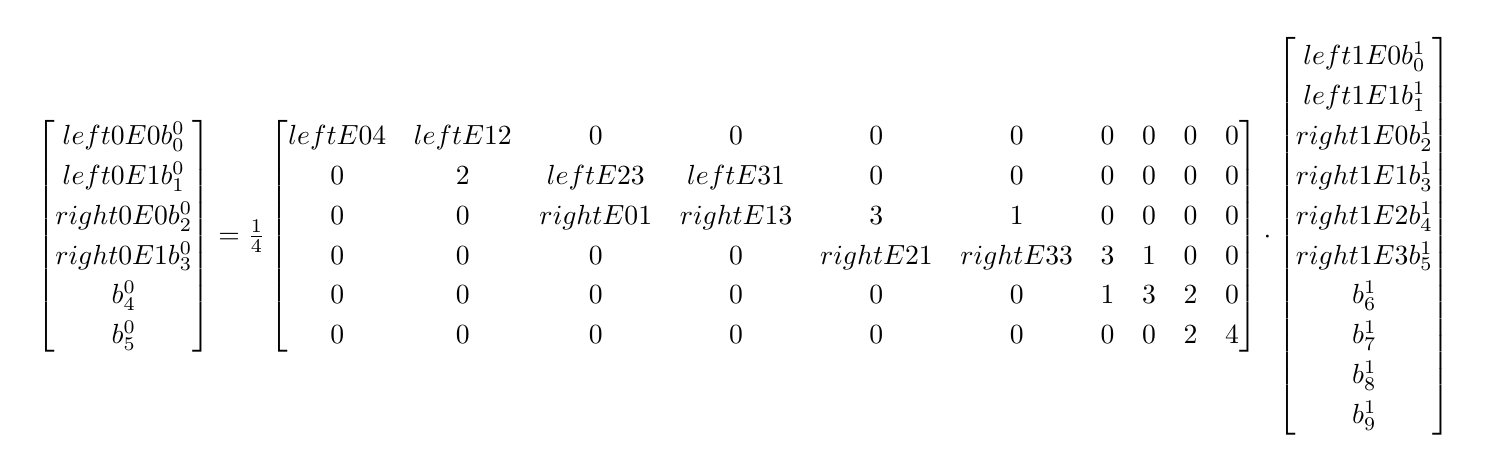
\begin{tikzpicture}
\normalsize
\node[remember picture] at (0,0){%
	$%
	\left[\begin{mysmallmatrix} %
		\mytikzmarkt{left0E0}{b^0_0}\\\mytikzmarkt{left0E1}{b^0_1}\\\mytikzmarkt{right0E0}{b^0_2}\\\mytikzmarkt{right0E1}{b^0_3}\\b^0_4\\b^0_5
	\end{mysmallmatrix} \right]%
	= \frac{1}{4} \left[\begin{myverysmallmatrix} %
	\mytikzmarkt{leftE0}{4} & \mytikzmarkt{leftE1}{2} & 0 & 0 & 0 & 0 & 0 & 0 & 0 & 0\\ 
	0 & 2 & \mytikzmarkt{leftE2}{3} & \mytikzmarkt{leftE3}{1} & 0 & 0 & 0 & 0 & 0 & 0\\ 
	0 & 0 & \mytikzmarkt{rightE0}{1} &  \mytikzmarkt{rightE1}{3} & 3 & 1 & 0 & 0 & 0 & 0\\ 
	0 & 0 & 0 & 0 & \mytikzmarkt{rightE2}{1} & \mytikzmarkt{rightE3}{3} & 3 & 1 & 0 & 0\\ 
	0 & 0 & 0 & 0 & 0 & 0 & 1 & 3 & 2 & 0\\ 
	0 & 0 & 0 & 0 & 0 & 0 & 0 & 0 & 2 & 4\\ 
	\end{myverysmallmatrix} \right]
	\cdot%
	\left[\begin{mysmallmatrix} %
	\mytikzmarkt{left1E0}{b^1_0}\\\mytikzmarkt{left1E1}{b^1_1}\\\mytikzmarkt{right1E0}{b^1_2}\\\mytikzmarkt{right1E1}{b^1_3}\\\mytikzmarkt{right1E2}{b^1_4}\\\mytikzmarkt{right1E3}{b^1_5}\\b^1_6\\b^1_7\\b^1_8\\b^1_9
	\end{mysmallmatrix} \right]%
	$%
};%
%
\end{tikzpicture}

\tikz[overlay, remember picture] {%
	\only<2>{
		\node[fit={(leftE0) (rightE0)}, inner sep=0pt, draw=gray, fill=gray,fill 
		opacity=0.2, rectangle,  thick] () {};
		\node[fit={(left1E0) (right1E0)}, inner sep=0pt, draw=gray, fill=gray,fill 
		opacity=0.2, rectangle,  thick] () {};
		\node[fit={(left0E0) (right0E0)}, inner sep=0pt, draw=gray, fill=gray,fill 
		opacity=0.2, rectangle,  thick] () {};
		}
	\only<3>{
		\node[fit={(leftE1) (rightE1)}, inner sep=0pt, draw=gray, fill=gray,fill opacity=0.2, rectangle,  thick] () {};
		\node[fit={(left1E1) (right1E1)}, inner sep=0pt, draw=gray, fill=gray,fill 
		opacity=0.2, rectangle,  thick] () {};
		\node[fit={(left0E0) (right0E0)}, inner sep=0pt, draw=gray, fill=gray,fill 
		opacity=0.2, rectangle,  thick] () {};
		}
	\only<4>{
				\node[fit={(leftE2) (rightE2)}, inner sep=0pt, draw=gray, fill=gray,fill opacity=0.2, rectangle,  thick] () {};
				\node[fit={(right1E0) (right1E2)}, inner sep=0pt, draw=gray, fill=gray,fill 
				opacity=0.2, rectangle,  thick] () {};
				\node[fit={(left0E1) (right0E1)}, inner sep=0pt, draw=gray, fill=gray,fill 
				opacity=0.2, rectangle,  thick] () {};
			}
				\only<5>{
					\node[fit={(leftE3) (rightE3)}, inner sep=0pt, draw=gray, fill=gray,fill opacity=0.2, rectangle,  thick] () {};
					\node[fit={(right1E1) (right1E3)}, inner sep=0pt, draw=gray, fill=gray,fill 
					opacity=0.2, rectangle,  thick] () {};
					\node[fit={(left0E1) (right0E1)}, inner sep=0pt, draw=gray, fill=gray,fill 
					opacity=0.2, rectangle,  thick] () {};
				}
}%

\tikzexternalenable%
%\end{frame}
%
%\begin{frame}
%	\frametitle{Multi-Level Extraction: Algorithms}
%
%	\begin{itemize}
%		\item We seek the operator $ \tensor{R}^{0,1} $ to transform from  $ \tensor{b}^0 $ to $ \tensor{b}^1 $ 
%		\[\tensor{b}^0 = \tensor{R}^{0,1} \cdot \tensor{b}^1 \]
%		\item Given a spline  $ f(x) = (\tensor{b}^0)^{\trans} \cdot \tensor{P}^0 = (\tensor{b}^1)^{\trans} \cdot \tensor{P}^1 $, $ \tensor{R}^{0,1} $  satisfies
%		\[\tensor{P}^1 = (\tensor{R}^{0,1})^{\trans} \cdot \tensor{P}^0 \] 
%		\item Namely, $ \tensor{R}^{0,1} $ transforms also control points 
%		\item Knot insertion algorithms can be used to compute $ \tensor{R}^{0,1} $
%	\end{itemize}
%	
%\end{frame}
%	
%
%\begin{frame}
%	\frametitle{Multi-Level Extraction: Algorithms}
%	
%	\begin{itemize}
%		\item The Boehm's method inserts one knot at a time
%	\end{itemize}
%	{
%		\centering
%		% !TeX root = ../../main.tex
\begin{tikzpicture}%
\def\lineWidth{0.6pt}
\def\knotWidth{1.1pt}
\def\knotSize{3pt}
\def\elementWidth{3pt}
\def\colorLevelOne{black}
\def\colorLevelTwo{black}
\def\colorLevelThree{black}
%
\tikzset{% 
	elementLineStyle/.style={%
		color=red,solid,line width=\elementWidth, opacity=0
	}
}
\tikzset{% 
	knotsStyle/.style={%
		color=red,line width=\knotWidth,mark size=\knotSize,only marks,mark=x,mark options={solid}
	}
}
\tikzset{% 
	inactive/.style={%
		color=black,solid,line width=\lineWidth
	}
}
\tikzset{% 
	ap/.style={%
		solid,line width=\lineWidth
	}
}
\tikzset{% 
	am/.style={%
		solid,line width=\lineWidth
	}
}
\tikzset{% 
	aa/.style={%
		solid,line width=\lineWidth
	}
}
\begin{groupplot}[
group style={/tikz/background rectangle/.style={draw=none},
	group size=1 by 3,
	xlabels at=edge bottom,
%xticklabels at=edge bottom,
ylabels at=edge left
,yticklabels at=edge left
,vertical sep=0.7cm},
axis y line=left,
width=0.99\linewidth,
height=3cm, %(\overAllHeight-(\basisPlotDepth-1)*\plotSeparator) / \basisPlotDepth, 
    	%xlabel=x,
		ylabel=Y,
		xmin=-1,  xmax=1,
		ymin=0, ymax=1.08,
		ytick={0,1},
		%xtick={-1,0,1},
		tickpos=left,
		ytick align=outside,
		xtick align=outside,
		tick label style ={font=\small},
		label style ={font=\small},
		legend style={ font =\small },
		ymajorgrids=false,
		] %

				
				
\nextgroupplot[axis x line=bottom, xtick={-1,0,1}, ylabel=\phantom{$ \mathcal{THB} $}\llap{$\mathcal{B}^0 $}, ylabel style={rotate=-90}]

\addplot [color=\colorLevelOne,aa]
table[row sep=crcr]{%
	-1	1\\
	-0.99	0.9604\\
	-0.98	0.9216\\
	-0.97	0.8836\\
	-0.96	0.8464\\
	-0.95	0.81\\
	-0.94	0.7744\\
	-0.93	0.7396\\
	-0.92	0.7056\\
	-0.91	0.6724\\
	-0.9	0.64\\
	-0.89	0.6084\\
	-0.88	0.5776\\
	-0.87	0.5476\\
	-0.86	0.5184\\
	-0.85	0.49\\
	-0.84	0.4624\\
	-0.83	0.4356\\
	-0.82	0.4096\\
	-0.81	0.3844\\
	-0.8	0.36\\
	-0.79	0.3364\\
	-0.78	0.3136\\
	-0.77	0.2916\\
	-0.76	0.2704\\
	-0.75	0.25\\
	-0.74	0.2304\\
	-0.73	0.2116\\
	-0.72	0.1936\\
	-0.71	0.1764\\
	-0.7	0.16\\
	-0.69	0.1444\\
	-0.68	0.1296\\
	-0.67	0.1156\\
	-0.66	0.1024\\
	-0.65	0.0899999999999999\\
	-0.64	0.0784\\
	-0.63	0.0676\\
	-0.62	0.0576\\
	-0.61	0.0484\\
	-0.6	0.04\\
	-0.59	0.0324\\
	-0.58	0.0256\\
	-0.57	0.0196\\
	-0.56	0.0144\\
	-0.55	0.01\\
	-0.54	0.00640000000000001\\
	-0.53	0.00360000000000001\\
	-0.52	0.0016\\
	-0.51	0.000400000000000001\\
	-0.5	0\\
	-0.49	0\\
	-0.48	0\\
	-0.47	0\\
	-0.46	0\\
	-0.45	0\\
	-0.44	0\\
	-0.43	0\\
	-0.42	0\\
	-0.41	0\\
	-0.4	0\\
	-0.39	0\\
	-0.38	0\\
	-0.37	0\\
	-0.36	0\\
	-0.35	0\\
	-0.34	0\\
	-0.33	0\\
	-0.32	0\\
	-0.31	0\\
	-0.3	0\\
	-0.29	0\\
	-0.28	0\\
	-0.27	0\\
	-0.26	0\\
	-0.25	0\\
	-0.24	0\\
	-0.23	0\\
	-0.22	0\\
	-0.21	0\\
	-0.2	0\\
	-0.19	0\\
	-0.18	0\\
	-0.17	0\\
	-0.16	0\\
	-0.15	0\\
	-0.14	0\\
	-0.13	0\\
	-0.12	0\\
	-0.11	0\\
	-0.1	0\\
	-0.09	0\\
	-0.08	0\\
	-0.07	0\\
	-0.0599999999999999	0\\
	-0.0499999999999999	0\\
	-0.04	0\\
	-0.03	0\\
	-0.02	0\\
	-0.01	0\\
	0	0\\
	0.01	0\\
	0.02	0\\
	0.03	0\\
	0.04	0\\
	0.0499999999999999	0\\
	0.0599999999999999	0\\
	0.07	0\\
	0.08	0\\
	0.09	0\\
	0.1	0\\
	0.11	0\\
	0.12	0\\
	0.13	0\\
	0.14	0\\
	0.15	0\\
	0.16	0\\
	0.17	0\\
	0.18	0\\
	0.19	0\\
	0.2	0\\
	0.21	0\\
	0.22	0\\
	0.23	0\\
	0.24	0\\
	0.25	0\\
	0.26	0\\
	0.27	0\\
	0.28	0\\
	0.29	0\\
	0.3	0\\
	0.31	0\\
	0.32	0\\
	0.33	0\\
	0.34	0\\
	0.35	0\\
	0.36	0\\
	0.37	0\\
	0.38	0\\
	0.39	0\\
	0.4	0\\
	0.41	0\\
	0.42	0\\
	0.43	0\\
	0.44	0\\
	0.45	0\\
	0.46	0\\
	0.47	0\\
	0.48	0\\
	0.49	0\\
	0.5	0\\
	0.51	0\\
	0.52	0\\
	0.53	0\\
	0.54	0\\
	0.55	0\\
	0.56	0\\
	0.57	0\\
	0.58	0\\
	0.59	0\\
	0.6	0\\
	0.61	0\\
	0.62	0\\
	0.63	0\\
	0.64	0\\
	0.65	0\\
	0.66	0\\
	0.67	0\\
	0.68	0\\
	0.69	0\\
	0.7	0\\
	0.71	0\\
	0.72	0\\
	0.73	0\\
	0.74	0\\
	0.75	0\\
	0.76	0\\
	0.77	0\\
	0.78	0\\
	0.79	0\\
	0.8	0\\
	0.81	0\\
	0.82	0\\
	0.83	0\\
	0.84	0\\
	0.85	0\\
	0.86	0\\
	0.87	0\\
	0.88	0\\
	0.89	0\\
	0.9	0\\
	0.91	0\\
	0.92	0\\
	0.93	0\\
	0.94	0\\
	0.95	0\\
	0.96	0\\
	0.97	0\\
	0.98	0\\
	0.99	0\\
	1	0\\
};
\addplot [color=\colorLevelOne,aa]
table[row sep=crcr]{%
	-1	0\\
	-0.99	0.0394\\
	-0.98	0.0776000000000001\\
	-0.97	0.1146\\
	-0.96	0.1504\\
	-0.95	0.185\\
	-0.94	0.2184\\
	-0.93	0.2506\\
	-0.92	0.2816\\
	-0.91	0.3114\\
	-0.9	0.34\\
	-0.89	0.3674\\
	-0.88	0.3936\\
	-0.87	0.4186\\
	-0.86	0.4424\\
	-0.85	0.465\\
	-0.84	0.4864\\
	-0.83	0.5066\\
	-0.82	0.5256\\
	-0.81	0.5434\\
	-0.8	0.56\\
	-0.79	0.5754\\
	-0.78	0.5896\\
	-0.77	0.6026\\
	-0.76	0.6144\\
	-0.75	0.625\\
	-0.74	0.6344\\
	-0.73	0.6426\\
	-0.72	0.6496\\
	-0.71	0.6554\\
	-0.7	0.66\\
	-0.69	0.6634\\
	-0.68	0.6656\\
	-0.67	0.6666\\
	-0.66	0.6664\\
	-0.65	0.665\\
	-0.64	0.6624\\
	-0.63	0.6586\\
	-0.62	0.6536\\
	-0.61	0.6474\\
	-0.6	0.64\\
	-0.59	0.6314\\
	-0.58	0.6216\\
	-0.57	0.6106\\
	-0.56	0.5984\\
	-0.55	0.585\\
	-0.54	0.5704\\
	-0.53	0.5546\\
	-0.52	0.5376\\
	-0.51	0.5194\\
	-0.5	0.5\\
	-0.49	0.4802\\
	-0.48	0.4608\\
	-0.47	0.4418\\
	-0.46	0.4232\\
	-0.45	0.405\\
	-0.44	0.3872\\
	-0.43	0.3698\\
	-0.42	0.3528\\
	-0.41	0.3362\\
	-0.4	0.32\\
	-0.39	0.3042\\
	-0.38	0.2888\\
	-0.37	0.2738\\
	-0.36	0.2592\\
	-0.35	0.245\\
	-0.34	0.2312\\
	-0.33	0.2178\\
	-0.32	0.2048\\
	-0.31	0.1922\\
	-0.3	0.18\\
	-0.29	0.1682\\
	-0.28	0.1568\\
	-0.27	0.1458\\
	-0.26	0.1352\\
	-0.25	0.125\\
	-0.24	0.1152\\
	-0.23	0.1058\\
	-0.22	0.0968\\
	-0.21	0.0882\\
	-0.2	0.08\\
	-0.19	0.0722\\
	-0.18	0.0648\\
	-0.17	0.0577999999999999\\
	-0.16	0.0512\\
	-0.15	0.045\\
	-0.14	0.0392\\
	-0.13	0.0338\\
	-0.12	0.0288\\
	-0.11	0.0242\\
	-0.1	0.02\\
	-0.09	0.0162\\
	-0.08	0.0128\\
	-0.07	0.00979999999999999\\
	-0.0599999999999999	0.00719999999999999\\
	-0.0499999999999999	0.00499999999999999\\
	-0.04	0.00320000000000001\\
	-0.03	0.0018\\
	-0.02	0.000800000000000001\\
	-0.01	0.0002\\
	0	0\\
	0.01	0\\
	0.02	0\\
	0.03	0\\
	0.04	0\\
	0.0499999999999999	0\\
	0.0599999999999999	0\\
	0.07	0\\
	0.08	0\\
	0.09	0\\
	0.1	0\\
	0.11	0\\
	0.12	0\\
	0.13	0\\
	0.14	0\\
	0.15	0\\
	0.16	0\\
	0.17	0\\
	0.18	0\\
	0.19	0\\
	0.2	0\\
	0.21	0\\
	0.22	0\\
	0.23	0\\
	0.24	0\\
	0.25	0\\
	0.26	0\\
	0.27	0\\
	0.28	0\\
	0.29	0\\
	0.3	0\\
	0.31	0\\
	0.32	0\\
	0.33	0\\
	0.34	0\\
	0.35	0\\
	0.36	0\\
	0.37	0\\
	0.38	0\\
	0.39	0\\
	0.4	0\\
	0.41	0\\
	0.42	0\\
	0.43	0\\
	0.44	0\\
	0.45	0\\
	0.46	0\\
	0.47	0\\
	0.48	0\\
	0.49	0\\
	0.5	0\\
	0.51	0\\
	0.52	0\\
	0.53	0\\
	0.54	0\\
	0.55	0\\
	0.56	0\\
	0.57	0\\
	0.58	0\\
	0.59	0\\
	0.6	0\\
	0.61	0\\
	0.62	0\\
	0.63	0\\
	0.64	0\\
	0.65	0\\
	0.66	0\\
	0.67	0\\
	0.68	0\\
	0.69	0\\
	0.7	0\\
	0.71	0\\
	0.72	0\\
	0.73	0\\
	0.74	0\\
	0.75	0\\
	0.76	0\\
	0.77	0\\
	0.78	0\\
	0.79	0\\
	0.8	0\\
	0.81	0\\
	0.82	0\\
	0.83	0\\
	0.84	0\\
	0.85	0\\
	0.86	0\\
	0.87	0\\
	0.88	0\\
	0.89	0\\
	0.9	0\\
	0.91	0\\
	0.92	0\\
	0.93	0\\
	0.94	0\\
	0.95	0\\
	0.96	0\\
	0.97	0\\
	0.98	0\\
	0.99	0\\
	1	0\\
};
\addplot [color=\colorLevelOne,ap]
table[row sep=crcr]{%
	-1	0\\
	-0.99	0.0002\\
	-0.98	0.000800000000000001\\
	-0.97	0.0018\\
	-0.96	0.00320000000000001\\
	-0.95	0.00500000000000001\\
	-0.94	0.00720000000000001\\
	-0.93	0.00980000000000002\\
	-0.92	0.0128\\
	-0.91	0.0162\\
	-0.9	0.02\\
	-0.89	0.0242\\
	-0.88	0.0288\\
	-0.87	0.0338\\
	-0.86	0.0392\\
	-0.85	0.045\\
	-0.84	0.0512\\
	-0.83	0.0578\\
	-0.82	0.0648\\
	-0.81	0.0722\\
	-0.8	0.08\\
	-0.79	0.0882\\
	-0.78	0.0968\\
	-0.77	0.1058\\
	-0.76	0.1152\\
	-0.75	0.125\\
	-0.74	0.1352\\
	-0.73	0.1458\\
	-0.72	0.1568\\
	-0.71	0.1682\\
	-0.7	0.18\\
	-0.69	0.1922\\
	-0.68	0.2048\\
	-0.67	0.2178\\
	-0.66	0.2312\\
	-0.65	0.245\\
	-0.64	0.2592\\
	-0.63	0.2738\\
	-0.62	0.2888\\
	-0.61	0.3042\\
	-0.6	0.32\\
	-0.59	0.3362\\
	-0.58	0.3528\\
	-0.57	0.3698\\
	-0.56	0.3872\\
	-0.55	0.405\\
	-0.54	0.4232\\
	-0.53	0.4418\\
	-0.52	0.4608\\
	-0.51	0.4802\\
	-0.5	0.5\\
	-0.49	0.5196\\
	-0.48	0.5384\\
	-0.47	0.5564\\
	-0.46	0.5736\\
	-0.45	0.59\\
	-0.44	0.6056\\
	-0.43	0.6204\\
	-0.42	0.6344\\
	-0.41	0.6476\\
	-0.4	0.66\\
	-0.39	0.6716\\
	-0.38	0.6824\\
	-0.37	0.6924\\
	-0.36	0.7016\\
	-0.35	0.71\\
	-0.34	0.7176\\
	-0.33	0.7244\\
	-0.32	0.7304\\
	-0.31	0.7356\\
	-0.3	0.74\\
	-0.29	0.7436\\
	-0.28	0.7464\\
	-0.27	0.7484\\
	-0.26	0.7496\\
	-0.25	0.75\\
	-0.24	0.7496\\
	-0.23	0.7484\\
	-0.22	0.7464\\
	-0.21	0.7436\\
	-0.2	0.74\\
	-0.19	0.7356\\
	-0.18	0.7304\\
	-0.17	0.7244\\
	-0.16	0.7176\\
	-0.15	0.71\\
	-0.14	0.7016\\
	-0.13	0.6924\\
	-0.12	0.6824\\
	-0.11	0.6716\\
	-0.1	0.66\\
	-0.09	0.6476\\
	-0.08	0.6344\\
	-0.07	0.6204\\
	-0.0599999999999999	0.6056\\
	-0.0499999999999999	0.59\\
	-0.04	0.5736\\
	-0.03	0.5564\\
	-0.02	0.5384\\
	-0.01	0.5196\\
	0	0.5\\
	0.01	0.4802\\
	0.02	0.4608\\
	0.03	0.4418\\
	0.04	0.4232\\
	0.0499999999999999	0.405\\
	0.0599999999999999	0.3872\\
	0.07	0.3698\\
	0.08	0.3528\\
	0.09	0.3362\\
	0.1	0.32\\
	0.11	0.3042\\
	0.12	0.2888\\
	0.13	0.2738\\
	0.14	0.2592\\
	0.15	0.245\\
	0.16	0.2312\\
	0.17	0.2178\\
	0.18	0.2048\\
	0.19	0.1922\\
	0.2	0.18\\
	0.21	0.1682\\
	0.22	0.1568\\
	0.23	0.1458\\
	0.24	0.1352\\
	0.25	0.125\\
	0.26	0.1152\\
	0.27	0.1058\\
	0.28	0.0968\\
	0.29	0.0882\\
	0.3	0.0800000000000001\\
	0.31	0.0722\\
	0.32	0.0648\\
	0.33	0.0578\\
	0.34	0.0512\\
	0.35	0.045\\
	0.36	0.0392\\
	0.37	0.0338\\
	0.38	0.0288\\
	0.39	0.0242\\
	0.4	0.02\\
	0.41	0.0162\\
	0.42	0.0128\\
	0.43	0.00980000000000002\\
	0.44	0.00720000000000001\\
	0.45	0.00500000000000001\\
	0.46	0.00320000000000001\\
	0.47	0.0018\\
	0.48	0.000800000000000001\\
	0.49	0.0002\\
	0.5	0\\
	0.51	0\\
	0.52	0\\
	0.53	0\\
	0.54	0\\
	0.55	0\\
	0.56	0\\
	0.57	0\\
	0.58	0\\
	0.59	0\\
	0.6	0\\
	0.61	0\\
	0.62	0\\
	0.63	0\\
	0.64	0\\
	0.65	0\\
	0.66	0\\
	0.67	0\\
	0.68	0\\
	0.69	0\\
	0.7	0\\
	0.71	0\\
	0.72	0\\
	0.73	0\\
	0.74	0\\
	0.75	0\\
	0.76	0\\
	0.77	0\\
	0.78	0\\
	0.79	0\\
	0.8	0\\
	0.81	0\\
	0.82	0\\
	0.83	0\\
	0.84	0\\
	0.85	0\\
	0.86	0\\
	0.87	0\\
	0.88	0\\
	0.89	0\\
	0.9	0\\
	0.91	0\\
	0.92	0\\
	0.93	0\\
	0.94	0\\
	0.95	0\\
	0.96	0\\
	0.97	0\\
	0.98	0\\
	0.99	0\\
	1	0\\
};
\addplot [color=\colorLevelOne,ap]
table[row sep=crcr]{%
	-1	0\\
	-0.99	0\\
	-0.98	0\\
	-0.97	0\\
	-0.96	0\\
	-0.95	0\\
	-0.94	0\\
	-0.93	0\\
	-0.92	0\\
	-0.91	0\\
	-0.9	0\\
	-0.89	0\\
	-0.88	0\\
	-0.87	0\\
	-0.86	0\\
	-0.85	0\\
	-0.84	0\\
	-0.83	0\\
	-0.82	0\\
	-0.81	0\\
	-0.8	0\\
	-0.79	0\\
	-0.78	0\\
	-0.77	0\\
	-0.76	0\\
	-0.75	0\\
	-0.74	0\\
	-0.73	0\\
	-0.72	0\\
	-0.71	0\\
	-0.7	0\\
	-0.69	0\\
	-0.68	0\\
	-0.67	0\\
	-0.66	0\\
	-0.65	0\\
	-0.64	0\\
	-0.63	0\\
	-0.62	0\\
	-0.61	0\\
	-0.6	0\\
	-0.59	0\\
	-0.58	0\\
	-0.57	0\\
	-0.56	0\\
	-0.55	0\\
	-0.54	0\\
	-0.53	0\\
	-0.52	0\\
	-0.51	0\\
	-0.5	0\\
	-0.49	0.0002\\
	-0.48	0.000800000000000001\\
	-0.47	0.0018\\
	-0.46	0.00320000000000001\\
	-0.45	0.00500000000000001\\
	-0.44	0.00720000000000001\\
	-0.43	0.00980000000000002\\
	-0.42	0.0128\\
	-0.41	0.0162\\
	-0.4	0.02\\
	-0.39	0.0242\\
	-0.38	0.0288\\
	-0.37	0.0338\\
	-0.36	0.0392\\
	-0.35	0.045\\
	-0.34	0.0512\\
	-0.33	0.0578\\
	-0.32	0.0648\\
	-0.31	0.0722\\
	-0.3	0.0800000000000001\\
	-0.29	0.0882\\
	-0.28	0.0968\\
	-0.27	0.1058\\
	-0.26	0.1152\\
	-0.25	0.125\\
	-0.24	0.1352\\
	-0.23	0.1458\\
	-0.22	0.1568\\
	-0.21	0.1682\\
	-0.2	0.18\\
	-0.19	0.1922\\
	-0.18	0.2048\\
	-0.17	0.2178\\
	-0.16	0.2312\\
	-0.15	0.245\\
	-0.14	0.2592\\
	-0.13	0.2738\\
	-0.12	0.2888\\
	-0.11	0.3042\\
	-0.1	0.32\\
	-0.09	0.3362\\
	-0.08	0.3528\\
	-0.07	0.3698\\
	-0.0599999999999999	0.3872\\
	-0.0499999999999999	0.405\\
	-0.04	0.4232\\
	-0.03	0.4418\\
	-0.02	0.4608\\
	-0.01	0.4802\\
	0	0.5\\
	0.01	0.5196\\
	0.02	0.5384\\
	0.03	0.5564\\
	0.04	0.5736\\
	0.0499999999999999	0.59\\
	0.0599999999999999	0.6056\\
	0.07	0.6204\\
	0.08	0.6344\\
	0.09	0.6476\\
	0.1	0.66\\
	0.11	0.6716\\
	0.12	0.6824\\
	0.13	0.6924\\
	0.14	0.7016\\
	0.15	0.71\\
	0.16	0.7176\\
	0.17	0.7244\\
	0.18	0.7304\\
	0.19	0.7356\\
	0.2	0.74\\
	0.21	0.7436\\
	0.22	0.7464\\
	0.23	0.7484\\
	0.24	0.7496\\
	0.25	0.75\\
	0.26	0.7496\\
	0.27	0.7484\\
	0.28	0.7464\\
	0.29	0.7436\\
	0.3	0.74\\
	0.31	0.7356\\
	0.32	0.7304\\
	0.33	0.7244\\
	0.34	0.7176\\
	0.35	0.71\\
	0.36	0.7016\\
	0.37	0.6924\\
	0.38	0.6824\\
	0.39	0.6716\\
	0.4	0.66\\
	0.41	0.6476\\
	0.42	0.6344\\
	0.43	0.6204\\
	0.44	0.6056\\
	0.45	0.59\\
	0.46	0.5736\\
	0.47	0.5564\\
	0.48	0.5384\\
	0.49	0.5196\\
	0.5	0.5\\
	0.51	0.4802\\
	0.52	0.4608\\
	0.53	0.4418\\
	0.54	0.4232\\
	0.55	0.405\\
	0.56	0.3872\\
	0.57	0.3698\\
	0.58	0.3528\\
	0.59	0.3362\\
	0.6	0.32\\
	0.61	0.3042\\
	0.62	0.2888\\
	0.63	0.2738\\
	0.64	0.2592\\
	0.65	0.245\\
	0.66	0.2312\\
	0.67	0.2178\\
	0.68	0.2048\\
	0.69	0.1922\\
	0.7	0.18\\
	0.71	0.1682\\
	0.72	0.1568\\
	0.73	0.1458\\
	0.74	0.1352\\
	0.75	0.125\\
	0.76	0.1152\\
	0.77	0.1058\\
	0.78	0.0968\\
	0.79	0.0882\\
	0.8	0.08\\
	0.81	0.0722\\
	0.82	0.0648\\
	0.83	0.0578\\
	0.84	0.0512\\
	0.85	0.045\\
	0.86	0.0392\\
	0.87	0.0338\\
	0.88	0.0288\\
	0.89	0.0242\\
	0.9	0.02\\
	0.91	0.0162\\
	0.92	0.0128\\
	0.93	0.00980000000000002\\
	0.94	0.00720000000000001\\
	0.95	0.00500000000000001\\
	0.96	0.00320000000000001\\
	0.97	0.0018\\
	0.98	0.000800000000000001\\
	0.99	0.0002\\
	1	0\\
};
\addplot [inactive]
table[row sep=crcr]{%
	-1	0\\
	-0.99	0\\
	-0.98	0\\
	-0.97	0\\
	-0.96	0\\
	-0.95	0\\
	-0.94	0\\
	-0.93	0\\
	-0.92	0\\
	-0.91	0\\
	-0.9	0\\
	-0.89	0\\
	-0.88	0\\
	-0.87	0\\
	-0.86	0\\
	-0.85	0\\
	-0.84	0\\
	-0.83	0\\
	-0.82	0\\
	-0.81	0\\
	-0.8	0\\
	-0.79	0\\
	-0.78	0\\
	-0.77	0\\
	-0.76	0\\
	-0.75	0\\
	-0.74	0\\
	-0.73	0\\
	-0.72	0\\
	-0.71	0\\
	-0.7	0\\
	-0.69	0\\
	-0.68	0\\
	-0.67	0\\
	-0.66	0\\
	-0.65	0\\
	-0.64	0\\
	-0.63	0\\
	-0.62	0\\
	-0.61	0\\
	-0.6	0\\
	-0.59	0\\
	-0.58	0\\
	-0.57	0\\
	-0.56	0\\
	-0.55	0\\
	-0.54	0\\
	-0.53	0\\
	-0.52	0\\
	-0.51	0\\
	-0.5	0\\
	-0.49	0\\
	-0.48	0\\
	-0.47	0\\
	-0.46	0\\
	-0.45	0\\
	-0.44	0\\
	-0.43	0\\
	-0.42	0\\
	-0.41	0\\
	-0.4	0\\
	-0.39	0\\
	-0.38	0\\
	-0.37	0\\
	-0.36	0\\
	-0.35	0\\
	-0.34	0\\
	-0.33	0\\
	-0.32	0\\
	-0.31	0\\
	-0.3	0\\
	-0.29	0\\
	-0.28	0\\
	-0.27	0\\
	-0.26	0\\
	-0.25	0\\
	-0.24	0\\
	-0.23	0\\
	-0.22	0\\
	-0.21	0\\
	-0.2	0\\
	-0.19	0\\
	-0.18	0\\
	-0.17	0\\
	-0.16	0\\
	-0.15	0\\
	-0.14	0\\
	-0.13	0\\
	-0.12	0\\
	-0.11	0\\
	-0.1	0\\
	-0.09	0\\
	-0.08	0\\
	-0.07	0\\
	-0.0599999999999999	0\\
	-0.0499999999999999	0\\
	-0.04	0\\
	-0.03	0\\
	-0.02	0\\
	-0.01	0\\
	0	0\\
	0.01	0.0002\\
	0.02	0.000800000000000001\\
	0.03	0.0018\\
	0.04	0.00320000000000001\\
	0.0499999999999999	0.00499999999999999\\
	0.0599999999999999	0.00719999999999999\\
	0.07	0.00979999999999999\\
	0.08	0.0128\\
	0.09	0.0162\\
	0.1	0.02\\
	0.11	0.0242\\
	0.12	0.0288\\
	0.13	0.0338\\
	0.14	0.0392\\
	0.15	0.045\\
	0.16	0.0512\\
	0.17	0.0577999999999999\\
	0.18	0.0648\\
	0.19	0.0722\\
	0.2	0.08\\
	0.21	0.0882\\
	0.22	0.0968\\
	0.23	0.1058\\
	0.24	0.1152\\
	0.25	0.125\\
	0.26	0.1352\\
	0.27	0.1458\\
	0.28	0.1568\\
	0.29	0.1682\\
	0.3	0.18\\
	0.31	0.1922\\
	0.32	0.2048\\
	0.33	0.2178\\
	0.34	0.2312\\
	0.35	0.245\\
	0.36	0.2592\\
	0.37	0.2738\\
	0.38	0.2888\\
	0.39	0.3042\\
	0.4	0.32\\
	0.41	0.3362\\
	0.42	0.3528\\
	0.43	0.3698\\
	0.44	0.3872\\
	0.45	0.405\\
	0.46	0.4232\\
	0.47	0.4418\\
	0.48	0.4608\\
	0.49	0.4802\\
	0.5	0.5\\
	0.51	0.5194\\
	0.52	0.5376\\
	0.53	0.5546\\
	0.54	0.5704\\
	0.55	0.585\\
	0.56	0.5984\\
	0.57	0.6106\\
	0.58	0.6216\\
	0.59	0.6314\\
	0.6	0.64\\
	0.61	0.6474\\
	0.62	0.6536\\
	0.63	0.6586\\
	0.64	0.6624\\
	0.65	0.665\\
	0.66	0.6664\\
	0.67	0.6666\\
	0.68	0.6656\\
	0.69	0.6634\\
	0.7	0.66\\
	0.71	0.6554\\
	0.72	0.6496\\
	0.73	0.6426\\
	0.74	0.6344\\
	0.75	0.625\\
	0.76	0.6144\\
	0.77	0.6026\\
	0.78	0.5896\\
	0.79	0.5754\\
	0.8	0.56\\
	0.81	0.5434\\
	0.82	0.5256\\
	0.83	0.5066\\
	0.84	0.4864\\
	0.85	0.465\\
	0.86	0.4424\\
	0.87	0.4186\\
	0.88	0.3936\\
	0.89	0.3674\\
	0.9	0.34\\
	0.91	0.3114\\
	0.92	0.2816\\
	0.93	0.2506\\
	0.94	0.2184\\
	0.95	0.185\\
	0.96	0.1504\\
	0.97	0.1146\\
	0.98	0.0776000000000001\\
	0.99	0.0394\\
	1	0\\
};
\addplot [inactive]
table[row sep=crcr]{%
	-1	0\\
	-0.99	0\\
	-0.98	0\\
	-0.97	0\\
	-0.96	0\\
	-0.95	0\\
	-0.94	0\\
	-0.93	0\\
	-0.92	0\\
	-0.91	0\\
	-0.9	0\\
	-0.89	0\\
	-0.88	0\\
	-0.87	0\\
	-0.86	0\\
	-0.85	0\\
	-0.84	0\\
	-0.83	0\\
	-0.82	0\\
	-0.81	0\\
	-0.8	0\\
	-0.79	0\\
	-0.78	0\\
	-0.77	0\\
	-0.76	0\\
	-0.75	0\\
	-0.74	0\\
	-0.73	0\\
	-0.72	0\\
	-0.71	0\\
	-0.7	0\\
	-0.69	0\\
	-0.68	0\\
	-0.67	0\\
	-0.66	0\\
	-0.65	0\\
	-0.64	0\\
	-0.63	0\\
	-0.62	0\\
	-0.61	0\\
	-0.6	0\\
	-0.59	0\\
	-0.58	0\\
	-0.57	0\\
	-0.56	0\\
	-0.55	0\\
	-0.54	0\\
	-0.53	0\\
	-0.52	0\\
	-0.51	0\\
	-0.5	0\\
	-0.49	0\\
	-0.48	0\\
	-0.47	0\\
	-0.46	0\\
	-0.45	0\\
	-0.44	0\\
	-0.43	0\\
	-0.42	0\\
	-0.41	0\\
	-0.4	0\\
	-0.39	0\\
	-0.38	0\\
	-0.37	0\\
	-0.36	0\\
	-0.35	0\\
	-0.34	0\\
	-0.33	0\\
	-0.32	0\\
	-0.31	0\\
	-0.3	0\\
	-0.29	0\\
	-0.28	0\\
	-0.27	0\\
	-0.26	0\\
	-0.25	0\\
	-0.24	0\\
	-0.23	0\\
	-0.22	0\\
	-0.21	0\\
	-0.2	0\\
	-0.19	0\\
	-0.18	0\\
	-0.17	0\\
	-0.16	0\\
	-0.15	0\\
	-0.14	0\\
	-0.13	0\\
	-0.12	0\\
	-0.11	0\\
	-0.1	0\\
	-0.09	0\\
	-0.08	0\\
	-0.07	0\\
	-0.0599999999999999	0\\
	-0.0499999999999999	0\\
	-0.04	0\\
	-0.03	0\\
	-0.02	0\\
	-0.01	0\\
	0	0\\
	0.01	0\\
	0.02	0\\
	0.03	0\\
	0.04	0\\
	0.0499999999999999	0\\
	0.0599999999999999	0\\
	0.07	0\\
	0.08	0\\
	0.09	0\\
	0.1	0\\
	0.11	0\\
	0.12	0\\
	0.13	0\\
	0.14	0\\
	0.15	0\\
	0.16	0\\
	0.17	0\\
	0.18	0\\
	0.19	0\\
	0.2	0\\
	0.21	0\\
	0.22	0\\
	0.23	0\\
	0.24	0\\
	0.25	0\\
	0.26	0\\
	0.27	0\\
	0.28	0\\
	0.29	0\\
	0.3	0\\
	0.31	0\\
	0.32	0\\
	0.33	0\\
	0.34	0\\
	0.35	0\\
	0.36	0\\
	0.37	0\\
	0.38	0\\
	0.39	0\\
	0.4	0\\
	0.41	0\\
	0.42	0\\
	0.43	0\\
	0.44	0\\
	0.45	0\\
	0.46	0\\
	0.47	0\\
	0.48	0\\
	0.49	0\\
	0.5	0\\
	0.51	0.000400000000000001\\
	0.52	0.0016\\
	0.53	0.00360000000000001\\
	0.54	0.00640000000000001\\
	0.55	0.01\\
	0.56	0.0144\\
	0.57	0.0196\\
	0.58	0.0256\\
	0.59	0.0324\\
	0.6	0.04\\
	0.61	0.0484\\
	0.62	0.0576\\
	0.63	0.0676\\
	0.64	0.0784\\
	0.65	0.0899999999999999\\
	0.66	0.1024\\
	0.67	0.1156\\
	0.68	0.1296\\
	0.69	0.1444\\
	0.7	0.16\\
	0.71	0.1764\\
	0.72	0.1936\\
	0.73	0.2116\\
	0.74	0.2304\\
	0.75	0.25\\
	0.76	0.2704\\
	0.77	0.2916\\
	0.78	0.3136\\
	0.79	0.3364\\
	0.8	0.36\\
	0.81	0.3844\\
	0.82	0.4096\\
	0.83	0.4356\\
	0.84	0.4624\\
	0.85	0.49\\
	0.86	0.5184\\
	0.87	0.5476\\
	0.88	0.5776\\
	0.89	0.6084\\
	0.9	0.64\\
	0.91	0.6724\\
	0.92	0.7056\\
	0.93	0.7396\\
	0.94	0.7744\\
	0.95	0.81\\
	0.96	0.8464\\
	0.97	0.8836\\
	0.98	0.9216\\
	0.99	0.9604\\
	1	1\\
};
\addplot [elementLineStyle]
table[row sep=crcr]{%
	-1	0\\
	-0.5	0\\
};
\addplot [elementLineStyle]
table[row sep=crcr]{%
	-0.5	0\\
	0	0\\
};
\addplot [knotsStyle]
table[row sep=crcr]{%
	-1	0\\
	-1	0\\
	-1	0\\
	-0.5	0\\
	0	0\\
	0.5	0\\
	1	0\\
	1	0\\
	1	0\\
};

\nextgroupplot[axis x line=bottom, xtick={-1,0,1}, ylabel=\phantom{$ \mathcal{THB} $}\llap{$\mathcal{B}^1 $}, ylabel style={rotate=-90}]

\addplot [inactive]
table[row sep=crcr]{%
	-1	1\\
	-0.99	0.9216\\
	-0.98	0.8464\\
	-0.97	0.7744\\
	-0.96	0.7056\\
	-0.95	0.64\\
	-0.94	0.5776\\
	-0.93	0.5184\\
	-0.92	0.4624\\
	-0.91	0.4096\\
	-0.9	0.36\\
	-0.89	0.3136\\
	-0.88	0.2704\\
	-0.87	0.2304\\
	-0.86	0.1936\\
	-0.85	0.16\\
	-0.84	0.1296\\
	-0.83	0.1024\\
	-0.82	0.0784000000000001\\
	-0.81	0.0576000000000001\\
	-0.8	0.0400000000000001\\
	-0.79	0.0256\\
	-0.78	0.0144\\
	-0.77	0.00640000000000001\\
	-0.76	0.0016\\
	-0.75	0\\
	-0.74	0\\
	-0.73	0\\
	-0.72	0\\
	-0.71	0\\
	-0.7	0\\
	-0.69	0\\
	-0.68	0\\
	-0.67	0\\
	-0.66	0\\
	-0.65	0\\
	-0.64	0\\
	-0.63	0\\
	-0.62	0\\
	-0.61	0\\
	-0.6	0\\
	-0.59	0\\
	-0.58	0\\
	-0.57	0\\
	-0.56	0\\
	-0.55	0\\
	-0.54	0\\
	-0.53	0\\
	-0.52	0\\
	-0.51	0\\
	-0.5	0\\
	-0.49	0\\
	-0.48	0\\
	-0.47	0\\
	-0.46	0\\
	-0.45	0\\
	-0.44	0\\
	-0.43	0\\
	-0.42	0\\
	-0.41	0\\
	-0.4	0\\
	-0.39	0\\
	-0.38	0\\
	-0.37	0\\
	-0.36	0\\
	-0.35	0\\
	-0.34	0\\
	-0.33	0\\
	-0.32	0\\
	-0.31	0\\
	-0.3	0\\
	-0.29	0\\
	-0.28	0\\
	-0.27	0\\
	-0.26	0\\
	-0.25	0\\
	-0.24	0\\
	-0.23	0\\
	-0.22	0\\
	-0.21	0\\
	-0.2	0\\
	-0.19	0\\
	-0.18	0\\
	-0.17	0\\
	-0.16	0\\
	-0.15	0\\
	-0.14	0\\
	-0.13	0\\
	-0.12	0\\
	-0.11	0\\
	-0.1	0\\
	-0.09	0\\
	-0.08	0\\
	-0.07	0\\
	-0.0599999999999999	0\\
	-0.0499999999999999	0\\
	-0.04	0\\
	-0.03	0\\
	-0.02	0\\
	-0.01	0\\
	0	0\\
	0.01	0\\
	0.02	0\\
	0.03	0\\
	0.04	0\\
	0.0499999999999999	0\\
	0.0599999999999999	0\\
	0.07	0\\
	0.08	0\\
	0.09	0\\
	0.1	0\\
	0.11	0\\
	0.12	0\\
	0.13	0\\
	0.14	0\\
	0.15	0\\
	0.16	0\\
	0.17	0\\
	0.18	0\\
	0.19	0\\
	0.2	0\\
	0.21	0\\
	0.22	0\\
	0.23	0\\
	0.24	0\\
	0.25	0\\
	0.26	0\\
	0.27	0\\
	0.28	0\\
	0.29	0\\
	0.3	0\\
	0.31	0\\
	0.32	0\\
	0.33	0\\
	0.34	0\\
	0.35	0\\
	0.36	0\\
	0.37	0\\
	0.38	0\\
	0.39	0\\
	0.4	0\\
	0.41	0\\
	0.42	0\\
	0.43	0\\
	0.44	0\\
	0.45	0\\
	0.46	0\\
	0.47	0\\
	0.48	0\\
	0.49	0\\
	0.5	0\\
	0.51	0\\
	0.52	0\\
	0.53	0\\
	0.54	0\\
	0.55	0\\
	0.56	0\\
	0.57	0\\
	0.58	0\\
	0.59	0\\
	0.6	0\\
	0.61	0\\
	0.62	0\\
	0.63	0\\
	0.64	0\\
	0.65	0\\
	0.66	0\\
	0.67	0\\
	0.68	0\\
	0.69	0\\
	0.7	0\\
	0.71	0\\
	0.72	0\\
	0.73	0\\
	0.74	0\\
	0.75	0\\
	0.76	0\\
	0.77	0\\
	0.78	0\\
	0.79	0\\
	0.8	0\\
	0.81	0\\
	0.82	0\\
	0.83	0\\
	0.84	0\\
	0.85	0\\
	0.86	0\\
	0.87	0\\
	0.88	0\\
	0.89	0\\
	0.9	0\\
	0.91	0\\
	0.92	0\\
	0.93	0\\
	0.94	0\\
	0.95	0\\
	0.96	0\\
	0.97	0\\
	0.98	0\\
	0.99	0\\
	1	0\\
};
\addplot [inactive]
table[row sep=crcr]{%
	-1	0\\
	-0.99	0.0776000000000001\\
	-0.98	0.1504\\
	-0.97	0.2184\\
	-0.96	0.2816\\
	-0.95	0.34\\
	-0.94	0.3936\\
	-0.93	0.4424\\
	-0.92	0.4864\\
	-0.91	0.5256\\
	-0.9	0.56\\
	-0.89	0.5896\\
	-0.88	0.6144\\
	-0.87	0.6344\\
	-0.86	0.6496\\
	-0.85	0.66\\
	-0.84	0.6656\\
	-0.83	0.6664\\
	-0.82	0.6624\\
	-0.81	0.6536\\
	-0.8	0.64\\
	-0.79	0.6216\\
	-0.78	0.5984\\
	-0.77	0.5704\\
	-0.76	0.5376\\
	-0.75	0.5\\
	-0.74	0.4608\\
	-0.73	0.4232\\
	-0.72	0.3872\\
	-0.71	0.3528\\
	-0.7	0.32\\
	-0.69	0.2888\\
	-0.68	0.2592\\
	-0.67	0.2312\\
	-0.66	0.2048\\
	-0.65	0.18\\
	-0.64	0.1568\\
	-0.63	0.1352\\
	-0.62	0.1152\\
	-0.61	0.0968\\
	-0.6	0.08\\
	-0.59	0.0648\\
	-0.58	0.0512000000000001\\
	-0.57	0.0392000000000001\\
	-0.56	0.0288000000000001\\
	-0.55	0.02\\
	-0.54	0.0128\\
	-0.53	0.00720000000000001\\
	-0.52	0.00320000000000001\\
	-0.51	0.000800000000000001\\
	-0.5	0\\
	-0.49	0\\
	-0.48	0\\
	-0.47	0\\
	-0.46	0\\
	-0.45	0\\
	-0.44	0\\
	-0.43	0\\
	-0.42	0\\
	-0.41	0\\
	-0.4	0\\
	-0.39	0\\
	-0.38	0\\
	-0.37	0\\
	-0.36	0\\
	-0.35	0\\
	-0.34	0\\
	-0.33	0\\
	-0.32	0\\
	-0.31	0\\
	-0.3	0\\
	-0.29	0\\
	-0.28	0\\
	-0.27	0\\
	-0.26	0\\
	-0.25	0\\
	-0.24	0\\
	-0.23	0\\
	-0.22	0\\
	-0.21	0\\
	-0.2	0\\
	-0.19	0\\
	-0.18	0\\
	-0.17	0\\
	-0.16	0\\
	-0.15	0\\
	-0.14	0\\
	-0.13	0\\
	-0.12	0\\
	-0.11	0\\
	-0.1	0\\
	-0.09	0\\
	-0.08	0\\
	-0.07	0\\
	-0.0599999999999999	0\\
	-0.0499999999999999	0\\
	-0.04	0\\
	-0.03	0\\
	-0.02	0\\
	-0.01	0\\
	0	0\\
	0.01	0\\
	0.02	0\\
	0.03	0\\
	0.04	0\\
	0.0499999999999999	0\\
	0.0599999999999999	0\\
	0.07	0\\
	0.08	0\\
	0.09	0\\
	0.1	0\\
	0.11	0\\
	0.12	0\\
	0.13	0\\
	0.14	0\\
	0.15	0\\
	0.16	0\\
	0.17	0\\
	0.18	0\\
	0.19	0\\
	0.2	0\\
	0.21	0\\
	0.22	0\\
	0.23	0\\
	0.24	0\\
	0.25	0\\
	0.26	0\\
	0.27	0\\
	0.28	0\\
	0.29	0\\
	0.3	0\\
	0.31	0\\
	0.32	0\\
	0.33	0\\
	0.34	0\\
	0.35	0\\
	0.36	0\\
	0.37	0\\
	0.38	0\\
	0.39	0\\
	0.4	0\\
	0.41	0\\
	0.42	0\\
	0.43	0\\
	0.44	0\\
	0.45	0\\
	0.46	0\\
	0.47	0\\
	0.48	0\\
	0.49	0\\
	0.5	0\\
	0.51	0\\
	0.52	0\\
	0.53	0\\
	0.54	0\\
	0.55	0\\
	0.56	0\\
	0.57	0\\
	0.58	0\\
	0.59	0\\
	0.6	0\\
	0.61	0\\
	0.62	0\\
	0.63	0\\
	0.64	0\\
	0.65	0\\
	0.66	0\\
	0.67	0\\
	0.68	0\\
	0.69	0\\
	0.7	0\\
	0.71	0\\
	0.72	0\\
	0.73	0\\
	0.74	0\\
	0.75	0\\
	0.76	0\\
	0.77	0\\
	0.78	0\\
	0.79	0\\
	0.8	0\\
	0.81	0\\
	0.82	0\\
	0.83	0\\
	0.84	0\\
	0.85	0\\
	0.86	0\\
	0.87	0\\
	0.88	0\\
	0.89	0\\
	0.9	0\\
	0.91	0\\
	0.92	0\\
	0.93	0\\
	0.94	0\\
	0.95	0\\
	0.96	0\\
	0.97	0\\
	0.98	0\\
	0.99	0\\
	1	0\\
};
\addplot [inactive]
table[row sep=crcr]{%
	-1	0\\
	-0.99	0.000800000000000001\\
	-0.98	0.00320000000000001\\
	-0.97	0.00720000000000001\\
	-0.96	0.0128\\
	-0.95	0.02\\
	-0.94	0.0288000000000001\\
	-0.93	0.0392000000000001\\
	-0.92	0.0511999999999999\\
	-0.91	0.0648\\
	-0.9	0.08\\
	-0.89	0.0968\\
	-0.88	0.1152\\
	-0.87	0.1352\\
	-0.86	0.1568\\
	-0.85	0.18\\
	-0.84	0.2048\\
	-0.83	0.2312\\
	-0.82	0.2592\\
	-0.81	0.2888\\
	-0.8	0.32\\
	-0.79	0.3528\\
	-0.78	0.3872\\
	-0.77	0.4232\\
	-0.76	0.4608\\
	-0.75	0.5\\
	-0.74	0.5384\\
	-0.73	0.5736\\
	-0.72	0.6056\\
	-0.71	0.6344\\
	-0.7	0.66\\
	-0.69	0.6824\\
	-0.68	0.7016\\
	-0.67	0.7176\\
	-0.66	0.7304\\
	-0.65	0.74\\
	-0.64	0.7464\\
	-0.63	0.7496\\
	-0.62	0.7496\\
	-0.61	0.7464\\
	-0.6	0.74\\
	-0.59	0.7304\\
	-0.58	0.7176\\
	-0.57	0.7016\\
	-0.56	0.6824\\
	-0.55	0.66\\
	-0.54	0.6344\\
	-0.53	0.6056\\
	-0.52	0.5736\\
	-0.51	0.5384\\
	-0.5	0.5\\
	-0.49	0.4608\\
	-0.48	0.4232\\
	-0.47	0.3872\\
	-0.46	0.3528\\
	-0.45	0.32\\
	-0.44	0.2888\\
	-0.43	0.2592\\
	-0.42	0.2312\\
	-0.41	0.2048\\
	-0.4	0.18\\
	-0.39	0.1568\\
	-0.38	0.1352\\
	-0.37	0.1152\\
	-0.36	0.0968\\
	-0.35	0.08\\
	-0.34	0.0648\\
	-0.33	0.0511999999999999\\
	-0.32	0.0391999999999999\\
	-0.31	0.0287999999999999\\
	-0.3	0.0199999999999999\\
	-0.29	0.0128\\
	-0.28	0.00720000000000001\\
	-0.27	0.00320000000000001\\
	-0.26	0.000800000000000001\\
	-0.25	0\\
	-0.24	0\\
	-0.23	0\\
	-0.22	0\\
	-0.21	0\\
	-0.2	0\\
	-0.19	0\\
	-0.18	0\\
	-0.17	0\\
	-0.16	0\\
	-0.15	0\\
	-0.14	0\\
	-0.13	0\\
	-0.12	0\\
	-0.11	0\\
	-0.1	0\\
	-0.09	0\\
	-0.08	0\\
	-0.07	0\\
	-0.0599999999999999	0\\
	-0.0499999999999999	0\\
	-0.04	0\\
	-0.03	0\\
	-0.02	0\\
	-0.01	0\\
	0	0\\
	0.01	0\\
	0.02	0\\
	0.03	0\\
	0.04	0\\
	0.0499999999999999	0\\
	0.0599999999999999	0\\
	0.07	0\\
	0.08	0\\
	0.09	0\\
	0.1	0\\
	0.11	0\\
	0.12	0\\
	0.13	0\\
	0.14	0\\
	0.15	0\\
	0.16	0\\
	0.17	0\\
	0.18	0\\
	0.19	0\\
	0.2	0\\
	0.21	0\\
	0.22	0\\
	0.23	0\\
	0.24	0\\
	0.25	0\\
	0.26	0\\
	0.27	0\\
	0.28	0\\
	0.29	0\\
	0.3	0\\
	0.31	0\\
	0.32	0\\
	0.33	0\\
	0.34	0\\
	0.35	0\\
	0.36	0\\
	0.37	0\\
	0.38	0\\
	0.39	0\\
	0.4	0\\
	0.41	0\\
	0.42	0\\
	0.43	0\\
	0.44	0\\
	0.45	0\\
	0.46	0\\
	0.47	0\\
	0.48	0\\
	0.49	0\\
	0.5	0\\
	0.51	0\\
	0.52	0\\
	0.53	0\\
	0.54	0\\
	0.55	0\\
	0.56	0\\
	0.57	0\\
	0.58	0\\
	0.59	0\\
	0.6	0\\
	0.61	0\\
	0.62	0\\
	0.63	0\\
	0.64	0\\
	0.65	0\\
	0.66	0\\
	0.67	0\\
	0.68	0\\
	0.69	0\\
	0.7	0\\
	0.71	0\\
	0.72	0\\
	0.73	0\\
	0.74	0\\
	0.75	0\\
	0.76	0\\
	0.77	0\\
	0.78	0\\
	0.79	0\\
	0.8	0\\
	0.81	0\\
	0.82	0\\
	0.83	0\\
	0.84	0\\
	0.85	0\\
	0.86	0\\
	0.87	0\\
	0.88	0\\
	0.89	0\\
	0.9	0\\
	0.91	0\\
	0.92	0\\
	0.93	0\\
	0.94	0\\
	0.95	0\\
	0.96	0\\
	0.97	0\\
	0.98	0\\
	0.99	0\\
	1	0\\
};
\addplot [inactive]
table[row sep=crcr]{%
	-1	0\\
	-0.99	0\\
	-0.98	0\\
	-0.97	0\\
	-0.96	0\\
	-0.95	0\\
	-0.94	0\\
	-0.93	0\\
	-0.92	0\\
	-0.91	0\\
	-0.9	0\\
	-0.89	0\\
	-0.88	0\\
	-0.87	0\\
	-0.86	0\\
	-0.85	0\\
	-0.84	0\\
	-0.83	0\\
	-0.82	0\\
	-0.81	0\\
	-0.8	0\\
	-0.79	0\\
	-0.78	0\\
	-0.77	0\\
	-0.76	0\\
	-0.75	0\\
	-0.74	0.000800000000000001\\
	-0.73	0.00320000000000001\\
	-0.72	0.00720000000000001\\
	-0.71	0.0128\\
	-0.7	0.02\\
	-0.69	0.0288000000000001\\
	-0.68	0.0392000000000001\\
	-0.67	0.0512000000000001\\
	-0.66	0.0648000000000001\\
	-0.65	0.0800000000000001\\
	-0.64	0.0968\\
	-0.63	0.1152\\
	-0.62	0.1352\\
	-0.61	0.1568\\
	-0.6	0.18\\
	-0.59	0.2048\\
	-0.58	0.2312\\
	-0.57	0.2592\\
	-0.56	0.2888\\
	-0.55	0.32\\
	-0.54	0.3528\\
	-0.53	0.3872\\
	-0.52	0.4232\\
	-0.51	0.4608\\
	-0.5	0.5\\
	-0.49	0.5384\\
	-0.48	0.5736\\
	-0.47	0.6056\\
	-0.46	0.6344\\
	-0.45	0.66\\
	-0.44	0.6824\\
	-0.43	0.7016\\
	-0.42	0.7176\\
	-0.41	0.7304\\
	-0.4	0.74\\
	-0.39	0.7464\\
	-0.38	0.7496\\
	-0.37	0.7496\\
	-0.36	0.7464\\
	-0.35	0.74\\
	-0.34	0.7304\\
	-0.33	0.7176\\
	-0.32	0.7016\\
	-0.31	0.6824\\
	-0.3	0.66\\
	-0.29	0.6344\\
	-0.28	0.6056\\
	-0.27	0.5736\\
	-0.26	0.5384\\
	-0.25	0.5\\
	-0.24	0.4608\\
	-0.23	0.4232\\
	-0.22	0.3872\\
	-0.21	0.3528\\
	-0.2	0.32\\
	-0.19	0.2888\\
	-0.18	0.2592\\
	-0.17	0.2312\\
	-0.16	0.2048\\
	-0.15	0.18\\
	-0.14	0.1568\\
	-0.13	0.1352\\
	-0.12	0.1152\\
	-0.11	0.0968\\
	-0.1	0.08\\
	-0.09	0.0648\\
	-0.08	0.0511999999999999\\
	-0.07	0.0391999999999999\\
	-0.0599999999999999	0.0287999999999999\\
	-0.0499999999999999	0.0199999999999999\\
	-0.04	0.0128\\
	-0.03	0.00720000000000001\\
	-0.02	0.00320000000000001\\
	-0.01	0.000800000000000001\\
	0	0\\
	0.01	0\\
	0.02	0\\
	0.03	0\\
	0.04	0\\
	0.0499999999999999	0\\
	0.0599999999999999	0\\
	0.07	0\\
	0.08	0\\
	0.09	0\\
	0.1	0\\
	0.11	0\\
	0.12	0\\
	0.13	0\\
	0.14	0\\
	0.15	0\\
	0.16	0\\
	0.17	0\\
	0.18	0\\
	0.19	0\\
	0.2	0\\
	0.21	0\\
	0.22	0\\
	0.23	0\\
	0.24	0\\
	0.25	0\\
	0.26	0\\
	0.27	0\\
	0.28	0\\
	0.29	0\\
	0.3	0\\
	0.31	0\\
	0.32	0\\
	0.33	0\\
	0.34	0\\
	0.35	0\\
	0.36	0\\
	0.37	0\\
	0.38	0\\
	0.39	0\\
	0.4	0\\
	0.41	0\\
	0.42	0\\
	0.43	0\\
	0.44	0\\
	0.45	0\\
	0.46	0\\
	0.47	0\\
	0.48	0\\
	0.49	0\\
	0.5	0\\
	0.51	0\\
	0.52	0\\
	0.53	0\\
	0.54	0\\
	0.55	0\\
	0.56	0\\
	0.57	0\\
	0.58	0\\
	0.59	0\\
	0.6	0\\
	0.61	0\\
	0.62	0\\
	0.63	0\\
	0.64	0\\
	0.65	0\\
	0.66	0\\
	0.67	0\\
	0.68	0\\
	0.69	0\\
	0.7	0\\
	0.71	0\\
	0.72	0\\
	0.73	0\\
	0.74	0\\
	0.75	0\\
	0.76	0\\
	0.77	0\\
	0.78	0\\
	0.79	0\\
	0.8	0\\
	0.81	0\\
	0.82	0\\
	0.83	0\\
	0.84	0\\
	0.85	0\\
	0.86	0\\
	0.87	0\\
	0.88	0\\
	0.89	0\\
	0.9	0\\
	0.91	0\\
	0.92	0\\
	0.93	0\\
	0.94	0\\
	0.95	0\\
	0.96	0\\
	0.97	0\\
	0.98	0\\
	0.99	0\\
	1	0\\
};
\addplot [color=\colorLevelTwo,am]
table[row sep=crcr]{%
	-1	0\\
	-0.99	0\\
	-0.98	0\\
	-0.97	0\\
	-0.96	0\\
	-0.95	0\\
	-0.94	0\\
	-0.93	0\\
	-0.92	0\\
	-0.91	0\\
	-0.9	0\\
	-0.89	0\\
	-0.88	0\\
	-0.87	0\\
	-0.86	0\\
	-0.85	0\\
	-0.84	0\\
	-0.83	0\\
	-0.82	0\\
	-0.81	0\\
	-0.8	0\\
	-0.79	0\\
	-0.78	0\\
	-0.77	0\\
	-0.76	0\\
	-0.75	0\\
	-0.74	0\\
	-0.73	0\\
	-0.72	0\\
	-0.71	0\\
	-0.7	0\\
	-0.69	0\\
	-0.68	0\\
	-0.67	0\\
	-0.66	0\\
	-0.65	0\\
	-0.64	0\\
	-0.63	0\\
	-0.62	0\\
	-0.61	0\\
	-0.6	0\\
	-0.59	0\\
	-0.58	0\\
	-0.57	0\\
	-0.56	0\\
	-0.55	0\\
	-0.54	0\\
	-0.53	0\\
	-0.52	0\\
	-0.51	0\\
	-0.5	0\\
	-0.49	0.000800000000000001\\
	-0.48	0.00320000000000001\\
	-0.47	0.00720000000000001\\
	-0.46	0.0128\\
	-0.45	0.02\\
	-0.44	0.0288000000000001\\
	-0.43	0.0392000000000001\\
	-0.42	0.0511999999999999\\
	-0.41	0.0648\\
	-0.4	0.08\\
	-0.39	0.0968\\
	-0.38	0.1152\\
	-0.37	0.1352\\
	-0.36	0.1568\\
	-0.35	0.18\\
	-0.34	0.2048\\
	-0.33	0.2312\\
	-0.32	0.2592\\
	-0.31	0.2888\\
	-0.3	0.32\\
	-0.29	0.3528\\
	-0.28	0.3872\\
	-0.27	0.4232\\
	-0.26	0.4608\\
	-0.25	0.5\\
	-0.24	0.5384\\
	-0.23	0.5736\\
	-0.22	0.6056\\
	-0.21	0.6344\\
	-0.2	0.66\\
	-0.19	0.6824\\
	-0.18	0.7016\\
	-0.17	0.7176\\
	-0.16	0.7304\\
	-0.15	0.74\\
	-0.14	0.7464\\
	-0.13	0.7496\\
	-0.12	0.7496\\
	-0.11	0.7464\\
	-0.1	0.74\\
	-0.09	0.7304\\
	-0.08	0.7176\\
	-0.07	0.7016\\
	-0.0599999999999999	0.6824\\
	-0.0499999999999999	0.66\\
	-0.04	0.6344\\
	-0.03	0.6056\\
	-0.02	0.5736\\
	-0.01	0.5384\\
	0	0.5\\
	0.01	0.4608\\
	0.02	0.4232\\
	0.03	0.3872\\
	0.04	0.3528\\
	0.0499999999999999	0.32\\
	0.0599999999999999	0.2888\\
	0.07	0.2592\\
	0.08	0.2312\\
	0.09	0.2048\\
	0.1	0.18\\
	0.11	0.1568\\
	0.12	0.1352\\
	0.13	0.1152\\
	0.14	0.0968\\
	0.15	0.08\\
	0.16	0.0648\\
	0.17	0.0512000000000001\\
	0.18	0.0392000000000001\\
	0.19	0.0288000000000001\\
	0.2	0.02\\
	0.21	0.0128\\
	0.22	0.00720000000000001\\
	0.23	0.00320000000000001\\
	0.24	0.000800000000000001\\
	0.25	0\\
	0.26	0\\
	0.27	0\\
	0.28	0\\
	0.29	0\\
	0.3	0\\
	0.31	0\\
	0.32	0\\
	0.33	0\\
	0.34	0\\
	0.35	0\\
	0.36	0\\
	0.37	0\\
	0.38	0\\
	0.39	0\\
	0.4	0\\
	0.41	0\\
	0.42	0\\
	0.43	0\\
	0.44	0\\
	0.45	0\\
	0.46	0\\
	0.47	0\\
	0.48	0\\
	0.49	0\\
	0.5	0\\
	0.51	0\\
	0.52	0\\
	0.53	0\\
	0.54	0\\
	0.55	0\\
	0.56	0\\
	0.57	0\\
	0.58	0\\
	0.59	0\\
	0.6	0\\
	0.61	0\\
	0.62	0\\
	0.63	0\\
	0.64	0\\
	0.65	0\\
	0.66	0\\
	0.67	0\\
	0.68	0\\
	0.69	0\\
	0.7	0\\
	0.71	0\\
	0.72	0\\
	0.73	0\\
	0.74	0\\
	0.75	0\\
	0.76	0\\
	0.77	0\\
	0.78	0\\
	0.79	0\\
	0.8	0\\
	0.81	0\\
	0.82	0\\
	0.83	0\\
	0.84	0\\
	0.85	0\\
	0.86	0\\
	0.87	0\\
	0.88	0\\
	0.89	0\\
	0.9	0\\
	0.91	0\\
	0.92	0\\
	0.93	0\\
	0.94	0\\
	0.95	0\\
	0.96	0\\
	0.97	0\\
	0.98	0\\
	0.99	0\\
	1	0\\
};
\addplot [color=\colorLevelTwo,am]
table[row sep=crcr]{%
	-1	0\\
	-0.99	0\\
	-0.98	0\\
	-0.97	0\\
	-0.96	0\\
	-0.95	0\\
	-0.94	0\\
	-0.93	0\\
	-0.92	0\\
	-0.91	0\\
	-0.9	0\\
	-0.89	0\\
	-0.88	0\\
	-0.87	0\\
	-0.86	0\\
	-0.85	0\\
	-0.84	0\\
	-0.83	0\\
	-0.82	0\\
	-0.81	0\\
	-0.8	0\\
	-0.79	0\\
	-0.78	0\\
	-0.77	0\\
	-0.76	0\\
	-0.75	0\\
	-0.74	0\\
	-0.73	0\\
	-0.72	0\\
	-0.71	0\\
	-0.7	0\\
	-0.69	0\\
	-0.68	0\\
	-0.67	0\\
	-0.66	0\\
	-0.65	0\\
	-0.64	0\\
	-0.63	0\\
	-0.62	0\\
	-0.61	0\\
	-0.6	0\\
	-0.59	0\\
	-0.58	0\\
	-0.57	0\\
	-0.56	0\\
	-0.55	0\\
	-0.54	0\\
	-0.53	0\\
	-0.52	0\\
	-0.51	0\\
	-0.5	0\\
	-0.49	0\\
	-0.48	0\\
	-0.47	0\\
	-0.46	0\\
	-0.45	0\\
	-0.44	0\\
	-0.43	0\\
	-0.42	0\\
	-0.41	0\\
	-0.4	0\\
	-0.39	0\\
	-0.38	0\\
	-0.37	0\\
	-0.36	0\\
	-0.35	0\\
	-0.34	0\\
	-0.33	0\\
	-0.32	0\\
	-0.31	0\\
	-0.3	0\\
	-0.29	0\\
	-0.28	0\\
	-0.27	0\\
	-0.26	0\\
	-0.25	0\\
	-0.24	0.000800000000000001\\
	-0.23	0.00320000000000001\\
	-0.22	0.00720000000000001\\
	-0.21	0.0128\\
	-0.2	0.02\\
	-0.19	0.0288000000000001\\
	-0.18	0.0392000000000001\\
	-0.17	0.0512000000000001\\
	-0.16	0.0648\\
	-0.15	0.08\\
	-0.14	0.0968\\
	-0.13	0.1152\\
	-0.12	0.1352\\
	-0.11	0.1568\\
	-0.1	0.18\\
	-0.09	0.2048\\
	-0.08	0.2312\\
	-0.07	0.2592\\
	-0.0599999999999999	0.2888\\
	-0.0499999999999999	0.32\\
	-0.04	0.3528\\
	-0.03	0.3872\\
	-0.02	0.4232\\
	-0.01	0.4608\\
	0	0.5\\
	0.01	0.5384\\
	0.02	0.5736\\
	0.03	0.6056\\
	0.04	0.6344\\
	0.0499999999999999	0.66\\
	0.0599999999999999	0.6824\\
	0.07	0.7016\\
	0.08	0.7176\\
	0.09	0.7304\\
	0.1	0.74\\
	0.11	0.7464\\
	0.12	0.7496\\
	0.13	0.7496\\
	0.14	0.7464\\
	0.15	0.74\\
	0.16	0.7304\\
	0.17	0.7176\\
	0.18	0.7016\\
	0.19	0.6824\\
	0.2	0.66\\
	0.21	0.6344\\
	0.22	0.6056\\
	0.23	0.5736\\
	0.24	0.5384\\
	0.25	0.5\\
	0.26	0.4608\\
	0.27	0.4232\\
	0.28	0.3872\\
	0.29	0.3528\\
	0.3	0.32\\
	0.31	0.2888\\
	0.32	0.2592\\
	0.33	0.2312\\
	0.34	0.2048\\
	0.35	0.18\\
	0.36	0.1568\\
	0.37	0.1352\\
	0.38	0.1152\\
	0.39	0.0968\\
	0.4	0.08\\
	0.41	0.0648\\
	0.42	0.0511999999999999\\
	0.43	0.0392000000000001\\
	0.44	0.0288000000000001\\
	0.45	0.02\\
	0.46	0.0128\\
	0.47	0.00720000000000001\\
	0.48	0.00320000000000001\\
	0.49	0.000800000000000001\\
	0.5	0\\
	0.51	0\\
	0.52	0\\
	0.53	0\\
	0.54	0\\
	0.55	0\\
	0.56	0\\
	0.57	0\\
	0.58	0\\
	0.59	0\\
	0.6	0\\
	0.61	0\\
	0.62	0\\
	0.63	0\\
	0.64	0\\
	0.65	0\\
	0.66	0\\
	0.67	0\\
	0.68	0\\
	0.69	0\\
	0.7	0\\
	0.71	0\\
	0.72	0\\
	0.73	0\\
	0.74	0\\
	0.75	0\\
	0.76	0\\
	0.77	0\\
	0.78	0\\
	0.79	0\\
	0.8	0\\
	0.81	0\\
	0.82	0\\
	0.83	0\\
	0.84	0\\
	0.85	0\\
	0.86	0\\
	0.87	0\\
	0.88	0\\
	0.89	0\\
	0.9	0\\
	0.91	0\\
	0.92	0\\
	0.93	0\\
	0.94	0\\
	0.95	0\\
	0.96	0\\
	0.97	0\\
	0.98	0\\
	0.99	0\\
	1	0\\
};
\addplot [color=\colorLevelTwo,ap]
table[row sep=crcr]{%
	-1	0\\
	-0.99	0\\
	-0.98	0\\
	-0.97	0\\
	-0.96	0\\
	-0.95	0\\
	-0.94	0\\
	-0.93	0\\
	-0.92	0\\
	-0.91	0\\
	-0.9	0\\
	-0.89	0\\
	-0.88	0\\
	-0.87	0\\
	-0.86	0\\
	-0.85	0\\
	-0.84	0\\
	-0.83	0\\
	-0.82	0\\
	-0.81	0\\
	-0.8	0\\
	-0.79	0\\
	-0.78	0\\
	-0.77	0\\
	-0.76	0\\
	-0.75	0\\
	-0.74	0\\
	-0.73	0\\
	-0.72	0\\
	-0.71	0\\
	-0.7	0\\
	-0.69	0\\
	-0.68	0\\
	-0.67	0\\
	-0.66	0\\
	-0.65	0\\
	-0.64	0\\
	-0.63	0\\
	-0.62	0\\
	-0.61	0\\
	-0.6	0\\
	-0.59	0\\
	-0.58	0\\
	-0.57	0\\
	-0.56	0\\
	-0.55	0\\
	-0.54	0\\
	-0.53	0\\
	-0.52	0\\
	-0.51	0\\
	-0.5	0\\
	-0.49	0\\
	-0.48	0\\
	-0.47	0\\
	-0.46	0\\
	-0.45	0\\
	-0.44	0\\
	-0.43	0\\
	-0.42	0\\
	-0.41	0\\
	-0.4	0\\
	-0.39	0\\
	-0.38	0\\
	-0.37	0\\
	-0.36	0\\
	-0.35	0\\
	-0.34	0\\
	-0.33	0\\
	-0.32	0\\
	-0.31	0\\
	-0.3	0\\
	-0.29	0\\
	-0.28	0\\
	-0.27	0\\
	-0.26	0\\
	-0.25	0\\
	-0.24	0\\
	-0.23	0\\
	-0.22	0\\
	-0.21	0\\
	-0.2	0\\
	-0.19	0\\
	-0.18	0\\
	-0.17	0\\
	-0.16	0\\
	-0.15	0\\
	-0.14	0\\
	-0.13	0\\
	-0.12	0\\
	-0.11	0\\
	-0.1	0\\
	-0.09	0\\
	-0.08	0\\
	-0.07	0\\
	-0.0599999999999999	0\\
	-0.0499999999999999	0\\
	-0.04	0\\
	-0.03	0\\
	-0.02	0\\
	-0.01	0\\
	0	0\\
	0.01	0.000800000000000001\\
	0.02	0.00320000000000001\\
	0.03	0.00720000000000001\\
	0.04	0.0128\\
	0.0499999999999999	0.0199999999999999\\
	0.0599999999999999	0.0287999999999999\\
	0.07	0.0391999999999999\\
	0.08	0.0511999999999999\\
	0.09	0.0648\\
	0.1	0.08\\
	0.11	0.0968\\
	0.12	0.1152\\
	0.13	0.1352\\
	0.14	0.1568\\
	0.15	0.18\\
	0.16	0.2048\\
	0.17	0.2312\\
	0.18	0.2592\\
	0.19	0.2888\\
	0.2	0.32\\
	0.21	0.3528\\
	0.22	0.3872\\
	0.23	0.4232\\
	0.24	0.4608\\
	0.25	0.5\\
	0.26	0.5384\\
	0.27	0.5736\\
	0.28	0.6056\\
	0.29	0.6344\\
	0.3	0.66\\
	0.31	0.6824\\
	0.32	0.7016\\
	0.33	0.7176\\
	0.34	0.7304\\
	0.35	0.74\\
	0.36	0.7464\\
	0.37	0.7496\\
	0.38	0.7496\\
	0.39	0.7464\\
	0.4	0.74\\
	0.41	0.7304\\
	0.42	0.7176\\
	0.43	0.7016\\
	0.44	0.6824\\
	0.45	0.66\\
	0.46	0.6344\\
	0.47	0.6056\\
	0.48	0.5736\\
	0.49	0.5384\\
	0.5	0.5\\
	0.51	0.4608\\
	0.52	0.4232\\
	0.53	0.3872\\
	0.54	0.3528\\
	0.55	0.32\\
	0.56	0.2888\\
	0.57	0.2592\\
	0.58	0.2312\\
	0.59	0.2048\\
	0.6	0.18\\
	0.61	0.1568\\
	0.62	0.1352\\
	0.63	0.1152\\
	0.64	0.0968\\
	0.65	0.0800000000000001\\
	0.66	0.0648000000000001\\
	0.67	0.0512000000000001\\
	0.68	0.0392000000000001\\
	0.69	0.0288000000000001\\
	0.7	0.02\\
	0.71	0.0128\\
	0.72	0.00720000000000001\\
	0.73	0.00320000000000001\\
	0.74	0.000800000000000001\\
	0.75	0\\
	0.76	0\\
	0.77	0\\
	0.78	0\\
	0.79	0\\
	0.8	0\\
	0.81	0\\
	0.82	0\\
	0.83	0\\
	0.84	0\\
	0.85	0\\
	0.86	0\\
	0.87	0\\
	0.88	0\\
	0.89	0\\
	0.9	0\\
	0.91	0\\
	0.92	0\\
	0.93	0\\
	0.94	0\\
	0.95	0\\
	0.96	0\\
	0.97	0\\
	0.98	0\\
	0.99	0\\
	1	0\\
};
\addplot [color=\colorLevelTwo,ap]
table[row sep=crcr]{%
	-1	0\\
	-0.99	0\\
	-0.98	0\\
	-0.97	0\\
	-0.96	0\\
	-0.95	0\\
	-0.94	0\\
	-0.93	0\\
	-0.92	0\\
	-0.91	0\\
	-0.9	0\\
	-0.89	0\\
	-0.88	0\\
	-0.87	0\\
	-0.86	0\\
	-0.85	0\\
	-0.84	0\\
	-0.83	0\\
	-0.82	0\\
	-0.81	0\\
	-0.8	0\\
	-0.79	0\\
	-0.78	0\\
	-0.77	0\\
	-0.76	0\\
	-0.75	0\\
	-0.74	0\\
	-0.73	0\\
	-0.72	0\\
	-0.71	0\\
	-0.7	0\\
	-0.69	0\\
	-0.68	0\\
	-0.67	0\\
	-0.66	0\\
	-0.65	0\\
	-0.64	0\\
	-0.63	0\\
	-0.62	0\\
	-0.61	0\\
	-0.6	0\\
	-0.59	0\\
	-0.58	0\\
	-0.57	0\\
	-0.56	0\\
	-0.55	0\\
	-0.54	0\\
	-0.53	0\\
	-0.52	0\\
	-0.51	0\\
	-0.5	0\\
	-0.49	0\\
	-0.48	0\\
	-0.47	0\\
	-0.46	0\\
	-0.45	0\\
	-0.44	0\\
	-0.43	0\\
	-0.42	0\\
	-0.41	0\\
	-0.4	0\\
	-0.39	0\\
	-0.38	0\\
	-0.37	0\\
	-0.36	0\\
	-0.35	0\\
	-0.34	0\\
	-0.33	0\\
	-0.32	0\\
	-0.31	0\\
	-0.3	0\\
	-0.29	0\\
	-0.28	0\\
	-0.27	0\\
	-0.26	0\\
	-0.25	0\\
	-0.24	0\\
	-0.23	0\\
	-0.22	0\\
	-0.21	0\\
	-0.2	0\\
	-0.19	0\\
	-0.18	0\\
	-0.17	0\\
	-0.16	0\\
	-0.15	0\\
	-0.14	0\\
	-0.13	0\\
	-0.12	0\\
	-0.11	0\\
	-0.1	0\\
	-0.09	0\\
	-0.08	0\\
	-0.07	0\\
	-0.0599999999999999	0\\
	-0.0499999999999999	0\\
	-0.04	0\\
	-0.03	0\\
	-0.02	0\\
	-0.01	0\\
	0	0\\
	0.01	0\\
	0.02	0\\
	0.03	0\\
	0.04	0\\
	0.0499999999999999	0\\
	0.0599999999999999	0\\
	0.07	0\\
	0.08	0\\
	0.09	0\\
	0.1	0\\
	0.11	0\\
	0.12	0\\
	0.13	0\\
	0.14	0\\
	0.15	0\\
	0.16	0\\
	0.17	0\\
	0.18	0\\
	0.19	0\\
	0.2	0\\
	0.21	0\\
	0.22	0\\
	0.23	0\\
	0.24	0\\
	0.25	0\\
	0.26	0.000800000000000001\\
	0.27	0.00320000000000001\\
	0.28	0.00720000000000001\\
	0.29	0.0128\\
	0.3	0.0199999999999999\\
	0.31	0.0287999999999999\\
	0.32	0.0391999999999999\\
	0.33	0.0511999999999999\\
	0.34	0.0648\\
	0.35	0.08\\
	0.36	0.0968\\
	0.37	0.1152\\
	0.38	0.1352\\
	0.39	0.1568\\
	0.4	0.18\\
	0.41	0.2048\\
	0.42	0.2312\\
	0.43	0.2592\\
	0.44	0.2888\\
	0.45	0.32\\
	0.46	0.3528\\
	0.47	0.3872\\
	0.48	0.4232\\
	0.49	0.4608\\
	0.5	0.5\\
	0.51	0.5384\\
	0.52	0.5736\\
	0.53	0.6056\\
	0.54	0.6344\\
	0.55	0.66\\
	0.56	0.6824\\
	0.57	0.7016\\
	0.58	0.7176\\
	0.59	0.7304\\
	0.6	0.74\\
	0.61	0.7464\\
	0.62	0.7496\\
	0.63	0.7496\\
	0.64	0.7464\\
	0.65	0.74\\
	0.66	0.7304\\
	0.67	0.7176\\
	0.68	0.7016\\
	0.69	0.6824\\
	0.7	0.66\\
	0.71	0.6344\\
	0.72	0.6056\\
	0.73	0.5736\\
	0.74	0.5384\\
	0.75	0.5\\
	0.76	0.4608\\
	0.77	0.4232\\
	0.78	0.3872\\
	0.79	0.3528\\
	0.8	0.32\\
	0.81	0.2888\\
	0.82	0.2592\\
	0.83	0.2312\\
	0.84	0.2048\\
	0.85	0.18\\
	0.86	0.1568\\
	0.87	0.1352\\
	0.88	0.1152\\
	0.89	0.0968\\
	0.9	0.08\\
	0.91	0.0648\\
	0.92	0.0511999999999999\\
	0.93	0.0392000000000001\\
	0.94	0.0288000000000001\\
	0.95	0.02\\
	0.96	0.0128\\
	0.97	0.00720000000000001\\
	0.98	0.00320000000000001\\
	0.99	0.000800000000000001\\
	1	0\\
};
\addplot [inactive]
table[row sep=crcr]{%
	-1	0\\
	-0.99	0\\
	-0.98	0\\
	-0.97	0\\
	-0.96	0\\
	-0.95	0\\
	-0.94	0\\
	-0.93	0\\
	-0.92	0\\
	-0.91	0\\
	-0.9	0\\
	-0.89	0\\
	-0.88	0\\
	-0.87	0\\
	-0.86	0\\
	-0.85	0\\
	-0.84	0\\
	-0.83	0\\
	-0.82	0\\
	-0.81	0\\
	-0.8	0\\
	-0.79	0\\
	-0.78	0\\
	-0.77	0\\
	-0.76	0\\
	-0.75	0\\
	-0.74	0\\
	-0.73	0\\
	-0.72	0\\
	-0.71	0\\
	-0.7	0\\
	-0.69	0\\
	-0.68	0\\
	-0.67	0\\
	-0.66	0\\
	-0.65	0\\
	-0.64	0\\
	-0.63	0\\
	-0.62	0\\
	-0.61	0\\
	-0.6	0\\
	-0.59	0\\
	-0.58	0\\
	-0.57	0\\
	-0.56	0\\
	-0.55	0\\
	-0.54	0\\
	-0.53	0\\
	-0.52	0\\
	-0.51	0\\
	-0.5	0\\
	-0.49	0\\
	-0.48	0\\
	-0.47	0\\
	-0.46	0\\
	-0.45	0\\
	-0.44	0\\
	-0.43	0\\
	-0.42	0\\
	-0.41	0\\
	-0.4	0\\
	-0.39	0\\
	-0.38	0\\
	-0.37	0\\
	-0.36	0\\
	-0.35	0\\
	-0.34	0\\
	-0.33	0\\
	-0.32	0\\
	-0.31	0\\
	-0.3	0\\
	-0.29	0\\
	-0.28	0\\
	-0.27	0\\
	-0.26	0\\
	-0.25	0\\
	-0.24	0\\
	-0.23	0\\
	-0.22	0\\
	-0.21	0\\
	-0.2	0\\
	-0.19	0\\
	-0.18	0\\
	-0.17	0\\
	-0.16	0\\
	-0.15	0\\
	-0.14	0\\
	-0.13	0\\
	-0.12	0\\
	-0.11	0\\
	-0.1	0\\
	-0.09	0\\
	-0.08	0\\
	-0.07	0\\
	-0.0599999999999999	0\\
	-0.0499999999999999	0\\
	-0.04	0\\
	-0.03	0\\
	-0.02	0\\
	-0.01	0\\
	0	0\\
	0.01	0\\
	0.02	0\\
	0.03	0\\
	0.04	0\\
	0.0499999999999999	0\\
	0.0599999999999999	0\\
	0.07	0\\
	0.08	0\\
	0.09	0\\
	0.1	0\\
	0.11	0\\
	0.12	0\\
	0.13	0\\
	0.14	0\\
	0.15	0\\
	0.16	0\\
	0.17	0\\
	0.18	0\\
	0.19	0\\
	0.2	0\\
	0.21	0\\
	0.22	0\\
	0.23	0\\
	0.24	0\\
	0.25	0\\
	0.26	0\\
	0.27	0\\
	0.28	0\\
	0.29	0\\
	0.3	0\\
	0.31	0\\
	0.32	0\\
	0.33	0\\
	0.34	0\\
	0.35	0\\
	0.36	0\\
	0.37	0\\
	0.38	0\\
	0.39	0\\
	0.4	0\\
	0.41	0\\
	0.42	0\\
	0.43	0\\
	0.44	0\\
	0.45	0\\
	0.46	0\\
	0.47	0\\
	0.48	0\\
	0.49	0\\
	0.5	0\\
	0.51	0.000800000000000001\\
	0.52	0.00320000000000001\\
	0.53	0.00720000000000001\\
	0.54	0.0128\\
	0.55	0.02\\
	0.56	0.0288000000000001\\
	0.57	0.0392000000000001\\
	0.58	0.0512000000000001\\
	0.59	0.0648\\
	0.6	0.08\\
	0.61	0.0968\\
	0.62	0.1152\\
	0.63	0.1352\\
	0.64	0.1568\\
	0.65	0.18\\
	0.66	0.2048\\
	0.67	0.2312\\
	0.68	0.2592\\
	0.69	0.2888\\
	0.7	0.32\\
	0.71	0.3528\\
	0.72	0.3872\\
	0.73	0.4232\\
	0.74	0.4608\\
	0.75	0.5\\
	0.76	0.5376\\
	0.77	0.5704\\
	0.78	0.5984\\
	0.79	0.6216\\
	0.8	0.64\\
	0.81	0.6536\\
	0.82	0.6624\\
	0.83	0.6664\\
	0.84	0.6656\\
	0.85	0.66\\
	0.86	0.6496\\
	0.87	0.6344\\
	0.88	0.6144\\
	0.89	0.5896\\
	0.9	0.56\\
	0.91	0.5256\\
	0.92	0.4864\\
	0.93	0.4424\\
	0.94	0.3936\\
	0.95	0.34\\
	0.96	0.2816\\
	0.97	0.2184\\
	0.98	0.1504\\
	0.99	0.0776000000000001\\
	1	0\\
};
\addplot [inactive]
table[row sep=crcr]{%
	-1	0\\
	-0.99	0\\
	-0.98	0\\
	-0.97	0\\
	-0.96	0\\
	-0.95	0\\
	-0.94	0\\
	-0.93	0\\
	-0.92	0\\
	-0.91	0\\
	-0.9	0\\
	-0.89	0\\
	-0.88	0\\
	-0.87	0\\
	-0.86	0\\
	-0.85	0\\
	-0.84	0\\
	-0.83	0\\
	-0.82	0\\
	-0.81	0\\
	-0.8	0\\
	-0.79	0\\
	-0.78	0\\
	-0.77	0\\
	-0.76	0\\
	-0.75	0\\
	-0.74	0\\
	-0.73	0\\
	-0.72	0\\
	-0.71	0\\
	-0.7	0\\
	-0.69	0\\
	-0.68	0\\
	-0.67	0\\
	-0.66	0\\
	-0.65	0\\
	-0.64	0\\
	-0.63	0\\
	-0.62	0\\
	-0.61	0\\
	-0.6	0\\
	-0.59	0\\
	-0.58	0\\
	-0.57	0\\
	-0.56	0\\
	-0.55	0\\
	-0.54	0\\
	-0.53	0\\
	-0.52	0\\
	-0.51	0\\
	-0.5	0\\
	-0.49	0\\
	-0.48	0\\
	-0.47	0\\
	-0.46	0\\
	-0.45	0\\
	-0.44	0\\
	-0.43	0\\
	-0.42	0\\
	-0.41	0\\
	-0.4	0\\
	-0.39	0\\
	-0.38	0\\
	-0.37	0\\
	-0.36	0\\
	-0.35	0\\
	-0.34	0\\
	-0.33	0\\
	-0.32	0\\
	-0.31	0\\
	-0.3	0\\
	-0.29	0\\
	-0.28	0\\
	-0.27	0\\
	-0.26	0\\
	-0.25	0\\
	-0.24	0\\
	-0.23	0\\
	-0.22	0\\
	-0.21	0\\
	-0.2	0\\
	-0.19	0\\
	-0.18	0\\
	-0.17	0\\
	-0.16	0\\
	-0.15	0\\
	-0.14	0\\
	-0.13	0\\
	-0.12	0\\
	-0.11	0\\
	-0.1	0\\
	-0.09	0\\
	-0.08	0\\
	-0.07	0\\
	-0.0599999999999999	0\\
	-0.0499999999999999	0\\
	-0.04	0\\
	-0.03	0\\
	-0.02	0\\
	-0.01	0\\
	0	0\\
	0.01	0\\
	0.02	0\\
	0.03	0\\
	0.04	0\\
	0.0499999999999999	0\\
	0.0599999999999999	0\\
	0.07	0\\
	0.08	0\\
	0.09	0\\
	0.1	0\\
	0.11	0\\
	0.12	0\\
	0.13	0\\
	0.14	0\\
	0.15	0\\
	0.16	0\\
	0.17	0\\
	0.18	0\\
	0.19	0\\
	0.2	0\\
	0.21	0\\
	0.22	0\\
	0.23	0\\
	0.24	0\\
	0.25	0\\
	0.26	0\\
	0.27	0\\
	0.28	0\\
	0.29	0\\
	0.3	0\\
	0.31	0\\
	0.32	0\\
	0.33	0\\
	0.34	0\\
	0.35	0\\
	0.36	0\\
	0.37	0\\
	0.38	0\\
	0.39	0\\
	0.4	0\\
	0.41	0\\
	0.42	0\\
	0.43	0\\
	0.44	0\\
	0.45	0\\
	0.46	0\\
	0.47	0\\
	0.48	0\\
	0.49	0\\
	0.5	0\\
	0.51	0\\
	0.52	0\\
	0.53	0\\
	0.54	0\\
	0.55	0\\
	0.56	0\\
	0.57	0\\
	0.58	0\\
	0.59	0\\
	0.6	0\\
	0.61	0\\
	0.62	0\\
	0.63	0\\
	0.64	0\\
	0.65	0\\
	0.66	0\\
	0.67	0\\
	0.68	0\\
	0.69	0\\
	0.7	0\\
	0.71	0\\
	0.72	0\\
	0.73	0\\
	0.74	0\\
	0.75	0\\
	0.76	0.0016\\
	0.77	0.00640000000000001\\
	0.78	0.0144\\
	0.79	0.0256\\
	0.8	0.0400000000000001\\
	0.81	0.0576000000000001\\
	0.82	0.0784000000000001\\
	0.83	0.1024\\
	0.84	0.1296\\
	0.85	0.16\\
	0.86	0.1936\\
	0.87	0.2304\\
	0.88	0.2704\\
	0.89	0.3136\\
	0.9	0.36\\
	0.91	0.4096\\
	0.92	0.4624\\
	0.93	0.5184\\
	0.94	0.5776\\
	0.95	0.64\\
	0.96	0.7056\\
	0.97	0.7744\\
	0.98	0.8464\\
	0.99	0.9216\\
	1	1\\
};
\addplot [elementLineStyle]
table[row sep=crcr]{%
	0	0\\
	0.25	0\\
};
\addplot [elementLineStyle]
table[row sep=crcr]{%
	0.25	0\\
	0.5	0\\
};
\addplot [knotsStyle,forget plot]
table[row sep=crcr]{%
	-1	0\\
	-1	0\\
	-1	0\\
	-0.75	0\\
	-0.5	0\\
	-0.25	0\\
	0	0\\
	0.25	0\\
	0.5	0\\
	0.75	0\\
	1	0\\
	1	0\\
	1	0\\
};
		\end{groupplot} %
		\end{tikzpicture} %%
%	}%
%\end{frame}
%
%\begin{frame}[noframenumbering]
%	\frametitle{Multi-Level Extraction: Algorithms}
%	
%	\begin{itemize}
%		\item The Boehm's method inserts one knot at a time
%	\end{itemize}
%	{
%		\centering
%		% !TeX root = ../../main.tex
\begin{tikzpicture}%
\def\lineWidth{0.6pt}
\def\knotWidth{1.1pt}
\def\knotSize{3pt}
\def\elementWidth{3pt}
\def\colorLevelOne{black}
\def\colorLevelTwo{black}
\def\colorLevelThree{black}
%
\tikzset{% 
	elementLineStyle/.style={%
		color=red,solid,line width=\elementWidth, opacity=0
	}
}
\tikzset{% 
	knotsStyle/.style={%
		color=red,line width=\knotWidth,mark size=\knotSize,only marks,mark=x,mark options={solid}
	}
}
\tikzset{% 
	inactive/.style={%
		color=black,solid,line width=\lineWidth
	}
}
\tikzset{% 
	ap/.style={%
		solid,line width=\lineWidth
	}
}
\tikzset{% 
	am/.style={%
		solid,line width=\lineWidth
	}
}
\tikzset{% 
	aa/.style={%
		solid,line width=\lineWidth
	}
}
\begin{groupplot}[
group style={/tikz/background rectangle/.style={draw=none},
	group size=1 by 3,
	xlabels at=edge bottom,
%xticklabels at=edge bottom,
ylabels at=edge left
,yticklabels at=edge left
,vertical sep=0.7cm},
axis y line=left,
width=0.99\linewidth,
height=3cm, %(\overAllHeight-(\basisPlotDepth-1)*\plotSeparator) / \basisPlotDepth, 
    	%xlabel=x,
		ylabel=Y,
		xmin=-1,  xmax=1,
		ymin=0, ymax=1.08,
		ytick={0,1},
		%xtick={-1,0,1},
		tickpos=left,
		ytick align=outside,
		xtick align=outside,
		tick label style ={font=\small},
		label style ={font=\small},
		legend style={ font =\small },
		ymajorgrids=false,
		] %

				
				
\nextgroupplot[axis x line=bottom, xtick={-1,0,1}, ylabel=\phantom{$ \mathcal{THB} $}\llap{$\mathcal{B}^0 $}, ylabel style={rotate=-90}]

\addplot [color=\colorLevelOne,aa]
table[row sep=crcr]{%
	-1	1\\
	-0.99	0.9216\\
	-0.98	0.8464\\
	-0.97	0.7744\\
	-0.96	0.7056\\
	-0.95	0.64\\
	-0.94	0.5776\\
	-0.93	0.5184\\
	-0.92	0.4624\\
	-0.91	0.4096\\
	-0.9	0.36\\
	-0.89	0.3136\\
	-0.88	0.2704\\
	-0.87	0.2304\\
	-0.86	0.1936\\
	-0.85	0.16\\
	-0.84	0.1296\\
	-0.83	0.1024\\
	-0.82	0.0784000000000001\\
	-0.81	0.0576000000000001\\
	-0.8	0.0400000000000001\\
	-0.79	0.0256\\
	-0.78	0.0144\\
	-0.77	0.00640000000000001\\
	-0.76	0.0016\\
	-0.75	0\\
	-0.74	0\\
	-0.73	0\\
	-0.72	0\\
	-0.71	0\\
	-0.7	0\\
	-0.69	0\\
	-0.68	0\\
	-0.67	0\\
	-0.66	0\\
	-0.65	0\\
	-0.64	0\\
	-0.63	0\\
	-0.62	0\\
	-0.61	0\\
	-0.6	0\\
	-0.59	0\\
	-0.58	0\\
	-0.57	0\\
	-0.56	0\\
	-0.55	0\\
	-0.54	0\\
	-0.53	0\\
	-0.52	0\\
	-0.51	0\\
	-0.5	0\\
	-0.49	0\\
	-0.48	0\\
	-0.47	0\\
	-0.46	0\\
	-0.45	0\\
	-0.44	0\\
	-0.43	0\\
	-0.42	0\\
	-0.41	0\\
	-0.4	0\\
	-0.39	0\\
	-0.38	0\\
	-0.37	0\\
	-0.36	0\\
	-0.35	0\\
	-0.34	0\\
	-0.33	0\\
	-0.32	0\\
	-0.31	0\\
	-0.3	0\\
	-0.29	0\\
	-0.28	0\\
	-0.27	0\\
	-0.26	0\\
	-0.25	0\\
	-0.24	0\\
	-0.23	0\\
	-0.22	0\\
	-0.21	0\\
	-0.2	0\\
	-0.19	0\\
	-0.18	0\\
	-0.17	0\\
	-0.16	0\\
	-0.15	0\\
	-0.14	0\\
	-0.13	0\\
	-0.12	0\\
	-0.11	0\\
	-0.1	0\\
	-0.09	0\\
	-0.08	0\\
	-0.07	0\\
	-0.0599999999999999	0\\
	-0.0499999999999999	0\\
	-0.04	0\\
	-0.03	0\\
	-0.02	0\\
	-0.01	0\\
	0	0\\
	0.01	0\\
	0.02	0\\
	0.03	0\\
	0.04	0\\
	0.0499999999999999	0\\
	0.0599999999999999	0\\
	0.07	0\\
	0.08	0\\
	0.09	0\\
	0.1	0\\
	0.11	0\\
	0.12	0\\
	0.13	0\\
	0.14	0\\
	0.15	0\\
	0.16	0\\
	0.17	0\\
	0.18	0\\
	0.19	0\\
	0.2	0\\
	0.21	0\\
	0.22	0\\
	0.23	0\\
	0.24	0\\
	0.25	0\\
	0.26	0\\
	0.27	0\\
	0.28	0\\
	0.29	0\\
	0.3	0\\
	0.31	0\\
	0.32	0\\
	0.33	0\\
	0.34	0\\
	0.35	0\\
	0.36	0\\
	0.37	0\\
	0.38	0\\
	0.39	0\\
	0.4	0\\
	0.41	0\\
	0.42	0\\
	0.43	0\\
	0.44	0\\
	0.45	0\\
	0.46	0\\
	0.47	0\\
	0.48	0\\
	0.49	0\\
	0.5	0\\
	0.51	0\\
	0.52	0\\
	0.53	0\\
	0.54	0\\
	0.55	0\\
	0.56	0\\
	0.57	0\\
	0.58	0\\
	0.59	0\\
	0.6	0\\
	0.61	0\\
	0.62	0\\
	0.63	0\\
	0.64	0\\
	0.65	0\\
	0.66	0\\
	0.67	0\\
	0.68	0\\
	0.69	0\\
	0.7	0\\
	0.71	0\\
	0.72	0\\
	0.73	0\\
	0.74	0\\
	0.75	0\\
	0.76	0\\
	0.77	0\\
	0.78	0\\
	0.79	0\\
	0.8	0\\
	0.81	0\\
	0.82	0\\
	0.83	0\\
	0.84	0\\
	0.85	0\\
	0.86	0\\
	0.87	0\\
	0.88	0\\
	0.89	0\\
	0.9	0\\
	0.91	0\\
	0.92	0\\
	0.93	0\\
	0.94	0\\
	0.95	0\\
	0.96	0\\
	0.97	0\\
	0.98	0\\
	0.99	0\\
	1	0\\
};
\addplot [color=\colorLevelOne,aa]
table[row sep=crcr]{%
	-1	0\\
	-0.99	0.0776000000000001\\
	-0.98	0.1504\\
	-0.97	0.2184\\
	-0.96	0.2816\\
	-0.95	0.34\\
	-0.94	0.3936\\
	-0.93	0.4424\\
	-0.92	0.4864\\
	-0.91	0.5256\\
	-0.9	0.56\\
	-0.89	0.5896\\
	-0.88	0.6144\\
	-0.87	0.6344\\
	-0.86	0.6496\\
	-0.85	0.66\\
	-0.84	0.6656\\
	-0.83	0.6664\\
	-0.82	0.6624\\
	-0.81	0.6536\\
	-0.8	0.64\\
	-0.79	0.6216\\
	-0.78	0.5984\\
	-0.77	0.5704\\
	-0.76	0.5376\\
	-0.75	0.5\\
	-0.74	0.4608\\
	-0.73	0.4232\\
	-0.72	0.3872\\
	-0.71	0.3528\\
	-0.7	0.32\\
	-0.69	0.2888\\
	-0.68	0.2592\\
	-0.67	0.2312\\
	-0.66	0.2048\\
	-0.65	0.18\\
	-0.64	0.1568\\
	-0.63	0.1352\\
	-0.62	0.1152\\
	-0.61	0.0968\\
	-0.6	0.08\\
	-0.59	0.0648\\
	-0.58	0.0512000000000001\\
	-0.57	0.0392000000000001\\
	-0.56	0.0288000000000001\\
	-0.55	0.02\\
	-0.54	0.0128\\
	-0.53	0.00720000000000001\\
	-0.52	0.00320000000000001\\
	-0.51	0.000800000000000001\\
	-0.5	0\\
	-0.49	0\\
	-0.48	0\\
	-0.47	0\\
	-0.46	0\\
	-0.45	0\\
	-0.44	0\\
	-0.43	0\\
	-0.42	0\\
	-0.41	0\\
	-0.4	0\\
	-0.39	0\\
	-0.38	0\\
	-0.37	0\\
	-0.36	0\\
	-0.35	0\\
	-0.34	0\\
	-0.33	0\\
	-0.32	0\\
	-0.31	0\\
	-0.3	0\\
	-0.29	0\\
	-0.28	0\\
	-0.27	0\\
	-0.26	0\\
	-0.25	0\\
	-0.24	0\\
	-0.23	0\\
	-0.22	0\\
	-0.21	0\\
	-0.2	0\\
	-0.19	0\\
	-0.18	0\\
	-0.17	0\\
	-0.16	0\\
	-0.15	0\\
	-0.14	0\\
	-0.13	0\\
	-0.12	0\\
	-0.11	0\\
	-0.1	0\\
	-0.09	0\\
	-0.08	0\\
	-0.07	0\\
	-0.0599999999999999	0\\
	-0.0499999999999999	0\\
	-0.04	0\\
	-0.03	0\\
	-0.02	0\\
	-0.01	0\\
	0	0\\
	0.01	0\\
	0.02	0\\
	0.03	0\\
	0.04	0\\
	0.0499999999999999	0\\
	0.0599999999999999	0\\
	0.07	0\\
	0.08	0\\
	0.09	0\\
	0.1	0\\
	0.11	0\\
	0.12	0\\
	0.13	0\\
	0.14	0\\
	0.15	0\\
	0.16	0\\
	0.17	0\\
	0.18	0\\
	0.19	0\\
	0.2	0\\
	0.21	0\\
	0.22	0\\
	0.23	0\\
	0.24	0\\
	0.25	0\\
	0.26	0\\
	0.27	0\\
	0.28	0\\
	0.29	0\\
	0.3	0\\
	0.31	0\\
	0.32	0\\
	0.33	0\\
	0.34	0\\
	0.35	0\\
	0.36	0\\
	0.37	0\\
	0.38	0\\
	0.39	0\\
	0.4	0\\
	0.41	0\\
	0.42	0\\
	0.43	0\\
	0.44	0\\
	0.45	0\\
	0.46	0\\
	0.47	0\\
	0.48	0\\
	0.49	0\\
	0.5	0\\
	0.51	0\\
	0.52	0\\
	0.53	0\\
	0.54	0\\
	0.55	0\\
	0.56	0\\
	0.57	0\\
	0.58	0\\
	0.59	0\\
	0.6	0\\
	0.61	0\\
	0.62	0\\
	0.63	0\\
	0.64	0\\
	0.65	0\\
	0.66	0\\
	0.67	0\\
	0.68	0\\
	0.69	0\\
	0.7	0\\
	0.71	0\\
	0.72	0\\
	0.73	0\\
	0.74	0\\
	0.75	0\\
	0.76	0\\
	0.77	0\\
	0.78	0\\
	0.79	0\\
	0.8	0\\
	0.81	0\\
	0.82	0\\
	0.83	0\\
	0.84	0\\
	0.85	0\\
	0.86	0\\
	0.87	0\\
	0.88	0\\
	0.89	0\\
	0.9	0\\
	0.91	0\\
	0.92	0\\
	0.93	0\\
	0.94	0\\
	0.95	0\\
	0.96	0\\
	0.97	0\\
	0.98	0\\
	0.99	0\\
	1	0\\
};
\addplot [color=\colorLevelOne,aa]
table[row sep=crcr]{%
	-1	0\\
	-0.99	0.000800000000000001\\
	-0.98	0.00320000000000001\\
	-0.97	0.00720000000000001\\
	-0.96	0.0128\\
	-0.95	0.02\\
	-0.94	0.0288000000000001\\
	-0.93	0.0392000000000001\\
	-0.92	0.0511999999999999\\
	-0.91	0.0648\\
	-0.9	0.08\\
	-0.89	0.0968\\
	-0.88	0.1152\\
	-0.87	0.1352\\
	-0.86	0.1568\\
	-0.85	0.18\\
	-0.84	0.2048\\
	-0.83	0.2312\\
	-0.82	0.2592\\
	-0.81	0.2888\\
	-0.8	0.32\\
	-0.79	0.3528\\
	-0.78	0.3872\\
	-0.77	0.4232\\
	-0.76	0.4608\\
	-0.75	0.5\\
	-0.74	0.538666666666667\\
	-0.73	0.574666666666667\\
	-0.72	0.608\\
	-0.71	0.638666666666667\\
	-0.7	0.666666666666667\\
	-0.69	0.692\\
	-0.68	0.714666666666667\\
	-0.67	0.734666666666667\\
	-0.66	0.752\\
	-0.65	0.766666666666667\\
	-0.64	0.778666666666667\\
	-0.63	0.788\\
	-0.62	0.794666666666667\\
	-0.61	0.798666666666667\\
	-0.6	0.8\\
	-0.59	0.798666666666667\\
	-0.58	0.794666666666667\\
	-0.57	0.788\\
	-0.56	0.778666666666667\\
	-0.55	0.766666666666667\\
	-0.54	0.752\\
	-0.53	0.734666666666667\\
	-0.52	0.714666666666667\\
	-0.51	0.692\\
	-0.5	0.666666666666667\\
	-0.49	0.640266666666667\\
	-0.48	0.6144\\
	-0.47	0.589066666666667\\
	-0.46	0.564266666666667\\
	-0.45	0.54\\
	-0.44	0.516266666666667\\
	-0.43	0.493066666666667\\
	-0.42	0.4704\\
	-0.41	0.448266666666667\\
	-0.4	0.426666666666667\\
	-0.39	0.4056\\
	-0.38	0.385066666666667\\
	-0.37	0.365066666666667\\
	-0.36	0.3456\\
	-0.35	0.326666666666667\\
	-0.34	0.308266666666667\\
	-0.33	0.2904\\
	-0.32	0.273066666666667\\
	-0.31	0.256266666666667\\
	-0.3	0.24\\
	-0.29	0.224266666666667\\
	-0.28	0.209066666666667\\
	-0.27	0.1944\\
	-0.26	0.180266666666667\\
	-0.25	0.166666666666667\\
	-0.24	0.1536\\
	-0.23	0.141066666666667\\
	-0.22	0.129066666666667\\
	-0.21	0.1176\\
	-0.2	0.106666666666667\\
	-0.19	0.0962666666666666\\
	-0.18	0.0863999999999999\\
	-0.17	0.0770666666666666\\
	-0.16	0.0682666666666667\\
	-0.15	0.06\\
	-0.14	0.0522666666666667\\
	-0.13	0.0450666666666667\\
	-0.12	0.0384\\
	-0.11	0.0322666666666667\\
	-0.1	0.0266666666666667\\
	-0.09	0.0216\\
	-0.08	0.0170666666666667\\
	-0.07	0.0130666666666666\\
	-0.0599999999999999	0.00959999999999998\\
	-0.0499999999999999	0.00666666666666665\\
	-0.04	0.00426666666666667\\
	-0.03	0.0024\\
	-0.02	0.00106666666666667\\
	-0.01	0.000266666666666667\\
	0	0\\
	0.01	0\\
	0.02	0\\
	0.03	0\\
	0.04	0\\
	0.0499999999999999	0\\
	0.0599999999999999	0\\
	0.07	0\\
	0.08	0\\
	0.09	0\\
	0.1	0\\
	0.11	0\\
	0.12	0\\
	0.13	0\\
	0.14	0\\
	0.15	0\\
	0.16	0\\
	0.17	0\\
	0.18	0\\
	0.19	0\\
	0.2	0\\
	0.21	0\\
	0.22	0\\
	0.23	0\\
	0.24	0\\
	0.25	0\\
	0.26	0\\
	0.27	0\\
	0.28	0\\
	0.29	0\\
	0.3	0\\
	0.31	0\\
	0.32	0\\
	0.33	0\\
	0.34	0\\
	0.35	0\\
	0.36	0\\
	0.37	0\\
	0.38	0\\
	0.39	0\\
	0.4	0\\
	0.41	0\\
	0.42	0\\
	0.43	0\\
	0.44	0\\
	0.45	0\\
	0.46	0\\
	0.47	0\\
	0.48	0\\
	0.49	0\\
	0.5	0\\
	0.51	0\\
	0.52	0\\
	0.53	0\\
	0.54	0\\
	0.55	0\\
	0.56	0\\
	0.57	0\\
	0.58	0\\
	0.59	0\\
	0.6	0\\
	0.61	0\\
	0.62	0\\
	0.63	0\\
	0.64	0\\
	0.65	0\\
	0.66	0\\
	0.67	0\\
	0.68	0\\
	0.69	0\\
	0.7	0\\
	0.71	0\\
	0.72	0\\
	0.73	0\\
	0.74	0\\
	0.75	0\\
	0.76	0\\
	0.77	0\\
	0.78	0\\
	0.79	0\\
	0.8	0\\
	0.81	0\\
	0.82	0\\
	0.83	0\\
	0.84	0\\
	0.85	0\\
	0.86	0\\
	0.87	0\\
	0.88	0\\
	0.89	0\\
	0.9	0\\
	0.91	0\\
	0.92	0\\
	0.93	0\\
	0.94	0\\
	0.95	0\\
	0.96	0\\
	0.97	0\\
	0.98	0\\
	0.99	0\\
	1	0\\
};
\addplot [color=\colorLevelOne,aa]
table[row sep=crcr]{%
	-1	0\\
	-0.99	0\\
	-0.98	0\\
	-0.97	0\\
	-0.96	0\\
	-0.95	0\\
	-0.94	0\\
	-0.93	0\\
	-0.92	0\\
	-0.91	0\\
	-0.9	0\\
	-0.89	0\\
	-0.88	0\\
	-0.87	0\\
	-0.86	0\\
	-0.85	0\\
	-0.84	0\\
	-0.83	0\\
	-0.82	0\\
	-0.81	0\\
	-0.8	0\\
	-0.79	0\\
	-0.78	0\\
	-0.77	0\\
	-0.76	0\\
	-0.75	0\\
	-0.74	0.000533333333333334\\
	-0.73	0.00213333333333334\\
	-0.72	0.00480000000000001\\
	-0.71	0.00853333333333335\\
	-0.7	0.0133333333333334\\
	-0.69	0.0192\\
	-0.68	0.0261333333333334\\
	-0.67	0.0341333333333334\\
	-0.66	0.0432000000000001\\
	-0.65	0.0533333333333334\\
	-0.64	0.0645333333333333\\
	-0.63	0.0768\\
	-0.62	0.0901333333333333\\
	-0.61	0.104533333333333\\
	-0.6	0.12\\
	-0.59	0.136533333333333\\
	-0.58	0.154133333333333\\
	-0.57	0.1728\\
	-0.56	0.192533333333333\\
	-0.55	0.213333333333333\\
	-0.54	0.2352\\
	-0.53	0.258133333333333\\
	-0.52	0.282133333333333\\
	-0.51	0.3072\\
	-0.5	0.333333333333333\\
	-0.49	0.359533333333333\\
	-0.48	0.3848\\
	-0.47	0.409133333333333\\
	-0.46	0.432533333333333\\
	-0.45	0.455\\
	-0.44	0.476533333333333\\
	-0.43	0.497133333333333\\
	-0.42	0.5168\\
	-0.41	0.535533333333333\\
	-0.4	0.553333333333333\\
	-0.39	0.5702\\
	-0.38	0.586133333333333\\
	-0.37	0.601133333333333\\
	-0.36	0.6152\\
	-0.35	0.628333333333333\\
	-0.34	0.640533333333333\\
	-0.33	0.6518\\
	-0.32	0.662133333333333\\
	-0.31	0.671533333333333\\
	-0.3	0.68\\
	-0.29	0.687533333333333\\
	-0.28	0.694133333333333\\
	-0.27	0.6998\\
	-0.26	0.704533333333333\\
	-0.25	0.708333333333333\\
	-0.24	0.7112\\
	-0.23	0.713133333333333\\
	-0.22	0.714133333333333\\
	-0.21	0.7142\\
	-0.2	0.713333333333333\\
	-0.19	0.711533333333333\\
	-0.18	0.7088\\
	-0.17	0.705133333333333\\
	-0.16	0.700533333333333\\
	-0.15	0.695\\
	-0.14	0.688533333333333\\
	-0.13	0.681133333333333\\
	-0.12	0.6728\\
	-0.11	0.663533333333333\\
	-0.1	0.653333333333333\\
	-0.09	0.6422\\
	-0.08	0.630133333333333\\
	-0.07	0.617133333333333\\
	-0.0599999999999999	0.6032\\
	-0.0499999999999999	0.588333333333333\\
	-0.04	0.572533333333333\\
	-0.03	0.5558\\
	-0.02	0.538133333333333\\
	-0.01	0.519533333333333\\
	0	0.5\\
	0.01	0.4802\\
	0.02	0.4608\\
	0.03	0.4418\\
	0.04	0.4232\\
	0.0499999999999999	0.405\\
	0.0599999999999999	0.3872\\
	0.07	0.3698\\
	0.08	0.3528\\
	0.09	0.3362\\
	0.1	0.32\\
	0.11	0.3042\\
	0.12	0.2888\\
	0.13	0.2738\\
	0.14	0.2592\\
	0.15	0.245\\
	0.16	0.2312\\
	0.17	0.2178\\
	0.18	0.2048\\
	0.19	0.1922\\
	0.2	0.18\\
	0.21	0.1682\\
	0.22	0.1568\\
	0.23	0.1458\\
	0.24	0.1352\\
	0.25	0.125\\
	0.26	0.1152\\
	0.27	0.1058\\
	0.28	0.0968\\
	0.29	0.0882\\
	0.3	0.0800000000000001\\
	0.31	0.0722\\
	0.32	0.0648\\
	0.33	0.0578\\
	0.34	0.0512\\
	0.35	0.045\\
	0.36	0.0392\\
	0.37	0.0338\\
	0.38	0.0288\\
	0.39	0.0242\\
	0.4	0.02\\
	0.41	0.0162\\
	0.42	0.0128\\
	0.43	0.00980000000000002\\
	0.44	0.00720000000000001\\
	0.45	0.00500000000000001\\
	0.46	0.00320000000000001\\
	0.47	0.0018\\
	0.48	0.000800000000000001\\
	0.49	0.0002\\
	0.5	0\\
	0.51	0\\
	0.52	0\\
	0.53	0\\
	0.54	0\\
	0.55	0\\
	0.56	0\\
	0.57	0\\
	0.58	0\\
	0.59	0\\
	0.6	0\\
	0.61	0\\
	0.62	0\\
	0.63	0\\
	0.64	0\\
	0.65	0\\
	0.66	0\\
	0.67	0\\
	0.68	0\\
	0.69	0\\
	0.7	0\\
	0.71	0\\
	0.72	0\\
	0.73	0\\
	0.74	0\\
	0.75	0\\
	0.76	0\\
	0.77	0\\
	0.78	0\\
	0.79	0\\
	0.8	0\\
	0.81	0\\
	0.82	0\\
	0.83	0\\
	0.84	0\\
	0.85	0\\
	0.86	0\\
	0.87	0\\
	0.88	0\\
	0.89	0\\
	0.9	0\\
	0.91	0\\
	0.92	0\\
	0.93	0\\
	0.94	0\\
	0.95	0\\
	0.96	0\\
	0.97	0\\
	0.98	0\\
	0.99	0\\
	1	0\\
};
\addplot [color=\colorLevelOne,aa]
table[row sep=crcr]{%
	-1	0\\
	-0.99	0\\
	-0.98	0\\
	-0.97	0\\
	-0.96	0\\
	-0.95	0\\
	-0.94	0\\
	-0.93	0\\
	-0.92	0\\
	-0.91	0\\
	-0.9	0\\
	-0.89	0\\
	-0.88	0\\
	-0.87	0\\
	-0.86	0\\
	-0.85	0\\
	-0.84	0\\
	-0.83	0\\
	-0.82	0\\
	-0.81	0\\
	-0.8	0\\
	-0.79	0\\
	-0.78	0\\
	-0.77	0\\
	-0.76	0\\
	-0.75	0\\
	-0.74	0\\
	-0.73	0\\
	-0.72	0\\
	-0.71	0\\
	-0.7	0\\
	-0.69	0\\
	-0.68	0\\
	-0.67	0\\
	-0.66	0\\
	-0.65	0\\
	-0.64	0\\
	-0.63	0\\
	-0.62	0\\
	-0.61	0\\
	-0.6	0\\
	-0.59	0\\
	-0.58	0\\
	-0.57	0\\
	-0.56	0\\
	-0.55	0\\
	-0.54	0\\
	-0.53	0\\
	-0.52	0\\
	-0.51	0\\
	-0.5	0\\
	-0.49	0.0002\\
	-0.48	0.000800000000000001\\
	-0.47	0.0018\\
	-0.46	0.00320000000000001\\
	-0.45	0.00500000000000001\\
	-0.44	0.00720000000000001\\
	-0.43	0.00980000000000002\\
	-0.42	0.0128\\
	-0.41	0.0162\\
	-0.4	0.02\\
	-0.39	0.0242\\
	-0.38	0.0288\\
	-0.37	0.0338\\
	-0.36	0.0392\\
	-0.35	0.045\\
	-0.34	0.0512\\
	-0.33	0.0578\\
	-0.32	0.0648\\
	-0.31	0.0722\\
	-0.3	0.0800000000000001\\
	-0.29	0.0882\\
	-0.28	0.0968\\
	-0.27	0.1058\\
	-0.26	0.1152\\
	-0.25	0.125\\
	-0.24	0.1352\\
	-0.23	0.1458\\
	-0.22	0.1568\\
	-0.21	0.1682\\
	-0.2	0.18\\
	-0.19	0.1922\\
	-0.18	0.2048\\
	-0.17	0.2178\\
	-0.16	0.2312\\
	-0.15	0.245\\
	-0.14	0.2592\\
	-0.13	0.2738\\
	-0.12	0.2888\\
	-0.11	0.3042\\
	-0.1	0.32\\
	-0.09	0.3362\\
	-0.08	0.3528\\
	-0.07	0.3698\\
	-0.0599999999999999	0.3872\\
	-0.0499999999999999	0.405\\
	-0.04	0.4232\\
	-0.03	0.4418\\
	-0.02	0.4608\\
	-0.01	0.4802\\
	0	0.5\\
	0.01	0.5196\\
	0.02	0.5384\\
	0.03	0.5564\\
	0.04	0.5736\\
	0.0499999999999999	0.59\\
	0.0599999999999999	0.6056\\
	0.07	0.6204\\
	0.08	0.6344\\
	0.09	0.6476\\
	0.1	0.66\\
	0.11	0.6716\\
	0.12	0.6824\\
	0.13	0.6924\\
	0.14	0.7016\\
	0.15	0.71\\
	0.16	0.7176\\
	0.17	0.7244\\
	0.18	0.7304\\
	0.19	0.7356\\
	0.2	0.74\\
	0.21	0.7436\\
	0.22	0.7464\\
	0.23	0.7484\\
	0.24	0.7496\\
	0.25	0.75\\
	0.26	0.7496\\
	0.27	0.7484\\
	0.28	0.7464\\
	0.29	0.7436\\
	0.3	0.74\\
	0.31	0.7356\\
	0.32	0.7304\\
	0.33	0.7244\\
	0.34	0.7176\\
	0.35	0.71\\
	0.36	0.7016\\
	0.37	0.6924\\
	0.38	0.6824\\
	0.39	0.6716\\
	0.4	0.66\\
	0.41	0.6476\\
	0.42	0.6344\\
	0.43	0.6204\\
	0.44	0.6056\\
	0.45	0.59\\
	0.46	0.5736\\
	0.47	0.5564\\
	0.48	0.5384\\
	0.49	0.5196\\
	0.5	0.5\\
	0.51	0.4802\\
	0.52	0.4608\\
	0.53	0.4418\\
	0.54	0.4232\\
	0.55	0.405\\
	0.56	0.3872\\
	0.57	0.3698\\
	0.58	0.3528\\
	0.59	0.3362\\
	0.6	0.32\\
	0.61	0.3042\\
	0.62	0.2888\\
	0.63	0.2738\\
	0.64	0.2592\\
	0.65	0.245\\
	0.66	0.2312\\
	0.67	0.2178\\
	0.68	0.2048\\
	0.69	0.1922\\
	0.7	0.18\\
	0.71	0.1682\\
	0.72	0.1568\\
	0.73	0.1458\\
	0.74	0.1352\\
	0.75	0.125\\
	0.76	0.1152\\
	0.77	0.1058\\
	0.78	0.0968\\
	0.79	0.0882\\
	0.8	0.08\\
	0.81	0.0722\\
	0.82	0.0648\\
	0.83	0.0578\\
	0.84	0.0512\\
	0.85	0.045\\
	0.86	0.0392\\
	0.87	0.0338\\
	0.88	0.0288\\
	0.89	0.0242\\
	0.9	0.02\\
	0.91	0.0162\\
	0.92	0.0128\\
	0.93	0.00980000000000002\\
	0.94	0.00720000000000001\\
	0.95	0.00500000000000001\\
	0.96	0.00320000000000001\\
	0.97	0.0018\\
	0.98	0.000800000000000001\\
	0.99	0.0002\\
	1	0\\
};
\addplot [color=\colorLevelOne,aa]
table[row sep=crcr]{%
	-1	0\\
	-0.99	0\\
	-0.98	0\\
	-0.97	0\\
	-0.96	0\\
	-0.95	0\\
	-0.94	0\\
	-0.93	0\\
	-0.92	0\\
	-0.91	0\\
	-0.9	0\\
	-0.89	0\\
	-0.88	0\\
	-0.87	0\\
	-0.86	0\\
	-0.85	0\\
	-0.84	0\\
	-0.83	0\\
	-0.82	0\\
	-0.81	0\\
	-0.8	0\\
	-0.79	0\\
	-0.78	0\\
	-0.77	0\\
	-0.76	0\\
	-0.75	0\\
	-0.74	0\\
	-0.73	0\\
	-0.72	0\\
	-0.71	0\\
	-0.7	0\\
	-0.69	0\\
	-0.68	0\\
	-0.67	0\\
	-0.66	0\\
	-0.65	0\\
	-0.64	0\\
	-0.63	0\\
	-0.62	0\\
	-0.61	0\\
	-0.6	0\\
	-0.59	0\\
	-0.58	0\\
	-0.57	0\\
	-0.56	0\\
	-0.55	0\\
	-0.54	0\\
	-0.53	0\\
	-0.52	0\\
	-0.51	0\\
	-0.5	0\\
	-0.49	0\\
	-0.48	0\\
	-0.47	0\\
	-0.46	0\\
	-0.45	0\\
	-0.44	0\\
	-0.43	0\\
	-0.42	0\\
	-0.41	0\\
	-0.4	0\\
	-0.39	0\\
	-0.38	0\\
	-0.37	0\\
	-0.36	0\\
	-0.35	0\\
	-0.34	0\\
	-0.33	0\\
	-0.32	0\\
	-0.31	0\\
	-0.3	0\\
	-0.29	0\\
	-0.28	0\\
	-0.27	0\\
	-0.26	0\\
	-0.25	0\\
	-0.24	0\\
	-0.23	0\\
	-0.22	0\\
	-0.21	0\\
	-0.2	0\\
	-0.19	0\\
	-0.18	0\\
	-0.17	0\\
	-0.16	0\\
	-0.15	0\\
	-0.14	0\\
	-0.13	0\\
	-0.12	0\\
	-0.11	0\\
	-0.1	0\\
	-0.09	0\\
	-0.08	0\\
	-0.07	0\\
	-0.0599999999999999	0\\
	-0.0499999999999999	0\\
	-0.04	0\\
	-0.03	0\\
	-0.02	0\\
	-0.01	0\\
	0	0\\
	0.01	0.0002\\
	0.02	0.000800000000000001\\
	0.03	0.0018\\
	0.04	0.00320000000000001\\
	0.0499999999999999	0.00499999999999999\\
	0.0599999999999999	0.00719999999999999\\
	0.07	0.00979999999999999\\
	0.08	0.0128\\
	0.09	0.0162\\
	0.1	0.02\\
	0.11	0.0242\\
	0.12	0.0288\\
	0.13	0.0338\\
	0.14	0.0392\\
	0.15	0.045\\
	0.16	0.0512\\
	0.17	0.0577999999999999\\
	0.18	0.0648\\
	0.19	0.0722\\
	0.2	0.08\\
	0.21	0.0882\\
	0.22	0.0968\\
	0.23	0.1058\\
	0.24	0.1152\\
	0.25	0.125\\
	0.26	0.1352\\
	0.27	0.1458\\
	0.28	0.1568\\
	0.29	0.1682\\
	0.3	0.18\\
	0.31	0.1922\\
	0.32	0.2048\\
	0.33	0.2178\\
	0.34	0.2312\\
	0.35	0.245\\
	0.36	0.2592\\
	0.37	0.2738\\
	0.38	0.2888\\
	0.39	0.3042\\
	0.4	0.32\\
	0.41	0.3362\\
	0.42	0.3528\\
	0.43	0.3698\\
	0.44	0.3872\\
	0.45	0.405\\
	0.46	0.4232\\
	0.47	0.4418\\
	0.48	0.4608\\
	0.49	0.4802\\
	0.5	0.5\\
	0.51	0.5194\\
	0.52	0.5376\\
	0.53	0.5546\\
	0.54	0.5704\\
	0.55	0.585\\
	0.56	0.5984\\
	0.57	0.6106\\
	0.58	0.6216\\
	0.59	0.6314\\
	0.6	0.64\\
	0.61	0.6474\\
	0.62	0.6536\\
	0.63	0.6586\\
	0.64	0.6624\\
	0.65	0.665\\
	0.66	0.6664\\
	0.67	0.6666\\
	0.68	0.6656\\
	0.69	0.6634\\
	0.7	0.66\\
	0.71	0.6554\\
	0.72	0.6496\\
	0.73	0.6426\\
	0.74	0.6344\\
	0.75	0.625\\
	0.76	0.6144\\
	0.77	0.6026\\
	0.78	0.5896\\
	0.79	0.5754\\
	0.8	0.56\\
	0.81	0.5434\\
	0.82	0.5256\\
	0.83	0.5066\\
	0.84	0.4864\\
	0.85	0.465\\
	0.86	0.4424\\
	0.87	0.4186\\
	0.88	0.3936\\
	0.89	0.3674\\
	0.9	0.34\\
	0.91	0.3114\\
	0.92	0.2816\\
	0.93	0.2506\\
	0.94	0.2184\\
	0.95	0.185\\
	0.96	0.1504\\
	0.97	0.1146\\
	0.98	0.0776000000000001\\
	0.99	0.0394\\
	1	0\\
};
\addplot [color=\colorLevelOne,aa]
table[row sep=crcr]{%
	-1	0\\
	-0.99	0\\
	-0.98	0\\
	-0.97	0\\
	-0.96	0\\
	-0.95	0\\
	-0.94	0\\
	-0.93	0\\
	-0.92	0\\
	-0.91	0\\
	-0.9	0\\
	-0.89	0\\
	-0.88	0\\
	-0.87	0\\
	-0.86	0\\
	-0.85	0\\
	-0.84	0\\
	-0.83	0\\
	-0.82	0\\
	-0.81	0\\
	-0.8	0\\
	-0.79	0\\
	-0.78	0\\
	-0.77	0\\
	-0.76	0\\
	-0.75	0\\
	-0.74	0\\
	-0.73	0\\
	-0.72	0\\
	-0.71	0\\
	-0.7	0\\
	-0.69	0\\
	-0.68	0\\
	-0.67	0\\
	-0.66	0\\
	-0.65	0\\
	-0.64	0\\
	-0.63	0\\
	-0.62	0\\
	-0.61	0\\
	-0.6	0\\
	-0.59	0\\
	-0.58	0\\
	-0.57	0\\
	-0.56	0\\
	-0.55	0\\
	-0.54	0\\
	-0.53	0\\
	-0.52	0\\
	-0.51	0\\
	-0.5	0\\
	-0.49	0\\
	-0.48	0\\
	-0.47	0\\
	-0.46	0\\
	-0.45	0\\
	-0.44	0\\
	-0.43	0\\
	-0.42	0\\
	-0.41	0\\
	-0.4	0\\
	-0.39	0\\
	-0.38	0\\
	-0.37	0\\
	-0.36	0\\
	-0.35	0\\
	-0.34	0\\
	-0.33	0\\
	-0.32	0\\
	-0.31	0\\
	-0.3	0\\
	-0.29	0\\
	-0.28	0\\
	-0.27	0\\
	-0.26	0\\
	-0.25	0\\
	-0.24	0\\
	-0.23	0\\
	-0.22	0\\
	-0.21	0\\
	-0.2	0\\
	-0.19	0\\
	-0.18	0\\
	-0.17	0\\
	-0.16	0\\
	-0.15	0\\
	-0.14	0\\
	-0.13	0\\
	-0.12	0\\
	-0.11	0\\
	-0.1	0\\
	-0.09	0\\
	-0.08	0\\
	-0.07	0\\
	-0.0599999999999999	0\\
	-0.0499999999999999	0\\
	-0.04	0\\
	-0.03	0\\
	-0.02	0\\
	-0.01	0\\
	0	0\\
	0.01	0\\
	0.02	0\\
	0.03	0\\
	0.04	0\\
	0.0499999999999999	0\\
	0.0599999999999999	0\\
	0.07	0\\
	0.08	0\\
	0.09	0\\
	0.1	0\\
	0.11	0\\
	0.12	0\\
	0.13	0\\
	0.14	0\\
	0.15	0\\
	0.16	0\\
	0.17	0\\
	0.18	0\\
	0.19	0\\
	0.2	0\\
	0.21	0\\
	0.22	0\\
	0.23	0\\
	0.24	0\\
	0.25	0\\
	0.26	0\\
	0.27	0\\
	0.28	0\\
	0.29	0\\
	0.3	0\\
	0.31	0\\
	0.32	0\\
	0.33	0\\
	0.34	0\\
	0.35	0\\
	0.36	0\\
	0.37	0\\
	0.38	0\\
	0.39	0\\
	0.4	0\\
	0.41	0\\
	0.42	0\\
	0.43	0\\
	0.44	0\\
	0.45	0\\
	0.46	0\\
	0.47	0\\
	0.48	0\\
	0.49	0\\
	0.5	0\\
	0.51	0.000400000000000001\\
	0.52	0.0016\\
	0.53	0.00360000000000001\\
	0.54	0.00640000000000001\\
	0.55	0.01\\
	0.56	0.0144\\
	0.57	0.0196\\
	0.58	0.0256\\
	0.59	0.0324\\
	0.6	0.04\\
	0.61	0.0484\\
	0.62	0.0576\\
	0.63	0.0676\\
	0.64	0.0784\\
	0.65	0.0899999999999999\\
	0.66	0.1024\\
	0.67	0.1156\\
	0.68	0.1296\\
	0.69	0.1444\\
	0.7	0.16\\
	0.71	0.1764\\
	0.72	0.1936\\
	0.73	0.2116\\
	0.74	0.2304\\
	0.75	0.25\\
	0.76	0.2704\\
	0.77	0.2916\\
	0.78	0.3136\\
	0.79	0.3364\\
	0.8	0.36\\
	0.81	0.3844\\
	0.82	0.4096\\
	0.83	0.4356\\
	0.84	0.4624\\
	0.85	0.49\\
	0.86	0.5184\\
	0.87	0.5476\\
	0.88	0.5776\\
	0.89	0.6084\\
	0.9	0.64\\
	0.91	0.6724\\
	0.92	0.7056\\
	0.93	0.7396\\
	0.94	0.7744\\
	0.95	0.81\\
	0.96	0.8464\\
	0.97	0.8836\\
	0.98	0.9216\\
	0.99	0.9604\\
	1	1\\
};
\addplot [elementLineStyle]
table[row sep=crcr]{%
	-1	0\\
	-0.5	0\\
};
\addplot [elementLineStyle]
table[row sep=crcr]{%
	-0.5	0\\
	0	0\\
};
\addplot [knotsStyle]
table[row sep=crcr]{%
	-1	0\\
	-1	0\\
	-1	0\\
	-0.75	0\\
	-0.5	0\\
	0	0\\
	0.5	0\\
	1	0\\
	1	0\\
	1	0\\
};

\nextgroupplot[axis x line=bottom, xtick={-1,0,1}, ylabel=\phantom{$ \mathcal{THB} $}\llap{$\mathcal{B}^1 $}, ylabel style={rotate=-90}]

\addplot [inactive]
table[row sep=crcr]{%
	-1	1\\
	-0.99	0.9216\\
	-0.98	0.8464\\
	-0.97	0.7744\\
	-0.96	0.7056\\
	-0.95	0.64\\
	-0.94	0.5776\\
	-0.93	0.5184\\
	-0.92	0.4624\\
	-0.91	0.4096\\
	-0.9	0.36\\
	-0.89	0.3136\\
	-0.88	0.2704\\
	-0.87	0.2304\\
	-0.86	0.1936\\
	-0.85	0.16\\
	-0.84	0.1296\\
	-0.83	0.1024\\
	-0.82	0.0784000000000001\\
	-0.81	0.0576000000000001\\
	-0.8	0.0400000000000001\\
	-0.79	0.0256\\
	-0.78	0.0144\\
	-0.77	0.00640000000000001\\
	-0.76	0.0016\\
	-0.75	0\\
	-0.74	0\\
	-0.73	0\\
	-0.72	0\\
	-0.71	0\\
	-0.7	0\\
	-0.69	0\\
	-0.68	0\\
	-0.67	0\\
	-0.66	0\\
	-0.65	0\\
	-0.64	0\\
	-0.63	0\\
	-0.62	0\\
	-0.61	0\\
	-0.6	0\\
	-0.59	0\\
	-0.58	0\\
	-0.57	0\\
	-0.56	0\\
	-0.55	0\\
	-0.54	0\\
	-0.53	0\\
	-0.52	0\\
	-0.51	0\\
	-0.5	0\\
	-0.49	0\\
	-0.48	0\\
	-0.47	0\\
	-0.46	0\\
	-0.45	0\\
	-0.44	0\\
	-0.43	0\\
	-0.42	0\\
	-0.41	0\\
	-0.4	0\\
	-0.39	0\\
	-0.38	0\\
	-0.37	0\\
	-0.36	0\\
	-0.35	0\\
	-0.34	0\\
	-0.33	0\\
	-0.32	0\\
	-0.31	0\\
	-0.3	0\\
	-0.29	0\\
	-0.28	0\\
	-0.27	0\\
	-0.26	0\\
	-0.25	0\\
	-0.24	0\\
	-0.23	0\\
	-0.22	0\\
	-0.21	0\\
	-0.2	0\\
	-0.19	0\\
	-0.18	0\\
	-0.17	0\\
	-0.16	0\\
	-0.15	0\\
	-0.14	0\\
	-0.13	0\\
	-0.12	0\\
	-0.11	0\\
	-0.1	0\\
	-0.09	0\\
	-0.08	0\\
	-0.07	0\\
	-0.0599999999999999	0\\
	-0.0499999999999999	0\\
	-0.04	0\\
	-0.03	0\\
	-0.02	0\\
	-0.01	0\\
	0	0\\
	0.01	0\\
	0.02	0\\
	0.03	0\\
	0.04	0\\
	0.0499999999999999	0\\
	0.0599999999999999	0\\
	0.07	0\\
	0.08	0\\
	0.09	0\\
	0.1	0\\
	0.11	0\\
	0.12	0\\
	0.13	0\\
	0.14	0\\
	0.15	0\\
	0.16	0\\
	0.17	0\\
	0.18	0\\
	0.19	0\\
	0.2	0\\
	0.21	0\\
	0.22	0\\
	0.23	0\\
	0.24	0\\
	0.25	0\\
	0.26	0\\
	0.27	0\\
	0.28	0\\
	0.29	0\\
	0.3	0\\
	0.31	0\\
	0.32	0\\
	0.33	0\\
	0.34	0\\
	0.35	0\\
	0.36	0\\
	0.37	0\\
	0.38	0\\
	0.39	0\\
	0.4	0\\
	0.41	0\\
	0.42	0\\
	0.43	0\\
	0.44	0\\
	0.45	0\\
	0.46	0\\
	0.47	0\\
	0.48	0\\
	0.49	0\\
	0.5	0\\
	0.51	0\\
	0.52	0\\
	0.53	0\\
	0.54	0\\
	0.55	0\\
	0.56	0\\
	0.57	0\\
	0.58	0\\
	0.59	0\\
	0.6	0\\
	0.61	0\\
	0.62	0\\
	0.63	0\\
	0.64	0\\
	0.65	0\\
	0.66	0\\
	0.67	0\\
	0.68	0\\
	0.69	0\\
	0.7	0\\
	0.71	0\\
	0.72	0\\
	0.73	0\\
	0.74	0\\
	0.75	0\\
	0.76	0\\
	0.77	0\\
	0.78	0\\
	0.79	0\\
	0.8	0\\
	0.81	0\\
	0.82	0\\
	0.83	0\\
	0.84	0\\
	0.85	0\\
	0.86	0\\
	0.87	0\\
	0.88	0\\
	0.89	0\\
	0.9	0\\
	0.91	0\\
	0.92	0\\
	0.93	0\\
	0.94	0\\
	0.95	0\\
	0.96	0\\
	0.97	0\\
	0.98	0\\
	0.99	0\\
	1	0\\
};
\addplot [inactive]
table[row sep=crcr]{%
	-1	0\\
	-0.99	0.0776000000000001\\
	-0.98	0.1504\\
	-0.97	0.2184\\
	-0.96	0.2816\\
	-0.95	0.34\\
	-0.94	0.3936\\
	-0.93	0.4424\\
	-0.92	0.4864\\
	-0.91	0.5256\\
	-0.9	0.56\\
	-0.89	0.5896\\
	-0.88	0.6144\\
	-0.87	0.6344\\
	-0.86	0.6496\\
	-0.85	0.66\\
	-0.84	0.6656\\
	-0.83	0.6664\\
	-0.82	0.6624\\
	-0.81	0.6536\\
	-0.8	0.64\\
	-0.79	0.6216\\
	-0.78	0.5984\\
	-0.77	0.5704\\
	-0.76	0.5376\\
	-0.75	0.5\\
	-0.74	0.4608\\
	-0.73	0.4232\\
	-0.72	0.3872\\
	-0.71	0.3528\\
	-0.7	0.32\\
	-0.69	0.2888\\
	-0.68	0.2592\\
	-0.67	0.2312\\
	-0.66	0.2048\\
	-0.65	0.18\\
	-0.64	0.1568\\
	-0.63	0.1352\\
	-0.62	0.1152\\
	-0.61	0.0968\\
	-0.6	0.08\\
	-0.59	0.0648\\
	-0.58	0.0512000000000001\\
	-0.57	0.0392000000000001\\
	-0.56	0.0288000000000001\\
	-0.55	0.02\\
	-0.54	0.0128\\
	-0.53	0.00720000000000001\\
	-0.52	0.00320000000000001\\
	-0.51	0.000800000000000001\\
	-0.5	0\\
	-0.49	0\\
	-0.48	0\\
	-0.47	0\\
	-0.46	0\\
	-0.45	0\\
	-0.44	0\\
	-0.43	0\\
	-0.42	0\\
	-0.41	0\\
	-0.4	0\\
	-0.39	0\\
	-0.38	0\\
	-0.37	0\\
	-0.36	0\\
	-0.35	0\\
	-0.34	0\\
	-0.33	0\\
	-0.32	0\\
	-0.31	0\\
	-0.3	0\\
	-0.29	0\\
	-0.28	0\\
	-0.27	0\\
	-0.26	0\\
	-0.25	0\\
	-0.24	0\\
	-0.23	0\\
	-0.22	0\\
	-0.21	0\\
	-0.2	0\\
	-0.19	0\\
	-0.18	0\\
	-0.17	0\\
	-0.16	0\\
	-0.15	0\\
	-0.14	0\\
	-0.13	0\\
	-0.12	0\\
	-0.11	0\\
	-0.1	0\\
	-0.09	0\\
	-0.08	0\\
	-0.07	0\\
	-0.0599999999999999	0\\
	-0.0499999999999999	0\\
	-0.04	0\\
	-0.03	0\\
	-0.02	0\\
	-0.01	0\\
	0	0\\
	0.01	0\\
	0.02	0\\
	0.03	0\\
	0.04	0\\
	0.0499999999999999	0\\
	0.0599999999999999	0\\
	0.07	0\\
	0.08	0\\
	0.09	0\\
	0.1	0\\
	0.11	0\\
	0.12	0\\
	0.13	0\\
	0.14	0\\
	0.15	0\\
	0.16	0\\
	0.17	0\\
	0.18	0\\
	0.19	0\\
	0.2	0\\
	0.21	0\\
	0.22	0\\
	0.23	0\\
	0.24	0\\
	0.25	0\\
	0.26	0\\
	0.27	0\\
	0.28	0\\
	0.29	0\\
	0.3	0\\
	0.31	0\\
	0.32	0\\
	0.33	0\\
	0.34	0\\
	0.35	0\\
	0.36	0\\
	0.37	0\\
	0.38	0\\
	0.39	0\\
	0.4	0\\
	0.41	0\\
	0.42	0\\
	0.43	0\\
	0.44	0\\
	0.45	0\\
	0.46	0\\
	0.47	0\\
	0.48	0\\
	0.49	0\\
	0.5	0\\
	0.51	0\\
	0.52	0\\
	0.53	0\\
	0.54	0\\
	0.55	0\\
	0.56	0\\
	0.57	0\\
	0.58	0\\
	0.59	0\\
	0.6	0\\
	0.61	0\\
	0.62	0\\
	0.63	0\\
	0.64	0\\
	0.65	0\\
	0.66	0\\
	0.67	0\\
	0.68	0\\
	0.69	0\\
	0.7	0\\
	0.71	0\\
	0.72	0\\
	0.73	0\\
	0.74	0\\
	0.75	0\\
	0.76	0\\
	0.77	0\\
	0.78	0\\
	0.79	0\\
	0.8	0\\
	0.81	0\\
	0.82	0\\
	0.83	0\\
	0.84	0\\
	0.85	0\\
	0.86	0\\
	0.87	0\\
	0.88	0\\
	0.89	0\\
	0.9	0\\
	0.91	0\\
	0.92	0\\
	0.93	0\\
	0.94	0\\
	0.95	0\\
	0.96	0\\
	0.97	0\\
	0.98	0\\
	0.99	0\\
	1	0\\
};
\addplot [inactive]
table[row sep=crcr]{%
	-1	0\\
	-0.99	0.000800000000000001\\
	-0.98	0.00320000000000001\\
	-0.97	0.00720000000000001\\
	-0.96	0.0128\\
	-0.95	0.02\\
	-0.94	0.0288000000000001\\
	-0.93	0.0392000000000001\\
	-0.92	0.0511999999999999\\
	-0.91	0.0648\\
	-0.9	0.08\\
	-0.89	0.0968\\
	-0.88	0.1152\\
	-0.87	0.1352\\
	-0.86	0.1568\\
	-0.85	0.18\\
	-0.84	0.2048\\
	-0.83	0.2312\\
	-0.82	0.2592\\
	-0.81	0.2888\\
	-0.8	0.32\\
	-0.79	0.3528\\
	-0.78	0.3872\\
	-0.77	0.4232\\
	-0.76	0.4608\\
	-0.75	0.5\\
	-0.74	0.5384\\
	-0.73	0.5736\\
	-0.72	0.6056\\
	-0.71	0.6344\\
	-0.7	0.66\\
	-0.69	0.6824\\
	-0.68	0.7016\\
	-0.67	0.7176\\
	-0.66	0.7304\\
	-0.65	0.74\\
	-0.64	0.7464\\
	-0.63	0.7496\\
	-0.62	0.7496\\
	-0.61	0.7464\\
	-0.6	0.74\\
	-0.59	0.7304\\
	-0.58	0.7176\\
	-0.57	0.7016\\
	-0.56	0.6824\\
	-0.55	0.66\\
	-0.54	0.6344\\
	-0.53	0.6056\\
	-0.52	0.5736\\
	-0.51	0.5384\\
	-0.5	0.5\\
	-0.49	0.4608\\
	-0.48	0.4232\\
	-0.47	0.3872\\
	-0.46	0.3528\\
	-0.45	0.32\\
	-0.44	0.2888\\
	-0.43	0.2592\\
	-0.42	0.2312\\
	-0.41	0.2048\\
	-0.4	0.18\\
	-0.39	0.1568\\
	-0.38	0.1352\\
	-0.37	0.1152\\
	-0.36	0.0968\\
	-0.35	0.08\\
	-0.34	0.0648\\
	-0.33	0.0511999999999999\\
	-0.32	0.0391999999999999\\
	-0.31	0.0287999999999999\\
	-0.3	0.0199999999999999\\
	-0.29	0.0128\\
	-0.28	0.00720000000000001\\
	-0.27	0.00320000000000001\\
	-0.26	0.000800000000000001\\
	-0.25	0\\
	-0.24	0\\
	-0.23	0\\
	-0.22	0\\
	-0.21	0\\
	-0.2	0\\
	-0.19	0\\
	-0.18	0\\
	-0.17	0\\
	-0.16	0\\
	-0.15	0\\
	-0.14	0\\
	-0.13	0\\
	-0.12	0\\
	-0.11	0\\
	-0.1	0\\
	-0.09	0\\
	-0.08	0\\
	-0.07	0\\
	-0.0599999999999999	0\\
	-0.0499999999999999	0\\
	-0.04	0\\
	-0.03	0\\
	-0.02	0\\
	-0.01	0\\
	0	0\\
	0.01	0\\
	0.02	0\\
	0.03	0\\
	0.04	0\\
	0.0499999999999999	0\\
	0.0599999999999999	0\\
	0.07	0\\
	0.08	0\\
	0.09	0\\
	0.1	0\\
	0.11	0\\
	0.12	0\\
	0.13	0\\
	0.14	0\\
	0.15	0\\
	0.16	0\\
	0.17	0\\
	0.18	0\\
	0.19	0\\
	0.2	0\\
	0.21	0\\
	0.22	0\\
	0.23	0\\
	0.24	0\\
	0.25	0\\
	0.26	0\\
	0.27	0\\
	0.28	0\\
	0.29	0\\
	0.3	0\\
	0.31	0\\
	0.32	0\\
	0.33	0\\
	0.34	0\\
	0.35	0\\
	0.36	0\\
	0.37	0\\
	0.38	0\\
	0.39	0\\
	0.4	0\\
	0.41	0\\
	0.42	0\\
	0.43	0\\
	0.44	0\\
	0.45	0\\
	0.46	0\\
	0.47	0\\
	0.48	0\\
	0.49	0\\
	0.5	0\\
	0.51	0\\
	0.52	0\\
	0.53	0\\
	0.54	0\\
	0.55	0\\
	0.56	0\\
	0.57	0\\
	0.58	0\\
	0.59	0\\
	0.6	0\\
	0.61	0\\
	0.62	0\\
	0.63	0\\
	0.64	0\\
	0.65	0\\
	0.66	0\\
	0.67	0\\
	0.68	0\\
	0.69	0\\
	0.7	0\\
	0.71	0\\
	0.72	0\\
	0.73	0\\
	0.74	0\\
	0.75	0\\
	0.76	0\\
	0.77	0\\
	0.78	0\\
	0.79	0\\
	0.8	0\\
	0.81	0\\
	0.82	0\\
	0.83	0\\
	0.84	0\\
	0.85	0\\
	0.86	0\\
	0.87	0\\
	0.88	0\\
	0.89	0\\
	0.9	0\\
	0.91	0\\
	0.92	0\\
	0.93	0\\
	0.94	0\\
	0.95	0\\
	0.96	0\\
	0.97	0\\
	0.98	0\\
	0.99	0\\
	1	0\\
};
\addplot [inactive]
table[row sep=crcr]{%
	-1	0\\
	-0.99	0\\
	-0.98	0\\
	-0.97	0\\
	-0.96	0\\
	-0.95	0\\
	-0.94	0\\
	-0.93	0\\
	-0.92	0\\
	-0.91	0\\
	-0.9	0\\
	-0.89	0\\
	-0.88	0\\
	-0.87	0\\
	-0.86	0\\
	-0.85	0\\
	-0.84	0\\
	-0.83	0\\
	-0.82	0\\
	-0.81	0\\
	-0.8	0\\
	-0.79	0\\
	-0.78	0\\
	-0.77	0\\
	-0.76	0\\
	-0.75	0\\
	-0.74	0.000800000000000001\\
	-0.73	0.00320000000000001\\
	-0.72	0.00720000000000001\\
	-0.71	0.0128\\
	-0.7	0.02\\
	-0.69	0.0288000000000001\\
	-0.68	0.0392000000000001\\
	-0.67	0.0512000000000001\\
	-0.66	0.0648000000000001\\
	-0.65	0.0800000000000001\\
	-0.64	0.0968\\
	-0.63	0.1152\\
	-0.62	0.1352\\
	-0.61	0.1568\\
	-0.6	0.18\\
	-0.59	0.2048\\
	-0.58	0.2312\\
	-0.57	0.2592\\
	-0.56	0.2888\\
	-0.55	0.32\\
	-0.54	0.3528\\
	-0.53	0.3872\\
	-0.52	0.4232\\
	-0.51	0.4608\\
	-0.5	0.5\\
	-0.49	0.5384\\
	-0.48	0.5736\\
	-0.47	0.6056\\
	-0.46	0.6344\\
	-0.45	0.66\\
	-0.44	0.6824\\
	-0.43	0.7016\\
	-0.42	0.7176\\
	-0.41	0.7304\\
	-0.4	0.74\\
	-0.39	0.7464\\
	-0.38	0.7496\\
	-0.37	0.7496\\
	-0.36	0.7464\\
	-0.35	0.74\\
	-0.34	0.7304\\
	-0.33	0.7176\\
	-0.32	0.7016\\
	-0.31	0.6824\\
	-0.3	0.66\\
	-0.29	0.6344\\
	-0.28	0.6056\\
	-0.27	0.5736\\
	-0.26	0.5384\\
	-0.25	0.5\\
	-0.24	0.4608\\
	-0.23	0.4232\\
	-0.22	0.3872\\
	-0.21	0.3528\\
	-0.2	0.32\\
	-0.19	0.2888\\
	-0.18	0.2592\\
	-0.17	0.2312\\
	-0.16	0.2048\\
	-0.15	0.18\\
	-0.14	0.1568\\
	-0.13	0.1352\\
	-0.12	0.1152\\
	-0.11	0.0968\\
	-0.1	0.08\\
	-0.09	0.0648\\
	-0.08	0.0511999999999999\\
	-0.07	0.0391999999999999\\
	-0.0599999999999999	0.0287999999999999\\
	-0.0499999999999999	0.0199999999999999\\
	-0.04	0.0128\\
	-0.03	0.00720000000000001\\
	-0.02	0.00320000000000001\\
	-0.01	0.000800000000000001\\
	0	0\\
	0.01	0\\
	0.02	0\\
	0.03	0\\
	0.04	0\\
	0.0499999999999999	0\\
	0.0599999999999999	0\\
	0.07	0\\
	0.08	0\\
	0.09	0\\
	0.1	0\\
	0.11	0\\
	0.12	0\\
	0.13	0\\
	0.14	0\\
	0.15	0\\
	0.16	0\\
	0.17	0\\
	0.18	0\\
	0.19	0\\
	0.2	0\\
	0.21	0\\
	0.22	0\\
	0.23	0\\
	0.24	0\\
	0.25	0\\
	0.26	0\\
	0.27	0\\
	0.28	0\\
	0.29	0\\
	0.3	0\\
	0.31	0\\
	0.32	0\\
	0.33	0\\
	0.34	0\\
	0.35	0\\
	0.36	0\\
	0.37	0\\
	0.38	0\\
	0.39	0\\
	0.4	0\\
	0.41	0\\
	0.42	0\\
	0.43	0\\
	0.44	0\\
	0.45	0\\
	0.46	0\\
	0.47	0\\
	0.48	0\\
	0.49	0\\
	0.5	0\\
	0.51	0\\
	0.52	0\\
	0.53	0\\
	0.54	0\\
	0.55	0\\
	0.56	0\\
	0.57	0\\
	0.58	0\\
	0.59	0\\
	0.6	0\\
	0.61	0\\
	0.62	0\\
	0.63	0\\
	0.64	0\\
	0.65	0\\
	0.66	0\\
	0.67	0\\
	0.68	0\\
	0.69	0\\
	0.7	0\\
	0.71	0\\
	0.72	0\\
	0.73	0\\
	0.74	0\\
	0.75	0\\
	0.76	0\\
	0.77	0\\
	0.78	0\\
	0.79	0\\
	0.8	0\\
	0.81	0\\
	0.82	0\\
	0.83	0\\
	0.84	0\\
	0.85	0\\
	0.86	0\\
	0.87	0\\
	0.88	0\\
	0.89	0\\
	0.9	0\\
	0.91	0\\
	0.92	0\\
	0.93	0\\
	0.94	0\\
	0.95	0\\
	0.96	0\\
	0.97	0\\
	0.98	0\\
	0.99	0\\
	1	0\\
};
\addplot [color=\colorLevelTwo,am]
table[row sep=crcr]{%
	-1	0\\
	-0.99	0\\
	-0.98	0\\
	-0.97	0\\
	-0.96	0\\
	-0.95	0\\
	-0.94	0\\
	-0.93	0\\
	-0.92	0\\
	-0.91	0\\
	-0.9	0\\
	-0.89	0\\
	-0.88	0\\
	-0.87	0\\
	-0.86	0\\
	-0.85	0\\
	-0.84	0\\
	-0.83	0\\
	-0.82	0\\
	-0.81	0\\
	-0.8	0\\
	-0.79	0\\
	-0.78	0\\
	-0.77	0\\
	-0.76	0\\
	-0.75	0\\
	-0.74	0\\
	-0.73	0\\
	-0.72	0\\
	-0.71	0\\
	-0.7	0\\
	-0.69	0\\
	-0.68	0\\
	-0.67	0\\
	-0.66	0\\
	-0.65	0\\
	-0.64	0\\
	-0.63	0\\
	-0.62	0\\
	-0.61	0\\
	-0.6	0\\
	-0.59	0\\
	-0.58	0\\
	-0.57	0\\
	-0.56	0\\
	-0.55	0\\
	-0.54	0\\
	-0.53	0\\
	-0.52	0\\
	-0.51	0\\
	-0.5	0\\
	-0.49	0.000800000000000001\\
	-0.48	0.00320000000000001\\
	-0.47	0.00720000000000001\\
	-0.46	0.0128\\
	-0.45	0.02\\
	-0.44	0.0288000000000001\\
	-0.43	0.0392000000000001\\
	-0.42	0.0511999999999999\\
	-0.41	0.0648\\
	-0.4	0.08\\
	-0.39	0.0968\\
	-0.38	0.1152\\
	-0.37	0.1352\\
	-0.36	0.1568\\
	-0.35	0.18\\
	-0.34	0.2048\\
	-0.33	0.2312\\
	-0.32	0.2592\\
	-0.31	0.2888\\
	-0.3	0.32\\
	-0.29	0.3528\\
	-0.28	0.3872\\
	-0.27	0.4232\\
	-0.26	0.4608\\
	-0.25	0.5\\
	-0.24	0.5384\\
	-0.23	0.5736\\
	-0.22	0.6056\\
	-0.21	0.6344\\
	-0.2	0.66\\
	-0.19	0.6824\\
	-0.18	0.7016\\
	-0.17	0.7176\\
	-0.16	0.7304\\
	-0.15	0.74\\
	-0.14	0.7464\\
	-0.13	0.7496\\
	-0.12	0.7496\\
	-0.11	0.7464\\
	-0.1	0.74\\
	-0.09	0.7304\\
	-0.08	0.7176\\
	-0.07	0.7016\\
	-0.0599999999999999	0.6824\\
	-0.0499999999999999	0.66\\
	-0.04	0.6344\\
	-0.03	0.6056\\
	-0.02	0.5736\\
	-0.01	0.5384\\
	0	0.5\\
	0.01	0.4608\\
	0.02	0.4232\\
	0.03	0.3872\\
	0.04	0.3528\\
	0.0499999999999999	0.32\\
	0.0599999999999999	0.2888\\
	0.07	0.2592\\
	0.08	0.2312\\
	0.09	0.2048\\
	0.1	0.18\\
	0.11	0.1568\\
	0.12	0.1352\\
	0.13	0.1152\\
	0.14	0.0968\\
	0.15	0.08\\
	0.16	0.0648\\
	0.17	0.0512000000000001\\
	0.18	0.0392000000000001\\
	0.19	0.0288000000000001\\
	0.2	0.02\\
	0.21	0.0128\\
	0.22	0.00720000000000001\\
	0.23	0.00320000000000001\\
	0.24	0.000800000000000001\\
	0.25	0\\
	0.26	0\\
	0.27	0\\
	0.28	0\\
	0.29	0\\
	0.3	0\\
	0.31	0\\
	0.32	0\\
	0.33	0\\
	0.34	0\\
	0.35	0\\
	0.36	0\\
	0.37	0\\
	0.38	0\\
	0.39	0\\
	0.4	0\\
	0.41	0\\
	0.42	0\\
	0.43	0\\
	0.44	0\\
	0.45	0\\
	0.46	0\\
	0.47	0\\
	0.48	0\\
	0.49	0\\
	0.5	0\\
	0.51	0\\
	0.52	0\\
	0.53	0\\
	0.54	0\\
	0.55	0\\
	0.56	0\\
	0.57	0\\
	0.58	0\\
	0.59	0\\
	0.6	0\\
	0.61	0\\
	0.62	0\\
	0.63	0\\
	0.64	0\\
	0.65	0\\
	0.66	0\\
	0.67	0\\
	0.68	0\\
	0.69	0\\
	0.7	0\\
	0.71	0\\
	0.72	0\\
	0.73	0\\
	0.74	0\\
	0.75	0\\
	0.76	0\\
	0.77	0\\
	0.78	0\\
	0.79	0\\
	0.8	0\\
	0.81	0\\
	0.82	0\\
	0.83	0\\
	0.84	0\\
	0.85	0\\
	0.86	0\\
	0.87	0\\
	0.88	0\\
	0.89	0\\
	0.9	0\\
	0.91	0\\
	0.92	0\\
	0.93	0\\
	0.94	0\\
	0.95	0\\
	0.96	0\\
	0.97	0\\
	0.98	0\\
	0.99	0\\
	1	0\\
};
\addplot [color=\colorLevelTwo,am]
table[row sep=crcr]{%
	-1	0\\
	-0.99	0\\
	-0.98	0\\
	-0.97	0\\
	-0.96	0\\
	-0.95	0\\
	-0.94	0\\
	-0.93	0\\
	-0.92	0\\
	-0.91	0\\
	-0.9	0\\
	-0.89	0\\
	-0.88	0\\
	-0.87	0\\
	-0.86	0\\
	-0.85	0\\
	-0.84	0\\
	-0.83	0\\
	-0.82	0\\
	-0.81	0\\
	-0.8	0\\
	-0.79	0\\
	-0.78	0\\
	-0.77	0\\
	-0.76	0\\
	-0.75	0\\
	-0.74	0\\
	-0.73	0\\
	-0.72	0\\
	-0.71	0\\
	-0.7	0\\
	-0.69	0\\
	-0.68	0\\
	-0.67	0\\
	-0.66	0\\
	-0.65	0\\
	-0.64	0\\
	-0.63	0\\
	-0.62	0\\
	-0.61	0\\
	-0.6	0\\
	-0.59	0\\
	-0.58	0\\
	-0.57	0\\
	-0.56	0\\
	-0.55	0\\
	-0.54	0\\
	-0.53	0\\
	-0.52	0\\
	-0.51	0\\
	-0.5	0\\
	-0.49	0\\
	-0.48	0\\
	-0.47	0\\
	-0.46	0\\
	-0.45	0\\
	-0.44	0\\
	-0.43	0\\
	-0.42	0\\
	-0.41	0\\
	-0.4	0\\
	-0.39	0\\
	-0.38	0\\
	-0.37	0\\
	-0.36	0\\
	-0.35	0\\
	-0.34	0\\
	-0.33	0\\
	-0.32	0\\
	-0.31	0\\
	-0.3	0\\
	-0.29	0\\
	-0.28	0\\
	-0.27	0\\
	-0.26	0\\
	-0.25	0\\
	-0.24	0.000800000000000001\\
	-0.23	0.00320000000000001\\
	-0.22	0.00720000000000001\\
	-0.21	0.0128\\
	-0.2	0.02\\
	-0.19	0.0288000000000001\\
	-0.18	0.0392000000000001\\
	-0.17	0.0512000000000001\\
	-0.16	0.0648\\
	-0.15	0.08\\
	-0.14	0.0968\\
	-0.13	0.1152\\
	-0.12	0.1352\\
	-0.11	0.1568\\
	-0.1	0.18\\
	-0.09	0.2048\\
	-0.08	0.2312\\
	-0.07	0.2592\\
	-0.0599999999999999	0.2888\\
	-0.0499999999999999	0.32\\
	-0.04	0.3528\\
	-0.03	0.3872\\
	-0.02	0.4232\\
	-0.01	0.4608\\
	0	0.5\\
	0.01	0.5384\\
	0.02	0.5736\\
	0.03	0.6056\\
	0.04	0.6344\\
	0.0499999999999999	0.66\\
	0.0599999999999999	0.6824\\
	0.07	0.7016\\
	0.08	0.7176\\
	0.09	0.7304\\
	0.1	0.74\\
	0.11	0.7464\\
	0.12	0.7496\\
	0.13	0.7496\\
	0.14	0.7464\\
	0.15	0.74\\
	0.16	0.7304\\
	0.17	0.7176\\
	0.18	0.7016\\
	0.19	0.6824\\
	0.2	0.66\\
	0.21	0.6344\\
	0.22	0.6056\\
	0.23	0.5736\\
	0.24	0.5384\\
	0.25	0.5\\
	0.26	0.4608\\
	0.27	0.4232\\
	0.28	0.3872\\
	0.29	0.3528\\
	0.3	0.32\\
	0.31	0.2888\\
	0.32	0.2592\\
	0.33	0.2312\\
	0.34	0.2048\\
	0.35	0.18\\
	0.36	0.1568\\
	0.37	0.1352\\
	0.38	0.1152\\
	0.39	0.0968\\
	0.4	0.08\\
	0.41	0.0648\\
	0.42	0.0511999999999999\\
	0.43	0.0392000000000001\\
	0.44	0.0288000000000001\\
	0.45	0.02\\
	0.46	0.0128\\
	0.47	0.00720000000000001\\
	0.48	0.00320000000000001\\
	0.49	0.000800000000000001\\
	0.5	0\\
	0.51	0\\
	0.52	0\\
	0.53	0\\
	0.54	0\\
	0.55	0\\
	0.56	0\\
	0.57	0\\
	0.58	0\\
	0.59	0\\
	0.6	0\\
	0.61	0\\
	0.62	0\\
	0.63	0\\
	0.64	0\\
	0.65	0\\
	0.66	0\\
	0.67	0\\
	0.68	0\\
	0.69	0\\
	0.7	0\\
	0.71	0\\
	0.72	0\\
	0.73	0\\
	0.74	0\\
	0.75	0\\
	0.76	0\\
	0.77	0\\
	0.78	0\\
	0.79	0\\
	0.8	0\\
	0.81	0\\
	0.82	0\\
	0.83	0\\
	0.84	0\\
	0.85	0\\
	0.86	0\\
	0.87	0\\
	0.88	0\\
	0.89	0\\
	0.9	0\\
	0.91	0\\
	0.92	0\\
	0.93	0\\
	0.94	0\\
	0.95	0\\
	0.96	0\\
	0.97	0\\
	0.98	0\\
	0.99	0\\
	1	0\\
};
\addplot [color=\colorLevelTwo,ap]
table[row sep=crcr]{%
	-1	0\\
	-0.99	0\\
	-0.98	0\\
	-0.97	0\\
	-0.96	0\\
	-0.95	0\\
	-0.94	0\\
	-0.93	0\\
	-0.92	0\\
	-0.91	0\\
	-0.9	0\\
	-0.89	0\\
	-0.88	0\\
	-0.87	0\\
	-0.86	0\\
	-0.85	0\\
	-0.84	0\\
	-0.83	0\\
	-0.82	0\\
	-0.81	0\\
	-0.8	0\\
	-0.79	0\\
	-0.78	0\\
	-0.77	0\\
	-0.76	0\\
	-0.75	0\\
	-0.74	0\\
	-0.73	0\\
	-0.72	0\\
	-0.71	0\\
	-0.7	0\\
	-0.69	0\\
	-0.68	0\\
	-0.67	0\\
	-0.66	0\\
	-0.65	0\\
	-0.64	0\\
	-0.63	0\\
	-0.62	0\\
	-0.61	0\\
	-0.6	0\\
	-0.59	0\\
	-0.58	0\\
	-0.57	0\\
	-0.56	0\\
	-0.55	0\\
	-0.54	0\\
	-0.53	0\\
	-0.52	0\\
	-0.51	0\\
	-0.5	0\\
	-0.49	0\\
	-0.48	0\\
	-0.47	0\\
	-0.46	0\\
	-0.45	0\\
	-0.44	0\\
	-0.43	0\\
	-0.42	0\\
	-0.41	0\\
	-0.4	0\\
	-0.39	0\\
	-0.38	0\\
	-0.37	0\\
	-0.36	0\\
	-0.35	0\\
	-0.34	0\\
	-0.33	0\\
	-0.32	0\\
	-0.31	0\\
	-0.3	0\\
	-0.29	0\\
	-0.28	0\\
	-0.27	0\\
	-0.26	0\\
	-0.25	0\\
	-0.24	0\\
	-0.23	0\\
	-0.22	0\\
	-0.21	0\\
	-0.2	0\\
	-0.19	0\\
	-0.18	0\\
	-0.17	0\\
	-0.16	0\\
	-0.15	0\\
	-0.14	0\\
	-0.13	0\\
	-0.12	0\\
	-0.11	0\\
	-0.1	0\\
	-0.09	0\\
	-0.08	0\\
	-0.07	0\\
	-0.0599999999999999	0\\
	-0.0499999999999999	0\\
	-0.04	0\\
	-0.03	0\\
	-0.02	0\\
	-0.01	0\\
	0	0\\
	0.01	0.000800000000000001\\
	0.02	0.00320000000000001\\
	0.03	0.00720000000000001\\
	0.04	0.0128\\
	0.0499999999999999	0.0199999999999999\\
	0.0599999999999999	0.0287999999999999\\
	0.07	0.0391999999999999\\
	0.08	0.0511999999999999\\
	0.09	0.0648\\
	0.1	0.08\\
	0.11	0.0968\\
	0.12	0.1152\\
	0.13	0.1352\\
	0.14	0.1568\\
	0.15	0.18\\
	0.16	0.2048\\
	0.17	0.2312\\
	0.18	0.2592\\
	0.19	0.2888\\
	0.2	0.32\\
	0.21	0.3528\\
	0.22	0.3872\\
	0.23	0.4232\\
	0.24	0.4608\\
	0.25	0.5\\
	0.26	0.5384\\
	0.27	0.5736\\
	0.28	0.6056\\
	0.29	0.6344\\
	0.3	0.66\\
	0.31	0.6824\\
	0.32	0.7016\\
	0.33	0.7176\\
	0.34	0.7304\\
	0.35	0.74\\
	0.36	0.7464\\
	0.37	0.7496\\
	0.38	0.7496\\
	0.39	0.7464\\
	0.4	0.74\\
	0.41	0.7304\\
	0.42	0.7176\\
	0.43	0.7016\\
	0.44	0.6824\\
	0.45	0.66\\
	0.46	0.6344\\
	0.47	0.6056\\
	0.48	0.5736\\
	0.49	0.5384\\
	0.5	0.5\\
	0.51	0.4608\\
	0.52	0.4232\\
	0.53	0.3872\\
	0.54	0.3528\\
	0.55	0.32\\
	0.56	0.2888\\
	0.57	0.2592\\
	0.58	0.2312\\
	0.59	0.2048\\
	0.6	0.18\\
	0.61	0.1568\\
	0.62	0.1352\\
	0.63	0.1152\\
	0.64	0.0968\\
	0.65	0.0800000000000001\\
	0.66	0.0648000000000001\\
	0.67	0.0512000000000001\\
	0.68	0.0392000000000001\\
	0.69	0.0288000000000001\\
	0.7	0.02\\
	0.71	0.0128\\
	0.72	0.00720000000000001\\
	0.73	0.00320000000000001\\
	0.74	0.000800000000000001\\
	0.75	0\\
	0.76	0\\
	0.77	0\\
	0.78	0\\
	0.79	0\\
	0.8	0\\
	0.81	0\\
	0.82	0\\
	0.83	0\\
	0.84	0\\
	0.85	0\\
	0.86	0\\
	0.87	0\\
	0.88	0\\
	0.89	0\\
	0.9	0\\
	0.91	0\\
	0.92	0\\
	0.93	0\\
	0.94	0\\
	0.95	0\\
	0.96	0\\
	0.97	0\\
	0.98	0\\
	0.99	0\\
	1	0\\
};
\addplot [color=\colorLevelTwo,ap]
table[row sep=crcr]{%
	-1	0\\
	-0.99	0\\
	-0.98	0\\
	-0.97	0\\
	-0.96	0\\
	-0.95	0\\
	-0.94	0\\
	-0.93	0\\
	-0.92	0\\
	-0.91	0\\
	-0.9	0\\
	-0.89	0\\
	-0.88	0\\
	-0.87	0\\
	-0.86	0\\
	-0.85	0\\
	-0.84	0\\
	-0.83	0\\
	-0.82	0\\
	-0.81	0\\
	-0.8	0\\
	-0.79	0\\
	-0.78	0\\
	-0.77	0\\
	-0.76	0\\
	-0.75	0\\
	-0.74	0\\
	-0.73	0\\
	-0.72	0\\
	-0.71	0\\
	-0.7	0\\
	-0.69	0\\
	-0.68	0\\
	-0.67	0\\
	-0.66	0\\
	-0.65	0\\
	-0.64	0\\
	-0.63	0\\
	-0.62	0\\
	-0.61	0\\
	-0.6	0\\
	-0.59	0\\
	-0.58	0\\
	-0.57	0\\
	-0.56	0\\
	-0.55	0\\
	-0.54	0\\
	-0.53	0\\
	-0.52	0\\
	-0.51	0\\
	-0.5	0\\
	-0.49	0\\
	-0.48	0\\
	-0.47	0\\
	-0.46	0\\
	-0.45	0\\
	-0.44	0\\
	-0.43	0\\
	-0.42	0\\
	-0.41	0\\
	-0.4	0\\
	-0.39	0\\
	-0.38	0\\
	-0.37	0\\
	-0.36	0\\
	-0.35	0\\
	-0.34	0\\
	-0.33	0\\
	-0.32	0\\
	-0.31	0\\
	-0.3	0\\
	-0.29	0\\
	-0.28	0\\
	-0.27	0\\
	-0.26	0\\
	-0.25	0\\
	-0.24	0\\
	-0.23	0\\
	-0.22	0\\
	-0.21	0\\
	-0.2	0\\
	-0.19	0\\
	-0.18	0\\
	-0.17	0\\
	-0.16	0\\
	-0.15	0\\
	-0.14	0\\
	-0.13	0\\
	-0.12	0\\
	-0.11	0\\
	-0.1	0\\
	-0.09	0\\
	-0.08	0\\
	-0.07	0\\
	-0.0599999999999999	0\\
	-0.0499999999999999	0\\
	-0.04	0\\
	-0.03	0\\
	-0.02	0\\
	-0.01	0\\
	0	0\\
	0.01	0\\
	0.02	0\\
	0.03	0\\
	0.04	0\\
	0.0499999999999999	0\\
	0.0599999999999999	0\\
	0.07	0\\
	0.08	0\\
	0.09	0\\
	0.1	0\\
	0.11	0\\
	0.12	0\\
	0.13	0\\
	0.14	0\\
	0.15	0\\
	0.16	0\\
	0.17	0\\
	0.18	0\\
	0.19	0\\
	0.2	0\\
	0.21	0\\
	0.22	0\\
	0.23	0\\
	0.24	0\\
	0.25	0\\
	0.26	0.000800000000000001\\
	0.27	0.00320000000000001\\
	0.28	0.00720000000000001\\
	0.29	0.0128\\
	0.3	0.0199999999999999\\
	0.31	0.0287999999999999\\
	0.32	0.0391999999999999\\
	0.33	0.0511999999999999\\
	0.34	0.0648\\
	0.35	0.08\\
	0.36	0.0968\\
	0.37	0.1152\\
	0.38	0.1352\\
	0.39	0.1568\\
	0.4	0.18\\
	0.41	0.2048\\
	0.42	0.2312\\
	0.43	0.2592\\
	0.44	0.2888\\
	0.45	0.32\\
	0.46	0.3528\\
	0.47	0.3872\\
	0.48	0.4232\\
	0.49	0.4608\\
	0.5	0.5\\
	0.51	0.5384\\
	0.52	0.5736\\
	0.53	0.6056\\
	0.54	0.6344\\
	0.55	0.66\\
	0.56	0.6824\\
	0.57	0.7016\\
	0.58	0.7176\\
	0.59	0.7304\\
	0.6	0.74\\
	0.61	0.7464\\
	0.62	0.7496\\
	0.63	0.7496\\
	0.64	0.7464\\
	0.65	0.74\\
	0.66	0.7304\\
	0.67	0.7176\\
	0.68	0.7016\\
	0.69	0.6824\\
	0.7	0.66\\
	0.71	0.6344\\
	0.72	0.6056\\
	0.73	0.5736\\
	0.74	0.5384\\
	0.75	0.5\\
	0.76	0.4608\\
	0.77	0.4232\\
	0.78	0.3872\\
	0.79	0.3528\\
	0.8	0.32\\
	0.81	0.2888\\
	0.82	0.2592\\
	0.83	0.2312\\
	0.84	0.2048\\
	0.85	0.18\\
	0.86	0.1568\\
	0.87	0.1352\\
	0.88	0.1152\\
	0.89	0.0968\\
	0.9	0.08\\
	0.91	0.0648\\
	0.92	0.0511999999999999\\
	0.93	0.0392000000000001\\
	0.94	0.0288000000000001\\
	0.95	0.02\\
	0.96	0.0128\\
	0.97	0.00720000000000001\\
	0.98	0.00320000000000001\\
	0.99	0.000800000000000001\\
	1	0\\
};
\addplot [inactive]
table[row sep=crcr]{%
	-1	0\\
	-0.99	0\\
	-0.98	0\\
	-0.97	0\\
	-0.96	0\\
	-0.95	0\\
	-0.94	0\\
	-0.93	0\\
	-0.92	0\\
	-0.91	0\\
	-0.9	0\\
	-0.89	0\\
	-0.88	0\\
	-0.87	0\\
	-0.86	0\\
	-0.85	0\\
	-0.84	0\\
	-0.83	0\\
	-0.82	0\\
	-0.81	0\\
	-0.8	0\\
	-0.79	0\\
	-0.78	0\\
	-0.77	0\\
	-0.76	0\\
	-0.75	0\\
	-0.74	0\\
	-0.73	0\\
	-0.72	0\\
	-0.71	0\\
	-0.7	0\\
	-0.69	0\\
	-0.68	0\\
	-0.67	0\\
	-0.66	0\\
	-0.65	0\\
	-0.64	0\\
	-0.63	0\\
	-0.62	0\\
	-0.61	0\\
	-0.6	0\\
	-0.59	0\\
	-0.58	0\\
	-0.57	0\\
	-0.56	0\\
	-0.55	0\\
	-0.54	0\\
	-0.53	0\\
	-0.52	0\\
	-0.51	0\\
	-0.5	0\\
	-0.49	0\\
	-0.48	0\\
	-0.47	0\\
	-0.46	0\\
	-0.45	0\\
	-0.44	0\\
	-0.43	0\\
	-0.42	0\\
	-0.41	0\\
	-0.4	0\\
	-0.39	0\\
	-0.38	0\\
	-0.37	0\\
	-0.36	0\\
	-0.35	0\\
	-0.34	0\\
	-0.33	0\\
	-0.32	0\\
	-0.31	0\\
	-0.3	0\\
	-0.29	0\\
	-0.28	0\\
	-0.27	0\\
	-0.26	0\\
	-0.25	0\\
	-0.24	0\\
	-0.23	0\\
	-0.22	0\\
	-0.21	0\\
	-0.2	0\\
	-0.19	0\\
	-0.18	0\\
	-0.17	0\\
	-0.16	0\\
	-0.15	0\\
	-0.14	0\\
	-0.13	0\\
	-0.12	0\\
	-0.11	0\\
	-0.1	0\\
	-0.09	0\\
	-0.08	0\\
	-0.07	0\\
	-0.0599999999999999	0\\
	-0.0499999999999999	0\\
	-0.04	0\\
	-0.03	0\\
	-0.02	0\\
	-0.01	0\\
	0	0\\
	0.01	0\\
	0.02	0\\
	0.03	0\\
	0.04	0\\
	0.0499999999999999	0\\
	0.0599999999999999	0\\
	0.07	0\\
	0.08	0\\
	0.09	0\\
	0.1	0\\
	0.11	0\\
	0.12	0\\
	0.13	0\\
	0.14	0\\
	0.15	0\\
	0.16	0\\
	0.17	0\\
	0.18	0\\
	0.19	0\\
	0.2	0\\
	0.21	0\\
	0.22	0\\
	0.23	0\\
	0.24	0\\
	0.25	0\\
	0.26	0\\
	0.27	0\\
	0.28	0\\
	0.29	0\\
	0.3	0\\
	0.31	0\\
	0.32	0\\
	0.33	0\\
	0.34	0\\
	0.35	0\\
	0.36	0\\
	0.37	0\\
	0.38	0\\
	0.39	0\\
	0.4	0\\
	0.41	0\\
	0.42	0\\
	0.43	0\\
	0.44	0\\
	0.45	0\\
	0.46	0\\
	0.47	0\\
	0.48	0\\
	0.49	0\\
	0.5	0\\
	0.51	0.000800000000000001\\
	0.52	0.00320000000000001\\
	0.53	0.00720000000000001\\
	0.54	0.0128\\
	0.55	0.02\\
	0.56	0.0288000000000001\\
	0.57	0.0392000000000001\\
	0.58	0.0512000000000001\\
	0.59	0.0648\\
	0.6	0.08\\
	0.61	0.0968\\
	0.62	0.1152\\
	0.63	0.1352\\
	0.64	0.1568\\
	0.65	0.18\\
	0.66	0.2048\\
	0.67	0.2312\\
	0.68	0.2592\\
	0.69	0.2888\\
	0.7	0.32\\
	0.71	0.3528\\
	0.72	0.3872\\
	0.73	0.4232\\
	0.74	0.4608\\
	0.75	0.5\\
	0.76	0.5376\\
	0.77	0.5704\\
	0.78	0.5984\\
	0.79	0.6216\\
	0.8	0.64\\
	0.81	0.6536\\
	0.82	0.6624\\
	0.83	0.6664\\
	0.84	0.6656\\
	0.85	0.66\\
	0.86	0.6496\\
	0.87	0.6344\\
	0.88	0.6144\\
	0.89	0.5896\\
	0.9	0.56\\
	0.91	0.5256\\
	0.92	0.4864\\
	0.93	0.4424\\
	0.94	0.3936\\
	0.95	0.34\\
	0.96	0.2816\\
	0.97	0.2184\\
	0.98	0.1504\\
	0.99	0.0776000000000001\\
	1	0\\
};
\addplot [inactive]
table[row sep=crcr]{%
	-1	0\\
	-0.99	0\\
	-0.98	0\\
	-0.97	0\\
	-0.96	0\\
	-0.95	0\\
	-0.94	0\\
	-0.93	0\\
	-0.92	0\\
	-0.91	0\\
	-0.9	0\\
	-0.89	0\\
	-0.88	0\\
	-0.87	0\\
	-0.86	0\\
	-0.85	0\\
	-0.84	0\\
	-0.83	0\\
	-0.82	0\\
	-0.81	0\\
	-0.8	0\\
	-0.79	0\\
	-0.78	0\\
	-0.77	0\\
	-0.76	0\\
	-0.75	0\\
	-0.74	0\\
	-0.73	0\\
	-0.72	0\\
	-0.71	0\\
	-0.7	0\\
	-0.69	0\\
	-0.68	0\\
	-0.67	0\\
	-0.66	0\\
	-0.65	0\\
	-0.64	0\\
	-0.63	0\\
	-0.62	0\\
	-0.61	0\\
	-0.6	0\\
	-0.59	0\\
	-0.58	0\\
	-0.57	0\\
	-0.56	0\\
	-0.55	0\\
	-0.54	0\\
	-0.53	0\\
	-0.52	0\\
	-0.51	0\\
	-0.5	0\\
	-0.49	0\\
	-0.48	0\\
	-0.47	0\\
	-0.46	0\\
	-0.45	0\\
	-0.44	0\\
	-0.43	0\\
	-0.42	0\\
	-0.41	0\\
	-0.4	0\\
	-0.39	0\\
	-0.38	0\\
	-0.37	0\\
	-0.36	0\\
	-0.35	0\\
	-0.34	0\\
	-0.33	0\\
	-0.32	0\\
	-0.31	0\\
	-0.3	0\\
	-0.29	0\\
	-0.28	0\\
	-0.27	0\\
	-0.26	0\\
	-0.25	0\\
	-0.24	0\\
	-0.23	0\\
	-0.22	0\\
	-0.21	0\\
	-0.2	0\\
	-0.19	0\\
	-0.18	0\\
	-0.17	0\\
	-0.16	0\\
	-0.15	0\\
	-0.14	0\\
	-0.13	0\\
	-0.12	0\\
	-0.11	0\\
	-0.1	0\\
	-0.09	0\\
	-0.08	0\\
	-0.07	0\\
	-0.0599999999999999	0\\
	-0.0499999999999999	0\\
	-0.04	0\\
	-0.03	0\\
	-0.02	0\\
	-0.01	0\\
	0	0\\
	0.01	0\\
	0.02	0\\
	0.03	0\\
	0.04	0\\
	0.0499999999999999	0\\
	0.0599999999999999	0\\
	0.07	0\\
	0.08	0\\
	0.09	0\\
	0.1	0\\
	0.11	0\\
	0.12	0\\
	0.13	0\\
	0.14	0\\
	0.15	0\\
	0.16	0\\
	0.17	0\\
	0.18	0\\
	0.19	0\\
	0.2	0\\
	0.21	0\\
	0.22	0\\
	0.23	0\\
	0.24	0\\
	0.25	0\\
	0.26	0\\
	0.27	0\\
	0.28	0\\
	0.29	0\\
	0.3	0\\
	0.31	0\\
	0.32	0\\
	0.33	0\\
	0.34	0\\
	0.35	0\\
	0.36	0\\
	0.37	0\\
	0.38	0\\
	0.39	0\\
	0.4	0\\
	0.41	0\\
	0.42	0\\
	0.43	0\\
	0.44	0\\
	0.45	0\\
	0.46	0\\
	0.47	0\\
	0.48	0\\
	0.49	0\\
	0.5	0\\
	0.51	0\\
	0.52	0\\
	0.53	0\\
	0.54	0\\
	0.55	0\\
	0.56	0\\
	0.57	0\\
	0.58	0\\
	0.59	0\\
	0.6	0\\
	0.61	0\\
	0.62	0\\
	0.63	0\\
	0.64	0\\
	0.65	0\\
	0.66	0\\
	0.67	0\\
	0.68	0\\
	0.69	0\\
	0.7	0\\
	0.71	0\\
	0.72	0\\
	0.73	0\\
	0.74	0\\
	0.75	0\\
	0.76	0.0016\\
	0.77	0.00640000000000001\\
	0.78	0.0144\\
	0.79	0.0256\\
	0.8	0.0400000000000001\\
	0.81	0.0576000000000001\\
	0.82	0.0784000000000001\\
	0.83	0.1024\\
	0.84	0.1296\\
	0.85	0.16\\
	0.86	0.1936\\
	0.87	0.2304\\
	0.88	0.2704\\
	0.89	0.3136\\
	0.9	0.36\\
	0.91	0.4096\\
	0.92	0.4624\\
	0.93	0.5184\\
	0.94	0.5776\\
	0.95	0.64\\
	0.96	0.7056\\
	0.97	0.7744\\
	0.98	0.8464\\
	0.99	0.9216\\
	1	1\\
};
\addplot [elementLineStyle]
table[row sep=crcr]{%
	0	0\\
	0.25	0\\
};
\addplot [elementLineStyle]
table[row sep=crcr]{%
	0.25	0\\
	0.5	0\\
};
\addplot [knotsStyle,forget plot]
table[row sep=crcr]{%
	-1	0\\
	-1	0\\
	-1	0\\
	-0.75	0\\
	-0.5	0\\
	-0.25	0\\
	0	0\\
	0.25	0\\
	0.5	0\\
	0.75	0\\
	1	0\\
	1	0\\
	1	0\\
};
		\end{groupplot} %
		\end{tikzpicture} %%
%	}%
%\end{frame}
%\begin{frame}[noframenumbering]
%	\frametitle{Multi-Level Extraction: Algorithms}
%	
%	\begin{itemize}
%		\item The Boehm's method inserts one knot at a time
%	\end{itemize}
%	{
%		\centering
%		% !TeX root = ../../main.tex
\begin{tikzpicture}%
\def\lineWidth{0.6pt}
\def\knotWidth{1.1pt}
\def\knotSize{3pt}
\def\elementWidth{3pt}
\def\colorLevelOne{black}
\def\colorLevelTwo{black}
\def\colorLevelThree{black}
%
\tikzset{% 
	elementLineStyle/.style={%
		color=red,solid,line width=\elementWidth, opacity=0
	}
}
\tikzset{% 
	knotsStyle/.style={%
		color=red,line width=\knotWidth,mark size=\knotSize,only marks,mark=x,mark options={solid}
	}
}
\tikzset{% 
	inactive/.style={%
		color=black,solid,line width=\lineWidth
	}
}
\tikzset{% 
	ap/.style={%
		solid,line width=\lineWidth
	}
}
\tikzset{% 
	am/.style={%
		solid,line width=\lineWidth
	}
}
\tikzset{% 
	aa/.style={%
		solid,line width=\lineWidth
	}
}
\begin{groupplot}[
group style={/tikz/background rectangle/.style={draw=none},
	group size=1 by 3,
	xlabels at=edge bottom,
%xticklabels at=edge bottom,
ylabels at=edge left
,yticklabels at=edge left
,vertical sep=0.7cm},
axis y line=left,
width=0.99\linewidth,
height=3cm, %(\overAllHeight-(\basisPlotDepth-1)*\plotSeparator) / \basisPlotDepth, 
    	%xlabel=x,
		ylabel=Y,
		xmin=-1,  xmax=1,
		ymin=0, ymax=1.08,
		ytick={0,1},
		%xtick={-1,0,1},
		tickpos=left,
		ytick align=outside,
		xtick align=outside,
		tick label style ={font=\small},
		label style ={font=\small},
		legend style={ font =\small },
		ymajorgrids=false,
		] %

				
				
\nextgroupplot[axis x line=bottom, xtick={-1,0,1}, ylabel=\phantom{$ \mathcal{THB} $}\llap{$\mathcal{B}^0 $}, ylabel style={rotate=-90}]

\addplot [color=\colorLevelOne,aa]
table[row sep=crcr]{%
	-1	1\\
	-0.99	0.9216\\
	-0.98	0.8464\\
	-0.97	0.7744\\
	-0.96	0.7056\\
	-0.95	0.64\\
	-0.94	0.5776\\
	-0.93	0.5184\\
	-0.92	0.4624\\
	-0.91	0.4096\\
	-0.9	0.36\\
	-0.89	0.3136\\
	-0.88	0.2704\\
	-0.87	0.2304\\
	-0.86	0.1936\\
	-0.85	0.16\\
	-0.84	0.1296\\
	-0.83	0.1024\\
	-0.82	0.0784000000000001\\
	-0.81	0.0576000000000001\\
	-0.8	0.0400000000000001\\
	-0.79	0.0256\\
	-0.78	0.0144\\
	-0.77	0.00640000000000001\\
	-0.76	0.0016\\
	-0.75	0\\
	-0.74	0\\
	-0.73	0\\
	-0.72	0\\
	-0.71	0\\
	-0.7	0\\
	-0.69	0\\
	-0.68	0\\
	-0.67	0\\
	-0.66	0\\
	-0.65	0\\
	-0.64	0\\
	-0.63	0\\
	-0.62	0\\
	-0.61	0\\
	-0.6	0\\
	-0.59	0\\
	-0.58	0\\
	-0.57	0\\
	-0.56	0\\
	-0.55	0\\
	-0.54	0\\
	-0.53	0\\
	-0.52	0\\
	-0.51	0\\
	-0.5	0\\
	-0.49	0\\
	-0.48	0\\
	-0.47	0\\
	-0.46	0\\
	-0.45	0\\
	-0.44	0\\
	-0.43	0\\
	-0.42	0\\
	-0.41	0\\
	-0.4	0\\
	-0.39	0\\
	-0.38	0\\
	-0.37	0\\
	-0.36	0\\
	-0.35	0\\
	-0.34	0\\
	-0.33	0\\
	-0.32	0\\
	-0.31	0\\
	-0.3	0\\
	-0.29	0\\
	-0.28	0\\
	-0.27	0\\
	-0.26	0\\
	-0.25	0\\
	-0.24	0\\
	-0.23	0\\
	-0.22	0\\
	-0.21	0\\
	-0.2	0\\
	-0.19	0\\
	-0.18	0\\
	-0.17	0\\
	-0.16	0\\
	-0.15	0\\
	-0.14	0\\
	-0.13	0\\
	-0.12	0\\
	-0.11	0\\
	-0.1	0\\
	-0.09	0\\
	-0.08	0\\
	-0.07	0\\
	-0.0599999999999999	0\\
	-0.0499999999999999	0\\
	-0.04	0\\
	-0.03	0\\
	-0.02	0\\
	-0.01	0\\
	0	0\\
	0.01	0\\
	0.02	0\\
	0.03	0\\
	0.04	0\\
	0.0499999999999999	0\\
	0.0599999999999999	0\\
	0.07	0\\
	0.08	0\\
	0.09	0\\
	0.1	0\\
	0.11	0\\
	0.12	0\\
	0.13	0\\
	0.14	0\\
	0.15	0\\
	0.16	0\\
	0.17	0\\
	0.18	0\\
	0.19	0\\
	0.2	0\\
	0.21	0\\
	0.22	0\\
	0.23	0\\
	0.24	0\\
	0.25	0\\
	0.26	0\\
	0.27	0\\
	0.28	0\\
	0.29	0\\
	0.3	0\\
	0.31	0\\
	0.32	0\\
	0.33	0\\
	0.34	0\\
	0.35	0\\
	0.36	0\\
	0.37	0\\
	0.38	0\\
	0.39	0\\
	0.4	0\\
	0.41	0\\
	0.42	0\\
	0.43	0\\
	0.44	0\\
	0.45	0\\
	0.46	0\\
	0.47	0\\
	0.48	0\\
	0.49	0\\
	0.5	0\\
	0.51	0\\
	0.52	0\\
	0.53	0\\
	0.54	0\\
	0.55	0\\
	0.56	0\\
	0.57	0\\
	0.58	0\\
	0.59	0\\
	0.6	0\\
	0.61	0\\
	0.62	0\\
	0.63	0\\
	0.64	0\\
	0.65	0\\
	0.66	0\\
	0.67	0\\
	0.68	0\\
	0.69	0\\
	0.7	0\\
	0.71	0\\
	0.72	0\\
	0.73	0\\
	0.74	0\\
	0.75	0\\
	0.76	0\\
	0.77	0\\
	0.78	0\\
	0.79	0\\
	0.8	0\\
	0.81	0\\
	0.82	0\\
	0.83	0\\
	0.84	0\\
	0.85	0\\
	0.86	0\\
	0.87	0\\
	0.88	0\\
	0.89	0\\
	0.9	0\\
	0.91	0\\
	0.92	0\\
	0.93	0\\
	0.94	0\\
	0.95	0\\
	0.96	0\\
	0.97	0\\
	0.98	0\\
	0.99	0\\
	1	0\\
};
\addplot [color=\colorLevelOne,aa]
table[row sep=crcr]{%
	-1	0\\
	-0.99	0.0776000000000001\\
	-0.98	0.1504\\
	-0.97	0.2184\\
	-0.96	0.2816\\
	-0.95	0.34\\
	-0.94	0.3936\\
	-0.93	0.4424\\
	-0.92	0.4864\\
	-0.91	0.5256\\
	-0.9	0.56\\
	-0.89	0.5896\\
	-0.88	0.6144\\
	-0.87	0.6344\\
	-0.86	0.6496\\
	-0.85	0.66\\
	-0.84	0.6656\\
	-0.83	0.6664\\
	-0.82	0.6624\\
	-0.81	0.6536\\
	-0.8	0.64\\
	-0.79	0.6216\\
	-0.78	0.5984\\
	-0.77	0.5704\\
	-0.76	0.5376\\
	-0.75	0.5\\
	-0.74	0.4608\\
	-0.73	0.4232\\
	-0.72	0.3872\\
	-0.71	0.3528\\
	-0.7	0.32\\
	-0.69	0.2888\\
	-0.68	0.2592\\
	-0.67	0.2312\\
	-0.66	0.2048\\
	-0.65	0.18\\
	-0.64	0.1568\\
	-0.63	0.1352\\
	-0.62	0.1152\\
	-0.61	0.0968\\
	-0.6	0.08\\
	-0.59	0.0648\\
	-0.58	0.0512000000000001\\
	-0.57	0.0392000000000001\\
	-0.56	0.0288000000000001\\
	-0.55	0.02\\
	-0.54	0.0128\\
	-0.53	0.00720000000000001\\
	-0.52	0.00320000000000001\\
	-0.51	0.000800000000000001\\
	-0.5	0\\
	-0.49	0\\
	-0.48	0\\
	-0.47	0\\
	-0.46	0\\
	-0.45	0\\
	-0.44	0\\
	-0.43	0\\
	-0.42	0\\
	-0.41	0\\
	-0.4	0\\
	-0.39	0\\
	-0.38	0\\
	-0.37	0\\
	-0.36	0\\
	-0.35	0\\
	-0.34	0\\
	-0.33	0\\
	-0.32	0\\
	-0.31	0\\
	-0.3	0\\
	-0.29	0\\
	-0.28	0\\
	-0.27	0\\
	-0.26	0\\
	-0.25	0\\
	-0.24	0\\
	-0.23	0\\
	-0.22	0\\
	-0.21	0\\
	-0.2	0\\
	-0.19	0\\
	-0.18	0\\
	-0.17	0\\
	-0.16	0\\
	-0.15	0\\
	-0.14	0\\
	-0.13	0\\
	-0.12	0\\
	-0.11	0\\
	-0.1	0\\
	-0.09	0\\
	-0.08	0\\
	-0.07	0\\
	-0.0599999999999999	0\\
	-0.0499999999999999	0\\
	-0.04	0\\
	-0.03	0\\
	-0.02	0\\
	-0.01	0\\
	0	0\\
	0.01	0\\
	0.02	0\\
	0.03	0\\
	0.04	0\\
	0.0499999999999999	0\\
	0.0599999999999999	0\\
	0.07	0\\
	0.08	0\\
	0.09	0\\
	0.1	0\\
	0.11	0\\
	0.12	0\\
	0.13	0\\
	0.14	0\\
	0.15	0\\
	0.16	0\\
	0.17	0\\
	0.18	0\\
	0.19	0\\
	0.2	0\\
	0.21	0\\
	0.22	0\\
	0.23	0\\
	0.24	0\\
	0.25	0\\
	0.26	0\\
	0.27	0\\
	0.28	0\\
	0.29	0\\
	0.3	0\\
	0.31	0\\
	0.32	0\\
	0.33	0\\
	0.34	0\\
	0.35	0\\
	0.36	0\\
	0.37	0\\
	0.38	0\\
	0.39	0\\
	0.4	0\\
	0.41	0\\
	0.42	0\\
	0.43	0\\
	0.44	0\\
	0.45	0\\
	0.46	0\\
	0.47	0\\
	0.48	0\\
	0.49	0\\
	0.5	0\\
	0.51	0\\
	0.52	0\\
	0.53	0\\
	0.54	0\\
	0.55	0\\
	0.56	0\\
	0.57	0\\
	0.58	0\\
	0.59	0\\
	0.6	0\\
	0.61	0\\
	0.62	0\\
	0.63	0\\
	0.64	0\\
	0.65	0\\
	0.66	0\\
	0.67	0\\
	0.68	0\\
	0.69	0\\
	0.7	0\\
	0.71	0\\
	0.72	0\\
	0.73	0\\
	0.74	0\\
	0.75	0\\
	0.76	0\\
	0.77	0\\
	0.78	0\\
	0.79	0\\
	0.8	0\\
	0.81	0\\
	0.82	0\\
	0.83	0\\
	0.84	0\\
	0.85	0\\
	0.86	0\\
	0.87	0\\
	0.88	0\\
	0.89	0\\
	0.9	0\\
	0.91	0\\
	0.92	0\\
	0.93	0\\
	0.94	0\\
	0.95	0\\
	0.96	0\\
	0.97	0\\
	0.98	0\\
	0.99	0\\
	1	0\\
};
\addplot [color=\colorLevelOne,aa]
table[row sep=crcr]{%
	-1	0\\
	-0.99	0.000800000000000001\\
	-0.98	0.00320000000000001\\
	-0.97	0.00720000000000001\\
	-0.96	0.0128\\
	-0.95	0.02\\
	-0.94	0.0288000000000001\\
	-0.93	0.0392000000000001\\
	-0.92	0.0511999999999999\\
	-0.91	0.0648\\
	-0.9	0.08\\
	-0.89	0.0968\\
	-0.88	0.1152\\
	-0.87	0.1352\\
	-0.86	0.1568\\
	-0.85	0.18\\
	-0.84	0.2048\\
	-0.83	0.2312\\
	-0.82	0.2592\\
	-0.81	0.2888\\
	-0.8	0.32\\
	-0.79	0.3528\\
	-0.78	0.3872\\
	-0.77	0.4232\\
	-0.76	0.4608\\
	-0.75	0.5\\
	-0.74	0.5384\\
	-0.73	0.5736\\
	-0.72	0.6056\\
	-0.71	0.6344\\
	-0.7	0.66\\
	-0.69	0.6824\\
	-0.68	0.7016\\
	-0.67	0.7176\\
	-0.66	0.7304\\
	-0.65	0.74\\
	-0.64	0.7464\\
	-0.63	0.7496\\
	-0.62	0.7496\\
	-0.61	0.7464\\
	-0.6	0.74\\
	-0.59	0.7304\\
	-0.58	0.7176\\
	-0.57	0.7016\\
	-0.56	0.6824\\
	-0.55	0.66\\
	-0.54	0.6344\\
	-0.53	0.6056\\
	-0.52	0.5736\\
	-0.51	0.5384\\
	-0.5	0.5\\
	-0.49	0.4608\\
	-0.48	0.4232\\
	-0.47	0.3872\\
	-0.46	0.3528\\
	-0.45	0.32\\
	-0.44	0.2888\\
	-0.43	0.2592\\
	-0.42	0.2312\\
	-0.41	0.2048\\
	-0.4	0.18\\
	-0.39	0.1568\\
	-0.38	0.1352\\
	-0.37	0.1152\\
	-0.36	0.0968\\
	-0.35	0.08\\
	-0.34	0.0648\\
	-0.33	0.0511999999999999\\
	-0.32	0.0391999999999999\\
	-0.31	0.0287999999999999\\
	-0.3	0.0199999999999999\\
	-0.29	0.0128\\
	-0.28	0.00720000000000001\\
	-0.27	0.00320000000000001\\
	-0.26	0.000800000000000001\\
	-0.25	0\\
	-0.24	0\\
	-0.23	0\\
	-0.22	0\\
	-0.21	0\\
	-0.2	0\\
	-0.19	0\\
	-0.18	0\\
	-0.17	0\\
	-0.16	0\\
	-0.15	0\\
	-0.14	0\\
	-0.13	0\\
	-0.12	0\\
	-0.11	0\\
	-0.1	0\\
	-0.09	0\\
	-0.08	0\\
	-0.07	0\\
	-0.0599999999999999	0\\
	-0.0499999999999999	0\\
	-0.04	0\\
	-0.03	0\\
	-0.02	0\\
	-0.01	0\\
	0	0\\
	0.01	0\\
	0.02	0\\
	0.03	0\\
	0.04	0\\
	0.0499999999999999	0\\
	0.0599999999999999	0\\
	0.07	0\\
	0.08	0\\
	0.09	0\\
	0.1	0\\
	0.11	0\\
	0.12	0\\
	0.13	0\\
	0.14	0\\
	0.15	0\\
	0.16	0\\
	0.17	0\\
	0.18	0\\
	0.19	0\\
	0.2	0\\
	0.21	0\\
	0.22	0\\
	0.23	0\\
	0.24	0\\
	0.25	0\\
	0.26	0\\
	0.27	0\\
	0.28	0\\
	0.29	0\\
	0.3	0\\
	0.31	0\\
	0.32	0\\
	0.33	0\\
	0.34	0\\
	0.35	0\\
	0.36	0\\
	0.37	0\\
	0.38	0\\
	0.39	0\\
	0.4	0\\
	0.41	0\\
	0.42	0\\
	0.43	0\\
	0.44	0\\
	0.45	0\\
	0.46	0\\
	0.47	0\\
	0.48	0\\
	0.49	0\\
	0.5	0\\
	0.51	0\\
	0.52	0\\
	0.53	0\\
	0.54	0\\
	0.55	0\\
	0.56	0\\
	0.57	0\\
	0.58	0\\
	0.59	0\\
	0.6	0\\
	0.61	0\\
	0.62	0\\
	0.63	0\\
	0.64	0\\
	0.65	0\\
	0.66	0\\
	0.67	0\\
	0.68	0\\
	0.69	0\\
	0.7	0\\
	0.71	0\\
	0.72	0\\
	0.73	0\\
	0.74	0\\
	0.75	0\\
	0.76	0\\
	0.77	0\\
	0.78	0\\
	0.79	0\\
	0.8	0\\
	0.81	0\\
	0.82	0\\
	0.83	0\\
	0.84	0\\
	0.85	0\\
	0.86	0\\
	0.87	0\\
	0.88	0\\
	0.89	0\\
	0.9	0\\
	0.91	0\\
	0.92	0\\
	0.93	0\\
	0.94	0\\
	0.95	0\\
	0.96	0\\
	0.97	0\\
	0.98	0\\
	0.99	0\\
	1	0\\
};
\addplot [color=\colorLevelOne,aa]
table[row sep=crcr]{%
	-1	0\\
	-0.99	0\\
	-0.98	0\\
	-0.97	0\\
	-0.96	0\\
	-0.95	0\\
	-0.94	0\\
	-0.93	0\\
	-0.92	0\\
	-0.91	0\\
	-0.9	0\\
	-0.89	0\\
	-0.88	0\\
	-0.87	0\\
	-0.86	0\\
	-0.85	0\\
	-0.84	0\\
	-0.83	0\\
	-0.82	0\\
	-0.81	0\\
	-0.8	0\\
	-0.79	0\\
	-0.78	0\\
	-0.77	0\\
	-0.76	0\\
	-0.75	0\\
	-0.74	0.000800000000000001\\
	-0.73	0.00320000000000001\\
	-0.72	0.00720000000000001\\
	-0.71	0.0128\\
	-0.7	0.02\\
	-0.69	0.0288000000000001\\
	-0.68	0.0392000000000001\\
	-0.67	0.0512000000000001\\
	-0.66	0.0648000000000001\\
	-0.65	0.0800000000000001\\
	-0.64	0.0968\\
	-0.63	0.1152\\
	-0.62	0.1352\\
	-0.61	0.1568\\
	-0.6	0.18\\
	-0.59	0.2048\\
	-0.58	0.2312\\
	-0.57	0.2592\\
	-0.56	0.2888\\
	-0.55	0.32\\
	-0.54	0.3528\\
	-0.53	0.3872\\
	-0.52	0.4232\\
	-0.51	0.4608\\
	-0.5	0.5\\
	-0.49	0.5384\\
	-0.48	0.5736\\
	-0.47	0.6056\\
	-0.46	0.6344\\
	-0.45	0.66\\
	-0.44	0.6824\\
	-0.43	0.7016\\
	-0.42	0.7176\\
	-0.41	0.7304\\
	-0.4	0.74\\
	-0.39	0.7464\\
	-0.38	0.7496\\
	-0.37	0.7496\\
	-0.36	0.7464\\
	-0.35	0.74\\
	-0.34	0.7304\\
	-0.33	0.7176\\
	-0.32	0.7016\\
	-0.31	0.6824\\
	-0.3	0.66\\
	-0.29	0.6344\\
	-0.28	0.6056\\
	-0.27	0.5736\\
	-0.26	0.5384\\
	-0.25	0.5\\
	-0.24	0.4608\\
	-0.23	0.4232\\
	-0.22	0.3872\\
	-0.21	0.3528\\
	-0.2	0.32\\
	-0.19	0.2888\\
	-0.18	0.2592\\
	-0.17	0.2312\\
	-0.16	0.2048\\
	-0.15	0.18\\
	-0.14	0.1568\\
	-0.13	0.1352\\
	-0.12	0.1152\\
	-0.11	0.0968\\
	-0.1	0.08\\
	-0.09	0.0648\\
	-0.08	0.0511999999999999\\
	-0.07	0.0391999999999999\\
	-0.0599999999999999	0.0287999999999999\\
	-0.0499999999999999	0.0199999999999999\\
	-0.04	0.0128\\
	-0.03	0.00720000000000001\\
	-0.02	0.00320000000000001\\
	-0.01	0.000800000000000001\\
	0	0\\
	0.01	0\\
	0.02	0\\
	0.03	0\\
	0.04	0\\
	0.0499999999999999	0\\
	0.0599999999999999	0\\
	0.07	0\\
	0.08	0\\
	0.09	0\\
	0.1	0\\
	0.11	0\\
	0.12	0\\
	0.13	0\\
	0.14	0\\
	0.15	0\\
	0.16	0\\
	0.17	0\\
	0.18	0\\
	0.19	0\\
	0.2	0\\
	0.21	0\\
	0.22	0\\
	0.23	0\\
	0.24	0\\
	0.25	0\\
	0.26	0\\
	0.27	0\\
	0.28	0\\
	0.29	0\\
	0.3	0\\
	0.31	0\\
	0.32	0\\
	0.33	0\\
	0.34	0\\
	0.35	0\\
	0.36	0\\
	0.37	0\\
	0.38	0\\
	0.39	0\\
	0.4	0\\
	0.41	0\\
	0.42	0\\
	0.43	0\\
	0.44	0\\
	0.45	0\\
	0.46	0\\
	0.47	0\\
	0.48	0\\
	0.49	0\\
	0.5	0\\
	0.51	0\\
	0.52	0\\
	0.53	0\\
	0.54	0\\
	0.55	0\\
	0.56	0\\
	0.57	0\\
	0.58	0\\
	0.59	0\\
	0.6	0\\
	0.61	0\\
	0.62	0\\
	0.63	0\\
	0.64	0\\
	0.65	0\\
	0.66	0\\
	0.67	0\\
	0.68	0\\
	0.69	0\\
	0.7	0\\
	0.71	0\\
	0.72	0\\
	0.73	0\\
	0.74	0\\
	0.75	0\\
	0.76	0\\
	0.77	0\\
	0.78	0\\
	0.79	0\\
	0.8	0\\
	0.81	0\\
	0.82	0\\
	0.83	0\\
	0.84	0\\
	0.85	0\\
	0.86	0\\
	0.87	0\\
	0.88	0\\
	0.89	0\\
	0.9	0\\
	0.91	0\\
	0.92	0\\
	0.93	0\\
	0.94	0\\
	0.95	0\\
	0.96	0\\
	0.97	0\\
	0.98	0\\
	0.99	0\\
	1	0\\
};
\addplot [color=\colorLevelOne,aa]
table[row sep=crcr]{%
	-1	0\\
	-0.99	0\\
	-0.98	0\\
	-0.97	0\\
	-0.96	0\\
	-0.95	0\\
	-0.94	0\\
	-0.93	0\\
	-0.92	0\\
	-0.91	0\\
	-0.9	0\\
	-0.89	0\\
	-0.88	0\\
	-0.87	0\\
	-0.86	0\\
	-0.85	0\\
	-0.84	0\\
	-0.83	0\\
	-0.82	0\\
	-0.81	0\\
	-0.8	0\\
	-0.79	0\\
	-0.78	0\\
	-0.77	0\\
	-0.76	0\\
	-0.75	0\\
	-0.74	0\\
	-0.73	0\\
	-0.72	0\\
	-0.71	0\\
	-0.7	0\\
	-0.69	0\\
	-0.68	0\\
	-0.67	0\\
	-0.66	0\\
	-0.65	0\\
	-0.64	0\\
	-0.63	0\\
	-0.62	0\\
	-0.61	0\\
	-0.6	0\\
	-0.59	0\\
	-0.58	0\\
	-0.57	0\\
	-0.56	0\\
	-0.55	0\\
	-0.54	0\\
	-0.53	0\\
	-0.52	0\\
	-0.51	0\\
	-0.5	0\\
	-0.49	0.000800000000000001\\
	-0.48	0.00320000000000001\\
	-0.47	0.00720000000000001\\
	-0.46	0.0128\\
	-0.45	0.02\\
	-0.44	0.0288000000000001\\
	-0.43	0.0392000000000001\\
	-0.42	0.0511999999999999\\
	-0.41	0.0648\\
	-0.4	0.08\\
	-0.39	0.0968\\
	-0.38	0.1152\\
	-0.37	0.1352\\
	-0.36	0.1568\\
	-0.35	0.18\\
	-0.34	0.2048\\
	-0.33	0.2312\\
	-0.32	0.2592\\
	-0.31	0.2888\\
	-0.3	0.32\\
	-0.29	0.3528\\
	-0.28	0.3872\\
	-0.27	0.4232\\
	-0.26	0.4608\\
	-0.25	0.5\\
	-0.24	0.538666666666667\\
	-0.23	0.574666666666667\\
	-0.22	0.608\\
	-0.21	0.638666666666667\\
	-0.2	0.666666666666667\\
	-0.19	0.692\\
	-0.18	0.714666666666667\\
	-0.17	0.734666666666667\\
	-0.16	0.752\\
	-0.15	0.766666666666667\\
	-0.14	0.778666666666667\\
	-0.13	0.788\\
	-0.12	0.794666666666667\\
	-0.11	0.798666666666667\\
	-0.1	0.8\\
	-0.09	0.798666666666667\\
	-0.08	0.794666666666667\\
	-0.07	0.788\\
	-0.0599999999999999	0.778666666666667\\
	-0.0499999999999999	0.766666666666667\\
	-0.04	0.752\\
	-0.03	0.734666666666667\\
	-0.02	0.714666666666667\\
	-0.01	0.692\\
	0	0.666666666666667\\
	0.01	0.640266666666667\\
	0.02	0.6144\\
	0.03	0.589066666666667\\
	0.04	0.564266666666667\\
	0.0499999999999999	0.54\\
	0.0599999999999999	0.516266666666667\\
	0.07	0.493066666666667\\
	0.08	0.4704\\
	0.09	0.448266666666667\\
	0.1	0.426666666666667\\
	0.11	0.4056\\
	0.12	0.385066666666667\\
	0.13	0.365066666666667\\
	0.14	0.3456\\
	0.15	0.326666666666667\\
	0.16	0.308266666666667\\
	0.17	0.2904\\
	0.18	0.273066666666667\\
	0.19	0.256266666666667\\
	0.2	0.24\\
	0.21	0.224266666666667\\
	0.22	0.209066666666667\\
	0.23	0.1944\\
	0.24	0.180266666666667\\
	0.25	0.166666666666667\\
	0.26	0.1536\\
	0.27	0.141066666666667\\
	0.28	0.129066666666667\\
	0.29	0.1176\\
	0.3	0.106666666666667\\
	0.31	0.0962666666666667\\
	0.32	0.0864\\
	0.33	0.0770666666666667\\
	0.34	0.0682666666666667\\
	0.35	0.06\\
	0.36	0.0522666666666667\\
	0.37	0.0450666666666667\\
	0.38	0.0384\\
	0.39	0.0322666666666667\\
	0.4	0.0266666666666667\\
	0.41	0.0216\\
	0.42	0.0170666666666667\\
	0.43	0.0130666666666667\\
	0.44	0.00960000000000002\\
	0.45	0.00666666666666668\\
	0.46	0.00426666666666667\\
	0.47	0.0024\\
	0.48	0.00106666666666667\\
	0.49	0.000266666666666667\\
	0.5	0\\
	0.51	0\\
	0.52	0\\
	0.53	0\\
	0.54	0\\
	0.55	0\\
	0.56	0\\
	0.57	0\\
	0.58	0\\
	0.59	0\\
	0.6	0\\
	0.61	0\\
	0.62	0\\
	0.63	0\\
	0.64	0\\
	0.65	0\\
	0.66	0\\
	0.67	0\\
	0.68	0\\
	0.69	0\\
	0.7	0\\
	0.71	0\\
	0.72	0\\
	0.73	0\\
	0.74	0\\
	0.75	0\\
	0.76	0\\
	0.77	0\\
	0.78	0\\
	0.79	0\\
	0.8	0\\
	0.81	0\\
	0.82	0\\
	0.83	0\\
	0.84	0\\
	0.85	0\\
	0.86	0\\
	0.87	0\\
	0.88	0\\
	0.89	0\\
	0.9	0\\
	0.91	0\\
	0.92	0\\
	0.93	0\\
	0.94	0\\
	0.95	0\\
	0.96	0\\
	0.97	0\\
	0.98	0\\
	0.99	0\\
	1	0\\
};
\addplot [color=\colorLevelOne,aa]
table[row sep=crcr]{%
	-1	0\\
	-0.99	0\\
	-0.98	0\\
	-0.97	0\\
	-0.96	0\\
	-0.95	0\\
	-0.94	0\\
	-0.93	0\\
	-0.92	0\\
	-0.91	0\\
	-0.9	0\\
	-0.89	0\\
	-0.88	0\\
	-0.87	0\\
	-0.86	0\\
	-0.85	0\\
	-0.84	0\\
	-0.83	0\\
	-0.82	0\\
	-0.81	0\\
	-0.8	0\\
	-0.79	0\\
	-0.78	0\\
	-0.77	0\\
	-0.76	0\\
	-0.75	0\\
	-0.74	0\\
	-0.73	0\\
	-0.72	0\\
	-0.71	0\\
	-0.7	0\\
	-0.69	0\\
	-0.68	0\\
	-0.67	0\\
	-0.66	0\\
	-0.65	0\\
	-0.64	0\\
	-0.63	0\\
	-0.62	0\\
	-0.61	0\\
	-0.6	0\\
	-0.59	0\\
	-0.58	0\\
	-0.57	0\\
	-0.56	0\\
	-0.55	0\\
	-0.54	0\\
	-0.53	0\\
	-0.52	0\\
	-0.51	0\\
	-0.5	0\\
	-0.49	0\\
	-0.48	0\\
	-0.47	0\\
	-0.46	0\\
	-0.45	0\\
	-0.44	0\\
	-0.43	0\\
	-0.42	0\\
	-0.41	0\\
	-0.4	0\\
	-0.39	0\\
	-0.38	0\\
	-0.37	0\\
	-0.36	0\\
	-0.35	0\\
	-0.34	0\\
	-0.33	0\\
	-0.32	0\\
	-0.31	0\\
	-0.3	0\\
	-0.29	0\\
	-0.28	0\\
	-0.27	0\\
	-0.26	0\\
	-0.25	0\\
	-0.24	0.000533333333333334\\
	-0.23	0.00213333333333334\\
	-0.22	0.00480000000000001\\
	-0.21	0.00853333333333335\\
	-0.2	0.0133333333333334\\
	-0.19	0.0192\\
	-0.18	0.0261333333333334\\
	-0.17	0.0341333333333334\\
	-0.16	0.0432\\
	-0.15	0.0533333333333333\\
	-0.14	0.0645333333333333\\
	-0.13	0.0768\\
	-0.12	0.0901333333333333\\
	-0.11	0.104533333333333\\
	-0.1	0.12\\
	-0.09	0.136533333333333\\
	-0.08	0.154133333333333\\
	-0.07	0.1728\\
	-0.0599999999999999	0.192533333333333\\
	-0.0499999999999999	0.213333333333333\\
	-0.04	0.2352\\
	-0.03	0.258133333333333\\
	-0.02	0.282133333333333\\
	-0.01	0.3072\\
	0	0.333333333333333\\
	0.01	0.359533333333333\\
	0.02	0.3848\\
	0.03	0.409133333333333\\
	0.04	0.432533333333333\\
	0.0499999999999999	0.455\\
	0.0599999999999999	0.476533333333333\\
	0.07	0.497133333333333\\
	0.08	0.5168\\
	0.09	0.535533333333333\\
	0.1	0.553333333333333\\
	0.11	0.5702\\
	0.12	0.586133333333333\\
	0.13	0.601133333333333\\
	0.14	0.6152\\
	0.15	0.628333333333333\\
	0.16	0.640533333333333\\
	0.17	0.6518\\
	0.18	0.662133333333333\\
	0.19	0.671533333333333\\
	0.2	0.68\\
	0.21	0.687533333333333\\
	0.22	0.694133333333333\\
	0.23	0.6998\\
	0.24	0.704533333333333\\
	0.25	0.708333333333333\\
	0.26	0.7112\\
	0.27	0.713133333333333\\
	0.28	0.714133333333333\\
	0.29	0.7142\\
	0.3	0.713333333333333\\
	0.31	0.711533333333333\\
	0.32	0.7088\\
	0.33	0.705133333333333\\
	0.34	0.700533333333333\\
	0.35	0.695\\
	0.36	0.688533333333333\\
	0.37	0.681133333333333\\
	0.38	0.6728\\
	0.39	0.663533333333333\\
	0.4	0.653333333333333\\
	0.41	0.6422\\
	0.42	0.630133333333333\\
	0.43	0.617133333333333\\
	0.44	0.6032\\
	0.45	0.588333333333333\\
	0.46	0.572533333333333\\
	0.47	0.5558\\
	0.48	0.538133333333333\\
	0.49	0.519533333333333\\
	0.5	0.5\\
	0.51	0.4802\\
	0.52	0.4608\\
	0.53	0.4418\\
	0.54	0.4232\\
	0.55	0.405\\
	0.56	0.3872\\
	0.57	0.3698\\
	0.58	0.3528\\
	0.59	0.3362\\
	0.6	0.32\\
	0.61	0.3042\\
	0.62	0.2888\\
	0.63	0.2738\\
	0.64	0.2592\\
	0.65	0.245\\
	0.66	0.2312\\
	0.67	0.2178\\
	0.68	0.2048\\
	0.69	0.1922\\
	0.7	0.18\\
	0.71	0.1682\\
	0.72	0.1568\\
	0.73	0.1458\\
	0.74	0.1352\\
	0.75	0.125\\
	0.76	0.1152\\
	0.77	0.1058\\
	0.78	0.0968\\
	0.79	0.0882\\
	0.8	0.08\\
	0.81	0.0722\\
	0.82	0.0648\\
	0.83	0.0578\\
	0.84	0.0512\\
	0.85	0.045\\
	0.86	0.0392\\
	0.87	0.0338\\
	0.88	0.0288\\
	0.89	0.0242\\
	0.9	0.02\\
	0.91	0.0162\\
	0.92	0.0128\\
	0.93	0.00980000000000002\\
	0.94	0.00720000000000001\\
	0.95	0.00500000000000001\\
	0.96	0.00320000000000001\\
	0.97	0.0018\\
	0.98	0.000800000000000001\\
	0.99	0.0002\\
	1	0\\
};
\addplot [color=\colorLevelOne,aa]
table[row sep=crcr]{%
	-1	0\\
	-0.99	0\\
	-0.98	0\\
	-0.97	0\\
	-0.96	0\\
	-0.95	0\\
	-0.94	0\\
	-0.93	0\\
	-0.92	0\\
	-0.91	0\\
	-0.9	0\\
	-0.89	0\\
	-0.88	0\\
	-0.87	0\\
	-0.86	0\\
	-0.85	0\\
	-0.84	0\\
	-0.83	0\\
	-0.82	0\\
	-0.81	0\\
	-0.8	0\\
	-0.79	0\\
	-0.78	0\\
	-0.77	0\\
	-0.76	0\\
	-0.75	0\\
	-0.74	0\\
	-0.73	0\\
	-0.72	0\\
	-0.71	0\\
	-0.7	0\\
	-0.69	0\\
	-0.68	0\\
	-0.67	0\\
	-0.66	0\\
	-0.65	0\\
	-0.64	0\\
	-0.63	0\\
	-0.62	0\\
	-0.61	0\\
	-0.6	0\\
	-0.59	0\\
	-0.58	0\\
	-0.57	0\\
	-0.56	0\\
	-0.55	0\\
	-0.54	0\\
	-0.53	0\\
	-0.52	0\\
	-0.51	0\\
	-0.5	0\\
	-0.49	0\\
	-0.48	0\\
	-0.47	0\\
	-0.46	0\\
	-0.45	0\\
	-0.44	0\\
	-0.43	0\\
	-0.42	0\\
	-0.41	0\\
	-0.4	0\\
	-0.39	0\\
	-0.38	0\\
	-0.37	0\\
	-0.36	0\\
	-0.35	0\\
	-0.34	0\\
	-0.33	0\\
	-0.32	0\\
	-0.31	0\\
	-0.3	0\\
	-0.29	0\\
	-0.28	0\\
	-0.27	0\\
	-0.26	0\\
	-0.25	0\\
	-0.24	0\\
	-0.23	0\\
	-0.22	0\\
	-0.21	0\\
	-0.2	0\\
	-0.19	0\\
	-0.18	0\\
	-0.17	0\\
	-0.16	0\\
	-0.15	0\\
	-0.14	0\\
	-0.13	0\\
	-0.12	0\\
	-0.11	0\\
	-0.1	0\\
	-0.09	0\\
	-0.08	0\\
	-0.07	0\\
	-0.0599999999999999	0\\
	-0.0499999999999999	0\\
	-0.04	0\\
	-0.03	0\\
	-0.02	0\\
	-0.01	0\\
	0	0\\
	0.01	0.0002\\
	0.02	0.000800000000000001\\
	0.03	0.0018\\
	0.04	0.00320000000000001\\
	0.0499999999999999	0.00499999999999999\\
	0.0599999999999999	0.00719999999999999\\
	0.07	0.00979999999999999\\
	0.08	0.0128\\
	0.09	0.0162\\
	0.1	0.02\\
	0.11	0.0242\\
	0.12	0.0288\\
	0.13	0.0338\\
	0.14	0.0392\\
	0.15	0.045\\
	0.16	0.0512\\
	0.17	0.0577999999999999\\
	0.18	0.0648\\
	0.19	0.0722\\
	0.2	0.08\\
	0.21	0.0882\\
	0.22	0.0968\\
	0.23	0.1058\\
	0.24	0.1152\\
	0.25	0.125\\
	0.26	0.1352\\
	0.27	0.1458\\
	0.28	0.1568\\
	0.29	0.1682\\
	0.3	0.18\\
	0.31	0.1922\\
	0.32	0.2048\\
	0.33	0.2178\\
	0.34	0.2312\\
	0.35	0.245\\
	0.36	0.2592\\
	0.37	0.2738\\
	0.38	0.2888\\
	0.39	0.3042\\
	0.4	0.32\\
	0.41	0.3362\\
	0.42	0.3528\\
	0.43	0.3698\\
	0.44	0.3872\\
	0.45	0.405\\
	0.46	0.4232\\
	0.47	0.4418\\
	0.48	0.4608\\
	0.49	0.4802\\
	0.5	0.5\\
	0.51	0.5194\\
	0.52	0.5376\\
	0.53	0.5546\\
	0.54	0.5704\\
	0.55	0.585\\
	0.56	0.5984\\
	0.57	0.6106\\
	0.58	0.6216\\
	0.59	0.6314\\
	0.6	0.64\\
	0.61	0.6474\\
	0.62	0.6536\\
	0.63	0.6586\\
	0.64	0.6624\\
	0.65	0.665\\
	0.66	0.6664\\
	0.67	0.6666\\
	0.68	0.6656\\
	0.69	0.6634\\
	0.7	0.66\\
	0.71	0.6554\\
	0.72	0.6496\\
	0.73	0.6426\\
	0.74	0.6344\\
	0.75	0.625\\
	0.76	0.6144\\
	0.77	0.6026\\
	0.78	0.5896\\
	0.79	0.5754\\
	0.8	0.56\\
	0.81	0.5434\\
	0.82	0.5256\\
	0.83	0.5066\\
	0.84	0.4864\\
	0.85	0.465\\
	0.86	0.4424\\
	0.87	0.4186\\
	0.88	0.3936\\
	0.89	0.3674\\
	0.9	0.34\\
	0.91	0.3114\\
	0.92	0.2816\\
	0.93	0.2506\\
	0.94	0.2184\\
	0.95	0.185\\
	0.96	0.1504\\
	0.97	0.1146\\
	0.98	0.0776000000000001\\
	0.99	0.0394\\
	1	0\\
};
\addplot [color=\colorLevelOne,aa]
table[row sep=crcr]{%
	-1	0\\
	-0.99	0\\
	-0.98	0\\
	-0.97	0\\
	-0.96	0\\
	-0.95	0\\
	-0.94	0\\
	-0.93	0\\
	-0.92	0\\
	-0.91	0\\
	-0.9	0\\
	-0.89	0\\
	-0.88	0\\
	-0.87	0\\
	-0.86	0\\
	-0.85	0\\
	-0.84	0\\
	-0.83	0\\
	-0.82	0\\
	-0.81	0\\
	-0.8	0\\
	-0.79	0\\
	-0.78	0\\
	-0.77	0\\
	-0.76	0\\
	-0.75	0\\
	-0.74	0\\
	-0.73	0\\
	-0.72	0\\
	-0.71	0\\
	-0.7	0\\
	-0.69	0\\
	-0.68	0\\
	-0.67	0\\
	-0.66	0\\
	-0.65	0\\
	-0.64	0\\
	-0.63	0\\
	-0.62	0\\
	-0.61	0\\
	-0.6	0\\
	-0.59	0\\
	-0.58	0\\
	-0.57	0\\
	-0.56	0\\
	-0.55	0\\
	-0.54	0\\
	-0.53	0\\
	-0.52	0\\
	-0.51	0\\
	-0.5	0\\
	-0.49	0\\
	-0.48	0\\
	-0.47	0\\
	-0.46	0\\
	-0.45	0\\
	-0.44	0\\
	-0.43	0\\
	-0.42	0\\
	-0.41	0\\
	-0.4	0\\
	-0.39	0\\
	-0.38	0\\
	-0.37	0\\
	-0.36	0\\
	-0.35	0\\
	-0.34	0\\
	-0.33	0\\
	-0.32	0\\
	-0.31	0\\
	-0.3	0\\
	-0.29	0\\
	-0.28	0\\
	-0.27	0\\
	-0.26	0\\
	-0.25	0\\
	-0.24	0\\
	-0.23	0\\
	-0.22	0\\
	-0.21	0\\
	-0.2	0\\
	-0.19	0\\
	-0.18	0\\
	-0.17	0\\
	-0.16	0\\
	-0.15	0\\
	-0.14	0\\
	-0.13	0\\
	-0.12	0\\
	-0.11	0\\
	-0.1	0\\
	-0.09	0\\
	-0.08	0\\
	-0.07	0\\
	-0.0599999999999999	0\\
	-0.0499999999999999	0\\
	-0.04	0\\
	-0.03	0\\
	-0.02	0\\
	-0.01	0\\
	0	0\\
	0.01	0\\
	0.02	0\\
	0.03	0\\
	0.04	0\\
	0.0499999999999999	0\\
	0.0599999999999999	0\\
	0.07	0\\
	0.08	0\\
	0.09	0\\
	0.1	0\\
	0.11	0\\
	0.12	0\\
	0.13	0\\
	0.14	0\\
	0.15	0\\
	0.16	0\\
	0.17	0\\
	0.18	0\\
	0.19	0\\
	0.2	0\\
	0.21	0\\
	0.22	0\\
	0.23	0\\
	0.24	0\\
	0.25	0\\
	0.26	0\\
	0.27	0\\
	0.28	0\\
	0.29	0\\
	0.3	0\\
	0.31	0\\
	0.32	0\\
	0.33	0\\
	0.34	0\\
	0.35	0\\
	0.36	0\\
	0.37	0\\
	0.38	0\\
	0.39	0\\
	0.4	0\\
	0.41	0\\
	0.42	0\\
	0.43	0\\
	0.44	0\\
	0.45	0\\
	0.46	0\\
	0.47	0\\
	0.48	0\\
	0.49	0\\
	0.5	0\\
	0.51	0.000400000000000001\\
	0.52	0.0016\\
	0.53	0.00360000000000001\\
	0.54	0.00640000000000001\\
	0.55	0.01\\
	0.56	0.0144\\
	0.57	0.0196\\
	0.58	0.0256\\
	0.59	0.0324\\
	0.6	0.04\\
	0.61	0.0484\\
	0.62	0.0576\\
	0.63	0.0676\\
	0.64	0.0784\\
	0.65	0.0899999999999999\\
	0.66	0.1024\\
	0.67	0.1156\\
	0.68	0.1296\\
	0.69	0.1444\\
	0.7	0.16\\
	0.71	0.1764\\
	0.72	0.1936\\
	0.73	0.2116\\
	0.74	0.2304\\
	0.75	0.25\\
	0.76	0.2704\\
	0.77	0.2916\\
	0.78	0.3136\\
	0.79	0.3364\\
	0.8	0.36\\
	0.81	0.3844\\
	0.82	0.4096\\
	0.83	0.4356\\
	0.84	0.4624\\
	0.85	0.49\\
	0.86	0.5184\\
	0.87	0.5476\\
	0.88	0.5776\\
	0.89	0.6084\\
	0.9	0.64\\
	0.91	0.6724\\
	0.92	0.7056\\
	0.93	0.7396\\
	0.94	0.7744\\
	0.95	0.81\\
	0.96	0.8464\\
	0.97	0.8836\\
	0.98	0.9216\\
	0.99	0.9604\\
	1	1\\
};
\addplot [elementLineStyle]
table[row sep=crcr]{%
	-1	0\\
	-0.5	0\\
};
\addplot [elementLineStyle]
table[row sep=crcr]{%
	-0.5	0\\
	0	0\\
};
\addplot [knotsStyle]
table[row sep=crcr]{%
	-1	0\\
	-1	0\\
	-1	0\\
				-0.75	0\\
	-0.5	0\\
		-0.25	0\\
	0	0\\
	0.5	0\\
	1	0\\
	1	0\\
	1	0\\
};

\nextgroupplot[axis x line=bottom, xtick={-1,0,1}, ylabel=\phantom{$ \mathcal{THB} $}\llap{$\mathcal{B}^1 $}, ylabel style={rotate=-90}]

\addplot [inactive]
table[row sep=crcr]{%
	-1	1\\
	-0.99	0.9216\\
	-0.98	0.8464\\
	-0.97	0.7744\\
	-0.96	0.7056\\
	-0.95	0.64\\
	-0.94	0.5776\\
	-0.93	0.5184\\
	-0.92	0.4624\\
	-0.91	0.4096\\
	-0.9	0.36\\
	-0.89	0.3136\\
	-0.88	0.2704\\
	-0.87	0.2304\\
	-0.86	0.1936\\
	-0.85	0.16\\
	-0.84	0.1296\\
	-0.83	0.1024\\
	-0.82	0.0784000000000001\\
	-0.81	0.0576000000000001\\
	-0.8	0.0400000000000001\\
	-0.79	0.0256\\
	-0.78	0.0144\\
	-0.77	0.00640000000000001\\
	-0.76	0.0016\\
	-0.75	0\\
	-0.74	0\\
	-0.73	0\\
	-0.72	0\\
	-0.71	0\\
	-0.7	0\\
	-0.69	0\\
	-0.68	0\\
	-0.67	0\\
	-0.66	0\\
	-0.65	0\\
	-0.64	0\\
	-0.63	0\\
	-0.62	0\\
	-0.61	0\\
	-0.6	0\\
	-0.59	0\\
	-0.58	0\\
	-0.57	0\\
	-0.56	0\\
	-0.55	0\\
	-0.54	0\\
	-0.53	0\\
	-0.52	0\\
	-0.51	0\\
	-0.5	0\\
	-0.49	0\\
	-0.48	0\\
	-0.47	0\\
	-0.46	0\\
	-0.45	0\\
	-0.44	0\\
	-0.43	0\\
	-0.42	0\\
	-0.41	0\\
	-0.4	0\\
	-0.39	0\\
	-0.38	0\\
	-0.37	0\\
	-0.36	0\\
	-0.35	0\\
	-0.34	0\\
	-0.33	0\\
	-0.32	0\\
	-0.31	0\\
	-0.3	0\\
	-0.29	0\\
	-0.28	0\\
	-0.27	0\\
	-0.26	0\\
	-0.25	0\\
	-0.24	0\\
	-0.23	0\\
	-0.22	0\\
	-0.21	0\\
	-0.2	0\\
	-0.19	0\\
	-0.18	0\\
	-0.17	0\\
	-0.16	0\\
	-0.15	0\\
	-0.14	0\\
	-0.13	0\\
	-0.12	0\\
	-0.11	0\\
	-0.1	0\\
	-0.09	0\\
	-0.08	0\\
	-0.07	0\\
	-0.0599999999999999	0\\
	-0.0499999999999999	0\\
	-0.04	0\\
	-0.03	0\\
	-0.02	0\\
	-0.01	0\\
	0	0\\
	0.01	0\\
	0.02	0\\
	0.03	0\\
	0.04	0\\
	0.0499999999999999	0\\
	0.0599999999999999	0\\
	0.07	0\\
	0.08	0\\
	0.09	0\\
	0.1	0\\
	0.11	0\\
	0.12	0\\
	0.13	0\\
	0.14	0\\
	0.15	0\\
	0.16	0\\
	0.17	0\\
	0.18	0\\
	0.19	0\\
	0.2	0\\
	0.21	0\\
	0.22	0\\
	0.23	0\\
	0.24	0\\
	0.25	0\\
	0.26	0\\
	0.27	0\\
	0.28	0\\
	0.29	0\\
	0.3	0\\
	0.31	0\\
	0.32	0\\
	0.33	0\\
	0.34	0\\
	0.35	0\\
	0.36	0\\
	0.37	0\\
	0.38	0\\
	0.39	0\\
	0.4	0\\
	0.41	0\\
	0.42	0\\
	0.43	0\\
	0.44	0\\
	0.45	0\\
	0.46	0\\
	0.47	0\\
	0.48	0\\
	0.49	0\\
	0.5	0\\
	0.51	0\\
	0.52	0\\
	0.53	0\\
	0.54	0\\
	0.55	0\\
	0.56	0\\
	0.57	0\\
	0.58	0\\
	0.59	0\\
	0.6	0\\
	0.61	0\\
	0.62	0\\
	0.63	0\\
	0.64	0\\
	0.65	0\\
	0.66	0\\
	0.67	0\\
	0.68	0\\
	0.69	0\\
	0.7	0\\
	0.71	0\\
	0.72	0\\
	0.73	0\\
	0.74	0\\
	0.75	0\\
	0.76	0\\
	0.77	0\\
	0.78	0\\
	0.79	0\\
	0.8	0\\
	0.81	0\\
	0.82	0\\
	0.83	0\\
	0.84	0\\
	0.85	0\\
	0.86	0\\
	0.87	0\\
	0.88	0\\
	0.89	0\\
	0.9	0\\
	0.91	0\\
	0.92	0\\
	0.93	0\\
	0.94	0\\
	0.95	0\\
	0.96	0\\
	0.97	0\\
	0.98	0\\
	0.99	0\\
	1	0\\
};
\addplot [inactive]
table[row sep=crcr]{%
	-1	0\\
	-0.99	0.0776000000000001\\
	-0.98	0.1504\\
	-0.97	0.2184\\
	-0.96	0.2816\\
	-0.95	0.34\\
	-0.94	0.3936\\
	-0.93	0.4424\\
	-0.92	0.4864\\
	-0.91	0.5256\\
	-0.9	0.56\\
	-0.89	0.5896\\
	-0.88	0.6144\\
	-0.87	0.6344\\
	-0.86	0.6496\\
	-0.85	0.66\\
	-0.84	0.6656\\
	-0.83	0.6664\\
	-0.82	0.6624\\
	-0.81	0.6536\\
	-0.8	0.64\\
	-0.79	0.6216\\
	-0.78	0.5984\\
	-0.77	0.5704\\
	-0.76	0.5376\\
	-0.75	0.5\\
	-0.74	0.4608\\
	-0.73	0.4232\\
	-0.72	0.3872\\
	-0.71	0.3528\\
	-0.7	0.32\\
	-0.69	0.2888\\
	-0.68	0.2592\\
	-0.67	0.2312\\
	-0.66	0.2048\\
	-0.65	0.18\\
	-0.64	0.1568\\
	-0.63	0.1352\\
	-0.62	0.1152\\
	-0.61	0.0968\\
	-0.6	0.08\\
	-0.59	0.0648\\
	-0.58	0.0512000000000001\\
	-0.57	0.0392000000000001\\
	-0.56	0.0288000000000001\\
	-0.55	0.02\\
	-0.54	0.0128\\
	-0.53	0.00720000000000001\\
	-0.52	0.00320000000000001\\
	-0.51	0.000800000000000001\\
	-0.5	0\\
	-0.49	0\\
	-0.48	0\\
	-0.47	0\\
	-0.46	0\\
	-0.45	0\\
	-0.44	0\\
	-0.43	0\\
	-0.42	0\\
	-0.41	0\\
	-0.4	0\\
	-0.39	0\\
	-0.38	0\\
	-0.37	0\\
	-0.36	0\\
	-0.35	0\\
	-0.34	0\\
	-0.33	0\\
	-0.32	0\\
	-0.31	0\\
	-0.3	0\\
	-0.29	0\\
	-0.28	0\\
	-0.27	0\\
	-0.26	0\\
	-0.25	0\\
	-0.24	0\\
	-0.23	0\\
	-0.22	0\\
	-0.21	0\\
	-0.2	0\\
	-0.19	0\\
	-0.18	0\\
	-0.17	0\\
	-0.16	0\\
	-0.15	0\\
	-0.14	0\\
	-0.13	0\\
	-0.12	0\\
	-0.11	0\\
	-0.1	0\\
	-0.09	0\\
	-0.08	0\\
	-0.07	0\\
	-0.0599999999999999	0\\
	-0.0499999999999999	0\\
	-0.04	0\\
	-0.03	0\\
	-0.02	0\\
	-0.01	0\\
	0	0\\
	0.01	0\\
	0.02	0\\
	0.03	0\\
	0.04	0\\
	0.0499999999999999	0\\
	0.0599999999999999	0\\
	0.07	0\\
	0.08	0\\
	0.09	0\\
	0.1	0\\
	0.11	0\\
	0.12	0\\
	0.13	0\\
	0.14	0\\
	0.15	0\\
	0.16	0\\
	0.17	0\\
	0.18	0\\
	0.19	0\\
	0.2	0\\
	0.21	0\\
	0.22	0\\
	0.23	0\\
	0.24	0\\
	0.25	0\\
	0.26	0\\
	0.27	0\\
	0.28	0\\
	0.29	0\\
	0.3	0\\
	0.31	0\\
	0.32	0\\
	0.33	0\\
	0.34	0\\
	0.35	0\\
	0.36	0\\
	0.37	0\\
	0.38	0\\
	0.39	0\\
	0.4	0\\
	0.41	0\\
	0.42	0\\
	0.43	0\\
	0.44	0\\
	0.45	0\\
	0.46	0\\
	0.47	0\\
	0.48	0\\
	0.49	0\\
	0.5	0\\
	0.51	0\\
	0.52	0\\
	0.53	0\\
	0.54	0\\
	0.55	0\\
	0.56	0\\
	0.57	0\\
	0.58	0\\
	0.59	0\\
	0.6	0\\
	0.61	0\\
	0.62	0\\
	0.63	0\\
	0.64	0\\
	0.65	0\\
	0.66	0\\
	0.67	0\\
	0.68	0\\
	0.69	0\\
	0.7	0\\
	0.71	0\\
	0.72	0\\
	0.73	0\\
	0.74	0\\
	0.75	0\\
	0.76	0\\
	0.77	0\\
	0.78	0\\
	0.79	0\\
	0.8	0\\
	0.81	0\\
	0.82	0\\
	0.83	0\\
	0.84	0\\
	0.85	0\\
	0.86	0\\
	0.87	0\\
	0.88	0\\
	0.89	0\\
	0.9	0\\
	0.91	0\\
	0.92	0\\
	0.93	0\\
	0.94	0\\
	0.95	0\\
	0.96	0\\
	0.97	0\\
	0.98	0\\
	0.99	0\\
	1	0\\
};
\addplot [inactive]
table[row sep=crcr]{%
	-1	0\\
	-0.99	0.000800000000000001\\
	-0.98	0.00320000000000001\\
	-0.97	0.00720000000000001\\
	-0.96	0.0128\\
	-0.95	0.02\\
	-0.94	0.0288000000000001\\
	-0.93	0.0392000000000001\\
	-0.92	0.0511999999999999\\
	-0.91	0.0648\\
	-0.9	0.08\\
	-0.89	0.0968\\
	-0.88	0.1152\\
	-0.87	0.1352\\
	-0.86	0.1568\\
	-0.85	0.18\\
	-0.84	0.2048\\
	-0.83	0.2312\\
	-0.82	0.2592\\
	-0.81	0.2888\\
	-0.8	0.32\\
	-0.79	0.3528\\
	-0.78	0.3872\\
	-0.77	0.4232\\
	-0.76	0.4608\\
	-0.75	0.5\\
	-0.74	0.5384\\
	-0.73	0.5736\\
	-0.72	0.6056\\
	-0.71	0.6344\\
	-0.7	0.66\\
	-0.69	0.6824\\
	-0.68	0.7016\\
	-0.67	0.7176\\
	-0.66	0.7304\\
	-0.65	0.74\\
	-0.64	0.7464\\
	-0.63	0.7496\\
	-0.62	0.7496\\
	-0.61	0.7464\\
	-0.6	0.74\\
	-0.59	0.7304\\
	-0.58	0.7176\\
	-0.57	0.7016\\
	-0.56	0.6824\\
	-0.55	0.66\\
	-0.54	0.6344\\
	-0.53	0.6056\\
	-0.52	0.5736\\
	-0.51	0.5384\\
	-0.5	0.5\\
	-0.49	0.4608\\
	-0.48	0.4232\\
	-0.47	0.3872\\
	-0.46	0.3528\\
	-0.45	0.32\\
	-0.44	0.2888\\
	-0.43	0.2592\\
	-0.42	0.2312\\
	-0.41	0.2048\\
	-0.4	0.18\\
	-0.39	0.1568\\
	-0.38	0.1352\\
	-0.37	0.1152\\
	-0.36	0.0968\\
	-0.35	0.08\\
	-0.34	0.0648\\
	-0.33	0.0511999999999999\\
	-0.32	0.0391999999999999\\
	-0.31	0.0287999999999999\\
	-0.3	0.0199999999999999\\
	-0.29	0.0128\\
	-0.28	0.00720000000000001\\
	-0.27	0.00320000000000001\\
	-0.26	0.000800000000000001\\
	-0.25	0\\
	-0.24	0\\
	-0.23	0\\
	-0.22	0\\
	-0.21	0\\
	-0.2	0\\
	-0.19	0\\
	-0.18	0\\
	-0.17	0\\
	-0.16	0\\
	-0.15	0\\
	-0.14	0\\
	-0.13	0\\
	-0.12	0\\
	-0.11	0\\
	-0.1	0\\
	-0.09	0\\
	-0.08	0\\
	-0.07	0\\
	-0.0599999999999999	0\\
	-0.0499999999999999	0\\
	-0.04	0\\
	-0.03	0\\
	-0.02	0\\
	-0.01	0\\
	0	0\\
	0.01	0\\
	0.02	0\\
	0.03	0\\
	0.04	0\\
	0.0499999999999999	0\\
	0.0599999999999999	0\\
	0.07	0\\
	0.08	0\\
	0.09	0\\
	0.1	0\\
	0.11	0\\
	0.12	0\\
	0.13	0\\
	0.14	0\\
	0.15	0\\
	0.16	0\\
	0.17	0\\
	0.18	0\\
	0.19	0\\
	0.2	0\\
	0.21	0\\
	0.22	0\\
	0.23	0\\
	0.24	0\\
	0.25	0\\
	0.26	0\\
	0.27	0\\
	0.28	0\\
	0.29	0\\
	0.3	0\\
	0.31	0\\
	0.32	0\\
	0.33	0\\
	0.34	0\\
	0.35	0\\
	0.36	0\\
	0.37	0\\
	0.38	0\\
	0.39	0\\
	0.4	0\\
	0.41	0\\
	0.42	0\\
	0.43	0\\
	0.44	0\\
	0.45	0\\
	0.46	0\\
	0.47	0\\
	0.48	0\\
	0.49	0\\
	0.5	0\\
	0.51	0\\
	0.52	0\\
	0.53	0\\
	0.54	0\\
	0.55	0\\
	0.56	0\\
	0.57	0\\
	0.58	0\\
	0.59	0\\
	0.6	0\\
	0.61	0\\
	0.62	0\\
	0.63	0\\
	0.64	0\\
	0.65	0\\
	0.66	0\\
	0.67	0\\
	0.68	0\\
	0.69	0\\
	0.7	0\\
	0.71	0\\
	0.72	0\\
	0.73	0\\
	0.74	0\\
	0.75	0\\
	0.76	0\\
	0.77	0\\
	0.78	0\\
	0.79	0\\
	0.8	0\\
	0.81	0\\
	0.82	0\\
	0.83	0\\
	0.84	0\\
	0.85	0\\
	0.86	0\\
	0.87	0\\
	0.88	0\\
	0.89	0\\
	0.9	0\\
	0.91	0\\
	0.92	0\\
	0.93	0\\
	0.94	0\\
	0.95	0\\
	0.96	0\\
	0.97	0\\
	0.98	0\\
	0.99	0\\
	1	0\\
};
\addplot [inactive]
table[row sep=crcr]{%
	-1	0\\
	-0.99	0\\
	-0.98	0\\
	-0.97	0\\
	-0.96	0\\
	-0.95	0\\
	-0.94	0\\
	-0.93	0\\
	-0.92	0\\
	-0.91	0\\
	-0.9	0\\
	-0.89	0\\
	-0.88	0\\
	-0.87	0\\
	-0.86	0\\
	-0.85	0\\
	-0.84	0\\
	-0.83	0\\
	-0.82	0\\
	-0.81	0\\
	-0.8	0\\
	-0.79	0\\
	-0.78	0\\
	-0.77	0\\
	-0.76	0\\
	-0.75	0\\
	-0.74	0.000800000000000001\\
	-0.73	0.00320000000000001\\
	-0.72	0.00720000000000001\\
	-0.71	0.0128\\
	-0.7	0.02\\
	-0.69	0.0288000000000001\\
	-0.68	0.0392000000000001\\
	-0.67	0.0512000000000001\\
	-0.66	0.0648000000000001\\
	-0.65	0.0800000000000001\\
	-0.64	0.0968\\
	-0.63	0.1152\\
	-0.62	0.1352\\
	-0.61	0.1568\\
	-0.6	0.18\\
	-0.59	0.2048\\
	-0.58	0.2312\\
	-0.57	0.2592\\
	-0.56	0.2888\\
	-0.55	0.32\\
	-0.54	0.3528\\
	-0.53	0.3872\\
	-0.52	0.4232\\
	-0.51	0.4608\\
	-0.5	0.5\\
	-0.49	0.5384\\
	-0.48	0.5736\\
	-0.47	0.6056\\
	-0.46	0.6344\\
	-0.45	0.66\\
	-0.44	0.6824\\
	-0.43	0.7016\\
	-0.42	0.7176\\
	-0.41	0.7304\\
	-0.4	0.74\\
	-0.39	0.7464\\
	-0.38	0.7496\\
	-0.37	0.7496\\
	-0.36	0.7464\\
	-0.35	0.74\\
	-0.34	0.7304\\
	-0.33	0.7176\\
	-0.32	0.7016\\
	-0.31	0.6824\\
	-0.3	0.66\\
	-0.29	0.6344\\
	-0.28	0.6056\\
	-0.27	0.5736\\
	-0.26	0.5384\\
	-0.25	0.5\\
	-0.24	0.4608\\
	-0.23	0.4232\\
	-0.22	0.3872\\
	-0.21	0.3528\\
	-0.2	0.32\\
	-0.19	0.2888\\
	-0.18	0.2592\\
	-0.17	0.2312\\
	-0.16	0.2048\\
	-0.15	0.18\\
	-0.14	0.1568\\
	-0.13	0.1352\\
	-0.12	0.1152\\
	-0.11	0.0968\\
	-0.1	0.08\\
	-0.09	0.0648\\
	-0.08	0.0511999999999999\\
	-0.07	0.0391999999999999\\
	-0.0599999999999999	0.0287999999999999\\
	-0.0499999999999999	0.0199999999999999\\
	-0.04	0.0128\\
	-0.03	0.00720000000000001\\
	-0.02	0.00320000000000001\\
	-0.01	0.000800000000000001\\
	0	0\\
	0.01	0\\
	0.02	0\\
	0.03	0\\
	0.04	0\\
	0.0499999999999999	0\\
	0.0599999999999999	0\\
	0.07	0\\
	0.08	0\\
	0.09	0\\
	0.1	0\\
	0.11	0\\
	0.12	0\\
	0.13	0\\
	0.14	0\\
	0.15	0\\
	0.16	0\\
	0.17	0\\
	0.18	0\\
	0.19	0\\
	0.2	0\\
	0.21	0\\
	0.22	0\\
	0.23	0\\
	0.24	0\\
	0.25	0\\
	0.26	0\\
	0.27	0\\
	0.28	0\\
	0.29	0\\
	0.3	0\\
	0.31	0\\
	0.32	0\\
	0.33	0\\
	0.34	0\\
	0.35	0\\
	0.36	0\\
	0.37	0\\
	0.38	0\\
	0.39	0\\
	0.4	0\\
	0.41	0\\
	0.42	0\\
	0.43	0\\
	0.44	0\\
	0.45	0\\
	0.46	0\\
	0.47	0\\
	0.48	0\\
	0.49	0\\
	0.5	0\\
	0.51	0\\
	0.52	0\\
	0.53	0\\
	0.54	0\\
	0.55	0\\
	0.56	0\\
	0.57	0\\
	0.58	0\\
	0.59	0\\
	0.6	0\\
	0.61	0\\
	0.62	0\\
	0.63	0\\
	0.64	0\\
	0.65	0\\
	0.66	0\\
	0.67	0\\
	0.68	0\\
	0.69	0\\
	0.7	0\\
	0.71	0\\
	0.72	0\\
	0.73	0\\
	0.74	0\\
	0.75	0\\
	0.76	0\\
	0.77	0\\
	0.78	0\\
	0.79	0\\
	0.8	0\\
	0.81	0\\
	0.82	0\\
	0.83	0\\
	0.84	0\\
	0.85	0\\
	0.86	0\\
	0.87	0\\
	0.88	0\\
	0.89	0\\
	0.9	0\\
	0.91	0\\
	0.92	0\\
	0.93	0\\
	0.94	0\\
	0.95	0\\
	0.96	0\\
	0.97	0\\
	0.98	0\\
	0.99	0\\
	1	0\\
};
\addplot [color=\colorLevelTwo,am]
table[row sep=crcr]{%
	-1	0\\
	-0.99	0\\
	-0.98	0\\
	-0.97	0\\
	-0.96	0\\
	-0.95	0\\
	-0.94	0\\
	-0.93	0\\
	-0.92	0\\
	-0.91	0\\
	-0.9	0\\
	-0.89	0\\
	-0.88	0\\
	-0.87	0\\
	-0.86	0\\
	-0.85	0\\
	-0.84	0\\
	-0.83	0\\
	-0.82	0\\
	-0.81	0\\
	-0.8	0\\
	-0.79	0\\
	-0.78	0\\
	-0.77	0\\
	-0.76	0\\
	-0.75	0\\
	-0.74	0\\
	-0.73	0\\
	-0.72	0\\
	-0.71	0\\
	-0.7	0\\
	-0.69	0\\
	-0.68	0\\
	-0.67	0\\
	-0.66	0\\
	-0.65	0\\
	-0.64	0\\
	-0.63	0\\
	-0.62	0\\
	-0.61	0\\
	-0.6	0\\
	-0.59	0\\
	-0.58	0\\
	-0.57	0\\
	-0.56	0\\
	-0.55	0\\
	-0.54	0\\
	-0.53	0\\
	-0.52	0\\
	-0.51	0\\
	-0.5	0\\
	-0.49	0.000800000000000001\\
	-0.48	0.00320000000000001\\
	-0.47	0.00720000000000001\\
	-0.46	0.0128\\
	-0.45	0.02\\
	-0.44	0.0288000000000001\\
	-0.43	0.0392000000000001\\
	-0.42	0.0511999999999999\\
	-0.41	0.0648\\
	-0.4	0.08\\
	-0.39	0.0968\\
	-0.38	0.1152\\
	-0.37	0.1352\\
	-0.36	0.1568\\
	-0.35	0.18\\
	-0.34	0.2048\\
	-0.33	0.2312\\
	-0.32	0.2592\\
	-0.31	0.2888\\
	-0.3	0.32\\
	-0.29	0.3528\\
	-0.28	0.3872\\
	-0.27	0.4232\\
	-0.26	0.4608\\
	-0.25	0.5\\
	-0.24	0.5384\\
	-0.23	0.5736\\
	-0.22	0.6056\\
	-0.21	0.6344\\
	-0.2	0.66\\
	-0.19	0.6824\\
	-0.18	0.7016\\
	-0.17	0.7176\\
	-0.16	0.7304\\
	-0.15	0.74\\
	-0.14	0.7464\\
	-0.13	0.7496\\
	-0.12	0.7496\\
	-0.11	0.7464\\
	-0.1	0.74\\
	-0.09	0.7304\\
	-0.08	0.7176\\
	-0.07	0.7016\\
	-0.0599999999999999	0.6824\\
	-0.0499999999999999	0.66\\
	-0.04	0.6344\\
	-0.03	0.6056\\
	-0.02	0.5736\\
	-0.01	0.5384\\
	0	0.5\\
	0.01	0.4608\\
	0.02	0.4232\\
	0.03	0.3872\\
	0.04	0.3528\\
	0.0499999999999999	0.32\\
	0.0599999999999999	0.2888\\
	0.07	0.2592\\
	0.08	0.2312\\
	0.09	0.2048\\
	0.1	0.18\\
	0.11	0.1568\\
	0.12	0.1352\\
	0.13	0.1152\\
	0.14	0.0968\\
	0.15	0.08\\
	0.16	0.0648\\
	0.17	0.0512000000000001\\
	0.18	0.0392000000000001\\
	0.19	0.0288000000000001\\
	0.2	0.02\\
	0.21	0.0128\\
	0.22	0.00720000000000001\\
	0.23	0.00320000000000001\\
	0.24	0.000800000000000001\\
	0.25	0\\
	0.26	0\\
	0.27	0\\
	0.28	0\\
	0.29	0\\
	0.3	0\\
	0.31	0\\
	0.32	0\\
	0.33	0\\
	0.34	0\\
	0.35	0\\
	0.36	0\\
	0.37	0\\
	0.38	0\\
	0.39	0\\
	0.4	0\\
	0.41	0\\
	0.42	0\\
	0.43	0\\
	0.44	0\\
	0.45	0\\
	0.46	0\\
	0.47	0\\
	0.48	0\\
	0.49	0\\
	0.5	0\\
	0.51	0\\
	0.52	0\\
	0.53	0\\
	0.54	0\\
	0.55	0\\
	0.56	0\\
	0.57	0\\
	0.58	0\\
	0.59	0\\
	0.6	0\\
	0.61	0\\
	0.62	0\\
	0.63	0\\
	0.64	0\\
	0.65	0\\
	0.66	0\\
	0.67	0\\
	0.68	0\\
	0.69	0\\
	0.7	0\\
	0.71	0\\
	0.72	0\\
	0.73	0\\
	0.74	0\\
	0.75	0\\
	0.76	0\\
	0.77	0\\
	0.78	0\\
	0.79	0\\
	0.8	0\\
	0.81	0\\
	0.82	0\\
	0.83	0\\
	0.84	0\\
	0.85	0\\
	0.86	0\\
	0.87	0\\
	0.88	0\\
	0.89	0\\
	0.9	0\\
	0.91	0\\
	0.92	0\\
	0.93	0\\
	0.94	0\\
	0.95	0\\
	0.96	0\\
	0.97	0\\
	0.98	0\\
	0.99	0\\
	1	0\\
};
\addplot [color=\colorLevelTwo,am]
table[row sep=crcr]{%
	-1	0\\
	-0.99	0\\
	-0.98	0\\
	-0.97	0\\
	-0.96	0\\
	-0.95	0\\
	-0.94	0\\
	-0.93	0\\
	-0.92	0\\
	-0.91	0\\
	-0.9	0\\
	-0.89	0\\
	-0.88	0\\
	-0.87	0\\
	-0.86	0\\
	-0.85	0\\
	-0.84	0\\
	-0.83	0\\
	-0.82	0\\
	-0.81	0\\
	-0.8	0\\
	-0.79	0\\
	-0.78	0\\
	-0.77	0\\
	-0.76	0\\
	-0.75	0\\
	-0.74	0\\
	-0.73	0\\
	-0.72	0\\
	-0.71	0\\
	-0.7	0\\
	-0.69	0\\
	-0.68	0\\
	-0.67	0\\
	-0.66	0\\
	-0.65	0\\
	-0.64	0\\
	-0.63	0\\
	-0.62	0\\
	-0.61	0\\
	-0.6	0\\
	-0.59	0\\
	-0.58	0\\
	-0.57	0\\
	-0.56	0\\
	-0.55	0\\
	-0.54	0\\
	-0.53	0\\
	-0.52	0\\
	-0.51	0\\
	-0.5	0\\
	-0.49	0\\
	-0.48	0\\
	-0.47	0\\
	-0.46	0\\
	-0.45	0\\
	-0.44	0\\
	-0.43	0\\
	-0.42	0\\
	-0.41	0\\
	-0.4	0\\
	-0.39	0\\
	-0.38	0\\
	-0.37	0\\
	-0.36	0\\
	-0.35	0\\
	-0.34	0\\
	-0.33	0\\
	-0.32	0\\
	-0.31	0\\
	-0.3	0\\
	-0.29	0\\
	-0.28	0\\
	-0.27	0\\
	-0.26	0\\
	-0.25	0\\
	-0.24	0.000800000000000001\\
	-0.23	0.00320000000000001\\
	-0.22	0.00720000000000001\\
	-0.21	0.0128\\
	-0.2	0.02\\
	-0.19	0.0288000000000001\\
	-0.18	0.0392000000000001\\
	-0.17	0.0512000000000001\\
	-0.16	0.0648\\
	-0.15	0.08\\
	-0.14	0.0968\\
	-0.13	0.1152\\
	-0.12	0.1352\\
	-0.11	0.1568\\
	-0.1	0.18\\
	-0.09	0.2048\\
	-0.08	0.2312\\
	-0.07	0.2592\\
	-0.0599999999999999	0.2888\\
	-0.0499999999999999	0.32\\
	-0.04	0.3528\\
	-0.03	0.3872\\
	-0.02	0.4232\\
	-0.01	0.4608\\
	0	0.5\\
	0.01	0.5384\\
	0.02	0.5736\\
	0.03	0.6056\\
	0.04	0.6344\\
	0.0499999999999999	0.66\\
	0.0599999999999999	0.6824\\
	0.07	0.7016\\
	0.08	0.7176\\
	0.09	0.7304\\
	0.1	0.74\\
	0.11	0.7464\\
	0.12	0.7496\\
	0.13	0.7496\\
	0.14	0.7464\\
	0.15	0.74\\
	0.16	0.7304\\
	0.17	0.7176\\
	0.18	0.7016\\
	0.19	0.6824\\
	0.2	0.66\\
	0.21	0.6344\\
	0.22	0.6056\\
	0.23	0.5736\\
	0.24	0.5384\\
	0.25	0.5\\
	0.26	0.4608\\
	0.27	0.4232\\
	0.28	0.3872\\
	0.29	0.3528\\
	0.3	0.32\\
	0.31	0.2888\\
	0.32	0.2592\\
	0.33	0.2312\\
	0.34	0.2048\\
	0.35	0.18\\
	0.36	0.1568\\
	0.37	0.1352\\
	0.38	0.1152\\
	0.39	0.0968\\
	0.4	0.08\\
	0.41	0.0648\\
	0.42	0.0511999999999999\\
	0.43	0.0392000000000001\\
	0.44	0.0288000000000001\\
	0.45	0.02\\
	0.46	0.0128\\
	0.47	0.00720000000000001\\
	0.48	0.00320000000000001\\
	0.49	0.000800000000000001\\
	0.5	0\\
	0.51	0\\
	0.52	0\\
	0.53	0\\
	0.54	0\\
	0.55	0\\
	0.56	0\\
	0.57	0\\
	0.58	0\\
	0.59	0\\
	0.6	0\\
	0.61	0\\
	0.62	0\\
	0.63	0\\
	0.64	0\\
	0.65	0\\
	0.66	0\\
	0.67	0\\
	0.68	0\\
	0.69	0\\
	0.7	0\\
	0.71	0\\
	0.72	0\\
	0.73	0\\
	0.74	0\\
	0.75	0\\
	0.76	0\\
	0.77	0\\
	0.78	0\\
	0.79	0\\
	0.8	0\\
	0.81	0\\
	0.82	0\\
	0.83	0\\
	0.84	0\\
	0.85	0\\
	0.86	0\\
	0.87	0\\
	0.88	0\\
	0.89	0\\
	0.9	0\\
	0.91	0\\
	0.92	0\\
	0.93	0\\
	0.94	0\\
	0.95	0\\
	0.96	0\\
	0.97	0\\
	0.98	0\\
	0.99	0\\
	1	0\\
};
\addplot [color=\colorLevelTwo,ap]
table[row sep=crcr]{%
	-1	0\\
	-0.99	0\\
	-0.98	0\\
	-0.97	0\\
	-0.96	0\\
	-0.95	0\\
	-0.94	0\\
	-0.93	0\\
	-0.92	0\\
	-0.91	0\\
	-0.9	0\\
	-0.89	0\\
	-0.88	0\\
	-0.87	0\\
	-0.86	0\\
	-0.85	0\\
	-0.84	0\\
	-0.83	0\\
	-0.82	0\\
	-0.81	0\\
	-0.8	0\\
	-0.79	0\\
	-0.78	0\\
	-0.77	0\\
	-0.76	0\\
	-0.75	0\\
	-0.74	0\\
	-0.73	0\\
	-0.72	0\\
	-0.71	0\\
	-0.7	0\\
	-0.69	0\\
	-0.68	0\\
	-0.67	0\\
	-0.66	0\\
	-0.65	0\\
	-0.64	0\\
	-0.63	0\\
	-0.62	0\\
	-0.61	0\\
	-0.6	0\\
	-0.59	0\\
	-0.58	0\\
	-0.57	0\\
	-0.56	0\\
	-0.55	0\\
	-0.54	0\\
	-0.53	0\\
	-0.52	0\\
	-0.51	0\\
	-0.5	0\\
	-0.49	0\\
	-0.48	0\\
	-0.47	0\\
	-0.46	0\\
	-0.45	0\\
	-0.44	0\\
	-0.43	0\\
	-0.42	0\\
	-0.41	0\\
	-0.4	0\\
	-0.39	0\\
	-0.38	0\\
	-0.37	0\\
	-0.36	0\\
	-0.35	0\\
	-0.34	0\\
	-0.33	0\\
	-0.32	0\\
	-0.31	0\\
	-0.3	0\\
	-0.29	0\\
	-0.28	0\\
	-0.27	0\\
	-0.26	0\\
	-0.25	0\\
	-0.24	0\\
	-0.23	0\\
	-0.22	0\\
	-0.21	0\\
	-0.2	0\\
	-0.19	0\\
	-0.18	0\\
	-0.17	0\\
	-0.16	0\\
	-0.15	0\\
	-0.14	0\\
	-0.13	0\\
	-0.12	0\\
	-0.11	0\\
	-0.1	0\\
	-0.09	0\\
	-0.08	0\\
	-0.07	0\\
	-0.0599999999999999	0\\
	-0.0499999999999999	0\\
	-0.04	0\\
	-0.03	0\\
	-0.02	0\\
	-0.01	0\\
	0	0\\
	0.01	0.000800000000000001\\
	0.02	0.00320000000000001\\
	0.03	0.00720000000000001\\
	0.04	0.0128\\
	0.0499999999999999	0.0199999999999999\\
	0.0599999999999999	0.0287999999999999\\
	0.07	0.0391999999999999\\
	0.08	0.0511999999999999\\
	0.09	0.0648\\
	0.1	0.08\\
	0.11	0.0968\\
	0.12	0.1152\\
	0.13	0.1352\\
	0.14	0.1568\\
	0.15	0.18\\
	0.16	0.2048\\
	0.17	0.2312\\
	0.18	0.2592\\
	0.19	0.2888\\
	0.2	0.32\\
	0.21	0.3528\\
	0.22	0.3872\\
	0.23	0.4232\\
	0.24	0.4608\\
	0.25	0.5\\
	0.26	0.5384\\
	0.27	0.5736\\
	0.28	0.6056\\
	0.29	0.6344\\
	0.3	0.66\\
	0.31	0.6824\\
	0.32	0.7016\\
	0.33	0.7176\\
	0.34	0.7304\\
	0.35	0.74\\
	0.36	0.7464\\
	0.37	0.7496\\
	0.38	0.7496\\
	0.39	0.7464\\
	0.4	0.74\\
	0.41	0.7304\\
	0.42	0.7176\\
	0.43	0.7016\\
	0.44	0.6824\\
	0.45	0.66\\
	0.46	0.6344\\
	0.47	0.6056\\
	0.48	0.5736\\
	0.49	0.5384\\
	0.5	0.5\\
	0.51	0.4608\\
	0.52	0.4232\\
	0.53	0.3872\\
	0.54	0.3528\\
	0.55	0.32\\
	0.56	0.2888\\
	0.57	0.2592\\
	0.58	0.2312\\
	0.59	0.2048\\
	0.6	0.18\\
	0.61	0.1568\\
	0.62	0.1352\\
	0.63	0.1152\\
	0.64	0.0968\\
	0.65	0.0800000000000001\\
	0.66	0.0648000000000001\\
	0.67	0.0512000000000001\\
	0.68	0.0392000000000001\\
	0.69	0.0288000000000001\\
	0.7	0.02\\
	0.71	0.0128\\
	0.72	0.00720000000000001\\
	0.73	0.00320000000000001\\
	0.74	0.000800000000000001\\
	0.75	0\\
	0.76	0\\
	0.77	0\\
	0.78	0\\
	0.79	0\\
	0.8	0\\
	0.81	0\\
	0.82	0\\
	0.83	0\\
	0.84	0\\
	0.85	0\\
	0.86	0\\
	0.87	0\\
	0.88	0\\
	0.89	0\\
	0.9	0\\
	0.91	0\\
	0.92	0\\
	0.93	0\\
	0.94	0\\
	0.95	0\\
	0.96	0\\
	0.97	0\\
	0.98	0\\
	0.99	0\\
	1	0\\
};
\addplot [color=\colorLevelTwo,ap]
table[row sep=crcr]{%
	-1	0\\
	-0.99	0\\
	-0.98	0\\
	-0.97	0\\
	-0.96	0\\
	-0.95	0\\
	-0.94	0\\
	-0.93	0\\
	-0.92	0\\
	-0.91	0\\
	-0.9	0\\
	-0.89	0\\
	-0.88	0\\
	-0.87	0\\
	-0.86	0\\
	-0.85	0\\
	-0.84	0\\
	-0.83	0\\
	-0.82	0\\
	-0.81	0\\
	-0.8	0\\
	-0.79	0\\
	-0.78	0\\
	-0.77	0\\
	-0.76	0\\
	-0.75	0\\
	-0.74	0\\
	-0.73	0\\
	-0.72	0\\
	-0.71	0\\
	-0.7	0\\
	-0.69	0\\
	-0.68	0\\
	-0.67	0\\
	-0.66	0\\
	-0.65	0\\
	-0.64	0\\
	-0.63	0\\
	-0.62	0\\
	-0.61	0\\
	-0.6	0\\
	-0.59	0\\
	-0.58	0\\
	-0.57	0\\
	-0.56	0\\
	-0.55	0\\
	-0.54	0\\
	-0.53	0\\
	-0.52	0\\
	-0.51	0\\
	-0.5	0\\
	-0.49	0\\
	-0.48	0\\
	-0.47	0\\
	-0.46	0\\
	-0.45	0\\
	-0.44	0\\
	-0.43	0\\
	-0.42	0\\
	-0.41	0\\
	-0.4	0\\
	-0.39	0\\
	-0.38	0\\
	-0.37	0\\
	-0.36	0\\
	-0.35	0\\
	-0.34	0\\
	-0.33	0\\
	-0.32	0\\
	-0.31	0\\
	-0.3	0\\
	-0.29	0\\
	-0.28	0\\
	-0.27	0\\
	-0.26	0\\
	-0.25	0\\
	-0.24	0\\
	-0.23	0\\
	-0.22	0\\
	-0.21	0\\
	-0.2	0\\
	-0.19	0\\
	-0.18	0\\
	-0.17	0\\
	-0.16	0\\
	-0.15	0\\
	-0.14	0\\
	-0.13	0\\
	-0.12	0\\
	-0.11	0\\
	-0.1	0\\
	-0.09	0\\
	-0.08	0\\
	-0.07	0\\
	-0.0599999999999999	0\\
	-0.0499999999999999	0\\
	-0.04	0\\
	-0.03	0\\
	-0.02	0\\
	-0.01	0\\
	0	0\\
	0.01	0\\
	0.02	0\\
	0.03	0\\
	0.04	0\\
	0.0499999999999999	0\\
	0.0599999999999999	0\\
	0.07	0\\
	0.08	0\\
	0.09	0\\
	0.1	0\\
	0.11	0\\
	0.12	0\\
	0.13	0\\
	0.14	0\\
	0.15	0\\
	0.16	0\\
	0.17	0\\
	0.18	0\\
	0.19	0\\
	0.2	0\\
	0.21	0\\
	0.22	0\\
	0.23	0\\
	0.24	0\\
	0.25	0\\
	0.26	0.000800000000000001\\
	0.27	0.00320000000000001\\
	0.28	0.00720000000000001\\
	0.29	0.0128\\
	0.3	0.0199999999999999\\
	0.31	0.0287999999999999\\
	0.32	0.0391999999999999\\
	0.33	0.0511999999999999\\
	0.34	0.0648\\
	0.35	0.08\\
	0.36	0.0968\\
	0.37	0.1152\\
	0.38	0.1352\\
	0.39	0.1568\\
	0.4	0.18\\
	0.41	0.2048\\
	0.42	0.2312\\
	0.43	0.2592\\
	0.44	0.2888\\
	0.45	0.32\\
	0.46	0.3528\\
	0.47	0.3872\\
	0.48	0.4232\\
	0.49	0.4608\\
	0.5	0.5\\
	0.51	0.5384\\
	0.52	0.5736\\
	0.53	0.6056\\
	0.54	0.6344\\
	0.55	0.66\\
	0.56	0.6824\\
	0.57	0.7016\\
	0.58	0.7176\\
	0.59	0.7304\\
	0.6	0.74\\
	0.61	0.7464\\
	0.62	0.7496\\
	0.63	0.7496\\
	0.64	0.7464\\
	0.65	0.74\\
	0.66	0.7304\\
	0.67	0.7176\\
	0.68	0.7016\\
	0.69	0.6824\\
	0.7	0.66\\
	0.71	0.6344\\
	0.72	0.6056\\
	0.73	0.5736\\
	0.74	0.5384\\
	0.75	0.5\\
	0.76	0.4608\\
	0.77	0.4232\\
	0.78	0.3872\\
	0.79	0.3528\\
	0.8	0.32\\
	0.81	0.2888\\
	0.82	0.2592\\
	0.83	0.2312\\
	0.84	0.2048\\
	0.85	0.18\\
	0.86	0.1568\\
	0.87	0.1352\\
	0.88	0.1152\\
	0.89	0.0968\\
	0.9	0.08\\
	0.91	0.0648\\
	0.92	0.0511999999999999\\
	0.93	0.0392000000000001\\
	0.94	0.0288000000000001\\
	0.95	0.02\\
	0.96	0.0128\\
	0.97	0.00720000000000001\\
	0.98	0.00320000000000001\\
	0.99	0.000800000000000001\\
	1	0\\
};
\addplot [inactive]
table[row sep=crcr]{%
	-1	0\\
	-0.99	0\\
	-0.98	0\\
	-0.97	0\\
	-0.96	0\\
	-0.95	0\\
	-0.94	0\\
	-0.93	0\\
	-0.92	0\\
	-0.91	0\\
	-0.9	0\\
	-0.89	0\\
	-0.88	0\\
	-0.87	0\\
	-0.86	0\\
	-0.85	0\\
	-0.84	0\\
	-0.83	0\\
	-0.82	0\\
	-0.81	0\\
	-0.8	0\\
	-0.79	0\\
	-0.78	0\\
	-0.77	0\\
	-0.76	0\\
	-0.75	0\\
	-0.74	0\\
	-0.73	0\\
	-0.72	0\\
	-0.71	0\\
	-0.7	0\\
	-0.69	0\\
	-0.68	0\\
	-0.67	0\\
	-0.66	0\\
	-0.65	0\\
	-0.64	0\\
	-0.63	0\\
	-0.62	0\\
	-0.61	0\\
	-0.6	0\\
	-0.59	0\\
	-0.58	0\\
	-0.57	0\\
	-0.56	0\\
	-0.55	0\\
	-0.54	0\\
	-0.53	0\\
	-0.52	0\\
	-0.51	0\\
	-0.5	0\\
	-0.49	0\\
	-0.48	0\\
	-0.47	0\\
	-0.46	0\\
	-0.45	0\\
	-0.44	0\\
	-0.43	0\\
	-0.42	0\\
	-0.41	0\\
	-0.4	0\\
	-0.39	0\\
	-0.38	0\\
	-0.37	0\\
	-0.36	0\\
	-0.35	0\\
	-0.34	0\\
	-0.33	0\\
	-0.32	0\\
	-0.31	0\\
	-0.3	0\\
	-0.29	0\\
	-0.28	0\\
	-0.27	0\\
	-0.26	0\\
	-0.25	0\\
	-0.24	0\\
	-0.23	0\\
	-0.22	0\\
	-0.21	0\\
	-0.2	0\\
	-0.19	0\\
	-0.18	0\\
	-0.17	0\\
	-0.16	0\\
	-0.15	0\\
	-0.14	0\\
	-0.13	0\\
	-0.12	0\\
	-0.11	0\\
	-0.1	0\\
	-0.09	0\\
	-0.08	0\\
	-0.07	0\\
	-0.0599999999999999	0\\
	-0.0499999999999999	0\\
	-0.04	0\\
	-0.03	0\\
	-0.02	0\\
	-0.01	0\\
	0	0\\
	0.01	0\\
	0.02	0\\
	0.03	0\\
	0.04	0\\
	0.0499999999999999	0\\
	0.0599999999999999	0\\
	0.07	0\\
	0.08	0\\
	0.09	0\\
	0.1	0\\
	0.11	0\\
	0.12	0\\
	0.13	0\\
	0.14	0\\
	0.15	0\\
	0.16	0\\
	0.17	0\\
	0.18	0\\
	0.19	0\\
	0.2	0\\
	0.21	0\\
	0.22	0\\
	0.23	0\\
	0.24	0\\
	0.25	0\\
	0.26	0\\
	0.27	0\\
	0.28	0\\
	0.29	0\\
	0.3	0\\
	0.31	0\\
	0.32	0\\
	0.33	0\\
	0.34	0\\
	0.35	0\\
	0.36	0\\
	0.37	0\\
	0.38	0\\
	0.39	0\\
	0.4	0\\
	0.41	0\\
	0.42	0\\
	0.43	0\\
	0.44	0\\
	0.45	0\\
	0.46	0\\
	0.47	0\\
	0.48	0\\
	0.49	0\\
	0.5	0\\
	0.51	0.000800000000000001\\
	0.52	0.00320000000000001\\
	0.53	0.00720000000000001\\
	0.54	0.0128\\
	0.55	0.02\\
	0.56	0.0288000000000001\\
	0.57	0.0392000000000001\\
	0.58	0.0512000000000001\\
	0.59	0.0648\\
	0.6	0.08\\
	0.61	0.0968\\
	0.62	0.1152\\
	0.63	0.1352\\
	0.64	0.1568\\
	0.65	0.18\\
	0.66	0.2048\\
	0.67	0.2312\\
	0.68	0.2592\\
	0.69	0.2888\\
	0.7	0.32\\
	0.71	0.3528\\
	0.72	0.3872\\
	0.73	0.4232\\
	0.74	0.4608\\
	0.75	0.5\\
	0.76	0.5376\\
	0.77	0.5704\\
	0.78	0.5984\\
	0.79	0.6216\\
	0.8	0.64\\
	0.81	0.6536\\
	0.82	0.6624\\
	0.83	0.6664\\
	0.84	0.6656\\
	0.85	0.66\\
	0.86	0.6496\\
	0.87	0.6344\\
	0.88	0.6144\\
	0.89	0.5896\\
	0.9	0.56\\
	0.91	0.5256\\
	0.92	0.4864\\
	0.93	0.4424\\
	0.94	0.3936\\
	0.95	0.34\\
	0.96	0.2816\\
	0.97	0.2184\\
	0.98	0.1504\\
	0.99	0.0776000000000001\\
	1	0\\
};
\addplot [inactive]
table[row sep=crcr]{%
	-1	0\\
	-0.99	0\\
	-0.98	0\\
	-0.97	0\\
	-0.96	0\\
	-0.95	0\\
	-0.94	0\\
	-0.93	0\\
	-0.92	0\\
	-0.91	0\\
	-0.9	0\\
	-0.89	0\\
	-0.88	0\\
	-0.87	0\\
	-0.86	0\\
	-0.85	0\\
	-0.84	0\\
	-0.83	0\\
	-0.82	0\\
	-0.81	0\\
	-0.8	0\\
	-0.79	0\\
	-0.78	0\\
	-0.77	0\\
	-0.76	0\\
	-0.75	0\\
	-0.74	0\\
	-0.73	0\\
	-0.72	0\\
	-0.71	0\\
	-0.7	0\\
	-0.69	0\\
	-0.68	0\\
	-0.67	0\\
	-0.66	0\\
	-0.65	0\\
	-0.64	0\\
	-0.63	0\\
	-0.62	0\\
	-0.61	0\\
	-0.6	0\\
	-0.59	0\\
	-0.58	0\\
	-0.57	0\\
	-0.56	0\\
	-0.55	0\\
	-0.54	0\\
	-0.53	0\\
	-0.52	0\\
	-0.51	0\\
	-0.5	0\\
	-0.49	0\\
	-0.48	0\\
	-0.47	0\\
	-0.46	0\\
	-0.45	0\\
	-0.44	0\\
	-0.43	0\\
	-0.42	0\\
	-0.41	0\\
	-0.4	0\\
	-0.39	0\\
	-0.38	0\\
	-0.37	0\\
	-0.36	0\\
	-0.35	0\\
	-0.34	0\\
	-0.33	0\\
	-0.32	0\\
	-0.31	0\\
	-0.3	0\\
	-0.29	0\\
	-0.28	0\\
	-0.27	0\\
	-0.26	0\\
	-0.25	0\\
	-0.24	0\\
	-0.23	0\\
	-0.22	0\\
	-0.21	0\\
	-0.2	0\\
	-0.19	0\\
	-0.18	0\\
	-0.17	0\\
	-0.16	0\\
	-0.15	0\\
	-0.14	0\\
	-0.13	0\\
	-0.12	0\\
	-0.11	0\\
	-0.1	0\\
	-0.09	0\\
	-0.08	0\\
	-0.07	0\\
	-0.0599999999999999	0\\
	-0.0499999999999999	0\\
	-0.04	0\\
	-0.03	0\\
	-0.02	0\\
	-0.01	0\\
	0	0\\
	0.01	0\\
	0.02	0\\
	0.03	0\\
	0.04	0\\
	0.0499999999999999	0\\
	0.0599999999999999	0\\
	0.07	0\\
	0.08	0\\
	0.09	0\\
	0.1	0\\
	0.11	0\\
	0.12	0\\
	0.13	0\\
	0.14	0\\
	0.15	0\\
	0.16	0\\
	0.17	0\\
	0.18	0\\
	0.19	0\\
	0.2	0\\
	0.21	0\\
	0.22	0\\
	0.23	0\\
	0.24	0\\
	0.25	0\\
	0.26	0\\
	0.27	0\\
	0.28	0\\
	0.29	0\\
	0.3	0\\
	0.31	0\\
	0.32	0\\
	0.33	0\\
	0.34	0\\
	0.35	0\\
	0.36	0\\
	0.37	0\\
	0.38	0\\
	0.39	0\\
	0.4	0\\
	0.41	0\\
	0.42	0\\
	0.43	0\\
	0.44	0\\
	0.45	0\\
	0.46	0\\
	0.47	0\\
	0.48	0\\
	0.49	0\\
	0.5	0\\
	0.51	0\\
	0.52	0\\
	0.53	0\\
	0.54	0\\
	0.55	0\\
	0.56	0\\
	0.57	0\\
	0.58	0\\
	0.59	0\\
	0.6	0\\
	0.61	0\\
	0.62	0\\
	0.63	0\\
	0.64	0\\
	0.65	0\\
	0.66	0\\
	0.67	0\\
	0.68	0\\
	0.69	0\\
	0.7	0\\
	0.71	0\\
	0.72	0\\
	0.73	0\\
	0.74	0\\
	0.75	0\\
	0.76	0.0016\\
	0.77	0.00640000000000001\\
	0.78	0.0144\\
	0.79	0.0256\\
	0.8	0.0400000000000001\\
	0.81	0.0576000000000001\\
	0.82	0.0784000000000001\\
	0.83	0.1024\\
	0.84	0.1296\\
	0.85	0.16\\
	0.86	0.1936\\
	0.87	0.2304\\
	0.88	0.2704\\
	0.89	0.3136\\
	0.9	0.36\\
	0.91	0.4096\\
	0.92	0.4624\\
	0.93	0.5184\\
	0.94	0.5776\\
	0.95	0.64\\
	0.96	0.7056\\
	0.97	0.7744\\
	0.98	0.8464\\
	0.99	0.9216\\
	1	1\\
};
\addplot [elementLineStyle]
table[row sep=crcr]{%
	0	0\\
	0.25	0\\
};
\addplot [elementLineStyle]
table[row sep=crcr]{%
	0.25	0\\
	0.5	0\\
};
\addplot [knotsStyle,forget plot]
table[row sep=crcr]{%
	-1	0\\
	-1	0\\
	-1	0\\
	-0.75	0\\
	-0.5	0\\
	-0.25	0\\
	0	0\\
	0.25	0\\
	0.5	0\\
	0.75	0\\
	1	0\\
	1	0\\
	1	0\\
};
		\end{groupplot} %
		\end{tikzpicture} %%
%	}%
%\end{frame}
%\begin{frame}[noframenumbering]
%	\frametitle{Multi-Level Extraction: Algorithms}
%	
%	\begin{itemize}
%		\item The Boehm's method inserts one knot at a time
%	\end{itemize}
%	{
%		\centering
%		% !TeX root = ../../main.tex
\begin{tikzpicture}%
\def\lineWidth{0.6pt}
\def\knotWidth{1.1pt}
\def\knotSize{3pt}
\def\elementWidth{3pt}
\def\colorLevelOne{black}
\def\colorLevelTwo{black}
\def\colorLevelThree{black}
%
\tikzset{% 
	elementLineStyle/.style={%
		color=red,solid,line width=\elementWidth, opacity=0
	}
}
\tikzset{% 
	knotsStyle/.style={%
		color=red,line width=\knotWidth,mark size=\knotSize,only marks,mark=x,mark options={solid}
	}
}
\tikzset{% 
	inactive/.style={%
		color=black,solid,line width=\lineWidth
	}
}
\tikzset{% 
	ap/.style={%
		solid,line width=\lineWidth
	}
}
\tikzset{% 
	am/.style={%
		solid,line width=\lineWidth
	}
}
\tikzset{% 
	aa/.style={%
		solid,line width=\lineWidth
	}
}
\begin{groupplot}[
group style={/tikz/background rectangle/.style={draw=none},
	group size=1 by 3,
	xlabels at=edge bottom,
%xticklabels at=edge bottom,
ylabels at=edge left
,yticklabels at=edge left
,vertical sep=0.7cm},
axis y line=left,
width=0.99\linewidth,
height=3cm, %(\overAllHeight-(\basisPlotDepth-1)*\plotSeparator) / \basisPlotDepth, 
    	%xlabel=x,
		ylabel=Y,
		xmin=-1,  xmax=1,
		ymin=0, ymax=1.08,
		ytick={0,1},
		%xtick={-1,0,1},
		tickpos=left,
		ytick align=outside,
		xtick align=outside,
		tick label style ={font=\small},
		label style ={font=\small},
		legend style={ font =\small },
		ymajorgrids=false,
		] %

				
				
\nextgroupplot[axis x line=bottom, xtick={-1,0,1}, ylabel=\phantom{$ \mathcal{THB} $}\llap{$\mathcal{B}^0 $}, ylabel style={rotate=-90}]

\addplot [color=\colorLevelOne,aa]
table[row sep=crcr]{%
	-1	1\\
	-0.99	0.9216\\
	-0.98	0.8464\\
	-0.97	0.7744\\
	-0.96	0.7056\\
	-0.95	0.64\\
	-0.94	0.5776\\
	-0.93	0.5184\\
	-0.92	0.4624\\
	-0.91	0.4096\\
	-0.9	0.36\\
	-0.89	0.3136\\
	-0.88	0.2704\\
	-0.87	0.2304\\
	-0.86	0.1936\\
	-0.85	0.16\\
	-0.84	0.1296\\
	-0.83	0.1024\\
	-0.82	0.0784000000000001\\
	-0.81	0.0576000000000001\\
	-0.8	0.0400000000000001\\
	-0.79	0.0256\\
	-0.78	0.0144\\
	-0.77	0.00640000000000001\\
	-0.76	0.0016\\
	-0.75	0\\
	-0.74	0\\
	-0.73	0\\
	-0.72	0\\
	-0.71	0\\
	-0.7	0\\
	-0.69	0\\
	-0.68	0\\
	-0.67	0\\
	-0.66	0\\
	-0.65	0\\
	-0.64	0\\
	-0.63	0\\
	-0.62	0\\
	-0.61	0\\
	-0.6	0\\
	-0.59	0\\
	-0.58	0\\
	-0.57	0\\
	-0.56	0\\
	-0.55	0\\
	-0.54	0\\
	-0.53	0\\
	-0.52	0\\
	-0.51	0\\
	-0.5	0\\
	-0.49	0\\
	-0.48	0\\
	-0.47	0\\
	-0.46	0\\
	-0.45	0\\
	-0.44	0\\
	-0.43	0\\
	-0.42	0\\
	-0.41	0\\
	-0.4	0\\
	-0.39	0\\
	-0.38	0\\
	-0.37	0\\
	-0.36	0\\
	-0.35	0\\
	-0.34	0\\
	-0.33	0\\
	-0.32	0\\
	-0.31	0\\
	-0.3	0\\
	-0.29	0\\
	-0.28	0\\
	-0.27	0\\
	-0.26	0\\
	-0.25	0\\
	-0.24	0\\
	-0.23	0\\
	-0.22	0\\
	-0.21	0\\
	-0.2	0\\
	-0.19	0\\
	-0.18	0\\
	-0.17	0\\
	-0.16	0\\
	-0.15	0\\
	-0.14	0\\
	-0.13	0\\
	-0.12	0\\
	-0.11	0\\
	-0.1	0\\
	-0.09	0\\
	-0.08	0\\
	-0.07	0\\
	-0.0599999999999999	0\\
	-0.0499999999999999	0\\
	-0.04	0\\
	-0.03	0\\
	-0.02	0\\
	-0.01	0\\
	0	0\\
	0.01	0\\
	0.02	0\\
	0.03	0\\
	0.04	0\\
	0.0499999999999999	0\\
	0.0599999999999999	0\\
	0.07	0\\
	0.08	0\\
	0.09	0\\
	0.1	0\\
	0.11	0\\
	0.12	0\\
	0.13	0\\
	0.14	0\\
	0.15	0\\
	0.16	0\\
	0.17	0\\
	0.18	0\\
	0.19	0\\
	0.2	0\\
	0.21	0\\
	0.22	0\\
	0.23	0\\
	0.24	0\\
	0.25	0\\
	0.26	0\\
	0.27	0\\
	0.28	0\\
	0.29	0\\
	0.3	0\\
	0.31	0\\
	0.32	0\\
	0.33	0\\
	0.34	0\\
	0.35	0\\
	0.36	0\\
	0.37	0\\
	0.38	0\\
	0.39	0\\
	0.4	0\\
	0.41	0\\
	0.42	0\\
	0.43	0\\
	0.44	0\\
	0.45	0\\
	0.46	0\\
	0.47	0\\
	0.48	0\\
	0.49	0\\
	0.5	0\\
	0.51	0\\
	0.52	0\\
	0.53	0\\
	0.54	0\\
	0.55	0\\
	0.56	0\\
	0.57	0\\
	0.58	0\\
	0.59	0\\
	0.6	0\\
	0.61	0\\
	0.62	0\\
	0.63	0\\
	0.64	0\\
	0.65	0\\
	0.66	0\\
	0.67	0\\
	0.68	0\\
	0.69	0\\
	0.7	0\\
	0.71	0\\
	0.72	0\\
	0.73	0\\
	0.74	0\\
	0.75	0\\
	0.76	0\\
	0.77	0\\
	0.78	0\\
	0.79	0\\
	0.8	0\\
	0.81	0\\
	0.82	0\\
	0.83	0\\
	0.84	0\\
	0.85	0\\
	0.86	0\\
	0.87	0\\
	0.88	0\\
	0.89	0\\
	0.9	0\\
	0.91	0\\
	0.92	0\\
	0.93	0\\
	0.94	0\\
	0.95	0\\
	0.96	0\\
	0.97	0\\
	0.98	0\\
	0.99	0\\
	1	0\\
};
\addplot [color=\colorLevelOne,aa]
table[row sep=crcr]{%
	-1	0\\
	-0.99	0.0776000000000001\\
	-0.98	0.1504\\
	-0.97	0.2184\\
	-0.96	0.2816\\
	-0.95	0.34\\
	-0.94	0.3936\\
	-0.93	0.4424\\
	-0.92	0.4864\\
	-0.91	0.5256\\
	-0.9	0.56\\
	-0.89	0.5896\\
	-0.88	0.6144\\
	-0.87	0.6344\\
	-0.86	0.6496\\
	-0.85	0.66\\
	-0.84	0.6656\\
	-0.83	0.6664\\
	-0.82	0.6624\\
	-0.81	0.6536\\
	-0.8	0.64\\
	-0.79	0.6216\\
	-0.78	0.5984\\
	-0.77	0.5704\\
	-0.76	0.5376\\
	-0.75	0.5\\
	-0.74	0.4608\\
	-0.73	0.4232\\
	-0.72	0.3872\\
	-0.71	0.3528\\
	-0.7	0.32\\
	-0.69	0.2888\\
	-0.68	0.2592\\
	-0.67	0.2312\\
	-0.66	0.2048\\
	-0.65	0.18\\
	-0.64	0.1568\\
	-0.63	0.1352\\
	-0.62	0.1152\\
	-0.61	0.0968\\
	-0.6	0.08\\
	-0.59	0.0648\\
	-0.58	0.0512000000000001\\
	-0.57	0.0392000000000001\\
	-0.56	0.0288000000000001\\
	-0.55	0.02\\
	-0.54	0.0128\\
	-0.53	0.00720000000000001\\
	-0.52	0.00320000000000001\\
	-0.51	0.000800000000000001\\
	-0.5	0\\
	-0.49	0\\
	-0.48	0\\
	-0.47	0\\
	-0.46	0\\
	-0.45	0\\
	-0.44	0\\
	-0.43	0\\
	-0.42	0\\
	-0.41	0\\
	-0.4	0\\
	-0.39	0\\
	-0.38	0\\
	-0.37	0\\
	-0.36	0\\
	-0.35	0\\
	-0.34	0\\
	-0.33	0\\
	-0.32	0\\
	-0.31	0\\
	-0.3	0\\
	-0.29	0\\
	-0.28	0\\
	-0.27	0\\
	-0.26	0\\
	-0.25	0\\
	-0.24	0\\
	-0.23	0\\
	-0.22	0\\
	-0.21	0\\
	-0.2	0\\
	-0.19	0\\
	-0.18	0\\
	-0.17	0\\
	-0.16	0\\
	-0.15	0\\
	-0.14	0\\
	-0.13	0\\
	-0.12	0\\
	-0.11	0\\
	-0.1	0\\
	-0.09	0\\
	-0.08	0\\
	-0.07	0\\
	-0.0599999999999999	0\\
	-0.0499999999999999	0\\
	-0.04	0\\
	-0.03	0\\
	-0.02	0\\
	-0.01	0\\
	0	0\\
	0.01	0\\
	0.02	0\\
	0.03	0\\
	0.04	0\\
	0.0499999999999999	0\\
	0.0599999999999999	0\\
	0.07	0\\
	0.08	0\\
	0.09	0\\
	0.1	0\\
	0.11	0\\
	0.12	0\\
	0.13	0\\
	0.14	0\\
	0.15	0\\
	0.16	0\\
	0.17	0\\
	0.18	0\\
	0.19	0\\
	0.2	0\\
	0.21	0\\
	0.22	0\\
	0.23	0\\
	0.24	0\\
	0.25	0\\
	0.26	0\\
	0.27	0\\
	0.28	0\\
	0.29	0\\
	0.3	0\\
	0.31	0\\
	0.32	0\\
	0.33	0\\
	0.34	0\\
	0.35	0\\
	0.36	0\\
	0.37	0\\
	0.38	0\\
	0.39	0\\
	0.4	0\\
	0.41	0\\
	0.42	0\\
	0.43	0\\
	0.44	0\\
	0.45	0\\
	0.46	0\\
	0.47	0\\
	0.48	0\\
	0.49	0\\
	0.5	0\\
	0.51	0\\
	0.52	0\\
	0.53	0\\
	0.54	0\\
	0.55	0\\
	0.56	0\\
	0.57	0\\
	0.58	0\\
	0.59	0\\
	0.6	0\\
	0.61	0\\
	0.62	0\\
	0.63	0\\
	0.64	0\\
	0.65	0\\
	0.66	0\\
	0.67	0\\
	0.68	0\\
	0.69	0\\
	0.7	0\\
	0.71	0\\
	0.72	0\\
	0.73	0\\
	0.74	0\\
	0.75	0\\
	0.76	0\\
	0.77	0\\
	0.78	0\\
	0.79	0\\
	0.8	0\\
	0.81	0\\
	0.82	0\\
	0.83	0\\
	0.84	0\\
	0.85	0\\
	0.86	0\\
	0.87	0\\
	0.88	0\\
	0.89	0\\
	0.9	0\\
	0.91	0\\
	0.92	0\\
	0.93	0\\
	0.94	0\\
	0.95	0\\
	0.96	0\\
	0.97	0\\
	0.98	0\\
	0.99	0\\
	1	0\\
};
\addplot [color=\colorLevelOne,aa]
table[row sep=crcr]{%
	-1	0\\
	-0.99	0.000800000000000001\\
	-0.98	0.00320000000000001\\
	-0.97	0.00720000000000001\\
	-0.96	0.0128\\
	-0.95	0.02\\
	-0.94	0.0288000000000001\\
	-0.93	0.0392000000000001\\
	-0.92	0.0511999999999999\\
	-0.91	0.0648\\
	-0.9	0.08\\
	-0.89	0.0968\\
	-0.88	0.1152\\
	-0.87	0.1352\\
	-0.86	0.1568\\
	-0.85	0.18\\
	-0.84	0.2048\\
	-0.83	0.2312\\
	-0.82	0.2592\\
	-0.81	0.2888\\
	-0.8	0.32\\
	-0.79	0.3528\\
	-0.78	0.3872\\
	-0.77	0.4232\\
	-0.76	0.4608\\
	-0.75	0.5\\
	-0.74	0.5384\\
	-0.73	0.5736\\
	-0.72	0.6056\\
	-0.71	0.6344\\
	-0.7	0.66\\
	-0.69	0.6824\\
	-0.68	0.7016\\
	-0.67	0.7176\\
	-0.66	0.7304\\
	-0.65	0.74\\
	-0.64	0.7464\\
	-0.63	0.7496\\
	-0.62	0.7496\\
	-0.61	0.7464\\
	-0.6	0.74\\
	-0.59	0.7304\\
	-0.58	0.7176\\
	-0.57	0.7016\\
	-0.56	0.6824\\
	-0.55	0.66\\
	-0.54	0.6344\\
	-0.53	0.6056\\
	-0.52	0.5736\\
	-0.51	0.5384\\
	-0.5	0.5\\
	-0.49	0.4608\\
	-0.48	0.4232\\
	-0.47	0.3872\\
	-0.46	0.3528\\
	-0.45	0.32\\
	-0.44	0.2888\\
	-0.43	0.2592\\
	-0.42	0.2312\\
	-0.41	0.2048\\
	-0.4	0.18\\
	-0.39	0.1568\\
	-0.38	0.1352\\
	-0.37	0.1152\\
	-0.36	0.0968\\
	-0.35	0.08\\
	-0.34	0.0648\\
	-0.33	0.0511999999999999\\
	-0.32	0.0391999999999999\\
	-0.31	0.0287999999999999\\
	-0.3	0.0199999999999999\\
	-0.29	0.0128\\
	-0.28	0.00720000000000001\\
	-0.27	0.00320000000000001\\
	-0.26	0.000800000000000001\\
	-0.25	0\\
	-0.24	0\\
	-0.23	0\\
	-0.22	0\\
	-0.21	0\\
	-0.2	0\\
	-0.19	0\\
	-0.18	0\\
	-0.17	0\\
	-0.16	0\\
	-0.15	0\\
	-0.14	0\\
	-0.13	0\\
	-0.12	0\\
	-0.11	0\\
	-0.1	0\\
	-0.09	0\\
	-0.08	0\\
	-0.07	0\\
	-0.0599999999999999	0\\
	-0.0499999999999999	0\\
	-0.04	0\\
	-0.03	0\\
	-0.02	0\\
	-0.01	0\\
	0	0\\
	0.01	0\\
	0.02	0\\
	0.03	0\\
	0.04	0\\
	0.0499999999999999	0\\
	0.0599999999999999	0\\
	0.07	0\\
	0.08	0\\
	0.09	0\\
	0.1	0\\
	0.11	0\\
	0.12	0\\
	0.13	0\\
	0.14	0\\
	0.15	0\\
	0.16	0\\
	0.17	0\\
	0.18	0\\
	0.19	0\\
	0.2	0\\
	0.21	0\\
	0.22	0\\
	0.23	0\\
	0.24	0\\
	0.25	0\\
	0.26	0\\
	0.27	0\\
	0.28	0\\
	0.29	0\\
	0.3	0\\
	0.31	0\\
	0.32	0\\
	0.33	0\\
	0.34	0\\
	0.35	0\\
	0.36	0\\
	0.37	0\\
	0.38	0\\
	0.39	0\\
	0.4	0\\
	0.41	0\\
	0.42	0\\
	0.43	0\\
	0.44	0\\
	0.45	0\\
	0.46	0\\
	0.47	0\\
	0.48	0\\
	0.49	0\\
	0.5	0\\
	0.51	0\\
	0.52	0\\
	0.53	0\\
	0.54	0\\
	0.55	0\\
	0.56	0\\
	0.57	0\\
	0.58	0\\
	0.59	0\\
	0.6	0\\
	0.61	0\\
	0.62	0\\
	0.63	0\\
	0.64	0\\
	0.65	0\\
	0.66	0\\
	0.67	0\\
	0.68	0\\
	0.69	0\\
	0.7	0\\
	0.71	0\\
	0.72	0\\
	0.73	0\\
	0.74	0\\
	0.75	0\\
	0.76	0\\
	0.77	0\\
	0.78	0\\
	0.79	0\\
	0.8	0\\
	0.81	0\\
	0.82	0\\
	0.83	0\\
	0.84	0\\
	0.85	0\\
	0.86	0\\
	0.87	0\\
	0.88	0\\
	0.89	0\\
	0.9	0\\
	0.91	0\\
	0.92	0\\
	0.93	0\\
	0.94	0\\
	0.95	0\\
	0.96	0\\
	0.97	0\\
	0.98	0\\
	0.99	0\\
	1	0\\
};
\addplot [color=\colorLevelOne,aa]
table[row sep=crcr]{%
	-1	0\\
	-0.99	0\\
	-0.98	0\\
	-0.97	0\\
	-0.96	0\\
	-0.95	0\\
	-0.94	0\\
	-0.93	0\\
	-0.92	0\\
	-0.91	0\\
	-0.9	0\\
	-0.89	0\\
	-0.88	0\\
	-0.87	0\\
	-0.86	0\\
	-0.85	0\\
	-0.84	0\\
	-0.83	0\\
	-0.82	0\\
	-0.81	0\\
	-0.8	0\\
	-0.79	0\\
	-0.78	0\\
	-0.77	0\\
	-0.76	0\\
	-0.75	0\\
	-0.74	0.000800000000000001\\
	-0.73	0.00320000000000001\\
	-0.72	0.00720000000000001\\
	-0.71	0.0128\\
	-0.7	0.02\\
	-0.69	0.0288000000000001\\
	-0.68	0.0392000000000001\\
	-0.67	0.0512000000000001\\
	-0.66	0.0648000000000001\\
	-0.65	0.0800000000000001\\
	-0.64	0.0968\\
	-0.63	0.1152\\
	-0.62	0.1352\\
	-0.61	0.1568\\
	-0.6	0.18\\
	-0.59	0.2048\\
	-0.58	0.2312\\
	-0.57	0.2592\\
	-0.56	0.2888\\
	-0.55	0.32\\
	-0.54	0.3528\\
	-0.53	0.3872\\
	-0.52	0.4232\\
	-0.51	0.4608\\
	-0.5	0.5\\
	-0.49	0.5384\\
	-0.48	0.5736\\
	-0.47	0.6056\\
	-0.46	0.6344\\
	-0.45	0.66\\
	-0.44	0.6824\\
	-0.43	0.7016\\
	-0.42	0.7176\\
	-0.41	0.7304\\
	-0.4	0.74\\
	-0.39	0.7464\\
	-0.38	0.7496\\
	-0.37	0.7496\\
	-0.36	0.7464\\
	-0.35	0.74\\
	-0.34	0.7304\\
	-0.33	0.7176\\
	-0.32	0.7016\\
	-0.31	0.6824\\
	-0.3	0.66\\
	-0.29	0.6344\\
	-0.28	0.6056\\
	-0.27	0.5736\\
	-0.26	0.5384\\
	-0.25	0.5\\
	-0.24	0.4608\\
	-0.23	0.4232\\
	-0.22	0.3872\\
	-0.21	0.3528\\
	-0.2	0.32\\
	-0.19	0.2888\\
	-0.18	0.2592\\
	-0.17	0.2312\\
	-0.16	0.2048\\
	-0.15	0.18\\
	-0.14	0.1568\\
	-0.13	0.1352\\
	-0.12	0.1152\\
	-0.11	0.0968\\
	-0.1	0.08\\
	-0.09	0.0648\\
	-0.08	0.0511999999999999\\
	-0.07	0.0391999999999999\\
	-0.0599999999999999	0.0287999999999999\\
	-0.0499999999999999	0.0199999999999999\\
	-0.04	0.0128\\
	-0.03	0.00720000000000001\\
	-0.02	0.00320000000000001\\
	-0.01	0.000800000000000001\\
	0	0\\
	0.01	0\\
	0.02	0\\
	0.03	0\\
	0.04	0\\
	0.0499999999999999	0\\
	0.0599999999999999	0\\
	0.07	0\\
	0.08	0\\
	0.09	0\\
	0.1	0\\
	0.11	0\\
	0.12	0\\
	0.13	0\\
	0.14	0\\
	0.15	0\\
	0.16	0\\
	0.17	0\\
	0.18	0\\
	0.19	0\\
	0.2	0\\
	0.21	0\\
	0.22	0\\
	0.23	0\\
	0.24	0\\
	0.25	0\\
	0.26	0\\
	0.27	0\\
	0.28	0\\
	0.29	0\\
	0.3	0\\
	0.31	0\\
	0.32	0\\
	0.33	0\\
	0.34	0\\
	0.35	0\\
	0.36	0\\
	0.37	0\\
	0.38	0\\
	0.39	0\\
	0.4	0\\
	0.41	0\\
	0.42	0\\
	0.43	0\\
	0.44	0\\
	0.45	0\\
	0.46	0\\
	0.47	0\\
	0.48	0\\
	0.49	0\\
	0.5	0\\
	0.51	0\\
	0.52	0\\
	0.53	0\\
	0.54	0\\
	0.55	0\\
	0.56	0\\
	0.57	0\\
	0.58	0\\
	0.59	0\\
	0.6	0\\
	0.61	0\\
	0.62	0\\
	0.63	0\\
	0.64	0\\
	0.65	0\\
	0.66	0\\
	0.67	0\\
	0.68	0\\
	0.69	0\\
	0.7	0\\
	0.71	0\\
	0.72	0\\
	0.73	0\\
	0.74	0\\
	0.75	0\\
	0.76	0\\
	0.77	0\\
	0.78	0\\
	0.79	0\\
	0.8	0\\
	0.81	0\\
	0.82	0\\
	0.83	0\\
	0.84	0\\
	0.85	0\\
	0.86	0\\
	0.87	0\\
	0.88	0\\
	0.89	0\\
	0.9	0\\
	0.91	0\\
	0.92	0\\
	0.93	0\\
	0.94	0\\
	0.95	0\\
	0.96	0\\
	0.97	0\\
	0.98	0\\
	0.99	0\\
	1	0\\
};
\addplot [color=\colorLevelOne,aa]
table[row sep=crcr]{%
	-1	0\\
	-0.99	0\\
	-0.98	0\\
	-0.97	0\\
	-0.96	0\\
	-0.95	0\\
	-0.94	0\\
	-0.93	0\\
	-0.92	0\\
	-0.91	0\\
	-0.9	0\\
	-0.89	0\\
	-0.88	0\\
	-0.87	0\\
	-0.86	0\\
	-0.85	0\\
	-0.84	0\\
	-0.83	0\\
	-0.82	0\\
	-0.81	0\\
	-0.8	0\\
	-0.79	0\\
	-0.78	0\\
	-0.77	0\\
	-0.76	0\\
	-0.75	0\\
	-0.74	0\\
	-0.73	0\\
	-0.72	0\\
	-0.71	0\\
	-0.7	0\\
	-0.69	0\\
	-0.68	0\\
	-0.67	0\\
	-0.66	0\\
	-0.65	0\\
	-0.64	0\\
	-0.63	0\\
	-0.62	0\\
	-0.61	0\\
	-0.6	0\\
	-0.59	0\\
	-0.58	0\\
	-0.57	0\\
	-0.56	0\\
	-0.55	0\\
	-0.54	0\\
	-0.53	0\\
	-0.52	0\\
	-0.51	0\\
	-0.5	0\\
	-0.49	0.000800000000000001\\
	-0.48	0.00320000000000001\\
	-0.47	0.00720000000000001\\
	-0.46	0.0128\\
	-0.45	0.02\\
	-0.44	0.0288000000000001\\
	-0.43	0.0392000000000001\\
	-0.42	0.0511999999999999\\
	-0.41	0.0648\\
	-0.4	0.08\\
	-0.39	0.0968\\
	-0.38	0.1152\\
	-0.37	0.1352\\
	-0.36	0.1568\\
	-0.35	0.18\\
	-0.34	0.2048\\
	-0.33	0.2312\\
	-0.32	0.2592\\
	-0.31	0.2888\\
	-0.3	0.32\\
	-0.29	0.3528\\
	-0.28	0.3872\\
	-0.27	0.4232\\
	-0.26	0.4608\\
	-0.25	0.5\\
	-0.24	0.5384\\
	-0.23	0.5736\\
	-0.22	0.6056\\
	-0.21	0.6344\\
	-0.2	0.66\\
	-0.19	0.6824\\
	-0.18	0.7016\\
	-0.17	0.7176\\
	-0.16	0.7304\\
	-0.15	0.74\\
	-0.14	0.7464\\
	-0.13	0.7496\\
	-0.12	0.7496\\
	-0.11	0.7464\\
	-0.1	0.74\\
	-0.09	0.7304\\
	-0.08	0.7176\\
	-0.07	0.7016\\
	-0.0599999999999999	0.6824\\
	-0.0499999999999999	0.66\\
	-0.04	0.6344\\
	-0.03	0.6056\\
	-0.02	0.5736\\
	-0.01	0.5384\\
	0	0.5\\
	0.01	0.4608\\
	0.02	0.4232\\
	0.03	0.3872\\
	0.04	0.3528\\
	0.0499999999999999	0.32\\
	0.0599999999999999	0.2888\\
	0.07	0.2592\\
	0.08	0.2312\\
	0.09	0.2048\\
	0.1	0.18\\
	0.11	0.1568\\
	0.12	0.1352\\
	0.13	0.1152\\
	0.14	0.0968\\
	0.15	0.08\\
	0.16	0.0648\\
	0.17	0.0512000000000001\\
	0.18	0.0392000000000001\\
	0.19	0.0288000000000001\\
	0.2	0.02\\
	0.21	0.0128\\
	0.22	0.00720000000000001\\
	0.23	0.00320000000000001\\
	0.24	0.000800000000000001\\
	0.25	0\\
	0.26	0\\
	0.27	0\\
	0.28	0\\
	0.29	0\\
	0.3	0\\
	0.31	0\\
	0.32	0\\
	0.33	0\\
	0.34	0\\
	0.35	0\\
	0.36	0\\
	0.37	0\\
	0.38	0\\
	0.39	0\\
	0.4	0\\
	0.41	0\\
	0.42	0\\
	0.43	0\\
	0.44	0\\
	0.45	0\\
	0.46	0\\
	0.47	0\\
	0.48	0\\
	0.49	0\\
	0.5	0\\
	0.51	0\\
	0.52	0\\
	0.53	0\\
	0.54	0\\
	0.55	0\\
	0.56	0\\
	0.57	0\\
	0.58	0\\
	0.59	0\\
	0.6	0\\
	0.61	0\\
	0.62	0\\
	0.63	0\\
	0.64	0\\
	0.65	0\\
	0.66	0\\
	0.67	0\\
	0.68	0\\
	0.69	0\\
	0.7	0\\
	0.71	0\\
	0.72	0\\
	0.73	0\\
	0.74	0\\
	0.75	0\\
	0.76	0\\
	0.77	0\\
	0.78	0\\
	0.79	0\\
	0.8	0\\
	0.81	0\\
	0.82	0\\
	0.83	0\\
	0.84	0\\
	0.85	0\\
	0.86	0\\
	0.87	0\\
	0.88	0\\
	0.89	0\\
	0.9	0\\
	0.91	0\\
	0.92	0\\
	0.93	0\\
	0.94	0\\
	0.95	0\\
	0.96	0\\
	0.97	0\\
	0.98	0\\
	0.99	0\\
	1	0\\
};
\addplot [color=\colorLevelOne,aa]
table[row sep=crcr]{%
	-1	0\\
	-0.99	0\\
	-0.98	0\\
	-0.97	0\\
	-0.96	0\\
	-0.95	0\\
	-0.94	0\\
	-0.93	0\\
	-0.92	0\\
	-0.91	0\\
	-0.9	0\\
	-0.89	0\\
	-0.88	0\\
	-0.87	0\\
	-0.86	0\\
	-0.85	0\\
	-0.84	0\\
	-0.83	0\\
	-0.82	0\\
	-0.81	0\\
	-0.8	0\\
	-0.79	0\\
	-0.78	0\\
	-0.77	0\\
	-0.76	0\\
	-0.75	0\\
	-0.74	0\\
	-0.73	0\\
	-0.72	0\\
	-0.71	0\\
	-0.7	0\\
	-0.69	0\\
	-0.68	0\\
	-0.67	0\\
	-0.66	0\\
	-0.65	0\\
	-0.64	0\\
	-0.63	0\\
	-0.62	0\\
	-0.61	0\\
	-0.6	0\\
	-0.59	0\\
	-0.58	0\\
	-0.57	0\\
	-0.56	0\\
	-0.55	0\\
	-0.54	0\\
	-0.53	0\\
	-0.52	0\\
	-0.51	0\\
	-0.5	0\\
	-0.49	0\\
	-0.48	0\\
	-0.47	0\\
	-0.46	0\\
	-0.45	0\\
	-0.44	0\\
	-0.43	0\\
	-0.42	0\\
	-0.41	0\\
	-0.4	0\\
	-0.39	0\\
	-0.38	0\\
	-0.37	0\\
	-0.36	0\\
	-0.35	0\\
	-0.34	0\\
	-0.33	0\\
	-0.32	0\\
	-0.31	0\\
	-0.3	0\\
	-0.29	0\\
	-0.28	0\\
	-0.27	0\\
	-0.26	0\\
	-0.25	0\\
	-0.24	0.000800000000000001\\
	-0.23	0.00320000000000001\\
	-0.22	0.00720000000000001\\
	-0.21	0.0128\\
	-0.2	0.02\\
	-0.19	0.0288000000000001\\
	-0.18	0.0392000000000001\\
	-0.17	0.0512000000000001\\
	-0.16	0.0648\\
	-0.15	0.08\\
	-0.14	0.0968\\
	-0.13	0.1152\\
	-0.12	0.1352\\
	-0.11	0.1568\\
	-0.1	0.18\\
	-0.09	0.2048\\
	-0.08	0.2312\\
	-0.07	0.2592\\
	-0.0599999999999999	0.2888\\
	-0.0499999999999999	0.32\\
	-0.04	0.3528\\
	-0.03	0.3872\\
	-0.02	0.4232\\
	-0.01	0.4608\\
	0	0.5\\
	0.01	0.5384\\
	0.02	0.5736\\
	0.03	0.6056\\
	0.04	0.6344\\
	0.0499999999999999	0.66\\
	0.0599999999999999	0.6824\\
	0.07	0.7016\\
	0.08	0.7176\\
	0.09	0.7304\\
	0.1	0.74\\
	0.11	0.7464\\
	0.12	0.7496\\
	0.13	0.7496\\
	0.14	0.7464\\
	0.15	0.74\\
	0.16	0.7304\\
	0.17	0.7176\\
	0.18	0.7016\\
	0.19	0.6824\\
	0.2	0.66\\
	0.21	0.6344\\
	0.22	0.6056\\
	0.23	0.5736\\
	0.24	0.5384\\
	0.25	0.5\\
	0.26	0.4608\\
	0.27	0.4232\\
	0.28	0.3872\\
	0.29	0.3528\\
	0.3	0.32\\
	0.31	0.2888\\
	0.32	0.2592\\
	0.33	0.2312\\
	0.34	0.2048\\
	0.35	0.18\\
	0.36	0.1568\\
	0.37	0.1352\\
	0.38	0.1152\\
	0.39	0.0968\\
	0.4	0.08\\
	0.41	0.0648\\
	0.42	0.0511999999999999\\
	0.43	0.0392000000000001\\
	0.44	0.0288000000000001\\
	0.45	0.02\\
	0.46	0.0128\\
	0.47	0.00720000000000001\\
	0.48	0.00320000000000001\\
	0.49	0.000800000000000001\\
	0.5	0\\
	0.51	0\\
	0.52	0\\
	0.53	0\\
	0.54	0\\
	0.55	0\\
	0.56	0\\
	0.57	0\\
	0.58	0\\
	0.59	0\\
	0.6	0\\
	0.61	0\\
	0.62	0\\
	0.63	0\\
	0.64	0\\
	0.65	0\\
	0.66	0\\
	0.67	0\\
	0.68	0\\
	0.69	0\\
	0.7	0\\
	0.71	0\\
	0.72	0\\
	0.73	0\\
	0.74	0\\
	0.75	0\\
	0.76	0\\
	0.77	0\\
	0.78	0\\
	0.79	0\\
	0.8	0\\
	0.81	0\\
	0.82	0\\
	0.83	0\\
	0.84	0\\
	0.85	0\\
	0.86	0\\
	0.87	0\\
	0.88	0\\
	0.89	0\\
	0.9	0\\
	0.91	0\\
	0.92	0\\
	0.93	0\\
	0.94	0\\
	0.95	0\\
	0.96	0\\
	0.97	0\\
	0.98	0\\
	0.99	0\\
	1	0\\
};
\addplot [color=\colorLevelOne,aa]
table[row sep=crcr]{%
	-1	0\\
	-0.99	0\\
	-0.98	0\\
	-0.97	0\\
	-0.96	0\\
	-0.95	0\\
	-0.94	0\\
	-0.93	0\\
	-0.92	0\\
	-0.91	0\\
	-0.9	0\\
	-0.89	0\\
	-0.88	0\\
	-0.87	0\\
	-0.86	0\\
	-0.85	0\\
	-0.84	0\\
	-0.83	0\\
	-0.82	0\\
	-0.81	0\\
	-0.8	0\\
	-0.79	0\\
	-0.78	0\\
	-0.77	0\\
	-0.76	0\\
	-0.75	0\\
	-0.74	0\\
	-0.73	0\\
	-0.72	0\\
	-0.71	0\\
	-0.7	0\\
	-0.69	0\\
	-0.68	0\\
	-0.67	0\\
	-0.66	0\\
	-0.65	0\\
	-0.64	0\\
	-0.63	0\\
	-0.62	0\\
	-0.61	0\\
	-0.6	0\\
	-0.59	0\\
	-0.58	0\\
	-0.57	0\\
	-0.56	0\\
	-0.55	0\\
	-0.54	0\\
	-0.53	0\\
	-0.52	0\\
	-0.51	0\\
	-0.5	0\\
	-0.49	0\\
	-0.48	0\\
	-0.47	0\\
	-0.46	0\\
	-0.45	0\\
	-0.44	0\\
	-0.43	0\\
	-0.42	0\\
	-0.41	0\\
	-0.4	0\\
	-0.39	0\\
	-0.38	0\\
	-0.37	0\\
	-0.36	0\\
	-0.35	0\\
	-0.34	0\\
	-0.33	0\\
	-0.32	0\\
	-0.31	0\\
	-0.3	0\\
	-0.29	0\\
	-0.28	0\\
	-0.27	0\\
	-0.26	0\\
	-0.25	0\\
	-0.24	0\\
	-0.23	0\\
	-0.22	0\\
	-0.21	0\\
	-0.2	0\\
	-0.19	0\\
	-0.18	0\\
	-0.17	0\\
	-0.16	0\\
	-0.15	0\\
	-0.14	0\\
	-0.13	0\\
	-0.12	0\\
	-0.11	0\\
	-0.1	0\\
	-0.09	0\\
	-0.08	0\\
	-0.07	0\\
	-0.0599999999999999	0\\
	-0.0499999999999999	0\\
	-0.04	0\\
	-0.03	0\\
	-0.02	0\\
	-0.01	0\\
	0	0\\
	0.01	0.000800000000000001\\
	0.02	0.00320000000000001\\
	0.03	0.00720000000000001\\
	0.04	0.0128\\
	0.0499999999999999	0.0199999999999999\\
	0.0599999999999999	0.0287999999999999\\
	0.07	0.0391999999999999\\
	0.08	0.0511999999999999\\
	0.09	0.0648\\
	0.1	0.08\\
	0.11	0.0968\\
	0.12	0.1152\\
	0.13	0.1352\\
	0.14	0.1568\\
	0.15	0.18\\
	0.16	0.2048\\
	0.17	0.2312\\
	0.18	0.2592\\
	0.19	0.2888\\
	0.2	0.32\\
	0.21	0.3528\\
	0.22	0.3872\\
	0.23	0.4232\\
	0.24	0.4608\\
	0.25	0.5\\
	0.26	0.538666666666667\\
	0.27	0.574666666666667\\
	0.28	0.608\\
	0.29	0.638666666666667\\
	0.3	0.666666666666667\\
	0.31	0.692\\
	0.32	0.714666666666667\\
	0.33	0.734666666666667\\
	0.34	0.752\\
	0.35	0.766666666666667\\
	0.36	0.778666666666667\\
	0.37	0.788\\
	0.38	0.794666666666667\\
	0.39	0.798666666666667\\
	0.4	0.8\\
	0.41	0.798666666666667\\
	0.42	0.794666666666667\\
	0.43	0.788\\
	0.44	0.778666666666667\\
	0.45	0.766666666666667\\
	0.46	0.752\\
	0.47	0.734666666666667\\
	0.48	0.714666666666667\\
	0.49	0.692\\
	0.5	0.666666666666667\\
	0.51	0.640266666666667\\
	0.52	0.6144\\
	0.53	0.589066666666667\\
	0.54	0.564266666666667\\
	0.55	0.54\\
	0.56	0.516266666666667\\
	0.57	0.493066666666667\\
	0.58	0.4704\\
	0.59	0.448266666666667\\
	0.6	0.426666666666667\\
	0.61	0.4056\\
	0.62	0.385066666666667\\
	0.63	0.365066666666667\\
	0.64	0.3456\\
	0.65	0.326666666666667\\
	0.66	0.308266666666667\\
	0.67	0.2904\\
	0.68	0.273066666666667\\
	0.69	0.256266666666667\\
	0.7	0.24\\
	0.71	0.224266666666667\\
	0.72	0.209066666666667\\
	0.73	0.1944\\
	0.74	0.180266666666667\\
	0.75	0.166666666666667\\
	0.76	0.1536\\
	0.77	0.141066666666667\\
	0.78	0.129066666666667\\
	0.79	0.1176\\
	0.8	0.106666666666667\\
	0.81	0.0962666666666666\\
	0.82	0.0863999999999999\\
	0.83	0.0770666666666667\\
	0.84	0.0682666666666667\\
	0.85	0.06\\
	0.86	0.0522666666666667\\
	0.87	0.0450666666666667\\
	0.88	0.0384\\
	0.89	0.0322666666666667\\
	0.9	0.0266666666666667\\
	0.91	0.0216\\
	0.92	0.0170666666666667\\
	0.93	0.0130666666666667\\
	0.94	0.00960000000000002\\
	0.95	0.00666666666666668\\
	0.96	0.00426666666666667\\
	0.97	0.0024\\
	0.98	0.00106666666666667\\
	0.99	0.000266666666666667\\
	1	0\\
};
\addplot [color=\colorLevelOne,aa]
table[row sep=crcr]{%
	-1	0\\
	-0.99	0\\
	-0.98	0\\
	-0.97	0\\
	-0.96	0\\
	-0.95	0\\
	-0.94	0\\
	-0.93	0\\
	-0.92	0\\
	-0.91	0\\
	-0.9	0\\
	-0.89	0\\
	-0.88	0\\
	-0.87	0\\
	-0.86	0\\
	-0.85	0\\
	-0.84	0\\
	-0.83	0\\
	-0.82	0\\
	-0.81	0\\
	-0.8	0\\
	-0.79	0\\
	-0.78	0\\
	-0.77	0\\
	-0.76	0\\
	-0.75	0\\
	-0.74	0\\
	-0.73	0\\
	-0.72	0\\
	-0.71	0\\
	-0.7	0\\
	-0.69	0\\
	-0.68	0\\
	-0.67	0\\
	-0.66	0\\
	-0.65	0\\
	-0.64	0\\
	-0.63	0\\
	-0.62	0\\
	-0.61	0\\
	-0.6	0\\
	-0.59	0\\
	-0.58	0\\
	-0.57	0\\
	-0.56	0\\
	-0.55	0\\
	-0.54	0\\
	-0.53	0\\
	-0.52	0\\
	-0.51	0\\
	-0.5	0\\
	-0.49	0\\
	-0.48	0\\
	-0.47	0\\
	-0.46	0\\
	-0.45	0\\
	-0.44	0\\
	-0.43	0\\
	-0.42	0\\
	-0.41	0\\
	-0.4	0\\
	-0.39	0\\
	-0.38	0\\
	-0.37	0\\
	-0.36	0\\
	-0.35	0\\
	-0.34	0\\
	-0.33	0\\
	-0.32	0\\
	-0.31	0\\
	-0.3	0\\
	-0.29	0\\
	-0.28	0\\
	-0.27	0\\
	-0.26	0\\
	-0.25	0\\
	-0.24	0\\
	-0.23	0\\
	-0.22	0\\
	-0.21	0\\
	-0.2	0\\
	-0.19	0\\
	-0.18	0\\
	-0.17	0\\
	-0.16	0\\
	-0.15	0\\
	-0.14	0\\
	-0.13	0\\
	-0.12	0\\
	-0.11	0\\
	-0.1	0\\
	-0.09	0\\
	-0.08	0\\
	-0.07	0\\
	-0.0599999999999999	0\\
	-0.0499999999999999	0\\
	-0.04	0\\
	-0.03	0\\
	-0.02	0\\
	-0.01	0\\
	0	0\\
	0.01	0\\
	0.02	0\\
	0.03	0\\
	0.04	0\\
	0.0499999999999999	0\\
	0.0599999999999999	0\\
	0.07	0\\
	0.08	0\\
	0.09	0\\
	0.1	0\\
	0.11	0\\
	0.12	0\\
	0.13	0\\
	0.14	0\\
	0.15	0\\
	0.16	0\\
	0.17	0\\
	0.18	0\\
	0.19	0\\
	0.2	0\\
	0.21	0\\
	0.22	0\\
	0.23	0\\
	0.24	0\\
	0.25	0\\
	0.26	0.000533333333333334\\
	0.27	0.00213333333333334\\
	0.28	0.00480000000000001\\
	0.29	0.00853333333333335\\
	0.3	0.0133333333333333\\
	0.31	0.0192\\
	0.32	0.0261333333333333\\
	0.33	0.0341333333333333\\
	0.34	0.0432\\
	0.35	0.0533333333333333\\
	0.36	0.0645333333333333\\
	0.37	0.0768\\
	0.38	0.0901333333333333\\
	0.39	0.104533333333333\\
	0.4	0.12\\
	0.41	0.136533333333333\\
	0.42	0.154133333333333\\
	0.43	0.1728\\
	0.44	0.192533333333333\\
	0.45	0.213333333333333\\
	0.46	0.2352\\
	0.47	0.258133333333333\\
	0.48	0.282133333333333\\
	0.49	0.3072\\
	0.5	0.333333333333333\\
	0.51	0.359333333333333\\
	0.52	0.384\\
	0.53	0.407333333333333\\
	0.54	0.429333333333333\\
	0.55	0.45\\
	0.56	0.469333333333333\\
	0.57	0.487333333333333\\
	0.58	0.504\\
	0.59	0.519333333333333\\
	0.6	0.533333333333333\\
	0.61	0.546\\
	0.62	0.557333333333333\\
	0.63	0.567333333333333\\
	0.64	0.576\\
	0.65	0.583333333333333\\
	0.66	0.589333333333333\\
	0.67	0.594\\
	0.68	0.597333333333333\\
	0.69	0.599333333333333\\
	0.7	0.6\\
	0.71	0.599333333333333\\
	0.72	0.597333333333333\\
	0.73	0.594\\
	0.74	0.589333333333333\\
	0.75	0.583333333333333\\
	0.76	0.576\\
	0.77	0.567333333333333\\
	0.78	0.557333333333333\\
	0.79	0.546\\
	0.8	0.533333333333333\\
	0.81	0.519333333333333\\
	0.82	0.504\\
	0.83	0.487333333333333\\
	0.84	0.469333333333333\\
	0.85	0.45\\
	0.86	0.429333333333333\\
	0.87	0.407333333333333\\
	0.88	0.384\\
	0.89	0.359333333333333\\
	0.9	0.333333333333333\\
	0.91	0.306\\
	0.92	0.277333333333333\\
	0.93	0.247333333333334\\
	0.94	0.216\\
	0.95	0.183333333333333\\
	0.96	0.149333333333333\\
	0.97	0.114\\
	0.98	0.0773333333333334\\
	0.99	0.0393333333333334\\
	1	0\\
};
\addplot [color=\colorLevelOne,aa]
table[row sep=crcr]{%
	-1	0\\
	-0.99	0\\
	-0.98	0\\
	-0.97	0\\
	-0.96	0\\
	-0.95	0\\
	-0.94	0\\
	-0.93	0\\
	-0.92	0\\
	-0.91	0\\
	-0.9	0\\
	-0.89	0\\
	-0.88	0\\
	-0.87	0\\
	-0.86	0\\
	-0.85	0\\
	-0.84	0\\
	-0.83	0\\
	-0.82	0\\
	-0.81	0\\
	-0.8	0\\
	-0.79	0\\
	-0.78	0\\
	-0.77	0\\
	-0.76	0\\
	-0.75	0\\
	-0.74	0\\
	-0.73	0\\
	-0.72	0\\
	-0.71	0\\
	-0.7	0\\
	-0.69	0\\
	-0.68	0\\
	-0.67	0\\
	-0.66	0\\
	-0.65	0\\
	-0.64	0\\
	-0.63	0\\
	-0.62	0\\
	-0.61	0\\
	-0.6	0\\
	-0.59	0\\
	-0.58	0\\
	-0.57	0\\
	-0.56	0\\
	-0.55	0\\
	-0.54	0\\
	-0.53	0\\
	-0.52	0\\
	-0.51	0\\
	-0.5	0\\
	-0.49	0\\
	-0.48	0\\
	-0.47	0\\
	-0.46	0\\
	-0.45	0\\
	-0.44	0\\
	-0.43	0\\
	-0.42	0\\
	-0.41	0\\
	-0.4	0\\
	-0.39	0\\
	-0.38	0\\
	-0.37	0\\
	-0.36	0\\
	-0.35	0\\
	-0.34	0\\
	-0.33	0\\
	-0.32	0\\
	-0.31	0\\
	-0.3	0\\
	-0.29	0\\
	-0.28	0\\
	-0.27	0\\
	-0.26	0\\
	-0.25	0\\
	-0.24	0\\
	-0.23	0\\
	-0.22	0\\
	-0.21	0\\
	-0.2	0\\
	-0.19	0\\
	-0.18	0\\
	-0.17	0\\
	-0.16	0\\
	-0.15	0\\
	-0.14	0\\
	-0.13	0\\
	-0.12	0\\
	-0.11	0\\
	-0.1	0\\
	-0.09	0\\
	-0.08	0\\
	-0.07	0\\
	-0.0599999999999999	0\\
	-0.0499999999999999	0\\
	-0.04	0\\
	-0.03	0\\
	-0.02	0\\
	-0.01	0\\
	0	0\\
	0.01	0\\
	0.02	0\\
	0.03	0\\
	0.04	0\\
	0.0499999999999999	0\\
	0.0599999999999999	0\\
	0.07	0\\
	0.08	0\\
	0.09	0\\
	0.1	0\\
	0.11	0\\
	0.12	0\\
	0.13	0\\
	0.14	0\\
	0.15	0\\
	0.16	0\\
	0.17	0\\
	0.18	0\\
	0.19	0\\
	0.2	0\\
	0.21	0\\
	0.22	0\\
	0.23	0\\
	0.24	0\\
	0.25	0\\
	0.26	0\\
	0.27	0\\
	0.28	0\\
	0.29	0\\
	0.3	0\\
	0.31	0\\
	0.32	0\\
	0.33	0\\
	0.34	0\\
	0.35	0\\
	0.36	0\\
	0.37	0\\
	0.38	0\\
	0.39	0\\
	0.4	0\\
	0.41	0\\
	0.42	0\\
	0.43	0\\
	0.44	0\\
	0.45	0\\
	0.46	0\\
	0.47	0\\
	0.48	0\\
	0.49	0\\
	0.5	0\\
	0.51	0.000400000000000001\\
	0.52	0.0016\\
	0.53	0.00360000000000001\\
	0.54	0.00640000000000001\\
	0.55	0.01\\
	0.56	0.0144\\
	0.57	0.0196\\
	0.58	0.0256\\
	0.59	0.0324\\
	0.6	0.04\\
	0.61	0.0484\\
	0.62	0.0576\\
	0.63	0.0676\\
	0.64	0.0784\\
	0.65	0.0899999999999999\\
	0.66	0.1024\\
	0.67	0.1156\\
	0.68	0.1296\\
	0.69	0.1444\\
	0.7	0.16\\
	0.71	0.1764\\
	0.72	0.1936\\
	0.73	0.2116\\
	0.74	0.2304\\
	0.75	0.25\\
	0.76	0.2704\\
	0.77	0.2916\\
	0.78	0.3136\\
	0.79	0.3364\\
	0.8	0.36\\
	0.81	0.3844\\
	0.82	0.4096\\
	0.83	0.4356\\
	0.84	0.4624\\
	0.85	0.49\\
	0.86	0.5184\\
	0.87	0.5476\\
	0.88	0.5776\\
	0.89	0.6084\\
	0.9	0.64\\
	0.91	0.6724\\
	0.92	0.7056\\
	0.93	0.7396\\
	0.94	0.7744\\
	0.95	0.81\\
	0.96	0.8464\\
	0.97	0.8836\\
	0.98	0.9216\\
	0.99	0.9604\\
	1	1\\
};

\addplot [elementLineStyle]
table[row sep=crcr]{%
	-1	0\\
	-0.5	0\\
};
\addplot [elementLineStyle]
table[row sep=crcr]{%
	-0.5	0\\
	0	0\\
};
\addplot [knotsStyle]
table[row sep=crcr]{%
		-1	0\\
	-1	0\\
	-1	0\\
	-0.75	0\\
	-0.5	0\\
	-0.25	0\\
	0	0\\
	0.25	0\\
	0.5	0\\
	1	0\\
	1	0\\
	1	0\\
};

\nextgroupplot[axis x line=bottom, xtick={-1,0,1}, ylabel=\phantom{$ \mathcal{THB} $}\llap{$\mathcal{B}^1 $}, ylabel style={rotate=-90}]

\addplot [inactive]
table[row sep=crcr]{%
	-1	1\\
	-0.99	0.9216\\
	-0.98	0.8464\\
	-0.97	0.7744\\
	-0.96	0.7056\\
	-0.95	0.64\\
	-0.94	0.5776\\
	-0.93	0.5184\\
	-0.92	0.4624\\
	-0.91	0.4096\\
	-0.9	0.36\\
	-0.89	0.3136\\
	-0.88	0.2704\\
	-0.87	0.2304\\
	-0.86	0.1936\\
	-0.85	0.16\\
	-0.84	0.1296\\
	-0.83	0.1024\\
	-0.82	0.0784000000000001\\
	-0.81	0.0576000000000001\\
	-0.8	0.0400000000000001\\
	-0.79	0.0256\\
	-0.78	0.0144\\
	-0.77	0.00640000000000001\\
	-0.76	0.0016\\
	-0.75	0\\
	-0.74	0\\
	-0.73	0\\
	-0.72	0\\
	-0.71	0\\
	-0.7	0\\
	-0.69	0\\
	-0.68	0\\
	-0.67	0\\
	-0.66	0\\
	-0.65	0\\
	-0.64	0\\
	-0.63	0\\
	-0.62	0\\
	-0.61	0\\
	-0.6	0\\
	-0.59	0\\
	-0.58	0\\
	-0.57	0\\
	-0.56	0\\
	-0.55	0\\
	-0.54	0\\
	-0.53	0\\
	-0.52	0\\
	-0.51	0\\
	-0.5	0\\
	-0.49	0\\
	-0.48	0\\
	-0.47	0\\
	-0.46	0\\
	-0.45	0\\
	-0.44	0\\
	-0.43	0\\
	-0.42	0\\
	-0.41	0\\
	-0.4	0\\
	-0.39	0\\
	-0.38	0\\
	-0.37	0\\
	-0.36	0\\
	-0.35	0\\
	-0.34	0\\
	-0.33	0\\
	-0.32	0\\
	-0.31	0\\
	-0.3	0\\
	-0.29	0\\
	-0.28	0\\
	-0.27	0\\
	-0.26	0\\
	-0.25	0\\
	-0.24	0\\
	-0.23	0\\
	-0.22	0\\
	-0.21	0\\
	-0.2	0\\
	-0.19	0\\
	-0.18	0\\
	-0.17	0\\
	-0.16	0\\
	-0.15	0\\
	-0.14	0\\
	-0.13	0\\
	-0.12	0\\
	-0.11	0\\
	-0.1	0\\
	-0.09	0\\
	-0.08	0\\
	-0.07	0\\
	-0.0599999999999999	0\\
	-0.0499999999999999	0\\
	-0.04	0\\
	-0.03	0\\
	-0.02	0\\
	-0.01	0\\
	0	0\\
	0.01	0\\
	0.02	0\\
	0.03	0\\
	0.04	0\\
	0.0499999999999999	0\\
	0.0599999999999999	0\\
	0.07	0\\
	0.08	0\\
	0.09	0\\
	0.1	0\\
	0.11	0\\
	0.12	0\\
	0.13	0\\
	0.14	0\\
	0.15	0\\
	0.16	0\\
	0.17	0\\
	0.18	0\\
	0.19	0\\
	0.2	0\\
	0.21	0\\
	0.22	0\\
	0.23	0\\
	0.24	0\\
	0.25	0\\
	0.26	0\\
	0.27	0\\
	0.28	0\\
	0.29	0\\
	0.3	0\\
	0.31	0\\
	0.32	0\\
	0.33	0\\
	0.34	0\\
	0.35	0\\
	0.36	0\\
	0.37	0\\
	0.38	0\\
	0.39	0\\
	0.4	0\\
	0.41	0\\
	0.42	0\\
	0.43	0\\
	0.44	0\\
	0.45	0\\
	0.46	0\\
	0.47	0\\
	0.48	0\\
	0.49	0\\
	0.5	0\\
	0.51	0\\
	0.52	0\\
	0.53	0\\
	0.54	0\\
	0.55	0\\
	0.56	0\\
	0.57	0\\
	0.58	0\\
	0.59	0\\
	0.6	0\\
	0.61	0\\
	0.62	0\\
	0.63	0\\
	0.64	0\\
	0.65	0\\
	0.66	0\\
	0.67	0\\
	0.68	0\\
	0.69	0\\
	0.7	0\\
	0.71	0\\
	0.72	0\\
	0.73	0\\
	0.74	0\\
	0.75	0\\
	0.76	0\\
	0.77	0\\
	0.78	0\\
	0.79	0\\
	0.8	0\\
	0.81	0\\
	0.82	0\\
	0.83	0\\
	0.84	0\\
	0.85	0\\
	0.86	0\\
	0.87	0\\
	0.88	0\\
	0.89	0\\
	0.9	0\\
	0.91	0\\
	0.92	0\\
	0.93	0\\
	0.94	0\\
	0.95	0\\
	0.96	0\\
	0.97	0\\
	0.98	0\\
	0.99	0\\
	1	0\\
};
\addplot [inactive]
table[row sep=crcr]{%
	-1	0\\
	-0.99	0.0776000000000001\\
	-0.98	0.1504\\
	-0.97	0.2184\\
	-0.96	0.2816\\
	-0.95	0.34\\
	-0.94	0.3936\\
	-0.93	0.4424\\
	-0.92	0.4864\\
	-0.91	0.5256\\
	-0.9	0.56\\
	-0.89	0.5896\\
	-0.88	0.6144\\
	-0.87	0.6344\\
	-0.86	0.6496\\
	-0.85	0.66\\
	-0.84	0.6656\\
	-0.83	0.6664\\
	-0.82	0.6624\\
	-0.81	0.6536\\
	-0.8	0.64\\
	-0.79	0.6216\\
	-0.78	0.5984\\
	-0.77	0.5704\\
	-0.76	0.5376\\
	-0.75	0.5\\
	-0.74	0.4608\\
	-0.73	0.4232\\
	-0.72	0.3872\\
	-0.71	0.3528\\
	-0.7	0.32\\
	-0.69	0.2888\\
	-0.68	0.2592\\
	-0.67	0.2312\\
	-0.66	0.2048\\
	-0.65	0.18\\
	-0.64	0.1568\\
	-0.63	0.1352\\
	-0.62	0.1152\\
	-0.61	0.0968\\
	-0.6	0.08\\
	-0.59	0.0648\\
	-0.58	0.0512000000000001\\
	-0.57	0.0392000000000001\\
	-0.56	0.0288000000000001\\
	-0.55	0.02\\
	-0.54	0.0128\\
	-0.53	0.00720000000000001\\
	-0.52	0.00320000000000001\\
	-0.51	0.000800000000000001\\
	-0.5	0\\
	-0.49	0\\
	-0.48	0\\
	-0.47	0\\
	-0.46	0\\
	-0.45	0\\
	-0.44	0\\
	-0.43	0\\
	-0.42	0\\
	-0.41	0\\
	-0.4	0\\
	-0.39	0\\
	-0.38	0\\
	-0.37	0\\
	-0.36	0\\
	-0.35	0\\
	-0.34	0\\
	-0.33	0\\
	-0.32	0\\
	-0.31	0\\
	-0.3	0\\
	-0.29	0\\
	-0.28	0\\
	-0.27	0\\
	-0.26	0\\
	-0.25	0\\
	-0.24	0\\
	-0.23	0\\
	-0.22	0\\
	-0.21	0\\
	-0.2	0\\
	-0.19	0\\
	-0.18	0\\
	-0.17	0\\
	-0.16	0\\
	-0.15	0\\
	-0.14	0\\
	-0.13	0\\
	-0.12	0\\
	-0.11	0\\
	-0.1	0\\
	-0.09	0\\
	-0.08	0\\
	-0.07	0\\
	-0.0599999999999999	0\\
	-0.0499999999999999	0\\
	-0.04	0\\
	-0.03	0\\
	-0.02	0\\
	-0.01	0\\
	0	0\\
	0.01	0\\
	0.02	0\\
	0.03	0\\
	0.04	0\\
	0.0499999999999999	0\\
	0.0599999999999999	0\\
	0.07	0\\
	0.08	0\\
	0.09	0\\
	0.1	0\\
	0.11	0\\
	0.12	0\\
	0.13	0\\
	0.14	0\\
	0.15	0\\
	0.16	0\\
	0.17	0\\
	0.18	0\\
	0.19	0\\
	0.2	0\\
	0.21	0\\
	0.22	0\\
	0.23	0\\
	0.24	0\\
	0.25	0\\
	0.26	0\\
	0.27	0\\
	0.28	0\\
	0.29	0\\
	0.3	0\\
	0.31	0\\
	0.32	0\\
	0.33	0\\
	0.34	0\\
	0.35	0\\
	0.36	0\\
	0.37	0\\
	0.38	0\\
	0.39	0\\
	0.4	0\\
	0.41	0\\
	0.42	0\\
	0.43	0\\
	0.44	0\\
	0.45	0\\
	0.46	0\\
	0.47	0\\
	0.48	0\\
	0.49	0\\
	0.5	0\\
	0.51	0\\
	0.52	0\\
	0.53	0\\
	0.54	0\\
	0.55	0\\
	0.56	0\\
	0.57	0\\
	0.58	0\\
	0.59	0\\
	0.6	0\\
	0.61	0\\
	0.62	0\\
	0.63	0\\
	0.64	0\\
	0.65	0\\
	0.66	0\\
	0.67	0\\
	0.68	0\\
	0.69	0\\
	0.7	0\\
	0.71	0\\
	0.72	0\\
	0.73	0\\
	0.74	0\\
	0.75	0\\
	0.76	0\\
	0.77	0\\
	0.78	0\\
	0.79	0\\
	0.8	0\\
	0.81	0\\
	0.82	0\\
	0.83	0\\
	0.84	0\\
	0.85	0\\
	0.86	0\\
	0.87	0\\
	0.88	0\\
	0.89	0\\
	0.9	0\\
	0.91	0\\
	0.92	0\\
	0.93	0\\
	0.94	0\\
	0.95	0\\
	0.96	0\\
	0.97	0\\
	0.98	0\\
	0.99	0\\
	1	0\\
};
\addplot [inactive]
table[row sep=crcr]{%
	-1	0\\
	-0.99	0.000800000000000001\\
	-0.98	0.00320000000000001\\
	-0.97	0.00720000000000001\\
	-0.96	0.0128\\
	-0.95	0.02\\
	-0.94	0.0288000000000001\\
	-0.93	0.0392000000000001\\
	-0.92	0.0511999999999999\\
	-0.91	0.0648\\
	-0.9	0.08\\
	-0.89	0.0968\\
	-0.88	0.1152\\
	-0.87	0.1352\\
	-0.86	0.1568\\
	-0.85	0.18\\
	-0.84	0.2048\\
	-0.83	0.2312\\
	-0.82	0.2592\\
	-0.81	0.2888\\
	-0.8	0.32\\
	-0.79	0.3528\\
	-0.78	0.3872\\
	-0.77	0.4232\\
	-0.76	0.4608\\
	-0.75	0.5\\
	-0.74	0.5384\\
	-0.73	0.5736\\
	-0.72	0.6056\\
	-0.71	0.6344\\
	-0.7	0.66\\
	-0.69	0.6824\\
	-0.68	0.7016\\
	-0.67	0.7176\\
	-0.66	0.7304\\
	-0.65	0.74\\
	-0.64	0.7464\\
	-0.63	0.7496\\
	-0.62	0.7496\\
	-0.61	0.7464\\
	-0.6	0.74\\
	-0.59	0.7304\\
	-0.58	0.7176\\
	-0.57	0.7016\\
	-0.56	0.6824\\
	-0.55	0.66\\
	-0.54	0.6344\\
	-0.53	0.6056\\
	-0.52	0.5736\\
	-0.51	0.5384\\
	-0.5	0.5\\
	-0.49	0.4608\\
	-0.48	0.4232\\
	-0.47	0.3872\\
	-0.46	0.3528\\
	-0.45	0.32\\
	-0.44	0.2888\\
	-0.43	0.2592\\
	-0.42	0.2312\\
	-0.41	0.2048\\
	-0.4	0.18\\
	-0.39	0.1568\\
	-0.38	0.1352\\
	-0.37	0.1152\\
	-0.36	0.0968\\
	-0.35	0.08\\
	-0.34	0.0648\\
	-0.33	0.0511999999999999\\
	-0.32	0.0391999999999999\\
	-0.31	0.0287999999999999\\
	-0.3	0.0199999999999999\\
	-0.29	0.0128\\
	-0.28	0.00720000000000001\\
	-0.27	0.00320000000000001\\
	-0.26	0.000800000000000001\\
	-0.25	0\\
	-0.24	0\\
	-0.23	0\\
	-0.22	0\\
	-0.21	0\\
	-0.2	0\\
	-0.19	0\\
	-0.18	0\\
	-0.17	0\\
	-0.16	0\\
	-0.15	0\\
	-0.14	0\\
	-0.13	0\\
	-0.12	0\\
	-0.11	0\\
	-0.1	0\\
	-0.09	0\\
	-0.08	0\\
	-0.07	0\\
	-0.0599999999999999	0\\
	-0.0499999999999999	0\\
	-0.04	0\\
	-0.03	0\\
	-0.02	0\\
	-0.01	0\\
	0	0\\
	0.01	0\\
	0.02	0\\
	0.03	0\\
	0.04	0\\
	0.0499999999999999	0\\
	0.0599999999999999	0\\
	0.07	0\\
	0.08	0\\
	0.09	0\\
	0.1	0\\
	0.11	0\\
	0.12	0\\
	0.13	0\\
	0.14	0\\
	0.15	0\\
	0.16	0\\
	0.17	0\\
	0.18	0\\
	0.19	0\\
	0.2	0\\
	0.21	0\\
	0.22	0\\
	0.23	0\\
	0.24	0\\
	0.25	0\\
	0.26	0\\
	0.27	0\\
	0.28	0\\
	0.29	0\\
	0.3	0\\
	0.31	0\\
	0.32	0\\
	0.33	0\\
	0.34	0\\
	0.35	0\\
	0.36	0\\
	0.37	0\\
	0.38	0\\
	0.39	0\\
	0.4	0\\
	0.41	0\\
	0.42	0\\
	0.43	0\\
	0.44	0\\
	0.45	0\\
	0.46	0\\
	0.47	0\\
	0.48	0\\
	0.49	0\\
	0.5	0\\
	0.51	0\\
	0.52	0\\
	0.53	0\\
	0.54	0\\
	0.55	0\\
	0.56	0\\
	0.57	0\\
	0.58	0\\
	0.59	0\\
	0.6	0\\
	0.61	0\\
	0.62	0\\
	0.63	0\\
	0.64	0\\
	0.65	0\\
	0.66	0\\
	0.67	0\\
	0.68	0\\
	0.69	0\\
	0.7	0\\
	0.71	0\\
	0.72	0\\
	0.73	0\\
	0.74	0\\
	0.75	0\\
	0.76	0\\
	0.77	0\\
	0.78	0\\
	0.79	0\\
	0.8	0\\
	0.81	0\\
	0.82	0\\
	0.83	0\\
	0.84	0\\
	0.85	0\\
	0.86	0\\
	0.87	0\\
	0.88	0\\
	0.89	0\\
	0.9	0\\
	0.91	0\\
	0.92	0\\
	0.93	0\\
	0.94	0\\
	0.95	0\\
	0.96	0\\
	0.97	0\\
	0.98	0\\
	0.99	0\\
	1	0\\
};
\addplot [inactive]
table[row sep=crcr]{%
	-1	0\\
	-0.99	0\\
	-0.98	0\\
	-0.97	0\\
	-0.96	0\\
	-0.95	0\\
	-0.94	0\\
	-0.93	0\\
	-0.92	0\\
	-0.91	0\\
	-0.9	0\\
	-0.89	0\\
	-0.88	0\\
	-0.87	0\\
	-0.86	0\\
	-0.85	0\\
	-0.84	0\\
	-0.83	0\\
	-0.82	0\\
	-0.81	0\\
	-0.8	0\\
	-0.79	0\\
	-0.78	0\\
	-0.77	0\\
	-0.76	0\\
	-0.75	0\\
	-0.74	0.000800000000000001\\
	-0.73	0.00320000000000001\\
	-0.72	0.00720000000000001\\
	-0.71	0.0128\\
	-0.7	0.02\\
	-0.69	0.0288000000000001\\
	-0.68	0.0392000000000001\\
	-0.67	0.0512000000000001\\
	-0.66	0.0648000000000001\\
	-0.65	0.0800000000000001\\
	-0.64	0.0968\\
	-0.63	0.1152\\
	-0.62	0.1352\\
	-0.61	0.1568\\
	-0.6	0.18\\
	-0.59	0.2048\\
	-0.58	0.2312\\
	-0.57	0.2592\\
	-0.56	0.2888\\
	-0.55	0.32\\
	-0.54	0.3528\\
	-0.53	0.3872\\
	-0.52	0.4232\\
	-0.51	0.4608\\
	-0.5	0.5\\
	-0.49	0.5384\\
	-0.48	0.5736\\
	-0.47	0.6056\\
	-0.46	0.6344\\
	-0.45	0.66\\
	-0.44	0.6824\\
	-0.43	0.7016\\
	-0.42	0.7176\\
	-0.41	0.7304\\
	-0.4	0.74\\
	-0.39	0.7464\\
	-0.38	0.7496\\
	-0.37	0.7496\\
	-0.36	0.7464\\
	-0.35	0.74\\
	-0.34	0.7304\\
	-0.33	0.7176\\
	-0.32	0.7016\\
	-0.31	0.6824\\
	-0.3	0.66\\
	-0.29	0.6344\\
	-0.28	0.6056\\
	-0.27	0.5736\\
	-0.26	0.5384\\
	-0.25	0.5\\
	-0.24	0.4608\\
	-0.23	0.4232\\
	-0.22	0.3872\\
	-0.21	0.3528\\
	-0.2	0.32\\
	-0.19	0.2888\\
	-0.18	0.2592\\
	-0.17	0.2312\\
	-0.16	0.2048\\
	-0.15	0.18\\
	-0.14	0.1568\\
	-0.13	0.1352\\
	-0.12	0.1152\\
	-0.11	0.0968\\
	-0.1	0.08\\
	-0.09	0.0648\\
	-0.08	0.0511999999999999\\
	-0.07	0.0391999999999999\\
	-0.0599999999999999	0.0287999999999999\\
	-0.0499999999999999	0.0199999999999999\\
	-0.04	0.0128\\
	-0.03	0.00720000000000001\\
	-0.02	0.00320000000000001\\
	-0.01	0.000800000000000001\\
	0	0\\
	0.01	0\\
	0.02	0\\
	0.03	0\\
	0.04	0\\
	0.0499999999999999	0\\
	0.0599999999999999	0\\
	0.07	0\\
	0.08	0\\
	0.09	0\\
	0.1	0\\
	0.11	0\\
	0.12	0\\
	0.13	0\\
	0.14	0\\
	0.15	0\\
	0.16	0\\
	0.17	0\\
	0.18	0\\
	0.19	0\\
	0.2	0\\
	0.21	0\\
	0.22	0\\
	0.23	0\\
	0.24	0\\
	0.25	0\\
	0.26	0\\
	0.27	0\\
	0.28	0\\
	0.29	0\\
	0.3	0\\
	0.31	0\\
	0.32	0\\
	0.33	0\\
	0.34	0\\
	0.35	0\\
	0.36	0\\
	0.37	0\\
	0.38	0\\
	0.39	0\\
	0.4	0\\
	0.41	0\\
	0.42	0\\
	0.43	0\\
	0.44	0\\
	0.45	0\\
	0.46	0\\
	0.47	0\\
	0.48	0\\
	0.49	0\\
	0.5	0\\
	0.51	0\\
	0.52	0\\
	0.53	0\\
	0.54	0\\
	0.55	0\\
	0.56	0\\
	0.57	0\\
	0.58	0\\
	0.59	0\\
	0.6	0\\
	0.61	0\\
	0.62	0\\
	0.63	0\\
	0.64	0\\
	0.65	0\\
	0.66	0\\
	0.67	0\\
	0.68	0\\
	0.69	0\\
	0.7	0\\
	0.71	0\\
	0.72	0\\
	0.73	0\\
	0.74	0\\
	0.75	0\\
	0.76	0\\
	0.77	0\\
	0.78	0\\
	0.79	0\\
	0.8	0\\
	0.81	0\\
	0.82	0\\
	0.83	0\\
	0.84	0\\
	0.85	0\\
	0.86	0\\
	0.87	0\\
	0.88	0\\
	0.89	0\\
	0.9	0\\
	0.91	0\\
	0.92	0\\
	0.93	0\\
	0.94	0\\
	0.95	0\\
	0.96	0\\
	0.97	0\\
	0.98	0\\
	0.99	0\\
	1	0\\
};
\addplot [color=\colorLevelTwo,am]
table[row sep=crcr]{%
	-1	0\\
	-0.99	0\\
	-0.98	0\\
	-0.97	0\\
	-0.96	0\\
	-0.95	0\\
	-0.94	0\\
	-0.93	0\\
	-0.92	0\\
	-0.91	0\\
	-0.9	0\\
	-0.89	0\\
	-0.88	0\\
	-0.87	0\\
	-0.86	0\\
	-0.85	0\\
	-0.84	0\\
	-0.83	0\\
	-0.82	0\\
	-0.81	0\\
	-0.8	0\\
	-0.79	0\\
	-0.78	0\\
	-0.77	0\\
	-0.76	0\\
	-0.75	0\\
	-0.74	0\\
	-0.73	0\\
	-0.72	0\\
	-0.71	0\\
	-0.7	0\\
	-0.69	0\\
	-0.68	0\\
	-0.67	0\\
	-0.66	0\\
	-0.65	0\\
	-0.64	0\\
	-0.63	0\\
	-0.62	0\\
	-0.61	0\\
	-0.6	0\\
	-0.59	0\\
	-0.58	0\\
	-0.57	0\\
	-0.56	0\\
	-0.55	0\\
	-0.54	0\\
	-0.53	0\\
	-0.52	0\\
	-0.51	0\\
	-0.5	0\\
	-0.49	0.000800000000000001\\
	-0.48	0.00320000000000001\\
	-0.47	0.00720000000000001\\
	-0.46	0.0128\\
	-0.45	0.02\\
	-0.44	0.0288000000000001\\
	-0.43	0.0392000000000001\\
	-0.42	0.0511999999999999\\
	-0.41	0.0648\\
	-0.4	0.08\\
	-0.39	0.0968\\
	-0.38	0.1152\\
	-0.37	0.1352\\
	-0.36	0.1568\\
	-0.35	0.18\\
	-0.34	0.2048\\
	-0.33	0.2312\\
	-0.32	0.2592\\
	-0.31	0.2888\\
	-0.3	0.32\\
	-0.29	0.3528\\
	-0.28	0.3872\\
	-0.27	0.4232\\
	-0.26	0.4608\\
	-0.25	0.5\\
	-0.24	0.5384\\
	-0.23	0.5736\\
	-0.22	0.6056\\
	-0.21	0.6344\\
	-0.2	0.66\\
	-0.19	0.6824\\
	-0.18	0.7016\\
	-0.17	0.7176\\
	-0.16	0.7304\\
	-0.15	0.74\\
	-0.14	0.7464\\
	-0.13	0.7496\\
	-0.12	0.7496\\
	-0.11	0.7464\\
	-0.1	0.74\\
	-0.09	0.7304\\
	-0.08	0.7176\\
	-0.07	0.7016\\
	-0.0599999999999999	0.6824\\
	-0.0499999999999999	0.66\\
	-0.04	0.6344\\
	-0.03	0.6056\\
	-0.02	0.5736\\
	-0.01	0.5384\\
	0	0.5\\
	0.01	0.4608\\
	0.02	0.4232\\
	0.03	0.3872\\
	0.04	0.3528\\
	0.0499999999999999	0.32\\
	0.0599999999999999	0.2888\\
	0.07	0.2592\\
	0.08	0.2312\\
	0.09	0.2048\\
	0.1	0.18\\
	0.11	0.1568\\
	0.12	0.1352\\
	0.13	0.1152\\
	0.14	0.0968\\
	0.15	0.08\\
	0.16	0.0648\\
	0.17	0.0512000000000001\\
	0.18	0.0392000000000001\\
	0.19	0.0288000000000001\\
	0.2	0.02\\
	0.21	0.0128\\
	0.22	0.00720000000000001\\
	0.23	0.00320000000000001\\
	0.24	0.000800000000000001\\
	0.25	0\\
	0.26	0\\
	0.27	0\\
	0.28	0\\
	0.29	0\\
	0.3	0\\
	0.31	0\\
	0.32	0\\
	0.33	0\\
	0.34	0\\
	0.35	0\\
	0.36	0\\
	0.37	0\\
	0.38	0\\
	0.39	0\\
	0.4	0\\
	0.41	0\\
	0.42	0\\
	0.43	0\\
	0.44	0\\
	0.45	0\\
	0.46	0\\
	0.47	0\\
	0.48	0\\
	0.49	0\\
	0.5	0\\
	0.51	0\\
	0.52	0\\
	0.53	0\\
	0.54	0\\
	0.55	0\\
	0.56	0\\
	0.57	0\\
	0.58	0\\
	0.59	0\\
	0.6	0\\
	0.61	0\\
	0.62	0\\
	0.63	0\\
	0.64	0\\
	0.65	0\\
	0.66	0\\
	0.67	0\\
	0.68	0\\
	0.69	0\\
	0.7	0\\
	0.71	0\\
	0.72	0\\
	0.73	0\\
	0.74	0\\
	0.75	0\\
	0.76	0\\
	0.77	0\\
	0.78	0\\
	0.79	0\\
	0.8	0\\
	0.81	0\\
	0.82	0\\
	0.83	0\\
	0.84	0\\
	0.85	0\\
	0.86	0\\
	0.87	0\\
	0.88	0\\
	0.89	0\\
	0.9	0\\
	0.91	0\\
	0.92	0\\
	0.93	0\\
	0.94	0\\
	0.95	0\\
	0.96	0\\
	0.97	0\\
	0.98	0\\
	0.99	0\\
	1	0\\
};
\addplot [color=\colorLevelTwo,am]
table[row sep=crcr]{%
	-1	0\\
	-0.99	0\\
	-0.98	0\\
	-0.97	0\\
	-0.96	0\\
	-0.95	0\\
	-0.94	0\\
	-0.93	0\\
	-0.92	0\\
	-0.91	0\\
	-0.9	0\\
	-0.89	0\\
	-0.88	0\\
	-0.87	0\\
	-0.86	0\\
	-0.85	0\\
	-0.84	0\\
	-0.83	0\\
	-0.82	0\\
	-0.81	0\\
	-0.8	0\\
	-0.79	0\\
	-0.78	0\\
	-0.77	0\\
	-0.76	0\\
	-0.75	0\\
	-0.74	0\\
	-0.73	0\\
	-0.72	0\\
	-0.71	0\\
	-0.7	0\\
	-0.69	0\\
	-0.68	0\\
	-0.67	0\\
	-0.66	0\\
	-0.65	0\\
	-0.64	0\\
	-0.63	0\\
	-0.62	0\\
	-0.61	0\\
	-0.6	0\\
	-0.59	0\\
	-0.58	0\\
	-0.57	0\\
	-0.56	0\\
	-0.55	0\\
	-0.54	0\\
	-0.53	0\\
	-0.52	0\\
	-0.51	0\\
	-0.5	0\\
	-0.49	0\\
	-0.48	0\\
	-0.47	0\\
	-0.46	0\\
	-0.45	0\\
	-0.44	0\\
	-0.43	0\\
	-0.42	0\\
	-0.41	0\\
	-0.4	0\\
	-0.39	0\\
	-0.38	0\\
	-0.37	0\\
	-0.36	0\\
	-0.35	0\\
	-0.34	0\\
	-0.33	0\\
	-0.32	0\\
	-0.31	0\\
	-0.3	0\\
	-0.29	0\\
	-0.28	0\\
	-0.27	0\\
	-0.26	0\\
	-0.25	0\\
	-0.24	0.000800000000000001\\
	-0.23	0.00320000000000001\\
	-0.22	0.00720000000000001\\
	-0.21	0.0128\\
	-0.2	0.02\\
	-0.19	0.0288000000000001\\
	-0.18	0.0392000000000001\\
	-0.17	0.0512000000000001\\
	-0.16	0.0648\\
	-0.15	0.08\\
	-0.14	0.0968\\
	-0.13	0.1152\\
	-0.12	0.1352\\
	-0.11	0.1568\\
	-0.1	0.18\\
	-0.09	0.2048\\
	-0.08	0.2312\\
	-0.07	0.2592\\
	-0.0599999999999999	0.2888\\
	-0.0499999999999999	0.32\\
	-0.04	0.3528\\
	-0.03	0.3872\\
	-0.02	0.4232\\
	-0.01	0.4608\\
	0	0.5\\
	0.01	0.5384\\
	0.02	0.5736\\
	0.03	0.6056\\
	0.04	0.6344\\
	0.0499999999999999	0.66\\
	0.0599999999999999	0.6824\\
	0.07	0.7016\\
	0.08	0.7176\\
	0.09	0.7304\\
	0.1	0.74\\
	0.11	0.7464\\
	0.12	0.7496\\
	0.13	0.7496\\
	0.14	0.7464\\
	0.15	0.74\\
	0.16	0.7304\\
	0.17	0.7176\\
	0.18	0.7016\\
	0.19	0.6824\\
	0.2	0.66\\
	0.21	0.6344\\
	0.22	0.6056\\
	0.23	0.5736\\
	0.24	0.5384\\
	0.25	0.5\\
	0.26	0.4608\\
	0.27	0.4232\\
	0.28	0.3872\\
	0.29	0.3528\\
	0.3	0.32\\
	0.31	0.2888\\
	0.32	0.2592\\
	0.33	0.2312\\
	0.34	0.2048\\
	0.35	0.18\\
	0.36	0.1568\\
	0.37	0.1352\\
	0.38	0.1152\\
	0.39	0.0968\\
	0.4	0.08\\
	0.41	0.0648\\
	0.42	0.0511999999999999\\
	0.43	0.0392000000000001\\
	0.44	0.0288000000000001\\
	0.45	0.02\\
	0.46	0.0128\\
	0.47	0.00720000000000001\\
	0.48	0.00320000000000001\\
	0.49	0.000800000000000001\\
	0.5	0\\
	0.51	0\\
	0.52	0\\
	0.53	0\\
	0.54	0\\
	0.55	0\\
	0.56	0\\
	0.57	0\\
	0.58	0\\
	0.59	0\\
	0.6	0\\
	0.61	0\\
	0.62	0\\
	0.63	0\\
	0.64	0\\
	0.65	0\\
	0.66	0\\
	0.67	0\\
	0.68	0\\
	0.69	0\\
	0.7	0\\
	0.71	0\\
	0.72	0\\
	0.73	0\\
	0.74	0\\
	0.75	0\\
	0.76	0\\
	0.77	0\\
	0.78	0\\
	0.79	0\\
	0.8	0\\
	0.81	0\\
	0.82	0\\
	0.83	0\\
	0.84	0\\
	0.85	0\\
	0.86	0\\
	0.87	0\\
	0.88	0\\
	0.89	0\\
	0.9	0\\
	0.91	0\\
	0.92	0\\
	0.93	0\\
	0.94	0\\
	0.95	0\\
	0.96	0\\
	0.97	0\\
	0.98	0\\
	0.99	0\\
	1	0\\
};
\addplot [color=\colorLevelTwo,ap]
table[row sep=crcr]{%
	-1	0\\
	-0.99	0\\
	-0.98	0\\
	-0.97	0\\
	-0.96	0\\
	-0.95	0\\
	-0.94	0\\
	-0.93	0\\
	-0.92	0\\
	-0.91	0\\
	-0.9	0\\
	-0.89	0\\
	-0.88	0\\
	-0.87	0\\
	-0.86	0\\
	-0.85	0\\
	-0.84	0\\
	-0.83	0\\
	-0.82	0\\
	-0.81	0\\
	-0.8	0\\
	-0.79	0\\
	-0.78	0\\
	-0.77	0\\
	-0.76	0\\
	-0.75	0\\
	-0.74	0\\
	-0.73	0\\
	-0.72	0\\
	-0.71	0\\
	-0.7	0\\
	-0.69	0\\
	-0.68	0\\
	-0.67	0\\
	-0.66	0\\
	-0.65	0\\
	-0.64	0\\
	-0.63	0\\
	-0.62	0\\
	-0.61	0\\
	-0.6	0\\
	-0.59	0\\
	-0.58	0\\
	-0.57	0\\
	-0.56	0\\
	-0.55	0\\
	-0.54	0\\
	-0.53	0\\
	-0.52	0\\
	-0.51	0\\
	-0.5	0\\
	-0.49	0\\
	-0.48	0\\
	-0.47	0\\
	-0.46	0\\
	-0.45	0\\
	-0.44	0\\
	-0.43	0\\
	-0.42	0\\
	-0.41	0\\
	-0.4	0\\
	-0.39	0\\
	-0.38	0\\
	-0.37	0\\
	-0.36	0\\
	-0.35	0\\
	-0.34	0\\
	-0.33	0\\
	-0.32	0\\
	-0.31	0\\
	-0.3	0\\
	-0.29	0\\
	-0.28	0\\
	-0.27	0\\
	-0.26	0\\
	-0.25	0\\
	-0.24	0\\
	-0.23	0\\
	-0.22	0\\
	-0.21	0\\
	-0.2	0\\
	-0.19	0\\
	-0.18	0\\
	-0.17	0\\
	-0.16	0\\
	-0.15	0\\
	-0.14	0\\
	-0.13	0\\
	-0.12	0\\
	-0.11	0\\
	-0.1	0\\
	-0.09	0\\
	-0.08	0\\
	-0.07	0\\
	-0.0599999999999999	0\\
	-0.0499999999999999	0\\
	-0.04	0\\
	-0.03	0\\
	-0.02	0\\
	-0.01	0\\
	0	0\\
	0.01	0.000800000000000001\\
	0.02	0.00320000000000001\\
	0.03	0.00720000000000001\\
	0.04	0.0128\\
	0.0499999999999999	0.0199999999999999\\
	0.0599999999999999	0.0287999999999999\\
	0.07	0.0391999999999999\\
	0.08	0.0511999999999999\\
	0.09	0.0648\\
	0.1	0.08\\
	0.11	0.0968\\
	0.12	0.1152\\
	0.13	0.1352\\
	0.14	0.1568\\
	0.15	0.18\\
	0.16	0.2048\\
	0.17	0.2312\\
	0.18	0.2592\\
	0.19	0.2888\\
	0.2	0.32\\
	0.21	0.3528\\
	0.22	0.3872\\
	0.23	0.4232\\
	0.24	0.4608\\
	0.25	0.5\\
	0.26	0.5384\\
	0.27	0.5736\\
	0.28	0.6056\\
	0.29	0.6344\\
	0.3	0.66\\
	0.31	0.6824\\
	0.32	0.7016\\
	0.33	0.7176\\
	0.34	0.7304\\
	0.35	0.74\\
	0.36	0.7464\\
	0.37	0.7496\\
	0.38	0.7496\\
	0.39	0.7464\\
	0.4	0.74\\
	0.41	0.7304\\
	0.42	0.7176\\
	0.43	0.7016\\
	0.44	0.6824\\
	0.45	0.66\\
	0.46	0.6344\\
	0.47	0.6056\\
	0.48	0.5736\\
	0.49	0.5384\\
	0.5	0.5\\
	0.51	0.4608\\
	0.52	0.4232\\
	0.53	0.3872\\
	0.54	0.3528\\
	0.55	0.32\\
	0.56	0.2888\\
	0.57	0.2592\\
	0.58	0.2312\\
	0.59	0.2048\\
	0.6	0.18\\
	0.61	0.1568\\
	0.62	0.1352\\
	0.63	0.1152\\
	0.64	0.0968\\
	0.65	0.0800000000000001\\
	0.66	0.0648000000000001\\
	0.67	0.0512000000000001\\
	0.68	0.0392000000000001\\
	0.69	0.0288000000000001\\
	0.7	0.02\\
	0.71	0.0128\\
	0.72	0.00720000000000001\\
	0.73	0.00320000000000001\\
	0.74	0.000800000000000001\\
	0.75	0\\
	0.76	0\\
	0.77	0\\
	0.78	0\\
	0.79	0\\
	0.8	0\\
	0.81	0\\
	0.82	0\\
	0.83	0\\
	0.84	0\\
	0.85	0\\
	0.86	0\\
	0.87	0\\
	0.88	0\\
	0.89	0\\
	0.9	0\\
	0.91	0\\
	0.92	0\\
	0.93	0\\
	0.94	0\\
	0.95	0\\
	0.96	0\\
	0.97	0\\
	0.98	0\\
	0.99	0\\
	1	0\\
};
\addplot [color=\colorLevelTwo,ap]
table[row sep=crcr]{%
	-1	0\\
	-0.99	0\\
	-0.98	0\\
	-0.97	0\\
	-0.96	0\\
	-0.95	0\\
	-0.94	0\\
	-0.93	0\\
	-0.92	0\\
	-0.91	0\\
	-0.9	0\\
	-0.89	0\\
	-0.88	0\\
	-0.87	0\\
	-0.86	0\\
	-0.85	0\\
	-0.84	0\\
	-0.83	0\\
	-0.82	0\\
	-0.81	0\\
	-0.8	0\\
	-0.79	0\\
	-0.78	0\\
	-0.77	0\\
	-0.76	0\\
	-0.75	0\\
	-0.74	0\\
	-0.73	0\\
	-0.72	0\\
	-0.71	0\\
	-0.7	0\\
	-0.69	0\\
	-0.68	0\\
	-0.67	0\\
	-0.66	0\\
	-0.65	0\\
	-0.64	0\\
	-0.63	0\\
	-0.62	0\\
	-0.61	0\\
	-0.6	0\\
	-0.59	0\\
	-0.58	0\\
	-0.57	0\\
	-0.56	0\\
	-0.55	0\\
	-0.54	0\\
	-0.53	0\\
	-0.52	0\\
	-0.51	0\\
	-0.5	0\\
	-0.49	0\\
	-0.48	0\\
	-0.47	0\\
	-0.46	0\\
	-0.45	0\\
	-0.44	0\\
	-0.43	0\\
	-0.42	0\\
	-0.41	0\\
	-0.4	0\\
	-0.39	0\\
	-0.38	0\\
	-0.37	0\\
	-0.36	0\\
	-0.35	0\\
	-0.34	0\\
	-0.33	0\\
	-0.32	0\\
	-0.31	0\\
	-0.3	0\\
	-0.29	0\\
	-0.28	0\\
	-0.27	0\\
	-0.26	0\\
	-0.25	0\\
	-0.24	0\\
	-0.23	0\\
	-0.22	0\\
	-0.21	0\\
	-0.2	0\\
	-0.19	0\\
	-0.18	0\\
	-0.17	0\\
	-0.16	0\\
	-0.15	0\\
	-0.14	0\\
	-0.13	0\\
	-0.12	0\\
	-0.11	0\\
	-0.1	0\\
	-0.09	0\\
	-0.08	0\\
	-0.07	0\\
	-0.0599999999999999	0\\
	-0.0499999999999999	0\\
	-0.04	0\\
	-0.03	0\\
	-0.02	0\\
	-0.01	0\\
	0	0\\
	0.01	0\\
	0.02	0\\
	0.03	0\\
	0.04	0\\
	0.0499999999999999	0\\
	0.0599999999999999	0\\
	0.07	0\\
	0.08	0\\
	0.09	0\\
	0.1	0\\
	0.11	0\\
	0.12	0\\
	0.13	0\\
	0.14	0\\
	0.15	0\\
	0.16	0\\
	0.17	0\\
	0.18	0\\
	0.19	0\\
	0.2	0\\
	0.21	0\\
	0.22	0\\
	0.23	0\\
	0.24	0\\
	0.25	0\\
	0.26	0.000800000000000001\\
	0.27	0.00320000000000001\\
	0.28	0.00720000000000001\\
	0.29	0.0128\\
	0.3	0.0199999999999999\\
	0.31	0.0287999999999999\\
	0.32	0.0391999999999999\\
	0.33	0.0511999999999999\\
	0.34	0.0648\\
	0.35	0.08\\
	0.36	0.0968\\
	0.37	0.1152\\
	0.38	0.1352\\
	0.39	0.1568\\
	0.4	0.18\\
	0.41	0.2048\\
	0.42	0.2312\\
	0.43	0.2592\\
	0.44	0.2888\\
	0.45	0.32\\
	0.46	0.3528\\
	0.47	0.3872\\
	0.48	0.4232\\
	0.49	0.4608\\
	0.5	0.5\\
	0.51	0.5384\\
	0.52	0.5736\\
	0.53	0.6056\\
	0.54	0.6344\\
	0.55	0.66\\
	0.56	0.6824\\
	0.57	0.7016\\
	0.58	0.7176\\
	0.59	0.7304\\
	0.6	0.74\\
	0.61	0.7464\\
	0.62	0.7496\\
	0.63	0.7496\\
	0.64	0.7464\\
	0.65	0.74\\
	0.66	0.7304\\
	0.67	0.7176\\
	0.68	0.7016\\
	0.69	0.6824\\
	0.7	0.66\\
	0.71	0.6344\\
	0.72	0.6056\\
	0.73	0.5736\\
	0.74	0.5384\\
	0.75	0.5\\
	0.76	0.4608\\
	0.77	0.4232\\
	0.78	0.3872\\
	0.79	0.3528\\
	0.8	0.32\\
	0.81	0.2888\\
	0.82	0.2592\\
	0.83	0.2312\\
	0.84	0.2048\\
	0.85	0.18\\
	0.86	0.1568\\
	0.87	0.1352\\
	0.88	0.1152\\
	0.89	0.0968\\
	0.9	0.08\\
	0.91	0.0648\\
	0.92	0.0511999999999999\\
	0.93	0.0392000000000001\\
	0.94	0.0288000000000001\\
	0.95	0.02\\
	0.96	0.0128\\
	0.97	0.00720000000000001\\
	0.98	0.00320000000000001\\
	0.99	0.000800000000000001\\
	1	0\\
};
\addplot [inactive]
table[row sep=crcr]{%
	-1	0\\
	-0.99	0\\
	-0.98	0\\
	-0.97	0\\
	-0.96	0\\
	-0.95	0\\
	-0.94	0\\
	-0.93	0\\
	-0.92	0\\
	-0.91	0\\
	-0.9	0\\
	-0.89	0\\
	-0.88	0\\
	-0.87	0\\
	-0.86	0\\
	-0.85	0\\
	-0.84	0\\
	-0.83	0\\
	-0.82	0\\
	-0.81	0\\
	-0.8	0\\
	-0.79	0\\
	-0.78	0\\
	-0.77	0\\
	-0.76	0\\
	-0.75	0\\
	-0.74	0\\
	-0.73	0\\
	-0.72	0\\
	-0.71	0\\
	-0.7	0\\
	-0.69	0\\
	-0.68	0\\
	-0.67	0\\
	-0.66	0\\
	-0.65	0\\
	-0.64	0\\
	-0.63	0\\
	-0.62	0\\
	-0.61	0\\
	-0.6	0\\
	-0.59	0\\
	-0.58	0\\
	-0.57	0\\
	-0.56	0\\
	-0.55	0\\
	-0.54	0\\
	-0.53	0\\
	-0.52	0\\
	-0.51	0\\
	-0.5	0\\
	-0.49	0\\
	-0.48	0\\
	-0.47	0\\
	-0.46	0\\
	-0.45	0\\
	-0.44	0\\
	-0.43	0\\
	-0.42	0\\
	-0.41	0\\
	-0.4	0\\
	-0.39	0\\
	-0.38	0\\
	-0.37	0\\
	-0.36	0\\
	-0.35	0\\
	-0.34	0\\
	-0.33	0\\
	-0.32	0\\
	-0.31	0\\
	-0.3	0\\
	-0.29	0\\
	-0.28	0\\
	-0.27	0\\
	-0.26	0\\
	-0.25	0\\
	-0.24	0\\
	-0.23	0\\
	-0.22	0\\
	-0.21	0\\
	-0.2	0\\
	-0.19	0\\
	-0.18	0\\
	-0.17	0\\
	-0.16	0\\
	-0.15	0\\
	-0.14	0\\
	-0.13	0\\
	-0.12	0\\
	-0.11	0\\
	-0.1	0\\
	-0.09	0\\
	-0.08	0\\
	-0.07	0\\
	-0.0599999999999999	0\\
	-0.0499999999999999	0\\
	-0.04	0\\
	-0.03	0\\
	-0.02	0\\
	-0.01	0\\
	0	0\\
	0.01	0\\
	0.02	0\\
	0.03	0\\
	0.04	0\\
	0.0499999999999999	0\\
	0.0599999999999999	0\\
	0.07	0\\
	0.08	0\\
	0.09	0\\
	0.1	0\\
	0.11	0\\
	0.12	0\\
	0.13	0\\
	0.14	0\\
	0.15	0\\
	0.16	0\\
	0.17	0\\
	0.18	0\\
	0.19	0\\
	0.2	0\\
	0.21	0\\
	0.22	0\\
	0.23	0\\
	0.24	0\\
	0.25	0\\
	0.26	0\\
	0.27	0\\
	0.28	0\\
	0.29	0\\
	0.3	0\\
	0.31	0\\
	0.32	0\\
	0.33	0\\
	0.34	0\\
	0.35	0\\
	0.36	0\\
	0.37	0\\
	0.38	0\\
	0.39	0\\
	0.4	0\\
	0.41	0\\
	0.42	0\\
	0.43	0\\
	0.44	0\\
	0.45	0\\
	0.46	0\\
	0.47	0\\
	0.48	0\\
	0.49	0\\
	0.5	0\\
	0.51	0.000800000000000001\\
	0.52	0.00320000000000001\\
	0.53	0.00720000000000001\\
	0.54	0.0128\\
	0.55	0.02\\
	0.56	0.0288000000000001\\
	0.57	0.0392000000000001\\
	0.58	0.0512000000000001\\
	0.59	0.0648\\
	0.6	0.08\\
	0.61	0.0968\\
	0.62	0.1152\\
	0.63	0.1352\\
	0.64	0.1568\\
	0.65	0.18\\
	0.66	0.2048\\
	0.67	0.2312\\
	0.68	0.2592\\
	0.69	0.2888\\
	0.7	0.32\\
	0.71	0.3528\\
	0.72	0.3872\\
	0.73	0.4232\\
	0.74	0.4608\\
	0.75	0.5\\
	0.76	0.5376\\
	0.77	0.5704\\
	0.78	0.5984\\
	0.79	0.6216\\
	0.8	0.64\\
	0.81	0.6536\\
	0.82	0.6624\\
	0.83	0.6664\\
	0.84	0.6656\\
	0.85	0.66\\
	0.86	0.6496\\
	0.87	0.6344\\
	0.88	0.6144\\
	0.89	0.5896\\
	0.9	0.56\\
	0.91	0.5256\\
	0.92	0.4864\\
	0.93	0.4424\\
	0.94	0.3936\\
	0.95	0.34\\
	0.96	0.2816\\
	0.97	0.2184\\
	0.98	0.1504\\
	0.99	0.0776000000000001\\
	1	0\\
};
\addplot [inactive]
table[row sep=crcr]{%
	-1	0\\
	-0.99	0\\
	-0.98	0\\
	-0.97	0\\
	-0.96	0\\
	-0.95	0\\
	-0.94	0\\
	-0.93	0\\
	-0.92	0\\
	-0.91	0\\
	-0.9	0\\
	-0.89	0\\
	-0.88	0\\
	-0.87	0\\
	-0.86	0\\
	-0.85	0\\
	-0.84	0\\
	-0.83	0\\
	-0.82	0\\
	-0.81	0\\
	-0.8	0\\
	-0.79	0\\
	-0.78	0\\
	-0.77	0\\
	-0.76	0\\
	-0.75	0\\
	-0.74	0\\
	-0.73	0\\
	-0.72	0\\
	-0.71	0\\
	-0.7	0\\
	-0.69	0\\
	-0.68	0\\
	-0.67	0\\
	-0.66	0\\
	-0.65	0\\
	-0.64	0\\
	-0.63	0\\
	-0.62	0\\
	-0.61	0\\
	-0.6	0\\
	-0.59	0\\
	-0.58	0\\
	-0.57	0\\
	-0.56	0\\
	-0.55	0\\
	-0.54	0\\
	-0.53	0\\
	-0.52	0\\
	-0.51	0\\
	-0.5	0\\
	-0.49	0\\
	-0.48	0\\
	-0.47	0\\
	-0.46	0\\
	-0.45	0\\
	-0.44	0\\
	-0.43	0\\
	-0.42	0\\
	-0.41	0\\
	-0.4	0\\
	-0.39	0\\
	-0.38	0\\
	-0.37	0\\
	-0.36	0\\
	-0.35	0\\
	-0.34	0\\
	-0.33	0\\
	-0.32	0\\
	-0.31	0\\
	-0.3	0\\
	-0.29	0\\
	-0.28	0\\
	-0.27	0\\
	-0.26	0\\
	-0.25	0\\
	-0.24	0\\
	-0.23	0\\
	-0.22	0\\
	-0.21	0\\
	-0.2	0\\
	-0.19	0\\
	-0.18	0\\
	-0.17	0\\
	-0.16	0\\
	-0.15	0\\
	-0.14	0\\
	-0.13	0\\
	-0.12	0\\
	-0.11	0\\
	-0.1	0\\
	-0.09	0\\
	-0.08	0\\
	-0.07	0\\
	-0.0599999999999999	0\\
	-0.0499999999999999	0\\
	-0.04	0\\
	-0.03	0\\
	-0.02	0\\
	-0.01	0\\
	0	0\\
	0.01	0\\
	0.02	0\\
	0.03	0\\
	0.04	0\\
	0.0499999999999999	0\\
	0.0599999999999999	0\\
	0.07	0\\
	0.08	0\\
	0.09	0\\
	0.1	0\\
	0.11	0\\
	0.12	0\\
	0.13	0\\
	0.14	0\\
	0.15	0\\
	0.16	0\\
	0.17	0\\
	0.18	0\\
	0.19	0\\
	0.2	0\\
	0.21	0\\
	0.22	0\\
	0.23	0\\
	0.24	0\\
	0.25	0\\
	0.26	0\\
	0.27	0\\
	0.28	0\\
	0.29	0\\
	0.3	0\\
	0.31	0\\
	0.32	0\\
	0.33	0\\
	0.34	0\\
	0.35	0\\
	0.36	0\\
	0.37	0\\
	0.38	0\\
	0.39	0\\
	0.4	0\\
	0.41	0\\
	0.42	0\\
	0.43	0\\
	0.44	0\\
	0.45	0\\
	0.46	0\\
	0.47	0\\
	0.48	0\\
	0.49	0\\
	0.5	0\\
	0.51	0\\
	0.52	0\\
	0.53	0\\
	0.54	0\\
	0.55	0\\
	0.56	0\\
	0.57	0\\
	0.58	0\\
	0.59	0\\
	0.6	0\\
	0.61	0\\
	0.62	0\\
	0.63	0\\
	0.64	0\\
	0.65	0\\
	0.66	0\\
	0.67	0\\
	0.68	0\\
	0.69	0\\
	0.7	0\\
	0.71	0\\
	0.72	0\\
	0.73	0\\
	0.74	0\\
	0.75	0\\
	0.76	0.0016\\
	0.77	0.00640000000000001\\
	0.78	0.0144\\
	0.79	0.0256\\
	0.8	0.0400000000000001\\
	0.81	0.0576000000000001\\
	0.82	0.0784000000000001\\
	0.83	0.1024\\
	0.84	0.1296\\
	0.85	0.16\\
	0.86	0.1936\\
	0.87	0.2304\\
	0.88	0.2704\\
	0.89	0.3136\\
	0.9	0.36\\
	0.91	0.4096\\
	0.92	0.4624\\
	0.93	0.5184\\
	0.94	0.5776\\
	0.95	0.64\\
	0.96	0.7056\\
	0.97	0.7744\\
	0.98	0.8464\\
	0.99	0.9216\\
	1	1\\
};

\addplot [elementLineStyle]
table[row sep=crcr]{%
	0	0\\
	0.25	0\\
};
\addplot [elementLineStyle]
table[row sep=crcr]{%
	0.25	0\\
	0.5	0\\
};
\addplot [knotsStyle,forget plot]
table[row sep=crcr]{%
	-1	0\\
	-1	0\\
	-1	0\\
	-0.75	0\\
	-0.5	0\\
	-0.25	0\\
	0	0\\
	0.25	0\\
	0.5	0\\
	0.75	0\\
	1	0\\
	1	0\\
	1	0\\
};
		\end{groupplot} %
		\end{tikzpicture} %%
%	}%
%\end{frame}
%\begin{frame}[noframenumbering]
%	\frametitle{Multi-Level Extraction: Algorithms}
%	
%	\begin{itemize}
%		\item The Boehm's method inserts one knot at a time
%	\end{itemize}
%	{
%		\centering
%		% !TeX root = ../../main.tex
\begin{tikzpicture}%
\def\lineWidth{0.6pt}
\def\knotWidth{1.1pt}
\def\knotSize{3pt}
\def\elementWidth{3pt}
\def\colorLevelOne{black}
\def\colorLevelTwo{black}
\def\colorLevelThree{black}
%
\tikzset{% 
	elementLineStyle/.style={%
		color=red,solid,line width=\elementWidth, opacity=0
	}
}
\tikzset{% 
	knotsStyle/.style={%
		color=red,line width=\knotWidth,mark size=\knotSize,only marks,mark=x,mark options={solid}
	}
}
\tikzset{% 
	inactive/.style={%
		color=black,solid,line width=\lineWidth
	}
}
\tikzset{% 
	ap/.style={%
		solid,line width=\lineWidth
	}
}
\tikzset{% 
	am/.style={%
		solid,line width=\lineWidth
	}
}
\tikzset{% 
	aa/.style={%
		solid,line width=\lineWidth
	}
}
\begin{groupplot}[
group style={/tikz/background rectangle/.style={draw=none},
	group size=1 by 3,
	xlabels at=edge bottom,
%xticklabels at=edge bottom,
ylabels at=edge left
,yticklabels at=edge left
,vertical sep=0.7cm},
axis y line=left,
width=0.99\linewidth,
height=3cm, %(\overAllHeight-(\basisPlotDepth-1)*\plotSeparator) / \basisPlotDepth, 
    	%xlabel=x,
		ylabel=Y,
		xmin=-1,  xmax=1,
		ymin=0, ymax=1.08,
		ytick={0,1},
		%xtick={-1,0,1},
		tickpos=left,
		ytick align=outside,
		xtick align=outside,
		tick label style ={font=\small},
		label style ={font=\small},
		legend style={ font =\small },
		ymajorgrids=false,
		] %

				
				
\nextgroupplot[axis x line=bottom, xtick={-1,0,1}, ylabel=\phantom{$ \mathcal{THB} $}\llap{$\mathcal{B}^0 $}, ylabel style={rotate=-90}]

\addplot [inactive]
table[row sep=crcr]{%
	-1	1\\
	-0.99	0.9216\\
	-0.98	0.8464\\
	-0.97	0.7744\\
	-0.96	0.7056\\
	-0.95	0.64\\
	-0.94	0.5776\\
	-0.93	0.5184\\
	-0.92	0.4624\\
	-0.91	0.4096\\
	-0.9	0.36\\
	-0.89	0.3136\\
	-0.88	0.2704\\
	-0.87	0.2304\\
	-0.86	0.1936\\
	-0.85	0.16\\
	-0.84	0.1296\\
	-0.83	0.1024\\
	-0.82	0.0784000000000001\\
	-0.81	0.0576000000000001\\
	-0.8	0.0400000000000001\\
	-0.79	0.0256\\
	-0.78	0.0144\\
	-0.77	0.00640000000000001\\
	-0.76	0.0016\\
	-0.75	0\\
	-0.74	0\\
	-0.73	0\\
	-0.72	0\\
	-0.71	0\\
	-0.7	0\\
	-0.69	0\\
	-0.68	0\\
	-0.67	0\\
	-0.66	0\\
	-0.65	0\\
	-0.64	0\\
	-0.63	0\\
	-0.62	0\\
	-0.61	0\\
	-0.6	0\\
	-0.59	0\\
	-0.58	0\\
	-0.57	0\\
	-0.56	0\\
	-0.55	0\\
	-0.54	0\\
	-0.53	0\\
	-0.52	0\\
	-0.51	0\\
	-0.5	0\\
	-0.49	0\\
	-0.48	0\\
	-0.47	0\\
	-0.46	0\\
	-0.45	0\\
	-0.44	0\\
	-0.43	0\\
	-0.42	0\\
	-0.41	0\\
	-0.4	0\\
	-0.39	0\\
	-0.38	0\\
	-0.37	0\\
	-0.36	0\\
	-0.35	0\\
	-0.34	0\\
	-0.33	0\\
	-0.32	0\\
	-0.31	0\\
	-0.3	0\\
	-0.29	0\\
	-0.28	0\\
	-0.27	0\\
	-0.26	0\\
	-0.25	0\\
	-0.24	0\\
	-0.23	0\\
	-0.22	0\\
	-0.21	0\\
	-0.2	0\\
	-0.19	0\\
	-0.18	0\\
	-0.17	0\\
	-0.16	0\\
	-0.15	0\\
	-0.14	0\\
	-0.13	0\\
	-0.12	0\\
	-0.11	0\\
	-0.1	0\\
	-0.09	0\\
	-0.08	0\\
	-0.07	0\\
	-0.0599999999999999	0\\
	-0.0499999999999999	0\\
	-0.04	0\\
	-0.03	0\\
	-0.02	0\\
	-0.01	0\\
	0	0\\
	0.01	0\\
	0.02	0\\
	0.03	0\\
	0.04	0\\
	0.0499999999999999	0\\
	0.0599999999999999	0\\
	0.07	0\\
	0.08	0\\
	0.09	0\\
	0.1	0\\
	0.11	0\\
	0.12	0\\
	0.13	0\\
	0.14	0\\
	0.15	0\\
	0.16	0\\
	0.17	0\\
	0.18	0\\
	0.19	0\\
	0.2	0\\
	0.21	0\\
	0.22	0\\
	0.23	0\\
	0.24	0\\
	0.25	0\\
	0.26	0\\
	0.27	0\\
	0.28	0\\
	0.29	0\\
	0.3	0\\
	0.31	0\\
	0.32	0\\
	0.33	0\\
	0.34	0\\
	0.35	0\\
	0.36	0\\
	0.37	0\\
	0.38	0\\
	0.39	0\\
	0.4	0\\
	0.41	0\\
	0.42	0\\
	0.43	0\\
	0.44	0\\
	0.45	0\\
	0.46	0\\
	0.47	0\\
	0.48	0\\
	0.49	0\\
	0.5	0\\
	0.51	0\\
	0.52	0\\
	0.53	0\\
	0.54	0\\
	0.55	0\\
	0.56	0\\
	0.57	0\\
	0.58	0\\
	0.59	0\\
	0.6	0\\
	0.61	0\\
	0.62	0\\
	0.63	0\\
	0.64	0\\
	0.65	0\\
	0.66	0\\
	0.67	0\\
	0.68	0\\
	0.69	0\\
	0.7	0\\
	0.71	0\\
	0.72	0\\
	0.73	0\\
	0.74	0\\
	0.75	0\\
	0.76	0\\
	0.77	0\\
	0.78	0\\
	0.79	0\\
	0.8	0\\
	0.81	0\\
	0.82	0\\
	0.83	0\\
	0.84	0\\
	0.85	0\\
	0.86	0\\
	0.87	0\\
	0.88	0\\
	0.89	0\\
	0.9	0\\
	0.91	0\\
	0.92	0\\
	0.93	0\\
	0.94	0\\
	0.95	0\\
	0.96	0\\
	0.97	0\\
	0.98	0\\
	0.99	0\\
	1	0\\
};
\addplot [inactive]
table[row sep=crcr]{%
	-1	0\\
	-0.99	0.0776000000000001\\
	-0.98	0.1504\\
	-0.97	0.2184\\
	-0.96	0.2816\\
	-0.95	0.34\\
	-0.94	0.3936\\
	-0.93	0.4424\\
	-0.92	0.4864\\
	-0.91	0.5256\\
	-0.9	0.56\\
	-0.89	0.5896\\
	-0.88	0.6144\\
	-0.87	0.6344\\
	-0.86	0.6496\\
	-0.85	0.66\\
	-0.84	0.6656\\
	-0.83	0.6664\\
	-0.82	0.6624\\
	-0.81	0.6536\\
	-0.8	0.64\\
	-0.79	0.6216\\
	-0.78	0.5984\\
	-0.77	0.5704\\
	-0.76	0.5376\\
	-0.75	0.5\\
	-0.74	0.4608\\
	-0.73	0.4232\\
	-0.72	0.3872\\
	-0.71	0.3528\\
	-0.7	0.32\\
	-0.69	0.2888\\
	-0.68	0.2592\\
	-0.67	0.2312\\
	-0.66	0.2048\\
	-0.65	0.18\\
	-0.64	0.1568\\
	-0.63	0.1352\\
	-0.62	0.1152\\
	-0.61	0.0968\\
	-0.6	0.08\\
	-0.59	0.0648\\
	-0.58	0.0512000000000001\\
	-0.57	0.0392000000000001\\
	-0.56	0.0288000000000001\\
	-0.55	0.02\\
	-0.54	0.0128\\
	-0.53	0.00720000000000001\\
	-0.52	0.00320000000000001\\
	-0.51	0.000800000000000001\\
	-0.5	0\\
	-0.49	0\\
	-0.48	0\\
	-0.47	0\\
	-0.46	0\\
	-0.45	0\\
	-0.44	0\\
	-0.43	0\\
	-0.42	0\\
	-0.41	0\\
	-0.4	0\\
	-0.39	0\\
	-0.38	0\\
	-0.37	0\\
	-0.36	0\\
	-0.35	0\\
	-0.34	0\\
	-0.33	0\\
	-0.32	0\\
	-0.31	0\\
	-0.3	0\\
	-0.29	0\\
	-0.28	0\\
	-0.27	0\\
	-0.26	0\\
	-0.25	0\\
	-0.24	0\\
	-0.23	0\\
	-0.22	0\\
	-0.21	0\\
	-0.2	0\\
	-0.19	0\\
	-0.18	0\\
	-0.17	0\\
	-0.16	0\\
	-0.15	0\\
	-0.14	0\\
	-0.13	0\\
	-0.12	0\\
	-0.11	0\\
	-0.1	0\\
	-0.09	0\\
	-0.08	0\\
	-0.07	0\\
	-0.0599999999999999	0\\
	-0.0499999999999999	0\\
	-0.04	0\\
	-0.03	0\\
	-0.02	0\\
	-0.01	0\\
	0	0\\
	0.01	0\\
	0.02	0\\
	0.03	0\\
	0.04	0\\
	0.0499999999999999	0\\
	0.0599999999999999	0\\
	0.07	0\\
	0.08	0\\
	0.09	0\\
	0.1	0\\
	0.11	0\\
	0.12	0\\
	0.13	0\\
	0.14	0\\
	0.15	0\\
	0.16	0\\
	0.17	0\\
	0.18	0\\
	0.19	0\\
	0.2	0\\
	0.21	0\\
	0.22	0\\
	0.23	0\\
	0.24	0\\
	0.25	0\\
	0.26	0\\
	0.27	0\\
	0.28	0\\
	0.29	0\\
	0.3	0\\
	0.31	0\\
	0.32	0\\
	0.33	0\\
	0.34	0\\
	0.35	0\\
	0.36	0\\
	0.37	0\\
	0.38	0\\
	0.39	0\\
	0.4	0\\
	0.41	0\\
	0.42	0\\
	0.43	0\\
	0.44	0\\
	0.45	0\\
	0.46	0\\
	0.47	0\\
	0.48	0\\
	0.49	0\\
	0.5	0\\
	0.51	0\\
	0.52	0\\
	0.53	0\\
	0.54	0\\
	0.55	0\\
	0.56	0\\
	0.57	0\\
	0.58	0\\
	0.59	0\\
	0.6	0\\
	0.61	0\\
	0.62	0\\
	0.63	0\\
	0.64	0\\
	0.65	0\\
	0.66	0\\
	0.67	0\\
	0.68	0\\
	0.69	0\\
	0.7	0\\
	0.71	0\\
	0.72	0\\
	0.73	0\\
	0.74	0\\
	0.75	0\\
	0.76	0\\
	0.77	0\\
	0.78	0\\
	0.79	0\\
	0.8	0\\
	0.81	0\\
	0.82	0\\
	0.83	0\\
	0.84	0\\
	0.85	0\\
	0.86	0\\
	0.87	0\\
	0.88	0\\
	0.89	0\\
	0.9	0\\
	0.91	0\\
	0.92	0\\
	0.93	0\\
	0.94	0\\
	0.95	0\\
	0.96	0\\
	0.97	0\\
	0.98	0\\
	0.99	0\\
	1	0\\
};
\addplot [inactive]
table[row sep=crcr]{%
	-1	0\\
	-0.99	0.000800000000000001\\
	-0.98	0.00320000000000001\\
	-0.97	0.00720000000000001\\
	-0.96	0.0128\\
	-0.95	0.02\\
	-0.94	0.0288000000000001\\
	-0.93	0.0392000000000001\\
	-0.92	0.0511999999999999\\
	-0.91	0.0648\\
	-0.9	0.08\\
	-0.89	0.0968\\
	-0.88	0.1152\\
	-0.87	0.1352\\
	-0.86	0.1568\\
	-0.85	0.18\\
	-0.84	0.2048\\
	-0.83	0.2312\\
	-0.82	0.2592\\
	-0.81	0.2888\\
	-0.8	0.32\\
	-0.79	0.3528\\
	-0.78	0.3872\\
	-0.77	0.4232\\
	-0.76	0.4608\\
	-0.75	0.5\\
	-0.74	0.5384\\
	-0.73	0.5736\\
	-0.72	0.6056\\
	-0.71	0.6344\\
	-0.7	0.66\\
	-0.69	0.6824\\
	-0.68	0.7016\\
	-0.67	0.7176\\
	-0.66	0.7304\\
	-0.65	0.74\\
	-0.64	0.7464\\
	-0.63	0.7496\\
	-0.62	0.7496\\
	-0.61	0.7464\\
	-0.6	0.74\\
	-0.59	0.7304\\
	-0.58	0.7176\\
	-0.57	0.7016\\
	-0.56	0.6824\\
	-0.55	0.66\\
	-0.54	0.6344\\
	-0.53	0.6056\\
	-0.52	0.5736\\
	-0.51	0.5384\\
	-0.5	0.5\\
	-0.49	0.4608\\
	-0.48	0.4232\\
	-0.47	0.3872\\
	-0.46	0.3528\\
	-0.45	0.32\\
	-0.44	0.2888\\
	-0.43	0.2592\\
	-0.42	0.2312\\
	-0.41	0.2048\\
	-0.4	0.18\\
	-0.39	0.1568\\
	-0.38	0.1352\\
	-0.37	0.1152\\
	-0.36	0.0968\\
	-0.35	0.08\\
	-0.34	0.0648\\
	-0.33	0.0511999999999999\\
	-0.32	0.0391999999999999\\
	-0.31	0.0287999999999999\\
	-0.3	0.0199999999999999\\
	-0.29	0.0128\\
	-0.28	0.00720000000000001\\
	-0.27	0.00320000000000001\\
	-0.26	0.000800000000000001\\
	-0.25	0\\
	-0.24	0\\
	-0.23	0\\
	-0.22	0\\
	-0.21	0\\
	-0.2	0\\
	-0.19	0\\
	-0.18	0\\
	-0.17	0\\
	-0.16	0\\
	-0.15	0\\
	-0.14	0\\
	-0.13	0\\
	-0.12	0\\
	-0.11	0\\
	-0.1	0\\
	-0.09	0\\
	-0.08	0\\
	-0.07	0\\
	-0.0599999999999999	0\\
	-0.0499999999999999	0\\
	-0.04	0\\
	-0.03	0\\
	-0.02	0\\
	-0.01	0\\
	0	0\\
	0.01	0\\
	0.02	0\\
	0.03	0\\
	0.04	0\\
	0.0499999999999999	0\\
	0.0599999999999999	0\\
	0.07	0\\
	0.08	0\\
	0.09	0\\
	0.1	0\\
	0.11	0\\
	0.12	0\\
	0.13	0\\
	0.14	0\\
	0.15	0\\
	0.16	0\\
	0.17	0\\
	0.18	0\\
	0.19	0\\
	0.2	0\\
	0.21	0\\
	0.22	0\\
	0.23	0\\
	0.24	0\\
	0.25	0\\
	0.26	0\\
	0.27	0\\
	0.28	0\\
	0.29	0\\
	0.3	0\\
	0.31	0\\
	0.32	0\\
	0.33	0\\
	0.34	0\\
	0.35	0\\
	0.36	0\\
	0.37	0\\
	0.38	0\\
	0.39	0\\
	0.4	0\\
	0.41	0\\
	0.42	0\\
	0.43	0\\
	0.44	0\\
	0.45	0\\
	0.46	0\\
	0.47	0\\
	0.48	0\\
	0.49	0\\
	0.5	0\\
	0.51	0\\
	0.52	0\\
	0.53	0\\
	0.54	0\\
	0.55	0\\
	0.56	0\\
	0.57	0\\
	0.58	0\\
	0.59	0\\
	0.6	0\\
	0.61	0\\
	0.62	0\\
	0.63	0\\
	0.64	0\\
	0.65	0\\
	0.66	0\\
	0.67	0\\
	0.68	0\\
	0.69	0\\
	0.7	0\\
	0.71	0\\
	0.72	0\\
	0.73	0\\
	0.74	0\\
	0.75	0\\
	0.76	0\\
	0.77	0\\
	0.78	0\\
	0.79	0\\
	0.8	0\\
	0.81	0\\
	0.82	0\\
	0.83	0\\
	0.84	0\\
	0.85	0\\
	0.86	0\\
	0.87	0\\
	0.88	0\\
	0.89	0\\
	0.9	0\\
	0.91	0\\
	0.92	0\\
	0.93	0\\
	0.94	0\\
	0.95	0\\
	0.96	0\\
	0.97	0\\
	0.98	0\\
	0.99	0\\
	1	0\\
};
\addplot [inactive]
table[row sep=crcr]{%
	-1	0\\
	-0.99	0\\
	-0.98	0\\
	-0.97	0\\
	-0.96	0\\
	-0.95	0\\
	-0.94	0\\
	-0.93	0\\
	-0.92	0\\
	-0.91	0\\
	-0.9	0\\
	-0.89	0\\
	-0.88	0\\
	-0.87	0\\
	-0.86	0\\
	-0.85	0\\
	-0.84	0\\
	-0.83	0\\
	-0.82	0\\
	-0.81	0\\
	-0.8	0\\
	-0.79	0\\
	-0.78	0\\
	-0.77	0\\
	-0.76	0\\
	-0.75	0\\
	-0.74	0.000800000000000001\\
	-0.73	0.00320000000000001\\
	-0.72	0.00720000000000001\\
	-0.71	0.0128\\
	-0.7	0.02\\
	-0.69	0.0288000000000001\\
	-0.68	0.0392000000000001\\
	-0.67	0.0512000000000001\\
	-0.66	0.0648000000000001\\
	-0.65	0.0800000000000001\\
	-0.64	0.0968\\
	-0.63	0.1152\\
	-0.62	0.1352\\
	-0.61	0.1568\\
	-0.6	0.18\\
	-0.59	0.2048\\
	-0.58	0.2312\\
	-0.57	0.2592\\
	-0.56	0.2888\\
	-0.55	0.32\\
	-0.54	0.3528\\
	-0.53	0.3872\\
	-0.52	0.4232\\
	-0.51	0.4608\\
	-0.5	0.5\\
	-0.49	0.5384\\
	-0.48	0.5736\\
	-0.47	0.6056\\
	-0.46	0.6344\\
	-0.45	0.66\\
	-0.44	0.6824\\
	-0.43	0.7016\\
	-0.42	0.7176\\
	-0.41	0.7304\\
	-0.4	0.74\\
	-0.39	0.7464\\
	-0.38	0.7496\\
	-0.37	0.7496\\
	-0.36	0.7464\\
	-0.35	0.74\\
	-0.34	0.7304\\
	-0.33	0.7176\\
	-0.32	0.7016\\
	-0.31	0.6824\\
	-0.3	0.66\\
	-0.29	0.6344\\
	-0.28	0.6056\\
	-0.27	0.5736\\
	-0.26	0.5384\\
	-0.25	0.5\\
	-0.24	0.4608\\
	-0.23	0.4232\\
	-0.22	0.3872\\
	-0.21	0.3528\\
	-0.2	0.32\\
	-0.19	0.2888\\
	-0.18	0.2592\\
	-0.17	0.2312\\
	-0.16	0.2048\\
	-0.15	0.18\\
	-0.14	0.1568\\
	-0.13	0.1352\\
	-0.12	0.1152\\
	-0.11	0.0968\\
	-0.1	0.08\\
	-0.09	0.0648\\
	-0.08	0.0511999999999999\\
	-0.07	0.0391999999999999\\
	-0.0599999999999999	0.0287999999999999\\
	-0.0499999999999999	0.0199999999999999\\
	-0.04	0.0128\\
	-0.03	0.00720000000000001\\
	-0.02	0.00320000000000001\\
	-0.01	0.000800000000000001\\
	0	0\\
	0.01	0\\
	0.02	0\\
	0.03	0\\
	0.04	0\\
	0.0499999999999999	0\\
	0.0599999999999999	0\\
	0.07	0\\
	0.08	0\\
	0.09	0\\
	0.1	0\\
	0.11	0\\
	0.12	0\\
	0.13	0\\
	0.14	0\\
	0.15	0\\
	0.16	0\\
	0.17	0\\
	0.18	0\\
	0.19	0\\
	0.2	0\\
	0.21	0\\
	0.22	0\\
	0.23	0\\
	0.24	0\\
	0.25	0\\
	0.26	0\\
	0.27	0\\
	0.28	0\\
	0.29	0\\
	0.3	0\\
	0.31	0\\
	0.32	0\\
	0.33	0\\
	0.34	0\\
	0.35	0\\
	0.36	0\\
	0.37	0\\
	0.38	0\\
	0.39	0\\
	0.4	0\\
	0.41	0\\
	0.42	0\\
	0.43	0\\
	0.44	0\\
	0.45	0\\
	0.46	0\\
	0.47	0\\
	0.48	0\\
	0.49	0\\
	0.5	0\\
	0.51	0\\
	0.52	0\\
	0.53	0\\
	0.54	0\\
	0.55	0\\
	0.56	0\\
	0.57	0\\
	0.58	0\\
	0.59	0\\
	0.6	0\\
	0.61	0\\
	0.62	0\\
	0.63	0\\
	0.64	0\\
	0.65	0\\
	0.66	0\\
	0.67	0\\
	0.68	0\\
	0.69	0\\
	0.7	0\\
	0.71	0\\
	0.72	0\\
	0.73	0\\
	0.74	0\\
	0.75	0\\
	0.76	0\\
	0.77	0\\
	0.78	0\\
	0.79	0\\
	0.8	0\\
	0.81	0\\
	0.82	0\\
	0.83	0\\
	0.84	0\\
	0.85	0\\
	0.86	0\\
	0.87	0\\
	0.88	0\\
	0.89	0\\
	0.9	0\\
	0.91	0\\
	0.92	0\\
	0.93	0\\
	0.94	0\\
	0.95	0\\
	0.96	0\\
	0.97	0\\
	0.98	0\\
	0.99	0\\
	1	0\\
};
\addplot [color=\colorLevelTwo,am]
table[row sep=crcr]{%
	-1	0\\
	-0.99	0\\
	-0.98	0\\
	-0.97	0\\
	-0.96	0\\
	-0.95	0\\
	-0.94	0\\
	-0.93	0\\
	-0.92	0\\
	-0.91	0\\
	-0.9	0\\
	-0.89	0\\
	-0.88	0\\
	-0.87	0\\
	-0.86	0\\
	-0.85	0\\
	-0.84	0\\
	-0.83	0\\
	-0.82	0\\
	-0.81	0\\
	-0.8	0\\
	-0.79	0\\
	-0.78	0\\
	-0.77	0\\
	-0.76	0\\
	-0.75	0\\
	-0.74	0\\
	-0.73	0\\
	-0.72	0\\
	-0.71	0\\
	-0.7	0\\
	-0.69	0\\
	-0.68	0\\
	-0.67	0\\
	-0.66	0\\
	-0.65	0\\
	-0.64	0\\
	-0.63	0\\
	-0.62	0\\
	-0.61	0\\
	-0.6	0\\
	-0.59	0\\
	-0.58	0\\
	-0.57	0\\
	-0.56	0\\
	-0.55	0\\
	-0.54	0\\
	-0.53	0\\
	-0.52	0\\
	-0.51	0\\
	-0.5	0\\
	-0.49	0.000800000000000001\\
	-0.48	0.00320000000000001\\
	-0.47	0.00720000000000001\\
	-0.46	0.0128\\
	-0.45	0.02\\
	-0.44	0.0288000000000001\\
	-0.43	0.0392000000000001\\
	-0.42	0.0511999999999999\\
	-0.41	0.0648\\
	-0.4	0.08\\
	-0.39	0.0968\\
	-0.38	0.1152\\
	-0.37	0.1352\\
	-0.36	0.1568\\
	-0.35	0.18\\
	-0.34	0.2048\\
	-0.33	0.2312\\
	-0.32	0.2592\\
	-0.31	0.2888\\
	-0.3	0.32\\
	-0.29	0.3528\\
	-0.28	0.3872\\
	-0.27	0.4232\\
	-0.26	0.4608\\
	-0.25	0.5\\
	-0.24	0.5384\\
	-0.23	0.5736\\
	-0.22	0.6056\\
	-0.21	0.6344\\
	-0.2	0.66\\
	-0.19	0.6824\\
	-0.18	0.7016\\
	-0.17	0.7176\\
	-0.16	0.7304\\
	-0.15	0.74\\
	-0.14	0.7464\\
	-0.13	0.7496\\
	-0.12	0.7496\\
	-0.11	0.7464\\
	-0.1	0.74\\
	-0.09	0.7304\\
	-0.08	0.7176\\
	-0.07	0.7016\\
	-0.0599999999999999	0.6824\\
	-0.0499999999999999	0.66\\
	-0.04	0.6344\\
	-0.03	0.6056\\
	-0.02	0.5736\\
	-0.01	0.5384\\
	0	0.5\\
	0.01	0.4608\\
	0.02	0.4232\\
	0.03	0.3872\\
	0.04	0.3528\\
	0.0499999999999999	0.32\\
	0.0599999999999999	0.2888\\
	0.07	0.2592\\
	0.08	0.2312\\
	0.09	0.2048\\
	0.1	0.18\\
	0.11	0.1568\\
	0.12	0.1352\\
	0.13	0.1152\\
	0.14	0.0968\\
	0.15	0.08\\
	0.16	0.0648\\
	0.17	0.0512000000000001\\
	0.18	0.0392000000000001\\
	0.19	0.0288000000000001\\
	0.2	0.02\\
	0.21	0.0128\\
	0.22	0.00720000000000001\\
	0.23	0.00320000000000001\\
	0.24	0.000800000000000001\\
	0.25	0\\
	0.26	0\\
	0.27	0\\
	0.28	0\\
	0.29	0\\
	0.3	0\\
	0.31	0\\
	0.32	0\\
	0.33	0\\
	0.34	0\\
	0.35	0\\
	0.36	0\\
	0.37	0\\
	0.38	0\\
	0.39	0\\
	0.4	0\\
	0.41	0\\
	0.42	0\\
	0.43	0\\
	0.44	0\\
	0.45	0\\
	0.46	0\\
	0.47	0\\
	0.48	0\\
	0.49	0\\
	0.5	0\\
	0.51	0\\
	0.52	0\\
	0.53	0\\
	0.54	0\\
	0.55	0\\
	0.56	0\\
	0.57	0\\
	0.58	0\\
	0.59	0\\
	0.6	0\\
	0.61	0\\
	0.62	0\\
	0.63	0\\
	0.64	0\\
	0.65	0\\
	0.66	0\\
	0.67	0\\
	0.68	0\\
	0.69	0\\
	0.7	0\\
	0.71	0\\
	0.72	0\\
	0.73	0\\
	0.74	0\\
	0.75	0\\
	0.76	0\\
	0.77	0\\
	0.78	0\\
	0.79	0\\
	0.8	0\\
	0.81	0\\
	0.82	0\\
	0.83	0\\
	0.84	0\\
	0.85	0\\
	0.86	0\\
	0.87	0\\
	0.88	0\\
	0.89	0\\
	0.9	0\\
	0.91	0\\
	0.92	0\\
	0.93	0\\
	0.94	0\\
	0.95	0\\
	0.96	0\\
	0.97	0\\
	0.98	0\\
	0.99	0\\
	1	0\\
};
\addplot [color=\colorLevelTwo,am]
table[row sep=crcr]{%
	-1	0\\
	-0.99	0\\
	-0.98	0\\
	-0.97	0\\
	-0.96	0\\
	-0.95	0\\
	-0.94	0\\
	-0.93	0\\
	-0.92	0\\
	-0.91	0\\
	-0.9	0\\
	-0.89	0\\
	-0.88	0\\
	-0.87	0\\
	-0.86	0\\
	-0.85	0\\
	-0.84	0\\
	-0.83	0\\
	-0.82	0\\
	-0.81	0\\
	-0.8	0\\
	-0.79	0\\
	-0.78	0\\
	-0.77	0\\
	-0.76	0\\
	-0.75	0\\
	-0.74	0\\
	-0.73	0\\
	-0.72	0\\
	-0.71	0\\
	-0.7	0\\
	-0.69	0\\
	-0.68	0\\
	-0.67	0\\
	-0.66	0\\
	-0.65	0\\
	-0.64	0\\
	-0.63	0\\
	-0.62	0\\
	-0.61	0\\
	-0.6	0\\
	-0.59	0\\
	-0.58	0\\
	-0.57	0\\
	-0.56	0\\
	-0.55	0\\
	-0.54	0\\
	-0.53	0\\
	-0.52	0\\
	-0.51	0\\
	-0.5	0\\
	-0.49	0\\
	-0.48	0\\
	-0.47	0\\
	-0.46	0\\
	-0.45	0\\
	-0.44	0\\
	-0.43	0\\
	-0.42	0\\
	-0.41	0\\
	-0.4	0\\
	-0.39	0\\
	-0.38	0\\
	-0.37	0\\
	-0.36	0\\
	-0.35	0\\
	-0.34	0\\
	-0.33	0\\
	-0.32	0\\
	-0.31	0\\
	-0.3	0\\
	-0.29	0\\
	-0.28	0\\
	-0.27	0\\
	-0.26	0\\
	-0.25	0\\
	-0.24	0.000800000000000001\\
	-0.23	0.00320000000000001\\
	-0.22	0.00720000000000001\\
	-0.21	0.0128\\
	-0.2	0.02\\
	-0.19	0.0288000000000001\\
	-0.18	0.0392000000000001\\
	-0.17	0.0512000000000001\\
	-0.16	0.0648\\
	-0.15	0.08\\
	-0.14	0.0968\\
	-0.13	0.1152\\
	-0.12	0.1352\\
	-0.11	0.1568\\
	-0.1	0.18\\
	-0.09	0.2048\\
	-0.08	0.2312\\
	-0.07	0.2592\\
	-0.0599999999999999	0.2888\\
	-0.0499999999999999	0.32\\
	-0.04	0.3528\\
	-0.03	0.3872\\
	-0.02	0.4232\\
	-0.01	0.4608\\
	0	0.5\\
	0.01	0.5384\\
	0.02	0.5736\\
	0.03	0.6056\\
	0.04	0.6344\\
	0.0499999999999999	0.66\\
	0.0599999999999999	0.6824\\
	0.07	0.7016\\
	0.08	0.7176\\
	0.09	0.7304\\
	0.1	0.74\\
	0.11	0.7464\\
	0.12	0.7496\\
	0.13	0.7496\\
	0.14	0.7464\\
	0.15	0.74\\
	0.16	0.7304\\
	0.17	0.7176\\
	0.18	0.7016\\
	0.19	0.6824\\
	0.2	0.66\\
	0.21	0.6344\\
	0.22	0.6056\\
	0.23	0.5736\\
	0.24	0.5384\\
	0.25	0.5\\
	0.26	0.4608\\
	0.27	0.4232\\
	0.28	0.3872\\
	0.29	0.3528\\
	0.3	0.32\\
	0.31	0.2888\\
	0.32	0.2592\\
	0.33	0.2312\\
	0.34	0.2048\\
	0.35	0.18\\
	0.36	0.1568\\
	0.37	0.1352\\
	0.38	0.1152\\
	0.39	0.0968\\
	0.4	0.08\\
	0.41	0.0648\\
	0.42	0.0511999999999999\\
	0.43	0.0392000000000001\\
	0.44	0.0288000000000001\\
	0.45	0.02\\
	0.46	0.0128\\
	0.47	0.00720000000000001\\
	0.48	0.00320000000000001\\
	0.49	0.000800000000000001\\
	0.5	0\\
	0.51	0\\
	0.52	0\\
	0.53	0\\
	0.54	0\\
	0.55	0\\
	0.56	0\\
	0.57	0\\
	0.58	0\\
	0.59	0\\
	0.6	0\\
	0.61	0\\
	0.62	0\\
	0.63	0\\
	0.64	0\\
	0.65	0\\
	0.66	0\\
	0.67	0\\
	0.68	0\\
	0.69	0\\
	0.7	0\\
	0.71	0\\
	0.72	0\\
	0.73	0\\
	0.74	0\\
	0.75	0\\
	0.76	0\\
	0.77	0\\
	0.78	0\\
	0.79	0\\
	0.8	0\\
	0.81	0\\
	0.82	0\\
	0.83	0\\
	0.84	0\\
	0.85	0\\
	0.86	0\\
	0.87	0\\
	0.88	0\\
	0.89	0\\
	0.9	0\\
	0.91	0\\
	0.92	0\\
	0.93	0\\
	0.94	0\\
	0.95	0\\
	0.96	0\\
	0.97	0\\
	0.98	0\\
	0.99	0\\
	1	0\\
};
\addplot [color=\colorLevelTwo,ap]
table[row sep=crcr]{%
	-1	0\\
	-0.99	0\\
	-0.98	0\\
	-0.97	0\\
	-0.96	0\\
	-0.95	0\\
	-0.94	0\\
	-0.93	0\\
	-0.92	0\\
	-0.91	0\\
	-0.9	0\\
	-0.89	0\\
	-0.88	0\\
	-0.87	0\\
	-0.86	0\\
	-0.85	0\\
	-0.84	0\\
	-0.83	0\\
	-0.82	0\\
	-0.81	0\\
	-0.8	0\\
	-0.79	0\\
	-0.78	0\\
	-0.77	0\\
	-0.76	0\\
	-0.75	0\\
	-0.74	0\\
	-0.73	0\\
	-0.72	0\\
	-0.71	0\\
	-0.7	0\\
	-0.69	0\\
	-0.68	0\\
	-0.67	0\\
	-0.66	0\\
	-0.65	0\\
	-0.64	0\\
	-0.63	0\\
	-0.62	0\\
	-0.61	0\\
	-0.6	0\\
	-0.59	0\\
	-0.58	0\\
	-0.57	0\\
	-0.56	0\\
	-0.55	0\\
	-0.54	0\\
	-0.53	0\\
	-0.52	0\\
	-0.51	0\\
	-0.5	0\\
	-0.49	0\\
	-0.48	0\\
	-0.47	0\\
	-0.46	0\\
	-0.45	0\\
	-0.44	0\\
	-0.43	0\\
	-0.42	0\\
	-0.41	0\\
	-0.4	0\\
	-0.39	0\\
	-0.38	0\\
	-0.37	0\\
	-0.36	0\\
	-0.35	0\\
	-0.34	0\\
	-0.33	0\\
	-0.32	0\\
	-0.31	0\\
	-0.3	0\\
	-0.29	0\\
	-0.28	0\\
	-0.27	0\\
	-0.26	0\\
	-0.25	0\\
	-0.24	0\\
	-0.23	0\\
	-0.22	0\\
	-0.21	0\\
	-0.2	0\\
	-0.19	0\\
	-0.18	0\\
	-0.17	0\\
	-0.16	0\\
	-0.15	0\\
	-0.14	0\\
	-0.13	0\\
	-0.12	0\\
	-0.11	0\\
	-0.1	0\\
	-0.09	0\\
	-0.08	0\\
	-0.07	0\\
	-0.0599999999999999	0\\
	-0.0499999999999999	0\\
	-0.04	0\\
	-0.03	0\\
	-0.02	0\\
	-0.01	0\\
	0	0\\
	0.01	0.000800000000000001\\
	0.02	0.00320000000000001\\
	0.03	0.00720000000000001\\
	0.04	0.0128\\
	0.0499999999999999	0.0199999999999999\\
	0.0599999999999999	0.0287999999999999\\
	0.07	0.0391999999999999\\
	0.08	0.0511999999999999\\
	0.09	0.0648\\
	0.1	0.08\\
	0.11	0.0968\\
	0.12	0.1152\\
	0.13	0.1352\\
	0.14	0.1568\\
	0.15	0.18\\
	0.16	0.2048\\
	0.17	0.2312\\
	0.18	0.2592\\
	0.19	0.2888\\
	0.2	0.32\\
	0.21	0.3528\\
	0.22	0.3872\\
	0.23	0.4232\\
	0.24	0.4608\\
	0.25	0.5\\
	0.26	0.5384\\
	0.27	0.5736\\
	0.28	0.6056\\
	0.29	0.6344\\
	0.3	0.66\\
	0.31	0.6824\\
	0.32	0.7016\\
	0.33	0.7176\\
	0.34	0.7304\\
	0.35	0.74\\
	0.36	0.7464\\
	0.37	0.7496\\
	0.38	0.7496\\
	0.39	0.7464\\
	0.4	0.74\\
	0.41	0.7304\\
	0.42	0.7176\\
	0.43	0.7016\\
	0.44	0.6824\\
	0.45	0.66\\
	0.46	0.6344\\
	0.47	0.6056\\
	0.48	0.5736\\
	0.49	0.5384\\
	0.5	0.5\\
	0.51	0.4608\\
	0.52	0.4232\\
	0.53	0.3872\\
	0.54	0.3528\\
	0.55	0.32\\
	0.56	0.2888\\
	0.57	0.2592\\
	0.58	0.2312\\
	0.59	0.2048\\
	0.6	0.18\\
	0.61	0.1568\\
	0.62	0.1352\\
	0.63	0.1152\\
	0.64	0.0968\\
	0.65	0.0800000000000001\\
	0.66	0.0648000000000001\\
	0.67	0.0512000000000001\\
	0.68	0.0392000000000001\\
	0.69	0.0288000000000001\\
	0.7	0.02\\
	0.71	0.0128\\
	0.72	0.00720000000000001\\
	0.73	0.00320000000000001\\
	0.74	0.000800000000000001\\
	0.75	0\\
	0.76	0\\
	0.77	0\\
	0.78	0\\
	0.79	0\\
	0.8	0\\
	0.81	0\\
	0.82	0\\
	0.83	0\\
	0.84	0\\
	0.85	0\\
	0.86	0\\
	0.87	0\\
	0.88	0\\
	0.89	0\\
	0.9	0\\
	0.91	0\\
	0.92	0\\
	0.93	0\\
	0.94	0\\
	0.95	0\\
	0.96	0\\
	0.97	0\\
	0.98	0\\
	0.99	0\\
	1	0\\
};
\addplot [color=\colorLevelTwo,ap]
table[row sep=crcr]{%
	-1	0\\
	-0.99	0\\
	-0.98	0\\
	-0.97	0\\
	-0.96	0\\
	-0.95	0\\
	-0.94	0\\
	-0.93	0\\
	-0.92	0\\
	-0.91	0\\
	-0.9	0\\
	-0.89	0\\
	-0.88	0\\
	-0.87	0\\
	-0.86	0\\
	-0.85	0\\
	-0.84	0\\
	-0.83	0\\
	-0.82	0\\
	-0.81	0\\
	-0.8	0\\
	-0.79	0\\
	-0.78	0\\
	-0.77	0\\
	-0.76	0\\
	-0.75	0\\
	-0.74	0\\
	-0.73	0\\
	-0.72	0\\
	-0.71	0\\
	-0.7	0\\
	-0.69	0\\
	-0.68	0\\
	-0.67	0\\
	-0.66	0\\
	-0.65	0\\
	-0.64	0\\
	-0.63	0\\
	-0.62	0\\
	-0.61	0\\
	-0.6	0\\
	-0.59	0\\
	-0.58	0\\
	-0.57	0\\
	-0.56	0\\
	-0.55	0\\
	-0.54	0\\
	-0.53	0\\
	-0.52	0\\
	-0.51	0\\
	-0.5	0\\
	-0.49	0\\
	-0.48	0\\
	-0.47	0\\
	-0.46	0\\
	-0.45	0\\
	-0.44	0\\
	-0.43	0\\
	-0.42	0\\
	-0.41	0\\
	-0.4	0\\
	-0.39	0\\
	-0.38	0\\
	-0.37	0\\
	-0.36	0\\
	-0.35	0\\
	-0.34	0\\
	-0.33	0\\
	-0.32	0\\
	-0.31	0\\
	-0.3	0\\
	-0.29	0\\
	-0.28	0\\
	-0.27	0\\
	-0.26	0\\
	-0.25	0\\
	-0.24	0\\
	-0.23	0\\
	-0.22	0\\
	-0.21	0\\
	-0.2	0\\
	-0.19	0\\
	-0.18	0\\
	-0.17	0\\
	-0.16	0\\
	-0.15	0\\
	-0.14	0\\
	-0.13	0\\
	-0.12	0\\
	-0.11	0\\
	-0.1	0\\
	-0.09	0\\
	-0.08	0\\
	-0.07	0\\
	-0.0599999999999999	0\\
	-0.0499999999999999	0\\
	-0.04	0\\
	-0.03	0\\
	-0.02	0\\
	-0.01	0\\
	0	0\\
	0.01	0\\
	0.02	0\\
	0.03	0\\
	0.04	0\\
	0.0499999999999999	0\\
	0.0599999999999999	0\\
	0.07	0\\
	0.08	0\\
	0.09	0\\
	0.1	0\\
	0.11	0\\
	0.12	0\\
	0.13	0\\
	0.14	0\\
	0.15	0\\
	0.16	0\\
	0.17	0\\
	0.18	0\\
	0.19	0\\
	0.2	0\\
	0.21	0\\
	0.22	0\\
	0.23	0\\
	0.24	0\\
	0.25	0\\
	0.26	0.000800000000000001\\
	0.27	0.00320000000000001\\
	0.28	0.00720000000000001\\
	0.29	0.0128\\
	0.3	0.0199999999999999\\
	0.31	0.0287999999999999\\
	0.32	0.0391999999999999\\
	0.33	0.0511999999999999\\
	0.34	0.0648\\
	0.35	0.08\\
	0.36	0.0968\\
	0.37	0.1152\\
	0.38	0.1352\\
	0.39	0.1568\\
	0.4	0.18\\
	0.41	0.2048\\
	0.42	0.2312\\
	0.43	0.2592\\
	0.44	0.2888\\
	0.45	0.32\\
	0.46	0.3528\\
	0.47	0.3872\\
	0.48	0.4232\\
	0.49	0.4608\\
	0.5	0.5\\
	0.51	0.5384\\
	0.52	0.5736\\
	0.53	0.6056\\
	0.54	0.6344\\
	0.55	0.66\\
	0.56	0.6824\\
	0.57	0.7016\\
	0.58	0.7176\\
	0.59	0.7304\\
	0.6	0.74\\
	0.61	0.7464\\
	0.62	0.7496\\
	0.63	0.7496\\
	0.64	0.7464\\
	0.65	0.74\\
	0.66	0.7304\\
	0.67	0.7176\\
	0.68	0.7016\\
	0.69	0.6824\\
	0.7	0.66\\
	0.71	0.6344\\
	0.72	0.6056\\
	0.73	0.5736\\
	0.74	0.5384\\
	0.75	0.5\\
	0.76	0.4608\\
	0.77	0.4232\\
	0.78	0.3872\\
	0.79	0.3528\\
	0.8	0.32\\
	0.81	0.2888\\
	0.82	0.2592\\
	0.83	0.2312\\
	0.84	0.2048\\
	0.85	0.18\\
	0.86	0.1568\\
	0.87	0.1352\\
	0.88	0.1152\\
	0.89	0.0968\\
	0.9	0.08\\
	0.91	0.0648\\
	0.92	0.0511999999999999\\
	0.93	0.0392000000000001\\
	0.94	0.0288000000000001\\
	0.95	0.02\\
	0.96	0.0128\\
	0.97	0.00720000000000001\\
	0.98	0.00320000000000001\\
	0.99	0.000800000000000001\\
	1	0\\
};
\addplot [inactive]
table[row sep=crcr]{%
	-1	0\\
	-0.99	0\\
	-0.98	0\\
	-0.97	0\\
	-0.96	0\\
	-0.95	0\\
	-0.94	0\\
	-0.93	0\\
	-0.92	0\\
	-0.91	0\\
	-0.9	0\\
	-0.89	0\\
	-0.88	0\\
	-0.87	0\\
	-0.86	0\\
	-0.85	0\\
	-0.84	0\\
	-0.83	0\\
	-0.82	0\\
	-0.81	0\\
	-0.8	0\\
	-0.79	0\\
	-0.78	0\\
	-0.77	0\\
	-0.76	0\\
	-0.75	0\\
	-0.74	0\\
	-0.73	0\\
	-0.72	0\\
	-0.71	0\\
	-0.7	0\\
	-0.69	0\\
	-0.68	0\\
	-0.67	0\\
	-0.66	0\\
	-0.65	0\\
	-0.64	0\\
	-0.63	0\\
	-0.62	0\\
	-0.61	0\\
	-0.6	0\\
	-0.59	0\\
	-0.58	0\\
	-0.57	0\\
	-0.56	0\\
	-0.55	0\\
	-0.54	0\\
	-0.53	0\\
	-0.52	0\\
	-0.51	0\\
	-0.5	0\\
	-0.49	0\\
	-0.48	0\\
	-0.47	0\\
	-0.46	0\\
	-0.45	0\\
	-0.44	0\\
	-0.43	0\\
	-0.42	0\\
	-0.41	0\\
	-0.4	0\\
	-0.39	0\\
	-0.38	0\\
	-0.37	0\\
	-0.36	0\\
	-0.35	0\\
	-0.34	0\\
	-0.33	0\\
	-0.32	0\\
	-0.31	0\\
	-0.3	0\\
	-0.29	0\\
	-0.28	0\\
	-0.27	0\\
	-0.26	0\\
	-0.25	0\\
	-0.24	0\\
	-0.23	0\\
	-0.22	0\\
	-0.21	0\\
	-0.2	0\\
	-0.19	0\\
	-0.18	0\\
	-0.17	0\\
	-0.16	0\\
	-0.15	0\\
	-0.14	0\\
	-0.13	0\\
	-0.12	0\\
	-0.11	0\\
	-0.1	0\\
	-0.09	0\\
	-0.08	0\\
	-0.07	0\\
	-0.0599999999999999	0\\
	-0.0499999999999999	0\\
	-0.04	0\\
	-0.03	0\\
	-0.02	0\\
	-0.01	0\\
	0	0\\
	0.01	0\\
	0.02	0\\
	0.03	0\\
	0.04	0\\
	0.0499999999999999	0\\
	0.0599999999999999	0\\
	0.07	0\\
	0.08	0\\
	0.09	0\\
	0.1	0\\
	0.11	0\\
	0.12	0\\
	0.13	0\\
	0.14	0\\
	0.15	0\\
	0.16	0\\
	0.17	0\\
	0.18	0\\
	0.19	0\\
	0.2	0\\
	0.21	0\\
	0.22	0\\
	0.23	0\\
	0.24	0\\
	0.25	0\\
	0.26	0\\
	0.27	0\\
	0.28	0\\
	0.29	0\\
	0.3	0\\
	0.31	0\\
	0.32	0\\
	0.33	0\\
	0.34	0\\
	0.35	0\\
	0.36	0\\
	0.37	0\\
	0.38	0\\
	0.39	0\\
	0.4	0\\
	0.41	0\\
	0.42	0\\
	0.43	0\\
	0.44	0\\
	0.45	0\\
	0.46	0\\
	0.47	0\\
	0.48	0\\
	0.49	0\\
	0.5	0\\
	0.51	0.000800000000000001\\
	0.52	0.00320000000000001\\
	0.53	0.00720000000000001\\
	0.54	0.0128\\
	0.55	0.02\\
	0.56	0.0288000000000001\\
	0.57	0.0392000000000001\\
	0.58	0.0512000000000001\\
	0.59	0.0648\\
	0.6	0.08\\
	0.61	0.0968\\
	0.62	0.1152\\
	0.63	0.1352\\
	0.64	0.1568\\
	0.65	0.18\\
	0.66	0.2048\\
	0.67	0.2312\\
	0.68	0.2592\\
	0.69	0.2888\\
	0.7	0.32\\
	0.71	0.3528\\
	0.72	0.3872\\
	0.73	0.4232\\
	0.74	0.4608\\
	0.75	0.5\\
	0.76	0.5376\\
	0.77	0.5704\\
	0.78	0.5984\\
	0.79	0.6216\\
	0.8	0.64\\
	0.81	0.6536\\
	0.82	0.6624\\
	0.83	0.6664\\
	0.84	0.6656\\
	0.85	0.66\\
	0.86	0.6496\\
	0.87	0.6344\\
	0.88	0.6144\\
	0.89	0.5896\\
	0.9	0.56\\
	0.91	0.5256\\
	0.92	0.4864\\
	0.93	0.4424\\
	0.94	0.3936\\
	0.95	0.34\\
	0.96	0.2816\\
	0.97	0.2184\\
	0.98	0.1504\\
	0.99	0.0776000000000001\\
	1	0\\
};
\addplot [inactive]
table[row sep=crcr]{%
	-1	0\\
	-0.99	0\\
	-0.98	0\\
	-0.97	0\\
	-0.96	0\\
	-0.95	0\\
	-0.94	0\\
	-0.93	0\\
	-0.92	0\\
	-0.91	0\\
	-0.9	0\\
	-0.89	0\\
	-0.88	0\\
	-0.87	0\\
	-0.86	0\\
	-0.85	0\\
	-0.84	0\\
	-0.83	0\\
	-0.82	0\\
	-0.81	0\\
	-0.8	0\\
	-0.79	0\\
	-0.78	0\\
	-0.77	0\\
	-0.76	0\\
	-0.75	0\\
	-0.74	0\\
	-0.73	0\\
	-0.72	0\\
	-0.71	0\\
	-0.7	0\\
	-0.69	0\\
	-0.68	0\\
	-0.67	0\\
	-0.66	0\\
	-0.65	0\\
	-0.64	0\\
	-0.63	0\\
	-0.62	0\\
	-0.61	0\\
	-0.6	0\\
	-0.59	0\\
	-0.58	0\\
	-0.57	0\\
	-0.56	0\\
	-0.55	0\\
	-0.54	0\\
	-0.53	0\\
	-0.52	0\\
	-0.51	0\\
	-0.5	0\\
	-0.49	0\\
	-0.48	0\\
	-0.47	0\\
	-0.46	0\\
	-0.45	0\\
	-0.44	0\\
	-0.43	0\\
	-0.42	0\\
	-0.41	0\\
	-0.4	0\\
	-0.39	0\\
	-0.38	0\\
	-0.37	0\\
	-0.36	0\\
	-0.35	0\\
	-0.34	0\\
	-0.33	0\\
	-0.32	0\\
	-0.31	0\\
	-0.3	0\\
	-0.29	0\\
	-0.28	0\\
	-0.27	0\\
	-0.26	0\\
	-0.25	0\\
	-0.24	0\\
	-0.23	0\\
	-0.22	0\\
	-0.21	0\\
	-0.2	0\\
	-0.19	0\\
	-0.18	0\\
	-0.17	0\\
	-0.16	0\\
	-0.15	0\\
	-0.14	0\\
	-0.13	0\\
	-0.12	0\\
	-0.11	0\\
	-0.1	0\\
	-0.09	0\\
	-0.08	0\\
	-0.07	0\\
	-0.0599999999999999	0\\
	-0.0499999999999999	0\\
	-0.04	0\\
	-0.03	0\\
	-0.02	0\\
	-0.01	0\\
	0	0\\
	0.01	0\\
	0.02	0\\
	0.03	0\\
	0.04	0\\
	0.0499999999999999	0\\
	0.0599999999999999	0\\
	0.07	0\\
	0.08	0\\
	0.09	0\\
	0.1	0\\
	0.11	0\\
	0.12	0\\
	0.13	0\\
	0.14	0\\
	0.15	0\\
	0.16	0\\
	0.17	0\\
	0.18	0\\
	0.19	0\\
	0.2	0\\
	0.21	0\\
	0.22	0\\
	0.23	0\\
	0.24	0\\
	0.25	0\\
	0.26	0\\
	0.27	0\\
	0.28	0\\
	0.29	0\\
	0.3	0\\
	0.31	0\\
	0.32	0\\
	0.33	0\\
	0.34	0\\
	0.35	0\\
	0.36	0\\
	0.37	0\\
	0.38	0\\
	0.39	0\\
	0.4	0\\
	0.41	0\\
	0.42	0\\
	0.43	0\\
	0.44	0\\
	0.45	0\\
	0.46	0\\
	0.47	0\\
	0.48	0\\
	0.49	0\\
	0.5	0\\
	0.51	0\\
	0.52	0\\
	0.53	0\\
	0.54	0\\
	0.55	0\\
	0.56	0\\
	0.57	0\\
	0.58	0\\
	0.59	0\\
	0.6	0\\
	0.61	0\\
	0.62	0\\
	0.63	0\\
	0.64	0\\
	0.65	0\\
	0.66	0\\
	0.67	0\\
	0.68	0\\
	0.69	0\\
	0.7	0\\
	0.71	0\\
	0.72	0\\
	0.73	0\\
	0.74	0\\
	0.75	0\\
	0.76	0.0016\\
	0.77	0.00640000000000001\\
	0.78	0.0144\\
	0.79	0.0256\\
	0.8	0.0400000000000001\\
	0.81	0.0576000000000001\\
	0.82	0.0784000000000001\\
	0.83	0.1024\\
	0.84	0.1296\\
	0.85	0.16\\
	0.86	0.1936\\
	0.87	0.2304\\
	0.88	0.2704\\
	0.89	0.3136\\
	0.9	0.36\\
	0.91	0.4096\\
	0.92	0.4624\\
	0.93	0.5184\\
	0.94	0.5776\\
	0.95	0.64\\
	0.96	0.7056\\
	0.97	0.7744\\
	0.98	0.8464\\
	0.99	0.9216\\
	1	1\\
};

\addplot [elementLineStyle]
table[row sep=crcr]{%
	-1	0\\
	-0.5	0\\
};
\addplot [elementLineStyle]
table[row sep=crcr]{%
	-0.5	0\\
	0	0\\
};
\addplot [knotsStyle]
table[row sep=crcr]{%
		-1	0\\
-1	0\\
-1	0\\
-0.75	0\\
-0.5	0\\
-0.25	0\\
0	0\\
0.25	0\\
0.5	0\\
0.75	0\\
1	0\\
1	0\\
1	0\\
};

\nextgroupplot[axis x line=bottom, xtick={-1,0,1}, ylabel=\phantom{$ \mathcal{THB} $}\llap{$\mathcal{B}^1 $}, ylabel style={rotate=-90}]

\addplot [inactive]
table[row sep=crcr]{%
	-1	1\\
	-0.99	0.9216\\
	-0.98	0.8464\\
	-0.97	0.7744\\
	-0.96	0.7056\\
	-0.95	0.64\\
	-0.94	0.5776\\
	-0.93	0.5184\\
	-0.92	0.4624\\
	-0.91	0.4096\\
	-0.9	0.36\\
	-0.89	0.3136\\
	-0.88	0.2704\\
	-0.87	0.2304\\
	-0.86	0.1936\\
	-0.85	0.16\\
	-0.84	0.1296\\
	-0.83	0.1024\\
	-0.82	0.0784000000000001\\
	-0.81	0.0576000000000001\\
	-0.8	0.0400000000000001\\
	-0.79	0.0256\\
	-0.78	0.0144\\
	-0.77	0.00640000000000001\\
	-0.76	0.0016\\
	-0.75	0\\
	-0.74	0\\
	-0.73	0\\
	-0.72	0\\
	-0.71	0\\
	-0.7	0\\
	-0.69	0\\
	-0.68	0\\
	-0.67	0\\
	-0.66	0\\
	-0.65	0\\
	-0.64	0\\
	-0.63	0\\
	-0.62	0\\
	-0.61	0\\
	-0.6	0\\
	-0.59	0\\
	-0.58	0\\
	-0.57	0\\
	-0.56	0\\
	-0.55	0\\
	-0.54	0\\
	-0.53	0\\
	-0.52	0\\
	-0.51	0\\
	-0.5	0\\
	-0.49	0\\
	-0.48	0\\
	-0.47	0\\
	-0.46	0\\
	-0.45	0\\
	-0.44	0\\
	-0.43	0\\
	-0.42	0\\
	-0.41	0\\
	-0.4	0\\
	-0.39	0\\
	-0.38	0\\
	-0.37	0\\
	-0.36	0\\
	-0.35	0\\
	-0.34	0\\
	-0.33	0\\
	-0.32	0\\
	-0.31	0\\
	-0.3	0\\
	-0.29	0\\
	-0.28	0\\
	-0.27	0\\
	-0.26	0\\
	-0.25	0\\
	-0.24	0\\
	-0.23	0\\
	-0.22	0\\
	-0.21	0\\
	-0.2	0\\
	-0.19	0\\
	-0.18	0\\
	-0.17	0\\
	-0.16	0\\
	-0.15	0\\
	-0.14	0\\
	-0.13	0\\
	-0.12	0\\
	-0.11	0\\
	-0.1	0\\
	-0.09	0\\
	-0.08	0\\
	-0.07	0\\
	-0.0599999999999999	0\\
	-0.0499999999999999	0\\
	-0.04	0\\
	-0.03	0\\
	-0.02	0\\
	-0.01	0\\
	0	0\\
	0.01	0\\
	0.02	0\\
	0.03	0\\
	0.04	0\\
	0.0499999999999999	0\\
	0.0599999999999999	0\\
	0.07	0\\
	0.08	0\\
	0.09	0\\
	0.1	0\\
	0.11	0\\
	0.12	0\\
	0.13	0\\
	0.14	0\\
	0.15	0\\
	0.16	0\\
	0.17	0\\
	0.18	0\\
	0.19	0\\
	0.2	0\\
	0.21	0\\
	0.22	0\\
	0.23	0\\
	0.24	0\\
	0.25	0\\
	0.26	0\\
	0.27	0\\
	0.28	0\\
	0.29	0\\
	0.3	0\\
	0.31	0\\
	0.32	0\\
	0.33	0\\
	0.34	0\\
	0.35	0\\
	0.36	0\\
	0.37	0\\
	0.38	0\\
	0.39	0\\
	0.4	0\\
	0.41	0\\
	0.42	0\\
	0.43	0\\
	0.44	0\\
	0.45	0\\
	0.46	0\\
	0.47	0\\
	0.48	0\\
	0.49	0\\
	0.5	0\\
	0.51	0\\
	0.52	0\\
	0.53	0\\
	0.54	0\\
	0.55	0\\
	0.56	0\\
	0.57	0\\
	0.58	0\\
	0.59	0\\
	0.6	0\\
	0.61	0\\
	0.62	0\\
	0.63	0\\
	0.64	0\\
	0.65	0\\
	0.66	0\\
	0.67	0\\
	0.68	0\\
	0.69	0\\
	0.7	0\\
	0.71	0\\
	0.72	0\\
	0.73	0\\
	0.74	0\\
	0.75	0\\
	0.76	0\\
	0.77	0\\
	0.78	0\\
	0.79	0\\
	0.8	0\\
	0.81	0\\
	0.82	0\\
	0.83	0\\
	0.84	0\\
	0.85	0\\
	0.86	0\\
	0.87	0\\
	0.88	0\\
	0.89	0\\
	0.9	0\\
	0.91	0\\
	0.92	0\\
	0.93	0\\
	0.94	0\\
	0.95	0\\
	0.96	0\\
	0.97	0\\
	0.98	0\\
	0.99	0\\
	1	0\\
};
\addplot [inactive]
table[row sep=crcr]{%
	-1	0\\
	-0.99	0.0776000000000001\\
	-0.98	0.1504\\
	-0.97	0.2184\\
	-0.96	0.2816\\
	-0.95	0.34\\
	-0.94	0.3936\\
	-0.93	0.4424\\
	-0.92	0.4864\\
	-0.91	0.5256\\
	-0.9	0.56\\
	-0.89	0.5896\\
	-0.88	0.6144\\
	-0.87	0.6344\\
	-0.86	0.6496\\
	-0.85	0.66\\
	-0.84	0.6656\\
	-0.83	0.6664\\
	-0.82	0.6624\\
	-0.81	0.6536\\
	-0.8	0.64\\
	-0.79	0.6216\\
	-0.78	0.5984\\
	-0.77	0.5704\\
	-0.76	0.5376\\
	-0.75	0.5\\
	-0.74	0.4608\\
	-0.73	0.4232\\
	-0.72	0.3872\\
	-0.71	0.3528\\
	-0.7	0.32\\
	-0.69	0.2888\\
	-0.68	0.2592\\
	-0.67	0.2312\\
	-0.66	0.2048\\
	-0.65	0.18\\
	-0.64	0.1568\\
	-0.63	0.1352\\
	-0.62	0.1152\\
	-0.61	0.0968\\
	-0.6	0.08\\
	-0.59	0.0648\\
	-0.58	0.0512000000000001\\
	-0.57	0.0392000000000001\\
	-0.56	0.0288000000000001\\
	-0.55	0.02\\
	-0.54	0.0128\\
	-0.53	0.00720000000000001\\
	-0.52	0.00320000000000001\\
	-0.51	0.000800000000000001\\
	-0.5	0\\
	-0.49	0\\
	-0.48	0\\
	-0.47	0\\
	-0.46	0\\
	-0.45	0\\
	-0.44	0\\
	-0.43	0\\
	-0.42	0\\
	-0.41	0\\
	-0.4	0\\
	-0.39	0\\
	-0.38	0\\
	-0.37	0\\
	-0.36	0\\
	-0.35	0\\
	-0.34	0\\
	-0.33	0\\
	-0.32	0\\
	-0.31	0\\
	-0.3	0\\
	-0.29	0\\
	-0.28	0\\
	-0.27	0\\
	-0.26	0\\
	-0.25	0\\
	-0.24	0\\
	-0.23	0\\
	-0.22	0\\
	-0.21	0\\
	-0.2	0\\
	-0.19	0\\
	-0.18	0\\
	-0.17	0\\
	-0.16	0\\
	-0.15	0\\
	-0.14	0\\
	-0.13	0\\
	-0.12	0\\
	-0.11	0\\
	-0.1	0\\
	-0.09	0\\
	-0.08	0\\
	-0.07	0\\
	-0.0599999999999999	0\\
	-0.0499999999999999	0\\
	-0.04	0\\
	-0.03	0\\
	-0.02	0\\
	-0.01	0\\
	0	0\\
	0.01	0\\
	0.02	0\\
	0.03	0\\
	0.04	0\\
	0.0499999999999999	0\\
	0.0599999999999999	0\\
	0.07	0\\
	0.08	0\\
	0.09	0\\
	0.1	0\\
	0.11	0\\
	0.12	0\\
	0.13	0\\
	0.14	0\\
	0.15	0\\
	0.16	0\\
	0.17	0\\
	0.18	0\\
	0.19	0\\
	0.2	0\\
	0.21	0\\
	0.22	0\\
	0.23	0\\
	0.24	0\\
	0.25	0\\
	0.26	0\\
	0.27	0\\
	0.28	0\\
	0.29	0\\
	0.3	0\\
	0.31	0\\
	0.32	0\\
	0.33	0\\
	0.34	0\\
	0.35	0\\
	0.36	0\\
	0.37	0\\
	0.38	0\\
	0.39	0\\
	0.4	0\\
	0.41	0\\
	0.42	0\\
	0.43	0\\
	0.44	0\\
	0.45	0\\
	0.46	0\\
	0.47	0\\
	0.48	0\\
	0.49	0\\
	0.5	0\\
	0.51	0\\
	0.52	0\\
	0.53	0\\
	0.54	0\\
	0.55	0\\
	0.56	0\\
	0.57	0\\
	0.58	0\\
	0.59	0\\
	0.6	0\\
	0.61	0\\
	0.62	0\\
	0.63	0\\
	0.64	0\\
	0.65	0\\
	0.66	0\\
	0.67	0\\
	0.68	0\\
	0.69	0\\
	0.7	0\\
	0.71	0\\
	0.72	0\\
	0.73	0\\
	0.74	0\\
	0.75	0\\
	0.76	0\\
	0.77	0\\
	0.78	0\\
	0.79	0\\
	0.8	0\\
	0.81	0\\
	0.82	0\\
	0.83	0\\
	0.84	0\\
	0.85	0\\
	0.86	0\\
	0.87	0\\
	0.88	0\\
	0.89	0\\
	0.9	0\\
	0.91	0\\
	0.92	0\\
	0.93	0\\
	0.94	0\\
	0.95	0\\
	0.96	0\\
	0.97	0\\
	0.98	0\\
	0.99	0\\
	1	0\\
};
\addplot [inactive]
table[row sep=crcr]{%
	-1	0\\
	-0.99	0.000800000000000001\\
	-0.98	0.00320000000000001\\
	-0.97	0.00720000000000001\\
	-0.96	0.0128\\
	-0.95	0.02\\
	-0.94	0.0288000000000001\\
	-0.93	0.0392000000000001\\
	-0.92	0.0511999999999999\\
	-0.91	0.0648\\
	-0.9	0.08\\
	-0.89	0.0968\\
	-0.88	0.1152\\
	-0.87	0.1352\\
	-0.86	0.1568\\
	-0.85	0.18\\
	-0.84	0.2048\\
	-0.83	0.2312\\
	-0.82	0.2592\\
	-0.81	0.2888\\
	-0.8	0.32\\
	-0.79	0.3528\\
	-0.78	0.3872\\
	-0.77	0.4232\\
	-0.76	0.4608\\
	-0.75	0.5\\
	-0.74	0.5384\\
	-0.73	0.5736\\
	-0.72	0.6056\\
	-0.71	0.6344\\
	-0.7	0.66\\
	-0.69	0.6824\\
	-0.68	0.7016\\
	-0.67	0.7176\\
	-0.66	0.7304\\
	-0.65	0.74\\
	-0.64	0.7464\\
	-0.63	0.7496\\
	-0.62	0.7496\\
	-0.61	0.7464\\
	-0.6	0.74\\
	-0.59	0.7304\\
	-0.58	0.7176\\
	-0.57	0.7016\\
	-0.56	0.6824\\
	-0.55	0.66\\
	-0.54	0.6344\\
	-0.53	0.6056\\
	-0.52	0.5736\\
	-0.51	0.5384\\
	-0.5	0.5\\
	-0.49	0.4608\\
	-0.48	0.4232\\
	-0.47	0.3872\\
	-0.46	0.3528\\
	-0.45	0.32\\
	-0.44	0.2888\\
	-0.43	0.2592\\
	-0.42	0.2312\\
	-0.41	0.2048\\
	-0.4	0.18\\
	-0.39	0.1568\\
	-0.38	0.1352\\
	-0.37	0.1152\\
	-0.36	0.0968\\
	-0.35	0.08\\
	-0.34	0.0648\\
	-0.33	0.0511999999999999\\
	-0.32	0.0391999999999999\\
	-0.31	0.0287999999999999\\
	-0.3	0.0199999999999999\\
	-0.29	0.0128\\
	-0.28	0.00720000000000001\\
	-0.27	0.00320000000000001\\
	-0.26	0.000800000000000001\\
	-0.25	0\\
	-0.24	0\\
	-0.23	0\\
	-0.22	0\\
	-0.21	0\\
	-0.2	0\\
	-0.19	0\\
	-0.18	0\\
	-0.17	0\\
	-0.16	0\\
	-0.15	0\\
	-0.14	0\\
	-0.13	0\\
	-0.12	0\\
	-0.11	0\\
	-0.1	0\\
	-0.09	0\\
	-0.08	0\\
	-0.07	0\\
	-0.0599999999999999	0\\
	-0.0499999999999999	0\\
	-0.04	0\\
	-0.03	0\\
	-0.02	0\\
	-0.01	0\\
	0	0\\
	0.01	0\\
	0.02	0\\
	0.03	0\\
	0.04	0\\
	0.0499999999999999	0\\
	0.0599999999999999	0\\
	0.07	0\\
	0.08	0\\
	0.09	0\\
	0.1	0\\
	0.11	0\\
	0.12	0\\
	0.13	0\\
	0.14	0\\
	0.15	0\\
	0.16	0\\
	0.17	0\\
	0.18	0\\
	0.19	0\\
	0.2	0\\
	0.21	0\\
	0.22	0\\
	0.23	0\\
	0.24	0\\
	0.25	0\\
	0.26	0\\
	0.27	0\\
	0.28	0\\
	0.29	0\\
	0.3	0\\
	0.31	0\\
	0.32	0\\
	0.33	0\\
	0.34	0\\
	0.35	0\\
	0.36	0\\
	0.37	0\\
	0.38	0\\
	0.39	0\\
	0.4	0\\
	0.41	0\\
	0.42	0\\
	0.43	0\\
	0.44	0\\
	0.45	0\\
	0.46	0\\
	0.47	0\\
	0.48	0\\
	0.49	0\\
	0.5	0\\
	0.51	0\\
	0.52	0\\
	0.53	0\\
	0.54	0\\
	0.55	0\\
	0.56	0\\
	0.57	0\\
	0.58	0\\
	0.59	0\\
	0.6	0\\
	0.61	0\\
	0.62	0\\
	0.63	0\\
	0.64	0\\
	0.65	0\\
	0.66	0\\
	0.67	0\\
	0.68	0\\
	0.69	0\\
	0.7	0\\
	0.71	0\\
	0.72	0\\
	0.73	0\\
	0.74	0\\
	0.75	0\\
	0.76	0\\
	0.77	0\\
	0.78	0\\
	0.79	0\\
	0.8	0\\
	0.81	0\\
	0.82	0\\
	0.83	0\\
	0.84	0\\
	0.85	0\\
	0.86	0\\
	0.87	0\\
	0.88	0\\
	0.89	0\\
	0.9	0\\
	0.91	0\\
	0.92	0\\
	0.93	0\\
	0.94	0\\
	0.95	0\\
	0.96	0\\
	0.97	0\\
	0.98	0\\
	0.99	0\\
	1	0\\
};
\addplot [inactive]
table[row sep=crcr]{%
	-1	0\\
	-0.99	0\\
	-0.98	0\\
	-0.97	0\\
	-0.96	0\\
	-0.95	0\\
	-0.94	0\\
	-0.93	0\\
	-0.92	0\\
	-0.91	0\\
	-0.9	0\\
	-0.89	0\\
	-0.88	0\\
	-0.87	0\\
	-0.86	0\\
	-0.85	0\\
	-0.84	0\\
	-0.83	0\\
	-0.82	0\\
	-0.81	0\\
	-0.8	0\\
	-0.79	0\\
	-0.78	0\\
	-0.77	0\\
	-0.76	0\\
	-0.75	0\\
	-0.74	0.000800000000000001\\
	-0.73	0.00320000000000001\\
	-0.72	0.00720000000000001\\
	-0.71	0.0128\\
	-0.7	0.02\\
	-0.69	0.0288000000000001\\
	-0.68	0.0392000000000001\\
	-0.67	0.0512000000000001\\
	-0.66	0.0648000000000001\\
	-0.65	0.0800000000000001\\
	-0.64	0.0968\\
	-0.63	0.1152\\
	-0.62	0.1352\\
	-0.61	0.1568\\
	-0.6	0.18\\
	-0.59	0.2048\\
	-0.58	0.2312\\
	-0.57	0.2592\\
	-0.56	0.2888\\
	-0.55	0.32\\
	-0.54	0.3528\\
	-0.53	0.3872\\
	-0.52	0.4232\\
	-0.51	0.4608\\
	-0.5	0.5\\
	-0.49	0.5384\\
	-0.48	0.5736\\
	-0.47	0.6056\\
	-0.46	0.6344\\
	-0.45	0.66\\
	-0.44	0.6824\\
	-0.43	0.7016\\
	-0.42	0.7176\\
	-0.41	0.7304\\
	-0.4	0.74\\
	-0.39	0.7464\\
	-0.38	0.7496\\
	-0.37	0.7496\\
	-0.36	0.7464\\
	-0.35	0.74\\
	-0.34	0.7304\\
	-0.33	0.7176\\
	-0.32	0.7016\\
	-0.31	0.6824\\
	-0.3	0.66\\
	-0.29	0.6344\\
	-0.28	0.6056\\
	-0.27	0.5736\\
	-0.26	0.5384\\
	-0.25	0.5\\
	-0.24	0.4608\\
	-0.23	0.4232\\
	-0.22	0.3872\\
	-0.21	0.3528\\
	-0.2	0.32\\
	-0.19	0.2888\\
	-0.18	0.2592\\
	-0.17	0.2312\\
	-0.16	0.2048\\
	-0.15	0.18\\
	-0.14	0.1568\\
	-0.13	0.1352\\
	-0.12	0.1152\\
	-0.11	0.0968\\
	-0.1	0.08\\
	-0.09	0.0648\\
	-0.08	0.0511999999999999\\
	-0.07	0.0391999999999999\\
	-0.0599999999999999	0.0287999999999999\\
	-0.0499999999999999	0.0199999999999999\\
	-0.04	0.0128\\
	-0.03	0.00720000000000001\\
	-0.02	0.00320000000000001\\
	-0.01	0.000800000000000001\\
	0	0\\
	0.01	0\\
	0.02	0\\
	0.03	0\\
	0.04	0\\
	0.0499999999999999	0\\
	0.0599999999999999	0\\
	0.07	0\\
	0.08	0\\
	0.09	0\\
	0.1	0\\
	0.11	0\\
	0.12	0\\
	0.13	0\\
	0.14	0\\
	0.15	0\\
	0.16	0\\
	0.17	0\\
	0.18	0\\
	0.19	0\\
	0.2	0\\
	0.21	0\\
	0.22	0\\
	0.23	0\\
	0.24	0\\
	0.25	0\\
	0.26	0\\
	0.27	0\\
	0.28	0\\
	0.29	0\\
	0.3	0\\
	0.31	0\\
	0.32	0\\
	0.33	0\\
	0.34	0\\
	0.35	0\\
	0.36	0\\
	0.37	0\\
	0.38	0\\
	0.39	0\\
	0.4	0\\
	0.41	0\\
	0.42	0\\
	0.43	0\\
	0.44	0\\
	0.45	0\\
	0.46	0\\
	0.47	0\\
	0.48	0\\
	0.49	0\\
	0.5	0\\
	0.51	0\\
	0.52	0\\
	0.53	0\\
	0.54	0\\
	0.55	0\\
	0.56	0\\
	0.57	0\\
	0.58	0\\
	0.59	0\\
	0.6	0\\
	0.61	0\\
	0.62	0\\
	0.63	0\\
	0.64	0\\
	0.65	0\\
	0.66	0\\
	0.67	0\\
	0.68	0\\
	0.69	0\\
	0.7	0\\
	0.71	0\\
	0.72	0\\
	0.73	0\\
	0.74	0\\
	0.75	0\\
	0.76	0\\
	0.77	0\\
	0.78	0\\
	0.79	0\\
	0.8	0\\
	0.81	0\\
	0.82	0\\
	0.83	0\\
	0.84	0\\
	0.85	0\\
	0.86	0\\
	0.87	0\\
	0.88	0\\
	0.89	0\\
	0.9	0\\
	0.91	0\\
	0.92	0\\
	0.93	0\\
	0.94	0\\
	0.95	0\\
	0.96	0\\
	0.97	0\\
	0.98	0\\
	0.99	0\\
	1	0\\
};
\addplot [color=\colorLevelTwo,am]
table[row sep=crcr]{%
	-1	0\\
	-0.99	0\\
	-0.98	0\\
	-0.97	0\\
	-0.96	0\\
	-0.95	0\\
	-0.94	0\\
	-0.93	0\\
	-0.92	0\\
	-0.91	0\\
	-0.9	0\\
	-0.89	0\\
	-0.88	0\\
	-0.87	0\\
	-0.86	0\\
	-0.85	0\\
	-0.84	0\\
	-0.83	0\\
	-0.82	0\\
	-0.81	0\\
	-0.8	0\\
	-0.79	0\\
	-0.78	0\\
	-0.77	0\\
	-0.76	0\\
	-0.75	0\\
	-0.74	0\\
	-0.73	0\\
	-0.72	0\\
	-0.71	0\\
	-0.7	0\\
	-0.69	0\\
	-0.68	0\\
	-0.67	0\\
	-0.66	0\\
	-0.65	0\\
	-0.64	0\\
	-0.63	0\\
	-0.62	0\\
	-0.61	0\\
	-0.6	0\\
	-0.59	0\\
	-0.58	0\\
	-0.57	0\\
	-0.56	0\\
	-0.55	0\\
	-0.54	0\\
	-0.53	0\\
	-0.52	0\\
	-0.51	0\\
	-0.5	0\\
	-0.49	0.000800000000000001\\
	-0.48	0.00320000000000001\\
	-0.47	0.00720000000000001\\
	-0.46	0.0128\\
	-0.45	0.02\\
	-0.44	0.0288000000000001\\
	-0.43	0.0392000000000001\\
	-0.42	0.0511999999999999\\
	-0.41	0.0648\\
	-0.4	0.08\\
	-0.39	0.0968\\
	-0.38	0.1152\\
	-0.37	0.1352\\
	-0.36	0.1568\\
	-0.35	0.18\\
	-0.34	0.2048\\
	-0.33	0.2312\\
	-0.32	0.2592\\
	-0.31	0.2888\\
	-0.3	0.32\\
	-0.29	0.3528\\
	-0.28	0.3872\\
	-0.27	0.4232\\
	-0.26	0.4608\\
	-0.25	0.5\\
	-0.24	0.5384\\
	-0.23	0.5736\\
	-0.22	0.6056\\
	-0.21	0.6344\\
	-0.2	0.66\\
	-0.19	0.6824\\
	-0.18	0.7016\\
	-0.17	0.7176\\
	-0.16	0.7304\\
	-0.15	0.74\\
	-0.14	0.7464\\
	-0.13	0.7496\\
	-0.12	0.7496\\
	-0.11	0.7464\\
	-0.1	0.74\\
	-0.09	0.7304\\
	-0.08	0.7176\\
	-0.07	0.7016\\
	-0.0599999999999999	0.6824\\
	-0.0499999999999999	0.66\\
	-0.04	0.6344\\
	-0.03	0.6056\\
	-0.02	0.5736\\
	-0.01	0.5384\\
	0	0.5\\
	0.01	0.4608\\
	0.02	0.4232\\
	0.03	0.3872\\
	0.04	0.3528\\
	0.0499999999999999	0.32\\
	0.0599999999999999	0.2888\\
	0.07	0.2592\\
	0.08	0.2312\\
	0.09	0.2048\\
	0.1	0.18\\
	0.11	0.1568\\
	0.12	0.1352\\
	0.13	0.1152\\
	0.14	0.0968\\
	0.15	0.08\\
	0.16	0.0648\\
	0.17	0.0512000000000001\\
	0.18	0.0392000000000001\\
	0.19	0.0288000000000001\\
	0.2	0.02\\
	0.21	0.0128\\
	0.22	0.00720000000000001\\
	0.23	0.00320000000000001\\
	0.24	0.000800000000000001\\
	0.25	0\\
	0.26	0\\
	0.27	0\\
	0.28	0\\
	0.29	0\\
	0.3	0\\
	0.31	0\\
	0.32	0\\
	0.33	0\\
	0.34	0\\
	0.35	0\\
	0.36	0\\
	0.37	0\\
	0.38	0\\
	0.39	0\\
	0.4	0\\
	0.41	0\\
	0.42	0\\
	0.43	0\\
	0.44	0\\
	0.45	0\\
	0.46	0\\
	0.47	0\\
	0.48	0\\
	0.49	0\\
	0.5	0\\
	0.51	0\\
	0.52	0\\
	0.53	0\\
	0.54	0\\
	0.55	0\\
	0.56	0\\
	0.57	0\\
	0.58	0\\
	0.59	0\\
	0.6	0\\
	0.61	0\\
	0.62	0\\
	0.63	0\\
	0.64	0\\
	0.65	0\\
	0.66	0\\
	0.67	0\\
	0.68	0\\
	0.69	0\\
	0.7	0\\
	0.71	0\\
	0.72	0\\
	0.73	0\\
	0.74	0\\
	0.75	0\\
	0.76	0\\
	0.77	0\\
	0.78	0\\
	0.79	0\\
	0.8	0\\
	0.81	0\\
	0.82	0\\
	0.83	0\\
	0.84	0\\
	0.85	0\\
	0.86	0\\
	0.87	0\\
	0.88	0\\
	0.89	0\\
	0.9	0\\
	0.91	0\\
	0.92	0\\
	0.93	0\\
	0.94	0\\
	0.95	0\\
	0.96	0\\
	0.97	0\\
	0.98	0\\
	0.99	0\\
	1	0\\
};
\addplot [color=\colorLevelTwo,am]
table[row sep=crcr]{%
	-1	0\\
	-0.99	0\\
	-0.98	0\\
	-0.97	0\\
	-0.96	0\\
	-0.95	0\\
	-0.94	0\\
	-0.93	0\\
	-0.92	0\\
	-0.91	0\\
	-0.9	0\\
	-0.89	0\\
	-0.88	0\\
	-0.87	0\\
	-0.86	0\\
	-0.85	0\\
	-0.84	0\\
	-0.83	0\\
	-0.82	0\\
	-0.81	0\\
	-0.8	0\\
	-0.79	0\\
	-0.78	0\\
	-0.77	0\\
	-0.76	0\\
	-0.75	0\\
	-0.74	0\\
	-0.73	0\\
	-0.72	0\\
	-0.71	0\\
	-0.7	0\\
	-0.69	0\\
	-0.68	0\\
	-0.67	0\\
	-0.66	0\\
	-0.65	0\\
	-0.64	0\\
	-0.63	0\\
	-0.62	0\\
	-0.61	0\\
	-0.6	0\\
	-0.59	0\\
	-0.58	0\\
	-0.57	0\\
	-0.56	0\\
	-0.55	0\\
	-0.54	0\\
	-0.53	0\\
	-0.52	0\\
	-0.51	0\\
	-0.5	0\\
	-0.49	0\\
	-0.48	0\\
	-0.47	0\\
	-0.46	0\\
	-0.45	0\\
	-0.44	0\\
	-0.43	0\\
	-0.42	0\\
	-0.41	0\\
	-0.4	0\\
	-0.39	0\\
	-0.38	0\\
	-0.37	0\\
	-0.36	0\\
	-0.35	0\\
	-0.34	0\\
	-0.33	0\\
	-0.32	0\\
	-0.31	0\\
	-0.3	0\\
	-0.29	0\\
	-0.28	0\\
	-0.27	0\\
	-0.26	0\\
	-0.25	0\\
	-0.24	0.000800000000000001\\
	-0.23	0.00320000000000001\\
	-0.22	0.00720000000000001\\
	-0.21	0.0128\\
	-0.2	0.02\\
	-0.19	0.0288000000000001\\
	-0.18	0.0392000000000001\\
	-0.17	0.0512000000000001\\
	-0.16	0.0648\\
	-0.15	0.08\\
	-0.14	0.0968\\
	-0.13	0.1152\\
	-0.12	0.1352\\
	-0.11	0.1568\\
	-0.1	0.18\\
	-0.09	0.2048\\
	-0.08	0.2312\\
	-0.07	0.2592\\
	-0.0599999999999999	0.2888\\
	-0.0499999999999999	0.32\\
	-0.04	0.3528\\
	-0.03	0.3872\\
	-0.02	0.4232\\
	-0.01	0.4608\\
	0	0.5\\
	0.01	0.5384\\
	0.02	0.5736\\
	0.03	0.6056\\
	0.04	0.6344\\
	0.0499999999999999	0.66\\
	0.0599999999999999	0.6824\\
	0.07	0.7016\\
	0.08	0.7176\\
	0.09	0.7304\\
	0.1	0.74\\
	0.11	0.7464\\
	0.12	0.7496\\
	0.13	0.7496\\
	0.14	0.7464\\
	0.15	0.74\\
	0.16	0.7304\\
	0.17	0.7176\\
	0.18	0.7016\\
	0.19	0.6824\\
	0.2	0.66\\
	0.21	0.6344\\
	0.22	0.6056\\
	0.23	0.5736\\
	0.24	0.5384\\
	0.25	0.5\\
	0.26	0.4608\\
	0.27	0.4232\\
	0.28	0.3872\\
	0.29	0.3528\\
	0.3	0.32\\
	0.31	0.2888\\
	0.32	0.2592\\
	0.33	0.2312\\
	0.34	0.2048\\
	0.35	0.18\\
	0.36	0.1568\\
	0.37	0.1352\\
	0.38	0.1152\\
	0.39	0.0968\\
	0.4	0.08\\
	0.41	0.0648\\
	0.42	0.0511999999999999\\
	0.43	0.0392000000000001\\
	0.44	0.0288000000000001\\
	0.45	0.02\\
	0.46	0.0128\\
	0.47	0.00720000000000001\\
	0.48	0.00320000000000001\\
	0.49	0.000800000000000001\\
	0.5	0\\
	0.51	0\\
	0.52	0\\
	0.53	0\\
	0.54	0\\
	0.55	0\\
	0.56	0\\
	0.57	0\\
	0.58	0\\
	0.59	0\\
	0.6	0\\
	0.61	0\\
	0.62	0\\
	0.63	0\\
	0.64	0\\
	0.65	0\\
	0.66	0\\
	0.67	0\\
	0.68	0\\
	0.69	0\\
	0.7	0\\
	0.71	0\\
	0.72	0\\
	0.73	0\\
	0.74	0\\
	0.75	0\\
	0.76	0\\
	0.77	0\\
	0.78	0\\
	0.79	0\\
	0.8	0\\
	0.81	0\\
	0.82	0\\
	0.83	0\\
	0.84	0\\
	0.85	0\\
	0.86	0\\
	0.87	0\\
	0.88	0\\
	0.89	0\\
	0.9	0\\
	0.91	0\\
	0.92	0\\
	0.93	0\\
	0.94	0\\
	0.95	0\\
	0.96	0\\
	0.97	0\\
	0.98	0\\
	0.99	0\\
	1	0\\
};
\addplot [color=\colorLevelTwo,ap]
table[row sep=crcr]{%
	-1	0\\
	-0.99	0\\
	-0.98	0\\
	-0.97	0\\
	-0.96	0\\
	-0.95	0\\
	-0.94	0\\
	-0.93	0\\
	-0.92	0\\
	-0.91	0\\
	-0.9	0\\
	-0.89	0\\
	-0.88	0\\
	-0.87	0\\
	-0.86	0\\
	-0.85	0\\
	-0.84	0\\
	-0.83	0\\
	-0.82	0\\
	-0.81	0\\
	-0.8	0\\
	-0.79	0\\
	-0.78	0\\
	-0.77	0\\
	-0.76	0\\
	-0.75	0\\
	-0.74	0\\
	-0.73	0\\
	-0.72	0\\
	-0.71	0\\
	-0.7	0\\
	-0.69	0\\
	-0.68	0\\
	-0.67	0\\
	-0.66	0\\
	-0.65	0\\
	-0.64	0\\
	-0.63	0\\
	-0.62	0\\
	-0.61	0\\
	-0.6	0\\
	-0.59	0\\
	-0.58	0\\
	-0.57	0\\
	-0.56	0\\
	-0.55	0\\
	-0.54	0\\
	-0.53	0\\
	-0.52	0\\
	-0.51	0\\
	-0.5	0\\
	-0.49	0\\
	-0.48	0\\
	-0.47	0\\
	-0.46	0\\
	-0.45	0\\
	-0.44	0\\
	-0.43	0\\
	-0.42	0\\
	-0.41	0\\
	-0.4	0\\
	-0.39	0\\
	-0.38	0\\
	-0.37	0\\
	-0.36	0\\
	-0.35	0\\
	-0.34	0\\
	-0.33	0\\
	-0.32	0\\
	-0.31	0\\
	-0.3	0\\
	-0.29	0\\
	-0.28	0\\
	-0.27	0\\
	-0.26	0\\
	-0.25	0\\
	-0.24	0\\
	-0.23	0\\
	-0.22	0\\
	-0.21	0\\
	-0.2	0\\
	-0.19	0\\
	-0.18	0\\
	-0.17	0\\
	-0.16	0\\
	-0.15	0\\
	-0.14	0\\
	-0.13	0\\
	-0.12	0\\
	-0.11	0\\
	-0.1	0\\
	-0.09	0\\
	-0.08	0\\
	-0.07	0\\
	-0.0599999999999999	0\\
	-0.0499999999999999	0\\
	-0.04	0\\
	-0.03	0\\
	-0.02	0\\
	-0.01	0\\
	0	0\\
	0.01	0.000800000000000001\\
	0.02	0.00320000000000001\\
	0.03	0.00720000000000001\\
	0.04	0.0128\\
	0.0499999999999999	0.0199999999999999\\
	0.0599999999999999	0.0287999999999999\\
	0.07	0.0391999999999999\\
	0.08	0.0511999999999999\\
	0.09	0.0648\\
	0.1	0.08\\
	0.11	0.0968\\
	0.12	0.1152\\
	0.13	0.1352\\
	0.14	0.1568\\
	0.15	0.18\\
	0.16	0.2048\\
	0.17	0.2312\\
	0.18	0.2592\\
	0.19	0.2888\\
	0.2	0.32\\
	0.21	0.3528\\
	0.22	0.3872\\
	0.23	0.4232\\
	0.24	0.4608\\
	0.25	0.5\\
	0.26	0.5384\\
	0.27	0.5736\\
	0.28	0.6056\\
	0.29	0.6344\\
	0.3	0.66\\
	0.31	0.6824\\
	0.32	0.7016\\
	0.33	0.7176\\
	0.34	0.7304\\
	0.35	0.74\\
	0.36	0.7464\\
	0.37	0.7496\\
	0.38	0.7496\\
	0.39	0.7464\\
	0.4	0.74\\
	0.41	0.7304\\
	0.42	0.7176\\
	0.43	0.7016\\
	0.44	0.6824\\
	0.45	0.66\\
	0.46	0.6344\\
	0.47	0.6056\\
	0.48	0.5736\\
	0.49	0.5384\\
	0.5	0.5\\
	0.51	0.4608\\
	0.52	0.4232\\
	0.53	0.3872\\
	0.54	0.3528\\
	0.55	0.32\\
	0.56	0.2888\\
	0.57	0.2592\\
	0.58	0.2312\\
	0.59	0.2048\\
	0.6	0.18\\
	0.61	0.1568\\
	0.62	0.1352\\
	0.63	0.1152\\
	0.64	0.0968\\
	0.65	0.0800000000000001\\
	0.66	0.0648000000000001\\
	0.67	0.0512000000000001\\
	0.68	0.0392000000000001\\
	0.69	0.0288000000000001\\
	0.7	0.02\\
	0.71	0.0128\\
	0.72	0.00720000000000001\\
	0.73	0.00320000000000001\\
	0.74	0.000800000000000001\\
	0.75	0\\
	0.76	0\\
	0.77	0\\
	0.78	0\\
	0.79	0\\
	0.8	0\\
	0.81	0\\
	0.82	0\\
	0.83	0\\
	0.84	0\\
	0.85	0\\
	0.86	0\\
	0.87	0\\
	0.88	0\\
	0.89	0\\
	0.9	0\\
	0.91	0\\
	0.92	0\\
	0.93	0\\
	0.94	0\\
	0.95	0\\
	0.96	0\\
	0.97	0\\
	0.98	0\\
	0.99	0\\
	1	0\\
};
\addplot [color=\colorLevelTwo,ap]
table[row sep=crcr]{%
	-1	0\\
	-0.99	0\\
	-0.98	0\\
	-0.97	0\\
	-0.96	0\\
	-0.95	0\\
	-0.94	0\\
	-0.93	0\\
	-0.92	0\\
	-0.91	0\\
	-0.9	0\\
	-0.89	0\\
	-0.88	0\\
	-0.87	0\\
	-0.86	0\\
	-0.85	0\\
	-0.84	0\\
	-0.83	0\\
	-0.82	0\\
	-0.81	0\\
	-0.8	0\\
	-0.79	0\\
	-0.78	0\\
	-0.77	0\\
	-0.76	0\\
	-0.75	0\\
	-0.74	0\\
	-0.73	0\\
	-0.72	0\\
	-0.71	0\\
	-0.7	0\\
	-0.69	0\\
	-0.68	0\\
	-0.67	0\\
	-0.66	0\\
	-0.65	0\\
	-0.64	0\\
	-0.63	0\\
	-0.62	0\\
	-0.61	0\\
	-0.6	0\\
	-0.59	0\\
	-0.58	0\\
	-0.57	0\\
	-0.56	0\\
	-0.55	0\\
	-0.54	0\\
	-0.53	0\\
	-0.52	0\\
	-0.51	0\\
	-0.5	0\\
	-0.49	0\\
	-0.48	0\\
	-0.47	0\\
	-0.46	0\\
	-0.45	0\\
	-0.44	0\\
	-0.43	0\\
	-0.42	0\\
	-0.41	0\\
	-0.4	0\\
	-0.39	0\\
	-0.38	0\\
	-0.37	0\\
	-0.36	0\\
	-0.35	0\\
	-0.34	0\\
	-0.33	0\\
	-0.32	0\\
	-0.31	0\\
	-0.3	0\\
	-0.29	0\\
	-0.28	0\\
	-0.27	0\\
	-0.26	0\\
	-0.25	0\\
	-0.24	0\\
	-0.23	0\\
	-0.22	0\\
	-0.21	0\\
	-0.2	0\\
	-0.19	0\\
	-0.18	0\\
	-0.17	0\\
	-0.16	0\\
	-0.15	0\\
	-0.14	0\\
	-0.13	0\\
	-0.12	0\\
	-0.11	0\\
	-0.1	0\\
	-0.09	0\\
	-0.08	0\\
	-0.07	0\\
	-0.0599999999999999	0\\
	-0.0499999999999999	0\\
	-0.04	0\\
	-0.03	0\\
	-0.02	0\\
	-0.01	0\\
	0	0\\
	0.01	0\\
	0.02	0\\
	0.03	0\\
	0.04	0\\
	0.0499999999999999	0\\
	0.0599999999999999	0\\
	0.07	0\\
	0.08	0\\
	0.09	0\\
	0.1	0\\
	0.11	0\\
	0.12	0\\
	0.13	0\\
	0.14	0\\
	0.15	0\\
	0.16	0\\
	0.17	0\\
	0.18	0\\
	0.19	0\\
	0.2	0\\
	0.21	0\\
	0.22	0\\
	0.23	0\\
	0.24	0\\
	0.25	0\\
	0.26	0.000800000000000001\\
	0.27	0.00320000000000001\\
	0.28	0.00720000000000001\\
	0.29	0.0128\\
	0.3	0.0199999999999999\\
	0.31	0.0287999999999999\\
	0.32	0.0391999999999999\\
	0.33	0.0511999999999999\\
	0.34	0.0648\\
	0.35	0.08\\
	0.36	0.0968\\
	0.37	0.1152\\
	0.38	0.1352\\
	0.39	0.1568\\
	0.4	0.18\\
	0.41	0.2048\\
	0.42	0.2312\\
	0.43	0.2592\\
	0.44	0.2888\\
	0.45	0.32\\
	0.46	0.3528\\
	0.47	0.3872\\
	0.48	0.4232\\
	0.49	0.4608\\
	0.5	0.5\\
	0.51	0.5384\\
	0.52	0.5736\\
	0.53	0.6056\\
	0.54	0.6344\\
	0.55	0.66\\
	0.56	0.6824\\
	0.57	0.7016\\
	0.58	0.7176\\
	0.59	0.7304\\
	0.6	0.74\\
	0.61	0.7464\\
	0.62	0.7496\\
	0.63	0.7496\\
	0.64	0.7464\\
	0.65	0.74\\
	0.66	0.7304\\
	0.67	0.7176\\
	0.68	0.7016\\
	0.69	0.6824\\
	0.7	0.66\\
	0.71	0.6344\\
	0.72	0.6056\\
	0.73	0.5736\\
	0.74	0.5384\\
	0.75	0.5\\
	0.76	0.4608\\
	0.77	0.4232\\
	0.78	0.3872\\
	0.79	0.3528\\
	0.8	0.32\\
	0.81	0.2888\\
	0.82	0.2592\\
	0.83	0.2312\\
	0.84	0.2048\\
	0.85	0.18\\
	0.86	0.1568\\
	0.87	0.1352\\
	0.88	0.1152\\
	0.89	0.0968\\
	0.9	0.08\\
	0.91	0.0648\\
	0.92	0.0511999999999999\\
	0.93	0.0392000000000001\\
	0.94	0.0288000000000001\\
	0.95	0.02\\
	0.96	0.0128\\
	0.97	0.00720000000000001\\
	0.98	0.00320000000000001\\
	0.99	0.000800000000000001\\
	1	0\\
};
\addplot [inactive]
table[row sep=crcr]{%
	-1	0\\
	-0.99	0\\
	-0.98	0\\
	-0.97	0\\
	-0.96	0\\
	-0.95	0\\
	-0.94	0\\
	-0.93	0\\
	-0.92	0\\
	-0.91	0\\
	-0.9	0\\
	-0.89	0\\
	-0.88	0\\
	-0.87	0\\
	-0.86	0\\
	-0.85	0\\
	-0.84	0\\
	-0.83	0\\
	-0.82	0\\
	-0.81	0\\
	-0.8	0\\
	-0.79	0\\
	-0.78	0\\
	-0.77	0\\
	-0.76	0\\
	-0.75	0\\
	-0.74	0\\
	-0.73	0\\
	-0.72	0\\
	-0.71	0\\
	-0.7	0\\
	-0.69	0\\
	-0.68	0\\
	-0.67	0\\
	-0.66	0\\
	-0.65	0\\
	-0.64	0\\
	-0.63	0\\
	-0.62	0\\
	-0.61	0\\
	-0.6	0\\
	-0.59	0\\
	-0.58	0\\
	-0.57	0\\
	-0.56	0\\
	-0.55	0\\
	-0.54	0\\
	-0.53	0\\
	-0.52	0\\
	-0.51	0\\
	-0.5	0\\
	-0.49	0\\
	-0.48	0\\
	-0.47	0\\
	-0.46	0\\
	-0.45	0\\
	-0.44	0\\
	-0.43	0\\
	-0.42	0\\
	-0.41	0\\
	-0.4	0\\
	-0.39	0\\
	-0.38	0\\
	-0.37	0\\
	-0.36	0\\
	-0.35	0\\
	-0.34	0\\
	-0.33	0\\
	-0.32	0\\
	-0.31	0\\
	-0.3	0\\
	-0.29	0\\
	-0.28	0\\
	-0.27	0\\
	-0.26	0\\
	-0.25	0\\
	-0.24	0\\
	-0.23	0\\
	-0.22	0\\
	-0.21	0\\
	-0.2	0\\
	-0.19	0\\
	-0.18	0\\
	-0.17	0\\
	-0.16	0\\
	-0.15	0\\
	-0.14	0\\
	-0.13	0\\
	-0.12	0\\
	-0.11	0\\
	-0.1	0\\
	-0.09	0\\
	-0.08	0\\
	-0.07	0\\
	-0.0599999999999999	0\\
	-0.0499999999999999	0\\
	-0.04	0\\
	-0.03	0\\
	-0.02	0\\
	-0.01	0\\
	0	0\\
	0.01	0\\
	0.02	0\\
	0.03	0\\
	0.04	0\\
	0.0499999999999999	0\\
	0.0599999999999999	0\\
	0.07	0\\
	0.08	0\\
	0.09	0\\
	0.1	0\\
	0.11	0\\
	0.12	0\\
	0.13	0\\
	0.14	0\\
	0.15	0\\
	0.16	0\\
	0.17	0\\
	0.18	0\\
	0.19	0\\
	0.2	0\\
	0.21	0\\
	0.22	0\\
	0.23	0\\
	0.24	0\\
	0.25	0\\
	0.26	0\\
	0.27	0\\
	0.28	0\\
	0.29	0\\
	0.3	0\\
	0.31	0\\
	0.32	0\\
	0.33	0\\
	0.34	0\\
	0.35	0\\
	0.36	0\\
	0.37	0\\
	0.38	0\\
	0.39	0\\
	0.4	0\\
	0.41	0\\
	0.42	0\\
	0.43	0\\
	0.44	0\\
	0.45	0\\
	0.46	0\\
	0.47	0\\
	0.48	0\\
	0.49	0\\
	0.5	0\\
	0.51	0.000800000000000001\\
	0.52	0.00320000000000001\\
	0.53	0.00720000000000001\\
	0.54	0.0128\\
	0.55	0.02\\
	0.56	0.0288000000000001\\
	0.57	0.0392000000000001\\
	0.58	0.0512000000000001\\
	0.59	0.0648\\
	0.6	0.08\\
	0.61	0.0968\\
	0.62	0.1152\\
	0.63	0.1352\\
	0.64	0.1568\\
	0.65	0.18\\
	0.66	0.2048\\
	0.67	0.2312\\
	0.68	0.2592\\
	0.69	0.2888\\
	0.7	0.32\\
	0.71	0.3528\\
	0.72	0.3872\\
	0.73	0.4232\\
	0.74	0.4608\\
	0.75	0.5\\
	0.76	0.5376\\
	0.77	0.5704\\
	0.78	0.5984\\
	0.79	0.6216\\
	0.8	0.64\\
	0.81	0.6536\\
	0.82	0.6624\\
	0.83	0.6664\\
	0.84	0.6656\\
	0.85	0.66\\
	0.86	0.6496\\
	0.87	0.6344\\
	0.88	0.6144\\
	0.89	0.5896\\
	0.9	0.56\\
	0.91	0.5256\\
	0.92	0.4864\\
	0.93	0.4424\\
	0.94	0.3936\\
	0.95	0.34\\
	0.96	0.2816\\
	0.97	0.2184\\
	0.98	0.1504\\
	0.99	0.0776000000000001\\
	1	0\\
};
\addplot [inactive]
table[row sep=crcr]{%
	-1	0\\
	-0.99	0\\
	-0.98	0\\
	-0.97	0\\
	-0.96	0\\
	-0.95	0\\
	-0.94	0\\
	-0.93	0\\
	-0.92	0\\
	-0.91	0\\
	-0.9	0\\
	-0.89	0\\
	-0.88	0\\
	-0.87	0\\
	-0.86	0\\
	-0.85	0\\
	-0.84	0\\
	-0.83	0\\
	-0.82	0\\
	-0.81	0\\
	-0.8	0\\
	-0.79	0\\
	-0.78	0\\
	-0.77	0\\
	-0.76	0\\
	-0.75	0\\
	-0.74	0\\
	-0.73	0\\
	-0.72	0\\
	-0.71	0\\
	-0.7	0\\
	-0.69	0\\
	-0.68	0\\
	-0.67	0\\
	-0.66	0\\
	-0.65	0\\
	-0.64	0\\
	-0.63	0\\
	-0.62	0\\
	-0.61	0\\
	-0.6	0\\
	-0.59	0\\
	-0.58	0\\
	-0.57	0\\
	-0.56	0\\
	-0.55	0\\
	-0.54	0\\
	-0.53	0\\
	-0.52	0\\
	-0.51	0\\
	-0.5	0\\
	-0.49	0\\
	-0.48	0\\
	-0.47	0\\
	-0.46	0\\
	-0.45	0\\
	-0.44	0\\
	-0.43	0\\
	-0.42	0\\
	-0.41	0\\
	-0.4	0\\
	-0.39	0\\
	-0.38	0\\
	-0.37	0\\
	-0.36	0\\
	-0.35	0\\
	-0.34	0\\
	-0.33	0\\
	-0.32	0\\
	-0.31	0\\
	-0.3	0\\
	-0.29	0\\
	-0.28	0\\
	-0.27	0\\
	-0.26	0\\
	-0.25	0\\
	-0.24	0\\
	-0.23	0\\
	-0.22	0\\
	-0.21	0\\
	-0.2	0\\
	-0.19	0\\
	-0.18	0\\
	-0.17	0\\
	-0.16	0\\
	-0.15	0\\
	-0.14	0\\
	-0.13	0\\
	-0.12	0\\
	-0.11	0\\
	-0.1	0\\
	-0.09	0\\
	-0.08	0\\
	-0.07	0\\
	-0.0599999999999999	0\\
	-0.0499999999999999	0\\
	-0.04	0\\
	-0.03	0\\
	-0.02	0\\
	-0.01	0\\
	0	0\\
	0.01	0\\
	0.02	0\\
	0.03	0\\
	0.04	0\\
	0.0499999999999999	0\\
	0.0599999999999999	0\\
	0.07	0\\
	0.08	0\\
	0.09	0\\
	0.1	0\\
	0.11	0\\
	0.12	0\\
	0.13	0\\
	0.14	0\\
	0.15	0\\
	0.16	0\\
	0.17	0\\
	0.18	0\\
	0.19	0\\
	0.2	0\\
	0.21	0\\
	0.22	0\\
	0.23	0\\
	0.24	0\\
	0.25	0\\
	0.26	0\\
	0.27	0\\
	0.28	0\\
	0.29	0\\
	0.3	0\\
	0.31	0\\
	0.32	0\\
	0.33	0\\
	0.34	0\\
	0.35	0\\
	0.36	0\\
	0.37	0\\
	0.38	0\\
	0.39	0\\
	0.4	0\\
	0.41	0\\
	0.42	0\\
	0.43	0\\
	0.44	0\\
	0.45	0\\
	0.46	0\\
	0.47	0\\
	0.48	0\\
	0.49	0\\
	0.5	0\\
	0.51	0\\
	0.52	0\\
	0.53	0\\
	0.54	0\\
	0.55	0\\
	0.56	0\\
	0.57	0\\
	0.58	0\\
	0.59	0\\
	0.6	0\\
	0.61	0\\
	0.62	0\\
	0.63	0\\
	0.64	0\\
	0.65	0\\
	0.66	0\\
	0.67	0\\
	0.68	0\\
	0.69	0\\
	0.7	0\\
	0.71	0\\
	0.72	0\\
	0.73	0\\
	0.74	0\\
	0.75	0\\
	0.76	0.0016\\
	0.77	0.00640000000000001\\
	0.78	0.0144\\
	0.79	0.0256\\
	0.8	0.0400000000000001\\
	0.81	0.0576000000000001\\
	0.82	0.0784000000000001\\
	0.83	0.1024\\
	0.84	0.1296\\
	0.85	0.16\\
	0.86	0.1936\\
	0.87	0.2304\\
	0.88	0.2704\\
	0.89	0.3136\\
	0.9	0.36\\
	0.91	0.4096\\
	0.92	0.4624\\
	0.93	0.5184\\
	0.94	0.5776\\
	0.95	0.64\\
	0.96	0.7056\\
	0.97	0.7744\\
	0.98	0.8464\\
	0.99	0.9216\\
	1	1\\
};

\addplot [elementLineStyle]
table[row sep=crcr]{%
	0	0\\
	0.25	0\\
};
\addplot [elementLineStyle]
table[row sep=crcr]{%
	0.25	0\\
	0.5	0\\
};
\addplot [knotsStyle,forget plot]
table[row sep=crcr]{%
	-1	0\\
	-1	0\\
	-1	0\\
	-0.75	0\\
	-0.5	0\\
	-0.25	0\\
	0	0\\
	0.25	0\\
	0.5	0\\
	0.75	0\\
	1	0\\
	1	0\\
	1	0\\
};
		\end{groupplot} %
		\end{tikzpicture} %%
%	}%
%\end{frame}
%
%\begin{frame}
%	\frametitle{Multi-Level Extraction: Algorithms}
%	
%	\begin{itemize}
%		\item The Boehm's algorithm can easily produce the global knot insertion operator.
%		\[\Xi^0 = [-1, -1, -1, 0, 0.5 ,1, 1, 1]\]
%		\[\Xi^1 = [-1, -1 ,-1, \color{red}-0.5  \color{black}, 0,  \color{red}0.25  \color{black} ,0.5, 1, 1, 1]\]
%	\end{itemize}
%		\only<1>{% !TeX root = ../../main.tex
%
%
\tikzexternaldisable%
\tikzset{%
	highlightStd/.style={rectangle,draw,thick,inner sep=-1.6pt, rounded corners, opacity=1,color=black%!50, fill=black!15,fill opacity=0.2
	}
}%
\tikzset{%
	highlight0/.style={rectangle,fill=black!15,draw,
		fill opacity=1,draw opacity=0.2,inner sep=-2.2pt}
}%
\tikzset{%
	highlight1/.style={rectangle,fill=blue!15,draw,
		fill opacity=1,draw opacity=0.2,thin,inner sep=-2.2pt}
}%
\tikzset{%
	highlight2/.style={rectangle,fill=orange!15,draw,
		fill opacity=1,draw opacity=0.2,thin,inner sep=-2.2pt}
}%
\newcommand{\mytikzmarkt}[2]{%
	\tikz[inner sep=0pt, overlay, remember picture, anchor=base, baseline=(#1.base)]%
	\node (#1) {#2};%
	%\tikzmark{#1}#2%
}%

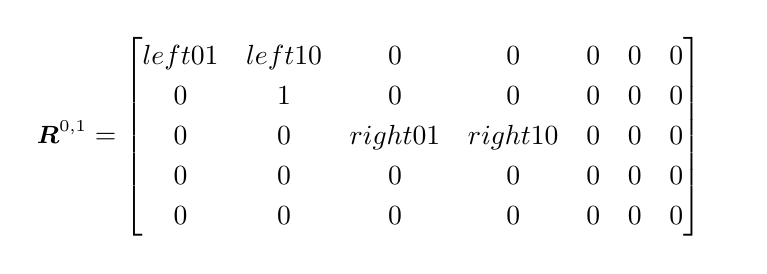
\begin{tikzpicture}[remember picture]%
\node[remember picture] (R) at (0,0){%
$\begin{aligned}%
\text{\small $\tensor{R}^{0,1}$} &= \left[\begin{matrix}%
\mytikzmarkt{left0}{1}  & \mytikzmarkt{left1}{0}  & 0  & 0  & 0  & 0  & 0\\
0  & 1  & 0  & 0  & 0  & 0  & 0\\
0  & 0  & \mytikzmarkt{right0}{1} & \mytikzmarkt{right1}{0}  & 0  & 0  & 0\\
0  & 0  & 0  & 0  & 0  & 0  & 0\\
0  & 0  & 0  & 0  & 0  & 0  & 0\\
\end{matrix} \right]
\end{aligned}$};

\end{tikzpicture}%
\tikz[overlay, remember picture] {
%	\fill[gray, fill opacity=0.2] (left0.north west) rectangle (right0.south east);
%	\fill[blue, fill opacity=0.2] (left1.north west) rectangle (right1.south east);
}%
\tikzexternalenable%}
%		\only<2>{% !TeX root = ../../main.tex
%
%
\tikzexternaldisable%
\tikzset{%
	highlightStd/.style={rectangle,draw,thick,inner sep=-1.6pt, rounded corners, opacity=1,color=black%!50, fill=black!15,fill opacity=0.2
	}
}%
\tikzset{%
	highlight0/.style={rectangle,fill=black!15,draw,
		fill opacity=1,draw opacity=0.2,inner sep=-2.2pt}
}%
\tikzset{%
	highlight1/.style={rectangle,fill=blue!15,draw,
		fill opacity=1,draw opacity=0.2,thin,inner sep=-2.2pt}
}%
\tikzset{%
	highlight2/.style={rectangle,fill=orange!15,draw,
		fill opacity=1,draw opacity=0.2,thin,inner sep=-2.2pt}
}%
\newcommand{\mytikzmarkt}[2]{%
	\tikz[inner sep=0pt, overlay, remember picture, anchor=base, baseline=(#1.base)]%
	\node (#1) {#2};%
	%\tikzmark{#1}#2%
}%

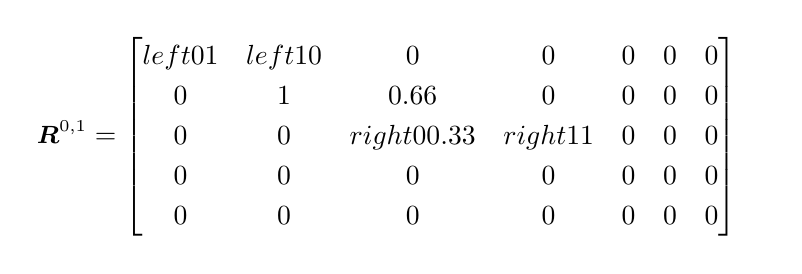
\begin{tikzpicture}[remember picture]%
\node[remember picture] (R) at (0,0){%
$\begin{aligned}%
\text{\small $\tensor{R}^{0,1}$} &= \left[\begin{matrix}%
\mytikzmarkt{left0}{1}  & \mytikzmarkt{left1}{0}  & 0  & 0  & 0  & 0  & 0\\
0  & 1  & 0.66  & 0  & 0  & 0  & 0\\
0  & 0  & \mytikzmarkt{right0}{0.33} & \mytikzmarkt{right1}{1}  & 0  & 0  & 0\\
0  & 0  & 0  & 0  & 0  & 0  & 0\\
0  & 0  & 0  & 0  & 0  & 0  & 0\\
\end{matrix} \right]
\end{aligned}$};

\end{tikzpicture}%
\tikz[overlay, remember picture] {
%	\fill[gray, fill opacity=0.2] (left0.north west) rectangle (right0.south east);
%	\fill[blue, fill opacity=0.2] (left1.north west) rectangle (right1.south east);
}%
\tikzexternalenable%}
%		\only<3>{% !TeX root = ../../main.tex
%
%
\tikzexternaldisable%
\tikzset{%
	highlightStd/.style={rectangle,draw,thick,inner sep=-1.6pt, rounded corners, opacity=1,color=black%!50, fill=black!15,fill opacity=0.2
	}
}%
\tikzset{%
	highlight0/.style={rectangle,fill=black!15,draw,
		fill opacity=1,draw opacity=0.2,inner sep=-2.2pt}
}%
\tikzset{%
	highlight1/.style={rectangle,fill=blue!15,draw,
		fill opacity=1,draw opacity=0.2,thin,inner sep=-2.2pt}
}%
\tikzset{%
	highlight2/.style={rectangle,fill=orange!15,draw,
		fill opacity=1,draw opacity=0.2,thin,inner sep=-2.2pt}
}%
\newcommand{\mytikzmarkt}[2]{%
	\tikz[inner sep=0pt, overlay, remember picture, anchor=base, baseline=(#1.base)]%
	\node (#1) {#2};%
	%\tikzmark{#1}#2%
}%

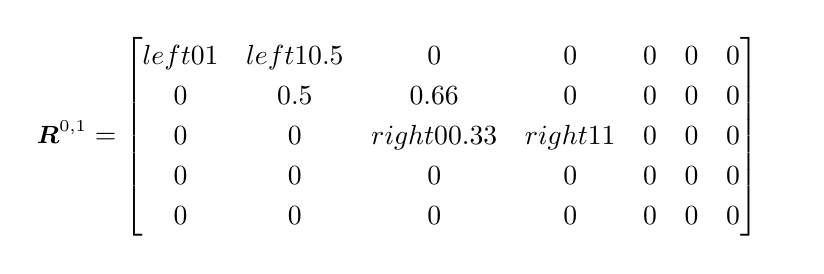
\begin{tikzpicture}[remember picture]%
\node[remember picture] (R) at (0,0){%
$\begin{aligned}%
\text{\small $\tensor{R}^{0,1}$} &= \left[\begin{matrix}%
\mytikzmarkt{left0}{1}  & \mytikzmarkt{left1}{0.5}  & 0  & 0  & 0  & 0  & 0\\
0  & 0.5  & 0.66  & 0  & 0  & 0  & 0\\
0  & 0  & \mytikzmarkt{right0}{0.33}  & \mytikzmarkt{right1}{1}  & 0  & 0  & 0\\
0& 0  & 0  & 0  & 0  & 0  & 0\\
0  & 0  & 0  & 0  & 0  & 0  & 0\\
\end{matrix} \right]
\end{aligned}$};

\end{tikzpicture}%
\tikz[overlay, remember picture] {
%	\fill[gray, fill opacity=0.2] (left0.north west) rectangle (right0.south east);
%	\fill[blue, fill opacity=0.2] (left1.north west) rectangle (right1.south east);
}%
\tikzexternalenable%}
%		\only<4>{% !TeX root = ../../main.tex
%
%
\tikzexternaldisable%
\tikzset{%
	highlightStd/.style={rectangle,draw,thick,inner sep=-1.6pt, rounded corners, opacity=1,color=black%!50, fill=black!15,fill opacity=0.2
	}
}%
\tikzset{%
	highlight0/.style={rectangle,fill=black!15,draw,
		fill opacity=1,draw opacity=0.2,inner sep=-2.2pt}
}%
\tikzset{%
	highlight1/.style={rectangle,fill=blue!15,draw,
		fill opacity=1,draw opacity=0.2,thin,inner sep=-2.2pt}
}%
\tikzset{%
	highlight2/.style={rectangle,fill=orange!15,draw,
		fill opacity=1,draw opacity=0.2,thin,inner sep=-2.2pt}
}%
\newcommand{\mytikzmarkt}[2]{%
	\tikz[inner sep=0pt, overlay, remember picture, anchor=base, baseline=(#1.base)]%
	\node (#1) {#2};%
	%\tikzmark{#1}#2%
}%

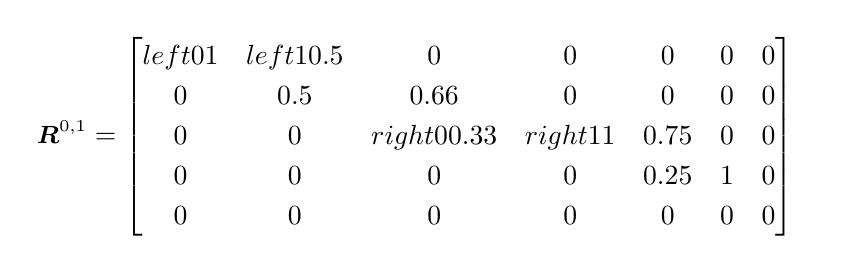
\begin{tikzpicture}[remember picture]%
\node[remember picture] (R) at (0,0){%
$\begin{aligned}%
\text{\small $\tensor{R}^{0,1}$} &= \left[\begin{matrix}%
\mytikzmarkt{left0}{1}  &  \mytikzmarkt{left1}{0.5}   & 0  & 0  & 0  & 0  & 0\\
0  & 0.5  & 0.66  & 0  & 0  & 0  & 0\\
0 & 0  & \mytikzmarkt{right0}{0.33} & \mytikzmarkt{right1}{1}  & 0.75  & 0  & 0\\
0 & 0  & 0  & 0  & 0.25  & 1  & 0\\
0 & 0  & 0  & 0  & 0  & 0  & 0\\
\end{matrix} \right]
\end{aligned}$};

\end{tikzpicture}%
\tikz[overlay, remember picture] {
%	\fill[gray, fill opacity=0.2] (left0.north west) rectangle (right0.south east);
%	\fill[blue, fill opacity=0.2] (left1.north west) rectangle (right1.south east);
}%
\tikzexternalenable%}
%		\only<5>{% !TeX root = ../../main.tex
%
%
\tikzexternaldisable%
\tikzset{%
	highlightStd/.style={rectangle,draw,thick,inner sep=-1.6pt, rounded corners, opacity=1,color=black%!50, fill=black!15,fill opacity=0.2
	}
}%
\tikzset{%
	highlight0/.style={rectangle,fill=black!15,draw,
		fill opacity=1,draw opacity=0.2,inner sep=-2.2pt}
}%
\tikzset{%
	highlight1/.style={rectangle,fill=blue!15,draw,
		fill opacity=1,draw opacity=0.2,thin,inner sep=-2.2pt}
}%
\tikzset{%
	highlight2/.style={rectangle,fill=orange!15,draw,
		fill opacity=1,draw opacity=0.2,thin,inner sep=-2.2pt}
}%
\newcommand{\mytikzmarkt}[2]{%
	\tikz[inner sep=0pt, overlay, remember picture, anchor=base, baseline=(#1.base)]%
	\node (#1) {#2};%
	%\tikzmark{#1}#2%
}%

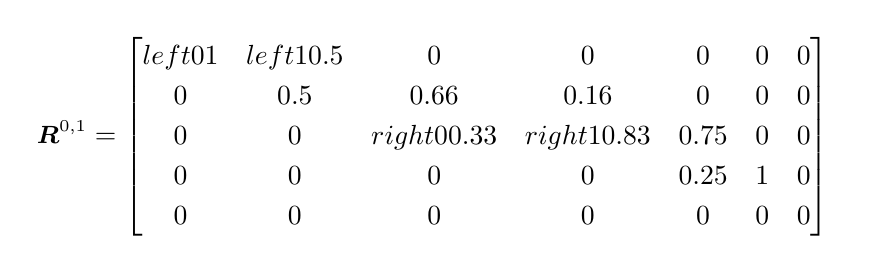
\begin{tikzpicture}[remember picture]%
\node[remember picture] (R) at (0,0){%
$\begin{aligned}%
\text{\small $\tensor{R}^{0,1}$} &= \left[\begin{matrix}%
\mytikzmarkt{left0}{1}  & \mytikzmarkt{left1}{ 0.5}  & 0  & 0  & 0  & 0  & 0\\
0  & 0.5  & 0.66  & 0.16  & 0  & 0  & 0\\
0  & 0  & \mytikzmarkt{right0}{0.33} & \mytikzmarkt{right1}{0.83}  & 0.75  & 0  & 0\\
0  & 0  & 0  & 0  & 0.25  & 1  & 0\\
0  & 0  & 0  & 0  & 0  & 0  & 0\\
\end{matrix} \right]
\end{aligned}$};

\end{tikzpicture}%
\tikz[overlay, remember picture] {
%	\fill[gray, fill opacity=0.2] (left0.north west) rectangle (right0.south east);
%	\fill[blue, fill opacity=0.2] (left1.north west) rectangle (right1.south east);
}%
\tikzexternalenable%}
%		\only<6>{% !TeX root = ../../main.tex
%
%
\tikzexternaldisable%
\tikzset{%
	highlightStd/.style={rectangle,draw,thick,inner sep=-1.6pt, rounded corners, opacity=1,color=black%!50, fill=black!15,fill opacity=0.2
	}
}%
\tikzset{%
	highlight0/.style={rectangle,fill=black!15,draw,
		fill opacity=1,draw opacity=0.2,inner sep=-2.2pt}
}%
\tikzset{%
	highlight1/.style={rectangle,fill=blue!15,draw,
		fill opacity=1,draw opacity=0.2,thin,inner sep=-2.2pt}
}%
\tikzset{%
	highlight2/.style={rectangle,fill=orange!15,draw,
		fill opacity=1,draw opacity=0.2,thin,inner sep=-2.2pt}
}%
\newcommand{\mytikzmarkt}[2]{%
	\tikz[inner sep=0pt, overlay, remember picture, anchor=base, baseline=(#1.base)]%
	\node (#1) {#2};%
	%\tikzmark{#1}#2%
}%

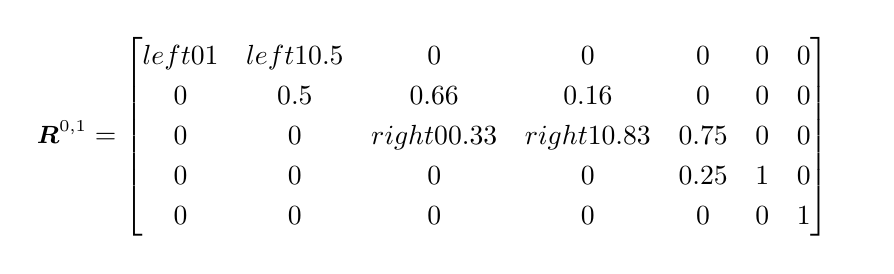
\begin{tikzpicture}[remember picture]%
\node[remember picture] (R) at (0,0){%
$\begin{aligned}%
\text{\small $\tensor{R}^{0,1}$} &= \left[\begin{matrix}%
\mytikzmarkt{left0}{1}  & \mytikzmarkt{left1}{0.5}  & 0  & 0  & 0  & 0  & 0\\
0  & 0.5  & 0.66  & 0.16  & 0  & 0  & 0\\
0  & 0  & \mytikzmarkt{right0}{0.33}  & \mytikzmarkt{right1}{0.83}  & 0.75  & 0  & 0\\
0  & 0  & 0  & 0  & 0.25  & 1  & 0\\
0  & 0  & 0  & 0  & 0  & 0  & 1\\
\end{matrix} \right]
\end{aligned}$};

\end{tikzpicture}%
\tikz[overlay, remember picture] {
%	\fill[gray, fill opacity=0.2] (left0.north west) rectangle (right0.south east);
%	\fill[blue, fill opacity=0.2] (left1.north west) rectangle (right1.south east);
}%
\tikzexternalenable%}
%\end{frame}
%
%\begin{frame}
%	\frametitle{Multi-Level Extraction: Algorithms}
%	
%	\begin{itemize}
%		\item The Boehm's algorithm algorithm can easily produce the global knot insertion operator.
%		\item Additional care is required for producing the local operators.
%		\[\Xi^0 = [-1, -1, -1, 0, 0.5 ,1, 1, 1]\]
%		\[\Xi^1 = [-1, -1 ,-1, \color{red}-0.5  \color{black}, 0,  \color{red}0.25  \color{black} ,0.5, 1, 1, 1]\]
%	\end{itemize}
%	\only<1>{% !TeX root = ../../main.tex
%
%
\tikzexternaldisable%
\tikzset{%
	highlightStd/.style={rectangle,draw,thick,inner sep=-1.6pt, rounded corners, opacity=1,color=black%!50, fill=black!15,fill opacity=0.2
	}
}%
\tikzset{%
	highlight0/.style={rectangle,fill=black!15,draw,
		fill opacity=1,draw opacity=0.2,inner sep=-2.2pt}
}%
\tikzset{%
	highlight1/.style={rectangle,fill=blue!15,draw,
		fill opacity=1,draw opacity=0.2,thin,inner sep=-2.2pt}
}%
\tikzset{%
	highlight2/.style={rectangle,fill=orange!15,draw,
		fill opacity=1,draw opacity=0.2,thin,inner sep=-2.2pt}
}%
\newcommand{\mytikzmarkt}[2]{%
	\tikz[inner sep=0pt, overlay, remember picture, anchor=base, baseline=(#1.base)]%
	\node (#1) {#2};%
	%\tikzmark{#1}#2%
}%

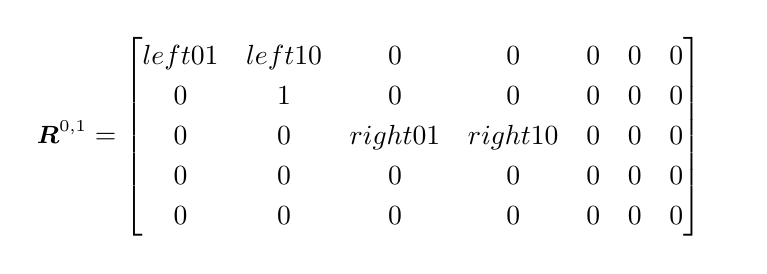
\begin{tikzpicture}[remember picture]%
\node[remember picture] (R) at (0,0){%
$\begin{aligned}%
\text{\small $\tensor{R}^{0,1}$} &= \left[\begin{matrix}%
\mytikzmarkt{left0}{1}  & \mytikzmarkt{left1}{0}  & 0  & 0  & 0  & 0  & 0\\
0  & 1  & 0  & 0  & 0  & 0  & 0\\
0  & 0  & \mytikzmarkt{right0}{1} & \mytikzmarkt{right1}{0}  & 0  & 0  & 0\\
0  & 0  & 0  & 0  & 0  & 0  & 0\\
0  & 0  & 0  & 0  & 0  & 0  & 0\\
\end{matrix} \right]
\end{aligned}$};

\end{tikzpicture}%
\tikz[overlay, remember picture] {
	\fill[gray, fill opacity=0.2] (left0.north west) rectangle (right0.south east);
	\fill[blue, fill opacity=0.2] (left1.north west) rectangle (right1.south east);
}%
\tikzexternalenable%}
%	\only<2>{% !TeX root = ../../main.tex
%
%
\tikzexternaldisable%
\tikzset{%
	highlightStd/.style={rectangle,draw,thick,inner sep=-1.6pt, rounded corners, opacity=1,color=black%!50, fill=black!15,fill opacity=0.2
	}
}%
\tikzset{%
	highlight0/.style={rectangle,fill=black!15,draw,
		fill opacity=1,draw opacity=0.2,inner sep=-2.2pt}
}%
\tikzset{%
	highlight1/.style={rectangle,fill=blue!15,draw,
		fill opacity=1,draw opacity=0.2,thin,inner sep=-2.2pt}
}%
\tikzset{%
	highlight2/.style={rectangle,fill=orange!15,draw,
		fill opacity=1,draw opacity=0.2,thin,inner sep=-2.2pt}
}%
\newcommand{\mytikzmarkt}[2]{%
	\tikz[inner sep=0pt, overlay, remember picture, anchor=base, baseline=(#1.base)]%
	\node (#1) {#2};%
	%\tikzmark{#1}#2%
}%

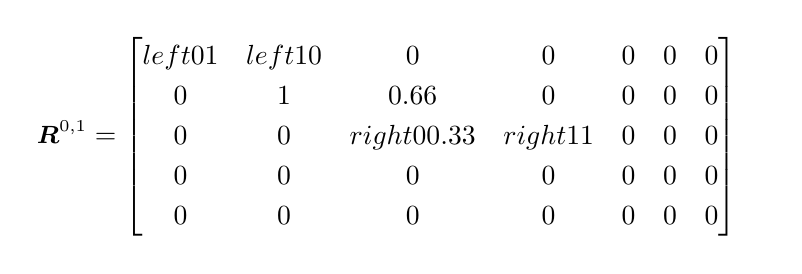
\begin{tikzpicture}[remember picture]%
\node[remember picture] (R) at (0,0){%
$\begin{aligned}%
\text{\small $\tensor{R}^{0,1}$} &= \left[\begin{matrix}%
\mytikzmarkt{left0}{1}  & \mytikzmarkt{left1}{0}  & 0  & 0  & 0  & 0  & 0\\
0  & 1  & 0.66  & 0  & 0  & 0  & 0\\
0  & 0  & \mytikzmarkt{right0}{0.33} & \mytikzmarkt{right1}{1}  & 0  & 0  & 0\\
0  & 0  & 0  & 0  & 0  & 0  & 0\\
0  & 0  & 0  & 0  & 0  & 0  & 0\\
\end{matrix} \right]
\end{aligned}$};

\end{tikzpicture}%
\tikz[overlay, remember picture] {
	\fill[gray, fill opacity=0.2] (left0.north west) rectangle (right0.south east);
	\fill[blue, fill opacity=0.2] (left1.north west) rectangle (right1.south east);
}%
\tikzexternalenable%}
%	\only<3>{% !TeX root = ../../main.tex
%
%
\tikzexternaldisable%
\tikzset{%
	highlightStd/.style={rectangle,draw,thick,inner sep=-1.6pt, rounded corners, opacity=1,color=black%!50, fill=black!15,fill opacity=0.2
	}
}%
\tikzset{%
	highlight0/.style={rectangle,fill=black!15,draw,
		fill opacity=1,draw opacity=0.2,inner sep=-2.2pt}
}%
\tikzset{%
	highlight1/.style={rectangle,fill=blue!15,draw,
		fill opacity=1,draw opacity=0.2,thin,inner sep=-2.2pt}
}%
\tikzset{%
	highlight2/.style={rectangle,fill=orange!15,draw,
		fill opacity=1,draw opacity=0.2,thin,inner sep=-2.2pt}
}%
\newcommand{\mytikzmarkt}[2]{%
	\tikz[inner sep=0pt, overlay, remember picture, anchor=base, baseline=(#1.base)]%
	\node (#1) {#2};%
	%\tikzmark{#1}#2%
}%

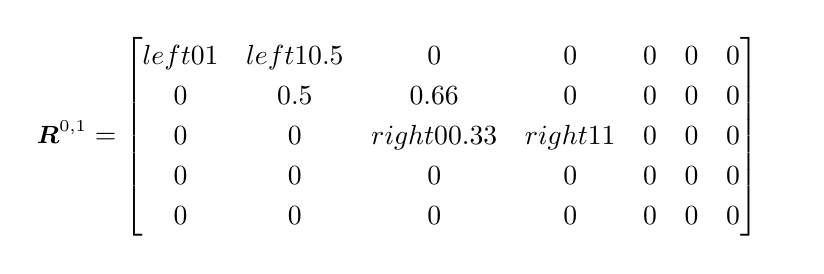
\begin{tikzpicture}[remember picture]%
\node[remember picture] (R) at (0,0){%
$\begin{aligned}%
\text{\small $\tensor{R}^{0,1}$} &= \left[\begin{matrix}%
\mytikzmarkt{left0}{1}  & \mytikzmarkt{left1}{0.5}  & 0  & 0  & 0  & 0  & 0\\
0  & 0.5  & 0.66  & 0  & 0  & 0  & 0\\
0  & 0  & \mytikzmarkt{right0}{0.33}  & \mytikzmarkt{right1}{1}  & 0  & 0  & 0\\
0& 0  & 0  & 0  & 0  & 0  & 0\\
0  & 0  & 0  & 0  & 0  & 0  & 0\\
\end{matrix} \right]
\end{aligned}$};

\end{tikzpicture}%
\tikz[overlay, remember picture] {
	\fill[gray, fill opacity=0.2] (left0.north west) rectangle (right0.south east);
	\fill[blue, fill opacity=0.2] (left1.north west) rectangle (right1.south east);
}%
\tikzexternalenable%}
%	\only<4>{% !TeX root = ../../main.tex
%
%
\tikzexternaldisable%
\tikzset{%
	highlightStd/.style={rectangle,draw,thick,inner sep=-1.6pt, rounded corners, opacity=1,color=black%!50, fill=black!15,fill opacity=0.2
	}
}%
\tikzset{%
	highlight0/.style={rectangle,fill=black!15,draw,
		fill opacity=1,draw opacity=0.2,inner sep=-2.2pt}
}%
\tikzset{%
	highlight1/.style={rectangle,fill=blue!15,draw,
		fill opacity=1,draw opacity=0.2,thin,inner sep=-2.2pt}
}%
\tikzset{%
	highlight2/.style={rectangle,fill=orange!15,draw,
		fill opacity=1,draw opacity=0.2,thin,inner sep=-2.2pt}
}%
\newcommand{\mytikzmarkt}[2]{%
	\tikz[inner sep=0pt, overlay, remember picture, anchor=base, baseline=(#1.base)]%
	\node (#1) {#2};%
	%\tikzmark{#1}#2%
}%

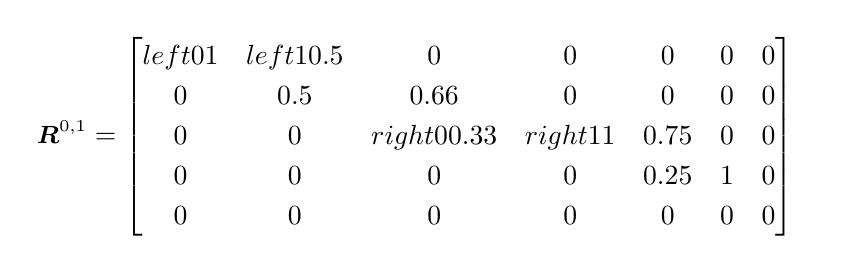
\begin{tikzpicture}[remember picture]%
\node[remember picture] (R) at (0,0){%
$\begin{aligned}%
\text{\small $\tensor{R}^{0,1}$} &= \left[\begin{matrix}%
\mytikzmarkt{left0}{1}  &  \mytikzmarkt{left1}{0.5}   & 0  & 0  & 0  & 0  & 0\\
0  & 0.5  & 0.66  & 0  & 0  & 0  & 0\\
0 & 0  & \mytikzmarkt{right0}{0.33} & \mytikzmarkt{right1}{1}  & 0.75  & 0  & 0\\
0 & 0  & 0  & 0  & 0.25  & 1  & 0\\
0 & 0  & 0  & 0  & 0  & 0  & 0\\
\end{matrix} \right]
\end{aligned}$};

\end{tikzpicture}%
\tikz[overlay, remember picture] {
	\fill[gray, fill opacity=0.2] (left0.north west) rectangle (right0.south east);
	\fill[blue, fill opacity=0.2] (left1.north west) rectangle (right1.south east);
}%
\tikzexternalenable%}
%	\only<5>{% !TeX root = ../../main.tex
%
%
\tikzexternaldisable%
\tikzset{%
	highlightStd/.style={rectangle,draw,thick,inner sep=-1.6pt, rounded corners, opacity=1,color=black%!50, fill=black!15,fill opacity=0.2
	}
}%
\tikzset{%
	highlight0/.style={rectangle,fill=black!15,draw,
		fill opacity=1,draw opacity=0.2,inner sep=-2.2pt}
}%
\tikzset{%
	highlight1/.style={rectangle,fill=blue!15,draw,
		fill opacity=1,draw opacity=0.2,thin,inner sep=-2.2pt}
}%
\tikzset{%
	highlight2/.style={rectangle,fill=orange!15,draw,
		fill opacity=1,draw opacity=0.2,thin,inner sep=-2.2pt}
}%
\newcommand{\mytikzmarkt}[2]{%
	\tikz[inner sep=0pt, overlay, remember picture, anchor=base, baseline=(#1.base)]%
	\node (#1) {#2};%
	%\tikzmark{#1}#2%
}%

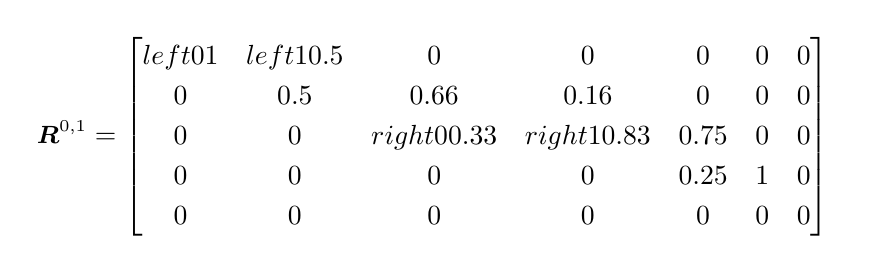
\begin{tikzpicture}[remember picture]%
\node[remember picture] (R) at (0,0){%
$\begin{aligned}%
\text{\small $\tensor{R}^{0,1}$} &= \left[\begin{matrix}%
\mytikzmarkt{left0}{1}  & \mytikzmarkt{left1}{ 0.5}  & 0  & 0  & 0  & 0  & 0\\
0  & 0.5  & 0.66  & 0.16  & 0  & 0  & 0\\
0  & 0  & \mytikzmarkt{right0}{0.33} & \mytikzmarkt{right1}{0.83}  & 0.75  & 0  & 0\\
0  & 0  & 0  & 0  & 0.25  & 1  & 0\\
0  & 0  & 0  & 0  & 0  & 0  & 0\\
\end{matrix} \right]
\end{aligned}$};

\end{tikzpicture}%
\tikz[overlay, remember picture] {
	\fill[gray, fill opacity=0.2] (left0.north west) rectangle (right0.south east);
	\fill[blue, fill opacity=0.2] (left1.north west) rectangle (right1.south east);
}%
\tikzexternalenable%}
%	\only<6>{% !TeX root = ../../main.tex
%
%
\tikzexternaldisable%
\tikzset{%
	highlightStd/.style={rectangle,draw,thick,inner sep=-1.6pt, rounded corners, opacity=1,color=black%!50, fill=black!15,fill opacity=0.2
	}
}%
\tikzset{%
	highlight0/.style={rectangle,fill=black!15,draw,
		fill opacity=1,draw opacity=0.2,inner sep=-2.2pt}
}%
\tikzset{%
	highlight1/.style={rectangle,fill=blue!15,draw,
		fill opacity=1,draw opacity=0.2,thin,inner sep=-2.2pt}
}%
\tikzset{%
	highlight2/.style={rectangle,fill=orange!15,draw,
		fill opacity=1,draw opacity=0.2,thin,inner sep=-2.2pt}
}%
\newcommand{\mytikzmarkt}[2]{%
	\tikz[inner sep=0pt, overlay, remember picture, anchor=base, baseline=(#1.base)]%
	\node (#1) {#2};%
	%\tikzmark{#1}#2%
}%

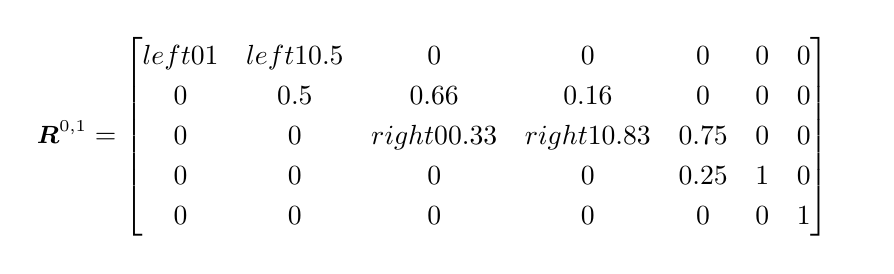
\begin{tikzpicture}[remember picture]%
\node[remember picture] (R) at (0,0){%
$\begin{aligned}%
\text{\small $\tensor{R}^{0,1}$} &= \left[\begin{matrix}%
\mytikzmarkt{left0}{1}  & \mytikzmarkt{left1}{0.5}  & 0  & 0  & 0  & 0  & 0\\
0  & 0.5  & 0.66  & 0.16  & 0  & 0  & 0\\
0  & 0  & \mytikzmarkt{right0}{0.33}  & \mytikzmarkt{right1}{0.83}  & 0.75  & 0  & 0\\
0  & 0  & 0  & 0  & 0.25  & 1  & 0\\
0  & 0  & 0  & 0  & 0  & 0  & 1\\
\end{matrix} \right]
\end{aligned}$};

\end{tikzpicture}%
\tikz[overlay, remember picture] {
	\fill[gray, fill opacity=0.2] (left0.north west) rectangle (right0.south east);
	\fill[blue, fill opacity=0.2] (left1.north west) rectangle (right1.south east);
}%
\tikzexternalenable%}
%\end{frame}
%
%\begin{frame}
%	\frametitle{Multi-Level Extraction: Algorithms}
%	
%	\begin{itemize}
%		\item The Boehm's algorithm algorithm can easily produce the global knot insertion operator.
%		\item Additional care is required for producing the local operators.
%		\[\Xi^0 = [-1, -1, -1, 0, 0.5 ,1, 1, 1]\]
%		\[\Xi^1 = [-1, -1 ,-1, \color{red}-0.5, -0.5  \color{black}, 0,  \color{red}0.25  \color{black} ,0.5, 1, 1, 1]\]
%	\end{itemize}
%	\only<1>{% !TeX root = ../../main.tex
%
%
\tikzexternaldisable%
\tikzset{%
	highlightStd/.style={rectangle,draw,thick,inner sep=-1.6pt, rounded corners, opacity=1,color=black%!50, fill=black!15,fill opacity=0.2
	}
}%
\tikzset{%
	highlight0/.style={rectangle,fill=black!15,draw,
		fill opacity=1,draw opacity=0.2,inner sep=-2.2pt}
}%
\tikzset{%
	highlight1/.style={rectangle,fill=blue!15,draw,
		fill opacity=1,draw opacity=0.2,thin,inner sep=-2.2pt}
}%
\tikzset{%
	highlight2/.style={rectangle,fill=orange!15,draw,
		fill opacity=1,draw opacity=0.2,thin,inner sep=-2.2pt}
}%
\newcommand{\mytikzmarkt}[2]{%
	\tikz[inner sep=0pt, overlay, remember picture, anchor=base, baseline=(#1.base)]%
	\node (#1) {#2};%
	%\tikzmark{#1}#2%
}%

\begin{tikzpicture}[remember picture]%
\node[remember picture] (R) at (0,0){%
$\begin{aligned}%
\text{\small $\tensor{R}^{0,1}$} &= \left[\begin{matrix}%
\mytikzmarkt{left0}{1}  & 0  & \mytikzmarkt{left1}{0}  & 0  & 0  & 0  & 0\\
0  & 1  & 0  & 0  & 0  & 0  & 0\\
0  & 0  & \mytikzmarkt{right0}{1} & 0  & \mytikzmarkt{right1}{0}  & 0  & 0\\
0  & 0  & 0  & 0  & 0  & 0  & 0\\
0  & 0  & 0  & 0  & 0  & 0  & 0\\
\end{matrix} \right]
\end{aligned}$};

\end{tikzpicture}%
\tikz[overlay, remember picture] {
	\fill[gray, fill opacity=0.2] (left0.north west) rectangle (right0.south east);
	\fill[blue, fill opacity=0.2] (left1.north west) rectangle (right1.south east);
}%
\tikzexternalenable%}
%	\only<2>{% !TeX root = ../../main.tex
%
%
\tikzexternaldisable%
\tikzset{%
	highlightStd/.style={rectangle,draw,thick,inner sep=-1.6pt, rounded corners, opacity=1,color=black%!50, fill=black!15,fill opacity=0.2
	}
}%
\tikzset{%
	highlight0/.style={rectangle,fill=black!15,draw,
		fill opacity=1,draw opacity=0.2,inner sep=-2.2pt}
}%
\tikzset{%
	highlight1/.style={rectangle,fill=blue!15,draw,
		fill opacity=1,draw opacity=0.2,thin,inner sep=-2.2pt}
}%
\tikzset{%
	highlight2/.style={rectangle,fill=orange!15,draw,
		fill opacity=1,draw opacity=0.2,thin,inner sep=-2.2pt}
}%
\newcommand{\mytikzmarkt}[2]{%
	\tikz[inner sep=0pt, overlay, remember picture, anchor=base, baseline=(#1.base)]%
	\node (#1) {#2};%
	%\tikzmark{#1}#2%
}%

\begin{tikzpicture}[remember picture]%
\node[remember picture] (R) at (0,0){%
$\begin{aligned}%
\text{\small $\tensor{R}^{0,1}$} &= \left[\begin{matrix}%
 \mytikzmarkt{left0}{1} & 0 & \mytikzmarkt{left1}{0}  & 0 & 0 & 0 & 0 & 0\\
0 & 1 & 0.66 & 0 & 0 & 0 & 0 & 0\\
0 & 0 & \mytikzmarkt{right0}{0.33} & 1 & \mytikzmarkt{right1}{0} & 0 & 0 & 0\\
0 & 0 & 0 & 0 & 0 & 0 & 0 & 0\\
0 & 0 & 0 & 0 & 0 & 0 & 0 & 0\\
\end{matrix} \right]
\end{aligned}$};

\end{tikzpicture}%
\tikz[overlay, remember picture] {
	\fill[gray, fill opacity=0.2] (left0.north west) rectangle (right0.south east);
	\fill[blue, fill opacity=0.2] (left1.north west) rectangle (right1.south east);
}%
\tikzexternalenable%}
%	\only<3>{% !TeX root = ../../main.tex
%
%
\tikzexternaldisable%
\tikzset{%
	highlightStd/.style={rectangle,draw,thick,inner sep=-1.6pt, rounded corners, opacity=1,color=black%!50, fill=black!15,fill opacity=0.2
	}
}%
\tikzset{%
	highlight0/.style={rectangle,fill=black!15,draw,
		fill opacity=1,draw opacity=0.2,inner sep=-2.2pt}
}%
\tikzset{%
	highlight1/.style={rectangle,fill=blue!15,draw,
		fill opacity=1,draw opacity=0.2,thin,inner sep=-2.2pt}
}%
\tikzset{%
	highlight2/.style={rectangle,fill=orange!15,draw,
		fill opacity=1,draw opacity=0.2,thin,inner sep=-2.2pt}
}%
\newcommand{\mytikzmarkt}[2]{%
	\tikz[inner sep=0pt, overlay, remember picture, anchor=base, baseline=(#1.base)]%
	\node (#1) {#2};%
	%\tikzmark{#1}#2%
}%

\begin{tikzpicture}[remember picture]%
\node[remember picture] (R) at (0,0){%
$\begin{aligned}%
\text{\small $\tensor{R}^{0,1}$} &= \left[\begin{matrix}%
 \mytikzmarkt{left0}{1} & 0.50 & \mytikzmarkt{left1}{0} & 0 & 0 & 0 & 0 & 0\\
0 & 0.50 & 0.66 & 0 & 0 & 0 & 0 & 0\\
0 & 0 & \mytikzmarkt{right0}{0.33} & 1 & \mytikzmarkt{right1}{0} & 0 & 0 & 0\\
0 & 0 & 0 & 0 & 0 & 0 & 0 & 0\\
0 & 0 & 0 & 0 & 0 & 0 & 0 & 0\\
\end{matrix} \right]
\end{aligned}$};

\end{tikzpicture}%
\tikz[overlay, remember picture] {
	\fill[gray, fill opacity=0.2] (left0.north west) rectangle (right0.south east);
	\fill[blue, fill opacity=0.2] (left1.north west) rectangle (right1.south east);
}%
\tikzexternalenable%}
%	\only<4>{% !TeX root = ../../main.tex
%
%
\tikzexternaldisable%
\tikzset{%
	highlightStd/.style={rectangle,draw,thick,inner sep=-1.6pt, rounded corners, opacity=1,color=black%!50, fill=black!15,fill opacity=0.2
	}
}%
\tikzset{%
	highlight0/.style={rectangle,fill=black!15,draw,
		fill opacity=1,draw opacity=0.2,inner sep=-2.2pt}
}%
\tikzset{%
	highlight1/.style={rectangle,fill=blue!15,draw,
		fill opacity=1,draw opacity=0.2,thin,inner sep=-2.2pt}
}%
\tikzset{%
	highlight2/.style={rectangle,fill=orange!15,draw,
		fill opacity=1,draw opacity=0.2,thin,inner sep=-2.2pt}
}%
\newcommand{\mytikzmarkt}[2]{%
	\tikz[inner sep=0pt, overlay, remember picture, anchor=base, baseline=(#1.base)]%
	\node (#1) {#2};%
	%\tikzmark{#1}#2%
}%

\begin{tikzpicture}[remember picture]%
\node[remember picture] (R) at (0,0){%
$\begin{aligned}%
\text{\small $\tensor{R}^{0,1}$} &= \left[\begin{matrix}%
 \mytikzmarkt{left0}{1} & 0.50 & \mytikzmarkt{left1}{0} & 0 & 0 & 0 & 0 & 0\\
0 & 0.50 & 0.66 & 0.66 & 0 & 0 & 0 & 0\\
0 & 0 & \mytikzmarkt{right0}{0.33} & 0.33 & \mytikzmarkt{right1}{1} & 0 & 0 & 0\\
0 & 0 & 0 & 0 & 0 & 0 & 0 & 0\\
0 & 0 & 0 & 0 & 0 & 0 & 0 & 0\\
\end{matrix} \right]
\end{aligned}$};

\end{tikzpicture}%
\tikz[overlay, remember picture] {
	\fill[gray, fill opacity=0.2] (left0.north west) rectangle (right0.south east);
	\fill[blue, fill opacity=0.2] (left1.north west) rectangle (right1.south east);
}%
\tikzexternalenable%}
%	\only<5>{% !TeX root = ../../main.tex
%
%
\tikzexternaldisable%
\tikzset{%
	highlightStd/.style={rectangle,draw,thick,inner sep=-1.6pt, rounded corners, opacity=1,color=black%!50, fill=black!15,fill opacity=0.2
	}
}%
\tikzset{%
	highlight0/.style={rectangle,fill=black!15,draw,
		fill opacity=1,draw opacity=0.2,inner sep=-2.2pt}
}%
\tikzset{%
	highlight1/.style={rectangle,fill=blue!15,draw,
		fill opacity=1,draw opacity=0.2,thin,inner sep=-2.2pt}
}%
\tikzset{%
	highlight2/.style={rectangle,fill=orange!15,draw,
		fill opacity=1,draw opacity=0.2,thin,inner sep=-2.2pt}
}%
\newcommand{\mytikzmarkt}[2]{%
	\tikz[inner sep=0pt, overlay, remember picture, anchor=base, baseline=(#1.base)]%
	\node (#1) {#2};%
	%\tikzmark{#1}#2%
}%

\begin{tikzpicture}[remember picture]%
\node[remember picture] (R) at (0,0){%
$\begin{aligned}%
\text{\small $\tensor{R}^{0,1}$} &= \left[\begin{matrix}%
 \mytikzmarkt{left0}{1}& 0.50 & \mytikzmarkt{left1}{0.25} & 0 & 0 & 0 & 0 & 0\\
0 & 0.50 & 0.58 & 0.66 & 0 & 0 & 0 & 0\\
0 & 0 & \mytikzmarkt{right0}{0.16} & 0.33 & \mytikzmarkt{right1}{1} & 0 & 0 & 0\\
0 & 0 & 0 & 0 & 0 & 0 & 0 & 0\\
0 & 0 & 0 & 0 & 0 & 0 & 0 & 0\\
\end{matrix} \right]
\end{aligned}$};

\end{tikzpicture}%
\tikz[overlay, remember picture] {
	\fill[gray, fill opacity=0.2] (left0.north west) rectangle (right0.south east);
	\fill[blue, fill opacity=0.2] (left1.north west) rectangle (right1.south east);
}%
\tikzexternalenable%}
%	\only<6>{% !TeX root = ../../main.tex
%
%
\tikzexternaldisable%
\tikzset{%
	highlightStd/.style={rectangle,draw,thick,inner sep=-1.6pt, rounded corners, opacity=1,color=black%!50, fill=black!15,fill opacity=0.2
	}
}%
\tikzset{%
	highlight0/.style={rectangle,fill=black!15,draw,
		fill opacity=1,draw opacity=0.2,inner sep=-2.2pt}
}%
\tikzset{%
	highlight1/.style={rectangle,fill=blue!15,draw,
		fill opacity=1,draw opacity=0.2,thin,inner sep=-2.2pt}
}%
\tikzset{%
	highlight2/.style={rectangle,fill=orange!15,draw,
		fill opacity=1,draw opacity=0.2,thin,inner sep=-2.2pt}
}%
\newcommand{\mytikzmarkt}[2]{%
	\tikz[inner sep=0pt, overlay, remember picture, anchor=base, baseline=(#1.base)]%
	\node (#1) {#2};%
	%\tikzmark{#1}#2%
}%

\begin{tikzpicture}[remember picture]%
\node[remember picture] (R) at (0,0){%
$\begin{aligned}%
\text{\small $\tensor{R}^{0,1}$} &= \left[\begin{matrix}%
  \mytikzmarkt{left0}{1} & 0.50 &  \mytikzmarkt{left1}{0.25} & 0 & 0 & 0 & 0 & 0\\
0 & 0.50 & 0.58 & 0.66 & 0 & 0 & 0 & 0\\
0 & 0 & \mytikzmarkt{right0}{0.16} & 0.33 & \mytikzmarkt{right1}{1} & 0.75 & 0 & 0\\
0 & 0 & 0 & 0 & 0 & 0.25 & 1 & 0\\
0 & 0 & 0 & 0 & 0 & 0 & 0 & 0\\
\end{matrix} \right]
\end{aligned}$};

\end{tikzpicture}%
\tikz[overlay, remember picture] {
	\fill[gray, fill opacity=0.2] (left0.north west) rectangle (right0.south east);
	\fill[blue, fill opacity=0.2] (left1.north west) rectangle (right1.south east);
}%
\tikzexternalenable%}
%\end{frame}
%
%\begin{frame}
%	\frametitle{Multi-Level Extraction: Algorithms}
%	
%	\begin{itemize}
%		\item The Oslo algorithm is similar to the Boehm's method.S
%		\item It proceeds columnwise.
%		\[\Xi^0 = [-1, -1, -1, 0, 0.5 ,1, 1, 1]\]
%		\[\Xi^1 = [-1, -1 ,-1, \color{red}-0.5, -0.5  \color{black}, 0,  \color{red}0.25  \color{black} ,0.5, 1, 1, 1]\]
%	\end{itemize}
%\only<1>{% !TeX root = ../../main.tex
%
%
\tikzexternaldisable%
\tikzset{%
	highlightStd/.style={rectangle,draw,thick,inner sep=-1.6pt, rounded corners, opacity=1,color=black%!50, fill=black!15,fill opacity=0.2
	}
}%
\tikzset{%
	highlight0/.style={rectangle,fill=black!15,draw,
		fill opacity=1,draw opacity=0.2,inner sep=-2.2pt}
}%
\tikzset{%
	highlight1/.style={rectangle,fill=blue!15,draw,
		fill opacity=1,draw opacity=0.2,thin,inner sep=-2.2pt}
}%
\tikzset{%
	highlight2/.style={rectangle,fill=orange!15,draw,
		fill opacity=1,draw opacity=0.2,thin,inner sep=-2.2pt}
}%
\newcommand{\mytikzmarkt}[2]{%
	\tikz[inner sep=0pt, overlay, remember picture, anchor=base, baseline=(#1.base)]%
	\node (#1) {#2};%
	%\tikzmark{#1}#2%
}%

\begin{tikzpicture}[remember picture]%
\node[remember picture] (R) at (0,0){%
$\begin{aligned}%
\text{\small $\tensor{R}^{0,1}$} &= \left[\begin{matrix}%
\mytikzmarkt{left0}{0}  & \mytikzmarkt{left1}{0}  & 0  & 0  & 0  & 0  & 0\\
0  & 0  & 0  & 0  & 0  & 0  & 0\\
0  & 0  & \mytikzmarkt{right0}{0}  & \mytikzmarkt{right1}{0}  & 0  & 0  & 0\\
0  & 0  & 0  & 0  & 0  & 0  & 0\\
0  & 0  & 0  & 0  & 0  & 0  & 0\\
\end{matrix} \right]
\end{aligned}$};

\end{tikzpicture}%
\tikz[overlay, remember picture] {
	\fill[gray, fill opacity=0.2] (left0.north west) rectangle (right0.south east);
	\fill[blue, fill opacity=0.2] (left1.north west) rectangle (right1.south east);
}%
\tikzexternalenable%}
%\only<2>{% !TeX root = ../../main.tex
%
%
\tikzexternaldisable%
\tikzset{%
	highlightStd/.style={rectangle,draw,thick,inner sep=-1.6pt, rounded corners, opacity=1,color=black%!50, fill=black!15,fill opacity=0.2
	}
}%
\tikzset{%
	highlight0/.style={rectangle,fill=black!15,draw,
		fill opacity=1,draw opacity=0.2,inner sep=-2.2pt}
}%
\tikzset{%
	highlight1/.style={rectangle,fill=blue!15,draw,
		fill opacity=1,draw opacity=0.2,thin,inner sep=-2.2pt}
}%
\tikzset{%
	highlight2/.style={rectangle,fill=orange!15,draw,
		fill opacity=1,draw opacity=0.2,thin,inner sep=-2.2pt}
}%
\newcommand{\mytikzmarkt}[2]{%
	\tikz[inner sep=0pt, overlay, remember picture, anchor=base, baseline=(#1.base)]%
	\node (#1) {#2};%
	%\tikzmark{#1}#2%
}%

\begin{tikzpicture}[remember picture]%
\node[remember picture] (R) at (0,0){%
$\begin{aligned}%
\text{\small $\tensor{R}^{0,1}$} &= \left[\begin{matrix}%
\mytikzmarkt{left0}{1}  & \mytikzmarkt{left1}{0}  & 0  & 0  & 0  & 0  & 0\\
0  & 0  & 0  & 0  & 0  & 0  & 0\\
0  & 0  & \mytikzmarkt{right0}{0}  & \mytikzmarkt{right1}{0}  & 0  & 0  & 0\\
0  & 0  & 0  & 0  & 0  & 0  & 0\\
0  & 0  & 0  & 0  & 0  & 0  & 0\\
\end{matrix} \right]
\end{aligned}$};

\end{tikzpicture}%
\tikz[overlay, remember picture] {
	\fill[gray, fill opacity=0.2] (left0.north west) rectangle (right0.south east);
	\fill[blue, fill opacity=0.2] (left1.north west) rectangle (right1.south east);
}%
\tikzexternalenable%}
%\only<3>{% !TeX root = ../../main.tex
%
%
\tikzexternaldisable%
\tikzset{%
	highlightStd/.style={rectangle,draw,thick,inner sep=-1.6pt, rounded corners, opacity=1,color=black%!50, fill=black!15,fill opacity=0.2
	}
}%
\tikzset{%
	highlight0/.style={rectangle,fill=black!15,draw,
		fill opacity=1,draw opacity=0.2,inner sep=-2.2pt}
}%
\tikzset{%
	highlight1/.style={rectangle,fill=blue!15,draw,
		fill opacity=1,draw opacity=0.2,thin,inner sep=-2.2pt}
}%
\tikzset{%
	highlight2/.style={rectangle,fill=orange!15,draw,
		fill opacity=1,draw opacity=0.2,thin,inner sep=-2.2pt}
}%
\newcommand{\mytikzmarkt}[2]{%
	\tikz[inner sep=0pt, overlay, remember picture, anchor=base, baseline=(#1.base)]%
	\node (#1) {#2};%
	%\tikzmark{#1}#2%
}%

\begin{tikzpicture}[remember picture]%
\node[remember picture] (R) at (0,0){%
$\begin{aligned}%
\text{\small $\tensor{R}^{0,1}$} &= \left[\begin{matrix}%
\mytikzmarkt{left0}{1}  & \mytikzmarkt{left1}{0.5}  & 0  & 0  & 0  & 0  & 0\\
0  & 0.5  & 0  & 0  & 0  & 0  & 0\\
0  & 0  & \mytikzmarkt{right0}{0}  & \mytikzmarkt{right1}{0}  & 0  & 0  & 0\\
0  & 0  & 0  & 0  & 0  & 0  & 0\\
0  & 0  & 0  & 0  & 0  & 0  & 0\\
\end{matrix} \right]
\end{aligned}$};

\end{tikzpicture}%
\tikz[overlay, remember picture] {
	\fill[gray, fill opacity=0.2] (left0.north west) rectangle (right0.south east);
	\fill[blue, fill opacity=0.2] (left1.north west) rectangle (right1.south east);
}%
\tikzexternalenable%}
%\only<4>{% !TeX root = ../../main.tex
%
%
\tikzexternaldisable%
\tikzset{%
	highlightStd/.style={rectangle,draw,thick,inner sep=-1.6pt, rounded corners, opacity=1,color=black%!50, fill=black!15,fill opacity=0.2
	}
}%
\tikzset{%
	highlight0/.style={rectangle,fill=black!15,draw,
		fill opacity=1,draw opacity=0.2,inner sep=-2.2pt}
}%
\tikzset{%
	highlight1/.style={rectangle,fill=blue!15,draw,
		fill opacity=1,draw opacity=0.2,thin,inner sep=-2.2pt}
}%
\tikzset{%
	highlight2/.style={rectangle,fill=orange!15,draw,
		fill opacity=1,draw opacity=0.2,thin,inner sep=-2.2pt}
}%
\newcommand{\mytikzmarkt}[2]{%
	\tikz[inner sep=0pt, overlay, remember picture, anchor=base, baseline=(#1.base)]%
	\node (#1) {#2};%
	%\tikzmark{#1}#2%
}%

\begin{tikzpicture}[remember picture]%
\node[remember picture] (R) at (0,0){%
$\begin{aligned}%
\text{\small $\tensor{R}^{0,1}$} &= \left[\begin{matrix}%
\mytikzmarkt{left0}{1}  & \mytikzmarkt{left1}{0.5}  & 0  & 0  & 0  & 0  & 0\\
0  & 0.5  & 0.66  & 0  & 0  & 0  & 0\\
0  & 0  & \mytikzmarkt{right0}{0.33}  & \mytikzmarkt{right1}{0}  & 0  & 0  & 0\\
0  & 0  & 0  & 0  & 0  & 0  & 0\\
0  & 0  & 0  & 0  & 0  & 0  & 0\\
\end{matrix} \right]
\end{aligned}$};

\end{tikzpicture}%
\tikz[overlay, remember picture] {
	\fill[gray, fill opacity=0.2] (left0.north west) rectangle (right0.south east);
	\fill[blue, fill opacity=0.2] (left1.north west) rectangle (right1.south east);
}%
\tikzexternalenable%}
%\only<5>{% !TeX root = ../../main.tex
%
%
\tikzexternaldisable%
\tikzset{%
	highlightStd/.style={rectangle,draw,thick,inner sep=-1.6pt, rounded corners, opacity=1,color=black%!50, fill=black!15,fill opacity=0.2
	}
}%
\tikzset{%
	highlight0/.style={rectangle,fill=black!15,draw,
		fill opacity=1,draw opacity=0.2,inner sep=-2.2pt}
}%
\tikzset{%
	highlight1/.style={rectangle,fill=blue!15,draw,
		fill opacity=1,draw opacity=0.2,thin,inner sep=-2.2pt}
}%
\tikzset{%
	highlight2/.style={rectangle,fill=orange!15,draw,
		fill opacity=1,draw opacity=0.2,thin,inner sep=-2.2pt}
}%
\newcommand{\mytikzmarkt}[2]{%
	\tikz[inner sep=0pt, overlay, remember picture, anchor=base, baseline=(#1.base)]%
	\node (#1) {#2};%
	%\tikzmark{#1}#2%
}%

\begin{tikzpicture}[remember picture]%
\node[remember picture] (R) at (0,0){%
$\begin{aligned}%
\text{\small $\tensor{R}^{0,1}$} &= \left[\begin{matrix}%
\mytikzmarkt{left0}{1}  & \mytikzmarkt{left1}{0.5}  & 0  & 0  & 0  & 0  & 0\\
0  & 0.5  & 0.66  & 0.16  & 0  & 0  & 0\\
0  & 0  & \mytikzmarkt{right0}{0.33}  & \mytikzmarkt{right1}{0.83}  & 0  & 0  & 0\\
0  & 0  & 0  & 0  & 0  & 0  & 0\\
0  & 0  & 0  & 0  & 0  & 0  & 0\\
\end{matrix} \right]
\end{aligned}$};

\end{tikzpicture}%
\tikz[overlay, remember picture] {
	\fill[gray, fill opacity=0.2] (left0.north west) rectangle (right0.south east);
	\fill[blue, fill opacity=0.2] (left1.north west) rectangle (right1.south east);
}%
\tikzexternalenable%}
%\only<6>{% !TeX root = ../../main.tex
%
%
\tikzexternaldisable%
\tikzset{%
	highlightStd/.style={rectangle,draw,thick,inner sep=-1.6pt, rounded corners, opacity=1,color=black%!50, fill=black!15,fill opacity=0.2
	}
}%
\tikzset{%
	highlight0/.style={rectangle,fill=black!15,draw,
		fill opacity=1,draw opacity=0.2,inner sep=-2.2pt}
}%
\tikzset{%
	highlight1/.style={rectangle,fill=blue!15,draw,
		fill opacity=1,draw opacity=0.2,thin,inner sep=-2.2pt}
}%
\tikzset{%
	highlight2/.style={rectangle,fill=orange!15,draw,
		fill opacity=1,draw opacity=0.2,thin,inner sep=-2.2pt}
}%
\newcommand{\mytikzmarkt}[2]{%
	\tikz[inner sep=0pt, overlay, remember picture, anchor=base, baseline=(#1.base)]%
	\node (#1) {#2};%
	%\tikzmark{#1}#2%
}%

\begin{tikzpicture}[remember picture]%
\node[remember picture] (R) at (0,0){%
$\begin{aligned}%
\text{\small $\tensor{R}^{0,1}$} &= \left[\begin{matrix}%
\mytikzmarkt{left0}{1}  & \mytikzmarkt{left1}{0.5}  & 0  & 0  & 0  & 0  & 0\\
0  & 0.5  & 0.66  & 0.16  & 0  & 0  & 0\\
0  & 0  & \mytikzmarkt{right0}{0.33}  & \mytikzmarkt{right1}{0.83}  & 0.75  & 0  & 0\\
0  & 0  & 0  & 0  & 0.25  & 0  & 0\\
0  & 0  & 0  & 0  & 0  & 0  & 0\\
\end{matrix} \right]
\end{aligned}$};

\end{tikzpicture}%
\tikz[overlay, remember picture] {
	\fill[gray, fill opacity=0.2] (left0.north west) rectangle (right0.south east);
	\fill[blue, fill opacity=0.2] (left1.north west) rectangle (right1.south east);
}%
\tikzexternalenable%}
%\only<7>{% !TeX root = ../../main.tex
%
%
\tikzexternaldisable%
\tikzset{%
	highlightStd/.style={rectangle,draw,thick,inner sep=-1.6pt, rounded corners, opacity=1,color=black%!50, fill=black!15,fill opacity=0.2
	}
}%
\tikzset{%
	highlight0/.style={rectangle,fill=black!15,draw,
		fill opacity=1,draw opacity=0.2,inner sep=-2.2pt}
}%
\tikzset{%
	highlight1/.style={rectangle,fill=blue!15,draw,
		fill opacity=1,draw opacity=0.2,thin,inner sep=-2.2pt}
}%
\tikzset{%
	highlight2/.style={rectangle,fill=orange!15,draw,
		fill opacity=1,draw opacity=0.2,thin,inner sep=-2.2pt}
}%
\newcommand{\mytikzmarkt}[2]{%
	\tikz[inner sep=0pt, overlay, remember picture, anchor=base, baseline=(#1.base)]%
	\node (#1) {#2};%
	%\tikzmark{#1}#2%
}%

\begin{tikzpicture}[remember picture]%
\node[remember picture] (R) at (0,0){%
$\begin{aligned}%
\text{\small $\tensor{R}^{0,1}$} &= \left[\begin{matrix}%
\mytikzmarkt{left0}{1}  & \mytikzmarkt{left1}{0.5}  & 0  & 0  & 0  & 0  & 0\\
0  & 0.5  & 0.66  & 0.16  & 0  & 0  & 0\\
0  & 0  & \mytikzmarkt{right0}{0.33}  & \mytikzmarkt{right1}{0.83}  & 0.75  & 0  & 0\\
0  & 0  & 0  & 0  & 0.25  & 1  & 0\\
0  & 0  & 0  & 0  & 0  & 0  & 0\\
\end{matrix} \right]
\end{aligned}$};

\end{tikzpicture}%
\tikz[overlay, remember picture] {
	\fill[gray, fill opacity=0.2] (left0.north west) rectangle (right0.south east);
	\fill[blue, fill opacity=0.2] (left1.north west) rectangle (right1.south east);
}%
\tikzexternalenable%}
%\only<8>{% !TeX root = ../../main.tex
%
%
\tikzexternaldisable%
\tikzset{%
	highlightStd/.style={rectangle,draw,thick,inner sep=-1.6pt, rounded corners, opacity=1,color=black%!50, fill=black!15,fill opacity=0.2
	}
}%
\tikzset{%
	highlight0/.style={rectangle,fill=black!15,draw,
		fill opacity=1,draw opacity=0.2,inner sep=-2.2pt}
}%
\tikzset{%
	highlight1/.style={rectangle,fill=blue!15,draw,
		fill opacity=1,draw opacity=0.2,thin,inner sep=-2.2pt}
}%
\tikzset{%
	highlight2/.style={rectangle,fill=orange!15,draw,
		fill opacity=1,draw opacity=0.2,thin,inner sep=-2.2pt}
}%
\newcommand{\mytikzmarkt}[2]{%
	\tikz[inner sep=0pt, overlay, remember picture, anchor=base, baseline=(#1.base)]%
	\node (#1) {#2};%
	%\tikzmark{#1}#2%
}%

\begin{tikzpicture}[remember picture]%
\node[remember picture] (R) at (0,0){%
$\begin{aligned}%
\text{\small $\tensor{R}^{0,1}$} &= \left[\begin{matrix}%
\mytikzmarkt{left0}{1}  & \mytikzmarkt{left1}{0.5}  & 0  & 0  & 0  & 0  & 0\\
0  & 0.5  & 0.66  & 0.16  & 0  & 0  & 0\\
0  & 0  & \mytikzmarkt{right0}{0.33}  & \mytikzmarkt{right1}{0.83}  & 0.75  & 0  & 0\\
0  & 0  & 0  & 0  & 0.25  & 1  & 0\\
0  & 0  & 0  & 0  & 0  & 0  & 1\\
\end{matrix} \right]
\end{aligned}$};

\end{tikzpicture}%
\tikz[overlay, remember picture] {
	\fill[gray, fill opacity=0.2] (left0.north west) rectangle (right0.south east);
	\fill[blue, fill opacity=0.2] (left1.north west) rectangle (right1.south east);
}%
\tikzexternalenable%}
%\end{frame}
%
%\begin{frame}
%	\frametitle{Multi-Level Extraction: Algorithms}
%	\begin{itemize}
%		\item Both algorithms use linear operations.
%		\item The Boehm's algorithm 
%		\begin{itemize}
%			\item is numerically more stable (convex combinations),
%			\item is harder to parallelize.
%		\end{itemize}
%		\item The Oslo algorithm
%		\begin{itemize}
%			\item is easy to parallelize,
%			\item easier to program.
%		\end{itemize}
%		\item The Boehm's algorithm is the best algorithm for computing the new control points after knot insertion.
%		\item However, this is not necessarily true for generating the knot insertion operator.
%	\end{itemize}
%\end{frame}
%
%
%\begin{frame}
%	\frametitle{Multi-Level Extraction: Algorithms Comparison}
%		\begin{itemize}
%		\item $ p=3 $
%		\item Knot vector $ [-1, -0.8, 0.3, 1] $ bisected 11 times
%		\item Parallel Oslo executed on 4 processors
%	\end{itemize}
%\begin{figure}[t]
%	\centering
%	\begin{subfigure}[t]{.5\textwidth}
%		\centering
%		% This file was created by matlab2tikz.
%
%The latest updates can be retrieved from
%  http://www.mathworks.com/matlabcentral/fileexchange/22022-matlab2tikz-matlab2tikz
%where you can also make suggestions and rate matlab2tikz.
%
\begin{tikzpicture}%
\begin{axis}[%
width=4cm,
height=4cm,
scale only axis,
xmin=0,
xmax=3100,
xminorticks=true,
ymin=10,
ymax=150000,
yminorticks=true,
axis background/.style={fill=white},
ylabel=Number of Linear Operations,
xlabel=Number of Added Knots,
legend style={font=\tiny}
]%
\addplot [color=blue, mark=o, mark options={solid, blue}]
  table[row sep=crcr]{%
3	72\\
9	216\\
21	504\\
45	1080\\
93	2232\\
189	4536\\
381	9144\\
765	18360\\
1533	36792\\
3069	73656\\
};
\addplot [color=red, dashed, mark=o, mark options={solid, red}]
  table[row sep=crcr]{%
3	252\\
9	504\\
21	1008\\
45	2016\\
93	4032\\
189	8064\\
381	16128\\
765	32256\\
1533	64512\\
3069	129024\\
};
\addplot [color=black, dashed, mark=diamond, mark options={solid, black}]
  table[row sep=crcr]{%
3	108\\
9	180\\
21	324\\
45	612\\
93	1188\\
189	2340\\
381	4644\\
765	9252\\
1533	18468\\
3069	36900\\
};
\addplot [color=green, dashed, mark=square, mark options={solid, green}]
  table[row sep=crcr]{%
3	60\\
9	72\\
21	108\\
45	180\\
93	324\\
189	612\\
381	1188\\
765	2340\\
1533	4644\\
3069	9252\\
};
\legend{Boehm, Bs2bs, Oslo, Parallel Oslo}
\end{axis}%
\end{tikzpicture}%
%	\end{subfigure}%
%	\begin{subfigure}[b]{.5\textwidth}
%		\centering
%		% This file was created by matlab2tikz.
%
%The latest updates can be retrieved from
%  http://www.mathworks.com/matlabcentral/fileexchange/22022-matlab2tikz-matlab2tikz
%where you can also make suggestions and rate matlab2tikz.
%
\begin{tikzpicture}%
\begin{axis}[%
width=4cm,
height=4cm,
scale only axis,
xmode=log,
ymode=log,
xmin=0,
xmax=3100,
xminorticks=true,
ymin=10,
ymax=150000,
yminorticks=true,
axis background/.style={fill=white},
ylabel=Number of Linear Operations,
xlabel=Number of Added Knots,
legend style={font=\tiny},
legend pos=north west
]%
\addplot [color=blue, mark=o, mark options={solid, blue}]
table[row sep=crcr]{%
	3	72\\
	9	216\\
	21	504\\
	45	1080\\
	93	2232\\
	189	4536\\
	381	9144\\
	765	18360\\
	1533	36792\\
	3069	73656\\
};
\addplot [color=red, dashed, mark=o, mark options={solid, red}]
table[row sep=crcr]{%
	3	252\\
	9	504\\
	21	1008\\
	45	2016\\
	93	4032\\
	189	8064\\
	381	16128\\
	765	32256\\
	1533	64512\\
	3069	129024\\
};
\addplot [color=black, dashed, mark=diamond, mark options={solid, black}]
table[row sep=crcr]{%
	3	108\\
	9	180\\
	21	324\\
	45	612\\
	93	1188\\
	189	2340\\
	381	4644\\
	765	9252\\
	1533	18468\\
	3069	36900\\
};
\addplot [color=green, dashed, mark=square, mark options={solid, green}]
table[row sep=crcr]{%
	3	60\\
	9	72\\
	21	108\\
	45	180\\
	93	324\\
	189	612\\
	381	1188\\
	765	2340\\
	1533	4644\\
	3069	9252\\
};
\legend{Boehm, Bs2bs, Oslo, Parallel Oslo}
\end{axis}
\end{tikzpicture}%
%	\end{subfigure}
%\end{figure}
%	\begin{figure}[b]
%		\centering
%	\begin{minipage}[b]{0.4\textwidth}
%			\vspace{0pt}%
%		% This file was created by matlab2tikz.
%
%The latest updates can be retrieved from
%  http://www.mathworks.com/matlabcentral/fileexchange/22022-matlab2tikz-matlab2tikz
%where you can also make suggestions and rate matlab2tikz.
%
\begin{tikzpicture}%
\begin{axis}[%
width=4cm,
height=4cm,
scale only axis,
xmin=0,
xmax=3100,
xminorticks=true,
ymin=10,
ymax=150000,
yminorticks=true,
axis background/.style={fill=white},
ylabel=Number of Linear Operations,
xlabel=Number of Added Knots,
legend style={font=\tiny}
]%
\addplot [color=blue, mark=o, mark options={solid, blue}]
  table[row sep=crcr]{%
3	72\\
9	216\\
21	504\\
45	1080\\
93	2232\\
189	4536\\
381	9144\\
765	18360\\
1533	36792\\
3069	73656\\
};
\addplot [color=red, dashed, mark=o, mark options={solid, red}]
  table[row sep=crcr]{%
3	252\\
9	504\\
21	1008\\
45	2016\\
93	4032\\
189	8064\\
381	16128\\
765	32256\\
1533	64512\\
3069	129024\\
};
\addplot [color=black, dashed, mark=diamond, mark options={solid, black}]
  table[row sep=crcr]{%
3	108\\
9	180\\
21	324\\
45	612\\
93	1188\\
189	2340\\
381	4644\\
765	9252\\
1533	18468\\
3069	36900\\
};
\addplot [color=green, dashed, mark=square, mark options={solid, green}]
  table[row sep=crcr]{%
3	60\\
9	72\\
21	108\\
45	180\\
93	324\\
189	612\\
381	1188\\
765	2340\\
1533	4644\\
3069	9252\\
};
\legend{Boehm, Bs2bs, Oslo, Parallel Oslo}
\end{axis}%
\end{tikzpicture}%%		
%	\end{minipage}
%\hspace{1cm}
%	\begin{minipage}[b]{0.4\textwidth}
%		\vspace{0pt}%
%		% This file was created by matlab2tikz.
%
%The latest updates can be retrieved from
%  http://www.mathworks.com/matlabcentral/fileexchange/22022-matlab2tikz-matlab2tikz
%where you can also make suggestions and rate matlab2tikz.
%
\begin{tikzpicture}%
\begin{axis}[%
width=4cm,
height=4cm,
scale only axis,
xmode=log,
ymode=log,
xmin=0,
xmax=3100,
xminorticks=true,
ymin=10,
ymax=150000,
yminorticks=true,
axis background/.style={fill=white},
ylabel=Number of Linear Operations,
xlabel=Number of Added Knots,
legend style={font=\tiny},
legend pos=north west
]%
\addplot [color=blue, mark=o, mark options={solid, blue}]
table[row sep=crcr]{%
	3	72\\
	9	216\\
	21	504\\
	45	1080\\
	93	2232\\
	189	4536\\
	381	9144\\
	765	18360\\
	1533	36792\\
	3069	73656\\
};
\addplot [color=red, dashed, mark=o, mark options={solid, red}]
table[row sep=crcr]{%
	3	252\\
	9	504\\
	21	1008\\
	45	2016\\
	93	4032\\
	189	8064\\
	381	16128\\
	765	32256\\
	1533	64512\\
	3069	129024\\
};
\addplot [color=black, dashed, mark=diamond, mark options={solid, black}]
table[row sep=crcr]{%
	3	108\\
	9	180\\
	21	324\\
	45	612\\
	93	1188\\
	189	2340\\
	381	4644\\
	765	9252\\
	1533	18468\\
	3069	36900\\
};
\addplot [color=green, dashed, mark=square, mark options={solid, green}]
table[row sep=crcr]{%
	3	60\\
	9	72\\
	21	108\\
	45	180\\
	93	324\\
	189	612\\
	381	1188\\
	765	2340\\
	1533	4644\\
	3069	9252\\
};
\legend{Boehm, Bs2bs, Oslo, Parallel Oslo}
\end{axis}
\end{tikzpicture}%%
%	\end{minipage}
%	\end{figure}
%\end{frame}
%
%\begin{frame}
%	\frametitle{Multi-Level Extraction: Algorithms Comparison}
%	\begin{itemize}
%		\item $ p=3 $
%		\item Knot vector $ [-1, -0.8, 0.3, 1] $ bisected 11 times
%		\item Parallel Oslo executed on 4 processors
%	\end{itemize}
%	\begin{figure}[t]
%		\centering
%		\begin{subfigure}[t]{.5\textwidth}
%			\centering
%			% This file was created by matlab2tikz.
%
%The latest updates can be retrieved from
%  http://www.mathworks.com/matlabcentral/fileexchange/22022-matlab2tikz-matlab2tikz
%where you can also make suggestions and rate matlab2tikz.
%
\begin{tikzpicture}

\begin{axis}[%
width=6cm,
height=5cm,
scale only axis,
xminorticks=true,
xmin=0,
xmax=3500,
ymin=0,
ymax=3.5,
yminorticks=true,
axis background/.style={fill=white},
ytick={0,1,2,3,3.5},
ylabel=$ \frac{\text{Nr. Ops.}}{\text{Nr. Ops. Serial Oslo}} $,
xlabel=Number of Added Knots,
legend style={font=\tiny},
legend pos=north west
]%
\addplot [color=blue, mark=o, mark options={solid, blue}]
  table[row sep=crcr]{%
3	0.666666666666667\\
9	1.2\\
21	1.55555555555556\\
45	1.76470588235294\\
93	1.87878787878788\\
189	1.93846153846154\\
381	1.96899224806202\\
765	1.98443579766537\\
1533	1.99220272904483\\
3069	1.99609756097561\\
};
\addplot [color=red, mark=o, mark options={solid, red}]
  table[row sep=crcr]{%
3	2.33333333333333\\
9	2.8\\
21	3.11111111111111\\
45	3.29411764705882\\
93	3.39393939393939\\
189	3.44615384615385\\
381	3.47286821705426\\
765	3.4863813229572\\
1533	3.49317738791423\\
3069	3.49658536585366\\
};
\legend{Boehm, Bs2bs}
\end{axis}
\end{tikzpicture}%
%		\end{subfigure}%
%		\begin{subfigure}[b]{.5\textwidth}
%			\centering
%			% This file was created by matlab2tikz.
%
%The latest updates can be retrieved from
%  http://www.mathworks.com/matlabcentral/fileexchange/22022-matlab2tikz-matlab2tikz
%where you can also make suggestions and rate matlab2tikz.
%
\begin{tikzpicture}

\begin{axis}[%
width=4cm,
height=4cm,
scale only axis,
xminorticks=true,
xmin=0,
xmax=3500,
ymin=0,
ymax=14,
yminorticks=true,
ytick={0,4,8,14},
axis background/.style={fill=white},
ylabel=$ \frac{\text{Nr. Ops.}}{\text{Nr. Ops. Parallel Oslo}} $,
xlabel=Number of Added Knots,
legend style={font=\tiny},
legend pos=north west
]%
\addplot [color=blue, mark=o, mark options={solid, blue}]
  table[row sep=crcr]{%
3	1.2\\
9	3\\
21	4.66666666666667\\
45	6\\
93	6.88888888888889\\
189	7.41176470588235\\
381	7.6969696969697\\
765	7.84615384615385\\
1533	7.92248062015504\\
3069	7.96108949416342\\
};

\addplot [color=red, mark=o, mark options={solid, red}]
  table[row sep=crcr]{%
3	4.2\\
9	7\\
21	9.33333333333333\\
45	11.2\\
93	12.4444444444444\\
189	13.1764705882353\\
381	13.5757575757576\\
765	13.7846153846154\\
1533	13.8914728682171\\
3069	13.9455252918288\\
};

\addplot [color=black, mark=diamond, mark options={solid, black}]
  table[row sep=crcr]{%
3	1.8\\
9	2.5\\
21	3\\
45	3.4\\
93	3.66666666666667\\
189	3.82352941176471\\
381	3.90909090909091\\
765	3.95384615384615\\
1533	3.97674418604651\\
3069	3.98832684824903\\
};
\addlegendentry{$\text{oslo}_\text{l}\text{ocal}$}
\legend{Boehm, Bs2bs, Oslo}
\end{axis}
\end{tikzpicture}%
%		\end{subfigure}
%	\end{figure}
%\end{frame}
%
%
%\begin{frame}
%	\frametitle{Multi-Level Extraction: Algorithms}
%	
%	\begin{itemize}
%		\item The multi-level operators is obtained by combining rows of the standard operators
%	\end{itemize}
%		\only<1>{		% !TeX root = ../../main.tex
\begin{tikzpicture}%
\def\lineWidth{0.6pt}
\def\knotWidth{1.1pt}
\def\knotSize{3pt}
\def\elementWidth{3pt}
\def\colorLevelOne{black}
\def\colorLevelTwo{black}
\def\colorLevelThree{black}
%
\tikzset{% 
	elementLineStyle/.style={%
		color=red,solid,line width=\elementWidth, opacity=0
	}
}
\tikzset{% 
	knotsStyle/.style={%
		color=red,line width=\knotWidth,mark size=\knotSize,only marks,mark=x,mark options={solid}
	}
}
\tikzset{% 
	inactive/.style={%
		color=black,solid,line width=\lineWidth
	}
}
\tikzset{% 
	ap/.style={%
		solid,line width=\lineWidth
	}
}
\tikzset{% 
	am/.style={%
		solid,line width=\lineWidth
	}
}
\tikzset{% 
	aa/.style={%
		solid,line width=\lineWidth
	}
}
\begin{groupplot}[
group style={/tikz/background rectangle/.style={draw=none},
	group size=1 by 3,
	xlabels at=edge bottom,
%xticklabels at=edge bottom,
ylabels at=edge left
,yticklabels at=edge left
,vertical sep=0.7cm},
axis y line=left,
width=0.99\linewidth,
height=3cm, %(\overAllHeight-(\basisPlotDepth-1)*\plotSeparator) / \basisPlotDepth, 
    	%xlabel=x,
		ylabel=Y,
		xmin=-1,  xmax=1,
		ymin=0, ymax=1.08,
		ytick={0,1},
		%xtick={-1,0,1},
		tickpos=left,
		ytick align=outside,
		xtick align=outside,
		tick label style ={font=\small},
		label style ={font=\small},
		legend style={ font =\small },
		ymajorgrids=false,
		] %

				
				
\nextgroupplot[axis x line=bottom, xtick={-1,0,1}, ylabel=\phantom{$ \mathcal{THB} $}\llap{$\mathcal{B}^0 $}, ylabel style={rotate=-90}]

\addplot [color=\colorLevelOne,aa]
table[row sep=crcr]{%
	-1	1\\
	-0.99	0.9604\\
	-0.98	0.9216\\
	-0.97	0.8836\\
	-0.96	0.8464\\
	-0.95	0.81\\
	-0.94	0.7744\\
	-0.93	0.7396\\
	-0.92	0.7056\\
	-0.91	0.6724\\
	-0.9	0.64\\
	-0.89	0.6084\\
	-0.88	0.5776\\
	-0.87	0.5476\\
	-0.86	0.5184\\
	-0.85	0.49\\
	-0.84	0.4624\\
	-0.83	0.4356\\
	-0.82	0.4096\\
	-0.81	0.3844\\
	-0.8	0.36\\
	-0.79	0.3364\\
	-0.78	0.3136\\
	-0.77	0.2916\\
	-0.76	0.2704\\
	-0.75	0.25\\
	-0.74	0.2304\\
	-0.73	0.2116\\
	-0.72	0.1936\\
	-0.71	0.1764\\
	-0.7	0.16\\
	-0.69	0.1444\\
	-0.68	0.1296\\
	-0.67	0.1156\\
	-0.66	0.1024\\
	-0.65	0.0899999999999999\\
	-0.64	0.0784\\
	-0.63	0.0676\\
	-0.62	0.0576\\
	-0.61	0.0484\\
	-0.6	0.04\\
	-0.59	0.0324\\
	-0.58	0.0256\\
	-0.57	0.0196\\
	-0.56	0.0144\\
	-0.55	0.01\\
	-0.54	0.00640000000000001\\
	-0.53	0.00360000000000001\\
	-0.52	0.0016\\
	-0.51	0.000400000000000001\\
	-0.5	0\\
	-0.49	0\\
	-0.48	0\\
	-0.47	0\\
	-0.46	0\\
	-0.45	0\\
	-0.44	0\\
	-0.43	0\\
	-0.42	0\\
	-0.41	0\\
	-0.4	0\\
	-0.39	0\\
	-0.38	0\\
	-0.37	0\\
	-0.36	0\\
	-0.35	0\\
	-0.34	0\\
	-0.33	0\\
	-0.32	0\\
	-0.31	0\\
	-0.3	0\\
	-0.29	0\\
	-0.28	0\\
	-0.27	0\\
	-0.26	0\\
	-0.25	0\\
	-0.24	0\\
	-0.23	0\\
	-0.22	0\\
	-0.21	0\\
	-0.2	0\\
	-0.19	0\\
	-0.18	0\\
	-0.17	0\\
	-0.16	0\\
	-0.15	0\\
	-0.14	0\\
	-0.13	0\\
	-0.12	0\\
	-0.11	0\\
	-0.1	0\\
	-0.09	0\\
	-0.08	0\\
	-0.07	0\\
	-0.0599999999999999	0\\
	-0.0499999999999999	0\\
	-0.04	0\\
	-0.03	0\\
	-0.02	0\\
	-0.01	0\\
	0	0\\
	0.01	0\\
	0.02	0\\
	0.03	0\\
	0.04	0\\
	0.0499999999999999	0\\
	0.0599999999999999	0\\
	0.07	0\\
	0.08	0\\
	0.09	0\\
	0.1	0\\
	0.11	0\\
	0.12	0\\
	0.13	0\\
	0.14	0\\
	0.15	0\\
	0.16	0\\
	0.17	0\\
	0.18	0\\
	0.19	0\\
	0.2	0\\
	0.21	0\\
	0.22	0\\
	0.23	0\\
	0.24	0\\
	0.25	0\\
	0.26	0\\
	0.27	0\\
	0.28	0\\
	0.29	0\\
	0.3	0\\
	0.31	0\\
	0.32	0\\
	0.33	0\\
	0.34	0\\
	0.35	0\\
	0.36	0\\
	0.37	0\\
	0.38	0\\
	0.39	0\\
	0.4	0\\
	0.41	0\\
	0.42	0\\
	0.43	0\\
	0.44	0\\
	0.45	0\\
	0.46	0\\
	0.47	0\\
	0.48	0\\
	0.49	0\\
	0.5	0\\
	0.51	0\\
	0.52	0\\
	0.53	0\\
	0.54	0\\
	0.55	0\\
	0.56	0\\
	0.57	0\\
	0.58	0\\
	0.59	0\\
	0.6	0\\
	0.61	0\\
	0.62	0\\
	0.63	0\\
	0.64	0\\
	0.65	0\\
	0.66	0\\
	0.67	0\\
	0.68	0\\
	0.69	0\\
	0.7	0\\
	0.71	0\\
	0.72	0\\
	0.73	0\\
	0.74	0\\
	0.75	0\\
	0.76	0\\
	0.77	0\\
	0.78	0\\
	0.79	0\\
	0.8	0\\
	0.81	0\\
	0.82	0\\
	0.83	0\\
	0.84	0\\
	0.85	0\\
	0.86	0\\
	0.87	0\\
	0.88	0\\
	0.89	0\\
	0.9	0\\
	0.91	0\\
	0.92	0\\
	0.93	0\\
	0.94	0\\
	0.95	0\\
	0.96	0\\
	0.97	0\\
	0.98	0\\
	0.99	0\\
	1	0\\
};
\addplot [color=\colorLevelOne,aa]
table[row sep=crcr]{%
	-1	0\\
	-0.99	0.0394\\
	-0.98	0.0776000000000001\\
	-0.97	0.1146\\
	-0.96	0.1504\\
	-0.95	0.185\\
	-0.94	0.2184\\
	-0.93	0.2506\\
	-0.92	0.2816\\
	-0.91	0.3114\\
	-0.9	0.34\\
	-0.89	0.3674\\
	-0.88	0.3936\\
	-0.87	0.4186\\
	-0.86	0.4424\\
	-0.85	0.465\\
	-0.84	0.4864\\
	-0.83	0.5066\\
	-0.82	0.5256\\
	-0.81	0.5434\\
	-0.8	0.56\\
	-0.79	0.5754\\
	-0.78	0.5896\\
	-0.77	0.6026\\
	-0.76	0.6144\\
	-0.75	0.625\\
	-0.74	0.6344\\
	-0.73	0.6426\\
	-0.72	0.6496\\
	-0.71	0.6554\\
	-0.7	0.66\\
	-0.69	0.6634\\
	-0.68	0.6656\\
	-0.67	0.6666\\
	-0.66	0.6664\\
	-0.65	0.665\\
	-0.64	0.6624\\
	-0.63	0.6586\\
	-0.62	0.6536\\
	-0.61	0.6474\\
	-0.6	0.64\\
	-0.59	0.6314\\
	-0.58	0.6216\\
	-0.57	0.6106\\
	-0.56	0.5984\\
	-0.55	0.585\\
	-0.54	0.5704\\
	-0.53	0.5546\\
	-0.52	0.5376\\
	-0.51	0.5194\\
	-0.5	0.5\\
	-0.49	0.4802\\
	-0.48	0.4608\\
	-0.47	0.4418\\
	-0.46	0.4232\\
	-0.45	0.405\\
	-0.44	0.3872\\
	-0.43	0.3698\\
	-0.42	0.3528\\
	-0.41	0.3362\\
	-0.4	0.32\\
	-0.39	0.3042\\
	-0.38	0.2888\\
	-0.37	0.2738\\
	-0.36	0.2592\\
	-0.35	0.245\\
	-0.34	0.2312\\
	-0.33	0.2178\\
	-0.32	0.2048\\
	-0.31	0.1922\\
	-0.3	0.18\\
	-0.29	0.1682\\
	-0.28	0.1568\\
	-0.27	0.1458\\
	-0.26	0.1352\\
	-0.25	0.125\\
	-0.24	0.1152\\
	-0.23	0.1058\\
	-0.22	0.0968\\
	-0.21	0.0882\\
	-0.2	0.08\\
	-0.19	0.0722\\
	-0.18	0.0648\\
	-0.17	0.0577999999999999\\
	-0.16	0.0512\\
	-0.15	0.045\\
	-0.14	0.0392\\
	-0.13	0.0338\\
	-0.12	0.0288\\
	-0.11	0.0242\\
	-0.1	0.02\\
	-0.09	0.0162\\
	-0.08	0.0128\\
	-0.07	0.00979999999999999\\
	-0.0599999999999999	0.00719999999999999\\
	-0.0499999999999999	0.00499999999999999\\
	-0.04	0.00320000000000001\\
	-0.03	0.0018\\
	-0.02	0.000800000000000001\\
	-0.01	0.0002\\
	0	0\\
	0.01	0\\
	0.02	0\\
	0.03	0\\
	0.04	0\\
	0.0499999999999999	0\\
	0.0599999999999999	0\\
	0.07	0\\
	0.08	0\\
	0.09	0\\
	0.1	0\\
	0.11	0\\
	0.12	0\\
	0.13	0\\
	0.14	0\\
	0.15	0\\
	0.16	0\\
	0.17	0\\
	0.18	0\\
	0.19	0\\
	0.2	0\\
	0.21	0\\
	0.22	0\\
	0.23	0\\
	0.24	0\\
	0.25	0\\
	0.26	0\\
	0.27	0\\
	0.28	0\\
	0.29	0\\
	0.3	0\\
	0.31	0\\
	0.32	0\\
	0.33	0\\
	0.34	0\\
	0.35	0\\
	0.36	0\\
	0.37	0\\
	0.38	0\\
	0.39	0\\
	0.4	0\\
	0.41	0\\
	0.42	0\\
	0.43	0\\
	0.44	0\\
	0.45	0\\
	0.46	0\\
	0.47	0\\
	0.48	0\\
	0.49	0\\
	0.5	0\\
	0.51	0\\
	0.52	0\\
	0.53	0\\
	0.54	0\\
	0.55	0\\
	0.56	0\\
	0.57	0\\
	0.58	0\\
	0.59	0\\
	0.6	0\\
	0.61	0\\
	0.62	0\\
	0.63	0\\
	0.64	0\\
	0.65	0\\
	0.66	0\\
	0.67	0\\
	0.68	0\\
	0.69	0\\
	0.7	0\\
	0.71	0\\
	0.72	0\\
	0.73	0\\
	0.74	0\\
	0.75	0\\
	0.76	0\\
	0.77	0\\
	0.78	0\\
	0.79	0\\
	0.8	0\\
	0.81	0\\
	0.82	0\\
	0.83	0\\
	0.84	0\\
	0.85	0\\
	0.86	0\\
	0.87	0\\
	0.88	0\\
	0.89	0\\
	0.9	0\\
	0.91	0\\
	0.92	0\\
	0.93	0\\
	0.94	0\\
	0.95	0\\
	0.96	0\\
	0.97	0\\
	0.98	0\\
	0.99	0\\
	1	0\\
};
\addplot [color=\colorLevelOne,ap]
table[row sep=crcr]{%
	-1	0\\
	-0.99	0.0002\\
	-0.98	0.000800000000000001\\
	-0.97	0.0018\\
	-0.96	0.00320000000000001\\
	-0.95	0.00500000000000001\\
	-0.94	0.00720000000000001\\
	-0.93	0.00980000000000002\\
	-0.92	0.0128\\
	-0.91	0.0162\\
	-0.9	0.02\\
	-0.89	0.0242\\
	-0.88	0.0288\\
	-0.87	0.0338\\
	-0.86	0.0392\\
	-0.85	0.045\\
	-0.84	0.0512\\
	-0.83	0.0578\\
	-0.82	0.0648\\
	-0.81	0.0722\\
	-0.8	0.08\\
	-0.79	0.0882\\
	-0.78	0.0968\\
	-0.77	0.1058\\
	-0.76	0.1152\\
	-0.75	0.125\\
	-0.74	0.1352\\
	-0.73	0.1458\\
	-0.72	0.1568\\
	-0.71	0.1682\\
	-0.7	0.18\\
	-0.69	0.1922\\
	-0.68	0.2048\\
	-0.67	0.2178\\
	-0.66	0.2312\\
	-0.65	0.245\\
	-0.64	0.2592\\
	-0.63	0.2738\\
	-0.62	0.2888\\
	-0.61	0.3042\\
	-0.6	0.32\\
	-0.59	0.3362\\
	-0.58	0.3528\\
	-0.57	0.3698\\
	-0.56	0.3872\\
	-0.55	0.405\\
	-0.54	0.4232\\
	-0.53	0.4418\\
	-0.52	0.4608\\
	-0.51	0.4802\\
	-0.5	0.5\\
	-0.49	0.5196\\
	-0.48	0.5384\\
	-0.47	0.5564\\
	-0.46	0.5736\\
	-0.45	0.59\\
	-0.44	0.6056\\
	-0.43	0.6204\\
	-0.42	0.6344\\
	-0.41	0.6476\\
	-0.4	0.66\\
	-0.39	0.6716\\
	-0.38	0.6824\\
	-0.37	0.6924\\
	-0.36	0.7016\\
	-0.35	0.71\\
	-0.34	0.7176\\
	-0.33	0.7244\\
	-0.32	0.7304\\
	-0.31	0.7356\\
	-0.3	0.74\\
	-0.29	0.7436\\
	-0.28	0.7464\\
	-0.27	0.7484\\
	-0.26	0.7496\\
	-0.25	0.75\\
	-0.24	0.7496\\
	-0.23	0.7484\\
	-0.22	0.7464\\
	-0.21	0.7436\\
	-0.2	0.74\\
	-0.19	0.7356\\
	-0.18	0.7304\\
	-0.17	0.7244\\
	-0.16	0.7176\\
	-0.15	0.71\\
	-0.14	0.7016\\
	-0.13	0.6924\\
	-0.12	0.6824\\
	-0.11	0.6716\\
	-0.1	0.66\\
	-0.09	0.6476\\
	-0.08	0.6344\\
	-0.07	0.6204\\
	-0.0599999999999999	0.6056\\
	-0.0499999999999999	0.59\\
	-0.04	0.5736\\
	-0.03	0.5564\\
	-0.02	0.5384\\
	-0.01	0.5196\\
	0	0.5\\
	0.01	0.4802\\
	0.02	0.4608\\
	0.03	0.4418\\
	0.04	0.4232\\
	0.0499999999999999	0.405\\
	0.0599999999999999	0.3872\\
	0.07	0.3698\\
	0.08	0.3528\\
	0.09	0.3362\\
	0.1	0.32\\
	0.11	0.3042\\
	0.12	0.2888\\
	0.13	0.2738\\
	0.14	0.2592\\
	0.15	0.245\\
	0.16	0.2312\\
	0.17	0.2178\\
	0.18	0.2048\\
	0.19	0.1922\\
	0.2	0.18\\
	0.21	0.1682\\
	0.22	0.1568\\
	0.23	0.1458\\
	0.24	0.1352\\
	0.25	0.125\\
	0.26	0.1152\\
	0.27	0.1058\\
	0.28	0.0968\\
	0.29	0.0882\\
	0.3	0.0800000000000001\\
	0.31	0.0722\\
	0.32	0.0648\\
	0.33	0.0578\\
	0.34	0.0512\\
	0.35	0.045\\
	0.36	0.0392\\
	0.37	0.0338\\
	0.38	0.0288\\
	0.39	0.0242\\
	0.4	0.02\\
	0.41	0.0162\\
	0.42	0.0128\\
	0.43	0.00980000000000002\\
	0.44	0.00720000000000001\\
	0.45	0.00500000000000001\\
	0.46	0.00320000000000001\\
	0.47	0.0018\\
	0.48	0.000800000000000001\\
	0.49	0.0002\\
	0.5	0\\
	0.51	0\\
	0.52	0\\
	0.53	0\\
	0.54	0\\
	0.55	0\\
	0.56	0\\
	0.57	0\\
	0.58	0\\
	0.59	0\\
	0.6	0\\
	0.61	0\\
	0.62	0\\
	0.63	0\\
	0.64	0\\
	0.65	0\\
	0.66	0\\
	0.67	0\\
	0.68	0\\
	0.69	0\\
	0.7	0\\
	0.71	0\\
	0.72	0\\
	0.73	0\\
	0.74	0\\
	0.75	0\\
	0.76	0\\
	0.77	0\\
	0.78	0\\
	0.79	0\\
	0.8	0\\
	0.81	0\\
	0.82	0\\
	0.83	0\\
	0.84	0\\
	0.85	0\\
	0.86	0\\
	0.87	0\\
	0.88	0\\
	0.89	0\\
	0.9	0\\
	0.91	0\\
	0.92	0\\
	0.93	0\\
	0.94	0\\
	0.95	0\\
	0.96	0\\
	0.97	0\\
	0.98	0\\
	0.99	0\\
	1	0\\
};
\addplot [color=\colorLevelOne,ap]
table[row sep=crcr]{%
	-1	0\\
	-0.99	0\\
	-0.98	0\\
	-0.97	0\\
	-0.96	0\\
	-0.95	0\\
	-0.94	0\\
	-0.93	0\\
	-0.92	0\\
	-0.91	0\\
	-0.9	0\\
	-0.89	0\\
	-0.88	0\\
	-0.87	0\\
	-0.86	0\\
	-0.85	0\\
	-0.84	0\\
	-0.83	0\\
	-0.82	0\\
	-0.81	0\\
	-0.8	0\\
	-0.79	0\\
	-0.78	0\\
	-0.77	0\\
	-0.76	0\\
	-0.75	0\\
	-0.74	0\\
	-0.73	0\\
	-0.72	0\\
	-0.71	0\\
	-0.7	0\\
	-0.69	0\\
	-0.68	0\\
	-0.67	0\\
	-0.66	0\\
	-0.65	0\\
	-0.64	0\\
	-0.63	0\\
	-0.62	0\\
	-0.61	0\\
	-0.6	0\\
	-0.59	0\\
	-0.58	0\\
	-0.57	0\\
	-0.56	0\\
	-0.55	0\\
	-0.54	0\\
	-0.53	0\\
	-0.52	0\\
	-0.51	0\\
	-0.5	0\\
	-0.49	0.0002\\
	-0.48	0.000800000000000001\\
	-0.47	0.0018\\
	-0.46	0.00320000000000001\\
	-0.45	0.00500000000000001\\
	-0.44	0.00720000000000001\\
	-0.43	0.00980000000000002\\
	-0.42	0.0128\\
	-0.41	0.0162\\
	-0.4	0.02\\
	-0.39	0.0242\\
	-0.38	0.0288\\
	-0.37	0.0338\\
	-0.36	0.0392\\
	-0.35	0.045\\
	-0.34	0.0512\\
	-0.33	0.0578\\
	-0.32	0.0648\\
	-0.31	0.0722\\
	-0.3	0.0800000000000001\\
	-0.29	0.0882\\
	-0.28	0.0968\\
	-0.27	0.1058\\
	-0.26	0.1152\\
	-0.25	0.125\\
	-0.24	0.1352\\
	-0.23	0.1458\\
	-0.22	0.1568\\
	-0.21	0.1682\\
	-0.2	0.18\\
	-0.19	0.1922\\
	-0.18	0.2048\\
	-0.17	0.2178\\
	-0.16	0.2312\\
	-0.15	0.245\\
	-0.14	0.2592\\
	-0.13	0.2738\\
	-0.12	0.2888\\
	-0.11	0.3042\\
	-0.1	0.32\\
	-0.09	0.3362\\
	-0.08	0.3528\\
	-0.07	0.3698\\
	-0.0599999999999999	0.3872\\
	-0.0499999999999999	0.405\\
	-0.04	0.4232\\
	-0.03	0.4418\\
	-0.02	0.4608\\
	-0.01	0.4802\\
	0	0.5\\
	0.01	0.5196\\
	0.02	0.5384\\
	0.03	0.5564\\
	0.04	0.5736\\
	0.0499999999999999	0.59\\
	0.0599999999999999	0.6056\\
	0.07	0.6204\\
	0.08	0.6344\\
	0.09	0.6476\\
	0.1	0.66\\
	0.11	0.6716\\
	0.12	0.6824\\
	0.13	0.6924\\
	0.14	0.7016\\
	0.15	0.71\\
	0.16	0.7176\\
	0.17	0.7244\\
	0.18	0.7304\\
	0.19	0.7356\\
	0.2	0.74\\
	0.21	0.7436\\
	0.22	0.7464\\
	0.23	0.7484\\
	0.24	0.7496\\
	0.25	0.75\\
	0.26	0.7496\\
	0.27	0.7484\\
	0.28	0.7464\\
	0.29	0.7436\\
	0.3	0.74\\
	0.31	0.7356\\
	0.32	0.7304\\
	0.33	0.7244\\
	0.34	0.7176\\
	0.35	0.71\\
	0.36	0.7016\\
	0.37	0.6924\\
	0.38	0.6824\\
	0.39	0.6716\\
	0.4	0.66\\
	0.41	0.6476\\
	0.42	0.6344\\
	0.43	0.6204\\
	0.44	0.6056\\
	0.45	0.59\\
	0.46	0.5736\\
	0.47	0.5564\\
	0.48	0.5384\\
	0.49	0.5196\\
	0.5	0.5\\
	0.51	0.4802\\
	0.52	0.4608\\
	0.53	0.4418\\
	0.54	0.4232\\
	0.55	0.405\\
	0.56	0.3872\\
	0.57	0.3698\\
	0.58	0.3528\\
	0.59	0.3362\\
	0.6	0.32\\
	0.61	0.3042\\
	0.62	0.2888\\
	0.63	0.2738\\
	0.64	0.2592\\
	0.65	0.245\\
	0.66	0.2312\\
	0.67	0.2178\\
	0.68	0.2048\\
	0.69	0.1922\\
	0.7	0.18\\
	0.71	0.1682\\
	0.72	0.1568\\
	0.73	0.1458\\
	0.74	0.1352\\
	0.75	0.125\\
	0.76	0.1152\\
	0.77	0.1058\\
	0.78	0.0968\\
	0.79	0.0882\\
	0.8	0.08\\
	0.81	0.0722\\
	0.82	0.0648\\
	0.83	0.0578\\
	0.84	0.0512\\
	0.85	0.045\\
	0.86	0.0392\\
	0.87	0.0338\\
	0.88	0.0288\\
	0.89	0.0242\\
	0.9	0.02\\
	0.91	0.0162\\
	0.92	0.0128\\
	0.93	0.00980000000000002\\
	0.94	0.00720000000000001\\
	0.95	0.00500000000000001\\
	0.96	0.00320000000000001\\
	0.97	0.0018\\
	0.98	0.000800000000000001\\
	0.99	0.0002\\
	1	0\\
};
\addplot [inactive]
table[row sep=crcr]{%
	-1	0\\
	-0.99	0\\
	-0.98	0\\
	-0.97	0\\
	-0.96	0\\
	-0.95	0\\
	-0.94	0\\
	-0.93	0\\
	-0.92	0\\
	-0.91	0\\
	-0.9	0\\
	-0.89	0\\
	-0.88	0\\
	-0.87	0\\
	-0.86	0\\
	-0.85	0\\
	-0.84	0\\
	-0.83	0\\
	-0.82	0\\
	-0.81	0\\
	-0.8	0\\
	-0.79	0\\
	-0.78	0\\
	-0.77	0\\
	-0.76	0\\
	-0.75	0\\
	-0.74	0\\
	-0.73	0\\
	-0.72	0\\
	-0.71	0\\
	-0.7	0\\
	-0.69	0\\
	-0.68	0\\
	-0.67	0\\
	-0.66	0\\
	-0.65	0\\
	-0.64	0\\
	-0.63	0\\
	-0.62	0\\
	-0.61	0\\
	-0.6	0\\
	-0.59	0\\
	-0.58	0\\
	-0.57	0\\
	-0.56	0\\
	-0.55	0\\
	-0.54	0\\
	-0.53	0\\
	-0.52	0\\
	-0.51	0\\
	-0.5	0\\
	-0.49	0\\
	-0.48	0\\
	-0.47	0\\
	-0.46	0\\
	-0.45	0\\
	-0.44	0\\
	-0.43	0\\
	-0.42	0\\
	-0.41	0\\
	-0.4	0\\
	-0.39	0\\
	-0.38	0\\
	-0.37	0\\
	-0.36	0\\
	-0.35	0\\
	-0.34	0\\
	-0.33	0\\
	-0.32	0\\
	-0.31	0\\
	-0.3	0\\
	-0.29	0\\
	-0.28	0\\
	-0.27	0\\
	-0.26	0\\
	-0.25	0\\
	-0.24	0\\
	-0.23	0\\
	-0.22	0\\
	-0.21	0\\
	-0.2	0\\
	-0.19	0\\
	-0.18	0\\
	-0.17	0\\
	-0.16	0\\
	-0.15	0\\
	-0.14	0\\
	-0.13	0\\
	-0.12	0\\
	-0.11	0\\
	-0.1	0\\
	-0.09	0\\
	-0.08	0\\
	-0.07	0\\
	-0.0599999999999999	0\\
	-0.0499999999999999	0\\
	-0.04	0\\
	-0.03	0\\
	-0.02	0\\
	-0.01	0\\
	0	0\\
	0.01	0.0002\\
	0.02	0.000800000000000001\\
	0.03	0.0018\\
	0.04	0.00320000000000001\\
	0.0499999999999999	0.00499999999999999\\
	0.0599999999999999	0.00719999999999999\\
	0.07	0.00979999999999999\\
	0.08	0.0128\\
	0.09	0.0162\\
	0.1	0.02\\
	0.11	0.0242\\
	0.12	0.0288\\
	0.13	0.0338\\
	0.14	0.0392\\
	0.15	0.045\\
	0.16	0.0512\\
	0.17	0.0577999999999999\\
	0.18	0.0648\\
	0.19	0.0722\\
	0.2	0.08\\
	0.21	0.0882\\
	0.22	0.0968\\
	0.23	0.1058\\
	0.24	0.1152\\
	0.25	0.125\\
	0.26	0.1352\\
	0.27	0.1458\\
	0.28	0.1568\\
	0.29	0.1682\\
	0.3	0.18\\
	0.31	0.1922\\
	0.32	0.2048\\
	0.33	0.2178\\
	0.34	0.2312\\
	0.35	0.245\\
	0.36	0.2592\\
	0.37	0.2738\\
	0.38	0.2888\\
	0.39	0.3042\\
	0.4	0.32\\
	0.41	0.3362\\
	0.42	0.3528\\
	0.43	0.3698\\
	0.44	0.3872\\
	0.45	0.405\\
	0.46	0.4232\\
	0.47	0.4418\\
	0.48	0.4608\\
	0.49	0.4802\\
	0.5	0.5\\
	0.51	0.5194\\
	0.52	0.5376\\
	0.53	0.5546\\
	0.54	0.5704\\
	0.55	0.585\\
	0.56	0.5984\\
	0.57	0.6106\\
	0.58	0.6216\\
	0.59	0.6314\\
	0.6	0.64\\
	0.61	0.6474\\
	0.62	0.6536\\
	0.63	0.6586\\
	0.64	0.6624\\
	0.65	0.665\\
	0.66	0.6664\\
	0.67	0.6666\\
	0.68	0.6656\\
	0.69	0.6634\\
	0.7	0.66\\
	0.71	0.6554\\
	0.72	0.6496\\
	0.73	0.6426\\
	0.74	0.6344\\
	0.75	0.625\\
	0.76	0.6144\\
	0.77	0.6026\\
	0.78	0.5896\\
	0.79	0.5754\\
	0.8	0.56\\
	0.81	0.5434\\
	0.82	0.5256\\
	0.83	0.5066\\
	0.84	0.4864\\
	0.85	0.465\\
	0.86	0.4424\\
	0.87	0.4186\\
	0.88	0.3936\\
	0.89	0.3674\\
	0.9	0.34\\
	0.91	0.3114\\
	0.92	0.2816\\
	0.93	0.2506\\
	0.94	0.2184\\
	0.95	0.185\\
	0.96	0.1504\\
	0.97	0.1146\\
	0.98	0.0776000000000001\\
	0.99	0.0394\\
	1	0\\
};
\addplot [inactive]
table[row sep=crcr]{%
	-1	0\\
	-0.99	0\\
	-0.98	0\\
	-0.97	0\\
	-0.96	0\\
	-0.95	0\\
	-0.94	0\\
	-0.93	0\\
	-0.92	0\\
	-0.91	0\\
	-0.9	0\\
	-0.89	0\\
	-0.88	0\\
	-0.87	0\\
	-0.86	0\\
	-0.85	0\\
	-0.84	0\\
	-0.83	0\\
	-0.82	0\\
	-0.81	0\\
	-0.8	0\\
	-0.79	0\\
	-0.78	0\\
	-0.77	0\\
	-0.76	0\\
	-0.75	0\\
	-0.74	0\\
	-0.73	0\\
	-0.72	0\\
	-0.71	0\\
	-0.7	0\\
	-0.69	0\\
	-0.68	0\\
	-0.67	0\\
	-0.66	0\\
	-0.65	0\\
	-0.64	0\\
	-0.63	0\\
	-0.62	0\\
	-0.61	0\\
	-0.6	0\\
	-0.59	0\\
	-0.58	0\\
	-0.57	0\\
	-0.56	0\\
	-0.55	0\\
	-0.54	0\\
	-0.53	0\\
	-0.52	0\\
	-0.51	0\\
	-0.5	0\\
	-0.49	0\\
	-0.48	0\\
	-0.47	0\\
	-0.46	0\\
	-0.45	0\\
	-0.44	0\\
	-0.43	0\\
	-0.42	0\\
	-0.41	0\\
	-0.4	0\\
	-0.39	0\\
	-0.38	0\\
	-0.37	0\\
	-0.36	0\\
	-0.35	0\\
	-0.34	0\\
	-0.33	0\\
	-0.32	0\\
	-0.31	0\\
	-0.3	0\\
	-0.29	0\\
	-0.28	0\\
	-0.27	0\\
	-0.26	0\\
	-0.25	0\\
	-0.24	0\\
	-0.23	0\\
	-0.22	0\\
	-0.21	0\\
	-0.2	0\\
	-0.19	0\\
	-0.18	0\\
	-0.17	0\\
	-0.16	0\\
	-0.15	0\\
	-0.14	0\\
	-0.13	0\\
	-0.12	0\\
	-0.11	0\\
	-0.1	0\\
	-0.09	0\\
	-0.08	0\\
	-0.07	0\\
	-0.0599999999999999	0\\
	-0.0499999999999999	0\\
	-0.04	0\\
	-0.03	0\\
	-0.02	0\\
	-0.01	0\\
	0	0\\
	0.01	0\\
	0.02	0\\
	0.03	0\\
	0.04	0\\
	0.0499999999999999	0\\
	0.0599999999999999	0\\
	0.07	0\\
	0.08	0\\
	0.09	0\\
	0.1	0\\
	0.11	0\\
	0.12	0\\
	0.13	0\\
	0.14	0\\
	0.15	0\\
	0.16	0\\
	0.17	0\\
	0.18	0\\
	0.19	0\\
	0.2	0\\
	0.21	0\\
	0.22	0\\
	0.23	0\\
	0.24	0\\
	0.25	0\\
	0.26	0\\
	0.27	0\\
	0.28	0\\
	0.29	0\\
	0.3	0\\
	0.31	0\\
	0.32	0\\
	0.33	0\\
	0.34	0\\
	0.35	0\\
	0.36	0\\
	0.37	0\\
	0.38	0\\
	0.39	0\\
	0.4	0\\
	0.41	0\\
	0.42	0\\
	0.43	0\\
	0.44	0\\
	0.45	0\\
	0.46	0\\
	0.47	0\\
	0.48	0\\
	0.49	0\\
	0.5	0\\
	0.51	0.000400000000000001\\
	0.52	0.0016\\
	0.53	0.00360000000000001\\
	0.54	0.00640000000000001\\
	0.55	0.01\\
	0.56	0.0144\\
	0.57	0.0196\\
	0.58	0.0256\\
	0.59	0.0324\\
	0.6	0.04\\
	0.61	0.0484\\
	0.62	0.0576\\
	0.63	0.0676\\
	0.64	0.0784\\
	0.65	0.0899999999999999\\
	0.66	0.1024\\
	0.67	0.1156\\
	0.68	0.1296\\
	0.69	0.1444\\
	0.7	0.16\\
	0.71	0.1764\\
	0.72	0.1936\\
	0.73	0.2116\\
	0.74	0.2304\\
	0.75	0.25\\
	0.76	0.2704\\
	0.77	0.2916\\
	0.78	0.3136\\
	0.79	0.3364\\
	0.8	0.36\\
	0.81	0.3844\\
	0.82	0.4096\\
	0.83	0.4356\\
	0.84	0.4624\\
	0.85	0.49\\
	0.86	0.5184\\
	0.87	0.5476\\
	0.88	0.5776\\
	0.89	0.6084\\
	0.9	0.64\\
	0.91	0.6724\\
	0.92	0.7056\\
	0.93	0.7396\\
	0.94	0.7744\\
	0.95	0.81\\
	0.96	0.8464\\
	0.97	0.8836\\
	0.98	0.9216\\
	0.99	0.9604\\
	1	1\\
};
\addplot [elementLineStyle]
table[row sep=crcr]{%
	-1	0\\
	-0.5	0\\
};
\addplot [elementLineStyle]
table[row sep=crcr]{%
	-0.5	0\\
	0	0\\
};
\addplot [knotsStyle]
table[row sep=crcr]{%
	-1	0\\
	-1	0\\
	-1	0\\
	-0.5	0\\
	0	0\\
	0.5	0\\
	1	0\\
	1	0\\
	1	0\\
};

\nextgroupplot[axis x line=bottom, xtick={-1,0,1}, ylabel=\phantom{$ \mathcal{THB} $}\llap{$\mathcal{B}^1 $}, ylabel style={rotate=-90}]

\addplot [inactive]
table[row sep=crcr]{%
	-1	1\\
	-0.99	0.9216\\
	-0.98	0.8464\\
	-0.97	0.7744\\
	-0.96	0.7056\\
	-0.95	0.64\\
	-0.94	0.5776\\
	-0.93	0.5184\\
	-0.92	0.4624\\
	-0.91	0.4096\\
	-0.9	0.36\\
	-0.89	0.3136\\
	-0.88	0.2704\\
	-0.87	0.2304\\
	-0.86	0.1936\\
	-0.85	0.16\\
	-0.84	0.1296\\
	-0.83	0.1024\\
	-0.82	0.0784000000000001\\
	-0.81	0.0576000000000001\\
	-0.8	0.0400000000000001\\
	-0.79	0.0256\\
	-0.78	0.0144\\
	-0.77	0.00640000000000001\\
	-0.76	0.0016\\
	-0.75	0\\
	-0.74	0\\
	-0.73	0\\
	-0.72	0\\
	-0.71	0\\
	-0.7	0\\
	-0.69	0\\
	-0.68	0\\
	-0.67	0\\
	-0.66	0\\
	-0.65	0\\
	-0.64	0\\
	-0.63	0\\
	-0.62	0\\
	-0.61	0\\
	-0.6	0\\
	-0.59	0\\
	-0.58	0\\
	-0.57	0\\
	-0.56	0\\
	-0.55	0\\
	-0.54	0\\
	-0.53	0\\
	-0.52	0\\
	-0.51	0\\
	-0.5	0\\
	-0.49	0\\
	-0.48	0\\
	-0.47	0\\
	-0.46	0\\
	-0.45	0\\
	-0.44	0\\
	-0.43	0\\
	-0.42	0\\
	-0.41	0\\
	-0.4	0\\
	-0.39	0\\
	-0.38	0\\
	-0.37	0\\
	-0.36	0\\
	-0.35	0\\
	-0.34	0\\
	-0.33	0\\
	-0.32	0\\
	-0.31	0\\
	-0.3	0\\
	-0.29	0\\
	-0.28	0\\
	-0.27	0\\
	-0.26	0\\
	-0.25	0\\
	-0.24	0\\
	-0.23	0\\
	-0.22	0\\
	-0.21	0\\
	-0.2	0\\
	-0.19	0\\
	-0.18	0\\
	-0.17	0\\
	-0.16	0\\
	-0.15	0\\
	-0.14	0\\
	-0.13	0\\
	-0.12	0\\
	-0.11	0\\
	-0.1	0\\
	-0.09	0\\
	-0.08	0\\
	-0.07	0\\
	-0.0599999999999999	0\\
	-0.0499999999999999	0\\
	-0.04	0\\
	-0.03	0\\
	-0.02	0\\
	-0.01	0\\
	0	0\\
	0.01	0\\
	0.02	0\\
	0.03	0\\
	0.04	0\\
	0.0499999999999999	0\\
	0.0599999999999999	0\\
	0.07	0\\
	0.08	0\\
	0.09	0\\
	0.1	0\\
	0.11	0\\
	0.12	0\\
	0.13	0\\
	0.14	0\\
	0.15	0\\
	0.16	0\\
	0.17	0\\
	0.18	0\\
	0.19	0\\
	0.2	0\\
	0.21	0\\
	0.22	0\\
	0.23	0\\
	0.24	0\\
	0.25	0\\
	0.26	0\\
	0.27	0\\
	0.28	0\\
	0.29	0\\
	0.3	0\\
	0.31	0\\
	0.32	0\\
	0.33	0\\
	0.34	0\\
	0.35	0\\
	0.36	0\\
	0.37	0\\
	0.38	0\\
	0.39	0\\
	0.4	0\\
	0.41	0\\
	0.42	0\\
	0.43	0\\
	0.44	0\\
	0.45	0\\
	0.46	0\\
	0.47	0\\
	0.48	0\\
	0.49	0\\
	0.5	0\\
	0.51	0\\
	0.52	0\\
	0.53	0\\
	0.54	0\\
	0.55	0\\
	0.56	0\\
	0.57	0\\
	0.58	0\\
	0.59	0\\
	0.6	0\\
	0.61	0\\
	0.62	0\\
	0.63	0\\
	0.64	0\\
	0.65	0\\
	0.66	0\\
	0.67	0\\
	0.68	0\\
	0.69	0\\
	0.7	0\\
	0.71	0\\
	0.72	0\\
	0.73	0\\
	0.74	0\\
	0.75	0\\
	0.76	0\\
	0.77	0\\
	0.78	0\\
	0.79	0\\
	0.8	0\\
	0.81	0\\
	0.82	0\\
	0.83	0\\
	0.84	0\\
	0.85	0\\
	0.86	0\\
	0.87	0\\
	0.88	0\\
	0.89	0\\
	0.9	0\\
	0.91	0\\
	0.92	0\\
	0.93	0\\
	0.94	0\\
	0.95	0\\
	0.96	0\\
	0.97	0\\
	0.98	0\\
	0.99	0\\
	1	0\\
};
\addplot [inactive]
table[row sep=crcr]{%
	-1	0\\
	-0.99	0.0776000000000001\\
	-0.98	0.1504\\
	-0.97	0.2184\\
	-0.96	0.2816\\
	-0.95	0.34\\
	-0.94	0.3936\\
	-0.93	0.4424\\
	-0.92	0.4864\\
	-0.91	0.5256\\
	-0.9	0.56\\
	-0.89	0.5896\\
	-0.88	0.6144\\
	-0.87	0.6344\\
	-0.86	0.6496\\
	-0.85	0.66\\
	-0.84	0.6656\\
	-0.83	0.6664\\
	-0.82	0.6624\\
	-0.81	0.6536\\
	-0.8	0.64\\
	-0.79	0.6216\\
	-0.78	0.5984\\
	-0.77	0.5704\\
	-0.76	0.5376\\
	-0.75	0.5\\
	-0.74	0.4608\\
	-0.73	0.4232\\
	-0.72	0.3872\\
	-0.71	0.3528\\
	-0.7	0.32\\
	-0.69	0.2888\\
	-0.68	0.2592\\
	-0.67	0.2312\\
	-0.66	0.2048\\
	-0.65	0.18\\
	-0.64	0.1568\\
	-0.63	0.1352\\
	-0.62	0.1152\\
	-0.61	0.0968\\
	-0.6	0.08\\
	-0.59	0.0648\\
	-0.58	0.0512000000000001\\
	-0.57	0.0392000000000001\\
	-0.56	0.0288000000000001\\
	-0.55	0.02\\
	-0.54	0.0128\\
	-0.53	0.00720000000000001\\
	-0.52	0.00320000000000001\\
	-0.51	0.000800000000000001\\
	-0.5	0\\
	-0.49	0\\
	-0.48	0\\
	-0.47	0\\
	-0.46	0\\
	-0.45	0\\
	-0.44	0\\
	-0.43	0\\
	-0.42	0\\
	-0.41	0\\
	-0.4	0\\
	-0.39	0\\
	-0.38	0\\
	-0.37	0\\
	-0.36	0\\
	-0.35	0\\
	-0.34	0\\
	-0.33	0\\
	-0.32	0\\
	-0.31	0\\
	-0.3	0\\
	-0.29	0\\
	-0.28	0\\
	-0.27	0\\
	-0.26	0\\
	-0.25	0\\
	-0.24	0\\
	-0.23	0\\
	-0.22	0\\
	-0.21	0\\
	-0.2	0\\
	-0.19	0\\
	-0.18	0\\
	-0.17	0\\
	-0.16	0\\
	-0.15	0\\
	-0.14	0\\
	-0.13	0\\
	-0.12	0\\
	-0.11	0\\
	-0.1	0\\
	-0.09	0\\
	-0.08	0\\
	-0.07	0\\
	-0.0599999999999999	0\\
	-0.0499999999999999	0\\
	-0.04	0\\
	-0.03	0\\
	-0.02	0\\
	-0.01	0\\
	0	0\\
	0.01	0\\
	0.02	0\\
	0.03	0\\
	0.04	0\\
	0.0499999999999999	0\\
	0.0599999999999999	0\\
	0.07	0\\
	0.08	0\\
	0.09	0\\
	0.1	0\\
	0.11	0\\
	0.12	0\\
	0.13	0\\
	0.14	0\\
	0.15	0\\
	0.16	0\\
	0.17	0\\
	0.18	0\\
	0.19	0\\
	0.2	0\\
	0.21	0\\
	0.22	0\\
	0.23	0\\
	0.24	0\\
	0.25	0\\
	0.26	0\\
	0.27	0\\
	0.28	0\\
	0.29	0\\
	0.3	0\\
	0.31	0\\
	0.32	0\\
	0.33	0\\
	0.34	0\\
	0.35	0\\
	0.36	0\\
	0.37	0\\
	0.38	0\\
	0.39	0\\
	0.4	0\\
	0.41	0\\
	0.42	0\\
	0.43	0\\
	0.44	0\\
	0.45	0\\
	0.46	0\\
	0.47	0\\
	0.48	0\\
	0.49	0\\
	0.5	0\\
	0.51	0\\
	0.52	0\\
	0.53	0\\
	0.54	0\\
	0.55	0\\
	0.56	0\\
	0.57	0\\
	0.58	0\\
	0.59	0\\
	0.6	0\\
	0.61	0\\
	0.62	0\\
	0.63	0\\
	0.64	0\\
	0.65	0\\
	0.66	0\\
	0.67	0\\
	0.68	0\\
	0.69	0\\
	0.7	0\\
	0.71	0\\
	0.72	0\\
	0.73	0\\
	0.74	0\\
	0.75	0\\
	0.76	0\\
	0.77	0\\
	0.78	0\\
	0.79	0\\
	0.8	0\\
	0.81	0\\
	0.82	0\\
	0.83	0\\
	0.84	0\\
	0.85	0\\
	0.86	0\\
	0.87	0\\
	0.88	0\\
	0.89	0\\
	0.9	0\\
	0.91	0\\
	0.92	0\\
	0.93	0\\
	0.94	0\\
	0.95	0\\
	0.96	0\\
	0.97	0\\
	0.98	0\\
	0.99	0\\
	1	0\\
};
\addplot [inactive]
table[row sep=crcr]{%
	-1	0\\
	-0.99	0.000800000000000001\\
	-0.98	0.00320000000000001\\
	-0.97	0.00720000000000001\\
	-0.96	0.0128\\
	-0.95	0.02\\
	-0.94	0.0288000000000001\\
	-0.93	0.0392000000000001\\
	-0.92	0.0511999999999999\\
	-0.91	0.0648\\
	-0.9	0.08\\
	-0.89	0.0968\\
	-0.88	0.1152\\
	-0.87	0.1352\\
	-0.86	0.1568\\
	-0.85	0.18\\
	-0.84	0.2048\\
	-0.83	0.2312\\
	-0.82	0.2592\\
	-0.81	0.2888\\
	-0.8	0.32\\
	-0.79	0.3528\\
	-0.78	0.3872\\
	-0.77	0.4232\\
	-0.76	0.4608\\
	-0.75	0.5\\
	-0.74	0.5384\\
	-0.73	0.5736\\
	-0.72	0.6056\\
	-0.71	0.6344\\
	-0.7	0.66\\
	-0.69	0.6824\\
	-0.68	0.7016\\
	-0.67	0.7176\\
	-0.66	0.7304\\
	-0.65	0.74\\
	-0.64	0.7464\\
	-0.63	0.7496\\
	-0.62	0.7496\\
	-0.61	0.7464\\
	-0.6	0.74\\
	-0.59	0.7304\\
	-0.58	0.7176\\
	-0.57	0.7016\\
	-0.56	0.6824\\
	-0.55	0.66\\
	-0.54	0.6344\\
	-0.53	0.6056\\
	-0.52	0.5736\\
	-0.51	0.5384\\
	-0.5	0.5\\
	-0.49	0.4608\\
	-0.48	0.4232\\
	-0.47	0.3872\\
	-0.46	0.3528\\
	-0.45	0.32\\
	-0.44	0.2888\\
	-0.43	0.2592\\
	-0.42	0.2312\\
	-0.41	0.2048\\
	-0.4	0.18\\
	-0.39	0.1568\\
	-0.38	0.1352\\
	-0.37	0.1152\\
	-0.36	0.0968\\
	-0.35	0.08\\
	-0.34	0.0648\\
	-0.33	0.0511999999999999\\
	-0.32	0.0391999999999999\\
	-0.31	0.0287999999999999\\
	-0.3	0.0199999999999999\\
	-0.29	0.0128\\
	-0.28	0.00720000000000001\\
	-0.27	0.00320000000000001\\
	-0.26	0.000800000000000001\\
	-0.25	0\\
	-0.24	0\\
	-0.23	0\\
	-0.22	0\\
	-0.21	0\\
	-0.2	0\\
	-0.19	0\\
	-0.18	0\\
	-0.17	0\\
	-0.16	0\\
	-0.15	0\\
	-0.14	0\\
	-0.13	0\\
	-0.12	0\\
	-0.11	0\\
	-0.1	0\\
	-0.09	0\\
	-0.08	0\\
	-0.07	0\\
	-0.0599999999999999	0\\
	-0.0499999999999999	0\\
	-0.04	0\\
	-0.03	0\\
	-0.02	0\\
	-0.01	0\\
	0	0\\
	0.01	0\\
	0.02	0\\
	0.03	0\\
	0.04	0\\
	0.0499999999999999	0\\
	0.0599999999999999	0\\
	0.07	0\\
	0.08	0\\
	0.09	0\\
	0.1	0\\
	0.11	0\\
	0.12	0\\
	0.13	0\\
	0.14	0\\
	0.15	0\\
	0.16	0\\
	0.17	0\\
	0.18	0\\
	0.19	0\\
	0.2	0\\
	0.21	0\\
	0.22	0\\
	0.23	0\\
	0.24	0\\
	0.25	0\\
	0.26	0\\
	0.27	0\\
	0.28	0\\
	0.29	0\\
	0.3	0\\
	0.31	0\\
	0.32	0\\
	0.33	0\\
	0.34	0\\
	0.35	0\\
	0.36	0\\
	0.37	0\\
	0.38	0\\
	0.39	0\\
	0.4	0\\
	0.41	0\\
	0.42	0\\
	0.43	0\\
	0.44	0\\
	0.45	0\\
	0.46	0\\
	0.47	0\\
	0.48	0\\
	0.49	0\\
	0.5	0\\
	0.51	0\\
	0.52	0\\
	0.53	0\\
	0.54	0\\
	0.55	0\\
	0.56	0\\
	0.57	0\\
	0.58	0\\
	0.59	0\\
	0.6	0\\
	0.61	0\\
	0.62	0\\
	0.63	0\\
	0.64	0\\
	0.65	0\\
	0.66	0\\
	0.67	0\\
	0.68	0\\
	0.69	0\\
	0.7	0\\
	0.71	0\\
	0.72	0\\
	0.73	0\\
	0.74	0\\
	0.75	0\\
	0.76	0\\
	0.77	0\\
	0.78	0\\
	0.79	0\\
	0.8	0\\
	0.81	0\\
	0.82	0\\
	0.83	0\\
	0.84	0\\
	0.85	0\\
	0.86	0\\
	0.87	0\\
	0.88	0\\
	0.89	0\\
	0.9	0\\
	0.91	0\\
	0.92	0\\
	0.93	0\\
	0.94	0\\
	0.95	0\\
	0.96	0\\
	0.97	0\\
	0.98	0\\
	0.99	0\\
	1	0\\
};
\addplot [inactive]
table[row sep=crcr]{%
	-1	0\\
	-0.99	0\\
	-0.98	0\\
	-0.97	0\\
	-0.96	0\\
	-0.95	0\\
	-0.94	0\\
	-0.93	0\\
	-0.92	0\\
	-0.91	0\\
	-0.9	0\\
	-0.89	0\\
	-0.88	0\\
	-0.87	0\\
	-0.86	0\\
	-0.85	0\\
	-0.84	0\\
	-0.83	0\\
	-0.82	0\\
	-0.81	0\\
	-0.8	0\\
	-0.79	0\\
	-0.78	0\\
	-0.77	0\\
	-0.76	0\\
	-0.75	0\\
	-0.74	0.000800000000000001\\
	-0.73	0.00320000000000001\\
	-0.72	0.00720000000000001\\
	-0.71	0.0128\\
	-0.7	0.02\\
	-0.69	0.0288000000000001\\
	-0.68	0.0392000000000001\\
	-0.67	0.0512000000000001\\
	-0.66	0.0648000000000001\\
	-0.65	0.0800000000000001\\
	-0.64	0.0968\\
	-0.63	0.1152\\
	-0.62	0.1352\\
	-0.61	0.1568\\
	-0.6	0.18\\
	-0.59	0.2048\\
	-0.58	0.2312\\
	-0.57	0.2592\\
	-0.56	0.2888\\
	-0.55	0.32\\
	-0.54	0.3528\\
	-0.53	0.3872\\
	-0.52	0.4232\\
	-0.51	0.4608\\
	-0.5	0.5\\
	-0.49	0.5384\\
	-0.48	0.5736\\
	-0.47	0.6056\\
	-0.46	0.6344\\
	-0.45	0.66\\
	-0.44	0.6824\\
	-0.43	0.7016\\
	-0.42	0.7176\\
	-0.41	0.7304\\
	-0.4	0.74\\
	-0.39	0.7464\\
	-0.38	0.7496\\
	-0.37	0.7496\\
	-0.36	0.7464\\
	-0.35	0.74\\
	-0.34	0.7304\\
	-0.33	0.7176\\
	-0.32	0.7016\\
	-0.31	0.6824\\
	-0.3	0.66\\
	-0.29	0.6344\\
	-0.28	0.6056\\
	-0.27	0.5736\\
	-0.26	0.5384\\
	-0.25	0.5\\
	-0.24	0.4608\\
	-0.23	0.4232\\
	-0.22	0.3872\\
	-0.21	0.3528\\
	-0.2	0.32\\
	-0.19	0.2888\\
	-0.18	0.2592\\
	-0.17	0.2312\\
	-0.16	0.2048\\
	-0.15	0.18\\
	-0.14	0.1568\\
	-0.13	0.1352\\
	-0.12	0.1152\\
	-0.11	0.0968\\
	-0.1	0.08\\
	-0.09	0.0648\\
	-0.08	0.0511999999999999\\
	-0.07	0.0391999999999999\\
	-0.0599999999999999	0.0287999999999999\\
	-0.0499999999999999	0.0199999999999999\\
	-0.04	0.0128\\
	-0.03	0.00720000000000001\\
	-0.02	0.00320000000000001\\
	-0.01	0.000800000000000001\\
	0	0\\
	0.01	0\\
	0.02	0\\
	0.03	0\\
	0.04	0\\
	0.0499999999999999	0\\
	0.0599999999999999	0\\
	0.07	0\\
	0.08	0\\
	0.09	0\\
	0.1	0\\
	0.11	0\\
	0.12	0\\
	0.13	0\\
	0.14	0\\
	0.15	0\\
	0.16	0\\
	0.17	0\\
	0.18	0\\
	0.19	0\\
	0.2	0\\
	0.21	0\\
	0.22	0\\
	0.23	0\\
	0.24	0\\
	0.25	0\\
	0.26	0\\
	0.27	0\\
	0.28	0\\
	0.29	0\\
	0.3	0\\
	0.31	0\\
	0.32	0\\
	0.33	0\\
	0.34	0\\
	0.35	0\\
	0.36	0\\
	0.37	0\\
	0.38	0\\
	0.39	0\\
	0.4	0\\
	0.41	0\\
	0.42	0\\
	0.43	0\\
	0.44	0\\
	0.45	0\\
	0.46	0\\
	0.47	0\\
	0.48	0\\
	0.49	0\\
	0.5	0\\
	0.51	0\\
	0.52	0\\
	0.53	0\\
	0.54	0\\
	0.55	0\\
	0.56	0\\
	0.57	0\\
	0.58	0\\
	0.59	0\\
	0.6	0\\
	0.61	0\\
	0.62	0\\
	0.63	0\\
	0.64	0\\
	0.65	0\\
	0.66	0\\
	0.67	0\\
	0.68	0\\
	0.69	0\\
	0.7	0\\
	0.71	0\\
	0.72	0\\
	0.73	0\\
	0.74	0\\
	0.75	0\\
	0.76	0\\
	0.77	0\\
	0.78	0\\
	0.79	0\\
	0.8	0\\
	0.81	0\\
	0.82	0\\
	0.83	0\\
	0.84	0\\
	0.85	0\\
	0.86	0\\
	0.87	0\\
	0.88	0\\
	0.89	0\\
	0.9	0\\
	0.91	0\\
	0.92	0\\
	0.93	0\\
	0.94	0\\
	0.95	0\\
	0.96	0\\
	0.97	0\\
	0.98	0\\
	0.99	0\\
	1	0\\
};
\addplot [color=\colorLevelTwo,am]
table[row sep=crcr]{%
	-1	0\\
	-0.99	0\\
	-0.98	0\\
	-0.97	0\\
	-0.96	0\\
	-0.95	0\\
	-0.94	0\\
	-0.93	0\\
	-0.92	0\\
	-0.91	0\\
	-0.9	0\\
	-0.89	0\\
	-0.88	0\\
	-0.87	0\\
	-0.86	0\\
	-0.85	0\\
	-0.84	0\\
	-0.83	0\\
	-0.82	0\\
	-0.81	0\\
	-0.8	0\\
	-0.79	0\\
	-0.78	0\\
	-0.77	0\\
	-0.76	0\\
	-0.75	0\\
	-0.74	0\\
	-0.73	0\\
	-0.72	0\\
	-0.71	0\\
	-0.7	0\\
	-0.69	0\\
	-0.68	0\\
	-0.67	0\\
	-0.66	0\\
	-0.65	0\\
	-0.64	0\\
	-0.63	0\\
	-0.62	0\\
	-0.61	0\\
	-0.6	0\\
	-0.59	0\\
	-0.58	0\\
	-0.57	0\\
	-0.56	0\\
	-0.55	0\\
	-0.54	0\\
	-0.53	0\\
	-0.52	0\\
	-0.51	0\\
	-0.5	0\\
	-0.49	0.000800000000000001\\
	-0.48	0.00320000000000001\\
	-0.47	0.00720000000000001\\
	-0.46	0.0128\\
	-0.45	0.02\\
	-0.44	0.0288000000000001\\
	-0.43	0.0392000000000001\\
	-0.42	0.0511999999999999\\
	-0.41	0.0648\\
	-0.4	0.08\\
	-0.39	0.0968\\
	-0.38	0.1152\\
	-0.37	0.1352\\
	-0.36	0.1568\\
	-0.35	0.18\\
	-0.34	0.2048\\
	-0.33	0.2312\\
	-0.32	0.2592\\
	-0.31	0.2888\\
	-0.3	0.32\\
	-0.29	0.3528\\
	-0.28	0.3872\\
	-0.27	0.4232\\
	-0.26	0.4608\\
	-0.25	0.5\\
	-0.24	0.5384\\
	-0.23	0.5736\\
	-0.22	0.6056\\
	-0.21	0.6344\\
	-0.2	0.66\\
	-0.19	0.6824\\
	-0.18	0.7016\\
	-0.17	0.7176\\
	-0.16	0.7304\\
	-0.15	0.74\\
	-0.14	0.7464\\
	-0.13	0.7496\\
	-0.12	0.7496\\
	-0.11	0.7464\\
	-0.1	0.74\\
	-0.09	0.7304\\
	-0.08	0.7176\\
	-0.07	0.7016\\
	-0.0599999999999999	0.6824\\
	-0.0499999999999999	0.66\\
	-0.04	0.6344\\
	-0.03	0.6056\\
	-0.02	0.5736\\
	-0.01	0.5384\\
	0	0.5\\
	0.01	0.4608\\
	0.02	0.4232\\
	0.03	0.3872\\
	0.04	0.3528\\
	0.0499999999999999	0.32\\
	0.0599999999999999	0.2888\\
	0.07	0.2592\\
	0.08	0.2312\\
	0.09	0.2048\\
	0.1	0.18\\
	0.11	0.1568\\
	0.12	0.1352\\
	0.13	0.1152\\
	0.14	0.0968\\
	0.15	0.08\\
	0.16	0.0648\\
	0.17	0.0512000000000001\\
	0.18	0.0392000000000001\\
	0.19	0.0288000000000001\\
	0.2	0.02\\
	0.21	0.0128\\
	0.22	0.00720000000000001\\
	0.23	0.00320000000000001\\
	0.24	0.000800000000000001\\
	0.25	0\\
	0.26	0\\
	0.27	0\\
	0.28	0\\
	0.29	0\\
	0.3	0\\
	0.31	0\\
	0.32	0\\
	0.33	0\\
	0.34	0\\
	0.35	0\\
	0.36	0\\
	0.37	0\\
	0.38	0\\
	0.39	0\\
	0.4	0\\
	0.41	0\\
	0.42	0\\
	0.43	0\\
	0.44	0\\
	0.45	0\\
	0.46	0\\
	0.47	0\\
	0.48	0\\
	0.49	0\\
	0.5	0\\
	0.51	0\\
	0.52	0\\
	0.53	0\\
	0.54	0\\
	0.55	0\\
	0.56	0\\
	0.57	0\\
	0.58	0\\
	0.59	0\\
	0.6	0\\
	0.61	0\\
	0.62	0\\
	0.63	0\\
	0.64	0\\
	0.65	0\\
	0.66	0\\
	0.67	0\\
	0.68	0\\
	0.69	0\\
	0.7	0\\
	0.71	0\\
	0.72	0\\
	0.73	0\\
	0.74	0\\
	0.75	0\\
	0.76	0\\
	0.77	0\\
	0.78	0\\
	0.79	0\\
	0.8	0\\
	0.81	0\\
	0.82	0\\
	0.83	0\\
	0.84	0\\
	0.85	0\\
	0.86	0\\
	0.87	0\\
	0.88	0\\
	0.89	0\\
	0.9	0\\
	0.91	0\\
	0.92	0\\
	0.93	0\\
	0.94	0\\
	0.95	0\\
	0.96	0\\
	0.97	0\\
	0.98	0\\
	0.99	0\\
	1	0\\
};
\addplot [color=\colorLevelTwo,am]
table[row sep=crcr]{%
	-1	0\\
	-0.99	0\\
	-0.98	0\\
	-0.97	0\\
	-0.96	0\\
	-0.95	0\\
	-0.94	0\\
	-0.93	0\\
	-0.92	0\\
	-0.91	0\\
	-0.9	0\\
	-0.89	0\\
	-0.88	0\\
	-0.87	0\\
	-0.86	0\\
	-0.85	0\\
	-0.84	0\\
	-0.83	0\\
	-0.82	0\\
	-0.81	0\\
	-0.8	0\\
	-0.79	0\\
	-0.78	0\\
	-0.77	0\\
	-0.76	0\\
	-0.75	0\\
	-0.74	0\\
	-0.73	0\\
	-0.72	0\\
	-0.71	0\\
	-0.7	0\\
	-0.69	0\\
	-0.68	0\\
	-0.67	0\\
	-0.66	0\\
	-0.65	0\\
	-0.64	0\\
	-0.63	0\\
	-0.62	0\\
	-0.61	0\\
	-0.6	0\\
	-0.59	0\\
	-0.58	0\\
	-0.57	0\\
	-0.56	0\\
	-0.55	0\\
	-0.54	0\\
	-0.53	0\\
	-0.52	0\\
	-0.51	0\\
	-0.5	0\\
	-0.49	0\\
	-0.48	0\\
	-0.47	0\\
	-0.46	0\\
	-0.45	0\\
	-0.44	0\\
	-0.43	0\\
	-0.42	0\\
	-0.41	0\\
	-0.4	0\\
	-0.39	0\\
	-0.38	0\\
	-0.37	0\\
	-0.36	0\\
	-0.35	0\\
	-0.34	0\\
	-0.33	0\\
	-0.32	0\\
	-0.31	0\\
	-0.3	0\\
	-0.29	0\\
	-0.28	0\\
	-0.27	0\\
	-0.26	0\\
	-0.25	0\\
	-0.24	0.000800000000000001\\
	-0.23	0.00320000000000001\\
	-0.22	0.00720000000000001\\
	-0.21	0.0128\\
	-0.2	0.02\\
	-0.19	0.0288000000000001\\
	-0.18	0.0392000000000001\\
	-0.17	0.0512000000000001\\
	-0.16	0.0648\\
	-0.15	0.08\\
	-0.14	0.0968\\
	-0.13	0.1152\\
	-0.12	0.1352\\
	-0.11	0.1568\\
	-0.1	0.18\\
	-0.09	0.2048\\
	-0.08	0.2312\\
	-0.07	0.2592\\
	-0.0599999999999999	0.2888\\
	-0.0499999999999999	0.32\\
	-0.04	0.3528\\
	-0.03	0.3872\\
	-0.02	0.4232\\
	-0.01	0.4608\\
	0	0.5\\
	0.01	0.5384\\
	0.02	0.5736\\
	0.03	0.6056\\
	0.04	0.6344\\
	0.0499999999999999	0.66\\
	0.0599999999999999	0.6824\\
	0.07	0.7016\\
	0.08	0.7176\\
	0.09	0.7304\\
	0.1	0.74\\
	0.11	0.7464\\
	0.12	0.7496\\
	0.13	0.7496\\
	0.14	0.7464\\
	0.15	0.74\\
	0.16	0.7304\\
	0.17	0.7176\\
	0.18	0.7016\\
	0.19	0.6824\\
	0.2	0.66\\
	0.21	0.6344\\
	0.22	0.6056\\
	0.23	0.5736\\
	0.24	0.5384\\
	0.25	0.5\\
	0.26	0.4608\\
	0.27	0.4232\\
	0.28	0.3872\\
	0.29	0.3528\\
	0.3	0.32\\
	0.31	0.2888\\
	0.32	0.2592\\
	0.33	0.2312\\
	0.34	0.2048\\
	0.35	0.18\\
	0.36	0.1568\\
	0.37	0.1352\\
	0.38	0.1152\\
	0.39	0.0968\\
	0.4	0.08\\
	0.41	0.0648\\
	0.42	0.0511999999999999\\
	0.43	0.0392000000000001\\
	0.44	0.0288000000000001\\
	0.45	0.02\\
	0.46	0.0128\\
	0.47	0.00720000000000001\\
	0.48	0.00320000000000001\\
	0.49	0.000800000000000001\\
	0.5	0\\
	0.51	0\\
	0.52	0\\
	0.53	0\\
	0.54	0\\
	0.55	0\\
	0.56	0\\
	0.57	0\\
	0.58	0\\
	0.59	0\\
	0.6	0\\
	0.61	0\\
	0.62	0\\
	0.63	0\\
	0.64	0\\
	0.65	0\\
	0.66	0\\
	0.67	0\\
	0.68	0\\
	0.69	0\\
	0.7	0\\
	0.71	0\\
	0.72	0\\
	0.73	0\\
	0.74	0\\
	0.75	0\\
	0.76	0\\
	0.77	0\\
	0.78	0\\
	0.79	0\\
	0.8	0\\
	0.81	0\\
	0.82	0\\
	0.83	0\\
	0.84	0\\
	0.85	0\\
	0.86	0\\
	0.87	0\\
	0.88	0\\
	0.89	0\\
	0.9	0\\
	0.91	0\\
	0.92	0\\
	0.93	0\\
	0.94	0\\
	0.95	0\\
	0.96	0\\
	0.97	0\\
	0.98	0\\
	0.99	0\\
	1	0\\
};
\addplot [color=\colorLevelTwo,ap]
table[row sep=crcr]{%
	-1	0\\
	-0.99	0\\
	-0.98	0\\
	-0.97	0\\
	-0.96	0\\
	-0.95	0\\
	-0.94	0\\
	-0.93	0\\
	-0.92	0\\
	-0.91	0\\
	-0.9	0\\
	-0.89	0\\
	-0.88	0\\
	-0.87	0\\
	-0.86	0\\
	-0.85	0\\
	-0.84	0\\
	-0.83	0\\
	-0.82	0\\
	-0.81	0\\
	-0.8	0\\
	-0.79	0\\
	-0.78	0\\
	-0.77	0\\
	-0.76	0\\
	-0.75	0\\
	-0.74	0\\
	-0.73	0\\
	-0.72	0\\
	-0.71	0\\
	-0.7	0\\
	-0.69	0\\
	-0.68	0\\
	-0.67	0\\
	-0.66	0\\
	-0.65	0\\
	-0.64	0\\
	-0.63	0\\
	-0.62	0\\
	-0.61	0\\
	-0.6	0\\
	-0.59	0\\
	-0.58	0\\
	-0.57	0\\
	-0.56	0\\
	-0.55	0\\
	-0.54	0\\
	-0.53	0\\
	-0.52	0\\
	-0.51	0\\
	-0.5	0\\
	-0.49	0\\
	-0.48	0\\
	-0.47	0\\
	-0.46	0\\
	-0.45	0\\
	-0.44	0\\
	-0.43	0\\
	-0.42	0\\
	-0.41	0\\
	-0.4	0\\
	-0.39	0\\
	-0.38	0\\
	-0.37	0\\
	-0.36	0\\
	-0.35	0\\
	-0.34	0\\
	-0.33	0\\
	-0.32	0\\
	-0.31	0\\
	-0.3	0\\
	-0.29	0\\
	-0.28	0\\
	-0.27	0\\
	-0.26	0\\
	-0.25	0\\
	-0.24	0\\
	-0.23	0\\
	-0.22	0\\
	-0.21	0\\
	-0.2	0\\
	-0.19	0\\
	-0.18	0\\
	-0.17	0\\
	-0.16	0\\
	-0.15	0\\
	-0.14	0\\
	-0.13	0\\
	-0.12	0\\
	-0.11	0\\
	-0.1	0\\
	-0.09	0\\
	-0.08	0\\
	-0.07	0\\
	-0.0599999999999999	0\\
	-0.0499999999999999	0\\
	-0.04	0\\
	-0.03	0\\
	-0.02	0\\
	-0.01	0\\
	0	0\\
	0.01	0.000800000000000001\\
	0.02	0.00320000000000001\\
	0.03	0.00720000000000001\\
	0.04	0.0128\\
	0.0499999999999999	0.0199999999999999\\
	0.0599999999999999	0.0287999999999999\\
	0.07	0.0391999999999999\\
	0.08	0.0511999999999999\\
	0.09	0.0648\\
	0.1	0.08\\
	0.11	0.0968\\
	0.12	0.1152\\
	0.13	0.1352\\
	0.14	0.1568\\
	0.15	0.18\\
	0.16	0.2048\\
	0.17	0.2312\\
	0.18	0.2592\\
	0.19	0.2888\\
	0.2	0.32\\
	0.21	0.3528\\
	0.22	0.3872\\
	0.23	0.4232\\
	0.24	0.4608\\
	0.25	0.5\\
	0.26	0.5384\\
	0.27	0.5736\\
	0.28	0.6056\\
	0.29	0.6344\\
	0.3	0.66\\
	0.31	0.6824\\
	0.32	0.7016\\
	0.33	0.7176\\
	0.34	0.7304\\
	0.35	0.74\\
	0.36	0.7464\\
	0.37	0.7496\\
	0.38	0.7496\\
	0.39	0.7464\\
	0.4	0.74\\
	0.41	0.7304\\
	0.42	0.7176\\
	0.43	0.7016\\
	0.44	0.6824\\
	0.45	0.66\\
	0.46	0.6344\\
	0.47	0.6056\\
	0.48	0.5736\\
	0.49	0.5384\\
	0.5	0.5\\
	0.51	0.4608\\
	0.52	0.4232\\
	0.53	0.3872\\
	0.54	0.3528\\
	0.55	0.32\\
	0.56	0.2888\\
	0.57	0.2592\\
	0.58	0.2312\\
	0.59	0.2048\\
	0.6	0.18\\
	0.61	0.1568\\
	0.62	0.1352\\
	0.63	0.1152\\
	0.64	0.0968\\
	0.65	0.0800000000000001\\
	0.66	0.0648000000000001\\
	0.67	0.0512000000000001\\
	0.68	0.0392000000000001\\
	0.69	0.0288000000000001\\
	0.7	0.02\\
	0.71	0.0128\\
	0.72	0.00720000000000001\\
	0.73	0.00320000000000001\\
	0.74	0.000800000000000001\\
	0.75	0\\
	0.76	0\\
	0.77	0\\
	0.78	0\\
	0.79	0\\
	0.8	0\\
	0.81	0\\
	0.82	0\\
	0.83	0\\
	0.84	0\\
	0.85	0\\
	0.86	0\\
	0.87	0\\
	0.88	0\\
	0.89	0\\
	0.9	0\\
	0.91	0\\
	0.92	0\\
	0.93	0\\
	0.94	0\\
	0.95	0\\
	0.96	0\\
	0.97	0\\
	0.98	0\\
	0.99	0\\
	1	0\\
};
\addplot [color=\colorLevelTwo,ap]
table[row sep=crcr]{%
	-1	0\\
	-0.99	0\\
	-0.98	0\\
	-0.97	0\\
	-0.96	0\\
	-0.95	0\\
	-0.94	0\\
	-0.93	0\\
	-0.92	0\\
	-0.91	0\\
	-0.9	0\\
	-0.89	0\\
	-0.88	0\\
	-0.87	0\\
	-0.86	0\\
	-0.85	0\\
	-0.84	0\\
	-0.83	0\\
	-0.82	0\\
	-0.81	0\\
	-0.8	0\\
	-0.79	0\\
	-0.78	0\\
	-0.77	0\\
	-0.76	0\\
	-0.75	0\\
	-0.74	0\\
	-0.73	0\\
	-0.72	0\\
	-0.71	0\\
	-0.7	0\\
	-0.69	0\\
	-0.68	0\\
	-0.67	0\\
	-0.66	0\\
	-0.65	0\\
	-0.64	0\\
	-0.63	0\\
	-0.62	0\\
	-0.61	0\\
	-0.6	0\\
	-0.59	0\\
	-0.58	0\\
	-0.57	0\\
	-0.56	0\\
	-0.55	0\\
	-0.54	0\\
	-0.53	0\\
	-0.52	0\\
	-0.51	0\\
	-0.5	0\\
	-0.49	0\\
	-0.48	0\\
	-0.47	0\\
	-0.46	0\\
	-0.45	0\\
	-0.44	0\\
	-0.43	0\\
	-0.42	0\\
	-0.41	0\\
	-0.4	0\\
	-0.39	0\\
	-0.38	0\\
	-0.37	0\\
	-0.36	0\\
	-0.35	0\\
	-0.34	0\\
	-0.33	0\\
	-0.32	0\\
	-0.31	0\\
	-0.3	0\\
	-0.29	0\\
	-0.28	0\\
	-0.27	0\\
	-0.26	0\\
	-0.25	0\\
	-0.24	0\\
	-0.23	0\\
	-0.22	0\\
	-0.21	0\\
	-0.2	0\\
	-0.19	0\\
	-0.18	0\\
	-0.17	0\\
	-0.16	0\\
	-0.15	0\\
	-0.14	0\\
	-0.13	0\\
	-0.12	0\\
	-0.11	0\\
	-0.1	0\\
	-0.09	0\\
	-0.08	0\\
	-0.07	0\\
	-0.0599999999999999	0\\
	-0.0499999999999999	0\\
	-0.04	0\\
	-0.03	0\\
	-0.02	0\\
	-0.01	0\\
	0	0\\
	0.01	0\\
	0.02	0\\
	0.03	0\\
	0.04	0\\
	0.0499999999999999	0\\
	0.0599999999999999	0\\
	0.07	0\\
	0.08	0\\
	0.09	0\\
	0.1	0\\
	0.11	0\\
	0.12	0\\
	0.13	0\\
	0.14	0\\
	0.15	0\\
	0.16	0\\
	0.17	0\\
	0.18	0\\
	0.19	0\\
	0.2	0\\
	0.21	0\\
	0.22	0\\
	0.23	0\\
	0.24	0\\
	0.25	0\\
	0.26	0.000800000000000001\\
	0.27	0.00320000000000001\\
	0.28	0.00720000000000001\\
	0.29	0.0128\\
	0.3	0.0199999999999999\\
	0.31	0.0287999999999999\\
	0.32	0.0391999999999999\\
	0.33	0.0511999999999999\\
	0.34	0.0648\\
	0.35	0.08\\
	0.36	0.0968\\
	0.37	0.1152\\
	0.38	0.1352\\
	0.39	0.1568\\
	0.4	0.18\\
	0.41	0.2048\\
	0.42	0.2312\\
	0.43	0.2592\\
	0.44	0.2888\\
	0.45	0.32\\
	0.46	0.3528\\
	0.47	0.3872\\
	0.48	0.4232\\
	0.49	0.4608\\
	0.5	0.5\\
	0.51	0.5384\\
	0.52	0.5736\\
	0.53	0.6056\\
	0.54	0.6344\\
	0.55	0.66\\
	0.56	0.6824\\
	0.57	0.7016\\
	0.58	0.7176\\
	0.59	0.7304\\
	0.6	0.74\\
	0.61	0.7464\\
	0.62	0.7496\\
	0.63	0.7496\\
	0.64	0.7464\\
	0.65	0.74\\
	0.66	0.7304\\
	0.67	0.7176\\
	0.68	0.7016\\
	0.69	0.6824\\
	0.7	0.66\\
	0.71	0.6344\\
	0.72	0.6056\\
	0.73	0.5736\\
	0.74	0.5384\\
	0.75	0.5\\
	0.76	0.4608\\
	0.77	0.4232\\
	0.78	0.3872\\
	0.79	0.3528\\
	0.8	0.32\\
	0.81	0.2888\\
	0.82	0.2592\\
	0.83	0.2312\\
	0.84	0.2048\\
	0.85	0.18\\
	0.86	0.1568\\
	0.87	0.1352\\
	0.88	0.1152\\
	0.89	0.0968\\
	0.9	0.08\\
	0.91	0.0648\\
	0.92	0.0511999999999999\\
	0.93	0.0392000000000001\\
	0.94	0.0288000000000001\\
	0.95	0.02\\
	0.96	0.0128\\
	0.97	0.00720000000000001\\
	0.98	0.00320000000000001\\
	0.99	0.000800000000000001\\
	1	0\\
};
\addplot [inactive]
table[row sep=crcr]{%
	-1	0\\
	-0.99	0\\
	-0.98	0\\
	-0.97	0\\
	-0.96	0\\
	-0.95	0\\
	-0.94	0\\
	-0.93	0\\
	-0.92	0\\
	-0.91	0\\
	-0.9	0\\
	-0.89	0\\
	-0.88	0\\
	-0.87	0\\
	-0.86	0\\
	-0.85	0\\
	-0.84	0\\
	-0.83	0\\
	-0.82	0\\
	-0.81	0\\
	-0.8	0\\
	-0.79	0\\
	-0.78	0\\
	-0.77	0\\
	-0.76	0\\
	-0.75	0\\
	-0.74	0\\
	-0.73	0\\
	-0.72	0\\
	-0.71	0\\
	-0.7	0\\
	-0.69	0\\
	-0.68	0\\
	-0.67	0\\
	-0.66	0\\
	-0.65	0\\
	-0.64	0\\
	-0.63	0\\
	-0.62	0\\
	-0.61	0\\
	-0.6	0\\
	-0.59	0\\
	-0.58	0\\
	-0.57	0\\
	-0.56	0\\
	-0.55	0\\
	-0.54	0\\
	-0.53	0\\
	-0.52	0\\
	-0.51	0\\
	-0.5	0\\
	-0.49	0\\
	-0.48	0\\
	-0.47	0\\
	-0.46	0\\
	-0.45	0\\
	-0.44	0\\
	-0.43	0\\
	-0.42	0\\
	-0.41	0\\
	-0.4	0\\
	-0.39	0\\
	-0.38	0\\
	-0.37	0\\
	-0.36	0\\
	-0.35	0\\
	-0.34	0\\
	-0.33	0\\
	-0.32	0\\
	-0.31	0\\
	-0.3	0\\
	-0.29	0\\
	-0.28	0\\
	-0.27	0\\
	-0.26	0\\
	-0.25	0\\
	-0.24	0\\
	-0.23	0\\
	-0.22	0\\
	-0.21	0\\
	-0.2	0\\
	-0.19	0\\
	-0.18	0\\
	-0.17	0\\
	-0.16	0\\
	-0.15	0\\
	-0.14	0\\
	-0.13	0\\
	-0.12	0\\
	-0.11	0\\
	-0.1	0\\
	-0.09	0\\
	-0.08	0\\
	-0.07	0\\
	-0.0599999999999999	0\\
	-0.0499999999999999	0\\
	-0.04	0\\
	-0.03	0\\
	-0.02	0\\
	-0.01	0\\
	0	0\\
	0.01	0\\
	0.02	0\\
	0.03	0\\
	0.04	0\\
	0.0499999999999999	0\\
	0.0599999999999999	0\\
	0.07	0\\
	0.08	0\\
	0.09	0\\
	0.1	0\\
	0.11	0\\
	0.12	0\\
	0.13	0\\
	0.14	0\\
	0.15	0\\
	0.16	0\\
	0.17	0\\
	0.18	0\\
	0.19	0\\
	0.2	0\\
	0.21	0\\
	0.22	0\\
	0.23	0\\
	0.24	0\\
	0.25	0\\
	0.26	0\\
	0.27	0\\
	0.28	0\\
	0.29	0\\
	0.3	0\\
	0.31	0\\
	0.32	0\\
	0.33	0\\
	0.34	0\\
	0.35	0\\
	0.36	0\\
	0.37	0\\
	0.38	0\\
	0.39	0\\
	0.4	0\\
	0.41	0\\
	0.42	0\\
	0.43	0\\
	0.44	0\\
	0.45	0\\
	0.46	0\\
	0.47	0\\
	0.48	0\\
	0.49	0\\
	0.5	0\\
	0.51	0.000800000000000001\\
	0.52	0.00320000000000001\\
	0.53	0.00720000000000001\\
	0.54	0.0128\\
	0.55	0.02\\
	0.56	0.0288000000000001\\
	0.57	0.0392000000000001\\
	0.58	0.0512000000000001\\
	0.59	0.0648\\
	0.6	0.08\\
	0.61	0.0968\\
	0.62	0.1152\\
	0.63	0.1352\\
	0.64	0.1568\\
	0.65	0.18\\
	0.66	0.2048\\
	0.67	0.2312\\
	0.68	0.2592\\
	0.69	0.2888\\
	0.7	0.32\\
	0.71	0.3528\\
	0.72	0.3872\\
	0.73	0.4232\\
	0.74	0.4608\\
	0.75	0.5\\
	0.76	0.5376\\
	0.77	0.5704\\
	0.78	0.5984\\
	0.79	0.6216\\
	0.8	0.64\\
	0.81	0.6536\\
	0.82	0.6624\\
	0.83	0.6664\\
	0.84	0.6656\\
	0.85	0.66\\
	0.86	0.6496\\
	0.87	0.6344\\
	0.88	0.6144\\
	0.89	0.5896\\
	0.9	0.56\\
	0.91	0.5256\\
	0.92	0.4864\\
	0.93	0.4424\\
	0.94	0.3936\\
	0.95	0.34\\
	0.96	0.2816\\
	0.97	0.2184\\
	0.98	0.1504\\
	0.99	0.0776000000000001\\
	1	0\\
};
\addplot [inactive]
table[row sep=crcr]{%
	-1	0\\
	-0.99	0\\
	-0.98	0\\
	-0.97	0\\
	-0.96	0\\
	-0.95	0\\
	-0.94	0\\
	-0.93	0\\
	-0.92	0\\
	-0.91	0\\
	-0.9	0\\
	-0.89	0\\
	-0.88	0\\
	-0.87	0\\
	-0.86	0\\
	-0.85	0\\
	-0.84	0\\
	-0.83	0\\
	-0.82	0\\
	-0.81	0\\
	-0.8	0\\
	-0.79	0\\
	-0.78	0\\
	-0.77	0\\
	-0.76	0\\
	-0.75	0\\
	-0.74	0\\
	-0.73	0\\
	-0.72	0\\
	-0.71	0\\
	-0.7	0\\
	-0.69	0\\
	-0.68	0\\
	-0.67	0\\
	-0.66	0\\
	-0.65	0\\
	-0.64	0\\
	-0.63	0\\
	-0.62	0\\
	-0.61	0\\
	-0.6	0\\
	-0.59	0\\
	-0.58	0\\
	-0.57	0\\
	-0.56	0\\
	-0.55	0\\
	-0.54	0\\
	-0.53	0\\
	-0.52	0\\
	-0.51	0\\
	-0.5	0\\
	-0.49	0\\
	-0.48	0\\
	-0.47	0\\
	-0.46	0\\
	-0.45	0\\
	-0.44	0\\
	-0.43	0\\
	-0.42	0\\
	-0.41	0\\
	-0.4	0\\
	-0.39	0\\
	-0.38	0\\
	-0.37	0\\
	-0.36	0\\
	-0.35	0\\
	-0.34	0\\
	-0.33	0\\
	-0.32	0\\
	-0.31	0\\
	-0.3	0\\
	-0.29	0\\
	-0.28	0\\
	-0.27	0\\
	-0.26	0\\
	-0.25	0\\
	-0.24	0\\
	-0.23	0\\
	-0.22	0\\
	-0.21	0\\
	-0.2	0\\
	-0.19	0\\
	-0.18	0\\
	-0.17	0\\
	-0.16	0\\
	-0.15	0\\
	-0.14	0\\
	-0.13	0\\
	-0.12	0\\
	-0.11	0\\
	-0.1	0\\
	-0.09	0\\
	-0.08	0\\
	-0.07	0\\
	-0.0599999999999999	0\\
	-0.0499999999999999	0\\
	-0.04	0\\
	-0.03	0\\
	-0.02	0\\
	-0.01	0\\
	0	0\\
	0.01	0\\
	0.02	0\\
	0.03	0\\
	0.04	0\\
	0.0499999999999999	0\\
	0.0599999999999999	0\\
	0.07	0\\
	0.08	0\\
	0.09	0\\
	0.1	0\\
	0.11	0\\
	0.12	0\\
	0.13	0\\
	0.14	0\\
	0.15	0\\
	0.16	0\\
	0.17	0\\
	0.18	0\\
	0.19	0\\
	0.2	0\\
	0.21	0\\
	0.22	0\\
	0.23	0\\
	0.24	0\\
	0.25	0\\
	0.26	0\\
	0.27	0\\
	0.28	0\\
	0.29	0\\
	0.3	0\\
	0.31	0\\
	0.32	0\\
	0.33	0\\
	0.34	0\\
	0.35	0\\
	0.36	0\\
	0.37	0\\
	0.38	0\\
	0.39	0\\
	0.4	0\\
	0.41	0\\
	0.42	0\\
	0.43	0\\
	0.44	0\\
	0.45	0\\
	0.46	0\\
	0.47	0\\
	0.48	0\\
	0.49	0\\
	0.5	0\\
	0.51	0\\
	0.52	0\\
	0.53	0\\
	0.54	0\\
	0.55	0\\
	0.56	0\\
	0.57	0\\
	0.58	0\\
	0.59	0\\
	0.6	0\\
	0.61	0\\
	0.62	0\\
	0.63	0\\
	0.64	0\\
	0.65	0\\
	0.66	0\\
	0.67	0\\
	0.68	0\\
	0.69	0\\
	0.7	0\\
	0.71	0\\
	0.72	0\\
	0.73	0\\
	0.74	0\\
	0.75	0\\
	0.76	0.0016\\
	0.77	0.00640000000000001\\
	0.78	0.0144\\
	0.79	0.0256\\
	0.8	0.0400000000000001\\
	0.81	0.0576000000000001\\
	0.82	0.0784000000000001\\
	0.83	0.1024\\
	0.84	0.1296\\
	0.85	0.16\\
	0.86	0.1936\\
	0.87	0.2304\\
	0.88	0.2704\\
	0.89	0.3136\\
	0.9	0.36\\
	0.91	0.4096\\
	0.92	0.4624\\
	0.93	0.5184\\
	0.94	0.5776\\
	0.95	0.64\\
	0.96	0.7056\\
	0.97	0.7744\\
	0.98	0.8464\\
	0.99	0.9216\\
	1	1\\
};
\addplot [elementLineStyle]
table[row sep=crcr]{%
	0	0\\
	0.25	0\\
};
\addplot [elementLineStyle]
table[row sep=crcr]{%
	0.25	0\\
	0.5	0\\
};
\addplot [knotsStyle,forget plot]
table[row sep=crcr]{%
	-1	0\\
	-1	0\\
	-1	0\\
	-0.75	0\\
	-0.5	0\\
	-0.25	0\\
	0	0\\
	0.25	0\\
	0.5	0\\
	0.75	0\\
	1	0\\
	1	0\\
	1	0\\
};

\nextgroupplot[axis x line=bottom,xtick={-1,0,1},ylabel=\phantom{$ \mathcal{THB} $}\llap{$\mathcal{B}^2 $}, ylabel style={rotate=-90}]

\addplot [inactive]
table[row sep=crcr]{%
	-1	1\\
	-0.99	0.8464\\
	-0.98	0.7056\\
	-0.97	0.5776\\
	-0.96	0.4624\\
	-0.95	0.36\\
	-0.94	0.2704\\
	-0.93	0.1936\\
	-0.92	0.1296\\
	-0.91	0.0784000000000001\\
	-0.9	0.0400000000000001\\
	-0.89	0.0144\\
	-0.88	0.0016\\
	-0.87	0\\
	-0.86	0\\
	-0.85	0\\
	-0.84	0\\
	-0.83	0\\
	-0.82	0\\
	-0.81	0\\
	-0.8	0\\
	-0.79	0\\
	-0.78	0\\
	-0.77	0\\
	-0.76	0\\
	-0.75	0\\
	-0.74	0\\
	-0.73	0\\
	-0.72	0\\
	-0.71	0\\
	-0.7	0\\
	-0.69	0\\
	-0.68	0\\
	-0.67	0\\
	-0.66	0\\
	-0.65	0\\
	-0.64	0\\
	-0.63	0\\
	-0.62	0\\
	-0.61	0\\
	-0.6	0\\
	-0.59	0\\
	-0.58	0\\
	-0.57	0\\
	-0.56	0\\
	-0.55	0\\
	-0.54	0\\
	-0.53	0\\
	-0.52	0\\
	-0.51	0\\
	-0.5	0\\
	-0.49	0\\
	-0.48	0\\
	-0.47	0\\
	-0.46	0\\
	-0.45	0\\
	-0.44	0\\
	-0.43	0\\
	-0.42	0\\
	-0.41	0\\
	-0.4	0\\
	-0.39	0\\
	-0.38	0\\
	-0.37	0\\
	-0.36	0\\
	-0.35	0\\
	-0.34	0\\
	-0.33	0\\
	-0.32	0\\
	-0.31	0\\
	-0.3	0\\
	-0.29	0\\
	-0.28	0\\
	-0.27	0\\
	-0.26	0\\
	-0.25	0\\
	-0.24	0\\
	-0.23	0\\
	-0.22	0\\
	-0.21	0\\
	-0.2	0\\
	-0.19	0\\
	-0.18	0\\
	-0.17	0\\
	-0.16	0\\
	-0.15	0\\
	-0.14	0\\
	-0.13	0\\
	-0.12	0\\
	-0.11	0\\
	-0.1	0\\
	-0.09	0\\
	-0.08	0\\
	-0.07	0\\
	-0.0599999999999999	0\\
	-0.0499999999999999	0\\
	-0.04	0\\
	-0.03	0\\
	-0.02	0\\
	-0.01	0\\
	0	0\\
	0.01	0\\
	0.02	0\\
	0.03	0\\
	0.04	0\\
	0.0499999999999999	0\\
	0.0599999999999999	0\\
	0.07	0\\
	0.08	0\\
	0.09	0\\
	0.1	0\\
	0.11	0\\
	0.12	0\\
	0.13	0\\
	0.14	0\\
	0.15	0\\
	0.16	0\\
	0.17	0\\
	0.18	0\\
	0.19	0\\
	0.2	0\\
	0.21	0\\
	0.22	0\\
	0.23	0\\
	0.24	0\\
	0.25	0\\
	0.26	0\\
	0.27	0\\
	0.28	0\\
	0.29	0\\
	0.3	0\\
	0.31	0\\
	0.32	0\\
	0.33	0\\
	0.34	0\\
	0.35	0\\
	0.36	0\\
	0.37	0\\
	0.38	0\\
	0.39	0\\
	0.4	0\\
	0.41	0\\
	0.42	0\\
	0.43	0\\
	0.44	0\\
	0.45	0\\
	0.46	0\\
	0.47	0\\
	0.48	0\\
	0.49	0\\
	0.5	0\\
	0.51	0\\
	0.52	0\\
	0.53	0\\
	0.54	0\\
	0.55	0\\
	0.56	0\\
	0.57	0\\
	0.58	0\\
	0.59	0\\
	0.6	0\\
	0.61	0\\
	0.62	0\\
	0.63	0\\
	0.64	0\\
	0.65	0\\
	0.66	0\\
	0.67	0\\
	0.68	0\\
	0.69	0\\
	0.7	0\\
	0.71	0\\
	0.72	0\\
	0.73	0\\
	0.74	0\\
	0.75	0\\
	0.76	0\\
	0.77	0\\
	0.78	0\\
	0.79	0\\
	0.8	0\\
	0.81	0\\
	0.82	0\\
	0.83	0\\
	0.84	0\\
	0.85	0\\
	0.86	0\\
	0.87	0\\
	0.88	0\\
	0.89	0\\
	0.9	0\\
	0.91	0\\
	0.92	0\\
	0.93	0\\
	0.94	0\\
	0.95	0\\
	0.96	0\\
	0.97	0\\
	0.98	0\\
	0.99	0\\
	1	0\\
};
\addplot [inactive]
table[row sep=crcr]{%
	-1	0\\
	-0.99	0.1504\\
	-0.98	0.2816\\
	-0.97	0.3936\\
	-0.96	0.4864\\
	-0.95	0.56\\
	-0.94	0.6144\\
	-0.93	0.6496\\
	-0.92	0.6656\\
	-0.91	0.6624\\
	-0.9	0.64\\
	-0.89	0.5984\\
	-0.88	0.5376\\
	-0.87	0.4608\\
	-0.86	0.3872\\
	-0.85	0.32\\
	-0.84	0.2592\\
	-0.83	0.2048\\
	-0.82	0.1568\\
	-0.81	0.1152\\
	-0.8	0.0800000000000001\\
	-0.79	0.0512000000000001\\
	-0.78	0.0288000000000001\\
	-0.77	0.0128\\
	-0.76	0.00320000000000001\\
	-0.75	0\\
	-0.74	0\\
	-0.73	0\\
	-0.72	0\\
	-0.71	0\\
	-0.7	0\\
	-0.69	0\\
	-0.68	0\\
	-0.67	0\\
	-0.66	0\\
	-0.65	0\\
	-0.64	0\\
	-0.63	0\\
	-0.62	0\\
	-0.61	0\\
	-0.6	0\\
	-0.59	0\\
	-0.58	0\\
	-0.57	0\\
	-0.56	0\\
	-0.55	0\\
	-0.54	0\\
	-0.53	0\\
	-0.52	0\\
	-0.51	0\\
	-0.5	0\\
	-0.49	0\\
	-0.48	0\\
	-0.47	0\\
	-0.46	0\\
	-0.45	0\\
	-0.44	0\\
	-0.43	0\\
	-0.42	0\\
	-0.41	0\\
	-0.4	0\\
	-0.39	0\\
	-0.38	0\\
	-0.37	0\\
	-0.36	0\\
	-0.35	0\\
	-0.34	0\\
	-0.33	0\\
	-0.32	0\\
	-0.31	0\\
	-0.3	0\\
	-0.29	0\\
	-0.28	0\\
	-0.27	0\\
	-0.26	0\\
	-0.25	0\\
	-0.24	0\\
	-0.23	0\\
	-0.22	0\\
	-0.21	0\\
	-0.2	0\\
	-0.19	0\\
	-0.18	0\\
	-0.17	0\\
	-0.16	0\\
	-0.15	0\\
	-0.14	0\\
	-0.13	0\\
	-0.12	0\\
	-0.11	0\\
	-0.1	0\\
	-0.09	0\\
	-0.08	0\\
	-0.07	0\\
	-0.0599999999999999	0\\
	-0.0499999999999999	0\\
	-0.04	0\\
	-0.03	0\\
	-0.02	0\\
	-0.01	0\\
	0	0\\
	0.01	0\\
	0.02	0\\
	0.03	0\\
	0.04	0\\
	0.0499999999999999	0\\
	0.0599999999999999	0\\
	0.07	0\\
	0.08	0\\
	0.09	0\\
	0.1	0\\
	0.11	0\\
	0.12	0\\
	0.13	0\\
	0.14	0\\
	0.15	0\\
	0.16	0\\
	0.17	0\\
	0.18	0\\
	0.19	0\\
	0.2	0\\
	0.21	0\\
	0.22	0\\
	0.23	0\\
	0.24	0\\
	0.25	0\\
	0.26	0\\
	0.27	0\\
	0.28	0\\
	0.29	0\\
	0.3	0\\
	0.31	0\\
	0.32	0\\
	0.33	0\\
	0.34	0\\
	0.35	0\\
	0.36	0\\
	0.37	0\\
	0.38	0\\
	0.39	0\\
	0.4	0\\
	0.41	0\\
	0.42	0\\
	0.43	0\\
	0.44	0\\
	0.45	0\\
	0.46	0\\
	0.47	0\\
	0.48	0\\
	0.49	0\\
	0.5	0\\
	0.51	0\\
	0.52	0\\
	0.53	0\\
	0.54	0\\
	0.55	0\\
	0.56	0\\
	0.57	0\\
	0.58	0\\
	0.59	0\\
	0.6	0\\
	0.61	0\\
	0.62	0\\
	0.63	0\\
	0.64	0\\
	0.65	0\\
	0.66	0\\
	0.67	0\\
	0.68	0\\
	0.69	0\\
	0.7	0\\
	0.71	0\\
	0.72	0\\
	0.73	0\\
	0.74	0\\
	0.75	0\\
	0.76	0\\
	0.77	0\\
	0.78	0\\
	0.79	0\\
	0.8	0\\
	0.81	0\\
	0.82	0\\
	0.83	0\\
	0.84	0\\
	0.85	0\\
	0.86	0\\
	0.87	0\\
	0.88	0\\
	0.89	0\\
	0.9	0\\
	0.91	0\\
	0.92	0\\
	0.93	0\\
	0.94	0\\
	0.95	0\\
	0.96	0\\
	0.97	0\\
	0.98	0\\
	0.99	0\\
	1	0\\
};
\addplot [inactive]
table[row sep=crcr]{%
	-1	0\\
	-0.99	0.00320000000000001\\
	-0.98	0.0128\\
	-0.97	0.0288000000000001\\
	-0.96	0.0512000000000001\\
	-0.95	0.0800000000000001\\
	-0.94	0.1152\\
	-0.93	0.1568\\
	-0.92	0.2048\\
	-0.91	0.2592\\
	-0.9	0.32\\
	-0.89	0.3872\\
	-0.88	0.4608\\
	-0.87	0.5384\\
	-0.86	0.6056\\
	-0.85	0.66\\
	-0.84	0.7016\\
	-0.83	0.7304\\
	-0.82	0.7464\\
	-0.81	0.7496\\
	-0.8	0.74\\
	-0.79	0.7176\\
	-0.78	0.6824\\
	-0.77	0.6344\\
	-0.76	0.5736\\
	-0.75	0.5\\
	-0.74	0.4232\\
	-0.73	0.3528\\
	-0.72	0.2888\\
	-0.71	0.2312\\
	-0.7	0.18\\
	-0.69	0.1352\\
	-0.68	0.0967999999999998\\
	-0.67	0.0647999999999998\\
	-0.66	0.0391999999999998\\
	-0.65	0.0199999999999999\\
	-0.64	0.00720000000000001\\
	-0.63	0.000800000000000001\\
	-0.62	0\\
	-0.61	0\\
	-0.6	0\\
	-0.59	0\\
	-0.58	0\\
	-0.57	0\\
	-0.56	0\\
	-0.55	0\\
	-0.54	0\\
	-0.53	0\\
	-0.52	0\\
	-0.51	0\\
	-0.5	0\\
	-0.49	0\\
	-0.48	0\\
	-0.47	0\\
	-0.46	0\\
	-0.45	0\\
	-0.44	0\\
	-0.43	0\\
	-0.42	0\\
	-0.41	0\\
	-0.4	0\\
	-0.39	0\\
	-0.38	0\\
	-0.37	0\\
	-0.36	0\\
	-0.35	0\\
	-0.34	0\\
	-0.33	0\\
	-0.32	0\\
	-0.31	0\\
	-0.3	0\\
	-0.29	0\\
	-0.28	0\\
	-0.27	0\\
	-0.26	0\\
	-0.25	0\\
	-0.24	0\\
	-0.23	0\\
	-0.22	0\\
	-0.21	0\\
	-0.2	0\\
	-0.19	0\\
	-0.18	0\\
	-0.17	0\\
	-0.16	0\\
	-0.15	0\\
	-0.14	0\\
	-0.13	0\\
	-0.12	0\\
	-0.11	0\\
	-0.1	0\\
	-0.09	0\\
	-0.08	0\\
	-0.07	0\\
	-0.0599999999999999	0\\
	-0.0499999999999999	0\\
	-0.04	0\\
	-0.03	0\\
	-0.02	0\\
	-0.01	0\\
	0	0\\
	0.01	0\\
	0.02	0\\
	0.03	0\\
	0.04	0\\
	0.0499999999999999	0\\
	0.0599999999999999	0\\
	0.07	0\\
	0.08	0\\
	0.09	0\\
	0.1	0\\
	0.11	0\\
	0.12	0\\
	0.13	0\\
	0.14	0\\
	0.15	0\\
	0.16	0\\
	0.17	0\\
	0.18	0\\
	0.19	0\\
	0.2	0\\
	0.21	0\\
	0.22	0\\
	0.23	0\\
	0.24	0\\
	0.25	0\\
	0.26	0\\
	0.27	0\\
	0.28	0\\
	0.29	0\\
	0.3	0\\
	0.31	0\\
	0.32	0\\
	0.33	0\\
	0.34	0\\
	0.35	0\\
	0.36	0\\
	0.37	0\\
	0.38	0\\
	0.39	0\\
	0.4	0\\
	0.41	0\\
	0.42	0\\
	0.43	0\\
	0.44	0\\
	0.45	0\\
	0.46	0\\
	0.47	0\\
	0.48	0\\
	0.49	0\\
	0.5	0\\
	0.51	0\\
	0.52	0\\
	0.53	0\\
	0.54	0\\
	0.55	0\\
	0.56	0\\
	0.57	0\\
	0.58	0\\
	0.59	0\\
	0.6	0\\
	0.61	0\\
	0.62	0\\
	0.63	0\\
	0.64	0\\
	0.65	0\\
	0.66	0\\
	0.67	0\\
	0.68	0\\
	0.69	0\\
	0.7	0\\
	0.71	0\\
	0.72	0\\
	0.73	0\\
	0.74	0\\
	0.75	0\\
	0.76	0\\
	0.77	0\\
	0.78	0\\
	0.79	0\\
	0.8	0\\
	0.81	0\\
	0.82	0\\
	0.83	0\\
	0.84	0\\
	0.85	0\\
	0.86	0\\
	0.87	0\\
	0.88	0\\
	0.89	0\\
	0.9	0\\
	0.91	0\\
	0.92	0\\
	0.93	0\\
	0.94	0\\
	0.95	0\\
	0.96	0\\
	0.97	0\\
	0.98	0\\
	0.99	0\\
	1	0\\
};
\addplot [inactive]
table[row sep=crcr]{%
	-1	0\\
	-0.99	0\\
	-0.98	0\\
	-0.97	0\\
	-0.96	0\\
	-0.95	0\\
	-0.94	0\\
	-0.93	0\\
	-0.92	0\\
	-0.91	0\\
	-0.9	0\\
	-0.89	0\\
	-0.88	0\\
	-0.87	0.000800000000000001\\
	-0.86	0.00720000000000001\\
	-0.85	0.02\\
	-0.84	0.0392000000000001\\
	-0.83	0.0648000000000001\\
	-0.82	0.0967999999999998\\
	-0.81	0.1352\\
	-0.8	0.18\\
	-0.79	0.2312\\
	-0.78	0.2888\\
	-0.77	0.3528\\
	-0.76	0.4232\\
	-0.75	0.5\\
	-0.74	0.5736\\
	-0.73	0.6344\\
	-0.72	0.6824\\
	-0.71	0.7176\\
	-0.7	0.74\\
	-0.69	0.7496\\
	-0.68	0.7464\\
	-0.67	0.7304\\
	-0.66	0.7016\\
	-0.65	0.66\\
	-0.64	0.6056\\
	-0.63	0.5384\\
	-0.62	0.4608\\
	-0.61	0.3872\\
	-0.6	0.32\\
	-0.59	0.2592\\
	-0.58	0.2048\\
	-0.57	0.1568\\
	-0.56	0.1152\\
	-0.55	0.0800000000000001\\
	-0.54	0.0512000000000001\\
	-0.53	0.0288000000000001\\
	-0.52	0.0128\\
	-0.51	0.00320000000000001\\
	-0.5	0\\
	-0.49	0\\
	-0.48	0\\
	-0.47	0\\
	-0.46	0\\
	-0.45	0\\
	-0.44	0\\
	-0.43	0\\
	-0.42	0\\
	-0.41	0\\
	-0.4	0\\
	-0.39	0\\
	-0.38	0\\
	-0.37	0\\
	-0.36	0\\
	-0.35	0\\
	-0.34	0\\
	-0.33	0\\
	-0.32	0\\
	-0.31	0\\
	-0.3	0\\
	-0.29	0\\
	-0.28	0\\
	-0.27	0\\
	-0.26	0\\
	-0.25	0\\
	-0.24	0\\
	-0.23	0\\
	-0.22	0\\
	-0.21	0\\
	-0.2	0\\
	-0.19	0\\
	-0.18	0\\
	-0.17	0\\
	-0.16	0\\
	-0.15	0\\
	-0.14	0\\
	-0.13	0\\
	-0.12	0\\
	-0.11	0\\
	-0.1	0\\
	-0.09	0\\
	-0.08	0\\
	-0.07	0\\
	-0.0599999999999999	0\\
	-0.0499999999999999	0\\
	-0.04	0\\
	-0.03	0\\
	-0.02	0\\
	-0.01	0\\
	0	0\\
	0.01	0\\
	0.02	0\\
	0.03	0\\
	0.04	0\\
	0.0499999999999999	0\\
	0.0599999999999999	0\\
	0.07	0\\
	0.08	0\\
	0.09	0\\
	0.1	0\\
	0.11	0\\
	0.12	0\\
	0.13	0\\
	0.14	0\\
	0.15	0\\
	0.16	0\\
	0.17	0\\
	0.18	0\\
	0.19	0\\
	0.2	0\\
	0.21	0\\
	0.22	0\\
	0.23	0\\
	0.24	0\\
	0.25	0\\
	0.26	0\\
	0.27	0\\
	0.28	0\\
	0.29	0\\
	0.3	0\\
	0.31	0\\
	0.32	0\\
	0.33	0\\
	0.34	0\\
	0.35	0\\
	0.36	0\\
	0.37	0\\
	0.38	0\\
	0.39	0\\
	0.4	0\\
	0.41	0\\
	0.42	0\\
	0.43	0\\
	0.44	0\\
	0.45	0\\
	0.46	0\\
	0.47	0\\
	0.48	0\\
	0.49	0\\
	0.5	0\\
	0.51	0\\
	0.52	0\\
	0.53	0\\
	0.54	0\\
	0.55	0\\
	0.56	0\\
	0.57	0\\
	0.58	0\\
	0.59	0\\
	0.6	0\\
	0.61	0\\
	0.62	0\\
	0.63	0\\
	0.64	0\\
	0.65	0\\
	0.66	0\\
	0.67	0\\
	0.68	0\\
	0.69	0\\
	0.7	0\\
	0.71	0\\
	0.72	0\\
	0.73	0\\
	0.74	0\\
	0.75	0\\
	0.76	0\\
	0.77	0\\
	0.78	0\\
	0.79	0\\
	0.8	0\\
	0.81	0\\
	0.82	0\\
	0.83	0\\
	0.84	0\\
	0.85	0\\
	0.86	0\\
	0.87	0\\
	0.88	0\\
	0.89	0\\
	0.9	0\\
	0.91	0\\
	0.92	0\\
	0.93	0\\
	0.94	0\\
	0.95	0\\
	0.96	0\\
	0.97	0\\
	0.98	0\\
	0.99	0\\
	1	0\\
};
\addplot [inactive]
table[row sep=crcr]{%
	-1	0\\
	-0.99	0\\
	-0.98	0\\
	-0.97	0\\
	-0.96	0\\
	-0.95	0\\
	-0.94	0\\
	-0.93	0\\
	-0.92	0\\
	-0.91	0\\
	-0.9	0\\
	-0.89	0\\
	-0.88	0\\
	-0.87	0\\
	-0.86	0\\
	-0.85	0\\
	-0.84	0\\
	-0.83	0\\
	-0.82	0\\
	-0.81	0\\
	-0.8	0\\
	-0.79	0\\
	-0.78	0\\
	-0.77	0\\
	-0.76	0\\
	-0.75	0\\
	-0.74	0.00320000000000001\\
	-0.73	0.0128\\
	-0.72	0.0288000000000001\\
	-0.71	0.0512000000000001\\
	-0.7	0.0800000000000001\\
	-0.69	0.1152\\
	-0.68	0.1568\\
	-0.67	0.2048\\
	-0.66	0.2592\\
	-0.65	0.320000000000001\\
	-0.64	0.3872\\
	-0.63	0.4608\\
	-0.62	0.5384\\
	-0.61	0.6056\\
	-0.6	0.66\\
	-0.59	0.7016\\
	-0.58	0.7304\\
	-0.57	0.7464\\
	-0.56	0.7496\\
	-0.55	0.74\\
	-0.54	0.7176\\
	-0.53	0.6824\\
	-0.52	0.6344\\
	-0.51	0.5736\\
	-0.5	0.5\\
	-0.49	0.4232\\
	-0.48	0.3528\\
	-0.47	0.2888\\
	-0.46	0.2312\\
	-0.45	0.18\\
	-0.44	0.1352\\
	-0.43	0.0967999999999998\\
	-0.42	0.0648000000000001\\
	-0.41	0.0392000000000001\\
	-0.4	0.02\\
	-0.39	0.00720000000000001\\
	-0.38	0.000800000000000001\\
	-0.37	0\\
	-0.36	0\\
	-0.35	0\\
	-0.34	0\\
	-0.33	0\\
	-0.32	0\\
	-0.31	0\\
	-0.3	0\\
	-0.29	0\\
	-0.28	0\\
	-0.27	0\\
	-0.26	0\\
	-0.25	0\\
	-0.24	0\\
	-0.23	0\\
	-0.22	0\\
	-0.21	0\\
	-0.2	0\\
	-0.19	0\\
	-0.18	0\\
	-0.17	0\\
	-0.16	0\\
	-0.15	0\\
	-0.14	0\\
	-0.13	0\\
	-0.12	0\\
	-0.11	0\\
	-0.1	0\\
	-0.09	0\\
	-0.08	0\\
	-0.07	0\\
	-0.0599999999999999	0\\
	-0.0499999999999999	0\\
	-0.04	0\\
	-0.03	0\\
	-0.02	0\\
	-0.01	0\\
	0	0\\
	0.01	0\\
	0.02	0\\
	0.03	0\\
	0.04	0\\
	0.0499999999999999	0\\
	0.0599999999999999	0\\
	0.07	0\\
	0.08	0\\
	0.09	0\\
	0.1	0\\
	0.11	0\\
	0.12	0\\
	0.13	0\\
	0.14	0\\
	0.15	0\\
	0.16	0\\
	0.17	0\\
	0.18	0\\
	0.19	0\\
	0.2	0\\
	0.21	0\\
	0.22	0\\
	0.23	0\\
	0.24	0\\
	0.25	0\\
	0.26	0\\
	0.27	0\\
	0.28	0\\
	0.29	0\\
	0.3	0\\
	0.31	0\\
	0.32	0\\
	0.33	0\\
	0.34	0\\
	0.35	0\\
	0.36	0\\
	0.37	0\\
	0.38	0\\
	0.39	0\\
	0.4	0\\
	0.41	0\\
	0.42	0\\
	0.43	0\\
	0.44	0\\
	0.45	0\\
	0.46	0\\
	0.47	0\\
	0.48	0\\
	0.49	0\\
	0.5	0\\
	0.51	0\\
	0.52	0\\
	0.53	0\\
	0.54	0\\
	0.55	0\\
	0.56	0\\
	0.57	0\\
	0.58	0\\
	0.59	0\\
	0.6	0\\
	0.61	0\\
	0.62	0\\
	0.63	0\\
	0.64	0\\
	0.65	0\\
	0.66	0\\
	0.67	0\\
	0.68	0\\
	0.69	0\\
	0.7	0\\
	0.71	0\\
	0.72	0\\
	0.73	0\\
	0.74	0\\
	0.75	0\\
	0.76	0\\
	0.77	0\\
	0.78	0\\
	0.79	0\\
	0.8	0\\
	0.81	0\\
	0.82	0\\
	0.83	0\\
	0.84	0\\
	0.85	0\\
	0.86	0\\
	0.87	0\\
	0.88	0\\
	0.89	0\\
	0.9	0\\
	0.91	0\\
	0.92	0\\
	0.93	0\\
	0.94	0\\
	0.95	0\\
	0.96	0\\
	0.97	0\\
	0.98	0\\
	0.99	0\\
	1	0\\
};
\addplot [inactive]
table[row sep=crcr]{%
	-1	0\\
	-0.99	0\\
	-0.98	0\\
	-0.97	0\\
	-0.96	0\\
	-0.95	0\\
	-0.94	0\\
	-0.93	0\\
	-0.92	0\\
	-0.91	0\\
	-0.9	0\\
	-0.89	0\\
	-0.88	0\\
	-0.87	0\\
	-0.86	0\\
	-0.85	0\\
	-0.84	0\\
	-0.83	0\\
	-0.82	0\\
	-0.81	0\\
	-0.8	0\\
	-0.79	0\\
	-0.78	0\\
	-0.77	0\\
	-0.76	0\\
	-0.75	0\\
	-0.74	0\\
	-0.73	0\\
	-0.72	0\\
	-0.71	0\\
	-0.7	0\\
	-0.69	0\\
	-0.68	0\\
	-0.67	0\\
	-0.66	0\\
	-0.65	0\\
	-0.64	0\\
	-0.63	0\\
	-0.62	0.000800000000000001\\
	-0.61	0.00720000000000001\\
	-0.6	0.02\\
	-0.59	0.0392000000000001\\
	-0.58	0.0647999999999998\\
	-0.57	0.0967999999999998\\
	-0.56	0.1352\\
	-0.55	0.18\\
	-0.54	0.2312\\
	-0.53	0.2888\\
	-0.52	0.3528\\
	-0.51	0.4232\\
	-0.5	0.5\\
	-0.49	0.5736\\
	-0.48	0.6344\\
	-0.47	0.6824\\
	-0.46	0.7176\\
	-0.45	0.74\\
	-0.44	0.7496\\
	-0.43	0.7464\\
	-0.42	0.7304\\
	-0.41	0.7016\\
	-0.4	0.66\\
	-0.39	0.6056\\
	-0.38	0.5384\\
	-0.37	0.4608\\
	-0.36	0.3872\\
	-0.35	0.32\\
	-0.34	0.2592\\
	-0.33	0.2048\\
	-0.32	0.1568\\
	-0.31	0.1152\\
	-0.3	0.0799999999999998\\
	-0.29	0.0512000000000001\\
	-0.28	0.0288000000000001\\
	-0.27	0.0128\\
	-0.26	0.00320000000000001\\
	-0.25	0\\
	-0.24	0\\
	-0.23	0\\
	-0.22	0\\
	-0.21	0\\
	-0.2	0\\
	-0.19	0\\
	-0.18	0\\
	-0.17	0\\
	-0.16	0\\
	-0.15	0\\
	-0.14	0\\
	-0.13	0\\
	-0.12	0\\
	-0.11	0\\
	-0.1	0\\
	-0.09	0\\
	-0.08	0\\
	-0.07	0\\
	-0.0599999999999999	0\\
	-0.0499999999999999	0\\
	-0.04	0\\
	-0.03	0\\
	-0.02	0\\
	-0.01	0\\
	0	0\\
	0.01	0\\
	0.02	0\\
	0.03	0\\
	0.04	0\\
	0.0499999999999999	0\\
	0.0599999999999999	0\\
	0.07	0\\
	0.08	0\\
	0.09	0\\
	0.1	0\\
	0.11	0\\
	0.12	0\\
	0.13	0\\
	0.14	0\\
	0.15	0\\
	0.16	0\\
	0.17	0\\
	0.18	0\\
	0.19	0\\
	0.2	0\\
	0.21	0\\
	0.22	0\\
	0.23	0\\
	0.24	0\\
	0.25	0\\
	0.26	0\\
	0.27	0\\
	0.28	0\\
	0.29	0\\
	0.3	0\\
	0.31	0\\
	0.32	0\\
	0.33	0\\
	0.34	0\\
	0.35	0\\
	0.36	0\\
	0.37	0\\
	0.38	0\\
	0.39	0\\
	0.4	0\\
	0.41	0\\
	0.42	0\\
	0.43	0\\
	0.44	0\\
	0.45	0\\
	0.46	0\\
	0.47	0\\
	0.48	0\\
	0.49	0\\
	0.5	0\\
	0.51	0\\
	0.52	0\\
	0.53	0\\
	0.54	0\\
	0.55	0\\
	0.56	0\\
	0.57	0\\
	0.58	0\\
	0.59	0\\
	0.6	0\\
	0.61	0\\
	0.62	0\\
	0.63	0\\
	0.64	0\\
	0.65	0\\
	0.66	0\\
	0.67	0\\
	0.68	0\\
	0.69	0\\
	0.7	0\\
	0.71	0\\
	0.72	0\\
	0.73	0\\
	0.74	0\\
	0.75	0\\
	0.76	0\\
	0.77	0\\
	0.78	0\\
	0.79	0\\
	0.8	0\\
	0.81	0\\
	0.82	0\\
	0.83	0\\
	0.84	0\\
	0.85	0\\
	0.86	0\\
	0.87	0\\
	0.88	0\\
	0.89	0\\
	0.9	0\\
	0.91	0\\
	0.92	0\\
	0.93	0\\
	0.94	0\\
	0.95	0\\
	0.96	0\\
	0.97	0\\
	0.98	0\\
	0.99	0\\
	1	0\\
};
\addplot [inactive]
table[row sep=crcr]{%
	-1	0\\
	-0.99	0\\
	-0.98	0\\
	-0.97	0\\
	-0.96	0\\
	-0.95	0\\
	-0.94	0\\
	-0.93	0\\
	-0.92	0\\
	-0.91	0\\
	-0.9	0\\
	-0.89	0\\
	-0.88	0\\
	-0.87	0\\
	-0.86	0\\
	-0.85	0\\
	-0.84	0\\
	-0.83	0\\
	-0.82	0\\
	-0.81	0\\
	-0.8	0\\
	-0.79	0\\
	-0.78	0\\
	-0.77	0\\
	-0.76	0\\
	-0.75	0\\
	-0.74	0\\
	-0.73	0\\
	-0.72	0\\
	-0.71	0\\
	-0.7	0\\
	-0.69	0\\
	-0.68	0\\
	-0.67	0\\
	-0.66	0\\
	-0.65	0\\
	-0.64	0\\
	-0.63	0\\
	-0.62	0\\
	-0.61	0\\
	-0.6	0\\
	-0.59	0\\
	-0.58	0\\
	-0.57	0\\
	-0.56	0\\
	-0.55	0\\
	-0.54	0\\
	-0.53	0\\
	-0.52	0\\
	-0.51	0\\
	-0.5	0\\
	-0.49	0.00320000000000001\\
	-0.48	0.0128\\
	-0.47	0.0288000000000001\\
	-0.46	0.0512000000000001\\
	-0.45	0.0800000000000001\\
	-0.44	0.1152\\
	-0.43	0.1568\\
	-0.42	0.2048\\
	-0.41	0.2592\\
	-0.4	0.32\\
	-0.39	0.3872\\
	-0.38	0.4608\\
	-0.37	0.5384\\
	-0.36	0.6056\\
	-0.35	0.66\\
	-0.34	0.7016\\
	-0.33	0.7304\\
	-0.32	0.7464\\
	-0.31	0.7496\\
	-0.3	0.74\\
	-0.29	0.7176\\
	-0.28	0.6824\\
	-0.27	0.6344\\
	-0.26	0.5736\\
	-0.25	0.5\\
	-0.24	0.4232\\
	-0.23	0.3528\\
	-0.22	0.2888\\
	-0.21	0.2312\\
	-0.2	0.18\\
	-0.19	0.1352\\
	-0.18	0.0967999999999998\\
	-0.17	0.0647999999999998\\
	-0.16	0.0392000000000001\\
	-0.15	0.02\\
	-0.14	0.00720000000000001\\
	-0.13	0.000800000000000001\\
	-0.12	0\\
	-0.11	0\\
	-0.1	0\\
	-0.09	0\\
	-0.08	0\\
	-0.07	0\\
	-0.0599999999999999	0\\
	-0.0499999999999999	0\\
	-0.04	0\\
	-0.03	0\\
	-0.02	0\\
	-0.01	0\\
	0	0\\
	0.01	0\\
	0.02	0\\
	0.03	0\\
	0.04	0\\
	0.0499999999999999	0\\
	0.0599999999999999	0\\
	0.07	0\\
	0.08	0\\
	0.09	0\\
	0.1	0\\
	0.11	0\\
	0.12	0\\
	0.13	0\\
	0.14	0\\
	0.15	0\\
	0.16	0\\
	0.17	0\\
	0.18	0\\
	0.19	0\\
	0.2	0\\
	0.21	0\\
	0.22	0\\
	0.23	0\\
	0.24	0\\
	0.25	0\\
	0.26	0\\
	0.27	0\\
	0.28	0\\
	0.29	0\\
	0.3	0\\
	0.31	0\\
	0.32	0\\
	0.33	0\\
	0.34	0\\
	0.35	0\\
	0.36	0\\
	0.37	0\\
	0.38	0\\
	0.39	0\\
	0.4	0\\
	0.41	0\\
	0.42	0\\
	0.43	0\\
	0.44	0\\
	0.45	0\\
	0.46	0\\
	0.47	0\\
	0.48	0\\
	0.49	0\\
	0.5	0\\
	0.51	0\\
	0.52	0\\
	0.53	0\\
	0.54	0\\
	0.55	0\\
	0.56	0\\
	0.57	0\\
	0.58	0\\
	0.59	0\\
	0.6	0\\
	0.61	0\\
	0.62	0\\
	0.63	0\\
	0.64	0\\
	0.65	0\\
	0.66	0\\
	0.67	0\\
	0.68	0\\
	0.69	0\\
	0.7	0\\
	0.71	0\\
	0.72	0\\
	0.73	0\\
	0.74	0\\
	0.75	0\\
	0.76	0\\
	0.77	0\\
	0.78	0\\
	0.79	0\\
	0.8	0\\
	0.81	0\\
	0.82	0\\
	0.83	0\\
	0.84	0\\
	0.85	0\\
	0.86	0\\
	0.87	0\\
	0.88	0\\
	0.89	0\\
	0.9	0\\
	0.91	0\\
	0.92	0\\
	0.93	0\\
	0.94	0\\
	0.95	0\\
	0.96	0\\
	0.97	0\\
	0.98	0\\
	0.99	0\\
	1	0\\
};
\addplot [inactive]
table[row sep=crcr]{%
	-1	0\\
	-0.99	0\\
	-0.98	0\\
	-0.97	0\\
	-0.96	0\\
	-0.95	0\\
	-0.94	0\\
	-0.93	0\\
	-0.92	0\\
	-0.91	0\\
	-0.9	0\\
	-0.89	0\\
	-0.88	0\\
	-0.87	0\\
	-0.86	0\\
	-0.85	0\\
	-0.84	0\\
	-0.83	0\\
	-0.82	0\\
	-0.81	0\\
	-0.8	0\\
	-0.79	0\\
	-0.78	0\\
	-0.77	0\\
	-0.76	0\\
	-0.75	0\\
	-0.74	0\\
	-0.73	0\\
	-0.72	0\\
	-0.71	0\\
	-0.7	0\\
	-0.69	0\\
	-0.68	0\\
	-0.67	0\\
	-0.66	0\\
	-0.65	0\\
	-0.64	0\\
	-0.63	0\\
	-0.62	0\\
	-0.61	0\\
	-0.6	0\\
	-0.59	0\\
	-0.58	0\\
	-0.57	0\\
	-0.56	0\\
	-0.55	0\\
	-0.54	0\\
	-0.53	0\\
	-0.52	0\\
	-0.51	0\\
	-0.5	0\\
	-0.49	0\\
	-0.48	0\\
	-0.47	0\\
	-0.46	0\\
	-0.45	0\\
	-0.44	0\\
	-0.43	0\\
	-0.42	0\\
	-0.41	0\\
	-0.4	0\\
	-0.39	0\\
	-0.38	0\\
	-0.37	0.000800000000000001\\
	-0.36	0.00720000000000001\\
	-0.35	0.02\\
	-0.34	0.0392000000000001\\
	-0.33	0.0648000000000001\\
	-0.32	0.0968000000000002\\
	-0.31	0.1352\\
	-0.3	0.18\\
	-0.29	0.2312\\
	-0.28	0.2888\\
	-0.27	0.3528\\
	-0.26	0.4232\\
	-0.25	0.5\\
	-0.24	0.5736\\
	-0.23	0.6344\\
	-0.22	0.6824\\
	-0.21	0.7176\\
	-0.2	0.74\\
	-0.19	0.7496\\
	-0.18	0.7464\\
	-0.17	0.7304\\
	-0.16	0.7016\\
	-0.15	0.66\\
	-0.14	0.6056\\
	-0.13	0.5384\\
	-0.12	0.4608\\
	-0.11	0.3872\\
	-0.1	0.32\\
	-0.09	0.2592\\
	-0.08	0.2048\\
	-0.07	0.1568\\
	-0.0599999999999999	0.1152\\
	-0.0499999999999999	0.0799999999999998\\
	-0.04	0.0512000000000001\\
	-0.03	0.0288000000000001\\
	-0.02	0.0128\\
	-0.01	0.00320000000000001\\
	0	0\\
	0.01	0\\
	0.02	0\\
	0.03	0\\
	0.04	0\\
	0.0499999999999999	0\\
	0.0599999999999999	0\\
	0.07	0\\
	0.08	0\\
	0.09	0\\
	0.1	0\\
	0.11	0\\
	0.12	0\\
	0.13	0\\
	0.14	0\\
	0.15	0\\
	0.16	0\\
	0.17	0\\
	0.18	0\\
	0.19	0\\
	0.2	0\\
	0.21	0\\
	0.22	0\\
	0.23	0\\
	0.24	0\\
	0.25	0\\
	0.26	0\\
	0.27	0\\
	0.28	0\\
	0.29	0\\
	0.3	0\\
	0.31	0\\
	0.32	0\\
	0.33	0\\
	0.34	0\\
	0.35	0\\
	0.36	0\\
	0.37	0\\
	0.38	0\\
	0.39	0\\
	0.4	0\\
	0.41	0\\
	0.42	0\\
	0.43	0\\
	0.44	0\\
	0.45	0\\
	0.46	0\\
	0.47	0\\
	0.48	0\\
	0.49	0\\
	0.5	0\\
	0.51	0\\
	0.52	0\\
	0.53	0\\
	0.54	0\\
	0.55	0\\
	0.56	0\\
	0.57	0\\
	0.58	0\\
	0.59	0\\
	0.6	0\\
	0.61	0\\
	0.62	0\\
	0.63	0\\
	0.64	0\\
	0.65	0\\
	0.66	0\\
	0.67	0\\
	0.68	0\\
	0.69	0\\
	0.7	0\\
	0.71	0\\
	0.72	0\\
	0.73	0\\
	0.74	0\\
	0.75	0\\
	0.76	0\\
	0.77	0\\
	0.78	0\\
	0.79	0\\
	0.8	0\\
	0.81	0\\
	0.82	0\\
	0.83	0\\
	0.84	0\\
	0.85	0\\
	0.86	0\\
	0.87	0\\
	0.88	0\\
	0.89	0\\
	0.9	0\\
	0.91	0\\
	0.92	0\\
	0.93	0\\
	0.94	0\\
	0.95	0\\
	0.96	0\\
	0.97	0\\
	0.98	0\\
	0.99	0\\
	1	0\\
};
\addplot [inactive]
table[row sep=crcr]{%
	-1	0\\
	-0.99	0\\
	-0.98	0\\
	-0.97	0\\
	-0.96	0\\
	-0.95	0\\
	-0.94	0\\
	-0.93	0\\
	-0.92	0\\
	-0.91	0\\
	-0.9	0\\
	-0.89	0\\
	-0.88	0\\
	-0.87	0\\
	-0.86	0\\
	-0.85	0\\
	-0.84	0\\
	-0.83	0\\
	-0.82	0\\
	-0.81	0\\
	-0.8	0\\
	-0.79	0\\
	-0.78	0\\
	-0.77	0\\
	-0.76	0\\
	-0.75	0\\
	-0.74	0\\
	-0.73	0\\
	-0.72	0\\
	-0.71	0\\
	-0.7	0\\
	-0.69	0\\
	-0.68	0\\
	-0.67	0\\
	-0.66	0\\
	-0.65	0\\
	-0.64	0\\
	-0.63	0\\
	-0.62	0\\
	-0.61	0\\
	-0.6	0\\
	-0.59	0\\
	-0.58	0\\
	-0.57	0\\
	-0.56	0\\
	-0.55	0\\
	-0.54	0\\
	-0.53	0\\
	-0.52	0\\
	-0.51	0\\
	-0.5	0\\
	-0.49	0\\
	-0.48	0\\
	-0.47	0\\
	-0.46	0\\
	-0.45	0\\
	-0.44	0\\
	-0.43	0\\
	-0.42	0\\
	-0.41	0\\
	-0.4	0\\
	-0.39	0\\
	-0.38	0\\
	-0.37	0\\
	-0.36	0\\
	-0.35	0\\
	-0.34	0\\
	-0.33	0\\
	-0.32	0\\
	-0.31	0\\
	-0.3	0\\
	-0.29	0\\
	-0.28	0\\
	-0.27	0\\
	-0.26	0\\
	-0.25	0\\
	-0.24	0.00320000000000001\\
	-0.23	0.0128\\
	-0.22	0.0288000000000001\\
	-0.21	0.0512000000000001\\
	-0.2	0.0800000000000001\\
	-0.19	0.1152\\
	-0.18	0.1568\\
	-0.17	0.2048\\
	-0.16	0.2592\\
	-0.15	0.32\\
	-0.14	0.3872\\
	-0.13	0.4608\\
	-0.12	0.5384\\
	-0.11	0.6056\\
	-0.1	0.66\\
	-0.09	0.7016\\
	-0.08	0.7304\\
	-0.07	0.7464\\
	-0.0599999999999999	0.7496\\
	-0.0499999999999999	0.74\\
	-0.04	0.7176\\
	-0.03	0.6824\\
	-0.02	0.6344\\
	-0.01	0.5736\\
	0	0.5\\
	0.01	0.4232\\
	0.02	0.3528\\
	0.03	0.2888\\
	0.04	0.2312\\
	0.0499999999999999	0.18\\
	0.0599999999999999	0.1352\\
	0.07	0.0968000000000002\\
	0.08	0.0648000000000001\\
	0.09	0.0392000000000001\\
	0.1	0.02\\
	0.11	0.00720000000000001\\
	0.12	0.000800000000000001\\
	0.13	0\\
	0.14	0\\
	0.15	0\\
	0.16	0\\
	0.17	0\\
	0.18	0\\
	0.19	0\\
	0.2	0\\
	0.21	0\\
	0.22	0\\
	0.23	0\\
	0.24	0\\
	0.25	0\\
	0.26	0\\
	0.27	0\\
	0.28	0\\
	0.29	0\\
	0.3	0\\
	0.31	0\\
	0.32	0\\
	0.33	0\\
	0.34	0\\
	0.35	0\\
	0.36	0\\
	0.37	0\\
	0.38	0\\
	0.39	0\\
	0.4	0\\
	0.41	0\\
	0.42	0\\
	0.43	0\\
	0.44	0\\
	0.45	0\\
	0.46	0\\
	0.47	0\\
	0.48	0\\
	0.49	0\\
	0.5	0\\
	0.51	0\\
	0.52	0\\
	0.53	0\\
	0.54	0\\
	0.55	0\\
	0.56	0\\
	0.57	0\\
	0.58	0\\
	0.59	0\\
	0.6	0\\
	0.61	0\\
	0.62	0\\
	0.63	0\\
	0.64	0\\
	0.65	0\\
	0.66	0\\
	0.67	0\\
	0.68	0\\
	0.69	0\\
	0.7	0\\
	0.71	0\\
	0.72	0\\
	0.73	0\\
	0.74	0\\
	0.75	0\\
	0.76	0\\
	0.77	0\\
	0.78	0\\
	0.79	0\\
	0.8	0\\
	0.81	0\\
	0.82	0\\
	0.83	0\\
	0.84	0\\
	0.85	0\\
	0.86	0\\
	0.87	0\\
	0.88	0\\
	0.89	0\\
	0.9	0\\
	0.91	0\\
	0.92	0\\
	0.93	0\\
	0.94	0\\
	0.95	0\\
	0.96	0\\
	0.97	0\\
	0.98	0\\
	0.99	0\\
	1	0\\
};
\addplot [inactive]
table[row sep=crcr]{%
	-1	0\\
	-0.99	0\\
	-0.98	0\\
	-0.97	0\\
	-0.96	0\\
	-0.95	0\\
	-0.94	0\\
	-0.93	0\\
	-0.92	0\\
	-0.91	0\\
	-0.9	0\\
	-0.89	0\\
	-0.88	0\\
	-0.87	0\\
	-0.86	0\\
	-0.85	0\\
	-0.84	0\\
	-0.83	0\\
	-0.82	0\\
	-0.81	0\\
	-0.8	0\\
	-0.79	0\\
	-0.78	0\\
	-0.77	0\\
	-0.76	0\\
	-0.75	0\\
	-0.74	0\\
	-0.73	0\\
	-0.72	0\\
	-0.71	0\\
	-0.7	0\\
	-0.69	0\\
	-0.68	0\\
	-0.67	0\\
	-0.66	0\\
	-0.65	0\\
	-0.64	0\\
	-0.63	0\\
	-0.62	0\\
	-0.61	0\\
	-0.6	0\\
	-0.59	0\\
	-0.58	0\\
	-0.57	0\\
	-0.56	0\\
	-0.55	0\\
	-0.54	0\\
	-0.53	0\\
	-0.52	0\\
	-0.51	0\\
	-0.5	0\\
	-0.49	0\\
	-0.48	0\\
	-0.47	0\\
	-0.46	0\\
	-0.45	0\\
	-0.44	0\\
	-0.43	0\\
	-0.42	0\\
	-0.41	0\\
	-0.4	0\\
	-0.39	0\\
	-0.38	0\\
	-0.37	0\\
	-0.36	0\\
	-0.35	0\\
	-0.34	0\\
	-0.33	0\\
	-0.32	0\\
	-0.31	0\\
	-0.3	0\\
	-0.29	0\\
	-0.28	0\\
	-0.27	0\\
	-0.26	0\\
	-0.25	0\\
	-0.24	0\\
	-0.23	0\\
	-0.22	0\\
	-0.21	0\\
	-0.2	0\\
	-0.19	0\\
	-0.18	0\\
	-0.17	0\\
	-0.16	0\\
	-0.15	0\\
	-0.14	0\\
	-0.13	0\\
	-0.12	0.000800000000000001\\
	-0.11	0.00720000000000001\\
	-0.1	0.02\\
	-0.09	0.0392000000000001\\
	-0.08	0.0648000000000001\\
	-0.07	0.0968000000000002\\
	-0.0599999999999999	0.1352\\
	-0.0499999999999999	0.18\\
	-0.04	0.2312\\
	-0.03	0.2888\\
	-0.02	0.3528\\
	-0.01	0.4232\\
	0	0.5\\
	0.01	0.5736\\
	0.02	0.6344\\
	0.03	0.6824\\
	0.04	0.7176\\
	0.0499999999999999	0.74\\
	0.0599999999999999	0.7496\\
	0.07	0.7464\\
	0.08	0.7304\\
	0.09	0.7016\\
	0.1	0.66\\
	0.11	0.6056\\
	0.12	0.5384\\
	0.13	0.4608\\
	0.14	0.3872\\
	0.15	0.32\\
	0.16	0.2592\\
	0.17	0.2048\\
	0.18	0.1568\\
	0.19	0.1152\\
	0.2	0.0800000000000001\\
	0.21	0.0512000000000001\\
	0.22	0.0288000000000001\\
	0.23	0.0128\\
	0.24	0.00320000000000001\\
	0.25	0\\
	0.26	0\\
	0.27	0\\
	0.28	0\\
	0.29	0\\
	0.3	0\\
	0.31	0\\
	0.32	0\\
	0.33	0\\
	0.34	0\\
	0.35	0\\
	0.36	0\\
	0.37	0\\
	0.38	0\\
	0.39	0\\
	0.4	0\\
	0.41	0\\
	0.42	0\\
	0.43	0\\
	0.44	0\\
	0.45	0\\
	0.46	0\\
	0.47	0\\
	0.48	0\\
	0.49	0\\
	0.5	0\\
	0.51	0\\
	0.52	0\\
	0.53	0\\
	0.54	0\\
	0.55	0\\
	0.56	0\\
	0.57	0\\
	0.58	0\\
	0.59	0\\
	0.6	0\\
	0.61	0\\
	0.62	0\\
	0.63	0\\
	0.64	0\\
	0.65	0\\
	0.66	0\\
	0.67	0\\
	0.68	0\\
	0.69	0\\
	0.7	0\\
	0.71	0\\
	0.72	0\\
	0.73	0\\
	0.74	0\\
	0.75	0\\
	0.76	0\\
	0.77	0\\
	0.78	0\\
	0.79	0\\
	0.8	0\\
	0.81	0\\
	0.82	0\\
	0.83	0\\
	0.84	0\\
	0.85	0\\
	0.86	0\\
	0.87	0\\
	0.88	0\\
	0.89	0\\
	0.9	0\\
	0.91	0\\
	0.92	0\\
	0.93	0\\
	0.94	0\\
	0.95	0\\
	0.96	0\\
	0.97	0\\
	0.98	0\\
	0.99	0\\
	1	0\\
};
\addplot [inactive]
table[row sep=crcr]{%
	-1	0\\
	-0.99	0\\
	-0.98	0\\
	-0.97	0\\
	-0.96	0\\
	-0.95	0\\
	-0.94	0\\
	-0.93	0\\
	-0.92	0\\
	-0.91	0\\
	-0.9	0\\
	-0.89	0\\
	-0.88	0\\
	-0.87	0\\
	-0.86	0\\
	-0.85	0\\
	-0.84	0\\
	-0.83	0\\
	-0.82	0\\
	-0.81	0\\
	-0.8	0\\
	-0.79	0\\
	-0.78	0\\
	-0.77	0\\
	-0.76	0\\
	-0.75	0\\
	-0.74	0\\
	-0.73	0\\
	-0.72	0\\
	-0.71	0\\
	-0.7	0\\
	-0.69	0\\
	-0.68	0\\
	-0.67	0\\
	-0.66	0\\
	-0.65	0\\
	-0.64	0\\
	-0.63	0\\
	-0.62	0\\
	-0.61	0\\
	-0.6	0\\
	-0.59	0\\
	-0.58	0\\
	-0.57	0\\
	-0.56	0\\
	-0.55	0\\
	-0.54	0\\
	-0.53	0\\
	-0.52	0\\
	-0.51	0\\
	-0.5	0\\
	-0.49	0\\
	-0.48	0\\
	-0.47	0\\
	-0.46	0\\
	-0.45	0\\
	-0.44	0\\
	-0.43	0\\
	-0.42	0\\
	-0.41	0\\
	-0.4	0\\
	-0.39	0\\
	-0.38	0\\
	-0.37	0\\
	-0.36	0\\
	-0.35	0\\
	-0.34	0\\
	-0.33	0\\
	-0.32	0\\
	-0.31	0\\
	-0.3	0\\
	-0.29	0\\
	-0.28	0\\
	-0.27	0\\
	-0.26	0\\
	-0.25	0\\
	-0.24	0\\
	-0.23	0\\
	-0.22	0\\
	-0.21	0\\
	-0.2	0\\
	-0.19	0\\
	-0.18	0\\
	-0.17	0\\
	-0.16	0\\
	-0.15	0\\
	-0.14	0\\
	-0.13	0\\
	-0.12	0\\
	-0.11	0\\
	-0.1	0\\
	-0.09	0\\
	-0.08	0\\
	-0.07	0\\
	-0.0599999999999999	0\\
	-0.0499999999999999	0\\
	-0.04	0\\
	-0.03	0\\
	-0.02	0\\
	-0.01	0\\
	0	0\\
	0.01	0.00320000000000001\\
	0.02	0.0128\\
	0.03	0.0288000000000001\\
	0.04	0.0512000000000001\\
	0.0499999999999999	0.0799999999999998\\
	0.0599999999999999	0.1152\\
	0.07	0.1568\\
	0.08	0.2048\\
	0.09	0.2592\\
	0.1	0.32\\
	0.11	0.3872\\
	0.12	0.4608\\
	0.13	0.5384\\
	0.14	0.6056\\
	0.15	0.66\\
	0.16	0.7016\\
	0.17	0.7304\\
	0.18	0.7464\\
	0.19	0.7496\\
	0.2	0.74\\
	0.21	0.7176\\
	0.22	0.6824\\
	0.23	0.6344\\
	0.24	0.5736\\
	0.25	0.5\\
	0.26	0.4232\\
	0.27	0.3528\\
	0.28	0.2888\\
	0.29	0.2312\\
	0.3	0.18\\
	0.31	0.1352\\
	0.32	0.0968000000000002\\
	0.33	0.0648000000000001\\
	0.34	0.0392000000000001\\
	0.35	0.02\\
	0.36	0.00720000000000001\\
	0.37	0.000800000000000001\\
	0.38	0\\
	0.39	0\\
	0.4	0\\
	0.41	0\\
	0.42	0\\
	0.43	0\\
	0.44	0\\
	0.45	0\\
	0.46	0\\
	0.47	0\\
	0.48	0\\
	0.49	0\\
	0.5	0\\
	0.51	0\\
	0.52	0\\
	0.53	0\\
	0.54	0\\
	0.55	0\\
	0.56	0\\
	0.57	0\\
	0.58	0\\
	0.59	0\\
	0.6	0\\
	0.61	0\\
	0.62	0\\
	0.63	0\\
	0.64	0\\
	0.65	0\\
	0.66	0\\
	0.67	0\\
	0.68	0\\
	0.69	0\\
	0.7	0\\
	0.71	0\\
	0.72	0\\
	0.73	0\\
	0.74	0\\
	0.75	0\\
	0.76	0\\
	0.77	0\\
	0.78	0\\
	0.79	0\\
	0.8	0\\
	0.81	0\\
	0.82	0\\
	0.83	0\\
	0.84	0\\
	0.85	0\\
	0.86	0\\
	0.87	0\\
	0.88	0\\
	0.89	0\\
	0.9	0\\
	0.91	0\\
	0.92	0\\
	0.93	0\\
	0.94	0\\
	0.95	0\\
	0.96	0\\
	0.97	0\\
	0.98	0\\
	0.99	0\\
	1	0\\
};
\addplot [inactive]
table[row sep=crcr]{%
	-1	0\\
	-0.99	0\\
	-0.98	0\\
	-0.97	0\\
	-0.96	0\\
	-0.95	0\\
	-0.94	0\\
	-0.93	0\\
	-0.92	0\\
	-0.91	0\\
	-0.9	0\\
	-0.89	0\\
	-0.88	0\\
	-0.87	0\\
	-0.86	0\\
	-0.85	0\\
	-0.84	0\\
	-0.83	0\\
	-0.82	0\\
	-0.81	0\\
	-0.8	0\\
	-0.79	0\\
	-0.78	0\\
	-0.77	0\\
	-0.76	0\\
	-0.75	0\\
	-0.74	0\\
	-0.73	0\\
	-0.72	0\\
	-0.71	0\\
	-0.7	0\\
	-0.69	0\\
	-0.68	0\\
	-0.67	0\\
	-0.66	0\\
	-0.65	0\\
	-0.64	0\\
	-0.63	0\\
	-0.62	0\\
	-0.61	0\\
	-0.6	0\\
	-0.59	0\\
	-0.58	0\\
	-0.57	0\\
	-0.56	0\\
	-0.55	0\\
	-0.54	0\\
	-0.53	0\\
	-0.52	0\\
	-0.51	0\\
	-0.5	0\\
	-0.49	0\\
	-0.48	0\\
	-0.47	0\\
	-0.46	0\\
	-0.45	0\\
	-0.44	0\\
	-0.43	0\\
	-0.42	0\\
	-0.41	0\\
	-0.4	0\\
	-0.39	0\\
	-0.38	0\\
	-0.37	0\\
	-0.36	0\\
	-0.35	0\\
	-0.34	0\\
	-0.33	0\\
	-0.32	0\\
	-0.31	0\\
	-0.3	0\\
	-0.29	0\\
	-0.28	0\\
	-0.27	0\\
	-0.26	0\\
	-0.25	0\\
	-0.24	0\\
	-0.23	0\\
	-0.22	0\\
	-0.21	0\\
	-0.2	0\\
	-0.19	0\\
	-0.18	0\\
	-0.17	0\\
	-0.16	0\\
	-0.15	0\\
	-0.14	0\\
	-0.13	0\\
	-0.12	0\\
	-0.11	0\\
	-0.1	0\\
	-0.09	0\\
	-0.08	0\\
	-0.07	0\\
	-0.0599999999999999	0\\
	-0.0499999999999999	0\\
	-0.04	0\\
	-0.03	0\\
	-0.02	0\\
	-0.01	0\\
	0	0\\
	0.01	0\\
	0.02	0\\
	0.03	0\\
	0.04	0\\
	0.0499999999999999	0\\
	0.0599999999999999	0\\
	0.07	0\\
	0.08	0\\
	0.09	0\\
	0.1	0\\
	0.11	0\\
	0.12	0\\
	0.13	0.000800000000000001\\
	0.14	0.00720000000000001\\
	0.15	0.02\\
	0.16	0.0392000000000001\\
	0.17	0.0647999999999998\\
	0.18	0.0967999999999998\\
	0.19	0.1352\\
	0.2	0.18\\
	0.21	0.2312\\
	0.22	0.2888\\
	0.23	0.3528\\
	0.24	0.4232\\
	0.25	0.5\\
	0.26	0.5736\\
	0.27	0.6344\\
	0.28	0.6824\\
	0.29	0.7176\\
	0.3	0.74\\
	0.31	0.7496\\
	0.32	0.7464\\
	0.33	0.7304\\
	0.34	0.7016\\
	0.35	0.66\\
	0.36	0.6056\\
	0.37	0.5384\\
	0.38	0.4608\\
	0.39	0.3872\\
	0.4	0.32\\
	0.41	0.2592\\
	0.42	0.2048\\
	0.43	0.1568\\
	0.44	0.1152\\
	0.45	0.0800000000000001\\
	0.46	0.0512000000000001\\
	0.47	0.0288000000000001\\
	0.48	0.0128\\
	0.49	0.00320000000000001\\
	0.5	0\\
	0.51	0\\
	0.52	0\\
	0.53	0\\
	0.54	0\\
	0.55	0\\
	0.56	0\\
	0.57	0\\
	0.58	0\\
	0.59	0\\
	0.6	0\\
	0.61	0\\
	0.62	0\\
	0.63	0\\
	0.64	0\\
	0.65	0\\
	0.66	0\\
	0.67	0\\
	0.68	0\\
	0.69	0\\
	0.7	0\\
	0.71	0\\
	0.72	0\\
	0.73	0\\
	0.74	0\\
	0.75	0\\
	0.76	0\\
	0.77	0\\
	0.78	0\\
	0.79	0\\
	0.8	0\\
	0.81	0\\
	0.82	0\\
	0.83	0\\
	0.84	0\\
	0.85	0\\
	0.86	0\\
	0.87	0\\
	0.88	0\\
	0.89	0\\
	0.9	0\\
	0.91	0\\
	0.92	0\\
	0.93	0\\
	0.94	0\\
	0.95	0\\
	0.96	0\\
	0.97	0\\
	0.98	0\\
	0.99	0\\
	1	0\\
};
\addplot [color=\colorLevelThree,am]
table[row sep=crcr]{%
	-1	0\\
	-0.99	0\\
	-0.98	0\\
	-0.97	0\\
	-0.96	0\\
	-0.95	0\\
	-0.94	0\\
	-0.93	0\\
	-0.92	0\\
	-0.91	0\\
	-0.9	0\\
	-0.89	0\\
	-0.88	0\\
	-0.87	0\\
	-0.86	0\\
	-0.85	0\\
	-0.84	0\\
	-0.83	0\\
	-0.82	0\\
	-0.81	0\\
	-0.8	0\\
	-0.79	0\\
	-0.78	0\\
	-0.77	0\\
	-0.76	0\\
	-0.75	0\\
	-0.74	0\\
	-0.73	0\\
	-0.72	0\\
	-0.71	0\\
	-0.7	0\\
	-0.69	0\\
	-0.68	0\\
	-0.67	0\\
	-0.66	0\\
	-0.65	0\\
	-0.64	0\\
	-0.63	0\\
	-0.62	0\\
	-0.61	0\\
	-0.6	0\\
	-0.59	0\\
	-0.58	0\\
	-0.57	0\\
	-0.56	0\\
	-0.55	0\\
	-0.54	0\\
	-0.53	0\\
	-0.52	0\\
	-0.51	0\\
	-0.5	0\\
	-0.49	0\\
	-0.48	0\\
	-0.47	0\\
	-0.46	0\\
	-0.45	0\\
	-0.44	0\\
	-0.43	0\\
	-0.42	0\\
	-0.41	0\\
	-0.4	0\\
	-0.39	0\\
	-0.38	0\\
	-0.37	0\\
	-0.36	0\\
	-0.35	0\\
	-0.34	0\\
	-0.33	0\\
	-0.32	0\\
	-0.31	0\\
	-0.3	0\\
	-0.29	0\\
	-0.28	0\\
	-0.27	0\\
	-0.26	0\\
	-0.25	0\\
	-0.24	0\\
	-0.23	0\\
	-0.22	0\\
	-0.21	0\\
	-0.2	0\\
	-0.19	0\\
	-0.18	0\\
	-0.17	0\\
	-0.16	0\\
	-0.15	0\\
	-0.14	0\\
	-0.13	0\\
	-0.12	0\\
	-0.11	0\\
	-0.1	0\\
	-0.09	0\\
	-0.08	0\\
	-0.07	0\\
	-0.0599999999999999	0\\
	-0.0499999999999999	0\\
	-0.04	0\\
	-0.03	0\\
	-0.02	0\\
	-0.01	0\\
	0	0\\
	0.01	0\\
	0.02	0\\
	0.03	0\\
	0.04	0\\
	0.0499999999999999	0\\
	0.0599999999999999	0\\
	0.07	0\\
	0.08	0\\
	0.09	0\\
	0.1	0\\
	0.11	0\\
	0.12	0\\
	0.13	0\\
	0.14	0\\
	0.15	0\\
	0.16	0\\
	0.17	0\\
	0.18	0\\
	0.19	0\\
	0.2	0\\
	0.21	0\\
	0.22	0\\
	0.23	0\\
	0.24	0\\
	0.25	0\\
	0.26	0.00320000000000001\\
	0.27	0.0128\\
	0.28	0.0288000000000001\\
	0.29	0.0512000000000001\\
	0.3	0.0799999999999998\\
	0.31	0.1152\\
	0.32	0.1568\\
	0.33	0.2048\\
	0.34	0.2592\\
	0.35	0.32\\
	0.36	0.3872\\
	0.37	0.4608\\
	0.38	0.5384\\
	0.39	0.6056\\
	0.4	0.66\\
	0.41	0.7016\\
	0.42	0.7304\\
	0.43	0.7464\\
	0.44	0.7496\\
	0.45	0.74\\
	0.46	0.7176\\
	0.47	0.6824\\
	0.48	0.6344\\
	0.49	0.5736\\
	0.5	0.5\\
	0.51	0.4232\\
	0.52	0.3528\\
	0.53	0.2888\\
	0.54	0.2312\\
	0.55	0.18\\
	0.56	0.1352\\
	0.57	0.0967999999999998\\
	0.58	0.0647999999999998\\
	0.59	0.0392000000000001\\
	0.6	0.02\\
	0.61	0.00720000000000001\\
	0.62	0.000800000000000001\\
	0.63	0\\
	0.64	0\\
	0.65	0\\
	0.66	0\\
	0.67	0\\
	0.68	0\\
	0.69	0\\
	0.7	0\\
	0.71	0\\
	0.72	0\\
	0.73	0\\
	0.74	0\\
	0.75	0\\
	0.76	0\\
	0.77	0\\
	0.78	0\\
	0.79	0\\
	0.8	0\\
	0.81	0\\
	0.82	0\\
	0.83	0\\
	0.84	0\\
	0.85	0\\
	0.86	0\\
	0.87	0\\
	0.88	0\\
	0.89	0\\
	0.9	0\\
	0.91	0\\
	0.92	0\\
	0.93	0\\
	0.94	0\\
	0.95	0\\
	0.96	0\\
	0.97	0\\
	0.98	0\\
	0.99	0\\
	1	0\\
};
\addplot [color=\colorLevelThree,am]
table[row sep=crcr]{%
	-1	0\\
	-0.99	0\\
	-0.98	0\\
	-0.97	0\\
	-0.96	0\\
	-0.95	0\\
	-0.94	0\\
	-0.93	0\\
	-0.92	0\\
	-0.91	0\\
	-0.9	0\\
	-0.89	0\\
	-0.88	0\\
	-0.87	0\\
	-0.86	0\\
	-0.85	0\\
	-0.84	0\\
	-0.83	0\\
	-0.82	0\\
	-0.81	0\\
	-0.8	0\\
	-0.79	0\\
	-0.78	0\\
	-0.77	0\\
	-0.76	0\\
	-0.75	0\\
	-0.74	0\\
	-0.73	0\\
	-0.72	0\\
	-0.71	0\\
	-0.7	0\\
	-0.69	0\\
	-0.68	0\\
	-0.67	0\\
	-0.66	0\\
	-0.65	0\\
	-0.64	0\\
	-0.63	0\\
	-0.62	0\\
	-0.61	0\\
	-0.6	0\\
	-0.59	0\\
	-0.58	0\\
	-0.57	0\\
	-0.56	0\\
	-0.55	0\\
	-0.54	0\\
	-0.53	0\\
	-0.52	0\\
	-0.51	0\\
	-0.5	0\\
	-0.49	0\\
	-0.48	0\\
	-0.47	0\\
	-0.46	0\\
	-0.45	0\\
	-0.44	0\\
	-0.43	0\\
	-0.42	0\\
	-0.41	0\\
	-0.4	0\\
	-0.39	0\\
	-0.38	0\\
	-0.37	0\\
	-0.36	0\\
	-0.35	0\\
	-0.34	0\\
	-0.33	0\\
	-0.32	0\\
	-0.31	0\\
	-0.3	0\\
	-0.29	0\\
	-0.28	0\\
	-0.27	0\\
	-0.26	0\\
	-0.25	0\\
	-0.24	0\\
	-0.23	0\\
	-0.22	0\\
	-0.21	0\\
	-0.2	0\\
	-0.19	0\\
	-0.18	0\\
	-0.17	0\\
	-0.16	0\\
	-0.15	0\\
	-0.14	0\\
	-0.13	0\\
	-0.12	0\\
	-0.11	0\\
	-0.1	0\\
	-0.09	0\\
	-0.08	0\\
	-0.07	0\\
	-0.0599999999999999	0\\
	-0.0499999999999999	0\\
	-0.04	0\\
	-0.03	0\\
	-0.02	0\\
	-0.01	0\\
	0	0\\
	0.01	0\\
	0.02	0\\
	0.03	0\\
	0.04	0\\
	0.0499999999999999	0\\
	0.0599999999999999	0\\
	0.07	0\\
	0.08	0\\
	0.09	0\\
	0.1	0\\
	0.11	0\\
	0.12	0\\
	0.13	0\\
	0.14	0\\
	0.15	0\\
	0.16	0\\
	0.17	0\\
	0.18	0\\
	0.19	0\\
	0.2	0\\
	0.21	0\\
	0.22	0\\
	0.23	0\\
	0.24	0\\
	0.25	0\\
	0.26	0\\
	0.27	0\\
	0.28	0\\
	0.29	0\\
	0.3	0\\
	0.31	0\\
	0.32	0\\
	0.33	0\\
	0.34	0\\
	0.35	0\\
	0.36	0\\
	0.37	0\\
	0.38	0.000800000000000001\\
	0.39	0.00720000000000001\\
	0.4	0.02\\
	0.41	0.0392000000000001\\
	0.42	0.0648000000000001\\
	0.43	0.0967999999999998\\
	0.44	0.1352\\
	0.45	0.18\\
	0.46	0.2312\\
	0.47	0.2888\\
	0.48	0.3528\\
	0.49	0.4232\\
	0.5	0.5\\
	0.51	0.5736\\
	0.52	0.6344\\
	0.53	0.6824\\
	0.54	0.7176\\
	0.55	0.74\\
	0.56	0.7496\\
	0.57	0.7464\\
	0.58	0.7304\\
	0.59	0.7016\\
	0.6	0.66\\
	0.61	0.6056\\
	0.62	0.5384\\
	0.63	0.4608\\
	0.64	0.3872\\
	0.65	0.320000000000001\\
	0.66	0.2592\\
	0.67	0.2048\\
	0.68	0.1568\\
	0.69	0.1152\\
	0.7	0.0800000000000001\\
	0.71	0.0512000000000001\\
	0.72	0.0288000000000001\\
	0.73	0.0128\\
	0.74	0.00320000000000001\\
	0.75	0\\
	0.76	0\\
	0.77	0\\
	0.78	0\\
	0.79	0\\
	0.8	0\\
	0.81	0\\
	0.82	0\\
	0.83	0\\
	0.84	0\\
	0.85	0\\
	0.86	0\\
	0.87	0\\
	0.88	0\\
	0.89	0\\
	0.9	0\\
	0.91	0\\
	0.92	0\\
	0.93	0\\
	0.94	0\\
	0.95	0\\
	0.96	0\\
	0.97	0\\
	0.98	0\\
	0.99	0\\
	1	0\\
};
\addplot [color=\colorLevelThree,aa]
table[row sep=crcr]{%
	-1	0\\
	-0.99	0\\
	-0.98	0\\
	-0.97	0\\
	-0.96	0\\
	-0.95	0\\
	-0.94	0\\
	-0.93	0\\
	-0.92	0\\
	-0.91	0\\
	-0.9	0\\
	-0.89	0\\
	-0.88	0\\
	-0.87	0\\
	-0.86	0\\
	-0.85	0\\
	-0.84	0\\
	-0.83	0\\
	-0.82	0\\
	-0.81	0\\
	-0.8	0\\
	-0.79	0\\
	-0.78	0\\
	-0.77	0\\
	-0.76	0\\
	-0.75	0\\
	-0.74	0\\
	-0.73	0\\
	-0.72	0\\
	-0.71	0\\
	-0.7	0\\
	-0.69	0\\
	-0.68	0\\
	-0.67	0\\
	-0.66	0\\
	-0.65	0\\
	-0.64	0\\
	-0.63	0\\
	-0.62	0\\
	-0.61	0\\
	-0.6	0\\
	-0.59	0\\
	-0.58	0\\
	-0.57	0\\
	-0.56	0\\
	-0.55	0\\
	-0.54	0\\
	-0.53	0\\
	-0.52	0\\
	-0.51	0\\
	-0.5	0\\
	-0.49	0\\
	-0.48	0\\
	-0.47	0\\
	-0.46	0\\
	-0.45	0\\
	-0.44	0\\
	-0.43	0\\
	-0.42	0\\
	-0.41	0\\
	-0.4	0\\
	-0.39	0\\
	-0.38	0\\
	-0.37	0\\
	-0.36	0\\
	-0.35	0\\
	-0.34	0\\
	-0.33	0\\
	-0.32	0\\
	-0.31	0\\
	-0.3	0\\
	-0.29	0\\
	-0.28	0\\
	-0.27	0\\
	-0.26	0\\
	-0.25	0\\
	-0.24	0\\
	-0.23	0\\
	-0.22	0\\
	-0.21	0\\
	-0.2	0\\
	-0.19	0\\
	-0.18	0\\
	-0.17	0\\
	-0.16	0\\
	-0.15	0\\
	-0.14	0\\
	-0.13	0\\
	-0.12	0\\
	-0.11	0\\
	-0.1	0\\
	-0.09	0\\
	-0.08	0\\
	-0.07	0\\
	-0.0599999999999999	0\\
	-0.0499999999999999	0\\
	-0.04	0\\
	-0.03	0\\
	-0.02	0\\
	-0.01	0\\
	0	0\\
	0.01	0\\
	0.02	0\\
	0.03	0\\
	0.04	0\\
	0.0499999999999999	0\\
	0.0599999999999999	0\\
	0.07	0\\
	0.08	0\\
	0.09	0\\
	0.1	0\\
	0.11	0\\
	0.12	0\\
	0.13	0\\
	0.14	0\\
	0.15	0\\
	0.16	0\\
	0.17	0\\
	0.18	0\\
	0.19	0\\
	0.2	0\\
	0.21	0\\
	0.22	0\\
	0.23	0\\
	0.24	0\\
	0.25	0\\
	0.26	0\\
	0.27	0\\
	0.28	0\\
	0.29	0\\
	0.3	0\\
	0.31	0\\
	0.32	0\\
	0.33	0\\
	0.34	0\\
	0.35	0\\
	0.36	0\\
	0.37	0\\
	0.38	0\\
	0.39	0\\
	0.4	0\\
	0.41	0\\
	0.42	0\\
	0.43	0\\
	0.44	0\\
	0.45	0\\
	0.46	0\\
	0.47	0\\
	0.48	0\\
	0.49	0\\
	0.5	0\\
	0.51	0.00320000000000001\\
	0.52	0.0128\\
	0.53	0.0288000000000001\\
	0.54	0.0512000000000001\\
	0.55	0.0800000000000001\\
	0.56	0.1152\\
	0.57	0.1568\\
	0.58	0.2048\\
	0.59	0.2592\\
	0.6	0.32\\
	0.61	0.3872\\
	0.62	0.4608\\
	0.63	0.5384\\
	0.64	0.6056\\
	0.65	0.66\\
	0.66	0.7016\\
	0.67	0.7304\\
	0.68	0.7464\\
	0.69	0.7496\\
	0.7	0.74\\
	0.71	0.7176\\
	0.72	0.6824\\
	0.73	0.6344\\
	0.74	0.5736\\
	0.75	0.5\\
	0.76	0.4232\\
	0.77	0.3528\\
	0.78	0.2888\\
	0.79	0.2312\\
	0.8	0.18\\
	0.81	0.1352\\
	0.82	0.0967999999999998\\
	0.83	0.0648000000000001\\
	0.84	0.0392000000000001\\
	0.85	0.02\\
	0.86	0.00720000000000001\\
	0.87	0.000800000000000001\\
	0.88	0\\
	0.89	0\\
	0.9	0\\
	0.91	0\\
	0.92	0\\
	0.93	0\\
	0.94	0\\
	0.95	0\\
	0.96	0\\
	0.97	0\\
	0.98	0\\
	0.99	0\\
	1	0\\
};
\addplot [color=\colorLevelThree,aa]
table[row sep=crcr]{%
	-1	0\\
	-0.99	0\\
	-0.98	0\\
	-0.97	0\\
	-0.96	0\\
	-0.95	0\\
	-0.94	0\\
	-0.93	0\\
	-0.92	0\\
	-0.91	0\\
	-0.9	0\\
	-0.89	0\\
	-0.88	0\\
	-0.87	0\\
	-0.86	0\\
	-0.85	0\\
	-0.84	0\\
	-0.83	0\\
	-0.82	0\\
	-0.81	0\\
	-0.8	0\\
	-0.79	0\\
	-0.78	0\\
	-0.77	0\\
	-0.76	0\\
	-0.75	0\\
	-0.74	0\\
	-0.73	0\\
	-0.72	0\\
	-0.71	0\\
	-0.7	0\\
	-0.69	0\\
	-0.68	0\\
	-0.67	0\\
	-0.66	0\\
	-0.65	0\\
	-0.64	0\\
	-0.63	0\\
	-0.62	0\\
	-0.61	0\\
	-0.6	0\\
	-0.59	0\\
	-0.58	0\\
	-0.57	0\\
	-0.56	0\\
	-0.55	0\\
	-0.54	0\\
	-0.53	0\\
	-0.52	0\\
	-0.51	0\\
	-0.5	0\\
	-0.49	0\\
	-0.48	0\\
	-0.47	0\\
	-0.46	0\\
	-0.45	0\\
	-0.44	0\\
	-0.43	0\\
	-0.42	0\\
	-0.41	0\\
	-0.4	0\\
	-0.39	0\\
	-0.38	0\\
	-0.37	0\\
	-0.36	0\\
	-0.35	0\\
	-0.34	0\\
	-0.33	0\\
	-0.32	0\\
	-0.31	0\\
	-0.3	0\\
	-0.29	0\\
	-0.28	0\\
	-0.27	0\\
	-0.26	0\\
	-0.25	0\\
	-0.24	0\\
	-0.23	0\\
	-0.22	0\\
	-0.21	0\\
	-0.2	0\\
	-0.19	0\\
	-0.18	0\\
	-0.17	0\\
	-0.16	0\\
	-0.15	0\\
	-0.14	0\\
	-0.13	0\\
	-0.12	0\\
	-0.11	0\\
	-0.1	0\\
	-0.09	0\\
	-0.08	0\\
	-0.07	0\\
	-0.0599999999999999	0\\
	-0.0499999999999999	0\\
	-0.04	0\\
	-0.03	0\\
	-0.02	0\\
	-0.01	0\\
	0	0\\
	0.01	0\\
	0.02	0\\
	0.03	0\\
	0.04	0\\
	0.0499999999999999	0\\
	0.0599999999999999	0\\
	0.07	0\\
	0.08	0\\
	0.09	0\\
	0.1	0\\
	0.11	0\\
	0.12	0\\
	0.13	0\\
	0.14	0\\
	0.15	0\\
	0.16	0\\
	0.17	0\\
	0.18	0\\
	0.19	0\\
	0.2	0\\
	0.21	0\\
	0.22	0\\
	0.23	0\\
	0.24	0\\
	0.25	0\\
	0.26	0\\
	0.27	0\\
	0.28	0\\
	0.29	0\\
	0.3	0\\
	0.31	0\\
	0.32	0\\
	0.33	0\\
	0.34	0\\
	0.35	0\\
	0.36	0\\
	0.37	0\\
	0.38	0\\
	0.39	0\\
	0.4	0\\
	0.41	0\\
	0.42	0\\
	0.43	0\\
	0.44	0\\
	0.45	0\\
	0.46	0\\
	0.47	0\\
	0.48	0\\
	0.49	0\\
	0.5	0\\
	0.51	0\\
	0.52	0\\
	0.53	0\\
	0.54	0\\
	0.55	0\\
	0.56	0\\
	0.57	0\\
	0.58	0\\
	0.59	0\\
	0.6	0\\
	0.61	0\\
	0.62	0\\
	0.63	0.000800000000000001\\
	0.64	0.00720000000000001\\
	0.65	0.0199999999999999\\
	0.66	0.0391999999999998\\
	0.67	0.0647999999999998\\
	0.68	0.0967999999999998\\
	0.69	0.1352\\
	0.7	0.18\\
	0.71	0.2312\\
	0.72	0.2888\\
	0.73	0.3528\\
	0.74	0.4232\\
	0.75	0.5\\
	0.76	0.5736\\
	0.77	0.6344\\
	0.78	0.6824\\
	0.79	0.7176\\
	0.8	0.74\\
	0.81	0.7496\\
	0.82	0.7464\\
	0.83	0.7304\\
	0.84	0.7016\\
	0.85	0.66\\
	0.86	0.6056\\
	0.87	0.5384\\
	0.88	0.4608\\
	0.89	0.3872\\
	0.9	0.32\\
	0.91	0.2592\\
	0.92	0.2048\\
	0.93	0.1568\\
	0.94	0.1152\\
	0.95	0.0800000000000001\\
	0.96	0.0512000000000001\\
	0.97	0.0288000000000001\\
	0.98	0.0128\\
	0.99	0.00320000000000001\\
	1	0\\
};
\addplot [color=\colorLevelThree,aa]
table[row sep=crcr]{%
	-1	0\\
	-0.99	0\\
	-0.98	0\\
	-0.97	0\\
	-0.96	0\\
	-0.95	0\\
	-0.94	0\\
	-0.93	0\\
	-0.92	0\\
	-0.91	0\\
	-0.9	0\\
	-0.89	0\\
	-0.88	0\\
	-0.87	0\\
	-0.86	0\\
	-0.85	0\\
	-0.84	0\\
	-0.83	0\\
	-0.82	0\\
	-0.81	0\\
	-0.8	0\\
	-0.79	0\\
	-0.78	0\\
	-0.77	0\\
	-0.76	0\\
	-0.75	0\\
	-0.74	0\\
	-0.73	0\\
	-0.72	0\\
	-0.71	0\\
	-0.7	0\\
	-0.69	0\\
	-0.68	0\\
	-0.67	0\\
	-0.66	0\\
	-0.65	0\\
	-0.64	0\\
	-0.63	0\\
	-0.62	0\\
	-0.61	0\\
	-0.6	0\\
	-0.59	0\\
	-0.58	0\\
	-0.57	0\\
	-0.56	0\\
	-0.55	0\\
	-0.54	0\\
	-0.53	0\\
	-0.52	0\\
	-0.51	0\\
	-0.5	0\\
	-0.49	0\\
	-0.48	0\\
	-0.47	0\\
	-0.46	0\\
	-0.45	0\\
	-0.44	0\\
	-0.43	0\\
	-0.42	0\\
	-0.41	0\\
	-0.4	0\\
	-0.39	0\\
	-0.38	0\\
	-0.37	0\\
	-0.36	0\\
	-0.35	0\\
	-0.34	0\\
	-0.33	0\\
	-0.32	0\\
	-0.31	0\\
	-0.3	0\\
	-0.29	0\\
	-0.28	0\\
	-0.27	0\\
	-0.26	0\\
	-0.25	0\\
	-0.24	0\\
	-0.23	0\\
	-0.22	0\\
	-0.21	0\\
	-0.2	0\\
	-0.19	0\\
	-0.18	0\\
	-0.17	0\\
	-0.16	0\\
	-0.15	0\\
	-0.14	0\\
	-0.13	0\\
	-0.12	0\\
	-0.11	0\\
	-0.1	0\\
	-0.09	0\\
	-0.08	0\\
	-0.07	0\\
	-0.0599999999999999	0\\
	-0.0499999999999999	0\\
	-0.04	0\\
	-0.03	0\\
	-0.02	0\\
	-0.01	0\\
	0	0\\
	0.01	0\\
	0.02	0\\
	0.03	0\\
	0.04	0\\
	0.0499999999999999	0\\
	0.0599999999999999	0\\
	0.07	0\\
	0.08	0\\
	0.09	0\\
	0.1	0\\
	0.11	0\\
	0.12	0\\
	0.13	0\\
	0.14	0\\
	0.15	0\\
	0.16	0\\
	0.17	0\\
	0.18	0\\
	0.19	0\\
	0.2	0\\
	0.21	0\\
	0.22	0\\
	0.23	0\\
	0.24	0\\
	0.25	0\\
	0.26	0\\
	0.27	0\\
	0.28	0\\
	0.29	0\\
	0.3	0\\
	0.31	0\\
	0.32	0\\
	0.33	0\\
	0.34	0\\
	0.35	0\\
	0.36	0\\
	0.37	0\\
	0.38	0\\
	0.39	0\\
	0.4	0\\
	0.41	0\\
	0.42	0\\
	0.43	0\\
	0.44	0\\
	0.45	0\\
	0.46	0\\
	0.47	0\\
	0.48	0\\
	0.49	0\\
	0.5	0\\
	0.51	0\\
	0.52	0\\
	0.53	0\\
	0.54	0\\
	0.55	0\\
	0.56	0\\
	0.57	0\\
	0.58	0\\
	0.59	0\\
	0.6	0\\
	0.61	0\\
	0.62	0\\
	0.63	0\\
	0.64	0\\
	0.65	0\\
	0.66	0\\
	0.67	0\\
	0.68	0\\
	0.69	0\\
	0.7	0\\
	0.71	0\\
	0.72	0\\
	0.73	0\\
	0.74	0\\
	0.75	0\\
	0.76	0.00320000000000001\\
	0.77	0.0128\\
	0.78	0.0288000000000001\\
	0.79	0.0512000000000001\\
	0.8	0.0800000000000001\\
	0.81	0.1152\\
	0.82	0.1568\\
	0.83	0.2048\\
	0.84	0.2592\\
	0.85	0.32\\
	0.86	0.3872\\
	0.87	0.4608\\
	0.88	0.5376\\
	0.89	0.5984\\
	0.9	0.64\\
	0.91	0.6624\\
	0.92	0.6656\\
	0.93	0.6496\\
	0.94	0.6144\\
	0.95	0.56\\
	0.96	0.4864\\
	0.97	0.3936\\
	0.98	0.2816\\
	0.99	0.1504\\
	1	0\\
};
\addplot [color=\colorLevelThree,aa]
table[row sep=crcr]{%
	-1	0\\
	-0.99	0\\
	-0.98	0\\
	-0.97	0\\
	-0.96	0\\
	-0.95	0\\
	-0.94	0\\
	-0.93	0\\
	-0.92	0\\
	-0.91	0\\
	-0.9	0\\
	-0.89	0\\
	-0.88	0\\
	-0.87	0\\
	-0.86	0\\
	-0.85	0\\
	-0.84	0\\
	-0.83	0\\
	-0.82	0\\
	-0.81	0\\
	-0.8	0\\
	-0.79	0\\
	-0.78	0\\
	-0.77	0\\
	-0.76	0\\
	-0.75	0\\
	-0.74	0\\
	-0.73	0\\
	-0.72	0\\
	-0.71	0\\
	-0.7	0\\
	-0.69	0\\
	-0.68	0\\
	-0.67	0\\
	-0.66	0\\
	-0.65	0\\
	-0.64	0\\
	-0.63	0\\
	-0.62	0\\
	-0.61	0\\
	-0.6	0\\
	-0.59	0\\
	-0.58	0\\
	-0.57	0\\
	-0.56	0\\
	-0.55	0\\
	-0.54	0\\
	-0.53	0\\
	-0.52	0\\
	-0.51	0\\
	-0.5	0\\
	-0.49	0\\
	-0.48	0\\
	-0.47	0\\
	-0.46	0\\
	-0.45	0\\
	-0.44	0\\
	-0.43	0\\
	-0.42	0\\
	-0.41	0\\
	-0.4	0\\
	-0.39	0\\
	-0.38	0\\
	-0.37	0\\
	-0.36	0\\
	-0.35	0\\
	-0.34	0\\
	-0.33	0\\
	-0.32	0\\
	-0.31	0\\
	-0.3	0\\
	-0.29	0\\
	-0.28	0\\
	-0.27	0\\
	-0.26	0\\
	-0.25	0\\
	-0.24	0\\
	-0.23	0\\
	-0.22	0\\
	-0.21	0\\
	-0.2	0\\
	-0.19	0\\
	-0.18	0\\
	-0.17	0\\
	-0.16	0\\
	-0.15	0\\
	-0.14	0\\
	-0.13	0\\
	-0.12	0\\
	-0.11	0\\
	-0.1	0\\
	-0.09	0\\
	-0.08	0\\
	-0.07	0\\
	-0.0599999999999999	0\\
	-0.0499999999999999	0\\
	-0.04	0\\
	-0.03	0\\
	-0.02	0\\
	-0.01	0\\
	0	0\\
	0.01	0\\
	0.02	0\\
	0.03	0\\
	0.04	0\\
	0.0499999999999999	0\\
	0.0599999999999999	0\\
	0.07	0\\
	0.08	0\\
	0.09	0\\
	0.1	0\\
	0.11	0\\
	0.12	0\\
	0.13	0\\
	0.14	0\\
	0.15	0\\
	0.16	0\\
	0.17	0\\
	0.18	0\\
	0.19	0\\
	0.2	0\\
	0.21	0\\
	0.22	0\\
	0.23	0\\
	0.24	0\\
	0.25	0\\
	0.26	0\\
	0.27	0\\
	0.28	0\\
	0.29	0\\
	0.3	0\\
	0.31	0\\
	0.32	0\\
	0.33	0\\
	0.34	0\\
	0.35	0\\
	0.36	0\\
	0.37	0\\
	0.38	0\\
	0.39	0\\
	0.4	0\\
	0.41	0\\
	0.42	0\\
	0.43	0\\
	0.44	0\\
	0.45	0\\
	0.46	0\\
	0.47	0\\
	0.48	0\\
	0.49	0\\
	0.5	0\\
	0.51	0\\
	0.52	0\\
	0.53	0\\
	0.54	0\\
	0.55	0\\
	0.56	0\\
	0.57	0\\
	0.58	0\\
	0.59	0\\
	0.6	0\\
	0.61	0\\
	0.62	0\\
	0.63	0\\
	0.64	0\\
	0.65	0\\
	0.66	0\\
	0.67	0\\
	0.68	0\\
	0.69	0\\
	0.7	0\\
	0.71	0\\
	0.72	0\\
	0.73	0\\
	0.74	0\\
	0.75	0\\
	0.76	0\\
	0.77	0\\
	0.78	0\\
	0.79	0\\
	0.8	0\\
	0.81	0\\
	0.82	0\\
	0.83	0\\
	0.84	0\\
	0.85	0\\
	0.86	0\\
	0.87	0\\
	0.88	0.0016\\
	0.89	0.0144\\
	0.9	0.0400000000000001\\
	0.91	0.0784000000000001\\
	0.92	0.1296\\
	0.93	0.1936\\
	0.94	0.2704\\
	0.95	0.36\\
	0.96	0.4624\\
	0.97	0.5776\\
	0.98	0.7056\\
	0.99	0.8464\\
	1	1\\
};
\addplot [elementLineStyle]
table[row sep=crcr]{%
	0.5	0\\
	0.625	0\\
};
\addplot [elementLineStyle]
table[row sep=crcr]{%
	0.625	0\\
	0.75	0\\
};
\addplot [elementLineStyle]
table[row sep=crcr]{%
	0.75	0\\
	0.875	0\\
};
\addplot [elementLineStyle]
table[row sep=crcr]{%
	0.875	0\\
	1	0\\
};
\addplot [knotsStyle]
table[row sep=crcr]{%
	-1	0\\
	-1	0\\
	-1	0\\
	-0.875	0\\
	-0.75	0\\
	-0.625	0\\
	-0.5	0\\
	-0.375	0\\
	-0.25	0\\
	-0.125	0\\
	0	0\\
	0.125	0\\
	0.25	0\\
	0.375	0\\
	0.5	0\\
	0.625	0\\
	0.75	0\\
	0.875	0\\
	1	0\\
	1	0\\
	1	0\\
};
%\nextgroupplot[axis x line=bottom, xtick={-1,0,1}, ylabel=$ \mathcal{B}^0 $, ylabel style={rotate=-90}, opacity=0]
%\nextgroupplot[axis x line=bottom, xtick={-1,0,1}, ylabel=$ \mathcal{B}^0 $, ylabel style={rotate=-90}, opacity=0]
		\end{groupplot} %
		\end{tikzpicture} %}%
%	\only<2>{% !TeX root = ../../main.tex
\begin{tikzpicture}%
\def\lineWidth{0.6pt}
\def\knotWidth{1.1pt}
\def\knotSize{3pt}
\def\elementWidth{3pt}
\def\colorLevelOne{black}
\def\colorLevelTwo{black}
\def\colorLevelThree{black}
%
\tikzset{% 
	elementLineStyle/.style={%
		color=red,solid,line width=\elementWidth, opacity=0
	}
}
\tikzset{% 
	knotsStyle/.style={%
		color=red,line width=\knotWidth,mark size=\knotSize,only marks,mark=x,mark options={solid}
	}
}
\tikzset{% 
	inactive/.style={%
		color=black,solid,line width=\lineWidth
	}
}
\tikzset{% 
	ap/.style={%
		solid,line width=\lineWidth
	}
}
\tikzset{% 
	am/.style={%
		solid,line width=\lineWidth
	}
}
\tikzset{% 
	aa/.style={%
		solid,line width=\lineWidth
	}
}
\begin{groupplot}[
group style={/tikz/background rectangle/.style={draw=none},
	group size=1 by 3,
	xlabels at=edge bottom,
%xticklabels at=edge bottom,
ylabels at=edge left
,yticklabels at=edge left
,vertical sep=0.7cm},
axis y line=left,
width=0.99\linewidth,
height=3cm, %(\overAllHeight-(\basisPlotDepth-1)*\plotSeparator) / \basisPlotDepth, 
    	%xlabel=x,
		ylabel=Y,
		xmin=-1,  xmax=1,
		ymin=0, ymax=1.08,
		ytick={0,1},
		%xtick={-1,0,1},
		tickpos=left,
		ytick align=outside,
		xtick align=outside,
		tick label style ={font=\small},
		label style ={font=\small},
		legend style={ font =\small },
		ymajorgrids=false,
		] %

				
				
\nextgroupplot[axis x line=bottom, xtick={-1,0,1}, ylabel=\phantom{$ \mathcal{THB} $}\llap{$\mathcal{B}^0 $}, ylabel style={rotate=-90}]

\addplot [inactive]
  table[row sep=crcr]{%
-1	1\\
-0.99	0.8464\\
-0.98	0.7056\\
-0.97	0.5776\\
-0.96	0.4624\\
-0.95	0.36\\
-0.94	0.2704\\
-0.93	0.1936\\
-0.92	0.1296\\
-0.91	0.0784000000000001\\
-0.9	0.0400000000000001\\
-0.89	0.0144\\
-0.88	0.0016\\
-0.87	0\\
-0.86	0\\
-0.85	0\\
-0.84	0\\
-0.83	0\\
-0.82	0\\
-0.81	0\\
-0.8	0\\
-0.79	0\\
-0.78	0\\
-0.77	0\\
-0.76	0\\
-0.75	0\\
-0.74	0\\
-0.73	0\\
-0.72	0\\
-0.71	0\\
-0.7	0\\
-0.69	0\\
-0.68	0\\
-0.67	0\\
-0.66	0\\
-0.65	0\\
-0.64	0\\
-0.63	0\\
-0.62	0\\
-0.61	0\\
-0.6	0\\
-0.59	0\\
-0.58	0\\
-0.57	0\\
-0.56	0\\
-0.55	0\\
-0.54	0\\
-0.53	0\\
-0.52	0\\
-0.51	0\\
-0.5	0\\
-0.49	0\\
-0.48	0\\
-0.47	0\\
-0.46	0\\
-0.45	0\\
-0.44	0\\
-0.43	0\\
-0.42	0\\
-0.41	0\\
-0.4	0\\
-0.39	0\\
-0.38	0\\
-0.37	0\\
-0.36	0\\
-0.35	0\\
-0.34	0\\
-0.33	0\\
-0.32	0\\
-0.31	0\\
-0.3	0\\
-0.29	0\\
-0.28	0\\
-0.27	0\\
-0.26	0\\
-0.25	0\\
-0.24	0\\
-0.23	0\\
-0.22	0\\
-0.21	0\\
-0.2	0\\
-0.19	0\\
-0.18	0\\
-0.17	0\\
-0.16	0\\
-0.15	0\\
-0.14	0\\
-0.13	0\\
-0.12	0\\
-0.11	0\\
-0.1	0\\
-0.09	0\\
-0.08	0\\
-0.07	0\\
-0.0599999999999999	0\\
-0.0499999999999999	0\\
-0.04	0\\
-0.03	0\\
-0.02	0\\
-0.01	0\\
0	0\\
0.01	0\\
0.02	0\\
0.03	0\\
0.04	0\\
0.0499999999999999	0\\
0.0599999999999999	0\\
0.07	0\\
0.08	0\\
0.09	0\\
0.1	0\\
0.11	0\\
0.12	0\\
0.13	0\\
0.14	0\\
0.15	0\\
0.16	0\\
0.17	0\\
0.18	0\\
0.19	0\\
0.2	0\\
0.21	0\\
0.22	0\\
0.23	0\\
0.24	0\\
0.25	0\\
0.26	0\\
0.27	0\\
0.28	0\\
0.29	0\\
0.3	0\\
0.31	0\\
0.32	0\\
0.33	0\\
0.34	0\\
0.35	0\\
0.36	0\\
0.37	0\\
0.38	0\\
0.39	0\\
0.4	0\\
0.41	0\\
0.42	0\\
0.43	0\\
0.44	0\\
0.45	0\\
0.46	0\\
0.47	0\\
0.48	0\\
0.49	0\\
0.5	0\\
0.51	0\\
0.52	0\\
0.53	0\\
0.54	0\\
0.55	0\\
0.56	0\\
0.57	0\\
0.58	0\\
0.59	0\\
0.6	0\\
0.61	0\\
0.62	0\\
0.63	0\\
0.64	0\\
0.65	0\\
0.66	0\\
0.67	0\\
0.68	0\\
0.69	0\\
0.7	0\\
0.71	0\\
0.72	0\\
0.73	0\\
0.74	0\\
0.75	0\\
0.76	0\\
0.77	0\\
0.78	0\\
0.79	0\\
0.8	0\\
0.81	0\\
0.82	0\\
0.83	0\\
0.84	0\\
0.85	0\\
0.86	0\\
0.87	0\\
0.88	0\\
0.89	0\\
0.9	0\\
0.91	0\\
0.92	0\\
0.93	0\\
0.94	0\\
0.95	0\\
0.96	0\\
0.97	0\\
0.98	0\\
0.99	0\\
1	0\\
};
\addplot [inactive]
  table[row sep=crcr]{%
-1	0\\
-0.99	0.152\\
-0.98	0.288\\
-0.97	0.408\\
-0.96	0.512\\
-0.95	0.6\\
-0.94	0.672\\
-0.93	0.728\\
-0.92	0.768\\
-0.91	0.792\\
-0.9	0.8\\
-0.89	0.792\\
-0.88	0.768\\
-0.87	0.730133333333333\\
-0.86	0.6912\\
-0.85	0.653333333333333\\
-0.84	0.616533333333333\\
-0.83	0.5808\\
-0.82	0.546133333333334\\
-0.81	0.512533333333334\\
-0.8	0.48\\
-0.79	0.448533333333333\\
-0.78	0.418133333333333\\
-0.77	0.3888\\
-0.76	0.360533333333333\\
-0.75	0.333333333333333\\
-0.74	0.3072\\
-0.73	0.282133333333333\\
-0.72	0.258133333333333\\
-0.71	0.2352\\
-0.7	0.213333333333333\\
-0.69	0.192533333333333\\
-0.68	0.1728\\
-0.67	0.154133333333333\\
-0.66	0.136533333333333\\
-0.65	0.12\\
-0.64	0.104533333333333\\
-0.63	0.0901333333333333\\
-0.62	0.0768\\
-0.61	0.0645333333333333\\
-0.6	0.0533333333333333\\
-0.59	0.0432\\
-0.58	0.0341333333333334\\
-0.57	0.0261333333333334\\
-0.56	0.0192\\
-0.55	0.0133333333333334\\
-0.54	0.00853333333333335\\
-0.53	0.00480000000000001\\
-0.52	0.00213333333333334\\
-0.51	0.000533333333333334\\
-0.5	0\\
-0.49	0\\
-0.48	0\\
-0.47	0\\
-0.46	0\\
-0.45	0\\
-0.44	0\\
-0.43	0\\
-0.42	0\\
-0.41	0\\
-0.4	0\\
-0.39	0\\
-0.38	0\\
-0.37	0\\
-0.36	0\\
-0.35	0\\
-0.34	0\\
-0.33	0\\
-0.32	0\\
-0.31	0\\
-0.3	0\\
-0.29	0\\
-0.28	0\\
-0.27	0\\
-0.26	0\\
-0.25	0\\
-0.24	0\\
-0.23	0\\
-0.22	0\\
-0.21	0\\
-0.2	0\\
-0.19	0\\
-0.18	0\\
-0.17	0\\
-0.16	0\\
-0.15	0\\
-0.14	0\\
-0.13	0\\
-0.12	0\\
-0.11	0\\
-0.1	0\\
-0.09	0\\
-0.08	0\\
-0.07	0\\
-0.0599999999999999	0\\
-0.0499999999999999	0\\
-0.04	0\\
-0.03	0\\
-0.02	0\\
-0.01	0\\
0	0\\
0.01	0\\
0.02	0\\
0.03	0\\
0.04	0\\
0.0499999999999999	0\\
0.0599999999999999	0\\
0.07	0\\
0.08	0\\
0.09	0\\
0.1	0\\
0.11	0\\
0.12	0\\
0.13	0\\
0.14	0\\
0.15	0\\
0.16	0\\
0.17	0\\
0.18	0\\
0.19	0\\
0.2	0\\
0.21	0\\
0.22	0\\
0.23	0\\
0.24	0\\
0.25	0\\
0.26	0\\
0.27	0\\
0.28	0\\
0.29	0\\
0.3	0\\
0.31	0\\
0.32	0\\
0.33	0\\
0.34	0\\
0.35	0\\
0.36	0\\
0.37	0\\
0.38	0\\
0.39	0\\
0.4	0\\
0.41	0\\
0.42	0\\
0.43	0\\
0.44	0\\
0.45	0\\
0.46	0\\
0.47	0\\
0.48	0\\
0.49	0\\
0.5	0\\
0.51	0\\
0.52	0\\
0.53	0\\
0.54	0\\
0.55	0\\
0.56	0\\
0.57	0\\
0.58	0\\
0.59	0\\
0.6	0\\
0.61	0\\
0.62	0\\
0.63	0\\
0.64	0\\
0.65	0\\
0.66	0\\
0.67	0\\
0.68	0\\
0.69	0\\
0.7	0\\
0.71	0\\
0.72	0\\
0.73	0\\
0.74	0\\
0.75	0\\
0.76	0\\
0.77	0\\
0.78	0\\
0.79	0\\
0.8	0\\
0.81	0\\
0.82	0\\
0.83	0\\
0.84	0\\
0.85	0\\
0.86	0\\
0.87	0\\
0.88	0\\
0.89	0\\
0.9	0\\
0.91	0\\
0.92	0\\
0.93	0\\
0.94	0\\
0.95	0\\
0.96	0\\
0.97	0\\
0.98	0\\
0.99	0\\
1	0\\
};
\addplot [inactive]
  table[row sep=crcr]{%
-1	0\\
-0.99	0.0016\\
-0.98	0.00640000000000001\\
-0.97	0.0144\\
-0.96	0.0256\\
-0.95	0.0400000000000001\\
-0.94	0.0576000000000001\\
-0.93	0.0784000000000001\\
-0.92	0.1024\\
-0.91	0.1296\\
-0.9	0.16\\
-0.89	0.1936\\
-0.88	0.2304\\
-0.87	0.269790476190476\\
-0.86	0.308114285714286\\
-0.85	0.344761904761905\\
-0.84	0.379733333333333\\
-0.83	0.413028571428572\\
-0.82	0.444647619047619\\
-0.81	0.474590476190476\\
-0.8	0.502857142857143\\
-0.79	0.529447619047619\\
-0.78	0.554361904761905\\
-0.77	0.5776\\
-0.76	0.599161904761905\\
-0.75	0.619047619047619\\
-0.74	0.637257142857143\\
-0.73	0.653790476190476\\
-0.72	0.668647619047619\\
-0.71	0.681828571428572\\
-0.7	0.693333333333333\\
-0.69	0.703161904761905\\
-0.68	0.711314285714286\\
-0.67	0.717790476190476\\
-0.66	0.722590476190476\\
-0.65	0.725714285714286\\
-0.64	0.727161904761905\\
-0.63	0.726933333333333\\
-0.62	0.725028571428571\\
-0.61	0.721447619047619\\
-0.6	0.716190476190476\\
-0.59	0.709257142857143\\
-0.58	0.700647619047619\\
-0.57	0.690361904761905\\
-0.56	0.6784\\
-0.55	0.664761904761905\\
-0.54	0.649447619047619\\
-0.53	0.632457142857143\\
-0.52	0.613790476190476\\
-0.51	0.593447619047619\\
-0.5	0.571428571428571\\
-0.49	0.5488\\
-0.48	0.526628571428571\\
-0.47	0.504914285714286\\
-0.46	0.483657142857143\\
-0.45	0.462857142857143\\
-0.44	0.442514285714286\\
-0.43	0.422628571428571\\
-0.42	0.4032\\
-0.41	0.384228571428571\\
-0.4	0.365714285714286\\
-0.39	0.347657142857143\\
-0.38	0.330057142857143\\
-0.37	0.312914285714286\\
-0.36	0.296228571428571\\
-0.35	0.28\\
-0.34	0.264228571428571\\
-0.33	0.248914285714286\\
-0.32	0.234057142857143\\
-0.31	0.219657142857143\\
-0.3	0.205714285714286\\
-0.29	0.192228571428571\\
-0.28	0.1792\\
-0.27	0.166628571428571\\
-0.26	0.154514285714286\\
-0.25	0.142857142857143\\
-0.24	0.131657142857143\\
-0.23	0.120914285714286\\
-0.22	0.110628571428571\\
-0.21	0.1008\\
-0.2	0.0914285714285714\\
-0.19	0.0825142857142857\\
-0.18	0.0740571428571428\\
-0.17	0.0660571428571428\\
-0.16	0.0585142857142857\\
-0.15	0.0514285714285714\\
-0.14	0.0448\\
-0.13	0.0386285714285714\\
-0.12	0.0329142857142857\\
-0.11	0.0276571428571428\\
-0.1	0.0228571428571428\\
-0.09	0.0185142857142857\\
-0.08	0.0146285714285714\\
-0.07	0.0112\\
-0.0599999999999999	0.00822857142857141\\
-0.0499999999999999	0.0057142857142857\\
-0.04	0.00365714285714286\\
-0.03	0.00205714285714286\\
-0.02	0.000914285714285716\\
-0.01	0.000228571428571429\\
0	0\\
0.01	0\\
0.02	0\\
0.03	0\\
0.04	0\\
0.0499999999999999	0\\
0.0599999999999999	0\\
0.07	0\\
0.08	0\\
0.09	0\\
0.1	0\\
0.11	0\\
0.12	0\\
0.13	0\\
0.14	0\\
0.15	0\\
0.16	0\\
0.17	0\\
0.18	0\\
0.19	0\\
0.2	0\\
0.21	0\\
0.22	0\\
0.23	0\\
0.24	0\\
0.25	0\\
0.26	0\\
0.27	0\\
0.28	0\\
0.29	0\\
0.3	0\\
0.31	0\\
0.32	0\\
0.33	0\\
0.34	0\\
0.35	0\\
0.36	0\\
0.37	0\\
0.38	0\\
0.39	0\\
0.4	0\\
0.41	0\\
0.42	0\\
0.43	0\\
0.44	0\\
0.45	0\\
0.46	0\\
0.47	0\\
0.48	0\\
0.49	0\\
0.5	0\\
0.51	0\\
0.52	0\\
0.53	0\\
0.54	0\\
0.55	0\\
0.56	0\\
0.57	0\\
0.58	0\\
0.59	0\\
0.6	0\\
0.61	0\\
0.62	0\\
0.63	0\\
0.64	0\\
0.65	0\\
0.66	0\\
0.67	0\\
0.68	0\\
0.69	0\\
0.7	0\\
0.71	0\\
0.72	0\\
0.73	0\\
0.74	0\\
0.75	0\\
0.76	0\\
0.77	0\\
0.78	0\\
0.79	0\\
0.8	0\\
0.81	0\\
0.82	0\\
0.83	0\\
0.84	0\\
0.85	0\\
0.86	0\\
0.87	0\\
0.88	0\\
0.89	0\\
0.9	0\\
0.91	0\\
0.92	0\\
0.93	0\\
0.94	0\\
0.95	0\\
0.96	0\\
0.97	0\\
0.98	0\\
0.99	0\\
1	0\\
};
\addplot [inactive]
  table[row sep=crcr]{%
-1	0\\
-0.99	0\\
-0.98	0\\
-0.97	0\\
-0.96	0\\
-0.95	0\\
-0.94	0\\
-0.93	0\\
-0.92	0\\
-0.91	0\\
-0.9	0\\
-0.89	0\\
-0.88	0\\
-0.87	7.61904761904763e-05\\
-0.86	0.000685714285714287\\
-0.85	0.00190476190476191\\
-0.84	0.00373333333333334\\
-0.83	0.00617142857142858\\
-0.82	0.0092190476190476\\
-0.81	0.0128761904761905\\
-0.8	0.0171428571428571\\
-0.79	0.0220190476190476\\
-0.78	0.0275047619047619\\
-0.77	0.0336\\
-0.76	0.0403047619047619\\
-0.75	0.0476190476190476\\
-0.74	0.0555428571428572\\
-0.73	0.0640761904761905\\
-0.72	0.0732190476190476\\
-0.71	0.0829714285714286\\
-0.7	0.0933333333333334\\
-0.69	0.104304761904762\\
-0.68	0.115885714285714\\
-0.67	0.128076190476191\\
-0.66	0.140876190476191\\
-0.65	0.154285714285714\\
-0.64	0.168304761904762\\
-0.63	0.182933333333333\\
-0.62	0.198171428571429\\
-0.61	0.214019047619048\\
-0.6	0.230476190476191\\
-0.59	0.247542857142857\\
-0.58	0.265219047619048\\
-0.57	0.283504761904762\\
-0.56	0.3024\\
-0.55	0.321904761904762\\
-0.54	0.342019047619048\\
-0.53	0.362742857142857\\
-0.52	0.38407619047619\\
-0.51	0.406019047619048\\
-0.5	0.428571428571429\\
-0.49	0.451\\
-0.48	0.472571428571429\\
-0.47	0.493285714285714\\
-0.46	0.513142857142857\\
-0.45	0.532142857142857\\
-0.44	0.550285714285714\\
-0.43	0.567571428571429\\
-0.42	0.584\\
-0.41	0.599571428571428\\
-0.4	0.614285714285714\\
-0.39	0.628142857142857\\
-0.38	0.641142857142857\\
-0.37	0.653285714285714\\
-0.36	0.664571428571429\\
-0.35	0.675\\
-0.34	0.684571428571429\\
-0.33	0.693285714285714\\
-0.32	0.701142857142857\\
-0.31	0.708142857142857\\
-0.3	0.714285714285714\\
-0.29	0.719571428571429\\
-0.28	0.724\\
-0.27	0.727571428571429\\
-0.26	0.730285714285714\\
-0.25	0.732142857142857\\
-0.24	0.733142857142857\\
-0.23	0.733285714285714\\
-0.22	0.732571428571429\\
-0.21	0.731\\
-0.2	0.728571428571429\\
-0.19	0.725285714285714\\
-0.18	0.721142857142857\\
-0.17	0.716142857142857\\
-0.16	0.710285714285714\\
-0.15	0.703571428571429\\
-0.14	0.696\\
-0.13	0.687571428571429\\
-0.12	0.678285714285714\\
-0.11	0.668142857142857\\
-0.1	0.657142857142857\\
-0.09	0.645285714285714\\
-0.08	0.632571428571429\\
-0.07	0.619\\
-0.0599999999999999	0.604571428571429\\
-0.0499999999999999	0.589285714285714\\
-0.04	0.573142857142857\\
-0.03	0.556142857142857\\
-0.02	0.538285714285714\\
-0.01	0.519571428571429\\
0	0.5\\
0.01	0.4802\\
0.02	0.4608\\
0.03	0.4418\\
0.04	0.4232\\
0.0499999999999999	0.405\\
0.0599999999999999	0.3872\\
0.07	0.3698\\
0.08	0.3528\\
0.09	0.3362\\
0.1	0.32\\
0.11	0.3042\\
0.12	0.2888\\
0.13	0.2738\\
0.14	0.2592\\
0.15	0.245\\
0.16	0.2312\\
0.17	0.2178\\
0.18	0.2048\\
0.19	0.1922\\
0.2	0.18\\
0.21	0.1682\\
0.22	0.1568\\
0.23	0.1458\\
0.24	0.1352\\
0.25	0.125\\
0.26	0.1152\\
0.27	0.1058\\
0.28	0.0968\\
0.29	0.0882\\
0.3	0.0800000000000001\\
0.31	0.0722\\
0.32	0.0648\\
0.33	0.0578\\
0.34	0.0512\\
0.35	0.045\\
0.36	0.0392\\
0.37	0.0338\\
0.38	0.0288\\
0.39	0.0242\\
0.4	0.02\\
0.41	0.0162\\
0.42	0.0128\\
0.43	0.00980000000000002\\
0.44	0.00720000000000001\\
0.45	0.00500000000000001\\
0.46	0.00320000000000001\\
0.47	0.0018\\
0.48	0.000800000000000001\\
0.49	0.0002\\
0.5	0\\
0.51	0\\
0.52	0\\
0.53	0\\
0.54	0\\
0.55	0\\
0.56	0\\
0.57	0\\
0.58	0\\
0.59	0\\
0.6	0\\
0.61	0\\
0.62	0\\
0.63	0\\
0.64	0\\
0.65	0\\
0.66	0\\
0.67	0\\
0.68	0\\
0.69	0\\
0.7	0\\
0.71	0\\
0.72	0\\
0.73	0\\
0.74	0\\
0.75	0\\
0.76	0\\
0.77	0\\
0.78	0\\
0.79	0\\
0.8	0\\
0.81	0\\
0.82	0\\
0.83	0\\
0.84	0\\
0.85	0\\
0.86	0\\
0.87	0\\
0.88	0\\
0.89	0\\
0.9	0\\
0.91	0\\
0.92	0\\
0.93	0\\
0.94	0\\
0.95	0\\
0.96	0\\
0.97	0\\
0.98	0\\
0.99	0\\
1	0\\
};
\addplot [inactive]
  table[row sep=crcr]{%
-1	0\\
-0.99	0\\
-0.98	0\\
-0.97	0\\
-0.96	0\\
-0.95	0\\
-0.94	0\\
-0.93	0\\
-0.92	0\\
-0.91	0\\
-0.9	0\\
-0.89	0\\
-0.88	0\\
-0.87	0\\
-0.86	0\\
-0.85	0\\
-0.84	0\\
-0.83	0\\
-0.82	0\\
-0.81	0\\
-0.8	0\\
-0.79	0\\
-0.78	0\\
-0.77	0\\
-0.76	0\\
-0.75	0\\
-0.74	0\\
-0.73	0\\
-0.72	0\\
-0.71	0\\
-0.7	0\\
-0.69	0\\
-0.68	0\\
-0.67	0\\
-0.66	0\\
-0.65	0\\
-0.64	0\\
-0.63	0\\
-0.62	0\\
-0.61	0\\
-0.6	0\\
-0.59	0\\
-0.58	0\\
-0.57	0\\
-0.56	0\\
-0.55	0\\
-0.54	0\\
-0.53	0\\
-0.52	0\\
-0.51	0\\
-0.5	0\\
-0.49	0.0002\\
-0.48	0.000800000000000001\\
-0.47	0.0018\\
-0.46	0.00320000000000001\\
-0.45	0.00500000000000001\\
-0.44	0.00720000000000001\\
-0.43	0.00980000000000002\\
-0.42	0.0128\\
-0.41	0.0162\\
-0.4	0.02\\
-0.39	0.0242\\
-0.38	0.0288\\
-0.37	0.0338\\
-0.36	0.0392\\
-0.35	0.045\\
-0.34	0.0512\\
-0.33	0.0578\\
-0.32	0.0648\\
-0.31	0.0722\\
-0.3	0.0800000000000001\\
-0.29	0.0882\\
-0.28	0.0968\\
-0.27	0.1058\\
-0.26	0.1152\\
-0.25	0.125\\
-0.24	0.1352\\
-0.23	0.1458\\
-0.22	0.1568\\
-0.21	0.1682\\
-0.2	0.18\\
-0.19	0.1922\\
-0.18	0.2048\\
-0.17	0.2178\\
-0.16	0.2312\\
-0.15	0.245\\
-0.14	0.2592\\
-0.13	0.2738\\
-0.12	0.2888\\
-0.11	0.3042\\
-0.1	0.32\\
-0.09	0.3362\\
-0.08	0.3528\\
-0.07	0.3698\\
-0.0599999999999999	0.3872\\
-0.0499999999999999	0.405\\
-0.04	0.4232\\
-0.03	0.4418\\
-0.02	0.4608\\
-0.01	0.4802\\
0	0.5\\
0.01	0.5196\\
0.02	0.5384\\
0.03	0.5564\\
0.04	0.5736\\
0.0499999999999999	0.59\\
0.0599999999999999	0.6056\\
0.07	0.6204\\
0.08	0.6344\\
0.09	0.6476\\
0.1	0.66\\
0.11	0.6716\\
0.12	0.6824\\
0.13	0.6924\\
0.14	0.7016\\
0.15	0.71\\
0.16	0.7176\\
0.17	0.7244\\
0.18	0.7304\\
0.19	0.7356\\
0.2	0.74\\
0.21	0.7436\\
0.22	0.7464\\
0.23	0.7484\\
0.24	0.7496\\
0.25	0.75\\
0.26	0.7496\\
0.27	0.7484\\
0.28	0.7464\\
0.29	0.7436\\
0.3	0.74\\
0.31	0.7356\\
0.32	0.7304\\
0.33	0.7244\\
0.34	0.7176\\
0.35	0.71\\
0.36	0.7016\\
0.37	0.6924\\
0.38	0.6824\\
0.39	0.6716\\
0.4	0.66\\
0.41	0.6476\\
0.42	0.6344\\
0.43	0.6204\\
0.44	0.6056\\
0.45	0.59\\
0.46	0.5736\\
0.47	0.5564\\
0.48	0.5384\\
0.49	0.5196\\
0.5	0.5\\
0.51	0.4802\\
0.52	0.4608\\
0.53	0.4418\\
0.54	0.4232\\
0.55	0.405\\
0.56	0.3872\\
0.57	0.3698\\
0.58	0.3528\\
0.59	0.3362\\
0.6	0.32\\
0.61	0.3042\\
0.62	0.2888\\
0.63	0.2738\\
0.64	0.2592\\
0.65	0.245\\
0.66	0.2312\\
0.67	0.2178\\
0.68	0.2048\\
0.69	0.1922\\
0.7	0.18\\
0.71	0.1682\\
0.72	0.1568\\
0.73	0.1458\\
0.74	0.1352\\
0.75	0.125\\
0.76	0.1152\\
0.77	0.1058\\
0.78	0.0968\\
0.79	0.0882\\
0.8	0.08\\
0.81	0.0722\\
0.82	0.0648\\
0.83	0.0578\\
0.84	0.0512\\
0.85	0.045\\
0.86	0.0392\\
0.87	0.0338\\
0.88	0.0288\\
0.89	0.0242\\
0.9	0.02\\
0.91	0.0162\\
0.92	0.0128\\
0.93	0.00980000000000002\\
0.94	0.00720000000000001\\
0.95	0.00500000000000001\\
0.96	0.00320000000000001\\
0.97	0.0018\\
0.98	0.000800000000000001\\
0.99	0.0002\\
1	0\\
};
\addplot [inactive]
  table[row sep=crcr]{%
-1	0\\
-0.99	0\\
-0.98	0\\
-0.97	0\\
-0.96	0\\
-0.95	0\\
-0.94	0\\
-0.93	0\\
-0.92	0\\
-0.91	0\\
-0.9	0\\
-0.89	0\\
-0.88	0\\
-0.87	0\\
-0.86	0\\
-0.85	0\\
-0.84	0\\
-0.83	0\\
-0.82	0\\
-0.81	0\\
-0.8	0\\
-0.79	0\\
-0.78	0\\
-0.77	0\\
-0.76	0\\
-0.75	0\\
-0.74	0\\
-0.73	0\\
-0.72	0\\
-0.71	0\\
-0.7	0\\
-0.69	0\\
-0.68	0\\
-0.67	0\\
-0.66	0\\
-0.65	0\\
-0.64	0\\
-0.63	0\\
-0.62	0\\
-0.61	0\\
-0.6	0\\
-0.59	0\\
-0.58	0\\
-0.57	0\\
-0.56	0\\
-0.55	0\\
-0.54	0\\
-0.53	0\\
-0.52	0\\
-0.51	0\\
-0.5	0\\
-0.49	0\\
-0.48	0\\
-0.47	0\\
-0.46	0\\
-0.45	0\\
-0.44	0\\
-0.43	0\\
-0.42	0\\
-0.41	0\\
-0.4	0\\
-0.39	0\\
-0.38	0\\
-0.37	0\\
-0.36	0\\
-0.35	0\\
-0.34	0\\
-0.33	0\\
-0.32	0\\
-0.31	0\\
-0.3	0\\
-0.29	0\\
-0.28	0\\
-0.27	0\\
-0.26	0\\
-0.25	0\\
-0.24	0\\
-0.23	0\\
-0.22	0\\
-0.21	0\\
-0.2	0\\
-0.19	0\\
-0.18	0\\
-0.17	0\\
-0.16	0\\
-0.15	0\\
-0.14	0\\
-0.13	0\\
-0.12	0\\
-0.11	0\\
-0.1	0\\
-0.09	0\\
-0.08	0\\
-0.07	0\\
-0.0599999999999999	0\\
-0.0499999999999999	0\\
-0.04	0\\
-0.03	0\\
-0.02	0\\
-0.01	0\\
0	0\\
0.01	0.0002\\
0.02	0.000800000000000001\\
0.03	0.0018\\
0.04	0.00320000000000001\\
0.0499999999999999	0.00499999999999999\\
0.0599999999999999	0.00719999999999999\\
0.07	0.00979999999999999\\
0.08	0.0128\\
0.09	0.0162\\
0.1	0.02\\
0.11	0.0242\\
0.12	0.0288\\
0.13	0.0338\\
0.14	0.0392\\
0.15	0.045\\
0.16	0.0512\\
0.17	0.0577999999999999\\
0.18	0.0648\\
0.19	0.0722\\
0.2	0.08\\
0.21	0.0882\\
0.22	0.0968\\
0.23	0.1058\\
0.24	0.1152\\
0.25	0.125\\
0.26	0.1352\\
0.27	0.1458\\
0.28	0.1568\\
0.29	0.1682\\
0.3	0.18\\
0.31	0.1922\\
0.32	0.2048\\
0.33	0.2178\\
0.34	0.2312\\
0.35	0.245\\
0.36	0.2592\\
0.37	0.2738\\
0.38	0.2888\\
0.39	0.3042\\
0.4	0.32\\
0.41	0.3362\\
0.42	0.3528\\
0.43	0.3698\\
0.44	0.3872\\
0.45	0.405\\
0.46	0.4232\\
0.47	0.4418\\
0.48	0.4608\\
0.49	0.4802\\
0.5	0.5\\
0.51	0.5194\\
0.52	0.5376\\
0.53	0.5546\\
0.54	0.5704\\
0.55	0.585\\
0.56	0.5984\\
0.57	0.6106\\
0.58	0.6216\\
0.59	0.6314\\
0.6	0.64\\
0.61	0.6474\\
0.62	0.6536\\
0.63	0.6586\\
0.64	0.6624\\
0.65	0.665\\
0.66	0.6664\\
0.67	0.6666\\
0.68	0.6656\\
0.69	0.6634\\
0.7	0.66\\
0.71	0.6554\\
0.72	0.6496\\
0.73	0.6426\\
0.74	0.6344\\
0.75	0.625\\
0.76	0.6144\\
0.77	0.6026\\
0.78	0.5896\\
0.79	0.5754\\
0.8	0.56\\
0.81	0.5434\\
0.82	0.5256\\
0.83	0.5066\\
0.84	0.4864\\
0.85	0.465\\
0.86	0.4424\\
0.87	0.4186\\
0.88	0.3936\\
0.89	0.3674\\
0.9	0.34\\
0.91	0.3114\\
0.92	0.2816\\
0.93	0.2506\\
0.94	0.2184\\
0.95	0.185\\
0.96	0.1504\\
0.97	0.1146\\
0.98	0.0776000000000001\\
0.99	0.0394\\
1	0\\
};
\addplot [inactive]
  table[row sep=crcr]{%
-1	0\\
-0.99	0\\
-0.98	0\\
-0.97	0\\
-0.96	0\\
-0.95	0\\
-0.94	0\\
-0.93	0\\
-0.92	0\\
-0.91	0\\
-0.9	0\\
-0.89	0\\
-0.88	0\\
-0.87	0\\
-0.86	0\\
-0.85	0\\
-0.84	0\\
-0.83	0\\
-0.82	0\\
-0.81	0\\
-0.8	0\\
-0.79	0\\
-0.78	0\\
-0.77	0\\
-0.76	0\\
-0.75	0\\
-0.74	0\\
-0.73	0\\
-0.72	0\\
-0.71	0\\
-0.7	0\\
-0.69	0\\
-0.68	0\\
-0.67	0\\
-0.66	0\\
-0.65	0\\
-0.64	0\\
-0.63	0\\
-0.62	0\\
-0.61	0\\
-0.6	0\\
-0.59	0\\
-0.58	0\\
-0.57	0\\
-0.56	0\\
-0.55	0\\
-0.54	0\\
-0.53	0\\
-0.52	0\\
-0.51	0\\
-0.5	0\\
-0.49	0\\
-0.48	0\\
-0.47	0\\
-0.46	0\\
-0.45	0\\
-0.44	0\\
-0.43	0\\
-0.42	0\\
-0.41	0\\
-0.4	0\\
-0.39	0\\
-0.38	0\\
-0.37	0\\
-0.36	0\\
-0.35	0\\
-0.34	0\\
-0.33	0\\
-0.32	0\\
-0.31	0\\
-0.3	0\\
-0.29	0\\
-0.28	0\\
-0.27	0\\
-0.26	0\\
-0.25	0\\
-0.24	0\\
-0.23	0\\
-0.22	0\\
-0.21	0\\
-0.2	0\\
-0.19	0\\
-0.18	0\\
-0.17	0\\
-0.16	0\\
-0.15	0\\
-0.14	0\\
-0.13	0\\
-0.12	0\\
-0.11	0\\
-0.1	0\\
-0.09	0\\
-0.08	0\\
-0.07	0\\
-0.0599999999999999	0\\
-0.0499999999999999	0\\
-0.04	0\\
-0.03	0\\
-0.02	0\\
-0.01	0\\
0	0\\
0.01	0\\
0.02	0\\
0.03	0\\
0.04	0\\
0.0499999999999999	0\\
0.0599999999999999	0\\
0.07	0\\
0.08	0\\
0.09	0\\
0.1	0\\
0.11	0\\
0.12	0\\
0.13	0\\
0.14	0\\
0.15	0\\
0.16	0\\
0.17	0\\
0.18	0\\
0.19	0\\
0.2	0\\
0.21	0\\
0.22	0\\
0.23	0\\
0.24	0\\
0.25	0\\
0.26	0\\
0.27	0\\
0.28	0\\
0.29	0\\
0.3	0\\
0.31	0\\
0.32	0\\
0.33	0\\
0.34	0\\
0.35	0\\
0.36	0\\
0.37	0\\
0.38	0\\
0.39	0\\
0.4	0\\
0.41	0\\
0.42	0\\
0.43	0\\
0.44	0\\
0.45	0\\
0.46	0\\
0.47	0\\
0.48	0\\
0.49	0\\
0.5	0\\
0.51	0.000400000000000001\\
0.52	0.0016\\
0.53	0.00360000000000001\\
0.54	0.00640000000000001\\
0.55	0.01\\
0.56	0.0144\\
0.57	0.0196\\
0.58	0.0256\\
0.59	0.0324\\
0.6	0.04\\
0.61	0.0484\\
0.62	0.0576\\
0.63	0.0676\\
0.64	0.0784\\
0.65	0.0899999999999999\\
0.66	0.1024\\
0.67	0.1156\\
0.68	0.1296\\
0.69	0.1444\\
0.7	0.16\\
0.71	0.1764\\
0.72	0.1936\\
0.73	0.2116\\
0.74	0.2304\\
0.75	0.25\\
0.76	0.2704\\
0.77	0.2916\\
0.78	0.3136\\
0.79	0.3364\\
0.8	0.36\\
0.81	0.3844\\
0.82	0.4096\\
0.83	0.4356\\
0.84	0.4624\\
0.85	0.49\\
0.86	0.5184\\
0.87	0.5476\\
0.88	0.5776\\
0.89	0.6084\\
0.9	0.64\\
0.91	0.6724\\
0.92	0.7056\\
0.93	0.7396\\
0.94	0.7744\\
0.95	0.81\\
0.96	0.8464\\
0.97	0.8836\\
0.98	0.9216\\
0.99	0.9604\\
1	1\\
};
\addplot [elementLineStyle]
table[row sep=crcr]{%
	-1	0\\
	-0.5	0\\
};
\addplot [elementLineStyle]
table[row sep=crcr]{%
	-0.5	0\\
	0	0\\
};
\addplot [knotsStyle]
table[row sep=crcr]{%
	-1	0\\
	-1	0\\
	-1	0\\
	-0.875\\
	-0.5	0\\
	0	0\\
	0.5	0\\
	1	0\\
	1	0\\
	1	0\\
};

\nextgroupplot[axis x line=bottom, xtick={-1,0,1}, ylabel=\phantom{$ \mathcal{THB} $}\llap{$\mathcal{B}^1 $}, ylabel style={rotate=-90}]

\addplot [inactive]
table[row sep=crcr]{%
	-1	1\\
	-0.99	0.9216\\
	-0.98	0.8464\\
	-0.97	0.7744\\
	-0.96	0.7056\\
	-0.95	0.64\\
	-0.94	0.5776\\
	-0.93	0.5184\\
	-0.92	0.4624\\
	-0.91	0.4096\\
	-0.9	0.36\\
	-0.89	0.3136\\
	-0.88	0.2704\\
	-0.87	0.2304\\
	-0.86	0.1936\\
	-0.85	0.16\\
	-0.84	0.1296\\
	-0.83	0.1024\\
	-0.82	0.0784000000000001\\
	-0.81	0.0576000000000001\\
	-0.8	0.0400000000000001\\
	-0.79	0.0256\\
	-0.78	0.0144\\
	-0.77	0.00640000000000001\\
	-0.76	0.0016\\
	-0.75	0\\
	-0.74	0\\
	-0.73	0\\
	-0.72	0\\
	-0.71	0\\
	-0.7	0\\
	-0.69	0\\
	-0.68	0\\
	-0.67	0\\
	-0.66	0\\
	-0.65	0\\
	-0.64	0\\
	-0.63	0\\
	-0.62	0\\
	-0.61	0\\
	-0.6	0\\
	-0.59	0\\
	-0.58	0\\
	-0.57	0\\
	-0.56	0\\
	-0.55	0\\
	-0.54	0\\
	-0.53	0\\
	-0.52	0\\
	-0.51	0\\
	-0.5	0\\
	-0.49	0\\
	-0.48	0\\
	-0.47	0\\
	-0.46	0\\
	-0.45	0\\
	-0.44	0\\
	-0.43	0\\
	-0.42	0\\
	-0.41	0\\
	-0.4	0\\
	-0.39	0\\
	-0.38	0\\
	-0.37	0\\
	-0.36	0\\
	-0.35	0\\
	-0.34	0\\
	-0.33	0\\
	-0.32	0\\
	-0.31	0\\
	-0.3	0\\
	-0.29	0\\
	-0.28	0\\
	-0.27	0\\
	-0.26	0\\
	-0.25	0\\
	-0.24	0\\
	-0.23	0\\
	-0.22	0\\
	-0.21	0\\
	-0.2	0\\
	-0.19	0\\
	-0.18	0\\
	-0.17	0\\
	-0.16	0\\
	-0.15	0\\
	-0.14	0\\
	-0.13	0\\
	-0.12	0\\
	-0.11	0\\
	-0.1	0\\
	-0.09	0\\
	-0.08	0\\
	-0.07	0\\
	-0.0599999999999999	0\\
	-0.0499999999999999	0\\
	-0.04	0\\
	-0.03	0\\
	-0.02	0\\
	-0.01	0\\
	0	0\\
	0.01	0\\
	0.02	0\\
	0.03	0\\
	0.04	0\\
	0.0499999999999999	0\\
	0.0599999999999999	0\\
	0.07	0\\
	0.08	0\\
	0.09	0\\
	0.1	0\\
	0.11	0\\
	0.12	0\\
	0.13	0\\
	0.14	0\\
	0.15	0\\
	0.16	0\\
	0.17	0\\
	0.18	0\\
	0.19	0\\
	0.2	0\\
	0.21	0\\
	0.22	0\\
	0.23	0\\
	0.24	0\\
	0.25	0\\
	0.26	0\\
	0.27	0\\
	0.28	0\\
	0.29	0\\
	0.3	0\\
	0.31	0\\
	0.32	0\\
	0.33	0\\
	0.34	0\\
	0.35	0\\
	0.36	0\\
	0.37	0\\
	0.38	0\\
	0.39	0\\
	0.4	0\\
	0.41	0\\
	0.42	0\\
	0.43	0\\
	0.44	0\\
	0.45	0\\
	0.46	0\\
	0.47	0\\
	0.48	0\\
	0.49	0\\
	0.5	0\\
	0.51	0\\
	0.52	0\\
	0.53	0\\
	0.54	0\\
	0.55	0\\
	0.56	0\\
	0.57	0\\
	0.58	0\\
	0.59	0\\
	0.6	0\\
	0.61	0\\
	0.62	0\\
	0.63	0\\
	0.64	0\\
	0.65	0\\
	0.66	0\\
	0.67	0\\
	0.68	0\\
	0.69	0\\
	0.7	0\\
	0.71	0\\
	0.72	0\\
	0.73	0\\
	0.74	0\\
	0.75	0\\
	0.76	0\\
	0.77	0\\
	0.78	0\\
	0.79	0\\
	0.8	0\\
	0.81	0\\
	0.82	0\\
	0.83	0\\
	0.84	0\\
	0.85	0\\
	0.86	0\\
	0.87	0\\
	0.88	0\\
	0.89	0\\
	0.9	0\\
	0.91	0\\
	0.92	0\\
	0.93	0\\
	0.94	0\\
	0.95	0\\
	0.96	0\\
	0.97	0\\
	0.98	0\\
	0.99	0\\
	1	0\\
};
\addplot [inactive]
table[row sep=crcr]{%
	-1	0\\
	-0.99	0.0776000000000001\\
	-0.98	0.1504\\
	-0.97	0.2184\\
	-0.96	0.2816\\
	-0.95	0.34\\
	-0.94	0.3936\\
	-0.93	0.4424\\
	-0.92	0.4864\\
	-0.91	0.5256\\
	-0.9	0.56\\
	-0.89	0.5896\\
	-0.88	0.6144\\
	-0.87	0.6344\\
	-0.86	0.6496\\
	-0.85	0.66\\
	-0.84	0.6656\\
	-0.83	0.6664\\
	-0.82	0.6624\\
	-0.81	0.6536\\
	-0.8	0.64\\
	-0.79	0.6216\\
	-0.78	0.5984\\
	-0.77	0.5704\\
	-0.76	0.5376\\
	-0.75	0.5\\
	-0.74	0.4608\\
	-0.73	0.4232\\
	-0.72	0.3872\\
	-0.71	0.3528\\
	-0.7	0.32\\
	-0.69	0.2888\\
	-0.68	0.2592\\
	-0.67	0.2312\\
	-0.66	0.2048\\
	-0.65	0.18\\
	-0.64	0.1568\\
	-0.63	0.1352\\
	-0.62	0.1152\\
	-0.61	0.0968\\
	-0.6	0.08\\
	-0.59	0.0648\\
	-0.58	0.0512000000000001\\
	-0.57	0.0392000000000001\\
	-0.56	0.0288000000000001\\
	-0.55	0.02\\
	-0.54	0.0128\\
	-0.53	0.00720000000000001\\
	-0.52	0.00320000000000001\\
	-0.51	0.000800000000000001\\
	-0.5	0\\
	-0.49	0\\
	-0.48	0\\
	-0.47	0\\
	-0.46	0\\
	-0.45	0\\
	-0.44	0\\
	-0.43	0\\
	-0.42	0\\
	-0.41	0\\
	-0.4	0\\
	-0.39	0\\
	-0.38	0\\
	-0.37	0\\
	-0.36	0\\
	-0.35	0\\
	-0.34	0\\
	-0.33	0\\
	-0.32	0\\
	-0.31	0\\
	-0.3	0\\
	-0.29	0\\
	-0.28	0\\
	-0.27	0\\
	-0.26	0\\
	-0.25	0\\
	-0.24	0\\
	-0.23	0\\
	-0.22	0\\
	-0.21	0\\
	-0.2	0\\
	-0.19	0\\
	-0.18	0\\
	-0.17	0\\
	-0.16	0\\
	-0.15	0\\
	-0.14	0\\
	-0.13	0\\
	-0.12	0\\
	-0.11	0\\
	-0.1	0\\
	-0.09	0\\
	-0.08	0\\
	-0.07	0\\
	-0.0599999999999999	0\\
	-0.0499999999999999	0\\
	-0.04	0\\
	-0.03	0\\
	-0.02	0\\
	-0.01	0\\
	0	0\\
	0.01	0\\
	0.02	0\\
	0.03	0\\
	0.04	0\\
	0.0499999999999999	0\\
	0.0599999999999999	0\\
	0.07	0\\
	0.08	0\\
	0.09	0\\
	0.1	0\\
	0.11	0\\
	0.12	0\\
	0.13	0\\
	0.14	0\\
	0.15	0\\
	0.16	0\\
	0.17	0\\
	0.18	0\\
	0.19	0\\
	0.2	0\\
	0.21	0\\
	0.22	0\\
	0.23	0\\
	0.24	0\\
	0.25	0\\
	0.26	0\\
	0.27	0\\
	0.28	0\\
	0.29	0\\
	0.3	0\\
	0.31	0\\
	0.32	0\\
	0.33	0\\
	0.34	0\\
	0.35	0\\
	0.36	0\\
	0.37	0\\
	0.38	0\\
	0.39	0\\
	0.4	0\\
	0.41	0\\
	0.42	0\\
	0.43	0\\
	0.44	0\\
	0.45	0\\
	0.46	0\\
	0.47	0\\
	0.48	0\\
	0.49	0\\
	0.5	0\\
	0.51	0\\
	0.52	0\\
	0.53	0\\
	0.54	0\\
	0.55	0\\
	0.56	0\\
	0.57	0\\
	0.58	0\\
	0.59	0\\
	0.6	0\\
	0.61	0\\
	0.62	0\\
	0.63	0\\
	0.64	0\\
	0.65	0\\
	0.66	0\\
	0.67	0\\
	0.68	0\\
	0.69	0\\
	0.7	0\\
	0.71	0\\
	0.72	0\\
	0.73	0\\
	0.74	0\\
	0.75	0\\
	0.76	0\\
	0.77	0\\
	0.78	0\\
	0.79	0\\
	0.8	0\\
	0.81	0\\
	0.82	0\\
	0.83	0\\
	0.84	0\\
	0.85	0\\
	0.86	0\\
	0.87	0\\
	0.88	0\\
	0.89	0\\
	0.9	0\\
	0.91	0\\
	0.92	0\\
	0.93	0\\
	0.94	0\\
	0.95	0\\
	0.96	0\\
	0.97	0\\
	0.98	0\\
	0.99	0\\
	1	0\\
};
\addplot [inactive]
table[row sep=crcr]{%
	-1	0\\
	-0.99	0.000800000000000001\\
	-0.98	0.00320000000000001\\
	-0.97	0.00720000000000001\\
	-0.96	0.0128\\
	-0.95	0.02\\
	-0.94	0.0288000000000001\\
	-0.93	0.0392000000000001\\
	-0.92	0.0511999999999999\\
	-0.91	0.0648\\
	-0.9	0.08\\
	-0.89	0.0968\\
	-0.88	0.1152\\
	-0.87	0.1352\\
	-0.86	0.1568\\
	-0.85	0.18\\
	-0.84	0.2048\\
	-0.83	0.2312\\
	-0.82	0.2592\\
	-0.81	0.2888\\
	-0.8	0.32\\
	-0.79	0.3528\\
	-0.78	0.3872\\
	-0.77	0.4232\\
	-0.76	0.4608\\
	-0.75	0.5\\
	-0.74	0.5384\\
	-0.73	0.5736\\
	-0.72	0.6056\\
	-0.71	0.6344\\
	-0.7	0.66\\
	-0.69	0.6824\\
	-0.68	0.7016\\
	-0.67	0.7176\\
	-0.66	0.7304\\
	-0.65	0.74\\
	-0.64	0.7464\\
	-0.63	0.7496\\
	-0.62	0.7496\\
	-0.61	0.7464\\
	-0.6	0.74\\
	-0.59	0.7304\\
	-0.58	0.7176\\
	-0.57	0.7016\\
	-0.56	0.6824\\
	-0.55	0.66\\
	-0.54	0.6344\\
	-0.53	0.6056\\
	-0.52	0.5736\\
	-0.51	0.5384\\
	-0.5	0.5\\
	-0.49	0.4608\\
	-0.48	0.4232\\
	-0.47	0.3872\\
	-0.46	0.3528\\
	-0.45	0.32\\
	-0.44	0.2888\\
	-0.43	0.2592\\
	-0.42	0.2312\\
	-0.41	0.2048\\
	-0.4	0.18\\
	-0.39	0.1568\\
	-0.38	0.1352\\
	-0.37	0.1152\\
	-0.36	0.0968\\
	-0.35	0.08\\
	-0.34	0.0648\\
	-0.33	0.0511999999999999\\
	-0.32	0.0391999999999999\\
	-0.31	0.0287999999999999\\
	-0.3	0.0199999999999999\\
	-0.29	0.0128\\
	-0.28	0.00720000000000001\\
	-0.27	0.00320000000000001\\
	-0.26	0.000800000000000001\\
	-0.25	0\\
	-0.24	0\\
	-0.23	0\\
	-0.22	0\\
	-0.21	0\\
	-0.2	0\\
	-0.19	0\\
	-0.18	0\\
	-0.17	0\\
	-0.16	0\\
	-0.15	0\\
	-0.14	0\\
	-0.13	0\\
	-0.12	0\\
	-0.11	0\\
	-0.1	0\\
	-0.09	0\\
	-0.08	0\\
	-0.07	0\\
	-0.0599999999999999	0\\
	-0.0499999999999999	0\\
	-0.04	0\\
	-0.03	0\\
	-0.02	0\\
	-0.01	0\\
	0	0\\
	0.01	0\\
	0.02	0\\
	0.03	0\\
	0.04	0\\
	0.0499999999999999	0\\
	0.0599999999999999	0\\
	0.07	0\\
	0.08	0\\
	0.09	0\\
	0.1	0\\
	0.11	0\\
	0.12	0\\
	0.13	0\\
	0.14	0\\
	0.15	0\\
	0.16	0\\
	0.17	0\\
	0.18	0\\
	0.19	0\\
	0.2	0\\
	0.21	0\\
	0.22	0\\
	0.23	0\\
	0.24	0\\
	0.25	0\\
	0.26	0\\
	0.27	0\\
	0.28	0\\
	0.29	0\\
	0.3	0\\
	0.31	0\\
	0.32	0\\
	0.33	0\\
	0.34	0\\
	0.35	0\\
	0.36	0\\
	0.37	0\\
	0.38	0\\
	0.39	0\\
	0.4	0\\
	0.41	0\\
	0.42	0\\
	0.43	0\\
	0.44	0\\
	0.45	0\\
	0.46	0\\
	0.47	0\\
	0.48	0\\
	0.49	0\\
	0.5	0\\
	0.51	0\\
	0.52	0\\
	0.53	0\\
	0.54	0\\
	0.55	0\\
	0.56	0\\
	0.57	0\\
	0.58	0\\
	0.59	0\\
	0.6	0\\
	0.61	0\\
	0.62	0\\
	0.63	0\\
	0.64	0\\
	0.65	0\\
	0.66	0\\
	0.67	0\\
	0.68	0\\
	0.69	0\\
	0.7	0\\
	0.71	0\\
	0.72	0\\
	0.73	0\\
	0.74	0\\
	0.75	0\\
	0.76	0\\
	0.77	0\\
	0.78	0\\
	0.79	0\\
	0.8	0\\
	0.81	0\\
	0.82	0\\
	0.83	0\\
	0.84	0\\
	0.85	0\\
	0.86	0\\
	0.87	0\\
	0.88	0\\
	0.89	0\\
	0.9	0\\
	0.91	0\\
	0.92	0\\
	0.93	0\\
	0.94	0\\
	0.95	0\\
	0.96	0\\
	0.97	0\\
	0.98	0\\
	0.99	0\\
	1	0\\
};
\addplot [inactive]
table[row sep=crcr]{%
	-1	0\\
	-0.99	0\\
	-0.98	0\\
	-0.97	0\\
	-0.96	0\\
	-0.95	0\\
	-0.94	0\\
	-0.93	0\\
	-0.92	0\\
	-0.91	0\\
	-0.9	0\\
	-0.89	0\\
	-0.88	0\\
	-0.87	0\\
	-0.86	0\\
	-0.85	0\\
	-0.84	0\\
	-0.83	0\\
	-0.82	0\\
	-0.81	0\\
	-0.8	0\\
	-0.79	0\\
	-0.78	0\\
	-0.77	0\\
	-0.76	0\\
	-0.75	0\\
	-0.74	0.000800000000000001\\
	-0.73	0.00320000000000001\\
	-0.72	0.00720000000000001\\
	-0.71	0.0128\\
	-0.7	0.02\\
	-0.69	0.0288000000000001\\
	-0.68	0.0392000000000001\\
	-0.67	0.0512000000000001\\
	-0.66	0.0648000000000001\\
	-0.65	0.0800000000000001\\
	-0.64	0.0968\\
	-0.63	0.1152\\
	-0.62	0.1352\\
	-0.61	0.1568\\
	-0.6	0.18\\
	-0.59	0.2048\\
	-0.58	0.2312\\
	-0.57	0.2592\\
	-0.56	0.2888\\
	-0.55	0.32\\
	-0.54	0.3528\\
	-0.53	0.3872\\
	-0.52	0.4232\\
	-0.51	0.4608\\
	-0.5	0.5\\
	-0.49	0.5384\\
	-0.48	0.5736\\
	-0.47	0.6056\\
	-0.46	0.6344\\
	-0.45	0.66\\
	-0.44	0.6824\\
	-0.43	0.7016\\
	-0.42	0.7176\\
	-0.41	0.7304\\
	-0.4	0.74\\
	-0.39	0.7464\\
	-0.38	0.7496\\
	-0.37	0.7496\\
	-0.36	0.7464\\
	-0.35	0.74\\
	-0.34	0.7304\\
	-0.33	0.7176\\
	-0.32	0.7016\\
	-0.31	0.6824\\
	-0.3	0.66\\
	-0.29	0.6344\\
	-0.28	0.6056\\
	-0.27	0.5736\\
	-0.26	0.5384\\
	-0.25	0.5\\
	-0.24	0.4608\\
	-0.23	0.4232\\
	-0.22	0.3872\\
	-0.21	0.3528\\
	-0.2	0.32\\
	-0.19	0.2888\\
	-0.18	0.2592\\
	-0.17	0.2312\\
	-0.16	0.2048\\
	-0.15	0.18\\
	-0.14	0.1568\\
	-0.13	0.1352\\
	-0.12	0.1152\\
	-0.11	0.0968\\
	-0.1	0.08\\
	-0.09	0.0648\\
	-0.08	0.0511999999999999\\
	-0.07	0.0391999999999999\\
	-0.0599999999999999	0.0287999999999999\\
	-0.0499999999999999	0.0199999999999999\\
	-0.04	0.0128\\
	-0.03	0.00720000000000001\\
	-0.02	0.00320000000000001\\
	-0.01	0.000800000000000001\\
	0	0\\
	0.01	0\\
	0.02	0\\
	0.03	0\\
	0.04	0\\
	0.0499999999999999	0\\
	0.0599999999999999	0\\
	0.07	0\\
	0.08	0\\
	0.09	0\\
	0.1	0\\
	0.11	0\\
	0.12	0\\
	0.13	0\\
	0.14	0\\
	0.15	0\\
	0.16	0\\
	0.17	0\\
	0.18	0\\
	0.19	0\\
	0.2	0\\
	0.21	0\\
	0.22	0\\
	0.23	0\\
	0.24	0\\
	0.25	0\\
	0.26	0\\
	0.27	0\\
	0.28	0\\
	0.29	0\\
	0.3	0\\
	0.31	0\\
	0.32	0\\
	0.33	0\\
	0.34	0\\
	0.35	0\\
	0.36	0\\
	0.37	0\\
	0.38	0\\
	0.39	0\\
	0.4	0\\
	0.41	0\\
	0.42	0\\
	0.43	0\\
	0.44	0\\
	0.45	0\\
	0.46	0\\
	0.47	0\\
	0.48	0\\
	0.49	0\\
	0.5	0\\
	0.51	0\\
	0.52	0\\
	0.53	0\\
	0.54	0\\
	0.55	0\\
	0.56	0\\
	0.57	0\\
	0.58	0\\
	0.59	0\\
	0.6	0\\
	0.61	0\\
	0.62	0\\
	0.63	0\\
	0.64	0\\
	0.65	0\\
	0.66	0\\
	0.67	0\\
	0.68	0\\
	0.69	0\\
	0.7	0\\
	0.71	0\\
	0.72	0\\
	0.73	0\\
	0.74	0\\
	0.75	0\\
	0.76	0\\
	0.77	0\\
	0.78	0\\
	0.79	0\\
	0.8	0\\
	0.81	0\\
	0.82	0\\
	0.83	0\\
	0.84	0\\
	0.85	0\\
	0.86	0\\
	0.87	0\\
	0.88	0\\
	0.89	0\\
	0.9	0\\
	0.91	0\\
	0.92	0\\
	0.93	0\\
	0.94	0\\
	0.95	0\\
	0.96	0\\
	0.97	0\\
	0.98	0\\
	0.99	0\\
	1	0\\
};
\addplot [color=\colorLevelTwo,am]
table[row sep=crcr]{%
	-1	0\\
	-0.99	0\\
	-0.98	0\\
	-0.97	0\\
	-0.96	0\\
	-0.95	0\\
	-0.94	0\\
	-0.93	0\\
	-0.92	0\\
	-0.91	0\\
	-0.9	0\\
	-0.89	0\\
	-0.88	0\\
	-0.87	0\\
	-0.86	0\\
	-0.85	0\\
	-0.84	0\\
	-0.83	0\\
	-0.82	0\\
	-0.81	0\\
	-0.8	0\\
	-0.79	0\\
	-0.78	0\\
	-0.77	0\\
	-0.76	0\\
	-0.75	0\\
	-0.74	0\\
	-0.73	0\\
	-0.72	0\\
	-0.71	0\\
	-0.7	0\\
	-0.69	0\\
	-0.68	0\\
	-0.67	0\\
	-0.66	0\\
	-0.65	0\\
	-0.64	0\\
	-0.63	0\\
	-0.62	0\\
	-0.61	0\\
	-0.6	0\\
	-0.59	0\\
	-0.58	0\\
	-0.57	0\\
	-0.56	0\\
	-0.55	0\\
	-0.54	0\\
	-0.53	0\\
	-0.52	0\\
	-0.51	0\\
	-0.5	0\\
	-0.49	0.000800000000000001\\
	-0.48	0.00320000000000001\\
	-0.47	0.00720000000000001\\
	-0.46	0.0128\\
	-0.45	0.02\\
	-0.44	0.0288000000000001\\
	-0.43	0.0392000000000001\\
	-0.42	0.0511999999999999\\
	-0.41	0.0648\\
	-0.4	0.08\\
	-0.39	0.0968\\
	-0.38	0.1152\\
	-0.37	0.1352\\
	-0.36	0.1568\\
	-0.35	0.18\\
	-0.34	0.2048\\
	-0.33	0.2312\\
	-0.32	0.2592\\
	-0.31	0.2888\\
	-0.3	0.32\\
	-0.29	0.3528\\
	-0.28	0.3872\\
	-0.27	0.4232\\
	-0.26	0.4608\\
	-0.25	0.5\\
	-0.24	0.5384\\
	-0.23	0.5736\\
	-0.22	0.6056\\
	-0.21	0.6344\\
	-0.2	0.66\\
	-0.19	0.6824\\
	-0.18	0.7016\\
	-0.17	0.7176\\
	-0.16	0.7304\\
	-0.15	0.74\\
	-0.14	0.7464\\
	-0.13	0.7496\\
	-0.12	0.7496\\
	-0.11	0.7464\\
	-0.1	0.74\\
	-0.09	0.7304\\
	-0.08	0.7176\\
	-0.07	0.7016\\
	-0.0599999999999999	0.6824\\
	-0.0499999999999999	0.66\\
	-0.04	0.6344\\
	-0.03	0.6056\\
	-0.02	0.5736\\
	-0.01	0.5384\\
	0	0.5\\
	0.01	0.4608\\
	0.02	0.4232\\
	0.03	0.3872\\
	0.04	0.3528\\
	0.0499999999999999	0.32\\
	0.0599999999999999	0.2888\\
	0.07	0.2592\\
	0.08	0.2312\\
	0.09	0.2048\\
	0.1	0.18\\
	0.11	0.1568\\
	0.12	0.1352\\
	0.13	0.1152\\
	0.14	0.0968\\
	0.15	0.08\\
	0.16	0.0648\\
	0.17	0.0512000000000001\\
	0.18	0.0392000000000001\\
	0.19	0.0288000000000001\\
	0.2	0.02\\
	0.21	0.0128\\
	0.22	0.00720000000000001\\
	0.23	0.00320000000000001\\
	0.24	0.000800000000000001\\
	0.25	0\\
	0.26	0\\
	0.27	0\\
	0.28	0\\
	0.29	0\\
	0.3	0\\
	0.31	0\\
	0.32	0\\
	0.33	0\\
	0.34	0\\
	0.35	0\\
	0.36	0\\
	0.37	0\\
	0.38	0\\
	0.39	0\\
	0.4	0\\
	0.41	0\\
	0.42	0\\
	0.43	0\\
	0.44	0\\
	0.45	0\\
	0.46	0\\
	0.47	0\\
	0.48	0\\
	0.49	0\\
	0.5	0\\
	0.51	0\\
	0.52	0\\
	0.53	0\\
	0.54	0\\
	0.55	0\\
	0.56	0\\
	0.57	0\\
	0.58	0\\
	0.59	0\\
	0.6	0\\
	0.61	0\\
	0.62	0\\
	0.63	0\\
	0.64	0\\
	0.65	0\\
	0.66	0\\
	0.67	0\\
	0.68	0\\
	0.69	0\\
	0.7	0\\
	0.71	0\\
	0.72	0\\
	0.73	0\\
	0.74	0\\
	0.75	0\\
	0.76	0\\
	0.77	0\\
	0.78	0\\
	0.79	0\\
	0.8	0\\
	0.81	0\\
	0.82	0\\
	0.83	0\\
	0.84	0\\
	0.85	0\\
	0.86	0\\
	0.87	0\\
	0.88	0\\
	0.89	0\\
	0.9	0\\
	0.91	0\\
	0.92	0\\
	0.93	0\\
	0.94	0\\
	0.95	0\\
	0.96	0\\
	0.97	0\\
	0.98	0\\
	0.99	0\\
	1	0\\
};
\addplot [color=\colorLevelTwo,am]
table[row sep=crcr]{%
	-1	0\\
	-0.99	0\\
	-0.98	0\\
	-0.97	0\\
	-0.96	0\\
	-0.95	0\\
	-0.94	0\\
	-0.93	0\\
	-0.92	0\\
	-0.91	0\\
	-0.9	0\\
	-0.89	0\\
	-0.88	0\\
	-0.87	0\\
	-0.86	0\\
	-0.85	0\\
	-0.84	0\\
	-0.83	0\\
	-0.82	0\\
	-0.81	0\\
	-0.8	0\\
	-0.79	0\\
	-0.78	0\\
	-0.77	0\\
	-0.76	0\\
	-0.75	0\\
	-0.74	0\\
	-0.73	0\\
	-0.72	0\\
	-0.71	0\\
	-0.7	0\\
	-0.69	0\\
	-0.68	0\\
	-0.67	0\\
	-0.66	0\\
	-0.65	0\\
	-0.64	0\\
	-0.63	0\\
	-0.62	0\\
	-0.61	0\\
	-0.6	0\\
	-0.59	0\\
	-0.58	0\\
	-0.57	0\\
	-0.56	0\\
	-0.55	0\\
	-0.54	0\\
	-0.53	0\\
	-0.52	0\\
	-0.51	0\\
	-0.5	0\\
	-0.49	0\\
	-0.48	0\\
	-0.47	0\\
	-0.46	0\\
	-0.45	0\\
	-0.44	0\\
	-0.43	0\\
	-0.42	0\\
	-0.41	0\\
	-0.4	0\\
	-0.39	0\\
	-0.38	0\\
	-0.37	0\\
	-0.36	0\\
	-0.35	0\\
	-0.34	0\\
	-0.33	0\\
	-0.32	0\\
	-0.31	0\\
	-0.3	0\\
	-0.29	0\\
	-0.28	0\\
	-0.27	0\\
	-0.26	0\\
	-0.25	0\\
	-0.24	0.000800000000000001\\
	-0.23	0.00320000000000001\\
	-0.22	0.00720000000000001\\
	-0.21	0.0128\\
	-0.2	0.02\\
	-0.19	0.0288000000000001\\
	-0.18	0.0392000000000001\\
	-0.17	0.0512000000000001\\
	-0.16	0.0648\\
	-0.15	0.08\\
	-0.14	0.0968\\
	-0.13	0.1152\\
	-0.12	0.1352\\
	-0.11	0.1568\\
	-0.1	0.18\\
	-0.09	0.2048\\
	-0.08	0.2312\\
	-0.07	0.2592\\
	-0.0599999999999999	0.2888\\
	-0.0499999999999999	0.32\\
	-0.04	0.3528\\
	-0.03	0.3872\\
	-0.02	0.4232\\
	-0.01	0.4608\\
	0	0.5\\
	0.01	0.5384\\
	0.02	0.5736\\
	0.03	0.6056\\
	0.04	0.6344\\
	0.0499999999999999	0.66\\
	0.0599999999999999	0.6824\\
	0.07	0.7016\\
	0.08	0.7176\\
	0.09	0.7304\\
	0.1	0.74\\
	0.11	0.7464\\
	0.12	0.7496\\
	0.13	0.7496\\
	0.14	0.7464\\
	0.15	0.74\\
	0.16	0.7304\\
	0.17	0.7176\\
	0.18	0.7016\\
	0.19	0.6824\\
	0.2	0.66\\
	0.21	0.6344\\
	0.22	0.6056\\
	0.23	0.5736\\
	0.24	0.5384\\
	0.25	0.5\\
	0.26	0.4608\\
	0.27	0.4232\\
	0.28	0.3872\\
	0.29	0.3528\\
	0.3	0.32\\
	0.31	0.2888\\
	0.32	0.2592\\
	0.33	0.2312\\
	0.34	0.2048\\
	0.35	0.18\\
	0.36	0.1568\\
	0.37	0.1352\\
	0.38	0.1152\\
	0.39	0.0968\\
	0.4	0.08\\
	0.41	0.0648\\
	0.42	0.0511999999999999\\
	0.43	0.0392000000000001\\
	0.44	0.0288000000000001\\
	0.45	0.02\\
	0.46	0.0128\\
	0.47	0.00720000000000001\\
	0.48	0.00320000000000001\\
	0.49	0.000800000000000001\\
	0.5	0\\
	0.51	0\\
	0.52	0\\
	0.53	0\\
	0.54	0\\
	0.55	0\\
	0.56	0\\
	0.57	0\\
	0.58	0\\
	0.59	0\\
	0.6	0\\
	0.61	0\\
	0.62	0\\
	0.63	0\\
	0.64	0\\
	0.65	0\\
	0.66	0\\
	0.67	0\\
	0.68	0\\
	0.69	0\\
	0.7	0\\
	0.71	0\\
	0.72	0\\
	0.73	0\\
	0.74	0\\
	0.75	0\\
	0.76	0\\
	0.77	0\\
	0.78	0\\
	0.79	0\\
	0.8	0\\
	0.81	0\\
	0.82	0\\
	0.83	0\\
	0.84	0\\
	0.85	0\\
	0.86	0\\
	0.87	0\\
	0.88	0\\
	0.89	0\\
	0.9	0\\
	0.91	0\\
	0.92	0\\
	0.93	0\\
	0.94	0\\
	0.95	0\\
	0.96	0\\
	0.97	0\\
	0.98	0\\
	0.99	0\\
	1	0\\
};
\addplot [color=\colorLevelTwo,ap]
table[row sep=crcr]{%
	-1	0\\
	-0.99	0\\
	-0.98	0\\
	-0.97	0\\
	-0.96	0\\
	-0.95	0\\
	-0.94	0\\
	-0.93	0\\
	-0.92	0\\
	-0.91	0\\
	-0.9	0\\
	-0.89	0\\
	-0.88	0\\
	-0.87	0\\
	-0.86	0\\
	-0.85	0\\
	-0.84	0\\
	-0.83	0\\
	-0.82	0\\
	-0.81	0\\
	-0.8	0\\
	-0.79	0\\
	-0.78	0\\
	-0.77	0\\
	-0.76	0\\
	-0.75	0\\
	-0.74	0\\
	-0.73	0\\
	-0.72	0\\
	-0.71	0\\
	-0.7	0\\
	-0.69	0\\
	-0.68	0\\
	-0.67	0\\
	-0.66	0\\
	-0.65	0\\
	-0.64	0\\
	-0.63	0\\
	-0.62	0\\
	-0.61	0\\
	-0.6	0\\
	-0.59	0\\
	-0.58	0\\
	-0.57	0\\
	-0.56	0\\
	-0.55	0\\
	-0.54	0\\
	-0.53	0\\
	-0.52	0\\
	-0.51	0\\
	-0.5	0\\
	-0.49	0\\
	-0.48	0\\
	-0.47	0\\
	-0.46	0\\
	-0.45	0\\
	-0.44	0\\
	-0.43	0\\
	-0.42	0\\
	-0.41	0\\
	-0.4	0\\
	-0.39	0\\
	-0.38	0\\
	-0.37	0\\
	-0.36	0\\
	-0.35	0\\
	-0.34	0\\
	-0.33	0\\
	-0.32	0\\
	-0.31	0\\
	-0.3	0\\
	-0.29	0\\
	-0.28	0\\
	-0.27	0\\
	-0.26	0\\
	-0.25	0\\
	-0.24	0\\
	-0.23	0\\
	-0.22	0\\
	-0.21	0\\
	-0.2	0\\
	-0.19	0\\
	-0.18	0\\
	-0.17	0\\
	-0.16	0\\
	-0.15	0\\
	-0.14	0\\
	-0.13	0\\
	-0.12	0\\
	-0.11	0\\
	-0.1	0\\
	-0.09	0\\
	-0.08	0\\
	-0.07	0\\
	-0.0599999999999999	0\\
	-0.0499999999999999	0\\
	-0.04	0\\
	-0.03	0\\
	-0.02	0\\
	-0.01	0\\
	0	0\\
	0.01	0.000800000000000001\\
	0.02	0.00320000000000001\\
	0.03	0.00720000000000001\\
	0.04	0.0128\\
	0.0499999999999999	0.0199999999999999\\
	0.0599999999999999	0.0287999999999999\\
	0.07	0.0391999999999999\\
	0.08	0.0511999999999999\\
	0.09	0.0648\\
	0.1	0.08\\
	0.11	0.0968\\
	0.12	0.1152\\
	0.13	0.1352\\
	0.14	0.1568\\
	0.15	0.18\\
	0.16	0.2048\\
	0.17	0.2312\\
	0.18	0.2592\\
	0.19	0.2888\\
	0.2	0.32\\
	0.21	0.3528\\
	0.22	0.3872\\
	0.23	0.4232\\
	0.24	0.4608\\
	0.25	0.5\\
	0.26	0.5384\\
	0.27	0.5736\\
	0.28	0.6056\\
	0.29	0.6344\\
	0.3	0.66\\
	0.31	0.6824\\
	0.32	0.7016\\
	0.33	0.7176\\
	0.34	0.7304\\
	0.35	0.74\\
	0.36	0.7464\\
	0.37	0.7496\\
	0.38	0.7496\\
	0.39	0.7464\\
	0.4	0.74\\
	0.41	0.7304\\
	0.42	0.7176\\
	0.43	0.7016\\
	0.44	0.6824\\
	0.45	0.66\\
	0.46	0.6344\\
	0.47	0.6056\\
	0.48	0.5736\\
	0.49	0.5384\\
	0.5	0.5\\
	0.51	0.4608\\
	0.52	0.4232\\
	0.53	0.3872\\
	0.54	0.3528\\
	0.55	0.32\\
	0.56	0.2888\\
	0.57	0.2592\\
	0.58	0.2312\\
	0.59	0.2048\\
	0.6	0.18\\
	0.61	0.1568\\
	0.62	0.1352\\
	0.63	0.1152\\
	0.64	0.0968\\
	0.65	0.0800000000000001\\
	0.66	0.0648000000000001\\
	0.67	0.0512000000000001\\
	0.68	0.0392000000000001\\
	0.69	0.0288000000000001\\
	0.7	0.02\\
	0.71	0.0128\\
	0.72	0.00720000000000001\\
	0.73	0.00320000000000001\\
	0.74	0.000800000000000001\\
	0.75	0\\
	0.76	0\\
	0.77	0\\
	0.78	0\\
	0.79	0\\
	0.8	0\\
	0.81	0\\
	0.82	0\\
	0.83	0\\
	0.84	0\\
	0.85	0\\
	0.86	0\\
	0.87	0\\
	0.88	0\\
	0.89	0\\
	0.9	0\\
	0.91	0\\
	0.92	0\\
	0.93	0\\
	0.94	0\\
	0.95	0\\
	0.96	0\\
	0.97	0\\
	0.98	0\\
	0.99	0\\
	1	0\\
};
\addplot [color=\colorLevelTwo,ap]
table[row sep=crcr]{%
	-1	0\\
	-0.99	0\\
	-0.98	0\\
	-0.97	0\\
	-0.96	0\\
	-0.95	0\\
	-0.94	0\\
	-0.93	0\\
	-0.92	0\\
	-0.91	0\\
	-0.9	0\\
	-0.89	0\\
	-0.88	0\\
	-0.87	0\\
	-0.86	0\\
	-0.85	0\\
	-0.84	0\\
	-0.83	0\\
	-0.82	0\\
	-0.81	0\\
	-0.8	0\\
	-0.79	0\\
	-0.78	0\\
	-0.77	0\\
	-0.76	0\\
	-0.75	0\\
	-0.74	0\\
	-0.73	0\\
	-0.72	0\\
	-0.71	0\\
	-0.7	0\\
	-0.69	0\\
	-0.68	0\\
	-0.67	0\\
	-0.66	0\\
	-0.65	0\\
	-0.64	0\\
	-0.63	0\\
	-0.62	0\\
	-0.61	0\\
	-0.6	0\\
	-0.59	0\\
	-0.58	0\\
	-0.57	0\\
	-0.56	0\\
	-0.55	0\\
	-0.54	0\\
	-0.53	0\\
	-0.52	0\\
	-0.51	0\\
	-0.5	0\\
	-0.49	0\\
	-0.48	0\\
	-0.47	0\\
	-0.46	0\\
	-0.45	0\\
	-0.44	0\\
	-0.43	0\\
	-0.42	0\\
	-0.41	0\\
	-0.4	0\\
	-0.39	0\\
	-0.38	0\\
	-0.37	0\\
	-0.36	0\\
	-0.35	0\\
	-0.34	0\\
	-0.33	0\\
	-0.32	0\\
	-0.31	0\\
	-0.3	0\\
	-0.29	0\\
	-0.28	0\\
	-0.27	0\\
	-0.26	0\\
	-0.25	0\\
	-0.24	0\\
	-0.23	0\\
	-0.22	0\\
	-0.21	0\\
	-0.2	0\\
	-0.19	0\\
	-0.18	0\\
	-0.17	0\\
	-0.16	0\\
	-0.15	0\\
	-0.14	0\\
	-0.13	0\\
	-0.12	0\\
	-0.11	0\\
	-0.1	0\\
	-0.09	0\\
	-0.08	0\\
	-0.07	0\\
	-0.0599999999999999	0\\
	-0.0499999999999999	0\\
	-0.04	0\\
	-0.03	0\\
	-0.02	0\\
	-0.01	0\\
	0	0\\
	0.01	0\\
	0.02	0\\
	0.03	0\\
	0.04	0\\
	0.0499999999999999	0\\
	0.0599999999999999	0\\
	0.07	0\\
	0.08	0\\
	0.09	0\\
	0.1	0\\
	0.11	0\\
	0.12	0\\
	0.13	0\\
	0.14	0\\
	0.15	0\\
	0.16	0\\
	0.17	0\\
	0.18	0\\
	0.19	0\\
	0.2	0\\
	0.21	0\\
	0.22	0\\
	0.23	0\\
	0.24	0\\
	0.25	0\\
	0.26	0.000800000000000001\\
	0.27	0.00320000000000001\\
	0.28	0.00720000000000001\\
	0.29	0.0128\\
	0.3	0.0199999999999999\\
	0.31	0.0287999999999999\\
	0.32	0.0391999999999999\\
	0.33	0.0511999999999999\\
	0.34	0.0648\\
	0.35	0.08\\
	0.36	0.0968\\
	0.37	0.1152\\
	0.38	0.1352\\
	0.39	0.1568\\
	0.4	0.18\\
	0.41	0.2048\\
	0.42	0.2312\\
	0.43	0.2592\\
	0.44	0.2888\\
	0.45	0.32\\
	0.46	0.3528\\
	0.47	0.3872\\
	0.48	0.4232\\
	0.49	0.4608\\
	0.5	0.5\\
	0.51	0.5384\\
	0.52	0.5736\\
	0.53	0.6056\\
	0.54	0.6344\\
	0.55	0.66\\
	0.56	0.6824\\
	0.57	0.7016\\
	0.58	0.7176\\
	0.59	0.7304\\
	0.6	0.74\\
	0.61	0.7464\\
	0.62	0.7496\\
	0.63	0.7496\\
	0.64	0.7464\\
	0.65	0.74\\
	0.66	0.7304\\
	0.67	0.7176\\
	0.68	0.7016\\
	0.69	0.6824\\
	0.7	0.66\\
	0.71	0.6344\\
	0.72	0.6056\\
	0.73	0.5736\\
	0.74	0.5384\\
	0.75	0.5\\
	0.76	0.4608\\
	0.77	0.4232\\
	0.78	0.3872\\
	0.79	0.3528\\
	0.8	0.32\\
	0.81	0.2888\\
	0.82	0.2592\\
	0.83	0.2312\\
	0.84	0.2048\\
	0.85	0.18\\
	0.86	0.1568\\
	0.87	0.1352\\
	0.88	0.1152\\
	0.89	0.0968\\
	0.9	0.08\\
	0.91	0.0648\\
	0.92	0.0511999999999999\\
	0.93	0.0392000000000001\\
	0.94	0.0288000000000001\\
	0.95	0.02\\
	0.96	0.0128\\
	0.97	0.00720000000000001\\
	0.98	0.00320000000000001\\
	0.99	0.000800000000000001\\
	1	0\\
};
\addplot [inactive]
table[row sep=crcr]{%
	-1	0\\
	-0.99	0\\
	-0.98	0\\
	-0.97	0\\
	-0.96	0\\
	-0.95	0\\
	-0.94	0\\
	-0.93	0\\
	-0.92	0\\
	-0.91	0\\
	-0.9	0\\
	-0.89	0\\
	-0.88	0\\
	-0.87	0\\
	-0.86	0\\
	-0.85	0\\
	-0.84	0\\
	-0.83	0\\
	-0.82	0\\
	-0.81	0\\
	-0.8	0\\
	-0.79	0\\
	-0.78	0\\
	-0.77	0\\
	-0.76	0\\
	-0.75	0\\
	-0.74	0\\
	-0.73	0\\
	-0.72	0\\
	-0.71	0\\
	-0.7	0\\
	-0.69	0\\
	-0.68	0\\
	-0.67	0\\
	-0.66	0\\
	-0.65	0\\
	-0.64	0\\
	-0.63	0\\
	-0.62	0\\
	-0.61	0\\
	-0.6	0\\
	-0.59	0\\
	-0.58	0\\
	-0.57	0\\
	-0.56	0\\
	-0.55	0\\
	-0.54	0\\
	-0.53	0\\
	-0.52	0\\
	-0.51	0\\
	-0.5	0\\
	-0.49	0\\
	-0.48	0\\
	-0.47	0\\
	-0.46	0\\
	-0.45	0\\
	-0.44	0\\
	-0.43	0\\
	-0.42	0\\
	-0.41	0\\
	-0.4	0\\
	-0.39	0\\
	-0.38	0\\
	-0.37	0\\
	-0.36	0\\
	-0.35	0\\
	-0.34	0\\
	-0.33	0\\
	-0.32	0\\
	-0.31	0\\
	-0.3	0\\
	-0.29	0\\
	-0.28	0\\
	-0.27	0\\
	-0.26	0\\
	-0.25	0\\
	-0.24	0\\
	-0.23	0\\
	-0.22	0\\
	-0.21	0\\
	-0.2	0\\
	-0.19	0\\
	-0.18	0\\
	-0.17	0\\
	-0.16	0\\
	-0.15	0\\
	-0.14	0\\
	-0.13	0\\
	-0.12	0\\
	-0.11	0\\
	-0.1	0\\
	-0.09	0\\
	-0.08	0\\
	-0.07	0\\
	-0.0599999999999999	0\\
	-0.0499999999999999	0\\
	-0.04	0\\
	-0.03	0\\
	-0.02	0\\
	-0.01	0\\
	0	0\\
	0.01	0\\
	0.02	0\\
	0.03	0\\
	0.04	0\\
	0.0499999999999999	0\\
	0.0599999999999999	0\\
	0.07	0\\
	0.08	0\\
	0.09	0\\
	0.1	0\\
	0.11	0\\
	0.12	0\\
	0.13	0\\
	0.14	0\\
	0.15	0\\
	0.16	0\\
	0.17	0\\
	0.18	0\\
	0.19	0\\
	0.2	0\\
	0.21	0\\
	0.22	0\\
	0.23	0\\
	0.24	0\\
	0.25	0\\
	0.26	0\\
	0.27	0\\
	0.28	0\\
	0.29	0\\
	0.3	0\\
	0.31	0\\
	0.32	0\\
	0.33	0\\
	0.34	0\\
	0.35	0\\
	0.36	0\\
	0.37	0\\
	0.38	0\\
	0.39	0\\
	0.4	0\\
	0.41	0\\
	0.42	0\\
	0.43	0\\
	0.44	0\\
	0.45	0\\
	0.46	0\\
	0.47	0\\
	0.48	0\\
	0.49	0\\
	0.5	0\\
	0.51	0.000800000000000001\\
	0.52	0.00320000000000001\\
	0.53	0.00720000000000001\\
	0.54	0.0128\\
	0.55	0.02\\
	0.56	0.0288000000000001\\
	0.57	0.0392000000000001\\
	0.58	0.0512000000000001\\
	0.59	0.0648\\
	0.6	0.08\\
	0.61	0.0968\\
	0.62	0.1152\\
	0.63	0.1352\\
	0.64	0.1568\\
	0.65	0.18\\
	0.66	0.2048\\
	0.67	0.2312\\
	0.68	0.2592\\
	0.69	0.2888\\
	0.7	0.32\\
	0.71	0.3528\\
	0.72	0.3872\\
	0.73	0.4232\\
	0.74	0.4608\\
	0.75	0.5\\
	0.76	0.5376\\
	0.77	0.5704\\
	0.78	0.5984\\
	0.79	0.6216\\
	0.8	0.64\\
	0.81	0.6536\\
	0.82	0.6624\\
	0.83	0.6664\\
	0.84	0.6656\\
	0.85	0.66\\
	0.86	0.6496\\
	0.87	0.6344\\
	0.88	0.6144\\
	0.89	0.5896\\
	0.9	0.56\\
	0.91	0.5256\\
	0.92	0.4864\\
	0.93	0.4424\\
	0.94	0.3936\\
	0.95	0.34\\
	0.96	0.2816\\
	0.97	0.2184\\
	0.98	0.1504\\
	0.99	0.0776000000000001\\
	1	0\\
};
\addplot [inactive]
table[row sep=crcr]{%
	-1	0\\
	-0.99	0\\
	-0.98	0\\
	-0.97	0\\
	-0.96	0\\
	-0.95	0\\
	-0.94	0\\
	-0.93	0\\
	-0.92	0\\
	-0.91	0\\
	-0.9	0\\
	-0.89	0\\
	-0.88	0\\
	-0.87	0\\
	-0.86	0\\
	-0.85	0\\
	-0.84	0\\
	-0.83	0\\
	-0.82	0\\
	-0.81	0\\
	-0.8	0\\
	-0.79	0\\
	-0.78	0\\
	-0.77	0\\
	-0.76	0\\
	-0.75	0\\
	-0.74	0\\
	-0.73	0\\
	-0.72	0\\
	-0.71	0\\
	-0.7	0\\
	-0.69	0\\
	-0.68	0\\
	-0.67	0\\
	-0.66	0\\
	-0.65	0\\
	-0.64	0\\
	-0.63	0\\
	-0.62	0\\
	-0.61	0\\
	-0.6	0\\
	-0.59	0\\
	-0.58	0\\
	-0.57	0\\
	-0.56	0\\
	-0.55	0\\
	-0.54	0\\
	-0.53	0\\
	-0.52	0\\
	-0.51	0\\
	-0.5	0\\
	-0.49	0\\
	-0.48	0\\
	-0.47	0\\
	-0.46	0\\
	-0.45	0\\
	-0.44	0\\
	-0.43	0\\
	-0.42	0\\
	-0.41	0\\
	-0.4	0\\
	-0.39	0\\
	-0.38	0\\
	-0.37	0\\
	-0.36	0\\
	-0.35	0\\
	-0.34	0\\
	-0.33	0\\
	-0.32	0\\
	-0.31	0\\
	-0.3	0\\
	-0.29	0\\
	-0.28	0\\
	-0.27	0\\
	-0.26	0\\
	-0.25	0\\
	-0.24	0\\
	-0.23	0\\
	-0.22	0\\
	-0.21	0\\
	-0.2	0\\
	-0.19	0\\
	-0.18	0\\
	-0.17	0\\
	-0.16	0\\
	-0.15	0\\
	-0.14	0\\
	-0.13	0\\
	-0.12	0\\
	-0.11	0\\
	-0.1	0\\
	-0.09	0\\
	-0.08	0\\
	-0.07	0\\
	-0.0599999999999999	0\\
	-0.0499999999999999	0\\
	-0.04	0\\
	-0.03	0\\
	-0.02	0\\
	-0.01	0\\
	0	0\\
	0.01	0\\
	0.02	0\\
	0.03	0\\
	0.04	0\\
	0.0499999999999999	0\\
	0.0599999999999999	0\\
	0.07	0\\
	0.08	0\\
	0.09	0\\
	0.1	0\\
	0.11	0\\
	0.12	0\\
	0.13	0\\
	0.14	0\\
	0.15	0\\
	0.16	0\\
	0.17	0\\
	0.18	0\\
	0.19	0\\
	0.2	0\\
	0.21	0\\
	0.22	0\\
	0.23	0\\
	0.24	0\\
	0.25	0\\
	0.26	0\\
	0.27	0\\
	0.28	0\\
	0.29	0\\
	0.3	0\\
	0.31	0\\
	0.32	0\\
	0.33	0\\
	0.34	0\\
	0.35	0\\
	0.36	0\\
	0.37	0\\
	0.38	0\\
	0.39	0\\
	0.4	0\\
	0.41	0\\
	0.42	0\\
	0.43	0\\
	0.44	0\\
	0.45	0\\
	0.46	0\\
	0.47	0\\
	0.48	0\\
	0.49	0\\
	0.5	0\\
	0.51	0\\
	0.52	0\\
	0.53	0\\
	0.54	0\\
	0.55	0\\
	0.56	0\\
	0.57	0\\
	0.58	0\\
	0.59	0\\
	0.6	0\\
	0.61	0\\
	0.62	0\\
	0.63	0\\
	0.64	0\\
	0.65	0\\
	0.66	0\\
	0.67	0\\
	0.68	0\\
	0.69	0\\
	0.7	0\\
	0.71	0\\
	0.72	0\\
	0.73	0\\
	0.74	0\\
	0.75	0\\
	0.76	0.0016\\
	0.77	0.00640000000000001\\
	0.78	0.0144\\
	0.79	0.0256\\
	0.8	0.0400000000000001\\
	0.81	0.0576000000000001\\
	0.82	0.0784000000000001\\
	0.83	0.1024\\
	0.84	0.1296\\
	0.85	0.16\\
	0.86	0.1936\\
	0.87	0.2304\\
	0.88	0.2704\\
	0.89	0.3136\\
	0.9	0.36\\
	0.91	0.4096\\
	0.92	0.4624\\
	0.93	0.5184\\
	0.94	0.5776\\
	0.95	0.64\\
	0.96	0.7056\\
	0.97	0.7744\\
	0.98	0.8464\\
	0.99	0.9216\\
	1	1\\
};
\addplot [elementLineStyle]
table[row sep=crcr]{%
	0	0\\
	0.25	0\\
};
\addplot [elementLineStyle]
table[row sep=crcr]{%
	0.25	0\\
	0.5	0\\
};
\addplot [knotsStyle,forget plot]
table[row sep=crcr]{%
	-1	0\\
	-1	0\\
	-1	0\\
	-0.75	0\\
	-0.5	0\\
	-0.25	0\\
	0	0\\
	0.25	0\\
	0.5	0\\
	0.75	0\\
	1	0\\
	1	0\\
	1	0\\
};

\nextgroupplot[axis x line=bottom,xtick={-1,0,1},ylabel=\phantom{$ \mathcal{THB} $}\llap{$\mathcal{B}^2 $}, ylabel style={rotate=-90}]

\addplot [inactive]
table[row sep=crcr]{%
	-1	1\\
	-0.99	0.8464\\
	-0.98	0.7056\\
	-0.97	0.5776\\
	-0.96	0.4624\\
	-0.95	0.36\\
	-0.94	0.2704\\
	-0.93	0.1936\\
	-0.92	0.1296\\
	-0.91	0.0784000000000001\\
	-0.9	0.0400000000000001\\
	-0.89	0.0144\\
	-0.88	0.0016\\
	-0.87	0\\
	-0.86	0\\
	-0.85	0\\
	-0.84	0\\
	-0.83	0\\
	-0.82	0\\
	-0.81	0\\
	-0.8	0\\
	-0.79	0\\
	-0.78	0\\
	-0.77	0\\
	-0.76	0\\
	-0.75	0\\
	-0.74	0\\
	-0.73	0\\
	-0.72	0\\
	-0.71	0\\
	-0.7	0\\
	-0.69	0\\
	-0.68	0\\
	-0.67	0\\
	-0.66	0\\
	-0.65	0\\
	-0.64	0\\
	-0.63	0\\
	-0.62	0\\
	-0.61	0\\
	-0.6	0\\
	-0.59	0\\
	-0.58	0\\
	-0.57	0\\
	-0.56	0\\
	-0.55	0\\
	-0.54	0\\
	-0.53	0\\
	-0.52	0\\
	-0.51	0\\
	-0.5	0\\
	-0.49	0\\
	-0.48	0\\
	-0.47	0\\
	-0.46	0\\
	-0.45	0\\
	-0.44	0\\
	-0.43	0\\
	-0.42	0\\
	-0.41	0\\
	-0.4	0\\
	-0.39	0\\
	-0.38	0\\
	-0.37	0\\
	-0.36	0\\
	-0.35	0\\
	-0.34	0\\
	-0.33	0\\
	-0.32	0\\
	-0.31	0\\
	-0.3	0\\
	-0.29	0\\
	-0.28	0\\
	-0.27	0\\
	-0.26	0\\
	-0.25	0\\
	-0.24	0\\
	-0.23	0\\
	-0.22	0\\
	-0.21	0\\
	-0.2	0\\
	-0.19	0\\
	-0.18	0\\
	-0.17	0\\
	-0.16	0\\
	-0.15	0\\
	-0.14	0\\
	-0.13	0\\
	-0.12	0\\
	-0.11	0\\
	-0.1	0\\
	-0.09	0\\
	-0.08	0\\
	-0.07	0\\
	-0.0599999999999999	0\\
	-0.0499999999999999	0\\
	-0.04	0\\
	-0.03	0\\
	-0.02	0\\
	-0.01	0\\
	0	0\\
	0.01	0\\
	0.02	0\\
	0.03	0\\
	0.04	0\\
	0.0499999999999999	0\\
	0.0599999999999999	0\\
	0.07	0\\
	0.08	0\\
	0.09	0\\
	0.1	0\\
	0.11	0\\
	0.12	0\\
	0.13	0\\
	0.14	0\\
	0.15	0\\
	0.16	0\\
	0.17	0\\
	0.18	0\\
	0.19	0\\
	0.2	0\\
	0.21	0\\
	0.22	0\\
	0.23	0\\
	0.24	0\\
	0.25	0\\
	0.26	0\\
	0.27	0\\
	0.28	0\\
	0.29	0\\
	0.3	0\\
	0.31	0\\
	0.32	0\\
	0.33	0\\
	0.34	0\\
	0.35	0\\
	0.36	0\\
	0.37	0\\
	0.38	0\\
	0.39	0\\
	0.4	0\\
	0.41	0\\
	0.42	0\\
	0.43	0\\
	0.44	0\\
	0.45	0\\
	0.46	0\\
	0.47	0\\
	0.48	0\\
	0.49	0\\
	0.5	0\\
	0.51	0\\
	0.52	0\\
	0.53	0\\
	0.54	0\\
	0.55	0\\
	0.56	0\\
	0.57	0\\
	0.58	0\\
	0.59	0\\
	0.6	0\\
	0.61	0\\
	0.62	0\\
	0.63	0\\
	0.64	0\\
	0.65	0\\
	0.66	0\\
	0.67	0\\
	0.68	0\\
	0.69	0\\
	0.7	0\\
	0.71	0\\
	0.72	0\\
	0.73	0\\
	0.74	0\\
	0.75	0\\
	0.76	0\\
	0.77	0\\
	0.78	0\\
	0.79	0\\
	0.8	0\\
	0.81	0\\
	0.82	0\\
	0.83	0\\
	0.84	0\\
	0.85	0\\
	0.86	0\\
	0.87	0\\
	0.88	0\\
	0.89	0\\
	0.9	0\\
	0.91	0\\
	0.92	0\\
	0.93	0\\
	0.94	0\\
	0.95	0\\
	0.96	0\\
	0.97	0\\
	0.98	0\\
	0.99	0\\
	1	0\\
};
\addplot [inactive]
table[row sep=crcr]{%
	-1	0\\
	-0.99	0.1504\\
	-0.98	0.2816\\
	-0.97	0.3936\\
	-0.96	0.4864\\
	-0.95	0.56\\
	-0.94	0.6144\\
	-0.93	0.6496\\
	-0.92	0.6656\\
	-0.91	0.6624\\
	-0.9	0.64\\
	-0.89	0.5984\\
	-0.88	0.5376\\
	-0.87	0.4608\\
	-0.86	0.3872\\
	-0.85	0.32\\
	-0.84	0.2592\\
	-0.83	0.2048\\
	-0.82	0.1568\\
	-0.81	0.1152\\
	-0.8	0.0800000000000001\\
	-0.79	0.0512000000000001\\
	-0.78	0.0288000000000001\\
	-0.77	0.0128\\
	-0.76	0.00320000000000001\\
	-0.75	0\\
	-0.74	0\\
	-0.73	0\\
	-0.72	0\\
	-0.71	0\\
	-0.7	0\\
	-0.69	0\\
	-0.68	0\\
	-0.67	0\\
	-0.66	0\\
	-0.65	0\\
	-0.64	0\\
	-0.63	0\\
	-0.62	0\\
	-0.61	0\\
	-0.6	0\\
	-0.59	0\\
	-0.58	0\\
	-0.57	0\\
	-0.56	0\\
	-0.55	0\\
	-0.54	0\\
	-0.53	0\\
	-0.52	0\\
	-0.51	0\\
	-0.5	0\\
	-0.49	0\\
	-0.48	0\\
	-0.47	0\\
	-0.46	0\\
	-0.45	0\\
	-0.44	0\\
	-0.43	0\\
	-0.42	0\\
	-0.41	0\\
	-0.4	0\\
	-0.39	0\\
	-0.38	0\\
	-0.37	0\\
	-0.36	0\\
	-0.35	0\\
	-0.34	0\\
	-0.33	0\\
	-0.32	0\\
	-0.31	0\\
	-0.3	0\\
	-0.29	0\\
	-0.28	0\\
	-0.27	0\\
	-0.26	0\\
	-0.25	0\\
	-0.24	0\\
	-0.23	0\\
	-0.22	0\\
	-0.21	0\\
	-0.2	0\\
	-0.19	0\\
	-0.18	0\\
	-0.17	0\\
	-0.16	0\\
	-0.15	0\\
	-0.14	0\\
	-0.13	0\\
	-0.12	0\\
	-0.11	0\\
	-0.1	0\\
	-0.09	0\\
	-0.08	0\\
	-0.07	0\\
	-0.0599999999999999	0\\
	-0.0499999999999999	0\\
	-0.04	0\\
	-0.03	0\\
	-0.02	0\\
	-0.01	0\\
	0	0\\
	0.01	0\\
	0.02	0\\
	0.03	0\\
	0.04	0\\
	0.0499999999999999	0\\
	0.0599999999999999	0\\
	0.07	0\\
	0.08	0\\
	0.09	0\\
	0.1	0\\
	0.11	0\\
	0.12	0\\
	0.13	0\\
	0.14	0\\
	0.15	0\\
	0.16	0\\
	0.17	0\\
	0.18	0\\
	0.19	0\\
	0.2	0\\
	0.21	0\\
	0.22	0\\
	0.23	0\\
	0.24	0\\
	0.25	0\\
	0.26	0\\
	0.27	0\\
	0.28	0\\
	0.29	0\\
	0.3	0\\
	0.31	0\\
	0.32	0\\
	0.33	0\\
	0.34	0\\
	0.35	0\\
	0.36	0\\
	0.37	0\\
	0.38	0\\
	0.39	0\\
	0.4	0\\
	0.41	0\\
	0.42	0\\
	0.43	0\\
	0.44	0\\
	0.45	0\\
	0.46	0\\
	0.47	0\\
	0.48	0\\
	0.49	0\\
	0.5	0\\
	0.51	0\\
	0.52	0\\
	0.53	0\\
	0.54	0\\
	0.55	0\\
	0.56	0\\
	0.57	0\\
	0.58	0\\
	0.59	0\\
	0.6	0\\
	0.61	0\\
	0.62	0\\
	0.63	0\\
	0.64	0\\
	0.65	0\\
	0.66	0\\
	0.67	0\\
	0.68	0\\
	0.69	0\\
	0.7	0\\
	0.71	0\\
	0.72	0\\
	0.73	0\\
	0.74	0\\
	0.75	0\\
	0.76	0\\
	0.77	0\\
	0.78	0\\
	0.79	0\\
	0.8	0\\
	0.81	0\\
	0.82	0\\
	0.83	0\\
	0.84	0\\
	0.85	0\\
	0.86	0\\
	0.87	0\\
	0.88	0\\
	0.89	0\\
	0.9	0\\
	0.91	0\\
	0.92	0\\
	0.93	0\\
	0.94	0\\
	0.95	0\\
	0.96	0\\
	0.97	0\\
	0.98	0\\
	0.99	0\\
	1	0\\
};
\addplot [inactive]
table[row sep=crcr]{%
	-1	0\\
	-0.99	0.00320000000000001\\
	-0.98	0.0128\\
	-0.97	0.0288000000000001\\
	-0.96	0.0512000000000001\\
	-0.95	0.0800000000000001\\
	-0.94	0.1152\\
	-0.93	0.1568\\
	-0.92	0.2048\\
	-0.91	0.2592\\
	-0.9	0.32\\
	-0.89	0.3872\\
	-0.88	0.4608\\
	-0.87	0.5384\\
	-0.86	0.6056\\
	-0.85	0.66\\
	-0.84	0.7016\\
	-0.83	0.7304\\
	-0.82	0.7464\\
	-0.81	0.7496\\
	-0.8	0.74\\
	-0.79	0.7176\\
	-0.78	0.6824\\
	-0.77	0.6344\\
	-0.76	0.5736\\
	-0.75	0.5\\
	-0.74	0.4232\\
	-0.73	0.3528\\
	-0.72	0.2888\\
	-0.71	0.2312\\
	-0.7	0.18\\
	-0.69	0.1352\\
	-0.68	0.0967999999999998\\
	-0.67	0.0647999999999998\\
	-0.66	0.0391999999999998\\
	-0.65	0.0199999999999999\\
	-0.64	0.00720000000000001\\
	-0.63	0.000800000000000001\\
	-0.62	0\\
	-0.61	0\\
	-0.6	0\\
	-0.59	0\\
	-0.58	0\\
	-0.57	0\\
	-0.56	0\\
	-0.55	0\\
	-0.54	0\\
	-0.53	0\\
	-0.52	0\\
	-0.51	0\\
	-0.5	0\\
	-0.49	0\\
	-0.48	0\\
	-0.47	0\\
	-0.46	0\\
	-0.45	0\\
	-0.44	0\\
	-0.43	0\\
	-0.42	0\\
	-0.41	0\\
	-0.4	0\\
	-0.39	0\\
	-0.38	0\\
	-0.37	0\\
	-0.36	0\\
	-0.35	0\\
	-0.34	0\\
	-0.33	0\\
	-0.32	0\\
	-0.31	0\\
	-0.3	0\\
	-0.29	0\\
	-0.28	0\\
	-0.27	0\\
	-0.26	0\\
	-0.25	0\\
	-0.24	0\\
	-0.23	0\\
	-0.22	0\\
	-0.21	0\\
	-0.2	0\\
	-0.19	0\\
	-0.18	0\\
	-0.17	0\\
	-0.16	0\\
	-0.15	0\\
	-0.14	0\\
	-0.13	0\\
	-0.12	0\\
	-0.11	0\\
	-0.1	0\\
	-0.09	0\\
	-0.08	0\\
	-0.07	0\\
	-0.0599999999999999	0\\
	-0.0499999999999999	0\\
	-0.04	0\\
	-0.03	0\\
	-0.02	0\\
	-0.01	0\\
	0	0\\
	0.01	0\\
	0.02	0\\
	0.03	0\\
	0.04	0\\
	0.0499999999999999	0\\
	0.0599999999999999	0\\
	0.07	0\\
	0.08	0\\
	0.09	0\\
	0.1	0\\
	0.11	0\\
	0.12	0\\
	0.13	0\\
	0.14	0\\
	0.15	0\\
	0.16	0\\
	0.17	0\\
	0.18	0\\
	0.19	0\\
	0.2	0\\
	0.21	0\\
	0.22	0\\
	0.23	0\\
	0.24	0\\
	0.25	0\\
	0.26	0\\
	0.27	0\\
	0.28	0\\
	0.29	0\\
	0.3	0\\
	0.31	0\\
	0.32	0\\
	0.33	0\\
	0.34	0\\
	0.35	0\\
	0.36	0\\
	0.37	0\\
	0.38	0\\
	0.39	0\\
	0.4	0\\
	0.41	0\\
	0.42	0\\
	0.43	0\\
	0.44	0\\
	0.45	0\\
	0.46	0\\
	0.47	0\\
	0.48	0\\
	0.49	0\\
	0.5	0\\
	0.51	0\\
	0.52	0\\
	0.53	0\\
	0.54	0\\
	0.55	0\\
	0.56	0\\
	0.57	0\\
	0.58	0\\
	0.59	0\\
	0.6	0\\
	0.61	0\\
	0.62	0\\
	0.63	0\\
	0.64	0\\
	0.65	0\\
	0.66	0\\
	0.67	0\\
	0.68	0\\
	0.69	0\\
	0.7	0\\
	0.71	0\\
	0.72	0\\
	0.73	0\\
	0.74	0\\
	0.75	0\\
	0.76	0\\
	0.77	0\\
	0.78	0\\
	0.79	0\\
	0.8	0\\
	0.81	0\\
	0.82	0\\
	0.83	0\\
	0.84	0\\
	0.85	0\\
	0.86	0\\
	0.87	0\\
	0.88	0\\
	0.89	0\\
	0.9	0\\
	0.91	0\\
	0.92	0\\
	0.93	0\\
	0.94	0\\
	0.95	0\\
	0.96	0\\
	0.97	0\\
	0.98	0\\
	0.99	0\\
	1	0\\
};
\addplot [inactive]
table[row sep=crcr]{%
	-1	0\\
	-0.99	0\\
	-0.98	0\\
	-0.97	0\\
	-0.96	0\\
	-0.95	0\\
	-0.94	0\\
	-0.93	0\\
	-0.92	0\\
	-0.91	0\\
	-0.9	0\\
	-0.89	0\\
	-0.88	0\\
	-0.87	0.000800000000000001\\
	-0.86	0.00720000000000001\\
	-0.85	0.02\\
	-0.84	0.0392000000000001\\
	-0.83	0.0648000000000001\\
	-0.82	0.0967999999999998\\
	-0.81	0.1352\\
	-0.8	0.18\\
	-0.79	0.2312\\
	-0.78	0.2888\\
	-0.77	0.3528\\
	-0.76	0.4232\\
	-0.75	0.5\\
	-0.74	0.5736\\
	-0.73	0.6344\\
	-0.72	0.6824\\
	-0.71	0.7176\\
	-0.7	0.74\\
	-0.69	0.7496\\
	-0.68	0.7464\\
	-0.67	0.7304\\
	-0.66	0.7016\\
	-0.65	0.66\\
	-0.64	0.6056\\
	-0.63	0.5384\\
	-0.62	0.4608\\
	-0.61	0.3872\\
	-0.6	0.32\\
	-0.59	0.2592\\
	-0.58	0.2048\\
	-0.57	0.1568\\
	-0.56	0.1152\\
	-0.55	0.0800000000000001\\
	-0.54	0.0512000000000001\\
	-0.53	0.0288000000000001\\
	-0.52	0.0128\\
	-0.51	0.00320000000000001\\
	-0.5	0\\
	-0.49	0\\
	-0.48	0\\
	-0.47	0\\
	-0.46	0\\
	-0.45	0\\
	-0.44	0\\
	-0.43	0\\
	-0.42	0\\
	-0.41	0\\
	-0.4	0\\
	-0.39	0\\
	-0.38	0\\
	-0.37	0\\
	-0.36	0\\
	-0.35	0\\
	-0.34	0\\
	-0.33	0\\
	-0.32	0\\
	-0.31	0\\
	-0.3	0\\
	-0.29	0\\
	-0.28	0\\
	-0.27	0\\
	-0.26	0\\
	-0.25	0\\
	-0.24	0\\
	-0.23	0\\
	-0.22	0\\
	-0.21	0\\
	-0.2	0\\
	-0.19	0\\
	-0.18	0\\
	-0.17	0\\
	-0.16	0\\
	-0.15	0\\
	-0.14	0\\
	-0.13	0\\
	-0.12	0\\
	-0.11	0\\
	-0.1	0\\
	-0.09	0\\
	-0.08	0\\
	-0.07	0\\
	-0.0599999999999999	0\\
	-0.0499999999999999	0\\
	-0.04	0\\
	-0.03	0\\
	-0.02	0\\
	-0.01	0\\
	0	0\\
	0.01	0\\
	0.02	0\\
	0.03	0\\
	0.04	0\\
	0.0499999999999999	0\\
	0.0599999999999999	0\\
	0.07	0\\
	0.08	0\\
	0.09	0\\
	0.1	0\\
	0.11	0\\
	0.12	0\\
	0.13	0\\
	0.14	0\\
	0.15	0\\
	0.16	0\\
	0.17	0\\
	0.18	0\\
	0.19	0\\
	0.2	0\\
	0.21	0\\
	0.22	0\\
	0.23	0\\
	0.24	0\\
	0.25	0\\
	0.26	0\\
	0.27	0\\
	0.28	0\\
	0.29	0\\
	0.3	0\\
	0.31	0\\
	0.32	0\\
	0.33	0\\
	0.34	0\\
	0.35	0\\
	0.36	0\\
	0.37	0\\
	0.38	0\\
	0.39	0\\
	0.4	0\\
	0.41	0\\
	0.42	0\\
	0.43	0\\
	0.44	0\\
	0.45	0\\
	0.46	0\\
	0.47	0\\
	0.48	0\\
	0.49	0\\
	0.5	0\\
	0.51	0\\
	0.52	0\\
	0.53	0\\
	0.54	0\\
	0.55	0\\
	0.56	0\\
	0.57	0\\
	0.58	0\\
	0.59	0\\
	0.6	0\\
	0.61	0\\
	0.62	0\\
	0.63	0\\
	0.64	0\\
	0.65	0\\
	0.66	0\\
	0.67	0\\
	0.68	0\\
	0.69	0\\
	0.7	0\\
	0.71	0\\
	0.72	0\\
	0.73	0\\
	0.74	0\\
	0.75	0\\
	0.76	0\\
	0.77	0\\
	0.78	0\\
	0.79	0\\
	0.8	0\\
	0.81	0\\
	0.82	0\\
	0.83	0\\
	0.84	0\\
	0.85	0\\
	0.86	0\\
	0.87	0\\
	0.88	0\\
	0.89	0\\
	0.9	0\\
	0.91	0\\
	0.92	0\\
	0.93	0\\
	0.94	0\\
	0.95	0\\
	0.96	0\\
	0.97	0\\
	0.98	0\\
	0.99	0\\
	1	0\\
};
\addplot [inactive]
table[row sep=crcr]{%
	-1	0\\
	-0.99	0\\
	-0.98	0\\
	-0.97	0\\
	-0.96	0\\
	-0.95	0\\
	-0.94	0\\
	-0.93	0\\
	-0.92	0\\
	-0.91	0\\
	-0.9	0\\
	-0.89	0\\
	-0.88	0\\
	-0.87	0\\
	-0.86	0\\
	-0.85	0\\
	-0.84	0\\
	-0.83	0\\
	-0.82	0\\
	-0.81	0\\
	-0.8	0\\
	-0.79	0\\
	-0.78	0\\
	-0.77	0\\
	-0.76	0\\
	-0.75	0\\
	-0.74	0.00320000000000001\\
	-0.73	0.0128\\
	-0.72	0.0288000000000001\\
	-0.71	0.0512000000000001\\
	-0.7	0.0800000000000001\\
	-0.69	0.1152\\
	-0.68	0.1568\\
	-0.67	0.2048\\
	-0.66	0.2592\\
	-0.65	0.320000000000001\\
	-0.64	0.3872\\
	-0.63	0.4608\\
	-0.62	0.5384\\
	-0.61	0.6056\\
	-0.6	0.66\\
	-0.59	0.7016\\
	-0.58	0.7304\\
	-0.57	0.7464\\
	-0.56	0.7496\\
	-0.55	0.74\\
	-0.54	0.7176\\
	-0.53	0.6824\\
	-0.52	0.6344\\
	-0.51	0.5736\\
	-0.5	0.5\\
	-0.49	0.4232\\
	-0.48	0.3528\\
	-0.47	0.2888\\
	-0.46	0.2312\\
	-0.45	0.18\\
	-0.44	0.1352\\
	-0.43	0.0967999999999998\\
	-0.42	0.0648000000000001\\
	-0.41	0.0392000000000001\\
	-0.4	0.02\\
	-0.39	0.00720000000000001\\
	-0.38	0.000800000000000001\\
	-0.37	0\\
	-0.36	0\\
	-0.35	0\\
	-0.34	0\\
	-0.33	0\\
	-0.32	0\\
	-0.31	0\\
	-0.3	0\\
	-0.29	0\\
	-0.28	0\\
	-0.27	0\\
	-0.26	0\\
	-0.25	0\\
	-0.24	0\\
	-0.23	0\\
	-0.22	0\\
	-0.21	0\\
	-0.2	0\\
	-0.19	0\\
	-0.18	0\\
	-0.17	0\\
	-0.16	0\\
	-0.15	0\\
	-0.14	0\\
	-0.13	0\\
	-0.12	0\\
	-0.11	0\\
	-0.1	0\\
	-0.09	0\\
	-0.08	0\\
	-0.07	0\\
	-0.0599999999999999	0\\
	-0.0499999999999999	0\\
	-0.04	0\\
	-0.03	0\\
	-0.02	0\\
	-0.01	0\\
	0	0\\
	0.01	0\\
	0.02	0\\
	0.03	0\\
	0.04	0\\
	0.0499999999999999	0\\
	0.0599999999999999	0\\
	0.07	0\\
	0.08	0\\
	0.09	0\\
	0.1	0\\
	0.11	0\\
	0.12	0\\
	0.13	0\\
	0.14	0\\
	0.15	0\\
	0.16	0\\
	0.17	0\\
	0.18	0\\
	0.19	0\\
	0.2	0\\
	0.21	0\\
	0.22	0\\
	0.23	0\\
	0.24	0\\
	0.25	0\\
	0.26	0\\
	0.27	0\\
	0.28	0\\
	0.29	0\\
	0.3	0\\
	0.31	0\\
	0.32	0\\
	0.33	0\\
	0.34	0\\
	0.35	0\\
	0.36	0\\
	0.37	0\\
	0.38	0\\
	0.39	0\\
	0.4	0\\
	0.41	0\\
	0.42	0\\
	0.43	0\\
	0.44	0\\
	0.45	0\\
	0.46	0\\
	0.47	0\\
	0.48	0\\
	0.49	0\\
	0.5	0\\
	0.51	0\\
	0.52	0\\
	0.53	0\\
	0.54	0\\
	0.55	0\\
	0.56	0\\
	0.57	0\\
	0.58	0\\
	0.59	0\\
	0.6	0\\
	0.61	0\\
	0.62	0\\
	0.63	0\\
	0.64	0\\
	0.65	0\\
	0.66	0\\
	0.67	0\\
	0.68	0\\
	0.69	0\\
	0.7	0\\
	0.71	0\\
	0.72	0\\
	0.73	0\\
	0.74	0\\
	0.75	0\\
	0.76	0\\
	0.77	0\\
	0.78	0\\
	0.79	0\\
	0.8	0\\
	0.81	0\\
	0.82	0\\
	0.83	0\\
	0.84	0\\
	0.85	0\\
	0.86	0\\
	0.87	0\\
	0.88	0\\
	0.89	0\\
	0.9	0\\
	0.91	0\\
	0.92	0\\
	0.93	0\\
	0.94	0\\
	0.95	0\\
	0.96	0\\
	0.97	0\\
	0.98	0\\
	0.99	0\\
	1	0\\
};
\addplot [inactive]
table[row sep=crcr]{%
	-1	0\\
	-0.99	0\\
	-0.98	0\\
	-0.97	0\\
	-0.96	0\\
	-0.95	0\\
	-0.94	0\\
	-0.93	0\\
	-0.92	0\\
	-0.91	0\\
	-0.9	0\\
	-0.89	0\\
	-0.88	0\\
	-0.87	0\\
	-0.86	0\\
	-0.85	0\\
	-0.84	0\\
	-0.83	0\\
	-0.82	0\\
	-0.81	0\\
	-0.8	0\\
	-0.79	0\\
	-0.78	0\\
	-0.77	0\\
	-0.76	0\\
	-0.75	0\\
	-0.74	0\\
	-0.73	0\\
	-0.72	0\\
	-0.71	0\\
	-0.7	0\\
	-0.69	0\\
	-0.68	0\\
	-0.67	0\\
	-0.66	0\\
	-0.65	0\\
	-0.64	0\\
	-0.63	0\\
	-0.62	0.000800000000000001\\
	-0.61	0.00720000000000001\\
	-0.6	0.02\\
	-0.59	0.0392000000000001\\
	-0.58	0.0647999999999998\\
	-0.57	0.0967999999999998\\
	-0.56	0.1352\\
	-0.55	0.18\\
	-0.54	0.2312\\
	-0.53	0.2888\\
	-0.52	0.3528\\
	-0.51	0.4232\\
	-0.5	0.5\\
	-0.49	0.5736\\
	-0.48	0.6344\\
	-0.47	0.6824\\
	-0.46	0.7176\\
	-0.45	0.74\\
	-0.44	0.7496\\
	-0.43	0.7464\\
	-0.42	0.7304\\
	-0.41	0.7016\\
	-0.4	0.66\\
	-0.39	0.6056\\
	-0.38	0.5384\\
	-0.37	0.4608\\
	-0.36	0.3872\\
	-0.35	0.32\\
	-0.34	0.2592\\
	-0.33	0.2048\\
	-0.32	0.1568\\
	-0.31	0.1152\\
	-0.3	0.0799999999999998\\
	-0.29	0.0512000000000001\\
	-0.28	0.0288000000000001\\
	-0.27	0.0128\\
	-0.26	0.00320000000000001\\
	-0.25	0\\
	-0.24	0\\
	-0.23	0\\
	-0.22	0\\
	-0.21	0\\
	-0.2	0\\
	-0.19	0\\
	-0.18	0\\
	-0.17	0\\
	-0.16	0\\
	-0.15	0\\
	-0.14	0\\
	-0.13	0\\
	-0.12	0\\
	-0.11	0\\
	-0.1	0\\
	-0.09	0\\
	-0.08	0\\
	-0.07	0\\
	-0.0599999999999999	0\\
	-0.0499999999999999	0\\
	-0.04	0\\
	-0.03	0\\
	-0.02	0\\
	-0.01	0\\
	0	0\\
	0.01	0\\
	0.02	0\\
	0.03	0\\
	0.04	0\\
	0.0499999999999999	0\\
	0.0599999999999999	0\\
	0.07	0\\
	0.08	0\\
	0.09	0\\
	0.1	0\\
	0.11	0\\
	0.12	0\\
	0.13	0\\
	0.14	0\\
	0.15	0\\
	0.16	0\\
	0.17	0\\
	0.18	0\\
	0.19	0\\
	0.2	0\\
	0.21	0\\
	0.22	0\\
	0.23	0\\
	0.24	0\\
	0.25	0\\
	0.26	0\\
	0.27	0\\
	0.28	0\\
	0.29	0\\
	0.3	0\\
	0.31	0\\
	0.32	0\\
	0.33	0\\
	0.34	0\\
	0.35	0\\
	0.36	0\\
	0.37	0\\
	0.38	0\\
	0.39	0\\
	0.4	0\\
	0.41	0\\
	0.42	0\\
	0.43	0\\
	0.44	0\\
	0.45	0\\
	0.46	0\\
	0.47	0\\
	0.48	0\\
	0.49	0\\
	0.5	0\\
	0.51	0\\
	0.52	0\\
	0.53	0\\
	0.54	0\\
	0.55	0\\
	0.56	0\\
	0.57	0\\
	0.58	0\\
	0.59	0\\
	0.6	0\\
	0.61	0\\
	0.62	0\\
	0.63	0\\
	0.64	0\\
	0.65	0\\
	0.66	0\\
	0.67	0\\
	0.68	0\\
	0.69	0\\
	0.7	0\\
	0.71	0\\
	0.72	0\\
	0.73	0\\
	0.74	0\\
	0.75	0\\
	0.76	0\\
	0.77	0\\
	0.78	0\\
	0.79	0\\
	0.8	0\\
	0.81	0\\
	0.82	0\\
	0.83	0\\
	0.84	0\\
	0.85	0\\
	0.86	0\\
	0.87	0\\
	0.88	0\\
	0.89	0\\
	0.9	0\\
	0.91	0\\
	0.92	0\\
	0.93	0\\
	0.94	0\\
	0.95	0\\
	0.96	0\\
	0.97	0\\
	0.98	0\\
	0.99	0\\
	1	0\\
};
\addplot [inactive]
table[row sep=crcr]{%
	-1	0\\
	-0.99	0\\
	-0.98	0\\
	-0.97	0\\
	-0.96	0\\
	-0.95	0\\
	-0.94	0\\
	-0.93	0\\
	-0.92	0\\
	-0.91	0\\
	-0.9	0\\
	-0.89	0\\
	-0.88	0\\
	-0.87	0\\
	-0.86	0\\
	-0.85	0\\
	-0.84	0\\
	-0.83	0\\
	-0.82	0\\
	-0.81	0\\
	-0.8	0\\
	-0.79	0\\
	-0.78	0\\
	-0.77	0\\
	-0.76	0\\
	-0.75	0\\
	-0.74	0\\
	-0.73	0\\
	-0.72	0\\
	-0.71	0\\
	-0.7	0\\
	-0.69	0\\
	-0.68	0\\
	-0.67	0\\
	-0.66	0\\
	-0.65	0\\
	-0.64	0\\
	-0.63	0\\
	-0.62	0\\
	-0.61	0\\
	-0.6	0\\
	-0.59	0\\
	-0.58	0\\
	-0.57	0\\
	-0.56	0\\
	-0.55	0\\
	-0.54	0\\
	-0.53	0\\
	-0.52	0\\
	-0.51	0\\
	-0.5	0\\
	-0.49	0.00320000000000001\\
	-0.48	0.0128\\
	-0.47	0.0288000000000001\\
	-0.46	0.0512000000000001\\
	-0.45	0.0800000000000001\\
	-0.44	0.1152\\
	-0.43	0.1568\\
	-0.42	0.2048\\
	-0.41	0.2592\\
	-0.4	0.32\\
	-0.39	0.3872\\
	-0.38	0.4608\\
	-0.37	0.5384\\
	-0.36	0.6056\\
	-0.35	0.66\\
	-0.34	0.7016\\
	-0.33	0.7304\\
	-0.32	0.7464\\
	-0.31	0.7496\\
	-0.3	0.74\\
	-0.29	0.7176\\
	-0.28	0.6824\\
	-0.27	0.6344\\
	-0.26	0.5736\\
	-0.25	0.5\\
	-0.24	0.4232\\
	-0.23	0.3528\\
	-0.22	0.2888\\
	-0.21	0.2312\\
	-0.2	0.18\\
	-0.19	0.1352\\
	-0.18	0.0967999999999998\\
	-0.17	0.0647999999999998\\
	-0.16	0.0392000000000001\\
	-0.15	0.02\\
	-0.14	0.00720000000000001\\
	-0.13	0.000800000000000001\\
	-0.12	0\\
	-0.11	0\\
	-0.1	0\\
	-0.09	0\\
	-0.08	0\\
	-0.07	0\\
	-0.0599999999999999	0\\
	-0.0499999999999999	0\\
	-0.04	0\\
	-0.03	0\\
	-0.02	0\\
	-0.01	0\\
	0	0\\
	0.01	0\\
	0.02	0\\
	0.03	0\\
	0.04	0\\
	0.0499999999999999	0\\
	0.0599999999999999	0\\
	0.07	0\\
	0.08	0\\
	0.09	0\\
	0.1	0\\
	0.11	0\\
	0.12	0\\
	0.13	0\\
	0.14	0\\
	0.15	0\\
	0.16	0\\
	0.17	0\\
	0.18	0\\
	0.19	0\\
	0.2	0\\
	0.21	0\\
	0.22	0\\
	0.23	0\\
	0.24	0\\
	0.25	0\\
	0.26	0\\
	0.27	0\\
	0.28	0\\
	0.29	0\\
	0.3	0\\
	0.31	0\\
	0.32	0\\
	0.33	0\\
	0.34	0\\
	0.35	0\\
	0.36	0\\
	0.37	0\\
	0.38	0\\
	0.39	0\\
	0.4	0\\
	0.41	0\\
	0.42	0\\
	0.43	0\\
	0.44	0\\
	0.45	0\\
	0.46	0\\
	0.47	0\\
	0.48	0\\
	0.49	0\\
	0.5	0\\
	0.51	0\\
	0.52	0\\
	0.53	0\\
	0.54	0\\
	0.55	0\\
	0.56	0\\
	0.57	0\\
	0.58	0\\
	0.59	0\\
	0.6	0\\
	0.61	0\\
	0.62	0\\
	0.63	0\\
	0.64	0\\
	0.65	0\\
	0.66	0\\
	0.67	0\\
	0.68	0\\
	0.69	0\\
	0.7	0\\
	0.71	0\\
	0.72	0\\
	0.73	0\\
	0.74	0\\
	0.75	0\\
	0.76	0\\
	0.77	0\\
	0.78	0\\
	0.79	0\\
	0.8	0\\
	0.81	0\\
	0.82	0\\
	0.83	0\\
	0.84	0\\
	0.85	0\\
	0.86	0\\
	0.87	0\\
	0.88	0\\
	0.89	0\\
	0.9	0\\
	0.91	0\\
	0.92	0\\
	0.93	0\\
	0.94	0\\
	0.95	0\\
	0.96	0\\
	0.97	0\\
	0.98	0\\
	0.99	0\\
	1	0\\
};
\addplot [inactive]
table[row sep=crcr]{%
	-1	0\\
	-0.99	0\\
	-0.98	0\\
	-0.97	0\\
	-0.96	0\\
	-0.95	0\\
	-0.94	0\\
	-0.93	0\\
	-0.92	0\\
	-0.91	0\\
	-0.9	0\\
	-0.89	0\\
	-0.88	0\\
	-0.87	0\\
	-0.86	0\\
	-0.85	0\\
	-0.84	0\\
	-0.83	0\\
	-0.82	0\\
	-0.81	0\\
	-0.8	0\\
	-0.79	0\\
	-0.78	0\\
	-0.77	0\\
	-0.76	0\\
	-0.75	0\\
	-0.74	0\\
	-0.73	0\\
	-0.72	0\\
	-0.71	0\\
	-0.7	0\\
	-0.69	0\\
	-0.68	0\\
	-0.67	0\\
	-0.66	0\\
	-0.65	0\\
	-0.64	0\\
	-0.63	0\\
	-0.62	0\\
	-0.61	0\\
	-0.6	0\\
	-0.59	0\\
	-0.58	0\\
	-0.57	0\\
	-0.56	0\\
	-0.55	0\\
	-0.54	0\\
	-0.53	0\\
	-0.52	0\\
	-0.51	0\\
	-0.5	0\\
	-0.49	0\\
	-0.48	0\\
	-0.47	0\\
	-0.46	0\\
	-0.45	0\\
	-0.44	0\\
	-0.43	0\\
	-0.42	0\\
	-0.41	0\\
	-0.4	0\\
	-0.39	0\\
	-0.38	0\\
	-0.37	0.000800000000000001\\
	-0.36	0.00720000000000001\\
	-0.35	0.02\\
	-0.34	0.0392000000000001\\
	-0.33	0.0648000000000001\\
	-0.32	0.0968000000000002\\
	-0.31	0.1352\\
	-0.3	0.18\\
	-0.29	0.2312\\
	-0.28	0.2888\\
	-0.27	0.3528\\
	-0.26	0.4232\\
	-0.25	0.5\\
	-0.24	0.5736\\
	-0.23	0.6344\\
	-0.22	0.6824\\
	-0.21	0.7176\\
	-0.2	0.74\\
	-0.19	0.7496\\
	-0.18	0.7464\\
	-0.17	0.7304\\
	-0.16	0.7016\\
	-0.15	0.66\\
	-0.14	0.6056\\
	-0.13	0.5384\\
	-0.12	0.4608\\
	-0.11	0.3872\\
	-0.1	0.32\\
	-0.09	0.2592\\
	-0.08	0.2048\\
	-0.07	0.1568\\
	-0.0599999999999999	0.1152\\
	-0.0499999999999999	0.0799999999999998\\
	-0.04	0.0512000000000001\\
	-0.03	0.0288000000000001\\
	-0.02	0.0128\\
	-0.01	0.00320000000000001\\
	0	0\\
	0.01	0\\
	0.02	0\\
	0.03	0\\
	0.04	0\\
	0.0499999999999999	0\\
	0.0599999999999999	0\\
	0.07	0\\
	0.08	0\\
	0.09	0\\
	0.1	0\\
	0.11	0\\
	0.12	0\\
	0.13	0\\
	0.14	0\\
	0.15	0\\
	0.16	0\\
	0.17	0\\
	0.18	0\\
	0.19	0\\
	0.2	0\\
	0.21	0\\
	0.22	0\\
	0.23	0\\
	0.24	0\\
	0.25	0\\
	0.26	0\\
	0.27	0\\
	0.28	0\\
	0.29	0\\
	0.3	0\\
	0.31	0\\
	0.32	0\\
	0.33	0\\
	0.34	0\\
	0.35	0\\
	0.36	0\\
	0.37	0\\
	0.38	0\\
	0.39	0\\
	0.4	0\\
	0.41	0\\
	0.42	0\\
	0.43	0\\
	0.44	0\\
	0.45	0\\
	0.46	0\\
	0.47	0\\
	0.48	0\\
	0.49	0\\
	0.5	0\\
	0.51	0\\
	0.52	0\\
	0.53	0\\
	0.54	0\\
	0.55	0\\
	0.56	0\\
	0.57	0\\
	0.58	0\\
	0.59	0\\
	0.6	0\\
	0.61	0\\
	0.62	0\\
	0.63	0\\
	0.64	0\\
	0.65	0\\
	0.66	0\\
	0.67	0\\
	0.68	0\\
	0.69	0\\
	0.7	0\\
	0.71	0\\
	0.72	0\\
	0.73	0\\
	0.74	0\\
	0.75	0\\
	0.76	0\\
	0.77	0\\
	0.78	0\\
	0.79	0\\
	0.8	0\\
	0.81	0\\
	0.82	0\\
	0.83	0\\
	0.84	0\\
	0.85	0\\
	0.86	0\\
	0.87	0\\
	0.88	0\\
	0.89	0\\
	0.9	0\\
	0.91	0\\
	0.92	0\\
	0.93	0\\
	0.94	0\\
	0.95	0\\
	0.96	0\\
	0.97	0\\
	0.98	0\\
	0.99	0\\
	1	0\\
};
\addplot [inactive]
table[row sep=crcr]{%
	-1	0\\
	-0.99	0\\
	-0.98	0\\
	-0.97	0\\
	-0.96	0\\
	-0.95	0\\
	-0.94	0\\
	-0.93	0\\
	-0.92	0\\
	-0.91	0\\
	-0.9	0\\
	-0.89	0\\
	-0.88	0\\
	-0.87	0\\
	-0.86	0\\
	-0.85	0\\
	-0.84	0\\
	-0.83	0\\
	-0.82	0\\
	-0.81	0\\
	-0.8	0\\
	-0.79	0\\
	-0.78	0\\
	-0.77	0\\
	-0.76	0\\
	-0.75	0\\
	-0.74	0\\
	-0.73	0\\
	-0.72	0\\
	-0.71	0\\
	-0.7	0\\
	-0.69	0\\
	-0.68	0\\
	-0.67	0\\
	-0.66	0\\
	-0.65	0\\
	-0.64	0\\
	-0.63	0\\
	-0.62	0\\
	-0.61	0\\
	-0.6	0\\
	-0.59	0\\
	-0.58	0\\
	-0.57	0\\
	-0.56	0\\
	-0.55	0\\
	-0.54	0\\
	-0.53	0\\
	-0.52	0\\
	-0.51	0\\
	-0.5	0\\
	-0.49	0\\
	-0.48	0\\
	-0.47	0\\
	-0.46	0\\
	-0.45	0\\
	-0.44	0\\
	-0.43	0\\
	-0.42	0\\
	-0.41	0\\
	-0.4	0\\
	-0.39	0\\
	-0.38	0\\
	-0.37	0\\
	-0.36	0\\
	-0.35	0\\
	-0.34	0\\
	-0.33	0\\
	-0.32	0\\
	-0.31	0\\
	-0.3	0\\
	-0.29	0\\
	-0.28	0\\
	-0.27	0\\
	-0.26	0\\
	-0.25	0\\
	-0.24	0.00320000000000001\\
	-0.23	0.0128\\
	-0.22	0.0288000000000001\\
	-0.21	0.0512000000000001\\
	-0.2	0.0800000000000001\\
	-0.19	0.1152\\
	-0.18	0.1568\\
	-0.17	0.2048\\
	-0.16	0.2592\\
	-0.15	0.32\\
	-0.14	0.3872\\
	-0.13	0.4608\\
	-0.12	0.5384\\
	-0.11	0.6056\\
	-0.1	0.66\\
	-0.09	0.7016\\
	-0.08	0.7304\\
	-0.07	0.7464\\
	-0.0599999999999999	0.7496\\
	-0.0499999999999999	0.74\\
	-0.04	0.7176\\
	-0.03	0.6824\\
	-0.02	0.6344\\
	-0.01	0.5736\\
	0	0.5\\
	0.01	0.4232\\
	0.02	0.3528\\
	0.03	0.2888\\
	0.04	0.2312\\
	0.0499999999999999	0.18\\
	0.0599999999999999	0.1352\\
	0.07	0.0968000000000002\\
	0.08	0.0648000000000001\\
	0.09	0.0392000000000001\\
	0.1	0.02\\
	0.11	0.00720000000000001\\
	0.12	0.000800000000000001\\
	0.13	0\\
	0.14	0\\
	0.15	0\\
	0.16	0\\
	0.17	0\\
	0.18	0\\
	0.19	0\\
	0.2	0\\
	0.21	0\\
	0.22	0\\
	0.23	0\\
	0.24	0\\
	0.25	0\\
	0.26	0\\
	0.27	0\\
	0.28	0\\
	0.29	0\\
	0.3	0\\
	0.31	0\\
	0.32	0\\
	0.33	0\\
	0.34	0\\
	0.35	0\\
	0.36	0\\
	0.37	0\\
	0.38	0\\
	0.39	0\\
	0.4	0\\
	0.41	0\\
	0.42	0\\
	0.43	0\\
	0.44	0\\
	0.45	0\\
	0.46	0\\
	0.47	0\\
	0.48	0\\
	0.49	0\\
	0.5	0\\
	0.51	0\\
	0.52	0\\
	0.53	0\\
	0.54	0\\
	0.55	0\\
	0.56	0\\
	0.57	0\\
	0.58	0\\
	0.59	0\\
	0.6	0\\
	0.61	0\\
	0.62	0\\
	0.63	0\\
	0.64	0\\
	0.65	0\\
	0.66	0\\
	0.67	0\\
	0.68	0\\
	0.69	0\\
	0.7	0\\
	0.71	0\\
	0.72	0\\
	0.73	0\\
	0.74	0\\
	0.75	0\\
	0.76	0\\
	0.77	0\\
	0.78	0\\
	0.79	0\\
	0.8	0\\
	0.81	0\\
	0.82	0\\
	0.83	0\\
	0.84	0\\
	0.85	0\\
	0.86	0\\
	0.87	0\\
	0.88	0\\
	0.89	0\\
	0.9	0\\
	0.91	0\\
	0.92	0\\
	0.93	0\\
	0.94	0\\
	0.95	0\\
	0.96	0\\
	0.97	0\\
	0.98	0\\
	0.99	0\\
	1	0\\
};
\addplot [inactive]
table[row sep=crcr]{%
	-1	0\\
	-0.99	0\\
	-0.98	0\\
	-0.97	0\\
	-0.96	0\\
	-0.95	0\\
	-0.94	0\\
	-0.93	0\\
	-0.92	0\\
	-0.91	0\\
	-0.9	0\\
	-0.89	0\\
	-0.88	0\\
	-0.87	0\\
	-0.86	0\\
	-0.85	0\\
	-0.84	0\\
	-0.83	0\\
	-0.82	0\\
	-0.81	0\\
	-0.8	0\\
	-0.79	0\\
	-0.78	0\\
	-0.77	0\\
	-0.76	0\\
	-0.75	0\\
	-0.74	0\\
	-0.73	0\\
	-0.72	0\\
	-0.71	0\\
	-0.7	0\\
	-0.69	0\\
	-0.68	0\\
	-0.67	0\\
	-0.66	0\\
	-0.65	0\\
	-0.64	0\\
	-0.63	0\\
	-0.62	0\\
	-0.61	0\\
	-0.6	0\\
	-0.59	0\\
	-0.58	0\\
	-0.57	0\\
	-0.56	0\\
	-0.55	0\\
	-0.54	0\\
	-0.53	0\\
	-0.52	0\\
	-0.51	0\\
	-0.5	0\\
	-0.49	0\\
	-0.48	0\\
	-0.47	0\\
	-0.46	0\\
	-0.45	0\\
	-0.44	0\\
	-0.43	0\\
	-0.42	0\\
	-0.41	0\\
	-0.4	0\\
	-0.39	0\\
	-0.38	0\\
	-0.37	0\\
	-0.36	0\\
	-0.35	0\\
	-0.34	0\\
	-0.33	0\\
	-0.32	0\\
	-0.31	0\\
	-0.3	0\\
	-0.29	0\\
	-0.28	0\\
	-0.27	0\\
	-0.26	0\\
	-0.25	0\\
	-0.24	0\\
	-0.23	0\\
	-0.22	0\\
	-0.21	0\\
	-0.2	0\\
	-0.19	0\\
	-0.18	0\\
	-0.17	0\\
	-0.16	0\\
	-0.15	0\\
	-0.14	0\\
	-0.13	0\\
	-0.12	0.000800000000000001\\
	-0.11	0.00720000000000001\\
	-0.1	0.02\\
	-0.09	0.0392000000000001\\
	-0.08	0.0648000000000001\\
	-0.07	0.0968000000000002\\
	-0.0599999999999999	0.1352\\
	-0.0499999999999999	0.18\\
	-0.04	0.2312\\
	-0.03	0.2888\\
	-0.02	0.3528\\
	-0.01	0.4232\\
	0	0.5\\
	0.01	0.5736\\
	0.02	0.6344\\
	0.03	0.6824\\
	0.04	0.7176\\
	0.0499999999999999	0.74\\
	0.0599999999999999	0.7496\\
	0.07	0.7464\\
	0.08	0.7304\\
	0.09	0.7016\\
	0.1	0.66\\
	0.11	0.6056\\
	0.12	0.5384\\
	0.13	0.4608\\
	0.14	0.3872\\
	0.15	0.32\\
	0.16	0.2592\\
	0.17	0.2048\\
	0.18	0.1568\\
	0.19	0.1152\\
	0.2	0.0800000000000001\\
	0.21	0.0512000000000001\\
	0.22	0.0288000000000001\\
	0.23	0.0128\\
	0.24	0.00320000000000001\\
	0.25	0\\
	0.26	0\\
	0.27	0\\
	0.28	0\\
	0.29	0\\
	0.3	0\\
	0.31	0\\
	0.32	0\\
	0.33	0\\
	0.34	0\\
	0.35	0\\
	0.36	0\\
	0.37	0\\
	0.38	0\\
	0.39	0\\
	0.4	0\\
	0.41	0\\
	0.42	0\\
	0.43	0\\
	0.44	0\\
	0.45	0\\
	0.46	0\\
	0.47	0\\
	0.48	0\\
	0.49	0\\
	0.5	0\\
	0.51	0\\
	0.52	0\\
	0.53	0\\
	0.54	0\\
	0.55	0\\
	0.56	0\\
	0.57	0\\
	0.58	0\\
	0.59	0\\
	0.6	0\\
	0.61	0\\
	0.62	0\\
	0.63	0\\
	0.64	0\\
	0.65	0\\
	0.66	0\\
	0.67	0\\
	0.68	0\\
	0.69	0\\
	0.7	0\\
	0.71	0\\
	0.72	0\\
	0.73	0\\
	0.74	0\\
	0.75	0\\
	0.76	0\\
	0.77	0\\
	0.78	0\\
	0.79	0\\
	0.8	0\\
	0.81	0\\
	0.82	0\\
	0.83	0\\
	0.84	0\\
	0.85	0\\
	0.86	0\\
	0.87	0\\
	0.88	0\\
	0.89	0\\
	0.9	0\\
	0.91	0\\
	0.92	0\\
	0.93	0\\
	0.94	0\\
	0.95	0\\
	0.96	0\\
	0.97	0\\
	0.98	0\\
	0.99	0\\
	1	0\\
};
\addplot [inactive]
table[row sep=crcr]{%
	-1	0\\
	-0.99	0\\
	-0.98	0\\
	-0.97	0\\
	-0.96	0\\
	-0.95	0\\
	-0.94	0\\
	-0.93	0\\
	-0.92	0\\
	-0.91	0\\
	-0.9	0\\
	-0.89	0\\
	-0.88	0\\
	-0.87	0\\
	-0.86	0\\
	-0.85	0\\
	-0.84	0\\
	-0.83	0\\
	-0.82	0\\
	-0.81	0\\
	-0.8	0\\
	-0.79	0\\
	-0.78	0\\
	-0.77	0\\
	-0.76	0\\
	-0.75	0\\
	-0.74	0\\
	-0.73	0\\
	-0.72	0\\
	-0.71	0\\
	-0.7	0\\
	-0.69	0\\
	-0.68	0\\
	-0.67	0\\
	-0.66	0\\
	-0.65	0\\
	-0.64	0\\
	-0.63	0\\
	-0.62	0\\
	-0.61	0\\
	-0.6	0\\
	-0.59	0\\
	-0.58	0\\
	-0.57	0\\
	-0.56	0\\
	-0.55	0\\
	-0.54	0\\
	-0.53	0\\
	-0.52	0\\
	-0.51	0\\
	-0.5	0\\
	-0.49	0\\
	-0.48	0\\
	-0.47	0\\
	-0.46	0\\
	-0.45	0\\
	-0.44	0\\
	-0.43	0\\
	-0.42	0\\
	-0.41	0\\
	-0.4	0\\
	-0.39	0\\
	-0.38	0\\
	-0.37	0\\
	-0.36	0\\
	-0.35	0\\
	-0.34	0\\
	-0.33	0\\
	-0.32	0\\
	-0.31	0\\
	-0.3	0\\
	-0.29	0\\
	-0.28	0\\
	-0.27	0\\
	-0.26	0\\
	-0.25	0\\
	-0.24	0\\
	-0.23	0\\
	-0.22	0\\
	-0.21	0\\
	-0.2	0\\
	-0.19	0\\
	-0.18	0\\
	-0.17	0\\
	-0.16	0\\
	-0.15	0\\
	-0.14	0\\
	-0.13	0\\
	-0.12	0\\
	-0.11	0\\
	-0.1	0\\
	-0.09	0\\
	-0.08	0\\
	-0.07	0\\
	-0.0599999999999999	0\\
	-0.0499999999999999	0\\
	-0.04	0\\
	-0.03	0\\
	-0.02	0\\
	-0.01	0\\
	0	0\\
	0.01	0.00320000000000001\\
	0.02	0.0128\\
	0.03	0.0288000000000001\\
	0.04	0.0512000000000001\\
	0.0499999999999999	0.0799999999999998\\
	0.0599999999999999	0.1152\\
	0.07	0.1568\\
	0.08	0.2048\\
	0.09	0.2592\\
	0.1	0.32\\
	0.11	0.3872\\
	0.12	0.4608\\
	0.13	0.5384\\
	0.14	0.6056\\
	0.15	0.66\\
	0.16	0.7016\\
	0.17	0.7304\\
	0.18	0.7464\\
	0.19	0.7496\\
	0.2	0.74\\
	0.21	0.7176\\
	0.22	0.6824\\
	0.23	0.6344\\
	0.24	0.5736\\
	0.25	0.5\\
	0.26	0.4232\\
	0.27	0.3528\\
	0.28	0.2888\\
	0.29	0.2312\\
	0.3	0.18\\
	0.31	0.1352\\
	0.32	0.0968000000000002\\
	0.33	0.0648000000000001\\
	0.34	0.0392000000000001\\
	0.35	0.02\\
	0.36	0.00720000000000001\\
	0.37	0.000800000000000001\\
	0.38	0\\
	0.39	0\\
	0.4	0\\
	0.41	0\\
	0.42	0\\
	0.43	0\\
	0.44	0\\
	0.45	0\\
	0.46	0\\
	0.47	0\\
	0.48	0\\
	0.49	0\\
	0.5	0\\
	0.51	0\\
	0.52	0\\
	0.53	0\\
	0.54	0\\
	0.55	0\\
	0.56	0\\
	0.57	0\\
	0.58	0\\
	0.59	0\\
	0.6	0\\
	0.61	0\\
	0.62	0\\
	0.63	0\\
	0.64	0\\
	0.65	0\\
	0.66	0\\
	0.67	0\\
	0.68	0\\
	0.69	0\\
	0.7	0\\
	0.71	0\\
	0.72	0\\
	0.73	0\\
	0.74	0\\
	0.75	0\\
	0.76	0\\
	0.77	0\\
	0.78	0\\
	0.79	0\\
	0.8	0\\
	0.81	0\\
	0.82	0\\
	0.83	0\\
	0.84	0\\
	0.85	0\\
	0.86	0\\
	0.87	0\\
	0.88	0\\
	0.89	0\\
	0.9	0\\
	0.91	0\\
	0.92	0\\
	0.93	0\\
	0.94	0\\
	0.95	0\\
	0.96	0\\
	0.97	0\\
	0.98	0\\
	0.99	0\\
	1	0\\
};
\addplot [inactive]
table[row sep=crcr]{%
	-1	0\\
	-0.99	0\\
	-0.98	0\\
	-0.97	0\\
	-0.96	0\\
	-0.95	0\\
	-0.94	0\\
	-0.93	0\\
	-0.92	0\\
	-0.91	0\\
	-0.9	0\\
	-0.89	0\\
	-0.88	0\\
	-0.87	0\\
	-0.86	0\\
	-0.85	0\\
	-0.84	0\\
	-0.83	0\\
	-0.82	0\\
	-0.81	0\\
	-0.8	0\\
	-0.79	0\\
	-0.78	0\\
	-0.77	0\\
	-0.76	0\\
	-0.75	0\\
	-0.74	0\\
	-0.73	0\\
	-0.72	0\\
	-0.71	0\\
	-0.7	0\\
	-0.69	0\\
	-0.68	0\\
	-0.67	0\\
	-0.66	0\\
	-0.65	0\\
	-0.64	0\\
	-0.63	0\\
	-0.62	0\\
	-0.61	0\\
	-0.6	0\\
	-0.59	0\\
	-0.58	0\\
	-0.57	0\\
	-0.56	0\\
	-0.55	0\\
	-0.54	0\\
	-0.53	0\\
	-0.52	0\\
	-0.51	0\\
	-0.5	0\\
	-0.49	0\\
	-0.48	0\\
	-0.47	0\\
	-0.46	0\\
	-0.45	0\\
	-0.44	0\\
	-0.43	0\\
	-0.42	0\\
	-0.41	0\\
	-0.4	0\\
	-0.39	0\\
	-0.38	0\\
	-0.37	0\\
	-0.36	0\\
	-0.35	0\\
	-0.34	0\\
	-0.33	0\\
	-0.32	0\\
	-0.31	0\\
	-0.3	0\\
	-0.29	0\\
	-0.28	0\\
	-0.27	0\\
	-0.26	0\\
	-0.25	0\\
	-0.24	0\\
	-0.23	0\\
	-0.22	0\\
	-0.21	0\\
	-0.2	0\\
	-0.19	0\\
	-0.18	0\\
	-0.17	0\\
	-0.16	0\\
	-0.15	0\\
	-0.14	0\\
	-0.13	0\\
	-0.12	0\\
	-0.11	0\\
	-0.1	0\\
	-0.09	0\\
	-0.08	0\\
	-0.07	0\\
	-0.0599999999999999	0\\
	-0.0499999999999999	0\\
	-0.04	0\\
	-0.03	0\\
	-0.02	0\\
	-0.01	0\\
	0	0\\
	0.01	0\\
	0.02	0\\
	0.03	0\\
	0.04	0\\
	0.0499999999999999	0\\
	0.0599999999999999	0\\
	0.07	0\\
	0.08	0\\
	0.09	0\\
	0.1	0\\
	0.11	0\\
	0.12	0\\
	0.13	0.000800000000000001\\
	0.14	0.00720000000000001\\
	0.15	0.02\\
	0.16	0.0392000000000001\\
	0.17	0.0647999999999998\\
	0.18	0.0967999999999998\\
	0.19	0.1352\\
	0.2	0.18\\
	0.21	0.2312\\
	0.22	0.2888\\
	0.23	0.3528\\
	0.24	0.4232\\
	0.25	0.5\\
	0.26	0.5736\\
	0.27	0.6344\\
	0.28	0.6824\\
	0.29	0.7176\\
	0.3	0.74\\
	0.31	0.7496\\
	0.32	0.7464\\
	0.33	0.7304\\
	0.34	0.7016\\
	0.35	0.66\\
	0.36	0.6056\\
	0.37	0.5384\\
	0.38	0.4608\\
	0.39	0.3872\\
	0.4	0.32\\
	0.41	0.2592\\
	0.42	0.2048\\
	0.43	0.1568\\
	0.44	0.1152\\
	0.45	0.0800000000000001\\
	0.46	0.0512000000000001\\
	0.47	0.0288000000000001\\
	0.48	0.0128\\
	0.49	0.00320000000000001\\
	0.5	0\\
	0.51	0\\
	0.52	0\\
	0.53	0\\
	0.54	0\\
	0.55	0\\
	0.56	0\\
	0.57	0\\
	0.58	0\\
	0.59	0\\
	0.6	0\\
	0.61	0\\
	0.62	0\\
	0.63	0\\
	0.64	0\\
	0.65	0\\
	0.66	0\\
	0.67	0\\
	0.68	0\\
	0.69	0\\
	0.7	0\\
	0.71	0\\
	0.72	0\\
	0.73	0\\
	0.74	0\\
	0.75	0\\
	0.76	0\\
	0.77	0\\
	0.78	0\\
	0.79	0\\
	0.8	0\\
	0.81	0\\
	0.82	0\\
	0.83	0\\
	0.84	0\\
	0.85	0\\
	0.86	0\\
	0.87	0\\
	0.88	0\\
	0.89	0\\
	0.9	0\\
	0.91	0\\
	0.92	0\\
	0.93	0\\
	0.94	0\\
	0.95	0\\
	0.96	0\\
	0.97	0\\
	0.98	0\\
	0.99	0\\
	1	0\\
};
\addplot [color=\colorLevelThree,am]
table[row sep=crcr]{%
	-1	0\\
	-0.99	0\\
	-0.98	0\\
	-0.97	0\\
	-0.96	0\\
	-0.95	0\\
	-0.94	0\\
	-0.93	0\\
	-0.92	0\\
	-0.91	0\\
	-0.9	0\\
	-0.89	0\\
	-0.88	0\\
	-0.87	0\\
	-0.86	0\\
	-0.85	0\\
	-0.84	0\\
	-0.83	0\\
	-0.82	0\\
	-0.81	0\\
	-0.8	0\\
	-0.79	0\\
	-0.78	0\\
	-0.77	0\\
	-0.76	0\\
	-0.75	0\\
	-0.74	0\\
	-0.73	0\\
	-0.72	0\\
	-0.71	0\\
	-0.7	0\\
	-0.69	0\\
	-0.68	0\\
	-0.67	0\\
	-0.66	0\\
	-0.65	0\\
	-0.64	0\\
	-0.63	0\\
	-0.62	0\\
	-0.61	0\\
	-0.6	0\\
	-0.59	0\\
	-0.58	0\\
	-0.57	0\\
	-0.56	0\\
	-0.55	0\\
	-0.54	0\\
	-0.53	0\\
	-0.52	0\\
	-0.51	0\\
	-0.5	0\\
	-0.49	0\\
	-0.48	0\\
	-0.47	0\\
	-0.46	0\\
	-0.45	0\\
	-0.44	0\\
	-0.43	0\\
	-0.42	0\\
	-0.41	0\\
	-0.4	0\\
	-0.39	0\\
	-0.38	0\\
	-0.37	0\\
	-0.36	0\\
	-0.35	0\\
	-0.34	0\\
	-0.33	0\\
	-0.32	0\\
	-0.31	0\\
	-0.3	0\\
	-0.29	0\\
	-0.28	0\\
	-0.27	0\\
	-0.26	0\\
	-0.25	0\\
	-0.24	0\\
	-0.23	0\\
	-0.22	0\\
	-0.21	0\\
	-0.2	0\\
	-0.19	0\\
	-0.18	0\\
	-0.17	0\\
	-0.16	0\\
	-0.15	0\\
	-0.14	0\\
	-0.13	0\\
	-0.12	0\\
	-0.11	0\\
	-0.1	0\\
	-0.09	0\\
	-0.08	0\\
	-0.07	0\\
	-0.0599999999999999	0\\
	-0.0499999999999999	0\\
	-0.04	0\\
	-0.03	0\\
	-0.02	0\\
	-0.01	0\\
	0	0\\
	0.01	0\\
	0.02	0\\
	0.03	0\\
	0.04	0\\
	0.0499999999999999	0\\
	0.0599999999999999	0\\
	0.07	0\\
	0.08	0\\
	0.09	0\\
	0.1	0\\
	0.11	0\\
	0.12	0\\
	0.13	0\\
	0.14	0\\
	0.15	0\\
	0.16	0\\
	0.17	0\\
	0.18	0\\
	0.19	0\\
	0.2	0\\
	0.21	0\\
	0.22	0\\
	0.23	0\\
	0.24	0\\
	0.25	0\\
	0.26	0.00320000000000001\\
	0.27	0.0128\\
	0.28	0.0288000000000001\\
	0.29	0.0512000000000001\\
	0.3	0.0799999999999998\\
	0.31	0.1152\\
	0.32	0.1568\\
	0.33	0.2048\\
	0.34	0.2592\\
	0.35	0.32\\
	0.36	0.3872\\
	0.37	0.4608\\
	0.38	0.5384\\
	0.39	0.6056\\
	0.4	0.66\\
	0.41	0.7016\\
	0.42	0.7304\\
	0.43	0.7464\\
	0.44	0.7496\\
	0.45	0.74\\
	0.46	0.7176\\
	0.47	0.6824\\
	0.48	0.6344\\
	0.49	0.5736\\
	0.5	0.5\\
	0.51	0.4232\\
	0.52	0.3528\\
	0.53	0.2888\\
	0.54	0.2312\\
	0.55	0.18\\
	0.56	0.1352\\
	0.57	0.0967999999999998\\
	0.58	0.0647999999999998\\
	0.59	0.0392000000000001\\
	0.6	0.02\\
	0.61	0.00720000000000001\\
	0.62	0.000800000000000001\\
	0.63	0\\
	0.64	0\\
	0.65	0\\
	0.66	0\\
	0.67	0\\
	0.68	0\\
	0.69	0\\
	0.7	0\\
	0.71	0\\
	0.72	0\\
	0.73	0\\
	0.74	0\\
	0.75	0\\
	0.76	0\\
	0.77	0\\
	0.78	0\\
	0.79	0\\
	0.8	0\\
	0.81	0\\
	0.82	0\\
	0.83	0\\
	0.84	0\\
	0.85	0\\
	0.86	0\\
	0.87	0\\
	0.88	0\\
	0.89	0\\
	0.9	0\\
	0.91	0\\
	0.92	0\\
	0.93	0\\
	0.94	0\\
	0.95	0\\
	0.96	0\\
	0.97	0\\
	0.98	0\\
	0.99	0\\
	1	0\\
};
\addplot [color=\colorLevelThree,am]
table[row sep=crcr]{%
	-1	0\\
	-0.99	0\\
	-0.98	0\\
	-0.97	0\\
	-0.96	0\\
	-0.95	0\\
	-0.94	0\\
	-0.93	0\\
	-0.92	0\\
	-0.91	0\\
	-0.9	0\\
	-0.89	0\\
	-0.88	0\\
	-0.87	0\\
	-0.86	0\\
	-0.85	0\\
	-0.84	0\\
	-0.83	0\\
	-0.82	0\\
	-0.81	0\\
	-0.8	0\\
	-0.79	0\\
	-0.78	0\\
	-0.77	0\\
	-0.76	0\\
	-0.75	0\\
	-0.74	0\\
	-0.73	0\\
	-0.72	0\\
	-0.71	0\\
	-0.7	0\\
	-0.69	0\\
	-0.68	0\\
	-0.67	0\\
	-0.66	0\\
	-0.65	0\\
	-0.64	0\\
	-0.63	0\\
	-0.62	0\\
	-0.61	0\\
	-0.6	0\\
	-0.59	0\\
	-0.58	0\\
	-0.57	0\\
	-0.56	0\\
	-0.55	0\\
	-0.54	0\\
	-0.53	0\\
	-0.52	0\\
	-0.51	0\\
	-0.5	0\\
	-0.49	0\\
	-0.48	0\\
	-0.47	0\\
	-0.46	0\\
	-0.45	0\\
	-0.44	0\\
	-0.43	0\\
	-0.42	0\\
	-0.41	0\\
	-0.4	0\\
	-0.39	0\\
	-0.38	0\\
	-0.37	0\\
	-0.36	0\\
	-0.35	0\\
	-0.34	0\\
	-0.33	0\\
	-0.32	0\\
	-0.31	0\\
	-0.3	0\\
	-0.29	0\\
	-0.28	0\\
	-0.27	0\\
	-0.26	0\\
	-0.25	0\\
	-0.24	0\\
	-0.23	0\\
	-0.22	0\\
	-0.21	0\\
	-0.2	0\\
	-0.19	0\\
	-0.18	0\\
	-0.17	0\\
	-0.16	0\\
	-0.15	0\\
	-0.14	0\\
	-0.13	0\\
	-0.12	0\\
	-0.11	0\\
	-0.1	0\\
	-0.09	0\\
	-0.08	0\\
	-0.07	0\\
	-0.0599999999999999	0\\
	-0.0499999999999999	0\\
	-0.04	0\\
	-0.03	0\\
	-0.02	0\\
	-0.01	0\\
	0	0\\
	0.01	0\\
	0.02	0\\
	0.03	0\\
	0.04	0\\
	0.0499999999999999	0\\
	0.0599999999999999	0\\
	0.07	0\\
	0.08	0\\
	0.09	0\\
	0.1	0\\
	0.11	0\\
	0.12	0\\
	0.13	0\\
	0.14	0\\
	0.15	0\\
	0.16	0\\
	0.17	0\\
	0.18	0\\
	0.19	0\\
	0.2	0\\
	0.21	0\\
	0.22	0\\
	0.23	0\\
	0.24	0\\
	0.25	0\\
	0.26	0\\
	0.27	0\\
	0.28	0\\
	0.29	0\\
	0.3	0\\
	0.31	0\\
	0.32	0\\
	0.33	0\\
	0.34	0\\
	0.35	0\\
	0.36	0\\
	0.37	0\\
	0.38	0.000800000000000001\\
	0.39	0.00720000000000001\\
	0.4	0.02\\
	0.41	0.0392000000000001\\
	0.42	0.0648000000000001\\
	0.43	0.0967999999999998\\
	0.44	0.1352\\
	0.45	0.18\\
	0.46	0.2312\\
	0.47	0.2888\\
	0.48	0.3528\\
	0.49	0.4232\\
	0.5	0.5\\
	0.51	0.5736\\
	0.52	0.6344\\
	0.53	0.6824\\
	0.54	0.7176\\
	0.55	0.74\\
	0.56	0.7496\\
	0.57	0.7464\\
	0.58	0.7304\\
	0.59	0.7016\\
	0.6	0.66\\
	0.61	0.6056\\
	0.62	0.5384\\
	0.63	0.4608\\
	0.64	0.3872\\
	0.65	0.320000000000001\\
	0.66	0.2592\\
	0.67	0.2048\\
	0.68	0.1568\\
	0.69	0.1152\\
	0.7	0.0800000000000001\\
	0.71	0.0512000000000001\\
	0.72	0.0288000000000001\\
	0.73	0.0128\\
	0.74	0.00320000000000001\\
	0.75	0\\
	0.76	0\\
	0.77	0\\
	0.78	0\\
	0.79	0\\
	0.8	0\\
	0.81	0\\
	0.82	0\\
	0.83	0\\
	0.84	0\\
	0.85	0\\
	0.86	0\\
	0.87	0\\
	0.88	0\\
	0.89	0\\
	0.9	0\\
	0.91	0\\
	0.92	0\\
	0.93	0\\
	0.94	0\\
	0.95	0\\
	0.96	0\\
	0.97	0\\
	0.98	0\\
	0.99	0\\
	1	0\\
};
\addplot [color=\colorLevelThree,aa]
table[row sep=crcr]{%
	-1	0\\
	-0.99	0\\
	-0.98	0\\
	-0.97	0\\
	-0.96	0\\
	-0.95	0\\
	-0.94	0\\
	-0.93	0\\
	-0.92	0\\
	-0.91	0\\
	-0.9	0\\
	-0.89	0\\
	-0.88	0\\
	-0.87	0\\
	-0.86	0\\
	-0.85	0\\
	-0.84	0\\
	-0.83	0\\
	-0.82	0\\
	-0.81	0\\
	-0.8	0\\
	-0.79	0\\
	-0.78	0\\
	-0.77	0\\
	-0.76	0\\
	-0.75	0\\
	-0.74	0\\
	-0.73	0\\
	-0.72	0\\
	-0.71	0\\
	-0.7	0\\
	-0.69	0\\
	-0.68	0\\
	-0.67	0\\
	-0.66	0\\
	-0.65	0\\
	-0.64	0\\
	-0.63	0\\
	-0.62	0\\
	-0.61	0\\
	-0.6	0\\
	-0.59	0\\
	-0.58	0\\
	-0.57	0\\
	-0.56	0\\
	-0.55	0\\
	-0.54	0\\
	-0.53	0\\
	-0.52	0\\
	-0.51	0\\
	-0.5	0\\
	-0.49	0\\
	-0.48	0\\
	-0.47	0\\
	-0.46	0\\
	-0.45	0\\
	-0.44	0\\
	-0.43	0\\
	-0.42	0\\
	-0.41	0\\
	-0.4	0\\
	-0.39	0\\
	-0.38	0\\
	-0.37	0\\
	-0.36	0\\
	-0.35	0\\
	-0.34	0\\
	-0.33	0\\
	-0.32	0\\
	-0.31	0\\
	-0.3	0\\
	-0.29	0\\
	-0.28	0\\
	-0.27	0\\
	-0.26	0\\
	-0.25	0\\
	-0.24	0\\
	-0.23	0\\
	-0.22	0\\
	-0.21	0\\
	-0.2	0\\
	-0.19	0\\
	-0.18	0\\
	-0.17	0\\
	-0.16	0\\
	-0.15	0\\
	-0.14	0\\
	-0.13	0\\
	-0.12	0\\
	-0.11	0\\
	-0.1	0\\
	-0.09	0\\
	-0.08	0\\
	-0.07	0\\
	-0.0599999999999999	0\\
	-0.0499999999999999	0\\
	-0.04	0\\
	-0.03	0\\
	-0.02	0\\
	-0.01	0\\
	0	0\\
	0.01	0\\
	0.02	0\\
	0.03	0\\
	0.04	0\\
	0.0499999999999999	0\\
	0.0599999999999999	0\\
	0.07	0\\
	0.08	0\\
	0.09	0\\
	0.1	0\\
	0.11	0\\
	0.12	0\\
	0.13	0\\
	0.14	0\\
	0.15	0\\
	0.16	0\\
	0.17	0\\
	0.18	0\\
	0.19	0\\
	0.2	0\\
	0.21	0\\
	0.22	0\\
	0.23	0\\
	0.24	0\\
	0.25	0\\
	0.26	0\\
	0.27	0\\
	0.28	0\\
	0.29	0\\
	0.3	0\\
	0.31	0\\
	0.32	0\\
	0.33	0\\
	0.34	0\\
	0.35	0\\
	0.36	0\\
	0.37	0\\
	0.38	0\\
	0.39	0\\
	0.4	0\\
	0.41	0\\
	0.42	0\\
	0.43	0\\
	0.44	0\\
	0.45	0\\
	0.46	0\\
	0.47	0\\
	0.48	0\\
	0.49	0\\
	0.5	0\\
	0.51	0.00320000000000001\\
	0.52	0.0128\\
	0.53	0.0288000000000001\\
	0.54	0.0512000000000001\\
	0.55	0.0800000000000001\\
	0.56	0.1152\\
	0.57	0.1568\\
	0.58	0.2048\\
	0.59	0.2592\\
	0.6	0.32\\
	0.61	0.3872\\
	0.62	0.4608\\
	0.63	0.5384\\
	0.64	0.6056\\
	0.65	0.66\\
	0.66	0.7016\\
	0.67	0.7304\\
	0.68	0.7464\\
	0.69	0.7496\\
	0.7	0.74\\
	0.71	0.7176\\
	0.72	0.6824\\
	0.73	0.6344\\
	0.74	0.5736\\
	0.75	0.5\\
	0.76	0.4232\\
	0.77	0.3528\\
	0.78	0.2888\\
	0.79	0.2312\\
	0.8	0.18\\
	0.81	0.1352\\
	0.82	0.0967999999999998\\
	0.83	0.0648000000000001\\
	0.84	0.0392000000000001\\
	0.85	0.02\\
	0.86	0.00720000000000001\\
	0.87	0.000800000000000001\\
	0.88	0\\
	0.89	0\\
	0.9	0\\
	0.91	0\\
	0.92	0\\
	0.93	0\\
	0.94	0\\
	0.95	0\\
	0.96	0\\
	0.97	0\\
	0.98	0\\
	0.99	0\\
	1	0\\
};
\addplot [color=\colorLevelThree,aa]
table[row sep=crcr]{%
	-1	0\\
	-0.99	0\\
	-0.98	0\\
	-0.97	0\\
	-0.96	0\\
	-0.95	0\\
	-0.94	0\\
	-0.93	0\\
	-0.92	0\\
	-0.91	0\\
	-0.9	0\\
	-0.89	0\\
	-0.88	0\\
	-0.87	0\\
	-0.86	0\\
	-0.85	0\\
	-0.84	0\\
	-0.83	0\\
	-0.82	0\\
	-0.81	0\\
	-0.8	0\\
	-0.79	0\\
	-0.78	0\\
	-0.77	0\\
	-0.76	0\\
	-0.75	0\\
	-0.74	0\\
	-0.73	0\\
	-0.72	0\\
	-0.71	0\\
	-0.7	0\\
	-0.69	0\\
	-0.68	0\\
	-0.67	0\\
	-0.66	0\\
	-0.65	0\\
	-0.64	0\\
	-0.63	0\\
	-0.62	0\\
	-0.61	0\\
	-0.6	0\\
	-0.59	0\\
	-0.58	0\\
	-0.57	0\\
	-0.56	0\\
	-0.55	0\\
	-0.54	0\\
	-0.53	0\\
	-0.52	0\\
	-0.51	0\\
	-0.5	0\\
	-0.49	0\\
	-0.48	0\\
	-0.47	0\\
	-0.46	0\\
	-0.45	0\\
	-0.44	0\\
	-0.43	0\\
	-0.42	0\\
	-0.41	0\\
	-0.4	0\\
	-0.39	0\\
	-0.38	0\\
	-0.37	0\\
	-0.36	0\\
	-0.35	0\\
	-0.34	0\\
	-0.33	0\\
	-0.32	0\\
	-0.31	0\\
	-0.3	0\\
	-0.29	0\\
	-0.28	0\\
	-0.27	0\\
	-0.26	0\\
	-0.25	0\\
	-0.24	0\\
	-0.23	0\\
	-0.22	0\\
	-0.21	0\\
	-0.2	0\\
	-0.19	0\\
	-0.18	0\\
	-0.17	0\\
	-0.16	0\\
	-0.15	0\\
	-0.14	0\\
	-0.13	0\\
	-0.12	0\\
	-0.11	0\\
	-0.1	0\\
	-0.09	0\\
	-0.08	0\\
	-0.07	0\\
	-0.0599999999999999	0\\
	-0.0499999999999999	0\\
	-0.04	0\\
	-0.03	0\\
	-0.02	0\\
	-0.01	0\\
	0	0\\
	0.01	0\\
	0.02	0\\
	0.03	0\\
	0.04	0\\
	0.0499999999999999	0\\
	0.0599999999999999	0\\
	0.07	0\\
	0.08	0\\
	0.09	0\\
	0.1	0\\
	0.11	0\\
	0.12	0\\
	0.13	0\\
	0.14	0\\
	0.15	0\\
	0.16	0\\
	0.17	0\\
	0.18	0\\
	0.19	0\\
	0.2	0\\
	0.21	0\\
	0.22	0\\
	0.23	0\\
	0.24	0\\
	0.25	0\\
	0.26	0\\
	0.27	0\\
	0.28	0\\
	0.29	0\\
	0.3	0\\
	0.31	0\\
	0.32	0\\
	0.33	0\\
	0.34	0\\
	0.35	0\\
	0.36	0\\
	0.37	0\\
	0.38	0\\
	0.39	0\\
	0.4	0\\
	0.41	0\\
	0.42	0\\
	0.43	0\\
	0.44	0\\
	0.45	0\\
	0.46	0\\
	0.47	0\\
	0.48	0\\
	0.49	0\\
	0.5	0\\
	0.51	0\\
	0.52	0\\
	0.53	0\\
	0.54	0\\
	0.55	0\\
	0.56	0\\
	0.57	0\\
	0.58	0\\
	0.59	0\\
	0.6	0\\
	0.61	0\\
	0.62	0\\
	0.63	0.000800000000000001\\
	0.64	0.00720000000000001\\
	0.65	0.0199999999999999\\
	0.66	0.0391999999999998\\
	0.67	0.0647999999999998\\
	0.68	0.0967999999999998\\
	0.69	0.1352\\
	0.7	0.18\\
	0.71	0.2312\\
	0.72	0.2888\\
	0.73	0.3528\\
	0.74	0.4232\\
	0.75	0.5\\
	0.76	0.5736\\
	0.77	0.6344\\
	0.78	0.6824\\
	0.79	0.7176\\
	0.8	0.74\\
	0.81	0.7496\\
	0.82	0.7464\\
	0.83	0.7304\\
	0.84	0.7016\\
	0.85	0.66\\
	0.86	0.6056\\
	0.87	0.5384\\
	0.88	0.4608\\
	0.89	0.3872\\
	0.9	0.32\\
	0.91	0.2592\\
	0.92	0.2048\\
	0.93	0.1568\\
	0.94	0.1152\\
	0.95	0.0800000000000001\\
	0.96	0.0512000000000001\\
	0.97	0.0288000000000001\\
	0.98	0.0128\\
	0.99	0.00320000000000001\\
	1	0\\
};
\addplot [color=\colorLevelThree,aa]
table[row sep=crcr]{%
	-1	0\\
	-0.99	0\\
	-0.98	0\\
	-0.97	0\\
	-0.96	0\\
	-0.95	0\\
	-0.94	0\\
	-0.93	0\\
	-0.92	0\\
	-0.91	0\\
	-0.9	0\\
	-0.89	0\\
	-0.88	0\\
	-0.87	0\\
	-0.86	0\\
	-0.85	0\\
	-0.84	0\\
	-0.83	0\\
	-0.82	0\\
	-0.81	0\\
	-0.8	0\\
	-0.79	0\\
	-0.78	0\\
	-0.77	0\\
	-0.76	0\\
	-0.75	0\\
	-0.74	0\\
	-0.73	0\\
	-0.72	0\\
	-0.71	0\\
	-0.7	0\\
	-0.69	0\\
	-0.68	0\\
	-0.67	0\\
	-0.66	0\\
	-0.65	0\\
	-0.64	0\\
	-0.63	0\\
	-0.62	0\\
	-0.61	0\\
	-0.6	0\\
	-0.59	0\\
	-0.58	0\\
	-0.57	0\\
	-0.56	0\\
	-0.55	0\\
	-0.54	0\\
	-0.53	0\\
	-0.52	0\\
	-0.51	0\\
	-0.5	0\\
	-0.49	0\\
	-0.48	0\\
	-0.47	0\\
	-0.46	0\\
	-0.45	0\\
	-0.44	0\\
	-0.43	0\\
	-0.42	0\\
	-0.41	0\\
	-0.4	0\\
	-0.39	0\\
	-0.38	0\\
	-0.37	0\\
	-0.36	0\\
	-0.35	0\\
	-0.34	0\\
	-0.33	0\\
	-0.32	0\\
	-0.31	0\\
	-0.3	0\\
	-0.29	0\\
	-0.28	0\\
	-0.27	0\\
	-0.26	0\\
	-0.25	0\\
	-0.24	0\\
	-0.23	0\\
	-0.22	0\\
	-0.21	0\\
	-0.2	0\\
	-0.19	0\\
	-0.18	0\\
	-0.17	0\\
	-0.16	0\\
	-0.15	0\\
	-0.14	0\\
	-0.13	0\\
	-0.12	0\\
	-0.11	0\\
	-0.1	0\\
	-0.09	0\\
	-0.08	0\\
	-0.07	0\\
	-0.0599999999999999	0\\
	-0.0499999999999999	0\\
	-0.04	0\\
	-0.03	0\\
	-0.02	0\\
	-0.01	0\\
	0	0\\
	0.01	0\\
	0.02	0\\
	0.03	0\\
	0.04	0\\
	0.0499999999999999	0\\
	0.0599999999999999	0\\
	0.07	0\\
	0.08	0\\
	0.09	0\\
	0.1	0\\
	0.11	0\\
	0.12	0\\
	0.13	0\\
	0.14	0\\
	0.15	0\\
	0.16	0\\
	0.17	0\\
	0.18	0\\
	0.19	0\\
	0.2	0\\
	0.21	0\\
	0.22	0\\
	0.23	0\\
	0.24	0\\
	0.25	0\\
	0.26	0\\
	0.27	0\\
	0.28	0\\
	0.29	0\\
	0.3	0\\
	0.31	0\\
	0.32	0\\
	0.33	0\\
	0.34	0\\
	0.35	0\\
	0.36	0\\
	0.37	0\\
	0.38	0\\
	0.39	0\\
	0.4	0\\
	0.41	0\\
	0.42	0\\
	0.43	0\\
	0.44	0\\
	0.45	0\\
	0.46	0\\
	0.47	0\\
	0.48	0\\
	0.49	0\\
	0.5	0\\
	0.51	0\\
	0.52	0\\
	0.53	0\\
	0.54	0\\
	0.55	0\\
	0.56	0\\
	0.57	0\\
	0.58	0\\
	0.59	0\\
	0.6	0\\
	0.61	0\\
	0.62	0\\
	0.63	0\\
	0.64	0\\
	0.65	0\\
	0.66	0\\
	0.67	0\\
	0.68	0\\
	0.69	0\\
	0.7	0\\
	0.71	0\\
	0.72	0\\
	0.73	0\\
	0.74	0\\
	0.75	0\\
	0.76	0.00320000000000001\\
	0.77	0.0128\\
	0.78	0.0288000000000001\\
	0.79	0.0512000000000001\\
	0.8	0.0800000000000001\\
	0.81	0.1152\\
	0.82	0.1568\\
	0.83	0.2048\\
	0.84	0.2592\\
	0.85	0.32\\
	0.86	0.3872\\
	0.87	0.4608\\
	0.88	0.5376\\
	0.89	0.5984\\
	0.9	0.64\\
	0.91	0.6624\\
	0.92	0.6656\\
	0.93	0.6496\\
	0.94	0.6144\\
	0.95	0.56\\
	0.96	0.4864\\
	0.97	0.3936\\
	0.98	0.2816\\
	0.99	0.1504\\
	1	0\\
};
\addplot [color=\colorLevelThree,aa]
table[row sep=crcr]{%
	-1	0\\
	-0.99	0\\
	-0.98	0\\
	-0.97	0\\
	-0.96	0\\
	-0.95	0\\
	-0.94	0\\
	-0.93	0\\
	-0.92	0\\
	-0.91	0\\
	-0.9	0\\
	-0.89	0\\
	-0.88	0\\
	-0.87	0\\
	-0.86	0\\
	-0.85	0\\
	-0.84	0\\
	-0.83	0\\
	-0.82	0\\
	-0.81	0\\
	-0.8	0\\
	-0.79	0\\
	-0.78	0\\
	-0.77	0\\
	-0.76	0\\
	-0.75	0\\
	-0.74	0\\
	-0.73	0\\
	-0.72	0\\
	-0.71	0\\
	-0.7	0\\
	-0.69	0\\
	-0.68	0\\
	-0.67	0\\
	-0.66	0\\
	-0.65	0\\
	-0.64	0\\
	-0.63	0\\
	-0.62	0\\
	-0.61	0\\
	-0.6	0\\
	-0.59	0\\
	-0.58	0\\
	-0.57	0\\
	-0.56	0\\
	-0.55	0\\
	-0.54	0\\
	-0.53	0\\
	-0.52	0\\
	-0.51	0\\
	-0.5	0\\
	-0.49	0\\
	-0.48	0\\
	-0.47	0\\
	-0.46	0\\
	-0.45	0\\
	-0.44	0\\
	-0.43	0\\
	-0.42	0\\
	-0.41	0\\
	-0.4	0\\
	-0.39	0\\
	-0.38	0\\
	-0.37	0\\
	-0.36	0\\
	-0.35	0\\
	-0.34	0\\
	-0.33	0\\
	-0.32	0\\
	-0.31	0\\
	-0.3	0\\
	-0.29	0\\
	-0.28	0\\
	-0.27	0\\
	-0.26	0\\
	-0.25	0\\
	-0.24	0\\
	-0.23	0\\
	-0.22	0\\
	-0.21	0\\
	-0.2	0\\
	-0.19	0\\
	-0.18	0\\
	-0.17	0\\
	-0.16	0\\
	-0.15	0\\
	-0.14	0\\
	-0.13	0\\
	-0.12	0\\
	-0.11	0\\
	-0.1	0\\
	-0.09	0\\
	-0.08	0\\
	-0.07	0\\
	-0.0599999999999999	0\\
	-0.0499999999999999	0\\
	-0.04	0\\
	-0.03	0\\
	-0.02	0\\
	-0.01	0\\
	0	0\\
	0.01	0\\
	0.02	0\\
	0.03	0\\
	0.04	0\\
	0.0499999999999999	0\\
	0.0599999999999999	0\\
	0.07	0\\
	0.08	0\\
	0.09	0\\
	0.1	0\\
	0.11	0\\
	0.12	0\\
	0.13	0\\
	0.14	0\\
	0.15	0\\
	0.16	0\\
	0.17	0\\
	0.18	0\\
	0.19	0\\
	0.2	0\\
	0.21	0\\
	0.22	0\\
	0.23	0\\
	0.24	0\\
	0.25	0\\
	0.26	0\\
	0.27	0\\
	0.28	0\\
	0.29	0\\
	0.3	0\\
	0.31	0\\
	0.32	0\\
	0.33	0\\
	0.34	0\\
	0.35	0\\
	0.36	0\\
	0.37	0\\
	0.38	0\\
	0.39	0\\
	0.4	0\\
	0.41	0\\
	0.42	0\\
	0.43	0\\
	0.44	0\\
	0.45	0\\
	0.46	0\\
	0.47	0\\
	0.48	0\\
	0.49	0\\
	0.5	0\\
	0.51	0\\
	0.52	0\\
	0.53	0\\
	0.54	0\\
	0.55	0\\
	0.56	0\\
	0.57	0\\
	0.58	0\\
	0.59	0\\
	0.6	0\\
	0.61	0\\
	0.62	0\\
	0.63	0\\
	0.64	0\\
	0.65	0\\
	0.66	0\\
	0.67	0\\
	0.68	0\\
	0.69	0\\
	0.7	0\\
	0.71	0\\
	0.72	0\\
	0.73	0\\
	0.74	0\\
	0.75	0\\
	0.76	0\\
	0.77	0\\
	0.78	0\\
	0.79	0\\
	0.8	0\\
	0.81	0\\
	0.82	0\\
	0.83	0\\
	0.84	0\\
	0.85	0\\
	0.86	0\\
	0.87	0\\
	0.88	0.0016\\
	0.89	0.0144\\
	0.9	0.0400000000000001\\
	0.91	0.0784000000000001\\
	0.92	0.1296\\
	0.93	0.1936\\
	0.94	0.2704\\
	0.95	0.36\\
	0.96	0.4624\\
	0.97	0.5776\\
	0.98	0.7056\\
	0.99	0.8464\\
	1	1\\
};
\addplot [elementLineStyle]
table[row sep=crcr]{%
	0.5	0\\
	0.625	0\\
};
\addplot [elementLineStyle]
table[row sep=crcr]{%
	0.625	0\\
	0.75	0\\
};
\addplot [elementLineStyle]
table[row sep=crcr]{%
	0.75	0\\
	0.875	0\\
};
\addplot [elementLineStyle]
table[row sep=crcr]{%
	0.875	0\\
	1	0\\
};
\addplot [knotsStyle]
table[row sep=crcr]{%
	-1	0\\
	-1	0\\
	-1	0\\
	-0.875	0\\
	-0.75	0\\
	-0.625	0\\
	-0.5	0\\
	-0.375	0\\
	-0.25	0\\
	-0.125	0\\
	0	0\\
	0.125	0\\
	0.25	0\\
	0.375	0\\
	0.5	0\\
	0.625	0\\
	0.75	0\\
	0.875	0\\
	1	0\\
	1	0\\
	1	0\\
};
%\nextgroupplot[axis x line=bottom, xtick={-1,0,1}, ylabel=$ \mathcal{B}^0 $, ylabel style={rotate=-90}, opacity=0]
%\nextgroupplot[axis x line=bottom, xtick={-1,0,1}, ylabel=$ \mathcal{B}^0 $, ylabel style={rotate=-90}, opacity=0]
		\end{groupplot} %
		\end{tikzpicture} %
}
%	\only<3>{% !TeX root = ../../main.tex
\begin{tikzpicture}%
\def\lineWidth{0.6pt}
\def\knotWidth{1.1pt}
\def\knotSize{3pt}
\def\elementWidth{3pt}
\def\colorLevelOne{black}
\def\colorLevelTwo{black}
\def\colorLevelThree{black}
%
\tikzset{% 
	elementLineStyle/.style={%
		color=red,solid,line width=\elementWidth, opacity=0
	}
}
\tikzset{% 
	knotsStyle/.style={%
		color=red,line width=\knotWidth,mark size=\knotSize,only marks,mark=x,mark options={solid}
	}
}
\tikzset{% 
	inactive/.style={%
		color=black,solid,line width=\lineWidth
	}
}
\tikzset{% 
	ap/.style={%
		solid,line width=\lineWidth
	}
}
\tikzset{% 
	am/.style={%
		solid,line width=\lineWidth
	}
}
\tikzset{% 
	aa/.style={%
		solid,line width=\lineWidth
	}
}
\begin{groupplot}[
group style={/tikz/background rectangle/.style={draw=none},
	group size=1 by 3,
	xlabels at=edge bottom,
%xticklabels at=edge bottom,
ylabels at=edge left
,yticklabels at=edge left
,vertical sep=0.7cm},
axis y line=left,
width=0.99\linewidth,
height=3cm, %(\overAllHeight-(\basisPlotDepth-1)*\plotSeparator) / \basisPlotDepth, 
    	%xlabel=x,
		ylabel=Y,
		xmin=-1,  xmax=1,
		ymin=0, ymax=1.08,
		ytick={0,1},
		%xtick={-1,0,1},
		tickpos=left,
		ytick align=outside,
		xtick align=outside,
		tick label style ={font=\small},
		label style ={font=\small},
		legend style={ font =\small },
		ymajorgrids=false,
		] %

				
				
\nextgroupplot[axis x line=bottom, xtick={-1,0,1}, ylabel=\phantom{$ \mathcal{THB} $}\llap{$\mathcal{B}^0 $}, ylabel style={rotate=-90}]

\addplot [inactive]
  table[row sep=crcr]{%
-1	1\\
-0.99	0.8464\\
-0.98	0.7056\\
-0.97	0.5776\\
-0.96	0.4624\\
-0.95	0.36\\
-0.94	0.2704\\
-0.93	0.1936\\
-0.92	0.1296\\
-0.91	0.0784000000000001\\
-0.9	0.0400000000000001\\
-0.89	0.0144\\
-0.88	0.0016\\
-0.87	0\\
-0.86	0\\
-0.85	0\\
-0.84	0\\
-0.83	0\\
-0.82	0\\
-0.81	0\\
-0.8	0\\
-0.79	0\\
-0.78	0\\
-0.77	0\\
-0.76	0\\
-0.75	0\\
-0.74	0\\
-0.73	0\\
-0.72	0\\
-0.71	0\\
-0.7	0\\
-0.69	0\\
-0.68	0\\
-0.67	0\\
-0.66	0\\
-0.65	0\\
-0.64	0\\
-0.63	0\\
-0.62	0\\
-0.61	0\\
-0.6	0\\
-0.59	0\\
-0.58	0\\
-0.57	0\\
-0.56	0\\
-0.55	0\\
-0.54	0\\
-0.53	0\\
-0.52	0\\
-0.51	0\\
-0.5	0\\
-0.49	0\\
-0.48	0\\
-0.47	0\\
-0.46	0\\
-0.45	0\\
-0.44	0\\
-0.43	0\\
-0.42	0\\
-0.41	0\\
-0.4	0\\
-0.39	0\\
-0.38	0\\
-0.37	0\\
-0.36	0\\
-0.35	0\\
-0.34	0\\
-0.33	0\\
-0.32	0\\
-0.31	0\\
-0.3	0\\
-0.29	0\\
-0.28	0\\
-0.27	0\\
-0.26	0\\
-0.25	0\\
-0.24	0\\
-0.23	0\\
-0.22	0\\
-0.21	0\\
-0.2	0\\
-0.19	0\\
-0.18	0\\
-0.17	0\\
-0.16	0\\
-0.15	0\\
-0.14	0\\
-0.13	0\\
-0.12	0\\
-0.11	0\\
-0.1	0\\
-0.09	0\\
-0.08	0\\
-0.07	0\\
-0.0599999999999999	0\\
-0.0499999999999999	0\\
-0.04	0\\
-0.03	0\\
-0.02	0\\
-0.01	0\\
0	0\\
0.01	0\\
0.02	0\\
0.03	0\\
0.04	0\\
0.0499999999999999	0\\
0.0599999999999999	0\\
0.07	0\\
0.08	0\\
0.09	0\\
0.1	0\\
0.11	0\\
0.12	0\\
0.13	0\\
0.14	0\\
0.15	0\\
0.16	0\\
0.17	0\\
0.18	0\\
0.19	0\\
0.2	0\\
0.21	0\\
0.22	0\\
0.23	0\\
0.24	0\\
0.25	0\\
0.26	0\\
0.27	0\\
0.28	0\\
0.29	0\\
0.3	0\\
0.31	0\\
0.32	0\\
0.33	0\\
0.34	0\\
0.35	0\\
0.36	0\\
0.37	0\\
0.38	0\\
0.39	0\\
0.4	0\\
0.41	0\\
0.42	0\\
0.43	0\\
0.44	0\\
0.45	0\\
0.46	0\\
0.47	0\\
0.48	0\\
0.49	0\\
0.5	0\\
0.51	0\\
0.52	0\\
0.53	0\\
0.54	0\\
0.55	0\\
0.56	0\\
0.57	0\\
0.58	0\\
0.59	0\\
0.6	0\\
0.61	0\\
0.62	0\\
0.63	0\\
0.64	0\\
0.65	0\\
0.66	0\\
0.67	0\\
0.68	0\\
0.69	0\\
0.7	0\\
0.71	0\\
0.72	0\\
0.73	0\\
0.74	0\\
0.75	0\\
0.76	0\\
0.77	0\\
0.78	0\\
0.79	0\\
0.8	0\\
0.81	0\\
0.82	0\\
0.83	0\\
0.84	0\\
0.85	0\\
0.86	0\\
0.87	0\\
0.88	0\\
0.89	0\\
0.9	0\\
0.91	0\\
0.92	0\\
0.93	0\\
0.94	0\\
0.95	0\\
0.96	0\\
0.97	0\\
0.98	0\\
0.99	0\\
1	0\\
};
\addplot [inactive]
  table[row sep=crcr]{%
-1	0\\
-0.99	0.1504\\
-0.98	0.2816\\
-0.97	0.3936\\
-0.96	0.4864\\
-0.95	0.56\\
-0.94	0.6144\\
-0.93	0.6496\\
-0.92	0.6656\\
-0.91	0.6624\\
-0.9	0.64\\
-0.89	0.5984\\
-0.88	0.5376\\
-0.87	0.4608\\
-0.86	0.3872\\
-0.85	0.32\\
-0.84	0.2592\\
-0.83	0.2048\\
-0.82	0.1568\\
-0.81	0.1152\\
-0.8	0.0800000000000001\\
-0.79	0.0512000000000001\\
-0.78	0.0288000000000001\\
-0.77	0.0128\\
-0.76	0.00320000000000001\\
-0.75	0\\
-0.74	0\\
-0.73	0\\
-0.72	0\\
-0.71	0\\
-0.7	0\\
-0.69	0\\
-0.68	0\\
-0.67	0\\
-0.66	0\\
-0.65	0\\
-0.64	0\\
-0.63	0\\
-0.62	0\\
-0.61	0\\
-0.6	0\\
-0.59	0\\
-0.58	0\\
-0.57	0\\
-0.56	0\\
-0.55	0\\
-0.54	0\\
-0.53	0\\
-0.52	0\\
-0.51	0\\
-0.5	0\\
-0.49	0\\
-0.48	0\\
-0.47	0\\
-0.46	0\\
-0.45	0\\
-0.44	0\\
-0.43	0\\
-0.42	0\\
-0.41	0\\
-0.4	0\\
-0.39	0\\
-0.38	0\\
-0.37	0\\
-0.36	0\\
-0.35	0\\
-0.34	0\\
-0.33	0\\
-0.32	0\\
-0.31	0\\
-0.3	0\\
-0.29	0\\
-0.28	0\\
-0.27	0\\
-0.26	0\\
-0.25	0\\
-0.24	0\\
-0.23	0\\
-0.22	0\\
-0.21	0\\
-0.2	0\\
-0.19	0\\
-0.18	0\\
-0.17	0\\
-0.16	0\\
-0.15	0\\
-0.14	0\\
-0.13	0\\
-0.12	0\\
-0.11	0\\
-0.1	0\\
-0.09	0\\
-0.08	0\\
-0.07	0\\
-0.0599999999999999	0\\
-0.0499999999999999	0\\
-0.04	0\\
-0.03	0\\
-0.02	0\\
-0.01	0\\
0	0\\
0.01	0\\
0.02	0\\
0.03	0\\
0.04	0\\
0.0499999999999999	0\\
0.0599999999999999	0\\
0.07	0\\
0.08	0\\
0.09	0\\
0.1	0\\
0.11	0\\
0.12	0\\
0.13	0\\
0.14	0\\
0.15	0\\
0.16	0\\
0.17	0\\
0.18	0\\
0.19	0\\
0.2	0\\
0.21	0\\
0.22	0\\
0.23	0\\
0.24	0\\
0.25	0\\
0.26	0\\
0.27	0\\
0.28	0\\
0.29	0\\
0.3	0\\
0.31	0\\
0.32	0\\
0.33	0\\
0.34	0\\
0.35	0\\
0.36	0\\
0.37	0\\
0.38	0\\
0.39	0\\
0.4	0\\
0.41	0\\
0.42	0\\
0.43	0\\
0.44	0\\
0.45	0\\
0.46	0\\
0.47	0\\
0.48	0\\
0.49	0\\
0.5	0\\
0.51	0\\
0.52	0\\
0.53	0\\
0.54	0\\
0.55	0\\
0.56	0\\
0.57	0\\
0.58	0\\
0.59	0\\
0.6	0\\
0.61	0\\
0.62	0\\
0.63	0\\
0.64	0\\
0.65	0\\
0.66	0\\
0.67	0\\
0.68	0\\
0.69	0\\
0.7	0\\
0.71	0\\
0.72	0\\
0.73	0\\
0.74	0\\
0.75	0\\
0.76	0\\
0.77	0\\
0.78	0\\
0.79	0\\
0.8	0\\
0.81	0\\
0.82	0\\
0.83	0\\
0.84	0\\
0.85	0\\
0.86	0\\
0.87	0\\
0.88	0\\
0.89	0\\
0.9	0\\
0.91	0\\
0.92	0\\
0.93	0\\
0.94	0\\
0.95	0\\
0.96	0\\
0.97	0\\
0.98	0\\
0.99	0\\
1	0\\
};
\addplot [inactive]
  table[row sep=crcr]{%
-1	0\\
-0.99	0.00320000000000001\\
-0.98	0.0128\\
-0.97	0.0288000000000001\\
-0.96	0.0512000000000001\\
-0.95	0.0800000000000001\\
-0.94	0.1152\\
-0.93	0.1568\\
-0.92	0.2048\\
-0.91	0.2592\\
-0.9	0.32\\
-0.89	0.3872\\
-0.88	0.4608\\
-0.87	0.538666666666667\\
-0.86	0.608\\
-0.85	0.666666666666667\\
-0.84	0.714666666666667\\
-0.83	0.752\\
-0.82	0.778666666666667\\
-0.81	0.794666666666667\\
-0.8	0.8\\
-0.79	0.794666666666667\\
-0.78	0.778666666666667\\
-0.77	0.752\\
-0.76	0.714666666666667\\
-0.75	0.666666666666667\\
-0.74	0.6144\\
-0.73	0.564266666666667\\
-0.72	0.516266666666667\\
-0.71	0.4704\\
-0.7	0.426666666666666\\
-0.69	0.385066666666666\\
-0.68	0.3456\\
-0.67	0.308266666666666\\
-0.66	0.273066666666666\\
-0.65	0.24\\
-0.64	0.209066666666667\\
-0.63	0.180266666666667\\
-0.62	0.1536\\
-0.61	0.129066666666667\\
-0.6	0.106666666666667\\
-0.59	0.0863999999999999\\
-0.58	0.0682666666666668\\
-0.57	0.0522666666666668\\
-0.56	0.0384000000000001\\
-0.55	0.0266666666666667\\
-0.54	0.0170666666666667\\
-0.53	0.00960000000000002\\
-0.52	0.00426666666666667\\
-0.51	0.00106666666666667\\
-0.5	0\\
-0.49	0\\
-0.48	0\\
-0.47	0\\
-0.46	0\\
-0.45	0\\
-0.44	0\\
-0.43	0\\
-0.42	0\\
-0.41	0\\
-0.4	0\\
-0.39	0\\
-0.38	0\\
-0.37	0\\
-0.36	0\\
-0.35	0\\
-0.34	0\\
-0.33	0\\
-0.32	0\\
-0.31	0\\
-0.3	0\\
-0.29	0\\
-0.28	0\\
-0.27	0\\
-0.26	0\\
-0.25	0\\
-0.24	0\\
-0.23	0\\
-0.22	0\\
-0.21	0\\
-0.2	0\\
-0.19	0\\
-0.18	0\\
-0.17	0\\
-0.16	0\\
-0.15	0\\
-0.14	0\\
-0.13	0\\
-0.12	0\\
-0.11	0\\
-0.1	0\\
-0.09	0\\
-0.08	0\\
-0.07	0\\
-0.0599999999999999	0\\
-0.0499999999999999	0\\
-0.04	0\\
-0.03	0\\
-0.02	0\\
-0.01	0\\
0	0\\
0.01	0\\
0.02	0\\
0.03	0\\
0.04	0\\
0.0499999999999999	0\\
0.0599999999999999	0\\
0.07	0\\
0.08	0\\
0.09	0\\
0.1	0\\
0.11	0\\
0.12	0\\
0.13	0\\
0.14	0\\
0.15	0\\
0.16	0\\
0.17	0\\
0.18	0\\
0.19	0\\
0.2	0\\
0.21	0\\
0.22	0\\
0.23	0\\
0.24	0\\
0.25	0\\
0.26	0\\
0.27	0\\
0.28	0\\
0.29	0\\
0.3	0\\
0.31	0\\
0.32	0\\
0.33	0\\
0.34	0\\
0.35	0\\
0.36	0\\
0.37	0\\
0.38	0\\
0.39	0\\
0.4	0\\
0.41	0\\
0.42	0\\
0.43	0\\
0.44	0\\
0.45	0\\
0.46	0\\
0.47	0\\
0.48	0\\
0.49	0\\
0.5	0\\
0.51	0\\
0.52	0\\
0.53	0\\
0.54	0\\
0.55	0\\
0.56	0\\
0.57	0\\
0.58	0\\
0.59	0\\
0.6	0\\
0.61	0\\
0.62	0\\
0.63	0\\
0.64	0\\
0.65	0\\
0.66	0\\
0.67	0\\
0.68	0\\
0.69	0\\
0.7	0\\
0.71	0\\
0.72	0\\
0.73	0\\
0.74	0\\
0.75	0\\
0.76	0\\
0.77	0\\
0.78	0\\
0.79	0\\
0.8	0\\
0.81	0\\
0.82	0\\
0.83	0\\
0.84	0\\
0.85	0\\
0.86	0\\
0.87	0\\
0.88	0\\
0.89	0\\
0.9	0\\
0.91	0\\
0.92	0\\
0.93	0\\
0.94	0\\
0.95	0\\
0.96	0\\
0.97	0\\
0.98	0\\
0.99	0\\
1	0\\
};
\addplot [inactive]
  table[row sep=crcr]{%
-1	0\\
-0.99	0\\
-0.98	0\\
-0.97	0\\
-0.96	0\\
-0.95	0\\
-0.94	0\\
-0.93	0\\
-0.92	0\\
-0.91	0\\
-0.9	0\\
-0.89	0\\
-0.88	0\\
-0.87	0.000533333333333334\\
-0.86	0.00480000000000001\\
-0.85	0.0133333333333334\\
-0.84	0.0261333333333334\\
-0.83	0.0432000000000001\\
-0.82	0.0645333333333332\\
-0.81	0.0901333333333332\\
-0.8	0.12\\
-0.79	0.154133333333333\\
-0.78	0.192533333333333\\
-0.77	0.2352\\
-0.76	0.282133333333333\\
-0.75	0.333333333333333\\
-0.74	0.385066666666667\\
-0.73	0.4336\\
-0.72	0.478933333333333\\
-0.71	0.521066666666667\\
-0.7	0.56\\
-0.69	0.595733333333334\\
-0.68	0.628266666666667\\
-0.67	0.6576\\
-0.66	0.683733333333334\\
-0.65	0.706666666666667\\
-0.64	0.7264\\
-0.63	0.742933333333333\\
-0.62	0.756266666666667\\
-0.61	0.7664\\
-0.6	0.773333333333333\\
-0.59	0.777066666666667\\
-0.58	0.7776\\
-0.57	0.774933333333333\\
-0.56	0.769066666666667\\
-0.55	0.76\\
-0.54	0.747733333333333\\
-0.53	0.732266666666667\\
-0.52	0.7136\\
-0.51	0.691733333333333\\
-0.5	0.666666666666667\\
-0.49	0.640266666666667\\
-0.48	0.6144\\
-0.47	0.589066666666667\\
-0.46	0.564266666666667\\
-0.45	0.54\\
-0.44	0.516266666666667\\
-0.43	0.493066666666667\\
-0.42	0.4704\\
-0.41	0.448266666666667\\
-0.4	0.426666666666667\\
-0.39	0.4056\\
-0.38	0.385066666666667\\
-0.37	0.365066666666667\\
-0.36	0.3456\\
-0.35	0.326666666666667\\
-0.34	0.308266666666667\\
-0.33	0.2904\\
-0.32	0.273066666666667\\
-0.31	0.256266666666667\\
-0.3	0.24\\
-0.29	0.224266666666667\\
-0.28	0.209066666666667\\
-0.27	0.1944\\
-0.26	0.180266666666667\\
-0.25	0.166666666666667\\
-0.24	0.1536\\
-0.23	0.141066666666667\\
-0.22	0.129066666666667\\
-0.21	0.1176\\
-0.2	0.106666666666667\\
-0.19	0.0962666666666666\\
-0.18	0.0863999999999999\\
-0.17	0.0770666666666666\\
-0.16	0.0682666666666667\\
-0.15	0.06\\
-0.14	0.0522666666666667\\
-0.13	0.0450666666666667\\
-0.12	0.0384\\
-0.11	0.0322666666666667\\
-0.1	0.0266666666666667\\
-0.09	0.0216\\
-0.08	0.0170666666666667\\
-0.07	0.0130666666666666\\
-0.0599999999999999	0.00959999999999998\\
-0.0499999999999999	0.00666666666666665\\
-0.04	0.00426666666666667\\
-0.03	0.0024\\
-0.02	0.00106666666666667\\
-0.01	0.000266666666666667\\
0	0\\
0.01	0\\
0.02	0\\
0.03	0\\
0.04	0\\
0.0499999999999999	0\\
0.0599999999999999	0\\
0.07	0\\
0.08	0\\
0.09	0\\
0.1	0\\
0.11	0\\
0.12	0\\
0.13	0\\
0.14	0\\
0.15	0\\
0.16	0\\
0.17	0\\
0.18	0\\
0.19	0\\
0.2	0\\
0.21	0\\
0.22	0\\
0.23	0\\
0.24	0\\
0.25	0\\
0.26	0\\
0.27	0\\
0.28	0\\
0.29	0\\
0.3	0\\
0.31	0\\
0.32	0\\
0.33	0\\
0.34	0\\
0.35	0\\
0.36	0\\
0.37	0\\
0.38	0\\
0.39	0\\
0.4	0\\
0.41	0\\
0.42	0\\
0.43	0\\
0.44	0\\
0.45	0\\
0.46	0\\
0.47	0\\
0.48	0\\
0.49	0\\
0.5	0\\
0.51	0\\
0.52	0\\
0.53	0\\
0.54	0\\
0.55	0\\
0.56	0\\
0.57	0\\
0.58	0\\
0.59	0\\
0.6	0\\
0.61	0\\
0.62	0\\
0.63	0\\
0.64	0\\
0.65	0\\
0.66	0\\
0.67	0\\
0.68	0\\
0.69	0\\
0.7	0\\
0.71	0\\
0.72	0\\
0.73	0\\
0.74	0\\
0.75	0\\
0.76	0\\
0.77	0\\
0.78	0\\
0.79	0\\
0.8	0\\
0.81	0\\
0.82	0\\
0.83	0\\
0.84	0\\
0.85	0\\
0.86	0\\
0.87	0\\
0.88	0\\
0.89	0\\
0.9	0\\
0.91	0\\
0.92	0\\
0.93	0\\
0.94	0\\
0.95	0\\
0.96	0\\
0.97	0\\
0.98	0\\
0.99	0\\
1	0\\
};
\addplot [inactive]
  table[row sep=crcr]{%
-1	0\\
-0.99	0\\
-0.98	0\\
-0.97	0\\
-0.96	0\\
-0.95	0\\
-0.94	0\\
-0.93	0\\
-0.92	0\\
-0.91	0\\
-0.9	0\\
-0.89	0\\
-0.88	0\\
-0.87	0\\
-0.86	0\\
-0.85	0\\
-0.84	0\\
-0.83	0\\
-0.82	0\\
-0.81	0\\
-0.8	0\\
-0.79	0\\
-0.78	0\\
-0.77	0\\
-0.76	0\\
-0.75	0\\
-0.74	0.000533333333333334\\
-0.73	0.00213333333333334\\
-0.72	0.00480000000000001\\
-0.71	0.00853333333333335\\
-0.7	0.0133333333333334\\
-0.69	0.0192\\
-0.68	0.0261333333333334\\
-0.67	0.0341333333333334\\
-0.66	0.0432000000000001\\
-0.65	0.0533333333333334\\
-0.64	0.0645333333333333\\
-0.63	0.0768\\
-0.62	0.0901333333333333\\
-0.61	0.104533333333333\\
-0.6	0.12\\
-0.59	0.136533333333333\\
-0.58	0.154133333333333\\
-0.57	0.1728\\
-0.56	0.192533333333333\\
-0.55	0.213333333333333\\
-0.54	0.2352\\
-0.53	0.258133333333333\\
-0.52	0.282133333333333\\
-0.51	0.3072\\
-0.5	0.333333333333333\\
-0.49	0.359533333333333\\
-0.48	0.3848\\
-0.47	0.409133333333333\\
-0.46	0.432533333333333\\
-0.45	0.455\\
-0.44	0.476533333333333\\
-0.43	0.497133333333333\\
-0.42	0.5168\\
-0.41	0.535533333333333\\
-0.4	0.553333333333333\\
-0.39	0.5702\\
-0.38	0.586133333333333\\
-0.37	0.601133333333333\\
-0.36	0.6152\\
-0.35	0.628333333333333\\
-0.34	0.640533333333333\\
-0.33	0.6518\\
-0.32	0.662133333333333\\
-0.31	0.671533333333333\\
-0.3	0.68\\
-0.29	0.687533333333333\\
-0.28	0.694133333333333\\
-0.27	0.6998\\
-0.26	0.704533333333333\\
-0.25	0.708333333333333\\
-0.24	0.7112\\
-0.23	0.713133333333333\\
-0.22	0.714133333333333\\
-0.21	0.7142\\
-0.2	0.713333333333333\\
-0.19	0.711533333333333\\
-0.18	0.7088\\
-0.17	0.705133333333333\\
-0.16	0.700533333333333\\
-0.15	0.695\\
-0.14	0.688533333333333\\
-0.13	0.681133333333333\\
-0.12	0.6728\\
-0.11	0.663533333333333\\
-0.1	0.653333333333333\\
-0.09	0.6422\\
-0.08	0.630133333333333\\
-0.07	0.617133333333333\\
-0.0599999999999999	0.6032\\
-0.0499999999999999	0.588333333333333\\
-0.04	0.572533333333333\\
-0.03	0.5558\\
-0.02	0.538133333333333\\
-0.01	0.519533333333333\\
0	0.5\\
0.01	0.4802\\
0.02	0.4608\\
0.03	0.4418\\
0.04	0.4232\\
0.0499999999999999	0.405\\
0.0599999999999999	0.3872\\
0.07	0.3698\\
0.08	0.3528\\
0.09	0.3362\\
0.1	0.32\\
0.11	0.3042\\
0.12	0.2888\\
0.13	0.2738\\
0.14	0.2592\\
0.15	0.245\\
0.16	0.2312\\
0.17	0.2178\\
0.18	0.2048\\
0.19	0.1922\\
0.2	0.18\\
0.21	0.1682\\
0.22	0.1568\\
0.23	0.1458\\
0.24	0.1352\\
0.25	0.125\\
0.26	0.1152\\
0.27	0.1058\\
0.28	0.0968\\
0.29	0.0882\\
0.3	0.0800000000000001\\
0.31	0.0722\\
0.32	0.0648\\
0.33	0.0578\\
0.34	0.0512\\
0.35	0.045\\
0.36	0.0392\\
0.37	0.0338\\
0.38	0.0288\\
0.39	0.0242\\
0.4	0.02\\
0.41	0.0162\\
0.42	0.0128\\
0.43	0.00980000000000002\\
0.44	0.00720000000000001\\
0.45	0.00500000000000001\\
0.46	0.00320000000000001\\
0.47	0.0018\\
0.48	0.000800000000000001\\
0.49	0.0002\\
0.5	0\\
0.51	0\\
0.52	0\\
0.53	0\\
0.54	0\\
0.55	0\\
0.56	0\\
0.57	0\\
0.58	0\\
0.59	0\\
0.6	0\\
0.61	0\\
0.62	0\\
0.63	0\\
0.64	0\\
0.65	0\\
0.66	0\\
0.67	0\\
0.68	0\\
0.69	0\\
0.7	0\\
0.71	0\\
0.72	0\\
0.73	0\\
0.74	0\\
0.75	0\\
0.76	0\\
0.77	0\\
0.78	0\\
0.79	0\\
0.8	0\\
0.81	0\\
0.82	0\\
0.83	0\\
0.84	0\\
0.85	0\\
0.86	0\\
0.87	0\\
0.88	0\\
0.89	0\\
0.9	0\\
0.91	0\\
0.92	0\\
0.93	0\\
0.94	0\\
0.95	0\\
0.96	0\\
0.97	0\\
0.98	0\\
0.99	0\\
1	0\\
};
\addplot [inactive]
  table[row sep=crcr]{%
-1	0\\
-0.99	0\\
-0.98	0\\
-0.97	0\\
-0.96	0\\
-0.95	0\\
-0.94	0\\
-0.93	0\\
-0.92	0\\
-0.91	0\\
-0.9	0\\
-0.89	0\\
-0.88	0\\
-0.87	0\\
-0.86	0\\
-0.85	0\\
-0.84	0\\
-0.83	0\\
-0.82	0\\
-0.81	0\\
-0.8	0\\
-0.79	0\\
-0.78	0\\
-0.77	0\\
-0.76	0\\
-0.75	0\\
-0.74	0\\
-0.73	0\\
-0.72	0\\
-0.71	0\\
-0.7	0\\
-0.69	0\\
-0.68	0\\
-0.67	0\\
-0.66	0\\
-0.65	0\\
-0.64	0\\
-0.63	0\\
-0.62	0\\
-0.61	0\\
-0.6	0\\
-0.59	0\\
-0.58	0\\
-0.57	0\\
-0.56	0\\
-0.55	0\\
-0.54	0\\
-0.53	0\\
-0.52	0\\
-0.51	0\\
-0.5	0\\
-0.49	0.0002\\
-0.48	0.000800000000000001\\
-0.47	0.0018\\
-0.46	0.00320000000000001\\
-0.45	0.00500000000000001\\
-0.44	0.00720000000000001\\
-0.43	0.00980000000000002\\
-0.42	0.0128\\
-0.41	0.0162\\
-0.4	0.02\\
-0.39	0.0242\\
-0.38	0.0288\\
-0.37	0.0338\\
-0.36	0.0392\\
-0.35	0.045\\
-0.34	0.0512\\
-0.33	0.0578\\
-0.32	0.0648\\
-0.31	0.0722\\
-0.3	0.0800000000000001\\
-0.29	0.0882\\
-0.28	0.0968\\
-0.27	0.1058\\
-0.26	0.1152\\
-0.25	0.125\\
-0.24	0.1352\\
-0.23	0.1458\\
-0.22	0.1568\\
-0.21	0.1682\\
-0.2	0.18\\
-0.19	0.1922\\
-0.18	0.2048\\
-0.17	0.2178\\
-0.16	0.2312\\
-0.15	0.245\\
-0.14	0.2592\\
-0.13	0.2738\\
-0.12	0.2888\\
-0.11	0.3042\\
-0.1	0.32\\
-0.09	0.3362\\
-0.08	0.3528\\
-0.07	0.3698\\
-0.0599999999999999	0.3872\\
-0.0499999999999999	0.405\\
-0.04	0.4232\\
-0.03	0.4418\\
-0.02	0.4608\\
-0.01	0.4802\\
0	0.5\\
0.01	0.5196\\
0.02	0.5384\\
0.03	0.5564\\
0.04	0.5736\\
0.0499999999999999	0.59\\
0.0599999999999999	0.6056\\
0.07	0.6204\\
0.08	0.6344\\
0.09	0.6476\\
0.1	0.66\\
0.11	0.6716\\
0.12	0.6824\\
0.13	0.6924\\
0.14	0.7016\\
0.15	0.71\\
0.16	0.7176\\
0.17	0.7244\\
0.18	0.7304\\
0.19	0.7356\\
0.2	0.74\\
0.21	0.7436\\
0.22	0.7464\\
0.23	0.7484\\
0.24	0.7496\\
0.25	0.75\\
0.26	0.7496\\
0.27	0.7484\\
0.28	0.7464\\
0.29	0.7436\\
0.3	0.74\\
0.31	0.7356\\
0.32	0.7304\\
0.33	0.7244\\
0.34	0.7176\\
0.35	0.71\\
0.36	0.7016\\
0.37	0.6924\\
0.38	0.6824\\
0.39	0.6716\\
0.4	0.66\\
0.41	0.6476\\
0.42	0.6344\\
0.43	0.6204\\
0.44	0.6056\\
0.45	0.59\\
0.46	0.5736\\
0.47	0.5564\\
0.48	0.5384\\
0.49	0.5196\\
0.5	0.5\\
0.51	0.4802\\
0.52	0.4608\\
0.53	0.4418\\
0.54	0.4232\\
0.55	0.405\\
0.56	0.3872\\
0.57	0.3698\\
0.58	0.3528\\
0.59	0.3362\\
0.6	0.32\\
0.61	0.3042\\
0.62	0.2888\\
0.63	0.2738\\
0.64	0.2592\\
0.65	0.245\\
0.66	0.2312\\
0.67	0.2178\\
0.68	0.2048\\
0.69	0.1922\\
0.7	0.18\\
0.71	0.1682\\
0.72	0.1568\\
0.73	0.1458\\
0.74	0.1352\\
0.75	0.125\\
0.76	0.1152\\
0.77	0.1058\\
0.78	0.0968\\
0.79	0.0882\\
0.8	0.08\\
0.81	0.0722\\
0.82	0.0648\\
0.83	0.0578\\
0.84	0.0512\\
0.85	0.045\\
0.86	0.0392\\
0.87	0.0338\\
0.88	0.0288\\
0.89	0.0242\\
0.9	0.02\\
0.91	0.0162\\
0.92	0.0128\\
0.93	0.00980000000000002\\
0.94	0.00720000000000001\\
0.95	0.00500000000000001\\
0.96	0.00320000000000001\\
0.97	0.0018\\
0.98	0.000800000000000001\\
0.99	0.0002\\
1	0\\
};
\addplot [inactive]
  table[row sep=crcr]{%
-1	0\\
-0.99	0\\
-0.98	0\\
-0.97	0\\
-0.96	0\\
-0.95	0\\
-0.94	0\\
-0.93	0\\
-0.92	0\\
-0.91	0\\
-0.9	0\\
-0.89	0\\
-0.88	0\\
-0.87	0\\
-0.86	0\\
-0.85	0\\
-0.84	0\\
-0.83	0\\
-0.82	0\\
-0.81	0\\
-0.8	0\\
-0.79	0\\
-0.78	0\\
-0.77	0\\
-0.76	0\\
-0.75	0\\
-0.74	0\\
-0.73	0\\
-0.72	0\\
-0.71	0\\
-0.7	0\\
-0.69	0\\
-0.68	0\\
-0.67	0\\
-0.66	0\\
-0.65	0\\
-0.64	0\\
-0.63	0\\
-0.62	0\\
-0.61	0\\
-0.6	0\\
-0.59	0\\
-0.58	0\\
-0.57	0\\
-0.56	0\\
-0.55	0\\
-0.54	0\\
-0.53	0\\
-0.52	0\\
-0.51	0\\
-0.5	0\\
-0.49	0\\
-0.48	0\\
-0.47	0\\
-0.46	0\\
-0.45	0\\
-0.44	0\\
-0.43	0\\
-0.42	0\\
-0.41	0\\
-0.4	0\\
-0.39	0\\
-0.38	0\\
-0.37	0\\
-0.36	0\\
-0.35	0\\
-0.34	0\\
-0.33	0\\
-0.32	0\\
-0.31	0\\
-0.3	0\\
-0.29	0\\
-0.28	0\\
-0.27	0\\
-0.26	0\\
-0.25	0\\
-0.24	0\\
-0.23	0\\
-0.22	0\\
-0.21	0\\
-0.2	0\\
-0.19	0\\
-0.18	0\\
-0.17	0\\
-0.16	0\\
-0.15	0\\
-0.14	0\\
-0.13	0\\
-0.12	0\\
-0.11	0\\
-0.1	0\\
-0.09	0\\
-0.08	0\\
-0.07	0\\
-0.0599999999999999	0\\
-0.0499999999999999	0\\
-0.04	0\\
-0.03	0\\
-0.02	0\\
-0.01	0\\
0	0\\
0.01	0.0002\\
0.02	0.000800000000000001\\
0.03	0.0018\\
0.04	0.00320000000000001\\
0.0499999999999999	0.00499999999999999\\
0.0599999999999999	0.00719999999999999\\
0.07	0.00979999999999999\\
0.08	0.0128\\
0.09	0.0162\\
0.1	0.02\\
0.11	0.0242\\
0.12	0.0288\\
0.13	0.0338\\
0.14	0.0392\\
0.15	0.045\\
0.16	0.0512\\
0.17	0.0577999999999999\\
0.18	0.0648\\
0.19	0.0722\\
0.2	0.08\\
0.21	0.0882\\
0.22	0.0968\\
0.23	0.1058\\
0.24	0.1152\\
0.25	0.125\\
0.26	0.1352\\
0.27	0.1458\\
0.28	0.1568\\
0.29	0.1682\\
0.3	0.18\\
0.31	0.1922\\
0.32	0.2048\\
0.33	0.2178\\
0.34	0.2312\\
0.35	0.245\\
0.36	0.2592\\
0.37	0.2738\\
0.38	0.2888\\
0.39	0.3042\\
0.4	0.32\\
0.41	0.3362\\
0.42	0.3528\\
0.43	0.3698\\
0.44	0.3872\\
0.45	0.405\\
0.46	0.4232\\
0.47	0.4418\\
0.48	0.4608\\
0.49	0.4802\\
0.5	0.5\\
0.51	0.5194\\
0.52	0.5376\\
0.53	0.5546\\
0.54	0.5704\\
0.55	0.585\\
0.56	0.5984\\
0.57	0.6106\\
0.58	0.6216\\
0.59	0.6314\\
0.6	0.64\\
0.61	0.6474\\
0.62	0.6536\\
0.63	0.6586\\
0.64	0.6624\\
0.65	0.665\\
0.66	0.6664\\
0.67	0.6666\\
0.68	0.6656\\
0.69	0.6634\\
0.7	0.66\\
0.71	0.6554\\
0.72	0.6496\\
0.73	0.6426\\
0.74	0.6344\\
0.75	0.625\\
0.76	0.6144\\
0.77	0.6026\\
0.78	0.5896\\
0.79	0.5754\\
0.8	0.56\\
0.81	0.5434\\
0.82	0.5256\\
0.83	0.5066\\
0.84	0.4864\\
0.85	0.465\\
0.86	0.4424\\
0.87	0.4186\\
0.88	0.3936\\
0.89	0.3674\\
0.9	0.34\\
0.91	0.3114\\
0.92	0.2816\\
0.93	0.2506\\
0.94	0.2184\\
0.95	0.185\\
0.96	0.1504\\
0.97	0.1146\\
0.98	0.0776000000000001\\
0.99	0.0394\\
1	0\\
};
\addplot [inactive]
  table[row sep=crcr]{%
-1	0\\
-0.99	0\\
-0.98	0\\
-0.97	0\\
-0.96	0\\
-0.95	0\\
-0.94	0\\
-0.93	0\\
-0.92	0\\
-0.91	0\\
-0.9	0\\
-0.89	0\\
-0.88	0\\
-0.87	0\\
-0.86	0\\
-0.85	0\\
-0.84	0\\
-0.83	0\\
-0.82	0\\
-0.81	0\\
-0.8	0\\
-0.79	0\\
-0.78	0\\
-0.77	0\\
-0.76	0\\
-0.75	0\\
-0.74	0\\
-0.73	0\\
-0.72	0\\
-0.71	0\\
-0.7	0\\
-0.69	0\\
-0.68	0\\
-0.67	0\\
-0.66	0\\
-0.65	0\\
-0.64	0\\
-0.63	0\\
-0.62	0\\
-0.61	0\\
-0.6	0\\
-0.59	0\\
-0.58	0\\
-0.57	0\\
-0.56	0\\
-0.55	0\\
-0.54	0\\
-0.53	0\\
-0.52	0\\
-0.51	0\\
-0.5	0\\
-0.49	0\\
-0.48	0\\
-0.47	0\\
-0.46	0\\
-0.45	0\\
-0.44	0\\
-0.43	0\\
-0.42	0\\
-0.41	0\\
-0.4	0\\
-0.39	0\\
-0.38	0\\
-0.37	0\\
-0.36	0\\
-0.35	0\\
-0.34	0\\
-0.33	0\\
-0.32	0\\
-0.31	0\\
-0.3	0\\
-0.29	0\\
-0.28	0\\
-0.27	0\\
-0.26	0\\
-0.25	0\\
-0.24	0\\
-0.23	0\\
-0.22	0\\
-0.21	0\\
-0.2	0\\
-0.19	0\\
-0.18	0\\
-0.17	0\\
-0.16	0\\
-0.15	0\\
-0.14	0\\
-0.13	0\\
-0.12	0\\
-0.11	0\\
-0.1	0\\
-0.09	0\\
-0.08	0\\
-0.07	0\\
-0.0599999999999999	0\\
-0.0499999999999999	0\\
-0.04	0\\
-0.03	0\\
-0.02	0\\
-0.01	0\\
0	0\\
0.01	0\\
0.02	0\\
0.03	0\\
0.04	0\\
0.0499999999999999	0\\
0.0599999999999999	0\\
0.07	0\\
0.08	0\\
0.09	0\\
0.1	0\\
0.11	0\\
0.12	0\\
0.13	0\\
0.14	0\\
0.15	0\\
0.16	0\\
0.17	0\\
0.18	0\\
0.19	0\\
0.2	0\\
0.21	0\\
0.22	0\\
0.23	0\\
0.24	0\\
0.25	0\\
0.26	0\\
0.27	0\\
0.28	0\\
0.29	0\\
0.3	0\\
0.31	0\\
0.32	0\\
0.33	0\\
0.34	0\\
0.35	0\\
0.36	0\\
0.37	0\\
0.38	0\\
0.39	0\\
0.4	0\\
0.41	0\\
0.42	0\\
0.43	0\\
0.44	0\\
0.45	0\\
0.46	0\\
0.47	0\\
0.48	0\\
0.49	0\\
0.5	0\\
0.51	0.000400000000000001\\
0.52	0.0016\\
0.53	0.00360000000000001\\
0.54	0.00640000000000001\\
0.55	0.01\\
0.56	0.0144\\
0.57	0.0196\\
0.58	0.0256\\
0.59	0.0324\\
0.6	0.04\\
0.61	0.0484\\
0.62	0.0576\\
0.63	0.0676\\
0.64	0.0784\\
0.65	0.0899999999999999\\
0.66	0.1024\\
0.67	0.1156\\
0.68	0.1296\\
0.69	0.1444\\
0.7	0.16\\
0.71	0.1764\\
0.72	0.1936\\
0.73	0.2116\\
0.74	0.2304\\
0.75	0.25\\
0.76	0.2704\\
0.77	0.2916\\
0.78	0.3136\\
0.79	0.3364\\
0.8	0.36\\
0.81	0.3844\\
0.82	0.4096\\
0.83	0.4356\\
0.84	0.4624\\
0.85	0.49\\
0.86	0.5184\\
0.87	0.5476\\
0.88	0.5776\\
0.89	0.6084\\
0.9	0.64\\
0.91	0.6724\\
0.92	0.7056\\
0.93	0.7396\\
0.94	0.7744\\
0.95	0.81\\
0.96	0.8464\\
0.97	0.8836\\
0.98	0.9216\\
0.99	0.9604\\
1	1\\
};
\addplot [elementLineStyle]
table[row sep=crcr]{%
	-1	0\\
	-0.5	0\\
};
\addplot [elementLineStyle]
table[row sep=crcr]{%
	-0.5	0\\
	0	0\\
};
\addplot [knotsStyle]
table[row sep=crcr]{%
	-1	0\\
	-1	0\\
	-1	0\\
	-0.875\\
	-0.75\\	
	-0.5	0\\
	0	0\\
	0.5	0\\
	1	0\\
	1	0\\
	1	0\\
};

\nextgroupplot[axis x line=bottom, xtick={-1,0,1}, ylabel=\phantom{$ \mathcal{THB} $}\llap{$\mathcal{B}^1 $}, ylabel style={rotate=-90}]

\addplot [inactive]
table[row sep=crcr]{%
	-1	1\\
	-0.99	0.9216\\
	-0.98	0.8464\\
	-0.97	0.7744\\
	-0.96	0.7056\\
	-0.95	0.64\\
	-0.94	0.5776\\
	-0.93	0.5184\\
	-0.92	0.4624\\
	-0.91	0.4096\\
	-0.9	0.36\\
	-0.89	0.3136\\
	-0.88	0.2704\\
	-0.87	0.2304\\
	-0.86	0.1936\\
	-0.85	0.16\\
	-0.84	0.1296\\
	-0.83	0.1024\\
	-0.82	0.0784000000000001\\
	-0.81	0.0576000000000001\\
	-0.8	0.0400000000000001\\
	-0.79	0.0256\\
	-0.78	0.0144\\
	-0.77	0.00640000000000001\\
	-0.76	0.0016\\
	-0.75	0\\
	-0.74	0\\
	-0.73	0\\
	-0.72	0\\
	-0.71	0\\
	-0.7	0\\
	-0.69	0\\
	-0.68	0\\
	-0.67	0\\
	-0.66	0\\
	-0.65	0\\
	-0.64	0\\
	-0.63	0\\
	-0.62	0\\
	-0.61	0\\
	-0.6	0\\
	-0.59	0\\
	-0.58	0\\
	-0.57	0\\
	-0.56	0\\
	-0.55	0\\
	-0.54	0\\
	-0.53	0\\
	-0.52	0\\
	-0.51	0\\
	-0.5	0\\
	-0.49	0\\
	-0.48	0\\
	-0.47	0\\
	-0.46	0\\
	-0.45	0\\
	-0.44	0\\
	-0.43	0\\
	-0.42	0\\
	-0.41	0\\
	-0.4	0\\
	-0.39	0\\
	-0.38	0\\
	-0.37	0\\
	-0.36	0\\
	-0.35	0\\
	-0.34	0\\
	-0.33	0\\
	-0.32	0\\
	-0.31	0\\
	-0.3	0\\
	-0.29	0\\
	-0.28	0\\
	-0.27	0\\
	-0.26	0\\
	-0.25	0\\
	-0.24	0\\
	-0.23	0\\
	-0.22	0\\
	-0.21	0\\
	-0.2	0\\
	-0.19	0\\
	-0.18	0\\
	-0.17	0\\
	-0.16	0\\
	-0.15	0\\
	-0.14	0\\
	-0.13	0\\
	-0.12	0\\
	-0.11	0\\
	-0.1	0\\
	-0.09	0\\
	-0.08	0\\
	-0.07	0\\
	-0.0599999999999999	0\\
	-0.0499999999999999	0\\
	-0.04	0\\
	-0.03	0\\
	-0.02	0\\
	-0.01	0\\
	0	0\\
	0.01	0\\
	0.02	0\\
	0.03	0\\
	0.04	0\\
	0.0499999999999999	0\\
	0.0599999999999999	0\\
	0.07	0\\
	0.08	0\\
	0.09	0\\
	0.1	0\\
	0.11	0\\
	0.12	0\\
	0.13	0\\
	0.14	0\\
	0.15	0\\
	0.16	0\\
	0.17	0\\
	0.18	0\\
	0.19	0\\
	0.2	0\\
	0.21	0\\
	0.22	0\\
	0.23	0\\
	0.24	0\\
	0.25	0\\
	0.26	0\\
	0.27	0\\
	0.28	0\\
	0.29	0\\
	0.3	0\\
	0.31	0\\
	0.32	0\\
	0.33	0\\
	0.34	0\\
	0.35	0\\
	0.36	0\\
	0.37	0\\
	0.38	0\\
	0.39	0\\
	0.4	0\\
	0.41	0\\
	0.42	0\\
	0.43	0\\
	0.44	0\\
	0.45	0\\
	0.46	0\\
	0.47	0\\
	0.48	0\\
	0.49	0\\
	0.5	0\\
	0.51	0\\
	0.52	0\\
	0.53	0\\
	0.54	0\\
	0.55	0\\
	0.56	0\\
	0.57	0\\
	0.58	0\\
	0.59	0\\
	0.6	0\\
	0.61	0\\
	0.62	0\\
	0.63	0\\
	0.64	0\\
	0.65	0\\
	0.66	0\\
	0.67	0\\
	0.68	0\\
	0.69	0\\
	0.7	0\\
	0.71	0\\
	0.72	0\\
	0.73	0\\
	0.74	0\\
	0.75	0\\
	0.76	0\\
	0.77	0\\
	0.78	0\\
	0.79	0\\
	0.8	0\\
	0.81	0\\
	0.82	0\\
	0.83	0\\
	0.84	0\\
	0.85	0\\
	0.86	0\\
	0.87	0\\
	0.88	0\\
	0.89	0\\
	0.9	0\\
	0.91	0\\
	0.92	0\\
	0.93	0\\
	0.94	0\\
	0.95	0\\
	0.96	0\\
	0.97	0\\
	0.98	0\\
	0.99	0\\
	1	0\\
};
\addplot [inactive]
table[row sep=crcr]{%
	-1	0\\
	-0.99	0.0776000000000001\\
	-0.98	0.1504\\
	-0.97	0.2184\\
	-0.96	0.2816\\
	-0.95	0.34\\
	-0.94	0.3936\\
	-0.93	0.4424\\
	-0.92	0.4864\\
	-0.91	0.5256\\
	-0.9	0.56\\
	-0.89	0.5896\\
	-0.88	0.6144\\
	-0.87	0.6344\\
	-0.86	0.6496\\
	-0.85	0.66\\
	-0.84	0.6656\\
	-0.83	0.6664\\
	-0.82	0.6624\\
	-0.81	0.6536\\
	-0.8	0.64\\
	-0.79	0.6216\\
	-0.78	0.5984\\
	-0.77	0.5704\\
	-0.76	0.5376\\
	-0.75	0.5\\
	-0.74	0.4608\\
	-0.73	0.4232\\
	-0.72	0.3872\\
	-0.71	0.3528\\
	-0.7	0.32\\
	-0.69	0.2888\\
	-0.68	0.2592\\
	-0.67	0.2312\\
	-0.66	0.2048\\
	-0.65	0.18\\
	-0.64	0.1568\\
	-0.63	0.1352\\
	-0.62	0.1152\\
	-0.61	0.0968\\
	-0.6	0.08\\
	-0.59	0.0648\\
	-0.58	0.0512000000000001\\
	-0.57	0.0392000000000001\\
	-0.56	0.0288000000000001\\
	-0.55	0.02\\
	-0.54	0.0128\\
	-0.53	0.00720000000000001\\
	-0.52	0.00320000000000001\\
	-0.51	0.000800000000000001\\
	-0.5	0\\
	-0.49	0\\
	-0.48	0\\
	-0.47	0\\
	-0.46	0\\
	-0.45	0\\
	-0.44	0\\
	-0.43	0\\
	-0.42	0\\
	-0.41	0\\
	-0.4	0\\
	-0.39	0\\
	-0.38	0\\
	-0.37	0\\
	-0.36	0\\
	-0.35	0\\
	-0.34	0\\
	-0.33	0\\
	-0.32	0\\
	-0.31	0\\
	-0.3	0\\
	-0.29	0\\
	-0.28	0\\
	-0.27	0\\
	-0.26	0\\
	-0.25	0\\
	-0.24	0\\
	-0.23	0\\
	-0.22	0\\
	-0.21	0\\
	-0.2	0\\
	-0.19	0\\
	-0.18	0\\
	-0.17	0\\
	-0.16	0\\
	-0.15	0\\
	-0.14	0\\
	-0.13	0\\
	-0.12	0\\
	-0.11	0\\
	-0.1	0\\
	-0.09	0\\
	-0.08	0\\
	-0.07	0\\
	-0.0599999999999999	0\\
	-0.0499999999999999	0\\
	-0.04	0\\
	-0.03	0\\
	-0.02	0\\
	-0.01	0\\
	0	0\\
	0.01	0\\
	0.02	0\\
	0.03	0\\
	0.04	0\\
	0.0499999999999999	0\\
	0.0599999999999999	0\\
	0.07	0\\
	0.08	0\\
	0.09	0\\
	0.1	0\\
	0.11	0\\
	0.12	0\\
	0.13	0\\
	0.14	0\\
	0.15	0\\
	0.16	0\\
	0.17	0\\
	0.18	0\\
	0.19	0\\
	0.2	0\\
	0.21	0\\
	0.22	0\\
	0.23	0\\
	0.24	0\\
	0.25	0\\
	0.26	0\\
	0.27	0\\
	0.28	0\\
	0.29	0\\
	0.3	0\\
	0.31	0\\
	0.32	0\\
	0.33	0\\
	0.34	0\\
	0.35	0\\
	0.36	0\\
	0.37	0\\
	0.38	0\\
	0.39	0\\
	0.4	0\\
	0.41	0\\
	0.42	0\\
	0.43	0\\
	0.44	0\\
	0.45	0\\
	0.46	0\\
	0.47	0\\
	0.48	0\\
	0.49	0\\
	0.5	0\\
	0.51	0\\
	0.52	0\\
	0.53	0\\
	0.54	0\\
	0.55	0\\
	0.56	0\\
	0.57	0\\
	0.58	0\\
	0.59	0\\
	0.6	0\\
	0.61	0\\
	0.62	0\\
	0.63	0\\
	0.64	0\\
	0.65	0\\
	0.66	0\\
	0.67	0\\
	0.68	0\\
	0.69	0\\
	0.7	0\\
	0.71	0\\
	0.72	0\\
	0.73	0\\
	0.74	0\\
	0.75	0\\
	0.76	0\\
	0.77	0\\
	0.78	0\\
	0.79	0\\
	0.8	0\\
	0.81	0\\
	0.82	0\\
	0.83	0\\
	0.84	0\\
	0.85	0\\
	0.86	0\\
	0.87	0\\
	0.88	0\\
	0.89	0\\
	0.9	0\\
	0.91	0\\
	0.92	0\\
	0.93	0\\
	0.94	0\\
	0.95	0\\
	0.96	0\\
	0.97	0\\
	0.98	0\\
	0.99	0\\
	1	0\\
};
\addplot [inactive]
table[row sep=crcr]{%
	-1	0\\
	-0.99	0.000800000000000001\\
	-0.98	0.00320000000000001\\
	-0.97	0.00720000000000001\\
	-0.96	0.0128\\
	-0.95	0.02\\
	-0.94	0.0288000000000001\\
	-0.93	0.0392000000000001\\
	-0.92	0.0511999999999999\\
	-0.91	0.0648\\
	-0.9	0.08\\
	-0.89	0.0968\\
	-0.88	0.1152\\
	-0.87	0.1352\\
	-0.86	0.1568\\
	-0.85	0.18\\
	-0.84	0.2048\\
	-0.83	0.2312\\
	-0.82	0.2592\\
	-0.81	0.2888\\
	-0.8	0.32\\
	-0.79	0.3528\\
	-0.78	0.3872\\
	-0.77	0.4232\\
	-0.76	0.4608\\
	-0.75	0.5\\
	-0.74	0.5384\\
	-0.73	0.5736\\
	-0.72	0.6056\\
	-0.71	0.6344\\
	-0.7	0.66\\
	-0.69	0.6824\\
	-0.68	0.7016\\
	-0.67	0.7176\\
	-0.66	0.7304\\
	-0.65	0.74\\
	-0.64	0.7464\\
	-0.63	0.7496\\
	-0.62	0.7496\\
	-0.61	0.7464\\
	-0.6	0.74\\
	-0.59	0.7304\\
	-0.58	0.7176\\
	-0.57	0.7016\\
	-0.56	0.6824\\
	-0.55	0.66\\
	-0.54	0.6344\\
	-0.53	0.6056\\
	-0.52	0.5736\\
	-0.51	0.5384\\
	-0.5	0.5\\
	-0.49	0.4608\\
	-0.48	0.4232\\
	-0.47	0.3872\\
	-0.46	0.3528\\
	-0.45	0.32\\
	-0.44	0.2888\\
	-0.43	0.2592\\
	-0.42	0.2312\\
	-0.41	0.2048\\
	-0.4	0.18\\
	-0.39	0.1568\\
	-0.38	0.1352\\
	-0.37	0.1152\\
	-0.36	0.0968\\
	-0.35	0.08\\
	-0.34	0.0648\\
	-0.33	0.0511999999999999\\
	-0.32	0.0391999999999999\\
	-0.31	0.0287999999999999\\
	-0.3	0.0199999999999999\\
	-0.29	0.0128\\
	-0.28	0.00720000000000001\\
	-0.27	0.00320000000000001\\
	-0.26	0.000800000000000001\\
	-0.25	0\\
	-0.24	0\\
	-0.23	0\\
	-0.22	0\\
	-0.21	0\\
	-0.2	0\\
	-0.19	0\\
	-0.18	0\\
	-0.17	0\\
	-0.16	0\\
	-0.15	0\\
	-0.14	0\\
	-0.13	0\\
	-0.12	0\\
	-0.11	0\\
	-0.1	0\\
	-0.09	0\\
	-0.08	0\\
	-0.07	0\\
	-0.0599999999999999	0\\
	-0.0499999999999999	0\\
	-0.04	0\\
	-0.03	0\\
	-0.02	0\\
	-0.01	0\\
	0	0\\
	0.01	0\\
	0.02	0\\
	0.03	0\\
	0.04	0\\
	0.0499999999999999	0\\
	0.0599999999999999	0\\
	0.07	0\\
	0.08	0\\
	0.09	0\\
	0.1	0\\
	0.11	0\\
	0.12	0\\
	0.13	0\\
	0.14	0\\
	0.15	0\\
	0.16	0\\
	0.17	0\\
	0.18	0\\
	0.19	0\\
	0.2	0\\
	0.21	0\\
	0.22	0\\
	0.23	0\\
	0.24	0\\
	0.25	0\\
	0.26	0\\
	0.27	0\\
	0.28	0\\
	0.29	0\\
	0.3	0\\
	0.31	0\\
	0.32	0\\
	0.33	0\\
	0.34	0\\
	0.35	0\\
	0.36	0\\
	0.37	0\\
	0.38	0\\
	0.39	0\\
	0.4	0\\
	0.41	0\\
	0.42	0\\
	0.43	0\\
	0.44	0\\
	0.45	0\\
	0.46	0\\
	0.47	0\\
	0.48	0\\
	0.49	0\\
	0.5	0\\
	0.51	0\\
	0.52	0\\
	0.53	0\\
	0.54	0\\
	0.55	0\\
	0.56	0\\
	0.57	0\\
	0.58	0\\
	0.59	0\\
	0.6	0\\
	0.61	0\\
	0.62	0\\
	0.63	0\\
	0.64	0\\
	0.65	0\\
	0.66	0\\
	0.67	0\\
	0.68	0\\
	0.69	0\\
	0.7	0\\
	0.71	0\\
	0.72	0\\
	0.73	0\\
	0.74	0\\
	0.75	0\\
	0.76	0\\
	0.77	0\\
	0.78	0\\
	0.79	0\\
	0.8	0\\
	0.81	0\\
	0.82	0\\
	0.83	0\\
	0.84	0\\
	0.85	0\\
	0.86	0\\
	0.87	0\\
	0.88	0\\
	0.89	0\\
	0.9	0\\
	0.91	0\\
	0.92	0\\
	0.93	0\\
	0.94	0\\
	0.95	0\\
	0.96	0\\
	0.97	0\\
	0.98	0\\
	0.99	0\\
	1	0\\
};
\addplot [inactive]
table[row sep=crcr]{%
	-1	0\\
	-0.99	0\\
	-0.98	0\\
	-0.97	0\\
	-0.96	0\\
	-0.95	0\\
	-0.94	0\\
	-0.93	0\\
	-0.92	0\\
	-0.91	0\\
	-0.9	0\\
	-0.89	0\\
	-0.88	0\\
	-0.87	0\\
	-0.86	0\\
	-0.85	0\\
	-0.84	0\\
	-0.83	0\\
	-0.82	0\\
	-0.81	0\\
	-0.8	0\\
	-0.79	0\\
	-0.78	0\\
	-0.77	0\\
	-0.76	0\\
	-0.75	0\\
	-0.74	0.000800000000000001\\
	-0.73	0.00320000000000001\\
	-0.72	0.00720000000000001\\
	-0.71	0.0128\\
	-0.7	0.02\\
	-0.69	0.0288000000000001\\
	-0.68	0.0392000000000001\\
	-0.67	0.0512000000000001\\
	-0.66	0.0648000000000001\\
	-0.65	0.0800000000000001\\
	-0.64	0.0968\\
	-0.63	0.1152\\
	-0.62	0.1352\\
	-0.61	0.1568\\
	-0.6	0.18\\
	-0.59	0.2048\\
	-0.58	0.2312\\
	-0.57	0.2592\\
	-0.56	0.2888\\
	-0.55	0.32\\
	-0.54	0.3528\\
	-0.53	0.3872\\
	-0.52	0.4232\\
	-0.51	0.4608\\
	-0.5	0.5\\
	-0.49	0.5384\\
	-0.48	0.5736\\
	-0.47	0.6056\\
	-0.46	0.6344\\
	-0.45	0.66\\
	-0.44	0.6824\\
	-0.43	0.7016\\
	-0.42	0.7176\\
	-0.41	0.7304\\
	-0.4	0.74\\
	-0.39	0.7464\\
	-0.38	0.7496\\
	-0.37	0.7496\\
	-0.36	0.7464\\
	-0.35	0.74\\
	-0.34	0.7304\\
	-0.33	0.7176\\
	-0.32	0.7016\\
	-0.31	0.6824\\
	-0.3	0.66\\
	-0.29	0.6344\\
	-0.28	0.6056\\
	-0.27	0.5736\\
	-0.26	0.5384\\
	-0.25	0.5\\
	-0.24	0.4608\\
	-0.23	0.4232\\
	-0.22	0.3872\\
	-0.21	0.3528\\
	-0.2	0.32\\
	-0.19	0.2888\\
	-0.18	0.2592\\
	-0.17	0.2312\\
	-0.16	0.2048\\
	-0.15	0.18\\
	-0.14	0.1568\\
	-0.13	0.1352\\
	-0.12	0.1152\\
	-0.11	0.0968\\
	-0.1	0.08\\
	-0.09	0.0648\\
	-0.08	0.0511999999999999\\
	-0.07	0.0391999999999999\\
	-0.0599999999999999	0.0287999999999999\\
	-0.0499999999999999	0.0199999999999999\\
	-0.04	0.0128\\
	-0.03	0.00720000000000001\\
	-0.02	0.00320000000000001\\
	-0.01	0.000800000000000001\\
	0	0\\
	0.01	0\\
	0.02	0\\
	0.03	0\\
	0.04	0\\
	0.0499999999999999	0\\
	0.0599999999999999	0\\
	0.07	0\\
	0.08	0\\
	0.09	0\\
	0.1	0\\
	0.11	0\\
	0.12	0\\
	0.13	0\\
	0.14	0\\
	0.15	0\\
	0.16	0\\
	0.17	0\\
	0.18	0\\
	0.19	0\\
	0.2	0\\
	0.21	0\\
	0.22	0\\
	0.23	0\\
	0.24	0\\
	0.25	0\\
	0.26	0\\
	0.27	0\\
	0.28	0\\
	0.29	0\\
	0.3	0\\
	0.31	0\\
	0.32	0\\
	0.33	0\\
	0.34	0\\
	0.35	0\\
	0.36	0\\
	0.37	0\\
	0.38	0\\
	0.39	0\\
	0.4	0\\
	0.41	0\\
	0.42	0\\
	0.43	0\\
	0.44	0\\
	0.45	0\\
	0.46	0\\
	0.47	0\\
	0.48	0\\
	0.49	0\\
	0.5	0\\
	0.51	0\\
	0.52	0\\
	0.53	0\\
	0.54	0\\
	0.55	0\\
	0.56	0\\
	0.57	0\\
	0.58	0\\
	0.59	0\\
	0.6	0\\
	0.61	0\\
	0.62	0\\
	0.63	0\\
	0.64	0\\
	0.65	0\\
	0.66	0\\
	0.67	0\\
	0.68	0\\
	0.69	0\\
	0.7	0\\
	0.71	0\\
	0.72	0\\
	0.73	0\\
	0.74	0\\
	0.75	0\\
	0.76	0\\
	0.77	0\\
	0.78	0\\
	0.79	0\\
	0.8	0\\
	0.81	0\\
	0.82	0\\
	0.83	0\\
	0.84	0\\
	0.85	0\\
	0.86	0\\
	0.87	0\\
	0.88	0\\
	0.89	0\\
	0.9	0\\
	0.91	0\\
	0.92	0\\
	0.93	0\\
	0.94	0\\
	0.95	0\\
	0.96	0\\
	0.97	0\\
	0.98	0\\
	0.99	0\\
	1	0\\
};
\addplot [color=\colorLevelTwo,am]
table[row sep=crcr]{%
	-1	0\\
	-0.99	0\\
	-0.98	0\\
	-0.97	0\\
	-0.96	0\\
	-0.95	0\\
	-0.94	0\\
	-0.93	0\\
	-0.92	0\\
	-0.91	0\\
	-0.9	0\\
	-0.89	0\\
	-0.88	0\\
	-0.87	0\\
	-0.86	0\\
	-0.85	0\\
	-0.84	0\\
	-0.83	0\\
	-0.82	0\\
	-0.81	0\\
	-0.8	0\\
	-0.79	0\\
	-0.78	0\\
	-0.77	0\\
	-0.76	0\\
	-0.75	0\\
	-0.74	0\\
	-0.73	0\\
	-0.72	0\\
	-0.71	0\\
	-0.7	0\\
	-0.69	0\\
	-0.68	0\\
	-0.67	0\\
	-0.66	0\\
	-0.65	0\\
	-0.64	0\\
	-0.63	0\\
	-0.62	0\\
	-0.61	0\\
	-0.6	0\\
	-0.59	0\\
	-0.58	0\\
	-0.57	0\\
	-0.56	0\\
	-0.55	0\\
	-0.54	0\\
	-0.53	0\\
	-0.52	0\\
	-0.51	0\\
	-0.5	0\\
	-0.49	0.000800000000000001\\
	-0.48	0.00320000000000001\\
	-0.47	0.00720000000000001\\
	-0.46	0.0128\\
	-0.45	0.02\\
	-0.44	0.0288000000000001\\
	-0.43	0.0392000000000001\\
	-0.42	0.0511999999999999\\
	-0.41	0.0648\\
	-0.4	0.08\\
	-0.39	0.0968\\
	-0.38	0.1152\\
	-0.37	0.1352\\
	-0.36	0.1568\\
	-0.35	0.18\\
	-0.34	0.2048\\
	-0.33	0.2312\\
	-0.32	0.2592\\
	-0.31	0.2888\\
	-0.3	0.32\\
	-0.29	0.3528\\
	-0.28	0.3872\\
	-0.27	0.4232\\
	-0.26	0.4608\\
	-0.25	0.5\\
	-0.24	0.5384\\
	-0.23	0.5736\\
	-0.22	0.6056\\
	-0.21	0.6344\\
	-0.2	0.66\\
	-0.19	0.6824\\
	-0.18	0.7016\\
	-0.17	0.7176\\
	-0.16	0.7304\\
	-0.15	0.74\\
	-0.14	0.7464\\
	-0.13	0.7496\\
	-0.12	0.7496\\
	-0.11	0.7464\\
	-0.1	0.74\\
	-0.09	0.7304\\
	-0.08	0.7176\\
	-0.07	0.7016\\
	-0.0599999999999999	0.6824\\
	-0.0499999999999999	0.66\\
	-0.04	0.6344\\
	-0.03	0.6056\\
	-0.02	0.5736\\
	-0.01	0.5384\\
	0	0.5\\
	0.01	0.4608\\
	0.02	0.4232\\
	0.03	0.3872\\
	0.04	0.3528\\
	0.0499999999999999	0.32\\
	0.0599999999999999	0.2888\\
	0.07	0.2592\\
	0.08	0.2312\\
	0.09	0.2048\\
	0.1	0.18\\
	0.11	0.1568\\
	0.12	0.1352\\
	0.13	0.1152\\
	0.14	0.0968\\
	0.15	0.08\\
	0.16	0.0648\\
	0.17	0.0512000000000001\\
	0.18	0.0392000000000001\\
	0.19	0.0288000000000001\\
	0.2	0.02\\
	0.21	0.0128\\
	0.22	0.00720000000000001\\
	0.23	0.00320000000000001\\
	0.24	0.000800000000000001\\
	0.25	0\\
	0.26	0\\
	0.27	0\\
	0.28	0\\
	0.29	0\\
	0.3	0\\
	0.31	0\\
	0.32	0\\
	0.33	0\\
	0.34	0\\
	0.35	0\\
	0.36	0\\
	0.37	0\\
	0.38	0\\
	0.39	0\\
	0.4	0\\
	0.41	0\\
	0.42	0\\
	0.43	0\\
	0.44	0\\
	0.45	0\\
	0.46	0\\
	0.47	0\\
	0.48	0\\
	0.49	0\\
	0.5	0\\
	0.51	0\\
	0.52	0\\
	0.53	0\\
	0.54	0\\
	0.55	0\\
	0.56	0\\
	0.57	0\\
	0.58	0\\
	0.59	0\\
	0.6	0\\
	0.61	0\\
	0.62	0\\
	0.63	0\\
	0.64	0\\
	0.65	0\\
	0.66	0\\
	0.67	0\\
	0.68	0\\
	0.69	0\\
	0.7	0\\
	0.71	0\\
	0.72	0\\
	0.73	0\\
	0.74	0\\
	0.75	0\\
	0.76	0\\
	0.77	0\\
	0.78	0\\
	0.79	0\\
	0.8	0\\
	0.81	0\\
	0.82	0\\
	0.83	0\\
	0.84	0\\
	0.85	0\\
	0.86	0\\
	0.87	0\\
	0.88	0\\
	0.89	0\\
	0.9	0\\
	0.91	0\\
	0.92	0\\
	0.93	0\\
	0.94	0\\
	0.95	0\\
	0.96	0\\
	0.97	0\\
	0.98	0\\
	0.99	0\\
	1	0\\
};
\addplot [color=\colorLevelTwo,am]
table[row sep=crcr]{%
	-1	0\\
	-0.99	0\\
	-0.98	0\\
	-0.97	0\\
	-0.96	0\\
	-0.95	0\\
	-0.94	0\\
	-0.93	0\\
	-0.92	0\\
	-0.91	0\\
	-0.9	0\\
	-0.89	0\\
	-0.88	0\\
	-0.87	0\\
	-0.86	0\\
	-0.85	0\\
	-0.84	0\\
	-0.83	0\\
	-0.82	0\\
	-0.81	0\\
	-0.8	0\\
	-0.79	0\\
	-0.78	0\\
	-0.77	0\\
	-0.76	0\\
	-0.75	0\\
	-0.74	0\\
	-0.73	0\\
	-0.72	0\\
	-0.71	0\\
	-0.7	0\\
	-0.69	0\\
	-0.68	0\\
	-0.67	0\\
	-0.66	0\\
	-0.65	0\\
	-0.64	0\\
	-0.63	0\\
	-0.62	0\\
	-0.61	0\\
	-0.6	0\\
	-0.59	0\\
	-0.58	0\\
	-0.57	0\\
	-0.56	0\\
	-0.55	0\\
	-0.54	0\\
	-0.53	0\\
	-0.52	0\\
	-0.51	0\\
	-0.5	0\\
	-0.49	0\\
	-0.48	0\\
	-0.47	0\\
	-0.46	0\\
	-0.45	0\\
	-0.44	0\\
	-0.43	0\\
	-0.42	0\\
	-0.41	0\\
	-0.4	0\\
	-0.39	0\\
	-0.38	0\\
	-0.37	0\\
	-0.36	0\\
	-0.35	0\\
	-0.34	0\\
	-0.33	0\\
	-0.32	0\\
	-0.31	0\\
	-0.3	0\\
	-0.29	0\\
	-0.28	0\\
	-0.27	0\\
	-0.26	0\\
	-0.25	0\\
	-0.24	0.000800000000000001\\
	-0.23	0.00320000000000001\\
	-0.22	0.00720000000000001\\
	-0.21	0.0128\\
	-0.2	0.02\\
	-0.19	0.0288000000000001\\
	-0.18	0.0392000000000001\\
	-0.17	0.0512000000000001\\
	-0.16	0.0648\\
	-0.15	0.08\\
	-0.14	0.0968\\
	-0.13	0.1152\\
	-0.12	0.1352\\
	-0.11	0.1568\\
	-0.1	0.18\\
	-0.09	0.2048\\
	-0.08	0.2312\\
	-0.07	0.2592\\
	-0.0599999999999999	0.2888\\
	-0.0499999999999999	0.32\\
	-0.04	0.3528\\
	-0.03	0.3872\\
	-0.02	0.4232\\
	-0.01	0.4608\\
	0	0.5\\
	0.01	0.5384\\
	0.02	0.5736\\
	0.03	0.6056\\
	0.04	0.6344\\
	0.0499999999999999	0.66\\
	0.0599999999999999	0.6824\\
	0.07	0.7016\\
	0.08	0.7176\\
	0.09	0.7304\\
	0.1	0.74\\
	0.11	0.7464\\
	0.12	0.7496\\
	0.13	0.7496\\
	0.14	0.7464\\
	0.15	0.74\\
	0.16	0.7304\\
	0.17	0.7176\\
	0.18	0.7016\\
	0.19	0.6824\\
	0.2	0.66\\
	0.21	0.6344\\
	0.22	0.6056\\
	0.23	0.5736\\
	0.24	0.5384\\
	0.25	0.5\\
	0.26	0.4608\\
	0.27	0.4232\\
	0.28	0.3872\\
	0.29	0.3528\\
	0.3	0.32\\
	0.31	0.2888\\
	0.32	0.2592\\
	0.33	0.2312\\
	0.34	0.2048\\
	0.35	0.18\\
	0.36	0.1568\\
	0.37	0.1352\\
	0.38	0.1152\\
	0.39	0.0968\\
	0.4	0.08\\
	0.41	0.0648\\
	0.42	0.0511999999999999\\
	0.43	0.0392000000000001\\
	0.44	0.0288000000000001\\
	0.45	0.02\\
	0.46	0.0128\\
	0.47	0.00720000000000001\\
	0.48	0.00320000000000001\\
	0.49	0.000800000000000001\\
	0.5	0\\
	0.51	0\\
	0.52	0\\
	0.53	0\\
	0.54	0\\
	0.55	0\\
	0.56	0\\
	0.57	0\\
	0.58	0\\
	0.59	0\\
	0.6	0\\
	0.61	0\\
	0.62	0\\
	0.63	0\\
	0.64	0\\
	0.65	0\\
	0.66	0\\
	0.67	0\\
	0.68	0\\
	0.69	0\\
	0.7	0\\
	0.71	0\\
	0.72	0\\
	0.73	0\\
	0.74	0\\
	0.75	0\\
	0.76	0\\
	0.77	0\\
	0.78	0\\
	0.79	0\\
	0.8	0\\
	0.81	0\\
	0.82	0\\
	0.83	0\\
	0.84	0\\
	0.85	0\\
	0.86	0\\
	0.87	0\\
	0.88	0\\
	0.89	0\\
	0.9	0\\
	0.91	0\\
	0.92	0\\
	0.93	0\\
	0.94	0\\
	0.95	0\\
	0.96	0\\
	0.97	0\\
	0.98	0\\
	0.99	0\\
	1	0\\
};
\addplot [color=\colorLevelTwo,ap]
table[row sep=crcr]{%
	-1	0\\
	-0.99	0\\
	-0.98	0\\
	-0.97	0\\
	-0.96	0\\
	-0.95	0\\
	-0.94	0\\
	-0.93	0\\
	-0.92	0\\
	-0.91	0\\
	-0.9	0\\
	-0.89	0\\
	-0.88	0\\
	-0.87	0\\
	-0.86	0\\
	-0.85	0\\
	-0.84	0\\
	-0.83	0\\
	-0.82	0\\
	-0.81	0\\
	-0.8	0\\
	-0.79	0\\
	-0.78	0\\
	-0.77	0\\
	-0.76	0\\
	-0.75	0\\
	-0.74	0\\
	-0.73	0\\
	-0.72	0\\
	-0.71	0\\
	-0.7	0\\
	-0.69	0\\
	-0.68	0\\
	-0.67	0\\
	-0.66	0\\
	-0.65	0\\
	-0.64	0\\
	-0.63	0\\
	-0.62	0\\
	-0.61	0\\
	-0.6	0\\
	-0.59	0\\
	-0.58	0\\
	-0.57	0\\
	-0.56	0\\
	-0.55	0\\
	-0.54	0\\
	-0.53	0\\
	-0.52	0\\
	-0.51	0\\
	-0.5	0\\
	-0.49	0\\
	-0.48	0\\
	-0.47	0\\
	-0.46	0\\
	-0.45	0\\
	-0.44	0\\
	-0.43	0\\
	-0.42	0\\
	-0.41	0\\
	-0.4	0\\
	-0.39	0\\
	-0.38	0\\
	-0.37	0\\
	-0.36	0\\
	-0.35	0\\
	-0.34	0\\
	-0.33	0\\
	-0.32	0\\
	-0.31	0\\
	-0.3	0\\
	-0.29	0\\
	-0.28	0\\
	-0.27	0\\
	-0.26	0\\
	-0.25	0\\
	-0.24	0\\
	-0.23	0\\
	-0.22	0\\
	-0.21	0\\
	-0.2	0\\
	-0.19	0\\
	-0.18	0\\
	-0.17	0\\
	-0.16	0\\
	-0.15	0\\
	-0.14	0\\
	-0.13	0\\
	-0.12	0\\
	-0.11	0\\
	-0.1	0\\
	-0.09	0\\
	-0.08	0\\
	-0.07	0\\
	-0.0599999999999999	0\\
	-0.0499999999999999	0\\
	-0.04	0\\
	-0.03	0\\
	-0.02	0\\
	-0.01	0\\
	0	0\\
	0.01	0.000800000000000001\\
	0.02	0.00320000000000001\\
	0.03	0.00720000000000001\\
	0.04	0.0128\\
	0.0499999999999999	0.0199999999999999\\
	0.0599999999999999	0.0287999999999999\\
	0.07	0.0391999999999999\\
	0.08	0.0511999999999999\\
	0.09	0.0648\\
	0.1	0.08\\
	0.11	0.0968\\
	0.12	0.1152\\
	0.13	0.1352\\
	0.14	0.1568\\
	0.15	0.18\\
	0.16	0.2048\\
	0.17	0.2312\\
	0.18	0.2592\\
	0.19	0.2888\\
	0.2	0.32\\
	0.21	0.3528\\
	0.22	0.3872\\
	0.23	0.4232\\
	0.24	0.4608\\
	0.25	0.5\\
	0.26	0.5384\\
	0.27	0.5736\\
	0.28	0.6056\\
	0.29	0.6344\\
	0.3	0.66\\
	0.31	0.6824\\
	0.32	0.7016\\
	0.33	0.7176\\
	0.34	0.7304\\
	0.35	0.74\\
	0.36	0.7464\\
	0.37	0.7496\\
	0.38	0.7496\\
	0.39	0.7464\\
	0.4	0.74\\
	0.41	0.7304\\
	0.42	0.7176\\
	0.43	0.7016\\
	0.44	0.6824\\
	0.45	0.66\\
	0.46	0.6344\\
	0.47	0.6056\\
	0.48	0.5736\\
	0.49	0.5384\\
	0.5	0.5\\
	0.51	0.4608\\
	0.52	0.4232\\
	0.53	0.3872\\
	0.54	0.3528\\
	0.55	0.32\\
	0.56	0.2888\\
	0.57	0.2592\\
	0.58	0.2312\\
	0.59	0.2048\\
	0.6	0.18\\
	0.61	0.1568\\
	0.62	0.1352\\
	0.63	0.1152\\
	0.64	0.0968\\
	0.65	0.0800000000000001\\
	0.66	0.0648000000000001\\
	0.67	0.0512000000000001\\
	0.68	0.0392000000000001\\
	0.69	0.0288000000000001\\
	0.7	0.02\\
	0.71	0.0128\\
	0.72	0.00720000000000001\\
	0.73	0.00320000000000001\\
	0.74	0.000800000000000001\\
	0.75	0\\
	0.76	0\\
	0.77	0\\
	0.78	0\\
	0.79	0\\
	0.8	0\\
	0.81	0\\
	0.82	0\\
	0.83	0\\
	0.84	0\\
	0.85	0\\
	0.86	0\\
	0.87	0\\
	0.88	0\\
	0.89	0\\
	0.9	0\\
	0.91	0\\
	0.92	0\\
	0.93	0\\
	0.94	0\\
	0.95	0\\
	0.96	0\\
	0.97	0\\
	0.98	0\\
	0.99	0\\
	1	0\\
};
\addplot [color=\colorLevelTwo,ap]
table[row sep=crcr]{%
	-1	0\\
	-0.99	0\\
	-0.98	0\\
	-0.97	0\\
	-0.96	0\\
	-0.95	0\\
	-0.94	0\\
	-0.93	0\\
	-0.92	0\\
	-0.91	0\\
	-0.9	0\\
	-0.89	0\\
	-0.88	0\\
	-0.87	0\\
	-0.86	0\\
	-0.85	0\\
	-0.84	0\\
	-0.83	0\\
	-0.82	0\\
	-0.81	0\\
	-0.8	0\\
	-0.79	0\\
	-0.78	0\\
	-0.77	0\\
	-0.76	0\\
	-0.75	0\\
	-0.74	0\\
	-0.73	0\\
	-0.72	0\\
	-0.71	0\\
	-0.7	0\\
	-0.69	0\\
	-0.68	0\\
	-0.67	0\\
	-0.66	0\\
	-0.65	0\\
	-0.64	0\\
	-0.63	0\\
	-0.62	0\\
	-0.61	0\\
	-0.6	0\\
	-0.59	0\\
	-0.58	0\\
	-0.57	0\\
	-0.56	0\\
	-0.55	0\\
	-0.54	0\\
	-0.53	0\\
	-0.52	0\\
	-0.51	0\\
	-0.5	0\\
	-0.49	0\\
	-0.48	0\\
	-0.47	0\\
	-0.46	0\\
	-0.45	0\\
	-0.44	0\\
	-0.43	0\\
	-0.42	0\\
	-0.41	0\\
	-0.4	0\\
	-0.39	0\\
	-0.38	0\\
	-0.37	0\\
	-0.36	0\\
	-0.35	0\\
	-0.34	0\\
	-0.33	0\\
	-0.32	0\\
	-0.31	0\\
	-0.3	0\\
	-0.29	0\\
	-0.28	0\\
	-0.27	0\\
	-0.26	0\\
	-0.25	0\\
	-0.24	0\\
	-0.23	0\\
	-0.22	0\\
	-0.21	0\\
	-0.2	0\\
	-0.19	0\\
	-0.18	0\\
	-0.17	0\\
	-0.16	0\\
	-0.15	0\\
	-0.14	0\\
	-0.13	0\\
	-0.12	0\\
	-0.11	0\\
	-0.1	0\\
	-0.09	0\\
	-0.08	0\\
	-0.07	0\\
	-0.0599999999999999	0\\
	-0.0499999999999999	0\\
	-0.04	0\\
	-0.03	0\\
	-0.02	0\\
	-0.01	0\\
	0	0\\
	0.01	0\\
	0.02	0\\
	0.03	0\\
	0.04	0\\
	0.0499999999999999	0\\
	0.0599999999999999	0\\
	0.07	0\\
	0.08	0\\
	0.09	0\\
	0.1	0\\
	0.11	0\\
	0.12	0\\
	0.13	0\\
	0.14	0\\
	0.15	0\\
	0.16	0\\
	0.17	0\\
	0.18	0\\
	0.19	0\\
	0.2	0\\
	0.21	0\\
	0.22	0\\
	0.23	0\\
	0.24	0\\
	0.25	0\\
	0.26	0.000800000000000001\\
	0.27	0.00320000000000001\\
	0.28	0.00720000000000001\\
	0.29	0.0128\\
	0.3	0.0199999999999999\\
	0.31	0.0287999999999999\\
	0.32	0.0391999999999999\\
	0.33	0.0511999999999999\\
	0.34	0.0648\\
	0.35	0.08\\
	0.36	0.0968\\
	0.37	0.1152\\
	0.38	0.1352\\
	0.39	0.1568\\
	0.4	0.18\\
	0.41	0.2048\\
	0.42	0.2312\\
	0.43	0.2592\\
	0.44	0.2888\\
	0.45	0.32\\
	0.46	0.3528\\
	0.47	0.3872\\
	0.48	0.4232\\
	0.49	0.4608\\
	0.5	0.5\\
	0.51	0.5384\\
	0.52	0.5736\\
	0.53	0.6056\\
	0.54	0.6344\\
	0.55	0.66\\
	0.56	0.6824\\
	0.57	0.7016\\
	0.58	0.7176\\
	0.59	0.7304\\
	0.6	0.74\\
	0.61	0.7464\\
	0.62	0.7496\\
	0.63	0.7496\\
	0.64	0.7464\\
	0.65	0.74\\
	0.66	0.7304\\
	0.67	0.7176\\
	0.68	0.7016\\
	0.69	0.6824\\
	0.7	0.66\\
	0.71	0.6344\\
	0.72	0.6056\\
	0.73	0.5736\\
	0.74	0.5384\\
	0.75	0.5\\
	0.76	0.4608\\
	0.77	0.4232\\
	0.78	0.3872\\
	0.79	0.3528\\
	0.8	0.32\\
	0.81	0.2888\\
	0.82	0.2592\\
	0.83	0.2312\\
	0.84	0.2048\\
	0.85	0.18\\
	0.86	0.1568\\
	0.87	0.1352\\
	0.88	0.1152\\
	0.89	0.0968\\
	0.9	0.08\\
	0.91	0.0648\\
	0.92	0.0511999999999999\\
	0.93	0.0392000000000001\\
	0.94	0.0288000000000001\\
	0.95	0.02\\
	0.96	0.0128\\
	0.97	0.00720000000000001\\
	0.98	0.00320000000000001\\
	0.99	0.000800000000000001\\
	1	0\\
};
\addplot [inactive]
table[row sep=crcr]{%
	-1	0\\
	-0.99	0\\
	-0.98	0\\
	-0.97	0\\
	-0.96	0\\
	-0.95	0\\
	-0.94	0\\
	-0.93	0\\
	-0.92	0\\
	-0.91	0\\
	-0.9	0\\
	-0.89	0\\
	-0.88	0\\
	-0.87	0\\
	-0.86	0\\
	-0.85	0\\
	-0.84	0\\
	-0.83	0\\
	-0.82	0\\
	-0.81	0\\
	-0.8	0\\
	-0.79	0\\
	-0.78	0\\
	-0.77	0\\
	-0.76	0\\
	-0.75	0\\
	-0.74	0\\
	-0.73	0\\
	-0.72	0\\
	-0.71	0\\
	-0.7	0\\
	-0.69	0\\
	-0.68	0\\
	-0.67	0\\
	-0.66	0\\
	-0.65	0\\
	-0.64	0\\
	-0.63	0\\
	-0.62	0\\
	-0.61	0\\
	-0.6	0\\
	-0.59	0\\
	-0.58	0\\
	-0.57	0\\
	-0.56	0\\
	-0.55	0\\
	-0.54	0\\
	-0.53	0\\
	-0.52	0\\
	-0.51	0\\
	-0.5	0\\
	-0.49	0\\
	-0.48	0\\
	-0.47	0\\
	-0.46	0\\
	-0.45	0\\
	-0.44	0\\
	-0.43	0\\
	-0.42	0\\
	-0.41	0\\
	-0.4	0\\
	-0.39	0\\
	-0.38	0\\
	-0.37	0\\
	-0.36	0\\
	-0.35	0\\
	-0.34	0\\
	-0.33	0\\
	-0.32	0\\
	-0.31	0\\
	-0.3	0\\
	-0.29	0\\
	-0.28	0\\
	-0.27	0\\
	-0.26	0\\
	-0.25	0\\
	-0.24	0\\
	-0.23	0\\
	-0.22	0\\
	-0.21	0\\
	-0.2	0\\
	-0.19	0\\
	-0.18	0\\
	-0.17	0\\
	-0.16	0\\
	-0.15	0\\
	-0.14	0\\
	-0.13	0\\
	-0.12	0\\
	-0.11	0\\
	-0.1	0\\
	-0.09	0\\
	-0.08	0\\
	-0.07	0\\
	-0.0599999999999999	0\\
	-0.0499999999999999	0\\
	-0.04	0\\
	-0.03	0\\
	-0.02	0\\
	-0.01	0\\
	0	0\\
	0.01	0\\
	0.02	0\\
	0.03	0\\
	0.04	0\\
	0.0499999999999999	0\\
	0.0599999999999999	0\\
	0.07	0\\
	0.08	0\\
	0.09	0\\
	0.1	0\\
	0.11	0\\
	0.12	0\\
	0.13	0\\
	0.14	0\\
	0.15	0\\
	0.16	0\\
	0.17	0\\
	0.18	0\\
	0.19	0\\
	0.2	0\\
	0.21	0\\
	0.22	0\\
	0.23	0\\
	0.24	0\\
	0.25	0\\
	0.26	0\\
	0.27	0\\
	0.28	0\\
	0.29	0\\
	0.3	0\\
	0.31	0\\
	0.32	0\\
	0.33	0\\
	0.34	0\\
	0.35	0\\
	0.36	0\\
	0.37	0\\
	0.38	0\\
	0.39	0\\
	0.4	0\\
	0.41	0\\
	0.42	0\\
	0.43	0\\
	0.44	0\\
	0.45	0\\
	0.46	0\\
	0.47	0\\
	0.48	0\\
	0.49	0\\
	0.5	0\\
	0.51	0.000800000000000001\\
	0.52	0.00320000000000001\\
	0.53	0.00720000000000001\\
	0.54	0.0128\\
	0.55	0.02\\
	0.56	0.0288000000000001\\
	0.57	0.0392000000000001\\
	0.58	0.0512000000000001\\
	0.59	0.0648\\
	0.6	0.08\\
	0.61	0.0968\\
	0.62	0.1152\\
	0.63	0.1352\\
	0.64	0.1568\\
	0.65	0.18\\
	0.66	0.2048\\
	0.67	0.2312\\
	0.68	0.2592\\
	0.69	0.2888\\
	0.7	0.32\\
	0.71	0.3528\\
	0.72	0.3872\\
	0.73	0.4232\\
	0.74	0.4608\\
	0.75	0.5\\
	0.76	0.5376\\
	0.77	0.5704\\
	0.78	0.5984\\
	0.79	0.6216\\
	0.8	0.64\\
	0.81	0.6536\\
	0.82	0.6624\\
	0.83	0.6664\\
	0.84	0.6656\\
	0.85	0.66\\
	0.86	0.6496\\
	0.87	0.6344\\
	0.88	0.6144\\
	0.89	0.5896\\
	0.9	0.56\\
	0.91	0.5256\\
	0.92	0.4864\\
	0.93	0.4424\\
	0.94	0.3936\\
	0.95	0.34\\
	0.96	0.2816\\
	0.97	0.2184\\
	0.98	0.1504\\
	0.99	0.0776000000000001\\
	1	0\\
};
\addplot [inactive]
table[row sep=crcr]{%
	-1	0\\
	-0.99	0\\
	-0.98	0\\
	-0.97	0\\
	-0.96	0\\
	-0.95	0\\
	-0.94	0\\
	-0.93	0\\
	-0.92	0\\
	-0.91	0\\
	-0.9	0\\
	-0.89	0\\
	-0.88	0\\
	-0.87	0\\
	-0.86	0\\
	-0.85	0\\
	-0.84	0\\
	-0.83	0\\
	-0.82	0\\
	-0.81	0\\
	-0.8	0\\
	-0.79	0\\
	-0.78	0\\
	-0.77	0\\
	-0.76	0\\
	-0.75	0\\
	-0.74	0\\
	-0.73	0\\
	-0.72	0\\
	-0.71	0\\
	-0.7	0\\
	-0.69	0\\
	-0.68	0\\
	-0.67	0\\
	-0.66	0\\
	-0.65	0\\
	-0.64	0\\
	-0.63	0\\
	-0.62	0\\
	-0.61	0\\
	-0.6	0\\
	-0.59	0\\
	-0.58	0\\
	-0.57	0\\
	-0.56	0\\
	-0.55	0\\
	-0.54	0\\
	-0.53	0\\
	-0.52	0\\
	-0.51	0\\
	-0.5	0\\
	-0.49	0\\
	-0.48	0\\
	-0.47	0\\
	-0.46	0\\
	-0.45	0\\
	-0.44	0\\
	-0.43	0\\
	-0.42	0\\
	-0.41	0\\
	-0.4	0\\
	-0.39	0\\
	-0.38	0\\
	-0.37	0\\
	-0.36	0\\
	-0.35	0\\
	-0.34	0\\
	-0.33	0\\
	-0.32	0\\
	-0.31	0\\
	-0.3	0\\
	-0.29	0\\
	-0.28	0\\
	-0.27	0\\
	-0.26	0\\
	-0.25	0\\
	-0.24	0\\
	-0.23	0\\
	-0.22	0\\
	-0.21	0\\
	-0.2	0\\
	-0.19	0\\
	-0.18	0\\
	-0.17	0\\
	-0.16	0\\
	-0.15	0\\
	-0.14	0\\
	-0.13	0\\
	-0.12	0\\
	-0.11	0\\
	-0.1	0\\
	-0.09	0\\
	-0.08	0\\
	-0.07	0\\
	-0.0599999999999999	0\\
	-0.0499999999999999	0\\
	-0.04	0\\
	-0.03	0\\
	-0.02	0\\
	-0.01	0\\
	0	0\\
	0.01	0\\
	0.02	0\\
	0.03	0\\
	0.04	0\\
	0.0499999999999999	0\\
	0.0599999999999999	0\\
	0.07	0\\
	0.08	0\\
	0.09	0\\
	0.1	0\\
	0.11	0\\
	0.12	0\\
	0.13	0\\
	0.14	0\\
	0.15	0\\
	0.16	0\\
	0.17	0\\
	0.18	0\\
	0.19	0\\
	0.2	0\\
	0.21	0\\
	0.22	0\\
	0.23	0\\
	0.24	0\\
	0.25	0\\
	0.26	0\\
	0.27	0\\
	0.28	0\\
	0.29	0\\
	0.3	0\\
	0.31	0\\
	0.32	0\\
	0.33	0\\
	0.34	0\\
	0.35	0\\
	0.36	0\\
	0.37	0\\
	0.38	0\\
	0.39	0\\
	0.4	0\\
	0.41	0\\
	0.42	0\\
	0.43	0\\
	0.44	0\\
	0.45	0\\
	0.46	0\\
	0.47	0\\
	0.48	0\\
	0.49	0\\
	0.5	0\\
	0.51	0\\
	0.52	0\\
	0.53	0\\
	0.54	0\\
	0.55	0\\
	0.56	0\\
	0.57	0\\
	0.58	0\\
	0.59	0\\
	0.6	0\\
	0.61	0\\
	0.62	0\\
	0.63	0\\
	0.64	0\\
	0.65	0\\
	0.66	0\\
	0.67	0\\
	0.68	0\\
	0.69	0\\
	0.7	0\\
	0.71	0\\
	0.72	0\\
	0.73	0\\
	0.74	0\\
	0.75	0\\
	0.76	0.0016\\
	0.77	0.00640000000000001\\
	0.78	0.0144\\
	0.79	0.0256\\
	0.8	0.0400000000000001\\
	0.81	0.0576000000000001\\
	0.82	0.0784000000000001\\
	0.83	0.1024\\
	0.84	0.1296\\
	0.85	0.16\\
	0.86	0.1936\\
	0.87	0.2304\\
	0.88	0.2704\\
	0.89	0.3136\\
	0.9	0.36\\
	0.91	0.4096\\
	0.92	0.4624\\
	0.93	0.5184\\
	0.94	0.5776\\
	0.95	0.64\\
	0.96	0.7056\\
	0.97	0.7744\\
	0.98	0.8464\\
	0.99	0.9216\\
	1	1\\
};
\addplot [elementLineStyle]
table[row sep=crcr]{%
	0	0\\
	0.25	0\\
};
\addplot [elementLineStyle]
table[row sep=crcr]{%
	0.25	0\\
	0.5	0\\
};
\addplot [knotsStyle,forget plot]
table[row sep=crcr]{%
	-1	0\\
	-1	0\\
	-1	0\\
	-0.75	0\\
	-0.5	0\\
	-0.25	0\\
	0	0\\
	0.25	0\\
	0.5	0\\
	0.75	0\\
	1	0\\
	1	0\\
	1	0\\
};

\nextgroupplot[axis x line=bottom,xtick={-1,0,1},ylabel=\phantom{$ \mathcal{THB} $}\llap{$\mathcal{B}^2 $}, ylabel style={rotate=-90}]

\addplot [inactive]
table[row sep=crcr]{%
	-1	1\\
	-0.99	0.8464\\
	-0.98	0.7056\\
	-0.97	0.5776\\
	-0.96	0.4624\\
	-0.95	0.36\\
	-0.94	0.2704\\
	-0.93	0.1936\\
	-0.92	0.1296\\
	-0.91	0.0784000000000001\\
	-0.9	0.0400000000000001\\
	-0.89	0.0144\\
	-0.88	0.0016\\
	-0.87	0\\
	-0.86	0\\
	-0.85	0\\
	-0.84	0\\
	-0.83	0\\
	-0.82	0\\
	-0.81	0\\
	-0.8	0\\
	-0.79	0\\
	-0.78	0\\
	-0.77	0\\
	-0.76	0\\
	-0.75	0\\
	-0.74	0\\
	-0.73	0\\
	-0.72	0\\
	-0.71	0\\
	-0.7	0\\
	-0.69	0\\
	-0.68	0\\
	-0.67	0\\
	-0.66	0\\
	-0.65	0\\
	-0.64	0\\
	-0.63	0\\
	-0.62	0\\
	-0.61	0\\
	-0.6	0\\
	-0.59	0\\
	-0.58	0\\
	-0.57	0\\
	-0.56	0\\
	-0.55	0\\
	-0.54	0\\
	-0.53	0\\
	-0.52	0\\
	-0.51	0\\
	-0.5	0\\
	-0.49	0\\
	-0.48	0\\
	-0.47	0\\
	-0.46	0\\
	-0.45	0\\
	-0.44	0\\
	-0.43	0\\
	-0.42	0\\
	-0.41	0\\
	-0.4	0\\
	-0.39	0\\
	-0.38	0\\
	-0.37	0\\
	-0.36	0\\
	-0.35	0\\
	-0.34	0\\
	-0.33	0\\
	-0.32	0\\
	-0.31	0\\
	-0.3	0\\
	-0.29	0\\
	-0.28	0\\
	-0.27	0\\
	-0.26	0\\
	-0.25	0\\
	-0.24	0\\
	-0.23	0\\
	-0.22	0\\
	-0.21	0\\
	-0.2	0\\
	-0.19	0\\
	-0.18	0\\
	-0.17	0\\
	-0.16	0\\
	-0.15	0\\
	-0.14	0\\
	-0.13	0\\
	-0.12	0\\
	-0.11	0\\
	-0.1	0\\
	-0.09	0\\
	-0.08	0\\
	-0.07	0\\
	-0.0599999999999999	0\\
	-0.0499999999999999	0\\
	-0.04	0\\
	-0.03	0\\
	-0.02	0\\
	-0.01	0\\
	0	0\\
	0.01	0\\
	0.02	0\\
	0.03	0\\
	0.04	0\\
	0.0499999999999999	0\\
	0.0599999999999999	0\\
	0.07	0\\
	0.08	0\\
	0.09	0\\
	0.1	0\\
	0.11	0\\
	0.12	0\\
	0.13	0\\
	0.14	0\\
	0.15	0\\
	0.16	0\\
	0.17	0\\
	0.18	0\\
	0.19	0\\
	0.2	0\\
	0.21	0\\
	0.22	0\\
	0.23	0\\
	0.24	0\\
	0.25	0\\
	0.26	0\\
	0.27	0\\
	0.28	0\\
	0.29	0\\
	0.3	0\\
	0.31	0\\
	0.32	0\\
	0.33	0\\
	0.34	0\\
	0.35	0\\
	0.36	0\\
	0.37	0\\
	0.38	0\\
	0.39	0\\
	0.4	0\\
	0.41	0\\
	0.42	0\\
	0.43	0\\
	0.44	0\\
	0.45	0\\
	0.46	0\\
	0.47	0\\
	0.48	0\\
	0.49	0\\
	0.5	0\\
	0.51	0\\
	0.52	0\\
	0.53	0\\
	0.54	0\\
	0.55	0\\
	0.56	0\\
	0.57	0\\
	0.58	0\\
	0.59	0\\
	0.6	0\\
	0.61	0\\
	0.62	0\\
	0.63	0\\
	0.64	0\\
	0.65	0\\
	0.66	0\\
	0.67	0\\
	0.68	0\\
	0.69	0\\
	0.7	0\\
	0.71	0\\
	0.72	0\\
	0.73	0\\
	0.74	0\\
	0.75	0\\
	0.76	0\\
	0.77	0\\
	0.78	0\\
	0.79	0\\
	0.8	0\\
	0.81	0\\
	0.82	0\\
	0.83	0\\
	0.84	0\\
	0.85	0\\
	0.86	0\\
	0.87	0\\
	0.88	0\\
	0.89	0\\
	0.9	0\\
	0.91	0\\
	0.92	0\\
	0.93	0\\
	0.94	0\\
	0.95	0\\
	0.96	0\\
	0.97	0\\
	0.98	0\\
	0.99	0\\
	1	0\\
};
\addplot [inactive]
table[row sep=crcr]{%
	-1	0\\
	-0.99	0.1504\\
	-0.98	0.2816\\
	-0.97	0.3936\\
	-0.96	0.4864\\
	-0.95	0.56\\
	-0.94	0.6144\\
	-0.93	0.6496\\
	-0.92	0.6656\\
	-0.91	0.6624\\
	-0.9	0.64\\
	-0.89	0.5984\\
	-0.88	0.5376\\
	-0.87	0.4608\\
	-0.86	0.3872\\
	-0.85	0.32\\
	-0.84	0.2592\\
	-0.83	0.2048\\
	-0.82	0.1568\\
	-0.81	0.1152\\
	-0.8	0.0800000000000001\\
	-0.79	0.0512000000000001\\
	-0.78	0.0288000000000001\\
	-0.77	0.0128\\
	-0.76	0.00320000000000001\\
	-0.75	0\\
	-0.74	0\\
	-0.73	0\\
	-0.72	0\\
	-0.71	0\\
	-0.7	0\\
	-0.69	0\\
	-0.68	0\\
	-0.67	0\\
	-0.66	0\\
	-0.65	0\\
	-0.64	0\\
	-0.63	0\\
	-0.62	0\\
	-0.61	0\\
	-0.6	0\\
	-0.59	0\\
	-0.58	0\\
	-0.57	0\\
	-0.56	0\\
	-0.55	0\\
	-0.54	0\\
	-0.53	0\\
	-0.52	0\\
	-0.51	0\\
	-0.5	0\\
	-0.49	0\\
	-0.48	0\\
	-0.47	0\\
	-0.46	0\\
	-0.45	0\\
	-0.44	0\\
	-0.43	0\\
	-0.42	0\\
	-0.41	0\\
	-0.4	0\\
	-0.39	0\\
	-0.38	0\\
	-0.37	0\\
	-0.36	0\\
	-0.35	0\\
	-0.34	0\\
	-0.33	0\\
	-0.32	0\\
	-0.31	0\\
	-0.3	0\\
	-0.29	0\\
	-0.28	0\\
	-0.27	0\\
	-0.26	0\\
	-0.25	0\\
	-0.24	0\\
	-0.23	0\\
	-0.22	0\\
	-0.21	0\\
	-0.2	0\\
	-0.19	0\\
	-0.18	0\\
	-0.17	0\\
	-0.16	0\\
	-0.15	0\\
	-0.14	0\\
	-0.13	0\\
	-0.12	0\\
	-0.11	0\\
	-0.1	0\\
	-0.09	0\\
	-0.08	0\\
	-0.07	0\\
	-0.0599999999999999	0\\
	-0.0499999999999999	0\\
	-0.04	0\\
	-0.03	0\\
	-0.02	0\\
	-0.01	0\\
	0	0\\
	0.01	0\\
	0.02	0\\
	0.03	0\\
	0.04	0\\
	0.0499999999999999	0\\
	0.0599999999999999	0\\
	0.07	0\\
	0.08	0\\
	0.09	0\\
	0.1	0\\
	0.11	0\\
	0.12	0\\
	0.13	0\\
	0.14	0\\
	0.15	0\\
	0.16	0\\
	0.17	0\\
	0.18	0\\
	0.19	0\\
	0.2	0\\
	0.21	0\\
	0.22	0\\
	0.23	0\\
	0.24	0\\
	0.25	0\\
	0.26	0\\
	0.27	0\\
	0.28	0\\
	0.29	0\\
	0.3	0\\
	0.31	0\\
	0.32	0\\
	0.33	0\\
	0.34	0\\
	0.35	0\\
	0.36	0\\
	0.37	0\\
	0.38	0\\
	0.39	0\\
	0.4	0\\
	0.41	0\\
	0.42	0\\
	0.43	0\\
	0.44	0\\
	0.45	0\\
	0.46	0\\
	0.47	0\\
	0.48	0\\
	0.49	0\\
	0.5	0\\
	0.51	0\\
	0.52	0\\
	0.53	0\\
	0.54	0\\
	0.55	0\\
	0.56	0\\
	0.57	0\\
	0.58	0\\
	0.59	0\\
	0.6	0\\
	0.61	0\\
	0.62	0\\
	0.63	0\\
	0.64	0\\
	0.65	0\\
	0.66	0\\
	0.67	0\\
	0.68	0\\
	0.69	0\\
	0.7	0\\
	0.71	0\\
	0.72	0\\
	0.73	0\\
	0.74	0\\
	0.75	0\\
	0.76	0\\
	0.77	0\\
	0.78	0\\
	0.79	0\\
	0.8	0\\
	0.81	0\\
	0.82	0\\
	0.83	0\\
	0.84	0\\
	0.85	0\\
	0.86	0\\
	0.87	0\\
	0.88	0\\
	0.89	0\\
	0.9	0\\
	0.91	0\\
	0.92	0\\
	0.93	0\\
	0.94	0\\
	0.95	0\\
	0.96	0\\
	0.97	0\\
	0.98	0\\
	0.99	0\\
	1	0\\
};
\addplot [inactive]
table[row sep=crcr]{%
	-1	0\\
	-0.99	0.00320000000000001\\
	-0.98	0.0128\\
	-0.97	0.0288000000000001\\
	-0.96	0.0512000000000001\\
	-0.95	0.0800000000000001\\
	-0.94	0.1152\\
	-0.93	0.1568\\
	-0.92	0.2048\\
	-0.91	0.2592\\
	-0.9	0.32\\
	-0.89	0.3872\\
	-0.88	0.4608\\
	-0.87	0.5384\\
	-0.86	0.6056\\
	-0.85	0.66\\
	-0.84	0.7016\\
	-0.83	0.7304\\
	-0.82	0.7464\\
	-0.81	0.7496\\
	-0.8	0.74\\
	-0.79	0.7176\\
	-0.78	0.6824\\
	-0.77	0.6344\\
	-0.76	0.5736\\
	-0.75	0.5\\
	-0.74	0.4232\\
	-0.73	0.3528\\
	-0.72	0.2888\\
	-0.71	0.2312\\
	-0.7	0.18\\
	-0.69	0.1352\\
	-0.68	0.0967999999999998\\
	-0.67	0.0647999999999998\\
	-0.66	0.0391999999999998\\
	-0.65	0.0199999999999999\\
	-0.64	0.00720000000000001\\
	-0.63	0.000800000000000001\\
	-0.62	0\\
	-0.61	0\\
	-0.6	0\\
	-0.59	0\\
	-0.58	0\\
	-0.57	0\\
	-0.56	0\\
	-0.55	0\\
	-0.54	0\\
	-0.53	0\\
	-0.52	0\\
	-0.51	0\\
	-0.5	0\\
	-0.49	0\\
	-0.48	0\\
	-0.47	0\\
	-0.46	0\\
	-0.45	0\\
	-0.44	0\\
	-0.43	0\\
	-0.42	0\\
	-0.41	0\\
	-0.4	0\\
	-0.39	0\\
	-0.38	0\\
	-0.37	0\\
	-0.36	0\\
	-0.35	0\\
	-0.34	0\\
	-0.33	0\\
	-0.32	0\\
	-0.31	0\\
	-0.3	0\\
	-0.29	0\\
	-0.28	0\\
	-0.27	0\\
	-0.26	0\\
	-0.25	0\\
	-0.24	0\\
	-0.23	0\\
	-0.22	0\\
	-0.21	0\\
	-0.2	0\\
	-0.19	0\\
	-0.18	0\\
	-0.17	0\\
	-0.16	0\\
	-0.15	0\\
	-0.14	0\\
	-0.13	0\\
	-0.12	0\\
	-0.11	0\\
	-0.1	0\\
	-0.09	0\\
	-0.08	0\\
	-0.07	0\\
	-0.0599999999999999	0\\
	-0.0499999999999999	0\\
	-0.04	0\\
	-0.03	0\\
	-0.02	0\\
	-0.01	0\\
	0	0\\
	0.01	0\\
	0.02	0\\
	0.03	0\\
	0.04	0\\
	0.0499999999999999	0\\
	0.0599999999999999	0\\
	0.07	0\\
	0.08	0\\
	0.09	0\\
	0.1	0\\
	0.11	0\\
	0.12	0\\
	0.13	0\\
	0.14	0\\
	0.15	0\\
	0.16	0\\
	0.17	0\\
	0.18	0\\
	0.19	0\\
	0.2	0\\
	0.21	0\\
	0.22	0\\
	0.23	0\\
	0.24	0\\
	0.25	0\\
	0.26	0\\
	0.27	0\\
	0.28	0\\
	0.29	0\\
	0.3	0\\
	0.31	0\\
	0.32	0\\
	0.33	0\\
	0.34	0\\
	0.35	0\\
	0.36	0\\
	0.37	0\\
	0.38	0\\
	0.39	0\\
	0.4	0\\
	0.41	0\\
	0.42	0\\
	0.43	0\\
	0.44	0\\
	0.45	0\\
	0.46	0\\
	0.47	0\\
	0.48	0\\
	0.49	0\\
	0.5	0\\
	0.51	0\\
	0.52	0\\
	0.53	0\\
	0.54	0\\
	0.55	0\\
	0.56	0\\
	0.57	0\\
	0.58	0\\
	0.59	0\\
	0.6	0\\
	0.61	0\\
	0.62	0\\
	0.63	0\\
	0.64	0\\
	0.65	0\\
	0.66	0\\
	0.67	0\\
	0.68	0\\
	0.69	0\\
	0.7	0\\
	0.71	0\\
	0.72	0\\
	0.73	0\\
	0.74	0\\
	0.75	0\\
	0.76	0\\
	0.77	0\\
	0.78	0\\
	0.79	0\\
	0.8	0\\
	0.81	0\\
	0.82	0\\
	0.83	0\\
	0.84	0\\
	0.85	0\\
	0.86	0\\
	0.87	0\\
	0.88	0\\
	0.89	0\\
	0.9	0\\
	0.91	0\\
	0.92	0\\
	0.93	0\\
	0.94	0\\
	0.95	0\\
	0.96	0\\
	0.97	0\\
	0.98	0\\
	0.99	0\\
	1	0\\
};
\addplot [inactive]
table[row sep=crcr]{%
	-1	0\\
	-0.99	0\\
	-0.98	0\\
	-0.97	0\\
	-0.96	0\\
	-0.95	0\\
	-0.94	0\\
	-0.93	0\\
	-0.92	0\\
	-0.91	0\\
	-0.9	0\\
	-0.89	0\\
	-0.88	0\\
	-0.87	0.000800000000000001\\
	-0.86	0.00720000000000001\\
	-0.85	0.02\\
	-0.84	0.0392000000000001\\
	-0.83	0.0648000000000001\\
	-0.82	0.0967999999999998\\
	-0.81	0.1352\\
	-0.8	0.18\\
	-0.79	0.2312\\
	-0.78	0.2888\\
	-0.77	0.3528\\
	-0.76	0.4232\\
	-0.75	0.5\\
	-0.74	0.5736\\
	-0.73	0.6344\\
	-0.72	0.6824\\
	-0.71	0.7176\\
	-0.7	0.74\\
	-0.69	0.7496\\
	-0.68	0.7464\\
	-0.67	0.7304\\
	-0.66	0.7016\\
	-0.65	0.66\\
	-0.64	0.6056\\
	-0.63	0.5384\\
	-0.62	0.4608\\
	-0.61	0.3872\\
	-0.6	0.32\\
	-0.59	0.2592\\
	-0.58	0.2048\\
	-0.57	0.1568\\
	-0.56	0.1152\\
	-0.55	0.0800000000000001\\
	-0.54	0.0512000000000001\\
	-0.53	0.0288000000000001\\
	-0.52	0.0128\\
	-0.51	0.00320000000000001\\
	-0.5	0\\
	-0.49	0\\
	-0.48	0\\
	-0.47	0\\
	-0.46	0\\
	-0.45	0\\
	-0.44	0\\
	-0.43	0\\
	-0.42	0\\
	-0.41	0\\
	-0.4	0\\
	-0.39	0\\
	-0.38	0\\
	-0.37	0\\
	-0.36	0\\
	-0.35	0\\
	-0.34	0\\
	-0.33	0\\
	-0.32	0\\
	-0.31	0\\
	-0.3	0\\
	-0.29	0\\
	-0.28	0\\
	-0.27	0\\
	-0.26	0\\
	-0.25	0\\
	-0.24	0\\
	-0.23	0\\
	-0.22	0\\
	-0.21	0\\
	-0.2	0\\
	-0.19	0\\
	-0.18	0\\
	-0.17	0\\
	-0.16	0\\
	-0.15	0\\
	-0.14	0\\
	-0.13	0\\
	-0.12	0\\
	-0.11	0\\
	-0.1	0\\
	-0.09	0\\
	-0.08	0\\
	-0.07	0\\
	-0.0599999999999999	0\\
	-0.0499999999999999	0\\
	-0.04	0\\
	-0.03	0\\
	-0.02	0\\
	-0.01	0\\
	0	0\\
	0.01	0\\
	0.02	0\\
	0.03	0\\
	0.04	0\\
	0.0499999999999999	0\\
	0.0599999999999999	0\\
	0.07	0\\
	0.08	0\\
	0.09	0\\
	0.1	0\\
	0.11	0\\
	0.12	0\\
	0.13	0\\
	0.14	0\\
	0.15	0\\
	0.16	0\\
	0.17	0\\
	0.18	0\\
	0.19	0\\
	0.2	0\\
	0.21	0\\
	0.22	0\\
	0.23	0\\
	0.24	0\\
	0.25	0\\
	0.26	0\\
	0.27	0\\
	0.28	0\\
	0.29	0\\
	0.3	0\\
	0.31	0\\
	0.32	0\\
	0.33	0\\
	0.34	0\\
	0.35	0\\
	0.36	0\\
	0.37	0\\
	0.38	0\\
	0.39	0\\
	0.4	0\\
	0.41	0\\
	0.42	0\\
	0.43	0\\
	0.44	0\\
	0.45	0\\
	0.46	0\\
	0.47	0\\
	0.48	0\\
	0.49	0\\
	0.5	0\\
	0.51	0\\
	0.52	0\\
	0.53	0\\
	0.54	0\\
	0.55	0\\
	0.56	0\\
	0.57	0\\
	0.58	0\\
	0.59	0\\
	0.6	0\\
	0.61	0\\
	0.62	0\\
	0.63	0\\
	0.64	0\\
	0.65	0\\
	0.66	0\\
	0.67	0\\
	0.68	0\\
	0.69	0\\
	0.7	0\\
	0.71	0\\
	0.72	0\\
	0.73	0\\
	0.74	0\\
	0.75	0\\
	0.76	0\\
	0.77	0\\
	0.78	0\\
	0.79	0\\
	0.8	0\\
	0.81	0\\
	0.82	0\\
	0.83	0\\
	0.84	0\\
	0.85	0\\
	0.86	0\\
	0.87	0\\
	0.88	0\\
	0.89	0\\
	0.9	0\\
	0.91	0\\
	0.92	0\\
	0.93	0\\
	0.94	0\\
	0.95	0\\
	0.96	0\\
	0.97	0\\
	0.98	0\\
	0.99	0\\
	1	0\\
};
\addplot [inactive]
table[row sep=crcr]{%
	-1	0\\
	-0.99	0\\
	-0.98	0\\
	-0.97	0\\
	-0.96	0\\
	-0.95	0\\
	-0.94	0\\
	-0.93	0\\
	-0.92	0\\
	-0.91	0\\
	-0.9	0\\
	-0.89	0\\
	-0.88	0\\
	-0.87	0\\
	-0.86	0\\
	-0.85	0\\
	-0.84	0\\
	-0.83	0\\
	-0.82	0\\
	-0.81	0\\
	-0.8	0\\
	-0.79	0\\
	-0.78	0\\
	-0.77	0\\
	-0.76	0\\
	-0.75	0\\
	-0.74	0.00320000000000001\\
	-0.73	0.0128\\
	-0.72	0.0288000000000001\\
	-0.71	0.0512000000000001\\
	-0.7	0.0800000000000001\\
	-0.69	0.1152\\
	-0.68	0.1568\\
	-0.67	0.2048\\
	-0.66	0.2592\\
	-0.65	0.320000000000001\\
	-0.64	0.3872\\
	-0.63	0.4608\\
	-0.62	0.5384\\
	-0.61	0.6056\\
	-0.6	0.66\\
	-0.59	0.7016\\
	-0.58	0.7304\\
	-0.57	0.7464\\
	-0.56	0.7496\\
	-0.55	0.74\\
	-0.54	0.7176\\
	-0.53	0.6824\\
	-0.52	0.6344\\
	-0.51	0.5736\\
	-0.5	0.5\\
	-0.49	0.4232\\
	-0.48	0.3528\\
	-0.47	0.2888\\
	-0.46	0.2312\\
	-0.45	0.18\\
	-0.44	0.1352\\
	-0.43	0.0967999999999998\\
	-0.42	0.0648000000000001\\
	-0.41	0.0392000000000001\\
	-0.4	0.02\\
	-0.39	0.00720000000000001\\
	-0.38	0.000800000000000001\\
	-0.37	0\\
	-0.36	0\\
	-0.35	0\\
	-0.34	0\\
	-0.33	0\\
	-0.32	0\\
	-0.31	0\\
	-0.3	0\\
	-0.29	0\\
	-0.28	0\\
	-0.27	0\\
	-0.26	0\\
	-0.25	0\\
	-0.24	0\\
	-0.23	0\\
	-0.22	0\\
	-0.21	0\\
	-0.2	0\\
	-0.19	0\\
	-0.18	0\\
	-0.17	0\\
	-0.16	0\\
	-0.15	0\\
	-0.14	0\\
	-0.13	0\\
	-0.12	0\\
	-0.11	0\\
	-0.1	0\\
	-0.09	0\\
	-0.08	0\\
	-0.07	0\\
	-0.0599999999999999	0\\
	-0.0499999999999999	0\\
	-0.04	0\\
	-0.03	0\\
	-0.02	0\\
	-0.01	0\\
	0	0\\
	0.01	0\\
	0.02	0\\
	0.03	0\\
	0.04	0\\
	0.0499999999999999	0\\
	0.0599999999999999	0\\
	0.07	0\\
	0.08	0\\
	0.09	0\\
	0.1	0\\
	0.11	0\\
	0.12	0\\
	0.13	0\\
	0.14	0\\
	0.15	0\\
	0.16	0\\
	0.17	0\\
	0.18	0\\
	0.19	0\\
	0.2	0\\
	0.21	0\\
	0.22	0\\
	0.23	0\\
	0.24	0\\
	0.25	0\\
	0.26	0\\
	0.27	0\\
	0.28	0\\
	0.29	0\\
	0.3	0\\
	0.31	0\\
	0.32	0\\
	0.33	0\\
	0.34	0\\
	0.35	0\\
	0.36	0\\
	0.37	0\\
	0.38	0\\
	0.39	0\\
	0.4	0\\
	0.41	0\\
	0.42	0\\
	0.43	0\\
	0.44	0\\
	0.45	0\\
	0.46	0\\
	0.47	0\\
	0.48	0\\
	0.49	0\\
	0.5	0\\
	0.51	0\\
	0.52	0\\
	0.53	0\\
	0.54	0\\
	0.55	0\\
	0.56	0\\
	0.57	0\\
	0.58	0\\
	0.59	0\\
	0.6	0\\
	0.61	0\\
	0.62	0\\
	0.63	0\\
	0.64	0\\
	0.65	0\\
	0.66	0\\
	0.67	0\\
	0.68	0\\
	0.69	0\\
	0.7	0\\
	0.71	0\\
	0.72	0\\
	0.73	0\\
	0.74	0\\
	0.75	0\\
	0.76	0\\
	0.77	0\\
	0.78	0\\
	0.79	0\\
	0.8	0\\
	0.81	0\\
	0.82	0\\
	0.83	0\\
	0.84	0\\
	0.85	0\\
	0.86	0\\
	0.87	0\\
	0.88	0\\
	0.89	0\\
	0.9	0\\
	0.91	0\\
	0.92	0\\
	0.93	0\\
	0.94	0\\
	0.95	0\\
	0.96	0\\
	0.97	0\\
	0.98	0\\
	0.99	0\\
	1	0\\
};
\addplot [inactive]
table[row sep=crcr]{%
	-1	0\\
	-0.99	0\\
	-0.98	0\\
	-0.97	0\\
	-0.96	0\\
	-0.95	0\\
	-0.94	0\\
	-0.93	0\\
	-0.92	0\\
	-0.91	0\\
	-0.9	0\\
	-0.89	0\\
	-0.88	0\\
	-0.87	0\\
	-0.86	0\\
	-0.85	0\\
	-0.84	0\\
	-0.83	0\\
	-0.82	0\\
	-0.81	0\\
	-0.8	0\\
	-0.79	0\\
	-0.78	0\\
	-0.77	0\\
	-0.76	0\\
	-0.75	0\\
	-0.74	0\\
	-0.73	0\\
	-0.72	0\\
	-0.71	0\\
	-0.7	0\\
	-0.69	0\\
	-0.68	0\\
	-0.67	0\\
	-0.66	0\\
	-0.65	0\\
	-0.64	0\\
	-0.63	0\\
	-0.62	0.000800000000000001\\
	-0.61	0.00720000000000001\\
	-0.6	0.02\\
	-0.59	0.0392000000000001\\
	-0.58	0.0647999999999998\\
	-0.57	0.0967999999999998\\
	-0.56	0.1352\\
	-0.55	0.18\\
	-0.54	0.2312\\
	-0.53	0.2888\\
	-0.52	0.3528\\
	-0.51	0.4232\\
	-0.5	0.5\\
	-0.49	0.5736\\
	-0.48	0.6344\\
	-0.47	0.6824\\
	-0.46	0.7176\\
	-0.45	0.74\\
	-0.44	0.7496\\
	-0.43	0.7464\\
	-0.42	0.7304\\
	-0.41	0.7016\\
	-0.4	0.66\\
	-0.39	0.6056\\
	-0.38	0.5384\\
	-0.37	0.4608\\
	-0.36	0.3872\\
	-0.35	0.32\\
	-0.34	0.2592\\
	-0.33	0.2048\\
	-0.32	0.1568\\
	-0.31	0.1152\\
	-0.3	0.0799999999999998\\
	-0.29	0.0512000000000001\\
	-0.28	0.0288000000000001\\
	-0.27	0.0128\\
	-0.26	0.00320000000000001\\
	-0.25	0\\
	-0.24	0\\
	-0.23	0\\
	-0.22	0\\
	-0.21	0\\
	-0.2	0\\
	-0.19	0\\
	-0.18	0\\
	-0.17	0\\
	-0.16	0\\
	-0.15	0\\
	-0.14	0\\
	-0.13	0\\
	-0.12	0\\
	-0.11	0\\
	-0.1	0\\
	-0.09	0\\
	-0.08	0\\
	-0.07	0\\
	-0.0599999999999999	0\\
	-0.0499999999999999	0\\
	-0.04	0\\
	-0.03	0\\
	-0.02	0\\
	-0.01	0\\
	0	0\\
	0.01	0\\
	0.02	0\\
	0.03	0\\
	0.04	0\\
	0.0499999999999999	0\\
	0.0599999999999999	0\\
	0.07	0\\
	0.08	0\\
	0.09	0\\
	0.1	0\\
	0.11	0\\
	0.12	0\\
	0.13	0\\
	0.14	0\\
	0.15	0\\
	0.16	0\\
	0.17	0\\
	0.18	0\\
	0.19	0\\
	0.2	0\\
	0.21	0\\
	0.22	0\\
	0.23	0\\
	0.24	0\\
	0.25	0\\
	0.26	0\\
	0.27	0\\
	0.28	0\\
	0.29	0\\
	0.3	0\\
	0.31	0\\
	0.32	0\\
	0.33	0\\
	0.34	0\\
	0.35	0\\
	0.36	0\\
	0.37	0\\
	0.38	0\\
	0.39	0\\
	0.4	0\\
	0.41	0\\
	0.42	0\\
	0.43	0\\
	0.44	0\\
	0.45	0\\
	0.46	0\\
	0.47	0\\
	0.48	0\\
	0.49	0\\
	0.5	0\\
	0.51	0\\
	0.52	0\\
	0.53	0\\
	0.54	0\\
	0.55	0\\
	0.56	0\\
	0.57	0\\
	0.58	0\\
	0.59	0\\
	0.6	0\\
	0.61	0\\
	0.62	0\\
	0.63	0\\
	0.64	0\\
	0.65	0\\
	0.66	0\\
	0.67	0\\
	0.68	0\\
	0.69	0\\
	0.7	0\\
	0.71	0\\
	0.72	0\\
	0.73	0\\
	0.74	0\\
	0.75	0\\
	0.76	0\\
	0.77	0\\
	0.78	0\\
	0.79	0\\
	0.8	0\\
	0.81	0\\
	0.82	0\\
	0.83	0\\
	0.84	0\\
	0.85	0\\
	0.86	0\\
	0.87	0\\
	0.88	0\\
	0.89	0\\
	0.9	0\\
	0.91	0\\
	0.92	0\\
	0.93	0\\
	0.94	0\\
	0.95	0\\
	0.96	0\\
	0.97	0\\
	0.98	0\\
	0.99	0\\
	1	0\\
};
\addplot [inactive]
table[row sep=crcr]{%
	-1	0\\
	-0.99	0\\
	-0.98	0\\
	-0.97	0\\
	-0.96	0\\
	-0.95	0\\
	-0.94	0\\
	-0.93	0\\
	-0.92	0\\
	-0.91	0\\
	-0.9	0\\
	-0.89	0\\
	-0.88	0\\
	-0.87	0\\
	-0.86	0\\
	-0.85	0\\
	-0.84	0\\
	-0.83	0\\
	-0.82	0\\
	-0.81	0\\
	-0.8	0\\
	-0.79	0\\
	-0.78	0\\
	-0.77	0\\
	-0.76	0\\
	-0.75	0\\
	-0.74	0\\
	-0.73	0\\
	-0.72	0\\
	-0.71	0\\
	-0.7	0\\
	-0.69	0\\
	-0.68	0\\
	-0.67	0\\
	-0.66	0\\
	-0.65	0\\
	-0.64	0\\
	-0.63	0\\
	-0.62	0\\
	-0.61	0\\
	-0.6	0\\
	-0.59	0\\
	-0.58	0\\
	-0.57	0\\
	-0.56	0\\
	-0.55	0\\
	-0.54	0\\
	-0.53	0\\
	-0.52	0\\
	-0.51	0\\
	-0.5	0\\
	-0.49	0.00320000000000001\\
	-0.48	0.0128\\
	-0.47	0.0288000000000001\\
	-0.46	0.0512000000000001\\
	-0.45	0.0800000000000001\\
	-0.44	0.1152\\
	-0.43	0.1568\\
	-0.42	0.2048\\
	-0.41	0.2592\\
	-0.4	0.32\\
	-0.39	0.3872\\
	-0.38	0.4608\\
	-0.37	0.5384\\
	-0.36	0.6056\\
	-0.35	0.66\\
	-0.34	0.7016\\
	-0.33	0.7304\\
	-0.32	0.7464\\
	-0.31	0.7496\\
	-0.3	0.74\\
	-0.29	0.7176\\
	-0.28	0.6824\\
	-0.27	0.6344\\
	-0.26	0.5736\\
	-0.25	0.5\\
	-0.24	0.4232\\
	-0.23	0.3528\\
	-0.22	0.2888\\
	-0.21	0.2312\\
	-0.2	0.18\\
	-0.19	0.1352\\
	-0.18	0.0967999999999998\\
	-0.17	0.0647999999999998\\
	-0.16	0.0392000000000001\\
	-0.15	0.02\\
	-0.14	0.00720000000000001\\
	-0.13	0.000800000000000001\\
	-0.12	0\\
	-0.11	0\\
	-0.1	0\\
	-0.09	0\\
	-0.08	0\\
	-0.07	0\\
	-0.0599999999999999	0\\
	-0.0499999999999999	0\\
	-0.04	0\\
	-0.03	0\\
	-0.02	0\\
	-0.01	0\\
	0	0\\
	0.01	0\\
	0.02	0\\
	0.03	0\\
	0.04	0\\
	0.0499999999999999	0\\
	0.0599999999999999	0\\
	0.07	0\\
	0.08	0\\
	0.09	0\\
	0.1	0\\
	0.11	0\\
	0.12	0\\
	0.13	0\\
	0.14	0\\
	0.15	0\\
	0.16	0\\
	0.17	0\\
	0.18	0\\
	0.19	0\\
	0.2	0\\
	0.21	0\\
	0.22	0\\
	0.23	0\\
	0.24	0\\
	0.25	0\\
	0.26	0\\
	0.27	0\\
	0.28	0\\
	0.29	0\\
	0.3	0\\
	0.31	0\\
	0.32	0\\
	0.33	0\\
	0.34	0\\
	0.35	0\\
	0.36	0\\
	0.37	0\\
	0.38	0\\
	0.39	0\\
	0.4	0\\
	0.41	0\\
	0.42	0\\
	0.43	0\\
	0.44	0\\
	0.45	0\\
	0.46	0\\
	0.47	0\\
	0.48	0\\
	0.49	0\\
	0.5	0\\
	0.51	0\\
	0.52	0\\
	0.53	0\\
	0.54	0\\
	0.55	0\\
	0.56	0\\
	0.57	0\\
	0.58	0\\
	0.59	0\\
	0.6	0\\
	0.61	0\\
	0.62	0\\
	0.63	0\\
	0.64	0\\
	0.65	0\\
	0.66	0\\
	0.67	0\\
	0.68	0\\
	0.69	0\\
	0.7	0\\
	0.71	0\\
	0.72	0\\
	0.73	0\\
	0.74	0\\
	0.75	0\\
	0.76	0\\
	0.77	0\\
	0.78	0\\
	0.79	0\\
	0.8	0\\
	0.81	0\\
	0.82	0\\
	0.83	0\\
	0.84	0\\
	0.85	0\\
	0.86	0\\
	0.87	0\\
	0.88	0\\
	0.89	0\\
	0.9	0\\
	0.91	0\\
	0.92	0\\
	0.93	0\\
	0.94	0\\
	0.95	0\\
	0.96	0\\
	0.97	0\\
	0.98	0\\
	0.99	0\\
	1	0\\
};
\addplot [inactive]
table[row sep=crcr]{%
	-1	0\\
	-0.99	0\\
	-0.98	0\\
	-0.97	0\\
	-0.96	0\\
	-0.95	0\\
	-0.94	0\\
	-0.93	0\\
	-0.92	0\\
	-0.91	0\\
	-0.9	0\\
	-0.89	0\\
	-0.88	0\\
	-0.87	0\\
	-0.86	0\\
	-0.85	0\\
	-0.84	0\\
	-0.83	0\\
	-0.82	0\\
	-0.81	0\\
	-0.8	0\\
	-0.79	0\\
	-0.78	0\\
	-0.77	0\\
	-0.76	0\\
	-0.75	0\\
	-0.74	0\\
	-0.73	0\\
	-0.72	0\\
	-0.71	0\\
	-0.7	0\\
	-0.69	0\\
	-0.68	0\\
	-0.67	0\\
	-0.66	0\\
	-0.65	0\\
	-0.64	0\\
	-0.63	0\\
	-0.62	0\\
	-0.61	0\\
	-0.6	0\\
	-0.59	0\\
	-0.58	0\\
	-0.57	0\\
	-0.56	0\\
	-0.55	0\\
	-0.54	0\\
	-0.53	0\\
	-0.52	0\\
	-0.51	0\\
	-0.5	0\\
	-0.49	0\\
	-0.48	0\\
	-0.47	0\\
	-0.46	0\\
	-0.45	0\\
	-0.44	0\\
	-0.43	0\\
	-0.42	0\\
	-0.41	0\\
	-0.4	0\\
	-0.39	0\\
	-0.38	0\\
	-0.37	0.000800000000000001\\
	-0.36	0.00720000000000001\\
	-0.35	0.02\\
	-0.34	0.0392000000000001\\
	-0.33	0.0648000000000001\\
	-0.32	0.0968000000000002\\
	-0.31	0.1352\\
	-0.3	0.18\\
	-0.29	0.2312\\
	-0.28	0.2888\\
	-0.27	0.3528\\
	-0.26	0.4232\\
	-0.25	0.5\\
	-0.24	0.5736\\
	-0.23	0.6344\\
	-0.22	0.6824\\
	-0.21	0.7176\\
	-0.2	0.74\\
	-0.19	0.7496\\
	-0.18	0.7464\\
	-0.17	0.7304\\
	-0.16	0.7016\\
	-0.15	0.66\\
	-0.14	0.6056\\
	-0.13	0.5384\\
	-0.12	0.4608\\
	-0.11	0.3872\\
	-0.1	0.32\\
	-0.09	0.2592\\
	-0.08	0.2048\\
	-0.07	0.1568\\
	-0.0599999999999999	0.1152\\
	-0.0499999999999999	0.0799999999999998\\
	-0.04	0.0512000000000001\\
	-0.03	0.0288000000000001\\
	-0.02	0.0128\\
	-0.01	0.00320000000000001\\
	0	0\\
	0.01	0\\
	0.02	0\\
	0.03	0\\
	0.04	0\\
	0.0499999999999999	0\\
	0.0599999999999999	0\\
	0.07	0\\
	0.08	0\\
	0.09	0\\
	0.1	0\\
	0.11	0\\
	0.12	0\\
	0.13	0\\
	0.14	0\\
	0.15	0\\
	0.16	0\\
	0.17	0\\
	0.18	0\\
	0.19	0\\
	0.2	0\\
	0.21	0\\
	0.22	0\\
	0.23	0\\
	0.24	0\\
	0.25	0\\
	0.26	0\\
	0.27	0\\
	0.28	0\\
	0.29	0\\
	0.3	0\\
	0.31	0\\
	0.32	0\\
	0.33	0\\
	0.34	0\\
	0.35	0\\
	0.36	0\\
	0.37	0\\
	0.38	0\\
	0.39	0\\
	0.4	0\\
	0.41	0\\
	0.42	0\\
	0.43	0\\
	0.44	0\\
	0.45	0\\
	0.46	0\\
	0.47	0\\
	0.48	0\\
	0.49	0\\
	0.5	0\\
	0.51	0\\
	0.52	0\\
	0.53	0\\
	0.54	0\\
	0.55	0\\
	0.56	0\\
	0.57	0\\
	0.58	0\\
	0.59	0\\
	0.6	0\\
	0.61	0\\
	0.62	0\\
	0.63	0\\
	0.64	0\\
	0.65	0\\
	0.66	0\\
	0.67	0\\
	0.68	0\\
	0.69	0\\
	0.7	0\\
	0.71	0\\
	0.72	0\\
	0.73	0\\
	0.74	0\\
	0.75	0\\
	0.76	0\\
	0.77	0\\
	0.78	0\\
	0.79	0\\
	0.8	0\\
	0.81	0\\
	0.82	0\\
	0.83	0\\
	0.84	0\\
	0.85	0\\
	0.86	0\\
	0.87	0\\
	0.88	0\\
	0.89	0\\
	0.9	0\\
	0.91	0\\
	0.92	0\\
	0.93	0\\
	0.94	0\\
	0.95	0\\
	0.96	0\\
	0.97	0\\
	0.98	0\\
	0.99	0\\
	1	0\\
};
\addplot [inactive]
table[row sep=crcr]{%
	-1	0\\
	-0.99	0\\
	-0.98	0\\
	-0.97	0\\
	-0.96	0\\
	-0.95	0\\
	-0.94	0\\
	-0.93	0\\
	-0.92	0\\
	-0.91	0\\
	-0.9	0\\
	-0.89	0\\
	-0.88	0\\
	-0.87	0\\
	-0.86	0\\
	-0.85	0\\
	-0.84	0\\
	-0.83	0\\
	-0.82	0\\
	-0.81	0\\
	-0.8	0\\
	-0.79	0\\
	-0.78	0\\
	-0.77	0\\
	-0.76	0\\
	-0.75	0\\
	-0.74	0\\
	-0.73	0\\
	-0.72	0\\
	-0.71	0\\
	-0.7	0\\
	-0.69	0\\
	-0.68	0\\
	-0.67	0\\
	-0.66	0\\
	-0.65	0\\
	-0.64	0\\
	-0.63	0\\
	-0.62	0\\
	-0.61	0\\
	-0.6	0\\
	-0.59	0\\
	-0.58	0\\
	-0.57	0\\
	-0.56	0\\
	-0.55	0\\
	-0.54	0\\
	-0.53	0\\
	-0.52	0\\
	-0.51	0\\
	-0.5	0\\
	-0.49	0\\
	-0.48	0\\
	-0.47	0\\
	-0.46	0\\
	-0.45	0\\
	-0.44	0\\
	-0.43	0\\
	-0.42	0\\
	-0.41	0\\
	-0.4	0\\
	-0.39	0\\
	-0.38	0\\
	-0.37	0\\
	-0.36	0\\
	-0.35	0\\
	-0.34	0\\
	-0.33	0\\
	-0.32	0\\
	-0.31	0\\
	-0.3	0\\
	-0.29	0\\
	-0.28	0\\
	-0.27	0\\
	-0.26	0\\
	-0.25	0\\
	-0.24	0.00320000000000001\\
	-0.23	0.0128\\
	-0.22	0.0288000000000001\\
	-0.21	0.0512000000000001\\
	-0.2	0.0800000000000001\\
	-0.19	0.1152\\
	-0.18	0.1568\\
	-0.17	0.2048\\
	-0.16	0.2592\\
	-0.15	0.32\\
	-0.14	0.3872\\
	-0.13	0.4608\\
	-0.12	0.5384\\
	-0.11	0.6056\\
	-0.1	0.66\\
	-0.09	0.7016\\
	-0.08	0.7304\\
	-0.07	0.7464\\
	-0.0599999999999999	0.7496\\
	-0.0499999999999999	0.74\\
	-0.04	0.7176\\
	-0.03	0.6824\\
	-0.02	0.6344\\
	-0.01	0.5736\\
	0	0.5\\
	0.01	0.4232\\
	0.02	0.3528\\
	0.03	0.2888\\
	0.04	0.2312\\
	0.0499999999999999	0.18\\
	0.0599999999999999	0.1352\\
	0.07	0.0968000000000002\\
	0.08	0.0648000000000001\\
	0.09	0.0392000000000001\\
	0.1	0.02\\
	0.11	0.00720000000000001\\
	0.12	0.000800000000000001\\
	0.13	0\\
	0.14	0\\
	0.15	0\\
	0.16	0\\
	0.17	0\\
	0.18	0\\
	0.19	0\\
	0.2	0\\
	0.21	0\\
	0.22	0\\
	0.23	0\\
	0.24	0\\
	0.25	0\\
	0.26	0\\
	0.27	0\\
	0.28	0\\
	0.29	0\\
	0.3	0\\
	0.31	0\\
	0.32	0\\
	0.33	0\\
	0.34	0\\
	0.35	0\\
	0.36	0\\
	0.37	0\\
	0.38	0\\
	0.39	0\\
	0.4	0\\
	0.41	0\\
	0.42	0\\
	0.43	0\\
	0.44	0\\
	0.45	0\\
	0.46	0\\
	0.47	0\\
	0.48	0\\
	0.49	0\\
	0.5	0\\
	0.51	0\\
	0.52	0\\
	0.53	0\\
	0.54	0\\
	0.55	0\\
	0.56	0\\
	0.57	0\\
	0.58	0\\
	0.59	0\\
	0.6	0\\
	0.61	0\\
	0.62	0\\
	0.63	0\\
	0.64	0\\
	0.65	0\\
	0.66	0\\
	0.67	0\\
	0.68	0\\
	0.69	0\\
	0.7	0\\
	0.71	0\\
	0.72	0\\
	0.73	0\\
	0.74	0\\
	0.75	0\\
	0.76	0\\
	0.77	0\\
	0.78	0\\
	0.79	0\\
	0.8	0\\
	0.81	0\\
	0.82	0\\
	0.83	0\\
	0.84	0\\
	0.85	0\\
	0.86	0\\
	0.87	0\\
	0.88	0\\
	0.89	0\\
	0.9	0\\
	0.91	0\\
	0.92	0\\
	0.93	0\\
	0.94	0\\
	0.95	0\\
	0.96	0\\
	0.97	0\\
	0.98	0\\
	0.99	0\\
	1	0\\
};
\addplot [inactive]
table[row sep=crcr]{%
	-1	0\\
	-0.99	0\\
	-0.98	0\\
	-0.97	0\\
	-0.96	0\\
	-0.95	0\\
	-0.94	0\\
	-0.93	0\\
	-0.92	0\\
	-0.91	0\\
	-0.9	0\\
	-0.89	0\\
	-0.88	0\\
	-0.87	0\\
	-0.86	0\\
	-0.85	0\\
	-0.84	0\\
	-0.83	0\\
	-0.82	0\\
	-0.81	0\\
	-0.8	0\\
	-0.79	0\\
	-0.78	0\\
	-0.77	0\\
	-0.76	0\\
	-0.75	0\\
	-0.74	0\\
	-0.73	0\\
	-0.72	0\\
	-0.71	0\\
	-0.7	0\\
	-0.69	0\\
	-0.68	0\\
	-0.67	0\\
	-0.66	0\\
	-0.65	0\\
	-0.64	0\\
	-0.63	0\\
	-0.62	0\\
	-0.61	0\\
	-0.6	0\\
	-0.59	0\\
	-0.58	0\\
	-0.57	0\\
	-0.56	0\\
	-0.55	0\\
	-0.54	0\\
	-0.53	0\\
	-0.52	0\\
	-0.51	0\\
	-0.5	0\\
	-0.49	0\\
	-0.48	0\\
	-0.47	0\\
	-0.46	0\\
	-0.45	0\\
	-0.44	0\\
	-0.43	0\\
	-0.42	0\\
	-0.41	0\\
	-0.4	0\\
	-0.39	0\\
	-0.38	0\\
	-0.37	0\\
	-0.36	0\\
	-0.35	0\\
	-0.34	0\\
	-0.33	0\\
	-0.32	0\\
	-0.31	0\\
	-0.3	0\\
	-0.29	0\\
	-0.28	0\\
	-0.27	0\\
	-0.26	0\\
	-0.25	0\\
	-0.24	0\\
	-0.23	0\\
	-0.22	0\\
	-0.21	0\\
	-0.2	0\\
	-0.19	0\\
	-0.18	0\\
	-0.17	0\\
	-0.16	0\\
	-0.15	0\\
	-0.14	0\\
	-0.13	0\\
	-0.12	0.000800000000000001\\
	-0.11	0.00720000000000001\\
	-0.1	0.02\\
	-0.09	0.0392000000000001\\
	-0.08	0.0648000000000001\\
	-0.07	0.0968000000000002\\
	-0.0599999999999999	0.1352\\
	-0.0499999999999999	0.18\\
	-0.04	0.2312\\
	-0.03	0.2888\\
	-0.02	0.3528\\
	-0.01	0.4232\\
	0	0.5\\
	0.01	0.5736\\
	0.02	0.6344\\
	0.03	0.6824\\
	0.04	0.7176\\
	0.0499999999999999	0.74\\
	0.0599999999999999	0.7496\\
	0.07	0.7464\\
	0.08	0.7304\\
	0.09	0.7016\\
	0.1	0.66\\
	0.11	0.6056\\
	0.12	0.5384\\
	0.13	0.4608\\
	0.14	0.3872\\
	0.15	0.32\\
	0.16	0.2592\\
	0.17	0.2048\\
	0.18	0.1568\\
	0.19	0.1152\\
	0.2	0.0800000000000001\\
	0.21	0.0512000000000001\\
	0.22	0.0288000000000001\\
	0.23	0.0128\\
	0.24	0.00320000000000001\\
	0.25	0\\
	0.26	0\\
	0.27	0\\
	0.28	0\\
	0.29	0\\
	0.3	0\\
	0.31	0\\
	0.32	0\\
	0.33	0\\
	0.34	0\\
	0.35	0\\
	0.36	0\\
	0.37	0\\
	0.38	0\\
	0.39	0\\
	0.4	0\\
	0.41	0\\
	0.42	0\\
	0.43	0\\
	0.44	0\\
	0.45	0\\
	0.46	0\\
	0.47	0\\
	0.48	0\\
	0.49	0\\
	0.5	0\\
	0.51	0\\
	0.52	0\\
	0.53	0\\
	0.54	0\\
	0.55	0\\
	0.56	0\\
	0.57	0\\
	0.58	0\\
	0.59	0\\
	0.6	0\\
	0.61	0\\
	0.62	0\\
	0.63	0\\
	0.64	0\\
	0.65	0\\
	0.66	0\\
	0.67	0\\
	0.68	0\\
	0.69	0\\
	0.7	0\\
	0.71	0\\
	0.72	0\\
	0.73	0\\
	0.74	0\\
	0.75	0\\
	0.76	0\\
	0.77	0\\
	0.78	0\\
	0.79	0\\
	0.8	0\\
	0.81	0\\
	0.82	0\\
	0.83	0\\
	0.84	0\\
	0.85	0\\
	0.86	0\\
	0.87	0\\
	0.88	0\\
	0.89	0\\
	0.9	0\\
	0.91	0\\
	0.92	0\\
	0.93	0\\
	0.94	0\\
	0.95	0\\
	0.96	0\\
	0.97	0\\
	0.98	0\\
	0.99	0\\
	1	0\\
};
\addplot [inactive]
table[row sep=crcr]{%
	-1	0\\
	-0.99	0\\
	-0.98	0\\
	-0.97	0\\
	-0.96	0\\
	-0.95	0\\
	-0.94	0\\
	-0.93	0\\
	-0.92	0\\
	-0.91	0\\
	-0.9	0\\
	-0.89	0\\
	-0.88	0\\
	-0.87	0\\
	-0.86	0\\
	-0.85	0\\
	-0.84	0\\
	-0.83	0\\
	-0.82	0\\
	-0.81	0\\
	-0.8	0\\
	-0.79	0\\
	-0.78	0\\
	-0.77	0\\
	-0.76	0\\
	-0.75	0\\
	-0.74	0\\
	-0.73	0\\
	-0.72	0\\
	-0.71	0\\
	-0.7	0\\
	-0.69	0\\
	-0.68	0\\
	-0.67	0\\
	-0.66	0\\
	-0.65	0\\
	-0.64	0\\
	-0.63	0\\
	-0.62	0\\
	-0.61	0\\
	-0.6	0\\
	-0.59	0\\
	-0.58	0\\
	-0.57	0\\
	-0.56	0\\
	-0.55	0\\
	-0.54	0\\
	-0.53	0\\
	-0.52	0\\
	-0.51	0\\
	-0.5	0\\
	-0.49	0\\
	-0.48	0\\
	-0.47	0\\
	-0.46	0\\
	-0.45	0\\
	-0.44	0\\
	-0.43	0\\
	-0.42	0\\
	-0.41	0\\
	-0.4	0\\
	-0.39	0\\
	-0.38	0\\
	-0.37	0\\
	-0.36	0\\
	-0.35	0\\
	-0.34	0\\
	-0.33	0\\
	-0.32	0\\
	-0.31	0\\
	-0.3	0\\
	-0.29	0\\
	-0.28	0\\
	-0.27	0\\
	-0.26	0\\
	-0.25	0\\
	-0.24	0\\
	-0.23	0\\
	-0.22	0\\
	-0.21	0\\
	-0.2	0\\
	-0.19	0\\
	-0.18	0\\
	-0.17	0\\
	-0.16	0\\
	-0.15	0\\
	-0.14	0\\
	-0.13	0\\
	-0.12	0\\
	-0.11	0\\
	-0.1	0\\
	-0.09	0\\
	-0.08	0\\
	-0.07	0\\
	-0.0599999999999999	0\\
	-0.0499999999999999	0\\
	-0.04	0\\
	-0.03	0\\
	-0.02	0\\
	-0.01	0\\
	0	0\\
	0.01	0.00320000000000001\\
	0.02	0.0128\\
	0.03	0.0288000000000001\\
	0.04	0.0512000000000001\\
	0.0499999999999999	0.0799999999999998\\
	0.0599999999999999	0.1152\\
	0.07	0.1568\\
	0.08	0.2048\\
	0.09	0.2592\\
	0.1	0.32\\
	0.11	0.3872\\
	0.12	0.4608\\
	0.13	0.5384\\
	0.14	0.6056\\
	0.15	0.66\\
	0.16	0.7016\\
	0.17	0.7304\\
	0.18	0.7464\\
	0.19	0.7496\\
	0.2	0.74\\
	0.21	0.7176\\
	0.22	0.6824\\
	0.23	0.6344\\
	0.24	0.5736\\
	0.25	0.5\\
	0.26	0.4232\\
	0.27	0.3528\\
	0.28	0.2888\\
	0.29	0.2312\\
	0.3	0.18\\
	0.31	0.1352\\
	0.32	0.0968000000000002\\
	0.33	0.0648000000000001\\
	0.34	0.0392000000000001\\
	0.35	0.02\\
	0.36	0.00720000000000001\\
	0.37	0.000800000000000001\\
	0.38	0\\
	0.39	0\\
	0.4	0\\
	0.41	0\\
	0.42	0\\
	0.43	0\\
	0.44	0\\
	0.45	0\\
	0.46	0\\
	0.47	0\\
	0.48	0\\
	0.49	0\\
	0.5	0\\
	0.51	0\\
	0.52	0\\
	0.53	0\\
	0.54	0\\
	0.55	0\\
	0.56	0\\
	0.57	0\\
	0.58	0\\
	0.59	0\\
	0.6	0\\
	0.61	0\\
	0.62	0\\
	0.63	0\\
	0.64	0\\
	0.65	0\\
	0.66	0\\
	0.67	0\\
	0.68	0\\
	0.69	0\\
	0.7	0\\
	0.71	0\\
	0.72	0\\
	0.73	0\\
	0.74	0\\
	0.75	0\\
	0.76	0\\
	0.77	0\\
	0.78	0\\
	0.79	0\\
	0.8	0\\
	0.81	0\\
	0.82	0\\
	0.83	0\\
	0.84	0\\
	0.85	0\\
	0.86	0\\
	0.87	0\\
	0.88	0\\
	0.89	0\\
	0.9	0\\
	0.91	0\\
	0.92	0\\
	0.93	0\\
	0.94	0\\
	0.95	0\\
	0.96	0\\
	0.97	0\\
	0.98	0\\
	0.99	0\\
	1	0\\
};
\addplot [inactive]
table[row sep=crcr]{%
	-1	0\\
	-0.99	0\\
	-0.98	0\\
	-0.97	0\\
	-0.96	0\\
	-0.95	0\\
	-0.94	0\\
	-0.93	0\\
	-0.92	0\\
	-0.91	0\\
	-0.9	0\\
	-0.89	0\\
	-0.88	0\\
	-0.87	0\\
	-0.86	0\\
	-0.85	0\\
	-0.84	0\\
	-0.83	0\\
	-0.82	0\\
	-0.81	0\\
	-0.8	0\\
	-0.79	0\\
	-0.78	0\\
	-0.77	0\\
	-0.76	0\\
	-0.75	0\\
	-0.74	0\\
	-0.73	0\\
	-0.72	0\\
	-0.71	0\\
	-0.7	0\\
	-0.69	0\\
	-0.68	0\\
	-0.67	0\\
	-0.66	0\\
	-0.65	0\\
	-0.64	0\\
	-0.63	0\\
	-0.62	0\\
	-0.61	0\\
	-0.6	0\\
	-0.59	0\\
	-0.58	0\\
	-0.57	0\\
	-0.56	0\\
	-0.55	0\\
	-0.54	0\\
	-0.53	0\\
	-0.52	0\\
	-0.51	0\\
	-0.5	0\\
	-0.49	0\\
	-0.48	0\\
	-0.47	0\\
	-0.46	0\\
	-0.45	0\\
	-0.44	0\\
	-0.43	0\\
	-0.42	0\\
	-0.41	0\\
	-0.4	0\\
	-0.39	0\\
	-0.38	0\\
	-0.37	0\\
	-0.36	0\\
	-0.35	0\\
	-0.34	0\\
	-0.33	0\\
	-0.32	0\\
	-0.31	0\\
	-0.3	0\\
	-0.29	0\\
	-0.28	0\\
	-0.27	0\\
	-0.26	0\\
	-0.25	0\\
	-0.24	0\\
	-0.23	0\\
	-0.22	0\\
	-0.21	0\\
	-0.2	0\\
	-0.19	0\\
	-0.18	0\\
	-0.17	0\\
	-0.16	0\\
	-0.15	0\\
	-0.14	0\\
	-0.13	0\\
	-0.12	0\\
	-0.11	0\\
	-0.1	0\\
	-0.09	0\\
	-0.08	0\\
	-0.07	0\\
	-0.0599999999999999	0\\
	-0.0499999999999999	0\\
	-0.04	0\\
	-0.03	0\\
	-0.02	0\\
	-0.01	0\\
	0	0\\
	0.01	0\\
	0.02	0\\
	0.03	0\\
	0.04	0\\
	0.0499999999999999	0\\
	0.0599999999999999	0\\
	0.07	0\\
	0.08	0\\
	0.09	0\\
	0.1	0\\
	0.11	0\\
	0.12	0\\
	0.13	0.000800000000000001\\
	0.14	0.00720000000000001\\
	0.15	0.02\\
	0.16	0.0392000000000001\\
	0.17	0.0647999999999998\\
	0.18	0.0967999999999998\\
	0.19	0.1352\\
	0.2	0.18\\
	0.21	0.2312\\
	0.22	0.2888\\
	0.23	0.3528\\
	0.24	0.4232\\
	0.25	0.5\\
	0.26	0.5736\\
	0.27	0.6344\\
	0.28	0.6824\\
	0.29	0.7176\\
	0.3	0.74\\
	0.31	0.7496\\
	0.32	0.7464\\
	0.33	0.7304\\
	0.34	0.7016\\
	0.35	0.66\\
	0.36	0.6056\\
	0.37	0.5384\\
	0.38	0.4608\\
	0.39	0.3872\\
	0.4	0.32\\
	0.41	0.2592\\
	0.42	0.2048\\
	0.43	0.1568\\
	0.44	0.1152\\
	0.45	0.0800000000000001\\
	0.46	0.0512000000000001\\
	0.47	0.0288000000000001\\
	0.48	0.0128\\
	0.49	0.00320000000000001\\
	0.5	0\\
	0.51	0\\
	0.52	0\\
	0.53	0\\
	0.54	0\\
	0.55	0\\
	0.56	0\\
	0.57	0\\
	0.58	0\\
	0.59	0\\
	0.6	0\\
	0.61	0\\
	0.62	0\\
	0.63	0\\
	0.64	0\\
	0.65	0\\
	0.66	0\\
	0.67	0\\
	0.68	0\\
	0.69	0\\
	0.7	0\\
	0.71	0\\
	0.72	0\\
	0.73	0\\
	0.74	0\\
	0.75	0\\
	0.76	0\\
	0.77	0\\
	0.78	0\\
	0.79	0\\
	0.8	0\\
	0.81	0\\
	0.82	0\\
	0.83	0\\
	0.84	0\\
	0.85	0\\
	0.86	0\\
	0.87	0\\
	0.88	0\\
	0.89	0\\
	0.9	0\\
	0.91	0\\
	0.92	0\\
	0.93	0\\
	0.94	0\\
	0.95	0\\
	0.96	0\\
	0.97	0\\
	0.98	0\\
	0.99	0\\
	1	0\\
};
\addplot [color=\colorLevelThree,am]
table[row sep=crcr]{%
	-1	0\\
	-0.99	0\\
	-0.98	0\\
	-0.97	0\\
	-0.96	0\\
	-0.95	0\\
	-0.94	0\\
	-0.93	0\\
	-0.92	0\\
	-0.91	0\\
	-0.9	0\\
	-0.89	0\\
	-0.88	0\\
	-0.87	0\\
	-0.86	0\\
	-0.85	0\\
	-0.84	0\\
	-0.83	0\\
	-0.82	0\\
	-0.81	0\\
	-0.8	0\\
	-0.79	0\\
	-0.78	0\\
	-0.77	0\\
	-0.76	0\\
	-0.75	0\\
	-0.74	0\\
	-0.73	0\\
	-0.72	0\\
	-0.71	0\\
	-0.7	0\\
	-0.69	0\\
	-0.68	0\\
	-0.67	0\\
	-0.66	0\\
	-0.65	0\\
	-0.64	0\\
	-0.63	0\\
	-0.62	0\\
	-0.61	0\\
	-0.6	0\\
	-0.59	0\\
	-0.58	0\\
	-0.57	0\\
	-0.56	0\\
	-0.55	0\\
	-0.54	0\\
	-0.53	0\\
	-0.52	0\\
	-0.51	0\\
	-0.5	0\\
	-0.49	0\\
	-0.48	0\\
	-0.47	0\\
	-0.46	0\\
	-0.45	0\\
	-0.44	0\\
	-0.43	0\\
	-0.42	0\\
	-0.41	0\\
	-0.4	0\\
	-0.39	0\\
	-0.38	0\\
	-0.37	0\\
	-0.36	0\\
	-0.35	0\\
	-0.34	0\\
	-0.33	0\\
	-0.32	0\\
	-0.31	0\\
	-0.3	0\\
	-0.29	0\\
	-0.28	0\\
	-0.27	0\\
	-0.26	0\\
	-0.25	0\\
	-0.24	0\\
	-0.23	0\\
	-0.22	0\\
	-0.21	0\\
	-0.2	0\\
	-0.19	0\\
	-0.18	0\\
	-0.17	0\\
	-0.16	0\\
	-0.15	0\\
	-0.14	0\\
	-0.13	0\\
	-0.12	0\\
	-0.11	0\\
	-0.1	0\\
	-0.09	0\\
	-0.08	0\\
	-0.07	0\\
	-0.0599999999999999	0\\
	-0.0499999999999999	0\\
	-0.04	0\\
	-0.03	0\\
	-0.02	0\\
	-0.01	0\\
	0	0\\
	0.01	0\\
	0.02	0\\
	0.03	0\\
	0.04	0\\
	0.0499999999999999	0\\
	0.0599999999999999	0\\
	0.07	0\\
	0.08	0\\
	0.09	0\\
	0.1	0\\
	0.11	0\\
	0.12	0\\
	0.13	0\\
	0.14	0\\
	0.15	0\\
	0.16	0\\
	0.17	0\\
	0.18	0\\
	0.19	0\\
	0.2	0\\
	0.21	0\\
	0.22	0\\
	0.23	0\\
	0.24	0\\
	0.25	0\\
	0.26	0.00320000000000001\\
	0.27	0.0128\\
	0.28	0.0288000000000001\\
	0.29	0.0512000000000001\\
	0.3	0.0799999999999998\\
	0.31	0.1152\\
	0.32	0.1568\\
	0.33	0.2048\\
	0.34	0.2592\\
	0.35	0.32\\
	0.36	0.3872\\
	0.37	0.4608\\
	0.38	0.5384\\
	0.39	0.6056\\
	0.4	0.66\\
	0.41	0.7016\\
	0.42	0.7304\\
	0.43	0.7464\\
	0.44	0.7496\\
	0.45	0.74\\
	0.46	0.7176\\
	0.47	0.6824\\
	0.48	0.6344\\
	0.49	0.5736\\
	0.5	0.5\\
	0.51	0.4232\\
	0.52	0.3528\\
	0.53	0.2888\\
	0.54	0.2312\\
	0.55	0.18\\
	0.56	0.1352\\
	0.57	0.0967999999999998\\
	0.58	0.0647999999999998\\
	0.59	0.0392000000000001\\
	0.6	0.02\\
	0.61	0.00720000000000001\\
	0.62	0.000800000000000001\\
	0.63	0\\
	0.64	0\\
	0.65	0\\
	0.66	0\\
	0.67	0\\
	0.68	0\\
	0.69	0\\
	0.7	0\\
	0.71	0\\
	0.72	0\\
	0.73	0\\
	0.74	0\\
	0.75	0\\
	0.76	0\\
	0.77	0\\
	0.78	0\\
	0.79	0\\
	0.8	0\\
	0.81	0\\
	0.82	0\\
	0.83	0\\
	0.84	0\\
	0.85	0\\
	0.86	0\\
	0.87	0\\
	0.88	0\\
	0.89	0\\
	0.9	0\\
	0.91	0\\
	0.92	0\\
	0.93	0\\
	0.94	0\\
	0.95	0\\
	0.96	0\\
	0.97	0\\
	0.98	0\\
	0.99	0\\
	1	0\\
};
\addplot [color=\colorLevelThree,am]
table[row sep=crcr]{%
	-1	0\\
	-0.99	0\\
	-0.98	0\\
	-0.97	0\\
	-0.96	0\\
	-0.95	0\\
	-0.94	0\\
	-0.93	0\\
	-0.92	0\\
	-0.91	0\\
	-0.9	0\\
	-0.89	0\\
	-0.88	0\\
	-0.87	0\\
	-0.86	0\\
	-0.85	0\\
	-0.84	0\\
	-0.83	0\\
	-0.82	0\\
	-0.81	0\\
	-0.8	0\\
	-0.79	0\\
	-0.78	0\\
	-0.77	0\\
	-0.76	0\\
	-0.75	0\\
	-0.74	0\\
	-0.73	0\\
	-0.72	0\\
	-0.71	0\\
	-0.7	0\\
	-0.69	0\\
	-0.68	0\\
	-0.67	0\\
	-0.66	0\\
	-0.65	0\\
	-0.64	0\\
	-0.63	0\\
	-0.62	0\\
	-0.61	0\\
	-0.6	0\\
	-0.59	0\\
	-0.58	0\\
	-0.57	0\\
	-0.56	0\\
	-0.55	0\\
	-0.54	0\\
	-0.53	0\\
	-0.52	0\\
	-0.51	0\\
	-0.5	0\\
	-0.49	0\\
	-0.48	0\\
	-0.47	0\\
	-0.46	0\\
	-0.45	0\\
	-0.44	0\\
	-0.43	0\\
	-0.42	0\\
	-0.41	0\\
	-0.4	0\\
	-0.39	0\\
	-0.38	0\\
	-0.37	0\\
	-0.36	0\\
	-0.35	0\\
	-0.34	0\\
	-0.33	0\\
	-0.32	0\\
	-0.31	0\\
	-0.3	0\\
	-0.29	0\\
	-0.28	0\\
	-0.27	0\\
	-0.26	0\\
	-0.25	0\\
	-0.24	0\\
	-0.23	0\\
	-0.22	0\\
	-0.21	0\\
	-0.2	0\\
	-0.19	0\\
	-0.18	0\\
	-0.17	0\\
	-0.16	0\\
	-0.15	0\\
	-0.14	0\\
	-0.13	0\\
	-0.12	0\\
	-0.11	0\\
	-0.1	0\\
	-0.09	0\\
	-0.08	0\\
	-0.07	0\\
	-0.0599999999999999	0\\
	-0.0499999999999999	0\\
	-0.04	0\\
	-0.03	0\\
	-0.02	0\\
	-0.01	0\\
	0	0\\
	0.01	0\\
	0.02	0\\
	0.03	0\\
	0.04	0\\
	0.0499999999999999	0\\
	0.0599999999999999	0\\
	0.07	0\\
	0.08	0\\
	0.09	0\\
	0.1	0\\
	0.11	0\\
	0.12	0\\
	0.13	0\\
	0.14	0\\
	0.15	0\\
	0.16	0\\
	0.17	0\\
	0.18	0\\
	0.19	0\\
	0.2	0\\
	0.21	0\\
	0.22	0\\
	0.23	0\\
	0.24	0\\
	0.25	0\\
	0.26	0\\
	0.27	0\\
	0.28	0\\
	0.29	0\\
	0.3	0\\
	0.31	0\\
	0.32	0\\
	0.33	0\\
	0.34	0\\
	0.35	0\\
	0.36	0\\
	0.37	0\\
	0.38	0.000800000000000001\\
	0.39	0.00720000000000001\\
	0.4	0.02\\
	0.41	0.0392000000000001\\
	0.42	0.0648000000000001\\
	0.43	0.0967999999999998\\
	0.44	0.1352\\
	0.45	0.18\\
	0.46	0.2312\\
	0.47	0.2888\\
	0.48	0.3528\\
	0.49	0.4232\\
	0.5	0.5\\
	0.51	0.5736\\
	0.52	0.6344\\
	0.53	0.6824\\
	0.54	0.7176\\
	0.55	0.74\\
	0.56	0.7496\\
	0.57	0.7464\\
	0.58	0.7304\\
	0.59	0.7016\\
	0.6	0.66\\
	0.61	0.6056\\
	0.62	0.5384\\
	0.63	0.4608\\
	0.64	0.3872\\
	0.65	0.320000000000001\\
	0.66	0.2592\\
	0.67	0.2048\\
	0.68	0.1568\\
	0.69	0.1152\\
	0.7	0.0800000000000001\\
	0.71	0.0512000000000001\\
	0.72	0.0288000000000001\\
	0.73	0.0128\\
	0.74	0.00320000000000001\\
	0.75	0\\
	0.76	0\\
	0.77	0\\
	0.78	0\\
	0.79	0\\
	0.8	0\\
	0.81	0\\
	0.82	0\\
	0.83	0\\
	0.84	0\\
	0.85	0\\
	0.86	0\\
	0.87	0\\
	0.88	0\\
	0.89	0\\
	0.9	0\\
	0.91	0\\
	0.92	0\\
	0.93	0\\
	0.94	0\\
	0.95	0\\
	0.96	0\\
	0.97	0\\
	0.98	0\\
	0.99	0\\
	1	0\\
};
\addplot [color=\colorLevelThree,aa]
table[row sep=crcr]{%
	-1	0\\
	-0.99	0\\
	-0.98	0\\
	-0.97	0\\
	-0.96	0\\
	-0.95	0\\
	-0.94	0\\
	-0.93	0\\
	-0.92	0\\
	-0.91	0\\
	-0.9	0\\
	-0.89	0\\
	-0.88	0\\
	-0.87	0\\
	-0.86	0\\
	-0.85	0\\
	-0.84	0\\
	-0.83	0\\
	-0.82	0\\
	-0.81	0\\
	-0.8	0\\
	-0.79	0\\
	-0.78	0\\
	-0.77	0\\
	-0.76	0\\
	-0.75	0\\
	-0.74	0\\
	-0.73	0\\
	-0.72	0\\
	-0.71	0\\
	-0.7	0\\
	-0.69	0\\
	-0.68	0\\
	-0.67	0\\
	-0.66	0\\
	-0.65	0\\
	-0.64	0\\
	-0.63	0\\
	-0.62	0\\
	-0.61	0\\
	-0.6	0\\
	-0.59	0\\
	-0.58	0\\
	-0.57	0\\
	-0.56	0\\
	-0.55	0\\
	-0.54	0\\
	-0.53	0\\
	-0.52	0\\
	-0.51	0\\
	-0.5	0\\
	-0.49	0\\
	-0.48	0\\
	-0.47	0\\
	-0.46	0\\
	-0.45	0\\
	-0.44	0\\
	-0.43	0\\
	-0.42	0\\
	-0.41	0\\
	-0.4	0\\
	-0.39	0\\
	-0.38	0\\
	-0.37	0\\
	-0.36	0\\
	-0.35	0\\
	-0.34	0\\
	-0.33	0\\
	-0.32	0\\
	-0.31	0\\
	-0.3	0\\
	-0.29	0\\
	-0.28	0\\
	-0.27	0\\
	-0.26	0\\
	-0.25	0\\
	-0.24	0\\
	-0.23	0\\
	-0.22	0\\
	-0.21	0\\
	-0.2	0\\
	-0.19	0\\
	-0.18	0\\
	-0.17	0\\
	-0.16	0\\
	-0.15	0\\
	-0.14	0\\
	-0.13	0\\
	-0.12	0\\
	-0.11	0\\
	-0.1	0\\
	-0.09	0\\
	-0.08	0\\
	-0.07	0\\
	-0.0599999999999999	0\\
	-0.0499999999999999	0\\
	-0.04	0\\
	-0.03	0\\
	-0.02	0\\
	-0.01	0\\
	0	0\\
	0.01	0\\
	0.02	0\\
	0.03	0\\
	0.04	0\\
	0.0499999999999999	0\\
	0.0599999999999999	0\\
	0.07	0\\
	0.08	0\\
	0.09	0\\
	0.1	0\\
	0.11	0\\
	0.12	0\\
	0.13	0\\
	0.14	0\\
	0.15	0\\
	0.16	0\\
	0.17	0\\
	0.18	0\\
	0.19	0\\
	0.2	0\\
	0.21	0\\
	0.22	0\\
	0.23	0\\
	0.24	0\\
	0.25	0\\
	0.26	0\\
	0.27	0\\
	0.28	0\\
	0.29	0\\
	0.3	0\\
	0.31	0\\
	0.32	0\\
	0.33	0\\
	0.34	0\\
	0.35	0\\
	0.36	0\\
	0.37	0\\
	0.38	0\\
	0.39	0\\
	0.4	0\\
	0.41	0\\
	0.42	0\\
	0.43	0\\
	0.44	0\\
	0.45	0\\
	0.46	0\\
	0.47	0\\
	0.48	0\\
	0.49	0\\
	0.5	0\\
	0.51	0.00320000000000001\\
	0.52	0.0128\\
	0.53	0.0288000000000001\\
	0.54	0.0512000000000001\\
	0.55	0.0800000000000001\\
	0.56	0.1152\\
	0.57	0.1568\\
	0.58	0.2048\\
	0.59	0.2592\\
	0.6	0.32\\
	0.61	0.3872\\
	0.62	0.4608\\
	0.63	0.5384\\
	0.64	0.6056\\
	0.65	0.66\\
	0.66	0.7016\\
	0.67	0.7304\\
	0.68	0.7464\\
	0.69	0.7496\\
	0.7	0.74\\
	0.71	0.7176\\
	0.72	0.6824\\
	0.73	0.6344\\
	0.74	0.5736\\
	0.75	0.5\\
	0.76	0.4232\\
	0.77	0.3528\\
	0.78	0.2888\\
	0.79	0.2312\\
	0.8	0.18\\
	0.81	0.1352\\
	0.82	0.0967999999999998\\
	0.83	0.0648000000000001\\
	0.84	0.0392000000000001\\
	0.85	0.02\\
	0.86	0.00720000000000001\\
	0.87	0.000800000000000001\\
	0.88	0\\
	0.89	0\\
	0.9	0\\
	0.91	0\\
	0.92	0\\
	0.93	0\\
	0.94	0\\
	0.95	0\\
	0.96	0\\
	0.97	0\\
	0.98	0\\
	0.99	0\\
	1	0\\
};
\addplot [color=\colorLevelThree,aa]
table[row sep=crcr]{%
	-1	0\\
	-0.99	0\\
	-0.98	0\\
	-0.97	0\\
	-0.96	0\\
	-0.95	0\\
	-0.94	0\\
	-0.93	0\\
	-0.92	0\\
	-0.91	0\\
	-0.9	0\\
	-0.89	0\\
	-0.88	0\\
	-0.87	0\\
	-0.86	0\\
	-0.85	0\\
	-0.84	0\\
	-0.83	0\\
	-0.82	0\\
	-0.81	0\\
	-0.8	0\\
	-0.79	0\\
	-0.78	0\\
	-0.77	0\\
	-0.76	0\\
	-0.75	0\\
	-0.74	0\\
	-0.73	0\\
	-0.72	0\\
	-0.71	0\\
	-0.7	0\\
	-0.69	0\\
	-0.68	0\\
	-0.67	0\\
	-0.66	0\\
	-0.65	0\\
	-0.64	0\\
	-0.63	0\\
	-0.62	0\\
	-0.61	0\\
	-0.6	0\\
	-0.59	0\\
	-0.58	0\\
	-0.57	0\\
	-0.56	0\\
	-0.55	0\\
	-0.54	0\\
	-0.53	0\\
	-0.52	0\\
	-0.51	0\\
	-0.5	0\\
	-0.49	0\\
	-0.48	0\\
	-0.47	0\\
	-0.46	0\\
	-0.45	0\\
	-0.44	0\\
	-0.43	0\\
	-0.42	0\\
	-0.41	0\\
	-0.4	0\\
	-0.39	0\\
	-0.38	0\\
	-0.37	0\\
	-0.36	0\\
	-0.35	0\\
	-0.34	0\\
	-0.33	0\\
	-0.32	0\\
	-0.31	0\\
	-0.3	0\\
	-0.29	0\\
	-0.28	0\\
	-0.27	0\\
	-0.26	0\\
	-0.25	0\\
	-0.24	0\\
	-0.23	0\\
	-0.22	0\\
	-0.21	0\\
	-0.2	0\\
	-0.19	0\\
	-0.18	0\\
	-0.17	0\\
	-0.16	0\\
	-0.15	0\\
	-0.14	0\\
	-0.13	0\\
	-0.12	0\\
	-0.11	0\\
	-0.1	0\\
	-0.09	0\\
	-0.08	0\\
	-0.07	0\\
	-0.0599999999999999	0\\
	-0.0499999999999999	0\\
	-0.04	0\\
	-0.03	0\\
	-0.02	0\\
	-0.01	0\\
	0	0\\
	0.01	0\\
	0.02	0\\
	0.03	0\\
	0.04	0\\
	0.0499999999999999	0\\
	0.0599999999999999	0\\
	0.07	0\\
	0.08	0\\
	0.09	0\\
	0.1	0\\
	0.11	0\\
	0.12	0\\
	0.13	0\\
	0.14	0\\
	0.15	0\\
	0.16	0\\
	0.17	0\\
	0.18	0\\
	0.19	0\\
	0.2	0\\
	0.21	0\\
	0.22	0\\
	0.23	0\\
	0.24	0\\
	0.25	0\\
	0.26	0\\
	0.27	0\\
	0.28	0\\
	0.29	0\\
	0.3	0\\
	0.31	0\\
	0.32	0\\
	0.33	0\\
	0.34	0\\
	0.35	0\\
	0.36	0\\
	0.37	0\\
	0.38	0\\
	0.39	0\\
	0.4	0\\
	0.41	0\\
	0.42	0\\
	0.43	0\\
	0.44	0\\
	0.45	0\\
	0.46	0\\
	0.47	0\\
	0.48	0\\
	0.49	0\\
	0.5	0\\
	0.51	0\\
	0.52	0\\
	0.53	0\\
	0.54	0\\
	0.55	0\\
	0.56	0\\
	0.57	0\\
	0.58	0\\
	0.59	0\\
	0.6	0\\
	0.61	0\\
	0.62	0\\
	0.63	0.000800000000000001\\
	0.64	0.00720000000000001\\
	0.65	0.0199999999999999\\
	0.66	0.0391999999999998\\
	0.67	0.0647999999999998\\
	0.68	0.0967999999999998\\
	0.69	0.1352\\
	0.7	0.18\\
	0.71	0.2312\\
	0.72	0.2888\\
	0.73	0.3528\\
	0.74	0.4232\\
	0.75	0.5\\
	0.76	0.5736\\
	0.77	0.6344\\
	0.78	0.6824\\
	0.79	0.7176\\
	0.8	0.74\\
	0.81	0.7496\\
	0.82	0.7464\\
	0.83	0.7304\\
	0.84	0.7016\\
	0.85	0.66\\
	0.86	0.6056\\
	0.87	0.5384\\
	0.88	0.4608\\
	0.89	0.3872\\
	0.9	0.32\\
	0.91	0.2592\\
	0.92	0.2048\\
	0.93	0.1568\\
	0.94	0.1152\\
	0.95	0.0800000000000001\\
	0.96	0.0512000000000001\\
	0.97	0.0288000000000001\\
	0.98	0.0128\\
	0.99	0.00320000000000001\\
	1	0\\
};
\addplot [color=\colorLevelThree,aa]
table[row sep=crcr]{%
	-1	0\\
	-0.99	0\\
	-0.98	0\\
	-0.97	0\\
	-0.96	0\\
	-0.95	0\\
	-0.94	0\\
	-0.93	0\\
	-0.92	0\\
	-0.91	0\\
	-0.9	0\\
	-0.89	0\\
	-0.88	0\\
	-0.87	0\\
	-0.86	0\\
	-0.85	0\\
	-0.84	0\\
	-0.83	0\\
	-0.82	0\\
	-0.81	0\\
	-0.8	0\\
	-0.79	0\\
	-0.78	0\\
	-0.77	0\\
	-0.76	0\\
	-0.75	0\\
	-0.74	0\\
	-0.73	0\\
	-0.72	0\\
	-0.71	0\\
	-0.7	0\\
	-0.69	0\\
	-0.68	0\\
	-0.67	0\\
	-0.66	0\\
	-0.65	0\\
	-0.64	0\\
	-0.63	0\\
	-0.62	0\\
	-0.61	0\\
	-0.6	0\\
	-0.59	0\\
	-0.58	0\\
	-0.57	0\\
	-0.56	0\\
	-0.55	0\\
	-0.54	0\\
	-0.53	0\\
	-0.52	0\\
	-0.51	0\\
	-0.5	0\\
	-0.49	0\\
	-0.48	0\\
	-0.47	0\\
	-0.46	0\\
	-0.45	0\\
	-0.44	0\\
	-0.43	0\\
	-0.42	0\\
	-0.41	0\\
	-0.4	0\\
	-0.39	0\\
	-0.38	0\\
	-0.37	0\\
	-0.36	0\\
	-0.35	0\\
	-0.34	0\\
	-0.33	0\\
	-0.32	0\\
	-0.31	0\\
	-0.3	0\\
	-0.29	0\\
	-0.28	0\\
	-0.27	0\\
	-0.26	0\\
	-0.25	0\\
	-0.24	0\\
	-0.23	0\\
	-0.22	0\\
	-0.21	0\\
	-0.2	0\\
	-0.19	0\\
	-0.18	0\\
	-0.17	0\\
	-0.16	0\\
	-0.15	0\\
	-0.14	0\\
	-0.13	0\\
	-0.12	0\\
	-0.11	0\\
	-0.1	0\\
	-0.09	0\\
	-0.08	0\\
	-0.07	0\\
	-0.0599999999999999	0\\
	-0.0499999999999999	0\\
	-0.04	0\\
	-0.03	0\\
	-0.02	0\\
	-0.01	0\\
	0	0\\
	0.01	0\\
	0.02	0\\
	0.03	0\\
	0.04	0\\
	0.0499999999999999	0\\
	0.0599999999999999	0\\
	0.07	0\\
	0.08	0\\
	0.09	0\\
	0.1	0\\
	0.11	0\\
	0.12	0\\
	0.13	0\\
	0.14	0\\
	0.15	0\\
	0.16	0\\
	0.17	0\\
	0.18	0\\
	0.19	0\\
	0.2	0\\
	0.21	0\\
	0.22	0\\
	0.23	0\\
	0.24	0\\
	0.25	0\\
	0.26	0\\
	0.27	0\\
	0.28	0\\
	0.29	0\\
	0.3	0\\
	0.31	0\\
	0.32	0\\
	0.33	0\\
	0.34	0\\
	0.35	0\\
	0.36	0\\
	0.37	0\\
	0.38	0\\
	0.39	0\\
	0.4	0\\
	0.41	0\\
	0.42	0\\
	0.43	0\\
	0.44	0\\
	0.45	0\\
	0.46	0\\
	0.47	0\\
	0.48	0\\
	0.49	0\\
	0.5	0\\
	0.51	0\\
	0.52	0\\
	0.53	0\\
	0.54	0\\
	0.55	0\\
	0.56	0\\
	0.57	0\\
	0.58	0\\
	0.59	0\\
	0.6	0\\
	0.61	0\\
	0.62	0\\
	0.63	0\\
	0.64	0\\
	0.65	0\\
	0.66	0\\
	0.67	0\\
	0.68	0\\
	0.69	0\\
	0.7	0\\
	0.71	0\\
	0.72	0\\
	0.73	0\\
	0.74	0\\
	0.75	0\\
	0.76	0.00320000000000001\\
	0.77	0.0128\\
	0.78	0.0288000000000001\\
	0.79	0.0512000000000001\\
	0.8	0.0800000000000001\\
	0.81	0.1152\\
	0.82	0.1568\\
	0.83	0.2048\\
	0.84	0.2592\\
	0.85	0.32\\
	0.86	0.3872\\
	0.87	0.4608\\
	0.88	0.5376\\
	0.89	0.5984\\
	0.9	0.64\\
	0.91	0.6624\\
	0.92	0.6656\\
	0.93	0.6496\\
	0.94	0.6144\\
	0.95	0.56\\
	0.96	0.4864\\
	0.97	0.3936\\
	0.98	0.2816\\
	0.99	0.1504\\
	1	0\\
};
\addplot [color=\colorLevelThree,aa]
table[row sep=crcr]{%
	-1	0\\
	-0.99	0\\
	-0.98	0\\
	-0.97	0\\
	-0.96	0\\
	-0.95	0\\
	-0.94	0\\
	-0.93	0\\
	-0.92	0\\
	-0.91	0\\
	-0.9	0\\
	-0.89	0\\
	-0.88	0\\
	-0.87	0\\
	-0.86	0\\
	-0.85	0\\
	-0.84	0\\
	-0.83	0\\
	-0.82	0\\
	-0.81	0\\
	-0.8	0\\
	-0.79	0\\
	-0.78	0\\
	-0.77	0\\
	-0.76	0\\
	-0.75	0\\
	-0.74	0\\
	-0.73	0\\
	-0.72	0\\
	-0.71	0\\
	-0.7	0\\
	-0.69	0\\
	-0.68	0\\
	-0.67	0\\
	-0.66	0\\
	-0.65	0\\
	-0.64	0\\
	-0.63	0\\
	-0.62	0\\
	-0.61	0\\
	-0.6	0\\
	-0.59	0\\
	-0.58	0\\
	-0.57	0\\
	-0.56	0\\
	-0.55	0\\
	-0.54	0\\
	-0.53	0\\
	-0.52	0\\
	-0.51	0\\
	-0.5	0\\
	-0.49	0\\
	-0.48	0\\
	-0.47	0\\
	-0.46	0\\
	-0.45	0\\
	-0.44	0\\
	-0.43	0\\
	-0.42	0\\
	-0.41	0\\
	-0.4	0\\
	-0.39	0\\
	-0.38	0\\
	-0.37	0\\
	-0.36	0\\
	-0.35	0\\
	-0.34	0\\
	-0.33	0\\
	-0.32	0\\
	-0.31	0\\
	-0.3	0\\
	-0.29	0\\
	-0.28	0\\
	-0.27	0\\
	-0.26	0\\
	-0.25	0\\
	-0.24	0\\
	-0.23	0\\
	-0.22	0\\
	-0.21	0\\
	-0.2	0\\
	-0.19	0\\
	-0.18	0\\
	-0.17	0\\
	-0.16	0\\
	-0.15	0\\
	-0.14	0\\
	-0.13	0\\
	-0.12	0\\
	-0.11	0\\
	-0.1	0\\
	-0.09	0\\
	-0.08	0\\
	-0.07	0\\
	-0.0599999999999999	0\\
	-0.0499999999999999	0\\
	-0.04	0\\
	-0.03	0\\
	-0.02	0\\
	-0.01	0\\
	0	0\\
	0.01	0\\
	0.02	0\\
	0.03	0\\
	0.04	0\\
	0.0499999999999999	0\\
	0.0599999999999999	0\\
	0.07	0\\
	0.08	0\\
	0.09	0\\
	0.1	0\\
	0.11	0\\
	0.12	0\\
	0.13	0\\
	0.14	0\\
	0.15	0\\
	0.16	0\\
	0.17	0\\
	0.18	0\\
	0.19	0\\
	0.2	0\\
	0.21	0\\
	0.22	0\\
	0.23	0\\
	0.24	0\\
	0.25	0\\
	0.26	0\\
	0.27	0\\
	0.28	0\\
	0.29	0\\
	0.3	0\\
	0.31	0\\
	0.32	0\\
	0.33	0\\
	0.34	0\\
	0.35	0\\
	0.36	0\\
	0.37	0\\
	0.38	0\\
	0.39	0\\
	0.4	0\\
	0.41	0\\
	0.42	0\\
	0.43	0\\
	0.44	0\\
	0.45	0\\
	0.46	0\\
	0.47	0\\
	0.48	0\\
	0.49	0\\
	0.5	0\\
	0.51	0\\
	0.52	0\\
	0.53	0\\
	0.54	0\\
	0.55	0\\
	0.56	0\\
	0.57	0\\
	0.58	0\\
	0.59	0\\
	0.6	0\\
	0.61	0\\
	0.62	0\\
	0.63	0\\
	0.64	0\\
	0.65	0\\
	0.66	0\\
	0.67	0\\
	0.68	0\\
	0.69	0\\
	0.7	0\\
	0.71	0\\
	0.72	0\\
	0.73	0\\
	0.74	0\\
	0.75	0\\
	0.76	0\\
	0.77	0\\
	0.78	0\\
	0.79	0\\
	0.8	0\\
	0.81	0\\
	0.82	0\\
	0.83	0\\
	0.84	0\\
	0.85	0\\
	0.86	0\\
	0.87	0\\
	0.88	0.0016\\
	0.89	0.0144\\
	0.9	0.0400000000000001\\
	0.91	0.0784000000000001\\
	0.92	0.1296\\
	0.93	0.1936\\
	0.94	0.2704\\
	0.95	0.36\\
	0.96	0.4624\\
	0.97	0.5776\\
	0.98	0.7056\\
	0.99	0.8464\\
	1	1\\
};
\addplot [elementLineStyle]
table[row sep=crcr]{%
	0.5	0\\
	0.625	0\\
};
\addplot [elementLineStyle]
table[row sep=crcr]{%
	0.625	0\\
	0.75	0\\
};
\addplot [elementLineStyle]
table[row sep=crcr]{%
	0.75	0\\
	0.875	0\\
};
\addplot [elementLineStyle]
table[row sep=crcr]{%
	0.875	0\\
	1	0\\
};
\addplot [knotsStyle]
table[row sep=crcr]{%
	-1	0\\
	-1	0\\
	-1	0\\
	-0.875	0\\
	-0.75	0\\
	-0.625	0\\
	-0.5	0\\
	-0.375	0\\
	-0.25	0\\
	-0.125	0\\
	0	0\\
	0.125	0\\
	0.25	0\\
	0.375	0\\
	0.5	0\\
	0.625	0\\
	0.75	0\\
	0.875	0\\
	1	0\\
	1	0\\
	1	0\\
};
%\nextgroupplot[axis x line=bottom, xtick={-1,0,1}, ylabel=$ \mathcal{B}^0 $, ylabel style={rotate=-90}, opacity=0]
%\nextgroupplot[axis x line=bottom, xtick={-1,0,1}, ylabel=$ \mathcal{B}^0 $, ylabel style={rotate=-90}, opacity=0]
		\end{groupplot} %
		\end{tikzpicture} %
}
%	\only<4>{% !TeX root = ../../main.tex
\begin{tikzpicture}%
\def\lineWidth{0.6pt}
\def\knotWidth{1.1pt}
\def\knotSize{3pt}
\def\elementWidth{3pt}
\def\colorLevelOne{black}
\def\colorLevelTwo{black}
\def\colorLevelThree{black}
%
\tikzset{% 
	elementLineStyle/.style={%
		color=red,solid,line width=\elementWidth, opacity=0
	}
}
\tikzset{% 
	knotsStyle/.style={%
		color=red,line width=\knotWidth,mark size=\knotSize,only marks,mark=x,mark options={solid}
	}
}
\tikzset{% 
	inactive/.style={%
		color=black,solid,line width=\lineWidth
	}
}
\tikzset{% 
	ap/.style={%
		solid,line width=\lineWidth
	}
}
\tikzset{% 
	am/.style={%
		solid,line width=\lineWidth
	}
}
\tikzset{% 
	aa/.style={%
		solid,line width=\lineWidth
	}
}
\begin{groupplot}[
group style={/tikz/background rectangle/.style={draw=none},
	group size=1 by 3,
	xlabels at=edge bottom,
%xticklabels at=edge bottom,
ylabels at=edge left
,yticklabels at=edge left
,vertical sep=0.7cm},
axis y line=left,
width=0.99\linewidth,
height=3cm, %(\overAllHeight-(\basisPlotDepth-1)*\plotSeparator) / \basisPlotDepth, 
    	%xlabel=x,
		ylabel=Y,
		xmin=-1,  xmax=1,
		ymin=0, ymax=1.08,
		ytick={0,1},
		%xtick={-1,0,1},
		tickpos=left,
		ytick align=outside,
		xtick align=outside,
		tick label style ={font=\small},
		label style ={font=\small},
		legend style={ font =\small },
		ymajorgrids=false,
		] %

				
				
\nextgroupplot[axis x line=bottom, xtick={-1,0,1}, ylabel=\phantom{$ \mathcal{THB} $}\llap{$\mathcal{B}^0 $}, ylabel style={rotate=-90}]
\addplot [inactive]
  table[row sep=crcr]{%
-1	1\\
-0.99	0.8464\\
-0.98	0.7056\\
-0.97	0.5776\\
-0.96	0.4624\\
-0.95	0.36\\
-0.94	0.2704\\
-0.93	0.1936\\
-0.92	0.1296\\
-0.91	0.0784000000000001\\
-0.9	0.0400000000000001\\
-0.89	0.0144\\
-0.88	0.0016\\
-0.87	0\\
-0.86	0\\
-0.85	0\\
-0.84	0\\
-0.83	0\\
-0.82	0\\
-0.81	0\\
-0.8	0\\
-0.79	0\\
-0.78	0\\
-0.77	0\\
-0.76	0\\
-0.75	0\\
-0.74	0\\
-0.73	0\\
-0.72	0\\
-0.71	0\\
-0.7	0\\
-0.69	0\\
-0.68	0\\
-0.67	0\\
-0.66	0\\
-0.65	0\\
-0.64	0\\
-0.63	0\\
-0.62	0\\
-0.61	0\\
-0.6	0\\
-0.59	0\\
-0.58	0\\
-0.57	0\\
-0.56	0\\
-0.55	0\\
-0.54	0\\
-0.53	0\\
-0.52	0\\
-0.51	0\\
-0.5	0\\
-0.49	0\\
-0.48	0\\
-0.47	0\\
-0.46	0\\
-0.45	0\\
-0.44	0\\
-0.43	0\\
-0.42	0\\
-0.41	0\\
-0.4	0\\
-0.39	0\\
-0.38	0\\
-0.37	0\\
-0.36	0\\
-0.35	0\\
-0.34	0\\
-0.33	0\\
-0.32	0\\
-0.31	0\\
-0.3	0\\
-0.29	0\\
-0.28	0\\
-0.27	0\\
-0.26	0\\
-0.25	0\\
-0.24	0\\
-0.23	0\\
-0.22	0\\
-0.21	0\\
-0.2	0\\
-0.19	0\\
-0.18	0\\
-0.17	0\\
-0.16	0\\
-0.15	0\\
-0.14	0\\
-0.13	0\\
-0.12	0\\
-0.11	0\\
-0.1	0\\
-0.09	0\\
-0.08	0\\
-0.07	0\\
-0.0599999999999999	0\\
-0.0499999999999999	0\\
-0.04	0\\
-0.03	0\\
-0.02	0\\
-0.01	0\\
0	0\\
0.01	0\\
0.02	0\\
0.03	0\\
0.04	0\\
0.0499999999999999	0\\
0.0599999999999999	0\\
0.07	0\\
0.08	0\\
0.09	0\\
0.1	0\\
0.11	0\\
0.12	0\\
0.13	0\\
0.14	0\\
0.15	0\\
0.16	0\\
0.17	0\\
0.18	0\\
0.19	0\\
0.2	0\\
0.21	0\\
0.22	0\\
0.23	0\\
0.24	0\\
0.25	0\\
0.26	0\\
0.27	0\\
0.28	0\\
0.29	0\\
0.3	0\\
0.31	0\\
0.32	0\\
0.33	0\\
0.34	0\\
0.35	0\\
0.36	0\\
0.37	0\\
0.38	0\\
0.39	0\\
0.4	0\\
0.41	0\\
0.42	0\\
0.43	0\\
0.44	0\\
0.45	0\\
0.46	0\\
0.47	0\\
0.48	0\\
0.49	0\\
0.5	0\\
0.51	0\\
0.52	0\\
0.53	0\\
0.54	0\\
0.55	0\\
0.56	0\\
0.57	0\\
0.58	0\\
0.59	0\\
0.6	0\\
0.61	0\\
0.62	0\\
0.63	0\\
0.64	0\\
0.65	0\\
0.66	0\\
0.67	0\\
0.68	0\\
0.69	0\\
0.7	0\\
0.71	0\\
0.72	0\\
0.73	0\\
0.74	0\\
0.75	0\\
0.76	0\\
0.77	0\\
0.78	0\\
0.79	0\\
0.8	0\\
0.81	0\\
0.82	0\\
0.83	0\\
0.84	0\\
0.85	0\\
0.86	0\\
0.87	0\\
0.88	0\\
0.89	0\\
0.9	0\\
0.91	0\\
0.92	0\\
0.93	0\\
0.94	0\\
0.95	0\\
0.96	0\\
0.97	0\\
0.98	0\\
0.99	0\\
1	0\\
};
\addplot [inactive]
  table[row sep=crcr]{%
-1	0\\
-0.99	0.1504\\
-0.98	0.2816\\
-0.97	0.3936\\
-0.96	0.4864\\
-0.95	0.56\\
-0.94	0.6144\\
-0.93	0.6496\\
-0.92	0.6656\\
-0.91	0.6624\\
-0.9	0.64\\
-0.89	0.5984\\
-0.88	0.5376\\
-0.87	0.4608\\
-0.86	0.3872\\
-0.85	0.32\\
-0.84	0.2592\\
-0.83	0.2048\\
-0.82	0.1568\\
-0.81	0.1152\\
-0.8	0.0800000000000001\\
-0.79	0.0512000000000001\\
-0.78	0.0288000000000001\\
-0.77	0.0128\\
-0.76	0.00320000000000001\\
-0.75	0\\
-0.74	0\\
-0.73	0\\
-0.72	0\\
-0.71	0\\
-0.7	0\\
-0.69	0\\
-0.68	0\\
-0.67	0\\
-0.66	0\\
-0.65	0\\
-0.64	0\\
-0.63	0\\
-0.62	0\\
-0.61	0\\
-0.6	0\\
-0.59	0\\
-0.58	0\\
-0.57	0\\
-0.56	0\\
-0.55	0\\
-0.54	0\\
-0.53	0\\
-0.52	0\\
-0.51	0\\
-0.5	0\\
-0.49	0\\
-0.48	0\\
-0.47	0\\
-0.46	0\\
-0.45	0\\
-0.44	0\\
-0.43	0\\
-0.42	0\\
-0.41	0\\
-0.4	0\\
-0.39	0\\
-0.38	0\\
-0.37	0\\
-0.36	0\\
-0.35	0\\
-0.34	0\\
-0.33	0\\
-0.32	0\\
-0.31	0\\
-0.3	0\\
-0.29	0\\
-0.28	0\\
-0.27	0\\
-0.26	0\\
-0.25	0\\
-0.24	0\\
-0.23	0\\
-0.22	0\\
-0.21	0\\
-0.2	0\\
-0.19	0\\
-0.18	0\\
-0.17	0\\
-0.16	0\\
-0.15	0\\
-0.14	0\\
-0.13	0\\
-0.12	0\\
-0.11	0\\
-0.1	0\\
-0.09	0\\
-0.08	0\\
-0.07	0\\
-0.0599999999999999	0\\
-0.0499999999999999	0\\
-0.04	0\\
-0.03	0\\
-0.02	0\\
-0.01	0\\
0	0\\
0.01	0\\
0.02	0\\
0.03	0\\
0.04	0\\
0.0499999999999999	0\\
0.0599999999999999	0\\
0.07	0\\
0.08	0\\
0.09	0\\
0.1	0\\
0.11	0\\
0.12	0\\
0.13	0\\
0.14	0\\
0.15	0\\
0.16	0\\
0.17	0\\
0.18	0\\
0.19	0\\
0.2	0\\
0.21	0\\
0.22	0\\
0.23	0\\
0.24	0\\
0.25	0\\
0.26	0\\
0.27	0\\
0.28	0\\
0.29	0\\
0.3	0\\
0.31	0\\
0.32	0\\
0.33	0\\
0.34	0\\
0.35	0\\
0.36	0\\
0.37	0\\
0.38	0\\
0.39	0\\
0.4	0\\
0.41	0\\
0.42	0\\
0.43	0\\
0.44	0\\
0.45	0\\
0.46	0\\
0.47	0\\
0.48	0\\
0.49	0\\
0.5	0\\
0.51	0\\
0.52	0\\
0.53	0\\
0.54	0\\
0.55	0\\
0.56	0\\
0.57	0\\
0.58	0\\
0.59	0\\
0.6	0\\
0.61	0\\
0.62	0\\
0.63	0\\
0.64	0\\
0.65	0\\
0.66	0\\
0.67	0\\
0.68	0\\
0.69	0\\
0.7	0\\
0.71	0\\
0.72	0\\
0.73	0\\
0.74	0\\
0.75	0\\
0.76	0\\
0.77	0\\
0.78	0\\
0.79	0\\
0.8	0\\
0.81	0\\
0.82	0\\
0.83	0\\
0.84	0\\
0.85	0\\
0.86	0\\
0.87	0\\
0.88	0\\
0.89	0\\
0.9	0\\
0.91	0\\
0.92	0\\
0.93	0\\
0.94	0\\
0.95	0\\
0.96	0\\
0.97	0\\
0.98	0\\
0.99	0\\
1	0\\
};
\addplot [inactive]
  table[row sep=crcr]{%
-1	0\\
-0.99	0.00320000000000001\\
-0.98	0.0128\\
-0.97	0.0288000000000001\\
-0.96	0.0512000000000001\\
-0.95	0.0800000000000001\\
-0.94	0.1152\\
-0.93	0.1568\\
-0.92	0.2048\\
-0.91	0.2592\\
-0.9	0.32\\
-0.89	0.3872\\
-0.88	0.4608\\
-0.87	0.5384\\
-0.86	0.6056\\
-0.85	0.66\\
-0.84	0.7016\\
-0.83	0.7304\\
-0.82	0.7464\\
-0.81	0.7496\\
-0.8	0.74\\
-0.79	0.7176\\
-0.78	0.6824\\
-0.77	0.6344\\
-0.76	0.5736\\
-0.75	0.5\\
-0.74	0.4232\\
-0.73	0.3528\\
-0.72	0.2888\\
-0.71	0.2312\\
-0.7	0.18\\
-0.69	0.1352\\
-0.68	0.0967999999999998\\
-0.67	0.0647999999999998\\
-0.66	0.0391999999999998\\
-0.65	0.0199999999999999\\
-0.64	0.00720000000000001\\
-0.63	0.000800000000000001\\
-0.62	0\\
-0.61	0\\
-0.6	0\\
-0.59	0\\
-0.58	0\\
-0.57	0\\
-0.56	0\\
-0.55	0\\
-0.54	0\\
-0.53	0\\
-0.52	0\\
-0.51	0\\
-0.5	0\\
-0.49	0\\
-0.48	0\\
-0.47	0\\
-0.46	0\\
-0.45	0\\
-0.44	0\\
-0.43	0\\
-0.42	0\\
-0.41	0\\
-0.4	0\\
-0.39	0\\
-0.38	0\\
-0.37	0\\
-0.36	0\\
-0.35	0\\
-0.34	0\\
-0.33	0\\
-0.32	0\\
-0.31	0\\
-0.3	0\\
-0.29	0\\
-0.28	0\\
-0.27	0\\
-0.26	0\\
-0.25	0\\
-0.24	0\\
-0.23	0\\
-0.22	0\\
-0.21	0\\
-0.2	0\\
-0.19	0\\
-0.18	0\\
-0.17	0\\
-0.16	0\\
-0.15	0\\
-0.14	0\\
-0.13	0\\
-0.12	0\\
-0.11	0\\
-0.1	0\\
-0.09	0\\
-0.08	0\\
-0.07	0\\
-0.0599999999999999	0\\
-0.0499999999999999	0\\
-0.04	0\\
-0.03	0\\
-0.02	0\\
-0.01	0\\
0	0\\
0.01	0\\
0.02	0\\
0.03	0\\
0.04	0\\
0.0499999999999999	0\\
0.0599999999999999	0\\
0.07	0\\
0.08	0\\
0.09	0\\
0.1	0\\
0.11	0\\
0.12	0\\
0.13	0\\
0.14	0\\
0.15	0\\
0.16	0\\
0.17	0\\
0.18	0\\
0.19	0\\
0.2	0\\
0.21	0\\
0.22	0\\
0.23	0\\
0.24	0\\
0.25	0\\
0.26	0\\
0.27	0\\
0.28	0\\
0.29	0\\
0.3	0\\
0.31	0\\
0.32	0\\
0.33	0\\
0.34	0\\
0.35	0\\
0.36	0\\
0.37	0\\
0.38	0\\
0.39	0\\
0.4	0\\
0.41	0\\
0.42	0\\
0.43	0\\
0.44	0\\
0.45	0\\
0.46	0\\
0.47	0\\
0.48	0\\
0.49	0\\
0.5	0\\
0.51	0\\
0.52	0\\
0.53	0\\
0.54	0\\
0.55	0\\
0.56	0\\
0.57	0\\
0.58	0\\
0.59	0\\
0.6	0\\
0.61	0\\
0.62	0\\
0.63	0\\
0.64	0\\
0.65	0\\
0.66	0\\
0.67	0\\
0.68	0\\
0.69	0\\
0.7	0\\
0.71	0\\
0.72	0\\
0.73	0\\
0.74	0\\
0.75	0\\
0.76	0\\
0.77	0\\
0.78	0\\
0.79	0\\
0.8	0\\
0.81	0\\
0.82	0\\
0.83	0\\
0.84	0\\
0.85	0\\
0.86	0\\
0.87	0\\
0.88	0\\
0.89	0\\
0.9	0\\
0.91	0\\
0.92	0\\
0.93	0\\
0.94	0\\
0.95	0\\
0.96	0\\
0.97	0\\
0.98	0\\
0.99	0\\
1	0\\
};
\addplot [inactive]
  table[row sep=crcr]{%
-1	0\\
-0.99	0\\
-0.98	0\\
-0.97	0\\
-0.96	0\\
-0.95	0\\
-0.94	0\\
-0.93	0\\
-0.92	0\\
-0.91	0\\
-0.9	0\\
-0.89	0\\
-0.88	0\\
-0.87	0.000800000000000001\\
-0.86	0.00720000000000001\\
-0.85	0.02\\
-0.84	0.0392000000000001\\
-0.83	0.0648000000000001\\
-0.82	0.0967999999999998\\
-0.81	0.1352\\
-0.8	0.18\\
-0.79	0.2312\\
-0.78	0.2888\\
-0.77	0.3528\\
-0.76	0.4232\\
-0.75	0.5\\
-0.74	0.5736\\
-0.73	0.6344\\
-0.72	0.6824\\
-0.71	0.7176\\
-0.7	0.74\\
-0.69	0.7496\\
-0.68	0.7464\\
-0.67	0.7304\\
-0.66	0.7016\\
-0.65	0.66\\
-0.64	0.6056\\
-0.63	0.5384\\
-0.62	0.4608\\
-0.61	0.3872\\
-0.6	0.32\\
-0.59	0.2592\\
-0.58	0.2048\\
-0.57	0.1568\\
-0.56	0.1152\\
-0.55	0.0800000000000001\\
-0.54	0.0512000000000001\\
-0.53	0.0288000000000001\\
-0.52	0.0128\\
-0.51	0.00320000000000001\\
-0.5	0\\
-0.49	0\\
-0.48	0\\
-0.47	0\\
-0.46	0\\
-0.45	0\\
-0.44	0\\
-0.43	0\\
-0.42	0\\
-0.41	0\\
-0.4	0\\
-0.39	0\\
-0.38	0\\
-0.37	0\\
-0.36	0\\
-0.35	0\\
-0.34	0\\
-0.33	0\\
-0.32	0\\
-0.31	0\\
-0.3	0\\
-0.29	0\\
-0.28	0\\
-0.27	0\\
-0.26	0\\
-0.25	0\\
-0.24	0\\
-0.23	0\\
-0.22	0\\
-0.21	0\\
-0.2	0\\
-0.19	0\\
-0.18	0\\
-0.17	0\\
-0.16	0\\
-0.15	0\\
-0.14	0\\
-0.13	0\\
-0.12	0\\
-0.11	0\\
-0.1	0\\
-0.09	0\\
-0.08	0\\
-0.07	0\\
-0.0599999999999999	0\\
-0.0499999999999999	0\\
-0.04	0\\
-0.03	0\\
-0.02	0\\
-0.01	0\\
0	0\\
0.01	0\\
0.02	0\\
0.03	0\\
0.04	0\\
0.0499999999999999	0\\
0.0599999999999999	0\\
0.07	0\\
0.08	0\\
0.09	0\\
0.1	0\\
0.11	0\\
0.12	0\\
0.13	0\\
0.14	0\\
0.15	0\\
0.16	0\\
0.17	0\\
0.18	0\\
0.19	0\\
0.2	0\\
0.21	0\\
0.22	0\\
0.23	0\\
0.24	0\\
0.25	0\\
0.26	0\\
0.27	0\\
0.28	0\\
0.29	0\\
0.3	0\\
0.31	0\\
0.32	0\\
0.33	0\\
0.34	0\\
0.35	0\\
0.36	0\\
0.37	0\\
0.38	0\\
0.39	0\\
0.4	0\\
0.41	0\\
0.42	0\\
0.43	0\\
0.44	0\\
0.45	0\\
0.46	0\\
0.47	0\\
0.48	0\\
0.49	0\\
0.5	0\\
0.51	0\\
0.52	0\\
0.53	0\\
0.54	0\\
0.55	0\\
0.56	0\\
0.57	0\\
0.58	0\\
0.59	0\\
0.6	0\\
0.61	0\\
0.62	0\\
0.63	0\\
0.64	0\\
0.65	0\\
0.66	0\\
0.67	0\\
0.68	0\\
0.69	0\\
0.7	0\\
0.71	0\\
0.72	0\\
0.73	0\\
0.74	0\\
0.75	0\\
0.76	0\\
0.77	0\\
0.78	0\\
0.79	0\\
0.8	0\\
0.81	0\\
0.82	0\\
0.83	0\\
0.84	0\\
0.85	0\\
0.86	0\\
0.87	0\\
0.88	0\\
0.89	0\\
0.9	0\\
0.91	0\\
0.92	0\\
0.93	0\\
0.94	0\\
0.95	0\\
0.96	0\\
0.97	0\\
0.98	0\\
0.99	0\\
1	0\\
};
\addplot [inactive]
  table[row sep=crcr]{%
-1	0\\
-0.99	0\\
-0.98	0\\
-0.97	0\\
-0.96	0\\
-0.95	0\\
-0.94	0\\
-0.93	0\\
-0.92	0\\
-0.91	0\\
-0.9	0\\
-0.89	0\\
-0.88	0\\
-0.87	0\\
-0.86	0\\
-0.85	0\\
-0.84	0\\
-0.83	0\\
-0.82	0\\
-0.81	0\\
-0.8	0\\
-0.79	0\\
-0.78	0\\
-0.77	0\\
-0.76	0\\
-0.75	0\\
-0.74	0.00320000000000001\\
-0.73	0.0128\\
-0.72	0.0288000000000001\\
-0.71	0.0512000000000001\\
-0.7	0.0800000000000001\\
-0.69	0.1152\\
-0.68	0.1568\\
-0.67	0.2048\\
-0.66	0.2592\\
-0.65	0.320000000000001\\
-0.64	0.3872\\
-0.63	0.4608\\
-0.62	0.53888\\
-0.61	0.60992\\
-0.6	0.672\\
-0.59	0.72512\\
-0.58	0.76928\\
-0.57	0.80448\\
-0.56	0.83072\\
-0.55	0.848\\
-0.54	0.85632\\
-0.53	0.85568\\
-0.52	0.84608\\
-0.51	0.82752\\
-0.5	0.8\\
-0.49	0.76832\\
-0.48	0.73728\\
-0.47	0.70688\\
-0.46	0.67712\\
-0.45	0.648\\
-0.44	0.61952\\
-0.43	0.59168\\
-0.42	0.56448\\
-0.41	0.53792\\
-0.4	0.512\\
-0.39	0.48672\\
-0.38	0.46208\\
-0.37	0.43808\\
-0.36	0.41472\\
-0.35	0.392\\
-0.34	0.36992\\
-0.33	0.34848\\
-0.32	0.32768\\
-0.31	0.30752\\
-0.3	0.288\\
-0.29	0.26912\\
-0.28	0.25088\\
-0.27	0.23328\\
-0.26	0.21632\\
-0.25	0.2\\
-0.24	0.18432\\
-0.23	0.16928\\
-0.22	0.15488\\
-0.21	0.14112\\
-0.2	0.128\\
-0.19	0.11552\\
-0.18	0.10368\\
-0.17	0.0924799999999999\\
-0.16	0.08192\\
-0.15	0.072\\
-0.14	0.06272\\
-0.13	0.05408\\
-0.12	0.04608\\
-0.11	0.03872\\
-0.1	0.032\\
-0.09	0.02592\\
-0.08	0.02048\\
-0.07	0.01568\\
-0.0599999999999999	0.01152\\
-0.0499999999999999	0.00799999999999998\\
-0.04	0.00512000000000001\\
-0.03	0.00288\\
-0.02	0.00128\\
-0.01	0.000320000000000001\\
0	0\\
0.01	0\\
0.02	0\\
0.03	0\\
0.04	0\\
0.0499999999999999	0\\
0.0599999999999999	0\\
0.07	0\\
0.08	0\\
0.09	0\\
0.1	0\\
0.11	0\\
0.12	0\\
0.13	0\\
0.14	0\\
0.15	0\\
0.16	0\\
0.17	0\\
0.18	0\\
0.19	0\\
0.2	0\\
0.21	0\\
0.22	0\\
0.23	0\\
0.24	0\\
0.25	0\\
0.26	0\\
0.27	0\\
0.28	0\\
0.29	0\\
0.3	0\\
0.31	0\\
0.32	0\\
0.33	0\\
0.34	0\\
0.35	0\\
0.36	0\\
0.37	0\\
0.38	0\\
0.39	0\\
0.4	0\\
0.41	0\\
0.42	0\\
0.43	0\\
0.44	0\\
0.45	0\\
0.46	0\\
0.47	0\\
0.48	0\\
0.49	0\\
0.5	0\\
0.51	0\\
0.52	0\\
0.53	0\\
0.54	0\\
0.55	0\\
0.56	0\\
0.57	0\\
0.58	0\\
0.59	0\\
0.6	0\\
0.61	0\\
0.62	0\\
0.63	0\\
0.64	0\\
0.65	0\\
0.66	0\\
0.67	0\\
0.68	0\\
0.69	0\\
0.7	0\\
0.71	0\\
0.72	0\\
0.73	0\\
0.74	0\\
0.75	0\\
0.76	0\\
0.77	0\\
0.78	0\\
0.79	0\\
0.8	0\\
0.81	0\\
0.82	0\\
0.83	0\\
0.84	0\\
0.85	0\\
0.86	0\\
0.87	0\\
0.88	0\\
0.89	0\\
0.9	0\\
0.91	0\\
0.92	0\\
0.93	0\\
0.94	0\\
0.95	0\\
0.96	0\\
0.97	0\\
0.98	0\\
0.99	0\\
1	0\\
};
\addplot [inactive]
  table[row sep=crcr]{%
-1	0\\
-0.99	0\\
-0.98	0\\
-0.97	0\\
-0.96	0\\
-0.95	0\\
-0.94	0\\
-0.93	0\\
-0.92	0\\
-0.91	0\\
-0.9	0\\
-0.89	0\\
-0.88	0\\
-0.87	0\\
-0.86	0\\
-0.85	0\\
-0.84	0\\
-0.83	0\\
-0.82	0\\
-0.81	0\\
-0.8	0\\
-0.79	0\\
-0.78	0\\
-0.77	0\\
-0.76	0\\
-0.75	0\\
-0.74	0\\
-0.73	0\\
-0.72	0\\
-0.71	0\\
-0.7	0\\
-0.69	0\\
-0.68	0\\
-0.67	0\\
-0.66	0\\
-0.65	0\\
-0.64	0\\
-0.63	0\\
-0.62	0.000320000000000001\\
-0.61	0.00288\\
-0.6	0.00800000000000001\\
-0.59	0.01568\\
-0.58	0.0259199999999999\\
-0.57	0.0387199999999999\\
-0.56	0.0540799999999999\\
-0.55	0.0719999999999999\\
-0.54	0.0924799999999999\\
-0.53	0.11552\\
-0.52	0.14112\\
-0.51	0.16928\\
-0.5	0.2\\
-0.49	0.23148\\
-0.48	0.26192\\
-0.47	0.29132\\
-0.46	0.31968\\
-0.45	0.347\\
-0.44	0.37328\\
-0.43	0.39852\\
-0.42	0.42272\\
-0.41	0.44588\\
-0.4	0.468\\
-0.39	0.48908\\
-0.38	0.50912\\
-0.37	0.52812\\
-0.36	0.54608\\
-0.35	0.563\\
-0.34	0.57888\\
-0.33	0.59372\\
-0.32	0.60752\\
-0.31	0.62028\\
-0.3	0.632\\
-0.29	0.64268\\
-0.28	0.65232\\
-0.27	0.66092\\
-0.26	0.66848\\
-0.25	0.675\\
-0.24	0.68048\\
-0.23	0.68492\\
-0.22	0.68832\\
-0.21	0.69068\\
-0.2	0.692\\
-0.19	0.69228\\
-0.18	0.69152\\
-0.17	0.68972\\
-0.16	0.68688\\
-0.15	0.683\\
-0.14	0.67808\\
-0.13	0.67212\\
-0.12	0.66512\\
-0.11	0.65708\\
-0.1	0.648\\
-0.09	0.63788\\
-0.08	0.62672\\
-0.07	0.61452\\
-0.0599999999999999	0.60128\\
-0.0499999999999999	0.587\\
-0.04	0.57168\\
-0.03	0.55532\\
-0.02	0.53792\\
-0.01	0.51948\\
0	0.5\\
0.01	0.4802\\
0.02	0.4608\\
0.03	0.4418\\
0.04	0.4232\\
0.0499999999999999	0.405\\
0.0599999999999999	0.3872\\
0.07	0.3698\\
0.08	0.3528\\
0.09	0.3362\\
0.1	0.32\\
0.11	0.3042\\
0.12	0.2888\\
0.13	0.2738\\
0.14	0.2592\\
0.15	0.245\\
0.16	0.2312\\
0.17	0.2178\\
0.18	0.2048\\
0.19	0.1922\\
0.2	0.18\\
0.21	0.1682\\
0.22	0.1568\\
0.23	0.1458\\
0.24	0.1352\\
0.25	0.125\\
0.26	0.1152\\
0.27	0.1058\\
0.28	0.0968\\
0.29	0.0882\\
0.3	0.0800000000000001\\
0.31	0.0722\\
0.32	0.0648\\
0.33	0.0578\\
0.34	0.0512\\
0.35	0.045\\
0.36	0.0392\\
0.37	0.0338\\
0.38	0.0288\\
0.39	0.0242\\
0.4	0.02\\
0.41	0.0162\\
0.42	0.0128\\
0.43	0.00980000000000002\\
0.44	0.00720000000000001\\
0.45	0.00500000000000001\\
0.46	0.00320000000000001\\
0.47	0.0018\\
0.48	0.000800000000000001\\
0.49	0.0002\\
0.5	0\\
0.51	0\\
0.52	0\\
0.53	0\\
0.54	0\\
0.55	0\\
0.56	0\\
0.57	0\\
0.58	0\\
0.59	0\\
0.6	0\\
0.61	0\\
0.62	0\\
0.63	0\\
0.64	0\\
0.65	0\\
0.66	0\\
0.67	0\\
0.68	0\\
0.69	0\\
0.7	0\\
0.71	0\\
0.72	0\\
0.73	0\\
0.74	0\\
0.75	0\\
0.76	0\\
0.77	0\\
0.78	0\\
0.79	0\\
0.8	0\\
0.81	0\\
0.82	0\\
0.83	0\\
0.84	0\\
0.85	0\\
0.86	0\\
0.87	0\\
0.88	0\\
0.89	0\\
0.9	0\\
0.91	0\\
0.92	0\\
0.93	0\\
0.94	0\\
0.95	0\\
0.96	0\\
0.97	0\\
0.98	0\\
0.99	0\\
1	0\\
};
\addplot [inactive]
  table[row sep=crcr]{%
-1	0\\
-0.99	0\\
-0.98	0\\
-0.97	0\\
-0.96	0\\
-0.95	0\\
-0.94	0\\
-0.93	0\\
-0.92	0\\
-0.91	0\\
-0.9	0\\
-0.89	0\\
-0.88	0\\
-0.87	0\\
-0.86	0\\
-0.85	0\\
-0.84	0\\
-0.83	0\\
-0.82	0\\
-0.81	0\\
-0.8	0\\
-0.79	0\\
-0.78	0\\
-0.77	0\\
-0.76	0\\
-0.75	0\\
-0.74	0\\
-0.73	0\\
-0.72	0\\
-0.71	0\\
-0.7	0\\
-0.69	0\\
-0.68	0\\
-0.67	0\\
-0.66	0\\
-0.65	0\\
-0.64	0\\
-0.63	0\\
-0.62	0\\
-0.61	0\\
-0.6	0\\
-0.59	0\\
-0.58	0\\
-0.57	0\\
-0.56	0\\
-0.55	0\\
-0.54	0\\
-0.53	0\\
-0.52	0\\
-0.51	0\\
-0.5	0\\
-0.49	0.0002\\
-0.48	0.000800000000000001\\
-0.47	0.0018\\
-0.46	0.00320000000000001\\
-0.45	0.00500000000000001\\
-0.44	0.00720000000000001\\
-0.43	0.00980000000000002\\
-0.42	0.0128\\
-0.41	0.0162\\
-0.4	0.02\\
-0.39	0.0242\\
-0.38	0.0288\\
-0.37	0.0338\\
-0.36	0.0392\\
-0.35	0.045\\
-0.34	0.0512\\
-0.33	0.0578\\
-0.32	0.0648\\
-0.31	0.0722\\
-0.3	0.0800000000000001\\
-0.29	0.0882\\
-0.28	0.0968\\
-0.27	0.1058\\
-0.26	0.1152\\
-0.25	0.125\\
-0.24	0.1352\\
-0.23	0.1458\\
-0.22	0.1568\\
-0.21	0.1682\\
-0.2	0.18\\
-0.19	0.1922\\
-0.18	0.2048\\
-0.17	0.2178\\
-0.16	0.2312\\
-0.15	0.245\\
-0.14	0.2592\\
-0.13	0.2738\\
-0.12	0.2888\\
-0.11	0.3042\\
-0.1	0.32\\
-0.09	0.3362\\
-0.08	0.3528\\
-0.07	0.3698\\
-0.0599999999999999	0.3872\\
-0.0499999999999999	0.405\\
-0.04	0.4232\\
-0.03	0.4418\\
-0.02	0.4608\\
-0.01	0.4802\\
0	0.5\\
0.01	0.5196\\
0.02	0.5384\\
0.03	0.5564\\
0.04	0.5736\\
0.0499999999999999	0.59\\
0.0599999999999999	0.6056\\
0.07	0.6204\\
0.08	0.6344\\
0.09	0.6476\\
0.1	0.66\\
0.11	0.6716\\
0.12	0.6824\\
0.13	0.6924\\
0.14	0.7016\\
0.15	0.71\\
0.16	0.7176\\
0.17	0.7244\\
0.18	0.7304\\
0.19	0.7356\\
0.2	0.74\\
0.21	0.7436\\
0.22	0.7464\\
0.23	0.7484\\
0.24	0.7496\\
0.25	0.75\\
0.26	0.7496\\
0.27	0.7484\\
0.28	0.7464\\
0.29	0.7436\\
0.3	0.74\\
0.31	0.7356\\
0.32	0.7304\\
0.33	0.7244\\
0.34	0.7176\\
0.35	0.71\\
0.36	0.7016\\
0.37	0.6924\\
0.38	0.6824\\
0.39	0.6716\\
0.4	0.66\\
0.41	0.6476\\
0.42	0.6344\\
0.43	0.6204\\
0.44	0.6056\\
0.45	0.59\\
0.46	0.5736\\
0.47	0.5564\\
0.48	0.5384\\
0.49	0.5196\\
0.5	0.5\\
0.51	0.4802\\
0.52	0.4608\\
0.53	0.4418\\
0.54	0.4232\\
0.55	0.405\\
0.56	0.3872\\
0.57	0.3698\\
0.58	0.3528\\
0.59	0.3362\\
0.6	0.32\\
0.61	0.3042\\
0.62	0.2888\\
0.63	0.2738\\
0.64	0.2592\\
0.65	0.245\\
0.66	0.2312\\
0.67	0.2178\\
0.68	0.2048\\
0.69	0.1922\\
0.7	0.18\\
0.71	0.1682\\
0.72	0.1568\\
0.73	0.1458\\
0.74	0.1352\\
0.75	0.125\\
0.76	0.1152\\
0.77	0.1058\\
0.78	0.0968\\
0.79	0.0882\\
0.8	0.08\\
0.81	0.0722\\
0.82	0.0648\\
0.83	0.0578\\
0.84	0.0512\\
0.85	0.045\\
0.86	0.0392\\
0.87	0.0338\\
0.88	0.0288\\
0.89	0.0242\\
0.9	0.02\\
0.91	0.0162\\
0.92	0.0128\\
0.93	0.00980000000000002\\
0.94	0.00720000000000001\\
0.95	0.00500000000000001\\
0.96	0.00320000000000001\\
0.97	0.0018\\
0.98	0.000800000000000001\\
0.99	0.0002\\
1	0\\
};
\addplot [inactive]
  table[row sep=crcr]{%
-1	0\\
-0.99	0\\
-0.98	0\\
-0.97	0\\
-0.96	0\\
-0.95	0\\
-0.94	0\\
-0.93	0\\
-0.92	0\\
-0.91	0\\
-0.9	0\\
-0.89	0\\
-0.88	0\\
-0.87	0\\
-0.86	0\\
-0.85	0\\
-0.84	0\\
-0.83	0\\
-0.82	0\\
-0.81	0\\
-0.8	0\\
-0.79	0\\
-0.78	0\\
-0.77	0\\
-0.76	0\\
-0.75	0\\
-0.74	0\\
-0.73	0\\
-0.72	0\\
-0.71	0\\
-0.7	0\\
-0.69	0\\
-0.68	0\\
-0.67	0\\
-0.66	0\\
-0.65	0\\
-0.64	0\\
-0.63	0\\
-0.62	0\\
-0.61	0\\
-0.6	0\\
-0.59	0\\
-0.58	0\\
-0.57	0\\
-0.56	0\\
-0.55	0\\
-0.54	0\\
-0.53	0\\
-0.52	0\\
-0.51	0\\
-0.5	0\\
-0.49	0\\
-0.48	0\\
-0.47	0\\
-0.46	0\\
-0.45	0\\
-0.44	0\\
-0.43	0\\
-0.42	0\\
-0.41	0\\
-0.4	0\\
-0.39	0\\
-0.38	0\\
-0.37	0\\
-0.36	0\\
-0.35	0\\
-0.34	0\\
-0.33	0\\
-0.32	0\\
-0.31	0\\
-0.3	0\\
-0.29	0\\
-0.28	0\\
-0.27	0\\
-0.26	0\\
-0.25	0\\
-0.24	0\\
-0.23	0\\
-0.22	0\\
-0.21	0\\
-0.2	0\\
-0.19	0\\
-0.18	0\\
-0.17	0\\
-0.16	0\\
-0.15	0\\
-0.14	0\\
-0.13	0\\
-0.12	0\\
-0.11	0\\
-0.1	0\\
-0.09	0\\
-0.08	0\\
-0.07	0\\
-0.0599999999999999	0\\
-0.0499999999999999	0\\
-0.04	0\\
-0.03	0\\
-0.02	0\\
-0.01	0\\
0	0\\
0.01	0.0002\\
0.02	0.000800000000000001\\
0.03	0.0018\\
0.04	0.00320000000000001\\
0.0499999999999999	0.00499999999999999\\
0.0599999999999999	0.00719999999999999\\
0.07	0.00979999999999999\\
0.08	0.0128\\
0.09	0.0162\\
0.1	0.02\\
0.11	0.0242\\
0.12	0.0288\\
0.13	0.0338\\
0.14	0.0392\\
0.15	0.045\\
0.16	0.0512\\
0.17	0.0577999999999999\\
0.18	0.0648\\
0.19	0.0722\\
0.2	0.08\\
0.21	0.0882\\
0.22	0.0968\\
0.23	0.1058\\
0.24	0.1152\\
0.25	0.125\\
0.26	0.1352\\
0.27	0.1458\\
0.28	0.1568\\
0.29	0.1682\\
0.3	0.18\\
0.31	0.1922\\
0.32	0.2048\\
0.33	0.2178\\
0.34	0.2312\\
0.35	0.245\\
0.36	0.2592\\
0.37	0.2738\\
0.38	0.2888\\
0.39	0.3042\\
0.4	0.32\\
0.41	0.3362\\
0.42	0.3528\\
0.43	0.3698\\
0.44	0.3872\\
0.45	0.405\\
0.46	0.4232\\
0.47	0.4418\\
0.48	0.4608\\
0.49	0.4802\\
0.5	0.5\\
0.51	0.5194\\
0.52	0.5376\\
0.53	0.5546\\
0.54	0.5704\\
0.55	0.585\\
0.56	0.5984\\
0.57	0.6106\\
0.58	0.6216\\
0.59	0.6314\\
0.6	0.64\\
0.61	0.6474\\
0.62	0.6536\\
0.63	0.6586\\
0.64	0.6624\\
0.65	0.665\\
0.66	0.6664\\
0.67	0.6666\\
0.68	0.6656\\
0.69	0.6634\\
0.7	0.66\\
0.71	0.6554\\
0.72	0.6496\\
0.73	0.6426\\
0.74	0.6344\\
0.75	0.625\\
0.76	0.6144\\
0.77	0.6026\\
0.78	0.5896\\
0.79	0.5754\\
0.8	0.56\\
0.81	0.5434\\
0.82	0.5256\\
0.83	0.5066\\
0.84	0.4864\\
0.85	0.465\\
0.86	0.4424\\
0.87	0.4186\\
0.88	0.3936\\
0.89	0.3674\\
0.9	0.34\\
0.91	0.3114\\
0.92	0.2816\\
0.93	0.2506\\
0.94	0.2184\\
0.95	0.185\\
0.96	0.1504\\
0.97	0.1146\\
0.98	0.0776000000000001\\
0.99	0.0394\\
1	0\\
};
\addplot [inactive]
  table[row sep=crcr]{%
-1	0\\
-0.99	0\\
-0.98	0\\
-0.97	0\\
-0.96	0\\
-0.95	0\\
-0.94	0\\
-0.93	0\\
-0.92	0\\
-0.91	0\\
-0.9	0\\
-0.89	0\\
-0.88	0\\
-0.87	0\\
-0.86	0\\
-0.85	0\\
-0.84	0\\
-0.83	0\\
-0.82	0\\
-0.81	0\\
-0.8	0\\
-0.79	0\\
-0.78	0\\
-0.77	0\\
-0.76	0\\
-0.75	0\\
-0.74	0\\
-0.73	0\\
-0.72	0\\
-0.71	0\\
-0.7	0\\
-0.69	0\\
-0.68	0\\
-0.67	0\\
-0.66	0\\
-0.65	0\\
-0.64	0\\
-0.63	0\\
-0.62	0\\
-0.61	0\\
-0.6	0\\
-0.59	0\\
-0.58	0\\
-0.57	0\\
-0.56	0\\
-0.55	0\\
-0.54	0\\
-0.53	0\\
-0.52	0\\
-0.51	0\\
-0.5	0\\
-0.49	0\\
-0.48	0\\
-0.47	0\\
-0.46	0\\
-0.45	0\\
-0.44	0\\
-0.43	0\\
-0.42	0\\
-0.41	0\\
-0.4	0\\
-0.39	0\\
-0.38	0\\
-0.37	0\\
-0.36	0\\
-0.35	0\\
-0.34	0\\
-0.33	0\\
-0.32	0\\
-0.31	0\\
-0.3	0\\
-0.29	0\\
-0.28	0\\
-0.27	0\\
-0.26	0\\
-0.25	0\\
-0.24	0\\
-0.23	0\\
-0.22	0\\
-0.21	0\\
-0.2	0\\
-0.19	0\\
-0.18	0\\
-0.17	0\\
-0.16	0\\
-0.15	0\\
-0.14	0\\
-0.13	0\\
-0.12	0\\
-0.11	0\\
-0.1	0\\
-0.09	0\\
-0.08	0\\
-0.07	0\\
-0.0599999999999999	0\\
-0.0499999999999999	0\\
-0.04	0\\
-0.03	0\\
-0.02	0\\
-0.01	0\\
0	0\\
0.01	0\\
0.02	0\\
0.03	0\\
0.04	0\\
0.0499999999999999	0\\
0.0599999999999999	0\\
0.07	0\\
0.08	0\\
0.09	0\\
0.1	0\\
0.11	0\\
0.12	0\\
0.13	0\\
0.14	0\\
0.15	0\\
0.16	0\\
0.17	0\\
0.18	0\\
0.19	0\\
0.2	0\\
0.21	0\\
0.22	0\\
0.23	0\\
0.24	0\\
0.25	0\\
0.26	0\\
0.27	0\\
0.28	0\\
0.29	0\\
0.3	0\\
0.31	0\\
0.32	0\\
0.33	0\\
0.34	0\\
0.35	0\\
0.36	0\\
0.37	0\\
0.38	0\\
0.39	0\\
0.4	0\\
0.41	0\\
0.42	0\\
0.43	0\\
0.44	0\\
0.45	0\\
0.46	0\\
0.47	0\\
0.48	0\\
0.49	0\\
0.5	0\\
0.51	0.000400000000000001\\
0.52	0.0016\\
0.53	0.00360000000000001\\
0.54	0.00640000000000001\\
0.55	0.01\\
0.56	0.0144\\
0.57	0.0196\\
0.58	0.0256\\
0.59	0.0324\\
0.6	0.04\\
0.61	0.0484\\
0.62	0.0576\\
0.63	0.0676\\
0.64	0.0784\\
0.65	0.0899999999999999\\
0.66	0.1024\\
0.67	0.1156\\
0.68	0.1296\\
0.69	0.1444\\
0.7	0.16\\
0.71	0.1764\\
0.72	0.1936\\
0.73	0.2116\\
0.74	0.2304\\
0.75	0.25\\
0.76	0.2704\\
0.77	0.2916\\
0.78	0.3136\\
0.79	0.3364\\
0.8	0.36\\
0.81	0.3844\\
0.82	0.4096\\
0.83	0.4356\\
0.84	0.4624\\
0.85	0.49\\
0.86	0.5184\\
0.87	0.5476\\
0.88	0.5776\\
0.89	0.6084\\
0.9	0.64\\
0.91	0.6724\\
0.92	0.7056\\
0.93	0.7396\\
0.94	0.7744\\
0.95	0.81\\
0.96	0.8464\\
0.97	0.8836\\
0.98	0.9216\\
0.99	0.9604\\
1	1\\
};

\addplot [elementLineStyle]
table[row sep=crcr]{%
	-1	0\\
	-0.5	0\\
};
\addplot [elementLineStyle]
table[row sep=crcr]{%
	-0.5	0\\
	0	0\\
};
\addplot [knotsStyle]
table[row sep=crcr]{%
	-1	0\\
	-1	0\\
	-1	0\\
	-0.875\\
	-0.75\\	
	-0.5	0\\
	0	0\\
	0.5	0\\
	1	0\\
	1	0\\
	1	0\\
};

\nextgroupplot[axis x line=bottom, xtick={-1,0,1}, ylabel=\phantom{$ \mathcal{THB} $}\llap{$\mathcal{B}^1 $}, ylabel style={rotate=-90}]

\addplot [inactive]
table[row sep=crcr]{%
	-1	1\\
	-0.99	0.9216\\
	-0.98	0.8464\\
	-0.97	0.7744\\
	-0.96	0.7056\\
	-0.95	0.64\\
	-0.94	0.5776\\
	-0.93	0.5184\\
	-0.92	0.4624\\
	-0.91	0.4096\\
	-0.9	0.36\\
	-0.89	0.3136\\
	-0.88	0.2704\\
	-0.87	0.2304\\
	-0.86	0.1936\\
	-0.85	0.16\\
	-0.84	0.1296\\
	-0.83	0.1024\\
	-0.82	0.0784000000000001\\
	-0.81	0.0576000000000001\\
	-0.8	0.0400000000000001\\
	-0.79	0.0256\\
	-0.78	0.0144\\
	-0.77	0.00640000000000001\\
	-0.76	0.0016\\
	-0.75	0\\
	-0.74	0\\
	-0.73	0\\
	-0.72	0\\
	-0.71	0\\
	-0.7	0\\
	-0.69	0\\
	-0.68	0\\
	-0.67	0\\
	-0.66	0\\
	-0.65	0\\
	-0.64	0\\
	-0.63	0\\
	-0.62	0\\
	-0.61	0\\
	-0.6	0\\
	-0.59	0\\
	-0.58	0\\
	-0.57	0\\
	-0.56	0\\
	-0.55	0\\
	-0.54	0\\
	-0.53	0\\
	-0.52	0\\
	-0.51	0\\
	-0.5	0\\
	-0.49	0\\
	-0.48	0\\
	-0.47	0\\
	-0.46	0\\
	-0.45	0\\
	-0.44	0\\
	-0.43	0\\
	-0.42	0\\
	-0.41	0\\
	-0.4	0\\
	-0.39	0\\
	-0.38	0\\
	-0.37	0\\
	-0.36	0\\
	-0.35	0\\
	-0.34	0\\
	-0.33	0\\
	-0.32	0\\
	-0.31	0\\
	-0.3	0\\
	-0.29	0\\
	-0.28	0\\
	-0.27	0\\
	-0.26	0\\
	-0.25	0\\
	-0.24	0\\
	-0.23	0\\
	-0.22	0\\
	-0.21	0\\
	-0.2	0\\
	-0.19	0\\
	-0.18	0\\
	-0.17	0\\
	-0.16	0\\
	-0.15	0\\
	-0.14	0\\
	-0.13	0\\
	-0.12	0\\
	-0.11	0\\
	-0.1	0\\
	-0.09	0\\
	-0.08	0\\
	-0.07	0\\
	-0.0599999999999999	0\\
	-0.0499999999999999	0\\
	-0.04	0\\
	-0.03	0\\
	-0.02	0\\
	-0.01	0\\
	0	0\\
	0.01	0\\
	0.02	0\\
	0.03	0\\
	0.04	0\\
	0.0499999999999999	0\\
	0.0599999999999999	0\\
	0.07	0\\
	0.08	0\\
	0.09	0\\
	0.1	0\\
	0.11	0\\
	0.12	0\\
	0.13	0\\
	0.14	0\\
	0.15	0\\
	0.16	0\\
	0.17	0\\
	0.18	0\\
	0.19	0\\
	0.2	0\\
	0.21	0\\
	0.22	0\\
	0.23	0\\
	0.24	0\\
	0.25	0\\
	0.26	0\\
	0.27	0\\
	0.28	0\\
	0.29	0\\
	0.3	0\\
	0.31	0\\
	0.32	0\\
	0.33	0\\
	0.34	0\\
	0.35	0\\
	0.36	0\\
	0.37	0\\
	0.38	0\\
	0.39	0\\
	0.4	0\\
	0.41	0\\
	0.42	0\\
	0.43	0\\
	0.44	0\\
	0.45	0\\
	0.46	0\\
	0.47	0\\
	0.48	0\\
	0.49	0\\
	0.5	0\\
	0.51	0\\
	0.52	0\\
	0.53	0\\
	0.54	0\\
	0.55	0\\
	0.56	0\\
	0.57	0\\
	0.58	0\\
	0.59	0\\
	0.6	0\\
	0.61	0\\
	0.62	0\\
	0.63	0\\
	0.64	0\\
	0.65	0\\
	0.66	0\\
	0.67	0\\
	0.68	0\\
	0.69	0\\
	0.7	0\\
	0.71	0\\
	0.72	0\\
	0.73	0\\
	0.74	0\\
	0.75	0\\
	0.76	0\\
	0.77	0\\
	0.78	0\\
	0.79	0\\
	0.8	0\\
	0.81	0\\
	0.82	0\\
	0.83	0\\
	0.84	0\\
	0.85	0\\
	0.86	0\\
	0.87	0\\
	0.88	0\\
	0.89	0\\
	0.9	0\\
	0.91	0\\
	0.92	0\\
	0.93	0\\
	0.94	0\\
	0.95	0\\
	0.96	0\\
	0.97	0\\
	0.98	0\\
	0.99	0\\
	1	0\\
};
\addplot [inactive]
table[row sep=crcr]{%
	-1	0\\
	-0.99	0.0776000000000001\\
	-0.98	0.1504\\
	-0.97	0.2184\\
	-0.96	0.2816\\
	-0.95	0.34\\
	-0.94	0.3936\\
	-0.93	0.4424\\
	-0.92	0.4864\\
	-0.91	0.5256\\
	-0.9	0.56\\
	-0.89	0.5896\\
	-0.88	0.6144\\
	-0.87	0.6344\\
	-0.86	0.6496\\
	-0.85	0.66\\
	-0.84	0.6656\\
	-0.83	0.6664\\
	-0.82	0.6624\\
	-0.81	0.6536\\
	-0.8	0.64\\
	-0.79	0.6216\\
	-0.78	0.5984\\
	-0.77	0.5704\\
	-0.76	0.5376\\
	-0.75	0.5\\
	-0.74	0.4608\\
	-0.73	0.4232\\
	-0.72	0.3872\\
	-0.71	0.3528\\
	-0.7	0.32\\
	-0.69	0.2888\\
	-0.68	0.2592\\
	-0.67	0.2312\\
	-0.66	0.2048\\
	-0.65	0.18\\
	-0.64	0.1568\\
	-0.63	0.1352\\
	-0.62	0.1152\\
	-0.61	0.0968\\
	-0.6	0.08\\
	-0.59	0.0648\\
	-0.58	0.0512000000000001\\
	-0.57	0.0392000000000001\\
	-0.56	0.0288000000000001\\
	-0.55	0.02\\
	-0.54	0.0128\\
	-0.53	0.00720000000000001\\
	-0.52	0.00320000000000001\\
	-0.51	0.000800000000000001\\
	-0.5	0\\
	-0.49	0\\
	-0.48	0\\
	-0.47	0\\
	-0.46	0\\
	-0.45	0\\
	-0.44	0\\
	-0.43	0\\
	-0.42	0\\
	-0.41	0\\
	-0.4	0\\
	-0.39	0\\
	-0.38	0\\
	-0.37	0\\
	-0.36	0\\
	-0.35	0\\
	-0.34	0\\
	-0.33	0\\
	-0.32	0\\
	-0.31	0\\
	-0.3	0\\
	-0.29	0\\
	-0.28	0\\
	-0.27	0\\
	-0.26	0\\
	-0.25	0\\
	-0.24	0\\
	-0.23	0\\
	-0.22	0\\
	-0.21	0\\
	-0.2	0\\
	-0.19	0\\
	-0.18	0\\
	-0.17	0\\
	-0.16	0\\
	-0.15	0\\
	-0.14	0\\
	-0.13	0\\
	-0.12	0\\
	-0.11	0\\
	-0.1	0\\
	-0.09	0\\
	-0.08	0\\
	-0.07	0\\
	-0.0599999999999999	0\\
	-0.0499999999999999	0\\
	-0.04	0\\
	-0.03	0\\
	-0.02	0\\
	-0.01	0\\
	0	0\\
	0.01	0\\
	0.02	0\\
	0.03	0\\
	0.04	0\\
	0.0499999999999999	0\\
	0.0599999999999999	0\\
	0.07	0\\
	0.08	0\\
	0.09	0\\
	0.1	0\\
	0.11	0\\
	0.12	0\\
	0.13	0\\
	0.14	0\\
	0.15	0\\
	0.16	0\\
	0.17	0\\
	0.18	0\\
	0.19	0\\
	0.2	0\\
	0.21	0\\
	0.22	0\\
	0.23	0\\
	0.24	0\\
	0.25	0\\
	0.26	0\\
	0.27	0\\
	0.28	0\\
	0.29	0\\
	0.3	0\\
	0.31	0\\
	0.32	0\\
	0.33	0\\
	0.34	0\\
	0.35	0\\
	0.36	0\\
	0.37	0\\
	0.38	0\\
	0.39	0\\
	0.4	0\\
	0.41	0\\
	0.42	0\\
	0.43	0\\
	0.44	0\\
	0.45	0\\
	0.46	0\\
	0.47	0\\
	0.48	0\\
	0.49	0\\
	0.5	0\\
	0.51	0\\
	0.52	0\\
	0.53	0\\
	0.54	0\\
	0.55	0\\
	0.56	0\\
	0.57	0\\
	0.58	0\\
	0.59	0\\
	0.6	0\\
	0.61	0\\
	0.62	0\\
	0.63	0\\
	0.64	0\\
	0.65	0\\
	0.66	0\\
	0.67	0\\
	0.68	0\\
	0.69	0\\
	0.7	0\\
	0.71	0\\
	0.72	0\\
	0.73	0\\
	0.74	0\\
	0.75	0\\
	0.76	0\\
	0.77	0\\
	0.78	0\\
	0.79	0\\
	0.8	0\\
	0.81	0\\
	0.82	0\\
	0.83	0\\
	0.84	0\\
	0.85	0\\
	0.86	0\\
	0.87	0\\
	0.88	0\\
	0.89	0\\
	0.9	0\\
	0.91	0\\
	0.92	0\\
	0.93	0\\
	0.94	0\\
	0.95	0\\
	0.96	0\\
	0.97	0\\
	0.98	0\\
	0.99	0\\
	1	0\\
};
\addplot [inactive]
table[row sep=crcr]{%
	-1	0\\
	-0.99	0.000800000000000001\\
	-0.98	0.00320000000000001\\
	-0.97	0.00720000000000001\\
	-0.96	0.0128\\
	-0.95	0.02\\
	-0.94	0.0288000000000001\\
	-0.93	0.0392000000000001\\
	-0.92	0.0511999999999999\\
	-0.91	0.0648\\
	-0.9	0.08\\
	-0.89	0.0968\\
	-0.88	0.1152\\
	-0.87	0.1352\\
	-0.86	0.1568\\
	-0.85	0.18\\
	-0.84	0.2048\\
	-0.83	0.2312\\
	-0.82	0.2592\\
	-0.81	0.2888\\
	-0.8	0.32\\
	-0.79	0.3528\\
	-0.78	0.3872\\
	-0.77	0.4232\\
	-0.76	0.4608\\
	-0.75	0.5\\
	-0.74	0.5384\\
	-0.73	0.5736\\
	-0.72	0.6056\\
	-0.71	0.6344\\
	-0.7	0.66\\
	-0.69	0.6824\\
	-0.68	0.7016\\
	-0.67	0.7176\\
	-0.66	0.7304\\
	-0.65	0.74\\
	-0.64	0.7464\\
	-0.63	0.7496\\
	-0.62	0.7496\\
	-0.61	0.7464\\
	-0.6	0.74\\
	-0.59	0.7304\\
	-0.58	0.7176\\
	-0.57	0.7016\\
	-0.56	0.6824\\
	-0.55	0.66\\
	-0.54	0.6344\\
	-0.53	0.6056\\
	-0.52	0.5736\\
	-0.51	0.5384\\
	-0.5	0.5\\
	-0.49	0.4608\\
	-0.48	0.4232\\
	-0.47	0.3872\\
	-0.46	0.3528\\
	-0.45	0.32\\
	-0.44	0.2888\\
	-0.43	0.2592\\
	-0.42	0.2312\\
	-0.41	0.2048\\
	-0.4	0.18\\
	-0.39	0.1568\\
	-0.38	0.1352\\
	-0.37	0.1152\\
	-0.36	0.0968\\
	-0.35	0.08\\
	-0.34	0.0648\\
	-0.33	0.0511999999999999\\
	-0.32	0.0391999999999999\\
	-0.31	0.0287999999999999\\
	-0.3	0.0199999999999999\\
	-0.29	0.0128\\
	-0.28	0.00720000000000001\\
	-0.27	0.00320000000000001\\
	-0.26	0.000800000000000001\\
	-0.25	0\\
	-0.24	0\\
	-0.23	0\\
	-0.22	0\\
	-0.21	0\\
	-0.2	0\\
	-0.19	0\\
	-0.18	0\\
	-0.17	0\\
	-0.16	0\\
	-0.15	0\\
	-0.14	0\\
	-0.13	0\\
	-0.12	0\\
	-0.11	0\\
	-0.1	0\\
	-0.09	0\\
	-0.08	0\\
	-0.07	0\\
	-0.0599999999999999	0\\
	-0.0499999999999999	0\\
	-0.04	0\\
	-0.03	0\\
	-0.02	0\\
	-0.01	0\\
	0	0\\
	0.01	0\\
	0.02	0\\
	0.03	0\\
	0.04	0\\
	0.0499999999999999	0\\
	0.0599999999999999	0\\
	0.07	0\\
	0.08	0\\
	0.09	0\\
	0.1	0\\
	0.11	0\\
	0.12	0\\
	0.13	0\\
	0.14	0\\
	0.15	0\\
	0.16	0\\
	0.17	0\\
	0.18	0\\
	0.19	0\\
	0.2	0\\
	0.21	0\\
	0.22	0\\
	0.23	0\\
	0.24	0\\
	0.25	0\\
	0.26	0\\
	0.27	0\\
	0.28	0\\
	0.29	0\\
	0.3	0\\
	0.31	0\\
	0.32	0\\
	0.33	0\\
	0.34	0\\
	0.35	0\\
	0.36	0\\
	0.37	0\\
	0.38	0\\
	0.39	0\\
	0.4	0\\
	0.41	0\\
	0.42	0\\
	0.43	0\\
	0.44	0\\
	0.45	0\\
	0.46	0\\
	0.47	0\\
	0.48	0\\
	0.49	0\\
	0.5	0\\
	0.51	0\\
	0.52	0\\
	0.53	0\\
	0.54	0\\
	0.55	0\\
	0.56	0\\
	0.57	0\\
	0.58	0\\
	0.59	0\\
	0.6	0\\
	0.61	0\\
	0.62	0\\
	0.63	0\\
	0.64	0\\
	0.65	0\\
	0.66	0\\
	0.67	0\\
	0.68	0\\
	0.69	0\\
	0.7	0\\
	0.71	0\\
	0.72	0\\
	0.73	0\\
	0.74	0\\
	0.75	0\\
	0.76	0\\
	0.77	0\\
	0.78	0\\
	0.79	0\\
	0.8	0\\
	0.81	0\\
	0.82	0\\
	0.83	0\\
	0.84	0\\
	0.85	0\\
	0.86	0\\
	0.87	0\\
	0.88	0\\
	0.89	0\\
	0.9	0\\
	0.91	0\\
	0.92	0\\
	0.93	0\\
	0.94	0\\
	0.95	0\\
	0.96	0\\
	0.97	0\\
	0.98	0\\
	0.99	0\\
	1	0\\
};
\addplot [inactive]
table[row sep=crcr]{%
	-1	0\\
	-0.99	0\\
	-0.98	0\\
	-0.97	0\\
	-0.96	0\\
	-0.95	0\\
	-0.94	0\\
	-0.93	0\\
	-0.92	0\\
	-0.91	0\\
	-0.9	0\\
	-0.89	0\\
	-0.88	0\\
	-0.87	0\\
	-0.86	0\\
	-0.85	0\\
	-0.84	0\\
	-0.83	0\\
	-0.82	0\\
	-0.81	0\\
	-0.8	0\\
	-0.79	0\\
	-0.78	0\\
	-0.77	0\\
	-0.76	0\\
	-0.75	0\\
	-0.74	0.000800000000000001\\
	-0.73	0.00320000000000001\\
	-0.72	0.00720000000000001\\
	-0.71	0.0128\\
	-0.7	0.02\\
	-0.69	0.0288000000000001\\
	-0.68	0.0392000000000001\\
	-0.67	0.0512000000000001\\
	-0.66	0.0648000000000001\\
	-0.65	0.0800000000000001\\
	-0.64	0.0968\\
	-0.63	0.1152\\
	-0.62	0.1352\\
	-0.61	0.1568\\
	-0.6	0.18\\
	-0.59	0.2048\\
	-0.58	0.2312\\
	-0.57	0.2592\\
	-0.56	0.2888\\
	-0.55	0.32\\
	-0.54	0.3528\\
	-0.53	0.3872\\
	-0.52	0.4232\\
	-0.51	0.4608\\
	-0.5	0.5\\
	-0.49	0.5384\\
	-0.48	0.5736\\
	-0.47	0.6056\\
	-0.46	0.6344\\
	-0.45	0.66\\
	-0.44	0.6824\\
	-0.43	0.7016\\
	-0.42	0.7176\\
	-0.41	0.7304\\
	-0.4	0.74\\
	-0.39	0.7464\\
	-0.38	0.7496\\
	-0.37	0.7496\\
	-0.36	0.7464\\
	-0.35	0.74\\
	-0.34	0.7304\\
	-0.33	0.7176\\
	-0.32	0.7016\\
	-0.31	0.6824\\
	-0.3	0.66\\
	-0.29	0.6344\\
	-0.28	0.6056\\
	-0.27	0.5736\\
	-0.26	0.5384\\
	-0.25	0.5\\
	-0.24	0.4608\\
	-0.23	0.4232\\
	-0.22	0.3872\\
	-0.21	0.3528\\
	-0.2	0.32\\
	-0.19	0.2888\\
	-0.18	0.2592\\
	-0.17	0.2312\\
	-0.16	0.2048\\
	-0.15	0.18\\
	-0.14	0.1568\\
	-0.13	0.1352\\
	-0.12	0.1152\\
	-0.11	0.0968\\
	-0.1	0.08\\
	-0.09	0.0648\\
	-0.08	0.0511999999999999\\
	-0.07	0.0391999999999999\\
	-0.0599999999999999	0.0287999999999999\\
	-0.0499999999999999	0.0199999999999999\\
	-0.04	0.0128\\
	-0.03	0.00720000000000001\\
	-0.02	0.00320000000000001\\
	-0.01	0.000800000000000001\\
	0	0\\
	0.01	0\\
	0.02	0\\
	0.03	0\\
	0.04	0\\
	0.0499999999999999	0\\
	0.0599999999999999	0\\
	0.07	0\\
	0.08	0\\
	0.09	0\\
	0.1	0\\
	0.11	0\\
	0.12	0\\
	0.13	0\\
	0.14	0\\
	0.15	0\\
	0.16	0\\
	0.17	0\\
	0.18	0\\
	0.19	0\\
	0.2	0\\
	0.21	0\\
	0.22	0\\
	0.23	0\\
	0.24	0\\
	0.25	0\\
	0.26	0\\
	0.27	0\\
	0.28	0\\
	0.29	0\\
	0.3	0\\
	0.31	0\\
	0.32	0\\
	0.33	0\\
	0.34	0\\
	0.35	0\\
	0.36	0\\
	0.37	0\\
	0.38	0\\
	0.39	0\\
	0.4	0\\
	0.41	0\\
	0.42	0\\
	0.43	0\\
	0.44	0\\
	0.45	0\\
	0.46	0\\
	0.47	0\\
	0.48	0\\
	0.49	0\\
	0.5	0\\
	0.51	0\\
	0.52	0\\
	0.53	0\\
	0.54	0\\
	0.55	0\\
	0.56	0\\
	0.57	0\\
	0.58	0\\
	0.59	0\\
	0.6	0\\
	0.61	0\\
	0.62	0\\
	0.63	0\\
	0.64	0\\
	0.65	0\\
	0.66	0\\
	0.67	0\\
	0.68	0\\
	0.69	0\\
	0.7	0\\
	0.71	0\\
	0.72	0\\
	0.73	0\\
	0.74	0\\
	0.75	0\\
	0.76	0\\
	0.77	0\\
	0.78	0\\
	0.79	0\\
	0.8	0\\
	0.81	0\\
	0.82	0\\
	0.83	0\\
	0.84	0\\
	0.85	0\\
	0.86	0\\
	0.87	0\\
	0.88	0\\
	0.89	0\\
	0.9	0\\
	0.91	0\\
	0.92	0\\
	0.93	0\\
	0.94	0\\
	0.95	0\\
	0.96	0\\
	0.97	0\\
	0.98	0\\
	0.99	0\\
	1	0\\
};
\addplot [color=\colorLevelTwo,am]
table[row sep=crcr]{%
	-1	0\\
	-0.99	0\\
	-0.98	0\\
	-0.97	0\\
	-0.96	0\\
	-0.95	0\\
	-0.94	0\\
	-0.93	0\\
	-0.92	0\\
	-0.91	0\\
	-0.9	0\\
	-0.89	0\\
	-0.88	0\\
	-0.87	0\\
	-0.86	0\\
	-0.85	0\\
	-0.84	0\\
	-0.83	0\\
	-0.82	0\\
	-0.81	0\\
	-0.8	0\\
	-0.79	0\\
	-0.78	0\\
	-0.77	0\\
	-0.76	0\\
	-0.75	0\\
	-0.74	0\\
	-0.73	0\\
	-0.72	0\\
	-0.71	0\\
	-0.7	0\\
	-0.69	0\\
	-0.68	0\\
	-0.67	0\\
	-0.66	0\\
	-0.65	0\\
	-0.64	0\\
	-0.63	0\\
	-0.62	0\\
	-0.61	0\\
	-0.6	0\\
	-0.59	0\\
	-0.58	0\\
	-0.57	0\\
	-0.56	0\\
	-0.55	0\\
	-0.54	0\\
	-0.53	0\\
	-0.52	0\\
	-0.51	0\\
	-0.5	0\\
	-0.49	0.000800000000000001\\
	-0.48	0.00320000000000001\\
	-0.47	0.00720000000000001\\
	-0.46	0.0128\\
	-0.45	0.02\\
	-0.44	0.0288000000000001\\
	-0.43	0.0392000000000001\\
	-0.42	0.0511999999999999\\
	-0.41	0.0648\\
	-0.4	0.08\\
	-0.39	0.0968\\
	-0.38	0.1152\\
	-0.37	0.1352\\
	-0.36	0.1568\\
	-0.35	0.18\\
	-0.34	0.2048\\
	-0.33	0.2312\\
	-0.32	0.2592\\
	-0.31	0.2888\\
	-0.3	0.32\\
	-0.29	0.3528\\
	-0.28	0.3872\\
	-0.27	0.4232\\
	-0.26	0.4608\\
	-0.25	0.5\\
	-0.24	0.5384\\
	-0.23	0.5736\\
	-0.22	0.6056\\
	-0.21	0.6344\\
	-0.2	0.66\\
	-0.19	0.6824\\
	-0.18	0.7016\\
	-0.17	0.7176\\
	-0.16	0.7304\\
	-0.15	0.74\\
	-0.14	0.7464\\
	-0.13	0.7496\\
	-0.12	0.7496\\
	-0.11	0.7464\\
	-0.1	0.74\\
	-0.09	0.7304\\
	-0.08	0.7176\\
	-0.07	0.7016\\
	-0.0599999999999999	0.6824\\
	-0.0499999999999999	0.66\\
	-0.04	0.6344\\
	-0.03	0.6056\\
	-0.02	0.5736\\
	-0.01	0.5384\\
	0	0.5\\
	0.01	0.4608\\
	0.02	0.4232\\
	0.03	0.3872\\
	0.04	0.3528\\
	0.0499999999999999	0.32\\
	0.0599999999999999	0.2888\\
	0.07	0.2592\\
	0.08	0.2312\\
	0.09	0.2048\\
	0.1	0.18\\
	0.11	0.1568\\
	0.12	0.1352\\
	0.13	0.1152\\
	0.14	0.0968\\
	0.15	0.08\\
	0.16	0.0648\\
	0.17	0.0512000000000001\\
	0.18	0.0392000000000001\\
	0.19	0.0288000000000001\\
	0.2	0.02\\
	0.21	0.0128\\
	0.22	0.00720000000000001\\
	0.23	0.00320000000000001\\
	0.24	0.000800000000000001\\
	0.25	0\\
	0.26	0\\
	0.27	0\\
	0.28	0\\
	0.29	0\\
	0.3	0\\
	0.31	0\\
	0.32	0\\
	0.33	0\\
	0.34	0\\
	0.35	0\\
	0.36	0\\
	0.37	0\\
	0.38	0\\
	0.39	0\\
	0.4	0\\
	0.41	0\\
	0.42	0\\
	0.43	0\\
	0.44	0\\
	0.45	0\\
	0.46	0\\
	0.47	0\\
	0.48	0\\
	0.49	0\\
	0.5	0\\
	0.51	0\\
	0.52	0\\
	0.53	0\\
	0.54	0\\
	0.55	0\\
	0.56	0\\
	0.57	0\\
	0.58	0\\
	0.59	0\\
	0.6	0\\
	0.61	0\\
	0.62	0\\
	0.63	0\\
	0.64	0\\
	0.65	0\\
	0.66	0\\
	0.67	0\\
	0.68	0\\
	0.69	0\\
	0.7	0\\
	0.71	0\\
	0.72	0\\
	0.73	0\\
	0.74	0\\
	0.75	0\\
	0.76	0\\
	0.77	0\\
	0.78	0\\
	0.79	0\\
	0.8	0\\
	0.81	0\\
	0.82	0\\
	0.83	0\\
	0.84	0\\
	0.85	0\\
	0.86	0\\
	0.87	0\\
	0.88	0\\
	0.89	0\\
	0.9	0\\
	0.91	0\\
	0.92	0\\
	0.93	0\\
	0.94	0\\
	0.95	0\\
	0.96	0\\
	0.97	0\\
	0.98	0\\
	0.99	0\\
	1	0\\
};
\addplot [color=\colorLevelTwo,am]
table[row sep=crcr]{%
	-1	0\\
	-0.99	0\\
	-0.98	0\\
	-0.97	0\\
	-0.96	0\\
	-0.95	0\\
	-0.94	0\\
	-0.93	0\\
	-0.92	0\\
	-0.91	0\\
	-0.9	0\\
	-0.89	0\\
	-0.88	0\\
	-0.87	0\\
	-0.86	0\\
	-0.85	0\\
	-0.84	0\\
	-0.83	0\\
	-0.82	0\\
	-0.81	0\\
	-0.8	0\\
	-0.79	0\\
	-0.78	0\\
	-0.77	0\\
	-0.76	0\\
	-0.75	0\\
	-0.74	0\\
	-0.73	0\\
	-0.72	0\\
	-0.71	0\\
	-0.7	0\\
	-0.69	0\\
	-0.68	0\\
	-0.67	0\\
	-0.66	0\\
	-0.65	0\\
	-0.64	0\\
	-0.63	0\\
	-0.62	0\\
	-0.61	0\\
	-0.6	0\\
	-0.59	0\\
	-0.58	0\\
	-0.57	0\\
	-0.56	0\\
	-0.55	0\\
	-0.54	0\\
	-0.53	0\\
	-0.52	0\\
	-0.51	0\\
	-0.5	0\\
	-0.49	0\\
	-0.48	0\\
	-0.47	0\\
	-0.46	0\\
	-0.45	0\\
	-0.44	0\\
	-0.43	0\\
	-0.42	0\\
	-0.41	0\\
	-0.4	0\\
	-0.39	0\\
	-0.38	0\\
	-0.37	0\\
	-0.36	0\\
	-0.35	0\\
	-0.34	0\\
	-0.33	0\\
	-0.32	0\\
	-0.31	0\\
	-0.3	0\\
	-0.29	0\\
	-0.28	0\\
	-0.27	0\\
	-0.26	0\\
	-0.25	0\\
	-0.24	0.000800000000000001\\
	-0.23	0.00320000000000001\\
	-0.22	0.00720000000000001\\
	-0.21	0.0128\\
	-0.2	0.02\\
	-0.19	0.0288000000000001\\
	-0.18	0.0392000000000001\\
	-0.17	0.0512000000000001\\
	-0.16	0.0648\\
	-0.15	0.08\\
	-0.14	0.0968\\
	-0.13	0.1152\\
	-0.12	0.1352\\
	-0.11	0.1568\\
	-0.1	0.18\\
	-0.09	0.2048\\
	-0.08	0.2312\\
	-0.07	0.2592\\
	-0.0599999999999999	0.2888\\
	-0.0499999999999999	0.32\\
	-0.04	0.3528\\
	-0.03	0.3872\\
	-0.02	0.4232\\
	-0.01	0.4608\\
	0	0.5\\
	0.01	0.5384\\
	0.02	0.5736\\
	0.03	0.6056\\
	0.04	0.6344\\
	0.0499999999999999	0.66\\
	0.0599999999999999	0.6824\\
	0.07	0.7016\\
	0.08	0.7176\\
	0.09	0.7304\\
	0.1	0.74\\
	0.11	0.7464\\
	0.12	0.7496\\
	0.13	0.7496\\
	0.14	0.7464\\
	0.15	0.74\\
	0.16	0.7304\\
	0.17	0.7176\\
	0.18	0.7016\\
	0.19	0.6824\\
	0.2	0.66\\
	0.21	0.6344\\
	0.22	0.6056\\
	0.23	0.5736\\
	0.24	0.5384\\
	0.25	0.5\\
	0.26	0.4608\\
	0.27	0.4232\\
	0.28	0.3872\\
	0.29	0.3528\\
	0.3	0.32\\
	0.31	0.2888\\
	0.32	0.2592\\
	0.33	0.2312\\
	0.34	0.2048\\
	0.35	0.18\\
	0.36	0.1568\\
	0.37	0.1352\\
	0.38	0.1152\\
	0.39	0.0968\\
	0.4	0.08\\
	0.41	0.0648\\
	0.42	0.0511999999999999\\
	0.43	0.0392000000000001\\
	0.44	0.0288000000000001\\
	0.45	0.02\\
	0.46	0.0128\\
	0.47	0.00720000000000001\\
	0.48	0.00320000000000001\\
	0.49	0.000800000000000001\\
	0.5	0\\
	0.51	0\\
	0.52	0\\
	0.53	0\\
	0.54	0\\
	0.55	0\\
	0.56	0\\
	0.57	0\\
	0.58	0\\
	0.59	0\\
	0.6	0\\
	0.61	0\\
	0.62	0\\
	0.63	0\\
	0.64	0\\
	0.65	0\\
	0.66	0\\
	0.67	0\\
	0.68	0\\
	0.69	0\\
	0.7	0\\
	0.71	0\\
	0.72	0\\
	0.73	0\\
	0.74	0\\
	0.75	0\\
	0.76	0\\
	0.77	0\\
	0.78	0\\
	0.79	0\\
	0.8	0\\
	0.81	0\\
	0.82	0\\
	0.83	0\\
	0.84	0\\
	0.85	0\\
	0.86	0\\
	0.87	0\\
	0.88	0\\
	0.89	0\\
	0.9	0\\
	0.91	0\\
	0.92	0\\
	0.93	0\\
	0.94	0\\
	0.95	0\\
	0.96	0\\
	0.97	0\\
	0.98	0\\
	0.99	0\\
	1	0\\
};
\addplot [color=\colorLevelTwo,ap]
table[row sep=crcr]{%
	-1	0\\
	-0.99	0\\
	-0.98	0\\
	-0.97	0\\
	-0.96	0\\
	-0.95	0\\
	-0.94	0\\
	-0.93	0\\
	-0.92	0\\
	-0.91	0\\
	-0.9	0\\
	-0.89	0\\
	-0.88	0\\
	-0.87	0\\
	-0.86	0\\
	-0.85	0\\
	-0.84	0\\
	-0.83	0\\
	-0.82	0\\
	-0.81	0\\
	-0.8	0\\
	-0.79	0\\
	-0.78	0\\
	-0.77	0\\
	-0.76	0\\
	-0.75	0\\
	-0.74	0\\
	-0.73	0\\
	-0.72	0\\
	-0.71	0\\
	-0.7	0\\
	-0.69	0\\
	-0.68	0\\
	-0.67	0\\
	-0.66	0\\
	-0.65	0\\
	-0.64	0\\
	-0.63	0\\
	-0.62	0\\
	-0.61	0\\
	-0.6	0\\
	-0.59	0\\
	-0.58	0\\
	-0.57	0\\
	-0.56	0\\
	-0.55	0\\
	-0.54	0\\
	-0.53	0\\
	-0.52	0\\
	-0.51	0\\
	-0.5	0\\
	-0.49	0\\
	-0.48	0\\
	-0.47	0\\
	-0.46	0\\
	-0.45	0\\
	-0.44	0\\
	-0.43	0\\
	-0.42	0\\
	-0.41	0\\
	-0.4	0\\
	-0.39	0\\
	-0.38	0\\
	-0.37	0\\
	-0.36	0\\
	-0.35	0\\
	-0.34	0\\
	-0.33	0\\
	-0.32	0\\
	-0.31	0\\
	-0.3	0\\
	-0.29	0\\
	-0.28	0\\
	-0.27	0\\
	-0.26	0\\
	-0.25	0\\
	-0.24	0\\
	-0.23	0\\
	-0.22	0\\
	-0.21	0\\
	-0.2	0\\
	-0.19	0\\
	-0.18	0\\
	-0.17	0\\
	-0.16	0\\
	-0.15	0\\
	-0.14	0\\
	-0.13	0\\
	-0.12	0\\
	-0.11	0\\
	-0.1	0\\
	-0.09	0\\
	-0.08	0\\
	-0.07	0\\
	-0.0599999999999999	0\\
	-0.0499999999999999	0\\
	-0.04	0\\
	-0.03	0\\
	-0.02	0\\
	-0.01	0\\
	0	0\\
	0.01	0.000800000000000001\\
	0.02	0.00320000000000001\\
	0.03	0.00720000000000001\\
	0.04	0.0128\\
	0.0499999999999999	0.0199999999999999\\
	0.0599999999999999	0.0287999999999999\\
	0.07	0.0391999999999999\\
	0.08	0.0511999999999999\\
	0.09	0.0648\\
	0.1	0.08\\
	0.11	0.0968\\
	0.12	0.1152\\
	0.13	0.1352\\
	0.14	0.1568\\
	0.15	0.18\\
	0.16	0.2048\\
	0.17	0.2312\\
	0.18	0.2592\\
	0.19	0.2888\\
	0.2	0.32\\
	0.21	0.3528\\
	0.22	0.3872\\
	0.23	0.4232\\
	0.24	0.4608\\
	0.25	0.5\\
	0.26	0.5384\\
	0.27	0.5736\\
	0.28	0.6056\\
	0.29	0.6344\\
	0.3	0.66\\
	0.31	0.6824\\
	0.32	0.7016\\
	0.33	0.7176\\
	0.34	0.7304\\
	0.35	0.74\\
	0.36	0.7464\\
	0.37	0.7496\\
	0.38	0.7496\\
	0.39	0.7464\\
	0.4	0.74\\
	0.41	0.7304\\
	0.42	0.7176\\
	0.43	0.7016\\
	0.44	0.6824\\
	0.45	0.66\\
	0.46	0.6344\\
	0.47	0.6056\\
	0.48	0.5736\\
	0.49	0.5384\\
	0.5	0.5\\
	0.51	0.4608\\
	0.52	0.4232\\
	0.53	0.3872\\
	0.54	0.3528\\
	0.55	0.32\\
	0.56	0.2888\\
	0.57	0.2592\\
	0.58	0.2312\\
	0.59	0.2048\\
	0.6	0.18\\
	0.61	0.1568\\
	0.62	0.1352\\
	0.63	0.1152\\
	0.64	0.0968\\
	0.65	0.0800000000000001\\
	0.66	0.0648000000000001\\
	0.67	0.0512000000000001\\
	0.68	0.0392000000000001\\
	0.69	0.0288000000000001\\
	0.7	0.02\\
	0.71	0.0128\\
	0.72	0.00720000000000001\\
	0.73	0.00320000000000001\\
	0.74	0.000800000000000001\\
	0.75	0\\
	0.76	0\\
	0.77	0\\
	0.78	0\\
	0.79	0\\
	0.8	0\\
	0.81	0\\
	0.82	0\\
	0.83	0\\
	0.84	0\\
	0.85	0\\
	0.86	0\\
	0.87	0\\
	0.88	0\\
	0.89	0\\
	0.9	0\\
	0.91	0\\
	0.92	0\\
	0.93	0\\
	0.94	0\\
	0.95	0\\
	0.96	0\\
	0.97	0\\
	0.98	0\\
	0.99	0\\
	1	0\\
};
\addplot [color=\colorLevelTwo,ap]
table[row sep=crcr]{%
	-1	0\\
	-0.99	0\\
	-0.98	0\\
	-0.97	0\\
	-0.96	0\\
	-0.95	0\\
	-0.94	0\\
	-0.93	0\\
	-0.92	0\\
	-0.91	0\\
	-0.9	0\\
	-0.89	0\\
	-0.88	0\\
	-0.87	0\\
	-0.86	0\\
	-0.85	0\\
	-0.84	0\\
	-0.83	0\\
	-0.82	0\\
	-0.81	0\\
	-0.8	0\\
	-0.79	0\\
	-0.78	0\\
	-0.77	0\\
	-0.76	0\\
	-0.75	0\\
	-0.74	0\\
	-0.73	0\\
	-0.72	0\\
	-0.71	0\\
	-0.7	0\\
	-0.69	0\\
	-0.68	0\\
	-0.67	0\\
	-0.66	0\\
	-0.65	0\\
	-0.64	0\\
	-0.63	0\\
	-0.62	0\\
	-0.61	0\\
	-0.6	0\\
	-0.59	0\\
	-0.58	0\\
	-0.57	0\\
	-0.56	0\\
	-0.55	0\\
	-0.54	0\\
	-0.53	0\\
	-0.52	0\\
	-0.51	0\\
	-0.5	0\\
	-0.49	0\\
	-0.48	0\\
	-0.47	0\\
	-0.46	0\\
	-0.45	0\\
	-0.44	0\\
	-0.43	0\\
	-0.42	0\\
	-0.41	0\\
	-0.4	0\\
	-0.39	0\\
	-0.38	0\\
	-0.37	0\\
	-0.36	0\\
	-0.35	0\\
	-0.34	0\\
	-0.33	0\\
	-0.32	0\\
	-0.31	0\\
	-0.3	0\\
	-0.29	0\\
	-0.28	0\\
	-0.27	0\\
	-0.26	0\\
	-0.25	0\\
	-0.24	0\\
	-0.23	0\\
	-0.22	0\\
	-0.21	0\\
	-0.2	0\\
	-0.19	0\\
	-0.18	0\\
	-0.17	0\\
	-0.16	0\\
	-0.15	0\\
	-0.14	0\\
	-0.13	0\\
	-0.12	0\\
	-0.11	0\\
	-0.1	0\\
	-0.09	0\\
	-0.08	0\\
	-0.07	0\\
	-0.0599999999999999	0\\
	-0.0499999999999999	0\\
	-0.04	0\\
	-0.03	0\\
	-0.02	0\\
	-0.01	0\\
	0	0\\
	0.01	0\\
	0.02	0\\
	0.03	0\\
	0.04	0\\
	0.0499999999999999	0\\
	0.0599999999999999	0\\
	0.07	0\\
	0.08	0\\
	0.09	0\\
	0.1	0\\
	0.11	0\\
	0.12	0\\
	0.13	0\\
	0.14	0\\
	0.15	0\\
	0.16	0\\
	0.17	0\\
	0.18	0\\
	0.19	0\\
	0.2	0\\
	0.21	0\\
	0.22	0\\
	0.23	0\\
	0.24	0\\
	0.25	0\\
	0.26	0.000800000000000001\\
	0.27	0.00320000000000001\\
	0.28	0.00720000000000001\\
	0.29	0.0128\\
	0.3	0.0199999999999999\\
	0.31	0.0287999999999999\\
	0.32	0.0391999999999999\\
	0.33	0.0511999999999999\\
	0.34	0.0648\\
	0.35	0.08\\
	0.36	0.0968\\
	0.37	0.1152\\
	0.38	0.1352\\
	0.39	0.1568\\
	0.4	0.18\\
	0.41	0.2048\\
	0.42	0.2312\\
	0.43	0.2592\\
	0.44	0.2888\\
	0.45	0.32\\
	0.46	0.3528\\
	0.47	0.3872\\
	0.48	0.4232\\
	0.49	0.4608\\
	0.5	0.5\\
	0.51	0.5384\\
	0.52	0.5736\\
	0.53	0.6056\\
	0.54	0.6344\\
	0.55	0.66\\
	0.56	0.6824\\
	0.57	0.7016\\
	0.58	0.7176\\
	0.59	0.7304\\
	0.6	0.74\\
	0.61	0.7464\\
	0.62	0.7496\\
	0.63	0.7496\\
	0.64	0.7464\\
	0.65	0.74\\
	0.66	0.7304\\
	0.67	0.7176\\
	0.68	0.7016\\
	0.69	0.6824\\
	0.7	0.66\\
	0.71	0.6344\\
	0.72	0.6056\\
	0.73	0.5736\\
	0.74	0.5384\\
	0.75	0.5\\
	0.76	0.4608\\
	0.77	0.4232\\
	0.78	0.3872\\
	0.79	0.3528\\
	0.8	0.32\\
	0.81	0.2888\\
	0.82	0.2592\\
	0.83	0.2312\\
	0.84	0.2048\\
	0.85	0.18\\
	0.86	0.1568\\
	0.87	0.1352\\
	0.88	0.1152\\
	0.89	0.0968\\
	0.9	0.08\\
	0.91	0.0648\\
	0.92	0.0511999999999999\\
	0.93	0.0392000000000001\\
	0.94	0.0288000000000001\\
	0.95	0.02\\
	0.96	0.0128\\
	0.97	0.00720000000000001\\
	0.98	0.00320000000000001\\
	0.99	0.000800000000000001\\
	1	0\\
};
\addplot [inactive]
table[row sep=crcr]{%
	-1	0\\
	-0.99	0\\
	-0.98	0\\
	-0.97	0\\
	-0.96	0\\
	-0.95	0\\
	-0.94	0\\
	-0.93	0\\
	-0.92	0\\
	-0.91	0\\
	-0.9	0\\
	-0.89	0\\
	-0.88	0\\
	-0.87	0\\
	-0.86	0\\
	-0.85	0\\
	-0.84	0\\
	-0.83	0\\
	-0.82	0\\
	-0.81	0\\
	-0.8	0\\
	-0.79	0\\
	-0.78	0\\
	-0.77	0\\
	-0.76	0\\
	-0.75	0\\
	-0.74	0\\
	-0.73	0\\
	-0.72	0\\
	-0.71	0\\
	-0.7	0\\
	-0.69	0\\
	-0.68	0\\
	-0.67	0\\
	-0.66	0\\
	-0.65	0\\
	-0.64	0\\
	-0.63	0\\
	-0.62	0\\
	-0.61	0\\
	-0.6	0\\
	-0.59	0\\
	-0.58	0\\
	-0.57	0\\
	-0.56	0\\
	-0.55	0\\
	-0.54	0\\
	-0.53	0\\
	-0.52	0\\
	-0.51	0\\
	-0.5	0\\
	-0.49	0\\
	-0.48	0\\
	-0.47	0\\
	-0.46	0\\
	-0.45	0\\
	-0.44	0\\
	-0.43	0\\
	-0.42	0\\
	-0.41	0\\
	-0.4	0\\
	-0.39	0\\
	-0.38	0\\
	-0.37	0\\
	-0.36	0\\
	-0.35	0\\
	-0.34	0\\
	-0.33	0\\
	-0.32	0\\
	-0.31	0\\
	-0.3	0\\
	-0.29	0\\
	-0.28	0\\
	-0.27	0\\
	-0.26	0\\
	-0.25	0\\
	-0.24	0\\
	-0.23	0\\
	-0.22	0\\
	-0.21	0\\
	-0.2	0\\
	-0.19	0\\
	-0.18	0\\
	-0.17	0\\
	-0.16	0\\
	-0.15	0\\
	-0.14	0\\
	-0.13	0\\
	-0.12	0\\
	-0.11	0\\
	-0.1	0\\
	-0.09	0\\
	-0.08	0\\
	-0.07	0\\
	-0.0599999999999999	0\\
	-0.0499999999999999	0\\
	-0.04	0\\
	-0.03	0\\
	-0.02	0\\
	-0.01	0\\
	0	0\\
	0.01	0\\
	0.02	0\\
	0.03	0\\
	0.04	0\\
	0.0499999999999999	0\\
	0.0599999999999999	0\\
	0.07	0\\
	0.08	0\\
	0.09	0\\
	0.1	0\\
	0.11	0\\
	0.12	0\\
	0.13	0\\
	0.14	0\\
	0.15	0\\
	0.16	0\\
	0.17	0\\
	0.18	0\\
	0.19	0\\
	0.2	0\\
	0.21	0\\
	0.22	0\\
	0.23	0\\
	0.24	0\\
	0.25	0\\
	0.26	0\\
	0.27	0\\
	0.28	0\\
	0.29	0\\
	0.3	0\\
	0.31	0\\
	0.32	0\\
	0.33	0\\
	0.34	0\\
	0.35	0\\
	0.36	0\\
	0.37	0\\
	0.38	0\\
	0.39	0\\
	0.4	0\\
	0.41	0\\
	0.42	0\\
	0.43	0\\
	0.44	0\\
	0.45	0\\
	0.46	0\\
	0.47	0\\
	0.48	0\\
	0.49	0\\
	0.5	0\\
	0.51	0.000800000000000001\\
	0.52	0.00320000000000001\\
	0.53	0.00720000000000001\\
	0.54	0.0128\\
	0.55	0.02\\
	0.56	0.0288000000000001\\
	0.57	0.0392000000000001\\
	0.58	0.0512000000000001\\
	0.59	0.0648\\
	0.6	0.08\\
	0.61	0.0968\\
	0.62	0.1152\\
	0.63	0.1352\\
	0.64	0.1568\\
	0.65	0.18\\
	0.66	0.2048\\
	0.67	0.2312\\
	0.68	0.2592\\
	0.69	0.2888\\
	0.7	0.32\\
	0.71	0.3528\\
	0.72	0.3872\\
	0.73	0.4232\\
	0.74	0.4608\\
	0.75	0.5\\
	0.76	0.5376\\
	0.77	0.5704\\
	0.78	0.5984\\
	0.79	0.6216\\
	0.8	0.64\\
	0.81	0.6536\\
	0.82	0.6624\\
	0.83	0.6664\\
	0.84	0.6656\\
	0.85	0.66\\
	0.86	0.6496\\
	0.87	0.6344\\
	0.88	0.6144\\
	0.89	0.5896\\
	0.9	0.56\\
	0.91	0.5256\\
	0.92	0.4864\\
	0.93	0.4424\\
	0.94	0.3936\\
	0.95	0.34\\
	0.96	0.2816\\
	0.97	0.2184\\
	0.98	0.1504\\
	0.99	0.0776000000000001\\
	1	0\\
};
\addplot [inactive]
table[row sep=crcr]{%
	-1	0\\
	-0.99	0\\
	-0.98	0\\
	-0.97	0\\
	-0.96	0\\
	-0.95	0\\
	-0.94	0\\
	-0.93	0\\
	-0.92	0\\
	-0.91	0\\
	-0.9	0\\
	-0.89	0\\
	-0.88	0\\
	-0.87	0\\
	-0.86	0\\
	-0.85	0\\
	-0.84	0\\
	-0.83	0\\
	-0.82	0\\
	-0.81	0\\
	-0.8	0\\
	-0.79	0\\
	-0.78	0\\
	-0.77	0\\
	-0.76	0\\
	-0.75	0\\
	-0.74	0\\
	-0.73	0\\
	-0.72	0\\
	-0.71	0\\
	-0.7	0\\
	-0.69	0\\
	-0.68	0\\
	-0.67	0\\
	-0.66	0\\
	-0.65	0\\
	-0.64	0\\
	-0.63	0\\
	-0.62	0\\
	-0.61	0\\
	-0.6	0\\
	-0.59	0\\
	-0.58	0\\
	-0.57	0\\
	-0.56	0\\
	-0.55	0\\
	-0.54	0\\
	-0.53	0\\
	-0.52	0\\
	-0.51	0\\
	-0.5	0\\
	-0.49	0\\
	-0.48	0\\
	-0.47	0\\
	-0.46	0\\
	-0.45	0\\
	-0.44	0\\
	-0.43	0\\
	-0.42	0\\
	-0.41	0\\
	-0.4	0\\
	-0.39	0\\
	-0.38	0\\
	-0.37	0\\
	-0.36	0\\
	-0.35	0\\
	-0.34	0\\
	-0.33	0\\
	-0.32	0\\
	-0.31	0\\
	-0.3	0\\
	-0.29	0\\
	-0.28	0\\
	-0.27	0\\
	-0.26	0\\
	-0.25	0\\
	-0.24	0\\
	-0.23	0\\
	-0.22	0\\
	-0.21	0\\
	-0.2	0\\
	-0.19	0\\
	-0.18	0\\
	-0.17	0\\
	-0.16	0\\
	-0.15	0\\
	-0.14	0\\
	-0.13	0\\
	-0.12	0\\
	-0.11	0\\
	-0.1	0\\
	-0.09	0\\
	-0.08	0\\
	-0.07	0\\
	-0.0599999999999999	0\\
	-0.0499999999999999	0\\
	-0.04	0\\
	-0.03	0\\
	-0.02	0\\
	-0.01	0\\
	0	0\\
	0.01	0\\
	0.02	0\\
	0.03	0\\
	0.04	0\\
	0.0499999999999999	0\\
	0.0599999999999999	0\\
	0.07	0\\
	0.08	0\\
	0.09	0\\
	0.1	0\\
	0.11	0\\
	0.12	0\\
	0.13	0\\
	0.14	0\\
	0.15	0\\
	0.16	0\\
	0.17	0\\
	0.18	0\\
	0.19	0\\
	0.2	0\\
	0.21	0\\
	0.22	0\\
	0.23	0\\
	0.24	0\\
	0.25	0\\
	0.26	0\\
	0.27	0\\
	0.28	0\\
	0.29	0\\
	0.3	0\\
	0.31	0\\
	0.32	0\\
	0.33	0\\
	0.34	0\\
	0.35	0\\
	0.36	0\\
	0.37	0\\
	0.38	0\\
	0.39	0\\
	0.4	0\\
	0.41	0\\
	0.42	0\\
	0.43	0\\
	0.44	0\\
	0.45	0\\
	0.46	0\\
	0.47	0\\
	0.48	0\\
	0.49	0\\
	0.5	0\\
	0.51	0\\
	0.52	0\\
	0.53	0\\
	0.54	0\\
	0.55	0\\
	0.56	0\\
	0.57	0\\
	0.58	0\\
	0.59	0\\
	0.6	0\\
	0.61	0\\
	0.62	0\\
	0.63	0\\
	0.64	0\\
	0.65	0\\
	0.66	0\\
	0.67	0\\
	0.68	0\\
	0.69	0\\
	0.7	0\\
	0.71	0\\
	0.72	0\\
	0.73	0\\
	0.74	0\\
	0.75	0\\
	0.76	0.0016\\
	0.77	0.00640000000000001\\
	0.78	0.0144\\
	0.79	0.0256\\
	0.8	0.0400000000000001\\
	0.81	0.0576000000000001\\
	0.82	0.0784000000000001\\
	0.83	0.1024\\
	0.84	0.1296\\
	0.85	0.16\\
	0.86	0.1936\\
	0.87	0.2304\\
	0.88	0.2704\\
	0.89	0.3136\\
	0.9	0.36\\
	0.91	0.4096\\
	0.92	0.4624\\
	0.93	0.5184\\
	0.94	0.5776\\
	0.95	0.64\\
	0.96	0.7056\\
	0.97	0.7744\\
	0.98	0.8464\\
	0.99	0.9216\\
	1	1\\
};
\addplot [elementLineStyle]
table[row sep=crcr]{%
	0	0\\
	0.25	0\\
};
\addplot [elementLineStyle]
table[row sep=crcr]{%
	0.25	0\\
	0.5	0\\
};
\addplot [knotsStyle,forget plot]
table[row sep=crcr]{%
	-1	0\\
	-1	0\\
	-1	0\\
	-0.75	0\\
	-0.5	0\\
	-0.25	0\\
	0	0\\
	0.25	0\\
	0.5	0\\
	0.75	0\\
	1	0\\
	1	0\\
	1	0\\
};

\nextgroupplot[axis x line=bottom,xtick={-1,0,1},ylabel=\phantom{$ \mathcal{THB} $}\llap{$\mathcal{B}^2 $}, ylabel style={rotate=-90}]

\addplot [inactive]
table[row sep=crcr]{%
	-1	1\\
	-0.99	0.8464\\
	-0.98	0.7056\\
	-0.97	0.5776\\
	-0.96	0.4624\\
	-0.95	0.36\\
	-0.94	0.2704\\
	-0.93	0.1936\\
	-0.92	0.1296\\
	-0.91	0.0784000000000001\\
	-0.9	0.0400000000000001\\
	-0.89	0.0144\\
	-0.88	0.0016\\
	-0.87	0\\
	-0.86	0\\
	-0.85	0\\
	-0.84	0\\
	-0.83	0\\
	-0.82	0\\
	-0.81	0\\
	-0.8	0\\
	-0.79	0\\
	-0.78	0\\
	-0.77	0\\
	-0.76	0\\
	-0.75	0\\
	-0.74	0\\
	-0.73	0\\
	-0.72	0\\
	-0.71	0\\
	-0.7	0\\
	-0.69	0\\
	-0.68	0\\
	-0.67	0\\
	-0.66	0\\
	-0.65	0\\
	-0.64	0\\
	-0.63	0\\
	-0.62	0\\
	-0.61	0\\
	-0.6	0\\
	-0.59	0\\
	-0.58	0\\
	-0.57	0\\
	-0.56	0\\
	-0.55	0\\
	-0.54	0\\
	-0.53	0\\
	-0.52	0\\
	-0.51	0\\
	-0.5	0\\
	-0.49	0\\
	-0.48	0\\
	-0.47	0\\
	-0.46	0\\
	-0.45	0\\
	-0.44	0\\
	-0.43	0\\
	-0.42	0\\
	-0.41	0\\
	-0.4	0\\
	-0.39	0\\
	-0.38	0\\
	-0.37	0\\
	-0.36	0\\
	-0.35	0\\
	-0.34	0\\
	-0.33	0\\
	-0.32	0\\
	-0.31	0\\
	-0.3	0\\
	-0.29	0\\
	-0.28	0\\
	-0.27	0\\
	-0.26	0\\
	-0.25	0\\
	-0.24	0\\
	-0.23	0\\
	-0.22	0\\
	-0.21	0\\
	-0.2	0\\
	-0.19	0\\
	-0.18	0\\
	-0.17	0\\
	-0.16	0\\
	-0.15	0\\
	-0.14	0\\
	-0.13	0\\
	-0.12	0\\
	-0.11	0\\
	-0.1	0\\
	-0.09	0\\
	-0.08	0\\
	-0.07	0\\
	-0.0599999999999999	0\\
	-0.0499999999999999	0\\
	-0.04	0\\
	-0.03	0\\
	-0.02	0\\
	-0.01	0\\
	0	0\\
	0.01	0\\
	0.02	0\\
	0.03	0\\
	0.04	0\\
	0.0499999999999999	0\\
	0.0599999999999999	0\\
	0.07	0\\
	0.08	0\\
	0.09	0\\
	0.1	0\\
	0.11	0\\
	0.12	0\\
	0.13	0\\
	0.14	0\\
	0.15	0\\
	0.16	0\\
	0.17	0\\
	0.18	0\\
	0.19	0\\
	0.2	0\\
	0.21	0\\
	0.22	0\\
	0.23	0\\
	0.24	0\\
	0.25	0\\
	0.26	0\\
	0.27	0\\
	0.28	0\\
	0.29	0\\
	0.3	0\\
	0.31	0\\
	0.32	0\\
	0.33	0\\
	0.34	0\\
	0.35	0\\
	0.36	0\\
	0.37	0\\
	0.38	0\\
	0.39	0\\
	0.4	0\\
	0.41	0\\
	0.42	0\\
	0.43	0\\
	0.44	0\\
	0.45	0\\
	0.46	0\\
	0.47	0\\
	0.48	0\\
	0.49	0\\
	0.5	0\\
	0.51	0\\
	0.52	0\\
	0.53	0\\
	0.54	0\\
	0.55	0\\
	0.56	0\\
	0.57	0\\
	0.58	0\\
	0.59	0\\
	0.6	0\\
	0.61	0\\
	0.62	0\\
	0.63	0\\
	0.64	0\\
	0.65	0\\
	0.66	0\\
	0.67	0\\
	0.68	0\\
	0.69	0\\
	0.7	0\\
	0.71	0\\
	0.72	0\\
	0.73	0\\
	0.74	0\\
	0.75	0\\
	0.76	0\\
	0.77	0\\
	0.78	0\\
	0.79	0\\
	0.8	0\\
	0.81	0\\
	0.82	0\\
	0.83	0\\
	0.84	0\\
	0.85	0\\
	0.86	0\\
	0.87	0\\
	0.88	0\\
	0.89	0\\
	0.9	0\\
	0.91	0\\
	0.92	0\\
	0.93	0\\
	0.94	0\\
	0.95	0\\
	0.96	0\\
	0.97	0\\
	0.98	0\\
	0.99	0\\
	1	0\\
};
\addplot [inactive]
table[row sep=crcr]{%
	-1	0\\
	-0.99	0.1504\\
	-0.98	0.2816\\
	-0.97	0.3936\\
	-0.96	0.4864\\
	-0.95	0.56\\
	-0.94	0.6144\\
	-0.93	0.6496\\
	-0.92	0.6656\\
	-0.91	0.6624\\
	-0.9	0.64\\
	-0.89	0.5984\\
	-0.88	0.5376\\
	-0.87	0.4608\\
	-0.86	0.3872\\
	-0.85	0.32\\
	-0.84	0.2592\\
	-0.83	0.2048\\
	-0.82	0.1568\\
	-0.81	0.1152\\
	-0.8	0.0800000000000001\\
	-0.79	0.0512000000000001\\
	-0.78	0.0288000000000001\\
	-0.77	0.0128\\
	-0.76	0.00320000000000001\\
	-0.75	0\\
	-0.74	0\\
	-0.73	0\\
	-0.72	0\\
	-0.71	0\\
	-0.7	0\\
	-0.69	0\\
	-0.68	0\\
	-0.67	0\\
	-0.66	0\\
	-0.65	0\\
	-0.64	0\\
	-0.63	0\\
	-0.62	0\\
	-0.61	0\\
	-0.6	0\\
	-0.59	0\\
	-0.58	0\\
	-0.57	0\\
	-0.56	0\\
	-0.55	0\\
	-0.54	0\\
	-0.53	0\\
	-0.52	0\\
	-0.51	0\\
	-0.5	0\\
	-0.49	0\\
	-0.48	0\\
	-0.47	0\\
	-0.46	0\\
	-0.45	0\\
	-0.44	0\\
	-0.43	0\\
	-0.42	0\\
	-0.41	0\\
	-0.4	0\\
	-0.39	0\\
	-0.38	0\\
	-0.37	0\\
	-0.36	0\\
	-0.35	0\\
	-0.34	0\\
	-0.33	0\\
	-0.32	0\\
	-0.31	0\\
	-0.3	0\\
	-0.29	0\\
	-0.28	0\\
	-0.27	0\\
	-0.26	0\\
	-0.25	0\\
	-0.24	0\\
	-0.23	0\\
	-0.22	0\\
	-0.21	0\\
	-0.2	0\\
	-0.19	0\\
	-0.18	0\\
	-0.17	0\\
	-0.16	0\\
	-0.15	0\\
	-0.14	0\\
	-0.13	0\\
	-0.12	0\\
	-0.11	0\\
	-0.1	0\\
	-0.09	0\\
	-0.08	0\\
	-0.07	0\\
	-0.0599999999999999	0\\
	-0.0499999999999999	0\\
	-0.04	0\\
	-0.03	0\\
	-0.02	0\\
	-0.01	0\\
	0	0\\
	0.01	0\\
	0.02	0\\
	0.03	0\\
	0.04	0\\
	0.0499999999999999	0\\
	0.0599999999999999	0\\
	0.07	0\\
	0.08	0\\
	0.09	0\\
	0.1	0\\
	0.11	0\\
	0.12	0\\
	0.13	0\\
	0.14	0\\
	0.15	0\\
	0.16	0\\
	0.17	0\\
	0.18	0\\
	0.19	0\\
	0.2	0\\
	0.21	0\\
	0.22	0\\
	0.23	0\\
	0.24	0\\
	0.25	0\\
	0.26	0\\
	0.27	0\\
	0.28	0\\
	0.29	0\\
	0.3	0\\
	0.31	0\\
	0.32	0\\
	0.33	0\\
	0.34	0\\
	0.35	0\\
	0.36	0\\
	0.37	0\\
	0.38	0\\
	0.39	0\\
	0.4	0\\
	0.41	0\\
	0.42	0\\
	0.43	0\\
	0.44	0\\
	0.45	0\\
	0.46	0\\
	0.47	0\\
	0.48	0\\
	0.49	0\\
	0.5	0\\
	0.51	0\\
	0.52	0\\
	0.53	0\\
	0.54	0\\
	0.55	0\\
	0.56	0\\
	0.57	0\\
	0.58	0\\
	0.59	0\\
	0.6	0\\
	0.61	0\\
	0.62	0\\
	0.63	0\\
	0.64	0\\
	0.65	0\\
	0.66	0\\
	0.67	0\\
	0.68	0\\
	0.69	0\\
	0.7	0\\
	0.71	0\\
	0.72	0\\
	0.73	0\\
	0.74	0\\
	0.75	0\\
	0.76	0\\
	0.77	0\\
	0.78	0\\
	0.79	0\\
	0.8	0\\
	0.81	0\\
	0.82	0\\
	0.83	0\\
	0.84	0\\
	0.85	0\\
	0.86	0\\
	0.87	0\\
	0.88	0\\
	0.89	0\\
	0.9	0\\
	0.91	0\\
	0.92	0\\
	0.93	0\\
	0.94	0\\
	0.95	0\\
	0.96	0\\
	0.97	0\\
	0.98	0\\
	0.99	0\\
	1	0\\
};
\addplot [inactive]
table[row sep=crcr]{%
	-1	0\\
	-0.99	0.00320000000000001\\
	-0.98	0.0128\\
	-0.97	0.0288000000000001\\
	-0.96	0.0512000000000001\\
	-0.95	0.0800000000000001\\
	-0.94	0.1152\\
	-0.93	0.1568\\
	-0.92	0.2048\\
	-0.91	0.2592\\
	-0.9	0.32\\
	-0.89	0.3872\\
	-0.88	0.4608\\
	-0.87	0.5384\\
	-0.86	0.6056\\
	-0.85	0.66\\
	-0.84	0.7016\\
	-0.83	0.7304\\
	-0.82	0.7464\\
	-0.81	0.7496\\
	-0.8	0.74\\
	-0.79	0.7176\\
	-0.78	0.6824\\
	-0.77	0.6344\\
	-0.76	0.5736\\
	-0.75	0.5\\
	-0.74	0.4232\\
	-0.73	0.3528\\
	-0.72	0.2888\\
	-0.71	0.2312\\
	-0.7	0.18\\
	-0.69	0.1352\\
	-0.68	0.0967999999999998\\
	-0.67	0.0647999999999998\\
	-0.66	0.0391999999999998\\
	-0.65	0.0199999999999999\\
	-0.64	0.00720000000000001\\
	-0.63	0.000800000000000001\\
	-0.62	0\\
	-0.61	0\\
	-0.6	0\\
	-0.59	0\\
	-0.58	0\\
	-0.57	0\\
	-0.56	0\\
	-0.55	0\\
	-0.54	0\\
	-0.53	0\\
	-0.52	0\\
	-0.51	0\\
	-0.5	0\\
	-0.49	0\\
	-0.48	0\\
	-0.47	0\\
	-0.46	0\\
	-0.45	0\\
	-0.44	0\\
	-0.43	0\\
	-0.42	0\\
	-0.41	0\\
	-0.4	0\\
	-0.39	0\\
	-0.38	0\\
	-0.37	0\\
	-0.36	0\\
	-0.35	0\\
	-0.34	0\\
	-0.33	0\\
	-0.32	0\\
	-0.31	0\\
	-0.3	0\\
	-0.29	0\\
	-0.28	0\\
	-0.27	0\\
	-0.26	0\\
	-0.25	0\\
	-0.24	0\\
	-0.23	0\\
	-0.22	0\\
	-0.21	0\\
	-0.2	0\\
	-0.19	0\\
	-0.18	0\\
	-0.17	0\\
	-0.16	0\\
	-0.15	0\\
	-0.14	0\\
	-0.13	0\\
	-0.12	0\\
	-0.11	0\\
	-0.1	0\\
	-0.09	0\\
	-0.08	0\\
	-0.07	0\\
	-0.0599999999999999	0\\
	-0.0499999999999999	0\\
	-0.04	0\\
	-0.03	0\\
	-0.02	0\\
	-0.01	0\\
	0	0\\
	0.01	0\\
	0.02	0\\
	0.03	0\\
	0.04	0\\
	0.0499999999999999	0\\
	0.0599999999999999	0\\
	0.07	0\\
	0.08	0\\
	0.09	0\\
	0.1	0\\
	0.11	0\\
	0.12	0\\
	0.13	0\\
	0.14	0\\
	0.15	0\\
	0.16	0\\
	0.17	0\\
	0.18	0\\
	0.19	0\\
	0.2	0\\
	0.21	0\\
	0.22	0\\
	0.23	0\\
	0.24	0\\
	0.25	0\\
	0.26	0\\
	0.27	0\\
	0.28	0\\
	0.29	0\\
	0.3	0\\
	0.31	0\\
	0.32	0\\
	0.33	0\\
	0.34	0\\
	0.35	0\\
	0.36	0\\
	0.37	0\\
	0.38	0\\
	0.39	0\\
	0.4	0\\
	0.41	0\\
	0.42	0\\
	0.43	0\\
	0.44	0\\
	0.45	0\\
	0.46	0\\
	0.47	0\\
	0.48	0\\
	0.49	0\\
	0.5	0\\
	0.51	0\\
	0.52	0\\
	0.53	0\\
	0.54	0\\
	0.55	0\\
	0.56	0\\
	0.57	0\\
	0.58	0\\
	0.59	0\\
	0.6	0\\
	0.61	0\\
	0.62	0\\
	0.63	0\\
	0.64	0\\
	0.65	0\\
	0.66	0\\
	0.67	0\\
	0.68	0\\
	0.69	0\\
	0.7	0\\
	0.71	0\\
	0.72	0\\
	0.73	0\\
	0.74	0\\
	0.75	0\\
	0.76	0\\
	0.77	0\\
	0.78	0\\
	0.79	0\\
	0.8	0\\
	0.81	0\\
	0.82	0\\
	0.83	0\\
	0.84	0\\
	0.85	0\\
	0.86	0\\
	0.87	0\\
	0.88	0\\
	0.89	0\\
	0.9	0\\
	0.91	0\\
	0.92	0\\
	0.93	0\\
	0.94	0\\
	0.95	0\\
	0.96	0\\
	0.97	0\\
	0.98	0\\
	0.99	0\\
	1	0\\
};
\addplot [inactive]
table[row sep=crcr]{%
	-1	0\\
	-0.99	0\\
	-0.98	0\\
	-0.97	0\\
	-0.96	0\\
	-0.95	0\\
	-0.94	0\\
	-0.93	0\\
	-0.92	0\\
	-0.91	0\\
	-0.9	0\\
	-0.89	0\\
	-0.88	0\\
	-0.87	0.000800000000000001\\
	-0.86	0.00720000000000001\\
	-0.85	0.02\\
	-0.84	0.0392000000000001\\
	-0.83	0.0648000000000001\\
	-0.82	0.0967999999999998\\
	-0.81	0.1352\\
	-0.8	0.18\\
	-0.79	0.2312\\
	-0.78	0.2888\\
	-0.77	0.3528\\
	-0.76	0.4232\\
	-0.75	0.5\\
	-0.74	0.5736\\
	-0.73	0.6344\\
	-0.72	0.6824\\
	-0.71	0.7176\\
	-0.7	0.74\\
	-0.69	0.7496\\
	-0.68	0.7464\\
	-0.67	0.7304\\
	-0.66	0.7016\\
	-0.65	0.66\\
	-0.64	0.6056\\
	-0.63	0.5384\\
	-0.62	0.4608\\
	-0.61	0.3872\\
	-0.6	0.32\\
	-0.59	0.2592\\
	-0.58	0.2048\\
	-0.57	0.1568\\
	-0.56	0.1152\\
	-0.55	0.0800000000000001\\
	-0.54	0.0512000000000001\\
	-0.53	0.0288000000000001\\
	-0.52	0.0128\\
	-0.51	0.00320000000000001\\
	-0.5	0\\
	-0.49	0\\
	-0.48	0\\
	-0.47	0\\
	-0.46	0\\
	-0.45	0\\
	-0.44	0\\
	-0.43	0\\
	-0.42	0\\
	-0.41	0\\
	-0.4	0\\
	-0.39	0\\
	-0.38	0\\
	-0.37	0\\
	-0.36	0\\
	-0.35	0\\
	-0.34	0\\
	-0.33	0\\
	-0.32	0\\
	-0.31	0\\
	-0.3	0\\
	-0.29	0\\
	-0.28	0\\
	-0.27	0\\
	-0.26	0\\
	-0.25	0\\
	-0.24	0\\
	-0.23	0\\
	-0.22	0\\
	-0.21	0\\
	-0.2	0\\
	-0.19	0\\
	-0.18	0\\
	-0.17	0\\
	-0.16	0\\
	-0.15	0\\
	-0.14	0\\
	-0.13	0\\
	-0.12	0\\
	-0.11	0\\
	-0.1	0\\
	-0.09	0\\
	-0.08	0\\
	-0.07	0\\
	-0.0599999999999999	0\\
	-0.0499999999999999	0\\
	-0.04	0\\
	-0.03	0\\
	-0.02	0\\
	-0.01	0\\
	0	0\\
	0.01	0\\
	0.02	0\\
	0.03	0\\
	0.04	0\\
	0.0499999999999999	0\\
	0.0599999999999999	0\\
	0.07	0\\
	0.08	0\\
	0.09	0\\
	0.1	0\\
	0.11	0\\
	0.12	0\\
	0.13	0\\
	0.14	0\\
	0.15	0\\
	0.16	0\\
	0.17	0\\
	0.18	0\\
	0.19	0\\
	0.2	0\\
	0.21	0\\
	0.22	0\\
	0.23	0\\
	0.24	0\\
	0.25	0\\
	0.26	0\\
	0.27	0\\
	0.28	0\\
	0.29	0\\
	0.3	0\\
	0.31	0\\
	0.32	0\\
	0.33	0\\
	0.34	0\\
	0.35	0\\
	0.36	0\\
	0.37	0\\
	0.38	0\\
	0.39	0\\
	0.4	0\\
	0.41	0\\
	0.42	0\\
	0.43	0\\
	0.44	0\\
	0.45	0\\
	0.46	0\\
	0.47	0\\
	0.48	0\\
	0.49	0\\
	0.5	0\\
	0.51	0\\
	0.52	0\\
	0.53	0\\
	0.54	0\\
	0.55	0\\
	0.56	0\\
	0.57	0\\
	0.58	0\\
	0.59	0\\
	0.6	0\\
	0.61	0\\
	0.62	0\\
	0.63	0\\
	0.64	0\\
	0.65	0\\
	0.66	0\\
	0.67	0\\
	0.68	0\\
	0.69	0\\
	0.7	0\\
	0.71	0\\
	0.72	0\\
	0.73	0\\
	0.74	0\\
	0.75	0\\
	0.76	0\\
	0.77	0\\
	0.78	0\\
	0.79	0\\
	0.8	0\\
	0.81	0\\
	0.82	0\\
	0.83	0\\
	0.84	0\\
	0.85	0\\
	0.86	0\\
	0.87	0\\
	0.88	0\\
	0.89	0\\
	0.9	0\\
	0.91	0\\
	0.92	0\\
	0.93	0\\
	0.94	0\\
	0.95	0\\
	0.96	0\\
	0.97	0\\
	0.98	0\\
	0.99	0\\
	1	0\\
};
\addplot [inactive]
table[row sep=crcr]{%
	-1	0\\
	-0.99	0\\
	-0.98	0\\
	-0.97	0\\
	-0.96	0\\
	-0.95	0\\
	-0.94	0\\
	-0.93	0\\
	-0.92	0\\
	-0.91	0\\
	-0.9	0\\
	-0.89	0\\
	-0.88	0\\
	-0.87	0\\
	-0.86	0\\
	-0.85	0\\
	-0.84	0\\
	-0.83	0\\
	-0.82	0\\
	-0.81	0\\
	-0.8	0\\
	-0.79	0\\
	-0.78	0\\
	-0.77	0\\
	-0.76	0\\
	-0.75	0\\
	-0.74	0.00320000000000001\\
	-0.73	0.0128\\
	-0.72	0.0288000000000001\\
	-0.71	0.0512000000000001\\
	-0.7	0.0800000000000001\\
	-0.69	0.1152\\
	-0.68	0.1568\\
	-0.67	0.2048\\
	-0.66	0.2592\\
	-0.65	0.320000000000001\\
	-0.64	0.3872\\
	-0.63	0.4608\\
	-0.62	0.5384\\
	-0.61	0.6056\\
	-0.6	0.66\\
	-0.59	0.7016\\
	-0.58	0.7304\\
	-0.57	0.7464\\
	-0.56	0.7496\\
	-0.55	0.74\\
	-0.54	0.7176\\
	-0.53	0.6824\\
	-0.52	0.6344\\
	-0.51	0.5736\\
	-0.5	0.5\\
	-0.49	0.4232\\
	-0.48	0.3528\\
	-0.47	0.2888\\
	-0.46	0.2312\\
	-0.45	0.18\\
	-0.44	0.1352\\
	-0.43	0.0967999999999998\\
	-0.42	0.0648000000000001\\
	-0.41	0.0392000000000001\\
	-0.4	0.02\\
	-0.39	0.00720000000000001\\
	-0.38	0.000800000000000001\\
	-0.37	0\\
	-0.36	0\\
	-0.35	0\\
	-0.34	0\\
	-0.33	0\\
	-0.32	0\\
	-0.31	0\\
	-0.3	0\\
	-0.29	0\\
	-0.28	0\\
	-0.27	0\\
	-0.26	0\\
	-0.25	0\\
	-0.24	0\\
	-0.23	0\\
	-0.22	0\\
	-0.21	0\\
	-0.2	0\\
	-0.19	0\\
	-0.18	0\\
	-0.17	0\\
	-0.16	0\\
	-0.15	0\\
	-0.14	0\\
	-0.13	0\\
	-0.12	0\\
	-0.11	0\\
	-0.1	0\\
	-0.09	0\\
	-0.08	0\\
	-0.07	0\\
	-0.0599999999999999	0\\
	-0.0499999999999999	0\\
	-0.04	0\\
	-0.03	0\\
	-0.02	0\\
	-0.01	0\\
	0	0\\
	0.01	0\\
	0.02	0\\
	0.03	0\\
	0.04	0\\
	0.0499999999999999	0\\
	0.0599999999999999	0\\
	0.07	0\\
	0.08	0\\
	0.09	0\\
	0.1	0\\
	0.11	0\\
	0.12	0\\
	0.13	0\\
	0.14	0\\
	0.15	0\\
	0.16	0\\
	0.17	0\\
	0.18	0\\
	0.19	0\\
	0.2	0\\
	0.21	0\\
	0.22	0\\
	0.23	0\\
	0.24	0\\
	0.25	0\\
	0.26	0\\
	0.27	0\\
	0.28	0\\
	0.29	0\\
	0.3	0\\
	0.31	0\\
	0.32	0\\
	0.33	0\\
	0.34	0\\
	0.35	0\\
	0.36	0\\
	0.37	0\\
	0.38	0\\
	0.39	0\\
	0.4	0\\
	0.41	0\\
	0.42	0\\
	0.43	0\\
	0.44	0\\
	0.45	0\\
	0.46	0\\
	0.47	0\\
	0.48	0\\
	0.49	0\\
	0.5	0\\
	0.51	0\\
	0.52	0\\
	0.53	0\\
	0.54	0\\
	0.55	0\\
	0.56	0\\
	0.57	0\\
	0.58	0\\
	0.59	0\\
	0.6	0\\
	0.61	0\\
	0.62	0\\
	0.63	0\\
	0.64	0\\
	0.65	0\\
	0.66	0\\
	0.67	0\\
	0.68	0\\
	0.69	0\\
	0.7	0\\
	0.71	0\\
	0.72	0\\
	0.73	0\\
	0.74	0\\
	0.75	0\\
	0.76	0\\
	0.77	0\\
	0.78	0\\
	0.79	0\\
	0.8	0\\
	0.81	0\\
	0.82	0\\
	0.83	0\\
	0.84	0\\
	0.85	0\\
	0.86	0\\
	0.87	0\\
	0.88	0\\
	0.89	0\\
	0.9	0\\
	0.91	0\\
	0.92	0\\
	0.93	0\\
	0.94	0\\
	0.95	0\\
	0.96	0\\
	0.97	0\\
	0.98	0\\
	0.99	0\\
	1	0\\
};
\addplot [inactive]
table[row sep=crcr]{%
	-1	0\\
	-0.99	0\\
	-0.98	0\\
	-0.97	0\\
	-0.96	0\\
	-0.95	0\\
	-0.94	0\\
	-0.93	0\\
	-0.92	0\\
	-0.91	0\\
	-0.9	0\\
	-0.89	0\\
	-0.88	0\\
	-0.87	0\\
	-0.86	0\\
	-0.85	0\\
	-0.84	0\\
	-0.83	0\\
	-0.82	0\\
	-0.81	0\\
	-0.8	0\\
	-0.79	0\\
	-0.78	0\\
	-0.77	0\\
	-0.76	0\\
	-0.75	0\\
	-0.74	0\\
	-0.73	0\\
	-0.72	0\\
	-0.71	0\\
	-0.7	0\\
	-0.69	0\\
	-0.68	0\\
	-0.67	0\\
	-0.66	0\\
	-0.65	0\\
	-0.64	0\\
	-0.63	0\\
	-0.62	0.000800000000000001\\
	-0.61	0.00720000000000001\\
	-0.6	0.02\\
	-0.59	0.0392000000000001\\
	-0.58	0.0647999999999998\\
	-0.57	0.0967999999999998\\
	-0.56	0.1352\\
	-0.55	0.18\\
	-0.54	0.2312\\
	-0.53	0.2888\\
	-0.52	0.3528\\
	-0.51	0.4232\\
	-0.5	0.5\\
	-0.49	0.5736\\
	-0.48	0.6344\\
	-0.47	0.6824\\
	-0.46	0.7176\\
	-0.45	0.74\\
	-0.44	0.7496\\
	-0.43	0.7464\\
	-0.42	0.7304\\
	-0.41	0.7016\\
	-0.4	0.66\\
	-0.39	0.6056\\
	-0.38	0.5384\\
	-0.37	0.4608\\
	-0.36	0.3872\\
	-0.35	0.32\\
	-0.34	0.2592\\
	-0.33	0.2048\\
	-0.32	0.1568\\
	-0.31	0.1152\\
	-0.3	0.0799999999999998\\
	-0.29	0.0512000000000001\\
	-0.28	0.0288000000000001\\
	-0.27	0.0128\\
	-0.26	0.00320000000000001\\
	-0.25	0\\
	-0.24	0\\
	-0.23	0\\
	-0.22	0\\
	-0.21	0\\
	-0.2	0\\
	-0.19	0\\
	-0.18	0\\
	-0.17	0\\
	-0.16	0\\
	-0.15	0\\
	-0.14	0\\
	-0.13	0\\
	-0.12	0\\
	-0.11	0\\
	-0.1	0\\
	-0.09	0\\
	-0.08	0\\
	-0.07	0\\
	-0.0599999999999999	0\\
	-0.0499999999999999	0\\
	-0.04	0\\
	-0.03	0\\
	-0.02	0\\
	-0.01	0\\
	0	0\\
	0.01	0\\
	0.02	0\\
	0.03	0\\
	0.04	0\\
	0.0499999999999999	0\\
	0.0599999999999999	0\\
	0.07	0\\
	0.08	0\\
	0.09	0\\
	0.1	0\\
	0.11	0\\
	0.12	0\\
	0.13	0\\
	0.14	0\\
	0.15	0\\
	0.16	0\\
	0.17	0\\
	0.18	0\\
	0.19	0\\
	0.2	0\\
	0.21	0\\
	0.22	0\\
	0.23	0\\
	0.24	0\\
	0.25	0\\
	0.26	0\\
	0.27	0\\
	0.28	0\\
	0.29	0\\
	0.3	0\\
	0.31	0\\
	0.32	0\\
	0.33	0\\
	0.34	0\\
	0.35	0\\
	0.36	0\\
	0.37	0\\
	0.38	0\\
	0.39	0\\
	0.4	0\\
	0.41	0\\
	0.42	0\\
	0.43	0\\
	0.44	0\\
	0.45	0\\
	0.46	0\\
	0.47	0\\
	0.48	0\\
	0.49	0\\
	0.5	0\\
	0.51	0\\
	0.52	0\\
	0.53	0\\
	0.54	0\\
	0.55	0\\
	0.56	0\\
	0.57	0\\
	0.58	0\\
	0.59	0\\
	0.6	0\\
	0.61	0\\
	0.62	0\\
	0.63	0\\
	0.64	0\\
	0.65	0\\
	0.66	0\\
	0.67	0\\
	0.68	0\\
	0.69	0\\
	0.7	0\\
	0.71	0\\
	0.72	0\\
	0.73	0\\
	0.74	0\\
	0.75	0\\
	0.76	0\\
	0.77	0\\
	0.78	0\\
	0.79	0\\
	0.8	0\\
	0.81	0\\
	0.82	0\\
	0.83	0\\
	0.84	0\\
	0.85	0\\
	0.86	0\\
	0.87	0\\
	0.88	0\\
	0.89	0\\
	0.9	0\\
	0.91	0\\
	0.92	0\\
	0.93	0\\
	0.94	0\\
	0.95	0\\
	0.96	0\\
	0.97	0\\
	0.98	0\\
	0.99	0\\
	1	0\\
};
\addplot [inactive]
table[row sep=crcr]{%
	-1	0\\
	-0.99	0\\
	-0.98	0\\
	-0.97	0\\
	-0.96	0\\
	-0.95	0\\
	-0.94	0\\
	-0.93	0\\
	-0.92	0\\
	-0.91	0\\
	-0.9	0\\
	-0.89	0\\
	-0.88	0\\
	-0.87	0\\
	-0.86	0\\
	-0.85	0\\
	-0.84	0\\
	-0.83	0\\
	-0.82	0\\
	-0.81	0\\
	-0.8	0\\
	-0.79	0\\
	-0.78	0\\
	-0.77	0\\
	-0.76	0\\
	-0.75	0\\
	-0.74	0\\
	-0.73	0\\
	-0.72	0\\
	-0.71	0\\
	-0.7	0\\
	-0.69	0\\
	-0.68	0\\
	-0.67	0\\
	-0.66	0\\
	-0.65	0\\
	-0.64	0\\
	-0.63	0\\
	-0.62	0\\
	-0.61	0\\
	-0.6	0\\
	-0.59	0\\
	-0.58	0\\
	-0.57	0\\
	-0.56	0\\
	-0.55	0\\
	-0.54	0\\
	-0.53	0\\
	-0.52	0\\
	-0.51	0\\
	-0.5	0\\
	-0.49	0.00320000000000001\\
	-0.48	0.0128\\
	-0.47	0.0288000000000001\\
	-0.46	0.0512000000000001\\
	-0.45	0.0800000000000001\\
	-0.44	0.1152\\
	-0.43	0.1568\\
	-0.42	0.2048\\
	-0.41	0.2592\\
	-0.4	0.32\\
	-0.39	0.3872\\
	-0.38	0.4608\\
	-0.37	0.5384\\
	-0.36	0.6056\\
	-0.35	0.66\\
	-0.34	0.7016\\
	-0.33	0.7304\\
	-0.32	0.7464\\
	-0.31	0.7496\\
	-0.3	0.74\\
	-0.29	0.7176\\
	-0.28	0.6824\\
	-0.27	0.6344\\
	-0.26	0.5736\\
	-0.25	0.5\\
	-0.24	0.4232\\
	-0.23	0.3528\\
	-0.22	0.2888\\
	-0.21	0.2312\\
	-0.2	0.18\\
	-0.19	0.1352\\
	-0.18	0.0967999999999998\\
	-0.17	0.0647999999999998\\
	-0.16	0.0392000000000001\\
	-0.15	0.02\\
	-0.14	0.00720000000000001\\
	-0.13	0.000800000000000001\\
	-0.12	0\\
	-0.11	0\\
	-0.1	0\\
	-0.09	0\\
	-0.08	0\\
	-0.07	0\\
	-0.0599999999999999	0\\
	-0.0499999999999999	0\\
	-0.04	0\\
	-0.03	0\\
	-0.02	0\\
	-0.01	0\\
	0	0\\
	0.01	0\\
	0.02	0\\
	0.03	0\\
	0.04	0\\
	0.0499999999999999	0\\
	0.0599999999999999	0\\
	0.07	0\\
	0.08	0\\
	0.09	0\\
	0.1	0\\
	0.11	0\\
	0.12	0\\
	0.13	0\\
	0.14	0\\
	0.15	0\\
	0.16	0\\
	0.17	0\\
	0.18	0\\
	0.19	0\\
	0.2	0\\
	0.21	0\\
	0.22	0\\
	0.23	0\\
	0.24	0\\
	0.25	0\\
	0.26	0\\
	0.27	0\\
	0.28	0\\
	0.29	0\\
	0.3	0\\
	0.31	0\\
	0.32	0\\
	0.33	0\\
	0.34	0\\
	0.35	0\\
	0.36	0\\
	0.37	0\\
	0.38	0\\
	0.39	0\\
	0.4	0\\
	0.41	0\\
	0.42	0\\
	0.43	0\\
	0.44	0\\
	0.45	0\\
	0.46	0\\
	0.47	0\\
	0.48	0\\
	0.49	0\\
	0.5	0\\
	0.51	0\\
	0.52	0\\
	0.53	0\\
	0.54	0\\
	0.55	0\\
	0.56	0\\
	0.57	0\\
	0.58	0\\
	0.59	0\\
	0.6	0\\
	0.61	0\\
	0.62	0\\
	0.63	0\\
	0.64	0\\
	0.65	0\\
	0.66	0\\
	0.67	0\\
	0.68	0\\
	0.69	0\\
	0.7	0\\
	0.71	0\\
	0.72	0\\
	0.73	0\\
	0.74	0\\
	0.75	0\\
	0.76	0\\
	0.77	0\\
	0.78	0\\
	0.79	0\\
	0.8	0\\
	0.81	0\\
	0.82	0\\
	0.83	0\\
	0.84	0\\
	0.85	0\\
	0.86	0\\
	0.87	0\\
	0.88	0\\
	0.89	0\\
	0.9	0\\
	0.91	0\\
	0.92	0\\
	0.93	0\\
	0.94	0\\
	0.95	0\\
	0.96	0\\
	0.97	0\\
	0.98	0\\
	0.99	0\\
	1	0\\
};
\addplot [inactive]
table[row sep=crcr]{%
	-1	0\\
	-0.99	0\\
	-0.98	0\\
	-0.97	0\\
	-0.96	0\\
	-0.95	0\\
	-0.94	0\\
	-0.93	0\\
	-0.92	0\\
	-0.91	0\\
	-0.9	0\\
	-0.89	0\\
	-0.88	0\\
	-0.87	0\\
	-0.86	0\\
	-0.85	0\\
	-0.84	0\\
	-0.83	0\\
	-0.82	0\\
	-0.81	0\\
	-0.8	0\\
	-0.79	0\\
	-0.78	0\\
	-0.77	0\\
	-0.76	0\\
	-0.75	0\\
	-0.74	0\\
	-0.73	0\\
	-0.72	0\\
	-0.71	0\\
	-0.7	0\\
	-0.69	0\\
	-0.68	0\\
	-0.67	0\\
	-0.66	0\\
	-0.65	0\\
	-0.64	0\\
	-0.63	0\\
	-0.62	0\\
	-0.61	0\\
	-0.6	0\\
	-0.59	0\\
	-0.58	0\\
	-0.57	0\\
	-0.56	0\\
	-0.55	0\\
	-0.54	0\\
	-0.53	0\\
	-0.52	0\\
	-0.51	0\\
	-0.5	0\\
	-0.49	0\\
	-0.48	0\\
	-0.47	0\\
	-0.46	0\\
	-0.45	0\\
	-0.44	0\\
	-0.43	0\\
	-0.42	0\\
	-0.41	0\\
	-0.4	0\\
	-0.39	0\\
	-0.38	0\\
	-0.37	0.000800000000000001\\
	-0.36	0.00720000000000001\\
	-0.35	0.02\\
	-0.34	0.0392000000000001\\
	-0.33	0.0648000000000001\\
	-0.32	0.0968000000000002\\
	-0.31	0.1352\\
	-0.3	0.18\\
	-0.29	0.2312\\
	-0.28	0.2888\\
	-0.27	0.3528\\
	-0.26	0.4232\\
	-0.25	0.5\\
	-0.24	0.5736\\
	-0.23	0.6344\\
	-0.22	0.6824\\
	-0.21	0.7176\\
	-0.2	0.74\\
	-0.19	0.7496\\
	-0.18	0.7464\\
	-0.17	0.7304\\
	-0.16	0.7016\\
	-0.15	0.66\\
	-0.14	0.6056\\
	-0.13	0.5384\\
	-0.12	0.4608\\
	-0.11	0.3872\\
	-0.1	0.32\\
	-0.09	0.2592\\
	-0.08	0.2048\\
	-0.07	0.1568\\
	-0.0599999999999999	0.1152\\
	-0.0499999999999999	0.0799999999999998\\
	-0.04	0.0512000000000001\\
	-0.03	0.0288000000000001\\
	-0.02	0.0128\\
	-0.01	0.00320000000000001\\
	0	0\\
	0.01	0\\
	0.02	0\\
	0.03	0\\
	0.04	0\\
	0.0499999999999999	0\\
	0.0599999999999999	0\\
	0.07	0\\
	0.08	0\\
	0.09	0\\
	0.1	0\\
	0.11	0\\
	0.12	0\\
	0.13	0\\
	0.14	0\\
	0.15	0\\
	0.16	0\\
	0.17	0\\
	0.18	0\\
	0.19	0\\
	0.2	0\\
	0.21	0\\
	0.22	0\\
	0.23	0\\
	0.24	0\\
	0.25	0\\
	0.26	0\\
	0.27	0\\
	0.28	0\\
	0.29	0\\
	0.3	0\\
	0.31	0\\
	0.32	0\\
	0.33	0\\
	0.34	0\\
	0.35	0\\
	0.36	0\\
	0.37	0\\
	0.38	0\\
	0.39	0\\
	0.4	0\\
	0.41	0\\
	0.42	0\\
	0.43	0\\
	0.44	0\\
	0.45	0\\
	0.46	0\\
	0.47	0\\
	0.48	0\\
	0.49	0\\
	0.5	0\\
	0.51	0\\
	0.52	0\\
	0.53	0\\
	0.54	0\\
	0.55	0\\
	0.56	0\\
	0.57	0\\
	0.58	0\\
	0.59	0\\
	0.6	0\\
	0.61	0\\
	0.62	0\\
	0.63	0\\
	0.64	0\\
	0.65	0\\
	0.66	0\\
	0.67	0\\
	0.68	0\\
	0.69	0\\
	0.7	0\\
	0.71	0\\
	0.72	0\\
	0.73	0\\
	0.74	0\\
	0.75	0\\
	0.76	0\\
	0.77	0\\
	0.78	0\\
	0.79	0\\
	0.8	0\\
	0.81	0\\
	0.82	0\\
	0.83	0\\
	0.84	0\\
	0.85	0\\
	0.86	0\\
	0.87	0\\
	0.88	0\\
	0.89	0\\
	0.9	0\\
	0.91	0\\
	0.92	0\\
	0.93	0\\
	0.94	0\\
	0.95	0\\
	0.96	0\\
	0.97	0\\
	0.98	0\\
	0.99	0\\
	1	0\\
};
\addplot [inactive]
table[row sep=crcr]{%
	-1	0\\
	-0.99	0\\
	-0.98	0\\
	-0.97	0\\
	-0.96	0\\
	-0.95	0\\
	-0.94	0\\
	-0.93	0\\
	-0.92	0\\
	-0.91	0\\
	-0.9	0\\
	-0.89	0\\
	-0.88	0\\
	-0.87	0\\
	-0.86	0\\
	-0.85	0\\
	-0.84	0\\
	-0.83	0\\
	-0.82	0\\
	-0.81	0\\
	-0.8	0\\
	-0.79	0\\
	-0.78	0\\
	-0.77	0\\
	-0.76	0\\
	-0.75	0\\
	-0.74	0\\
	-0.73	0\\
	-0.72	0\\
	-0.71	0\\
	-0.7	0\\
	-0.69	0\\
	-0.68	0\\
	-0.67	0\\
	-0.66	0\\
	-0.65	0\\
	-0.64	0\\
	-0.63	0\\
	-0.62	0\\
	-0.61	0\\
	-0.6	0\\
	-0.59	0\\
	-0.58	0\\
	-0.57	0\\
	-0.56	0\\
	-0.55	0\\
	-0.54	0\\
	-0.53	0\\
	-0.52	0\\
	-0.51	0\\
	-0.5	0\\
	-0.49	0\\
	-0.48	0\\
	-0.47	0\\
	-0.46	0\\
	-0.45	0\\
	-0.44	0\\
	-0.43	0\\
	-0.42	0\\
	-0.41	0\\
	-0.4	0\\
	-0.39	0\\
	-0.38	0\\
	-0.37	0\\
	-0.36	0\\
	-0.35	0\\
	-0.34	0\\
	-0.33	0\\
	-0.32	0\\
	-0.31	0\\
	-0.3	0\\
	-0.29	0\\
	-0.28	0\\
	-0.27	0\\
	-0.26	0\\
	-0.25	0\\
	-0.24	0.00320000000000001\\
	-0.23	0.0128\\
	-0.22	0.0288000000000001\\
	-0.21	0.0512000000000001\\
	-0.2	0.0800000000000001\\
	-0.19	0.1152\\
	-0.18	0.1568\\
	-0.17	0.2048\\
	-0.16	0.2592\\
	-0.15	0.32\\
	-0.14	0.3872\\
	-0.13	0.4608\\
	-0.12	0.5384\\
	-0.11	0.6056\\
	-0.1	0.66\\
	-0.09	0.7016\\
	-0.08	0.7304\\
	-0.07	0.7464\\
	-0.0599999999999999	0.7496\\
	-0.0499999999999999	0.74\\
	-0.04	0.7176\\
	-0.03	0.6824\\
	-0.02	0.6344\\
	-0.01	0.5736\\
	0	0.5\\
	0.01	0.4232\\
	0.02	0.3528\\
	0.03	0.2888\\
	0.04	0.2312\\
	0.0499999999999999	0.18\\
	0.0599999999999999	0.1352\\
	0.07	0.0968000000000002\\
	0.08	0.0648000000000001\\
	0.09	0.0392000000000001\\
	0.1	0.02\\
	0.11	0.00720000000000001\\
	0.12	0.000800000000000001\\
	0.13	0\\
	0.14	0\\
	0.15	0\\
	0.16	0\\
	0.17	0\\
	0.18	0\\
	0.19	0\\
	0.2	0\\
	0.21	0\\
	0.22	0\\
	0.23	0\\
	0.24	0\\
	0.25	0\\
	0.26	0\\
	0.27	0\\
	0.28	0\\
	0.29	0\\
	0.3	0\\
	0.31	0\\
	0.32	0\\
	0.33	0\\
	0.34	0\\
	0.35	0\\
	0.36	0\\
	0.37	0\\
	0.38	0\\
	0.39	0\\
	0.4	0\\
	0.41	0\\
	0.42	0\\
	0.43	0\\
	0.44	0\\
	0.45	0\\
	0.46	0\\
	0.47	0\\
	0.48	0\\
	0.49	0\\
	0.5	0\\
	0.51	0\\
	0.52	0\\
	0.53	0\\
	0.54	0\\
	0.55	0\\
	0.56	0\\
	0.57	0\\
	0.58	0\\
	0.59	0\\
	0.6	0\\
	0.61	0\\
	0.62	0\\
	0.63	0\\
	0.64	0\\
	0.65	0\\
	0.66	0\\
	0.67	0\\
	0.68	0\\
	0.69	0\\
	0.7	0\\
	0.71	0\\
	0.72	0\\
	0.73	0\\
	0.74	0\\
	0.75	0\\
	0.76	0\\
	0.77	0\\
	0.78	0\\
	0.79	0\\
	0.8	0\\
	0.81	0\\
	0.82	0\\
	0.83	0\\
	0.84	0\\
	0.85	0\\
	0.86	0\\
	0.87	0\\
	0.88	0\\
	0.89	0\\
	0.9	0\\
	0.91	0\\
	0.92	0\\
	0.93	0\\
	0.94	0\\
	0.95	0\\
	0.96	0\\
	0.97	0\\
	0.98	0\\
	0.99	0\\
	1	0\\
};
\addplot [inactive]
table[row sep=crcr]{%
	-1	0\\
	-0.99	0\\
	-0.98	0\\
	-0.97	0\\
	-0.96	0\\
	-0.95	0\\
	-0.94	0\\
	-0.93	0\\
	-0.92	0\\
	-0.91	0\\
	-0.9	0\\
	-0.89	0\\
	-0.88	0\\
	-0.87	0\\
	-0.86	0\\
	-0.85	0\\
	-0.84	0\\
	-0.83	0\\
	-0.82	0\\
	-0.81	0\\
	-0.8	0\\
	-0.79	0\\
	-0.78	0\\
	-0.77	0\\
	-0.76	0\\
	-0.75	0\\
	-0.74	0\\
	-0.73	0\\
	-0.72	0\\
	-0.71	0\\
	-0.7	0\\
	-0.69	0\\
	-0.68	0\\
	-0.67	0\\
	-0.66	0\\
	-0.65	0\\
	-0.64	0\\
	-0.63	0\\
	-0.62	0\\
	-0.61	0\\
	-0.6	0\\
	-0.59	0\\
	-0.58	0\\
	-0.57	0\\
	-0.56	0\\
	-0.55	0\\
	-0.54	0\\
	-0.53	0\\
	-0.52	0\\
	-0.51	0\\
	-0.5	0\\
	-0.49	0\\
	-0.48	0\\
	-0.47	0\\
	-0.46	0\\
	-0.45	0\\
	-0.44	0\\
	-0.43	0\\
	-0.42	0\\
	-0.41	0\\
	-0.4	0\\
	-0.39	0\\
	-0.38	0\\
	-0.37	0\\
	-0.36	0\\
	-0.35	0\\
	-0.34	0\\
	-0.33	0\\
	-0.32	0\\
	-0.31	0\\
	-0.3	0\\
	-0.29	0\\
	-0.28	0\\
	-0.27	0\\
	-0.26	0\\
	-0.25	0\\
	-0.24	0\\
	-0.23	0\\
	-0.22	0\\
	-0.21	0\\
	-0.2	0\\
	-0.19	0\\
	-0.18	0\\
	-0.17	0\\
	-0.16	0\\
	-0.15	0\\
	-0.14	0\\
	-0.13	0\\
	-0.12	0.000800000000000001\\
	-0.11	0.00720000000000001\\
	-0.1	0.02\\
	-0.09	0.0392000000000001\\
	-0.08	0.0648000000000001\\
	-0.07	0.0968000000000002\\
	-0.0599999999999999	0.1352\\
	-0.0499999999999999	0.18\\
	-0.04	0.2312\\
	-0.03	0.2888\\
	-0.02	0.3528\\
	-0.01	0.4232\\
	0	0.5\\
	0.01	0.5736\\
	0.02	0.6344\\
	0.03	0.6824\\
	0.04	0.7176\\
	0.0499999999999999	0.74\\
	0.0599999999999999	0.7496\\
	0.07	0.7464\\
	0.08	0.7304\\
	0.09	0.7016\\
	0.1	0.66\\
	0.11	0.6056\\
	0.12	0.5384\\
	0.13	0.4608\\
	0.14	0.3872\\
	0.15	0.32\\
	0.16	0.2592\\
	0.17	0.2048\\
	0.18	0.1568\\
	0.19	0.1152\\
	0.2	0.0800000000000001\\
	0.21	0.0512000000000001\\
	0.22	0.0288000000000001\\
	0.23	0.0128\\
	0.24	0.00320000000000001\\
	0.25	0\\
	0.26	0\\
	0.27	0\\
	0.28	0\\
	0.29	0\\
	0.3	0\\
	0.31	0\\
	0.32	0\\
	0.33	0\\
	0.34	0\\
	0.35	0\\
	0.36	0\\
	0.37	0\\
	0.38	0\\
	0.39	0\\
	0.4	0\\
	0.41	0\\
	0.42	0\\
	0.43	0\\
	0.44	0\\
	0.45	0\\
	0.46	0\\
	0.47	0\\
	0.48	0\\
	0.49	0\\
	0.5	0\\
	0.51	0\\
	0.52	0\\
	0.53	0\\
	0.54	0\\
	0.55	0\\
	0.56	0\\
	0.57	0\\
	0.58	0\\
	0.59	0\\
	0.6	0\\
	0.61	0\\
	0.62	0\\
	0.63	0\\
	0.64	0\\
	0.65	0\\
	0.66	0\\
	0.67	0\\
	0.68	0\\
	0.69	0\\
	0.7	0\\
	0.71	0\\
	0.72	0\\
	0.73	0\\
	0.74	0\\
	0.75	0\\
	0.76	0\\
	0.77	0\\
	0.78	0\\
	0.79	0\\
	0.8	0\\
	0.81	0\\
	0.82	0\\
	0.83	0\\
	0.84	0\\
	0.85	0\\
	0.86	0\\
	0.87	0\\
	0.88	0\\
	0.89	0\\
	0.9	0\\
	0.91	0\\
	0.92	0\\
	0.93	0\\
	0.94	0\\
	0.95	0\\
	0.96	0\\
	0.97	0\\
	0.98	0\\
	0.99	0\\
	1	0\\
};
\addplot [inactive]
table[row sep=crcr]{%
	-1	0\\
	-0.99	0\\
	-0.98	0\\
	-0.97	0\\
	-0.96	0\\
	-0.95	0\\
	-0.94	0\\
	-0.93	0\\
	-0.92	0\\
	-0.91	0\\
	-0.9	0\\
	-0.89	0\\
	-0.88	0\\
	-0.87	0\\
	-0.86	0\\
	-0.85	0\\
	-0.84	0\\
	-0.83	0\\
	-0.82	0\\
	-0.81	0\\
	-0.8	0\\
	-0.79	0\\
	-0.78	0\\
	-0.77	0\\
	-0.76	0\\
	-0.75	0\\
	-0.74	0\\
	-0.73	0\\
	-0.72	0\\
	-0.71	0\\
	-0.7	0\\
	-0.69	0\\
	-0.68	0\\
	-0.67	0\\
	-0.66	0\\
	-0.65	0\\
	-0.64	0\\
	-0.63	0\\
	-0.62	0\\
	-0.61	0\\
	-0.6	0\\
	-0.59	0\\
	-0.58	0\\
	-0.57	0\\
	-0.56	0\\
	-0.55	0\\
	-0.54	0\\
	-0.53	0\\
	-0.52	0\\
	-0.51	0\\
	-0.5	0\\
	-0.49	0\\
	-0.48	0\\
	-0.47	0\\
	-0.46	0\\
	-0.45	0\\
	-0.44	0\\
	-0.43	0\\
	-0.42	0\\
	-0.41	0\\
	-0.4	0\\
	-0.39	0\\
	-0.38	0\\
	-0.37	0\\
	-0.36	0\\
	-0.35	0\\
	-0.34	0\\
	-0.33	0\\
	-0.32	0\\
	-0.31	0\\
	-0.3	0\\
	-0.29	0\\
	-0.28	0\\
	-0.27	0\\
	-0.26	0\\
	-0.25	0\\
	-0.24	0\\
	-0.23	0\\
	-0.22	0\\
	-0.21	0\\
	-0.2	0\\
	-0.19	0\\
	-0.18	0\\
	-0.17	0\\
	-0.16	0\\
	-0.15	0\\
	-0.14	0\\
	-0.13	0\\
	-0.12	0\\
	-0.11	0\\
	-0.1	0\\
	-0.09	0\\
	-0.08	0\\
	-0.07	0\\
	-0.0599999999999999	0\\
	-0.0499999999999999	0\\
	-0.04	0\\
	-0.03	0\\
	-0.02	0\\
	-0.01	0\\
	0	0\\
	0.01	0.00320000000000001\\
	0.02	0.0128\\
	0.03	0.0288000000000001\\
	0.04	0.0512000000000001\\
	0.0499999999999999	0.0799999999999998\\
	0.0599999999999999	0.1152\\
	0.07	0.1568\\
	0.08	0.2048\\
	0.09	0.2592\\
	0.1	0.32\\
	0.11	0.3872\\
	0.12	0.4608\\
	0.13	0.5384\\
	0.14	0.6056\\
	0.15	0.66\\
	0.16	0.7016\\
	0.17	0.7304\\
	0.18	0.7464\\
	0.19	0.7496\\
	0.2	0.74\\
	0.21	0.7176\\
	0.22	0.6824\\
	0.23	0.6344\\
	0.24	0.5736\\
	0.25	0.5\\
	0.26	0.4232\\
	0.27	0.3528\\
	0.28	0.2888\\
	0.29	0.2312\\
	0.3	0.18\\
	0.31	0.1352\\
	0.32	0.0968000000000002\\
	0.33	0.0648000000000001\\
	0.34	0.0392000000000001\\
	0.35	0.02\\
	0.36	0.00720000000000001\\
	0.37	0.000800000000000001\\
	0.38	0\\
	0.39	0\\
	0.4	0\\
	0.41	0\\
	0.42	0\\
	0.43	0\\
	0.44	0\\
	0.45	0\\
	0.46	0\\
	0.47	0\\
	0.48	0\\
	0.49	0\\
	0.5	0\\
	0.51	0\\
	0.52	0\\
	0.53	0\\
	0.54	0\\
	0.55	0\\
	0.56	0\\
	0.57	0\\
	0.58	0\\
	0.59	0\\
	0.6	0\\
	0.61	0\\
	0.62	0\\
	0.63	0\\
	0.64	0\\
	0.65	0\\
	0.66	0\\
	0.67	0\\
	0.68	0\\
	0.69	0\\
	0.7	0\\
	0.71	0\\
	0.72	0\\
	0.73	0\\
	0.74	0\\
	0.75	0\\
	0.76	0\\
	0.77	0\\
	0.78	0\\
	0.79	0\\
	0.8	0\\
	0.81	0\\
	0.82	0\\
	0.83	0\\
	0.84	0\\
	0.85	0\\
	0.86	0\\
	0.87	0\\
	0.88	0\\
	0.89	0\\
	0.9	0\\
	0.91	0\\
	0.92	0\\
	0.93	0\\
	0.94	0\\
	0.95	0\\
	0.96	0\\
	0.97	0\\
	0.98	0\\
	0.99	0\\
	1	0\\
};
\addplot [inactive]
table[row sep=crcr]{%
	-1	0\\
	-0.99	0\\
	-0.98	0\\
	-0.97	0\\
	-0.96	0\\
	-0.95	0\\
	-0.94	0\\
	-0.93	0\\
	-0.92	0\\
	-0.91	0\\
	-0.9	0\\
	-0.89	0\\
	-0.88	0\\
	-0.87	0\\
	-0.86	0\\
	-0.85	0\\
	-0.84	0\\
	-0.83	0\\
	-0.82	0\\
	-0.81	0\\
	-0.8	0\\
	-0.79	0\\
	-0.78	0\\
	-0.77	0\\
	-0.76	0\\
	-0.75	0\\
	-0.74	0\\
	-0.73	0\\
	-0.72	0\\
	-0.71	0\\
	-0.7	0\\
	-0.69	0\\
	-0.68	0\\
	-0.67	0\\
	-0.66	0\\
	-0.65	0\\
	-0.64	0\\
	-0.63	0\\
	-0.62	0\\
	-0.61	0\\
	-0.6	0\\
	-0.59	0\\
	-0.58	0\\
	-0.57	0\\
	-0.56	0\\
	-0.55	0\\
	-0.54	0\\
	-0.53	0\\
	-0.52	0\\
	-0.51	0\\
	-0.5	0\\
	-0.49	0\\
	-0.48	0\\
	-0.47	0\\
	-0.46	0\\
	-0.45	0\\
	-0.44	0\\
	-0.43	0\\
	-0.42	0\\
	-0.41	0\\
	-0.4	0\\
	-0.39	0\\
	-0.38	0\\
	-0.37	0\\
	-0.36	0\\
	-0.35	0\\
	-0.34	0\\
	-0.33	0\\
	-0.32	0\\
	-0.31	0\\
	-0.3	0\\
	-0.29	0\\
	-0.28	0\\
	-0.27	0\\
	-0.26	0\\
	-0.25	0\\
	-0.24	0\\
	-0.23	0\\
	-0.22	0\\
	-0.21	0\\
	-0.2	0\\
	-0.19	0\\
	-0.18	0\\
	-0.17	0\\
	-0.16	0\\
	-0.15	0\\
	-0.14	0\\
	-0.13	0\\
	-0.12	0\\
	-0.11	0\\
	-0.1	0\\
	-0.09	0\\
	-0.08	0\\
	-0.07	0\\
	-0.0599999999999999	0\\
	-0.0499999999999999	0\\
	-0.04	0\\
	-0.03	0\\
	-0.02	0\\
	-0.01	0\\
	0	0\\
	0.01	0\\
	0.02	0\\
	0.03	0\\
	0.04	0\\
	0.0499999999999999	0\\
	0.0599999999999999	0\\
	0.07	0\\
	0.08	0\\
	0.09	0\\
	0.1	0\\
	0.11	0\\
	0.12	0\\
	0.13	0.000800000000000001\\
	0.14	0.00720000000000001\\
	0.15	0.02\\
	0.16	0.0392000000000001\\
	0.17	0.0647999999999998\\
	0.18	0.0967999999999998\\
	0.19	0.1352\\
	0.2	0.18\\
	0.21	0.2312\\
	0.22	0.2888\\
	0.23	0.3528\\
	0.24	0.4232\\
	0.25	0.5\\
	0.26	0.5736\\
	0.27	0.6344\\
	0.28	0.6824\\
	0.29	0.7176\\
	0.3	0.74\\
	0.31	0.7496\\
	0.32	0.7464\\
	0.33	0.7304\\
	0.34	0.7016\\
	0.35	0.66\\
	0.36	0.6056\\
	0.37	0.5384\\
	0.38	0.4608\\
	0.39	0.3872\\
	0.4	0.32\\
	0.41	0.2592\\
	0.42	0.2048\\
	0.43	0.1568\\
	0.44	0.1152\\
	0.45	0.0800000000000001\\
	0.46	0.0512000000000001\\
	0.47	0.0288000000000001\\
	0.48	0.0128\\
	0.49	0.00320000000000001\\
	0.5	0\\
	0.51	0\\
	0.52	0\\
	0.53	0\\
	0.54	0\\
	0.55	0\\
	0.56	0\\
	0.57	0\\
	0.58	0\\
	0.59	0\\
	0.6	0\\
	0.61	0\\
	0.62	0\\
	0.63	0\\
	0.64	0\\
	0.65	0\\
	0.66	0\\
	0.67	0\\
	0.68	0\\
	0.69	0\\
	0.7	0\\
	0.71	0\\
	0.72	0\\
	0.73	0\\
	0.74	0\\
	0.75	0\\
	0.76	0\\
	0.77	0\\
	0.78	0\\
	0.79	0\\
	0.8	0\\
	0.81	0\\
	0.82	0\\
	0.83	0\\
	0.84	0\\
	0.85	0\\
	0.86	0\\
	0.87	0\\
	0.88	0\\
	0.89	0\\
	0.9	0\\
	0.91	0\\
	0.92	0\\
	0.93	0\\
	0.94	0\\
	0.95	0\\
	0.96	0\\
	0.97	0\\
	0.98	0\\
	0.99	0\\
	1	0\\
};
\addplot [color=\colorLevelThree,am]
table[row sep=crcr]{%
	-1	0\\
	-0.99	0\\
	-0.98	0\\
	-0.97	0\\
	-0.96	0\\
	-0.95	0\\
	-0.94	0\\
	-0.93	0\\
	-0.92	0\\
	-0.91	0\\
	-0.9	0\\
	-0.89	0\\
	-0.88	0\\
	-0.87	0\\
	-0.86	0\\
	-0.85	0\\
	-0.84	0\\
	-0.83	0\\
	-0.82	0\\
	-0.81	0\\
	-0.8	0\\
	-0.79	0\\
	-0.78	0\\
	-0.77	0\\
	-0.76	0\\
	-0.75	0\\
	-0.74	0\\
	-0.73	0\\
	-0.72	0\\
	-0.71	0\\
	-0.7	0\\
	-0.69	0\\
	-0.68	0\\
	-0.67	0\\
	-0.66	0\\
	-0.65	0\\
	-0.64	0\\
	-0.63	0\\
	-0.62	0\\
	-0.61	0\\
	-0.6	0\\
	-0.59	0\\
	-0.58	0\\
	-0.57	0\\
	-0.56	0\\
	-0.55	0\\
	-0.54	0\\
	-0.53	0\\
	-0.52	0\\
	-0.51	0\\
	-0.5	0\\
	-0.49	0\\
	-0.48	0\\
	-0.47	0\\
	-0.46	0\\
	-0.45	0\\
	-0.44	0\\
	-0.43	0\\
	-0.42	0\\
	-0.41	0\\
	-0.4	0\\
	-0.39	0\\
	-0.38	0\\
	-0.37	0\\
	-0.36	0\\
	-0.35	0\\
	-0.34	0\\
	-0.33	0\\
	-0.32	0\\
	-0.31	0\\
	-0.3	0\\
	-0.29	0\\
	-0.28	0\\
	-0.27	0\\
	-0.26	0\\
	-0.25	0\\
	-0.24	0\\
	-0.23	0\\
	-0.22	0\\
	-0.21	0\\
	-0.2	0\\
	-0.19	0\\
	-0.18	0\\
	-0.17	0\\
	-0.16	0\\
	-0.15	0\\
	-0.14	0\\
	-0.13	0\\
	-0.12	0\\
	-0.11	0\\
	-0.1	0\\
	-0.09	0\\
	-0.08	0\\
	-0.07	0\\
	-0.0599999999999999	0\\
	-0.0499999999999999	0\\
	-0.04	0\\
	-0.03	0\\
	-0.02	0\\
	-0.01	0\\
	0	0\\
	0.01	0\\
	0.02	0\\
	0.03	0\\
	0.04	0\\
	0.0499999999999999	0\\
	0.0599999999999999	0\\
	0.07	0\\
	0.08	0\\
	0.09	0\\
	0.1	0\\
	0.11	0\\
	0.12	0\\
	0.13	0\\
	0.14	0\\
	0.15	0\\
	0.16	0\\
	0.17	0\\
	0.18	0\\
	0.19	0\\
	0.2	0\\
	0.21	0\\
	0.22	0\\
	0.23	0\\
	0.24	0\\
	0.25	0\\
	0.26	0.00320000000000001\\
	0.27	0.0128\\
	0.28	0.0288000000000001\\
	0.29	0.0512000000000001\\
	0.3	0.0799999999999998\\
	0.31	0.1152\\
	0.32	0.1568\\
	0.33	0.2048\\
	0.34	0.2592\\
	0.35	0.32\\
	0.36	0.3872\\
	0.37	0.4608\\
	0.38	0.5384\\
	0.39	0.6056\\
	0.4	0.66\\
	0.41	0.7016\\
	0.42	0.7304\\
	0.43	0.7464\\
	0.44	0.7496\\
	0.45	0.74\\
	0.46	0.7176\\
	0.47	0.6824\\
	0.48	0.6344\\
	0.49	0.5736\\
	0.5	0.5\\
	0.51	0.4232\\
	0.52	0.3528\\
	0.53	0.2888\\
	0.54	0.2312\\
	0.55	0.18\\
	0.56	0.1352\\
	0.57	0.0967999999999998\\
	0.58	0.0647999999999998\\
	0.59	0.0392000000000001\\
	0.6	0.02\\
	0.61	0.00720000000000001\\
	0.62	0.000800000000000001\\
	0.63	0\\
	0.64	0\\
	0.65	0\\
	0.66	0\\
	0.67	0\\
	0.68	0\\
	0.69	0\\
	0.7	0\\
	0.71	0\\
	0.72	0\\
	0.73	0\\
	0.74	0\\
	0.75	0\\
	0.76	0\\
	0.77	0\\
	0.78	0\\
	0.79	0\\
	0.8	0\\
	0.81	0\\
	0.82	0\\
	0.83	0\\
	0.84	0\\
	0.85	0\\
	0.86	0\\
	0.87	0\\
	0.88	0\\
	0.89	0\\
	0.9	0\\
	0.91	0\\
	0.92	0\\
	0.93	0\\
	0.94	0\\
	0.95	0\\
	0.96	0\\
	0.97	0\\
	0.98	0\\
	0.99	0\\
	1	0\\
};
\addplot [color=\colorLevelThree,am]
table[row sep=crcr]{%
	-1	0\\
	-0.99	0\\
	-0.98	0\\
	-0.97	0\\
	-0.96	0\\
	-0.95	0\\
	-0.94	0\\
	-0.93	0\\
	-0.92	0\\
	-0.91	0\\
	-0.9	0\\
	-0.89	0\\
	-0.88	0\\
	-0.87	0\\
	-0.86	0\\
	-0.85	0\\
	-0.84	0\\
	-0.83	0\\
	-0.82	0\\
	-0.81	0\\
	-0.8	0\\
	-0.79	0\\
	-0.78	0\\
	-0.77	0\\
	-0.76	0\\
	-0.75	0\\
	-0.74	0\\
	-0.73	0\\
	-0.72	0\\
	-0.71	0\\
	-0.7	0\\
	-0.69	0\\
	-0.68	0\\
	-0.67	0\\
	-0.66	0\\
	-0.65	0\\
	-0.64	0\\
	-0.63	0\\
	-0.62	0\\
	-0.61	0\\
	-0.6	0\\
	-0.59	0\\
	-0.58	0\\
	-0.57	0\\
	-0.56	0\\
	-0.55	0\\
	-0.54	0\\
	-0.53	0\\
	-0.52	0\\
	-0.51	0\\
	-0.5	0\\
	-0.49	0\\
	-0.48	0\\
	-0.47	0\\
	-0.46	0\\
	-0.45	0\\
	-0.44	0\\
	-0.43	0\\
	-0.42	0\\
	-0.41	0\\
	-0.4	0\\
	-0.39	0\\
	-0.38	0\\
	-0.37	0\\
	-0.36	0\\
	-0.35	0\\
	-0.34	0\\
	-0.33	0\\
	-0.32	0\\
	-0.31	0\\
	-0.3	0\\
	-0.29	0\\
	-0.28	0\\
	-0.27	0\\
	-0.26	0\\
	-0.25	0\\
	-0.24	0\\
	-0.23	0\\
	-0.22	0\\
	-0.21	0\\
	-0.2	0\\
	-0.19	0\\
	-0.18	0\\
	-0.17	0\\
	-0.16	0\\
	-0.15	0\\
	-0.14	0\\
	-0.13	0\\
	-0.12	0\\
	-0.11	0\\
	-0.1	0\\
	-0.09	0\\
	-0.08	0\\
	-0.07	0\\
	-0.0599999999999999	0\\
	-0.0499999999999999	0\\
	-0.04	0\\
	-0.03	0\\
	-0.02	0\\
	-0.01	0\\
	0	0\\
	0.01	0\\
	0.02	0\\
	0.03	0\\
	0.04	0\\
	0.0499999999999999	0\\
	0.0599999999999999	0\\
	0.07	0\\
	0.08	0\\
	0.09	0\\
	0.1	0\\
	0.11	0\\
	0.12	0\\
	0.13	0\\
	0.14	0\\
	0.15	0\\
	0.16	0\\
	0.17	0\\
	0.18	0\\
	0.19	0\\
	0.2	0\\
	0.21	0\\
	0.22	0\\
	0.23	0\\
	0.24	0\\
	0.25	0\\
	0.26	0\\
	0.27	0\\
	0.28	0\\
	0.29	0\\
	0.3	0\\
	0.31	0\\
	0.32	0\\
	0.33	0\\
	0.34	0\\
	0.35	0\\
	0.36	0\\
	0.37	0\\
	0.38	0.000800000000000001\\
	0.39	0.00720000000000001\\
	0.4	0.02\\
	0.41	0.0392000000000001\\
	0.42	0.0648000000000001\\
	0.43	0.0967999999999998\\
	0.44	0.1352\\
	0.45	0.18\\
	0.46	0.2312\\
	0.47	0.2888\\
	0.48	0.3528\\
	0.49	0.4232\\
	0.5	0.5\\
	0.51	0.5736\\
	0.52	0.6344\\
	0.53	0.6824\\
	0.54	0.7176\\
	0.55	0.74\\
	0.56	0.7496\\
	0.57	0.7464\\
	0.58	0.7304\\
	0.59	0.7016\\
	0.6	0.66\\
	0.61	0.6056\\
	0.62	0.5384\\
	0.63	0.4608\\
	0.64	0.3872\\
	0.65	0.320000000000001\\
	0.66	0.2592\\
	0.67	0.2048\\
	0.68	0.1568\\
	0.69	0.1152\\
	0.7	0.0800000000000001\\
	0.71	0.0512000000000001\\
	0.72	0.0288000000000001\\
	0.73	0.0128\\
	0.74	0.00320000000000001\\
	0.75	0\\
	0.76	0\\
	0.77	0\\
	0.78	0\\
	0.79	0\\
	0.8	0\\
	0.81	0\\
	0.82	0\\
	0.83	0\\
	0.84	0\\
	0.85	0\\
	0.86	0\\
	0.87	0\\
	0.88	0\\
	0.89	0\\
	0.9	0\\
	0.91	0\\
	0.92	0\\
	0.93	0\\
	0.94	0\\
	0.95	0\\
	0.96	0\\
	0.97	0\\
	0.98	0\\
	0.99	0\\
	1	0\\
};
\addplot [color=\colorLevelThree,aa]
table[row sep=crcr]{%
	-1	0\\
	-0.99	0\\
	-0.98	0\\
	-0.97	0\\
	-0.96	0\\
	-0.95	0\\
	-0.94	0\\
	-0.93	0\\
	-0.92	0\\
	-0.91	0\\
	-0.9	0\\
	-0.89	0\\
	-0.88	0\\
	-0.87	0\\
	-0.86	0\\
	-0.85	0\\
	-0.84	0\\
	-0.83	0\\
	-0.82	0\\
	-0.81	0\\
	-0.8	0\\
	-0.79	0\\
	-0.78	0\\
	-0.77	0\\
	-0.76	0\\
	-0.75	0\\
	-0.74	0\\
	-0.73	0\\
	-0.72	0\\
	-0.71	0\\
	-0.7	0\\
	-0.69	0\\
	-0.68	0\\
	-0.67	0\\
	-0.66	0\\
	-0.65	0\\
	-0.64	0\\
	-0.63	0\\
	-0.62	0\\
	-0.61	0\\
	-0.6	0\\
	-0.59	0\\
	-0.58	0\\
	-0.57	0\\
	-0.56	0\\
	-0.55	0\\
	-0.54	0\\
	-0.53	0\\
	-0.52	0\\
	-0.51	0\\
	-0.5	0\\
	-0.49	0\\
	-0.48	0\\
	-0.47	0\\
	-0.46	0\\
	-0.45	0\\
	-0.44	0\\
	-0.43	0\\
	-0.42	0\\
	-0.41	0\\
	-0.4	0\\
	-0.39	0\\
	-0.38	0\\
	-0.37	0\\
	-0.36	0\\
	-0.35	0\\
	-0.34	0\\
	-0.33	0\\
	-0.32	0\\
	-0.31	0\\
	-0.3	0\\
	-0.29	0\\
	-0.28	0\\
	-0.27	0\\
	-0.26	0\\
	-0.25	0\\
	-0.24	0\\
	-0.23	0\\
	-0.22	0\\
	-0.21	0\\
	-0.2	0\\
	-0.19	0\\
	-0.18	0\\
	-0.17	0\\
	-0.16	0\\
	-0.15	0\\
	-0.14	0\\
	-0.13	0\\
	-0.12	0\\
	-0.11	0\\
	-0.1	0\\
	-0.09	0\\
	-0.08	0\\
	-0.07	0\\
	-0.0599999999999999	0\\
	-0.0499999999999999	0\\
	-0.04	0\\
	-0.03	0\\
	-0.02	0\\
	-0.01	0\\
	0	0\\
	0.01	0\\
	0.02	0\\
	0.03	0\\
	0.04	0\\
	0.0499999999999999	0\\
	0.0599999999999999	0\\
	0.07	0\\
	0.08	0\\
	0.09	0\\
	0.1	0\\
	0.11	0\\
	0.12	0\\
	0.13	0\\
	0.14	0\\
	0.15	0\\
	0.16	0\\
	0.17	0\\
	0.18	0\\
	0.19	0\\
	0.2	0\\
	0.21	0\\
	0.22	0\\
	0.23	0\\
	0.24	0\\
	0.25	0\\
	0.26	0\\
	0.27	0\\
	0.28	0\\
	0.29	0\\
	0.3	0\\
	0.31	0\\
	0.32	0\\
	0.33	0\\
	0.34	0\\
	0.35	0\\
	0.36	0\\
	0.37	0\\
	0.38	0\\
	0.39	0\\
	0.4	0\\
	0.41	0\\
	0.42	0\\
	0.43	0\\
	0.44	0\\
	0.45	0\\
	0.46	0\\
	0.47	0\\
	0.48	0\\
	0.49	0\\
	0.5	0\\
	0.51	0.00320000000000001\\
	0.52	0.0128\\
	0.53	0.0288000000000001\\
	0.54	0.0512000000000001\\
	0.55	0.0800000000000001\\
	0.56	0.1152\\
	0.57	0.1568\\
	0.58	0.2048\\
	0.59	0.2592\\
	0.6	0.32\\
	0.61	0.3872\\
	0.62	0.4608\\
	0.63	0.5384\\
	0.64	0.6056\\
	0.65	0.66\\
	0.66	0.7016\\
	0.67	0.7304\\
	0.68	0.7464\\
	0.69	0.7496\\
	0.7	0.74\\
	0.71	0.7176\\
	0.72	0.6824\\
	0.73	0.6344\\
	0.74	0.5736\\
	0.75	0.5\\
	0.76	0.4232\\
	0.77	0.3528\\
	0.78	0.2888\\
	0.79	0.2312\\
	0.8	0.18\\
	0.81	0.1352\\
	0.82	0.0967999999999998\\
	0.83	0.0648000000000001\\
	0.84	0.0392000000000001\\
	0.85	0.02\\
	0.86	0.00720000000000001\\
	0.87	0.000800000000000001\\
	0.88	0\\
	0.89	0\\
	0.9	0\\
	0.91	0\\
	0.92	0\\
	0.93	0\\
	0.94	0\\
	0.95	0\\
	0.96	0\\
	0.97	0\\
	0.98	0\\
	0.99	0\\
	1	0\\
};
\addplot [color=\colorLevelThree,aa]
table[row sep=crcr]{%
	-1	0\\
	-0.99	0\\
	-0.98	0\\
	-0.97	0\\
	-0.96	0\\
	-0.95	0\\
	-0.94	0\\
	-0.93	0\\
	-0.92	0\\
	-0.91	0\\
	-0.9	0\\
	-0.89	0\\
	-0.88	0\\
	-0.87	0\\
	-0.86	0\\
	-0.85	0\\
	-0.84	0\\
	-0.83	0\\
	-0.82	0\\
	-0.81	0\\
	-0.8	0\\
	-0.79	0\\
	-0.78	0\\
	-0.77	0\\
	-0.76	0\\
	-0.75	0\\
	-0.74	0\\
	-0.73	0\\
	-0.72	0\\
	-0.71	0\\
	-0.7	0\\
	-0.69	0\\
	-0.68	0\\
	-0.67	0\\
	-0.66	0\\
	-0.65	0\\
	-0.64	0\\
	-0.63	0\\
	-0.62	0\\
	-0.61	0\\
	-0.6	0\\
	-0.59	0\\
	-0.58	0\\
	-0.57	0\\
	-0.56	0\\
	-0.55	0\\
	-0.54	0\\
	-0.53	0\\
	-0.52	0\\
	-0.51	0\\
	-0.5	0\\
	-0.49	0\\
	-0.48	0\\
	-0.47	0\\
	-0.46	0\\
	-0.45	0\\
	-0.44	0\\
	-0.43	0\\
	-0.42	0\\
	-0.41	0\\
	-0.4	0\\
	-0.39	0\\
	-0.38	0\\
	-0.37	0\\
	-0.36	0\\
	-0.35	0\\
	-0.34	0\\
	-0.33	0\\
	-0.32	0\\
	-0.31	0\\
	-0.3	0\\
	-0.29	0\\
	-0.28	0\\
	-0.27	0\\
	-0.26	0\\
	-0.25	0\\
	-0.24	0\\
	-0.23	0\\
	-0.22	0\\
	-0.21	0\\
	-0.2	0\\
	-0.19	0\\
	-0.18	0\\
	-0.17	0\\
	-0.16	0\\
	-0.15	0\\
	-0.14	0\\
	-0.13	0\\
	-0.12	0\\
	-0.11	0\\
	-0.1	0\\
	-0.09	0\\
	-0.08	0\\
	-0.07	0\\
	-0.0599999999999999	0\\
	-0.0499999999999999	0\\
	-0.04	0\\
	-0.03	0\\
	-0.02	0\\
	-0.01	0\\
	0	0\\
	0.01	0\\
	0.02	0\\
	0.03	0\\
	0.04	0\\
	0.0499999999999999	0\\
	0.0599999999999999	0\\
	0.07	0\\
	0.08	0\\
	0.09	0\\
	0.1	0\\
	0.11	0\\
	0.12	0\\
	0.13	0\\
	0.14	0\\
	0.15	0\\
	0.16	0\\
	0.17	0\\
	0.18	0\\
	0.19	0\\
	0.2	0\\
	0.21	0\\
	0.22	0\\
	0.23	0\\
	0.24	0\\
	0.25	0\\
	0.26	0\\
	0.27	0\\
	0.28	0\\
	0.29	0\\
	0.3	0\\
	0.31	0\\
	0.32	0\\
	0.33	0\\
	0.34	0\\
	0.35	0\\
	0.36	0\\
	0.37	0\\
	0.38	0\\
	0.39	0\\
	0.4	0\\
	0.41	0\\
	0.42	0\\
	0.43	0\\
	0.44	0\\
	0.45	0\\
	0.46	0\\
	0.47	0\\
	0.48	0\\
	0.49	0\\
	0.5	0\\
	0.51	0\\
	0.52	0\\
	0.53	0\\
	0.54	0\\
	0.55	0\\
	0.56	0\\
	0.57	0\\
	0.58	0\\
	0.59	0\\
	0.6	0\\
	0.61	0\\
	0.62	0\\
	0.63	0.000800000000000001\\
	0.64	0.00720000000000001\\
	0.65	0.0199999999999999\\
	0.66	0.0391999999999998\\
	0.67	0.0647999999999998\\
	0.68	0.0967999999999998\\
	0.69	0.1352\\
	0.7	0.18\\
	0.71	0.2312\\
	0.72	0.2888\\
	0.73	0.3528\\
	0.74	0.4232\\
	0.75	0.5\\
	0.76	0.5736\\
	0.77	0.6344\\
	0.78	0.6824\\
	0.79	0.7176\\
	0.8	0.74\\
	0.81	0.7496\\
	0.82	0.7464\\
	0.83	0.7304\\
	0.84	0.7016\\
	0.85	0.66\\
	0.86	0.6056\\
	0.87	0.5384\\
	0.88	0.4608\\
	0.89	0.3872\\
	0.9	0.32\\
	0.91	0.2592\\
	0.92	0.2048\\
	0.93	0.1568\\
	0.94	0.1152\\
	0.95	0.0800000000000001\\
	0.96	0.0512000000000001\\
	0.97	0.0288000000000001\\
	0.98	0.0128\\
	0.99	0.00320000000000001\\
	1	0\\
};
\addplot [color=\colorLevelThree,aa]
table[row sep=crcr]{%
	-1	0\\
	-0.99	0\\
	-0.98	0\\
	-0.97	0\\
	-0.96	0\\
	-0.95	0\\
	-0.94	0\\
	-0.93	0\\
	-0.92	0\\
	-0.91	0\\
	-0.9	0\\
	-0.89	0\\
	-0.88	0\\
	-0.87	0\\
	-0.86	0\\
	-0.85	0\\
	-0.84	0\\
	-0.83	0\\
	-0.82	0\\
	-0.81	0\\
	-0.8	0\\
	-0.79	0\\
	-0.78	0\\
	-0.77	0\\
	-0.76	0\\
	-0.75	0\\
	-0.74	0\\
	-0.73	0\\
	-0.72	0\\
	-0.71	0\\
	-0.7	0\\
	-0.69	0\\
	-0.68	0\\
	-0.67	0\\
	-0.66	0\\
	-0.65	0\\
	-0.64	0\\
	-0.63	0\\
	-0.62	0\\
	-0.61	0\\
	-0.6	0\\
	-0.59	0\\
	-0.58	0\\
	-0.57	0\\
	-0.56	0\\
	-0.55	0\\
	-0.54	0\\
	-0.53	0\\
	-0.52	0\\
	-0.51	0\\
	-0.5	0\\
	-0.49	0\\
	-0.48	0\\
	-0.47	0\\
	-0.46	0\\
	-0.45	0\\
	-0.44	0\\
	-0.43	0\\
	-0.42	0\\
	-0.41	0\\
	-0.4	0\\
	-0.39	0\\
	-0.38	0\\
	-0.37	0\\
	-0.36	0\\
	-0.35	0\\
	-0.34	0\\
	-0.33	0\\
	-0.32	0\\
	-0.31	0\\
	-0.3	0\\
	-0.29	0\\
	-0.28	0\\
	-0.27	0\\
	-0.26	0\\
	-0.25	0\\
	-0.24	0\\
	-0.23	0\\
	-0.22	0\\
	-0.21	0\\
	-0.2	0\\
	-0.19	0\\
	-0.18	0\\
	-0.17	0\\
	-0.16	0\\
	-0.15	0\\
	-0.14	0\\
	-0.13	0\\
	-0.12	0\\
	-0.11	0\\
	-0.1	0\\
	-0.09	0\\
	-0.08	0\\
	-0.07	0\\
	-0.0599999999999999	0\\
	-0.0499999999999999	0\\
	-0.04	0\\
	-0.03	0\\
	-0.02	0\\
	-0.01	0\\
	0	0\\
	0.01	0\\
	0.02	0\\
	0.03	0\\
	0.04	0\\
	0.0499999999999999	0\\
	0.0599999999999999	0\\
	0.07	0\\
	0.08	0\\
	0.09	0\\
	0.1	0\\
	0.11	0\\
	0.12	0\\
	0.13	0\\
	0.14	0\\
	0.15	0\\
	0.16	0\\
	0.17	0\\
	0.18	0\\
	0.19	0\\
	0.2	0\\
	0.21	0\\
	0.22	0\\
	0.23	0\\
	0.24	0\\
	0.25	0\\
	0.26	0\\
	0.27	0\\
	0.28	0\\
	0.29	0\\
	0.3	0\\
	0.31	0\\
	0.32	0\\
	0.33	0\\
	0.34	0\\
	0.35	0\\
	0.36	0\\
	0.37	0\\
	0.38	0\\
	0.39	0\\
	0.4	0\\
	0.41	0\\
	0.42	0\\
	0.43	0\\
	0.44	0\\
	0.45	0\\
	0.46	0\\
	0.47	0\\
	0.48	0\\
	0.49	0\\
	0.5	0\\
	0.51	0\\
	0.52	0\\
	0.53	0\\
	0.54	0\\
	0.55	0\\
	0.56	0\\
	0.57	0\\
	0.58	0\\
	0.59	0\\
	0.6	0\\
	0.61	0\\
	0.62	0\\
	0.63	0\\
	0.64	0\\
	0.65	0\\
	0.66	0\\
	0.67	0\\
	0.68	0\\
	0.69	0\\
	0.7	0\\
	0.71	0\\
	0.72	0\\
	0.73	0\\
	0.74	0\\
	0.75	0\\
	0.76	0.00320000000000001\\
	0.77	0.0128\\
	0.78	0.0288000000000001\\
	0.79	0.0512000000000001\\
	0.8	0.0800000000000001\\
	0.81	0.1152\\
	0.82	0.1568\\
	0.83	0.2048\\
	0.84	0.2592\\
	0.85	0.32\\
	0.86	0.3872\\
	0.87	0.4608\\
	0.88	0.5376\\
	0.89	0.5984\\
	0.9	0.64\\
	0.91	0.6624\\
	0.92	0.6656\\
	0.93	0.6496\\
	0.94	0.6144\\
	0.95	0.56\\
	0.96	0.4864\\
	0.97	0.3936\\
	0.98	0.2816\\
	0.99	0.1504\\
	1	0\\
};
\addplot [color=\colorLevelThree,aa]
table[row sep=crcr]{%
	-1	0\\
	-0.99	0\\
	-0.98	0\\
	-0.97	0\\
	-0.96	0\\
	-0.95	0\\
	-0.94	0\\
	-0.93	0\\
	-0.92	0\\
	-0.91	0\\
	-0.9	0\\
	-0.89	0\\
	-0.88	0\\
	-0.87	0\\
	-0.86	0\\
	-0.85	0\\
	-0.84	0\\
	-0.83	0\\
	-0.82	0\\
	-0.81	0\\
	-0.8	0\\
	-0.79	0\\
	-0.78	0\\
	-0.77	0\\
	-0.76	0\\
	-0.75	0\\
	-0.74	0\\
	-0.73	0\\
	-0.72	0\\
	-0.71	0\\
	-0.7	0\\
	-0.69	0\\
	-0.68	0\\
	-0.67	0\\
	-0.66	0\\
	-0.65	0\\
	-0.64	0\\
	-0.63	0\\
	-0.62	0\\
	-0.61	0\\
	-0.6	0\\
	-0.59	0\\
	-0.58	0\\
	-0.57	0\\
	-0.56	0\\
	-0.55	0\\
	-0.54	0\\
	-0.53	0\\
	-0.52	0\\
	-0.51	0\\
	-0.5	0\\
	-0.49	0\\
	-0.48	0\\
	-0.47	0\\
	-0.46	0\\
	-0.45	0\\
	-0.44	0\\
	-0.43	0\\
	-0.42	0\\
	-0.41	0\\
	-0.4	0\\
	-0.39	0\\
	-0.38	0\\
	-0.37	0\\
	-0.36	0\\
	-0.35	0\\
	-0.34	0\\
	-0.33	0\\
	-0.32	0\\
	-0.31	0\\
	-0.3	0\\
	-0.29	0\\
	-0.28	0\\
	-0.27	0\\
	-0.26	0\\
	-0.25	0\\
	-0.24	0\\
	-0.23	0\\
	-0.22	0\\
	-0.21	0\\
	-0.2	0\\
	-0.19	0\\
	-0.18	0\\
	-0.17	0\\
	-0.16	0\\
	-0.15	0\\
	-0.14	0\\
	-0.13	0\\
	-0.12	0\\
	-0.11	0\\
	-0.1	0\\
	-0.09	0\\
	-0.08	0\\
	-0.07	0\\
	-0.0599999999999999	0\\
	-0.0499999999999999	0\\
	-0.04	0\\
	-0.03	0\\
	-0.02	0\\
	-0.01	0\\
	0	0\\
	0.01	0\\
	0.02	0\\
	0.03	0\\
	0.04	0\\
	0.0499999999999999	0\\
	0.0599999999999999	0\\
	0.07	0\\
	0.08	0\\
	0.09	0\\
	0.1	0\\
	0.11	0\\
	0.12	0\\
	0.13	0\\
	0.14	0\\
	0.15	0\\
	0.16	0\\
	0.17	0\\
	0.18	0\\
	0.19	0\\
	0.2	0\\
	0.21	0\\
	0.22	0\\
	0.23	0\\
	0.24	0\\
	0.25	0\\
	0.26	0\\
	0.27	0\\
	0.28	0\\
	0.29	0\\
	0.3	0\\
	0.31	0\\
	0.32	0\\
	0.33	0\\
	0.34	0\\
	0.35	0\\
	0.36	0\\
	0.37	0\\
	0.38	0\\
	0.39	0\\
	0.4	0\\
	0.41	0\\
	0.42	0\\
	0.43	0\\
	0.44	0\\
	0.45	0\\
	0.46	0\\
	0.47	0\\
	0.48	0\\
	0.49	0\\
	0.5	0\\
	0.51	0\\
	0.52	0\\
	0.53	0\\
	0.54	0\\
	0.55	0\\
	0.56	0\\
	0.57	0\\
	0.58	0\\
	0.59	0\\
	0.6	0\\
	0.61	0\\
	0.62	0\\
	0.63	0\\
	0.64	0\\
	0.65	0\\
	0.66	0\\
	0.67	0\\
	0.68	0\\
	0.69	0\\
	0.7	0\\
	0.71	0\\
	0.72	0\\
	0.73	0\\
	0.74	0\\
	0.75	0\\
	0.76	0\\
	0.77	0\\
	0.78	0\\
	0.79	0\\
	0.8	0\\
	0.81	0\\
	0.82	0\\
	0.83	0\\
	0.84	0\\
	0.85	0\\
	0.86	0\\
	0.87	0\\
	0.88	0.0016\\
	0.89	0.0144\\
	0.9	0.0400000000000001\\
	0.91	0.0784000000000001\\
	0.92	0.1296\\
	0.93	0.1936\\
	0.94	0.2704\\
	0.95	0.36\\
	0.96	0.4624\\
	0.97	0.5776\\
	0.98	0.7056\\
	0.99	0.8464\\
	1	1\\
};
\addplot [elementLineStyle]
table[row sep=crcr]{%
	0.5	0\\
	0.625	0\\
};
\addplot [elementLineStyle]
table[row sep=crcr]{%
	0.625	0\\
	0.75	0\\
};
\addplot [elementLineStyle]
table[row sep=crcr]{%
	0.75	0\\
	0.875	0\\
};
\addplot [elementLineStyle]
table[row sep=crcr]{%
	0.875	0\\
	1	0\\
};
\addplot [knotsStyle]
table[row sep=crcr]{%
	-1	0\\
	-1	0\\
	-1	0\\
	-0.875	0\\
	-0.75	0\\
	-0.625	0\\
	-0.5	0\\
	-0.375	0\\
	-0.25	0\\
	-0.125	0\\
	0	0\\
	0.125	0\\
	0.25	0\\
	0.375	0\\
	0.5	0\\
	0.625	0\\
	0.75	0\\
	0.875	0\\
	1	0\\
	1	0\\
	1	0\\
};
%\nextgroupplot[axis x line=bottom, xtick={-1,0,1}, ylabel=$ \mathcal{B}^0 $, ylabel style={rotate=-90}, opacity=0]
%\nextgroupplot[axis x line=bottom, xtick={-1,0,1}, ylabel=$ \mathcal{B}^0 $, ylabel style={rotate=-90}, opacity=0]
		\end{groupplot} %
		\end{tikzpicture} %
}
%	\only<5>{% !TeX root = ../../main.tex
\begin{tikzpicture}%
\def\lineWidth{0.6pt}
\def\knotWidth{1.1pt}
\def\knotSize{3pt}
\def\elementWidth{3pt}
\def\colorLevelOne{black}
\def\colorLevelTwo{black}
\def\colorLevelThree{black}
%
\tikzset{% 
	elementLineStyle/.style={%
		color=red,solid,line width=\elementWidth, opacity=0
	}
}
\tikzset{% 
	knotsStyle/.style={%
		color=red,line width=\knotWidth,mark size=\knotSize,only marks,mark=x,mark options={solid}
	}
}
\tikzset{% 
	inactive/.style={%
		color=black,solid,line width=\lineWidth
	}
}
\tikzset{% 
	ap/.style={%
		solid,line width=\lineWidth
	}
}
\tikzset{% 
	am/.style={%
		solid,line width=\lineWidth
	}
}
\tikzset{% 
	aa/.style={%
		solid,line width=\lineWidth
	}
}
\begin{groupplot}[
group style={/tikz/background rectangle/.style={draw=none},
	group size=1 by 3,
	xlabels at=edge bottom,
%xticklabels at=edge bottom,
ylabels at=edge left
,yticklabels at=edge left
,vertical sep=0.7cm},
axis y line=left,
width=0.99\linewidth,
height=3cm, %(\overAllHeight-(\basisPlotDepth-1)*\plotSeparator) / \basisPlotDepth, 
    	%xlabel=x,
		ylabel=Y,
		xmin=-1,  xmax=1,
		ymin=0, ymax=1.08,
		ytick={0,1},
		%xtick={-1,0,1},
		tickpos=left,
		ytick align=outside,
		xtick align=outside,
		tick label style ={font=\small},
		label style ={font=\small},
		legend style={ font =\small },
		ymajorgrids=false,
		] %

				
				
\nextgroupplot[axis x line=bottom, xtick={-1,0,1}, ylabel=\phantom{$ \mathcal{THB} $}\llap{$\mathcal{B}^0 $}, ylabel style={rotate=-90}]

\addplot [inactive]
table[row sep=crcr]{%
	-1	1\\
	-0.99	0.8464\\
	-0.98	0.7056\\
	-0.97	0.5776\\
	-0.96	0.4624\\
	-0.95	0.36\\
	-0.94	0.2704\\
	-0.93	0.1936\\
	-0.92	0.1296\\
	-0.91	0.0784000000000001\\
	-0.9	0.0400000000000001\\
	-0.89	0.0144\\
	-0.88	0.0016\\
	-0.87	0\\
	-0.86	0\\
	-0.85	0\\
	-0.84	0\\
	-0.83	0\\
	-0.82	0\\
	-0.81	0\\
	-0.8	0\\
	-0.79	0\\
	-0.78	0\\
	-0.77	0\\
	-0.76	0\\
	-0.75	0\\
	-0.74	0\\
	-0.73	0\\
	-0.72	0\\
	-0.71	0\\
	-0.7	0\\
	-0.69	0\\
	-0.68	0\\
	-0.67	0\\
	-0.66	0\\
	-0.65	0\\
	-0.64	0\\
	-0.63	0\\
	-0.62	0\\
	-0.61	0\\
	-0.6	0\\
	-0.59	0\\
	-0.58	0\\
	-0.57	0\\
	-0.56	0\\
	-0.55	0\\
	-0.54	0\\
	-0.53	0\\
	-0.52	0\\
	-0.51	0\\
	-0.5	0\\
	-0.49	0\\
	-0.48	0\\
	-0.47	0\\
	-0.46	0\\
	-0.45	0\\
	-0.44	0\\
	-0.43	0\\
	-0.42	0\\
	-0.41	0\\
	-0.4	0\\
	-0.39	0\\
	-0.38	0\\
	-0.37	0\\
	-0.36	0\\
	-0.35	0\\
	-0.34	0\\
	-0.33	0\\
	-0.32	0\\
	-0.31	0\\
	-0.3	0\\
	-0.29	0\\
	-0.28	0\\
	-0.27	0\\
	-0.26	0\\
	-0.25	0\\
	-0.24	0\\
	-0.23	0\\
	-0.22	0\\
	-0.21	0\\
	-0.2	0\\
	-0.19	0\\
	-0.18	0\\
	-0.17	0\\
	-0.16	0\\
	-0.15	0\\
	-0.14	0\\
	-0.13	0\\
	-0.12	0\\
	-0.11	0\\
	-0.1	0\\
	-0.09	0\\
	-0.08	0\\
	-0.07	0\\
	-0.0599999999999999	0\\
	-0.0499999999999999	0\\
	-0.04	0\\
	-0.03	0\\
	-0.02	0\\
	-0.01	0\\
	0	0\\
	0.01	0\\
	0.02	0\\
	0.03	0\\
	0.04	0\\
	0.0499999999999999	0\\
	0.0599999999999999	0\\
	0.07	0\\
	0.08	0\\
	0.09	0\\
	0.1	0\\
	0.11	0\\
	0.12	0\\
	0.13	0\\
	0.14	0\\
	0.15	0\\
	0.16	0\\
	0.17	0\\
	0.18	0\\
	0.19	0\\
	0.2	0\\
	0.21	0\\
	0.22	0\\
	0.23	0\\
	0.24	0\\
	0.25	0\\
	0.26	0\\
	0.27	0\\
	0.28	0\\
	0.29	0\\
	0.3	0\\
	0.31	0\\
	0.32	0\\
	0.33	0\\
	0.34	0\\
	0.35	0\\
	0.36	0\\
	0.37	0\\
	0.38	0\\
	0.39	0\\
	0.4	0\\
	0.41	0\\
	0.42	0\\
	0.43	0\\
	0.44	0\\
	0.45	0\\
	0.46	0\\
	0.47	0\\
	0.48	0\\
	0.49	0\\
	0.5	0\\
	0.51	0\\
	0.52	0\\
	0.53	0\\
	0.54	0\\
	0.55	0\\
	0.56	0\\
	0.57	0\\
	0.58	0\\
	0.59	0\\
	0.6	0\\
	0.61	0\\
	0.62	0\\
	0.63	0\\
	0.64	0\\
	0.65	0\\
	0.66	0\\
	0.67	0\\
	0.68	0\\
	0.69	0\\
	0.7	0\\
	0.71	0\\
	0.72	0\\
	0.73	0\\
	0.74	0\\
	0.75	0\\
	0.76	0\\
	0.77	0\\
	0.78	0\\
	0.79	0\\
	0.8	0\\
	0.81	0\\
	0.82	0\\
	0.83	0\\
	0.84	0\\
	0.85	0\\
	0.86	0\\
	0.87	0\\
	0.88	0\\
	0.89	0\\
	0.9	0\\
	0.91	0\\
	0.92	0\\
	0.93	0\\
	0.94	0\\
	0.95	0\\
	0.96	0\\
	0.97	0\\
	0.98	0\\
	0.99	0\\
	1	0\\
};
\addplot [inactive]
table[row sep=crcr]{%
	-1	0\\
	-0.99	0.1504\\
	-0.98	0.2816\\
	-0.97	0.3936\\
	-0.96	0.4864\\
	-0.95	0.56\\
	-0.94	0.6144\\
	-0.93	0.6496\\
	-0.92	0.6656\\
	-0.91	0.6624\\
	-0.9	0.64\\
	-0.89	0.5984\\
	-0.88	0.5376\\
	-0.87	0.4608\\
	-0.86	0.3872\\
	-0.85	0.32\\
	-0.84	0.2592\\
	-0.83	0.2048\\
	-0.82	0.1568\\
	-0.81	0.1152\\
	-0.8	0.0800000000000001\\
	-0.79	0.0512000000000001\\
	-0.78	0.0288000000000001\\
	-0.77	0.0128\\
	-0.76	0.00320000000000001\\
	-0.75	0\\
	-0.74	0\\
	-0.73	0\\
	-0.72	0\\
	-0.71	0\\
	-0.7	0\\
	-0.69	0\\
	-0.68	0\\
	-0.67	0\\
	-0.66	0\\
	-0.65	0\\
	-0.64	0\\
	-0.63	0\\
	-0.62	0\\
	-0.61	0\\
	-0.6	0\\
	-0.59	0\\
	-0.58	0\\
	-0.57	0\\
	-0.56	0\\
	-0.55	0\\
	-0.54	0\\
	-0.53	0\\
	-0.52	0\\
	-0.51	0\\
	-0.5	0\\
	-0.49	0\\
	-0.48	0\\
	-0.47	0\\
	-0.46	0\\
	-0.45	0\\
	-0.44	0\\
	-0.43	0\\
	-0.42	0\\
	-0.41	0\\
	-0.4	0\\
	-0.39	0\\
	-0.38	0\\
	-0.37	0\\
	-0.36	0\\
	-0.35	0\\
	-0.34	0\\
	-0.33	0\\
	-0.32	0\\
	-0.31	0\\
	-0.3	0\\
	-0.29	0\\
	-0.28	0\\
	-0.27	0\\
	-0.26	0\\
	-0.25	0\\
	-0.24	0\\
	-0.23	0\\
	-0.22	0\\
	-0.21	0\\
	-0.2	0\\
	-0.19	0\\
	-0.18	0\\
	-0.17	0\\
	-0.16	0\\
	-0.15	0\\
	-0.14	0\\
	-0.13	0\\
	-0.12	0\\
	-0.11	0\\
	-0.1	0\\
	-0.09	0\\
	-0.08	0\\
	-0.07	0\\
	-0.0599999999999999	0\\
	-0.0499999999999999	0\\
	-0.04	0\\
	-0.03	0\\
	-0.02	0\\
	-0.01	0\\
	0	0\\
	0.01	0\\
	0.02	0\\
	0.03	0\\
	0.04	0\\
	0.0499999999999999	0\\
	0.0599999999999999	0\\
	0.07	0\\
	0.08	0\\
	0.09	0\\
	0.1	0\\
	0.11	0\\
	0.12	0\\
	0.13	0\\
	0.14	0\\
	0.15	0\\
	0.16	0\\
	0.17	0\\
	0.18	0\\
	0.19	0\\
	0.2	0\\
	0.21	0\\
	0.22	0\\
	0.23	0\\
	0.24	0\\
	0.25	0\\
	0.26	0\\
	0.27	0\\
	0.28	0\\
	0.29	0\\
	0.3	0\\
	0.31	0\\
	0.32	0\\
	0.33	0\\
	0.34	0\\
	0.35	0\\
	0.36	0\\
	0.37	0\\
	0.38	0\\
	0.39	0\\
	0.4	0\\
	0.41	0\\
	0.42	0\\
	0.43	0\\
	0.44	0\\
	0.45	0\\
	0.46	0\\
	0.47	0\\
	0.48	0\\
	0.49	0\\
	0.5	0\\
	0.51	0\\
	0.52	0\\
	0.53	0\\
	0.54	0\\
	0.55	0\\
	0.56	0\\
	0.57	0\\
	0.58	0\\
	0.59	0\\
	0.6	0\\
	0.61	0\\
	0.62	0\\
	0.63	0\\
	0.64	0\\
	0.65	0\\
	0.66	0\\
	0.67	0\\
	0.68	0\\
	0.69	0\\
	0.7	0\\
	0.71	0\\
	0.72	0\\
	0.73	0\\
	0.74	0\\
	0.75	0\\
	0.76	0\\
	0.77	0\\
	0.78	0\\
	0.79	0\\
	0.8	0\\
	0.81	0\\
	0.82	0\\
	0.83	0\\
	0.84	0\\
	0.85	0\\
	0.86	0\\
	0.87	0\\
	0.88	0\\
	0.89	0\\
	0.9	0\\
	0.91	0\\
	0.92	0\\
	0.93	0\\
	0.94	0\\
	0.95	0\\
	0.96	0\\
	0.97	0\\
	0.98	0\\
	0.99	0\\
	1	0\\
};
\addplot [inactive]
table[row sep=crcr]{%
	-1	0\\
	-0.99	0.00320000000000001\\
	-0.98	0.0128\\
	-0.97	0.0288000000000001\\
	-0.96	0.0512000000000001\\
	-0.95	0.0800000000000001\\
	-0.94	0.1152\\
	-0.93	0.1568\\
	-0.92	0.2048\\
	-0.91	0.2592\\
	-0.9	0.32\\
	-0.89	0.3872\\
	-0.88	0.4608\\
	-0.87	0.5384\\
	-0.86	0.6056\\
	-0.85	0.66\\
	-0.84	0.7016\\
	-0.83	0.7304\\
	-0.82	0.7464\\
	-0.81	0.7496\\
	-0.8	0.74\\
	-0.79	0.7176\\
	-0.78	0.6824\\
	-0.77	0.6344\\
	-0.76	0.5736\\
	-0.75	0.5\\
	-0.74	0.4232\\
	-0.73	0.3528\\
	-0.72	0.2888\\
	-0.71	0.2312\\
	-0.7	0.18\\
	-0.69	0.1352\\
	-0.68	0.0967999999999998\\
	-0.67	0.0647999999999998\\
	-0.66	0.0391999999999998\\
	-0.65	0.0199999999999999\\
	-0.64	0.00720000000000001\\
	-0.63	0.000800000000000001\\
	-0.62	0\\
	-0.61	0\\
	-0.6	0\\
	-0.59	0\\
	-0.58	0\\
	-0.57	0\\
	-0.56	0\\
	-0.55	0\\
	-0.54	0\\
	-0.53	0\\
	-0.52	0\\
	-0.51	0\\
	-0.5	0\\
	-0.49	0\\
	-0.48	0\\
	-0.47	0\\
	-0.46	0\\
	-0.45	0\\
	-0.44	0\\
	-0.43	0\\
	-0.42	0\\
	-0.41	0\\
	-0.4	0\\
	-0.39	0\\
	-0.38	0\\
	-0.37	0\\
	-0.36	0\\
	-0.35	0\\
	-0.34	0\\
	-0.33	0\\
	-0.32	0\\
	-0.31	0\\
	-0.3	0\\
	-0.29	0\\
	-0.28	0\\
	-0.27	0\\
	-0.26	0\\
	-0.25	0\\
	-0.24	0\\
	-0.23	0\\
	-0.22	0\\
	-0.21	0\\
	-0.2	0\\
	-0.19	0\\
	-0.18	0\\
	-0.17	0\\
	-0.16	0\\
	-0.15	0\\
	-0.14	0\\
	-0.13	0\\
	-0.12	0\\
	-0.11	0\\
	-0.1	0\\
	-0.09	0\\
	-0.08	0\\
	-0.07	0\\
	-0.0599999999999999	0\\
	-0.0499999999999999	0\\
	-0.04	0\\
	-0.03	0\\
	-0.02	0\\
	-0.01	0\\
	0	0\\
	0.01	0\\
	0.02	0\\
	0.03	0\\
	0.04	0\\
	0.0499999999999999	0\\
	0.0599999999999999	0\\
	0.07	0\\
	0.08	0\\
	0.09	0\\
	0.1	0\\
	0.11	0\\
	0.12	0\\
	0.13	0\\
	0.14	0\\
	0.15	0\\
	0.16	0\\
	0.17	0\\
	0.18	0\\
	0.19	0\\
	0.2	0\\
	0.21	0\\
	0.22	0\\
	0.23	0\\
	0.24	0\\
	0.25	0\\
	0.26	0\\
	0.27	0\\
	0.28	0\\
	0.29	0\\
	0.3	0\\
	0.31	0\\
	0.32	0\\
	0.33	0\\
	0.34	0\\
	0.35	0\\
	0.36	0\\
	0.37	0\\
	0.38	0\\
	0.39	0\\
	0.4	0\\
	0.41	0\\
	0.42	0\\
	0.43	0\\
	0.44	0\\
	0.45	0\\
	0.46	0\\
	0.47	0\\
	0.48	0\\
	0.49	0\\
	0.5	0\\
	0.51	0\\
	0.52	0\\
	0.53	0\\
	0.54	0\\
	0.55	0\\
	0.56	0\\
	0.57	0\\
	0.58	0\\
	0.59	0\\
	0.6	0\\
	0.61	0\\
	0.62	0\\
	0.63	0\\
	0.64	0\\
	0.65	0\\
	0.66	0\\
	0.67	0\\
	0.68	0\\
	0.69	0\\
	0.7	0\\
	0.71	0\\
	0.72	0\\
	0.73	0\\
	0.74	0\\
	0.75	0\\
	0.76	0\\
	0.77	0\\
	0.78	0\\
	0.79	0\\
	0.8	0\\
	0.81	0\\
	0.82	0\\
	0.83	0\\
	0.84	0\\
	0.85	0\\
	0.86	0\\
	0.87	0\\
	0.88	0\\
	0.89	0\\
	0.9	0\\
	0.91	0\\
	0.92	0\\
	0.93	0\\
	0.94	0\\
	0.95	0\\
	0.96	0\\
	0.97	0\\
	0.98	0\\
	0.99	0\\
	1	0\\
};
\addplot [inactive]
table[row sep=crcr]{%
	-1	0\\
	-0.99	0\\
	-0.98	0\\
	-0.97	0\\
	-0.96	0\\
	-0.95	0\\
	-0.94	0\\
	-0.93	0\\
	-0.92	0\\
	-0.91	0\\
	-0.9	0\\
	-0.89	0\\
	-0.88	0\\
	-0.87	0.000800000000000001\\
	-0.86	0.00720000000000001\\
	-0.85	0.02\\
	-0.84	0.0392000000000001\\
	-0.83	0.0648000000000001\\
	-0.82	0.0967999999999998\\
	-0.81	0.1352\\
	-0.8	0.18\\
	-0.79	0.2312\\
	-0.78	0.2888\\
	-0.77	0.3528\\
	-0.76	0.4232\\
	-0.75	0.5\\
	-0.74	0.5736\\
	-0.73	0.6344\\
	-0.72	0.6824\\
	-0.71	0.7176\\
	-0.7	0.74\\
	-0.69	0.7496\\
	-0.68	0.7464\\
	-0.67	0.7304\\
	-0.66	0.7016\\
	-0.65	0.66\\
	-0.64	0.6056\\
	-0.63	0.5384\\
	-0.62	0.4608\\
	-0.61	0.3872\\
	-0.6	0.32\\
	-0.59	0.2592\\
	-0.58	0.2048\\
	-0.57	0.1568\\
	-0.56	0.1152\\
	-0.55	0.0800000000000001\\
	-0.54	0.0512000000000001\\
	-0.53	0.0288000000000001\\
	-0.52	0.0128\\
	-0.51	0.00320000000000001\\
	-0.5	0\\
	-0.49	0\\
	-0.48	0\\
	-0.47	0\\
	-0.46	0\\
	-0.45	0\\
	-0.44	0\\
	-0.43	0\\
	-0.42	0\\
	-0.41	0\\
	-0.4	0\\
	-0.39	0\\
	-0.38	0\\
	-0.37	0\\
	-0.36	0\\
	-0.35	0\\
	-0.34	0\\
	-0.33	0\\
	-0.32	0\\
	-0.31	0\\
	-0.3	0\\
	-0.29	0\\
	-0.28	0\\
	-0.27	0\\
	-0.26	0\\
	-0.25	0\\
	-0.24	0\\
	-0.23	0\\
	-0.22	0\\
	-0.21	0\\
	-0.2	0\\
	-0.19	0\\
	-0.18	0\\
	-0.17	0\\
	-0.16	0\\
	-0.15	0\\
	-0.14	0\\
	-0.13	0\\
	-0.12	0\\
	-0.11	0\\
	-0.1	0\\
	-0.09	0\\
	-0.08	0\\
	-0.07	0\\
	-0.0599999999999999	0\\
	-0.0499999999999999	0\\
	-0.04	0\\
	-0.03	0\\
	-0.02	0\\
	-0.01	0\\
	0	0\\
	0.01	0\\
	0.02	0\\
	0.03	0\\
	0.04	0\\
	0.0499999999999999	0\\
	0.0599999999999999	0\\
	0.07	0\\
	0.08	0\\
	0.09	0\\
	0.1	0\\
	0.11	0\\
	0.12	0\\
	0.13	0\\
	0.14	0\\
	0.15	0\\
	0.16	0\\
	0.17	0\\
	0.18	0\\
	0.19	0\\
	0.2	0\\
	0.21	0\\
	0.22	0\\
	0.23	0\\
	0.24	0\\
	0.25	0\\
	0.26	0\\
	0.27	0\\
	0.28	0\\
	0.29	0\\
	0.3	0\\
	0.31	0\\
	0.32	0\\
	0.33	0\\
	0.34	0\\
	0.35	0\\
	0.36	0\\
	0.37	0\\
	0.38	0\\
	0.39	0\\
	0.4	0\\
	0.41	0\\
	0.42	0\\
	0.43	0\\
	0.44	0\\
	0.45	0\\
	0.46	0\\
	0.47	0\\
	0.48	0\\
	0.49	0\\
	0.5	0\\
	0.51	0\\
	0.52	0\\
	0.53	0\\
	0.54	0\\
	0.55	0\\
	0.56	0\\
	0.57	0\\
	0.58	0\\
	0.59	0\\
	0.6	0\\
	0.61	0\\
	0.62	0\\
	0.63	0\\
	0.64	0\\
	0.65	0\\
	0.66	0\\
	0.67	0\\
	0.68	0\\
	0.69	0\\
	0.7	0\\
	0.71	0\\
	0.72	0\\
	0.73	0\\
	0.74	0\\
	0.75	0\\
	0.76	0\\
	0.77	0\\
	0.78	0\\
	0.79	0\\
	0.8	0\\
	0.81	0\\
	0.82	0\\
	0.83	0\\
	0.84	0\\
	0.85	0\\
	0.86	0\\
	0.87	0\\
	0.88	0\\
	0.89	0\\
	0.9	0\\
	0.91	0\\
	0.92	0\\
	0.93	0\\
	0.94	0\\
	0.95	0\\
	0.96	0\\
	0.97	0\\
	0.98	0\\
	0.99	0\\
	1	0\\
};
\addplot [inactive]
table[row sep=crcr]{%
	-1	0\\
	-0.99	0\\
	-0.98	0\\
	-0.97	0\\
	-0.96	0\\
	-0.95	0\\
	-0.94	0\\
	-0.93	0\\
	-0.92	0\\
	-0.91	0\\
	-0.9	0\\
	-0.89	0\\
	-0.88	0\\
	-0.87	0\\
	-0.86	0\\
	-0.85	0\\
	-0.84	0\\
	-0.83	0\\
	-0.82	0\\
	-0.81	0\\
	-0.8	0\\
	-0.79	0\\
	-0.78	0\\
	-0.77	0\\
	-0.76	0\\
	-0.75	0\\
	-0.74	0.00320000000000001\\
	-0.73	0.0128\\
	-0.72	0.0288000000000001\\
	-0.71	0.0512000000000001\\
	-0.7	0.0800000000000001\\
	-0.69	0.1152\\
	-0.68	0.1568\\
	-0.67	0.2048\\
	-0.66	0.2592\\
	-0.65	0.320000000000001\\
	-0.64	0.3872\\
	-0.63	0.4608\\
	-0.62	0.5384\\
	-0.61	0.6056\\
	-0.6	0.66\\
	-0.59	0.7016\\
	-0.58	0.7304\\
	-0.57	0.7464\\
	-0.56	0.7496\\
	-0.55	0.74\\
	-0.54	0.7176\\
	-0.53	0.6824\\
	-0.52	0.6344\\
	-0.51	0.5736\\
	-0.5	0.5\\
	-0.49	0.4232\\
	-0.48	0.3528\\
	-0.47	0.2888\\
	-0.46	0.2312\\
	-0.45	0.18\\
	-0.44	0.1352\\
	-0.43	0.0967999999999998\\
	-0.42	0.0648000000000001\\
	-0.41	0.0392000000000001\\
	-0.4	0.02\\
	-0.39	0.00720000000000001\\
	-0.38	0.000800000000000001\\
	-0.37	0\\
	-0.36	0\\
	-0.35	0\\
	-0.34	0\\
	-0.33	0\\
	-0.32	0\\
	-0.31	0\\
	-0.3	0\\
	-0.29	0\\
	-0.28	0\\
	-0.27	0\\
	-0.26	0\\
	-0.25	0\\
	-0.24	0\\
	-0.23	0\\
	-0.22	0\\
	-0.21	0\\
	-0.2	0\\
	-0.19	0\\
	-0.18	0\\
	-0.17	0\\
	-0.16	0\\
	-0.15	0\\
	-0.14	0\\
	-0.13	0\\
	-0.12	0\\
	-0.11	0\\
	-0.1	0\\
	-0.09	0\\
	-0.08	0\\
	-0.07	0\\
	-0.0599999999999999	0\\
	-0.0499999999999999	0\\
	-0.04	0\\
	-0.03	0\\
	-0.02	0\\
	-0.01	0\\
	0	0\\
	0.01	0\\
	0.02	0\\
	0.03	0\\
	0.04	0\\
	0.0499999999999999	0\\
	0.0599999999999999	0\\
	0.07	0\\
	0.08	0\\
	0.09	0\\
	0.1	0\\
	0.11	0\\
	0.12	0\\
	0.13	0\\
	0.14	0\\
	0.15	0\\
	0.16	0\\
	0.17	0\\
	0.18	0\\
	0.19	0\\
	0.2	0\\
	0.21	0\\
	0.22	0\\
	0.23	0\\
	0.24	0\\
	0.25	0\\
	0.26	0\\
	0.27	0\\
	0.28	0\\
	0.29	0\\
	0.3	0\\
	0.31	0\\
	0.32	0\\
	0.33	0\\
	0.34	0\\
	0.35	0\\
	0.36	0\\
	0.37	0\\
	0.38	0\\
	0.39	0\\
	0.4	0\\
	0.41	0\\
	0.42	0\\
	0.43	0\\
	0.44	0\\
	0.45	0\\
	0.46	0\\
	0.47	0\\
	0.48	0\\
	0.49	0\\
	0.5	0\\
	0.51	0\\
	0.52	0\\
	0.53	0\\
	0.54	0\\
	0.55	0\\
	0.56	0\\
	0.57	0\\
	0.58	0\\
	0.59	0\\
	0.6	0\\
	0.61	0\\
	0.62	0\\
	0.63	0\\
	0.64	0\\
	0.65	0\\
	0.66	0\\
	0.67	0\\
	0.68	0\\
	0.69	0\\
	0.7	0\\
	0.71	0\\
	0.72	0\\
	0.73	0\\
	0.74	0\\
	0.75	0\\
	0.76	0\\
	0.77	0\\
	0.78	0\\
	0.79	0\\
	0.8	0\\
	0.81	0\\
	0.82	0\\
	0.83	0\\
	0.84	0\\
	0.85	0\\
	0.86	0\\
	0.87	0\\
	0.88	0\\
	0.89	0\\
	0.9	0\\
	0.91	0\\
	0.92	0\\
	0.93	0\\
	0.94	0\\
	0.95	0\\
	0.96	0\\
	0.97	0\\
	0.98	0\\
	0.99	0\\
	1	0\\
};
\addplot [inactive]
table[row sep=crcr]{%
	-1	0\\
	-0.99	0\\
	-0.98	0\\
	-0.97	0\\
	-0.96	0\\
	-0.95	0\\
	-0.94	0\\
	-0.93	0\\
	-0.92	0\\
	-0.91	0\\
	-0.9	0\\
	-0.89	0\\
	-0.88	0\\
	-0.87	0\\
	-0.86	0\\
	-0.85	0\\
	-0.84	0\\
	-0.83	0\\
	-0.82	0\\
	-0.81	0\\
	-0.8	0\\
	-0.79	0\\
	-0.78	0\\
	-0.77	0\\
	-0.76	0\\
	-0.75	0\\
	-0.74	0\\
	-0.73	0\\
	-0.72	0\\
	-0.71	0\\
	-0.7	0\\
	-0.69	0\\
	-0.68	0\\
	-0.67	0\\
	-0.66	0\\
	-0.65	0\\
	-0.64	0\\
	-0.63	0\\
	-0.62	0.000800000000000001\\
	-0.61	0.00720000000000001\\
	-0.6	0.02\\
	-0.59	0.0392000000000001\\
	-0.58	0.0647999999999998\\
	-0.57	0.0967999999999998\\
	-0.56	0.1352\\
	-0.55	0.18\\
	-0.54	0.2312\\
	-0.53	0.2888\\
	-0.52	0.3528\\
	-0.51	0.4232\\
	-0.5	0.5\\
	-0.49	0.5736\\
	-0.48	0.6344\\
	-0.47	0.6824\\
	-0.46	0.7176\\
	-0.45	0.74\\
	-0.44	0.7496\\
	-0.43	0.7464\\
	-0.42	0.7304\\
	-0.41	0.7016\\
	-0.4	0.66\\
	-0.39	0.6056\\
	-0.38	0.5384\\
	-0.37	0.4608\\
	-0.36	0.3872\\
	-0.35	0.32\\
	-0.34	0.2592\\
	-0.33	0.2048\\
	-0.32	0.1568\\
	-0.31	0.1152\\
	-0.3	0.0799999999999998\\
	-0.29	0.0512000000000001\\
	-0.28	0.0288000000000001\\
	-0.27	0.0128\\
	-0.26	0.00320000000000001\\
	-0.25	0\\
	-0.24	0\\
	-0.23	0\\
	-0.22	0\\
	-0.21	0\\
	-0.2	0\\
	-0.19	0\\
	-0.18	0\\
	-0.17	0\\
	-0.16	0\\
	-0.15	0\\
	-0.14	0\\
	-0.13	0\\
	-0.12	0\\
	-0.11	0\\
	-0.1	0\\
	-0.09	0\\
	-0.08	0\\
	-0.07	0\\
	-0.0599999999999999	0\\
	-0.0499999999999999	0\\
	-0.04	0\\
	-0.03	0\\
	-0.02	0\\
	-0.01	0\\
	0	0\\
	0.01	0\\
	0.02	0\\
	0.03	0\\
	0.04	0\\
	0.0499999999999999	0\\
	0.0599999999999999	0\\
	0.07	0\\
	0.08	0\\
	0.09	0\\
	0.1	0\\
	0.11	0\\
	0.12	0\\
	0.13	0\\
	0.14	0\\
	0.15	0\\
	0.16	0\\
	0.17	0\\
	0.18	0\\
	0.19	0\\
	0.2	0\\
	0.21	0\\
	0.22	0\\
	0.23	0\\
	0.24	0\\
	0.25	0\\
	0.26	0\\
	0.27	0\\
	0.28	0\\
	0.29	0\\
	0.3	0\\
	0.31	0\\
	0.32	0\\
	0.33	0\\
	0.34	0\\
	0.35	0\\
	0.36	0\\
	0.37	0\\
	0.38	0\\
	0.39	0\\
	0.4	0\\
	0.41	0\\
	0.42	0\\
	0.43	0\\
	0.44	0\\
	0.45	0\\
	0.46	0\\
	0.47	0\\
	0.48	0\\
	0.49	0\\
	0.5	0\\
	0.51	0\\
	0.52	0\\
	0.53	0\\
	0.54	0\\
	0.55	0\\
	0.56	0\\
	0.57	0\\
	0.58	0\\
	0.59	0\\
	0.6	0\\
	0.61	0\\
	0.62	0\\
	0.63	0\\
	0.64	0\\
	0.65	0\\
	0.66	0\\
	0.67	0\\
	0.68	0\\
	0.69	0\\
	0.7	0\\
	0.71	0\\
	0.72	0\\
	0.73	0\\
	0.74	0\\
	0.75	0\\
	0.76	0\\
	0.77	0\\
	0.78	0\\
	0.79	0\\
	0.8	0\\
	0.81	0\\
	0.82	0\\
	0.83	0\\
	0.84	0\\
	0.85	0\\
	0.86	0\\
	0.87	0\\
	0.88	0\\
	0.89	0\\
	0.9	0\\
	0.91	0\\
	0.92	0\\
	0.93	0\\
	0.94	0\\
	0.95	0\\
	0.96	0\\
	0.97	0\\
	0.98	0\\
	0.99	0\\
	1	0\\
};
\addplot [inactive]
table[row sep=crcr]{%
	-1	0\\
	-0.99	0\\
	-0.98	0\\
	-0.97	0\\
	-0.96	0\\
	-0.95	0\\
	-0.94	0\\
	-0.93	0\\
	-0.92	0\\
	-0.91	0\\
	-0.9	0\\
	-0.89	0\\
	-0.88	0\\
	-0.87	0\\
	-0.86	0\\
	-0.85	0\\
	-0.84	0\\
	-0.83	0\\
	-0.82	0\\
	-0.81	0\\
	-0.8	0\\
	-0.79	0\\
	-0.78	0\\
	-0.77	0\\
	-0.76	0\\
	-0.75	0\\
	-0.74	0\\
	-0.73	0\\
	-0.72	0\\
	-0.71	0\\
	-0.7	0\\
	-0.69	0\\
	-0.68	0\\
	-0.67	0\\
	-0.66	0\\
	-0.65	0\\
	-0.64	0\\
	-0.63	0\\
	-0.62	0\\
	-0.61	0\\
	-0.6	0\\
	-0.59	0\\
	-0.58	0\\
	-0.57	0\\
	-0.56	0\\
	-0.55	0\\
	-0.54	0\\
	-0.53	0\\
	-0.52	0\\
	-0.51	0\\
	-0.5	0\\
	-0.49	0.00320000000000001\\
	-0.48	0.0128\\
	-0.47	0.0288000000000001\\
	-0.46	0.0512000000000001\\
	-0.45	0.0800000000000001\\
	-0.44	0.1152\\
	-0.43	0.1568\\
	-0.42	0.2048\\
	-0.41	0.2592\\
	-0.4	0.32\\
	-0.39	0.3872\\
	-0.38	0.4608\\
	-0.37	0.5384\\
	-0.36	0.6056\\
	-0.35	0.66\\
	-0.34	0.7016\\
	-0.33	0.7304\\
	-0.32	0.7464\\
	-0.31	0.7496\\
	-0.3	0.74\\
	-0.29	0.7176\\
	-0.28	0.6824\\
	-0.27	0.6344\\
	-0.26	0.5736\\
	-0.25	0.5\\
	-0.24	0.4232\\
	-0.23	0.3528\\
	-0.22	0.2888\\
	-0.21	0.2312\\
	-0.2	0.18\\
	-0.19	0.1352\\
	-0.18	0.0967999999999998\\
	-0.17	0.0647999999999998\\
	-0.16	0.0392000000000001\\
	-0.15	0.02\\
	-0.14	0.00720000000000001\\
	-0.13	0.000800000000000001\\
	-0.12	0\\
	-0.11	0\\
	-0.1	0\\
	-0.09	0\\
	-0.08	0\\
	-0.07	0\\
	-0.0599999999999999	0\\
	-0.0499999999999999	0\\
	-0.04	0\\
	-0.03	0\\
	-0.02	0\\
	-0.01	0\\
	0	0\\
	0.01	0\\
	0.02	0\\
	0.03	0\\
	0.04	0\\
	0.0499999999999999	0\\
	0.0599999999999999	0\\
	0.07	0\\
	0.08	0\\
	0.09	0\\
	0.1	0\\
	0.11	0\\
	0.12	0\\
	0.13	0\\
	0.14	0\\
	0.15	0\\
	0.16	0\\
	0.17	0\\
	0.18	0\\
	0.19	0\\
	0.2	0\\
	0.21	0\\
	0.22	0\\
	0.23	0\\
	0.24	0\\
	0.25	0\\
	0.26	0\\
	0.27	0\\
	0.28	0\\
	0.29	0\\
	0.3	0\\
	0.31	0\\
	0.32	0\\
	0.33	0\\
	0.34	0\\
	0.35	0\\
	0.36	0\\
	0.37	0\\
	0.38	0\\
	0.39	0\\
	0.4	0\\
	0.41	0\\
	0.42	0\\
	0.43	0\\
	0.44	0\\
	0.45	0\\
	0.46	0\\
	0.47	0\\
	0.48	0\\
	0.49	0\\
	0.5	0\\
	0.51	0\\
	0.52	0\\
	0.53	0\\
	0.54	0\\
	0.55	0\\
	0.56	0\\
	0.57	0\\
	0.58	0\\
	0.59	0\\
	0.6	0\\
	0.61	0\\
	0.62	0\\
	0.63	0\\
	0.64	0\\
	0.65	0\\
	0.66	0\\
	0.67	0\\
	0.68	0\\
	0.69	0\\
	0.7	0\\
	0.71	0\\
	0.72	0\\
	0.73	0\\
	0.74	0\\
	0.75	0\\
	0.76	0\\
	0.77	0\\
	0.78	0\\
	0.79	0\\
	0.8	0\\
	0.81	0\\
	0.82	0\\
	0.83	0\\
	0.84	0\\
	0.85	0\\
	0.86	0\\
	0.87	0\\
	0.88	0\\
	0.89	0\\
	0.9	0\\
	0.91	0\\
	0.92	0\\
	0.93	0\\
	0.94	0\\
	0.95	0\\
	0.96	0\\
	0.97	0\\
	0.98	0\\
	0.99	0\\
	1	0\\
};
\addplot [inactive]
table[row sep=crcr]{%
	-1	0\\
	-0.99	0\\
	-0.98	0\\
	-0.97	0\\
	-0.96	0\\
	-0.95	0\\
	-0.94	0\\
	-0.93	0\\
	-0.92	0\\
	-0.91	0\\
	-0.9	0\\
	-0.89	0\\
	-0.88	0\\
	-0.87	0\\
	-0.86	0\\
	-0.85	0\\
	-0.84	0\\
	-0.83	0\\
	-0.82	0\\
	-0.81	0\\
	-0.8	0\\
	-0.79	0\\
	-0.78	0\\
	-0.77	0\\
	-0.76	0\\
	-0.75	0\\
	-0.74	0\\
	-0.73	0\\
	-0.72	0\\
	-0.71	0\\
	-0.7	0\\
	-0.69	0\\
	-0.68	0\\
	-0.67	0\\
	-0.66	0\\
	-0.65	0\\
	-0.64	0\\
	-0.63	0\\
	-0.62	0\\
	-0.61	0\\
	-0.6	0\\
	-0.59	0\\
	-0.58	0\\
	-0.57	0\\
	-0.56	0\\
	-0.55	0\\
	-0.54	0\\
	-0.53	0\\
	-0.52	0\\
	-0.51	0\\
	-0.5	0\\
	-0.49	0\\
	-0.48	0\\
	-0.47	0\\
	-0.46	0\\
	-0.45	0\\
	-0.44	0\\
	-0.43	0\\
	-0.42	0\\
	-0.41	0\\
	-0.4	0\\
	-0.39	0\\
	-0.38	0\\
	-0.37	0.000800000000000001\\
	-0.36	0.00720000000000001\\
	-0.35	0.02\\
	-0.34	0.0392000000000001\\
	-0.33	0.0648000000000001\\
	-0.32	0.0968000000000002\\
	-0.31	0.1352\\
	-0.3	0.18\\
	-0.29	0.2312\\
	-0.28	0.2888\\
	-0.27	0.3528\\
	-0.26	0.4232\\
	-0.25	0.5\\
	-0.24	0.5736\\
	-0.23	0.6344\\
	-0.22	0.6824\\
	-0.21	0.7176\\
	-0.2	0.74\\
	-0.19	0.7496\\
	-0.18	0.7464\\
	-0.17	0.7304\\
	-0.16	0.7016\\
	-0.15	0.66\\
	-0.14	0.6056\\
	-0.13	0.5384\\
	-0.12	0.4608\\
	-0.11	0.3872\\
	-0.1	0.32\\
	-0.09	0.2592\\
	-0.08	0.2048\\
	-0.07	0.1568\\
	-0.0599999999999999	0.1152\\
	-0.0499999999999999	0.0799999999999998\\
	-0.04	0.0512000000000001\\
	-0.03	0.0288000000000001\\
	-0.02	0.0128\\
	-0.01	0.00320000000000001\\
	0	0\\
	0.01	0\\
	0.02	0\\
	0.03	0\\
	0.04	0\\
	0.0499999999999999	0\\
	0.0599999999999999	0\\
	0.07	0\\
	0.08	0\\
	0.09	0\\
	0.1	0\\
	0.11	0\\
	0.12	0\\
	0.13	0\\
	0.14	0\\
	0.15	0\\
	0.16	0\\
	0.17	0\\
	0.18	0\\
	0.19	0\\
	0.2	0\\
	0.21	0\\
	0.22	0\\
	0.23	0\\
	0.24	0\\
	0.25	0\\
	0.26	0\\
	0.27	0\\
	0.28	0\\
	0.29	0\\
	0.3	0\\
	0.31	0\\
	0.32	0\\
	0.33	0\\
	0.34	0\\
	0.35	0\\
	0.36	0\\
	0.37	0\\
	0.38	0\\
	0.39	0\\
	0.4	0\\
	0.41	0\\
	0.42	0\\
	0.43	0\\
	0.44	0\\
	0.45	0\\
	0.46	0\\
	0.47	0\\
	0.48	0\\
	0.49	0\\
	0.5	0\\
	0.51	0\\
	0.52	0\\
	0.53	0\\
	0.54	0\\
	0.55	0\\
	0.56	0\\
	0.57	0\\
	0.58	0\\
	0.59	0\\
	0.6	0\\
	0.61	0\\
	0.62	0\\
	0.63	0\\
	0.64	0\\
	0.65	0\\
	0.66	0\\
	0.67	0\\
	0.68	0\\
	0.69	0\\
	0.7	0\\
	0.71	0\\
	0.72	0\\
	0.73	0\\
	0.74	0\\
	0.75	0\\
	0.76	0\\
	0.77	0\\
	0.78	0\\
	0.79	0\\
	0.8	0\\
	0.81	0\\
	0.82	0\\
	0.83	0\\
	0.84	0\\
	0.85	0\\
	0.86	0\\
	0.87	0\\
	0.88	0\\
	0.89	0\\
	0.9	0\\
	0.91	0\\
	0.92	0\\
	0.93	0\\
	0.94	0\\
	0.95	0\\
	0.96	0\\
	0.97	0\\
	0.98	0\\
	0.99	0\\
	1	0\\
};
\addplot [inactive]
table[row sep=crcr]{%
	-1	0\\
	-0.99	0\\
	-0.98	0\\
	-0.97	0\\
	-0.96	0\\
	-0.95	0\\
	-0.94	0\\
	-0.93	0\\
	-0.92	0\\
	-0.91	0\\
	-0.9	0\\
	-0.89	0\\
	-0.88	0\\
	-0.87	0\\
	-0.86	0\\
	-0.85	0\\
	-0.84	0\\
	-0.83	0\\
	-0.82	0\\
	-0.81	0\\
	-0.8	0\\
	-0.79	0\\
	-0.78	0\\
	-0.77	0\\
	-0.76	0\\
	-0.75	0\\
	-0.74	0\\
	-0.73	0\\
	-0.72	0\\
	-0.71	0\\
	-0.7	0\\
	-0.69	0\\
	-0.68	0\\
	-0.67	0\\
	-0.66	0\\
	-0.65	0\\
	-0.64	0\\
	-0.63	0\\
	-0.62	0\\
	-0.61	0\\
	-0.6	0\\
	-0.59	0\\
	-0.58	0\\
	-0.57	0\\
	-0.56	0\\
	-0.55	0\\
	-0.54	0\\
	-0.53	0\\
	-0.52	0\\
	-0.51	0\\
	-0.5	0\\
	-0.49	0\\
	-0.48	0\\
	-0.47	0\\
	-0.46	0\\
	-0.45	0\\
	-0.44	0\\
	-0.43	0\\
	-0.42	0\\
	-0.41	0\\
	-0.4	0\\
	-0.39	0\\
	-0.38	0\\
	-0.37	0\\
	-0.36	0\\
	-0.35	0\\
	-0.34	0\\
	-0.33	0\\
	-0.32	0\\
	-0.31	0\\
	-0.3	0\\
	-0.29	0\\
	-0.28	0\\
	-0.27	0\\
	-0.26	0\\
	-0.25	0\\
	-0.24	0.00320000000000001\\
	-0.23	0.0128\\
	-0.22	0.0288000000000001\\
	-0.21	0.0512000000000001\\
	-0.2	0.0800000000000001\\
	-0.19	0.1152\\
	-0.18	0.1568\\
	-0.17	0.2048\\
	-0.16	0.2592\\
	-0.15	0.32\\
	-0.14	0.3872\\
	-0.13	0.4608\\
	-0.12	0.5384\\
	-0.11	0.6056\\
	-0.1	0.66\\
	-0.09	0.7016\\
	-0.08	0.7304\\
	-0.07	0.7464\\
	-0.0599999999999999	0.7496\\
	-0.0499999999999999	0.74\\
	-0.04	0.7176\\
	-0.03	0.6824\\
	-0.02	0.6344\\
	-0.01	0.5736\\
	0	0.5\\
	0.01	0.4232\\
	0.02	0.3528\\
	0.03	0.2888\\
	0.04	0.2312\\
	0.0499999999999999	0.18\\
	0.0599999999999999	0.1352\\
	0.07	0.0968000000000002\\
	0.08	0.0648000000000001\\
	0.09	0.0392000000000001\\
	0.1	0.02\\
	0.11	0.00720000000000001\\
	0.12	0.000800000000000001\\
	0.13	0\\
	0.14	0\\
	0.15	0\\
	0.16	0\\
	0.17	0\\
	0.18	0\\
	0.19	0\\
	0.2	0\\
	0.21	0\\
	0.22	0\\
	0.23	0\\
	0.24	0\\
	0.25	0\\
	0.26	0\\
	0.27	0\\
	0.28	0\\
	0.29	0\\
	0.3	0\\
	0.31	0\\
	0.32	0\\
	0.33	0\\
	0.34	0\\
	0.35	0\\
	0.36	0\\
	0.37	0\\
	0.38	0\\
	0.39	0\\
	0.4	0\\
	0.41	0\\
	0.42	0\\
	0.43	0\\
	0.44	0\\
	0.45	0\\
	0.46	0\\
	0.47	0\\
	0.48	0\\
	0.49	0\\
	0.5	0\\
	0.51	0\\
	0.52	0\\
	0.53	0\\
	0.54	0\\
	0.55	0\\
	0.56	0\\
	0.57	0\\
	0.58	0\\
	0.59	0\\
	0.6	0\\
	0.61	0\\
	0.62	0\\
	0.63	0\\
	0.64	0\\
	0.65	0\\
	0.66	0\\
	0.67	0\\
	0.68	0\\
	0.69	0\\
	0.7	0\\
	0.71	0\\
	0.72	0\\
	0.73	0\\
	0.74	0\\
	0.75	0\\
	0.76	0\\
	0.77	0\\
	0.78	0\\
	0.79	0\\
	0.8	0\\
	0.81	0\\
	0.82	0\\
	0.83	0\\
	0.84	0\\
	0.85	0\\
	0.86	0\\
	0.87	0\\
	0.88	0\\
	0.89	0\\
	0.9	0\\
	0.91	0\\
	0.92	0\\
	0.93	0\\
	0.94	0\\
	0.95	0\\
	0.96	0\\
	0.97	0\\
	0.98	0\\
	0.99	0\\
	1	0\\
};
\addplot [inactive]
table[row sep=crcr]{%
	-1	0\\
	-0.99	0\\
	-0.98	0\\
	-0.97	0\\
	-0.96	0\\
	-0.95	0\\
	-0.94	0\\
	-0.93	0\\
	-0.92	0\\
	-0.91	0\\
	-0.9	0\\
	-0.89	0\\
	-0.88	0\\
	-0.87	0\\
	-0.86	0\\
	-0.85	0\\
	-0.84	0\\
	-0.83	0\\
	-0.82	0\\
	-0.81	0\\
	-0.8	0\\
	-0.79	0\\
	-0.78	0\\
	-0.77	0\\
	-0.76	0\\
	-0.75	0\\
	-0.74	0\\
	-0.73	0\\
	-0.72	0\\
	-0.71	0\\
	-0.7	0\\
	-0.69	0\\
	-0.68	0\\
	-0.67	0\\
	-0.66	0\\
	-0.65	0\\
	-0.64	0\\
	-0.63	0\\
	-0.62	0\\
	-0.61	0\\
	-0.6	0\\
	-0.59	0\\
	-0.58	0\\
	-0.57	0\\
	-0.56	0\\
	-0.55	0\\
	-0.54	0\\
	-0.53	0\\
	-0.52	0\\
	-0.51	0\\
	-0.5	0\\
	-0.49	0\\
	-0.48	0\\
	-0.47	0\\
	-0.46	0\\
	-0.45	0\\
	-0.44	0\\
	-0.43	0\\
	-0.42	0\\
	-0.41	0\\
	-0.4	0\\
	-0.39	0\\
	-0.38	0\\
	-0.37	0\\
	-0.36	0\\
	-0.35	0\\
	-0.34	0\\
	-0.33	0\\
	-0.32	0\\
	-0.31	0\\
	-0.3	0\\
	-0.29	0\\
	-0.28	0\\
	-0.27	0\\
	-0.26	0\\
	-0.25	0\\
	-0.24	0\\
	-0.23	0\\
	-0.22	0\\
	-0.21	0\\
	-0.2	0\\
	-0.19	0\\
	-0.18	0\\
	-0.17	0\\
	-0.16	0\\
	-0.15	0\\
	-0.14	0\\
	-0.13	0\\
	-0.12	0.000800000000000001\\
	-0.11	0.00720000000000001\\
	-0.1	0.02\\
	-0.09	0.0392000000000001\\
	-0.08	0.0648000000000001\\
	-0.07	0.0968000000000002\\
	-0.0599999999999999	0.1352\\
	-0.0499999999999999	0.18\\
	-0.04	0.2312\\
	-0.03	0.2888\\
	-0.02	0.3528\\
	-0.01	0.4232\\
	0	0.5\\
	0.01	0.5736\\
	0.02	0.6344\\
	0.03	0.6824\\
	0.04	0.7176\\
	0.0499999999999999	0.74\\
	0.0599999999999999	0.7496\\
	0.07	0.7464\\
	0.08	0.7304\\
	0.09	0.7016\\
	0.1	0.66\\
	0.11	0.6056\\
	0.12	0.5384\\
	0.13	0.4608\\
	0.14	0.3872\\
	0.15	0.32\\
	0.16	0.2592\\
	0.17	0.2048\\
	0.18	0.1568\\
	0.19	0.1152\\
	0.2	0.0800000000000001\\
	0.21	0.0512000000000001\\
	0.22	0.0288000000000001\\
	0.23	0.0128\\
	0.24	0.00320000000000001\\
	0.25	0\\
	0.26	0\\
	0.27	0\\
	0.28	0\\
	0.29	0\\
	0.3	0\\
	0.31	0\\
	0.32	0\\
	0.33	0\\
	0.34	0\\
	0.35	0\\
	0.36	0\\
	0.37	0\\
	0.38	0\\
	0.39	0\\
	0.4	0\\
	0.41	0\\
	0.42	0\\
	0.43	0\\
	0.44	0\\
	0.45	0\\
	0.46	0\\
	0.47	0\\
	0.48	0\\
	0.49	0\\
	0.5	0\\
	0.51	0\\
	0.52	0\\
	0.53	0\\
	0.54	0\\
	0.55	0\\
	0.56	0\\
	0.57	0\\
	0.58	0\\
	0.59	0\\
	0.6	0\\
	0.61	0\\
	0.62	0\\
	0.63	0\\
	0.64	0\\
	0.65	0\\
	0.66	0\\
	0.67	0\\
	0.68	0\\
	0.69	0\\
	0.7	0\\
	0.71	0\\
	0.72	0\\
	0.73	0\\
	0.74	0\\
	0.75	0\\
	0.76	0\\
	0.77	0\\
	0.78	0\\
	0.79	0\\
	0.8	0\\
	0.81	0\\
	0.82	0\\
	0.83	0\\
	0.84	0\\
	0.85	0\\
	0.86	0\\
	0.87	0\\
	0.88	0\\
	0.89	0\\
	0.9	0\\
	0.91	0\\
	0.92	0\\
	0.93	0\\
	0.94	0\\
	0.95	0\\
	0.96	0\\
	0.97	0\\
	0.98	0\\
	0.99	0\\
	1	0\\
};
\addplot [inactive]
table[row sep=crcr]{%
	-1	0\\
	-0.99	0\\
	-0.98	0\\
	-0.97	0\\
	-0.96	0\\
	-0.95	0\\
	-0.94	0\\
	-0.93	0\\
	-0.92	0\\
	-0.91	0\\
	-0.9	0\\
	-0.89	0\\
	-0.88	0\\
	-0.87	0\\
	-0.86	0\\
	-0.85	0\\
	-0.84	0\\
	-0.83	0\\
	-0.82	0\\
	-0.81	0\\
	-0.8	0\\
	-0.79	0\\
	-0.78	0\\
	-0.77	0\\
	-0.76	0\\
	-0.75	0\\
	-0.74	0\\
	-0.73	0\\
	-0.72	0\\
	-0.71	0\\
	-0.7	0\\
	-0.69	0\\
	-0.68	0\\
	-0.67	0\\
	-0.66	0\\
	-0.65	0\\
	-0.64	0\\
	-0.63	0\\
	-0.62	0\\
	-0.61	0\\
	-0.6	0\\
	-0.59	0\\
	-0.58	0\\
	-0.57	0\\
	-0.56	0\\
	-0.55	0\\
	-0.54	0\\
	-0.53	0\\
	-0.52	0\\
	-0.51	0\\
	-0.5	0\\
	-0.49	0\\
	-0.48	0\\
	-0.47	0\\
	-0.46	0\\
	-0.45	0\\
	-0.44	0\\
	-0.43	0\\
	-0.42	0\\
	-0.41	0\\
	-0.4	0\\
	-0.39	0\\
	-0.38	0\\
	-0.37	0\\
	-0.36	0\\
	-0.35	0\\
	-0.34	0\\
	-0.33	0\\
	-0.32	0\\
	-0.31	0\\
	-0.3	0\\
	-0.29	0\\
	-0.28	0\\
	-0.27	0\\
	-0.26	0\\
	-0.25	0\\
	-0.24	0\\
	-0.23	0\\
	-0.22	0\\
	-0.21	0\\
	-0.2	0\\
	-0.19	0\\
	-0.18	0\\
	-0.17	0\\
	-0.16	0\\
	-0.15	0\\
	-0.14	0\\
	-0.13	0\\
	-0.12	0\\
	-0.11	0\\
	-0.1	0\\
	-0.09	0\\
	-0.08	0\\
	-0.07	0\\
	-0.0599999999999999	0\\
	-0.0499999999999999	0\\
	-0.04	0\\
	-0.03	0\\
	-0.02	0\\
	-0.01	0\\
	0	0\\
	0.01	0.00320000000000001\\
	0.02	0.0128\\
	0.03	0.0288000000000001\\
	0.04	0.0512000000000001\\
	0.0499999999999999	0.0799999999999998\\
	0.0599999999999999	0.1152\\
	0.07	0.1568\\
	0.08	0.2048\\
	0.09	0.2592\\
	0.1	0.32\\
	0.11	0.3872\\
	0.12	0.4608\\
	0.13	0.5384\\
	0.14	0.6056\\
	0.15	0.66\\
	0.16	0.7016\\
	0.17	0.7304\\
	0.18	0.7464\\
	0.19	0.7496\\
	0.2	0.74\\
	0.21	0.7176\\
	0.22	0.6824\\
	0.23	0.6344\\
	0.24	0.5736\\
	0.25	0.5\\
	0.26	0.4232\\
	0.27	0.3528\\
	0.28	0.2888\\
	0.29	0.2312\\
	0.3	0.18\\
	0.31	0.1352\\
	0.32	0.0968000000000002\\
	0.33	0.0648000000000001\\
	0.34	0.0392000000000001\\
	0.35	0.02\\
	0.36	0.00720000000000001\\
	0.37	0.000800000000000001\\
	0.38	0\\
	0.39	0\\
	0.4	0\\
	0.41	0\\
	0.42	0\\
	0.43	0\\
	0.44	0\\
	0.45	0\\
	0.46	0\\
	0.47	0\\
	0.48	0\\
	0.49	0\\
	0.5	0\\
	0.51	0\\
	0.52	0\\
	0.53	0\\
	0.54	0\\
	0.55	0\\
	0.56	0\\
	0.57	0\\
	0.58	0\\
	0.59	0\\
	0.6	0\\
	0.61	0\\
	0.62	0\\
	0.63	0\\
	0.64	0\\
	0.65	0\\
	0.66	0\\
	0.67	0\\
	0.68	0\\
	0.69	0\\
	0.7	0\\
	0.71	0\\
	0.72	0\\
	0.73	0\\
	0.74	0\\
	0.75	0\\
	0.76	0\\
	0.77	0\\
	0.78	0\\
	0.79	0\\
	0.8	0\\
	0.81	0\\
	0.82	0\\
	0.83	0\\
	0.84	0\\
	0.85	0\\
	0.86	0\\
	0.87	0\\
	0.88	0\\
	0.89	0\\
	0.9	0\\
	0.91	0\\
	0.92	0\\
	0.93	0\\
	0.94	0\\
	0.95	0\\
	0.96	0\\
	0.97	0\\
	0.98	0\\
	0.99	0\\
	1	0\\
};
\addplot [inactive]
table[row sep=crcr]{%
	-1	0\\
	-0.99	0\\
	-0.98	0\\
	-0.97	0\\
	-0.96	0\\
	-0.95	0\\
	-0.94	0\\
	-0.93	0\\
	-0.92	0\\
	-0.91	0\\
	-0.9	0\\
	-0.89	0\\
	-0.88	0\\
	-0.87	0\\
	-0.86	0\\
	-0.85	0\\
	-0.84	0\\
	-0.83	0\\
	-0.82	0\\
	-0.81	0\\
	-0.8	0\\
	-0.79	0\\
	-0.78	0\\
	-0.77	0\\
	-0.76	0\\
	-0.75	0\\
	-0.74	0\\
	-0.73	0\\
	-0.72	0\\
	-0.71	0\\
	-0.7	0\\
	-0.69	0\\
	-0.68	0\\
	-0.67	0\\
	-0.66	0\\
	-0.65	0\\
	-0.64	0\\
	-0.63	0\\
	-0.62	0\\
	-0.61	0\\
	-0.6	0\\
	-0.59	0\\
	-0.58	0\\
	-0.57	0\\
	-0.56	0\\
	-0.55	0\\
	-0.54	0\\
	-0.53	0\\
	-0.52	0\\
	-0.51	0\\
	-0.5	0\\
	-0.49	0\\
	-0.48	0\\
	-0.47	0\\
	-0.46	0\\
	-0.45	0\\
	-0.44	0\\
	-0.43	0\\
	-0.42	0\\
	-0.41	0\\
	-0.4	0\\
	-0.39	0\\
	-0.38	0\\
	-0.37	0\\
	-0.36	0\\
	-0.35	0\\
	-0.34	0\\
	-0.33	0\\
	-0.32	0\\
	-0.31	0\\
	-0.3	0\\
	-0.29	0\\
	-0.28	0\\
	-0.27	0\\
	-0.26	0\\
	-0.25	0\\
	-0.24	0\\
	-0.23	0\\
	-0.22	0\\
	-0.21	0\\
	-0.2	0\\
	-0.19	0\\
	-0.18	0\\
	-0.17	0\\
	-0.16	0\\
	-0.15	0\\
	-0.14	0\\
	-0.13	0\\
	-0.12	0\\
	-0.11	0\\
	-0.1	0\\
	-0.09	0\\
	-0.08	0\\
	-0.07	0\\
	-0.0599999999999999	0\\
	-0.0499999999999999	0\\
	-0.04	0\\
	-0.03	0\\
	-0.02	0\\
	-0.01	0\\
	0	0\\
	0.01	0\\
	0.02	0\\
	0.03	0\\
	0.04	0\\
	0.0499999999999999	0\\
	0.0599999999999999	0\\
	0.07	0\\
	0.08	0\\
	0.09	0\\
	0.1	0\\
	0.11	0\\
	0.12	0\\
	0.13	0.000800000000000001\\
	0.14	0.00720000000000001\\
	0.15	0.02\\
	0.16	0.0392000000000001\\
	0.17	0.0647999999999998\\
	0.18	0.0967999999999998\\
	0.19	0.1352\\
	0.2	0.18\\
	0.21	0.2312\\
	0.22	0.2888\\
	0.23	0.3528\\
	0.24	0.4232\\
	0.25	0.5\\
	0.26	0.5736\\
	0.27	0.6344\\
	0.28	0.6824\\
	0.29	0.7176\\
	0.3	0.74\\
	0.31	0.7496\\
	0.32	0.7464\\
	0.33	0.7304\\
	0.34	0.7016\\
	0.35	0.66\\
	0.36	0.6056\\
	0.37	0.5384\\
	0.38	0.4608\\
	0.39	0.3872\\
	0.4	0.32\\
	0.41	0.2592\\
	0.42	0.2048\\
	0.43	0.1568\\
	0.44	0.1152\\
	0.45	0.0800000000000001\\
	0.46	0.0512000000000001\\
	0.47	0.0288000000000001\\
	0.48	0.0128\\
	0.49	0.00320000000000001\\
	0.5	0\\
	0.51	0\\
	0.52	0\\
	0.53	0\\
	0.54	0\\
	0.55	0\\
	0.56	0\\
	0.57	0\\
	0.58	0\\
	0.59	0\\
	0.6	0\\
	0.61	0\\
	0.62	0\\
	0.63	0\\
	0.64	0\\
	0.65	0\\
	0.66	0\\
	0.67	0\\
	0.68	0\\
	0.69	0\\
	0.7	0\\
	0.71	0\\
	0.72	0\\
	0.73	0\\
	0.74	0\\
	0.75	0\\
	0.76	0\\
	0.77	0\\
	0.78	0\\
	0.79	0\\
	0.8	0\\
	0.81	0\\
	0.82	0\\
	0.83	0\\
	0.84	0\\
	0.85	0\\
	0.86	0\\
	0.87	0\\
	0.88	0\\
	0.89	0\\
	0.9	0\\
	0.91	0\\
	0.92	0\\
	0.93	0\\
	0.94	0\\
	0.95	0\\
	0.96	0\\
	0.97	0\\
	0.98	0\\
	0.99	0\\
	1	0\\
};
\addplot [color=\colorLevelThree,am]
table[row sep=crcr]{%
	-1	0\\
	-0.99	0\\
	-0.98	0\\
	-0.97	0\\
	-0.96	0\\
	-0.95	0\\
	-0.94	0\\
	-0.93	0\\
	-0.92	0\\
	-0.91	0\\
	-0.9	0\\
	-0.89	0\\
	-0.88	0\\
	-0.87	0\\
	-0.86	0\\
	-0.85	0\\
	-0.84	0\\
	-0.83	0\\
	-0.82	0\\
	-0.81	0\\
	-0.8	0\\
	-0.79	0\\
	-0.78	0\\
	-0.77	0\\
	-0.76	0\\
	-0.75	0\\
	-0.74	0\\
	-0.73	0\\
	-0.72	0\\
	-0.71	0\\
	-0.7	0\\
	-0.69	0\\
	-0.68	0\\
	-0.67	0\\
	-0.66	0\\
	-0.65	0\\
	-0.64	0\\
	-0.63	0\\
	-0.62	0\\
	-0.61	0\\
	-0.6	0\\
	-0.59	0\\
	-0.58	0\\
	-0.57	0\\
	-0.56	0\\
	-0.55	0\\
	-0.54	0\\
	-0.53	0\\
	-0.52	0\\
	-0.51	0\\
	-0.5	0\\
	-0.49	0\\
	-0.48	0\\
	-0.47	0\\
	-0.46	0\\
	-0.45	0\\
	-0.44	0\\
	-0.43	0\\
	-0.42	0\\
	-0.41	0\\
	-0.4	0\\
	-0.39	0\\
	-0.38	0\\
	-0.37	0\\
	-0.36	0\\
	-0.35	0\\
	-0.34	0\\
	-0.33	0\\
	-0.32	0\\
	-0.31	0\\
	-0.3	0\\
	-0.29	0\\
	-0.28	0\\
	-0.27	0\\
	-0.26	0\\
	-0.25	0\\
	-0.24	0\\
	-0.23	0\\
	-0.22	0\\
	-0.21	0\\
	-0.2	0\\
	-0.19	0\\
	-0.18	0\\
	-0.17	0\\
	-0.16	0\\
	-0.15	0\\
	-0.14	0\\
	-0.13	0\\
	-0.12	0\\
	-0.11	0\\
	-0.1	0\\
	-0.09	0\\
	-0.08	0\\
	-0.07	0\\
	-0.0599999999999999	0\\
	-0.0499999999999999	0\\
	-0.04	0\\
	-0.03	0\\
	-0.02	0\\
	-0.01	0\\
	0	0\\
	0.01	0\\
	0.02	0\\
	0.03	0\\
	0.04	0\\
	0.0499999999999999	0\\
	0.0599999999999999	0\\
	0.07	0\\
	0.08	0\\
	0.09	0\\
	0.1	0\\
	0.11	0\\
	0.12	0\\
	0.13	0\\
	0.14	0\\
	0.15	0\\
	0.16	0\\
	0.17	0\\
	0.18	0\\
	0.19	0\\
	0.2	0\\
	0.21	0\\
	0.22	0\\
	0.23	0\\
	0.24	0\\
	0.25	0\\
	0.26	0.00320000000000001\\
	0.27	0.0128\\
	0.28	0.0288000000000001\\
	0.29	0.0512000000000001\\
	0.3	0.0799999999999998\\
	0.31	0.1152\\
	0.32	0.1568\\
	0.33	0.2048\\
	0.34	0.2592\\
	0.35	0.32\\
	0.36	0.3872\\
	0.37	0.4608\\
	0.38	0.5384\\
	0.39	0.6056\\
	0.4	0.66\\
	0.41	0.7016\\
	0.42	0.7304\\
	0.43	0.7464\\
	0.44	0.7496\\
	0.45	0.74\\
	0.46	0.7176\\
	0.47	0.6824\\
	0.48	0.6344\\
	0.49	0.5736\\
	0.5	0.5\\
	0.51	0.4232\\
	0.52	0.3528\\
	0.53	0.2888\\
	0.54	0.2312\\
	0.55	0.18\\
	0.56	0.1352\\
	0.57	0.0967999999999998\\
	0.58	0.0647999999999998\\
	0.59	0.0392000000000001\\
	0.6	0.02\\
	0.61	0.00720000000000001\\
	0.62	0.000800000000000001\\
	0.63	0\\
	0.64	0\\
	0.65	0\\
	0.66	0\\
	0.67	0\\
	0.68	0\\
	0.69	0\\
	0.7	0\\
	0.71	0\\
	0.72	0\\
	0.73	0\\
	0.74	0\\
	0.75	0\\
	0.76	0\\
	0.77	0\\
	0.78	0\\
	0.79	0\\
	0.8	0\\
	0.81	0\\
	0.82	0\\
	0.83	0\\
	0.84	0\\
	0.85	0\\
	0.86	0\\
	0.87	0\\
	0.88	0\\
	0.89	0\\
	0.9	0\\
	0.91	0\\
	0.92	0\\
	0.93	0\\
	0.94	0\\
	0.95	0\\
	0.96	0\\
	0.97	0\\
	0.98	0\\
	0.99	0\\
	1	0\\
};
\addplot [color=\colorLevelThree,am]
table[row sep=crcr]{%
	-1	0\\
	-0.99	0\\
	-0.98	0\\
	-0.97	0\\
	-0.96	0\\
	-0.95	0\\
	-0.94	0\\
	-0.93	0\\
	-0.92	0\\
	-0.91	0\\
	-0.9	0\\
	-0.89	0\\
	-0.88	0\\
	-0.87	0\\
	-0.86	0\\
	-0.85	0\\
	-0.84	0\\
	-0.83	0\\
	-0.82	0\\
	-0.81	0\\
	-0.8	0\\
	-0.79	0\\
	-0.78	0\\
	-0.77	0\\
	-0.76	0\\
	-0.75	0\\
	-0.74	0\\
	-0.73	0\\
	-0.72	0\\
	-0.71	0\\
	-0.7	0\\
	-0.69	0\\
	-0.68	0\\
	-0.67	0\\
	-0.66	0\\
	-0.65	0\\
	-0.64	0\\
	-0.63	0\\
	-0.62	0\\
	-0.61	0\\
	-0.6	0\\
	-0.59	0\\
	-0.58	0\\
	-0.57	0\\
	-0.56	0\\
	-0.55	0\\
	-0.54	0\\
	-0.53	0\\
	-0.52	0\\
	-0.51	0\\
	-0.5	0\\
	-0.49	0\\
	-0.48	0\\
	-0.47	0\\
	-0.46	0\\
	-0.45	0\\
	-0.44	0\\
	-0.43	0\\
	-0.42	0\\
	-0.41	0\\
	-0.4	0\\
	-0.39	0\\
	-0.38	0\\
	-0.37	0\\
	-0.36	0\\
	-0.35	0\\
	-0.34	0\\
	-0.33	0\\
	-0.32	0\\
	-0.31	0\\
	-0.3	0\\
	-0.29	0\\
	-0.28	0\\
	-0.27	0\\
	-0.26	0\\
	-0.25	0\\
	-0.24	0\\
	-0.23	0\\
	-0.22	0\\
	-0.21	0\\
	-0.2	0\\
	-0.19	0\\
	-0.18	0\\
	-0.17	0\\
	-0.16	0\\
	-0.15	0\\
	-0.14	0\\
	-0.13	0\\
	-0.12	0\\
	-0.11	0\\
	-0.1	0\\
	-0.09	0\\
	-0.08	0\\
	-0.07	0\\
	-0.0599999999999999	0\\
	-0.0499999999999999	0\\
	-0.04	0\\
	-0.03	0\\
	-0.02	0\\
	-0.01	0\\
	0	0\\
	0.01	0\\
	0.02	0\\
	0.03	0\\
	0.04	0\\
	0.0499999999999999	0\\
	0.0599999999999999	0\\
	0.07	0\\
	0.08	0\\
	0.09	0\\
	0.1	0\\
	0.11	0\\
	0.12	0\\
	0.13	0\\
	0.14	0\\
	0.15	0\\
	0.16	0\\
	0.17	0\\
	0.18	0\\
	0.19	0\\
	0.2	0\\
	0.21	0\\
	0.22	0\\
	0.23	0\\
	0.24	0\\
	0.25	0\\
	0.26	0\\
	0.27	0\\
	0.28	0\\
	0.29	0\\
	0.3	0\\
	0.31	0\\
	0.32	0\\
	0.33	0\\
	0.34	0\\
	0.35	0\\
	0.36	0\\
	0.37	0\\
	0.38	0.000800000000000001\\
	0.39	0.00720000000000001\\
	0.4	0.02\\
	0.41	0.0392000000000001\\
	0.42	0.0648000000000001\\
	0.43	0.0967999999999998\\
	0.44	0.1352\\
	0.45	0.18\\
	0.46	0.2312\\
	0.47	0.2888\\
	0.48	0.3528\\
	0.49	0.4232\\
	0.5	0.5\\
	0.51	0.5736\\
	0.52	0.6344\\
	0.53	0.6824\\
	0.54	0.7176\\
	0.55	0.74\\
	0.56	0.7496\\
	0.57	0.7464\\
	0.58	0.7304\\
	0.59	0.7016\\
	0.6	0.66\\
	0.61	0.6056\\
	0.62	0.5384\\
	0.63	0.4608\\
	0.64	0.3872\\
	0.65	0.320000000000001\\
	0.66	0.2592\\
	0.67	0.2048\\
	0.68	0.1568\\
	0.69	0.1152\\
	0.7	0.0800000000000001\\
	0.71	0.0512000000000001\\
	0.72	0.0288000000000001\\
	0.73	0.0128\\
	0.74	0.00320000000000001\\
	0.75	0\\
	0.76	0\\
	0.77	0\\
	0.78	0\\
	0.79	0\\
	0.8	0\\
	0.81	0\\
	0.82	0\\
	0.83	0\\
	0.84	0\\
	0.85	0\\
	0.86	0\\
	0.87	0\\
	0.88	0\\
	0.89	0\\
	0.9	0\\
	0.91	0\\
	0.92	0\\
	0.93	0\\
	0.94	0\\
	0.95	0\\
	0.96	0\\
	0.97	0\\
	0.98	0\\
	0.99	0\\
	1	0\\
};
\addplot [color=\colorLevelThree,aa]
table[row sep=crcr]{%
	-1	0\\
	-0.99	0\\
	-0.98	0\\
	-0.97	0\\
	-0.96	0\\
	-0.95	0\\
	-0.94	0\\
	-0.93	0\\
	-0.92	0\\
	-0.91	0\\
	-0.9	0\\
	-0.89	0\\
	-0.88	0\\
	-0.87	0\\
	-0.86	0\\
	-0.85	0\\
	-0.84	0\\
	-0.83	0\\
	-0.82	0\\
	-0.81	0\\
	-0.8	0\\
	-0.79	0\\
	-0.78	0\\
	-0.77	0\\
	-0.76	0\\
	-0.75	0\\
	-0.74	0\\
	-0.73	0\\
	-0.72	0\\
	-0.71	0\\
	-0.7	0\\
	-0.69	0\\
	-0.68	0\\
	-0.67	0\\
	-0.66	0\\
	-0.65	0\\
	-0.64	0\\
	-0.63	0\\
	-0.62	0\\
	-0.61	0\\
	-0.6	0\\
	-0.59	0\\
	-0.58	0\\
	-0.57	0\\
	-0.56	0\\
	-0.55	0\\
	-0.54	0\\
	-0.53	0\\
	-0.52	0\\
	-0.51	0\\
	-0.5	0\\
	-0.49	0\\
	-0.48	0\\
	-0.47	0\\
	-0.46	0\\
	-0.45	0\\
	-0.44	0\\
	-0.43	0\\
	-0.42	0\\
	-0.41	0\\
	-0.4	0\\
	-0.39	0\\
	-0.38	0\\
	-0.37	0\\
	-0.36	0\\
	-0.35	0\\
	-0.34	0\\
	-0.33	0\\
	-0.32	0\\
	-0.31	0\\
	-0.3	0\\
	-0.29	0\\
	-0.28	0\\
	-0.27	0\\
	-0.26	0\\
	-0.25	0\\
	-0.24	0\\
	-0.23	0\\
	-0.22	0\\
	-0.21	0\\
	-0.2	0\\
	-0.19	0\\
	-0.18	0\\
	-0.17	0\\
	-0.16	0\\
	-0.15	0\\
	-0.14	0\\
	-0.13	0\\
	-0.12	0\\
	-0.11	0\\
	-0.1	0\\
	-0.09	0\\
	-0.08	0\\
	-0.07	0\\
	-0.0599999999999999	0\\
	-0.0499999999999999	0\\
	-0.04	0\\
	-0.03	0\\
	-0.02	0\\
	-0.01	0\\
	0	0\\
	0.01	0\\
	0.02	0\\
	0.03	0\\
	0.04	0\\
	0.0499999999999999	0\\
	0.0599999999999999	0\\
	0.07	0\\
	0.08	0\\
	0.09	0\\
	0.1	0\\
	0.11	0\\
	0.12	0\\
	0.13	0\\
	0.14	0\\
	0.15	0\\
	0.16	0\\
	0.17	0\\
	0.18	0\\
	0.19	0\\
	0.2	0\\
	0.21	0\\
	0.22	0\\
	0.23	0\\
	0.24	0\\
	0.25	0\\
	0.26	0\\
	0.27	0\\
	0.28	0\\
	0.29	0\\
	0.3	0\\
	0.31	0\\
	0.32	0\\
	0.33	0\\
	0.34	0\\
	0.35	0\\
	0.36	0\\
	0.37	0\\
	0.38	0\\
	0.39	0\\
	0.4	0\\
	0.41	0\\
	0.42	0\\
	0.43	0\\
	0.44	0\\
	0.45	0\\
	0.46	0\\
	0.47	0\\
	0.48	0\\
	0.49	0\\
	0.5	0\\
	0.51	0.00320000000000001\\
	0.52	0.0128\\
	0.53	0.0288000000000001\\
	0.54	0.0512000000000001\\
	0.55	0.0800000000000001\\
	0.56	0.1152\\
	0.57	0.1568\\
	0.58	0.2048\\
	0.59	0.2592\\
	0.6	0.32\\
	0.61	0.3872\\
	0.62	0.4608\\
	0.63	0.5384\\
	0.64	0.6056\\
	0.65	0.66\\
	0.66	0.7016\\
	0.67	0.7304\\
	0.68	0.7464\\
	0.69	0.7496\\
	0.7	0.74\\
	0.71	0.7176\\
	0.72	0.6824\\
	0.73	0.6344\\
	0.74	0.5736\\
	0.75	0.5\\
	0.76	0.4232\\
	0.77	0.3528\\
	0.78	0.2888\\
	0.79	0.2312\\
	0.8	0.18\\
	0.81	0.1352\\
	0.82	0.0967999999999998\\
	0.83	0.0648000000000001\\
	0.84	0.0392000000000001\\
	0.85	0.02\\
	0.86	0.00720000000000001\\
	0.87	0.000800000000000001\\
	0.88	0\\
	0.89	0\\
	0.9	0\\
	0.91	0\\
	0.92	0\\
	0.93	0\\
	0.94	0\\
	0.95	0\\
	0.96	0\\
	0.97	0\\
	0.98	0\\
	0.99	0\\
	1	0\\
};
\addplot [color=\colorLevelThree,aa]
table[row sep=crcr]{%
	-1	0\\
	-0.99	0\\
	-0.98	0\\
	-0.97	0\\
	-0.96	0\\
	-0.95	0\\
	-0.94	0\\
	-0.93	0\\
	-0.92	0\\
	-0.91	0\\
	-0.9	0\\
	-0.89	0\\
	-0.88	0\\
	-0.87	0\\
	-0.86	0\\
	-0.85	0\\
	-0.84	0\\
	-0.83	0\\
	-0.82	0\\
	-0.81	0\\
	-0.8	0\\
	-0.79	0\\
	-0.78	0\\
	-0.77	0\\
	-0.76	0\\
	-0.75	0\\
	-0.74	0\\
	-0.73	0\\
	-0.72	0\\
	-0.71	0\\
	-0.7	0\\
	-0.69	0\\
	-0.68	0\\
	-0.67	0\\
	-0.66	0\\
	-0.65	0\\
	-0.64	0\\
	-0.63	0\\
	-0.62	0\\
	-0.61	0\\
	-0.6	0\\
	-0.59	0\\
	-0.58	0\\
	-0.57	0\\
	-0.56	0\\
	-0.55	0\\
	-0.54	0\\
	-0.53	0\\
	-0.52	0\\
	-0.51	0\\
	-0.5	0\\
	-0.49	0\\
	-0.48	0\\
	-0.47	0\\
	-0.46	0\\
	-0.45	0\\
	-0.44	0\\
	-0.43	0\\
	-0.42	0\\
	-0.41	0\\
	-0.4	0\\
	-0.39	0\\
	-0.38	0\\
	-0.37	0\\
	-0.36	0\\
	-0.35	0\\
	-0.34	0\\
	-0.33	0\\
	-0.32	0\\
	-0.31	0\\
	-0.3	0\\
	-0.29	0\\
	-0.28	0\\
	-0.27	0\\
	-0.26	0\\
	-0.25	0\\
	-0.24	0\\
	-0.23	0\\
	-0.22	0\\
	-0.21	0\\
	-0.2	0\\
	-0.19	0\\
	-0.18	0\\
	-0.17	0\\
	-0.16	0\\
	-0.15	0\\
	-0.14	0\\
	-0.13	0\\
	-0.12	0\\
	-0.11	0\\
	-0.1	0\\
	-0.09	0\\
	-0.08	0\\
	-0.07	0\\
	-0.0599999999999999	0\\
	-0.0499999999999999	0\\
	-0.04	0\\
	-0.03	0\\
	-0.02	0\\
	-0.01	0\\
	0	0\\
	0.01	0\\
	0.02	0\\
	0.03	0\\
	0.04	0\\
	0.0499999999999999	0\\
	0.0599999999999999	0\\
	0.07	0\\
	0.08	0\\
	0.09	0\\
	0.1	0\\
	0.11	0\\
	0.12	0\\
	0.13	0\\
	0.14	0\\
	0.15	0\\
	0.16	0\\
	0.17	0\\
	0.18	0\\
	0.19	0\\
	0.2	0\\
	0.21	0\\
	0.22	0\\
	0.23	0\\
	0.24	0\\
	0.25	0\\
	0.26	0\\
	0.27	0\\
	0.28	0\\
	0.29	0\\
	0.3	0\\
	0.31	0\\
	0.32	0\\
	0.33	0\\
	0.34	0\\
	0.35	0\\
	0.36	0\\
	0.37	0\\
	0.38	0\\
	0.39	0\\
	0.4	0\\
	0.41	0\\
	0.42	0\\
	0.43	0\\
	0.44	0\\
	0.45	0\\
	0.46	0\\
	0.47	0\\
	0.48	0\\
	0.49	0\\
	0.5	0\\
	0.51	0\\
	0.52	0\\
	0.53	0\\
	0.54	0\\
	0.55	0\\
	0.56	0\\
	0.57	0\\
	0.58	0\\
	0.59	0\\
	0.6	0\\
	0.61	0\\
	0.62	0\\
	0.63	0.000800000000000001\\
	0.64	0.00720000000000001\\
	0.65	0.0199999999999999\\
	0.66	0.0391999999999998\\
	0.67	0.0647999999999998\\
	0.68	0.0967999999999998\\
	0.69	0.1352\\
	0.7	0.18\\
	0.71	0.2312\\
	0.72	0.2888\\
	0.73	0.3528\\
	0.74	0.4232\\
	0.75	0.5\\
	0.76	0.5736\\
	0.77	0.6344\\
	0.78	0.6824\\
	0.79	0.7176\\
	0.8	0.74\\
	0.81	0.7496\\
	0.82	0.7464\\
	0.83	0.7304\\
	0.84	0.7016\\
	0.85	0.66\\
	0.86	0.6056\\
	0.87	0.5384\\
	0.88	0.4608\\
	0.89	0.3872\\
	0.9	0.32\\
	0.91	0.2592\\
	0.92	0.2048\\
	0.93	0.1568\\
	0.94	0.1152\\
	0.95	0.0800000000000001\\
	0.96	0.0512000000000001\\
	0.97	0.0288000000000001\\
	0.98	0.0128\\
	0.99	0.00320000000000001\\
	1	0\\
};
\addplot [color=\colorLevelThree,aa]
table[row sep=crcr]{%
	-1	0\\
	-0.99	0\\
	-0.98	0\\
	-0.97	0\\
	-0.96	0\\
	-0.95	0\\
	-0.94	0\\
	-0.93	0\\
	-0.92	0\\
	-0.91	0\\
	-0.9	0\\
	-0.89	0\\
	-0.88	0\\
	-0.87	0\\
	-0.86	0\\
	-0.85	0\\
	-0.84	0\\
	-0.83	0\\
	-0.82	0\\
	-0.81	0\\
	-0.8	0\\
	-0.79	0\\
	-0.78	0\\
	-0.77	0\\
	-0.76	0\\
	-0.75	0\\
	-0.74	0\\
	-0.73	0\\
	-0.72	0\\
	-0.71	0\\
	-0.7	0\\
	-0.69	0\\
	-0.68	0\\
	-0.67	0\\
	-0.66	0\\
	-0.65	0\\
	-0.64	0\\
	-0.63	0\\
	-0.62	0\\
	-0.61	0\\
	-0.6	0\\
	-0.59	0\\
	-0.58	0\\
	-0.57	0\\
	-0.56	0\\
	-0.55	0\\
	-0.54	0\\
	-0.53	0\\
	-0.52	0\\
	-0.51	0\\
	-0.5	0\\
	-0.49	0\\
	-0.48	0\\
	-0.47	0\\
	-0.46	0\\
	-0.45	0\\
	-0.44	0\\
	-0.43	0\\
	-0.42	0\\
	-0.41	0\\
	-0.4	0\\
	-0.39	0\\
	-0.38	0\\
	-0.37	0\\
	-0.36	0\\
	-0.35	0\\
	-0.34	0\\
	-0.33	0\\
	-0.32	0\\
	-0.31	0\\
	-0.3	0\\
	-0.29	0\\
	-0.28	0\\
	-0.27	0\\
	-0.26	0\\
	-0.25	0\\
	-0.24	0\\
	-0.23	0\\
	-0.22	0\\
	-0.21	0\\
	-0.2	0\\
	-0.19	0\\
	-0.18	0\\
	-0.17	0\\
	-0.16	0\\
	-0.15	0\\
	-0.14	0\\
	-0.13	0\\
	-0.12	0\\
	-0.11	0\\
	-0.1	0\\
	-0.09	0\\
	-0.08	0\\
	-0.07	0\\
	-0.0599999999999999	0\\
	-0.0499999999999999	0\\
	-0.04	0\\
	-0.03	0\\
	-0.02	0\\
	-0.01	0\\
	0	0\\
	0.01	0\\
	0.02	0\\
	0.03	0\\
	0.04	0\\
	0.0499999999999999	0\\
	0.0599999999999999	0\\
	0.07	0\\
	0.08	0\\
	0.09	0\\
	0.1	0\\
	0.11	0\\
	0.12	0\\
	0.13	0\\
	0.14	0\\
	0.15	0\\
	0.16	0\\
	0.17	0\\
	0.18	0\\
	0.19	0\\
	0.2	0\\
	0.21	0\\
	0.22	0\\
	0.23	0\\
	0.24	0\\
	0.25	0\\
	0.26	0\\
	0.27	0\\
	0.28	0\\
	0.29	0\\
	0.3	0\\
	0.31	0\\
	0.32	0\\
	0.33	0\\
	0.34	0\\
	0.35	0\\
	0.36	0\\
	0.37	0\\
	0.38	0\\
	0.39	0\\
	0.4	0\\
	0.41	0\\
	0.42	0\\
	0.43	0\\
	0.44	0\\
	0.45	0\\
	0.46	0\\
	0.47	0\\
	0.48	0\\
	0.49	0\\
	0.5	0\\
	0.51	0\\
	0.52	0\\
	0.53	0\\
	0.54	0\\
	0.55	0\\
	0.56	0\\
	0.57	0\\
	0.58	0\\
	0.59	0\\
	0.6	0\\
	0.61	0\\
	0.62	0\\
	0.63	0\\
	0.64	0\\
	0.65	0\\
	0.66	0\\
	0.67	0\\
	0.68	0\\
	0.69	0\\
	0.7	0\\
	0.71	0\\
	0.72	0\\
	0.73	0\\
	0.74	0\\
	0.75	0\\
	0.76	0.00320000000000001\\
	0.77	0.0128\\
	0.78	0.0288000000000001\\
	0.79	0.0512000000000001\\
	0.8	0.0800000000000001\\
	0.81	0.1152\\
	0.82	0.1568\\
	0.83	0.2048\\
	0.84	0.2592\\
	0.85	0.32\\
	0.86	0.3872\\
	0.87	0.4608\\
	0.88	0.5376\\
	0.89	0.5984\\
	0.9	0.64\\
	0.91	0.6624\\
	0.92	0.6656\\
	0.93	0.6496\\
	0.94	0.6144\\
	0.95	0.56\\
	0.96	0.4864\\
	0.97	0.3936\\
	0.98	0.2816\\
	0.99	0.1504\\
	1	0\\
};
\addplot [color=\colorLevelThree,aa]
table[row sep=crcr]{%
	-1	0\\
	-0.99	0\\
	-0.98	0\\
	-0.97	0\\
	-0.96	0\\
	-0.95	0\\
	-0.94	0\\
	-0.93	0\\
	-0.92	0\\
	-0.91	0\\
	-0.9	0\\
	-0.89	0\\
	-0.88	0\\
	-0.87	0\\
	-0.86	0\\
	-0.85	0\\
	-0.84	0\\
	-0.83	0\\
	-0.82	0\\
	-0.81	0\\
	-0.8	0\\
	-0.79	0\\
	-0.78	0\\
	-0.77	0\\
	-0.76	0\\
	-0.75	0\\
	-0.74	0\\
	-0.73	0\\
	-0.72	0\\
	-0.71	0\\
	-0.7	0\\
	-0.69	0\\
	-0.68	0\\
	-0.67	0\\
	-0.66	0\\
	-0.65	0\\
	-0.64	0\\
	-0.63	0\\
	-0.62	0\\
	-0.61	0\\
	-0.6	0\\
	-0.59	0\\
	-0.58	0\\
	-0.57	0\\
	-0.56	0\\
	-0.55	0\\
	-0.54	0\\
	-0.53	0\\
	-0.52	0\\
	-0.51	0\\
	-0.5	0\\
	-0.49	0\\
	-0.48	0\\
	-0.47	0\\
	-0.46	0\\
	-0.45	0\\
	-0.44	0\\
	-0.43	0\\
	-0.42	0\\
	-0.41	0\\
	-0.4	0\\
	-0.39	0\\
	-0.38	0\\
	-0.37	0\\
	-0.36	0\\
	-0.35	0\\
	-0.34	0\\
	-0.33	0\\
	-0.32	0\\
	-0.31	0\\
	-0.3	0\\
	-0.29	0\\
	-0.28	0\\
	-0.27	0\\
	-0.26	0\\
	-0.25	0\\
	-0.24	0\\
	-0.23	0\\
	-0.22	0\\
	-0.21	0\\
	-0.2	0\\
	-0.19	0\\
	-0.18	0\\
	-0.17	0\\
	-0.16	0\\
	-0.15	0\\
	-0.14	0\\
	-0.13	0\\
	-0.12	0\\
	-0.11	0\\
	-0.1	0\\
	-0.09	0\\
	-0.08	0\\
	-0.07	0\\
	-0.0599999999999999	0\\
	-0.0499999999999999	0\\
	-0.04	0\\
	-0.03	0\\
	-0.02	0\\
	-0.01	0\\
	0	0\\
	0.01	0\\
	0.02	0\\
	0.03	0\\
	0.04	0\\
	0.0499999999999999	0\\
	0.0599999999999999	0\\
	0.07	0\\
	0.08	0\\
	0.09	0\\
	0.1	0\\
	0.11	0\\
	0.12	0\\
	0.13	0\\
	0.14	0\\
	0.15	0\\
	0.16	0\\
	0.17	0\\
	0.18	0\\
	0.19	0\\
	0.2	0\\
	0.21	0\\
	0.22	0\\
	0.23	0\\
	0.24	0\\
	0.25	0\\
	0.26	0\\
	0.27	0\\
	0.28	0\\
	0.29	0\\
	0.3	0\\
	0.31	0\\
	0.32	0\\
	0.33	0\\
	0.34	0\\
	0.35	0\\
	0.36	0\\
	0.37	0\\
	0.38	0\\
	0.39	0\\
	0.4	0\\
	0.41	0\\
	0.42	0\\
	0.43	0\\
	0.44	0\\
	0.45	0\\
	0.46	0\\
	0.47	0\\
	0.48	0\\
	0.49	0\\
	0.5	0\\
	0.51	0\\
	0.52	0\\
	0.53	0\\
	0.54	0\\
	0.55	0\\
	0.56	0\\
	0.57	0\\
	0.58	0\\
	0.59	0\\
	0.6	0\\
	0.61	0\\
	0.62	0\\
	0.63	0\\
	0.64	0\\
	0.65	0\\
	0.66	0\\
	0.67	0\\
	0.68	0\\
	0.69	0\\
	0.7	0\\
	0.71	0\\
	0.72	0\\
	0.73	0\\
	0.74	0\\
	0.75	0\\
	0.76	0\\
	0.77	0\\
	0.78	0\\
	0.79	0\\
	0.8	0\\
	0.81	0\\
	0.82	0\\
	0.83	0\\
	0.84	0\\
	0.85	0\\
	0.86	0\\
	0.87	0\\
	0.88	0.0016\\
	0.89	0.0144\\
	0.9	0.0400000000000001\\
	0.91	0.0784000000000001\\
	0.92	0.1296\\
	0.93	0.1936\\
	0.94	0.2704\\
	0.95	0.36\\
	0.96	0.4624\\
	0.97	0.5776\\
	0.98	0.7056\\
	0.99	0.8464\\
	1	1\\
};
\addplot [elementLineStyle]
table[row sep=crcr]{%
	0.5	0\\
	0.625	0\\
};
\addplot [elementLineStyle]
table[row sep=crcr]{%
	0.625	0\\
	0.75	0\\
};
\addplot [elementLineStyle]
table[row sep=crcr]{%
	0.75	0\\
	0.875	0\\
};
\addplot [elementLineStyle]
table[row sep=crcr]{%
	0.875	0\\
	1	0\\
};
\addplot [knotsStyle]
table[row sep=crcr]{%
	-1	0\\
	-1	0\\
	-1	0\\
	-0.875	0\\
	-0.75	0\\
	-0.625	0\\
	-0.5	0\\
	-0.375	0\\
	-0.25	0\\
	-0.125	0\\
	0	0\\
	0.125	0\\
	0.25	0\\
	0.375	0\\
	0.5	0\\
	0.625	0\\
	0.75	0\\
	0.875	0\\
	1	0\\
	1	0\\
	1	0\\
};

\nextgroupplot[axis x line=bottom, xtick={-1,0,1}, ylabel=\phantom{$ \mathcal{THB} $}\llap{$\mathcal{B}^1 $}, ylabel style={rotate=-90}]

\addplot [inactive]
table[row sep=crcr]{%
	-1	1\\
	-0.99	0.9216\\
	-0.98	0.8464\\
	-0.97	0.7744\\
	-0.96	0.7056\\
	-0.95	0.64\\
	-0.94	0.5776\\
	-0.93	0.5184\\
	-0.92	0.4624\\
	-0.91	0.4096\\
	-0.9	0.36\\
	-0.89	0.3136\\
	-0.88	0.2704\\
	-0.87	0.2304\\
	-0.86	0.1936\\
	-0.85	0.16\\
	-0.84	0.1296\\
	-0.83	0.1024\\
	-0.82	0.0784000000000001\\
	-0.81	0.0576000000000001\\
	-0.8	0.0400000000000001\\
	-0.79	0.0256\\
	-0.78	0.0144\\
	-0.77	0.00640000000000001\\
	-0.76	0.0016\\
	-0.75	0\\
	-0.74	0\\
	-0.73	0\\
	-0.72	0\\
	-0.71	0\\
	-0.7	0\\
	-0.69	0\\
	-0.68	0\\
	-0.67	0\\
	-0.66	0\\
	-0.65	0\\
	-0.64	0\\
	-0.63	0\\
	-0.62	0\\
	-0.61	0\\
	-0.6	0\\
	-0.59	0\\
	-0.58	0\\
	-0.57	0\\
	-0.56	0\\
	-0.55	0\\
	-0.54	0\\
	-0.53	0\\
	-0.52	0\\
	-0.51	0\\
	-0.5	0\\
	-0.49	0\\
	-0.48	0\\
	-0.47	0\\
	-0.46	0\\
	-0.45	0\\
	-0.44	0\\
	-0.43	0\\
	-0.42	0\\
	-0.41	0\\
	-0.4	0\\
	-0.39	0\\
	-0.38	0\\
	-0.37	0\\
	-0.36	0\\
	-0.35	0\\
	-0.34	0\\
	-0.33	0\\
	-0.32	0\\
	-0.31	0\\
	-0.3	0\\
	-0.29	0\\
	-0.28	0\\
	-0.27	0\\
	-0.26	0\\
	-0.25	0\\
	-0.24	0\\
	-0.23	0\\
	-0.22	0\\
	-0.21	0\\
	-0.2	0\\
	-0.19	0\\
	-0.18	0\\
	-0.17	0\\
	-0.16	0\\
	-0.15	0\\
	-0.14	0\\
	-0.13	0\\
	-0.12	0\\
	-0.11	0\\
	-0.1	0\\
	-0.09	0\\
	-0.08	0\\
	-0.07	0\\
	-0.0599999999999999	0\\
	-0.0499999999999999	0\\
	-0.04	0\\
	-0.03	0\\
	-0.02	0\\
	-0.01	0\\
	0	0\\
	0.01	0\\
	0.02	0\\
	0.03	0\\
	0.04	0\\
	0.0499999999999999	0\\
	0.0599999999999999	0\\
	0.07	0\\
	0.08	0\\
	0.09	0\\
	0.1	0\\
	0.11	0\\
	0.12	0\\
	0.13	0\\
	0.14	0\\
	0.15	0\\
	0.16	0\\
	0.17	0\\
	0.18	0\\
	0.19	0\\
	0.2	0\\
	0.21	0\\
	0.22	0\\
	0.23	0\\
	0.24	0\\
	0.25	0\\
	0.26	0\\
	0.27	0\\
	0.28	0\\
	0.29	0\\
	0.3	0\\
	0.31	0\\
	0.32	0\\
	0.33	0\\
	0.34	0\\
	0.35	0\\
	0.36	0\\
	0.37	0\\
	0.38	0\\
	0.39	0\\
	0.4	0\\
	0.41	0\\
	0.42	0\\
	0.43	0\\
	0.44	0\\
	0.45	0\\
	0.46	0\\
	0.47	0\\
	0.48	0\\
	0.49	0\\
	0.5	0\\
	0.51	0\\
	0.52	0\\
	0.53	0\\
	0.54	0\\
	0.55	0\\
	0.56	0\\
	0.57	0\\
	0.58	0\\
	0.59	0\\
	0.6	0\\
	0.61	0\\
	0.62	0\\
	0.63	0\\
	0.64	0\\
	0.65	0\\
	0.66	0\\
	0.67	0\\
	0.68	0\\
	0.69	0\\
	0.7	0\\
	0.71	0\\
	0.72	0\\
	0.73	0\\
	0.74	0\\
	0.75	0\\
	0.76	0\\
	0.77	0\\
	0.78	0\\
	0.79	0\\
	0.8	0\\
	0.81	0\\
	0.82	0\\
	0.83	0\\
	0.84	0\\
	0.85	0\\
	0.86	0\\
	0.87	0\\
	0.88	0\\
	0.89	0\\
	0.9	0\\
	0.91	0\\
	0.92	0\\
	0.93	0\\
	0.94	0\\
	0.95	0\\
	0.96	0\\
	0.97	0\\
	0.98	0\\
	0.99	0\\
	1	0\\
};
\addplot [inactive]
table[row sep=crcr]{%
	-1	0\\
	-0.99	0.0776000000000001\\
	-0.98	0.1504\\
	-0.97	0.2184\\
	-0.96	0.2816\\
	-0.95	0.34\\
	-0.94	0.3936\\
	-0.93	0.4424\\
	-0.92	0.4864\\
	-0.91	0.5256\\
	-0.9	0.56\\
	-0.89	0.5896\\
	-0.88	0.6144\\
	-0.87	0.6344\\
	-0.86	0.6496\\
	-0.85	0.66\\
	-0.84	0.6656\\
	-0.83	0.6664\\
	-0.82	0.6624\\
	-0.81	0.6536\\
	-0.8	0.64\\
	-0.79	0.6216\\
	-0.78	0.5984\\
	-0.77	0.5704\\
	-0.76	0.5376\\
	-0.75	0.5\\
	-0.74	0.4608\\
	-0.73	0.4232\\
	-0.72	0.3872\\
	-0.71	0.3528\\
	-0.7	0.32\\
	-0.69	0.2888\\
	-0.68	0.2592\\
	-0.67	0.2312\\
	-0.66	0.2048\\
	-0.65	0.18\\
	-0.64	0.1568\\
	-0.63	0.1352\\
	-0.62	0.1152\\
	-0.61	0.0968\\
	-0.6	0.08\\
	-0.59	0.0648\\
	-0.58	0.0512000000000001\\
	-0.57	0.0392000000000001\\
	-0.56	0.0288000000000001\\
	-0.55	0.02\\
	-0.54	0.0128\\
	-0.53	0.00720000000000001\\
	-0.52	0.00320000000000001\\
	-0.51	0.000800000000000001\\
	-0.5	0\\
	-0.49	0\\
	-0.48	0\\
	-0.47	0\\
	-0.46	0\\
	-0.45	0\\
	-0.44	0\\
	-0.43	0\\
	-0.42	0\\
	-0.41	0\\
	-0.4	0\\
	-0.39	0\\
	-0.38	0\\
	-0.37	0\\
	-0.36	0\\
	-0.35	0\\
	-0.34	0\\
	-0.33	0\\
	-0.32	0\\
	-0.31	0\\
	-0.3	0\\
	-0.29	0\\
	-0.28	0\\
	-0.27	0\\
	-0.26	0\\
	-0.25	0\\
	-0.24	0\\
	-0.23	0\\
	-0.22	0\\
	-0.21	0\\
	-0.2	0\\
	-0.19	0\\
	-0.18	0\\
	-0.17	0\\
	-0.16	0\\
	-0.15	0\\
	-0.14	0\\
	-0.13	0\\
	-0.12	0\\
	-0.11	0\\
	-0.1	0\\
	-0.09	0\\
	-0.08	0\\
	-0.07	0\\
	-0.0599999999999999	0\\
	-0.0499999999999999	0\\
	-0.04	0\\
	-0.03	0\\
	-0.02	0\\
	-0.01	0\\
	0	0\\
	0.01	0\\
	0.02	0\\
	0.03	0\\
	0.04	0\\
	0.0499999999999999	0\\
	0.0599999999999999	0\\
	0.07	0\\
	0.08	0\\
	0.09	0\\
	0.1	0\\
	0.11	0\\
	0.12	0\\
	0.13	0\\
	0.14	0\\
	0.15	0\\
	0.16	0\\
	0.17	0\\
	0.18	0\\
	0.19	0\\
	0.2	0\\
	0.21	0\\
	0.22	0\\
	0.23	0\\
	0.24	0\\
	0.25	0\\
	0.26	0\\
	0.27	0\\
	0.28	0\\
	0.29	0\\
	0.3	0\\
	0.31	0\\
	0.32	0\\
	0.33	0\\
	0.34	0\\
	0.35	0\\
	0.36	0\\
	0.37	0\\
	0.38	0\\
	0.39	0\\
	0.4	0\\
	0.41	0\\
	0.42	0\\
	0.43	0\\
	0.44	0\\
	0.45	0\\
	0.46	0\\
	0.47	0\\
	0.48	0\\
	0.49	0\\
	0.5	0\\
	0.51	0\\
	0.52	0\\
	0.53	0\\
	0.54	0\\
	0.55	0\\
	0.56	0\\
	0.57	0\\
	0.58	0\\
	0.59	0\\
	0.6	0\\
	0.61	0\\
	0.62	0\\
	0.63	0\\
	0.64	0\\
	0.65	0\\
	0.66	0\\
	0.67	0\\
	0.68	0\\
	0.69	0\\
	0.7	0\\
	0.71	0\\
	0.72	0\\
	0.73	0\\
	0.74	0\\
	0.75	0\\
	0.76	0\\
	0.77	0\\
	0.78	0\\
	0.79	0\\
	0.8	0\\
	0.81	0\\
	0.82	0\\
	0.83	0\\
	0.84	0\\
	0.85	0\\
	0.86	0\\
	0.87	0\\
	0.88	0\\
	0.89	0\\
	0.9	0\\
	0.91	0\\
	0.92	0\\
	0.93	0\\
	0.94	0\\
	0.95	0\\
	0.96	0\\
	0.97	0\\
	0.98	0\\
	0.99	0\\
	1	0\\
};
\addplot [inactive]
table[row sep=crcr]{%
	-1	0\\
	-0.99	0.000800000000000001\\
	-0.98	0.00320000000000001\\
	-0.97	0.00720000000000001\\
	-0.96	0.0128\\
	-0.95	0.02\\
	-0.94	0.0288000000000001\\
	-0.93	0.0392000000000001\\
	-0.92	0.0511999999999999\\
	-0.91	0.0648\\
	-0.9	0.08\\
	-0.89	0.0968\\
	-0.88	0.1152\\
	-0.87	0.1352\\
	-0.86	0.1568\\
	-0.85	0.18\\
	-0.84	0.2048\\
	-0.83	0.2312\\
	-0.82	0.2592\\
	-0.81	0.2888\\
	-0.8	0.32\\
	-0.79	0.3528\\
	-0.78	0.3872\\
	-0.77	0.4232\\
	-0.76	0.4608\\
	-0.75	0.5\\
	-0.74	0.5384\\
	-0.73	0.5736\\
	-0.72	0.6056\\
	-0.71	0.6344\\
	-0.7	0.66\\
	-0.69	0.6824\\
	-0.68	0.7016\\
	-0.67	0.7176\\
	-0.66	0.7304\\
	-0.65	0.74\\
	-0.64	0.7464\\
	-0.63	0.7496\\
	-0.62	0.7496\\
	-0.61	0.7464\\
	-0.6	0.74\\
	-0.59	0.7304\\
	-0.58	0.7176\\
	-0.57	0.7016\\
	-0.56	0.6824\\
	-0.55	0.66\\
	-0.54	0.6344\\
	-0.53	0.6056\\
	-0.52	0.5736\\
	-0.51	0.5384\\
	-0.5	0.5\\
	-0.49	0.4608\\
	-0.48	0.4232\\
	-0.47	0.3872\\
	-0.46	0.3528\\
	-0.45	0.32\\
	-0.44	0.2888\\
	-0.43	0.2592\\
	-0.42	0.2312\\
	-0.41	0.2048\\
	-0.4	0.18\\
	-0.39	0.1568\\
	-0.38	0.1352\\
	-0.37	0.1152\\
	-0.36	0.0968\\
	-0.35	0.08\\
	-0.34	0.0648\\
	-0.33	0.0511999999999999\\
	-0.32	0.0391999999999999\\
	-0.31	0.0287999999999999\\
	-0.3	0.0199999999999999\\
	-0.29	0.0128\\
	-0.28	0.00720000000000001\\
	-0.27	0.00320000000000001\\
	-0.26	0.000800000000000001\\
	-0.25	0\\
	-0.24	0\\
	-0.23	0\\
	-0.22	0\\
	-0.21	0\\
	-0.2	0\\
	-0.19	0\\
	-0.18	0\\
	-0.17	0\\
	-0.16	0\\
	-0.15	0\\
	-0.14	0\\
	-0.13	0\\
	-0.12	0\\
	-0.11	0\\
	-0.1	0\\
	-0.09	0\\
	-0.08	0\\
	-0.07	0\\
	-0.0599999999999999	0\\
	-0.0499999999999999	0\\
	-0.04	0\\
	-0.03	0\\
	-0.02	0\\
	-0.01	0\\
	0	0\\
	0.01	0\\
	0.02	0\\
	0.03	0\\
	0.04	0\\
	0.0499999999999999	0\\
	0.0599999999999999	0\\
	0.07	0\\
	0.08	0\\
	0.09	0\\
	0.1	0\\
	0.11	0\\
	0.12	0\\
	0.13	0\\
	0.14	0\\
	0.15	0\\
	0.16	0\\
	0.17	0\\
	0.18	0\\
	0.19	0\\
	0.2	0\\
	0.21	0\\
	0.22	0\\
	0.23	0\\
	0.24	0\\
	0.25	0\\
	0.26	0\\
	0.27	0\\
	0.28	0\\
	0.29	0\\
	0.3	0\\
	0.31	0\\
	0.32	0\\
	0.33	0\\
	0.34	0\\
	0.35	0\\
	0.36	0\\
	0.37	0\\
	0.38	0\\
	0.39	0\\
	0.4	0\\
	0.41	0\\
	0.42	0\\
	0.43	0\\
	0.44	0\\
	0.45	0\\
	0.46	0\\
	0.47	0\\
	0.48	0\\
	0.49	0\\
	0.5	0\\
	0.51	0\\
	0.52	0\\
	0.53	0\\
	0.54	0\\
	0.55	0\\
	0.56	0\\
	0.57	0\\
	0.58	0\\
	0.59	0\\
	0.6	0\\
	0.61	0\\
	0.62	0\\
	0.63	0\\
	0.64	0\\
	0.65	0\\
	0.66	0\\
	0.67	0\\
	0.68	0\\
	0.69	0\\
	0.7	0\\
	0.71	0\\
	0.72	0\\
	0.73	0\\
	0.74	0\\
	0.75	0\\
	0.76	0\\
	0.77	0\\
	0.78	0\\
	0.79	0\\
	0.8	0\\
	0.81	0\\
	0.82	0\\
	0.83	0\\
	0.84	0\\
	0.85	0\\
	0.86	0\\
	0.87	0\\
	0.88	0\\
	0.89	0\\
	0.9	0\\
	0.91	0\\
	0.92	0\\
	0.93	0\\
	0.94	0\\
	0.95	0\\
	0.96	0\\
	0.97	0\\
	0.98	0\\
	0.99	0\\
	1	0\\
};
\addplot [inactive]
table[row sep=crcr]{%
	-1	0\\
	-0.99	0\\
	-0.98	0\\
	-0.97	0\\
	-0.96	0\\
	-0.95	0\\
	-0.94	0\\
	-0.93	0\\
	-0.92	0\\
	-0.91	0\\
	-0.9	0\\
	-0.89	0\\
	-0.88	0\\
	-0.87	0\\
	-0.86	0\\
	-0.85	0\\
	-0.84	0\\
	-0.83	0\\
	-0.82	0\\
	-0.81	0\\
	-0.8	0\\
	-0.79	0\\
	-0.78	0\\
	-0.77	0\\
	-0.76	0\\
	-0.75	0\\
	-0.74	0.000800000000000001\\
	-0.73	0.00320000000000001\\
	-0.72	0.00720000000000001\\
	-0.71	0.0128\\
	-0.7	0.02\\
	-0.69	0.0288000000000001\\
	-0.68	0.0392000000000001\\
	-0.67	0.0512000000000001\\
	-0.66	0.0648000000000001\\
	-0.65	0.0800000000000001\\
	-0.64	0.0968\\
	-0.63	0.1152\\
	-0.62	0.1352\\
	-0.61	0.1568\\
	-0.6	0.18\\
	-0.59	0.2048\\
	-0.58	0.2312\\
	-0.57	0.2592\\
	-0.56	0.2888\\
	-0.55	0.32\\
	-0.54	0.3528\\
	-0.53	0.3872\\
	-0.52	0.4232\\
	-0.51	0.4608\\
	-0.5	0.5\\
	-0.49	0.5384\\
	-0.48	0.5736\\
	-0.47	0.6056\\
	-0.46	0.6344\\
	-0.45	0.66\\
	-0.44	0.6824\\
	-0.43	0.7016\\
	-0.42	0.7176\\
	-0.41	0.7304\\
	-0.4	0.74\\
	-0.39	0.7464\\
	-0.38	0.7496\\
	-0.37	0.7496\\
	-0.36	0.7464\\
	-0.35	0.74\\
	-0.34	0.7304\\
	-0.33	0.7176\\
	-0.32	0.7016\\
	-0.31	0.6824\\
	-0.3	0.66\\
	-0.29	0.6344\\
	-0.28	0.6056\\
	-0.27	0.5736\\
	-0.26	0.5384\\
	-0.25	0.5\\
	-0.24	0.4608\\
	-0.23	0.4232\\
	-0.22	0.3872\\
	-0.21	0.3528\\
	-0.2	0.32\\
	-0.19	0.2888\\
	-0.18	0.2592\\
	-0.17	0.2312\\
	-0.16	0.2048\\
	-0.15	0.18\\
	-0.14	0.1568\\
	-0.13	0.1352\\
	-0.12	0.1152\\
	-0.11	0.0968\\
	-0.1	0.08\\
	-0.09	0.0648\\
	-0.08	0.0511999999999999\\
	-0.07	0.0391999999999999\\
	-0.0599999999999999	0.0287999999999999\\
	-0.0499999999999999	0.0199999999999999\\
	-0.04	0.0128\\
	-0.03	0.00720000000000001\\
	-0.02	0.00320000000000001\\
	-0.01	0.000800000000000001\\
	0	0\\
	0.01	0\\
	0.02	0\\
	0.03	0\\
	0.04	0\\
	0.0499999999999999	0\\
	0.0599999999999999	0\\
	0.07	0\\
	0.08	0\\
	0.09	0\\
	0.1	0\\
	0.11	0\\
	0.12	0\\
	0.13	0\\
	0.14	0\\
	0.15	0\\
	0.16	0\\
	0.17	0\\
	0.18	0\\
	0.19	0\\
	0.2	0\\
	0.21	0\\
	0.22	0\\
	0.23	0\\
	0.24	0\\
	0.25	0\\
	0.26	0\\
	0.27	0\\
	0.28	0\\
	0.29	0\\
	0.3	0\\
	0.31	0\\
	0.32	0\\
	0.33	0\\
	0.34	0\\
	0.35	0\\
	0.36	0\\
	0.37	0\\
	0.38	0\\
	0.39	0\\
	0.4	0\\
	0.41	0\\
	0.42	0\\
	0.43	0\\
	0.44	0\\
	0.45	0\\
	0.46	0\\
	0.47	0\\
	0.48	0\\
	0.49	0\\
	0.5	0\\
	0.51	0\\
	0.52	0\\
	0.53	0\\
	0.54	0\\
	0.55	0\\
	0.56	0\\
	0.57	0\\
	0.58	0\\
	0.59	0\\
	0.6	0\\
	0.61	0\\
	0.62	0\\
	0.63	0\\
	0.64	0\\
	0.65	0\\
	0.66	0\\
	0.67	0\\
	0.68	0\\
	0.69	0\\
	0.7	0\\
	0.71	0\\
	0.72	0\\
	0.73	0\\
	0.74	0\\
	0.75	0\\
	0.76	0\\
	0.77	0\\
	0.78	0\\
	0.79	0\\
	0.8	0\\
	0.81	0\\
	0.82	0\\
	0.83	0\\
	0.84	0\\
	0.85	0\\
	0.86	0\\
	0.87	0\\
	0.88	0\\
	0.89	0\\
	0.9	0\\
	0.91	0\\
	0.92	0\\
	0.93	0\\
	0.94	0\\
	0.95	0\\
	0.96	0\\
	0.97	0\\
	0.98	0\\
	0.99	0\\
	1	0\\
};
\addplot [color=\colorLevelTwo,am]
table[row sep=crcr]{%
	-1	0\\
	-0.99	0\\
	-0.98	0\\
	-0.97	0\\
	-0.96	0\\
	-0.95	0\\
	-0.94	0\\
	-0.93	0\\
	-0.92	0\\
	-0.91	0\\
	-0.9	0\\
	-0.89	0\\
	-0.88	0\\
	-0.87	0\\
	-0.86	0\\
	-0.85	0\\
	-0.84	0\\
	-0.83	0\\
	-0.82	0\\
	-0.81	0\\
	-0.8	0\\
	-0.79	0\\
	-0.78	0\\
	-0.77	0\\
	-0.76	0\\
	-0.75	0\\
	-0.74	0\\
	-0.73	0\\
	-0.72	0\\
	-0.71	0\\
	-0.7	0\\
	-0.69	0\\
	-0.68	0\\
	-0.67	0\\
	-0.66	0\\
	-0.65	0\\
	-0.64	0\\
	-0.63	0\\
	-0.62	0\\
	-0.61	0\\
	-0.6	0\\
	-0.59	0\\
	-0.58	0\\
	-0.57	0\\
	-0.56	0\\
	-0.55	0\\
	-0.54	0\\
	-0.53	0\\
	-0.52	0\\
	-0.51	0\\
	-0.5	0\\
	-0.49	0.000800000000000001\\
	-0.48	0.00320000000000001\\
	-0.47	0.00720000000000001\\
	-0.46	0.0128\\
	-0.45	0.02\\
	-0.44	0.0288000000000001\\
	-0.43	0.0392000000000001\\
	-0.42	0.0511999999999999\\
	-0.41	0.0648\\
	-0.4	0.08\\
	-0.39	0.0968\\
	-0.38	0.1152\\
	-0.37	0.1352\\
	-0.36	0.1568\\
	-0.35	0.18\\
	-0.34	0.2048\\
	-0.33	0.2312\\
	-0.32	0.2592\\
	-0.31	0.2888\\
	-0.3	0.32\\
	-0.29	0.3528\\
	-0.28	0.3872\\
	-0.27	0.4232\\
	-0.26	0.4608\\
	-0.25	0.5\\
	-0.24	0.5384\\
	-0.23	0.5736\\
	-0.22	0.6056\\
	-0.21	0.6344\\
	-0.2	0.66\\
	-0.19	0.6824\\
	-0.18	0.7016\\
	-0.17	0.7176\\
	-0.16	0.7304\\
	-0.15	0.74\\
	-0.14	0.7464\\
	-0.13	0.7496\\
	-0.12	0.7496\\
	-0.11	0.7464\\
	-0.1	0.74\\
	-0.09	0.7304\\
	-0.08	0.7176\\
	-0.07	0.7016\\
	-0.0599999999999999	0.6824\\
	-0.0499999999999999	0.66\\
	-0.04	0.6344\\
	-0.03	0.6056\\
	-0.02	0.5736\\
	-0.01	0.5384\\
	0	0.5\\
	0.01	0.4608\\
	0.02	0.4232\\
	0.03	0.3872\\
	0.04	0.3528\\
	0.0499999999999999	0.32\\
	0.0599999999999999	0.2888\\
	0.07	0.2592\\
	0.08	0.2312\\
	0.09	0.2048\\
	0.1	0.18\\
	0.11	0.1568\\
	0.12	0.1352\\
	0.13	0.1152\\
	0.14	0.0968\\
	0.15	0.08\\
	0.16	0.0648\\
	0.17	0.0512000000000001\\
	0.18	0.0392000000000001\\
	0.19	0.0288000000000001\\
	0.2	0.02\\
	0.21	0.0128\\
	0.22	0.00720000000000001\\
	0.23	0.00320000000000001\\
	0.24	0.000800000000000001\\
	0.25	0\\
	0.26	0\\
	0.27	0\\
	0.28	0\\
	0.29	0\\
	0.3	0\\
	0.31	0\\
	0.32	0\\
	0.33	0\\
	0.34	0\\
	0.35	0\\
	0.36	0\\
	0.37	0\\
	0.38	0\\
	0.39	0\\
	0.4	0\\
	0.41	0\\
	0.42	0\\
	0.43	0\\
	0.44	0\\
	0.45	0\\
	0.46	0\\
	0.47	0\\
	0.48	0\\
	0.49	0\\
	0.5	0\\
	0.51	0\\
	0.52	0\\
	0.53	0\\
	0.54	0\\
	0.55	0\\
	0.56	0\\
	0.57	0\\
	0.58	0\\
	0.59	0\\
	0.6	0\\
	0.61	0\\
	0.62	0\\
	0.63	0\\
	0.64	0\\
	0.65	0\\
	0.66	0\\
	0.67	0\\
	0.68	0\\
	0.69	0\\
	0.7	0\\
	0.71	0\\
	0.72	0\\
	0.73	0\\
	0.74	0\\
	0.75	0\\
	0.76	0\\
	0.77	0\\
	0.78	0\\
	0.79	0\\
	0.8	0\\
	0.81	0\\
	0.82	0\\
	0.83	0\\
	0.84	0\\
	0.85	0\\
	0.86	0\\
	0.87	0\\
	0.88	0\\
	0.89	0\\
	0.9	0\\
	0.91	0\\
	0.92	0\\
	0.93	0\\
	0.94	0\\
	0.95	0\\
	0.96	0\\
	0.97	0\\
	0.98	0\\
	0.99	0\\
	1	0\\
};
\addplot [color=\colorLevelTwo,am]
table[row sep=crcr]{%
	-1	0\\
	-0.99	0\\
	-0.98	0\\
	-0.97	0\\
	-0.96	0\\
	-0.95	0\\
	-0.94	0\\
	-0.93	0\\
	-0.92	0\\
	-0.91	0\\
	-0.9	0\\
	-0.89	0\\
	-0.88	0\\
	-0.87	0\\
	-0.86	0\\
	-0.85	0\\
	-0.84	0\\
	-0.83	0\\
	-0.82	0\\
	-0.81	0\\
	-0.8	0\\
	-0.79	0\\
	-0.78	0\\
	-0.77	0\\
	-0.76	0\\
	-0.75	0\\
	-0.74	0\\
	-0.73	0\\
	-0.72	0\\
	-0.71	0\\
	-0.7	0\\
	-0.69	0\\
	-0.68	0\\
	-0.67	0\\
	-0.66	0\\
	-0.65	0\\
	-0.64	0\\
	-0.63	0\\
	-0.62	0\\
	-0.61	0\\
	-0.6	0\\
	-0.59	0\\
	-0.58	0\\
	-0.57	0\\
	-0.56	0\\
	-0.55	0\\
	-0.54	0\\
	-0.53	0\\
	-0.52	0\\
	-0.51	0\\
	-0.5	0\\
	-0.49	0\\
	-0.48	0\\
	-0.47	0\\
	-0.46	0\\
	-0.45	0\\
	-0.44	0\\
	-0.43	0\\
	-0.42	0\\
	-0.41	0\\
	-0.4	0\\
	-0.39	0\\
	-0.38	0\\
	-0.37	0\\
	-0.36	0\\
	-0.35	0\\
	-0.34	0\\
	-0.33	0\\
	-0.32	0\\
	-0.31	0\\
	-0.3	0\\
	-0.29	0\\
	-0.28	0\\
	-0.27	0\\
	-0.26	0\\
	-0.25	0\\
	-0.24	0.000800000000000001\\
	-0.23	0.00320000000000001\\
	-0.22	0.00720000000000001\\
	-0.21	0.0128\\
	-0.2	0.02\\
	-0.19	0.0288000000000001\\
	-0.18	0.0392000000000001\\
	-0.17	0.0512000000000001\\
	-0.16	0.0648\\
	-0.15	0.08\\
	-0.14	0.0968\\
	-0.13	0.1152\\
	-0.12	0.1352\\
	-0.11	0.1568\\
	-0.1	0.18\\
	-0.09	0.2048\\
	-0.08	0.2312\\
	-0.07	0.2592\\
	-0.0599999999999999	0.2888\\
	-0.0499999999999999	0.32\\
	-0.04	0.3528\\
	-0.03	0.3872\\
	-0.02	0.4232\\
	-0.01	0.4608\\
	0	0.5\\
	0.01	0.5384\\
	0.02	0.5736\\
	0.03	0.6056\\
	0.04	0.6344\\
	0.0499999999999999	0.66\\
	0.0599999999999999	0.6824\\
	0.07	0.7016\\
	0.08	0.7176\\
	0.09	0.7304\\
	0.1	0.74\\
	0.11	0.7464\\
	0.12	0.7496\\
	0.13	0.7496\\
	0.14	0.7464\\
	0.15	0.74\\
	0.16	0.7304\\
	0.17	0.7176\\
	0.18	0.7016\\
	0.19	0.6824\\
	0.2	0.66\\
	0.21	0.6344\\
	0.22	0.6056\\
	0.23	0.5736\\
	0.24	0.5384\\
	0.25	0.5\\
	0.26	0.4608\\
	0.27	0.4232\\
	0.28	0.3872\\
	0.29	0.3528\\
	0.3	0.32\\
	0.31	0.2888\\
	0.32	0.2592\\
	0.33	0.2312\\
	0.34	0.2048\\
	0.35	0.18\\
	0.36	0.1568\\
	0.37	0.1352\\
	0.38	0.1152\\
	0.39	0.0968\\
	0.4	0.08\\
	0.41	0.0648\\
	0.42	0.0511999999999999\\
	0.43	0.0392000000000001\\
	0.44	0.0288000000000001\\
	0.45	0.02\\
	0.46	0.0128\\
	0.47	0.00720000000000001\\
	0.48	0.00320000000000001\\
	0.49	0.000800000000000001\\
	0.5	0\\
	0.51	0\\
	0.52	0\\
	0.53	0\\
	0.54	0\\
	0.55	0\\
	0.56	0\\
	0.57	0\\
	0.58	0\\
	0.59	0\\
	0.6	0\\
	0.61	0\\
	0.62	0\\
	0.63	0\\
	0.64	0\\
	0.65	0\\
	0.66	0\\
	0.67	0\\
	0.68	0\\
	0.69	0\\
	0.7	0\\
	0.71	0\\
	0.72	0\\
	0.73	0\\
	0.74	0\\
	0.75	0\\
	0.76	0\\
	0.77	0\\
	0.78	0\\
	0.79	0\\
	0.8	0\\
	0.81	0\\
	0.82	0\\
	0.83	0\\
	0.84	0\\
	0.85	0\\
	0.86	0\\
	0.87	0\\
	0.88	0\\
	0.89	0\\
	0.9	0\\
	0.91	0\\
	0.92	0\\
	0.93	0\\
	0.94	0\\
	0.95	0\\
	0.96	0\\
	0.97	0\\
	0.98	0\\
	0.99	0\\
	1	0\\
};
\addplot [color=\colorLevelTwo,ap]
table[row sep=crcr]{%
	-1	0\\
	-0.99	0\\
	-0.98	0\\
	-0.97	0\\
	-0.96	0\\
	-0.95	0\\
	-0.94	0\\
	-0.93	0\\
	-0.92	0\\
	-0.91	0\\
	-0.9	0\\
	-0.89	0\\
	-0.88	0\\
	-0.87	0\\
	-0.86	0\\
	-0.85	0\\
	-0.84	0\\
	-0.83	0\\
	-0.82	0\\
	-0.81	0\\
	-0.8	0\\
	-0.79	0\\
	-0.78	0\\
	-0.77	0\\
	-0.76	0\\
	-0.75	0\\
	-0.74	0\\
	-0.73	0\\
	-0.72	0\\
	-0.71	0\\
	-0.7	0\\
	-0.69	0\\
	-0.68	0\\
	-0.67	0\\
	-0.66	0\\
	-0.65	0\\
	-0.64	0\\
	-0.63	0\\
	-0.62	0\\
	-0.61	0\\
	-0.6	0\\
	-0.59	0\\
	-0.58	0\\
	-0.57	0\\
	-0.56	0\\
	-0.55	0\\
	-0.54	0\\
	-0.53	0\\
	-0.52	0\\
	-0.51	0\\
	-0.5	0\\
	-0.49	0\\
	-0.48	0\\
	-0.47	0\\
	-0.46	0\\
	-0.45	0\\
	-0.44	0\\
	-0.43	0\\
	-0.42	0\\
	-0.41	0\\
	-0.4	0\\
	-0.39	0\\
	-0.38	0\\
	-0.37	0\\
	-0.36	0\\
	-0.35	0\\
	-0.34	0\\
	-0.33	0\\
	-0.32	0\\
	-0.31	0\\
	-0.3	0\\
	-0.29	0\\
	-0.28	0\\
	-0.27	0\\
	-0.26	0\\
	-0.25	0\\
	-0.24	0\\
	-0.23	0\\
	-0.22	0\\
	-0.21	0\\
	-0.2	0\\
	-0.19	0\\
	-0.18	0\\
	-0.17	0\\
	-0.16	0\\
	-0.15	0\\
	-0.14	0\\
	-0.13	0\\
	-0.12	0\\
	-0.11	0\\
	-0.1	0\\
	-0.09	0\\
	-0.08	0\\
	-0.07	0\\
	-0.0599999999999999	0\\
	-0.0499999999999999	0\\
	-0.04	0\\
	-0.03	0\\
	-0.02	0\\
	-0.01	0\\
	0	0\\
	0.01	0.000800000000000001\\
	0.02	0.00320000000000001\\
	0.03	0.00720000000000001\\
	0.04	0.0128\\
	0.0499999999999999	0.0199999999999999\\
	0.0599999999999999	0.0287999999999999\\
	0.07	0.0391999999999999\\
	0.08	0.0511999999999999\\
	0.09	0.0648\\
	0.1	0.08\\
	0.11	0.0968\\
	0.12	0.1152\\
	0.13	0.1352\\
	0.14	0.1568\\
	0.15	0.18\\
	0.16	0.2048\\
	0.17	0.2312\\
	0.18	0.2592\\
	0.19	0.2888\\
	0.2	0.32\\
	0.21	0.3528\\
	0.22	0.3872\\
	0.23	0.4232\\
	0.24	0.4608\\
	0.25	0.5\\
	0.26	0.5384\\
	0.27	0.5736\\
	0.28	0.6056\\
	0.29	0.6344\\
	0.3	0.66\\
	0.31	0.6824\\
	0.32	0.7016\\
	0.33	0.7176\\
	0.34	0.7304\\
	0.35	0.74\\
	0.36	0.7464\\
	0.37	0.7496\\
	0.38	0.7496\\
	0.39	0.7464\\
	0.4	0.74\\
	0.41	0.7304\\
	0.42	0.7176\\
	0.43	0.7016\\
	0.44	0.6824\\
	0.45	0.66\\
	0.46	0.6344\\
	0.47	0.6056\\
	0.48	0.5736\\
	0.49	0.5384\\
	0.5	0.5\\
	0.51	0.4608\\
	0.52	0.4232\\
	0.53	0.3872\\
	0.54	0.3528\\
	0.55	0.32\\
	0.56	0.2888\\
	0.57	0.2592\\
	0.58	0.2312\\
	0.59	0.2048\\
	0.6	0.18\\
	0.61	0.1568\\
	0.62	0.1352\\
	0.63	0.1152\\
	0.64	0.0968\\
	0.65	0.0800000000000001\\
	0.66	0.0648000000000001\\
	0.67	0.0512000000000001\\
	0.68	0.0392000000000001\\
	0.69	0.0288000000000001\\
	0.7	0.02\\
	0.71	0.0128\\
	0.72	0.00720000000000001\\
	0.73	0.00320000000000001\\
	0.74	0.000800000000000001\\
	0.75	0\\
	0.76	0\\
	0.77	0\\
	0.78	0\\
	0.79	0\\
	0.8	0\\
	0.81	0\\
	0.82	0\\
	0.83	0\\
	0.84	0\\
	0.85	0\\
	0.86	0\\
	0.87	0\\
	0.88	0\\
	0.89	0\\
	0.9	0\\
	0.91	0\\
	0.92	0\\
	0.93	0\\
	0.94	0\\
	0.95	0\\
	0.96	0\\
	0.97	0\\
	0.98	0\\
	0.99	0\\
	1	0\\
};
\addplot [color=\colorLevelTwo,ap]
table[row sep=crcr]{%
	-1	0\\
	-0.99	0\\
	-0.98	0\\
	-0.97	0\\
	-0.96	0\\
	-0.95	0\\
	-0.94	0\\
	-0.93	0\\
	-0.92	0\\
	-0.91	0\\
	-0.9	0\\
	-0.89	0\\
	-0.88	0\\
	-0.87	0\\
	-0.86	0\\
	-0.85	0\\
	-0.84	0\\
	-0.83	0\\
	-0.82	0\\
	-0.81	0\\
	-0.8	0\\
	-0.79	0\\
	-0.78	0\\
	-0.77	0\\
	-0.76	0\\
	-0.75	0\\
	-0.74	0\\
	-0.73	0\\
	-0.72	0\\
	-0.71	0\\
	-0.7	0\\
	-0.69	0\\
	-0.68	0\\
	-0.67	0\\
	-0.66	0\\
	-0.65	0\\
	-0.64	0\\
	-0.63	0\\
	-0.62	0\\
	-0.61	0\\
	-0.6	0\\
	-0.59	0\\
	-0.58	0\\
	-0.57	0\\
	-0.56	0\\
	-0.55	0\\
	-0.54	0\\
	-0.53	0\\
	-0.52	0\\
	-0.51	0\\
	-0.5	0\\
	-0.49	0\\
	-0.48	0\\
	-0.47	0\\
	-0.46	0\\
	-0.45	0\\
	-0.44	0\\
	-0.43	0\\
	-0.42	0\\
	-0.41	0\\
	-0.4	0\\
	-0.39	0\\
	-0.38	0\\
	-0.37	0\\
	-0.36	0\\
	-0.35	0\\
	-0.34	0\\
	-0.33	0\\
	-0.32	0\\
	-0.31	0\\
	-0.3	0\\
	-0.29	0\\
	-0.28	0\\
	-0.27	0\\
	-0.26	0\\
	-0.25	0\\
	-0.24	0\\
	-0.23	0\\
	-0.22	0\\
	-0.21	0\\
	-0.2	0\\
	-0.19	0\\
	-0.18	0\\
	-0.17	0\\
	-0.16	0\\
	-0.15	0\\
	-0.14	0\\
	-0.13	0\\
	-0.12	0\\
	-0.11	0\\
	-0.1	0\\
	-0.09	0\\
	-0.08	0\\
	-0.07	0\\
	-0.0599999999999999	0\\
	-0.0499999999999999	0\\
	-0.04	0\\
	-0.03	0\\
	-0.02	0\\
	-0.01	0\\
	0	0\\
	0.01	0\\
	0.02	0\\
	0.03	0\\
	0.04	0\\
	0.0499999999999999	0\\
	0.0599999999999999	0\\
	0.07	0\\
	0.08	0\\
	0.09	0\\
	0.1	0\\
	0.11	0\\
	0.12	0\\
	0.13	0\\
	0.14	0\\
	0.15	0\\
	0.16	0\\
	0.17	0\\
	0.18	0\\
	0.19	0\\
	0.2	0\\
	0.21	0\\
	0.22	0\\
	0.23	0\\
	0.24	0\\
	0.25	0\\
	0.26	0.000800000000000001\\
	0.27	0.00320000000000001\\
	0.28	0.00720000000000001\\
	0.29	0.0128\\
	0.3	0.0199999999999999\\
	0.31	0.0287999999999999\\
	0.32	0.0391999999999999\\
	0.33	0.0511999999999999\\
	0.34	0.0648\\
	0.35	0.08\\
	0.36	0.0968\\
	0.37	0.1152\\
	0.38	0.1352\\
	0.39	0.1568\\
	0.4	0.18\\
	0.41	0.2048\\
	0.42	0.2312\\
	0.43	0.2592\\
	0.44	0.2888\\
	0.45	0.32\\
	0.46	0.3528\\
	0.47	0.3872\\
	0.48	0.4232\\
	0.49	0.4608\\
	0.5	0.5\\
	0.51	0.5384\\
	0.52	0.5736\\
	0.53	0.6056\\
	0.54	0.6344\\
	0.55	0.66\\
	0.56	0.6824\\
	0.57	0.7016\\
	0.58	0.7176\\
	0.59	0.7304\\
	0.6	0.74\\
	0.61	0.7464\\
	0.62	0.7496\\
	0.63	0.7496\\
	0.64	0.7464\\
	0.65	0.74\\
	0.66	0.7304\\
	0.67	0.7176\\
	0.68	0.7016\\
	0.69	0.6824\\
	0.7	0.66\\
	0.71	0.6344\\
	0.72	0.6056\\
	0.73	0.5736\\
	0.74	0.5384\\
	0.75	0.5\\
	0.76	0.4608\\
	0.77	0.4232\\
	0.78	0.3872\\
	0.79	0.3528\\
	0.8	0.32\\
	0.81	0.2888\\
	0.82	0.2592\\
	0.83	0.2312\\
	0.84	0.2048\\
	0.85	0.18\\
	0.86	0.1568\\
	0.87	0.1352\\
	0.88	0.1152\\
	0.89	0.0968\\
	0.9	0.08\\
	0.91	0.0648\\
	0.92	0.0511999999999999\\
	0.93	0.0392000000000001\\
	0.94	0.0288000000000001\\
	0.95	0.02\\
	0.96	0.0128\\
	0.97	0.00720000000000001\\
	0.98	0.00320000000000001\\
	0.99	0.000800000000000001\\
	1	0\\
};
\addplot [inactive]
table[row sep=crcr]{%
	-1	0\\
	-0.99	0\\
	-0.98	0\\
	-0.97	0\\
	-0.96	0\\
	-0.95	0\\
	-0.94	0\\
	-0.93	0\\
	-0.92	0\\
	-0.91	0\\
	-0.9	0\\
	-0.89	0\\
	-0.88	0\\
	-0.87	0\\
	-0.86	0\\
	-0.85	0\\
	-0.84	0\\
	-0.83	0\\
	-0.82	0\\
	-0.81	0\\
	-0.8	0\\
	-0.79	0\\
	-0.78	0\\
	-0.77	0\\
	-0.76	0\\
	-0.75	0\\
	-0.74	0\\
	-0.73	0\\
	-0.72	0\\
	-0.71	0\\
	-0.7	0\\
	-0.69	0\\
	-0.68	0\\
	-0.67	0\\
	-0.66	0\\
	-0.65	0\\
	-0.64	0\\
	-0.63	0\\
	-0.62	0\\
	-0.61	0\\
	-0.6	0\\
	-0.59	0\\
	-0.58	0\\
	-0.57	0\\
	-0.56	0\\
	-0.55	0\\
	-0.54	0\\
	-0.53	0\\
	-0.52	0\\
	-0.51	0\\
	-0.5	0\\
	-0.49	0\\
	-0.48	0\\
	-0.47	0\\
	-0.46	0\\
	-0.45	0\\
	-0.44	0\\
	-0.43	0\\
	-0.42	0\\
	-0.41	0\\
	-0.4	0\\
	-0.39	0\\
	-0.38	0\\
	-0.37	0\\
	-0.36	0\\
	-0.35	0\\
	-0.34	0\\
	-0.33	0\\
	-0.32	0\\
	-0.31	0\\
	-0.3	0\\
	-0.29	0\\
	-0.28	0\\
	-0.27	0\\
	-0.26	0\\
	-0.25	0\\
	-0.24	0\\
	-0.23	0\\
	-0.22	0\\
	-0.21	0\\
	-0.2	0\\
	-0.19	0\\
	-0.18	0\\
	-0.17	0\\
	-0.16	0\\
	-0.15	0\\
	-0.14	0\\
	-0.13	0\\
	-0.12	0\\
	-0.11	0\\
	-0.1	0\\
	-0.09	0\\
	-0.08	0\\
	-0.07	0\\
	-0.0599999999999999	0\\
	-0.0499999999999999	0\\
	-0.04	0\\
	-0.03	0\\
	-0.02	0\\
	-0.01	0\\
	0	0\\
	0.01	0\\
	0.02	0\\
	0.03	0\\
	0.04	0\\
	0.0499999999999999	0\\
	0.0599999999999999	0\\
	0.07	0\\
	0.08	0\\
	0.09	0\\
	0.1	0\\
	0.11	0\\
	0.12	0\\
	0.13	0\\
	0.14	0\\
	0.15	0\\
	0.16	0\\
	0.17	0\\
	0.18	0\\
	0.19	0\\
	0.2	0\\
	0.21	0\\
	0.22	0\\
	0.23	0\\
	0.24	0\\
	0.25	0\\
	0.26	0\\
	0.27	0\\
	0.28	0\\
	0.29	0\\
	0.3	0\\
	0.31	0\\
	0.32	0\\
	0.33	0\\
	0.34	0\\
	0.35	0\\
	0.36	0\\
	0.37	0\\
	0.38	0\\
	0.39	0\\
	0.4	0\\
	0.41	0\\
	0.42	0\\
	0.43	0\\
	0.44	0\\
	0.45	0\\
	0.46	0\\
	0.47	0\\
	0.48	0\\
	0.49	0\\
	0.5	0\\
	0.51	0.000800000000000001\\
	0.52	0.00320000000000001\\
	0.53	0.00720000000000001\\
	0.54	0.0128\\
	0.55	0.02\\
	0.56	0.0288000000000001\\
	0.57	0.0392000000000001\\
	0.58	0.0512000000000001\\
	0.59	0.0648\\
	0.6	0.08\\
	0.61	0.0968\\
	0.62	0.1152\\
	0.63	0.1352\\
	0.64	0.1568\\
	0.65	0.18\\
	0.66	0.2048\\
	0.67	0.2312\\
	0.68	0.2592\\
	0.69	0.2888\\
	0.7	0.32\\
	0.71	0.3528\\
	0.72	0.3872\\
	0.73	0.4232\\
	0.74	0.4608\\
	0.75	0.5\\
	0.76	0.5376\\
	0.77	0.5704\\
	0.78	0.5984\\
	0.79	0.6216\\
	0.8	0.64\\
	0.81	0.6536\\
	0.82	0.6624\\
	0.83	0.6664\\
	0.84	0.6656\\
	0.85	0.66\\
	0.86	0.6496\\
	0.87	0.6344\\
	0.88	0.6144\\
	0.89	0.5896\\
	0.9	0.56\\
	0.91	0.5256\\
	0.92	0.4864\\
	0.93	0.4424\\
	0.94	0.3936\\
	0.95	0.34\\
	0.96	0.2816\\
	0.97	0.2184\\
	0.98	0.1504\\
	0.99	0.0776000000000001\\
	1	0\\
};
\addplot [inactive]
table[row sep=crcr]{%
	-1	0\\
	-0.99	0\\
	-0.98	0\\
	-0.97	0\\
	-0.96	0\\
	-0.95	0\\
	-0.94	0\\
	-0.93	0\\
	-0.92	0\\
	-0.91	0\\
	-0.9	0\\
	-0.89	0\\
	-0.88	0\\
	-0.87	0\\
	-0.86	0\\
	-0.85	0\\
	-0.84	0\\
	-0.83	0\\
	-0.82	0\\
	-0.81	0\\
	-0.8	0\\
	-0.79	0\\
	-0.78	0\\
	-0.77	0\\
	-0.76	0\\
	-0.75	0\\
	-0.74	0\\
	-0.73	0\\
	-0.72	0\\
	-0.71	0\\
	-0.7	0\\
	-0.69	0\\
	-0.68	0\\
	-0.67	0\\
	-0.66	0\\
	-0.65	0\\
	-0.64	0\\
	-0.63	0\\
	-0.62	0\\
	-0.61	0\\
	-0.6	0\\
	-0.59	0\\
	-0.58	0\\
	-0.57	0\\
	-0.56	0\\
	-0.55	0\\
	-0.54	0\\
	-0.53	0\\
	-0.52	0\\
	-0.51	0\\
	-0.5	0\\
	-0.49	0\\
	-0.48	0\\
	-0.47	0\\
	-0.46	0\\
	-0.45	0\\
	-0.44	0\\
	-0.43	0\\
	-0.42	0\\
	-0.41	0\\
	-0.4	0\\
	-0.39	0\\
	-0.38	0\\
	-0.37	0\\
	-0.36	0\\
	-0.35	0\\
	-0.34	0\\
	-0.33	0\\
	-0.32	0\\
	-0.31	0\\
	-0.3	0\\
	-0.29	0\\
	-0.28	0\\
	-0.27	0\\
	-0.26	0\\
	-0.25	0\\
	-0.24	0\\
	-0.23	0\\
	-0.22	0\\
	-0.21	0\\
	-0.2	0\\
	-0.19	0\\
	-0.18	0\\
	-0.17	0\\
	-0.16	0\\
	-0.15	0\\
	-0.14	0\\
	-0.13	0\\
	-0.12	0\\
	-0.11	0\\
	-0.1	0\\
	-0.09	0\\
	-0.08	0\\
	-0.07	0\\
	-0.0599999999999999	0\\
	-0.0499999999999999	0\\
	-0.04	0\\
	-0.03	0\\
	-0.02	0\\
	-0.01	0\\
	0	0\\
	0.01	0\\
	0.02	0\\
	0.03	0\\
	0.04	0\\
	0.0499999999999999	0\\
	0.0599999999999999	0\\
	0.07	0\\
	0.08	0\\
	0.09	0\\
	0.1	0\\
	0.11	0\\
	0.12	0\\
	0.13	0\\
	0.14	0\\
	0.15	0\\
	0.16	0\\
	0.17	0\\
	0.18	0\\
	0.19	0\\
	0.2	0\\
	0.21	0\\
	0.22	0\\
	0.23	0\\
	0.24	0\\
	0.25	0\\
	0.26	0\\
	0.27	0\\
	0.28	0\\
	0.29	0\\
	0.3	0\\
	0.31	0\\
	0.32	0\\
	0.33	0\\
	0.34	0\\
	0.35	0\\
	0.36	0\\
	0.37	0\\
	0.38	0\\
	0.39	0\\
	0.4	0\\
	0.41	0\\
	0.42	0\\
	0.43	0\\
	0.44	0\\
	0.45	0\\
	0.46	0\\
	0.47	0\\
	0.48	0\\
	0.49	0\\
	0.5	0\\
	0.51	0\\
	0.52	0\\
	0.53	0\\
	0.54	0\\
	0.55	0\\
	0.56	0\\
	0.57	0\\
	0.58	0\\
	0.59	0\\
	0.6	0\\
	0.61	0\\
	0.62	0\\
	0.63	0\\
	0.64	0\\
	0.65	0\\
	0.66	0\\
	0.67	0\\
	0.68	0\\
	0.69	0\\
	0.7	0\\
	0.71	0\\
	0.72	0\\
	0.73	0\\
	0.74	0\\
	0.75	0\\
	0.76	0.0016\\
	0.77	0.00640000000000001\\
	0.78	0.0144\\
	0.79	0.0256\\
	0.8	0.0400000000000001\\
	0.81	0.0576000000000001\\
	0.82	0.0784000000000001\\
	0.83	0.1024\\
	0.84	0.1296\\
	0.85	0.16\\
	0.86	0.1936\\
	0.87	0.2304\\
	0.88	0.2704\\
	0.89	0.3136\\
	0.9	0.36\\
	0.91	0.4096\\
	0.92	0.4624\\
	0.93	0.5184\\
	0.94	0.5776\\
	0.95	0.64\\
	0.96	0.7056\\
	0.97	0.7744\\
	0.98	0.8464\\
	0.99	0.9216\\
	1	1\\
};
\addplot [elementLineStyle]
table[row sep=crcr]{%
	0	0\\
	0.25	0\\
};
\addplot [elementLineStyle]
table[row sep=crcr]{%
	0.25	0\\
	0.5	0\\
};
\addplot [knotsStyle,forget plot]
table[row sep=crcr]{%
	-1	0\\
	-1	0\\
	-1	0\\
	-0.75	0\\
	-0.5	0\\
	-0.25	0\\
	0	0\\
	0.25	0\\
	0.5	0\\
	0.75	0\\
	1	0\\
	1	0\\
	1	0\\
};

\nextgroupplot[axis x line=bottom,xtick={-1,0,1},ylabel=\phantom{$ \mathcal{THB} $}\llap{$\mathcal{B}^2 $}, ylabel style={rotate=-90}]

\addplot [inactive]
table[row sep=crcr]{%
	-1	1\\
	-0.99	0.8464\\
	-0.98	0.7056\\
	-0.97	0.5776\\
	-0.96	0.4624\\
	-0.95	0.36\\
	-0.94	0.2704\\
	-0.93	0.1936\\
	-0.92	0.1296\\
	-0.91	0.0784000000000001\\
	-0.9	0.0400000000000001\\
	-0.89	0.0144\\
	-0.88	0.0016\\
	-0.87	0\\
	-0.86	0\\
	-0.85	0\\
	-0.84	0\\
	-0.83	0\\
	-0.82	0\\
	-0.81	0\\
	-0.8	0\\
	-0.79	0\\
	-0.78	0\\
	-0.77	0\\
	-0.76	0\\
	-0.75	0\\
	-0.74	0\\
	-0.73	0\\
	-0.72	0\\
	-0.71	0\\
	-0.7	0\\
	-0.69	0\\
	-0.68	0\\
	-0.67	0\\
	-0.66	0\\
	-0.65	0\\
	-0.64	0\\
	-0.63	0\\
	-0.62	0\\
	-0.61	0\\
	-0.6	0\\
	-0.59	0\\
	-0.58	0\\
	-0.57	0\\
	-0.56	0\\
	-0.55	0\\
	-0.54	0\\
	-0.53	0\\
	-0.52	0\\
	-0.51	0\\
	-0.5	0\\
	-0.49	0\\
	-0.48	0\\
	-0.47	0\\
	-0.46	0\\
	-0.45	0\\
	-0.44	0\\
	-0.43	0\\
	-0.42	0\\
	-0.41	0\\
	-0.4	0\\
	-0.39	0\\
	-0.38	0\\
	-0.37	0\\
	-0.36	0\\
	-0.35	0\\
	-0.34	0\\
	-0.33	0\\
	-0.32	0\\
	-0.31	0\\
	-0.3	0\\
	-0.29	0\\
	-0.28	0\\
	-0.27	0\\
	-0.26	0\\
	-0.25	0\\
	-0.24	0\\
	-0.23	0\\
	-0.22	0\\
	-0.21	0\\
	-0.2	0\\
	-0.19	0\\
	-0.18	0\\
	-0.17	0\\
	-0.16	0\\
	-0.15	0\\
	-0.14	0\\
	-0.13	0\\
	-0.12	0\\
	-0.11	0\\
	-0.1	0\\
	-0.09	0\\
	-0.08	0\\
	-0.07	0\\
	-0.0599999999999999	0\\
	-0.0499999999999999	0\\
	-0.04	0\\
	-0.03	0\\
	-0.02	0\\
	-0.01	0\\
	0	0\\
	0.01	0\\
	0.02	0\\
	0.03	0\\
	0.04	0\\
	0.0499999999999999	0\\
	0.0599999999999999	0\\
	0.07	0\\
	0.08	0\\
	0.09	0\\
	0.1	0\\
	0.11	0\\
	0.12	0\\
	0.13	0\\
	0.14	0\\
	0.15	0\\
	0.16	0\\
	0.17	0\\
	0.18	0\\
	0.19	0\\
	0.2	0\\
	0.21	0\\
	0.22	0\\
	0.23	0\\
	0.24	0\\
	0.25	0\\
	0.26	0\\
	0.27	0\\
	0.28	0\\
	0.29	0\\
	0.3	0\\
	0.31	0\\
	0.32	0\\
	0.33	0\\
	0.34	0\\
	0.35	0\\
	0.36	0\\
	0.37	0\\
	0.38	0\\
	0.39	0\\
	0.4	0\\
	0.41	0\\
	0.42	0\\
	0.43	0\\
	0.44	0\\
	0.45	0\\
	0.46	0\\
	0.47	0\\
	0.48	0\\
	0.49	0\\
	0.5	0\\
	0.51	0\\
	0.52	0\\
	0.53	0\\
	0.54	0\\
	0.55	0\\
	0.56	0\\
	0.57	0\\
	0.58	0\\
	0.59	0\\
	0.6	0\\
	0.61	0\\
	0.62	0\\
	0.63	0\\
	0.64	0\\
	0.65	0\\
	0.66	0\\
	0.67	0\\
	0.68	0\\
	0.69	0\\
	0.7	0\\
	0.71	0\\
	0.72	0\\
	0.73	0\\
	0.74	0\\
	0.75	0\\
	0.76	0\\
	0.77	0\\
	0.78	0\\
	0.79	0\\
	0.8	0\\
	0.81	0\\
	0.82	0\\
	0.83	0\\
	0.84	0\\
	0.85	0\\
	0.86	0\\
	0.87	0\\
	0.88	0\\
	0.89	0\\
	0.9	0\\
	0.91	0\\
	0.92	0\\
	0.93	0\\
	0.94	0\\
	0.95	0\\
	0.96	0\\
	0.97	0\\
	0.98	0\\
	0.99	0\\
	1	0\\
};
\addplot [inactive]
table[row sep=crcr]{%
	-1	0\\
	-0.99	0.1504\\
	-0.98	0.2816\\
	-0.97	0.3936\\
	-0.96	0.4864\\
	-0.95	0.56\\
	-0.94	0.6144\\
	-0.93	0.6496\\
	-0.92	0.6656\\
	-0.91	0.6624\\
	-0.9	0.64\\
	-0.89	0.5984\\
	-0.88	0.5376\\
	-0.87	0.4608\\
	-0.86	0.3872\\
	-0.85	0.32\\
	-0.84	0.2592\\
	-0.83	0.2048\\
	-0.82	0.1568\\
	-0.81	0.1152\\
	-0.8	0.0800000000000001\\
	-0.79	0.0512000000000001\\
	-0.78	0.0288000000000001\\
	-0.77	0.0128\\
	-0.76	0.00320000000000001\\
	-0.75	0\\
	-0.74	0\\
	-0.73	0\\
	-0.72	0\\
	-0.71	0\\
	-0.7	0\\
	-0.69	0\\
	-0.68	0\\
	-0.67	0\\
	-0.66	0\\
	-0.65	0\\
	-0.64	0\\
	-0.63	0\\
	-0.62	0\\
	-0.61	0\\
	-0.6	0\\
	-0.59	0\\
	-0.58	0\\
	-0.57	0\\
	-0.56	0\\
	-0.55	0\\
	-0.54	0\\
	-0.53	0\\
	-0.52	0\\
	-0.51	0\\
	-0.5	0\\
	-0.49	0\\
	-0.48	0\\
	-0.47	0\\
	-0.46	0\\
	-0.45	0\\
	-0.44	0\\
	-0.43	0\\
	-0.42	0\\
	-0.41	0\\
	-0.4	0\\
	-0.39	0\\
	-0.38	0\\
	-0.37	0\\
	-0.36	0\\
	-0.35	0\\
	-0.34	0\\
	-0.33	0\\
	-0.32	0\\
	-0.31	0\\
	-0.3	0\\
	-0.29	0\\
	-0.28	0\\
	-0.27	0\\
	-0.26	0\\
	-0.25	0\\
	-0.24	0\\
	-0.23	0\\
	-0.22	0\\
	-0.21	0\\
	-0.2	0\\
	-0.19	0\\
	-0.18	0\\
	-0.17	0\\
	-0.16	0\\
	-0.15	0\\
	-0.14	0\\
	-0.13	0\\
	-0.12	0\\
	-0.11	0\\
	-0.1	0\\
	-0.09	0\\
	-0.08	0\\
	-0.07	0\\
	-0.0599999999999999	0\\
	-0.0499999999999999	0\\
	-0.04	0\\
	-0.03	0\\
	-0.02	0\\
	-0.01	0\\
	0	0\\
	0.01	0\\
	0.02	0\\
	0.03	0\\
	0.04	0\\
	0.0499999999999999	0\\
	0.0599999999999999	0\\
	0.07	0\\
	0.08	0\\
	0.09	0\\
	0.1	0\\
	0.11	0\\
	0.12	0\\
	0.13	0\\
	0.14	0\\
	0.15	0\\
	0.16	0\\
	0.17	0\\
	0.18	0\\
	0.19	0\\
	0.2	0\\
	0.21	0\\
	0.22	0\\
	0.23	0\\
	0.24	0\\
	0.25	0\\
	0.26	0\\
	0.27	0\\
	0.28	0\\
	0.29	0\\
	0.3	0\\
	0.31	0\\
	0.32	0\\
	0.33	0\\
	0.34	0\\
	0.35	0\\
	0.36	0\\
	0.37	0\\
	0.38	0\\
	0.39	0\\
	0.4	0\\
	0.41	0\\
	0.42	0\\
	0.43	0\\
	0.44	0\\
	0.45	0\\
	0.46	0\\
	0.47	0\\
	0.48	0\\
	0.49	0\\
	0.5	0\\
	0.51	0\\
	0.52	0\\
	0.53	0\\
	0.54	0\\
	0.55	0\\
	0.56	0\\
	0.57	0\\
	0.58	0\\
	0.59	0\\
	0.6	0\\
	0.61	0\\
	0.62	0\\
	0.63	0\\
	0.64	0\\
	0.65	0\\
	0.66	0\\
	0.67	0\\
	0.68	0\\
	0.69	0\\
	0.7	0\\
	0.71	0\\
	0.72	0\\
	0.73	0\\
	0.74	0\\
	0.75	0\\
	0.76	0\\
	0.77	0\\
	0.78	0\\
	0.79	0\\
	0.8	0\\
	0.81	0\\
	0.82	0\\
	0.83	0\\
	0.84	0\\
	0.85	0\\
	0.86	0\\
	0.87	0\\
	0.88	0\\
	0.89	0\\
	0.9	0\\
	0.91	0\\
	0.92	0\\
	0.93	0\\
	0.94	0\\
	0.95	0\\
	0.96	0\\
	0.97	0\\
	0.98	0\\
	0.99	0\\
	1	0\\
};
\addplot [inactive]
table[row sep=crcr]{%
	-1	0\\
	-0.99	0.00320000000000001\\
	-0.98	0.0128\\
	-0.97	0.0288000000000001\\
	-0.96	0.0512000000000001\\
	-0.95	0.0800000000000001\\
	-0.94	0.1152\\
	-0.93	0.1568\\
	-0.92	0.2048\\
	-0.91	0.2592\\
	-0.9	0.32\\
	-0.89	0.3872\\
	-0.88	0.4608\\
	-0.87	0.5384\\
	-0.86	0.6056\\
	-0.85	0.66\\
	-0.84	0.7016\\
	-0.83	0.7304\\
	-0.82	0.7464\\
	-0.81	0.7496\\
	-0.8	0.74\\
	-0.79	0.7176\\
	-0.78	0.6824\\
	-0.77	0.6344\\
	-0.76	0.5736\\
	-0.75	0.5\\
	-0.74	0.4232\\
	-0.73	0.3528\\
	-0.72	0.2888\\
	-0.71	0.2312\\
	-0.7	0.18\\
	-0.69	0.1352\\
	-0.68	0.0967999999999998\\
	-0.67	0.0647999999999998\\
	-0.66	0.0391999999999998\\
	-0.65	0.0199999999999999\\
	-0.64	0.00720000000000001\\
	-0.63	0.000800000000000001\\
	-0.62	0\\
	-0.61	0\\
	-0.6	0\\
	-0.59	0\\
	-0.58	0\\
	-0.57	0\\
	-0.56	0\\
	-0.55	0\\
	-0.54	0\\
	-0.53	0\\
	-0.52	0\\
	-0.51	0\\
	-0.5	0\\
	-0.49	0\\
	-0.48	0\\
	-0.47	0\\
	-0.46	0\\
	-0.45	0\\
	-0.44	0\\
	-0.43	0\\
	-0.42	0\\
	-0.41	0\\
	-0.4	0\\
	-0.39	0\\
	-0.38	0\\
	-0.37	0\\
	-0.36	0\\
	-0.35	0\\
	-0.34	0\\
	-0.33	0\\
	-0.32	0\\
	-0.31	0\\
	-0.3	0\\
	-0.29	0\\
	-0.28	0\\
	-0.27	0\\
	-0.26	0\\
	-0.25	0\\
	-0.24	0\\
	-0.23	0\\
	-0.22	0\\
	-0.21	0\\
	-0.2	0\\
	-0.19	0\\
	-0.18	0\\
	-0.17	0\\
	-0.16	0\\
	-0.15	0\\
	-0.14	0\\
	-0.13	0\\
	-0.12	0\\
	-0.11	0\\
	-0.1	0\\
	-0.09	0\\
	-0.08	0\\
	-0.07	0\\
	-0.0599999999999999	0\\
	-0.0499999999999999	0\\
	-0.04	0\\
	-0.03	0\\
	-0.02	0\\
	-0.01	0\\
	0	0\\
	0.01	0\\
	0.02	0\\
	0.03	0\\
	0.04	0\\
	0.0499999999999999	0\\
	0.0599999999999999	0\\
	0.07	0\\
	0.08	0\\
	0.09	0\\
	0.1	0\\
	0.11	0\\
	0.12	0\\
	0.13	0\\
	0.14	0\\
	0.15	0\\
	0.16	0\\
	0.17	0\\
	0.18	0\\
	0.19	0\\
	0.2	0\\
	0.21	0\\
	0.22	0\\
	0.23	0\\
	0.24	0\\
	0.25	0\\
	0.26	0\\
	0.27	0\\
	0.28	0\\
	0.29	0\\
	0.3	0\\
	0.31	0\\
	0.32	0\\
	0.33	0\\
	0.34	0\\
	0.35	0\\
	0.36	0\\
	0.37	0\\
	0.38	0\\
	0.39	0\\
	0.4	0\\
	0.41	0\\
	0.42	0\\
	0.43	0\\
	0.44	0\\
	0.45	0\\
	0.46	0\\
	0.47	0\\
	0.48	0\\
	0.49	0\\
	0.5	0\\
	0.51	0\\
	0.52	0\\
	0.53	0\\
	0.54	0\\
	0.55	0\\
	0.56	0\\
	0.57	0\\
	0.58	0\\
	0.59	0\\
	0.6	0\\
	0.61	0\\
	0.62	0\\
	0.63	0\\
	0.64	0\\
	0.65	0\\
	0.66	0\\
	0.67	0\\
	0.68	0\\
	0.69	0\\
	0.7	0\\
	0.71	0\\
	0.72	0\\
	0.73	0\\
	0.74	0\\
	0.75	0\\
	0.76	0\\
	0.77	0\\
	0.78	0\\
	0.79	0\\
	0.8	0\\
	0.81	0\\
	0.82	0\\
	0.83	0\\
	0.84	0\\
	0.85	0\\
	0.86	0\\
	0.87	0\\
	0.88	0\\
	0.89	0\\
	0.9	0\\
	0.91	0\\
	0.92	0\\
	0.93	0\\
	0.94	0\\
	0.95	0\\
	0.96	0\\
	0.97	0\\
	0.98	0\\
	0.99	0\\
	1	0\\
};
\addplot [inactive]
table[row sep=crcr]{%
	-1	0\\
	-0.99	0\\
	-0.98	0\\
	-0.97	0\\
	-0.96	0\\
	-0.95	0\\
	-0.94	0\\
	-0.93	0\\
	-0.92	0\\
	-0.91	0\\
	-0.9	0\\
	-0.89	0\\
	-0.88	0\\
	-0.87	0.000800000000000001\\
	-0.86	0.00720000000000001\\
	-0.85	0.02\\
	-0.84	0.0392000000000001\\
	-0.83	0.0648000000000001\\
	-0.82	0.0967999999999998\\
	-0.81	0.1352\\
	-0.8	0.18\\
	-0.79	0.2312\\
	-0.78	0.2888\\
	-0.77	0.3528\\
	-0.76	0.4232\\
	-0.75	0.5\\
	-0.74	0.5736\\
	-0.73	0.6344\\
	-0.72	0.6824\\
	-0.71	0.7176\\
	-0.7	0.74\\
	-0.69	0.7496\\
	-0.68	0.7464\\
	-0.67	0.7304\\
	-0.66	0.7016\\
	-0.65	0.66\\
	-0.64	0.6056\\
	-0.63	0.5384\\
	-0.62	0.4608\\
	-0.61	0.3872\\
	-0.6	0.32\\
	-0.59	0.2592\\
	-0.58	0.2048\\
	-0.57	0.1568\\
	-0.56	0.1152\\
	-0.55	0.0800000000000001\\
	-0.54	0.0512000000000001\\
	-0.53	0.0288000000000001\\
	-0.52	0.0128\\
	-0.51	0.00320000000000001\\
	-0.5	0\\
	-0.49	0\\
	-0.48	0\\
	-0.47	0\\
	-0.46	0\\
	-0.45	0\\
	-0.44	0\\
	-0.43	0\\
	-0.42	0\\
	-0.41	0\\
	-0.4	0\\
	-0.39	0\\
	-0.38	0\\
	-0.37	0\\
	-0.36	0\\
	-0.35	0\\
	-0.34	0\\
	-0.33	0\\
	-0.32	0\\
	-0.31	0\\
	-0.3	0\\
	-0.29	0\\
	-0.28	0\\
	-0.27	0\\
	-0.26	0\\
	-0.25	0\\
	-0.24	0\\
	-0.23	0\\
	-0.22	0\\
	-0.21	0\\
	-0.2	0\\
	-0.19	0\\
	-0.18	0\\
	-0.17	0\\
	-0.16	0\\
	-0.15	0\\
	-0.14	0\\
	-0.13	0\\
	-0.12	0\\
	-0.11	0\\
	-0.1	0\\
	-0.09	0\\
	-0.08	0\\
	-0.07	0\\
	-0.0599999999999999	0\\
	-0.0499999999999999	0\\
	-0.04	0\\
	-0.03	0\\
	-0.02	0\\
	-0.01	0\\
	0	0\\
	0.01	0\\
	0.02	0\\
	0.03	0\\
	0.04	0\\
	0.0499999999999999	0\\
	0.0599999999999999	0\\
	0.07	0\\
	0.08	0\\
	0.09	0\\
	0.1	0\\
	0.11	0\\
	0.12	0\\
	0.13	0\\
	0.14	0\\
	0.15	0\\
	0.16	0\\
	0.17	0\\
	0.18	0\\
	0.19	0\\
	0.2	0\\
	0.21	0\\
	0.22	0\\
	0.23	0\\
	0.24	0\\
	0.25	0\\
	0.26	0\\
	0.27	0\\
	0.28	0\\
	0.29	0\\
	0.3	0\\
	0.31	0\\
	0.32	0\\
	0.33	0\\
	0.34	0\\
	0.35	0\\
	0.36	0\\
	0.37	0\\
	0.38	0\\
	0.39	0\\
	0.4	0\\
	0.41	0\\
	0.42	0\\
	0.43	0\\
	0.44	0\\
	0.45	0\\
	0.46	0\\
	0.47	0\\
	0.48	0\\
	0.49	0\\
	0.5	0\\
	0.51	0\\
	0.52	0\\
	0.53	0\\
	0.54	0\\
	0.55	0\\
	0.56	0\\
	0.57	0\\
	0.58	0\\
	0.59	0\\
	0.6	0\\
	0.61	0\\
	0.62	0\\
	0.63	0\\
	0.64	0\\
	0.65	0\\
	0.66	0\\
	0.67	0\\
	0.68	0\\
	0.69	0\\
	0.7	0\\
	0.71	0\\
	0.72	0\\
	0.73	0\\
	0.74	0\\
	0.75	0\\
	0.76	0\\
	0.77	0\\
	0.78	0\\
	0.79	0\\
	0.8	0\\
	0.81	0\\
	0.82	0\\
	0.83	0\\
	0.84	0\\
	0.85	0\\
	0.86	0\\
	0.87	0\\
	0.88	0\\
	0.89	0\\
	0.9	0\\
	0.91	0\\
	0.92	0\\
	0.93	0\\
	0.94	0\\
	0.95	0\\
	0.96	0\\
	0.97	0\\
	0.98	0\\
	0.99	0\\
	1	0\\
};
\addplot [inactive]
table[row sep=crcr]{%
	-1	0\\
	-0.99	0\\
	-0.98	0\\
	-0.97	0\\
	-0.96	0\\
	-0.95	0\\
	-0.94	0\\
	-0.93	0\\
	-0.92	0\\
	-0.91	0\\
	-0.9	0\\
	-0.89	0\\
	-0.88	0\\
	-0.87	0\\
	-0.86	0\\
	-0.85	0\\
	-0.84	0\\
	-0.83	0\\
	-0.82	0\\
	-0.81	0\\
	-0.8	0\\
	-0.79	0\\
	-0.78	0\\
	-0.77	0\\
	-0.76	0\\
	-0.75	0\\
	-0.74	0.00320000000000001\\
	-0.73	0.0128\\
	-0.72	0.0288000000000001\\
	-0.71	0.0512000000000001\\
	-0.7	0.0800000000000001\\
	-0.69	0.1152\\
	-0.68	0.1568\\
	-0.67	0.2048\\
	-0.66	0.2592\\
	-0.65	0.320000000000001\\
	-0.64	0.3872\\
	-0.63	0.4608\\
	-0.62	0.5384\\
	-0.61	0.6056\\
	-0.6	0.66\\
	-0.59	0.7016\\
	-0.58	0.7304\\
	-0.57	0.7464\\
	-0.56	0.7496\\
	-0.55	0.74\\
	-0.54	0.7176\\
	-0.53	0.6824\\
	-0.52	0.6344\\
	-0.51	0.5736\\
	-0.5	0.5\\
	-0.49	0.4232\\
	-0.48	0.3528\\
	-0.47	0.2888\\
	-0.46	0.2312\\
	-0.45	0.18\\
	-0.44	0.1352\\
	-0.43	0.0967999999999998\\
	-0.42	0.0648000000000001\\
	-0.41	0.0392000000000001\\
	-0.4	0.02\\
	-0.39	0.00720000000000001\\
	-0.38	0.000800000000000001\\
	-0.37	0\\
	-0.36	0\\
	-0.35	0\\
	-0.34	0\\
	-0.33	0\\
	-0.32	0\\
	-0.31	0\\
	-0.3	0\\
	-0.29	0\\
	-0.28	0\\
	-0.27	0\\
	-0.26	0\\
	-0.25	0\\
	-0.24	0\\
	-0.23	0\\
	-0.22	0\\
	-0.21	0\\
	-0.2	0\\
	-0.19	0\\
	-0.18	0\\
	-0.17	0\\
	-0.16	0\\
	-0.15	0\\
	-0.14	0\\
	-0.13	0\\
	-0.12	0\\
	-0.11	0\\
	-0.1	0\\
	-0.09	0\\
	-0.08	0\\
	-0.07	0\\
	-0.0599999999999999	0\\
	-0.0499999999999999	0\\
	-0.04	0\\
	-0.03	0\\
	-0.02	0\\
	-0.01	0\\
	0	0\\
	0.01	0\\
	0.02	0\\
	0.03	0\\
	0.04	0\\
	0.0499999999999999	0\\
	0.0599999999999999	0\\
	0.07	0\\
	0.08	0\\
	0.09	0\\
	0.1	0\\
	0.11	0\\
	0.12	0\\
	0.13	0\\
	0.14	0\\
	0.15	0\\
	0.16	0\\
	0.17	0\\
	0.18	0\\
	0.19	0\\
	0.2	0\\
	0.21	0\\
	0.22	0\\
	0.23	0\\
	0.24	0\\
	0.25	0\\
	0.26	0\\
	0.27	0\\
	0.28	0\\
	0.29	0\\
	0.3	0\\
	0.31	0\\
	0.32	0\\
	0.33	0\\
	0.34	0\\
	0.35	0\\
	0.36	0\\
	0.37	0\\
	0.38	0\\
	0.39	0\\
	0.4	0\\
	0.41	0\\
	0.42	0\\
	0.43	0\\
	0.44	0\\
	0.45	0\\
	0.46	0\\
	0.47	0\\
	0.48	0\\
	0.49	0\\
	0.5	0\\
	0.51	0\\
	0.52	0\\
	0.53	0\\
	0.54	0\\
	0.55	0\\
	0.56	0\\
	0.57	0\\
	0.58	0\\
	0.59	0\\
	0.6	0\\
	0.61	0\\
	0.62	0\\
	0.63	0\\
	0.64	0\\
	0.65	0\\
	0.66	0\\
	0.67	0\\
	0.68	0\\
	0.69	0\\
	0.7	0\\
	0.71	0\\
	0.72	0\\
	0.73	0\\
	0.74	0\\
	0.75	0\\
	0.76	0\\
	0.77	0\\
	0.78	0\\
	0.79	0\\
	0.8	0\\
	0.81	0\\
	0.82	0\\
	0.83	0\\
	0.84	0\\
	0.85	0\\
	0.86	0\\
	0.87	0\\
	0.88	0\\
	0.89	0\\
	0.9	0\\
	0.91	0\\
	0.92	0\\
	0.93	0\\
	0.94	0\\
	0.95	0\\
	0.96	0\\
	0.97	0\\
	0.98	0\\
	0.99	0\\
	1	0\\
};
\addplot [inactive]
table[row sep=crcr]{%
	-1	0\\
	-0.99	0\\
	-0.98	0\\
	-0.97	0\\
	-0.96	0\\
	-0.95	0\\
	-0.94	0\\
	-0.93	0\\
	-0.92	0\\
	-0.91	0\\
	-0.9	0\\
	-0.89	0\\
	-0.88	0\\
	-0.87	0\\
	-0.86	0\\
	-0.85	0\\
	-0.84	0\\
	-0.83	0\\
	-0.82	0\\
	-0.81	0\\
	-0.8	0\\
	-0.79	0\\
	-0.78	0\\
	-0.77	0\\
	-0.76	0\\
	-0.75	0\\
	-0.74	0\\
	-0.73	0\\
	-0.72	0\\
	-0.71	0\\
	-0.7	0\\
	-0.69	0\\
	-0.68	0\\
	-0.67	0\\
	-0.66	0\\
	-0.65	0\\
	-0.64	0\\
	-0.63	0\\
	-0.62	0.000800000000000001\\
	-0.61	0.00720000000000001\\
	-0.6	0.02\\
	-0.59	0.0392000000000001\\
	-0.58	0.0647999999999998\\
	-0.57	0.0967999999999998\\
	-0.56	0.1352\\
	-0.55	0.18\\
	-0.54	0.2312\\
	-0.53	0.2888\\
	-0.52	0.3528\\
	-0.51	0.4232\\
	-0.5	0.5\\
	-0.49	0.5736\\
	-0.48	0.6344\\
	-0.47	0.6824\\
	-0.46	0.7176\\
	-0.45	0.74\\
	-0.44	0.7496\\
	-0.43	0.7464\\
	-0.42	0.7304\\
	-0.41	0.7016\\
	-0.4	0.66\\
	-0.39	0.6056\\
	-0.38	0.5384\\
	-0.37	0.4608\\
	-0.36	0.3872\\
	-0.35	0.32\\
	-0.34	0.2592\\
	-0.33	0.2048\\
	-0.32	0.1568\\
	-0.31	0.1152\\
	-0.3	0.0799999999999998\\
	-0.29	0.0512000000000001\\
	-0.28	0.0288000000000001\\
	-0.27	0.0128\\
	-0.26	0.00320000000000001\\
	-0.25	0\\
	-0.24	0\\
	-0.23	0\\
	-0.22	0\\
	-0.21	0\\
	-0.2	0\\
	-0.19	0\\
	-0.18	0\\
	-0.17	0\\
	-0.16	0\\
	-0.15	0\\
	-0.14	0\\
	-0.13	0\\
	-0.12	0\\
	-0.11	0\\
	-0.1	0\\
	-0.09	0\\
	-0.08	0\\
	-0.07	0\\
	-0.0599999999999999	0\\
	-0.0499999999999999	0\\
	-0.04	0\\
	-0.03	0\\
	-0.02	0\\
	-0.01	0\\
	0	0\\
	0.01	0\\
	0.02	0\\
	0.03	0\\
	0.04	0\\
	0.0499999999999999	0\\
	0.0599999999999999	0\\
	0.07	0\\
	0.08	0\\
	0.09	0\\
	0.1	0\\
	0.11	0\\
	0.12	0\\
	0.13	0\\
	0.14	0\\
	0.15	0\\
	0.16	0\\
	0.17	0\\
	0.18	0\\
	0.19	0\\
	0.2	0\\
	0.21	0\\
	0.22	0\\
	0.23	0\\
	0.24	0\\
	0.25	0\\
	0.26	0\\
	0.27	0\\
	0.28	0\\
	0.29	0\\
	0.3	0\\
	0.31	0\\
	0.32	0\\
	0.33	0\\
	0.34	0\\
	0.35	0\\
	0.36	0\\
	0.37	0\\
	0.38	0\\
	0.39	0\\
	0.4	0\\
	0.41	0\\
	0.42	0\\
	0.43	0\\
	0.44	0\\
	0.45	0\\
	0.46	0\\
	0.47	0\\
	0.48	0\\
	0.49	0\\
	0.5	0\\
	0.51	0\\
	0.52	0\\
	0.53	0\\
	0.54	0\\
	0.55	0\\
	0.56	0\\
	0.57	0\\
	0.58	0\\
	0.59	0\\
	0.6	0\\
	0.61	0\\
	0.62	0\\
	0.63	0\\
	0.64	0\\
	0.65	0\\
	0.66	0\\
	0.67	0\\
	0.68	0\\
	0.69	0\\
	0.7	0\\
	0.71	0\\
	0.72	0\\
	0.73	0\\
	0.74	0\\
	0.75	0\\
	0.76	0\\
	0.77	0\\
	0.78	0\\
	0.79	0\\
	0.8	0\\
	0.81	0\\
	0.82	0\\
	0.83	0\\
	0.84	0\\
	0.85	0\\
	0.86	0\\
	0.87	0\\
	0.88	0\\
	0.89	0\\
	0.9	0\\
	0.91	0\\
	0.92	0\\
	0.93	0\\
	0.94	0\\
	0.95	0\\
	0.96	0\\
	0.97	0\\
	0.98	0\\
	0.99	0\\
	1	0\\
};
\addplot [inactive]
table[row sep=crcr]{%
	-1	0\\
	-0.99	0\\
	-0.98	0\\
	-0.97	0\\
	-0.96	0\\
	-0.95	0\\
	-0.94	0\\
	-0.93	0\\
	-0.92	0\\
	-0.91	0\\
	-0.9	0\\
	-0.89	0\\
	-0.88	0\\
	-0.87	0\\
	-0.86	0\\
	-0.85	0\\
	-0.84	0\\
	-0.83	0\\
	-0.82	0\\
	-0.81	0\\
	-0.8	0\\
	-0.79	0\\
	-0.78	0\\
	-0.77	0\\
	-0.76	0\\
	-0.75	0\\
	-0.74	0\\
	-0.73	0\\
	-0.72	0\\
	-0.71	0\\
	-0.7	0\\
	-0.69	0\\
	-0.68	0\\
	-0.67	0\\
	-0.66	0\\
	-0.65	0\\
	-0.64	0\\
	-0.63	0\\
	-0.62	0\\
	-0.61	0\\
	-0.6	0\\
	-0.59	0\\
	-0.58	0\\
	-0.57	0\\
	-0.56	0\\
	-0.55	0\\
	-0.54	0\\
	-0.53	0\\
	-0.52	0\\
	-0.51	0\\
	-0.5	0\\
	-0.49	0.00320000000000001\\
	-0.48	0.0128\\
	-0.47	0.0288000000000001\\
	-0.46	0.0512000000000001\\
	-0.45	0.0800000000000001\\
	-0.44	0.1152\\
	-0.43	0.1568\\
	-0.42	0.2048\\
	-0.41	0.2592\\
	-0.4	0.32\\
	-0.39	0.3872\\
	-0.38	0.4608\\
	-0.37	0.5384\\
	-0.36	0.6056\\
	-0.35	0.66\\
	-0.34	0.7016\\
	-0.33	0.7304\\
	-0.32	0.7464\\
	-0.31	0.7496\\
	-0.3	0.74\\
	-0.29	0.7176\\
	-0.28	0.6824\\
	-0.27	0.6344\\
	-0.26	0.5736\\
	-0.25	0.5\\
	-0.24	0.4232\\
	-0.23	0.3528\\
	-0.22	0.2888\\
	-0.21	0.2312\\
	-0.2	0.18\\
	-0.19	0.1352\\
	-0.18	0.0967999999999998\\
	-0.17	0.0647999999999998\\
	-0.16	0.0392000000000001\\
	-0.15	0.02\\
	-0.14	0.00720000000000001\\
	-0.13	0.000800000000000001\\
	-0.12	0\\
	-0.11	0\\
	-0.1	0\\
	-0.09	0\\
	-0.08	0\\
	-0.07	0\\
	-0.0599999999999999	0\\
	-0.0499999999999999	0\\
	-0.04	0\\
	-0.03	0\\
	-0.02	0\\
	-0.01	0\\
	0	0\\
	0.01	0\\
	0.02	0\\
	0.03	0\\
	0.04	0\\
	0.0499999999999999	0\\
	0.0599999999999999	0\\
	0.07	0\\
	0.08	0\\
	0.09	0\\
	0.1	0\\
	0.11	0\\
	0.12	0\\
	0.13	0\\
	0.14	0\\
	0.15	0\\
	0.16	0\\
	0.17	0\\
	0.18	0\\
	0.19	0\\
	0.2	0\\
	0.21	0\\
	0.22	0\\
	0.23	0\\
	0.24	0\\
	0.25	0\\
	0.26	0\\
	0.27	0\\
	0.28	0\\
	0.29	0\\
	0.3	0\\
	0.31	0\\
	0.32	0\\
	0.33	0\\
	0.34	0\\
	0.35	0\\
	0.36	0\\
	0.37	0\\
	0.38	0\\
	0.39	0\\
	0.4	0\\
	0.41	0\\
	0.42	0\\
	0.43	0\\
	0.44	0\\
	0.45	0\\
	0.46	0\\
	0.47	0\\
	0.48	0\\
	0.49	0\\
	0.5	0\\
	0.51	0\\
	0.52	0\\
	0.53	0\\
	0.54	0\\
	0.55	0\\
	0.56	0\\
	0.57	0\\
	0.58	0\\
	0.59	0\\
	0.6	0\\
	0.61	0\\
	0.62	0\\
	0.63	0\\
	0.64	0\\
	0.65	0\\
	0.66	0\\
	0.67	0\\
	0.68	0\\
	0.69	0\\
	0.7	0\\
	0.71	0\\
	0.72	0\\
	0.73	0\\
	0.74	0\\
	0.75	0\\
	0.76	0\\
	0.77	0\\
	0.78	0\\
	0.79	0\\
	0.8	0\\
	0.81	0\\
	0.82	0\\
	0.83	0\\
	0.84	0\\
	0.85	0\\
	0.86	0\\
	0.87	0\\
	0.88	0\\
	0.89	0\\
	0.9	0\\
	0.91	0\\
	0.92	0\\
	0.93	0\\
	0.94	0\\
	0.95	0\\
	0.96	0\\
	0.97	0\\
	0.98	0\\
	0.99	0\\
	1	0\\
};
\addplot [inactive]
table[row sep=crcr]{%
	-1	0\\
	-0.99	0\\
	-0.98	0\\
	-0.97	0\\
	-0.96	0\\
	-0.95	0\\
	-0.94	0\\
	-0.93	0\\
	-0.92	0\\
	-0.91	0\\
	-0.9	0\\
	-0.89	0\\
	-0.88	0\\
	-0.87	0\\
	-0.86	0\\
	-0.85	0\\
	-0.84	0\\
	-0.83	0\\
	-0.82	0\\
	-0.81	0\\
	-0.8	0\\
	-0.79	0\\
	-0.78	0\\
	-0.77	0\\
	-0.76	0\\
	-0.75	0\\
	-0.74	0\\
	-0.73	0\\
	-0.72	0\\
	-0.71	0\\
	-0.7	0\\
	-0.69	0\\
	-0.68	0\\
	-0.67	0\\
	-0.66	0\\
	-0.65	0\\
	-0.64	0\\
	-0.63	0\\
	-0.62	0\\
	-0.61	0\\
	-0.6	0\\
	-0.59	0\\
	-0.58	0\\
	-0.57	0\\
	-0.56	0\\
	-0.55	0\\
	-0.54	0\\
	-0.53	0\\
	-0.52	0\\
	-0.51	0\\
	-0.5	0\\
	-0.49	0\\
	-0.48	0\\
	-0.47	0\\
	-0.46	0\\
	-0.45	0\\
	-0.44	0\\
	-0.43	0\\
	-0.42	0\\
	-0.41	0\\
	-0.4	0\\
	-0.39	0\\
	-0.38	0\\
	-0.37	0.000800000000000001\\
	-0.36	0.00720000000000001\\
	-0.35	0.02\\
	-0.34	0.0392000000000001\\
	-0.33	0.0648000000000001\\
	-0.32	0.0968000000000002\\
	-0.31	0.1352\\
	-0.3	0.18\\
	-0.29	0.2312\\
	-0.28	0.2888\\
	-0.27	0.3528\\
	-0.26	0.4232\\
	-0.25	0.5\\
	-0.24	0.5736\\
	-0.23	0.6344\\
	-0.22	0.6824\\
	-0.21	0.7176\\
	-0.2	0.74\\
	-0.19	0.7496\\
	-0.18	0.7464\\
	-0.17	0.7304\\
	-0.16	0.7016\\
	-0.15	0.66\\
	-0.14	0.6056\\
	-0.13	0.5384\\
	-0.12	0.4608\\
	-0.11	0.3872\\
	-0.1	0.32\\
	-0.09	0.2592\\
	-0.08	0.2048\\
	-0.07	0.1568\\
	-0.0599999999999999	0.1152\\
	-0.0499999999999999	0.0799999999999998\\
	-0.04	0.0512000000000001\\
	-0.03	0.0288000000000001\\
	-0.02	0.0128\\
	-0.01	0.00320000000000001\\
	0	0\\
	0.01	0\\
	0.02	0\\
	0.03	0\\
	0.04	0\\
	0.0499999999999999	0\\
	0.0599999999999999	0\\
	0.07	0\\
	0.08	0\\
	0.09	0\\
	0.1	0\\
	0.11	0\\
	0.12	0\\
	0.13	0\\
	0.14	0\\
	0.15	0\\
	0.16	0\\
	0.17	0\\
	0.18	0\\
	0.19	0\\
	0.2	0\\
	0.21	0\\
	0.22	0\\
	0.23	0\\
	0.24	0\\
	0.25	0\\
	0.26	0\\
	0.27	0\\
	0.28	0\\
	0.29	0\\
	0.3	0\\
	0.31	0\\
	0.32	0\\
	0.33	0\\
	0.34	0\\
	0.35	0\\
	0.36	0\\
	0.37	0\\
	0.38	0\\
	0.39	0\\
	0.4	0\\
	0.41	0\\
	0.42	0\\
	0.43	0\\
	0.44	0\\
	0.45	0\\
	0.46	0\\
	0.47	0\\
	0.48	0\\
	0.49	0\\
	0.5	0\\
	0.51	0\\
	0.52	0\\
	0.53	0\\
	0.54	0\\
	0.55	0\\
	0.56	0\\
	0.57	0\\
	0.58	0\\
	0.59	0\\
	0.6	0\\
	0.61	0\\
	0.62	0\\
	0.63	0\\
	0.64	0\\
	0.65	0\\
	0.66	0\\
	0.67	0\\
	0.68	0\\
	0.69	0\\
	0.7	0\\
	0.71	0\\
	0.72	0\\
	0.73	0\\
	0.74	0\\
	0.75	0\\
	0.76	0\\
	0.77	0\\
	0.78	0\\
	0.79	0\\
	0.8	0\\
	0.81	0\\
	0.82	0\\
	0.83	0\\
	0.84	0\\
	0.85	0\\
	0.86	0\\
	0.87	0\\
	0.88	0\\
	0.89	0\\
	0.9	0\\
	0.91	0\\
	0.92	0\\
	0.93	0\\
	0.94	0\\
	0.95	0\\
	0.96	0\\
	0.97	0\\
	0.98	0\\
	0.99	0\\
	1	0\\
};
\addplot [inactive]
table[row sep=crcr]{%
	-1	0\\
	-0.99	0\\
	-0.98	0\\
	-0.97	0\\
	-0.96	0\\
	-0.95	0\\
	-0.94	0\\
	-0.93	0\\
	-0.92	0\\
	-0.91	0\\
	-0.9	0\\
	-0.89	0\\
	-0.88	0\\
	-0.87	0\\
	-0.86	0\\
	-0.85	0\\
	-0.84	0\\
	-0.83	0\\
	-0.82	0\\
	-0.81	0\\
	-0.8	0\\
	-0.79	0\\
	-0.78	0\\
	-0.77	0\\
	-0.76	0\\
	-0.75	0\\
	-0.74	0\\
	-0.73	0\\
	-0.72	0\\
	-0.71	0\\
	-0.7	0\\
	-0.69	0\\
	-0.68	0\\
	-0.67	0\\
	-0.66	0\\
	-0.65	0\\
	-0.64	0\\
	-0.63	0\\
	-0.62	0\\
	-0.61	0\\
	-0.6	0\\
	-0.59	0\\
	-0.58	0\\
	-0.57	0\\
	-0.56	0\\
	-0.55	0\\
	-0.54	0\\
	-0.53	0\\
	-0.52	0\\
	-0.51	0\\
	-0.5	0\\
	-0.49	0\\
	-0.48	0\\
	-0.47	0\\
	-0.46	0\\
	-0.45	0\\
	-0.44	0\\
	-0.43	0\\
	-0.42	0\\
	-0.41	0\\
	-0.4	0\\
	-0.39	0\\
	-0.38	0\\
	-0.37	0\\
	-0.36	0\\
	-0.35	0\\
	-0.34	0\\
	-0.33	0\\
	-0.32	0\\
	-0.31	0\\
	-0.3	0\\
	-0.29	0\\
	-0.28	0\\
	-0.27	0\\
	-0.26	0\\
	-0.25	0\\
	-0.24	0.00320000000000001\\
	-0.23	0.0128\\
	-0.22	0.0288000000000001\\
	-0.21	0.0512000000000001\\
	-0.2	0.0800000000000001\\
	-0.19	0.1152\\
	-0.18	0.1568\\
	-0.17	0.2048\\
	-0.16	0.2592\\
	-0.15	0.32\\
	-0.14	0.3872\\
	-0.13	0.4608\\
	-0.12	0.5384\\
	-0.11	0.6056\\
	-0.1	0.66\\
	-0.09	0.7016\\
	-0.08	0.7304\\
	-0.07	0.7464\\
	-0.0599999999999999	0.7496\\
	-0.0499999999999999	0.74\\
	-0.04	0.7176\\
	-0.03	0.6824\\
	-0.02	0.6344\\
	-0.01	0.5736\\
	0	0.5\\
	0.01	0.4232\\
	0.02	0.3528\\
	0.03	0.2888\\
	0.04	0.2312\\
	0.0499999999999999	0.18\\
	0.0599999999999999	0.1352\\
	0.07	0.0968000000000002\\
	0.08	0.0648000000000001\\
	0.09	0.0392000000000001\\
	0.1	0.02\\
	0.11	0.00720000000000001\\
	0.12	0.000800000000000001\\
	0.13	0\\
	0.14	0\\
	0.15	0\\
	0.16	0\\
	0.17	0\\
	0.18	0\\
	0.19	0\\
	0.2	0\\
	0.21	0\\
	0.22	0\\
	0.23	0\\
	0.24	0\\
	0.25	0\\
	0.26	0\\
	0.27	0\\
	0.28	0\\
	0.29	0\\
	0.3	0\\
	0.31	0\\
	0.32	0\\
	0.33	0\\
	0.34	0\\
	0.35	0\\
	0.36	0\\
	0.37	0\\
	0.38	0\\
	0.39	0\\
	0.4	0\\
	0.41	0\\
	0.42	0\\
	0.43	0\\
	0.44	0\\
	0.45	0\\
	0.46	0\\
	0.47	0\\
	0.48	0\\
	0.49	0\\
	0.5	0\\
	0.51	0\\
	0.52	0\\
	0.53	0\\
	0.54	0\\
	0.55	0\\
	0.56	0\\
	0.57	0\\
	0.58	0\\
	0.59	0\\
	0.6	0\\
	0.61	0\\
	0.62	0\\
	0.63	0\\
	0.64	0\\
	0.65	0\\
	0.66	0\\
	0.67	0\\
	0.68	0\\
	0.69	0\\
	0.7	0\\
	0.71	0\\
	0.72	0\\
	0.73	0\\
	0.74	0\\
	0.75	0\\
	0.76	0\\
	0.77	0\\
	0.78	0\\
	0.79	0\\
	0.8	0\\
	0.81	0\\
	0.82	0\\
	0.83	0\\
	0.84	0\\
	0.85	0\\
	0.86	0\\
	0.87	0\\
	0.88	0\\
	0.89	0\\
	0.9	0\\
	0.91	0\\
	0.92	0\\
	0.93	0\\
	0.94	0\\
	0.95	0\\
	0.96	0\\
	0.97	0\\
	0.98	0\\
	0.99	0\\
	1	0\\
};
\addplot [inactive]
table[row sep=crcr]{%
	-1	0\\
	-0.99	0\\
	-0.98	0\\
	-0.97	0\\
	-0.96	0\\
	-0.95	0\\
	-0.94	0\\
	-0.93	0\\
	-0.92	0\\
	-0.91	0\\
	-0.9	0\\
	-0.89	0\\
	-0.88	0\\
	-0.87	0\\
	-0.86	0\\
	-0.85	0\\
	-0.84	0\\
	-0.83	0\\
	-0.82	0\\
	-0.81	0\\
	-0.8	0\\
	-0.79	0\\
	-0.78	0\\
	-0.77	0\\
	-0.76	0\\
	-0.75	0\\
	-0.74	0\\
	-0.73	0\\
	-0.72	0\\
	-0.71	0\\
	-0.7	0\\
	-0.69	0\\
	-0.68	0\\
	-0.67	0\\
	-0.66	0\\
	-0.65	0\\
	-0.64	0\\
	-0.63	0\\
	-0.62	0\\
	-0.61	0\\
	-0.6	0\\
	-0.59	0\\
	-0.58	0\\
	-0.57	0\\
	-0.56	0\\
	-0.55	0\\
	-0.54	0\\
	-0.53	0\\
	-0.52	0\\
	-0.51	0\\
	-0.5	0\\
	-0.49	0\\
	-0.48	0\\
	-0.47	0\\
	-0.46	0\\
	-0.45	0\\
	-0.44	0\\
	-0.43	0\\
	-0.42	0\\
	-0.41	0\\
	-0.4	0\\
	-0.39	0\\
	-0.38	0\\
	-0.37	0\\
	-0.36	0\\
	-0.35	0\\
	-0.34	0\\
	-0.33	0\\
	-0.32	0\\
	-0.31	0\\
	-0.3	0\\
	-0.29	0\\
	-0.28	0\\
	-0.27	0\\
	-0.26	0\\
	-0.25	0\\
	-0.24	0\\
	-0.23	0\\
	-0.22	0\\
	-0.21	0\\
	-0.2	0\\
	-0.19	0\\
	-0.18	0\\
	-0.17	0\\
	-0.16	0\\
	-0.15	0\\
	-0.14	0\\
	-0.13	0\\
	-0.12	0.000800000000000001\\
	-0.11	0.00720000000000001\\
	-0.1	0.02\\
	-0.09	0.0392000000000001\\
	-0.08	0.0648000000000001\\
	-0.07	0.0968000000000002\\
	-0.0599999999999999	0.1352\\
	-0.0499999999999999	0.18\\
	-0.04	0.2312\\
	-0.03	0.2888\\
	-0.02	0.3528\\
	-0.01	0.4232\\
	0	0.5\\
	0.01	0.5736\\
	0.02	0.6344\\
	0.03	0.6824\\
	0.04	0.7176\\
	0.0499999999999999	0.74\\
	0.0599999999999999	0.7496\\
	0.07	0.7464\\
	0.08	0.7304\\
	0.09	0.7016\\
	0.1	0.66\\
	0.11	0.6056\\
	0.12	0.5384\\
	0.13	0.4608\\
	0.14	0.3872\\
	0.15	0.32\\
	0.16	0.2592\\
	0.17	0.2048\\
	0.18	0.1568\\
	0.19	0.1152\\
	0.2	0.0800000000000001\\
	0.21	0.0512000000000001\\
	0.22	0.0288000000000001\\
	0.23	0.0128\\
	0.24	0.00320000000000001\\
	0.25	0\\
	0.26	0\\
	0.27	0\\
	0.28	0\\
	0.29	0\\
	0.3	0\\
	0.31	0\\
	0.32	0\\
	0.33	0\\
	0.34	0\\
	0.35	0\\
	0.36	0\\
	0.37	0\\
	0.38	0\\
	0.39	0\\
	0.4	0\\
	0.41	0\\
	0.42	0\\
	0.43	0\\
	0.44	0\\
	0.45	0\\
	0.46	0\\
	0.47	0\\
	0.48	0\\
	0.49	0\\
	0.5	0\\
	0.51	0\\
	0.52	0\\
	0.53	0\\
	0.54	0\\
	0.55	0\\
	0.56	0\\
	0.57	0\\
	0.58	0\\
	0.59	0\\
	0.6	0\\
	0.61	0\\
	0.62	0\\
	0.63	0\\
	0.64	0\\
	0.65	0\\
	0.66	0\\
	0.67	0\\
	0.68	0\\
	0.69	0\\
	0.7	0\\
	0.71	0\\
	0.72	0\\
	0.73	0\\
	0.74	0\\
	0.75	0\\
	0.76	0\\
	0.77	0\\
	0.78	0\\
	0.79	0\\
	0.8	0\\
	0.81	0\\
	0.82	0\\
	0.83	0\\
	0.84	0\\
	0.85	0\\
	0.86	0\\
	0.87	0\\
	0.88	0\\
	0.89	0\\
	0.9	0\\
	0.91	0\\
	0.92	0\\
	0.93	0\\
	0.94	0\\
	0.95	0\\
	0.96	0\\
	0.97	0\\
	0.98	0\\
	0.99	0\\
	1	0\\
};
\addplot [inactive]
table[row sep=crcr]{%
	-1	0\\
	-0.99	0\\
	-0.98	0\\
	-0.97	0\\
	-0.96	0\\
	-0.95	0\\
	-0.94	0\\
	-0.93	0\\
	-0.92	0\\
	-0.91	0\\
	-0.9	0\\
	-0.89	0\\
	-0.88	0\\
	-0.87	0\\
	-0.86	0\\
	-0.85	0\\
	-0.84	0\\
	-0.83	0\\
	-0.82	0\\
	-0.81	0\\
	-0.8	0\\
	-0.79	0\\
	-0.78	0\\
	-0.77	0\\
	-0.76	0\\
	-0.75	0\\
	-0.74	0\\
	-0.73	0\\
	-0.72	0\\
	-0.71	0\\
	-0.7	0\\
	-0.69	0\\
	-0.68	0\\
	-0.67	0\\
	-0.66	0\\
	-0.65	0\\
	-0.64	0\\
	-0.63	0\\
	-0.62	0\\
	-0.61	0\\
	-0.6	0\\
	-0.59	0\\
	-0.58	0\\
	-0.57	0\\
	-0.56	0\\
	-0.55	0\\
	-0.54	0\\
	-0.53	0\\
	-0.52	0\\
	-0.51	0\\
	-0.5	0\\
	-0.49	0\\
	-0.48	0\\
	-0.47	0\\
	-0.46	0\\
	-0.45	0\\
	-0.44	0\\
	-0.43	0\\
	-0.42	0\\
	-0.41	0\\
	-0.4	0\\
	-0.39	0\\
	-0.38	0\\
	-0.37	0\\
	-0.36	0\\
	-0.35	0\\
	-0.34	0\\
	-0.33	0\\
	-0.32	0\\
	-0.31	0\\
	-0.3	0\\
	-0.29	0\\
	-0.28	0\\
	-0.27	0\\
	-0.26	0\\
	-0.25	0\\
	-0.24	0\\
	-0.23	0\\
	-0.22	0\\
	-0.21	0\\
	-0.2	0\\
	-0.19	0\\
	-0.18	0\\
	-0.17	0\\
	-0.16	0\\
	-0.15	0\\
	-0.14	0\\
	-0.13	0\\
	-0.12	0\\
	-0.11	0\\
	-0.1	0\\
	-0.09	0\\
	-0.08	0\\
	-0.07	0\\
	-0.0599999999999999	0\\
	-0.0499999999999999	0\\
	-0.04	0\\
	-0.03	0\\
	-0.02	0\\
	-0.01	0\\
	0	0\\
	0.01	0.00320000000000001\\
	0.02	0.0128\\
	0.03	0.0288000000000001\\
	0.04	0.0512000000000001\\
	0.0499999999999999	0.0799999999999998\\
	0.0599999999999999	0.1152\\
	0.07	0.1568\\
	0.08	0.2048\\
	0.09	0.2592\\
	0.1	0.32\\
	0.11	0.3872\\
	0.12	0.4608\\
	0.13	0.5384\\
	0.14	0.6056\\
	0.15	0.66\\
	0.16	0.7016\\
	0.17	0.7304\\
	0.18	0.7464\\
	0.19	0.7496\\
	0.2	0.74\\
	0.21	0.7176\\
	0.22	0.6824\\
	0.23	0.6344\\
	0.24	0.5736\\
	0.25	0.5\\
	0.26	0.4232\\
	0.27	0.3528\\
	0.28	0.2888\\
	0.29	0.2312\\
	0.3	0.18\\
	0.31	0.1352\\
	0.32	0.0968000000000002\\
	0.33	0.0648000000000001\\
	0.34	0.0392000000000001\\
	0.35	0.02\\
	0.36	0.00720000000000001\\
	0.37	0.000800000000000001\\
	0.38	0\\
	0.39	0\\
	0.4	0\\
	0.41	0\\
	0.42	0\\
	0.43	0\\
	0.44	0\\
	0.45	0\\
	0.46	0\\
	0.47	0\\
	0.48	0\\
	0.49	0\\
	0.5	0\\
	0.51	0\\
	0.52	0\\
	0.53	0\\
	0.54	0\\
	0.55	0\\
	0.56	0\\
	0.57	0\\
	0.58	0\\
	0.59	0\\
	0.6	0\\
	0.61	0\\
	0.62	0\\
	0.63	0\\
	0.64	0\\
	0.65	0\\
	0.66	0\\
	0.67	0\\
	0.68	0\\
	0.69	0\\
	0.7	0\\
	0.71	0\\
	0.72	0\\
	0.73	0\\
	0.74	0\\
	0.75	0\\
	0.76	0\\
	0.77	0\\
	0.78	0\\
	0.79	0\\
	0.8	0\\
	0.81	0\\
	0.82	0\\
	0.83	0\\
	0.84	0\\
	0.85	0\\
	0.86	0\\
	0.87	0\\
	0.88	0\\
	0.89	0\\
	0.9	0\\
	0.91	0\\
	0.92	0\\
	0.93	0\\
	0.94	0\\
	0.95	0\\
	0.96	0\\
	0.97	0\\
	0.98	0\\
	0.99	0\\
	1	0\\
};
\addplot [inactive]
table[row sep=crcr]{%
	-1	0\\
	-0.99	0\\
	-0.98	0\\
	-0.97	0\\
	-0.96	0\\
	-0.95	0\\
	-0.94	0\\
	-0.93	0\\
	-0.92	0\\
	-0.91	0\\
	-0.9	0\\
	-0.89	0\\
	-0.88	0\\
	-0.87	0\\
	-0.86	0\\
	-0.85	0\\
	-0.84	0\\
	-0.83	0\\
	-0.82	0\\
	-0.81	0\\
	-0.8	0\\
	-0.79	0\\
	-0.78	0\\
	-0.77	0\\
	-0.76	0\\
	-0.75	0\\
	-0.74	0\\
	-0.73	0\\
	-0.72	0\\
	-0.71	0\\
	-0.7	0\\
	-0.69	0\\
	-0.68	0\\
	-0.67	0\\
	-0.66	0\\
	-0.65	0\\
	-0.64	0\\
	-0.63	0\\
	-0.62	0\\
	-0.61	0\\
	-0.6	0\\
	-0.59	0\\
	-0.58	0\\
	-0.57	0\\
	-0.56	0\\
	-0.55	0\\
	-0.54	0\\
	-0.53	0\\
	-0.52	0\\
	-0.51	0\\
	-0.5	0\\
	-0.49	0\\
	-0.48	0\\
	-0.47	0\\
	-0.46	0\\
	-0.45	0\\
	-0.44	0\\
	-0.43	0\\
	-0.42	0\\
	-0.41	0\\
	-0.4	0\\
	-0.39	0\\
	-0.38	0\\
	-0.37	0\\
	-0.36	0\\
	-0.35	0\\
	-0.34	0\\
	-0.33	0\\
	-0.32	0\\
	-0.31	0\\
	-0.3	0\\
	-0.29	0\\
	-0.28	0\\
	-0.27	0\\
	-0.26	0\\
	-0.25	0\\
	-0.24	0\\
	-0.23	0\\
	-0.22	0\\
	-0.21	0\\
	-0.2	0\\
	-0.19	0\\
	-0.18	0\\
	-0.17	0\\
	-0.16	0\\
	-0.15	0\\
	-0.14	0\\
	-0.13	0\\
	-0.12	0\\
	-0.11	0\\
	-0.1	0\\
	-0.09	0\\
	-0.08	0\\
	-0.07	0\\
	-0.0599999999999999	0\\
	-0.0499999999999999	0\\
	-0.04	0\\
	-0.03	0\\
	-0.02	0\\
	-0.01	0\\
	0	0\\
	0.01	0\\
	0.02	0\\
	0.03	0\\
	0.04	0\\
	0.0499999999999999	0\\
	0.0599999999999999	0\\
	0.07	0\\
	0.08	0\\
	0.09	0\\
	0.1	0\\
	0.11	0\\
	0.12	0\\
	0.13	0.000800000000000001\\
	0.14	0.00720000000000001\\
	0.15	0.02\\
	0.16	0.0392000000000001\\
	0.17	0.0647999999999998\\
	0.18	0.0967999999999998\\
	0.19	0.1352\\
	0.2	0.18\\
	0.21	0.2312\\
	0.22	0.2888\\
	0.23	0.3528\\
	0.24	0.4232\\
	0.25	0.5\\
	0.26	0.5736\\
	0.27	0.6344\\
	0.28	0.6824\\
	0.29	0.7176\\
	0.3	0.74\\
	0.31	0.7496\\
	0.32	0.7464\\
	0.33	0.7304\\
	0.34	0.7016\\
	0.35	0.66\\
	0.36	0.6056\\
	0.37	0.5384\\
	0.38	0.4608\\
	0.39	0.3872\\
	0.4	0.32\\
	0.41	0.2592\\
	0.42	0.2048\\
	0.43	0.1568\\
	0.44	0.1152\\
	0.45	0.0800000000000001\\
	0.46	0.0512000000000001\\
	0.47	0.0288000000000001\\
	0.48	0.0128\\
	0.49	0.00320000000000001\\
	0.5	0\\
	0.51	0\\
	0.52	0\\
	0.53	0\\
	0.54	0\\
	0.55	0\\
	0.56	0\\
	0.57	0\\
	0.58	0\\
	0.59	0\\
	0.6	0\\
	0.61	0\\
	0.62	0\\
	0.63	0\\
	0.64	0\\
	0.65	0\\
	0.66	0\\
	0.67	0\\
	0.68	0\\
	0.69	0\\
	0.7	0\\
	0.71	0\\
	0.72	0\\
	0.73	0\\
	0.74	0\\
	0.75	0\\
	0.76	0\\
	0.77	0\\
	0.78	0\\
	0.79	0\\
	0.8	0\\
	0.81	0\\
	0.82	0\\
	0.83	0\\
	0.84	0\\
	0.85	0\\
	0.86	0\\
	0.87	0\\
	0.88	0\\
	0.89	0\\
	0.9	0\\
	0.91	0\\
	0.92	0\\
	0.93	0\\
	0.94	0\\
	0.95	0\\
	0.96	0\\
	0.97	0\\
	0.98	0\\
	0.99	0\\
	1	0\\
};
\addplot [color=\colorLevelThree,am]
table[row sep=crcr]{%
	-1	0\\
	-0.99	0\\
	-0.98	0\\
	-0.97	0\\
	-0.96	0\\
	-0.95	0\\
	-0.94	0\\
	-0.93	0\\
	-0.92	0\\
	-0.91	0\\
	-0.9	0\\
	-0.89	0\\
	-0.88	0\\
	-0.87	0\\
	-0.86	0\\
	-0.85	0\\
	-0.84	0\\
	-0.83	0\\
	-0.82	0\\
	-0.81	0\\
	-0.8	0\\
	-0.79	0\\
	-0.78	0\\
	-0.77	0\\
	-0.76	0\\
	-0.75	0\\
	-0.74	0\\
	-0.73	0\\
	-0.72	0\\
	-0.71	0\\
	-0.7	0\\
	-0.69	0\\
	-0.68	0\\
	-0.67	0\\
	-0.66	0\\
	-0.65	0\\
	-0.64	0\\
	-0.63	0\\
	-0.62	0\\
	-0.61	0\\
	-0.6	0\\
	-0.59	0\\
	-0.58	0\\
	-0.57	0\\
	-0.56	0\\
	-0.55	0\\
	-0.54	0\\
	-0.53	0\\
	-0.52	0\\
	-0.51	0\\
	-0.5	0\\
	-0.49	0\\
	-0.48	0\\
	-0.47	0\\
	-0.46	0\\
	-0.45	0\\
	-0.44	0\\
	-0.43	0\\
	-0.42	0\\
	-0.41	0\\
	-0.4	0\\
	-0.39	0\\
	-0.38	0\\
	-0.37	0\\
	-0.36	0\\
	-0.35	0\\
	-0.34	0\\
	-0.33	0\\
	-0.32	0\\
	-0.31	0\\
	-0.3	0\\
	-0.29	0\\
	-0.28	0\\
	-0.27	0\\
	-0.26	0\\
	-0.25	0\\
	-0.24	0\\
	-0.23	0\\
	-0.22	0\\
	-0.21	0\\
	-0.2	0\\
	-0.19	0\\
	-0.18	0\\
	-0.17	0\\
	-0.16	0\\
	-0.15	0\\
	-0.14	0\\
	-0.13	0\\
	-0.12	0\\
	-0.11	0\\
	-0.1	0\\
	-0.09	0\\
	-0.08	0\\
	-0.07	0\\
	-0.0599999999999999	0\\
	-0.0499999999999999	0\\
	-0.04	0\\
	-0.03	0\\
	-0.02	0\\
	-0.01	0\\
	0	0\\
	0.01	0\\
	0.02	0\\
	0.03	0\\
	0.04	0\\
	0.0499999999999999	0\\
	0.0599999999999999	0\\
	0.07	0\\
	0.08	0\\
	0.09	0\\
	0.1	0\\
	0.11	0\\
	0.12	0\\
	0.13	0\\
	0.14	0\\
	0.15	0\\
	0.16	0\\
	0.17	0\\
	0.18	0\\
	0.19	0\\
	0.2	0\\
	0.21	0\\
	0.22	0\\
	0.23	0\\
	0.24	0\\
	0.25	0\\
	0.26	0.00320000000000001\\
	0.27	0.0128\\
	0.28	0.0288000000000001\\
	0.29	0.0512000000000001\\
	0.3	0.0799999999999998\\
	0.31	0.1152\\
	0.32	0.1568\\
	0.33	0.2048\\
	0.34	0.2592\\
	0.35	0.32\\
	0.36	0.3872\\
	0.37	0.4608\\
	0.38	0.5384\\
	0.39	0.6056\\
	0.4	0.66\\
	0.41	0.7016\\
	0.42	0.7304\\
	0.43	0.7464\\
	0.44	0.7496\\
	0.45	0.74\\
	0.46	0.7176\\
	0.47	0.6824\\
	0.48	0.6344\\
	0.49	0.5736\\
	0.5	0.5\\
	0.51	0.4232\\
	0.52	0.3528\\
	0.53	0.2888\\
	0.54	0.2312\\
	0.55	0.18\\
	0.56	0.1352\\
	0.57	0.0967999999999998\\
	0.58	0.0647999999999998\\
	0.59	0.0392000000000001\\
	0.6	0.02\\
	0.61	0.00720000000000001\\
	0.62	0.000800000000000001\\
	0.63	0\\
	0.64	0\\
	0.65	0\\
	0.66	0\\
	0.67	0\\
	0.68	0\\
	0.69	0\\
	0.7	0\\
	0.71	0\\
	0.72	0\\
	0.73	0\\
	0.74	0\\
	0.75	0\\
	0.76	0\\
	0.77	0\\
	0.78	0\\
	0.79	0\\
	0.8	0\\
	0.81	0\\
	0.82	0\\
	0.83	0\\
	0.84	0\\
	0.85	0\\
	0.86	0\\
	0.87	0\\
	0.88	0\\
	0.89	0\\
	0.9	0\\
	0.91	0\\
	0.92	0\\
	0.93	0\\
	0.94	0\\
	0.95	0\\
	0.96	0\\
	0.97	0\\
	0.98	0\\
	0.99	0\\
	1	0\\
};
\addplot [color=\colorLevelThree,am]
table[row sep=crcr]{%
	-1	0\\
	-0.99	0\\
	-0.98	0\\
	-0.97	0\\
	-0.96	0\\
	-0.95	0\\
	-0.94	0\\
	-0.93	0\\
	-0.92	0\\
	-0.91	0\\
	-0.9	0\\
	-0.89	0\\
	-0.88	0\\
	-0.87	0\\
	-0.86	0\\
	-0.85	0\\
	-0.84	0\\
	-0.83	0\\
	-0.82	0\\
	-0.81	0\\
	-0.8	0\\
	-0.79	0\\
	-0.78	0\\
	-0.77	0\\
	-0.76	0\\
	-0.75	0\\
	-0.74	0\\
	-0.73	0\\
	-0.72	0\\
	-0.71	0\\
	-0.7	0\\
	-0.69	0\\
	-0.68	0\\
	-0.67	0\\
	-0.66	0\\
	-0.65	0\\
	-0.64	0\\
	-0.63	0\\
	-0.62	0\\
	-0.61	0\\
	-0.6	0\\
	-0.59	0\\
	-0.58	0\\
	-0.57	0\\
	-0.56	0\\
	-0.55	0\\
	-0.54	0\\
	-0.53	0\\
	-0.52	0\\
	-0.51	0\\
	-0.5	0\\
	-0.49	0\\
	-0.48	0\\
	-0.47	0\\
	-0.46	0\\
	-0.45	0\\
	-0.44	0\\
	-0.43	0\\
	-0.42	0\\
	-0.41	0\\
	-0.4	0\\
	-0.39	0\\
	-0.38	0\\
	-0.37	0\\
	-0.36	0\\
	-0.35	0\\
	-0.34	0\\
	-0.33	0\\
	-0.32	0\\
	-0.31	0\\
	-0.3	0\\
	-0.29	0\\
	-0.28	0\\
	-0.27	0\\
	-0.26	0\\
	-0.25	0\\
	-0.24	0\\
	-0.23	0\\
	-0.22	0\\
	-0.21	0\\
	-0.2	0\\
	-0.19	0\\
	-0.18	0\\
	-0.17	0\\
	-0.16	0\\
	-0.15	0\\
	-0.14	0\\
	-0.13	0\\
	-0.12	0\\
	-0.11	0\\
	-0.1	0\\
	-0.09	0\\
	-0.08	0\\
	-0.07	0\\
	-0.0599999999999999	0\\
	-0.0499999999999999	0\\
	-0.04	0\\
	-0.03	0\\
	-0.02	0\\
	-0.01	0\\
	0	0\\
	0.01	0\\
	0.02	0\\
	0.03	0\\
	0.04	0\\
	0.0499999999999999	0\\
	0.0599999999999999	0\\
	0.07	0\\
	0.08	0\\
	0.09	0\\
	0.1	0\\
	0.11	0\\
	0.12	0\\
	0.13	0\\
	0.14	0\\
	0.15	0\\
	0.16	0\\
	0.17	0\\
	0.18	0\\
	0.19	0\\
	0.2	0\\
	0.21	0\\
	0.22	0\\
	0.23	0\\
	0.24	0\\
	0.25	0\\
	0.26	0\\
	0.27	0\\
	0.28	0\\
	0.29	0\\
	0.3	0\\
	0.31	0\\
	0.32	0\\
	0.33	0\\
	0.34	0\\
	0.35	0\\
	0.36	0\\
	0.37	0\\
	0.38	0.000800000000000001\\
	0.39	0.00720000000000001\\
	0.4	0.02\\
	0.41	0.0392000000000001\\
	0.42	0.0648000000000001\\
	0.43	0.0967999999999998\\
	0.44	0.1352\\
	0.45	0.18\\
	0.46	0.2312\\
	0.47	0.2888\\
	0.48	0.3528\\
	0.49	0.4232\\
	0.5	0.5\\
	0.51	0.5736\\
	0.52	0.6344\\
	0.53	0.6824\\
	0.54	0.7176\\
	0.55	0.74\\
	0.56	0.7496\\
	0.57	0.7464\\
	0.58	0.7304\\
	0.59	0.7016\\
	0.6	0.66\\
	0.61	0.6056\\
	0.62	0.5384\\
	0.63	0.4608\\
	0.64	0.3872\\
	0.65	0.320000000000001\\
	0.66	0.2592\\
	0.67	0.2048\\
	0.68	0.1568\\
	0.69	0.1152\\
	0.7	0.0800000000000001\\
	0.71	0.0512000000000001\\
	0.72	0.0288000000000001\\
	0.73	0.0128\\
	0.74	0.00320000000000001\\
	0.75	0\\
	0.76	0\\
	0.77	0\\
	0.78	0\\
	0.79	0\\
	0.8	0\\
	0.81	0\\
	0.82	0\\
	0.83	0\\
	0.84	0\\
	0.85	0\\
	0.86	0\\
	0.87	0\\
	0.88	0\\
	0.89	0\\
	0.9	0\\
	0.91	0\\
	0.92	0\\
	0.93	0\\
	0.94	0\\
	0.95	0\\
	0.96	0\\
	0.97	0\\
	0.98	0\\
	0.99	0\\
	1	0\\
};
\addplot [color=\colorLevelThree,aa]
table[row sep=crcr]{%
	-1	0\\
	-0.99	0\\
	-0.98	0\\
	-0.97	0\\
	-0.96	0\\
	-0.95	0\\
	-0.94	0\\
	-0.93	0\\
	-0.92	0\\
	-0.91	0\\
	-0.9	0\\
	-0.89	0\\
	-0.88	0\\
	-0.87	0\\
	-0.86	0\\
	-0.85	0\\
	-0.84	0\\
	-0.83	0\\
	-0.82	0\\
	-0.81	0\\
	-0.8	0\\
	-0.79	0\\
	-0.78	0\\
	-0.77	0\\
	-0.76	0\\
	-0.75	0\\
	-0.74	0\\
	-0.73	0\\
	-0.72	0\\
	-0.71	0\\
	-0.7	0\\
	-0.69	0\\
	-0.68	0\\
	-0.67	0\\
	-0.66	0\\
	-0.65	0\\
	-0.64	0\\
	-0.63	0\\
	-0.62	0\\
	-0.61	0\\
	-0.6	0\\
	-0.59	0\\
	-0.58	0\\
	-0.57	0\\
	-0.56	0\\
	-0.55	0\\
	-0.54	0\\
	-0.53	0\\
	-0.52	0\\
	-0.51	0\\
	-0.5	0\\
	-0.49	0\\
	-0.48	0\\
	-0.47	0\\
	-0.46	0\\
	-0.45	0\\
	-0.44	0\\
	-0.43	0\\
	-0.42	0\\
	-0.41	0\\
	-0.4	0\\
	-0.39	0\\
	-0.38	0\\
	-0.37	0\\
	-0.36	0\\
	-0.35	0\\
	-0.34	0\\
	-0.33	0\\
	-0.32	0\\
	-0.31	0\\
	-0.3	0\\
	-0.29	0\\
	-0.28	0\\
	-0.27	0\\
	-0.26	0\\
	-0.25	0\\
	-0.24	0\\
	-0.23	0\\
	-0.22	0\\
	-0.21	0\\
	-0.2	0\\
	-0.19	0\\
	-0.18	0\\
	-0.17	0\\
	-0.16	0\\
	-0.15	0\\
	-0.14	0\\
	-0.13	0\\
	-0.12	0\\
	-0.11	0\\
	-0.1	0\\
	-0.09	0\\
	-0.08	0\\
	-0.07	0\\
	-0.0599999999999999	0\\
	-0.0499999999999999	0\\
	-0.04	0\\
	-0.03	0\\
	-0.02	0\\
	-0.01	0\\
	0	0\\
	0.01	0\\
	0.02	0\\
	0.03	0\\
	0.04	0\\
	0.0499999999999999	0\\
	0.0599999999999999	0\\
	0.07	0\\
	0.08	0\\
	0.09	0\\
	0.1	0\\
	0.11	0\\
	0.12	0\\
	0.13	0\\
	0.14	0\\
	0.15	0\\
	0.16	0\\
	0.17	0\\
	0.18	0\\
	0.19	0\\
	0.2	0\\
	0.21	0\\
	0.22	0\\
	0.23	0\\
	0.24	0\\
	0.25	0\\
	0.26	0\\
	0.27	0\\
	0.28	0\\
	0.29	0\\
	0.3	0\\
	0.31	0\\
	0.32	0\\
	0.33	0\\
	0.34	0\\
	0.35	0\\
	0.36	0\\
	0.37	0\\
	0.38	0\\
	0.39	0\\
	0.4	0\\
	0.41	0\\
	0.42	0\\
	0.43	0\\
	0.44	0\\
	0.45	0\\
	0.46	0\\
	0.47	0\\
	0.48	0\\
	0.49	0\\
	0.5	0\\
	0.51	0.00320000000000001\\
	0.52	0.0128\\
	0.53	0.0288000000000001\\
	0.54	0.0512000000000001\\
	0.55	0.0800000000000001\\
	0.56	0.1152\\
	0.57	0.1568\\
	0.58	0.2048\\
	0.59	0.2592\\
	0.6	0.32\\
	0.61	0.3872\\
	0.62	0.4608\\
	0.63	0.5384\\
	0.64	0.6056\\
	0.65	0.66\\
	0.66	0.7016\\
	0.67	0.7304\\
	0.68	0.7464\\
	0.69	0.7496\\
	0.7	0.74\\
	0.71	0.7176\\
	0.72	0.6824\\
	0.73	0.6344\\
	0.74	0.5736\\
	0.75	0.5\\
	0.76	0.4232\\
	0.77	0.3528\\
	0.78	0.2888\\
	0.79	0.2312\\
	0.8	0.18\\
	0.81	0.1352\\
	0.82	0.0967999999999998\\
	0.83	0.0648000000000001\\
	0.84	0.0392000000000001\\
	0.85	0.02\\
	0.86	0.00720000000000001\\
	0.87	0.000800000000000001\\
	0.88	0\\
	0.89	0\\
	0.9	0\\
	0.91	0\\
	0.92	0\\
	0.93	0\\
	0.94	0\\
	0.95	0\\
	0.96	0\\
	0.97	0\\
	0.98	0\\
	0.99	0\\
	1	0\\
};
\addplot [color=\colorLevelThree,aa]
table[row sep=crcr]{%
	-1	0\\
	-0.99	0\\
	-0.98	0\\
	-0.97	0\\
	-0.96	0\\
	-0.95	0\\
	-0.94	0\\
	-0.93	0\\
	-0.92	0\\
	-0.91	0\\
	-0.9	0\\
	-0.89	0\\
	-0.88	0\\
	-0.87	0\\
	-0.86	0\\
	-0.85	0\\
	-0.84	0\\
	-0.83	0\\
	-0.82	0\\
	-0.81	0\\
	-0.8	0\\
	-0.79	0\\
	-0.78	0\\
	-0.77	0\\
	-0.76	0\\
	-0.75	0\\
	-0.74	0\\
	-0.73	0\\
	-0.72	0\\
	-0.71	0\\
	-0.7	0\\
	-0.69	0\\
	-0.68	0\\
	-0.67	0\\
	-0.66	0\\
	-0.65	0\\
	-0.64	0\\
	-0.63	0\\
	-0.62	0\\
	-0.61	0\\
	-0.6	0\\
	-0.59	0\\
	-0.58	0\\
	-0.57	0\\
	-0.56	0\\
	-0.55	0\\
	-0.54	0\\
	-0.53	0\\
	-0.52	0\\
	-0.51	0\\
	-0.5	0\\
	-0.49	0\\
	-0.48	0\\
	-0.47	0\\
	-0.46	0\\
	-0.45	0\\
	-0.44	0\\
	-0.43	0\\
	-0.42	0\\
	-0.41	0\\
	-0.4	0\\
	-0.39	0\\
	-0.38	0\\
	-0.37	0\\
	-0.36	0\\
	-0.35	0\\
	-0.34	0\\
	-0.33	0\\
	-0.32	0\\
	-0.31	0\\
	-0.3	0\\
	-0.29	0\\
	-0.28	0\\
	-0.27	0\\
	-0.26	0\\
	-0.25	0\\
	-0.24	0\\
	-0.23	0\\
	-0.22	0\\
	-0.21	0\\
	-0.2	0\\
	-0.19	0\\
	-0.18	0\\
	-0.17	0\\
	-0.16	0\\
	-0.15	0\\
	-0.14	0\\
	-0.13	0\\
	-0.12	0\\
	-0.11	0\\
	-0.1	0\\
	-0.09	0\\
	-0.08	0\\
	-0.07	0\\
	-0.0599999999999999	0\\
	-0.0499999999999999	0\\
	-0.04	0\\
	-0.03	0\\
	-0.02	0\\
	-0.01	0\\
	0	0\\
	0.01	0\\
	0.02	0\\
	0.03	0\\
	0.04	0\\
	0.0499999999999999	0\\
	0.0599999999999999	0\\
	0.07	0\\
	0.08	0\\
	0.09	0\\
	0.1	0\\
	0.11	0\\
	0.12	0\\
	0.13	0\\
	0.14	0\\
	0.15	0\\
	0.16	0\\
	0.17	0\\
	0.18	0\\
	0.19	0\\
	0.2	0\\
	0.21	0\\
	0.22	0\\
	0.23	0\\
	0.24	0\\
	0.25	0\\
	0.26	0\\
	0.27	0\\
	0.28	0\\
	0.29	0\\
	0.3	0\\
	0.31	0\\
	0.32	0\\
	0.33	0\\
	0.34	0\\
	0.35	0\\
	0.36	0\\
	0.37	0\\
	0.38	0\\
	0.39	0\\
	0.4	0\\
	0.41	0\\
	0.42	0\\
	0.43	0\\
	0.44	0\\
	0.45	0\\
	0.46	0\\
	0.47	0\\
	0.48	0\\
	0.49	0\\
	0.5	0\\
	0.51	0\\
	0.52	0\\
	0.53	0\\
	0.54	0\\
	0.55	0\\
	0.56	0\\
	0.57	0\\
	0.58	0\\
	0.59	0\\
	0.6	0\\
	0.61	0\\
	0.62	0\\
	0.63	0.000800000000000001\\
	0.64	0.00720000000000001\\
	0.65	0.0199999999999999\\
	0.66	0.0391999999999998\\
	0.67	0.0647999999999998\\
	0.68	0.0967999999999998\\
	0.69	0.1352\\
	0.7	0.18\\
	0.71	0.2312\\
	0.72	0.2888\\
	0.73	0.3528\\
	0.74	0.4232\\
	0.75	0.5\\
	0.76	0.5736\\
	0.77	0.6344\\
	0.78	0.6824\\
	0.79	0.7176\\
	0.8	0.74\\
	0.81	0.7496\\
	0.82	0.7464\\
	0.83	0.7304\\
	0.84	0.7016\\
	0.85	0.66\\
	0.86	0.6056\\
	0.87	0.5384\\
	0.88	0.4608\\
	0.89	0.3872\\
	0.9	0.32\\
	0.91	0.2592\\
	0.92	0.2048\\
	0.93	0.1568\\
	0.94	0.1152\\
	0.95	0.0800000000000001\\
	0.96	0.0512000000000001\\
	0.97	0.0288000000000001\\
	0.98	0.0128\\
	0.99	0.00320000000000001\\
	1	0\\
};
\addplot [color=\colorLevelThree,aa]
table[row sep=crcr]{%
	-1	0\\
	-0.99	0\\
	-0.98	0\\
	-0.97	0\\
	-0.96	0\\
	-0.95	0\\
	-0.94	0\\
	-0.93	0\\
	-0.92	0\\
	-0.91	0\\
	-0.9	0\\
	-0.89	0\\
	-0.88	0\\
	-0.87	0\\
	-0.86	0\\
	-0.85	0\\
	-0.84	0\\
	-0.83	0\\
	-0.82	0\\
	-0.81	0\\
	-0.8	0\\
	-0.79	0\\
	-0.78	0\\
	-0.77	0\\
	-0.76	0\\
	-0.75	0\\
	-0.74	0\\
	-0.73	0\\
	-0.72	0\\
	-0.71	0\\
	-0.7	0\\
	-0.69	0\\
	-0.68	0\\
	-0.67	0\\
	-0.66	0\\
	-0.65	0\\
	-0.64	0\\
	-0.63	0\\
	-0.62	0\\
	-0.61	0\\
	-0.6	0\\
	-0.59	0\\
	-0.58	0\\
	-0.57	0\\
	-0.56	0\\
	-0.55	0\\
	-0.54	0\\
	-0.53	0\\
	-0.52	0\\
	-0.51	0\\
	-0.5	0\\
	-0.49	0\\
	-0.48	0\\
	-0.47	0\\
	-0.46	0\\
	-0.45	0\\
	-0.44	0\\
	-0.43	0\\
	-0.42	0\\
	-0.41	0\\
	-0.4	0\\
	-0.39	0\\
	-0.38	0\\
	-0.37	0\\
	-0.36	0\\
	-0.35	0\\
	-0.34	0\\
	-0.33	0\\
	-0.32	0\\
	-0.31	0\\
	-0.3	0\\
	-0.29	0\\
	-0.28	0\\
	-0.27	0\\
	-0.26	0\\
	-0.25	0\\
	-0.24	0\\
	-0.23	0\\
	-0.22	0\\
	-0.21	0\\
	-0.2	0\\
	-0.19	0\\
	-0.18	0\\
	-0.17	0\\
	-0.16	0\\
	-0.15	0\\
	-0.14	0\\
	-0.13	0\\
	-0.12	0\\
	-0.11	0\\
	-0.1	0\\
	-0.09	0\\
	-0.08	0\\
	-0.07	0\\
	-0.0599999999999999	0\\
	-0.0499999999999999	0\\
	-0.04	0\\
	-0.03	0\\
	-0.02	0\\
	-0.01	0\\
	0	0\\
	0.01	0\\
	0.02	0\\
	0.03	0\\
	0.04	0\\
	0.0499999999999999	0\\
	0.0599999999999999	0\\
	0.07	0\\
	0.08	0\\
	0.09	0\\
	0.1	0\\
	0.11	0\\
	0.12	0\\
	0.13	0\\
	0.14	0\\
	0.15	0\\
	0.16	0\\
	0.17	0\\
	0.18	0\\
	0.19	0\\
	0.2	0\\
	0.21	0\\
	0.22	0\\
	0.23	0\\
	0.24	0\\
	0.25	0\\
	0.26	0\\
	0.27	0\\
	0.28	0\\
	0.29	0\\
	0.3	0\\
	0.31	0\\
	0.32	0\\
	0.33	0\\
	0.34	0\\
	0.35	0\\
	0.36	0\\
	0.37	0\\
	0.38	0\\
	0.39	0\\
	0.4	0\\
	0.41	0\\
	0.42	0\\
	0.43	0\\
	0.44	0\\
	0.45	0\\
	0.46	0\\
	0.47	0\\
	0.48	0\\
	0.49	0\\
	0.5	0\\
	0.51	0\\
	0.52	0\\
	0.53	0\\
	0.54	0\\
	0.55	0\\
	0.56	0\\
	0.57	0\\
	0.58	0\\
	0.59	0\\
	0.6	0\\
	0.61	0\\
	0.62	0\\
	0.63	0\\
	0.64	0\\
	0.65	0\\
	0.66	0\\
	0.67	0\\
	0.68	0\\
	0.69	0\\
	0.7	0\\
	0.71	0\\
	0.72	0\\
	0.73	0\\
	0.74	0\\
	0.75	0\\
	0.76	0.00320000000000001\\
	0.77	0.0128\\
	0.78	0.0288000000000001\\
	0.79	0.0512000000000001\\
	0.8	0.0800000000000001\\
	0.81	0.1152\\
	0.82	0.1568\\
	0.83	0.2048\\
	0.84	0.2592\\
	0.85	0.32\\
	0.86	0.3872\\
	0.87	0.4608\\
	0.88	0.5376\\
	0.89	0.5984\\
	0.9	0.64\\
	0.91	0.6624\\
	0.92	0.6656\\
	0.93	0.6496\\
	0.94	0.6144\\
	0.95	0.56\\
	0.96	0.4864\\
	0.97	0.3936\\
	0.98	0.2816\\
	0.99	0.1504\\
	1	0\\
};
\addplot [color=\colorLevelThree,aa]
table[row sep=crcr]{%
	-1	0\\
	-0.99	0\\
	-0.98	0\\
	-0.97	0\\
	-0.96	0\\
	-0.95	0\\
	-0.94	0\\
	-0.93	0\\
	-0.92	0\\
	-0.91	0\\
	-0.9	0\\
	-0.89	0\\
	-0.88	0\\
	-0.87	0\\
	-0.86	0\\
	-0.85	0\\
	-0.84	0\\
	-0.83	0\\
	-0.82	0\\
	-0.81	0\\
	-0.8	0\\
	-0.79	0\\
	-0.78	0\\
	-0.77	0\\
	-0.76	0\\
	-0.75	0\\
	-0.74	0\\
	-0.73	0\\
	-0.72	0\\
	-0.71	0\\
	-0.7	0\\
	-0.69	0\\
	-0.68	0\\
	-0.67	0\\
	-0.66	0\\
	-0.65	0\\
	-0.64	0\\
	-0.63	0\\
	-0.62	0\\
	-0.61	0\\
	-0.6	0\\
	-0.59	0\\
	-0.58	0\\
	-0.57	0\\
	-0.56	0\\
	-0.55	0\\
	-0.54	0\\
	-0.53	0\\
	-0.52	0\\
	-0.51	0\\
	-0.5	0\\
	-0.49	0\\
	-0.48	0\\
	-0.47	0\\
	-0.46	0\\
	-0.45	0\\
	-0.44	0\\
	-0.43	0\\
	-0.42	0\\
	-0.41	0\\
	-0.4	0\\
	-0.39	0\\
	-0.38	0\\
	-0.37	0\\
	-0.36	0\\
	-0.35	0\\
	-0.34	0\\
	-0.33	0\\
	-0.32	0\\
	-0.31	0\\
	-0.3	0\\
	-0.29	0\\
	-0.28	0\\
	-0.27	0\\
	-0.26	0\\
	-0.25	0\\
	-0.24	0\\
	-0.23	0\\
	-0.22	0\\
	-0.21	0\\
	-0.2	0\\
	-0.19	0\\
	-0.18	0\\
	-0.17	0\\
	-0.16	0\\
	-0.15	0\\
	-0.14	0\\
	-0.13	0\\
	-0.12	0\\
	-0.11	0\\
	-0.1	0\\
	-0.09	0\\
	-0.08	0\\
	-0.07	0\\
	-0.0599999999999999	0\\
	-0.0499999999999999	0\\
	-0.04	0\\
	-0.03	0\\
	-0.02	0\\
	-0.01	0\\
	0	0\\
	0.01	0\\
	0.02	0\\
	0.03	0\\
	0.04	0\\
	0.0499999999999999	0\\
	0.0599999999999999	0\\
	0.07	0\\
	0.08	0\\
	0.09	0\\
	0.1	0\\
	0.11	0\\
	0.12	0\\
	0.13	0\\
	0.14	0\\
	0.15	0\\
	0.16	0\\
	0.17	0\\
	0.18	0\\
	0.19	0\\
	0.2	0\\
	0.21	0\\
	0.22	0\\
	0.23	0\\
	0.24	0\\
	0.25	0\\
	0.26	0\\
	0.27	0\\
	0.28	0\\
	0.29	0\\
	0.3	0\\
	0.31	0\\
	0.32	0\\
	0.33	0\\
	0.34	0\\
	0.35	0\\
	0.36	0\\
	0.37	0\\
	0.38	0\\
	0.39	0\\
	0.4	0\\
	0.41	0\\
	0.42	0\\
	0.43	0\\
	0.44	0\\
	0.45	0\\
	0.46	0\\
	0.47	0\\
	0.48	0\\
	0.49	0\\
	0.5	0\\
	0.51	0\\
	0.52	0\\
	0.53	0\\
	0.54	0\\
	0.55	0\\
	0.56	0\\
	0.57	0\\
	0.58	0\\
	0.59	0\\
	0.6	0\\
	0.61	0\\
	0.62	0\\
	0.63	0\\
	0.64	0\\
	0.65	0\\
	0.66	0\\
	0.67	0\\
	0.68	0\\
	0.69	0\\
	0.7	0\\
	0.71	0\\
	0.72	0\\
	0.73	0\\
	0.74	0\\
	0.75	0\\
	0.76	0\\
	0.77	0\\
	0.78	0\\
	0.79	0\\
	0.8	0\\
	0.81	0\\
	0.82	0\\
	0.83	0\\
	0.84	0\\
	0.85	0\\
	0.86	0\\
	0.87	0\\
	0.88	0.0016\\
	0.89	0.0144\\
	0.9	0.0400000000000001\\
	0.91	0.0784000000000001\\
	0.92	0.1296\\
	0.93	0.1936\\
	0.94	0.2704\\
	0.95	0.36\\
	0.96	0.4624\\
	0.97	0.5776\\
	0.98	0.7056\\
	0.99	0.8464\\
	1	1\\
};
\addplot [elementLineStyle]
table[row sep=crcr]{%
	0.5	0\\
	0.625	0\\
};
\addplot [elementLineStyle]
table[row sep=crcr]{%
	0.625	0\\
	0.75	0\\
};
\addplot [elementLineStyle]
table[row sep=crcr]{%
	0.75	0\\
	0.875	0\\
};
\addplot [elementLineStyle]
table[row sep=crcr]{%
	0.875	0\\
	1	0\\
};
\addplot [knotsStyle]
table[row sep=crcr]{%
	-1	0\\
	-1	0\\
	-1	0\\
	-0.875	0\\
	-0.75	0\\
	-0.625	0\\
	-0.5	0\\
	-0.375	0\\
	-0.25	0\\
	-0.125	0\\
	0	0\\
	0.125	0\\
	0.25	0\\
	0.375	0\\
	0.5	0\\
	0.625	0\\
	0.75	0\\
	0.875	0\\
	1	0\\
	1	0\\
	1	0\\
};
%\nextgroupplot[axis x line=bottom, xtick={-1,0,1}, ylabel=$ \mathcal{B}^0 $, ylabel style={rotate=-90}, opacity=0]
%\nextgroupplot[axis x line=bottom, xtick={-1,0,1}, ylabel=$ \mathcal{B}^0 $, ylabel style={rotate=-90}, opacity=0]
		\end{groupplot} %
		\end{tikzpicture} %
}
%	\only<6>{% !TeX root = ../../main.tex
\begin{tikzpicture}%
\def\lineWidth{0.6pt}
\def\knotWidth{1.1pt}
\def\knotSize{3pt}
\def\elementWidth{3pt}
\def\colorLevelOne{black}
\def\colorLevelTwo{black}
\def\colorLevelThree{black}
%
\tikzset{% 
	elementLineStyle/.style={%
		color=red,solid,line width=\elementWidth, opacity=0
	}
}
\tikzset{% 
	knotsStyle/.style={%
		color=red,line width=\knotWidth,mark size=\knotSize,only marks,mark=x,mark options={solid}
	}
}
\tikzset{% 
	inactive/.style={%
		color=black,solid,line width=\lineWidth
	}
}
\tikzset{% 
	ap/.style={%
		solid,line width=\lineWidth
	}
}
\tikzset{% 
	am/.style={%
		solid,line width=\lineWidth
	}
}
\tikzset{% 
	aa/.style={%
		solid,line width=\lineWidth
	}
}
\begin{groupplot}[
group style={/tikz/background rectangle/.style={draw=none},
	group size=1 by 3,
	xlabels at=edge bottom,
%xticklabels at=edge bottom,
ylabels at=edge left
,yticklabels at=edge left
,vertical sep=0.7cm},
axis y line=left,
width=0.99\linewidth,
height=3cm, %(\overAllHeight-(\basisPlotDepth-1)*\plotSeparator) / \basisPlotDepth, 
    	%xlabel=x,
		ylabel=Y,
		xmin=-1,  xmax=1,
		ymin=0, ymax=1.08,
		ytick={0,1},
		%xtick={-1,0,1},
		tickpos=left,
		ytick align=outside,
		xtick align=outside,
		tick label style ={font=\small},
		label style ={font=\small},
		legend style={ font =\small },
		ymajorgrids=false,
		] %

				
				
\nextgroupplot[axis x line=bottom, xtick={-1,0,1}, ylabel=\phantom{$ \mathcal{THB} $}\llap{$\mathcal{B}^0 $}, ylabel style={rotate=-90}]

\addplot [inactive]
table[row sep=crcr]{%
	-1	1\\
	-0.99	0.8464\\
	-0.98	0.7056\\
	-0.97	0.5776\\
	-0.96	0.4624\\
	-0.95	0.36\\
	-0.94	0.2704\\
	-0.93	0.1936\\
	-0.92	0.1296\\
	-0.91	0.0784000000000001\\
	-0.9	0.0400000000000001\\
	-0.89	0.0144\\
	-0.88	0.0016\\
	-0.87	0\\
	-0.86	0\\
	-0.85	0\\
	-0.84	0\\
	-0.83	0\\
	-0.82	0\\
	-0.81	0\\
	-0.8	0\\
	-0.79	0\\
	-0.78	0\\
	-0.77	0\\
	-0.76	0\\
	-0.75	0\\
	-0.74	0\\
	-0.73	0\\
	-0.72	0\\
	-0.71	0\\
	-0.7	0\\
	-0.69	0\\
	-0.68	0\\
	-0.67	0\\
	-0.66	0\\
	-0.65	0\\
	-0.64	0\\
	-0.63	0\\
	-0.62	0\\
	-0.61	0\\
	-0.6	0\\
	-0.59	0\\
	-0.58	0\\
	-0.57	0\\
	-0.56	0\\
	-0.55	0\\
	-0.54	0\\
	-0.53	0\\
	-0.52	0\\
	-0.51	0\\
	-0.5	0\\
	-0.49	0\\
	-0.48	0\\
	-0.47	0\\
	-0.46	0\\
	-0.45	0\\
	-0.44	0\\
	-0.43	0\\
	-0.42	0\\
	-0.41	0\\
	-0.4	0\\
	-0.39	0\\
	-0.38	0\\
	-0.37	0\\
	-0.36	0\\
	-0.35	0\\
	-0.34	0\\
	-0.33	0\\
	-0.32	0\\
	-0.31	0\\
	-0.3	0\\
	-0.29	0\\
	-0.28	0\\
	-0.27	0\\
	-0.26	0\\
	-0.25	0\\
	-0.24	0\\
	-0.23	0\\
	-0.22	0\\
	-0.21	0\\
	-0.2	0\\
	-0.19	0\\
	-0.18	0\\
	-0.17	0\\
	-0.16	0\\
	-0.15	0\\
	-0.14	0\\
	-0.13	0\\
	-0.12	0\\
	-0.11	0\\
	-0.1	0\\
	-0.09	0\\
	-0.08	0\\
	-0.07	0\\
	-0.0599999999999999	0\\
	-0.0499999999999999	0\\
	-0.04	0\\
	-0.03	0\\
	-0.02	0\\
	-0.01	0\\
	0	0\\
	0.01	0\\
	0.02	0\\
	0.03	0\\
	0.04	0\\
	0.0499999999999999	0\\
	0.0599999999999999	0\\
	0.07	0\\
	0.08	0\\
	0.09	0\\
	0.1	0\\
	0.11	0\\
	0.12	0\\
	0.13	0\\
	0.14	0\\
	0.15	0\\
	0.16	0\\
	0.17	0\\
	0.18	0\\
	0.19	0\\
	0.2	0\\
	0.21	0\\
	0.22	0\\
	0.23	0\\
	0.24	0\\
	0.25	0\\
	0.26	0\\
	0.27	0\\
	0.28	0\\
	0.29	0\\
	0.3	0\\
	0.31	0\\
	0.32	0\\
	0.33	0\\
	0.34	0\\
	0.35	0\\
	0.36	0\\
	0.37	0\\
	0.38	0\\
	0.39	0\\
	0.4	0\\
	0.41	0\\
	0.42	0\\
	0.43	0\\
	0.44	0\\
	0.45	0\\
	0.46	0\\
	0.47	0\\
	0.48	0\\
	0.49	0\\
	0.5	0\\
	0.51	0\\
	0.52	0\\
	0.53	0\\
	0.54	0\\
	0.55	0\\
	0.56	0\\
	0.57	0\\
	0.58	0\\
	0.59	0\\
	0.6	0\\
	0.61	0\\
	0.62	0\\
	0.63	0\\
	0.64	0\\
	0.65	0\\
	0.66	0\\
	0.67	0\\
	0.68	0\\
	0.69	0\\
	0.7	0\\
	0.71	0\\
	0.72	0\\
	0.73	0\\
	0.74	0\\
	0.75	0\\
	0.76	0\\
	0.77	0\\
	0.78	0\\
	0.79	0\\
	0.8	0\\
	0.81	0\\
	0.82	0\\
	0.83	0\\
	0.84	0\\
	0.85	0\\
	0.86	0\\
	0.87	0\\
	0.88	0\\
	0.89	0\\
	0.9	0\\
	0.91	0\\
	0.92	0\\
	0.93	0\\
	0.94	0\\
	0.95	0\\
	0.96	0\\
	0.97	0\\
	0.98	0\\
	0.99	0\\
	1	0\\
};
\addplot [inactive]
table[row sep=crcr]{%
	-1	0\\
	-0.99	0.1504\\
	-0.98	0.2816\\
	-0.97	0.3936\\
	-0.96	0.4864\\
	-0.95	0.56\\
	-0.94	0.6144\\
	-0.93	0.6496\\
	-0.92	0.6656\\
	-0.91	0.6624\\
	-0.9	0.64\\
	-0.89	0.5984\\
	-0.88	0.5376\\
	-0.87	0.4608\\
	-0.86	0.3872\\
	-0.85	0.32\\
	-0.84	0.2592\\
	-0.83	0.2048\\
	-0.82	0.1568\\
	-0.81	0.1152\\
	-0.8	0.0800000000000001\\
	-0.79	0.0512000000000001\\
	-0.78	0.0288000000000001\\
	-0.77	0.0128\\
	-0.76	0.00320000000000001\\
	-0.75	0\\
	-0.74	0\\
	-0.73	0\\
	-0.72	0\\
	-0.71	0\\
	-0.7	0\\
	-0.69	0\\
	-0.68	0\\
	-0.67	0\\
	-0.66	0\\
	-0.65	0\\
	-0.64	0\\
	-0.63	0\\
	-0.62	0\\
	-0.61	0\\
	-0.6	0\\
	-0.59	0\\
	-0.58	0\\
	-0.57	0\\
	-0.56	0\\
	-0.55	0\\
	-0.54	0\\
	-0.53	0\\
	-0.52	0\\
	-0.51	0\\
	-0.5	0\\
	-0.49	0\\
	-0.48	0\\
	-0.47	0\\
	-0.46	0\\
	-0.45	0\\
	-0.44	0\\
	-0.43	0\\
	-0.42	0\\
	-0.41	0\\
	-0.4	0\\
	-0.39	0\\
	-0.38	0\\
	-0.37	0\\
	-0.36	0\\
	-0.35	0\\
	-0.34	0\\
	-0.33	0\\
	-0.32	0\\
	-0.31	0\\
	-0.3	0\\
	-0.29	0\\
	-0.28	0\\
	-0.27	0\\
	-0.26	0\\
	-0.25	0\\
	-0.24	0\\
	-0.23	0\\
	-0.22	0\\
	-0.21	0\\
	-0.2	0\\
	-0.19	0\\
	-0.18	0\\
	-0.17	0\\
	-0.16	0\\
	-0.15	0\\
	-0.14	0\\
	-0.13	0\\
	-0.12	0\\
	-0.11	0\\
	-0.1	0\\
	-0.09	0\\
	-0.08	0\\
	-0.07	0\\
	-0.0599999999999999	0\\
	-0.0499999999999999	0\\
	-0.04	0\\
	-0.03	0\\
	-0.02	0\\
	-0.01	0\\
	0	0\\
	0.01	0\\
	0.02	0\\
	0.03	0\\
	0.04	0\\
	0.0499999999999999	0\\
	0.0599999999999999	0\\
	0.07	0\\
	0.08	0\\
	0.09	0\\
	0.1	0\\
	0.11	0\\
	0.12	0\\
	0.13	0\\
	0.14	0\\
	0.15	0\\
	0.16	0\\
	0.17	0\\
	0.18	0\\
	0.19	0\\
	0.2	0\\
	0.21	0\\
	0.22	0\\
	0.23	0\\
	0.24	0\\
	0.25	0\\
	0.26	0\\
	0.27	0\\
	0.28	0\\
	0.29	0\\
	0.3	0\\
	0.31	0\\
	0.32	0\\
	0.33	0\\
	0.34	0\\
	0.35	0\\
	0.36	0\\
	0.37	0\\
	0.38	0\\
	0.39	0\\
	0.4	0\\
	0.41	0\\
	0.42	0\\
	0.43	0\\
	0.44	0\\
	0.45	0\\
	0.46	0\\
	0.47	0\\
	0.48	0\\
	0.49	0\\
	0.5	0\\
	0.51	0\\
	0.52	0\\
	0.53	0\\
	0.54	0\\
	0.55	0\\
	0.56	0\\
	0.57	0\\
	0.58	0\\
	0.59	0\\
	0.6	0\\
	0.61	0\\
	0.62	0\\
	0.63	0\\
	0.64	0\\
	0.65	0\\
	0.66	0\\
	0.67	0\\
	0.68	0\\
	0.69	0\\
	0.7	0\\
	0.71	0\\
	0.72	0\\
	0.73	0\\
	0.74	0\\
	0.75	0\\
	0.76	0\\
	0.77	0\\
	0.78	0\\
	0.79	0\\
	0.8	0\\
	0.81	0\\
	0.82	0\\
	0.83	0\\
	0.84	0\\
	0.85	0\\
	0.86	0\\
	0.87	0\\
	0.88	0\\
	0.89	0\\
	0.9	0\\
	0.91	0\\
	0.92	0\\
	0.93	0\\
	0.94	0\\
	0.95	0\\
	0.96	0\\
	0.97	0\\
	0.98	0\\
	0.99	0\\
	1	0\\
};
\addplot [inactive]
table[row sep=crcr]{%
	-1	0\\
	-0.99	0.00320000000000001\\
	-0.98	0.0128\\
	-0.97	0.0288000000000001\\
	-0.96	0.0512000000000001\\
	-0.95	0.0800000000000001\\
	-0.94	0.1152\\
	-0.93	0.1568\\
	-0.92	0.2048\\
	-0.91	0.2592\\
	-0.9	0.32\\
	-0.89	0.3872\\
	-0.88	0.4608\\
	-0.87	0.5384\\
	-0.86	0.6056\\
	-0.85	0.66\\
	-0.84	0.7016\\
	-0.83	0.7304\\
	-0.82	0.7464\\
	-0.81	0.7496\\
	-0.8	0.74\\
	-0.79	0.7176\\
	-0.78	0.6824\\
	-0.77	0.6344\\
	-0.76	0.5736\\
	-0.75	0.5\\
	-0.74	0.4232\\
	-0.73	0.3528\\
	-0.72	0.2888\\
	-0.71	0.2312\\
	-0.7	0.18\\
	-0.69	0.1352\\
	-0.68	0.0967999999999998\\
	-0.67	0.0647999999999998\\
	-0.66	0.0391999999999998\\
	-0.65	0.0199999999999999\\
	-0.64	0.00720000000000001\\
	-0.63	0.000800000000000001\\
	-0.62	0\\
	-0.61	0\\
	-0.6	0\\
	-0.59	0\\
	-0.58	0\\
	-0.57	0\\
	-0.56	0\\
	-0.55	0\\
	-0.54	0\\
	-0.53	0\\
	-0.52	0\\
	-0.51	0\\
	-0.5	0\\
	-0.49	0\\
	-0.48	0\\
	-0.47	0\\
	-0.46	0\\
	-0.45	0\\
	-0.44	0\\
	-0.43	0\\
	-0.42	0\\
	-0.41	0\\
	-0.4	0\\
	-0.39	0\\
	-0.38	0\\
	-0.37	0\\
	-0.36	0\\
	-0.35	0\\
	-0.34	0\\
	-0.33	0\\
	-0.32	0\\
	-0.31	0\\
	-0.3	0\\
	-0.29	0\\
	-0.28	0\\
	-0.27	0\\
	-0.26	0\\
	-0.25	0\\
	-0.24	0\\
	-0.23	0\\
	-0.22	0\\
	-0.21	0\\
	-0.2	0\\
	-0.19	0\\
	-0.18	0\\
	-0.17	0\\
	-0.16	0\\
	-0.15	0\\
	-0.14	0\\
	-0.13	0\\
	-0.12	0\\
	-0.11	0\\
	-0.1	0\\
	-0.09	0\\
	-0.08	0\\
	-0.07	0\\
	-0.0599999999999999	0\\
	-0.0499999999999999	0\\
	-0.04	0\\
	-0.03	0\\
	-0.02	0\\
	-0.01	0\\
	0	0\\
	0.01	0\\
	0.02	0\\
	0.03	0\\
	0.04	0\\
	0.0499999999999999	0\\
	0.0599999999999999	0\\
	0.07	0\\
	0.08	0\\
	0.09	0\\
	0.1	0\\
	0.11	0\\
	0.12	0\\
	0.13	0\\
	0.14	0\\
	0.15	0\\
	0.16	0\\
	0.17	0\\
	0.18	0\\
	0.19	0\\
	0.2	0\\
	0.21	0\\
	0.22	0\\
	0.23	0\\
	0.24	0\\
	0.25	0\\
	0.26	0\\
	0.27	0\\
	0.28	0\\
	0.29	0\\
	0.3	0\\
	0.31	0\\
	0.32	0\\
	0.33	0\\
	0.34	0\\
	0.35	0\\
	0.36	0\\
	0.37	0\\
	0.38	0\\
	0.39	0\\
	0.4	0\\
	0.41	0\\
	0.42	0\\
	0.43	0\\
	0.44	0\\
	0.45	0\\
	0.46	0\\
	0.47	0\\
	0.48	0\\
	0.49	0\\
	0.5	0\\
	0.51	0\\
	0.52	0\\
	0.53	0\\
	0.54	0\\
	0.55	0\\
	0.56	0\\
	0.57	0\\
	0.58	0\\
	0.59	0\\
	0.6	0\\
	0.61	0\\
	0.62	0\\
	0.63	0\\
	0.64	0\\
	0.65	0\\
	0.66	0\\
	0.67	0\\
	0.68	0\\
	0.69	0\\
	0.7	0\\
	0.71	0\\
	0.72	0\\
	0.73	0\\
	0.74	0\\
	0.75	0\\
	0.76	0\\
	0.77	0\\
	0.78	0\\
	0.79	0\\
	0.8	0\\
	0.81	0\\
	0.82	0\\
	0.83	0\\
	0.84	0\\
	0.85	0\\
	0.86	0\\
	0.87	0\\
	0.88	0\\
	0.89	0\\
	0.9	0\\
	0.91	0\\
	0.92	0\\
	0.93	0\\
	0.94	0\\
	0.95	0\\
	0.96	0\\
	0.97	0\\
	0.98	0\\
	0.99	0\\
	1	0\\
};
\addplot [inactive]
table[row sep=crcr]{%
	-1	0\\
	-0.99	0\\
	-0.98	0\\
	-0.97	0\\
	-0.96	0\\
	-0.95	0\\
	-0.94	0\\
	-0.93	0\\
	-0.92	0\\
	-0.91	0\\
	-0.9	0\\
	-0.89	0\\
	-0.88	0\\
	-0.87	0.000800000000000001\\
	-0.86	0.00720000000000001\\
	-0.85	0.02\\
	-0.84	0.0392000000000001\\
	-0.83	0.0648000000000001\\
	-0.82	0.0967999999999998\\
	-0.81	0.1352\\
	-0.8	0.18\\
	-0.79	0.2312\\
	-0.78	0.2888\\
	-0.77	0.3528\\
	-0.76	0.4232\\
	-0.75	0.5\\
	-0.74	0.5736\\
	-0.73	0.6344\\
	-0.72	0.6824\\
	-0.71	0.7176\\
	-0.7	0.74\\
	-0.69	0.7496\\
	-0.68	0.7464\\
	-0.67	0.7304\\
	-0.66	0.7016\\
	-0.65	0.66\\
	-0.64	0.6056\\
	-0.63	0.5384\\
	-0.62	0.4608\\
	-0.61	0.3872\\
	-0.6	0.32\\
	-0.59	0.2592\\
	-0.58	0.2048\\
	-0.57	0.1568\\
	-0.56	0.1152\\
	-0.55	0.0800000000000001\\
	-0.54	0.0512000000000001\\
	-0.53	0.0288000000000001\\
	-0.52	0.0128\\
	-0.51	0.00320000000000001\\
	-0.5	0\\
	-0.49	0\\
	-0.48	0\\
	-0.47	0\\
	-0.46	0\\
	-0.45	0\\
	-0.44	0\\
	-0.43	0\\
	-0.42	0\\
	-0.41	0\\
	-0.4	0\\
	-0.39	0\\
	-0.38	0\\
	-0.37	0\\
	-0.36	0\\
	-0.35	0\\
	-0.34	0\\
	-0.33	0\\
	-0.32	0\\
	-0.31	0\\
	-0.3	0\\
	-0.29	0\\
	-0.28	0\\
	-0.27	0\\
	-0.26	0\\
	-0.25	0\\
	-0.24	0\\
	-0.23	0\\
	-0.22	0\\
	-0.21	0\\
	-0.2	0\\
	-0.19	0\\
	-0.18	0\\
	-0.17	0\\
	-0.16	0\\
	-0.15	0\\
	-0.14	0\\
	-0.13	0\\
	-0.12	0\\
	-0.11	0\\
	-0.1	0\\
	-0.09	0\\
	-0.08	0\\
	-0.07	0\\
	-0.0599999999999999	0\\
	-0.0499999999999999	0\\
	-0.04	0\\
	-0.03	0\\
	-0.02	0\\
	-0.01	0\\
	0	0\\
	0.01	0\\
	0.02	0\\
	0.03	0\\
	0.04	0\\
	0.0499999999999999	0\\
	0.0599999999999999	0\\
	0.07	0\\
	0.08	0\\
	0.09	0\\
	0.1	0\\
	0.11	0\\
	0.12	0\\
	0.13	0\\
	0.14	0\\
	0.15	0\\
	0.16	0\\
	0.17	0\\
	0.18	0\\
	0.19	0\\
	0.2	0\\
	0.21	0\\
	0.22	0\\
	0.23	0\\
	0.24	0\\
	0.25	0\\
	0.26	0\\
	0.27	0\\
	0.28	0\\
	0.29	0\\
	0.3	0\\
	0.31	0\\
	0.32	0\\
	0.33	0\\
	0.34	0\\
	0.35	0\\
	0.36	0\\
	0.37	0\\
	0.38	0\\
	0.39	0\\
	0.4	0\\
	0.41	0\\
	0.42	0\\
	0.43	0\\
	0.44	0\\
	0.45	0\\
	0.46	0\\
	0.47	0\\
	0.48	0\\
	0.49	0\\
	0.5	0\\
	0.51	0\\
	0.52	0\\
	0.53	0\\
	0.54	0\\
	0.55	0\\
	0.56	0\\
	0.57	0\\
	0.58	0\\
	0.59	0\\
	0.6	0\\
	0.61	0\\
	0.62	0\\
	0.63	0\\
	0.64	0\\
	0.65	0\\
	0.66	0\\
	0.67	0\\
	0.68	0\\
	0.69	0\\
	0.7	0\\
	0.71	0\\
	0.72	0\\
	0.73	0\\
	0.74	0\\
	0.75	0\\
	0.76	0\\
	0.77	0\\
	0.78	0\\
	0.79	0\\
	0.8	0\\
	0.81	0\\
	0.82	0\\
	0.83	0\\
	0.84	0\\
	0.85	0\\
	0.86	0\\
	0.87	0\\
	0.88	0\\
	0.89	0\\
	0.9	0\\
	0.91	0\\
	0.92	0\\
	0.93	0\\
	0.94	0\\
	0.95	0\\
	0.96	0\\
	0.97	0\\
	0.98	0\\
	0.99	0\\
	1	0\\
};
\addplot [inactive]
table[row sep=crcr]{%
	-1	0\\
	-0.99	0\\
	-0.98	0\\
	-0.97	0\\
	-0.96	0\\
	-0.95	0\\
	-0.94	0\\
	-0.93	0\\
	-0.92	0\\
	-0.91	0\\
	-0.9	0\\
	-0.89	0\\
	-0.88	0\\
	-0.87	0\\
	-0.86	0\\
	-0.85	0\\
	-0.84	0\\
	-0.83	0\\
	-0.82	0\\
	-0.81	0\\
	-0.8	0\\
	-0.79	0\\
	-0.78	0\\
	-0.77	0\\
	-0.76	0\\
	-0.75	0\\
	-0.74	0.00320000000000001\\
	-0.73	0.0128\\
	-0.72	0.0288000000000001\\
	-0.71	0.0512000000000001\\
	-0.7	0.0800000000000001\\
	-0.69	0.1152\\
	-0.68	0.1568\\
	-0.67	0.2048\\
	-0.66	0.2592\\
	-0.65	0.320000000000001\\
	-0.64	0.3872\\
	-0.63	0.4608\\
	-0.62	0.5384\\
	-0.61	0.6056\\
	-0.6	0.66\\
	-0.59	0.7016\\
	-0.58	0.7304\\
	-0.57	0.7464\\
	-0.56	0.7496\\
	-0.55	0.74\\
	-0.54	0.7176\\
	-0.53	0.6824\\
	-0.52	0.6344\\
	-0.51	0.5736\\
	-0.5	0.5\\
	-0.49	0.4232\\
	-0.48	0.3528\\
	-0.47	0.2888\\
	-0.46	0.2312\\
	-0.45	0.18\\
	-0.44	0.1352\\
	-0.43	0.0967999999999998\\
	-0.42	0.0648000000000001\\
	-0.41	0.0392000000000001\\
	-0.4	0.02\\
	-0.39	0.00720000000000001\\
	-0.38	0.000800000000000001\\
	-0.37	0\\
	-0.36	0\\
	-0.35	0\\
	-0.34	0\\
	-0.33	0\\
	-0.32	0\\
	-0.31	0\\
	-0.3	0\\
	-0.29	0\\
	-0.28	0\\
	-0.27	0\\
	-0.26	0\\
	-0.25	0\\
	-0.24	0\\
	-0.23	0\\
	-0.22	0\\
	-0.21	0\\
	-0.2	0\\
	-0.19	0\\
	-0.18	0\\
	-0.17	0\\
	-0.16	0\\
	-0.15	0\\
	-0.14	0\\
	-0.13	0\\
	-0.12	0\\
	-0.11	0\\
	-0.1	0\\
	-0.09	0\\
	-0.08	0\\
	-0.07	0\\
	-0.0599999999999999	0\\
	-0.0499999999999999	0\\
	-0.04	0\\
	-0.03	0\\
	-0.02	0\\
	-0.01	0\\
	0	0\\
	0.01	0\\
	0.02	0\\
	0.03	0\\
	0.04	0\\
	0.0499999999999999	0\\
	0.0599999999999999	0\\
	0.07	0\\
	0.08	0\\
	0.09	0\\
	0.1	0\\
	0.11	0\\
	0.12	0\\
	0.13	0\\
	0.14	0\\
	0.15	0\\
	0.16	0\\
	0.17	0\\
	0.18	0\\
	0.19	0\\
	0.2	0\\
	0.21	0\\
	0.22	0\\
	0.23	0\\
	0.24	0\\
	0.25	0\\
	0.26	0\\
	0.27	0\\
	0.28	0\\
	0.29	0\\
	0.3	0\\
	0.31	0\\
	0.32	0\\
	0.33	0\\
	0.34	0\\
	0.35	0\\
	0.36	0\\
	0.37	0\\
	0.38	0\\
	0.39	0\\
	0.4	0\\
	0.41	0\\
	0.42	0\\
	0.43	0\\
	0.44	0\\
	0.45	0\\
	0.46	0\\
	0.47	0\\
	0.48	0\\
	0.49	0\\
	0.5	0\\
	0.51	0\\
	0.52	0\\
	0.53	0\\
	0.54	0\\
	0.55	0\\
	0.56	0\\
	0.57	0\\
	0.58	0\\
	0.59	0\\
	0.6	0\\
	0.61	0\\
	0.62	0\\
	0.63	0\\
	0.64	0\\
	0.65	0\\
	0.66	0\\
	0.67	0\\
	0.68	0\\
	0.69	0\\
	0.7	0\\
	0.71	0\\
	0.72	0\\
	0.73	0\\
	0.74	0\\
	0.75	0\\
	0.76	0\\
	0.77	0\\
	0.78	0\\
	0.79	0\\
	0.8	0\\
	0.81	0\\
	0.82	0\\
	0.83	0\\
	0.84	0\\
	0.85	0\\
	0.86	0\\
	0.87	0\\
	0.88	0\\
	0.89	0\\
	0.9	0\\
	0.91	0\\
	0.92	0\\
	0.93	0\\
	0.94	0\\
	0.95	0\\
	0.96	0\\
	0.97	0\\
	0.98	0\\
	0.99	0\\
	1	0\\
};
\addplot [inactive]
table[row sep=crcr]{%
	-1	0\\
	-0.99	0\\
	-0.98	0\\
	-0.97	0\\
	-0.96	0\\
	-0.95	0\\
	-0.94	0\\
	-0.93	0\\
	-0.92	0\\
	-0.91	0\\
	-0.9	0\\
	-0.89	0\\
	-0.88	0\\
	-0.87	0\\
	-0.86	0\\
	-0.85	0\\
	-0.84	0\\
	-0.83	0\\
	-0.82	0\\
	-0.81	0\\
	-0.8	0\\
	-0.79	0\\
	-0.78	0\\
	-0.77	0\\
	-0.76	0\\
	-0.75	0\\
	-0.74	0\\
	-0.73	0\\
	-0.72	0\\
	-0.71	0\\
	-0.7	0\\
	-0.69	0\\
	-0.68	0\\
	-0.67	0\\
	-0.66	0\\
	-0.65	0\\
	-0.64	0\\
	-0.63	0\\
	-0.62	0.000800000000000001\\
	-0.61	0.00720000000000001\\
	-0.6	0.02\\
	-0.59	0.0392000000000001\\
	-0.58	0.0647999999999998\\
	-0.57	0.0967999999999998\\
	-0.56	0.1352\\
	-0.55	0.18\\
	-0.54	0.2312\\
	-0.53	0.2888\\
	-0.52	0.3528\\
	-0.51	0.4232\\
	-0.5	0.5\\
	-0.49	0.5736\\
	-0.48	0.6344\\
	-0.47	0.6824\\
	-0.46	0.7176\\
	-0.45	0.74\\
	-0.44	0.7496\\
	-0.43	0.7464\\
	-0.42	0.7304\\
	-0.41	0.7016\\
	-0.4	0.66\\
	-0.39	0.6056\\
	-0.38	0.5384\\
	-0.37	0.4608\\
	-0.36	0.3872\\
	-0.35	0.32\\
	-0.34	0.2592\\
	-0.33	0.2048\\
	-0.32	0.1568\\
	-0.31	0.1152\\
	-0.3	0.0799999999999998\\
	-0.29	0.0512000000000001\\
	-0.28	0.0288000000000001\\
	-0.27	0.0128\\
	-0.26	0.00320000000000001\\
	-0.25	0\\
	-0.24	0\\
	-0.23	0\\
	-0.22	0\\
	-0.21	0\\
	-0.2	0\\
	-0.19	0\\
	-0.18	0\\
	-0.17	0\\
	-0.16	0\\
	-0.15	0\\
	-0.14	0\\
	-0.13	0\\
	-0.12	0\\
	-0.11	0\\
	-0.1	0\\
	-0.09	0\\
	-0.08	0\\
	-0.07	0\\
	-0.0599999999999999	0\\
	-0.0499999999999999	0\\
	-0.04	0\\
	-0.03	0\\
	-0.02	0\\
	-0.01	0\\
	0	0\\
	0.01	0\\
	0.02	0\\
	0.03	0\\
	0.04	0\\
	0.0499999999999999	0\\
	0.0599999999999999	0\\
	0.07	0\\
	0.08	0\\
	0.09	0\\
	0.1	0\\
	0.11	0\\
	0.12	0\\
	0.13	0\\
	0.14	0\\
	0.15	0\\
	0.16	0\\
	0.17	0\\
	0.18	0\\
	0.19	0\\
	0.2	0\\
	0.21	0\\
	0.22	0\\
	0.23	0\\
	0.24	0\\
	0.25	0\\
	0.26	0\\
	0.27	0\\
	0.28	0\\
	0.29	0\\
	0.3	0\\
	0.31	0\\
	0.32	0\\
	0.33	0\\
	0.34	0\\
	0.35	0\\
	0.36	0\\
	0.37	0\\
	0.38	0\\
	0.39	0\\
	0.4	0\\
	0.41	0\\
	0.42	0\\
	0.43	0\\
	0.44	0\\
	0.45	0\\
	0.46	0\\
	0.47	0\\
	0.48	0\\
	0.49	0\\
	0.5	0\\
	0.51	0\\
	0.52	0\\
	0.53	0\\
	0.54	0\\
	0.55	0\\
	0.56	0\\
	0.57	0\\
	0.58	0\\
	0.59	0\\
	0.6	0\\
	0.61	0\\
	0.62	0\\
	0.63	0\\
	0.64	0\\
	0.65	0\\
	0.66	0\\
	0.67	0\\
	0.68	0\\
	0.69	0\\
	0.7	0\\
	0.71	0\\
	0.72	0\\
	0.73	0\\
	0.74	0\\
	0.75	0\\
	0.76	0\\
	0.77	0\\
	0.78	0\\
	0.79	0\\
	0.8	0\\
	0.81	0\\
	0.82	0\\
	0.83	0\\
	0.84	0\\
	0.85	0\\
	0.86	0\\
	0.87	0\\
	0.88	0\\
	0.89	0\\
	0.9	0\\
	0.91	0\\
	0.92	0\\
	0.93	0\\
	0.94	0\\
	0.95	0\\
	0.96	0\\
	0.97	0\\
	0.98	0\\
	0.99	0\\
	1	0\\
};
\addplot [inactive]
table[row sep=crcr]{%
	-1	0\\
	-0.99	0\\
	-0.98	0\\
	-0.97	0\\
	-0.96	0\\
	-0.95	0\\
	-0.94	0\\
	-0.93	0\\
	-0.92	0\\
	-0.91	0\\
	-0.9	0\\
	-0.89	0\\
	-0.88	0\\
	-0.87	0\\
	-0.86	0\\
	-0.85	0\\
	-0.84	0\\
	-0.83	0\\
	-0.82	0\\
	-0.81	0\\
	-0.8	0\\
	-0.79	0\\
	-0.78	0\\
	-0.77	0\\
	-0.76	0\\
	-0.75	0\\
	-0.74	0\\
	-0.73	0\\
	-0.72	0\\
	-0.71	0\\
	-0.7	0\\
	-0.69	0\\
	-0.68	0\\
	-0.67	0\\
	-0.66	0\\
	-0.65	0\\
	-0.64	0\\
	-0.63	0\\
	-0.62	0\\
	-0.61	0\\
	-0.6	0\\
	-0.59	0\\
	-0.58	0\\
	-0.57	0\\
	-0.56	0\\
	-0.55	0\\
	-0.54	0\\
	-0.53	0\\
	-0.52	0\\
	-0.51	0\\
	-0.5	0\\
	-0.49	0.00320000000000001\\
	-0.48	0.0128\\
	-0.47	0.0288000000000001\\
	-0.46	0.0512000000000001\\
	-0.45	0.0800000000000001\\
	-0.44	0.1152\\
	-0.43	0.1568\\
	-0.42	0.2048\\
	-0.41	0.2592\\
	-0.4	0.32\\
	-0.39	0.3872\\
	-0.38	0.4608\\
	-0.37	0.5384\\
	-0.36	0.6056\\
	-0.35	0.66\\
	-0.34	0.7016\\
	-0.33	0.7304\\
	-0.32	0.7464\\
	-0.31	0.7496\\
	-0.3	0.74\\
	-0.29	0.7176\\
	-0.28	0.6824\\
	-0.27	0.6344\\
	-0.26	0.5736\\
	-0.25	0.5\\
	-0.24	0.4232\\
	-0.23	0.3528\\
	-0.22	0.2888\\
	-0.21	0.2312\\
	-0.2	0.18\\
	-0.19	0.1352\\
	-0.18	0.0967999999999998\\
	-0.17	0.0647999999999998\\
	-0.16	0.0392000000000001\\
	-0.15	0.02\\
	-0.14	0.00720000000000001\\
	-0.13	0.000800000000000001\\
	-0.12	0\\
	-0.11	0\\
	-0.1	0\\
	-0.09	0\\
	-0.08	0\\
	-0.07	0\\
	-0.0599999999999999	0\\
	-0.0499999999999999	0\\
	-0.04	0\\
	-0.03	0\\
	-0.02	0\\
	-0.01	0\\
	0	0\\
	0.01	0\\
	0.02	0\\
	0.03	0\\
	0.04	0\\
	0.0499999999999999	0\\
	0.0599999999999999	0\\
	0.07	0\\
	0.08	0\\
	0.09	0\\
	0.1	0\\
	0.11	0\\
	0.12	0\\
	0.13	0\\
	0.14	0\\
	0.15	0\\
	0.16	0\\
	0.17	0\\
	0.18	0\\
	0.19	0\\
	0.2	0\\
	0.21	0\\
	0.22	0\\
	0.23	0\\
	0.24	0\\
	0.25	0\\
	0.26	0\\
	0.27	0\\
	0.28	0\\
	0.29	0\\
	0.3	0\\
	0.31	0\\
	0.32	0\\
	0.33	0\\
	0.34	0\\
	0.35	0\\
	0.36	0\\
	0.37	0\\
	0.38	0\\
	0.39	0\\
	0.4	0\\
	0.41	0\\
	0.42	0\\
	0.43	0\\
	0.44	0\\
	0.45	0\\
	0.46	0\\
	0.47	0\\
	0.48	0\\
	0.49	0\\
	0.5	0\\
	0.51	0\\
	0.52	0\\
	0.53	0\\
	0.54	0\\
	0.55	0\\
	0.56	0\\
	0.57	0\\
	0.58	0\\
	0.59	0\\
	0.6	0\\
	0.61	0\\
	0.62	0\\
	0.63	0\\
	0.64	0\\
	0.65	0\\
	0.66	0\\
	0.67	0\\
	0.68	0\\
	0.69	0\\
	0.7	0\\
	0.71	0\\
	0.72	0\\
	0.73	0\\
	0.74	0\\
	0.75	0\\
	0.76	0\\
	0.77	0\\
	0.78	0\\
	0.79	0\\
	0.8	0\\
	0.81	0\\
	0.82	0\\
	0.83	0\\
	0.84	0\\
	0.85	0\\
	0.86	0\\
	0.87	0\\
	0.88	0\\
	0.89	0\\
	0.9	0\\
	0.91	0\\
	0.92	0\\
	0.93	0\\
	0.94	0\\
	0.95	0\\
	0.96	0\\
	0.97	0\\
	0.98	0\\
	0.99	0\\
	1	0\\
};
\addplot [inactive]
table[row sep=crcr]{%
	-1	0\\
	-0.99	0\\
	-0.98	0\\
	-0.97	0\\
	-0.96	0\\
	-0.95	0\\
	-0.94	0\\
	-0.93	0\\
	-0.92	0\\
	-0.91	0\\
	-0.9	0\\
	-0.89	0\\
	-0.88	0\\
	-0.87	0\\
	-0.86	0\\
	-0.85	0\\
	-0.84	0\\
	-0.83	0\\
	-0.82	0\\
	-0.81	0\\
	-0.8	0\\
	-0.79	0\\
	-0.78	0\\
	-0.77	0\\
	-0.76	0\\
	-0.75	0\\
	-0.74	0\\
	-0.73	0\\
	-0.72	0\\
	-0.71	0\\
	-0.7	0\\
	-0.69	0\\
	-0.68	0\\
	-0.67	0\\
	-0.66	0\\
	-0.65	0\\
	-0.64	0\\
	-0.63	0\\
	-0.62	0\\
	-0.61	0\\
	-0.6	0\\
	-0.59	0\\
	-0.58	0\\
	-0.57	0\\
	-0.56	0\\
	-0.55	0\\
	-0.54	0\\
	-0.53	0\\
	-0.52	0\\
	-0.51	0\\
	-0.5	0\\
	-0.49	0\\
	-0.48	0\\
	-0.47	0\\
	-0.46	0\\
	-0.45	0\\
	-0.44	0\\
	-0.43	0\\
	-0.42	0\\
	-0.41	0\\
	-0.4	0\\
	-0.39	0\\
	-0.38	0\\
	-0.37	0.000800000000000001\\
	-0.36	0.00720000000000001\\
	-0.35	0.02\\
	-0.34	0.0392000000000001\\
	-0.33	0.0648000000000001\\
	-0.32	0.0968000000000002\\
	-0.31	0.1352\\
	-0.3	0.18\\
	-0.29	0.2312\\
	-0.28	0.2888\\
	-0.27	0.3528\\
	-0.26	0.4232\\
	-0.25	0.5\\
	-0.24	0.5736\\
	-0.23	0.6344\\
	-0.22	0.6824\\
	-0.21	0.7176\\
	-0.2	0.74\\
	-0.19	0.7496\\
	-0.18	0.7464\\
	-0.17	0.7304\\
	-0.16	0.7016\\
	-0.15	0.66\\
	-0.14	0.6056\\
	-0.13	0.5384\\
	-0.12	0.4608\\
	-0.11	0.3872\\
	-0.1	0.32\\
	-0.09	0.2592\\
	-0.08	0.2048\\
	-0.07	0.1568\\
	-0.0599999999999999	0.1152\\
	-0.0499999999999999	0.0799999999999998\\
	-0.04	0.0512000000000001\\
	-0.03	0.0288000000000001\\
	-0.02	0.0128\\
	-0.01	0.00320000000000001\\
	0	0\\
	0.01	0\\
	0.02	0\\
	0.03	0\\
	0.04	0\\
	0.0499999999999999	0\\
	0.0599999999999999	0\\
	0.07	0\\
	0.08	0\\
	0.09	0\\
	0.1	0\\
	0.11	0\\
	0.12	0\\
	0.13	0\\
	0.14	0\\
	0.15	0\\
	0.16	0\\
	0.17	0\\
	0.18	0\\
	0.19	0\\
	0.2	0\\
	0.21	0\\
	0.22	0\\
	0.23	0\\
	0.24	0\\
	0.25	0\\
	0.26	0\\
	0.27	0\\
	0.28	0\\
	0.29	0\\
	0.3	0\\
	0.31	0\\
	0.32	0\\
	0.33	0\\
	0.34	0\\
	0.35	0\\
	0.36	0\\
	0.37	0\\
	0.38	0\\
	0.39	0\\
	0.4	0\\
	0.41	0\\
	0.42	0\\
	0.43	0\\
	0.44	0\\
	0.45	0\\
	0.46	0\\
	0.47	0\\
	0.48	0\\
	0.49	0\\
	0.5	0\\
	0.51	0\\
	0.52	0\\
	0.53	0\\
	0.54	0\\
	0.55	0\\
	0.56	0\\
	0.57	0\\
	0.58	0\\
	0.59	0\\
	0.6	0\\
	0.61	0\\
	0.62	0\\
	0.63	0\\
	0.64	0\\
	0.65	0\\
	0.66	0\\
	0.67	0\\
	0.68	0\\
	0.69	0\\
	0.7	0\\
	0.71	0\\
	0.72	0\\
	0.73	0\\
	0.74	0\\
	0.75	0\\
	0.76	0\\
	0.77	0\\
	0.78	0\\
	0.79	0\\
	0.8	0\\
	0.81	0\\
	0.82	0\\
	0.83	0\\
	0.84	0\\
	0.85	0\\
	0.86	0\\
	0.87	0\\
	0.88	0\\
	0.89	0\\
	0.9	0\\
	0.91	0\\
	0.92	0\\
	0.93	0\\
	0.94	0\\
	0.95	0\\
	0.96	0\\
	0.97	0\\
	0.98	0\\
	0.99	0\\
	1	0\\
};
\addplot [inactive]
table[row sep=crcr]{%
	-1	0\\
	-0.99	0\\
	-0.98	0\\
	-0.97	0\\
	-0.96	0\\
	-0.95	0\\
	-0.94	0\\
	-0.93	0\\
	-0.92	0\\
	-0.91	0\\
	-0.9	0\\
	-0.89	0\\
	-0.88	0\\
	-0.87	0\\
	-0.86	0\\
	-0.85	0\\
	-0.84	0\\
	-0.83	0\\
	-0.82	0\\
	-0.81	0\\
	-0.8	0\\
	-0.79	0\\
	-0.78	0\\
	-0.77	0\\
	-0.76	0\\
	-0.75	0\\
	-0.74	0\\
	-0.73	0\\
	-0.72	0\\
	-0.71	0\\
	-0.7	0\\
	-0.69	0\\
	-0.68	0\\
	-0.67	0\\
	-0.66	0\\
	-0.65	0\\
	-0.64	0\\
	-0.63	0\\
	-0.62	0\\
	-0.61	0\\
	-0.6	0\\
	-0.59	0\\
	-0.58	0\\
	-0.57	0\\
	-0.56	0\\
	-0.55	0\\
	-0.54	0\\
	-0.53	0\\
	-0.52	0\\
	-0.51	0\\
	-0.5	0\\
	-0.49	0\\
	-0.48	0\\
	-0.47	0\\
	-0.46	0\\
	-0.45	0\\
	-0.44	0\\
	-0.43	0\\
	-0.42	0\\
	-0.41	0\\
	-0.4	0\\
	-0.39	0\\
	-0.38	0\\
	-0.37	0\\
	-0.36	0\\
	-0.35	0\\
	-0.34	0\\
	-0.33	0\\
	-0.32	0\\
	-0.31	0\\
	-0.3	0\\
	-0.29	0\\
	-0.28	0\\
	-0.27	0\\
	-0.26	0\\
	-0.25	0\\
	-0.24	0.00320000000000001\\
	-0.23	0.0128\\
	-0.22	0.0288000000000001\\
	-0.21	0.0512000000000001\\
	-0.2	0.0800000000000001\\
	-0.19	0.1152\\
	-0.18	0.1568\\
	-0.17	0.2048\\
	-0.16	0.2592\\
	-0.15	0.32\\
	-0.14	0.3872\\
	-0.13	0.4608\\
	-0.12	0.5384\\
	-0.11	0.6056\\
	-0.1	0.66\\
	-0.09	0.7016\\
	-0.08	0.7304\\
	-0.07	0.7464\\
	-0.0599999999999999	0.7496\\
	-0.0499999999999999	0.74\\
	-0.04	0.7176\\
	-0.03	0.6824\\
	-0.02	0.6344\\
	-0.01	0.5736\\
	0	0.5\\
	0.01	0.4232\\
	0.02	0.3528\\
	0.03	0.2888\\
	0.04	0.2312\\
	0.0499999999999999	0.18\\
	0.0599999999999999	0.1352\\
	0.07	0.0968000000000002\\
	0.08	0.0648000000000001\\
	0.09	0.0392000000000001\\
	0.1	0.02\\
	0.11	0.00720000000000001\\
	0.12	0.000800000000000001\\
	0.13	0\\
	0.14	0\\
	0.15	0\\
	0.16	0\\
	0.17	0\\
	0.18	0\\
	0.19	0\\
	0.2	0\\
	0.21	0\\
	0.22	0\\
	0.23	0\\
	0.24	0\\
	0.25	0\\
	0.26	0\\
	0.27	0\\
	0.28	0\\
	0.29	0\\
	0.3	0\\
	0.31	0\\
	0.32	0\\
	0.33	0\\
	0.34	0\\
	0.35	0\\
	0.36	0\\
	0.37	0\\
	0.38	0\\
	0.39	0\\
	0.4	0\\
	0.41	0\\
	0.42	0\\
	0.43	0\\
	0.44	0\\
	0.45	0\\
	0.46	0\\
	0.47	0\\
	0.48	0\\
	0.49	0\\
	0.5	0\\
	0.51	0\\
	0.52	0\\
	0.53	0\\
	0.54	0\\
	0.55	0\\
	0.56	0\\
	0.57	0\\
	0.58	0\\
	0.59	0\\
	0.6	0\\
	0.61	0\\
	0.62	0\\
	0.63	0\\
	0.64	0\\
	0.65	0\\
	0.66	0\\
	0.67	0\\
	0.68	0\\
	0.69	0\\
	0.7	0\\
	0.71	0\\
	0.72	0\\
	0.73	0\\
	0.74	0\\
	0.75	0\\
	0.76	0\\
	0.77	0\\
	0.78	0\\
	0.79	0\\
	0.8	0\\
	0.81	0\\
	0.82	0\\
	0.83	0\\
	0.84	0\\
	0.85	0\\
	0.86	0\\
	0.87	0\\
	0.88	0\\
	0.89	0\\
	0.9	0\\
	0.91	0\\
	0.92	0\\
	0.93	0\\
	0.94	0\\
	0.95	0\\
	0.96	0\\
	0.97	0\\
	0.98	0\\
	0.99	0\\
	1	0\\
};
\addplot [inactive]
table[row sep=crcr]{%
	-1	0\\
	-0.99	0\\
	-0.98	0\\
	-0.97	0\\
	-0.96	0\\
	-0.95	0\\
	-0.94	0\\
	-0.93	0\\
	-0.92	0\\
	-0.91	0\\
	-0.9	0\\
	-0.89	0\\
	-0.88	0\\
	-0.87	0\\
	-0.86	0\\
	-0.85	0\\
	-0.84	0\\
	-0.83	0\\
	-0.82	0\\
	-0.81	0\\
	-0.8	0\\
	-0.79	0\\
	-0.78	0\\
	-0.77	0\\
	-0.76	0\\
	-0.75	0\\
	-0.74	0\\
	-0.73	0\\
	-0.72	0\\
	-0.71	0\\
	-0.7	0\\
	-0.69	0\\
	-0.68	0\\
	-0.67	0\\
	-0.66	0\\
	-0.65	0\\
	-0.64	0\\
	-0.63	0\\
	-0.62	0\\
	-0.61	0\\
	-0.6	0\\
	-0.59	0\\
	-0.58	0\\
	-0.57	0\\
	-0.56	0\\
	-0.55	0\\
	-0.54	0\\
	-0.53	0\\
	-0.52	0\\
	-0.51	0\\
	-0.5	0\\
	-0.49	0\\
	-0.48	0\\
	-0.47	0\\
	-0.46	0\\
	-0.45	0\\
	-0.44	0\\
	-0.43	0\\
	-0.42	0\\
	-0.41	0\\
	-0.4	0\\
	-0.39	0\\
	-0.38	0\\
	-0.37	0\\
	-0.36	0\\
	-0.35	0\\
	-0.34	0\\
	-0.33	0\\
	-0.32	0\\
	-0.31	0\\
	-0.3	0\\
	-0.29	0\\
	-0.28	0\\
	-0.27	0\\
	-0.26	0\\
	-0.25	0\\
	-0.24	0\\
	-0.23	0\\
	-0.22	0\\
	-0.21	0\\
	-0.2	0\\
	-0.19	0\\
	-0.18	0\\
	-0.17	0\\
	-0.16	0\\
	-0.15	0\\
	-0.14	0\\
	-0.13	0\\
	-0.12	0.000800000000000001\\
	-0.11	0.00720000000000001\\
	-0.1	0.02\\
	-0.09	0.0392000000000001\\
	-0.08	0.0648000000000001\\
	-0.07	0.0968000000000002\\
	-0.0599999999999999	0.1352\\
	-0.0499999999999999	0.18\\
	-0.04	0.2312\\
	-0.03	0.2888\\
	-0.02	0.3528\\
	-0.01	0.4232\\
	0	0.5\\
	0.01	0.5736\\
	0.02	0.6344\\
	0.03	0.6824\\
	0.04	0.7176\\
	0.0499999999999999	0.74\\
	0.0599999999999999	0.7496\\
	0.07	0.7464\\
	0.08	0.7304\\
	0.09	0.7016\\
	0.1	0.66\\
	0.11	0.6056\\
	0.12	0.5384\\
	0.13	0.4608\\
	0.14	0.3872\\
	0.15	0.32\\
	0.16	0.2592\\
	0.17	0.2048\\
	0.18	0.1568\\
	0.19	0.1152\\
	0.2	0.0800000000000001\\
	0.21	0.0512000000000001\\
	0.22	0.0288000000000001\\
	0.23	0.0128\\
	0.24	0.00320000000000001\\
	0.25	0\\
	0.26	0\\
	0.27	0\\
	0.28	0\\
	0.29	0\\
	0.3	0\\
	0.31	0\\
	0.32	0\\
	0.33	0\\
	0.34	0\\
	0.35	0\\
	0.36	0\\
	0.37	0\\
	0.38	0\\
	0.39	0\\
	0.4	0\\
	0.41	0\\
	0.42	0\\
	0.43	0\\
	0.44	0\\
	0.45	0\\
	0.46	0\\
	0.47	0\\
	0.48	0\\
	0.49	0\\
	0.5	0\\
	0.51	0\\
	0.52	0\\
	0.53	0\\
	0.54	0\\
	0.55	0\\
	0.56	0\\
	0.57	0\\
	0.58	0\\
	0.59	0\\
	0.6	0\\
	0.61	0\\
	0.62	0\\
	0.63	0\\
	0.64	0\\
	0.65	0\\
	0.66	0\\
	0.67	0\\
	0.68	0\\
	0.69	0\\
	0.7	0\\
	0.71	0\\
	0.72	0\\
	0.73	0\\
	0.74	0\\
	0.75	0\\
	0.76	0\\
	0.77	0\\
	0.78	0\\
	0.79	0\\
	0.8	0\\
	0.81	0\\
	0.82	0\\
	0.83	0\\
	0.84	0\\
	0.85	0\\
	0.86	0\\
	0.87	0\\
	0.88	0\\
	0.89	0\\
	0.9	0\\
	0.91	0\\
	0.92	0\\
	0.93	0\\
	0.94	0\\
	0.95	0\\
	0.96	0\\
	0.97	0\\
	0.98	0\\
	0.99	0\\
	1	0\\
};
\addplot [inactive]
table[row sep=crcr]{%
	-1	0\\
	-0.99	0\\
	-0.98	0\\
	-0.97	0\\
	-0.96	0\\
	-0.95	0\\
	-0.94	0\\
	-0.93	0\\
	-0.92	0\\
	-0.91	0\\
	-0.9	0\\
	-0.89	0\\
	-0.88	0\\
	-0.87	0\\
	-0.86	0\\
	-0.85	0\\
	-0.84	0\\
	-0.83	0\\
	-0.82	0\\
	-0.81	0\\
	-0.8	0\\
	-0.79	0\\
	-0.78	0\\
	-0.77	0\\
	-0.76	0\\
	-0.75	0\\
	-0.74	0\\
	-0.73	0\\
	-0.72	0\\
	-0.71	0\\
	-0.7	0\\
	-0.69	0\\
	-0.68	0\\
	-0.67	0\\
	-0.66	0\\
	-0.65	0\\
	-0.64	0\\
	-0.63	0\\
	-0.62	0\\
	-0.61	0\\
	-0.6	0\\
	-0.59	0\\
	-0.58	0\\
	-0.57	0\\
	-0.56	0\\
	-0.55	0\\
	-0.54	0\\
	-0.53	0\\
	-0.52	0\\
	-0.51	0\\
	-0.5	0\\
	-0.49	0\\
	-0.48	0\\
	-0.47	0\\
	-0.46	0\\
	-0.45	0\\
	-0.44	0\\
	-0.43	0\\
	-0.42	0\\
	-0.41	0\\
	-0.4	0\\
	-0.39	0\\
	-0.38	0\\
	-0.37	0\\
	-0.36	0\\
	-0.35	0\\
	-0.34	0\\
	-0.33	0\\
	-0.32	0\\
	-0.31	0\\
	-0.3	0\\
	-0.29	0\\
	-0.28	0\\
	-0.27	0\\
	-0.26	0\\
	-0.25	0\\
	-0.24	0\\
	-0.23	0\\
	-0.22	0\\
	-0.21	0\\
	-0.2	0\\
	-0.19	0\\
	-0.18	0\\
	-0.17	0\\
	-0.16	0\\
	-0.15	0\\
	-0.14	0\\
	-0.13	0\\
	-0.12	0\\
	-0.11	0\\
	-0.1	0\\
	-0.09	0\\
	-0.08	0\\
	-0.07	0\\
	-0.0599999999999999	0\\
	-0.0499999999999999	0\\
	-0.04	0\\
	-0.03	0\\
	-0.02	0\\
	-0.01	0\\
	0	0\\
	0.01	0.00320000000000001\\
	0.02	0.0128\\
	0.03	0.0288000000000001\\
	0.04	0.0512000000000001\\
	0.0499999999999999	0.0799999999999998\\
	0.0599999999999999	0.1152\\
	0.07	0.1568\\
	0.08	0.2048\\
	0.09	0.2592\\
	0.1	0.32\\
	0.11	0.3872\\
	0.12	0.4608\\
	0.13	0.5384\\
	0.14	0.6056\\
	0.15	0.66\\
	0.16	0.7016\\
	0.17	0.7304\\
	0.18	0.7464\\
	0.19	0.7496\\
	0.2	0.74\\
	0.21	0.7176\\
	0.22	0.6824\\
	0.23	0.6344\\
	0.24	0.5736\\
	0.25	0.5\\
	0.26	0.4232\\
	0.27	0.3528\\
	0.28	0.2888\\
	0.29	0.2312\\
	0.3	0.18\\
	0.31	0.1352\\
	0.32	0.0968000000000002\\
	0.33	0.0648000000000001\\
	0.34	0.0392000000000001\\
	0.35	0.02\\
	0.36	0.00720000000000001\\
	0.37	0.000800000000000001\\
	0.38	0\\
	0.39	0\\
	0.4	0\\
	0.41	0\\
	0.42	0\\
	0.43	0\\
	0.44	0\\
	0.45	0\\
	0.46	0\\
	0.47	0\\
	0.48	0\\
	0.49	0\\
	0.5	0\\
	0.51	0\\
	0.52	0\\
	0.53	0\\
	0.54	0\\
	0.55	0\\
	0.56	0\\
	0.57	0\\
	0.58	0\\
	0.59	0\\
	0.6	0\\
	0.61	0\\
	0.62	0\\
	0.63	0\\
	0.64	0\\
	0.65	0\\
	0.66	0\\
	0.67	0\\
	0.68	0\\
	0.69	0\\
	0.7	0\\
	0.71	0\\
	0.72	0\\
	0.73	0\\
	0.74	0\\
	0.75	0\\
	0.76	0\\
	0.77	0\\
	0.78	0\\
	0.79	0\\
	0.8	0\\
	0.81	0\\
	0.82	0\\
	0.83	0\\
	0.84	0\\
	0.85	0\\
	0.86	0\\
	0.87	0\\
	0.88	0\\
	0.89	0\\
	0.9	0\\
	0.91	0\\
	0.92	0\\
	0.93	0\\
	0.94	0\\
	0.95	0\\
	0.96	0\\
	0.97	0\\
	0.98	0\\
	0.99	0\\
	1	0\\
};
\addplot [inactive]
table[row sep=crcr]{%
	-1	0\\
	-0.99	0\\
	-0.98	0\\
	-0.97	0\\
	-0.96	0\\
	-0.95	0\\
	-0.94	0\\
	-0.93	0\\
	-0.92	0\\
	-0.91	0\\
	-0.9	0\\
	-0.89	0\\
	-0.88	0\\
	-0.87	0\\
	-0.86	0\\
	-0.85	0\\
	-0.84	0\\
	-0.83	0\\
	-0.82	0\\
	-0.81	0\\
	-0.8	0\\
	-0.79	0\\
	-0.78	0\\
	-0.77	0\\
	-0.76	0\\
	-0.75	0\\
	-0.74	0\\
	-0.73	0\\
	-0.72	0\\
	-0.71	0\\
	-0.7	0\\
	-0.69	0\\
	-0.68	0\\
	-0.67	0\\
	-0.66	0\\
	-0.65	0\\
	-0.64	0\\
	-0.63	0\\
	-0.62	0\\
	-0.61	0\\
	-0.6	0\\
	-0.59	0\\
	-0.58	0\\
	-0.57	0\\
	-0.56	0\\
	-0.55	0\\
	-0.54	0\\
	-0.53	0\\
	-0.52	0\\
	-0.51	0\\
	-0.5	0\\
	-0.49	0\\
	-0.48	0\\
	-0.47	0\\
	-0.46	0\\
	-0.45	0\\
	-0.44	0\\
	-0.43	0\\
	-0.42	0\\
	-0.41	0\\
	-0.4	0\\
	-0.39	0\\
	-0.38	0\\
	-0.37	0\\
	-0.36	0\\
	-0.35	0\\
	-0.34	0\\
	-0.33	0\\
	-0.32	0\\
	-0.31	0\\
	-0.3	0\\
	-0.29	0\\
	-0.28	0\\
	-0.27	0\\
	-0.26	0\\
	-0.25	0\\
	-0.24	0\\
	-0.23	0\\
	-0.22	0\\
	-0.21	0\\
	-0.2	0\\
	-0.19	0\\
	-0.18	0\\
	-0.17	0\\
	-0.16	0\\
	-0.15	0\\
	-0.14	0\\
	-0.13	0\\
	-0.12	0\\
	-0.11	0\\
	-0.1	0\\
	-0.09	0\\
	-0.08	0\\
	-0.07	0\\
	-0.0599999999999999	0\\
	-0.0499999999999999	0\\
	-0.04	0\\
	-0.03	0\\
	-0.02	0\\
	-0.01	0\\
	0	0\\
	0.01	0\\
	0.02	0\\
	0.03	0\\
	0.04	0\\
	0.0499999999999999	0\\
	0.0599999999999999	0\\
	0.07	0\\
	0.08	0\\
	0.09	0\\
	0.1	0\\
	0.11	0\\
	0.12	0\\
	0.13	0.000800000000000001\\
	0.14	0.00720000000000001\\
	0.15	0.02\\
	0.16	0.0392000000000001\\
	0.17	0.0647999999999998\\
	0.18	0.0967999999999998\\
	0.19	0.1352\\
	0.2	0.18\\
	0.21	0.2312\\
	0.22	0.2888\\
	0.23	0.3528\\
	0.24	0.4232\\
	0.25	0.5\\
	0.26	0.5736\\
	0.27	0.6344\\
	0.28	0.6824\\
	0.29	0.7176\\
	0.3	0.74\\
	0.31	0.7496\\
	0.32	0.7464\\
	0.33	0.7304\\
	0.34	0.7016\\
	0.35	0.66\\
	0.36	0.6056\\
	0.37	0.5384\\
	0.38	0.4608\\
	0.39	0.3872\\
	0.4	0.32\\
	0.41	0.2592\\
	0.42	0.2048\\
	0.43	0.1568\\
	0.44	0.1152\\
	0.45	0.0800000000000001\\
	0.46	0.0512000000000001\\
	0.47	0.0288000000000001\\
	0.48	0.0128\\
	0.49	0.00320000000000001\\
	0.5	0\\
	0.51	0\\
	0.52	0\\
	0.53	0\\
	0.54	0\\
	0.55	0\\
	0.56	0\\
	0.57	0\\
	0.58	0\\
	0.59	0\\
	0.6	0\\
	0.61	0\\
	0.62	0\\
	0.63	0\\
	0.64	0\\
	0.65	0\\
	0.66	0\\
	0.67	0\\
	0.68	0\\
	0.69	0\\
	0.7	0\\
	0.71	0\\
	0.72	0\\
	0.73	0\\
	0.74	0\\
	0.75	0\\
	0.76	0\\
	0.77	0\\
	0.78	0\\
	0.79	0\\
	0.8	0\\
	0.81	0\\
	0.82	0\\
	0.83	0\\
	0.84	0\\
	0.85	0\\
	0.86	0\\
	0.87	0\\
	0.88	0\\
	0.89	0\\
	0.9	0\\
	0.91	0\\
	0.92	0\\
	0.93	0\\
	0.94	0\\
	0.95	0\\
	0.96	0\\
	0.97	0\\
	0.98	0\\
	0.99	0\\
	1	0\\
};
\addplot [color=\colorLevelThree,am]
table[row sep=crcr]{%
	-1	0\\
	-0.99	0\\
	-0.98	0\\
	-0.97	0\\
	-0.96	0\\
	-0.95	0\\
	-0.94	0\\
	-0.93	0\\
	-0.92	0\\
	-0.91	0\\
	-0.9	0\\
	-0.89	0\\
	-0.88	0\\
	-0.87	0\\
	-0.86	0\\
	-0.85	0\\
	-0.84	0\\
	-0.83	0\\
	-0.82	0\\
	-0.81	0\\
	-0.8	0\\
	-0.79	0\\
	-0.78	0\\
	-0.77	0\\
	-0.76	0\\
	-0.75	0\\
	-0.74	0\\
	-0.73	0\\
	-0.72	0\\
	-0.71	0\\
	-0.7	0\\
	-0.69	0\\
	-0.68	0\\
	-0.67	0\\
	-0.66	0\\
	-0.65	0\\
	-0.64	0\\
	-0.63	0\\
	-0.62	0\\
	-0.61	0\\
	-0.6	0\\
	-0.59	0\\
	-0.58	0\\
	-0.57	0\\
	-0.56	0\\
	-0.55	0\\
	-0.54	0\\
	-0.53	0\\
	-0.52	0\\
	-0.51	0\\
	-0.5	0\\
	-0.49	0\\
	-0.48	0\\
	-0.47	0\\
	-0.46	0\\
	-0.45	0\\
	-0.44	0\\
	-0.43	0\\
	-0.42	0\\
	-0.41	0\\
	-0.4	0\\
	-0.39	0\\
	-0.38	0\\
	-0.37	0\\
	-0.36	0\\
	-0.35	0\\
	-0.34	0\\
	-0.33	0\\
	-0.32	0\\
	-0.31	0\\
	-0.3	0\\
	-0.29	0\\
	-0.28	0\\
	-0.27	0\\
	-0.26	0\\
	-0.25	0\\
	-0.24	0\\
	-0.23	0\\
	-0.22	0\\
	-0.21	0\\
	-0.2	0\\
	-0.19	0\\
	-0.18	0\\
	-0.17	0\\
	-0.16	0\\
	-0.15	0\\
	-0.14	0\\
	-0.13	0\\
	-0.12	0\\
	-0.11	0\\
	-0.1	0\\
	-0.09	0\\
	-0.08	0\\
	-0.07	0\\
	-0.0599999999999999	0\\
	-0.0499999999999999	0\\
	-0.04	0\\
	-0.03	0\\
	-0.02	0\\
	-0.01	0\\
	0	0\\
	0.01	0\\
	0.02	0\\
	0.03	0\\
	0.04	0\\
	0.0499999999999999	0\\
	0.0599999999999999	0\\
	0.07	0\\
	0.08	0\\
	0.09	0\\
	0.1	0\\
	0.11	0\\
	0.12	0\\
	0.13	0\\
	0.14	0\\
	0.15	0\\
	0.16	0\\
	0.17	0\\
	0.18	0\\
	0.19	0\\
	0.2	0\\
	0.21	0\\
	0.22	0\\
	0.23	0\\
	0.24	0\\
	0.25	0\\
	0.26	0.00320000000000001\\
	0.27	0.0128\\
	0.28	0.0288000000000001\\
	0.29	0.0512000000000001\\
	0.3	0.0799999999999998\\
	0.31	0.1152\\
	0.32	0.1568\\
	0.33	0.2048\\
	0.34	0.2592\\
	0.35	0.32\\
	0.36	0.3872\\
	0.37	0.4608\\
	0.38	0.5384\\
	0.39	0.6056\\
	0.4	0.66\\
	0.41	0.7016\\
	0.42	0.7304\\
	0.43	0.7464\\
	0.44	0.7496\\
	0.45	0.74\\
	0.46	0.7176\\
	0.47	0.6824\\
	0.48	0.6344\\
	0.49	0.5736\\
	0.5	0.5\\
	0.51	0.4232\\
	0.52	0.3528\\
	0.53	0.2888\\
	0.54	0.2312\\
	0.55	0.18\\
	0.56	0.1352\\
	0.57	0.0967999999999998\\
	0.58	0.0647999999999998\\
	0.59	0.0392000000000001\\
	0.6	0.02\\
	0.61	0.00720000000000001\\
	0.62	0.000800000000000001\\
	0.63	0\\
	0.64	0\\
	0.65	0\\
	0.66	0\\
	0.67	0\\
	0.68	0\\
	0.69	0\\
	0.7	0\\
	0.71	0\\
	0.72	0\\
	0.73	0\\
	0.74	0\\
	0.75	0\\
	0.76	0\\
	0.77	0\\
	0.78	0\\
	0.79	0\\
	0.8	0\\
	0.81	0\\
	0.82	0\\
	0.83	0\\
	0.84	0\\
	0.85	0\\
	0.86	0\\
	0.87	0\\
	0.88	0\\
	0.89	0\\
	0.9	0\\
	0.91	0\\
	0.92	0\\
	0.93	0\\
	0.94	0\\
	0.95	0\\
	0.96	0\\
	0.97	0\\
	0.98	0\\
	0.99	0\\
	1	0\\
};
\addplot [color=\colorLevelThree,am]
table[row sep=crcr]{%
	-1	0\\
	-0.99	0\\
	-0.98	0\\
	-0.97	0\\
	-0.96	0\\
	-0.95	0\\
	-0.94	0\\
	-0.93	0\\
	-0.92	0\\
	-0.91	0\\
	-0.9	0\\
	-0.89	0\\
	-0.88	0\\
	-0.87	0\\
	-0.86	0\\
	-0.85	0\\
	-0.84	0\\
	-0.83	0\\
	-0.82	0\\
	-0.81	0\\
	-0.8	0\\
	-0.79	0\\
	-0.78	0\\
	-0.77	0\\
	-0.76	0\\
	-0.75	0\\
	-0.74	0\\
	-0.73	0\\
	-0.72	0\\
	-0.71	0\\
	-0.7	0\\
	-0.69	0\\
	-0.68	0\\
	-0.67	0\\
	-0.66	0\\
	-0.65	0\\
	-0.64	0\\
	-0.63	0\\
	-0.62	0\\
	-0.61	0\\
	-0.6	0\\
	-0.59	0\\
	-0.58	0\\
	-0.57	0\\
	-0.56	0\\
	-0.55	0\\
	-0.54	0\\
	-0.53	0\\
	-0.52	0\\
	-0.51	0\\
	-0.5	0\\
	-0.49	0\\
	-0.48	0\\
	-0.47	0\\
	-0.46	0\\
	-0.45	0\\
	-0.44	0\\
	-0.43	0\\
	-0.42	0\\
	-0.41	0\\
	-0.4	0\\
	-0.39	0\\
	-0.38	0\\
	-0.37	0\\
	-0.36	0\\
	-0.35	0\\
	-0.34	0\\
	-0.33	0\\
	-0.32	0\\
	-0.31	0\\
	-0.3	0\\
	-0.29	0\\
	-0.28	0\\
	-0.27	0\\
	-0.26	0\\
	-0.25	0\\
	-0.24	0\\
	-0.23	0\\
	-0.22	0\\
	-0.21	0\\
	-0.2	0\\
	-0.19	0\\
	-0.18	0\\
	-0.17	0\\
	-0.16	0\\
	-0.15	0\\
	-0.14	0\\
	-0.13	0\\
	-0.12	0\\
	-0.11	0\\
	-0.1	0\\
	-0.09	0\\
	-0.08	0\\
	-0.07	0\\
	-0.0599999999999999	0\\
	-0.0499999999999999	0\\
	-0.04	0\\
	-0.03	0\\
	-0.02	0\\
	-0.01	0\\
	0	0\\
	0.01	0\\
	0.02	0\\
	0.03	0\\
	0.04	0\\
	0.0499999999999999	0\\
	0.0599999999999999	0\\
	0.07	0\\
	0.08	0\\
	0.09	0\\
	0.1	0\\
	0.11	0\\
	0.12	0\\
	0.13	0\\
	0.14	0\\
	0.15	0\\
	0.16	0\\
	0.17	0\\
	0.18	0\\
	0.19	0\\
	0.2	0\\
	0.21	0\\
	0.22	0\\
	0.23	0\\
	0.24	0\\
	0.25	0\\
	0.26	0\\
	0.27	0\\
	0.28	0\\
	0.29	0\\
	0.3	0\\
	0.31	0\\
	0.32	0\\
	0.33	0\\
	0.34	0\\
	0.35	0\\
	0.36	0\\
	0.37	0\\
	0.38	0.000800000000000001\\
	0.39	0.00720000000000001\\
	0.4	0.02\\
	0.41	0.0392000000000001\\
	0.42	0.0648000000000001\\
	0.43	0.0967999999999998\\
	0.44	0.1352\\
	0.45	0.18\\
	0.46	0.2312\\
	0.47	0.2888\\
	0.48	0.3528\\
	0.49	0.4232\\
	0.5	0.5\\
	0.51	0.5736\\
	0.52	0.6344\\
	0.53	0.6824\\
	0.54	0.7176\\
	0.55	0.74\\
	0.56	0.7496\\
	0.57	0.7464\\
	0.58	0.7304\\
	0.59	0.7016\\
	0.6	0.66\\
	0.61	0.6056\\
	0.62	0.5384\\
	0.63	0.4608\\
	0.64	0.3872\\
	0.65	0.320000000000001\\
	0.66	0.2592\\
	0.67	0.2048\\
	0.68	0.1568\\
	0.69	0.1152\\
	0.7	0.0800000000000001\\
	0.71	0.0512000000000001\\
	0.72	0.0288000000000001\\
	0.73	0.0128\\
	0.74	0.00320000000000001\\
	0.75	0\\
	0.76	0\\
	0.77	0\\
	0.78	0\\
	0.79	0\\
	0.8	0\\
	0.81	0\\
	0.82	0\\
	0.83	0\\
	0.84	0\\
	0.85	0\\
	0.86	0\\
	0.87	0\\
	0.88	0\\
	0.89	0\\
	0.9	0\\
	0.91	0\\
	0.92	0\\
	0.93	0\\
	0.94	0\\
	0.95	0\\
	0.96	0\\
	0.97	0\\
	0.98	0\\
	0.99	0\\
	1	0\\
};
\addplot [color=\colorLevelThree,aa]
table[row sep=crcr]{%
	-1	0\\
	-0.99	0\\
	-0.98	0\\
	-0.97	0\\
	-0.96	0\\
	-0.95	0\\
	-0.94	0\\
	-0.93	0\\
	-0.92	0\\
	-0.91	0\\
	-0.9	0\\
	-0.89	0\\
	-0.88	0\\
	-0.87	0\\
	-0.86	0\\
	-0.85	0\\
	-0.84	0\\
	-0.83	0\\
	-0.82	0\\
	-0.81	0\\
	-0.8	0\\
	-0.79	0\\
	-0.78	0\\
	-0.77	0\\
	-0.76	0\\
	-0.75	0\\
	-0.74	0\\
	-0.73	0\\
	-0.72	0\\
	-0.71	0\\
	-0.7	0\\
	-0.69	0\\
	-0.68	0\\
	-0.67	0\\
	-0.66	0\\
	-0.65	0\\
	-0.64	0\\
	-0.63	0\\
	-0.62	0\\
	-0.61	0\\
	-0.6	0\\
	-0.59	0\\
	-0.58	0\\
	-0.57	0\\
	-0.56	0\\
	-0.55	0\\
	-0.54	0\\
	-0.53	0\\
	-0.52	0\\
	-0.51	0\\
	-0.5	0\\
	-0.49	0\\
	-0.48	0\\
	-0.47	0\\
	-0.46	0\\
	-0.45	0\\
	-0.44	0\\
	-0.43	0\\
	-0.42	0\\
	-0.41	0\\
	-0.4	0\\
	-0.39	0\\
	-0.38	0\\
	-0.37	0\\
	-0.36	0\\
	-0.35	0\\
	-0.34	0\\
	-0.33	0\\
	-0.32	0\\
	-0.31	0\\
	-0.3	0\\
	-0.29	0\\
	-0.28	0\\
	-0.27	0\\
	-0.26	0\\
	-0.25	0\\
	-0.24	0\\
	-0.23	0\\
	-0.22	0\\
	-0.21	0\\
	-0.2	0\\
	-0.19	0\\
	-0.18	0\\
	-0.17	0\\
	-0.16	0\\
	-0.15	0\\
	-0.14	0\\
	-0.13	0\\
	-0.12	0\\
	-0.11	0\\
	-0.1	0\\
	-0.09	0\\
	-0.08	0\\
	-0.07	0\\
	-0.0599999999999999	0\\
	-0.0499999999999999	0\\
	-0.04	0\\
	-0.03	0\\
	-0.02	0\\
	-0.01	0\\
	0	0\\
	0.01	0\\
	0.02	0\\
	0.03	0\\
	0.04	0\\
	0.0499999999999999	0\\
	0.0599999999999999	0\\
	0.07	0\\
	0.08	0\\
	0.09	0\\
	0.1	0\\
	0.11	0\\
	0.12	0\\
	0.13	0\\
	0.14	0\\
	0.15	0\\
	0.16	0\\
	0.17	0\\
	0.18	0\\
	0.19	0\\
	0.2	0\\
	0.21	0\\
	0.22	0\\
	0.23	0\\
	0.24	0\\
	0.25	0\\
	0.26	0\\
	0.27	0\\
	0.28	0\\
	0.29	0\\
	0.3	0\\
	0.31	0\\
	0.32	0\\
	0.33	0\\
	0.34	0\\
	0.35	0\\
	0.36	0\\
	0.37	0\\
	0.38	0\\
	0.39	0\\
	0.4	0\\
	0.41	0\\
	0.42	0\\
	0.43	0\\
	0.44	0\\
	0.45	0\\
	0.46	0\\
	0.47	0\\
	0.48	0\\
	0.49	0\\
	0.5	0\\
	0.51	0.00320000000000001\\
	0.52	0.0128\\
	0.53	0.0288000000000001\\
	0.54	0.0512000000000001\\
	0.55	0.0800000000000001\\
	0.56	0.1152\\
	0.57	0.1568\\
	0.58	0.2048\\
	0.59	0.2592\\
	0.6	0.32\\
	0.61	0.3872\\
	0.62	0.4608\\
	0.63	0.5384\\
	0.64	0.6056\\
	0.65	0.66\\
	0.66	0.7016\\
	0.67	0.7304\\
	0.68	0.7464\\
	0.69	0.7496\\
	0.7	0.74\\
	0.71	0.7176\\
	0.72	0.6824\\
	0.73	0.6344\\
	0.74	0.5736\\
	0.75	0.5\\
	0.76	0.4232\\
	0.77	0.3528\\
	0.78	0.2888\\
	0.79	0.2312\\
	0.8	0.18\\
	0.81	0.1352\\
	0.82	0.0967999999999998\\
	0.83	0.0648000000000001\\
	0.84	0.0392000000000001\\
	0.85	0.02\\
	0.86	0.00720000000000001\\
	0.87	0.000800000000000001\\
	0.88	0\\
	0.89	0\\
	0.9	0\\
	0.91	0\\
	0.92	0\\
	0.93	0\\
	0.94	0\\
	0.95	0\\
	0.96	0\\
	0.97	0\\
	0.98	0\\
	0.99	0\\
	1	0\\
};
\addplot [color=\colorLevelThree,aa]
table[row sep=crcr]{%
	-1	0\\
	-0.99	0\\
	-0.98	0\\
	-0.97	0\\
	-0.96	0\\
	-0.95	0\\
	-0.94	0\\
	-0.93	0\\
	-0.92	0\\
	-0.91	0\\
	-0.9	0\\
	-0.89	0\\
	-0.88	0\\
	-0.87	0\\
	-0.86	0\\
	-0.85	0\\
	-0.84	0\\
	-0.83	0\\
	-0.82	0\\
	-0.81	0\\
	-0.8	0\\
	-0.79	0\\
	-0.78	0\\
	-0.77	0\\
	-0.76	0\\
	-0.75	0\\
	-0.74	0\\
	-0.73	0\\
	-0.72	0\\
	-0.71	0\\
	-0.7	0\\
	-0.69	0\\
	-0.68	0\\
	-0.67	0\\
	-0.66	0\\
	-0.65	0\\
	-0.64	0\\
	-0.63	0\\
	-0.62	0\\
	-0.61	0\\
	-0.6	0\\
	-0.59	0\\
	-0.58	0\\
	-0.57	0\\
	-0.56	0\\
	-0.55	0\\
	-0.54	0\\
	-0.53	0\\
	-0.52	0\\
	-0.51	0\\
	-0.5	0\\
	-0.49	0\\
	-0.48	0\\
	-0.47	0\\
	-0.46	0\\
	-0.45	0\\
	-0.44	0\\
	-0.43	0\\
	-0.42	0\\
	-0.41	0\\
	-0.4	0\\
	-0.39	0\\
	-0.38	0\\
	-0.37	0\\
	-0.36	0\\
	-0.35	0\\
	-0.34	0\\
	-0.33	0\\
	-0.32	0\\
	-0.31	0\\
	-0.3	0\\
	-0.29	0\\
	-0.28	0\\
	-0.27	0\\
	-0.26	0\\
	-0.25	0\\
	-0.24	0\\
	-0.23	0\\
	-0.22	0\\
	-0.21	0\\
	-0.2	0\\
	-0.19	0\\
	-0.18	0\\
	-0.17	0\\
	-0.16	0\\
	-0.15	0\\
	-0.14	0\\
	-0.13	0\\
	-0.12	0\\
	-0.11	0\\
	-0.1	0\\
	-0.09	0\\
	-0.08	0\\
	-0.07	0\\
	-0.0599999999999999	0\\
	-0.0499999999999999	0\\
	-0.04	0\\
	-0.03	0\\
	-0.02	0\\
	-0.01	0\\
	0	0\\
	0.01	0\\
	0.02	0\\
	0.03	0\\
	0.04	0\\
	0.0499999999999999	0\\
	0.0599999999999999	0\\
	0.07	0\\
	0.08	0\\
	0.09	0\\
	0.1	0\\
	0.11	0\\
	0.12	0\\
	0.13	0\\
	0.14	0\\
	0.15	0\\
	0.16	0\\
	0.17	0\\
	0.18	0\\
	0.19	0\\
	0.2	0\\
	0.21	0\\
	0.22	0\\
	0.23	0\\
	0.24	0\\
	0.25	0\\
	0.26	0\\
	0.27	0\\
	0.28	0\\
	0.29	0\\
	0.3	0\\
	0.31	0\\
	0.32	0\\
	0.33	0\\
	0.34	0\\
	0.35	0\\
	0.36	0\\
	0.37	0\\
	0.38	0\\
	0.39	0\\
	0.4	0\\
	0.41	0\\
	0.42	0\\
	0.43	0\\
	0.44	0\\
	0.45	0\\
	0.46	0\\
	0.47	0\\
	0.48	0\\
	0.49	0\\
	0.5	0\\
	0.51	0\\
	0.52	0\\
	0.53	0\\
	0.54	0\\
	0.55	0\\
	0.56	0\\
	0.57	0\\
	0.58	0\\
	0.59	0\\
	0.6	0\\
	0.61	0\\
	0.62	0\\
	0.63	0.000800000000000001\\
	0.64	0.00720000000000001\\
	0.65	0.0199999999999999\\
	0.66	0.0391999999999998\\
	0.67	0.0647999999999998\\
	0.68	0.0967999999999998\\
	0.69	0.1352\\
	0.7	0.18\\
	0.71	0.2312\\
	0.72	0.2888\\
	0.73	0.3528\\
	0.74	0.4232\\
	0.75	0.5\\
	0.76	0.5736\\
	0.77	0.6344\\
	0.78	0.6824\\
	0.79	0.7176\\
	0.8	0.74\\
	0.81	0.7496\\
	0.82	0.7464\\
	0.83	0.7304\\
	0.84	0.7016\\
	0.85	0.66\\
	0.86	0.6056\\
	0.87	0.5384\\
	0.88	0.4608\\
	0.89	0.3872\\
	0.9	0.32\\
	0.91	0.2592\\
	0.92	0.2048\\
	0.93	0.1568\\
	0.94	0.1152\\
	0.95	0.0800000000000001\\
	0.96	0.0512000000000001\\
	0.97	0.0288000000000001\\
	0.98	0.0128\\
	0.99	0.00320000000000001\\
	1	0\\
};
\addplot [color=\colorLevelThree,aa]
table[row sep=crcr]{%
	-1	0\\
	-0.99	0\\
	-0.98	0\\
	-0.97	0\\
	-0.96	0\\
	-0.95	0\\
	-0.94	0\\
	-0.93	0\\
	-0.92	0\\
	-0.91	0\\
	-0.9	0\\
	-0.89	0\\
	-0.88	0\\
	-0.87	0\\
	-0.86	0\\
	-0.85	0\\
	-0.84	0\\
	-0.83	0\\
	-0.82	0\\
	-0.81	0\\
	-0.8	0\\
	-0.79	0\\
	-0.78	0\\
	-0.77	0\\
	-0.76	0\\
	-0.75	0\\
	-0.74	0\\
	-0.73	0\\
	-0.72	0\\
	-0.71	0\\
	-0.7	0\\
	-0.69	0\\
	-0.68	0\\
	-0.67	0\\
	-0.66	0\\
	-0.65	0\\
	-0.64	0\\
	-0.63	0\\
	-0.62	0\\
	-0.61	0\\
	-0.6	0\\
	-0.59	0\\
	-0.58	0\\
	-0.57	0\\
	-0.56	0\\
	-0.55	0\\
	-0.54	0\\
	-0.53	0\\
	-0.52	0\\
	-0.51	0\\
	-0.5	0\\
	-0.49	0\\
	-0.48	0\\
	-0.47	0\\
	-0.46	0\\
	-0.45	0\\
	-0.44	0\\
	-0.43	0\\
	-0.42	0\\
	-0.41	0\\
	-0.4	0\\
	-0.39	0\\
	-0.38	0\\
	-0.37	0\\
	-0.36	0\\
	-0.35	0\\
	-0.34	0\\
	-0.33	0\\
	-0.32	0\\
	-0.31	0\\
	-0.3	0\\
	-0.29	0\\
	-0.28	0\\
	-0.27	0\\
	-0.26	0\\
	-0.25	0\\
	-0.24	0\\
	-0.23	0\\
	-0.22	0\\
	-0.21	0\\
	-0.2	0\\
	-0.19	0\\
	-0.18	0\\
	-0.17	0\\
	-0.16	0\\
	-0.15	0\\
	-0.14	0\\
	-0.13	0\\
	-0.12	0\\
	-0.11	0\\
	-0.1	0\\
	-0.09	0\\
	-0.08	0\\
	-0.07	0\\
	-0.0599999999999999	0\\
	-0.0499999999999999	0\\
	-0.04	0\\
	-0.03	0\\
	-0.02	0\\
	-0.01	0\\
	0	0\\
	0.01	0\\
	0.02	0\\
	0.03	0\\
	0.04	0\\
	0.0499999999999999	0\\
	0.0599999999999999	0\\
	0.07	0\\
	0.08	0\\
	0.09	0\\
	0.1	0\\
	0.11	0\\
	0.12	0\\
	0.13	0\\
	0.14	0\\
	0.15	0\\
	0.16	0\\
	0.17	0\\
	0.18	0\\
	0.19	0\\
	0.2	0\\
	0.21	0\\
	0.22	0\\
	0.23	0\\
	0.24	0\\
	0.25	0\\
	0.26	0\\
	0.27	0\\
	0.28	0\\
	0.29	0\\
	0.3	0\\
	0.31	0\\
	0.32	0\\
	0.33	0\\
	0.34	0\\
	0.35	0\\
	0.36	0\\
	0.37	0\\
	0.38	0\\
	0.39	0\\
	0.4	0\\
	0.41	0\\
	0.42	0\\
	0.43	0\\
	0.44	0\\
	0.45	0\\
	0.46	0\\
	0.47	0\\
	0.48	0\\
	0.49	0\\
	0.5	0\\
	0.51	0\\
	0.52	0\\
	0.53	0\\
	0.54	0\\
	0.55	0\\
	0.56	0\\
	0.57	0\\
	0.58	0\\
	0.59	0\\
	0.6	0\\
	0.61	0\\
	0.62	0\\
	0.63	0\\
	0.64	0\\
	0.65	0\\
	0.66	0\\
	0.67	0\\
	0.68	0\\
	0.69	0\\
	0.7	0\\
	0.71	0\\
	0.72	0\\
	0.73	0\\
	0.74	0\\
	0.75	0\\
	0.76	0.00320000000000001\\
	0.77	0.0128\\
	0.78	0.0288000000000001\\
	0.79	0.0512000000000001\\
	0.8	0.0800000000000001\\
	0.81	0.1152\\
	0.82	0.1568\\
	0.83	0.2048\\
	0.84	0.2592\\
	0.85	0.32\\
	0.86	0.3872\\
	0.87	0.4608\\
	0.88	0.5376\\
	0.89	0.5984\\
	0.9	0.64\\
	0.91	0.6624\\
	0.92	0.6656\\
	0.93	0.6496\\
	0.94	0.6144\\
	0.95	0.56\\
	0.96	0.4864\\
	0.97	0.3936\\
	0.98	0.2816\\
	0.99	0.1504\\
	1	0\\
};
\addplot [color=\colorLevelThree,aa]
table[row sep=crcr]{%
	-1	0\\
	-0.99	0\\
	-0.98	0\\
	-0.97	0\\
	-0.96	0\\
	-0.95	0\\
	-0.94	0\\
	-0.93	0\\
	-0.92	0\\
	-0.91	0\\
	-0.9	0\\
	-0.89	0\\
	-0.88	0\\
	-0.87	0\\
	-0.86	0\\
	-0.85	0\\
	-0.84	0\\
	-0.83	0\\
	-0.82	0\\
	-0.81	0\\
	-0.8	0\\
	-0.79	0\\
	-0.78	0\\
	-0.77	0\\
	-0.76	0\\
	-0.75	0\\
	-0.74	0\\
	-0.73	0\\
	-0.72	0\\
	-0.71	0\\
	-0.7	0\\
	-0.69	0\\
	-0.68	0\\
	-0.67	0\\
	-0.66	0\\
	-0.65	0\\
	-0.64	0\\
	-0.63	0\\
	-0.62	0\\
	-0.61	0\\
	-0.6	0\\
	-0.59	0\\
	-0.58	0\\
	-0.57	0\\
	-0.56	0\\
	-0.55	0\\
	-0.54	0\\
	-0.53	0\\
	-0.52	0\\
	-0.51	0\\
	-0.5	0\\
	-0.49	0\\
	-0.48	0\\
	-0.47	0\\
	-0.46	0\\
	-0.45	0\\
	-0.44	0\\
	-0.43	0\\
	-0.42	0\\
	-0.41	0\\
	-0.4	0\\
	-0.39	0\\
	-0.38	0\\
	-0.37	0\\
	-0.36	0\\
	-0.35	0\\
	-0.34	0\\
	-0.33	0\\
	-0.32	0\\
	-0.31	0\\
	-0.3	0\\
	-0.29	0\\
	-0.28	0\\
	-0.27	0\\
	-0.26	0\\
	-0.25	0\\
	-0.24	0\\
	-0.23	0\\
	-0.22	0\\
	-0.21	0\\
	-0.2	0\\
	-0.19	0\\
	-0.18	0\\
	-0.17	0\\
	-0.16	0\\
	-0.15	0\\
	-0.14	0\\
	-0.13	0\\
	-0.12	0\\
	-0.11	0\\
	-0.1	0\\
	-0.09	0\\
	-0.08	0\\
	-0.07	0\\
	-0.0599999999999999	0\\
	-0.0499999999999999	0\\
	-0.04	0\\
	-0.03	0\\
	-0.02	0\\
	-0.01	0\\
	0	0\\
	0.01	0\\
	0.02	0\\
	0.03	0\\
	0.04	0\\
	0.0499999999999999	0\\
	0.0599999999999999	0\\
	0.07	0\\
	0.08	0\\
	0.09	0\\
	0.1	0\\
	0.11	0\\
	0.12	0\\
	0.13	0\\
	0.14	0\\
	0.15	0\\
	0.16	0\\
	0.17	0\\
	0.18	0\\
	0.19	0\\
	0.2	0\\
	0.21	0\\
	0.22	0\\
	0.23	0\\
	0.24	0\\
	0.25	0\\
	0.26	0\\
	0.27	0\\
	0.28	0\\
	0.29	0\\
	0.3	0\\
	0.31	0\\
	0.32	0\\
	0.33	0\\
	0.34	0\\
	0.35	0\\
	0.36	0\\
	0.37	0\\
	0.38	0\\
	0.39	0\\
	0.4	0\\
	0.41	0\\
	0.42	0\\
	0.43	0\\
	0.44	0\\
	0.45	0\\
	0.46	0\\
	0.47	0\\
	0.48	0\\
	0.49	0\\
	0.5	0\\
	0.51	0\\
	0.52	0\\
	0.53	0\\
	0.54	0\\
	0.55	0\\
	0.56	0\\
	0.57	0\\
	0.58	0\\
	0.59	0\\
	0.6	0\\
	0.61	0\\
	0.62	0\\
	0.63	0\\
	0.64	0\\
	0.65	0\\
	0.66	0\\
	0.67	0\\
	0.68	0\\
	0.69	0\\
	0.7	0\\
	0.71	0\\
	0.72	0\\
	0.73	0\\
	0.74	0\\
	0.75	0\\
	0.76	0\\
	0.77	0\\
	0.78	0\\
	0.79	0\\
	0.8	0\\
	0.81	0\\
	0.82	0\\
	0.83	0\\
	0.84	0\\
	0.85	0\\
	0.86	0\\
	0.87	0\\
	0.88	0.0016\\
	0.89	0.0144\\
	0.9	0.0400000000000001\\
	0.91	0.0784000000000001\\
	0.92	0.1296\\
	0.93	0.1936\\
	0.94	0.2704\\
	0.95	0.36\\
	0.96	0.4624\\
	0.97	0.5776\\
	0.98	0.7056\\
	0.99	0.8464\\
	1	1\\
};
\addplot [elementLineStyle]
table[row sep=crcr]{%
	0.5	0\\
	0.625	0\\
};
\addplot [elementLineStyle]
table[row sep=crcr]{%
	0.625	0\\
	0.75	0\\
};
\addplot [elementLineStyle]
table[row sep=crcr]{%
	0.75	0\\
	0.875	0\\
};
\addplot [elementLineStyle]
table[row sep=crcr]{%
	0.875	0\\
	1	0\\
};
\addplot [knotsStyle]
table[row sep=crcr]{%
	-1	0\\
	-1	0\\
	-1	0\\
	-0.875	0\\
	-0.75	0\\
	-0.625	0\\
	-0.5	0\\
	-0.375	0\\
	-0.25	0\\
	-0.125	0\\
	0	0\\
	0.125	0\\
	0.25	0\\
	0.375	0\\
	0.5	0\\
	0.625	0\\
	0.75	0\\
	0.875	0\\
	1	0\\
	1	0\\
	1	0\\
};

\nextgroupplot[axis x line=bottom, xtick={-1,0,1}, ylabel=\phantom{$ \mathcal{THB} $}\llap{$\mathcal{B}^1 $}, ylabel style={rotate=-90}]

\addplot [inactive]
  table[row sep=crcr]{%
-1	1\\
-0.99	0.8464\\
-0.98	0.7056\\
-0.97	0.5776\\
-0.96	0.4624\\
-0.95	0.36\\
-0.94	0.2704\\
-0.93	0.1936\\
-0.92	0.1296\\
-0.91	0.0784000000000001\\
-0.9	0.0400000000000001\\
-0.89	0.0144\\
-0.88	0.0016\\
-0.87	0\\
-0.86	0\\
-0.85	0\\
-0.84	0\\
-0.83	0\\
-0.82	0\\
-0.81	0\\
-0.8	0\\
-0.79	0\\
-0.78	0\\
-0.77	0\\
-0.76	0\\
-0.75	0\\
-0.74	0\\
-0.73	0\\
-0.72	0\\
-0.71	0\\
-0.7	0\\
-0.69	0\\
-0.68	0\\
-0.67	0\\
-0.66	0\\
-0.65	0\\
-0.64	0\\
-0.63	0\\
-0.62	0\\
-0.61	0\\
-0.6	0\\
-0.59	0\\
-0.58	0\\
-0.57	0\\
-0.56	0\\
-0.55	0\\
-0.54	0\\
-0.53	0\\
-0.52	0\\
-0.51	0\\
-0.5	0\\
-0.49	0\\
-0.48	0\\
-0.47	0\\
-0.46	0\\
-0.45	0\\
-0.44	0\\
-0.43	0\\
-0.42	0\\
-0.41	0\\
-0.4	0\\
-0.39	0\\
-0.38	0\\
-0.37	0\\
-0.36	0\\
-0.35	0\\
-0.34	0\\
-0.33	0\\
-0.32	0\\
-0.31	0\\
-0.3	0\\
-0.29	0\\
-0.28	0\\
-0.27	0\\
-0.26	0\\
-0.25	0\\
-0.24	0\\
-0.23	0\\
-0.22	0\\
-0.21	0\\
-0.2	0\\
-0.19	0\\
-0.18	0\\
-0.17	0\\
-0.16	0\\
-0.15	0\\
-0.14	0\\
-0.13	0\\
-0.12	0\\
-0.11	0\\
-0.1	0\\
-0.09	0\\
-0.08	0\\
-0.07	0\\
-0.0599999999999999	0\\
-0.0499999999999999	0\\
-0.04	0\\
-0.03	0\\
-0.02	0\\
-0.01	0\\
0	0\\
0.01	0\\
0.02	0\\
0.03	0\\
0.04	0\\
0.0499999999999999	0\\
0.0599999999999999	0\\
0.07	0\\
0.08	0\\
0.09	0\\
0.1	0\\
0.11	0\\
0.12	0\\
0.13	0\\
0.14	0\\
0.15	0\\
0.16	0\\
0.17	0\\
0.18	0\\
0.19	0\\
0.2	0\\
0.21	0\\
0.22	0\\
0.23	0\\
0.24	0\\
0.25	0\\
0.26	0\\
0.27	0\\
0.28	0\\
0.29	0\\
0.3	0\\
0.31	0\\
0.32	0\\
0.33	0\\
0.34	0\\
0.35	0\\
0.36	0\\
0.37	0\\
0.38	0\\
0.39	0\\
0.4	0\\
0.41	0\\
0.42	0\\
0.43	0\\
0.44	0\\
0.45	0\\
0.46	0\\
0.47	0\\
0.48	0\\
0.49	0\\
0.5	0\\
0.51	0\\
0.52	0\\
0.53	0\\
0.54	0\\
0.55	0\\
0.56	0\\
0.57	0\\
0.58	0\\
0.59	0\\
0.6	0\\
0.61	0\\
0.62	0\\
0.63	0\\
0.64	0\\
0.65	0\\
0.66	0\\
0.67	0\\
0.68	0\\
0.69	0\\
0.7	0\\
0.71	0\\
0.72	0\\
0.73	0\\
0.74	0\\
0.75	0\\
0.76	0\\
0.77	0\\
0.78	0\\
0.79	0\\
0.8	0\\
0.81	0\\
0.82	0\\
0.83	0\\
0.84	0\\
0.85	0\\
0.86	0\\
0.87	0\\
0.88	0\\
0.89	0\\
0.9	0\\
0.91	0\\
0.92	0\\
0.93	0\\
0.94	0\\
0.95	0\\
0.96	0\\
0.97	0\\
0.98	0\\
0.99	0\\
1	0\\
};
\addplot [inactive]
  table[row sep=crcr]{%
-1	0\\
-0.99	0.1504\\
-0.98	0.2816\\
-0.97	0.3936\\
-0.96	0.4864\\
-0.95	0.56\\
-0.94	0.6144\\
-0.93	0.6496\\
-0.92	0.6656\\
-0.91	0.6624\\
-0.9	0.64\\
-0.89	0.5984\\
-0.88	0.5376\\
-0.87	0.4608\\
-0.86	0.3872\\
-0.85	0.32\\
-0.84	0.2592\\
-0.83	0.2048\\
-0.82	0.1568\\
-0.81	0.1152\\
-0.8	0.0800000000000001\\
-0.79	0.0512000000000001\\
-0.78	0.0288000000000001\\
-0.77	0.0128\\
-0.76	0.00320000000000001\\
-0.75	0\\
-0.74	0\\
-0.73	0\\
-0.72	0\\
-0.71	0\\
-0.7	0\\
-0.69	0\\
-0.68	0\\
-0.67	0\\
-0.66	0\\
-0.65	0\\
-0.64	0\\
-0.63	0\\
-0.62	0\\
-0.61	0\\
-0.6	0\\
-0.59	0\\
-0.58	0\\
-0.57	0\\
-0.56	0\\
-0.55	0\\
-0.54	0\\
-0.53	0\\
-0.52	0\\
-0.51	0\\
-0.5	0\\
-0.49	0\\
-0.48	0\\
-0.47	0\\
-0.46	0\\
-0.45	0\\
-0.44	0\\
-0.43	0\\
-0.42	0\\
-0.41	0\\
-0.4	0\\
-0.39	0\\
-0.38	0\\
-0.37	0\\
-0.36	0\\
-0.35	0\\
-0.34	0\\
-0.33	0\\
-0.32	0\\
-0.31	0\\
-0.3	0\\
-0.29	0\\
-0.28	0\\
-0.27	0\\
-0.26	0\\
-0.25	0\\
-0.24	0\\
-0.23	0\\
-0.22	0\\
-0.21	0\\
-0.2	0\\
-0.19	0\\
-0.18	0\\
-0.17	0\\
-0.16	0\\
-0.15	0\\
-0.14	0\\
-0.13	0\\
-0.12	0\\
-0.11	0\\
-0.1	0\\
-0.09	0\\
-0.08	0\\
-0.07	0\\
-0.0599999999999999	0\\
-0.0499999999999999	0\\
-0.04	0\\
-0.03	0\\
-0.02	0\\
-0.01	0\\
0	0\\
0.01	0\\
0.02	0\\
0.03	0\\
0.04	0\\
0.0499999999999999	0\\
0.0599999999999999	0\\
0.07	0\\
0.08	0\\
0.09	0\\
0.1	0\\
0.11	0\\
0.12	0\\
0.13	0\\
0.14	0\\
0.15	0\\
0.16	0\\
0.17	0\\
0.18	0\\
0.19	0\\
0.2	0\\
0.21	0\\
0.22	0\\
0.23	0\\
0.24	0\\
0.25	0\\
0.26	0\\
0.27	0\\
0.28	0\\
0.29	0\\
0.3	0\\
0.31	0\\
0.32	0\\
0.33	0\\
0.34	0\\
0.35	0\\
0.36	0\\
0.37	0\\
0.38	0\\
0.39	0\\
0.4	0\\
0.41	0\\
0.42	0\\
0.43	0\\
0.44	0\\
0.45	0\\
0.46	0\\
0.47	0\\
0.48	0\\
0.49	0\\
0.5	0\\
0.51	0\\
0.52	0\\
0.53	0\\
0.54	0\\
0.55	0\\
0.56	0\\
0.57	0\\
0.58	0\\
0.59	0\\
0.6	0\\
0.61	0\\
0.62	0\\
0.63	0\\
0.64	0\\
0.65	0\\
0.66	0\\
0.67	0\\
0.68	0\\
0.69	0\\
0.7	0\\
0.71	0\\
0.72	0\\
0.73	0\\
0.74	0\\
0.75	0\\
0.76	0\\
0.77	0\\
0.78	0\\
0.79	0\\
0.8	0\\
0.81	0\\
0.82	0\\
0.83	0\\
0.84	0\\
0.85	0\\
0.86	0\\
0.87	0\\
0.88	0\\
0.89	0\\
0.9	0\\
0.91	0\\
0.92	0\\
0.93	0\\
0.94	0\\
0.95	0\\
0.96	0\\
0.97	0\\
0.98	0\\
0.99	0\\
1	0\\
};
\addplot [inactive]
  table[row sep=crcr]{%
-1	0\\
-0.99	0.00320000000000001\\
-0.98	0.0128\\
-0.97	0.0288000000000001\\
-0.96	0.0512000000000001\\
-0.95	0.0800000000000001\\
-0.94	0.1152\\
-0.93	0.1568\\
-0.92	0.2048\\
-0.91	0.2592\\
-0.9	0.32\\
-0.89	0.3872\\
-0.88	0.4608\\
-0.87	0.538666666666667\\
-0.86	0.608\\
-0.85	0.666666666666667\\
-0.84	0.714666666666667\\
-0.83	0.752\\
-0.82	0.778666666666667\\
-0.81	0.794666666666667\\
-0.8	0.8\\
-0.79	0.794666666666667\\
-0.78	0.778666666666667\\
-0.77	0.752\\
-0.76	0.714666666666667\\
-0.75	0.666666666666667\\
-0.74	0.6144\\
-0.73	0.564266666666667\\
-0.72	0.516266666666667\\
-0.71	0.4704\\
-0.7	0.426666666666666\\
-0.69	0.385066666666666\\
-0.68	0.3456\\
-0.67	0.308266666666666\\
-0.66	0.273066666666666\\
-0.65	0.24\\
-0.64	0.209066666666667\\
-0.63	0.180266666666667\\
-0.62	0.1536\\
-0.61	0.129066666666667\\
-0.6	0.106666666666667\\
-0.59	0.0863999999999999\\
-0.58	0.0682666666666668\\
-0.57	0.0522666666666668\\
-0.56	0.0384000000000001\\
-0.55	0.0266666666666667\\
-0.54	0.0170666666666667\\
-0.53	0.00960000000000002\\
-0.52	0.00426666666666667\\
-0.51	0.00106666666666667\\
-0.5	0\\
-0.49	0\\
-0.48	0\\
-0.47	0\\
-0.46	0\\
-0.45	0\\
-0.44	0\\
-0.43	0\\
-0.42	0\\
-0.41	0\\
-0.4	0\\
-0.39	0\\
-0.38	0\\
-0.37	0\\
-0.36	0\\
-0.35	0\\
-0.34	0\\
-0.33	0\\
-0.32	0\\
-0.31	0\\
-0.3	0\\
-0.29	0\\
-0.28	0\\
-0.27	0\\
-0.26	0\\
-0.25	0\\
-0.24	0\\
-0.23	0\\
-0.22	0\\
-0.21	0\\
-0.2	0\\
-0.19	0\\
-0.18	0\\
-0.17	0\\
-0.16	0\\
-0.15	0\\
-0.14	0\\
-0.13	0\\
-0.12	0\\
-0.11	0\\
-0.1	0\\
-0.09	0\\
-0.08	0\\
-0.07	0\\
-0.0599999999999999	0\\
-0.0499999999999999	0\\
-0.04	0\\
-0.03	0\\
-0.02	0\\
-0.01	0\\
0	0\\
0.01	0\\
0.02	0\\
0.03	0\\
0.04	0\\
0.0499999999999999	0\\
0.0599999999999999	0\\
0.07	0\\
0.08	0\\
0.09	0\\
0.1	0\\
0.11	0\\
0.12	0\\
0.13	0\\
0.14	0\\
0.15	0\\
0.16	0\\
0.17	0\\
0.18	0\\
0.19	0\\
0.2	0\\
0.21	0\\
0.22	0\\
0.23	0\\
0.24	0\\
0.25	0\\
0.26	0\\
0.27	0\\
0.28	0\\
0.29	0\\
0.3	0\\
0.31	0\\
0.32	0\\
0.33	0\\
0.34	0\\
0.35	0\\
0.36	0\\
0.37	0\\
0.38	0\\
0.39	0\\
0.4	0\\
0.41	0\\
0.42	0\\
0.43	0\\
0.44	0\\
0.45	0\\
0.46	0\\
0.47	0\\
0.48	0\\
0.49	0\\
0.5	0\\
0.51	0\\
0.52	0\\
0.53	0\\
0.54	0\\
0.55	0\\
0.56	0\\
0.57	0\\
0.58	0\\
0.59	0\\
0.6	0\\
0.61	0\\
0.62	0\\
0.63	0\\
0.64	0\\
0.65	0\\
0.66	0\\
0.67	0\\
0.68	0\\
0.69	0\\
0.7	0\\
0.71	0\\
0.72	0\\
0.73	0\\
0.74	0\\
0.75	0\\
0.76	0\\
0.77	0\\
0.78	0\\
0.79	0\\
0.8	0\\
0.81	0\\
0.82	0\\
0.83	0\\
0.84	0\\
0.85	0\\
0.86	0\\
0.87	0\\
0.88	0\\
0.89	0\\
0.9	0\\
0.91	0\\
0.92	0\\
0.93	0\\
0.94	0\\
0.95	0\\
0.96	0\\
0.97	0\\
0.98	0\\
0.99	0\\
1	0\\
};
\addplot [inactive]
  table[row sep=crcr]{%
-1	0\\
-0.99	0\\
-0.98	0\\
-0.97	0\\
-0.96	0\\
-0.95	0\\
-0.94	0\\
-0.93	0\\
-0.92	0\\
-0.91	0\\
-0.9	0\\
-0.89	0\\
-0.88	0\\
-0.87	0.000533333333333334\\
-0.86	0.00480000000000001\\
-0.85	0.0133333333333334\\
-0.84	0.0261333333333334\\
-0.83	0.0432000000000001\\
-0.82	0.0645333333333332\\
-0.81	0.0901333333333332\\
-0.8	0.12\\
-0.79	0.154133333333333\\
-0.78	0.192533333333333\\
-0.77	0.2352\\
-0.76	0.282133333333333\\
-0.75	0.333333333333333\\
-0.74	0.3848\\
-0.73	0.432533333333333\\
-0.72	0.476533333333333\\
-0.71	0.5168\\
-0.7	0.553333333333333\\
-0.69	0.586133333333334\\
-0.68	0.6152\\
-0.67	0.640533333333334\\
-0.66	0.662133333333333\\
-0.65	0.68\\
-0.64	0.694133333333333\\
-0.63	0.704533333333333\\
-0.62	0.7112\\
-0.61	0.714133333333333\\
-0.6	0.713333333333333\\
-0.59	0.7088\\
-0.58	0.700533333333333\\
-0.57	0.688533333333333\\
-0.56	0.6728\\
-0.55	0.653333333333333\\
-0.54	0.630133333333333\\
-0.53	0.6032\\
-0.52	0.572533333333333\\
-0.51	0.538133333333333\\
-0.5	0.5\\
-0.49	0.4608\\
-0.48	0.4232\\
-0.47	0.3872\\
-0.46	0.3528\\
-0.45	0.32\\
-0.44	0.2888\\
-0.43	0.2592\\
-0.42	0.2312\\
-0.41	0.2048\\
-0.4	0.18\\
-0.39	0.1568\\
-0.38	0.1352\\
-0.37	0.1152\\
-0.36	0.0968\\
-0.35	0.08\\
-0.34	0.0648\\
-0.33	0.0511999999999999\\
-0.32	0.0391999999999999\\
-0.31	0.0287999999999999\\
-0.3	0.0199999999999999\\
-0.29	0.0128\\
-0.28	0.00720000000000001\\
-0.27	0.00320000000000001\\
-0.26	0.000800000000000001\\
-0.25	0\\
-0.24	0\\
-0.23	0\\
-0.22	0\\
-0.21	0\\
-0.2	0\\
-0.19	0\\
-0.18	0\\
-0.17	0\\
-0.16	0\\
-0.15	0\\
-0.14	0\\
-0.13	0\\
-0.12	0\\
-0.11	0\\
-0.1	0\\
-0.09	0\\
-0.08	0\\
-0.07	0\\
-0.0599999999999999	0\\
-0.0499999999999999	0\\
-0.04	0\\
-0.03	0\\
-0.02	0\\
-0.01	0\\
0	0\\
0.01	0\\
0.02	0\\
0.03	0\\
0.04	0\\
0.0499999999999999	0\\
0.0599999999999999	0\\
0.07	0\\
0.08	0\\
0.09	0\\
0.1	0\\
0.11	0\\
0.12	0\\
0.13	0\\
0.14	0\\
0.15	0\\
0.16	0\\
0.17	0\\
0.18	0\\
0.19	0\\
0.2	0\\
0.21	0\\
0.22	0\\
0.23	0\\
0.24	0\\
0.25	0\\
0.26	0\\
0.27	0\\
0.28	0\\
0.29	0\\
0.3	0\\
0.31	0\\
0.32	0\\
0.33	0\\
0.34	0\\
0.35	0\\
0.36	0\\
0.37	0\\
0.38	0\\
0.39	0\\
0.4	0\\
0.41	0\\
0.42	0\\
0.43	0\\
0.44	0\\
0.45	0\\
0.46	0\\
0.47	0\\
0.48	0\\
0.49	0\\
0.5	0\\
0.51	0\\
0.52	0\\
0.53	0\\
0.54	0\\
0.55	0\\
0.56	0\\
0.57	0\\
0.58	0\\
0.59	0\\
0.6	0\\
0.61	0\\
0.62	0\\
0.63	0\\
0.64	0\\
0.65	0\\
0.66	0\\
0.67	0\\
0.68	0\\
0.69	0\\
0.7	0\\
0.71	0\\
0.72	0\\
0.73	0\\
0.74	0\\
0.75	0\\
0.76	0\\
0.77	0\\
0.78	0\\
0.79	0\\
0.8	0\\
0.81	0\\
0.82	0\\
0.83	0\\
0.84	0\\
0.85	0\\
0.86	0\\
0.87	0\\
0.88	0\\
0.89	0\\
0.9	0\\
0.91	0\\
0.92	0\\
0.93	0\\
0.94	0\\
0.95	0\\
0.96	0\\
0.97	0\\
0.98	0\\
0.99	0\\
1	0\\
};
\addplot [inactive]
  table[row sep=crcr]{%
-1	0\\
-0.99	0\\
-0.98	0\\
-0.97	0\\
-0.96	0\\
-0.95	0\\
-0.94	0\\
-0.93	0\\
-0.92	0\\
-0.91	0\\
-0.9	0\\
-0.89	0\\
-0.88	0\\
-0.87	0\\
-0.86	0\\
-0.85	0\\
-0.84	0\\
-0.83	0\\
-0.82	0\\
-0.81	0\\
-0.8	0\\
-0.79	0\\
-0.78	0\\
-0.77	0\\
-0.76	0\\
-0.75	0\\
-0.74	0.000800000000000001\\
-0.73	0.00320000000000001\\
-0.72	0.00720000000000001\\
-0.71	0.0128\\
-0.7	0.02\\
-0.69	0.0288000000000001\\
-0.68	0.0392000000000001\\
-0.67	0.0512000000000001\\
-0.66	0.0648000000000001\\
-0.65	0.0800000000000001\\
-0.64	0.0968\\
-0.63	0.1152\\
-0.62	0.1352\\
-0.61	0.1568\\
-0.6	0.18\\
-0.59	0.2048\\
-0.58	0.2312\\
-0.57	0.2592\\
-0.56	0.2888\\
-0.55	0.32\\
-0.54	0.3528\\
-0.53	0.3872\\
-0.52	0.4232\\
-0.51	0.4608\\
-0.5	0.5\\
-0.49	0.5384\\
-0.48	0.5736\\
-0.47	0.6056\\
-0.46	0.6344\\
-0.45	0.66\\
-0.44	0.6824\\
-0.43	0.7016\\
-0.42	0.7176\\
-0.41	0.7304\\
-0.4	0.74\\
-0.39	0.7464\\
-0.38	0.7496\\
-0.37	0.7496\\
-0.36	0.7464\\
-0.35	0.74\\
-0.34	0.7304\\
-0.33	0.7176\\
-0.32	0.7016\\
-0.31	0.6824\\
-0.3	0.66\\
-0.29	0.6344\\
-0.28	0.6056\\
-0.27	0.5736\\
-0.26	0.5384\\
-0.25	0.5\\
-0.24	0.4608\\
-0.23	0.4232\\
-0.22	0.3872\\
-0.21	0.3528\\
-0.2	0.32\\
-0.19	0.2888\\
-0.18	0.2592\\
-0.17	0.2312\\
-0.16	0.2048\\
-0.15	0.18\\
-0.14	0.1568\\
-0.13	0.1352\\
-0.12	0.1152\\
-0.11	0.0968\\
-0.1	0.08\\
-0.09	0.0648\\
-0.08	0.0511999999999999\\
-0.07	0.0391999999999999\\
-0.0599999999999999	0.0287999999999999\\
-0.0499999999999999	0.0199999999999999\\
-0.04	0.0128\\
-0.03	0.00720000000000001\\
-0.02	0.00320000000000001\\
-0.01	0.000800000000000001\\
0	0\\
0.01	0\\
0.02	0\\
0.03	0\\
0.04	0\\
0.0499999999999999	0\\
0.0599999999999999	0\\
0.07	0\\
0.08	0\\
0.09	0\\
0.1	0\\
0.11	0\\
0.12	0\\
0.13	0\\
0.14	0\\
0.15	0\\
0.16	0\\
0.17	0\\
0.18	0\\
0.19	0\\
0.2	0\\
0.21	0\\
0.22	0\\
0.23	0\\
0.24	0\\
0.25	0\\
0.26	0\\
0.27	0\\
0.28	0\\
0.29	0\\
0.3	0\\
0.31	0\\
0.32	0\\
0.33	0\\
0.34	0\\
0.35	0\\
0.36	0\\
0.37	0\\
0.38	0\\
0.39	0\\
0.4	0\\
0.41	0\\
0.42	0\\
0.43	0\\
0.44	0\\
0.45	0\\
0.46	0\\
0.47	0\\
0.48	0\\
0.49	0\\
0.5	0\\
0.51	0\\
0.52	0\\
0.53	0\\
0.54	0\\
0.55	0\\
0.56	0\\
0.57	0\\
0.58	0\\
0.59	0\\
0.6	0\\
0.61	0\\
0.62	0\\
0.63	0\\
0.64	0\\
0.65	0\\
0.66	0\\
0.67	0\\
0.68	0\\
0.69	0\\
0.7	0\\
0.71	0\\
0.72	0\\
0.73	0\\
0.74	0\\
0.75	0\\
0.76	0\\
0.77	0\\
0.78	0\\
0.79	0\\
0.8	0\\
0.81	0\\
0.82	0\\
0.83	0\\
0.84	0\\
0.85	0\\
0.86	0\\
0.87	0\\
0.88	0\\
0.89	0\\
0.9	0\\
0.91	0\\
0.92	0\\
0.93	0\\
0.94	0\\
0.95	0\\
0.96	0\\
0.97	0\\
0.98	0\\
0.99	0\\
1	0\\
};
\addplot [inactive]
  table[row sep=crcr]{%
-1	0\\
-0.99	0\\
-0.98	0\\
-0.97	0\\
-0.96	0\\
-0.95	0\\
-0.94	0\\
-0.93	0\\
-0.92	0\\
-0.91	0\\
-0.9	0\\
-0.89	0\\
-0.88	0\\
-0.87	0\\
-0.86	0\\
-0.85	0\\
-0.84	0\\
-0.83	0\\
-0.82	0\\
-0.81	0\\
-0.8	0\\
-0.79	0\\
-0.78	0\\
-0.77	0\\
-0.76	0\\
-0.75	0\\
-0.74	0\\
-0.73	0\\
-0.72	0\\
-0.71	0\\
-0.7	0\\
-0.69	0\\
-0.68	0\\
-0.67	0\\
-0.66	0\\
-0.65	0\\
-0.64	0\\
-0.63	0\\
-0.62	0\\
-0.61	0\\
-0.6	0\\
-0.59	0\\
-0.58	0\\
-0.57	0\\
-0.56	0\\
-0.55	0\\
-0.54	0\\
-0.53	0\\
-0.52	0\\
-0.51	0\\
-0.5	0\\
-0.49	0.000800000000000001\\
-0.48	0.00320000000000001\\
-0.47	0.00720000000000001\\
-0.46	0.0128\\
-0.45	0.02\\
-0.44	0.0288000000000001\\
-0.43	0.0392000000000001\\
-0.42	0.0511999999999999\\
-0.41	0.0648\\
-0.4	0.08\\
-0.39	0.0968\\
-0.38	0.1152\\
-0.37	0.1352\\
-0.36	0.1568\\
-0.35	0.18\\
-0.34	0.2048\\
-0.33	0.2312\\
-0.32	0.2592\\
-0.31	0.2888\\
-0.3	0.32\\
-0.29	0.3528\\
-0.28	0.3872\\
-0.27	0.4232\\
-0.26	0.4608\\
-0.25	0.5\\
-0.24	0.5384\\
-0.23	0.5736\\
-0.22	0.6056\\
-0.21	0.6344\\
-0.2	0.66\\
-0.19	0.6824\\
-0.18	0.7016\\
-0.17	0.7176\\
-0.16	0.7304\\
-0.15	0.74\\
-0.14	0.7464\\
-0.13	0.7496\\
-0.12	0.7496\\
-0.11	0.7464\\
-0.1	0.74\\
-0.09	0.7304\\
-0.08	0.7176\\
-0.07	0.7016\\
-0.0599999999999999	0.6824\\
-0.0499999999999999	0.66\\
-0.04	0.6344\\
-0.03	0.6056\\
-0.02	0.5736\\
-0.01	0.5384\\
0	0.5\\
0.01	0.4608\\
0.02	0.4232\\
0.03	0.3872\\
0.04	0.3528\\
0.0499999999999999	0.32\\
0.0599999999999999	0.2888\\
0.07	0.2592\\
0.08	0.2312\\
0.09	0.2048\\
0.1	0.18\\
0.11	0.1568\\
0.12	0.1352\\
0.13	0.1152\\
0.14	0.0968\\
0.15	0.08\\
0.16	0.0648\\
0.17	0.0512000000000001\\
0.18	0.0392000000000001\\
0.19	0.0288000000000001\\
0.2	0.02\\
0.21	0.0128\\
0.22	0.00720000000000001\\
0.23	0.00320000000000001\\
0.24	0.000800000000000001\\
0.25	0\\
0.26	0\\
0.27	0\\
0.28	0\\
0.29	0\\
0.3	0\\
0.31	0\\
0.32	0\\
0.33	0\\
0.34	0\\
0.35	0\\
0.36	0\\
0.37	0\\
0.38	0\\
0.39	0\\
0.4	0\\
0.41	0\\
0.42	0\\
0.43	0\\
0.44	0\\
0.45	0\\
0.46	0\\
0.47	0\\
0.48	0\\
0.49	0\\
0.5	0\\
0.51	0\\
0.52	0\\
0.53	0\\
0.54	0\\
0.55	0\\
0.56	0\\
0.57	0\\
0.58	0\\
0.59	0\\
0.6	0\\
0.61	0\\
0.62	0\\
0.63	0\\
0.64	0\\
0.65	0\\
0.66	0\\
0.67	0\\
0.68	0\\
0.69	0\\
0.7	0\\
0.71	0\\
0.72	0\\
0.73	0\\
0.74	0\\
0.75	0\\
0.76	0\\
0.77	0\\
0.78	0\\
0.79	0\\
0.8	0\\
0.81	0\\
0.82	0\\
0.83	0\\
0.84	0\\
0.85	0\\
0.86	0\\
0.87	0\\
0.88	0\\
0.89	0\\
0.9	0\\
0.91	0\\
0.92	0\\
0.93	0\\
0.94	0\\
0.95	0\\
0.96	0\\
0.97	0\\
0.98	0\\
0.99	0\\
1	0\\
};
\addplot [inactive]
  table[row sep=crcr]{%
-1	0\\
-0.99	0\\
-0.98	0\\
-0.97	0\\
-0.96	0\\
-0.95	0\\
-0.94	0\\
-0.93	0\\
-0.92	0\\
-0.91	0\\
-0.9	0\\
-0.89	0\\
-0.88	0\\
-0.87	0\\
-0.86	0\\
-0.85	0\\
-0.84	0\\
-0.83	0\\
-0.82	0\\
-0.81	0\\
-0.8	0\\
-0.79	0\\
-0.78	0\\
-0.77	0\\
-0.76	0\\
-0.75	0\\
-0.74	0\\
-0.73	0\\
-0.72	0\\
-0.71	0\\
-0.7	0\\
-0.69	0\\
-0.68	0\\
-0.67	0\\
-0.66	0\\
-0.65	0\\
-0.64	0\\
-0.63	0\\
-0.62	0\\
-0.61	0\\
-0.6	0\\
-0.59	0\\
-0.58	0\\
-0.57	0\\
-0.56	0\\
-0.55	0\\
-0.54	0\\
-0.53	0\\
-0.52	0\\
-0.51	0\\
-0.5	0\\
-0.49	0\\
-0.48	0\\
-0.47	0\\
-0.46	0\\
-0.45	0\\
-0.44	0\\
-0.43	0\\
-0.42	0\\
-0.41	0\\
-0.4	0\\
-0.39	0\\
-0.38	0\\
-0.37	0\\
-0.36	0\\
-0.35	0\\
-0.34	0\\
-0.33	0\\
-0.32	0\\
-0.31	0\\
-0.3	0\\
-0.29	0\\
-0.28	0\\
-0.27	0\\
-0.26	0\\
-0.25	0\\
-0.24	0.000800000000000001\\
-0.23	0.00320000000000001\\
-0.22	0.00720000000000001\\
-0.21	0.0128\\
-0.2	0.02\\
-0.19	0.0288000000000001\\
-0.18	0.0392000000000001\\
-0.17	0.0512000000000001\\
-0.16	0.0648\\
-0.15	0.08\\
-0.14	0.0968\\
-0.13	0.1152\\
-0.12	0.1352\\
-0.11	0.1568\\
-0.1	0.18\\
-0.09	0.2048\\
-0.08	0.2312\\
-0.07	0.2592\\
-0.0599999999999999	0.2888\\
-0.0499999999999999	0.32\\
-0.04	0.3528\\
-0.03	0.3872\\
-0.02	0.4232\\
-0.01	0.4608\\
0	0.5\\
0.01	0.5384\\
0.02	0.5736\\
0.03	0.6056\\
0.04	0.6344\\
0.0499999999999999	0.66\\
0.0599999999999999	0.6824\\
0.07	0.7016\\
0.08	0.7176\\
0.09	0.7304\\
0.1	0.74\\
0.11	0.7464\\
0.12	0.7496\\
0.13	0.7496\\
0.14	0.7464\\
0.15	0.74\\
0.16	0.7304\\
0.17	0.7176\\
0.18	0.7016\\
0.19	0.6824\\
0.2	0.66\\
0.21	0.6344\\
0.22	0.6056\\
0.23	0.5736\\
0.24	0.5384\\
0.25	0.5\\
0.26	0.4608\\
0.27	0.4232\\
0.28	0.3872\\
0.29	0.3528\\
0.3	0.32\\
0.31	0.2888\\
0.32	0.2592\\
0.33	0.2312\\
0.34	0.2048\\
0.35	0.18\\
0.36	0.1568\\
0.37	0.1352\\
0.38	0.1152\\
0.39	0.0968\\
0.4	0.08\\
0.41	0.0648\\
0.42	0.0511999999999999\\
0.43	0.0392000000000001\\
0.44	0.0288000000000001\\
0.45	0.02\\
0.46	0.0128\\
0.47	0.00720000000000001\\
0.48	0.00320000000000001\\
0.49	0.000800000000000001\\
0.5	0\\
0.51	0\\
0.52	0\\
0.53	0\\
0.54	0\\
0.55	0\\
0.56	0\\
0.57	0\\
0.58	0\\
0.59	0\\
0.6	0\\
0.61	0\\
0.62	0\\
0.63	0\\
0.64	0\\
0.65	0\\
0.66	0\\
0.67	0\\
0.68	0\\
0.69	0\\
0.7	0\\
0.71	0\\
0.72	0\\
0.73	0\\
0.74	0\\
0.75	0\\
0.76	0\\
0.77	0\\
0.78	0\\
0.79	0\\
0.8	0\\
0.81	0\\
0.82	0\\
0.83	0\\
0.84	0\\
0.85	0\\
0.86	0\\
0.87	0\\
0.88	0\\
0.89	0\\
0.9	0\\
0.91	0\\
0.92	0\\
0.93	0\\
0.94	0\\
0.95	0\\
0.96	0\\
0.97	0\\
0.98	0\\
0.99	0\\
1	0\\
};
\addplot [inactive]
  table[row sep=crcr]{%
-1	0\\
-0.99	0\\
-0.98	0\\
-0.97	0\\
-0.96	0\\
-0.95	0\\
-0.94	0\\
-0.93	0\\
-0.92	0\\
-0.91	0\\
-0.9	0\\
-0.89	0\\
-0.88	0\\
-0.87	0\\
-0.86	0\\
-0.85	0\\
-0.84	0\\
-0.83	0\\
-0.82	0\\
-0.81	0\\
-0.8	0\\
-0.79	0\\
-0.78	0\\
-0.77	0\\
-0.76	0\\
-0.75	0\\
-0.74	0\\
-0.73	0\\
-0.72	0\\
-0.71	0\\
-0.7	0\\
-0.69	0\\
-0.68	0\\
-0.67	0\\
-0.66	0\\
-0.65	0\\
-0.64	0\\
-0.63	0\\
-0.62	0\\
-0.61	0\\
-0.6	0\\
-0.59	0\\
-0.58	0\\
-0.57	0\\
-0.56	0\\
-0.55	0\\
-0.54	0\\
-0.53	0\\
-0.52	0\\
-0.51	0\\
-0.5	0\\
-0.49	0\\
-0.48	0\\
-0.47	0\\
-0.46	0\\
-0.45	0\\
-0.44	0\\
-0.43	0\\
-0.42	0\\
-0.41	0\\
-0.4	0\\
-0.39	0\\
-0.38	0\\
-0.37	0\\
-0.36	0\\
-0.35	0\\
-0.34	0\\
-0.33	0\\
-0.32	0\\
-0.31	0\\
-0.3	0\\
-0.29	0\\
-0.28	0\\
-0.27	0\\
-0.26	0\\
-0.25	0\\
-0.24	0\\
-0.23	0\\
-0.22	0\\
-0.21	0\\
-0.2	0\\
-0.19	0\\
-0.18	0\\
-0.17	0\\
-0.16	0\\
-0.15	0\\
-0.14	0\\
-0.13	0\\
-0.12	0\\
-0.11	0\\
-0.1	0\\
-0.09	0\\
-0.08	0\\
-0.07	0\\
-0.0599999999999999	0\\
-0.0499999999999999	0\\
-0.04	0\\
-0.03	0\\
-0.02	0\\
-0.01	0\\
0	0\\
0.01	0.000800000000000001\\
0.02	0.00320000000000001\\
0.03	0.00720000000000001\\
0.04	0.0128\\
0.0499999999999999	0.0199999999999999\\
0.0599999999999999	0.0287999999999999\\
0.07	0.0391999999999999\\
0.08	0.0511999999999999\\
0.09	0.0648\\
0.1	0.08\\
0.11	0.0968\\
0.12	0.1152\\
0.13	0.1352\\
0.14	0.1568\\
0.15	0.18\\
0.16	0.2048\\
0.17	0.2312\\
0.18	0.2592\\
0.19	0.2888\\
0.2	0.32\\
0.21	0.3528\\
0.22	0.3872\\
0.23	0.4232\\
0.24	0.4608\\
0.25	0.5\\
0.26	0.5384\\
0.27	0.5736\\
0.28	0.6056\\
0.29	0.6344\\
0.3	0.66\\
0.31	0.6824\\
0.32	0.7016\\
0.33	0.7176\\
0.34	0.7304\\
0.35	0.74\\
0.36	0.7464\\
0.37	0.7496\\
0.38	0.7496\\
0.39	0.7464\\
0.4	0.74\\
0.41	0.7304\\
0.42	0.7176\\
0.43	0.7016\\
0.44	0.6824\\
0.45	0.66\\
0.46	0.6344\\
0.47	0.6056\\
0.48	0.5736\\
0.49	0.5384\\
0.5	0.5\\
0.51	0.4608\\
0.52	0.4232\\
0.53	0.3872\\
0.54	0.3528\\
0.55	0.32\\
0.56	0.2888\\
0.57	0.2592\\
0.58	0.2312\\
0.59	0.2048\\
0.6	0.18\\
0.61	0.1568\\
0.62	0.1352\\
0.63	0.1152\\
0.64	0.0968\\
0.65	0.0800000000000001\\
0.66	0.0648000000000001\\
0.67	0.0512000000000001\\
0.68	0.0392000000000001\\
0.69	0.0288000000000001\\
0.7	0.02\\
0.71	0.0128\\
0.72	0.00720000000000001\\
0.73	0.00320000000000001\\
0.74	0.000800000000000001\\
0.75	0\\
0.76	0\\
0.77	0\\
0.78	0\\
0.79	0\\
0.8	0\\
0.81	0\\
0.82	0\\
0.83	0\\
0.84	0\\
0.85	0\\
0.86	0\\
0.87	0\\
0.88	0\\
0.89	0\\
0.9	0\\
0.91	0\\
0.92	0\\
0.93	0\\
0.94	0\\
0.95	0\\
0.96	0\\
0.97	0\\
0.98	0\\
0.99	0\\
1	0\\
};
\addplot [inactive]
  table[row sep=crcr]{%
-1	0\\
-0.99	0\\
-0.98	0\\
-0.97	0\\
-0.96	0\\
-0.95	0\\
-0.94	0\\
-0.93	0\\
-0.92	0\\
-0.91	0\\
-0.9	0\\
-0.89	0\\
-0.88	0\\
-0.87	0\\
-0.86	0\\
-0.85	0\\
-0.84	0\\
-0.83	0\\
-0.82	0\\
-0.81	0\\
-0.8	0\\
-0.79	0\\
-0.78	0\\
-0.77	0\\
-0.76	0\\
-0.75	0\\
-0.74	0\\
-0.73	0\\
-0.72	0\\
-0.71	0\\
-0.7	0\\
-0.69	0\\
-0.68	0\\
-0.67	0\\
-0.66	0\\
-0.65	0\\
-0.64	0\\
-0.63	0\\
-0.62	0\\
-0.61	0\\
-0.6	0\\
-0.59	0\\
-0.58	0\\
-0.57	0\\
-0.56	0\\
-0.55	0\\
-0.54	0\\
-0.53	0\\
-0.52	0\\
-0.51	0\\
-0.5	0\\
-0.49	0\\
-0.48	0\\
-0.47	0\\
-0.46	0\\
-0.45	0\\
-0.44	0\\
-0.43	0\\
-0.42	0\\
-0.41	0\\
-0.4	0\\
-0.39	0\\
-0.38	0\\
-0.37	0\\
-0.36	0\\
-0.35	0\\
-0.34	0\\
-0.33	0\\
-0.32	0\\
-0.31	0\\
-0.3	0\\
-0.29	0\\
-0.28	0\\
-0.27	0\\
-0.26	0\\
-0.25	0\\
-0.24	0\\
-0.23	0\\
-0.22	0\\
-0.21	0\\
-0.2	0\\
-0.19	0\\
-0.18	0\\
-0.17	0\\
-0.16	0\\
-0.15	0\\
-0.14	0\\
-0.13	0\\
-0.12	0\\
-0.11	0\\
-0.1	0\\
-0.09	0\\
-0.08	0\\
-0.07	0\\
-0.0599999999999999	0\\
-0.0499999999999999	0\\
-0.04	0\\
-0.03	0\\
-0.02	0\\
-0.01	0\\
0	0\\
0.01	0\\
0.02	0\\
0.03	0\\
0.04	0\\
0.0499999999999999	0\\
0.0599999999999999	0\\
0.07	0\\
0.08	0\\
0.09	0\\
0.1	0\\
0.11	0\\
0.12	0\\
0.13	0\\
0.14	0\\
0.15	0\\
0.16	0\\
0.17	0\\
0.18	0\\
0.19	0\\
0.2	0\\
0.21	0\\
0.22	0\\
0.23	0\\
0.24	0\\
0.25	0\\
0.26	0.000800000000000001\\
0.27	0.00320000000000001\\
0.28	0.00720000000000001\\
0.29	0.0128\\
0.3	0.0199999999999999\\
0.31	0.0287999999999999\\
0.32	0.0391999999999999\\
0.33	0.0511999999999999\\
0.34	0.0648\\
0.35	0.08\\
0.36	0.0968\\
0.37	0.1152\\
0.38	0.1352\\
0.39	0.1568\\
0.4	0.18\\
0.41	0.2048\\
0.42	0.2312\\
0.43	0.2592\\
0.44	0.2888\\
0.45	0.32\\
0.46	0.3528\\
0.47	0.3872\\
0.48	0.4232\\
0.49	0.4608\\
0.5	0.5\\
0.51	0.5384\\
0.52	0.5736\\
0.53	0.6056\\
0.54	0.6344\\
0.55	0.66\\
0.56	0.6824\\
0.57	0.7016\\
0.58	0.7176\\
0.59	0.7304\\
0.6	0.74\\
0.61	0.7464\\
0.62	0.7496\\
0.63	0.7496\\
0.64	0.7464\\
0.65	0.74\\
0.66	0.7304\\
0.67	0.7176\\
0.68	0.7016\\
0.69	0.6824\\
0.7	0.66\\
0.71	0.6344\\
0.72	0.6056\\
0.73	0.5736\\
0.74	0.5384\\
0.75	0.5\\
0.76	0.4608\\
0.77	0.4232\\
0.78	0.3872\\
0.79	0.3528\\
0.8	0.32\\
0.81	0.2888\\
0.82	0.2592\\
0.83	0.2312\\
0.84	0.2048\\
0.85	0.18\\
0.86	0.1568\\
0.87	0.1352\\
0.88	0.1152\\
0.89	0.0968\\
0.9	0.08\\
0.91	0.0648\\
0.92	0.0511999999999999\\
0.93	0.0392000000000001\\
0.94	0.0288000000000001\\
0.95	0.02\\
0.96	0.0128\\
0.97	0.00720000000000001\\
0.98	0.00320000000000001\\
0.99	0.000800000000000001\\
1	0\\
};
\addplot [inactive]
  table[row sep=crcr]{%
-1	0\\
-0.99	0\\
-0.98	0\\
-0.97	0\\
-0.96	0\\
-0.95	0\\
-0.94	0\\
-0.93	0\\
-0.92	0\\
-0.91	0\\
-0.9	0\\
-0.89	0\\
-0.88	0\\
-0.87	0\\
-0.86	0\\
-0.85	0\\
-0.84	0\\
-0.83	0\\
-0.82	0\\
-0.81	0\\
-0.8	0\\
-0.79	0\\
-0.78	0\\
-0.77	0\\
-0.76	0\\
-0.75	0\\
-0.74	0\\
-0.73	0\\
-0.72	0\\
-0.71	0\\
-0.7	0\\
-0.69	0\\
-0.68	0\\
-0.67	0\\
-0.66	0\\
-0.65	0\\
-0.64	0\\
-0.63	0\\
-0.62	0\\
-0.61	0\\
-0.6	0\\
-0.59	0\\
-0.58	0\\
-0.57	0\\
-0.56	0\\
-0.55	0\\
-0.54	0\\
-0.53	0\\
-0.52	0\\
-0.51	0\\
-0.5	0\\
-0.49	0\\
-0.48	0\\
-0.47	0\\
-0.46	0\\
-0.45	0\\
-0.44	0\\
-0.43	0\\
-0.42	0\\
-0.41	0\\
-0.4	0\\
-0.39	0\\
-0.38	0\\
-0.37	0\\
-0.36	0\\
-0.35	0\\
-0.34	0\\
-0.33	0\\
-0.32	0\\
-0.31	0\\
-0.3	0\\
-0.29	0\\
-0.28	0\\
-0.27	0\\
-0.26	0\\
-0.25	0\\
-0.24	0\\
-0.23	0\\
-0.22	0\\
-0.21	0\\
-0.2	0\\
-0.19	0\\
-0.18	0\\
-0.17	0\\
-0.16	0\\
-0.15	0\\
-0.14	0\\
-0.13	0\\
-0.12	0\\
-0.11	0\\
-0.1	0\\
-0.09	0\\
-0.08	0\\
-0.07	0\\
-0.0599999999999999	0\\
-0.0499999999999999	0\\
-0.04	0\\
-0.03	0\\
-0.02	0\\
-0.01	0\\
0	0\\
0.01	0\\
0.02	0\\
0.03	0\\
0.04	0\\
0.0499999999999999	0\\
0.0599999999999999	0\\
0.07	0\\
0.08	0\\
0.09	0\\
0.1	0\\
0.11	0\\
0.12	0\\
0.13	0\\
0.14	0\\
0.15	0\\
0.16	0\\
0.17	0\\
0.18	0\\
0.19	0\\
0.2	0\\
0.21	0\\
0.22	0\\
0.23	0\\
0.24	0\\
0.25	0\\
0.26	0\\
0.27	0\\
0.28	0\\
0.29	0\\
0.3	0\\
0.31	0\\
0.32	0\\
0.33	0\\
0.34	0\\
0.35	0\\
0.36	0\\
0.37	0\\
0.38	0\\
0.39	0\\
0.4	0\\
0.41	0\\
0.42	0\\
0.43	0\\
0.44	0\\
0.45	0\\
0.46	0\\
0.47	0\\
0.48	0\\
0.49	0\\
0.5	0\\
0.51	0.000800000000000001\\
0.52	0.00320000000000001\\
0.53	0.00720000000000001\\
0.54	0.0128\\
0.55	0.02\\
0.56	0.0288000000000001\\
0.57	0.0392000000000001\\
0.58	0.0512000000000001\\
0.59	0.0648\\
0.6	0.08\\
0.61	0.0968\\
0.62	0.1152\\
0.63	0.1352\\
0.64	0.1568\\
0.65	0.18\\
0.66	0.2048\\
0.67	0.2312\\
0.68	0.2592\\
0.69	0.2888\\
0.7	0.32\\
0.71	0.3528\\
0.72	0.3872\\
0.73	0.4232\\
0.74	0.4608\\
0.75	0.5\\
0.76	0.5376\\
0.77	0.5704\\
0.78	0.5984\\
0.79	0.6216\\
0.8	0.64\\
0.81	0.6536\\
0.82	0.6624\\
0.83	0.6664\\
0.84	0.6656\\
0.85	0.66\\
0.86	0.6496\\
0.87	0.6344\\
0.88	0.6144\\
0.89	0.5896\\
0.9	0.56\\
0.91	0.5256\\
0.92	0.4864\\
0.93	0.4424\\
0.94	0.3936\\
0.95	0.34\\
0.96	0.2816\\
0.97	0.2184\\
0.98	0.1504\\
0.99	0.0776000000000001\\
1	0\\
};
\addplot [inactive]
  table[row sep=crcr]{%
-1	0\\
-0.99	0\\
-0.98	0\\
-0.97	0\\
-0.96	0\\
-0.95	0\\
-0.94	0\\
-0.93	0\\
-0.92	0\\
-0.91	0\\
-0.9	0\\
-0.89	0\\
-0.88	0\\
-0.87	0\\
-0.86	0\\
-0.85	0\\
-0.84	0\\
-0.83	0\\
-0.82	0\\
-0.81	0\\
-0.8	0\\
-0.79	0\\
-0.78	0\\
-0.77	0\\
-0.76	0\\
-0.75	0\\
-0.74	0\\
-0.73	0\\
-0.72	0\\
-0.71	0\\
-0.7	0\\
-0.69	0\\
-0.68	0\\
-0.67	0\\
-0.66	0\\
-0.65	0\\
-0.64	0\\
-0.63	0\\
-0.62	0\\
-0.61	0\\
-0.6	0\\
-0.59	0\\
-0.58	0\\
-0.57	0\\
-0.56	0\\
-0.55	0\\
-0.54	0\\
-0.53	0\\
-0.52	0\\
-0.51	0\\
-0.5	0\\
-0.49	0\\
-0.48	0\\
-0.47	0\\
-0.46	0\\
-0.45	0\\
-0.44	0\\
-0.43	0\\
-0.42	0\\
-0.41	0\\
-0.4	0\\
-0.39	0\\
-0.38	0\\
-0.37	0\\
-0.36	0\\
-0.35	0\\
-0.34	0\\
-0.33	0\\
-0.32	0\\
-0.31	0\\
-0.3	0\\
-0.29	0\\
-0.28	0\\
-0.27	0\\
-0.26	0\\
-0.25	0\\
-0.24	0\\
-0.23	0\\
-0.22	0\\
-0.21	0\\
-0.2	0\\
-0.19	0\\
-0.18	0\\
-0.17	0\\
-0.16	0\\
-0.15	0\\
-0.14	0\\
-0.13	0\\
-0.12	0\\
-0.11	0\\
-0.1	0\\
-0.09	0\\
-0.08	0\\
-0.07	0\\
-0.0599999999999999	0\\
-0.0499999999999999	0\\
-0.04	0\\
-0.03	0\\
-0.02	0\\
-0.01	0\\
0	0\\
0.01	0\\
0.02	0\\
0.03	0\\
0.04	0\\
0.0499999999999999	0\\
0.0599999999999999	0\\
0.07	0\\
0.08	0\\
0.09	0\\
0.1	0\\
0.11	0\\
0.12	0\\
0.13	0\\
0.14	0\\
0.15	0\\
0.16	0\\
0.17	0\\
0.18	0\\
0.19	0\\
0.2	0\\
0.21	0\\
0.22	0\\
0.23	0\\
0.24	0\\
0.25	0\\
0.26	0\\
0.27	0\\
0.28	0\\
0.29	0\\
0.3	0\\
0.31	0\\
0.32	0\\
0.33	0\\
0.34	0\\
0.35	0\\
0.36	0\\
0.37	0\\
0.38	0\\
0.39	0\\
0.4	0\\
0.41	0\\
0.42	0\\
0.43	0\\
0.44	0\\
0.45	0\\
0.46	0\\
0.47	0\\
0.48	0\\
0.49	0\\
0.5	0\\
0.51	0\\
0.52	0\\
0.53	0\\
0.54	0\\
0.55	0\\
0.56	0\\
0.57	0\\
0.58	0\\
0.59	0\\
0.6	0\\
0.61	0\\
0.62	0\\
0.63	0\\
0.64	0\\
0.65	0\\
0.66	0\\
0.67	0\\
0.68	0\\
0.69	0\\
0.7	0\\
0.71	0\\
0.72	0\\
0.73	0\\
0.74	0\\
0.75	0\\
0.76	0.0016\\
0.77	0.00640000000000001\\
0.78	0.0144\\
0.79	0.0256\\
0.8	0.0400000000000001\\
0.81	0.0576000000000001\\
0.82	0.0784000000000001\\
0.83	0.1024\\
0.84	0.1296\\
0.85	0.16\\
0.86	0.1936\\
0.87	0.2304\\
0.88	0.2704\\
0.89	0.3136\\
0.9	0.36\\
0.91	0.4096\\
0.92	0.4624\\
0.93	0.5184\\
0.94	0.5776\\
0.95	0.64\\
0.96	0.7056\\
0.97	0.7744\\
0.98	0.8464\\
0.99	0.9216\\
1	1\\
};
\addplot [elementLineStyle]
table[row sep=crcr]{%
	0	0\\
	0.25	0\\
};
\addplot [elementLineStyle]
table[row sep=crcr]{%
	0.25	0\\
	0.5	0\\
};
\addplot [knotsStyle,forget plot]
table[row sep=crcr]{%
	-1	0\\
	-1	0\\
	-1	0\\
	-0.8750\\
	-0.75	0\\
	-0.5	0\\
	-0.25	0\\
	0	0\\
	0.25	0\\
	0.5	0\\
	0.75	0\\
	1	0\\
	1	0\\
	1	0\\
};

\nextgroupplot[axis x line=bottom,xtick={-1,0,1},ylabel=\phantom{$ \mathcal{THB} $}\llap{$\mathcal{B}^2 $}, ylabel style={rotate=-90}]

\addplot [inactive]
table[row sep=crcr]{%
	-1	1\\
	-0.99	0.8464\\
	-0.98	0.7056\\
	-0.97	0.5776\\
	-0.96	0.4624\\
	-0.95	0.36\\
	-0.94	0.2704\\
	-0.93	0.1936\\
	-0.92	0.1296\\
	-0.91	0.0784000000000001\\
	-0.9	0.0400000000000001\\
	-0.89	0.0144\\
	-0.88	0.0016\\
	-0.87	0\\
	-0.86	0\\
	-0.85	0\\
	-0.84	0\\
	-0.83	0\\
	-0.82	0\\
	-0.81	0\\
	-0.8	0\\
	-0.79	0\\
	-0.78	0\\
	-0.77	0\\
	-0.76	0\\
	-0.75	0\\
	-0.74	0\\
	-0.73	0\\
	-0.72	0\\
	-0.71	0\\
	-0.7	0\\
	-0.69	0\\
	-0.68	0\\
	-0.67	0\\
	-0.66	0\\
	-0.65	0\\
	-0.64	0\\
	-0.63	0\\
	-0.62	0\\
	-0.61	0\\
	-0.6	0\\
	-0.59	0\\
	-0.58	0\\
	-0.57	0\\
	-0.56	0\\
	-0.55	0\\
	-0.54	0\\
	-0.53	0\\
	-0.52	0\\
	-0.51	0\\
	-0.5	0\\
	-0.49	0\\
	-0.48	0\\
	-0.47	0\\
	-0.46	0\\
	-0.45	0\\
	-0.44	0\\
	-0.43	0\\
	-0.42	0\\
	-0.41	0\\
	-0.4	0\\
	-0.39	0\\
	-0.38	0\\
	-0.37	0\\
	-0.36	0\\
	-0.35	0\\
	-0.34	0\\
	-0.33	0\\
	-0.32	0\\
	-0.31	0\\
	-0.3	0\\
	-0.29	0\\
	-0.28	0\\
	-0.27	0\\
	-0.26	0\\
	-0.25	0\\
	-0.24	0\\
	-0.23	0\\
	-0.22	0\\
	-0.21	0\\
	-0.2	0\\
	-0.19	0\\
	-0.18	0\\
	-0.17	0\\
	-0.16	0\\
	-0.15	0\\
	-0.14	0\\
	-0.13	0\\
	-0.12	0\\
	-0.11	0\\
	-0.1	0\\
	-0.09	0\\
	-0.08	0\\
	-0.07	0\\
	-0.0599999999999999	0\\
	-0.0499999999999999	0\\
	-0.04	0\\
	-0.03	0\\
	-0.02	0\\
	-0.01	0\\
	0	0\\
	0.01	0\\
	0.02	0\\
	0.03	0\\
	0.04	0\\
	0.0499999999999999	0\\
	0.0599999999999999	0\\
	0.07	0\\
	0.08	0\\
	0.09	0\\
	0.1	0\\
	0.11	0\\
	0.12	0\\
	0.13	0\\
	0.14	0\\
	0.15	0\\
	0.16	0\\
	0.17	0\\
	0.18	0\\
	0.19	0\\
	0.2	0\\
	0.21	0\\
	0.22	0\\
	0.23	0\\
	0.24	0\\
	0.25	0\\
	0.26	0\\
	0.27	0\\
	0.28	0\\
	0.29	0\\
	0.3	0\\
	0.31	0\\
	0.32	0\\
	0.33	0\\
	0.34	0\\
	0.35	0\\
	0.36	0\\
	0.37	0\\
	0.38	0\\
	0.39	0\\
	0.4	0\\
	0.41	0\\
	0.42	0\\
	0.43	0\\
	0.44	0\\
	0.45	0\\
	0.46	0\\
	0.47	0\\
	0.48	0\\
	0.49	0\\
	0.5	0\\
	0.51	0\\
	0.52	0\\
	0.53	0\\
	0.54	0\\
	0.55	0\\
	0.56	0\\
	0.57	0\\
	0.58	0\\
	0.59	0\\
	0.6	0\\
	0.61	0\\
	0.62	0\\
	0.63	0\\
	0.64	0\\
	0.65	0\\
	0.66	0\\
	0.67	0\\
	0.68	0\\
	0.69	0\\
	0.7	0\\
	0.71	0\\
	0.72	0\\
	0.73	0\\
	0.74	0\\
	0.75	0\\
	0.76	0\\
	0.77	0\\
	0.78	0\\
	0.79	0\\
	0.8	0\\
	0.81	0\\
	0.82	0\\
	0.83	0\\
	0.84	0\\
	0.85	0\\
	0.86	0\\
	0.87	0\\
	0.88	0\\
	0.89	0\\
	0.9	0\\
	0.91	0\\
	0.92	0\\
	0.93	0\\
	0.94	0\\
	0.95	0\\
	0.96	0\\
	0.97	0\\
	0.98	0\\
	0.99	0\\
	1	0\\
};
\addplot [inactive]
table[row sep=crcr]{%
	-1	0\\
	-0.99	0.1504\\
	-0.98	0.2816\\
	-0.97	0.3936\\
	-0.96	0.4864\\
	-0.95	0.56\\
	-0.94	0.6144\\
	-0.93	0.6496\\
	-0.92	0.6656\\
	-0.91	0.6624\\
	-0.9	0.64\\
	-0.89	0.5984\\
	-0.88	0.5376\\
	-0.87	0.4608\\
	-0.86	0.3872\\
	-0.85	0.32\\
	-0.84	0.2592\\
	-0.83	0.2048\\
	-0.82	0.1568\\
	-0.81	0.1152\\
	-0.8	0.0800000000000001\\
	-0.79	0.0512000000000001\\
	-0.78	0.0288000000000001\\
	-0.77	0.0128\\
	-0.76	0.00320000000000001\\
	-0.75	0\\
	-0.74	0\\
	-0.73	0\\
	-0.72	0\\
	-0.71	0\\
	-0.7	0\\
	-0.69	0\\
	-0.68	0\\
	-0.67	0\\
	-0.66	0\\
	-0.65	0\\
	-0.64	0\\
	-0.63	0\\
	-0.62	0\\
	-0.61	0\\
	-0.6	0\\
	-0.59	0\\
	-0.58	0\\
	-0.57	0\\
	-0.56	0\\
	-0.55	0\\
	-0.54	0\\
	-0.53	0\\
	-0.52	0\\
	-0.51	0\\
	-0.5	0\\
	-0.49	0\\
	-0.48	0\\
	-0.47	0\\
	-0.46	0\\
	-0.45	0\\
	-0.44	0\\
	-0.43	0\\
	-0.42	0\\
	-0.41	0\\
	-0.4	0\\
	-0.39	0\\
	-0.38	0\\
	-0.37	0\\
	-0.36	0\\
	-0.35	0\\
	-0.34	0\\
	-0.33	0\\
	-0.32	0\\
	-0.31	0\\
	-0.3	0\\
	-0.29	0\\
	-0.28	0\\
	-0.27	0\\
	-0.26	0\\
	-0.25	0\\
	-0.24	0\\
	-0.23	0\\
	-0.22	0\\
	-0.21	0\\
	-0.2	0\\
	-0.19	0\\
	-0.18	0\\
	-0.17	0\\
	-0.16	0\\
	-0.15	0\\
	-0.14	0\\
	-0.13	0\\
	-0.12	0\\
	-0.11	0\\
	-0.1	0\\
	-0.09	0\\
	-0.08	0\\
	-0.07	0\\
	-0.0599999999999999	0\\
	-0.0499999999999999	0\\
	-0.04	0\\
	-0.03	0\\
	-0.02	0\\
	-0.01	0\\
	0	0\\
	0.01	0\\
	0.02	0\\
	0.03	0\\
	0.04	0\\
	0.0499999999999999	0\\
	0.0599999999999999	0\\
	0.07	0\\
	0.08	0\\
	0.09	0\\
	0.1	0\\
	0.11	0\\
	0.12	0\\
	0.13	0\\
	0.14	0\\
	0.15	0\\
	0.16	0\\
	0.17	0\\
	0.18	0\\
	0.19	0\\
	0.2	0\\
	0.21	0\\
	0.22	0\\
	0.23	0\\
	0.24	0\\
	0.25	0\\
	0.26	0\\
	0.27	0\\
	0.28	0\\
	0.29	0\\
	0.3	0\\
	0.31	0\\
	0.32	0\\
	0.33	0\\
	0.34	0\\
	0.35	0\\
	0.36	0\\
	0.37	0\\
	0.38	0\\
	0.39	0\\
	0.4	0\\
	0.41	0\\
	0.42	0\\
	0.43	0\\
	0.44	0\\
	0.45	0\\
	0.46	0\\
	0.47	0\\
	0.48	0\\
	0.49	0\\
	0.5	0\\
	0.51	0\\
	0.52	0\\
	0.53	0\\
	0.54	0\\
	0.55	0\\
	0.56	0\\
	0.57	0\\
	0.58	0\\
	0.59	0\\
	0.6	0\\
	0.61	0\\
	0.62	0\\
	0.63	0\\
	0.64	0\\
	0.65	0\\
	0.66	0\\
	0.67	0\\
	0.68	0\\
	0.69	0\\
	0.7	0\\
	0.71	0\\
	0.72	0\\
	0.73	0\\
	0.74	0\\
	0.75	0\\
	0.76	0\\
	0.77	0\\
	0.78	0\\
	0.79	0\\
	0.8	0\\
	0.81	0\\
	0.82	0\\
	0.83	0\\
	0.84	0\\
	0.85	0\\
	0.86	0\\
	0.87	0\\
	0.88	0\\
	0.89	0\\
	0.9	0\\
	0.91	0\\
	0.92	0\\
	0.93	0\\
	0.94	0\\
	0.95	0\\
	0.96	0\\
	0.97	0\\
	0.98	0\\
	0.99	0\\
	1	0\\
};
\addplot [inactive]
table[row sep=crcr]{%
	-1	0\\
	-0.99	0.00320000000000001\\
	-0.98	0.0128\\
	-0.97	0.0288000000000001\\
	-0.96	0.0512000000000001\\
	-0.95	0.0800000000000001\\
	-0.94	0.1152\\
	-0.93	0.1568\\
	-0.92	0.2048\\
	-0.91	0.2592\\
	-0.9	0.32\\
	-0.89	0.3872\\
	-0.88	0.4608\\
	-0.87	0.5384\\
	-0.86	0.6056\\
	-0.85	0.66\\
	-0.84	0.7016\\
	-0.83	0.7304\\
	-0.82	0.7464\\
	-0.81	0.7496\\
	-0.8	0.74\\
	-0.79	0.7176\\
	-0.78	0.6824\\
	-0.77	0.6344\\
	-0.76	0.5736\\
	-0.75	0.5\\
	-0.74	0.4232\\
	-0.73	0.3528\\
	-0.72	0.2888\\
	-0.71	0.2312\\
	-0.7	0.18\\
	-0.69	0.1352\\
	-0.68	0.0967999999999998\\
	-0.67	0.0647999999999998\\
	-0.66	0.0391999999999998\\
	-0.65	0.0199999999999999\\
	-0.64	0.00720000000000001\\
	-0.63	0.000800000000000001\\
	-0.62	0\\
	-0.61	0\\
	-0.6	0\\
	-0.59	0\\
	-0.58	0\\
	-0.57	0\\
	-0.56	0\\
	-0.55	0\\
	-0.54	0\\
	-0.53	0\\
	-0.52	0\\
	-0.51	0\\
	-0.5	0\\
	-0.49	0\\
	-0.48	0\\
	-0.47	0\\
	-0.46	0\\
	-0.45	0\\
	-0.44	0\\
	-0.43	0\\
	-0.42	0\\
	-0.41	0\\
	-0.4	0\\
	-0.39	0\\
	-0.38	0\\
	-0.37	0\\
	-0.36	0\\
	-0.35	0\\
	-0.34	0\\
	-0.33	0\\
	-0.32	0\\
	-0.31	0\\
	-0.3	0\\
	-0.29	0\\
	-0.28	0\\
	-0.27	0\\
	-0.26	0\\
	-0.25	0\\
	-0.24	0\\
	-0.23	0\\
	-0.22	0\\
	-0.21	0\\
	-0.2	0\\
	-0.19	0\\
	-0.18	0\\
	-0.17	0\\
	-0.16	0\\
	-0.15	0\\
	-0.14	0\\
	-0.13	0\\
	-0.12	0\\
	-0.11	0\\
	-0.1	0\\
	-0.09	0\\
	-0.08	0\\
	-0.07	0\\
	-0.0599999999999999	0\\
	-0.0499999999999999	0\\
	-0.04	0\\
	-0.03	0\\
	-0.02	0\\
	-0.01	0\\
	0	0\\
	0.01	0\\
	0.02	0\\
	0.03	0\\
	0.04	0\\
	0.0499999999999999	0\\
	0.0599999999999999	0\\
	0.07	0\\
	0.08	0\\
	0.09	0\\
	0.1	0\\
	0.11	0\\
	0.12	0\\
	0.13	0\\
	0.14	0\\
	0.15	0\\
	0.16	0\\
	0.17	0\\
	0.18	0\\
	0.19	0\\
	0.2	0\\
	0.21	0\\
	0.22	0\\
	0.23	0\\
	0.24	0\\
	0.25	0\\
	0.26	0\\
	0.27	0\\
	0.28	0\\
	0.29	0\\
	0.3	0\\
	0.31	0\\
	0.32	0\\
	0.33	0\\
	0.34	0\\
	0.35	0\\
	0.36	0\\
	0.37	0\\
	0.38	0\\
	0.39	0\\
	0.4	0\\
	0.41	0\\
	0.42	0\\
	0.43	0\\
	0.44	0\\
	0.45	0\\
	0.46	0\\
	0.47	0\\
	0.48	0\\
	0.49	0\\
	0.5	0\\
	0.51	0\\
	0.52	0\\
	0.53	0\\
	0.54	0\\
	0.55	0\\
	0.56	0\\
	0.57	0\\
	0.58	0\\
	0.59	0\\
	0.6	0\\
	0.61	0\\
	0.62	0\\
	0.63	0\\
	0.64	0\\
	0.65	0\\
	0.66	0\\
	0.67	0\\
	0.68	0\\
	0.69	0\\
	0.7	0\\
	0.71	0\\
	0.72	0\\
	0.73	0\\
	0.74	0\\
	0.75	0\\
	0.76	0\\
	0.77	0\\
	0.78	0\\
	0.79	0\\
	0.8	0\\
	0.81	0\\
	0.82	0\\
	0.83	0\\
	0.84	0\\
	0.85	0\\
	0.86	0\\
	0.87	0\\
	0.88	0\\
	0.89	0\\
	0.9	0\\
	0.91	0\\
	0.92	0\\
	0.93	0\\
	0.94	0\\
	0.95	0\\
	0.96	0\\
	0.97	0\\
	0.98	0\\
	0.99	0\\
	1	0\\
};
\addplot [inactive]
table[row sep=crcr]{%
	-1	0\\
	-0.99	0\\
	-0.98	0\\
	-0.97	0\\
	-0.96	0\\
	-0.95	0\\
	-0.94	0\\
	-0.93	0\\
	-0.92	0\\
	-0.91	0\\
	-0.9	0\\
	-0.89	0\\
	-0.88	0\\
	-0.87	0.000800000000000001\\
	-0.86	0.00720000000000001\\
	-0.85	0.02\\
	-0.84	0.0392000000000001\\
	-0.83	0.0648000000000001\\
	-0.82	0.0967999999999998\\
	-0.81	0.1352\\
	-0.8	0.18\\
	-0.79	0.2312\\
	-0.78	0.2888\\
	-0.77	0.3528\\
	-0.76	0.4232\\
	-0.75	0.5\\
	-0.74	0.5736\\
	-0.73	0.6344\\
	-0.72	0.6824\\
	-0.71	0.7176\\
	-0.7	0.74\\
	-0.69	0.7496\\
	-0.68	0.7464\\
	-0.67	0.7304\\
	-0.66	0.7016\\
	-0.65	0.66\\
	-0.64	0.6056\\
	-0.63	0.5384\\
	-0.62	0.4608\\
	-0.61	0.3872\\
	-0.6	0.32\\
	-0.59	0.2592\\
	-0.58	0.2048\\
	-0.57	0.1568\\
	-0.56	0.1152\\
	-0.55	0.0800000000000001\\
	-0.54	0.0512000000000001\\
	-0.53	0.0288000000000001\\
	-0.52	0.0128\\
	-0.51	0.00320000000000001\\
	-0.5	0\\
	-0.49	0\\
	-0.48	0\\
	-0.47	0\\
	-0.46	0\\
	-0.45	0\\
	-0.44	0\\
	-0.43	0\\
	-0.42	0\\
	-0.41	0\\
	-0.4	0\\
	-0.39	0\\
	-0.38	0\\
	-0.37	0\\
	-0.36	0\\
	-0.35	0\\
	-0.34	0\\
	-0.33	0\\
	-0.32	0\\
	-0.31	0\\
	-0.3	0\\
	-0.29	0\\
	-0.28	0\\
	-0.27	0\\
	-0.26	0\\
	-0.25	0\\
	-0.24	0\\
	-0.23	0\\
	-0.22	0\\
	-0.21	0\\
	-0.2	0\\
	-0.19	0\\
	-0.18	0\\
	-0.17	0\\
	-0.16	0\\
	-0.15	0\\
	-0.14	0\\
	-0.13	0\\
	-0.12	0\\
	-0.11	0\\
	-0.1	0\\
	-0.09	0\\
	-0.08	0\\
	-0.07	0\\
	-0.0599999999999999	0\\
	-0.0499999999999999	0\\
	-0.04	0\\
	-0.03	0\\
	-0.02	0\\
	-0.01	0\\
	0	0\\
	0.01	0\\
	0.02	0\\
	0.03	0\\
	0.04	0\\
	0.0499999999999999	0\\
	0.0599999999999999	0\\
	0.07	0\\
	0.08	0\\
	0.09	0\\
	0.1	0\\
	0.11	0\\
	0.12	0\\
	0.13	0\\
	0.14	0\\
	0.15	0\\
	0.16	0\\
	0.17	0\\
	0.18	0\\
	0.19	0\\
	0.2	0\\
	0.21	0\\
	0.22	0\\
	0.23	0\\
	0.24	0\\
	0.25	0\\
	0.26	0\\
	0.27	0\\
	0.28	0\\
	0.29	0\\
	0.3	0\\
	0.31	0\\
	0.32	0\\
	0.33	0\\
	0.34	0\\
	0.35	0\\
	0.36	0\\
	0.37	0\\
	0.38	0\\
	0.39	0\\
	0.4	0\\
	0.41	0\\
	0.42	0\\
	0.43	0\\
	0.44	0\\
	0.45	0\\
	0.46	0\\
	0.47	0\\
	0.48	0\\
	0.49	0\\
	0.5	0\\
	0.51	0\\
	0.52	0\\
	0.53	0\\
	0.54	0\\
	0.55	0\\
	0.56	0\\
	0.57	0\\
	0.58	0\\
	0.59	0\\
	0.6	0\\
	0.61	0\\
	0.62	0\\
	0.63	0\\
	0.64	0\\
	0.65	0\\
	0.66	0\\
	0.67	0\\
	0.68	0\\
	0.69	0\\
	0.7	0\\
	0.71	0\\
	0.72	0\\
	0.73	0\\
	0.74	0\\
	0.75	0\\
	0.76	0\\
	0.77	0\\
	0.78	0\\
	0.79	0\\
	0.8	0\\
	0.81	0\\
	0.82	0\\
	0.83	0\\
	0.84	0\\
	0.85	0\\
	0.86	0\\
	0.87	0\\
	0.88	0\\
	0.89	0\\
	0.9	0\\
	0.91	0\\
	0.92	0\\
	0.93	0\\
	0.94	0\\
	0.95	0\\
	0.96	0\\
	0.97	0\\
	0.98	0\\
	0.99	0\\
	1	0\\
};
\addplot [inactive]
table[row sep=crcr]{%
	-1	0\\
	-0.99	0\\
	-0.98	0\\
	-0.97	0\\
	-0.96	0\\
	-0.95	0\\
	-0.94	0\\
	-0.93	0\\
	-0.92	0\\
	-0.91	0\\
	-0.9	0\\
	-0.89	0\\
	-0.88	0\\
	-0.87	0\\
	-0.86	0\\
	-0.85	0\\
	-0.84	0\\
	-0.83	0\\
	-0.82	0\\
	-0.81	0\\
	-0.8	0\\
	-0.79	0\\
	-0.78	0\\
	-0.77	0\\
	-0.76	0\\
	-0.75	0\\
	-0.74	0.00320000000000001\\
	-0.73	0.0128\\
	-0.72	0.0288000000000001\\
	-0.71	0.0512000000000001\\
	-0.7	0.0800000000000001\\
	-0.69	0.1152\\
	-0.68	0.1568\\
	-0.67	0.2048\\
	-0.66	0.2592\\
	-0.65	0.320000000000001\\
	-0.64	0.3872\\
	-0.63	0.4608\\
	-0.62	0.5384\\
	-0.61	0.6056\\
	-0.6	0.66\\
	-0.59	0.7016\\
	-0.58	0.7304\\
	-0.57	0.7464\\
	-0.56	0.7496\\
	-0.55	0.74\\
	-0.54	0.7176\\
	-0.53	0.6824\\
	-0.52	0.6344\\
	-0.51	0.5736\\
	-0.5	0.5\\
	-0.49	0.4232\\
	-0.48	0.3528\\
	-0.47	0.2888\\
	-0.46	0.2312\\
	-0.45	0.18\\
	-0.44	0.1352\\
	-0.43	0.0967999999999998\\
	-0.42	0.0648000000000001\\
	-0.41	0.0392000000000001\\
	-0.4	0.02\\
	-0.39	0.00720000000000001\\
	-0.38	0.000800000000000001\\
	-0.37	0\\
	-0.36	0\\
	-0.35	0\\
	-0.34	0\\
	-0.33	0\\
	-0.32	0\\
	-0.31	0\\
	-0.3	0\\
	-0.29	0\\
	-0.28	0\\
	-0.27	0\\
	-0.26	0\\
	-0.25	0\\
	-0.24	0\\
	-0.23	0\\
	-0.22	0\\
	-0.21	0\\
	-0.2	0\\
	-0.19	0\\
	-0.18	0\\
	-0.17	0\\
	-0.16	0\\
	-0.15	0\\
	-0.14	0\\
	-0.13	0\\
	-0.12	0\\
	-0.11	0\\
	-0.1	0\\
	-0.09	0\\
	-0.08	0\\
	-0.07	0\\
	-0.0599999999999999	0\\
	-0.0499999999999999	0\\
	-0.04	0\\
	-0.03	0\\
	-0.02	0\\
	-0.01	0\\
	0	0\\
	0.01	0\\
	0.02	0\\
	0.03	0\\
	0.04	0\\
	0.0499999999999999	0\\
	0.0599999999999999	0\\
	0.07	0\\
	0.08	0\\
	0.09	0\\
	0.1	0\\
	0.11	0\\
	0.12	0\\
	0.13	0\\
	0.14	0\\
	0.15	0\\
	0.16	0\\
	0.17	0\\
	0.18	0\\
	0.19	0\\
	0.2	0\\
	0.21	0\\
	0.22	0\\
	0.23	0\\
	0.24	0\\
	0.25	0\\
	0.26	0\\
	0.27	0\\
	0.28	0\\
	0.29	0\\
	0.3	0\\
	0.31	0\\
	0.32	0\\
	0.33	0\\
	0.34	0\\
	0.35	0\\
	0.36	0\\
	0.37	0\\
	0.38	0\\
	0.39	0\\
	0.4	0\\
	0.41	0\\
	0.42	0\\
	0.43	0\\
	0.44	0\\
	0.45	0\\
	0.46	0\\
	0.47	0\\
	0.48	0\\
	0.49	0\\
	0.5	0\\
	0.51	0\\
	0.52	0\\
	0.53	0\\
	0.54	0\\
	0.55	0\\
	0.56	0\\
	0.57	0\\
	0.58	0\\
	0.59	0\\
	0.6	0\\
	0.61	0\\
	0.62	0\\
	0.63	0\\
	0.64	0\\
	0.65	0\\
	0.66	0\\
	0.67	0\\
	0.68	0\\
	0.69	0\\
	0.7	0\\
	0.71	0\\
	0.72	0\\
	0.73	0\\
	0.74	0\\
	0.75	0\\
	0.76	0\\
	0.77	0\\
	0.78	0\\
	0.79	0\\
	0.8	0\\
	0.81	0\\
	0.82	0\\
	0.83	0\\
	0.84	0\\
	0.85	0\\
	0.86	0\\
	0.87	0\\
	0.88	0\\
	0.89	0\\
	0.9	0\\
	0.91	0\\
	0.92	0\\
	0.93	0\\
	0.94	0\\
	0.95	0\\
	0.96	0\\
	0.97	0\\
	0.98	0\\
	0.99	0\\
	1	0\\
};
\addplot [inactive]
table[row sep=crcr]{%
	-1	0\\
	-0.99	0\\
	-0.98	0\\
	-0.97	0\\
	-0.96	0\\
	-0.95	0\\
	-0.94	0\\
	-0.93	0\\
	-0.92	0\\
	-0.91	0\\
	-0.9	0\\
	-0.89	0\\
	-0.88	0\\
	-0.87	0\\
	-0.86	0\\
	-0.85	0\\
	-0.84	0\\
	-0.83	0\\
	-0.82	0\\
	-0.81	0\\
	-0.8	0\\
	-0.79	0\\
	-0.78	0\\
	-0.77	0\\
	-0.76	0\\
	-0.75	0\\
	-0.74	0\\
	-0.73	0\\
	-0.72	0\\
	-0.71	0\\
	-0.7	0\\
	-0.69	0\\
	-0.68	0\\
	-0.67	0\\
	-0.66	0\\
	-0.65	0\\
	-0.64	0\\
	-0.63	0\\
	-0.62	0.000800000000000001\\
	-0.61	0.00720000000000001\\
	-0.6	0.02\\
	-0.59	0.0392000000000001\\
	-0.58	0.0647999999999998\\
	-0.57	0.0967999999999998\\
	-0.56	0.1352\\
	-0.55	0.18\\
	-0.54	0.2312\\
	-0.53	0.2888\\
	-0.52	0.3528\\
	-0.51	0.4232\\
	-0.5	0.5\\
	-0.49	0.5736\\
	-0.48	0.6344\\
	-0.47	0.6824\\
	-0.46	0.7176\\
	-0.45	0.74\\
	-0.44	0.7496\\
	-0.43	0.7464\\
	-0.42	0.7304\\
	-0.41	0.7016\\
	-0.4	0.66\\
	-0.39	0.6056\\
	-0.38	0.5384\\
	-0.37	0.4608\\
	-0.36	0.3872\\
	-0.35	0.32\\
	-0.34	0.2592\\
	-0.33	0.2048\\
	-0.32	0.1568\\
	-0.31	0.1152\\
	-0.3	0.0799999999999998\\
	-0.29	0.0512000000000001\\
	-0.28	0.0288000000000001\\
	-0.27	0.0128\\
	-0.26	0.00320000000000001\\
	-0.25	0\\
	-0.24	0\\
	-0.23	0\\
	-0.22	0\\
	-0.21	0\\
	-0.2	0\\
	-0.19	0\\
	-0.18	0\\
	-0.17	0\\
	-0.16	0\\
	-0.15	0\\
	-0.14	0\\
	-0.13	0\\
	-0.12	0\\
	-0.11	0\\
	-0.1	0\\
	-0.09	0\\
	-0.08	0\\
	-0.07	0\\
	-0.0599999999999999	0\\
	-0.0499999999999999	0\\
	-0.04	0\\
	-0.03	0\\
	-0.02	0\\
	-0.01	0\\
	0	0\\
	0.01	0\\
	0.02	0\\
	0.03	0\\
	0.04	0\\
	0.0499999999999999	0\\
	0.0599999999999999	0\\
	0.07	0\\
	0.08	0\\
	0.09	0\\
	0.1	0\\
	0.11	0\\
	0.12	0\\
	0.13	0\\
	0.14	0\\
	0.15	0\\
	0.16	0\\
	0.17	0\\
	0.18	0\\
	0.19	0\\
	0.2	0\\
	0.21	0\\
	0.22	0\\
	0.23	0\\
	0.24	0\\
	0.25	0\\
	0.26	0\\
	0.27	0\\
	0.28	0\\
	0.29	0\\
	0.3	0\\
	0.31	0\\
	0.32	0\\
	0.33	0\\
	0.34	0\\
	0.35	0\\
	0.36	0\\
	0.37	0\\
	0.38	0\\
	0.39	0\\
	0.4	0\\
	0.41	0\\
	0.42	0\\
	0.43	0\\
	0.44	0\\
	0.45	0\\
	0.46	0\\
	0.47	0\\
	0.48	0\\
	0.49	0\\
	0.5	0\\
	0.51	0\\
	0.52	0\\
	0.53	0\\
	0.54	0\\
	0.55	0\\
	0.56	0\\
	0.57	0\\
	0.58	0\\
	0.59	0\\
	0.6	0\\
	0.61	0\\
	0.62	0\\
	0.63	0\\
	0.64	0\\
	0.65	0\\
	0.66	0\\
	0.67	0\\
	0.68	0\\
	0.69	0\\
	0.7	0\\
	0.71	0\\
	0.72	0\\
	0.73	0\\
	0.74	0\\
	0.75	0\\
	0.76	0\\
	0.77	0\\
	0.78	0\\
	0.79	0\\
	0.8	0\\
	0.81	0\\
	0.82	0\\
	0.83	0\\
	0.84	0\\
	0.85	0\\
	0.86	0\\
	0.87	0\\
	0.88	0\\
	0.89	0\\
	0.9	0\\
	0.91	0\\
	0.92	0\\
	0.93	0\\
	0.94	0\\
	0.95	0\\
	0.96	0\\
	0.97	0\\
	0.98	0\\
	0.99	0\\
	1	0\\
};
\addplot [inactive]
table[row sep=crcr]{%
	-1	0\\
	-0.99	0\\
	-0.98	0\\
	-0.97	0\\
	-0.96	0\\
	-0.95	0\\
	-0.94	0\\
	-0.93	0\\
	-0.92	0\\
	-0.91	0\\
	-0.9	0\\
	-0.89	0\\
	-0.88	0\\
	-0.87	0\\
	-0.86	0\\
	-0.85	0\\
	-0.84	0\\
	-0.83	0\\
	-0.82	0\\
	-0.81	0\\
	-0.8	0\\
	-0.79	0\\
	-0.78	0\\
	-0.77	0\\
	-0.76	0\\
	-0.75	0\\
	-0.74	0\\
	-0.73	0\\
	-0.72	0\\
	-0.71	0\\
	-0.7	0\\
	-0.69	0\\
	-0.68	0\\
	-0.67	0\\
	-0.66	0\\
	-0.65	0\\
	-0.64	0\\
	-0.63	0\\
	-0.62	0\\
	-0.61	0\\
	-0.6	0\\
	-0.59	0\\
	-0.58	0\\
	-0.57	0\\
	-0.56	0\\
	-0.55	0\\
	-0.54	0\\
	-0.53	0\\
	-0.52	0\\
	-0.51	0\\
	-0.5	0\\
	-0.49	0.00320000000000001\\
	-0.48	0.0128\\
	-0.47	0.0288000000000001\\
	-0.46	0.0512000000000001\\
	-0.45	0.0800000000000001\\
	-0.44	0.1152\\
	-0.43	0.1568\\
	-0.42	0.2048\\
	-0.41	0.2592\\
	-0.4	0.32\\
	-0.39	0.3872\\
	-0.38	0.4608\\
	-0.37	0.5384\\
	-0.36	0.6056\\
	-0.35	0.66\\
	-0.34	0.7016\\
	-0.33	0.7304\\
	-0.32	0.7464\\
	-0.31	0.7496\\
	-0.3	0.74\\
	-0.29	0.7176\\
	-0.28	0.6824\\
	-0.27	0.6344\\
	-0.26	0.5736\\
	-0.25	0.5\\
	-0.24	0.4232\\
	-0.23	0.3528\\
	-0.22	0.2888\\
	-0.21	0.2312\\
	-0.2	0.18\\
	-0.19	0.1352\\
	-0.18	0.0967999999999998\\
	-0.17	0.0647999999999998\\
	-0.16	0.0392000000000001\\
	-0.15	0.02\\
	-0.14	0.00720000000000001\\
	-0.13	0.000800000000000001\\
	-0.12	0\\
	-0.11	0\\
	-0.1	0\\
	-0.09	0\\
	-0.08	0\\
	-0.07	0\\
	-0.0599999999999999	0\\
	-0.0499999999999999	0\\
	-0.04	0\\
	-0.03	0\\
	-0.02	0\\
	-0.01	0\\
	0	0\\
	0.01	0\\
	0.02	0\\
	0.03	0\\
	0.04	0\\
	0.0499999999999999	0\\
	0.0599999999999999	0\\
	0.07	0\\
	0.08	0\\
	0.09	0\\
	0.1	0\\
	0.11	0\\
	0.12	0\\
	0.13	0\\
	0.14	0\\
	0.15	0\\
	0.16	0\\
	0.17	0\\
	0.18	0\\
	0.19	0\\
	0.2	0\\
	0.21	0\\
	0.22	0\\
	0.23	0\\
	0.24	0\\
	0.25	0\\
	0.26	0\\
	0.27	0\\
	0.28	0\\
	0.29	0\\
	0.3	0\\
	0.31	0\\
	0.32	0\\
	0.33	0\\
	0.34	0\\
	0.35	0\\
	0.36	0\\
	0.37	0\\
	0.38	0\\
	0.39	0\\
	0.4	0\\
	0.41	0\\
	0.42	0\\
	0.43	0\\
	0.44	0\\
	0.45	0\\
	0.46	0\\
	0.47	0\\
	0.48	0\\
	0.49	0\\
	0.5	0\\
	0.51	0\\
	0.52	0\\
	0.53	0\\
	0.54	0\\
	0.55	0\\
	0.56	0\\
	0.57	0\\
	0.58	0\\
	0.59	0\\
	0.6	0\\
	0.61	0\\
	0.62	0\\
	0.63	0\\
	0.64	0\\
	0.65	0\\
	0.66	0\\
	0.67	0\\
	0.68	0\\
	0.69	0\\
	0.7	0\\
	0.71	0\\
	0.72	0\\
	0.73	0\\
	0.74	0\\
	0.75	0\\
	0.76	0\\
	0.77	0\\
	0.78	0\\
	0.79	0\\
	0.8	0\\
	0.81	0\\
	0.82	0\\
	0.83	0\\
	0.84	0\\
	0.85	0\\
	0.86	0\\
	0.87	0\\
	0.88	0\\
	0.89	0\\
	0.9	0\\
	0.91	0\\
	0.92	0\\
	0.93	0\\
	0.94	0\\
	0.95	0\\
	0.96	0\\
	0.97	0\\
	0.98	0\\
	0.99	0\\
	1	0\\
};
\addplot [inactive]
table[row sep=crcr]{%
	-1	0\\
	-0.99	0\\
	-0.98	0\\
	-0.97	0\\
	-0.96	0\\
	-0.95	0\\
	-0.94	0\\
	-0.93	0\\
	-0.92	0\\
	-0.91	0\\
	-0.9	0\\
	-0.89	0\\
	-0.88	0\\
	-0.87	0\\
	-0.86	0\\
	-0.85	0\\
	-0.84	0\\
	-0.83	0\\
	-0.82	0\\
	-0.81	0\\
	-0.8	0\\
	-0.79	0\\
	-0.78	0\\
	-0.77	0\\
	-0.76	0\\
	-0.75	0\\
	-0.74	0\\
	-0.73	0\\
	-0.72	0\\
	-0.71	0\\
	-0.7	0\\
	-0.69	0\\
	-0.68	0\\
	-0.67	0\\
	-0.66	0\\
	-0.65	0\\
	-0.64	0\\
	-0.63	0\\
	-0.62	0\\
	-0.61	0\\
	-0.6	0\\
	-0.59	0\\
	-0.58	0\\
	-0.57	0\\
	-0.56	0\\
	-0.55	0\\
	-0.54	0\\
	-0.53	0\\
	-0.52	0\\
	-0.51	0\\
	-0.5	0\\
	-0.49	0\\
	-0.48	0\\
	-0.47	0\\
	-0.46	0\\
	-0.45	0\\
	-0.44	0\\
	-0.43	0\\
	-0.42	0\\
	-0.41	0\\
	-0.4	0\\
	-0.39	0\\
	-0.38	0\\
	-0.37	0.000800000000000001\\
	-0.36	0.00720000000000001\\
	-0.35	0.02\\
	-0.34	0.0392000000000001\\
	-0.33	0.0648000000000001\\
	-0.32	0.0968000000000002\\
	-0.31	0.1352\\
	-0.3	0.18\\
	-0.29	0.2312\\
	-0.28	0.2888\\
	-0.27	0.3528\\
	-0.26	0.4232\\
	-0.25	0.5\\
	-0.24	0.5736\\
	-0.23	0.6344\\
	-0.22	0.6824\\
	-0.21	0.7176\\
	-0.2	0.74\\
	-0.19	0.7496\\
	-0.18	0.7464\\
	-0.17	0.7304\\
	-0.16	0.7016\\
	-0.15	0.66\\
	-0.14	0.6056\\
	-0.13	0.5384\\
	-0.12	0.4608\\
	-0.11	0.3872\\
	-0.1	0.32\\
	-0.09	0.2592\\
	-0.08	0.2048\\
	-0.07	0.1568\\
	-0.0599999999999999	0.1152\\
	-0.0499999999999999	0.0799999999999998\\
	-0.04	0.0512000000000001\\
	-0.03	0.0288000000000001\\
	-0.02	0.0128\\
	-0.01	0.00320000000000001\\
	0	0\\
	0.01	0\\
	0.02	0\\
	0.03	0\\
	0.04	0\\
	0.0499999999999999	0\\
	0.0599999999999999	0\\
	0.07	0\\
	0.08	0\\
	0.09	0\\
	0.1	0\\
	0.11	0\\
	0.12	0\\
	0.13	0\\
	0.14	0\\
	0.15	0\\
	0.16	0\\
	0.17	0\\
	0.18	0\\
	0.19	0\\
	0.2	0\\
	0.21	0\\
	0.22	0\\
	0.23	0\\
	0.24	0\\
	0.25	0\\
	0.26	0\\
	0.27	0\\
	0.28	0\\
	0.29	0\\
	0.3	0\\
	0.31	0\\
	0.32	0\\
	0.33	0\\
	0.34	0\\
	0.35	0\\
	0.36	0\\
	0.37	0\\
	0.38	0\\
	0.39	0\\
	0.4	0\\
	0.41	0\\
	0.42	0\\
	0.43	0\\
	0.44	0\\
	0.45	0\\
	0.46	0\\
	0.47	0\\
	0.48	0\\
	0.49	0\\
	0.5	0\\
	0.51	0\\
	0.52	0\\
	0.53	0\\
	0.54	0\\
	0.55	0\\
	0.56	0\\
	0.57	0\\
	0.58	0\\
	0.59	0\\
	0.6	0\\
	0.61	0\\
	0.62	0\\
	0.63	0\\
	0.64	0\\
	0.65	0\\
	0.66	0\\
	0.67	0\\
	0.68	0\\
	0.69	0\\
	0.7	0\\
	0.71	0\\
	0.72	0\\
	0.73	0\\
	0.74	0\\
	0.75	0\\
	0.76	0\\
	0.77	0\\
	0.78	0\\
	0.79	0\\
	0.8	0\\
	0.81	0\\
	0.82	0\\
	0.83	0\\
	0.84	0\\
	0.85	0\\
	0.86	0\\
	0.87	0\\
	0.88	0\\
	0.89	0\\
	0.9	0\\
	0.91	0\\
	0.92	0\\
	0.93	0\\
	0.94	0\\
	0.95	0\\
	0.96	0\\
	0.97	0\\
	0.98	0\\
	0.99	0\\
	1	0\\
};
\addplot [inactive]
table[row sep=crcr]{%
	-1	0\\
	-0.99	0\\
	-0.98	0\\
	-0.97	0\\
	-0.96	0\\
	-0.95	0\\
	-0.94	0\\
	-0.93	0\\
	-0.92	0\\
	-0.91	0\\
	-0.9	0\\
	-0.89	0\\
	-0.88	0\\
	-0.87	0\\
	-0.86	0\\
	-0.85	0\\
	-0.84	0\\
	-0.83	0\\
	-0.82	0\\
	-0.81	0\\
	-0.8	0\\
	-0.79	0\\
	-0.78	0\\
	-0.77	0\\
	-0.76	0\\
	-0.75	0\\
	-0.74	0\\
	-0.73	0\\
	-0.72	0\\
	-0.71	0\\
	-0.7	0\\
	-0.69	0\\
	-0.68	0\\
	-0.67	0\\
	-0.66	0\\
	-0.65	0\\
	-0.64	0\\
	-0.63	0\\
	-0.62	0\\
	-0.61	0\\
	-0.6	0\\
	-0.59	0\\
	-0.58	0\\
	-0.57	0\\
	-0.56	0\\
	-0.55	0\\
	-0.54	0\\
	-0.53	0\\
	-0.52	0\\
	-0.51	0\\
	-0.5	0\\
	-0.49	0\\
	-0.48	0\\
	-0.47	0\\
	-0.46	0\\
	-0.45	0\\
	-0.44	0\\
	-0.43	0\\
	-0.42	0\\
	-0.41	0\\
	-0.4	0\\
	-0.39	0\\
	-0.38	0\\
	-0.37	0\\
	-0.36	0\\
	-0.35	0\\
	-0.34	0\\
	-0.33	0\\
	-0.32	0\\
	-0.31	0\\
	-0.3	0\\
	-0.29	0\\
	-0.28	0\\
	-0.27	0\\
	-0.26	0\\
	-0.25	0\\
	-0.24	0.00320000000000001\\
	-0.23	0.0128\\
	-0.22	0.0288000000000001\\
	-0.21	0.0512000000000001\\
	-0.2	0.0800000000000001\\
	-0.19	0.1152\\
	-0.18	0.1568\\
	-0.17	0.2048\\
	-0.16	0.2592\\
	-0.15	0.32\\
	-0.14	0.3872\\
	-0.13	0.4608\\
	-0.12	0.5384\\
	-0.11	0.6056\\
	-0.1	0.66\\
	-0.09	0.7016\\
	-0.08	0.7304\\
	-0.07	0.7464\\
	-0.0599999999999999	0.7496\\
	-0.0499999999999999	0.74\\
	-0.04	0.7176\\
	-0.03	0.6824\\
	-0.02	0.6344\\
	-0.01	0.5736\\
	0	0.5\\
	0.01	0.4232\\
	0.02	0.3528\\
	0.03	0.2888\\
	0.04	0.2312\\
	0.0499999999999999	0.18\\
	0.0599999999999999	0.1352\\
	0.07	0.0968000000000002\\
	0.08	0.0648000000000001\\
	0.09	0.0392000000000001\\
	0.1	0.02\\
	0.11	0.00720000000000001\\
	0.12	0.000800000000000001\\
	0.13	0\\
	0.14	0\\
	0.15	0\\
	0.16	0\\
	0.17	0\\
	0.18	0\\
	0.19	0\\
	0.2	0\\
	0.21	0\\
	0.22	0\\
	0.23	0\\
	0.24	0\\
	0.25	0\\
	0.26	0\\
	0.27	0\\
	0.28	0\\
	0.29	0\\
	0.3	0\\
	0.31	0\\
	0.32	0\\
	0.33	0\\
	0.34	0\\
	0.35	0\\
	0.36	0\\
	0.37	0\\
	0.38	0\\
	0.39	0\\
	0.4	0\\
	0.41	0\\
	0.42	0\\
	0.43	0\\
	0.44	0\\
	0.45	0\\
	0.46	0\\
	0.47	0\\
	0.48	0\\
	0.49	0\\
	0.5	0\\
	0.51	0\\
	0.52	0\\
	0.53	0\\
	0.54	0\\
	0.55	0\\
	0.56	0\\
	0.57	0\\
	0.58	0\\
	0.59	0\\
	0.6	0\\
	0.61	0\\
	0.62	0\\
	0.63	0\\
	0.64	0\\
	0.65	0\\
	0.66	0\\
	0.67	0\\
	0.68	0\\
	0.69	0\\
	0.7	0\\
	0.71	0\\
	0.72	0\\
	0.73	0\\
	0.74	0\\
	0.75	0\\
	0.76	0\\
	0.77	0\\
	0.78	0\\
	0.79	0\\
	0.8	0\\
	0.81	0\\
	0.82	0\\
	0.83	0\\
	0.84	0\\
	0.85	0\\
	0.86	0\\
	0.87	0\\
	0.88	0\\
	0.89	0\\
	0.9	0\\
	0.91	0\\
	0.92	0\\
	0.93	0\\
	0.94	0\\
	0.95	0\\
	0.96	0\\
	0.97	0\\
	0.98	0\\
	0.99	0\\
	1	0\\
};
\addplot [inactive]
table[row sep=crcr]{%
	-1	0\\
	-0.99	0\\
	-0.98	0\\
	-0.97	0\\
	-0.96	0\\
	-0.95	0\\
	-0.94	0\\
	-0.93	0\\
	-0.92	0\\
	-0.91	0\\
	-0.9	0\\
	-0.89	0\\
	-0.88	0\\
	-0.87	0\\
	-0.86	0\\
	-0.85	0\\
	-0.84	0\\
	-0.83	0\\
	-0.82	0\\
	-0.81	0\\
	-0.8	0\\
	-0.79	0\\
	-0.78	0\\
	-0.77	0\\
	-0.76	0\\
	-0.75	0\\
	-0.74	0\\
	-0.73	0\\
	-0.72	0\\
	-0.71	0\\
	-0.7	0\\
	-0.69	0\\
	-0.68	0\\
	-0.67	0\\
	-0.66	0\\
	-0.65	0\\
	-0.64	0\\
	-0.63	0\\
	-0.62	0\\
	-0.61	0\\
	-0.6	0\\
	-0.59	0\\
	-0.58	0\\
	-0.57	0\\
	-0.56	0\\
	-0.55	0\\
	-0.54	0\\
	-0.53	0\\
	-0.52	0\\
	-0.51	0\\
	-0.5	0\\
	-0.49	0\\
	-0.48	0\\
	-0.47	0\\
	-0.46	0\\
	-0.45	0\\
	-0.44	0\\
	-0.43	0\\
	-0.42	0\\
	-0.41	0\\
	-0.4	0\\
	-0.39	0\\
	-0.38	0\\
	-0.37	0\\
	-0.36	0\\
	-0.35	0\\
	-0.34	0\\
	-0.33	0\\
	-0.32	0\\
	-0.31	0\\
	-0.3	0\\
	-0.29	0\\
	-0.28	0\\
	-0.27	0\\
	-0.26	0\\
	-0.25	0\\
	-0.24	0\\
	-0.23	0\\
	-0.22	0\\
	-0.21	0\\
	-0.2	0\\
	-0.19	0\\
	-0.18	0\\
	-0.17	0\\
	-0.16	0\\
	-0.15	0\\
	-0.14	0\\
	-0.13	0\\
	-0.12	0.000800000000000001\\
	-0.11	0.00720000000000001\\
	-0.1	0.02\\
	-0.09	0.0392000000000001\\
	-0.08	0.0648000000000001\\
	-0.07	0.0968000000000002\\
	-0.0599999999999999	0.1352\\
	-0.0499999999999999	0.18\\
	-0.04	0.2312\\
	-0.03	0.2888\\
	-0.02	0.3528\\
	-0.01	0.4232\\
	0	0.5\\
	0.01	0.5736\\
	0.02	0.6344\\
	0.03	0.6824\\
	0.04	0.7176\\
	0.0499999999999999	0.74\\
	0.0599999999999999	0.7496\\
	0.07	0.7464\\
	0.08	0.7304\\
	0.09	0.7016\\
	0.1	0.66\\
	0.11	0.6056\\
	0.12	0.5384\\
	0.13	0.4608\\
	0.14	0.3872\\
	0.15	0.32\\
	0.16	0.2592\\
	0.17	0.2048\\
	0.18	0.1568\\
	0.19	0.1152\\
	0.2	0.0800000000000001\\
	0.21	0.0512000000000001\\
	0.22	0.0288000000000001\\
	0.23	0.0128\\
	0.24	0.00320000000000001\\
	0.25	0\\
	0.26	0\\
	0.27	0\\
	0.28	0\\
	0.29	0\\
	0.3	0\\
	0.31	0\\
	0.32	0\\
	0.33	0\\
	0.34	0\\
	0.35	0\\
	0.36	0\\
	0.37	0\\
	0.38	0\\
	0.39	0\\
	0.4	0\\
	0.41	0\\
	0.42	0\\
	0.43	0\\
	0.44	0\\
	0.45	0\\
	0.46	0\\
	0.47	0\\
	0.48	0\\
	0.49	0\\
	0.5	0\\
	0.51	0\\
	0.52	0\\
	0.53	0\\
	0.54	0\\
	0.55	0\\
	0.56	0\\
	0.57	0\\
	0.58	0\\
	0.59	0\\
	0.6	0\\
	0.61	0\\
	0.62	0\\
	0.63	0\\
	0.64	0\\
	0.65	0\\
	0.66	0\\
	0.67	0\\
	0.68	0\\
	0.69	0\\
	0.7	0\\
	0.71	0\\
	0.72	0\\
	0.73	0\\
	0.74	0\\
	0.75	0\\
	0.76	0\\
	0.77	0\\
	0.78	0\\
	0.79	0\\
	0.8	0\\
	0.81	0\\
	0.82	0\\
	0.83	0\\
	0.84	0\\
	0.85	0\\
	0.86	0\\
	0.87	0\\
	0.88	0\\
	0.89	0\\
	0.9	0\\
	0.91	0\\
	0.92	0\\
	0.93	0\\
	0.94	0\\
	0.95	0\\
	0.96	0\\
	0.97	0\\
	0.98	0\\
	0.99	0\\
	1	0\\
};
\addplot [inactive]
table[row sep=crcr]{%
	-1	0\\
	-0.99	0\\
	-0.98	0\\
	-0.97	0\\
	-0.96	0\\
	-0.95	0\\
	-0.94	0\\
	-0.93	0\\
	-0.92	0\\
	-0.91	0\\
	-0.9	0\\
	-0.89	0\\
	-0.88	0\\
	-0.87	0\\
	-0.86	0\\
	-0.85	0\\
	-0.84	0\\
	-0.83	0\\
	-0.82	0\\
	-0.81	0\\
	-0.8	0\\
	-0.79	0\\
	-0.78	0\\
	-0.77	0\\
	-0.76	0\\
	-0.75	0\\
	-0.74	0\\
	-0.73	0\\
	-0.72	0\\
	-0.71	0\\
	-0.7	0\\
	-0.69	0\\
	-0.68	0\\
	-0.67	0\\
	-0.66	0\\
	-0.65	0\\
	-0.64	0\\
	-0.63	0\\
	-0.62	0\\
	-0.61	0\\
	-0.6	0\\
	-0.59	0\\
	-0.58	0\\
	-0.57	0\\
	-0.56	0\\
	-0.55	0\\
	-0.54	0\\
	-0.53	0\\
	-0.52	0\\
	-0.51	0\\
	-0.5	0\\
	-0.49	0\\
	-0.48	0\\
	-0.47	0\\
	-0.46	0\\
	-0.45	0\\
	-0.44	0\\
	-0.43	0\\
	-0.42	0\\
	-0.41	0\\
	-0.4	0\\
	-0.39	0\\
	-0.38	0\\
	-0.37	0\\
	-0.36	0\\
	-0.35	0\\
	-0.34	0\\
	-0.33	0\\
	-0.32	0\\
	-0.31	0\\
	-0.3	0\\
	-0.29	0\\
	-0.28	0\\
	-0.27	0\\
	-0.26	0\\
	-0.25	0\\
	-0.24	0\\
	-0.23	0\\
	-0.22	0\\
	-0.21	0\\
	-0.2	0\\
	-0.19	0\\
	-0.18	0\\
	-0.17	0\\
	-0.16	0\\
	-0.15	0\\
	-0.14	0\\
	-0.13	0\\
	-0.12	0\\
	-0.11	0\\
	-0.1	0\\
	-0.09	0\\
	-0.08	0\\
	-0.07	0\\
	-0.0599999999999999	0\\
	-0.0499999999999999	0\\
	-0.04	0\\
	-0.03	0\\
	-0.02	0\\
	-0.01	0\\
	0	0\\
	0.01	0.00320000000000001\\
	0.02	0.0128\\
	0.03	0.0288000000000001\\
	0.04	0.0512000000000001\\
	0.0499999999999999	0.0799999999999998\\
	0.0599999999999999	0.1152\\
	0.07	0.1568\\
	0.08	0.2048\\
	0.09	0.2592\\
	0.1	0.32\\
	0.11	0.3872\\
	0.12	0.4608\\
	0.13	0.5384\\
	0.14	0.6056\\
	0.15	0.66\\
	0.16	0.7016\\
	0.17	0.7304\\
	0.18	0.7464\\
	0.19	0.7496\\
	0.2	0.74\\
	0.21	0.7176\\
	0.22	0.6824\\
	0.23	0.6344\\
	0.24	0.5736\\
	0.25	0.5\\
	0.26	0.4232\\
	0.27	0.3528\\
	0.28	0.2888\\
	0.29	0.2312\\
	0.3	0.18\\
	0.31	0.1352\\
	0.32	0.0968000000000002\\
	0.33	0.0648000000000001\\
	0.34	0.0392000000000001\\
	0.35	0.02\\
	0.36	0.00720000000000001\\
	0.37	0.000800000000000001\\
	0.38	0\\
	0.39	0\\
	0.4	0\\
	0.41	0\\
	0.42	0\\
	0.43	0\\
	0.44	0\\
	0.45	0\\
	0.46	0\\
	0.47	0\\
	0.48	0\\
	0.49	0\\
	0.5	0\\
	0.51	0\\
	0.52	0\\
	0.53	0\\
	0.54	0\\
	0.55	0\\
	0.56	0\\
	0.57	0\\
	0.58	0\\
	0.59	0\\
	0.6	0\\
	0.61	0\\
	0.62	0\\
	0.63	0\\
	0.64	0\\
	0.65	0\\
	0.66	0\\
	0.67	0\\
	0.68	0\\
	0.69	0\\
	0.7	0\\
	0.71	0\\
	0.72	0\\
	0.73	0\\
	0.74	0\\
	0.75	0\\
	0.76	0\\
	0.77	0\\
	0.78	0\\
	0.79	0\\
	0.8	0\\
	0.81	0\\
	0.82	0\\
	0.83	0\\
	0.84	0\\
	0.85	0\\
	0.86	0\\
	0.87	0\\
	0.88	0\\
	0.89	0\\
	0.9	0\\
	0.91	0\\
	0.92	0\\
	0.93	0\\
	0.94	0\\
	0.95	0\\
	0.96	0\\
	0.97	0\\
	0.98	0\\
	0.99	0\\
	1	0\\
};
\addplot [inactive]
table[row sep=crcr]{%
	-1	0\\
	-0.99	0\\
	-0.98	0\\
	-0.97	0\\
	-0.96	0\\
	-0.95	0\\
	-0.94	0\\
	-0.93	0\\
	-0.92	0\\
	-0.91	0\\
	-0.9	0\\
	-0.89	0\\
	-0.88	0\\
	-0.87	0\\
	-0.86	0\\
	-0.85	0\\
	-0.84	0\\
	-0.83	0\\
	-0.82	0\\
	-0.81	0\\
	-0.8	0\\
	-0.79	0\\
	-0.78	0\\
	-0.77	0\\
	-0.76	0\\
	-0.75	0\\
	-0.74	0\\
	-0.73	0\\
	-0.72	0\\
	-0.71	0\\
	-0.7	0\\
	-0.69	0\\
	-0.68	0\\
	-0.67	0\\
	-0.66	0\\
	-0.65	0\\
	-0.64	0\\
	-0.63	0\\
	-0.62	0\\
	-0.61	0\\
	-0.6	0\\
	-0.59	0\\
	-0.58	0\\
	-0.57	0\\
	-0.56	0\\
	-0.55	0\\
	-0.54	0\\
	-0.53	0\\
	-0.52	0\\
	-0.51	0\\
	-0.5	0\\
	-0.49	0\\
	-0.48	0\\
	-0.47	0\\
	-0.46	0\\
	-0.45	0\\
	-0.44	0\\
	-0.43	0\\
	-0.42	0\\
	-0.41	0\\
	-0.4	0\\
	-0.39	0\\
	-0.38	0\\
	-0.37	0\\
	-0.36	0\\
	-0.35	0\\
	-0.34	0\\
	-0.33	0\\
	-0.32	0\\
	-0.31	0\\
	-0.3	0\\
	-0.29	0\\
	-0.28	0\\
	-0.27	0\\
	-0.26	0\\
	-0.25	0\\
	-0.24	0\\
	-0.23	0\\
	-0.22	0\\
	-0.21	0\\
	-0.2	0\\
	-0.19	0\\
	-0.18	0\\
	-0.17	0\\
	-0.16	0\\
	-0.15	0\\
	-0.14	0\\
	-0.13	0\\
	-0.12	0\\
	-0.11	0\\
	-0.1	0\\
	-0.09	0\\
	-0.08	0\\
	-0.07	0\\
	-0.0599999999999999	0\\
	-0.0499999999999999	0\\
	-0.04	0\\
	-0.03	0\\
	-0.02	0\\
	-0.01	0\\
	0	0\\
	0.01	0\\
	0.02	0\\
	0.03	0\\
	0.04	0\\
	0.0499999999999999	0\\
	0.0599999999999999	0\\
	0.07	0\\
	0.08	0\\
	0.09	0\\
	0.1	0\\
	0.11	0\\
	0.12	0\\
	0.13	0.000800000000000001\\
	0.14	0.00720000000000001\\
	0.15	0.02\\
	0.16	0.0392000000000001\\
	0.17	0.0647999999999998\\
	0.18	0.0967999999999998\\
	0.19	0.1352\\
	0.2	0.18\\
	0.21	0.2312\\
	0.22	0.2888\\
	0.23	0.3528\\
	0.24	0.4232\\
	0.25	0.5\\
	0.26	0.5736\\
	0.27	0.6344\\
	0.28	0.6824\\
	0.29	0.7176\\
	0.3	0.74\\
	0.31	0.7496\\
	0.32	0.7464\\
	0.33	0.7304\\
	0.34	0.7016\\
	0.35	0.66\\
	0.36	0.6056\\
	0.37	0.5384\\
	0.38	0.4608\\
	0.39	0.3872\\
	0.4	0.32\\
	0.41	0.2592\\
	0.42	0.2048\\
	0.43	0.1568\\
	0.44	0.1152\\
	0.45	0.0800000000000001\\
	0.46	0.0512000000000001\\
	0.47	0.0288000000000001\\
	0.48	0.0128\\
	0.49	0.00320000000000001\\
	0.5	0\\
	0.51	0\\
	0.52	0\\
	0.53	0\\
	0.54	0\\
	0.55	0\\
	0.56	0\\
	0.57	0\\
	0.58	0\\
	0.59	0\\
	0.6	0\\
	0.61	0\\
	0.62	0\\
	0.63	0\\
	0.64	0\\
	0.65	0\\
	0.66	0\\
	0.67	0\\
	0.68	0\\
	0.69	0\\
	0.7	0\\
	0.71	0\\
	0.72	0\\
	0.73	0\\
	0.74	0\\
	0.75	0\\
	0.76	0\\
	0.77	0\\
	0.78	0\\
	0.79	0\\
	0.8	0\\
	0.81	0\\
	0.82	0\\
	0.83	0\\
	0.84	0\\
	0.85	0\\
	0.86	0\\
	0.87	0\\
	0.88	0\\
	0.89	0\\
	0.9	0\\
	0.91	0\\
	0.92	0\\
	0.93	0\\
	0.94	0\\
	0.95	0\\
	0.96	0\\
	0.97	0\\
	0.98	0\\
	0.99	0\\
	1	0\\
};
\addplot [color=\colorLevelThree,am]
table[row sep=crcr]{%
	-1	0\\
	-0.99	0\\
	-0.98	0\\
	-0.97	0\\
	-0.96	0\\
	-0.95	0\\
	-0.94	0\\
	-0.93	0\\
	-0.92	0\\
	-0.91	0\\
	-0.9	0\\
	-0.89	0\\
	-0.88	0\\
	-0.87	0\\
	-0.86	0\\
	-0.85	0\\
	-0.84	0\\
	-0.83	0\\
	-0.82	0\\
	-0.81	0\\
	-0.8	0\\
	-0.79	0\\
	-0.78	0\\
	-0.77	0\\
	-0.76	0\\
	-0.75	0\\
	-0.74	0\\
	-0.73	0\\
	-0.72	0\\
	-0.71	0\\
	-0.7	0\\
	-0.69	0\\
	-0.68	0\\
	-0.67	0\\
	-0.66	0\\
	-0.65	0\\
	-0.64	0\\
	-0.63	0\\
	-0.62	0\\
	-0.61	0\\
	-0.6	0\\
	-0.59	0\\
	-0.58	0\\
	-0.57	0\\
	-0.56	0\\
	-0.55	0\\
	-0.54	0\\
	-0.53	0\\
	-0.52	0\\
	-0.51	0\\
	-0.5	0\\
	-0.49	0\\
	-0.48	0\\
	-0.47	0\\
	-0.46	0\\
	-0.45	0\\
	-0.44	0\\
	-0.43	0\\
	-0.42	0\\
	-0.41	0\\
	-0.4	0\\
	-0.39	0\\
	-0.38	0\\
	-0.37	0\\
	-0.36	0\\
	-0.35	0\\
	-0.34	0\\
	-0.33	0\\
	-0.32	0\\
	-0.31	0\\
	-0.3	0\\
	-0.29	0\\
	-0.28	0\\
	-0.27	0\\
	-0.26	0\\
	-0.25	0\\
	-0.24	0\\
	-0.23	0\\
	-0.22	0\\
	-0.21	0\\
	-0.2	0\\
	-0.19	0\\
	-0.18	0\\
	-0.17	0\\
	-0.16	0\\
	-0.15	0\\
	-0.14	0\\
	-0.13	0\\
	-0.12	0\\
	-0.11	0\\
	-0.1	0\\
	-0.09	0\\
	-0.08	0\\
	-0.07	0\\
	-0.0599999999999999	0\\
	-0.0499999999999999	0\\
	-0.04	0\\
	-0.03	0\\
	-0.02	0\\
	-0.01	0\\
	0	0\\
	0.01	0\\
	0.02	0\\
	0.03	0\\
	0.04	0\\
	0.0499999999999999	0\\
	0.0599999999999999	0\\
	0.07	0\\
	0.08	0\\
	0.09	0\\
	0.1	0\\
	0.11	0\\
	0.12	0\\
	0.13	0\\
	0.14	0\\
	0.15	0\\
	0.16	0\\
	0.17	0\\
	0.18	0\\
	0.19	0\\
	0.2	0\\
	0.21	0\\
	0.22	0\\
	0.23	0\\
	0.24	0\\
	0.25	0\\
	0.26	0.00320000000000001\\
	0.27	0.0128\\
	0.28	0.0288000000000001\\
	0.29	0.0512000000000001\\
	0.3	0.0799999999999998\\
	0.31	0.1152\\
	0.32	0.1568\\
	0.33	0.2048\\
	0.34	0.2592\\
	0.35	0.32\\
	0.36	0.3872\\
	0.37	0.4608\\
	0.38	0.5384\\
	0.39	0.6056\\
	0.4	0.66\\
	0.41	0.7016\\
	0.42	0.7304\\
	0.43	0.7464\\
	0.44	0.7496\\
	0.45	0.74\\
	0.46	0.7176\\
	0.47	0.6824\\
	0.48	0.6344\\
	0.49	0.5736\\
	0.5	0.5\\
	0.51	0.4232\\
	0.52	0.3528\\
	0.53	0.2888\\
	0.54	0.2312\\
	0.55	0.18\\
	0.56	0.1352\\
	0.57	0.0967999999999998\\
	0.58	0.0647999999999998\\
	0.59	0.0392000000000001\\
	0.6	0.02\\
	0.61	0.00720000000000001\\
	0.62	0.000800000000000001\\
	0.63	0\\
	0.64	0\\
	0.65	0\\
	0.66	0\\
	0.67	0\\
	0.68	0\\
	0.69	0\\
	0.7	0\\
	0.71	0\\
	0.72	0\\
	0.73	0\\
	0.74	0\\
	0.75	0\\
	0.76	0\\
	0.77	0\\
	0.78	0\\
	0.79	0\\
	0.8	0\\
	0.81	0\\
	0.82	0\\
	0.83	0\\
	0.84	0\\
	0.85	0\\
	0.86	0\\
	0.87	0\\
	0.88	0\\
	0.89	0\\
	0.9	0\\
	0.91	0\\
	0.92	0\\
	0.93	0\\
	0.94	0\\
	0.95	0\\
	0.96	0\\
	0.97	0\\
	0.98	0\\
	0.99	0\\
	1	0\\
};
\addplot [color=\colorLevelThree,am]
table[row sep=crcr]{%
	-1	0\\
	-0.99	0\\
	-0.98	0\\
	-0.97	0\\
	-0.96	0\\
	-0.95	0\\
	-0.94	0\\
	-0.93	0\\
	-0.92	0\\
	-0.91	0\\
	-0.9	0\\
	-0.89	0\\
	-0.88	0\\
	-0.87	0\\
	-0.86	0\\
	-0.85	0\\
	-0.84	0\\
	-0.83	0\\
	-0.82	0\\
	-0.81	0\\
	-0.8	0\\
	-0.79	0\\
	-0.78	0\\
	-0.77	0\\
	-0.76	0\\
	-0.75	0\\
	-0.74	0\\
	-0.73	0\\
	-0.72	0\\
	-0.71	0\\
	-0.7	0\\
	-0.69	0\\
	-0.68	0\\
	-0.67	0\\
	-0.66	0\\
	-0.65	0\\
	-0.64	0\\
	-0.63	0\\
	-0.62	0\\
	-0.61	0\\
	-0.6	0\\
	-0.59	0\\
	-0.58	0\\
	-0.57	0\\
	-0.56	0\\
	-0.55	0\\
	-0.54	0\\
	-0.53	0\\
	-0.52	0\\
	-0.51	0\\
	-0.5	0\\
	-0.49	0\\
	-0.48	0\\
	-0.47	0\\
	-0.46	0\\
	-0.45	0\\
	-0.44	0\\
	-0.43	0\\
	-0.42	0\\
	-0.41	0\\
	-0.4	0\\
	-0.39	0\\
	-0.38	0\\
	-0.37	0\\
	-0.36	0\\
	-0.35	0\\
	-0.34	0\\
	-0.33	0\\
	-0.32	0\\
	-0.31	0\\
	-0.3	0\\
	-0.29	0\\
	-0.28	0\\
	-0.27	0\\
	-0.26	0\\
	-0.25	0\\
	-0.24	0\\
	-0.23	0\\
	-0.22	0\\
	-0.21	0\\
	-0.2	0\\
	-0.19	0\\
	-0.18	0\\
	-0.17	0\\
	-0.16	0\\
	-0.15	0\\
	-0.14	0\\
	-0.13	0\\
	-0.12	0\\
	-0.11	0\\
	-0.1	0\\
	-0.09	0\\
	-0.08	0\\
	-0.07	0\\
	-0.0599999999999999	0\\
	-0.0499999999999999	0\\
	-0.04	0\\
	-0.03	0\\
	-0.02	0\\
	-0.01	0\\
	0	0\\
	0.01	0\\
	0.02	0\\
	0.03	0\\
	0.04	0\\
	0.0499999999999999	0\\
	0.0599999999999999	0\\
	0.07	0\\
	0.08	0\\
	0.09	0\\
	0.1	0\\
	0.11	0\\
	0.12	0\\
	0.13	0\\
	0.14	0\\
	0.15	0\\
	0.16	0\\
	0.17	0\\
	0.18	0\\
	0.19	0\\
	0.2	0\\
	0.21	0\\
	0.22	0\\
	0.23	0\\
	0.24	0\\
	0.25	0\\
	0.26	0\\
	0.27	0\\
	0.28	0\\
	0.29	0\\
	0.3	0\\
	0.31	0\\
	0.32	0\\
	0.33	0\\
	0.34	0\\
	0.35	0\\
	0.36	0\\
	0.37	0\\
	0.38	0.000800000000000001\\
	0.39	0.00720000000000001\\
	0.4	0.02\\
	0.41	0.0392000000000001\\
	0.42	0.0648000000000001\\
	0.43	0.0967999999999998\\
	0.44	0.1352\\
	0.45	0.18\\
	0.46	0.2312\\
	0.47	0.2888\\
	0.48	0.3528\\
	0.49	0.4232\\
	0.5	0.5\\
	0.51	0.5736\\
	0.52	0.6344\\
	0.53	0.6824\\
	0.54	0.7176\\
	0.55	0.74\\
	0.56	0.7496\\
	0.57	0.7464\\
	0.58	0.7304\\
	0.59	0.7016\\
	0.6	0.66\\
	0.61	0.6056\\
	0.62	0.5384\\
	0.63	0.4608\\
	0.64	0.3872\\
	0.65	0.320000000000001\\
	0.66	0.2592\\
	0.67	0.2048\\
	0.68	0.1568\\
	0.69	0.1152\\
	0.7	0.0800000000000001\\
	0.71	0.0512000000000001\\
	0.72	0.0288000000000001\\
	0.73	0.0128\\
	0.74	0.00320000000000001\\
	0.75	0\\
	0.76	0\\
	0.77	0\\
	0.78	0\\
	0.79	0\\
	0.8	0\\
	0.81	0\\
	0.82	0\\
	0.83	0\\
	0.84	0\\
	0.85	0\\
	0.86	0\\
	0.87	0\\
	0.88	0\\
	0.89	0\\
	0.9	0\\
	0.91	0\\
	0.92	0\\
	0.93	0\\
	0.94	0\\
	0.95	0\\
	0.96	0\\
	0.97	0\\
	0.98	0\\
	0.99	0\\
	1	0\\
};
\addplot [color=\colorLevelThree,aa]
table[row sep=crcr]{%
	-1	0\\
	-0.99	0\\
	-0.98	0\\
	-0.97	0\\
	-0.96	0\\
	-0.95	0\\
	-0.94	0\\
	-0.93	0\\
	-0.92	0\\
	-0.91	0\\
	-0.9	0\\
	-0.89	0\\
	-0.88	0\\
	-0.87	0\\
	-0.86	0\\
	-0.85	0\\
	-0.84	0\\
	-0.83	0\\
	-0.82	0\\
	-0.81	0\\
	-0.8	0\\
	-0.79	0\\
	-0.78	0\\
	-0.77	0\\
	-0.76	0\\
	-0.75	0\\
	-0.74	0\\
	-0.73	0\\
	-0.72	0\\
	-0.71	0\\
	-0.7	0\\
	-0.69	0\\
	-0.68	0\\
	-0.67	0\\
	-0.66	0\\
	-0.65	0\\
	-0.64	0\\
	-0.63	0\\
	-0.62	0\\
	-0.61	0\\
	-0.6	0\\
	-0.59	0\\
	-0.58	0\\
	-0.57	0\\
	-0.56	0\\
	-0.55	0\\
	-0.54	0\\
	-0.53	0\\
	-0.52	0\\
	-0.51	0\\
	-0.5	0\\
	-0.49	0\\
	-0.48	0\\
	-0.47	0\\
	-0.46	0\\
	-0.45	0\\
	-0.44	0\\
	-0.43	0\\
	-0.42	0\\
	-0.41	0\\
	-0.4	0\\
	-0.39	0\\
	-0.38	0\\
	-0.37	0\\
	-0.36	0\\
	-0.35	0\\
	-0.34	0\\
	-0.33	0\\
	-0.32	0\\
	-0.31	0\\
	-0.3	0\\
	-0.29	0\\
	-0.28	0\\
	-0.27	0\\
	-0.26	0\\
	-0.25	0\\
	-0.24	0\\
	-0.23	0\\
	-0.22	0\\
	-0.21	0\\
	-0.2	0\\
	-0.19	0\\
	-0.18	0\\
	-0.17	0\\
	-0.16	0\\
	-0.15	0\\
	-0.14	0\\
	-0.13	0\\
	-0.12	0\\
	-0.11	0\\
	-0.1	0\\
	-0.09	0\\
	-0.08	0\\
	-0.07	0\\
	-0.0599999999999999	0\\
	-0.0499999999999999	0\\
	-0.04	0\\
	-0.03	0\\
	-0.02	0\\
	-0.01	0\\
	0	0\\
	0.01	0\\
	0.02	0\\
	0.03	0\\
	0.04	0\\
	0.0499999999999999	0\\
	0.0599999999999999	0\\
	0.07	0\\
	0.08	0\\
	0.09	0\\
	0.1	0\\
	0.11	0\\
	0.12	0\\
	0.13	0\\
	0.14	0\\
	0.15	0\\
	0.16	0\\
	0.17	0\\
	0.18	0\\
	0.19	0\\
	0.2	0\\
	0.21	0\\
	0.22	0\\
	0.23	0\\
	0.24	0\\
	0.25	0\\
	0.26	0\\
	0.27	0\\
	0.28	0\\
	0.29	0\\
	0.3	0\\
	0.31	0\\
	0.32	0\\
	0.33	0\\
	0.34	0\\
	0.35	0\\
	0.36	0\\
	0.37	0\\
	0.38	0\\
	0.39	0\\
	0.4	0\\
	0.41	0\\
	0.42	0\\
	0.43	0\\
	0.44	0\\
	0.45	0\\
	0.46	0\\
	0.47	0\\
	0.48	0\\
	0.49	0\\
	0.5	0\\
	0.51	0.00320000000000001\\
	0.52	0.0128\\
	0.53	0.0288000000000001\\
	0.54	0.0512000000000001\\
	0.55	0.0800000000000001\\
	0.56	0.1152\\
	0.57	0.1568\\
	0.58	0.2048\\
	0.59	0.2592\\
	0.6	0.32\\
	0.61	0.3872\\
	0.62	0.4608\\
	0.63	0.5384\\
	0.64	0.6056\\
	0.65	0.66\\
	0.66	0.7016\\
	0.67	0.7304\\
	0.68	0.7464\\
	0.69	0.7496\\
	0.7	0.74\\
	0.71	0.7176\\
	0.72	0.6824\\
	0.73	0.6344\\
	0.74	0.5736\\
	0.75	0.5\\
	0.76	0.4232\\
	0.77	0.3528\\
	0.78	0.2888\\
	0.79	0.2312\\
	0.8	0.18\\
	0.81	0.1352\\
	0.82	0.0967999999999998\\
	0.83	0.0648000000000001\\
	0.84	0.0392000000000001\\
	0.85	0.02\\
	0.86	0.00720000000000001\\
	0.87	0.000800000000000001\\
	0.88	0\\
	0.89	0\\
	0.9	0\\
	0.91	0\\
	0.92	0\\
	0.93	0\\
	0.94	0\\
	0.95	0\\
	0.96	0\\
	0.97	0\\
	0.98	0\\
	0.99	0\\
	1	0\\
};
\addplot [color=\colorLevelThree,aa]
table[row sep=crcr]{%
	-1	0\\
	-0.99	0\\
	-0.98	0\\
	-0.97	0\\
	-0.96	0\\
	-0.95	0\\
	-0.94	0\\
	-0.93	0\\
	-0.92	0\\
	-0.91	0\\
	-0.9	0\\
	-0.89	0\\
	-0.88	0\\
	-0.87	0\\
	-0.86	0\\
	-0.85	0\\
	-0.84	0\\
	-0.83	0\\
	-0.82	0\\
	-0.81	0\\
	-0.8	0\\
	-0.79	0\\
	-0.78	0\\
	-0.77	0\\
	-0.76	0\\
	-0.75	0\\
	-0.74	0\\
	-0.73	0\\
	-0.72	0\\
	-0.71	0\\
	-0.7	0\\
	-0.69	0\\
	-0.68	0\\
	-0.67	0\\
	-0.66	0\\
	-0.65	0\\
	-0.64	0\\
	-0.63	0\\
	-0.62	0\\
	-0.61	0\\
	-0.6	0\\
	-0.59	0\\
	-0.58	0\\
	-0.57	0\\
	-0.56	0\\
	-0.55	0\\
	-0.54	0\\
	-0.53	0\\
	-0.52	0\\
	-0.51	0\\
	-0.5	0\\
	-0.49	0\\
	-0.48	0\\
	-0.47	0\\
	-0.46	0\\
	-0.45	0\\
	-0.44	0\\
	-0.43	0\\
	-0.42	0\\
	-0.41	0\\
	-0.4	0\\
	-0.39	0\\
	-0.38	0\\
	-0.37	0\\
	-0.36	0\\
	-0.35	0\\
	-0.34	0\\
	-0.33	0\\
	-0.32	0\\
	-0.31	0\\
	-0.3	0\\
	-0.29	0\\
	-0.28	0\\
	-0.27	0\\
	-0.26	0\\
	-0.25	0\\
	-0.24	0\\
	-0.23	0\\
	-0.22	0\\
	-0.21	0\\
	-0.2	0\\
	-0.19	0\\
	-0.18	0\\
	-0.17	0\\
	-0.16	0\\
	-0.15	0\\
	-0.14	0\\
	-0.13	0\\
	-0.12	0\\
	-0.11	0\\
	-0.1	0\\
	-0.09	0\\
	-0.08	0\\
	-0.07	0\\
	-0.0599999999999999	0\\
	-0.0499999999999999	0\\
	-0.04	0\\
	-0.03	0\\
	-0.02	0\\
	-0.01	0\\
	0	0\\
	0.01	0\\
	0.02	0\\
	0.03	0\\
	0.04	0\\
	0.0499999999999999	0\\
	0.0599999999999999	0\\
	0.07	0\\
	0.08	0\\
	0.09	0\\
	0.1	0\\
	0.11	0\\
	0.12	0\\
	0.13	0\\
	0.14	0\\
	0.15	0\\
	0.16	0\\
	0.17	0\\
	0.18	0\\
	0.19	0\\
	0.2	0\\
	0.21	0\\
	0.22	0\\
	0.23	0\\
	0.24	0\\
	0.25	0\\
	0.26	0\\
	0.27	0\\
	0.28	0\\
	0.29	0\\
	0.3	0\\
	0.31	0\\
	0.32	0\\
	0.33	0\\
	0.34	0\\
	0.35	0\\
	0.36	0\\
	0.37	0\\
	0.38	0\\
	0.39	0\\
	0.4	0\\
	0.41	0\\
	0.42	0\\
	0.43	0\\
	0.44	0\\
	0.45	0\\
	0.46	0\\
	0.47	0\\
	0.48	0\\
	0.49	0\\
	0.5	0\\
	0.51	0\\
	0.52	0\\
	0.53	0\\
	0.54	0\\
	0.55	0\\
	0.56	0\\
	0.57	0\\
	0.58	0\\
	0.59	0\\
	0.6	0\\
	0.61	0\\
	0.62	0\\
	0.63	0.000800000000000001\\
	0.64	0.00720000000000001\\
	0.65	0.0199999999999999\\
	0.66	0.0391999999999998\\
	0.67	0.0647999999999998\\
	0.68	0.0967999999999998\\
	0.69	0.1352\\
	0.7	0.18\\
	0.71	0.2312\\
	0.72	0.2888\\
	0.73	0.3528\\
	0.74	0.4232\\
	0.75	0.5\\
	0.76	0.5736\\
	0.77	0.6344\\
	0.78	0.6824\\
	0.79	0.7176\\
	0.8	0.74\\
	0.81	0.7496\\
	0.82	0.7464\\
	0.83	0.7304\\
	0.84	0.7016\\
	0.85	0.66\\
	0.86	0.6056\\
	0.87	0.5384\\
	0.88	0.4608\\
	0.89	0.3872\\
	0.9	0.32\\
	0.91	0.2592\\
	0.92	0.2048\\
	0.93	0.1568\\
	0.94	0.1152\\
	0.95	0.0800000000000001\\
	0.96	0.0512000000000001\\
	0.97	0.0288000000000001\\
	0.98	0.0128\\
	0.99	0.00320000000000001\\
	1	0\\
};
\addplot [color=\colorLevelThree,aa]
table[row sep=crcr]{%
	-1	0\\
	-0.99	0\\
	-0.98	0\\
	-0.97	0\\
	-0.96	0\\
	-0.95	0\\
	-0.94	0\\
	-0.93	0\\
	-0.92	0\\
	-0.91	0\\
	-0.9	0\\
	-0.89	0\\
	-0.88	0\\
	-0.87	0\\
	-0.86	0\\
	-0.85	0\\
	-0.84	0\\
	-0.83	0\\
	-0.82	0\\
	-0.81	0\\
	-0.8	0\\
	-0.79	0\\
	-0.78	0\\
	-0.77	0\\
	-0.76	0\\
	-0.75	0\\
	-0.74	0\\
	-0.73	0\\
	-0.72	0\\
	-0.71	0\\
	-0.7	0\\
	-0.69	0\\
	-0.68	0\\
	-0.67	0\\
	-0.66	0\\
	-0.65	0\\
	-0.64	0\\
	-0.63	0\\
	-0.62	0\\
	-0.61	0\\
	-0.6	0\\
	-0.59	0\\
	-0.58	0\\
	-0.57	0\\
	-0.56	0\\
	-0.55	0\\
	-0.54	0\\
	-0.53	0\\
	-0.52	0\\
	-0.51	0\\
	-0.5	0\\
	-0.49	0\\
	-0.48	0\\
	-0.47	0\\
	-0.46	0\\
	-0.45	0\\
	-0.44	0\\
	-0.43	0\\
	-0.42	0\\
	-0.41	0\\
	-0.4	0\\
	-0.39	0\\
	-0.38	0\\
	-0.37	0\\
	-0.36	0\\
	-0.35	0\\
	-0.34	0\\
	-0.33	0\\
	-0.32	0\\
	-0.31	0\\
	-0.3	0\\
	-0.29	0\\
	-0.28	0\\
	-0.27	0\\
	-0.26	0\\
	-0.25	0\\
	-0.24	0\\
	-0.23	0\\
	-0.22	0\\
	-0.21	0\\
	-0.2	0\\
	-0.19	0\\
	-0.18	0\\
	-0.17	0\\
	-0.16	0\\
	-0.15	0\\
	-0.14	0\\
	-0.13	0\\
	-0.12	0\\
	-0.11	0\\
	-0.1	0\\
	-0.09	0\\
	-0.08	0\\
	-0.07	0\\
	-0.0599999999999999	0\\
	-0.0499999999999999	0\\
	-0.04	0\\
	-0.03	0\\
	-0.02	0\\
	-0.01	0\\
	0	0\\
	0.01	0\\
	0.02	0\\
	0.03	0\\
	0.04	0\\
	0.0499999999999999	0\\
	0.0599999999999999	0\\
	0.07	0\\
	0.08	0\\
	0.09	0\\
	0.1	0\\
	0.11	0\\
	0.12	0\\
	0.13	0\\
	0.14	0\\
	0.15	0\\
	0.16	0\\
	0.17	0\\
	0.18	0\\
	0.19	0\\
	0.2	0\\
	0.21	0\\
	0.22	0\\
	0.23	0\\
	0.24	0\\
	0.25	0\\
	0.26	0\\
	0.27	0\\
	0.28	0\\
	0.29	0\\
	0.3	0\\
	0.31	0\\
	0.32	0\\
	0.33	0\\
	0.34	0\\
	0.35	0\\
	0.36	0\\
	0.37	0\\
	0.38	0\\
	0.39	0\\
	0.4	0\\
	0.41	0\\
	0.42	0\\
	0.43	0\\
	0.44	0\\
	0.45	0\\
	0.46	0\\
	0.47	0\\
	0.48	0\\
	0.49	0\\
	0.5	0\\
	0.51	0\\
	0.52	0\\
	0.53	0\\
	0.54	0\\
	0.55	0\\
	0.56	0\\
	0.57	0\\
	0.58	0\\
	0.59	0\\
	0.6	0\\
	0.61	0\\
	0.62	0\\
	0.63	0\\
	0.64	0\\
	0.65	0\\
	0.66	0\\
	0.67	0\\
	0.68	0\\
	0.69	0\\
	0.7	0\\
	0.71	0\\
	0.72	0\\
	0.73	0\\
	0.74	0\\
	0.75	0\\
	0.76	0.00320000000000001\\
	0.77	0.0128\\
	0.78	0.0288000000000001\\
	0.79	0.0512000000000001\\
	0.8	0.0800000000000001\\
	0.81	0.1152\\
	0.82	0.1568\\
	0.83	0.2048\\
	0.84	0.2592\\
	0.85	0.32\\
	0.86	0.3872\\
	0.87	0.4608\\
	0.88	0.5376\\
	0.89	0.5984\\
	0.9	0.64\\
	0.91	0.6624\\
	0.92	0.6656\\
	0.93	0.6496\\
	0.94	0.6144\\
	0.95	0.56\\
	0.96	0.4864\\
	0.97	0.3936\\
	0.98	0.2816\\
	0.99	0.1504\\
	1	0\\
};
\addplot [color=\colorLevelThree,aa]
table[row sep=crcr]{%
	-1	0\\
	-0.99	0\\
	-0.98	0\\
	-0.97	0\\
	-0.96	0\\
	-0.95	0\\
	-0.94	0\\
	-0.93	0\\
	-0.92	0\\
	-0.91	0\\
	-0.9	0\\
	-0.89	0\\
	-0.88	0\\
	-0.87	0\\
	-0.86	0\\
	-0.85	0\\
	-0.84	0\\
	-0.83	0\\
	-0.82	0\\
	-0.81	0\\
	-0.8	0\\
	-0.79	0\\
	-0.78	0\\
	-0.77	0\\
	-0.76	0\\
	-0.75	0\\
	-0.74	0\\
	-0.73	0\\
	-0.72	0\\
	-0.71	0\\
	-0.7	0\\
	-0.69	0\\
	-0.68	0\\
	-0.67	0\\
	-0.66	0\\
	-0.65	0\\
	-0.64	0\\
	-0.63	0\\
	-0.62	0\\
	-0.61	0\\
	-0.6	0\\
	-0.59	0\\
	-0.58	0\\
	-0.57	0\\
	-0.56	0\\
	-0.55	0\\
	-0.54	0\\
	-0.53	0\\
	-0.52	0\\
	-0.51	0\\
	-0.5	0\\
	-0.49	0\\
	-0.48	0\\
	-0.47	0\\
	-0.46	0\\
	-0.45	0\\
	-0.44	0\\
	-0.43	0\\
	-0.42	0\\
	-0.41	0\\
	-0.4	0\\
	-0.39	0\\
	-0.38	0\\
	-0.37	0\\
	-0.36	0\\
	-0.35	0\\
	-0.34	0\\
	-0.33	0\\
	-0.32	0\\
	-0.31	0\\
	-0.3	0\\
	-0.29	0\\
	-0.28	0\\
	-0.27	0\\
	-0.26	0\\
	-0.25	0\\
	-0.24	0\\
	-0.23	0\\
	-0.22	0\\
	-0.21	0\\
	-0.2	0\\
	-0.19	0\\
	-0.18	0\\
	-0.17	0\\
	-0.16	0\\
	-0.15	0\\
	-0.14	0\\
	-0.13	0\\
	-0.12	0\\
	-0.11	0\\
	-0.1	0\\
	-0.09	0\\
	-0.08	0\\
	-0.07	0\\
	-0.0599999999999999	0\\
	-0.0499999999999999	0\\
	-0.04	0\\
	-0.03	0\\
	-0.02	0\\
	-0.01	0\\
	0	0\\
	0.01	0\\
	0.02	0\\
	0.03	0\\
	0.04	0\\
	0.0499999999999999	0\\
	0.0599999999999999	0\\
	0.07	0\\
	0.08	0\\
	0.09	0\\
	0.1	0\\
	0.11	0\\
	0.12	0\\
	0.13	0\\
	0.14	0\\
	0.15	0\\
	0.16	0\\
	0.17	0\\
	0.18	0\\
	0.19	0\\
	0.2	0\\
	0.21	0\\
	0.22	0\\
	0.23	0\\
	0.24	0\\
	0.25	0\\
	0.26	0\\
	0.27	0\\
	0.28	0\\
	0.29	0\\
	0.3	0\\
	0.31	0\\
	0.32	0\\
	0.33	0\\
	0.34	0\\
	0.35	0\\
	0.36	0\\
	0.37	0\\
	0.38	0\\
	0.39	0\\
	0.4	0\\
	0.41	0\\
	0.42	0\\
	0.43	0\\
	0.44	0\\
	0.45	0\\
	0.46	0\\
	0.47	0\\
	0.48	0\\
	0.49	0\\
	0.5	0\\
	0.51	0\\
	0.52	0\\
	0.53	0\\
	0.54	0\\
	0.55	0\\
	0.56	0\\
	0.57	0\\
	0.58	0\\
	0.59	0\\
	0.6	0\\
	0.61	0\\
	0.62	0\\
	0.63	0\\
	0.64	0\\
	0.65	0\\
	0.66	0\\
	0.67	0\\
	0.68	0\\
	0.69	0\\
	0.7	0\\
	0.71	0\\
	0.72	0\\
	0.73	0\\
	0.74	0\\
	0.75	0\\
	0.76	0\\
	0.77	0\\
	0.78	0\\
	0.79	0\\
	0.8	0\\
	0.81	0\\
	0.82	0\\
	0.83	0\\
	0.84	0\\
	0.85	0\\
	0.86	0\\
	0.87	0\\
	0.88	0.0016\\
	0.89	0.0144\\
	0.9	0.0400000000000001\\
	0.91	0.0784000000000001\\
	0.92	0.1296\\
	0.93	0.1936\\
	0.94	0.2704\\
	0.95	0.36\\
	0.96	0.4624\\
	0.97	0.5776\\
	0.98	0.7056\\
	0.99	0.8464\\
	1	1\\
};
\addplot [elementLineStyle]
table[row sep=crcr]{%
	0.5	0\\
	0.625	0\\
};
\addplot [elementLineStyle]
table[row sep=crcr]{%
	0.625	0\\
	0.75	0\\
};
\addplot [elementLineStyle]
table[row sep=crcr]{%
	0.75	0\\
	0.875	0\\
};
\addplot [elementLineStyle]
table[row sep=crcr]{%
	0.875	0\\
	1	0\\
};
\addplot [knotsStyle]
table[row sep=crcr]{%
	-1	0\\
	-1	0\\
	-1	0\\
	-0.875	0\\
	-0.75	0\\
	-0.625	0\\
	-0.5	0\\
	-0.375	0\\
	-0.25	0\\
	-0.125	0\\
	0	0\\
	0.125	0\\
	0.25	0\\
	0.375	0\\
	0.5	0\\
	0.625	0\\
	0.75	0\\
	0.875	0\\
	1	0\\
	1	0\\
	1	0\\
};
%\nextgroupplot[axis x line=bottom, xtick={-1,0,1}, ylabel=$ \mathcal{B}^0 $, ylabel style={rotate=-90}, opacity=0]
%\nextgroupplot[axis x line=bottom, xtick={-1,0,1}, ylabel=$ \mathcal{B}^0 $, ylabel style={rotate=-90}, opacity=0]
		\end{groupplot} %
		\end{tikzpicture} %
}
%	\only<7>{% !TeX root = ../../main.tex
\begin{tikzpicture}%
\def\lineWidth{0.6pt}
\def\knotWidth{1.1pt}
\def\knotSize{3pt}
\def\elementWidth{3pt}
\def\colorLevelOne{black}
\def\colorLevelTwo{black}
\def\colorLevelThree{black}
%
\tikzset{% 
	elementLineStyle/.style={%
		color=red,solid,line width=\elementWidth, opacity=0
	}
}
\tikzset{% 
	knotsStyle/.style={%
		color=red,line width=\knotWidth,mark size=\knotSize,only marks,mark=x,mark options={solid}
	}
}
\tikzset{% 
	inactive/.style={%
		color=black,solid,line width=\lineWidth
	}
}
\tikzset{% 
	ap/.style={%
		solid,line width=\lineWidth
	}
}
\tikzset{% 
	am/.style={%
		solid,line width=\lineWidth
	}
}
\tikzset{% 
	aa/.style={%
		solid,line width=\lineWidth
	}
}
\begin{groupplot}[
group style={/tikz/background rectangle/.style={draw=none},
	group size=1 by 3,
	xlabels at=edge bottom,
%xticklabels at=edge bottom,
ylabels at=edge left
,yticklabels at=edge left
,vertical sep=0.7cm},
axis y line=left,
width=0.99\linewidth,
height=3cm, %(\overAllHeight-(\basisPlotDepth-1)*\plotSeparator) / \basisPlotDepth, 
    	%xlabel=x,
		ylabel=Y,
		xmin=-1,  xmax=1,
		ymin=0, ymax=1.08,
		ytick={0,1},
		%xtick={-1,0,1},
		tickpos=left,
		ytick align=outside,
		xtick align=outside,
		tick label style ={font=\small},
		label style ={font=\small},
		legend style={ font =\small },
		ymajorgrids=false,
		] %

				
				
\nextgroupplot[axis x line=bottom, xtick={-1,0,1}, ylabel=\phantom{$ \mathcal{THB} $}\llap{$\mathcal{B}^0 $}, ylabel style={rotate=-90}]

\addplot [inactive]
table[row sep=crcr]{%
	-1	1\\
	-0.99	0.8464\\
	-0.98	0.7056\\
	-0.97	0.5776\\
	-0.96	0.4624\\
	-0.95	0.36\\
	-0.94	0.2704\\
	-0.93	0.1936\\
	-0.92	0.1296\\
	-0.91	0.0784000000000001\\
	-0.9	0.0400000000000001\\
	-0.89	0.0144\\
	-0.88	0.0016\\
	-0.87	0\\
	-0.86	0\\
	-0.85	0\\
	-0.84	0\\
	-0.83	0\\
	-0.82	0\\
	-0.81	0\\
	-0.8	0\\
	-0.79	0\\
	-0.78	0\\
	-0.77	0\\
	-0.76	0\\
	-0.75	0\\
	-0.74	0\\
	-0.73	0\\
	-0.72	0\\
	-0.71	0\\
	-0.7	0\\
	-0.69	0\\
	-0.68	0\\
	-0.67	0\\
	-0.66	0\\
	-0.65	0\\
	-0.64	0\\
	-0.63	0\\
	-0.62	0\\
	-0.61	0\\
	-0.6	0\\
	-0.59	0\\
	-0.58	0\\
	-0.57	0\\
	-0.56	0\\
	-0.55	0\\
	-0.54	0\\
	-0.53	0\\
	-0.52	0\\
	-0.51	0\\
	-0.5	0\\
	-0.49	0\\
	-0.48	0\\
	-0.47	0\\
	-0.46	0\\
	-0.45	0\\
	-0.44	0\\
	-0.43	0\\
	-0.42	0\\
	-0.41	0\\
	-0.4	0\\
	-0.39	0\\
	-0.38	0\\
	-0.37	0\\
	-0.36	0\\
	-0.35	0\\
	-0.34	0\\
	-0.33	0\\
	-0.32	0\\
	-0.31	0\\
	-0.3	0\\
	-0.29	0\\
	-0.28	0\\
	-0.27	0\\
	-0.26	0\\
	-0.25	0\\
	-0.24	0\\
	-0.23	0\\
	-0.22	0\\
	-0.21	0\\
	-0.2	0\\
	-0.19	0\\
	-0.18	0\\
	-0.17	0\\
	-0.16	0\\
	-0.15	0\\
	-0.14	0\\
	-0.13	0\\
	-0.12	0\\
	-0.11	0\\
	-0.1	0\\
	-0.09	0\\
	-0.08	0\\
	-0.07	0\\
	-0.0599999999999999	0\\
	-0.0499999999999999	0\\
	-0.04	0\\
	-0.03	0\\
	-0.02	0\\
	-0.01	0\\
	0	0\\
	0.01	0\\
	0.02	0\\
	0.03	0\\
	0.04	0\\
	0.0499999999999999	0\\
	0.0599999999999999	0\\
	0.07	0\\
	0.08	0\\
	0.09	0\\
	0.1	0\\
	0.11	0\\
	0.12	0\\
	0.13	0\\
	0.14	0\\
	0.15	0\\
	0.16	0\\
	0.17	0\\
	0.18	0\\
	0.19	0\\
	0.2	0\\
	0.21	0\\
	0.22	0\\
	0.23	0\\
	0.24	0\\
	0.25	0\\
	0.26	0\\
	0.27	0\\
	0.28	0\\
	0.29	0\\
	0.3	0\\
	0.31	0\\
	0.32	0\\
	0.33	0\\
	0.34	0\\
	0.35	0\\
	0.36	0\\
	0.37	0\\
	0.38	0\\
	0.39	0\\
	0.4	0\\
	0.41	0\\
	0.42	0\\
	0.43	0\\
	0.44	0\\
	0.45	0\\
	0.46	0\\
	0.47	0\\
	0.48	0\\
	0.49	0\\
	0.5	0\\
	0.51	0\\
	0.52	0\\
	0.53	0\\
	0.54	0\\
	0.55	0\\
	0.56	0\\
	0.57	0\\
	0.58	0\\
	0.59	0\\
	0.6	0\\
	0.61	0\\
	0.62	0\\
	0.63	0\\
	0.64	0\\
	0.65	0\\
	0.66	0\\
	0.67	0\\
	0.68	0\\
	0.69	0\\
	0.7	0\\
	0.71	0\\
	0.72	0\\
	0.73	0\\
	0.74	0\\
	0.75	0\\
	0.76	0\\
	0.77	0\\
	0.78	0\\
	0.79	0\\
	0.8	0\\
	0.81	0\\
	0.82	0\\
	0.83	0\\
	0.84	0\\
	0.85	0\\
	0.86	0\\
	0.87	0\\
	0.88	0\\
	0.89	0\\
	0.9	0\\
	0.91	0\\
	0.92	0\\
	0.93	0\\
	0.94	0\\
	0.95	0\\
	0.96	0\\
	0.97	0\\
	0.98	0\\
	0.99	0\\
	1	0\\
};
\addplot [inactive]
table[row sep=crcr]{%
	-1	0\\
	-0.99	0.1504\\
	-0.98	0.2816\\
	-0.97	0.3936\\
	-0.96	0.4864\\
	-0.95	0.56\\
	-0.94	0.6144\\
	-0.93	0.6496\\
	-0.92	0.6656\\
	-0.91	0.6624\\
	-0.9	0.64\\
	-0.89	0.5984\\
	-0.88	0.5376\\
	-0.87	0.4608\\
	-0.86	0.3872\\
	-0.85	0.32\\
	-0.84	0.2592\\
	-0.83	0.2048\\
	-0.82	0.1568\\
	-0.81	0.1152\\
	-0.8	0.0800000000000001\\
	-0.79	0.0512000000000001\\
	-0.78	0.0288000000000001\\
	-0.77	0.0128\\
	-0.76	0.00320000000000001\\
	-0.75	0\\
	-0.74	0\\
	-0.73	0\\
	-0.72	0\\
	-0.71	0\\
	-0.7	0\\
	-0.69	0\\
	-0.68	0\\
	-0.67	0\\
	-0.66	0\\
	-0.65	0\\
	-0.64	0\\
	-0.63	0\\
	-0.62	0\\
	-0.61	0\\
	-0.6	0\\
	-0.59	0\\
	-0.58	0\\
	-0.57	0\\
	-0.56	0\\
	-0.55	0\\
	-0.54	0\\
	-0.53	0\\
	-0.52	0\\
	-0.51	0\\
	-0.5	0\\
	-0.49	0\\
	-0.48	0\\
	-0.47	0\\
	-0.46	0\\
	-0.45	0\\
	-0.44	0\\
	-0.43	0\\
	-0.42	0\\
	-0.41	0\\
	-0.4	0\\
	-0.39	0\\
	-0.38	0\\
	-0.37	0\\
	-0.36	0\\
	-0.35	0\\
	-0.34	0\\
	-0.33	0\\
	-0.32	0\\
	-0.31	0\\
	-0.3	0\\
	-0.29	0\\
	-0.28	0\\
	-0.27	0\\
	-0.26	0\\
	-0.25	0\\
	-0.24	0\\
	-0.23	0\\
	-0.22	0\\
	-0.21	0\\
	-0.2	0\\
	-0.19	0\\
	-0.18	0\\
	-0.17	0\\
	-0.16	0\\
	-0.15	0\\
	-0.14	0\\
	-0.13	0\\
	-0.12	0\\
	-0.11	0\\
	-0.1	0\\
	-0.09	0\\
	-0.08	0\\
	-0.07	0\\
	-0.0599999999999999	0\\
	-0.0499999999999999	0\\
	-0.04	0\\
	-0.03	0\\
	-0.02	0\\
	-0.01	0\\
	0	0\\
	0.01	0\\
	0.02	0\\
	0.03	0\\
	0.04	0\\
	0.0499999999999999	0\\
	0.0599999999999999	0\\
	0.07	0\\
	0.08	0\\
	0.09	0\\
	0.1	0\\
	0.11	0\\
	0.12	0\\
	0.13	0\\
	0.14	0\\
	0.15	0\\
	0.16	0\\
	0.17	0\\
	0.18	0\\
	0.19	0\\
	0.2	0\\
	0.21	0\\
	0.22	0\\
	0.23	0\\
	0.24	0\\
	0.25	0\\
	0.26	0\\
	0.27	0\\
	0.28	0\\
	0.29	0\\
	0.3	0\\
	0.31	0\\
	0.32	0\\
	0.33	0\\
	0.34	0\\
	0.35	0\\
	0.36	0\\
	0.37	0\\
	0.38	0\\
	0.39	0\\
	0.4	0\\
	0.41	0\\
	0.42	0\\
	0.43	0\\
	0.44	0\\
	0.45	0\\
	0.46	0\\
	0.47	0\\
	0.48	0\\
	0.49	0\\
	0.5	0\\
	0.51	0\\
	0.52	0\\
	0.53	0\\
	0.54	0\\
	0.55	0\\
	0.56	0\\
	0.57	0\\
	0.58	0\\
	0.59	0\\
	0.6	0\\
	0.61	0\\
	0.62	0\\
	0.63	0\\
	0.64	0\\
	0.65	0\\
	0.66	0\\
	0.67	0\\
	0.68	0\\
	0.69	0\\
	0.7	0\\
	0.71	0\\
	0.72	0\\
	0.73	0\\
	0.74	0\\
	0.75	0\\
	0.76	0\\
	0.77	0\\
	0.78	0\\
	0.79	0\\
	0.8	0\\
	0.81	0\\
	0.82	0\\
	0.83	0\\
	0.84	0\\
	0.85	0\\
	0.86	0\\
	0.87	0\\
	0.88	0\\
	0.89	0\\
	0.9	0\\
	0.91	0\\
	0.92	0\\
	0.93	0\\
	0.94	0\\
	0.95	0\\
	0.96	0\\
	0.97	0\\
	0.98	0\\
	0.99	0\\
	1	0\\
};
\addplot [inactive]
table[row sep=crcr]{%
	-1	0\\
	-0.99	0.00320000000000001\\
	-0.98	0.0128\\
	-0.97	0.0288000000000001\\
	-0.96	0.0512000000000001\\
	-0.95	0.0800000000000001\\
	-0.94	0.1152\\
	-0.93	0.1568\\
	-0.92	0.2048\\
	-0.91	0.2592\\
	-0.9	0.32\\
	-0.89	0.3872\\
	-0.88	0.4608\\
	-0.87	0.5384\\
	-0.86	0.6056\\
	-0.85	0.66\\
	-0.84	0.7016\\
	-0.83	0.7304\\
	-0.82	0.7464\\
	-0.81	0.7496\\
	-0.8	0.74\\
	-0.79	0.7176\\
	-0.78	0.6824\\
	-0.77	0.6344\\
	-0.76	0.5736\\
	-0.75	0.5\\
	-0.74	0.4232\\
	-0.73	0.3528\\
	-0.72	0.2888\\
	-0.71	0.2312\\
	-0.7	0.18\\
	-0.69	0.1352\\
	-0.68	0.0967999999999998\\
	-0.67	0.0647999999999998\\
	-0.66	0.0391999999999998\\
	-0.65	0.0199999999999999\\
	-0.64	0.00720000000000001\\
	-0.63	0.000800000000000001\\
	-0.62	0\\
	-0.61	0\\
	-0.6	0\\
	-0.59	0\\
	-0.58	0\\
	-0.57	0\\
	-0.56	0\\
	-0.55	0\\
	-0.54	0\\
	-0.53	0\\
	-0.52	0\\
	-0.51	0\\
	-0.5	0\\
	-0.49	0\\
	-0.48	0\\
	-0.47	0\\
	-0.46	0\\
	-0.45	0\\
	-0.44	0\\
	-0.43	0\\
	-0.42	0\\
	-0.41	0\\
	-0.4	0\\
	-0.39	0\\
	-0.38	0\\
	-0.37	0\\
	-0.36	0\\
	-0.35	0\\
	-0.34	0\\
	-0.33	0\\
	-0.32	0\\
	-0.31	0\\
	-0.3	0\\
	-0.29	0\\
	-0.28	0\\
	-0.27	0\\
	-0.26	0\\
	-0.25	0\\
	-0.24	0\\
	-0.23	0\\
	-0.22	0\\
	-0.21	0\\
	-0.2	0\\
	-0.19	0\\
	-0.18	0\\
	-0.17	0\\
	-0.16	0\\
	-0.15	0\\
	-0.14	0\\
	-0.13	0\\
	-0.12	0\\
	-0.11	0\\
	-0.1	0\\
	-0.09	0\\
	-0.08	0\\
	-0.07	0\\
	-0.0599999999999999	0\\
	-0.0499999999999999	0\\
	-0.04	0\\
	-0.03	0\\
	-0.02	0\\
	-0.01	0\\
	0	0\\
	0.01	0\\
	0.02	0\\
	0.03	0\\
	0.04	0\\
	0.0499999999999999	0\\
	0.0599999999999999	0\\
	0.07	0\\
	0.08	0\\
	0.09	0\\
	0.1	0\\
	0.11	0\\
	0.12	0\\
	0.13	0\\
	0.14	0\\
	0.15	0\\
	0.16	0\\
	0.17	0\\
	0.18	0\\
	0.19	0\\
	0.2	0\\
	0.21	0\\
	0.22	0\\
	0.23	0\\
	0.24	0\\
	0.25	0\\
	0.26	0\\
	0.27	0\\
	0.28	0\\
	0.29	0\\
	0.3	0\\
	0.31	0\\
	0.32	0\\
	0.33	0\\
	0.34	0\\
	0.35	0\\
	0.36	0\\
	0.37	0\\
	0.38	0\\
	0.39	0\\
	0.4	0\\
	0.41	0\\
	0.42	0\\
	0.43	0\\
	0.44	0\\
	0.45	0\\
	0.46	0\\
	0.47	0\\
	0.48	0\\
	0.49	0\\
	0.5	0\\
	0.51	0\\
	0.52	0\\
	0.53	0\\
	0.54	0\\
	0.55	0\\
	0.56	0\\
	0.57	0\\
	0.58	0\\
	0.59	0\\
	0.6	0\\
	0.61	0\\
	0.62	0\\
	0.63	0\\
	0.64	0\\
	0.65	0\\
	0.66	0\\
	0.67	0\\
	0.68	0\\
	0.69	0\\
	0.7	0\\
	0.71	0\\
	0.72	0\\
	0.73	0\\
	0.74	0\\
	0.75	0\\
	0.76	0\\
	0.77	0\\
	0.78	0\\
	0.79	0\\
	0.8	0\\
	0.81	0\\
	0.82	0\\
	0.83	0\\
	0.84	0\\
	0.85	0\\
	0.86	0\\
	0.87	0\\
	0.88	0\\
	0.89	0\\
	0.9	0\\
	0.91	0\\
	0.92	0\\
	0.93	0\\
	0.94	0\\
	0.95	0\\
	0.96	0\\
	0.97	0\\
	0.98	0\\
	0.99	0\\
	1	0\\
};
\addplot [inactive]
table[row sep=crcr]{%
	-1	0\\
	-0.99	0\\
	-0.98	0\\
	-0.97	0\\
	-0.96	0\\
	-0.95	0\\
	-0.94	0\\
	-0.93	0\\
	-0.92	0\\
	-0.91	0\\
	-0.9	0\\
	-0.89	0\\
	-0.88	0\\
	-0.87	0.000800000000000001\\
	-0.86	0.00720000000000001\\
	-0.85	0.02\\
	-0.84	0.0392000000000001\\
	-0.83	0.0648000000000001\\
	-0.82	0.0967999999999998\\
	-0.81	0.1352\\
	-0.8	0.18\\
	-0.79	0.2312\\
	-0.78	0.2888\\
	-0.77	0.3528\\
	-0.76	0.4232\\
	-0.75	0.5\\
	-0.74	0.5736\\
	-0.73	0.6344\\
	-0.72	0.6824\\
	-0.71	0.7176\\
	-0.7	0.74\\
	-0.69	0.7496\\
	-0.68	0.7464\\
	-0.67	0.7304\\
	-0.66	0.7016\\
	-0.65	0.66\\
	-0.64	0.6056\\
	-0.63	0.5384\\
	-0.62	0.4608\\
	-0.61	0.3872\\
	-0.6	0.32\\
	-0.59	0.2592\\
	-0.58	0.2048\\
	-0.57	0.1568\\
	-0.56	0.1152\\
	-0.55	0.0800000000000001\\
	-0.54	0.0512000000000001\\
	-0.53	0.0288000000000001\\
	-0.52	0.0128\\
	-0.51	0.00320000000000001\\
	-0.5	0\\
	-0.49	0\\
	-0.48	0\\
	-0.47	0\\
	-0.46	0\\
	-0.45	0\\
	-0.44	0\\
	-0.43	0\\
	-0.42	0\\
	-0.41	0\\
	-0.4	0\\
	-0.39	0\\
	-0.38	0\\
	-0.37	0\\
	-0.36	0\\
	-0.35	0\\
	-0.34	0\\
	-0.33	0\\
	-0.32	0\\
	-0.31	0\\
	-0.3	0\\
	-0.29	0\\
	-0.28	0\\
	-0.27	0\\
	-0.26	0\\
	-0.25	0\\
	-0.24	0\\
	-0.23	0\\
	-0.22	0\\
	-0.21	0\\
	-0.2	0\\
	-0.19	0\\
	-0.18	0\\
	-0.17	0\\
	-0.16	0\\
	-0.15	0\\
	-0.14	0\\
	-0.13	0\\
	-0.12	0\\
	-0.11	0\\
	-0.1	0\\
	-0.09	0\\
	-0.08	0\\
	-0.07	0\\
	-0.0599999999999999	0\\
	-0.0499999999999999	0\\
	-0.04	0\\
	-0.03	0\\
	-0.02	0\\
	-0.01	0\\
	0	0\\
	0.01	0\\
	0.02	0\\
	0.03	0\\
	0.04	0\\
	0.0499999999999999	0\\
	0.0599999999999999	0\\
	0.07	0\\
	0.08	0\\
	0.09	0\\
	0.1	0\\
	0.11	0\\
	0.12	0\\
	0.13	0\\
	0.14	0\\
	0.15	0\\
	0.16	0\\
	0.17	0\\
	0.18	0\\
	0.19	0\\
	0.2	0\\
	0.21	0\\
	0.22	0\\
	0.23	0\\
	0.24	0\\
	0.25	0\\
	0.26	0\\
	0.27	0\\
	0.28	0\\
	0.29	0\\
	0.3	0\\
	0.31	0\\
	0.32	0\\
	0.33	0\\
	0.34	0\\
	0.35	0\\
	0.36	0\\
	0.37	0\\
	0.38	0\\
	0.39	0\\
	0.4	0\\
	0.41	0\\
	0.42	0\\
	0.43	0\\
	0.44	0\\
	0.45	0\\
	0.46	0\\
	0.47	0\\
	0.48	0\\
	0.49	0\\
	0.5	0\\
	0.51	0\\
	0.52	0\\
	0.53	0\\
	0.54	0\\
	0.55	0\\
	0.56	0\\
	0.57	0\\
	0.58	0\\
	0.59	0\\
	0.6	0\\
	0.61	0\\
	0.62	0\\
	0.63	0\\
	0.64	0\\
	0.65	0\\
	0.66	0\\
	0.67	0\\
	0.68	0\\
	0.69	0\\
	0.7	0\\
	0.71	0\\
	0.72	0\\
	0.73	0\\
	0.74	0\\
	0.75	0\\
	0.76	0\\
	0.77	0\\
	0.78	0\\
	0.79	0\\
	0.8	0\\
	0.81	0\\
	0.82	0\\
	0.83	0\\
	0.84	0\\
	0.85	0\\
	0.86	0\\
	0.87	0\\
	0.88	0\\
	0.89	0\\
	0.9	0\\
	0.91	0\\
	0.92	0\\
	0.93	0\\
	0.94	0\\
	0.95	0\\
	0.96	0\\
	0.97	0\\
	0.98	0\\
	0.99	0\\
	1	0\\
};
\addplot [inactive]
table[row sep=crcr]{%
	-1	0\\
	-0.99	0\\
	-0.98	0\\
	-0.97	0\\
	-0.96	0\\
	-0.95	0\\
	-0.94	0\\
	-0.93	0\\
	-0.92	0\\
	-0.91	0\\
	-0.9	0\\
	-0.89	0\\
	-0.88	0\\
	-0.87	0\\
	-0.86	0\\
	-0.85	0\\
	-0.84	0\\
	-0.83	0\\
	-0.82	0\\
	-0.81	0\\
	-0.8	0\\
	-0.79	0\\
	-0.78	0\\
	-0.77	0\\
	-0.76	0\\
	-0.75	0\\
	-0.74	0.00320000000000001\\
	-0.73	0.0128\\
	-0.72	0.0288000000000001\\
	-0.71	0.0512000000000001\\
	-0.7	0.0800000000000001\\
	-0.69	0.1152\\
	-0.68	0.1568\\
	-0.67	0.2048\\
	-0.66	0.2592\\
	-0.65	0.320000000000001\\
	-0.64	0.3872\\
	-0.63	0.4608\\
	-0.62	0.5384\\
	-0.61	0.6056\\
	-0.6	0.66\\
	-0.59	0.7016\\
	-0.58	0.7304\\
	-0.57	0.7464\\
	-0.56	0.7496\\
	-0.55	0.74\\
	-0.54	0.7176\\
	-0.53	0.6824\\
	-0.52	0.6344\\
	-0.51	0.5736\\
	-0.5	0.5\\
	-0.49	0.4232\\
	-0.48	0.3528\\
	-0.47	0.2888\\
	-0.46	0.2312\\
	-0.45	0.18\\
	-0.44	0.1352\\
	-0.43	0.0967999999999998\\
	-0.42	0.0648000000000001\\
	-0.41	0.0392000000000001\\
	-0.4	0.02\\
	-0.39	0.00720000000000001\\
	-0.38	0.000800000000000001\\
	-0.37	0\\
	-0.36	0\\
	-0.35	0\\
	-0.34	0\\
	-0.33	0\\
	-0.32	0\\
	-0.31	0\\
	-0.3	0\\
	-0.29	0\\
	-0.28	0\\
	-0.27	0\\
	-0.26	0\\
	-0.25	0\\
	-0.24	0\\
	-0.23	0\\
	-0.22	0\\
	-0.21	0\\
	-0.2	0\\
	-0.19	0\\
	-0.18	0\\
	-0.17	0\\
	-0.16	0\\
	-0.15	0\\
	-0.14	0\\
	-0.13	0\\
	-0.12	0\\
	-0.11	0\\
	-0.1	0\\
	-0.09	0\\
	-0.08	0\\
	-0.07	0\\
	-0.0599999999999999	0\\
	-0.0499999999999999	0\\
	-0.04	0\\
	-0.03	0\\
	-0.02	0\\
	-0.01	0\\
	0	0\\
	0.01	0\\
	0.02	0\\
	0.03	0\\
	0.04	0\\
	0.0499999999999999	0\\
	0.0599999999999999	0\\
	0.07	0\\
	0.08	0\\
	0.09	0\\
	0.1	0\\
	0.11	0\\
	0.12	0\\
	0.13	0\\
	0.14	0\\
	0.15	0\\
	0.16	0\\
	0.17	0\\
	0.18	0\\
	0.19	0\\
	0.2	0\\
	0.21	0\\
	0.22	0\\
	0.23	0\\
	0.24	0\\
	0.25	0\\
	0.26	0\\
	0.27	0\\
	0.28	0\\
	0.29	0\\
	0.3	0\\
	0.31	0\\
	0.32	0\\
	0.33	0\\
	0.34	0\\
	0.35	0\\
	0.36	0\\
	0.37	0\\
	0.38	0\\
	0.39	0\\
	0.4	0\\
	0.41	0\\
	0.42	0\\
	0.43	0\\
	0.44	0\\
	0.45	0\\
	0.46	0\\
	0.47	0\\
	0.48	0\\
	0.49	0\\
	0.5	0\\
	0.51	0\\
	0.52	0\\
	0.53	0\\
	0.54	0\\
	0.55	0\\
	0.56	0\\
	0.57	0\\
	0.58	0\\
	0.59	0\\
	0.6	0\\
	0.61	0\\
	0.62	0\\
	0.63	0\\
	0.64	0\\
	0.65	0\\
	0.66	0\\
	0.67	0\\
	0.68	0\\
	0.69	0\\
	0.7	0\\
	0.71	0\\
	0.72	0\\
	0.73	0\\
	0.74	0\\
	0.75	0\\
	0.76	0\\
	0.77	0\\
	0.78	0\\
	0.79	0\\
	0.8	0\\
	0.81	0\\
	0.82	0\\
	0.83	0\\
	0.84	0\\
	0.85	0\\
	0.86	0\\
	0.87	0\\
	0.88	0\\
	0.89	0\\
	0.9	0\\
	0.91	0\\
	0.92	0\\
	0.93	0\\
	0.94	0\\
	0.95	0\\
	0.96	0\\
	0.97	0\\
	0.98	0\\
	0.99	0\\
	1	0\\
};
\addplot [inactive]
table[row sep=crcr]{%
	-1	0\\
	-0.99	0\\
	-0.98	0\\
	-0.97	0\\
	-0.96	0\\
	-0.95	0\\
	-0.94	0\\
	-0.93	0\\
	-0.92	0\\
	-0.91	0\\
	-0.9	0\\
	-0.89	0\\
	-0.88	0\\
	-0.87	0\\
	-0.86	0\\
	-0.85	0\\
	-0.84	0\\
	-0.83	0\\
	-0.82	0\\
	-0.81	0\\
	-0.8	0\\
	-0.79	0\\
	-0.78	0\\
	-0.77	0\\
	-0.76	0\\
	-0.75	0\\
	-0.74	0\\
	-0.73	0\\
	-0.72	0\\
	-0.71	0\\
	-0.7	0\\
	-0.69	0\\
	-0.68	0\\
	-0.67	0\\
	-0.66	0\\
	-0.65	0\\
	-0.64	0\\
	-0.63	0\\
	-0.62	0.000800000000000001\\
	-0.61	0.00720000000000001\\
	-0.6	0.02\\
	-0.59	0.0392000000000001\\
	-0.58	0.0647999999999998\\
	-0.57	0.0967999999999998\\
	-0.56	0.1352\\
	-0.55	0.18\\
	-0.54	0.2312\\
	-0.53	0.2888\\
	-0.52	0.3528\\
	-0.51	0.4232\\
	-0.5	0.5\\
	-0.49	0.5736\\
	-0.48	0.6344\\
	-0.47	0.6824\\
	-0.46	0.7176\\
	-0.45	0.74\\
	-0.44	0.7496\\
	-0.43	0.7464\\
	-0.42	0.7304\\
	-0.41	0.7016\\
	-0.4	0.66\\
	-0.39	0.6056\\
	-0.38	0.5384\\
	-0.37	0.4608\\
	-0.36	0.3872\\
	-0.35	0.32\\
	-0.34	0.2592\\
	-0.33	0.2048\\
	-0.32	0.1568\\
	-0.31	0.1152\\
	-0.3	0.0799999999999998\\
	-0.29	0.0512000000000001\\
	-0.28	0.0288000000000001\\
	-0.27	0.0128\\
	-0.26	0.00320000000000001\\
	-0.25	0\\
	-0.24	0\\
	-0.23	0\\
	-0.22	0\\
	-0.21	0\\
	-0.2	0\\
	-0.19	0\\
	-0.18	0\\
	-0.17	0\\
	-0.16	0\\
	-0.15	0\\
	-0.14	0\\
	-0.13	0\\
	-0.12	0\\
	-0.11	0\\
	-0.1	0\\
	-0.09	0\\
	-0.08	0\\
	-0.07	0\\
	-0.0599999999999999	0\\
	-0.0499999999999999	0\\
	-0.04	0\\
	-0.03	0\\
	-0.02	0\\
	-0.01	0\\
	0	0\\
	0.01	0\\
	0.02	0\\
	0.03	0\\
	0.04	0\\
	0.0499999999999999	0\\
	0.0599999999999999	0\\
	0.07	0\\
	0.08	0\\
	0.09	0\\
	0.1	0\\
	0.11	0\\
	0.12	0\\
	0.13	0\\
	0.14	0\\
	0.15	0\\
	0.16	0\\
	0.17	0\\
	0.18	0\\
	0.19	0\\
	0.2	0\\
	0.21	0\\
	0.22	0\\
	0.23	0\\
	0.24	0\\
	0.25	0\\
	0.26	0\\
	0.27	0\\
	0.28	0\\
	0.29	0\\
	0.3	0\\
	0.31	0\\
	0.32	0\\
	0.33	0\\
	0.34	0\\
	0.35	0\\
	0.36	0\\
	0.37	0\\
	0.38	0\\
	0.39	0\\
	0.4	0\\
	0.41	0\\
	0.42	0\\
	0.43	0\\
	0.44	0\\
	0.45	0\\
	0.46	0\\
	0.47	0\\
	0.48	0\\
	0.49	0\\
	0.5	0\\
	0.51	0\\
	0.52	0\\
	0.53	0\\
	0.54	0\\
	0.55	0\\
	0.56	0\\
	0.57	0\\
	0.58	0\\
	0.59	0\\
	0.6	0\\
	0.61	0\\
	0.62	0\\
	0.63	0\\
	0.64	0\\
	0.65	0\\
	0.66	0\\
	0.67	0\\
	0.68	0\\
	0.69	0\\
	0.7	0\\
	0.71	0\\
	0.72	0\\
	0.73	0\\
	0.74	0\\
	0.75	0\\
	0.76	0\\
	0.77	0\\
	0.78	0\\
	0.79	0\\
	0.8	0\\
	0.81	0\\
	0.82	0\\
	0.83	0\\
	0.84	0\\
	0.85	0\\
	0.86	0\\
	0.87	0\\
	0.88	0\\
	0.89	0\\
	0.9	0\\
	0.91	0\\
	0.92	0\\
	0.93	0\\
	0.94	0\\
	0.95	0\\
	0.96	0\\
	0.97	0\\
	0.98	0\\
	0.99	0\\
	1	0\\
};
\addplot [inactive]
table[row sep=crcr]{%
	-1	0\\
	-0.99	0\\
	-0.98	0\\
	-0.97	0\\
	-0.96	0\\
	-0.95	0\\
	-0.94	0\\
	-0.93	0\\
	-0.92	0\\
	-0.91	0\\
	-0.9	0\\
	-0.89	0\\
	-0.88	0\\
	-0.87	0\\
	-0.86	0\\
	-0.85	0\\
	-0.84	0\\
	-0.83	0\\
	-0.82	0\\
	-0.81	0\\
	-0.8	0\\
	-0.79	0\\
	-0.78	0\\
	-0.77	0\\
	-0.76	0\\
	-0.75	0\\
	-0.74	0\\
	-0.73	0\\
	-0.72	0\\
	-0.71	0\\
	-0.7	0\\
	-0.69	0\\
	-0.68	0\\
	-0.67	0\\
	-0.66	0\\
	-0.65	0\\
	-0.64	0\\
	-0.63	0\\
	-0.62	0\\
	-0.61	0\\
	-0.6	0\\
	-0.59	0\\
	-0.58	0\\
	-0.57	0\\
	-0.56	0\\
	-0.55	0\\
	-0.54	0\\
	-0.53	0\\
	-0.52	0\\
	-0.51	0\\
	-0.5	0\\
	-0.49	0.00320000000000001\\
	-0.48	0.0128\\
	-0.47	0.0288000000000001\\
	-0.46	0.0512000000000001\\
	-0.45	0.0800000000000001\\
	-0.44	0.1152\\
	-0.43	0.1568\\
	-0.42	0.2048\\
	-0.41	0.2592\\
	-0.4	0.32\\
	-0.39	0.3872\\
	-0.38	0.4608\\
	-0.37	0.5384\\
	-0.36	0.6056\\
	-0.35	0.66\\
	-0.34	0.7016\\
	-0.33	0.7304\\
	-0.32	0.7464\\
	-0.31	0.7496\\
	-0.3	0.74\\
	-0.29	0.7176\\
	-0.28	0.6824\\
	-0.27	0.6344\\
	-0.26	0.5736\\
	-0.25	0.5\\
	-0.24	0.4232\\
	-0.23	0.3528\\
	-0.22	0.2888\\
	-0.21	0.2312\\
	-0.2	0.18\\
	-0.19	0.1352\\
	-0.18	0.0967999999999998\\
	-0.17	0.0647999999999998\\
	-0.16	0.0392000000000001\\
	-0.15	0.02\\
	-0.14	0.00720000000000001\\
	-0.13	0.000800000000000001\\
	-0.12	0\\
	-0.11	0\\
	-0.1	0\\
	-0.09	0\\
	-0.08	0\\
	-0.07	0\\
	-0.0599999999999999	0\\
	-0.0499999999999999	0\\
	-0.04	0\\
	-0.03	0\\
	-0.02	0\\
	-0.01	0\\
	0	0\\
	0.01	0\\
	0.02	0\\
	0.03	0\\
	0.04	0\\
	0.0499999999999999	0\\
	0.0599999999999999	0\\
	0.07	0\\
	0.08	0\\
	0.09	0\\
	0.1	0\\
	0.11	0\\
	0.12	0\\
	0.13	0\\
	0.14	0\\
	0.15	0\\
	0.16	0\\
	0.17	0\\
	0.18	0\\
	0.19	0\\
	0.2	0\\
	0.21	0\\
	0.22	0\\
	0.23	0\\
	0.24	0\\
	0.25	0\\
	0.26	0\\
	0.27	0\\
	0.28	0\\
	0.29	0\\
	0.3	0\\
	0.31	0\\
	0.32	0\\
	0.33	0\\
	0.34	0\\
	0.35	0\\
	0.36	0\\
	0.37	0\\
	0.38	0\\
	0.39	0\\
	0.4	0\\
	0.41	0\\
	0.42	0\\
	0.43	0\\
	0.44	0\\
	0.45	0\\
	0.46	0\\
	0.47	0\\
	0.48	0\\
	0.49	0\\
	0.5	0\\
	0.51	0\\
	0.52	0\\
	0.53	0\\
	0.54	0\\
	0.55	0\\
	0.56	0\\
	0.57	0\\
	0.58	0\\
	0.59	0\\
	0.6	0\\
	0.61	0\\
	0.62	0\\
	0.63	0\\
	0.64	0\\
	0.65	0\\
	0.66	0\\
	0.67	0\\
	0.68	0\\
	0.69	0\\
	0.7	0\\
	0.71	0\\
	0.72	0\\
	0.73	0\\
	0.74	0\\
	0.75	0\\
	0.76	0\\
	0.77	0\\
	0.78	0\\
	0.79	0\\
	0.8	0\\
	0.81	0\\
	0.82	0\\
	0.83	0\\
	0.84	0\\
	0.85	0\\
	0.86	0\\
	0.87	0\\
	0.88	0\\
	0.89	0\\
	0.9	0\\
	0.91	0\\
	0.92	0\\
	0.93	0\\
	0.94	0\\
	0.95	0\\
	0.96	0\\
	0.97	0\\
	0.98	0\\
	0.99	0\\
	1	0\\
};
\addplot [inactive]
table[row sep=crcr]{%
	-1	0\\
	-0.99	0\\
	-0.98	0\\
	-0.97	0\\
	-0.96	0\\
	-0.95	0\\
	-0.94	0\\
	-0.93	0\\
	-0.92	0\\
	-0.91	0\\
	-0.9	0\\
	-0.89	0\\
	-0.88	0\\
	-0.87	0\\
	-0.86	0\\
	-0.85	0\\
	-0.84	0\\
	-0.83	0\\
	-0.82	0\\
	-0.81	0\\
	-0.8	0\\
	-0.79	0\\
	-0.78	0\\
	-0.77	0\\
	-0.76	0\\
	-0.75	0\\
	-0.74	0\\
	-0.73	0\\
	-0.72	0\\
	-0.71	0\\
	-0.7	0\\
	-0.69	0\\
	-0.68	0\\
	-0.67	0\\
	-0.66	0\\
	-0.65	0\\
	-0.64	0\\
	-0.63	0\\
	-0.62	0\\
	-0.61	0\\
	-0.6	0\\
	-0.59	0\\
	-0.58	0\\
	-0.57	0\\
	-0.56	0\\
	-0.55	0\\
	-0.54	0\\
	-0.53	0\\
	-0.52	0\\
	-0.51	0\\
	-0.5	0\\
	-0.49	0\\
	-0.48	0\\
	-0.47	0\\
	-0.46	0\\
	-0.45	0\\
	-0.44	0\\
	-0.43	0\\
	-0.42	0\\
	-0.41	0\\
	-0.4	0\\
	-0.39	0\\
	-0.38	0\\
	-0.37	0.000800000000000001\\
	-0.36	0.00720000000000001\\
	-0.35	0.02\\
	-0.34	0.0392000000000001\\
	-0.33	0.0648000000000001\\
	-0.32	0.0968000000000002\\
	-0.31	0.1352\\
	-0.3	0.18\\
	-0.29	0.2312\\
	-0.28	0.2888\\
	-0.27	0.3528\\
	-0.26	0.4232\\
	-0.25	0.5\\
	-0.24	0.5736\\
	-0.23	0.6344\\
	-0.22	0.6824\\
	-0.21	0.7176\\
	-0.2	0.74\\
	-0.19	0.7496\\
	-0.18	0.7464\\
	-0.17	0.7304\\
	-0.16	0.7016\\
	-0.15	0.66\\
	-0.14	0.6056\\
	-0.13	0.5384\\
	-0.12	0.4608\\
	-0.11	0.3872\\
	-0.1	0.32\\
	-0.09	0.2592\\
	-0.08	0.2048\\
	-0.07	0.1568\\
	-0.0599999999999999	0.1152\\
	-0.0499999999999999	0.0799999999999998\\
	-0.04	0.0512000000000001\\
	-0.03	0.0288000000000001\\
	-0.02	0.0128\\
	-0.01	0.00320000000000001\\
	0	0\\
	0.01	0\\
	0.02	0\\
	0.03	0\\
	0.04	0\\
	0.0499999999999999	0\\
	0.0599999999999999	0\\
	0.07	0\\
	0.08	0\\
	0.09	0\\
	0.1	0\\
	0.11	0\\
	0.12	0\\
	0.13	0\\
	0.14	0\\
	0.15	0\\
	0.16	0\\
	0.17	0\\
	0.18	0\\
	0.19	0\\
	0.2	0\\
	0.21	0\\
	0.22	0\\
	0.23	0\\
	0.24	0\\
	0.25	0\\
	0.26	0\\
	0.27	0\\
	0.28	0\\
	0.29	0\\
	0.3	0\\
	0.31	0\\
	0.32	0\\
	0.33	0\\
	0.34	0\\
	0.35	0\\
	0.36	0\\
	0.37	0\\
	0.38	0\\
	0.39	0\\
	0.4	0\\
	0.41	0\\
	0.42	0\\
	0.43	0\\
	0.44	0\\
	0.45	0\\
	0.46	0\\
	0.47	0\\
	0.48	0\\
	0.49	0\\
	0.5	0\\
	0.51	0\\
	0.52	0\\
	0.53	0\\
	0.54	0\\
	0.55	0\\
	0.56	0\\
	0.57	0\\
	0.58	0\\
	0.59	0\\
	0.6	0\\
	0.61	0\\
	0.62	0\\
	0.63	0\\
	0.64	0\\
	0.65	0\\
	0.66	0\\
	0.67	0\\
	0.68	0\\
	0.69	0\\
	0.7	0\\
	0.71	0\\
	0.72	0\\
	0.73	0\\
	0.74	0\\
	0.75	0\\
	0.76	0\\
	0.77	0\\
	0.78	0\\
	0.79	0\\
	0.8	0\\
	0.81	0\\
	0.82	0\\
	0.83	0\\
	0.84	0\\
	0.85	0\\
	0.86	0\\
	0.87	0\\
	0.88	0\\
	0.89	0\\
	0.9	0\\
	0.91	0\\
	0.92	0\\
	0.93	0\\
	0.94	0\\
	0.95	0\\
	0.96	0\\
	0.97	0\\
	0.98	0\\
	0.99	0\\
	1	0\\
};
\addplot [inactive]
table[row sep=crcr]{%
	-1	0\\
	-0.99	0\\
	-0.98	0\\
	-0.97	0\\
	-0.96	0\\
	-0.95	0\\
	-0.94	0\\
	-0.93	0\\
	-0.92	0\\
	-0.91	0\\
	-0.9	0\\
	-0.89	0\\
	-0.88	0\\
	-0.87	0\\
	-0.86	0\\
	-0.85	0\\
	-0.84	0\\
	-0.83	0\\
	-0.82	0\\
	-0.81	0\\
	-0.8	0\\
	-0.79	0\\
	-0.78	0\\
	-0.77	0\\
	-0.76	0\\
	-0.75	0\\
	-0.74	0\\
	-0.73	0\\
	-0.72	0\\
	-0.71	0\\
	-0.7	0\\
	-0.69	0\\
	-0.68	0\\
	-0.67	0\\
	-0.66	0\\
	-0.65	0\\
	-0.64	0\\
	-0.63	0\\
	-0.62	0\\
	-0.61	0\\
	-0.6	0\\
	-0.59	0\\
	-0.58	0\\
	-0.57	0\\
	-0.56	0\\
	-0.55	0\\
	-0.54	0\\
	-0.53	0\\
	-0.52	0\\
	-0.51	0\\
	-0.5	0\\
	-0.49	0\\
	-0.48	0\\
	-0.47	0\\
	-0.46	0\\
	-0.45	0\\
	-0.44	0\\
	-0.43	0\\
	-0.42	0\\
	-0.41	0\\
	-0.4	0\\
	-0.39	0\\
	-0.38	0\\
	-0.37	0\\
	-0.36	0\\
	-0.35	0\\
	-0.34	0\\
	-0.33	0\\
	-0.32	0\\
	-0.31	0\\
	-0.3	0\\
	-0.29	0\\
	-0.28	0\\
	-0.27	0\\
	-0.26	0\\
	-0.25	0\\
	-0.24	0.00320000000000001\\
	-0.23	0.0128\\
	-0.22	0.0288000000000001\\
	-0.21	0.0512000000000001\\
	-0.2	0.0800000000000001\\
	-0.19	0.1152\\
	-0.18	0.1568\\
	-0.17	0.2048\\
	-0.16	0.2592\\
	-0.15	0.32\\
	-0.14	0.3872\\
	-0.13	0.4608\\
	-0.12	0.5384\\
	-0.11	0.6056\\
	-0.1	0.66\\
	-0.09	0.7016\\
	-0.08	0.7304\\
	-0.07	0.7464\\
	-0.0599999999999999	0.7496\\
	-0.0499999999999999	0.74\\
	-0.04	0.7176\\
	-0.03	0.6824\\
	-0.02	0.6344\\
	-0.01	0.5736\\
	0	0.5\\
	0.01	0.4232\\
	0.02	0.3528\\
	0.03	0.2888\\
	0.04	0.2312\\
	0.0499999999999999	0.18\\
	0.0599999999999999	0.1352\\
	0.07	0.0968000000000002\\
	0.08	0.0648000000000001\\
	0.09	0.0392000000000001\\
	0.1	0.02\\
	0.11	0.00720000000000001\\
	0.12	0.000800000000000001\\
	0.13	0\\
	0.14	0\\
	0.15	0\\
	0.16	0\\
	0.17	0\\
	0.18	0\\
	0.19	0\\
	0.2	0\\
	0.21	0\\
	0.22	0\\
	0.23	0\\
	0.24	0\\
	0.25	0\\
	0.26	0\\
	0.27	0\\
	0.28	0\\
	0.29	0\\
	0.3	0\\
	0.31	0\\
	0.32	0\\
	0.33	0\\
	0.34	0\\
	0.35	0\\
	0.36	0\\
	0.37	0\\
	0.38	0\\
	0.39	0\\
	0.4	0\\
	0.41	0\\
	0.42	0\\
	0.43	0\\
	0.44	0\\
	0.45	0\\
	0.46	0\\
	0.47	0\\
	0.48	0\\
	0.49	0\\
	0.5	0\\
	0.51	0\\
	0.52	0\\
	0.53	0\\
	0.54	0\\
	0.55	0\\
	0.56	0\\
	0.57	0\\
	0.58	0\\
	0.59	0\\
	0.6	0\\
	0.61	0\\
	0.62	0\\
	0.63	0\\
	0.64	0\\
	0.65	0\\
	0.66	0\\
	0.67	0\\
	0.68	0\\
	0.69	0\\
	0.7	0\\
	0.71	0\\
	0.72	0\\
	0.73	0\\
	0.74	0\\
	0.75	0\\
	0.76	0\\
	0.77	0\\
	0.78	0\\
	0.79	0\\
	0.8	0\\
	0.81	0\\
	0.82	0\\
	0.83	0\\
	0.84	0\\
	0.85	0\\
	0.86	0\\
	0.87	0\\
	0.88	0\\
	0.89	0\\
	0.9	0\\
	0.91	0\\
	0.92	0\\
	0.93	0\\
	0.94	0\\
	0.95	0\\
	0.96	0\\
	0.97	0\\
	0.98	0\\
	0.99	0\\
	1	0\\
};
\addplot [inactive]
table[row sep=crcr]{%
	-1	0\\
	-0.99	0\\
	-0.98	0\\
	-0.97	0\\
	-0.96	0\\
	-0.95	0\\
	-0.94	0\\
	-0.93	0\\
	-0.92	0\\
	-0.91	0\\
	-0.9	0\\
	-0.89	0\\
	-0.88	0\\
	-0.87	0\\
	-0.86	0\\
	-0.85	0\\
	-0.84	0\\
	-0.83	0\\
	-0.82	0\\
	-0.81	0\\
	-0.8	0\\
	-0.79	0\\
	-0.78	0\\
	-0.77	0\\
	-0.76	0\\
	-0.75	0\\
	-0.74	0\\
	-0.73	0\\
	-0.72	0\\
	-0.71	0\\
	-0.7	0\\
	-0.69	0\\
	-0.68	0\\
	-0.67	0\\
	-0.66	0\\
	-0.65	0\\
	-0.64	0\\
	-0.63	0\\
	-0.62	0\\
	-0.61	0\\
	-0.6	0\\
	-0.59	0\\
	-0.58	0\\
	-0.57	0\\
	-0.56	0\\
	-0.55	0\\
	-0.54	0\\
	-0.53	0\\
	-0.52	0\\
	-0.51	0\\
	-0.5	0\\
	-0.49	0\\
	-0.48	0\\
	-0.47	0\\
	-0.46	0\\
	-0.45	0\\
	-0.44	0\\
	-0.43	0\\
	-0.42	0\\
	-0.41	0\\
	-0.4	0\\
	-0.39	0\\
	-0.38	0\\
	-0.37	0\\
	-0.36	0\\
	-0.35	0\\
	-0.34	0\\
	-0.33	0\\
	-0.32	0\\
	-0.31	0\\
	-0.3	0\\
	-0.29	0\\
	-0.28	0\\
	-0.27	0\\
	-0.26	0\\
	-0.25	0\\
	-0.24	0\\
	-0.23	0\\
	-0.22	0\\
	-0.21	0\\
	-0.2	0\\
	-0.19	0\\
	-0.18	0\\
	-0.17	0\\
	-0.16	0\\
	-0.15	0\\
	-0.14	0\\
	-0.13	0\\
	-0.12	0.000800000000000001\\
	-0.11	0.00720000000000001\\
	-0.1	0.02\\
	-0.09	0.0392000000000001\\
	-0.08	0.0648000000000001\\
	-0.07	0.0968000000000002\\
	-0.0599999999999999	0.1352\\
	-0.0499999999999999	0.18\\
	-0.04	0.2312\\
	-0.03	0.2888\\
	-0.02	0.3528\\
	-0.01	0.4232\\
	0	0.5\\
	0.01	0.5736\\
	0.02	0.6344\\
	0.03	0.6824\\
	0.04	0.7176\\
	0.0499999999999999	0.74\\
	0.0599999999999999	0.7496\\
	0.07	0.7464\\
	0.08	0.7304\\
	0.09	0.7016\\
	0.1	0.66\\
	0.11	0.6056\\
	0.12	0.5384\\
	0.13	0.4608\\
	0.14	0.3872\\
	0.15	0.32\\
	0.16	0.2592\\
	0.17	0.2048\\
	0.18	0.1568\\
	0.19	0.1152\\
	0.2	0.0800000000000001\\
	0.21	0.0512000000000001\\
	0.22	0.0288000000000001\\
	0.23	0.0128\\
	0.24	0.00320000000000001\\
	0.25	0\\
	0.26	0\\
	0.27	0\\
	0.28	0\\
	0.29	0\\
	0.3	0\\
	0.31	0\\
	0.32	0\\
	0.33	0\\
	0.34	0\\
	0.35	0\\
	0.36	0\\
	0.37	0\\
	0.38	0\\
	0.39	0\\
	0.4	0\\
	0.41	0\\
	0.42	0\\
	0.43	0\\
	0.44	0\\
	0.45	0\\
	0.46	0\\
	0.47	0\\
	0.48	0\\
	0.49	0\\
	0.5	0\\
	0.51	0\\
	0.52	0\\
	0.53	0\\
	0.54	0\\
	0.55	0\\
	0.56	0\\
	0.57	0\\
	0.58	0\\
	0.59	0\\
	0.6	0\\
	0.61	0\\
	0.62	0\\
	0.63	0\\
	0.64	0\\
	0.65	0\\
	0.66	0\\
	0.67	0\\
	0.68	0\\
	0.69	0\\
	0.7	0\\
	0.71	0\\
	0.72	0\\
	0.73	0\\
	0.74	0\\
	0.75	0\\
	0.76	0\\
	0.77	0\\
	0.78	0\\
	0.79	0\\
	0.8	0\\
	0.81	0\\
	0.82	0\\
	0.83	0\\
	0.84	0\\
	0.85	0\\
	0.86	0\\
	0.87	0\\
	0.88	0\\
	0.89	0\\
	0.9	0\\
	0.91	0\\
	0.92	0\\
	0.93	0\\
	0.94	0\\
	0.95	0\\
	0.96	0\\
	0.97	0\\
	0.98	0\\
	0.99	0\\
	1	0\\
};
\addplot [inactive]
table[row sep=crcr]{%
	-1	0\\
	-0.99	0\\
	-0.98	0\\
	-0.97	0\\
	-0.96	0\\
	-0.95	0\\
	-0.94	0\\
	-0.93	0\\
	-0.92	0\\
	-0.91	0\\
	-0.9	0\\
	-0.89	0\\
	-0.88	0\\
	-0.87	0\\
	-0.86	0\\
	-0.85	0\\
	-0.84	0\\
	-0.83	0\\
	-0.82	0\\
	-0.81	0\\
	-0.8	0\\
	-0.79	0\\
	-0.78	0\\
	-0.77	0\\
	-0.76	0\\
	-0.75	0\\
	-0.74	0\\
	-0.73	0\\
	-0.72	0\\
	-0.71	0\\
	-0.7	0\\
	-0.69	0\\
	-0.68	0\\
	-0.67	0\\
	-0.66	0\\
	-0.65	0\\
	-0.64	0\\
	-0.63	0\\
	-0.62	0\\
	-0.61	0\\
	-0.6	0\\
	-0.59	0\\
	-0.58	0\\
	-0.57	0\\
	-0.56	0\\
	-0.55	0\\
	-0.54	0\\
	-0.53	0\\
	-0.52	0\\
	-0.51	0\\
	-0.5	0\\
	-0.49	0\\
	-0.48	0\\
	-0.47	0\\
	-0.46	0\\
	-0.45	0\\
	-0.44	0\\
	-0.43	0\\
	-0.42	0\\
	-0.41	0\\
	-0.4	0\\
	-0.39	0\\
	-0.38	0\\
	-0.37	0\\
	-0.36	0\\
	-0.35	0\\
	-0.34	0\\
	-0.33	0\\
	-0.32	0\\
	-0.31	0\\
	-0.3	0\\
	-0.29	0\\
	-0.28	0\\
	-0.27	0\\
	-0.26	0\\
	-0.25	0\\
	-0.24	0\\
	-0.23	0\\
	-0.22	0\\
	-0.21	0\\
	-0.2	0\\
	-0.19	0\\
	-0.18	0\\
	-0.17	0\\
	-0.16	0\\
	-0.15	0\\
	-0.14	0\\
	-0.13	0\\
	-0.12	0\\
	-0.11	0\\
	-0.1	0\\
	-0.09	0\\
	-0.08	0\\
	-0.07	0\\
	-0.0599999999999999	0\\
	-0.0499999999999999	0\\
	-0.04	0\\
	-0.03	0\\
	-0.02	0\\
	-0.01	0\\
	0	0\\
	0.01	0.00320000000000001\\
	0.02	0.0128\\
	0.03	0.0288000000000001\\
	0.04	0.0512000000000001\\
	0.0499999999999999	0.0799999999999998\\
	0.0599999999999999	0.1152\\
	0.07	0.1568\\
	0.08	0.2048\\
	0.09	0.2592\\
	0.1	0.32\\
	0.11	0.3872\\
	0.12	0.4608\\
	0.13	0.5384\\
	0.14	0.6056\\
	0.15	0.66\\
	0.16	0.7016\\
	0.17	0.7304\\
	0.18	0.7464\\
	0.19	0.7496\\
	0.2	0.74\\
	0.21	0.7176\\
	0.22	0.6824\\
	0.23	0.6344\\
	0.24	0.5736\\
	0.25	0.5\\
	0.26	0.4232\\
	0.27	0.3528\\
	0.28	0.2888\\
	0.29	0.2312\\
	0.3	0.18\\
	0.31	0.1352\\
	0.32	0.0968000000000002\\
	0.33	0.0648000000000001\\
	0.34	0.0392000000000001\\
	0.35	0.02\\
	0.36	0.00720000000000001\\
	0.37	0.000800000000000001\\
	0.38	0\\
	0.39	0\\
	0.4	0\\
	0.41	0\\
	0.42	0\\
	0.43	0\\
	0.44	0\\
	0.45	0\\
	0.46	0\\
	0.47	0\\
	0.48	0\\
	0.49	0\\
	0.5	0\\
	0.51	0\\
	0.52	0\\
	0.53	0\\
	0.54	0\\
	0.55	0\\
	0.56	0\\
	0.57	0\\
	0.58	0\\
	0.59	0\\
	0.6	0\\
	0.61	0\\
	0.62	0\\
	0.63	0\\
	0.64	0\\
	0.65	0\\
	0.66	0\\
	0.67	0\\
	0.68	0\\
	0.69	0\\
	0.7	0\\
	0.71	0\\
	0.72	0\\
	0.73	0\\
	0.74	0\\
	0.75	0\\
	0.76	0\\
	0.77	0\\
	0.78	0\\
	0.79	0\\
	0.8	0\\
	0.81	0\\
	0.82	0\\
	0.83	0\\
	0.84	0\\
	0.85	0\\
	0.86	0\\
	0.87	0\\
	0.88	0\\
	0.89	0\\
	0.9	0\\
	0.91	0\\
	0.92	0\\
	0.93	0\\
	0.94	0\\
	0.95	0\\
	0.96	0\\
	0.97	0\\
	0.98	0\\
	0.99	0\\
	1	0\\
};
\addplot [inactive]
table[row sep=crcr]{%
	-1	0\\
	-0.99	0\\
	-0.98	0\\
	-0.97	0\\
	-0.96	0\\
	-0.95	0\\
	-0.94	0\\
	-0.93	0\\
	-0.92	0\\
	-0.91	0\\
	-0.9	0\\
	-0.89	0\\
	-0.88	0\\
	-0.87	0\\
	-0.86	0\\
	-0.85	0\\
	-0.84	0\\
	-0.83	0\\
	-0.82	0\\
	-0.81	0\\
	-0.8	0\\
	-0.79	0\\
	-0.78	0\\
	-0.77	0\\
	-0.76	0\\
	-0.75	0\\
	-0.74	0\\
	-0.73	0\\
	-0.72	0\\
	-0.71	0\\
	-0.7	0\\
	-0.69	0\\
	-0.68	0\\
	-0.67	0\\
	-0.66	0\\
	-0.65	0\\
	-0.64	0\\
	-0.63	0\\
	-0.62	0\\
	-0.61	0\\
	-0.6	0\\
	-0.59	0\\
	-0.58	0\\
	-0.57	0\\
	-0.56	0\\
	-0.55	0\\
	-0.54	0\\
	-0.53	0\\
	-0.52	0\\
	-0.51	0\\
	-0.5	0\\
	-0.49	0\\
	-0.48	0\\
	-0.47	0\\
	-0.46	0\\
	-0.45	0\\
	-0.44	0\\
	-0.43	0\\
	-0.42	0\\
	-0.41	0\\
	-0.4	0\\
	-0.39	0\\
	-0.38	0\\
	-0.37	0\\
	-0.36	0\\
	-0.35	0\\
	-0.34	0\\
	-0.33	0\\
	-0.32	0\\
	-0.31	0\\
	-0.3	0\\
	-0.29	0\\
	-0.28	0\\
	-0.27	0\\
	-0.26	0\\
	-0.25	0\\
	-0.24	0\\
	-0.23	0\\
	-0.22	0\\
	-0.21	0\\
	-0.2	0\\
	-0.19	0\\
	-0.18	0\\
	-0.17	0\\
	-0.16	0\\
	-0.15	0\\
	-0.14	0\\
	-0.13	0\\
	-0.12	0\\
	-0.11	0\\
	-0.1	0\\
	-0.09	0\\
	-0.08	0\\
	-0.07	0\\
	-0.0599999999999999	0\\
	-0.0499999999999999	0\\
	-0.04	0\\
	-0.03	0\\
	-0.02	0\\
	-0.01	0\\
	0	0\\
	0.01	0\\
	0.02	0\\
	0.03	0\\
	0.04	0\\
	0.0499999999999999	0\\
	0.0599999999999999	0\\
	0.07	0\\
	0.08	0\\
	0.09	0\\
	0.1	0\\
	0.11	0\\
	0.12	0\\
	0.13	0.000800000000000001\\
	0.14	0.00720000000000001\\
	0.15	0.02\\
	0.16	0.0392000000000001\\
	0.17	0.0647999999999998\\
	0.18	0.0967999999999998\\
	0.19	0.1352\\
	0.2	0.18\\
	0.21	0.2312\\
	0.22	0.2888\\
	0.23	0.3528\\
	0.24	0.4232\\
	0.25	0.5\\
	0.26	0.5736\\
	0.27	0.6344\\
	0.28	0.6824\\
	0.29	0.7176\\
	0.3	0.74\\
	0.31	0.7496\\
	0.32	0.7464\\
	0.33	0.7304\\
	0.34	0.7016\\
	0.35	0.66\\
	0.36	0.6056\\
	0.37	0.5384\\
	0.38	0.4608\\
	0.39	0.3872\\
	0.4	0.32\\
	0.41	0.2592\\
	0.42	0.2048\\
	0.43	0.1568\\
	0.44	0.1152\\
	0.45	0.0800000000000001\\
	0.46	0.0512000000000001\\
	0.47	0.0288000000000001\\
	0.48	0.0128\\
	0.49	0.00320000000000001\\
	0.5	0\\
	0.51	0\\
	0.52	0\\
	0.53	0\\
	0.54	0\\
	0.55	0\\
	0.56	0\\
	0.57	0\\
	0.58	0\\
	0.59	0\\
	0.6	0\\
	0.61	0\\
	0.62	0\\
	0.63	0\\
	0.64	0\\
	0.65	0\\
	0.66	0\\
	0.67	0\\
	0.68	0\\
	0.69	0\\
	0.7	0\\
	0.71	0\\
	0.72	0\\
	0.73	0\\
	0.74	0\\
	0.75	0\\
	0.76	0\\
	0.77	0\\
	0.78	0\\
	0.79	0\\
	0.8	0\\
	0.81	0\\
	0.82	0\\
	0.83	0\\
	0.84	0\\
	0.85	0\\
	0.86	0\\
	0.87	0\\
	0.88	0\\
	0.89	0\\
	0.9	0\\
	0.91	0\\
	0.92	0\\
	0.93	0\\
	0.94	0\\
	0.95	0\\
	0.96	0\\
	0.97	0\\
	0.98	0\\
	0.99	0\\
	1	0\\
};
\addplot [color=\colorLevelThree,am]
table[row sep=crcr]{%
	-1	0\\
	-0.99	0\\
	-0.98	0\\
	-0.97	0\\
	-0.96	0\\
	-0.95	0\\
	-0.94	0\\
	-0.93	0\\
	-0.92	0\\
	-0.91	0\\
	-0.9	0\\
	-0.89	0\\
	-0.88	0\\
	-0.87	0\\
	-0.86	0\\
	-0.85	0\\
	-0.84	0\\
	-0.83	0\\
	-0.82	0\\
	-0.81	0\\
	-0.8	0\\
	-0.79	0\\
	-0.78	0\\
	-0.77	0\\
	-0.76	0\\
	-0.75	0\\
	-0.74	0\\
	-0.73	0\\
	-0.72	0\\
	-0.71	0\\
	-0.7	0\\
	-0.69	0\\
	-0.68	0\\
	-0.67	0\\
	-0.66	0\\
	-0.65	0\\
	-0.64	0\\
	-0.63	0\\
	-0.62	0\\
	-0.61	0\\
	-0.6	0\\
	-0.59	0\\
	-0.58	0\\
	-0.57	0\\
	-0.56	0\\
	-0.55	0\\
	-0.54	0\\
	-0.53	0\\
	-0.52	0\\
	-0.51	0\\
	-0.5	0\\
	-0.49	0\\
	-0.48	0\\
	-0.47	0\\
	-0.46	0\\
	-0.45	0\\
	-0.44	0\\
	-0.43	0\\
	-0.42	0\\
	-0.41	0\\
	-0.4	0\\
	-0.39	0\\
	-0.38	0\\
	-0.37	0\\
	-0.36	0\\
	-0.35	0\\
	-0.34	0\\
	-0.33	0\\
	-0.32	0\\
	-0.31	0\\
	-0.3	0\\
	-0.29	0\\
	-0.28	0\\
	-0.27	0\\
	-0.26	0\\
	-0.25	0\\
	-0.24	0\\
	-0.23	0\\
	-0.22	0\\
	-0.21	0\\
	-0.2	0\\
	-0.19	0\\
	-0.18	0\\
	-0.17	0\\
	-0.16	0\\
	-0.15	0\\
	-0.14	0\\
	-0.13	0\\
	-0.12	0\\
	-0.11	0\\
	-0.1	0\\
	-0.09	0\\
	-0.08	0\\
	-0.07	0\\
	-0.0599999999999999	0\\
	-0.0499999999999999	0\\
	-0.04	0\\
	-0.03	0\\
	-0.02	0\\
	-0.01	0\\
	0	0\\
	0.01	0\\
	0.02	0\\
	0.03	0\\
	0.04	0\\
	0.0499999999999999	0\\
	0.0599999999999999	0\\
	0.07	0\\
	0.08	0\\
	0.09	0\\
	0.1	0\\
	0.11	0\\
	0.12	0\\
	0.13	0\\
	0.14	0\\
	0.15	0\\
	0.16	0\\
	0.17	0\\
	0.18	0\\
	0.19	0\\
	0.2	0\\
	0.21	0\\
	0.22	0\\
	0.23	0\\
	0.24	0\\
	0.25	0\\
	0.26	0.00320000000000001\\
	0.27	0.0128\\
	0.28	0.0288000000000001\\
	0.29	0.0512000000000001\\
	0.3	0.0799999999999998\\
	0.31	0.1152\\
	0.32	0.1568\\
	0.33	0.2048\\
	0.34	0.2592\\
	0.35	0.32\\
	0.36	0.3872\\
	0.37	0.4608\\
	0.38	0.5384\\
	0.39	0.6056\\
	0.4	0.66\\
	0.41	0.7016\\
	0.42	0.7304\\
	0.43	0.7464\\
	0.44	0.7496\\
	0.45	0.74\\
	0.46	0.7176\\
	0.47	0.6824\\
	0.48	0.6344\\
	0.49	0.5736\\
	0.5	0.5\\
	0.51	0.4232\\
	0.52	0.3528\\
	0.53	0.2888\\
	0.54	0.2312\\
	0.55	0.18\\
	0.56	0.1352\\
	0.57	0.0967999999999998\\
	0.58	0.0647999999999998\\
	0.59	0.0392000000000001\\
	0.6	0.02\\
	0.61	0.00720000000000001\\
	0.62	0.000800000000000001\\
	0.63	0\\
	0.64	0\\
	0.65	0\\
	0.66	0\\
	0.67	0\\
	0.68	0\\
	0.69	0\\
	0.7	0\\
	0.71	0\\
	0.72	0\\
	0.73	0\\
	0.74	0\\
	0.75	0\\
	0.76	0\\
	0.77	0\\
	0.78	0\\
	0.79	0\\
	0.8	0\\
	0.81	0\\
	0.82	0\\
	0.83	0\\
	0.84	0\\
	0.85	0\\
	0.86	0\\
	0.87	0\\
	0.88	0\\
	0.89	0\\
	0.9	0\\
	0.91	0\\
	0.92	0\\
	0.93	0\\
	0.94	0\\
	0.95	0\\
	0.96	0\\
	0.97	0\\
	0.98	0\\
	0.99	0\\
	1	0\\
};
\addplot [color=\colorLevelThree,am]
table[row sep=crcr]{%
	-1	0\\
	-0.99	0\\
	-0.98	0\\
	-0.97	0\\
	-0.96	0\\
	-0.95	0\\
	-0.94	0\\
	-0.93	0\\
	-0.92	0\\
	-0.91	0\\
	-0.9	0\\
	-0.89	0\\
	-0.88	0\\
	-0.87	0\\
	-0.86	0\\
	-0.85	0\\
	-0.84	0\\
	-0.83	0\\
	-0.82	0\\
	-0.81	0\\
	-0.8	0\\
	-0.79	0\\
	-0.78	0\\
	-0.77	0\\
	-0.76	0\\
	-0.75	0\\
	-0.74	0\\
	-0.73	0\\
	-0.72	0\\
	-0.71	0\\
	-0.7	0\\
	-0.69	0\\
	-0.68	0\\
	-0.67	0\\
	-0.66	0\\
	-0.65	0\\
	-0.64	0\\
	-0.63	0\\
	-0.62	0\\
	-0.61	0\\
	-0.6	0\\
	-0.59	0\\
	-0.58	0\\
	-0.57	0\\
	-0.56	0\\
	-0.55	0\\
	-0.54	0\\
	-0.53	0\\
	-0.52	0\\
	-0.51	0\\
	-0.5	0\\
	-0.49	0\\
	-0.48	0\\
	-0.47	0\\
	-0.46	0\\
	-0.45	0\\
	-0.44	0\\
	-0.43	0\\
	-0.42	0\\
	-0.41	0\\
	-0.4	0\\
	-0.39	0\\
	-0.38	0\\
	-0.37	0\\
	-0.36	0\\
	-0.35	0\\
	-0.34	0\\
	-0.33	0\\
	-0.32	0\\
	-0.31	0\\
	-0.3	0\\
	-0.29	0\\
	-0.28	0\\
	-0.27	0\\
	-0.26	0\\
	-0.25	0\\
	-0.24	0\\
	-0.23	0\\
	-0.22	0\\
	-0.21	0\\
	-0.2	0\\
	-0.19	0\\
	-0.18	0\\
	-0.17	0\\
	-0.16	0\\
	-0.15	0\\
	-0.14	0\\
	-0.13	0\\
	-0.12	0\\
	-0.11	0\\
	-0.1	0\\
	-0.09	0\\
	-0.08	0\\
	-0.07	0\\
	-0.0599999999999999	0\\
	-0.0499999999999999	0\\
	-0.04	0\\
	-0.03	0\\
	-0.02	0\\
	-0.01	0\\
	0	0\\
	0.01	0\\
	0.02	0\\
	0.03	0\\
	0.04	0\\
	0.0499999999999999	0\\
	0.0599999999999999	0\\
	0.07	0\\
	0.08	0\\
	0.09	0\\
	0.1	0\\
	0.11	0\\
	0.12	0\\
	0.13	0\\
	0.14	0\\
	0.15	0\\
	0.16	0\\
	0.17	0\\
	0.18	0\\
	0.19	0\\
	0.2	0\\
	0.21	0\\
	0.22	0\\
	0.23	0\\
	0.24	0\\
	0.25	0\\
	0.26	0\\
	0.27	0\\
	0.28	0\\
	0.29	0\\
	0.3	0\\
	0.31	0\\
	0.32	0\\
	0.33	0\\
	0.34	0\\
	0.35	0\\
	0.36	0\\
	0.37	0\\
	0.38	0.000800000000000001\\
	0.39	0.00720000000000001\\
	0.4	0.02\\
	0.41	0.0392000000000001\\
	0.42	0.0648000000000001\\
	0.43	0.0967999999999998\\
	0.44	0.1352\\
	0.45	0.18\\
	0.46	0.2312\\
	0.47	0.2888\\
	0.48	0.3528\\
	0.49	0.4232\\
	0.5	0.5\\
	0.51	0.5736\\
	0.52	0.6344\\
	0.53	0.6824\\
	0.54	0.7176\\
	0.55	0.74\\
	0.56	0.7496\\
	0.57	0.7464\\
	0.58	0.7304\\
	0.59	0.7016\\
	0.6	0.66\\
	0.61	0.6056\\
	0.62	0.5384\\
	0.63	0.4608\\
	0.64	0.3872\\
	0.65	0.320000000000001\\
	0.66	0.2592\\
	0.67	0.2048\\
	0.68	0.1568\\
	0.69	0.1152\\
	0.7	0.0800000000000001\\
	0.71	0.0512000000000001\\
	0.72	0.0288000000000001\\
	0.73	0.0128\\
	0.74	0.00320000000000001\\
	0.75	0\\
	0.76	0\\
	0.77	0\\
	0.78	0\\
	0.79	0\\
	0.8	0\\
	0.81	0\\
	0.82	0\\
	0.83	0\\
	0.84	0\\
	0.85	0\\
	0.86	0\\
	0.87	0\\
	0.88	0\\
	0.89	0\\
	0.9	0\\
	0.91	0\\
	0.92	0\\
	0.93	0\\
	0.94	0\\
	0.95	0\\
	0.96	0\\
	0.97	0\\
	0.98	0\\
	0.99	0\\
	1	0\\
};
\addplot [color=\colorLevelThree,aa]
table[row sep=crcr]{%
	-1	0\\
	-0.99	0\\
	-0.98	0\\
	-0.97	0\\
	-0.96	0\\
	-0.95	0\\
	-0.94	0\\
	-0.93	0\\
	-0.92	0\\
	-0.91	0\\
	-0.9	0\\
	-0.89	0\\
	-0.88	0\\
	-0.87	0\\
	-0.86	0\\
	-0.85	0\\
	-0.84	0\\
	-0.83	0\\
	-0.82	0\\
	-0.81	0\\
	-0.8	0\\
	-0.79	0\\
	-0.78	0\\
	-0.77	0\\
	-0.76	0\\
	-0.75	0\\
	-0.74	0\\
	-0.73	0\\
	-0.72	0\\
	-0.71	0\\
	-0.7	0\\
	-0.69	0\\
	-0.68	0\\
	-0.67	0\\
	-0.66	0\\
	-0.65	0\\
	-0.64	0\\
	-0.63	0\\
	-0.62	0\\
	-0.61	0\\
	-0.6	0\\
	-0.59	0\\
	-0.58	0\\
	-0.57	0\\
	-0.56	0\\
	-0.55	0\\
	-0.54	0\\
	-0.53	0\\
	-0.52	0\\
	-0.51	0\\
	-0.5	0\\
	-0.49	0\\
	-0.48	0\\
	-0.47	0\\
	-0.46	0\\
	-0.45	0\\
	-0.44	0\\
	-0.43	0\\
	-0.42	0\\
	-0.41	0\\
	-0.4	0\\
	-0.39	0\\
	-0.38	0\\
	-0.37	0\\
	-0.36	0\\
	-0.35	0\\
	-0.34	0\\
	-0.33	0\\
	-0.32	0\\
	-0.31	0\\
	-0.3	0\\
	-0.29	0\\
	-0.28	0\\
	-0.27	0\\
	-0.26	0\\
	-0.25	0\\
	-0.24	0\\
	-0.23	0\\
	-0.22	0\\
	-0.21	0\\
	-0.2	0\\
	-0.19	0\\
	-0.18	0\\
	-0.17	0\\
	-0.16	0\\
	-0.15	0\\
	-0.14	0\\
	-0.13	0\\
	-0.12	0\\
	-0.11	0\\
	-0.1	0\\
	-0.09	0\\
	-0.08	0\\
	-0.07	0\\
	-0.0599999999999999	0\\
	-0.0499999999999999	0\\
	-0.04	0\\
	-0.03	0\\
	-0.02	0\\
	-0.01	0\\
	0	0\\
	0.01	0\\
	0.02	0\\
	0.03	0\\
	0.04	0\\
	0.0499999999999999	0\\
	0.0599999999999999	0\\
	0.07	0\\
	0.08	0\\
	0.09	0\\
	0.1	0\\
	0.11	0\\
	0.12	0\\
	0.13	0\\
	0.14	0\\
	0.15	0\\
	0.16	0\\
	0.17	0\\
	0.18	0\\
	0.19	0\\
	0.2	0\\
	0.21	0\\
	0.22	0\\
	0.23	0\\
	0.24	0\\
	0.25	0\\
	0.26	0\\
	0.27	0\\
	0.28	0\\
	0.29	0\\
	0.3	0\\
	0.31	0\\
	0.32	0\\
	0.33	0\\
	0.34	0\\
	0.35	0\\
	0.36	0\\
	0.37	0\\
	0.38	0\\
	0.39	0\\
	0.4	0\\
	0.41	0\\
	0.42	0\\
	0.43	0\\
	0.44	0\\
	0.45	0\\
	0.46	0\\
	0.47	0\\
	0.48	0\\
	0.49	0\\
	0.5	0\\
	0.51	0.00320000000000001\\
	0.52	0.0128\\
	0.53	0.0288000000000001\\
	0.54	0.0512000000000001\\
	0.55	0.0800000000000001\\
	0.56	0.1152\\
	0.57	0.1568\\
	0.58	0.2048\\
	0.59	0.2592\\
	0.6	0.32\\
	0.61	0.3872\\
	0.62	0.4608\\
	0.63	0.5384\\
	0.64	0.6056\\
	0.65	0.66\\
	0.66	0.7016\\
	0.67	0.7304\\
	0.68	0.7464\\
	0.69	0.7496\\
	0.7	0.74\\
	0.71	0.7176\\
	0.72	0.6824\\
	0.73	0.6344\\
	0.74	0.5736\\
	0.75	0.5\\
	0.76	0.4232\\
	0.77	0.3528\\
	0.78	0.2888\\
	0.79	0.2312\\
	0.8	0.18\\
	0.81	0.1352\\
	0.82	0.0967999999999998\\
	0.83	0.0648000000000001\\
	0.84	0.0392000000000001\\
	0.85	0.02\\
	0.86	0.00720000000000001\\
	0.87	0.000800000000000001\\
	0.88	0\\
	0.89	0\\
	0.9	0\\
	0.91	0\\
	0.92	0\\
	0.93	0\\
	0.94	0\\
	0.95	0\\
	0.96	0\\
	0.97	0\\
	0.98	0\\
	0.99	0\\
	1	0\\
};
\addplot [color=\colorLevelThree,aa]
table[row sep=crcr]{%
	-1	0\\
	-0.99	0\\
	-0.98	0\\
	-0.97	0\\
	-0.96	0\\
	-0.95	0\\
	-0.94	0\\
	-0.93	0\\
	-0.92	0\\
	-0.91	0\\
	-0.9	0\\
	-0.89	0\\
	-0.88	0\\
	-0.87	0\\
	-0.86	0\\
	-0.85	0\\
	-0.84	0\\
	-0.83	0\\
	-0.82	0\\
	-0.81	0\\
	-0.8	0\\
	-0.79	0\\
	-0.78	0\\
	-0.77	0\\
	-0.76	0\\
	-0.75	0\\
	-0.74	0\\
	-0.73	0\\
	-0.72	0\\
	-0.71	0\\
	-0.7	0\\
	-0.69	0\\
	-0.68	0\\
	-0.67	0\\
	-0.66	0\\
	-0.65	0\\
	-0.64	0\\
	-0.63	0\\
	-0.62	0\\
	-0.61	0\\
	-0.6	0\\
	-0.59	0\\
	-0.58	0\\
	-0.57	0\\
	-0.56	0\\
	-0.55	0\\
	-0.54	0\\
	-0.53	0\\
	-0.52	0\\
	-0.51	0\\
	-0.5	0\\
	-0.49	0\\
	-0.48	0\\
	-0.47	0\\
	-0.46	0\\
	-0.45	0\\
	-0.44	0\\
	-0.43	0\\
	-0.42	0\\
	-0.41	0\\
	-0.4	0\\
	-0.39	0\\
	-0.38	0\\
	-0.37	0\\
	-0.36	0\\
	-0.35	0\\
	-0.34	0\\
	-0.33	0\\
	-0.32	0\\
	-0.31	0\\
	-0.3	0\\
	-0.29	0\\
	-0.28	0\\
	-0.27	0\\
	-0.26	0\\
	-0.25	0\\
	-0.24	0\\
	-0.23	0\\
	-0.22	0\\
	-0.21	0\\
	-0.2	0\\
	-0.19	0\\
	-0.18	0\\
	-0.17	0\\
	-0.16	0\\
	-0.15	0\\
	-0.14	0\\
	-0.13	0\\
	-0.12	0\\
	-0.11	0\\
	-0.1	0\\
	-0.09	0\\
	-0.08	0\\
	-0.07	0\\
	-0.0599999999999999	0\\
	-0.0499999999999999	0\\
	-0.04	0\\
	-0.03	0\\
	-0.02	0\\
	-0.01	0\\
	0	0\\
	0.01	0\\
	0.02	0\\
	0.03	0\\
	0.04	0\\
	0.0499999999999999	0\\
	0.0599999999999999	0\\
	0.07	0\\
	0.08	0\\
	0.09	0\\
	0.1	0\\
	0.11	0\\
	0.12	0\\
	0.13	0\\
	0.14	0\\
	0.15	0\\
	0.16	0\\
	0.17	0\\
	0.18	0\\
	0.19	0\\
	0.2	0\\
	0.21	0\\
	0.22	0\\
	0.23	0\\
	0.24	0\\
	0.25	0\\
	0.26	0\\
	0.27	0\\
	0.28	0\\
	0.29	0\\
	0.3	0\\
	0.31	0\\
	0.32	0\\
	0.33	0\\
	0.34	0\\
	0.35	0\\
	0.36	0\\
	0.37	0\\
	0.38	0\\
	0.39	0\\
	0.4	0\\
	0.41	0\\
	0.42	0\\
	0.43	0\\
	0.44	0\\
	0.45	0\\
	0.46	0\\
	0.47	0\\
	0.48	0\\
	0.49	0\\
	0.5	0\\
	0.51	0\\
	0.52	0\\
	0.53	0\\
	0.54	0\\
	0.55	0\\
	0.56	0\\
	0.57	0\\
	0.58	0\\
	0.59	0\\
	0.6	0\\
	0.61	0\\
	0.62	0\\
	0.63	0.000800000000000001\\
	0.64	0.00720000000000001\\
	0.65	0.0199999999999999\\
	0.66	0.0391999999999998\\
	0.67	0.0647999999999998\\
	0.68	0.0967999999999998\\
	0.69	0.1352\\
	0.7	0.18\\
	0.71	0.2312\\
	0.72	0.2888\\
	0.73	0.3528\\
	0.74	0.4232\\
	0.75	0.5\\
	0.76	0.5736\\
	0.77	0.6344\\
	0.78	0.6824\\
	0.79	0.7176\\
	0.8	0.74\\
	0.81	0.7496\\
	0.82	0.7464\\
	0.83	0.7304\\
	0.84	0.7016\\
	0.85	0.66\\
	0.86	0.6056\\
	0.87	0.5384\\
	0.88	0.4608\\
	0.89	0.3872\\
	0.9	0.32\\
	0.91	0.2592\\
	0.92	0.2048\\
	0.93	0.1568\\
	0.94	0.1152\\
	0.95	0.0800000000000001\\
	0.96	0.0512000000000001\\
	0.97	0.0288000000000001\\
	0.98	0.0128\\
	0.99	0.00320000000000001\\
	1	0\\
};
\addplot [color=\colorLevelThree,aa]
table[row sep=crcr]{%
	-1	0\\
	-0.99	0\\
	-0.98	0\\
	-0.97	0\\
	-0.96	0\\
	-0.95	0\\
	-0.94	0\\
	-0.93	0\\
	-0.92	0\\
	-0.91	0\\
	-0.9	0\\
	-0.89	0\\
	-0.88	0\\
	-0.87	0\\
	-0.86	0\\
	-0.85	0\\
	-0.84	0\\
	-0.83	0\\
	-0.82	0\\
	-0.81	0\\
	-0.8	0\\
	-0.79	0\\
	-0.78	0\\
	-0.77	0\\
	-0.76	0\\
	-0.75	0\\
	-0.74	0\\
	-0.73	0\\
	-0.72	0\\
	-0.71	0\\
	-0.7	0\\
	-0.69	0\\
	-0.68	0\\
	-0.67	0\\
	-0.66	0\\
	-0.65	0\\
	-0.64	0\\
	-0.63	0\\
	-0.62	0\\
	-0.61	0\\
	-0.6	0\\
	-0.59	0\\
	-0.58	0\\
	-0.57	0\\
	-0.56	0\\
	-0.55	0\\
	-0.54	0\\
	-0.53	0\\
	-0.52	0\\
	-0.51	0\\
	-0.5	0\\
	-0.49	0\\
	-0.48	0\\
	-0.47	0\\
	-0.46	0\\
	-0.45	0\\
	-0.44	0\\
	-0.43	0\\
	-0.42	0\\
	-0.41	0\\
	-0.4	0\\
	-0.39	0\\
	-0.38	0\\
	-0.37	0\\
	-0.36	0\\
	-0.35	0\\
	-0.34	0\\
	-0.33	0\\
	-0.32	0\\
	-0.31	0\\
	-0.3	0\\
	-0.29	0\\
	-0.28	0\\
	-0.27	0\\
	-0.26	0\\
	-0.25	0\\
	-0.24	0\\
	-0.23	0\\
	-0.22	0\\
	-0.21	0\\
	-0.2	0\\
	-0.19	0\\
	-0.18	0\\
	-0.17	0\\
	-0.16	0\\
	-0.15	0\\
	-0.14	0\\
	-0.13	0\\
	-0.12	0\\
	-0.11	0\\
	-0.1	0\\
	-0.09	0\\
	-0.08	0\\
	-0.07	0\\
	-0.0599999999999999	0\\
	-0.0499999999999999	0\\
	-0.04	0\\
	-0.03	0\\
	-0.02	0\\
	-0.01	0\\
	0	0\\
	0.01	0\\
	0.02	0\\
	0.03	0\\
	0.04	0\\
	0.0499999999999999	0\\
	0.0599999999999999	0\\
	0.07	0\\
	0.08	0\\
	0.09	0\\
	0.1	0\\
	0.11	0\\
	0.12	0\\
	0.13	0\\
	0.14	0\\
	0.15	0\\
	0.16	0\\
	0.17	0\\
	0.18	0\\
	0.19	0\\
	0.2	0\\
	0.21	0\\
	0.22	0\\
	0.23	0\\
	0.24	0\\
	0.25	0\\
	0.26	0\\
	0.27	0\\
	0.28	0\\
	0.29	0\\
	0.3	0\\
	0.31	0\\
	0.32	0\\
	0.33	0\\
	0.34	0\\
	0.35	0\\
	0.36	0\\
	0.37	0\\
	0.38	0\\
	0.39	0\\
	0.4	0\\
	0.41	0\\
	0.42	0\\
	0.43	0\\
	0.44	0\\
	0.45	0\\
	0.46	0\\
	0.47	0\\
	0.48	0\\
	0.49	0\\
	0.5	0\\
	0.51	0\\
	0.52	0\\
	0.53	0\\
	0.54	0\\
	0.55	0\\
	0.56	0\\
	0.57	0\\
	0.58	0\\
	0.59	0\\
	0.6	0\\
	0.61	0\\
	0.62	0\\
	0.63	0\\
	0.64	0\\
	0.65	0\\
	0.66	0\\
	0.67	0\\
	0.68	0\\
	0.69	0\\
	0.7	0\\
	0.71	0\\
	0.72	0\\
	0.73	0\\
	0.74	0\\
	0.75	0\\
	0.76	0.00320000000000001\\
	0.77	0.0128\\
	0.78	0.0288000000000001\\
	0.79	0.0512000000000001\\
	0.8	0.0800000000000001\\
	0.81	0.1152\\
	0.82	0.1568\\
	0.83	0.2048\\
	0.84	0.2592\\
	0.85	0.32\\
	0.86	0.3872\\
	0.87	0.4608\\
	0.88	0.5376\\
	0.89	0.5984\\
	0.9	0.64\\
	0.91	0.6624\\
	0.92	0.6656\\
	0.93	0.6496\\
	0.94	0.6144\\
	0.95	0.56\\
	0.96	0.4864\\
	0.97	0.3936\\
	0.98	0.2816\\
	0.99	0.1504\\
	1	0\\
};
\addplot [color=\colorLevelThree,aa]
table[row sep=crcr]{%
	-1	0\\
	-0.99	0\\
	-0.98	0\\
	-0.97	0\\
	-0.96	0\\
	-0.95	0\\
	-0.94	0\\
	-0.93	0\\
	-0.92	0\\
	-0.91	0\\
	-0.9	0\\
	-0.89	0\\
	-0.88	0\\
	-0.87	0\\
	-0.86	0\\
	-0.85	0\\
	-0.84	0\\
	-0.83	0\\
	-0.82	0\\
	-0.81	0\\
	-0.8	0\\
	-0.79	0\\
	-0.78	0\\
	-0.77	0\\
	-0.76	0\\
	-0.75	0\\
	-0.74	0\\
	-0.73	0\\
	-0.72	0\\
	-0.71	0\\
	-0.7	0\\
	-0.69	0\\
	-0.68	0\\
	-0.67	0\\
	-0.66	0\\
	-0.65	0\\
	-0.64	0\\
	-0.63	0\\
	-0.62	0\\
	-0.61	0\\
	-0.6	0\\
	-0.59	0\\
	-0.58	0\\
	-0.57	0\\
	-0.56	0\\
	-0.55	0\\
	-0.54	0\\
	-0.53	0\\
	-0.52	0\\
	-0.51	0\\
	-0.5	0\\
	-0.49	0\\
	-0.48	0\\
	-0.47	0\\
	-0.46	0\\
	-0.45	0\\
	-0.44	0\\
	-0.43	0\\
	-0.42	0\\
	-0.41	0\\
	-0.4	0\\
	-0.39	0\\
	-0.38	0\\
	-0.37	0\\
	-0.36	0\\
	-0.35	0\\
	-0.34	0\\
	-0.33	0\\
	-0.32	0\\
	-0.31	0\\
	-0.3	0\\
	-0.29	0\\
	-0.28	0\\
	-0.27	0\\
	-0.26	0\\
	-0.25	0\\
	-0.24	0\\
	-0.23	0\\
	-0.22	0\\
	-0.21	0\\
	-0.2	0\\
	-0.19	0\\
	-0.18	0\\
	-0.17	0\\
	-0.16	0\\
	-0.15	0\\
	-0.14	0\\
	-0.13	0\\
	-0.12	0\\
	-0.11	0\\
	-0.1	0\\
	-0.09	0\\
	-0.08	0\\
	-0.07	0\\
	-0.0599999999999999	0\\
	-0.0499999999999999	0\\
	-0.04	0\\
	-0.03	0\\
	-0.02	0\\
	-0.01	0\\
	0	0\\
	0.01	0\\
	0.02	0\\
	0.03	0\\
	0.04	0\\
	0.0499999999999999	0\\
	0.0599999999999999	0\\
	0.07	0\\
	0.08	0\\
	0.09	0\\
	0.1	0\\
	0.11	0\\
	0.12	0\\
	0.13	0\\
	0.14	0\\
	0.15	0\\
	0.16	0\\
	0.17	0\\
	0.18	0\\
	0.19	0\\
	0.2	0\\
	0.21	0\\
	0.22	0\\
	0.23	0\\
	0.24	0\\
	0.25	0\\
	0.26	0\\
	0.27	0\\
	0.28	0\\
	0.29	0\\
	0.3	0\\
	0.31	0\\
	0.32	0\\
	0.33	0\\
	0.34	0\\
	0.35	0\\
	0.36	0\\
	0.37	0\\
	0.38	0\\
	0.39	0\\
	0.4	0\\
	0.41	0\\
	0.42	0\\
	0.43	0\\
	0.44	0\\
	0.45	0\\
	0.46	0\\
	0.47	0\\
	0.48	0\\
	0.49	0\\
	0.5	0\\
	0.51	0\\
	0.52	0\\
	0.53	0\\
	0.54	0\\
	0.55	0\\
	0.56	0\\
	0.57	0\\
	0.58	0\\
	0.59	0\\
	0.6	0\\
	0.61	0\\
	0.62	0\\
	0.63	0\\
	0.64	0\\
	0.65	0\\
	0.66	0\\
	0.67	0\\
	0.68	0\\
	0.69	0\\
	0.7	0\\
	0.71	0\\
	0.72	0\\
	0.73	0\\
	0.74	0\\
	0.75	0\\
	0.76	0\\
	0.77	0\\
	0.78	0\\
	0.79	0\\
	0.8	0\\
	0.81	0\\
	0.82	0\\
	0.83	0\\
	0.84	0\\
	0.85	0\\
	0.86	0\\
	0.87	0\\
	0.88	0.0016\\
	0.89	0.0144\\
	0.9	0.0400000000000001\\
	0.91	0.0784000000000001\\
	0.92	0.1296\\
	0.93	0.1936\\
	0.94	0.2704\\
	0.95	0.36\\
	0.96	0.4624\\
	0.97	0.5776\\
	0.98	0.7056\\
	0.99	0.8464\\
	1	1\\
};
\addplot [elementLineStyle]
table[row sep=crcr]{%
	0.5	0\\
	0.625	0\\
};
\addplot [elementLineStyle]
table[row sep=crcr]{%
	0.625	0\\
	0.75	0\\
};
\addplot [elementLineStyle]
table[row sep=crcr]{%
	0.75	0\\
	0.875	0\\
};
\addplot [elementLineStyle]
table[row sep=crcr]{%
	0.875	0\\
	1	0\\
};
\addplot [knotsStyle]
table[row sep=crcr]{%
	-1	0\\
	-1	0\\
	-1	0\\
	-0.875	0\\
	-0.75	0\\
	-0.625	0\\
	-0.5	0\\
	-0.375	0\\
	-0.25	0\\
	-0.125	0\\
	0	0\\
	0.125	0\\
	0.25	0\\
	0.375	0\\
	0.5	0\\
	0.625	0\\
	0.75	0\\
	0.875	0\\
	1	0\\
	1	0\\
	1	0\\
};

\nextgroupplot[axis x line=bottom, xtick={-1,0,1}, ylabel=\phantom{$ \mathcal{THB} $}\llap{$\mathcal{B}^1 $}, ylabel style={rotate=-90}]
\addplot [inactive]
  table[row sep=crcr]{%
-1	1\\
-0.99	0.8464\\
-0.98	0.7056\\
-0.97	0.5776\\
-0.96	0.4624\\
-0.95	0.36\\
-0.94	0.2704\\
-0.93	0.1936\\
-0.92	0.1296\\
-0.91	0.0784000000000001\\
-0.9	0.0400000000000001\\
-0.89	0.0144\\
-0.88	0.0016\\
-0.87	0\\
-0.86	0\\
-0.85	0\\
-0.84	0\\
-0.83	0\\
-0.82	0\\
-0.81	0\\
-0.8	0\\
-0.79	0\\
-0.78	0\\
-0.77	0\\
-0.76	0\\
-0.75	0\\
-0.74	0\\
-0.73	0\\
-0.72	0\\
-0.71	0\\
-0.7	0\\
-0.69	0\\
-0.68	0\\
-0.67	0\\
-0.66	0\\
-0.65	0\\
-0.64	0\\
-0.63	0\\
-0.62	0\\
-0.61	0\\
-0.6	0\\
-0.59	0\\
-0.58	0\\
-0.57	0\\
-0.56	0\\
-0.55	0\\
-0.54	0\\
-0.53	0\\
-0.52	0\\
-0.51	0\\
-0.5	0\\
-0.49	0\\
-0.48	0\\
-0.47	0\\
-0.46	0\\
-0.45	0\\
-0.44	0\\
-0.43	0\\
-0.42	0\\
-0.41	0\\
-0.4	0\\
-0.39	0\\
-0.38	0\\
-0.37	0\\
-0.36	0\\
-0.35	0\\
-0.34	0\\
-0.33	0\\
-0.32	0\\
-0.31	0\\
-0.3	0\\
-0.29	0\\
-0.28	0\\
-0.27	0\\
-0.26	0\\
-0.25	0\\
-0.24	0\\
-0.23	0\\
-0.22	0\\
-0.21	0\\
-0.2	0\\
-0.19	0\\
-0.18	0\\
-0.17	0\\
-0.16	0\\
-0.15	0\\
-0.14	0\\
-0.13	0\\
-0.12	0\\
-0.11	0\\
-0.1	0\\
-0.09	0\\
-0.08	0\\
-0.07	0\\
-0.0599999999999999	0\\
-0.0499999999999999	0\\
-0.04	0\\
-0.03	0\\
-0.02	0\\
-0.01	0\\
0	0\\
0.01	0\\
0.02	0\\
0.03	0\\
0.04	0\\
0.0499999999999999	0\\
0.0599999999999999	0\\
0.07	0\\
0.08	0\\
0.09	0\\
0.1	0\\
0.11	0\\
0.12	0\\
0.13	0\\
0.14	0\\
0.15	0\\
0.16	0\\
0.17	0\\
0.18	0\\
0.19	0\\
0.2	0\\
0.21	0\\
0.22	0\\
0.23	0\\
0.24	0\\
0.25	0\\
0.26	0\\
0.27	0\\
0.28	0\\
0.29	0\\
0.3	0\\
0.31	0\\
0.32	0\\
0.33	0\\
0.34	0\\
0.35	0\\
0.36	0\\
0.37	0\\
0.38	0\\
0.39	0\\
0.4	0\\
0.41	0\\
0.42	0\\
0.43	0\\
0.44	0\\
0.45	0\\
0.46	0\\
0.47	0\\
0.48	0\\
0.49	0\\
0.5	0\\
0.51	0\\
0.52	0\\
0.53	0\\
0.54	0\\
0.55	0\\
0.56	0\\
0.57	0\\
0.58	0\\
0.59	0\\
0.6	0\\
0.61	0\\
0.62	0\\
0.63	0\\
0.64	0\\
0.65	0\\
0.66	0\\
0.67	0\\
0.68	0\\
0.69	0\\
0.7	0\\
0.71	0\\
0.72	0\\
0.73	0\\
0.74	0\\
0.75	0\\
0.76	0\\
0.77	0\\
0.78	0\\
0.79	0\\
0.8	0\\
0.81	0\\
0.82	0\\
0.83	0\\
0.84	0\\
0.85	0\\
0.86	0\\
0.87	0\\
0.88	0\\
0.89	0\\
0.9	0\\
0.91	0\\
0.92	0\\
0.93	0\\
0.94	0\\
0.95	0\\
0.96	0\\
0.97	0\\
0.98	0\\
0.99	0\\
1	0\\
};
\addplot [inactive]
  table[row sep=crcr]{%
-1	0\\
-0.99	0.1504\\
-0.98	0.2816\\
-0.97	0.3936\\
-0.96	0.4864\\
-0.95	0.56\\
-0.94	0.6144\\
-0.93	0.6496\\
-0.92	0.6656\\
-0.91	0.6624\\
-0.9	0.64\\
-0.89	0.5984\\
-0.88	0.5376\\
-0.87	0.4608\\
-0.86	0.3872\\
-0.85	0.32\\
-0.84	0.2592\\
-0.83	0.2048\\
-0.82	0.1568\\
-0.81	0.1152\\
-0.8	0.0800000000000001\\
-0.79	0.0512000000000001\\
-0.78	0.0288000000000001\\
-0.77	0.0128\\
-0.76	0.00320000000000001\\
-0.75	0\\
-0.74	0\\
-0.73	0\\
-0.72	0\\
-0.71	0\\
-0.7	0\\
-0.69	0\\
-0.68	0\\
-0.67	0\\
-0.66	0\\
-0.65	0\\
-0.64	0\\
-0.63	0\\
-0.62	0\\
-0.61	0\\
-0.6	0\\
-0.59	0\\
-0.58	0\\
-0.57	0\\
-0.56	0\\
-0.55	0\\
-0.54	0\\
-0.53	0\\
-0.52	0\\
-0.51	0\\
-0.5	0\\
-0.49	0\\
-0.48	0\\
-0.47	0\\
-0.46	0\\
-0.45	0\\
-0.44	0\\
-0.43	0\\
-0.42	0\\
-0.41	0\\
-0.4	0\\
-0.39	0\\
-0.38	0\\
-0.37	0\\
-0.36	0\\
-0.35	0\\
-0.34	0\\
-0.33	0\\
-0.32	0\\
-0.31	0\\
-0.3	0\\
-0.29	0\\
-0.28	0\\
-0.27	0\\
-0.26	0\\
-0.25	0\\
-0.24	0\\
-0.23	0\\
-0.22	0\\
-0.21	0\\
-0.2	0\\
-0.19	0\\
-0.18	0\\
-0.17	0\\
-0.16	0\\
-0.15	0\\
-0.14	0\\
-0.13	0\\
-0.12	0\\
-0.11	0\\
-0.1	0\\
-0.09	0\\
-0.08	0\\
-0.07	0\\
-0.0599999999999999	0\\
-0.0499999999999999	0\\
-0.04	0\\
-0.03	0\\
-0.02	0\\
-0.01	0\\
0	0\\
0.01	0\\
0.02	0\\
0.03	0\\
0.04	0\\
0.0499999999999999	0\\
0.0599999999999999	0\\
0.07	0\\
0.08	0\\
0.09	0\\
0.1	0\\
0.11	0\\
0.12	0\\
0.13	0\\
0.14	0\\
0.15	0\\
0.16	0\\
0.17	0\\
0.18	0\\
0.19	0\\
0.2	0\\
0.21	0\\
0.22	0\\
0.23	0\\
0.24	0\\
0.25	0\\
0.26	0\\
0.27	0\\
0.28	0\\
0.29	0\\
0.3	0\\
0.31	0\\
0.32	0\\
0.33	0\\
0.34	0\\
0.35	0\\
0.36	0\\
0.37	0\\
0.38	0\\
0.39	0\\
0.4	0\\
0.41	0\\
0.42	0\\
0.43	0\\
0.44	0\\
0.45	0\\
0.46	0\\
0.47	0\\
0.48	0\\
0.49	0\\
0.5	0\\
0.51	0\\
0.52	0\\
0.53	0\\
0.54	0\\
0.55	0\\
0.56	0\\
0.57	0\\
0.58	0\\
0.59	0\\
0.6	0\\
0.61	0\\
0.62	0\\
0.63	0\\
0.64	0\\
0.65	0\\
0.66	0\\
0.67	0\\
0.68	0\\
0.69	0\\
0.7	0\\
0.71	0\\
0.72	0\\
0.73	0\\
0.74	0\\
0.75	0\\
0.76	0\\
0.77	0\\
0.78	0\\
0.79	0\\
0.8	0\\
0.81	0\\
0.82	0\\
0.83	0\\
0.84	0\\
0.85	0\\
0.86	0\\
0.87	0\\
0.88	0\\
0.89	0\\
0.9	0\\
0.91	0\\
0.92	0\\
0.93	0\\
0.94	0\\
0.95	0\\
0.96	0\\
0.97	0\\
0.98	0\\
0.99	0\\
1	0\\
};
\addplot [inactive]
  table[row sep=crcr]{%
-1	0\\
-0.99	0.00320000000000001\\
-0.98	0.0128\\
-0.97	0.0288000000000001\\
-0.96	0.0512000000000001\\
-0.95	0.0800000000000001\\
-0.94	0.1152\\
-0.93	0.1568\\
-0.92	0.2048\\
-0.91	0.2592\\
-0.9	0.32\\
-0.89	0.3872\\
-0.88	0.4608\\
-0.87	0.5384\\
-0.86	0.6056\\
-0.85	0.66\\
-0.84	0.7016\\
-0.83	0.7304\\
-0.82	0.7464\\
-0.81	0.7496\\
-0.8	0.74\\
-0.79	0.7176\\
-0.78	0.6824\\
-0.77	0.6344\\
-0.76	0.5736\\
-0.75	0.5\\
-0.74	0.4232\\
-0.73	0.3528\\
-0.72	0.2888\\
-0.71	0.2312\\
-0.7	0.18\\
-0.69	0.1352\\
-0.68	0.0967999999999998\\
-0.67	0.0647999999999998\\
-0.66	0.0391999999999998\\
-0.65	0.0199999999999999\\
-0.64	0.00720000000000001\\
-0.63	0.000800000000000001\\
-0.62	0\\
-0.61	0\\
-0.6	0\\
-0.59	0\\
-0.58	0\\
-0.57	0\\
-0.56	0\\
-0.55	0\\
-0.54	0\\
-0.53	0\\
-0.52	0\\
-0.51	0\\
-0.5	0\\
-0.49	0\\
-0.48	0\\
-0.47	0\\
-0.46	0\\
-0.45	0\\
-0.44	0\\
-0.43	0\\
-0.42	0\\
-0.41	0\\
-0.4	0\\
-0.39	0\\
-0.38	0\\
-0.37	0\\
-0.36	0\\
-0.35	0\\
-0.34	0\\
-0.33	0\\
-0.32	0\\
-0.31	0\\
-0.3	0\\
-0.29	0\\
-0.28	0\\
-0.27	0\\
-0.26	0\\
-0.25	0\\
-0.24	0\\
-0.23	0\\
-0.22	0\\
-0.21	0\\
-0.2	0\\
-0.19	0\\
-0.18	0\\
-0.17	0\\
-0.16	0\\
-0.15	0\\
-0.14	0\\
-0.13	0\\
-0.12	0\\
-0.11	0\\
-0.1	0\\
-0.09	0\\
-0.08	0\\
-0.07	0\\
-0.0599999999999999	0\\
-0.0499999999999999	0\\
-0.04	0\\
-0.03	0\\
-0.02	0\\
-0.01	0\\
0	0\\
0.01	0\\
0.02	0\\
0.03	0\\
0.04	0\\
0.0499999999999999	0\\
0.0599999999999999	0\\
0.07	0\\
0.08	0\\
0.09	0\\
0.1	0\\
0.11	0\\
0.12	0\\
0.13	0\\
0.14	0\\
0.15	0\\
0.16	0\\
0.17	0\\
0.18	0\\
0.19	0\\
0.2	0\\
0.21	0\\
0.22	0\\
0.23	0\\
0.24	0\\
0.25	0\\
0.26	0\\
0.27	0\\
0.28	0\\
0.29	0\\
0.3	0\\
0.31	0\\
0.32	0\\
0.33	0\\
0.34	0\\
0.35	0\\
0.36	0\\
0.37	0\\
0.38	0\\
0.39	0\\
0.4	0\\
0.41	0\\
0.42	0\\
0.43	0\\
0.44	0\\
0.45	0\\
0.46	0\\
0.47	0\\
0.48	0\\
0.49	0\\
0.5	0\\
0.51	0\\
0.52	0\\
0.53	0\\
0.54	0\\
0.55	0\\
0.56	0\\
0.57	0\\
0.58	0\\
0.59	0\\
0.6	0\\
0.61	0\\
0.62	0\\
0.63	0\\
0.64	0\\
0.65	0\\
0.66	0\\
0.67	0\\
0.68	0\\
0.69	0\\
0.7	0\\
0.71	0\\
0.72	0\\
0.73	0\\
0.74	0\\
0.75	0\\
0.76	0\\
0.77	0\\
0.78	0\\
0.79	0\\
0.8	0\\
0.81	0\\
0.82	0\\
0.83	0\\
0.84	0\\
0.85	0\\
0.86	0\\
0.87	0\\
0.88	0\\
0.89	0\\
0.9	0\\
0.91	0\\
0.92	0\\
0.93	0\\
0.94	0\\
0.95	0\\
0.96	0\\
0.97	0\\
0.98	0\\
0.99	0\\
1	0\\
};
\addplot [inactive]
  table[row sep=crcr]{%
-1	0\\
-0.99	0\\
-0.98	0\\
-0.97	0\\
-0.96	0\\
-0.95	0\\
-0.94	0\\
-0.93	0\\
-0.92	0\\
-0.91	0\\
-0.9	0\\
-0.89	0\\
-0.88	0\\
-0.87	0.000800000000000001\\
-0.86	0.00720000000000001\\
-0.85	0.02\\
-0.84	0.0392000000000001\\
-0.83	0.0648000000000001\\
-0.82	0.0967999999999998\\
-0.81	0.1352\\
-0.8	0.18\\
-0.79	0.2312\\
-0.78	0.2888\\
-0.77	0.3528\\
-0.76	0.4232\\
-0.75	0.5\\
-0.74	0.5736\\
-0.73	0.6344\\
-0.72	0.6824\\
-0.71	0.7176\\
-0.7	0.74\\
-0.69	0.7496\\
-0.68	0.7464\\
-0.67	0.7304\\
-0.66	0.7016\\
-0.65	0.66\\
-0.64	0.6056\\
-0.63	0.5384\\
-0.62	0.4608\\
-0.61	0.3872\\
-0.6	0.32\\
-0.59	0.2592\\
-0.58	0.2048\\
-0.57	0.1568\\
-0.56	0.1152\\
-0.55	0.0800000000000001\\
-0.54	0.0512000000000001\\
-0.53	0.0288000000000001\\
-0.52	0.0128\\
-0.51	0.00320000000000001\\
-0.5	0\\
-0.49	0\\
-0.48	0\\
-0.47	0\\
-0.46	0\\
-0.45	0\\
-0.44	0\\
-0.43	0\\
-0.42	0\\
-0.41	0\\
-0.4	0\\
-0.39	0\\
-0.38	0\\
-0.37	0\\
-0.36	0\\
-0.35	0\\
-0.34	0\\
-0.33	0\\
-0.32	0\\
-0.31	0\\
-0.3	0\\
-0.29	0\\
-0.28	0\\
-0.27	0\\
-0.26	0\\
-0.25	0\\
-0.24	0\\
-0.23	0\\
-0.22	0\\
-0.21	0\\
-0.2	0\\
-0.19	0\\
-0.18	0\\
-0.17	0\\
-0.16	0\\
-0.15	0\\
-0.14	0\\
-0.13	0\\
-0.12	0\\
-0.11	0\\
-0.1	0\\
-0.09	0\\
-0.08	0\\
-0.07	0\\
-0.0599999999999999	0\\
-0.0499999999999999	0\\
-0.04	0\\
-0.03	0\\
-0.02	0\\
-0.01	0\\
0	0\\
0.01	0\\
0.02	0\\
0.03	0\\
0.04	0\\
0.0499999999999999	0\\
0.0599999999999999	0\\
0.07	0\\
0.08	0\\
0.09	0\\
0.1	0\\
0.11	0\\
0.12	0\\
0.13	0\\
0.14	0\\
0.15	0\\
0.16	0\\
0.17	0\\
0.18	0\\
0.19	0\\
0.2	0\\
0.21	0\\
0.22	0\\
0.23	0\\
0.24	0\\
0.25	0\\
0.26	0\\
0.27	0\\
0.28	0\\
0.29	0\\
0.3	0\\
0.31	0\\
0.32	0\\
0.33	0\\
0.34	0\\
0.35	0\\
0.36	0\\
0.37	0\\
0.38	0\\
0.39	0\\
0.4	0\\
0.41	0\\
0.42	0\\
0.43	0\\
0.44	0\\
0.45	0\\
0.46	0\\
0.47	0\\
0.48	0\\
0.49	0\\
0.5	0\\
0.51	0\\
0.52	0\\
0.53	0\\
0.54	0\\
0.55	0\\
0.56	0\\
0.57	0\\
0.58	0\\
0.59	0\\
0.6	0\\
0.61	0\\
0.62	0\\
0.63	0\\
0.64	0\\
0.65	0\\
0.66	0\\
0.67	0\\
0.68	0\\
0.69	0\\
0.7	0\\
0.71	0\\
0.72	0\\
0.73	0\\
0.74	0\\
0.75	0\\
0.76	0\\
0.77	0\\
0.78	0\\
0.79	0\\
0.8	0\\
0.81	0\\
0.82	0\\
0.83	0\\
0.84	0\\
0.85	0\\
0.86	0\\
0.87	0\\
0.88	0\\
0.89	0\\
0.9	0\\
0.91	0\\
0.92	0\\
0.93	0\\
0.94	0\\
0.95	0\\
0.96	0\\
0.97	0\\
0.98	0\\
0.99	0\\
1	0\\
};
\addplot [inactive]
  table[row sep=crcr]{%
-1	0\\
-0.99	0\\
-0.98	0\\
-0.97	0\\
-0.96	0\\
-0.95	0\\
-0.94	0\\
-0.93	0\\
-0.92	0\\
-0.91	0\\
-0.9	0\\
-0.89	0\\
-0.88	0\\
-0.87	0\\
-0.86	0\\
-0.85	0\\
-0.84	0\\
-0.83	0\\
-0.82	0\\
-0.81	0\\
-0.8	0\\
-0.79	0\\
-0.78	0\\
-0.77	0\\
-0.76	0\\
-0.75	0\\
-0.74	0.00320000000000001\\
-0.73	0.0128\\
-0.72	0.0288000000000001\\
-0.71	0.0512000000000001\\
-0.7	0.0800000000000001\\
-0.69	0.1152\\
-0.68	0.1568\\
-0.67	0.2048\\
-0.66	0.2592\\
-0.65	0.320000000000001\\
-0.64	0.3872\\
-0.63	0.4608\\
-0.62	0.538666666666667\\
-0.61	0.608\\
-0.6	0.666666666666667\\
-0.59	0.714666666666667\\
-0.58	0.752\\
-0.57	0.778666666666667\\
-0.56	0.794666666666667\\
-0.55	0.8\\
-0.54	0.794666666666667\\
-0.53	0.778666666666667\\
-0.52	0.752\\
-0.51	0.714666666666667\\
-0.5	0.666666666666667\\
-0.49	0.6144\\
-0.48	0.564266666666667\\
-0.47	0.516266666666667\\
-0.46	0.4704\\
-0.45	0.426666666666666\\
-0.44	0.385066666666666\\
-0.43	0.3456\\
-0.42	0.308266666666667\\
-0.41	0.273066666666667\\
-0.4	0.24\\
-0.39	0.209066666666667\\
-0.38	0.180266666666667\\
-0.37	0.1536\\
-0.36	0.129066666666667\\
-0.35	0.106666666666667\\
-0.34	0.0863999999999999\\
-0.33	0.0682666666666666\\
-0.32	0.0522666666666666\\
-0.31	0.0383999999999999\\
-0.3	0.0266666666666666\\
-0.29	0.0170666666666667\\
-0.28	0.00960000000000002\\
-0.27	0.00426666666666667\\
-0.26	0.00106666666666667\\
-0.25	0\\
-0.24	0\\
-0.23	0\\
-0.22	0\\
-0.21	0\\
-0.2	0\\
-0.19	0\\
-0.18	0\\
-0.17	0\\
-0.16	0\\
-0.15	0\\
-0.14	0\\
-0.13	0\\
-0.12	0\\
-0.11	0\\
-0.1	0\\
-0.09	0\\
-0.08	0\\
-0.07	0\\
-0.0599999999999999	0\\
-0.0499999999999999	0\\
-0.04	0\\
-0.03	0\\
-0.02	0\\
-0.01	0\\
0	0\\
0.01	0\\
0.02	0\\
0.03	0\\
0.04	0\\
0.0499999999999999	0\\
0.0599999999999999	0\\
0.07	0\\
0.08	0\\
0.09	0\\
0.1	0\\
0.11	0\\
0.12	0\\
0.13	0\\
0.14	0\\
0.15	0\\
0.16	0\\
0.17	0\\
0.18	0\\
0.19	0\\
0.2	0\\
0.21	0\\
0.22	0\\
0.23	0\\
0.24	0\\
0.25	0\\
0.26	0\\
0.27	0\\
0.28	0\\
0.29	0\\
0.3	0\\
0.31	0\\
0.32	0\\
0.33	0\\
0.34	0\\
0.35	0\\
0.36	0\\
0.37	0\\
0.38	0\\
0.39	0\\
0.4	0\\
0.41	0\\
0.42	0\\
0.43	0\\
0.44	0\\
0.45	0\\
0.46	0\\
0.47	0\\
0.48	0\\
0.49	0\\
0.5	0\\
0.51	0\\
0.52	0\\
0.53	0\\
0.54	0\\
0.55	0\\
0.56	0\\
0.57	0\\
0.58	0\\
0.59	0\\
0.6	0\\
0.61	0\\
0.62	0\\
0.63	0\\
0.64	0\\
0.65	0\\
0.66	0\\
0.67	0\\
0.68	0\\
0.69	0\\
0.7	0\\
0.71	0\\
0.72	0\\
0.73	0\\
0.74	0\\
0.75	0\\
0.76	0\\
0.77	0\\
0.78	0\\
0.79	0\\
0.8	0\\
0.81	0\\
0.82	0\\
0.83	0\\
0.84	0\\
0.85	0\\
0.86	0\\
0.87	0\\
0.88	0\\
0.89	0\\
0.9	0\\
0.91	0\\
0.92	0\\
0.93	0\\
0.94	0\\
0.95	0\\
0.96	0\\
0.97	0\\
0.98	0\\
0.99	0\\
1	0\\
};
\addplot [inactive]
  table[row sep=crcr]{%
-1	0\\
-0.99	0\\
-0.98	0\\
-0.97	0\\
-0.96	0\\
-0.95	0\\
-0.94	0\\
-0.93	0\\
-0.92	0\\
-0.91	0\\
-0.9	0\\
-0.89	0\\
-0.88	0\\
-0.87	0\\
-0.86	0\\
-0.85	0\\
-0.84	0\\
-0.83	0\\
-0.82	0\\
-0.81	0\\
-0.8	0\\
-0.79	0\\
-0.78	0\\
-0.77	0\\
-0.76	0\\
-0.75	0\\
-0.74	0\\
-0.73	0\\
-0.72	0\\
-0.71	0\\
-0.7	0\\
-0.69	0\\
-0.68	0\\
-0.67	0\\
-0.66	0\\
-0.65	0\\
-0.64	0\\
-0.63	0\\
-0.62	0.000533333333333334\\
-0.61	0.00480000000000001\\
-0.6	0.0133333333333334\\
-0.59	0.0261333333333334\\
-0.58	0.0431999999999999\\
-0.57	0.0645333333333332\\
-0.56	0.0901333333333332\\
-0.55	0.12\\
-0.54	0.154133333333333\\
-0.53	0.192533333333333\\
-0.52	0.2352\\
-0.51	0.282133333333333\\
-0.5	0.333333333333333\\
-0.49	0.3848\\
-0.48	0.432533333333333\\
-0.47	0.476533333333333\\
-0.46	0.5168\\
-0.45	0.553333333333333\\
-0.44	0.586133333333334\\
-0.43	0.6152\\
-0.42	0.640533333333333\\
-0.41	0.662133333333333\\
-0.4	0.68\\
-0.39	0.694133333333333\\
-0.38	0.704533333333333\\
-0.37	0.7112\\
-0.36	0.714133333333333\\
-0.35	0.713333333333333\\
-0.34	0.7088\\
-0.33	0.700533333333333\\
-0.32	0.688533333333333\\
-0.31	0.6728\\
-0.3	0.653333333333333\\
-0.29	0.630133333333333\\
-0.28	0.6032\\
-0.27	0.572533333333333\\
-0.26	0.538133333333333\\
-0.25	0.5\\
-0.24	0.4608\\
-0.23	0.4232\\
-0.22	0.3872\\
-0.21	0.3528\\
-0.2	0.32\\
-0.19	0.2888\\
-0.18	0.2592\\
-0.17	0.2312\\
-0.16	0.2048\\
-0.15	0.18\\
-0.14	0.1568\\
-0.13	0.1352\\
-0.12	0.1152\\
-0.11	0.0968\\
-0.1	0.08\\
-0.09	0.0648\\
-0.08	0.0511999999999999\\
-0.07	0.0391999999999999\\
-0.0599999999999999	0.0287999999999999\\
-0.0499999999999999	0.0199999999999999\\
-0.04	0.0128\\
-0.03	0.00720000000000001\\
-0.02	0.00320000000000001\\
-0.01	0.000800000000000001\\
0	0\\
0.01	0\\
0.02	0\\
0.03	0\\
0.04	0\\
0.0499999999999999	0\\
0.0599999999999999	0\\
0.07	0\\
0.08	0\\
0.09	0\\
0.1	0\\
0.11	0\\
0.12	0\\
0.13	0\\
0.14	0\\
0.15	0\\
0.16	0\\
0.17	0\\
0.18	0\\
0.19	0\\
0.2	0\\
0.21	0\\
0.22	0\\
0.23	0\\
0.24	0\\
0.25	0\\
0.26	0\\
0.27	0\\
0.28	0\\
0.29	0\\
0.3	0\\
0.31	0\\
0.32	0\\
0.33	0\\
0.34	0\\
0.35	0\\
0.36	0\\
0.37	0\\
0.38	0\\
0.39	0\\
0.4	0\\
0.41	0\\
0.42	0\\
0.43	0\\
0.44	0\\
0.45	0\\
0.46	0\\
0.47	0\\
0.48	0\\
0.49	0\\
0.5	0\\
0.51	0\\
0.52	0\\
0.53	0\\
0.54	0\\
0.55	0\\
0.56	0\\
0.57	0\\
0.58	0\\
0.59	0\\
0.6	0\\
0.61	0\\
0.62	0\\
0.63	0\\
0.64	0\\
0.65	0\\
0.66	0\\
0.67	0\\
0.68	0\\
0.69	0\\
0.7	0\\
0.71	0\\
0.72	0\\
0.73	0\\
0.74	0\\
0.75	0\\
0.76	0\\
0.77	0\\
0.78	0\\
0.79	0\\
0.8	0\\
0.81	0\\
0.82	0\\
0.83	0\\
0.84	0\\
0.85	0\\
0.86	0\\
0.87	0\\
0.88	0\\
0.89	0\\
0.9	0\\
0.91	0\\
0.92	0\\
0.93	0\\
0.94	0\\
0.95	0\\
0.96	0\\
0.97	0\\
0.98	0\\
0.99	0\\
1	0\\
};
\addplot [inactive]
  table[row sep=crcr]{%
-1	0\\
-0.99	0\\
-0.98	0\\
-0.97	0\\
-0.96	0\\
-0.95	0\\
-0.94	0\\
-0.93	0\\
-0.92	0\\
-0.91	0\\
-0.9	0\\
-0.89	0\\
-0.88	0\\
-0.87	0\\
-0.86	0\\
-0.85	0\\
-0.84	0\\
-0.83	0\\
-0.82	0\\
-0.81	0\\
-0.8	0\\
-0.79	0\\
-0.78	0\\
-0.77	0\\
-0.76	0\\
-0.75	0\\
-0.74	0\\
-0.73	0\\
-0.72	0\\
-0.71	0\\
-0.7	0\\
-0.69	0\\
-0.68	0\\
-0.67	0\\
-0.66	0\\
-0.65	0\\
-0.64	0\\
-0.63	0\\
-0.62	0\\
-0.61	0\\
-0.6	0\\
-0.59	0\\
-0.58	0\\
-0.57	0\\
-0.56	0\\
-0.55	0\\
-0.54	0\\
-0.53	0\\
-0.52	0\\
-0.51	0\\
-0.5	0\\
-0.49	0.000800000000000001\\
-0.48	0.00320000000000001\\
-0.47	0.00720000000000001\\
-0.46	0.0128\\
-0.45	0.02\\
-0.44	0.0288000000000001\\
-0.43	0.0392000000000001\\
-0.42	0.0511999999999999\\
-0.41	0.0648\\
-0.4	0.08\\
-0.39	0.0968\\
-0.38	0.1152\\
-0.37	0.1352\\
-0.36	0.1568\\
-0.35	0.18\\
-0.34	0.2048\\
-0.33	0.2312\\
-0.32	0.2592\\
-0.31	0.2888\\
-0.3	0.32\\
-0.29	0.3528\\
-0.28	0.3872\\
-0.27	0.4232\\
-0.26	0.4608\\
-0.25	0.5\\
-0.24	0.5384\\
-0.23	0.5736\\
-0.22	0.6056\\
-0.21	0.6344\\
-0.2	0.66\\
-0.19	0.6824\\
-0.18	0.7016\\
-0.17	0.7176\\
-0.16	0.7304\\
-0.15	0.74\\
-0.14	0.7464\\
-0.13	0.7496\\
-0.12	0.7496\\
-0.11	0.7464\\
-0.1	0.74\\
-0.09	0.7304\\
-0.08	0.7176\\
-0.07	0.7016\\
-0.0599999999999999	0.6824\\
-0.0499999999999999	0.66\\
-0.04	0.6344\\
-0.03	0.6056\\
-0.02	0.5736\\
-0.01	0.5384\\
0	0.5\\
0.01	0.4608\\
0.02	0.4232\\
0.03	0.3872\\
0.04	0.3528\\
0.0499999999999999	0.32\\
0.0599999999999999	0.2888\\
0.07	0.2592\\
0.08	0.2312\\
0.09	0.2048\\
0.1	0.18\\
0.11	0.1568\\
0.12	0.1352\\
0.13	0.1152\\
0.14	0.0968\\
0.15	0.08\\
0.16	0.0648\\
0.17	0.0512000000000001\\
0.18	0.0392000000000001\\
0.19	0.0288000000000001\\
0.2	0.02\\
0.21	0.0128\\
0.22	0.00720000000000001\\
0.23	0.00320000000000001\\
0.24	0.000800000000000001\\
0.25	0\\
0.26	0\\
0.27	0\\
0.28	0\\
0.29	0\\
0.3	0\\
0.31	0\\
0.32	0\\
0.33	0\\
0.34	0\\
0.35	0\\
0.36	0\\
0.37	0\\
0.38	0\\
0.39	0\\
0.4	0\\
0.41	0\\
0.42	0\\
0.43	0\\
0.44	0\\
0.45	0\\
0.46	0\\
0.47	0\\
0.48	0\\
0.49	0\\
0.5	0\\
0.51	0\\
0.52	0\\
0.53	0\\
0.54	0\\
0.55	0\\
0.56	0\\
0.57	0\\
0.58	0\\
0.59	0\\
0.6	0\\
0.61	0\\
0.62	0\\
0.63	0\\
0.64	0\\
0.65	0\\
0.66	0\\
0.67	0\\
0.68	0\\
0.69	0\\
0.7	0\\
0.71	0\\
0.72	0\\
0.73	0\\
0.74	0\\
0.75	0\\
0.76	0\\
0.77	0\\
0.78	0\\
0.79	0\\
0.8	0\\
0.81	0\\
0.82	0\\
0.83	0\\
0.84	0\\
0.85	0\\
0.86	0\\
0.87	0\\
0.88	0\\
0.89	0\\
0.9	0\\
0.91	0\\
0.92	0\\
0.93	0\\
0.94	0\\
0.95	0\\
0.96	0\\
0.97	0\\
0.98	0\\
0.99	0\\
1	0\\
};
\addplot [inactive]
  table[row sep=crcr]{%
-1	0\\
-0.99	0\\
-0.98	0\\
-0.97	0\\
-0.96	0\\
-0.95	0\\
-0.94	0\\
-0.93	0\\
-0.92	0\\
-0.91	0\\
-0.9	0\\
-0.89	0\\
-0.88	0\\
-0.87	0\\
-0.86	0\\
-0.85	0\\
-0.84	0\\
-0.83	0\\
-0.82	0\\
-0.81	0\\
-0.8	0\\
-0.79	0\\
-0.78	0\\
-0.77	0\\
-0.76	0\\
-0.75	0\\
-0.74	0\\
-0.73	0\\
-0.72	0\\
-0.71	0\\
-0.7	0\\
-0.69	0\\
-0.68	0\\
-0.67	0\\
-0.66	0\\
-0.65	0\\
-0.64	0\\
-0.63	0\\
-0.62	0\\
-0.61	0\\
-0.6	0\\
-0.59	0\\
-0.58	0\\
-0.57	0\\
-0.56	0\\
-0.55	0\\
-0.54	0\\
-0.53	0\\
-0.52	0\\
-0.51	0\\
-0.5	0\\
-0.49	0\\
-0.48	0\\
-0.47	0\\
-0.46	0\\
-0.45	0\\
-0.44	0\\
-0.43	0\\
-0.42	0\\
-0.41	0\\
-0.4	0\\
-0.39	0\\
-0.38	0\\
-0.37	0\\
-0.36	0\\
-0.35	0\\
-0.34	0\\
-0.33	0\\
-0.32	0\\
-0.31	0\\
-0.3	0\\
-0.29	0\\
-0.28	0\\
-0.27	0\\
-0.26	0\\
-0.25	0\\
-0.24	0.000800000000000001\\
-0.23	0.00320000000000001\\
-0.22	0.00720000000000001\\
-0.21	0.0128\\
-0.2	0.02\\
-0.19	0.0288000000000001\\
-0.18	0.0392000000000001\\
-0.17	0.0512000000000001\\
-0.16	0.0648\\
-0.15	0.08\\
-0.14	0.0968\\
-0.13	0.1152\\
-0.12	0.1352\\
-0.11	0.1568\\
-0.1	0.18\\
-0.09	0.2048\\
-0.08	0.2312\\
-0.07	0.2592\\
-0.0599999999999999	0.2888\\
-0.0499999999999999	0.32\\
-0.04	0.3528\\
-0.03	0.3872\\
-0.02	0.4232\\
-0.01	0.4608\\
0	0.5\\
0.01	0.5384\\
0.02	0.5736\\
0.03	0.6056\\
0.04	0.6344\\
0.0499999999999999	0.66\\
0.0599999999999999	0.6824\\
0.07	0.7016\\
0.08	0.7176\\
0.09	0.7304\\
0.1	0.74\\
0.11	0.7464\\
0.12	0.7496\\
0.13	0.7496\\
0.14	0.7464\\
0.15	0.74\\
0.16	0.7304\\
0.17	0.7176\\
0.18	0.7016\\
0.19	0.6824\\
0.2	0.66\\
0.21	0.6344\\
0.22	0.6056\\
0.23	0.5736\\
0.24	0.5384\\
0.25	0.5\\
0.26	0.4608\\
0.27	0.4232\\
0.28	0.3872\\
0.29	0.3528\\
0.3	0.32\\
0.31	0.2888\\
0.32	0.2592\\
0.33	0.2312\\
0.34	0.2048\\
0.35	0.18\\
0.36	0.1568\\
0.37	0.1352\\
0.38	0.1152\\
0.39	0.0968\\
0.4	0.08\\
0.41	0.0648\\
0.42	0.0511999999999999\\
0.43	0.0392000000000001\\
0.44	0.0288000000000001\\
0.45	0.02\\
0.46	0.0128\\
0.47	0.00720000000000001\\
0.48	0.00320000000000001\\
0.49	0.000800000000000001\\
0.5	0\\
0.51	0\\
0.52	0\\
0.53	0\\
0.54	0\\
0.55	0\\
0.56	0\\
0.57	0\\
0.58	0\\
0.59	0\\
0.6	0\\
0.61	0\\
0.62	0\\
0.63	0\\
0.64	0\\
0.65	0\\
0.66	0\\
0.67	0\\
0.68	0\\
0.69	0\\
0.7	0\\
0.71	0\\
0.72	0\\
0.73	0\\
0.74	0\\
0.75	0\\
0.76	0\\
0.77	0\\
0.78	0\\
0.79	0\\
0.8	0\\
0.81	0\\
0.82	0\\
0.83	0\\
0.84	0\\
0.85	0\\
0.86	0\\
0.87	0\\
0.88	0\\
0.89	0\\
0.9	0\\
0.91	0\\
0.92	0\\
0.93	0\\
0.94	0\\
0.95	0\\
0.96	0\\
0.97	0\\
0.98	0\\
0.99	0\\
1	0\\
};
\addplot [inactive]
  table[row sep=crcr]{%
-1	0\\
-0.99	0\\
-0.98	0\\
-0.97	0\\
-0.96	0\\
-0.95	0\\
-0.94	0\\
-0.93	0\\
-0.92	0\\
-0.91	0\\
-0.9	0\\
-0.89	0\\
-0.88	0\\
-0.87	0\\
-0.86	0\\
-0.85	0\\
-0.84	0\\
-0.83	0\\
-0.82	0\\
-0.81	0\\
-0.8	0\\
-0.79	0\\
-0.78	0\\
-0.77	0\\
-0.76	0\\
-0.75	0\\
-0.74	0\\
-0.73	0\\
-0.72	0\\
-0.71	0\\
-0.7	0\\
-0.69	0\\
-0.68	0\\
-0.67	0\\
-0.66	0\\
-0.65	0\\
-0.64	0\\
-0.63	0\\
-0.62	0\\
-0.61	0\\
-0.6	0\\
-0.59	0\\
-0.58	0\\
-0.57	0\\
-0.56	0\\
-0.55	0\\
-0.54	0\\
-0.53	0\\
-0.52	0\\
-0.51	0\\
-0.5	0\\
-0.49	0\\
-0.48	0\\
-0.47	0\\
-0.46	0\\
-0.45	0\\
-0.44	0\\
-0.43	0\\
-0.42	0\\
-0.41	0\\
-0.4	0\\
-0.39	0\\
-0.38	0\\
-0.37	0\\
-0.36	0\\
-0.35	0\\
-0.34	0\\
-0.33	0\\
-0.32	0\\
-0.31	0\\
-0.3	0\\
-0.29	0\\
-0.28	0\\
-0.27	0\\
-0.26	0\\
-0.25	0\\
-0.24	0\\
-0.23	0\\
-0.22	0\\
-0.21	0\\
-0.2	0\\
-0.19	0\\
-0.18	0\\
-0.17	0\\
-0.16	0\\
-0.15	0\\
-0.14	0\\
-0.13	0\\
-0.12	0\\
-0.11	0\\
-0.1	0\\
-0.09	0\\
-0.08	0\\
-0.07	0\\
-0.0599999999999999	0\\
-0.0499999999999999	0\\
-0.04	0\\
-0.03	0\\
-0.02	0\\
-0.01	0\\
0	0\\
0.01	0.000800000000000001\\
0.02	0.00320000000000001\\
0.03	0.00720000000000001\\
0.04	0.0128\\
0.0499999999999999	0.0199999999999999\\
0.0599999999999999	0.0287999999999999\\
0.07	0.0391999999999999\\
0.08	0.0511999999999999\\
0.09	0.0648\\
0.1	0.08\\
0.11	0.0968\\
0.12	0.1152\\
0.13	0.1352\\
0.14	0.1568\\
0.15	0.18\\
0.16	0.2048\\
0.17	0.2312\\
0.18	0.2592\\
0.19	0.2888\\
0.2	0.32\\
0.21	0.3528\\
0.22	0.3872\\
0.23	0.4232\\
0.24	0.4608\\
0.25	0.5\\
0.26	0.5384\\
0.27	0.5736\\
0.28	0.6056\\
0.29	0.6344\\
0.3	0.66\\
0.31	0.6824\\
0.32	0.7016\\
0.33	0.7176\\
0.34	0.7304\\
0.35	0.74\\
0.36	0.7464\\
0.37	0.7496\\
0.38	0.7496\\
0.39	0.7464\\
0.4	0.74\\
0.41	0.7304\\
0.42	0.7176\\
0.43	0.7016\\
0.44	0.6824\\
0.45	0.66\\
0.46	0.6344\\
0.47	0.6056\\
0.48	0.5736\\
0.49	0.5384\\
0.5	0.5\\
0.51	0.4608\\
0.52	0.4232\\
0.53	0.3872\\
0.54	0.3528\\
0.55	0.32\\
0.56	0.2888\\
0.57	0.2592\\
0.58	0.2312\\
0.59	0.2048\\
0.6	0.18\\
0.61	0.1568\\
0.62	0.1352\\
0.63	0.1152\\
0.64	0.0968\\
0.65	0.0800000000000001\\
0.66	0.0648000000000001\\
0.67	0.0512000000000001\\
0.68	0.0392000000000001\\
0.69	0.0288000000000001\\
0.7	0.02\\
0.71	0.0128\\
0.72	0.00720000000000001\\
0.73	0.00320000000000001\\
0.74	0.000800000000000001\\
0.75	0\\
0.76	0\\
0.77	0\\
0.78	0\\
0.79	0\\
0.8	0\\
0.81	0\\
0.82	0\\
0.83	0\\
0.84	0\\
0.85	0\\
0.86	0\\
0.87	0\\
0.88	0\\
0.89	0\\
0.9	0\\
0.91	0\\
0.92	0\\
0.93	0\\
0.94	0\\
0.95	0\\
0.96	0\\
0.97	0\\
0.98	0\\
0.99	0\\
1	0\\
};
\addplot [inactive]
  table[row sep=crcr]{%
-1	0\\
-0.99	0\\
-0.98	0\\
-0.97	0\\
-0.96	0\\
-0.95	0\\
-0.94	0\\
-0.93	0\\
-0.92	0\\
-0.91	0\\
-0.9	0\\
-0.89	0\\
-0.88	0\\
-0.87	0\\
-0.86	0\\
-0.85	0\\
-0.84	0\\
-0.83	0\\
-0.82	0\\
-0.81	0\\
-0.8	0\\
-0.79	0\\
-0.78	0\\
-0.77	0\\
-0.76	0\\
-0.75	0\\
-0.74	0\\
-0.73	0\\
-0.72	0\\
-0.71	0\\
-0.7	0\\
-0.69	0\\
-0.68	0\\
-0.67	0\\
-0.66	0\\
-0.65	0\\
-0.64	0\\
-0.63	0\\
-0.62	0\\
-0.61	0\\
-0.6	0\\
-0.59	0\\
-0.58	0\\
-0.57	0\\
-0.56	0\\
-0.55	0\\
-0.54	0\\
-0.53	0\\
-0.52	0\\
-0.51	0\\
-0.5	0\\
-0.49	0\\
-0.48	0\\
-0.47	0\\
-0.46	0\\
-0.45	0\\
-0.44	0\\
-0.43	0\\
-0.42	0\\
-0.41	0\\
-0.4	0\\
-0.39	0\\
-0.38	0\\
-0.37	0\\
-0.36	0\\
-0.35	0\\
-0.34	0\\
-0.33	0\\
-0.32	0\\
-0.31	0\\
-0.3	0\\
-0.29	0\\
-0.28	0\\
-0.27	0\\
-0.26	0\\
-0.25	0\\
-0.24	0\\
-0.23	0\\
-0.22	0\\
-0.21	0\\
-0.2	0\\
-0.19	0\\
-0.18	0\\
-0.17	0\\
-0.16	0\\
-0.15	0\\
-0.14	0\\
-0.13	0\\
-0.12	0\\
-0.11	0\\
-0.1	0\\
-0.09	0\\
-0.08	0\\
-0.07	0\\
-0.0599999999999999	0\\
-0.0499999999999999	0\\
-0.04	0\\
-0.03	0\\
-0.02	0\\
-0.01	0\\
0	0\\
0.01	0\\
0.02	0\\
0.03	0\\
0.04	0\\
0.0499999999999999	0\\
0.0599999999999999	0\\
0.07	0\\
0.08	0\\
0.09	0\\
0.1	0\\
0.11	0\\
0.12	0\\
0.13	0\\
0.14	0\\
0.15	0\\
0.16	0\\
0.17	0\\
0.18	0\\
0.19	0\\
0.2	0\\
0.21	0\\
0.22	0\\
0.23	0\\
0.24	0\\
0.25	0\\
0.26	0.000800000000000001\\
0.27	0.00320000000000001\\
0.28	0.00720000000000001\\
0.29	0.0128\\
0.3	0.0199999999999999\\
0.31	0.0287999999999999\\
0.32	0.0391999999999999\\
0.33	0.0511999999999999\\
0.34	0.0648\\
0.35	0.08\\
0.36	0.0968\\
0.37	0.1152\\
0.38	0.1352\\
0.39	0.1568\\
0.4	0.18\\
0.41	0.2048\\
0.42	0.2312\\
0.43	0.2592\\
0.44	0.2888\\
0.45	0.32\\
0.46	0.3528\\
0.47	0.3872\\
0.48	0.4232\\
0.49	0.4608\\
0.5	0.5\\
0.51	0.5384\\
0.52	0.5736\\
0.53	0.6056\\
0.54	0.6344\\
0.55	0.66\\
0.56	0.6824\\
0.57	0.7016\\
0.58	0.7176\\
0.59	0.7304\\
0.6	0.74\\
0.61	0.7464\\
0.62	0.7496\\
0.63	0.7496\\
0.64	0.7464\\
0.65	0.74\\
0.66	0.7304\\
0.67	0.7176\\
0.68	0.7016\\
0.69	0.6824\\
0.7	0.66\\
0.71	0.6344\\
0.72	0.6056\\
0.73	0.5736\\
0.74	0.5384\\
0.75	0.5\\
0.76	0.4608\\
0.77	0.4232\\
0.78	0.3872\\
0.79	0.3528\\
0.8	0.32\\
0.81	0.2888\\
0.82	0.2592\\
0.83	0.2312\\
0.84	0.2048\\
0.85	0.18\\
0.86	0.1568\\
0.87	0.1352\\
0.88	0.1152\\
0.89	0.0968\\
0.9	0.08\\
0.91	0.0648\\
0.92	0.0511999999999999\\
0.93	0.0392000000000001\\
0.94	0.0288000000000001\\
0.95	0.02\\
0.96	0.0128\\
0.97	0.00720000000000001\\
0.98	0.00320000000000001\\
0.99	0.000800000000000001\\
1	0\\
};
\addplot [inactive]
  table[row sep=crcr]{%
-1	0\\
-0.99	0\\
-0.98	0\\
-0.97	0\\
-0.96	0\\
-0.95	0\\
-0.94	0\\
-0.93	0\\
-0.92	0\\
-0.91	0\\
-0.9	0\\
-0.89	0\\
-0.88	0\\
-0.87	0\\
-0.86	0\\
-0.85	0\\
-0.84	0\\
-0.83	0\\
-0.82	0\\
-0.81	0\\
-0.8	0\\
-0.79	0\\
-0.78	0\\
-0.77	0\\
-0.76	0\\
-0.75	0\\
-0.74	0\\
-0.73	0\\
-0.72	0\\
-0.71	0\\
-0.7	0\\
-0.69	0\\
-0.68	0\\
-0.67	0\\
-0.66	0\\
-0.65	0\\
-0.64	0\\
-0.63	0\\
-0.62	0\\
-0.61	0\\
-0.6	0\\
-0.59	0\\
-0.58	0\\
-0.57	0\\
-0.56	0\\
-0.55	0\\
-0.54	0\\
-0.53	0\\
-0.52	0\\
-0.51	0\\
-0.5	0\\
-0.49	0\\
-0.48	0\\
-0.47	0\\
-0.46	0\\
-0.45	0\\
-0.44	0\\
-0.43	0\\
-0.42	0\\
-0.41	0\\
-0.4	0\\
-0.39	0\\
-0.38	0\\
-0.37	0\\
-0.36	0\\
-0.35	0\\
-0.34	0\\
-0.33	0\\
-0.32	0\\
-0.31	0\\
-0.3	0\\
-0.29	0\\
-0.28	0\\
-0.27	0\\
-0.26	0\\
-0.25	0\\
-0.24	0\\
-0.23	0\\
-0.22	0\\
-0.21	0\\
-0.2	0\\
-0.19	0\\
-0.18	0\\
-0.17	0\\
-0.16	0\\
-0.15	0\\
-0.14	0\\
-0.13	0\\
-0.12	0\\
-0.11	0\\
-0.1	0\\
-0.09	0\\
-0.08	0\\
-0.07	0\\
-0.0599999999999999	0\\
-0.0499999999999999	0\\
-0.04	0\\
-0.03	0\\
-0.02	0\\
-0.01	0\\
0	0\\
0.01	0\\
0.02	0\\
0.03	0\\
0.04	0\\
0.0499999999999999	0\\
0.0599999999999999	0\\
0.07	0\\
0.08	0\\
0.09	0\\
0.1	0\\
0.11	0\\
0.12	0\\
0.13	0\\
0.14	0\\
0.15	0\\
0.16	0\\
0.17	0\\
0.18	0\\
0.19	0\\
0.2	0\\
0.21	0\\
0.22	0\\
0.23	0\\
0.24	0\\
0.25	0\\
0.26	0\\
0.27	0\\
0.28	0\\
0.29	0\\
0.3	0\\
0.31	0\\
0.32	0\\
0.33	0\\
0.34	0\\
0.35	0\\
0.36	0\\
0.37	0\\
0.38	0\\
0.39	0\\
0.4	0\\
0.41	0\\
0.42	0\\
0.43	0\\
0.44	0\\
0.45	0\\
0.46	0\\
0.47	0\\
0.48	0\\
0.49	0\\
0.5	0\\
0.51	0.000800000000000001\\
0.52	0.00320000000000001\\
0.53	0.00720000000000001\\
0.54	0.0128\\
0.55	0.02\\
0.56	0.0288000000000001\\
0.57	0.0392000000000001\\
0.58	0.0512000000000001\\
0.59	0.0648\\
0.6	0.08\\
0.61	0.0968\\
0.62	0.1152\\
0.63	0.1352\\
0.64	0.1568\\
0.65	0.18\\
0.66	0.2048\\
0.67	0.2312\\
0.68	0.2592\\
0.69	0.2888\\
0.7	0.32\\
0.71	0.3528\\
0.72	0.3872\\
0.73	0.4232\\
0.74	0.4608\\
0.75	0.5\\
0.76	0.5376\\
0.77	0.5704\\
0.78	0.5984\\
0.79	0.6216\\
0.8	0.64\\
0.81	0.6536\\
0.82	0.6624\\
0.83	0.6664\\
0.84	0.6656\\
0.85	0.66\\
0.86	0.6496\\
0.87	0.6344\\
0.88	0.6144\\
0.89	0.5896\\
0.9	0.56\\
0.91	0.5256\\
0.92	0.4864\\
0.93	0.4424\\
0.94	0.3936\\
0.95	0.34\\
0.96	0.2816\\
0.97	0.2184\\
0.98	0.1504\\
0.99	0.0776000000000001\\
1	0\\
};
\addplot [inactive]
  table[row sep=crcr]{%
-1	0\\
-0.99	0\\
-0.98	0\\
-0.97	0\\
-0.96	0\\
-0.95	0\\
-0.94	0\\
-0.93	0\\
-0.92	0\\
-0.91	0\\
-0.9	0\\
-0.89	0\\
-0.88	0\\
-0.87	0\\
-0.86	0\\
-0.85	0\\
-0.84	0\\
-0.83	0\\
-0.82	0\\
-0.81	0\\
-0.8	0\\
-0.79	0\\
-0.78	0\\
-0.77	0\\
-0.76	0\\
-0.75	0\\
-0.74	0\\
-0.73	0\\
-0.72	0\\
-0.71	0\\
-0.7	0\\
-0.69	0\\
-0.68	0\\
-0.67	0\\
-0.66	0\\
-0.65	0\\
-0.64	0\\
-0.63	0\\
-0.62	0\\
-0.61	0\\
-0.6	0\\
-0.59	0\\
-0.58	0\\
-0.57	0\\
-0.56	0\\
-0.55	0\\
-0.54	0\\
-0.53	0\\
-0.52	0\\
-0.51	0\\
-0.5	0\\
-0.49	0\\
-0.48	0\\
-0.47	0\\
-0.46	0\\
-0.45	0\\
-0.44	0\\
-0.43	0\\
-0.42	0\\
-0.41	0\\
-0.4	0\\
-0.39	0\\
-0.38	0\\
-0.37	0\\
-0.36	0\\
-0.35	0\\
-0.34	0\\
-0.33	0\\
-0.32	0\\
-0.31	0\\
-0.3	0\\
-0.29	0\\
-0.28	0\\
-0.27	0\\
-0.26	0\\
-0.25	0\\
-0.24	0\\
-0.23	0\\
-0.22	0\\
-0.21	0\\
-0.2	0\\
-0.19	0\\
-0.18	0\\
-0.17	0\\
-0.16	0\\
-0.15	0\\
-0.14	0\\
-0.13	0\\
-0.12	0\\
-0.11	0\\
-0.1	0\\
-0.09	0\\
-0.08	0\\
-0.07	0\\
-0.0599999999999999	0\\
-0.0499999999999999	0\\
-0.04	0\\
-0.03	0\\
-0.02	0\\
-0.01	0\\
0	0\\
0.01	0\\
0.02	0\\
0.03	0\\
0.04	0\\
0.0499999999999999	0\\
0.0599999999999999	0\\
0.07	0\\
0.08	0\\
0.09	0\\
0.1	0\\
0.11	0\\
0.12	0\\
0.13	0\\
0.14	0\\
0.15	0\\
0.16	0\\
0.17	0\\
0.18	0\\
0.19	0\\
0.2	0\\
0.21	0\\
0.22	0\\
0.23	0\\
0.24	0\\
0.25	0\\
0.26	0\\
0.27	0\\
0.28	0\\
0.29	0\\
0.3	0\\
0.31	0\\
0.32	0\\
0.33	0\\
0.34	0\\
0.35	0\\
0.36	0\\
0.37	0\\
0.38	0\\
0.39	0\\
0.4	0\\
0.41	0\\
0.42	0\\
0.43	0\\
0.44	0\\
0.45	0\\
0.46	0\\
0.47	0\\
0.48	0\\
0.49	0\\
0.5	0\\
0.51	0\\
0.52	0\\
0.53	0\\
0.54	0\\
0.55	0\\
0.56	0\\
0.57	0\\
0.58	0\\
0.59	0\\
0.6	0\\
0.61	0\\
0.62	0\\
0.63	0\\
0.64	0\\
0.65	0\\
0.66	0\\
0.67	0\\
0.68	0\\
0.69	0\\
0.7	0\\
0.71	0\\
0.72	0\\
0.73	0\\
0.74	0\\
0.75	0\\
0.76	0.0016\\
0.77	0.00640000000000001\\
0.78	0.0144\\
0.79	0.0256\\
0.8	0.0400000000000001\\
0.81	0.0576000000000001\\
0.82	0.0784000000000001\\
0.83	0.1024\\
0.84	0.1296\\
0.85	0.16\\
0.86	0.1936\\
0.87	0.2304\\
0.88	0.2704\\
0.89	0.3136\\
0.9	0.36\\
0.91	0.4096\\
0.92	0.4624\\
0.93	0.5184\\
0.94	0.5776\\
0.95	0.64\\
0.96	0.7056\\
0.97	0.7744\\
0.98	0.8464\\
0.99	0.9216\\
1	1\\
};
\addplot [elementLineStyle]
table[row sep=crcr]{%
	0	0\\
	0.25	0\\
};
\addplot [elementLineStyle]
table[row sep=crcr]{%
	0.25	0\\
	0.5	0\\
};
\addplot [knotsStyle,forget plot]
table[row sep=crcr]{%
	-1	0\\
	-1	0\\
	-1	0\\
		-0.8750\\
		-0.75	0\\
		-0.6250\\
		-0.5	0\\
	-0.25	0\\
	0	0\\
	0.25	0\\
	0.5	0\\
	0.75	0\\
	1	0\\
	1	0\\
	1	0\\
};

\nextgroupplot[axis x line=bottom,xtick={-1,0,1},ylabel=\phantom{$ \mathcal{THB} $}\llap{$\mathcal{B}^2 $}, ylabel style={rotate=-90}]

\addplot [inactive]
table[row sep=crcr]{%
	-1	1\\
	-0.99	0.8464\\
	-0.98	0.7056\\
	-0.97	0.5776\\
	-0.96	0.4624\\
	-0.95	0.36\\
	-0.94	0.2704\\
	-0.93	0.1936\\
	-0.92	0.1296\\
	-0.91	0.0784000000000001\\
	-0.9	0.0400000000000001\\
	-0.89	0.0144\\
	-0.88	0.0016\\
	-0.87	0\\
	-0.86	0\\
	-0.85	0\\
	-0.84	0\\
	-0.83	0\\
	-0.82	0\\
	-0.81	0\\
	-0.8	0\\
	-0.79	0\\
	-0.78	0\\
	-0.77	0\\
	-0.76	0\\
	-0.75	0\\
	-0.74	0\\
	-0.73	0\\
	-0.72	0\\
	-0.71	0\\
	-0.7	0\\
	-0.69	0\\
	-0.68	0\\
	-0.67	0\\
	-0.66	0\\
	-0.65	0\\
	-0.64	0\\
	-0.63	0\\
	-0.62	0\\
	-0.61	0\\
	-0.6	0\\
	-0.59	0\\
	-0.58	0\\
	-0.57	0\\
	-0.56	0\\
	-0.55	0\\
	-0.54	0\\
	-0.53	0\\
	-0.52	0\\
	-0.51	0\\
	-0.5	0\\
	-0.49	0\\
	-0.48	0\\
	-0.47	0\\
	-0.46	0\\
	-0.45	0\\
	-0.44	0\\
	-0.43	0\\
	-0.42	0\\
	-0.41	0\\
	-0.4	0\\
	-0.39	0\\
	-0.38	0\\
	-0.37	0\\
	-0.36	0\\
	-0.35	0\\
	-0.34	0\\
	-0.33	0\\
	-0.32	0\\
	-0.31	0\\
	-0.3	0\\
	-0.29	0\\
	-0.28	0\\
	-0.27	0\\
	-0.26	0\\
	-0.25	0\\
	-0.24	0\\
	-0.23	0\\
	-0.22	0\\
	-0.21	0\\
	-0.2	0\\
	-0.19	0\\
	-0.18	0\\
	-0.17	0\\
	-0.16	0\\
	-0.15	0\\
	-0.14	0\\
	-0.13	0\\
	-0.12	0\\
	-0.11	0\\
	-0.1	0\\
	-0.09	0\\
	-0.08	0\\
	-0.07	0\\
	-0.0599999999999999	0\\
	-0.0499999999999999	0\\
	-0.04	0\\
	-0.03	0\\
	-0.02	0\\
	-0.01	0\\
	0	0\\
	0.01	0\\
	0.02	0\\
	0.03	0\\
	0.04	0\\
	0.0499999999999999	0\\
	0.0599999999999999	0\\
	0.07	0\\
	0.08	0\\
	0.09	0\\
	0.1	0\\
	0.11	0\\
	0.12	0\\
	0.13	0\\
	0.14	0\\
	0.15	0\\
	0.16	0\\
	0.17	0\\
	0.18	0\\
	0.19	0\\
	0.2	0\\
	0.21	0\\
	0.22	0\\
	0.23	0\\
	0.24	0\\
	0.25	0\\
	0.26	0\\
	0.27	0\\
	0.28	0\\
	0.29	0\\
	0.3	0\\
	0.31	0\\
	0.32	0\\
	0.33	0\\
	0.34	0\\
	0.35	0\\
	0.36	0\\
	0.37	0\\
	0.38	0\\
	0.39	0\\
	0.4	0\\
	0.41	0\\
	0.42	0\\
	0.43	0\\
	0.44	0\\
	0.45	0\\
	0.46	0\\
	0.47	0\\
	0.48	0\\
	0.49	0\\
	0.5	0\\
	0.51	0\\
	0.52	0\\
	0.53	0\\
	0.54	0\\
	0.55	0\\
	0.56	0\\
	0.57	0\\
	0.58	0\\
	0.59	0\\
	0.6	0\\
	0.61	0\\
	0.62	0\\
	0.63	0\\
	0.64	0\\
	0.65	0\\
	0.66	0\\
	0.67	0\\
	0.68	0\\
	0.69	0\\
	0.7	0\\
	0.71	0\\
	0.72	0\\
	0.73	0\\
	0.74	0\\
	0.75	0\\
	0.76	0\\
	0.77	0\\
	0.78	0\\
	0.79	0\\
	0.8	0\\
	0.81	0\\
	0.82	0\\
	0.83	0\\
	0.84	0\\
	0.85	0\\
	0.86	0\\
	0.87	0\\
	0.88	0\\
	0.89	0\\
	0.9	0\\
	0.91	0\\
	0.92	0\\
	0.93	0\\
	0.94	0\\
	0.95	0\\
	0.96	0\\
	0.97	0\\
	0.98	0\\
	0.99	0\\
	1	0\\
};
\addplot [inactive]
table[row sep=crcr]{%
	-1	0\\
	-0.99	0.1504\\
	-0.98	0.2816\\
	-0.97	0.3936\\
	-0.96	0.4864\\
	-0.95	0.56\\
	-0.94	0.6144\\
	-0.93	0.6496\\
	-0.92	0.6656\\
	-0.91	0.6624\\
	-0.9	0.64\\
	-0.89	0.5984\\
	-0.88	0.5376\\
	-0.87	0.4608\\
	-0.86	0.3872\\
	-0.85	0.32\\
	-0.84	0.2592\\
	-0.83	0.2048\\
	-0.82	0.1568\\
	-0.81	0.1152\\
	-0.8	0.0800000000000001\\
	-0.79	0.0512000000000001\\
	-0.78	0.0288000000000001\\
	-0.77	0.0128\\
	-0.76	0.00320000000000001\\
	-0.75	0\\
	-0.74	0\\
	-0.73	0\\
	-0.72	0\\
	-0.71	0\\
	-0.7	0\\
	-0.69	0\\
	-0.68	0\\
	-0.67	0\\
	-0.66	0\\
	-0.65	0\\
	-0.64	0\\
	-0.63	0\\
	-0.62	0\\
	-0.61	0\\
	-0.6	0\\
	-0.59	0\\
	-0.58	0\\
	-0.57	0\\
	-0.56	0\\
	-0.55	0\\
	-0.54	0\\
	-0.53	0\\
	-0.52	0\\
	-0.51	0\\
	-0.5	0\\
	-0.49	0\\
	-0.48	0\\
	-0.47	0\\
	-0.46	0\\
	-0.45	0\\
	-0.44	0\\
	-0.43	0\\
	-0.42	0\\
	-0.41	0\\
	-0.4	0\\
	-0.39	0\\
	-0.38	0\\
	-0.37	0\\
	-0.36	0\\
	-0.35	0\\
	-0.34	0\\
	-0.33	0\\
	-0.32	0\\
	-0.31	0\\
	-0.3	0\\
	-0.29	0\\
	-0.28	0\\
	-0.27	0\\
	-0.26	0\\
	-0.25	0\\
	-0.24	0\\
	-0.23	0\\
	-0.22	0\\
	-0.21	0\\
	-0.2	0\\
	-0.19	0\\
	-0.18	0\\
	-0.17	0\\
	-0.16	0\\
	-0.15	0\\
	-0.14	0\\
	-0.13	0\\
	-0.12	0\\
	-0.11	0\\
	-0.1	0\\
	-0.09	0\\
	-0.08	0\\
	-0.07	0\\
	-0.0599999999999999	0\\
	-0.0499999999999999	0\\
	-0.04	0\\
	-0.03	0\\
	-0.02	0\\
	-0.01	0\\
	0	0\\
	0.01	0\\
	0.02	0\\
	0.03	0\\
	0.04	0\\
	0.0499999999999999	0\\
	0.0599999999999999	0\\
	0.07	0\\
	0.08	0\\
	0.09	0\\
	0.1	0\\
	0.11	0\\
	0.12	0\\
	0.13	0\\
	0.14	0\\
	0.15	0\\
	0.16	0\\
	0.17	0\\
	0.18	0\\
	0.19	0\\
	0.2	0\\
	0.21	0\\
	0.22	0\\
	0.23	0\\
	0.24	0\\
	0.25	0\\
	0.26	0\\
	0.27	0\\
	0.28	0\\
	0.29	0\\
	0.3	0\\
	0.31	0\\
	0.32	0\\
	0.33	0\\
	0.34	0\\
	0.35	0\\
	0.36	0\\
	0.37	0\\
	0.38	0\\
	0.39	0\\
	0.4	0\\
	0.41	0\\
	0.42	0\\
	0.43	0\\
	0.44	0\\
	0.45	0\\
	0.46	0\\
	0.47	0\\
	0.48	0\\
	0.49	0\\
	0.5	0\\
	0.51	0\\
	0.52	0\\
	0.53	0\\
	0.54	0\\
	0.55	0\\
	0.56	0\\
	0.57	0\\
	0.58	0\\
	0.59	0\\
	0.6	0\\
	0.61	0\\
	0.62	0\\
	0.63	0\\
	0.64	0\\
	0.65	0\\
	0.66	0\\
	0.67	0\\
	0.68	0\\
	0.69	0\\
	0.7	0\\
	0.71	0\\
	0.72	0\\
	0.73	0\\
	0.74	0\\
	0.75	0\\
	0.76	0\\
	0.77	0\\
	0.78	0\\
	0.79	0\\
	0.8	0\\
	0.81	0\\
	0.82	0\\
	0.83	0\\
	0.84	0\\
	0.85	0\\
	0.86	0\\
	0.87	0\\
	0.88	0\\
	0.89	0\\
	0.9	0\\
	0.91	0\\
	0.92	0\\
	0.93	0\\
	0.94	0\\
	0.95	0\\
	0.96	0\\
	0.97	0\\
	0.98	0\\
	0.99	0\\
	1	0\\
};
\addplot [inactive]
table[row sep=crcr]{%
	-1	0\\
	-0.99	0.00320000000000001\\
	-0.98	0.0128\\
	-0.97	0.0288000000000001\\
	-0.96	0.0512000000000001\\
	-0.95	0.0800000000000001\\
	-0.94	0.1152\\
	-0.93	0.1568\\
	-0.92	0.2048\\
	-0.91	0.2592\\
	-0.9	0.32\\
	-0.89	0.3872\\
	-0.88	0.4608\\
	-0.87	0.5384\\
	-0.86	0.6056\\
	-0.85	0.66\\
	-0.84	0.7016\\
	-0.83	0.7304\\
	-0.82	0.7464\\
	-0.81	0.7496\\
	-0.8	0.74\\
	-0.79	0.7176\\
	-0.78	0.6824\\
	-0.77	0.6344\\
	-0.76	0.5736\\
	-0.75	0.5\\
	-0.74	0.4232\\
	-0.73	0.3528\\
	-0.72	0.2888\\
	-0.71	0.2312\\
	-0.7	0.18\\
	-0.69	0.1352\\
	-0.68	0.0967999999999998\\
	-0.67	0.0647999999999998\\
	-0.66	0.0391999999999998\\
	-0.65	0.0199999999999999\\
	-0.64	0.00720000000000001\\
	-0.63	0.000800000000000001\\
	-0.62	0\\
	-0.61	0\\
	-0.6	0\\
	-0.59	0\\
	-0.58	0\\
	-0.57	0\\
	-0.56	0\\
	-0.55	0\\
	-0.54	0\\
	-0.53	0\\
	-0.52	0\\
	-0.51	0\\
	-0.5	0\\
	-0.49	0\\
	-0.48	0\\
	-0.47	0\\
	-0.46	0\\
	-0.45	0\\
	-0.44	0\\
	-0.43	0\\
	-0.42	0\\
	-0.41	0\\
	-0.4	0\\
	-0.39	0\\
	-0.38	0\\
	-0.37	0\\
	-0.36	0\\
	-0.35	0\\
	-0.34	0\\
	-0.33	0\\
	-0.32	0\\
	-0.31	0\\
	-0.3	0\\
	-0.29	0\\
	-0.28	0\\
	-0.27	0\\
	-0.26	0\\
	-0.25	0\\
	-0.24	0\\
	-0.23	0\\
	-0.22	0\\
	-0.21	0\\
	-0.2	0\\
	-0.19	0\\
	-0.18	0\\
	-0.17	0\\
	-0.16	0\\
	-0.15	0\\
	-0.14	0\\
	-0.13	0\\
	-0.12	0\\
	-0.11	0\\
	-0.1	0\\
	-0.09	0\\
	-0.08	0\\
	-0.07	0\\
	-0.0599999999999999	0\\
	-0.0499999999999999	0\\
	-0.04	0\\
	-0.03	0\\
	-0.02	0\\
	-0.01	0\\
	0	0\\
	0.01	0\\
	0.02	0\\
	0.03	0\\
	0.04	0\\
	0.0499999999999999	0\\
	0.0599999999999999	0\\
	0.07	0\\
	0.08	0\\
	0.09	0\\
	0.1	0\\
	0.11	0\\
	0.12	0\\
	0.13	0\\
	0.14	0\\
	0.15	0\\
	0.16	0\\
	0.17	0\\
	0.18	0\\
	0.19	0\\
	0.2	0\\
	0.21	0\\
	0.22	0\\
	0.23	0\\
	0.24	0\\
	0.25	0\\
	0.26	0\\
	0.27	0\\
	0.28	0\\
	0.29	0\\
	0.3	0\\
	0.31	0\\
	0.32	0\\
	0.33	0\\
	0.34	0\\
	0.35	0\\
	0.36	0\\
	0.37	0\\
	0.38	0\\
	0.39	0\\
	0.4	0\\
	0.41	0\\
	0.42	0\\
	0.43	0\\
	0.44	0\\
	0.45	0\\
	0.46	0\\
	0.47	0\\
	0.48	0\\
	0.49	0\\
	0.5	0\\
	0.51	0\\
	0.52	0\\
	0.53	0\\
	0.54	0\\
	0.55	0\\
	0.56	0\\
	0.57	0\\
	0.58	0\\
	0.59	0\\
	0.6	0\\
	0.61	0\\
	0.62	0\\
	0.63	0\\
	0.64	0\\
	0.65	0\\
	0.66	0\\
	0.67	0\\
	0.68	0\\
	0.69	0\\
	0.7	0\\
	0.71	0\\
	0.72	0\\
	0.73	0\\
	0.74	0\\
	0.75	0\\
	0.76	0\\
	0.77	0\\
	0.78	0\\
	0.79	0\\
	0.8	0\\
	0.81	0\\
	0.82	0\\
	0.83	0\\
	0.84	0\\
	0.85	0\\
	0.86	0\\
	0.87	0\\
	0.88	0\\
	0.89	0\\
	0.9	0\\
	0.91	0\\
	0.92	0\\
	0.93	0\\
	0.94	0\\
	0.95	0\\
	0.96	0\\
	0.97	0\\
	0.98	0\\
	0.99	0\\
	1	0\\
};
\addplot [inactive]
table[row sep=crcr]{%
	-1	0\\
	-0.99	0\\
	-0.98	0\\
	-0.97	0\\
	-0.96	0\\
	-0.95	0\\
	-0.94	0\\
	-0.93	0\\
	-0.92	0\\
	-0.91	0\\
	-0.9	0\\
	-0.89	0\\
	-0.88	0\\
	-0.87	0.000800000000000001\\
	-0.86	0.00720000000000001\\
	-0.85	0.02\\
	-0.84	0.0392000000000001\\
	-0.83	0.0648000000000001\\
	-0.82	0.0967999999999998\\
	-0.81	0.1352\\
	-0.8	0.18\\
	-0.79	0.2312\\
	-0.78	0.2888\\
	-0.77	0.3528\\
	-0.76	0.4232\\
	-0.75	0.5\\
	-0.74	0.5736\\
	-0.73	0.6344\\
	-0.72	0.6824\\
	-0.71	0.7176\\
	-0.7	0.74\\
	-0.69	0.7496\\
	-0.68	0.7464\\
	-0.67	0.7304\\
	-0.66	0.7016\\
	-0.65	0.66\\
	-0.64	0.6056\\
	-0.63	0.5384\\
	-0.62	0.4608\\
	-0.61	0.3872\\
	-0.6	0.32\\
	-0.59	0.2592\\
	-0.58	0.2048\\
	-0.57	0.1568\\
	-0.56	0.1152\\
	-0.55	0.0800000000000001\\
	-0.54	0.0512000000000001\\
	-0.53	0.0288000000000001\\
	-0.52	0.0128\\
	-0.51	0.00320000000000001\\
	-0.5	0\\
	-0.49	0\\
	-0.48	0\\
	-0.47	0\\
	-0.46	0\\
	-0.45	0\\
	-0.44	0\\
	-0.43	0\\
	-0.42	0\\
	-0.41	0\\
	-0.4	0\\
	-0.39	0\\
	-0.38	0\\
	-0.37	0\\
	-0.36	0\\
	-0.35	0\\
	-0.34	0\\
	-0.33	0\\
	-0.32	0\\
	-0.31	0\\
	-0.3	0\\
	-0.29	0\\
	-0.28	0\\
	-0.27	0\\
	-0.26	0\\
	-0.25	0\\
	-0.24	0\\
	-0.23	0\\
	-0.22	0\\
	-0.21	0\\
	-0.2	0\\
	-0.19	0\\
	-0.18	0\\
	-0.17	0\\
	-0.16	0\\
	-0.15	0\\
	-0.14	0\\
	-0.13	0\\
	-0.12	0\\
	-0.11	0\\
	-0.1	0\\
	-0.09	0\\
	-0.08	0\\
	-0.07	0\\
	-0.0599999999999999	0\\
	-0.0499999999999999	0\\
	-0.04	0\\
	-0.03	0\\
	-0.02	0\\
	-0.01	0\\
	0	0\\
	0.01	0\\
	0.02	0\\
	0.03	0\\
	0.04	0\\
	0.0499999999999999	0\\
	0.0599999999999999	0\\
	0.07	0\\
	0.08	0\\
	0.09	0\\
	0.1	0\\
	0.11	0\\
	0.12	0\\
	0.13	0\\
	0.14	0\\
	0.15	0\\
	0.16	0\\
	0.17	0\\
	0.18	0\\
	0.19	0\\
	0.2	0\\
	0.21	0\\
	0.22	0\\
	0.23	0\\
	0.24	0\\
	0.25	0\\
	0.26	0\\
	0.27	0\\
	0.28	0\\
	0.29	0\\
	0.3	0\\
	0.31	0\\
	0.32	0\\
	0.33	0\\
	0.34	0\\
	0.35	0\\
	0.36	0\\
	0.37	0\\
	0.38	0\\
	0.39	0\\
	0.4	0\\
	0.41	0\\
	0.42	0\\
	0.43	0\\
	0.44	0\\
	0.45	0\\
	0.46	0\\
	0.47	0\\
	0.48	0\\
	0.49	0\\
	0.5	0\\
	0.51	0\\
	0.52	0\\
	0.53	0\\
	0.54	0\\
	0.55	0\\
	0.56	0\\
	0.57	0\\
	0.58	0\\
	0.59	0\\
	0.6	0\\
	0.61	0\\
	0.62	0\\
	0.63	0\\
	0.64	0\\
	0.65	0\\
	0.66	0\\
	0.67	0\\
	0.68	0\\
	0.69	0\\
	0.7	0\\
	0.71	0\\
	0.72	0\\
	0.73	0\\
	0.74	0\\
	0.75	0\\
	0.76	0\\
	0.77	0\\
	0.78	0\\
	0.79	0\\
	0.8	0\\
	0.81	0\\
	0.82	0\\
	0.83	0\\
	0.84	0\\
	0.85	0\\
	0.86	0\\
	0.87	0\\
	0.88	0\\
	0.89	0\\
	0.9	0\\
	0.91	0\\
	0.92	0\\
	0.93	0\\
	0.94	0\\
	0.95	0\\
	0.96	0\\
	0.97	0\\
	0.98	0\\
	0.99	0\\
	1	0\\
};
\addplot [inactive]
table[row sep=crcr]{%
	-1	0\\
	-0.99	0\\
	-0.98	0\\
	-0.97	0\\
	-0.96	0\\
	-0.95	0\\
	-0.94	0\\
	-0.93	0\\
	-0.92	0\\
	-0.91	0\\
	-0.9	0\\
	-0.89	0\\
	-0.88	0\\
	-0.87	0\\
	-0.86	0\\
	-0.85	0\\
	-0.84	0\\
	-0.83	0\\
	-0.82	0\\
	-0.81	0\\
	-0.8	0\\
	-0.79	0\\
	-0.78	0\\
	-0.77	0\\
	-0.76	0\\
	-0.75	0\\
	-0.74	0.00320000000000001\\
	-0.73	0.0128\\
	-0.72	0.0288000000000001\\
	-0.71	0.0512000000000001\\
	-0.7	0.0800000000000001\\
	-0.69	0.1152\\
	-0.68	0.1568\\
	-0.67	0.2048\\
	-0.66	0.2592\\
	-0.65	0.320000000000001\\
	-0.64	0.3872\\
	-0.63	0.4608\\
	-0.62	0.5384\\
	-0.61	0.6056\\
	-0.6	0.66\\
	-0.59	0.7016\\
	-0.58	0.7304\\
	-0.57	0.7464\\
	-0.56	0.7496\\
	-0.55	0.74\\
	-0.54	0.7176\\
	-0.53	0.6824\\
	-0.52	0.6344\\
	-0.51	0.5736\\
	-0.5	0.5\\
	-0.49	0.4232\\
	-0.48	0.3528\\
	-0.47	0.2888\\
	-0.46	0.2312\\
	-0.45	0.18\\
	-0.44	0.1352\\
	-0.43	0.0967999999999998\\
	-0.42	0.0648000000000001\\
	-0.41	0.0392000000000001\\
	-0.4	0.02\\
	-0.39	0.00720000000000001\\
	-0.38	0.000800000000000001\\
	-0.37	0\\
	-0.36	0\\
	-0.35	0\\
	-0.34	0\\
	-0.33	0\\
	-0.32	0\\
	-0.31	0\\
	-0.3	0\\
	-0.29	0\\
	-0.28	0\\
	-0.27	0\\
	-0.26	0\\
	-0.25	0\\
	-0.24	0\\
	-0.23	0\\
	-0.22	0\\
	-0.21	0\\
	-0.2	0\\
	-0.19	0\\
	-0.18	0\\
	-0.17	0\\
	-0.16	0\\
	-0.15	0\\
	-0.14	0\\
	-0.13	0\\
	-0.12	0\\
	-0.11	0\\
	-0.1	0\\
	-0.09	0\\
	-0.08	0\\
	-0.07	0\\
	-0.0599999999999999	0\\
	-0.0499999999999999	0\\
	-0.04	0\\
	-0.03	0\\
	-0.02	0\\
	-0.01	0\\
	0	0\\
	0.01	0\\
	0.02	0\\
	0.03	0\\
	0.04	0\\
	0.0499999999999999	0\\
	0.0599999999999999	0\\
	0.07	0\\
	0.08	0\\
	0.09	0\\
	0.1	0\\
	0.11	0\\
	0.12	0\\
	0.13	0\\
	0.14	0\\
	0.15	0\\
	0.16	0\\
	0.17	0\\
	0.18	0\\
	0.19	0\\
	0.2	0\\
	0.21	0\\
	0.22	0\\
	0.23	0\\
	0.24	0\\
	0.25	0\\
	0.26	0\\
	0.27	0\\
	0.28	0\\
	0.29	0\\
	0.3	0\\
	0.31	0\\
	0.32	0\\
	0.33	0\\
	0.34	0\\
	0.35	0\\
	0.36	0\\
	0.37	0\\
	0.38	0\\
	0.39	0\\
	0.4	0\\
	0.41	0\\
	0.42	0\\
	0.43	0\\
	0.44	0\\
	0.45	0\\
	0.46	0\\
	0.47	0\\
	0.48	0\\
	0.49	0\\
	0.5	0\\
	0.51	0\\
	0.52	0\\
	0.53	0\\
	0.54	0\\
	0.55	0\\
	0.56	0\\
	0.57	0\\
	0.58	0\\
	0.59	0\\
	0.6	0\\
	0.61	0\\
	0.62	0\\
	0.63	0\\
	0.64	0\\
	0.65	0\\
	0.66	0\\
	0.67	0\\
	0.68	0\\
	0.69	0\\
	0.7	0\\
	0.71	0\\
	0.72	0\\
	0.73	0\\
	0.74	0\\
	0.75	0\\
	0.76	0\\
	0.77	0\\
	0.78	0\\
	0.79	0\\
	0.8	0\\
	0.81	0\\
	0.82	0\\
	0.83	0\\
	0.84	0\\
	0.85	0\\
	0.86	0\\
	0.87	0\\
	0.88	0\\
	0.89	0\\
	0.9	0\\
	0.91	0\\
	0.92	0\\
	0.93	0\\
	0.94	0\\
	0.95	0\\
	0.96	0\\
	0.97	0\\
	0.98	0\\
	0.99	0\\
	1	0\\
};
\addplot [inactive]
table[row sep=crcr]{%
	-1	0\\
	-0.99	0\\
	-0.98	0\\
	-0.97	0\\
	-0.96	0\\
	-0.95	0\\
	-0.94	0\\
	-0.93	0\\
	-0.92	0\\
	-0.91	0\\
	-0.9	0\\
	-0.89	0\\
	-0.88	0\\
	-0.87	0\\
	-0.86	0\\
	-0.85	0\\
	-0.84	0\\
	-0.83	0\\
	-0.82	0\\
	-0.81	0\\
	-0.8	0\\
	-0.79	0\\
	-0.78	0\\
	-0.77	0\\
	-0.76	0\\
	-0.75	0\\
	-0.74	0\\
	-0.73	0\\
	-0.72	0\\
	-0.71	0\\
	-0.7	0\\
	-0.69	0\\
	-0.68	0\\
	-0.67	0\\
	-0.66	0\\
	-0.65	0\\
	-0.64	0\\
	-0.63	0\\
	-0.62	0.000800000000000001\\
	-0.61	0.00720000000000001\\
	-0.6	0.02\\
	-0.59	0.0392000000000001\\
	-0.58	0.0647999999999998\\
	-0.57	0.0967999999999998\\
	-0.56	0.1352\\
	-0.55	0.18\\
	-0.54	0.2312\\
	-0.53	0.2888\\
	-0.52	0.3528\\
	-0.51	0.4232\\
	-0.5	0.5\\
	-0.49	0.5736\\
	-0.48	0.6344\\
	-0.47	0.6824\\
	-0.46	0.7176\\
	-0.45	0.74\\
	-0.44	0.7496\\
	-0.43	0.7464\\
	-0.42	0.7304\\
	-0.41	0.7016\\
	-0.4	0.66\\
	-0.39	0.6056\\
	-0.38	0.5384\\
	-0.37	0.4608\\
	-0.36	0.3872\\
	-0.35	0.32\\
	-0.34	0.2592\\
	-0.33	0.2048\\
	-0.32	0.1568\\
	-0.31	0.1152\\
	-0.3	0.0799999999999998\\
	-0.29	0.0512000000000001\\
	-0.28	0.0288000000000001\\
	-0.27	0.0128\\
	-0.26	0.00320000000000001\\
	-0.25	0\\
	-0.24	0\\
	-0.23	0\\
	-0.22	0\\
	-0.21	0\\
	-0.2	0\\
	-0.19	0\\
	-0.18	0\\
	-0.17	0\\
	-0.16	0\\
	-0.15	0\\
	-0.14	0\\
	-0.13	0\\
	-0.12	0\\
	-0.11	0\\
	-0.1	0\\
	-0.09	0\\
	-0.08	0\\
	-0.07	0\\
	-0.0599999999999999	0\\
	-0.0499999999999999	0\\
	-0.04	0\\
	-0.03	0\\
	-0.02	0\\
	-0.01	0\\
	0	0\\
	0.01	0\\
	0.02	0\\
	0.03	0\\
	0.04	0\\
	0.0499999999999999	0\\
	0.0599999999999999	0\\
	0.07	0\\
	0.08	0\\
	0.09	0\\
	0.1	0\\
	0.11	0\\
	0.12	0\\
	0.13	0\\
	0.14	0\\
	0.15	0\\
	0.16	0\\
	0.17	0\\
	0.18	0\\
	0.19	0\\
	0.2	0\\
	0.21	0\\
	0.22	0\\
	0.23	0\\
	0.24	0\\
	0.25	0\\
	0.26	0\\
	0.27	0\\
	0.28	0\\
	0.29	0\\
	0.3	0\\
	0.31	0\\
	0.32	0\\
	0.33	0\\
	0.34	0\\
	0.35	0\\
	0.36	0\\
	0.37	0\\
	0.38	0\\
	0.39	0\\
	0.4	0\\
	0.41	0\\
	0.42	0\\
	0.43	0\\
	0.44	0\\
	0.45	0\\
	0.46	0\\
	0.47	0\\
	0.48	0\\
	0.49	0\\
	0.5	0\\
	0.51	0\\
	0.52	0\\
	0.53	0\\
	0.54	0\\
	0.55	0\\
	0.56	0\\
	0.57	0\\
	0.58	0\\
	0.59	0\\
	0.6	0\\
	0.61	0\\
	0.62	0\\
	0.63	0\\
	0.64	0\\
	0.65	0\\
	0.66	0\\
	0.67	0\\
	0.68	0\\
	0.69	0\\
	0.7	0\\
	0.71	0\\
	0.72	0\\
	0.73	0\\
	0.74	0\\
	0.75	0\\
	0.76	0\\
	0.77	0\\
	0.78	0\\
	0.79	0\\
	0.8	0\\
	0.81	0\\
	0.82	0\\
	0.83	0\\
	0.84	0\\
	0.85	0\\
	0.86	0\\
	0.87	0\\
	0.88	0\\
	0.89	0\\
	0.9	0\\
	0.91	0\\
	0.92	0\\
	0.93	0\\
	0.94	0\\
	0.95	0\\
	0.96	0\\
	0.97	0\\
	0.98	0\\
	0.99	0\\
	1	0\\
};
\addplot [inactive]
table[row sep=crcr]{%
	-1	0\\
	-0.99	0\\
	-0.98	0\\
	-0.97	0\\
	-0.96	0\\
	-0.95	0\\
	-0.94	0\\
	-0.93	0\\
	-0.92	0\\
	-0.91	0\\
	-0.9	0\\
	-0.89	0\\
	-0.88	0\\
	-0.87	0\\
	-0.86	0\\
	-0.85	0\\
	-0.84	0\\
	-0.83	0\\
	-0.82	0\\
	-0.81	0\\
	-0.8	0\\
	-0.79	0\\
	-0.78	0\\
	-0.77	0\\
	-0.76	0\\
	-0.75	0\\
	-0.74	0\\
	-0.73	0\\
	-0.72	0\\
	-0.71	0\\
	-0.7	0\\
	-0.69	0\\
	-0.68	0\\
	-0.67	0\\
	-0.66	0\\
	-0.65	0\\
	-0.64	0\\
	-0.63	0\\
	-0.62	0\\
	-0.61	0\\
	-0.6	0\\
	-0.59	0\\
	-0.58	0\\
	-0.57	0\\
	-0.56	0\\
	-0.55	0\\
	-0.54	0\\
	-0.53	0\\
	-0.52	0\\
	-0.51	0\\
	-0.5	0\\
	-0.49	0.00320000000000001\\
	-0.48	0.0128\\
	-0.47	0.0288000000000001\\
	-0.46	0.0512000000000001\\
	-0.45	0.0800000000000001\\
	-0.44	0.1152\\
	-0.43	0.1568\\
	-0.42	0.2048\\
	-0.41	0.2592\\
	-0.4	0.32\\
	-0.39	0.3872\\
	-0.38	0.4608\\
	-0.37	0.5384\\
	-0.36	0.6056\\
	-0.35	0.66\\
	-0.34	0.7016\\
	-0.33	0.7304\\
	-0.32	0.7464\\
	-0.31	0.7496\\
	-0.3	0.74\\
	-0.29	0.7176\\
	-0.28	0.6824\\
	-0.27	0.6344\\
	-0.26	0.5736\\
	-0.25	0.5\\
	-0.24	0.4232\\
	-0.23	0.3528\\
	-0.22	0.2888\\
	-0.21	0.2312\\
	-0.2	0.18\\
	-0.19	0.1352\\
	-0.18	0.0967999999999998\\
	-0.17	0.0647999999999998\\
	-0.16	0.0392000000000001\\
	-0.15	0.02\\
	-0.14	0.00720000000000001\\
	-0.13	0.000800000000000001\\
	-0.12	0\\
	-0.11	0\\
	-0.1	0\\
	-0.09	0\\
	-0.08	0\\
	-0.07	0\\
	-0.0599999999999999	0\\
	-0.0499999999999999	0\\
	-0.04	0\\
	-0.03	0\\
	-0.02	0\\
	-0.01	0\\
	0	0\\
	0.01	0\\
	0.02	0\\
	0.03	0\\
	0.04	0\\
	0.0499999999999999	0\\
	0.0599999999999999	0\\
	0.07	0\\
	0.08	0\\
	0.09	0\\
	0.1	0\\
	0.11	0\\
	0.12	0\\
	0.13	0\\
	0.14	0\\
	0.15	0\\
	0.16	0\\
	0.17	0\\
	0.18	0\\
	0.19	0\\
	0.2	0\\
	0.21	0\\
	0.22	0\\
	0.23	0\\
	0.24	0\\
	0.25	0\\
	0.26	0\\
	0.27	0\\
	0.28	0\\
	0.29	0\\
	0.3	0\\
	0.31	0\\
	0.32	0\\
	0.33	0\\
	0.34	0\\
	0.35	0\\
	0.36	0\\
	0.37	0\\
	0.38	0\\
	0.39	0\\
	0.4	0\\
	0.41	0\\
	0.42	0\\
	0.43	0\\
	0.44	0\\
	0.45	0\\
	0.46	0\\
	0.47	0\\
	0.48	0\\
	0.49	0\\
	0.5	0\\
	0.51	0\\
	0.52	0\\
	0.53	0\\
	0.54	0\\
	0.55	0\\
	0.56	0\\
	0.57	0\\
	0.58	0\\
	0.59	0\\
	0.6	0\\
	0.61	0\\
	0.62	0\\
	0.63	0\\
	0.64	0\\
	0.65	0\\
	0.66	0\\
	0.67	0\\
	0.68	0\\
	0.69	0\\
	0.7	0\\
	0.71	0\\
	0.72	0\\
	0.73	0\\
	0.74	0\\
	0.75	0\\
	0.76	0\\
	0.77	0\\
	0.78	0\\
	0.79	0\\
	0.8	0\\
	0.81	0\\
	0.82	0\\
	0.83	0\\
	0.84	0\\
	0.85	0\\
	0.86	0\\
	0.87	0\\
	0.88	0\\
	0.89	0\\
	0.9	0\\
	0.91	0\\
	0.92	0\\
	0.93	0\\
	0.94	0\\
	0.95	0\\
	0.96	0\\
	0.97	0\\
	0.98	0\\
	0.99	0\\
	1	0\\
};
\addplot [inactive]
table[row sep=crcr]{%
	-1	0\\
	-0.99	0\\
	-0.98	0\\
	-0.97	0\\
	-0.96	0\\
	-0.95	0\\
	-0.94	0\\
	-0.93	0\\
	-0.92	0\\
	-0.91	0\\
	-0.9	0\\
	-0.89	0\\
	-0.88	0\\
	-0.87	0\\
	-0.86	0\\
	-0.85	0\\
	-0.84	0\\
	-0.83	0\\
	-0.82	0\\
	-0.81	0\\
	-0.8	0\\
	-0.79	0\\
	-0.78	0\\
	-0.77	0\\
	-0.76	0\\
	-0.75	0\\
	-0.74	0\\
	-0.73	0\\
	-0.72	0\\
	-0.71	0\\
	-0.7	0\\
	-0.69	0\\
	-0.68	0\\
	-0.67	0\\
	-0.66	0\\
	-0.65	0\\
	-0.64	0\\
	-0.63	0\\
	-0.62	0\\
	-0.61	0\\
	-0.6	0\\
	-0.59	0\\
	-0.58	0\\
	-0.57	0\\
	-0.56	0\\
	-0.55	0\\
	-0.54	0\\
	-0.53	0\\
	-0.52	0\\
	-0.51	0\\
	-0.5	0\\
	-0.49	0\\
	-0.48	0\\
	-0.47	0\\
	-0.46	0\\
	-0.45	0\\
	-0.44	0\\
	-0.43	0\\
	-0.42	0\\
	-0.41	0\\
	-0.4	0\\
	-0.39	0\\
	-0.38	0\\
	-0.37	0.000800000000000001\\
	-0.36	0.00720000000000001\\
	-0.35	0.02\\
	-0.34	0.0392000000000001\\
	-0.33	0.0648000000000001\\
	-0.32	0.0968000000000002\\
	-0.31	0.1352\\
	-0.3	0.18\\
	-0.29	0.2312\\
	-0.28	0.2888\\
	-0.27	0.3528\\
	-0.26	0.4232\\
	-0.25	0.5\\
	-0.24	0.5736\\
	-0.23	0.6344\\
	-0.22	0.6824\\
	-0.21	0.7176\\
	-0.2	0.74\\
	-0.19	0.7496\\
	-0.18	0.7464\\
	-0.17	0.7304\\
	-0.16	0.7016\\
	-0.15	0.66\\
	-0.14	0.6056\\
	-0.13	0.5384\\
	-0.12	0.4608\\
	-0.11	0.3872\\
	-0.1	0.32\\
	-0.09	0.2592\\
	-0.08	0.2048\\
	-0.07	0.1568\\
	-0.0599999999999999	0.1152\\
	-0.0499999999999999	0.0799999999999998\\
	-0.04	0.0512000000000001\\
	-0.03	0.0288000000000001\\
	-0.02	0.0128\\
	-0.01	0.00320000000000001\\
	0	0\\
	0.01	0\\
	0.02	0\\
	0.03	0\\
	0.04	0\\
	0.0499999999999999	0\\
	0.0599999999999999	0\\
	0.07	0\\
	0.08	0\\
	0.09	0\\
	0.1	0\\
	0.11	0\\
	0.12	0\\
	0.13	0\\
	0.14	0\\
	0.15	0\\
	0.16	0\\
	0.17	0\\
	0.18	0\\
	0.19	0\\
	0.2	0\\
	0.21	0\\
	0.22	0\\
	0.23	0\\
	0.24	0\\
	0.25	0\\
	0.26	0\\
	0.27	0\\
	0.28	0\\
	0.29	0\\
	0.3	0\\
	0.31	0\\
	0.32	0\\
	0.33	0\\
	0.34	0\\
	0.35	0\\
	0.36	0\\
	0.37	0\\
	0.38	0\\
	0.39	0\\
	0.4	0\\
	0.41	0\\
	0.42	0\\
	0.43	0\\
	0.44	0\\
	0.45	0\\
	0.46	0\\
	0.47	0\\
	0.48	0\\
	0.49	0\\
	0.5	0\\
	0.51	0\\
	0.52	0\\
	0.53	0\\
	0.54	0\\
	0.55	0\\
	0.56	0\\
	0.57	0\\
	0.58	0\\
	0.59	0\\
	0.6	0\\
	0.61	0\\
	0.62	0\\
	0.63	0\\
	0.64	0\\
	0.65	0\\
	0.66	0\\
	0.67	0\\
	0.68	0\\
	0.69	0\\
	0.7	0\\
	0.71	0\\
	0.72	0\\
	0.73	0\\
	0.74	0\\
	0.75	0\\
	0.76	0\\
	0.77	0\\
	0.78	0\\
	0.79	0\\
	0.8	0\\
	0.81	0\\
	0.82	0\\
	0.83	0\\
	0.84	0\\
	0.85	0\\
	0.86	0\\
	0.87	0\\
	0.88	0\\
	0.89	0\\
	0.9	0\\
	0.91	0\\
	0.92	0\\
	0.93	0\\
	0.94	0\\
	0.95	0\\
	0.96	0\\
	0.97	0\\
	0.98	0\\
	0.99	0\\
	1	0\\
};
\addplot [inactive]
table[row sep=crcr]{%
	-1	0\\
	-0.99	0\\
	-0.98	0\\
	-0.97	0\\
	-0.96	0\\
	-0.95	0\\
	-0.94	0\\
	-0.93	0\\
	-0.92	0\\
	-0.91	0\\
	-0.9	0\\
	-0.89	0\\
	-0.88	0\\
	-0.87	0\\
	-0.86	0\\
	-0.85	0\\
	-0.84	0\\
	-0.83	0\\
	-0.82	0\\
	-0.81	0\\
	-0.8	0\\
	-0.79	0\\
	-0.78	0\\
	-0.77	0\\
	-0.76	0\\
	-0.75	0\\
	-0.74	0\\
	-0.73	0\\
	-0.72	0\\
	-0.71	0\\
	-0.7	0\\
	-0.69	0\\
	-0.68	0\\
	-0.67	0\\
	-0.66	0\\
	-0.65	0\\
	-0.64	0\\
	-0.63	0\\
	-0.62	0\\
	-0.61	0\\
	-0.6	0\\
	-0.59	0\\
	-0.58	0\\
	-0.57	0\\
	-0.56	0\\
	-0.55	0\\
	-0.54	0\\
	-0.53	0\\
	-0.52	0\\
	-0.51	0\\
	-0.5	0\\
	-0.49	0\\
	-0.48	0\\
	-0.47	0\\
	-0.46	0\\
	-0.45	0\\
	-0.44	0\\
	-0.43	0\\
	-0.42	0\\
	-0.41	0\\
	-0.4	0\\
	-0.39	0\\
	-0.38	0\\
	-0.37	0\\
	-0.36	0\\
	-0.35	0\\
	-0.34	0\\
	-0.33	0\\
	-0.32	0\\
	-0.31	0\\
	-0.3	0\\
	-0.29	0\\
	-0.28	0\\
	-0.27	0\\
	-0.26	0\\
	-0.25	0\\
	-0.24	0.00320000000000001\\
	-0.23	0.0128\\
	-0.22	0.0288000000000001\\
	-0.21	0.0512000000000001\\
	-0.2	0.0800000000000001\\
	-0.19	0.1152\\
	-0.18	0.1568\\
	-0.17	0.2048\\
	-0.16	0.2592\\
	-0.15	0.32\\
	-0.14	0.3872\\
	-0.13	0.4608\\
	-0.12	0.5384\\
	-0.11	0.6056\\
	-0.1	0.66\\
	-0.09	0.7016\\
	-0.08	0.7304\\
	-0.07	0.7464\\
	-0.0599999999999999	0.7496\\
	-0.0499999999999999	0.74\\
	-0.04	0.7176\\
	-0.03	0.6824\\
	-0.02	0.6344\\
	-0.01	0.5736\\
	0	0.5\\
	0.01	0.4232\\
	0.02	0.3528\\
	0.03	0.2888\\
	0.04	0.2312\\
	0.0499999999999999	0.18\\
	0.0599999999999999	0.1352\\
	0.07	0.0968000000000002\\
	0.08	0.0648000000000001\\
	0.09	0.0392000000000001\\
	0.1	0.02\\
	0.11	0.00720000000000001\\
	0.12	0.000800000000000001\\
	0.13	0\\
	0.14	0\\
	0.15	0\\
	0.16	0\\
	0.17	0\\
	0.18	0\\
	0.19	0\\
	0.2	0\\
	0.21	0\\
	0.22	0\\
	0.23	0\\
	0.24	0\\
	0.25	0\\
	0.26	0\\
	0.27	0\\
	0.28	0\\
	0.29	0\\
	0.3	0\\
	0.31	0\\
	0.32	0\\
	0.33	0\\
	0.34	0\\
	0.35	0\\
	0.36	0\\
	0.37	0\\
	0.38	0\\
	0.39	0\\
	0.4	0\\
	0.41	0\\
	0.42	0\\
	0.43	0\\
	0.44	0\\
	0.45	0\\
	0.46	0\\
	0.47	0\\
	0.48	0\\
	0.49	0\\
	0.5	0\\
	0.51	0\\
	0.52	0\\
	0.53	0\\
	0.54	0\\
	0.55	0\\
	0.56	0\\
	0.57	0\\
	0.58	0\\
	0.59	0\\
	0.6	0\\
	0.61	0\\
	0.62	0\\
	0.63	0\\
	0.64	0\\
	0.65	0\\
	0.66	0\\
	0.67	0\\
	0.68	0\\
	0.69	0\\
	0.7	0\\
	0.71	0\\
	0.72	0\\
	0.73	0\\
	0.74	0\\
	0.75	0\\
	0.76	0\\
	0.77	0\\
	0.78	0\\
	0.79	0\\
	0.8	0\\
	0.81	0\\
	0.82	0\\
	0.83	0\\
	0.84	0\\
	0.85	0\\
	0.86	0\\
	0.87	0\\
	0.88	0\\
	0.89	0\\
	0.9	0\\
	0.91	0\\
	0.92	0\\
	0.93	0\\
	0.94	0\\
	0.95	0\\
	0.96	0\\
	0.97	0\\
	0.98	0\\
	0.99	0\\
	1	0\\
};
\addplot [inactive]
table[row sep=crcr]{%
	-1	0\\
	-0.99	0\\
	-0.98	0\\
	-0.97	0\\
	-0.96	0\\
	-0.95	0\\
	-0.94	0\\
	-0.93	0\\
	-0.92	0\\
	-0.91	0\\
	-0.9	0\\
	-0.89	0\\
	-0.88	0\\
	-0.87	0\\
	-0.86	0\\
	-0.85	0\\
	-0.84	0\\
	-0.83	0\\
	-0.82	0\\
	-0.81	0\\
	-0.8	0\\
	-0.79	0\\
	-0.78	0\\
	-0.77	0\\
	-0.76	0\\
	-0.75	0\\
	-0.74	0\\
	-0.73	0\\
	-0.72	0\\
	-0.71	0\\
	-0.7	0\\
	-0.69	0\\
	-0.68	0\\
	-0.67	0\\
	-0.66	0\\
	-0.65	0\\
	-0.64	0\\
	-0.63	0\\
	-0.62	0\\
	-0.61	0\\
	-0.6	0\\
	-0.59	0\\
	-0.58	0\\
	-0.57	0\\
	-0.56	0\\
	-0.55	0\\
	-0.54	0\\
	-0.53	0\\
	-0.52	0\\
	-0.51	0\\
	-0.5	0\\
	-0.49	0\\
	-0.48	0\\
	-0.47	0\\
	-0.46	0\\
	-0.45	0\\
	-0.44	0\\
	-0.43	0\\
	-0.42	0\\
	-0.41	0\\
	-0.4	0\\
	-0.39	0\\
	-0.38	0\\
	-0.37	0\\
	-0.36	0\\
	-0.35	0\\
	-0.34	0\\
	-0.33	0\\
	-0.32	0\\
	-0.31	0\\
	-0.3	0\\
	-0.29	0\\
	-0.28	0\\
	-0.27	0\\
	-0.26	0\\
	-0.25	0\\
	-0.24	0\\
	-0.23	0\\
	-0.22	0\\
	-0.21	0\\
	-0.2	0\\
	-0.19	0\\
	-0.18	0\\
	-0.17	0\\
	-0.16	0\\
	-0.15	0\\
	-0.14	0\\
	-0.13	0\\
	-0.12	0.000800000000000001\\
	-0.11	0.00720000000000001\\
	-0.1	0.02\\
	-0.09	0.0392000000000001\\
	-0.08	0.0648000000000001\\
	-0.07	0.0968000000000002\\
	-0.0599999999999999	0.1352\\
	-0.0499999999999999	0.18\\
	-0.04	0.2312\\
	-0.03	0.2888\\
	-0.02	0.3528\\
	-0.01	0.4232\\
	0	0.5\\
	0.01	0.5736\\
	0.02	0.6344\\
	0.03	0.6824\\
	0.04	0.7176\\
	0.0499999999999999	0.74\\
	0.0599999999999999	0.7496\\
	0.07	0.7464\\
	0.08	0.7304\\
	0.09	0.7016\\
	0.1	0.66\\
	0.11	0.6056\\
	0.12	0.5384\\
	0.13	0.4608\\
	0.14	0.3872\\
	0.15	0.32\\
	0.16	0.2592\\
	0.17	0.2048\\
	0.18	0.1568\\
	0.19	0.1152\\
	0.2	0.0800000000000001\\
	0.21	0.0512000000000001\\
	0.22	0.0288000000000001\\
	0.23	0.0128\\
	0.24	0.00320000000000001\\
	0.25	0\\
	0.26	0\\
	0.27	0\\
	0.28	0\\
	0.29	0\\
	0.3	0\\
	0.31	0\\
	0.32	0\\
	0.33	0\\
	0.34	0\\
	0.35	0\\
	0.36	0\\
	0.37	0\\
	0.38	0\\
	0.39	0\\
	0.4	0\\
	0.41	0\\
	0.42	0\\
	0.43	0\\
	0.44	0\\
	0.45	0\\
	0.46	0\\
	0.47	0\\
	0.48	0\\
	0.49	0\\
	0.5	0\\
	0.51	0\\
	0.52	0\\
	0.53	0\\
	0.54	0\\
	0.55	0\\
	0.56	0\\
	0.57	0\\
	0.58	0\\
	0.59	0\\
	0.6	0\\
	0.61	0\\
	0.62	0\\
	0.63	0\\
	0.64	0\\
	0.65	0\\
	0.66	0\\
	0.67	0\\
	0.68	0\\
	0.69	0\\
	0.7	0\\
	0.71	0\\
	0.72	0\\
	0.73	0\\
	0.74	0\\
	0.75	0\\
	0.76	0\\
	0.77	0\\
	0.78	0\\
	0.79	0\\
	0.8	0\\
	0.81	0\\
	0.82	0\\
	0.83	0\\
	0.84	0\\
	0.85	0\\
	0.86	0\\
	0.87	0\\
	0.88	0\\
	0.89	0\\
	0.9	0\\
	0.91	0\\
	0.92	0\\
	0.93	0\\
	0.94	0\\
	0.95	0\\
	0.96	0\\
	0.97	0\\
	0.98	0\\
	0.99	0\\
	1	0\\
};
\addplot [inactive]
table[row sep=crcr]{%
	-1	0\\
	-0.99	0\\
	-0.98	0\\
	-0.97	0\\
	-0.96	0\\
	-0.95	0\\
	-0.94	0\\
	-0.93	0\\
	-0.92	0\\
	-0.91	0\\
	-0.9	0\\
	-0.89	0\\
	-0.88	0\\
	-0.87	0\\
	-0.86	0\\
	-0.85	0\\
	-0.84	0\\
	-0.83	0\\
	-0.82	0\\
	-0.81	0\\
	-0.8	0\\
	-0.79	0\\
	-0.78	0\\
	-0.77	0\\
	-0.76	0\\
	-0.75	0\\
	-0.74	0\\
	-0.73	0\\
	-0.72	0\\
	-0.71	0\\
	-0.7	0\\
	-0.69	0\\
	-0.68	0\\
	-0.67	0\\
	-0.66	0\\
	-0.65	0\\
	-0.64	0\\
	-0.63	0\\
	-0.62	0\\
	-0.61	0\\
	-0.6	0\\
	-0.59	0\\
	-0.58	0\\
	-0.57	0\\
	-0.56	0\\
	-0.55	0\\
	-0.54	0\\
	-0.53	0\\
	-0.52	0\\
	-0.51	0\\
	-0.5	0\\
	-0.49	0\\
	-0.48	0\\
	-0.47	0\\
	-0.46	0\\
	-0.45	0\\
	-0.44	0\\
	-0.43	0\\
	-0.42	0\\
	-0.41	0\\
	-0.4	0\\
	-0.39	0\\
	-0.38	0\\
	-0.37	0\\
	-0.36	0\\
	-0.35	0\\
	-0.34	0\\
	-0.33	0\\
	-0.32	0\\
	-0.31	0\\
	-0.3	0\\
	-0.29	0\\
	-0.28	0\\
	-0.27	0\\
	-0.26	0\\
	-0.25	0\\
	-0.24	0\\
	-0.23	0\\
	-0.22	0\\
	-0.21	0\\
	-0.2	0\\
	-0.19	0\\
	-0.18	0\\
	-0.17	0\\
	-0.16	0\\
	-0.15	0\\
	-0.14	0\\
	-0.13	0\\
	-0.12	0\\
	-0.11	0\\
	-0.1	0\\
	-0.09	0\\
	-0.08	0\\
	-0.07	0\\
	-0.0599999999999999	0\\
	-0.0499999999999999	0\\
	-0.04	0\\
	-0.03	0\\
	-0.02	0\\
	-0.01	0\\
	0	0\\
	0.01	0.00320000000000001\\
	0.02	0.0128\\
	0.03	0.0288000000000001\\
	0.04	0.0512000000000001\\
	0.0499999999999999	0.0799999999999998\\
	0.0599999999999999	0.1152\\
	0.07	0.1568\\
	0.08	0.2048\\
	0.09	0.2592\\
	0.1	0.32\\
	0.11	0.3872\\
	0.12	0.4608\\
	0.13	0.5384\\
	0.14	0.6056\\
	0.15	0.66\\
	0.16	0.7016\\
	0.17	0.7304\\
	0.18	0.7464\\
	0.19	0.7496\\
	0.2	0.74\\
	0.21	0.7176\\
	0.22	0.6824\\
	0.23	0.6344\\
	0.24	0.5736\\
	0.25	0.5\\
	0.26	0.4232\\
	0.27	0.3528\\
	0.28	0.2888\\
	0.29	0.2312\\
	0.3	0.18\\
	0.31	0.1352\\
	0.32	0.0968000000000002\\
	0.33	0.0648000000000001\\
	0.34	0.0392000000000001\\
	0.35	0.02\\
	0.36	0.00720000000000001\\
	0.37	0.000800000000000001\\
	0.38	0\\
	0.39	0\\
	0.4	0\\
	0.41	0\\
	0.42	0\\
	0.43	0\\
	0.44	0\\
	0.45	0\\
	0.46	0\\
	0.47	0\\
	0.48	0\\
	0.49	0\\
	0.5	0\\
	0.51	0\\
	0.52	0\\
	0.53	0\\
	0.54	0\\
	0.55	0\\
	0.56	0\\
	0.57	0\\
	0.58	0\\
	0.59	0\\
	0.6	0\\
	0.61	0\\
	0.62	0\\
	0.63	0\\
	0.64	0\\
	0.65	0\\
	0.66	0\\
	0.67	0\\
	0.68	0\\
	0.69	0\\
	0.7	0\\
	0.71	0\\
	0.72	0\\
	0.73	0\\
	0.74	0\\
	0.75	0\\
	0.76	0\\
	0.77	0\\
	0.78	0\\
	0.79	0\\
	0.8	0\\
	0.81	0\\
	0.82	0\\
	0.83	0\\
	0.84	0\\
	0.85	0\\
	0.86	0\\
	0.87	0\\
	0.88	0\\
	0.89	0\\
	0.9	0\\
	0.91	0\\
	0.92	0\\
	0.93	0\\
	0.94	0\\
	0.95	0\\
	0.96	0\\
	0.97	0\\
	0.98	0\\
	0.99	0\\
	1	0\\
};
\addplot [inactive]
table[row sep=crcr]{%
	-1	0\\
	-0.99	0\\
	-0.98	0\\
	-0.97	0\\
	-0.96	0\\
	-0.95	0\\
	-0.94	0\\
	-0.93	0\\
	-0.92	0\\
	-0.91	0\\
	-0.9	0\\
	-0.89	0\\
	-0.88	0\\
	-0.87	0\\
	-0.86	0\\
	-0.85	0\\
	-0.84	0\\
	-0.83	0\\
	-0.82	0\\
	-0.81	0\\
	-0.8	0\\
	-0.79	0\\
	-0.78	0\\
	-0.77	0\\
	-0.76	0\\
	-0.75	0\\
	-0.74	0\\
	-0.73	0\\
	-0.72	0\\
	-0.71	0\\
	-0.7	0\\
	-0.69	0\\
	-0.68	0\\
	-0.67	0\\
	-0.66	0\\
	-0.65	0\\
	-0.64	0\\
	-0.63	0\\
	-0.62	0\\
	-0.61	0\\
	-0.6	0\\
	-0.59	0\\
	-0.58	0\\
	-0.57	0\\
	-0.56	0\\
	-0.55	0\\
	-0.54	0\\
	-0.53	0\\
	-0.52	0\\
	-0.51	0\\
	-0.5	0\\
	-0.49	0\\
	-0.48	0\\
	-0.47	0\\
	-0.46	0\\
	-0.45	0\\
	-0.44	0\\
	-0.43	0\\
	-0.42	0\\
	-0.41	0\\
	-0.4	0\\
	-0.39	0\\
	-0.38	0\\
	-0.37	0\\
	-0.36	0\\
	-0.35	0\\
	-0.34	0\\
	-0.33	0\\
	-0.32	0\\
	-0.31	0\\
	-0.3	0\\
	-0.29	0\\
	-0.28	0\\
	-0.27	0\\
	-0.26	0\\
	-0.25	0\\
	-0.24	0\\
	-0.23	0\\
	-0.22	0\\
	-0.21	0\\
	-0.2	0\\
	-0.19	0\\
	-0.18	0\\
	-0.17	0\\
	-0.16	0\\
	-0.15	0\\
	-0.14	0\\
	-0.13	0\\
	-0.12	0\\
	-0.11	0\\
	-0.1	0\\
	-0.09	0\\
	-0.08	0\\
	-0.07	0\\
	-0.0599999999999999	0\\
	-0.0499999999999999	0\\
	-0.04	0\\
	-0.03	0\\
	-0.02	0\\
	-0.01	0\\
	0	0\\
	0.01	0\\
	0.02	0\\
	0.03	0\\
	0.04	0\\
	0.0499999999999999	0\\
	0.0599999999999999	0\\
	0.07	0\\
	0.08	0\\
	0.09	0\\
	0.1	0\\
	0.11	0\\
	0.12	0\\
	0.13	0.000800000000000001\\
	0.14	0.00720000000000001\\
	0.15	0.02\\
	0.16	0.0392000000000001\\
	0.17	0.0647999999999998\\
	0.18	0.0967999999999998\\
	0.19	0.1352\\
	0.2	0.18\\
	0.21	0.2312\\
	0.22	0.2888\\
	0.23	0.3528\\
	0.24	0.4232\\
	0.25	0.5\\
	0.26	0.5736\\
	0.27	0.6344\\
	0.28	0.6824\\
	0.29	0.7176\\
	0.3	0.74\\
	0.31	0.7496\\
	0.32	0.7464\\
	0.33	0.7304\\
	0.34	0.7016\\
	0.35	0.66\\
	0.36	0.6056\\
	0.37	0.5384\\
	0.38	0.4608\\
	0.39	0.3872\\
	0.4	0.32\\
	0.41	0.2592\\
	0.42	0.2048\\
	0.43	0.1568\\
	0.44	0.1152\\
	0.45	0.0800000000000001\\
	0.46	0.0512000000000001\\
	0.47	0.0288000000000001\\
	0.48	0.0128\\
	0.49	0.00320000000000001\\
	0.5	0\\
	0.51	0\\
	0.52	0\\
	0.53	0\\
	0.54	0\\
	0.55	0\\
	0.56	0\\
	0.57	0\\
	0.58	0\\
	0.59	0\\
	0.6	0\\
	0.61	0\\
	0.62	0\\
	0.63	0\\
	0.64	0\\
	0.65	0\\
	0.66	0\\
	0.67	0\\
	0.68	0\\
	0.69	0\\
	0.7	0\\
	0.71	0\\
	0.72	0\\
	0.73	0\\
	0.74	0\\
	0.75	0\\
	0.76	0\\
	0.77	0\\
	0.78	0\\
	0.79	0\\
	0.8	0\\
	0.81	0\\
	0.82	0\\
	0.83	0\\
	0.84	0\\
	0.85	0\\
	0.86	0\\
	0.87	0\\
	0.88	0\\
	0.89	0\\
	0.9	0\\
	0.91	0\\
	0.92	0\\
	0.93	0\\
	0.94	0\\
	0.95	0\\
	0.96	0\\
	0.97	0\\
	0.98	0\\
	0.99	0\\
	1	0\\
};
\addplot [color=\colorLevelThree,am]
table[row sep=crcr]{%
	-1	0\\
	-0.99	0\\
	-0.98	0\\
	-0.97	0\\
	-0.96	0\\
	-0.95	0\\
	-0.94	0\\
	-0.93	0\\
	-0.92	0\\
	-0.91	0\\
	-0.9	0\\
	-0.89	0\\
	-0.88	0\\
	-0.87	0\\
	-0.86	0\\
	-0.85	0\\
	-0.84	0\\
	-0.83	0\\
	-0.82	0\\
	-0.81	0\\
	-0.8	0\\
	-0.79	0\\
	-0.78	0\\
	-0.77	0\\
	-0.76	0\\
	-0.75	0\\
	-0.74	0\\
	-0.73	0\\
	-0.72	0\\
	-0.71	0\\
	-0.7	0\\
	-0.69	0\\
	-0.68	0\\
	-0.67	0\\
	-0.66	0\\
	-0.65	0\\
	-0.64	0\\
	-0.63	0\\
	-0.62	0\\
	-0.61	0\\
	-0.6	0\\
	-0.59	0\\
	-0.58	0\\
	-0.57	0\\
	-0.56	0\\
	-0.55	0\\
	-0.54	0\\
	-0.53	0\\
	-0.52	0\\
	-0.51	0\\
	-0.5	0\\
	-0.49	0\\
	-0.48	0\\
	-0.47	0\\
	-0.46	0\\
	-0.45	0\\
	-0.44	0\\
	-0.43	0\\
	-0.42	0\\
	-0.41	0\\
	-0.4	0\\
	-0.39	0\\
	-0.38	0\\
	-0.37	0\\
	-0.36	0\\
	-0.35	0\\
	-0.34	0\\
	-0.33	0\\
	-0.32	0\\
	-0.31	0\\
	-0.3	0\\
	-0.29	0\\
	-0.28	0\\
	-0.27	0\\
	-0.26	0\\
	-0.25	0\\
	-0.24	0\\
	-0.23	0\\
	-0.22	0\\
	-0.21	0\\
	-0.2	0\\
	-0.19	0\\
	-0.18	0\\
	-0.17	0\\
	-0.16	0\\
	-0.15	0\\
	-0.14	0\\
	-0.13	0\\
	-0.12	0\\
	-0.11	0\\
	-0.1	0\\
	-0.09	0\\
	-0.08	0\\
	-0.07	0\\
	-0.0599999999999999	0\\
	-0.0499999999999999	0\\
	-0.04	0\\
	-0.03	0\\
	-0.02	0\\
	-0.01	0\\
	0	0\\
	0.01	0\\
	0.02	0\\
	0.03	0\\
	0.04	0\\
	0.0499999999999999	0\\
	0.0599999999999999	0\\
	0.07	0\\
	0.08	0\\
	0.09	0\\
	0.1	0\\
	0.11	0\\
	0.12	0\\
	0.13	0\\
	0.14	0\\
	0.15	0\\
	0.16	0\\
	0.17	0\\
	0.18	0\\
	0.19	0\\
	0.2	0\\
	0.21	0\\
	0.22	0\\
	0.23	0\\
	0.24	0\\
	0.25	0\\
	0.26	0.00320000000000001\\
	0.27	0.0128\\
	0.28	0.0288000000000001\\
	0.29	0.0512000000000001\\
	0.3	0.0799999999999998\\
	0.31	0.1152\\
	0.32	0.1568\\
	0.33	0.2048\\
	0.34	0.2592\\
	0.35	0.32\\
	0.36	0.3872\\
	0.37	0.4608\\
	0.38	0.5384\\
	0.39	0.6056\\
	0.4	0.66\\
	0.41	0.7016\\
	0.42	0.7304\\
	0.43	0.7464\\
	0.44	0.7496\\
	0.45	0.74\\
	0.46	0.7176\\
	0.47	0.6824\\
	0.48	0.6344\\
	0.49	0.5736\\
	0.5	0.5\\
	0.51	0.4232\\
	0.52	0.3528\\
	0.53	0.2888\\
	0.54	0.2312\\
	0.55	0.18\\
	0.56	0.1352\\
	0.57	0.0967999999999998\\
	0.58	0.0647999999999998\\
	0.59	0.0392000000000001\\
	0.6	0.02\\
	0.61	0.00720000000000001\\
	0.62	0.000800000000000001\\
	0.63	0\\
	0.64	0\\
	0.65	0\\
	0.66	0\\
	0.67	0\\
	0.68	0\\
	0.69	0\\
	0.7	0\\
	0.71	0\\
	0.72	0\\
	0.73	0\\
	0.74	0\\
	0.75	0\\
	0.76	0\\
	0.77	0\\
	0.78	0\\
	0.79	0\\
	0.8	0\\
	0.81	0\\
	0.82	0\\
	0.83	0\\
	0.84	0\\
	0.85	0\\
	0.86	0\\
	0.87	0\\
	0.88	0\\
	0.89	0\\
	0.9	0\\
	0.91	0\\
	0.92	0\\
	0.93	0\\
	0.94	0\\
	0.95	0\\
	0.96	0\\
	0.97	0\\
	0.98	0\\
	0.99	0\\
	1	0\\
};
\addplot [color=\colorLevelThree,am]
table[row sep=crcr]{%
	-1	0\\
	-0.99	0\\
	-0.98	0\\
	-0.97	0\\
	-0.96	0\\
	-0.95	0\\
	-0.94	0\\
	-0.93	0\\
	-0.92	0\\
	-0.91	0\\
	-0.9	0\\
	-0.89	0\\
	-0.88	0\\
	-0.87	0\\
	-0.86	0\\
	-0.85	0\\
	-0.84	0\\
	-0.83	0\\
	-0.82	0\\
	-0.81	0\\
	-0.8	0\\
	-0.79	0\\
	-0.78	0\\
	-0.77	0\\
	-0.76	0\\
	-0.75	0\\
	-0.74	0\\
	-0.73	0\\
	-0.72	0\\
	-0.71	0\\
	-0.7	0\\
	-0.69	0\\
	-0.68	0\\
	-0.67	0\\
	-0.66	0\\
	-0.65	0\\
	-0.64	0\\
	-0.63	0\\
	-0.62	0\\
	-0.61	0\\
	-0.6	0\\
	-0.59	0\\
	-0.58	0\\
	-0.57	0\\
	-0.56	0\\
	-0.55	0\\
	-0.54	0\\
	-0.53	0\\
	-0.52	0\\
	-0.51	0\\
	-0.5	0\\
	-0.49	0\\
	-0.48	0\\
	-0.47	0\\
	-0.46	0\\
	-0.45	0\\
	-0.44	0\\
	-0.43	0\\
	-0.42	0\\
	-0.41	0\\
	-0.4	0\\
	-0.39	0\\
	-0.38	0\\
	-0.37	0\\
	-0.36	0\\
	-0.35	0\\
	-0.34	0\\
	-0.33	0\\
	-0.32	0\\
	-0.31	0\\
	-0.3	0\\
	-0.29	0\\
	-0.28	0\\
	-0.27	0\\
	-0.26	0\\
	-0.25	0\\
	-0.24	0\\
	-0.23	0\\
	-0.22	0\\
	-0.21	0\\
	-0.2	0\\
	-0.19	0\\
	-0.18	0\\
	-0.17	0\\
	-0.16	0\\
	-0.15	0\\
	-0.14	0\\
	-0.13	0\\
	-0.12	0\\
	-0.11	0\\
	-0.1	0\\
	-0.09	0\\
	-0.08	0\\
	-0.07	0\\
	-0.0599999999999999	0\\
	-0.0499999999999999	0\\
	-0.04	0\\
	-0.03	0\\
	-0.02	0\\
	-0.01	0\\
	0	0\\
	0.01	0\\
	0.02	0\\
	0.03	0\\
	0.04	0\\
	0.0499999999999999	0\\
	0.0599999999999999	0\\
	0.07	0\\
	0.08	0\\
	0.09	0\\
	0.1	0\\
	0.11	0\\
	0.12	0\\
	0.13	0\\
	0.14	0\\
	0.15	0\\
	0.16	0\\
	0.17	0\\
	0.18	0\\
	0.19	0\\
	0.2	0\\
	0.21	0\\
	0.22	0\\
	0.23	0\\
	0.24	0\\
	0.25	0\\
	0.26	0\\
	0.27	0\\
	0.28	0\\
	0.29	0\\
	0.3	0\\
	0.31	0\\
	0.32	0\\
	0.33	0\\
	0.34	0\\
	0.35	0\\
	0.36	0\\
	0.37	0\\
	0.38	0.000800000000000001\\
	0.39	0.00720000000000001\\
	0.4	0.02\\
	0.41	0.0392000000000001\\
	0.42	0.0648000000000001\\
	0.43	0.0967999999999998\\
	0.44	0.1352\\
	0.45	0.18\\
	0.46	0.2312\\
	0.47	0.2888\\
	0.48	0.3528\\
	0.49	0.4232\\
	0.5	0.5\\
	0.51	0.5736\\
	0.52	0.6344\\
	0.53	0.6824\\
	0.54	0.7176\\
	0.55	0.74\\
	0.56	0.7496\\
	0.57	0.7464\\
	0.58	0.7304\\
	0.59	0.7016\\
	0.6	0.66\\
	0.61	0.6056\\
	0.62	0.5384\\
	0.63	0.4608\\
	0.64	0.3872\\
	0.65	0.320000000000001\\
	0.66	0.2592\\
	0.67	0.2048\\
	0.68	0.1568\\
	0.69	0.1152\\
	0.7	0.0800000000000001\\
	0.71	0.0512000000000001\\
	0.72	0.0288000000000001\\
	0.73	0.0128\\
	0.74	0.00320000000000001\\
	0.75	0\\
	0.76	0\\
	0.77	0\\
	0.78	0\\
	0.79	0\\
	0.8	0\\
	0.81	0\\
	0.82	0\\
	0.83	0\\
	0.84	0\\
	0.85	0\\
	0.86	0\\
	0.87	0\\
	0.88	0\\
	0.89	0\\
	0.9	0\\
	0.91	0\\
	0.92	0\\
	0.93	0\\
	0.94	0\\
	0.95	0\\
	0.96	0\\
	0.97	0\\
	0.98	0\\
	0.99	0\\
	1	0\\
};
\addplot [color=\colorLevelThree,aa]
table[row sep=crcr]{%
	-1	0\\
	-0.99	0\\
	-0.98	0\\
	-0.97	0\\
	-0.96	0\\
	-0.95	0\\
	-0.94	0\\
	-0.93	0\\
	-0.92	0\\
	-0.91	0\\
	-0.9	0\\
	-0.89	0\\
	-0.88	0\\
	-0.87	0\\
	-0.86	0\\
	-0.85	0\\
	-0.84	0\\
	-0.83	0\\
	-0.82	0\\
	-0.81	0\\
	-0.8	0\\
	-0.79	0\\
	-0.78	0\\
	-0.77	0\\
	-0.76	0\\
	-0.75	0\\
	-0.74	0\\
	-0.73	0\\
	-0.72	0\\
	-0.71	0\\
	-0.7	0\\
	-0.69	0\\
	-0.68	0\\
	-0.67	0\\
	-0.66	0\\
	-0.65	0\\
	-0.64	0\\
	-0.63	0\\
	-0.62	0\\
	-0.61	0\\
	-0.6	0\\
	-0.59	0\\
	-0.58	0\\
	-0.57	0\\
	-0.56	0\\
	-0.55	0\\
	-0.54	0\\
	-0.53	0\\
	-0.52	0\\
	-0.51	0\\
	-0.5	0\\
	-0.49	0\\
	-0.48	0\\
	-0.47	0\\
	-0.46	0\\
	-0.45	0\\
	-0.44	0\\
	-0.43	0\\
	-0.42	0\\
	-0.41	0\\
	-0.4	0\\
	-0.39	0\\
	-0.38	0\\
	-0.37	0\\
	-0.36	0\\
	-0.35	0\\
	-0.34	0\\
	-0.33	0\\
	-0.32	0\\
	-0.31	0\\
	-0.3	0\\
	-0.29	0\\
	-0.28	0\\
	-0.27	0\\
	-0.26	0\\
	-0.25	0\\
	-0.24	0\\
	-0.23	0\\
	-0.22	0\\
	-0.21	0\\
	-0.2	0\\
	-0.19	0\\
	-0.18	0\\
	-0.17	0\\
	-0.16	0\\
	-0.15	0\\
	-0.14	0\\
	-0.13	0\\
	-0.12	0\\
	-0.11	0\\
	-0.1	0\\
	-0.09	0\\
	-0.08	0\\
	-0.07	0\\
	-0.0599999999999999	0\\
	-0.0499999999999999	0\\
	-0.04	0\\
	-0.03	0\\
	-0.02	0\\
	-0.01	0\\
	0	0\\
	0.01	0\\
	0.02	0\\
	0.03	0\\
	0.04	0\\
	0.0499999999999999	0\\
	0.0599999999999999	0\\
	0.07	0\\
	0.08	0\\
	0.09	0\\
	0.1	0\\
	0.11	0\\
	0.12	0\\
	0.13	0\\
	0.14	0\\
	0.15	0\\
	0.16	0\\
	0.17	0\\
	0.18	0\\
	0.19	0\\
	0.2	0\\
	0.21	0\\
	0.22	0\\
	0.23	0\\
	0.24	0\\
	0.25	0\\
	0.26	0\\
	0.27	0\\
	0.28	0\\
	0.29	0\\
	0.3	0\\
	0.31	0\\
	0.32	0\\
	0.33	0\\
	0.34	0\\
	0.35	0\\
	0.36	0\\
	0.37	0\\
	0.38	0\\
	0.39	0\\
	0.4	0\\
	0.41	0\\
	0.42	0\\
	0.43	0\\
	0.44	0\\
	0.45	0\\
	0.46	0\\
	0.47	0\\
	0.48	0\\
	0.49	0\\
	0.5	0\\
	0.51	0.00320000000000001\\
	0.52	0.0128\\
	0.53	0.0288000000000001\\
	0.54	0.0512000000000001\\
	0.55	0.0800000000000001\\
	0.56	0.1152\\
	0.57	0.1568\\
	0.58	0.2048\\
	0.59	0.2592\\
	0.6	0.32\\
	0.61	0.3872\\
	0.62	0.4608\\
	0.63	0.5384\\
	0.64	0.6056\\
	0.65	0.66\\
	0.66	0.7016\\
	0.67	0.7304\\
	0.68	0.7464\\
	0.69	0.7496\\
	0.7	0.74\\
	0.71	0.7176\\
	0.72	0.6824\\
	0.73	0.6344\\
	0.74	0.5736\\
	0.75	0.5\\
	0.76	0.4232\\
	0.77	0.3528\\
	0.78	0.2888\\
	0.79	0.2312\\
	0.8	0.18\\
	0.81	0.1352\\
	0.82	0.0967999999999998\\
	0.83	0.0648000000000001\\
	0.84	0.0392000000000001\\
	0.85	0.02\\
	0.86	0.00720000000000001\\
	0.87	0.000800000000000001\\
	0.88	0\\
	0.89	0\\
	0.9	0\\
	0.91	0\\
	0.92	0\\
	0.93	0\\
	0.94	0\\
	0.95	0\\
	0.96	0\\
	0.97	0\\
	0.98	0\\
	0.99	0\\
	1	0\\
};
\addplot [color=\colorLevelThree,aa]
table[row sep=crcr]{%
	-1	0\\
	-0.99	0\\
	-0.98	0\\
	-0.97	0\\
	-0.96	0\\
	-0.95	0\\
	-0.94	0\\
	-0.93	0\\
	-0.92	0\\
	-0.91	0\\
	-0.9	0\\
	-0.89	0\\
	-0.88	0\\
	-0.87	0\\
	-0.86	0\\
	-0.85	0\\
	-0.84	0\\
	-0.83	0\\
	-0.82	0\\
	-0.81	0\\
	-0.8	0\\
	-0.79	0\\
	-0.78	0\\
	-0.77	0\\
	-0.76	0\\
	-0.75	0\\
	-0.74	0\\
	-0.73	0\\
	-0.72	0\\
	-0.71	0\\
	-0.7	0\\
	-0.69	0\\
	-0.68	0\\
	-0.67	0\\
	-0.66	0\\
	-0.65	0\\
	-0.64	0\\
	-0.63	0\\
	-0.62	0\\
	-0.61	0\\
	-0.6	0\\
	-0.59	0\\
	-0.58	0\\
	-0.57	0\\
	-0.56	0\\
	-0.55	0\\
	-0.54	0\\
	-0.53	0\\
	-0.52	0\\
	-0.51	0\\
	-0.5	0\\
	-0.49	0\\
	-0.48	0\\
	-0.47	0\\
	-0.46	0\\
	-0.45	0\\
	-0.44	0\\
	-0.43	0\\
	-0.42	0\\
	-0.41	0\\
	-0.4	0\\
	-0.39	0\\
	-0.38	0\\
	-0.37	0\\
	-0.36	0\\
	-0.35	0\\
	-0.34	0\\
	-0.33	0\\
	-0.32	0\\
	-0.31	0\\
	-0.3	0\\
	-0.29	0\\
	-0.28	0\\
	-0.27	0\\
	-0.26	0\\
	-0.25	0\\
	-0.24	0\\
	-0.23	0\\
	-0.22	0\\
	-0.21	0\\
	-0.2	0\\
	-0.19	0\\
	-0.18	0\\
	-0.17	0\\
	-0.16	0\\
	-0.15	0\\
	-0.14	0\\
	-0.13	0\\
	-0.12	0\\
	-0.11	0\\
	-0.1	0\\
	-0.09	0\\
	-0.08	0\\
	-0.07	0\\
	-0.0599999999999999	0\\
	-0.0499999999999999	0\\
	-0.04	0\\
	-0.03	0\\
	-0.02	0\\
	-0.01	0\\
	0	0\\
	0.01	0\\
	0.02	0\\
	0.03	0\\
	0.04	0\\
	0.0499999999999999	0\\
	0.0599999999999999	0\\
	0.07	0\\
	0.08	0\\
	0.09	0\\
	0.1	0\\
	0.11	0\\
	0.12	0\\
	0.13	0\\
	0.14	0\\
	0.15	0\\
	0.16	0\\
	0.17	0\\
	0.18	0\\
	0.19	0\\
	0.2	0\\
	0.21	0\\
	0.22	0\\
	0.23	0\\
	0.24	0\\
	0.25	0\\
	0.26	0\\
	0.27	0\\
	0.28	0\\
	0.29	0\\
	0.3	0\\
	0.31	0\\
	0.32	0\\
	0.33	0\\
	0.34	0\\
	0.35	0\\
	0.36	0\\
	0.37	0\\
	0.38	0\\
	0.39	0\\
	0.4	0\\
	0.41	0\\
	0.42	0\\
	0.43	0\\
	0.44	0\\
	0.45	0\\
	0.46	0\\
	0.47	0\\
	0.48	0\\
	0.49	0\\
	0.5	0\\
	0.51	0\\
	0.52	0\\
	0.53	0\\
	0.54	0\\
	0.55	0\\
	0.56	0\\
	0.57	0\\
	0.58	0\\
	0.59	0\\
	0.6	0\\
	0.61	0\\
	0.62	0\\
	0.63	0.000800000000000001\\
	0.64	0.00720000000000001\\
	0.65	0.0199999999999999\\
	0.66	0.0391999999999998\\
	0.67	0.0647999999999998\\
	0.68	0.0967999999999998\\
	0.69	0.1352\\
	0.7	0.18\\
	0.71	0.2312\\
	0.72	0.2888\\
	0.73	0.3528\\
	0.74	0.4232\\
	0.75	0.5\\
	0.76	0.5736\\
	0.77	0.6344\\
	0.78	0.6824\\
	0.79	0.7176\\
	0.8	0.74\\
	0.81	0.7496\\
	0.82	0.7464\\
	0.83	0.7304\\
	0.84	0.7016\\
	0.85	0.66\\
	0.86	0.6056\\
	0.87	0.5384\\
	0.88	0.4608\\
	0.89	0.3872\\
	0.9	0.32\\
	0.91	0.2592\\
	0.92	0.2048\\
	0.93	0.1568\\
	0.94	0.1152\\
	0.95	0.0800000000000001\\
	0.96	0.0512000000000001\\
	0.97	0.0288000000000001\\
	0.98	0.0128\\
	0.99	0.00320000000000001\\
	1	0\\
};
\addplot [color=\colorLevelThree,aa]
table[row sep=crcr]{%
	-1	0\\
	-0.99	0\\
	-0.98	0\\
	-0.97	0\\
	-0.96	0\\
	-0.95	0\\
	-0.94	0\\
	-0.93	0\\
	-0.92	0\\
	-0.91	0\\
	-0.9	0\\
	-0.89	0\\
	-0.88	0\\
	-0.87	0\\
	-0.86	0\\
	-0.85	0\\
	-0.84	0\\
	-0.83	0\\
	-0.82	0\\
	-0.81	0\\
	-0.8	0\\
	-0.79	0\\
	-0.78	0\\
	-0.77	0\\
	-0.76	0\\
	-0.75	0\\
	-0.74	0\\
	-0.73	0\\
	-0.72	0\\
	-0.71	0\\
	-0.7	0\\
	-0.69	0\\
	-0.68	0\\
	-0.67	0\\
	-0.66	0\\
	-0.65	0\\
	-0.64	0\\
	-0.63	0\\
	-0.62	0\\
	-0.61	0\\
	-0.6	0\\
	-0.59	0\\
	-0.58	0\\
	-0.57	0\\
	-0.56	0\\
	-0.55	0\\
	-0.54	0\\
	-0.53	0\\
	-0.52	0\\
	-0.51	0\\
	-0.5	0\\
	-0.49	0\\
	-0.48	0\\
	-0.47	0\\
	-0.46	0\\
	-0.45	0\\
	-0.44	0\\
	-0.43	0\\
	-0.42	0\\
	-0.41	0\\
	-0.4	0\\
	-0.39	0\\
	-0.38	0\\
	-0.37	0\\
	-0.36	0\\
	-0.35	0\\
	-0.34	0\\
	-0.33	0\\
	-0.32	0\\
	-0.31	0\\
	-0.3	0\\
	-0.29	0\\
	-0.28	0\\
	-0.27	0\\
	-0.26	0\\
	-0.25	0\\
	-0.24	0\\
	-0.23	0\\
	-0.22	0\\
	-0.21	0\\
	-0.2	0\\
	-0.19	0\\
	-0.18	0\\
	-0.17	0\\
	-0.16	0\\
	-0.15	0\\
	-0.14	0\\
	-0.13	0\\
	-0.12	0\\
	-0.11	0\\
	-0.1	0\\
	-0.09	0\\
	-0.08	0\\
	-0.07	0\\
	-0.0599999999999999	0\\
	-0.0499999999999999	0\\
	-0.04	0\\
	-0.03	0\\
	-0.02	0\\
	-0.01	0\\
	0	0\\
	0.01	0\\
	0.02	0\\
	0.03	0\\
	0.04	0\\
	0.0499999999999999	0\\
	0.0599999999999999	0\\
	0.07	0\\
	0.08	0\\
	0.09	0\\
	0.1	0\\
	0.11	0\\
	0.12	0\\
	0.13	0\\
	0.14	0\\
	0.15	0\\
	0.16	0\\
	0.17	0\\
	0.18	0\\
	0.19	0\\
	0.2	0\\
	0.21	0\\
	0.22	0\\
	0.23	0\\
	0.24	0\\
	0.25	0\\
	0.26	0\\
	0.27	0\\
	0.28	0\\
	0.29	0\\
	0.3	0\\
	0.31	0\\
	0.32	0\\
	0.33	0\\
	0.34	0\\
	0.35	0\\
	0.36	0\\
	0.37	0\\
	0.38	0\\
	0.39	0\\
	0.4	0\\
	0.41	0\\
	0.42	0\\
	0.43	0\\
	0.44	0\\
	0.45	0\\
	0.46	0\\
	0.47	0\\
	0.48	0\\
	0.49	0\\
	0.5	0\\
	0.51	0\\
	0.52	0\\
	0.53	0\\
	0.54	0\\
	0.55	0\\
	0.56	0\\
	0.57	0\\
	0.58	0\\
	0.59	0\\
	0.6	0\\
	0.61	0\\
	0.62	0\\
	0.63	0\\
	0.64	0\\
	0.65	0\\
	0.66	0\\
	0.67	0\\
	0.68	0\\
	0.69	0\\
	0.7	0\\
	0.71	0\\
	0.72	0\\
	0.73	0\\
	0.74	0\\
	0.75	0\\
	0.76	0.00320000000000001\\
	0.77	0.0128\\
	0.78	0.0288000000000001\\
	0.79	0.0512000000000001\\
	0.8	0.0800000000000001\\
	0.81	0.1152\\
	0.82	0.1568\\
	0.83	0.2048\\
	0.84	0.2592\\
	0.85	0.32\\
	0.86	0.3872\\
	0.87	0.4608\\
	0.88	0.5376\\
	0.89	0.5984\\
	0.9	0.64\\
	0.91	0.6624\\
	0.92	0.6656\\
	0.93	0.6496\\
	0.94	0.6144\\
	0.95	0.56\\
	0.96	0.4864\\
	0.97	0.3936\\
	0.98	0.2816\\
	0.99	0.1504\\
	1	0\\
};
\addplot [color=\colorLevelThree,aa]
table[row sep=crcr]{%
	-1	0\\
	-0.99	0\\
	-0.98	0\\
	-0.97	0\\
	-0.96	0\\
	-0.95	0\\
	-0.94	0\\
	-0.93	0\\
	-0.92	0\\
	-0.91	0\\
	-0.9	0\\
	-0.89	0\\
	-0.88	0\\
	-0.87	0\\
	-0.86	0\\
	-0.85	0\\
	-0.84	0\\
	-0.83	0\\
	-0.82	0\\
	-0.81	0\\
	-0.8	0\\
	-0.79	0\\
	-0.78	0\\
	-0.77	0\\
	-0.76	0\\
	-0.75	0\\
	-0.74	0\\
	-0.73	0\\
	-0.72	0\\
	-0.71	0\\
	-0.7	0\\
	-0.69	0\\
	-0.68	0\\
	-0.67	0\\
	-0.66	0\\
	-0.65	0\\
	-0.64	0\\
	-0.63	0\\
	-0.62	0\\
	-0.61	0\\
	-0.6	0\\
	-0.59	0\\
	-0.58	0\\
	-0.57	0\\
	-0.56	0\\
	-0.55	0\\
	-0.54	0\\
	-0.53	0\\
	-0.52	0\\
	-0.51	0\\
	-0.5	0\\
	-0.49	0\\
	-0.48	0\\
	-0.47	0\\
	-0.46	0\\
	-0.45	0\\
	-0.44	0\\
	-0.43	0\\
	-0.42	0\\
	-0.41	0\\
	-0.4	0\\
	-0.39	0\\
	-0.38	0\\
	-0.37	0\\
	-0.36	0\\
	-0.35	0\\
	-0.34	0\\
	-0.33	0\\
	-0.32	0\\
	-0.31	0\\
	-0.3	0\\
	-0.29	0\\
	-0.28	0\\
	-0.27	0\\
	-0.26	0\\
	-0.25	0\\
	-0.24	0\\
	-0.23	0\\
	-0.22	0\\
	-0.21	0\\
	-0.2	0\\
	-0.19	0\\
	-0.18	0\\
	-0.17	0\\
	-0.16	0\\
	-0.15	0\\
	-0.14	0\\
	-0.13	0\\
	-0.12	0\\
	-0.11	0\\
	-0.1	0\\
	-0.09	0\\
	-0.08	0\\
	-0.07	0\\
	-0.0599999999999999	0\\
	-0.0499999999999999	0\\
	-0.04	0\\
	-0.03	0\\
	-0.02	0\\
	-0.01	0\\
	0	0\\
	0.01	0\\
	0.02	0\\
	0.03	0\\
	0.04	0\\
	0.0499999999999999	0\\
	0.0599999999999999	0\\
	0.07	0\\
	0.08	0\\
	0.09	0\\
	0.1	0\\
	0.11	0\\
	0.12	0\\
	0.13	0\\
	0.14	0\\
	0.15	0\\
	0.16	0\\
	0.17	0\\
	0.18	0\\
	0.19	0\\
	0.2	0\\
	0.21	0\\
	0.22	0\\
	0.23	0\\
	0.24	0\\
	0.25	0\\
	0.26	0\\
	0.27	0\\
	0.28	0\\
	0.29	0\\
	0.3	0\\
	0.31	0\\
	0.32	0\\
	0.33	0\\
	0.34	0\\
	0.35	0\\
	0.36	0\\
	0.37	0\\
	0.38	0\\
	0.39	0\\
	0.4	0\\
	0.41	0\\
	0.42	0\\
	0.43	0\\
	0.44	0\\
	0.45	0\\
	0.46	0\\
	0.47	0\\
	0.48	0\\
	0.49	0\\
	0.5	0\\
	0.51	0\\
	0.52	0\\
	0.53	0\\
	0.54	0\\
	0.55	0\\
	0.56	0\\
	0.57	0\\
	0.58	0\\
	0.59	0\\
	0.6	0\\
	0.61	0\\
	0.62	0\\
	0.63	0\\
	0.64	0\\
	0.65	0\\
	0.66	0\\
	0.67	0\\
	0.68	0\\
	0.69	0\\
	0.7	0\\
	0.71	0\\
	0.72	0\\
	0.73	0\\
	0.74	0\\
	0.75	0\\
	0.76	0\\
	0.77	0\\
	0.78	0\\
	0.79	0\\
	0.8	0\\
	0.81	0\\
	0.82	0\\
	0.83	0\\
	0.84	0\\
	0.85	0\\
	0.86	0\\
	0.87	0\\
	0.88	0.0016\\
	0.89	0.0144\\
	0.9	0.0400000000000001\\
	0.91	0.0784000000000001\\
	0.92	0.1296\\
	0.93	0.1936\\
	0.94	0.2704\\
	0.95	0.36\\
	0.96	0.4624\\
	0.97	0.5776\\
	0.98	0.7056\\
	0.99	0.8464\\
	1	1\\
};
\addplot [elementLineStyle]
table[row sep=crcr]{%
	0.5	0\\
	0.625	0\\
};
\addplot [elementLineStyle]
table[row sep=crcr]{%
	0.625	0\\
	0.75	0\\
};
\addplot [elementLineStyle]
table[row sep=crcr]{%
	0.75	0\\
	0.875	0\\
};
\addplot [elementLineStyle]
table[row sep=crcr]{%
	0.875	0\\
	1	0\\
};
\addplot [knotsStyle]
table[row sep=crcr]{%
	-1	0\\
	-1	0\\
	-1	0\\
	-0.875	0\\
	-0.75	0\\
	-0.625	0\\
	-0.5	0\\
	-0.375	0\\
	-0.25	0\\
	-0.125	0\\
	0	0\\
	0.125	0\\
	0.25	0\\
	0.375	0\\
	0.5	0\\
	0.625	0\\
	0.75	0\\
	0.875	0\\
	1	0\\
	1	0\\
	1	0\\
};
%\nextgroupplot[axis x line=bottom, xtick={-1,0,1}, ylabel=$ \mathcal{B}^0 $, ylabel style={rotate=-90}, opacity=0]
%\nextgroupplot[axis x line=bottom, xtick={-1,0,1}, ylabel=$ \mathcal{B}^0 $, ylabel style={rotate=-90}, opacity=0]
		\end{groupplot} %
		\end{tikzpicture} %
}
%		\only<8>{% !TeX root = ../../main.tex
\begin{tikzpicture}%
\def\lineWidth{0.6pt}
\def\knotWidth{1.1pt}
\def\knotSize{3pt}
\def\elementWidth{3pt}
\def\colorLevelOne{black}
\def\colorLevelTwo{black}
\def\colorLevelThree{black}
%
\tikzset{% 
	elementLineStyle/.style={%
		color=red,solid,line width=\elementWidth, opacity=0
	}
}
\tikzset{% 
	knotsStyle/.style={%
		color=red,line width=\knotWidth,mark size=\knotSize,only marks,mark=x,mark options={solid}
	}
}
\tikzset{% 
	inactive/.style={%
		color=black,solid,line width=\lineWidth
	}
}
\tikzset{% 
	ap/.style={%
		solid,line width=\lineWidth
	}
}
\tikzset{% 
	am/.style={%
		solid,line width=\lineWidth
	}
}
\tikzset{% 
	aa/.style={%
		solid,line width=\lineWidth
	}
}
\begin{groupplot}[
group style={/tikz/background rectangle/.style={draw=none},
	group size=1 by 3,
	xlabels at=edge bottom,
%xticklabels at=edge bottom,
ylabels at=edge left
,yticklabels at=edge left
,vertical sep=0.7cm},
axis y line=left,
width=0.99\linewidth,
height=3cm, %(\overAllHeight-(\basisPlotDepth-1)*\plotSeparator) / \basisPlotDepth, 
    	%xlabel=x,
		ylabel=Y,
		xmin=-1,  xmax=1,
		ymin=0, ymax=1.08,
		ytick={0,1},
		%xtick={-1,0,1},
		tickpos=left,
		ytick align=outside,
		xtick align=outside,
		tick label style ={font=\small},
		label style ={font=\small},
		legend style={ font =\small },
		ymajorgrids=false,
		] %

				
				
\nextgroupplot[axis x line=bottom, xtick={-1,0,1}, ylabel=\phantom{$ \mathcal{THB} $}\llap{$\mathcal{B}^0 $}, ylabel style={rotate=-90}]

\addplot [inactive]
table[row sep=crcr]{%
	-1	1\\
	-0.99	0.8464\\
	-0.98	0.7056\\
	-0.97	0.5776\\
	-0.96	0.4624\\
	-0.95	0.36\\
	-0.94	0.2704\\
	-0.93	0.1936\\
	-0.92	0.1296\\
	-0.91	0.0784000000000001\\
	-0.9	0.0400000000000001\\
	-0.89	0.0144\\
	-0.88	0.0016\\
	-0.87	0\\
	-0.86	0\\
	-0.85	0\\
	-0.84	0\\
	-0.83	0\\
	-0.82	0\\
	-0.81	0\\
	-0.8	0\\
	-0.79	0\\
	-0.78	0\\
	-0.77	0\\
	-0.76	0\\
	-0.75	0\\
	-0.74	0\\
	-0.73	0\\
	-0.72	0\\
	-0.71	0\\
	-0.7	0\\
	-0.69	0\\
	-0.68	0\\
	-0.67	0\\
	-0.66	0\\
	-0.65	0\\
	-0.64	0\\
	-0.63	0\\
	-0.62	0\\
	-0.61	0\\
	-0.6	0\\
	-0.59	0\\
	-0.58	0\\
	-0.57	0\\
	-0.56	0\\
	-0.55	0\\
	-0.54	0\\
	-0.53	0\\
	-0.52	0\\
	-0.51	0\\
	-0.5	0\\
	-0.49	0\\
	-0.48	0\\
	-0.47	0\\
	-0.46	0\\
	-0.45	0\\
	-0.44	0\\
	-0.43	0\\
	-0.42	0\\
	-0.41	0\\
	-0.4	0\\
	-0.39	0\\
	-0.38	0\\
	-0.37	0\\
	-0.36	0\\
	-0.35	0\\
	-0.34	0\\
	-0.33	0\\
	-0.32	0\\
	-0.31	0\\
	-0.3	0\\
	-0.29	0\\
	-0.28	0\\
	-0.27	0\\
	-0.26	0\\
	-0.25	0\\
	-0.24	0\\
	-0.23	0\\
	-0.22	0\\
	-0.21	0\\
	-0.2	0\\
	-0.19	0\\
	-0.18	0\\
	-0.17	0\\
	-0.16	0\\
	-0.15	0\\
	-0.14	0\\
	-0.13	0\\
	-0.12	0\\
	-0.11	0\\
	-0.1	0\\
	-0.09	0\\
	-0.08	0\\
	-0.07	0\\
	-0.0599999999999999	0\\
	-0.0499999999999999	0\\
	-0.04	0\\
	-0.03	0\\
	-0.02	0\\
	-0.01	0\\
	0	0\\
	0.01	0\\
	0.02	0\\
	0.03	0\\
	0.04	0\\
	0.0499999999999999	0\\
	0.0599999999999999	0\\
	0.07	0\\
	0.08	0\\
	0.09	0\\
	0.1	0\\
	0.11	0\\
	0.12	0\\
	0.13	0\\
	0.14	0\\
	0.15	0\\
	0.16	0\\
	0.17	0\\
	0.18	0\\
	0.19	0\\
	0.2	0\\
	0.21	0\\
	0.22	0\\
	0.23	0\\
	0.24	0\\
	0.25	0\\
	0.26	0\\
	0.27	0\\
	0.28	0\\
	0.29	0\\
	0.3	0\\
	0.31	0\\
	0.32	0\\
	0.33	0\\
	0.34	0\\
	0.35	0\\
	0.36	0\\
	0.37	0\\
	0.38	0\\
	0.39	0\\
	0.4	0\\
	0.41	0\\
	0.42	0\\
	0.43	0\\
	0.44	0\\
	0.45	0\\
	0.46	0\\
	0.47	0\\
	0.48	0\\
	0.49	0\\
	0.5	0\\
	0.51	0\\
	0.52	0\\
	0.53	0\\
	0.54	0\\
	0.55	0\\
	0.56	0\\
	0.57	0\\
	0.58	0\\
	0.59	0\\
	0.6	0\\
	0.61	0\\
	0.62	0\\
	0.63	0\\
	0.64	0\\
	0.65	0\\
	0.66	0\\
	0.67	0\\
	0.68	0\\
	0.69	0\\
	0.7	0\\
	0.71	0\\
	0.72	0\\
	0.73	0\\
	0.74	0\\
	0.75	0\\
	0.76	0\\
	0.77	0\\
	0.78	0\\
	0.79	0\\
	0.8	0\\
	0.81	0\\
	0.82	0\\
	0.83	0\\
	0.84	0\\
	0.85	0\\
	0.86	0\\
	0.87	0\\
	0.88	0\\
	0.89	0\\
	0.9	0\\
	0.91	0\\
	0.92	0\\
	0.93	0\\
	0.94	0\\
	0.95	0\\
	0.96	0\\
	0.97	0\\
	0.98	0\\
	0.99	0\\
	1	0\\
};
\addplot [inactive]
table[row sep=crcr]{%
	-1	0\\
	-0.99	0.1504\\
	-0.98	0.2816\\
	-0.97	0.3936\\
	-0.96	0.4864\\
	-0.95	0.56\\
	-0.94	0.6144\\
	-0.93	0.6496\\
	-0.92	0.6656\\
	-0.91	0.6624\\
	-0.9	0.64\\
	-0.89	0.5984\\
	-0.88	0.5376\\
	-0.87	0.4608\\
	-0.86	0.3872\\
	-0.85	0.32\\
	-0.84	0.2592\\
	-0.83	0.2048\\
	-0.82	0.1568\\
	-0.81	0.1152\\
	-0.8	0.0800000000000001\\
	-0.79	0.0512000000000001\\
	-0.78	0.0288000000000001\\
	-0.77	0.0128\\
	-0.76	0.00320000000000001\\
	-0.75	0\\
	-0.74	0\\
	-0.73	0\\
	-0.72	0\\
	-0.71	0\\
	-0.7	0\\
	-0.69	0\\
	-0.68	0\\
	-0.67	0\\
	-0.66	0\\
	-0.65	0\\
	-0.64	0\\
	-0.63	0\\
	-0.62	0\\
	-0.61	0\\
	-0.6	0\\
	-0.59	0\\
	-0.58	0\\
	-0.57	0\\
	-0.56	0\\
	-0.55	0\\
	-0.54	0\\
	-0.53	0\\
	-0.52	0\\
	-0.51	0\\
	-0.5	0\\
	-0.49	0\\
	-0.48	0\\
	-0.47	0\\
	-0.46	0\\
	-0.45	0\\
	-0.44	0\\
	-0.43	0\\
	-0.42	0\\
	-0.41	0\\
	-0.4	0\\
	-0.39	0\\
	-0.38	0\\
	-0.37	0\\
	-0.36	0\\
	-0.35	0\\
	-0.34	0\\
	-0.33	0\\
	-0.32	0\\
	-0.31	0\\
	-0.3	0\\
	-0.29	0\\
	-0.28	0\\
	-0.27	0\\
	-0.26	0\\
	-0.25	0\\
	-0.24	0\\
	-0.23	0\\
	-0.22	0\\
	-0.21	0\\
	-0.2	0\\
	-0.19	0\\
	-0.18	0\\
	-0.17	0\\
	-0.16	0\\
	-0.15	0\\
	-0.14	0\\
	-0.13	0\\
	-0.12	0\\
	-0.11	0\\
	-0.1	0\\
	-0.09	0\\
	-0.08	0\\
	-0.07	0\\
	-0.0599999999999999	0\\
	-0.0499999999999999	0\\
	-0.04	0\\
	-0.03	0\\
	-0.02	0\\
	-0.01	0\\
	0	0\\
	0.01	0\\
	0.02	0\\
	0.03	0\\
	0.04	0\\
	0.0499999999999999	0\\
	0.0599999999999999	0\\
	0.07	0\\
	0.08	0\\
	0.09	0\\
	0.1	0\\
	0.11	0\\
	0.12	0\\
	0.13	0\\
	0.14	0\\
	0.15	0\\
	0.16	0\\
	0.17	0\\
	0.18	0\\
	0.19	0\\
	0.2	0\\
	0.21	0\\
	0.22	0\\
	0.23	0\\
	0.24	0\\
	0.25	0\\
	0.26	0\\
	0.27	0\\
	0.28	0\\
	0.29	0\\
	0.3	0\\
	0.31	0\\
	0.32	0\\
	0.33	0\\
	0.34	0\\
	0.35	0\\
	0.36	0\\
	0.37	0\\
	0.38	0\\
	0.39	0\\
	0.4	0\\
	0.41	0\\
	0.42	0\\
	0.43	0\\
	0.44	0\\
	0.45	0\\
	0.46	0\\
	0.47	0\\
	0.48	0\\
	0.49	0\\
	0.5	0\\
	0.51	0\\
	0.52	0\\
	0.53	0\\
	0.54	0\\
	0.55	0\\
	0.56	0\\
	0.57	0\\
	0.58	0\\
	0.59	0\\
	0.6	0\\
	0.61	0\\
	0.62	0\\
	0.63	0\\
	0.64	0\\
	0.65	0\\
	0.66	0\\
	0.67	0\\
	0.68	0\\
	0.69	0\\
	0.7	0\\
	0.71	0\\
	0.72	0\\
	0.73	0\\
	0.74	0\\
	0.75	0\\
	0.76	0\\
	0.77	0\\
	0.78	0\\
	0.79	0\\
	0.8	0\\
	0.81	0\\
	0.82	0\\
	0.83	0\\
	0.84	0\\
	0.85	0\\
	0.86	0\\
	0.87	0\\
	0.88	0\\
	0.89	0\\
	0.9	0\\
	0.91	0\\
	0.92	0\\
	0.93	0\\
	0.94	0\\
	0.95	0\\
	0.96	0\\
	0.97	0\\
	0.98	0\\
	0.99	0\\
	1	0\\
};
\addplot [inactive]
table[row sep=crcr]{%
	-1	0\\
	-0.99	0.00320000000000001\\
	-0.98	0.0128\\
	-0.97	0.0288000000000001\\
	-0.96	0.0512000000000001\\
	-0.95	0.0800000000000001\\
	-0.94	0.1152\\
	-0.93	0.1568\\
	-0.92	0.2048\\
	-0.91	0.2592\\
	-0.9	0.32\\
	-0.89	0.3872\\
	-0.88	0.4608\\
	-0.87	0.5384\\
	-0.86	0.6056\\
	-0.85	0.66\\
	-0.84	0.7016\\
	-0.83	0.7304\\
	-0.82	0.7464\\
	-0.81	0.7496\\
	-0.8	0.74\\
	-0.79	0.7176\\
	-0.78	0.6824\\
	-0.77	0.6344\\
	-0.76	0.5736\\
	-0.75	0.5\\
	-0.74	0.4232\\
	-0.73	0.3528\\
	-0.72	0.2888\\
	-0.71	0.2312\\
	-0.7	0.18\\
	-0.69	0.1352\\
	-0.68	0.0967999999999998\\
	-0.67	0.0647999999999998\\
	-0.66	0.0391999999999998\\
	-0.65	0.0199999999999999\\
	-0.64	0.00720000000000001\\
	-0.63	0.000800000000000001\\
	-0.62	0\\
	-0.61	0\\
	-0.6	0\\
	-0.59	0\\
	-0.58	0\\
	-0.57	0\\
	-0.56	0\\
	-0.55	0\\
	-0.54	0\\
	-0.53	0\\
	-0.52	0\\
	-0.51	0\\
	-0.5	0\\
	-0.49	0\\
	-0.48	0\\
	-0.47	0\\
	-0.46	0\\
	-0.45	0\\
	-0.44	0\\
	-0.43	0\\
	-0.42	0\\
	-0.41	0\\
	-0.4	0\\
	-0.39	0\\
	-0.38	0\\
	-0.37	0\\
	-0.36	0\\
	-0.35	0\\
	-0.34	0\\
	-0.33	0\\
	-0.32	0\\
	-0.31	0\\
	-0.3	0\\
	-0.29	0\\
	-0.28	0\\
	-0.27	0\\
	-0.26	0\\
	-0.25	0\\
	-0.24	0\\
	-0.23	0\\
	-0.22	0\\
	-0.21	0\\
	-0.2	0\\
	-0.19	0\\
	-0.18	0\\
	-0.17	0\\
	-0.16	0\\
	-0.15	0\\
	-0.14	0\\
	-0.13	0\\
	-0.12	0\\
	-0.11	0\\
	-0.1	0\\
	-0.09	0\\
	-0.08	0\\
	-0.07	0\\
	-0.0599999999999999	0\\
	-0.0499999999999999	0\\
	-0.04	0\\
	-0.03	0\\
	-0.02	0\\
	-0.01	0\\
	0	0\\
	0.01	0\\
	0.02	0\\
	0.03	0\\
	0.04	0\\
	0.0499999999999999	0\\
	0.0599999999999999	0\\
	0.07	0\\
	0.08	0\\
	0.09	0\\
	0.1	0\\
	0.11	0\\
	0.12	0\\
	0.13	0\\
	0.14	0\\
	0.15	0\\
	0.16	0\\
	0.17	0\\
	0.18	0\\
	0.19	0\\
	0.2	0\\
	0.21	0\\
	0.22	0\\
	0.23	0\\
	0.24	0\\
	0.25	0\\
	0.26	0\\
	0.27	0\\
	0.28	0\\
	0.29	0\\
	0.3	0\\
	0.31	0\\
	0.32	0\\
	0.33	0\\
	0.34	0\\
	0.35	0\\
	0.36	0\\
	0.37	0\\
	0.38	0\\
	0.39	0\\
	0.4	0\\
	0.41	0\\
	0.42	0\\
	0.43	0\\
	0.44	0\\
	0.45	0\\
	0.46	0\\
	0.47	0\\
	0.48	0\\
	0.49	0\\
	0.5	0\\
	0.51	0\\
	0.52	0\\
	0.53	0\\
	0.54	0\\
	0.55	0\\
	0.56	0\\
	0.57	0\\
	0.58	0\\
	0.59	0\\
	0.6	0\\
	0.61	0\\
	0.62	0\\
	0.63	0\\
	0.64	0\\
	0.65	0\\
	0.66	0\\
	0.67	0\\
	0.68	0\\
	0.69	0\\
	0.7	0\\
	0.71	0\\
	0.72	0\\
	0.73	0\\
	0.74	0\\
	0.75	0\\
	0.76	0\\
	0.77	0\\
	0.78	0\\
	0.79	0\\
	0.8	0\\
	0.81	0\\
	0.82	0\\
	0.83	0\\
	0.84	0\\
	0.85	0\\
	0.86	0\\
	0.87	0\\
	0.88	0\\
	0.89	0\\
	0.9	0\\
	0.91	0\\
	0.92	0\\
	0.93	0\\
	0.94	0\\
	0.95	0\\
	0.96	0\\
	0.97	0\\
	0.98	0\\
	0.99	0\\
	1	0\\
};
\addplot [inactive]
table[row sep=crcr]{%
	-1	0\\
	-0.99	0\\
	-0.98	0\\
	-0.97	0\\
	-0.96	0\\
	-0.95	0\\
	-0.94	0\\
	-0.93	0\\
	-0.92	0\\
	-0.91	0\\
	-0.9	0\\
	-0.89	0\\
	-0.88	0\\
	-0.87	0.000800000000000001\\
	-0.86	0.00720000000000001\\
	-0.85	0.02\\
	-0.84	0.0392000000000001\\
	-0.83	0.0648000000000001\\
	-0.82	0.0967999999999998\\
	-0.81	0.1352\\
	-0.8	0.18\\
	-0.79	0.2312\\
	-0.78	0.2888\\
	-0.77	0.3528\\
	-0.76	0.4232\\
	-0.75	0.5\\
	-0.74	0.5736\\
	-0.73	0.6344\\
	-0.72	0.6824\\
	-0.71	0.7176\\
	-0.7	0.74\\
	-0.69	0.7496\\
	-0.68	0.7464\\
	-0.67	0.7304\\
	-0.66	0.7016\\
	-0.65	0.66\\
	-0.64	0.6056\\
	-0.63	0.5384\\
	-0.62	0.4608\\
	-0.61	0.3872\\
	-0.6	0.32\\
	-0.59	0.2592\\
	-0.58	0.2048\\
	-0.57	0.1568\\
	-0.56	0.1152\\
	-0.55	0.0800000000000001\\
	-0.54	0.0512000000000001\\
	-0.53	0.0288000000000001\\
	-0.52	0.0128\\
	-0.51	0.00320000000000001\\
	-0.5	0\\
	-0.49	0\\
	-0.48	0\\
	-0.47	0\\
	-0.46	0\\
	-0.45	0\\
	-0.44	0\\
	-0.43	0\\
	-0.42	0\\
	-0.41	0\\
	-0.4	0\\
	-0.39	0\\
	-0.38	0\\
	-0.37	0\\
	-0.36	0\\
	-0.35	0\\
	-0.34	0\\
	-0.33	0\\
	-0.32	0\\
	-0.31	0\\
	-0.3	0\\
	-0.29	0\\
	-0.28	0\\
	-0.27	0\\
	-0.26	0\\
	-0.25	0\\
	-0.24	0\\
	-0.23	0\\
	-0.22	0\\
	-0.21	0\\
	-0.2	0\\
	-0.19	0\\
	-0.18	0\\
	-0.17	0\\
	-0.16	0\\
	-0.15	0\\
	-0.14	0\\
	-0.13	0\\
	-0.12	0\\
	-0.11	0\\
	-0.1	0\\
	-0.09	0\\
	-0.08	0\\
	-0.07	0\\
	-0.0599999999999999	0\\
	-0.0499999999999999	0\\
	-0.04	0\\
	-0.03	0\\
	-0.02	0\\
	-0.01	0\\
	0	0\\
	0.01	0\\
	0.02	0\\
	0.03	0\\
	0.04	0\\
	0.0499999999999999	0\\
	0.0599999999999999	0\\
	0.07	0\\
	0.08	0\\
	0.09	0\\
	0.1	0\\
	0.11	0\\
	0.12	0\\
	0.13	0\\
	0.14	0\\
	0.15	0\\
	0.16	0\\
	0.17	0\\
	0.18	0\\
	0.19	0\\
	0.2	0\\
	0.21	0\\
	0.22	0\\
	0.23	0\\
	0.24	0\\
	0.25	0\\
	0.26	0\\
	0.27	0\\
	0.28	0\\
	0.29	0\\
	0.3	0\\
	0.31	0\\
	0.32	0\\
	0.33	0\\
	0.34	0\\
	0.35	0\\
	0.36	0\\
	0.37	0\\
	0.38	0\\
	0.39	0\\
	0.4	0\\
	0.41	0\\
	0.42	0\\
	0.43	0\\
	0.44	0\\
	0.45	0\\
	0.46	0\\
	0.47	0\\
	0.48	0\\
	0.49	0\\
	0.5	0\\
	0.51	0\\
	0.52	0\\
	0.53	0\\
	0.54	0\\
	0.55	0\\
	0.56	0\\
	0.57	0\\
	0.58	0\\
	0.59	0\\
	0.6	0\\
	0.61	0\\
	0.62	0\\
	0.63	0\\
	0.64	0\\
	0.65	0\\
	0.66	0\\
	0.67	0\\
	0.68	0\\
	0.69	0\\
	0.7	0\\
	0.71	0\\
	0.72	0\\
	0.73	0\\
	0.74	0\\
	0.75	0\\
	0.76	0\\
	0.77	0\\
	0.78	0\\
	0.79	0\\
	0.8	0\\
	0.81	0\\
	0.82	0\\
	0.83	0\\
	0.84	0\\
	0.85	0\\
	0.86	0\\
	0.87	0\\
	0.88	0\\
	0.89	0\\
	0.9	0\\
	0.91	0\\
	0.92	0\\
	0.93	0\\
	0.94	0\\
	0.95	0\\
	0.96	0\\
	0.97	0\\
	0.98	0\\
	0.99	0\\
	1	0\\
};
\addplot [inactive]
table[row sep=crcr]{%
	-1	0\\
	-0.99	0\\
	-0.98	0\\
	-0.97	0\\
	-0.96	0\\
	-0.95	0\\
	-0.94	0\\
	-0.93	0\\
	-0.92	0\\
	-0.91	0\\
	-0.9	0\\
	-0.89	0\\
	-0.88	0\\
	-0.87	0\\
	-0.86	0\\
	-0.85	0\\
	-0.84	0\\
	-0.83	0\\
	-0.82	0\\
	-0.81	0\\
	-0.8	0\\
	-0.79	0\\
	-0.78	0\\
	-0.77	0\\
	-0.76	0\\
	-0.75	0\\
	-0.74	0.00320000000000001\\
	-0.73	0.0128\\
	-0.72	0.0288000000000001\\
	-0.71	0.0512000000000001\\
	-0.7	0.0800000000000001\\
	-0.69	0.1152\\
	-0.68	0.1568\\
	-0.67	0.2048\\
	-0.66	0.2592\\
	-0.65	0.320000000000001\\
	-0.64	0.3872\\
	-0.63	0.4608\\
	-0.62	0.5384\\
	-0.61	0.6056\\
	-0.6	0.66\\
	-0.59	0.7016\\
	-0.58	0.7304\\
	-0.57	0.7464\\
	-0.56	0.7496\\
	-0.55	0.74\\
	-0.54	0.7176\\
	-0.53	0.6824\\
	-0.52	0.6344\\
	-0.51	0.5736\\
	-0.5	0.5\\
	-0.49	0.4232\\
	-0.48	0.3528\\
	-0.47	0.2888\\
	-0.46	0.2312\\
	-0.45	0.18\\
	-0.44	0.1352\\
	-0.43	0.0967999999999998\\
	-0.42	0.0648000000000001\\
	-0.41	0.0392000000000001\\
	-0.4	0.02\\
	-0.39	0.00720000000000001\\
	-0.38	0.000800000000000001\\
	-0.37	0\\
	-0.36	0\\
	-0.35	0\\
	-0.34	0\\
	-0.33	0\\
	-0.32	0\\
	-0.31	0\\
	-0.3	0\\
	-0.29	0\\
	-0.28	0\\
	-0.27	0\\
	-0.26	0\\
	-0.25	0\\
	-0.24	0\\
	-0.23	0\\
	-0.22	0\\
	-0.21	0\\
	-0.2	0\\
	-0.19	0\\
	-0.18	0\\
	-0.17	0\\
	-0.16	0\\
	-0.15	0\\
	-0.14	0\\
	-0.13	0\\
	-0.12	0\\
	-0.11	0\\
	-0.1	0\\
	-0.09	0\\
	-0.08	0\\
	-0.07	0\\
	-0.0599999999999999	0\\
	-0.0499999999999999	0\\
	-0.04	0\\
	-0.03	0\\
	-0.02	0\\
	-0.01	0\\
	0	0\\
	0.01	0\\
	0.02	0\\
	0.03	0\\
	0.04	0\\
	0.0499999999999999	0\\
	0.0599999999999999	0\\
	0.07	0\\
	0.08	0\\
	0.09	0\\
	0.1	0\\
	0.11	0\\
	0.12	0\\
	0.13	0\\
	0.14	0\\
	0.15	0\\
	0.16	0\\
	0.17	0\\
	0.18	0\\
	0.19	0\\
	0.2	0\\
	0.21	0\\
	0.22	0\\
	0.23	0\\
	0.24	0\\
	0.25	0\\
	0.26	0\\
	0.27	0\\
	0.28	0\\
	0.29	0\\
	0.3	0\\
	0.31	0\\
	0.32	0\\
	0.33	0\\
	0.34	0\\
	0.35	0\\
	0.36	0\\
	0.37	0\\
	0.38	0\\
	0.39	0\\
	0.4	0\\
	0.41	0\\
	0.42	0\\
	0.43	0\\
	0.44	0\\
	0.45	0\\
	0.46	0\\
	0.47	0\\
	0.48	0\\
	0.49	0\\
	0.5	0\\
	0.51	0\\
	0.52	0\\
	0.53	0\\
	0.54	0\\
	0.55	0\\
	0.56	0\\
	0.57	0\\
	0.58	0\\
	0.59	0\\
	0.6	0\\
	0.61	0\\
	0.62	0\\
	0.63	0\\
	0.64	0\\
	0.65	0\\
	0.66	0\\
	0.67	0\\
	0.68	0\\
	0.69	0\\
	0.7	0\\
	0.71	0\\
	0.72	0\\
	0.73	0\\
	0.74	0\\
	0.75	0\\
	0.76	0\\
	0.77	0\\
	0.78	0\\
	0.79	0\\
	0.8	0\\
	0.81	0\\
	0.82	0\\
	0.83	0\\
	0.84	0\\
	0.85	0\\
	0.86	0\\
	0.87	0\\
	0.88	0\\
	0.89	0\\
	0.9	0\\
	0.91	0\\
	0.92	0\\
	0.93	0\\
	0.94	0\\
	0.95	0\\
	0.96	0\\
	0.97	0\\
	0.98	0\\
	0.99	0\\
	1	0\\
};
\addplot [inactive]
table[row sep=crcr]{%
	-1	0\\
	-0.99	0\\
	-0.98	0\\
	-0.97	0\\
	-0.96	0\\
	-0.95	0\\
	-0.94	0\\
	-0.93	0\\
	-0.92	0\\
	-0.91	0\\
	-0.9	0\\
	-0.89	0\\
	-0.88	0\\
	-0.87	0\\
	-0.86	0\\
	-0.85	0\\
	-0.84	0\\
	-0.83	0\\
	-0.82	0\\
	-0.81	0\\
	-0.8	0\\
	-0.79	0\\
	-0.78	0\\
	-0.77	0\\
	-0.76	0\\
	-0.75	0\\
	-0.74	0\\
	-0.73	0\\
	-0.72	0\\
	-0.71	0\\
	-0.7	0\\
	-0.69	0\\
	-0.68	0\\
	-0.67	0\\
	-0.66	0\\
	-0.65	0\\
	-0.64	0\\
	-0.63	0\\
	-0.62	0.000800000000000001\\
	-0.61	0.00720000000000001\\
	-0.6	0.02\\
	-0.59	0.0392000000000001\\
	-0.58	0.0647999999999998\\
	-0.57	0.0967999999999998\\
	-0.56	0.1352\\
	-0.55	0.18\\
	-0.54	0.2312\\
	-0.53	0.2888\\
	-0.52	0.3528\\
	-0.51	0.4232\\
	-0.5	0.5\\
	-0.49	0.5736\\
	-0.48	0.6344\\
	-0.47	0.6824\\
	-0.46	0.7176\\
	-0.45	0.74\\
	-0.44	0.7496\\
	-0.43	0.7464\\
	-0.42	0.7304\\
	-0.41	0.7016\\
	-0.4	0.66\\
	-0.39	0.6056\\
	-0.38	0.5384\\
	-0.37	0.4608\\
	-0.36	0.3872\\
	-0.35	0.32\\
	-0.34	0.2592\\
	-0.33	0.2048\\
	-0.32	0.1568\\
	-0.31	0.1152\\
	-0.3	0.0799999999999998\\
	-0.29	0.0512000000000001\\
	-0.28	0.0288000000000001\\
	-0.27	0.0128\\
	-0.26	0.00320000000000001\\
	-0.25	0\\
	-0.24	0\\
	-0.23	0\\
	-0.22	0\\
	-0.21	0\\
	-0.2	0\\
	-0.19	0\\
	-0.18	0\\
	-0.17	0\\
	-0.16	0\\
	-0.15	0\\
	-0.14	0\\
	-0.13	0\\
	-0.12	0\\
	-0.11	0\\
	-0.1	0\\
	-0.09	0\\
	-0.08	0\\
	-0.07	0\\
	-0.0599999999999999	0\\
	-0.0499999999999999	0\\
	-0.04	0\\
	-0.03	0\\
	-0.02	0\\
	-0.01	0\\
	0	0\\
	0.01	0\\
	0.02	0\\
	0.03	0\\
	0.04	0\\
	0.0499999999999999	0\\
	0.0599999999999999	0\\
	0.07	0\\
	0.08	0\\
	0.09	0\\
	0.1	0\\
	0.11	0\\
	0.12	0\\
	0.13	0\\
	0.14	0\\
	0.15	0\\
	0.16	0\\
	0.17	0\\
	0.18	0\\
	0.19	0\\
	0.2	0\\
	0.21	0\\
	0.22	0\\
	0.23	0\\
	0.24	0\\
	0.25	0\\
	0.26	0\\
	0.27	0\\
	0.28	0\\
	0.29	0\\
	0.3	0\\
	0.31	0\\
	0.32	0\\
	0.33	0\\
	0.34	0\\
	0.35	0\\
	0.36	0\\
	0.37	0\\
	0.38	0\\
	0.39	0\\
	0.4	0\\
	0.41	0\\
	0.42	0\\
	0.43	0\\
	0.44	0\\
	0.45	0\\
	0.46	0\\
	0.47	0\\
	0.48	0\\
	0.49	0\\
	0.5	0\\
	0.51	0\\
	0.52	0\\
	0.53	0\\
	0.54	0\\
	0.55	0\\
	0.56	0\\
	0.57	0\\
	0.58	0\\
	0.59	0\\
	0.6	0\\
	0.61	0\\
	0.62	0\\
	0.63	0\\
	0.64	0\\
	0.65	0\\
	0.66	0\\
	0.67	0\\
	0.68	0\\
	0.69	0\\
	0.7	0\\
	0.71	0\\
	0.72	0\\
	0.73	0\\
	0.74	0\\
	0.75	0\\
	0.76	0\\
	0.77	0\\
	0.78	0\\
	0.79	0\\
	0.8	0\\
	0.81	0\\
	0.82	0\\
	0.83	0\\
	0.84	0\\
	0.85	0\\
	0.86	0\\
	0.87	0\\
	0.88	0\\
	0.89	0\\
	0.9	0\\
	0.91	0\\
	0.92	0\\
	0.93	0\\
	0.94	0\\
	0.95	0\\
	0.96	0\\
	0.97	0\\
	0.98	0\\
	0.99	0\\
	1	0\\
};
\addplot [inactive]
table[row sep=crcr]{%
	-1	0\\
	-0.99	0\\
	-0.98	0\\
	-0.97	0\\
	-0.96	0\\
	-0.95	0\\
	-0.94	0\\
	-0.93	0\\
	-0.92	0\\
	-0.91	0\\
	-0.9	0\\
	-0.89	0\\
	-0.88	0\\
	-0.87	0\\
	-0.86	0\\
	-0.85	0\\
	-0.84	0\\
	-0.83	0\\
	-0.82	0\\
	-0.81	0\\
	-0.8	0\\
	-0.79	0\\
	-0.78	0\\
	-0.77	0\\
	-0.76	0\\
	-0.75	0\\
	-0.74	0\\
	-0.73	0\\
	-0.72	0\\
	-0.71	0\\
	-0.7	0\\
	-0.69	0\\
	-0.68	0\\
	-0.67	0\\
	-0.66	0\\
	-0.65	0\\
	-0.64	0\\
	-0.63	0\\
	-0.62	0\\
	-0.61	0\\
	-0.6	0\\
	-0.59	0\\
	-0.58	0\\
	-0.57	0\\
	-0.56	0\\
	-0.55	0\\
	-0.54	0\\
	-0.53	0\\
	-0.52	0\\
	-0.51	0\\
	-0.5	0\\
	-0.49	0.00320000000000001\\
	-0.48	0.0128\\
	-0.47	0.0288000000000001\\
	-0.46	0.0512000000000001\\
	-0.45	0.0800000000000001\\
	-0.44	0.1152\\
	-0.43	0.1568\\
	-0.42	0.2048\\
	-0.41	0.2592\\
	-0.4	0.32\\
	-0.39	0.3872\\
	-0.38	0.4608\\
	-0.37	0.5384\\
	-0.36	0.6056\\
	-0.35	0.66\\
	-0.34	0.7016\\
	-0.33	0.7304\\
	-0.32	0.7464\\
	-0.31	0.7496\\
	-0.3	0.74\\
	-0.29	0.7176\\
	-0.28	0.6824\\
	-0.27	0.6344\\
	-0.26	0.5736\\
	-0.25	0.5\\
	-0.24	0.4232\\
	-0.23	0.3528\\
	-0.22	0.2888\\
	-0.21	0.2312\\
	-0.2	0.18\\
	-0.19	0.1352\\
	-0.18	0.0967999999999998\\
	-0.17	0.0647999999999998\\
	-0.16	0.0392000000000001\\
	-0.15	0.02\\
	-0.14	0.00720000000000001\\
	-0.13	0.000800000000000001\\
	-0.12	0\\
	-0.11	0\\
	-0.1	0\\
	-0.09	0\\
	-0.08	0\\
	-0.07	0\\
	-0.0599999999999999	0\\
	-0.0499999999999999	0\\
	-0.04	0\\
	-0.03	0\\
	-0.02	0\\
	-0.01	0\\
	0	0\\
	0.01	0\\
	0.02	0\\
	0.03	0\\
	0.04	0\\
	0.0499999999999999	0\\
	0.0599999999999999	0\\
	0.07	0\\
	0.08	0\\
	0.09	0\\
	0.1	0\\
	0.11	0\\
	0.12	0\\
	0.13	0\\
	0.14	0\\
	0.15	0\\
	0.16	0\\
	0.17	0\\
	0.18	0\\
	0.19	0\\
	0.2	0\\
	0.21	0\\
	0.22	0\\
	0.23	0\\
	0.24	0\\
	0.25	0\\
	0.26	0\\
	0.27	0\\
	0.28	0\\
	0.29	0\\
	0.3	0\\
	0.31	0\\
	0.32	0\\
	0.33	0\\
	0.34	0\\
	0.35	0\\
	0.36	0\\
	0.37	0\\
	0.38	0\\
	0.39	0\\
	0.4	0\\
	0.41	0\\
	0.42	0\\
	0.43	0\\
	0.44	0\\
	0.45	0\\
	0.46	0\\
	0.47	0\\
	0.48	0\\
	0.49	0\\
	0.5	0\\
	0.51	0\\
	0.52	0\\
	0.53	0\\
	0.54	0\\
	0.55	0\\
	0.56	0\\
	0.57	0\\
	0.58	0\\
	0.59	0\\
	0.6	0\\
	0.61	0\\
	0.62	0\\
	0.63	0\\
	0.64	0\\
	0.65	0\\
	0.66	0\\
	0.67	0\\
	0.68	0\\
	0.69	0\\
	0.7	0\\
	0.71	0\\
	0.72	0\\
	0.73	0\\
	0.74	0\\
	0.75	0\\
	0.76	0\\
	0.77	0\\
	0.78	0\\
	0.79	0\\
	0.8	0\\
	0.81	0\\
	0.82	0\\
	0.83	0\\
	0.84	0\\
	0.85	0\\
	0.86	0\\
	0.87	0\\
	0.88	0\\
	0.89	0\\
	0.9	0\\
	0.91	0\\
	0.92	0\\
	0.93	0\\
	0.94	0\\
	0.95	0\\
	0.96	0\\
	0.97	0\\
	0.98	0\\
	0.99	0\\
	1	0\\
};
\addplot [inactive]
table[row sep=crcr]{%
	-1	0\\
	-0.99	0\\
	-0.98	0\\
	-0.97	0\\
	-0.96	0\\
	-0.95	0\\
	-0.94	0\\
	-0.93	0\\
	-0.92	0\\
	-0.91	0\\
	-0.9	0\\
	-0.89	0\\
	-0.88	0\\
	-0.87	0\\
	-0.86	0\\
	-0.85	0\\
	-0.84	0\\
	-0.83	0\\
	-0.82	0\\
	-0.81	0\\
	-0.8	0\\
	-0.79	0\\
	-0.78	0\\
	-0.77	0\\
	-0.76	0\\
	-0.75	0\\
	-0.74	0\\
	-0.73	0\\
	-0.72	0\\
	-0.71	0\\
	-0.7	0\\
	-0.69	0\\
	-0.68	0\\
	-0.67	0\\
	-0.66	0\\
	-0.65	0\\
	-0.64	0\\
	-0.63	0\\
	-0.62	0\\
	-0.61	0\\
	-0.6	0\\
	-0.59	0\\
	-0.58	0\\
	-0.57	0\\
	-0.56	0\\
	-0.55	0\\
	-0.54	0\\
	-0.53	0\\
	-0.52	0\\
	-0.51	0\\
	-0.5	0\\
	-0.49	0\\
	-0.48	0\\
	-0.47	0\\
	-0.46	0\\
	-0.45	0\\
	-0.44	0\\
	-0.43	0\\
	-0.42	0\\
	-0.41	0\\
	-0.4	0\\
	-0.39	0\\
	-0.38	0\\
	-0.37	0.000800000000000001\\
	-0.36	0.00720000000000001\\
	-0.35	0.02\\
	-0.34	0.0392000000000001\\
	-0.33	0.0648000000000001\\
	-0.32	0.0968000000000002\\
	-0.31	0.1352\\
	-0.3	0.18\\
	-0.29	0.2312\\
	-0.28	0.2888\\
	-0.27	0.3528\\
	-0.26	0.4232\\
	-0.25	0.5\\
	-0.24	0.5736\\
	-0.23	0.6344\\
	-0.22	0.6824\\
	-0.21	0.7176\\
	-0.2	0.74\\
	-0.19	0.7496\\
	-0.18	0.7464\\
	-0.17	0.7304\\
	-0.16	0.7016\\
	-0.15	0.66\\
	-0.14	0.6056\\
	-0.13	0.5384\\
	-0.12	0.4608\\
	-0.11	0.3872\\
	-0.1	0.32\\
	-0.09	0.2592\\
	-0.08	0.2048\\
	-0.07	0.1568\\
	-0.0599999999999999	0.1152\\
	-0.0499999999999999	0.0799999999999998\\
	-0.04	0.0512000000000001\\
	-0.03	0.0288000000000001\\
	-0.02	0.0128\\
	-0.01	0.00320000000000001\\
	0	0\\
	0.01	0\\
	0.02	0\\
	0.03	0\\
	0.04	0\\
	0.0499999999999999	0\\
	0.0599999999999999	0\\
	0.07	0\\
	0.08	0\\
	0.09	0\\
	0.1	0\\
	0.11	0\\
	0.12	0\\
	0.13	0\\
	0.14	0\\
	0.15	0\\
	0.16	0\\
	0.17	0\\
	0.18	0\\
	0.19	0\\
	0.2	0\\
	0.21	0\\
	0.22	0\\
	0.23	0\\
	0.24	0\\
	0.25	0\\
	0.26	0\\
	0.27	0\\
	0.28	0\\
	0.29	0\\
	0.3	0\\
	0.31	0\\
	0.32	0\\
	0.33	0\\
	0.34	0\\
	0.35	0\\
	0.36	0\\
	0.37	0\\
	0.38	0\\
	0.39	0\\
	0.4	0\\
	0.41	0\\
	0.42	0\\
	0.43	0\\
	0.44	0\\
	0.45	0\\
	0.46	0\\
	0.47	0\\
	0.48	0\\
	0.49	0\\
	0.5	0\\
	0.51	0\\
	0.52	0\\
	0.53	0\\
	0.54	0\\
	0.55	0\\
	0.56	0\\
	0.57	0\\
	0.58	0\\
	0.59	0\\
	0.6	0\\
	0.61	0\\
	0.62	0\\
	0.63	0\\
	0.64	0\\
	0.65	0\\
	0.66	0\\
	0.67	0\\
	0.68	0\\
	0.69	0\\
	0.7	0\\
	0.71	0\\
	0.72	0\\
	0.73	0\\
	0.74	0\\
	0.75	0\\
	0.76	0\\
	0.77	0\\
	0.78	0\\
	0.79	0\\
	0.8	0\\
	0.81	0\\
	0.82	0\\
	0.83	0\\
	0.84	0\\
	0.85	0\\
	0.86	0\\
	0.87	0\\
	0.88	0\\
	0.89	0\\
	0.9	0\\
	0.91	0\\
	0.92	0\\
	0.93	0\\
	0.94	0\\
	0.95	0\\
	0.96	0\\
	0.97	0\\
	0.98	0\\
	0.99	0\\
	1	0\\
};
\addplot [inactive]
table[row sep=crcr]{%
	-1	0\\
	-0.99	0\\
	-0.98	0\\
	-0.97	0\\
	-0.96	0\\
	-0.95	0\\
	-0.94	0\\
	-0.93	0\\
	-0.92	0\\
	-0.91	0\\
	-0.9	0\\
	-0.89	0\\
	-0.88	0\\
	-0.87	0\\
	-0.86	0\\
	-0.85	0\\
	-0.84	0\\
	-0.83	0\\
	-0.82	0\\
	-0.81	0\\
	-0.8	0\\
	-0.79	0\\
	-0.78	0\\
	-0.77	0\\
	-0.76	0\\
	-0.75	0\\
	-0.74	0\\
	-0.73	0\\
	-0.72	0\\
	-0.71	0\\
	-0.7	0\\
	-0.69	0\\
	-0.68	0\\
	-0.67	0\\
	-0.66	0\\
	-0.65	0\\
	-0.64	0\\
	-0.63	0\\
	-0.62	0\\
	-0.61	0\\
	-0.6	0\\
	-0.59	0\\
	-0.58	0\\
	-0.57	0\\
	-0.56	0\\
	-0.55	0\\
	-0.54	0\\
	-0.53	0\\
	-0.52	0\\
	-0.51	0\\
	-0.5	0\\
	-0.49	0\\
	-0.48	0\\
	-0.47	0\\
	-0.46	0\\
	-0.45	0\\
	-0.44	0\\
	-0.43	0\\
	-0.42	0\\
	-0.41	0\\
	-0.4	0\\
	-0.39	0\\
	-0.38	0\\
	-0.37	0\\
	-0.36	0\\
	-0.35	0\\
	-0.34	0\\
	-0.33	0\\
	-0.32	0\\
	-0.31	0\\
	-0.3	0\\
	-0.29	0\\
	-0.28	0\\
	-0.27	0\\
	-0.26	0\\
	-0.25	0\\
	-0.24	0.00320000000000001\\
	-0.23	0.0128\\
	-0.22	0.0288000000000001\\
	-0.21	0.0512000000000001\\
	-0.2	0.0800000000000001\\
	-0.19	0.1152\\
	-0.18	0.1568\\
	-0.17	0.2048\\
	-0.16	0.2592\\
	-0.15	0.32\\
	-0.14	0.3872\\
	-0.13	0.4608\\
	-0.12	0.5384\\
	-0.11	0.6056\\
	-0.1	0.66\\
	-0.09	0.7016\\
	-0.08	0.7304\\
	-0.07	0.7464\\
	-0.0599999999999999	0.7496\\
	-0.0499999999999999	0.74\\
	-0.04	0.7176\\
	-0.03	0.6824\\
	-0.02	0.6344\\
	-0.01	0.5736\\
	0	0.5\\
	0.01	0.4232\\
	0.02	0.3528\\
	0.03	0.2888\\
	0.04	0.2312\\
	0.0499999999999999	0.18\\
	0.0599999999999999	0.1352\\
	0.07	0.0968000000000002\\
	0.08	0.0648000000000001\\
	0.09	0.0392000000000001\\
	0.1	0.02\\
	0.11	0.00720000000000001\\
	0.12	0.000800000000000001\\
	0.13	0\\
	0.14	0\\
	0.15	0\\
	0.16	0\\
	0.17	0\\
	0.18	0\\
	0.19	0\\
	0.2	0\\
	0.21	0\\
	0.22	0\\
	0.23	0\\
	0.24	0\\
	0.25	0\\
	0.26	0\\
	0.27	0\\
	0.28	0\\
	0.29	0\\
	0.3	0\\
	0.31	0\\
	0.32	0\\
	0.33	0\\
	0.34	0\\
	0.35	0\\
	0.36	0\\
	0.37	0\\
	0.38	0\\
	0.39	0\\
	0.4	0\\
	0.41	0\\
	0.42	0\\
	0.43	0\\
	0.44	0\\
	0.45	0\\
	0.46	0\\
	0.47	0\\
	0.48	0\\
	0.49	0\\
	0.5	0\\
	0.51	0\\
	0.52	0\\
	0.53	0\\
	0.54	0\\
	0.55	0\\
	0.56	0\\
	0.57	0\\
	0.58	0\\
	0.59	0\\
	0.6	0\\
	0.61	0\\
	0.62	0\\
	0.63	0\\
	0.64	0\\
	0.65	0\\
	0.66	0\\
	0.67	0\\
	0.68	0\\
	0.69	0\\
	0.7	0\\
	0.71	0\\
	0.72	0\\
	0.73	0\\
	0.74	0\\
	0.75	0\\
	0.76	0\\
	0.77	0\\
	0.78	0\\
	0.79	0\\
	0.8	0\\
	0.81	0\\
	0.82	0\\
	0.83	0\\
	0.84	0\\
	0.85	0\\
	0.86	0\\
	0.87	0\\
	0.88	0\\
	0.89	0\\
	0.9	0\\
	0.91	0\\
	0.92	0\\
	0.93	0\\
	0.94	0\\
	0.95	0\\
	0.96	0\\
	0.97	0\\
	0.98	0\\
	0.99	0\\
	1	0\\
};
\addplot [inactive]
table[row sep=crcr]{%
	-1	0\\
	-0.99	0\\
	-0.98	0\\
	-0.97	0\\
	-0.96	0\\
	-0.95	0\\
	-0.94	0\\
	-0.93	0\\
	-0.92	0\\
	-0.91	0\\
	-0.9	0\\
	-0.89	0\\
	-0.88	0\\
	-0.87	0\\
	-0.86	0\\
	-0.85	0\\
	-0.84	0\\
	-0.83	0\\
	-0.82	0\\
	-0.81	0\\
	-0.8	0\\
	-0.79	0\\
	-0.78	0\\
	-0.77	0\\
	-0.76	0\\
	-0.75	0\\
	-0.74	0\\
	-0.73	0\\
	-0.72	0\\
	-0.71	0\\
	-0.7	0\\
	-0.69	0\\
	-0.68	0\\
	-0.67	0\\
	-0.66	0\\
	-0.65	0\\
	-0.64	0\\
	-0.63	0\\
	-0.62	0\\
	-0.61	0\\
	-0.6	0\\
	-0.59	0\\
	-0.58	0\\
	-0.57	0\\
	-0.56	0\\
	-0.55	0\\
	-0.54	0\\
	-0.53	0\\
	-0.52	0\\
	-0.51	0\\
	-0.5	0\\
	-0.49	0\\
	-0.48	0\\
	-0.47	0\\
	-0.46	0\\
	-0.45	0\\
	-0.44	0\\
	-0.43	0\\
	-0.42	0\\
	-0.41	0\\
	-0.4	0\\
	-0.39	0\\
	-0.38	0\\
	-0.37	0\\
	-0.36	0\\
	-0.35	0\\
	-0.34	0\\
	-0.33	0\\
	-0.32	0\\
	-0.31	0\\
	-0.3	0\\
	-0.29	0\\
	-0.28	0\\
	-0.27	0\\
	-0.26	0\\
	-0.25	0\\
	-0.24	0\\
	-0.23	0\\
	-0.22	0\\
	-0.21	0\\
	-0.2	0\\
	-0.19	0\\
	-0.18	0\\
	-0.17	0\\
	-0.16	0\\
	-0.15	0\\
	-0.14	0\\
	-0.13	0\\
	-0.12	0.000800000000000001\\
	-0.11	0.00720000000000001\\
	-0.1	0.02\\
	-0.09	0.0392000000000001\\
	-0.08	0.0648000000000001\\
	-0.07	0.0968000000000002\\
	-0.0599999999999999	0.1352\\
	-0.0499999999999999	0.18\\
	-0.04	0.2312\\
	-0.03	0.2888\\
	-0.02	0.3528\\
	-0.01	0.4232\\
	0	0.5\\
	0.01	0.5736\\
	0.02	0.6344\\
	0.03	0.6824\\
	0.04	0.7176\\
	0.0499999999999999	0.74\\
	0.0599999999999999	0.7496\\
	0.07	0.7464\\
	0.08	0.7304\\
	0.09	0.7016\\
	0.1	0.66\\
	0.11	0.6056\\
	0.12	0.5384\\
	0.13	0.4608\\
	0.14	0.3872\\
	0.15	0.32\\
	0.16	0.2592\\
	0.17	0.2048\\
	0.18	0.1568\\
	0.19	0.1152\\
	0.2	0.0800000000000001\\
	0.21	0.0512000000000001\\
	0.22	0.0288000000000001\\
	0.23	0.0128\\
	0.24	0.00320000000000001\\
	0.25	0\\
	0.26	0\\
	0.27	0\\
	0.28	0\\
	0.29	0\\
	0.3	0\\
	0.31	0\\
	0.32	0\\
	0.33	0\\
	0.34	0\\
	0.35	0\\
	0.36	0\\
	0.37	0\\
	0.38	0\\
	0.39	0\\
	0.4	0\\
	0.41	0\\
	0.42	0\\
	0.43	0\\
	0.44	0\\
	0.45	0\\
	0.46	0\\
	0.47	0\\
	0.48	0\\
	0.49	0\\
	0.5	0\\
	0.51	0\\
	0.52	0\\
	0.53	0\\
	0.54	0\\
	0.55	0\\
	0.56	0\\
	0.57	0\\
	0.58	0\\
	0.59	0\\
	0.6	0\\
	0.61	0\\
	0.62	0\\
	0.63	0\\
	0.64	0\\
	0.65	0\\
	0.66	0\\
	0.67	0\\
	0.68	0\\
	0.69	0\\
	0.7	0\\
	0.71	0\\
	0.72	0\\
	0.73	0\\
	0.74	0\\
	0.75	0\\
	0.76	0\\
	0.77	0\\
	0.78	0\\
	0.79	0\\
	0.8	0\\
	0.81	0\\
	0.82	0\\
	0.83	0\\
	0.84	0\\
	0.85	0\\
	0.86	0\\
	0.87	0\\
	0.88	0\\
	0.89	0\\
	0.9	0\\
	0.91	0\\
	0.92	0\\
	0.93	0\\
	0.94	0\\
	0.95	0\\
	0.96	0\\
	0.97	0\\
	0.98	0\\
	0.99	0\\
	1	0\\
};
\addplot [inactive]
table[row sep=crcr]{%
	-1	0\\
	-0.99	0\\
	-0.98	0\\
	-0.97	0\\
	-0.96	0\\
	-0.95	0\\
	-0.94	0\\
	-0.93	0\\
	-0.92	0\\
	-0.91	0\\
	-0.9	0\\
	-0.89	0\\
	-0.88	0\\
	-0.87	0\\
	-0.86	0\\
	-0.85	0\\
	-0.84	0\\
	-0.83	0\\
	-0.82	0\\
	-0.81	0\\
	-0.8	0\\
	-0.79	0\\
	-0.78	0\\
	-0.77	0\\
	-0.76	0\\
	-0.75	0\\
	-0.74	0\\
	-0.73	0\\
	-0.72	0\\
	-0.71	0\\
	-0.7	0\\
	-0.69	0\\
	-0.68	0\\
	-0.67	0\\
	-0.66	0\\
	-0.65	0\\
	-0.64	0\\
	-0.63	0\\
	-0.62	0\\
	-0.61	0\\
	-0.6	0\\
	-0.59	0\\
	-0.58	0\\
	-0.57	0\\
	-0.56	0\\
	-0.55	0\\
	-0.54	0\\
	-0.53	0\\
	-0.52	0\\
	-0.51	0\\
	-0.5	0\\
	-0.49	0\\
	-0.48	0\\
	-0.47	0\\
	-0.46	0\\
	-0.45	0\\
	-0.44	0\\
	-0.43	0\\
	-0.42	0\\
	-0.41	0\\
	-0.4	0\\
	-0.39	0\\
	-0.38	0\\
	-0.37	0\\
	-0.36	0\\
	-0.35	0\\
	-0.34	0\\
	-0.33	0\\
	-0.32	0\\
	-0.31	0\\
	-0.3	0\\
	-0.29	0\\
	-0.28	0\\
	-0.27	0\\
	-0.26	0\\
	-0.25	0\\
	-0.24	0\\
	-0.23	0\\
	-0.22	0\\
	-0.21	0\\
	-0.2	0\\
	-0.19	0\\
	-0.18	0\\
	-0.17	0\\
	-0.16	0\\
	-0.15	0\\
	-0.14	0\\
	-0.13	0\\
	-0.12	0\\
	-0.11	0\\
	-0.1	0\\
	-0.09	0\\
	-0.08	0\\
	-0.07	0\\
	-0.0599999999999999	0\\
	-0.0499999999999999	0\\
	-0.04	0\\
	-0.03	0\\
	-0.02	0\\
	-0.01	0\\
	0	0\\
	0.01	0.00320000000000001\\
	0.02	0.0128\\
	0.03	0.0288000000000001\\
	0.04	0.0512000000000001\\
	0.0499999999999999	0.0799999999999998\\
	0.0599999999999999	0.1152\\
	0.07	0.1568\\
	0.08	0.2048\\
	0.09	0.2592\\
	0.1	0.32\\
	0.11	0.3872\\
	0.12	0.4608\\
	0.13	0.5384\\
	0.14	0.6056\\
	0.15	0.66\\
	0.16	0.7016\\
	0.17	0.7304\\
	0.18	0.7464\\
	0.19	0.7496\\
	0.2	0.74\\
	0.21	0.7176\\
	0.22	0.6824\\
	0.23	0.6344\\
	0.24	0.5736\\
	0.25	0.5\\
	0.26	0.4232\\
	0.27	0.3528\\
	0.28	0.2888\\
	0.29	0.2312\\
	0.3	0.18\\
	0.31	0.1352\\
	0.32	0.0968000000000002\\
	0.33	0.0648000000000001\\
	0.34	0.0392000000000001\\
	0.35	0.02\\
	0.36	0.00720000000000001\\
	0.37	0.000800000000000001\\
	0.38	0\\
	0.39	0\\
	0.4	0\\
	0.41	0\\
	0.42	0\\
	0.43	0\\
	0.44	0\\
	0.45	0\\
	0.46	0\\
	0.47	0\\
	0.48	0\\
	0.49	0\\
	0.5	0\\
	0.51	0\\
	0.52	0\\
	0.53	0\\
	0.54	0\\
	0.55	0\\
	0.56	0\\
	0.57	0\\
	0.58	0\\
	0.59	0\\
	0.6	0\\
	0.61	0\\
	0.62	0\\
	0.63	0\\
	0.64	0\\
	0.65	0\\
	0.66	0\\
	0.67	0\\
	0.68	0\\
	0.69	0\\
	0.7	0\\
	0.71	0\\
	0.72	0\\
	0.73	0\\
	0.74	0\\
	0.75	0\\
	0.76	0\\
	0.77	0\\
	0.78	0\\
	0.79	0\\
	0.8	0\\
	0.81	0\\
	0.82	0\\
	0.83	0\\
	0.84	0\\
	0.85	0\\
	0.86	0\\
	0.87	0\\
	0.88	0\\
	0.89	0\\
	0.9	0\\
	0.91	0\\
	0.92	0\\
	0.93	0\\
	0.94	0\\
	0.95	0\\
	0.96	0\\
	0.97	0\\
	0.98	0\\
	0.99	0\\
	1	0\\
};
\addplot [inactive]
table[row sep=crcr]{%
	-1	0\\
	-0.99	0\\
	-0.98	0\\
	-0.97	0\\
	-0.96	0\\
	-0.95	0\\
	-0.94	0\\
	-0.93	0\\
	-0.92	0\\
	-0.91	0\\
	-0.9	0\\
	-0.89	0\\
	-0.88	0\\
	-0.87	0\\
	-0.86	0\\
	-0.85	0\\
	-0.84	0\\
	-0.83	0\\
	-0.82	0\\
	-0.81	0\\
	-0.8	0\\
	-0.79	0\\
	-0.78	0\\
	-0.77	0\\
	-0.76	0\\
	-0.75	0\\
	-0.74	0\\
	-0.73	0\\
	-0.72	0\\
	-0.71	0\\
	-0.7	0\\
	-0.69	0\\
	-0.68	0\\
	-0.67	0\\
	-0.66	0\\
	-0.65	0\\
	-0.64	0\\
	-0.63	0\\
	-0.62	0\\
	-0.61	0\\
	-0.6	0\\
	-0.59	0\\
	-0.58	0\\
	-0.57	0\\
	-0.56	0\\
	-0.55	0\\
	-0.54	0\\
	-0.53	0\\
	-0.52	0\\
	-0.51	0\\
	-0.5	0\\
	-0.49	0\\
	-0.48	0\\
	-0.47	0\\
	-0.46	0\\
	-0.45	0\\
	-0.44	0\\
	-0.43	0\\
	-0.42	0\\
	-0.41	0\\
	-0.4	0\\
	-0.39	0\\
	-0.38	0\\
	-0.37	0\\
	-0.36	0\\
	-0.35	0\\
	-0.34	0\\
	-0.33	0\\
	-0.32	0\\
	-0.31	0\\
	-0.3	0\\
	-0.29	0\\
	-0.28	0\\
	-0.27	0\\
	-0.26	0\\
	-0.25	0\\
	-0.24	0\\
	-0.23	0\\
	-0.22	0\\
	-0.21	0\\
	-0.2	0\\
	-0.19	0\\
	-0.18	0\\
	-0.17	0\\
	-0.16	0\\
	-0.15	0\\
	-0.14	0\\
	-0.13	0\\
	-0.12	0\\
	-0.11	0\\
	-0.1	0\\
	-0.09	0\\
	-0.08	0\\
	-0.07	0\\
	-0.0599999999999999	0\\
	-0.0499999999999999	0\\
	-0.04	0\\
	-0.03	0\\
	-0.02	0\\
	-0.01	0\\
	0	0\\
	0.01	0\\
	0.02	0\\
	0.03	0\\
	0.04	0\\
	0.0499999999999999	0\\
	0.0599999999999999	0\\
	0.07	0\\
	0.08	0\\
	0.09	0\\
	0.1	0\\
	0.11	0\\
	0.12	0\\
	0.13	0.000800000000000001\\
	0.14	0.00720000000000001\\
	0.15	0.02\\
	0.16	0.0392000000000001\\
	0.17	0.0647999999999998\\
	0.18	0.0967999999999998\\
	0.19	0.1352\\
	0.2	0.18\\
	0.21	0.2312\\
	0.22	0.2888\\
	0.23	0.3528\\
	0.24	0.4232\\
	0.25	0.5\\
	0.26	0.5736\\
	0.27	0.6344\\
	0.28	0.6824\\
	0.29	0.7176\\
	0.3	0.74\\
	0.31	0.7496\\
	0.32	0.7464\\
	0.33	0.7304\\
	0.34	0.7016\\
	0.35	0.66\\
	0.36	0.6056\\
	0.37	0.5384\\
	0.38	0.4608\\
	0.39	0.3872\\
	0.4	0.32\\
	0.41	0.2592\\
	0.42	0.2048\\
	0.43	0.1568\\
	0.44	0.1152\\
	0.45	0.0800000000000001\\
	0.46	0.0512000000000001\\
	0.47	0.0288000000000001\\
	0.48	0.0128\\
	0.49	0.00320000000000001\\
	0.5	0\\
	0.51	0\\
	0.52	0\\
	0.53	0\\
	0.54	0\\
	0.55	0\\
	0.56	0\\
	0.57	0\\
	0.58	0\\
	0.59	0\\
	0.6	0\\
	0.61	0\\
	0.62	0\\
	0.63	0\\
	0.64	0\\
	0.65	0\\
	0.66	0\\
	0.67	0\\
	0.68	0\\
	0.69	0\\
	0.7	0\\
	0.71	0\\
	0.72	0\\
	0.73	0\\
	0.74	0\\
	0.75	0\\
	0.76	0\\
	0.77	0\\
	0.78	0\\
	0.79	0\\
	0.8	0\\
	0.81	0\\
	0.82	0\\
	0.83	0\\
	0.84	0\\
	0.85	0\\
	0.86	0\\
	0.87	0\\
	0.88	0\\
	0.89	0\\
	0.9	0\\
	0.91	0\\
	0.92	0\\
	0.93	0\\
	0.94	0\\
	0.95	0\\
	0.96	0\\
	0.97	0\\
	0.98	0\\
	0.99	0\\
	1	0\\
};
\addplot [color=\colorLevelThree,am]
table[row sep=crcr]{%
	-1	0\\
	-0.99	0\\
	-0.98	0\\
	-0.97	0\\
	-0.96	0\\
	-0.95	0\\
	-0.94	0\\
	-0.93	0\\
	-0.92	0\\
	-0.91	0\\
	-0.9	0\\
	-0.89	0\\
	-0.88	0\\
	-0.87	0\\
	-0.86	0\\
	-0.85	0\\
	-0.84	0\\
	-0.83	0\\
	-0.82	0\\
	-0.81	0\\
	-0.8	0\\
	-0.79	0\\
	-0.78	0\\
	-0.77	0\\
	-0.76	0\\
	-0.75	0\\
	-0.74	0\\
	-0.73	0\\
	-0.72	0\\
	-0.71	0\\
	-0.7	0\\
	-0.69	0\\
	-0.68	0\\
	-0.67	0\\
	-0.66	0\\
	-0.65	0\\
	-0.64	0\\
	-0.63	0\\
	-0.62	0\\
	-0.61	0\\
	-0.6	0\\
	-0.59	0\\
	-0.58	0\\
	-0.57	0\\
	-0.56	0\\
	-0.55	0\\
	-0.54	0\\
	-0.53	0\\
	-0.52	0\\
	-0.51	0\\
	-0.5	0\\
	-0.49	0\\
	-0.48	0\\
	-0.47	0\\
	-0.46	0\\
	-0.45	0\\
	-0.44	0\\
	-0.43	0\\
	-0.42	0\\
	-0.41	0\\
	-0.4	0\\
	-0.39	0\\
	-0.38	0\\
	-0.37	0\\
	-0.36	0\\
	-0.35	0\\
	-0.34	0\\
	-0.33	0\\
	-0.32	0\\
	-0.31	0\\
	-0.3	0\\
	-0.29	0\\
	-0.28	0\\
	-0.27	0\\
	-0.26	0\\
	-0.25	0\\
	-0.24	0\\
	-0.23	0\\
	-0.22	0\\
	-0.21	0\\
	-0.2	0\\
	-0.19	0\\
	-0.18	0\\
	-0.17	0\\
	-0.16	0\\
	-0.15	0\\
	-0.14	0\\
	-0.13	0\\
	-0.12	0\\
	-0.11	0\\
	-0.1	0\\
	-0.09	0\\
	-0.08	0\\
	-0.07	0\\
	-0.0599999999999999	0\\
	-0.0499999999999999	0\\
	-0.04	0\\
	-0.03	0\\
	-0.02	0\\
	-0.01	0\\
	0	0\\
	0.01	0\\
	0.02	0\\
	0.03	0\\
	0.04	0\\
	0.0499999999999999	0\\
	0.0599999999999999	0\\
	0.07	0\\
	0.08	0\\
	0.09	0\\
	0.1	0\\
	0.11	0\\
	0.12	0\\
	0.13	0\\
	0.14	0\\
	0.15	0\\
	0.16	0\\
	0.17	0\\
	0.18	0\\
	0.19	0\\
	0.2	0\\
	0.21	0\\
	0.22	0\\
	0.23	0\\
	0.24	0\\
	0.25	0\\
	0.26	0.00320000000000001\\
	0.27	0.0128\\
	0.28	0.0288000000000001\\
	0.29	0.0512000000000001\\
	0.3	0.0799999999999998\\
	0.31	0.1152\\
	0.32	0.1568\\
	0.33	0.2048\\
	0.34	0.2592\\
	0.35	0.32\\
	0.36	0.3872\\
	0.37	0.4608\\
	0.38	0.5384\\
	0.39	0.6056\\
	0.4	0.66\\
	0.41	0.7016\\
	0.42	0.7304\\
	0.43	0.7464\\
	0.44	0.7496\\
	0.45	0.74\\
	0.46	0.7176\\
	0.47	0.6824\\
	0.48	0.6344\\
	0.49	0.5736\\
	0.5	0.5\\
	0.51	0.4232\\
	0.52	0.3528\\
	0.53	0.2888\\
	0.54	0.2312\\
	0.55	0.18\\
	0.56	0.1352\\
	0.57	0.0967999999999998\\
	0.58	0.0647999999999998\\
	0.59	0.0392000000000001\\
	0.6	0.02\\
	0.61	0.00720000000000001\\
	0.62	0.000800000000000001\\
	0.63	0\\
	0.64	0\\
	0.65	0\\
	0.66	0\\
	0.67	0\\
	0.68	0\\
	0.69	0\\
	0.7	0\\
	0.71	0\\
	0.72	0\\
	0.73	0\\
	0.74	0\\
	0.75	0\\
	0.76	0\\
	0.77	0\\
	0.78	0\\
	0.79	0\\
	0.8	0\\
	0.81	0\\
	0.82	0\\
	0.83	0\\
	0.84	0\\
	0.85	0\\
	0.86	0\\
	0.87	0\\
	0.88	0\\
	0.89	0\\
	0.9	0\\
	0.91	0\\
	0.92	0\\
	0.93	0\\
	0.94	0\\
	0.95	0\\
	0.96	0\\
	0.97	0\\
	0.98	0\\
	0.99	0\\
	1	0\\
};
\addplot [color=\colorLevelThree,am]
table[row sep=crcr]{%
	-1	0\\
	-0.99	0\\
	-0.98	0\\
	-0.97	0\\
	-0.96	0\\
	-0.95	0\\
	-0.94	0\\
	-0.93	0\\
	-0.92	0\\
	-0.91	0\\
	-0.9	0\\
	-0.89	0\\
	-0.88	0\\
	-0.87	0\\
	-0.86	0\\
	-0.85	0\\
	-0.84	0\\
	-0.83	0\\
	-0.82	0\\
	-0.81	0\\
	-0.8	0\\
	-0.79	0\\
	-0.78	0\\
	-0.77	0\\
	-0.76	0\\
	-0.75	0\\
	-0.74	0\\
	-0.73	0\\
	-0.72	0\\
	-0.71	0\\
	-0.7	0\\
	-0.69	0\\
	-0.68	0\\
	-0.67	0\\
	-0.66	0\\
	-0.65	0\\
	-0.64	0\\
	-0.63	0\\
	-0.62	0\\
	-0.61	0\\
	-0.6	0\\
	-0.59	0\\
	-0.58	0\\
	-0.57	0\\
	-0.56	0\\
	-0.55	0\\
	-0.54	0\\
	-0.53	0\\
	-0.52	0\\
	-0.51	0\\
	-0.5	0\\
	-0.49	0\\
	-0.48	0\\
	-0.47	0\\
	-0.46	0\\
	-0.45	0\\
	-0.44	0\\
	-0.43	0\\
	-0.42	0\\
	-0.41	0\\
	-0.4	0\\
	-0.39	0\\
	-0.38	0\\
	-0.37	0\\
	-0.36	0\\
	-0.35	0\\
	-0.34	0\\
	-0.33	0\\
	-0.32	0\\
	-0.31	0\\
	-0.3	0\\
	-0.29	0\\
	-0.28	0\\
	-0.27	0\\
	-0.26	0\\
	-0.25	0\\
	-0.24	0\\
	-0.23	0\\
	-0.22	0\\
	-0.21	0\\
	-0.2	0\\
	-0.19	0\\
	-0.18	0\\
	-0.17	0\\
	-0.16	0\\
	-0.15	0\\
	-0.14	0\\
	-0.13	0\\
	-0.12	0\\
	-0.11	0\\
	-0.1	0\\
	-0.09	0\\
	-0.08	0\\
	-0.07	0\\
	-0.0599999999999999	0\\
	-0.0499999999999999	0\\
	-0.04	0\\
	-0.03	0\\
	-0.02	0\\
	-0.01	0\\
	0	0\\
	0.01	0\\
	0.02	0\\
	0.03	0\\
	0.04	0\\
	0.0499999999999999	0\\
	0.0599999999999999	0\\
	0.07	0\\
	0.08	0\\
	0.09	0\\
	0.1	0\\
	0.11	0\\
	0.12	0\\
	0.13	0\\
	0.14	0\\
	0.15	0\\
	0.16	0\\
	0.17	0\\
	0.18	0\\
	0.19	0\\
	0.2	0\\
	0.21	0\\
	0.22	0\\
	0.23	0\\
	0.24	0\\
	0.25	0\\
	0.26	0\\
	0.27	0\\
	0.28	0\\
	0.29	0\\
	0.3	0\\
	0.31	0\\
	0.32	0\\
	0.33	0\\
	0.34	0\\
	0.35	0\\
	0.36	0\\
	0.37	0\\
	0.38	0.000800000000000001\\
	0.39	0.00720000000000001\\
	0.4	0.02\\
	0.41	0.0392000000000001\\
	0.42	0.0648000000000001\\
	0.43	0.0967999999999998\\
	0.44	0.1352\\
	0.45	0.18\\
	0.46	0.2312\\
	0.47	0.2888\\
	0.48	0.3528\\
	0.49	0.4232\\
	0.5	0.5\\
	0.51	0.5736\\
	0.52	0.6344\\
	0.53	0.6824\\
	0.54	0.7176\\
	0.55	0.74\\
	0.56	0.7496\\
	0.57	0.7464\\
	0.58	0.7304\\
	0.59	0.7016\\
	0.6	0.66\\
	0.61	0.6056\\
	0.62	0.5384\\
	0.63	0.4608\\
	0.64	0.3872\\
	0.65	0.320000000000001\\
	0.66	0.2592\\
	0.67	0.2048\\
	0.68	0.1568\\
	0.69	0.1152\\
	0.7	0.0800000000000001\\
	0.71	0.0512000000000001\\
	0.72	0.0288000000000001\\
	0.73	0.0128\\
	0.74	0.00320000000000001\\
	0.75	0\\
	0.76	0\\
	0.77	0\\
	0.78	0\\
	0.79	0\\
	0.8	0\\
	0.81	0\\
	0.82	0\\
	0.83	0\\
	0.84	0\\
	0.85	0\\
	0.86	0\\
	0.87	0\\
	0.88	0\\
	0.89	0\\
	0.9	0\\
	0.91	0\\
	0.92	0\\
	0.93	0\\
	0.94	0\\
	0.95	0\\
	0.96	0\\
	0.97	0\\
	0.98	0\\
	0.99	0\\
	1	0\\
};
\addplot [color=\colorLevelThree,aa]
table[row sep=crcr]{%
	-1	0\\
	-0.99	0\\
	-0.98	0\\
	-0.97	0\\
	-0.96	0\\
	-0.95	0\\
	-0.94	0\\
	-0.93	0\\
	-0.92	0\\
	-0.91	0\\
	-0.9	0\\
	-0.89	0\\
	-0.88	0\\
	-0.87	0\\
	-0.86	0\\
	-0.85	0\\
	-0.84	0\\
	-0.83	0\\
	-0.82	0\\
	-0.81	0\\
	-0.8	0\\
	-0.79	0\\
	-0.78	0\\
	-0.77	0\\
	-0.76	0\\
	-0.75	0\\
	-0.74	0\\
	-0.73	0\\
	-0.72	0\\
	-0.71	0\\
	-0.7	0\\
	-0.69	0\\
	-0.68	0\\
	-0.67	0\\
	-0.66	0\\
	-0.65	0\\
	-0.64	0\\
	-0.63	0\\
	-0.62	0\\
	-0.61	0\\
	-0.6	0\\
	-0.59	0\\
	-0.58	0\\
	-0.57	0\\
	-0.56	0\\
	-0.55	0\\
	-0.54	0\\
	-0.53	0\\
	-0.52	0\\
	-0.51	0\\
	-0.5	0\\
	-0.49	0\\
	-0.48	0\\
	-0.47	0\\
	-0.46	0\\
	-0.45	0\\
	-0.44	0\\
	-0.43	0\\
	-0.42	0\\
	-0.41	0\\
	-0.4	0\\
	-0.39	0\\
	-0.38	0\\
	-0.37	0\\
	-0.36	0\\
	-0.35	0\\
	-0.34	0\\
	-0.33	0\\
	-0.32	0\\
	-0.31	0\\
	-0.3	0\\
	-0.29	0\\
	-0.28	0\\
	-0.27	0\\
	-0.26	0\\
	-0.25	0\\
	-0.24	0\\
	-0.23	0\\
	-0.22	0\\
	-0.21	0\\
	-0.2	0\\
	-0.19	0\\
	-0.18	0\\
	-0.17	0\\
	-0.16	0\\
	-0.15	0\\
	-0.14	0\\
	-0.13	0\\
	-0.12	0\\
	-0.11	0\\
	-0.1	0\\
	-0.09	0\\
	-0.08	0\\
	-0.07	0\\
	-0.0599999999999999	0\\
	-0.0499999999999999	0\\
	-0.04	0\\
	-0.03	0\\
	-0.02	0\\
	-0.01	0\\
	0	0\\
	0.01	0\\
	0.02	0\\
	0.03	0\\
	0.04	0\\
	0.0499999999999999	0\\
	0.0599999999999999	0\\
	0.07	0\\
	0.08	0\\
	0.09	0\\
	0.1	0\\
	0.11	0\\
	0.12	0\\
	0.13	0\\
	0.14	0\\
	0.15	0\\
	0.16	0\\
	0.17	0\\
	0.18	0\\
	0.19	0\\
	0.2	0\\
	0.21	0\\
	0.22	0\\
	0.23	0\\
	0.24	0\\
	0.25	0\\
	0.26	0\\
	0.27	0\\
	0.28	0\\
	0.29	0\\
	0.3	0\\
	0.31	0\\
	0.32	0\\
	0.33	0\\
	0.34	0\\
	0.35	0\\
	0.36	0\\
	0.37	0\\
	0.38	0\\
	0.39	0\\
	0.4	0\\
	0.41	0\\
	0.42	0\\
	0.43	0\\
	0.44	0\\
	0.45	0\\
	0.46	0\\
	0.47	0\\
	0.48	0\\
	0.49	0\\
	0.5	0\\
	0.51	0.00320000000000001\\
	0.52	0.0128\\
	0.53	0.0288000000000001\\
	0.54	0.0512000000000001\\
	0.55	0.0800000000000001\\
	0.56	0.1152\\
	0.57	0.1568\\
	0.58	0.2048\\
	0.59	0.2592\\
	0.6	0.32\\
	0.61	0.3872\\
	0.62	0.4608\\
	0.63	0.5384\\
	0.64	0.6056\\
	0.65	0.66\\
	0.66	0.7016\\
	0.67	0.7304\\
	0.68	0.7464\\
	0.69	0.7496\\
	0.7	0.74\\
	0.71	0.7176\\
	0.72	0.6824\\
	0.73	0.6344\\
	0.74	0.5736\\
	0.75	0.5\\
	0.76	0.4232\\
	0.77	0.3528\\
	0.78	0.2888\\
	0.79	0.2312\\
	0.8	0.18\\
	0.81	0.1352\\
	0.82	0.0967999999999998\\
	0.83	0.0648000000000001\\
	0.84	0.0392000000000001\\
	0.85	0.02\\
	0.86	0.00720000000000001\\
	0.87	0.000800000000000001\\
	0.88	0\\
	0.89	0\\
	0.9	0\\
	0.91	0\\
	0.92	0\\
	0.93	0\\
	0.94	0\\
	0.95	0\\
	0.96	0\\
	0.97	0\\
	0.98	0\\
	0.99	0\\
	1	0\\
};
\addplot [color=\colorLevelThree,aa]
table[row sep=crcr]{%
	-1	0\\
	-0.99	0\\
	-0.98	0\\
	-0.97	0\\
	-0.96	0\\
	-0.95	0\\
	-0.94	0\\
	-0.93	0\\
	-0.92	0\\
	-0.91	0\\
	-0.9	0\\
	-0.89	0\\
	-0.88	0\\
	-0.87	0\\
	-0.86	0\\
	-0.85	0\\
	-0.84	0\\
	-0.83	0\\
	-0.82	0\\
	-0.81	0\\
	-0.8	0\\
	-0.79	0\\
	-0.78	0\\
	-0.77	0\\
	-0.76	0\\
	-0.75	0\\
	-0.74	0\\
	-0.73	0\\
	-0.72	0\\
	-0.71	0\\
	-0.7	0\\
	-0.69	0\\
	-0.68	0\\
	-0.67	0\\
	-0.66	0\\
	-0.65	0\\
	-0.64	0\\
	-0.63	0\\
	-0.62	0\\
	-0.61	0\\
	-0.6	0\\
	-0.59	0\\
	-0.58	0\\
	-0.57	0\\
	-0.56	0\\
	-0.55	0\\
	-0.54	0\\
	-0.53	0\\
	-0.52	0\\
	-0.51	0\\
	-0.5	0\\
	-0.49	0\\
	-0.48	0\\
	-0.47	0\\
	-0.46	0\\
	-0.45	0\\
	-0.44	0\\
	-0.43	0\\
	-0.42	0\\
	-0.41	0\\
	-0.4	0\\
	-0.39	0\\
	-0.38	0\\
	-0.37	0\\
	-0.36	0\\
	-0.35	0\\
	-0.34	0\\
	-0.33	0\\
	-0.32	0\\
	-0.31	0\\
	-0.3	0\\
	-0.29	0\\
	-0.28	0\\
	-0.27	0\\
	-0.26	0\\
	-0.25	0\\
	-0.24	0\\
	-0.23	0\\
	-0.22	0\\
	-0.21	0\\
	-0.2	0\\
	-0.19	0\\
	-0.18	0\\
	-0.17	0\\
	-0.16	0\\
	-0.15	0\\
	-0.14	0\\
	-0.13	0\\
	-0.12	0\\
	-0.11	0\\
	-0.1	0\\
	-0.09	0\\
	-0.08	0\\
	-0.07	0\\
	-0.0599999999999999	0\\
	-0.0499999999999999	0\\
	-0.04	0\\
	-0.03	0\\
	-0.02	0\\
	-0.01	0\\
	0	0\\
	0.01	0\\
	0.02	0\\
	0.03	0\\
	0.04	0\\
	0.0499999999999999	0\\
	0.0599999999999999	0\\
	0.07	0\\
	0.08	0\\
	0.09	0\\
	0.1	0\\
	0.11	0\\
	0.12	0\\
	0.13	0\\
	0.14	0\\
	0.15	0\\
	0.16	0\\
	0.17	0\\
	0.18	0\\
	0.19	0\\
	0.2	0\\
	0.21	0\\
	0.22	0\\
	0.23	0\\
	0.24	0\\
	0.25	0\\
	0.26	0\\
	0.27	0\\
	0.28	0\\
	0.29	0\\
	0.3	0\\
	0.31	0\\
	0.32	0\\
	0.33	0\\
	0.34	0\\
	0.35	0\\
	0.36	0\\
	0.37	0\\
	0.38	0\\
	0.39	0\\
	0.4	0\\
	0.41	0\\
	0.42	0\\
	0.43	0\\
	0.44	0\\
	0.45	0\\
	0.46	0\\
	0.47	0\\
	0.48	0\\
	0.49	0\\
	0.5	0\\
	0.51	0\\
	0.52	0\\
	0.53	0\\
	0.54	0\\
	0.55	0\\
	0.56	0\\
	0.57	0\\
	0.58	0\\
	0.59	0\\
	0.6	0\\
	0.61	0\\
	0.62	0\\
	0.63	0.000800000000000001\\
	0.64	0.00720000000000001\\
	0.65	0.0199999999999999\\
	0.66	0.0391999999999998\\
	0.67	0.0647999999999998\\
	0.68	0.0967999999999998\\
	0.69	0.1352\\
	0.7	0.18\\
	0.71	0.2312\\
	0.72	0.2888\\
	0.73	0.3528\\
	0.74	0.4232\\
	0.75	0.5\\
	0.76	0.5736\\
	0.77	0.6344\\
	0.78	0.6824\\
	0.79	0.7176\\
	0.8	0.74\\
	0.81	0.7496\\
	0.82	0.7464\\
	0.83	0.7304\\
	0.84	0.7016\\
	0.85	0.66\\
	0.86	0.6056\\
	0.87	0.5384\\
	0.88	0.4608\\
	0.89	0.3872\\
	0.9	0.32\\
	0.91	0.2592\\
	0.92	0.2048\\
	0.93	0.1568\\
	0.94	0.1152\\
	0.95	0.0800000000000001\\
	0.96	0.0512000000000001\\
	0.97	0.0288000000000001\\
	0.98	0.0128\\
	0.99	0.00320000000000001\\
	1	0\\
};
\addplot [color=\colorLevelThree,aa]
table[row sep=crcr]{%
	-1	0\\
	-0.99	0\\
	-0.98	0\\
	-0.97	0\\
	-0.96	0\\
	-0.95	0\\
	-0.94	0\\
	-0.93	0\\
	-0.92	0\\
	-0.91	0\\
	-0.9	0\\
	-0.89	0\\
	-0.88	0\\
	-0.87	0\\
	-0.86	0\\
	-0.85	0\\
	-0.84	0\\
	-0.83	0\\
	-0.82	0\\
	-0.81	0\\
	-0.8	0\\
	-0.79	0\\
	-0.78	0\\
	-0.77	0\\
	-0.76	0\\
	-0.75	0\\
	-0.74	0\\
	-0.73	0\\
	-0.72	0\\
	-0.71	0\\
	-0.7	0\\
	-0.69	0\\
	-0.68	0\\
	-0.67	0\\
	-0.66	0\\
	-0.65	0\\
	-0.64	0\\
	-0.63	0\\
	-0.62	0\\
	-0.61	0\\
	-0.6	0\\
	-0.59	0\\
	-0.58	0\\
	-0.57	0\\
	-0.56	0\\
	-0.55	0\\
	-0.54	0\\
	-0.53	0\\
	-0.52	0\\
	-0.51	0\\
	-0.5	0\\
	-0.49	0\\
	-0.48	0\\
	-0.47	0\\
	-0.46	0\\
	-0.45	0\\
	-0.44	0\\
	-0.43	0\\
	-0.42	0\\
	-0.41	0\\
	-0.4	0\\
	-0.39	0\\
	-0.38	0\\
	-0.37	0\\
	-0.36	0\\
	-0.35	0\\
	-0.34	0\\
	-0.33	0\\
	-0.32	0\\
	-0.31	0\\
	-0.3	0\\
	-0.29	0\\
	-0.28	0\\
	-0.27	0\\
	-0.26	0\\
	-0.25	0\\
	-0.24	0\\
	-0.23	0\\
	-0.22	0\\
	-0.21	0\\
	-0.2	0\\
	-0.19	0\\
	-0.18	0\\
	-0.17	0\\
	-0.16	0\\
	-0.15	0\\
	-0.14	0\\
	-0.13	0\\
	-0.12	0\\
	-0.11	0\\
	-0.1	0\\
	-0.09	0\\
	-0.08	0\\
	-0.07	0\\
	-0.0599999999999999	0\\
	-0.0499999999999999	0\\
	-0.04	0\\
	-0.03	0\\
	-0.02	0\\
	-0.01	0\\
	0	0\\
	0.01	0\\
	0.02	0\\
	0.03	0\\
	0.04	0\\
	0.0499999999999999	0\\
	0.0599999999999999	0\\
	0.07	0\\
	0.08	0\\
	0.09	0\\
	0.1	0\\
	0.11	0\\
	0.12	0\\
	0.13	0\\
	0.14	0\\
	0.15	0\\
	0.16	0\\
	0.17	0\\
	0.18	0\\
	0.19	0\\
	0.2	0\\
	0.21	0\\
	0.22	0\\
	0.23	0\\
	0.24	0\\
	0.25	0\\
	0.26	0\\
	0.27	0\\
	0.28	0\\
	0.29	0\\
	0.3	0\\
	0.31	0\\
	0.32	0\\
	0.33	0\\
	0.34	0\\
	0.35	0\\
	0.36	0\\
	0.37	0\\
	0.38	0\\
	0.39	0\\
	0.4	0\\
	0.41	0\\
	0.42	0\\
	0.43	0\\
	0.44	0\\
	0.45	0\\
	0.46	0\\
	0.47	0\\
	0.48	0\\
	0.49	0\\
	0.5	0\\
	0.51	0\\
	0.52	0\\
	0.53	0\\
	0.54	0\\
	0.55	0\\
	0.56	0\\
	0.57	0\\
	0.58	0\\
	0.59	0\\
	0.6	0\\
	0.61	0\\
	0.62	0\\
	0.63	0\\
	0.64	0\\
	0.65	0\\
	0.66	0\\
	0.67	0\\
	0.68	0\\
	0.69	0\\
	0.7	0\\
	0.71	0\\
	0.72	0\\
	0.73	0\\
	0.74	0\\
	0.75	0\\
	0.76	0.00320000000000001\\
	0.77	0.0128\\
	0.78	0.0288000000000001\\
	0.79	0.0512000000000001\\
	0.8	0.0800000000000001\\
	0.81	0.1152\\
	0.82	0.1568\\
	0.83	0.2048\\
	0.84	0.2592\\
	0.85	0.32\\
	0.86	0.3872\\
	0.87	0.4608\\
	0.88	0.5376\\
	0.89	0.5984\\
	0.9	0.64\\
	0.91	0.6624\\
	0.92	0.6656\\
	0.93	0.6496\\
	0.94	0.6144\\
	0.95	0.56\\
	0.96	0.4864\\
	0.97	0.3936\\
	0.98	0.2816\\
	0.99	0.1504\\
	1	0\\
};
\addplot [color=\colorLevelThree,aa]
table[row sep=crcr]{%
	-1	0\\
	-0.99	0\\
	-0.98	0\\
	-0.97	0\\
	-0.96	0\\
	-0.95	0\\
	-0.94	0\\
	-0.93	0\\
	-0.92	0\\
	-0.91	0\\
	-0.9	0\\
	-0.89	0\\
	-0.88	0\\
	-0.87	0\\
	-0.86	0\\
	-0.85	0\\
	-0.84	0\\
	-0.83	0\\
	-0.82	0\\
	-0.81	0\\
	-0.8	0\\
	-0.79	0\\
	-0.78	0\\
	-0.77	0\\
	-0.76	0\\
	-0.75	0\\
	-0.74	0\\
	-0.73	0\\
	-0.72	0\\
	-0.71	0\\
	-0.7	0\\
	-0.69	0\\
	-0.68	0\\
	-0.67	0\\
	-0.66	0\\
	-0.65	0\\
	-0.64	0\\
	-0.63	0\\
	-0.62	0\\
	-0.61	0\\
	-0.6	0\\
	-0.59	0\\
	-0.58	0\\
	-0.57	0\\
	-0.56	0\\
	-0.55	0\\
	-0.54	0\\
	-0.53	0\\
	-0.52	0\\
	-0.51	0\\
	-0.5	0\\
	-0.49	0\\
	-0.48	0\\
	-0.47	0\\
	-0.46	0\\
	-0.45	0\\
	-0.44	0\\
	-0.43	0\\
	-0.42	0\\
	-0.41	0\\
	-0.4	0\\
	-0.39	0\\
	-0.38	0\\
	-0.37	0\\
	-0.36	0\\
	-0.35	0\\
	-0.34	0\\
	-0.33	0\\
	-0.32	0\\
	-0.31	0\\
	-0.3	0\\
	-0.29	0\\
	-0.28	0\\
	-0.27	0\\
	-0.26	0\\
	-0.25	0\\
	-0.24	0\\
	-0.23	0\\
	-0.22	0\\
	-0.21	0\\
	-0.2	0\\
	-0.19	0\\
	-0.18	0\\
	-0.17	0\\
	-0.16	0\\
	-0.15	0\\
	-0.14	0\\
	-0.13	0\\
	-0.12	0\\
	-0.11	0\\
	-0.1	0\\
	-0.09	0\\
	-0.08	0\\
	-0.07	0\\
	-0.0599999999999999	0\\
	-0.0499999999999999	0\\
	-0.04	0\\
	-0.03	0\\
	-0.02	0\\
	-0.01	0\\
	0	0\\
	0.01	0\\
	0.02	0\\
	0.03	0\\
	0.04	0\\
	0.0499999999999999	0\\
	0.0599999999999999	0\\
	0.07	0\\
	0.08	0\\
	0.09	0\\
	0.1	0\\
	0.11	0\\
	0.12	0\\
	0.13	0\\
	0.14	0\\
	0.15	0\\
	0.16	0\\
	0.17	0\\
	0.18	0\\
	0.19	0\\
	0.2	0\\
	0.21	0\\
	0.22	0\\
	0.23	0\\
	0.24	0\\
	0.25	0\\
	0.26	0\\
	0.27	0\\
	0.28	0\\
	0.29	0\\
	0.3	0\\
	0.31	0\\
	0.32	0\\
	0.33	0\\
	0.34	0\\
	0.35	0\\
	0.36	0\\
	0.37	0\\
	0.38	0\\
	0.39	0\\
	0.4	0\\
	0.41	0\\
	0.42	0\\
	0.43	0\\
	0.44	0\\
	0.45	0\\
	0.46	0\\
	0.47	0\\
	0.48	0\\
	0.49	0\\
	0.5	0\\
	0.51	0\\
	0.52	0\\
	0.53	0\\
	0.54	0\\
	0.55	0\\
	0.56	0\\
	0.57	0\\
	0.58	0\\
	0.59	0\\
	0.6	0\\
	0.61	0\\
	0.62	0\\
	0.63	0\\
	0.64	0\\
	0.65	0\\
	0.66	0\\
	0.67	0\\
	0.68	0\\
	0.69	0\\
	0.7	0\\
	0.71	0\\
	0.72	0\\
	0.73	0\\
	0.74	0\\
	0.75	0\\
	0.76	0\\
	0.77	0\\
	0.78	0\\
	0.79	0\\
	0.8	0\\
	0.81	0\\
	0.82	0\\
	0.83	0\\
	0.84	0\\
	0.85	0\\
	0.86	0\\
	0.87	0\\
	0.88	0.0016\\
	0.89	0.0144\\
	0.9	0.0400000000000001\\
	0.91	0.0784000000000001\\
	0.92	0.1296\\
	0.93	0.1936\\
	0.94	0.2704\\
	0.95	0.36\\
	0.96	0.4624\\
	0.97	0.5776\\
	0.98	0.7056\\
	0.99	0.8464\\
	1	1\\
};
\addplot [elementLineStyle]
table[row sep=crcr]{%
	0.5	0\\
	0.625	0\\
};
\addplot [elementLineStyle]
table[row sep=crcr]{%
	0.625	0\\
	0.75	0\\
};
\addplot [elementLineStyle]
table[row sep=crcr]{%
	0.75	0\\
	0.875	0\\
};
\addplot [elementLineStyle]
table[row sep=crcr]{%
	0.875	0\\
	1	0\\
};
\addplot [knotsStyle]
table[row sep=crcr]{%
	-1	0\\
	-1	0\\
	-1	0\\
	-0.875	0\\
	-0.75	0\\
	-0.625	0\\
	-0.5	0\\
	-0.375	0\\
	-0.25	0\\
	-0.125	0\\
	0	0\\
	0.125	0\\
	0.25	0\\
	0.375	0\\
	0.5	0\\
	0.625	0\\
	0.75	0\\
	0.875	0\\
	1	0\\
	1	0\\
	1	0\\
};

\nextgroupplot[axis x line=bottom, xtick={-1,0,1}, ylabel=\phantom{$ \mathcal{THB} $}\llap{$\mathcal{B}^1 $}, ylabel style={rotate=-90}]
\addplot [inactive]
  table[row sep=crcr]{%
-1	1\\
-0.99	0.8464\\
-0.98	0.7056\\
-0.97	0.5776\\
-0.96	0.4624\\
-0.95	0.36\\
-0.94	0.2704\\
-0.93	0.1936\\
-0.92	0.1296\\
-0.91	0.0784000000000001\\
-0.9	0.0400000000000001\\
-0.89	0.0144\\
-0.88	0.0016\\
-0.87	0\\
-0.86	0\\
-0.85	0\\
-0.84	0\\
-0.83	0\\
-0.82	0\\
-0.81	0\\
-0.8	0\\
-0.79	0\\
-0.78	0\\
-0.77	0\\
-0.76	0\\
-0.75	0\\
-0.74	0\\
-0.73	0\\
-0.72	0\\
-0.71	0\\
-0.7	0\\
-0.69	0\\
-0.68	0\\
-0.67	0\\
-0.66	0\\
-0.65	0\\
-0.64	0\\
-0.63	0\\
-0.62	0\\
-0.61	0\\
-0.6	0\\
-0.59	0\\
-0.58	0\\
-0.57	0\\
-0.56	0\\
-0.55	0\\
-0.54	0\\
-0.53	0\\
-0.52	0\\
-0.51	0\\
-0.5	0\\
-0.49	0\\
-0.48	0\\
-0.47	0\\
-0.46	0\\
-0.45	0\\
-0.44	0\\
-0.43	0\\
-0.42	0\\
-0.41	0\\
-0.4	0\\
-0.39	0\\
-0.38	0\\
-0.37	0\\
-0.36	0\\
-0.35	0\\
-0.34	0\\
-0.33	0\\
-0.32	0\\
-0.31	0\\
-0.3	0\\
-0.29	0\\
-0.28	0\\
-0.27	0\\
-0.26	0\\
-0.25	0\\
-0.24	0\\
-0.23	0\\
-0.22	0\\
-0.21	0\\
-0.2	0\\
-0.19	0\\
-0.18	0\\
-0.17	0\\
-0.16	0\\
-0.15	0\\
-0.14	0\\
-0.13	0\\
-0.12	0\\
-0.11	0\\
-0.1	0\\
-0.09	0\\
-0.08	0\\
-0.07	0\\
-0.0599999999999999	0\\
-0.0499999999999999	0\\
-0.04	0\\
-0.03	0\\
-0.02	0\\
-0.01	0\\
0	0\\
0.01	0\\
0.02	0\\
0.03	0\\
0.04	0\\
0.0499999999999999	0\\
0.0599999999999999	0\\
0.07	0\\
0.08	0\\
0.09	0\\
0.1	0\\
0.11	0\\
0.12	0\\
0.13	0\\
0.14	0\\
0.15	0\\
0.16	0\\
0.17	0\\
0.18	0\\
0.19	0\\
0.2	0\\
0.21	0\\
0.22	0\\
0.23	0\\
0.24	0\\
0.25	0\\
0.26	0\\
0.27	0\\
0.28	0\\
0.29	0\\
0.3	0\\
0.31	0\\
0.32	0\\
0.33	0\\
0.34	0\\
0.35	0\\
0.36	0\\
0.37	0\\
0.38	0\\
0.39	0\\
0.4	0\\
0.41	0\\
0.42	0\\
0.43	0\\
0.44	0\\
0.45	0\\
0.46	0\\
0.47	0\\
0.48	0\\
0.49	0\\
0.5	0\\
0.51	0\\
0.52	0\\
0.53	0\\
0.54	0\\
0.55	0\\
0.56	0\\
0.57	0\\
0.58	0\\
0.59	0\\
0.6	0\\
0.61	0\\
0.62	0\\
0.63	0\\
0.64	0\\
0.65	0\\
0.66	0\\
0.67	0\\
0.68	0\\
0.69	0\\
0.7	0\\
0.71	0\\
0.72	0\\
0.73	0\\
0.74	0\\
0.75	0\\
0.76	0\\
0.77	0\\
0.78	0\\
0.79	0\\
0.8	0\\
0.81	0\\
0.82	0\\
0.83	0\\
0.84	0\\
0.85	0\\
0.86	0\\
0.87	0\\
0.88	0\\
0.89	0\\
0.9	0\\
0.91	0\\
0.92	0\\
0.93	0\\
0.94	0\\
0.95	0\\
0.96	0\\
0.97	0\\
0.98	0\\
0.99	0\\
1	0\\
};
\addplot [inactive]
  table[row sep=crcr]{%
-1	0\\
-0.99	0.1504\\
-0.98	0.2816\\
-0.97	0.3936\\
-0.96	0.4864\\
-0.95	0.56\\
-0.94	0.6144\\
-0.93	0.6496\\
-0.92	0.6656\\
-0.91	0.6624\\
-0.9	0.64\\
-0.89	0.5984\\
-0.88	0.5376\\
-0.87	0.4608\\
-0.86	0.3872\\
-0.85	0.32\\
-0.84	0.2592\\
-0.83	0.2048\\
-0.82	0.1568\\
-0.81	0.1152\\
-0.8	0.0800000000000001\\
-0.79	0.0512000000000001\\
-0.78	0.0288000000000001\\
-0.77	0.0128\\
-0.76	0.00320000000000001\\
-0.75	0\\
-0.74	0\\
-0.73	0\\
-0.72	0\\
-0.71	0\\
-0.7	0\\
-0.69	0\\
-0.68	0\\
-0.67	0\\
-0.66	0\\
-0.65	0\\
-0.64	0\\
-0.63	0\\
-0.62	0\\
-0.61	0\\
-0.6	0\\
-0.59	0\\
-0.58	0\\
-0.57	0\\
-0.56	0\\
-0.55	0\\
-0.54	0\\
-0.53	0\\
-0.52	0\\
-0.51	0\\
-0.5	0\\
-0.49	0\\
-0.48	0\\
-0.47	0\\
-0.46	0\\
-0.45	0\\
-0.44	0\\
-0.43	0\\
-0.42	0\\
-0.41	0\\
-0.4	0\\
-0.39	0\\
-0.38	0\\
-0.37	0\\
-0.36	0\\
-0.35	0\\
-0.34	0\\
-0.33	0\\
-0.32	0\\
-0.31	0\\
-0.3	0\\
-0.29	0\\
-0.28	0\\
-0.27	0\\
-0.26	0\\
-0.25	0\\
-0.24	0\\
-0.23	0\\
-0.22	0\\
-0.21	0\\
-0.2	0\\
-0.19	0\\
-0.18	0\\
-0.17	0\\
-0.16	0\\
-0.15	0\\
-0.14	0\\
-0.13	0\\
-0.12	0\\
-0.11	0\\
-0.1	0\\
-0.09	0\\
-0.08	0\\
-0.07	0\\
-0.0599999999999999	0\\
-0.0499999999999999	0\\
-0.04	0\\
-0.03	0\\
-0.02	0\\
-0.01	0\\
0	0\\
0.01	0\\
0.02	0\\
0.03	0\\
0.04	0\\
0.0499999999999999	0\\
0.0599999999999999	0\\
0.07	0\\
0.08	0\\
0.09	0\\
0.1	0\\
0.11	0\\
0.12	0\\
0.13	0\\
0.14	0\\
0.15	0\\
0.16	0\\
0.17	0\\
0.18	0\\
0.19	0\\
0.2	0\\
0.21	0\\
0.22	0\\
0.23	0\\
0.24	0\\
0.25	0\\
0.26	0\\
0.27	0\\
0.28	0\\
0.29	0\\
0.3	0\\
0.31	0\\
0.32	0\\
0.33	0\\
0.34	0\\
0.35	0\\
0.36	0\\
0.37	0\\
0.38	0\\
0.39	0\\
0.4	0\\
0.41	0\\
0.42	0\\
0.43	0\\
0.44	0\\
0.45	0\\
0.46	0\\
0.47	0\\
0.48	0\\
0.49	0\\
0.5	0\\
0.51	0\\
0.52	0\\
0.53	0\\
0.54	0\\
0.55	0\\
0.56	0\\
0.57	0\\
0.58	0\\
0.59	0\\
0.6	0\\
0.61	0\\
0.62	0\\
0.63	0\\
0.64	0\\
0.65	0\\
0.66	0\\
0.67	0\\
0.68	0\\
0.69	0\\
0.7	0\\
0.71	0\\
0.72	0\\
0.73	0\\
0.74	0\\
0.75	0\\
0.76	0\\
0.77	0\\
0.78	0\\
0.79	0\\
0.8	0\\
0.81	0\\
0.82	0\\
0.83	0\\
0.84	0\\
0.85	0\\
0.86	0\\
0.87	0\\
0.88	0\\
0.89	0\\
0.9	0\\
0.91	0\\
0.92	0\\
0.93	0\\
0.94	0\\
0.95	0\\
0.96	0\\
0.97	0\\
0.98	0\\
0.99	0\\
1	0\\
};
\addplot [inactive]
  table[row sep=crcr]{%
-1	0\\
-0.99	0.00320000000000001\\
-0.98	0.0128\\
-0.97	0.0288000000000001\\
-0.96	0.0512000000000001\\
-0.95	0.0800000000000001\\
-0.94	0.1152\\
-0.93	0.1568\\
-0.92	0.2048\\
-0.91	0.2592\\
-0.9	0.32\\
-0.89	0.3872\\
-0.88	0.4608\\
-0.87	0.5384\\
-0.86	0.6056\\
-0.85	0.66\\
-0.84	0.7016\\
-0.83	0.7304\\
-0.82	0.7464\\
-0.81	0.7496\\
-0.8	0.74\\
-0.79	0.7176\\
-0.78	0.6824\\
-0.77	0.6344\\
-0.76	0.5736\\
-0.75	0.5\\
-0.74	0.4232\\
-0.73	0.3528\\
-0.72	0.2888\\
-0.71	0.2312\\
-0.7	0.18\\
-0.69	0.1352\\
-0.68	0.0967999999999998\\
-0.67	0.0647999999999998\\
-0.66	0.0391999999999998\\
-0.65	0.0199999999999999\\
-0.64	0.00720000000000001\\
-0.63	0.000800000000000001\\
-0.62	0\\
-0.61	0\\
-0.6	0\\
-0.59	0\\
-0.58	0\\
-0.57	0\\
-0.56	0\\
-0.55	0\\
-0.54	0\\
-0.53	0\\
-0.52	0\\
-0.51	0\\
-0.5	0\\
-0.49	0\\
-0.48	0\\
-0.47	0\\
-0.46	0\\
-0.45	0\\
-0.44	0\\
-0.43	0\\
-0.42	0\\
-0.41	0\\
-0.4	0\\
-0.39	0\\
-0.38	0\\
-0.37	0\\
-0.36	0\\
-0.35	0\\
-0.34	0\\
-0.33	0\\
-0.32	0\\
-0.31	0\\
-0.3	0\\
-0.29	0\\
-0.28	0\\
-0.27	0\\
-0.26	0\\
-0.25	0\\
-0.24	0\\
-0.23	0\\
-0.22	0\\
-0.21	0\\
-0.2	0\\
-0.19	0\\
-0.18	0\\
-0.17	0\\
-0.16	0\\
-0.15	0\\
-0.14	0\\
-0.13	0\\
-0.12	0\\
-0.11	0\\
-0.1	0\\
-0.09	0\\
-0.08	0\\
-0.07	0\\
-0.0599999999999999	0\\
-0.0499999999999999	0\\
-0.04	0\\
-0.03	0\\
-0.02	0\\
-0.01	0\\
0	0\\
0.01	0\\
0.02	0\\
0.03	0\\
0.04	0\\
0.0499999999999999	0\\
0.0599999999999999	0\\
0.07	0\\
0.08	0\\
0.09	0\\
0.1	0\\
0.11	0\\
0.12	0\\
0.13	0\\
0.14	0\\
0.15	0\\
0.16	0\\
0.17	0\\
0.18	0\\
0.19	0\\
0.2	0\\
0.21	0\\
0.22	0\\
0.23	0\\
0.24	0\\
0.25	0\\
0.26	0\\
0.27	0\\
0.28	0\\
0.29	0\\
0.3	0\\
0.31	0\\
0.32	0\\
0.33	0\\
0.34	0\\
0.35	0\\
0.36	0\\
0.37	0\\
0.38	0\\
0.39	0\\
0.4	0\\
0.41	0\\
0.42	0\\
0.43	0\\
0.44	0\\
0.45	0\\
0.46	0\\
0.47	0\\
0.48	0\\
0.49	0\\
0.5	0\\
0.51	0\\
0.52	0\\
0.53	0\\
0.54	0\\
0.55	0\\
0.56	0\\
0.57	0\\
0.58	0\\
0.59	0\\
0.6	0\\
0.61	0\\
0.62	0\\
0.63	0\\
0.64	0\\
0.65	0\\
0.66	0\\
0.67	0\\
0.68	0\\
0.69	0\\
0.7	0\\
0.71	0\\
0.72	0\\
0.73	0\\
0.74	0\\
0.75	0\\
0.76	0\\
0.77	0\\
0.78	0\\
0.79	0\\
0.8	0\\
0.81	0\\
0.82	0\\
0.83	0\\
0.84	0\\
0.85	0\\
0.86	0\\
0.87	0\\
0.88	0\\
0.89	0\\
0.9	0\\
0.91	0\\
0.92	0\\
0.93	0\\
0.94	0\\
0.95	0\\
0.96	0\\
0.97	0\\
0.98	0\\
0.99	0\\
1	0\\
};
\addplot [inactive]
  table[row sep=crcr]{%
-1	0\\
-0.99	0\\
-0.98	0\\
-0.97	0\\
-0.96	0\\
-0.95	0\\
-0.94	0\\
-0.93	0\\
-0.92	0\\
-0.91	0\\
-0.9	0\\
-0.89	0\\
-0.88	0\\
-0.87	0.000800000000000001\\
-0.86	0.00720000000000001\\
-0.85	0.02\\
-0.84	0.0392000000000001\\
-0.83	0.0648000000000001\\
-0.82	0.0967999999999998\\
-0.81	0.1352\\
-0.8	0.18\\
-0.79	0.2312\\
-0.78	0.2888\\
-0.77	0.3528\\
-0.76	0.4232\\
-0.75	0.5\\
-0.74	0.5736\\
-0.73	0.6344\\
-0.72	0.6824\\
-0.71	0.7176\\
-0.7	0.74\\
-0.69	0.7496\\
-0.68	0.7464\\
-0.67	0.7304\\
-0.66	0.7016\\
-0.65	0.66\\
-0.64	0.6056\\
-0.63	0.5384\\
-0.62	0.4608\\
-0.61	0.3872\\
-0.6	0.32\\
-0.59	0.2592\\
-0.58	0.2048\\
-0.57	0.1568\\
-0.56	0.1152\\
-0.55	0.0800000000000001\\
-0.54	0.0512000000000001\\
-0.53	0.0288000000000001\\
-0.52	0.0128\\
-0.51	0.00320000000000001\\
-0.5	0\\
-0.49	0\\
-0.48	0\\
-0.47	0\\
-0.46	0\\
-0.45	0\\
-0.44	0\\
-0.43	0\\
-0.42	0\\
-0.41	0\\
-0.4	0\\
-0.39	0\\
-0.38	0\\
-0.37	0\\
-0.36	0\\
-0.35	0\\
-0.34	0\\
-0.33	0\\
-0.32	0\\
-0.31	0\\
-0.3	0\\
-0.29	0\\
-0.28	0\\
-0.27	0\\
-0.26	0\\
-0.25	0\\
-0.24	0\\
-0.23	0\\
-0.22	0\\
-0.21	0\\
-0.2	0\\
-0.19	0\\
-0.18	0\\
-0.17	0\\
-0.16	0\\
-0.15	0\\
-0.14	0\\
-0.13	0\\
-0.12	0\\
-0.11	0\\
-0.1	0\\
-0.09	0\\
-0.08	0\\
-0.07	0\\
-0.0599999999999999	0\\
-0.0499999999999999	0\\
-0.04	0\\
-0.03	0\\
-0.02	0\\
-0.01	0\\
0	0\\
0.01	0\\
0.02	0\\
0.03	0\\
0.04	0\\
0.0499999999999999	0\\
0.0599999999999999	0\\
0.07	0\\
0.08	0\\
0.09	0\\
0.1	0\\
0.11	0\\
0.12	0\\
0.13	0\\
0.14	0\\
0.15	0\\
0.16	0\\
0.17	0\\
0.18	0\\
0.19	0\\
0.2	0\\
0.21	0\\
0.22	0\\
0.23	0\\
0.24	0\\
0.25	0\\
0.26	0\\
0.27	0\\
0.28	0\\
0.29	0\\
0.3	0\\
0.31	0\\
0.32	0\\
0.33	0\\
0.34	0\\
0.35	0\\
0.36	0\\
0.37	0\\
0.38	0\\
0.39	0\\
0.4	0\\
0.41	0\\
0.42	0\\
0.43	0\\
0.44	0\\
0.45	0\\
0.46	0\\
0.47	0\\
0.48	0\\
0.49	0\\
0.5	0\\
0.51	0\\
0.52	0\\
0.53	0\\
0.54	0\\
0.55	0\\
0.56	0\\
0.57	0\\
0.58	0\\
0.59	0\\
0.6	0\\
0.61	0\\
0.62	0\\
0.63	0\\
0.64	0\\
0.65	0\\
0.66	0\\
0.67	0\\
0.68	0\\
0.69	0\\
0.7	0\\
0.71	0\\
0.72	0\\
0.73	0\\
0.74	0\\
0.75	0\\
0.76	0\\
0.77	0\\
0.78	0\\
0.79	0\\
0.8	0\\
0.81	0\\
0.82	0\\
0.83	0\\
0.84	0\\
0.85	0\\
0.86	0\\
0.87	0\\
0.88	0\\
0.89	0\\
0.9	0\\
0.91	0\\
0.92	0\\
0.93	0\\
0.94	0\\
0.95	0\\
0.96	0\\
0.97	0\\
0.98	0\\
0.99	0\\
1	0\\
};
\addplot [inactive]
  table[row sep=crcr]{%
-1	0\\
-0.99	0\\
-0.98	0\\
-0.97	0\\
-0.96	0\\
-0.95	0\\
-0.94	0\\
-0.93	0\\
-0.92	0\\
-0.91	0\\
-0.9	0\\
-0.89	0\\
-0.88	0\\
-0.87	0\\
-0.86	0\\
-0.85	0\\
-0.84	0\\
-0.83	0\\
-0.82	0\\
-0.81	0\\
-0.8	0\\
-0.79	0\\
-0.78	0\\
-0.77	0\\
-0.76	0\\
-0.75	0\\
-0.74	0.00320000000000001\\
-0.73	0.0128\\
-0.72	0.0288000000000001\\
-0.71	0.0512000000000001\\
-0.7	0.0800000000000001\\
-0.69	0.1152\\
-0.68	0.1568\\
-0.67	0.2048\\
-0.66	0.2592\\
-0.65	0.320000000000001\\
-0.64	0.3872\\
-0.63	0.4608\\
-0.62	0.5384\\
-0.61	0.6056\\
-0.6	0.66\\
-0.59	0.7016\\
-0.58	0.7304\\
-0.57	0.7464\\
-0.56	0.7496\\
-0.55	0.74\\
-0.54	0.7176\\
-0.53	0.6824\\
-0.52	0.6344\\
-0.51	0.5736\\
-0.5	0.5\\
-0.49	0.4232\\
-0.48	0.3528\\
-0.47	0.2888\\
-0.46	0.2312\\
-0.45	0.18\\
-0.44	0.1352\\
-0.43	0.0967999999999998\\
-0.42	0.0648000000000001\\
-0.41	0.0392000000000001\\
-0.4	0.02\\
-0.39	0.00720000000000001\\
-0.38	0.000800000000000001\\
-0.37	0\\
-0.36	0\\
-0.35	0\\
-0.34	0\\
-0.33	0\\
-0.32	0\\
-0.31	0\\
-0.3	0\\
-0.29	0\\
-0.28	0\\
-0.27	0\\
-0.26	0\\
-0.25	0\\
-0.24	0\\
-0.23	0\\
-0.22	0\\
-0.21	0\\
-0.2	0\\
-0.19	0\\
-0.18	0\\
-0.17	0\\
-0.16	0\\
-0.15	0\\
-0.14	0\\
-0.13	0\\
-0.12	0\\
-0.11	0\\
-0.1	0\\
-0.09	0\\
-0.08	0\\
-0.07	0\\
-0.0599999999999999	0\\
-0.0499999999999999	0\\
-0.04	0\\
-0.03	0\\
-0.02	0\\
-0.01	0\\
0	0\\
0.01	0\\
0.02	0\\
0.03	0\\
0.04	0\\
0.0499999999999999	0\\
0.0599999999999999	0\\
0.07	0\\
0.08	0\\
0.09	0\\
0.1	0\\
0.11	0\\
0.12	0\\
0.13	0\\
0.14	0\\
0.15	0\\
0.16	0\\
0.17	0\\
0.18	0\\
0.19	0\\
0.2	0\\
0.21	0\\
0.22	0\\
0.23	0\\
0.24	0\\
0.25	0\\
0.26	0\\
0.27	0\\
0.28	0\\
0.29	0\\
0.3	0\\
0.31	0\\
0.32	0\\
0.33	0\\
0.34	0\\
0.35	0\\
0.36	0\\
0.37	0\\
0.38	0\\
0.39	0\\
0.4	0\\
0.41	0\\
0.42	0\\
0.43	0\\
0.44	0\\
0.45	0\\
0.46	0\\
0.47	0\\
0.48	0\\
0.49	0\\
0.5	0\\
0.51	0\\
0.52	0\\
0.53	0\\
0.54	0\\
0.55	0\\
0.56	0\\
0.57	0\\
0.58	0\\
0.59	0\\
0.6	0\\
0.61	0\\
0.62	0\\
0.63	0\\
0.64	0\\
0.65	0\\
0.66	0\\
0.67	0\\
0.68	0\\
0.69	0\\
0.7	0\\
0.71	0\\
0.72	0\\
0.73	0\\
0.74	0\\
0.75	0\\
0.76	0\\
0.77	0\\
0.78	0\\
0.79	0\\
0.8	0\\
0.81	0\\
0.82	0\\
0.83	0\\
0.84	0\\
0.85	0\\
0.86	0\\
0.87	0\\
0.88	0\\
0.89	0\\
0.9	0\\
0.91	0\\
0.92	0\\
0.93	0\\
0.94	0\\
0.95	0\\
0.96	0\\
0.97	0\\
0.98	0\\
0.99	0\\
1	0\\
};
\addplot [inactive]
  table[row sep=crcr]{%
-1	0\\
-0.99	0\\
-0.98	0\\
-0.97	0\\
-0.96	0\\
-0.95	0\\
-0.94	0\\
-0.93	0\\
-0.92	0\\
-0.91	0\\
-0.9	0\\
-0.89	0\\
-0.88	0\\
-0.87	0\\
-0.86	0\\
-0.85	0\\
-0.84	0\\
-0.83	0\\
-0.82	0\\
-0.81	0\\
-0.8	0\\
-0.79	0\\
-0.78	0\\
-0.77	0\\
-0.76	0\\
-0.75	0\\
-0.74	0\\
-0.73	0\\
-0.72	0\\
-0.71	0\\
-0.7	0\\
-0.69	0\\
-0.68	0\\
-0.67	0\\
-0.66	0\\
-0.65	0\\
-0.64	0\\
-0.63	0\\
-0.62	0.000800000000000001\\
-0.61	0.00720000000000001\\
-0.6	0.02\\
-0.59	0.0392000000000001\\
-0.58	0.0647999999999998\\
-0.57	0.0967999999999998\\
-0.56	0.1352\\
-0.55	0.18\\
-0.54	0.2312\\
-0.53	0.2888\\
-0.52	0.3528\\
-0.51	0.4232\\
-0.5	0.5\\
-0.49	0.5736\\
-0.48	0.6344\\
-0.47	0.6824\\
-0.46	0.7176\\
-0.45	0.74\\
-0.44	0.7496\\
-0.43	0.7464\\
-0.42	0.7304\\
-0.41	0.7016\\
-0.4	0.66\\
-0.39	0.6056\\
-0.38	0.5384\\
-0.37	0.4608\\
-0.36	0.3872\\
-0.35	0.32\\
-0.34	0.2592\\
-0.33	0.2048\\
-0.32	0.1568\\
-0.31	0.1152\\
-0.3	0.0799999999999998\\
-0.29	0.0512000000000001\\
-0.28	0.0288000000000001\\
-0.27	0.0128\\
-0.26	0.00320000000000001\\
-0.25	0\\
-0.24	0\\
-0.23	0\\
-0.22	0\\
-0.21	0\\
-0.2	0\\
-0.19	0\\
-0.18	0\\
-0.17	0\\
-0.16	0\\
-0.15	0\\
-0.14	0\\
-0.13	0\\
-0.12	0\\
-0.11	0\\
-0.1	0\\
-0.09	0\\
-0.08	0\\
-0.07	0\\
-0.0599999999999999	0\\
-0.0499999999999999	0\\
-0.04	0\\
-0.03	0\\
-0.02	0\\
-0.01	0\\
0	0\\
0.01	0\\
0.02	0\\
0.03	0\\
0.04	0\\
0.0499999999999999	0\\
0.0599999999999999	0\\
0.07	0\\
0.08	0\\
0.09	0\\
0.1	0\\
0.11	0\\
0.12	0\\
0.13	0\\
0.14	0\\
0.15	0\\
0.16	0\\
0.17	0\\
0.18	0\\
0.19	0\\
0.2	0\\
0.21	0\\
0.22	0\\
0.23	0\\
0.24	0\\
0.25	0\\
0.26	0\\
0.27	0\\
0.28	0\\
0.29	0\\
0.3	0\\
0.31	0\\
0.32	0\\
0.33	0\\
0.34	0\\
0.35	0\\
0.36	0\\
0.37	0\\
0.38	0\\
0.39	0\\
0.4	0\\
0.41	0\\
0.42	0\\
0.43	0\\
0.44	0\\
0.45	0\\
0.46	0\\
0.47	0\\
0.48	0\\
0.49	0\\
0.5	0\\
0.51	0\\
0.52	0\\
0.53	0\\
0.54	0\\
0.55	0\\
0.56	0\\
0.57	0\\
0.58	0\\
0.59	0\\
0.6	0\\
0.61	0\\
0.62	0\\
0.63	0\\
0.64	0\\
0.65	0\\
0.66	0\\
0.67	0\\
0.68	0\\
0.69	0\\
0.7	0\\
0.71	0\\
0.72	0\\
0.73	0\\
0.74	0\\
0.75	0\\
0.76	0\\
0.77	0\\
0.78	0\\
0.79	0\\
0.8	0\\
0.81	0\\
0.82	0\\
0.83	0\\
0.84	0\\
0.85	0\\
0.86	0\\
0.87	0\\
0.88	0\\
0.89	0\\
0.9	0\\
0.91	0\\
0.92	0\\
0.93	0\\
0.94	0\\
0.95	0\\
0.96	0\\
0.97	0\\
0.98	0\\
0.99	0\\
1	0\\
};
\addplot [inactive]
  table[row sep=crcr]{%
-1	0\\
-0.99	0\\
-0.98	0\\
-0.97	0\\
-0.96	0\\
-0.95	0\\
-0.94	0\\
-0.93	0\\
-0.92	0\\
-0.91	0\\
-0.9	0\\
-0.89	0\\
-0.88	0\\
-0.87	0\\
-0.86	0\\
-0.85	0\\
-0.84	0\\
-0.83	0\\
-0.82	0\\
-0.81	0\\
-0.8	0\\
-0.79	0\\
-0.78	0\\
-0.77	0\\
-0.76	0\\
-0.75	0\\
-0.74	0\\
-0.73	0\\
-0.72	0\\
-0.71	0\\
-0.7	0\\
-0.69	0\\
-0.68	0\\
-0.67	0\\
-0.66	0\\
-0.65	0\\
-0.64	0\\
-0.63	0\\
-0.62	0\\
-0.61	0\\
-0.6	0\\
-0.59	0\\
-0.58	0\\
-0.57	0\\
-0.56	0\\
-0.55	0\\
-0.54	0\\
-0.53	0\\
-0.52	0\\
-0.51	0\\
-0.5	0\\
-0.49	0.00320000000000001\\
-0.48	0.0128\\
-0.47	0.0288000000000001\\
-0.46	0.0512000000000001\\
-0.45	0.0800000000000001\\
-0.44	0.1152\\
-0.43	0.1568\\
-0.42	0.2048\\
-0.41	0.2592\\
-0.4	0.32\\
-0.39	0.3872\\
-0.38	0.4608\\
-0.37	0.538666666666667\\
-0.36	0.608\\
-0.35	0.666666666666667\\
-0.34	0.714666666666667\\
-0.33	0.752\\
-0.32	0.778666666666667\\
-0.31	0.794666666666667\\
-0.3	0.8\\
-0.29	0.794666666666667\\
-0.28	0.778666666666667\\
-0.27	0.752\\
-0.26	0.714666666666667\\
-0.25	0.666666666666667\\
-0.24	0.6144\\
-0.23	0.564266666666667\\
-0.22	0.516266666666667\\
-0.21	0.4704\\
-0.2	0.426666666666666\\
-0.19	0.385066666666666\\
-0.18	0.3456\\
-0.17	0.308266666666666\\
-0.16	0.273066666666667\\
-0.15	0.24\\
-0.14	0.209066666666667\\
-0.13	0.180266666666667\\
-0.12	0.1536\\
-0.11	0.129066666666667\\
-0.1	0.106666666666667\\
-0.09	0.0863999999999999\\
-0.08	0.0682666666666666\\
-0.07	0.0522666666666666\\
-0.0599999999999999	0.0383999999999999\\
-0.0499999999999999	0.0266666666666666\\
-0.04	0.0170666666666667\\
-0.03	0.00960000000000002\\
-0.02	0.00426666666666667\\
-0.01	0.00106666666666667\\
0	0\\
0.01	0\\
0.02	0\\
0.03	0\\
0.04	0\\
0.0499999999999999	0\\
0.0599999999999999	0\\
0.07	0\\
0.08	0\\
0.09	0\\
0.1	0\\
0.11	0\\
0.12	0\\
0.13	0\\
0.14	0\\
0.15	0\\
0.16	0\\
0.17	0\\
0.18	0\\
0.19	0\\
0.2	0\\
0.21	0\\
0.22	0\\
0.23	0\\
0.24	0\\
0.25	0\\
0.26	0\\
0.27	0\\
0.28	0\\
0.29	0\\
0.3	0\\
0.31	0\\
0.32	0\\
0.33	0\\
0.34	0\\
0.35	0\\
0.36	0\\
0.37	0\\
0.38	0\\
0.39	0\\
0.4	0\\
0.41	0\\
0.42	0\\
0.43	0\\
0.44	0\\
0.45	0\\
0.46	0\\
0.47	0\\
0.48	0\\
0.49	0\\
0.5	0\\
0.51	0\\
0.52	0\\
0.53	0\\
0.54	0\\
0.55	0\\
0.56	0\\
0.57	0\\
0.58	0\\
0.59	0\\
0.6	0\\
0.61	0\\
0.62	0\\
0.63	0\\
0.64	0\\
0.65	0\\
0.66	0\\
0.67	0\\
0.68	0\\
0.69	0\\
0.7	0\\
0.71	0\\
0.72	0\\
0.73	0\\
0.74	0\\
0.75	0\\
0.76	0\\
0.77	0\\
0.78	0\\
0.79	0\\
0.8	0\\
0.81	0\\
0.82	0\\
0.83	0\\
0.84	0\\
0.85	0\\
0.86	0\\
0.87	0\\
0.88	0\\
0.89	0\\
0.9	0\\
0.91	0\\
0.92	0\\
0.93	0\\
0.94	0\\
0.95	0\\
0.96	0\\
0.97	0\\
0.98	0\\
0.99	0\\
1	0\\
};
\addplot [inactive]
  table[row sep=crcr]{%
-1	0\\
-0.99	0\\
-0.98	0\\
-0.97	0\\
-0.96	0\\
-0.95	0\\
-0.94	0\\
-0.93	0\\
-0.92	0\\
-0.91	0\\
-0.9	0\\
-0.89	0\\
-0.88	0\\
-0.87	0\\
-0.86	0\\
-0.85	0\\
-0.84	0\\
-0.83	0\\
-0.82	0\\
-0.81	0\\
-0.8	0\\
-0.79	0\\
-0.78	0\\
-0.77	0\\
-0.76	0\\
-0.75	0\\
-0.74	0\\
-0.73	0\\
-0.72	0\\
-0.71	0\\
-0.7	0\\
-0.69	0\\
-0.68	0\\
-0.67	0\\
-0.66	0\\
-0.65	0\\
-0.64	0\\
-0.63	0\\
-0.62	0\\
-0.61	0\\
-0.6	0\\
-0.59	0\\
-0.58	0\\
-0.57	0\\
-0.56	0\\
-0.55	0\\
-0.54	0\\
-0.53	0\\
-0.52	0\\
-0.51	0\\
-0.5	0\\
-0.49	0\\
-0.48	0\\
-0.47	0\\
-0.46	0\\
-0.45	0\\
-0.44	0\\
-0.43	0\\
-0.42	0\\
-0.41	0\\
-0.4	0\\
-0.39	0\\
-0.38	0\\
-0.37	0.000533333333333334\\
-0.36	0.00480000000000001\\
-0.35	0.0133333333333334\\
-0.34	0.0261333333333334\\
-0.33	0.0432000000000001\\
-0.32	0.0645333333333335\\
-0.31	0.0901333333333335\\
-0.3	0.12\\
-0.29	0.154133333333333\\
-0.28	0.192533333333333\\
-0.27	0.2352\\
-0.26	0.282133333333333\\
-0.25	0.333333333333333\\
-0.24	0.3848\\
-0.23	0.432533333333333\\
-0.22	0.476533333333333\\
-0.21	0.5168\\
-0.2	0.553333333333333\\
-0.19	0.586133333333334\\
-0.18	0.6152\\
-0.17	0.640533333333334\\
-0.16	0.662133333333333\\
-0.15	0.68\\
-0.14	0.694133333333333\\
-0.13	0.704533333333333\\
-0.12	0.7112\\
-0.11	0.714133333333333\\
-0.1	0.713333333333333\\
-0.09	0.7088\\
-0.08	0.700533333333333\\
-0.07	0.688533333333333\\
-0.0599999999999999	0.6728\\
-0.0499999999999999	0.653333333333333\\
-0.04	0.630133333333333\\
-0.03	0.6032\\
-0.02	0.572533333333333\\
-0.01	0.538133333333333\\
0	0.5\\
0.01	0.4608\\
0.02	0.4232\\
0.03	0.3872\\
0.04	0.3528\\
0.0499999999999999	0.32\\
0.0599999999999999	0.2888\\
0.07	0.2592\\
0.08	0.2312\\
0.09	0.2048\\
0.1	0.18\\
0.11	0.1568\\
0.12	0.1352\\
0.13	0.1152\\
0.14	0.0968\\
0.15	0.08\\
0.16	0.0648\\
0.17	0.0512000000000001\\
0.18	0.0392000000000001\\
0.19	0.0288000000000001\\
0.2	0.02\\
0.21	0.0128\\
0.22	0.00720000000000001\\
0.23	0.00320000000000001\\
0.24	0.000800000000000001\\
0.25	0\\
0.26	0\\
0.27	0\\
0.28	0\\
0.29	0\\
0.3	0\\
0.31	0\\
0.32	0\\
0.33	0\\
0.34	0\\
0.35	0\\
0.36	0\\
0.37	0\\
0.38	0\\
0.39	0\\
0.4	0\\
0.41	0\\
0.42	0\\
0.43	0\\
0.44	0\\
0.45	0\\
0.46	0\\
0.47	0\\
0.48	0\\
0.49	0\\
0.5	0\\
0.51	0\\
0.52	0\\
0.53	0\\
0.54	0\\
0.55	0\\
0.56	0\\
0.57	0\\
0.58	0\\
0.59	0\\
0.6	0\\
0.61	0\\
0.62	0\\
0.63	0\\
0.64	0\\
0.65	0\\
0.66	0\\
0.67	0\\
0.68	0\\
0.69	0\\
0.7	0\\
0.71	0\\
0.72	0\\
0.73	0\\
0.74	0\\
0.75	0\\
0.76	0\\
0.77	0\\
0.78	0\\
0.79	0\\
0.8	0\\
0.81	0\\
0.82	0\\
0.83	0\\
0.84	0\\
0.85	0\\
0.86	0\\
0.87	0\\
0.88	0\\
0.89	0\\
0.9	0\\
0.91	0\\
0.92	0\\
0.93	0\\
0.94	0\\
0.95	0\\
0.96	0\\
0.97	0\\
0.98	0\\
0.99	0\\
1	0\\
};
\addplot [inactive]
  table[row sep=crcr]{%
-1	0\\
-0.99	0\\
-0.98	0\\
-0.97	0\\
-0.96	0\\
-0.95	0\\
-0.94	0\\
-0.93	0\\
-0.92	0\\
-0.91	0\\
-0.9	0\\
-0.89	0\\
-0.88	0\\
-0.87	0\\
-0.86	0\\
-0.85	0\\
-0.84	0\\
-0.83	0\\
-0.82	0\\
-0.81	0\\
-0.8	0\\
-0.79	0\\
-0.78	0\\
-0.77	0\\
-0.76	0\\
-0.75	0\\
-0.74	0\\
-0.73	0\\
-0.72	0\\
-0.71	0\\
-0.7	0\\
-0.69	0\\
-0.68	0\\
-0.67	0\\
-0.66	0\\
-0.65	0\\
-0.64	0\\
-0.63	0\\
-0.62	0\\
-0.61	0\\
-0.6	0\\
-0.59	0\\
-0.58	0\\
-0.57	0\\
-0.56	0\\
-0.55	0\\
-0.54	0\\
-0.53	0\\
-0.52	0\\
-0.51	0\\
-0.5	0\\
-0.49	0\\
-0.48	0\\
-0.47	0\\
-0.46	0\\
-0.45	0\\
-0.44	0\\
-0.43	0\\
-0.42	0\\
-0.41	0\\
-0.4	0\\
-0.39	0\\
-0.38	0\\
-0.37	0\\
-0.36	0\\
-0.35	0\\
-0.34	0\\
-0.33	0\\
-0.32	0\\
-0.31	0\\
-0.3	0\\
-0.29	0\\
-0.28	0\\
-0.27	0\\
-0.26	0\\
-0.25	0\\
-0.24	0.000800000000000001\\
-0.23	0.00320000000000001\\
-0.22	0.00720000000000001\\
-0.21	0.0128\\
-0.2	0.02\\
-0.19	0.0288000000000001\\
-0.18	0.0392000000000001\\
-0.17	0.0512000000000001\\
-0.16	0.0648\\
-0.15	0.08\\
-0.14	0.0968\\
-0.13	0.1152\\
-0.12	0.1352\\
-0.11	0.1568\\
-0.1	0.18\\
-0.09	0.2048\\
-0.08	0.2312\\
-0.07	0.2592\\
-0.0599999999999999	0.2888\\
-0.0499999999999999	0.32\\
-0.04	0.3528\\
-0.03	0.3872\\
-0.02	0.4232\\
-0.01	0.4608\\
0	0.5\\
0.01	0.5384\\
0.02	0.5736\\
0.03	0.6056\\
0.04	0.6344\\
0.0499999999999999	0.66\\
0.0599999999999999	0.6824\\
0.07	0.7016\\
0.08	0.7176\\
0.09	0.7304\\
0.1	0.74\\
0.11	0.7464\\
0.12	0.7496\\
0.13	0.7496\\
0.14	0.7464\\
0.15	0.74\\
0.16	0.7304\\
0.17	0.7176\\
0.18	0.7016\\
0.19	0.6824\\
0.2	0.66\\
0.21	0.6344\\
0.22	0.6056\\
0.23	0.5736\\
0.24	0.5384\\
0.25	0.5\\
0.26	0.4608\\
0.27	0.4232\\
0.28	0.3872\\
0.29	0.3528\\
0.3	0.32\\
0.31	0.2888\\
0.32	0.2592\\
0.33	0.2312\\
0.34	0.2048\\
0.35	0.18\\
0.36	0.1568\\
0.37	0.1352\\
0.38	0.1152\\
0.39	0.0968\\
0.4	0.08\\
0.41	0.0648\\
0.42	0.0511999999999999\\
0.43	0.0392000000000001\\
0.44	0.0288000000000001\\
0.45	0.02\\
0.46	0.0128\\
0.47	0.00720000000000001\\
0.48	0.00320000000000001\\
0.49	0.000800000000000001\\
0.5	0\\
0.51	0\\
0.52	0\\
0.53	0\\
0.54	0\\
0.55	0\\
0.56	0\\
0.57	0\\
0.58	0\\
0.59	0\\
0.6	0\\
0.61	0\\
0.62	0\\
0.63	0\\
0.64	0\\
0.65	0\\
0.66	0\\
0.67	0\\
0.68	0\\
0.69	0\\
0.7	0\\
0.71	0\\
0.72	0\\
0.73	0\\
0.74	0\\
0.75	0\\
0.76	0\\
0.77	0\\
0.78	0\\
0.79	0\\
0.8	0\\
0.81	0\\
0.82	0\\
0.83	0\\
0.84	0\\
0.85	0\\
0.86	0\\
0.87	0\\
0.88	0\\
0.89	0\\
0.9	0\\
0.91	0\\
0.92	0\\
0.93	0\\
0.94	0\\
0.95	0\\
0.96	0\\
0.97	0\\
0.98	0\\
0.99	0\\
1	0\\
};
\addplot [inactive]
  table[row sep=crcr]{%
-1	0\\
-0.99	0\\
-0.98	0\\
-0.97	0\\
-0.96	0\\
-0.95	0\\
-0.94	0\\
-0.93	0\\
-0.92	0\\
-0.91	0\\
-0.9	0\\
-0.89	0\\
-0.88	0\\
-0.87	0\\
-0.86	0\\
-0.85	0\\
-0.84	0\\
-0.83	0\\
-0.82	0\\
-0.81	0\\
-0.8	0\\
-0.79	0\\
-0.78	0\\
-0.77	0\\
-0.76	0\\
-0.75	0\\
-0.74	0\\
-0.73	0\\
-0.72	0\\
-0.71	0\\
-0.7	0\\
-0.69	0\\
-0.68	0\\
-0.67	0\\
-0.66	0\\
-0.65	0\\
-0.64	0\\
-0.63	0\\
-0.62	0\\
-0.61	0\\
-0.6	0\\
-0.59	0\\
-0.58	0\\
-0.57	0\\
-0.56	0\\
-0.55	0\\
-0.54	0\\
-0.53	0\\
-0.52	0\\
-0.51	0\\
-0.5	0\\
-0.49	0\\
-0.48	0\\
-0.47	0\\
-0.46	0\\
-0.45	0\\
-0.44	0\\
-0.43	0\\
-0.42	0\\
-0.41	0\\
-0.4	0\\
-0.39	0\\
-0.38	0\\
-0.37	0\\
-0.36	0\\
-0.35	0\\
-0.34	0\\
-0.33	0\\
-0.32	0\\
-0.31	0\\
-0.3	0\\
-0.29	0\\
-0.28	0\\
-0.27	0\\
-0.26	0\\
-0.25	0\\
-0.24	0\\
-0.23	0\\
-0.22	0\\
-0.21	0\\
-0.2	0\\
-0.19	0\\
-0.18	0\\
-0.17	0\\
-0.16	0\\
-0.15	0\\
-0.14	0\\
-0.13	0\\
-0.12	0\\
-0.11	0\\
-0.1	0\\
-0.09	0\\
-0.08	0\\
-0.07	0\\
-0.0599999999999999	0\\
-0.0499999999999999	0\\
-0.04	0\\
-0.03	0\\
-0.02	0\\
-0.01	0\\
0	0\\
0.01	0.000800000000000001\\
0.02	0.00320000000000001\\
0.03	0.00720000000000001\\
0.04	0.0128\\
0.0499999999999999	0.0199999999999999\\
0.0599999999999999	0.0287999999999999\\
0.07	0.0391999999999999\\
0.08	0.0511999999999999\\
0.09	0.0648\\
0.1	0.08\\
0.11	0.0968\\
0.12	0.1152\\
0.13	0.1352\\
0.14	0.1568\\
0.15	0.18\\
0.16	0.2048\\
0.17	0.2312\\
0.18	0.2592\\
0.19	0.2888\\
0.2	0.32\\
0.21	0.3528\\
0.22	0.3872\\
0.23	0.4232\\
0.24	0.4608\\
0.25	0.5\\
0.26	0.5384\\
0.27	0.5736\\
0.28	0.6056\\
0.29	0.6344\\
0.3	0.66\\
0.31	0.6824\\
0.32	0.7016\\
0.33	0.7176\\
0.34	0.7304\\
0.35	0.74\\
0.36	0.7464\\
0.37	0.7496\\
0.38	0.7496\\
0.39	0.7464\\
0.4	0.74\\
0.41	0.7304\\
0.42	0.7176\\
0.43	0.7016\\
0.44	0.6824\\
0.45	0.66\\
0.46	0.6344\\
0.47	0.6056\\
0.48	0.5736\\
0.49	0.5384\\
0.5	0.5\\
0.51	0.4608\\
0.52	0.4232\\
0.53	0.3872\\
0.54	0.3528\\
0.55	0.32\\
0.56	0.2888\\
0.57	0.2592\\
0.58	0.2312\\
0.59	0.2048\\
0.6	0.18\\
0.61	0.1568\\
0.62	0.1352\\
0.63	0.1152\\
0.64	0.0968\\
0.65	0.0800000000000001\\
0.66	0.0648000000000001\\
0.67	0.0512000000000001\\
0.68	0.0392000000000001\\
0.69	0.0288000000000001\\
0.7	0.02\\
0.71	0.0128\\
0.72	0.00720000000000001\\
0.73	0.00320000000000001\\
0.74	0.000800000000000001\\
0.75	0\\
0.76	0\\
0.77	0\\
0.78	0\\
0.79	0\\
0.8	0\\
0.81	0\\
0.82	0\\
0.83	0\\
0.84	0\\
0.85	0\\
0.86	0\\
0.87	0\\
0.88	0\\
0.89	0\\
0.9	0\\
0.91	0\\
0.92	0\\
0.93	0\\
0.94	0\\
0.95	0\\
0.96	0\\
0.97	0\\
0.98	0\\
0.99	0\\
1	0\\
};
\addplot [inactive]
  table[row sep=crcr]{%
-1	0\\
-0.99	0\\
-0.98	0\\
-0.97	0\\
-0.96	0\\
-0.95	0\\
-0.94	0\\
-0.93	0\\
-0.92	0\\
-0.91	0\\
-0.9	0\\
-0.89	0\\
-0.88	0\\
-0.87	0\\
-0.86	0\\
-0.85	0\\
-0.84	0\\
-0.83	0\\
-0.82	0\\
-0.81	0\\
-0.8	0\\
-0.79	0\\
-0.78	0\\
-0.77	0\\
-0.76	0\\
-0.75	0\\
-0.74	0\\
-0.73	0\\
-0.72	0\\
-0.71	0\\
-0.7	0\\
-0.69	0\\
-0.68	0\\
-0.67	0\\
-0.66	0\\
-0.65	0\\
-0.64	0\\
-0.63	0\\
-0.62	0\\
-0.61	0\\
-0.6	0\\
-0.59	0\\
-0.58	0\\
-0.57	0\\
-0.56	0\\
-0.55	0\\
-0.54	0\\
-0.53	0\\
-0.52	0\\
-0.51	0\\
-0.5	0\\
-0.49	0\\
-0.48	0\\
-0.47	0\\
-0.46	0\\
-0.45	0\\
-0.44	0\\
-0.43	0\\
-0.42	0\\
-0.41	0\\
-0.4	0\\
-0.39	0\\
-0.38	0\\
-0.37	0\\
-0.36	0\\
-0.35	0\\
-0.34	0\\
-0.33	0\\
-0.32	0\\
-0.31	0\\
-0.3	0\\
-0.29	0\\
-0.28	0\\
-0.27	0\\
-0.26	0\\
-0.25	0\\
-0.24	0\\
-0.23	0\\
-0.22	0\\
-0.21	0\\
-0.2	0\\
-0.19	0\\
-0.18	0\\
-0.17	0\\
-0.16	0\\
-0.15	0\\
-0.14	0\\
-0.13	0\\
-0.12	0\\
-0.11	0\\
-0.1	0\\
-0.09	0\\
-0.08	0\\
-0.07	0\\
-0.0599999999999999	0\\
-0.0499999999999999	0\\
-0.04	0\\
-0.03	0\\
-0.02	0\\
-0.01	0\\
0	0\\
0.01	0\\
0.02	0\\
0.03	0\\
0.04	0\\
0.0499999999999999	0\\
0.0599999999999999	0\\
0.07	0\\
0.08	0\\
0.09	0\\
0.1	0\\
0.11	0\\
0.12	0\\
0.13	0\\
0.14	0\\
0.15	0\\
0.16	0\\
0.17	0\\
0.18	0\\
0.19	0\\
0.2	0\\
0.21	0\\
0.22	0\\
0.23	0\\
0.24	0\\
0.25	0\\
0.26	0.000800000000000001\\
0.27	0.00320000000000001\\
0.28	0.00720000000000001\\
0.29	0.0128\\
0.3	0.0199999999999999\\
0.31	0.0287999999999999\\
0.32	0.0391999999999999\\
0.33	0.0511999999999999\\
0.34	0.0648\\
0.35	0.08\\
0.36	0.0968\\
0.37	0.1152\\
0.38	0.1352\\
0.39	0.1568\\
0.4	0.18\\
0.41	0.2048\\
0.42	0.2312\\
0.43	0.2592\\
0.44	0.2888\\
0.45	0.32\\
0.46	0.3528\\
0.47	0.3872\\
0.48	0.4232\\
0.49	0.4608\\
0.5	0.5\\
0.51	0.5384\\
0.52	0.5736\\
0.53	0.6056\\
0.54	0.6344\\
0.55	0.66\\
0.56	0.6824\\
0.57	0.7016\\
0.58	0.7176\\
0.59	0.7304\\
0.6	0.74\\
0.61	0.7464\\
0.62	0.7496\\
0.63	0.7496\\
0.64	0.7464\\
0.65	0.74\\
0.66	0.7304\\
0.67	0.7176\\
0.68	0.7016\\
0.69	0.6824\\
0.7	0.66\\
0.71	0.6344\\
0.72	0.6056\\
0.73	0.5736\\
0.74	0.5384\\
0.75	0.5\\
0.76	0.4608\\
0.77	0.4232\\
0.78	0.3872\\
0.79	0.3528\\
0.8	0.32\\
0.81	0.2888\\
0.82	0.2592\\
0.83	0.2312\\
0.84	0.2048\\
0.85	0.18\\
0.86	0.1568\\
0.87	0.1352\\
0.88	0.1152\\
0.89	0.0968\\
0.9	0.08\\
0.91	0.0648\\
0.92	0.0511999999999999\\
0.93	0.0392000000000001\\
0.94	0.0288000000000001\\
0.95	0.02\\
0.96	0.0128\\
0.97	0.00720000000000001\\
0.98	0.00320000000000001\\
0.99	0.000800000000000001\\
1	0\\
};
\addplot [inactive]
  table[row sep=crcr]{%
-1	0\\
-0.99	0\\
-0.98	0\\
-0.97	0\\
-0.96	0\\
-0.95	0\\
-0.94	0\\
-0.93	0\\
-0.92	0\\
-0.91	0\\
-0.9	0\\
-0.89	0\\
-0.88	0\\
-0.87	0\\
-0.86	0\\
-0.85	0\\
-0.84	0\\
-0.83	0\\
-0.82	0\\
-0.81	0\\
-0.8	0\\
-0.79	0\\
-0.78	0\\
-0.77	0\\
-0.76	0\\
-0.75	0\\
-0.74	0\\
-0.73	0\\
-0.72	0\\
-0.71	0\\
-0.7	0\\
-0.69	0\\
-0.68	0\\
-0.67	0\\
-0.66	0\\
-0.65	0\\
-0.64	0\\
-0.63	0\\
-0.62	0\\
-0.61	0\\
-0.6	0\\
-0.59	0\\
-0.58	0\\
-0.57	0\\
-0.56	0\\
-0.55	0\\
-0.54	0\\
-0.53	0\\
-0.52	0\\
-0.51	0\\
-0.5	0\\
-0.49	0\\
-0.48	0\\
-0.47	0\\
-0.46	0\\
-0.45	0\\
-0.44	0\\
-0.43	0\\
-0.42	0\\
-0.41	0\\
-0.4	0\\
-0.39	0\\
-0.38	0\\
-0.37	0\\
-0.36	0\\
-0.35	0\\
-0.34	0\\
-0.33	0\\
-0.32	0\\
-0.31	0\\
-0.3	0\\
-0.29	0\\
-0.28	0\\
-0.27	0\\
-0.26	0\\
-0.25	0\\
-0.24	0\\
-0.23	0\\
-0.22	0\\
-0.21	0\\
-0.2	0\\
-0.19	0\\
-0.18	0\\
-0.17	0\\
-0.16	0\\
-0.15	0\\
-0.14	0\\
-0.13	0\\
-0.12	0\\
-0.11	0\\
-0.1	0\\
-0.09	0\\
-0.08	0\\
-0.07	0\\
-0.0599999999999999	0\\
-0.0499999999999999	0\\
-0.04	0\\
-0.03	0\\
-0.02	0\\
-0.01	0\\
0	0\\
0.01	0\\
0.02	0\\
0.03	0\\
0.04	0\\
0.0499999999999999	0\\
0.0599999999999999	0\\
0.07	0\\
0.08	0\\
0.09	0\\
0.1	0\\
0.11	0\\
0.12	0\\
0.13	0\\
0.14	0\\
0.15	0\\
0.16	0\\
0.17	0\\
0.18	0\\
0.19	0\\
0.2	0\\
0.21	0\\
0.22	0\\
0.23	0\\
0.24	0\\
0.25	0\\
0.26	0\\
0.27	0\\
0.28	0\\
0.29	0\\
0.3	0\\
0.31	0\\
0.32	0\\
0.33	0\\
0.34	0\\
0.35	0\\
0.36	0\\
0.37	0\\
0.38	0\\
0.39	0\\
0.4	0\\
0.41	0\\
0.42	0\\
0.43	0\\
0.44	0\\
0.45	0\\
0.46	0\\
0.47	0\\
0.48	0\\
0.49	0\\
0.5	0\\
0.51	0.000800000000000001\\
0.52	0.00320000000000001\\
0.53	0.00720000000000001\\
0.54	0.0128\\
0.55	0.02\\
0.56	0.0288000000000001\\
0.57	0.0392000000000001\\
0.58	0.0512000000000001\\
0.59	0.0648\\
0.6	0.08\\
0.61	0.0968\\
0.62	0.1152\\
0.63	0.1352\\
0.64	0.1568\\
0.65	0.18\\
0.66	0.2048\\
0.67	0.2312\\
0.68	0.2592\\
0.69	0.2888\\
0.7	0.32\\
0.71	0.3528\\
0.72	0.3872\\
0.73	0.4232\\
0.74	0.4608\\
0.75	0.5\\
0.76	0.5376\\
0.77	0.5704\\
0.78	0.5984\\
0.79	0.6216\\
0.8	0.64\\
0.81	0.6536\\
0.82	0.6624\\
0.83	0.6664\\
0.84	0.6656\\
0.85	0.66\\
0.86	0.6496\\
0.87	0.6344\\
0.88	0.6144\\
0.89	0.5896\\
0.9	0.56\\
0.91	0.5256\\
0.92	0.4864\\
0.93	0.4424\\
0.94	0.3936\\
0.95	0.34\\
0.96	0.2816\\
0.97	0.2184\\
0.98	0.1504\\
0.99	0.0776000000000001\\
1	0\\
};
\addplot [inactive]
  table[row sep=crcr]{%
-1	0\\
-0.99	0\\
-0.98	0\\
-0.97	0\\
-0.96	0\\
-0.95	0\\
-0.94	0\\
-0.93	0\\
-0.92	0\\
-0.91	0\\
-0.9	0\\
-0.89	0\\
-0.88	0\\
-0.87	0\\
-0.86	0\\
-0.85	0\\
-0.84	0\\
-0.83	0\\
-0.82	0\\
-0.81	0\\
-0.8	0\\
-0.79	0\\
-0.78	0\\
-0.77	0\\
-0.76	0\\
-0.75	0\\
-0.74	0\\
-0.73	0\\
-0.72	0\\
-0.71	0\\
-0.7	0\\
-0.69	0\\
-0.68	0\\
-0.67	0\\
-0.66	0\\
-0.65	0\\
-0.64	0\\
-0.63	0\\
-0.62	0\\
-0.61	0\\
-0.6	0\\
-0.59	0\\
-0.58	0\\
-0.57	0\\
-0.56	0\\
-0.55	0\\
-0.54	0\\
-0.53	0\\
-0.52	0\\
-0.51	0\\
-0.5	0\\
-0.49	0\\
-0.48	0\\
-0.47	0\\
-0.46	0\\
-0.45	0\\
-0.44	0\\
-0.43	0\\
-0.42	0\\
-0.41	0\\
-0.4	0\\
-0.39	0\\
-0.38	0\\
-0.37	0\\
-0.36	0\\
-0.35	0\\
-0.34	0\\
-0.33	0\\
-0.32	0\\
-0.31	0\\
-0.3	0\\
-0.29	0\\
-0.28	0\\
-0.27	0\\
-0.26	0\\
-0.25	0\\
-0.24	0\\
-0.23	0\\
-0.22	0\\
-0.21	0\\
-0.2	0\\
-0.19	0\\
-0.18	0\\
-0.17	0\\
-0.16	0\\
-0.15	0\\
-0.14	0\\
-0.13	0\\
-0.12	0\\
-0.11	0\\
-0.1	0\\
-0.09	0\\
-0.08	0\\
-0.07	0\\
-0.0599999999999999	0\\
-0.0499999999999999	0\\
-0.04	0\\
-0.03	0\\
-0.02	0\\
-0.01	0\\
0	0\\
0.01	0\\
0.02	0\\
0.03	0\\
0.04	0\\
0.0499999999999999	0\\
0.0599999999999999	0\\
0.07	0\\
0.08	0\\
0.09	0\\
0.1	0\\
0.11	0\\
0.12	0\\
0.13	0\\
0.14	0\\
0.15	0\\
0.16	0\\
0.17	0\\
0.18	0\\
0.19	0\\
0.2	0\\
0.21	0\\
0.22	0\\
0.23	0\\
0.24	0\\
0.25	0\\
0.26	0\\
0.27	0\\
0.28	0\\
0.29	0\\
0.3	0\\
0.31	0\\
0.32	0\\
0.33	0\\
0.34	0\\
0.35	0\\
0.36	0\\
0.37	0\\
0.38	0\\
0.39	0\\
0.4	0\\
0.41	0\\
0.42	0\\
0.43	0\\
0.44	0\\
0.45	0\\
0.46	0\\
0.47	0\\
0.48	0\\
0.49	0\\
0.5	0\\
0.51	0\\
0.52	0\\
0.53	0\\
0.54	0\\
0.55	0\\
0.56	0\\
0.57	0\\
0.58	0\\
0.59	0\\
0.6	0\\
0.61	0\\
0.62	0\\
0.63	0\\
0.64	0\\
0.65	0\\
0.66	0\\
0.67	0\\
0.68	0\\
0.69	0\\
0.7	0\\
0.71	0\\
0.72	0\\
0.73	0\\
0.74	0\\
0.75	0\\
0.76	0.0016\\
0.77	0.00640000000000001\\
0.78	0.0144\\
0.79	0.0256\\
0.8	0.0400000000000001\\
0.81	0.0576000000000001\\
0.82	0.0784000000000001\\
0.83	0.1024\\
0.84	0.1296\\
0.85	0.16\\
0.86	0.1936\\
0.87	0.2304\\
0.88	0.2704\\
0.89	0.3136\\
0.9	0.36\\
0.91	0.4096\\
0.92	0.4624\\
0.93	0.5184\\
0.94	0.5776\\
0.95	0.64\\
0.96	0.7056\\
0.97	0.7744\\
0.98	0.8464\\
0.99	0.9216\\
1	1\\
};
\addplot [elementLineStyle]
table[row sep=crcr]{%
	0	0\\
	0.25	0\\
};
\addplot [elementLineStyle]
table[row sep=crcr]{%
	0.25	0\\
	0.5	0\\
};
\addplot [knotsStyle,forget plot]
table[row sep=crcr]{%
	-1	0\\
	-1	0\\
	-1	0\\
	-0.8750\\
	-0.75	0\\
	-0.6250\\
	-0.5	0\\
	-0.375\\
	-0.25	0\\
	0	0\\
	0.25	0\\
	0.5	0\\
	0.75	0\\
	1	0\\
	1	0\\
	1	0\\
};

\nextgroupplot[axis x line=bottom,xtick={-1,0,1},ylabel=\phantom{$ \mathcal{THB} $}\llap{$\mathcal{B}^2 $}, ylabel style={rotate=-90}]

\addplot [inactive]
table[row sep=crcr]{%
	-1	1\\
	-0.99	0.8464\\
	-0.98	0.7056\\
	-0.97	0.5776\\
	-0.96	0.4624\\
	-0.95	0.36\\
	-0.94	0.2704\\
	-0.93	0.1936\\
	-0.92	0.1296\\
	-0.91	0.0784000000000001\\
	-0.9	0.0400000000000001\\
	-0.89	0.0144\\
	-0.88	0.0016\\
	-0.87	0\\
	-0.86	0\\
	-0.85	0\\
	-0.84	0\\
	-0.83	0\\
	-0.82	0\\
	-0.81	0\\
	-0.8	0\\
	-0.79	0\\
	-0.78	0\\
	-0.77	0\\
	-0.76	0\\
	-0.75	0\\
	-0.74	0\\
	-0.73	0\\
	-0.72	0\\
	-0.71	0\\
	-0.7	0\\
	-0.69	0\\
	-0.68	0\\
	-0.67	0\\
	-0.66	0\\
	-0.65	0\\
	-0.64	0\\
	-0.63	0\\
	-0.62	0\\
	-0.61	0\\
	-0.6	0\\
	-0.59	0\\
	-0.58	0\\
	-0.57	0\\
	-0.56	0\\
	-0.55	0\\
	-0.54	0\\
	-0.53	0\\
	-0.52	0\\
	-0.51	0\\
	-0.5	0\\
	-0.49	0\\
	-0.48	0\\
	-0.47	0\\
	-0.46	0\\
	-0.45	0\\
	-0.44	0\\
	-0.43	0\\
	-0.42	0\\
	-0.41	0\\
	-0.4	0\\
	-0.39	0\\
	-0.38	0\\
	-0.37	0\\
	-0.36	0\\
	-0.35	0\\
	-0.34	0\\
	-0.33	0\\
	-0.32	0\\
	-0.31	0\\
	-0.3	0\\
	-0.29	0\\
	-0.28	0\\
	-0.27	0\\
	-0.26	0\\
	-0.25	0\\
	-0.24	0\\
	-0.23	0\\
	-0.22	0\\
	-0.21	0\\
	-0.2	0\\
	-0.19	0\\
	-0.18	0\\
	-0.17	0\\
	-0.16	0\\
	-0.15	0\\
	-0.14	0\\
	-0.13	0\\
	-0.12	0\\
	-0.11	0\\
	-0.1	0\\
	-0.09	0\\
	-0.08	0\\
	-0.07	0\\
	-0.0599999999999999	0\\
	-0.0499999999999999	0\\
	-0.04	0\\
	-0.03	0\\
	-0.02	0\\
	-0.01	0\\
	0	0\\
	0.01	0\\
	0.02	0\\
	0.03	0\\
	0.04	0\\
	0.0499999999999999	0\\
	0.0599999999999999	0\\
	0.07	0\\
	0.08	0\\
	0.09	0\\
	0.1	0\\
	0.11	0\\
	0.12	0\\
	0.13	0\\
	0.14	0\\
	0.15	0\\
	0.16	0\\
	0.17	0\\
	0.18	0\\
	0.19	0\\
	0.2	0\\
	0.21	0\\
	0.22	0\\
	0.23	0\\
	0.24	0\\
	0.25	0\\
	0.26	0\\
	0.27	0\\
	0.28	0\\
	0.29	0\\
	0.3	0\\
	0.31	0\\
	0.32	0\\
	0.33	0\\
	0.34	0\\
	0.35	0\\
	0.36	0\\
	0.37	0\\
	0.38	0\\
	0.39	0\\
	0.4	0\\
	0.41	0\\
	0.42	0\\
	0.43	0\\
	0.44	0\\
	0.45	0\\
	0.46	0\\
	0.47	0\\
	0.48	0\\
	0.49	0\\
	0.5	0\\
	0.51	0\\
	0.52	0\\
	0.53	0\\
	0.54	0\\
	0.55	0\\
	0.56	0\\
	0.57	0\\
	0.58	0\\
	0.59	0\\
	0.6	0\\
	0.61	0\\
	0.62	0\\
	0.63	0\\
	0.64	0\\
	0.65	0\\
	0.66	0\\
	0.67	0\\
	0.68	0\\
	0.69	0\\
	0.7	0\\
	0.71	0\\
	0.72	0\\
	0.73	0\\
	0.74	0\\
	0.75	0\\
	0.76	0\\
	0.77	0\\
	0.78	0\\
	0.79	0\\
	0.8	0\\
	0.81	0\\
	0.82	0\\
	0.83	0\\
	0.84	0\\
	0.85	0\\
	0.86	0\\
	0.87	0\\
	0.88	0\\
	0.89	0\\
	0.9	0\\
	0.91	0\\
	0.92	0\\
	0.93	0\\
	0.94	0\\
	0.95	0\\
	0.96	0\\
	0.97	0\\
	0.98	0\\
	0.99	0\\
	1	0\\
};
\addplot [inactive]
table[row sep=crcr]{%
	-1	0\\
	-0.99	0.1504\\
	-0.98	0.2816\\
	-0.97	0.3936\\
	-0.96	0.4864\\
	-0.95	0.56\\
	-0.94	0.6144\\
	-0.93	0.6496\\
	-0.92	0.6656\\
	-0.91	0.6624\\
	-0.9	0.64\\
	-0.89	0.5984\\
	-0.88	0.5376\\
	-0.87	0.4608\\
	-0.86	0.3872\\
	-0.85	0.32\\
	-0.84	0.2592\\
	-0.83	0.2048\\
	-0.82	0.1568\\
	-0.81	0.1152\\
	-0.8	0.0800000000000001\\
	-0.79	0.0512000000000001\\
	-0.78	0.0288000000000001\\
	-0.77	0.0128\\
	-0.76	0.00320000000000001\\
	-0.75	0\\
	-0.74	0\\
	-0.73	0\\
	-0.72	0\\
	-0.71	0\\
	-0.7	0\\
	-0.69	0\\
	-0.68	0\\
	-0.67	0\\
	-0.66	0\\
	-0.65	0\\
	-0.64	0\\
	-0.63	0\\
	-0.62	0\\
	-0.61	0\\
	-0.6	0\\
	-0.59	0\\
	-0.58	0\\
	-0.57	0\\
	-0.56	0\\
	-0.55	0\\
	-0.54	0\\
	-0.53	0\\
	-0.52	0\\
	-0.51	0\\
	-0.5	0\\
	-0.49	0\\
	-0.48	0\\
	-0.47	0\\
	-0.46	0\\
	-0.45	0\\
	-0.44	0\\
	-0.43	0\\
	-0.42	0\\
	-0.41	0\\
	-0.4	0\\
	-0.39	0\\
	-0.38	0\\
	-0.37	0\\
	-0.36	0\\
	-0.35	0\\
	-0.34	0\\
	-0.33	0\\
	-0.32	0\\
	-0.31	0\\
	-0.3	0\\
	-0.29	0\\
	-0.28	0\\
	-0.27	0\\
	-0.26	0\\
	-0.25	0\\
	-0.24	0\\
	-0.23	0\\
	-0.22	0\\
	-0.21	0\\
	-0.2	0\\
	-0.19	0\\
	-0.18	0\\
	-0.17	0\\
	-0.16	0\\
	-0.15	0\\
	-0.14	0\\
	-0.13	0\\
	-0.12	0\\
	-0.11	0\\
	-0.1	0\\
	-0.09	0\\
	-0.08	0\\
	-0.07	0\\
	-0.0599999999999999	0\\
	-0.0499999999999999	0\\
	-0.04	0\\
	-0.03	0\\
	-0.02	0\\
	-0.01	0\\
	0	0\\
	0.01	0\\
	0.02	0\\
	0.03	0\\
	0.04	0\\
	0.0499999999999999	0\\
	0.0599999999999999	0\\
	0.07	0\\
	0.08	0\\
	0.09	0\\
	0.1	0\\
	0.11	0\\
	0.12	0\\
	0.13	0\\
	0.14	0\\
	0.15	0\\
	0.16	0\\
	0.17	0\\
	0.18	0\\
	0.19	0\\
	0.2	0\\
	0.21	0\\
	0.22	0\\
	0.23	0\\
	0.24	0\\
	0.25	0\\
	0.26	0\\
	0.27	0\\
	0.28	0\\
	0.29	0\\
	0.3	0\\
	0.31	0\\
	0.32	0\\
	0.33	0\\
	0.34	0\\
	0.35	0\\
	0.36	0\\
	0.37	0\\
	0.38	0\\
	0.39	0\\
	0.4	0\\
	0.41	0\\
	0.42	0\\
	0.43	0\\
	0.44	0\\
	0.45	0\\
	0.46	0\\
	0.47	0\\
	0.48	0\\
	0.49	0\\
	0.5	0\\
	0.51	0\\
	0.52	0\\
	0.53	0\\
	0.54	0\\
	0.55	0\\
	0.56	0\\
	0.57	0\\
	0.58	0\\
	0.59	0\\
	0.6	0\\
	0.61	0\\
	0.62	0\\
	0.63	0\\
	0.64	0\\
	0.65	0\\
	0.66	0\\
	0.67	0\\
	0.68	0\\
	0.69	0\\
	0.7	0\\
	0.71	0\\
	0.72	0\\
	0.73	0\\
	0.74	0\\
	0.75	0\\
	0.76	0\\
	0.77	0\\
	0.78	0\\
	0.79	0\\
	0.8	0\\
	0.81	0\\
	0.82	0\\
	0.83	0\\
	0.84	0\\
	0.85	0\\
	0.86	0\\
	0.87	0\\
	0.88	0\\
	0.89	0\\
	0.9	0\\
	0.91	0\\
	0.92	0\\
	0.93	0\\
	0.94	0\\
	0.95	0\\
	0.96	0\\
	0.97	0\\
	0.98	0\\
	0.99	0\\
	1	0\\
};
\addplot [inactive]
table[row sep=crcr]{%
	-1	0\\
	-0.99	0.00320000000000001\\
	-0.98	0.0128\\
	-0.97	0.0288000000000001\\
	-0.96	0.0512000000000001\\
	-0.95	0.0800000000000001\\
	-0.94	0.1152\\
	-0.93	0.1568\\
	-0.92	0.2048\\
	-0.91	0.2592\\
	-0.9	0.32\\
	-0.89	0.3872\\
	-0.88	0.4608\\
	-0.87	0.5384\\
	-0.86	0.6056\\
	-0.85	0.66\\
	-0.84	0.7016\\
	-0.83	0.7304\\
	-0.82	0.7464\\
	-0.81	0.7496\\
	-0.8	0.74\\
	-0.79	0.7176\\
	-0.78	0.6824\\
	-0.77	0.6344\\
	-0.76	0.5736\\
	-0.75	0.5\\
	-0.74	0.4232\\
	-0.73	0.3528\\
	-0.72	0.2888\\
	-0.71	0.2312\\
	-0.7	0.18\\
	-0.69	0.1352\\
	-0.68	0.0967999999999998\\
	-0.67	0.0647999999999998\\
	-0.66	0.0391999999999998\\
	-0.65	0.0199999999999999\\
	-0.64	0.00720000000000001\\
	-0.63	0.000800000000000001\\
	-0.62	0\\
	-0.61	0\\
	-0.6	0\\
	-0.59	0\\
	-0.58	0\\
	-0.57	0\\
	-0.56	0\\
	-0.55	0\\
	-0.54	0\\
	-0.53	0\\
	-0.52	0\\
	-0.51	0\\
	-0.5	0\\
	-0.49	0\\
	-0.48	0\\
	-0.47	0\\
	-0.46	0\\
	-0.45	0\\
	-0.44	0\\
	-0.43	0\\
	-0.42	0\\
	-0.41	0\\
	-0.4	0\\
	-0.39	0\\
	-0.38	0\\
	-0.37	0\\
	-0.36	0\\
	-0.35	0\\
	-0.34	0\\
	-0.33	0\\
	-0.32	0\\
	-0.31	0\\
	-0.3	0\\
	-0.29	0\\
	-0.28	0\\
	-0.27	0\\
	-0.26	0\\
	-0.25	0\\
	-0.24	0\\
	-0.23	0\\
	-0.22	0\\
	-0.21	0\\
	-0.2	0\\
	-0.19	0\\
	-0.18	0\\
	-0.17	0\\
	-0.16	0\\
	-0.15	0\\
	-0.14	0\\
	-0.13	0\\
	-0.12	0\\
	-0.11	0\\
	-0.1	0\\
	-0.09	0\\
	-0.08	0\\
	-0.07	0\\
	-0.0599999999999999	0\\
	-0.0499999999999999	0\\
	-0.04	0\\
	-0.03	0\\
	-0.02	0\\
	-0.01	0\\
	0	0\\
	0.01	0\\
	0.02	0\\
	0.03	0\\
	0.04	0\\
	0.0499999999999999	0\\
	0.0599999999999999	0\\
	0.07	0\\
	0.08	0\\
	0.09	0\\
	0.1	0\\
	0.11	0\\
	0.12	0\\
	0.13	0\\
	0.14	0\\
	0.15	0\\
	0.16	0\\
	0.17	0\\
	0.18	0\\
	0.19	0\\
	0.2	0\\
	0.21	0\\
	0.22	0\\
	0.23	0\\
	0.24	0\\
	0.25	0\\
	0.26	0\\
	0.27	0\\
	0.28	0\\
	0.29	0\\
	0.3	0\\
	0.31	0\\
	0.32	0\\
	0.33	0\\
	0.34	0\\
	0.35	0\\
	0.36	0\\
	0.37	0\\
	0.38	0\\
	0.39	0\\
	0.4	0\\
	0.41	0\\
	0.42	0\\
	0.43	0\\
	0.44	0\\
	0.45	0\\
	0.46	0\\
	0.47	0\\
	0.48	0\\
	0.49	0\\
	0.5	0\\
	0.51	0\\
	0.52	0\\
	0.53	0\\
	0.54	0\\
	0.55	0\\
	0.56	0\\
	0.57	0\\
	0.58	0\\
	0.59	0\\
	0.6	0\\
	0.61	0\\
	0.62	0\\
	0.63	0\\
	0.64	0\\
	0.65	0\\
	0.66	0\\
	0.67	0\\
	0.68	0\\
	0.69	0\\
	0.7	0\\
	0.71	0\\
	0.72	0\\
	0.73	0\\
	0.74	0\\
	0.75	0\\
	0.76	0\\
	0.77	0\\
	0.78	0\\
	0.79	0\\
	0.8	0\\
	0.81	0\\
	0.82	0\\
	0.83	0\\
	0.84	0\\
	0.85	0\\
	0.86	0\\
	0.87	0\\
	0.88	0\\
	0.89	0\\
	0.9	0\\
	0.91	0\\
	0.92	0\\
	0.93	0\\
	0.94	0\\
	0.95	0\\
	0.96	0\\
	0.97	0\\
	0.98	0\\
	0.99	0\\
	1	0\\
};
\addplot [inactive]
table[row sep=crcr]{%
	-1	0\\
	-0.99	0\\
	-0.98	0\\
	-0.97	0\\
	-0.96	0\\
	-0.95	0\\
	-0.94	0\\
	-0.93	0\\
	-0.92	0\\
	-0.91	0\\
	-0.9	0\\
	-0.89	0\\
	-0.88	0\\
	-0.87	0.000800000000000001\\
	-0.86	0.00720000000000001\\
	-0.85	0.02\\
	-0.84	0.0392000000000001\\
	-0.83	0.0648000000000001\\
	-0.82	0.0967999999999998\\
	-0.81	0.1352\\
	-0.8	0.18\\
	-0.79	0.2312\\
	-0.78	0.2888\\
	-0.77	0.3528\\
	-0.76	0.4232\\
	-0.75	0.5\\
	-0.74	0.5736\\
	-0.73	0.6344\\
	-0.72	0.6824\\
	-0.71	0.7176\\
	-0.7	0.74\\
	-0.69	0.7496\\
	-0.68	0.7464\\
	-0.67	0.7304\\
	-0.66	0.7016\\
	-0.65	0.66\\
	-0.64	0.6056\\
	-0.63	0.5384\\
	-0.62	0.4608\\
	-0.61	0.3872\\
	-0.6	0.32\\
	-0.59	0.2592\\
	-0.58	0.2048\\
	-0.57	0.1568\\
	-0.56	0.1152\\
	-0.55	0.0800000000000001\\
	-0.54	0.0512000000000001\\
	-0.53	0.0288000000000001\\
	-0.52	0.0128\\
	-0.51	0.00320000000000001\\
	-0.5	0\\
	-0.49	0\\
	-0.48	0\\
	-0.47	0\\
	-0.46	0\\
	-0.45	0\\
	-0.44	0\\
	-0.43	0\\
	-0.42	0\\
	-0.41	0\\
	-0.4	0\\
	-0.39	0\\
	-0.38	0\\
	-0.37	0\\
	-0.36	0\\
	-0.35	0\\
	-0.34	0\\
	-0.33	0\\
	-0.32	0\\
	-0.31	0\\
	-0.3	0\\
	-0.29	0\\
	-0.28	0\\
	-0.27	0\\
	-0.26	0\\
	-0.25	0\\
	-0.24	0\\
	-0.23	0\\
	-0.22	0\\
	-0.21	0\\
	-0.2	0\\
	-0.19	0\\
	-0.18	0\\
	-0.17	0\\
	-0.16	0\\
	-0.15	0\\
	-0.14	0\\
	-0.13	0\\
	-0.12	0\\
	-0.11	0\\
	-0.1	0\\
	-0.09	0\\
	-0.08	0\\
	-0.07	0\\
	-0.0599999999999999	0\\
	-0.0499999999999999	0\\
	-0.04	0\\
	-0.03	0\\
	-0.02	0\\
	-0.01	0\\
	0	0\\
	0.01	0\\
	0.02	0\\
	0.03	0\\
	0.04	0\\
	0.0499999999999999	0\\
	0.0599999999999999	0\\
	0.07	0\\
	0.08	0\\
	0.09	0\\
	0.1	0\\
	0.11	0\\
	0.12	0\\
	0.13	0\\
	0.14	0\\
	0.15	0\\
	0.16	0\\
	0.17	0\\
	0.18	0\\
	0.19	0\\
	0.2	0\\
	0.21	0\\
	0.22	0\\
	0.23	0\\
	0.24	0\\
	0.25	0\\
	0.26	0\\
	0.27	0\\
	0.28	0\\
	0.29	0\\
	0.3	0\\
	0.31	0\\
	0.32	0\\
	0.33	0\\
	0.34	0\\
	0.35	0\\
	0.36	0\\
	0.37	0\\
	0.38	0\\
	0.39	0\\
	0.4	0\\
	0.41	0\\
	0.42	0\\
	0.43	0\\
	0.44	0\\
	0.45	0\\
	0.46	0\\
	0.47	0\\
	0.48	0\\
	0.49	0\\
	0.5	0\\
	0.51	0\\
	0.52	0\\
	0.53	0\\
	0.54	0\\
	0.55	0\\
	0.56	0\\
	0.57	0\\
	0.58	0\\
	0.59	0\\
	0.6	0\\
	0.61	0\\
	0.62	0\\
	0.63	0\\
	0.64	0\\
	0.65	0\\
	0.66	0\\
	0.67	0\\
	0.68	0\\
	0.69	0\\
	0.7	0\\
	0.71	0\\
	0.72	0\\
	0.73	0\\
	0.74	0\\
	0.75	0\\
	0.76	0\\
	0.77	0\\
	0.78	0\\
	0.79	0\\
	0.8	0\\
	0.81	0\\
	0.82	0\\
	0.83	0\\
	0.84	0\\
	0.85	0\\
	0.86	0\\
	0.87	0\\
	0.88	0\\
	0.89	0\\
	0.9	0\\
	0.91	0\\
	0.92	0\\
	0.93	0\\
	0.94	0\\
	0.95	0\\
	0.96	0\\
	0.97	0\\
	0.98	0\\
	0.99	0\\
	1	0\\
};
\addplot [inactive]
table[row sep=crcr]{%
	-1	0\\
	-0.99	0\\
	-0.98	0\\
	-0.97	0\\
	-0.96	0\\
	-0.95	0\\
	-0.94	0\\
	-0.93	0\\
	-0.92	0\\
	-0.91	0\\
	-0.9	0\\
	-0.89	0\\
	-0.88	0\\
	-0.87	0\\
	-0.86	0\\
	-0.85	0\\
	-0.84	0\\
	-0.83	0\\
	-0.82	0\\
	-0.81	0\\
	-0.8	0\\
	-0.79	0\\
	-0.78	0\\
	-0.77	0\\
	-0.76	0\\
	-0.75	0\\
	-0.74	0.00320000000000001\\
	-0.73	0.0128\\
	-0.72	0.0288000000000001\\
	-0.71	0.0512000000000001\\
	-0.7	0.0800000000000001\\
	-0.69	0.1152\\
	-0.68	0.1568\\
	-0.67	0.2048\\
	-0.66	0.2592\\
	-0.65	0.320000000000001\\
	-0.64	0.3872\\
	-0.63	0.4608\\
	-0.62	0.5384\\
	-0.61	0.6056\\
	-0.6	0.66\\
	-0.59	0.7016\\
	-0.58	0.7304\\
	-0.57	0.7464\\
	-0.56	0.7496\\
	-0.55	0.74\\
	-0.54	0.7176\\
	-0.53	0.6824\\
	-0.52	0.6344\\
	-0.51	0.5736\\
	-0.5	0.5\\
	-0.49	0.4232\\
	-0.48	0.3528\\
	-0.47	0.2888\\
	-0.46	0.2312\\
	-0.45	0.18\\
	-0.44	0.1352\\
	-0.43	0.0967999999999998\\
	-0.42	0.0648000000000001\\
	-0.41	0.0392000000000001\\
	-0.4	0.02\\
	-0.39	0.00720000000000001\\
	-0.38	0.000800000000000001\\
	-0.37	0\\
	-0.36	0\\
	-0.35	0\\
	-0.34	0\\
	-0.33	0\\
	-0.32	0\\
	-0.31	0\\
	-0.3	0\\
	-0.29	0\\
	-0.28	0\\
	-0.27	0\\
	-0.26	0\\
	-0.25	0\\
	-0.24	0\\
	-0.23	0\\
	-0.22	0\\
	-0.21	0\\
	-0.2	0\\
	-0.19	0\\
	-0.18	0\\
	-0.17	0\\
	-0.16	0\\
	-0.15	0\\
	-0.14	0\\
	-0.13	0\\
	-0.12	0\\
	-0.11	0\\
	-0.1	0\\
	-0.09	0\\
	-0.08	0\\
	-0.07	0\\
	-0.0599999999999999	0\\
	-0.0499999999999999	0\\
	-0.04	0\\
	-0.03	0\\
	-0.02	0\\
	-0.01	0\\
	0	0\\
	0.01	0\\
	0.02	0\\
	0.03	0\\
	0.04	0\\
	0.0499999999999999	0\\
	0.0599999999999999	0\\
	0.07	0\\
	0.08	0\\
	0.09	0\\
	0.1	0\\
	0.11	0\\
	0.12	0\\
	0.13	0\\
	0.14	0\\
	0.15	0\\
	0.16	0\\
	0.17	0\\
	0.18	0\\
	0.19	0\\
	0.2	0\\
	0.21	0\\
	0.22	0\\
	0.23	0\\
	0.24	0\\
	0.25	0\\
	0.26	0\\
	0.27	0\\
	0.28	0\\
	0.29	0\\
	0.3	0\\
	0.31	0\\
	0.32	0\\
	0.33	0\\
	0.34	0\\
	0.35	0\\
	0.36	0\\
	0.37	0\\
	0.38	0\\
	0.39	0\\
	0.4	0\\
	0.41	0\\
	0.42	0\\
	0.43	0\\
	0.44	0\\
	0.45	0\\
	0.46	0\\
	0.47	0\\
	0.48	0\\
	0.49	0\\
	0.5	0\\
	0.51	0\\
	0.52	0\\
	0.53	0\\
	0.54	0\\
	0.55	0\\
	0.56	0\\
	0.57	0\\
	0.58	0\\
	0.59	0\\
	0.6	0\\
	0.61	0\\
	0.62	0\\
	0.63	0\\
	0.64	0\\
	0.65	0\\
	0.66	0\\
	0.67	0\\
	0.68	0\\
	0.69	0\\
	0.7	0\\
	0.71	0\\
	0.72	0\\
	0.73	0\\
	0.74	0\\
	0.75	0\\
	0.76	0\\
	0.77	0\\
	0.78	0\\
	0.79	0\\
	0.8	0\\
	0.81	0\\
	0.82	0\\
	0.83	0\\
	0.84	0\\
	0.85	0\\
	0.86	0\\
	0.87	0\\
	0.88	0\\
	0.89	0\\
	0.9	0\\
	0.91	0\\
	0.92	0\\
	0.93	0\\
	0.94	0\\
	0.95	0\\
	0.96	0\\
	0.97	0\\
	0.98	0\\
	0.99	0\\
	1	0\\
};
\addplot [inactive]
table[row sep=crcr]{%
	-1	0\\
	-0.99	0\\
	-0.98	0\\
	-0.97	0\\
	-0.96	0\\
	-0.95	0\\
	-0.94	0\\
	-0.93	0\\
	-0.92	0\\
	-0.91	0\\
	-0.9	0\\
	-0.89	0\\
	-0.88	0\\
	-0.87	0\\
	-0.86	0\\
	-0.85	0\\
	-0.84	0\\
	-0.83	0\\
	-0.82	0\\
	-0.81	0\\
	-0.8	0\\
	-0.79	0\\
	-0.78	0\\
	-0.77	0\\
	-0.76	0\\
	-0.75	0\\
	-0.74	0\\
	-0.73	0\\
	-0.72	0\\
	-0.71	0\\
	-0.7	0\\
	-0.69	0\\
	-0.68	0\\
	-0.67	0\\
	-0.66	0\\
	-0.65	0\\
	-0.64	0\\
	-0.63	0\\
	-0.62	0.000800000000000001\\
	-0.61	0.00720000000000001\\
	-0.6	0.02\\
	-0.59	0.0392000000000001\\
	-0.58	0.0647999999999998\\
	-0.57	0.0967999999999998\\
	-0.56	0.1352\\
	-0.55	0.18\\
	-0.54	0.2312\\
	-0.53	0.2888\\
	-0.52	0.3528\\
	-0.51	0.4232\\
	-0.5	0.5\\
	-0.49	0.5736\\
	-0.48	0.6344\\
	-0.47	0.6824\\
	-0.46	0.7176\\
	-0.45	0.74\\
	-0.44	0.7496\\
	-0.43	0.7464\\
	-0.42	0.7304\\
	-0.41	0.7016\\
	-0.4	0.66\\
	-0.39	0.6056\\
	-0.38	0.5384\\
	-0.37	0.4608\\
	-0.36	0.3872\\
	-0.35	0.32\\
	-0.34	0.2592\\
	-0.33	0.2048\\
	-0.32	0.1568\\
	-0.31	0.1152\\
	-0.3	0.0799999999999998\\
	-0.29	0.0512000000000001\\
	-0.28	0.0288000000000001\\
	-0.27	0.0128\\
	-0.26	0.00320000000000001\\
	-0.25	0\\
	-0.24	0\\
	-0.23	0\\
	-0.22	0\\
	-0.21	0\\
	-0.2	0\\
	-0.19	0\\
	-0.18	0\\
	-0.17	0\\
	-0.16	0\\
	-0.15	0\\
	-0.14	0\\
	-0.13	0\\
	-0.12	0\\
	-0.11	0\\
	-0.1	0\\
	-0.09	0\\
	-0.08	0\\
	-0.07	0\\
	-0.0599999999999999	0\\
	-0.0499999999999999	0\\
	-0.04	0\\
	-0.03	0\\
	-0.02	0\\
	-0.01	0\\
	0	0\\
	0.01	0\\
	0.02	0\\
	0.03	0\\
	0.04	0\\
	0.0499999999999999	0\\
	0.0599999999999999	0\\
	0.07	0\\
	0.08	0\\
	0.09	0\\
	0.1	0\\
	0.11	0\\
	0.12	0\\
	0.13	0\\
	0.14	0\\
	0.15	0\\
	0.16	0\\
	0.17	0\\
	0.18	0\\
	0.19	0\\
	0.2	0\\
	0.21	0\\
	0.22	0\\
	0.23	0\\
	0.24	0\\
	0.25	0\\
	0.26	0\\
	0.27	0\\
	0.28	0\\
	0.29	0\\
	0.3	0\\
	0.31	0\\
	0.32	0\\
	0.33	0\\
	0.34	0\\
	0.35	0\\
	0.36	0\\
	0.37	0\\
	0.38	0\\
	0.39	0\\
	0.4	0\\
	0.41	0\\
	0.42	0\\
	0.43	0\\
	0.44	0\\
	0.45	0\\
	0.46	0\\
	0.47	0\\
	0.48	0\\
	0.49	0\\
	0.5	0\\
	0.51	0\\
	0.52	0\\
	0.53	0\\
	0.54	0\\
	0.55	0\\
	0.56	0\\
	0.57	0\\
	0.58	0\\
	0.59	0\\
	0.6	0\\
	0.61	0\\
	0.62	0\\
	0.63	0\\
	0.64	0\\
	0.65	0\\
	0.66	0\\
	0.67	0\\
	0.68	0\\
	0.69	0\\
	0.7	0\\
	0.71	0\\
	0.72	0\\
	0.73	0\\
	0.74	0\\
	0.75	0\\
	0.76	0\\
	0.77	0\\
	0.78	0\\
	0.79	0\\
	0.8	0\\
	0.81	0\\
	0.82	0\\
	0.83	0\\
	0.84	0\\
	0.85	0\\
	0.86	0\\
	0.87	0\\
	0.88	0\\
	0.89	0\\
	0.9	0\\
	0.91	0\\
	0.92	0\\
	0.93	0\\
	0.94	0\\
	0.95	0\\
	0.96	0\\
	0.97	0\\
	0.98	0\\
	0.99	0\\
	1	0\\
};
\addplot [inactive]
table[row sep=crcr]{%
	-1	0\\
	-0.99	0\\
	-0.98	0\\
	-0.97	0\\
	-0.96	0\\
	-0.95	0\\
	-0.94	0\\
	-0.93	0\\
	-0.92	0\\
	-0.91	0\\
	-0.9	0\\
	-0.89	0\\
	-0.88	0\\
	-0.87	0\\
	-0.86	0\\
	-0.85	0\\
	-0.84	0\\
	-0.83	0\\
	-0.82	0\\
	-0.81	0\\
	-0.8	0\\
	-0.79	0\\
	-0.78	0\\
	-0.77	0\\
	-0.76	0\\
	-0.75	0\\
	-0.74	0\\
	-0.73	0\\
	-0.72	0\\
	-0.71	0\\
	-0.7	0\\
	-0.69	0\\
	-0.68	0\\
	-0.67	0\\
	-0.66	0\\
	-0.65	0\\
	-0.64	0\\
	-0.63	0\\
	-0.62	0\\
	-0.61	0\\
	-0.6	0\\
	-0.59	0\\
	-0.58	0\\
	-0.57	0\\
	-0.56	0\\
	-0.55	0\\
	-0.54	0\\
	-0.53	0\\
	-0.52	0\\
	-0.51	0\\
	-0.5	0\\
	-0.49	0.00320000000000001\\
	-0.48	0.0128\\
	-0.47	0.0288000000000001\\
	-0.46	0.0512000000000001\\
	-0.45	0.0800000000000001\\
	-0.44	0.1152\\
	-0.43	0.1568\\
	-0.42	0.2048\\
	-0.41	0.2592\\
	-0.4	0.32\\
	-0.39	0.3872\\
	-0.38	0.4608\\
	-0.37	0.5384\\
	-0.36	0.6056\\
	-0.35	0.66\\
	-0.34	0.7016\\
	-0.33	0.7304\\
	-0.32	0.7464\\
	-0.31	0.7496\\
	-0.3	0.74\\
	-0.29	0.7176\\
	-0.28	0.6824\\
	-0.27	0.6344\\
	-0.26	0.5736\\
	-0.25	0.5\\
	-0.24	0.4232\\
	-0.23	0.3528\\
	-0.22	0.2888\\
	-0.21	0.2312\\
	-0.2	0.18\\
	-0.19	0.1352\\
	-0.18	0.0967999999999998\\
	-0.17	0.0647999999999998\\
	-0.16	0.0392000000000001\\
	-0.15	0.02\\
	-0.14	0.00720000000000001\\
	-0.13	0.000800000000000001\\
	-0.12	0\\
	-0.11	0\\
	-0.1	0\\
	-0.09	0\\
	-0.08	0\\
	-0.07	0\\
	-0.0599999999999999	0\\
	-0.0499999999999999	0\\
	-0.04	0\\
	-0.03	0\\
	-0.02	0\\
	-0.01	0\\
	0	0\\
	0.01	0\\
	0.02	0\\
	0.03	0\\
	0.04	0\\
	0.0499999999999999	0\\
	0.0599999999999999	0\\
	0.07	0\\
	0.08	0\\
	0.09	0\\
	0.1	0\\
	0.11	0\\
	0.12	0\\
	0.13	0\\
	0.14	0\\
	0.15	0\\
	0.16	0\\
	0.17	0\\
	0.18	0\\
	0.19	0\\
	0.2	0\\
	0.21	0\\
	0.22	0\\
	0.23	0\\
	0.24	0\\
	0.25	0\\
	0.26	0\\
	0.27	0\\
	0.28	0\\
	0.29	0\\
	0.3	0\\
	0.31	0\\
	0.32	0\\
	0.33	0\\
	0.34	0\\
	0.35	0\\
	0.36	0\\
	0.37	0\\
	0.38	0\\
	0.39	0\\
	0.4	0\\
	0.41	0\\
	0.42	0\\
	0.43	0\\
	0.44	0\\
	0.45	0\\
	0.46	0\\
	0.47	0\\
	0.48	0\\
	0.49	0\\
	0.5	0\\
	0.51	0\\
	0.52	0\\
	0.53	0\\
	0.54	0\\
	0.55	0\\
	0.56	0\\
	0.57	0\\
	0.58	0\\
	0.59	0\\
	0.6	0\\
	0.61	0\\
	0.62	0\\
	0.63	0\\
	0.64	0\\
	0.65	0\\
	0.66	0\\
	0.67	0\\
	0.68	0\\
	0.69	0\\
	0.7	0\\
	0.71	0\\
	0.72	0\\
	0.73	0\\
	0.74	0\\
	0.75	0\\
	0.76	0\\
	0.77	0\\
	0.78	0\\
	0.79	0\\
	0.8	0\\
	0.81	0\\
	0.82	0\\
	0.83	0\\
	0.84	0\\
	0.85	0\\
	0.86	0\\
	0.87	0\\
	0.88	0\\
	0.89	0\\
	0.9	0\\
	0.91	0\\
	0.92	0\\
	0.93	0\\
	0.94	0\\
	0.95	0\\
	0.96	0\\
	0.97	0\\
	0.98	0\\
	0.99	0\\
	1	0\\
};
\addplot [inactive]
table[row sep=crcr]{%
	-1	0\\
	-0.99	0\\
	-0.98	0\\
	-0.97	0\\
	-0.96	0\\
	-0.95	0\\
	-0.94	0\\
	-0.93	0\\
	-0.92	0\\
	-0.91	0\\
	-0.9	0\\
	-0.89	0\\
	-0.88	0\\
	-0.87	0\\
	-0.86	0\\
	-0.85	0\\
	-0.84	0\\
	-0.83	0\\
	-0.82	0\\
	-0.81	0\\
	-0.8	0\\
	-0.79	0\\
	-0.78	0\\
	-0.77	0\\
	-0.76	0\\
	-0.75	0\\
	-0.74	0\\
	-0.73	0\\
	-0.72	0\\
	-0.71	0\\
	-0.7	0\\
	-0.69	0\\
	-0.68	0\\
	-0.67	0\\
	-0.66	0\\
	-0.65	0\\
	-0.64	0\\
	-0.63	0\\
	-0.62	0\\
	-0.61	0\\
	-0.6	0\\
	-0.59	0\\
	-0.58	0\\
	-0.57	0\\
	-0.56	0\\
	-0.55	0\\
	-0.54	0\\
	-0.53	0\\
	-0.52	0\\
	-0.51	0\\
	-0.5	0\\
	-0.49	0\\
	-0.48	0\\
	-0.47	0\\
	-0.46	0\\
	-0.45	0\\
	-0.44	0\\
	-0.43	0\\
	-0.42	0\\
	-0.41	0\\
	-0.4	0\\
	-0.39	0\\
	-0.38	0\\
	-0.37	0.000800000000000001\\
	-0.36	0.00720000000000001\\
	-0.35	0.02\\
	-0.34	0.0392000000000001\\
	-0.33	0.0648000000000001\\
	-0.32	0.0968000000000002\\
	-0.31	0.1352\\
	-0.3	0.18\\
	-0.29	0.2312\\
	-0.28	0.2888\\
	-0.27	0.3528\\
	-0.26	0.4232\\
	-0.25	0.5\\
	-0.24	0.5736\\
	-0.23	0.6344\\
	-0.22	0.6824\\
	-0.21	0.7176\\
	-0.2	0.74\\
	-0.19	0.7496\\
	-0.18	0.7464\\
	-0.17	0.7304\\
	-0.16	0.7016\\
	-0.15	0.66\\
	-0.14	0.6056\\
	-0.13	0.5384\\
	-0.12	0.4608\\
	-0.11	0.3872\\
	-0.1	0.32\\
	-0.09	0.2592\\
	-0.08	0.2048\\
	-0.07	0.1568\\
	-0.0599999999999999	0.1152\\
	-0.0499999999999999	0.0799999999999998\\
	-0.04	0.0512000000000001\\
	-0.03	0.0288000000000001\\
	-0.02	0.0128\\
	-0.01	0.00320000000000001\\
	0	0\\
	0.01	0\\
	0.02	0\\
	0.03	0\\
	0.04	0\\
	0.0499999999999999	0\\
	0.0599999999999999	0\\
	0.07	0\\
	0.08	0\\
	0.09	0\\
	0.1	0\\
	0.11	0\\
	0.12	0\\
	0.13	0\\
	0.14	0\\
	0.15	0\\
	0.16	0\\
	0.17	0\\
	0.18	0\\
	0.19	0\\
	0.2	0\\
	0.21	0\\
	0.22	0\\
	0.23	0\\
	0.24	0\\
	0.25	0\\
	0.26	0\\
	0.27	0\\
	0.28	0\\
	0.29	0\\
	0.3	0\\
	0.31	0\\
	0.32	0\\
	0.33	0\\
	0.34	0\\
	0.35	0\\
	0.36	0\\
	0.37	0\\
	0.38	0\\
	0.39	0\\
	0.4	0\\
	0.41	0\\
	0.42	0\\
	0.43	0\\
	0.44	0\\
	0.45	0\\
	0.46	0\\
	0.47	0\\
	0.48	0\\
	0.49	0\\
	0.5	0\\
	0.51	0\\
	0.52	0\\
	0.53	0\\
	0.54	0\\
	0.55	0\\
	0.56	0\\
	0.57	0\\
	0.58	0\\
	0.59	0\\
	0.6	0\\
	0.61	0\\
	0.62	0\\
	0.63	0\\
	0.64	0\\
	0.65	0\\
	0.66	0\\
	0.67	0\\
	0.68	0\\
	0.69	0\\
	0.7	0\\
	0.71	0\\
	0.72	0\\
	0.73	0\\
	0.74	0\\
	0.75	0\\
	0.76	0\\
	0.77	0\\
	0.78	0\\
	0.79	0\\
	0.8	0\\
	0.81	0\\
	0.82	0\\
	0.83	0\\
	0.84	0\\
	0.85	0\\
	0.86	0\\
	0.87	0\\
	0.88	0\\
	0.89	0\\
	0.9	0\\
	0.91	0\\
	0.92	0\\
	0.93	0\\
	0.94	0\\
	0.95	0\\
	0.96	0\\
	0.97	0\\
	0.98	0\\
	0.99	0\\
	1	0\\
};
\addplot [inactive]
table[row sep=crcr]{%
	-1	0\\
	-0.99	0\\
	-0.98	0\\
	-0.97	0\\
	-0.96	0\\
	-0.95	0\\
	-0.94	0\\
	-0.93	0\\
	-0.92	0\\
	-0.91	0\\
	-0.9	0\\
	-0.89	0\\
	-0.88	0\\
	-0.87	0\\
	-0.86	0\\
	-0.85	0\\
	-0.84	0\\
	-0.83	0\\
	-0.82	0\\
	-0.81	0\\
	-0.8	0\\
	-0.79	0\\
	-0.78	0\\
	-0.77	0\\
	-0.76	0\\
	-0.75	0\\
	-0.74	0\\
	-0.73	0\\
	-0.72	0\\
	-0.71	0\\
	-0.7	0\\
	-0.69	0\\
	-0.68	0\\
	-0.67	0\\
	-0.66	0\\
	-0.65	0\\
	-0.64	0\\
	-0.63	0\\
	-0.62	0\\
	-0.61	0\\
	-0.6	0\\
	-0.59	0\\
	-0.58	0\\
	-0.57	0\\
	-0.56	0\\
	-0.55	0\\
	-0.54	0\\
	-0.53	0\\
	-0.52	0\\
	-0.51	0\\
	-0.5	0\\
	-0.49	0\\
	-0.48	0\\
	-0.47	0\\
	-0.46	0\\
	-0.45	0\\
	-0.44	0\\
	-0.43	0\\
	-0.42	0\\
	-0.41	0\\
	-0.4	0\\
	-0.39	0\\
	-0.38	0\\
	-0.37	0\\
	-0.36	0\\
	-0.35	0\\
	-0.34	0\\
	-0.33	0\\
	-0.32	0\\
	-0.31	0\\
	-0.3	0\\
	-0.29	0\\
	-0.28	0\\
	-0.27	0\\
	-0.26	0\\
	-0.25	0\\
	-0.24	0.00320000000000001\\
	-0.23	0.0128\\
	-0.22	0.0288000000000001\\
	-0.21	0.0512000000000001\\
	-0.2	0.0800000000000001\\
	-0.19	0.1152\\
	-0.18	0.1568\\
	-0.17	0.2048\\
	-0.16	0.2592\\
	-0.15	0.32\\
	-0.14	0.3872\\
	-0.13	0.4608\\
	-0.12	0.5384\\
	-0.11	0.6056\\
	-0.1	0.66\\
	-0.09	0.7016\\
	-0.08	0.7304\\
	-0.07	0.7464\\
	-0.0599999999999999	0.7496\\
	-0.0499999999999999	0.74\\
	-0.04	0.7176\\
	-0.03	0.6824\\
	-0.02	0.6344\\
	-0.01	0.5736\\
	0	0.5\\
	0.01	0.4232\\
	0.02	0.3528\\
	0.03	0.2888\\
	0.04	0.2312\\
	0.0499999999999999	0.18\\
	0.0599999999999999	0.1352\\
	0.07	0.0968000000000002\\
	0.08	0.0648000000000001\\
	0.09	0.0392000000000001\\
	0.1	0.02\\
	0.11	0.00720000000000001\\
	0.12	0.000800000000000001\\
	0.13	0\\
	0.14	0\\
	0.15	0\\
	0.16	0\\
	0.17	0\\
	0.18	0\\
	0.19	0\\
	0.2	0\\
	0.21	0\\
	0.22	0\\
	0.23	0\\
	0.24	0\\
	0.25	0\\
	0.26	0\\
	0.27	0\\
	0.28	0\\
	0.29	0\\
	0.3	0\\
	0.31	0\\
	0.32	0\\
	0.33	0\\
	0.34	0\\
	0.35	0\\
	0.36	0\\
	0.37	0\\
	0.38	0\\
	0.39	0\\
	0.4	0\\
	0.41	0\\
	0.42	0\\
	0.43	0\\
	0.44	0\\
	0.45	0\\
	0.46	0\\
	0.47	0\\
	0.48	0\\
	0.49	0\\
	0.5	0\\
	0.51	0\\
	0.52	0\\
	0.53	0\\
	0.54	0\\
	0.55	0\\
	0.56	0\\
	0.57	0\\
	0.58	0\\
	0.59	0\\
	0.6	0\\
	0.61	0\\
	0.62	0\\
	0.63	0\\
	0.64	0\\
	0.65	0\\
	0.66	0\\
	0.67	0\\
	0.68	0\\
	0.69	0\\
	0.7	0\\
	0.71	0\\
	0.72	0\\
	0.73	0\\
	0.74	0\\
	0.75	0\\
	0.76	0\\
	0.77	0\\
	0.78	0\\
	0.79	0\\
	0.8	0\\
	0.81	0\\
	0.82	0\\
	0.83	0\\
	0.84	0\\
	0.85	0\\
	0.86	0\\
	0.87	0\\
	0.88	0\\
	0.89	0\\
	0.9	0\\
	0.91	0\\
	0.92	0\\
	0.93	0\\
	0.94	0\\
	0.95	0\\
	0.96	0\\
	0.97	0\\
	0.98	0\\
	0.99	0\\
	1	0\\
};
\addplot [inactive]
table[row sep=crcr]{%
	-1	0\\
	-0.99	0\\
	-0.98	0\\
	-0.97	0\\
	-0.96	0\\
	-0.95	0\\
	-0.94	0\\
	-0.93	0\\
	-0.92	0\\
	-0.91	0\\
	-0.9	0\\
	-0.89	0\\
	-0.88	0\\
	-0.87	0\\
	-0.86	0\\
	-0.85	0\\
	-0.84	0\\
	-0.83	0\\
	-0.82	0\\
	-0.81	0\\
	-0.8	0\\
	-0.79	0\\
	-0.78	0\\
	-0.77	0\\
	-0.76	0\\
	-0.75	0\\
	-0.74	0\\
	-0.73	0\\
	-0.72	0\\
	-0.71	0\\
	-0.7	0\\
	-0.69	0\\
	-0.68	0\\
	-0.67	0\\
	-0.66	0\\
	-0.65	0\\
	-0.64	0\\
	-0.63	0\\
	-0.62	0\\
	-0.61	0\\
	-0.6	0\\
	-0.59	0\\
	-0.58	0\\
	-0.57	0\\
	-0.56	0\\
	-0.55	0\\
	-0.54	0\\
	-0.53	0\\
	-0.52	0\\
	-0.51	0\\
	-0.5	0\\
	-0.49	0\\
	-0.48	0\\
	-0.47	0\\
	-0.46	0\\
	-0.45	0\\
	-0.44	0\\
	-0.43	0\\
	-0.42	0\\
	-0.41	0\\
	-0.4	0\\
	-0.39	0\\
	-0.38	0\\
	-0.37	0\\
	-0.36	0\\
	-0.35	0\\
	-0.34	0\\
	-0.33	0\\
	-0.32	0\\
	-0.31	0\\
	-0.3	0\\
	-0.29	0\\
	-0.28	0\\
	-0.27	0\\
	-0.26	0\\
	-0.25	0\\
	-0.24	0\\
	-0.23	0\\
	-0.22	0\\
	-0.21	0\\
	-0.2	0\\
	-0.19	0\\
	-0.18	0\\
	-0.17	0\\
	-0.16	0\\
	-0.15	0\\
	-0.14	0\\
	-0.13	0\\
	-0.12	0.000800000000000001\\
	-0.11	0.00720000000000001\\
	-0.1	0.02\\
	-0.09	0.0392000000000001\\
	-0.08	0.0648000000000001\\
	-0.07	0.0968000000000002\\
	-0.0599999999999999	0.1352\\
	-0.0499999999999999	0.18\\
	-0.04	0.2312\\
	-0.03	0.2888\\
	-0.02	0.3528\\
	-0.01	0.4232\\
	0	0.5\\
	0.01	0.5736\\
	0.02	0.6344\\
	0.03	0.6824\\
	0.04	0.7176\\
	0.0499999999999999	0.74\\
	0.0599999999999999	0.7496\\
	0.07	0.7464\\
	0.08	0.7304\\
	0.09	0.7016\\
	0.1	0.66\\
	0.11	0.6056\\
	0.12	0.5384\\
	0.13	0.4608\\
	0.14	0.3872\\
	0.15	0.32\\
	0.16	0.2592\\
	0.17	0.2048\\
	0.18	0.1568\\
	0.19	0.1152\\
	0.2	0.0800000000000001\\
	0.21	0.0512000000000001\\
	0.22	0.0288000000000001\\
	0.23	0.0128\\
	0.24	0.00320000000000001\\
	0.25	0\\
	0.26	0\\
	0.27	0\\
	0.28	0\\
	0.29	0\\
	0.3	0\\
	0.31	0\\
	0.32	0\\
	0.33	0\\
	0.34	0\\
	0.35	0\\
	0.36	0\\
	0.37	0\\
	0.38	0\\
	0.39	0\\
	0.4	0\\
	0.41	0\\
	0.42	0\\
	0.43	0\\
	0.44	0\\
	0.45	0\\
	0.46	0\\
	0.47	0\\
	0.48	0\\
	0.49	0\\
	0.5	0\\
	0.51	0\\
	0.52	0\\
	0.53	0\\
	0.54	0\\
	0.55	0\\
	0.56	0\\
	0.57	0\\
	0.58	0\\
	0.59	0\\
	0.6	0\\
	0.61	0\\
	0.62	0\\
	0.63	0\\
	0.64	0\\
	0.65	0\\
	0.66	0\\
	0.67	0\\
	0.68	0\\
	0.69	0\\
	0.7	0\\
	0.71	0\\
	0.72	0\\
	0.73	0\\
	0.74	0\\
	0.75	0\\
	0.76	0\\
	0.77	0\\
	0.78	0\\
	0.79	0\\
	0.8	0\\
	0.81	0\\
	0.82	0\\
	0.83	0\\
	0.84	0\\
	0.85	0\\
	0.86	0\\
	0.87	0\\
	0.88	0\\
	0.89	0\\
	0.9	0\\
	0.91	0\\
	0.92	0\\
	0.93	0\\
	0.94	0\\
	0.95	0\\
	0.96	0\\
	0.97	0\\
	0.98	0\\
	0.99	0\\
	1	0\\
};
\addplot [inactive]
table[row sep=crcr]{%
	-1	0\\
	-0.99	0\\
	-0.98	0\\
	-0.97	0\\
	-0.96	0\\
	-0.95	0\\
	-0.94	0\\
	-0.93	0\\
	-0.92	0\\
	-0.91	0\\
	-0.9	0\\
	-0.89	0\\
	-0.88	0\\
	-0.87	0\\
	-0.86	0\\
	-0.85	0\\
	-0.84	0\\
	-0.83	0\\
	-0.82	0\\
	-0.81	0\\
	-0.8	0\\
	-0.79	0\\
	-0.78	0\\
	-0.77	0\\
	-0.76	0\\
	-0.75	0\\
	-0.74	0\\
	-0.73	0\\
	-0.72	0\\
	-0.71	0\\
	-0.7	0\\
	-0.69	0\\
	-0.68	0\\
	-0.67	0\\
	-0.66	0\\
	-0.65	0\\
	-0.64	0\\
	-0.63	0\\
	-0.62	0\\
	-0.61	0\\
	-0.6	0\\
	-0.59	0\\
	-0.58	0\\
	-0.57	0\\
	-0.56	0\\
	-0.55	0\\
	-0.54	0\\
	-0.53	0\\
	-0.52	0\\
	-0.51	0\\
	-0.5	0\\
	-0.49	0\\
	-0.48	0\\
	-0.47	0\\
	-0.46	0\\
	-0.45	0\\
	-0.44	0\\
	-0.43	0\\
	-0.42	0\\
	-0.41	0\\
	-0.4	0\\
	-0.39	0\\
	-0.38	0\\
	-0.37	0\\
	-0.36	0\\
	-0.35	0\\
	-0.34	0\\
	-0.33	0\\
	-0.32	0\\
	-0.31	0\\
	-0.3	0\\
	-0.29	0\\
	-0.28	0\\
	-0.27	0\\
	-0.26	0\\
	-0.25	0\\
	-0.24	0\\
	-0.23	0\\
	-0.22	0\\
	-0.21	0\\
	-0.2	0\\
	-0.19	0\\
	-0.18	0\\
	-0.17	0\\
	-0.16	0\\
	-0.15	0\\
	-0.14	0\\
	-0.13	0\\
	-0.12	0\\
	-0.11	0\\
	-0.1	0\\
	-0.09	0\\
	-0.08	0\\
	-0.07	0\\
	-0.0599999999999999	0\\
	-0.0499999999999999	0\\
	-0.04	0\\
	-0.03	0\\
	-0.02	0\\
	-0.01	0\\
	0	0\\
	0.01	0.00320000000000001\\
	0.02	0.0128\\
	0.03	0.0288000000000001\\
	0.04	0.0512000000000001\\
	0.0499999999999999	0.0799999999999998\\
	0.0599999999999999	0.1152\\
	0.07	0.1568\\
	0.08	0.2048\\
	0.09	0.2592\\
	0.1	0.32\\
	0.11	0.3872\\
	0.12	0.4608\\
	0.13	0.5384\\
	0.14	0.6056\\
	0.15	0.66\\
	0.16	0.7016\\
	0.17	0.7304\\
	0.18	0.7464\\
	0.19	0.7496\\
	0.2	0.74\\
	0.21	0.7176\\
	0.22	0.6824\\
	0.23	0.6344\\
	0.24	0.5736\\
	0.25	0.5\\
	0.26	0.4232\\
	0.27	0.3528\\
	0.28	0.2888\\
	0.29	0.2312\\
	0.3	0.18\\
	0.31	0.1352\\
	0.32	0.0968000000000002\\
	0.33	0.0648000000000001\\
	0.34	0.0392000000000001\\
	0.35	0.02\\
	0.36	0.00720000000000001\\
	0.37	0.000800000000000001\\
	0.38	0\\
	0.39	0\\
	0.4	0\\
	0.41	0\\
	0.42	0\\
	0.43	0\\
	0.44	0\\
	0.45	0\\
	0.46	0\\
	0.47	0\\
	0.48	0\\
	0.49	0\\
	0.5	0\\
	0.51	0\\
	0.52	0\\
	0.53	0\\
	0.54	0\\
	0.55	0\\
	0.56	0\\
	0.57	0\\
	0.58	0\\
	0.59	0\\
	0.6	0\\
	0.61	0\\
	0.62	0\\
	0.63	0\\
	0.64	0\\
	0.65	0\\
	0.66	0\\
	0.67	0\\
	0.68	0\\
	0.69	0\\
	0.7	0\\
	0.71	0\\
	0.72	0\\
	0.73	0\\
	0.74	0\\
	0.75	0\\
	0.76	0\\
	0.77	0\\
	0.78	0\\
	0.79	0\\
	0.8	0\\
	0.81	0\\
	0.82	0\\
	0.83	0\\
	0.84	0\\
	0.85	0\\
	0.86	0\\
	0.87	0\\
	0.88	0\\
	0.89	0\\
	0.9	0\\
	0.91	0\\
	0.92	0\\
	0.93	0\\
	0.94	0\\
	0.95	0\\
	0.96	0\\
	0.97	0\\
	0.98	0\\
	0.99	0\\
	1	0\\
};
\addplot [inactive]
table[row sep=crcr]{%
	-1	0\\
	-0.99	0\\
	-0.98	0\\
	-0.97	0\\
	-0.96	0\\
	-0.95	0\\
	-0.94	0\\
	-0.93	0\\
	-0.92	0\\
	-0.91	0\\
	-0.9	0\\
	-0.89	0\\
	-0.88	0\\
	-0.87	0\\
	-0.86	0\\
	-0.85	0\\
	-0.84	0\\
	-0.83	0\\
	-0.82	0\\
	-0.81	0\\
	-0.8	0\\
	-0.79	0\\
	-0.78	0\\
	-0.77	0\\
	-0.76	0\\
	-0.75	0\\
	-0.74	0\\
	-0.73	0\\
	-0.72	0\\
	-0.71	0\\
	-0.7	0\\
	-0.69	0\\
	-0.68	0\\
	-0.67	0\\
	-0.66	0\\
	-0.65	0\\
	-0.64	0\\
	-0.63	0\\
	-0.62	0\\
	-0.61	0\\
	-0.6	0\\
	-0.59	0\\
	-0.58	0\\
	-0.57	0\\
	-0.56	0\\
	-0.55	0\\
	-0.54	0\\
	-0.53	0\\
	-0.52	0\\
	-0.51	0\\
	-0.5	0\\
	-0.49	0\\
	-0.48	0\\
	-0.47	0\\
	-0.46	0\\
	-0.45	0\\
	-0.44	0\\
	-0.43	0\\
	-0.42	0\\
	-0.41	0\\
	-0.4	0\\
	-0.39	0\\
	-0.38	0\\
	-0.37	0\\
	-0.36	0\\
	-0.35	0\\
	-0.34	0\\
	-0.33	0\\
	-0.32	0\\
	-0.31	0\\
	-0.3	0\\
	-0.29	0\\
	-0.28	0\\
	-0.27	0\\
	-0.26	0\\
	-0.25	0\\
	-0.24	0\\
	-0.23	0\\
	-0.22	0\\
	-0.21	0\\
	-0.2	0\\
	-0.19	0\\
	-0.18	0\\
	-0.17	0\\
	-0.16	0\\
	-0.15	0\\
	-0.14	0\\
	-0.13	0\\
	-0.12	0\\
	-0.11	0\\
	-0.1	0\\
	-0.09	0\\
	-0.08	0\\
	-0.07	0\\
	-0.0599999999999999	0\\
	-0.0499999999999999	0\\
	-0.04	0\\
	-0.03	0\\
	-0.02	0\\
	-0.01	0\\
	0	0\\
	0.01	0\\
	0.02	0\\
	0.03	0\\
	0.04	0\\
	0.0499999999999999	0\\
	0.0599999999999999	0\\
	0.07	0\\
	0.08	0\\
	0.09	0\\
	0.1	0\\
	0.11	0\\
	0.12	0\\
	0.13	0.000800000000000001\\
	0.14	0.00720000000000001\\
	0.15	0.02\\
	0.16	0.0392000000000001\\
	0.17	0.0647999999999998\\
	0.18	0.0967999999999998\\
	0.19	0.1352\\
	0.2	0.18\\
	0.21	0.2312\\
	0.22	0.2888\\
	0.23	0.3528\\
	0.24	0.4232\\
	0.25	0.5\\
	0.26	0.5736\\
	0.27	0.6344\\
	0.28	0.6824\\
	0.29	0.7176\\
	0.3	0.74\\
	0.31	0.7496\\
	0.32	0.7464\\
	0.33	0.7304\\
	0.34	0.7016\\
	0.35	0.66\\
	0.36	0.6056\\
	0.37	0.5384\\
	0.38	0.4608\\
	0.39	0.3872\\
	0.4	0.32\\
	0.41	0.2592\\
	0.42	0.2048\\
	0.43	0.1568\\
	0.44	0.1152\\
	0.45	0.0800000000000001\\
	0.46	0.0512000000000001\\
	0.47	0.0288000000000001\\
	0.48	0.0128\\
	0.49	0.00320000000000001\\
	0.5	0\\
	0.51	0\\
	0.52	0\\
	0.53	0\\
	0.54	0\\
	0.55	0\\
	0.56	0\\
	0.57	0\\
	0.58	0\\
	0.59	0\\
	0.6	0\\
	0.61	0\\
	0.62	0\\
	0.63	0\\
	0.64	0\\
	0.65	0\\
	0.66	0\\
	0.67	0\\
	0.68	0\\
	0.69	0\\
	0.7	0\\
	0.71	0\\
	0.72	0\\
	0.73	0\\
	0.74	0\\
	0.75	0\\
	0.76	0\\
	0.77	0\\
	0.78	0\\
	0.79	0\\
	0.8	0\\
	0.81	0\\
	0.82	0\\
	0.83	0\\
	0.84	0\\
	0.85	0\\
	0.86	0\\
	0.87	0\\
	0.88	0\\
	0.89	0\\
	0.9	0\\
	0.91	0\\
	0.92	0\\
	0.93	0\\
	0.94	0\\
	0.95	0\\
	0.96	0\\
	0.97	0\\
	0.98	0\\
	0.99	0\\
	1	0\\
};
\addplot [color=\colorLevelThree,am]
table[row sep=crcr]{%
	-1	0\\
	-0.99	0\\
	-0.98	0\\
	-0.97	0\\
	-0.96	0\\
	-0.95	0\\
	-0.94	0\\
	-0.93	0\\
	-0.92	0\\
	-0.91	0\\
	-0.9	0\\
	-0.89	0\\
	-0.88	0\\
	-0.87	0\\
	-0.86	0\\
	-0.85	0\\
	-0.84	0\\
	-0.83	0\\
	-0.82	0\\
	-0.81	0\\
	-0.8	0\\
	-0.79	0\\
	-0.78	0\\
	-0.77	0\\
	-0.76	0\\
	-0.75	0\\
	-0.74	0\\
	-0.73	0\\
	-0.72	0\\
	-0.71	0\\
	-0.7	0\\
	-0.69	0\\
	-0.68	0\\
	-0.67	0\\
	-0.66	0\\
	-0.65	0\\
	-0.64	0\\
	-0.63	0\\
	-0.62	0\\
	-0.61	0\\
	-0.6	0\\
	-0.59	0\\
	-0.58	0\\
	-0.57	0\\
	-0.56	0\\
	-0.55	0\\
	-0.54	0\\
	-0.53	0\\
	-0.52	0\\
	-0.51	0\\
	-0.5	0\\
	-0.49	0\\
	-0.48	0\\
	-0.47	0\\
	-0.46	0\\
	-0.45	0\\
	-0.44	0\\
	-0.43	0\\
	-0.42	0\\
	-0.41	0\\
	-0.4	0\\
	-0.39	0\\
	-0.38	0\\
	-0.37	0\\
	-0.36	0\\
	-0.35	0\\
	-0.34	0\\
	-0.33	0\\
	-0.32	0\\
	-0.31	0\\
	-0.3	0\\
	-0.29	0\\
	-0.28	0\\
	-0.27	0\\
	-0.26	0\\
	-0.25	0\\
	-0.24	0\\
	-0.23	0\\
	-0.22	0\\
	-0.21	0\\
	-0.2	0\\
	-0.19	0\\
	-0.18	0\\
	-0.17	0\\
	-0.16	0\\
	-0.15	0\\
	-0.14	0\\
	-0.13	0\\
	-0.12	0\\
	-0.11	0\\
	-0.1	0\\
	-0.09	0\\
	-0.08	0\\
	-0.07	0\\
	-0.0599999999999999	0\\
	-0.0499999999999999	0\\
	-0.04	0\\
	-0.03	0\\
	-0.02	0\\
	-0.01	0\\
	0	0\\
	0.01	0\\
	0.02	0\\
	0.03	0\\
	0.04	0\\
	0.0499999999999999	0\\
	0.0599999999999999	0\\
	0.07	0\\
	0.08	0\\
	0.09	0\\
	0.1	0\\
	0.11	0\\
	0.12	0\\
	0.13	0\\
	0.14	0\\
	0.15	0\\
	0.16	0\\
	0.17	0\\
	0.18	0\\
	0.19	0\\
	0.2	0\\
	0.21	0\\
	0.22	0\\
	0.23	0\\
	0.24	0\\
	0.25	0\\
	0.26	0.00320000000000001\\
	0.27	0.0128\\
	0.28	0.0288000000000001\\
	0.29	0.0512000000000001\\
	0.3	0.0799999999999998\\
	0.31	0.1152\\
	0.32	0.1568\\
	0.33	0.2048\\
	0.34	0.2592\\
	0.35	0.32\\
	0.36	0.3872\\
	0.37	0.4608\\
	0.38	0.5384\\
	0.39	0.6056\\
	0.4	0.66\\
	0.41	0.7016\\
	0.42	0.7304\\
	0.43	0.7464\\
	0.44	0.7496\\
	0.45	0.74\\
	0.46	0.7176\\
	0.47	0.6824\\
	0.48	0.6344\\
	0.49	0.5736\\
	0.5	0.5\\
	0.51	0.4232\\
	0.52	0.3528\\
	0.53	0.2888\\
	0.54	0.2312\\
	0.55	0.18\\
	0.56	0.1352\\
	0.57	0.0967999999999998\\
	0.58	0.0647999999999998\\
	0.59	0.0392000000000001\\
	0.6	0.02\\
	0.61	0.00720000000000001\\
	0.62	0.000800000000000001\\
	0.63	0\\
	0.64	0\\
	0.65	0\\
	0.66	0\\
	0.67	0\\
	0.68	0\\
	0.69	0\\
	0.7	0\\
	0.71	0\\
	0.72	0\\
	0.73	0\\
	0.74	0\\
	0.75	0\\
	0.76	0\\
	0.77	0\\
	0.78	0\\
	0.79	0\\
	0.8	0\\
	0.81	0\\
	0.82	0\\
	0.83	0\\
	0.84	0\\
	0.85	0\\
	0.86	0\\
	0.87	0\\
	0.88	0\\
	0.89	0\\
	0.9	0\\
	0.91	0\\
	0.92	0\\
	0.93	0\\
	0.94	0\\
	0.95	0\\
	0.96	0\\
	0.97	0\\
	0.98	0\\
	0.99	0\\
	1	0\\
};
\addplot [color=\colorLevelThree,am]
table[row sep=crcr]{%
	-1	0\\
	-0.99	0\\
	-0.98	0\\
	-0.97	0\\
	-0.96	0\\
	-0.95	0\\
	-0.94	0\\
	-0.93	0\\
	-0.92	0\\
	-0.91	0\\
	-0.9	0\\
	-0.89	0\\
	-0.88	0\\
	-0.87	0\\
	-0.86	0\\
	-0.85	0\\
	-0.84	0\\
	-0.83	0\\
	-0.82	0\\
	-0.81	0\\
	-0.8	0\\
	-0.79	0\\
	-0.78	0\\
	-0.77	0\\
	-0.76	0\\
	-0.75	0\\
	-0.74	0\\
	-0.73	0\\
	-0.72	0\\
	-0.71	0\\
	-0.7	0\\
	-0.69	0\\
	-0.68	0\\
	-0.67	0\\
	-0.66	0\\
	-0.65	0\\
	-0.64	0\\
	-0.63	0\\
	-0.62	0\\
	-0.61	0\\
	-0.6	0\\
	-0.59	0\\
	-0.58	0\\
	-0.57	0\\
	-0.56	0\\
	-0.55	0\\
	-0.54	0\\
	-0.53	0\\
	-0.52	0\\
	-0.51	0\\
	-0.5	0\\
	-0.49	0\\
	-0.48	0\\
	-0.47	0\\
	-0.46	0\\
	-0.45	0\\
	-0.44	0\\
	-0.43	0\\
	-0.42	0\\
	-0.41	0\\
	-0.4	0\\
	-0.39	0\\
	-0.38	0\\
	-0.37	0\\
	-0.36	0\\
	-0.35	0\\
	-0.34	0\\
	-0.33	0\\
	-0.32	0\\
	-0.31	0\\
	-0.3	0\\
	-0.29	0\\
	-0.28	0\\
	-0.27	0\\
	-0.26	0\\
	-0.25	0\\
	-0.24	0\\
	-0.23	0\\
	-0.22	0\\
	-0.21	0\\
	-0.2	0\\
	-0.19	0\\
	-0.18	0\\
	-0.17	0\\
	-0.16	0\\
	-0.15	0\\
	-0.14	0\\
	-0.13	0\\
	-0.12	0\\
	-0.11	0\\
	-0.1	0\\
	-0.09	0\\
	-0.08	0\\
	-0.07	0\\
	-0.0599999999999999	0\\
	-0.0499999999999999	0\\
	-0.04	0\\
	-0.03	0\\
	-0.02	0\\
	-0.01	0\\
	0	0\\
	0.01	0\\
	0.02	0\\
	0.03	0\\
	0.04	0\\
	0.0499999999999999	0\\
	0.0599999999999999	0\\
	0.07	0\\
	0.08	0\\
	0.09	0\\
	0.1	0\\
	0.11	0\\
	0.12	0\\
	0.13	0\\
	0.14	0\\
	0.15	0\\
	0.16	0\\
	0.17	0\\
	0.18	0\\
	0.19	0\\
	0.2	0\\
	0.21	0\\
	0.22	0\\
	0.23	0\\
	0.24	0\\
	0.25	0\\
	0.26	0\\
	0.27	0\\
	0.28	0\\
	0.29	0\\
	0.3	0\\
	0.31	0\\
	0.32	0\\
	0.33	0\\
	0.34	0\\
	0.35	0\\
	0.36	0\\
	0.37	0\\
	0.38	0.000800000000000001\\
	0.39	0.00720000000000001\\
	0.4	0.02\\
	0.41	0.0392000000000001\\
	0.42	0.0648000000000001\\
	0.43	0.0967999999999998\\
	0.44	0.1352\\
	0.45	0.18\\
	0.46	0.2312\\
	0.47	0.2888\\
	0.48	0.3528\\
	0.49	0.4232\\
	0.5	0.5\\
	0.51	0.5736\\
	0.52	0.6344\\
	0.53	0.6824\\
	0.54	0.7176\\
	0.55	0.74\\
	0.56	0.7496\\
	0.57	0.7464\\
	0.58	0.7304\\
	0.59	0.7016\\
	0.6	0.66\\
	0.61	0.6056\\
	0.62	0.5384\\
	0.63	0.4608\\
	0.64	0.3872\\
	0.65	0.320000000000001\\
	0.66	0.2592\\
	0.67	0.2048\\
	0.68	0.1568\\
	0.69	0.1152\\
	0.7	0.0800000000000001\\
	0.71	0.0512000000000001\\
	0.72	0.0288000000000001\\
	0.73	0.0128\\
	0.74	0.00320000000000001\\
	0.75	0\\
	0.76	0\\
	0.77	0\\
	0.78	0\\
	0.79	0\\
	0.8	0\\
	0.81	0\\
	0.82	0\\
	0.83	0\\
	0.84	0\\
	0.85	0\\
	0.86	0\\
	0.87	0\\
	0.88	0\\
	0.89	0\\
	0.9	0\\
	0.91	0\\
	0.92	0\\
	0.93	0\\
	0.94	0\\
	0.95	0\\
	0.96	0\\
	0.97	0\\
	0.98	0\\
	0.99	0\\
	1	0\\
};
\addplot [color=\colorLevelThree,aa]
table[row sep=crcr]{%
	-1	0\\
	-0.99	0\\
	-0.98	0\\
	-0.97	0\\
	-0.96	0\\
	-0.95	0\\
	-0.94	0\\
	-0.93	0\\
	-0.92	0\\
	-0.91	0\\
	-0.9	0\\
	-0.89	0\\
	-0.88	0\\
	-0.87	0\\
	-0.86	0\\
	-0.85	0\\
	-0.84	0\\
	-0.83	0\\
	-0.82	0\\
	-0.81	0\\
	-0.8	0\\
	-0.79	0\\
	-0.78	0\\
	-0.77	0\\
	-0.76	0\\
	-0.75	0\\
	-0.74	0\\
	-0.73	0\\
	-0.72	0\\
	-0.71	0\\
	-0.7	0\\
	-0.69	0\\
	-0.68	0\\
	-0.67	0\\
	-0.66	0\\
	-0.65	0\\
	-0.64	0\\
	-0.63	0\\
	-0.62	0\\
	-0.61	0\\
	-0.6	0\\
	-0.59	0\\
	-0.58	0\\
	-0.57	0\\
	-0.56	0\\
	-0.55	0\\
	-0.54	0\\
	-0.53	0\\
	-0.52	0\\
	-0.51	0\\
	-0.5	0\\
	-0.49	0\\
	-0.48	0\\
	-0.47	0\\
	-0.46	0\\
	-0.45	0\\
	-0.44	0\\
	-0.43	0\\
	-0.42	0\\
	-0.41	0\\
	-0.4	0\\
	-0.39	0\\
	-0.38	0\\
	-0.37	0\\
	-0.36	0\\
	-0.35	0\\
	-0.34	0\\
	-0.33	0\\
	-0.32	0\\
	-0.31	0\\
	-0.3	0\\
	-0.29	0\\
	-0.28	0\\
	-0.27	0\\
	-0.26	0\\
	-0.25	0\\
	-0.24	0\\
	-0.23	0\\
	-0.22	0\\
	-0.21	0\\
	-0.2	0\\
	-0.19	0\\
	-0.18	0\\
	-0.17	0\\
	-0.16	0\\
	-0.15	0\\
	-0.14	0\\
	-0.13	0\\
	-0.12	0\\
	-0.11	0\\
	-0.1	0\\
	-0.09	0\\
	-0.08	0\\
	-0.07	0\\
	-0.0599999999999999	0\\
	-0.0499999999999999	0\\
	-0.04	0\\
	-0.03	0\\
	-0.02	0\\
	-0.01	0\\
	0	0\\
	0.01	0\\
	0.02	0\\
	0.03	0\\
	0.04	0\\
	0.0499999999999999	0\\
	0.0599999999999999	0\\
	0.07	0\\
	0.08	0\\
	0.09	0\\
	0.1	0\\
	0.11	0\\
	0.12	0\\
	0.13	0\\
	0.14	0\\
	0.15	0\\
	0.16	0\\
	0.17	0\\
	0.18	0\\
	0.19	0\\
	0.2	0\\
	0.21	0\\
	0.22	0\\
	0.23	0\\
	0.24	0\\
	0.25	0\\
	0.26	0\\
	0.27	0\\
	0.28	0\\
	0.29	0\\
	0.3	0\\
	0.31	0\\
	0.32	0\\
	0.33	0\\
	0.34	0\\
	0.35	0\\
	0.36	0\\
	0.37	0\\
	0.38	0\\
	0.39	0\\
	0.4	0\\
	0.41	0\\
	0.42	0\\
	0.43	0\\
	0.44	0\\
	0.45	0\\
	0.46	0\\
	0.47	0\\
	0.48	0\\
	0.49	0\\
	0.5	0\\
	0.51	0.00320000000000001\\
	0.52	0.0128\\
	0.53	0.0288000000000001\\
	0.54	0.0512000000000001\\
	0.55	0.0800000000000001\\
	0.56	0.1152\\
	0.57	0.1568\\
	0.58	0.2048\\
	0.59	0.2592\\
	0.6	0.32\\
	0.61	0.3872\\
	0.62	0.4608\\
	0.63	0.5384\\
	0.64	0.6056\\
	0.65	0.66\\
	0.66	0.7016\\
	0.67	0.7304\\
	0.68	0.7464\\
	0.69	0.7496\\
	0.7	0.74\\
	0.71	0.7176\\
	0.72	0.6824\\
	0.73	0.6344\\
	0.74	0.5736\\
	0.75	0.5\\
	0.76	0.4232\\
	0.77	0.3528\\
	0.78	0.2888\\
	0.79	0.2312\\
	0.8	0.18\\
	0.81	0.1352\\
	0.82	0.0967999999999998\\
	0.83	0.0648000000000001\\
	0.84	0.0392000000000001\\
	0.85	0.02\\
	0.86	0.00720000000000001\\
	0.87	0.000800000000000001\\
	0.88	0\\
	0.89	0\\
	0.9	0\\
	0.91	0\\
	0.92	0\\
	0.93	0\\
	0.94	0\\
	0.95	0\\
	0.96	0\\
	0.97	0\\
	0.98	0\\
	0.99	0\\
	1	0\\
};
\addplot [color=\colorLevelThree,aa]
table[row sep=crcr]{%
	-1	0\\
	-0.99	0\\
	-0.98	0\\
	-0.97	0\\
	-0.96	0\\
	-0.95	0\\
	-0.94	0\\
	-0.93	0\\
	-0.92	0\\
	-0.91	0\\
	-0.9	0\\
	-0.89	0\\
	-0.88	0\\
	-0.87	0\\
	-0.86	0\\
	-0.85	0\\
	-0.84	0\\
	-0.83	0\\
	-0.82	0\\
	-0.81	0\\
	-0.8	0\\
	-0.79	0\\
	-0.78	0\\
	-0.77	0\\
	-0.76	0\\
	-0.75	0\\
	-0.74	0\\
	-0.73	0\\
	-0.72	0\\
	-0.71	0\\
	-0.7	0\\
	-0.69	0\\
	-0.68	0\\
	-0.67	0\\
	-0.66	0\\
	-0.65	0\\
	-0.64	0\\
	-0.63	0\\
	-0.62	0\\
	-0.61	0\\
	-0.6	0\\
	-0.59	0\\
	-0.58	0\\
	-0.57	0\\
	-0.56	0\\
	-0.55	0\\
	-0.54	0\\
	-0.53	0\\
	-0.52	0\\
	-0.51	0\\
	-0.5	0\\
	-0.49	0\\
	-0.48	0\\
	-0.47	0\\
	-0.46	0\\
	-0.45	0\\
	-0.44	0\\
	-0.43	0\\
	-0.42	0\\
	-0.41	0\\
	-0.4	0\\
	-0.39	0\\
	-0.38	0\\
	-0.37	0\\
	-0.36	0\\
	-0.35	0\\
	-0.34	0\\
	-0.33	0\\
	-0.32	0\\
	-0.31	0\\
	-0.3	0\\
	-0.29	0\\
	-0.28	0\\
	-0.27	0\\
	-0.26	0\\
	-0.25	0\\
	-0.24	0\\
	-0.23	0\\
	-0.22	0\\
	-0.21	0\\
	-0.2	0\\
	-0.19	0\\
	-0.18	0\\
	-0.17	0\\
	-0.16	0\\
	-0.15	0\\
	-0.14	0\\
	-0.13	0\\
	-0.12	0\\
	-0.11	0\\
	-0.1	0\\
	-0.09	0\\
	-0.08	0\\
	-0.07	0\\
	-0.0599999999999999	0\\
	-0.0499999999999999	0\\
	-0.04	0\\
	-0.03	0\\
	-0.02	0\\
	-0.01	0\\
	0	0\\
	0.01	0\\
	0.02	0\\
	0.03	0\\
	0.04	0\\
	0.0499999999999999	0\\
	0.0599999999999999	0\\
	0.07	0\\
	0.08	0\\
	0.09	0\\
	0.1	0\\
	0.11	0\\
	0.12	0\\
	0.13	0\\
	0.14	0\\
	0.15	0\\
	0.16	0\\
	0.17	0\\
	0.18	0\\
	0.19	0\\
	0.2	0\\
	0.21	0\\
	0.22	0\\
	0.23	0\\
	0.24	0\\
	0.25	0\\
	0.26	0\\
	0.27	0\\
	0.28	0\\
	0.29	0\\
	0.3	0\\
	0.31	0\\
	0.32	0\\
	0.33	0\\
	0.34	0\\
	0.35	0\\
	0.36	0\\
	0.37	0\\
	0.38	0\\
	0.39	0\\
	0.4	0\\
	0.41	0\\
	0.42	0\\
	0.43	0\\
	0.44	0\\
	0.45	0\\
	0.46	0\\
	0.47	0\\
	0.48	0\\
	0.49	0\\
	0.5	0\\
	0.51	0\\
	0.52	0\\
	0.53	0\\
	0.54	0\\
	0.55	0\\
	0.56	0\\
	0.57	0\\
	0.58	0\\
	0.59	0\\
	0.6	0\\
	0.61	0\\
	0.62	0\\
	0.63	0.000800000000000001\\
	0.64	0.00720000000000001\\
	0.65	0.0199999999999999\\
	0.66	0.0391999999999998\\
	0.67	0.0647999999999998\\
	0.68	0.0967999999999998\\
	0.69	0.1352\\
	0.7	0.18\\
	0.71	0.2312\\
	0.72	0.2888\\
	0.73	0.3528\\
	0.74	0.4232\\
	0.75	0.5\\
	0.76	0.5736\\
	0.77	0.6344\\
	0.78	0.6824\\
	0.79	0.7176\\
	0.8	0.74\\
	0.81	0.7496\\
	0.82	0.7464\\
	0.83	0.7304\\
	0.84	0.7016\\
	0.85	0.66\\
	0.86	0.6056\\
	0.87	0.5384\\
	0.88	0.4608\\
	0.89	0.3872\\
	0.9	0.32\\
	0.91	0.2592\\
	0.92	0.2048\\
	0.93	0.1568\\
	0.94	0.1152\\
	0.95	0.0800000000000001\\
	0.96	0.0512000000000001\\
	0.97	0.0288000000000001\\
	0.98	0.0128\\
	0.99	0.00320000000000001\\
	1	0\\
};
\addplot [color=\colorLevelThree,aa]
table[row sep=crcr]{%
	-1	0\\
	-0.99	0\\
	-0.98	0\\
	-0.97	0\\
	-0.96	0\\
	-0.95	0\\
	-0.94	0\\
	-0.93	0\\
	-0.92	0\\
	-0.91	0\\
	-0.9	0\\
	-0.89	0\\
	-0.88	0\\
	-0.87	0\\
	-0.86	0\\
	-0.85	0\\
	-0.84	0\\
	-0.83	0\\
	-0.82	0\\
	-0.81	0\\
	-0.8	0\\
	-0.79	0\\
	-0.78	0\\
	-0.77	0\\
	-0.76	0\\
	-0.75	0\\
	-0.74	0\\
	-0.73	0\\
	-0.72	0\\
	-0.71	0\\
	-0.7	0\\
	-0.69	0\\
	-0.68	0\\
	-0.67	0\\
	-0.66	0\\
	-0.65	0\\
	-0.64	0\\
	-0.63	0\\
	-0.62	0\\
	-0.61	0\\
	-0.6	0\\
	-0.59	0\\
	-0.58	0\\
	-0.57	0\\
	-0.56	0\\
	-0.55	0\\
	-0.54	0\\
	-0.53	0\\
	-0.52	0\\
	-0.51	0\\
	-0.5	0\\
	-0.49	0\\
	-0.48	0\\
	-0.47	0\\
	-0.46	0\\
	-0.45	0\\
	-0.44	0\\
	-0.43	0\\
	-0.42	0\\
	-0.41	0\\
	-0.4	0\\
	-0.39	0\\
	-0.38	0\\
	-0.37	0\\
	-0.36	0\\
	-0.35	0\\
	-0.34	0\\
	-0.33	0\\
	-0.32	0\\
	-0.31	0\\
	-0.3	0\\
	-0.29	0\\
	-0.28	0\\
	-0.27	0\\
	-0.26	0\\
	-0.25	0\\
	-0.24	0\\
	-0.23	0\\
	-0.22	0\\
	-0.21	0\\
	-0.2	0\\
	-0.19	0\\
	-0.18	0\\
	-0.17	0\\
	-0.16	0\\
	-0.15	0\\
	-0.14	0\\
	-0.13	0\\
	-0.12	0\\
	-0.11	0\\
	-0.1	0\\
	-0.09	0\\
	-0.08	0\\
	-0.07	0\\
	-0.0599999999999999	0\\
	-0.0499999999999999	0\\
	-0.04	0\\
	-0.03	0\\
	-0.02	0\\
	-0.01	0\\
	0	0\\
	0.01	0\\
	0.02	0\\
	0.03	0\\
	0.04	0\\
	0.0499999999999999	0\\
	0.0599999999999999	0\\
	0.07	0\\
	0.08	0\\
	0.09	0\\
	0.1	0\\
	0.11	0\\
	0.12	0\\
	0.13	0\\
	0.14	0\\
	0.15	0\\
	0.16	0\\
	0.17	0\\
	0.18	0\\
	0.19	0\\
	0.2	0\\
	0.21	0\\
	0.22	0\\
	0.23	0\\
	0.24	0\\
	0.25	0\\
	0.26	0\\
	0.27	0\\
	0.28	0\\
	0.29	0\\
	0.3	0\\
	0.31	0\\
	0.32	0\\
	0.33	0\\
	0.34	0\\
	0.35	0\\
	0.36	0\\
	0.37	0\\
	0.38	0\\
	0.39	0\\
	0.4	0\\
	0.41	0\\
	0.42	0\\
	0.43	0\\
	0.44	0\\
	0.45	0\\
	0.46	0\\
	0.47	0\\
	0.48	0\\
	0.49	0\\
	0.5	0\\
	0.51	0\\
	0.52	0\\
	0.53	0\\
	0.54	0\\
	0.55	0\\
	0.56	0\\
	0.57	0\\
	0.58	0\\
	0.59	0\\
	0.6	0\\
	0.61	0\\
	0.62	0\\
	0.63	0\\
	0.64	0\\
	0.65	0\\
	0.66	0\\
	0.67	0\\
	0.68	0\\
	0.69	0\\
	0.7	0\\
	0.71	0\\
	0.72	0\\
	0.73	0\\
	0.74	0\\
	0.75	0\\
	0.76	0.00320000000000001\\
	0.77	0.0128\\
	0.78	0.0288000000000001\\
	0.79	0.0512000000000001\\
	0.8	0.0800000000000001\\
	0.81	0.1152\\
	0.82	0.1568\\
	0.83	0.2048\\
	0.84	0.2592\\
	0.85	0.32\\
	0.86	0.3872\\
	0.87	0.4608\\
	0.88	0.5376\\
	0.89	0.5984\\
	0.9	0.64\\
	0.91	0.6624\\
	0.92	0.6656\\
	0.93	0.6496\\
	0.94	0.6144\\
	0.95	0.56\\
	0.96	0.4864\\
	0.97	0.3936\\
	0.98	0.2816\\
	0.99	0.1504\\
	1	0\\
};
\addplot [color=\colorLevelThree,aa]
table[row sep=crcr]{%
	-1	0\\
	-0.99	0\\
	-0.98	0\\
	-0.97	0\\
	-0.96	0\\
	-0.95	0\\
	-0.94	0\\
	-0.93	0\\
	-0.92	0\\
	-0.91	0\\
	-0.9	0\\
	-0.89	0\\
	-0.88	0\\
	-0.87	0\\
	-0.86	0\\
	-0.85	0\\
	-0.84	0\\
	-0.83	0\\
	-0.82	0\\
	-0.81	0\\
	-0.8	0\\
	-0.79	0\\
	-0.78	0\\
	-0.77	0\\
	-0.76	0\\
	-0.75	0\\
	-0.74	0\\
	-0.73	0\\
	-0.72	0\\
	-0.71	0\\
	-0.7	0\\
	-0.69	0\\
	-0.68	0\\
	-0.67	0\\
	-0.66	0\\
	-0.65	0\\
	-0.64	0\\
	-0.63	0\\
	-0.62	0\\
	-0.61	0\\
	-0.6	0\\
	-0.59	0\\
	-0.58	0\\
	-0.57	0\\
	-0.56	0\\
	-0.55	0\\
	-0.54	0\\
	-0.53	0\\
	-0.52	0\\
	-0.51	0\\
	-0.5	0\\
	-0.49	0\\
	-0.48	0\\
	-0.47	0\\
	-0.46	0\\
	-0.45	0\\
	-0.44	0\\
	-0.43	0\\
	-0.42	0\\
	-0.41	0\\
	-0.4	0\\
	-0.39	0\\
	-0.38	0\\
	-0.37	0\\
	-0.36	0\\
	-0.35	0\\
	-0.34	0\\
	-0.33	0\\
	-0.32	0\\
	-0.31	0\\
	-0.3	0\\
	-0.29	0\\
	-0.28	0\\
	-0.27	0\\
	-0.26	0\\
	-0.25	0\\
	-0.24	0\\
	-0.23	0\\
	-0.22	0\\
	-0.21	0\\
	-0.2	0\\
	-0.19	0\\
	-0.18	0\\
	-0.17	0\\
	-0.16	0\\
	-0.15	0\\
	-0.14	0\\
	-0.13	0\\
	-0.12	0\\
	-0.11	0\\
	-0.1	0\\
	-0.09	0\\
	-0.08	0\\
	-0.07	0\\
	-0.0599999999999999	0\\
	-0.0499999999999999	0\\
	-0.04	0\\
	-0.03	0\\
	-0.02	0\\
	-0.01	0\\
	0	0\\
	0.01	0\\
	0.02	0\\
	0.03	0\\
	0.04	0\\
	0.0499999999999999	0\\
	0.0599999999999999	0\\
	0.07	0\\
	0.08	0\\
	0.09	0\\
	0.1	0\\
	0.11	0\\
	0.12	0\\
	0.13	0\\
	0.14	0\\
	0.15	0\\
	0.16	0\\
	0.17	0\\
	0.18	0\\
	0.19	0\\
	0.2	0\\
	0.21	0\\
	0.22	0\\
	0.23	0\\
	0.24	0\\
	0.25	0\\
	0.26	0\\
	0.27	0\\
	0.28	0\\
	0.29	0\\
	0.3	0\\
	0.31	0\\
	0.32	0\\
	0.33	0\\
	0.34	0\\
	0.35	0\\
	0.36	0\\
	0.37	0\\
	0.38	0\\
	0.39	0\\
	0.4	0\\
	0.41	0\\
	0.42	0\\
	0.43	0\\
	0.44	0\\
	0.45	0\\
	0.46	0\\
	0.47	0\\
	0.48	0\\
	0.49	0\\
	0.5	0\\
	0.51	0\\
	0.52	0\\
	0.53	0\\
	0.54	0\\
	0.55	0\\
	0.56	0\\
	0.57	0\\
	0.58	0\\
	0.59	0\\
	0.6	0\\
	0.61	0\\
	0.62	0\\
	0.63	0\\
	0.64	0\\
	0.65	0\\
	0.66	0\\
	0.67	0\\
	0.68	0\\
	0.69	0\\
	0.7	0\\
	0.71	0\\
	0.72	0\\
	0.73	0\\
	0.74	0\\
	0.75	0\\
	0.76	0\\
	0.77	0\\
	0.78	0\\
	0.79	0\\
	0.8	0\\
	0.81	0\\
	0.82	0\\
	0.83	0\\
	0.84	0\\
	0.85	0\\
	0.86	0\\
	0.87	0\\
	0.88	0.0016\\
	0.89	0.0144\\
	0.9	0.0400000000000001\\
	0.91	0.0784000000000001\\
	0.92	0.1296\\
	0.93	0.1936\\
	0.94	0.2704\\
	0.95	0.36\\
	0.96	0.4624\\
	0.97	0.5776\\
	0.98	0.7056\\
	0.99	0.8464\\
	1	1\\
};
\addplot [elementLineStyle]
table[row sep=crcr]{%
	0.5	0\\
	0.625	0\\
};
\addplot [elementLineStyle]
table[row sep=crcr]{%
	0.625	0\\
	0.75	0\\
};
\addplot [elementLineStyle]
table[row sep=crcr]{%
	0.75	0\\
	0.875	0\\
};
\addplot [elementLineStyle]
table[row sep=crcr]{%
	0.875	0\\
	1	0\\
};
\addplot [knotsStyle]
table[row sep=crcr]{%
	-1	0\\
	-1	0\\
	-1	0\\
	-0.875	0\\
	-0.75	0\\
	-0.625	0\\
	-0.5	0\\
	-0.375	0\\
	-0.25	0\\
	-0.125	0\\
	0	0\\
	0.125	0\\
	0.25	0\\
	0.375	0\\
	0.5	0\\
	0.625	0\\
	0.75	0\\
	0.875	0\\
	1	0\\
	1	0\\
	1	0\\
};
%\nextgroupplot[axis x line=bottom, xtick={-1,0,1}, ylabel=$ \mathcal{B}^0 $, ylabel style={rotate=-90}, opacity=0]
%\nextgroupplot[axis x line=bottom, xtick={-1,0,1}, ylabel=$ \mathcal{B}^0 $, ylabel style={rotate=-90}, opacity=0]
		\end{groupplot} %
		\end{tikzpicture} %
}
%				\only<9>{% !TeX root = ../../main.tex
\begin{tikzpicture}%
\def\lineWidth{0.6pt}
\def\knotWidth{1.1pt}
\def\knotSize{3pt}
\def\elementWidth{3pt}
\def\colorLevelOne{black}
\def\colorLevelTwo{black}
\def\colorLevelThree{black}
%
\tikzset{% 
	elementLineStyle/.style={%
		color=red,solid,line width=\elementWidth, opacity=0
	}
}
\tikzset{% 
	knotsStyle/.style={%
		color=red,line width=\knotWidth,mark size=\knotSize,only marks,mark=x,mark options={solid}
	}
}
\tikzset{% 
	inactive/.style={%
		color=black,solid,line width=\lineWidth
	}
}
\tikzset{% 
	ap/.style={%
		solid,line width=\lineWidth
	}
}
\tikzset{% 
	am/.style={%
		solid,line width=\lineWidth
	}
}
\tikzset{% 
	aa/.style={%
		solid,line width=\lineWidth
	}
}
\begin{groupplot}[
group style={/tikz/background rectangle/.style={draw=none},
	group size=1 by 3,
	xlabels at=edge bottom,
%xticklabels at=edge bottom,
ylabels at=edge left
,yticklabels at=edge left
,vertical sep=0.7cm},
axis y line=left,
width=0.99\linewidth,
height=3cm, %(\overAllHeight-(\basisPlotDepth-1)*\plotSeparator) / \basisPlotDepth, 
    	%xlabel=x,
		ylabel=Y,
		xmin=-1,  xmax=1,
		ymin=0, ymax=1.08,
		ytick={0,1},
		%xtick={-1,0,1},
		tickpos=left,
		ytick align=outside,
		xtick align=outside,
		tick label style ={font=\small},
		label style ={font=\small},
		legend style={ font =\small },
		ymajorgrids=false,
		] %

				
				
\nextgroupplot[axis x line=bottom, xtick={-1,0,1}, ylabel=\phantom{$ \mathcal{THB} $}\llap{$\mathcal{B}^0 $}, ylabel style={rotate=-90}]

\addplot [inactive]
table[row sep=crcr]{%
	-1	1\\
	-0.99	0.8464\\
	-0.98	0.7056\\
	-0.97	0.5776\\
	-0.96	0.4624\\
	-0.95	0.36\\
	-0.94	0.2704\\
	-0.93	0.1936\\
	-0.92	0.1296\\
	-0.91	0.0784000000000001\\
	-0.9	0.0400000000000001\\
	-0.89	0.0144\\
	-0.88	0.0016\\
	-0.87	0\\
	-0.86	0\\
	-0.85	0\\
	-0.84	0\\
	-0.83	0\\
	-0.82	0\\
	-0.81	0\\
	-0.8	0\\
	-0.79	0\\
	-0.78	0\\
	-0.77	0\\
	-0.76	0\\
	-0.75	0\\
	-0.74	0\\
	-0.73	0\\
	-0.72	0\\
	-0.71	0\\
	-0.7	0\\
	-0.69	0\\
	-0.68	0\\
	-0.67	0\\
	-0.66	0\\
	-0.65	0\\
	-0.64	0\\
	-0.63	0\\
	-0.62	0\\
	-0.61	0\\
	-0.6	0\\
	-0.59	0\\
	-0.58	0\\
	-0.57	0\\
	-0.56	0\\
	-0.55	0\\
	-0.54	0\\
	-0.53	0\\
	-0.52	0\\
	-0.51	0\\
	-0.5	0\\
	-0.49	0\\
	-0.48	0\\
	-0.47	0\\
	-0.46	0\\
	-0.45	0\\
	-0.44	0\\
	-0.43	0\\
	-0.42	0\\
	-0.41	0\\
	-0.4	0\\
	-0.39	0\\
	-0.38	0\\
	-0.37	0\\
	-0.36	0\\
	-0.35	0\\
	-0.34	0\\
	-0.33	0\\
	-0.32	0\\
	-0.31	0\\
	-0.3	0\\
	-0.29	0\\
	-0.28	0\\
	-0.27	0\\
	-0.26	0\\
	-0.25	0\\
	-0.24	0\\
	-0.23	0\\
	-0.22	0\\
	-0.21	0\\
	-0.2	0\\
	-0.19	0\\
	-0.18	0\\
	-0.17	0\\
	-0.16	0\\
	-0.15	0\\
	-0.14	0\\
	-0.13	0\\
	-0.12	0\\
	-0.11	0\\
	-0.1	0\\
	-0.09	0\\
	-0.08	0\\
	-0.07	0\\
	-0.0599999999999999	0\\
	-0.0499999999999999	0\\
	-0.04	0\\
	-0.03	0\\
	-0.02	0\\
	-0.01	0\\
	0	0\\
	0.01	0\\
	0.02	0\\
	0.03	0\\
	0.04	0\\
	0.0499999999999999	0\\
	0.0599999999999999	0\\
	0.07	0\\
	0.08	0\\
	0.09	0\\
	0.1	0\\
	0.11	0\\
	0.12	0\\
	0.13	0\\
	0.14	0\\
	0.15	0\\
	0.16	0\\
	0.17	0\\
	0.18	0\\
	0.19	0\\
	0.2	0\\
	0.21	0\\
	0.22	0\\
	0.23	0\\
	0.24	0\\
	0.25	0\\
	0.26	0\\
	0.27	0\\
	0.28	0\\
	0.29	0\\
	0.3	0\\
	0.31	0\\
	0.32	0\\
	0.33	0\\
	0.34	0\\
	0.35	0\\
	0.36	0\\
	0.37	0\\
	0.38	0\\
	0.39	0\\
	0.4	0\\
	0.41	0\\
	0.42	0\\
	0.43	0\\
	0.44	0\\
	0.45	0\\
	0.46	0\\
	0.47	0\\
	0.48	0\\
	0.49	0\\
	0.5	0\\
	0.51	0\\
	0.52	0\\
	0.53	0\\
	0.54	0\\
	0.55	0\\
	0.56	0\\
	0.57	0\\
	0.58	0\\
	0.59	0\\
	0.6	0\\
	0.61	0\\
	0.62	0\\
	0.63	0\\
	0.64	0\\
	0.65	0\\
	0.66	0\\
	0.67	0\\
	0.68	0\\
	0.69	0\\
	0.7	0\\
	0.71	0\\
	0.72	0\\
	0.73	0\\
	0.74	0\\
	0.75	0\\
	0.76	0\\
	0.77	0\\
	0.78	0\\
	0.79	0\\
	0.8	0\\
	0.81	0\\
	0.82	0\\
	0.83	0\\
	0.84	0\\
	0.85	0\\
	0.86	0\\
	0.87	0\\
	0.88	0\\
	0.89	0\\
	0.9	0\\
	0.91	0\\
	0.92	0\\
	0.93	0\\
	0.94	0\\
	0.95	0\\
	0.96	0\\
	0.97	0\\
	0.98	0\\
	0.99	0\\
	1	0\\
};
\addplot [inactive]
table[row sep=crcr]{%
	-1	0\\
	-0.99	0.1504\\
	-0.98	0.2816\\
	-0.97	0.3936\\
	-0.96	0.4864\\
	-0.95	0.56\\
	-0.94	0.6144\\
	-0.93	0.6496\\
	-0.92	0.6656\\
	-0.91	0.6624\\
	-0.9	0.64\\
	-0.89	0.5984\\
	-0.88	0.5376\\
	-0.87	0.4608\\
	-0.86	0.3872\\
	-0.85	0.32\\
	-0.84	0.2592\\
	-0.83	0.2048\\
	-0.82	0.1568\\
	-0.81	0.1152\\
	-0.8	0.0800000000000001\\
	-0.79	0.0512000000000001\\
	-0.78	0.0288000000000001\\
	-0.77	0.0128\\
	-0.76	0.00320000000000001\\
	-0.75	0\\
	-0.74	0\\
	-0.73	0\\
	-0.72	0\\
	-0.71	0\\
	-0.7	0\\
	-0.69	0\\
	-0.68	0\\
	-0.67	0\\
	-0.66	0\\
	-0.65	0\\
	-0.64	0\\
	-0.63	0\\
	-0.62	0\\
	-0.61	0\\
	-0.6	0\\
	-0.59	0\\
	-0.58	0\\
	-0.57	0\\
	-0.56	0\\
	-0.55	0\\
	-0.54	0\\
	-0.53	0\\
	-0.52	0\\
	-0.51	0\\
	-0.5	0\\
	-0.49	0\\
	-0.48	0\\
	-0.47	0\\
	-0.46	0\\
	-0.45	0\\
	-0.44	0\\
	-0.43	0\\
	-0.42	0\\
	-0.41	0\\
	-0.4	0\\
	-0.39	0\\
	-0.38	0\\
	-0.37	0\\
	-0.36	0\\
	-0.35	0\\
	-0.34	0\\
	-0.33	0\\
	-0.32	0\\
	-0.31	0\\
	-0.3	0\\
	-0.29	0\\
	-0.28	0\\
	-0.27	0\\
	-0.26	0\\
	-0.25	0\\
	-0.24	0\\
	-0.23	0\\
	-0.22	0\\
	-0.21	0\\
	-0.2	0\\
	-0.19	0\\
	-0.18	0\\
	-0.17	0\\
	-0.16	0\\
	-0.15	0\\
	-0.14	0\\
	-0.13	0\\
	-0.12	0\\
	-0.11	0\\
	-0.1	0\\
	-0.09	0\\
	-0.08	0\\
	-0.07	0\\
	-0.0599999999999999	0\\
	-0.0499999999999999	0\\
	-0.04	0\\
	-0.03	0\\
	-0.02	0\\
	-0.01	0\\
	0	0\\
	0.01	0\\
	0.02	0\\
	0.03	0\\
	0.04	0\\
	0.0499999999999999	0\\
	0.0599999999999999	0\\
	0.07	0\\
	0.08	0\\
	0.09	0\\
	0.1	0\\
	0.11	0\\
	0.12	0\\
	0.13	0\\
	0.14	0\\
	0.15	0\\
	0.16	0\\
	0.17	0\\
	0.18	0\\
	0.19	0\\
	0.2	0\\
	0.21	0\\
	0.22	0\\
	0.23	0\\
	0.24	0\\
	0.25	0\\
	0.26	0\\
	0.27	0\\
	0.28	0\\
	0.29	0\\
	0.3	0\\
	0.31	0\\
	0.32	0\\
	0.33	0\\
	0.34	0\\
	0.35	0\\
	0.36	0\\
	0.37	0\\
	0.38	0\\
	0.39	0\\
	0.4	0\\
	0.41	0\\
	0.42	0\\
	0.43	0\\
	0.44	0\\
	0.45	0\\
	0.46	0\\
	0.47	0\\
	0.48	0\\
	0.49	0\\
	0.5	0\\
	0.51	0\\
	0.52	0\\
	0.53	0\\
	0.54	0\\
	0.55	0\\
	0.56	0\\
	0.57	0\\
	0.58	0\\
	0.59	0\\
	0.6	0\\
	0.61	0\\
	0.62	0\\
	0.63	0\\
	0.64	0\\
	0.65	0\\
	0.66	0\\
	0.67	0\\
	0.68	0\\
	0.69	0\\
	0.7	0\\
	0.71	0\\
	0.72	0\\
	0.73	0\\
	0.74	0\\
	0.75	0\\
	0.76	0\\
	0.77	0\\
	0.78	0\\
	0.79	0\\
	0.8	0\\
	0.81	0\\
	0.82	0\\
	0.83	0\\
	0.84	0\\
	0.85	0\\
	0.86	0\\
	0.87	0\\
	0.88	0\\
	0.89	0\\
	0.9	0\\
	0.91	0\\
	0.92	0\\
	0.93	0\\
	0.94	0\\
	0.95	0\\
	0.96	0\\
	0.97	0\\
	0.98	0\\
	0.99	0\\
	1	0\\
};
\addplot [inactive]
table[row sep=crcr]{%
	-1	0\\
	-0.99	0.00320000000000001\\
	-0.98	0.0128\\
	-0.97	0.0288000000000001\\
	-0.96	0.0512000000000001\\
	-0.95	0.0800000000000001\\
	-0.94	0.1152\\
	-0.93	0.1568\\
	-0.92	0.2048\\
	-0.91	0.2592\\
	-0.9	0.32\\
	-0.89	0.3872\\
	-0.88	0.4608\\
	-0.87	0.5384\\
	-0.86	0.6056\\
	-0.85	0.66\\
	-0.84	0.7016\\
	-0.83	0.7304\\
	-0.82	0.7464\\
	-0.81	0.7496\\
	-0.8	0.74\\
	-0.79	0.7176\\
	-0.78	0.6824\\
	-0.77	0.6344\\
	-0.76	0.5736\\
	-0.75	0.5\\
	-0.74	0.4232\\
	-0.73	0.3528\\
	-0.72	0.2888\\
	-0.71	0.2312\\
	-0.7	0.18\\
	-0.69	0.1352\\
	-0.68	0.0967999999999998\\
	-0.67	0.0647999999999998\\
	-0.66	0.0391999999999998\\
	-0.65	0.0199999999999999\\
	-0.64	0.00720000000000001\\
	-0.63	0.000800000000000001\\
	-0.62	0\\
	-0.61	0\\
	-0.6	0\\
	-0.59	0\\
	-0.58	0\\
	-0.57	0\\
	-0.56	0\\
	-0.55	0\\
	-0.54	0\\
	-0.53	0\\
	-0.52	0\\
	-0.51	0\\
	-0.5	0\\
	-0.49	0\\
	-0.48	0\\
	-0.47	0\\
	-0.46	0\\
	-0.45	0\\
	-0.44	0\\
	-0.43	0\\
	-0.42	0\\
	-0.41	0\\
	-0.4	0\\
	-0.39	0\\
	-0.38	0\\
	-0.37	0\\
	-0.36	0\\
	-0.35	0\\
	-0.34	0\\
	-0.33	0\\
	-0.32	0\\
	-0.31	0\\
	-0.3	0\\
	-0.29	0\\
	-0.28	0\\
	-0.27	0\\
	-0.26	0\\
	-0.25	0\\
	-0.24	0\\
	-0.23	0\\
	-0.22	0\\
	-0.21	0\\
	-0.2	0\\
	-0.19	0\\
	-0.18	0\\
	-0.17	0\\
	-0.16	0\\
	-0.15	0\\
	-0.14	0\\
	-0.13	0\\
	-0.12	0\\
	-0.11	0\\
	-0.1	0\\
	-0.09	0\\
	-0.08	0\\
	-0.07	0\\
	-0.0599999999999999	0\\
	-0.0499999999999999	0\\
	-0.04	0\\
	-0.03	0\\
	-0.02	0\\
	-0.01	0\\
	0	0\\
	0.01	0\\
	0.02	0\\
	0.03	0\\
	0.04	0\\
	0.0499999999999999	0\\
	0.0599999999999999	0\\
	0.07	0\\
	0.08	0\\
	0.09	0\\
	0.1	0\\
	0.11	0\\
	0.12	0\\
	0.13	0\\
	0.14	0\\
	0.15	0\\
	0.16	0\\
	0.17	0\\
	0.18	0\\
	0.19	0\\
	0.2	0\\
	0.21	0\\
	0.22	0\\
	0.23	0\\
	0.24	0\\
	0.25	0\\
	0.26	0\\
	0.27	0\\
	0.28	0\\
	0.29	0\\
	0.3	0\\
	0.31	0\\
	0.32	0\\
	0.33	0\\
	0.34	0\\
	0.35	0\\
	0.36	0\\
	0.37	0\\
	0.38	0\\
	0.39	0\\
	0.4	0\\
	0.41	0\\
	0.42	0\\
	0.43	0\\
	0.44	0\\
	0.45	0\\
	0.46	0\\
	0.47	0\\
	0.48	0\\
	0.49	0\\
	0.5	0\\
	0.51	0\\
	0.52	0\\
	0.53	0\\
	0.54	0\\
	0.55	0\\
	0.56	0\\
	0.57	0\\
	0.58	0\\
	0.59	0\\
	0.6	0\\
	0.61	0\\
	0.62	0\\
	0.63	0\\
	0.64	0\\
	0.65	0\\
	0.66	0\\
	0.67	0\\
	0.68	0\\
	0.69	0\\
	0.7	0\\
	0.71	0\\
	0.72	0\\
	0.73	0\\
	0.74	0\\
	0.75	0\\
	0.76	0\\
	0.77	0\\
	0.78	0\\
	0.79	0\\
	0.8	0\\
	0.81	0\\
	0.82	0\\
	0.83	0\\
	0.84	0\\
	0.85	0\\
	0.86	0\\
	0.87	0\\
	0.88	0\\
	0.89	0\\
	0.9	0\\
	0.91	0\\
	0.92	0\\
	0.93	0\\
	0.94	0\\
	0.95	0\\
	0.96	0\\
	0.97	0\\
	0.98	0\\
	0.99	0\\
	1	0\\
};
\addplot [inactive]
table[row sep=crcr]{%
	-1	0\\
	-0.99	0\\
	-0.98	0\\
	-0.97	0\\
	-0.96	0\\
	-0.95	0\\
	-0.94	0\\
	-0.93	0\\
	-0.92	0\\
	-0.91	0\\
	-0.9	0\\
	-0.89	0\\
	-0.88	0\\
	-0.87	0.000800000000000001\\
	-0.86	0.00720000000000001\\
	-0.85	0.02\\
	-0.84	0.0392000000000001\\
	-0.83	0.0648000000000001\\
	-0.82	0.0967999999999998\\
	-0.81	0.1352\\
	-0.8	0.18\\
	-0.79	0.2312\\
	-0.78	0.2888\\
	-0.77	0.3528\\
	-0.76	0.4232\\
	-0.75	0.5\\
	-0.74	0.5736\\
	-0.73	0.6344\\
	-0.72	0.6824\\
	-0.71	0.7176\\
	-0.7	0.74\\
	-0.69	0.7496\\
	-0.68	0.7464\\
	-0.67	0.7304\\
	-0.66	0.7016\\
	-0.65	0.66\\
	-0.64	0.6056\\
	-0.63	0.5384\\
	-0.62	0.4608\\
	-0.61	0.3872\\
	-0.6	0.32\\
	-0.59	0.2592\\
	-0.58	0.2048\\
	-0.57	0.1568\\
	-0.56	0.1152\\
	-0.55	0.0800000000000001\\
	-0.54	0.0512000000000001\\
	-0.53	0.0288000000000001\\
	-0.52	0.0128\\
	-0.51	0.00320000000000001\\
	-0.5	0\\
	-0.49	0\\
	-0.48	0\\
	-0.47	0\\
	-0.46	0\\
	-0.45	0\\
	-0.44	0\\
	-0.43	0\\
	-0.42	0\\
	-0.41	0\\
	-0.4	0\\
	-0.39	0\\
	-0.38	0\\
	-0.37	0\\
	-0.36	0\\
	-0.35	0\\
	-0.34	0\\
	-0.33	0\\
	-0.32	0\\
	-0.31	0\\
	-0.3	0\\
	-0.29	0\\
	-0.28	0\\
	-0.27	0\\
	-0.26	0\\
	-0.25	0\\
	-0.24	0\\
	-0.23	0\\
	-0.22	0\\
	-0.21	0\\
	-0.2	0\\
	-0.19	0\\
	-0.18	0\\
	-0.17	0\\
	-0.16	0\\
	-0.15	0\\
	-0.14	0\\
	-0.13	0\\
	-0.12	0\\
	-0.11	0\\
	-0.1	0\\
	-0.09	0\\
	-0.08	0\\
	-0.07	0\\
	-0.0599999999999999	0\\
	-0.0499999999999999	0\\
	-0.04	0\\
	-0.03	0\\
	-0.02	0\\
	-0.01	0\\
	0	0\\
	0.01	0\\
	0.02	0\\
	0.03	0\\
	0.04	0\\
	0.0499999999999999	0\\
	0.0599999999999999	0\\
	0.07	0\\
	0.08	0\\
	0.09	0\\
	0.1	0\\
	0.11	0\\
	0.12	0\\
	0.13	0\\
	0.14	0\\
	0.15	0\\
	0.16	0\\
	0.17	0\\
	0.18	0\\
	0.19	0\\
	0.2	0\\
	0.21	0\\
	0.22	0\\
	0.23	0\\
	0.24	0\\
	0.25	0\\
	0.26	0\\
	0.27	0\\
	0.28	0\\
	0.29	0\\
	0.3	0\\
	0.31	0\\
	0.32	0\\
	0.33	0\\
	0.34	0\\
	0.35	0\\
	0.36	0\\
	0.37	0\\
	0.38	0\\
	0.39	0\\
	0.4	0\\
	0.41	0\\
	0.42	0\\
	0.43	0\\
	0.44	0\\
	0.45	0\\
	0.46	0\\
	0.47	0\\
	0.48	0\\
	0.49	0\\
	0.5	0\\
	0.51	0\\
	0.52	0\\
	0.53	0\\
	0.54	0\\
	0.55	0\\
	0.56	0\\
	0.57	0\\
	0.58	0\\
	0.59	0\\
	0.6	0\\
	0.61	0\\
	0.62	0\\
	0.63	0\\
	0.64	0\\
	0.65	0\\
	0.66	0\\
	0.67	0\\
	0.68	0\\
	0.69	0\\
	0.7	0\\
	0.71	0\\
	0.72	0\\
	0.73	0\\
	0.74	0\\
	0.75	0\\
	0.76	0\\
	0.77	0\\
	0.78	0\\
	0.79	0\\
	0.8	0\\
	0.81	0\\
	0.82	0\\
	0.83	0\\
	0.84	0\\
	0.85	0\\
	0.86	0\\
	0.87	0\\
	0.88	0\\
	0.89	0\\
	0.9	0\\
	0.91	0\\
	0.92	0\\
	0.93	0\\
	0.94	0\\
	0.95	0\\
	0.96	0\\
	0.97	0\\
	0.98	0\\
	0.99	0\\
	1	0\\
};
\addplot [inactive]
table[row sep=crcr]{%
	-1	0\\
	-0.99	0\\
	-0.98	0\\
	-0.97	0\\
	-0.96	0\\
	-0.95	0\\
	-0.94	0\\
	-0.93	0\\
	-0.92	0\\
	-0.91	0\\
	-0.9	0\\
	-0.89	0\\
	-0.88	0\\
	-0.87	0\\
	-0.86	0\\
	-0.85	0\\
	-0.84	0\\
	-0.83	0\\
	-0.82	0\\
	-0.81	0\\
	-0.8	0\\
	-0.79	0\\
	-0.78	0\\
	-0.77	0\\
	-0.76	0\\
	-0.75	0\\
	-0.74	0.00320000000000001\\
	-0.73	0.0128\\
	-0.72	0.0288000000000001\\
	-0.71	0.0512000000000001\\
	-0.7	0.0800000000000001\\
	-0.69	0.1152\\
	-0.68	0.1568\\
	-0.67	0.2048\\
	-0.66	0.2592\\
	-0.65	0.320000000000001\\
	-0.64	0.3872\\
	-0.63	0.4608\\
	-0.62	0.5384\\
	-0.61	0.6056\\
	-0.6	0.66\\
	-0.59	0.7016\\
	-0.58	0.7304\\
	-0.57	0.7464\\
	-0.56	0.7496\\
	-0.55	0.74\\
	-0.54	0.7176\\
	-0.53	0.6824\\
	-0.52	0.6344\\
	-0.51	0.5736\\
	-0.5	0.5\\
	-0.49	0.4232\\
	-0.48	0.3528\\
	-0.47	0.2888\\
	-0.46	0.2312\\
	-0.45	0.18\\
	-0.44	0.1352\\
	-0.43	0.0967999999999998\\
	-0.42	0.0648000000000001\\
	-0.41	0.0392000000000001\\
	-0.4	0.02\\
	-0.39	0.00720000000000001\\
	-0.38	0.000800000000000001\\
	-0.37	0\\
	-0.36	0\\
	-0.35	0\\
	-0.34	0\\
	-0.33	0\\
	-0.32	0\\
	-0.31	0\\
	-0.3	0\\
	-0.29	0\\
	-0.28	0\\
	-0.27	0\\
	-0.26	0\\
	-0.25	0\\
	-0.24	0\\
	-0.23	0\\
	-0.22	0\\
	-0.21	0\\
	-0.2	0\\
	-0.19	0\\
	-0.18	0\\
	-0.17	0\\
	-0.16	0\\
	-0.15	0\\
	-0.14	0\\
	-0.13	0\\
	-0.12	0\\
	-0.11	0\\
	-0.1	0\\
	-0.09	0\\
	-0.08	0\\
	-0.07	0\\
	-0.0599999999999999	0\\
	-0.0499999999999999	0\\
	-0.04	0\\
	-0.03	0\\
	-0.02	0\\
	-0.01	0\\
	0	0\\
	0.01	0\\
	0.02	0\\
	0.03	0\\
	0.04	0\\
	0.0499999999999999	0\\
	0.0599999999999999	0\\
	0.07	0\\
	0.08	0\\
	0.09	0\\
	0.1	0\\
	0.11	0\\
	0.12	0\\
	0.13	0\\
	0.14	0\\
	0.15	0\\
	0.16	0\\
	0.17	0\\
	0.18	0\\
	0.19	0\\
	0.2	0\\
	0.21	0\\
	0.22	0\\
	0.23	0\\
	0.24	0\\
	0.25	0\\
	0.26	0\\
	0.27	0\\
	0.28	0\\
	0.29	0\\
	0.3	0\\
	0.31	0\\
	0.32	0\\
	0.33	0\\
	0.34	0\\
	0.35	0\\
	0.36	0\\
	0.37	0\\
	0.38	0\\
	0.39	0\\
	0.4	0\\
	0.41	0\\
	0.42	0\\
	0.43	0\\
	0.44	0\\
	0.45	0\\
	0.46	0\\
	0.47	0\\
	0.48	0\\
	0.49	0\\
	0.5	0\\
	0.51	0\\
	0.52	0\\
	0.53	0\\
	0.54	0\\
	0.55	0\\
	0.56	0\\
	0.57	0\\
	0.58	0\\
	0.59	0\\
	0.6	0\\
	0.61	0\\
	0.62	0\\
	0.63	0\\
	0.64	0\\
	0.65	0\\
	0.66	0\\
	0.67	0\\
	0.68	0\\
	0.69	0\\
	0.7	0\\
	0.71	0\\
	0.72	0\\
	0.73	0\\
	0.74	0\\
	0.75	0\\
	0.76	0\\
	0.77	0\\
	0.78	0\\
	0.79	0\\
	0.8	0\\
	0.81	0\\
	0.82	0\\
	0.83	0\\
	0.84	0\\
	0.85	0\\
	0.86	0\\
	0.87	0\\
	0.88	0\\
	0.89	0\\
	0.9	0\\
	0.91	0\\
	0.92	0\\
	0.93	0\\
	0.94	0\\
	0.95	0\\
	0.96	0\\
	0.97	0\\
	0.98	0\\
	0.99	0\\
	1	0\\
};
\addplot [inactive]
table[row sep=crcr]{%
	-1	0\\
	-0.99	0\\
	-0.98	0\\
	-0.97	0\\
	-0.96	0\\
	-0.95	0\\
	-0.94	0\\
	-0.93	0\\
	-0.92	0\\
	-0.91	0\\
	-0.9	0\\
	-0.89	0\\
	-0.88	0\\
	-0.87	0\\
	-0.86	0\\
	-0.85	0\\
	-0.84	0\\
	-0.83	0\\
	-0.82	0\\
	-0.81	0\\
	-0.8	0\\
	-0.79	0\\
	-0.78	0\\
	-0.77	0\\
	-0.76	0\\
	-0.75	0\\
	-0.74	0\\
	-0.73	0\\
	-0.72	0\\
	-0.71	0\\
	-0.7	0\\
	-0.69	0\\
	-0.68	0\\
	-0.67	0\\
	-0.66	0\\
	-0.65	0\\
	-0.64	0\\
	-0.63	0\\
	-0.62	0.000800000000000001\\
	-0.61	0.00720000000000001\\
	-0.6	0.02\\
	-0.59	0.0392000000000001\\
	-0.58	0.0647999999999998\\
	-0.57	0.0967999999999998\\
	-0.56	0.1352\\
	-0.55	0.18\\
	-0.54	0.2312\\
	-0.53	0.2888\\
	-0.52	0.3528\\
	-0.51	0.4232\\
	-0.5	0.5\\
	-0.49	0.5736\\
	-0.48	0.6344\\
	-0.47	0.6824\\
	-0.46	0.7176\\
	-0.45	0.74\\
	-0.44	0.7496\\
	-0.43	0.7464\\
	-0.42	0.7304\\
	-0.41	0.7016\\
	-0.4	0.66\\
	-0.39	0.6056\\
	-0.38	0.5384\\
	-0.37	0.4608\\
	-0.36	0.3872\\
	-0.35	0.32\\
	-0.34	0.2592\\
	-0.33	0.2048\\
	-0.32	0.1568\\
	-0.31	0.1152\\
	-0.3	0.0799999999999998\\
	-0.29	0.0512000000000001\\
	-0.28	0.0288000000000001\\
	-0.27	0.0128\\
	-0.26	0.00320000000000001\\
	-0.25	0\\
	-0.24	0\\
	-0.23	0\\
	-0.22	0\\
	-0.21	0\\
	-0.2	0\\
	-0.19	0\\
	-0.18	0\\
	-0.17	0\\
	-0.16	0\\
	-0.15	0\\
	-0.14	0\\
	-0.13	0\\
	-0.12	0\\
	-0.11	0\\
	-0.1	0\\
	-0.09	0\\
	-0.08	0\\
	-0.07	0\\
	-0.0599999999999999	0\\
	-0.0499999999999999	0\\
	-0.04	0\\
	-0.03	0\\
	-0.02	0\\
	-0.01	0\\
	0	0\\
	0.01	0\\
	0.02	0\\
	0.03	0\\
	0.04	0\\
	0.0499999999999999	0\\
	0.0599999999999999	0\\
	0.07	0\\
	0.08	0\\
	0.09	0\\
	0.1	0\\
	0.11	0\\
	0.12	0\\
	0.13	0\\
	0.14	0\\
	0.15	0\\
	0.16	0\\
	0.17	0\\
	0.18	0\\
	0.19	0\\
	0.2	0\\
	0.21	0\\
	0.22	0\\
	0.23	0\\
	0.24	0\\
	0.25	0\\
	0.26	0\\
	0.27	0\\
	0.28	0\\
	0.29	0\\
	0.3	0\\
	0.31	0\\
	0.32	0\\
	0.33	0\\
	0.34	0\\
	0.35	0\\
	0.36	0\\
	0.37	0\\
	0.38	0\\
	0.39	0\\
	0.4	0\\
	0.41	0\\
	0.42	0\\
	0.43	0\\
	0.44	0\\
	0.45	0\\
	0.46	0\\
	0.47	0\\
	0.48	0\\
	0.49	0\\
	0.5	0\\
	0.51	0\\
	0.52	0\\
	0.53	0\\
	0.54	0\\
	0.55	0\\
	0.56	0\\
	0.57	0\\
	0.58	0\\
	0.59	0\\
	0.6	0\\
	0.61	0\\
	0.62	0\\
	0.63	0\\
	0.64	0\\
	0.65	0\\
	0.66	0\\
	0.67	0\\
	0.68	0\\
	0.69	0\\
	0.7	0\\
	0.71	0\\
	0.72	0\\
	0.73	0\\
	0.74	0\\
	0.75	0\\
	0.76	0\\
	0.77	0\\
	0.78	0\\
	0.79	0\\
	0.8	0\\
	0.81	0\\
	0.82	0\\
	0.83	0\\
	0.84	0\\
	0.85	0\\
	0.86	0\\
	0.87	0\\
	0.88	0\\
	0.89	0\\
	0.9	0\\
	0.91	0\\
	0.92	0\\
	0.93	0\\
	0.94	0\\
	0.95	0\\
	0.96	0\\
	0.97	0\\
	0.98	0\\
	0.99	0\\
	1	0\\
};
\addplot [inactive]
table[row sep=crcr]{%
	-1	0\\
	-0.99	0\\
	-0.98	0\\
	-0.97	0\\
	-0.96	0\\
	-0.95	0\\
	-0.94	0\\
	-0.93	0\\
	-0.92	0\\
	-0.91	0\\
	-0.9	0\\
	-0.89	0\\
	-0.88	0\\
	-0.87	0\\
	-0.86	0\\
	-0.85	0\\
	-0.84	0\\
	-0.83	0\\
	-0.82	0\\
	-0.81	0\\
	-0.8	0\\
	-0.79	0\\
	-0.78	0\\
	-0.77	0\\
	-0.76	0\\
	-0.75	0\\
	-0.74	0\\
	-0.73	0\\
	-0.72	0\\
	-0.71	0\\
	-0.7	0\\
	-0.69	0\\
	-0.68	0\\
	-0.67	0\\
	-0.66	0\\
	-0.65	0\\
	-0.64	0\\
	-0.63	0\\
	-0.62	0\\
	-0.61	0\\
	-0.6	0\\
	-0.59	0\\
	-0.58	0\\
	-0.57	0\\
	-0.56	0\\
	-0.55	0\\
	-0.54	0\\
	-0.53	0\\
	-0.52	0\\
	-0.51	0\\
	-0.5	0\\
	-0.49	0.00320000000000001\\
	-0.48	0.0128\\
	-0.47	0.0288000000000001\\
	-0.46	0.0512000000000001\\
	-0.45	0.0800000000000001\\
	-0.44	0.1152\\
	-0.43	0.1568\\
	-0.42	0.2048\\
	-0.41	0.2592\\
	-0.4	0.32\\
	-0.39	0.3872\\
	-0.38	0.4608\\
	-0.37	0.5384\\
	-0.36	0.6056\\
	-0.35	0.66\\
	-0.34	0.7016\\
	-0.33	0.7304\\
	-0.32	0.7464\\
	-0.31	0.7496\\
	-0.3	0.74\\
	-0.29	0.7176\\
	-0.28	0.6824\\
	-0.27	0.6344\\
	-0.26	0.5736\\
	-0.25	0.5\\
	-0.24	0.4232\\
	-0.23	0.3528\\
	-0.22	0.2888\\
	-0.21	0.2312\\
	-0.2	0.18\\
	-0.19	0.1352\\
	-0.18	0.0967999999999998\\
	-0.17	0.0647999999999998\\
	-0.16	0.0392000000000001\\
	-0.15	0.02\\
	-0.14	0.00720000000000001\\
	-0.13	0.000800000000000001\\
	-0.12	0\\
	-0.11	0\\
	-0.1	0\\
	-0.09	0\\
	-0.08	0\\
	-0.07	0\\
	-0.0599999999999999	0\\
	-0.0499999999999999	0\\
	-0.04	0\\
	-0.03	0\\
	-0.02	0\\
	-0.01	0\\
	0	0\\
	0.01	0\\
	0.02	0\\
	0.03	0\\
	0.04	0\\
	0.0499999999999999	0\\
	0.0599999999999999	0\\
	0.07	0\\
	0.08	0\\
	0.09	0\\
	0.1	0\\
	0.11	0\\
	0.12	0\\
	0.13	0\\
	0.14	0\\
	0.15	0\\
	0.16	0\\
	0.17	0\\
	0.18	0\\
	0.19	0\\
	0.2	0\\
	0.21	0\\
	0.22	0\\
	0.23	0\\
	0.24	0\\
	0.25	0\\
	0.26	0\\
	0.27	0\\
	0.28	0\\
	0.29	0\\
	0.3	0\\
	0.31	0\\
	0.32	0\\
	0.33	0\\
	0.34	0\\
	0.35	0\\
	0.36	0\\
	0.37	0\\
	0.38	0\\
	0.39	0\\
	0.4	0\\
	0.41	0\\
	0.42	0\\
	0.43	0\\
	0.44	0\\
	0.45	0\\
	0.46	0\\
	0.47	0\\
	0.48	0\\
	0.49	0\\
	0.5	0\\
	0.51	0\\
	0.52	0\\
	0.53	0\\
	0.54	0\\
	0.55	0\\
	0.56	0\\
	0.57	0\\
	0.58	0\\
	0.59	0\\
	0.6	0\\
	0.61	0\\
	0.62	0\\
	0.63	0\\
	0.64	0\\
	0.65	0\\
	0.66	0\\
	0.67	0\\
	0.68	0\\
	0.69	0\\
	0.7	0\\
	0.71	0\\
	0.72	0\\
	0.73	0\\
	0.74	0\\
	0.75	0\\
	0.76	0\\
	0.77	0\\
	0.78	0\\
	0.79	0\\
	0.8	0\\
	0.81	0\\
	0.82	0\\
	0.83	0\\
	0.84	0\\
	0.85	0\\
	0.86	0\\
	0.87	0\\
	0.88	0\\
	0.89	0\\
	0.9	0\\
	0.91	0\\
	0.92	0\\
	0.93	0\\
	0.94	0\\
	0.95	0\\
	0.96	0\\
	0.97	0\\
	0.98	0\\
	0.99	0\\
	1	0\\
};
\addplot [inactive]
table[row sep=crcr]{%
	-1	0\\
	-0.99	0\\
	-0.98	0\\
	-0.97	0\\
	-0.96	0\\
	-0.95	0\\
	-0.94	0\\
	-0.93	0\\
	-0.92	0\\
	-0.91	0\\
	-0.9	0\\
	-0.89	0\\
	-0.88	0\\
	-0.87	0\\
	-0.86	0\\
	-0.85	0\\
	-0.84	0\\
	-0.83	0\\
	-0.82	0\\
	-0.81	0\\
	-0.8	0\\
	-0.79	0\\
	-0.78	0\\
	-0.77	0\\
	-0.76	0\\
	-0.75	0\\
	-0.74	0\\
	-0.73	0\\
	-0.72	0\\
	-0.71	0\\
	-0.7	0\\
	-0.69	0\\
	-0.68	0\\
	-0.67	0\\
	-0.66	0\\
	-0.65	0\\
	-0.64	0\\
	-0.63	0\\
	-0.62	0\\
	-0.61	0\\
	-0.6	0\\
	-0.59	0\\
	-0.58	0\\
	-0.57	0\\
	-0.56	0\\
	-0.55	0\\
	-0.54	0\\
	-0.53	0\\
	-0.52	0\\
	-0.51	0\\
	-0.5	0\\
	-0.49	0\\
	-0.48	0\\
	-0.47	0\\
	-0.46	0\\
	-0.45	0\\
	-0.44	0\\
	-0.43	0\\
	-0.42	0\\
	-0.41	0\\
	-0.4	0\\
	-0.39	0\\
	-0.38	0\\
	-0.37	0.000800000000000001\\
	-0.36	0.00720000000000001\\
	-0.35	0.02\\
	-0.34	0.0392000000000001\\
	-0.33	0.0648000000000001\\
	-0.32	0.0968000000000002\\
	-0.31	0.1352\\
	-0.3	0.18\\
	-0.29	0.2312\\
	-0.28	0.2888\\
	-0.27	0.3528\\
	-0.26	0.4232\\
	-0.25	0.5\\
	-0.24	0.5736\\
	-0.23	0.6344\\
	-0.22	0.6824\\
	-0.21	0.7176\\
	-0.2	0.74\\
	-0.19	0.7496\\
	-0.18	0.7464\\
	-0.17	0.7304\\
	-0.16	0.7016\\
	-0.15	0.66\\
	-0.14	0.6056\\
	-0.13	0.5384\\
	-0.12	0.4608\\
	-0.11	0.3872\\
	-0.1	0.32\\
	-0.09	0.2592\\
	-0.08	0.2048\\
	-0.07	0.1568\\
	-0.0599999999999999	0.1152\\
	-0.0499999999999999	0.0799999999999998\\
	-0.04	0.0512000000000001\\
	-0.03	0.0288000000000001\\
	-0.02	0.0128\\
	-0.01	0.00320000000000001\\
	0	0\\
	0.01	0\\
	0.02	0\\
	0.03	0\\
	0.04	0\\
	0.0499999999999999	0\\
	0.0599999999999999	0\\
	0.07	0\\
	0.08	0\\
	0.09	0\\
	0.1	0\\
	0.11	0\\
	0.12	0\\
	0.13	0\\
	0.14	0\\
	0.15	0\\
	0.16	0\\
	0.17	0\\
	0.18	0\\
	0.19	0\\
	0.2	0\\
	0.21	0\\
	0.22	0\\
	0.23	0\\
	0.24	0\\
	0.25	0\\
	0.26	0\\
	0.27	0\\
	0.28	0\\
	0.29	0\\
	0.3	0\\
	0.31	0\\
	0.32	0\\
	0.33	0\\
	0.34	0\\
	0.35	0\\
	0.36	0\\
	0.37	0\\
	0.38	0\\
	0.39	0\\
	0.4	0\\
	0.41	0\\
	0.42	0\\
	0.43	0\\
	0.44	0\\
	0.45	0\\
	0.46	0\\
	0.47	0\\
	0.48	0\\
	0.49	0\\
	0.5	0\\
	0.51	0\\
	0.52	0\\
	0.53	0\\
	0.54	0\\
	0.55	0\\
	0.56	0\\
	0.57	0\\
	0.58	0\\
	0.59	0\\
	0.6	0\\
	0.61	0\\
	0.62	0\\
	0.63	0\\
	0.64	0\\
	0.65	0\\
	0.66	0\\
	0.67	0\\
	0.68	0\\
	0.69	0\\
	0.7	0\\
	0.71	0\\
	0.72	0\\
	0.73	0\\
	0.74	0\\
	0.75	0\\
	0.76	0\\
	0.77	0\\
	0.78	0\\
	0.79	0\\
	0.8	0\\
	0.81	0\\
	0.82	0\\
	0.83	0\\
	0.84	0\\
	0.85	0\\
	0.86	0\\
	0.87	0\\
	0.88	0\\
	0.89	0\\
	0.9	0\\
	0.91	0\\
	0.92	0\\
	0.93	0\\
	0.94	0\\
	0.95	0\\
	0.96	0\\
	0.97	0\\
	0.98	0\\
	0.99	0\\
	1	0\\
};
\addplot [inactive]
table[row sep=crcr]{%
	-1	0\\
	-0.99	0\\
	-0.98	0\\
	-0.97	0\\
	-0.96	0\\
	-0.95	0\\
	-0.94	0\\
	-0.93	0\\
	-0.92	0\\
	-0.91	0\\
	-0.9	0\\
	-0.89	0\\
	-0.88	0\\
	-0.87	0\\
	-0.86	0\\
	-0.85	0\\
	-0.84	0\\
	-0.83	0\\
	-0.82	0\\
	-0.81	0\\
	-0.8	0\\
	-0.79	0\\
	-0.78	0\\
	-0.77	0\\
	-0.76	0\\
	-0.75	0\\
	-0.74	0\\
	-0.73	0\\
	-0.72	0\\
	-0.71	0\\
	-0.7	0\\
	-0.69	0\\
	-0.68	0\\
	-0.67	0\\
	-0.66	0\\
	-0.65	0\\
	-0.64	0\\
	-0.63	0\\
	-0.62	0\\
	-0.61	0\\
	-0.6	0\\
	-0.59	0\\
	-0.58	0\\
	-0.57	0\\
	-0.56	0\\
	-0.55	0\\
	-0.54	0\\
	-0.53	0\\
	-0.52	0\\
	-0.51	0\\
	-0.5	0\\
	-0.49	0\\
	-0.48	0\\
	-0.47	0\\
	-0.46	0\\
	-0.45	0\\
	-0.44	0\\
	-0.43	0\\
	-0.42	0\\
	-0.41	0\\
	-0.4	0\\
	-0.39	0\\
	-0.38	0\\
	-0.37	0\\
	-0.36	0\\
	-0.35	0\\
	-0.34	0\\
	-0.33	0\\
	-0.32	0\\
	-0.31	0\\
	-0.3	0\\
	-0.29	0\\
	-0.28	0\\
	-0.27	0\\
	-0.26	0\\
	-0.25	0\\
	-0.24	0.00320000000000001\\
	-0.23	0.0128\\
	-0.22	0.0288000000000001\\
	-0.21	0.0512000000000001\\
	-0.2	0.0800000000000001\\
	-0.19	0.1152\\
	-0.18	0.1568\\
	-0.17	0.2048\\
	-0.16	0.2592\\
	-0.15	0.32\\
	-0.14	0.3872\\
	-0.13	0.4608\\
	-0.12	0.5384\\
	-0.11	0.6056\\
	-0.1	0.66\\
	-0.09	0.7016\\
	-0.08	0.7304\\
	-0.07	0.7464\\
	-0.0599999999999999	0.7496\\
	-0.0499999999999999	0.74\\
	-0.04	0.7176\\
	-0.03	0.6824\\
	-0.02	0.6344\\
	-0.01	0.5736\\
	0	0.5\\
	0.01	0.4232\\
	0.02	0.3528\\
	0.03	0.2888\\
	0.04	0.2312\\
	0.0499999999999999	0.18\\
	0.0599999999999999	0.1352\\
	0.07	0.0968000000000002\\
	0.08	0.0648000000000001\\
	0.09	0.0392000000000001\\
	0.1	0.02\\
	0.11	0.00720000000000001\\
	0.12	0.000800000000000001\\
	0.13	0\\
	0.14	0\\
	0.15	0\\
	0.16	0\\
	0.17	0\\
	0.18	0\\
	0.19	0\\
	0.2	0\\
	0.21	0\\
	0.22	0\\
	0.23	0\\
	0.24	0\\
	0.25	0\\
	0.26	0\\
	0.27	0\\
	0.28	0\\
	0.29	0\\
	0.3	0\\
	0.31	0\\
	0.32	0\\
	0.33	0\\
	0.34	0\\
	0.35	0\\
	0.36	0\\
	0.37	0\\
	0.38	0\\
	0.39	0\\
	0.4	0\\
	0.41	0\\
	0.42	0\\
	0.43	0\\
	0.44	0\\
	0.45	0\\
	0.46	0\\
	0.47	0\\
	0.48	0\\
	0.49	0\\
	0.5	0\\
	0.51	0\\
	0.52	0\\
	0.53	0\\
	0.54	0\\
	0.55	0\\
	0.56	0\\
	0.57	0\\
	0.58	0\\
	0.59	0\\
	0.6	0\\
	0.61	0\\
	0.62	0\\
	0.63	0\\
	0.64	0\\
	0.65	0\\
	0.66	0\\
	0.67	0\\
	0.68	0\\
	0.69	0\\
	0.7	0\\
	0.71	0\\
	0.72	0\\
	0.73	0\\
	0.74	0\\
	0.75	0\\
	0.76	0\\
	0.77	0\\
	0.78	0\\
	0.79	0\\
	0.8	0\\
	0.81	0\\
	0.82	0\\
	0.83	0\\
	0.84	0\\
	0.85	0\\
	0.86	0\\
	0.87	0\\
	0.88	0\\
	0.89	0\\
	0.9	0\\
	0.91	0\\
	0.92	0\\
	0.93	0\\
	0.94	0\\
	0.95	0\\
	0.96	0\\
	0.97	0\\
	0.98	0\\
	0.99	0\\
	1	0\\
};
\addplot [inactive]
table[row sep=crcr]{%
	-1	0\\
	-0.99	0\\
	-0.98	0\\
	-0.97	0\\
	-0.96	0\\
	-0.95	0\\
	-0.94	0\\
	-0.93	0\\
	-0.92	0\\
	-0.91	0\\
	-0.9	0\\
	-0.89	0\\
	-0.88	0\\
	-0.87	0\\
	-0.86	0\\
	-0.85	0\\
	-0.84	0\\
	-0.83	0\\
	-0.82	0\\
	-0.81	0\\
	-0.8	0\\
	-0.79	0\\
	-0.78	0\\
	-0.77	0\\
	-0.76	0\\
	-0.75	0\\
	-0.74	0\\
	-0.73	0\\
	-0.72	0\\
	-0.71	0\\
	-0.7	0\\
	-0.69	0\\
	-0.68	0\\
	-0.67	0\\
	-0.66	0\\
	-0.65	0\\
	-0.64	0\\
	-0.63	0\\
	-0.62	0\\
	-0.61	0\\
	-0.6	0\\
	-0.59	0\\
	-0.58	0\\
	-0.57	0\\
	-0.56	0\\
	-0.55	0\\
	-0.54	0\\
	-0.53	0\\
	-0.52	0\\
	-0.51	0\\
	-0.5	0\\
	-0.49	0\\
	-0.48	0\\
	-0.47	0\\
	-0.46	0\\
	-0.45	0\\
	-0.44	0\\
	-0.43	0\\
	-0.42	0\\
	-0.41	0\\
	-0.4	0\\
	-0.39	0\\
	-0.38	0\\
	-0.37	0\\
	-0.36	0\\
	-0.35	0\\
	-0.34	0\\
	-0.33	0\\
	-0.32	0\\
	-0.31	0\\
	-0.3	0\\
	-0.29	0\\
	-0.28	0\\
	-0.27	0\\
	-0.26	0\\
	-0.25	0\\
	-0.24	0\\
	-0.23	0\\
	-0.22	0\\
	-0.21	0\\
	-0.2	0\\
	-0.19	0\\
	-0.18	0\\
	-0.17	0\\
	-0.16	0\\
	-0.15	0\\
	-0.14	0\\
	-0.13	0\\
	-0.12	0.000800000000000001\\
	-0.11	0.00720000000000001\\
	-0.1	0.02\\
	-0.09	0.0392000000000001\\
	-0.08	0.0648000000000001\\
	-0.07	0.0968000000000002\\
	-0.0599999999999999	0.1352\\
	-0.0499999999999999	0.18\\
	-0.04	0.2312\\
	-0.03	0.2888\\
	-0.02	0.3528\\
	-0.01	0.4232\\
	0	0.5\\
	0.01	0.5736\\
	0.02	0.6344\\
	0.03	0.6824\\
	0.04	0.7176\\
	0.0499999999999999	0.74\\
	0.0599999999999999	0.7496\\
	0.07	0.7464\\
	0.08	0.7304\\
	0.09	0.7016\\
	0.1	0.66\\
	0.11	0.6056\\
	0.12	0.5384\\
	0.13	0.4608\\
	0.14	0.3872\\
	0.15	0.32\\
	0.16	0.2592\\
	0.17	0.2048\\
	0.18	0.1568\\
	0.19	0.1152\\
	0.2	0.0800000000000001\\
	0.21	0.0512000000000001\\
	0.22	0.0288000000000001\\
	0.23	0.0128\\
	0.24	0.00320000000000001\\
	0.25	0\\
	0.26	0\\
	0.27	0\\
	0.28	0\\
	0.29	0\\
	0.3	0\\
	0.31	0\\
	0.32	0\\
	0.33	0\\
	0.34	0\\
	0.35	0\\
	0.36	0\\
	0.37	0\\
	0.38	0\\
	0.39	0\\
	0.4	0\\
	0.41	0\\
	0.42	0\\
	0.43	0\\
	0.44	0\\
	0.45	0\\
	0.46	0\\
	0.47	0\\
	0.48	0\\
	0.49	0\\
	0.5	0\\
	0.51	0\\
	0.52	0\\
	0.53	0\\
	0.54	0\\
	0.55	0\\
	0.56	0\\
	0.57	0\\
	0.58	0\\
	0.59	0\\
	0.6	0\\
	0.61	0\\
	0.62	0\\
	0.63	0\\
	0.64	0\\
	0.65	0\\
	0.66	0\\
	0.67	0\\
	0.68	0\\
	0.69	0\\
	0.7	0\\
	0.71	0\\
	0.72	0\\
	0.73	0\\
	0.74	0\\
	0.75	0\\
	0.76	0\\
	0.77	0\\
	0.78	0\\
	0.79	0\\
	0.8	0\\
	0.81	0\\
	0.82	0\\
	0.83	0\\
	0.84	0\\
	0.85	0\\
	0.86	0\\
	0.87	0\\
	0.88	0\\
	0.89	0\\
	0.9	0\\
	0.91	0\\
	0.92	0\\
	0.93	0\\
	0.94	0\\
	0.95	0\\
	0.96	0\\
	0.97	0\\
	0.98	0\\
	0.99	0\\
	1	0\\
};
\addplot [inactive]
table[row sep=crcr]{%
	-1	0\\
	-0.99	0\\
	-0.98	0\\
	-0.97	0\\
	-0.96	0\\
	-0.95	0\\
	-0.94	0\\
	-0.93	0\\
	-0.92	0\\
	-0.91	0\\
	-0.9	0\\
	-0.89	0\\
	-0.88	0\\
	-0.87	0\\
	-0.86	0\\
	-0.85	0\\
	-0.84	0\\
	-0.83	0\\
	-0.82	0\\
	-0.81	0\\
	-0.8	0\\
	-0.79	0\\
	-0.78	0\\
	-0.77	0\\
	-0.76	0\\
	-0.75	0\\
	-0.74	0\\
	-0.73	0\\
	-0.72	0\\
	-0.71	0\\
	-0.7	0\\
	-0.69	0\\
	-0.68	0\\
	-0.67	0\\
	-0.66	0\\
	-0.65	0\\
	-0.64	0\\
	-0.63	0\\
	-0.62	0\\
	-0.61	0\\
	-0.6	0\\
	-0.59	0\\
	-0.58	0\\
	-0.57	0\\
	-0.56	0\\
	-0.55	0\\
	-0.54	0\\
	-0.53	0\\
	-0.52	0\\
	-0.51	0\\
	-0.5	0\\
	-0.49	0\\
	-0.48	0\\
	-0.47	0\\
	-0.46	0\\
	-0.45	0\\
	-0.44	0\\
	-0.43	0\\
	-0.42	0\\
	-0.41	0\\
	-0.4	0\\
	-0.39	0\\
	-0.38	0\\
	-0.37	0\\
	-0.36	0\\
	-0.35	0\\
	-0.34	0\\
	-0.33	0\\
	-0.32	0\\
	-0.31	0\\
	-0.3	0\\
	-0.29	0\\
	-0.28	0\\
	-0.27	0\\
	-0.26	0\\
	-0.25	0\\
	-0.24	0\\
	-0.23	0\\
	-0.22	0\\
	-0.21	0\\
	-0.2	0\\
	-0.19	0\\
	-0.18	0\\
	-0.17	0\\
	-0.16	0\\
	-0.15	0\\
	-0.14	0\\
	-0.13	0\\
	-0.12	0\\
	-0.11	0\\
	-0.1	0\\
	-0.09	0\\
	-0.08	0\\
	-0.07	0\\
	-0.0599999999999999	0\\
	-0.0499999999999999	0\\
	-0.04	0\\
	-0.03	0\\
	-0.02	0\\
	-0.01	0\\
	0	0\\
	0.01	0.00320000000000001\\
	0.02	0.0128\\
	0.03	0.0288000000000001\\
	0.04	0.0512000000000001\\
	0.0499999999999999	0.0799999999999998\\
	0.0599999999999999	0.1152\\
	0.07	0.1568\\
	0.08	0.2048\\
	0.09	0.2592\\
	0.1	0.32\\
	0.11	0.3872\\
	0.12	0.4608\\
	0.13	0.5384\\
	0.14	0.6056\\
	0.15	0.66\\
	0.16	0.7016\\
	0.17	0.7304\\
	0.18	0.7464\\
	0.19	0.7496\\
	0.2	0.74\\
	0.21	0.7176\\
	0.22	0.6824\\
	0.23	0.6344\\
	0.24	0.5736\\
	0.25	0.5\\
	0.26	0.4232\\
	0.27	0.3528\\
	0.28	0.2888\\
	0.29	0.2312\\
	0.3	0.18\\
	0.31	0.1352\\
	0.32	0.0968000000000002\\
	0.33	0.0648000000000001\\
	0.34	0.0392000000000001\\
	0.35	0.02\\
	0.36	0.00720000000000001\\
	0.37	0.000800000000000001\\
	0.38	0\\
	0.39	0\\
	0.4	0\\
	0.41	0\\
	0.42	0\\
	0.43	0\\
	0.44	0\\
	0.45	0\\
	0.46	0\\
	0.47	0\\
	0.48	0\\
	0.49	0\\
	0.5	0\\
	0.51	0\\
	0.52	0\\
	0.53	0\\
	0.54	0\\
	0.55	0\\
	0.56	0\\
	0.57	0\\
	0.58	0\\
	0.59	0\\
	0.6	0\\
	0.61	0\\
	0.62	0\\
	0.63	0\\
	0.64	0\\
	0.65	0\\
	0.66	0\\
	0.67	0\\
	0.68	0\\
	0.69	0\\
	0.7	0\\
	0.71	0\\
	0.72	0\\
	0.73	0\\
	0.74	0\\
	0.75	0\\
	0.76	0\\
	0.77	0\\
	0.78	0\\
	0.79	0\\
	0.8	0\\
	0.81	0\\
	0.82	0\\
	0.83	0\\
	0.84	0\\
	0.85	0\\
	0.86	0\\
	0.87	0\\
	0.88	0\\
	0.89	0\\
	0.9	0\\
	0.91	0\\
	0.92	0\\
	0.93	0\\
	0.94	0\\
	0.95	0\\
	0.96	0\\
	0.97	0\\
	0.98	0\\
	0.99	0\\
	1	0\\
};
\addplot [inactive]
table[row sep=crcr]{%
	-1	0\\
	-0.99	0\\
	-0.98	0\\
	-0.97	0\\
	-0.96	0\\
	-0.95	0\\
	-0.94	0\\
	-0.93	0\\
	-0.92	0\\
	-0.91	0\\
	-0.9	0\\
	-0.89	0\\
	-0.88	0\\
	-0.87	0\\
	-0.86	0\\
	-0.85	0\\
	-0.84	0\\
	-0.83	0\\
	-0.82	0\\
	-0.81	0\\
	-0.8	0\\
	-0.79	0\\
	-0.78	0\\
	-0.77	0\\
	-0.76	0\\
	-0.75	0\\
	-0.74	0\\
	-0.73	0\\
	-0.72	0\\
	-0.71	0\\
	-0.7	0\\
	-0.69	0\\
	-0.68	0\\
	-0.67	0\\
	-0.66	0\\
	-0.65	0\\
	-0.64	0\\
	-0.63	0\\
	-0.62	0\\
	-0.61	0\\
	-0.6	0\\
	-0.59	0\\
	-0.58	0\\
	-0.57	0\\
	-0.56	0\\
	-0.55	0\\
	-0.54	0\\
	-0.53	0\\
	-0.52	0\\
	-0.51	0\\
	-0.5	0\\
	-0.49	0\\
	-0.48	0\\
	-0.47	0\\
	-0.46	0\\
	-0.45	0\\
	-0.44	0\\
	-0.43	0\\
	-0.42	0\\
	-0.41	0\\
	-0.4	0\\
	-0.39	0\\
	-0.38	0\\
	-0.37	0\\
	-0.36	0\\
	-0.35	0\\
	-0.34	0\\
	-0.33	0\\
	-0.32	0\\
	-0.31	0\\
	-0.3	0\\
	-0.29	0\\
	-0.28	0\\
	-0.27	0\\
	-0.26	0\\
	-0.25	0\\
	-0.24	0\\
	-0.23	0\\
	-0.22	0\\
	-0.21	0\\
	-0.2	0\\
	-0.19	0\\
	-0.18	0\\
	-0.17	0\\
	-0.16	0\\
	-0.15	0\\
	-0.14	0\\
	-0.13	0\\
	-0.12	0\\
	-0.11	0\\
	-0.1	0\\
	-0.09	0\\
	-0.08	0\\
	-0.07	0\\
	-0.0599999999999999	0\\
	-0.0499999999999999	0\\
	-0.04	0\\
	-0.03	0\\
	-0.02	0\\
	-0.01	0\\
	0	0\\
	0.01	0\\
	0.02	0\\
	0.03	0\\
	0.04	0\\
	0.0499999999999999	0\\
	0.0599999999999999	0\\
	0.07	0\\
	0.08	0\\
	0.09	0\\
	0.1	0\\
	0.11	0\\
	0.12	0\\
	0.13	0.000800000000000001\\
	0.14	0.00720000000000001\\
	0.15	0.02\\
	0.16	0.0392000000000001\\
	0.17	0.0647999999999998\\
	0.18	0.0967999999999998\\
	0.19	0.1352\\
	0.2	0.18\\
	0.21	0.2312\\
	0.22	0.2888\\
	0.23	0.3528\\
	0.24	0.4232\\
	0.25	0.5\\
	0.26	0.5736\\
	0.27	0.6344\\
	0.28	0.6824\\
	0.29	0.7176\\
	0.3	0.74\\
	0.31	0.7496\\
	0.32	0.7464\\
	0.33	0.7304\\
	0.34	0.7016\\
	0.35	0.66\\
	0.36	0.6056\\
	0.37	0.5384\\
	0.38	0.4608\\
	0.39	0.3872\\
	0.4	0.32\\
	0.41	0.2592\\
	0.42	0.2048\\
	0.43	0.1568\\
	0.44	0.1152\\
	0.45	0.0800000000000001\\
	0.46	0.0512000000000001\\
	0.47	0.0288000000000001\\
	0.48	0.0128\\
	0.49	0.00320000000000001\\
	0.5	0\\
	0.51	0\\
	0.52	0\\
	0.53	0\\
	0.54	0\\
	0.55	0\\
	0.56	0\\
	0.57	0\\
	0.58	0\\
	0.59	0\\
	0.6	0\\
	0.61	0\\
	0.62	0\\
	0.63	0\\
	0.64	0\\
	0.65	0\\
	0.66	0\\
	0.67	0\\
	0.68	0\\
	0.69	0\\
	0.7	0\\
	0.71	0\\
	0.72	0\\
	0.73	0\\
	0.74	0\\
	0.75	0\\
	0.76	0\\
	0.77	0\\
	0.78	0\\
	0.79	0\\
	0.8	0\\
	0.81	0\\
	0.82	0\\
	0.83	0\\
	0.84	0\\
	0.85	0\\
	0.86	0\\
	0.87	0\\
	0.88	0\\
	0.89	0\\
	0.9	0\\
	0.91	0\\
	0.92	0\\
	0.93	0\\
	0.94	0\\
	0.95	0\\
	0.96	0\\
	0.97	0\\
	0.98	0\\
	0.99	0\\
	1	0\\
};
\addplot [color=\colorLevelThree,am]
table[row sep=crcr]{%
	-1	0\\
	-0.99	0\\
	-0.98	0\\
	-0.97	0\\
	-0.96	0\\
	-0.95	0\\
	-0.94	0\\
	-0.93	0\\
	-0.92	0\\
	-0.91	0\\
	-0.9	0\\
	-0.89	0\\
	-0.88	0\\
	-0.87	0\\
	-0.86	0\\
	-0.85	0\\
	-0.84	0\\
	-0.83	0\\
	-0.82	0\\
	-0.81	0\\
	-0.8	0\\
	-0.79	0\\
	-0.78	0\\
	-0.77	0\\
	-0.76	0\\
	-0.75	0\\
	-0.74	0\\
	-0.73	0\\
	-0.72	0\\
	-0.71	0\\
	-0.7	0\\
	-0.69	0\\
	-0.68	0\\
	-0.67	0\\
	-0.66	0\\
	-0.65	0\\
	-0.64	0\\
	-0.63	0\\
	-0.62	0\\
	-0.61	0\\
	-0.6	0\\
	-0.59	0\\
	-0.58	0\\
	-0.57	0\\
	-0.56	0\\
	-0.55	0\\
	-0.54	0\\
	-0.53	0\\
	-0.52	0\\
	-0.51	0\\
	-0.5	0\\
	-0.49	0\\
	-0.48	0\\
	-0.47	0\\
	-0.46	0\\
	-0.45	0\\
	-0.44	0\\
	-0.43	0\\
	-0.42	0\\
	-0.41	0\\
	-0.4	0\\
	-0.39	0\\
	-0.38	0\\
	-0.37	0\\
	-0.36	0\\
	-0.35	0\\
	-0.34	0\\
	-0.33	0\\
	-0.32	0\\
	-0.31	0\\
	-0.3	0\\
	-0.29	0\\
	-0.28	0\\
	-0.27	0\\
	-0.26	0\\
	-0.25	0\\
	-0.24	0\\
	-0.23	0\\
	-0.22	0\\
	-0.21	0\\
	-0.2	0\\
	-0.19	0\\
	-0.18	0\\
	-0.17	0\\
	-0.16	0\\
	-0.15	0\\
	-0.14	0\\
	-0.13	0\\
	-0.12	0\\
	-0.11	0\\
	-0.1	0\\
	-0.09	0\\
	-0.08	0\\
	-0.07	0\\
	-0.0599999999999999	0\\
	-0.0499999999999999	0\\
	-0.04	0\\
	-0.03	0\\
	-0.02	0\\
	-0.01	0\\
	0	0\\
	0.01	0\\
	0.02	0\\
	0.03	0\\
	0.04	0\\
	0.0499999999999999	0\\
	0.0599999999999999	0\\
	0.07	0\\
	0.08	0\\
	0.09	0\\
	0.1	0\\
	0.11	0\\
	0.12	0\\
	0.13	0\\
	0.14	0\\
	0.15	0\\
	0.16	0\\
	0.17	0\\
	0.18	0\\
	0.19	0\\
	0.2	0\\
	0.21	0\\
	0.22	0\\
	0.23	0\\
	0.24	0\\
	0.25	0\\
	0.26	0.00320000000000001\\
	0.27	0.0128\\
	0.28	0.0288000000000001\\
	0.29	0.0512000000000001\\
	0.3	0.0799999999999998\\
	0.31	0.1152\\
	0.32	0.1568\\
	0.33	0.2048\\
	0.34	0.2592\\
	0.35	0.32\\
	0.36	0.3872\\
	0.37	0.4608\\
	0.38	0.5384\\
	0.39	0.6056\\
	0.4	0.66\\
	0.41	0.7016\\
	0.42	0.7304\\
	0.43	0.7464\\
	0.44	0.7496\\
	0.45	0.74\\
	0.46	0.7176\\
	0.47	0.6824\\
	0.48	0.6344\\
	0.49	0.5736\\
	0.5	0.5\\
	0.51	0.4232\\
	0.52	0.3528\\
	0.53	0.2888\\
	0.54	0.2312\\
	0.55	0.18\\
	0.56	0.1352\\
	0.57	0.0967999999999998\\
	0.58	0.0647999999999998\\
	0.59	0.0392000000000001\\
	0.6	0.02\\
	0.61	0.00720000000000001\\
	0.62	0.000800000000000001\\
	0.63	0\\
	0.64	0\\
	0.65	0\\
	0.66	0\\
	0.67	0\\
	0.68	0\\
	0.69	0\\
	0.7	0\\
	0.71	0\\
	0.72	0\\
	0.73	0\\
	0.74	0\\
	0.75	0\\
	0.76	0\\
	0.77	0\\
	0.78	0\\
	0.79	0\\
	0.8	0\\
	0.81	0\\
	0.82	0\\
	0.83	0\\
	0.84	0\\
	0.85	0\\
	0.86	0\\
	0.87	0\\
	0.88	0\\
	0.89	0\\
	0.9	0\\
	0.91	0\\
	0.92	0\\
	0.93	0\\
	0.94	0\\
	0.95	0\\
	0.96	0\\
	0.97	0\\
	0.98	0\\
	0.99	0\\
	1	0\\
};
\addplot [color=\colorLevelThree,am]
table[row sep=crcr]{%
	-1	0\\
	-0.99	0\\
	-0.98	0\\
	-0.97	0\\
	-0.96	0\\
	-0.95	0\\
	-0.94	0\\
	-0.93	0\\
	-0.92	0\\
	-0.91	0\\
	-0.9	0\\
	-0.89	0\\
	-0.88	0\\
	-0.87	0\\
	-0.86	0\\
	-0.85	0\\
	-0.84	0\\
	-0.83	0\\
	-0.82	0\\
	-0.81	0\\
	-0.8	0\\
	-0.79	0\\
	-0.78	0\\
	-0.77	0\\
	-0.76	0\\
	-0.75	0\\
	-0.74	0\\
	-0.73	0\\
	-0.72	0\\
	-0.71	0\\
	-0.7	0\\
	-0.69	0\\
	-0.68	0\\
	-0.67	0\\
	-0.66	0\\
	-0.65	0\\
	-0.64	0\\
	-0.63	0\\
	-0.62	0\\
	-0.61	0\\
	-0.6	0\\
	-0.59	0\\
	-0.58	0\\
	-0.57	0\\
	-0.56	0\\
	-0.55	0\\
	-0.54	0\\
	-0.53	0\\
	-0.52	0\\
	-0.51	0\\
	-0.5	0\\
	-0.49	0\\
	-0.48	0\\
	-0.47	0\\
	-0.46	0\\
	-0.45	0\\
	-0.44	0\\
	-0.43	0\\
	-0.42	0\\
	-0.41	0\\
	-0.4	0\\
	-0.39	0\\
	-0.38	0\\
	-0.37	0\\
	-0.36	0\\
	-0.35	0\\
	-0.34	0\\
	-0.33	0\\
	-0.32	0\\
	-0.31	0\\
	-0.3	0\\
	-0.29	0\\
	-0.28	0\\
	-0.27	0\\
	-0.26	0\\
	-0.25	0\\
	-0.24	0\\
	-0.23	0\\
	-0.22	0\\
	-0.21	0\\
	-0.2	0\\
	-0.19	0\\
	-0.18	0\\
	-0.17	0\\
	-0.16	0\\
	-0.15	0\\
	-0.14	0\\
	-0.13	0\\
	-0.12	0\\
	-0.11	0\\
	-0.1	0\\
	-0.09	0\\
	-0.08	0\\
	-0.07	0\\
	-0.0599999999999999	0\\
	-0.0499999999999999	0\\
	-0.04	0\\
	-0.03	0\\
	-0.02	0\\
	-0.01	0\\
	0	0\\
	0.01	0\\
	0.02	0\\
	0.03	0\\
	0.04	0\\
	0.0499999999999999	0\\
	0.0599999999999999	0\\
	0.07	0\\
	0.08	0\\
	0.09	0\\
	0.1	0\\
	0.11	0\\
	0.12	0\\
	0.13	0\\
	0.14	0\\
	0.15	0\\
	0.16	0\\
	0.17	0\\
	0.18	0\\
	0.19	0\\
	0.2	0\\
	0.21	0\\
	0.22	0\\
	0.23	0\\
	0.24	0\\
	0.25	0\\
	0.26	0\\
	0.27	0\\
	0.28	0\\
	0.29	0\\
	0.3	0\\
	0.31	0\\
	0.32	0\\
	0.33	0\\
	0.34	0\\
	0.35	0\\
	0.36	0\\
	0.37	0\\
	0.38	0.000800000000000001\\
	0.39	0.00720000000000001\\
	0.4	0.02\\
	0.41	0.0392000000000001\\
	0.42	0.0648000000000001\\
	0.43	0.0967999999999998\\
	0.44	0.1352\\
	0.45	0.18\\
	0.46	0.2312\\
	0.47	0.2888\\
	0.48	0.3528\\
	0.49	0.4232\\
	0.5	0.5\\
	0.51	0.5736\\
	0.52	0.6344\\
	0.53	0.6824\\
	0.54	0.7176\\
	0.55	0.74\\
	0.56	0.7496\\
	0.57	0.7464\\
	0.58	0.7304\\
	0.59	0.7016\\
	0.6	0.66\\
	0.61	0.6056\\
	0.62	0.5384\\
	0.63	0.4608\\
	0.64	0.3872\\
	0.65	0.320000000000001\\
	0.66	0.2592\\
	0.67	0.2048\\
	0.68	0.1568\\
	0.69	0.1152\\
	0.7	0.0800000000000001\\
	0.71	0.0512000000000001\\
	0.72	0.0288000000000001\\
	0.73	0.0128\\
	0.74	0.00320000000000001\\
	0.75	0\\
	0.76	0\\
	0.77	0\\
	0.78	0\\
	0.79	0\\
	0.8	0\\
	0.81	0\\
	0.82	0\\
	0.83	0\\
	0.84	0\\
	0.85	0\\
	0.86	0\\
	0.87	0\\
	0.88	0\\
	0.89	0\\
	0.9	0\\
	0.91	0\\
	0.92	0\\
	0.93	0\\
	0.94	0\\
	0.95	0\\
	0.96	0\\
	0.97	0\\
	0.98	0\\
	0.99	0\\
	1	0\\
};
\addplot [color=\colorLevelThree,aa]
table[row sep=crcr]{%
	-1	0\\
	-0.99	0\\
	-0.98	0\\
	-0.97	0\\
	-0.96	0\\
	-0.95	0\\
	-0.94	0\\
	-0.93	0\\
	-0.92	0\\
	-0.91	0\\
	-0.9	0\\
	-0.89	0\\
	-0.88	0\\
	-0.87	0\\
	-0.86	0\\
	-0.85	0\\
	-0.84	0\\
	-0.83	0\\
	-0.82	0\\
	-0.81	0\\
	-0.8	0\\
	-0.79	0\\
	-0.78	0\\
	-0.77	0\\
	-0.76	0\\
	-0.75	0\\
	-0.74	0\\
	-0.73	0\\
	-0.72	0\\
	-0.71	0\\
	-0.7	0\\
	-0.69	0\\
	-0.68	0\\
	-0.67	0\\
	-0.66	0\\
	-0.65	0\\
	-0.64	0\\
	-0.63	0\\
	-0.62	0\\
	-0.61	0\\
	-0.6	0\\
	-0.59	0\\
	-0.58	0\\
	-0.57	0\\
	-0.56	0\\
	-0.55	0\\
	-0.54	0\\
	-0.53	0\\
	-0.52	0\\
	-0.51	0\\
	-0.5	0\\
	-0.49	0\\
	-0.48	0\\
	-0.47	0\\
	-0.46	0\\
	-0.45	0\\
	-0.44	0\\
	-0.43	0\\
	-0.42	0\\
	-0.41	0\\
	-0.4	0\\
	-0.39	0\\
	-0.38	0\\
	-0.37	0\\
	-0.36	0\\
	-0.35	0\\
	-0.34	0\\
	-0.33	0\\
	-0.32	0\\
	-0.31	0\\
	-0.3	0\\
	-0.29	0\\
	-0.28	0\\
	-0.27	0\\
	-0.26	0\\
	-0.25	0\\
	-0.24	0\\
	-0.23	0\\
	-0.22	0\\
	-0.21	0\\
	-0.2	0\\
	-0.19	0\\
	-0.18	0\\
	-0.17	0\\
	-0.16	0\\
	-0.15	0\\
	-0.14	0\\
	-0.13	0\\
	-0.12	0\\
	-0.11	0\\
	-0.1	0\\
	-0.09	0\\
	-0.08	0\\
	-0.07	0\\
	-0.0599999999999999	0\\
	-0.0499999999999999	0\\
	-0.04	0\\
	-0.03	0\\
	-0.02	0\\
	-0.01	0\\
	0	0\\
	0.01	0\\
	0.02	0\\
	0.03	0\\
	0.04	0\\
	0.0499999999999999	0\\
	0.0599999999999999	0\\
	0.07	0\\
	0.08	0\\
	0.09	0\\
	0.1	0\\
	0.11	0\\
	0.12	0\\
	0.13	0\\
	0.14	0\\
	0.15	0\\
	0.16	0\\
	0.17	0\\
	0.18	0\\
	0.19	0\\
	0.2	0\\
	0.21	0\\
	0.22	0\\
	0.23	0\\
	0.24	0\\
	0.25	0\\
	0.26	0\\
	0.27	0\\
	0.28	0\\
	0.29	0\\
	0.3	0\\
	0.31	0\\
	0.32	0\\
	0.33	0\\
	0.34	0\\
	0.35	0\\
	0.36	0\\
	0.37	0\\
	0.38	0\\
	0.39	0\\
	0.4	0\\
	0.41	0\\
	0.42	0\\
	0.43	0\\
	0.44	0\\
	0.45	0\\
	0.46	0\\
	0.47	0\\
	0.48	0\\
	0.49	0\\
	0.5	0\\
	0.51	0.00320000000000001\\
	0.52	0.0128\\
	0.53	0.0288000000000001\\
	0.54	0.0512000000000001\\
	0.55	0.0800000000000001\\
	0.56	0.1152\\
	0.57	0.1568\\
	0.58	0.2048\\
	0.59	0.2592\\
	0.6	0.32\\
	0.61	0.3872\\
	0.62	0.4608\\
	0.63	0.5384\\
	0.64	0.6056\\
	0.65	0.66\\
	0.66	0.7016\\
	0.67	0.7304\\
	0.68	0.7464\\
	0.69	0.7496\\
	0.7	0.74\\
	0.71	0.7176\\
	0.72	0.6824\\
	0.73	0.6344\\
	0.74	0.5736\\
	0.75	0.5\\
	0.76	0.4232\\
	0.77	0.3528\\
	0.78	0.2888\\
	0.79	0.2312\\
	0.8	0.18\\
	0.81	0.1352\\
	0.82	0.0967999999999998\\
	0.83	0.0648000000000001\\
	0.84	0.0392000000000001\\
	0.85	0.02\\
	0.86	0.00720000000000001\\
	0.87	0.000800000000000001\\
	0.88	0\\
	0.89	0\\
	0.9	0\\
	0.91	0\\
	0.92	0\\
	0.93	0\\
	0.94	0\\
	0.95	0\\
	0.96	0\\
	0.97	0\\
	0.98	0\\
	0.99	0\\
	1	0\\
};
\addplot [color=\colorLevelThree,aa]
table[row sep=crcr]{%
	-1	0\\
	-0.99	0\\
	-0.98	0\\
	-0.97	0\\
	-0.96	0\\
	-0.95	0\\
	-0.94	0\\
	-0.93	0\\
	-0.92	0\\
	-0.91	0\\
	-0.9	0\\
	-0.89	0\\
	-0.88	0\\
	-0.87	0\\
	-0.86	0\\
	-0.85	0\\
	-0.84	0\\
	-0.83	0\\
	-0.82	0\\
	-0.81	0\\
	-0.8	0\\
	-0.79	0\\
	-0.78	0\\
	-0.77	0\\
	-0.76	0\\
	-0.75	0\\
	-0.74	0\\
	-0.73	0\\
	-0.72	0\\
	-0.71	0\\
	-0.7	0\\
	-0.69	0\\
	-0.68	0\\
	-0.67	0\\
	-0.66	0\\
	-0.65	0\\
	-0.64	0\\
	-0.63	0\\
	-0.62	0\\
	-0.61	0\\
	-0.6	0\\
	-0.59	0\\
	-0.58	0\\
	-0.57	0\\
	-0.56	0\\
	-0.55	0\\
	-0.54	0\\
	-0.53	0\\
	-0.52	0\\
	-0.51	0\\
	-0.5	0\\
	-0.49	0\\
	-0.48	0\\
	-0.47	0\\
	-0.46	0\\
	-0.45	0\\
	-0.44	0\\
	-0.43	0\\
	-0.42	0\\
	-0.41	0\\
	-0.4	0\\
	-0.39	0\\
	-0.38	0\\
	-0.37	0\\
	-0.36	0\\
	-0.35	0\\
	-0.34	0\\
	-0.33	0\\
	-0.32	0\\
	-0.31	0\\
	-0.3	0\\
	-0.29	0\\
	-0.28	0\\
	-0.27	0\\
	-0.26	0\\
	-0.25	0\\
	-0.24	0\\
	-0.23	0\\
	-0.22	0\\
	-0.21	0\\
	-0.2	0\\
	-0.19	0\\
	-0.18	0\\
	-0.17	0\\
	-0.16	0\\
	-0.15	0\\
	-0.14	0\\
	-0.13	0\\
	-0.12	0\\
	-0.11	0\\
	-0.1	0\\
	-0.09	0\\
	-0.08	0\\
	-0.07	0\\
	-0.0599999999999999	0\\
	-0.0499999999999999	0\\
	-0.04	0\\
	-0.03	0\\
	-0.02	0\\
	-0.01	0\\
	0	0\\
	0.01	0\\
	0.02	0\\
	0.03	0\\
	0.04	0\\
	0.0499999999999999	0\\
	0.0599999999999999	0\\
	0.07	0\\
	0.08	0\\
	0.09	0\\
	0.1	0\\
	0.11	0\\
	0.12	0\\
	0.13	0\\
	0.14	0\\
	0.15	0\\
	0.16	0\\
	0.17	0\\
	0.18	0\\
	0.19	0\\
	0.2	0\\
	0.21	0\\
	0.22	0\\
	0.23	0\\
	0.24	0\\
	0.25	0\\
	0.26	0\\
	0.27	0\\
	0.28	0\\
	0.29	0\\
	0.3	0\\
	0.31	0\\
	0.32	0\\
	0.33	0\\
	0.34	0\\
	0.35	0\\
	0.36	0\\
	0.37	0\\
	0.38	0\\
	0.39	0\\
	0.4	0\\
	0.41	0\\
	0.42	0\\
	0.43	0\\
	0.44	0\\
	0.45	0\\
	0.46	0\\
	0.47	0\\
	0.48	0\\
	0.49	0\\
	0.5	0\\
	0.51	0\\
	0.52	0\\
	0.53	0\\
	0.54	0\\
	0.55	0\\
	0.56	0\\
	0.57	0\\
	0.58	0\\
	0.59	0\\
	0.6	0\\
	0.61	0\\
	0.62	0\\
	0.63	0.000800000000000001\\
	0.64	0.00720000000000001\\
	0.65	0.0199999999999999\\
	0.66	0.0391999999999998\\
	0.67	0.0647999999999998\\
	0.68	0.0967999999999998\\
	0.69	0.1352\\
	0.7	0.18\\
	0.71	0.2312\\
	0.72	0.2888\\
	0.73	0.3528\\
	0.74	0.4232\\
	0.75	0.5\\
	0.76	0.5736\\
	0.77	0.6344\\
	0.78	0.6824\\
	0.79	0.7176\\
	0.8	0.74\\
	0.81	0.7496\\
	0.82	0.7464\\
	0.83	0.7304\\
	0.84	0.7016\\
	0.85	0.66\\
	0.86	0.6056\\
	0.87	0.5384\\
	0.88	0.4608\\
	0.89	0.3872\\
	0.9	0.32\\
	0.91	0.2592\\
	0.92	0.2048\\
	0.93	0.1568\\
	0.94	0.1152\\
	0.95	0.0800000000000001\\
	0.96	0.0512000000000001\\
	0.97	0.0288000000000001\\
	0.98	0.0128\\
	0.99	0.00320000000000001\\
	1	0\\
};
\addplot [color=\colorLevelThree,aa]
table[row sep=crcr]{%
	-1	0\\
	-0.99	0\\
	-0.98	0\\
	-0.97	0\\
	-0.96	0\\
	-0.95	0\\
	-0.94	0\\
	-0.93	0\\
	-0.92	0\\
	-0.91	0\\
	-0.9	0\\
	-0.89	0\\
	-0.88	0\\
	-0.87	0\\
	-0.86	0\\
	-0.85	0\\
	-0.84	0\\
	-0.83	0\\
	-0.82	0\\
	-0.81	0\\
	-0.8	0\\
	-0.79	0\\
	-0.78	0\\
	-0.77	0\\
	-0.76	0\\
	-0.75	0\\
	-0.74	0\\
	-0.73	0\\
	-0.72	0\\
	-0.71	0\\
	-0.7	0\\
	-0.69	0\\
	-0.68	0\\
	-0.67	0\\
	-0.66	0\\
	-0.65	0\\
	-0.64	0\\
	-0.63	0\\
	-0.62	0\\
	-0.61	0\\
	-0.6	0\\
	-0.59	0\\
	-0.58	0\\
	-0.57	0\\
	-0.56	0\\
	-0.55	0\\
	-0.54	0\\
	-0.53	0\\
	-0.52	0\\
	-0.51	0\\
	-0.5	0\\
	-0.49	0\\
	-0.48	0\\
	-0.47	0\\
	-0.46	0\\
	-0.45	0\\
	-0.44	0\\
	-0.43	0\\
	-0.42	0\\
	-0.41	0\\
	-0.4	0\\
	-0.39	0\\
	-0.38	0\\
	-0.37	0\\
	-0.36	0\\
	-0.35	0\\
	-0.34	0\\
	-0.33	0\\
	-0.32	0\\
	-0.31	0\\
	-0.3	0\\
	-0.29	0\\
	-0.28	0\\
	-0.27	0\\
	-0.26	0\\
	-0.25	0\\
	-0.24	0\\
	-0.23	0\\
	-0.22	0\\
	-0.21	0\\
	-0.2	0\\
	-0.19	0\\
	-0.18	0\\
	-0.17	0\\
	-0.16	0\\
	-0.15	0\\
	-0.14	0\\
	-0.13	0\\
	-0.12	0\\
	-0.11	0\\
	-0.1	0\\
	-0.09	0\\
	-0.08	0\\
	-0.07	0\\
	-0.0599999999999999	0\\
	-0.0499999999999999	0\\
	-0.04	0\\
	-0.03	0\\
	-0.02	0\\
	-0.01	0\\
	0	0\\
	0.01	0\\
	0.02	0\\
	0.03	0\\
	0.04	0\\
	0.0499999999999999	0\\
	0.0599999999999999	0\\
	0.07	0\\
	0.08	0\\
	0.09	0\\
	0.1	0\\
	0.11	0\\
	0.12	0\\
	0.13	0\\
	0.14	0\\
	0.15	0\\
	0.16	0\\
	0.17	0\\
	0.18	0\\
	0.19	0\\
	0.2	0\\
	0.21	0\\
	0.22	0\\
	0.23	0\\
	0.24	0\\
	0.25	0\\
	0.26	0\\
	0.27	0\\
	0.28	0\\
	0.29	0\\
	0.3	0\\
	0.31	0\\
	0.32	0\\
	0.33	0\\
	0.34	0\\
	0.35	0\\
	0.36	0\\
	0.37	0\\
	0.38	0\\
	0.39	0\\
	0.4	0\\
	0.41	0\\
	0.42	0\\
	0.43	0\\
	0.44	0\\
	0.45	0\\
	0.46	0\\
	0.47	0\\
	0.48	0\\
	0.49	0\\
	0.5	0\\
	0.51	0\\
	0.52	0\\
	0.53	0\\
	0.54	0\\
	0.55	0\\
	0.56	0\\
	0.57	0\\
	0.58	0\\
	0.59	0\\
	0.6	0\\
	0.61	0\\
	0.62	0\\
	0.63	0\\
	0.64	0\\
	0.65	0\\
	0.66	0\\
	0.67	0\\
	0.68	0\\
	0.69	0\\
	0.7	0\\
	0.71	0\\
	0.72	0\\
	0.73	0\\
	0.74	0\\
	0.75	0\\
	0.76	0.00320000000000001\\
	0.77	0.0128\\
	0.78	0.0288000000000001\\
	0.79	0.0512000000000001\\
	0.8	0.0800000000000001\\
	0.81	0.1152\\
	0.82	0.1568\\
	0.83	0.2048\\
	0.84	0.2592\\
	0.85	0.32\\
	0.86	0.3872\\
	0.87	0.4608\\
	0.88	0.5376\\
	0.89	0.5984\\
	0.9	0.64\\
	0.91	0.6624\\
	0.92	0.6656\\
	0.93	0.6496\\
	0.94	0.6144\\
	0.95	0.56\\
	0.96	0.4864\\
	0.97	0.3936\\
	0.98	0.2816\\
	0.99	0.1504\\
	1	0\\
};
\addplot [color=\colorLevelThree,aa]
table[row sep=crcr]{%
	-1	0\\
	-0.99	0\\
	-0.98	0\\
	-0.97	0\\
	-0.96	0\\
	-0.95	0\\
	-0.94	0\\
	-0.93	0\\
	-0.92	0\\
	-0.91	0\\
	-0.9	0\\
	-0.89	0\\
	-0.88	0\\
	-0.87	0\\
	-0.86	0\\
	-0.85	0\\
	-0.84	0\\
	-0.83	0\\
	-0.82	0\\
	-0.81	0\\
	-0.8	0\\
	-0.79	0\\
	-0.78	0\\
	-0.77	0\\
	-0.76	0\\
	-0.75	0\\
	-0.74	0\\
	-0.73	0\\
	-0.72	0\\
	-0.71	0\\
	-0.7	0\\
	-0.69	0\\
	-0.68	0\\
	-0.67	0\\
	-0.66	0\\
	-0.65	0\\
	-0.64	0\\
	-0.63	0\\
	-0.62	0\\
	-0.61	0\\
	-0.6	0\\
	-0.59	0\\
	-0.58	0\\
	-0.57	0\\
	-0.56	0\\
	-0.55	0\\
	-0.54	0\\
	-0.53	0\\
	-0.52	0\\
	-0.51	0\\
	-0.5	0\\
	-0.49	0\\
	-0.48	0\\
	-0.47	0\\
	-0.46	0\\
	-0.45	0\\
	-0.44	0\\
	-0.43	0\\
	-0.42	0\\
	-0.41	0\\
	-0.4	0\\
	-0.39	0\\
	-0.38	0\\
	-0.37	0\\
	-0.36	0\\
	-0.35	0\\
	-0.34	0\\
	-0.33	0\\
	-0.32	0\\
	-0.31	0\\
	-0.3	0\\
	-0.29	0\\
	-0.28	0\\
	-0.27	0\\
	-0.26	0\\
	-0.25	0\\
	-0.24	0\\
	-0.23	0\\
	-0.22	0\\
	-0.21	0\\
	-0.2	0\\
	-0.19	0\\
	-0.18	0\\
	-0.17	0\\
	-0.16	0\\
	-0.15	0\\
	-0.14	0\\
	-0.13	0\\
	-0.12	0\\
	-0.11	0\\
	-0.1	0\\
	-0.09	0\\
	-0.08	0\\
	-0.07	0\\
	-0.0599999999999999	0\\
	-0.0499999999999999	0\\
	-0.04	0\\
	-0.03	0\\
	-0.02	0\\
	-0.01	0\\
	0	0\\
	0.01	0\\
	0.02	0\\
	0.03	0\\
	0.04	0\\
	0.0499999999999999	0\\
	0.0599999999999999	0\\
	0.07	0\\
	0.08	0\\
	0.09	0\\
	0.1	0\\
	0.11	0\\
	0.12	0\\
	0.13	0\\
	0.14	0\\
	0.15	0\\
	0.16	0\\
	0.17	0\\
	0.18	0\\
	0.19	0\\
	0.2	0\\
	0.21	0\\
	0.22	0\\
	0.23	0\\
	0.24	0\\
	0.25	0\\
	0.26	0\\
	0.27	0\\
	0.28	0\\
	0.29	0\\
	0.3	0\\
	0.31	0\\
	0.32	0\\
	0.33	0\\
	0.34	0\\
	0.35	0\\
	0.36	0\\
	0.37	0\\
	0.38	0\\
	0.39	0\\
	0.4	0\\
	0.41	0\\
	0.42	0\\
	0.43	0\\
	0.44	0\\
	0.45	0\\
	0.46	0\\
	0.47	0\\
	0.48	0\\
	0.49	0\\
	0.5	0\\
	0.51	0\\
	0.52	0\\
	0.53	0\\
	0.54	0\\
	0.55	0\\
	0.56	0\\
	0.57	0\\
	0.58	0\\
	0.59	0\\
	0.6	0\\
	0.61	0\\
	0.62	0\\
	0.63	0\\
	0.64	0\\
	0.65	0\\
	0.66	0\\
	0.67	0\\
	0.68	0\\
	0.69	0\\
	0.7	0\\
	0.71	0\\
	0.72	0\\
	0.73	0\\
	0.74	0\\
	0.75	0\\
	0.76	0\\
	0.77	0\\
	0.78	0\\
	0.79	0\\
	0.8	0\\
	0.81	0\\
	0.82	0\\
	0.83	0\\
	0.84	0\\
	0.85	0\\
	0.86	0\\
	0.87	0\\
	0.88	0.0016\\
	0.89	0.0144\\
	0.9	0.0400000000000001\\
	0.91	0.0784000000000001\\
	0.92	0.1296\\
	0.93	0.1936\\
	0.94	0.2704\\
	0.95	0.36\\
	0.96	0.4624\\
	0.97	0.5776\\
	0.98	0.7056\\
	0.99	0.8464\\
	1	1\\
};
\addplot [elementLineStyle]
table[row sep=crcr]{%
	0.5	0\\
	0.625	0\\
};
\addplot [elementLineStyle]
table[row sep=crcr]{%
	0.625	0\\
	0.75	0\\
};
\addplot [elementLineStyle]
table[row sep=crcr]{%
	0.75	0\\
	0.875	0\\
};
\addplot [elementLineStyle]
table[row sep=crcr]{%
	0.875	0\\
	1	0\\
};
\addplot [knotsStyle]
table[row sep=crcr]{%
	-1	0\\
	-1	0\\
	-1	0\\
	-0.875	0\\
	-0.75	0\\
	-0.625	0\\
	-0.5	0\\
	-0.375	0\\
	-0.25	0\\
	-0.125	0\\
	0	0\\
	0.125	0\\
	0.25	0\\
	0.375	0\\
	0.5	0\\
	0.625	0\\
	0.75	0\\
	0.875	0\\
	1	0\\
	1	0\\
	1	0\\
};

\nextgroupplot[axis x line=bottom, xtick={-1,0,1}, ylabel=\phantom{$ \mathcal{THB} $}\llap{$\mathcal{B}^1 $}, ylabel style={rotate=-90}]

\addplot [inactive]
table[row sep=crcr]{%
	-1	1\\
	-0.99	0.8464\\
	-0.98	0.7056\\
	-0.97	0.5776\\
	-0.96	0.4624\\
	-0.95	0.36\\
	-0.94	0.2704\\
	-0.93	0.1936\\
	-0.92	0.1296\\
	-0.91	0.0784000000000001\\
	-0.9	0.0400000000000001\\
	-0.89	0.0144\\
	-0.88	0.0016\\
	-0.87	0\\
	-0.86	0\\
	-0.85	0\\
	-0.84	0\\
	-0.83	0\\
	-0.82	0\\
	-0.81	0\\
	-0.8	0\\
	-0.79	0\\
	-0.78	0\\
	-0.77	0\\
	-0.76	0\\
	-0.75	0\\
	-0.74	0\\
	-0.73	0\\
	-0.72	0\\
	-0.71	0\\
	-0.7	0\\
	-0.69	0\\
	-0.68	0\\
	-0.67	0\\
	-0.66	0\\
	-0.65	0\\
	-0.64	0\\
	-0.63	0\\
	-0.62	0\\
	-0.61	0\\
	-0.6	0\\
	-0.59	0\\
	-0.58	0\\
	-0.57	0\\
	-0.56	0\\
	-0.55	0\\
	-0.54	0\\
	-0.53	0\\
	-0.52	0\\
	-0.51	0\\
	-0.5	0\\
	-0.49	0\\
	-0.48	0\\
	-0.47	0\\
	-0.46	0\\
	-0.45	0\\
	-0.44	0\\
	-0.43	0\\
	-0.42	0\\
	-0.41	0\\
	-0.4	0\\
	-0.39	0\\
	-0.38	0\\
	-0.37	0\\
	-0.36	0\\
	-0.35	0\\
	-0.34	0\\
	-0.33	0\\
	-0.32	0\\
	-0.31	0\\
	-0.3	0\\
	-0.29	0\\
	-0.28	0\\
	-0.27	0\\
	-0.26	0\\
	-0.25	0\\
	-0.24	0\\
	-0.23	0\\
	-0.22	0\\
	-0.21	0\\
	-0.2	0\\
	-0.19	0\\
	-0.18	0\\
	-0.17	0\\
	-0.16	0\\
	-0.15	0\\
	-0.14	0\\
	-0.13	0\\
	-0.12	0\\
	-0.11	0\\
	-0.1	0\\
	-0.09	0\\
	-0.08	0\\
	-0.07	0\\
	-0.0599999999999999	0\\
	-0.0499999999999999	0\\
	-0.04	0\\
	-0.03	0\\
	-0.02	0\\
	-0.01	0\\
	0	0\\
	0.01	0\\
	0.02	0\\
	0.03	0\\
	0.04	0\\
	0.0499999999999999	0\\
	0.0599999999999999	0\\
	0.07	0\\
	0.08	0\\
	0.09	0\\
	0.1	0\\
	0.11	0\\
	0.12	0\\
	0.13	0\\
	0.14	0\\
	0.15	0\\
	0.16	0\\
	0.17	0\\
	0.18	0\\
	0.19	0\\
	0.2	0\\
	0.21	0\\
	0.22	0\\
	0.23	0\\
	0.24	0\\
	0.25	0\\
	0.26	0\\
	0.27	0\\
	0.28	0\\
	0.29	0\\
	0.3	0\\
	0.31	0\\
	0.32	0\\
	0.33	0\\
	0.34	0\\
	0.35	0\\
	0.36	0\\
	0.37	0\\
	0.38	0\\
	0.39	0\\
	0.4	0\\
	0.41	0\\
	0.42	0\\
	0.43	0\\
	0.44	0\\
	0.45	0\\
	0.46	0\\
	0.47	0\\
	0.48	0\\
	0.49	0\\
	0.5	0\\
	0.51	0\\
	0.52	0\\
	0.53	0\\
	0.54	0\\
	0.55	0\\
	0.56	0\\
	0.57	0\\
	0.58	0\\
	0.59	0\\
	0.6	0\\
	0.61	0\\
	0.62	0\\
	0.63	0\\
	0.64	0\\
	0.65	0\\
	0.66	0\\
	0.67	0\\
	0.68	0\\
	0.69	0\\
	0.7	0\\
	0.71	0\\
	0.72	0\\
	0.73	0\\
	0.74	0\\
	0.75	0\\
	0.76	0\\
	0.77	0\\
	0.78	0\\
	0.79	0\\
	0.8	0\\
	0.81	0\\
	0.82	0\\
	0.83	0\\
	0.84	0\\
	0.85	0\\
	0.86	0\\
	0.87	0\\
	0.88	0\\
	0.89	0\\
	0.9	0\\
	0.91	0\\
	0.92	0\\
	0.93	0\\
	0.94	0\\
	0.95	0\\
	0.96	0\\
	0.97	0\\
	0.98	0\\
	0.99	0\\
	1	0\\
};
\addplot [inactive]
table[row sep=crcr]{%
	-1	0\\
	-0.99	0.1504\\
	-0.98	0.2816\\
	-0.97	0.3936\\
	-0.96	0.4864\\
	-0.95	0.56\\
	-0.94	0.6144\\
	-0.93	0.6496\\
	-0.92	0.6656\\
	-0.91	0.6624\\
	-0.9	0.64\\
	-0.89	0.5984\\
	-0.88	0.5376\\
	-0.87	0.4608\\
	-0.86	0.3872\\
	-0.85	0.32\\
	-0.84	0.2592\\
	-0.83	0.2048\\
	-0.82	0.1568\\
	-0.81	0.1152\\
	-0.8	0.0800000000000001\\
	-0.79	0.0512000000000001\\
	-0.78	0.0288000000000001\\
	-0.77	0.0128\\
	-0.76	0.00320000000000001\\
	-0.75	0\\
	-0.74	0\\
	-0.73	0\\
	-0.72	0\\
	-0.71	0\\
	-0.7	0\\
	-0.69	0\\
	-0.68	0\\
	-0.67	0\\
	-0.66	0\\
	-0.65	0\\
	-0.64	0\\
	-0.63	0\\
	-0.62	0\\
	-0.61	0\\
	-0.6	0\\
	-0.59	0\\
	-0.58	0\\
	-0.57	0\\
	-0.56	0\\
	-0.55	0\\
	-0.54	0\\
	-0.53	0\\
	-0.52	0\\
	-0.51	0\\
	-0.5	0\\
	-0.49	0\\
	-0.48	0\\
	-0.47	0\\
	-0.46	0\\
	-0.45	0\\
	-0.44	0\\
	-0.43	0\\
	-0.42	0\\
	-0.41	0\\
	-0.4	0\\
	-0.39	0\\
	-0.38	0\\
	-0.37	0\\
	-0.36	0\\
	-0.35	0\\
	-0.34	0\\
	-0.33	0\\
	-0.32	0\\
	-0.31	0\\
	-0.3	0\\
	-0.29	0\\
	-0.28	0\\
	-0.27	0\\
	-0.26	0\\
	-0.25	0\\
	-0.24	0\\
	-0.23	0\\
	-0.22	0\\
	-0.21	0\\
	-0.2	0\\
	-0.19	0\\
	-0.18	0\\
	-0.17	0\\
	-0.16	0\\
	-0.15	0\\
	-0.14	0\\
	-0.13	0\\
	-0.12	0\\
	-0.11	0\\
	-0.1	0\\
	-0.09	0\\
	-0.08	0\\
	-0.07	0\\
	-0.0599999999999999	0\\
	-0.0499999999999999	0\\
	-0.04	0\\
	-0.03	0\\
	-0.02	0\\
	-0.01	0\\
	0	0\\
	0.01	0\\
	0.02	0\\
	0.03	0\\
	0.04	0\\
	0.0499999999999999	0\\
	0.0599999999999999	0\\
	0.07	0\\
	0.08	0\\
	0.09	0\\
	0.1	0\\
	0.11	0\\
	0.12	0\\
	0.13	0\\
	0.14	0\\
	0.15	0\\
	0.16	0\\
	0.17	0\\
	0.18	0\\
	0.19	0\\
	0.2	0\\
	0.21	0\\
	0.22	0\\
	0.23	0\\
	0.24	0\\
	0.25	0\\
	0.26	0\\
	0.27	0\\
	0.28	0\\
	0.29	0\\
	0.3	0\\
	0.31	0\\
	0.32	0\\
	0.33	0\\
	0.34	0\\
	0.35	0\\
	0.36	0\\
	0.37	0\\
	0.38	0\\
	0.39	0\\
	0.4	0\\
	0.41	0\\
	0.42	0\\
	0.43	0\\
	0.44	0\\
	0.45	0\\
	0.46	0\\
	0.47	0\\
	0.48	0\\
	0.49	0\\
	0.5	0\\
	0.51	0\\
	0.52	0\\
	0.53	0\\
	0.54	0\\
	0.55	0\\
	0.56	0\\
	0.57	0\\
	0.58	0\\
	0.59	0\\
	0.6	0\\
	0.61	0\\
	0.62	0\\
	0.63	0\\
	0.64	0\\
	0.65	0\\
	0.66	0\\
	0.67	0\\
	0.68	0\\
	0.69	0\\
	0.7	0\\
	0.71	0\\
	0.72	0\\
	0.73	0\\
	0.74	0\\
	0.75	0\\
	0.76	0\\
	0.77	0\\
	0.78	0\\
	0.79	0\\
	0.8	0\\
	0.81	0\\
	0.82	0\\
	0.83	0\\
	0.84	0\\
	0.85	0\\
	0.86	0\\
	0.87	0\\
	0.88	0\\
	0.89	0\\
	0.9	0\\
	0.91	0\\
	0.92	0\\
	0.93	0\\
	0.94	0\\
	0.95	0\\
	0.96	0\\
	0.97	0\\
	0.98	0\\
	0.99	0\\
	1	0\\
};
\addplot [inactive]
table[row sep=crcr]{%
	-1	0\\
	-0.99	0.00320000000000001\\
	-0.98	0.0128\\
	-0.97	0.0288000000000001\\
	-0.96	0.0512000000000001\\
	-0.95	0.0800000000000001\\
	-0.94	0.1152\\
	-0.93	0.1568\\
	-0.92	0.2048\\
	-0.91	0.2592\\
	-0.9	0.32\\
	-0.89	0.3872\\
	-0.88	0.4608\\
	-0.87	0.5384\\
	-0.86	0.6056\\
	-0.85	0.66\\
	-0.84	0.7016\\
	-0.83	0.7304\\
	-0.82	0.7464\\
	-0.81	0.7496\\
	-0.8	0.74\\
	-0.79	0.7176\\
	-0.78	0.6824\\
	-0.77	0.6344\\
	-0.76	0.5736\\
	-0.75	0.5\\
	-0.74	0.4232\\
	-0.73	0.3528\\
	-0.72	0.2888\\
	-0.71	0.2312\\
	-0.7	0.18\\
	-0.69	0.1352\\
	-0.68	0.0967999999999998\\
	-0.67	0.0647999999999998\\
	-0.66	0.0391999999999998\\
	-0.65	0.0199999999999999\\
	-0.64	0.00720000000000001\\
	-0.63	0.000800000000000001\\
	-0.62	0\\
	-0.61	0\\
	-0.6	0\\
	-0.59	0\\
	-0.58	0\\
	-0.57	0\\
	-0.56	0\\
	-0.55	0\\
	-0.54	0\\
	-0.53	0\\
	-0.52	0\\
	-0.51	0\\
	-0.5	0\\
	-0.49	0\\
	-0.48	0\\
	-0.47	0\\
	-0.46	0\\
	-0.45	0\\
	-0.44	0\\
	-0.43	0\\
	-0.42	0\\
	-0.41	0\\
	-0.4	0\\
	-0.39	0\\
	-0.38	0\\
	-0.37	0\\
	-0.36	0\\
	-0.35	0\\
	-0.34	0\\
	-0.33	0\\
	-0.32	0\\
	-0.31	0\\
	-0.3	0\\
	-0.29	0\\
	-0.28	0\\
	-0.27	0\\
	-0.26	0\\
	-0.25	0\\
	-0.24	0\\
	-0.23	0\\
	-0.22	0\\
	-0.21	0\\
	-0.2	0\\
	-0.19	0\\
	-0.18	0\\
	-0.17	0\\
	-0.16	0\\
	-0.15	0\\
	-0.14	0\\
	-0.13	0\\
	-0.12	0\\
	-0.11	0\\
	-0.1	0\\
	-0.09	0\\
	-0.08	0\\
	-0.07	0\\
	-0.0599999999999999	0\\
	-0.0499999999999999	0\\
	-0.04	0\\
	-0.03	0\\
	-0.02	0\\
	-0.01	0\\
	0	0\\
	0.01	0\\
	0.02	0\\
	0.03	0\\
	0.04	0\\
	0.0499999999999999	0\\
	0.0599999999999999	0\\
	0.07	0\\
	0.08	0\\
	0.09	0\\
	0.1	0\\
	0.11	0\\
	0.12	0\\
	0.13	0\\
	0.14	0\\
	0.15	0\\
	0.16	0\\
	0.17	0\\
	0.18	0\\
	0.19	0\\
	0.2	0\\
	0.21	0\\
	0.22	0\\
	0.23	0\\
	0.24	0\\
	0.25	0\\
	0.26	0\\
	0.27	0\\
	0.28	0\\
	0.29	0\\
	0.3	0\\
	0.31	0\\
	0.32	0\\
	0.33	0\\
	0.34	0\\
	0.35	0\\
	0.36	0\\
	0.37	0\\
	0.38	0\\
	0.39	0\\
	0.4	0\\
	0.41	0\\
	0.42	0\\
	0.43	0\\
	0.44	0\\
	0.45	0\\
	0.46	0\\
	0.47	0\\
	0.48	0\\
	0.49	0\\
	0.5	0\\
	0.51	0\\
	0.52	0\\
	0.53	0\\
	0.54	0\\
	0.55	0\\
	0.56	0\\
	0.57	0\\
	0.58	0\\
	0.59	0\\
	0.6	0\\
	0.61	0\\
	0.62	0\\
	0.63	0\\
	0.64	0\\
	0.65	0\\
	0.66	0\\
	0.67	0\\
	0.68	0\\
	0.69	0\\
	0.7	0\\
	0.71	0\\
	0.72	0\\
	0.73	0\\
	0.74	0\\
	0.75	0\\
	0.76	0\\
	0.77	0\\
	0.78	0\\
	0.79	0\\
	0.8	0\\
	0.81	0\\
	0.82	0\\
	0.83	0\\
	0.84	0\\
	0.85	0\\
	0.86	0\\
	0.87	0\\
	0.88	0\\
	0.89	0\\
	0.9	0\\
	0.91	0\\
	0.92	0\\
	0.93	0\\
	0.94	0\\
	0.95	0\\
	0.96	0\\
	0.97	0\\
	0.98	0\\
	0.99	0\\
	1	0\\
};
\addplot [inactive]
table[row sep=crcr]{%
	-1	0\\
	-0.99	0\\
	-0.98	0\\
	-0.97	0\\
	-0.96	0\\
	-0.95	0\\
	-0.94	0\\
	-0.93	0\\
	-0.92	0\\
	-0.91	0\\
	-0.9	0\\
	-0.89	0\\
	-0.88	0\\
	-0.87	0.000800000000000001\\
	-0.86	0.00720000000000001\\
	-0.85	0.02\\
	-0.84	0.0392000000000001\\
	-0.83	0.0648000000000001\\
	-0.82	0.0967999999999998\\
	-0.81	0.1352\\
	-0.8	0.18\\
	-0.79	0.2312\\
	-0.78	0.2888\\
	-0.77	0.3528\\
	-0.76	0.4232\\
	-0.75	0.5\\
	-0.74	0.5736\\
	-0.73	0.6344\\
	-0.72	0.6824\\
	-0.71	0.7176\\
	-0.7	0.74\\
	-0.69	0.7496\\
	-0.68	0.7464\\
	-0.67	0.7304\\
	-0.66	0.7016\\
	-0.65	0.66\\
	-0.64	0.6056\\
	-0.63	0.5384\\
	-0.62	0.4608\\
	-0.61	0.3872\\
	-0.6	0.32\\
	-0.59	0.2592\\
	-0.58	0.2048\\
	-0.57	0.1568\\
	-0.56	0.1152\\
	-0.55	0.0800000000000001\\
	-0.54	0.0512000000000001\\
	-0.53	0.0288000000000001\\
	-0.52	0.0128\\
	-0.51	0.00320000000000001\\
	-0.5	0\\
	-0.49	0\\
	-0.48	0\\
	-0.47	0\\
	-0.46	0\\
	-0.45	0\\
	-0.44	0\\
	-0.43	0\\
	-0.42	0\\
	-0.41	0\\
	-0.4	0\\
	-0.39	0\\
	-0.38	0\\
	-0.37	0\\
	-0.36	0\\
	-0.35	0\\
	-0.34	0\\
	-0.33	0\\
	-0.32	0\\
	-0.31	0\\
	-0.3	0\\
	-0.29	0\\
	-0.28	0\\
	-0.27	0\\
	-0.26	0\\
	-0.25	0\\
	-0.24	0\\
	-0.23	0\\
	-0.22	0\\
	-0.21	0\\
	-0.2	0\\
	-0.19	0\\
	-0.18	0\\
	-0.17	0\\
	-0.16	0\\
	-0.15	0\\
	-0.14	0\\
	-0.13	0\\
	-0.12	0\\
	-0.11	0\\
	-0.1	0\\
	-0.09	0\\
	-0.08	0\\
	-0.07	0\\
	-0.0599999999999999	0\\
	-0.0499999999999999	0\\
	-0.04	0\\
	-0.03	0\\
	-0.02	0\\
	-0.01	0\\
	0	0\\
	0.01	0\\
	0.02	0\\
	0.03	0\\
	0.04	0\\
	0.0499999999999999	0\\
	0.0599999999999999	0\\
	0.07	0\\
	0.08	0\\
	0.09	0\\
	0.1	0\\
	0.11	0\\
	0.12	0\\
	0.13	0\\
	0.14	0\\
	0.15	0\\
	0.16	0\\
	0.17	0\\
	0.18	0\\
	0.19	0\\
	0.2	0\\
	0.21	0\\
	0.22	0\\
	0.23	0\\
	0.24	0\\
	0.25	0\\
	0.26	0\\
	0.27	0\\
	0.28	0\\
	0.29	0\\
	0.3	0\\
	0.31	0\\
	0.32	0\\
	0.33	0\\
	0.34	0\\
	0.35	0\\
	0.36	0\\
	0.37	0\\
	0.38	0\\
	0.39	0\\
	0.4	0\\
	0.41	0\\
	0.42	0\\
	0.43	0\\
	0.44	0\\
	0.45	0\\
	0.46	0\\
	0.47	0\\
	0.48	0\\
	0.49	0\\
	0.5	0\\
	0.51	0\\
	0.52	0\\
	0.53	0\\
	0.54	0\\
	0.55	0\\
	0.56	0\\
	0.57	0\\
	0.58	0\\
	0.59	0\\
	0.6	0\\
	0.61	0\\
	0.62	0\\
	0.63	0\\
	0.64	0\\
	0.65	0\\
	0.66	0\\
	0.67	0\\
	0.68	0\\
	0.69	0\\
	0.7	0\\
	0.71	0\\
	0.72	0\\
	0.73	0\\
	0.74	0\\
	0.75	0\\
	0.76	0\\
	0.77	0\\
	0.78	0\\
	0.79	0\\
	0.8	0\\
	0.81	0\\
	0.82	0\\
	0.83	0\\
	0.84	0\\
	0.85	0\\
	0.86	0\\
	0.87	0\\
	0.88	0\\
	0.89	0\\
	0.9	0\\
	0.91	0\\
	0.92	0\\
	0.93	0\\
	0.94	0\\
	0.95	0\\
	0.96	0\\
	0.97	0\\
	0.98	0\\
	0.99	0\\
	1	0\\
};
\addplot [inactive]
table[row sep=crcr]{%
	-1	0\\
	-0.99	0\\
	-0.98	0\\
	-0.97	0\\
	-0.96	0\\
	-0.95	0\\
	-0.94	0\\
	-0.93	0\\
	-0.92	0\\
	-0.91	0\\
	-0.9	0\\
	-0.89	0\\
	-0.88	0\\
	-0.87	0\\
	-0.86	0\\
	-0.85	0\\
	-0.84	0\\
	-0.83	0\\
	-0.82	0\\
	-0.81	0\\
	-0.8	0\\
	-0.79	0\\
	-0.78	0\\
	-0.77	0\\
	-0.76	0\\
	-0.75	0\\
	-0.74	0.00320000000000001\\
	-0.73	0.0128\\
	-0.72	0.0288000000000001\\
	-0.71	0.0512000000000001\\
	-0.7	0.0800000000000001\\
	-0.69	0.1152\\
	-0.68	0.1568\\
	-0.67	0.2048\\
	-0.66	0.2592\\
	-0.65	0.320000000000001\\
	-0.64	0.3872\\
	-0.63	0.4608\\
	-0.62	0.5384\\
	-0.61	0.6056\\
	-0.6	0.66\\
	-0.59	0.7016\\
	-0.58	0.7304\\
	-0.57	0.7464\\
	-0.56	0.7496\\
	-0.55	0.74\\
	-0.54	0.7176\\
	-0.53	0.6824\\
	-0.52	0.6344\\
	-0.51	0.5736\\
	-0.5	0.5\\
	-0.49	0.4232\\
	-0.48	0.3528\\
	-0.47	0.2888\\
	-0.46	0.2312\\
	-0.45	0.18\\
	-0.44	0.1352\\
	-0.43	0.0967999999999998\\
	-0.42	0.0648000000000001\\
	-0.41	0.0392000000000001\\
	-0.4	0.02\\
	-0.39	0.00720000000000001\\
	-0.38	0.000800000000000001\\
	-0.37	0\\
	-0.36	0\\
	-0.35	0\\
	-0.34	0\\
	-0.33	0\\
	-0.32	0\\
	-0.31	0\\
	-0.3	0\\
	-0.29	0\\
	-0.28	0\\
	-0.27	0\\
	-0.26	0\\
	-0.25	0\\
	-0.24	0\\
	-0.23	0\\
	-0.22	0\\
	-0.21	0\\
	-0.2	0\\
	-0.19	0\\
	-0.18	0\\
	-0.17	0\\
	-0.16	0\\
	-0.15	0\\
	-0.14	0\\
	-0.13	0\\
	-0.12	0\\
	-0.11	0\\
	-0.1	0\\
	-0.09	0\\
	-0.08	0\\
	-0.07	0\\
	-0.0599999999999999	0\\
	-0.0499999999999999	0\\
	-0.04	0\\
	-0.03	0\\
	-0.02	0\\
	-0.01	0\\
	0	0\\
	0.01	0\\
	0.02	0\\
	0.03	0\\
	0.04	0\\
	0.0499999999999999	0\\
	0.0599999999999999	0\\
	0.07	0\\
	0.08	0\\
	0.09	0\\
	0.1	0\\
	0.11	0\\
	0.12	0\\
	0.13	0\\
	0.14	0\\
	0.15	0\\
	0.16	0\\
	0.17	0\\
	0.18	0\\
	0.19	0\\
	0.2	0\\
	0.21	0\\
	0.22	0\\
	0.23	0\\
	0.24	0\\
	0.25	0\\
	0.26	0\\
	0.27	0\\
	0.28	0\\
	0.29	0\\
	0.3	0\\
	0.31	0\\
	0.32	0\\
	0.33	0\\
	0.34	0\\
	0.35	0\\
	0.36	0\\
	0.37	0\\
	0.38	0\\
	0.39	0\\
	0.4	0\\
	0.41	0\\
	0.42	0\\
	0.43	0\\
	0.44	0\\
	0.45	0\\
	0.46	0\\
	0.47	0\\
	0.48	0\\
	0.49	0\\
	0.5	0\\
	0.51	0\\
	0.52	0\\
	0.53	0\\
	0.54	0\\
	0.55	0\\
	0.56	0\\
	0.57	0\\
	0.58	0\\
	0.59	0\\
	0.6	0\\
	0.61	0\\
	0.62	0\\
	0.63	0\\
	0.64	0\\
	0.65	0\\
	0.66	0\\
	0.67	0\\
	0.68	0\\
	0.69	0\\
	0.7	0\\
	0.71	0\\
	0.72	0\\
	0.73	0\\
	0.74	0\\
	0.75	0\\
	0.76	0\\
	0.77	0\\
	0.78	0\\
	0.79	0\\
	0.8	0\\
	0.81	0\\
	0.82	0\\
	0.83	0\\
	0.84	0\\
	0.85	0\\
	0.86	0\\
	0.87	0\\
	0.88	0\\
	0.89	0\\
	0.9	0\\
	0.91	0\\
	0.92	0\\
	0.93	0\\
	0.94	0\\
	0.95	0\\
	0.96	0\\
	0.97	0\\
	0.98	0\\
	0.99	0\\
	1	0\\
};
\addplot [inactive]
table[row sep=crcr]{%
	-1	0\\
	-0.99	0\\
	-0.98	0\\
	-0.97	0\\
	-0.96	0\\
	-0.95	0\\
	-0.94	0\\
	-0.93	0\\
	-0.92	0\\
	-0.91	0\\
	-0.9	0\\
	-0.89	0\\
	-0.88	0\\
	-0.87	0\\
	-0.86	0\\
	-0.85	0\\
	-0.84	0\\
	-0.83	0\\
	-0.82	0\\
	-0.81	0\\
	-0.8	0\\
	-0.79	0\\
	-0.78	0\\
	-0.77	0\\
	-0.76	0\\
	-0.75	0\\
	-0.74	0\\
	-0.73	0\\
	-0.72	0\\
	-0.71	0\\
	-0.7	0\\
	-0.69	0\\
	-0.68	0\\
	-0.67	0\\
	-0.66	0\\
	-0.65	0\\
	-0.64	0\\
	-0.63	0\\
	-0.62	0.000800000000000001\\
	-0.61	0.00720000000000001\\
	-0.6	0.02\\
	-0.59	0.0392000000000001\\
	-0.58	0.0647999999999998\\
	-0.57	0.0967999999999998\\
	-0.56	0.1352\\
	-0.55	0.18\\
	-0.54	0.2312\\
	-0.53	0.2888\\
	-0.52	0.3528\\
	-0.51	0.4232\\
	-0.5	0.5\\
	-0.49	0.5736\\
	-0.48	0.6344\\
	-0.47	0.6824\\
	-0.46	0.7176\\
	-0.45	0.74\\
	-0.44	0.7496\\
	-0.43	0.7464\\
	-0.42	0.7304\\
	-0.41	0.7016\\
	-0.4	0.66\\
	-0.39	0.6056\\
	-0.38	0.5384\\
	-0.37	0.4608\\
	-0.36	0.3872\\
	-0.35	0.32\\
	-0.34	0.2592\\
	-0.33	0.2048\\
	-0.32	0.1568\\
	-0.31	0.1152\\
	-0.3	0.0799999999999998\\
	-0.29	0.0512000000000001\\
	-0.28	0.0288000000000001\\
	-0.27	0.0128\\
	-0.26	0.00320000000000001\\
	-0.25	0\\
	-0.24	0\\
	-0.23	0\\
	-0.22	0\\
	-0.21	0\\
	-0.2	0\\
	-0.19	0\\
	-0.18	0\\
	-0.17	0\\
	-0.16	0\\
	-0.15	0\\
	-0.14	0\\
	-0.13	0\\
	-0.12	0\\
	-0.11	0\\
	-0.1	0\\
	-0.09	0\\
	-0.08	0\\
	-0.07	0\\
	-0.0599999999999999	0\\
	-0.0499999999999999	0\\
	-0.04	0\\
	-0.03	0\\
	-0.02	0\\
	-0.01	0\\
	0	0\\
	0.01	0\\
	0.02	0\\
	0.03	0\\
	0.04	0\\
	0.0499999999999999	0\\
	0.0599999999999999	0\\
	0.07	0\\
	0.08	0\\
	0.09	0\\
	0.1	0\\
	0.11	0\\
	0.12	0\\
	0.13	0\\
	0.14	0\\
	0.15	0\\
	0.16	0\\
	0.17	0\\
	0.18	0\\
	0.19	0\\
	0.2	0\\
	0.21	0\\
	0.22	0\\
	0.23	0\\
	0.24	0\\
	0.25	0\\
	0.26	0\\
	0.27	0\\
	0.28	0\\
	0.29	0\\
	0.3	0\\
	0.31	0\\
	0.32	0\\
	0.33	0\\
	0.34	0\\
	0.35	0\\
	0.36	0\\
	0.37	0\\
	0.38	0\\
	0.39	0\\
	0.4	0\\
	0.41	0\\
	0.42	0\\
	0.43	0\\
	0.44	0\\
	0.45	0\\
	0.46	0\\
	0.47	0\\
	0.48	0\\
	0.49	0\\
	0.5	0\\
	0.51	0\\
	0.52	0\\
	0.53	0\\
	0.54	0\\
	0.55	0\\
	0.56	0\\
	0.57	0\\
	0.58	0\\
	0.59	0\\
	0.6	0\\
	0.61	0\\
	0.62	0\\
	0.63	0\\
	0.64	0\\
	0.65	0\\
	0.66	0\\
	0.67	0\\
	0.68	0\\
	0.69	0\\
	0.7	0\\
	0.71	0\\
	0.72	0\\
	0.73	0\\
	0.74	0\\
	0.75	0\\
	0.76	0\\
	0.77	0\\
	0.78	0\\
	0.79	0\\
	0.8	0\\
	0.81	0\\
	0.82	0\\
	0.83	0\\
	0.84	0\\
	0.85	0\\
	0.86	0\\
	0.87	0\\
	0.88	0\\
	0.89	0\\
	0.9	0\\
	0.91	0\\
	0.92	0\\
	0.93	0\\
	0.94	0\\
	0.95	0\\
	0.96	0\\
	0.97	0\\
	0.98	0\\
	0.99	0\\
	1	0\\
};
\addplot [inactive]
table[row sep=crcr]{%
	-1	0\\
	-0.99	0\\
	-0.98	0\\
	-0.97	0\\
	-0.96	0\\
	-0.95	0\\
	-0.94	0\\
	-0.93	0\\
	-0.92	0\\
	-0.91	0\\
	-0.9	0\\
	-0.89	0\\
	-0.88	0\\
	-0.87	0\\
	-0.86	0\\
	-0.85	0\\
	-0.84	0\\
	-0.83	0\\
	-0.82	0\\
	-0.81	0\\
	-0.8	0\\
	-0.79	0\\
	-0.78	0\\
	-0.77	0\\
	-0.76	0\\
	-0.75	0\\
	-0.74	0\\
	-0.73	0\\
	-0.72	0\\
	-0.71	0\\
	-0.7	0\\
	-0.69	0\\
	-0.68	0\\
	-0.67	0\\
	-0.66	0\\
	-0.65	0\\
	-0.64	0\\
	-0.63	0\\
	-0.62	0\\
	-0.61	0\\
	-0.6	0\\
	-0.59	0\\
	-0.58	0\\
	-0.57	0\\
	-0.56	0\\
	-0.55	0\\
	-0.54	0\\
	-0.53	0\\
	-0.52	0\\
	-0.51	0\\
	-0.5	0\\
	-0.49	0.00320000000000001\\
	-0.48	0.0128\\
	-0.47	0.0288000000000001\\
	-0.46	0.0512000000000001\\
	-0.45	0.0800000000000001\\
	-0.44	0.1152\\
	-0.43	0.1568\\
	-0.42	0.2048\\
	-0.41	0.2592\\
	-0.4	0.32\\
	-0.39	0.3872\\
	-0.38	0.4608\\
	-0.37	0.5384\\
	-0.36	0.6056\\
	-0.35	0.66\\
	-0.34	0.7016\\
	-0.33	0.7304\\
	-0.32	0.7464\\
	-0.31	0.7496\\
	-0.3	0.74\\
	-0.29	0.7176\\
	-0.28	0.6824\\
	-0.27	0.6344\\
	-0.26	0.5736\\
	-0.25	0.5\\
	-0.24	0.4232\\
	-0.23	0.3528\\
	-0.22	0.2888\\
	-0.21	0.2312\\
	-0.2	0.18\\
	-0.19	0.1352\\
	-0.18	0.0967999999999998\\
	-0.17	0.0647999999999998\\
	-0.16	0.0392000000000001\\
	-0.15	0.02\\
	-0.14	0.00720000000000001\\
	-0.13	0.000800000000000001\\
	-0.12	0\\
	-0.11	0\\
	-0.1	0\\
	-0.09	0\\
	-0.08	0\\
	-0.07	0\\
	-0.0599999999999999	0\\
	-0.0499999999999999	0\\
	-0.04	0\\
	-0.03	0\\
	-0.02	0\\
	-0.01	0\\
	0	0\\
	0.01	0\\
	0.02	0\\
	0.03	0\\
	0.04	0\\
	0.0499999999999999	0\\
	0.0599999999999999	0\\
	0.07	0\\
	0.08	0\\
	0.09	0\\
	0.1	0\\
	0.11	0\\
	0.12	0\\
	0.13	0\\
	0.14	0\\
	0.15	0\\
	0.16	0\\
	0.17	0\\
	0.18	0\\
	0.19	0\\
	0.2	0\\
	0.21	0\\
	0.22	0\\
	0.23	0\\
	0.24	0\\
	0.25	0\\
	0.26	0\\
	0.27	0\\
	0.28	0\\
	0.29	0\\
	0.3	0\\
	0.31	0\\
	0.32	0\\
	0.33	0\\
	0.34	0\\
	0.35	0\\
	0.36	0\\
	0.37	0\\
	0.38	0\\
	0.39	0\\
	0.4	0\\
	0.41	0\\
	0.42	0\\
	0.43	0\\
	0.44	0\\
	0.45	0\\
	0.46	0\\
	0.47	0\\
	0.48	0\\
	0.49	0\\
	0.5	0\\
	0.51	0\\
	0.52	0\\
	0.53	0\\
	0.54	0\\
	0.55	0\\
	0.56	0\\
	0.57	0\\
	0.58	0\\
	0.59	0\\
	0.6	0\\
	0.61	0\\
	0.62	0\\
	0.63	0\\
	0.64	0\\
	0.65	0\\
	0.66	0\\
	0.67	0\\
	0.68	0\\
	0.69	0\\
	0.7	0\\
	0.71	0\\
	0.72	0\\
	0.73	0\\
	0.74	0\\
	0.75	0\\
	0.76	0\\
	0.77	0\\
	0.78	0\\
	0.79	0\\
	0.8	0\\
	0.81	0\\
	0.82	0\\
	0.83	0\\
	0.84	0\\
	0.85	0\\
	0.86	0\\
	0.87	0\\
	0.88	0\\
	0.89	0\\
	0.9	0\\
	0.91	0\\
	0.92	0\\
	0.93	0\\
	0.94	0\\
	0.95	0\\
	0.96	0\\
	0.97	0\\
	0.98	0\\
	0.99	0\\
	1	0\\
};
\addplot [inactive]
table[row sep=crcr]{%
	-1	0\\
	-0.99	0\\
	-0.98	0\\
	-0.97	0\\
	-0.96	0\\
	-0.95	0\\
	-0.94	0\\
	-0.93	0\\
	-0.92	0\\
	-0.91	0\\
	-0.9	0\\
	-0.89	0\\
	-0.88	0\\
	-0.87	0\\
	-0.86	0\\
	-0.85	0\\
	-0.84	0\\
	-0.83	0\\
	-0.82	0\\
	-0.81	0\\
	-0.8	0\\
	-0.79	0\\
	-0.78	0\\
	-0.77	0\\
	-0.76	0\\
	-0.75	0\\
	-0.74	0\\
	-0.73	0\\
	-0.72	0\\
	-0.71	0\\
	-0.7	0\\
	-0.69	0\\
	-0.68	0\\
	-0.67	0\\
	-0.66	0\\
	-0.65	0\\
	-0.64	0\\
	-0.63	0\\
	-0.62	0\\
	-0.61	0\\
	-0.6	0\\
	-0.59	0\\
	-0.58	0\\
	-0.57	0\\
	-0.56	0\\
	-0.55	0\\
	-0.54	0\\
	-0.53	0\\
	-0.52	0\\
	-0.51	0\\
	-0.5	0\\
	-0.49	0\\
	-0.48	0\\
	-0.47	0\\
	-0.46	0\\
	-0.45	0\\
	-0.44	0\\
	-0.43	0\\
	-0.42	0\\
	-0.41	0\\
	-0.4	0\\
	-0.39	0\\
	-0.38	0\\
	-0.37	0.000800000000000001\\
	-0.36	0.00720000000000001\\
	-0.35	0.02\\
	-0.34	0.0392000000000001\\
	-0.33	0.0648000000000001\\
	-0.32	0.0968000000000002\\
	-0.31	0.1352\\
	-0.3	0.18\\
	-0.29	0.2312\\
	-0.28	0.2888\\
	-0.27	0.3528\\
	-0.26	0.4232\\
	-0.25	0.5\\
	-0.24	0.5736\\
	-0.23	0.6344\\
	-0.22	0.6824\\
	-0.21	0.7176\\
	-0.2	0.74\\
	-0.19	0.7496\\
	-0.18	0.7464\\
	-0.17	0.7304\\
	-0.16	0.7016\\
	-0.15	0.66\\
	-0.14	0.6056\\
	-0.13	0.5384\\
	-0.12	0.4608\\
	-0.11	0.3872\\
	-0.1	0.32\\
	-0.09	0.2592\\
	-0.08	0.2048\\
	-0.07	0.1568\\
	-0.0599999999999999	0.1152\\
	-0.0499999999999999	0.0799999999999998\\
	-0.04	0.0512000000000001\\
	-0.03	0.0288000000000001\\
	-0.02	0.0128\\
	-0.01	0.00320000000000001\\
	0	0\\
	0.01	0\\
	0.02	0\\
	0.03	0\\
	0.04	0\\
	0.0499999999999999	0\\
	0.0599999999999999	0\\
	0.07	0\\
	0.08	0\\
	0.09	0\\
	0.1	0\\
	0.11	0\\
	0.12	0\\
	0.13	0\\
	0.14	0\\
	0.15	0\\
	0.16	0\\
	0.17	0\\
	0.18	0\\
	0.19	0\\
	0.2	0\\
	0.21	0\\
	0.22	0\\
	0.23	0\\
	0.24	0\\
	0.25	0\\
	0.26	0\\
	0.27	0\\
	0.28	0\\
	0.29	0\\
	0.3	0\\
	0.31	0\\
	0.32	0\\
	0.33	0\\
	0.34	0\\
	0.35	0\\
	0.36	0\\
	0.37	0\\
	0.38	0\\
	0.39	0\\
	0.4	0\\
	0.41	0\\
	0.42	0\\
	0.43	0\\
	0.44	0\\
	0.45	0\\
	0.46	0\\
	0.47	0\\
	0.48	0\\
	0.49	0\\
	0.5	0\\
	0.51	0\\
	0.52	0\\
	0.53	0\\
	0.54	0\\
	0.55	0\\
	0.56	0\\
	0.57	0\\
	0.58	0\\
	0.59	0\\
	0.6	0\\
	0.61	0\\
	0.62	0\\
	0.63	0\\
	0.64	0\\
	0.65	0\\
	0.66	0\\
	0.67	0\\
	0.68	0\\
	0.69	0\\
	0.7	0\\
	0.71	0\\
	0.72	0\\
	0.73	0\\
	0.74	0\\
	0.75	0\\
	0.76	0\\
	0.77	0\\
	0.78	0\\
	0.79	0\\
	0.8	0\\
	0.81	0\\
	0.82	0\\
	0.83	0\\
	0.84	0\\
	0.85	0\\
	0.86	0\\
	0.87	0\\
	0.88	0\\
	0.89	0\\
	0.9	0\\
	0.91	0\\
	0.92	0\\
	0.93	0\\
	0.94	0\\
	0.95	0\\
	0.96	0\\
	0.97	0\\
	0.98	0\\
	0.99	0\\
	1	0\\
};
\addplot [inactive]
table[row sep=crcr]{%
	-1	0\\
	-0.99	0\\
	-0.98	0\\
	-0.97	0\\
	-0.96	0\\
	-0.95	0\\
	-0.94	0\\
	-0.93	0\\
	-0.92	0\\
	-0.91	0\\
	-0.9	0\\
	-0.89	0\\
	-0.88	0\\
	-0.87	0\\
	-0.86	0\\
	-0.85	0\\
	-0.84	0\\
	-0.83	0\\
	-0.82	0\\
	-0.81	0\\
	-0.8	0\\
	-0.79	0\\
	-0.78	0\\
	-0.77	0\\
	-0.76	0\\
	-0.75	0\\
	-0.74	0\\
	-0.73	0\\
	-0.72	0\\
	-0.71	0\\
	-0.7	0\\
	-0.69	0\\
	-0.68	0\\
	-0.67	0\\
	-0.66	0\\
	-0.65	0\\
	-0.64	0\\
	-0.63	0\\
	-0.62	0\\
	-0.61	0\\
	-0.6	0\\
	-0.59	0\\
	-0.58	0\\
	-0.57	0\\
	-0.56	0\\
	-0.55	0\\
	-0.54	0\\
	-0.53	0\\
	-0.52	0\\
	-0.51	0\\
	-0.5	0\\
	-0.49	0\\
	-0.48	0\\
	-0.47	0\\
	-0.46	0\\
	-0.45	0\\
	-0.44	0\\
	-0.43	0\\
	-0.42	0\\
	-0.41	0\\
	-0.4	0\\
	-0.39	0\\
	-0.38	0\\
	-0.37	0\\
	-0.36	0\\
	-0.35	0\\
	-0.34	0\\
	-0.33	0\\
	-0.32	0\\
	-0.31	0\\
	-0.3	0\\
	-0.29	0\\
	-0.28	0\\
	-0.27	0\\
	-0.26	0\\
	-0.25	0\\
	-0.24	0.00320000000000001\\
	-0.23	0.0128\\
	-0.22	0.0288000000000001\\
	-0.21	0.0512000000000001\\
	-0.2	0.0800000000000001\\
	-0.19	0.1152\\
	-0.18	0.1568\\
	-0.17	0.2048\\
	-0.16	0.2592\\
	-0.15	0.32\\
	-0.14	0.3872\\
	-0.13	0.4608\\
	-0.12	0.5384\\
	-0.11	0.6056\\
	-0.1	0.66\\
	-0.09	0.7016\\
	-0.08	0.7304\\
	-0.07	0.7464\\
	-0.0599999999999999	0.7496\\
	-0.0499999999999999	0.74\\
	-0.04	0.7176\\
	-0.03	0.6824\\
	-0.02	0.6344\\
	-0.01	0.5736\\
	0	0.5\\
	0.01	0.4232\\
	0.02	0.3528\\
	0.03	0.2888\\
	0.04	0.2312\\
	0.0499999999999999	0.18\\
	0.0599999999999999	0.1352\\
	0.07	0.0968000000000002\\
	0.08	0.0648000000000001\\
	0.09	0.0392000000000001\\
	0.1	0.02\\
	0.11	0.00720000000000001\\
	0.12	0.000800000000000001\\
	0.13	0\\
	0.14	0\\
	0.15	0\\
	0.16	0\\
	0.17	0\\
	0.18	0\\
	0.19	0\\
	0.2	0\\
	0.21	0\\
	0.22	0\\
	0.23	0\\
	0.24	0\\
	0.25	0\\
	0.26	0\\
	0.27	0\\
	0.28	0\\
	0.29	0\\
	0.3	0\\
	0.31	0\\
	0.32	0\\
	0.33	0\\
	0.34	0\\
	0.35	0\\
	0.36	0\\
	0.37	0\\
	0.38	0\\
	0.39	0\\
	0.4	0\\
	0.41	0\\
	0.42	0\\
	0.43	0\\
	0.44	0\\
	0.45	0\\
	0.46	0\\
	0.47	0\\
	0.48	0\\
	0.49	0\\
	0.5	0\\
	0.51	0\\
	0.52	0\\
	0.53	0\\
	0.54	0\\
	0.55	0\\
	0.56	0\\
	0.57	0\\
	0.58	0\\
	0.59	0\\
	0.6	0\\
	0.61	0\\
	0.62	0\\
	0.63	0\\
	0.64	0\\
	0.65	0\\
	0.66	0\\
	0.67	0\\
	0.68	0\\
	0.69	0\\
	0.7	0\\
	0.71	0\\
	0.72	0\\
	0.73	0\\
	0.74	0\\
	0.75	0\\
	0.76	0\\
	0.77	0\\
	0.78	0\\
	0.79	0\\
	0.8	0\\
	0.81	0\\
	0.82	0\\
	0.83	0\\
	0.84	0\\
	0.85	0\\
	0.86	0\\
	0.87	0\\
	0.88	0\\
	0.89	0\\
	0.9	0\\
	0.91	0\\
	0.92	0\\
	0.93	0\\
	0.94	0\\
	0.95	0\\
	0.96	0\\
	0.97	0\\
	0.98	0\\
	0.99	0\\
	1	0\\
};
\addplot [inactive]
table[row sep=crcr]{%
	-1	0\\
	-0.99	0\\
	-0.98	0\\
	-0.97	0\\
	-0.96	0\\
	-0.95	0\\
	-0.94	0\\
	-0.93	0\\
	-0.92	0\\
	-0.91	0\\
	-0.9	0\\
	-0.89	0\\
	-0.88	0\\
	-0.87	0\\
	-0.86	0\\
	-0.85	0\\
	-0.84	0\\
	-0.83	0\\
	-0.82	0\\
	-0.81	0\\
	-0.8	0\\
	-0.79	0\\
	-0.78	0\\
	-0.77	0\\
	-0.76	0\\
	-0.75	0\\
	-0.74	0\\
	-0.73	0\\
	-0.72	0\\
	-0.71	0\\
	-0.7	0\\
	-0.69	0\\
	-0.68	0\\
	-0.67	0\\
	-0.66	0\\
	-0.65	0\\
	-0.64	0\\
	-0.63	0\\
	-0.62	0\\
	-0.61	0\\
	-0.6	0\\
	-0.59	0\\
	-0.58	0\\
	-0.57	0\\
	-0.56	0\\
	-0.55	0\\
	-0.54	0\\
	-0.53	0\\
	-0.52	0\\
	-0.51	0\\
	-0.5	0\\
	-0.49	0\\
	-0.48	0\\
	-0.47	0\\
	-0.46	0\\
	-0.45	0\\
	-0.44	0\\
	-0.43	0\\
	-0.42	0\\
	-0.41	0\\
	-0.4	0\\
	-0.39	0\\
	-0.38	0\\
	-0.37	0\\
	-0.36	0\\
	-0.35	0\\
	-0.34	0\\
	-0.33	0\\
	-0.32	0\\
	-0.31	0\\
	-0.3	0\\
	-0.29	0\\
	-0.28	0\\
	-0.27	0\\
	-0.26	0\\
	-0.25	0\\
	-0.24	0\\
	-0.23	0\\
	-0.22	0\\
	-0.21	0\\
	-0.2	0\\
	-0.19	0\\
	-0.18	0\\
	-0.17	0\\
	-0.16	0\\
	-0.15	0\\
	-0.14	0\\
	-0.13	0\\
	-0.12	0.000800000000000001\\
	-0.11	0.00720000000000001\\
	-0.1	0.02\\
	-0.09	0.0392000000000001\\
	-0.08	0.0648000000000001\\
	-0.07	0.0968000000000002\\
	-0.0599999999999999	0.1352\\
	-0.0499999999999999	0.18\\
	-0.04	0.2312\\
	-0.03	0.2888\\
	-0.02	0.3528\\
	-0.01	0.4232\\
	0	0.5\\
	0.01	0.5736\\
	0.02	0.6344\\
	0.03	0.6824\\
	0.04	0.7176\\
	0.0499999999999999	0.74\\
	0.0599999999999999	0.7496\\
	0.07	0.7464\\
	0.08	0.7304\\
	0.09	0.7016\\
	0.1	0.66\\
	0.11	0.6056\\
	0.12	0.5384\\
	0.13	0.4608\\
	0.14	0.3872\\
	0.15	0.32\\
	0.16	0.2592\\
	0.17	0.2048\\
	0.18	0.1568\\
	0.19	0.1152\\
	0.2	0.0800000000000001\\
	0.21	0.0512000000000001\\
	0.22	0.0288000000000001\\
	0.23	0.0128\\
	0.24	0.00320000000000001\\
	0.25	0\\
	0.26	0\\
	0.27	0\\
	0.28	0\\
	0.29	0\\
	0.3	0\\
	0.31	0\\
	0.32	0\\
	0.33	0\\
	0.34	0\\
	0.35	0\\
	0.36	0\\
	0.37	0\\
	0.38	0\\
	0.39	0\\
	0.4	0\\
	0.41	0\\
	0.42	0\\
	0.43	0\\
	0.44	0\\
	0.45	0\\
	0.46	0\\
	0.47	0\\
	0.48	0\\
	0.49	0\\
	0.5	0\\
	0.51	0\\
	0.52	0\\
	0.53	0\\
	0.54	0\\
	0.55	0\\
	0.56	0\\
	0.57	0\\
	0.58	0\\
	0.59	0\\
	0.6	0\\
	0.61	0\\
	0.62	0\\
	0.63	0\\
	0.64	0\\
	0.65	0\\
	0.66	0\\
	0.67	0\\
	0.68	0\\
	0.69	0\\
	0.7	0\\
	0.71	0\\
	0.72	0\\
	0.73	0\\
	0.74	0\\
	0.75	0\\
	0.76	0\\
	0.77	0\\
	0.78	0\\
	0.79	0\\
	0.8	0\\
	0.81	0\\
	0.82	0\\
	0.83	0\\
	0.84	0\\
	0.85	0\\
	0.86	0\\
	0.87	0\\
	0.88	0\\
	0.89	0\\
	0.9	0\\
	0.91	0\\
	0.92	0\\
	0.93	0\\
	0.94	0\\
	0.95	0\\
	0.96	0\\
	0.97	0\\
	0.98	0\\
	0.99	0\\
	1	0\\
};
\addplot [inactive]
table[row sep=crcr]{%
	-1	0\\
	-0.99	0\\
	-0.98	0\\
	-0.97	0\\
	-0.96	0\\
	-0.95	0\\
	-0.94	0\\
	-0.93	0\\
	-0.92	0\\
	-0.91	0\\
	-0.9	0\\
	-0.89	0\\
	-0.88	0\\
	-0.87	0\\
	-0.86	0\\
	-0.85	0\\
	-0.84	0\\
	-0.83	0\\
	-0.82	0\\
	-0.81	0\\
	-0.8	0\\
	-0.79	0\\
	-0.78	0\\
	-0.77	0\\
	-0.76	0\\
	-0.75	0\\
	-0.74	0\\
	-0.73	0\\
	-0.72	0\\
	-0.71	0\\
	-0.7	0\\
	-0.69	0\\
	-0.68	0\\
	-0.67	0\\
	-0.66	0\\
	-0.65	0\\
	-0.64	0\\
	-0.63	0\\
	-0.62	0\\
	-0.61	0\\
	-0.6	0\\
	-0.59	0\\
	-0.58	0\\
	-0.57	0\\
	-0.56	0\\
	-0.55	0\\
	-0.54	0\\
	-0.53	0\\
	-0.52	0\\
	-0.51	0\\
	-0.5	0\\
	-0.49	0\\
	-0.48	0\\
	-0.47	0\\
	-0.46	0\\
	-0.45	0\\
	-0.44	0\\
	-0.43	0\\
	-0.42	0\\
	-0.41	0\\
	-0.4	0\\
	-0.39	0\\
	-0.38	0\\
	-0.37	0\\
	-0.36	0\\
	-0.35	0\\
	-0.34	0\\
	-0.33	0\\
	-0.32	0\\
	-0.31	0\\
	-0.3	0\\
	-0.29	0\\
	-0.28	0\\
	-0.27	0\\
	-0.26	0\\
	-0.25	0\\
	-0.24	0\\
	-0.23	0\\
	-0.22	0\\
	-0.21	0\\
	-0.2	0\\
	-0.19	0\\
	-0.18	0\\
	-0.17	0\\
	-0.16	0\\
	-0.15	0\\
	-0.14	0\\
	-0.13	0\\
	-0.12	0\\
	-0.11	0\\
	-0.1	0\\
	-0.09	0\\
	-0.08	0\\
	-0.07	0\\
	-0.0599999999999999	0\\
	-0.0499999999999999	0\\
	-0.04	0\\
	-0.03	0\\
	-0.02	0\\
	-0.01	0\\
	0	0\\
	0.01	0.00320000000000001\\
	0.02	0.0128\\
	0.03	0.0288000000000001\\
	0.04	0.0512000000000001\\
	0.0499999999999999	0.0799999999999998\\
	0.0599999999999999	0.1152\\
	0.07	0.1568\\
	0.08	0.2048\\
	0.09	0.2592\\
	0.1	0.32\\
	0.11	0.3872\\
	0.12	0.4608\\
	0.13	0.5384\\
	0.14	0.6056\\
	0.15	0.66\\
	0.16	0.7016\\
	0.17	0.7304\\
	0.18	0.7464\\
	0.19	0.7496\\
	0.2	0.74\\
	0.21	0.7176\\
	0.22	0.6824\\
	0.23	0.6344\\
	0.24	0.5736\\
	0.25	0.5\\
	0.26	0.4232\\
	0.27	0.3528\\
	0.28	0.2888\\
	0.29	0.2312\\
	0.3	0.18\\
	0.31	0.1352\\
	0.32	0.0968000000000002\\
	0.33	0.0648000000000001\\
	0.34	0.0392000000000001\\
	0.35	0.02\\
	0.36	0.00720000000000001\\
	0.37	0.000800000000000001\\
	0.38	0\\
	0.39	0\\
	0.4	0\\
	0.41	0\\
	0.42	0\\
	0.43	0\\
	0.44	0\\
	0.45	0\\
	0.46	0\\
	0.47	0\\
	0.48	0\\
	0.49	0\\
	0.5	0\\
	0.51	0\\
	0.52	0\\
	0.53	0\\
	0.54	0\\
	0.55	0\\
	0.56	0\\
	0.57	0\\
	0.58	0\\
	0.59	0\\
	0.6	0\\
	0.61	0\\
	0.62	0\\
	0.63	0\\
	0.64	0\\
	0.65	0\\
	0.66	0\\
	0.67	0\\
	0.68	0\\
	0.69	0\\
	0.7	0\\
	0.71	0\\
	0.72	0\\
	0.73	0\\
	0.74	0\\
	0.75	0\\
	0.76	0\\
	0.77	0\\
	0.78	0\\
	0.79	0\\
	0.8	0\\
	0.81	0\\
	0.82	0\\
	0.83	0\\
	0.84	0\\
	0.85	0\\
	0.86	0\\
	0.87	0\\
	0.88	0\\
	0.89	0\\
	0.9	0\\
	0.91	0\\
	0.92	0\\
	0.93	0\\
	0.94	0\\
	0.95	0\\
	0.96	0\\
	0.97	0\\
	0.98	0\\
	0.99	0\\
	1	0\\
};
\addplot [inactive]
table[row sep=crcr]{%
	-1	0\\
	-0.99	0\\
	-0.98	0\\
	-0.97	0\\
	-0.96	0\\
	-0.95	0\\
	-0.94	0\\
	-0.93	0\\
	-0.92	0\\
	-0.91	0\\
	-0.9	0\\
	-0.89	0\\
	-0.88	0\\
	-0.87	0\\
	-0.86	0\\
	-0.85	0\\
	-0.84	0\\
	-0.83	0\\
	-0.82	0\\
	-0.81	0\\
	-0.8	0\\
	-0.79	0\\
	-0.78	0\\
	-0.77	0\\
	-0.76	0\\
	-0.75	0\\
	-0.74	0\\
	-0.73	0\\
	-0.72	0\\
	-0.71	0\\
	-0.7	0\\
	-0.69	0\\
	-0.68	0\\
	-0.67	0\\
	-0.66	0\\
	-0.65	0\\
	-0.64	0\\
	-0.63	0\\
	-0.62	0\\
	-0.61	0\\
	-0.6	0\\
	-0.59	0\\
	-0.58	0\\
	-0.57	0\\
	-0.56	0\\
	-0.55	0\\
	-0.54	0\\
	-0.53	0\\
	-0.52	0\\
	-0.51	0\\
	-0.5	0\\
	-0.49	0\\
	-0.48	0\\
	-0.47	0\\
	-0.46	0\\
	-0.45	0\\
	-0.44	0\\
	-0.43	0\\
	-0.42	0\\
	-0.41	0\\
	-0.4	0\\
	-0.39	0\\
	-0.38	0\\
	-0.37	0\\
	-0.36	0\\
	-0.35	0\\
	-0.34	0\\
	-0.33	0\\
	-0.32	0\\
	-0.31	0\\
	-0.3	0\\
	-0.29	0\\
	-0.28	0\\
	-0.27	0\\
	-0.26	0\\
	-0.25	0\\
	-0.24	0\\
	-0.23	0\\
	-0.22	0\\
	-0.21	0\\
	-0.2	0\\
	-0.19	0\\
	-0.18	0\\
	-0.17	0\\
	-0.16	0\\
	-0.15	0\\
	-0.14	0\\
	-0.13	0\\
	-0.12	0\\
	-0.11	0\\
	-0.1	0\\
	-0.09	0\\
	-0.08	0\\
	-0.07	0\\
	-0.0599999999999999	0\\
	-0.0499999999999999	0\\
	-0.04	0\\
	-0.03	0\\
	-0.02	0\\
	-0.01	0\\
	0	0\\
	0.01	0\\
	0.02	0\\
	0.03	0\\
	0.04	0\\
	0.0499999999999999	0\\
	0.0599999999999999	0\\
	0.07	0\\
	0.08	0\\
	0.09	0\\
	0.1	0\\
	0.11	0\\
	0.12	0\\
	0.13	0.000800000000000001\\
	0.14	0.00720000000000001\\
	0.15	0.02\\
	0.16	0.0392000000000001\\
	0.17	0.0647999999999998\\
	0.18	0.0967999999999998\\
	0.19	0.1352\\
	0.2	0.18\\
	0.21	0.2312\\
	0.22	0.2888\\
	0.23	0.3528\\
	0.24	0.4232\\
	0.25	0.5\\
	0.26	0.5736\\
	0.27	0.6344\\
	0.28	0.6824\\
	0.29	0.7176\\
	0.3	0.74\\
	0.31	0.7496\\
	0.32	0.7464\\
	0.33	0.7304\\
	0.34	0.7016\\
	0.35	0.66\\
	0.36	0.6056\\
	0.37	0.5384\\
	0.38	0.4608\\
	0.39	0.3872\\
	0.4	0.32\\
	0.41	0.2592\\
	0.42	0.2048\\
	0.43	0.1568\\
	0.44	0.1152\\
	0.45	0.0800000000000001\\
	0.46	0.0512000000000001\\
	0.47	0.0288000000000001\\
	0.48	0.0128\\
	0.49	0.00320000000000001\\
	0.5	0\\
	0.51	0\\
	0.52	0\\
	0.53	0\\
	0.54	0\\
	0.55	0\\
	0.56	0\\
	0.57	0\\
	0.58	0\\
	0.59	0\\
	0.6	0\\
	0.61	0\\
	0.62	0\\
	0.63	0\\
	0.64	0\\
	0.65	0\\
	0.66	0\\
	0.67	0\\
	0.68	0\\
	0.69	0\\
	0.7	0\\
	0.71	0\\
	0.72	0\\
	0.73	0\\
	0.74	0\\
	0.75	0\\
	0.76	0\\
	0.77	0\\
	0.78	0\\
	0.79	0\\
	0.8	0\\
	0.81	0\\
	0.82	0\\
	0.83	0\\
	0.84	0\\
	0.85	0\\
	0.86	0\\
	0.87	0\\
	0.88	0\\
	0.89	0\\
	0.9	0\\
	0.91	0\\
	0.92	0\\
	0.93	0\\
	0.94	0\\
	0.95	0\\
	0.96	0\\
	0.97	0\\
	0.98	0\\
	0.99	0\\
	1	0\\
};
\addplot [color=\colorLevelThree,am]
table[row sep=crcr]{%
	-1	0\\
	-0.99	0\\
	-0.98	0\\
	-0.97	0\\
	-0.96	0\\
	-0.95	0\\
	-0.94	0\\
	-0.93	0\\
	-0.92	0\\
	-0.91	0\\
	-0.9	0\\
	-0.89	0\\
	-0.88	0\\
	-0.87	0\\
	-0.86	0\\
	-0.85	0\\
	-0.84	0\\
	-0.83	0\\
	-0.82	0\\
	-0.81	0\\
	-0.8	0\\
	-0.79	0\\
	-0.78	0\\
	-0.77	0\\
	-0.76	0\\
	-0.75	0\\
	-0.74	0\\
	-0.73	0\\
	-0.72	0\\
	-0.71	0\\
	-0.7	0\\
	-0.69	0\\
	-0.68	0\\
	-0.67	0\\
	-0.66	0\\
	-0.65	0\\
	-0.64	0\\
	-0.63	0\\
	-0.62	0\\
	-0.61	0\\
	-0.6	0\\
	-0.59	0\\
	-0.58	0\\
	-0.57	0\\
	-0.56	0\\
	-0.55	0\\
	-0.54	0\\
	-0.53	0\\
	-0.52	0\\
	-0.51	0\\
	-0.5	0\\
	-0.49	0\\
	-0.48	0\\
	-0.47	0\\
	-0.46	0\\
	-0.45	0\\
	-0.44	0\\
	-0.43	0\\
	-0.42	0\\
	-0.41	0\\
	-0.4	0\\
	-0.39	0\\
	-0.38	0\\
	-0.37	0\\
	-0.36	0\\
	-0.35	0\\
	-0.34	0\\
	-0.33	0\\
	-0.32	0\\
	-0.31	0\\
	-0.3	0\\
	-0.29	0\\
	-0.28	0\\
	-0.27	0\\
	-0.26	0\\
	-0.25	0\\
	-0.24	0\\
	-0.23	0\\
	-0.22	0\\
	-0.21	0\\
	-0.2	0\\
	-0.19	0\\
	-0.18	0\\
	-0.17	0\\
	-0.16	0\\
	-0.15	0\\
	-0.14	0\\
	-0.13	0\\
	-0.12	0\\
	-0.11	0\\
	-0.1	0\\
	-0.09	0\\
	-0.08	0\\
	-0.07	0\\
	-0.0599999999999999	0\\
	-0.0499999999999999	0\\
	-0.04	0\\
	-0.03	0\\
	-0.02	0\\
	-0.01	0\\
	0	0\\
	0.01	0\\
	0.02	0\\
	0.03	0\\
	0.04	0\\
	0.0499999999999999	0\\
	0.0599999999999999	0\\
	0.07	0\\
	0.08	0\\
	0.09	0\\
	0.1	0\\
	0.11	0\\
	0.12	0\\
	0.13	0\\
	0.14	0\\
	0.15	0\\
	0.16	0\\
	0.17	0\\
	0.18	0\\
	0.19	0\\
	0.2	0\\
	0.21	0\\
	0.22	0\\
	0.23	0\\
	0.24	0\\
	0.25	0\\
	0.26	0.00320000000000001\\
	0.27	0.0128\\
	0.28	0.0288000000000001\\
	0.29	0.0512000000000001\\
	0.3	0.0799999999999998\\
	0.31	0.1152\\
	0.32	0.1568\\
	0.33	0.2048\\
	0.34	0.2592\\
	0.35	0.32\\
	0.36	0.3872\\
	0.37	0.4608\\
	0.38	0.5384\\
	0.39	0.6056\\
	0.4	0.66\\
	0.41	0.7016\\
	0.42	0.7304\\
	0.43	0.7464\\
	0.44	0.7496\\
	0.45	0.74\\
	0.46	0.7176\\
	0.47	0.6824\\
	0.48	0.6344\\
	0.49	0.5736\\
	0.5	0.5\\
	0.51	0.4232\\
	0.52	0.3528\\
	0.53	0.2888\\
	0.54	0.2312\\
	0.55	0.18\\
	0.56	0.1352\\
	0.57	0.0967999999999998\\
	0.58	0.0647999999999998\\
	0.59	0.0392000000000001\\
	0.6	0.02\\
	0.61	0.00720000000000001\\
	0.62	0.000800000000000001\\
	0.63	0\\
	0.64	0\\
	0.65	0\\
	0.66	0\\
	0.67	0\\
	0.68	0\\
	0.69	0\\
	0.7	0\\
	0.71	0\\
	0.72	0\\
	0.73	0\\
	0.74	0\\
	0.75	0\\
	0.76	0\\
	0.77	0\\
	0.78	0\\
	0.79	0\\
	0.8	0\\
	0.81	0\\
	0.82	0\\
	0.83	0\\
	0.84	0\\
	0.85	0\\
	0.86	0\\
	0.87	0\\
	0.88	0\\
	0.89	0\\
	0.9	0\\
	0.91	0\\
	0.92	0\\
	0.93	0\\
	0.94	0\\
	0.95	0\\
	0.96	0\\
	0.97	0\\
	0.98	0\\
	0.99	0\\
	1	0\\
};
\addplot [color=\colorLevelThree,am]
table[row sep=crcr]{%
	-1	0\\
	-0.99	0\\
	-0.98	0\\
	-0.97	0\\
	-0.96	0\\
	-0.95	0\\
	-0.94	0\\
	-0.93	0\\
	-0.92	0\\
	-0.91	0\\
	-0.9	0\\
	-0.89	0\\
	-0.88	0\\
	-0.87	0\\
	-0.86	0\\
	-0.85	0\\
	-0.84	0\\
	-0.83	0\\
	-0.82	0\\
	-0.81	0\\
	-0.8	0\\
	-0.79	0\\
	-0.78	0\\
	-0.77	0\\
	-0.76	0\\
	-0.75	0\\
	-0.74	0\\
	-0.73	0\\
	-0.72	0\\
	-0.71	0\\
	-0.7	0\\
	-0.69	0\\
	-0.68	0\\
	-0.67	0\\
	-0.66	0\\
	-0.65	0\\
	-0.64	0\\
	-0.63	0\\
	-0.62	0\\
	-0.61	0\\
	-0.6	0\\
	-0.59	0\\
	-0.58	0\\
	-0.57	0\\
	-0.56	0\\
	-0.55	0\\
	-0.54	0\\
	-0.53	0\\
	-0.52	0\\
	-0.51	0\\
	-0.5	0\\
	-0.49	0\\
	-0.48	0\\
	-0.47	0\\
	-0.46	0\\
	-0.45	0\\
	-0.44	0\\
	-0.43	0\\
	-0.42	0\\
	-0.41	0\\
	-0.4	0\\
	-0.39	0\\
	-0.38	0\\
	-0.37	0\\
	-0.36	0\\
	-0.35	0\\
	-0.34	0\\
	-0.33	0\\
	-0.32	0\\
	-0.31	0\\
	-0.3	0\\
	-0.29	0\\
	-0.28	0\\
	-0.27	0\\
	-0.26	0\\
	-0.25	0\\
	-0.24	0\\
	-0.23	0\\
	-0.22	0\\
	-0.21	0\\
	-0.2	0\\
	-0.19	0\\
	-0.18	0\\
	-0.17	0\\
	-0.16	0\\
	-0.15	0\\
	-0.14	0\\
	-0.13	0\\
	-0.12	0\\
	-0.11	0\\
	-0.1	0\\
	-0.09	0\\
	-0.08	0\\
	-0.07	0\\
	-0.0599999999999999	0\\
	-0.0499999999999999	0\\
	-0.04	0\\
	-0.03	0\\
	-0.02	0\\
	-0.01	0\\
	0	0\\
	0.01	0\\
	0.02	0\\
	0.03	0\\
	0.04	0\\
	0.0499999999999999	0\\
	0.0599999999999999	0\\
	0.07	0\\
	0.08	0\\
	0.09	0\\
	0.1	0\\
	0.11	0\\
	0.12	0\\
	0.13	0\\
	0.14	0\\
	0.15	0\\
	0.16	0\\
	0.17	0\\
	0.18	0\\
	0.19	0\\
	0.2	0\\
	0.21	0\\
	0.22	0\\
	0.23	0\\
	0.24	0\\
	0.25	0\\
	0.26	0\\
	0.27	0\\
	0.28	0\\
	0.29	0\\
	0.3	0\\
	0.31	0\\
	0.32	0\\
	0.33	0\\
	0.34	0\\
	0.35	0\\
	0.36	0\\
	0.37	0\\
	0.38	0.000800000000000001\\
	0.39	0.00720000000000001\\
	0.4	0.02\\
	0.41	0.0392000000000001\\
	0.42	0.0648000000000001\\
	0.43	0.0967999999999998\\
	0.44	0.1352\\
	0.45	0.18\\
	0.46	0.2312\\
	0.47	0.2888\\
	0.48	0.3528\\
	0.49	0.4232\\
	0.5	0.5\\
	0.51	0.5736\\
	0.52	0.6344\\
	0.53	0.6824\\
	0.54	0.7176\\
	0.55	0.74\\
	0.56	0.7496\\
	0.57	0.7464\\
	0.58	0.7304\\
	0.59	0.7016\\
	0.6	0.66\\
	0.61	0.6056\\
	0.62	0.5384\\
	0.63	0.4608\\
	0.64	0.3872\\
	0.65	0.320000000000001\\
	0.66	0.2592\\
	0.67	0.2048\\
	0.68	0.1568\\
	0.69	0.1152\\
	0.7	0.0800000000000001\\
	0.71	0.0512000000000001\\
	0.72	0.0288000000000001\\
	0.73	0.0128\\
	0.74	0.00320000000000001\\
	0.75	0\\
	0.76	0\\
	0.77	0\\
	0.78	0\\
	0.79	0\\
	0.8	0\\
	0.81	0\\
	0.82	0\\
	0.83	0\\
	0.84	0\\
	0.85	0\\
	0.86	0\\
	0.87	0\\
	0.88	0\\
	0.89	0\\
	0.9	0\\
	0.91	0\\
	0.92	0\\
	0.93	0\\
	0.94	0\\
	0.95	0\\
	0.96	0\\
	0.97	0\\
	0.98	0\\
	0.99	0\\
	1	0\\
};
\addplot [color=\colorLevelThree,aa]
table[row sep=crcr]{%
	-1	0\\
	-0.99	0\\
	-0.98	0\\
	-0.97	0\\
	-0.96	0\\
	-0.95	0\\
	-0.94	0\\
	-0.93	0\\
	-0.92	0\\
	-0.91	0\\
	-0.9	0\\
	-0.89	0\\
	-0.88	0\\
	-0.87	0\\
	-0.86	0\\
	-0.85	0\\
	-0.84	0\\
	-0.83	0\\
	-0.82	0\\
	-0.81	0\\
	-0.8	0\\
	-0.79	0\\
	-0.78	0\\
	-0.77	0\\
	-0.76	0\\
	-0.75	0\\
	-0.74	0\\
	-0.73	0\\
	-0.72	0\\
	-0.71	0\\
	-0.7	0\\
	-0.69	0\\
	-0.68	0\\
	-0.67	0\\
	-0.66	0\\
	-0.65	0\\
	-0.64	0\\
	-0.63	0\\
	-0.62	0\\
	-0.61	0\\
	-0.6	0\\
	-0.59	0\\
	-0.58	0\\
	-0.57	0\\
	-0.56	0\\
	-0.55	0\\
	-0.54	0\\
	-0.53	0\\
	-0.52	0\\
	-0.51	0\\
	-0.5	0\\
	-0.49	0\\
	-0.48	0\\
	-0.47	0\\
	-0.46	0\\
	-0.45	0\\
	-0.44	0\\
	-0.43	0\\
	-0.42	0\\
	-0.41	0\\
	-0.4	0\\
	-0.39	0\\
	-0.38	0\\
	-0.37	0\\
	-0.36	0\\
	-0.35	0\\
	-0.34	0\\
	-0.33	0\\
	-0.32	0\\
	-0.31	0\\
	-0.3	0\\
	-0.29	0\\
	-0.28	0\\
	-0.27	0\\
	-0.26	0\\
	-0.25	0\\
	-0.24	0\\
	-0.23	0\\
	-0.22	0\\
	-0.21	0\\
	-0.2	0\\
	-0.19	0\\
	-0.18	0\\
	-0.17	0\\
	-0.16	0\\
	-0.15	0\\
	-0.14	0\\
	-0.13	0\\
	-0.12	0\\
	-0.11	0\\
	-0.1	0\\
	-0.09	0\\
	-0.08	0\\
	-0.07	0\\
	-0.0599999999999999	0\\
	-0.0499999999999999	0\\
	-0.04	0\\
	-0.03	0\\
	-0.02	0\\
	-0.01	0\\
	0	0\\
	0.01	0\\
	0.02	0\\
	0.03	0\\
	0.04	0\\
	0.0499999999999999	0\\
	0.0599999999999999	0\\
	0.07	0\\
	0.08	0\\
	0.09	0\\
	0.1	0\\
	0.11	0\\
	0.12	0\\
	0.13	0\\
	0.14	0\\
	0.15	0\\
	0.16	0\\
	0.17	0\\
	0.18	0\\
	0.19	0\\
	0.2	0\\
	0.21	0\\
	0.22	0\\
	0.23	0\\
	0.24	0\\
	0.25	0\\
	0.26	0\\
	0.27	0\\
	0.28	0\\
	0.29	0\\
	0.3	0\\
	0.31	0\\
	0.32	0\\
	0.33	0\\
	0.34	0\\
	0.35	0\\
	0.36	0\\
	0.37	0\\
	0.38	0\\
	0.39	0\\
	0.4	0\\
	0.41	0\\
	0.42	0\\
	0.43	0\\
	0.44	0\\
	0.45	0\\
	0.46	0\\
	0.47	0\\
	0.48	0\\
	0.49	0\\
	0.5	0\\
	0.51	0.00320000000000001\\
	0.52	0.0128\\
	0.53	0.0288000000000001\\
	0.54	0.0512000000000001\\
	0.55	0.0800000000000001\\
	0.56	0.1152\\
	0.57	0.1568\\
	0.58	0.2048\\
	0.59	0.2592\\
	0.6	0.32\\
	0.61	0.3872\\
	0.62	0.4608\\
	0.63	0.5384\\
	0.64	0.6056\\
	0.65	0.66\\
	0.66	0.7016\\
	0.67	0.7304\\
	0.68	0.7464\\
	0.69	0.7496\\
	0.7	0.74\\
	0.71	0.7176\\
	0.72	0.6824\\
	0.73	0.6344\\
	0.74	0.5736\\
	0.75	0.5\\
	0.76	0.4232\\
	0.77	0.3528\\
	0.78	0.2888\\
	0.79	0.2312\\
	0.8	0.18\\
	0.81	0.1352\\
	0.82	0.0967999999999998\\
	0.83	0.0648000000000001\\
	0.84	0.0392000000000001\\
	0.85	0.02\\
	0.86	0.00720000000000001\\
	0.87	0.000800000000000001\\
	0.88	0\\
	0.89	0\\
	0.9	0\\
	0.91	0\\
	0.92	0\\
	0.93	0\\
	0.94	0\\
	0.95	0\\
	0.96	0\\
	0.97	0\\
	0.98	0\\
	0.99	0\\
	1	0\\
};
\addplot [color=\colorLevelThree,aa]
table[row sep=crcr]{%
	-1	0\\
	-0.99	0\\
	-0.98	0\\
	-0.97	0\\
	-0.96	0\\
	-0.95	0\\
	-0.94	0\\
	-0.93	0\\
	-0.92	0\\
	-0.91	0\\
	-0.9	0\\
	-0.89	0\\
	-0.88	0\\
	-0.87	0\\
	-0.86	0\\
	-0.85	0\\
	-0.84	0\\
	-0.83	0\\
	-0.82	0\\
	-0.81	0\\
	-0.8	0\\
	-0.79	0\\
	-0.78	0\\
	-0.77	0\\
	-0.76	0\\
	-0.75	0\\
	-0.74	0\\
	-0.73	0\\
	-0.72	0\\
	-0.71	0\\
	-0.7	0\\
	-0.69	0\\
	-0.68	0\\
	-0.67	0\\
	-0.66	0\\
	-0.65	0\\
	-0.64	0\\
	-0.63	0\\
	-0.62	0\\
	-0.61	0\\
	-0.6	0\\
	-0.59	0\\
	-0.58	0\\
	-0.57	0\\
	-0.56	0\\
	-0.55	0\\
	-0.54	0\\
	-0.53	0\\
	-0.52	0\\
	-0.51	0\\
	-0.5	0\\
	-0.49	0\\
	-0.48	0\\
	-0.47	0\\
	-0.46	0\\
	-0.45	0\\
	-0.44	0\\
	-0.43	0\\
	-0.42	0\\
	-0.41	0\\
	-0.4	0\\
	-0.39	0\\
	-0.38	0\\
	-0.37	0\\
	-0.36	0\\
	-0.35	0\\
	-0.34	0\\
	-0.33	0\\
	-0.32	0\\
	-0.31	0\\
	-0.3	0\\
	-0.29	0\\
	-0.28	0\\
	-0.27	0\\
	-0.26	0\\
	-0.25	0\\
	-0.24	0\\
	-0.23	0\\
	-0.22	0\\
	-0.21	0\\
	-0.2	0\\
	-0.19	0\\
	-0.18	0\\
	-0.17	0\\
	-0.16	0\\
	-0.15	0\\
	-0.14	0\\
	-0.13	0\\
	-0.12	0\\
	-0.11	0\\
	-0.1	0\\
	-0.09	0\\
	-0.08	0\\
	-0.07	0\\
	-0.0599999999999999	0\\
	-0.0499999999999999	0\\
	-0.04	0\\
	-0.03	0\\
	-0.02	0\\
	-0.01	0\\
	0	0\\
	0.01	0\\
	0.02	0\\
	0.03	0\\
	0.04	0\\
	0.0499999999999999	0\\
	0.0599999999999999	0\\
	0.07	0\\
	0.08	0\\
	0.09	0\\
	0.1	0\\
	0.11	0\\
	0.12	0\\
	0.13	0\\
	0.14	0\\
	0.15	0\\
	0.16	0\\
	0.17	0\\
	0.18	0\\
	0.19	0\\
	0.2	0\\
	0.21	0\\
	0.22	0\\
	0.23	0\\
	0.24	0\\
	0.25	0\\
	0.26	0\\
	0.27	0\\
	0.28	0\\
	0.29	0\\
	0.3	0\\
	0.31	0\\
	0.32	0\\
	0.33	0\\
	0.34	0\\
	0.35	0\\
	0.36	0\\
	0.37	0\\
	0.38	0\\
	0.39	0\\
	0.4	0\\
	0.41	0\\
	0.42	0\\
	0.43	0\\
	0.44	0\\
	0.45	0\\
	0.46	0\\
	0.47	0\\
	0.48	0\\
	0.49	0\\
	0.5	0\\
	0.51	0\\
	0.52	0\\
	0.53	0\\
	0.54	0\\
	0.55	0\\
	0.56	0\\
	0.57	0\\
	0.58	0\\
	0.59	0\\
	0.6	0\\
	0.61	0\\
	0.62	0\\
	0.63	0.000800000000000001\\
	0.64	0.00720000000000001\\
	0.65	0.0199999999999999\\
	0.66	0.0391999999999998\\
	0.67	0.0647999999999998\\
	0.68	0.0967999999999998\\
	0.69	0.1352\\
	0.7	0.18\\
	0.71	0.2312\\
	0.72	0.2888\\
	0.73	0.3528\\
	0.74	0.4232\\
	0.75	0.5\\
	0.76	0.5736\\
	0.77	0.6344\\
	0.78	0.6824\\
	0.79	0.7176\\
	0.8	0.74\\
	0.81	0.7496\\
	0.82	0.7464\\
	0.83	0.7304\\
	0.84	0.7016\\
	0.85	0.66\\
	0.86	0.6056\\
	0.87	0.5384\\
	0.88	0.4608\\
	0.89	0.3872\\
	0.9	0.32\\
	0.91	0.2592\\
	0.92	0.2048\\
	0.93	0.1568\\
	0.94	0.1152\\
	0.95	0.0800000000000001\\
	0.96	0.0512000000000001\\
	0.97	0.0288000000000001\\
	0.98	0.0128\\
	0.99	0.00320000000000001\\
	1	0\\
};
\addplot [color=\colorLevelThree,aa]
table[row sep=crcr]{%
	-1	0\\
	-0.99	0\\
	-0.98	0\\
	-0.97	0\\
	-0.96	0\\
	-0.95	0\\
	-0.94	0\\
	-0.93	0\\
	-0.92	0\\
	-0.91	0\\
	-0.9	0\\
	-0.89	0\\
	-0.88	0\\
	-0.87	0\\
	-0.86	0\\
	-0.85	0\\
	-0.84	0\\
	-0.83	0\\
	-0.82	0\\
	-0.81	0\\
	-0.8	0\\
	-0.79	0\\
	-0.78	0\\
	-0.77	0\\
	-0.76	0\\
	-0.75	0\\
	-0.74	0\\
	-0.73	0\\
	-0.72	0\\
	-0.71	0\\
	-0.7	0\\
	-0.69	0\\
	-0.68	0\\
	-0.67	0\\
	-0.66	0\\
	-0.65	0\\
	-0.64	0\\
	-0.63	0\\
	-0.62	0\\
	-0.61	0\\
	-0.6	0\\
	-0.59	0\\
	-0.58	0\\
	-0.57	0\\
	-0.56	0\\
	-0.55	0\\
	-0.54	0\\
	-0.53	0\\
	-0.52	0\\
	-0.51	0\\
	-0.5	0\\
	-0.49	0\\
	-0.48	0\\
	-0.47	0\\
	-0.46	0\\
	-0.45	0\\
	-0.44	0\\
	-0.43	0\\
	-0.42	0\\
	-0.41	0\\
	-0.4	0\\
	-0.39	0\\
	-0.38	0\\
	-0.37	0\\
	-0.36	0\\
	-0.35	0\\
	-0.34	0\\
	-0.33	0\\
	-0.32	0\\
	-0.31	0\\
	-0.3	0\\
	-0.29	0\\
	-0.28	0\\
	-0.27	0\\
	-0.26	0\\
	-0.25	0\\
	-0.24	0\\
	-0.23	0\\
	-0.22	0\\
	-0.21	0\\
	-0.2	0\\
	-0.19	0\\
	-0.18	0\\
	-0.17	0\\
	-0.16	0\\
	-0.15	0\\
	-0.14	0\\
	-0.13	0\\
	-0.12	0\\
	-0.11	0\\
	-0.1	0\\
	-0.09	0\\
	-0.08	0\\
	-0.07	0\\
	-0.0599999999999999	0\\
	-0.0499999999999999	0\\
	-0.04	0\\
	-0.03	0\\
	-0.02	0\\
	-0.01	0\\
	0	0\\
	0.01	0\\
	0.02	0\\
	0.03	0\\
	0.04	0\\
	0.0499999999999999	0\\
	0.0599999999999999	0\\
	0.07	0\\
	0.08	0\\
	0.09	0\\
	0.1	0\\
	0.11	0\\
	0.12	0\\
	0.13	0\\
	0.14	0\\
	0.15	0\\
	0.16	0\\
	0.17	0\\
	0.18	0\\
	0.19	0\\
	0.2	0\\
	0.21	0\\
	0.22	0\\
	0.23	0\\
	0.24	0\\
	0.25	0\\
	0.26	0\\
	0.27	0\\
	0.28	0\\
	0.29	0\\
	0.3	0\\
	0.31	0\\
	0.32	0\\
	0.33	0\\
	0.34	0\\
	0.35	0\\
	0.36	0\\
	0.37	0\\
	0.38	0\\
	0.39	0\\
	0.4	0\\
	0.41	0\\
	0.42	0\\
	0.43	0\\
	0.44	0\\
	0.45	0\\
	0.46	0\\
	0.47	0\\
	0.48	0\\
	0.49	0\\
	0.5	0\\
	0.51	0\\
	0.52	0\\
	0.53	0\\
	0.54	0\\
	0.55	0\\
	0.56	0\\
	0.57	0\\
	0.58	0\\
	0.59	0\\
	0.6	0\\
	0.61	0\\
	0.62	0\\
	0.63	0\\
	0.64	0\\
	0.65	0\\
	0.66	0\\
	0.67	0\\
	0.68	0\\
	0.69	0\\
	0.7	0\\
	0.71	0\\
	0.72	0\\
	0.73	0\\
	0.74	0\\
	0.75	0\\
	0.76	0.00320000000000001\\
	0.77	0.0128\\
	0.78	0.0288000000000001\\
	0.79	0.0512000000000001\\
	0.8	0.0800000000000001\\
	0.81	0.1152\\
	0.82	0.1568\\
	0.83	0.2048\\
	0.84	0.2592\\
	0.85	0.32\\
	0.86	0.3872\\
	0.87	0.4608\\
	0.88	0.5376\\
	0.89	0.5984\\
	0.9	0.64\\
	0.91	0.6624\\
	0.92	0.6656\\
	0.93	0.6496\\
	0.94	0.6144\\
	0.95	0.56\\
	0.96	0.4864\\
	0.97	0.3936\\
	0.98	0.2816\\
	0.99	0.1504\\
	1	0\\
};
\addplot [color=\colorLevelThree,aa]
table[row sep=crcr]{%
	-1	0\\
	-0.99	0\\
	-0.98	0\\
	-0.97	0\\
	-0.96	0\\
	-0.95	0\\
	-0.94	0\\
	-0.93	0\\
	-0.92	0\\
	-0.91	0\\
	-0.9	0\\
	-0.89	0\\
	-0.88	0\\
	-0.87	0\\
	-0.86	0\\
	-0.85	0\\
	-0.84	0\\
	-0.83	0\\
	-0.82	0\\
	-0.81	0\\
	-0.8	0\\
	-0.79	0\\
	-0.78	0\\
	-0.77	0\\
	-0.76	0\\
	-0.75	0\\
	-0.74	0\\
	-0.73	0\\
	-0.72	0\\
	-0.71	0\\
	-0.7	0\\
	-0.69	0\\
	-0.68	0\\
	-0.67	0\\
	-0.66	0\\
	-0.65	0\\
	-0.64	0\\
	-0.63	0\\
	-0.62	0\\
	-0.61	0\\
	-0.6	0\\
	-0.59	0\\
	-0.58	0\\
	-0.57	0\\
	-0.56	0\\
	-0.55	0\\
	-0.54	0\\
	-0.53	0\\
	-0.52	0\\
	-0.51	0\\
	-0.5	0\\
	-0.49	0\\
	-0.48	0\\
	-0.47	0\\
	-0.46	0\\
	-0.45	0\\
	-0.44	0\\
	-0.43	0\\
	-0.42	0\\
	-0.41	0\\
	-0.4	0\\
	-0.39	0\\
	-0.38	0\\
	-0.37	0\\
	-0.36	0\\
	-0.35	0\\
	-0.34	0\\
	-0.33	0\\
	-0.32	0\\
	-0.31	0\\
	-0.3	0\\
	-0.29	0\\
	-0.28	0\\
	-0.27	0\\
	-0.26	0\\
	-0.25	0\\
	-0.24	0\\
	-0.23	0\\
	-0.22	0\\
	-0.21	0\\
	-0.2	0\\
	-0.19	0\\
	-0.18	0\\
	-0.17	0\\
	-0.16	0\\
	-0.15	0\\
	-0.14	0\\
	-0.13	0\\
	-0.12	0\\
	-0.11	0\\
	-0.1	0\\
	-0.09	0\\
	-0.08	0\\
	-0.07	0\\
	-0.0599999999999999	0\\
	-0.0499999999999999	0\\
	-0.04	0\\
	-0.03	0\\
	-0.02	0\\
	-0.01	0\\
	0	0\\
	0.01	0\\
	0.02	0\\
	0.03	0\\
	0.04	0\\
	0.0499999999999999	0\\
	0.0599999999999999	0\\
	0.07	0\\
	0.08	0\\
	0.09	0\\
	0.1	0\\
	0.11	0\\
	0.12	0\\
	0.13	0\\
	0.14	0\\
	0.15	0\\
	0.16	0\\
	0.17	0\\
	0.18	0\\
	0.19	0\\
	0.2	0\\
	0.21	0\\
	0.22	0\\
	0.23	0\\
	0.24	0\\
	0.25	0\\
	0.26	0\\
	0.27	0\\
	0.28	0\\
	0.29	0\\
	0.3	0\\
	0.31	0\\
	0.32	0\\
	0.33	0\\
	0.34	0\\
	0.35	0\\
	0.36	0\\
	0.37	0\\
	0.38	0\\
	0.39	0\\
	0.4	0\\
	0.41	0\\
	0.42	0\\
	0.43	0\\
	0.44	0\\
	0.45	0\\
	0.46	0\\
	0.47	0\\
	0.48	0\\
	0.49	0\\
	0.5	0\\
	0.51	0\\
	0.52	0\\
	0.53	0\\
	0.54	0\\
	0.55	0\\
	0.56	0\\
	0.57	0\\
	0.58	0\\
	0.59	0\\
	0.6	0\\
	0.61	0\\
	0.62	0\\
	0.63	0\\
	0.64	0\\
	0.65	0\\
	0.66	0\\
	0.67	0\\
	0.68	0\\
	0.69	0\\
	0.7	0\\
	0.71	0\\
	0.72	0\\
	0.73	0\\
	0.74	0\\
	0.75	0\\
	0.76	0\\
	0.77	0\\
	0.78	0\\
	0.79	0\\
	0.8	0\\
	0.81	0\\
	0.82	0\\
	0.83	0\\
	0.84	0\\
	0.85	0\\
	0.86	0\\
	0.87	0\\
	0.88	0.0016\\
	0.89	0.0144\\
	0.9	0.0400000000000001\\
	0.91	0.0784000000000001\\
	0.92	0.1296\\
	0.93	0.1936\\
	0.94	0.2704\\
	0.95	0.36\\
	0.96	0.4624\\
	0.97	0.5776\\
	0.98	0.7056\\
	0.99	0.8464\\
	1	1\\
};
\addplot [elementLineStyle]
table[row sep=crcr]{%
	0.5	0\\
	0.625	0\\
};
\addplot [elementLineStyle]
table[row sep=crcr]{%
	0.625	0\\
	0.75	0\\
};
\addplot [elementLineStyle]
table[row sep=crcr]{%
	0.75	0\\
	0.875	0\\
};
\addplot [elementLineStyle]
table[row sep=crcr]{%
	0.875	0\\
	1	0\\
};
\addplot [knotsStyle]
table[row sep=crcr]{%
	-1	0\\
	-1	0\\
	-1	0\\
	-0.875	0\\
	-0.75	0\\
	-0.625	0\\
	-0.5	0\\
	-0.375	0\\
	-0.25	0\\
	-0.125	0\\
	0	0\\
	0.125	0\\
	0.25	0\\
	0.375	0\\
	0.5	0\\
	0.625	0\\
	0.75	0\\
	0.875	0\\
	1	0\\
	1	0\\
	1	0\\
};

\nextgroupplot[axis x line=bottom,xtick={-1,0,1},ylabel=\phantom{$ \mathcal{THB} $}\llap{$\mathcal{B}^2 $}, ylabel style={rotate=-90}]

\addplot [inactive]
table[row sep=crcr]{%
	-1	1\\
	-0.99	0.8464\\
	-0.98	0.7056\\
	-0.97	0.5776\\
	-0.96	0.4624\\
	-0.95	0.36\\
	-0.94	0.2704\\
	-0.93	0.1936\\
	-0.92	0.1296\\
	-0.91	0.0784000000000001\\
	-0.9	0.0400000000000001\\
	-0.89	0.0144\\
	-0.88	0.0016\\
	-0.87	0\\
	-0.86	0\\
	-0.85	0\\
	-0.84	0\\
	-0.83	0\\
	-0.82	0\\
	-0.81	0\\
	-0.8	0\\
	-0.79	0\\
	-0.78	0\\
	-0.77	0\\
	-0.76	0\\
	-0.75	0\\
	-0.74	0\\
	-0.73	0\\
	-0.72	0\\
	-0.71	0\\
	-0.7	0\\
	-0.69	0\\
	-0.68	0\\
	-0.67	0\\
	-0.66	0\\
	-0.65	0\\
	-0.64	0\\
	-0.63	0\\
	-0.62	0\\
	-0.61	0\\
	-0.6	0\\
	-0.59	0\\
	-0.58	0\\
	-0.57	0\\
	-0.56	0\\
	-0.55	0\\
	-0.54	0\\
	-0.53	0\\
	-0.52	0\\
	-0.51	0\\
	-0.5	0\\
	-0.49	0\\
	-0.48	0\\
	-0.47	0\\
	-0.46	0\\
	-0.45	0\\
	-0.44	0\\
	-0.43	0\\
	-0.42	0\\
	-0.41	0\\
	-0.4	0\\
	-0.39	0\\
	-0.38	0\\
	-0.37	0\\
	-0.36	0\\
	-0.35	0\\
	-0.34	0\\
	-0.33	0\\
	-0.32	0\\
	-0.31	0\\
	-0.3	0\\
	-0.29	0\\
	-0.28	0\\
	-0.27	0\\
	-0.26	0\\
	-0.25	0\\
	-0.24	0\\
	-0.23	0\\
	-0.22	0\\
	-0.21	0\\
	-0.2	0\\
	-0.19	0\\
	-0.18	0\\
	-0.17	0\\
	-0.16	0\\
	-0.15	0\\
	-0.14	0\\
	-0.13	0\\
	-0.12	0\\
	-0.11	0\\
	-0.1	0\\
	-0.09	0\\
	-0.08	0\\
	-0.07	0\\
	-0.0599999999999999	0\\
	-0.0499999999999999	0\\
	-0.04	0\\
	-0.03	0\\
	-0.02	0\\
	-0.01	0\\
	0	0\\
	0.01	0\\
	0.02	0\\
	0.03	0\\
	0.04	0\\
	0.0499999999999999	0\\
	0.0599999999999999	0\\
	0.07	0\\
	0.08	0\\
	0.09	0\\
	0.1	0\\
	0.11	0\\
	0.12	0\\
	0.13	0\\
	0.14	0\\
	0.15	0\\
	0.16	0\\
	0.17	0\\
	0.18	0\\
	0.19	0\\
	0.2	0\\
	0.21	0\\
	0.22	0\\
	0.23	0\\
	0.24	0\\
	0.25	0\\
	0.26	0\\
	0.27	0\\
	0.28	0\\
	0.29	0\\
	0.3	0\\
	0.31	0\\
	0.32	0\\
	0.33	0\\
	0.34	0\\
	0.35	0\\
	0.36	0\\
	0.37	0\\
	0.38	0\\
	0.39	0\\
	0.4	0\\
	0.41	0\\
	0.42	0\\
	0.43	0\\
	0.44	0\\
	0.45	0\\
	0.46	0\\
	0.47	0\\
	0.48	0\\
	0.49	0\\
	0.5	0\\
	0.51	0\\
	0.52	0\\
	0.53	0\\
	0.54	0\\
	0.55	0\\
	0.56	0\\
	0.57	0\\
	0.58	0\\
	0.59	0\\
	0.6	0\\
	0.61	0\\
	0.62	0\\
	0.63	0\\
	0.64	0\\
	0.65	0\\
	0.66	0\\
	0.67	0\\
	0.68	0\\
	0.69	0\\
	0.7	0\\
	0.71	0\\
	0.72	0\\
	0.73	0\\
	0.74	0\\
	0.75	0\\
	0.76	0\\
	0.77	0\\
	0.78	0\\
	0.79	0\\
	0.8	0\\
	0.81	0\\
	0.82	0\\
	0.83	0\\
	0.84	0\\
	0.85	0\\
	0.86	0\\
	0.87	0\\
	0.88	0\\
	0.89	0\\
	0.9	0\\
	0.91	0\\
	0.92	0\\
	0.93	0\\
	0.94	0\\
	0.95	0\\
	0.96	0\\
	0.97	0\\
	0.98	0\\
	0.99	0\\
	1	0\\
};
\addplot [inactive]
table[row sep=crcr]{%
	-1	0\\
	-0.99	0.1504\\
	-0.98	0.2816\\
	-0.97	0.3936\\
	-0.96	0.4864\\
	-0.95	0.56\\
	-0.94	0.6144\\
	-0.93	0.6496\\
	-0.92	0.6656\\
	-0.91	0.6624\\
	-0.9	0.64\\
	-0.89	0.5984\\
	-0.88	0.5376\\
	-0.87	0.4608\\
	-0.86	0.3872\\
	-0.85	0.32\\
	-0.84	0.2592\\
	-0.83	0.2048\\
	-0.82	0.1568\\
	-0.81	0.1152\\
	-0.8	0.0800000000000001\\
	-0.79	0.0512000000000001\\
	-0.78	0.0288000000000001\\
	-0.77	0.0128\\
	-0.76	0.00320000000000001\\
	-0.75	0\\
	-0.74	0\\
	-0.73	0\\
	-0.72	0\\
	-0.71	0\\
	-0.7	0\\
	-0.69	0\\
	-0.68	0\\
	-0.67	0\\
	-0.66	0\\
	-0.65	0\\
	-0.64	0\\
	-0.63	0\\
	-0.62	0\\
	-0.61	0\\
	-0.6	0\\
	-0.59	0\\
	-0.58	0\\
	-0.57	0\\
	-0.56	0\\
	-0.55	0\\
	-0.54	0\\
	-0.53	0\\
	-0.52	0\\
	-0.51	0\\
	-0.5	0\\
	-0.49	0\\
	-0.48	0\\
	-0.47	0\\
	-0.46	0\\
	-0.45	0\\
	-0.44	0\\
	-0.43	0\\
	-0.42	0\\
	-0.41	0\\
	-0.4	0\\
	-0.39	0\\
	-0.38	0\\
	-0.37	0\\
	-0.36	0\\
	-0.35	0\\
	-0.34	0\\
	-0.33	0\\
	-0.32	0\\
	-0.31	0\\
	-0.3	0\\
	-0.29	0\\
	-0.28	0\\
	-0.27	0\\
	-0.26	0\\
	-0.25	0\\
	-0.24	0\\
	-0.23	0\\
	-0.22	0\\
	-0.21	0\\
	-0.2	0\\
	-0.19	0\\
	-0.18	0\\
	-0.17	0\\
	-0.16	0\\
	-0.15	0\\
	-0.14	0\\
	-0.13	0\\
	-0.12	0\\
	-0.11	0\\
	-0.1	0\\
	-0.09	0\\
	-0.08	0\\
	-0.07	0\\
	-0.0599999999999999	0\\
	-0.0499999999999999	0\\
	-0.04	0\\
	-0.03	0\\
	-0.02	0\\
	-0.01	0\\
	0	0\\
	0.01	0\\
	0.02	0\\
	0.03	0\\
	0.04	0\\
	0.0499999999999999	0\\
	0.0599999999999999	0\\
	0.07	0\\
	0.08	0\\
	0.09	0\\
	0.1	0\\
	0.11	0\\
	0.12	0\\
	0.13	0\\
	0.14	0\\
	0.15	0\\
	0.16	0\\
	0.17	0\\
	0.18	0\\
	0.19	0\\
	0.2	0\\
	0.21	0\\
	0.22	0\\
	0.23	0\\
	0.24	0\\
	0.25	0\\
	0.26	0\\
	0.27	0\\
	0.28	0\\
	0.29	0\\
	0.3	0\\
	0.31	0\\
	0.32	0\\
	0.33	0\\
	0.34	0\\
	0.35	0\\
	0.36	0\\
	0.37	0\\
	0.38	0\\
	0.39	0\\
	0.4	0\\
	0.41	0\\
	0.42	0\\
	0.43	0\\
	0.44	0\\
	0.45	0\\
	0.46	0\\
	0.47	0\\
	0.48	0\\
	0.49	0\\
	0.5	0\\
	0.51	0\\
	0.52	0\\
	0.53	0\\
	0.54	0\\
	0.55	0\\
	0.56	0\\
	0.57	0\\
	0.58	0\\
	0.59	0\\
	0.6	0\\
	0.61	0\\
	0.62	0\\
	0.63	0\\
	0.64	0\\
	0.65	0\\
	0.66	0\\
	0.67	0\\
	0.68	0\\
	0.69	0\\
	0.7	0\\
	0.71	0\\
	0.72	0\\
	0.73	0\\
	0.74	0\\
	0.75	0\\
	0.76	0\\
	0.77	0\\
	0.78	0\\
	0.79	0\\
	0.8	0\\
	0.81	0\\
	0.82	0\\
	0.83	0\\
	0.84	0\\
	0.85	0\\
	0.86	0\\
	0.87	0\\
	0.88	0\\
	0.89	0\\
	0.9	0\\
	0.91	0\\
	0.92	0\\
	0.93	0\\
	0.94	0\\
	0.95	0\\
	0.96	0\\
	0.97	0\\
	0.98	0\\
	0.99	0\\
	1	0\\
};
\addplot [inactive]
table[row sep=crcr]{%
	-1	0\\
	-0.99	0.00320000000000001\\
	-0.98	0.0128\\
	-0.97	0.0288000000000001\\
	-0.96	0.0512000000000001\\
	-0.95	0.0800000000000001\\
	-0.94	0.1152\\
	-0.93	0.1568\\
	-0.92	0.2048\\
	-0.91	0.2592\\
	-0.9	0.32\\
	-0.89	0.3872\\
	-0.88	0.4608\\
	-0.87	0.5384\\
	-0.86	0.6056\\
	-0.85	0.66\\
	-0.84	0.7016\\
	-0.83	0.7304\\
	-0.82	0.7464\\
	-0.81	0.7496\\
	-0.8	0.74\\
	-0.79	0.7176\\
	-0.78	0.6824\\
	-0.77	0.6344\\
	-0.76	0.5736\\
	-0.75	0.5\\
	-0.74	0.4232\\
	-0.73	0.3528\\
	-0.72	0.2888\\
	-0.71	0.2312\\
	-0.7	0.18\\
	-0.69	0.1352\\
	-0.68	0.0967999999999998\\
	-0.67	0.0647999999999998\\
	-0.66	0.0391999999999998\\
	-0.65	0.0199999999999999\\
	-0.64	0.00720000000000001\\
	-0.63	0.000800000000000001\\
	-0.62	0\\
	-0.61	0\\
	-0.6	0\\
	-0.59	0\\
	-0.58	0\\
	-0.57	0\\
	-0.56	0\\
	-0.55	0\\
	-0.54	0\\
	-0.53	0\\
	-0.52	0\\
	-0.51	0\\
	-0.5	0\\
	-0.49	0\\
	-0.48	0\\
	-0.47	0\\
	-0.46	0\\
	-0.45	0\\
	-0.44	0\\
	-0.43	0\\
	-0.42	0\\
	-0.41	0\\
	-0.4	0\\
	-0.39	0\\
	-0.38	0\\
	-0.37	0\\
	-0.36	0\\
	-0.35	0\\
	-0.34	0\\
	-0.33	0\\
	-0.32	0\\
	-0.31	0\\
	-0.3	0\\
	-0.29	0\\
	-0.28	0\\
	-0.27	0\\
	-0.26	0\\
	-0.25	0\\
	-0.24	0\\
	-0.23	0\\
	-0.22	0\\
	-0.21	0\\
	-0.2	0\\
	-0.19	0\\
	-0.18	0\\
	-0.17	0\\
	-0.16	0\\
	-0.15	0\\
	-0.14	0\\
	-0.13	0\\
	-0.12	0\\
	-0.11	0\\
	-0.1	0\\
	-0.09	0\\
	-0.08	0\\
	-0.07	0\\
	-0.0599999999999999	0\\
	-0.0499999999999999	0\\
	-0.04	0\\
	-0.03	0\\
	-0.02	0\\
	-0.01	0\\
	0	0\\
	0.01	0\\
	0.02	0\\
	0.03	0\\
	0.04	0\\
	0.0499999999999999	0\\
	0.0599999999999999	0\\
	0.07	0\\
	0.08	0\\
	0.09	0\\
	0.1	0\\
	0.11	0\\
	0.12	0\\
	0.13	0\\
	0.14	0\\
	0.15	0\\
	0.16	0\\
	0.17	0\\
	0.18	0\\
	0.19	0\\
	0.2	0\\
	0.21	0\\
	0.22	0\\
	0.23	0\\
	0.24	0\\
	0.25	0\\
	0.26	0\\
	0.27	0\\
	0.28	0\\
	0.29	0\\
	0.3	0\\
	0.31	0\\
	0.32	0\\
	0.33	0\\
	0.34	0\\
	0.35	0\\
	0.36	0\\
	0.37	0\\
	0.38	0\\
	0.39	0\\
	0.4	0\\
	0.41	0\\
	0.42	0\\
	0.43	0\\
	0.44	0\\
	0.45	0\\
	0.46	0\\
	0.47	0\\
	0.48	0\\
	0.49	0\\
	0.5	0\\
	0.51	0\\
	0.52	0\\
	0.53	0\\
	0.54	0\\
	0.55	0\\
	0.56	0\\
	0.57	0\\
	0.58	0\\
	0.59	0\\
	0.6	0\\
	0.61	0\\
	0.62	0\\
	0.63	0\\
	0.64	0\\
	0.65	0\\
	0.66	0\\
	0.67	0\\
	0.68	0\\
	0.69	0\\
	0.7	0\\
	0.71	0\\
	0.72	0\\
	0.73	0\\
	0.74	0\\
	0.75	0\\
	0.76	0\\
	0.77	0\\
	0.78	0\\
	0.79	0\\
	0.8	0\\
	0.81	0\\
	0.82	0\\
	0.83	0\\
	0.84	0\\
	0.85	0\\
	0.86	0\\
	0.87	0\\
	0.88	0\\
	0.89	0\\
	0.9	0\\
	0.91	0\\
	0.92	0\\
	0.93	0\\
	0.94	0\\
	0.95	0\\
	0.96	0\\
	0.97	0\\
	0.98	0\\
	0.99	0\\
	1	0\\
};
\addplot [inactive]
table[row sep=crcr]{%
	-1	0\\
	-0.99	0\\
	-0.98	0\\
	-0.97	0\\
	-0.96	0\\
	-0.95	0\\
	-0.94	0\\
	-0.93	0\\
	-0.92	0\\
	-0.91	0\\
	-0.9	0\\
	-0.89	0\\
	-0.88	0\\
	-0.87	0.000800000000000001\\
	-0.86	0.00720000000000001\\
	-0.85	0.02\\
	-0.84	0.0392000000000001\\
	-0.83	0.0648000000000001\\
	-0.82	0.0967999999999998\\
	-0.81	0.1352\\
	-0.8	0.18\\
	-0.79	0.2312\\
	-0.78	0.2888\\
	-0.77	0.3528\\
	-0.76	0.4232\\
	-0.75	0.5\\
	-0.74	0.5736\\
	-0.73	0.6344\\
	-0.72	0.6824\\
	-0.71	0.7176\\
	-0.7	0.74\\
	-0.69	0.7496\\
	-0.68	0.7464\\
	-0.67	0.7304\\
	-0.66	0.7016\\
	-0.65	0.66\\
	-0.64	0.6056\\
	-0.63	0.5384\\
	-0.62	0.4608\\
	-0.61	0.3872\\
	-0.6	0.32\\
	-0.59	0.2592\\
	-0.58	0.2048\\
	-0.57	0.1568\\
	-0.56	0.1152\\
	-0.55	0.0800000000000001\\
	-0.54	0.0512000000000001\\
	-0.53	0.0288000000000001\\
	-0.52	0.0128\\
	-0.51	0.00320000000000001\\
	-0.5	0\\
	-0.49	0\\
	-0.48	0\\
	-0.47	0\\
	-0.46	0\\
	-0.45	0\\
	-0.44	0\\
	-0.43	0\\
	-0.42	0\\
	-0.41	0\\
	-0.4	0\\
	-0.39	0\\
	-0.38	0\\
	-0.37	0\\
	-0.36	0\\
	-0.35	0\\
	-0.34	0\\
	-0.33	0\\
	-0.32	0\\
	-0.31	0\\
	-0.3	0\\
	-0.29	0\\
	-0.28	0\\
	-0.27	0\\
	-0.26	0\\
	-0.25	0\\
	-0.24	0\\
	-0.23	0\\
	-0.22	0\\
	-0.21	0\\
	-0.2	0\\
	-0.19	0\\
	-0.18	0\\
	-0.17	0\\
	-0.16	0\\
	-0.15	0\\
	-0.14	0\\
	-0.13	0\\
	-0.12	0\\
	-0.11	0\\
	-0.1	0\\
	-0.09	0\\
	-0.08	0\\
	-0.07	0\\
	-0.0599999999999999	0\\
	-0.0499999999999999	0\\
	-0.04	0\\
	-0.03	0\\
	-0.02	0\\
	-0.01	0\\
	0	0\\
	0.01	0\\
	0.02	0\\
	0.03	0\\
	0.04	0\\
	0.0499999999999999	0\\
	0.0599999999999999	0\\
	0.07	0\\
	0.08	0\\
	0.09	0\\
	0.1	0\\
	0.11	0\\
	0.12	0\\
	0.13	0\\
	0.14	0\\
	0.15	0\\
	0.16	0\\
	0.17	0\\
	0.18	0\\
	0.19	0\\
	0.2	0\\
	0.21	0\\
	0.22	0\\
	0.23	0\\
	0.24	0\\
	0.25	0\\
	0.26	0\\
	0.27	0\\
	0.28	0\\
	0.29	0\\
	0.3	0\\
	0.31	0\\
	0.32	0\\
	0.33	0\\
	0.34	0\\
	0.35	0\\
	0.36	0\\
	0.37	0\\
	0.38	0\\
	0.39	0\\
	0.4	0\\
	0.41	0\\
	0.42	0\\
	0.43	0\\
	0.44	0\\
	0.45	0\\
	0.46	0\\
	0.47	0\\
	0.48	0\\
	0.49	0\\
	0.5	0\\
	0.51	0\\
	0.52	0\\
	0.53	0\\
	0.54	0\\
	0.55	0\\
	0.56	0\\
	0.57	0\\
	0.58	0\\
	0.59	0\\
	0.6	0\\
	0.61	0\\
	0.62	0\\
	0.63	0\\
	0.64	0\\
	0.65	0\\
	0.66	0\\
	0.67	0\\
	0.68	0\\
	0.69	0\\
	0.7	0\\
	0.71	0\\
	0.72	0\\
	0.73	0\\
	0.74	0\\
	0.75	0\\
	0.76	0\\
	0.77	0\\
	0.78	0\\
	0.79	0\\
	0.8	0\\
	0.81	0\\
	0.82	0\\
	0.83	0\\
	0.84	0\\
	0.85	0\\
	0.86	0\\
	0.87	0\\
	0.88	0\\
	0.89	0\\
	0.9	0\\
	0.91	0\\
	0.92	0\\
	0.93	0\\
	0.94	0\\
	0.95	0\\
	0.96	0\\
	0.97	0\\
	0.98	0\\
	0.99	0\\
	1	0\\
};
\addplot [inactive]
table[row sep=crcr]{%
	-1	0\\
	-0.99	0\\
	-0.98	0\\
	-0.97	0\\
	-0.96	0\\
	-0.95	0\\
	-0.94	0\\
	-0.93	0\\
	-0.92	0\\
	-0.91	0\\
	-0.9	0\\
	-0.89	0\\
	-0.88	0\\
	-0.87	0\\
	-0.86	0\\
	-0.85	0\\
	-0.84	0\\
	-0.83	0\\
	-0.82	0\\
	-0.81	0\\
	-0.8	0\\
	-0.79	0\\
	-0.78	0\\
	-0.77	0\\
	-0.76	0\\
	-0.75	0\\
	-0.74	0.00320000000000001\\
	-0.73	0.0128\\
	-0.72	0.0288000000000001\\
	-0.71	0.0512000000000001\\
	-0.7	0.0800000000000001\\
	-0.69	0.1152\\
	-0.68	0.1568\\
	-0.67	0.2048\\
	-0.66	0.2592\\
	-0.65	0.320000000000001\\
	-0.64	0.3872\\
	-0.63	0.4608\\
	-0.62	0.5384\\
	-0.61	0.6056\\
	-0.6	0.66\\
	-0.59	0.7016\\
	-0.58	0.7304\\
	-0.57	0.7464\\
	-0.56	0.7496\\
	-0.55	0.74\\
	-0.54	0.7176\\
	-0.53	0.6824\\
	-0.52	0.6344\\
	-0.51	0.5736\\
	-0.5	0.5\\
	-0.49	0.4232\\
	-0.48	0.3528\\
	-0.47	0.2888\\
	-0.46	0.2312\\
	-0.45	0.18\\
	-0.44	0.1352\\
	-0.43	0.0967999999999998\\
	-0.42	0.0648000000000001\\
	-0.41	0.0392000000000001\\
	-0.4	0.02\\
	-0.39	0.00720000000000001\\
	-0.38	0.000800000000000001\\
	-0.37	0\\
	-0.36	0\\
	-0.35	0\\
	-0.34	0\\
	-0.33	0\\
	-0.32	0\\
	-0.31	0\\
	-0.3	0\\
	-0.29	0\\
	-0.28	0\\
	-0.27	0\\
	-0.26	0\\
	-0.25	0\\
	-0.24	0\\
	-0.23	0\\
	-0.22	0\\
	-0.21	0\\
	-0.2	0\\
	-0.19	0\\
	-0.18	0\\
	-0.17	0\\
	-0.16	0\\
	-0.15	0\\
	-0.14	0\\
	-0.13	0\\
	-0.12	0\\
	-0.11	0\\
	-0.1	0\\
	-0.09	0\\
	-0.08	0\\
	-0.07	0\\
	-0.0599999999999999	0\\
	-0.0499999999999999	0\\
	-0.04	0\\
	-0.03	0\\
	-0.02	0\\
	-0.01	0\\
	0	0\\
	0.01	0\\
	0.02	0\\
	0.03	0\\
	0.04	0\\
	0.0499999999999999	0\\
	0.0599999999999999	0\\
	0.07	0\\
	0.08	0\\
	0.09	0\\
	0.1	0\\
	0.11	0\\
	0.12	0\\
	0.13	0\\
	0.14	0\\
	0.15	0\\
	0.16	0\\
	0.17	0\\
	0.18	0\\
	0.19	0\\
	0.2	0\\
	0.21	0\\
	0.22	0\\
	0.23	0\\
	0.24	0\\
	0.25	0\\
	0.26	0\\
	0.27	0\\
	0.28	0\\
	0.29	0\\
	0.3	0\\
	0.31	0\\
	0.32	0\\
	0.33	0\\
	0.34	0\\
	0.35	0\\
	0.36	0\\
	0.37	0\\
	0.38	0\\
	0.39	0\\
	0.4	0\\
	0.41	0\\
	0.42	0\\
	0.43	0\\
	0.44	0\\
	0.45	0\\
	0.46	0\\
	0.47	0\\
	0.48	0\\
	0.49	0\\
	0.5	0\\
	0.51	0\\
	0.52	0\\
	0.53	0\\
	0.54	0\\
	0.55	0\\
	0.56	0\\
	0.57	0\\
	0.58	0\\
	0.59	0\\
	0.6	0\\
	0.61	0\\
	0.62	0\\
	0.63	0\\
	0.64	0\\
	0.65	0\\
	0.66	0\\
	0.67	0\\
	0.68	0\\
	0.69	0\\
	0.7	0\\
	0.71	0\\
	0.72	0\\
	0.73	0\\
	0.74	0\\
	0.75	0\\
	0.76	0\\
	0.77	0\\
	0.78	0\\
	0.79	0\\
	0.8	0\\
	0.81	0\\
	0.82	0\\
	0.83	0\\
	0.84	0\\
	0.85	0\\
	0.86	0\\
	0.87	0\\
	0.88	0\\
	0.89	0\\
	0.9	0\\
	0.91	0\\
	0.92	0\\
	0.93	0\\
	0.94	0\\
	0.95	0\\
	0.96	0\\
	0.97	0\\
	0.98	0\\
	0.99	0\\
	1	0\\
};
\addplot [inactive]
table[row sep=crcr]{%
	-1	0\\
	-0.99	0\\
	-0.98	0\\
	-0.97	0\\
	-0.96	0\\
	-0.95	0\\
	-0.94	0\\
	-0.93	0\\
	-0.92	0\\
	-0.91	0\\
	-0.9	0\\
	-0.89	0\\
	-0.88	0\\
	-0.87	0\\
	-0.86	0\\
	-0.85	0\\
	-0.84	0\\
	-0.83	0\\
	-0.82	0\\
	-0.81	0\\
	-0.8	0\\
	-0.79	0\\
	-0.78	0\\
	-0.77	0\\
	-0.76	0\\
	-0.75	0\\
	-0.74	0\\
	-0.73	0\\
	-0.72	0\\
	-0.71	0\\
	-0.7	0\\
	-0.69	0\\
	-0.68	0\\
	-0.67	0\\
	-0.66	0\\
	-0.65	0\\
	-0.64	0\\
	-0.63	0\\
	-0.62	0.000800000000000001\\
	-0.61	0.00720000000000001\\
	-0.6	0.02\\
	-0.59	0.0392000000000001\\
	-0.58	0.0647999999999998\\
	-0.57	0.0967999999999998\\
	-0.56	0.1352\\
	-0.55	0.18\\
	-0.54	0.2312\\
	-0.53	0.2888\\
	-0.52	0.3528\\
	-0.51	0.4232\\
	-0.5	0.5\\
	-0.49	0.5736\\
	-0.48	0.6344\\
	-0.47	0.6824\\
	-0.46	0.7176\\
	-0.45	0.74\\
	-0.44	0.7496\\
	-0.43	0.7464\\
	-0.42	0.7304\\
	-0.41	0.7016\\
	-0.4	0.66\\
	-0.39	0.6056\\
	-0.38	0.5384\\
	-0.37	0.4608\\
	-0.36	0.3872\\
	-0.35	0.32\\
	-0.34	0.2592\\
	-0.33	0.2048\\
	-0.32	0.1568\\
	-0.31	0.1152\\
	-0.3	0.0799999999999998\\
	-0.29	0.0512000000000001\\
	-0.28	0.0288000000000001\\
	-0.27	0.0128\\
	-0.26	0.00320000000000001\\
	-0.25	0\\
	-0.24	0\\
	-0.23	0\\
	-0.22	0\\
	-0.21	0\\
	-0.2	0\\
	-0.19	0\\
	-0.18	0\\
	-0.17	0\\
	-0.16	0\\
	-0.15	0\\
	-0.14	0\\
	-0.13	0\\
	-0.12	0\\
	-0.11	0\\
	-0.1	0\\
	-0.09	0\\
	-0.08	0\\
	-0.07	0\\
	-0.0599999999999999	0\\
	-0.0499999999999999	0\\
	-0.04	0\\
	-0.03	0\\
	-0.02	0\\
	-0.01	0\\
	0	0\\
	0.01	0\\
	0.02	0\\
	0.03	0\\
	0.04	0\\
	0.0499999999999999	0\\
	0.0599999999999999	0\\
	0.07	0\\
	0.08	0\\
	0.09	0\\
	0.1	0\\
	0.11	0\\
	0.12	0\\
	0.13	0\\
	0.14	0\\
	0.15	0\\
	0.16	0\\
	0.17	0\\
	0.18	0\\
	0.19	0\\
	0.2	0\\
	0.21	0\\
	0.22	0\\
	0.23	0\\
	0.24	0\\
	0.25	0\\
	0.26	0\\
	0.27	0\\
	0.28	0\\
	0.29	0\\
	0.3	0\\
	0.31	0\\
	0.32	0\\
	0.33	0\\
	0.34	0\\
	0.35	0\\
	0.36	0\\
	0.37	0\\
	0.38	0\\
	0.39	0\\
	0.4	0\\
	0.41	0\\
	0.42	0\\
	0.43	0\\
	0.44	0\\
	0.45	0\\
	0.46	0\\
	0.47	0\\
	0.48	0\\
	0.49	0\\
	0.5	0\\
	0.51	0\\
	0.52	0\\
	0.53	0\\
	0.54	0\\
	0.55	0\\
	0.56	0\\
	0.57	0\\
	0.58	0\\
	0.59	0\\
	0.6	0\\
	0.61	0\\
	0.62	0\\
	0.63	0\\
	0.64	0\\
	0.65	0\\
	0.66	0\\
	0.67	0\\
	0.68	0\\
	0.69	0\\
	0.7	0\\
	0.71	0\\
	0.72	0\\
	0.73	0\\
	0.74	0\\
	0.75	0\\
	0.76	0\\
	0.77	0\\
	0.78	0\\
	0.79	0\\
	0.8	0\\
	0.81	0\\
	0.82	0\\
	0.83	0\\
	0.84	0\\
	0.85	0\\
	0.86	0\\
	0.87	0\\
	0.88	0\\
	0.89	0\\
	0.9	0\\
	0.91	0\\
	0.92	0\\
	0.93	0\\
	0.94	0\\
	0.95	0\\
	0.96	0\\
	0.97	0\\
	0.98	0\\
	0.99	0\\
	1	0\\
};
\addplot [inactive]
table[row sep=crcr]{%
	-1	0\\
	-0.99	0\\
	-0.98	0\\
	-0.97	0\\
	-0.96	0\\
	-0.95	0\\
	-0.94	0\\
	-0.93	0\\
	-0.92	0\\
	-0.91	0\\
	-0.9	0\\
	-0.89	0\\
	-0.88	0\\
	-0.87	0\\
	-0.86	0\\
	-0.85	0\\
	-0.84	0\\
	-0.83	0\\
	-0.82	0\\
	-0.81	0\\
	-0.8	0\\
	-0.79	0\\
	-0.78	0\\
	-0.77	0\\
	-0.76	0\\
	-0.75	0\\
	-0.74	0\\
	-0.73	0\\
	-0.72	0\\
	-0.71	0\\
	-0.7	0\\
	-0.69	0\\
	-0.68	0\\
	-0.67	0\\
	-0.66	0\\
	-0.65	0\\
	-0.64	0\\
	-0.63	0\\
	-0.62	0\\
	-0.61	0\\
	-0.6	0\\
	-0.59	0\\
	-0.58	0\\
	-0.57	0\\
	-0.56	0\\
	-0.55	0\\
	-0.54	0\\
	-0.53	0\\
	-0.52	0\\
	-0.51	0\\
	-0.5	0\\
	-0.49	0.00320000000000001\\
	-0.48	0.0128\\
	-0.47	0.0288000000000001\\
	-0.46	0.0512000000000001\\
	-0.45	0.0800000000000001\\
	-0.44	0.1152\\
	-0.43	0.1568\\
	-0.42	0.2048\\
	-0.41	0.2592\\
	-0.4	0.32\\
	-0.39	0.3872\\
	-0.38	0.4608\\
	-0.37	0.5384\\
	-0.36	0.6056\\
	-0.35	0.66\\
	-0.34	0.7016\\
	-0.33	0.7304\\
	-0.32	0.7464\\
	-0.31	0.7496\\
	-0.3	0.74\\
	-0.29	0.7176\\
	-0.28	0.6824\\
	-0.27	0.6344\\
	-0.26	0.5736\\
	-0.25	0.5\\
	-0.24	0.4232\\
	-0.23	0.3528\\
	-0.22	0.2888\\
	-0.21	0.2312\\
	-0.2	0.18\\
	-0.19	0.1352\\
	-0.18	0.0967999999999998\\
	-0.17	0.0647999999999998\\
	-0.16	0.0392000000000001\\
	-0.15	0.02\\
	-0.14	0.00720000000000001\\
	-0.13	0.000800000000000001\\
	-0.12	0\\
	-0.11	0\\
	-0.1	0\\
	-0.09	0\\
	-0.08	0\\
	-0.07	0\\
	-0.0599999999999999	0\\
	-0.0499999999999999	0\\
	-0.04	0\\
	-0.03	0\\
	-0.02	0\\
	-0.01	0\\
	0	0\\
	0.01	0\\
	0.02	0\\
	0.03	0\\
	0.04	0\\
	0.0499999999999999	0\\
	0.0599999999999999	0\\
	0.07	0\\
	0.08	0\\
	0.09	0\\
	0.1	0\\
	0.11	0\\
	0.12	0\\
	0.13	0\\
	0.14	0\\
	0.15	0\\
	0.16	0\\
	0.17	0\\
	0.18	0\\
	0.19	0\\
	0.2	0\\
	0.21	0\\
	0.22	0\\
	0.23	0\\
	0.24	0\\
	0.25	0\\
	0.26	0\\
	0.27	0\\
	0.28	0\\
	0.29	0\\
	0.3	0\\
	0.31	0\\
	0.32	0\\
	0.33	0\\
	0.34	0\\
	0.35	0\\
	0.36	0\\
	0.37	0\\
	0.38	0\\
	0.39	0\\
	0.4	0\\
	0.41	0\\
	0.42	0\\
	0.43	0\\
	0.44	0\\
	0.45	0\\
	0.46	0\\
	0.47	0\\
	0.48	0\\
	0.49	0\\
	0.5	0\\
	0.51	0\\
	0.52	0\\
	0.53	0\\
	0.54	0\\
	0.55	0\\
	0.56	0\\
	0.57	0\\
	0.58	0\\
	0.59	0\\
	0.6	0\\
	0.61	0\\
	0.62	0\\
	0.63	0\\
	0.64	0\\
	0.65	0\\
	0.66	0\\
	0.67	0\\
	0.68	0\\
	0.69	0\\
	0.7	0\\
	0.71	0\\
	0.72	0\\
	0.73	0\\
	0.74	0\\
	0.75	0\\
	0.76	0\\
	0.77	0\\
	0.78	0\\
	0.79	0\\
	0.8	0\\
	0.81	0\\
	0.82	0\\
	0.83	0\\
	0.84	0\\
	0.85	0\\
	0.86	0\\
	0.87	0\\
	0.88	0\\
	0.89	0\\
	0.9	0\\
	0.91	0\\
	0.92	0\\
	0.93	0\\
	0.94	0\\
	0.95	0\\
	0.96	0\\
	0.97	0\\
	0.98	0\\
	0.99	0\\
	1	0\\
};
\addplot [inactive]
table[row sep=crcr]{%
	-1	0\\
	-0.99	0\\
	-0.98	0\\
	-0.97	0\\
	-0.96	0\\
	-0.95	0\\
	-0.94	0\\
	-0.93	0\\
	-0.92	0\\
	-0.91	0\\
	-0.9	0\\
	-0.89	0\\
	-0.88	0\\
	-0.87	0\\
	-0.86	0\\
	-0.85	0\\
	-0.84	0\\
	-0.83	0\\
	-0.82	0\\
	-0.81	0\\
	-0.8	0\\
	-0.79	0\\
	-0.78	0\\
	-0.77	0\\
	-0.76	0\\
	-0.75	0\\
	-0.74	0\\
	-0.73	0\\
	-0.72	0\\
	-0.71	0\\
	-0.7	0\\
	-0.69	0\\
	-0.68	0\\
	-0.67	0\\
	-0.66	0\\
	-0.65	0\\
	-0.64	0\\
	-0.63	0\\
	-0.62	0\\
	-0.61	0\\
	-0.6	0\\
	-0.59	0\\
	-0.58	0\\
	-0.57	0\\
	-0.56	0\\
	-0.55	0\\
	-0.54	0\\
	-0.53	0\\
	-0.52	0\\
	-0.51	0\\
	-0.5	0\\
	-0.49	0\\
	-0.48	0\\
	-0.47	0\\
	-0.46	0\\
	-0.45	0\\
	-0.44	0\\
	-0.43	0\\
	-0.42	0\\
	-0.41	0\\
	-0.4	0\\
	-0.39	0\\
	-0.38	0\\
	-0.37	0.000800000000000001\\
	-0.36	0.00720000000000001\\
	-0.35	0.02\\
	-0.34	0.0392000000000001\\
	-0.33	0.0648000000000001\\
	-0.32	0.0968000000000002\\
	-0.31	0.1352\\
	-0.3	0.18\\
	-0.29	0.2312\\
	-0.28	0.2888\\
	-0.27	0.3528\\
	-0.26	0.4232\\
	-0.25	0.5\\
	-0.24	0.5736\\
	-0.23	0.6344\\
	-0.22	0.6824\\
	-0.21	0.7176\\
	-0.2	0.74\\
	-0.19	0.7496\\
	-0.18	0.7464\\
	-0.17	0.7304\\
	-0.16	0.7016\\
	-0.15	0.66\\
	-0.14	0.6056\\
	-0.13	0.5384\\
	-0.12	0.4608\\
	-0.11	0.3872\\
	-0.1	0.32\\
	-0.09	0.2592\\
	-0.08	0.2048\\
	-0.07	0.1568\\
	-0.0599999999999999	0.1152\\
	-0.0499999999999999	0.0799999999999998\\
	-0.04	0.0512000000000001\\
	-0.03	0.0288000000000001\\
	-0.02	0.0128\\
	-0.01	0.00320000000000001\\
	0	0\\
	0.01	0\\
	0.02	0\\
	0.03	0\\
	0.04	0\\
	0.0499999999999999	0\\
	0.0599999999999999	0\\
	0.07	0\\
	0.08	0\\
	0.09	0\\
	0.1	0\\
	0.11	0\\
	0.12	0\\
	0.13	0\\
	0.14	0\\
	0.15	0\\
	0.16	0\\
	0.17	0\\
	0.18	0\\
	0.19	0\\
	0.2	0\\
	0.21	0\\
	0.22	0\\
	0.23	0\\
	0.24	0\\
	0.25	0\\
	0.26	0\\
	0.27	0\\
	0.28	0\\
	0.29	0\\
	0.3	0\\
	0.31	0\\
	0.32	0\\
	0.33	0\\
	0.34	0\\
	0.35	0\\
	0.36	0\\
	0.37	0\\
	0.38	0\\
	0.39	0\\
	0.4	0\\
	0.41	0\\
	0.42	0\\
	0.43	0\\
	0.44	0\\
	0.45	0\\
	0.46	0\\
	0.47	0\\
	0.48	0\\
	0.49	0\\
	0.5	0\\
	0.51	0\\
	0.52	0\\
	0.53	0\\
	0.54	0\\
	0.55	0\\
	0.56	0\\
	0.57	0\\
	0.58	0\\
	0.59	0\\
	0.6	0\\
	0.61	0\\
	0.62	0\\
	0.63	0\\
	0.64	0\\
	0.65	0\\
	0.66	0\\
	0.67	0\\
	0.68	0\\
	0.69	0\\
	0.7	0\\
	0.71	0\\
	0.72	0\\
	0.73	0\\
	0.74	0\\
	0.75	0\\
	0.76	0\\
	0.77	0\\
	0.78	0\\
	0.79	0\\
	0.8	0\\
	0.81	0\\
	0.82	0\\
	0.83	0\\
	0.84	0\\
	0.85	0\\
	0.86	0\\
	0.87	0\\
	0.88	0\\
	0.89	0\\
	0.9	0\\
	0.91	0\\
	0.92	0\\
	0.93	0\\
	0.94	0\\
	0.95	0\\
	0.96	0\\
	0.97	0\\
	0.98	0\\
	0.99	0\\
	1	0\\
};
\addplot [inactive]
table[row sep=crcr]{%
	-1	0\\
	-0.99	0\\
	-0.98	0\\
	-0.97	0\\
	-0.96	0\\
	-0.95	0\\
	-0.94	0\\
	-0.93	0\\
	-0.92	0\\
	-0.91	0\\
	-0.9	0\\
	-0.89	0\\
	-0.88	0\\
	-0.87	0\\
	-0.86	0\\
	-0.85	0\\
	-0.84	0\\
	-0.83	0\\
	-0.82	0\\
	-0.81	0\\
	-0.8	0\\
	-0.79	0\\
	-0.78	0\\
	-0.77	0\\
	-0.76	0\\
	-0.75	0\\
	-0.74	0\\
	-0.73	0\\
	-0.72	0\\
	-0.71	0\\
	-0.7	0\\
	-0.69	0\\
	-0.68	0\\
	-0.67	0\\
	-0.66	0\\
	-0.65	0\\
	-0.64	0\\
	-0.63	0\\
	-0.62	0\\
	-0.61	0\\
	-0.6	0\\
	-0.59	0\\
	-0.58	0\\
	-0.57	0\\
	-0.56	0\\
	-0.55	0\\
	-0.54	0\\
	-0.53	0\\
	-0.52	0\\
	-0.51	0\\
	-0.5	0\\
	-0.49	0\\
	-0.48	0\\
	-0.47	0\\
	-0.46	0\\
	-0.45	0\\
	-0.44	0\\
	-0.43	0\\
	-0.42	0\\
	-0.41	0\\
	-0.4	0\\
	-0.39	0\\
	-0.38	0\\
	-0.37	0\\
	-0.36	0\\
	-0.35	0\\
	-0.34	0\\
	-0.33	0\\
	-0.32	0\\
	-0.31	0\\
	-0.3	0\\
	-0.29	0\\
	-0.28	0\\
	-0.27	0\\
	-0.26	0\\
	-0.25	0\\
	-0.24	0.00320000000000001\\
	-0.23	0.0128\\
	-0.22	0.0288000000000001\\
	-0.21	0.0512000000000001\\
	-0.2	0.0800000000000001\\
	-0.19	0.1152\\
	-0.18	0.1568\\
	-0.17	0.2048\\
	-0.16	0.2592\\
	-0.15	0.32\\
	-0.14	0.3872\\
	-0.13	0.4608\\
	-0.12	0.5384\\
	-0.11	0.6056\\
	-0.1	0.66\\
	-0.09	0.7016\\
	-0.08	0.7304\\
	-0.07	0.7464\\
	-0.0599999999999999	0.7496\\
	-0.0499999999999999	0.74\\
	-0.04	0.7176\\
	-0.03	0.6824\\
	-0.02	0.6344\\
	-0.01	0.5736\\
	0	0.5\\
	0.01	0.4232\\
	0.02	0.3528\\
	0.03	0.2888\\
	0.04	0.2312\\
	0.0499999999999999	0.18\\
	0.0599999999999999	0.1352\\
	0.07	0.0968000000000002\\
	0.08	0.0648000000000001\\
	0.09	0.0392000000000001\\
	0.1	0.02\\
	0.11	0.00720000000000001\\
	0.12	0.000800000000000001\\
	0.13	0\\
	0.14	0\\
	0.15	0\\
	0.16	0\\
	0.17	0\\
	0.18	0\\
	0.19	0\\
	0.2	0\\
	0.21	0\\
	0.22	0\\
	0.23	0\\
	0.24	0\\
	0.25	0\\
	0.26	0\\
	0.27	0\\
	0.28	0\\
	0.29	0\\
	0.3	0\\
	0.31	0\\
	0.32	0\\
	0.33	0\\
	0.34	0\\
	0.35	0\\
	0.36	0\\
	0.37	0\\
	0.38	0\\
	0.39	0\\
	0.4	0\\
	0.41	0\\
	0.42	0\\
	0.43	0\\
	0.44	0\\
	0.45	0\\
	0.46	0\\
	0.47	0\\
	0.48	0\\
	0.49	0\\
	0.5	0\\
	0.51	0\\
	0.52	0\\
	0.53	0\\
	0.54	0\\
	0.55	0\\
	0.56	0\\
	0.57	0\\
	0.58	0\\
	0.59	0\\
	0.6	0\\
	0.61	0\\
	0.62	0\\
	0.63	0\\
	0.64	0\\
	0.65	0\\
	0.66	0\\
	0.67	0\\
	0.68	0\\
	0.69	0\\
	0.7	0\\
	0.71	0\\
	0.72	0\\
	0.73	0\\
	0.74	0\\
	0.75	0\\
	0.76	0\\
	0.77	0\\
	0.78	0\\
	0.79	0\\
	0.8	0\\
	0.81	0\\
	0.82	0\\
	0.83	0\\
	0.84	0\\
	0.85	0\\
	0.86	0\\
	0.87	0\\
	0.88	0\\
	0.89	0\\
	0.9	0\\
	0.91	0\\
	0.92	0\\
	0.93	0\\
	0.94	0\\
	0.95	0\\
	0.96	0\\
	0.97	0\\
	0.98	0\\
	0.99	0\\
	1	0\\
};
\addplot [inactive]
table[row sep=crcr]{%
	-1	0\\
	-0.99	0\\
	-0.98	0\\
	-0.97	0\\
	-0.96	0\\
	-0.95	0\\
	-0.94	0\\
	-0.93	0\\
	-0.92	0\\
	-0.91	0\\
	-0.9	0\\
	-0.89	0\\
	-0.88	0\\
	-0.87	0\\
	-0.86	0\\
	-0.85	0\\
	-0.84	0\\
	-0.83	0\\
	-0.82	0\\
	-0.81	0\\
	-0.8	0\\
	-0.79	0\\
	-0.78	0\\
	-0.77	0\\
	-0.76	0\\
	-0.75	0\\
	-0.74	0\\
	-0.73	0\\
	-0.72	0\\
	-0.71	0\\
	-0.7	0\\
	-0.69	0\\
	-0.68	0\\
	-0.67	0\\
	-0.66	0\\
	-0.65	0\\
	-0.64	0\\
	-0.63	0\\
	-0.62	0\\
	-0.61	0\\
	-0.6	0\\
	-0.59	0\\
	-0.58	0\\
	-0.57	0\\
	-0.56	0\\
	-0.55	0\\
	-0.54	0\\
	-0.53	0\\
	-0.52	0\\
	-0.51	0\\
	-0.5	0\\
	-0.49	0\\
	-0.48	0\\
	-0.47	0\\
	-0.46	0\\
	-0.45	0\\
	-0.44	0\\
	-0.43	0\\
	-0.42	0\\
	-0.41	0\\
	-0.4	0\\
	-0.39	0\\
	-0.38	0\\
	-0.37	0\\
	-0.36	0\\
	-0.35	0\\
	-0.34	0\\
	-0.33	0\\
	-0.32	0\\
	-0.31	0\\
	-0.3	0\\
	-0.29	0\\
	-0.28	0\\
	-0.27	0\\
	-0.26	0\\
	-0.25	0\\
	-0.24	0\\
	-0.23	0\\
	-0.22	0\\
	-0.21	0\\
	-0.2	0\\
	-0.19	0\\
	-0.18	0\\
	-0.17	0\\
	-0.16	0\\
	-0.15	0\\
	-0.14	0\\
	-0.13	0\\
	-0.12	0.000800000000000001\\
	-0.11	0.00720000000000001\\
	-0.1	0.02\\
	-0.09	0.0392000000000001\\
	-0.08	0.0648000000000001\\
	-0.07	0.0968000000000002\\
	-0.0599999999999999	0.1352\\
	-0.0499999999999999	0.18\\
	-0.04	0.2312\\
	-0.03	0.2888\\
	-0.02	0.3528\\
	-0.01	0.4232\\
	0	0.5\\
	0.01	0.5736\\
	0.02	0.6344\\
	0.03	0.6824\\
	0.04	0.7176\\
	0.0499999999999999	0.74\\
	0.0599999999999999	0.7496\\
	0.07	0.7464\\
	0.08	0.7304\\
	0.09	0.7016\\
	0.1	0.66\\
	0.11	0.6056\\
	0.12	0.5384\\
	0.13	0.4608\\
	0.14	0.3872\\
	0.15	0.32\\
	0.16	0.2592\\
	0.17	0.2048\\
	0.18	0.1568\\
	0.19	0.1152\\
	0.2	0.0800000000000001\\
	0.21	0.0512000000000001\\
	0.22	0.0288000000000001\\
	0.23	0.0128\\
	0.24	0.00320000000000001\\
	0.25	0\\
	0.26	0\\
	0.27	0\\
	0.28	0\\
	0.29	0\\
	0.3	0\\
	0.31	0\\
	0.32	0\\
	0.33	0\\
	0.34	0\\
	0.35	0\\
	0.36	0\\
	0.37	0\\
	0.38	0\\
	0.39	0\\
	0.4	0\\
	0.41	0\\
	0.42	0\\
	0.43	0\\
	0.44	0\\
	0.45	0\\
	0.46	0\\
	0.47	0\\
	0.48	0\\
	0.49	0\\
	0.5	0\\
	0.51	0\\
	0.52	0\\
	0.53	0\\
	0.54	0\\
	0.55	0\\
	0.56	0\\
	0.57	0\\
	0.58	0\\
	0.59	0\\
	0.6	0\\
	0.61	0\\
	0.62	0\\
	0.63	0\\
	0.64	0\\
	0.65	0\\
	0.66	0\\
	0.67	0\\
	0.68	0\\
	0.69	0\\
	0.7	0\\
	0.71	0\\
	0.72	0\\
	0.73	0\\
	0.74	0\\
	0.75	0\\
	0.76	0\\
	0.77	0\\
	0.78	0\\
	0.79	0\\
	0.8	0\\
	0.81	0\\
	0.82	0\\
	0.83	0\\
	0.84	0\\
	0.85	0\\
	0.86	0\\
	0.87	0\\
	0.88	0\\
	0.89	0\\
	0.9	0\\
	0.91	0\\
	0.92	0\\
	0.93	0\\
	0.94	0\\
	0.95	0\\
	0.96	0\\
	0.97	0\\
	0.98	0\\
	0.99	0\\
	1	0\\
};
\addplot [inactive]
table[row sep=crcr]{%
	-1	0\\
	-0.99	0\\
	-0.98	0\\
	-0.97	0\\
	-0.96	0\\
	-0.95	0\\
	-0.94	0\\
	-0.93	0\\
	-0.92	0\\
	-0.91	0\\
	-0.9	0\\
	-0.89	0\\
	-0.88	0\\
	-0.87	0\\
	-0.86	0\\
	-0.85	0\\
	-0.84	0\\
	-0.83	0\\
	-0.82	0\\
	-0.81	0\\
	-0.8	0\\
	-0.79	0\\
	-0.78	0\\
	-0.77	0\\
	-0.76	0\\
	-0.75	0\\
	-0.74	0\\
	-0.73	0\\
	-0.72	0\\
	-0.71	0\\
	-0.7	0\\
	-0.69	0\\
	-0.68	0\\
	-0.67	0\\
	-0.66	0\\
	-0.65	0\\
	-0.64	0\\
	-0.63	0\\
	-0.62	0\\
	-0.61	0\\
	-0.6	0\\
	-0.59	0\\
	-0.58	0\\
	-0.57	0\\
	-0.56	0\\
	-0.55	0\\
	-0.54	0\\
	-0.53	0\\
	-0.52	0\\
	-0.51	0\\
	-0.5	0\\
	-0.49	0\\
	-0.48	0\\
	-0.47	0\\
	-0.46	0\\
	-0.45	0\\
	-0.44	0\\
	-0.43	0\\
	-0.42	0\\
	-0.41	0\\
	-0.4	0\\
	-0.39	0\\
	-0.38	0\\
	-0.37	0\\
	-0.36	0\\
	-0.35	0\\
	-0.34	0\\
	-0.33	0\\
	-0.32	0\\
	-0.31	0\\
	-0.3	0\\
	-0.29	0\\
	-0.28	0\\
	-0.27	0\\
	-0.26	0\\
	-0.25	0\\
	-0.24	0\\
	-0.23	0\\
	-0.22	0\\
	-0.21	0\\
	-0.2	0\\
	-0.19	0\\
	-0.18	0\\
	-0.17	0\\
	-0.16	0\\
	-0.15	0\\
	-0.14	0\\
	-0.13	0\\
	-0.12	0\\
	-0.11	0\\
	-0.1	0\\
	-0.09	0\\
	-0.08	0\\
	-0.07	0\\
	-0.0599999999999999	0\\
	-0.0499999999999999	0\\
	-0.04	0\\
	-0.03	0\\
	-0.02	0\\
	-0.01	0\\
	0	0\\
	0.01	0.00320000000000001\\
	0.02	0.0128\\
	0.03	0.0288000000000001\\
	0.04	0.0512000000000001\\
	0.0499999999999999	0.0799999999999998\\
	0.0599999999999999	0.1152\\
	0.07	0.1568\\
	0.08	0.2048\\
	0.09	0.2592\\
	0.1	0.32\\
	0.11	0.3872\\
	0.12	0.4608\\
	0.13	0.5384\\
	0.14	0.6056\\
	0.15	0.66\\
	0.16	0.7016\\
	0.17	0.7304\\
	0.18	0.7464\\
	0.19	0.7496\\
	0.2	0.74\\
	0.21	0.7176\\
	0.22	0.6824\\
	0.23	0.6344\\
	0.24	0.5736\\
	0.25	0.5\\
	0.26	0.4232\\
	0.27	0.3528\\
	0.28	0.2888\\
	0.29	0.2312\\
	0.3	0.18\\
	0.31	0.1352\\
	0.32	0.0968000000000002\\
	0.33	0.0648000000000001\\
	0.34	0.0392000000000001\\
	0.35	0.02\\
	0.36	0.00720000000000001\\
	0.37	0.000800000000000001\\
	0.38	0\\
	0.39	0\\
	0.4	0\\
	0.41	0\\
	0.42	0\\
	0.43	0\\
	0.44	0\\
	0.45	0\\
	0.46	0\\
	0.47	0\\
	0.48	0\\
	0.49	0\\
	0.5	0\\
	0.51	0\\
	0.52	0\\
	0.53	0\\
	0.54	0\\
	0.55	0\\
	0.56	0\\
	0.57	0\\
	0.58	0\\
	0.59	0\\
	0.6	0\\
	0.61	0\\
	0.62	0\\
	0.63	0\\
	0.64	0\\
	0.65	0\\
	0.66	0\\
	0.67	0\\
	0.68	0\\
	0.69	0\\
	0.7	0\\
	0.71	0\\
	0.72	0\\
	0.73	0\\
	0.74	0\\
	0.75	0\\
	0.76	0\\
	0.77	0\\
	0.78	0\\
	0.79	0\\
	0.8	0\\
	0.81	0\\
	0.82	0\\
	0.83	0\\
	0.84	0\\
	0.85	0\\
	0.86	0\\
	0.87	0\\
	0.88	0\\
	0.89	0\\
	0.9	0\\
	0.91	0\\
	0.92	0\\
	0.93	0\\
	0.94	0\\
	0.95	0\\
	0.96	0\\
	0.97	0\\
	0.98	0\\
	0.99	0\\
	1	0\\
};
\addplot [inactive]
table[row sep=crcr]{%
	-1	0\\
	-0.99	0\\
	-0.98	0\\
	-0.97	0\\
	-0.96	0\\
	-0.95	0\\
	-0.94	0\\
	-0.93	0\\
	-0.92	0\\
	-0.91	0\\
	-0.9	0\\
	-0.89	0\\
	-0.88	0\\
	-0.87	0\\
	-0.86	0\\
	-0.85	0\\
	-0.84	0\\
	-0.83	0\\
	-0.82	0\\
	-0.81	0\\
	-0.8	0\\
	-0.79	0\\
	-0.78	0\\
	-0.77	0\\
	-0.76	0\\
	-0.75	0\\
	-0.74	0\\
	-0.73	0\\
	-0.72	0\\
	-0.71	0\\
	-0.7	0\\
	-0.69	0\\
	-0.68	0\\
	-0.67	0\\
	-0.66	0\\
	-0.65	0\\
	-0.64	0\\
	-0.63	0\\
	-0.62	0\\
	-0.61	0\\
	-0.6	0\\
	-0.59	0\\
	-0.58	0\\
	-0.57	0\\
	-0.56	0\\
	-0.55	0\\
	-0.54	0\\
	-0.53	0\\
	-0.52	0\\
	-0.51	0\\
	-0.5	0\\
	-0.49	0\\
	-0.48	0\\
	-0.47	0\\
	-0.46	0\\
	-0.45	0\\
	-0.44	0\\
	-0.43	0\\
	-0.42	0\\
	-0.41	0\\
	-0.4	0\\
	-0.39	0\\
	-0.38	0\\
	-0.37	0\\
	-0.36	0\\
	-0.35	0\\
	-0.34	0\\
	-0.33	0\\
	-0.32	0\\
	-0.31	0\\
	-0.3	0\\
	-0.29	0\\
	-0.28	0\\
	-0.27	0\\
	-0.26	0\\
	-0.25	0\\
	-0.24	0\\
	-0.23	0\\
	-0.22	0\\
	-0.21	0\\
	-0.2	0\\
	-0.19	0\\
	-0.18	0\\
	-0.17	0\\
	-0.16	0\\
	-0.15	0\\
	-0.14	0\\
	-0.13	0\\
	-0.12	0\\
	-0.11	0\\
	-0.1	0\\
	-0.09	0\\
	-0.08	0\\
	-0.07	0\\
	-0.0599999999999999	0\\
	-0.0499999999999999	0\\
	-0.04	0\\
	-0.03	0\\
	-0.02	0\\
	-0.01	0\\
	0	0\\
	0.01	0\\
	0.02	0\\
	0.03	0\\
	0.04	0\\
	0.0499999999999999	0\\
	0.0599999999999999	0\\
	0.07	0\\
	0.08	0\\
	0.09	0\\
	0.1	0\\
	0.11	0\\
	0.12	0\\
	0.13	0.000800000000000001\\
	0.14	0.00720000000000001\\
	0.15	0.02\\
	0.16	0.0392000000000001\\
	0.17	0.0647999999999998\\
	0.18	0.0967999999999998\\
	0.19	0.1352\\
	0.2	0.18\\
	0.21	0.2312\\
	0.22	0.2888\\
	0.23	0.3528\\
	0.24	0.4232\\
	0.25	0.5\\
	0.26	0.5736\\
	0.27	0.6344\\
	0.28	0.6824\\
	0.29	0.7176\\
	0.3	0.74\\
	0.31	0.7496\\
	0.32	0.7464\\
	0.33	0.7304\\
	0.34	0.7016\\
	0.35	0.66\\
	0.36	0.6056\\
	0.37	0.5384\\
	0.38	0.4608\\
	0.39	0.3872\\
	0.4	0.32\\
	0.41	0.2592\\
	0.42	0.2048\\
	0.43	0.1568\\
	0.44	0.1152\\
	0.45	0.0800000000000001\\
	0.46	0.0512000000000001\\
	0.47	0.0288000000000001\\
	0.48	0.0128\\
	0.49	0.00320000000000001\\
	0.5	0\\
	0.51	0\\
	0.52	0\\
	0.53	0\\
	0.54	0\\
	0.55	0\\
	0.56	0\\
	0.57	0\\
	0.58	0\\
	0.59	0\\
	0.6	0\\
	0.61	0\\
	0.62	0\\
	0.63	0\\
	0.64	0\\
	0.65	0\\
	0.66	0\\
	0.67	0\\
	0.68	0\\
	0.69	0\\
	0.7	0\\
	0.71	0\\
	0.72	0\\
	0.73	0\\
	0.74	0\\
	0.75	0\\
	0.76	0\\
	0.77	0\\
	0.78	0\\
	0.79	0\\
	0.8	0\\
	0.81	0\\
	0.82	0\\
	0.83	0\\
	0.84	0\\
	0.85	0\\
	0.86	0\\
	0.87	0\\
	0.88	0\\
	0.89	0\\
	0.9	0\\
	0.91	0\\
	0.92	0\\
	0.93	0\\
	0.94	0\\
	0.95	0\\
	0.96	0\\
	0.97	0\\
	0.98	0\\
	0.99	0\\
	1	0\\
};
\addplot [color=\colorLevelThree,am]
table[row sep=crcr]{%
	-1	0\\
	-0.99	0\\
	-0.98	0\\
	-0.97	0\\
	-0.96	0\\
	-0.95	0\\
	-0.94	0\\
	-0.93	0\\
	-0.92	0\\
	-0.91	0\\
	-0.9	0\\
	-0.89	0\\
	-0.88	0\\
	-0.87	0\\
	-0.86	0\\
	-0.85	0\\
	-0.84	0\\
	-0.83	0\\
	-0.82	0\\
	-0.81	0\\
	-0.8	0\\
	-0.79	0\\
	-0.78	0\\
	-0.77	0\\
	-0.76	0\\
	-0.75	0\\
	-0.74	0\\
	-0.73	0\\
	-0.72	0\\
	-0.71	0\\
	-0.7	0\\
	-0.69	0\\
	-0.68	0\\
	-0.67	0\\
	-0.66	0\\
	-0.65	0\\
	-0.64	0\\
	-0.63	0\\
	-0.62	0\\
	-0.61	0\\
	-0.6	0\\
	-0.59	0\\
	-0.58	0\\
	-0.57	0\\
	-0.56	0\\
	-0.55	0\\
	-0.54	0\\
	-0.53	0\\
	-0.52	0\\
	-0.51	0\\
	-0.5	0\\
	-0.49	0\\
	-0.48	0\\
	-0.47	0\\
	-0.46	0\\
	-0.45	0\\
	-0.44	0\\
	-0.43	0\\
	-0.42	0\\
	-0.41	0\\
	-0.4	0\\
	-0.39	0\\
	-0.38	0\\
	-0.37	0\\
	-0.36	0\\
	-0.35	0\\
	-0.34	0\\
	-0.33	0\\
	-0.32	0\\
	-0.31	0\\
	-0.3	0\\
	-0.29	0\\
	-0.28	0\\
	-0.27	0\\
	-0.26	0\\
	-0.25	0\\
	-0.24	0\\
	-0.23	0\\
	-0.22	0\\
	-0.21	0\\
	-0.2	0\\
	-0.19	0\\
	-0.18	0\\
	-0.17	0\\
	-0.16	0\\
	-0.15	0\\
	-0.14	0\\
	-0.13	0\\
	-0.12	0\\
	-0.11	0\\
	-0.1	0\\
	-0.09	0\\
	-0.08	0\\
	-0.07	0\\
	-0.0599999999999999	0\\
	-0.0499999999999999	0\\
	-0.04	0\\
	-0.03	0\\
	-0.02	0\\
	-0.01	0\\
	0	0\\
	0.01	0\\
	0.02	0\\
	0.03	0\\
	0.04	0\\
	0.0499999999999999	0\\
	0.0599999999999999	0\\
	0.07	0\\
	0.08	0\\
	0.09	0\\
	0.1	0\\
	0.11	0\\
	0.12	0\\
	0.13	0\\
	0.14	0\\
	0.15	0\\
	0.16	0\\
	0.17	0\\
	0.18	0\\
	0.19	0\\
	0.2	0\\
	0.21	0\\
	0.22	0\\
	0.23	0\\
	0.24	0\\
	0.25	0\\
	0.26	0.00320000000000001\\
	0.27	0.0128\\
	0.28	0.0288000000000001\\
	0.29	0.0512000000000001\\
	0.3	0.0799999999999998\\
	0.31	0.1152\\
	0.32	0.1568\\
	0.33	0.2048\\
	0.34	0.2592\\
	0.35	0.32\\
	0.36	0.3872\\
	0.37	0.4608\\
	0.38	0.5384\\
	0.39	0.6056\\
	0.4	0.66\\
	0.41	0.7016\\
	0.42	0.7304\\
	0.43	0.7464\\
	0.44	0.7496\\
	0.45	0.74\\
	0.46	0.7176\\
	0.47	0.6824\\
	0.48	0.6344\\
	0.49	0.5736\\
	0.5	0.5\\
	0.51	0.4232\\
	0.52	0.3528\\
	0.53	0.2888\\
	0.54	0.2312\\
	0.55	0.18\\
	0.56	0.1352\\
	0.57	0.0967999999999998\\
	0.58	0.0647999999999998\\
	0.59	0.0392000000000001\\
	0.6	0.02\\
	0.61	0.00720000000000001\\
	0.62	0.000800000000000001\\
	0.63	0\\
	0.64	0\\
	0.65	0\\
	0.66	0\\
	0.67	0\\
	0.68	0\\
	0.69	0\\
	0.7	0\\
	0.71	0\\
	0.72	0\\
	0.73	0\\
	0.74	0\\
	0.75	0\\
	0.76	0\\
	0.77	0\\
	0.78	0\\
	0.79	0\\
	0.8	0\\
	0.81	0\\
	0.82	0\\
	0.83	0\\
	0.84	0\\
	0.85	0\\
	0.86	0\\
	0.87	0\\
	0.88	0\\
	0.89	0\\
	0.9	0\\
	0.91	0\\
	0.92	0\\
	0.93	0\\
	0.94	0\\
	0.95	0\\
	0.96	0\\
	0.97	0\\
	0.98	0\\
	0.99	0\\
	1	0\\
};
\addplot [color=\colorLevelThree,am]
table[row sep=crcr]{%
	-1	0\\
	-0.99	0\\
	-0.98	0\\
	-0.97	0\\
	-0.96	0\\
	-0.95	0\\
	-0.94	0\\
	-0.93	0\\
	-0.92	0\\
	-0.91	0\\
	-0.9	0\\
	-0.89	0\\
	-0.88	0\\
	-0.87	0\\
	-0.86	0\\
	-0.85	0\\
	-0.84	0\\
	-0.83	0\\
	-0.82	0\\
	-0.81	0\\
	-0.8	0\\
	-0.79	0\\
	-0.78	0\\
	-0.77	0\\
	-0.76	0\\
	-0.75	0\\
	-0.74	0\\
	-0.73	0\\
	-0.72	0\\
	-0.71	0\\
	-0.7	0\\
	-0.69	0\\
	-0.68	0\\
	-0.67	0\\
	-0.66	0\\
	-0.65	0\\
	-0.64	0\\
	-0.63	0\\
	-0.62	0\\
	-0.61	0\\
	-0.6	0\\
	-0.59	0\\
	-0.58	0\\
	-0.57	0\\
	-0.56	0\\
	-0.55	0\\
	-0.54	0\\
	-0.53	0\\
	-0.52	0\\
	-0.51	0\\
	-0.5	0\\
	-0.49	0\\
	-0.48	0\\
	-0.47	0\\
	-0.46	0\\
	-0.45	0\\
	-0.44	0\\
	-0.43	0\\
	-0.42	0\\
	-0.41	0\\
	-0.4	0\\
	-0.39	0\\
	-0.38	0\\
	-0.37	0\\
	-0.36	0\\
	-0.35	0\\
	-0.34	0\\
	-0.33	0\\
	-0.32	0\\
	-0.31	0\\
	-0.3	0\\
	-0.29	0\\
	-0.28	0\\
	-0.27	0\\
	-0.26	0\\
	-0.25	0\\
	-0.24	0\\
	-0.23	0\\
	-0.22	0\\
	-0.21	0\\
	-0.2	0\\
	-0.19	0\\
	-0.18	0\\
	-0.17	0\\
	-0.16	0\\
	-0.15	0\\
	-0.14	0\\
	-0.13	0\\
	-0.12	0\\
	-0.11	0\\
	-0.1	0\\
	-0.09	0\\
	-0.08	0\\
	-0.07	0\\
	-0.0599999999999999	0\\
	-0.0499999999999999	0\\
	-0.04	0\\
	-0.03	0\\
	-0.02	0\\
	-0.01	0\\
	0	0\\
	0.01	0\\
	0.02	0\\
	0.03	0\\
	0.04	0\\
	0.0499999999999999	0\\
	0.0599999999999999	0\\
	0.07	0\\
	0.08	0\\
	0.09	0\\
	0.1	0\\
	0.11	0\\
	0.12	0\\
	0.13	0\\
	0.14	0\\
	0.15	0\\
	0.16	0\\
	0.17	0\\
	0.18	0\\
	0.19	0\\
	0.2	0\\
	0.21	0\\
	0.22	0\\
	0.23	0\\
	0.24	0\\
	0.25	0\\
	0.26	0\\
	0.27	0\\
	0.28	0\\
	0.29	0\\
	0.3	0\\
	0.31	0\\
	0.32	0\\
	0.33	0\\
	0.34	0\\
	0.35	0\\
	0.36	0\\
	0.37	0\\
	0.38	0.000800000000000001\\
	0.39	0.00720000000000001\\
	0.4	0.02\\
	0.41	0.0392000000000001\\
	0.42	0.0648000000000001\\
	0.43	0.0967999999999998\\
	0.44	0.1352\\
	0.45	0.18\\
	0.46	0.2312\\
	0.47	0.2888\\
	0.48	0.3528\\
	0.49	0.4232\\
	0.5	0.5\\
	0.51	0.5736\\
	0.52	0.6344\\
	0.53	0.6824\\
	0.54	0.7176\\
	0.55	0.74\\
	0.56	0.7496\\
	0.57	0.7464\\
	0.58	0.7304\\
	0.59	0.7016\\
	0.6	0.66\\
	0.61	0.6056\\
	0.62	0.5384\\
	0.63	0.4608\\
	0.64	0.3872\\
	0.65	0.320000000000001\\
	0.66	0.2592\\
	0.67	0.2048\\
	0.68	0.1568\\
	0.69	0.1152\\
	0.7	0.0800000000000001\\
	0.71	0.0512000000000001\\
	0.72	0.0288000000000001\\
	0.73	0.0128\\
	0.74	0.00320000000000001\\
	0.75	0\\
	0.76	0\\
	0.77	0\\
	0.78	0\\
	0.79	0\\
	0.8	0\\
	0.81	0\\
	0.82	0\\
	0.83	0\\
	0.84	0\\
	0.85	0\\
	0.86	0\\
	0.87	0\\
	0.88	0\\
	0.89	0\\
	0.9	0\\
	0.91	0\\
	0.92	0\\
	0.93	0\\
	0.94	0\\
	0.95	0\\
	0.96	0\\
	0.97	0\\
	0.98	0\\
	0.99	0\\
	1	0\\
};
\addplot [color=\colorLevelThree,aa]
table[row sep=crcr]{%
	-1	0\\
	-0.99	0\\
	-0.98	0\\
	-0.97	0\\
	-0.96	0\\
	-0.95	0\\
	-0.94	0\\
	-0.93	0\\
	-0.92	0\\
	-0.91	0\\
	-0.9	0\\
	-0.89	0\\
	-0.88	0\\
	-0.87	0\\
	-0.86	0\\
	-0.85	0\\
	-0.84	0\\
	-0.83	0\\
	-0.82	0\\
	-0.81	0\\
	-0.8	0\\
	-0.79	0\\
	-0.78	0\\
	-0.77	0\\
	-0.76	0\\
	-0.75	0\\
	-0.74	0\\
	-0.73	0\\
	-0.72	0\\
	-0.71	0\\
	-0.7	0\\
	-0.69	0\\
	-0.68	0\\
	-0.67	0\\
	-0.66	0\\
	-0.65	0\\
	-0.64	0\\
	-0.63	0\\
	-0.62	0\\
	-0.61	0\\
	-0.6	0\\
	-0.59	0\\
	-0.58	0\\
	-0.57	0\\
	-0.56	0\\
	-0.55	0\\
	-0.54	0\\
	-0.53	0\\
	-0.52	0\\
	-0.51	0\\
	-0.5	0\\
	-0.49	0\\
	-0.48	0\\
	-0.47	0\\
	-0.46	0\\
	-0.45	0\\
	-0.44	0\\
	-0.43	0\\
	-0.42	0\\
	-0.41	0\\
	-0.4	0\\
	-0.39	0\\
	-0.38	0\\
	-0.37	0\\
	-0.36	0\\
	-0.35	0\\
	-0.34	0\\
	-0.33	0\\
	-0.32	0\\
	-0.31	0\\
	-0.3	0\\
	-0.29	0\\
	-0.28	0\\
	-0.27	0\\
	-0.26	0\\
	-0.25	0\\
	-0.24	0\\
	-0.23	0\\
	-0.22	0\\
	-0.21	0\\
	-0.2	0\\
	-0.19	0\\
	-0.18	0\\
	-0.17	0\\
	-0.16	0\\
	-0.15	0\\
	-0.14	0\\
	-0.13	0\\
	-0.12	0\\
	-0.11	0\\
	-0.1	0\\
	-0.09	0\\
	-0.08	0\\
	-0.07	0\\
	-0.0599999999999999	0\\
	-0.0499999999999999	0\\
	-0.04	0\\
	-0.03	0\\
	-0.02	0\\
	-0.01	0\\
	0	0\\
	0.01	0\\
	0.02	0\\
	0.03	0\\
	0.04	0\\
	0.0499999999999999	0\\
	0.0599999999999999	0\\
	0.07	0\\
	0.08	0\\
	0.09	0\\
	0.1	0\\
	0.11	0\\
	0.12	0\\
	0.13	0\\
	0.14	0\\
	0.15	0\\
	0.16	0\\
	0.17	0\\
	0.18	0\\
	0.19	0\\
	0.2	0\\
	0.21	0\\
	0.22	0\\
	0.23	0\\
	0.24	0\\
	0.25	0\\
	0.26	0\\
	0.27	0\\
	0.28	0\\
	0.29	0\\
	0.3	0\\
	0.31	0\\
	0.32	0\\
	0.33	0\\
	0.34	0\\
	0.35	0\\
	0.36	0\\
	0.37	0\\
	0.38	0\\
	0.39	0\\
	0.4	0\\
	0.41	0\\
	0.42	0\\
	0.43	0\\
	0.44	0\\
	0.45	0\\
	0.46	0\\
	0.47	0\\
	0.48	0\\
	0.49	0\\
	0.5	0\\
	0.51	0.00320000000000001\\
	0.52	0.0128\\
	0.53	0.0288000000000001\\
	0.54	0.0512000000000001\\
	0.55	0.0800000000000001\\
	0.56	0.1152\\
	0.57	0.1568\\
	0.58	0.2048\\
	0.59	0.2592\\
	0.6	0.32\\
	0.61	0.3872\\
	0.62	0.4608\\
	0.63	0.5384\\
	0.64	0.6056\\
	0.65	0.66\\
	0.66	0.7016\\
	0.67	0.7304\\
	0.68	0.7464\\
	0.69	0.7496\\
	0.7	0.74\\
	0.71	0.7176\\
	0.72	0.6824\\
	0.73	0.6344\\
	0.74	0.5736\\
	0.75	0.5\\
	0.76	0.4232\\
	0.77	0.3528\\
	0.78	0.2888\\
	0.79	0.2312\\
	0.8	0.18\\
	0.81	0.1352\\
	0.82	0.0967999999999998\\
	0.83	0.0648000000000001\\
	0.84	0.0392000000000001\\
	0.85	0.02\\
	0.86	0.00720000000000001\\
	0.87	0.000800000000000001\\
	0.88	0\\
	0.89	0\\
	0.9	0\\
	0.91	0\\
	0.92	0\\
	0.93	0\\
	0.94	0\\
	0.95	0\\
	0.96	0\\
	0.97	0\\
	0.98	0\\
	0.99	0\\
	1	0\\
};
\addplot [color=\colorLevelThree,aa]
table[row sep=crcr]{%
	-1	0\\
	-0.99	0\\
	-0.98	0\\
	-0.97	0\\
	-0.96	0\\
	-0.95	0\\
	-0.94	0\\
	-0.93	0\\
	-0.92	0\\
	-0.91	0\\
	-0.9	0\\
	-0.89	0\\
	-0.88	0\\
	-0.87	0\\
	-0.86	0\\
	-0.85	0\\
	-0.84	0\\
	-0.83	0\\
	-0.82	0\\
	-0.81	0\\
	-0.8	0\\
	-0.79	0\\
	-0.78	0\\
	-0.77	0\\
	-0.76	0\\
	-0.75	0\\
	-0.74	0\\
	-0.73	0\\
	-0.72	0\\
	-0.71	0\\
	-0.7	0\\
	-0.69	0\\
	-0.68	0\\
	-0.67	0\\
	-0.66	0\\
	-0.65	0\\
	-0.64	0\\
	-0.63	0\\
	-0.62	0\\
	-0.61	0\\
	-0.6	0\\
	-0.59	0\\
	-0.58	0\\
	-0.57	0\\
	-0.56	0\\
	-0.55	0\\
	-0.54	0\\
	-0.53	0\\
	-0.52	0\\
	-0.51	0\\
	-0.5	0\\
	-0.49	0\\
	-0.48	0\\
	-0.47	0\\
	-0.46	0\\
	-0.45	0\\
	-0.44	0\\
	-0.43	0\\
	-0.42	0\\
	-0.41	0\\
	-0.4	0\\
	-0.39	0\\
	-0.38	0\\
	-0.37	0\\
	-0.36	0\\
	-0.35	0\\
	-0.34	0\\
	-0.33	0\\
	-0.32	0\\
	-0.31	0\\
	-0.3	0\\
	-0.29	0\\
	-0.28	0\\
	-0.27	0\\
	-0.26	0\\
	-0.25	0\\
	-0.24	0\\
	-0.23	0\\
	-0.22	0\\
	-0.21	0\\
	-0.2	0\\
	-0.19	0\\
	-0.18	0\\
	-0.17	0\\
	-0.16	0\\
	-0.15	0\\
	-0.14	0\\
	-0.13	0\\
	-0.12	0\\
	-0.11	0\\
	-0.1	0\\
	-0.09	0\\
	-0.08	0\\
	-0.07	0\\
	-0.0599999999999999	0\\
	-0.0499999999999999	0\\
	-0.04	0\\
	-0.03	0\\
	-0.02	0\\
	-0.01	0\\
	0	0\\
	0.01	0\\
	0.02	0\\
	0.03	0\\
	0.04	0\\
	0.0499999999999999	0\\
	0.0599999999999999	0\\
	0.07	0\\
	0.08	0\\
	0.09	0\\
	0.1	0\\
	0.11	0\\
	0.12	0\\
	0.13	0\\
	0.14	0\\
	0.15	0\\
	0.16	0\\
	0.17	0\\
	0.18	0\\
	0.19	0\\
	0.2	0\\
	0.21	0\\
	0.22	0\\
	0.23	0\\
	0.24	0\\
	0.25	0\\
	0.26	0\\
	0.27	0\\
	0.28	0\\
	0.29	0\\
	0.3	0\\
	0.31	0\\
	0.32	0\\
	0.33	0\\
	0.34	0\\
	0.35	0\\
	0.36	0\\
	0.37	0\\
	0.38	0\\
	0.39	0\\
	0.4	0\\
	0.41	0\\
	0.42	0\\
	0.43	0\\
	0.44	0\\
	0.45	0\\
	0.46	0\\
	0.47	0\\
	0.48	0\\
	0.49	0\\
	0.5	0\\
	0.51	0\\
	0.52	0\\
	0.53	0\\
	0.54	0\\
	0.55	0\\
	0.56	0\\
	0.57	0\\
	0.58	0\\
	0.59	0\\
	0.6	0\\
	0.61	0\\
	0.62	0\\
	0.63	0.000800000000000001\\
	0.64	0.00720000000000001\\
	0.65	0.0199999999999999\\
	0.66	0.0391999999999998\\
	0.67	0.0647999999999998\\
	0.68	0.0967999999999998\\
	0.69	0.1352\\
	0.7	0.18\\
	0.71	0.2312\\
	0.72	0.2888\\
	0.73	0.3528\\
	0.74	0.4232\\
	0.75	0.5\\
	0.76	0.5736\\
	0.77	0.6344\\
	0.78	0.6824\\
	0.79	0.7176\\
	0.8	0.74\\
	0.81	0.7496\\
	0.82	0.7464\\
	0.83	0.7304\\
	0.84	0.7016\\
	0.85	0.66\\
	0.86	0.6056\\
	0.87	0.5384\\
	0.88	0.4608\\
	0.89	0.3872\\
	0.9	0.32\\
	0.91	0.2592\\
	0.92	0.2048\\
	0.93	0.1568\\
	0.94	0.1152\\
	0.95	0.0800000000000001\\
	0.96	0.0512000000000001\\
	0.97	0.0288000000000001\\
	0.98	0.0128\\
	0.99	0.00320000000000001\\
	1	0\\
};
\addplot [color=\colorLevelThree,aa]
table[row sep=crcr]{%
	-1	0\\
	-0.99	0\\
	-0.98	0\\
	-0.97	0\\
	-0.96	0\\
	-0.95	0\\
	-0.94	0\\
	-0.93	0\\
	-0.92	0\\
	-0.91	0\\
	-0.9	0\\
	-0.89	0\\
	-0.88	0\\
	-0.87	0\\
	-0.86	0\\
	-0.85	0\\
	-0.84	0\\
	-0.83	0\\
	-0.82	0\\
	-0.81	0\\
	-0.8	0\\
	-0.79	0\\
	-0.78	0\\
	-0.77	0\\
	-0.76	0\\
	-0.75	0\\
	-0.74	0\\
	-0.73	0\\
	-0.72	0\\
	-0.71	0\\
	-0.7	0\\
	-0.69	0\\
	-0.68	0\\
	-0.67	0\\
	-0.66	0\\
	-0.65	0\\
	-0.64	0\\
	-0.63	0\\
	-0.62	0\\
	-0.61	0\\
	-0.6	0\\
	-0.59	0\\
	-0.58	0\\
	-0.57	0\\
	-0.56	0\\
	-0.55	0\\
	-0.54	0\\
	-0.53	0\\
	-0.52	0\\
	-0.51	0\\
	-0.5	0\\
	-0.49	0\\
	-0.48	0\\
	-0.47	0\\
	-0.46	0\\
	-0.45	0\\
	-0.44	0\\
	-0.43	0\\
	-0.42	0\\
	-0.41	0\\
	-0.4	0\\
	-0.39	0\\
	-0.38	0\\
	-0.37	0\\
	-0.36	0\\
	-0.35	0\\
	-0.34	0\\
	-0.33	0\\
	-0.32	0\\
	-0.31	0\\
	-0.3	0\\
	-0.29	0\\
	-0.28	0\\
	-0.27	0\\
	-0.26	0\\
	-0.25	0\\
	-0.24	0\\
	-0.23	0\\
	-0.22	0\\
	-0.21	0\\
	-0.2	0\\
	-0.19	0\\
	-0.18	0\\
	-0.17	0\\
	-0.16	0\\
	-0.15	0\\
	-0.14	0\\
	-0.13	0\\
	-0.12	0\\
	-0.11	0\\
	-0.1	0\\
	-0.09	0\\
	-0.08	0\\
	-0.07	0\\
	-0.0599999999999999	0\\
	-0.0499999999999999	0\\
	-0.04	0\\
	-0.03	0\\
	-0.02	0\\
	-0.01	0\\
	0	0\\
	0.01	0\\
	0.02	0\\
	0.03	0\\
	0.04	0\\
	0.0499999999999999	0\\
	0.0599999999999999	0\\
	0.07	0\\
	0.08	0\\
	0.09	0\\
	0.1	0\\
	0.11	0\\
	0.12	0\\
	0.13	0\\
	0.14	0\\
	0.15	0\\
	0.16	0\\
	0.17	0\\
	0.18	0\\
	0.19	0\\
	0.2	0\\
	0.21	0\\
	0.22	0\\
	0.23	0\\
	0.24	0\\
	0.25	0\\
	0.26	0\\
	0.27	0\\
	0.28	0\\
	0.29	0\\
	0.3	0\\
	0.31	0\\
	0.32	0\\
	0.33	0\\
	0.34	0\\
	0.35	0\\
	0.36	0\\
	0.37	0\\
	0.38	0\\
	0.39	0\\
	0.4	0\\
	0.41	0\\
	0.42	0\\
	0.43	0\\
	0.44	0\\
	0.45	0\\
	0.46	0\\
	0.47	0\\
	0.48	0\\
	0.49	0\\
	0.5	0\\
	0.51	0\\
	0.52	0\\
	0.53	0\\
	0.54	0\\
	0.55	0\\
	0.56	0\\
	0.57	0\\
	0.58	0\\
	0.59	0\\
	0.6	0\\
	0.61	0\\
	0.62	0\\
	0.63	0\\
	0.64	0\\
	0.65	0\\
	0.66	0\\
	0.67	0\\
	0.68	0\\
	0.69	0\\
	0.7	0\\
	0.71	0\\
	0.72	0\\
	0.73	0\\
	0.74	0\\
	0.75	0\\
	0.76	0.00320000000000001\\
	0.77	0.0128\\
	0.78	0.0288000000000001\\
	0.79	0.0512000000000001\\
	0.8	0.0800000000000001\\
	0.81	0.1152\\
	0.82	0.1568\\
	0.83	0.2048\\
	0.84	0.2592\\
	0.85	0.32\\
	0.86	0.3872\\
	0.87	0.4608\\
	0.88	0.5376\\
	0.89	0.5984\\
	0.9	0.64\\
	0.91	0.6624\\
	0.92	0.6656\\
	0.93	0.6496\\
	0.94	0.6144\\
	0.95	0.56\\
	0.96	0.4864\\
	0.97	0.3936\\
	0.98	0.2816\\
	0.99	0.1504\\
	1	0\\
};
\addplot [color=\colorLevelThree,aa]
table[row sep=crcr]{%
	-1	0\\
	-0.99	0\\
	-0.98	0\\
	-0.97	0\\
	-0.96	0\\
	-0.95	0\\
	-0.94	0\\
	-0.93	0\\
	-0.92	0\\
	-0.91	0\\
	-0.9	0\\
	-0.89	0\\
	-0.88	0\\
	-0.87	0\\
	-0.86	0\\
	-0.85	0\\
	-0.84	0\\
	-0.83	0\\
	-0.82	0\\
	-0.81	0\\
	-0.8	0\\
	-0.79	0\\
	-0.78	0\\
	-0.77	0\\
	-0.76	0\\
	-0.75	0\\
	-0.74	0\\
	-0.73	0\\
	-0.72	0\\
	-0.71	0\\
	-0.7	0\\
	-0.69	0\\
	-0.68	0\\
	-0.67	0\\
	-0.66	0\\
	-0.65	0\\
	-0.64	0\\
	-0.63	0\\
	-0.62	0\\
	-0.61	0\\
	-0.6	0\\
	-0.59	0\\
	-0.58	0\\
	-0.57	0\\
	-0.56	0\\
	-0.55	0\\
	-0.54	0\\
	-0.53	0\\
	-0.52	0\\
	-0.51	0\\
	-0.5	0\\
	-0.49	0\\
	-0.48	0\\
	-0.47	0\\
	-0.46	0\\
	-0.45	0\\
	-0.44	0\\
	-0.43	0\\
	-0.42	0\\
	-0.41	0\\
	-0.4	0\\
	-0.39	0\\
	-0.38	0\\
	-0.37	0\\
	-0.36	0\\
	-0.35	0\\
	-0.34	0\\
	-0.33	0\\
	-0.32	0\\
	-0.31	0\\
	-0.3	0\\
	-0.29	0\\
	-0.28	0\\
	-0.27	0\\
	-0.26	0\\
	-0.25	0\\
	-0.24	0\\
	-0.23	0\\
	-0.22	0\\
	-0.21	0\\
	-0.2	0\\
	-0.19	0\\
	-0.18	0\\
	-0.17	0\\
	-0.16	0\\
	-0.15	0\\
	-0.14	0\\
	-0.13	0\\
	-0.12	0\\
	-0.11	0\\
	-0.1	0\\
	-0.09	0\\
	-0.08	0\\
	-0.07	0\\
	-0.0599999999999999	0\\
	-0.0499999999999999	0\\
	-0.04	0\\
	-0.03	0\\
	-0.02	0\\
	-0.01	0\\
	0	0\\
	0.01	0\\
	0.02	0\\
	0.03	0\\
	0.04	0\\
	0.0499999999999999	0\\
	0.0599999999999999	0\\
	0.07	0\\
	0.08	0\\
	0.09	0\\
	0.1	0\\
	0.11	0\\
	0.12	0\\
	0.13	0\\
	0.14	0\\
	0.15	0\\
	0.16	0\\
	0.17	0\\
	0.18	0\\
	0.19	0\\
	0.2	0\\
	0.21	0\\
	0.22	0\\
	0.23	0\\
	0.24	0\\
	0.25	0\\
	0.26	0\\
	0.27	0\\
	0.28	0\\
	0.29	0\\
	0.3	0\\
	0.31	0\\
	0.32	0\\
	0.33	0\\
	0.34	0\\
	0.35	0\\
	0.36	0\\
	0.37	0\\
	0.38	0\\
	0.39	0\\
	0.4	0\\
	0.41	0\\
	0.42	0\\
	0.43	0\\
	0.44	0\\
	0.45	0\\
	0.46	0\\
	0.47	0\\
	0.48	0\\
	0.49	0\\
	0.5	0\\
	0.51	0\\
	0.52	0\\
	0.53	0\\
	0.54	0\\
	0.55	0\\
	0.56	0\\
	0.57	0\\
	0.58	0\\
	0.59	0\\
	0.6	0\\
	0.61	0\\
	0.62	0\\
	0.63	0\\
	0.64	0\\
	0.65	0\\
	0.66	0\\
	0.67	0\\
	0.68	0\\
	0.69	0\\
	0.7	0\\
	0.71	0\\
	0.72	0\\
	0.73	0\\
	0.74	0\\
	0.75	0\\
	0.76	0\\
	0.77	0\\
	0.78	0\\
	0.79	0\\
	0.8	0\\
	0.81	0\\
	0.82	0\\
	0.83	0\\
	0.84	0\\
	0.85	0\\
	0.86	0\\
	0.87	0\\
	0.88	0.0016\\
	0.89	0.0144\\
	0.9	0.0400000000000001\\
	0.91	0.0784000000000001\\
	0.92	0.1296\\
	0.93	0.1936\\
	0.94	0.2704\\
	0.95	0.36\\
	0.96	0.4624\\
	0.97	0.5776\\
	0.98	0.7056\\
	0.99	0.8464\\
	1	1\\
};
\addplot [elementLineStyle]
table[row sep=crcr]{%
	0.5	0\\
	0.625	0\\
};
\addplot [elementLineStyle]
table[row sep=crcr]{%
	0.625	0\\
	0.75	0\\
};
\addplot [elementLineStyle]
table[row sep=crcr]{%
	0.75	0\\
	0.875	0\\
};
\addplot [elementLineStyle]
table[row sep=crcr]{%
	0.875	0\\
	1	0\\
};
\addplot [knotsStyle]
table[row sep=crcr]{%
	-1	0\\
	-1	0\\
	-1	0\\
	-0.875	0\\
	-0.75	0\\
	-0.625	0\\
	-0.5	0\\
	-0.375	0\\
	-0.25	0\\
	-0.125	0\\
	0	0\\
	0.125	0\\
	0.25	0\\
	0.375	0\\
	0.5	0\\
	0.625	0\\
	0.75	0\\
	0.875	0\\
	1	0\\
	1	0\\
	1	0\\
};
%\nextgroupplot[axis x line=bottom, xtick={-1,0,1}, ylabel=$ \mathcal{B}^0 $, ylabel style={rotate=-90}, opacity=0]
%\nextgroupplot[axis x line=bottom, xtick={-1,0,1}, ylabel=$ \mathcal{B}^0 $, ylabel style={rotate=-90}, opacity=0]
		\end{groupplot} %
		\end{tikzpicture} %
}
%	
%	%\only<4>{% !TeX root = ../../main.tex
\begin{tikzpicture}%
\def\lineWidth{0.6pt}
\def\knotWidth{1.1pt}
\def\knotSize{3pt}
\def\elementWidth{3pt}
\def\colorLevelOne{black}
\def\colorLevelTwo{black}
\def\colorLevelThree{black}
%
\tikzset{% 
	elementLineStyle/.style={%
		color=red,solid,line width=\elementWidth, opacity=0
	}
}
\tikzset{% 
	knotsStyle/.style={%
		color=red,line width=\knotWidth,mark size=\knotSize,only marks,mark=x,mark options={solid}
	}
}
\tikzset{% 
	inactive/.style={%
		color=black,solid,line width=\lineWidth
	}
}
\tikzset{% 
	ap/.style={%
		solid,line width=\lineWidth
	}
}
\tikzset{% 
	am/.style={%
		solid,line width=\lineWidth
	}
}
\tikzset{% 
	aa/.style={%
		solid,line width=\lineWidth
	}
}
\begin{groupplot}[
group style={/tikz/background rectangle/.style={draw=none},
	group size=1 by 3,
	xlabels at=edge bottom,
%xticklabels at=edge bottom,
ylabels at=edge left
,yticklabels at=edge left
,vertical sep=0.7cm},
axis y line=left,
width=0.99\linewidth,
height=3cm, %(\overAllHeight-(\basisPlotDepth-1)*\plotSeparator) / \basisPlotDepth, 
    	%xlabel=x,
		ylabel=Y,
		xmin=-1,  xmax=1,
		ymin=0, ymax=1.08,
		ytick={0,1},
		%xtick={-1,0,1},
		tickpos=left,
		ytick align=outside,
		xtick align=outside,
		tick label style ={font=\small},
		label style ={font=\small},
		legend style={ font =\small },
		ymajorgrids=false,
		] %

				
				
\nextgroupplot[axis x line=bottom, xtick={-1,0,1}, ylabel=\phantom{$ \mathcal{THB} $}\llap{$\mathcal{B}^0 $}, ylabel style={rotate=-90}]
\addplot [color=\colorLevelOne,aa]
table[row sep=crcr]{%
	-1	1\\
	-0.99	0.9216\\
	-0.98	0.8464\\
	-0.97	0.7744\\
	-0.96	0.7056\\
	-0.95	0.64\\
	-0.94	0.5776\\
	-0.93	0.5184\\
	-0.92	0.4624\\
	-0.91	0.4096\\
	-0.9	0.36\\
	-0.89	0.3136\\
	-0.88	0.2704\\
	-0.87	0.2304\\
	-0.86	0.1936\\
	-0.85	0.16\\
	-0.84	0.1296\\
	-0.83	0.1024\\
	-0.82	0.0784000000000001\\
	-0.81	0.0576000000000001\\
	-0.8	0.0400000000000001\\
	-0.79	0.0256\\
	-0.78	0.0144\\
	-0.77	0.00640000000000001\\
	-0.76	0.0016\\
	-0.75	0\\
	-0.74	0\\
	-0.73	0\\
	-0.72	0\\
	-0.71	0\\
	-0.7	0\\
	-0.69	0\\
	-0.68	0\\
	-0.67	0\\
	-0.66	0\\
	-0.65	0\\
	-0.64	0\\
	-0.63	0\\
	-0.62	0\\
	-0.61	0\\
	-0.6	0\\
	-0.59	0\\
	-0.58	0\\
	-0.57	0\\
	-0.56	0\\
	-0.55	0\\
	-0.54	0\\
	-0.53	0\\
	-0.52	0\\
	-0.51	0\\
	-0.5	0\\
	-0.49	0\\
	-0.48	0\\
	-0.47	0\\
	-0.46	0\\
	-0.45	0\\
	-0.44	0\\
	-0.43	0\\
	-0.42	0\\
	-0.41	0\\
	-0.4	0\\
	-0.39	0\\
	-0.38	0\\
	-0.37	0\\
	-0.36	0\\
	-0.35	0\\
	-0.34	0\\
	-0.33	0\\
	-0.32	0\\
	-0.31	0\\
	-0.3	0\\
	-0.29	0\\
	-0.28	0\\
	-0.27	0\\
	-0.26	0\\
	-0.25	0\\
	-0.24	0\\
	-0.23	0\\
	-0.22	0\\
	-0.21	0\\
	-0.2	0\\
	-0.19	0\\
	-0.18	0\\
	-0.17	0\\
	-0.16	0\\
	-0.15	0\\
	-0.14	0\\
	-0.13	0\\
	-0.12	0\\
	-0.11	0\\
	-0.1	0\\
	-0.09	0\\
	-0.08	0\\
	-0.07	0\\
	-0.0599999999999999	0\\
	-0.0499999999999999	0\\
	-0.04	0\\
	-0.03	0\\
	-0.02	0\\
	-0.01	0\\
	0	0\\
	0.01	0\\
	0.02	0\\
	0.03	0\\
	0.04	0\\
	0.0499999999999999	0\\
	0.0599999999999999	0\\
	0.07	0\\
	0.08	0\\
	0.09	0\\
	0.1	0\\
	0.11	0\\
	0.12	0\\
	0.13	0\\
	0.14	0\\
	0.15	0\\
	0.16	0\\
	0.17	0\\
	0.18	0\\
	0.19	0\\
	0.2	0\\
	0.21	0\\
	0.22	0\\
	0.23	0\\
	0.24	0\\
	0.25	0\\
	0.26	0\\
	0.27	0\\
	0.28	0\\
	0.29	0\\
	0.3	0\\
	0.31	0\\
	0.32	0\\
	0.33	0\\
	0.34	0\\
	0.35	0\\
	0.36	0\\
	0.37	0\\
	0.38	0\\
	0.39	0\\
	0.4	0\\
	0.41	0\\
	0.42	0\\
	0.43	0\\
	0.44	0\\
	0.45	0\\
	0.46	0\\
	0.47	0\\
	0.48	0\\
	0.49	0\\
	0.5	0\\
	0.51	0\\
	0.52	0\\
	0.53	0\\
	0.54	0\\
	0.55	0\\
	0.56	0\\
	0.57	0\\
	0.58	0\\
	0.59	0\\
	0.6	0\\
	0.61	0\\
	0.62	0\\
	0.63	0\\
	0.64	0\\
	0.65	0\\
	0.66	0\\
	0.67	0\\
	0.68	0\\
	0.69	0\\
	0.7	0\\
	0.71	0\\
	0.72	0\\
	0.73	0\\
	0.74	0\\
	0.75	0\\
	0.76	0\\
	0.77	0\\
	0.78	0\\
	0.79	0\\
	0.8	0\\
	0.81	0\\
	0.82	0\\
	0.83	0\\
	0.84	0\\
	0.85	0\\
	0.86	0\\
	0.87	0\\
	0.88	0\\
	0.89	0\\
	0.9	0\\
	0.91	0\\
	0.92	0\\
	0.93	0\\
	0.94	0\\
	0.95	0\\
	0.96	0\\
	0.97	0\\
	0.98	0\\
	0.99	0\\
	1	0\\
};
\addplot [color=\colorLevelOne,aa]
table[row sep=crcr]{%
	-1	0\\
	-0.99	0.0776000000000001\\
	-0.98	0.1504\\
	-0.97	0.2184\\
	-0.96	0.2816\\
	-0.95	0.34\\
	-0.94	0.3936\\
	-0.93	0.4424\\
	-0.92	0.4864\\
	-0.91	0.5256\\
	-0.9	0.56\\
	-0.89	0.5896\\
	-0.88	0.6144\\
	-0.87	0.6344\\
	-0.86	0.6496\\
	-0.85	0.66\\
	-0.84	0.6656\\
	-0.83	0.6664\\
	-0.82	0.6624\\
	-0.81	0.6536\\
	-0.8	0.64\\
	-0.79	0.6216\\
	-0.78	0.5984\\
	-0.77	0.5704\\
	-0.76	0.5376\\
	-0.75	0.5\\
	-0.74	0.4608\\
	-0.73	0.4232\\
	-0.72	0.3872\\
	-0.71	0.3528\\
	-0.7	0.32\\
	-0.69	0.2888\\
	-0.68	0.2592\\
	-0.67	0.2312\\
	-0.66	0.2048\\
	-0.65	0.18\\
	-0.64	0.1568\\
	-0.63	0.1352\\
	-0.62	0.1152\\
	-0.61	0.0968\\
	-0.6	0.08\\
	-0.59	0.0648\\
	-0.58	0.0512000000000001\\
	-0.57	0.0392000000000001\\
	-0.56	0.0288000000000001\\
	-0.55	0.02\\
	-0.54	0.0128\\
	-0.53	0.00720000000000001\\
	-0.52	0.00320000000000001\\
	-0.51	0.000800000000000001\\
	-0.5	0\\
	-0.49	0\\
	-0.48	0\\
	-0.47	0\\
	-0.46	0\\
	-0.45	0\\
	-0.44	0\\
	-0.43	0\\
	-0.42	0\\
	-0.41	0\\
	-0.4	0\\
	-0.39	0\\
	-0.38	0\\
	-0.37	0\\
	-0.36	0\\
	-0.35	0\\
	-0.34	0\\
	-0.33	0\\
	-0.32	0\\
	-0.31	0\\
	-0.3	0\\
	-0.29	0\\
	-0.28	0\\
	-0.27	0\\
	-0.26	0\\
	-0.25	0\\
	-0.24	0\\
	-0.23	0\\
	-0.22	0\\
	-0.21	0\\
	-0.2	0\\
	-0.19	0\\
	-0.18	0\\
	-0.17	0\\
	-0.16	0\\
	-0.15	0\\
	-0.14	0\\
	-0.13	0\\
	-0.12	0\\
	-0.11	0\\
	-0.1	0\\
	-0.09	0\\
	-0.08	0\\
	-0.07	0\\
	-0.0599999999999999	0\\
	-0.0499999999999999	0\\
	-0.04	0\\
	-0.03	0\\
	-0.02	0\\
	-0.01	0\\
	0	0\\
	0.01	0\\
	0.02	0\\
	0.03	0\\
	0.04	0\\
	0.0499999999999999	0\\
	0.0599999999999999	0\\
	0.07	0\\
	0.08	0\\
	0.09	0\\
	0.1	0\\
	0.11	0\\
	0.12	0\\
	0.13	0\\
	0.14	0\\
	0.15	0\\
	0.16	0\\
	0.17	0\\
	0.18	0\\
	0.19	0\\
	0.2	0\\
	0.21	0\\
	0.22	0\\
	0.23	0\\
	0.24	0\\
	0.25	0\\
	0.26	0\\
	0.27	0\\
	0.28	0\\
	0.29	0\\
	0.3	0\\
	0.31	0\\
	0.32	0\\
	0.33	0\\
	0.34	0\\
	0.35	0\\
	0.36	0\\
	0.37	0\\
	0.38	0\\
	0.39	0\\
	0.4	0\\
	0.41	0\\
	0.42	0\\
	0.43	0\\
	0.44	0\\
	0.45	0\\
	0.46	0\\
	0.47	0\\
	0.48	0\\
	0.49	0\\
	0.5	0\\
	0.51	0\\
	0.52	0\\
	0.53	0\\
	0.54	0\\
	0.55	0\\
	0.56	0\\
	0.57	0\\
	0.58	0\\
	0.59	0\\
	0.6	0\\
	0.61	0\\
	0.62	0\\
	0.63	0\\
	0.64	0\\
	0.65	0\\
	0.66	0\\
	0.67	0\\
	0.68	0\\
	0.69	0\\
	0.7	0\\
	0.71	0\\
	0.72	0\\
	0.73	0\\
	0.74	0\\
	0.75	0\\
	0.76	0\\
	0.77	0\\
	0.78	0\\
	0.79	0\\
	0.8	0\\
	0.81	0\\
	0.82	0\\
	0.83	0\\
	0.84	0\\
	0.85	0\\
	0.86	0\\
	0.87	0\\
	0.88	0\\
	0.89	0\\
	0.9	0\\
	0.91	0\\
	0.92	0\\
	0.93	0\\
	0.94	0\\
	0.95	0\\
	0.96	0\\
	0.97	0\\
	0.98	0\\
	0.99	0\\
	1	0\\
};
\addplot [color=\colorLevelOne,aa]
table[row sep=crcr]{%
	-1	0\\
	-0.99	0.000800000000000001\\
	-0.98	0.00320000000000001\\
	-0.97	0.00720000000000001\\
	-0.96	0.0128\\
	-0.95	0.02\\
	-0.94	0.0288000000000001\\
	-0.93	0.0392000000000001\\
	-0.92	0.0511999999999999\\
	-0.91	0.0648\\
	-0.9	0.08\\
	-0.89	0.0968\\
	-0.88	0.1152\\
	-0.87	0.1352\\
	-0.86	0.1568\\
	-0.85	0.18\\
	-0.84	0.2048\\
	-0.83	0.2312\\
	-0.82	0.2592\\
	-0.81	0.2888\\
	-0.8	0.32\\
	-0.79	0.3528\\
	-0.78	0.3872\\
	-0.77	0.4232\\
	-0.76	0.4608\\
	-0.75	0.5\\
	-0.74	0.538666666666667\\
	-0.73	0.574666666666667\\
	-0.72	0.608\\
	-0.71	0.638666666666667\\
	-0.7	0.666666666666667\\
	-0.69	0.692\\
	-0.68	0.714666666666667\\
	-0.67	0.734666666666667\\
	-0.66	0.752\\
	-0.65	0.766666666666667\\
	-0.64	0.778666666666667\\
	-0.63	0.788\\
	-0.62	0.794666666666667\\
	-0.61	0.798666666666667\\
	-0.6	0.8\\
	-0.59	0.798666666666667\\
	-0.58	0.794666666666667\\
	-0.57	0.788\\
	-0.56	0.778666666666667\\
	-0.55	0.766666666666667\\
	-0.54	0.752\\
	-0.53	0.734666666666667\\
	-0.52	0.714666666666667\\
	-0.51	0.692\\
	-0.5	0.666666666666667\\
	-0.49	0.640266666666667\\
	-0.48	0.6144\\
	-0.47	0.589066666666667\\
	-0.46	0.564266666666667\\
	-0.45	0.54\\
	-0.44	0.516266666666667\\
	-0.43	0.493066666666667\\
	-0.42	0.4704\\
	-0.41	0.448266666666667\\
	-0.4	0.426666666666667\\
	-0.39	0.4056\\
	-0.38	0.385066666666667\\
	-0.37	0.365066666666667\\
	-0.36	0.3456\\
	-0.35	0.326666666666667\\
	-0.34	0.308266666666667\\
	-0.33	0.2904\\
	-0.32	0.273066666666667\\
	-0.31	0.256266666666667\\
	-0.3	0.24\\
	-0.29	0.224266666666667\\
	-0.28	0.209066666666667\\
	-0.27	0.1944\\
	-0.26	0.180266666666667\\
	-0.25	0.166666666666667\\
	-0.24	0.1536\\
	-0.23	0.141066666666667\\
	-0.22	0.129066666666667\\
	-0.21	0.1176\\
	-0.2	0.106666666666667\\
	-0.19	0.0962666666666666\\
	-0.18	0.0863999999999999\\
	-0.17	0.0770666666666666\\
	-0.16	0.0682666666666667\\
	-0.15	0.06\\
	-0.14	0.0522666666666667\\
	-0.13	0.0450666666666667\\
	-0.12	0.0384\\
	-0.11	0.0322666666666667\\
	-0.1	0.0266666666666667\\
	-0.09	0.0216\\
	-0.08	0.0170666666666667\\
	-0.07	0.0130666666666666\\
	-0.0599999999999999	0.00959999999999998\\
	-0.0499999999999999	0.00666666666666665\\
	-0.04	0.00426666666666667\\
	-0.03	0.0024\\
	-0.02	0.00106666666666667\\
	-0.01	0.000266666666666667\\
	0	0\\
	0.01	0\\
	0.02	0\\
	0.03	0\\
	0.04	0\\
	0.0499999999999999	0\\
	0.0599999999999999	0\\
	0.07	0\\
	0.08	0\\
	0.09	0\\
	0.1	0\\
	0.11	0\\
	0.12	0\\
	0.13	0\\
	0.14	0\\
	0.15	0\\
	0.16	0\\
	0.17	0\\
	0.18	0\\
	0.19	0\\
	0.2	0\\
	0.21	0\\
	0.22	0\\
	0.23	0\\
	0.24	0\\
	0.25	0\\
	0.26	0\\
	0.27	0\\
	0.28	0\\
	0.29	0\\
	0.3	0\\
	0.31	0\\
	0.32	0\\
	0.33	0\\
	0.34	0\\
	0.35	0\\
	0.36	0\\
	0.37	0\\
	0.38	0\\
	0.39	0\\
	0.4	0\\
	0.41	0\\
	0.42	0\\
	0.43	0\\
	0.44	0\\
	0.45	0\\
	0.46	0\\
	0.47	0\\
	0.48	0\\
	0.49	0\\
	0.5	0\\
	0.51	0\\
	0.52	0\\
	0.53	0\\
	0.54	0\\
	0.55	0\\
	0.56	0\\
	0.57	0\\
	0.58	0\\
	0.59	0\\
	0.6	0\\
	0.61	0\\
	0.62	0\\
	0.63	0\\
	0.64	0\\
	0.65	0\\
	0.66	0\\
	0.67	0\\
	0.68	0\\
	0.69	0\\
	0.7	0\\
	0.71	0\\
	0.72	0\\
	0.73	0\\
	0.74	0\\
	0.75	0\\
	0.76	0\\
	0.77	0\\
	0.78	0\\
	0.79	0\\
	0.8	0\\
	0.81	0\\
	0.82	0\\
	0.83	0\\
	0.84	0\\
	0.85	0\\
	0.86	0\\
	0.87	0\\
	0.88	0\\
	0.89	0\\
	0.9	0\\
	0.91	0\\
	0.92	0\\
	0.93	0\\
	0.94	0\\
	0.95	0\\
	0.96	0\\
	0.97	0\\
	0.98	0\\
	0.99	0\\
	1	0\\
};
\addplot [color=\colorLevelOne,aa]
table[row sep=crcr]{%
	-1	0\\
	-0.99	0\\
	-0.98	0\\
	-0.97	0\\
	-0.96	0\\
	-0.95	0\\
	-0.94	0\\
	-0.93	0\\
	-0.92	0\\
	-0.91	0\\
	-0.9	0\\
	-0.89	0\\
	-0.88	0\\
	-0.87	0\\
	-0.86	0\\
	-0.85	0\\
	-0.84	0\\
	-0.83	0\\
	-0.82	0\\
	-0.81	0\\
	-0.8	0\\
	-0.79	0\\
	-0.78	0\\
	-0.77	0\\
	-0.76	0\\
	-0.75	0\\
	-0.74	0.000533333333333334\\
	-0.73	0.00213333333333334\\
	-0.72	0.00480000000000001\\
	-0.71	0.00853333333333335\\
	-0.7	0.0133333333333334\\
	-0.69	0.0192\\
	-0.68	0.0261333333333334\\
	-0.67	0.0341333333333334\\
	-0.66	0.0432000000000001\\
	-0.65	0.0533333333333334\\
	-0.64	0.0645333333333333\\
	-0.63	0.0768\\
	-0.62	0.0901333333333333\\
	-0.61	0.104533333333333\\
	-0.6	0.12\\
	-0.59	0.136533333333333\\
	-0.58	0.154133333333333\\
	-0.57	0.1728\\
	-0.56	0.192533333333333\\
	-0.55	0.213333333333333\\
	-0.54	0.2352\\
	-0.53	0.258133333333333\\
	-0.52	0.282133333333333\\
	-0.51	0.3072\\
	-0.5	0.333333333333333\\
	-0.49	0.359533333333333\\
	-0.48	0.3848\\
	-0.47	0.409133333333333\\
	-0.46	0.432533333333333\\
	-0.45	0.455\\
	-0.44	0.476533333333333\\
	-0.43	0.497133333333333\\
	-0.42	0.5168\\
	-0.41	0.535533333333333\\
	-0.4	0.553333333333333\\
	-0.39	0.5702\\
	-0.38	0.586133333333333\\
	-0.37	0.601133333333333\\
	-0.36	0.6152\\
	-0.35	0.628333333333333\\
	-0.34	0.640533333333333\\
	-0.33	0.6518\\
	-0.32	0.662133333333333\\
	-0.31	0.671533333333333\\
	-0.3	0.68\\
	-0.29	0.687533333333333\\
	-0.28	0.694133333333333\\
	-0.27	0.6998\\
	-0.26	0.704533333333333\\
	-0.25	0.708333333333333\\
	-0.24	0.7112\\
	-0.23	0.713133333333333\\
	-0.22	0.714133333333333\\
	-0.21	0.7142\\
	-0.2	0.713333333333333\\
	-0.19	0.711533333333333\\
	-0.18	0.7088\\
	-0.17	0.705133333333333\\
	-0.16	0.700533333333333\\
	-0.15	0.695\\
	-0.14	0.688533333333333\\
	-0.13	0.681133333333333\\
	-0.12	0.6728\\
	-0.11	0.663533333333333\\
	-0.1	0.653333333333333\\
	-0.09	0.6422\\
	-0.08	0.630133333333333\\
	-0.07	0.617133333333333\\
	-0.0599999999999999	0.6032\\
	-0.0499999999999999	0.588333333333333\\
	-0.04	0.572533333333333\\
	-0.03	0.5558\\
	-0.02	0.538133333333333\\
	-0.01	0.519533333333333\\
	0	0.5\\
	0.01	0.4802\\
	0.02	0.4608\\
	0.03	0.4418\\
	0.04	0.4232\\
	0.0499999999999999	0.405\\
	0.0599999999999999	0.3872\\
	0.07	0.3698\\
	0.08	0.3528\\
	0.09	0.3362\\
	0.1	0.32\\
	0.11	0.3042\\
	0.12	0.2888\\
	0.13	0.2738\\
	0.14	0.2592\\
	0.15	0.245\\
	0.16	0.2312\\
	0.17	0.2178\\
	0.18	0.2048\\
	0.19	0.1922\\
	0.2	0.18\\
	0.21	0.1682\\
	0.22	0.1568\\
	0.23	0.1458\\
	0.24	0.1352\\
	0.25	0.125\\
	0.26	0.1152\\
	0.27	0.1058\\
	0.28	0.0968\\
	0.29	0.0882\\
	0.3	0.0800000000000001\\
	0.31	0.0722\\
	0.32	0.0648\\
	0.33	0.0578\\
	0.34	0.0512\\
	0.35	0.045\\
	0.36	0.0392\\
	0.37	0.0338\\
	0.38	0.0288\\
	0.39	0.0242\\
	0.4	0.02\\
	0.41	0.0162\\
	0.42	0.0128\\
	0.43	0.00980000000000002\\
	0.44	0.00720000000000001\\
	0.45	0.00500000000000001\\
	0.46	0.00320000000000001\\
	0.47	0.0018\\
	0.48	0.000800000000000001\\
	0.49	0.0002\\
	0.5	0\\
	0.51	0\\
	0.52	0\\
	0.53	0\\
	0.54	0\\
	0.55	0\\
	0.56	0\\
	0.57	0\\
	0.58	0\\
	0.59	0\\
	0.6	0\\
	0.61	0\\
	0.62	0\\
	0.63	0\\
	0.64	0\\
	0.65	0\\
	0.66	0\\
	0.67	0\\
	0.68	0\\
	0.69	0\\
	0.7	0\\
	0.71	0\\
	0.72	0\\
	0.73	0\\
	0.74	0\\
	0.75	0\\
	0.76	0\\
	0.77	0\\
	0.78	0\\
	0.79	0\\
	0.8	0\\
	0.81	0\\
	0.82	0\\
	0.83	0\\
	0.84	0\\
	0.85	0\\
	0.86	0\\
	0.87	0\\
	0.88	0\\
	0.89	0\\
	0.9	0\\
	0.91	0\\
	0.92	0\\
	0.93	0\\
	0.94	0\\
	0.95	0\\
	0.96	0\\
	0.97	0\\
	0.98	0\\
	0.99	0\\
	1	0\\
};
\addplot [color=\colorLevelOne,aa]
table[row sep=crcr]{%
	-1	0\\
	-0.99	0\\
	-0.98	0\\
	-0.97	0\\
	-0.96	0\\
	-0.95	0\\
	-0.94	0\\
	-0.93	0\\
	-0.92	0\\
	-0.91	0\\
	-0.9	0\\
	-0.89	0\\
	-0.88	0\\
	-0.87	0\\
	-0.86	0\\
	-0.85	0\\
	-0.84	0\\
	-0.83	0\\
	-0.82	0\\
	-0.81	0\\
	-0.8	0\\
	-0.79	0\\
	-0.78	0\\
	-0.77	0\\
	-0.76	0\\
	-0.75	0\\
	-0.74	0\\
	-0.73	0\\
	-0.72	0\\
	-0.71	0\\
	-0.7	0\\
	-0.69	0\\
	-0.68	0\\
	-0.67	0\\
	-0.66	0\\
	-0.65	0\\
	-0.64	0\\
	-0.63	0\\
	-0.62	0\\
	-0.61	0\\
	-0.6	0\\
	-0.59	0\\
	-0.58	0\\
	-0.57	0\\
	-0.56	0\\
	-0.55	0\\
	-0.54	0\\
	-0.53	0\\
	-0.52	0\\
	-0.51	0\\
	-0.5	0\\
	-0.49	0.0002\\
	-0.48	0.000800000000000001\\
	-0.47	0.0018\\
	-0.46	0.00320000000000001\\
	-0.45	0.00500000000000001\\
	-0.44	0.00720000000000001\\
	-0.43	0.00980000000000002\\
	-0.42	0.0128\\
	-0.41	0.0162\\
	-0.4	0.02\\
	-0.39	0.0242\\
	-0.38	0.0288\\
	-0.37	0.0338\\
	-0.36	0.0392\\
	-0.35	0.045\\
	-0.34	0.0512\\
	-0.33	0.0578\\
	-0.32	0.0648\\
	-0.31	0.0722\\
	-0.3	0.0800000000000001\\
	-0.29	0.0882\\
	-0.28	0.0968\\
	-0.27	0.1058\\
	-0.26	0.1152\\
	-0.25	0.125\\
	-0.24	0.1352\\
	-0.23	0.1458\\
	-0.22	0.1568\\
	-0.21	0.1682\\
	-0.2	0.18\\
	-0.19	0.1922\\
	-0.18	0.2048\\
	-0.17	0.2178\\
	-0.16	0.2312\\
	-0.15	0.245\\
	-0.14	0.2592\\
	-0.13	0.2738\\
	-0.12	0.2888\\
	-0.11	0.3042\\
	-0.1	0.32\\
	-0.09	0.3362\\
	-0.08	0.3528\\
	-0.07	0.3698\\
	-0.0599999999999999	0.3872\\
	-0.0499999999999999	0.405\\
	-0.04	0.4232\\
	-0.03	0.4418\\
	-0.02	0.4608\\
	-0.01	0.4802\\
	0	0.5\\
	0.01	0.5196\\
	0.02	0.5384\\
	0.03	0.5564\\
	0.04	0.5736\\
	0.0499999999999999	0.59\\
	0.0599999999999999	0.6056\\
	0.07	0.6204\\
	0.08	0.6344\\
	0.09	0.6476\\
	0.1	0.66\\
	0.11	0.6716\\
	0.12	0.6824\\
	0.13	0.6924\\
	0.14	0.7016\\
	0.15	0.71\\
	0.16	0.7176\\
	0.17	0.7244\\
	0.18	0.7304\\
	0.19	0.7356\\
	0.2	0.74\\
	0.21	0.7436\\
	0.22	0.7464\\
	0.23	0.7484\\
	0.24	0.7496\\
	0.25	0.75\\
	0.26	0.7496\\
	0.27	0.7484\\
	0.28	0.7464\\
	0.29	0.7436\\
	0.3	0.74\\
	0.31	0.7356\\
	0.32	0.7304\\
	0.33	0.7244\\
	0.34	0.7176\\
	0.35	0.71\\
	0.36	0.7016\\
	0.37	0.6924\\
	0.38	0.6824\\
	0.39	0.6716\\
	0.4	0.66\\
	0.41	0.6476\\
	0.42	0.6344\\
	0.43	0.6204\\
	0.44	0.6056\\
	0.45	0.59\\
	0.46	0.5736\\
	0.47	0.5564\\
	0.48	0.5384\\
	0.49	0.5196\\
	0.5	0.5\\
	0.51	0.4802\\
	0.52	0.4608\\
	0.53	0.4418\\
	0.54	0.4232\\
	0.55	0.405\\
	0.56	0.3872\\
	0.57	0.3698\\
	0.58	0.3528\\
	0.59	0.3362\\
	0.6	0.32\\
	0.61	0.3042\\
	0.62	0.2888\\
	0.63	0.2738\\
	0.64	0.2592\\
	0.65	0.245\\
	0.66	0.2312\\
	0.67	0.2178\\
	0.68	0.2048\\
	0.69	0.1922\\
	0.7	0.18\\
	0.71	0.1682\\
	0.72	0.1568\\
	0.73	0.1458\\
	0.74	0.1352\\
	0.75	0.125\\
	0.76	0.1152\\
	0.77	0.1058\\
	0.78	0.0968\\
	0.79	0.0882\\
	0.8	0.08\\
	0.81	0.0722\\
	0.82	0.0648\\
	0.83	0.0578\\
	0.84	0.0512\\
	0.85	0.045\\
	0.86	0.0392\\
	0.87	0.0338\\
	0.88	0.0288\\
	0.89	0.0242\\
	0.9	0.02\\
	0.91	0.0162\\
	0.92	0.0128\\
	0.93	0.00980000000000002\\
	0.94	0.00720000000000001\\
	0.95	0.00500000000000001\\
	0.96	0.00320000000000001\\
	0.97	0.0018\\
	0.98	0.000800000000000001\\
	0.99	0.0002\\
	1	0\\
};
\addplot [color=\colorLevelOne,aa]
table[row sep=crcr]{%
	-1	0\\
	-0.99	0\\
	-0.98	0\\
	-0.97	0\\
	-0.96	0\\
	-0.95	0\\
	-0.94	0\\
	-0.93	0\\
	-0.92	0\\
	-0.91	0\\
	-0.9	0\\
	-0.89	0\\
	-0.88	0\\
	-0.87	0\\
	-0.86	0\\
	-0.85	0\\
	-0.84	0\\
	-0.83	0\\
	-0.82	0\\
	-0.81	0\\
	-0.8	0\\
	-0.79	0\\
	-0.78	0\\
	-0.77	0\\
	-0.76	0\\
	-0.75	0\\
	-0.74	0\\
	-0.73	0\\
	-0.72	0\\
	-0.71	0\\
	-0.7	0\\
	-0.69	0\\
	-0.68	0\\
	-0.67	0\\
	-0.66	0\\
	-0.65	0\\
	-0.64	0\\
	-0.63	0\\
	-0.62	0\\
	-0.61	0\\
	-0.6	0\\
	-0.59	0\\
	-0.58	0\\
	-0.57	0\\
	-0.56	0\\
	-0.55	0\\
	-0.54	0\\
	-0.53	0\\
	-0.52	0\\
	-0.51	0\\
	-0.5	0\\
	-0.49	0\\
	-0.48	0\\
	-0.47	0\\
	-0.46	0\\
	-0.45	0\\
	-0.44	0\\
	-0.43	0\\
	-0.42	0\\
	-0.41	0\\
	-0.4	0\\
	-0.39	0\\
	-0.38	0\\
	-0.37	0\\
	-0.36	0\\
	-0.35	0\\
	-0.34	0\\
	-0.33	0\\
	-0.32	0\\
	-0.31	0\\
	-0.3	0\\
	-0.29	0\\
	-0.28	0\\
	-0.27	0\\
	-0.26	0\\
	-0.25	0\\
	-0.24	0\\
	-0.23	0\\
	-0.22	0\\
	-0.21	0\\
	-0.2	0\\
	-0.19	0\\
	-0.18	0\\
	-0.17	0\\
	-0.16	0\\
	-0.15	0\\
	-0.14	0\\
	-0.13	0\\
	-0.12	0\\
	-0.11	0\\
	-0.1	0\\
	-0.09	0\\
	-0.08	0\\
	-0.07	0\\
	-0.0599999999999999	0\\
	-0.0499999999999999	0\\
	-0.04	0\\
	-0.03	0\\
	-0.02	0\\
	-0.01	0\\
	0	0\\
	0.01	0.0002\\
	0.02	0.000800000000000001\\
	0.03	0.0018\\
	0.04	0.00320000000000001\\
	0.0499999999999999	0.00499999999999999\\
	0.0599999999999999	0.00719999999999999\\
	0.07	0.00979999999999999\\
	0.08	0.0128\\
	0.09	0.0162\\
	0.1	0.02\\
	0.11	0.0242\\
	0.12	0.0288\\
	0.13	0.0338\\
	0.14	0.0392\\
	0.15	0.045\\
	0.16	0.0512\\
	0.17	0.0577999999999999\\
	0.18	0.0648\\
	0.19	0.0722\\
	0.2	0.08\\
	0.21	0.0882\\
	0.22	0.0968\\
	0.23	0.1058\\
	0.24	0.1152\\
	0.25	0.125\\
	0.26	0.1352\\
	0.27	0.1458\\
	0.28	0.1568\\
	0.29	0.1682\\
	0.3	0.18\\
	0.31	0.1922\\
	0.32	0.2048\\
	0.33	0.2178\\
	0.34	0.2312\\
	0.35	0.245\\
	0.36	0.2592\\
	0.37	0.2738\\
	0.38	0.2888\\
	0.39	0.3042\\
	0.4	0.32\\
	0.41	0.3362\\
	0.42	0.3528\\
	0.43	0.3698\\
	0.44	0.3872\\
	0.45	0.405\\
	0.46	0.4232\\
	0.47	0.4418\\
	0.48	0.4608\\
	0.49	0.4802\\
	0.5	0.5\\
	0.51	0.5194\\
	0.52	0.5376\\
	0.53	0.5546\\
	0.54	0.5704\\
	0.55	0.585\\
	0.56	0.5984\\
	0.57	0.6106\\
	0.58	0.6216\\
	0.59	0.6314\\
	0.6	0.64\\
	0.61	0.6474\\
	0.62	0.6536\\
	0.63	0.6586\\
	0.64	0.6624\\
	0.65	0.665\\
	0.66	0.6664\\
	0.67	0.6666\\
	0.68	0.6656\\
	0.69	0.6634\\
	0.7	0.66\\
	0.71	0.6554\\
	0.72	0.6496\\
	0.73	0.6426\\
	0.74	0.6344\\
	0.75	0.625\\
	0.76	0.6144\\
	0.77	0.6026\\
	0.78	0.5896\\
	0.79	0.5754\\
	0.8	0.56\\
	0.81	0.5434\\
	0.82	0.5256\\
	0.83	0.5066\\
	0.84	0.4864\\
	0.85	0.465\\
	0.86	0.4424\\
	0.87	0.4186\\
	0.88	0.3936\\
	0.89	0.3674\\
	0.9	0.34\\
	0.91	0.3114\\
	0.92	0.2816\\
	0.93	0.2506\\
	0.94	0.2184\\
	0.95	0.185\\
	0.96	0.1504\\
	0.97	0.1146\\
	0.98	0.0776000000000001\\
	0.99	0.0394\\
	1	0\\
};
\addplot [color=\colorLevelOne,aa]
table[row sep=crcr]{%
	-1	0\\
	-0.99	0\\
	-0.98	0\\
	-0.97	0\\
	-0.96	0\\
	-0.95	0\\
	-0.94	0\\
	-0.93	0\\
	-0.92	0\\
	-0.91	0\\
	-0.9	0\\
	-0.89	0\\
	-0.88	0\\
	-0.87	0\\
	-0.86	0\\
	-0.85	0\\
	-0.84	0\\
	-0.83	0\\
	-0.82	0\\
	-0.81	0\\
	-0.8	0\\
	-0.79	0\\
	-0.78	0\\
	-0.77	0\\
	-0.76	0\\
	-0.75	0\\
	-0.74	0\\
	-0.73	0\\
	-0.72	0\\
	-0.71	0\\
	-0.7	0\\
	-0.69	0\\
	-0.68	0\\
	-0.67	0\\
	-0.66	0\\
	-0.65	0\\
	-0.64	0\\
	-0.63	0\\
	-0.62	0\\
	-0.61	0\\
	-0.6	0\\
	-0.59	0\\
	-0.58	0\\
	-0.57	0\\
	-0.56	0\\
	-0.55	0\\
	-0.54	0\\
	-0.53	0\\
	-0.52	0\\
	-0.51	0\\
	-0.5	0\\
	-0.49	0\\
	-0.48	0\\
	-0.47	0\\
	-0.46	0\\
	-0.45	0\\
	-0.44	0\\
	-0.43	0\\
	-0.42	0\\
	-0.41	0\\
	-0.4	0\\
	-0.39	0\\
	-0.38	0\\
	-0.37	0\\
	-0.36	0\\
	-0.35	0\\
	-0.34	0\\
	-0.33	0\\
	-0.32	0\\
	-0.31	0\\
	-0.3	0\\
	-0.29	0\\
	-0.28	0\\
	-0.27	0\\
	-0.26	0\\
	-0.25	0\\
	-0.24	0\\
	-0.23	0\\
	-0.22	0\\
	-0.21	0\\
	-0.2	0\\
	-0.19	0\\
	-0.18	0\\
	-0.17	0\\
	-0.16	0\\
	-0.15	0\\
	-0.14	0\\
	-0.13	0\\
	-0.12	0\\
	-0.11	0\\
	-0.1	0\\
	-0.09	0\\
	-0.08	0\\
	-0.07	0\\
	-0.0599999999999999	0\\
	-0.0499999999999999	0\\
	-0.04	0\\
	-0.03	0\\
	-0.02	0\\
	-0.01	0\\
	0	0\\
	0.01	0\\
	0.02	0\\
	0.03	0\\
	0.04	0\\
	0.0499999999999999	0\\
	0.0599999999999999	0\\
	0.07	0\\
	0.08	0\\
	0.09	0\\
	0.1	0\\
	0.11	0\\
	0.12	0\\
	0.13	0\\
	0.14	0\\
	0.15	0\\
	0.16	0\\
	0.17	0\\
	0.18	0\\
	0.19	0\\
	0.2	0\\
	0.21	0\\
	0.22	0\\
	0.23	0\\
	0.24	0\\
	0.25	0\\
	0.26	0\\
	0.27	0\\
	0.28	0\\
	0.29	0\\
	0.3	0\\
	0.31	0\\
	0.32	0\\
	0.33	0\\
	0.34	0\\
	0.35	0\\
	0.36	0\\
	0.37	0\\
	0.38	0\\
	0.39	0\\
	0.4	0\\
	0.41	0\\
	0.42	0\\
	0.43	0\\
	0.44	0\\
	0.45	0\\
	0.46	0\\
	0.47	0\\
	0.48	0\\
	0.49	0\\
	0.5	0\\
	0.51	0.000400000000000001\\
	0.52	0.0016\\
	0.53	0.00360000000000001\\
	0.54	0.00640000000000001\\
	0.55	0.01\\
	0.56	0.0144\\
	0.57	0.0196\\
	0.58	0.0256\\
	0.59	0.0324\\
	0.6	0.04\\
	0.61	0.0484\\
	0.62	0.0576\\
	0.63	0.0676\\
	0.64	0.0784\\
	0.65	0.0899999999999999\\
	0.66	0.1024\\
	0.67	0.1156\\
	0.68	0.1296\\
	0.69	0.1444\\
	0.7	0.16\\
	0.71	0.1764\\
	0.72	0.1936\\
	0.73	0.2116\\
	0.74	0.2304\\
	0.75	0.25\\
	0.76	0.2704\\
	0.77	0.2916\\
	0.78	0.3136\\
	0.79	0.3364\\
	0.8	0.36\\
	0.81	0.3844\\
	0.82	0.4096\\
	0.83	0.4356\\
	0.84	0.4624\\
	0.85	0.49\\
	0.86	0.5184\\
	0.87	0.5476\\
	0.88	0.5776\\
	0.89	0.6084\\
	0.9	0.64\\
	0.91	0.6724\\
	0.92	0.7056\\
	0.93	0.7396\\
	0.94	0.7744\\
	0.95	0.81\\
	0.96	0.8464\\
	0.97	0.8836\\
	0.98	0.9216\\
	0.99	0.9604\\
	1	1\\
};
\addplot [elementLineStyle]
table[row sep=crcr]{%
	-1	0\\
	-0.5	0\\
};
\addplot [elementLineStyle]
table[row sep=crcr]{%
	-0.5	0\\
	0	0\\
};
\addplot [knotsStyle]
table[row sep=crcr]{%
	-1	0\\
	-1	0\\
	-1	0\\
	-0.75	0\\
	-0.5	0\\
	0	0\\
	0.5	0\\
	1	0\\
	1	0\\
	1	0\\
};
\nextgroupplot[axis x line=bottom, xtick={-1,0,1}, ylabel=\phantom{$ \mathcal{THB} $}\llap{$\mathcal{B}^1 $}, ylabel style={rotate=-90}]

\addplot [inactive]
table[row sep=crcr]{%
	-1	1\\
	-0.99	0.9216\\
	-0.98	0.8464\\
	-0.97	0.7744\\
	-0.96	0.7056\\
	-0.95	0.64\\
	-0.94	0.5776\\
	-0.93	0.5184\\
	-0.92	0.4624\\
	-0.91	0.4096\\
	-0.9	0.36\\
	-0.89	0.3136\\
	-0.88	0.2704\\
	-0.87	0.2304\\
	-0.86	0.1936\\
	-0.85	0.16\\
	-0.84	0.1296\\
	-0.83	0.1024\\
	-0.82	0.0784000000000001\\
	-0.81	0.0576000000000001\\
	-0.8	0.0400000000000001\\
	-0.79	0.0256\\
	-0.78	0.0144\\
	-0.77	0.00640000000000001\\
	-0.76	0.0016\\
	-0.75	0\\
	-0.74	0\\
	-0.73	0\\
	-0.72	0\\
	-0.71	0\\
	-0.7	0\\
	-0.69	0\\
	-0.68	0\\
	-0.67	0\\
	-0.66	0\\
	-0.65	0\\
	-0.64	0\\
	-0.63	0\\
	-0.62	0\\
	-0.61	0\\
	-0.6	0\\
	-0.59	0\\
	-0.58	0\\
	-0.57	0\\
	-0.56	0\\
	-0.55	0\\
	-0.54	0\\
	-0.53	0\\
	-0.52	0\\
	-0.51	0\\
	-0.5	0\\
	-0.49	0\\
	-0.48	0\\
	-0.47	0\\
	-0.46	0\\
	-0.45	0\\
	-0.44	0\\
	-0.43	0\\
	-0.42	0\\
	-0.41	0\\
	-0.4	0\\
	-0.39	0\\
	-0.38	0\\
	-0.37	0\\
	-0.36	0\\
	-0.35	0\\
	-0.34	0\\
	-0.33	0\\
	-0.32	0\\
	-0.31	0\\
	-0.3	0\\
	-0.29	0\\
	-0.28	0\\
	-0.27	0\\
	-0.26	0\\
	-0.25	0\\
	-0.24	0\\
	-0.23	0\\
	-0.22	0\\
	-0.21	0\\
	-0.2	0\\
	-0.19	0\\
	-0.18	0\\
	-0.17	0\\
	-0.16	0\\
	-0.15	0\\
	-0.14	0\\
	-0.13	0\\
	-0.12	0\\
	-0.11	0\\
	-0.1	0\\
	-0.09	0\\
	-0.08	0\\
	-0.07	0\\
	-0.0599999999999999	0\\
	-0.0499999999999999	0\\
	-0.04	0\\
	-0.03	0\\
	-0.02	0\\
	-0.01	0\\
	0	0\\
	0.01	0\\
	0.02	0\\
	0.03	0\\
	0.04	0\\
	0.0499999999999999	0\\
	0.0599999999999999	0\\
	0.07	0\\
	0.08	0\\
	0.09	0\\
	0.1	0\\
	0.11	0\\
	0.12	0\\
	0.13	0\\
	0.14	0\\
	0.15	0\\
	0.16	0\\
	0.17	0\\
	0.18	0\\
	0.19	0\\
	0.2	0\\
	0.21	0\\
	0.22	0\\
	0.23	0\\
	0.24	0\\
	0.25	0\\
	0.26	0\\
	0.27	0\\
	0.28	0\\
	0.29	0\\
	0.3	0\\
	0.31	0\\
	0.32	0\\
	0.33	0\\
	0.34	0\\
	0.35	0\\
	0.36	0\\
	0.37	0\\
	0.38	0\\
	0.39	0\\
	0.4	0\\
	0.41	0\\
	0.42	0\\
	0.43	0\\
	0.44	0\\
	0.45	0\\
	0.46	0\\
	0.47	0\\
	0.48	0\\
	0.49	0\\
	0.5	0\\
	0.51	0\\
	0.52	0\\
	0.53	0\\
	0.54	0\\
	0.55	0\\
	0.56	0\\
	0.57	0\\
	0.58	0\\
	0.59	0\\
	0.6	0\\
	0.61	0\\
	0.62	0\\
	0.63	0\\
	0.64	0\\
	0.65	0\\
	0.66	0\\
	0.67	0\\
	0.68	0\\
	0.69	0\\
	0.7	0\\
	0.71	0\\
	0.72	0\\
	0.73	0\\
	0.74	0\\
	0.75	0\\
	0.76	0\\
	0.77	0\\
	0.78	0\\
	0.79	0\\
	0.8	0\\
	0.81	0\\
	0.82	0\\
	0.83	0\\
	0.84	0\\
	0.85	0\\
	0.86	0\\
	0.87	0\\
	0.88	0\\
	0.89	0\\
	0.9	0\\
	0.91	0\\
	0.92	0\\
	0.93	0\\
	0.94	0\\
	0.95	0\\
	0.96	0\\
	0.97	0\\
	0.98	0\\
	0.99	0\\
	1	0\\
};
\addplot [inactive]
table[row sep=crcr]{%
	-1	0\\
	-0.99	0.0776000000000001\\
	-0.98	0.1504\\
	-0.97	0.2184\\
	-0.96	0.2816\\
	-0.95	0.34\\
	-0.94	0.3936\\
	-0.93	0.4424\\
	-0.92	0.4864\\
	-0.91	0.5256\\
	-0.9	0.56\\
	-0.89	0.5896\\
	-0.88	0.6144\\
	-0.87	0.6344\\
	-0.86	0.6496\\
	-0.85	0.66\\
	-0.84	0.6656\\
	-0.83	0.6664\\
	-0.82	0.6624\\
	-0.81	0.6536\\
	-0.8	0.64\\
	-0.79	0.6216\\
	-0.78	0.5984\\
	-0.77	0.5704\\
	-0.76	0.5376\\
	-0.75	0.5\\
	-0.74	0.4608\\
	-0.73	0.4232\\
	-0.72	0.3872\\
	-0.71	0.3528\\
	-0.7	0.32\\
	-0.69	0.2888\\
	-0.68	0.2592\\
	-0.67	0.2312\\
	-0.66	0.2048\\
	-0.65	0.18\\
	-0.64	0.1568\\
	-0.63	0.1352\\
	-0.62	0.1152\\
	-0.61	0.0968\\
	-0.6	0.08\\
	-0.59	0.0648\\
	-0.58	0.0512000000000001\\
	-0.57	0.0392000000000001\\
	-0.56	0.0288000000000001\\
	-0.55	0.02\\
	-0.54	0.0128\\
	-0.53	0.00720000000000001\\
	-0.52	0.00320000000000001\\
	-0.51	0.000800000000000001\\
	-0.5	0\\
	-0.49	0\\
	-0.48	0\\
	-0.47	0\\
	-0.46	0\\
	-0.45	0\\
	-0.44	0\\
	-0.43	0\\
	-0.42	0\\
	-0.41	0\\
	-0.4	0\\
	-0.39	0\\
	-0.38	0\\
	-0.37	0\\
	-0.36	0\\
	-0.35	0\\
	-0.34	0\\
	-0.33	0\\
	-0.32	0\\
	-0.31	0\\
	-0.3	0\\
	-0.29	0\\
	-0.28	0\\
	-0.27	0\\
	-0.26	0\\
	-0.25	0\\
	-0.24	0\\
	-0.23	0\\
	-0.22	0\\
	-0.21	0\\
	-0.2	0\\
	-0.19	0\\
	-0.18	0\\
	-0.17	0\\
	-0.16	0\\
	-0.15	0\\
	-0.14	0\\
	-0.13	0\\
	-0.12	0\\
	-0.11	0\\
	-0.1	0\\
	-0.09	0\\
	-0.08	0\\
	-0.07	0\\
	-0.0599999999999999	0\\
	-0.0499999999999999	0\\
	-0.04	0\\
	-0.03	0\\
	-0.02	0\\
	-0.01	0\\
	0	0\\
	0.01	0\\
	0.02	0\\
	0.03	0\\
	0.04	0\\
	0.0499999999999999	0\\
	0.0599999999999999	0\\
	0.07	0\\
	0.08	0\\
	0.09	0\\
	0.1	0\\
	0.11	0\\
	0.12	0\\
	0.13	0\\
	0.14	0\\
	0.15	0\\
	0.16	0\\
	0.17	0\\
	0.18	0\\
	0.19	0\\
	0.2	0\\
	0.21	0\\
	0.22	0\\
	0.23	0\\
	0.24	0\\
	0.25	0\\
	0.26	0\\
	0.27	0\\
	0.28	0\\
	0.29	0\\
	0.3	0\\
	0.31	0\\
	0.32	0\\
	0.33	0\\
	0.34	0\\
	0.35	0\\
	0.36	0\\
	0.37	0\\
	0.38	0\\
	0.39	0\\
	0.4	0\\
	0.41	0\\
	0.42	0\\
	0.43	0\\
	0.44	0\\
	0.45	0\\
	0.46	0\\
	0.47	0\\
	0.48	0\\
	0.49	0\\
	0.5	0\\
	0.51	0\\
	0.52	0\\
	0.53	0\\
	0.54	0\\
	0.55	0\\
	0.56	0\\
	0.57	0\\
	0.58	0\\
	0.59	0\\
	0.6	0\\
	0.61	0\\
	0.62	0\\
	0.63	0\\
	0.64	0\\
	0.65	0\\
	0.66	0\\
	0.67	0\\
	0.68	0\\
	0.69	0\\
	0.7	0\\
	0.71	0\\
	0.72	0\\
	0.73	0\\
	0.74	0\\
	0.75	0\\
	0.76	0\\
	0.77	0\\
	0.78	0\\
	0.79	0\\
	0.8	0\\
	0.81	0\\
	0.82	0\\
	0.83	0\\
	0.84	0\\
	0.85	0\\
	0.86	0\\
	0.87	0\\
	0.88	0\\
	0.89	0\\
	0.9	0\\
	0.91	0\\
	0.92	0\\
	0.93	0\\
	0.94	0\\
	0.95	0\\
	0.96	0\\
	0.97	0\\
	0.98	0\\
	0.99	0\\
	1	0\\
};
\addplot [inactive]
table[row sep=crcr]{%
	-1	0\\
	-0.99	0.000800000000000001\\
	-0.98	0.00320000000000001\\
	-0.97	0.00720000000000001\\
	-0.96	0.0128\\
	-0.95	0.02\\
	-0.94	0.0288000000000001\\
	-0.93	0.0392000000000001\\
	-0.92	0.0511999999999999\\
	-0.91	0.0648\\
	-0.9	0.08\\
	-0.89	0.0968\\
	-0.88	0.1152\\
	-0.87	0.1352\\
	-0.86	0.1568\\
	-0.85	0.18\\
	-0.84	0.2048\\
	-0.83	0.2312\\
	-0.82	0.2592\\
	-0.81	0.2888\\
	-0.8	0.32\\
	-0.79	0.3528\\
	-0.78	0.3872\\
	-0.77	0.4232\\
	-0.76	0.4608\\
	-0.75	0.5\\
	-0.74	0.5384\\
	-0.73	0.5736\\
	-0.72	0.6056\\
	-0.71	0.6344\\
	-0.7	0.66\\
	-0.69	0.6824\\
	-0.68	0.7016\\
	-0.67	0.7176\\
	-0.66	0.7304\\
	-0.65	0.74\\
	-0.64	0.7464\\
	-0.63	0.7496\\
	-0.62	0.7496\\
	-0.61	0.7464\\
	-0.6	0.74\\
	-0.59	0.7304\\
	-0.58	0.7176\\
	-0.57	0.7016\\
	-0.56	0.6824\\
	-0.55	0.66\\
	-0.54	0.6344\\
	-0.53	0.6056\\
	-0.52	0.5736\\
	-0.51	0.5384\\
	-0.5	0.5\\
	-0.49	0.4608\\
	-0.48	0.4232\\
	-0.47	0.3872\\
	-0.46	0.3528\\
	-0.45	0.32\\
	-0.44	0.2888\\
	-0.43	0.2592\\
	-0.42	0.2312\\
	-0.41	0.2048\\
	-0.4	0.18\\
	-0.39	0.1568\\
	-0.38	0.1352\\
	-0.37	0.1152\\
	-0.36	0.0968\\
	-0.35	0.08\\
	-0.34	0.0648\\
	-0.33	0.0511999999999999\\
	-0.32	0.0391999999999999\\
	-0.31	0.0287999999999999\\
	-0.3	0.0199999999999999\\
	-0.29	0.0128\\
	-0.28	0.00720000000000001\\
	-0.27	0.00320000000000001\\
	-0.26	0.000800000000000001\\
	-0.25	0\\
	-0.24	0\\
	-0.23	0\\
	-0.22	0\\
	-0.21	0\\
	-0.2	0\\
	-0.19	0\\
	-0.18	0\\
	-0.17	0\\
	-0.16	0\\
	-0.15	0\\
	-0.14	0\\
	-0.13	0\\
	-0.12	0\\
	-0.11	0\\
	-0.1	0\\
	-0.09	0\\
	-0.08	0\\
	-0.07	0\\
	-0.0599999999999999	0\\
	-0.0499999999999999	0\\
	-0.04	0\\
	-0.03	0\\
	-0.02	0\\
	-0.01	0\\
	0	0\\
	0.01	0\\
	0.02	0\\
	0.03	0\\
	0.04	0\\
	0.0499999999999999	0\\
	0.0599999999999999	0\\
	0.07	0\\
	0.08	0\\
	0.09	0\\
	0.1	0\\
	0.11	0\\
	0.12	0\\
	0.13	0\\
	0.14	0\\
	0.15	0\\
	0.16	0\\
	0.17	0\\
	0.18	0\\
	0.19	0\\
	0.2	0\\
	0.21	0\\
	0.22	0\\
	0.23	0\\
	0.24	0\\
	0.25	0\\
	0.26	0\\
	0.27	0\\
	0.28	0\\
	0.29	0\\
	0.3	0\\
	0.31	0\\
	0.32	0\\
	0.33	0\\
	0.34	0\\
	0.35	0\\
	0.36	0\\
	0.37	0\\
	0.38	0\\
	0.39	0\\
	0.4	0\\
	0.41	0\\
	0.42	0\\
	0.43	0\\
	0.44	0\\
	0.45	0\\
	0.46	0\\
	0.47	0\\
	0.48	0\\
	0.49	0\\
	0.5	0\\
	0.51	0\\
	0.52	0\\
	0.53	0\\
	0.54	0\\
	0.55	0\\
	0.56	0\\
	0.57	0\\
	0.58	0\\
	0.59	0\\
	0.6	0\\
	0.61	0\\
	0.62	0\\
	0.63	0\\
	0.64	0\\
	0.65	0\\
	0.66	0\\
	0.67	0\\
	0.68	0\\
	0.69	0\\
	0.7	0\\
	0.71	0\\
	0.72	0\\
	0.73	0\\
	0.74	0\\
	0.75	0\\
	0.76	0\\
	0.77	0\\
	0.78	0\\
	0.79	0\\
	0.8	0\\
	0.81	0\\
	0.82	0\\
	0.83	0\\
	0.84	0\\
	0.85	0\\
	0.86	0\\
	0.87	0\\
	0.88	0\\
	0.89	0\\
	0.9	0\\
	0.91	0\\
	0.92	0\\
	0.93	0\\
	0.94	0\\
	0.95	0\\
	0.96	0\\
	0.97	0\\
	0.98	0\\
	0.99	0\\
	1	0\\
};
\addplot [inactive]
table[row sep=crcr]{%
	-1	0\\
	-0.99	0\\
	-0.98	0\\
	-0.97	0\\
	-0.96	0\\
	-0.95	0\\
	-0.94	0\\
	-0.93	0\\
	-0.92	0\\
	-0.91	0\\
	-0.9	0\\
	-0.89	0\\
	-0.88	0\\
	-0.87	0\\
	-0.86	0\\
	-0.85	0\\
	-0.84	0\\
	-0.83	0\\
	-0.82	0\\
	-0.81	0\\
	-0.8	0\\
	-0.79	0\\
	-0.78	0\\
	-0.77	0\\
	-0.76	0\\
	-0.75	0\\
	-0.74	0.000800000000000001\\
	-0.73	0.00320000000000001\\
	-0.72	0.00720000000000001\\
	-0.71	0.0128\\
	-0.7	0.02\\
	-0.69	0.0288000000000001\\
	-0.68	0.0392000000000001\\
	-0.67	0.0512000000000001\\
	-0.66	0.0648000000000001\\
	-0.65	0.0800000000000001\\
	-0.64	0.0968\\
	-0.63	0.1152\\
	-0.62	0.1352\\
	-0.61	0.1568\\
	-0.6	0.18\\
	-0.59	0.2048\\
	-0.58	0.2312\\
	-0.57	0.2592\\
	-0.56	0.2888\\
	-0.55	0.32\\
	-0.54	0.3528\\
	-0.53	0.3872\\
	-0.52	0.4232\\
	-0.51	0.4608\\
	-0.5	0.5\\
	-0.49	0.5384\\
	-0.48	0.5736\\
	-0.47	0.6056\\
	-0.46	0.6344\\
	-0.45	0.66\\
	-0.44	0.6824\\
	-0.43	0.7016\\
	-0.42	0.7176\\
	-0.41	0.7304\\
	-0.4	0.74\\
	-0.39	0.7464\\
	-0.38	0.7496\\
	-0.37	0.7496\\
	-0.36	0.7464\\
	-0.35	0.74\\
	-0.34	0.7304\\
	-0.33	0.7176\\
	-0.32	0.7016\\
	-0.31	0.6824\\
	-0.3	0.66\\
	-0.29	0.6344\\
	-0.28	0.6056\\
	-0.27	0.5736\\
	-0.26	0.5384\\
	-0.25	0.5\\
	-0.24	0.4608\\
	-0.23	0.4232\\
	-0.22	0.3872\\
	-0.21	0.3528\\
	-0.2	0.32\\
	-0.19	0.2888\\
	-0.18	0.2592\\
	-0.17	0.2312\\
	-0.16	0.2048\\
	-0.15	0.18\\
	-0.14	0.1568\\
	-0.13	0.1352\\
	-0.12	0.1152\\
	-0.11	0.0968\\
	-0.1	0.08\\
	-0.09	0.0648\\
	-0.08	0.0511999999999999\\
	-0.07	0.0391999999999999\\
	-0.0599999999999999	0.0287999999999999\\
	-0.0499999999999999	0.0199999999999999\\
	-0.04	0.0128\\
	-0.03	0.00720000000000001\\
	-0.02	0.00320000000000001\\
	-0.01	0.000800000000000001\\
	0	0\\
	0.01	0\\
	0.02	0\\
	0.03	0\\
	0.04	0\\
	0.0499999999999999	0\\
	0.0599999999999999	0\\
	0.07	0\\
	0.08	0\\
	0.09	0\\
	0.1	0\\
	0.11	0\\
	0.12	0\\
	0.13	0\\
	0.14	0\\
	0.15	0\\
	0.16	0\\
	0.17	0\\
	0.18	0\\
	0.19	0\\
	0.2	0\\
	0.21	0\\
	0.22	0\\
	0.23	0\\
	0.24	0\\
	0.25	0\\
	0.26	0\\
	0.27	0\\
	0.28	0\\
	0.29	0\\
	0.3	0\\
	0.31	0\\
	0.32	0\\
	0.33	0\\
	0.34	0\\
	0.35	0\\
	0.36	0\\
	0.37	0\\
	0.38	0\\
	0.39	0\\
	0.4	0\\
	0.41	0\\
	0.42	0\\
	0.43	0\\
	0.44	0\\
	0.45	0\\
	0.46	0\\
	0.47	0\\
	0.48	0\\
	0.49	0\\
	0.5	0\\
	0.51	0\\
	0.52	0\\
	0.53	0\\
	0.54	0\\
	0.55	0\\
	0.56	0\\
	0.57	0\\
	0.58	0\\
	0.59	0\\
	0.6	0\\
	0.61	0\\
	0.62	0\\
	0.63	0\\
	0.64	0\\
	0.65	0\\
	0.66	0\\
	0.67	0\\
	0.68	0\\
	0.69	0\\
	0.7	0\\
	0.71	0\\
	0.72	0\\
	0.73	0\\
	0.74	0\\
	0.75	0\\
	0.76	0\\
	0.77	0\\
	0.78	0\\
	0.79	0\\
	0.8	0\\
	0.81	0\\
	0.82	0\\
	0.83	0\\
	0.84	0\\
	0.85	0\\
	0.86	0\\
	0.87	0\\
	0.88	0\\
	0.89	0\\
	0.9	0\\
	0.91	0\\
	0.92	0\\
	0.93	0\\
	0.94	0\\
	0.95	0\\
	0.96	0\\
	0.97	0\\
	0.98	0\\
	0.99	0\\
	1	0\\
};
\addplot [color=\colorLevelTwo,am]
table[row sep=crcr]{%
	-1	0\\
	-0.99	0\\
	-0.98	0\\
	-0.97	0\\
	-0.96	0\\
	-0.95	0\\
	-0.94	0\\
	-0.93	0\\
	-0.92	0\\
	-0.91	0\\
	-0.9	0\\
	-0.89	0\\
	-0.88	0\\
	-0.87	0\\
	-0.86	0\\
	-0.85	0\\
	-0.84	0\\
	-0.83	0\\
	-0.82	0\\
	-0.81	0\\
	-0.8	0\\
	-0.79	0\\
	-0.78	0\\
	-0.77	0\\
	-0.76	0\\
	-0.75	0\\
	-0.74	0\\
	-0.73	0\\
	-0.72	0\\
	-0.71	0\\
	-0.7	0\\
	-0.69	0\\
	-0.68	0\\
	-0.67	0\\
	-0.66	0\\
	-0.65	0\\
	-0.64	0\\
	-0.63	0\\
	-0.62	0\\
	-0.61	0\\
	-0.6	0\\
	-0.59	0\\
	-0.58	0\\
	-0.57	0\\
	-0.56	0\\
	-0.55	0\\
	-0.54	0\\
	-0.53	0\\
	-0.52	0\\
	-0.51	0\\
	-0.5	0\\
	-0.49	0.000800000000000001\\
	-0.48	0.00320000000000001\\
	-0.47	0.00720000000000001\\
	-0.46	0.0128\\
	-0.45	0.02\\
	-0.44	0.0288000000000001\\
	-0.43	0.0392000000000001\\
	-0.42	0.0511999999999999\\
	-0.41	0.0648\\
	-0.4	0.08\\
	-0.39	0.0968\\
	-0.38	0.1152\\
	-0.37	0.1352\\
	-0.36	0.1568\\
	-0.35	0.18\\
	-0.34	0.2048\\
	-0.33	0.2312\\
	-0.32	0.2592\\
	-0.31	0.2888\\
	-0.3	0.32\\
	-0.29	0.3528\\
	-0.28	0.3872\\
	-0.27	0.4232\\
	-0.26	0.4608\\
	-0.25	0.5\\
	-0.24	0.5384\\
	-0.23	0.5736\\
	-0.22	0.6056\\
	-0.21	0.6344\\
	-0.2	0.66\\
	-0.19	0.6824\\
	-0.18	0.7016\\
	-0.17	0.7176\\
	-0.16	0.7304\\
	-0.15	0.74\\
	-0.14	0.7464\\
	-0.13	0.7496\\
	-0.12	0.7496\\
	-0.11	0.7464\\
	-0.1	0.74\\
	-0.09	0.7304\\
	-0.08	0.7176\\
	-0.07	0.7016\\
	-0.0599999999999999	0.6824\\
	-0.0499999999999999	0.66\\
	-0.04	0.6344\\
	-0.03	0.6056\\
	-0.02	0.5736\\
	-0.01	0.5384\\
	0	0.5\\
	0.01	0.4608\\
	0.02	0.4232\\
	0.03	0.3872\\
	0.04	0.3528\\
	0.0499999999999999	0.32\\
	0.0599999999999999	0.2888\\
	0.07	0.2592\\
	0.08	0.2312\\
	0.09	0.2048\\
	0.1	0.18\\
	0.11	0.1568\\
	0.12	0.1352\\
	0.13	0.1152\\
	0.14	0.0968\\
	0.15	0.08\\
	0.16	0.0648\\
	0.17	0.0512000000000001\\
	0.18	0.0392000000000001\\
	0.19	0.0288000000000001\\
	0.2	0.02\\
	0.21	0.0128\\
	0.22	0.00720000000000001\\
	0.23	0.00320000000000001\\
	0.24	0.000800000000000001\\
	0.25	0\\
	0.26	0\\
	0.27	0\\
	0.28	0\\
	0.29	0\\
	0.3	0\\
	0.31	0\\
	0.32	0\\
	0.33	0\\
	0.34	0\\
	0.35	0\\
	0.36	0\\
	0.37	0\\
	0.38	0\\
	0.39	0\\
	0.4	0\\
	0.41	0\\
	0.42	0\\
	0.43	0\\
	0.44	0\\
	0.45	0\\
	0.46	0\\
	0.47	0\\
	0.48	0\\
	0.49	0\\
	0.5	0\\
	0.51	0\\
	0.52	0\\
	0.53	0\\
	0.54	0\\
	0.55	0\\
	0.56	0\\
	0.57	0\\
	0.58	0\\
	0.59	0\\
	0.6	0\\
	0.61	0\\
	0.62	0\\
	0.63	0\\
	0.64	0\\
	0.65	0\\
	0.66	0\\
	0.67	0\\
	0.68	0\\
	0.69	0\\
	0.7	0\\
	0.71	0\\
	0.72	0\\
	0.73	0\\
	0.74	0\\
	0.75	0\\
	0.76	0\\
	0.77	0\\
	0.78	0\\
	0.79	0\\
	0.8	0\\
	0.81	0\\
	0.82	0\\
	0.83	0\\
	0.84	0\\
	0.85	0\\
	0.86	0\\
	0.87	0\\
	0.88	0\\
	0.89	0\\
	0.9	0\\
	0.91	0\\
	0.92	0\\
	0.93	0\\
	0.94	0\\
	0.95	0\\
	0.96	0\\
	0.97	0\\
	0.98	0\\
	0.99	0\\
	1	0\\
};
\addplot [color=\colorLevelTwo,am]
table[row sep=crcr]{%
	-1	0\\
	-0.99	0\\
	-0.98	0\\
	-0.97	0\\
	-0.96	0\\
	-0.95	0\\
	-0.94	0\\
	-0.93	0\\
	-0.92	0\\
	-0.91	0\\
	-0.9	0\\
	-0.89	0\\
	-0.88	0\\
	-0.87	0\\
	-0.86	0\\
	-0.85	0\\
	-0.84	0\\
	-0.83	0\\
	-0.82	0\\
	-0.81	0\\
	-0.8	0\\
	-0.79	0\\
	-0.78	0\\
	-0.77	0\\
	-0.76	0\\
	-0.75	0\\
	-0.74	0\\
	-0.73	0\\
	-0.72	0\\
	-0.71	0\\
	-0.7	0\\
	-0.69	0\\
	-0.68	0\\
	-0.67	0\\
	-0.66	0\\
	-0.65	0\\
	-0.64	0\\
	-0.63	0\\
	-0.62	0\\
	-0.61	0\\
	-0.6	0\\
	-0.59	0\\
	-0.58	0\\
	-0.57	0\\
	-0.56	0\\
	-0.55	0\\
	-0.54	0\\
	-0.53	0\\
	-0.52	0\\
	-0.51	0\\
	-0.5	0\\
	-0.49	0\\
	-0.48	0\\
	-0.47	0\\
	-0.46	0\\
	-0.45	0\\
	-0.44	0\\
	-0.43	0\\
	-0.42	0\\
	-0.41	0\\
	-0.4	0\\
	-0.39	0\\
	-0.38	0\\
	-0.37	0\\
	-0.36	0\\
	-0.35	0\\
	-0.34	0\\
	-0.33	0\\
	-0.32	0\\
	-0.31	0\\
	-0.3	0\\
	-0.29	0\\
	-0.28	0\\
	-0.27	0\\
	-0.26	0\\
	-0.25	0\\
	-0.24	0.000800000000000001\\
	-0.23	0.00320000000000001\\
	-0.22	0.00720000000000001\\
	-0.21	0.0128\\
	-0.2	0.02\\
	-0.19	0.0288000000000001\\
	-0.18	0.0392000000000001\\
	-0.17	0.0512000000000001\\
	-0.16	0.0648\\
	-0.15	0.08\\
	-0.14	0.0968\\
	-0.13	0.1152\\
	-0.12	0.1352\\
	-0.11	0.1568\\
	-0.1	0.18\\
	-0.09	0.2048\\
	-0.08	0.2312\\
	-0.07	0.2592\\
	-0.0599999999999999	0.2888\\
	-0.0499999999999999	0.32\\
	-0.04	0.3528\\
	-0.03	0.3872\\
	-0.02	0.4232\\
	-0.01	0.4608\\
	0	0.5\\
	0.01	0.5384\\
	0.02	0.5736\\
	0.03	0.6056\\
	0.04	0.6344\\
	0.0499999999999999	0.66\\
	0.0599999999999999	0.6824\\
	0.07	0.7016\\
	0.08	0.7176\\
	0.09	0.7304\\
	0.1	0.74\\
	0.11	0.7464\\
	0.12	0.7496\\
	0.13	0.7496\\
	0.14	0.7464\\
	0.15	0.74\\
	0.16	0.7304\\
	0.17	0.7176\\
	0.18	0.7016\\
	0.19	0.6824\\
	0.2	0.66\\
	0.21	0.6344\\
	0.22	0.6056\\
	0.23	0.5736\\
	0.24	0.5384\\
	0.25	0.5\\
	0.26	0.4608\\
	0.27	0.4232\\
	0.28	0.3872\\
	0.29	0.3528\\
	0.3	0.32\\
	0.31	0.2888\\
	0.32	0.2592\\
	0.33	0.2312\\
	0.34	0.2048\\
	0.35	0.18\\
	0.36	0.1568\\
	0.37	0.1352\\
	0.38	0.1152\\
	0.39	0.0968\\
	0.4	0.08\\
	0.41	0.0648\\
	0.42	0.0511999999999999\\
	0.43	0.0392000000000001\\
	0.44	0.0288000000000001\\
	0.45	0.02\\
	0.46	0.0128\\
	0.47	0.00720000000000001\\
	0.48	0.00320000000000001\\
	0.49	0.000800000000000001\\
	0.5	0\\
	0.51	0\\
	0.52	0\\
	0.53	0\\
	0.54	0\\
	0.55	0\\
	0.56	0\\
	0.57	0\\
	0.58	0\\
	0.59	0\\
	0.6	0\\
	0.61	0\\
	0.62	0\\
	0.63	0\\
	0.64	0\\
	0.65	0\\
	0.66	0\\
	0.67	0\\
	0.68	0\\
	0.69	0\\
	0.7	0\\
	0.71	0\\
	0.72	0\\
	0.73	0\\
	0.74	0\\
	0.75	0\\
	0.76	0\\
	0.77	0\\
	0.78	0\\
	0.79	0\\
	0.8	0\\
	0.81	0\\
	0.82	0\\
	0.83	0\\
	0.84	0\\
	0.85	0\\
	0.86	0\\
	0.87	0\\
	0.88	0\\
	0.89	0\\
	0.9	0\\
	0.91	0\\
	0.92	0\\
	0.93	0\\
	0.94	0\\
	0.95	0\\
	0.96	0\\
	0.97	0\\
	0.98	0\\
	0.99	0\\
	1	0\\
};
\addplot [color=\colorLevelTwo,ap]
table[row sep=crcr]{%
	-1	0\\
	-0.99	0\\
	-0.98	0\\
	-0.97	0\\
	-0.96	0\\
	-0.95	0\\
	-0.94	0\\
	-0.93	0\\
	-0.92	0\\
	-0.91	0\\
	-0.9	0\\
	-0.89	0\\
	-0.88	0\\
	-0.87	0\\
	-0.86	0\\
	-0.85	0\\
	-0.84	0\\
	-0.83	0\\
	-0.82	0\\
	-0.81	0\\
	-0.8	0\\
	-0.79	0\\
	-0.78	0\\
	-0.77	0\\
	-0.76	0\\
	-0.75	0\\
	-0.74	0\\
	-0.73	0\\
	-0.72	0\\
	-0.71	0\\
	-0.7	0\\
	-0.69	0\\
	-0.68	0\\
	-0.67	0\\
	-0.66	0\\
	-0.65	0\\
	-0.64	0\\
	-0.63	0\\
	-0.62	0\\
	-0.61	0\\
	-0.6	0\\
	-0.59	0\\
	-0.58	0\\
	-0.57	0\\
	-0.56	0\\
	-0.55	0\\
	-0.54	0\\
	-0.53	0\\
	-0.52	0\\
	-0.51	0\\
	-0.5	0\\
	-0.49	0\\
	-0.48	0\\
	-0.47	0\\
	-0.46	0\\
	-0.45	0\\
	-0.44	0\\
	-0.43	0\\
	-0.42	0\\
	-0.41	0\\
	-0.4	0\\
	-0.39	0\\
	-0.38	0\\
	-0.37	0\\
	-0.36	0\\
	-0.35	0\\
	-0.34	0\\
	-0.33	0\\
	-0.32	0\\
	-0.31	0\\
	-0.3	0\\
	-0.29	0\\
	-0.28	0\\
	-0.27	0\\
	-0.26	0\\
	-0.25	0\\
	-0.24	0\\
	-0.23	0\\
	-0.22	0\\
	-0.21	0\\
	-0.2	0\\
	-0.19	0\\
	-0.18	0\\
	-0.17	0\\
	-0.16	0\\
	-0.15	0\\
	-0.14	0\\
	-0.13	0\\
	-0.12	0\\
	-0.11	0\\
	-0.1	0\\
	-0.09	0\\
	-0.08	0\\
	-0.07	0\\
	-0.0599999999999999	0\\
	-0.0499999999999999	0\\
	-0.04	0\\
	-0.03	0\\
	-0.02	0\\
	-0.01	0\\
	0	0\\
	0.01	0.000800000000000001\\
	0.02	0.00320000000000001\\
	0.03	0.00720000000000001\\
	0.04	0.0128\\
	0.0499999999999999	0.0199999999999999\\
	0.0599999999999999	0.0287999999999999\\
	0.07	0.0391999999999999\\
	0.08	0.0511999999999999\\
	0.09	0.0648\\
	0.1	0.08\\
	0.11	0.0968\\
	0.12	0.1152\\
	0.13	0.1352\\
	0.14	0.1568\\
	0.15	0.18\\
	0.16	0.2048\\
	0.17	0.2312\\
	0.18	0.2592\\
	0.19	0.2888\\
	0.2	0.32\\
	0.21	0.3528\\
	0.22	0.3872\\
	0.23	0.4232\\
	0.24	0.4608\\
	0.25	0.5\\
	0.26	0.5384\\
	0.27	0.5736\\
	0.28	0.6056\\
	0.29	0.6344\\
	0.3	0.66\\
	0.31	0.6824\\
	0.32	0.7016\\
	0.33	0.7176\\
	0.34	0.7304\\
	0.35	0.74\\
	0.36	0.7464\\
	0.37	0.7496\\
	0.38	0.7496\\
	0.39	0.7464\\
	0.4	0.74\\
	0.41	0.7304\\
	0.42	0.7176\\
	0.43	0.7016\\
	0.44	0.6824\\
	0.45	0.66\\
	0.46	0.6344\\
	0.47	0.6056\\
	0.48	0.5736\\
	0.49	0.5384\\
	0.5	0.5\\
	0.51	0.4608\\
	0.52	0.4232\\
	0.53	0.3872\\
	0.54	0.3528\\
	0.55	0.32\\
	0.56	0.2888\\
	0.57	0.2592\\
	0.58	0.2312\\
	0.59	0.2048\\
	0.6	0.18\\
	0.61	0.1568\\
	0.62	0.1352\\
	0.63	0.1152\\
	0.64	0.0968\\
	0.65	0.0800000000000001\\
	0.66	0.0648000000000001\\
	0.67	0.0512000000000001\\
	0.68	0.0392000000000001\\
	0.69	0.0288000000000001\\
	0.7	0.02\\
	0.71	0.0128\\
	0.72	0.00720000000000001\\
	0.73	0.00320000000000001\\
	0.74	0.000800000000000001\\
	0.75	0\\
	0.76	0\\
	0.77	0\\
	0.78	0\\
	0.79	0\\
	0.8	0\\
	0.81	0\\
	0.82	0\\
	0.83	0\\
	0.84	0\\
	0.85	0\\
	0.86	0\\
	0.87	0\\
	0.88	0\\
	0.89	0\\
	0.9	0\\
	0.91	0\\
	0.92	0\\
	0.93	0\\
	0.94	0\\
	0.95	0\\
	0.96	0\\
	0.97	0\\
	0.98	0\\
	0.99	0\\
	1	0\\
};
\addplot [color=\colorLevelTwo,ap]
table[row sep=crcr]{%
	-1	0\\
	-0.99	0\\
	-0.98	0\\
	-0.97	0\\
	-0.96	0\\
	-0.95	0\\
	-0.94	0\\
	-0.93	0\\
	-0.92	0\\
	-0.91	0\\
	-0.9	0\\
	-0.89	0\\
	-0.88	0\\
	-0.87	0\\
	-0.86	0\\
	-0.85	0\\
	-0.84	0\\
	-0.83	0\\
	-0.82	0\\
	-0.81	0\\
	-0.8	0\\
	-0.79	0\\
	-0.78	0\\
	-0.77	0\\
	-0.76	0\\
	-0.75	0\\
	-0.74	0\\
	-0.73	0\\
	-0.72	0\\
	-0.71	0\\
	-0.7	0\\
	-0.69	0\\
	-0.68	0\\
	-0.67	0\\
	-0.66	0\\
	-0.65	0\\
	-0.64	0\\
	-0.63	0\\
	-0.62	0\\
	-0.61	0\\
	-0.6	0\\
	-0.59	0\\
	-0.58	0\\
	-0.57	0\\
	-0.56	0\\
	-0.55	0\\
	-0.54	0\\
	-0.53	0\\
	-0.52	0\\
	-0.51	0\\
	-0.5	0\\
	-0.49	0\\
	-0.48	0\\
	-0.47	0\\
	-0.46	0\\
	-0.45	0\\
	-0.44	0\\
	-0.43	0\\
	-0.42	0\\
	-0.41	0\\
	-0.4	0\\
	-0.39	0\\
	-0.38	0\\
	-0.37	0\\
	-0.36	0\\
	-0.35	0\\
	-0.34	0\\
	-0.33	0\\
	-0.32	0\\
	-0.31	0\\
	-0.3	0\\
	-0.29	0\\
	-0.28	0\\
	-0.27	0\\
	-0.26	0\\
	-0.25	0\\
	-0.24	0\\
	-0.23	0\\
	-0.22	0\\
	-0.21	0\\
	-0.2	0\\
	-0.19	0\\
	-0.18	0\\
	-0.17	0\\
	-0.16	0\\
	-0.15	0\\
	-0.14	0\\
	-0.13	0\\
	-0.12	0\\
	-0.11	0\\
	-0.1	0\\
	-0.09	0\\
	-0.08	0\\
	-0.07	0\\
	-0.0599999999999999	0\\
	-0.0499999999999999	0\\
	-0.04	0\\
	-0.03	0\\
	-0.02	0\\
	-0.01	0\\
	0	0\\
	0.01	0\\
	0.02	0\\
	0.03	0\\
	0.04	0\\
	0.0499999999999999	0\\
	0.0599999999999999	0\\
	0.07	0\\
	0.08	0\\
	0.09	0\\
	0.1	0\\
	0.11	0\\
	0.12	0\\
	0.13	0\\
	0.14	0\\
	0.15	0\\
	0.16	0\\
	0.17	0\\
	0.18	0\\
	0.19	0\\
	0.2	0\\
	0.21	0\\
	0.22	0\\
	0.23	0\\
	0.24	0\\
	0.25	0\\
	0.26	0.000800000000000001\\
	0.27	0.00320000000000001\\
	0.28	0.00720000000000001\\
	0.29	0.0128\\
	0.3	0.0199999999999999\\
	0.31	0.0287999999999999\\
	0.32	0.0391999999999999\\
	0.33	0.0511999999999999\\
	0.34	0.0648\\
	0.35	0.08\\
	0.36	0.0968\\
	0.37	0.1152\\
	0.38	0.1352\\
	0.39	0.1568\\
	0.4	0.18\\
	0.41	0.2048\\
	0.42	0.2312\\
	0.43	0.2592\\
	0.44	0.2888\\
	0.45	0.32\\
	0.46	0.3528\\
	0.47	0.3872\\
	0.48	0.4232\\
	0.49	0.4608\\
	0.5	0.5\\
	0.51	0.5384\\
	0.52	0.5736\\
	0.53	0.6056\\
	0.54	0.6344\\
	0.55	0.66\\
	0.56	0.6824\\
	0.57	0.7016\\
	0.58	0.7176\\
	0.59	0.7304\\
	0.6	0.74\\
	0.61	0.7464\\
	0.62	0.7496\\
	0.63	0.7496\\
	0.64	0.7464\\
	0.65	0.74\\
	0.66	0.7304\\
	0.67	0.7176\\
	0.68	0.7016\\
	0.69	0.6824\\
	0.7	0.66\\
	0.71	0.6344\\
	0.72	0.6056\\
	0.73	0.5736\\
	0.74	0.5384\\
	0.75	0.5\\
	0.76	0.4608\\
	0.77	0.4232\\
	0.78	0.3872\\
	0.79	0.3528\\
	0.8	0.32\\
	0.81	0.2888\\
	0.82	0.2592\\
	0.83	0.2312\\
	0.84	0.2048\\
	0.85	0.18\\
	0.86	0.1568\\
	0.87	0.1352\\
	0.88	0.1152\\
	0.89	0.0968\\
	0.9	0.08\\
	0.91	0.0648\\
	0.92	0.0511999999999999\\
	0.93	0.0392000000000001\\
	0.94	0.0288000000000001\\
	0.95	0.02\\
	0.96	0.0128\\
	0.97	0.00720000000000001\\
	0.98	0.00320000000000001\\
	0.99	0.000800000000000001\\
	1	0\\
};
\addplot [inactive]
table[row sep=crcr]{%
	-1	0\\
	-0.99	0\\
	-0.98	0\\
	-0.97	0\\
	-0.96	0\\
	-0.95	0\\
	-0.94	0\\
	-0.93	0\\
	-0.92	0\\
	-0.91	0\\
	-0.9	0\\
	-0.89	0\\
	-0.88	0\\
	-0.87	0\\
	-0.86	0\\
	-0.85	0\\
	-0.84	0\\
	-0.83	0\\
	-0.82	0\\
	-0.81	0\\
	-0.8	0\\
	-0.79	0\\
	-0.78	0\\
	-0.77	0\\
	-0.76	0\\
	-0.75	0\\
	-0.74	0\\
	-0.73	0\\
	-0.72	0\\
	-0.71	0\\
	-0.7	0\\
	-0.69	0\\
	-0.68	0\\
	-0.67	0\\
	-0.66	0\\
	-0.65	0\\
	-0.64	0\\
	-0.63	0\\
	-0.62	0\\
	-0.61	0\\
	-0.6	0\\
	-0.59	0\\
	-0.58	0\\
	-0.57	0\\
	-0.56	0\\
	-0.55	0\\
	-0.54	0\\
	-0.53	0\\
	-0.52	0\\
	-0.51	0\\
	-0.5	0\\
	-0.49	0\\
	-0.48	0\\
	-0.47	0\\
	-0.46	0\\
	-0.45	0\\
	-0.44	0\\
	-0.43	0\\
	-0.42	0\\
	-0.41	0\\
	-0.4	0\\
	-0.39	0\\
	-0.38	0\\
	-0.37	0\\
	-0.36	0\\
	-0.35	0\\
	-0.34	0\\
	-0.33	0\\
	-0.32	0\\
	-0.31	0\\
	-0.3	0\\
	-0.29	0\\
	-0.28	0\\
	-0.27	0\\
	-0.26	0\\
	-0.25	0\\
	-0.24	0\\
	-0.23	0\\
	-0.22	0\\
	-0.21	0\\
	-0.2	0\\
	-0.19	0\\
	-0.18	0\\
	-0.17	0\\
	-0.16	0\\
	-0.15	0\\
	-0.14	0\\
	-0.13	0\\
	-0.12	0\\
	-0.11	0\\
	-0.1	0\\
	-0.09	0\\
	-0.08	0\\
	-0.07	0\\
	-0.0599999999999999	0\\
	-0.0499999999999999	0\\
	-0.04	0\\
	-0.03	0\\
	-0.02	0\\
	-0.01	0\\
	0	0\\
	0.01	0\\
	0.02	0\\
	0.03	0\\
	0.04	0\\
	0.0499999999999999	0\\
	0.0599999999999999	0\\
	0.07	0\\
	0.08	0\\
	0.09	0\\
	0.1	0\\
	0.11	0\\
	0.12	0\\
	0.13	0\\
	0.14	0\\
	0.15	0\\
	0.16	0\\
	0.17	0\\
	0.18	0\\
	0.19	0\\
	0.2	0\\
	0.21	0\\
	0.22	0\\
	0.23	0\\
	0.24	0\\
	0.25	0\\
	0.26	0\\
	0.27	0\\
	0.28	0\\
	0.29	0\\
	0.3	0\\
	0.31	0\\
	0.32	0\\
	0.33	0\\
	0.34	0\\
	0.35	0\\
	0.36	0\\
	0.37	0\\
	0.38	0\\
	0.39	0\\
	0.4	0\\
	0.41	0\\
	0.42	0\\
	0.43	0\\
	0.44	0\\
	0.45	0\\
	0.46	0\\
	0.47	0\\
	0.48	0\\
	0.49	0\\
	0.5	0\\
	0.51	0.000800000000000001\\
	0.52	0.00320000000000001\\
	0.53	0.00720000000000001\\
	0.54	0.0128\\
	0.55	0.02\\
	0.56	0.0288000000000001\\
	0.57	0.0392000000000001\\
	0.58	0.0512000000000001\\
	0.59	0.0648\\
	0.6	0.08\\
	0.61	0.0968\\
	0.62	0.1152\\
	0.63	0.1352\\
	0.64	0.1568\\
	0.65	0.18\\
	0.66	0.2048\\
	0.67	0.2312\\
	0.68	0.2592\\
	0.69	0.2888\\
	0.7	0.32\\
	0.71	0.3528\\
	0.72	0.3872\\
	0.73	0.4232\\
	0.74	0.4608\\
	0.75	0.5\\
	0.76	0.5376\\
	0.77	0.5704\\
	0.78	0.5984\\
	0.79	0.6216\\
	0.8	0.64\\
	0.81	0.6536\\
	0.82	0.6624\\
	0.83	0.6664\\
	0.84	0.6656\\
	0.85	0.66\\
	0.86	0.6496\\
	0.87	0.6344\\
	0.88	0.6144\\
	0.89	0.5896\\
	0.9	0.56\\
	0.91	0.5256\\
	0.92	0.4864\\
	0.93	0.4424\\
	0.94	0.3936\\
	0.95	0.34\\
	0.96	0.2816\\
	0.97	0.2184\\
	0.98	0.1504\\
	0.99	0.0776000000000001\\
	1	0\\
};
\addplot [inactive]
table[row sep=crcr]{%
	-1	0\\
	-0.99	0\\
	-0.98	0\\
	-0.97	0\\
	-0.96	0\\
	-0.95	0\\
	-0.94	0\\
	-0.93	0\\
	-0.92	0\\
	-0.91	0\\
	-0.9	0\\
	-0.89	0\\
	-0.88	0\\
	-0.87	0\\
	-0.86	0\\
	-0.85	0\\
	-0.84	0\\
	-0.83	0\\
	-0.82	0\\
	-0.81	0\\
	-0.8	0\\
	-0.79	0\\
	-0.78	0\\
	-0.77	0\\
	-0.76	0\\
	-0.75	0\\
	-0.74	0\\
	-0.73	0\\
	-0.72	0\\
	-0.71	0\\
	-0.7	0\\
	-0.69	0\\
	-0.68	0\\
	-0.67	0\\
	-0.66	0\\
	-0.65	0\\
	-0.64	0\\
	-0.63	0\\
	-0.62	0\\
	-0.61	0\\
	-0.6	0\\
	-0.59	0\\
	-0.58	0\\
	-0.57	0\\
	-0.56	0\\
	-0.55	0\\
	-0.54	0\\
	-0.53	0\\
	-0.52	0\\
	-0.51	0\\
	-0.5	0\\
	-0.49	0\\
	-0.48	0\\
	-0.47	0\\
	-0.46	0\\
	-0.45	0\\
	-0.44	0\\
	-0.43	0\\
	-0.42	0\\
	-0.41	0\\
	-0.4	0\\
	-0.39	0\\
	-0.38	0\\
	-0.37	0\\
	-0.36	0\\
	-0.35	0\\
	-0.34	0\\
	-0.33	0\\
	-0.32	0\\
	-0.31	0\\
	-0.3	0\\
	-0.29	0\\
	-0.28	0\\
	-0.27	0\\
	-0.26	0\\
	-0.25	0\\
	-0.24	0\\
	-0.23	0\\
	-0.22	0\\
	-0.21	0\\
	-0.2	0\\
	-0.19	0\\
	-0.18	0\\
	-0.17	0\\
	-0.16	0\\
	-0.15	0\\
	-0.14	0\\
	-0.13	0\\
	-0.12	0\\
	-0.11	0\\
	-0.1	0\\
	-0.09	0\\
	-0.08	0\\
	-0.07	0\\
	-0.0599999999999999	0\\
	-0.0499999999999999	0\\
	-0.04	0\\
	-0.03	0\\
	-0.02	0\\
	-0.01	0\\
	0	0\\
	0.01	0\\
	0.02	0\\
	0.03	0\\
	0.04	0\\
	0.0499999999999999	0\\
	0.0599999999999999	0\\
	0.07	0\\
	0.08	0\\
	0.09	0\\
	0.1	0\\
	0.11	0\\
	0.12	0\\
	0.13	0\\
	0.14	0\\
	0.15	0\\
	0.16	0\\
	0.17	0\\
	0.18	0\\
	0.19	0\\
	0.2	0\\
	0.21	0\\
	0.22	0\\
	0.23	0\\
	0.24	0\\
	0.25	0\\
	0.26	0\\
	0.27	0\\
	0.28	0\\
	0.29	0\\
	0.3	0\\
	0.31	0\\
	0.32	0\\
	0.33	0\\
	0.34	0\\
	0.35	0\\
	0.36	0\\
	0.37	0\\
	0.38	0\\
	0.39	0\\
	0.4	0\\
	0.41	0\\
	0.42	0\\
	0.43	0\\
	0.44	0\\
	0.45	0\\
	0.46	0\\
	0.47	0\\
	0.48	0\\
	0.49	0\\
	0.5	0\\
	0.51	0\\
	0.52	0\\
	0.53	0\\
	0.54	0\\
	0.55	0\\
	0.56	0\\
	0.57	0\\
	0.58	0\\
	0.59	0\\
	0.6	0\\
	0.61	0\\
	0.62	0\\
	0.63	0\\
	0.64	0\\
	0.65	0\\
	0.66	0\\
	0.67	0\\
	0.68	0\\
	0.69	0\\
	0.7	0\\
	0.71	0\\
	0.72	0\\
	0.73	0\\
	0.74	0\\
	0.75	0\\
	0.76	0.0016\\
	0.77	0.00640000000000001\\
	0.78	0.0144\\
	0.79	0.0256\\
	0.8	0.0400000000000001\\
	0.81	0.0576000000000001\\
	0.82	0.0784000000000001\\
	0.83	0.1024\\
	0.84	0.1296\\
	0.85	0.16\\
	0.86	0.1936\\
	0.87	0.2304\\
	0.88	0.2704\\
	0.89	0.3136\\
	0.9	0.36\\
	0.91	0.4096\\
	0.92	0.4624\\
	0.93	0.5184\\
	0.94	0.5776\\
	0.95	0.64\\
	0.96	0.7056\\
	0.97	0.7744\\
	0.98	0.8464\\
	0.99	0.9216\\
	1	1\\
};
\addplot [elementLineStyle]
table[row sep=crcr]{%
	0	0\\
	0.25	0\\
};
\addplot [elementLineStyle]
table[row sep=crcr]{%
	0.25	0\\
	0.5	0\\
};
\addplot [knotsStyle,forget plot]
table[row sep=crcr]{%
	-1	0\\
	-1	0\\
	-1	0\\
	-0.75	0\\
	-0.5	0\\
	-0.25	0\\
	0	0\\
	0.25	0\\
	0.5	0\\
	0.75	0\\
	1	0\\
	1	0\\
	1	0\\
};

\nextgroupplot[axis x line=bottom,xtick={-1,0,1},ylabel=\phantom{$ \mathcal{THB} $}\llap{$\mathcal{B}^2 $}, ylabel style={rotate=-90}]

\addplot [inactive]
table[row sep=crcr]{%
	-1	1\\
	-0.99	0.8464\\
	-0.98	0.7056\\
	-0.97	0.5776\\
	-0.96	0.4624\\
	-0.95	0.36\\
	-0.94	0.2704\\
	-0.93	0.1936\\
	-0.92	0.1296\\
	-0.91	0.0784000000000001\\
	-0.9	0.0400000000000001\\
	-0.89	0.0144\\
	-0.88	0.0016\\
	-0.87	0\\
	-0.86	0\\
	-0.85	0\\
	-0.84	0\\
	-0.83	0\\
	-0.82	0\\
	-0.81	0\\
	-0.8	0\\
	-0.79	0\\
	-0.78	0\\
	-0.77	0\\
	-0.76	0\\
	-0.75	0\\
	-0.74	0\\
	-0.73	0\\
	-0.72	0\\
	-0.71	0\\
	-0.7	0\\
	-0.69	0\\
	-0.68	0\\
	-0.67	0\\
	-0.66	0\\
	-0.65	0\\
	-0.64	0\\
	-0.63	0\\
	-0.62	0\\
	-0.61	0\\
	-0.6	0\\
	-0.59	0\\
	-0.58	0\\
	-0.57	0\\
	-0.56	0\\
	-0.55	0\\
	-0.54	0\\
	-0.53	0\\
	-0.52	0\\
	-0.51	0\\
	-0.5	0\\
	-0.49	0\\
	-0.48	0\\
	-0.47	0\\
	-0.46	0\\
	-0.45	0\\
	-0.44	0\\
	-0.43	0\\
	-0.42	0\\
	-0.41	0\\
	-0.4	0\\
	-0.39	0\\
	-0.38	0\\
	-0.37	0\\
	-0.36	0\\
	-0.35	0\\
	-0.34	0\\
	-0.33	0\\
	-0.32	0\\
	-0.31	0\\
	-0.3	0\\
	-0.29	0\\
	-0.28	0\\
	-0.27	0\\
	-0.26	0\\
	-0.25	0\\
	-0.24	0\\
	-0.23	0\\
	-0.22	0\\
	-0.21	0\\
	-0.2	0\\
	-0.19	0\\
	-0.18	0\\
	-0.17	0\\
	-0.16	0\\
	-0.15	0\\
	-0.14	0\\
	-0.13	0\\
	-0.12	0\\
	-0.11	0\\
	-0.1	0\\
	-0.09	0\\
	-0.08	0\\
	-0.07	0\\
	-0.0599999999999999	0\\
	-0.0499999999999999	0\\
	-0.04	0\\
	-0.03	0\\
	-0.02	0\\
	-0.01	0\\
	0	0\\
	0.01	0\\
	0.02	0\\
	0.03	0\\
	0.04	0\\
	0.0499999999999999	0\\
	0.0599999999999999	0\\
	0.07	0\\
	0.08	0\\
	0.09	0\\
	0.1	0\\
	0.11	0\\
	0.12	0\\
	0.13	0\\
	0.14	0\\
	0.15	0\\
	0.16	0\\
	0.17	0\\
	0.18	0\\
	0.19	0\\
	0.2	0\\
	0.21	0\\
	0.22	0\\
	0.23	0\\
	0.24	0\\
	0.25	0\\
	0.26	0\\
	0.27	0\\
	0.28	0\\
	0.29	0\\
	0.3	0\\
	0.31	0\\
	0.32	0\\
	0.33	0\\
	0.34	0\\
	0.35	0\\
	0.36	0\\
	0.37	0\\
	0.38	0\\
	0.39	0\\
	0.4	0\\
	0.41	0\\
	0.42	0\\
	0.43	0\\
	0.44	0\\
	0.45	0\\
	0.46	0\\
	0.47	0\\
	0.48	0\\
	0.49	0\\
	0.5	0\\
	0.51	0\\
	0.52	0\\
	0.53	0\\
	0.54	0\\
	0.55	0\\
	0.56	0\\
	0.57	0\\
	0.58	0\\
	0.59	0\\
	0.6	0\\
	0.61	0\\
	0.62	0\\
	0.63	0\\
	0.64	0\\
	0.65	0\\
	0.66	0\\
	0.67	0\\
	0.68	0\\
	0.69	0\\
	0.7	0\\
	0.71	0\\
	0.72	0\\
	0.73	0\\
	0.74	0\\
	0.75	0\\
	0.76	0\\
	0.77	0\\
	0.78	0\\
	0.79	0\\
	0.8	0\\
	0.81	0\\
	0.82	0\\
	0.83	0\\
	0.84	0\\
	0.85	0\\
	0.86	0\\
	0.87	0\\
	0.88	0\\
	0.89	0\\
	0.9	0\\
	0.91	0\\
	0.92	0\\
	0.93	0\\
	0.94	0\\
	0.95	0\\
	0.96	0\\
	0.97	0\\
	0.98	0\\
	0.99	0\\
	1	0\\
};
\addplot [inactive]
table[row sep=crcr]{%
	-1	0\\
	-0.99	0.1504\\
	-0.98	0.2816\\
	-0.97	0.3936\\
	-0.96	0.4864\\
	-0.95	0.56\\
	-0.94	0.6144\\
	-0.93	0.6496\\
	-0.92	0.6656\\
	-0.91	0.6624\\
	-0.9	0.64\\
	-0.89	0.5984\\
	-0.88	0.5376\\
	-0.87	0.4608\\
	-0.86	0.3872\\
	-0.85	0.32\\
	-0.84	0.2592\\
	-0.83	0.2048\\
	-0.82	0.1568\\
	-0.81	0.1152\\
	-0.8	0.0800000000000001\\
	-0.79	0.0512000000000001\\
	-0.78	0.0288000000000001\\
	-0.77	0.0128\\
	-0.76	0.00320000000000001\\
	-0.75	0\\
	-0.74	0\\
	-0.73	0\\
	-0.72	0\\
	-0.71	0\\
	-0.7	0\\
	-0.69	0\\
	-0.68	0\\
	-0.67	0\\
	-0.66	0\\
	-0.65	0\\
	-0.64	0\\
	-0.63	0\\
	-0.62	0\\
	-0.61	0\\
	-0.6	0\\
	-0.59	0\\
	-0.58	0\\
	-0.57	0\\
	-0.56	0\\
	-0.55	0\\
	-0.54	0\\
	-0.53	0\\
	-0.52	0\\
	-0.51	0\\
	-0.5	0\\
	-0.49	0\\
	-0.48	0\\
	-0.47	0\\
	-0.46	0\\
	-0.45	0\\
	-0.44	0\\
	-0.43	0\\
	-0.42	0\\
	-0.41	0\\
	-0.4	0\\
	-0.39	0\\
	-0.38	0\\
	-0.37	0\\
	-0.36	0\\
	-0.35	0\\
	-0.34	0\\
	-0.33	0\\
	-0.32	0\\
	-0.31	0\\
	-0.3	0\\
	-0.29	0\\
	-0.28	0\\
	-0.27	0\\
	-0.26	0\\
	-0.25	0\\
	-0.24	0\\
	-0.23	0\\
	-0.22	0\\
	-0.21	0\\
	-0.2	0\\
	-0.19	0\\
	-0.18	0\\
	-0.17	0\\
	-0.16	0\\
	-0.15	0\\
	-0.14	0\\
	-0.13	0\\
	-0.12	0\\
	-0.11	0\\
	-0.1	0\\
	-0.09	0\\
	-0.08	0\\
	-0.07	0\\
	-0.0599999999999999	0\\
	-0.0499999999999999	0\\
	-0.04	0\\
	-0.03	0\\
	-0.02	0\\
	-0.01	0\\
	0	0\\
	0.01	0\\
	0.02	0\\
	0.03	0\\
	0.04	0\\
	0.0499999999999999	0\\
	0.0599999999999999	0\\
	0.07	0\\
	0.08	0\\
	0.09	0\\
	0.1	0\\
	0.11	0\\
	0.12	0\\
	0.13	0\\
	0.14	0\\
	0.15	0\\
	0.16	0\\
	0.17	0\\
	0.18	0\\
	0.19	0\\
	0.2	0\\
	0.21	0\\
	0.22	0\\
	0.23	0\\
	0.24	0\\
	0.25	0\\
	0.26	0\\
	0.27	0\\
	0.28	0\\
	0.29	0\\
	0.3	0\\
	0.31	0\\
	0.32	0\\
	0.33	0\\
	0.34	0\\
	0.35	0\\
	0.36	0\\
	0.37	0\\
	0.38	0\\
	0.39	0\\
	0.4	0\\
	0.41	0\\
	0.42	0\\
	0.43	0\\
	0.44	0\\
	0.45	0\\
	0.46	0\\
	0.47	0\\
	0.48	0\\
	0.49	0\\
	0.5	0\\
	0.51	0\\
	0.52	0\\
	0.53	0\\
	0.54	0\\
	0.55	0\\
	0.56	0\\
	0.57	0\\
	0.58	0\\
	0.59	0\\
	0.6	0\\
	0.61	0\\
	0.62	0\\
	0.63	0\\
	0.64	0\\
	0.65	0\\
	0.66	0\\
	0.67	0\\
	0.68	0\\
	0.69	0\\
	0.7	0\\
	0.71	0\\
	0.72	0\\
	0.73	0\\
	0.74	0\\
	0.75	0\\
	0.76	0\\
	0.77	0\\
	0.78	0\\
	0.79	0\\
	0.8	0\\
	0.81	0\\
	0.82	0\\
	0.83	0\\
	0.84	0\\
	0.85	0\\
	0.86	0\\
	0.87	0\\
	0.88	0\\
	0.89	0\\
	0.9	0\\
	0.91	0\\
	0.92	0\\
	0.93	0\\
	0.94	0\\
	0.95	0\\
	0.96	0\\
	0.97	0\\
	0.98	0\\
	0.99	0\\
	1	0\\
};
\addplot [inactive]
table[row sep=crcr]{%
	-1	0\\
	-0.99	0.00320000000000001\\
	-0.98	0.0128\\
	-0.97	0.0288000000000001\\
	-0.96	0.0512000000000001\\
	-0.95	0.0800000000000001\\
	-0.94	0.1152\\
	-0.93	0.1568\\
	-0.92	0.2048\\
	-0.91	0.2592\\
	-0.9	0.32\\
	-0.89	0.3872\\
	-0.88	0.4608\\
	-0.87	0.5384\\
	-0.86	0.6056\\
	-0.85	0.66\\
	-0.84	0.7016\\
	-0.83	0.7304\\
	-0.82	0.7464\\
	-0.81	0.7496\\
	-0.8	0.74\\
	-0.79	0.7176\\
	-0.78	0.6824\\
	-0.77	0.6344\\
	-0.76	0.5736\\
	-0.75	0.5\\
	-0.74	0.4232\\
	-0.73	0.3528\\
	-0.72	0.2888\\
	-0.71	0.2312\\
	-0.7	0.18\\
	-0.69	0.1352\\
	-0.68	0.0967999999999998\\
	-0.67	0.0647999999999998\\
	-0.66	0.0391999999999998\\
	-0.65	0.0199999999999999\\
	-0.64	0.00720000000000001\\
	-0.63	0.000800000000000001\\
	-0.62	0\\
	-0.61	0\\
	-0.6	0\\
	-0.59	0\\
	-0.58	0\\
	-0.57	0\\
	-0.56	0\\
	-0.55	0\\
	-0.54	0\\
	-0.53	0\\
	-0.52	0\\
	-0.51	0\\
	-0.5	0\\
	-0.49	0\\
	-0.48	0\\
	-0.47	0\\
	-0.46	0\\
	-0.45	0\\
	-0.44	0\\
	-0.43	0\\
	-0.42	0\\
	-0.41	0\\
	-0.4	0\\
	-0.39	0\\
	-0.38	0\\
	-0.37	0\\
	-0.36	0\\
	-0.35	0\\
	-0.34	0\\
	-0.33	0\\
	-0.32	0\\
	-0.31	0\\
	-0.3	0\\
	-0.29	0\\
	-0.28	0\\
	-0.27	0\\
	-0.26	0\\
	-0.25	0\\
	-0.24	0\\
	-0.23	0\\
	-0.22	0\\
	-0.21	0\\
	-0.2	0\\
	-0.19	0\\
	-0.18	0\\
	-0.17	0\\
	-0.16	0\\
	-0.15	0\\
	-0.14	0\\
	-0.13	0\\
	-0.12	0\\
	-0.11	0\\
	-0.1	0\\
	-0.09	0\\
	-0.08	0\\
	-0.07	0\\
	-0.0599999999999999	0\\
	-0.0499999999999999	0\\
	-0.04	0\\
	-0.03	0\\
	-0.02	0\\
	-0.01	0\\
	0	0\\
	0.01	0\\
	0.02	0\\
	0.03	0\\
	0.04	0\\
	0.0499999999999999	0\\
	0.0599999999999999	0\\
	0.07	0\\
	0.08	0\\
	0.09	0\\
	0.1	0\\
	0.11	0\\
	0.12	0\\
	0.13	0\\
	0.14	0\\
	0.15	0\\
	0.16	0\\
	0.17	0\\
	0.18	0\\
	0.19	0\\
	0.2	0\\
	0.21	0\\
	0.22	0\\
	0.23	0\\
	0.24	0\\
	0.25	0\\
	0.26	0\\
	0.27	0\\
	0.28	0\\
	0.29	0\\
	0.3	0\\
	0.31	0\\
	0.32	0\\
	0.33	0\\
	0.34	0\\
	0.35	0\\
	0.36	0\\
	0.37	0\\
	0.38	0\\
	0.39	0\\
	0.4	0\\
	0.41	0\\
	0.42	0\\
	0.43	0\\
	0.44	0\\
	0.45	0\\
	0.46	0\\
	0.47	0\\
	0.48	0\\
	0.49	0\\
	0.5	0\\
	0.51	0\\
	0.52	0\\
	0.53	0\\
	0.54	0\\
	0.55	0\\
	0.56	0\\
	0.57	0\\
	0.58	0\\
	0.59	0\\
	0.6	0\\
	0.61	0\\
	0.62	0\\
	0.63	0\\
	0.64	0\\
	0.65	0\\
	0.66	0\\
	0.67	0\\
	0.68	0\\
	0.69	0\\
	0.7	0\\
	0.71	0\\
	0.72	0\\
	0.73	0\\
	0.74	0\\
	0.75	0\\
	0.76	0\\
	0.77	0\\
	0.78	0\\
	0.79	0\\
	0.8	0\\
	0.81	0\\
	0.82	0\\
	0.83	0\\
	0.84	0\\
	0.85	0\\
	0.86	0\\
	0.87	0\\
	0.88	0\\
	0.89	0\\
	0.9	0\\
	0.91	0\\
	0.92	0\\
	0.93	0\\
	0.94	0\\
	0.95	0\\
	0.96	0\\
	0.97	0\\
	0.98	0\\
	0.99	0\\
	1	0\\
};
\addplot [inactive]
table[row sep=crcr]{%
	-1	0\\
	-0.99	0\\
	-0.98	0\\
	-0.97	0\\
	-0.96	0\\
	-0.95	0\\
	-0.94	0\\
	-0.93	0\\
	-0.92	0\\
	-0.91	0\\
	-0.9	0\\
	-0.89	0\\
	-0.88	0\\
	-0.87	0.000800000000000001\\
	-0.86	0.00720000000000001\\
	-0.85	0.02\\
	-0.84	0.0392000000000001\\
	-0.83	0.0648000000000001\\
	-0.82	0.0967999999999998\\
	-0.81	0.1352\\
	-0.8	0.18\\
	-0.79	0.2312\\
	-0.78	0.2888\\
	-0.77	0.3528\\
	-0.76	0.4232\\
	-0.75	0.5\\
	-0.74	0.5736\\
	-0.73	0.6344\\
	-0.72	0.6824\\
	-0.71	0.7176\\
	-0.7	0.74\\
	-0.69	0.7496\\
	-0.68	0.7464\\
	-0.67	0.7304\\
	-0.66	0.7016\\
	-0.65	0.66\\
	-0.64	0.6056\\
	-0.63	0.5384\\
	-0.62	0.4608\\
	-0.61	0.3872\\
	-0.6	0.32\\
	-0.59	0.2592\\
	-0.58	0.2048\\
	-0.57	0.1568\\
	-0.56	0.1152\\
	-0.55	0.0800000000000001\\
	-0.54	0.0512000000000001\\
	-0.53	0.0288000000000001\\
	-0.52	0.0128\\
	-0.51	0.00320000000000001\\
	-0.5	0\\
	-0.49	0\\
	-0.48	0\\
	-0.47	0\\
	-0.46	0\\
	-0.45	0\\
	-0.44	0\\
	-0.43	0\\
	-0.42	0\\
	-0.41	0\\
	-0.4	0\\
	-0.39	0\\
	-0.38	0\\
	-0.37	0\\
	-0.36	0\\
	-0.35	0\\
	-0.34	0\\
	-0.33	0\\
	-0.32	0\\
	-0.31	0\\
	-0.3	0\\
	-0.29	0\\
	-0.28	0\\
	-0.27	0\\
	-0.26	0\\
	-0.25	0\\
	-0.24	0\\
	-0.23	0\\
	-0.22	0\\
	-0.21	0\\
	-0.2	0\\
	-0.19	0\\
	-0.18	0\\
	-0.17	0\\
	-0.16	0\\
	-0.15	0\\
	-0.14	0\\
	-0.13	0\\
	-0.12	0\\
	-0.11	0\\
	-0.1	0\\
	-0.09	0\\
	-0.08	0\\
	-0.07	0\\
	-0.0599999999999999	0\\
	-0.0499999999999999	0\\
	-0.04	0\\
	-0.03	0\\
	-0.02	0\\
	-0.01	0\\
	0	0\\
	0.01	0\\
	0.02	0\\
	0.03	0\\
	0.04	0\\
	0.0499999999999999	0\\
	0.0599999999999999	0\\
	0.07	0\\
	0.08	0\\
	0.09	0\\
	0.1	0\\
	0.11	0\\
	0.12	0\\
	0.13	0\\
	0.14	0\\
	0.15	0\\
	0.16	0\\
	0.17	0\\
	0.18	0\\
	0.19	0\\
	0.2	0\\
	0.21	0\\
	0.22	0\\
	0.23	0\\
	0.24	0\\
	0.25	0\\
	0.26	0\\
	0.27	0\\
	0.28	0\\
	0.29	0\\
	0.3	0\\
	0.31	0\\
	0.32	0\\
	0.33	0\\
	0.34	0\\
	0.35	0\\
	0.36	0\\
	0.37	0\\
	0.38	0\\
	0.39	0\\
	0.4	0\\
	0.41	0\\
	0.42	0\\
	0.43	0\\
	0.44	0\\
	0.45	0\\
	0.46	0\\
	0.47	0\\
	0.48	0\\
	0.49	0\\
	0.5	0\\
	0.51	0\\
	0.52	0\\
	0.53	0\\
	0.54	0\\
	0.55	0\\
	0.56	0\\
	0.57	0\\
	0.58	0\\
	0.59	0\\
	0.6	0\\
	0.61	0\\
	0.62	0\\
	0.63	0\\
	0.64	0\\
	0.65	0\\
	0.66	0\\
	0.67	0\\
	0.68	0\\
	0.69	0\\
	0.7	0\\
	0.71	0\\
	0.72	0\\
	0.73	0\\
	0.74	0\\
	0.75	0\\
	0.76	0\\
	0.77	0\\
	0.78	0\\
	0.79	0\\
	0.8	0\\
	0.81	0\\
	0.82	0\\
	0.83	0\\
	0.84	0\\
	0.85	0\\
	0.86	0\\
	0.87	0\\
	0.88	0\\
	0.89	0\\
	0.9	0\\
	0.91	0\\
	0.92	0\\
	0.93	0\\
	0.94	0\\
	0.95	0\\
	0.96	0\\
	0.97	0\\
	0.98	0\\
	0.99	0\\
	1	0\\
};
\addplot [inactive]
table[row sep=crcr]{%
	-1	0\\
	-0.99	0\\
	-0.98	0\\
	-0.97	0\\
	-0.96	0\\
	-0.95	0\\
	-0.94	0\\
	-0.93	0\\
	-0.92	0\\
	-0.91	0\\
	-0.9	0\\
	-0.89	0\\
	-0.88	0\\
	-0.87	0\\
	-0.86	0\\
	-0.85	0\\
	-0.84	0\\
	-0.83	0\\
	-0.82	0\\
	-0.81	0\\
	-0.8	0\\
	-0.79	0\\
	-0.78	0\\
	-0.77	0\\
	-0.76	0\\
	-0.75	0\\
	-0.74	0.00320000000000001\\
	-0.73	0.0128\\
	-0.72	0.0288000000000001\\
	-0.71	0.0512000000000001\\
	-0.7	0.0800000000000001\\
	-0.69	0.1152\\
	-0.68	0.1568\\
	-0.67	0.2048\\
	-0.66	0.2592\\
	-0.65	0.320000000000001\\
	-0.64	0.3872\\
	-0.63	0.4608\\
	-0.62	0.5384\\
	-0.61	0.6056\\
	-0.6	0.66\\
	-0.59	0.7016\\
	-0.58	0.7304\\
	-0.57	0.7464\\
	-0.56	0.7496\\
	-0.55	0.74\\
	-0.54	0.7176\\
	-0.53	0.6824\\
	-0.52	0.6344\\
	-0.51	0.5736\\
	-0.5	0.5\\
	-0.49	0.4232\\
	-0.48	0.3528\\
	-0.47	0.2888\\
	-0.46	0.2312\\
	-0.45	0.18\\
	-0.44	0.1352\\
	-0.43	0.0967999999999998\\
	-0.42	0.0648000000000001\\
	-0.41	0.0392000000000001\\
	-0.4	0.02\\
	-0.39	0.00720000000000001\\
	-0.38	0.000800000000000001\\
	-0.37	0\\
	-0.36	0\\
	-0.35	0\\
	-0.34	0\\
	-0.33	0\\
	-0.32	0\\
	-0.31	0\\
	-0.3	0\\
	-0.29	0\\
	-0.28	0\\
	-0.27	0\\
	-0.26	0\\
	-0.25	0\\
	-0.24	0\\
	-0.23	0\\
	-0.22	0\\
	-0.21	0\\
	-0.2	0\\
	-0.19	0\\
	-0.18	0\\
	-0.17	0\\
	-0.16	0\\
	-0.15	0\\
	-0.14	0\\
	-0.13	0\\
	-0.12	0\\
	-0.11	0\\
	-0.1	0\\
	-0.09	0\\
	-0.08	0\\
	-0.07	0\\
	-0.0599999999999999	0\\
	-0.0499999999999999	0\\
	-0.04	0\\
	-0.03	0\\
	-0.02	0\\
	-0.01	0\\
	0	0\\
	0.01	0\\
	0.02	0\\
	0.03	0\\
	0.04	0\\
	0.0499999999999999	0\\
	0.0599999999999999	0\\
	0.07	0\\
	0.08	0\\
	0.09	0\\
	0.1	0\\
	0.11	0\\
	0.12	0\\
	0.13	0\\
	0.14	0\\
	0.15	0\\
	0.16	0\\
	0.17	0\\
	0.18	0\\
	0.19	0\\
	0.2	0\\
	0.21	0\\
	0.22	0\\
	0.23	0\\
	0.24	0\\
	0.25	0\\
	0.26	0\\
	0.27	0\\
	0.28	0\\
	0.29	0\\
	0.3	0\\
	0.31	0\\
	0.32	0\\
	0.33	0\\
	0.34	0\\
	0.35	0\\
	0.36	0\\
	0.37	0\\
	0.38	0\\
	0.39	0\\
	0.4	0\\
	0.41	0\\
	0.42	0\\
	0.43	0\\
	0.44	0\\
	0.45	0\\
	0.46	0\\
	0.47	0\\
	0.48	0\\
	0.49	0\\
	0.5	0\\
	0.51	0\\
	0.52	0\\
	0.53	0\\
	0.54	0\\
	0.55	0\\
	0.56	0\\
	0.57	0\\
	0.58	0\\
	0.59	0\\
	0.6	0\\
	0.61	0\\
	0.62	0\\
	0.63	0\\
	0.64	0\\
	0.65	0\\
	0.66	0\\
	0.67	0\\
	0.68	0\\
	0.69	0\\
	0.7	0\\
	0.71	0\\
	0.72	0\\
	0.73	0\\
	0.74	0\\
	0.75	0\\
	0.76	0\\
	0.77	0\\
	0.78	0\\
	0.79	0\\
	0.8	0\\
	0.81	0\\
	0.82	0\\
	0.83	0\\
	0.84	0\\
	0.85	0\\
	0.86	0\\
	0.87	0\\
	0.88	0\\
	0.89	0\\
	0.9	0\\
	0.91	0\\
	0.92	0\\
	0.93	0\\
	0.94	0\\
	0.95	0\\
	0.96	0\\
	0.97	0\\
	0.98	0\\
	0.99	0\\
	1	0\\
};
\addplot [inactive]
table[row sep=crcr]{%
	-1	0\\
	-0.99	0\\
	-0.98	0\\
	-0.97	0\\
	-0.96	0\\
	-0.95	0\\
	-0.94	0\\
	-0.93	0\\
	-0.92	0\\
	-0.91	0\\
	-0.9	0\\
	-0.89	0\\
	-0.88	0\\
	-0.87	0\\
	-0.86	0\\
	-0.85	0\\
	-0.84	0\\
	-0.83	0\\
	-0.82	0\\
	-0.81	0\\
	-0.8	0\\
	-0.79	0\\
	-0.78	0\\
	-0.77	0\\
	-0.76	0\\
	-0.75	0\\
	-0.74	0\\
	-0.73	0\\
	-0.72	0\\
	-0.71	0\\
	-0.7	0\\
	-0.69	0\\
	-0.68	0\\
	-0.67	0\\
	-0.66	0\\
	-0.65	0\\
	-0.64	0\\
	-0.63	0\\
	-0.62	0.000800000000000001\\
	-0.61	0.00720000000000001\\
	-0.6	0.02\\
	-0.59	0.0392000000000001\\
	-0.58	0.0647999999999998\\
	-0.57	0.0967999999999998\\
	-0.56	0.1352\\
	-0.55	0.18\\
	-0.54	0.2312\\
	-0.53	0.2888\\
	-0.52	0.3528\\
	-0.51	0.4232\\
	-0.5	0.5\\
	-0.49	0.5736\\
	-0.48	0.6344\\
	-0.47	0.6824\\
	-0.46	0.7176\\
	-0.45	0.74\\
	-0.44	0.7496\\
	-0.43	0.7464\\
	-0.42	0.7304\\
	-0.41	0.7016\\
	-0.4	0.66\\
	-0.39	0.6056\\
	-0.38	0.5384\\
	-0.37	0.4608\\
	-0.36	0.3872\\
	-0.35	0.32\\
	-0.34	0.2592\\
	-0.33	0.2048\\
	-0.32	0.1568\\
	-0.31	0.1152\\
	-0.3	0.0799999999999998\\
	-0.29	0.0512000000000001\\
	-0.28	0.0288000000000001\\
	-0.27	0.0128\\
	-0.26	0.00320000000000001\\
	-0.25	0\\
	-0.24	0\\
	-0.23	0\\
	-0.22	0\\
	-0.21	0\\
	-0.2	0\\
	-0.19	0\\
	-0.18	0\\
	-0.17	0\\
	-0.16	0\\
	-0.15	0\\
	-0.14	0\\
	-0.13	0\\
	-0.12	0\\
	-0.11	0\\
	-0.1	0\\
	-0.09	0\\
	-0.08	0\\
	-0.07	0\\
	-0.0599999999999999	0\\
	-0.0499999999999999	0\\
	-0.04	0\\
	-0.03	0\\
	-0.02	0\\
	-0.01	0\\
	0	0\\
	0.01	0\\
	0.02	0\\
	0.03	0\\
	0.04	0\\
	0.0499999999999999	0\\
	0.0599999999999999	0\\
	0.07	0\\
	0.08	0\\
	0.09	0\\
	0.1	0\\
	0.11	0\\
	0.12	0\\
	0.13	0\\
	0.14	0\\
	0.15	0\\
	0.16	0\\
	0.17	0\\
	0.18	0\\
	0.19	0\\
	0.2	0\\
	0.21	0\\
	0.22	0\\
	0.23	0\\
	0.24	0\\
	0.25	0\\
	0.26	0\\
	0.27	0\\
	0.28	0\\
	0.29	0\\
	0.3	0\\
	0.31	0\\
	0.32	0\\
	0.33	0\\
	0.34	0\\
	0.35	0\\
	0.36	0\\
	0.37	0\\
	0.38	0\\
	0.39	0\\
	0.4	0\\
	0.41	0\\
	0.42	0\\
	0.43	0\\
	0.44	0\\
	0.45	0\\
	0.46	0\\
	0.47	0\\
	0.48	0\\
	0.49	0\\
	0.5	0\\
	0.51	0\\
	0.52	0\\
	0.53	0\\
	0.54	0\\
	0.55	0\\
	0.56	0\\
	0.57	0\\
	0.58	0\\
	0.59	0\\
	0.6	0\\
	0.61	0\\
	0.62	0\\
	0.63	0\\
	0.64	0\\
	0.65	0\\
	0.66	0\\
	0.67	0\\
	0.68	0\\
	0.69	0\\
	0.7	0\\
	0.71	0\\
	0.72	0\\
	0.73	0\\
	0.74	0\\
	0.75	0\\
	0.76	0\\
	0.77	0\\
	0.78	0\\
	0.79	0\\
	0.8	0\\
	0.81	0\\
	0.82	0\\
	0.83	0\\
	0.84	0\\
	0.85	0\\
	0.86	0\\
	0.87	0\\
	0.88	0\\
	0.89	0\\
	0.9	0\\
	0.91	0\\
	0.92	0\\
	0.93	0\\
	0.94	0\\
	0.95	0\\
	0.96	0\\
	0.97	0\\
	0.98	0\\
	0.99	0\\
	1	0\\
};
\addplot [inactive]
table[row sep=crcr]{%
	-1	0\\
	-0.99	0\\
	-0.98	0\\
	-0.97	0\\
	-0.96	0\\
	-0.95	0\\
	-0.94	0\\
	-0.93	0\\
	-0.92	0\\
	-0.91	0\\
	-0.9	0\\
	-0.89	0\\
	-0.88	0\\
	-0.87	0\\
	-0.86	0\\
	-0.85	0\\
	-0.84	0\\
	-0.83	0\\
	-0.82	0\\
	-0.81	0\\
	-0.8	0\\
	-0.79	0\\
	-0.78	0\\
	-0.77	0\\
	-0.76	0\\
	-0.75	0\\
	-0.74	0\\
	-0.73	0\\
	-0.72	0\\
	-0.71	0\\
	-0.7	0\\
	-0.69	0\\
	-0.68	0\\
	-0.67	0\\
	-0.66	0\\
	-0.65	0\\
	-0.64	0\\
	-0.63	0\\
	-0.62	0\\
	-0.61	0\\
	-0.6	0\\
	-0.59	0\\
	-0.58	0\\
	-0.57	0\\
	-0.56	0\\
	-0.55	0\\
	-0.54	0\\
	-0.53	0\\
	-0.52	0\\
	-0.51	0\\
	-0.5	0\\
	-0.49	0.00320000000000001\\
	-0.48	0.0128\\
	-0.47	0.0288000000000001\\
	-0.46	0.0512000000000001\\
	-0.45	0.0800000000000001\\
	-0.44	0.1152\\
	-0.43	0.1568\\
	-0.42	0.2048\\
	-0.41	0.2592\\
	-0.4	0.32\\
	-0.39	0.3872\\
	-0.38	0.4608\\
	-0.37	0.5384\\
	-0.36	0.6056\\
	-0.35	0.66\\
	-0.34	0.7016\\
	-0.33	0.7304\\
	-0.32	0.7464\\
	-0.31	0.7496\\
	-0.3	0.74\\
	-0.29	0.7176\\
	-0.28	0.6824\\
	-0.27	0.6344\\
	-0.26	0.5736\\
	-0.25	0.5\\
	-0.24	0.4232\\
	-0.23	0.3528\\
	-0.22	0.2888\\
	-0.21	0.2312\\
	-0.2	0.18\\
	-0.19	0.1352\\
	-0.18	0.0967999999999998\\
	-0.17	0.0647999999999998\\
	-0.16	0.0392000000000001\\
	-0.15	0.02\\
	-0.14	0.00720000000000001\\
	-0.13	0.000800000000000001\\
	-0.12	0\\
	-0.11	0\\
	-0.1	0\\
	-0.09	0\\
	-0.08	0\\
	-0.07	0\\
	-0.0599999999999999	0\\
	-0.0499999999999999	0\\
	-0.04	0\\
	-0.03	0\\
	-0.02	0\\
	-0.01	0\\
	0	0\\
	0.01	0\\
	0.02	0\\
	0.03	0\\
	0.04	0\\
	0.0499999999999999	0\\
	0.0599999999999999	0\\
	0.07	0\\
	0.08	0\\
	0.09	0\\
	0.1	0\\
	0.11	0\\
	0.12	0\\
	0.13	0\\
	0.14	0\\
	0.15	0\\
	0.16	0\\
	0.17	0\\
	0.18	0\\
	0.19	0\\
	0.2	0\\
	0.21	0\\
	0.22	0\\
	0.23	0\\
	0.24	0\\
	0.25	0\\
	0.26	0\\
	0.27	0\\
	0.28	0\\
	0.29	0\\
	0.3	0\\
	0.31	0\\
	0.32	0\\
	0.33	0\\
	0.34	0\\
	0.35	0\\
	0.36	0\\
	0.37	0\\
	0.38	0\\
	0.39	0\\
	0.4	0\\
	0.41	0\\
	0.42	0\\
	0.43	0\\
	0.44	0\\
	0.45	0\\
	0.46	0\\
	0.47	0\\
	0.48	0\\
	0.49	0\\
	0.5	0\\
	0.51	0\\
	0.52	0\\
	0.53	0\\
	0.54	0\\
	0.55	0\\
	0.56	0\\
	0.57	0\\
	0.58	0\\
	0.59	0\\
	0.6	0\\
	0.61	0\\
	0.62	0\\
	0.63	0\\
	0.64	0\\
	0.65	0\\
	0.66	0\\
	0.67	0\\
	0.68	0\\
	0.69	0\\
	0.7	0\\
	0.71	0\\
	0.72	0\\
	0.73	0\\
	0.74	0\\
	0.75	0\\
	0.76	0\\
	0.77	0\\
	0.78	0\\
	0.79	0\\
	0.8	0\\
	0.81	0\\
	0.82	0\\
	0.83	0\\
	0.84	0\\
	0.85	0\\
	0.86	0\\
	0.87	0\\
	0.88	0\\
	0.89	0\\
	0.9	0\\
	0.91	0\\
	0.92	0\\
	0.93	0\\
	0.94	0\\
	0.95	0\\
	0.96	0\\
	0.97	0\\
	0.98	0\\
	0.99	0\\
	1	0\\
};
\addplot [inactive]
table[row sep=crcr]{%
	-1	0\\
	-0.99	0\\
	-0.98	0\\
	-0.97	0\\
	-0.96	0\\
	-0.95	0\\
	-0.94	0\\
	-0.93	0\\
	-0.92	0\\
	-0.91	0\\
	-0.9	0\\
	-0.89	0\\
	-0.88	0\\
	-0.87	0\\
	-0.86	0\\
	-0.85	0\\
	-0.84	0\\
	-0.83	0\\
	-0.82	0\\
	-0.81	0\\
	-0.8	0\\
	-0.79	0\\
	-0.78	0\\
	-0.77	0\\
	-0.76	0\\
	-0.75	0\\
	-0.74	0\\
	-0.73	0\\
	-0.72	0\\
	-0.71	0\\
	-0.7	0\\
	-0.69	0\\
	-0.68	0\\
	-0.67	0\\
	-0.66	0\\
	-0.65	0\\
	-0.64	0\\
	-0.63	0\\
	-0.62	0\\
	-0.61	0\\
	-0.6	0\\
	-0.59	0\\
	-0.58	0\\
	-0.57	0\\
	-0.56	0\\
	-0.55	0\\
	-0.54	0\\
	-0.53	0\\
	-0.52	0\\
	-0.51	0\\
	-0.5	0\\
	-0.49	0\\
	-0.48	0\\
	-0.47	0\\
	-0.46	0\\
	-0.45	0\\
	-0.44	0\\
	-0.43	0\\
	-0.42	0\\
	-0.41	0\\
	-0.4	0\\
	-0.39	0\\
	-0.38	0\\
	-0.37	0.000800000000000001\\
	-0.36	0.00720000000000001\\
	-0.35	0.02\\
	-0.34	0.0392000000000001\\
	-0.33	0.0648000000000001\\
	-0.32	0.0968000000000002\\
	-0.31	0.1352\\
	-0.3	0.18\\
	-0.29	0.2312\\
	-0.28	0.2888\\
	-0.27	0.3528\\
	-0.26	0.4232\\
	-0.25	0.5\\
	-0.24	0.5736\\
	-0.23	0.6344\\
	-0.22	0.6824\\
	-0.21	0.7176\\
	-0.2	0.74\\
	-0.19	0.7496\\
	-0.18	0.7464\\
	-0.17	0.7304\\
	-0.16	0.7016\\
	-0.15	0.66\\
	-0.14	0.6056\\
	-0.13	0.5384\\
	-0.12	0.4608\\
	-0.11	0.3872\\
	-0.1	0.32\\
	-0.09	0.2592\\
	-0.08	0.2048\\
	-0.07	0.1568\\
	-0.0599999999999999	0.1152\\
	-0.0499999999999999	0.0799999999999998\\
	-0.04	0.0512000000000001\\
	-0.03	0.0288000000000001\\
	-0.02	0.0128\\
	-0.01	0.00320000000000001\\
	0	0\\
	0.01	0\\
	0.02	0\\
	0.03	0\\
	0.04	0\\
	0.0499999999999999	0\\
	0.0599999999999999	0\\
	0.07	0\\
	0.08	0\\
	0.09	0\\
	0.1	0\\
	0.11	0\\
	0.12	0\\
	0.13	0\\
	0.14	0\\
	0.15	0\\
	0.16	0\\
	0.17	0\\
	0.18	0\\
	0.19	0\\
	0.2	0\\
	0.21	0\\
	0.22	0\\
	0.23	0\\
	0.24	0\\
	0.25	0\\
	0.26	0\\
	0.27	0\\
	0.28	0\\
	0.29	0\\
	0.3	0\\
	0.31	0\\
	0.32	0\\
	0.33	0\\
	0.34	0\\
	0.35	0\\
	0.36	0\\
	0.37	0\\
	0.38	0\\
	0.39	0\\
	0.4	0\\
	0.41	0\\
	0.42	0\\
	0.43	0\\
	0.44	0\\
	0.45	0\\
	0.46	0\\
	0.47	0\\
	0.48	0\\
	0.49	0\\
	0.5	0\\
	0.51	0\\
	0.52	0\\
	0.53	0\\
	0.54	0\\
	0.55	0\\
	0.56	0\\
	0.57	0\\
	0.58	0\\
	0.59	0\\
	0.6	0\\
	0.61	0\\
	0.62	0\\
	0.63	0\\
	0.64	0\\
	0.65	0\\
	0.66	0\\
	0.67	0\\
	0.68	0\\
	0.69	0\\
	0.7	0\\
	0.71	0\\
	0.72	0\\
	0.73	0\\
	0.74	0\\
	0.75	0\\
	0.76	0\\
	0.77	0\\
	0.78	0\\
	0.79	0\\
	0.8	0\\
	0.81	0\\
	0.82	0\\
	0.83	0\\
	0.84	0\\
	0.85	0\\
	0.86	0\\
	0.87	0\\
	0.88	0\\
	0.89	0\\
	0.9	0\\
	0.91	0\\
	0.92	0\\
	0.93	0\\
	0.94	0\\
	0.95	0\\
	0.96	0\\
	0.97	0\\
	0.98	0\\
	0.99	0\\
	1	0\\
};
\addplot [inactive]
table[row sep=crcr]{%
	-1	0\\
	-0.99	0\\
	-0.98	0\\
	-0.97	0\\
	-0.96	0\\
	-0.95	0\\
	-0.94	0\\
	-0.93	0\\
	-0.92	0\\
	-0.91	0\\
	-0.9	0\\
	-0.89	0\\
	-0.88	0\\
	-0.87	0\\
	-0.86	0\\
	-0.85	0\\
	-0.84	0\\
	-0.83	0\\
	-0.82	0\\
	-0.81	0\\
	-0.8	0\\
	-0.79	0\\
	-0.78	0\\
	-0.77	0\\
	-0.76	0\\
	-0.75	0\\
	-0.74	0\\
	-0.73	0\\
	-0.72	0\\
	-0.71	0\\
	-0.7	0\\
	-0.69	0\\
	-0.68	0\\
	-0.67	0\\
	-0.66	0\\
	-0.65	0\\
	-0.64	0\\
	-0.63	0\\
	-0.62	0\\
	-0.61	0\\
	-0.6	0\\
	-0.59	0\\
	-0.58	0\\
	-0.57	0\\
	-0.56	0\\
	-0.55	0\\
	-0.54	0\\
	-0.53	0\\
	-0.52	0\\
	-0.51	0\\
	-0.5	0\\
	-0.49	0\\
	-0.48	0\\
	-0.47	0\\
	-0.46	0\\
	-0.45	0\\
	-0.44	0\\
	-0.43	0\\
	-0.42	0\\
	-0.41	0\\
	-0.4	0\\
	-0.39	0\\
	-0.38	0\\
	-0.37	0\\
	-0.36	0\\
	-0.35	0\\
	-0.34	0\\
	-0.33	0\\
	-0.32	0\\
	-0.31	0\\
	-0.3	0\\
	-0.29	0\\
	-0.28	0\\
	-0.27	0\\
	-0.26	0\\
	-0.25	0\\
	-0.24	0.00320000000000001\\
	-0.23	0.0128\\
	-0.22	0.0288000000000001\\
	-0.21	0.0512000000000001\\
	-0.2	0.0800000000000001\\
	-0.19	0.1152\\
	-0.18	0.1568\\
	-0.17	0.2048\\
	-0.16	0.2592\\
	-0.15	0.32\\
	-0.14	0.3872\\
	-0.13	0.4608\\
	-0.12	0.5384\\
	-0.11	0.6056\\
	-0.1	0.66\\
	-0.09	0.7016\\
	-0.08	0.7304\\
	-0.07	0.7464\\
	-0.0599999999999999	0.7496\\
	-0.0499999999999999	0.74\\
	-0.04	0.7176\\
	-0.03	0.6824\\
	-0.02	0.6344\\
	-0.01	0.5736\\
	0	0.5\\
	0.01	0.4232\\
	0.02	0.3528\\
	0.03	0.2888\\
	0.04	0.2312\\
	0.0499999999999999	0.18\\
	0.0599999999999999	0.1352\\
	0.07	0.0968000000000002\\
	0.08	0.0648000000000001\\
	0.09	0.0392000000000001\\
	0.1	0.02\\
	0.11	0.00720000000000001\\
	0.12	0.000800000000000001\\
	0.13	0\\
	0.14	0\\
	0.15	0\\
	0.16	0\\
	0.17	0\\
	0.18	0\\
	0.19	0\\
	0.2	0\\
	0.21	0\\
	0.22	0\\
	0.23	0\\
	0.24	0\\
	0.25	0\\
	0.26	0\\
	0.27	0\\
	0.28	0\\
	0.29	0\\
	0.3	0\\
	0.31	0\\
	0.32	0\\
	0.33	0\\
	0.34	0\\
	0.35	0\\
	0.36	0\\
	0.37	0\\
	0.38	0\\
	0.39	0\\
	0.4	0\\
	0.41	0\\
	0.42	0\\
	0.43	0\\
	0.44	0\\
	0.45	0\\
	0.46	0\\
	0.47	0\\
	0.48	0\\
	0.49	0\\
	0.5	0\\
	0.51	0\\
	0.52	0\\
	0.53	0\\
	0.54	0\\
	0.55	0\\
	0.56	0\\
	0.57	0\\
	0.58	0\\
	0.59	0\\
	0.6	0\\
	0.61	0\\
	0.62	0\\
	0.63	0\\
	0.64	0\\
	0.65	0\\
	0.66	0\\
	0.67	0\\
	0.68	0\\
	0.69	0\\
	0.7	0\\
	0.71	0\\
	0.72	0\\
	0.73	0\\
	0.74	0\\
	0.75	0\\
	0.76	0\\
	0.77	0\\
	0.78	0\\
	0.79	0\\
	0.8	0\\
	0.81	0\\
	0.82	0\\
	0.83	0\\
	0.84	0\\
	0.85	0\\
	0.86	0\\
	0.87	0\\
	0.88	0\\
	0.89	0\\
	0.9	0\\
	0.91	0\\
	0.92	0\\
	0.93	0\\
	0.94	0\\
	0.95	0\\
	0.96	0\\
	0.97	0\\
	0.98	0\\
	0.99	0\\
	1	0\\
};
\addplot [inactive]
table[row sep=crcr]{%
	-1	0\\
	-0.99	0\\
	-0.98	0\\
	-0.97	0\\
	-0.96	0\\
	-0.95	0\\
	-0.94	0\\
	-0.93	0\\
	-0.92	0\\
	-0.91	0\\
	-0.9	0\\
	-0.89	0\\
	-0.88	0\\
	-0.87	0\\
	-0.86	0\\
	-0.85	0\\
	-0.84	0\\
	-0.83	0\\
	-0.82	0\\
	-0.81	0\\
	-0.8	0\\
	-0.79	0\\
	-0.78	0\\
	-0.77	0\\
	-0.76	0\\
	-0.75	0\\
	-0.74	0\\
	-0.73	0\\
	-0.72	0\\
	-0.71	0\\
	-0.7	0\\
	-0.69	0\\
	-0.68	0\\
	-0.67	0\\
	-0.66	0\\
	-0.65	0\\
	-0.64	0\\
	-0.63	0\\
	-0.62	0\\
	-0.61	0\\
	-0.6	0\\
	-0.59	0\\
	-0.58	0\\
	-0.57	0\\
	-0.56	0\\
	-0.55	0\\
	-0.54	0\\
	-0.53	0\\
	-0.52	0\\
	-0.51	0\\
	-0.5	0\\
	-0.49	0\\
	-0.48	0\\
	-0.47	0\\
	-0.46	0\\
	-0.45	0\\
	-0.44	0\\
	-0.43	0\\
	-0.42	0\\
	-0.41	0\\
	-0.4	0\\
	-0.39	0\\
	-0.38	0\\
	-0.37	0\\
	-0.36	0\\
	-0.35	0\\
	-0.34	0\\
	-0.33	0\\
	-0.32	0\\
	-0.31	0\\
	-0.3	0\\
	-0.29	0\\
	-0.28	0\\
	-0.27	0\\
	-0.26	0\\
	-0.25	0\\
	-0.24	0\\
	-0.23	0\\
	-0.22	0\\
	-0.21	0\\
	-0.2	0\\
	-0.19	0\\
	-0.18	0\\
	-0.17	0\\
	-0.16	0\\
	-0.15	0\\
	-0.14	0\\
	-0.13	0\\
	-0.12	0.000800000000000001\\
	-0.11	0.00720000000000001\\
	-0.1	0.02\\
	-0.09	0.0392000000000001\\
	-0.08	0.0648000000000001\\
	-0.07	0.0968000000000002\\
	-0.0599999999999999	0.1352\\
	-0.0499999999999999	0.18\\
	-0.04	0.2312\\
	-0.03	0.2888\\
	-0.02	0.3528\\
	-0.01	0.4232\\
	0	0.5\\
	0.01	0.5736\\
	0.02	0.6344\\
	0.03	0.6824\\
	0.04	0.7176\\
	0.0499999999999999	0.74\\
	0.0599999999999999	0.7496\\
	0.07	0.7464\\
	0.08	0.7304\\
	0.09	0.7016\\
	0.1	0.66\\
	0.11	0.6056\\
	0.12	0.5384\\
	0.13	0.4608\\
	0.14	0.3872\\
	0.15	0.32\\
	0.16	0.2592\\
	0.17	0.2048\\
	0.18	0.1568\\
	0.19	0.1152\\
	0.2	0.0800000000000001\\
	0.21	0.0512000000000001\\
	0.22	0.0288000000000001\\
	0.23	0.0128\\
	0.24	0.00320000000000001\\
	0.25	0\\
	0.26	0\\
	0.27	0\\
	0.28	0\\
	0.29	0\\
	0.3	0\\
	0.31	0\\
	0.32	0\\
	0.33	0\\
	0.34	0\\
	0.35	0\\
	0.36	0\\
	0.37	0\\
	0.38	0\\
	0.39	0\\
	0.4	0\\
	0.41	0\\
	0.42	0\\
	0.43	0\\
	0.44	0\\
	0.45	0\\
	0.46	0\\
	0.47	0\\
	0.48	0\\
	0.49	0\\
	0.5	0\\
	0.51	0\\
	0.52	0\\
	0.53	0\\
	0.54	0\\
	0.55	0\\
	0.56	0\\
	0.57	0\\
	0.58	0\\
	0.59	0\\
	0.6	0\\
	0.61	0\\
	0.62	0\\
	0.63	0\\
	0.64	0\\
	0.65	0\\
	0.66	0\\
	0.67	0\\
	0.68	0\\
	0.69	0\\
	0.7	0\\
	0.71	0\\
	0.72	0\\
	0.73	0\\
	0.74	0\\
	0.75	0\\
	0.76	0\\
	0.77	0\\
	0.78	0\\
	0.79	0\\
	0.8	0\\
	0.81	0\\
	0.82	0\\
	0.83	0\\
	0.84	0\\
	0.85	0\\
	0.86	0\\
	0.87	0\\
	0.88	0\\
	0.89	0\\
	0.9	0\\
	0.91	0\\
	0.92	0\\
	0.93	0\\
	0.94	0\\
	0.95	0\\
	0.96	0\\
	0.97	0\\
	0.98	0\\
	0.99	0\\
	1	0\\
};
\addplot [inactive]
table[row sep=crcr]{%
	-1	0\\
	-0.99	0\\
	-0.98	0\\
	-0.97	0\\
	-0.96	0\\
	-0.95	0\\
	-0.94	0\\
	-0.93	0\\
	-0.92	0\\
	-0.91	0\\
	-0.9	0\\
	-0.89	0\\
	-0.88	0\\
	-0.87	0\\
	-0.86	0\\
	-0.85	0\\
	-0.84	0\\
	-0.83	0\\
	-0.82	0\\
	-0.81	0\\
	-0.8	0\\
	-0.79	0\\
	-0.78	0\\
	-0.77	0\\
	-0.76	0\\
	-0.75	0\\
	-0.74	0\\
	-0.73	0\\
	-0.72	0\\
	-0.71	0\\
	-0.7	0\\
	-0.69	0\\
	-0.68	0\\
	-0.67	0\\
	-0.66	0\\
	-0.65	0\\
	-0.64	0\\
	-0.63	0\\
	-0.62	0\\
	-0.61	0\\
	-0.6	0\\
	-0.59	0\\
	-0.58	0\\
	-0.57	0\\
	-0.56	0\\
	-0.55	0\\
	-0.54	0\\
	-0.53	0\\
	-0.52	0\\
	-0.51	0\\
	-0.5	0\\
	-0.49	0\\
	-0.48	0\\
	-0.47	0\\
	-0.46	0\\
	-0.45	0\\
	-0.44	0\\
	-0.43	0\\
	-0.42	0\\
	-0.41	0\\
	-0.4	0\\
	-0.39	0\\
	-0.38	0\\
	-0.37	0\\
	-0.36	0\\
	-0.35	0\\
	-0.34	0\\
	-0.33	0\\
	-0.32	0\\
	-0.31	0\\
	-0.3	0\\
	-0.29	0\\
	-0.28	0\\
	-0.27	0\\
	-0.26	0\\
	-0.25	0\\
	-0.24	0\\
	-0.23	0\\
	-0.22	0\\
	-0.21	0\\
	-0.2	0\\
	-0.19	0\\
	-0.18	0\\
	-0.17	0\\
	-0.16	0\\
	-0.15	0\\
	-0.14	0\\
	-0.13	0\\
	-0.12	0\\
	-0.11	0\\
	-0.1	0\\
	-0.09	0\\
	-0.08	0\\
	-0.07	0\\
	-0.0599999999999999	0\\
	-0.0499999999999999	0\\
	-0.04	0\\
	-0.03	0\\
	-0.02	0\\
	-0.01	0\\
	0	0\\
	0.01	0.00320000000000001\\
	0.02	0.0128\\
	0.03	0.0288000000000001\\
	0.04	0.0512000000000001\\
	0.0499999999999999	0.0799999999999998\\
	0.0599999999999999	0.1152\\
	0.07	0.1568\\
	0.08	0.2048\\
	0.09	0.2592\\
	0.1	0.32\\
	0.11	0.3872\\
	0.12	0.4608\\
	0.13	0.5384\\
	0.14	0.6056\\
	0.15	0.66\\
	0.16	0.7016\\
	0.17	0.7304\\
	0.18	0.7464\\
	0.19	0.7496\\
	0.2	0.74\\
	0.21	0.7176\\
	0.22	0.6824\\
	0.23	0.6344\\
	0.24	0.5736\\
	0.25	0.5\\
	0.26	0.4232\\
	0.27	0.3528\\
	0.28	0.2888\\
	0.29	0.2312\\
	0.3	0.18\\
	0.31	0.1352\\
	0.32	0.0968000000000002\\
	0.33	0.0648000000000001\\
	0.34	0.0392000000000001\\
	0.35	0.02\\
	0.36	0.00720000000000001\\
	0.37	0.000800000000000001\\
	0.38	0\\
	0.39	0\\
	0.4	0\\
	0.41	0\\
	0.42	0\\
	0.43	0\\
	0.44	0\\
	0.45	0\\
	0.46	0\\
	0.47	0\\
	0.48	0\\
	0.49	0\\
	0.5	0\\
	0.51	0\\
	0.52	0\\
	0.53	0\\
	0.54	0\\
	0.55	0\\
	0.56	0\\
	0.57	0\\
	0.58	0\\
	0.59	0\\
	0.6	0\\
	0.61	0\\
	0.62	0\\
	0.63	0\\
	0.64	0\\
	0.65	0\\
	0.66	0\\
	0.67	0\\
	0.68	0\\
	0.69	0\\
	0.7	0\\
	0.71	0\\
	0.72	0\\
	0.73	0\\
	0.74	0\\
	0.75	0\\
	0.76	0\\
	0.77	0\\
	0.78	0\\
	0.79	0\\
	0.8	0\\
	0.81	0\\
	0.82	0\\
	0.83	0\\
	0.84	0\\
	0.85	0\\
	0.86	0\\
	0.87	0\\
	0.88	0\\
	0.89	0\\
	0.9	0\\
	0.91	0\\
	0.92	0\\
	0.93	0\\
	0.94	0\\
	0.95	0\\
	0.96	0\\
	0.97	0\\
	0.98	0\\
	0.99	0\\
	1	0\\
};
\addplot [inactive]
table[row sep=crcr]{%
	-1	0\\
	-0.99	0\\
	-0.98	0\\
	-0.97	0\\
	-0.96	0\\
	-0.95	0\\
	-0.94	0\\
	-0.93	0\\
	-0.92	0\\
	-0.91	0\\
	-0.9	0\\
	-0.89	0\\
	-0.88	0\\
	-0.87	0\\
	-0.86	0\\
	-0.85	0\\
	-0.84	0\\
	-0.83	0\\
	-0.82	0\\
	-0.81	0\\
	-0.8	0\\
	-0.79	0\\
	-0.78	0\\
	-0.77	0\\
	-0.76	0\\
	-0.75	0\\
	-0.74	0\\
	-0.73	0\\
	-0.72	0\\
	-0.71	0\\
	-0.7	0\\
	-0.69	0\\
	-0.68	0\\
	-0.67	0\\
	-0.66	0\\
	-0.65	0\\
	-0.64	0\\
	-0.63	0\\
	-0.62	0\\
	-0.61	0\\
	-0.6	0\\
	-0.59	0\\
	-0.58	0\\
	-0.57	0\\
	-0.56	0\\
	-0.55	0\\
	-0.54	0\\
	-0.53	0\\
	-0.52	0\\
	-0.51	0\\
	-0.5	0\\
	-0.49	0\\
	-0.48	0\\
	-0.47	0\\
	-0.46	0\\
	-0.45	0\\
	-0.44	0\\
	-0.43	0\\
	-0.42	0\\
	-0.41	0\\
	-0.4	0\\
	-0.39	0\\
	-0.38	0\\
	-0.37	0\\
	-0.36	0\\
	-0.35	0\\
	-0.34	0\\
	-0.33	0\\
	-0.32	0\\
	-0.31	0\\
	-0.3	0\\
	-0.29	0\\
	-0.28	0\\
	-0.27	0\\
	-0.26	0\\
	-0.25	0\\
	-0.24	0\\
	-0.23	0\\
	-0.22	0\\
	-0.21	0\\
	-0.2	0\\
	-0.19	0\\
	-0.18	0\\
	-0.17	0\\
	-0.16	0\\
	-0.15	0\\
	-0.14	0\\
	-0.13	0\\
	-0.12	0\\
	-0.11	0\\
	-0.1	0\\
	-0.09	0\\
	-0.08	0\\
	-0.07	0\\
	-0.0599999999999999	0\\
	-0.0499999999999999	0\\
	-0.04	0\\
	-0.03	0\\
	-0.02	0\\
	-0.01	0\\
	0	0\\
	0.01	0\\
	0.02	0\\
	0.03	0\\
	0.04	0\\
	0.0499999999999999	0\\
	0.0599999999999999	0\\
	0.07	0\\
	0.08	0\\
	0.09	0\\
	0.1	0\\
	0.11	0\\
	0.12	0\\
	0.13	0.000800000000000001\\
	0.14	0.00720000000000001\\
	0.15	0.02\\
	0.16	0.0392000000000001\\
	0.17	0.0647999999999998\\
	0.18	0.0967999999999998\\
	0.19	0.1352\\
	0.2	0.18\\
	0.21	0.2312\\
	0.22	0.2888\\
	0.23	0.3528\\
	0.24	0.4232\\
	0.25	0.5\\
	0.26	0.5736\\
	0.27	0.6344\\
	0.28	0.6824\\
	0.29	0.7176\\
	0.3	0.74\\
	0.31	0.7496\\
	0.32	0.7464\\
	0.33	0.7304\\
	0.34	0.7016\\
	0.35	0.66\\
	0.36	0.6056\\
	0.37	0.5384\\
	0.38	0.4608\\
	0.39	0.3872\\
	0.4	0.32\\
	0.41	0.2592\\
	0.42	0.2048\\
	0.43	0.1568\\
	0.44	0.1152\\
	0.45	0.0800000000000001\\
	0.46	0.0512000000000001\\
	0.47	0.0288000000000001\\
	0.48	0.0128\\
	0.49	0.00320000000000001\\
	0.5	0\\
	0.51	0\\
	0.52	0\\
	0.53	0\\
	0.54	0\\
	0.55	0\\
	0.56	0\\
	0.57	0\\
	0.58	0\\
	0.59	0\\
	0.6	0\\
	0.61	0\\
	0.62	0\\
	0.63	0\\
	0.64	0\\
	0.65	0\\
	0.66	0\\
	0.67	0\\
	0.68	0\\
	0.69	0\\
	0.7	0\\
	0.71	0\\
	0.72	0\\
	0.73	0\\
	0.74	0\\
	0.75	0\\
	0.76	0\\
	0.77	0\\
	0.78	0\\
	0.79	0\\
	0.8	0\\
	0.81	0\\
	0.82	0\\
	0.83	0\\
	0.84	0\\
	0.85	0\\
	0.86	0\\
	0.87	0\\
	0.88	0\\
	0.89	0\\
	0.9	0\\
	0.91	0\\
	0.92	0\\
	0.93	0\\
	0.94	0\\
	0.95	0\\
	0.96	0\\
	0.97	0\\
	0.98	0\\
	0.99	0\\
	1	0\\
};
\addplot [color=\colorLevelThree,am]
table[row sep=crcr]{%
	-1	0\\
	-0.99	0\\
	-0.98	0\\
	-0.97	0\\
	-0.96	0\\
	-0.95	0\\
	-0.94	0\\
	-0.93	0\\
	-0.92	0\\
	-0.91	0\\
	-0.9	0\\
	-0.89	0\\
	-0.88	0\\
	-0.87	0\\
	-0.86	0\\
	-0.85	0\\
	-0.84	0\\
	-0.83	0\\
	-0.82	0\\
	-0.81	0\\
	-0.8	0\\
	-0.79	0\\
	-0.78	0\\
	-0.77	0\\
	-0.76	0\\
	-0.75	0\\
	-0.74	0\\
	-0.73	0\\
	-0.72	0\\
	-0.71	0\\
	-0.7	0\\
	-0.69	0\\
	-0.68	0\\
	-0.67	0\\
	-0.66	0\\
	-0.65	0\\
	-0.64	0\\
	-0.63	0\\
	-0.62	0\\
	-0.61	0\\
	-0.6	0\\
	-0.59	0\\
	-0.58	0\\
	-0.57	0\\
	-0.56	0\\
	-0.55	0\\
	-0.54	0\\
	-0.53	0\\
	-0.52	0\\
	-0.51	0\\
	-0.5	0\\
	-0.49	0\\
	-0.48	0\\
	-0.47	0\\
	-0.46	0\\
	-0.45	0\\
	-0.44	0\\
	-0.43	0\\
	-0.42	0\\
	-0.41	0\\
	-0.4	0\\
	-0.39	0\\
	-0.38	0\\
	-0.37	0\\
	-0.36	0\\
	-0.35	0\\
	-0.34	0\\
	-0.33	0\\
	-0.32	0\\
	-0.31	0\\
	-0.3	0\\
	-0.29	0\\
	-0.28	0\\
	-0.27	0\\
	-0.26	0\\
	-0.25	0\\
	-0.24	0\\
	-0.23	0\\
	-0.22	0\\
	-0.21	0\\
	-0.2	0\\
	-0.19	0\\
	-0.18	0\\
	-0.17	0\\
	-0.16	0\\
	-0.15	0\\
	-0.14	0\\
	-0.13	0\\
	-0.12	0\\
	-0.11	0\\
	-0.1	0\\
	-0.09	0\\
	-0.08	0\\
	-0.07	0\\
	-0.0599999999999999	0\\
	-0.0499999999999999	0\\
	-0.04	0\\
	-0.03	0\\
	-0.02	0\\
	-0.01	0\\
	0	0\\
	0.01	0\\
	0.02	0\\
	0.03	0\\
	0.04	0\\
	0.0499999999999999	0\\
	0.0599999999999999	0\\
	0.07	0\\
	0.08	0\\
	0.09	0\\
	0.1	0\\
	0.11	0\\
	0.12	0\\
	0.13	0\\
	0.14	0\\
	0.15	0\\
	0.16	0\\
	0.17	0\\
	0.18	0\\
	0.19	0\\
	0.2	0\\
	0.21	0\\
	0.22	0\\
	0.23	0\\
	0.24	0\\
	0.25	0\\
	0.26	0.00320000000000001\\
	0.27	0.0128\\
	0.28	0.0288000000000001\\
	0.29	0.0512000000000001\\
	0.3	0.0799999999999998\\
	0.31	0.1152\\
	0.32	0.1568\\
	0.33	0.2048\\
	0.34	0.2592\\
	0.35	0.32\\
	0.36	0.3872\\
	0.37	0.4608\\
	0.38	0.5384\\
	0.39	0.6056\\
	0.4	0.66\\
	0.41	0.7016\\
	0.42	0.7304\\
	0.43	0.7464\\
	0.44	0.7496\\
	0.45	0.74\\
	0.46	0.7176\\
	0.47	0.6824\\
	0.48	0.6344\\
	0.49	0.5736\\
	0.5	0.5\\
	0.51	0.4232\\
	0.52	0.3528\\
	0.53	0.2888\\
	0.54	0.2312\\
	0.55	0.18\\
	0.56	0.1352\\
	0.57	0.0967999999999998\\
	0.58	0.0647999999999998\\
	0.59	0.0392000000000001\\
	0.6	0.02\\
	0.61	0.00720000000000001\\
	0.62	0.000800000000000001\\
	0.63	0\\
	0.64	0\\
	0.65	0\\
	0.66	0\\
	0.67	0\\
	0.68	0\\
	0.69	0\\
	0.7	0\\
	0.71	0\\
	0.72	0\\
	0.73	0\\
	0.74	0\\
	0.75	0\\
	0.76	0\\
	0.77	0\\
	0.78	0\\
	0.79	0\\
	0.8	0\\
	0.81	0\\
	0.82	0\\
	0.83	0\\
	0.84	0\\
	0.85	0\\
	0.86	0\\
	0.87	0\\
	0.88	0\\
	0.89	0\\
	0.9	0\\
	0.91	0\\
	0.92	0\\
	0.93	0\\
	0.94	0\\
	0.95	0\\
	0.96	0\\
	0.97	0\\
	0.98	0\\
	0.99	0\\
	1	0\\
};
\addplot [color=\colorLevelThree,am]
table[row sep=crcr]{%
	-1	0\\
	-0.99	0\\
	-0.98	0\\
	-0.97	0\\
	-0.96	0\\
	-0.95	0\\
	-0.94	0\\
	-0.93	0\\
	-0.92	0\\
	-0.91	0\\
	-0.9	0\\
	-0.89	0\\
	-0.88	0\\
	-0.87	0\\
	-0.86	0\\
	-0.85	0\\
	-0.84	0\\
	-0.83	0\\
	-0.82	0\\
	-0.81	0\\
	-0.8	0\\
	-0.79	0\\
	-0.78	0\\
	-0.77	0\\
	-0.76	0\\
	-0.75	0\\
	-0.74	0\\
	-0.73	0\\
	-0.72	0\\
	-0.71	0\\
	-0.7	0\\
	-0.69	0\\
	-0.68	0\\
	-0.67	0\\
	-0.66	0\\
	-0.65	0\\
	-0.64	0\\
	-0.63	0\\
	-0.62	0\\
	-0.61	0\\
	-0.6	0\\
	-0.59	0\\
	-0.58	0\\
	-0.57	0\\
	-0.56	0\\
	-0.55	0\\
	-0.54	0\\
	-0.53	0\\
	-0.52	0\\
	-0.51	0\\
	-0.5	0\\
	-0.49	0\\
	-0.48	0\\
	-0.47	0\\
	-0.46	0\\
	-0.45	0\\
	-0.44	0\\
	-0.43	0\\
	-0.42	0\\
	-0.41	0\\
	-0.4	0\\
	-0.39	0\\
	-0.38	0\\
	-0.37	0\\
	-0.36	0\\
	-0.35	0\\
	-0.34	0\\
	-0.33	0\\
	-0.32	0\\
	-0.31	0\\
	-0.3	0\\
	-0.29	0\\
	-0.28	0\\
	-0.27	0\\
	-0.26	0\\
	-0.25	0\\
	-0.24	0\\
	-0.23	0\\
	-0.22	0\\
	-0.21	0\\
	-0.2	0\\
	-0.19	0\\
	-0.18	0\\
	-0.17	0\\
	-0.16	0\\
	-0.15	0\\
	-0.14	0\\
	-0.13	0\\
	-0.12	0\\
	-0.11	0\\
	-0.1	0\\
	-0.09	0\\
	-0.08	0\\
	-0.07	0\\
	-0.0599999999999999	0\\
	-0.0499999999999999	0\\
	-0.04	0\\
	-0.03	0\\
	-0.02	0\\
	-0.01	0\\
	0	0\\
	0.01	0\\
	0.02	0\\
	0.03	0\\
	0.04	0\\
	0.0499999999999999	0\\
	0.0599999999999999	0\\
	0.07	0\\
	0.08	0\\
	0.09	0\\
	0.1	0\\
	0.11	0\\
	0.12	0\\
	0.13	0\\
	0.14	0\\
	0.15	0\\
	0.16	0\\
	0.17	0\\
	0.18	0\\
	0.19	0\\
	0.2	0\\
	0.21	0\\
	0.22	0\\
	0.23	0\\
	0.24	0\\
	0.25	0\\
	0.26	0\\
	0.27	0\\
	0.28	0\\
	0.29	0\\
	0.3	0\\
	0.31	0\\
	0.32	0\\
	0.33	0\\
	0.34	0\\
	0.35	0\\
	0.36	0\\
	0.37	0\\
	0.38	0.000800000000000001\\
	0.39	0.00720000000000001\\
	0.4	0.02\\
	0.41	0.0392000000000001\\
	0.42	0.0648000000000001\\
	0.43	0.0967999999999998\\
	0.44	0.1352\\
	0.45	0.18\\
	0.46	0.2312\\
	0.47	0.2888\\
	0.48	0.3528\\
	0.49	0.4232\\
	0.5	0.5\\
	0.51	0.5736\\
	0.52	0.6344\\
	0.53	0.6824\\
	0.54	0.7176\\
	0.55	0.74\\
	0.56	0.7496\\
	0.57	0.7464\\
	0.58	0.7304\\
	0.59	0.7016\\
	0.6	0.66\\
	0.61	0.6056\\
	0.62	0.5384\\
	0.63	0.4608\\
	0.64	0.3872\\
	0.65	0.320000000000001\\
	0.66	0.2592\\
	0.67	0.2048\\
	0.68	0.1568\\
	0.69	0.1152\\
	0.7	0.0800000000000001\\
	0.71	0.0512000000000001\\
	0.72	0.0288000000000001\\
	0.73	0.0128\\
	0.74	0.00320000000000001\\
	0.75	0\\
	0.76	0\\
	0.77	0\\
	0.78	0\\
	0.79	0\\
	0.8	0\\
	0.81	0\\
	0.82	0\\
	0.83	0\\
	0.84	0\\
	0.85	0\\
	0.86	0\\
	0.87	0\\
	0.88	0\\
	0.89	0\\
	0.9	0\\
	0.91	0\\
	0.92	0\\
	0.93	0\\
	0.94	0\\
	0.95	0\\
	0.96	0\\
	0.97	0\\
	0.98	0\\
	0.99	0\\
	1	0\\
};
\addplot [color=\colorLevelThree,aa]
table[row sep=crcr]{%
	-1	0\\
	-0.99	0\\
	-0.98	0\\
	-0.97	0\\
	-0.96	0\\
	-0.95	0\\
	-0.94	0\\
	-0.93	0\\
	-0.92	0\\
	-0.91	0\\
	-0.9	0\\
	-0.89	0\\
	-0.88	0\\
	-0.87	0\\
	-0.86	0\\
	-0.85	0\\
	-0.84	0\\
	-0.83	0\\
	-0.82	0\\
	-0.81	0\\
	-0.8	0\\
	-0.79	0\\
	-0.78	0\\
	-0.77	0\\
	-0.76	0\\
	-0.75	0\\
	-0.74	0\\
	-0.73	0\\
	-0.72	0\\
	-0.71	0\\
	-0.7	0\\
	-0.69	0\\
	-0.68	0\\
	-0.67	0\\
	-0.66	0\\
	-0.65	0\\
	-0.64	0\\
	-0.63	0\\
	-0.62	0\\
	-0.61	0\\
	-0.6	0\\
	-0.59	0\\
	-0.58	0\\
	-0.57	0\\
	-0.56	0\\
	-0.55	0\\
	-0.54	0\\
	-0.53	0\\
	-0.52	0\\
	-0.51	0\\
	-0.5	0\\
	-0.49	0\\
	-0.48	0\\
	-0.47	0\\
	-0.46	0\\
	-0.45	0\\
	-0.44	0\\
	-0.43	0\\
	-0.42	0\\
	-0.41	0\\
	-0.4	0\\
	-0.39	0\\
	-0.38	0\\
	-0.37	0\\
	-0.36	0\\
	-0.35	0\\
	-0.34	0\\
	-0.33	0\\
	-0.32	0\\
	-0.31	0\\
	-0.3	0\\
	-0.29	0\\
	-0.28	0\\
	-0.27	0\\
	-0.26	0\\
	-0.25	0\\
	-0.24	0\\
	-0.23	0\\
	-0.22	0\\
	-0.21	0\\
	-0.2	0\\
	-0.19	0\\
	-0.18	0\\
	-0.17	0\\
	-0.16	0\\
	-0.15	0\\
	-0.14	0\\
	-0.13	0\\
	-0.12	0\\
	-0.11	0\\
	-0.1	0\\
	-0.09	0\\
	-0.08	0\\
	-0.07	0\\
	-0.0599999999999999	0\\
	-0.0499999999999999	0\\
	-0.04	0\\
	-0.03	0\\
	-0.02	0\\
	-0.01	0\\
	0	0\\
	0.01	0\\
	0.02	0\\
	0.03	0\\
	0.04	0\\
	0.0499999999999999	0\\
	0.0599999999999999	0\\
	0.07	0\\
	0.08	0\\
	0.09	0\\
	0.1	0\\
	0.11	0\\
	0.12	0\\
	0.13	0\\
	0.14	0\\
	0.15	0\\
	0.16	0\\
	0.17	0\\
	0.18	0\\
	0.19	0\\
	0.2	0\\
	0.21	0\\
	0.22	0\\
	0.23	0\\
	0.24	0\\
	0.25	0\\
	0.26	0\\
	0.27	0\\
	0.28	0\\
	0.29	0\\
	0.3	0\\
	0.31	0\\
	0.32	0\\
	0.33	0\\
	0.34	0\\
	0.35	0\\
	0.36	0\\
	0.37	0\\
	0.38	0\\
	0.39	0\\
	0.4	0\\
	0.41	0\\
	0.42	0\\
	0.43	0\\
	0.44	0\\
	0.45	0\\
	0.46	0\\
	0.47	0\\
	0.48	0\\
	0.49	0\\
	0.5	0\\
	0.51	0.00320000000000001\\
	0.52	0.0128\\
	0.53	0.0288000000000001\\
	0.54	0.0512000000000001\\
	0.55	0.0800000000000001\\
	0.56	0.1152\\
	0.57	0.1568\\
	0.58	0.2048\\
	0.59	0.2592\\
	0.6	0.32\\
	0.61	0.3872\\
	0.62	0.4608\\
	0.63	0.5384\\
	0.64	0.6056\\
	0.65	0.66\\
	0.66	0.7016\\
	0.67	0.7304\\
	0.68	0.7464\\
	0.69	0.7496\\
	0.7	0.74\\
	0.71	0.7176\\
	0.72	0.6824\\
	0.73	0.6344\\
	0.74	0.5736\\
	0.75	0.5\\
	0.76	0.4232\\
	0.77	0.3528\\
	0.78	0.2888\\
	0.79	0.2312\\
	0.8	0.18\\
	0.81	0.1352\\
	0.82	0.0967999999999998\\
	0.83	0.0648000000000001\\
	0.84	0.0392000000000001\\
	0.85	0.02\\
	0.86	0.00720000000000001\\
	0.87	0.000800000000000001\\
	0.88	0\\
	0.89	0\\
	0.9	0\\
	0.91	0\\
	0.92	0\\
	0.93	0\\
	0.94	0\\
	0.95	0\\
	0.96	0\\
	0.97	0\\
	0.98	0\\
	0.99	0\\
	1	0\\
};
\addplot [color=\colorLevelThree,aa]
table[row sep=crcr]{%
	-1	0\\
	-0.99	0\\
	-0.98	0\\
	-0.97	0\\
	-0.96	0\\
	-0.95	0\\
	-0.94	0\\
	-0.93	0\\
	-0.92	0\\
	-0.91	0\\
	-0.9	0\\
	-0.89	0\\
	-0.88	0\\
	-0.87	0\\
	-0.86	0\\
	-0.85	0\\
	-0.84	0\\
	-0.83	0\\
	-0.82	0\\
	-0.81	0\\
	-0.8	0\\
	-0.79	0\\
	-0.78	0\\
	-0.77	0\\
	-0.76	0\\
	-0.75	0\\
	-0.74	0\\
	-0.73	0\\
	-0.72	0\\
	-0.71	0\\
	-0.7	0\\
	-0.69	0\\
	-0.68	0\\
	-0.67	0\\
	-0.66	0\\
	-0.65	0\\
	-0.64	0\\
	-0.63	0\\
	-0.62	0\\
	-0.61	0\\
	-0.6	0\\
	-0.59	0\\
	-0.58	0\\
	-0.57	0\\
	-0.56	0\\
	-0.55	0\\
	-0.54	0\\
	-0.53	0\\
	-0.52	0\\
	-0.51	0\\
	-0.5	0\\
	-0.49	0\\
	-0.48	0\\
	-0.47	0\\
	-0.46	0\\
	-0.45	0\\
	-0.44	0\\
	-0.43	0\\
	-0.42	0\\
	-0.41	0\\
	-0.4	0\\
	-0.39	0\\
	-0.38	0\\
	-0.37	0\\
	-0.36	0\\
	-0.35	0\\
	-0.34	0\\
	-0.33	0\\
	-0.32	0\\
	-0.31	0\\
	-0.3	0\\
	-0.29	0\\
	-0.28	0\\
	-0.27	0\\
	-0.26	0\\
	-0.25	0\\
	-0.24	0\\
	-0.23	0\\
	-0.22	0\\
	-0.21	0\\
	-0.2	0\\
	-0.19	0\\
	-0.18	0\\
	-0.17	0\\
	-0.16	0\\
	-0.15	0\\
	-0.14	0\\
	-0.13	0\\
	-0.12	0\\
	-0.11	0\\
	-0.1	0\\
	-0.09	0\\
	-0.08	0\\
	-0.07	0\\
	-0.0599999999999999	0\\
	-0.0499999999999999	0\\
	-0.04	0\\
	-0.03	0\\
	-0.02	0\\
	-0.01	0\\
	0	0\\
	0.01	0\\
	0.02	0\\
	0.03	0\\
	0.04	0\\
	0.0499999999999999	0\\
	0.0599999999999999	0\\
	0.07	0\\
	0.08	0\\
	0.09	0\\
	0.1	0\\
	0.11	0\\
	0.12	0\\
	0.13	0\\
	0.14	0\\
	0.15	0\\
	0.16	0\\
	0.17	0\\
	0.18	0\\
	0.19	0\\
	0.2	0\\
	0.21	0\\
	0.22	0\\
	0.23	0\\
	0.24	0\\
	0.25	0\\
	0.26	0\\
	0.27	0\\
	0.28	0\\
	0.29	0\\
	0.3	0\\
	0.31	0\\
	0.32	0\\
	0.33	0\\
	0.34	0\\
	0.35	0\\
	0.36	0\\
	0.37	0\\
	0.38	0\\
	0.39	0\\
	0.4	0\\
	0.41	0\\
	0.42	0\\
	0.43	0\\
	0.44	0\\
	0.45	0\\
	0.46	0\\
	0.47	0\\
	0.48	0\\
	0.49	0\\
	0.5	0\\
	0.51	0\\
	0.52	0\\
	0.53	0\\
	0.54	0\\
	0.55	0\\
	0.56	0\\
	0.57	0\\
	0.58	0\\
	0.59	0\\
	0.6	0\\
	0.61	0\\
	0.62	0\\
	0.63	0.000800000000000001\\
	0.64	0.00720000000000001\\
	0.65	0.0199999999999999\\
	0.66	0.0391999999999998\\
	0.67	0.0647999999999998\\
	0.68	0.0967999999999998\\
	0.69	0.1352\\
	0.7	0.18\\
	0.71	0.2312\\
	0.72	0.2888\\
	0.73	0.3528\\
	0.74	0.4232\\
	0.75	0.5\\
	0.76	0.5736\\
	0.77	0.6344\\
	0.78	0.6824\\
	0.79	0.7176\\
	0.8	0.74\\
	0.81	0.7496\\
	0.82	0.7464\\
	0.83	0.7304\\
	0.84	0.7016\\
	0.85	0.66\\
	0.86	0.6056\\
	0.87	0.5384\\
	0.88	0.4608\\
	0.89	0.3872\\
	0.9	0.32\\
	0.91	0.2592\\
	0.92	0.2048\\
	0.93	0.1568\\
	0.94	0.1152\\
	0.95	0.0800000000000001\\
	0.96	0.0512000000000001\\
	0.97	0.0288000000000001\\
	0.98	0.0128\\
	0.99	0.00320000000000001\\
	1	0\\
};
\addplot [color=\colorLevelThree,aa]
table[row sep=crcr]{%
	-1	0\\
	-0.99	0\\
	-0.98	0\\
	-0.97	0\\
	-0.96	0\\
	-0.95	0\\
	-0.94	0\\
	-0.93	0\\
	-0.92	0\\
	-0.91	0\\
	-0.9	0\\
	-0.89	0\\
	-0.88	0\\
	-0.87	0\\
	-0.86	0\\
	-0.85	0\\
	-0.84	0\\
	-0.83	0\\
	-0.82	0\\
	-0.81	0\\
	-0.8	0\\
	-0.79	0\\
	-0.78	0\\
	-0.77	0\\
	-0.76	0\\
	-0.75	0\\
	-0.74	0\\
	-0.73	0\\
	-0.72	0\\
	-0.71	0\\
	-0.7	0\\
	-0.69	0\\
	-0.68	0\\
	-0.67	0\\
	-0.66	0\\
	-0.65	0\\
	-0.64	0\\
	-0.63	0\\
	-0.62	0\\
	-0.61	0\\
	-0.6	0\\
	-0.59	0\\
	-0.58	0\\
	-0.57	0\\
	-0.56	0\\
	-0.55	0\\
	-0.54	0\\
	-0.53	0\\
	-0.52	0\\
	-0.51	0\\
	-0.5	0\\
	-0.49	0\\
	-0.48	0\\
	-0.47	0\\
	-0.46	0\\
	-0.45	0\\
	-0.44	0\\
	-0.43	0\\
	-0.42	0\\
	-0.41	0\\
	-0.4	0\\
	-0.39	0\\
	-0.38	0\\
	-0.37	0\\
	-0.36	0\\
	-0.35	0\\
	-0.34	0\\
	-0.33	0\\
	-0.32	0\\
	-0.31	0\\
	-0.3	0\\
	-0.29	0\\
	-0.28	0\\
	-0.27	0\\
	-0.26	0\\
	-0.25	0\\
	-0.24	0\\
	-0.23	0\\
	-0.22	0\\
	-0.21	0\\
	-0.2	0\\
	-0.19	0\\
	-0.18	0\\
	-0.17	0\\
	-0.16	0\\
	-0.15	0\\
	-0.14	0\\
	-0.13	0\\
	-0.12	0\\
	-0.11	0\\
	-0.1	0\\
	-0.09	0\\
	-0.08	0\\
	-0.07	0\\
	-0.0599999999999999	0\\
	-0.0499999999999999	0\\
	-0.04	0\\
	-0.03	0\\
	-0.02	0\\
	-0.01	0\\
	0	0\\
	0.01	0\\
	0.02	0\\
	0.03	0\\
	0.04	0\\
	0.0499999999999999	0\\
	0.0599999999999999	0\\
	0.07	0\\
	0.08	0\\
	0.09	0\\
	0.1	0\\
	0.11	0\\
	0.12	0\\
	0.13	0\\
	0.14	0\\
	0.15	0\\
	0.16	0\\
	0.17	0\\
	0.18	0\\
	0.19	0\\
	0.2	0\\
	0.21	0\\
	0.22	0\\
	0.23	0\\
	0.24	0\\
	0.25	0\\
	0.26	0\\
	0.27	0\\
	0.28	0\\
	0.29	0\\
	0.3	0\\
	0.31	0\\
	0.32	0\\
	0.33	0\\
	0.34	0\\
	0.35	0\\
	0.36	0\\
	0.37	0\\
	0.38	0\\
	0.39	0\\
	0.4	0\\
	0.41	0\\
	0.42	0\\
	0.43	0\\
	0.44	0\\
	0.45	0\\
	0.46	0\\
	0.47	0\\
	0.48	0\\
	0.49	0\\
	0.5	0\\
	0.51	0\\
	0.52	0\\
	0.53	0\\
	0.54	0\\
	0.55	0\\
	0.56	0\\
	0.57	0\\
	0.58	0\\
	0.59	0\\
	0.6	0\\
	0.61	0\\
	0.62	0\\
	0.63	0\\
	0.64	0\\
	0.65	0\\
	0.66	0\\
	0.67	0\\
	0.68	0\\
	0.69	0\\
	0.7	0\\
	0.71	0\\
	0.72	0\\
	0.73	0\\
	0.74	0\\
	0.75	0\\
	0.76	0.00320000000000001\\
	0.77	0.0128\\
	0.78	0.0288000000000001\\
	0.79	0.0512000000000001\\
	0.8	0.0800000000000001\\
	0.81	0.1152\\
	0.82	0.1568\\
	0.83	0.2048\\
	0.84	0.2592\\
	0.85	0.32\\
	0.86	0.3872\\
	0.87	0.4608\\
	0.88	0.5376\\
	0.89	0.5984\\
	0.9	0.64\\
	0.91	0.6624\\
	0.92	0.6656\\
	0.93	0.6496\\
	0.94	0.6144\\
	0.95	0.56\\
	0.96	0.4864\\
	0.97	0.3936\\
	0.98	0.2816\\
	0.99	0.1504\\
	1	0\\
};
\addplot [color=\colorLevelThree,aa]
table[row sep=crcr]{%
	-1	0\\
	-0.99	0\\
	-0.98	0\\
	-0.97	0\\
	-0.96	0\\
	-0.95	0\\
	-0.94	0\\
	-0.93	0\\
	-0.92	0\\
	-0.91	0\\
	-0.9	0\\
	-0.89	0\\
	-0.88	0\\
	-0.87	0\\
	-0.86	0\\
	-0.85	0\\
	-0.84	0\\
	-0.83	0\\
	-0.82	0\\
	-0.81	0\\
	-0.8	0\\
	-0.79	0\\
	-0.78	0\\
	-0.77	0\\
	-0.76	0\\
	-0.75	0\\
	-0.74	0\\
	-0.73	0\\
	-0.72	0\\
	-0.71	0\\
	-0.7	0\\
	-0.69	0\\
	-0.68	0\\
	-0.67	0\\
	-0.66	0\\
	-0.65	0\\
	-0.64	0\\
	-0.63	0\\
	-0.62	0\\
	-0.61	0\\
	-0.6	0\\
	-0.59	0\\
	-0.58	0\\
	-0.57	0\\
	-0.56	0\\
	-0.55	0\\
	-0.54	0\\
	-0.53	0\\
	-0.52	0\\
	-0.51	0\\
	-0.5	0\\
	-0.49	0\\
	-0.48	0\\
	-0.47	0\\
	-0.46	0\\
	-0.45	0\\
	-0.44	0\\
	-0.43	0\\
	-0.42	0\\
	-0.41	0\\
	-0.4	0\\
	-0.39	0\\
	-0.38	0\\
	-0.37	0\\
	-0.36	0\\
	-0.35	0\\
	-0.34	0\\
	-0.33	0\\
	-0.32	0\\
	-0.31	0\\
	-0.3	0\\
	-0.29	0\\
	-0.28	0\\
	-0.27	0\\
	-0.26	0\\
	-0.25	0\\
	-0.24	0\\
	-0.23	0\\
	-0.22	0\\
	-0.21	0\\
	-0.2	0\\
	-0.19	0\\
	-0.18	0\\
	-0.17	0\\
	-0.16	0\\
	-0.15	0\\
	-0.14	0\\
	-0.13	0\\
	-0.12	0\\
	-0.11	0\\
	-0.1	0\\
	-0.09	0\\
	-0.08	0\\
	-0.07	0\\
	-0.0599999999999999	0\\
	-0.0499999999999999	0\\
	-0.04	0\\
	-0.03	0\\
	-0.02	0\\
	-0.01	0\\
	0	0\\
	0.01	0\\
	0.02	0\\
	0.03	0\\
	0.04	0\\
	0.0499999999999999	0\\
	0.0599999999999999	0\\
	0.07	0\\
	0.08	0\\
	0.09	0\\
	0.1	0\\
	0.11	0\\
	0.12	0\\
	0.13	0\\
	0.14	0\\
	0.15	0\\
	0.16	0\\
	0.17	0\\
	0.18	0\\
	0.19	0\\
	0.2	0\\
	0.21	0\\
	0.22	0\\
	0.23	0\\
	0.24	0\\
	0.25	0\\
	0.26	0\\
	0.27	0\\
	0.28	0\\
	0.29	0\\
	0.3	0\\
	0.31	0\\
	0.32	0\\
	0.33	0\\
	0.34	0\\
	0.35	0\\
	0.36	0\\
	0.37	0\\
	0.38	0\\
	0.39	0\\
	0.4	0\\
	0.41	0\\
	0.42	0\\
	0.43	0\\
	0.44	0\\
	0.45	0\\
	0.46	0\\
	0.47	0\\
	0.48	0\\
	0.49	0\\
	0.5	0\\
	0.51	0\\
	0.52	0\\
	0.53	0\\
	0.54	0\\
	0.55	0\\
	0.56	0\\
	0.57	0\\
	0.58	0\\
	0.59	0\\
	0.6	0\\
	0.61	0\\
	0.62	0\\
	0.63	0\\
	0.64	0\\
	0.65	0\\
	0.66	0\\
	0.67	0\\
	0.68	0\\
	0.69	0\\
	0.7	0\\
	0.71	0\\
	0.72	0\\
	0.73	0\\
	0.74	0\\
	0.75	0\\
	0.76	0\\
	0.77	0\\
	0.78	0\\
	0.79	0\\
	0.8	0\\
	0.81	0\\
	0.82	0\\
	0.83	0\\
	0.84	0\\
	0.85	0\\
	0.86	0\\
	0.87	0\\
	0.88	0.0016\\
	0.89	0.0144\\
	0.9	0.0400000000000001\\
	0.91	0.0784000000000001\\
	0.92	0.1296\\
	0.93	0.1936\\
	0.94	0.2704\\
	0.95	0.36\\
	0.96	0.4624\\
	0.97	0.5776\\
	0.98	0.7056\\
	0.99	0.8464\\
	1	1\\
};
\addplot [elementLineStyle]
table[row sep=crcr]{%
	0.5	0\\
	0.625	0\\
};
\addplot [elementLineStyle]
table[row sep=crcr]{%
	0.625	0\\
	0.75	0\\
};
\addplot [elementLineStyle]
table[row sep=crcr]{%
	0.75	0\\
	0.875	0\\
};
\addplot [elementLineStyle]
table[row sep=crcr]{%
	0.875	0\\
	1	0\\
};
\addplot [knotsStyle]
table[row sep=crcr]{%
	-1	0\\
	-1	0\\
	-1	0\\
	-0.875	0\\
	-0.75	0\\
	-0.625	0\\
	-0.5	0\\
	-0.375	0\\
	-0.25	0\\
	-0.125	0\\
	0	0\\
	0.125	0\\
	0.25	0\\
	0.375	0\\
	0.5	0\\
	0.625	0\\
	0.75	0\\
	0.875	0\\
	1	0\\
	1	0\\
	1	0\\
};
%\nextgroupplot[axis x line=bottom, xtick={-1,0,1}, ylabel=$ \mathcal{B}^0 $, ylabel style={rotate=-90}, opacity=0]
%\nextgroupplot[axis x line=bottom, xtick={-1,0,1}, ylabel=$ \mathcal{B}^0 $, ylabel style={rotate=-90}, opacity=0]
		\end{groupplot} %
		\end{tikzpicture} %
}
%	\only<5>{% !TeX root = ../../main.tex
%
%
\tikzexternaldisable%
\tikzset{%
	highlightStd/.style={rectangle,draw,thick,inner sep=-1.6pt, rounded corners, opacity=1,color=black%!50, fill=black!15,fill opacity=0.2
	}
}%
\tikzset{%
	highlight0/.style={rectangle,fill=black!15,draw,
		fill opacity=1,draw opacity=0.2,inner sep=-2.2pt}
}%
\tikzset{%
	highlight1/.style={rectangle,fill=blue!15,draw,
		fill opacity=1,draw opacity=0.2,thin,inner sep=-2.2pt}
}%
\tikzset{%
	highlight2/.style={rectangle,fill=orange!15,draw,
		fill opacity=1,draw opacity=0.2,thin,inner sep=-2.2pt}
}%
\newcommand{\mytikzmarkt}[2]{%
	\tikz[inner sep=0pt, overlay, remember picture, anchor=base, baseline=(#1.base)]%
	\node (#1) {#2};%
	%\tikzmark{#1}#2%
}%

\begin{tikzpicture}[remember picture]%
\node[remember picture] (R) at (0,0){%
$\begin{aligned}%
\text{\small $\tensor{R}^{0,1}$} &= \left[\begin{matrix}%
\mytikzmarkt{left0}{1}  & \mytikzmarkt{left1}{0.5}  & 0  & 0  & 0  & 0  & 0\\
0  & 0.5  & 0.66  & 0.16  & 0  & 0  & 0\\
0  & 0  & \mytikzmarkt{right0}{0.33}  & \mytikzmarkt{right1}{0.83}  & 0  & 0  & 0\\
0  & 0  & 0  & 0  & 0  & 0  & 0\\
0  & 0  & 0  & 0  & 0  & 0  & 0\\
\end{matrix} \right]
\end{aligned}$};

\end{tikzpicture}%
\tikz[overlay, remember picture] {
	\fill[gray, fill opacity=0.2] (left0.north west) rectangle (right0.south east);
	\fill[blue, fill opacity=0.2] (left1.north west) rectangle (right1.south east);
}%
\tikzexternalenable%}
%	\only<6>{% !TeX root = ../../main.tex
%
%
\tikzexternaldisable%
\tikzset{%
	highlightStd/.style={rectangle,draw,thick,inner sep=-1.6pt, rounded corners, opacity=1,color=black%!50, fill=black!15,fill opacity=0.2
	}
}%
\tikzset{%
	highlight0/.style={rectangle,fill=black!15,draw,
		fill opacity=1,draw opacity=0.2,inner sep=-2.2pt}
}%
\tikzset{%
	highlight1/.style={rectangle,fill=blue!15,draw,
		fill opacity=1,draw opacity=0.2,thin,inner sep=-2.2pt}
}%
\tikzset{%
	highlight2/.style={rectangle,fill=orange!15,draw,
		fill opacity=1,draw opacity=0.2,thin,inner sep=-2.2pt}
}%
\newcommand{\mytikzmarkt}[2]{%
	\tikz[inner sep=0pt, overlay, remember picture, anchor=base, baseline=(#1.base)]%
	\node (#1) {#2};%
	%\tikzmark{#1}#2%
}%

\begin{tikzpicture}[remember picture]%
\node[remember picture] (R) at (0,0){%
$\begin{aligned}%
\text{\small $\tensor{R}^{0,1}$} &= \left[\begin{matrix}%
\mytikzmarkt{left0}{1}  & \mytikzmarkt{left1}{0.5}  & 0  & 0  & 0  & 0  & 0\\
0  & 0.5  & 0.66  & 0.16  & 0  & 0  & 0\\
0  & 0  & \mytikzmarkt{right0}{0.33}  & \mytikzmarkt{right1}{0.83}  & 0.75  & 0  & 0\\
0  & 0  & 0  & 0  & 0.25  & 0  & 0\\
0  & 0  & 0  & 0  & 0  & 0  & 0\\
\end{matrix} \right]
\end{aligned}$};

\end{tikzpicture}%
\tikz[overlay, remember picture] {
	\fill[gray, fill opacity=0.2] (left0.north west) rectangle (right0.south east);
	\fill[blue, fill opacity=0.2] (left1.north west) rectangle (right1.south east);
}%
\tikzexternalenable%}
%	\only<7>{% !TeX root = ../../main.tex
%
%
\tikzexternaldisable%
\tikzset{%
	highlightStd/.style={rectangle,draw,thick,inner sep=-1.6pt, rounded corners, opacity=1,color=black%!50, fill=black!15,fill opacity=0.2
	}
}%
\tikzset{%
	highlight0/.style={rectangle,fill=black!15,draw,
		fill opacity=1,draw opacity=0.2,inner sep=-2.2pt}
}%
\tikzset{%
	highlight1/.style={rectangle,fill=blue!15,draw,
		fill opacity=1,draw opacity=0.2,thin,inner sep=-2.2pt}
}%
\tikzset{%
	highlight2/.style={rectangle,fill=orange!15,draw,
		fill opacity=1,draw opacity=0.2,thin,inner sep=-2.2pt}
}%
\newcommand{\mytikzmarkt}[2]{%
	\tikz[inner sep=0pt, overlay, remember picture, anchor=base, baseline=(#1.base)]%
	\node (#1) {#2};%
	%\tikzmark{#1}#2%
}%

\begin{tikzpicture}[remember picture]%
\node[remember picture] (R) at (0,0){%
$\begin{aligned}%
\text{\small $\tensor{R}^{0,1}$} &= \left[\begin{matrix}%
\mytikzmarkt{left0}{1}  & \mytikzmarkt{left1}{0.5}  & 0  & 0  & 0  & 0  & 0\\
0  & 0.5  & 0.66  & 0.16  & 0  & 0  & 0\\
0  & 0  & \mytikzmarkt{right0}{0.33}  & \mytikzmarkt{right1}{0.83}  & 0.75  & 0  & 0\\
0  & 0  & 0  & 0  & 0.25  & 1  & 0\\
0  & 0  & 0  & 0  & 0  & 0  & 0\\
\end{matrix} \right]
\end{aligned}$};

\end{tikzpicture}%
\tikz[overlay, remember picture] {
	\fill[gray, fill opacity=0.2] (left0.north west) rectangle (right0.south east);
	\fill[blue, fill opacity=0.2] (left1.north west) rectangle (right1.south east);
}%
\tikzexternalenable%}
%	\only<8>{% !TeX root = ../../main.tex
%
%
\tikzexternaldisable%
\tikzset{%
	highlightStd/.style={rectangle,draw,thick,inner sep=-1.6pt, rounded corners, opacity=1,color=black%!50, fill=black!15,fill opacity=0.2
	}
}%
\tikzset{%
	highlight0/.style={rectangle,fill=black!15,draw,
		fill opacity=1,draw opacity=0.2,inner sep=-2.2pt}
}%
\tikzset{%
	highlight1/.style={rectangle,fill=blue!15,draw,
		fill opacity=1,draw opacity=0.2,thin,inner sep=-2.2pt}
}%
\tikzset{%
	highlight2/.style={rectangle,fill=orange!15,draw,
		fill opacity=1,draw opacity=0.2,thin,inner sep=-2.2pt}
}%
\newcommand{\mytikzmarkt}[2]{%
	\tikz[inner sep=0pt, overlay, remember picture, anchor=base, baseline=(#1.base)]%
	\node (#1) {#2};%
	%\tikzmark{#1}#2%
}%

\begin{tikzpicture}[remember picture]%
\node[remember picture] (R) at (0,0){%
$\begin{aligned}%
\text{\small $\tensor{R}^{0,1}$} &= \left[\begin{matrix}%
\mytikzmarkt{left0}{1}  & \mytikzmarkt{left1}{0.5}  & 0  & 0  & 0  & 0  & 0\\
0  & 0.5  & 0.66  & 0.16  & 0  & 0  & 0\\
0  & 0  & \mytikzmarkt{right0}{0.33}  & \mytikzmarkt{right1}{0.83}  & 0.75  & 0  & 0\\
0  & 0  & 0  & 0  & 0.25  & 1  & 0\\
0  & 0  & 0  & 0  & 0  & 0  & 1\\
\end{matrix} \right]
\end{aligned}$};

\end{tikzpicture}%
\tikz[overlay, remember picture] {
	\fill[gray, fill opacity=0.2] (left0.north west) rectangle (right0.south east);
	\fill[blue, fill opacity=0.2] (left1.north west) rectangle (right1.south east);
}%
\tikzexternalenable%}
%\end{frame}
%
%
%\begin{frame}
%	\frametitle{Multi-Level Extraction: Algorithms}
%	
%	\begin{itemize}
%		\item The multi-level operators is obtained by combining rows of the standard operators
%	\end{itemize}	
%	\only<1>{		% !TeX root = ../../main.tex
\begin{tikzpicture}%
\def\lineWidth{0.6pt}
\def\knotWidth{1.1pt}
\def\knotSize{3pt}
\def\elementWidth{3pt}
\def\colorLevelOne{black}
\def\colorLevelTwo{black}
\def\colorLevelThree{black}
%
\tikzset{% 
	elementLineStyle/.style={%
		color=red,solid,line width=\elementWidth, opacity=0
	}
}
\tikzset{% 
	knotsStyle/.style={%
		color=red,line width=\knotWidth,mark size=\knotSize,only marks,mark=x,mark options={solid}
	}
}
\tikzset{% 
	inactive/.style={%
		color=black,solid,line width=\lineWidth
	}
}
\tikzset{% 
	ap/.style={%
		solid,line width=\lineWidth
	}
}
\tikzset{% 
	am/.style={%
		solid,line width=\lineWidth
	}
}
\tikzset{% 
	aa/.style={%
		solid,line width=\lineWidth
	}
}
\begin{groupplot}[
group style={/tikz/background rectangle/.style={draw=none},
	group size=1 by 3,
	xlabels at=edge bottom,
%xticklabels at=edge bottom,
ylabels at=edge left
,yticklabels at=edge left
,vertical sep=0.7cm},
axis y line=left,
width=0.99\linewidth,
height=3cm, %(\overAllHeight-(\basisPlotDepth-1)*\plotSeparator) / \basisPlotDepth, 
    	%xlabel=x,
		ylabel=Y,
		xmin=-1,  xmax=1,
		ymin=0, ymax=1.08,
		ytick={0,1},
		%xtick={-1,0,1},
		tickpos=left,
		ytick align=outside,
		xtick align=outside,
		tick label style ={font=\small},
		label style ={font=\small},
		legend style={ font =\small },
		ymajorgrids=false,
		] %

				
				
\nextgroupplot[axis x line=bottom, xtick={-1,0,1}, ylabel=\phantom{$ \mathcal{THB} $}\llap{$\mathcal{B}^0 $}, ylabel style={rotate=-90}]

\addplot [color=\colorLevelOne,aa]
table[row sep=crcr]{%
	-1	1\\
	-0.99	0.9604\\
	-0.98	0.9216\\
	-0.97	0.8836\\
	-0.96	0.8464\\
	-0.95	0.81\\
	-0.94	0.7744\\
	-0.93	0.7396\\
	-0.92	0.7056\\
	-0.91	0.6724\\
	-0.9	0.64\\
	-0.89	0.6084\\
	-0.88	0.5776\\
	-0.87	0.5476\\
	-0.86	0.5184\\
	-0.85	0.49\\
	-0.84	0.4624\\
	-0.83	0.4356\\
	-0.82	0.4096\\
	-0.81	0.3844\\
	-0.8	0.36\\
	-0.79	0.3364\\
	-0.78	0.3136\\
	-0.77	0.2916\\
	-0.76	0.2704\\
	-0.75	0.25\\
	-0.74	0.2304\\
	-0.73	0.2116\\
	-0.72	0.1936\\
	-0.71	0.1764\\
	-0.7	0.16\\
	-0.69	0.1444\\
	-0.68	0.1296\\
	-0.67	0.1156\\
	-0.66	0.1024\\
	-0.65	0.0899999999999999\\
	-0.64	0.0784\\
	-0.63	0.0676\\
	-0.62	0.0576\\
	-0.61	0.0484\\
	-0.6	0.04\\
	-0.59	0.0324\\
	-0.58	0.0256\\
	-0.57	0.0196\\
	-0.56	0.0144\\
	-0.55	0.01\\
	-0.54	0.00640000000000001\\
	-0.53	0.00360000000000001\\
	-0.52	0.0016\\
	-0.51	0.000400000000000001\\
	-0.5	0\\
	-0.49	0\\
	-0.48	0\\
	-0.47	0\\
	-0.46	0\\
	-0.45	0\\
	-0.44	0\\
	-0.43	0\\
	-0.42	0\\
	-0.41	0\\
	-0.4	0\\
	-0.39	0\\
	-0.38	0\\
	-0.37	0\\
	-0.36	0\\
	-0.35	0\\
	-0.34	0\\
	-0.33	0\\
	-0.32	0\\
	-0.31	0\\
	-0.3	0\\
	-0.29	0\\
	-0.28	0\\
	-0.27	0\\
	-0.26	0\\
	-0.25	0\\
	-0.24	0\\
	-0.23	0\\
	-0.22	0\\
	-0.21	0\\
	-0.2	0\\
	-0.19	0\\
	-0.18	0\\
	-0.17	0\\
	-0.16	0\\
	-0.15	0\\
	-0.14	0\\
	-0.13	0\\
	-0.12	0\\
	-0.11	0\\
	-0.1	0\\
	-0.09	0\\
	-0.08	0\\
	-0.07	0\\
	-0.0599999999999999	0\\
	-0.0499999999999999	0\\
	-0.04	0\\
	-0.03	0\\
	-0.02	0\\
	-0.01	0\\
	0	0\\
	0.01	0\\
	0.02	0\\
	0.03	0\\
	0.04	0\\
	0.0499999999999999	0\\
	0.0599999999999999	0\\
	0.07	0\\
	0.08	0\\
	0.09	0\\
	0.1	0\\
	0.11	0\\
	0.12	0\\
	0.13	0\\
	0.14	0\\
	0.15	0\\
	0.16	0\\
	0.17	0\\
	0.18	0\\
	0.19	0\\
	0.2	0\\
	0.21	0\\
	0.22	0\\
	0.23	0\\
	0.24	0\\
	0.25	0\\
	0.26	0\\
	0.27	0\\
	0.28	0\\
	0.29	0\\
	0.3	0\\
	0.31	0\\
	0.32	0\\
	0.33	0\\
	0.34	0\\
	0.35	0\\
	0.36	0\\
	0.37	0\\
	0.38	0\\
	0.39	0\\
	0.4	0\\
	0.41	0\\
	0.42	0\\
	0.43	0\\
	0.44	0\\
	0.45	0\\
	0.46	0\\
	0.47	0\\
	0.48	0\\
	0.49	0\\
	0.5	0\\
	0.51	0\\
	0.52	0\\
	0.53	0\\
	0.54	0\\
	0.55	0\\
	0.56	0\\
	0.57	0\\
	0.58	0\\
	0.59	0\\
	0.6	0\\
	0.61	0\\
	0.62	0\\
	0.63	0\\
	0.64	0\\
	0.65	0\\
	0.66	0\\
	0.67	0\\
	0.68	0\\
	0.69	0\\
	0.7	0\\
	0.71	0\\
	0.72	0\\
	0.73	0\\
	0.74	0\\
	0.75	0\\
	0.76	0\\
	0.77	0\\
	0.78	0\\
	0.79	0\\
	0.8	0\\
	0.81	0\\
	0.82	0\\
	0.83	0\\
	0.84	0\\
	0.85	0\\
	0.86	0\\
	0.87	0\\
	0.88	0\\
	0.89	0\\
	0.9	0\\
	0.91	0\\
	0.92	0\\
	0.93	0\\
	0.94	0\\
	0.95	0\\
	0.96	0\\
	0.97	0\\
	0.98	0\\
	0.99	0\\
	1	0\\
};
\addplot [color=\colorLevelOne,aa]
table[row sep=crcr]{%
	-1	0\\
	-0.99	0.0394\\
	-0.98	0.0776000000000001\\
	-0.97	0.1146\\
	-0.96	0.1504\\
	-0.95	0.185\\
	-0.94	0.2184\\
	-0.93	0.2506\\
	-0.92	0.2816\\
	-0.91	0.3114\\
	-0.9	0.34\\
	-0.89	0.3674\\
	-0.88	0.3936\\
	-0.87	0.4186\\
	-0.86	0.4424\\
	-0.85	0.465\\
	-0.84	0.4864\\
	-0.83	0.5066\\
	-0.82	0.5256\\
	-0.81	0.5434\\
	-0.8	0.56\\
	-0.79	0.5754\\
	-0.78	0.5896\\
	-0.77	0.6026\\
	-0.76	0.6144\\
	-0.75	0.625\\
	-0.74	0.6344\\
	-0.73	0.6426\\
	-0.72	0.6496\\
	-0.71	0.6554\\
	-0.7	0.66\\
	-0.69	0.6634\\
	-0.68	0.6656\\
	-0.67	0.6666\\
	-0.66	0.6664\\
	-0.65	0.665\\
	-0.64	0.6624\\
	-0.63	0.6586\\
	-0.62	0.6536\\
	-0.61	0.6474\\
	-0.6	0.64\\
	-0.59	0.6314\\
	-0.58	0.6216\\
	-0.57	0.6106\\
	-0.56	0.5984\\
	-0.55	0.585\\
	-0.54	0.5704\\
	-0.53	0.5546\\
	-0.52	0.5376\\
	-0.51	0.5194\\
	-0.5	0.5\\
	-0.49	0.4802\\
	-0.48	0.4608\\
	-0.47	0.4418\\
	-0.46	0.4232\\
	-0.45	0.405\\
	-0.44	0.3872\\
	-0.43	0.3698\\
	-0.42	0.3528\\
	-0.41	0.3362\\
	-0.4	0.32\\
	-0.39	0.3042\\
	-0.38	0.2888\\
	-0.37	0.2738\\
	-0.36	0.2592\\
	-0.35	0.245\\
	-0.34	0.2312\\
	-0.33	0.2178\\
	-0.32	0.2048\\
	-0.31	0.1922\\
	-0.3	0.18\\
	-0.29	0.1682\\
	-0.28	0.1568\\
	-0.27	0.1458\\
	-0.26	0.1352\\
	-0.25	0.125\\
	-0.24	0.1152\\
	-0.23	0.1058\\
	-0.22	0.0968\\
	-0.21	0.0882\\
	-0.2	0.08\\
	-0.19	0.0722\\
	-0.18	0.0648\\
	-0.17	0.0577999999999999\\
	-0.16	0.0512\\
	-0.15	0.045\\
	-0.14	0.0392\\
	-0.13	0.0338\\
	-0.12	0.0288\\
	-0.11	0.0242\\
	-0.1	0.02\\
	-0.09	0.0162\\
	-0.08	0.0128\\
	-0.07	0.00979999999999999\\
	-0.0599999999999999	0.00719999999999999\\
	-0.0499999999999999	0.00499999999999999\\
	-0.04	0.00320000000000001\\
	-0.03	0.0018\\
	-0.02	0.000800000000000001\\
	-0.01	0.0002\\
	0	0\\
	0.01	0\\
	0.02	0\\
	0.03	0\\
	0.04	0\\
	0.0499999999999999	0\\
	0.0599999999999999	0\\
	0.07	0\\
	0.08	0\\
	0.09	0\\
	0.1	0\\
	0.11	0\\
	0.12	0\\
	0.13	0\\
	0.14	0\\
	0.15	0\\
	0.16	0\\
	0.17	0\\
	0.18	0\\
	0.19	0\\
	0.2	0\\
	0.21	0\\
	0.22	0\\
	0.23	0\\
	0.24	0\\
	0.25	0\\
	0.26	0\\
	0.27	0\\
	0.28	0\\
	0.29	0\\
	0.3	0\\
	0.31	0\\
	0.32	0\\
	0.33	0\\
	0.34	0\\
	0.35	0\\
	0.36	0\\
	0.37	0\\
	0.38	0\\
	0.39	0\\
	0.4	0\\
	0.41	0\\
	0.42	0\\
	0.43	0\\
	0.44	0\\
	0.45	0\\
	0.46	0\\
	0.47	0\\
	0.48	0\\
	0.49	0\\
	0.5	0\\
	0.51	0\\
	0.52	0\\
	0.53	0\\
	0.54	0\\
	0.55	0\\
	0.56	0\\
	0.57	0\\
	0.58	0\\
	0.59	0\\
	0.6	0\\
	0.61	0\\
	0.62	0\\
	0.63	0\\
	0.64	0\\
	0.65	0\\
	0.66	0\\
	0.67	0\\
	0.68	0\\
	0.69	0\\
	0.7	0\\
	0.71	0\\
	0.72	0\\
	0.73	0\\
	0.74	0\\
	0.75	0\\
	0.76	0\\
	0.77	0\\
	0.78	0\\
	0.79	0\\
	0.8	0\\
	0.81	0\\
	0.82	0\\
	0.83	0\\
	0.84	0\\
	0.85	0\\
	0.86	0\\
	0.87	0\\
	0.88	0\\
	0.89	0\\
	0.9	0\\
	0.91	0\\
	0.92	0\\
	0.93	0\\
	0.94	0\\
	0.95	0\\
	0.96	0\\
	0.97	0\\
	0.98	0\\
	0.99	0\\
	1	0\\
};
\addplot [color=\colorLevelOne,ap]
table[row sep=crcr]{%
	-1	0\\
	-0.99	0.0002\\
	-0.98	0.000800000000000001\\
	-0.97	0.0018\\
	-0.96	0.00320000000000001\\
	-0.95	0.00500000000000001\\
	-0.94	0.00720000000000001\\
	-0.93	0.00980000000000002\\
	-0.92	0.0128\\
	-0.91	0.0162\\
	-0.9	0.02\\
	-0.89	0.0242\\
	-0.88	0.0288\\
	-0.87	0.0338\\
	-0.86	0.0392\\
	-0.85	0.045\\
	-0.84	0.0512\\
	-0.83	0.0578\\
	-0.82	0.0648\\
	-0.81	0.0722\\
	-0.8	0.08\\
	-0.79	0.0882\\
	-0.78	0.0968\\
	-0.77	0.1058\\
	-0.76	0.1152\\
	-0.75	0.125\\
	-0.74	0.1352\\
	-0.73	0.1458\\
	-0.72	0.1568\\
	-0.71	0.1682\\
	-0.7	0.18\\
	-0.69	0.1922\\
	-0.68	0.2048\\
	-0.67	0.2178\\
	-0.66	0.2312\\
	-0.65	0.245\\
	-0.64	0.2592\\
	-0.63	0.2738\\
	-0.62	0.2888\\
	-0.61	0.3042\\
	-0.6	0.32\\
	-0.59	0.3362\\
	-0.58	0.3528\\
	-0.57	0.3698\\
	-0.56	0.3872\\
	-0.55	0.405\\
	-0.54	0.4232\\
	-0.53	0.4418\\
	-0.52	0.4608\\
	-0.51	0.4802\\
	-0.5	0.5\\
	-0.49	0.5196\\
	-0.48	0.5384\\
	-0.47	0.5564\\
	-0.46	0.5736\\
	-0.45	0.59\\
	-0.44	0.6056\\
	-0.43	0.6204\\
	-0.42	0.6344\\
	-0.41	0.6476\\
	-0.4	0.66\\
	-0.39	0.6716\\
	-0.38	0.6824\\
	-0.37	0.6924\\
	-0.36	0.7016\\
	-0.35	0.71\\
	-0.34	0.7176\\
	-0.33	0.7244\\
	-0.32	0.7304\\
	-0.31	0.7356\\
	-0.3	0.74\\
	-0.29	0.7436\\
	-0.28	0.7464\\
	-0.27	0.7484\\
	-0.26	0.7496\\
	-0.25	0.75\\
	-0.24	0.7496\\
	-0.23	0.7484\\
	-0.22	0.7464\\
	-0.21	0.7436\\
	-0.2	0.74\\
	-0.19	0.7356\\
	-0.18	0.7304\\
	-0.17	0.7244\\
	-0.16	0.7176\\
	-0.15	0.71\\
	-0.14	0.7016\\
	-0.13	0.6924\\
	-0.12	0.6824\\
	-0.11	0.6716\\
	-0.1	0.66\\
	-0.09	0.6476\\
	-0.08	0.6344\\
	-0.07	0.6204\\
	-0.0599999999999999	0.6056\\
	-0.0499999999999999	0.59\\
	-0.04	0.5736\\
	-0.03	0.5564\\
	-0.02	0.5384\\
	-0.01	0.5196\\
	0	0.5\\
	0.01	0.4802\\
	0.02	0.4608\\
	0.03	0.4418\\
	0.04	0.4232\\
	0.0499999999999999	0.405\\
	0.0599999999999999	0.3872\\
	0.07	0.3698\\
	0.08	0.3528\\
	0.09	0.3362\\
	0.1	0.32\\
	0.11	0.3042\\
	0.12	0.2888\\
	0.13	0.2738\\
	0.14	0.2592\\
	0.15	0.245\\
	0.16	0.2312\\
	0.17	0.2178\\
	0.18	0.2048\\
	0.19	0.1922\\
	0.2	0.18\\
	0.21	0.1682\\
	0.22	0.1568\\
	0.23	0.1458\\
	0.24	0.1352\\
	0.25	0.125\\
	0.26	0.1152\\
	0.27	0.1058\\
	0.28	0.0968\\
	0.29	0.0882\\
	0.3	0.0800000000000001\\
	0.31	0.0722\\
	0.32	0.0648\\
	0.33	0.0578\\
	0.34	0.0512\\
	0.35	0.045\\
	0.36	0.0392\\
	0.37	0.0338\\
	0.38	0.0288\\
	0.39	0.0242\\
	0.4	0.02\\
	0.41	0.0162\\
	0.42	0.0128\\
	0.43	0.00980000000000002\\
	0.44	0.00720000000000001\\
	0.45	0.00500000000000001\\
	0.46	0.00320000000000001\\
	0.47	0.0018\\
	0.48	0.000800000000000001\\
	0.49	0.0002\\
	0.5	0\\
	0.51	0\\
	0.52	0\\
	0.53	0\\
	0.54	0\\
	0.55	0\\
	0.56	0\\
	0.57	0\\
	0.58	0\\
	0.59	0\\
	0.6	0\\
	0.61	0\\
	0.62	0\\
	0.63	0\\
	0.64	0\\
	0.65	0\\
	0.66	0\\
	0.67	0\\
	0.68	0\\
	0.69	0\\
	0.7	0\\
	0.71	0\\
	0.72	0\\
	0.73	0\\
	0.74	0\\
	0.75	0\\
	0.76	0\\
	0.77	0\\
	0.78	0\\
	0.79	0\\
	0.8	0\\
	0.81	0\\
	0.82	0\\
	0.83	0\\
	0.84	0\\
	0.85	0\\
	0.86	0\\
	0.87	0\\
	0.88	0\\
	0.89	0\\
	0.9	0\\
	0.91	0\\
	0.92	0\\
	0.93	0\\
	0.94	0\\
	0.95	0\\
	0.96	0\\
	0.97	0\\
	0.98	0\\
	0.99	0\\
	1	0\\
};
\addplot [color=\colorLevelOne,ap]
table[row sep=crcr]{%
	-1	0\\
	-0.99	0\\
	-0.98	0\\
	-0.97	0\\
	-0.96	0\\
	-0.95	0\\
	-0.94	0\\
	-0.93	0\\
	-0.92	0\\
	-0.91	0\\
	-0.9	0\\
	-0.89	0\\
	-0.88	0\\
	-0.87	0\\
	-0.86	0\\
	-0.85	0\\
	-0.84	0\\
	-0.83	0\\
	-0.82	0\\
	-0.81	0\\
	-0.8	0\\
	-0.79	0\\
	-0.78	0\\
	-0.77	0\\
	-0.76	0\\
	-0.75	0\\
	-0.74	0\\
	-0.73	0\\
	-0.72	0\\
	-0.71	0\\
	-0.7	0\\
	-0.69	0\\
	-0.68	0\\
	-0.67	0\\
	-0.66	0\\
	-0.65	0\\
	-0.64	0\\
	-0.63	0\\
	-0.62	0\\
	-0.61	0\\
	-0.6	0\\
	-0.59	0\\
	-0.58	0\\
	-0.57	0\\
	-0.56	0\\
	-0.55	0\\
	-0.54	0\\
	-0.53	0\\
	-0.52	0\\
	-0.51	0\\
	-0.5	0\\
	-0.49	0.0002\\
	-0.48	0.000800000000000001\\
	-0.47	0.0018\\
	-0.46	0.00320000000000001\\
	-0.45	0.00500000000000001\\
	-0.44	0.00720000000000001\\
	-0.43	0.00980000000000002\\
	-0.42	0.0128\\
	-0.41	0.0162\\
	-0.4	0.02\\
	-0.39	0.0242\\
	-0.38	0.0288\\
	-0.37	0.0338\\
	-0.36	0.0392\\
	-0.35	0.045\\
	-0.34	0.0512\\
	-0.33	0.0578\\
	-0.32	0.0648\\
	-0.31	0.0722\\
	-0.3	0.0800000000000001\\
	-0.29	0.0882\\
	-0.28	0.0968\\
	-0.27	0.1058\\
	-0.26	0.1152\\
	-0.25	0.125\\
	-0.24	0.1352\\
	-0.23	0.1458\\
	-0.22	0.1568\\
	-0.21	0.1682\\
	-0.2	0.18\\
	-0.19	0.1922\\
	-0.18	0.2048\\
	-0.17	0.2178\\
	-0.16	0.2312\\
	-0.15	0.245\\
	-0.14	0.2592\\
	-0.13	0.2738\\
	-0.12	0.2888\\
	-0.11	0.3042\\
	-0.1	0.32\\
	-0.09	0.3362\\
	-0.08	0.3528\\
	-0.07	0.3698\\
	-0.0599999999999999	0.3872\\
	-0.0499999999999999	0.405\\
	-0.04	0.4232\\
	-0.03	0.4418\\
	-0.02	0.4608\\
	-0.01	0.4802\\
	0	0.5\\
	0.01	0.5196\\
	0.02	0.5384\\
	0.03	0.5564\\
	0.04	0.5736\\
	0.0499999999999999	0.59\\
	0.0599999999999999	0.6056\\
	0.07	0.6204\\
	0.08	0.6344\\
	0.09	0.6476\\
	0.1	0.66\\
	0.11	0.6716\\
	0.12	0.6824\\
	0.13	0.6924\\
	0.14	0.7016\\
	0.15	0.71\\
	0.16	0.7176\\
	0.17	0.7244\\
	0.18	0.7304\\
	0.19	0.7356\\
	0.2	0.74\\
	0.21	0.7436\\
	0.22	0.7464\\
	0.23	0.7484\\
	0.24	0.7496\\
	0.25	0.75\\
	0.26	0.7496\\
	0.27	0.7484\\
	0.28	0.7464\\
	0.29	0.7436\\
	0.3	0.74\\
	0.31	0.7356\\
	0.32	0.7304\\
	0.33	0.7244\\
	0.34	0.7176\\
	0.35	0.71\\
	0.36	0.7016\\
	0.37	0.6924\\
	0.38	0.6824\\
	0.39	0.6716\\
	0.4	0.66\\
	0.41	0.6476\\
	0.42	0.6344\\
	0.43	0.6204\\
	0.44	0.6056\\
	0.45	0.59\\
	0.46	0.5736\\
	0.47	0.5564\\
	0.48	0.5384\\
	0.49	0.5196\\
	0.5	0.5\\
	0.51	0.4802\\
	0.52	0.4608\\
	0.53	0.4418\\
	0.54	0.4232\\
	0.55	0.405\\
	0.56	0.3872\\
	0.57	0.3698\\
	0.58	0.3528\\
	0.59	0.3362\\
	0.6	0.32\\
	0.61	0.3042\\
	0.62	0.2888\\
	0.63	0.2738\\
	0.64	0.2592\\
	0.65	0.245\\
	0.66	0.2312\\
	0.67	0.2178\\
	0.68	0.2048\\
	0.69	0.1922\\
	0.7	0.18\\
	0.71	0.1682\\
	0.72	0.1568\\
	0.73	0.1458\\
	0.74	0.1352\\
	0.75	0.125\\
	0.76	0.1152\\
	0.77	0.1058\\
	0.78	0.0968\\
	0.79	0.0882\\
	0.8	0.08\\
	0.81	0.0722\\
	0.82	0.0648\\
	0.83	0.0578\\
	0.84	0.0512\\
	0.85	0.045\\
	0.86	0.0392\\
	0.87	0.0338\\
	0.88	0.0288\\
	0.89	0.0242\\
	0.9	0.02\\
	0.91	0.0162\\
	0.92	0.0128\\
	0.93	0.00980000000000002\\
	0.94	0.00720000000000001\\
	0.95	0.00500000000000001\\
	0.96	0.00320000000000001\\
	0.97	0.0018\\
	0.98	0.000800000000000001\\
	0.99	0.0002\\
	1	0\\
};
\addplot [inactive]
table[row sep=crcr]{%
	-1	0\\
	-0.99	0\\
	-0.98	0\\
	-0.97	0\\
	-0.96	0\\
	-0.95	0\\
	-0.94	0\\
	-0.93	0\\
	-0.92	0\\
	-0.91	0\\
	-0.9	0\\
	-0.89	0\\
	-0.88	0\\
	-0.87	0\\
	-0.86	0\\
	-0.85	0\\
	-0.84	0\\
	-0.83	0\\
	-0.82	0\\
	-0.81	0\\
	-0.8	0\\
	-0.79	0\\
	-0.78	0\\
	-0.77	0\\
	-0.76	0\\
	-0.75	0\\
	-0.74	0\\
	-0.73	0\\
	-0.72	0\\
	-0.71	0\\
	-0.7	0\\
	-0.69	0\\
	-0.68	0\\
	-0.67	0\\
	-0.66	0\\
	-0.65	0\\
	-0.64	0\\
	-0.63	0\\
	-0.62	0\\
	-0.61	0\\
	-0.6	0\\
	-0.59	0\\
	-0.58	0\\
	-0.57	0\\
	-0.56	0\\
	-0.55	0\\
	-0.54	0\\
	-0.53	0\\
	-0.52	0\\
	-0.51	0\\
	-0.5	0\\
	-0.49	0\\
	-0.48	0\\
	-0.47	0\\
	-0.46	0\\
	-0.45	0\\
	-0.44	0\\
	-0.43	0\\
	-0.42	0\\
	-0.41	0\\
	-0.4	0\\
	-0.39	0\\
	-0.38	0\\
	-0.37	0\\
	-0.36	0\\
	-0.35	0\\
	-0.34	0\\
	-0.33	0\\
	-0.32	0\\
	-0.31	0\\
	-0.3	0\\
	-0.29	0\\
	-0.28	0\\
	-0.27	0\\
	-0.26	0\\
	-0.25	0\\
	-0.24	0\\
	-0.23	0\\
	-0.22	0\\
	-0.21	0\\
	-0.2	0\\
	-0.19	0\\
	-0.18	0\\
	-0.17	0\\
	-0.16	0\\
	-0.15	0\\
	-0.14	0\\
	-0.13	0\\
	-0.12	0\\
	-0.11	0\\
	-0.1	0\\
	-0.09	0\\
	-0.08	0\\
	-0.07	0\\
	-0.0599999999999999	0\\
	-0.0499999999999999	0\\
	-0.04	0\\
	-0.03	0\\
	-0.02	0\\
	-0.01	0\\
	0	0\\
	0.01	0.0002\\
	0.02	0.000800000000000001\\
	0.03	0.0018\\
	0.04	0.00320000000000001\\
	0.0499999999999999	0.00499999999999999\\
	0.0599999999999999	0.00719999999999999\\
	0.07	0.00979999999999999\\
	0.08	0.0128\\
	0.09	0.0162\\
	0.1	0.02\\
	0.11	0.0242\\
	0.12	0.0288\\
	0.13	0.0338\\
	0.14	0.0392\\
	0.15	0.045\\
	0.16	0.0512\\
	0.17	0.0577999999999999\\
	0.18	0.0648\\
	0.19	0.0722\\
	0.2	0.08\\
	0.21	0.0882\\
	0.22	0.0968\\
	0.23	0.1058\\
	0.24	0.1152\\
	0.25	0.125\\
	0.26	0.1352\\
	0.27	0.1458\\
	0.28	0.1568\\
	0.29	0.1682\\
	0.3	0.18\\
	0.31	0.1922\\
	0.32	0.2048\\
	0.33	0.2178\\
	0.34	0.2312\\
	0.35	0.245\\
	0.36	0.2592\\
	0.37	0.2738\\
	0.38	0.2888\\
	0.39	0.3042\\
	0.4	0.32\\
	0.41	0.3362\\
	0.42	0.3528\\
	0.43	0.3698\\
	0.44	0.3872\\
	0.45	0.405\\
	0.46	0.4232\\
	0.47	0.4418\\
	0.48	0.4608\\
	0.49	0.4802\\
	0.5	0.5\\
	0.51	0.5194\\
	0.52	0.5376\\
	0.53	0.5546\\
	0.54	0.5704\\
	0.55	0.585\\
	0.56	0.5984\\
	0.57	0.6106\\
	0.58	0.6216\\
	0.59	0.6314\\
	0.6	0.64\\
	0.61	0.6474\\
	0.62	0.6536\\
	0.63	0.6586\\
	0.64	0.6624\\
	0.65	0.665\\
	0.66	0.6664\\
	0.67	0.6666\\
	0.68	0.6656\\
	0.69	0.6634\\
	0.7	0.66\\
	0.71	0.6554\\
	0.72	0.6496\\
	0.73	0.6426\\
	0.74	0.6344\\
	0.75	0.625\\
	0.76	0.6144\\
	0.77	0.6026\\
	0.78	0.5896\\
	0.79	0.5754\\
	0.8	0.56\\
	0.81	0.5434\\
	0.82	0.5256\\
	0.83	0.5066\\
	0.84	0.4864\\
	0.85	0.465\\
	0.86	0.4424\\
	0.87	0.4186\\
	0.88	0.3936\\
	0.89	0.3674\\
	0.9	0.34\\
	0.91	0.3114\\
	0.92	0.2816\\
	0.93	0.2506\\
	0.94	0.2184\\
	0.95	0.185\\
	0.96	0.1504\\
	0.97	0.1146\\
	0.98	0.0776000000000001\\
	0.99	0.0394\\
	1	0\\
};
\addplot [inactive]
table[row sep=crcr]{%
	-1	0\\
	-0.99	0\\
	-0.98	0\\
	-0.97	0\\
	-0.96	0\\
	-0.95	0\\
	-0.94	0\\
	-0.93	0\\
	-0.92	0\\
	-0.91	0\\
	-0.9	0\\
	-0.89	0\\
	-0.88	0\\
	-0.87	0\\
	-0.86	0\\
	-0.85	0\\
	-0.84	0\\
	-0.83	0\\
	-0.82	0\\
	-0.81	0\\
	-0.8	0\\
	-0.79	0\\
	-0.78	0\\
	-0.77	0\\
	-0.76	0\\
	-0.75	0\\
	-0.74	0\\
	-0.73	0\\
	-0.72	0\\
	-0.71	0\\
	-0.7	0\\
	-0.69	0\\
	-0.68	0\\
	-0.67	0\\
	-0.66	0\\
	-0.65	0\\
	-0.64	0\\
	-0.63	0\\
	-0.62	0\\
	-0.61	0\\
	-0.6	0\\
	-0.59	0\\
	-0.58	0\\
	-0.57	0\\
	-0.56	0\\
	-0.55	0\\
	-0.54	0\\
	-0.53	0\\
	-0.52	0\\
	-0.51	0\\
	-0.5	0\\
	-0.49	0\\
	-0.48	0\\
	-0.47	0\\
	-0.46	0\\
	-0.45	0\\
	-0.44	0\\
	-0.43	0\\
	-0.42	0\\
	-0.41	0\\
	-0.4	0\\
	-0.39	0\\
	-0.38	0\\
	-0.37	0\\
	-0.36	0\\
	-0.35	0\\
	-0.34	0\\
	-0.33	0\\
	-0.32	0\\
	-0.31	0\\
	-0.3	0\\
	-0.29	0\\
	-0.28	0\\
	-0.27	0\\
	-0.26	0\\
	-0.25	0\\
	-0.24	0\\
	-0.23	0\\
	-0.22	0\\
	-0.21	0\\
	-0.2	0\\
	-0.19	0\\
	-0.18	0\\
	-0.17	0\\
	-0.16	0\\
	-0.15	0\\
	-0.14	0\\
	-0.13	0\\
	-0.12	0\\
	-0.11	0\\
	-0.1	0\\
	-0.09	0\\
	-0.08	0\\
	-0.07	0\\
	-0.0599999999999999	0\\
	-0.0499999999999999	0\\
	-0.04	0\\
	-0.03	0\\
	-0.02	0\\
	-0.01	0\\
	0	0\\
	0.01	0\\
	0.02	0\\
	0.03	0\\
	0.04	0\\
	0.0499999999999999	0\\
	0.0599999999999999	0\\
	0.07	0\\
	0.08	0\\
	0.09	0\\
	0.1	0\\
	0.11	0\\
	0.12	0\\
	0.13	0\\
	0.14	0\\
	0.15	0\\
	0.16	0\\
	0.17	0\\
	0.18	0\\
	0.19	0\\
	0.2	0\\
	0.21	0\\
	0.22	0\\
	0.23	0\\
	0.24	0\\
	0.25	0\\
	0.26	0\\
	0.27	0\\
	0.28	0\\
	0.29	0\\
	0.3	0\\
	0.31	0\\
	0.32	0\\
	0.33	0\\
	0.34	0\\
	0.35	0\\
	0.36	0\\
	0.37	0\\
	0.38	0\\
	0.39	0\\
	0.4	0\\
	0.41	0\\
	0.42	0\\
	0.43	0\\
	0.44	0\\
	0.45	0\\
	0.46	0\\
	0.47	0\\
	0.48	0\\
	0.49	0\\
	0.5	0\\
	0.51	0.000400000000000001\\
	0.52	0.0016\\
	0.53	0.00360000000000001\\
	0.54	0.00640000000000001\\
	0.55	0.01\\
	0.56	0.0144\\
	0.57	0.0196\\
	0.58	0.0256\\
	0.59	0.0324\\
	0.6	0.04\\
	0.61	0.0484\\
	0.62	0.0576\\
	0.63	0.0676\\
	0.64	0.0784\\
	0.65	0.0899999999999999\\
	0.66	0.1024\\
	0.67	0.1156\\
	0.68	0.1296\\
	0.69	0.1444\\
	0.7	0.16\\
	0.71	0.1764\\
	0.72	0.1936\\
	0.73	0.2116\\
	0.74	0.2304\\
	0.75	0.25\\
	0.76	0.2704\\
	0.77	0.2916\\
	0.78	0.3136\\
	0.79	0.3364\\
	0.8	0.36\\
	0.81	0.3844\\
	0.82	0.4096\\
	0.83	0.4356\\
	0.84	0.4624\\
	0.85	0.49\\
	0.86	0.5184\\
	0.87	0.5476\\
	0.88	0.5776\\
	0.89	0.6084\\
	0.9	0.64\\
	0.91	0.6724\\
	0.92	0.7056\\
	0.93	0.7396\\
	0.94	0.7744\\
	0.95	0.81\\
	0.96	0.8464\\
	0.97	0.8836\\
	0.98	0.9216\\
	0.99	0.9604\\
	1	1\\
};
\addplot [elementLineStyle]
table[row sep=crcr]{%
	-1	0\\
	-0.5	0\\
};
\addplot [elementLineStyle]
table[row sep=crcr]{%
	-0.5	0\\
	0	0\\
};
\addplot [knotsStyle]
table[row sep=crcr]{%
	-1	0\\
	-1	0\\
	-1	0\\
	-0.5	0\\
	0	0\\
	0.5	0\\
	1	0\\
	1	0\\
	1	0\\
};

\nextgroupplot[axis x line=bottom, xtick={-1,0,1}, ylabel=\phantom{$ \mathcal{THB} $}\llap{$\mathcal{B}^1 $}, ylabel style={rotate=-90}]

\addplot [inactive]
table[row sep=crcr]{%
	-1	1\\
	-0.99	0.9216\\
	-0.98	0.8464\\
	-0.97	0.7744\\
	-0.96	0.7056\\
	-0.95	0.64\\
	-0.94	0.5776\\
	-0.93	0.5184\\
	-0.92	0.4624\\
	-0.91	0.4096\\
	-0.9	0.36\\
	-0.89	0.3136\\
	-0.88	0.2704\\
	-0.87	0.2304\\
	-0.86	0.1936\\
	-0.85	0.16\\
	-0.84	0.1296\\
	-0.83	0.1024\\
	-0.82	0.0784000000000001\\
	-0.81	0.0576000000000001\\
	-0.8	0.0400000000000001\\
	-0.79	0.0256\\
	-0.78	0.0144\\
	-0.77	0.00640000000000001\\
	-0.76	0.0016\\
	-0.75	0\\
	-0.74	0\\
	-0.73	0\\
	-0.72	0\\
	-0.71	0\\
	-0.7	0\\
	-0.69	0\\
	-0.68	0\\
	-0.67	0\\
	-0.66	0\\
	-0.65	0\\
	-0.64	0\\
	-0.63	0\\
	-0.62	0\\
	-0.61	0\\
	-0.6	0\\
	-0.59	0\\
	-0.58	0\\
	-0.57	0\\
	-0.56	0\\
	-0.55	0\\
	-0.54	0\\
	-0.53	0\\
	-0.52	0\\
	-0.51	0\\
	-0.5	0\\
	-0.49	0\\
	-0.48	0\\
	-0.47	0\\
	-0.46	0\\
	-0.45	0\\
	-0.44	0\\
	-0.43	0\\
	-0.42	0\\
	-0.41	0\\
	-0.4	0\\
	-0.39	0\\
	-0.38	0\\
	-0.37	0\\
	-0.36	0\\
	-0.35	0\\
	-0.34	0\\
	-0.33	0\\
	-0.32	0\\
	-0.31	0\\
	-0.3	0\\
	-0.29	0\\
	-0.28	0\\
	-0.27	0\\
	-0.26	0\\
	-0.25	0\\
	-0.24	0\\
	-0.23	0\\
	-0.22	0\\
	-0.21	0\\
	-0.2	0\\
	-0.19	0\\
	-0.18	0\\
	-0.17	0\\
	-0.16	0\\
	-0.15	0\\
	-0.14	0\\
	-0.13	0\\
	-0.12	0\\
	-0.11	0\\
	-0.1	0\\
	-0.09	0\\
	-0.08	0\\
	-0.07	0\\
	-0.0599999999999999	0\\
	-0.0499999999999999	0\\
	-0.04	0\\
	-0.03	0\\
	-0.02	0\\
	-0.01	0\\
	0	0\\
	0.01	0\\
	0.02	0\\
	0.03	0\\
	0.04	0\\
	0.0499999999999999	0\\
	0.0599999999999999	0\\
	0.07	0\\
	0.08	0\\
	0.09	0\\
	0.1	0\\
	0.11	0\\
	0.12	0\\
	0.13	0\\
	0.14	0\\
	0.15	0\\
	0.16	0\\
	0.17	0\\
	0.18	0\\
	0.19	0\\
	0.2	0\\
	0.21	0\\
	0.22	0\\
	0.23	0\\
	0.24	0\\
	0.25	0\\
	0.26	0\\
	0.27	0\\
	0.28	0\\
	0.29	0\\
	0.3	0\\
	0.31	0\\
	0.32	0\\
	0.33	0\\
	0.34	0\\
	0.35	0\\
	0.36	0\\
	0.37	0\\
	0.38	0\\
	0.39	0\\
	0.4	0\\
	0.41	0\\
	0.42	0\\
	0.43	0\\
	0.44	0\\
	0.45	0\\
	0.46	0\\
	0.47	0\\
	0.48	0\\
	0.49	0\\
	0.5	0\\
	0.51	0\\
	0.52	0\\
	0.53	0\\
	0.54	0\\
	0.55	0\\
	0.56	0\\
	0.57	0\\
	0.58	0\\
	0.59	0\\
	0.6	0\\
	0.61	0\\
	0.62	0\\
	0.63	0\\
	0.64	0\\
	0.65	0\\
	0.66	0\\
	0.67	0\\
	0.68	0\\
	0.69	0\\
	0.7	0\\
	0.71	0\\
	0.72	0\\
	0.73	0\\
	0.74	0\\
	0.75	0\\
	0.76	0\\
	0.77	0\\
	0.78	0\\
	0.79	0\\
	0.8	0\\
	0.81	0\\
	0.82	0\\
	0.83	0\\
	0.84	0\\
	0.85	0\\
	0.86	0\\
	0.87	0\\
	0.88	0\\
	0.89	0\\
	0.9	0\\
	0.91	0\\
	0.92	0\\
	0.93	0\\
	0.94	0\\
	0.95	0\\
	0.96	0\\
	0.97	0\\
	0.98	0\\
	0.99	0\\
	1	0\\
};
\addplot [inactive]
table[row sep=crcr]{%
	-1	0\\
	-0.99	0.0776000000000001\\
	-0.98	0.1504\\
	-0.97	0.2184\\
	-0.96	0.2816\\
	-0.95	0.34\\
	-0.94	0.3936\\
	-0.93	0.4424\\
	-0.92	0.4864\\
	-0.91	0.5256\\
	-0.9	0.56\\
	-0.89	0.5896\\
	-0.88	0.6144\\
	-0.87	0.6344\\
	-0.86	0.6496\\
	-0.85	0.66\\
	-0.84	0.6656\\
	-0.83	0.6664\\
	-0.82	0.6624\\
	-0.81	0.6536\\
	-0.8	0.64\\
	-0.79	0.6216\\
	-0.78	0.5984\\
	-0.77	0.5704\\
	-0.76	0.5376\\
	-0.75	0.5\\
	-0.74	0.4608\\
	-0.73	0.4232\\
	-0.72	0.3872\\
	-0.71	0.3528\\
	-0.7	0.32\\
	-0.69	0.2888\\
	-0.68	0.2592\\
	-0.67	0.2312\\
	-0.66	0.2048\\
	-0.65	0.18\\
	-0.64	0.1568\\
	-0.63	0.1352\\
	-0.62	0.1152\\
	-0.61	0.0968\\
	-0.6	0.08\\
	-0.59	0.0648\\
	-0.58	0.0512000000000001\\
	-0.57	0.0392000000000001\\
	-0.56	0.0288000000000001\\
	-0.55	0.02\\
	-0.54	0.0128\\
	-0.53	0.00720000000000001\\
	-0.52	0.00320000000000001\\
	-0.51	0.000800000000000001\\
	-0.5	0\\
	-0.49	0\\
	-0.48	0\\
	-0.47	0\\
	-0.46	0\\
	-0.45	0\\
	-0.44	0\\
	-0.43	0\\
	-0.42	0\\
	-0.41	0\\
	-0.4	0\\
	-0.39	0\\
	-0.38	0\\
	-0.37	0\\
	-0.36	0\\
	-0.35	0\\
	-0.34	0\\
	-0.33	0\\
	-0.32	0\\
	-0.31	0\\
	-0.3	0\\
	-0.29	0\\
	-0.28	0\\
	-0.27	0\\
	-0.26	0\\
	-0.25	0\\
	-0.24	0\\
	-0.23	0\\
	-0.22	0\\
	-0.21	0\\
	-0.2	0\\
	-0.19	0\\
	-0.18	0\\
	-0.17	0\\
	-0.16	0\\
	-0.15	0\\
	-0.14	0\\
	-0.13	0\\
	-0.12	0\\
	-0.11	0\\
	-0.1	0\\
	-0.09	0\\
	-0.08	0\\
	-0.07	0\\
	-0.0599999999999999	0\\
	-0.0499999999999999	0\\
	-0.04	0\\
	-0.03	0\\
	-0.02	0\\
	-0.01	0\\
	0	0\\
	0.01	0\\
	0.02	0\\
	0.03	0\\
	0.04	0\\
	0.0499999999999999	0\\
	0.0599999999999999	0\\
	0.07	0\\
	0.08	0\\
	0.09	0\\
	0.1	0\\
	0.11	0\\
	0.12	0\\
	0.13	0\\
	0.14	0\\
	0.15	0\\
	0.16	0\\
	0.17	0\\
	0.18	0\\
	0.19	0\\
	0.2	0\\
	0.21	0\\
	0.22	0\\
	0.23	0\\
	0.24	0\\
	0.25	0\\
	0.26	0\\
	0.27	0\\
	0.28	0\\
	0.29	0\\
	0.3	0\\
	0.31	0\\
	0.32	0\\
	0.33	0\\
	0.34	0\\
	0.35	0\\
	0.36	0\\
	0.37	0\\
	0.38	0\\
	0.39	0\\
	0.4	0\\
	0.41	0\\
	0.42	0\\
	0.43	0\\
	0.44	0\\
	0.45	0\\
	0.46	0\\
	0.47	0\\
	0.48	0\\
	0.49	0\\
	0.5	0\\
	0.51	0\\
	0.52	0\\
	0.53	0\\
	0.54	0\\
	0.55	0\\
	0.56	0\\
	0.57	0\\
	0.58	0\\
	0.59	0\\
	0.6	0\\
	0.61	0\\
	0.62	0\\
	0.63	0\\
	0.64	0\\
	0.65	0\\
	0.66	0\\
	0.67	0\\
	0.68	0\\
	0.69	0\\
	0.7	0\\
	0.71	0\\
	0.72	0\\
	0.73	0\\
	0.74	0\\
	0.75	0\\
	0.76	0\\
	0.77	0\\
	0.78	0\\
	0.79	0\\
	0.8	0\\
	0.81	0\\
	0.82	0\\
	0.83	0\\
	0.84	0\\
	0.85	0\\
	0.86	0\\
	0.87	0\\
	0.88	0\\
	0.89	0\\
	0.9	0\\
	0.91	0\\
	0.92	0\\
	0.93	0\\
	0.94	0\\
	0.95	0\\
	0.96	0\\
	0.97	0\\
	0.98	0\\
	0.99	0\\
	1	0\\
};
\addplot [inactive]
table[row sep=crcr]{%
	-1	0\\
	-0.99	0.000800000000000001\\
	-0.98	0.00320000000000001\\
	-0.97	0.00720000000000001\\
	-0.96	0.0128\\
	-0.95	0.02\\
	-0.94	0.0288000000000001\\
	-0.93	0.0392000000000001\\
	-0.92	0.0511999999999999\\
	-0.91	0.0648\\
	-0.9	0.08\\
	-0.89	0.0968\\
	-0.88	0.1152\\
	-0.87	0.1352\\
	-0.86	0.1568\\
	-0.85	0.18\\
	-0.84	0.2048\\
	-0.83	0.2312\\
	-0.82	0.2592\\
	-0.81	0.2888\\
	-0.8	0.32\\
	-0.79	0.3528\\
	-0.78	0.3872\\
	-0.77	0.4232\\
	-0.76	0.4608\\
	-0.75	0.5\\
	-0.74	0.5384\\
	-0.73	0.5736\\
	-0.72	0.6056\\
	-0.71	0.6344\\
	-0.7	0.66\\
	-0.69	0.6824\\
	-0.68	0.7016\\
	-0.67	0.7176\\
	-0.66	0.7304\\
	-0.65	0.74\\
	-0.64	0.7464\\
	-0.63	0.7496\\
	-0.62	0.7496\\
	-0.61	0.7464\\
	-0.6	0.74\\
	-0.59	0.7304\\
	-0.58	0.7176\\
	-0.57	0.7016\\
	-0.56	0.6824\\
	-0.55	0.66\\
	-0.54	0.6344\\
	-0.53	0.6056\\
	-0.52	0.5736\\
	-0.51	0.5384\\
	-0.5	0.5\\
	-0.49	0.4608\\
	-0.48	0.4232\\
	-0.47	0.3872\\
	-0.46	0.3528\\
	-0.45	0.32\\
	-0.44	0.2888\\
	-0.43	0.2592\\
	-0.42	0.2312\\
	-0.41	0.2048\\
	-0.4	0.18\\
	-0.39	0.1568\\
	-0.38	0.1352\\
	-0.37	0.1152\\
	-0.36	0.0968\\
	-0.35	0.08\\
	-0.34	0.0648\\
	-0.33	0.0511999999999999\\
	-0.32	0.0391999999999999\\
	-0.31	0.0287999999999999\\
	-0.3	0.0199999999999999\\
	-0.29	0.0128\\
	-0.28	0.00720000000000001\\
	-0.27	0.00320000000000001\\
	-0.26	0.000800000000000001\\
	-0.25	0\\
	-0.24	0\\
	-0.23	0\\
	-0.22	0\\
	-0.21	0\\
	-0.2	0\\
	-0.19	0\\
	-0.18	0\\
	-0.17	0\\
	-0.16	0\\
	-0.15	0\\
	-0.14	0\\
	-0.13	0\\
	-0.12	0\\
	-0.11	0\\
	-0.1	0\\
	-0.09	0\\
	-0.08	0\\
	-0.07	0\\
	-0.0599999999999999	0\\
	-0.0499999999999999	0\\
	-0.04	0\\
	-0.03	0\\
	-0.02	0\\
	-0.01	0\\
	0	0\\
	0.01	0\\
	0.02	0\\
	0.03	0\\
	0.04	0\\
	0.0499999999999999	0\\
	0.0599999999999999	0\\
	0.07	0\\
	0.08	0\\
	0.09	0\\
	0.1	0\\
	0.11	0\\
	0.12	0\\
	0.13	0\\
	0.14	0\\
	0.15	0\\
	0.16	0\\
	0.17	0\\
	0.18	0\\
	0.19	0\\
	0.2	0\\
	0.21	0\\
	0.22	0\\
	0.23	0\\
	0.24	0\\
	0.25	0\\
	0.26	0\\
	0.27	0\\
	0.28	0\\
	0.29	0\\
	0.3	0\\
	0.31	0\\
	0.32	0\\
	0.33	0\\
	0.34	0\\
	0.35	0\\
	0.36	0\\
	0.37	0\\
	0.38	0\\
	0.39	0\\
	0.4	0\\
	0.41	0\\
	0.42	0\\
	0.43	0\\
	0.44	0\\
	0.45	0\\
	0.46	0\\
	0.47	0\\
	0.48	0\\
	0.49	0\\
	0.5	0\\
	0.51	0\\
	0.52	0\\
	0.53	0\\
	0.54	0\\
	0.55	0\\
	0.56	0\\
	0.57	0\\
	0.58	0\\
	0.59	0\\
	0.6	0\\
	0.61	0\\
	0.62	0\\
	0.63	0\\
	0.64	0\\
	0.65	0\\
	0.66	0\\
	0.67	0\\
	0.68	0\\
	0.69	0\\
	0.7	0\\
	0.71	0\\
	0.72	0\\
	0.73	0\\
	0.74	0\\
	0.75	0\\
	0.76	0\\
	0.77	0\\
	0.78	0\\
	0.79	0\\
	0.8	0\\
	0.81	0\\
	0.82	0\\
	0.83	0\\
	0.84	0\\
	0.85	0\\
	0.86	0\\
	0.87	0\\
	0.88	0\\
	0.89	0\\
	0.9	0\\
	0.91	0\\
	0.92	0\\
	0.93	0\\
	0.94	0\\
	0.95	0\\
	0.96	0\\
	0.97	0\\
	0.98	0\\
	0.99	0\\
	1	0\\
};
\addplot [inactive]
table[row sep=crcr]{%
	-1	0\\
	-0.99	0\\
	-0.98	0\\
	-0.97	0\\
	-0.96	0\\
	-0.95	0\\
	-0.94	0\\
	-0.93	0\\
	-0.92	0\\
	-0.91	0\\
	-0.9	0\\
	-0.89	0\\
	-0.88	0\\
	-0.87	0\\
	-0.86	0\\
	-0.85	0\\
	-0.84	0\\
	-0.83	0\\
	-0.82	0\\
	-0.81	0\\
	-0.8	0\\
	-0.79	0\\
	-0.78	0\\
	-0.77	0\\
	-0.76	0\\
	-0.75	0\\
	-0.74	0.000800000000000001\\
	-0.73	0.00320000000000001\\
	-0.72	0.00720000000000001\\
	-0.71	0.0128\\
	-0.7	0.02\\
	-0.69	0.0288000000000001\\
	-0.68	0.0392000000000001\\
	-0.67	0.0512000000000001\\
	-0.66	0.0648000000000001\\
	-0.65	0.0800000000000001\\
	-0.64	0.0968\\
	-0.63	0.1152\\
	-0.62	0.1352\\
	-0.61	0.1568\\
	-0.6	0.18\\
	-0.59	0.2048\\
	-0.58	0.2312\\
	-0.57	0.2592\\
	-0.56	0.2888\\
	-0.55	0.32\\
	-0.54	0.3528\\
	-0.53	0.3872\\
	-0.52	0.4232\\
	-0.51	0.4608\\
	-0.5	0.5\\
	-0.49	0.5384\\
	-0.48	0.5736\\
	-0.47	0.6056\\
	-0.46	0.6344\\
	-0.45	0.66\\
	-0.44	0.6824\\
	-0.43	0.7016\\
	-0.42	0.7176\\
	-0.41	0.7304\\
	-0.4	0.74\\
	-0.39	0.7464\\
	-0.38	0.7496\\
	-0.37	0.7496\\
	-0.36	0.7464\\
	-0.35	0.74\\
	-0.34	0.7304\\
	-0.33	0.7176\\
	-0.32	0.7016\\
	-0.31	0.6824\\
	-0.3	0.66\\
	-0.29	0.6344\\
	-0.28	0.6056\\
	-0.27	0.5736\\
	-0.26	0.5384\\
	-0.25	0.5\\
	-0.24	0.4608\\
	-0.23	0.4232\\
	-0.22	0.3872\\
	-0.21	0.3528\\
	-0.2	0.32\\
	-0.19	0.2888\\
	-0.18	0.2592\\
	-0.17	0.2312\\
	-0.16	0.2048\\
	-0.15	0.18\\
	-0.14	0.1568\\
	-0.13	0.1352\\
	-0.12	0.1152\\
	-0.11	0.0968\\
	-0.1	0.08\\
	-0.09	0.0648\\
	-0.08	0.0511999999999999\\
	-0.07	0.0391999999999999\\
	-0.0599999999999999	0.0287999999999999\\
	-0.0499999999999999	0.0199999999999999\\
	-0.04	0.0128\\
	-0.03	0.00720000000000001\\
	-0.02	0.00320000000000001\\
	-0.01	0.000800000000000001\\
	0	0\\
	0.01	0\\
	0.02	0\\
	0.03	0\\
	0.04	0\\
	0.0499999999999999	0\\
	0.0599999999999999	0\\
	0.07	0\\
	0.08	0\\
	0.09	0\\
	0.1	0\\
	0.11	0\\
	0.12	0\\
	0.13	0\\
	0.14	0\\
	0.15	0\\
	0.16	0\\
	0.17	0\\
	0.18	0\\
	0.19	0\\
	0.2	0\\
	0.21	0\\
	0.22	0\\
	0.23	0\\
	0.24	0\\
	0.25	0\\
	0.26	0\\
	0.27	0\\
	0.28	0\\
	0.29	0\\
	0.3	0\\
	0.31	0\\
	0.32	0\\
	0.33	0\\
	0.34	0\\
	0.35	0\\
	0.36	0\\
	0.37	0\\
	0.38	0\\
	0.39	0\\
	0.4	0\\
	0.41	0\\
	0.42	0\\
	0.43	0\\
	0.44	0\\
	0.45	0\\
	0.46	0\\
	0.47	0\\
	0.48	0\\
	0.49	0\\
	0.5	0\\
	0.51	0\\
	0.52	0\\
	0.53	0\\
	0.54	0\\
	0.55	0\\
	0.56	0\\
	0.57	0\\
	0.58	0\\
	0.59	0\\
	0.6	0\\
	0.61	0\\
	0.62	0\\
	0.63	0\\
	0.64	0\\
	0.65	0\\
	0.66	0\\
	0.67	0\\
	0.68	0\\
	0.69	0\\
	0.7	0\\
	0.71	0\\
	0.72	0\\
	0.73	0\\
	0.74	0\\
	0.75	0\\
	0.76	0\\
	0.77	0\\
	0.78	0\\
	0.79	0\\
	0.8	0\\
	0.81	0\\
	0.82	0\\
	0.83	0\\
	0.84	0\\
	0.85	0\\
	0.86	0\\
	0.87	0\\
	0.88	0\\
	0.89	0\\
	0.9	0\\
	0.91	0\\
	0.92	0\\
	0.93	0\\
	0.94	0\\
	0.95	0\\
	0.96	0\\
	0.97	0\\
	0.98	0\\
	0.99	0\\
	1	0\\
};
\addplot [color=\colorLevelTwo,am]
table[row sep=crcr]{%
	-1	0\\
	-0.99	0\\
	-0.98	0\\
	-0.97	0\\
	-0.96	0\\
	-0.95	0\\
	-0.94	0\\
	-0.93	0\\
	-0.92	0\\
	-0.91	0\\
	-0.9	0\\
	-0.89	0\\
	-0.88	0\\
	-0.87	0\\
	-0.86	0\\
	-0.85	0\\
	-0.84	0\\
	-0.83	0\\
	-0.82	0\\
	-0.81	0\\
	-0.8	0\\
	-0.79	0\\
	-0.78	0\\
	-0.77	0\\
	-0.76	0\\
	-0.75	0\\
	-0.74	0\\
	-0.73	0\\
	-0.72	0\\
	-0.71	0\\
	-0.7	0\\
	-0.69	0\\
	-0.68	0\\
	-0.67	0\\
	-0.66	0\\
	-0.65	0\\
	-0.64	0\\
	-0.63	0\\
	-0.62	0\\
	-0.61	0\\
	-0.6	0\\
	-0.59	0\\
	-0.58	0\\
	-0.57	0\\
	-0.56	0\\
	-0.55	0\\
	-0.54	0\\
	-0.53	0\\
	-0.52	0\\
	-0.51	0\\
	-0.5	0\\
	-0.49	0.000800000000000001\\
	-0.48	0.00320000000000001\\
	-0.47	0.00720000000000001\\
	-0.46	0.0128\\
	-0.45	0.02\\
	-0.44	0.0288000000000001\\
	-0.43	0.0392000000000001\\
	-0.42	0.0511999999999999\\
	-0.41	0.0648\\
	-0.4	0.08\\
	-0.39	0.0968\\
	-0.38	0.1152\\
	-0.37	0.1352\\
	-0.36	0.1568\\
	-0.35	0.18\\
	-0.34	0.2048\\
	-0.33	0.2312\\
	-0.32	0.2592\\
	-0.31	0.2888\\
	-0.3	0.32\\
	-0.29	0.3528\\
	-0.28	0.3872\\
	-0.27	0.4232\\
	-0.26	0.4608\\
	-0.25	0.5\\
	-0.24	0.5384\\
	-0.23	0.5736\\
	-0.22	0.6056\\
	-0.21	0.6344\\
	-0.2	0.66\\
	-0.19	0.6824\\
	-0.18	0.7016\\
	-0.17	0.7176\\
	-0.16	0.7304\\
	-0.15	0.74\\
	-0.14	0.7464\\
	-0.13	0.7496\\
	-0.12	0.7496\\
	-0.11	0.7464\\
	-0.1	0.74\\
	-0.09	0.7304\\
	-0.08	0.7176\\
	-0.07	0.7016\\
	-0.0599999999999999	0.6824\\
	-0.0499999999999999	0.66\\
	-0.04	0.6344\\
	-0.03	0.6056\\
	-0.02	0.5736\\
	-0.01	0.5384\\
	0	0.5\\
	0.01	0.4608\\
	0.02	0.4232\\
	0.03	0.3872\\
	0.04	0.3528\\
	0.0499999999999999	0.32\\
	0.0599999999999999	0.2888\\
	0.07	0.2592\\
	0.08	0.2312\\
	0.09	0.2048\\
	0.1	0.18\\
	0.11	0.1568\\
	0.12	0.1352\\
	0.13	0.1152\\
	0.14	0.0968\\
	0.15	0.08\\
	0.16	0.0648\\
	0.17	0.0512000000000001\\
	0.18	0.0392000000000001\\
	0.19	0.0288000000000001\\
	0.2	0.02\\
	0.21	0.0128\\
	0.22	0.00720000000000001\\
	0.23	0.00320000000000001\\
	0.24	0.000800000000000001\\
	0.25	0\\
	0.26	0\\
	0.27	0\\
	0.28	0\\
	0.29	0\\
	0.3	0\\
	0.31	0\\
	0.32	0\\
	0.33	0\\
	0.34	0\\
	0.35	0\\
	0.36	0\\
	0.37	0\\
	0.38	0\\
	0.39	0\\
	0.4	0\\
	0.41	0\\
	0.42	0\\
	0.43	0\\
	0.44	0\\
	0.45	0\\
	0.46	0\\
	0.47	0\\
	0.48	0\\
	0.49	0\\
	0.5	0\\
	0.51	0\\
	0.52	0\\
	0.53	0\\
	0.54	0\\
	0.55	0\\
	0.56	0\\
	0.57	0\\
	0.58	0\\
	0.59	0\\
	0.6	0\\
	0.61	0\\
	0.62	0\\
	0.63	0\\
	0.64	0\\
	0.65	0\\
	0.66	0\\
	0.67	0\\
	0.68	0\\
	0.69	0\\
	0.7	0\\
	0.71	0\\
	0.72	0\\
	0.73	0\\
	0.74	0\\
	0.75	0\\
	0.76	0\\
	0.77	0\\
	0.78	0\\
	0.79	0\\
	0.8	0\\
	0.81	0\\
	0.82	0\\
	0.83	0\\
	0.84	0\\
	0.85	0\\
	0.86	0\\
	0.87	0\\
	0.88	0\\
	0.89	0\\
	0.9	0\\
	0.91	0\\
	0.92	0\\
	0.93	0\\
	0.94	0\\
	0.95	0\\
	0.96	0\\
	0.97	0\\
	0.98	0\\
	0.99	0\\
	1	0\\
};
\addplot [color=\colorLevelTwo,am]
table[row sep=crcr]{%
	-1	0\\
	-0.99	0\\
	-0.98	0\\
	-0.97	0\\
	-0.96	0\\
	-0.95	0\\
	-0.94	0\\
	-0.93	0\\
	-0.92	0\\
	-0.91	0\\
	-0.9	0\\
	-0.89	0\\
	-0.88	0\\
	-0.87	0\\
	-0.86	0\\
	-0.85	0\\
	-0.84	0\\
	-0.83	0\\
	-0.82	0\\
	-0.81	0\\
	-0.8	0\\
	-0.79	0\\
	-0.78	0\\
	-0.77	0\\
	-0.76	0\\
	-0.75	0\\
	-0.74	0\\
	-0.73	0\\
	-0.72	0\\
	-0.71	0\\
	-0.7	0\\
	-0.69	0\\
	-0.68	0\\
	-0.67	0\\
	-0.66	0\\
	-0.65	0\\
	-0.64	0\\
	-0.63	0\\
	-0.62	0\\
	-0.61	0\\
	-0.6	0\\
	-0.59	0\\
	-0.58	0\\
	-0.57	0\\
	-0.56	0\\
	-0.55	0\\
	-0.54	0\\
	-0.53	0\\
	-0.52	0\\
	-0.51	0\\
	-0.5	0\\
	-0.49	0\\
	-0.48	0\\
	-0.47	0\\
	-0.46	0\\
	-0.45	0\\
	-0.44	0\\
	-0.43	0\\
	-0.42	0\\
	-0.41	0\\
	-0.4	0\\
	-0.39	0\\
	-0.38	0\\
	-0.37	0\\
	-0.36	0\\
	-0.35	0\\
	-0.34	0\\
	-0.33	0\\
	-0.32	0\\
	-0.31	0\\
	-0.3	0\\
	-0.29	0\\
	-0.28	0\\
	-0.27	0\\
	-0.26	0\\
	-0.25	0\\
	-0.24	0.000800000000000001\\
	-0.23	0.00320000000000001\\
	-0.22	0.00720000000000001\\
	-0.21	0.0128\\
	-0.2	0.02\\
	-0.19	0.0288000000000001\\
	-0.18	0.0392000000000001\\
	-0.17	0.0512000000000001\\
	-0.16	0.0648\\
	-0.15	0.08\\
	-0.14	0.0968\\
	-0.13	0.1152\\
	-0.12	0.1352\\
	-0.11	0.1568\\
	-0.1	0.18\\
	-0.09	0.2048\\
	-0.08	0.2312\\
	-0.07	0.2592\\
	-0.0599999999999999	0.2888\\
	-0.0499999999999999	0.32\\
	-0.04	0.3528\\
	-0.03	0.3872\\
	-0.02	0.4232\\
	-0.01	0.4608\\
	0	0.5\\
	0.01	0.5384\\
	0.02	0.5736\\
	0.03	0.6056\\
	0.04	0.6344\\
	0.0499999999999999	0.66\\
	0.0599999999999999	0.6824\\
	0.07	0.7016\\
	0.08	0.7176\\
	0.09	0.7304\\
	0.1	0.74\\
	0.11	0.7464\\
	0.12	0.7496\\
	0.13	0.7496\\
	0.14	0.7464\\
	0.15	0.74\\
	0.16	0.7304\\
	0.17	0.7176\\
	0.18	0.7016\\
	0.19	0.6824\\
	0.2	0.66\\
	0.21	0.6344\\
	0.22	0.6056\\
	0.23	0.5736\\
	0.24	0.5384\\
	0.25	0.5\\
	0.26	0.4608\\
	0.27	0.4232\\
	0.28	0.3872\\
	0.29	0.3528\\
	0.3	0.32\\
	0.31	0.2888\\
	0.32	0.2592\\
	0.33	0.2312\\
	0.34	0.2048\\
	0.35	0.18\\
	0.36	0.1568\\
	0.37	0.1352\\
	0.38	0.1152\\
	0.39	0.0968\\
	0.4	0.08\\
	0.41	0.0648\\
	0.42	0.0511999999999999\\
	0.43	0.0392000000000001\\
	0.44	0.0288000000000001\\
	0.45	0.02\\
	0.46	0.0128\\
	0.47	0.00720000000000001\\
	0.48	0.00320000000000001\\
	0.49	0.000800000000000001\\
	0.5	0\\
	0.51	0\\
	0.52	0\\
	0.53	0\\
	0.54	0\\
	0.55	0\\
	0.56	0\\
	0.57	0\\
	0.58	0\\
	0.59	0\\
	0.6	0\\
	0.61	0\\
	0.62	0\\
	0.63	0\\
	0.64	0\\
	0.65	0\\
	0.66	0\\
	0.67	0\\
	0.68	0\\
	0.69	0\\
	0.7	0\\
	0.71	0\\
	0.72	0\\
	0.73	0\\
	0.74	0\\
	0.75	0\\
	0.76	0\\
	0.77	0\\
	0.78	0\\
	0.79	0\\
	0.8	0\\
	0.81	0\\
	0.82	0\\
	0.83	0\\
	0.84	0\\
	0.85	0\\
	0.86	0\\
	0.87	0\\
	0.88	0\\
	0.89	0\\
	0.9	0\\
	0.91	0\\
	0.92	0\\
	0.93	0\\
	0.94	0\\
	0.95	0\\
	0.96	0\\
	0.97	0\\
	0.98	0\\
	0.99	0\\
	1	0\\
};
\addplot [color=\colorLevelTwo,ap]
table[row sep=crcr]{%
	-1	0\\
	-0.99	0\\
	-0.98	0\\
	-0.97	0\\
	-0.96	0\\
	-0.95	0\\
	-0.94	0\\
	-0.93	0\\
	-0.92	0\\
	-0.91	0\\
	-0.9	0\\
	-0.89	0\\
	-0.88	0\\
	-0.87	0\\
	-0.86	0\\
	-0.85	0\\
	-0.84	0\\
	-0.83	0\\
	-0.82	0\\
	-0.81	0\\
	-0.8	0\\
	-0.79	0\\
	-0.78	0\\
	-0.77	0\\
	-0.76	0\\
	-0.75	0\\
	-0.74	0\\
	-0.73	0\\
	-0.72	0\\
	-0.71	0\\
	-0.7	0\\
	-0.69	0\\
	-0.68	0\\
	-0.67	0\\
	-0.66	0\\
	-0.65	0\\
	-0.64	0\\
	-0.63	0\\
	-0.62	0\\
	-0.61	0\\
	-0.6	0\\
	-0.59	0\\
	-0.58	0\\
	-0.57	0\\
	-0.56	0\\
	-0.55	0\\
	-0.54	0\\
	-0.53	0\\
	-0.52	0\\
	-0.51	0\\
	-0.5	0\\
	-0.49	0\\
	-0.48	0\\
	-0.47	0\\
	-0.46	0\\
	-0.45	0\\
	-0.44	0\\
	-0.43	0\\
	-0.42	0\\
	-0.41	0\\
	-0.4	0\\
	-0.39	0\\
	-0.38	0\\
	-0.37	0\\
	-0.36	0\\
	-0.35	0\\
	-0.34	0\\
	-0.33	0\\
	-0.32	0\\
	-0.31	0\\
	-0.3	0\\
	-0.29	0\\
	-0.28	0\\
	-0.27	0\\
	-0.26	0\\
	-0.25	0\\
	-0.24	0\\
	-0.23	0\\
	-0.22	0\\
	-0.21	0\\
	-0.2	0\\
	-0.19	0\\
	-0.18	0\\
	-0.17	0\\
	-0.16	0\\
	-0.15	0\\
	-0.14	0\\
	-0.13	0\\
	-0.12	0\\
	-0.11	0\\
	-0.1	0\\
	-0.09	0\\
	-0.08	0\\
	-0.07	0\\
	-0.0599999999999999	0\\
	-0.0499999999999999	0\\
	-0.04	0\\
	-0.03	0\\
	-0.02	0\\
	-0.01	0\\
	0	0\\
	0.01	0.000800000000000001\\
	0.02	0.00320000000000001\\
	0.03	0.00720000000000001\\
	0.04	0.0128\\
	0.0499999999999999	0.0199999999999999\\
	0.0599999999999999	0.0287999999999999\\
	0.07	0.0391999999999999\\
	0.08	0.0511999999999999\\
	0.09	0.0648\\
	0.1	0.08\\
	0.11	0.0968\\
	0.12	0.1152\\
	0.13	0.1352\\
	0.14	0.1568\\
	0.15	0.18\\
	0.16	0.2048\\
	0.17	0.2312\\
	0.18	0.2592\\
	0.19	0.2888\\
	0.2	0.32\\
	0.21	0.3528\\
	0.22	0.3872\\
	0.23	0.4232\\
	0.24	0.4608\\
	0.25	0.5\\
	0.26	0.5384\\
	0.27	0.5736\\
	0.28	0.6056\\
	0.29	0.6344\\
	0.3	0.66\\
	0.31	0.6824\\
	0.32	0.7016\\
	0.33	0.7176\\
	0.34	0.7304\\
	0.35	0.74\\
	0.36	0.7464\\
	0.37	0.7496\\
	0.38	0.7496\\
	0.39	0.7464\\
	0.4	0.74\\
	0.41	0.7304\\
	0.42	0.7176\\
	0.43	0.7016\\
	0.44	0.6824\\
	0.45	0.66\\
	0.46	0.6344\\
	0.47	0.6056\\
	0.48	0.5736\\
	0.49	0.5384\\
	0.5	0.5\\
	0.51	0.4608\\
	0.52	0.4232\\
	0.53	0.3872\\
	0.54	0.3528\\
	0.55	0.32\\
	0.56	0.2888\\
	0.57	0.2592\\
	0.58	0.2312\\
	0.59	0.2048\\
	0.6	0.18\\
	0.61	0.1568\\
	0.62	0.1352\\
	0.63	0.1152\\
	0.64	0.0968\\
	0.65	0.0800000000000001\\
	0.66	0.0648000000000001\\
	0.67	0.0512000000000001\\
	0.68	0.0392000000000001\\
	0.69	0.0288000000000001\\
	0.7	0.02\\
	0.71	0.0128\\
	0.72	0.00720000000000001\\
	0.73	0.00320000000000001\\
	0.74	0.000800000000000001\\
	0.75	0\\
	0.76	0\\
	0.77	0\\
	0.78	0\\
	0.79	0\\
	0.8	0\\
	0.81	0\\
	0.82	0\\
	0.83	0\\
	0.84	0\\
	0.85	0\\
	0.86	0\\
	0.87	0\\
	0.88	0\\
	0.89	0\\
	0.9	0\\
	0.91	0\\
	0.92	0\\
	0.93	0\\
	0.94	0\\
	0.95	0\\
	0.96	0\\
	0.97	0\\
	0.98	0\\
	0.99	0\\
	1	0\\
};
\addplot [color=\colorLevelTwo,ap]
table[row sep=crcr]{%
	-1	0\\
	-0.99	0\\
	-0.98	0\\
	-0.97	0\\
	-0.96	0\\
	-0.95	0\\
	-0.94	0\\
	-0.93	0\\
	-0.92	0\\
	-0.91	0\\
	-0.9	0\\
	-0.89	0\\
	-0.88	0\\
	-0.87	0\\
	-0.86	0\\
	-0.85	0\\
	-0.84	0\\
	-0.83	0\\
	-0.82	0\\
	-0.81	0\\
	-0.8	0\\
	-0.79	0\\
	-0.78	0\\
	-0.77	0\\
	-0.76	0\\
	-0.75	0\\
	-0.74	0\\
	-0.73	0\\
	-0.72	0\\
	-0.71	0\\
	-0.7	0\\
	-0.69	0\\
	-0.68	0\\
	-0.67	0\\
	-0.66	0\\
	-0.65	0\\
	-0.64	0\\
	-0.63	0\\
	-0.62	0\\
	-0.61	0\\
	-0.6	0\\
	-0.59	0\\
	-0.58	0\\
	-0.57	0\\
	-0.56	0\\
	-0.55	0\\
	-0.54	0\\
	-0.53	0\\
	-0.52	0\\
	-0.51	0\\
	-0.5	0\\
	-0.49	0\\
	-0.48	0\\
	-0.47	0\\
	-0.46	0\\
	-0.45	0\\
	-0.44	0\\
	-0.43	0\\
	-0.42	0\\
	-0.41	0\\
	-0.4	0\\
	-0.39	0\\
	-0.38	0\\
	-0.37	0\\
	-0.36	0\\
	-0.35	0\\
	-0.34	0\\
	-0.33	0\\
	-0.32	0\\
	-0.31	0\\
	-0.3	0\\
	-0.29	0\\
	-0.28	0\\
	-0.27	0\\
	-0.26	0\\
	-0.25	0\\
	-0.24	0\\
	-0.23	0\\
	-0.22	0\\
	-0.21	0\\
	-0.2	0\\
	-0.19	0\\
	-0.18	0\\
	-0.17	0\\
	-0.16	0\\
	-0.15	0\\
	-0.14	0\\
	-0.13	0\\
	-0.12	0\\
	-0.11	0\\
	-0.1	0\\
	-0.09	0\\
	-0.08	0\\
	-0.07	0\\
	-0.0599999999999999	0\\
	-0.0499999999999999	0\\
	-0.04	0\\
	-0.03	0\\
	-0.02	0\\
	-0.01	0\\
	0	0\\
	0.01	0\\
	0.02	0\\
	0.03	0\\
	0.04	0\\
	0.0499999999999999	0\\
	0.0599999999999999	0\\
	0.07	0\\
	0.08	0\\
	0.09	0\\
	0.1	0\\
	0.11	0\\
	0.12	0\\
	0.13	0\\
	0.14	0\\
	0.15	0\\
	0.16	0\\
	0.17	0\\
	0.18	0\\
	0.19	0\\
	0.2	0\\
	0.21	0\\
	0.22	0\\
	0.23	0\\
	0.24	0\\
	0.25	0\\
	0.26	0.000800000000000001\\
	0.27	0.00320000000000001\\
	0.28	0.00720000000000001\\
	0.29	0.0128\\
	0.3	0.0199999999999999\\
	0.31	0.0287999999999999\\
	0.32	0.0391999999999999\\
	0.33	0.0511999999999999\\
	0.34	0.0648\\
	0.35	0.08\\
	0.36	0.0968\\
	0.37	0.1152\\
	0.38	0.1352\\
	0.39	0.1568\\
	0.4	0.18\\
	0.41	0.2048\\
	0.42	0.2312\\
	0.43	0.2592\\
	0.44	0.2888\\
	0.45	0.32\\
	0.46	0.3528\\
	0.47	0.3872\\
	0.48	0.4232\\
	0.49	0.4608\\
	0.5	0.5\\
	0.51	0.5384\\
	0.52	0.5736\\
	0.53	0.6056\\
	0.54	0.6344\\
	0.55	0.66\\
	0.56	0.6824\\
	0.57	0.7016\\
	0.58	0.7176\\
	0.59	0.7304\\
	0.6	0.74\\
	0.61	0.7464\\
	0.62	0.7496\\
	0.63	0.7496\\
	0.64	0.7464\\
	0.65	0.74\\
	0.66	0.7304\\
	0.67	0.7176\\
	0.68	0.7016\\
	0.69	0.6824\\
	0.7	0.66\\
	0.71	0.6344\\
	0.72	0.6056\\
	0.73	0.5736\\
	0.74	0.5384\\
	0.75	0.5\\
	0.76	0.4608\\
	0.77	0.4232\\
	0.78	0.3872\\
	0.79	0.3528\\
	0.8	0.32\\
	0.81	0.2888\\
	0.82	0.2592\\
	0.83	0.2312\\
	0.84	0.2048\\
	0.85	0.18\\
	0.86	0.1568\\
	0.87	0.1352\\
	0.88	0.1152\\
	0.89	0.0968\\
	0.9	0.08\\
	0.91	0.0648\\
	0.92	0.0511999999999999\\
	0.93	0.0392000000000001\\
	0.94	0.0288000000000001\\
	0.95	0.02\\
	0.96	0.0128\\
	0.97	0.00720000000000001\\
	0.98	0.00320000000000001\\
	0.99	0.000800000000000001\\
	1	0\\
};
\addplot [inactive]
table[row sep=crcr]{%
	-1	0\\
	-0.99	0\\
	-0.98	0\\
	-0.97	0\\
	-0.96	0\\
	-0.95	0\\
	-0.94	0\\
	-0.93	0\\
	-0.92	0\\
	-0.91	0\\
	-0.9	0\\
	-0.89	0\\
	-0.88	0\\
	-0.87	0\\
	-0.86	0\\
	-0.85	0\\
	-0.84	0\\
	-0.83	0\\
	-0.82	0\\
	-0.81	0\\
	-0.8	0\\
	-0.79	0\\
	-0.78	0\\
	-0.77	0\\
	-0.76	0\\
	-0.75	0\\
	-0.74	0\\
	-0.73	0\\
	-0.72	0\\
	-0.71	0\\
	-0.7	0\\
	-0.69	0\\
	-0.68	0\\
	-0.67	0\\
	-0.66	0\\
	-0.65	0\\
	-0.64	0\\
	-0.63	0\\
	-0.62	0\\
	-0.61	0\\
	-0.6	0\\
	-0.59	0\\
	-0.58	0\\
	-0.57	0\\
	-0.56	0\\
	-0.55	0\\
	-0.54	0\\
	-0.53	0\\
	-0.52	0\\
	-0.51	0\\
	-0.5	0\\
	-0.49	0\\
	-0.48	0\\
	-0.47	0\\
	-0.46	0\\
	-0.45	0\\
	-0.44	0\\
	-0.43	0\\
	-0.42	0\\
	-0.41	0\\
	-0.4	0\\
	-0.39	0\\
	-0.38	0\\
	-0.37	0\\
	-0.36	0\\
	-0.35	0\\
	-0.34	0\\
	-0.33	0\\
	-0.32	0\\
	-0.31	0\\
	-0.3	0\\
	-0.29	0\\
	-0.28	0\\
	-0.27	0\\
	-0.26	0\\
	-0.25	0\\
	-0.24	0\\
	-0.23	0\\
	-0.22	0\\
	-0.21	0\\
	-0.2	0\\
	-0.19	0\\
	-0.18	0\\
	-0.17	0\\
	-0.16	0\\
	-0.15	0\\
	-0.14	0\\
	-0.13	0\\
	-0.12	0\\
	-0.11	0\\
	-0.1	0\\
	-0.09	0\\
	-0.08	0\\
	-0.07	0\\
	-0.0599999999999999	0\\
	-0.0499999999999999	0\\
	-0.04	0\\
	-0.03	0\\
	-0.02	0\\
	-0.01	0\\
	0	0\\
	0.01	0\\
	0.02	0\\
	0.03	0\\
	0.04	0\\
	0.0499999999999999	0\\
	0.0599999999999999	0\\
	0.07	0\\
	0.08	0\\
	0.09	0\\
	0.1	0\\
	0.11	0\\
	0.12	0\\
	0.13	0\\
	0.14	0\\
	0.15	0\\
	0.16	0\\
	0.17	0\\
	0.18	0\\
	0.19	0\\
	0.2	0\\
	0.21	0\\
	0.22	0\\
	0.23	0\\
	0.24	0\\
	0.25	0\\
	0.26	0\\
	0.27	0\\
	0.28	0\\
	0.29	0\\
	0.3	0\\
	0.31	0\\
	0.32	0\\
	0.33	0\\
	0.34	0\\
	0.35	0\\
	0.36	0\\
	0.37	0\\
	0.38	0\\
	0.39	0\\
	0.4	0\\
	0.41	0\\
	0.42	0\\
	0.43	0\\
	0.44	0\\
	0.45	0\\
	0.46	0\\
	0.47	0\\
	0.48	0\\
	0.49	0\\
	0.5	0\\
	0.51	0.000800000000000001\\
	0.52	0.00320000000000001\\
	0.53	0.00720000000000001\\
	0.54	0.0128\\
	0.55	0.02\\
	0.56	0.0288000000000001\\
	0.57	0.0392000000000001\\
	0.58	0.0512000000000001\\
	0.59	0.0648\\
	0.6	0.08\\
	0.61	0.0968\\
	0.62	0.1152\\
	0.63	0.1352\\
	0.64	0.1568\\
	0.65	0.18\\
	0.66	0.2048\\
	0.67	0.2312\\
	0.68	0.2592\\
	0.69	0.2888\\
	0.7	0.32\\
	0.71	0.3528\\
	0.72	0.3872\\
	0.73	0.4232\\
	0.74	0.4608\\
	0.75	0.5\\
	0.76	0.5376\\
	0.77	0.5704\\
	0.78	0.5984\\
	0.79	0.6216\\
	0.8	0.64\\
	0.81	0.6536\\
	0.82	0.6624\\
	0.83	0.6664\\
	0.84	0.6656\\
	0.85	0.66\\
	0.86	0.6496\\
	0.87	0.6344\\
	0.88	0.6144\\
	0.89	0.5896\\
	0.9	0.56\\
	0.91	0.5256\\
	0.92	0.4864\\
	0.93	0.4424\\
	0.94	0.3936\\
	0.95	0.34\\
	0.96	0.2816\\
	0.97	0.2184\\
	0.98	0.1504\\
	0.99	0.0776000000000001\\
	1	0\\
};
\addplot [inactive]
table[row sep=crcr]{%
	-1	0\\
	-0.99	0\\
	-0.98	0\\
	-0.97	0\\
	-0.96	0\\
	-0.95	0\\
	-0.94	0\\
	-0.93	0\\
	-0.92	0\\
	-0.91	0\\
	-0.9	0\\
	-0.89	0\\
	-0.88	0\\
	-0.87	0\\
	-0.86	0\\
	-0.85	0\\
	-0.84	0\\
	-0.83	0\\
	-0.82	0\\
	-0.81	0\\
	-0.8	0\\
	-0.79	0\\
	-0.78	0\\
	-0.77	0\\
	-0.76	0\\
	-0.75	0\\
	-0.74	0\\
	-0.73	0\\
	-0.72	0\\
	-0.71	0\\
	-0.7	0\\
	-0.69	0\\
	-0.68	0\\
	-0.67	0\\
	-0.66	0\\
	-0.65	0\\
	-0.64	0\\
	-0.63	0\\
	-0.62	0\\
	-0.61	0\\
	-0.6	0\\
	-0.59	0\\
	-0.58	0\\
	-0.57	0\\
	-0.56	0\\
	-0.55	0\\
	-0.54	0\\
	-0.53	0\\
	-0.52	0\\
	-0.51	0\\
	-0.5	0\\
	-0.49	0\\
	-0.48	0\\
	-0.47	0\\
	-0.46	0\\
	-0.45	0\\
	-0.44	0\\
	-0.43	0\\
	-0.42	0\\
	-0.41	0\\
	-0.4	0\\
	-0.39	0\\
	-0.38	0\\
	-0.37	0\\
	-0.36	0\\
	-0.35	0\\
	-0.34	0\\
	-0.33	0\\
	-0.32	0\\
	-0.31	0\\
	-0.3	0\\
	-0.29	0\\
	-0.28	0\\
	-0.27	0\\
	-0.26	0\\
	-0.25	0\\
	-0.24	0\\
	-0.23	0\\
	-0.22	0\\
	-0.21	0\\
	-0.2	0\\
	-0.19	0\\
	-0.18	0\\
	-0.17	0\\
	-0.16	0\\
	-0.15	0\\
	-0.14	0\\
	-0.13	0\\
	-0.12	0\\
	-0.11	0\\
	-0.1	0\\
	-0.09	0\\
	-0.08	0\\
	-0.07	0\\
	-0.0599999999999999	0\\
	-0.0499999999999999	0\\
	-0.04	0\\
	-0.03	0\\
	-0.02	0\\
	-0.01	0\\
	0	0\\
	0.01	0\\
	0.02	0\\
	0.03	0\\
	0.04	0\\
	0.0499999999999999	0\\
	0.0599999999999999	0\\
	0.07	0\\
	0.08	0\\
	0.09	0\\
	0.1	0\\
	0.11	0\\
	0.12	0\\
	0.13	0\\
	0.14	0\\
	0.15	0\\
	0.16	0\\
	0.17	0\\
	0.18	0\\
	0.19	0\\
	0.2	0\\
	0.21	0\\
	0.22	0\\
	0.23	0\\
	0.24	0\\
	0.25	0\\
	0.26	0\\
	0.27	0\\
	0.28	0\\
	0.29	0\\
	0.3	0\\
	0.31	0\\
	0.32	0\\
	0.33	0\\
	0.34	0\\
	0.35	0\\
	0.36	0\\
	0.37	0\\
	0.38	0\\
	0.39	0\\
	0.4	0\\
	0.41	0\\
	0.42	0\\
	0.43	0\\
	0.44	0\\
	0.45	0\\
	0.46	0\\
	0.47	0\\
	0.48	0\\
	0.49	0\\
	0.5	0\\
	0.51	0\\
	0.52	0\\
	0.53	0\\
	0.54	0\\
	0.55	0\\
	0.56	0\\
	0.57	0\\
	0.58	0\\
	0.59	0\\
	0.6	0\\
	0.61	0\\
	0.62	0\\
	0.63	0\\
	0.64	0\\
	0.65	0\\
	0.66	0\\
	0.67	0\\
	0.68	0\\
	0.69	0\\
	0.7	0\\
	0.71	0\\
	0.72	0\\
	0.73	0\\
	0.74	0\\
	0.75	0\\
	0.76	0.0016\\
	0.77	0.00640000000000001\\
	0.78	0.0144\\
	0.79	0.0256\\
	0.8	0.0400000000000001\\
	0.81	0.0576000000000001\\
	0.82	0.0784000000000001\\
	0.83	0.1024\\
	0.84	0.1296\\
	0.85	0.16\\
	0.86	0.1936\\
	0.87	0.2304\\
	0.88	0.2704\\
	0.89	0.3136\\
	0.9	0.36\\
	0.91	0.4096\\
	0.92	0.4624\\
	0.93	0.5184\\
	0.94	0.5776\\
	0.95	0.64\\
	0.96	0.7056\\
	0.97	0.7744\\
	0.98	0.8464\\
	0.99	0.9216\\
	1	1\\
};
\addplot [elementLineStyle]
table[row sep=crcr]{%
	0	0\\
	0.25	0\\
};
\addplot [elementLineStyle]
table[row sep=crcr]{%
	0.25	0\\
	0.5	0\\
};
\addplot [knotsStyle,forget plot]
table[row sep=crcr]{%
	-1	0\\
	-1	0\\
	-1	0\\
	-0.75	0\\
	-0.5	0\\
	-0.25	0\\
	0	0\\
	0.25	0\\
	0.5	0\\
	0.75	0\\
	1	0\\
	1	0\\
	1	0\\
};

\nextgroupplot[axis x line=bottom,xtick={-1,0,1},ylabel=\phantom{$ \mathcal{THB} $}\llap{$\mathcal{B}^2 $}, ylabel style={rotate=-90}]

\addplot [inactive]
table[row sep=crcr]{%
	-1	1\\
	-0.99	0.8464\\
	-0.98	0.7056\\
	-0.97	0.5776\\
	-0.96	0.4624\\
	-0.95	0.36\\
	-0.94	0.2704\\
	-0.93	0.1936\\
	-0.92	0.1296\\
	-0.91	0.0784000000000001\\
	-0.9	0.0400000000000001\\
	-0.89	0.0144\\
	-0.88	0.0016\\
	-0.87	0\\
	-0.86	0\\
	-0.85	0\\
	-0.84	0\\
	-0.83	0\\
	-0.82	0\\
	-0.81	0\\
	-0.8	0\\
	-0.79	0\\
	-0.78	0\\
	-0.77	0\\
	-0.76	0\\
	-0.75	0\\
	-0.74	0\\
	-0.73	0\\
	-0.72	0\\
	-0.71	0\\
	-0.7	0\\
	-0.69	0\\
	-0.68	0\\
	-0.67	0\\
	-0.66	0\\
	-0.65	0\\
	-0.64	0\\
	-0.63	0\\
	-0.62	0\\
	-0.61	0\\
	-0.6	0\\
	-0.59	0\\
	-0.58	0\\
	-0.57	0\\
	-0.56	0\\
	-0.55	0\\
	-0.54	0\\
	-0.53	0\\
	-0.52	0\\
	-0.51	0\\
	-0.5	0\\
	-0.49	0\\
	-0.48	0\\
	-0.47	0\\
	-0.46	0\\
	-0.45	0\\
	-0.44	0\\
	-0.43	0\\
	-0.42	0\\
	-0.41	0\\
	-0.4	0\\
	-0.39	0\\
	-0.38	0\\
	-0.37	0\\
	-0.36	0\\
	-0.35	0\\
	-0.34	0\\
	-0.33	0\\
	-0.32	0\\
	-0.31	0\\
	-0.3	0\\
	-0.29	0\\
	-0.28	0\\
	-0.27	0\\
	-0.26	0\\
	-0.25	0\\
	-0.24	0\\
	-0.23	0\\
	-0.22	0\\
	-0.21	0\\
	-0.2	0\\
	-0.19	0\\
	-0.18	0\\
	-0.17	0\\
	-0.16	0\\
	-0.15	0\\
	-0.14	0\\
	-0.13	0\\
	-0.12	0\\
	-0.11	0\\
	-0.1	0\\
	-0.09	0\\
	-0.08	0\\
	-0.07	0\\
	-0.0599999999999999	0\\
	-0.0499999999999999	0\\
	-0.04	0\\
	-0.03	0\\
	-0.02	0\\
	-0.01	0\\
	0	0\\
	0.01	0\\
	0.02	0\\
	0.03	0\\
	0.04	0\\
	0.0499999999999999	0\\
	0.0599999999999999	0\\
	0.07	0\\
	0.08	0\\
	0.09	0\\
	0.1	0\\
	0.11	0\\
	0.12	0\\
	0.13	0\\
	0.14	0\\
	0.15	0\\
	0.16	0\\
	0.17	0\\
	0.18	0\\
	0.19	0\\
	0.2	0\\
	0.21	0\\
	0.22	0\\
	0.23	0\\
	0.24	0\\
	0.25	0\\
	0.26	0\\
	0.27	0\\
	0.28	0\\
	0.29	0\\
	0.3	0\\
	0.31	0\\
	0.32	0\\
	0.33	0\\
	0.34	0\\
	0.35	0\\
	0.36	0\\
	0.37	0\\
	0.38	0\\
	0.39	0\\
	0.4	0\\
	0.41	0\\
	0.42	0\\
	0.43	0\\
	0.44	0\\
	0.45	0\\
	0.46	0\\
	0.47	0\\
	0.48	0\\
	0.49	0\\
	0.5	0\\
	0.51	0\\
	0.52	0\\
	0.53	0\\
	0.54	0\\
	0.55	0\\
	0.56	0\\
	0.57	0\\
	0.58	0\\
	0.59	0\\
	0.6	0\\
	0.61	0\\
	0.62	0\\
	0.63	0\\
	0.64	0\\
	0.65	0\\
	0.66	0\\
	0.67	0\\
	0.68	0\\
	0.69	0\\
	0.7	0\\
	0.71	0\\
	0.72	0\\
	0.73	0\\
	0.74	0\\
	0.75	0\\
	0.76	0\\
	0.77	0\\
	0.78	0\\
	0.79	0\\
	0.8	0\\
	0.81	0\\
	0.82	0\\
	0.83	0\\
	0.84	0\\
	0.85	0\\
	0.86	0\\
	0.87	0\\
	0.88	0\\
	0.89	0\\
	0.9	0\\
	0.91	0\\
	0.92	0\\
	0.93	0\\
	0.94	0\\
	0.95	0\\
	0.96	0\\
	0.97	0\\
	0.98	0\\
	0.99	0\\
	1	0\\
};
\addplot [inactive]
table[row sep=crcr]{%
	-1	0\\
	-0.99	0.1504\\
	-0.98	0.2816\\
	-0.97	0.3936\\
	-0.96	0.4864\\
	-0.95	0.56\\
	-0.94	0.6144\\
	-0.93	0.6496\\
	-0.92	0.6656\\
	-0.91	0.6624\\
	-0.9	0.64\\
	-0.89	0.5984\\
	-0.88	0.5376\\
	-0.87	0.4608\\
	-0.86	0.3872\\
	-0.85	0.32\\
	-0.84	0.2592\\
	-0.83	0.2048\\
	-0.82	0.1568\\
	-0.81	0.1152\\
	-0.8	0.0800000000000001\\
	-0.79	0.0512000000000001\\
	-0.78	0.0288000000000001\\
	-0.77	0.0128\\
	-0.76	0.00320000000000001\\
	-0.75	0\\
	-0.74	0\\
	-0.73	0\\
	-0.72	0\\
	-0.71	0\\
	-0.7	0\\
	-0.69	0\\
	-0.68	0\\
	-0.67	0\\
	-0.66	0\\
	-0.65	0\\
	-0.64	0\\
	-0.63	0\\
	-0.62	0\\
	-0.61	0\\
	-0.6	0\\
	-0.59	0\\
	-0.58	0\\
	-0.57	0\\
	-0.56	0\\
	-0.55	0\\
	-0.54	0\\
	-0.53	0\\
	-0.52	0\\
	-0.51	0\\
	-0.5	0\\
	-0.49	0\\
	-0.48	0\\
	-0.47	0\\
	-0.46	0\\
	-0.45	0\\
	-0.44	0\\
	-0.43	0\\
	-0.42	0\\
	-0.41	0\\
	-0.4	0\\
	-0.39	0\\
	-0.38	0\\
	-0.37	0\\
	-0.36	0\\
	-0.35	0\\
	-0.34	0\\
	-0.33	0\\
	-0.32	0\\
	-0.31	0\\
	-0.3	0\\
	-0.29	0\\
	-0.28	0\\
	-0.27	0\\
	-0.26	0\\
	-0.25	0\\
	-0.24	0\\
	-0.23	0\\
	-0.22	0\\
	-0.21	0\\
	-0.2	0\\
	-0.19	0\\
	-0.18	0\\
	-0.17	0\\
	-0.16	0\\
	-0.15	0\\
	-0.14	0\\
	-0.13	0\\
	-0.12	0\\
	-0.11	0\\
	-0.1	0\\
	-0.09	0\\
	-0.08	0\\
	-0.07	0\\
	-0.0599999999999999	0\\
	-0.0499999999999999	0\\
	-0.04	0\\
	-0.03	0\\
	-0.02	0\\
	-0.01	0\\
	0	0\\
	0.01	0\\
	0.02	0\\
	0.03	0\\
	0.04	0\\
	0.0499999999999999	0\\
	0.0599999999999999	0\\
	0.07	0\\
	0.08	0\\
	0.09	0\\
	0.1	0\\
	0.11	0\\
	0.12	0\\
	0.13	0\\
	0.14	0\\
	0.15	0\\
	0.16	0\\
	0.17	0\\
	0.18	0\\
	0.19	0\\
	0.2	0\\
	0.21	0\\
	0.22	0\\
	0.23	0\\
	0.24	0\\
	0.25	0\\
	0.26	0\\
	0.27	0\\
	0.28	0\\
	0.29	0\\
	0.3	0\\
	0.31	0\\
	0.32	0\\
	0.33	0\\
	0.34	0\\
	0.35	0\\
	0.36	0\\
	0.37	0\\
	0.38	0\\
	0.39	0\\
	0.4	0\\
	0.41	0\\
	0.42	0\\
	0.43	0\\
	0.44	0\\
	0.45	0\\
	0.46	0\\
	0.47	0\\
	0.48	0\\
	0.49	0\\
	0.5	0\\
	0.51	0\\
	0.52	0\\
	0.53	0\\
	0.54	0\\
	0.55	0\\
	0.56	0\\
	0.57	0\\
	0.58	0\\
	0.59	0\\
	0.6	0\\
	0.61	0\\
	0.62	0\\
	0.63	0\\
	0.64	0\\
	0.65	0\\
	0.66	0\\
	0.67	0\\
	0.68	0\\
	0.69	0\\
	0.7	0\\
	0.71	0\\
	0.72	0\\
	0.73	0\\
	0.74	0\\
	0.75	0\\
	0.76	0\\
	0.77	0\\
	0.78	0\\
	0.79	0\\
	0.8	0\\
	0.81	0\\
	0.82	0\\
	0.83	0\\
	0.84	0\\
	0.85	0\\
	0.86	0\\
	0.87	0\\
	0.88	0\\
	0.89	0\\
	0.9	0\\
	0.91	0\\
	0.92	0\\
	0.93	0\\
	0.94	0\\
	0.95	0\\
	0.96	0\\
	0.97	0\\
	0.98	0\\
	0.99	0\\
	1	0\\
};
\addplot [inactive]
table[row sep=crcr]{%
	-1	0\\
	-0.99	0.00320000000000001\\
	-0.98	0.0128\\
	-0.97	0.0288000000000001\\
	-0.96	0.0512000000000001\\
	-0.95	0.0800000000000001\\
	-0.94	0.1152\\
	-0.93	0.1568\\
	-0.92	0.2048\\
	-0.91	0.2592\\
	-0.9	0.32\\
	-0.89	0.3872\\
	-0.88	0.4608\\
	-0.87	0.5384\\
	-0.86	0.6056\\
	-0.85	0.66\\
	-0.84	0.7016\\
	-0.83	0.7304\\
	-0.82	0.7464\\
	-0.81	0.7496\\
	-0.8	0.74\\
	-0.79	0.7176\\
	-0.78	0.6824\\
	-0.77	0.6344\\
	-0.76	0.5736\\
	-0.75	0.5\\
	-0.74	0.4232\\
	-0.73	0.3528\\
	-0.72	0.2888\\
	-0.71	0.2312\\
	-0.7	0.18\\
	-0.69	0.1352\\
	-0.68	0.0967999999999998\\
	-0.67	0.0647999999999998\\
	-0.66	0.0391999999999998\\
	-0.65	0.0199999999999999\\
	-0.64	0.00720000000000001\\
	-0.63	0.000800000000000001\\
	-0.62	0\\
	-0.61	0\\
	-0.6	0\\
	-0.59	0\\
	-0.58	0\\
	-0.57	0\\
	-0.56	0\\
	-0.55	0\\
	-0.54	0\\
	-0.53	0\\
	-0.52	0\\
	-0.51	0\\
	-0.5	0\\
	-0.49	0\\
	-0.48	0\\
	-0.47	0\\
	-0.46	0\\
	-0.45	0\\
	-0.44	0\\
	-0.43	0\\
	-0.42	0\\
	-0.41	0\\
	-0.4	0\\
	-0.39	0\\
	-0.38	0\\
	-0.37	0\\
	-0.36	0\\
	-0.35	0\\
	-0.34	0\\
	-0.33	0\\
	-0.32	0\\
	-0.31	0\\
	-0.3	0\\
	-0.29	0\\
	-0.28	0\\
	-0.27	0\\
	-0.26	0\\
	-0.25	0\\
	-0.24	0\\
	-0.23	0\\
	-0.22	0\\
	-0.21	0\\
	-0.2	0\\
	-0.19	0\\
	-0.18	0\\
	-0.17	0\\
	-0.16	0\\
	-0.15	0\\
	-0.14	0\\
	-0.13	0\\
	-0.12	0\\
	-0.11	0\\
	-0.1	0\\
	-0.09	0\\
	-0.08	0\\
	-0.07	0\\
	-0.0599999999999999	0\\
	-0.0499999999999999	0\\
	-0.04	0\\
	-0.03	0\\
	-0.02	0\\
	-0.01	0\\
	0	0\\
	0.01	0\\
	0.02	0\\
	0.03	0\\
	0.04	0\\
	0.0499999999999999	0\\
	0.0599999999999999	0\\
	0.07	0\\
	0.08	0\\
	0.09	0\\
	0.1	0\\
	0.11	0\\
	0.12	0\\
	0.13	0\\
	0.14	0\\
	0.15	0\\
	0.16	0\\
	0.17	0\\
	0.18	0\\
	0.19	0\\
	0.2	0\\
	0.21	0\\
	0.22	0\\
	0.23	0\\
	0.24	0\\
	0.25	0\\
	0.26	0\\
	0.27	0\\
	0.28	0\\
	0.29	0\\
	0.3	0\\
	0.31	0\\
	0.32	0\\
	0.33	0\\
	0.34	0\\
	0.35	0\\
	0.36	0\\
	0.37	0\\
	0.38	0\\
	0.39	0\\
	0.4	0\\
	0.41	0\\
	0.42	0\\
	0.43	0\\
	0.44	0\\
	0.45	0\\
	0.46	0\\
	0.47	0\\
	0.48	0\\
	0.49	0\\
	0.5	0\\
	0.51	0\\
	0.52	0\\
	0.53	0\\
	0.54	0\\
	0.55	0\\
	0.56	0\\
	0.57	0\\
	0.58	0\\
	0.59	0\\
	0.6	0\\
	0.61	0\\
	0.62	0\\
	0.63	0\\
	0.64	0\\
	0.65	0\\
	0.66	0\\
	0.67	0\\
	0.68	0\\
	0.69	0\\
	0.7	0\\
	0.71	0\\
	0.72	0\\
	0.73	0\\
	0.74	0\\
	0.75	0\\
	0.76	0\\
	0.77	0\\
	0.78	0\\
	0.79	0\\
	0.8	0\\
	0.81	0\\
	0.82	0\\
	0.83	0\\
	0.84	0\\
	0.85	0\\
	0.86	0\\
	0.87	0\\
	0.88	0\\
	0.89	0\\
	0.9	0\\
	0.91	0\\
	0.92	0\\
	0.93	0\\
	0.94	0\\
	0.95	0\\
	0.96	0\\
	0.97	0\\
	0.98	0\\
	0.99	0\\
	1	0\\
};
\addplot [inactive]
table[row sep=crcr]{%
	-1	0\\
	-0.99	0\\
	-0.98	0\\
	-0.97	0\\
	-0.96	0\\
	-0.95	0\\
	-0.94	0\\
	-0.93	0\\
	-0.92	0\\
	-0.91	0\\
	-0.9	0\\
	-0.89	0\\
	-0.88	0\\
	-0.87	0.000800000000000001\\
	-0.86	0.00720000000000001\\
	-0.85	0.02\\
	-0.84	0.0392000000000001\\
	-0.83	0.0648000000000001\\
	-0.82	0.0967999999999998\\
	-0.81	0.1352\\
	-0.8	0.18\\
	-0.79	0.2312\\
	-0.78	0.2888\\
	-0.77	0.3528\\
	-0.76	0.4232\\
	-0.75	0.5\\
	-0.74	0.5736\\
	-0.73	0.6344\\
	-0.72	0.6824\\
	-0.71	0.7176\\
	-0.7	0.74\\
	-0.69	0.7496\\
	-0.68	0.7464\\
	-0.67	0.7304\\
	-0.66	0.7016\\
	-0.65	0.66\\
	-0.64	0.6056\\
	-0.63	0.5384\\
	-0.62	0.4608\\
	-0.61	0.3872\\
	-0.6	0.32\\
	-0.59	0.2592\\
	-0.58	0.2048\\
	-0.57	0.1568\\
	-0.56	0.1152\\
	-0.55	0.0800000000000001\\
	-0.54	0.0512000000000001\\
	-0.53	0.0288000000000001\\
	-0.52	0.0128\\
	-0.51	0.00320000000000001\\
	-0.5	0\\
	-0.49	0\\
	-0.48	0\\
	-0.47	0\\
	-0.46	0\\
	-0.45	0\\
	-0.44	0\\
	-0.43	0\\
	-0.42	0\\
	-0.41	0\\
	-0.4	0\\
	-0.39	0\\
	-0.38	0\\
	-0.37	0\\
	-0.36	0\\
	-0.35	0\\
	-0.34	0\\
	-0.33	0\\
	-0.32	0\\
	-0.31	0\\
	-0.3	0\\
	-0.29	0\\
	-0.28	0\\
	-0.27	0\\
	-0.26	0\\
	-0.25	0\\
	-0.24	0\\
	-0.23	0\\
	-0.22	0\\
	-0.21	0\\
	-0.2	0\\
	-0.19	0\\
	-0.18	0\\
	-0.17	0\\
	-0.16	0\\
	-0.15	0\\
	-0.14	0\\
	-0.13	0\\
	-0.12	0\\
	-0.11	0\\
	-0.1	0\\
	-0.09	0\\
	-0.08	0\\
	-0.07	0\\
	-0.0599999999999999	0\\
	-0.0499999999999999	0\\
	-0.04	0\\
	-0.03	0\\
	-0.02	0\\
	-0.01	0\\
	0	0\\
	0.01	0\\
	0.02	0\\
	0.03	0\\
	0.04	0\\
	0.0499999999999999	0\\
	0.0599999999999999	0\\
	0.07	0\\
	0.08	0\\
	0.09	0\\
	0.1	0\\
	0.11	0\\
	0.12	0\\
	0.13	0\\
	0.14	0\\
	0.15	0\\
	0.16	0\\
	0.17	0\\
	0.18	0\\
	0.19	0\\
	0.2	0\\
	0.21	0\\
	0.22	0\\
	0.23	0\\
	0.24	0\\
	0.25	0\\
	0.26	0\\
	0.27	0\\
	0.28	0\\
	0.29	0\\
	0.3	0\\
	0.31	0\\
	0.32	0\\
	0.33	0\\
	0.34	0\\
	0.35	0\\
	0.36	0\\
	0.37	0\\
	0.38	0\\
	0.39	0\\
	0.4	0\\
	0.41	0\\
	0.42	0\\
	0.43	0\\
	0.44	0\\
	0.45	0\\
	0.46	0\\
	0.47	0\\
	0.48	0\\
	0.49	0\\
	0.5	0\\
	0.51	0\\
	0.52	0\\
	0.53	0\\
	0.54	0\\
	0.55	0\\
	0.56	0\\
	0.57	0\\
	0.58	0\\
	0.59	0\\
	0.6	0\\
	0.61	0\\
	0.62	0\\
	0.63	0\\
	0.64	0\\
	0.65	0\\
	0.66	0\\
	0.67	0\\
	0.68	0\\
	0.69	0\\
	0.7	0\\
	0.71	0\\
	0.72	0\\
	0.73	0\\
	0.74	0\\
	0.75	0\\
	0.76	0\\
	0.77	0\\
	0.78	0\\
	0.79	0\\
	0.8	0\\
	0.81	0\\
	0.82	0\\
	0.83	0\\
	0.84	0\\
	0.85	0\\
	0.86	0\\
	0.87	0\\
	0.88	0\\
	0.89	0\\
	0.9	0\\
	0.91	0\\
	0.92	0\\
	0.93	0\\
	0.94	0\\
	0.95	0\\
	0.96	0\\
	0.97	0\\
	0.98	0\\
	0.99	0\\
	1	0\\
};
\addplot [inactive]
table[row sep=crcr]{%
	-1	0\\
	-0.99	0\\
	-0.98	0\\
	-0.97	0\\
	-0.96	0\\
	-0.95	0\\
	-0.94	0\\
	-0.93	0\\
	-0.92	0\\
	-0.91	0\\
	-0.9	0\\
	-0.89	0\\
	-0.88	0\\
	-0.87	0\\
	-0.86	0\\
	-0.85	0\\
	-0.84	0\\
	-0.83	0\\
	-0.82	0\\
	-0.81	0\\
	-0.8	0\\
	-0.79	0\\
	-0.78	0\\
	-0.77	0\\
	-0.76	0\\
	-0.75	0\\
	-0.74	0.00320000000000001\\
	-0.73	0.0128\\
	-0.72	0.0288000000000001\\
	-0.71	0.0512000000000001\\
	-0.7	0.0800000000000001\\
	-0.69	0.1152\\
	-0.68	0.1568\\
	-0.67	0.2048\\
	-0.66	0.2592\\
	-0.65	0.320000000000001\\
	-0.64	0.3872\\
	-0.63	0.4608\\
	-0.62	0.5384\\
	-0.61	0.6056\\
	-0.6	0.66\\
	-0.59	0.7016\\
	-0.58	0.7304\\
	-0.57	0.7464\\
	-0.56	0.7496\\
	-0.55	0.74\\
	-0.54	0.7176\\
	-0.53	0.6824\\
	-0.52	0.6344\\
	-0.51	0.5736\\
	-0.5	0.5\\
	-0.49	0.4232\\
	-0.48	0.3528\\
	-0.47	0.2888\\
	-0.46	0.2312\\
	-0.45	0.18\\
	-0.44	0.1352\\
	-0.43	0.0967999999999998\\
	-0.42	0.0648000000000001\\
	-0.41	0.0392000000000001\\
	-0.4	0.02\\
	-0.39	0.00720000000000001\\
	-0.38	0.000800000000000001\\
	-0.37	0\\
	-0.36	0\\
	-0.35	0\\
	-0.34	0\\
	-0.33	0\\
	-0.32	0\\
	-0.31	0\\
	-0.3	0\\
	-0.29	0\\
	-0.28	0\\
	-0.27	0\\
	-0.26	0\\
	-0.25	0\\
	-0.24	0\\
	-0.23	0\\
	-0.22	0\\
	-0.21	0\\
	-0.2	0\\
	-0.19	0\\
	-0.18	0\\
	-0.17	0\\
	-0.16	0\\
	-0.15	0\\
	-0.14	0\\
	-0.13	0\\
	-0.12	0\\
	-0.11	0\\
	-0.1	0\\
	-0.09	0\\
	-0.08	0\\
	-0.07	0\\
	-0.0599999999999999	0\\
	-0.0499999999999999	0\\
	-0.04	0\\
	-0.03	0\\
	-0.02	0\\
	-0.01	0\\
	0	0\\
	0.01	0\\
	0.02	0\\
	0.03	0\\
	0.04	0\\
	0.0499999999999999	0\\
	0.0599999999999999	0\\
	0.07	0\\
	0.08	0\\
	0.09	0\\
	0.1	0\\
	0.11	0\\
	0.12	0\\
	0.13	0\\
	0.14	0\\
	0.15	0\\
	0.16	0\\
	0.17	0\\
	0.18	0\\
	0.19	0\\
	0.2	0\\
	0.21	0\\
	0.22	0\\
	0.23	0\\
	0.24	0\\
	0.25	0\\
	0.26	0\\
	0.27	0\\
	0.28	0\\
	0.29	0\\
	0.3	0\\
	0.31	0\\
	0.32	0\\
	0.33	0\\
	0.34	0\\
	0.35	0\\
	0.36	0\\
	0.37	0\\
	0.38	0\\
	0.39	0\\
	0.4	0\\
	0.41	0\\
	0.42	0\\
	0.43	0\\
	0.44	0\\
	0.45	0\\
	0.46	0\\
	0.47	0\\
	0.48	0\\
	0.49	0\\
	0.5	0\\
	0.51	0\\
	0.52	0\\
	0.53	0\\
	0.54	0\\
	0.55	0\\
	0.56	0\\
	0.57	0\\
	0.58	0\\
	0.59	0\\
	0.6	0\\
	0.61	0\\
	0.62	0\\
	0.63	0\\
	0.64	0\\
	0.65	0\\
	0.66	0\\
	0.67	0\\
	0.68	0\\
	0.69	0\\
	0.7	0\\
	0.71	0\\
	0.72	0\\
	0.73	0\\
	0.74	0\\
	0.75	0\\
	0.76	0\\
	0.77	0\\
	0.78	0\\
	0.79	0\\
	0.8	0\\
	0.81	0\\
	0.82	0\\
	0.83	0\\
	0.84	0\\
	0.85	0\\
	0.86	0\\
	0.87	0\\
	0.88	0\\
	0.89	0\\
	0.9	0\\
	0.91	0\\
	0.92	0\\
	0.93	0\\
	0.94	0\\
	0.95	0\\
	0.96	0\\
	0.97	0\\
	0.98	0\\
	0.99	0\\
	1	0\\
};
\addplot [inactive]
table[row sep=crcr]{%
	-1	0\\
	-0.99	0\\
	-0.98	0\\
	-0.97	0\\
	-0.96	0\\
	-0.95	0\\
	-0.94	0\\
	-0.93	0\\
	-0.92	0\\
	-0.91	0\\
	-0.9	0\\
	-0.89	0\\
	-0.88	0\\
	-0.87	0\\
	-0.86	0\\
	-0.85	0\\
	-0.84	0\\
	-0.83	0\\
	-0.82	0\\
	-0.81	0\\
	-0.8	0\\
	-0.79	0\\
	-0.78	0\\
	-0.77	0\\
	-0.76	0\\
	-0.75	0\\
	-0.74	0\\
	-0.73	0\\
	-0.72	0\\
	-0.71	0\\
	-0.7	0\\
	-0.69	0\\
	-0.68	0\\
	-0.67	0\\
	-0.66	0\\
	-0.65	0\\
	-0.64	0\\
	-0.63	0\\
	-0.62	0.000800000000000001\\
	-0.61	0.00720000000000001\\
	-0.6	0.02\\
	-0.59	0.0392000000000001\\
	-0.58	0.0647999999999998\\
	-0.57	0.0967999999999998\\
	-0.56	0.1352\\
	-0.55	0.18\\
	-0.54	0.2312\\
	-0.53	0.2888\\
	-0.52	0.3528\\
	-0.51	0.4232\\
	-0.5	0.5\\
	-0.49	0.5736\\
	-0.48	0.6344\\
	-0.47	0.6824\\
	-0.46	0.7176\\
	-0.45	0.74\\
	-0.44	0.7496\\
	-0.43	0.7464\\
	-0.42	0.7304\\
	-0.41	0.7016\\
	-0.4	0.66\\
	-0.39	0.6056\\
	-0.38	0.5384\\
	-0.37	0.4608\\
	-0.36	0.3872\\
	-0.35	0.32\\
	-0.34	0.2592\\
	-0.33	0.2048\\
	-0.32	0.1568\\
	-0.31	0.1152\\
	-0.3	0.0799999999999998\\
	-0.29	0.0512000000000001\\
	-0.28	0.0288000000000001\\
	-0.27	0.0128\\
	-0.26	0.00320000000000001\\
	-0.25	0\\
	-0.24	0\\
	-0.23	0\\
	-0.22	0\\
	-0.21	0\\
	-0.2	0\\
	-0.19	0\\
	-0.18	0\\
	-0.17	0\\
	-0.16	0\\
	-0.15	0\\
	-0.14	0\\
	-0.13	0\\
	-0.12	0\\
	-0.11	0\\
	-0.1	0\\
	-0.09	0\\
	-0.08	0\\
	-0.07	0\\
	-0.0599999999999999	0\\
	-0.0499999999999999	0\\
	-0.04	0\\
	-0.03	0\\
	-0.02	0\\
	-0.01	0\\
	0	0\\
	0.01	0\\
	0.02	0\\
	0.03	0\\
	0.04	0\\
	0.0499999999999999	0\\
	0.0599999999999999	0\\
	0.07	0\\
	0.08	0\\
	0.09	0\\
	0.1	0\\
	0.11	0\\
	0.12	0\\
	0.13	0\\
	0.14	0\\
	0.15	0\\
	0.16	0\\
	0.17	0\\
	0.18	0\\
	0.19	0\\
	0.2	0\\
	0.21	0\\
	0.22	0\\
	0.23	0\\
	0.24	0\\
	0.25	0\\
	0.26	0\\
	0.27	0\\
	0.28	0\\
	0.29	0\\
	0.3	0\\
	0.31	0\\
	0.32	0\\
	0.33	0\\
	0.34	0\\
	0.35	0\\
	0.36	0\\
	0.37	0\\
	0.38	0\\
	0.39	0\\
	0.4	0\\
	0.41	0\\
	0.42	0\\
	0.43	0\\
	0.44	0\\
	0.45	0\\
	0.46	0\\
	0.47	0\\
	0.48	0\\
	0.49	0\\
	0.5	0\\
	0.51	0\\
	0.52	0\\
	0.53	0\\
	0.54	0\\
	0.55	0\\
	0.56	0\\
	0.57	0\\
	0.58	0\\
	0.59	0\\
	0.6	0\\
	0.61	0\\
	0.62	0\\
	0.63	0\\
	0.64	0\\
	0.65	0\\
	0.66	0\\
	0.67	0\\
	0.68	0\\
	0.69	0\\
	0.7	0\\
	0.71	0\\
	0.72	0\\
	0.73	0\\
	0.74	0\\
	0.75	0\\
	0.76	0\\
	0.77	0\\
	0.78	0\\
	0.79	0\\
	0.8	0\\
	0.81	0\\
	0.82	0\\
	0.83	0\\
	0.84	0\\
	0.85	0\\
	0.86	0\\
	0.87	0\\
	0.88	0\\
	0.89	0\\
	0.9	0\\
	0.91	0\\
	0.92	0\\
	0.93	0\\
	0.94	0\\
	0.95	0\\
	0.96	0\\
	0.97	0\\
	0.98	0\\
	0.99	0\\
	1	0\\
};
\addplot [inactive]
table[row sep=crcr]{%
	-1	0\\
	-0.99	0\\
	-0.98	0\\
	-0.97	0\\
	-0.96	0\\
	-0.95	0\\
	-0.94	0\\
	-0.93	0\\
	-0.92	0\\
	-0.91	0\\
	-0.9	0\\
	-0.89	0\\
	-0.88	0\\
	-0.87	0\\
	-0.86	0\\
	-0.85	0\\
	-0.84	0\\
	-0.83	0\\
	-0.82	0\\
	-0.81	0\\
	-0.8	0\\
	-0.79	0\\
	-0.78	0\\
	-0.77	0\\
	-0.76	0\\
	-0.75	0\\
	-0.74	0\\
	-0.73	0\\
	-0.72	0\\
	-0.71	0\\
	-0.7	0\\
	-0.69	0\\
	-0.68	0\\
	-0.67	0\\
	-0.66	0\\
	-0.65	0\\
	-0.64	0\\
	-0.63	0\\
	-0.62	0\\
	-0.61	0\\
	-0.6	0\\
	-0.59	0\\
	-0.58	0\\
	-0.57	0\\
	-0.56	0\\
	-0.55	0\\
	-0.54	0\\
	-0.53	0\\
	-0.52	0\\
	-0.51	0\\
	-0.5	0\\
	-0.49	0.00320000000000001\\
	-0.48	0.0128\\
	-0.47	0.0288000000000001\\
	-0.46	0.0512000000000001\\
	-0.45	0.0800000000000001\\
	-0.44	0.1152\\
	-0.43	0.1568\\
	-0.42	0.2048\\
	-0.41	0.2592\\
	-0.4	0.32\\
	-0.39	0.3872\\
	-0.38	0.4608\\
	-0.37	0.5384\\
	-0.36	0.6056\\
	-0.35	0.66\\
	-0.34	0.7016\\
	-0.33	0.7304\\
	-0.32	0.7464\\
	-0.31	0.7496\\
	-0.3	0.74\\
	-0.29	0.7176\\
	-0.28	0.6824\\
	-0.27	0.6344\\
	-0.26	0.5736\\
	-0.25	0.5\\
	-0.24	0.4232\\
	-0.23	0.3528\\
	-0.22	0.2888\\
	-0.21	0.2312\\
	-0.2	0.18\\
	-0.19	0.1352\\
	-0.18	0.0967999999999998\\
	-0.17	0.0647999999999998\\
	-0.16	0.0392000000000001\\
	-0.15	0.02\\
	-0.14	0.00720000000000001\\
	-0.13	0.000800000000000001\\
	-0.12	0\\
	-0.11	0\\
	-0.1	0\\
	-0.09	0\\
	-0.08	0\\
	-0.07	0\\
	-0.0599999999999999	0\\
	-0.0499999999999999	0\\
	-0.04	0\\
	-0.03	0\\
	-0.02	0\\
	-0.01	0\\
	0	0\\
	0.01	0\\
	0.02	0\\
	0.03	0\\
	0.04	0\\
	0.0499999999999999	0\\
	0.0599999999999999	0\\
	0.07	0\\
	0.08	0\\
	0.09	0\\
	0.1	0\\
	0.11	0\\
	0.12	0\\
	0.13	0\\
	0.14	0\\
	0.15	0\\
	0.16	0\\
	0.17	0\\
	0.18	0\\
	0.19	0\\
	0.2	0\\
	0.21	0\\
	0.22	0\\
	0.23	0\\
	0.24	0\\
	0.25	0\\
	0.26	0\\
	0.27	0\\
	0.28	0\\
	0.29	0\\
	0.3	0\\
	0.31	0\\
	0.32	0\\
	0.33	0\\
	0.34	0\\
	0.35	0\\
	0.36	0\\
	0.37	0\\
	0.38	0\\
	0.39	0\\
	0.4	0\\
	0.41	0\\
	0.42	0\\
	0.43	0\\
	0.44	0\\
	0.45	0\\
	0.46	0\\
	0.47	0\\
	0.48	0\\
	0.49	0\\
	0.5	0\\
	0.51	0\\
	0.52	0\\
	0.53	0\\
	0.54	0\\
	0.55	0\\
	0.56	0\\
	0.57	0\\
	0.58	0\\
	0.59	0\\
	0.6	0\\
	0.61	0\\
	0.62	0\\
	0.63	0\\
	0.64	0\\
	0.65	0\\
	0.66	0\\
	0.67	0\\
	0.68	0\\
	0.69	0\\
	0.7	0\\
	0.71	0\\
	0.72	0\\
	0.73	0\\
	0.74	0\\
	0.75	0\\
	0.76	0\\
	0.77	0\\
	0.78	0\\
	0.79	0\\
	0.8	0\\
	0.81	0\\
	0.82	0\\
	0.83	0\\
	0.84	0\\
	0.85	0\\
	0.86	0\\
	0.87	0\\
	0.88	0\\
	0.89	0\\
	0.9	0\\
	0.91	0\\
	0.92	0\\
	0.93	0\\
	0.94	0\\
	0.95	0\\
	0.96	0\\
	0.97	0\\
	0.98	0\\
	0.99	0\\
	1	0\\
};
\addplot [inactive]
table[row sep=crcr]{%
	-1	0\\
	-0.99	0\\
	-0.98	0\\
	-0.97	0\\
	-0.96	0\\
	-0.95	0\\
	-0.94	0\\
	-0.93	0\\
	-0.92	0\\
	-0.91	0\\
	-0.9	0\\
	-0.89	0\\
	-0.88	0\\
	-0.87	0\\
	-0.86	0\\
	-0.85	0\\
	-0.84	0\\
	-0.83	0\\
	-0.82	0\\
	-0.81	0\\
	-0.8	0\\
	-0.79	0\\
	-0.78	0\\
	-0.77	0\\
	-0.76	0\\
	-0.75	0\\
	-0.74	0\\
	-0.73	0\\
	-0.72	0\\
	-0.71	0\\
	-0.7	0\\
	-0.69	0\\
	-0.68	0\\
	-0.67	0\\
	-0.66	0\\
	-0.65	0\\
	-0.64	0\\
	-0.63	0\\
	-0.62	0\\
	-0.61	0\\
	-0.6	0\\
	-0.59	0\\
	-0.58	0\\
	-0.57	0\\
	-0.56	0\\
	-0.55	0\\
	-0.54	0\\
	-0.53	0\\
	-0.52	0\\
	-0.51	0\\
	-0.5	0\\
	-0.49	0\\
	-0.48	0\\
	-0.47	0\\
	-0.46	0\\
	-0.45	0\\
	-0.44	0\\
	-0.43	0\\
	-0.42	0\\
	-0.41	0\\
	-0.4	0\\
	-0.39	0\\
	-0.38	0\\
	-0.37	0.000800000000000001\\
	-0.36	0.00720000000000001\\
	-0.35	0.02\\
	-0.34	0.0392000000000001\\
	-0.33	0.0648000000000001\\
	-0.32	0.0968000000000002\\
	-0.31	0.1352\\
	-0.3	0.18\\
	-0.29	0.2312\\
	-0.28	0.2888\\
	-0.27	0.3528\\
	-0.26	0.4232\\
	-0.25	0.5\\
	-0.24	0.5736\\
	-0.23	0.6344\\
	-0.22	0.6824\\
	-0.21	0.7176\\
	-0.2	0.74\\
	-0.19	0.7496\\
	-0.18	0.7464\\
	-0.17	0.7304\\
	-0.16	0.7016\\
	-0.15	0.66\\
	-0.14	0.6056\\
	-0.13	0.5384\\
	-0.12	0.4608\\
	-0.11	0.3872\\
	-0.1	0.32\\
	-0.09	0.2592\\
	-0.08	0.2048\\
	-0.07	0.1568\\
	-0.0599999999999999	0.1152\\
	-0.0499999999999999	0.0799999999999998\\
	-0.04	0.0512000000000001\\
	-0.03	0.0288000000000001\\
	-0.02	0.0128\\
	-0.01	0.00320000000000001\\
	0	0\\
	0.01	0\\
	0.02	0\\
	0.03	0\\
	0.04	0\\
	0.0499999999999999	0\\
	0.0599999999999999	0\\
	0.07	0\\
	0.08	0\\
	0.09	0\\
	0.1	0\\
	0.11	0\\
	0.12	0\\
	0.13	0\\
	0.14	0\\
	0.15	0\\
	0.16	0\\
	0.17	0\\
	0.18	0\\
	0.19	0\\
	0.2	0\\
	0.21	0\\
	0.22	0\\
	0.23	0\\
	0.24	0\\
	0.25	0\\
	0.26	0\\
	0.27	0\\
	0.28	0\\
	0.29	0\\
	0.3	0\\
	0.31	0\\
	0.32	0\\
	0.33	0\\
	0.34	0\\
	0.35	0\\
	0.36	0\\
	0.37	0\\
	0.38	0\\
	0.39	0\\
	0.4	0\\
	0.41	0\\
	0.42	0\\
	0.43	0\\
	0.44	0\\
	0.45	0\\
	0.46	0\\
	0.47	0\\
	0.48	0\\
	0.49	0\\
	0.5	0\\
	0.51	0\\
	0.52	0\\
	0.53	0\\
	0.54	0\\
	0.55	0\\
	0.56	0\\
	0.57	0\\
	0.58	0\\
	0.59	0\\
	0.6	0\\
	0.61	0\\
	0.62	0\\
	0.63	0\\
	0.64	0\\
	0.65	0\\
	0.66	0\\
	0.67	0\\
	0.68	0\\
	0.69	0\\
	0.7	0\\
	0.71	0\\
	0.72	0\\
	0.73	0\\
	0.74	0\\
	0.75	0\\
	0.76	0\\
	0.77	0\\
	0.78	0\\
	0.79	0\\
	0.8	0\\
	0.81	0\\
	0.82	0\\
	0.83	0\\
	0.84	0\\
	0.85	0\\
	0.86	0\\
	0.87	0\\
	0.88	0\\
	0.89	0\\
	0.9	0\\
	0.91	0\\
	0.92	0\\
	0.93	0\\
	0.94	0\\
	0.95	0\\
	0.96	0\\
	0.97	0\\
	0.98	0\\
	0.99	0\\
	1	0\\
};
\addplot [inactive]
table[row sep=crcr]{%
	-1	0\\
	-0.99	0\\
	-0.98	0\\
	-0.97	0\\
	-0.96	0\\
	-0.95	0\\
	-0.94	0\\
	-0.93	0\\
	-0.92	0\\
	-0.91	0\\
	-0.9	0\\
	-0.89	0\\
	-0.88	0\\
	-0.87	0\\
	-0.86	0\\
	-0.85	0\\
	-0.84	0\\
	-0.83	0\\
	-0.82	0\\
	-0.81	0\\
	-0.8	0\\
	-0.79	0\\
	-0.78	0\\
	-0.77	0\\
	-0.76	0\\
	-0.75	0\\
	-0.74	0\\
	-0.73	0\\
	-0.72	0\\
	-0.71	0\\
	-0.7	0\\
	-0.69	0\\
	-0.68	0\\
	-0.67	0\\
	-0.66	0\\
	-0.65	0\\
	-0.64	0\\
	-0.63	0\\
	-0.62	0\\
	-0.61	0\\
	-0.6	0\\
	-0.59	0\\
	-0.58	0\\
	-0.57	0\\
	-0.56	0\\
	-0.55	0\\
	-0.54	0\\
	-0.53	0\\
	-0.52	0\\
	-0.51	0\\
	-0.5	0\\
	-0.49	0\\
	-0.48	0\\
	-0.47	0\\
	-0.46	0\\
	-0.45	0\\
	-0.44	0\\
	-0.43	0\\
	-0.42	0\\
	-0.41	0\\
	-0.4	0\\
	-0.39	0\\
	-0.38	0\\
	-0.37	0\\
	-0.36	0\\
	-0.35	0\\
	-0.34	0\\
	-0.33	0\\
	-0.32	0\\
	-0.31	0\\
	-0.3	0\\
	-0.29	0\\
	-0.28	0\\
	-0.27	0\\
	-0.26	0\\
	-0.25	0\\
	-0.24	0.00320000000000001\\
	-0.23	0.0128\\
	-0.22	0.0288000000000001\\
	-0.21	0.0512000000000001\\
	-0.2	0.0800000000000001\\
	-0.19	0.1152\\
	-0.18	0.1568\\
	-0.17	0.2048\\
	-0.16	0.2592\\
	-0.15	0.32\\
	-0.14	0.3872\\
	-0.13	0.4608\\
	-0.12	0.5384\\
	-0.11	0.6056\\
	-0.1	0.66\\
	-0.09	0.7016\\
	-0.08	0.7304\\
	-0.07	0.7464\\
	-0.0599999999999999	0.7496\\
	-0.0499999999999999	0.74\\
	-0.04	0.7176\\
	-0.03	0.6824\\
	-0.02	0.6344\\
	-0.01	0.5736\\
	0	0.5\\
	0.01	0.4232\\
	0.02	0.3528\\
	0.03	0.2888\\
	0.04	0.2312\\
	0.0499999999999999	0.18\\
	0.0599999999999999	0.1352\\
	0.07	0.0968000000000002\\
	0.08	0.0648000000000001\\
	0.09	0.0392000000000001\\
	0.1	0.02\\
	0.11	0.00720000000000001\\
	0.12	0.000800000000000001\\
	0.13	0\\
	0.14	0\\
	0.15	0\\
	0.16	0\\
	0.17	0\\
	0.18	0\\
	0.19	0\\
	0.2	0\\
	0.21	0\\
	0.22	0\\
	0.23	0\\
	0.24	0\\
	0.25	0\\
	0.26	0\\
	0.27	0\\
	0.28	0\\
	0.29	0\\
	0.3	0\\
	0.31	0\\
	0.32	0\\
	0.33	0\\
	0.34	0\\
	0.35	0\\
	0.36	0\\
	0.37	0\\
	0.38	0\\
	0.39	0\\
	0.4	0\\
	0.41	0\\
	0.42	0\\
	0.43	0\\
	0.44	0\\
	0.45	0\\
	0.46	0\\
	0.47	0\\
	0.48	0\\
	0.49	0\\
	0.5	0\\
	0.51	0\\
	0.52	0\\
	0.53	0\\
	0.54	0\\
	0.55	0\\
	0.56	0\\
	0.57	0\\
	0.58	0\\
	0.59	0\\
	0.6	0\\
	0.61	0\\
	0.62	0\\
	0.63	0\\
	0.64	0\\
	0.65	0\\
	0.66	0\\
	0.67	0\\
	0.68	0\\
	0.69	0\\
	0.7	0\\
	0.71	0\\
	0.72	0\\
	0.73	0\\
	0.74	0\\
	0.75	0\\
	0.76	0\\
	0.77	0\\
	0.78	0\\
	0.79	0\\
	0.8	0\\
	0.81	0\\
	0.82	0\\
	0.83	0\\
	0.84	0\\
	0.85	0\\
	0.86	0\\
	0.87	0\\
	0.88	0\\
	0.89	0\\
	0.9	0\\
	0.91	0\\
	0.92	0\\
	0.93	0\\
	0.94	0\\
	0.95	0\\
	0.96	0\\
	0.97	0\\
	0.98	0\\
	0.99	0\\
	1	0\\
};
\addplot [inactive]
table[row sep=crcr]{%
	-1	0\\
	-0.99	0\\
	-0.98	0\\
	-0.97	0\\
	-0.96	0\\
	-0.95	0\\
	-0.94	0\\
	-0.93	0\\
	-0.92	0\\
	-0.91	0\\
	-0.9	0\\
	-0.89	0\\
	-0.88	0\\
	-0.87	0\\
	-0.86	0\\
	-0.85	0\\
	-0.84	0\\
	-0.83	0\\
	-0.82	0\\
	-0.81	0\\
	-0.8	0\\
	-0.79	0\\
	-0.78	0\\
	-0.77	0\\
	-0.76	0\\
	-0.75	0\\
	-0.74	0\\
	-0.73	0\\
	-0.72	0\\
	-0.71	0\\
	-0.7	0\\
	-0.69	0\\
	-0.68	0\\
	-0.67	0\\
	-0.66	0\\
	-0.65	0\\
	-0.64	0\\
	-0.63	0\\
	-0.62	0\\
	-0.61	0\\
	-0.6	0\\
	-0.59	0\\
	-0.58	0\\
	-0.57	0\\
	-0.56	0\\
	-0.55	0\\
	-0.54	0\\
	-0.53	0\\
	-0.52	0\\
	-0.51	0\\
	-0.5	0\\
	-0.49	0\\
	-0.48	0\\
	-0.47	0\\
	-0.46	0\\
	-0.45	0\\
	-0.44	0\\
	-0.43	0\\
	-0.42	0\\
	-0.41	0\\
	-0.4	0\\
	-0.39	0\\
	-0.38	0\\
	-0.37	0\\
	-0.36	0\\
	-0.35	0\\
	-0.34	0\\
	-0.33	0\\
	-0.32	0\\
	-0.31	0\\
	-0.3	0\\
	-0.29	0\\
	-0.28	0\\
	-0.27	0\\
	-0.26	0\\
	-0.25	0\\
	-0.24	0\\
	-0.23	0\\
	-0.22	0\\
	-0.21	0\\
	-0.2	0\\
	-0.19	0\\
	-0.18	0\\
	-0.17	0\\
	-0.16	0\\
	-0.15	0\\
	-0.14	0\\
	-0.13	0\\
	-0.12	0.000800000000000001\\
	-0.11	0.00720000000000001\\
	-0.1	0.02\\
	-0.09	0.0392000000000001\\
	-0.08	0.0648000000000001\\
	-0.07	0.0968000000000002\\
	-0.0599999999999999	0.1352\\
	-0.0499999999999999	0.18\\
	-0.04	0.2312\\
	-0.03	0.2888\\
	-0.02	0.3528\\
	-0.01	0.4232\\
	0	0.5\\
	0.01	0.5736\\
	0.02	0.6344\\
	0.03	0.6824\\
	0.04	0.7176\\
	0.0499999999999999	0.74\\
	0.0599999999999999	0.7496\\
	0.07	0.7464\\
	0.08	0.7304\\
	0.09	0.7016\\
	0.1	0.66\\
	0.11	0.6056\\
	0.12	0.5384\\
	0.13	0.4608\\
	0.14	0.3872\\
	0.15	0.32\\
	0.16	0.2592\\
	0.17	0.2048\\
	0.18	0.1568\\
	0.19	0.1152\\
	0.2	0.0800000000000001\\
	0.21	0.0512000000000001\\
	0.22	0.0288000000000001\\
	0.23	0.0128\\
	0.24	0.00320000000000001\\
	0.25	0\\
	0.26	0\\
	0.27	0\\
	0.28	0\\
	0.29	0\\
	0.3	0\\
	0.31	0\\
	0.32	0\\
	0.33	0\\
	0.34	0\\
	0.35	0\\
	0.36	0\\
	0.37	0\\
	0.38	0\\
	0.39	0\\
	0.4	0\\
	0.41	0\\
	0.42	0\\
	0.43	0\\
	0.44	0\\
	0.45	0\\
	0.46	0\\
	0.47	0\\
	0.48	0\\
	0.49	0\\
	0.5	0\\
	0.51	0\\
	0.52	0\\
	0.53	0\\
	0.54	0\\
	0.55	0\\
	0.56	0\\
	0.57	0\\
	0.58	0\\
	0.59	0\\
	0.6	0\\
	0.61	0\\
	0.62	0\\
	0.63	0\\
	0.64	0\\
	0.65	0\\
	0.66	0\\
	0.67	0\\
	0.68	0\\
	0.69	0\\
	0.7	0\\
	0.71	0\\
	0.72	0\\
	0.73	0\\
	0.74	0\\
	0.75	0\\
	0.76	0\\
	0.77	0\\
	0.78	0\\
	0.79	0\\
	0.8	0\\
	0.81	0\\
	0.82	0\\
	0.83	0\\
	0.84	0\\
	0.85	0\\
	0.86	0\\
	0.87	0\\
	0.88	0\\
	0.89	0\\
	0.9	0\\
	0.91	0\\
	0.92	0\\
	0.93	0\\
	0.94	0\\
	0.95	0\\
	0.96	0\\
	0.97	0\\
	0.98	0\\
	0.99	0\\
	1	0\\
};
\addplot [inactive]
table[row sep=crcr]{%
	-1	0\\
	-0.99	0\\
	-0.98	0\\
	-0.97	0\\
	-0.96	0\\
	-0.95	0\\
	-0.94	0\\
	-0.93	0\\
	-0.92	0\\
	-0.91	0\\
	-0.9	0\\
	-0.89	0\\
	-0.88	0\\
	-0.87	0\\
	-0.86	0\\
	-0.85	0\\
	-0.84	0\\
	-0.83	0\\
	-0.82	0\\
	-0.81	0\\
	-0.8	0\\
	-0.79	0\\
	-0.78	0\\
	-0.77	0\\
	-0.76	0\\
	-0.75	0\\
	-0.74	0\\
	-0.73	0\\
	-0.72	0\\
	-0.71	0\\
	-0.7	0\\
	-0.69	0\\
	-0.68	0\\
	-0.67	0\\
	-0.66	0\\
	-0.65	0\\
	-0.64	0\\
	-0.63	0\\
	-0.62	0\\
	-0.61	0\\
	-0.6	0\\
	-0.59	0\\
	-0.58	0\\
	-0.57	0\\
	-0.56	0\\
	-0.55	0\\
	-0.54	0\\
	-0.53	0\\
	-0.52	0\\
	-0.51	0\\
	-0.5	0\\
	-0.49	0\\
	-0.48	0\\
	-0.47	0\\
	-0.46	0\\
	-0.45	0\\
	-0.44	0\\
	-0.43	0\\
	-0.42	0\\
	-0.41	0\\
	-0.4	0\\
	-0.39	0\\
	-0.38	0\\
	-0.37	0\\
	-0.36	0\\
	-0.35	0\\
	-0.34	0\\
	-0.33	0\\
	-0.32	0\\
	-0.31	0\\
	-0.3	0\\
	-0.29	0\\
	-0.28	0\\
	-0.27	0\\
	-0.26	0\\
	-0.25	0\\
	-0.24	0\\
	-0.23	0\\
	-0.22	0\\
	-0.21	0\\
	-0.2	0\\
	-0.19	0\\
	-0.18	0\\
	-0.17	0\\
	-0.16	0\\
	-0.15	0\\
	-0.14	0\\
	-0.13	0\\
	-0.12	0\\
	-0.11	0\\
	-0.1	0\\
	-0.09	0\\
	-0.08	0\\
	-0.07	0\\
	-0.0599999999999999	0\\
	-0.0499999999999999	0\\
	-0.04	0\\
	-0.03	0\\
	-0.02	0\\
	-0.01	0\\
	0	0\\
	0.01	0.00320000000000001\\
	0.02	0.0128\\
	0.03	0.0288000000000001\\
	0.04	0.0512000000000001\\
	0.0499999999999999	0.0799999999999998\\
	0.0599999999999999	0.1152\\
	0.07	0.1568\\
	0.08	0.2048\\
	0.09	0.2592\\
	0.1	0.32\\
	0.11	0.3872\\
	0.12	0.4608\\
	0.13	0.5384\\
	0.14	0.6056\\
	0.15	0.66\\
	0.16	0.7016\\
	0.17	0.7304\\
	0.18	0.7464\\
	0.19	0.7496\\
	0.2	0.74\\
	0.21	0.7176\\
	0.22	0.6824\\
	0.23	0.6344\\
	0.24	0.5736\\
	0.25	0.5\\
	0.26	0.4232\\
	0.27	0.3528\\
	0.28	0.2888\\
	0.29	0.2312\\
	0.3	0.18\\
	0.31	0.1352\\
	0.32	0.0968000000000002\\
	0.33	0.0648000000000001\\
	0.34	0.0392000000000001\\
	0.35	0.02\\
	0.36	0.00720000000000001\\
	0.37	0.000800000000000001\\
	0.38	0\\
	0.39	0\\
	0.4	0\\
	0.41	0\\
	0.42	0\\
	0.43	0\\
	0.44	0\\
	0.45	0\\
	0.46	0\\
	0.47	0\\
	0.48	0\\
	0.49	0\\
	0.5	0\\
	0.51	0\\
	0.52	0\\
	0.53	0\\
	0.54	0\\
	0.55	0\\
	0.56	0\\
	0.57	0\\
	0.58	0\\
	0.59	0\\
	0.6	0\\
	0.61	0\\
	0.62	0\\
	0.63	0\\
	0.64	0\\
	0.65	0\\
	0.66	0\\
	0.67	0\\
	0.68	0\\
	0.69	0\\
	0.7	0\\
	0.71	0\\
	0.72	0\\
	0.73	0\\
	0.74	0\\
	0.75	0\\
	0.76	0\\
	0.77	0\\
	0.78	0\\
	0.79	0\\
	0.8	0\\
	0.81	0\\
	0.82	0\\
	0.83	0\\
	0.84	0\\
	0.85	0\\
	0.86	0\\
	0.87	0\\
	0.88	0\\
	0.89	0\\
	0.9	0\\
	0.91	0\\
	0.92	0\\
	0.93	0\\
	0.94	0\\
	0.95	0\\
	0.96	0\\
	0.97	0\\
	0.98	0\\
	0.99	0\\
	1	0\\
};
\addplot [inactive]
table[row sep=crcr]{%
	-1	0\\
	-0.99	0\\
	-0.98	0\\
	-0.97	0\\
	-0.96	0\\
	-0.95	0\\
	-0.94	0\\
	-0.93	0\\
	-0.92	0\\
	-0.91	0\\
	-0.9	0\\
	-0.89	0\\
	-0.88	0\\
	-0.87	0\\
	-0.86	0\\
	-0.85	0\\
	-0.84	0\\
	-0.83	0\\
	-0.82	0\\
	-0.81	0\\
	-0.8	0\\
	-0.79	0\\
	-0.78	0\\
	-0.77	0\\
	-0.76	0\\
	-0.75	0\\
	-0.74	0\\
	-0.73	0\\
	-0.72	0\\
	-0.71	0\\
	-0.7	0\\
	-0.69	0\\
	-0.68	0\\
	-0.67	0\\
	-0.66	0\\
	-0.65	0\\
	-0.64	0\\
	-0.63	0\\
	-0.62	0\\
	-0.61	0\\
	-0.6	0\\
	-0.59	0\\
	-0.58	0\\
	-0.57	0\\
	-0.56	0\\
	-0.55	0\\
	-0.54	0\\
	-0.53	0\\
	-0.52	0\\
	-0.51	0\\
	-0.5	0\\
	-0.49	0\\
	-0.48	0\\
	-0.47	0\\
	-0.46	0\\
	-0.45	0\\
	-0.44	0\\
	-0.43	0\\
	-0.42	0\\
	-0.41	0\\
	-0.4	0\\
	-0.39	0\\
	-0.38	0\\
	-0.37	0\\
	-0.36	0\\
	-0.35	0\\
	-0.34	0\\
	-0.33	0\\
	-0.32	0\\
	-0.31	0\\
	-0.3	0\\
	-0.29	0\\
	-0.28	0\\
	-0.27	0\\
	-0.26	0\\
	-0.25	0\\
	-0.24	0\\
	-0.23	0\\
	-0.22	0\\
	-0.21	0\\
	-0.2	0\\
	-0.19	0\\
	-0.18	0\\
	-0.17	0\\
	-0.16	0\\
	-0.15	0\\
	-0.14	0\\
	-0.13	0\\
	-0.12	0\\
	-0.11	0\\
	-0.1	0\\
	-0.09	0\\
	-0.08	0\\
	-0.07	0\\
	-0.0599999999999999	0\\
	-0.0499999999999999	0\\
	-0.04	0\\
	-0.03	0\\
	-0.02	0\\
	-0.01	0\\
	0	0\\
	0.01	0\\
	0.02	0\\
	0.03	0\\
	0.04	0\\
	0.0499999999999999	0\\
	0.0599999999999999	0\\
	0.07	0\\
	0.08	0\\
	0.09	0\\
	0.1	0\\
	0.11	0\\
	0.12	0\\
	0.13	0.000800000000000001\\
	0.14	0.00720000000000001\\
	0.15	0.02\\
	0.16	0.0392000000000001\\
	0.17	0.0647999999999998\\
	0.18	0.0967999999999998\\
	0.19	0.1352\\
	0.2	0.18\\
	0.21	0.2312\\
	0.22	0.2888\\
	0.23	0.3528\\
	0.24	0.4232\\
	0.25	0.5\\
	0.26	0.5736\\
	0.27	0.6344\\
	0.28	0.6824\\
	0.29	0.7176\\
	0.3	0.74\\
	0.31	0.7496\\
	0.32	0.7464\\
	0.33	0.7304\\
	0.34	0.7016\\
	0.35	0.66\\
	0.36	0.6056\\
	0.37	0.5384\\
	0.38	0.4608\\
	0.39	0.3872\\
	0.4	0.32\\
	0.41	0.2592\\
	0.42	0.2048\\
	0.43	0.1568\\
	0.44	0.1152\\
	0.45	0.0800000000000001\\
	0.46	0.0512000000000001\\
	0.47	0.0288000000000001\\
	0.48	0.0128\\
	0.49	0.00320000000000001\\
	0.5	0\\
	0.51	0\\
	0.52	0\\
	0.53	0\\
	0.54	0\\
	0.55	0\\
	0.56	0\\
	0.57	0\\
	0.58	0\\
	0.59	0\\
	0.6	0\\
	0.61	0\\
	0.62	0\\
	0.63	0\\
	0.64	0\\
	0.65	0\\
	0.66	0\\
	0.67	0\\
	0.68	0\\
	0.69	0\\
	0.7	0\\
	0.71	0\\
	0.72	0\\
	0.73	0\\
	0.74	0\\
	0.75	0\\
	0.76	0\\
	0.77	0\\
	0.78	0\\
	0.79	0\\
	0.8	0\\
	0.81	0\\
	0.82	0\\
	0.83	0\\
	0.84	0\\
	0.85	0\\
	0.86	0\\
	0.87	0\\
	0.88	0\\
	0.89	0\\
	0.9	0\\
	0.91	0\\
	0.92	0\\
	0.93	0\\
	0.94	0\\
	0.95	0\\
	0.96	0\\
	0.97	0\\
	0.98	0\\
	0.99	0\\
	1	0\\
};
\addplot [color=\colorLevelThree,am]
table[row sep=crcr]{%
	-1	0\\
	-0.99	0\\
	-0.98	0\\
	-0.97	0\\
	-0.96	0\\
	-0.95	0\\
	-0.94	0\\
	-0.93	0\\
	-0.92	0\\
	-0.91	0\\
	-0.9	0\\
	-0.89	0\\
	-0.88	0\\
	-0.87	0\\
	-0.86	0\\
	-0.85	0\\
	-0.84	0\\
	-0.83	0\\
	-0.82	0\\
	-0.81	0\\
	-0.8	0\\
	-0.79	0\\
	-0.78	0\\
	-0.77	0\\
	-0.76	0\\
	-0.75	0\\
	-0.74	0\\
	-0.73	0\\
	-0.72	0\\
	-0.71	0\\
	-0.7	0\\
	-0.69	0\\
	-0.68	0\\
	-0.67	0\\
	-0.66	0\\
	-0.65	0\\
	-0.64	0\\
	-0.63	0\\
	-0.62	0\\
	-0.61	0\\
	-0.6	0\\
	-0.59	0\\
	-0.58	0\\
	-0.57	0\\
	-0.56	0\\
	-0.55	0\\
	-0.54	0\\
	-0.53	0\\
	-0.52	0\\
	-0.51	0\\
	-0.5	0\\
	-0.49	0\\
	-0.48	0\\
	-0.47	0\\
	-0.46	0\\
	-0.45	0\\
	-0.44	0\\
	-0.43	0\\
	-0.42	0\\
	-0.41	0\\
	-0.4	0\\
	-0.39	0\\
	-0.38	0\\
	-0.37	0\\
	-0.36	0\\
	-0.35	0\\
	-0.34	0\\
	-0.33	0\\
	-0.32	0\\
	-0.31	0\\
	-0.3	0\\
	-0.29	0\\
	-0.28	0\\
	-0.27	0\\
	-0.26	0\\
	-0.25	0\\
	-0.24	0\\
	-0.23	0\\
	-0.22	0\\
	-0.21	0\\
	-0.2	0\\
	-0.19	0\\
	-0.18	0\\
	-0.17	0\\
	-0.16	0\\
	-0.15	0\\
	-0.14	0\\
	-0.13	0\\
	-0.12	0\\
	-0.11	0\\
	-0.1	0\\
	-0.09	0\\
	-0.08	0\\
	-0.07	0\\
	-0.0599999999999999	0\\
	-0.0499999999999999	0\\
	-0.04	0\\
	-0.03	0\\
	-0.02	0\\
	-0.01	0\\
	0	0\\
	0.01	0\\
	0.02	0\\
	0.03	0\\
	0.04	0\\
	0.0499999999999999	0\\
	0.0599999999999999	0\\
	0.07	0\\
	0.08	0\\
	0.09	0\\
	0.1	0\\
	0.11	0\\
	0.12	0\\
	0.13	0\\
	0.14	0\\
	0.15	0\\
	0.16	0\\
	0.17	0\\
	0.18	0\\
	0.19	0\\
	0.2	0\\
	0.21	0\\
	0.22	0\\
	0.23	0\\
	0.24	0\\
	0.25	0\\
	0.26	0.00320000000000001\\
	0.27	0.0128\\
	0.28	0.0288000000000001\\
	0.29	0.0512000000000001\\
	0.3	0.0799999999999998\\
	0.31	0.1152\\
	0.32	0.1568\\
	0.33	0.2048\\
	0.34	0.2592\\
	0.35	0.32\\
	0.36	0.3872\\
	0.37	0.4608\\
	0.38	0.5384\\
	0.39	0.6056\\
	0.4	0.66\\
	0.41	0.7016\\
	0.42	0.7304\\
	0.43	0.7464\\
	0.44	0.7496\\
	0.45	0.74\\
	0.46	0.7176\\
	0.47	0.6824\\
	0.48	0.6344\\
	0.49	0.5736\\
	0.5	0.5\\
	0.51	0.4232\\
	0.52	0.3528\\
	0.53	0.2888\\
	0.54	0.2312\\
	0.55	0.18\\
	0.56	0.1352\\
	0.57	0.0967999999999998\\
	0.58	0.0647999999999998\\
	0.59	0.0392000000000001\\
	0.6	0.02\\
	0.61	0.00720000000000001\\
	0.62	0.000800000000000001\\
	0.63	0\\
	0.64	0\\
	0.65	0\\
	0.66	0\\
	0.67	0\\
	0.68	0\\
	0.69	0\\
	0.7	0\\
	0.71	0\\
	0.72	0\\
	0.73	0\\
	0.74	0\\
	0.75	0\\
	0.76	0\\
	0.77	0\\
	0.78	0\\
	0.79	0\\
	0.8	0\\
	0.81	0\\
	0.82	0\\
	0.83	0\\
	0.84	0\\
	0.85	0\\
	0.86	0\\
	0.87	0\\
	0.88	0\\
	0.89	0\\
	0.9	0\\
	0.91	0\\
	0.92	0\\
	0.93	0\\
	0.94	0\\
	0.95	0\\
	0.96	0\\
	0.97	0\\
	0.98	0\\
	0.99	0\\
	1	0\\
};
\addplot [color=\colorLevelThree,am]
table[row sep=crcr]{%
	-1	0\\
	-0.99	0\\
	-0.98	0\\
	-0.97	0\\
	-0.96	0\\
	-0.95	0\\
	-0.94	0\\
	-0.93	0\\
	-0.92	0\\
	-0.91	0\\
	-0.9	0\\
	-0.89	0\\
	-0.88	0\\
	-0.87	0\\
	-0.86	0\\
	-0.85	0\\
	-0.84	0\\
	-0.83	0\\
	-0.82	0\\
	-0.81	0\\
	-0.8	0\\
	-0.79	0\\
	-0.78	0\\
	-0.77	0\\
	-0.76	0\\
	-0.75	0\\
	-0.74	0\\
	-0.73	0\\
	-0.72	0\\
	-0.71	0\\
	-0.7	0\\
	-0.69	0\\
	-0.68	0\\
	-0.67	0\\
	-0.66	0\\
	-0.65	0\\
	-0.64	0\\
	-0.63	0\\
	-0.62	0\\
	-0.61	0\\
	-0.6	0\\
	-0.59	0\\
	-0.58	0\\
	-0.57	0\\
	-0.56	0\\
	-0.55	0\\
	-0.54	0\\
	-0.53	0\\
	-0.52	0\\
	-0.51	0\\
	-0.5	0\\
	-0.49	0\\
	-0.48	0\\
	-0.47	0\\
	-0.46	0\\
	-0.45	0\\
	-0.44	0\\
	-0.43	0\\
	-0.42	0\\
	-0.41	0\\
	-0.4	0\\
	-0.39	0\\
	-0.38	0\\
	-0.37	0\\
	-0.36	0\\
	-0.35	0\\
	-0.34	0\\
	-0.33	0\\
	-0.32	0\\
	-0.31	0\\
	-0.3	0\\
	-0.29	0\\
	-0.28	0\\
	-0.27	0\\
	-0.26	0\\
	-0.25	0\\
	-0.24	0\\
	-0.23	0\\
	-0.22	0\\
	-0.21	0\\
	-0.2	0\\
	-0.19	0\\
	-0.18	0\\
	-0.17	0\\
	-0.16	0\\
	-0.15	0\\
	-0.14	0\\
	-0.13	0\\
	-0.12	0\\
	-0.11	0\\
	-0.1	0\\
	-0.09	0\\
	-0.08	0\\
	-0.07	0\\
	-0.0599999999999999	0\\
	-0.0499999999999999	0\\
	-0.04	0\\
	-0.03	0\\
	-0.02	0\\
	-0.01	0\\
	0	0\\
	0.01	0\\
	0.02	0\\
	0.03	0\\
	0.04	0\\
	0.0499999999999999	0\\
	0.0599999999999999	0\\
	0.07	0\\
	0.08	0\\
	0.09	0\\
	0.1	0\\
	0.11	0\\
	0.12	0\\
	0.13	0\\
	0.14	0\\
	0.15	0\\
	0.16	0\\
	0.17	0\\
	0.18	0\\
	0.19	0\\
	0.2	0\\
	0.21	0\\
	0.22	0\\
	0.23	0\\
	0.24	0\\
	0.25	0\\
	0.26	0\\
	0.27	0\\
	0.28	0\\
	0.29	0\\
	0.3	0\\
	0.31	0\\
	0.32	0\\
	0.33	0\\
	0.34	0\\
	0.35	0\\
	0.36	0\\
	0.37	0\\
	0.38	0.000800000000000001\\
	0.39	0.00720000000000001\\
	0.4	0.02\\
	0.41	0.0392000000000001\\
	0.42	0.0648000000000001\\
	0.43	0.0967999999999998\\
	0.44	0.1352\\
	0.45	0.18\\
	0.46	0.2312\\
	0.47	0.2888\\
	0.48	0.3528\\
	0.49	0.4232\\
	0.5	0.5\\
	0.51	0.5736\\
	0.52	0.6344\\
	0.53	0.6824\\
	0.54	0.7176\\
	0.55	0.74\\
	0.56	0.7496\\
	0.57	0.7464\\
	0.58	0.7304\\
	0.59	0.7016\\
	0.6	0.66\\
	0.61	0.6056\\
	0.62	0.5384\\
	0.63	0.4608\\
	0.64	0.3872\\
	0.65	0.320000000000001\\
	0.66	0.2592\\
	0.67	0.2048\\
	0.68	0.1568\\
	0.69	0.1152\\
	0.7	0.0800000000000001\\
	0.71	0.0512000000000001\\
	0.72	0.0288000000000001\\
	0.73	0.0128\\
	0.74	0.00320000000000001\\
	0.75	0\\
	0.76	0\\
	0.77	0\\
	0.78	0\\
	0.79	0\\
	0.8	0\\
	0.81	0\\
	0.82	0\\
	0.83	0\\
	0.84	0\\
	0.85	0\\
	0.86	0\\
	0.87	0\\
	0.88	0\\
	0.89	0\\
	0.9	0\\
	0.91	0\\
	0.92	0\\
	0.93	0\\
	0.94	0\\
	0.95	0\\
	0.96	0\\
	0.97	0\\
	0.98	0\\
	0.99	0\\
	1	0\\
};
\addplot [color=\colorLevelThree,aa]
table[row sep=crcr]{%
	-1	0\\
	-0.99	0\\
	-0.98	0\\
	-0.97	0\\
	-0.96	0\\
	-0.95	0\\
	-0.94	0\\
	-0.93	0\\
	-0.92	0\\
	-0.91	0\\
	-0.9	0\\
	-0.89	0\\
	-0.88	0\\
	-0.87	0\\
	-0.86	0\\
	-0.85	0\\
	-0.84	0\\
	-0.83	0\\
	-0.82	0\\
	-0.81	0\\
	-0.8	0\\
	-0.79	0\\
	-0.78	0\\
	-0.77	0\\
	-0.76	0\\
	-0.75	0\\
	-0.74	0\\
	-0.73	0\\
	-0.72	0\\
	-0.71	0\\
	-0.7	0\\
	-0.69	0\\
	-0.68	0\\
	-0.67	0\\
	-0.66	0\\
	-0.65	0\\
	-0.64	0\\
	-0.63	0\\
	-0.62	0\\
	-0.61	0\\
	-0.6	0\\
	-0.59	0\\
	-0.58	0\\
	-0.57	0\\
	-0.56	0\\
	-0.55	0\\
	-0.54	0\\
	-0.53	0\\
	-0.52	0\\
	-0.51	0\\
	-0.5	0\\
	-0.49	0\\
	-0.48	0\\
	-0.47	0\\
	-0.46	0\\
	-0.45	0\\
	-0.44	0\\
	-0.43	0\\
	-0.42	0\\
	-0.41	0\\
	-0.4	0\\
	-0.39	0\\
	-0.38	0\\
	-0.37	0\\
	-0.36	0\\
	-0.35	0\\
	-0.34	0\\
	-0.33	0\\
	-0.32	0\\
	-0.31	0\\
	-0.3	0\\
	-0.29	0\\
	-0.28	0\\
	-0.27	0\\
	-0.26	0\\
	-0.25	0\\
	-0.24	0\\
	-0.23	0\\
	-0.22	0\\
	-0.21	0\\
	-0.2	0\\
	-0.19	0\\
	-0.18	0\\
	-0.17	0\\
	-0.16	0\\
	-0.15	0\\
	-0.14	0\\
	-0.13	0\\
	-0.12	0\\
	-0.11	0\\
	-0.1	0\\
	-0.09	0\\
	-0.08	0\\
	-0.07	0\\
	-0.0599999999999999	0\\
	-0.0499999999999999	0\\
	-0.04	0\\
	-0.03	0\\
	-0.02	0\\
	-0.01	0\\
	0	0\\
	0.01	0\\
	0.02	0\\
	0.03	0\\
	0.04	0\\
	0.0499999999999999	0\\
	0.0599999999999999	0\\
	0.07	0\\
	0.08	0\\
	0.09	0\\
	0.1	0\\
	0.11	0\\
	0.12	0\\
	0.13	0\\
	0.14	0\\
	0.15	0\\
	0.16	0\\
	0.17	0\\
	0.18	0\\
	0.19	0\\
	0.2	0\\
	0.21	0\\
	0.22	0\\
	0.23	0\\
	0.24	0\\
	0.25	0\\
	0.26	0\\
	0.27	0\\
	0.28	0\\
	0.29	0\\
	0.3	0\\
	0.31	0\\
	0.32	0\\
	0.33	0\\
	0.34	0\\
	0.35	0\\
	0.36	0\\
	0.37	0\\
	0.38	0\\
	0.39	0\\
	0.4	0\\
	0.41	0\\
	0.42	0\\
	0.43	0\\
	0.44	0\\
	0.45	0\\
	0.46	0\\
	0.47	0\\
	0.48	0\\
	0.49	0\\
	0.5	0\\
	0.51	0.00320000000000001\\
	0.52	0.0128\\
	0.53	0.0288000000000001\\
	0.54	0.0512000000000001\\
	0.55	0.0800000000000001\\
	0.56	0.1152\\
	0.57	0.1568\\
	0.58	0.2048\\
	0.59	0.2592\\
	0.6	0.32\\
	0.61	0.3872\\
	0.62	0.4608\\
	0.63	0.5384\\
	0.64	0.6056\\
	0.65	0.66\\
	0.66	0.7016\\
	0.67	0.7304\\
	0.68	0.7464\\
	0.69	0.7496\\
	0.7	0.74\\
	0.71	0.7176\\
	0.72	0.6824\\
	0.73	0.6344\\
	0.74	0.5736\\
	0.75	0.5\\
	0.76	0.4232\\
	0.77	0.3528\\
	0.78	0.2888\\
	0.79	0.2312\\
	0.8	0.18\\
	0.81	0.1352\\
	0.82	0.0967999999999998\\
	0.83	0.0648000000000001\\
	0.84	0.0392000000000001\\
	0.85	0.02\\
	0.86	0.00720000000000001\\
	0.87	0.000800000000000001\\
	0.88	0\\
	0.89	0\\
	0.9	0\\
	0.91	0\\
	0.92	0\\
	0.93	0\\
	0.94	0\\
	0.95	0\\
	0.96	0\\
	0.97	0\\
	0.98	0\\
	0.99	0\\
	1	0\\
};
\addplot [color=\colorLevelThree,aa]
table[row sep=crcr]{%
	-1	0\\
	-0.99	0\\
	-0.98	0\\
	-0.97	0\\
	-0.96	0\\
	-0.95	0\\
	-0.94	0\\
	-0.93	0\\
	-0.92	0\\
	-0.91	0\\
	-0.9	0\\
	-0.89	0\\
	-0.88	0\\
	-0.87	0\\
	-0.86	0\\
	-0.85	0\\
	-0.84	0\\
	-0.83	0\\
	-0.82	0\\
	-0.81	0\\
	-0.8	0\\
	-0.79	0\\
	-0.78	0\\
	-0.77	0\\
	-0.76	0\\
	-0.75	0\\
	-0.74	0\\
	-0.73	0\\
	-0.72	0\\
	-0.71	0\\
	-0.7	0\\
	-0.69	0\\
	-0.68	0\\
	-0.67	0\\
	-0.66	0\\
	-0.65	0\\
	-0.64	0\\
	-0.63	0\\
	-0.62	0\\
	-0.61	0\\
	-0.6	0\\
	-0.59	0\\
	-0.58	0\\
	-0.57	0\\
	-0.56	0\\
	-0.55	0\\
	-0.54	0\\
	-0.53	0\\
	-0.52	0\\
	-0.51	0\\
	-0.5	0\\
	-0.49	0\\
	-0.48	0\\
	-0.47	0\\
	-0.46	0\\
	-0.45	0\\
	-0.44	0\\
	-0.43	0\\
	-0.42	0\\
	-0.41	0\\
	-0.4	0\\
	-0.39	0\\
	-0.38	0\\
	-0.37	0\\
	-0.36	0\\
	-0.35	0\\
	-0.34	0\\
	-0.33	0\\
	-0.32	0\\
	-0.31	0\\
	-0.3	0\\
	-0.29	0\\
	-0.28	0\\
	-0.27	0\\
	-0.26	0\\
	-0.25	0\\
	-0.24	0\\
	-0.23	0\\
	-0.22	0\\
	-0.21	0\\
	-0.2	0\\
	-0.19	0\\
	-0.18	0\\
	-0.17	0\\
	-0.16	0\\
	-0.15	0\\
	-0.14	0\\
	-0.13	0\\
	-0.12	0\\
	-0.11	0\\
	-0.1	0\\
	-0.09	0\\
	-0.08	0\\
	-0.07	0\\
	-0.0599999999999999	0\\
	-0.0499999999999999	0\\
	-0.04	0\\
	-0.03	0\\
	-0.02	0\\
	-0.01	0\\
	0	0\\
	0.01	0\\
	0.02	0\\
	0.03	0\\
	0.04	0\\
	0.0499999999999999	0\\
	0.0599999999999999	0\\
	0.07	0\\
	0.08	0\\
	0.09	0\\
	0.1	0\\
	0.11	0\\
	0.12	0\\
	0.13	0\\
	0.14	0\\
	0.15	0\\
	0.16	0\\
	0.17	0\\
	0.18	0\\
	0.19	0\\
	0.2	0\\
	0.21	0\\
	0.22	0\\
	0.23	0\\
	0.24	0\\
	0.25	0\\
	0.26	0\\
	0.27	0\\
	0.28	0\\
	0.29	0\\
	0.3	0\\
	0.31	0\\
	0.32	0\\
	0.33	0\\
	0.34	0\\
	0.35	0\\
	0.36	0\\
	0.37	0\\
	0.38	0\\
	0.39	0\\
	0.4	0\\
	0.41	0\\
	0.42	0\\
	0.43	0\\
	0.44	0\\
	0.45	0\\
	0.46	0\\
	0.47	0\\
	0.48	0\\
	0.49	0\\
	0.5	0\\
	0.51	0\\
	0.52	0\\
	0.53	0\\
	0.54	0\\
	0.55	0\\
	0.56	0\\
	0.57	0\\
	0.58	0\\
	0.59	0\\
	0.6	0\\
	0.61	0\\
	0.62	0\\
	0.63	0.000800000000000001\\
	0.64	0.00720000000000001\\
	0.65	0.0199999999999999\\
	0.66	0.0391999999999998\\
	0.67	0.0647999999999998\\
	0.68	0.0967999999999998\\
	0.69	0.1352\\
	0.7	0.18\\
	0.71	0.2312\\
	0.72	0.2888\\
	0.73	0.3528\\
	0.74	0.4232\\
	0.75	0.5\\
	0.76	0.5736\\
	0.77	0.6344\\
	0.78	0.6824\\
	0.79	0.7176\\
	0.8	0.74\\
	0.81	0.7496\\
	0.82	0.7464\\
	0.83	0.7304\\
	0.84	0.7016\\
	0.85	0.66\\
	0.86	0.6056\\
	0.87	0.5384\\
	0.88	0.4608\\
	0.89	0.3872\\
	0.9	0.32\\
	0.91	0.2592\\
	0.92	0.2048\\
	0.93	0.1568\\
	0.94	0.1152\\
	0.95	0.0800000000000001\\
	0.96	0.0512000000000001\\
	0.97	0.0288000000000001\\
	0.98	0.0128\\
	0.99	0.00320000000000001\\
	1	0\\
};
\addplot [color=\colorLevelThree,aa]
table[row sep=crcr]{%
	-1	0\\
	-0.99	0\\
	-0.98	0\\
	-0.97	0\\
	-0.96	0\\
	-0.95	0\\
	-0.94	0\\
	-0.93	0\\
	-0.92	0\\
	-0.91	0\\
	-0.9	0\\
	-0.89	0\\
	-0.88	0\\
	-0.87	0\\
	-0.86	0\\
	-0.85	0\\
	-0.84	0\\
	-0.83	0\\
	-0.82	0\\
	-0.81	0\\
	-0.8	0\\
	-0.79	0\\
	-0.78	0\\
	-0.77	0\\
	-0.76	0\\
	-0.75	0\\
	-0.74	0\\
	-0.73	0\\
	-0.72	0\\
	-0.71	0\\
	-0.7	0\\
	-0.69	0\\
	-0.68	0\\
	-0.67	0\\
	-0.66	0\\
	-0.65	0\\
	-0.64	0\\
	-0.63	0\\
	-0.62	0\\
	-0.61	0\\
	-0.6	0\\
	-0.59	0\\
	-0.58	0\\
	-0.57	0\\
	-0.56	0\\
	-0.55	0\\
	-0.54	0\\
	-0.53	0\\
	-0.52	0\\
	-0.51	0\\
	-0.5	0\\
	-0.49	0\\
	-0.48	0\\
	-0.47	0\\
	-0.46	0\\
	-0.45	0\\
	-0.44	0\\
	-0.43	0\\
	-0.42	0\\
	-0.41	0\\
	-0.4	0\\
	-0.39	0\\
	-0.38	0\\
	-0.37	0\\
	-0.36	0\\
	-0.35	0\\
	-0.34	0\\
	-0.33	0\\
	-0.32	0\\
	-0.31	0\\
	-0.3	0\\
	-0.29	0\\
	-0.28	0\\
	-0.27	0\\
	-0.26	0\\
	-0.25	0\\
	-0.24	0\\
	-0.23	0\\
	-0.22	0\\
	-0.21	0\\
	-0.2	0\\
	-0.19	0\\
	-0.18	0\\
	-0.17	0\\
	-0.16	0\\
	-0.15	0\\
	-0.14	0\\
	-0.13	0\\
	-0.12	0\\
	-0.11	0\\
	-0.1	0\\
	-0.09	0\\
	-0.08	0\\
	-0.07	0\\
	-0.0599999999999999	0\\
	-0.0499999999999999	0\\
	-0.04	0\\
	-0.03	0\\
	-0.02	0\\
	-0.01	0\\
	0	0\\
	0.01	0\\
	0.02	0\\
	0.03	0\\
	0.04	0\\
	0.0499999999999999	0\\
	0.0599999999999999	0\\
	0.07	0\\
	0.08	0\\
	0.09	0\\
	0.1	0\\
	0.11	0\\
	0.12	0\\
	0.13	0\\
	0.14	0\\
	0.15	0\\
	0.16	0\\
	0.17	0\\
	0.18	0\\
	0.19	0\\
	0.2	0\\
	0.21	0\\
	0.22	0\\
	0.23	0\\
	0.24	0\\
	0.25	0\\
	0.26	0\\
	0.27	0\\
	0.28	0\\
	0.29	0\\
	0.3	0\\
	0.31	0\\
	0.32	0\\
	0.33	0\\
	0.34	0\\
	0.35	0\\
	0.36	0\\
	0.37	0\\
	0.38	0\\
	0.39	0\\
	0.4	0\\
	0.41	0\\
	0.42	0\\
	0.43	0\\
	0.44	0\\
	0.45	0\\
	0.46	0\\
	0.47	0\\
	0.48	0\\
	0.49	0\\
	0.5	0\\
	0.51	0\\
	0.52	0\\
	0.53	0\\
	0.54	0\\
	0.55	0\\
	0.56	0\\
	0.57	0\\
	0.58	0\\
	0.59	0\\
	0.6	0\\
	0.61	0\\
	0.62	0\\
	0.63	0\\
	0.64	0\\
	0.65	0\\
	0.66	0\\
	0.67	0\\
	0.68	0\\
	0.69	0\\
	0.7	0\\
	0.71	0\\
	0.72	0\\
	0.73	0\\
	0.74	0\\
	0.75	0\\
	0.76	0.00320000000000001\\
	0.77	0.0128\\
	0.78	0.0288000000000001\\
	0.79	0.0512000000000001\\
	0.8	0.0800000000000001\\
	0.81	0.1152\\
	0.82	0.1568\\
	0.83	0.2048\\
	0.84	0.2592\\
	0.85	0.32\\
	0.86	0.3872\\
	0.87	0.4608\\
	0.88	0.5376\\
	0.89	0.5984\\
	0.9	0.64\\
	0.91	0.6624\\
	0.92	0.6656\\
	0.93	0.6496\\
	0.94	0.6144\\
	0.95	0.56\\
	0.96	0.4864\\
	0.97	0.3936\\
	0.98	0.2816\\
	0.99	0.1504\\
	1	0\\
};
\addplot [color=\colorLevelThree,aa]
table[row sep=crcr]{%
	-1	0\\
	-0.99	0\\
	-0.98	0\\
	-0.97	0\\
	-0.96	0\\
	-0.95	0\\
	-0.94	0\\
	-0.93	0\\
	-0.92	0\\
	-0.91	0\\
	-0.9	0\\
	-0.89	0\\
	-0.88	0\\
	-0.87	0\\
	-0.86	0\\
	-0.85	0\\
	-0.84	0\\
	-0.83	0\\
	-0.82	0\\
	-0.81	0\\
	-0.8	0\\
	-0.79	0\\
	-0.78	0\\
	-0.77	0\\
	-0.76	0\\
	-0.75	0\\
	-0.74	0\\
	-0.73	0\\
	-0.72	0\\
	-0.71	0\\
	-0.7	0\\
	-0.69	0\\
	-0.68	0\\
	-0.67	0\\
	-0.66	0\\
	-0.65	0\\
	-0.64	0\\
	-0.63	0\\
	-0.62	0\\
	-0.61	0\\
	-0.6	0\\
	-0.59	0\\
	-0.58	0\\
	-0.57	0\\
	-0.56	0\\
	-0.55	0\\
	-0.54	0\\
	-0.53	0\\
	-0.52	0\\
	-0.51	0\\
	-0.5	0\\
	-0.49	0\\
	-0.48	0\\
	-0.47	0\\
	-0.46	0\\
	-0.45	0\\
	-0.44	0\\
	-0.43	0\\
	-0.42	0\\
	-0.41	0\\
	-0.4	0\\
	-0.39	0\\
	-0.38	0\\
	-0.37	0\\
	-0.36	0\\
	-0.35	0\\
	-0.34	0\\
	-0.33	0\\
	-0.32	0\\
	-0.31	0\\
	-0.3	0\\
	-0.29	0\\
	-0.28	0\\
	-0.27	0\\
	-0.26	0\\
	-0.25	0\\
	-0.24	0\\
	-0.23	0\\
	-0.22	0\\
	-0.21	0\\
	-0.2	0\\
	-0.19	0\\
	-0.18	0\\
	-0.17	0\\
	-0.16	0\\
	-0.15	0\\
	-0.14	0\\
	-0.13	0\\
	-0.12	0\\
	-0.11	0\\
	-0.1	0\\
	-0.09	0\\
	-0.08	0\\
	-0.07	0\\
	-0.0599999999999999	0\\
	-0.0499999999999999	0\\
	-0.04	0\\
	-0.03	0\\
	-0.02	0\\
	-0.01	0\\
	0	0\\
	0.01	0\\
	0.02	0\\
	0.03	0\\
	0.04	0\\
	0.0499999999999999	0\\
	0.0599999999999999	0\\
	0.07	0\\
	0.08	0\\
	0.09	0\\
	0.1	0\\
	0.11	0\\
	0.12	0\\
	0.13	0\\
	0.14	0\\
	0.15	0\\
	0.16	0\\
	0.17	0\\
	0.18	0\\
	0.19	0\\
	0.2	0\\
	0.21	0\\
	0.22	0\\
	0.23	0\\
	0.24	0\\
	0.25	0\\
	0.26	0\\
	0.27	0\\
	0.28	0\\
	0.29	0\\
	0.3	0\\
	0.31	0\\
	0.32	0\\
	0.33	0\\
	0.34	0\\
	0.35	0\\
	0.36	0\\
	0.37	0\\
	0.38	0\\
	0.39	0\\
	0.4	0\\
	0.41	0\\
	0.42	0\\
	0.43	0\\
	0.44	0\\
	0.45	0\\
	0.46	0\\
	0.47	0\\
	0.48	0\\
	0.49	0\\
	0.5	0\\
	0.51	0\\
	0.52	0\\
	0.53	0\\
	0.54	0\\
	0.55	0\\
	0.56	0\\
	0.57	0\\
	0.58	0\\
	0.59	0\\
	0.6	0\\
	0.61	0\\
	0.62	0\\
	0.63	0\\
	0.64	0\\
	0.65	0\\
	0.66	0\\
	0.67	0\\
	0.68	0\\
	0.69	0\\
	0.7	0\\
	0.71	0\\
	0.72	0\\
	0.73	0\\
	0.74	0\\
	0.75	0\\
	0.76	0\\
	0.77	0\\
	0.78	0\\
	0.79	0\\
	0.8	0\\
	0.81	0\\
	0.82	0\\
	0.83	0\\
	0.84	0\\
	0.85	0\\
	0.86	0\\
	0.87	0\\
	0.88	0.0016\\
	0.89	0.0144\\
	0.9	0.0400000000000001\\
	0.91	0.0784000000000001\\
	0.92	0.1296\\
	0.93	0.1936\\
	0.94	0.2704\\
	0.95	0.36\\
	0.96	0.4624\\
	0.97	0.5776\\
	0.98	0.7056\\
	0.99	0.8464\\
	1	1\\
};
\addplot [elementLineStyle]
table[row sep=crcr]{%
	0.5	0\\
	0.625	0\\
};
\addplot [elementLineStyle]
table[row sep=crcr]{%
	0.625	0\\
	0.75	0\\
};
\addplot [elementLineStyle]
table[row sep=crcr]{%
	0.75	0\\
	0.875	0\\
};
\addplot [elementLineStyle]
table[row sep=crcr]{%
	0.875	0\\
	1	0\\
};
\addplot [knotsStyle]
table[row sep=crcr]{%
	-1	0\\
	-1	0\\
	-1	0\\
	-0.875	0\\
	-0.75	0\\
	-0.625	0\\
	-0.5	0\\
	-0.375	0\\
	-0.25	0\\
	-0.125	0\\
	0	0\\
	0.125	0\\
	0.25	0\\
	0.375	0\\
	0.5	0\\
	0.625	0\\
	0.75	0\\
	0.875	0\\
	1	0\\
	1	0\\
	1	0\\
};
%\nextgroupplot[axis x line=bottom, xtick={-1,0,1}, ylabel=$ \mathcal{B}^0 $, ylabel style={rotate=-90}, opacity=0]
%\nextgroupplot[axis x line=bottom, xtick={-1,0,1}, ylabel=$ \mathcal{B}^0 $, ylabel style={rotate=-90}, opacity=0]
		\end{groupplot} %
		\end{tikzpicture} %}%
%\only<2>{% !TeX root = ../../main.tex
\begin{tikzpicture}%
\def\lineWidth{0.6pt}
\def\knotWidth{1.1pt}
\def\knotSize{3pt}
\def\elementWidth{3pt}
\def\colorLevelOne{black}
\def\colorLevelTwo{black}
\def\colorLevelThree{black}
%
\tikzset{% 
	elementLineStyle/.style={%
		color=red,solid,line width=\elementWidth, opacity=0
	}
}
\tikzset{% 
	knotsStyle/.style={%
		color=red,line width=\knotWidth,mark size=\knotSize,only marks,mark=x,mark options={solid}
	}
}
\tikzset{% 
	inactive/.style={%
		color=black,solid,line width=\lineWidth
	}
}
\tikzset{% 
	ap/.style={%
		solid,line width=\lineWidth
	}
}
\tikzset{% 
	am/.style={%
		solid,line width=\lineWidth
	}
}
\tikzset{% 
	aa/.style={%
		solid,line width=\lineWidth
	}
}
\begin{groupplot}[
group style={/tikz/background rectangle/.style={draw=none},
	group size=1 by 3,
	xlabels at=edge bottom,
%xticklabels at=edge bottom,
ylabels at=edge left
,yticklabels at=edge left
,vertical sep=0.7cm},
axis y line=left,
width=0.99\linewidth,
height=3cm, %(\overAllHeight-(\basisPlotDepth-1)*\plotSeparator) / \basisPlotDepth, 
    	%xlabel=x,
		ylabel=Y,
		xmin=-1,  xmax=1,
		ymin=0, ymax=1.08,
		ytick={0,1},
		%xtick={-1,0,1},
		tickpos=left,
		ytick align=outside,
		xtick align=outside,
		tick label style ={font=\small},
		label style ={font=\small},
		legend style={ font =\small },
		ymajorgrids=false,
		] %

				
				
\nextgroupplot[axis x line=bottom, xtick={-1,0,1}, ylabel=\phantom{$ \mathcal{THB} $}\llap{$\mathcal{B}^0 $}, ylabel style={rotate=-90}]
\addplot [color=\colorLevelOne,aa]
table[row sep=crcr]{%
	-1	1\\
	-0.99	0.9216\\
	-0.98	0.8464\\
	-0.97	0.7744\\
	-0.96	0.7056\\
	-0.95	0.64\\
	-0.94	0.5776\\
	-0.93	0.5184\\
	-0.92	0.4624\\
	-0.91	0.4096\\
	-0.9	0.36\\
	-0.89	0.3136\\
	-0.88	0.2704\\
	-0.87	0.2304\\
	-0.86	0.1936\\
	-0.85	0.16\\
	-0.84	0.1296\\
	-0.83	0.1024\\
	-0.82	0.0784000000000001\\
	-0.81	0.0576000000000001\\
	-0.8	0.0400000000000001\\
	-0.79	0.0256\\
	-0.78	0.0144\\
	-0.77	0.00640000000000001\\
	-0.76	0.0016\\
	-0.75	0\\
	-0.74	0\\
	-0.73	0\\
	-0.72	0\\
	-0.71	0\\
	-0.7	0\\
	-0.69	0\\
	-0.68	0\\
	-0.67	0\\
	-0.66	0\\
	-0.65	0\\
	-0.64	0\\
	-0.63	0\\
	-0.62	0\\
	-0.61	0\\
	-0.6	0\\
	-0.59	0\\
	-0.58	0\\
	-0.57	0\\
	-0.56	0\\
	-0.55	0\\
	-0.54	0\\
	-0.53	0\\
	-0.52	0\\
	-0.51	0\\
	-0.5	0\\
	-0.49	0\\
	-0.48	0\\
	-0.47	0\\
	-0.46	0\\
	-0.45	0\\
	-0.44	0\\
	-0.43	0\\
	-0.42	0\\
	-0.41	0\\
	-0.4	0\\
	-0.39	0\\
	-0.38	0\\
	-0.37	0\\
	-0.36	0\\
	-0.35	0\\
	-0.34	0\\
	-0.33	0\\
	-0.32	0\\
	-0.31	0\\
	-0.3	0\\
	-0.29	0\\
	-0.28	0\\
	-0.27	0\\
	-0.26	0\\
	-0.25	0\\
	-0.24	0\\
	-0.23	0\\
	-0.22	0\\
	-0.21	0\\
	-0.2	0\\
	-0.19	0\\
	-0.18	0\\
	-0.17	0\\
	-0.16	0\\
	-0.15	0\\
	-0.14	0\\
	-0.13	0\\
	-0.12	0\\
	-0.11	0\\
	-0.1	0\\
	-0.09	0\\
	-0.08	0\\
	-0.07	0\\
	-0.0599999999999999	0\\
	-0.0499999999999999	0\\
	-0.04	0\\
	-0.03	0\\
	-0.02	0\\
	-0.01	0\\
	0	0\\
	0.01	0\\
	0.02	0\\
	0.03	0\\
	0.04	0\\
	0.0499999999999999	0\\
	0.0599999999999999	0\\
	0.07	0\\
	0.08	0\\
	0.09	0\\
	0.1	0\\
	0.11	0\\
	0.12	0\\
	0.13	0\\
	0.14	0\\
	0.15	0\\
	0.16	0\\
	0.17	0\\
	0.18	0\\
	0.19	0\\
	0.2	0\\
	0.21	0\\
	0.22	0\\
	0.23	0\\
	0.24	0\\
	0.25	0\\
	0.26	0\\
	0.27	0\\
	0.28	0\\
	0.29	0\\
	0.3	0\\
	0.31	0\\
	0.32	0\\
	0.33	0\\
	0.34	0\\
	0.35	0\\
	0.36	0\\
	0.37	0\\
	0.38	0\\
	0.39	0\\
	0.4	0\\
	0.41	0\\
	0.42	0\\
	0.43	0\\
	0.44	0\\
	0.45	0\\
	0.46	0\\
	0.47	0\\
	0.48	0\\
	0.49	0\\
	0.5	0\\
	0.51	0\\
	0.52	0\\
	0.53	0\\
	0.54	0\\
	0.55	0\\
	0.56	0\\
	0.57	0\\
	0.58	0\\
	0.59	0\\
	0.6	0\\
	0.61	0\\
	0.62	0\\
	0.63	0\\
	0.64	0\\
	0.65	0\\
	0.66	0\\
	0.67	0\\
	0.68	0\\
	0.69	0\\
	0.7	0\\
	0.71	0\\
	0.72	0\\
	0.73	0\\
	0.74	0\\
	0.75	0\\
	0.76	0\\
	0.77	0\\
	0.78	0\\
	0.79	0\\
	0.8	0\\
	0.81	0\\
	0.82	0\\
	0.83	0\\
	0.84	0\\
	0.85	0\\
	0.86	0\\
	0.87	0\\
	0.88	0\\
	0.89	0\\
	0.9	0\\
	0.91	0\\
	0.92	0\\
	0.93	0\\
	0.94	0\\
	0.95	0\\
	0.96	0\\
	0.97	0\\
	0.98	0\\
	0.99	0\\
	1	0\\
};
\addplot [color=\colorLevelOne,aa]
table[row sep=crcr]{%
	-1	0\\
	-0.99	0.0776000000000001\\
	-0.98	0.1504\\
	-0.97	0.2184\\
	-0.96	0.2816\\
	-0.95	0.34\\
	-0.94	0.3936\\
	-0.93	0.4424\\
	-0.92	0.4864\\
	-0.91	0.5256\\
	-0.9	0.56\\
	-0.89	0.5896\\
	-0.88	0.6144\\
	-0.87	0.6344\\
	-0.86	0.6496\\
	-0.85	0.66\\
	-0.84	0.6656\\
	-0.83	0.6664\\
	-0.82	0.6624\\
	-0.81	0.6536\\
	-0.8	0.64\\
	-0.79	0.6216\\
	-0.78	0.5984\\
	-0.77	0.5704\\
	-0.76	0.5376\\
	-0.75	0.5\\
	-0.74	0.4608\\
	-0.73	0.4232\\
	-0.72	0.3872\\
	-0.71	0.3528\\
	-0.7	0.32\\
	-0.69	0.2888\\
	-0.68	0.2592\\
	-0.67	0.2312\\
	-0.66	0.2048\\
	-0.65	0.18\\
	-0.64	0.1568\\
	-0.63	0.1352\\
	-0.62	0.1152\\
	-0.61	0.0968\\
	-0.6	0.08\\
	-0.59	0.0648\\
	-0.58	0.0512000000000001\\
	-0.57	0.0392000000000001\\
	-0.56	0.0288000000000001\\
	-0.55	0.02\\
	-0.54	0.0128\\
	-0.53	0.00720000000000001\\
	-0.52	0.00320000000000001\\
	-0.51	0.000800000000000001\\
	-0.5	0\\
	-0.49	0\\
	-0.48	0\\
	-0.47	0\\
	-0.46	0\\
	-0.45	0\\
	-0.44	0\\
	-0.43	0\\
	-0.42	0\\
	-0.41	0\\
	-0.4	0\\
	-0.39	0\\
	-0.38	0\\
	-0.37	0\\
	-0.36	0\\
	-0.35	0\\
	-0.34	0\\
	-0.33	0\\
	-0.32	0\\
	-0.31	0\\
	-0.3	0\\
	-0.29	0\\
	-0.28	0\\
	-0.27	0\\
	-0.26	0\\
	-0.25	0\\
	-0.24	0\\
	-0.23	0\\
	-0.22	0\\
	-0.21	0\\
	-0.2	0\\
	-0.19	0\\
	-0.18	0\\
	-0.17	0\\
	-0.16	0\\
	-0.15	0\\
	-0.14	0\\
	-0.13	0\\
	-0.12	0\\
	-0.11	0\\
	-0.1	0\\
	-0.09	0\\
	-0.08	0\\
	-0.07	0\\
	-0.0599999999999999	0\\
	-0.0499999999999999	0\\
	-0.04	0\\
	-0.03	0\\
	-0.02	0\\
	-0.01	0\\
	0	0\\
	0.01	0\\
	0.02	0\\
	0.03	0\\
	0.04	0\\
	0.0499999999999999	0\\
	0.0599999999999999	0\\
	0.07	0\\
	0.08	0\\
	0.09	0\\
	0.1	0\\
	0.11	0\\
	0.12	0\\
	0.13	0\\
	0.14	0\\
	0.15	0\\
	0.16	0\\
	0.17	0\\
	0.18	0\\
	0.19	0\\
	0.2	0\\
	0.21	0\\
	0.22	0\\
	0.23	0\\
	0.24	0\\
	0.25	0\\
	0.26	0\\
	0.27	0\\
	0.28	0\\
	0.29	0\\
	0.3	0\\
	0.31	0\\
	0.32	0\\
	0.33	0\\
	0.34	0\\
	0.35	0\\
	0.36	0\\
	0.37	0\\
	0.38	0\\
	0.39	0\\
	0.4	0\\
	0.41	0\\
	0.42	0\\
	0.43	0\\
	0.44	0\\
	0.45	0\\
	0.46	0\\
	0.47	0\\
	0.48	0\\
	0.49	0\\
	0.5	0\\
	0.51	0\\
	0.52	0\\
	0.53	0\\
	0.54	0\\
	0.55	0\\
	0.56	0\\
	0.57	0\\
	0.58	0\\
	0.59	0\\
	0.6	0\\
	0.61	0\\
	0.62	0\\
	0.63	0\\
	0.64	0\\
	0.65	0\\
	0.66	0\\
	0.67	0\\
	0.68	0\\
	0.69	0\\
	0.7	0\\
	0.71	0\\
	0.72	0\\
	0.73	0\\
	0.74	0\\
	0.75	0\\
	0.76	0\\
	0.77	0\\
	0.78	0\\
	0.79	0\\
	0.8	0\\
	0.81	0\\
	0.82	0\\
	0.83	0\\
	0.84	0\\
	0.85	0\\
	0.86	0\\
	0.87	0\\
	0.88	0\\
	0.89	0\\
	0.9	0\\
	0.91	0\\
	0.92	0\\
	0.93	0\\
	0.94	0\\
	0.95	0\\
	0.96	0\\
	0.97	0\\
	0.98	0\\
	0.99	0\\
	1	0\\
};
\addplot [color=\colorLevelOne,aa]
table[row sep=crcr]{%
	-1	0\\
	-0.99	0.000800000000000001\\
	-0.98	0.00320000000000001\\
	-0.97	0.00720000000000001\\
	-0.96	0.0128\\
	-0.95	0.02\\
	-0.94	0.0288000000000001\\
	-0.93	0.0392000000000001\\
	-0.92	0.0511999999999999\\
	-0.91	0.0648\\
	-0.9	0.08\\
	-0.89	0.0968\\
	-0.88	0.1152\\
	-0.87	0.1352\\
	-0.86	0.1568\\
	-0.85	0.18\\
	-0.84	0.2048\\
	-0.83	0.2312\\
	-0.82	0.2592\\
	-0.81	0.2888\\
	-0.8	0.32\\
	-0.79	0.3528\\
	-0.78	0.3872\\
	-0.77	0.4232\\
	-0.76	0.4608\\
	-0.75	0.5\\
	-0.74	0.538666666666667\\
	-0.73	0.574666666666667\\
	-0.72	0.608\\
	-0.71	0.638666666666667\\
	-0.7	0.666666666666667\\
	-0.69	0.692\\
	-0.68	0.714666666666667\\
	-0.67	0.734666666666667\\
	-0.66	0.752\\
	-0.65	0.766666666666667\\
	-0.64	0.778666666666667\\
	-0.63	0.788\\
	-0.62	0.794666666666667\\
	-0.61	0.798666666666667\\
	-0.6	0.8\\
	-0.59	0.798666666666667\\
	-0.58	0.794666666666667\\
	-0.57	0.788\\
	-0.56	0.778666666666667\\
	-0.55	0.766666666666667\\
	-0.54	0.752\\
	-0.53	0.734666666666667\\
	-0.52	0.714666666666667\\
	-0.51	0.692\\
	-0.5	0.666666666666667\\
	-0.49	0.640266666666667\\
	-0.48	0.6144\\
	-0.47	0.589066666666667\\
	-0.46	0.564266666666667\\
	-0.45	0.54\\
	-0.44	0.516266666666667\\
	-0.43	0.493066666666667\\
	-0.42	0.4704\\
	-0.41	0.448266666666667\\
	-0.4	0.426666666666667\\
	-0.39	0.4056\\
	-0.38	0.385066666666667\\
	-0.37	0.365066666666667\\
	-0.36	0.3456\\
	-0.35	0.326666666666667\\
	-0.34	0.308266666666667\\
	-0.33	0.2904\\
	-0.32	0.273066666666667\\
	-0.31	0.256266666666667\\
	-0.3	0.24\\
	-0.29	0.224266666666667\\
	-0.28	0.209066666666667\\
	-0.27	0.1944\\
	-0.26	0.180266666666667\\
	-0.25	0.166666666666667\\
	-0.24	0.1536\\
	-0.23	0.141066666666667\\
	-0.22	0.129066666666667\\
	-0.21	0.1176\\
	-0.2	0.106666666666667\\
	-0.19	0.0962666666666666\\
	-0.18	0.0863999999999999\\
	-0.17	0.0770666666666666\\
	-0.16	0.0682666666666667\\
	-0.15	0.06\\
	-0.14	0.0522666666666667\\
	-0.13	0.0450666666666667\\
	-0.12	0.0384\\
	-0.11	0.0322666666666667\\
	-0.1	0.0266666666666667\\
	-0.09	0.0216\\
	-0.08	0.0170666666666667\\
	-0.07	0.0130666666666666\\
	-0.0599999999999999	0.00959999999999998\\
	-0.0499999999999999	0.00666666666666665\\
	-0.04	0.00426666666666667\\
	-0.03	0.0024\\
	-0.02	0.00106666666666667\\
	-0.01	0.000266666666666667\\
	0	0\\
	0.01	0\\
	0.02	0\\
	0.03	0\\
	0.04	0\\
	0.0499999999999999	0\\
	0.0599999999999999	0\\
	0.07	0\\
	0.08	0\\
	0.09	0\\
	0.1	0\\
	0.11	0\\
	0.12	0\\
	0.13	0\\
	0.14	0\\
	0.15	0\\
	0.16	0\\
	0.17	0\\
	0.18	0\\
	0.19	0\\
	0.2	0\\
	0.21	0\\
	0.22	0\\
	0.23	0\\
	0.24	0\\
	0.25	0\\
	0.26	0\\
	0.27	0\\
	0.28	0\\
	0.29	0\\
	0.3	0\\
	0.31	0\\
	0.32	0\\
	0.33	0\\
	0.34	0\\
	0.35	0\\
	0.36	0\\
	0.37	0\\
	0.38	0\\
	0.39	0\\
	0.4	0\\
	0.41	0\\
	0.42	0\\
	0.43	0\\
	0.44	0\\
	0.45	0\\
	0.46	0\\
	0.47	0\\
	0.48	0\\
	0.49	0\\
	0.5	0\\
	0.51	0\\
	0.52	0\\
	0.53	0\\
	0.54	0\\
	0.55	0\\
	0.56	0\\
	0.57	0\\
	0.58	0\\
	0.59	0\\
	0.6	0\\
	0.61	0\\
	0.62	0\\
	0.63	0\\
	0.64	0\\
	0.65	0\\
	0.66	0\\
	0.67	0\\
	0.68	0\\
	0.69	0\\
	0.7	0\\
	0.71	0\\
	0.72	0\\
	0.73	0\\
	0.74	0\\
	0.75	0\\
	0.76	0\\
	0.77	0\\
	0.78	0\\
	0.79	0\\
	0.8	0\\
	0.81	0\\
	0.82	0\\
	0.83	0\\
	0.84	0\\
	0.85	0\\
	0.86	0\\
	0.87	0\\
	0.88	0\\
	0.89	0\\
	0.9	0\\
	0.91	0\\
	0.92	0\\
	0.93	0\\
	0.94	0\\
	0.95	0\\
	0.96	0\\
	0.97	0\\
	0.98	0\\
	0.99	0\\
	1	0\\
};
\addplot [color=\colorLevelOne,aa]
table[row sep=crcr]{%
	-1	0\\
	-0.99	0\\
	-0.98	0\\
	-0.97	0\\
	-0.96	0\\
	-0.95	0\\
	-0.94	0\\
	-0.93	0\\
	-0.92	0\\
	-0.91	0\\
	-0.9	0\\
	-0.89	0\\
	-0.88	0\\
	-0.87	0\\
	-0.86	0\\
	-0.85	0\\
	-0.84	0\\
	-0.83	0\\
	-0.82	0\\
	-0.81	0\\
	-0.8	0\\
	-0.79	0\\
	-0.78	0\\
	-0.77	0\\
	-0.76	0\\
	-0.75	0\\
	-0.74	0.000533333333333334\\
	-0.73	0.00213333333333334\\
	-0.72	0.00480000000000001\\
	-0.71	0.00853333333333335\\
	-0.7	0.0133333333333334\\
	-0.69	0.0192\\
	-0.68	0.0261333333333334\\
	-0.67	0.0341333333333334\\
	-0.66	0.0432000000000001\\
	-0.65	0.0533333333333334\\
	-0.64	0.0645333333333333\\
	-0.63	0.0768\\
	-0.62	0.0901333333333333\\
	-0.61	0.104533333333333\\
	-0.6	0.12\\
	-0.59	0.136533333333333\\
	-0.58	0.154133333333333\\
	-0.57	0.1728\\
	-0.56	0.192533333333333\\
	-0.55	0.213333333333333\\
	-0.54	0.2352\\
	-0.53	0.258133333333333\\
	-0.52	0.282133333333333\\
	-0.51	0.3072\\
	-0.5	0.333333333333333\\
	-0.49	0.359533333333333\\
	-0.48	0.3848\\
	-0.47	0.409133333333333\\
	-0.46	0.432533333333333\\
	-0.45	0.455\\
	-0.44	0.476533333333333\\
	-0.43	0.497133333333333\\
	-0.42	0.5168\\
	-0.41	0.535533333333333\\
	-0.4	0.553333333333333\\
	-0.39	0.5702\\
	-0.38	0.586133333333333\\
	-0.37	0.601133333333333\\
	-0.36	0.6152\\
	-0.35	0.628333333333333\\
	-0.34	0.640533333333333\\
	-0.33	0.6518\\
	-0.32	0.662133333333333\\
	-0.31	0.671533333333333\\
	-0.3	0.68\\
	-0.29	0.687533333333333\\
	-0.28	0.694133333333333\\
	-0.27	0.6998\\
	-0.26	0.704533333333333\\
	-0.25	0.708333333333333\\
	-0.24	0.7112\\
	-0.23	0.713133333333333\\
	-0.22	0.714133333333333\\
	-0.21	0.7142\\
	-0.2	0.713333333333333\\
	-0.19	0.711533333333333\\
	-0.18	0.7088\\
	-0.17	0.705133333333333\\
	-0.16	0.700533333333333\\
	-0.15	0.695\\
	-0.14	0.688533333333333\\
	-0.13	0.681133333333333\\
	-0.12	0.6728\\
	-0.11	0.663533333333333\\
	-0.1	0.653333333333333\\
	-0.09	0.6422\\
	-0.08	0.630133333333333\\
	-0.07	0.617133333333333\\
	-0.0599999999999999	0.6032\\
	-0.0499999999999999	0.588333333333333\\
	-0.04	0.572533333333333\\
	-0.03	0.5558\\
	-0.02	0.538133333333333\\
	-0.01	0.519533333333333\\
	0	0.5\\
	0.01	0.4802\\
	0.02	0.4608\\
	0.03	0.4418\\
	0.04	0.4232\\
	0.0499999999999999	0.405\\
	0.0599999999999999	0.3872\\
	0.07	0.3698\\
	0.08	0.3528\\
	0.09	0.3362\\
	0.1	0.32\\
	0.11	0.3042\\
	0.12	0.2888\\
	0.13	0.2738\\
	0.14	0.2592\\
	0.15	0.245\\
	0.16	0.2312\\
	0.17	0.2178\\
	0.18	0.2048\\
	0.19	0.1922\\
	0.2	0.18\\
	0.21	0.1682\\
	0.22	0.1568\\
	0.23	0.1458\\
	0.24	0.1352\\
	0.25	0.125\\
	0.26	0.1152\\
	0.27	0.1058\\
	0.28	0.0968\\
	0.29	0.0882\\
	0.3	0.0800000000000001\\
	0.31	0.0722\\
	0.32	0.0648\\
	0.33	0.0578\\
	0.34	0.0512\\
	0.35	0.045\\
	0.36	0.0392\\
	0.37	0.0338\\
	0.38	0.0288\\
	0.39	0.0242\\
	0.4	0.02\\
	0.41	0.0162\\
	0.42	0.0128\\
	0.43	0.00980000000000002\\
	0.44	0.00720000000000001\\
	0.45	0.00500000000000001\\
	0.46	0.00320000000000001\\
	0.47	0.0018\\
	0.48	0.000800000000000001\\
	0.49	0.0002\\
	0.5	0\\
	0.51	0\\
	0.52	0\\
	0.53	0\\
	0.54	0\\
	0.55	0\\
	0.56	0\\
	0.57	0\\
	0.58	0\\
	0.59	0\\
	0.6	0\\
	0.61	0\\
	0.62	0\\
	0.63	0\\
	0.64	0\\
	0.65	0\\
	0.66	0\\
	0.67	0\\
	0.68	0\\
	0.69	0\\
	0.7	0\\
	0.71	0\\
	0.72	0\\
	0.73	0\\
	0.74	0\\
	0.75	0\\
	0.76	0\\
	0.77	0\\
	0.78	0\\
	0.79	0\\
	0.8	0\\
	0.81	0\\
	0.82	0\\
	0.83	0\\
	0.84	0\\
	0.85	0\\
	0.86	0\\
	0.87	0\\
	0.88	0\\
	0.89	0\\
	0.9	0\\
	0.91	0\\
	0.92	0\\
	0.93	0\\
	0.94	0\\
	0.95	0\\
	0.96	0\\
	0.97	0\\
	0.98	0\\
	0.99	0\\
	1	0\\
};
\addplot [color=\colorLevelOne,aa]
table[row sep=crcr]{%
	-1	0\\
	-0.99	0\\
	-0.98	0\\
	-0.97	0\\
	-0.96	0\\
	-0.95	0\\
	-0.94	0\\
	-0.93	0\\
	-0.92	0\\
	-0.91	0\\
	-0.9	0\\
	-0.89	0\\
	-0.88	0\\
	-0.87	0\\
	-0.86	0\\
	-0.85	0\\
	-0.84	0\\
	-0.83	0\\
	-0.82	0\\
	-0.81	0\\
	-0.8	0\\
	-0.79	0\\
	-0.78	0\\
	-0.77	0\\
	-0.76	0\\
	-0.75	0\\
	-0.74	0\\
	-0.73	0\\
	-0.72	0\\
	-0.71	0\\
	-0.7	0\\
	-0.69	0\\
	-0.68	0\\
	-0.67	0\\
	-0.66	0\\
	-0.65	0\\
	-0.64	0\\
	-0.63	0\\
	-0.62	0\\
	-0.61	0\\
	-0.6	0\\
	-0.59	0\\
	-0.58	0\\
	-0.57	0\\
	-0.56	0\\
	-0.55	0\\
	-0.54	0\\
	-0.53	0\\
	-0.52	0\\
	-0.51	0\\
	-0.5	0\\
	-0.49	0.0002\\
	-0.48	0.000800000000000001\\
	-0.47	0.0018\\
	-0.46	0.00320000000000001\\
	-0.45	0.00500000000000001\\
	-0.44	0.00720000000000001\\
	-0.43	0.00980000000000002\\
	-0.42	0.0128\\
	-0.41	0.0162\\
	-0.4	0.02\\
	-0.39	0.0242\\
	-0.38	0.0288\\
	-0.37	0.0338\\
	-0.36	0.0392\\
	-0.35	0.045\\
	-0.34	0.0512\\
	-0.33	0.0578\\
	-0.32	0.0648\\
	-0.31	0.0722\\
	-0.3	0.0800000000000001\\
	-0.29	0.0882\\
	-0.28	0.0968\\
	-0.27	0.1058\\
	-0.26	0.1152\\
	-0.25	0.125\\
	-0.24	0.1352\\
	-0.23	0.1458\\
	-0.22	0.1568\\
	-0.21	0.1682\\
	-0.2	0.18\\
	-0.19	0.1922\\
	-0.18	0.2048\\
	-0.17	0.2178\\
	-0.16	0.2312\\
	-0.15	0.245\\
	-0.14	0.2592\\
	-0.13	0.2738\\
	-0.12	0.2888\\
	-0.11	0.3042\\
	-0.1	0.32\\
	-0.09	0.3362\\
	-0.08	0.3528\\
	-0.07	0.3698\\
	-0.0599999999999999	0.3872\\
	-0.0499999999999999	0.405\\
	-0.04	0.4232\\
	-0.03	0.4418\\
	-0.02	0.4608\\
	-0.01	0.4802\\
	0	0.5\\
	0.01	0.5196\\
	0.02	0.5384\\
	0.03	0.5564\\
	0.04	0.5736\\
	0.0499999999999999	0.59\\
	0.0599999999999999	0.6056\\
	0.07	0.6204\\
	0.08	0.6344\\
	0.09	0.6476\\
	0.1	0.66\\
	0.11	0.6716\\
	0.12	0.6824\\
	0.13	0.6924\\
	0.14	0.7016\\
	0.15	0.71\\
	0.16	0.7176\\
	0.17	0.7244\\
	0.18	0.7304\\
	0.19	0.7356\\
	0.2	0.74\\
	0.21	0.7436\\
	0.22	0.7464\\
	0.23	0.7484\\
	0.24	0.7496\\
	0.25	0.75\\
	0.26	0.7496\\
	0.27	0.7484\\
	0.28	0.7464\\
	0.29	0.7436\\
	0.3	0.74\\
	0.31	0.7356\\
	0.32	0.7304\\
	0.33	0.7244\\
	0.34	0.7176\\
	0.35	0.71\\
	0.36	0.7016\\
	0.37	0.6924\\
	0.38	0.6824\\
	0.39	0.6716\\
	0.4	0.66\\
	0.41	0.6476\\
	0.42	0.6344\\
	0.43	0.6204\\
	0.44	0.6056\\
	0.45	0.59\\
	0.46	0.5736\\
	0.47	0.5564\\
	0.48	0.5384\\
	0.49	0.5196\\
	0.5	0.5\\
	0.51	0.4802\\
	0.52	0.4608\\
	0.53	0.4418\\
	0.54	0.4232\\
	0.55	0.405\\
	0.56	0.3872\\
	0.57	0.3698\\
	0.58	0.3528\\
	0.59	0.3362\\
	0.6	0.32\\
	0.61	0.3042\\
	0.62	0.2888\\
	0.63	0.2738\\
	0.64	0.2592\\
	0.65	0.245\\
	0.66	0.2312\\
	0.67	0.2178\\
	0.68	0.2048\\
	0.69	0.1922\\
	0.7	0.18\\
	0.71	0.1682\\
	0.72	0.1568\\
	0.73	0.1458\\
	0.74	0.1352\\
	0.75	0.125\\
	0.76	0.1152\\
	0.77	0.1058\\
	0.78	0.0968\\
	0.79	0.0882\\
	0.8	0.08\\
	0.81	0.0722\\
	0.82	0.0648\\
	0.83	0.0578\\
	0.84	0.0512\\
	0.85	0.045\\
	0.86	0.0392\\
	0.87	0.0338\\
	0.88	0.0288\\
	0.89	0.0242\\
	0.9	0.02\\
	0.91	0.0162\\
	0.92	0.0128\\
	0.93	0.00980000000000002\\
	0.94	0.00720000000000001\\
	0.95	0.00500000000000001\\
	0.96	0.00320000000000001\\
	0.97	0.0018\\
	0.98	0.000800000000000001\\
	0.99	0.0002\\
	1	0\\
};
\addplot [color=\colorLevelOne,aa]
table[row sep=crcr]{%
	-1	0\\
	-0.99	0\\
	-0.98	0\\
	-0.97	0\\
	-0.96	0\\
	-0.95	0\\
	-0.94	0\\
	-0.93	0\\
	-0.92	0\\
	-0.91	0\\
	-0.9	0\\
	-0.89	0\\
	-0.88	0\\
	-0.87	0\\
	-0.86	0\\
	-0.85	0\\
	-0.84	0\\
	-0.83	0\\
	-0.82	0\\
	-0.81	0\\
	-0.8	0\\
	-0.79	0\\
	-0.78	0\\
	-0.77	0\\
	-0.76	0\\
	-0.75	0\\
	-0.74	0\\
	-0.73	0\\
	-0.72	0\\
	-0.71	0\\
	-0.7	0\\
	-0.69	0\\
	-0.68	0\\
	-0.67	0\\
	-0.66	0\\
	-0.65	0\\
	-0.64	0\\
	-0.63	0\\
	-0.62	0\\
	-0.61	0\\
	-0.6	0\\
	-0.59	0\\
	-0.58	0\\
	-0.57	0\\
	-0.56	0\\
	-0.55	0\\
	-0.54	0\\
	-0.53	0\\
	-0.52	0\\
	-0.51	0\\
	-0.5	0\\
	-0.49	0\\
	-0.48	0\\
	-0.47	0\\
	-0.46	0\\
	-0.45	0\\
	-0.44	0\\
	-0.43	0\\
	-0.42	0\\
	-0.41	0\\
	-0.4	0\\
	-0.39	0\\
	-0.38	0\\
	-0.37	0\\
	-0.36	0\\
	-0.35	0\\
	-0.34	0\\
	-0.33	0\\
	-0.32	0\\
	-0.31	0\\
	-0.3	0\\
	-0.29	0\\
	-0.28	0\\
	-0.27	0\\
	-0.26	0\\
	-0.25	0\\
	-0.24	0\\
	-0.23	0\\
	-0.22	0\\
	-0.21	0\\
	-0.2	0\\
	-0.19	0\\
	-0.18	0\\
	-0.17	0\\
	-0.16	0\\
	-0.15	0\\
	-0.14	0\\
	-0.13	0\\
	-0.12	0\\
	-0.11	0\\
	-0.1	0\\
	-0.09	0\\
	-0.08	0\\
	-0.07	0\\
	-0.0599999999999999	0\\
	-0.0499999999999999	0\\
	-0.04	0\\
	-0.03	0\\
	-0.02	0\\
	-0.01	0\\
	0	0\\
	0.01	0.0002\\
	0.02	0.000800000000000001\\
	0.03	0.0018\\
	0.04	0.00320000000000001\\
	0.0499999999999999	0.00499999999999999\\
	0.0599999999999999	0.00719999999999999\\
	0.07	0.00979999999999999\\
	0.08	0.0128\\
	0.09	0.0162\\
	0.1	0.02\\
	0.11	0.0242\\
	0.12	0.0288\\
	0.13	0.0338\\
	0.14	0.0392\\
	0.15	0.045\\
	0.16	0.0512\\
	0.17	0.0577999999999999\\
	0.18	0.0648\\
	0.19	0.0722\\
	0.2	0.08\\
	0.21	0.0882\\
	0.22	0.0968\\
	0.23	0.1058\\
	0.24	0.1152\\
	0.25	0.125\\
	0.26	0.1352\\
	0.27	0.1458\\
	0.28	0.1568\\
	0.29	0.1682\\
	0.3	0.18\\
	0.31	0.1922\\
	0.32	0.2048\\
	0.33	0.2178\\
	0.34	0.2312\\
	0.35	0.245\\
	0.36	0.2592\\
	0.37	0.2738\\
	0.38	0.2888\\
	0.39	0.3042\\
	0.4	0.32\\
	0.41	0.3362\\
	0.42	0.3528\\
	0.43	0.3698\\
	0.44	0.3872\\
	0.45	0.405\\
	0.46	0.4232\\
	0.47	0.4418\\
	0.48	0.4608\\
	0.49	0.4802\\
	0.5	0.5\\
	0.51	0.5194\\
	0.52	0.5376\\
	0.53	0.5546\\
	0.54	0.5704\\
	0.55	0.585\\
	0.56	0.5984\\
	0.57	0.6106\\
	0.58	0.6216\\
	0.59	0.6314\\
	0.6	0.64\\
	0.61	0.6474\\
	0.62	0.6536\\
	0.63	0.6586\\
	0.64	0.6624\\
	0.65	0.665\\
	0.66	0.6664\\
	0.67	0.6666\\
	0.68	0.6656\\
	0.69	0.6634\\
	0.7	0.66\\
	0.71	0.6554\\
	0.72	0.6496\\
	0.73	0.6426\\
	0.74	0.6344\\
	0.75	0.625\\
	0.76	0.6144\\
	0.77	0.6026\\
	0.78	0.5896\\
	0.79	0.5754\\
	0.8	0.56\\
	0.81	0.5434\\
	0.82	0.5256\\
	0.83	0.5066\\
	0.84	0.4864\\
	0.85	0.465\\
	0.86	0.4424\\
	0.87	0.4186\\
	0.88	0.3936\\
	0.89	0.3674\\
	0.9	0.34\\
	0.91	0.3114\\
	0.92	0.2816\\
	0.93	0.2506\\
	0.94	0.2184\\
	0.95	0.185\\
	0.96	0.1504\\
	0.97	0.1146\\
	0.98	0.0776000000000001\\
	0.99	0.0394\\
	1	0\\
};
\addplot [color=\colorLevelOne,aa]
table[row sep=crcr]{%
	-1	0\\
	-0.99	0\\
	-0.98	0\\
	-0.97	0\\
	-0.96	0\\
	-0.95	0\\
	-0.94	0\\
	-0.93	0\\
	-0.92	0\\
	-0.91	0\\
	-0.9	0\\
	-0.89	0\\
	-0.88	0\\
	-0.87	0\\
	-0.86	0\\
	-0.85	0\\
	-0.84	0\\
	-0.83	0\\
	-0.82	0\\
	-0.81	0\\
	-0.8	0\\
	-0.79	0\\
	-0.78	0\\
	-0.77	0\\
	-0.76	0\\
	-0.75	0\\
	-0.74	0\\
	-0.73	0\\
	-0.72	0\\
	-0.71	0\\
	-0.7	0\\
	-0.69	0\\
	-0.68	0\\
	-0.67	0\\
	-0.66	0\\
	-0.65	0\\
	-0.64	0\\
	-0.63	0\\
	-0.62	0\\
	-0.61	0\\
	-0.6	0\\
	-0.59	0\\
	-0.58	0\\
	-0.57	0\\
	-0.56	0\\
	-0.55	0\\
	-0.54	0\\
	-0.53	0\\
	-0.52	0\\
	-0.51	0\\
	-0.5	0\\
	-0.49	0\\
	-0.48	0\\
	-0.47	0\\
	-0.46	0\\
	-0.45	0\\
	-0.44	0\\
	-0.43	0\\
	-0.42	0\\
	-0.41	0\\
	-0.4	0\\
	-0.39	0\\
	-0.38	0\\
	-0.37	0\\
	-0.36	0\\
	-0.35	0\\
	-0.34	0\\
	-0.33	0\\
	-0.32	0\\
	-0.31	0\\
	-0.3	0\\
	-0.29	0\\
	-0.28	0\\
	-0.27	0\\
	-0.26	0\\
	-0.25	0\\
	-0.24	0\\
	-0.23	0\\
	-0.22	0\\
	-0.21	0\\
	-0.2	0\\
	-0.19	0\\
	-0.18	0\\
	-0.17	0\\
	-0.16	0\\
	-0.15	0\\
	-0.14	0\\
	-0.13	0\\
	-0.12	0\\
	-0.11	0\\
	-0.1	0\\
	-0.09	0\\
	-0.08	0\\
	-0.07	0\\
	-0.0599999999999999	0\\
	-0.0499999999999999	0\\
	-0.04	0\\
	-0.03	0\\
	-0.02	0\\
	-0.01	0\\
	0	0\\
	0.01	0\\
	0.02	0\\
	0.03	0\\
	0.04	0\\
	0.0499999999999999	0\\
	0.0599999999999999	0\\
	0.07	0\\
	0.08	0\\
	0.09	0\\
	0.1	0\\
	0.11	0\\
	0.12	0\\
	0.13	0\\
	0.14	0\\
	0.15	0\\
	0.16	0\\
	0.17	0\\
	0.18	0\\
	0.19	0\\
	0.2	0\\
	0.21	0\\
	0.22	0\\
	0.23	0\\
	0.24	0\\
	0.25	0\\
	0.26	0\\
	0.27	0\\
	0.28	0\\
	0.29	0\\
	0.3	0\\
	0.31	0\\
	0.32	0\\
	0.33	0\\
	0.34	0\\
	0.35	0\\
	0.36	0\\
	0.37	0\\
	0.38	0\\
	0.39	0\\
	0.4	0\\
	0.41	0\\
	0.42	0\\
	0.43	0\\
	0.44	0\\
	0.45	0\\
	0.46	0\\
	0.47	0\\
	0.48	0\\
	0.49	0\\
	0.5	0\\
	0.51	0.000400000000000001\\
	0.52	0.0016\\
	0.53	0.00360000000000001\\
	0.54	0.00640000000000001\\
	0.55	0.01\\
	0.56	0.0144\\
	0.57	0.0196\\
	0.58	0.0256\\
	0.59	0.0324\\
	0.6	0.04\\
	0.61	0.0484\\
	0.62	0.0576\\
	0.63	0.0676\\
	0.64	0.0784\\
	0.65	0.0899999999999999\\
	0.66	0.1024\\
	0.67	0.1156\\
	0.68	0.1296\\
	0.69	0.1444\\
	0.7	0.16\\
	0.71	0.1764\\
	0.72	0.1936\\
	0.73	0.2116\\
	0.74	0.2304\\
	0.75	0.25\\
	0.76	0.2704\\
	0.77	0.2916\\
	0.78	0.3136\\
	0.79	0.3364\\
	0.8	0.36\\
	0.81	0.3844\\
	0.82	0.4096\\
	0.83	0.4356\\
	0.84	0.4624\\
	0.85	0.49\\
	0.86	0.5184\\
	0.87	0.5476\\
	0.88	0.5776\\
	0.89	0.6084\\
	0.9	0.64\\
	0.91	0.6724\\
	0.92	0.7056\\
	0.93	0.7396\\
	0.94	0.7744\\
	0.95	0.81\\
	0.96	0.8464\\
	0.97	0.8836\\
	0.98	0.9216\\
	0.99	0.9604\\
	1	1\\
};
\addplot [elementLineStyle]
table[row sep=crcr]{%
	-1	0\\
	-0.5	0\\
};
\addplot [elementLineStyle]
table[row sep=crcr]{%
	-0.5	0\\
	0	0\\
};
\addplot [knotsStyle]
table[row sep=crcr]{%
	-1	0\\
	-1	0\\
	-1	0\\
	-0.75	0\\
	-0.5	0\\
	0	0\\
	0.5	0\\
	1	0\\
	1	0\\
	1	0\\
};
\nextgroupplot[axis x line=bottom, xtick={-1,0,1}, ylabel=\phantom{$ \mathcal{THB} $}\llap{$\mathcal{B}^1 $}, ylabel style={rotate=-90}]

\addplot [inactive]
table[row sep=crcr]{%
	-1	1\\
	-0.99	0.9216\\
	-0.98	0.8464\\
	-0.97	0.7744\\
	-0.96	0.7056\\
	-0.95	0.64\\
	-0.94	0.5776\\
	-0.93	0.5184\\
	-0.92	0.4624\\
	-0.91	0.4096\\
	-0.9	0.36\\
	-0.89	0.3136\\
	-0.88	0.2704\\
	-0.87	0.2304\\
	-0.86	0.1936\\
	-0.85	0.16\\
	-0.84	0.1296\\
	-0.83	0.1024\\
	-0.82	0.0784000000000001\\
	-0.81	0.0576000000000001\\
	-0.8	0.0400000000000001\\
	-0.79	0.0256\\
	-0.78	0.0144\\
	-0.77	0.00640000000000001\\
	-0.76	0.0016\\
	-0.75	0\\
	-0.74	0\\
	-0.73	0\\
	-0.72	0\\
	-0.71	0\\
	-0.7	0\\
	-0.69	0\\
	-0.68	0\\
	-0.67	0\\
	-0.66	0\\
	-0.65	0\\
	-0.64	0\\
	-0.63	0\\
	-0.62	0\\
	-0.61	0\\
	-0.6	0\\
	-0.59	0\\
	-0.58	0\\
	-0.57	0\\
	-0.56	0\\
	-0.55	0\\
	-0.54	0\\
	-0.53	0\\
	-0.52	0\\
	-0.51	0\\
	-0.5	0\\
	-0.49	0\\
	-0.48	0\\
	-0.47	0\\
	-0.46	0\\
	-0.45	0\\
	-0.44	0\\
	-0.43	0\\
	-0.42	0\\
	-0.41	0\\
	-0.4	0\\
	-0.39	0\\
	-0.38	0\\
	-0.37	0\\
	-0.36	0\\
	-0.35	0\\
	-0.34	0\\
	-0.33	0\\
	-0.32	0\\
	-0.31	0\\
	-0.3	0\\
	-0.29	0\\
	-0.28	0\\
	-0.27	0\\
	-0.26	0\\
	-0.25	0\\
	-0.24	0\\
	-0.23	0\\
	-0.22	0\\
	-0.21	0\\
	-0.2	0\\
	-0.19	0\\
	-0.18	0\\
	-0.17	0\\
	-0.16	0\\
	-0.15	0\\
	-0.14	0\\
	-0.13	0\\
	-0.12	0\\
	-0.11	0\\
	-0.1	0\\
	-0.09	0\\
	-0.08	0\\
	-0.07	0\\
	-0.0599999999999999	0\\
	-0.0499999999999999	0\\
	-0.04	0\\
	-0.03	0\\
	-0.02	0\\
	-0.01	0\\
	0	0\\
	0.01	0\\
	0.02	0\\
	0.03	0\\
	0.04	0\\
	0.0499999999999999	0\\
	0.0599999999999999	0\\
	0.07	0\\
	0.08	0\\
	0.09	0\\
	0.1	0\\
	0.11	0\\
	0.12	0\\
	0.13	0\\
	0.14	0\\
	0.15	0\\
	0.16	0\\
	0.17	0\\
	0.18	0\\
	0.19	0\\
	0.2	0\\
	0.21	0\\
	0.22	0\\
	0.23	0\\
	0.24	0\\
	0.25	0\\
	0.26	0\\
	0.27	0\\
	0.28	0\\
	0.29	0\\
	0.3	0\\
	0.31	0\\
	0.32	0\\
	0.33	0\\
	0.34	0\\
	0.35	0\\
	0.36	0\\
	0.37	0\\
	0.38	0\\
	0.39	0\\
	0.4	0\\
	0.41	0\\
	0.42	0\\
	0.43	0\\
	0.44	0\\
	0.45	0\\
	0.46	0\\
	0.47	0\\
	0.48	0\\
	0.49	0\\
	0.5	0\\
	0.51	0\\
	0.52	0\\
	0.53	0\\
	0.54	0\\
	0.55	0\\
	0.56	0\\
	0.57	0\\
	0.58	0\\
	0.59	0\\
	0.6	0\\
	0.61	0\\
	0.62	0\\
	0.63	0\\
	0.64	0\\
	0.65	0\\
	0.66	0\\
	0.67	0\\
	0.68	0\\
	0.69	0\\
	0.7	0\\
	0.71	0\\
	0.72	0\\
	0.73	0\\
	0.74	0\\
	0.75	0\\
	0.76	0\\
	0.77	0\\
	0.78	0\\
	0.79	0\\
	0.8	0\\
	0.81	0\\
	0.82	0\\
	0.83	0\\
	0.84	0\\
	0.85	0\\
	0.86	0\\
	0.87	0\\
	0.88	0\\
	0.89	0\\
	0.9	0\\
	0.91	0\\
	0.92	0\\
	0.93	0\\
	0.94	0\\
	0.95	0\\
	0.96	0\\
	0.97	0\\
	0.98	0\\
	0.99	0\\
	1	0\\
};
\addplot [inactive]
table[row sep=crcr]{%
	-1	0\\
	-0.99	0.0776000000000001\\
	-0.98	0.1504\\
	-0.97	0.2184\\
	-0.96	0.2816\\
	-0.95	0.34\\
	-0.94	0.3936\\
	-0.93	0.4424\\
	-0.92	0.4864\\
	-0.91	0.5256\\
	-0.9	0.56\\
	-0.89	0.5896\\
	-0.88	0.6144\\
	-0.87	0.6344\\
	-0.86	0.6496\\
	-0.85	0.66\\
	-0.84	0.6656\\
	-0.83	0.6664\\
	-0.82	0.6624\\
	-0.81	0.6536\\
	-0.8	0.64\\
	-0.79	0.6216\\
	-0.78	0.5984\\
	-0.77	0.5704\\
	-0.76	0.5376\\
	-0.75	0.5\\
	-0.74	0.4608\\
	-0.73	0.4232\\
	-0.72	0.3872\\
	-0.71	0.3528\\
	-0.7	0.32\\
	-0.69	0.2888\\
	-0.68	0.2592\\
	-0.67	0.2312\\
	-0.66	0.2048\\
	-0.65	0.18\\
	-0.64	0.1568\\
	-0.63	0.1352\\
	-0.62	0.1152\\
	-0.61	0.0968\\
	-0.6	0.08\\
	-0.59	0.0648\\
	-0.58	0.0512000000000001\\
	-0.57	0.0392000000000001\\
	-0.56	0.0288000000000001\\
	-0.55	0.02\\
	-0.54	0.0128\\
	-0.53	0.00720000000000001\\
	-0.52	0.00320000000000001\\
	-0.51	0.000800000000000001\\
	-0.5	0\\
	-0.49	0\\
	-0.48	0\\
	-0.47	0\\
	-0.46	0\\
	-0.45	0\\
	-0.44	0\\
	-0.43	0\\
	-0.42	0\\
	-0.41	0\\
	-0.4	0\\
	-0.39	0\\
	-0.38	0\\
	-0.37	0\\
	-0.36	0\\
	-0.35	0\\
	-0.34	0\\
	-0.33	0\\
	-0.32	0\\
	-0.31	0\\
	-0.3	0\\
	-0.29	0\\
	-0.28	0\\
	-0.27	0\\
	-0.26	0\\
	-0.25	0\\
	-0.24	0\\
	-0.23	0\\
	-0.22	0\\
	-0.21	0\\
	-0.2	0\\
	-0.19	0\\
	-0.18	0\\
	-0.17	0\\
	-0.16	0\\
	-0.15	0\\
	-0.14	0\\
	-0.13	0\\
	-0.12	0\\
	-0.11	0\\
	-0.1	0\\
	-0.09	0\\
	-0.08	0\\
	-0.07	0\\
	-0.0599999999999999	0\\
	-0.0499999999999999	0\\
	-0.04	0\\
	-0.03	0\\
	-0.02	0\\
	-0.01	0\\
	0	0\\
	0.01	0\\
	0.02	0\\
	0.03	0\\
	0.04	0\\
	0.0499999999999999	0\\
	0.0599999999999999	0\\
	0.07	0\\
	0.08	0\\
	0.09	0\\
	0.1	0\\
	0.11	0\\
	0.12	0\\
	0.13	0\\
	0.14	0\\
	0.15	0\\
	0.16	0\\
	0.17	0\\
	0.18	0\\
	0.19	0\\
	0.2	0\\
	0.21	0\\
	0.22	0\\
	0.23	0\\
	0.24	0\\
	0.25	0\\
	0.26	0\\
	0.27	0\\
	0.28	0\\
	0.29	0\\
	0.3	0\\
	0.31	0\\
	0.32	0\\
	0.33	0\\
	0.34	0\\
	0.35	0\\
	0.36	0\\
	0.37	0\\
	0.38	0\\
	0.39	0\\
	0.4	0\\
	0.41	0\\
	0.42	0\\
	0.43	0\\
	0.44	0\\
	0.45	0\\
	0.46	0\\
	0.47	0\\
	0.48	0\\
	0.49	0\\
	0.5	0\\
	0.51	0\\
	0.52	0\\
	0.53	0\\
	0.54	0\\
	0.55	0\\
	0.56	0\\
	0.57	0\\
	0.58	0\\
	0.59	0\\
	0.6	0\\
	0.61	0\\
	0.62	0\\
	0.63	0\\
	0.64	0\\
	0.65	0\\
	0.66	0\\
	0.67	0\\
	0.68	0\\
	0.69	0\\
	0.7	0\\
	0.71	0\\
	0.72	0\\
	0.73	0\\
	0.74	0\\
	0.75	0\\
	0.76	0\\
	0.77	0\\
	0.78	0\\
	0.79	0\\
	0.8	0\\
	0.81	0\\
	0.82	0\\
	0.83	0\\
	0.84	0\\
	0.85	0\\
	0.86	0\\
	0.87	0\\
	0.88	0\\
	0.89	0\\
	0.9	0\\
	0.91	0\\
	0.92	0\\
	0.93	0\\
	0.94	0\\
	0.95	0\\
	0.96	0\\
	0.97	0\\
	0.98	0\\
	0.99	0\\
	1	0\\
};
\addplot [inactive]
table[row sep=crcr]{%
	-1	0\\
	-0.99	0.000800000000000001\\
	-0.98	0.00320000000000001\\
	-0.97	0.00720000000000001\\
	-0.96	0.0128\\
	-0.95	0.02\\
	-0.94	0.0288000000000001\\
	-0.93	0.0392000000000001\\
	-0.92	0.0511999999999999\\
	-0.91	0.0648\\
	-0.9	0.08\\
	-0.89	0.0968\\
	-0.88	0.1152\\
	-0.87	0.1352\\
	-0.86	0.1568\\
	-0.85	0.18\\
	-0.84	0.2048\\
	-0.83	0.2312\\
	-0.82	0.2592\\
	-0.81	0.2888\\
	-0.8	0.32\\
	-0.79	0.3528\\
	-0.78	0.3872\\
	-0.77	0.4232\\
	-0.76	0.4608\\
	-0.75	0.5\\
	-0.74	0.5384\\
	-0.73	0.5736\\
	-0.72	0.6056\\
	-0.71	0.6344\\
	-0.7	0.66\\
	-0.69	0.6824\\
	-0.68	0.7016\\
	-0.67	0.7176\\
	-0.66	0.7304\\
	-0.65	0.74\\
	-0.64	0.7464\\
	-0.63	0.7496\\
	-0.62	0.7496\\
	-0.61	0.7464\\
	-0.6	0.74\\
	-0.59	0.7304\\
	-0.58	0.7176\\
	-0.57	0.7016\\
	-0.56	0.6824\\
	-0.55	0.66\\
	-0.54	0.6344\\
	-0.53	0.6056\\
	-0.52	0.5736\\
	-0.51	0.5384\\
	-0.5	0.5\\
	-0.49	0.4608\\
	-0.48	0.4232\\
	-0.47	0.3872\\
	-0.46	0.3528\\
	-0.45	0.32\\
	-0.44	0.2888\\
	-0.43	0.2592\\
	-0.42	0.2312\\
	-0.41	0.2048\\
	-0.4	0.18\\
	-0.39	0.1568\\
	-0.38	0.1352\\
	-0.37	0.1152\\
	-0.36	0.0968\\
	-0.35	0.08\\
	-0.34	0.0648\\
	-0.33	0.0511999999999999\\
	-0.32	0.0391999999999999\\
	-0.31	0.0287999999999999\\
	-0.3	0.0199999999999999\\
	-0.29	0.0128\\
	-0.28	0.00720000000000001\\
	-0.27	0.00320000000000001\\
	-0.26	0.000800000000000001\\
	-0.25	0\\
	-0.24	0\\
	-0.23	0\\
	-0.22	0\\
	-0.21	0\\
	-0.2	0\\
	-0.19	0\\
	-0.18	0\\
	-0.17	0\\
	-0.16	0\\
	-0.15	0\\
	-0.14	0\\
	-0.13	0\\
	-0.12	0\\
	-0.11	0\\
	-0.1	0\\
	-0.09	0\\
	-0.08	0\\
	-0.07	0\\
	-0.0599999999999999	0\\
	-0.0499999999999999	0\\
	-0.04	0\\
	-0.03	0\\
	-0.02	0\\
	-0.01	0\\
	0	0\\
	0.01	0\\
	0.02	0\\
	0.03	0\\
	0.04	0\\
	0.0499999999999999	0\\
	0.0599999999999999	0\\
	0.07	0\\
	0.08	0\\
	0.09	0\\
	0.1	0\\
	0.11	0\\
	0.12	0\\
	0.13	0\\
	0.14	0\\
	0.15	0\\
	0.16	0\\
	0.17	0\\
	0.18	0\\
	0.19	0\\
	0.2	0\\
	0.21	0\\
	0.22	0\\
	0.23	0\\
	0.24	0\\
	0.25	0\\
	0.26	0\\
	0.27	0\\
	0.28	0\\
	0.29	0\\
	0.3	0\\
	0.31	0\\
	0.32	0\\
	0.33	0\\
	0.34	0\\
	0.35	0\\
	0.36	0\\
	0.37	0\\
	0.38	0\\
	0.39	0\\
	0.4	0\\
	0.41	0\\
	0.42	0\\
	0.43	0\\
	0.44	0\\
	0.45	0\\
	0.46	0\\
	0.47	0\\
	0.48	0\\
	0.49	0\\
	0.5	0\\
	0.51	0\\
	0.52	0\\
	0.53	0\\
	0.54	0\\
	0.55	0\\
	0.56	0\\
	0.57	0\\
	0.58	0\\
	0.59	0\\
	0.6	0\\
	0.61	0\\
	0.62	0\\
	0.63	0\\
	0.64	0\\
	0.65	0\\
	0.66	0\\
	0.67	0\\
	0.68	0\\
	0.69	0\\
	0.7	0\\
	0.71	0\\
	0.72	0\\
	0.73	0\\
	0.74	0\\
	0.75	0\\
	0.76	0\\
	0.77	0\\
	0.78	0\\
	0.79	0\\
	0.8	0\\
	0.81	0\\
	0.82	0\\
	0.83	0\\
	0.84	0\\
	0.85	0\\
	0.86	0\\
	0.87	0\\
	0.88	0\\
	0.89	0\\
	0.9	0\\
	0.91	0\\
	0.92	0\\
	0.93	0\\
	0.94	0\\
	0.95	0\\
	0.96	0\\
	0.97	0\\
	0.98	0\\
	0.99	0\\
	1	0\\
};
\addplot [inactive]
table[row sep=crcr]{%
	-1	0\\
	-0.99	0\\
	-0.98	0\\
	-0.97	0\\
	-0.96	0\\
	-0.95	0\\
	-0.94	0\\
	-0.93	0\\
	-0.92	0\\
	-0.91	0\\
	-0.9	0\\
	-0.89	0\\
	-0.88	0\\
	-0.87	0\\
	-0.86	0\\
	-0.85	0\\
	-0.84	0\\
	-0.83	0\\
	-0.82	0\\
	-0.81	0\\
	-0.8	0\\
	-0.79	0\\
	-0.78	0\\
	-0.77	0\\
	-0.76	0\\
	-0.75	0\\
	-0.74	0.000800000000000001\\
	-0.73	0.00320000000000001\\
	-0.72	0.00720000000000001\\
	-0.71	0.0128\\
	-0.7	0.02\\
	-0.69	0.0288000000000001\\
	-0.68	0.0392000000000001\\
	-0.67	0.0512000000000001\\
	-0.66	0.0648000000000001\\
	-0.65	0.0800000000000001\\
	-0.64	0.0968\\
	-0.63	0.1152\\
	-0.62	0.1352\\
	-0.61	0.1568\\
	-0.6	0.18\\
	-0.59	0.2048\\
	-0.58	0.2312\\
	-0.57	0.2592\\
	-0.56	0.2888\\
	-0.55	0.32\\
	-0.54	0.3528\\
	-0.53	0.3872\\
	-0.52	0.4232\\
	-0.51	0.4608\\
	-0.5	0.5\\
	-0.49	0.5384\\
	-0.48	0.5736\\
	-0.47	0.6056\\
	-0.46	0.6344\\
	-0.45	0.66\\
	-0.44	0.6824\\
	-0.43	0.7016\\
	-0.42	0.7176\\
	-0.41	0.7304\\
	-0.4	0.74\\
	-0.39	0.7464\\
	-0.38	0.7496\\
	-0.37	0.7496\\
	-0.36	0.7464\\
	-0.35	0.74\\
	-0.34	0.7304\\
	-0.33	0.7176\\
	-0.32	0.7016\\
	-0.31	0.6824\\
	-0.3	0.66\\
	-0.29	0.6344\\
	-0.28	0.6056\\
	-0.27	0.5736\\
	-0.26	0.5384\\
	-0.25	0.5\\
	-0.24	0.4608\\
	-0.23	0.4232\\
	-0.22	0.3872\\
	-0.21	0.3528\\
	-0.2	0.32\\
	-0.19	0.2888\\
	-0.18	0.2592\\
	-0.17	0.2312\\
	-0.16	0.2048\\
	-0.15	0.18\\
	-0.14	0.1568\\
	-0.13	0.1352\\
	-0.12	0.1152\\
	-0.11	0.0968\\
	-0.1	0.08\\
	-0.09	0.0648\\
	-0.08	0.0511999999999999\\
	-0.07	0.0391999999999999\\
	-0.0599999999999999	0.0287999999999999\\
	-0.0499999999999999	0.0199999999999999\\
	-0.04	0.0128\\
	-0.03	0.00720000000000001\\
	-0.02	0.00320000000000001\\
	-0.01	0.000800000000000001\\
	0	0\\
	0.01	0\\
	0.02	0\\
	0.03	0\\
	0.04	0\\
	0.0499999999999999	0\\
	0.0599999999999999	0\\
	0.07	0\\
	0.08	0\\
	0.09	0\\
	0.1	0\\
	0.11	0\\
	0.12	0\\
	0.13	0\\
	0.14	0\\
	0.15	0\\
	0.16	0\\
	0.17	0\\
	0.18	0\\
	0.19	0\\
	0.2	0\\
	0.21	0\\
	0.22	0\\
	0.23	0\\
	0.24	0\\
	0.25	0\\
	0.26	0\\
	0.27	0\\
	0.28	0\\
	0.29	0\\
	0.3	0\\
	0.31	0\\
	0.32	0\\
	0.33	0\\
	0.34	0\\
	0.35	0\\
	0.36	0\\
	0.37	0\\
	0.38	0\\
	0.39	0\\
	0.4	0\\
	0.41	0\\
	0.42	0\\
	0.43	0\\
	0.44	0\\
	0.45	0\\
	0.46	0\\
	0.47	0\\
	0.48	0\\
	0.49	0\\
	0.5	0\\
	0.51	0\\
	0.52	0\\
	0.53	0\\
	0.54	0\\
	0.55	0\\
	0.56	0\\
	0.57	0\\
	0.58	0\\
	0.59	0\\
	0.6	0\\
	0.61	0\\
	0.62	0\\
	0.63	0\\
	0.64	0\\
	0.65	0\\
	0.66	0\\
	0.67	0\\
	0.68	0\\
	0.69	0\\
	0.7	0\\
	0.71	0\\
	0.72	0\\
	0.73	0\\
	0.74	0\\
	0.75	0\\
	0.76	0\\
	0.77	0\\
	0.78	0\\
	0.79	0\\
	0.8	0\\
	0.81	0\\
	0.82	0\\
	0.83	0\\
	0.84	0\\
	0.85	0\\
	0.86	0\\
	0.87	0\\
	0.88	0\\
	0.89	0\\
	0.9	0\\
	0.91	0\\
	0.92	0\\
	0.93	0\\
	0.94	0\\
	0.95	0\\
	0.96	0\\
	0.97	0\\
	0.98	0\\
	0.99	0\\
	1	0\\
};
\addplot [color=\colorLevelTwo,am]
table[row sep=crcr]{%
	-1	0\\
	-0.99	0\\
	-0.98	0\\
	-0.97	0\\
	-0.96	0\\
	-0.95	0\\
	-0.94	0\\
	-0.93	0\\
	-0.92	0\\
	-0.91	0\\
	-0.9	0\\
	-0.89	0\\
	-0.88	0\\
	-0.87	0\\
	-0.86	0\\
	-0.85	0\\
	-0.84	0\\
	-0.83	0\\
	-0.82	0\\
	-0.81	0\\
	-0.8	0\\
	-0.79	0\\
	-0.78	0\\
	-0.77	0\\
	-0.76	0\\
	-0.75	0\\
	-0.74	0\\
	-0.73	0\\
	-0.72	0\\
	-0.71	0\\
	-0.7	0\\
	-0.69	0\\
	-0.68	0\\
	-0.67	0\\
	-0.66	0\\
	-0.65	0\\
	-0.64	0\\
	-0.63	0\\
	-0.62	0\\
	-0.61	0\\
	-0.6	0\\
	-0.59	0\\
	-0.58	0\\
	-0.57	0\\
	-0.56	0\\
	-0.55	0\\
	-0.54	0\\
	-0.53	0\\
	-0.52	0\\
	-0.51	0\\
	-0.5	0\\
	-0.49	0.000800000000000001\\
	-0.48	0.00320000000000001\\
	-0.47	0.00720000000000001\\
	-0.46	0.0128\\
	-0.45	0.02\\
	-0.44	0.0288000000000001\\
	-0.43	0.0392000000000001\\
	-0.42	0.0511999999999999\\
	-0.41	0.0648\\
	-0.4	0.08\\
	-0.39	0.0968\\
	-0.38	0.1152\\
	-0.37	0.1352\\
	-0.36	0.1568\\
	-0.35	0.18\\
	-0.34	0.2048\\
	-0.33	0.2312\\
	-0.32	0.2592\\
	-0.31	0.2888\\
	-0.3	0.32\\
	-0.29	0.3528\\
	-0.28	0.3872\\
	-0.27	0.4232\\
	-0.26	0.4608\\
	-0.25	0.5\\
	-0.24	0.5384\\
	-0.23	0.5736\\
	-0.22	0.6056\\
	-0.21	0.6344\\
	-0.2	0.66\\
	-0.19	0.6824\\
	-0.18	0.7016\\
	-0.17	0.7176\\
	-0.16	0.7304\\
	-0.15	0.74\\
	-0.14	0.7464\\
	-0.13	0.7496\\
	-0.12	0.7496\\
	-0.11	0.7464\\
	-0.1	0.74\\
	-0.09	0.7304\\
	-0.08	0.7176\\
	-0.07	0.7016\\
	-0.0599999999999999	0.6824\\
	-0.0499999999999999	0.66\\
	-0.04	0.6344\\
	-0.03	0.6056\\
	-0.02	0.5736\\
	-0.01	0.5384\\
	0	0.5\\
	0.01	0.4608\\
	0.02	0.4232\\
	0.03	0.3872\\
	0.04	0.3528\\
	0.0499999999999999	0.32\\
	0.0599999999999999	0.2888\\
	0.07	0.2592\\
	0.08	0.2312\\
	0.09	0.2048\\
	0.1	0.18\\
	0.11	0.1568\\
	0.12	0.1352\\
	0.13	0.1152\\
	0.14	0.0968\\
	0.15	0.08\\
	0.16	0.0648\\
	0.17	0.0512000000000001\\
	0.18	0.0392000000000001\\
	0.19	0.0288000000000001\\
	0.2	0.02\\
	0.21	0.0128\\
	0.22	0.00720000000000001\\
	0.23	0.00320000000000001\\
	0.24	0.000800000000000001\\
	0.25	0\\
	0.26	0\\
	0.27	0\\
	0.28	0\\
	0.29	0\\
	0.3	0\\
	0.31	0\\
	0.32	0\\
	0.33	0\\
	0.34	0\\
	0.35	0\\
	0.36	0\\
	0.37	0\\
	0.38	0\\
	0.39	0\\
	0.4	0\\
	0.41	0\\
	0.42	0\\
	0.43	0\\
	0.44	0\\
	0.45	0\\
	0.46	0\\
	0.47	0\\
	0.48	0\\
	0.49	0\\
	0.5	0\\
	0.51	0\\
	0.52	0\\
	0.53	0\\
	0.54	0\\
	0.55	0\\
	0.56	0\\
	0.57	0\\
	0.58	0\\
	0.59	0\\
	0.6	0\\
	0.61	0\\
	0.62	0\\
	0.63	0\\
	0.64	0\\
	0.65	0\\
	0.66	0\\
	0.67	0\\
	0.68	0\\
	0.69	0\\
	0.7	0\\
	0.71	0\\
	0.72	0\\
	0.73	0\\
	0.74	0\\
	0.75	0\\
	0.76	0\\
	0.77	0\\
	0.78	0\\
	0.79	0\\
	0.8	0\\
	0.81	0\\
	0.82	0\\
	0.83	0\\
	0.84	0\\
	0.85	0\\
	0.86	0\\
	0.87	0\\
	0.88	0\\
	0.89	0\\
	0.9	0\\
	0.91	0\\
	0.92	0\\
	0.93	0\\
	0.94	0\\
	0.95	0\\
	0.96	0\\
	0.97	0\\
	0.98	0\\
	0.99	0\\
	1	0\\
};
\addplot [color=\colorLevelTwo,am]
table[row sep=crcr]{%
	-1	0\\
	-0.99	0\\
	-0.98	0\\
	-0.97	0\\
	-0.96	0\\
	-0.95	0\\
	-0.94	0\\
	-0.93	0\\
	-0.92	0\\
	-0.91	0\\
	-0.9	0\\
	-0.89	0\\
	-0.88	0\\
	-0.87	0\\
	-0.86	0\\
	-0.85	0\\
	-0.84	0\\
	-0.83	0\\
	-0.82	0\\
	-0.81	0\\
	-0.8	0\\
	-0.79	0\\
	-0.78	0\\
	-0.77	0\\
	-0.76	0\\
	-0.75	0\\
	-0.74	0\\
	-0.73	0\\
	-0.72	0\\
	-0.71	0\\
	-0.7	0\\
	-0.69	0\\
	-0.68	0\\
	-0.67	0\\
	-0.66	0\\
	-0.65	0\\
	-0.64	0\\
	-0.63	0\\
	-0.62	0\\
	-0.61	0\\
	-0.6	0\\
	-0.59	0\\
	-0.58	0\\
	-0.57	0\\
	-0.56	0\\
	-0.55	0\\
	-0.54	0\\
	-0.53	0\\
	-0.52	0\\
	-0.51	0\\
	-0.5	0\\
	-0.49	0\\
	-0.48	0\\
	-0.47	0\\
	-0.46	0\\
	-0.45	0\\
	-0.44	0\\
	-0.43	0\\
	-0.42	0\\
	-0.41	0\\
	-0.4	0\\
	-0.39	0\\
	-0.38	0\\
	-0.37	0\\
	-0.36	0\\
	-0.35	0\\
	-0.34	0\\
	-0.33	0\\
	-0.32	0\\
	-0.31	0\\
	-0.3	0\\
	-0.29	0\\
	-0.28	0\\
	-0.27	0\\
	-0.26	0\\
	-0.25	0\\
	-0.24	0.000800000000000001\\
	-0.23	0.00320000000000001\\
	-0.22	0.00720000000000001\\
	-0.21	0.0128\\
	-0.2	0.02\\
	-0.19	0.0288000000000001\\
	-0.18	0.0392000000000001\\
	-0.17	0.0512000000000001\\
	-0.16	0.0648\\
	-0.15	0.08\\
	-0.14	0.0968\\
	-0.13	0.1152\\
	-0.12	0.1352\\
	-0.11	0.1568\\
	-0.1	0.18\\
	-0.09	0.2048\\
	-0.08	0.2312\\
	-0.07	0.2592\\
	-0.0599999999999999	0.2888\\
	-0.0499999999999999	0.32\\
	-0.04	0.3528\\
	-0.03	0.3872\\
	-0.02	0.4232\\
	-0.01	0.4608\\
	0	0.5\\
	0.01	0.5384\\
	0.02	0.5736\\
	0.03	0.6056\\
	0.04	0.6344\\
	0.0499999999999999	0.66\\
	0.0599999999999999	0.6824\\
	0.07	0.7016\\
	0.08	0.7176\\
	0.09	0.7304\\
	0.1	0.74\\
	0.11	0.7464\\
	0.12	0.7496\\
	0.13	0.7496\\
	0.14	0.7464\\
	0.15	0.74\\
	0.16	0.7304\\
	0.17	0.7176\\
	0.18	0.7016\\
	0.19	0.6824\\
	0.2	0.66\\
	0.21	0.6344\\
	0.22	0.6056\\
	0.23	0.5736\\
	0.24	0.5384\\
	0.25	0.5\\
	0.26	0.4608\\
	0.27	0.4232\\
	0.28	0.3872\\
	0.29	0.3528\\
	0.3	0.32\\
	0.31	0.2888\\
	0.32	0.2592\\
	0.33	0.2312\\
	0.34	0.2048\\
	0.35	0.18\\
	0.36	0.1568\\
	0.37	0.1352\\
	0.38	0.1152\\
	0.39	0.0968\\
	0.4	0.08\\
	0.41	0.0648\\
	0.42	0.0511999999999999\\
	0.43	0.0392000000000001\\
	0.44	0.0288000000000001\\
	0.45	0.02\\
	0.46	0.0128\\
	0.47	0.00720000000000001\\
	0.48	0.00320000000000001\\
	0.49	0.000800000000000001\\
	0.5	0\\
	0.51	0\\
	0.52	0\\
	0.53	0\\
	0.54	0\\
	0.55	0\\
	0.56	0\\
	0.57	0\\
	0.58	0\\
	0.59	0\\
	0.6	0\\
	0.61	0\\
	0.62	0\\
	0.63	0\\
	0.64	0\\
	0.65	0\\
	0.66	0\\
	0.67	0\\
	0.68	0\\
	0.69	0\\
	0.7	0\\
	0.71	0\\
	0.72	0\\
	0.73	0\\
	0.74	0\\
	0.75	0\\
	0.76	0\\
	0.77	0\\
	0.78	0\\
	0.79	0\\
	0.8	0\\
	0.81	0\\
	0.82	0\\
	0.83	0\\
	0.84	0\\
	0.85	0\\
	0.86	0\\
	0.87	0\\
	0.88	0\\
	0.89	0\\
	0.9	0\\
	0.91	0\\
	0.92	0\\
	0.93	0\\
	0.94	0\\
	0.95	0\\
	0.96	0\\
	0.97	0\\
	0.98	0\\
	0.99	0\\
	1	0\\
};
\addplot [color=\colorLevelTwo,ap]
table[row sep=crcr]{%
	-1	0\\
	-0.99	0\\
	-0.98	0\\
	-0.97	0\\
	-0.96	0\\
	-0.95	0\\
	-0.94	0\\
	-0.93	0\\
	-0.92	0\\
	-0.91	0\\
	-0.9	0\\
	-0.89	0\\
	-0.88	0\\
	-0.87	0\\
	-0.86	0\\
	-0.85	0\\
	-0.84	0\\
	-0.83	0\\
	-0.82	0\\
	-0.81	0\\
	-0.8	0\\
	-0.79	0\\
	-0.78	0\\
	-0.77	0\\
	-0.76	0\\
	-0.75	0\\
	-0.74	0\\
	-0.73	0\\
	-0.72	0\\
	-0.71	0\\
	-0.7	0\\
	-0.69	0\\
	-0.68	0\\
	-0.67	0\\
	-0.66	0\\
	-0.65	0\\
	-0.64	0\\
	-0.63	0\\
	-0.62	0\\
	-0.61	0\\
	-0.6	0\\
	-0.59	0\\
	-0.58	0\\
	-0.57	0\\
	-0.56	0\\
	-0.55	0\\
	-0.54	0\\
	-0.53	0\\
	-0.52	0\\
	-0.51	0\\
	-0.5	0\\
	-0.49	0\\
	-0.48	0\\
	-0.47	0\\
	-0.46	0\\
	-0.45	0\\
	-0.44	0\\
	-0.43	0\\
	-0.42	0\\
	-0.41	0\\
	-0.4	0\\
	-0.39	0\\
	-0.38	0\\
	-0.37	0\\
	-0.36	0\\
	-0.35	0\\
	-0.34	0\\
	-0.33	0\\
	-0.32	0\\
	-0.31	0\\
	-0.3	0\\
	-0.29	0\\
	-0.28	0\\
	-0.27	0\\
	-0.26	0\\
	-0.25	0\\
	-0.24	0\\
	-0.23	0\\
	-0.22	0\\
	-0.21	0\\
	-0.2	0\\
	-0.19	0\\
	-0.18	0\\
	-0.17	0\\
	-0.16	0\\
	-0.15	0\\
	-0.14	0\\
	-0.13	0\\
	-0.12	0\\
	-0.11	0\\
	-0.1	0\\
	-0.09	0\\
	-0.08	0\\
	-0.07	0\\
	-0.0599999999999999	0\\
	-0.0499999999999999	0\\
	-0.04	0\\
	-0.03	0\\
	-0.02	0\\
	-0.01	0\\
	0	0\\
	0.01	0.000800000000000001\\
	0.02	0.00320000000000001\\
	0.03	0.00720000000000001\\
	0.04	0.0128\\
	0.0499999999999999	0.0199999999999999\\
	0.0599999999999999	0.0287999999999999\\
	0.07	0.0391999999999999\\
	0.08	0.0511999999999999\\
	0.09	0.0648\\
	0.1	0.08\\
	0.11	0.0968\\
	0.12	0.1152\\
	0.13	0.1352\\
	0.14	0.1568\\
	0.15	0.18\\
	0.16	0.2048\\
	0.17	0.2312\\
	0.18	0.2592\\
	0.19	0.2888\\
	0.2	0.32\\
	0.21	0.3528\\
	0.22	0.3872\\
	0.23	0.4232\\
	0.24	0.4608\\
	0.25	0.5\\
	0.26	0.5384\\
	0.27	0.5736\\
	0.28	0.6056\\
	0.29	0.6344\\
	0.3	0.66\\
	0.31	0.6824\\
	0.32	0.7016\\
	0.33	0.7176\\
	0.34	0.7304\\
	0.35	0.74\\
	0.36	0.7464\\
	0.37	0.7496\\
	0.38	0.7496\\
	0.39	0.7464\\
	0.4	0.74\\
	0.41	0.7304\\
	0.42	0.7176\\
	0.43	0.7016\\
	0.44	0.6824\\
	0.45	0.66\\
	0.46	0.6344\\
	0.47	0.6056\\
	0.48	0.5736\\
	0.49	0.5384\\
	0.5	0.5\\
	0.51	0.4608\\
	0.52	0.4232\\
	0.53	0.3872\\
	0.54	0.3528\\
	0.55	0.32\\
	0.56	0.2888\\
	0.57	0.2592\\
	0.58	0.2312\\
	0.59	0.2048\\
	0.6	0.18\\
	0.61	0.1568\\
	0.62	0.1352\\
	0.63	0.1152\\
	0.64	0.0968\\
	0.65	0.0800000000000001\\
	0.66	0.0648000000000001\\
	0.67	0.0512000000000001\\
	0.68	0.0392000000000001\\
	0.69	0.0288000000000001\\
	0.7	0.02\\
	0.71	0.0128\\
	0.72	0.00720000000000001\\
	0.73	0.00320000000000001\\
	0.74	0.000800000000000001\\
	0.75	0\\
	0.76	0\\
	0.77	0\\
	0.78	0\\
	0.79	0\\
	0.8	0\\
	0.81	0\\
	0.82	0\\
	0.83	0\\
	0.84	0\\
	0.85	0\\
	0.86	0\\
	0.87	0\\
	0.88	0\\
	0.89	0\\
	0.9	0\\
	0.91	0\\
	0.92	0\\
	0.93	0\\
	0.94	0\\
	0.95	0\\
	0.96	0\\
	0.97	0\\
	0.98	0\\
	0.99	0\\
	1	0\\
};
\addplot [color=\colorLevelTwo,ap]
table[row sep=crcr]{%
	-1	0\\
	-0.99	0\\
	-0.98	0\\
	-0.97	0\\
	-0.96	0\\
	-0.95	0\\
	-0.94	0\\
	-0.93	0\\
	-0.92	0\\
	-0.91	0\\
	-0.9	0\\
	-0.89	0\\
	-0.88	0\\
	-0.87	0\\
	-0.86	0\\
	-0.85	0\\
	-0.84	0\\
	-0.83	0\\
	-0.82	0\\
	-0.81	0\\
	-0.8	0\\
	-0.79	0\\
	-0.78	0\\
	-0.77	0\\
	-0.76	0\\
	-0.75	0\\
	-0.74	0\\
	-0.73	0\\
	-0.72	0\\
	-0.71	0\\
	-0.7	0\\
	-0.69	0\\
	-0.68	0\\
	-0.67	0\\
	-0.66	0\\
	-0.65	0\\
	-0.64	0\\
	-0.63	0\\
	-0.62	0\\
	-0.61	0\\
	-0.6	0\\
	-0.59	0\\
	-0.58	0\\
	-0.57	0\\
	-0.56	0\\
	-0.55	0\\
	-0.54	0\\
	-0.53	0\\
	-0.52	0\\
	-0.51	0\\
	-0.5	0\\
	-0.49	0\\
	-0.48	0\\
	-0.47	0\\
	-0.46	0\\
	-0.45	0\\
	-0.44	0\\
	-0.43	0\\
	-0.42	0\\
	-0.41	0\\
	-0.4	0\\
	-0.39	0\\
	-0.38	0\\
	-0.37	0\\
	-0.36	0\\
	-0.35	0\\
	-0.34	0\\
	-0.33	0\\
	-0.32	0\\
	-0.31	0\\
	-0.3	0\\
	-0.29	0\\
	-0.28	0\\
	-0.27	0\\
	-0.26	0\\
	-0.25	0\\
	-0.24	0\\
	-0.23	0\\
	-0.22	0\\
	-0.21	0\\
	-0.2	0\\
	-0.19	0\\
	-0.18	0\\
	-0.17	0\\
	-0.16	0\\
	-0.15	0\\
	-0.14	0\\
	-0.13	0\\
	-0.12	0\\
	-0.11	0\\
	-0.1	0\\
	-0.09	0\\
	-0.08	0\\
	-0.07	0\\
	-0.0599999999999999	0\\
	-0.0499999999999999	0\\
	-0.04	0\\
	-0.03	0\\
	-0.02	0\\
	-0.01	0\\
	0	0\\
	0.01	0\\
	0.02	0\\
	0.03	0\\
	0.04	0\\
	0.0499999999999999	0\\
	0.0599999999999999	0\\
	0.07	0\\
	0.08	0\\
	0.09	0\\
	0.1	0\\
	0.11	0\\
	0.12	0\\
	0.13	0\\
	0.14	0\\
	0.15	0\\
	0.16	0\\
	0.17	0\\
	0.18	0\\
	0.19	0\\
	0.2	0\\
	0.21	0\\
	0.22	0\\
	0.23	0\\
	0.24	0\\
	0.25	0\\
	0.26	0.000800000000000001\\
	0.27	0.00320000000000001\\
	0.28	0.00720000000000001\\
	0.29	0.0128\\
	0.3	0.0199999999999999\\
	0.31	0.0287999999999999\\
	0.32	0.0391999999999999\\
	0.33	0.0511999999999999\\
	0.34	0.0648\\
	0.35	0.08\\
	0.36	0.0968\\
	0.37	0.1152\\
	0.38	0.1352\\
	0.39	0.1568\\
	0.4	0.18\\
	0.41	0.2048\\
	0.42	0.2312\\
	0.43	0.2592\\
	0.44	0.2888\\
	0.45	0.32\\
	0.46	0.3528\\
	0.47	0.3872\\
	0.48	0.4232\\
	0.49	0.4608\\
	0.5	0.5\\
	0.51	0.5384\\
	0.52	0.5736\\
	0.53	0.6056\\
	0.54	0.6344\\
	0.55	0.66\\
	0.56	0.6824\\
	0.57	0.7016\\
	0.58	0.7176\\
	0.59	0.7304\\
	0.6	0.74\\
	0.61	0.7464\\
	0.62	0.7496\\
	0.63	0.7496\\
	0.64	0.7464\\
	0.65	0.74\\
	0.66	0.7304\\
	0.67	0.7176\\
	0.68	0.7016\\
	0.69	0.6824\\
	0.7	0.66\\
	0.71	0.6344\\
	0.72	0.6056\\
	0.73	0.5736\\
	0.74	0.5384\\
	0.75	0.5\\
	0.76	0.4608\\
	0.77	0.4232\\
	0.78	0.3872\\
	0.79	0.3528\\
	0.8	0.32\\
	0.81	0.2888\\
	0.82	0.2592\\
	0.83	0.2312\\
	0.84	0.2048\\
	0.85	0.18\\
	0.86	0.1568\\
	0.87	0.1352\\
	0.88	0.1152\\
	0.89	0.0968\\
	0.9	0.08\\
	0.91	0.0648\\
	0.92	0.0511999999999999\\
	0.93	0.0392000000000001\\
	0.94	0.0288000000000001\\
	0.95	0.02\\
	0.96	0.0128\\
	0.97	0.00720000000000001\\
	0.98	0.00320000000000001\\
	0.99	0.000800000000000001\\
	1	0\\
};
\addplot [inactive]
table[row sep=crcr]{%
	-1	0\\
	-0.99	0\\
	-0.98	0\\
	-0.97	0\\
	-0.96	0\\
	-0.95	0\\
	-0.94	0\\
	-0.93	0\\
	-0.92	0\\
	-0.91	0\\
	-0.9	0\\
	-0.89	0\\
	-0.88	0\\
	-0.87	0\\
	-0.86	0\\
	-0.85	0\\
	-0.84	0\\
	-0.83	0\\
	-0.82	0\\
	-0.81	0\\
	-0.8	0\\
	-0.79	0\\
	-0.78	0\\
	-0.77	0\\
	-0.76	0\\
	-0.75	0\\
	-0.74	0\\
	-0.73	0\\
	-0.72	0\\
	-0.71	0\\
	-0.7	0\\
	-0.69	0\\
	-0.68	0\\
	-0.67	0\\
	-0.66	0\\
	-0.65	0\\
	-0.64	0\\
	-0.63	0\\
	-0.62	0\\
	-0.61	0\\
	-0.6	0\\
	-0.59	0\\
	-0.58	0\\
	-0.57	0\\
	-0.56	0\\
	-0.55	0\\
	-0.54	0\\
	-0.53	0\\
	-0.52	0\\
	-0.51	0\\
	-0.5	0\\
	-0.49	0\\
	-0.48	0\\
	-0.47	0\\
	-0.46	0\\
	-0.45	0\\
	-0.44	0\\
	-0.43	0\\
	-0.42	0\\
	-0.41	0\\
	-0.4	0\\
	-0.39	0\\
	-0.38	0\\
	-0.37	0\\
	-0.36	0\\
	-0.35	0\\
	-0.34	0\\
	-0.33	0\\
	-0.32	0\\
	-0.31	0\\
	-0.3	0\\
	-0.29	0\\
	-0.28	0\\
	-0.27	0\\
	-0.26	0\\
	-0.25	0\\
	-0.24	0\\
	-0.23	0\\
	-0.22	0\\
	-0.21	0\\
	-0.2	0\\
	-0.19	0\\
	-0.18	0\\
	-0.17	0\\
	-0.16	0\\
	-0.15	0\\
	-0.14	0\\
	-0.13	0\\
	-0.12	0\\
	-0.11	0\\
	-0.1	0\\
	-0.09	0\\
	-0.08	0\\
	-0.07	0\\
	-0.0599999999999999	0\\
	-0.0499999999999999	0\\
	-0.04	0\\
	-0.03	0\\
	-0.02	0\\
	-0.01	0\\
	0	0\\
	0.01	0\\
	0.02	0\\
	0.03	0\\
	0.04	0\\
	0.0499999999999999	0\\
	0.0599999999999999	0\\
	0.07	0\\
	0.08	0\\
	0.09	0\\
	0.1	0\\
	0.11	0\\
	0.12	0\\
	0.13	0\\
	0.14	0\\
	0.15	0\\
	0.16	0\\
	0.17	0\\
	0.18	0\\
	0.19	0\\
	0.2	0\\
	0.21	0\\
	0.22	0\\
	0.23	0\\
	0.24	0\\
	0.25	0\\
	0.26	0\\
	0.27	0\\
	0.28	0\\
	0.29	0\\
	0.3	0\\
	0.31	0\\
	0.32	0\\
	0.33	0\\
	0.34	0\\
	0.35	0\\
	0.36	0\\
	0.37	0\\
	0.38	0\\
	0.39	0\\
	0.4	0\\
	0.41	0\\
	0.42	0\\
	0.43	0\\
	0.44	0\\
	0.45	0\\
	0.46	0\\
	0.47	0\\
	0.48	0\\
	0.49	0\\
	0.5	0\\
	0.51	0.000800000000000001\\
	0.52	0.00320000000000001\\
	0.53	0.00720000000000001\\
	0.54	0.0128\\
	0.55	0.02\\
	0.56	0.0288000000000001\\
	0.57	0.0392000000000001\\
	0.58	0.0512000000000001\\
	0.59	0.0648\\
	0.6	0.08\\
	0.61	0.0968\\
	0.62	0.1152\\
	0.63	0.1352\\
	0.64	0.1568\\
	0.65	0.18\\
	0.66	0.2048\\
	0.67	0.2312\\
	0.68	0.2592\\
	0.69	0.2888\\
	0.7	0.32\\
	0.71	0.3528\\
	0.72	0.3872\\
	0.73	0.4232\\
	0.74	0.4608\\
	0.75	0.5\\
	0.76	0.5376\\
	0.77	0.5704\\
	0.78	0.5984\\
	0.79	0.6216\\
	0.8	0.64\\
	0.81	0.6536\\
	0.82	0.6624\\
	0.83	0.6664\\
	0.84	0.6656\\
	0.85	0.66\\
	0.86	0.6496\\
	0.87	0.6344\\
	0.88	0.6144\\
	0.89	0.5896\\
	0.9	0.56\\
	0.91	0.5256\\
	0.92	0.4864\\
	0.93	0.4424\\
	0.94	0.3936\\
	0.95	0.34\\
	0.96	0.2816\\
	0.97	0.2184\\
	0.98	0.1504\\
	0.99	0.0776000000000001\\
	1	0\\
};
\addplot [inactive]
table[row sep=crcr]{%
	-1	0\\
	-0.99	0\\
	-0.98	0\\
	-0.97	0\\
	-0.96	0\\
	-0.95	0\\
	-0.94	0\\
	-0.93	0\\
	-0.92	0\\
	-0.91	0\\
	-0.9	0\\
	-0.89	0\\
	-0.88	0\\
	-0.87	0\\
	-0.86	0\\
	-0.85	0\\
	-0.84	0\\
	-0.83	0\\
	-0.82	0\\
	-0.81	0\\
	-0.8	0\\
	-0.79	0\\
	-0.78	0\\
	-0.77	0\\
	-0.76	0\\
	-0.75	0\\
	-0.74	0\\
	-0.73	0\\
	-0.72	0\\
	-0.71	0\\
	-0.7	0\\
	-0.69	0\\
	-0.68	0\\
	-0.67	0\\
	-0.66	0\\
	-0.65	0\\
	-0.64	0\\
	-0.63	0\\
	-0.62	0\\
	-0.61	0\\
	-0.6	0\\
	-0.59	0\\
	-0.58	0\\
	-0.57	0\\
	-0.56	0\\
	-0.55	0\\
	-0.54	0\\
	-0.53	0\\
	-0.52	0\\
	-0.51	0\\
	-0.5	0\\
	-0.49	0\\
	-0.48	0\\
	-0.47	0\\
	-0.46	0\\
	-0.45	0\\
	-0.44	0\\
	-0.43	0\\
	-0.42	0\\
	-0.41	0\\
	-0.4	0\\
	-0.39	0\\
	-0.38	0\\
	-0.37	0\\
	-0.36	0\\
	-0.35	0\\
	-0.34	0\\
	-0.33	0\\
	-0.32	0\\
	-0.31	0\\
	-0.3	0\\
	-0.29	0\\
	-0.28	0\\
	-0.27	0\\
	-0.26	0\\
	-0.25	0\\
	-0.24	0\\
	-0.23	0\\
	-0.22	0\\
	-0.21	0\\
	-0.2	0\\
	-0.19	0\\
	-0.18	0\\
	-0.17	0\\
	-0.16	0\\
	-0.15	0\\
	-0.14	0\\
	-0.13	0\\
	-0.12	0\\
	-0.11	0\\
	-0.1	0\\
	-0.09	0\\
	-0.08	0\\
	-0.07	0\\
	-0.0599999999999999	0\\
	-0.0499999999999999	0\\
	-0.04	0\\
	-0.03	0\\
	-0.02	0\\
	-0.01	0\\
	0	0\\
	0.01	0\\
	0.02	0\\
	0.03	0\\
	0.04	0\\
	0.0499999999999999	0\\
	0.0599999999999999	0\\
	0.07	0\\
	0.08	0\\
	0.09	0\\
	0.1	0\\
	0.11	0\\
	0.12	0\\
	0.13	0\\
	0.14	0\\
	0.15	0\\
	0.16	0\\
	0.17	0\\
	0.18	0\\
	0.19	0\\
	0.2	0\\
	0.21	0\\
	0.22	0\\
	0.23	0\\
	0.24	0\\
	0.25	0\\
	0.26	0\\
	0.27	0\\
	0.28	0\\
	0.29	0\\
	0.3	0\\
	0.31	0\\
	0.32	0\\
	0.33	0\\
	0.34	0\\
	0.35	0\\
	0.36	0\\
	0.37	0\\
	0.38	0\\
	0.39	0\\
	0.4	0\\
	0.41	0\\
	0.42	0\\
	0.43	0\\
	0.44	0\\
	0.45	0\\
	0.46	0\\
	0.47	0\\
	0.48	0\\
	0.49	0\\
	0.5	0\\
	0.51	0\\
	0.52	0\\
	0.53	0\\
	0.54	0\\
	0.55	0\\
	0.56	0\\
	0.57	0\\
	0.58	0\\
	0.59	0\\
	0.6	0\\
	0.61	0\\
	0.62	0\\
	0.63	0\\
	0.64	0\\
	0.65	0\\
	0.66	0\\
	0.67	0\\
	0.68	0\\
	0.69	0\\
	0.7	0\\
	0.71	0\\
	0.72	0\\
	0.73	0\\
	0.74	0\\
	0.75	0\\
	0.76	0.0016\\
	0.77	0.00640000000000001\\
	0.78	0.0144\\
	0.79	0.0256\\
	0.8	0.0400000000000001\\
	0.81	0.0576000000000001\\
	0.82	0.0784000000000001\\
	0.83	0.1024\\
	0.84	0.1296\\
	0.85	0.16\\
	0.86	0.1936\\
	0.87	0.2304\\
	0.88	0.2704\\
	0.89	0.3136\\
	0.9	0.36\\
	0.91	0.4096\\
	0.92	0.4624\\
	0.93	0.5184\\
	0.94	0.5776\\
	0.95	0.64\\
	0.96	0.7056\\
	0.97	0.7744\\
	0.98	0.8464\\
	0.99	0.9216\\
	1	1\\
};
\addplot [elementLineStyle]
table[row sep=crcr]{%
	0	0\\
	0.25	0\\
};
\addplot [elementLineStyle]
table[row sep=crcr]{%
	0.25	0\\
	0.5	0\\
};
\addplot [knotsStyle,forget plot]
table[row sep=crcr]{%
	-1	0\\
	-1	0\\
	-1	0\\
	-0.75	0\\
	-0.5	0\\
	-0.25	0\\
	0	0\\
	0.25	0\\
	0.5	0\\
	0.75	0\\
	1	0\\
	1	0\\
	1	0\\
};

\nextgroupplot[axis x line=bottom,xtick={-1,0,1},ylabel=\phantom{$ \mathcal{THB} $}\llap{$\mathcal{B}^2 $}, ylabel style={rotate=-90}]

\addplot [inactive]
table[row sep=crcr]{%
	-1	1\\
	-0.99	0.8464\\
	-0.98	0.7056\\
	-0.97	0.5776\\
	-0.96	0.4624\\
	-0.95	0.36\\
	-0.94	0.2704\\
	-0.93	0.1936\\
	-0.92	0.1296\\
	-0.91	0.0784000000000001\\
	-0.9	0.0400000000000001\\
	-0.89	0.0144\\
	-0.88	0.0016\\
	-0.87	0\\
	-0.86	0\\
	-0.85	0\\
	-0.84	0\\
	-0.83	0\\
	-0.82	0\\
	-0.81	0\\
	-0.8	0\\
	-0.79	0\\
	-0.78	0\\
	-0.77	0\\
	-0.76	0\\
	-0.75	0\\
	-0.74	0\\
	-0.73	0\\
	-0.72	0\\
	-0.71	0\\
	-0.7	0\\
	-0.69	0\\
	-0.68	0\\
	-0.67	0\\
	-0.66	0\\
	-0.65	0\\
	-0.64	0\\
	-0.63	0\\
	-0.62	0\\
	-0.61	0\\
	-0.6	0\\
	-0.59	0\\
	-0.58	0\\
	-0.57	0\\
	-0.56	0\\
	-0.55	0\\
	-0.54	0\\
	-0.53	0\\
	-0.52	0\\
	-0.51	0\\
	-0.5	0\\
	-0.49	0\\
	-0.48	0\\
	-0.47	0\\
	-0.46	0\\
	-0.45	0\\
	-0.44	0\\
	-0.43	0\\
	-0.42	0\\
	-0.41	0\\
	-0.4	0\\
	-0.39	0\\
	-0.38	0\\
	-0.37	0\\
	-0.36	0\\
	-0.35	0\\
	-0.34	0\\
	-0.33	0\\
	-0.32	0\\
	-0.31	0\\
	-0.3	0\\
	-0.29	0\\
	-0.28	0\\
	-0.27	0\\
	-0.26	0\\
	-0.25	0\\
	-0.24	0\\
	-0.23	0\\
	-0.22	0\\
	-0.21	0\\
	-0.2	0\\
	-0.19	0\\
	-0.18	0\\
	-0.17	0\\
	-0.16	0\\
	-0.15	0\\
	-0.14	0\\
	-0.13	0\\
	-0.12	0\\
	-0.11	0\\
	-0.1	0\\
	-0.09	0\\
	-0.08	0\\
	-0.07	0\\
	-0.0599999999999999	0\\
	-0.0499999999999999	0\\
	-0.04	0\\
	-0.03	0\\
	-0.02	0\\
	-0.01	0\\
	0	0\\
	0.01	0\\
	0.02	0\\
	0.03	0\\
	0.04	0\\
	0.0499999999999999	0\\
	0.0599999999999999	0\\
	0.07	0\\
	0.08	0\\
	0.09	0\\
	0.1	0\\
	0.11	0\\
	0.12	0\\
	0.13	0\\
	0.14	0\\
	0.15	0\\
	0.16	0\\
	0.17	0\\
	0.18	0\\
	0.19	0\\
	0.2	0\\
	0.21	0\\
	0.22	0\\
	0.23	0\\
	0.24	0\\
	0.25	0\\
	0.26	0\\
	0.27	0\\
	0.28	0\\
	0.29	0\\
	0.3	0\\
	0.31	0\\
	0.32	0\\
	0.33	0\\
	0.34	0\\
	0.35	0\\
	0.36	0\\
	0.37	0\\
	0.38	0\\
	0.39	0\\
	0.4	0\\
	0.41	0\\
	0.42	0\\
	0.43	0\\
	0.44	0\\
	0.45	0\\
	0.46	0\\
	0.47	0\\
	0.48	0\\
	0.49	0\\
	0.5	0\\
	0.51	0\\
	0.52	0\\
	0.53	0\\
	0.54	0\\
	0.55	0\\
	0.56	0\\
	0.57	0\\
	0.58	0\\
	0.59	0\\
	0.6	0\\
	0.61	0\\
	0.62	0\\
	0.63	0\\
	0.64	0\\
	0.65	0\\
	0.66	0\\
	0.67	0\\
	0.68	0\\
	0.69	0\\
	0.7	0\\
	0.71	0\\
	0.72	0\\
	0.73	0\\
	0.74	0\\
	0.75	0\\
	0.76	0\\
	0.77	0\\
	0.78	0\\
	0.79	0\\
	0.8	0\\
	0.81	0\\
	0.82	0\\
	0.83	0\\
	0.84	0\\
	0.85	0\\
	0.86	0\\
	0.87	0\\
	0.88	0\\
	0.89	0\\
	0.9	0\\
	0.91	0\\
	0.92	0\\
	0.93	0\\
	0.94	0\\
	0.95	0\\
	0.96	0\\
	0.97	0\\
	0.98	0\\
	0.99	0\\
	1	0\\
};
\addplot [inactive]
table[row sep=crcr]{%
	-1	0\\
	-0.99	0.1504\\
	-0.98	0.2816\\
	-0.97	0.3936\\
	-0.96	0.4864\\
	-0.95	0.56\\
	-0.94	0.6144\\
	-0.93	0.6496\\
	-0.92	0.6656\\
	-0.91	0.6624\\
	-0.9	0.64\\
	-0.89	0.5984\\
	-0.88	0.5376\\
	-0.87	0.4608\\
	-0.86	0.3872\\
	-0.85	0.32\\
	-0.84	0.2592\\
	-0.83	0.2048\\
	-0.82	0.1568\\
	-0.81	0.1152\\
	-0.8	0.0800000000000001\\
	-0.79	0.0512000000000001\\
	-0.78	0.0288000000000001\\
	-0.77	0.0128\\
	-0.76	0.00320000000000001\\
	-0.75	0\\
	-0.74	0\\
	-0.73	0\\
	-0.72	0\\
	-0.71	0\\
	-0.7	0\\
	-0.69	0\\
	-0.68	0\\
	-0.67	0\\
	-0.66	0\\
	-0.65	0\\
	-0.64	0\\
	-0.63	0\\
	-0.62	0\\
	-0.61	0\\
	-0.6	0\\
	-0.59	0\\
	-0.58	0\\
	-0.57	0\\
	-0.56	0\\
	-0.55	0\\
	-0.54	0\\
	-0.53	0\\
	-0.52	0\\
	-0.51	0\\
	-0.5	0\\
	-0.49	0\\
	-0.48	0\\
	-0.47	0\\
	-0.46	0\\
	-0.45	0\\
	-0.44	0\\
	-0.43	0\\
	-0.42	0\\
	-0.41	0\\
	-0.4	0\\
	-0.39	0\\
	-0.38	0\\
	-0.37	0\\
	-0.36	0\\
	-0.35	0\\
	-0.34	0\\
	-0.33	0\\
	-0.32	0\\
	-0.31	0\\
	-0.3	0\\
	-0.29	0\\
	-0.28	0\\
	-0.27	0\\
	-0.26	0\\
	-0.25	0\\
	-0.24	0\\
	-0.23	0\\
	-0.22	0\\
	-0.21	0\\
	-0.2	0\\
	-0.19	0\\
	-0.18	0\\
	-0.17	0\\
	-0.16	0\\
	-0.15	0\\
	-0.14	0\\
	-0.13	0\\
	-0.12	0\\
	-0.11	0\\
	-0.1	0\\
	-0.09	0\\
	-0.08	0\\
	-0.07	0\\
	-0.0599999999999999	0\\
	-0.0499999999999999	0\\
	-0.04	0\\
	-0.03	0\\
	-0.02	0\\
	-0.01	0\\
	0	0\\
	0.01	0\\
	0.02	0\\
	0.03	0\\
	0.04	0\\
	0.0499999999999999	0\\
	0.0599999999999999	0\\
	0.07	0\\
	0.08	0\\
	0.09	0\\
	0.1	0\\
	0.11	0\\
	0.12	0\\
	0.13	0\\
	0.14	0\\
	0.15	0\\
	0.16	0\\
	0.17	0\\
	0.18	0\\
	0.19	0\\
	0.2	0\\
	0.21	0\\
	0.22	0\\
	0.23	0\\
	0.24	0\\
	0.25	0\\
	0.26	0\\
	0.27	0\\
	0.28	0\\
	0.29	0\\
	0.3	0\\
	0.31	0\\
	0.32	0\\
	0.33	0\\
	0.34	0\\
	0.35	0\\
	0.36	0\\
	0.37	0\\
	0.38	0\\
	0.39	0\\
	0.4	0\\
	0.41	0\\
	0.42	0\\
	0.43	0\\
	0.44	0\\
	0.45	0\\
	0.46	0\\
	0.47	0\\
	0.48	0\\
	0.49	0\\
	0.5	0\\
	0.51	0\\
	0.52	0\\
	0.53	0\\
	0.54	0\\
	0.55	0\\
	0.56	0\\
	0.57	0\\
	0.58	0\\
	0.59	0\\
	0.6	0\\
	0.61	0\\
	0.62	0\\
	0.63	0\\
	0.64	0\\
	0.65	0\\
	0.66	0\\
	0.67	0\\
	0.68	0\\
	0.69	0\\
	0.7	0\\
	0.71	0\\
	0.72	0\\
	0.73	0\\
	0.74	0\\
	0.75	0\\
	0.76	0\\
	0.77	0\\
	0.78	0\\
	0.79	0\\
	0.8	0\\
	0.81	0\\
	0.82	0\\
	0.83	0\\
	0.84	0\\
	0.85	0\\
	0.86	0\\
	0.87	0\\
	0.88	0\\
	0.89	0\\
	0.9	0\\
	0.91	0\\
	0.92	0\\
	0.93	0\\
	0.94	0\\
	0.95	0\\
	0.96	0\\
	0.97	0\\
	0.98	0\\
	0.99	0\\
	1	0\\
};
\addplot [inactive]
table[row sep=crcr]{%
	-1	0\\
	-0.99	0.00320000000000001\\
	-0.98	0.0128\\
	-0.97	0.0288000000000001\\
	-0.96	0.0512000000000001\\
	-0.95	0.0800000000000001\\
	-0.94	0.1152\\
	-0.93	0.1568\\
	-0.92	0.2048\\
	-0.91	0.2592\\
	-0.9	0.32\\
	-0.89	0.3872\\
	-0.88	0.4608\\
	-0.87	0.5384\\
	-0.86	0.6056\\
	-0.85	0.66\\
	-0.84	0.7016\\
	-0.83	0.7304\\
	-0.82	0.7464\\
	-0.81	0.7496\\
	-0.8	0.74\\
	-0.79	0.7176\\
	-0.78	0.6824\\
	-0.77	0.6344\\
	-0.76	0.5736\\
	-0.75	0.5\\
	-0.74	0.4232\\
	-0.73	0.3528\\
	-0.72	0.2888\\
	-0.71	0.2312\\
	-0.7	0.18\\
	-0.69	0.1352\\
	-0.68	0.0967999999999998\\
	-0.67	0.0647999999999998\\
	-0.66	0.0391999999999998\\
	-0.65	0.0199999999999999\\
	-0.64	0.00720000000000001\\
	-0.63	0.000800000000000001\\
	-0.62	0\\
	-0.61	0\\
	-0.6	0\\
	-0.59	0\\
	-0.58	0\\
	-0.57	0\\
	-0.56	0\\
	-0.55	0\\
	-0.54	0\\
	-0.53	0\\
	-0.52	0\\
	-0.51	0\\
	-0.5	0\\
	-0.49	0\\
	-0.48	0\\
	-0.47	0\\
	-0.46	0\\
	-0.45	0\\
	-0.44	0\\
	-0.43	0\\
	-0.42	0\\
	-0.41	0\\
	-0.4	0\\
	-0.39	0\\
	-0.38	0\\
	-0.37	0\\
	-0.36	0\\
	-0.35	0\\
	-0.34	0\\
	-0.33	0\\
	-0.32	0\\
	-0.31	0\\
	-0.3	0\\
	-0.29	0\\
	-0.28	0\\
	-0.27	0\\
	-0.26	0\\
	-0.25	0\\
	-0.24	0\\
	-0.23	0\\
	-0.22	0\\
	-0.21	0\\
	-0.2	0\\
	-0.19	0\\
	-0.18	0\\
	-0.17	0\\
	-0.16	0\\
	-0.15	0\\
	-0.14	0\\
	-0.13	0\\
	-0.12	0\\
	-0.11	0\\
	-0.1	0\\
	-0.09	0\\
	-0.08	0\\
	-0.07	0\\
	-0.0599999999999999	0\\
	-0.0499999999999999	0\\
	-0.04	0\\
	-0.03	0\\
	-0.02	0\\
	-0.01	0\\
	0	0\\
	0.01	0\\
	0.02	0\\
	0.03	0\\
	0.04	0\\
	0.0499999999999999	0\\
	0.0599999999999999	0\\
	0.07	0\\
	0.08	0\\
	0.09	0\\
	0.1	0\\
	0.11	0\\
	0.12	0\\
	0.13	0\\
	0.14	0\\
	0.15	0\\
	0.16	0\\
	0.17	0\\
	0.18	0\\
	0.19	0\\
	0.2	0\\
	0.21	0\\
	0.22	0\\
	0.23	0\\
	0.24	0\\
	0.25	0\\
	0.26	0\\
	0.27	0\\
	0.28	0\\
	0.29	0\\
	0.3	0\\
	0.31	0\\
	0.32	0\\
	0.33	0\\
	0.34	0\\
	0.35	0\\
	0.36	0\\
	0.37	0\\
	0.38	0\\
	0.39	0\\
	0.4	0\\
	0.41	0\\
	0.42	0\\
	0.43	0\\
	0.44	0\\
	0.45	0\\
	0.46	0\\
	0.47	0\\
	0.48	0\\
	0.49	0\\
	0.5	0\\
	0.51	0\\
	0.52	0\\
	0.53	0\\
	0.54	0\\
	0.55	0\\
	0.56	0\\
	0.57	0\\
	0.58	0\\
	0.59	0\\
	0.6	0\\
	0.61	0\\
	0.62	0\\
	0.63	0\\
	0.64	0\\
	0.65	0\\
	0.66	0\\
	0.67	0\\
	0.68	0\\
	0.69	0\\
	0.7	0\\
	0.71	0\\
	0.72	0\\
	0.73	0\\
	0.74	0\\
	0.75	0\\
	0.76	0\\
	0.77	0\\
	0.78	0\\
	0.79	0\\
	0.8	0\\
	0.81	0\\
	0.82	0\\
	0.83	0\\
	0.84	0\\
	0.85	0\\
	0.86	0\\
	0.87	0\\
	0.88	0\\
	0.89	0\\
	0.9	0\\
	0.91	0\\
	0.92	0\\
	0.93	0\\
	0.94	0\\
	0.95	0\\
	0.96	0\\
	0.97	0\\
	0.98	0\\
	0.99	0\\
	1	0\\
};
\addplot [inactive]
table[row sep=crcr]{%
	-1	0\\
	-0.99	0\\
	-0.98	0\\
	-0.97	0\\
	-0.96	0\\
	-0.95	0\\
	-0.94	0\\
	-0.93	0\\
	-0.92	0\\
	-0.91	0\\
	-0.9	0\\
	-0.89	0\\
	-0.88	0\\
	-0.87	0.000800000000000001\\
	-0.86	0.00720000000000001\\
	-0.85	0.02\\
	-0.84	0.0392000000000001\\
	-0.83	0.0648000000000001\\
	-0.82	0.0967999999999998\\
	-0.81	0.1352\\
	-0.8	0.18\\
	-0.79	0.2312\\
	-0.78	0.2888\\
	-0.77	0.3528\\
	-0.76	0.4232\\
	-0.75	0.5\\
	-0.74	0.5736\\
	-0.73	0.6344\\
	-0.72	0.6824\\
	-0.71	0.7176\\
	-0.7	0.74\\
	-0.69	0.7496\\
	-0.68	0.7464\\
	-0.67	0.7304\\
	-0.66	0.7016\\
	-0.65	0.66\\
	-0.64	0.6056\\
	-0.63	0.5384\\
	-0.62	0.4608\\
	-0.61	0.3872\\
	-0.6	0.32\\
	-0.59	0.2592\\
	-0.58	0.2048\\
	-0.57	0.1568\\
	-0.56	0.1152\\
	-0.55	0.0800000000000001\\
	-0.54	0.0512000000000001\\
	-0.53	0.0288000000000001\\
	-0.52	0.0128\\
	-0.51	0.00320000000000001\\
	-0.5	0\\
	-0.49	0\\
	-0.48	0\\
	-0.47	0\\
	-0.46	0\\
	-0.45	0\\
	-0.44	0\\
	-0.43	0\\
	-0.42	0\\
	-0.41	0\\
	-0.4	0\\
	-0.39	0\\
	-0.38	0\\
	-0.37	0\\
	-0.36	0\\
	-0.35	0\\
	-0.34	0\\
	-0.33	0\\
	-0.32	0\\
	-0.31	0\\
	-0.3	0\\
	-0.29	0\\
	-0.28	0\\
	-0.27	0\\
	-0.26	0\\
	-0.25	0\\
	-0.24	0\\
	-0.23	0\\
	-0.22	0\\
	-0.21	0\\
	-0.2	0\\
	-0.19	0\\
	-0.18	0\\
	-0.17	0\\
	-0.16	0\\
	-0.15	0\\
	-0.14	0\\
	-0.13	0\\
	-0.12	0\\
	-0.11	0\\
	-0.1	0\\
	-0.09	0\\
	-0.08	0\\
	-0.07	0\\
	-0.0599999999999999	0\\
	-0.0499999999999999	0\\
	-0.04	0\\
	-0.03	0\\
	-0.02	0\\
	-0.01	0\\
	0	0\\
	0.01	0\\
	0.02	0\\
	0.03	0\\
	0.04	0\\
	0.0499999999999999	0\\
	0.0599999999999999	0\\
	0.07	0\\
	0.08	0\\
	0.09	0\\
	0.1	0\\
	0.11	0\\
	0.12	0\\
	0.13	0\\
	0.14	0\\
	0.15	0\\
	0.16	0\\
	0.17	0\\
	0.18	0\\
	0.19	0\\
	0.2	0\\
	0.21	0\\
	0.22	0\\
	0.23	0\\
	0.24	0\\
	0.25	0\\
	0.26	0\\
	0.27	0\\
	0.28	0\\
	0.29	0\\
	0.3	0\\
	0.31	0\\
	0.32	0\\
	0.33	0\\
	0.34	0\\
	0.35	0\\
	0.36	0\\
	0.37	0\\
	0.38	0\\
	0.39	0\\
	0.4	0\\
	0.41	0\\
	0.42	0\\
	0.43	0\\
	0.44	0\\
	0.45	0\\
	0.46	0\\
	0.47	0\\
	0.48	0\\
	0.49	0\\
	0.5	0\\
	0.51	0\\
	0.52	0\\
	0.53	0\\
	0.54	0\\
	0.55	0\\
	0.56	0\\
	0.57	0\\
	0.58	0\\
	0.59	0\\
	0.6	0\\
	0.61	0\\
	0.62	0\\
	0.63	0\\
	0.64	0\\
	0.65	0\\
	0.66	0\\
	0.67	0\\
	0.68	0\\
	0.69	0\\
	0.7	0\\
	0.71	0\\
	0.72	0\\
	0.73	0\\
	0.74	0\\
	0.75	0\\
	0.76	0\\
	0.77	0\\
	0.78	0\\
	0.79	0\\
	0.8	0\\
	0.81	0\\
	0.82	0\\
	0.83	0\\
	0.84	0\\
	0.85	0\\
	0.86	0\\
	0.87	0\\
	0.88	0\\
	0.89	0\\
	0.9	0\\
	0.91	0\\
	0.92	0\\
	0.93	0\\
	0.94	0\\
	0.95	0\\
	0.96	0\\
	0.97	0\\
	0.98	0\\
	0.99	0\\
	1	0\\
};
\addplot [inactive]
table[row sep=crcr]{%
	-1	0\\
	-0.99	0\\
	-0.98	0\\
	-0.97	0\\
	-0.96	0\\
	-0.95	0\\
	-0.94	0\\
	-0.93	0\\
	-0.92	0\\
	-0.91	0\\
	-0.9	0\\
	-0.89	0\\
	-0.88	0\\
	-0.87	0\\
	-0.86	0\\
	-0.85	0\\
	-0.84	0\\
	-0.83	0\\
	-0.82	0\\
	-0.81	0\\
	-0.8	0\\
	-0.79	0\\
	-0.78	0\\
	-0.77	0\\
	-0.76	0\\
	-0.75	0\\
	-0.74	0.00320000000000001\\
	-0.73	0.0128\\
	-0.72	0.0288000000000001\\
	-0.71	0.0512000000000001\\
	-0.7	0.0800000000000001\\
	-0.69	0.1152\\
	-0.68	0.1568\\
	-0.67	0.2048\\
	-0.66	0.2592\\
	-0.65	0.320000000000001\\
	-0.64	0.3872\\
	-0.63	0.4608\\
	-0.62	0.5384\\
	-0.61	0.6056\\
	-0.6	0.66\\
	-0.59	0.7016\\
	-0.58	0.7304\\
	-0.57	0.7464\\
	-0.56	0.7496\\
	-0.55	0.74\\
	-0.54	0.7176\\
	-0.53	0.6824\\
	-0.52	0.6344\\
	-0.51	0.5736\\
	-0.5	0.5\\
	-0.49	0.4232\\
	-0.48	0.3528\\
	-0.47	0.2888\\
	-0.46	0.2312\\
	-0.45	0.18\\
	-0.44	0.1352\\
	-0.43	0.0967999999999998\\
	-0.42	0.0648000000000001\\
	-0.41	0.0392000000000001\\
	-0.4	0.02\\
	-0.39	0.00720000000000001\\
	-0.38	0.000800000000000001\\
	-0.37	0\\
	-0.36	0\\
	-0.35	0\\
	-0.34	0\\
	-0.33	0\\
	-0.32	0\\
	-0.31	0\\
	-0.3	0\\
	-0.29	0\\
	-0.28	0\\
	-0.27	0\\
	-0.26	0\\
	-0.25	0\\
	-0.24	0\\
	-0.23	0\\
	-0.22	0\\
	-0.21	0\\
	-0.2	0\\
	-0.19	0\\
	-0.18	0\\
	-0.17	0\\
	-0.16	0\\
	-0.15	0\\
	-0.14	0\\
	-0.13	0\\
	-0.12	0\\
	-0.11	0\\
	-0.1	0\\
	-0.09	0\\
	-0.08	0\\
	-0.07	0\\
	-0.0599999999999999	0\\
	-0.0499999999999999	0\\
	-0.04	0\\
	-0.03	0\\
	-0.02	0\\
	-0.01	0\\
	0	0\\
	0.01	0\\
	0.02	0\\
	0.03	0\\
	0.04	0\\
	0.0499999999999999	0\\
	0.0599999999999999	0\\
	0.07	0\\
	0.08	0\\
	0.09	0\\
	0.1	0\\
	0.11	0\\
	0.12	0\\
	0.13	0\\
	0.14	0\\
	0.15	0\\
	0.16	0\\
	0.17	0\\
	0.18	0\\
	0.19	0\\
	0.2	0\\
	0.21	0\\
	0.22	0\\
	0.23	0\\
	0.24	0\\
	0.25	0\\
	0.26	0\\
	0.27	0\\
	0.28	0\\
	0.29	0\\
	0.3	0\\
	0.31	0\\
	0.32	0\\
	0.33	0\\
	0.34	0\\
	0.35	0\\
	0.36	0\\
	0.37	0\\
	0.38	0\\
	0.39	0\\
	0.4	0\\
	0.41	0\\
	0.42	0\\
	0.43	0\\
	0.44	0\\
	0.45	0\\
	0.46	0\\
	0.47	0\\
	0.48	0\\
	0.49	0\\
	0.5	0\\
	0.51	0\\
	0.52	0\\
	0.53	0\\
	0.54	0\\
	0.55	0\\
	0.56	0\\
	0.57	0\\
	0.58	0\\
	0.59	0\\
	0.6	0\\
	0.61	0\\
	0.62	0\\
	0.63	0\\
	0.64	0\\
	0.65	0\\
	0.66	0\\
	0.67	0\\
	0.68	0\\
	0.69	0\\
	0.7	0\\
	0.71	0\\
	0.72	0\\
	0.73	0\\
	0.74	0\\
	0.75	0\\
	0.76	0\\
	0.77	0\\
	0.78	0\\
	0.79	0\\
	0.8	0\\
	0.81	0\\
	0.82	0\\
	0.83	0\\
	0.84	0\\
	0.85	0\\
	0.86	0\\
	0.87	0\\
	0.88	0\\
	0.89	0\\
	0.9	0\\
	0.91	0\\
	0.92	0\\
	0.93	0\\
	0.94	0\\
	0.95	0\\
	0.96	0\\
	0.97	0\\
	0.98	0\\
	0.99	0\\
	1	0\\
};
\addplot [inactive]
table[row sep=crcr]{%
	-1	0\\
	-0.99	0\\
	-0.98	0\\
	-0.97	0\\
	-0.96	0\\
	-0.95	0\\
	-0.94	0\\
	-0.93	0\\
	-0.92	0\\
	-0.91	0\\
	-0.9	0\\
	-0.89	0\\
	-0.88	0\\
	-0.87	0\\
	-0.86	0\\
	-0.85	0\\
	-0.84	0\\
	-0.83	0\\
	-0.82	0\\
	-0.81	0\\
	-0.8	0\\
	-0.79	0\\
	-0.78	0\\
	-0.77	0\\
	-0.76	0\\
	-0.75	0\\
	-0.74	0\\
	-0.73	0\\
	-0.72	0\\
	-0.71	0\\
	-0.7	0\\
	-0.69	0\\
	-0.68	0\\
	-0.67	0\\
	-0.66	0\\
	-0.65	0\\
	-0.64	0\\
	-0.63	0\\
	-0.62	0.000800000000000001\\
	-0.61	0.00720000000000001\\
	-0.6	0.02\\
	-0.59	0.0392000000000001\\
	-0.58	0.0647999999999998\\
	-0.57	0.0967999999999998\\
	-0.56	0.1352\\
	-0.55	0.18\\
	-0.54	0.2312\\
	-0.53	0.2888\\
	-0.52	0.3528\\
	-0.51	0.4232\\
	-0.5	0.5\\
	-0.49	0.5736\\
	-0.48	0.6344\\
	-0.47	0.6824\\
	-0.46	0.7176\\
	-0.45	0.74\\
	-0.44	0.7496\\
	-0.43	0.7464\\
	-0.42	0.7304\\
	-0.41	0.7016\\
	-0.4	0.66\\
	-0.39	0.6056\\
	-0.38	0.5384\\
	-0.37	0.4608\\
	-0.36	0.3872\\
	-0.35	0.32\\
	-0.34	0.2592\\
	-0.33	0.2048\\
	-0.32	0.1568\\
	-0.31	0.1152\\
	-0.3	0.0799999999999998\\
	-0.29	0.0512000000000001\\
	-0.28	0.0288000000000001\\
	-0.27	0.0128\\
	-0.26	0.00320000000000001\\
	-0.25	0\\
	-0.24	0\\
	-0.23	0\\
	-0.22	0\\
	-0.21	0\\
	-0.2	0\\
	-0.19	0\\
	-0.18	0\\
	-0.17	0\\
	-0.16	0\\
	-0.15	0\\
	-0.14	0\\
	-0.13	0\\
	-0.12	0\\
	-0.11	0\\
	-0.1	0\\
	-0.09	0\\
	-0.08	0\\
	-0.07	0\\
	-0.0599999999999999	0\\
	-0.0499999999999999	0\\
	-0.04	0\\
	-0.03	0\\
	-0.02	0\\
	-0.01	0\\
	0	0\\
	0.01	0\\
	0.02	0\\
	0.03	0\\
	0.04	0\\
	0.0499999999999999	0\\
	0.0599999999999999	0\\
	0.07	0\\
	0.08	0\\
	0.09	0\\
	0.1	0\\
	0.11	0\\
	0.12	0\\
	0.13	0\\
	0.14	0\\
	0.15	0\\
	0.16	0\\
	0.17	0\\
	0.18	0\\
	0.19	0\\
	0.2	0\\
	0.21	0\\
	0.22	0\\
	0.23	0\\
	0.24	0\\
	0.25	0\\
	0.26	0\\
	0.27	0\\
	0.28	0\\
	0.29	0\\
	0.3	0\\
	0.31	0\\
	0.32	0\\
	0.33	0\\
	0.34	0\\
	0.35	0\\
	0.36	0\\
	0.37	0\\
	0.38	0\\
	0.39	0\\
	0.4	0\\
	0.41	0\\
	0.42	0\\
	0.43	0\\
	0.44	0\\
	0.45	0\\
	0.46	0\\
	0.47	0\\
	0.48	0\\
	0.49	0\\
	0.5	0\\
	0.51	0\\
	0.52	0\\
	0.53	0\\
	0.54	0\\
	0.55	0\\
	0.56	0\\
	0.57	0\\
	0.58	0\\
	0.59	0\\
	0.6	0\\
	0.61	0\\
	0.62	0\\
	0.63	0\\
	0.64	0\\
	0.65	0\\
	0.66	0\\
	0.67	0\\
	0.68	0\\
	0.69	0\\
	0.7	0\\
	0.71	0\\
	0.72	0\\
	0.73	0\\
	0.74	0\\
	0.75	0\\
	0.76	0\\
	0.77	0\\
	0.78	0\\
	0.79	0\\
	0.8	0\\
	0.81	0\\
	0.82	0\\
	0.83	0\\
	0.84	0\\
	0.85	0\\
	0.86	0\\
	0.87	0\\
	0.88	0\\
	0.89	0\\
	0.9	0\\
	0.91	0\\
	0.92	0\\
	0.93	0\\
	0.94	0\\
	0.95	0\\
	0.96	0\\
	0.97	0\\
	0.98	0\\
	0.99	0\\
	1	0\\
};
\addplot [inactive]
table[row sep=crcr]{%
	-1	0\\
	-0.99	0\\
	-0.98	0\\
	-0.97	0\\
	-0.96	0\\
	-0.95	0\\
	-0.94	0\\
	-0.93	0\\
	-0.92	0\\
	-0.91	0\\
	-0.9	0\\
	-0.89	0\\
	-0.88	0\\
	-0.87	0\\
	-0.86	0\\
	-0.85	0\\
	-0.84	0\\
	-0.83	0\\
	-0.82	0\\
	-0.81	0\\
	-0.8	0\\
	-0.79	0\\
	-0.78	0\\
	-0.77	0\\
	-0.76	0\\
	-0.75	0\\
	-0.74	0\\
	-0.73	0\\
	-0.72	0\\
	-0.71	0\\
	-0.7	0\\
	-0.69	0\\
	-0.68	0\\
	-0.67	0\\
	-0.66	0\\
	-0.65	0\\
	-0.64	0\\
	-0.63	0\\
	-0.62	0\\
	-0.61	0\\
	-0.6	0\\
	-0.59	0\\
	-0.58	0\\
	-0.57	0\\
	-0.56	0\\
	-0.55	0\\
	-0.54	0\\
	-0.53	0\\
	-0.52	0\\
	-0.51	0\\
	-0.5	0\\
	-0.49	0.00320000000000001\\
	-0.48	0.0128\\
	-0.47	0.0288000000000001\\
	-0.46	0.0512000000000001\\
	-0.45	0.0800000000000001\\
	-0.44	0.1152\\
	-0.43	0.1568\\
	-0.42	0.2048\\
	-0.41	0.2592\\
	-0.4	0.32\\
	-0.39	0.3872\\
	-0.38	0.4608\\
	-0.37	0.5384\\
	-0.36	0.6056\\
	-0.35	0.66\\
	-0.34	0.7016\\
	-0.33	0.7304\\
	-0.32	0.7464\\
	-0.31	0.7496\\
	-0.3	0.74\\
	-0.29	0.7176\\
	-0.28	0.6824\\
	-0.27	0.6344\\
	-0.26	0.5736\\
	-0.25	0.5\\
	-0.24	0.4232\\
	-0.23	0.3528\\
	-0.22	0.2888\\
	-0.21	0.2312\\
	-0.2	0.18\\
	-0.19	0.1352\\
	-0.18	0.0967999999999998\\
	-0.17	0.0647999999999998\\
	-0.16	0.0392000000000001\\
	-0.15	0.02\\
	-0.14	0.00720000000000001\\
	-0.13	0.000800000000000001\\
	-0.12	0\\
	-0.11	0\\
	-0.1	0\\
	-0.09	0\\
	-0.08	0\\
	-0.07	0\\
	-0.0599999999999999	0\\
	-0.0499999999999999	0\\
	-0.04	0\\
	-0.03	0\\
	-0.02	0\\
	-0.01	0\\
	0	0\\
	0.01	0\\
	0.02	0\\
	0.03	0\\
	0.04	0\\
	0.0499999999999999	0\\
	0.0599999999999999	0\\
	0.07	0\\
	0.08	0\\
	0.09	0\\
	0.1	0\\
	0.11	0\\
	0.12	0\\
	0.13	0\\
	0.14	0\\
	0.15	0\\
	0.16	0\\
	0.17	0\\
	0.18	0\\
	0.19	0\\
	0.2	0\\
	0.21	0\\
	0.22	0\\
	0.23	0\\
	0.24	0\\
	0.25	0\\
	0.26	0\\
	0.27	0\\
	0.28	0\\
	0.29	0\\
	0.3	0\\
	0.31	0\\
	0.32	0\\
	0.33	0\\
	0.34	0\\
	0.35	0\\
	0.36	0\\
	0.37	0\\
	0.38	0\\
	0.39	0\\
	0.4	0\\
	0.41	0\\
	0.42	0\\
	0.43	0\\
	0.44	0\\
	0.45	0\\
	0.46	0\\
	0.47	0\\
	0.48	0\\
	0.49	0\\
	0.5	0\\
	0.51	0\\
	0.52	0\\
	0.53	0\\
	0.54	0\\
	0.55	0\\
	0.56	0\\
	0.57	0\\
	0.58	0\\
	0.59	0\\
	0.6	0\\
	0.61	0\\
	0.62	0\\
	0.63	0\\
	0.64	0\\
	0.65	0\\
	0.66	0\\
	0.67	0\\
	0.68	0\\
	0.69	0\\
	0.7	0\\
	0.71	0\\
	0.72	0\\
	0.73	0\\
	0.74	0\\
	0.75	0\\
	0.76	0\\
	0.77	0\\
	0.78	0\\
	0.79	0\\
	0.8	0\\
	0.81	0\\
	0.82	0\\
	0.83	0\\
	0.84	0\\
	0.85	0\\
	0.86	0\\
	0.87	0\\
	0.88	0\\
	0.89	0\\
	0.9	0\\
	0.91	0\\
	0.92	0\\
	0.93	0\\
	0.94	0\\
	0.95	0\\
	0.96	0\\
	0.97	0\\
	0.98	0\\
	0.99	0\\
	1	0\\
};
\addplot [inactive]
table[row sep=crcr]{%
	-1	0\\
	-0.99	0\\
	-0.98	0\\
	-0.97	0\\
	-0.96	0\\
	-0.95	0\\
	-0.94	0\\
	-0.93	0\\
	-0.92	0\\
	-0.91	0\\
	-0.9	0\\
	-0.89	0\\
	-0.88	0\\
	-0.87	0\\
	-0.86	0\\
	-0.85	0\\
	-0.84	0\\
	-0.83	0\\
	-0.82	0\\
	-0.81	0\\
	-0.8	0\\
	-0.79	0\\
	-0.78	0\\
	-0.77	0\\
	-0.76	0\\
	-0.75	0\\
	-0.74	0\\
	-0.73	0\\
	-0.72	0\\
	-0.71	0\\
	-0.7	0\\
	-0.69	0\\
	-0.68	0\\
	-0.67	0\\
	-0.66	0\\
	-0.65	0\\
	-0.64	0\\
	-0.63	0\\
	-0.62	0\\
	-0.61	0\\
	-0.6	0\\
	-0.59	0\\
	-0.58	0\\
	-0.57	0\\
	-0.56	0\\
	-0.55	0\\
	-0.54	0\\
	-0.53	0\\
	-0.52	0\\
	-0.51	0\\
	-0.5	0\\
	-0.49	0\\
	-0.48	0\\
	-0.47	0\\
	-0.46	0\\
	-0.45	0\\
	-0.44	0\\
	-0.43	0\\
	-0.42	0\\
	-0.41	0\\
	-0.4	0\\
	-0.39	0\\
	-0.38	0\\
	-0.37	0.000800000000000001\\
	-0.36	0.00720000000000001\\
	-0.35	0.02\\
	-0.34	0.0392000000000001\\
	-0.33	0.0648000000000001\\
	-0.32	0.0968000000000002\\
	-0.31	0.1352\\
	-0.3	0.18\\
	-0.29	0.2312\\
	-0.28	0.2888\\
	-0.27	0.3528\\
	-0.26	0.4232\\
	-0.25	0.5\\
	-0.24	0.5736\\
	-0.23	0.6344\\
	-0.22	0.6824\\
	-0.21	0.7176\\
	-0.2	0.74\\
	-0.19	0.7496\\
	-0.18	0.7464\\
	-0.17	0.7304\\
	-0.16	0.7016\\
	-0.15	0.66\\
	-0.14	0.6056\\
	-0.13	0.5384\\
	-0.12	0.4608\\
	-0.11	0.3872\\
	-0.1	0.32\\
	-0.09	0.2592\\
	-0.08	0.2048\\
	-0.07	0.1568\\
	-0.0599999999999999	0.1152\\
	-0.0499999999999999	0.0799999999999998\\
	-0.04	0.0512000000000001\\
	-0.03	0.0288000000000001\\
	-0.02	0.0128\\
	-0.01	0.00320000000000001\\
	0	0\\
	0.01	0\\
	0.02	0\\
	0.03	0\\
	0.04	0\\
	0.0499999999999999	0\\
	0.0599999999999999	0\\
	0.07	0\\
	0.08	0\\
	0.09	0\\
	0.1	0\\
	0.11	0\\
	0.12	0\\
	0.13	0\\
	0.14	0\\
	0.15	0\\
	0.16	0\\
	0.17	0\\
	0.18	0\\
	0.19	0\\
	0.2	0\\
	0.21	0\\
	0.22	0\\
	0.23	0\\
	0.24	0\\
	0.25	0\\
	0.26	0\\
	0.27	0\\
	0.28	0\\
	0.29	0\\
	0.3	0\\
	0.31	0\\
	0.32	0\\
	0.33	0\\
	0.34	0\\
	0.35	0\\
	0.36	0\\
	0.37	0\\
	0.38	0\\
	0.39	0\\
	0.4	0\\
	0.41	0\\
	0.42	0\\
	0.43	0\\
	0.44	0\\
	0.45	0\\
	0.46	0\\
	0.47	0\\
	0.48	0\\
	0.49	0\\
	0.5	0\\
	0.51	0\\
	0.52	0\\
	0.53	0\\
	0.54	0\\
	0.55	0\\
	0.56	0\\
	0.57	0\\
	0.58	0\\
	0.59	0\\
	0.6	0\\
	0.61	0\\
	0.62	0\\
	0.63	0\\
	0.64	0\\
	0.65	0\\
	0.66	0\\
	0.67	0\\
	0.68	0\\
	0.69	0\\
	0.7	0\\
	0.71	0\\
	0.72	0\\
	0.73	0\\
	0.74	0\\
	0.75	0\\
	0.76	0\\
	0.77	0\\
	0.78	0\\
	0.79	0\\
	0.8	0\\
	0.81	0\\
	0.82	0\\
	0.83	0\\
	0.84	0\\
	0.85	0\\
	0.86	0\\
	0.87	0\\
	0.88	0\\
	0.89	0\\
	0.9	0\\
	0.91	0\\
	0.92	0\\
	0.93	0\\
	0.94	0\\
	0.95	0\\
	0.96	0\\
	0.97	0\\
	0.98	0\\
	0.99	0\\
	1	0\\
};
\addplot [inactive]
table[row sep=crcr]{%
	-1	0\\
	-0.99	0\\
	-0.98	0\\
	-0.97	0\\
	-0.96	0\\
	-0.95	0\\
	-0.94	0\\
	-0.93	0\\
	-0.92	0\\
	-0.91	0\\
	-0.9	0\\
	-0.89	0\\
	-0.88	0\\
	-0.87	0\\
	-0.86	0\\
	-0.85	0\\
	-0.84	0\\
	-0.83	0\\
	-0.82	0\\
	-0.81	0\\
	-0.8	0\\
	-0.79	0\\
	-0.78	0\\
	-0.77	0\\
	-0.76	0\\
	-0.75	0\\
	-0.74	0\\
	-0.73	0\\
	-0.72	0\\
	-0.71	0\\
	-0.7	0\\
	-0.69	0\\
	-0.68	0\\
	-0.67	0\\
	-0.66	0\\
	-0.65	0\\
	-0.64	0\\
	-0.63	0\\
	-0.62	0\\
	-0.61	0\\
	-0.6	0\\
	-0.59	0\\
	-0.58	0\\
	-0.57	0\\
	-0.56	0\\
	-0.55	0\\
	-0.54	0\\
	-0.53	0\\
	-0.52	0\\
	-0.51	0\\
	-0.5	0\\
	-0.49	0\\
	-0.48	0\\
	-0.47	0\\
	-0.46	0\\
	-0.45	0\\
	-0.44	0\\
	-0.43	0\\
	-0.42	0\\
	-0.41	0\\
	-0.4	0\\
	-0.39	0\\
	-0.38	0\\
	-0.37	0\\
	-0.36	0\\
	-0.35	0\\
	-0.34	0\\
	-0.33	0\\
	-0.32	0\\
	-0.31	0\\
	-0.3	0\\
	-0.29	0\\
	-0.28	0\\
	-0.27	0\\
	-0.26	0\\
	-0.25	0\\
	-0.24	0.00320000000000001\\
	-0.23	0.0128\\
	-0.22	0.0288000000000001\\
	-0.21	0.0512000000000001\\
	-0.2	0.0800000000000001\\
	-0.19	0.1152\\
	-0.18	0.1568\\
	-0.17	0.2048\\
	-0.16	0.2592\\
	-0.15	0.32\\
	-0.14	0.3872\\
	-0.13	0.4608\\
	-0.12	0.5384\\
	-0.11	0.6056\\
	-0.1	0.66\\
	-0.09	0.7016\\
	-0.08	0.7304\\
	-0.07	0.7464\\
	-0.0599999999999999	0.7496\\
	-0.0499999999999999	0.74\\
	-0.04	0.7176\\
	-0.03	0.6824\\
	-0.02	0.6344\\
	-0.01	0.5736\\
	0	0.5\\
	0.01	0.4232\\
	0.02	0.3528\\
	0.03	0.2888\\
	0.04	0.2312\\
	0.0499999999999999	0.18\\
	0.0599999999999999	0.1352\\
	0.07	0.0968000000000002\\
	0.08	0.0648000000000001\\
	0.09	0.0392000000000001\\
	0.1	0.02\\
	0.11	0.00720000000000001\\
	0.12	0.000800000000000001\\
	0.13	0\\
	0.14	0\\
	0.15	0\\
	0.16	0\\
	0.17	0\\
	0.18	0\\
	0.19	0\\
	0.2	0\\
	0.21	0\\
	0.22	0\\
	0.23	0\\
	0.24	0\\
	0.25	0\\
	0.26	0\\
	0.27	0\\
	0.28	0\\
	0.29	0\\
	0.3	0\\
	0.31	0\\
	0.32	0\\
	0.33	0\\
	0.34	0\\
	0.35	0\\
	0.36	0\\
	0.37	0\\
	0.38	0\\
	0.39	0\\
	0.4	0\\
	0.41	0\\
	0.42	0\\
	0.43	0\\
	0.44	0\\
	0.45	0\\
	0.46	0\\
	0.47	0\\
	0.48	0\\
	0.49	0\\
	0.5	0\\
	0.51	0\\
	0.52	0\\
	0.53	0\\
	0.54	0\\
	0.55	0\\
	0.56	0\\
	0.57	0\\
	0.58	0\\
	0.59	0\\
	0.6	0\\
	0.61	0\\
	0.62	0\\
	0.63	0\\
	0.64	0\\
	0.65	0\\
	0.66	0\\
	0.67	0\\
	0.68	0\\
	0.69	0\\
	0.7	0\\
	0.71	0\\
	0.72	0\\
	0.73	0\\
	0.74	0\\
	0.75	0\\
	0.76	0\\
	0.77	0\\
	0.78	0\\
	0.79	0\\
	0.8	0\\
	0.81	0\\
	0.82	0\\
	0.83	0\\
	0.84	0\\
	0.85	0\\
	0.86	0\\
	0.87	0\\
	0.88	0\\
	0.89	0\\
	0.9	0\\
	0.91	0\\
	0.92	0\\
	0.93	0\\
	0.94	0\\
	0.95	0\\
	0.96	0\\
	0.97	0\\
	0.98	0\\
	0.99	0\\
	1	0\\
};
\addplot [inactive]
table[row sep=crcr]{%
	-1	0\\
	-0.99	0\\
	-0.98	0\\
	-0.97	0\\
	-0.96	0\\
	-0.95	0\\
	-0.94	0\\
	-0.93	0\\
	-0.92	0\\
	-0.91	0\\
	-0.9	0\\
	-0.89	0\\
	-0.88	0\\
	-0.87	0\\
	-0.86	0\\
	-0.85	0\\
	-0.84	0\\
	-0.83	0\\
	-0.82	0\\
	-0.81	0\\
	-0.8	0\\
	-0.79	0\\
	-0.78	0\\
	-0.77	0\\
	-0.76	0\\
	-0.75	0\\
	-0.74	0\\
	-0.73	0\\
	-0.72	0\\
	-0.71	0\\
	-0.7	0\\
	-0.69	0\\
	-0.68	0\\
	-0.67	0\\
	-0.66	0\\
	-0.65	0\\
	-0.64	0\\
	-0.63	0\\
	-0.62	0\\
	-0.61	0\\
	-0.6	0\\
	-0.59	0\\
	-0.58	0\\
	-0.57	0\\
	-0.56	0\\
	-0.55	0\\
	-0.54	0\\
	-0.53	0\\
	-0.52	0\\
	-0.51	0\\
	-0.5	0\\
	-0.49	0\\
	-0.48	0\\
	-0.47	0\\
	-0.46	0\\
	-0.45	0\\
	-0.44	0\\
	-0.43	0\\
	-0.42	0\\
	-0.41	0\\
	-0.4	0\\
	-0.39	0\\
	-0.38	0\\
	-0.37	0\\
	-0.36	0\\
	-0.35	0\\
	-0.34	0\\
	-0.33	0\\
	-0.32	0\\
	-0.31	0\\
	-0.3	0\\
	-0.29	0\\
	-0.28	0\\
	-0.27	0\\
	-0.26	0\\
	-0.25	0\\
	-0.24	0\\
	-0.23	0\\
	-0.22	0\\
	-0.21	0\\
	-0.2	0\\
	-0.19	0\\
	-0.18	0\\
	-0.17	0\\
	-0.16	0\\
	-0.15	0\\
	-0.14	0\\
	-0.13	0\\
	-0.12	0.000800000000000001\\
	-0.11	0.00720000000000001\\
	-0.1	0.02\\
	-0.09	0.0392000000000001\\
	-0.08	0.0648000000000001\\
	-0.07	0.0968000000000002\\
	-0.0599999999999999	0.1352\\
	-0.0499999999999999	0.18\\
	-0.04	0.2312\\
	-0.03	0.2888\\
	-0.02	0.3528\\
	-0.01	0.4232\\
	0	0.5\\
	0.01	0.5736\\
	0.02	0.6344\\
	0.03	0.6824\\
	0.04	0.7176\\
	0.0499999999999999	0.74\\
	0.0599999999999999	0.7496\\
	0.07	0.7464\\
	0.08	0.7304\\
	0.09	0.7016\\
	0.1	0.66\\
	0.11	0.6056\\
	0.12	0.5384\\
	0.13	0.4608\\
	0.14	0.3872\\
	0.15	0.32\\
	0.16	0.2592\\
	0.17	0.2048\\
	0.18	0.1568\\
	0.19	0.1152\\
	0.2	0.0800000000000001\\
	0.21	0.0512000000000001\\
	0.22	0.0288000000000001\\
	0.23	0.0128\\
	0.24	0.00320000000000001\\
	0.25	0\\
	0.26	0\\
	0.27	0\\
	0.28	0\\
	0.29	0\\
	0.3	0\\
	0.31	0\\
	0.32	0\\
	0.33	0\\
	0.34	0\\
	0.35	0\\
	0.36	0\\
	0.37	0\\
	0.38	0\\
	0.39	0\\
	0.4	0\\
	0.41	0\\
	0.42	0\\
	0.43	0\\
	0.44	0\\
	0.45	0\\
	0.46	0\\
	0.47	0\\
	0.48	0\\
	0.49	0\\
	0.5	0\\
	0.51	0\\
	0.52	0\\
	0.53	0\\
	0.54	0\\
	0.55	0\\
	0.56	0\\
	0.57	0\\
	0.58	0\\
	0.59	0\\
	0.6	0\\
	0.61	0\\
	0.62	0\\
	0.63	0\\
	0.64	0\\
	0.65	0\\
	0.66	0\\
	0.67	0\\
	0.68	0\\
	0.69	0\\
	0.7	0\\
	0.71	0\\
	0.72	0\\
	0.73	0\\
	0.74	0\\
	0.75	0\\
	0.76	0\\
	0.77	0\\
	0.78	0\\
	0.79	0\\
	0.8	0\\
	0.81	0\\
	0.82	0\\
	0.83	0\\
	0.84	0\\
	0.85	0\\
	0.86	0\\
	0.87	0\\
	0.88	0\\
	0.89	0\\
	0.9	0\\
	0.91	0\\
	0.92	0\\
	0.93	0\\
	0.94	0\\
	0.95	0\\
	0.96	0\\
	0.97	0\\
	0.98	0\\
	0.99	0\\
	1	0\\
};
\addplot [inactive]
table[row sep=crcr]{%
	-1	0\\
	-0.99	0\\
	-0.98	0\\
	-0.97	0\\
	-0.96	0\\
	-0.95	0\\
	-0.94	0\\
	-0.93	0\\
	-0.92	0\\
	-0.91	0\\
	-0.9	0\\
	-0.89	0\\
	-0.88	0\\
	-0.87	0\\
	-0.86	0\\
	-0.85	0\\
	-0.84	0\\
	-0.83	0\\
	-0.82	0\\
	-0.81	0\\
	-0.8	0\\
	-0.79	0\\
	-0.78	0\\
	-0.77	0\\
	-0.76	0\\
	-0.75	0\\
	-0.74	0\\
	-0.73	0\\
	-0.72	0\\
	-0.71	0\\
	-0.7	0\\
	-0.69	0\\
	-0.68	0\\
	-0.67	0\\
	-0.66	0\\
	-0.65	0\\
	-0.64	0\\
	-0.63	0\\
	-0.62	0\\
	-0.61	0\\
	-0.6	0\\
	-0.59	0\\
	-0.58	0\\
	-0.57	0\\
	-0.56	0\\
	-0.55	0\\
	-0.54	0\\
	-0.53	0\\
	-0.52	0\\
	-0.51	0\\
	-0.5	0\\
	-0.49	0\\
	-0.48	0\\
	-0.47	0\\
	-0.46	0\\
	-0.45	0\\
	-0.44	0\\
	-0.43	0\\
	-0.42	0\\
	-0.41	0\\
	-0.4	0\\
	-0.39	0\\
	-0.38	0\\
	-0.37	0\\
	-0.36	0\\
	-0.35	0\\
	-0.34	0\\
	-0.33	0\\
	-0.32	0\\
	-0.31	0\\
	-0.3	0\\
	-0.29	0\\
	-0.28	0\\
	-0.27	0\\
	-0.26	0\\
	-0.25	0\\
	-0.24	0\\
	-0.23	0\\
	-0.22	0\\
	-0.21	0\\
	-0.2	0\\
	-0.19	0\\
	-0.18	0\\
	-0.17	0\\
	-0.16	0\\
	-0.15	0\\
	-0.14	0\\
	-0.13	0\\
	-0.12	0\\
	-0.11	0\\
	-0.1	0\\
	-0.09	0\\
	-0.08	0\\
	-0.07	0\\
	-0.0599999999999999	0\\
	-0.0499999999999999	0\\
	-0.04	0\\
	-0.03	0\\
	-0.02	0\\
	-0.01	0\\
	0	0\\
	0.01	0.00320000000000001\\
	0.02	0.0128\\
	0.03	0.0288000000000001\\
	0.04	0.0512000000000001\\
	0.0499999999999999	0.0799999999999998\\
	0.0599999999999999	0.1152\\
	0.07	0.1568\\
	0.08	0.2048\\
	0.09	0.2592\\
	0.1	0.32\\
	0.11	0.3872\\
	0.12	0.4608\\
	0.13	0.5384\\
	0.14	0.6056\\
	0.15	0.66\\
	0.16	0.7016\\
	0.17	0.7304\\
	0.18	0.7464\\
	0.19	0.7496\\
	0.2	0.74\\
	0.21	0.7176\\
	0.22	0.6824\\
	0.23	0.6344\\
	0.24	0.5736\\
	0.25	0.5\\
	0.26	0.4232\\
	0.27	0.3528\\
	0.28	0.2888\\
	0.29	0.2312\\
	0.3	0.18\\
	0.31	0.1352\\
	0.32	0.0968000000000002\\
	0.33	0.0648000000000001\\
	0.34	0.0392000000000001\\
	0.35	0.02\\
	0.36	0.00720000000000001\\
	0.37	0.000800000000000001\\
	0.38	0\\
	0.39	0\\
	0.4	0\\
	0.41	0\\
	0.42	0\\
	0.43	0\\
	0.44	0\\
	0.45	0\\
	0.46	0\\
	0.47	0\\
	0.48	0\\
	0.49	0\\
	0.5	0\\
	0.51	0\\
	0.52	0\\
	0.53	0\\
	0.54	0\\
	0.55	0\\
	0.56	0\\
	0.57	0\\
	0.58	0\\
	0.59	0\\
	0.6	0\\
	0.61	0\\
	0.62	0\\
	0.63	0\\
	0.64	0\\
	0.65	0\\
	0.66	0\\
	0.67	0\\
	0.68	0\\
	0.69	0\\
	0.7	0\\
	0.71	0\\
	0.72	0\\
	0.73	0\\
	0.74	0\\
	0.75	0\\
	0.76	0\\
	0.77	0\\
	0.78	0\\
	0.79	0\\
	0.8	0\\
	0.81	0\\
	0.82	0\\
	0.83	0\\
	0.84	0\\
	0.85	0\\
	0.86	0\\
	0.87	0\\
	0.88	0\\
	0.89	0\\
	0.9	0\\
	0.91	0\\
	0.92	0\\
	0.93	0\\
	0.94	0\\
	0.95	0\\
	0.96	0\\
	0.97	0\\
	0.98	0\\
	0.99	0\\
	1	0\\
};
\addplot [inactive]
table[row sep=crcr]{%
	-1	0\\
	-0.99	0\\
	-0.98	0\\
	-0.97	0\\
	-0.96	0\\
	-0.95	0\\
	-0.94	0\\
	-0.93	0\\
	-0.92	0\\
	-0.91	0\\
	-0.9	0\\
	-0.89	0\\
	-0.88	0\\
	-0.87	0\\
	-0.86	0\\
	-0.85	0\\
	-0.84	0\\
	-0.83	0\\
	-0.82	0\\
	-0.81	0\\
	-0.8	0\\
	-0.79	0\\
	-0.78	0\\
	-0.77	0\\
	-0.76	0\\
	-0.75	0\\
	-0.74	0\\
	-0.73	0\\
	-0.72	0\\
	-0.71	0\\
	-0.7	0\\
	-0.69	0\\
	-0.68	0\\
	-0.67	0\\
	-0.66	0\\
	-0.65	0\\
	-0.64	0\\
	-0.63	0\\
	-0.62	0\\
	-0.61	0\\
	-0.6	0\\
	-0.59	0\\
	-0.58	0\\
	-0.57	0\\
	-0.56	0\\
	-0.55	0\\
	-0.54	0\\
	-0.53	0\\
	-0.52	0\\
	-0.51	0\\
	-0.5	0\\
	-0.49	0\\
	-0.48	0\\
	-0.47	0\\
	-0.46	0\\
	-0.45	0\\
	-0.44	0\\
	-0.43	0\\
	-0.42	0\\
	-0.41	0\\
	-0.4	0\\
	-0.39	0\\
	-0.38	0\\
	-0.37	0\\
	-0.36	0\\
	-0.35	0\\
	-0.34	0\\
	-0.33	0\\
	-0.32	0\\
	-0.31	0\\
	-0.3	0\\
	-0.29	0\\
	-0.28	0\\
	-0.27	0\\
	-0.26	0\\
	-0.25	0\\
	-0.24	0\\
	-0.23	0\\
	-0.22	0\\
	-0.21	0\\
	-0.2	0\\
	-0.19	0\\
	-0.18	0\\
	-0.17	0\\
	-0.16	0\\
	-0.15	0\\
	-0.14	0\\
	-0.13	0\\
	-0.12	0\\
	-0.11	0\\
	-0.1	0\\
	-0.09	0\\
	-0.08	0\\
	-0.07	0\\
	-0.0599999999999999	0\\
	-0.0499999999999999	0\\
	-0.04	0\\
	-0.03	0\\
	-0.02	0\\
	-0.01	0\\
	0	0\\
	0.01	0\\
	0.02	0\\
	0.03	0\\
	0.04	0\\
	0.0499999999999999	0\\
	0.0599999999999999	0\\
	0.07	0\\
	0.08	0\\
	0.09	0\\
	0.1	0\\
	0.11	0\\
	0.12	0\\
	0.13	0.000800000000000001\\
	0.14	0.00720000000000001\\
	0.15	0.02\\
	0.16	0.0392000000000001\\
	0.17	0.0647999999999998\\
	0.18	0.0967999999999998\\
	0.19	0.1352\\
	0.2	0.18\\
	0.21	0.2312\\
	0.22	0.2888\\
	0.23	0.3528\\
	0.24	0.4232\\
	0.25	0.5\\
	0.26	0.5736\\
	0.27	0.6344\\
	0.28	0.6824\\
	0.29	0.7176\\
	0.3	0.74\\
	0.31	0.7496\\
	0.32	0.7464\\
	0.33	0.7304\\
	0.34	0.7016\\
	0.35	0.66\\
	0.36	0.6056\\
	0.37	0.5384\\
	0.38	0.4608\\
	0.39	0.3872\\
	0.4	0.32\\
	0.41	0.2592\\
	0.42	0.2048\\
	0.43	0.1568\\
	0.44	0.1152\\
	0.45	0.0800000000000001\\
	0.46	0.0512000000000001\\
	0.47	0.0288000000000001\\
	0.48	0.0128\\
	0.49	0.00320000000000001\\
	0.5	0\\
	0.51	0\\
	0.52	0\\
	0.53	0\\
	0.54	0\\
	0.55	0\\
	0.56	0\\
	0.57	0\\
	0.58	0\\
	0.59	0\\
	0.6	0\\
	0.61	0\\
	0.62	0\\
	0.63	0\\
	0.64	0\\
	0.65	0\\
	0.66	0\\
	0.67	0\\
	0.68	0\\
	0.69	0\\
	0.7	0\\
	0.71	0\\
	0.72	0\\
	0.73	0\\
	0.74	0\\
	0.75	0\\
	0.76	0\\
	0.77	0\\
	0.78	0\\
	0.79	0\\
	0.8	0\\
	0.81	0\\
	0.82	0\\
	0.83	0\\
	0.84	0\\
	0.85	0\\
	0.86	0\\
	0.87	0\\
	0.88	0\\
	0.89	0\\
	0.9	0\\
	0.91	0\\
	0.92	0\\
	0.93	0\\
	0.94	0\\
	0.95	0\\
	0.96	0\\
	0.97	0\\
	0.98	0\\
	0.99	0\\
	1	0\\
};
\addplot [color=\colorLevelThree,am]
table[row sep=crcr]{%
	-1	0\\
	-0.99	0\\
	-0.98	0\\
	-0.97	0\\
	-0.96	0\\
	-0.95	0\\
	-0.94	0\\
	-0.93	0\\
	-0.92	0\\
	-0.91	0\\
	-0.9	0\\
	-0.89	0\\
	-0.88	0\\
	-0.87	0\\
	-0.86	0\\
	-0.85	0\\
	-0.84	0\\
	-0.83	0\\
	-0.82	0\\
	-0.81	0\\
	-0.8	0\\
	-0.79	0\\
	-0.78	0\\
	-0.77	0\\
	-0.76	0\\
	-0.75	0\\
	-0.74	0\\
	-0.73	0\\
	-0.72	0\\
	-0.71	0\\
	-0.7	0\\
	-0.69	0\\
	-0.68	0\\
	-0.67	0\\
	-0.66	0\\
	-0.65	0\\
	-0.64	0\\
	-0.63	0\\
	-0.62	0\\
	-0.61	0\\
	-0.6	0\\
	-0.59	0\\
	-0.58	0\\
	-0.57	0\\
	-0.56	0\\
	-0.55	0\\
	-0.54	0\\
	-0.53	0\\
	-0.52	0\\
	-0.51	0\\
	-0.5	0\\
	-0.49	0\\
	-0.48	0\\
	-0.47	0\\
	-0.46	0\\
	-0.45	0\\
	-0.44	0\\
	-0.43	0\\
	-0.42	0\\
	-0.41	0\\
	-0.4	0\\
	-0.39	0\\
	-0.38	0\\
	-0.37	0\\
	-0.36	0\\
	-0.35	0\\
	-0.34	0\\
	-0.33	0\\
	-0.32	0\\
	-0.31	0\\
	-0.3	0\\
	-0.29	0\\
	-0.28	0\\
	-0.27	0\\
	-0.26	0\\
	-0.25	0\\
	-0.24	0\\
	-0.23	0\\
	-0.22	0\\
	-0.21	0\\
	-0.2	0\\
	-0.19	0\\
	-0.18	0\\
	-0.17	0\\
	-0.16	0\\
	-0.15	0\\
	-0.14	0\\
	-0.13	0\\
	-0.12	0\\
	-0.11	0\\
	-0.1	0\\
	-0.09	0\\
	-0.08	0\\
	-0.07	0\\
	-0.0599999999999999	0\\
	-0.0499999999999999	0\\
	-0.04	0\\
	-0.03	0\\
	-0.02	0\\
	-0.01	0\\
	0	0\\
	0.01	0\\
	0.02	0\\
	0.03	0\\
	0.04	0\\
	0.0499999999999999	0\\
	0.0599999999999999	0\\
	0.07	0\\
	0.08	0\\
	0.09	0\\
	0.1	0\\
	0.11	0\\
	0.12	0\\
	0.13	0\\
	0.14	0\\
	0.15	0\\
	0.16	0\\
	0.17	0\\
	0.18	0\\
	0.19	0\\
	0.2	0\\
	0.21	0\\
	0.22	0\\
	0.23	0\\
	0.24	0\\
	0.25	0\\
	0.26	0.00320000000000001\\
	0.27	0.0128\\
	0.28	0.0288000000000001\\
	0.29	0.0512000000000001\\
	0.3	0.0799999999999998\\
	0.31	0.1152\\
	0.32	0.1568\\
	0.33	0.2048\\
	0.34	0.2592\\
	0.35	0.32\\
	0.36	0.3872\\
	0.37	0.4608\\
	0.38	0.5384\\
	0.39	0.6056\\
	0.4	0.66\\
	0.41	0.7016\\
	0.42	0.7304\\
	0.43	0.7464\\
	0.44	0.7496\\
	0.45	0.74\\
	0.46	0.7176\\
	0.47	0.6824\\
	0.48	0.6344\\
	0.49	0.5736\\
	0.5	0.5\\
	0.51	0.4232\\
	0.52	0.3528\\
	0.53	0.2888\\
	0.54	0.2312\\
	0.55	0.18\\
	0.56	0.1352\\
	0.57	0.0967999999999998\\
	0.58	0.0647999999999998\\
	0.59	0.0392000000000001\\
	0.6	0.02\\
	0.61	0.00720000000000001\\
	0.62	0.000800000000000001\\
	0.63	0\\
	0.64	0\\
	0.65	0\\
	0.66	0\\
	0.67	0\\
	0.68	0\\
	0.69	0\\
	0.7	0\\
	0.71	0\\
	0.72	0\\
	0.73	0\\
	0.74	0\\
	0.75	0\\
	0.76	0\\
	0.77	0\\
	0.78	0\\
	0.79	0\\
	0.8	0\\
	0.81	0\\
	0.82	0\\
	0.83	0\\
	0.84	0\\
	0.85	0\\
	0.86	0\\
	0.87	0\\
	0.88	0\\
	0.89	0\\
	0.9	0\\
	0.91	0\\
	0.92	0\\
	0.93	0\\
	0.94	0\\
	0.95	0\\
	0.96	0\\
	0.97	0\\
	0.98	0\\
	0.99	0\\
	1	0\\
};
\addplot [color=\colorLevelThree,am]
table[row sep=crcr]{%
	-1	0\\
	-0.99	0\\
	-0.98	0\\
	-0.97	0\\
	-0.96	0\\
	-0.95	0\\
	-0.94	0\\
	-0.93	0\\
	-0.92	0\\
	-0.91	0\\
	-0.9	0\\
	-0.89	0\\
	-0.88	0\\
	-0.87	0\\
	-0.86	0\\
	-0.85	0\\
	-0.84	0\\
	-0.83	0\\
	-0.82	0\\
	-0.81	0\\
	-0.8	0\\
	-0.79	0\\
	-0.78	0\\
	-0.77	0\\
	-0.76	0\\
	-0.75	0\\
	-0.74	0\\
	-0.73	0\\
	-0.72	0\\
	-0.71	0\\
	-0.7	0\\
	-0.69	0\\
	-0.68	0\\
	-0.67	0\\
	-0.66	0\\
	-0.65	0\\
	-0.64	0\\
	-0.63	0\\
	-0.62	0\\
	-0.61	0\\
	-0.6	0\\
	-0.59	0\\
	-0.58	0\\
	-0.57	0\\
	-0.56	0\\
	-0.55	0\\
	-0.54	0\\
	-0.53	0\\
	-0.52	0\\
	-0.51	0\\
	-0.5	0\\
	-0.49	0\\
	-0.48	0\\
	-0.47	0\\
	-0.46	0\\
	-0.45	0\\
	-0.44	0\\
	-0.43	0\\
	-0.42	0\\
	-0.41	0\\
	-0.4	0\\
	-0.39	0\\
	-0.38	0\\
	-0.37	0\\
	-0.36	0\\
	-0.35	0\\
	-0.34	0\\
	-0.33	0\\
	-0.32	0\\
	-0.31	0\\
	-0.3	0\\
	-0.29	0\\
	-0.28	0\\
	-0.27	0\\
	-0.26	0\\
	-0.25	0\\
	-0.24	0\\
	-0.23	0\\
	-0.22	0\\
	-0.21	0\\
	-0.2	0\\
	-0.19	0\\
	-0.18	0\\
	-0.17	0\\
	-0.16	0\\
	-0.15	0\\
	-0.14	0\\
	-0.13	0\\
	-0.12	0\\
	-0.11	0\\
	-0.1	0\\
	-0.09	0\\
	-0.08	0\\
	-0.07	0\\
	-0.0599999999999999	0\\
	-0.0499999999999999	0\\
	-0.04	0\\
	-0.03	0\\
	-0.02	0\\
	-0.01	0\\
	0	0\\
	0.01	0\\
	0.02	0\\
	0.03	0\\
	0.04	0\\
	0.0499999999999999	0\\
	0.0599999999999999	0\\
	0.07	0\\
	0.08	0\\
	0.09	0\\
	0.1	0\\
	0.11	0\\
	0.12	0\\
	0.13	0\\
	0.14	0\\
	0.15	0\\
	0.16	0\\
	0.17	0\\
	0.18	0\\
	0.19	0\\
	0.2	0\\
	0.21	0\\
	0.22	0\\
	0.23	0\\
	0.24	0\\
	0.25	0\\
	0.26	0\\
	0.27	0\\
	0.28	0\\
	0.29	0\\
	0.3	0\\
	0.31	0\\
	0.32	0\\
	0.33	0\\
	0.34	0\\
	0.35	0\\
	0.36	0\\
	0.37	0\\
	0.38	0.000800000000000001\\
	0.39	0.00720000000000001\\
	0.4	0.02\\
	0.41	0.0392000000000001\\
	0.42	0.0648000000000001\\
	0.43	0.0967999999999998\\
	0.44	0.1352\\
	0.45	0.18\\
	0.46	0.2312\\
	0.47	0.2888\\
	0.48	0.3528\\
	0.49	0.4232\\
	0.5	0.5\\
	0.51	0.5736\\
	0.52	0.6344\\
	0.53	0.6824\\
	0.54	0.7176\\
	0.55	0.74\\
	0.56	0.7496\\
	0.57	0.7464\\
	0.58	0.7304\\
	0.59	0.7016\\
	0.6	0.66\\
	0.61	0.6056\\
	0.62	0.5384\\
	0.63	0.4608\\
	0.64	0.3872\\
	0.65	0.320000000000001\\
	0.66	0.2592\\
	0.67	0.2048\\
	0.68	0.1568\\
	0.69	0.1152\\
	0.7	0.0800000000000001\\
	0.71	0.0512000000000001\\
	0.72	0.0288000000000001\\
	0.73	0.0128\\
	0.74	0.00320000000000001\\
	0.75	0\\
	0.76	0\\
	0.77	0\\
	0.78	0\\
	0.79	0\\
	0.8	0\\
	0.81	0\\
	0.82	0\\
	0.83	0\\
	0.84	0\\
	0.85	0\\
	0.86	0\\
	0.87	0\\
	0.88	0\\
	0.89	0\\
	0.9	0\\
	0.91	0\\
	0.92	0\\
	0.93	0\\
	0.94	0\\
	0.95	0\\
	0.96	0\\
	0.97	0\\
	0.98	0\\
	0.99	0\\
	1	0\\
};
\addplot [color=\colorLevelThree,aa]
table[row sep=crcr]{%
	-1	0\\
	-0.99	0\\
	-0.98	0\\
	-0.97	0\\
	-0.96	0\\
	-0.95	0\\
	-0.94	0\\
	-0.93	0\\
	-0.92	0\\
	-0.91	0\\
	-0.9	0\\
	-0.89	0\\
	-0.88	0\\
	-0.87	0\\
	-0.86	0\\
	-0.85	0\\
	-0.84	0\\
	-0.83	0\\
	-0.82	0\\
	-0.81	0\\
	-0.8	0\\
	-0.79	0\\
	-0.78	0\\
	-0.77	0\\
	-0.76	0\\
	-0.75	0\\
	-0.74	0\\
	-0.73	0\\
	-0.72	0\\
	-0.71	0\\
	-0.7	0\\
	-0.69	0\\
	-0.68	0\\
	-0.67	0\\
	-0.66	0\\
	-0.65	0\\
	-0.64	0\\
	-0.63	0\\
	-0.62	0\\
	-0.61	0\\
	-0.6	0\\
	-0.59	0\\
	-0.58	0\\
	-0.57	0\\
	-0.56	0\\
	-0.55	0\\
	-0.54	0\\
	-0.53	0\\
	-0.52	0\\
	-0.51	0\\
	-0.5	0\\
	-0.49	0\\
	-0.48	0\\
	-0.47	0\\
	-0.46	0\\
	-0.45	0\\
	-0.44	0\\
	-0.43	0\\
	-0.42	0\\
	-0.41	0\\
	-0.4	0\\
	-0.39	0\\
	-0.38	0\\
	-0.37	0\\
	-0.36	0\\
	-0.35	0\\
	-0.34	0\\
	-0.33	0\\
	-0.32	0\\
	-0.31	0\\
	-0.3	0\\
	-0.29	0\\
	-0.28	0\\
	-0.27	0\\
	-0.26	0\\
	-0.25	0\\
	-0.24	0\\
	-0.23	0\\
	-0.22	0\\
	-0.21	0\\
	-0.2	0\\
	-0.19	0\\
	-0.18	0\\
	-0.17	0\\
	-0.16	0\\
	-0.15	0\\
	-0.14	0\\
	-0.13	0\\
	-0.12	0\\
	-0.11	0\\
	-0.1	0\\
	-0.09	0\\
	-0.08	0\\
	-0.07	0\\
	-0.0599999999999999	0\\
	-0.0499999999999999	0\\
	-0.04	0\\
	-0.03	0\\
	-0.02	0\\
	-0.01	0\\
	0	0\\
	0.01	0\\
	0.02	0\\
	0.03	0\\
	0.04	0\\
	0.0499999999999999	0\\
	0.0599999999999999	0\\
	0.07	0\\
	0.08	0\\
	0.09	0\\
	0.1	0\\
	0.11	0\\
	0.12	0\\
	0.13	0\\
	0.14	0\\
	0.15	0\\
	0.16	0\\
	0.17	0\\
	0.18	0\\
	0.19	0\\
	0.2	0\\
	0.21	0\\
	0.22	0\\
	0.23	0\\
	0.24	0\\
	0.25	0\\
	0.26	0\\
	0.27	0\\
	0.28	0\\
	0.29	0\\
	0.3	0\\
	0.31	0\\
	0.32	0\\
	0.33	0\\
	0.34	0\\
	0.35	0\\
	0.36	0\\
	0.37	0\\
	0.38	0\\
	0.39	0\\
	0.4	0\\
	0.41	0\\
	0.42	0\\
	0.43	0\\
	0.44	0\\
	0.45	0\\
	0.46	0\\
	0.47	0\\
	0.48	0\\
	0.49	0\\
	0.5	0\\
	0.51	0.00320000000000001\\
	0.52	0.0128\\
	0.53	0.0288000000000001\\
	0.54	0.0512000000000001\\
	0.55	0.0800000000000001\\
	0.56	0.1152\\
	0.57	0.1568\\
	0.58	0.2048\\
	0.59	0.2592\\
	0.6	0.32\\
	0.61	0.3872\\
	0.62	0.4608\\
	0.63	0.5384\\
	0.64	0.6056\\
	0.65	0.66\\
	0.66	0.7016\\
	0.67	0.7304\\
	0.68	0.7464\\
	0.69	0.7496\\
	0.7	0.74\\
	0.71	0.7176\\
	0.72	0.6824\\
	0.73	0.6344\\
	0.74	0.5736\\
	0.75	0.5\\
	0.76	0.4232\\
	0.77	0.3528\\
	0.78	0.2888\\
	0.79	0.2312\\
	0.8	0.18\\
	0.81	0.1352\\
	0.82	0.0967999999999998\\
	0.83	0.0648000000000001\\
	0.84	0.0392000000000001\\
	0.85	0.02\\
	0.86	0.00720000000000001\\
	0.87	0.000800000000000001\\
	0.88	0\\
	0.89	0\\
	0.9	0\\
	0.91	0\\
	0.92	0\\
	0.93	0\\
	0.94	0\\
	0.95	0\\
	0.96	0\\
	0.97	0\\
	0.98	0\\
	0.99	0\\
	1	0\\
};
\addplot [color=\colorLevelThree,aa]
table[row sep=crcr]{%
	-1	0\\
	-0.99	0\\
	-0.98	0\\
	-0.97	0\\
	-0.96	0\\
	-0.95	0\\
	-0.94	0\\
	-0.93	0\\
	-0.92	0\\
	-0.91	0\\
	-0.9	0\\
	-0.89	0\\
	-0.88	0\\
	-0.87	0\\
	-0.86	0\\
	-0.85	0\\
	-0.84	0\\
	-0.83	0\\
	-0.82	0\\
	-0.81	0\\
	-0.8	0\\
	-0.79	0\\
	-0.78	0\\
	-0.77	0\\
	-0.76	0\\
	-0.75	0\\
	-0.74	0\\
	-0.73	0\\
	-0.72	0\\
	-0.71	0\\
	-0.7	0\\
	-0.69	0\\
	-0.68	0\\
	-0.67	0\\
	-0.66	0\\
	-0.65	0\\
	-0.64	0\\
	-0.63	0\\
	-0.62	0\\
	-0.61	0\\
	-0.6	0\\
	-0.59	0\\
	-0.58	0\\
	-0.57	0\\
	-0.56	0\\
	-0.55	0\\
	-0.54	0\\
	-0.53	0\\
	-0.52	0\\
	-0.51	0\\
	-0.5	0\\
	-0.49	0\\
	-0.48	0\\
	-0.47	0\\
	-0.46	0\\
	-0.45	0\\
	-0.44	0\\
	-0.43	0\\
	-0.42	0\\
	-0.41	0\\
	-0.4	0\\
	-0.39	0\\
	-0.38	0\\
	-0.37	0\\
	-0.36	0\\
	-0.35	0\\
	-0.34	0\\
	-0.33	0\\
	-0.32	0\\
	-0.31	0\\
	-0.3	0\\
	-0.29	0\\
	-0.28	0\\
	-0.27	0\\
	-0.26	0\\
	-0.25	0\\
	-0.24	0\\
	-0.23	0\\
	-0.22	0\\
	-0.21	0\\
	-0.2	0\\
	-0.19	0\\
	-0.18	0\\
	-0.17	0\\
	-0.16	0\\
	-0.15	0\\
	-0.14	0\\
	-0.13	0\\
	-0.12	0\\
	-0.11	0\\
	-0.1	0\\
	-0.09	0\\
	-0.08	0\\
	-0.07	0\\
	-0.0599999999999999	0\\
	-0.0499999999999999	0\\
	-0.04	0\\
	-0.03	0\\
	-0.02	0\\
	-0.01	0\\
	0	0\\
	0.01	0\\
	0.02	0\\
	0.03	0\\
	0.04	0\\
	0.0499999999999999	0\\
	0.0599999999999999	0\\
	0.07	0\\
	0.08	0\\
	0.09	0\\
	0.1	0\\
	0.11	0\\
	0.12	0\\
	0.13	0\\
	0.14	0\\
	0.15	0\\
	0.16	0\\
	0.17	0\\
	0.18	0\\
	0.19	0\\
	0.2	0\\
	0.21	0\\
	0.22	0\\
	0.23	0\\
	0.24	0\\
	0.25	0\\
	0.26	0\\
	0.27	0\\
	0.28	0\\
	0.29	0\\
	0.3	0\\
	0.31	0\\
	0.32	0\\
	0.33	0\\
	0.34	0\\
	0.35	0\\
	0.36	0\\
	0.37	0\\
	0.38	0\\
	0.39	0\\
	0.4	0\\
	0.41	0\\
	0.42	0\\
	0.43	0\\
	0.44	0\\
	0.45	0\\
	0.46	0\\
	0.47	0\\
	0.48	0\\
	0.49	0\\
	0.5	0\\
	0.51	0\\
	0.52	0\\
	0.53	0\\
	0.54	0\\
	0.55	0\\
	0.56	0\\
	0.57	0\\
	0.58	0\\
	0.59	0\\
	0.6	0\\
	0.61	0\\
	0.62	0\\
	0.63	0.000800000000000001\\
	0.64	0.00720000000000001\\
	0.65	0.0199999999999999\\
	0.66	0.0391999999999998\\
	0.67	0.0647999999999998\\
	0.68	0.0967999999999998\\
	0.69	0.1352\\
	0.7	0.18\\
	0.71	0.2312\\
	0.72	0.2888\\
	0.73	0.3528\\
	0.74	0.4232\\
	0.75	0.5\\
	0.76	0.5736\\
	0.77	0.6344\\
	0.78	0.6824\\
	0.79	0.7176\\
	0.8	0.74\\
	0.81	0.7496\\
	0.82	0.7464\\
	0.83	0.7304\\
	0.84	0.7016\\
	0.85	0.66\\
	0.86	0.6056\\
	0.87	0.5384\\
	0.88	0.4608\\
	0.89	0.3872\\
	0.9	0.32\\
	0.91	0.2592\\
	0.92	0.2048\\
	0.93	0.1568\\
	0.94	0.1152\\
	0.95	0.0800000000000001\\
	0.96	0.0512000000000001\\
	0.97	0.0288000000000001\\
	0.98	0.0128\\
	0.99	0.00320000000000001\\
	1	0\\
};
\addplot [color=\colorLevelThree,aa]
table[row sep=crcr]{%
	-1	0\\
	-0.99	0\\
	-0.98	0\\
	-0.97	0\\
	-0.96	0\\
	-0.95	0\\
	-0.94	0\\
	-0.93	0\\
	-0.92	0\\
	-0.91	0\\
	-0.9	0\\
	-0.89	0\\
	-0.88	0\\
	-0.87	0\\
	-0.86	0\\
	-0.85	0\\
	-0.84	0\\
	-0.83	0\\
	-0.82	0\\
	-0.81	0\\
	-0.8	0\\
	-0.79	0\\
	-0.78	0\\
	-0.77	0\\
	-0.76	0\\
	-0.75	0\\
	-0.74	0\\
	-0.73	0\\
	-0.72	0\\
	-0.71	0\\
	-0.7	0\\
	-0.69	0\\
	-0.68	0\\
	-0.67	0\\
	-0.66	0\\
	-0.65	0\\
	-0.64	0\\
	-0.63	0\\
	-0.62	0\\
	-0.61	0\\
	-0.6	0\\
	-0.59	0\\
	-0.58	0\\
	-0.57	0\\
	-0.56	0\\
	-0.55	0\\
	-0.54	0\\
	-0.53	0\\
	-0.52	0\\
	-0.51	0\\
	-0.5	0\\
	-0.49	0\\
	-0.48	0\\
	-0.47	0\\
	-0.46	0\\
	-0.45	0\\
	-0.44	0\\
	-0.43	0\\
	-0.42	0\\
	-0.41	0\\
	-0.4	0\\
	-0.39	0\\
	-0.38	0\\
	-0.37	0\\
	-0.36	0\\
	-0.35	0\\
	-0.34	0\\
	-0.33	0\\
	-0.32	0\\
	-0.31	0\\
	-0.3	0\\
	-0.29	0\\
	-0.28	0\\
	-0.27	0\\
	-0.26	0\\
	-0.25	0\\
	-0.24	0\\
	-0.23	0\\
	-0.22	0\\
	-0.21	0\\
	-0.2	0\\
	-0.19	0\\
	-0.18	0\\
	-0.17	0\\
	-0.16	0\\
	-0.15	0\\
	-0.14	0\\
	-0.13	0\\
	-0.12	0\\
	-0.11	0\\
	-0.1	0\\
	-0.09	0\\
	-0.08	0\\
	-0.07	0\\
	-0.0599999999999999	0\\
	-0.0499999999999999	0\\
	-0.04	0\\
	-0.03	0\\
	-0.02	0\\
	-0.01	0\\
	0	0\\
	0.01	0\\
	0.02	0\\
	0.03	0\\
	0.04	0\\
	0.0499999999999999	0\\
	0.0599999999999999	0\\
	0.07	0\\
	0.08	0\\
	0.09	0\\
	0.1	0\\
	0.11	0\\
	0.12	0\\
	0.13	0\\
	0.14	0\\
	0.15	0\\
	0.16	0\\
	0.17	0\\
	0.18	0\\
	0.19	0\\
	0.2	0\\
	0.21	0\\
	0.22	0\\
	0.23	0\\
	0.24	0\\
	0.25	0\\
	0.26	0\\
	0.27	0\\
	0.28	0\\
	0.29	0\\
	0.3	0\\
	0.31	0\\
	0.32	0\\
	0.33	0\\
	0.34	0\\
	0.35	0\\
	0.36	0\\
	0.37	0\\
	0.38	0\\
	0.39	0\\
	0.4	0\\
	0.41	0\\
	0.42	0\\
	0.43	0\\
	0.44	0\\
	0.45	0\\
	0.46	0\\
	0.47	0\\
	0.48	0\\
	0.49	0\\
	0.5	0\\
	0.51	0\\
	0.52	0\\
	0.53	0\\
	0.54	0\\
	0.55	0\\
	0.56	0\\
	0.57	0\\
	0.58	0\\
	0.59	0\\
	0.6	0\\
	0.61	0\\
	0.62	0\\
	0.63	0\\
	0.64	0\\
	0.65	0\\
	0.66	0\\
	0.67	0\\
	0.68	0\\
	0.69	0\\
	0.7	0\\
	0.71	0\\
	0.72	0\\
	0.73	0\\
	0.74	0\\
	0.75	0\\
	0.76	0.00320000000000001\\
	0.77	0.0128\\
	0.78	0.0288000000000001\\
	0.79	0.0512000000000001\\
	0.8	0.0800000000000001\\
	0.81	0.1152\\
	0.82	0.1568\\
	0.83	0.2048\\
	0.84	0.2592\\
	0.85	0.32\\
	0.86	0.3872\\
	0.87	0.4608\\
	0.88	0.5376\\
	0.89	0.5984\\
	0.9	0.64\\
	0.91	0.6624\\
	0.92	0.6656\\
	0.93	0.6496\\
	0.94	0.6144\\
	0.95	0.56\\
	0.96	0.4864\\
	0.97	0.3936\\
	0.98	0.2816\\
	0.99	0.1504\\
	1	0\\
};
\addplot [color=\colorLevelThree,aa]
table[row sep=crcr]{%
	-1	0\\
	-0.99	0\\
	-0.98	0\\
	-0.97	0\\
	-0.96	0\\
	-0.95	0\\
	-0.94	0\\
	-0.93	0\\
	-0.92	0\\
	-0.91	0\\
	-0.9	0\\
	-0.89	0\\
	-0.88	0\\
	-0.87	0\\
	-0.86	0\\
	-0.85	0\\
	-0.84	0\\
	-0.83	0\\
	-0.82	0\\
	-0.81	0\\
	-0.8	0\\
	-0.79	0\\
	-0.78	0\\
	-0.77	0\\
	-0.76	0\\
	-0.75	0\\
	-0.74	0\\
	-0.73	0\\
	-0.72	0\\
	-0.71	0\\
	-0.7	0\\
	-0.69	0\\
	-0.68	0\\
	-0.67	0\\
	-0.66	0\\
	-0.65	0\\
	-0.64	0\\
	-0.63	0\\
	-0.62	0\\
	-0.61	0\\
	-0.6	0\\
	-0.59	0\\
	-0.58	0\\
	-0.57	0\\
	-0.56	0\\
	-0.55	0\\
	-0.54	0\\
	-0.53	0\\
	-0.52	0\\
	-0.51	0\\
	-0.5	0\\
	-0.49	0\\
	-0.48	0\\
	-0.47	0\\
	-0.46	0\\
	-0.45	0\\
	-0.44	0\\
	-0.43	0\\
	-0.42	0\\
	-0.41	0\\
	-0.4	0\\
	-0.39	0\\
	-0.38	0\\
	-0.37	0\\
	-0.36	0\\
	-0.35	0\\
	-0.34	0\\
	-0.33	0\\
	-0.32	0\\
	-0.31	0\\
	-0.3	0\\
	-0.29	0\\
	-0.28	0\\
	-0.27	0\\
	-0.26	0\\
	-0.25	0\\
	-0.24	0\\
	-0.23	0\\
	-0.22	0\\
	-0.21	0\\
	-0.2	0\\
	-0.19	0\\
	-0.18	0\\
	-0.17	0\\
	-0.16	0\\
	-0.15	0\\
	-0.14	0\\
	-0.13	0\\
	-0.12	0\\
	-0.11	0\\
	-0.1	0\\
	-0.09	0\\
	-0.08	0\\
	-0.07	0\\
	-0.0599999999999999	0\\
	-0.0499999999999999	0\\
	-0.04	0\\
	-0.03	0\\
	-0.02	0\\
	-0.01	0\\
	0	0\\
	0.01	0\\
	0.02	0\\
	0.03	0\\
	0.04	0\\
	0.0499999999999999	0\\
	0.0599999999999999	0\\
	0.07	0\\
	0.08	0\\
	0.09	0\\
	0.1	0\\
	0.11	0\\
	0.12	0\\
	0.13	0\\
	0.14	0\\
	0.15	0\\
	0.16	0\\
	0.17	0\\
	0.18	0\\
	0.19	0\\
	0.2	0\\
	0.21	0\\
	0.22	0\\
	0.23	0\\
	0.24	0\\
	0.25	0\\
	0.26	0\\
	0.27	0\\
	0.28	0\\
	0.29	0\\
	0.3	0\\
	0.31	0\\
	0.32	0\\
	0.33	0\\
	0.34	0\\
	0.35	0\\
	0.36	0\\
	0.37	0\\
	0.38	0\\
	0.39	0\\
	0.4	0\\
	0.41	0\\
	0.42	0\\
	0.43	0\\
	0.44	0\\
	0.45	0\\
	0.46	0\\
	0.47	0\\
	0.48	0\\
	0.49	0\\
	0.5	0\\
	0.51	0\\
	0.52	0\\
	0.53	0\\
	0.54	0\\
	0.55	0\\
	0.56	0\\
	0.57	0\\
	0.58	0\\
	0.59	0\\
	0.6	0\\
	0.61	0\\
	0.62	0\\
	0.63	0\\
	0.64	0\\
	0.65	0\\
	0.66	0\\
	0.67	0\\
	0.68	0\\
	0.69	0\\
	0.7	0\\
	0.71	0\\
	0.72	0\\
	0.73	0\\
	0.74	0\\
	0.75	0\\
	0.76	0\\
	0.77	0\\
	0.78	0\\
	0.79	0\\
	0.8	0\\
	0.81	0\\
	0.82	0\\
	0.83	0\\
	0.84	0\\
	0.85	0\\
	0.86	0\\
	0.87	0\\
	0.88	0.0016\\
	0.89	0.0144\\
	0.9	0.0400000000000001\\
	0.91	0.0784000000000001\\
	0.92	0.1296\\
	0.93	0.1936\\
	0.94	0.2704\\
	0.95	0.36\\
	0.96	0.4624\\
	0.97	0.5776\\
	0.98	0.7056\\
	0.99	0.8464\\
	1	1\\
};
\addplot [elementLineStyle]
table[row sep=crcr]{%
	0.5	0\\
	0.625	0\\
};
\addplot [elementLineStyle]
table[row sep=crcr]{%
	0.625	0\\
	0.75	0\\
};
\addplot [elementLineStyle]
table[row sep=crcr]{%
	0.75	0\\
	0.875	0\\
};
\addplot [elementLineStyle]
table[row sep=crcr]{%
	0.875	0\\
	1	0\\
};
\addplot [knotsStyle]
table[row sep=crcr]{%
	-1	0\\
	-1	0\\
	-1	0\\
	-0.875	0\\
	-0.75	0\\
	-0.625	0\\
	-0.5	0\\
	-0.375	0\\
	-0.25	0\\
	-0.125	0\\
	0	0\\
	0.125	0\\
	0.25	0\\
	0.375	0\\
	0.5	0\\
	0.625	0\\
	0.75	0\\
	0.875	0\\
	1	0\\
	1	0\\
	1	0\\
};
%\nextgroupplot[axis x line=bottom, xtick={-1,0,1}, ylabel=$ \mathcal{B}^0 $, ylabel style={rotate=-90}, opacity=0]
%\nextgroupplot[axis x line=bottom, xtick={-1,0,1}, ylabel=$ \mathcal{B}^0 $, ylabel style={rotate=-90}, opacity=0]
		\end{groupplot} %
		\end{tikzpicture} %
}
%\only<3>{% !TeX root = ../../main.tex
\begin{tikzpicture}%
\def\lineWidth{0.6pt}
\def\knotWidth{1.1pt}
\def\knotSize{3pt}
\def\elementWidth{3pt}
\def\colorLevelOne{black}
\def\colorLevelTwo{black}
\def\colorLevelThree{black}
%
\tikzset{% 
	elementLineStyle/.style={%
		color=red,solid,line width=\elementWidth, opacity=0
	}
}
\tikzset{% 
	knotsStyle/.style={%
		color=red,line width=\knotWidth,mark size=\knotSize,only marks,mark=x,mark options={solid}
	}
}
\tikzset{% 
	inactive/.style={%
		color=black,solid,line width=\lineWidth
	}
}
\tikzset{% 
	ap/.style={%
		solid,line width=\lineWidth
	}
}
\tikzset{% 
	am/.style={%
		solid,line width=\lineWidth
	}
}
\tikzset{% 
	aa/.style={%
		solid,line width=\lineWidth
	}
}
\begin{groupplot}[
group style={/tikz/background rectangle/.style={draw=none},
	group size=1 by 3,
	xlabels at=edge bottom,
%xticklabels at=edge bottom,
ylabels at=edge left
,yticklabels at=edge left
,vertical sep=0.7cm},
axis y line=left,
width=0.99\linewidth,
height=3cm, %(\overAllHeight-(\basisPlotDepth-1)*\plotSeparator) / \basisPlotDepth, 
    	%xlabel=x,
		ylabel=Y,
		xmin=-1,  xmax=1,
		ymin=0, ymax=1.08,
		ytick={0,1},
		%xtick={-1,0,1},
		tickpos=left,
		ytick align=outside,
		xtick align=outside,
		tick label style ={font=\small},
		label style ={font=\small},
		legend style={ font =\small },
		ymajorgrids=false,
		] %

				
				
\nextgroupplot[axis x line=bottom, xtick={-1,0,1}, ylabel=\phantom{$ \mathcal{THB} $}\llap{$\mathcal{B}^0 $}, ylabel style={rotate=-90}]
\addplot [color=\colorLevelOne,aa]
table[row sep=crcr]{%
	-1	1\\
	-0.99	0.9216\\
	-0.98	0.8464\\
	-0.97	0.7744\\
	-0.96	0.7056\\
	-0.95	0.64\\
	-0.94	0.5776\\
	-0.93	0.5184\\
	-0.92	0.4624\\
	-0.91	0.4096\\
	-0.9	0.36\\
	-0.89	0.3136\\
	-0.88	0.2704\\
	-0.87	0.2304\\
	-0.86	0.1936\\
	-0.85	0.16\\
	-0.84	0.1296\\
	-0.83	0.1024\\
	-0.82	0.0784000000000001\\
	-0.81	0.0576000000000001\\
	-0.8	0.0400000000000001\\
	-0.79	0.0256\\
	-0.78	0.0144\\
	-0.77	0.00640000000000001\\
	-0.76	0.0016\\
	-0.75	0\\
	-0.74	0\\
	-0.73	0\\
	-0.72	0\\
	-0.71	0\\
	-0.7	0\\
	-0.69	0\\
	-0.68	0\\
	-0.67	0\\
	-0.66	0\\
	-0.65	0\\
	-0.64	0\\
	-0.63	0\\
	-0.62	0\\
	-0.61	0\\
	-0.6	0\\
	-0.59	0\\
	-0.58	0\\
	-0.57	0\\
	-0.56	0\\
	-0.55	0\\
	-0.54	0\\
	-0.53	0\\
	-0.52	0\\
	-0.51	0\\
	-0.5	0\\
	-0.49	0\\
	-0.48	0\\
	-0.47	0\\
	-0.46	0\\
	-0.45	0\\
	-0.44	0\\
	-0.43	0\\
	-0.42	0\\
	-0.41	0\\
	-0.4	0\\
	-0.39	0\\
	-0.38	0\\
	-0.37	0\\
	-0.36	0\\
	-0.35	0\\
	-0.34	0\\
	-0.33	0\\
	-0.32	0\\
	-0.31	0\\
	-0.3	0\\
	-0.29	0\\
	-0.28	0\\
	-0.27	0\\
	-0.26	0\\
	-0.25	0\\
	-0.24	0\\
	-0.23	0\\
	-0.22	0\\
	-0.21	0\\
	-0.2	0\\
	-0.19	0\\
	-0.18	0\\
	-0.17	0\\
	-0.16	0\\
	-0.15	0\\
	-0.14	0\\
	-0.13	0\\
	-0.12	0\\
	-0.11	0\\
	-0.1	0\\
	-0.09	0\\
	-0.08	0\\
	-0.07	0\\
	-0.0599999999999999	0\\
	-0.0499999999999999	0\\
	-0.04	0\\
	-0.03	0\\
	-0.02	0\\
	-0.01	0\\
	0	0\\
	0.01	0\\
	0.02	0\\
	0.03	0\\
	0.04	0\\
	0.0499999999999999	0\\
	0.0599999999999999	0\\
	0.07	0\\
	0.08	0\\
	0.09	0\\
	0.1	0\\
	0.11	0\\
	0.12	0\\
	0.13	0\\
	0.14	0\\
	0.15	0\\
	0.16	0\\
	0.17	0\\
	0.18	0\\
	0.19	0\\
	0.2	0\\
	0.21	0\\
	0.22	0\\
	0.23	0\\
	0.24	0\\
	0.25	0\\
	0.26	0\\
	0.27	0\\
	0.28	0\\
	0.29	0\\
	0.3	0\\
	0.31	0\\
	0.32	0\\
	0.33	0\\
	0.34	0\\
	0.35	0\\
	0.36	0\\
	0.37	0\\
	0.38	0\\
	0.39	0\\
	0.4	0\\
	0.41	0\\
	0.42	0\\
	0.43	0\\
	0.44	0\\
	0.45	0\\
	0.46	0\\
	0.47	0\\
	0.48	0\\
	0.49	0\\
	0.5	0\\
	0.51	0\\
	0.52	0\\
	0.53	0\\
	0.54	0\\
	0.55	0\\
	0.56	0\\
	0.57	0\\
	0.58	0\\
	0.59	0\\
	0.6	0\\
	0.61	0\\
	0.62	0\\
	0.63	0\\
	0.64	0\\
	0.65	0\\
	0.66	0\\
	0.67	0\\
	0.68	0\\
	0.69	0\\
	0.7	0\\
	0.71	0\\
	0.72	0\\
	0.73	0\\
	0.74	0\\
	0.75	0\\
	0.76	0\\
	0.77	0\\
	0.78	0\\
	0.79	0\\
	0.8	0\\
	0.81	0\\
	0.82	0\\
	0.83	0\\
	0.84	0\\
	0.85	0\\
	0.86	0\\
	0.87	0\\
	0.88	0\\
	0.89	0\\
	0.9	0\\
	0.91	0\\
	0.92	0\\
	0.93	0\\
	0.94	0\\
	0.95	0\\
	0.96	0\\
	0.97	0\\
	0.98	0\\
	0.99	0\\
	1	0\\
};
\addplot [color=\colorLevelOne,aa]
table[row sep=crcr]{%
	-1	0\\
	-0.99	0.0776000000000001\\
	-0.98	0.1504\\
	-0.97	0.2184\\
	-0.96	0.2816\\
	-0.95	0.34\\
	-0.94	0.3936\\
	-0.93	0.4424\\
	-0.92	0.4864\\
	-0.91	0.5256\\
	-0.9	0.56\\
	-0.89	0.5896\\
	-0.88	0.6144\\
	-0.87	0.6344\\
	-0.86	0.6496\\
	-0.85	0.66\\
	-0.84	0.6656\\
	-0.83	0.6664\\
	-0.82	0.6624\\
	-0.81	0.6536\\
	-0.8	0.64\\
	-0.79	0.6216\\
	-0.78	0.5984\\
	-0.77	0.5704\\
	-0.76	0.5376\\
	-0.75	0.5\\
	-0.74	0.4608\\
	-0.73	0.4232\\
	-0.72	0.3872\\
	-0.71	0.3528\\
	-0.7	0.32\\
	-0.69	0.2888\\
	-0.68	0.2592\\
	-0.67	0.2312\\
	-0.66	0.2048\\
	-0.65	0.18\\
	-0.64	0.1568\\
	-0.63	0.1352\\
	-0.62	0.1152\\
	-0.61	0.0968\\
	-0.6	0.08\\
	-0.59	0.0648\\
	-0.58	0.0512000000000001\\
	-0.57	0.0392000000000001\\
	-0.56	0.0288000000000001\\
	-0.55	0.02\\
	-0.54	0.0128\\
	-0.53	0.00720000000000001\\
	-0.52	0.00320000000000001\\
	-0.51	0.000800000000000001\\
	-0.5	0\\
	-0.49	0\\
	-0.48	0\\
	-0.47	0\\
	-0.46	0\\
	-0.45	0\\
	-0.44	0\\
	-0.43	0\\
	-0.42	0\\
	-0.41	0\\
	-0.4	0\\
	-0.39	0\\
	-0.38	0\\
	-0.37	0\\
	-0.36	0\\
	-0.35	0\\
	-0.34	0\\
	-0.33	0\\
	-0.32	0\\
	-0.31	0\\
	-0.3	0\\
	-0.29	0\\
	-0.28	0\\
	-0.27	0\\
	-0.26	0\\
	-0.25	0\\
	-0.24	0\\
	-0.23	0\\
	-0.22	0\\
	-0.21	0\\
	-0.2	0\\
	-0.19	0\\
	-0.18	0\\
	-0.17	0\\
	-0.16	0\\
	-0.15	0\\
	-0.14	0\\
	-0.13	0\\
	-0.12	0\\
	-0.11	0\\
	-0.1	0\\
	-0.09	0\\
	-0.08	0\\
	-0.07	0\\
	-0.0599999999999999	0\\
	-0.0499999999999999	0\\
	-0.04	0\\
	-0.03	0\\
	-0.02	0\\
	-0.01	0\\
	0	0\\
	0.01	0\\
	0.02	0\\
	0.03	0\\
	0.04	0\\
	0.0499999999999999	0\\
	0.0599999999999999	0\\
	0.07	0\\
	0.08	0\\
	0.09	0\\
	0.1	0\\
	0.11	0\\
	0.12	0\\
	0.13	0\\
	0.14	0\\
	0.15	0\\
	0.16	0\\
	0.17	0\\
	0.18	0\\
	0.19	0\\
	0.2	0\\
	0.21	0\\
	0.22	0\\
	0.23	0\\
	0.24	0\\
	0.25	0\\
	0.26	0\\
	0.27	0\\
	0.28	0\\
	0.29	0\\
	0.3	0\\
	0.31	0\\
	0.32	0\\
	0.33	0\\
	0.34	0\\
	0.35	0\\
	0.36	0\\
	0.37	0\\
	0.38	0\\
	0.39	0\\
	0.4	0\\
	0.41	0\\
	0.42	0\\
	0.43	0\\
	0.44	0\\
	0.45	0\\
	0.46	0\\
	0.47	0\\
	0.48	0\\
	0.49	0\\
	0.5	0\\
	0.51	0\\
	0.52	0\\
	0.53	0\\
	0.54	0\\
	0.55	0\\
	0.56	0\\
	0.57	0\\
	0.58	0\\
	0.59	0\\
	0.6	0\\
	0.61	0\\
	0.62	0\\
	0.63	0\\
	0.64	0\\
	0.65	0\\
	0.66	0\\
	0.67	0\\
	0.68	0\\
	0.69	0\\
	0.7	0\\
	0.71	0\\
	0.72	0\\
	0.73	0\\
	0.74	0\\
	0.75	0\\
	0.76	0\\
	0.77	0\\
	0.78	0\\
	0.79	0\\
	0.8	0\\
	0.81	0\\
	0.82	0\\
	0.83	0\\
	0.84	0\\
	0.85	0\\
	0.86	0\\
	0.87	0\\
	0.88	0\\
	0.89	0\\
	0.9	0\\
	0.91	0\\
	0.92	0\\
	0.93	0\\
	0.94	0\\
	0.95	0\\
	0.96	0\\
	0.97	0\\
	0.98	0\\
	0.99	0\\
	1	0\\
};
\addplot [color=\colorLevelOne,aa]
table[row sep=crcr]{%
	-1	0\\
	-0.99	0.000800000000000001\\
	-0.98	0.00320000000000001\\
	-0.97	0.00720000000000001\\
	-0.96	0.0128\\
	-0.95	0.02\\
	-0.94	0.0288000000000001\\
	-0.93	0.0392000000000001\\
	-0.92	0.0511999999999999\\
	-0.91	0.0648\\
	-0.9	0.08\\
	-0.89	0.0968\\
	-0.88	0.1152\\
	-0.87	0.1352\\
	-0.86	0.1568\\
	-0.85	0.18\\
	-0.84	0.2048\\
	-0.83	0.2312\\
	-0.82	0.2592\\
	-0.81	0.2888\\
	-0.8	0.32\\
	-0.79	0.3528\\
	-0.78	0.3872\\
	-0.77	0.4232\\
	-0.76	0.4608\\
	-0.75	0.5\\
	-0.74	0.538666666666667\\
	-0.73	0.574666666666667\\
	-0.72	0.608\\
	-0.71	0.638666666666667\\
	-0.7	0.666666666666667\\
	-0.69	0.692\\
	-0.68	0.714666666666667\\
	-0.67	0.734666666666667\\
	-0.66	0.752\\
	-0.65	0.766666666666667\\
	-0.64	0.778666666666667\\
	-0.63	0.788\\
	-0.62	0.794666666666667\\
	-0.61	0.798666666666667\\
	-0.6	0.8\\
	-0.59	0.798666666666667\\
	-0.58	0.794666666666667\\
	-0.57	0.788\\
	-0.56	0.778666666666667\\
	-0.55	0.766666666666667\\
	-0.54	0.752\\
	-0.53	0.734666666666667\\
	-0.52	0.714666666666667\\
	-0.51	0.692\\
	-0.5	0.666666666666667\\
	-0.49	0.640266666666667\\
	-0.48	0.6144\\
	-0.47	0.589066666666667\\
	-0.46	0.564266666666667\\
	-0.45	0.54\\
	-0.44	0.516266666666667\\
	-0.43	0.493066666666667\\
	-0.42	0.4704\\
	-0.41	0.448266666666667\\
	-0.4	0.426666666666667\\
	-0.39	0.4056\\
	-0.38	0.385066666666667\\
	-0.37	0.365066666666667\\
	-0.36	0.3456\\
	-0.35	0.326666666666667\\
	-0.34	0.308266666666667\\
	-0.33	0.2904\\
	-0.32	0.273066666666667\\
	-0.31	0.256266666666667\\
	-0.3	0.24\\
	-0.29	0.224266666666667\\
	-0.28	0.209066666666667\\
	-0.27	0.1944\\
	-0.26	0.180266666666667\\
	-0.25	0.166666666666667\\
	-0.24	0.1536\\
	-0.23	0.141066666666667\\
	-0.22	0.129066666666667\\
	-0.21	0.1176\\
	-0.2	0.106666666666667\\
	-0.19	0.0962666666666666\\
	-0.18	0.0863999999999999\\
	-0.17	0.0770666666666666\\
	-0.16	0.0682666666666667\\
	-0.15	0.06\\
	-0.14	0.0522666666666667\\
	-0.13	0.0450666666666667\\
	-0.12	0.0384\\
	-0.11	0.0322666666666667\\
	-0.1	0.0266666666666667\\
	-0.09	0.0216\\
	-0.08	0.0170666666666667\\
	-0.07	0.0130666666666666\\
	-0.0599999999999999	0.00959999999999998\\
	-0.0499999999999999	0.00666666666666665\\
	-0.04	0.00426666666666667\\
	-0.03	0.0024\\
	-0.02	0.00106666666666667\\
	-0.01	0.000266666666666667\\
	0	0\\
	0.01	0\\
	0.02	0\\
	0.03	0\\
	0.04	0\\
	0.0499999999999999	0\\
	0.0599999999999999	0\\
	0.07	0\\
	0.08	0\\
	0.09	0\\
	0.1	0\\
	0.11	0\\
	0.12	0\\
	0.13	0\\
	0.14	0\\
	0.15	0\\
	0.16	0\\
	0.17	0\\
	0.18	0\\
	0.19	0\\
	0.2	0\\
	0.21	0\\
	0.22	0\\
	0.23	0\\
	0.24	0\\
	0.25	0\\
	0.26	0\\
	0.27	0\\
	0.28	0\\
	0.29	0\\
	0.3	0\\
	0.31	0\\
	0.32	0\\
	0.33	0\\
	0.34	0\\
	0.35	0\\
	0.36	0\\
	0.37	0\\
	0.38	0\\
	0.39	0\\
	0.4	0\\
	0.41	0\\
	0.42	0\\
	0.43	0\\
	0.44	0\\
	0.45	0\\
	0.46	0\\
	0.47	0\\
	0.48	0\\
	0.49	0\\
	0.5	0\\
	0.51	0\\
	0.52	0\\
	0.53	0\\
	0.54	0\\
	0.55	0\\
	0.56	0\\
	0.57	0\\
	0.58	0\\
	0.59	0\\
	0.6	0\\
	0.61	0\\
	0.62	0\\
	0.63	0\\
	0.64	0\\
	0.65	0\\
	0.66	0\\
	0.67	0\\
	0.68	0\\
	0.69	0\\
	0.7	0\\
	0.71	0\\
	0.72	0\\
	0.73	0\\
	0.74	0\\
	0.75	0\\
	0.76	0\\
	0.77	0\\
	0.78	0\\
	0.79	0\\
	0.8	0\\
	0.81	0\\
	0.82	0\\
	0.83	0\\
	0.84	0\\
	0.85	0\\
	0.86	0\\
	0.87	0\\
	0.88	0\\
	0.89	0\\
	0.9	0\\
	0.91	0\\
	0.92	0\\
	0.93	0\\
	0.94	0\\
	0.95	0\\
	0.96	0\\
	0.97	0\\
	0.98	0\\
	0.99	0\\
	1	0\\
};
\addplot [color=\colorLevelOne,aa]
table[row sep=crcr]{%
	-1	0\\
	-0.99	0\\
	-0.98	0\\
	-0.97	0\\
	-0.96	0\\
	-0.95	0\\
	-0.94	0\\
	-0.93	0\\
	-0.92	0\\
	-0.91	0\\
	-0.9	0\\
	-0.89	0\\
	-0.88	0\\
	-0.87	0\\
	-0.86	0\\
	-0.85	0\\
	-0.84	0\\
	-0.83	0\\
	-0.82	0\\
	-0.81	0\\
	-0.8	0\\
	-0.79	0\\
	-0.78	0\\
	-0.77	0\\
	-0.76	0\\
	-0.75	0\\
	-0.74	0.000533333333333334\\
	-0.73	0.00213333333333334\\
	-0.72	0.00480000000000001\\
	-0.71	0.00853333333333335\\
	-0.7	0.0133333333333334\\
	-0.69	0.0192\\
	-0.68	0.0261333333333334\\
	-0.67	0.0341333333333334\\
	-0.66	0.0432000000000001\\
	-0.65	0.0533333333333334\\
	-0.64	0.0645333333333333\\
	-0.63	0.0768\\
	-0.62	0.0901333333333333\\
	-0.61	0.104533333333333\\
	-0.6	0.12\\
	-0.59	0.136533333333333\\
	-0.58	0.154133333333333\\
	-0.57	0.1728\\
	-0.56	0.192533333333333\\
	-0.55	0.213333333333333\\
	-0.54	0.2352\\
	-0.53	0.258133333333333\\
	-0.52	0.282133333333333\\
	-0.51	0.3072\\
	-0.5	0.333333333333333\\
	-0.49	0.359533333333333\\
	-0.48	0.3848\\
	-0.47	0.409133333333333\\
	-0.46	0.432533333333333\\
	-0.45	0.455\\
	-0.44	0.476533333333333\\
	-0.43	0.497133333333333\\
	-0.42	0.5168\\
	-0.41	0.535533333333333\\
	-0.4	0.553333333333333\\
	-0.39	0.5702\\
	-0.38	0.586133333333333\\
	-0.37	0.601133333333333\\
	-0.36	0.6152\\
	-0.35	0.628333333333333\\
	-0.34	0.640533333333333\\
	-0.33	0.6518\\
	-0.32	0.662133333333333\\
	-0.31	0.671533333333333\\
	-0.3	0.68\\
	-0.29	0.687533333333333\\
	-0.28	0.694133333333333\\
	-0.27	0.6998\\
	-0.26	0.704533333333333\\
	-0.25	0.708333333333333\\
	-0.24	0.7112\\
	-0.23	0.713133333333333\\
	-0.22	0.714133333333333\\
	-0.21	0.7142\\
	-0.2	0.713333333333333\\
	-0.19	0.711533333333333\\
	-0.18	0.7088\\
	-0.17	0.705133333333333\\
	-0.16	0.700533333333333\\
	-0.15	0.695\\
	-0.14	0.688533333333333\\
	-0.13	0.681133333333333\\
	-0.12	0.6728\\
	-0.11	0.663533333333333\\
	-0.1	0.653333333333333\\
	-0.09	0.6422\\
	-0.08	0.630133333333333\\
	-0.07	0.617133333333333\\
	-0.0599999999999999	0.6032\\
	-0.0499999999999999	0.588333333333333\\
	-0.04	0.572533333333333\\
	-0.03	0.5558\\
	-0.02	0.538133333333333\\
	-0.01	0.519533333333333\\
	0	0.5\\
	0.01	0.4802\\
	0.02	0.4608\\
	0.03	0.4418\\
	0.04	0.4232\\
	0.0499999999999999	0.405\\
	0.0599999999999999	0.3872\\
	0.07	0.3698\\
	0.08	0.3528\\
	0.09	0.3362\\
	0.1	0.32\\
	0.11	0.3042\\
	0.12	0.2888\\
	0.13	0.2738\\
	0.14	0.2592\\
	0.15	0.245\\
	0.16	0.2312\\
	0.17	0.2178\\
	0.18	0.2048\\
	0.19	0.1922\\
	0.2	0.18\\
	0.21	0.1682\\
	0.22	0.1568\\
	0.23	0.1458\\
	0.24	0.1352\\
	0.25	0.125\\
	0.26	0.1152\\
	0.27	0.1058\\
	0.28	0.0968\\
	0.29	0.0882\\
	0.3	0.0800000000000001\\
	0.31	0.0722\\
	0.32	0.0648\\
	0.33	0.0578\\
	0.34	0.0512\\
	0.35	0.045\\
	0.36	0.0392\\
	0.37	0.0338\\
	0.38	0.0288\\
	0.39	0.0242\\
	0.4	0.02\\
	0.41	0.0162\\
	0.42	0.0128\\
	0.43	0.00980000000000002\\
	0.44	0.00720000000000001\\
	0.45	0.00500000000000001\\
	0.46	0.00320000000000001\\
	0.47	0.0018\\
	0.48	0.000800000000000001\\
	0.49	0.0002\\
	0.5	0\\
	0.51	0\\
	0.52	0\\
	0.53	0\\
	0.54	0\\
	0.55	0\\
	0.56	0\\
	0.57	0\\
	0.58	0\\
	0.59	0\\
	0.6	0\\
	0.61	0\\
	0.62	0\\
	0.63	0\\
	0.64	0\\
	0.65	0\\
	0.66	0\\
	0.67	0\\
	0.68	0\\
	0.69	0\\
	0.7	0\\
	0.71	0\\
	0.72	0\\
	0.73	0\\
	0.74	0\\
	0.75	0\\
	0.76	0\\
	0.77	0\\
	0.78	0\\
	0.79	0\\
	0.8	0\\
	0.81	0\\
	0.82	0\\
	0.83	0\\
	0.84	0\\
	0.85	0\\
	0.86	0\\
	0.87	0\\
	0.88	0\\
	0.89	0\\
	0.9	0\\
	0.91	0\\
	0.92	0\\
	0.93	0\\
	0.94	0\\
	0.95	0\\
	0.96	0\\
	0.97	0\\
	0.98	0\\
	0.99	0\\
	1	0\\
};
\addplot [color=\colorLevelOne,aa]
table[row sep=crcr]{%
	-1	0\\
	-0.99	0\\
	-0.98	0\\
	-0.97	0\\
	-0.96	0\\
	-0.95	0\\
	-0.94	0\\
	-0.93	0\\
	-0.92	0\\
	-0.91	0\\
	-0.9	0\\
	-0.89	0\\
	-0.88	0\\
	-0.87	0\\
	-0.86	0\\
	-0.85	0\\
	-0.84	0\\
	-0.83	0\\
	-0.82	0\\
	-0.81	0\\
	-0.8	0\\
	-0.79	0\\
	-0.78	0\\
	-0.77	0\\
	-0.76	0\\
	-0.75	0\\
	-0.74	0\\
	-0.73	0\\
	-0.72	0\\
	-0.71	0\\
	-0.7	0\\
	-0.69	0\\
	-0.68	0\\
	-0.67	0\\
	-0.66	0\\
	-0.65	0\\
	-0.64	0\\
	-0.63	0\\
	-0.62	0\\
	-0.61	0\\
	-0.6	0\\
	-0.59	0\\
	-0.58	0\\
	-0.57	0\\
	-0.56	0\\
	-0.55	0\\
	-0.54	0\\
	-0.53	0\\
	-0.52	0\\
	-0.51	0\\
	-0.5	0\\
	-0.49	0.0002\\
	-0.48	0.000800000000000001\\
	-0.47	0.0018\\
	-0.46	0.00320000000000001\\
	-0.45	0.00500000000000001\\
	-0.44	0.00720000000000001\\
	-0.43	0.00980000000000002\\
	-0.42	0.0128\\
	-0.41	0.0162\\
	-0.4	0.02\\
	-0.39	0.0242\\
	-0.38	0.0288\\
	-0.37	0.0338\\
	-0.36	0.0392\\
	-0.35	0.045\\
	-0.34	0.0512\\
	-0.33	0.0578\\
	-0.32	0.0648\\
	-0.31	0.0722\\
	-0.3	0.0800000000000001\\
	-0.29	0.0882\\
	-0.28	0.0968\\
	-0.27	0.1058\\
	-0.26	0.1152\\
	-0.25	0.125\\
	-0.24	0.1352\\
	-0.23	0.1458\\
	-0.22	0.1568\\
	-0.21	0.1682\\
	-0.2	0.18\\
	-0.19	0.1922\\
	-0.18	0.2048\\
	-0.17	0.2178\\
	-0.16	0.2312\\
	-0.15	0.245\\
	-0.14	0.2592\\
	-0.13	0.2738\\
	-0.12	0.2888\\
	-0.11	0.3042\\
	-0.1	0.32\\
	-0.09	0.3362\\
	-0.08	0.3528\\
	-0.07	0.3698\\
	-0.0599999999999999	0.3872\\
	-0.0499999999999999	0.405\\
	-0.04	0.4232\\
	-0.03	0.4418\\
	-0.02	0.4608\\
	-0.01	0.4802\\
	0	0.5\\
	0.01	0.5196\\
	0.02	0.5384\\
	0.03	0.5564\\
	0.04	0.5736\\
	0.0499999999999999	0.59\\
	0.0599999999999999	0.6056\\
	0.07	0.6204\\
	0.08	0.6344\\
	0.09	0.6476\\
	0.1	0.66\\
	0.11	0.6716\\
	0.12	0.6824\\
	0.13	0.6924\\
	0.14	0.7016\\
	0.15	0.71\\
	0.16	0.7176\\
	0.17	0.7244\\
	0.18	0.7304\\
	0.19	0.7356\\
	0.2	0.74\\
	0.21	0.7436\\
	0.22	0.7464\\
	0.23	0.7484\\
	0.24	0.7496\\
	0.25	0.75\\
	0.26	0.7496\\
	0.27	0.7484\\
	0.28	0.7464\\
	0.29	0.7436\\
	0.3	0.74\\
	0.31	0.7356\\
	0.32	0.7304\\
	0.33	0.7244\\
	0.34	0.7176\\
	0.35	0.71\\
	0.36	0.7016\\
	0.37	0.6924\\
	0.38	0.6824\\
	0.39	0.6716\\
	0.4	0.66\\
	0.41	0.6476\\
	0.42	0.6344\\
	0.43	0.6204\\
	0.44	0.6056\\
	0.45	0.59\\
	0.46	0.5736\\
	0.47	0.5564\\
	0.48	0.5384\\
	0.49	0.5196\\
	0.5	0.5\\
	0.51	0.4802\\
	0.52	0.4608\\
	0.53	0.4418\\
	0.54	0.4232\\
	0.55	0.405\\
	0.56	0.3872\\
	0.57	0.3698\\
	0.58	0.3528\\
	0.59	0.3362\\
	0.6	0.32\\
	0.61	0.3042\\
	0.62	0.2888\\
	0.63	0.2738\\
	0.64	0.2592\\
	0.65	0.245\\
	0.66	0.2312\\
	0.67	0.2178\\
	0.68	0.2048\\
	0.69	0.1922\\
	0.7	0.18\\
	0.71	0.1682\\
	0.72	0.1568\\
	0.73	0.1458\\
	0.74	0.1352\\
	0.75	0.125\\
	0.76	0.1152\\
	0.77	0.1058\\
	0.78	0.0968\\
	0.79	0.0882\\
	0.8	0.08\\
	0.81	0.0722\\
	0.82	0.0648\\
	0.83	0.0578\\
	0.84	0.0512\\
	0.85	0.045\\
	0.86	0.0392\\
	0.87	0.0338\\
	0.88	0.0288\\
	0.89	0.0242\\
	0.9	0.02\\
	0.91	0.0162\\
	0.92	0.0128\\
	0.93	0.00980000000000002\\
	0.94	0.00720000000000001\\
	0.95	0.00500000000000001\\
	0.96	0.00320000000000001\\
	0.97	0.0018\\
	0.98	0.000800000000000001\\
	0.99	0.0002\\
	1	0\\
};
\addplot [color=\colorLevelOne,aa]
table[row sep=crcr]{%
	-1	0\\
	-0.99	0\\
	-0.98	0\\
	-0.97	0\\
	-0.96	0\\
	-0.95	0\\
	-0.94	0\\
	-0.93	0\\
	-0.92	0\\
	-0.91	0\\
	-0.9	0\\
	-0.89	0\\
	-0.88	0\\
	-0.87	0\\
	-0.86	0\\
	-0.85	0\\
	-0.84	0\\
	-0.83	0\\
	-0.82	0\\
	-0.81	0\\
	-0.8	0\\
	-0.79	0\\
	-0.78	0\\
	-0.77	0\\
	-0.76	0\\
	-0.75	0\\
	-0.74	0\\
	-0.73	0\\
	-0.72	0\\
	-0.71	0\\
	-0.7	0\\
	-0.69	0\\
	-0.68	0\\
	-0.67	0\\
	-0.66	0\\
	-0.65	0\\
	-0.64	0\\
	-0.63	0\\
	-0.62	0\\
	-0.61	0\\
	-0.6	0\\
	-0.59	0\\
	-0.58	0\\
	-0.57	0\\
	-0.56	0\\
	-0.55	0\\
	-0.54	0\\
	-0.53	0\\
	-0.52	0\\
	-0.51	0\\
	-0.5	0\\
	-0.49	0\\
	-0.48	0\\
	-0.47	0\\
	-0.46	0\\
	-0.45	0\\
	-0.44	0\\
	-0.43	0\\
	-0.42	0\\
	-0.41	0\\
	-0.4	0\\
	-0.39	0\\
	-0.38	0\\
	-0.37	0\\
	-0.36	0\\
	-0.35	0\\
	-0.34	0\\
	-0.33	0\\
	-0.32	0\\
	-0.31	0\\
	-0.3	0\\
	-0.29	0\\
	-0.28	0\\
	-0.27	0\\
	-0.26	0\\
	-0.25	0\\
	-0.24	0\\
	-0.23	0\\
	-0.22	0\\
	-0.21	0\\
	-0.2	0\\
	-0.19	0\\
	-0.18	0\\
	-0.17	0\\
	-0.16	0\\
	-0.15	0\\
	-0.14	0\\
	-0.13	0\\
	-0.12	0\\
	-0.11	0\\
	-0.1	0\\
	-0.09	0\\
	-0.08	0\\
	-0.07	0\\
	-0.0599999999999999	0\\
	-0.0499999999999999	0\\
	-0.04	0\\
	-0.03	0\\
	-0.02	0\\
	-0.01	0\\
	0	0\\
	0.01	0.0002\\
	0.02	0.000800000000000001\\
	0.03	0.0018\\
	0.04	0.00320000000000001\\
	0.0499999999999999	0.00499999999999999\\
	0.0599999999999999	0.00719999999999999\\
	0.07	0.00979999999999999\\
	0.08	0.0128\\
	0.09	0.0162\\
	0.1	0.02\\
	0.11	0.0242\\
	0.12	0.0288\\
	0.13	0.0338\\
	0.14	0.0392\\
	0.15	0.045\\
	0.16	0.0512\\
	0.17	0.0577999999999999\\
	0.18	0.0648\\
	0.19	0.0722\\
	0.2	0.08\\
	0.21	0.0882\\
	0.22	0.0968\\
	0.23	0.1058\\
	0.24	0.1152\\
	0.25	0.125\\
	0.26	0.1352\\
	0.27	0.1458\\
	0.28	0.1568\\
	0.29	0.1682\\
	0.3	0.18\\
	0.31	0.1922\\
	0.32	0.2048\\
	0.33	0.2178\\
	0.34	0.2312\\
	0.35	0.245\\
	0.36	0.2592\\
	0.37	0.2738\\
	0.38	0.2888\\
	0.39	0.3042\\
	0.4	0.32\\
	0.41	0.3362\\
	0.42	0.3528\\
	0.43	0.3698\\
	0.44	0.3872\\
	0.45	0.405\\
	0.46	0.4232\\
	0.47	0.4418\\
	0.48	0.4608\\
	0.49	0.4802\\
	0.5	0.5\\
	0.51	0.5194\\
	0.52	0.5376\\
	0.53	0.5546\\
	0.54	0.5704\\
	0.55	0.585\\
	0.56	0.5984\\
	0.57	0.6106\\
	0.58	0.6216\\
	0.59	0.6314\\
	0.6	0.64\\
	0.61	0.6474\\
	0.62	0.6536\\
	0.63	0.6586\\
	0.64	0.6624\\
	0.65	0.665\\
	0.66	0.6664\\
	0.67	0.6666\\
	0.68	0.6656\\
	0.69	0.6634\\
	0.7	0.66\\
	0.71	0.6554\\
	0.72	0.6496\\
	0.73	0.6426\\
	0.74	0.6344\\
	0.75	0.625\\
	0.76	0.6144\\
	0.77	0.6026\\
	0.78	0.5896\\
	0.79	0.5754\\
	0.8	0.56\\
	0.81	0.5434\\
	0.82	0.5256\\
	0.83	0.5066\\
	0.84	0.4864\\
	0.85	0.465\\
	0.86	0.4424\\
	0.87	0.4186\\
	0.88	0.3936\\
	0.89	0.3674\\
	0.9	0.34\\
	0.91	0.3114\\
	0.92	0.2816\\
	0.93	0.2506\\
	0.94	0.2184\\
	0.95	0.185\\
	0.96	0.1504\\
	0.97	0.1146\\
	0.98	0.0776000000000001\\
	0.99	0.0394\\
	1	0\\
};
\addplot [color=\colorLevelOne,aa]
table[row sep=crcr]{%
	-1	0\\
	-0.99	0\\
	-0.98	0\\
	-0.97	0\\
	-0.96	0\\
	-0.95	0\\
	-0.94	0\\
	-0.93	0\\
	-0.92	0\\
	-0.91	0\\
	-0.9	0\\
	-0.89	0\\
	-0.88	0\\
	-0.87	0\\
	-0.86	0\\
	-0.85	0\\
	-0.84	0\\
	-0.83	0\\
	-0.82	0\\
	-0.81	0\\
	-0.8	0\\
	-0.79	0\\
	-0.78	0\\
	-0.77	0\\
	-0.76	0\\
	-0.75	0\\
	-0.74	0\\
	-0.73	0\\
	-0.72	0\\
	-0.71	0\\
	-0.7	0\\
	-0.69	0\\
	-0.68	0\\
	-0.67	0\\
	-0.66	0\\
	-0.65	0\\
	-0.64	0\\
	-0.63	0\\
	-0.62	0\\
	-0.61	0\\
	-0.6	0\\
	-0.59	0\\
	-0.58	0\\
	-0.57	0\\
	-0.56	0\\
	-0.55	0\\
	-0.54	0\\
	-0.53	0\\
	-0.52	0\\
	-0.51	0\\
	-0.5	0\\
	-0.49	0\\
	-0.48	0\\
	-0.47	0\\
	-0.46	0\\
	-0.45	0\\
	-0.44	0\\
	-0.43	0\\
	-0.42	0\\
	-0.41	0\\
	-0.4	0\\
	-0.39	0\\
	-0.38	0\\
	-0.37	0\\
	-0.36	0\\
	-0.35	0\\
	-0.34	0\\
	-0.33	0\\
	-0.32	0\\
	-0.31	0\\
	-0.3	0\\
	-0.29	0\\
	-0.28	0\\
	-0.27	0\\
	-0.26	0\\
	-0.25	0\\
	-0.24	0\\
	-0.23	0\\
	-0.22	0\\
	-0.21	0\\
	-0.2	0\\
	-0.19	0\\
	-0.18	0\\
	-0.17	0\\
	-0.16	0\\
	-0.15	0\\
	-0.14	0\\
	-0.13	0\\
	-0.12	0\\
	-0.11	0\\
	-0.1	0\\
	-0.09	0\\
	-0.08	0\\
	-0.07	0\\
	-0.0599999999999999	0\\
	-0.0499999999999999	0\\
	-0.04	0\\
	-0.03	0\\
	-0.02	0\\
	-0.01	0\\
	0	0\\
	0.01	0\\
	0.02	0\\
	0.03	0\\
	0.04	0\\
	0.0499999999999999	0\\
	0.0599999999999999	0\\
	0.07	0\\
	0.08	0\\
	0.09	0\\
	0.1	0\\
	0.11	0\\
	0.12	0\\
	0.13	0\\
	0.14	0\\
	0.15	0\\
	0.16	0\\
	0.17	0\\
	0.18	0\\
	0.19	0\\
	0.2	0\\
	0.21	0\\
	0.22	0\\
	0.23	0\\
	0.24	0\\
	0.25	0\\
	0.26	0\\
	0.27	0\\
	0.28	0\\
	0.29	0\\
	0.3	0\\
	0.31	0\\
	0.32	0\\
	0.33	0\\
	0.34	0\\
	0.35	0\\
	0.36	0\\
	0.37	0\\
	0.38	0\\
	0.39	0\\
	0.4	0\\
	0.41	0\\
	0.42	0\\
	0.43	0\\
	0.44	0\\
	0.45	0\\
	0.46	0\\
	0.47	0\\
	0.48	0\\
	0.49	0\\
	0.5	0\\
	0.51	0.000400000000000001\\
	0.52	0.0016\\
	0.53	0.00360000000000001\\
	0.54	0.00640000000000001\\
	0.55	0.01\\
	0.56	0.0144\\
	0.57	0.0196\\
	0.58	0.0256\\
	0.59	0.0324\\
	0.6	0.04\\
	0.61	0.0484\\
	0.62	0.0576\\
	0.63	0.0676\\
	0.64	0.0784\\
	0.65	0.0899999999999999\\
	0.66	0.1024\\
	0.67	0.1156\\
	0.68	0.1296\\
	0.69	0.1444\\
	0.7	0.16\\
	0.71	0.1764\\
	0.72	0.1936\\
	0.73	0.2116\\
	0.74	0.2304\\
	0.75	0.25\\
	0.76	0.2704\\
	0.77	0.2916\\
	0.78	0.3136\\
	0.79	0.3364\\
	0.8	0.36\\
	0.81	0.3844\\
	0.82	0.4096\\
	0.83	0.4356\\
	0.84	0.4624\\
	0.85	0.49\\
	0.86	0.5184\\
	0.87	0.5476\\
	0.88	0.5776\\
	0.89	0.6084\\
	0.9	0.64\\
	0.91	0.6724\\
	0.92	0.7056\\
	0.93	0.7396\\
	0.94	0.7744\\
	0.95	0.81\\
	0.96	0.8464\\
	0.97	0.8836\\
	0.98	0.9216\\
	0.99	0.9604\\
	1	1\\
};
\addplot [elementLineStyle]
table[row sep=crcr]{%
	-1	0\\
	-0.5	0\\
};
\addplot [elementLineStyle]
table[row sep=crcr]{%
	-0.5	0\\
	0	0\\
};
\addplot [knotsStyle]
table[row sep=crcr]{%
	-1	0\\
	-1	0\\
	-1	0\\
	-0.75	0\\
	-0.5	0\\
		-0.25	0\\
	0	0\\
	0.5	0\\
	1	0\\
	1	0\\
	1	0\\
};
\nextgroupplot[axis x line=bottom, xtick={-1,0,1}, ylabel=\phantom{$ \mathcal{THB} $}\llap{$\mathcal{B}^1 $}, ylabel style={rotate=-90}]

\addplot [inactive]
table[row sep=crcr]{%
	-1	1\\
	-0.99	0.9216\\
	-0.98	0.8464\\
	-0.97	0.7744\\
	-0.96	0.7056\\
	-0.95	0.64\\
	-0.94	0.5776\\
	-0.93	0.5184\\
	-0.92	0.4624\\
	-0.91	0.4096\\
	-0.9	0.36\\
	-0.89	0.3136\\
	-0.88	0.2704\\
	-0.87	0.2304\\
	-0.86	0.1936\\
	-0.85	0.16\\
	-0.84	0.1296\\
	-0.83	0.1024\\
	-0.82	0.0784000000000001\\
	-0.81	0.0576000000000001\\
	-0.8	0.0400000000000001\\
	-0.79	0.0256\\
	-0.78	0.0144\\
	-0.77	0.00640000000000001\\
	-0.76	0.0016\\
	-0.75	0\\
	-0.74	0\\
	-0.73	0\\
	-0.72	0\\
	-0.71	0\\
	-0.7	0\\
	-0.69	0\\
	-0.68	0\\
	-0.67	0\\
	-0.66	0\\
	-0.65	0\\
	-0.64	0\\
	-0.63	0\\
	-0.62	0\\
	-0.61	0\\
	-0.6	0\\
	-0.59	0\\
	-0.58	0\\
	-0.57	0\\
	-0.56	0\\
	-0.55	0\\
	-0.54	0\\
	-0.53	0\\
	-0.52	0\\
	-0.51	0\\
	-0.5	0\\
	-0.49	0\\
	-0.48	0\\
	-0.47	0\\
	-0.46	0\\
	-0.45	0\\
	-0.44	0\\
	-0.43	0\\
	-0.42	0\\
	-0.41	0\\
	-0.4	0\\
	-0.39	0\\
	-0.38	0\\
	-0.37	0\\
	-0.36	0\\
	-0.35	0\\
	-0.34	0\\
	-0.33	0\\
	-0.32	0\\
	-0.31	0\\
	-0.3	0\\
	-0.29	0\\
	-0.28	0\\
	-0.27	0\\
	-0.26	0\\
	-0.25	0\\
	-0.24	0\\
	-0.23	0\\
	-0.22	0\\
	-0.21	0\\
	-0.2	0\\
	-0.19	0\\
	-0.18	0\\
	-0.17	0\\
	-0.16	0\\
	-0.15	0\\
	-0.14	0\\
	-0.13	0\\
	-0.12	0\\
	-0.11	0\\
	-0.1	0\\
	-0.09	0\\
	-0.08	0\\
	-0.07	0\\
	-0.0599999999999999	0\\
	-0.0499999999999999	0\\
	-0.04	0\\
	-0.03	0\\
	-0.02	0\\
	-0.01	0\\
	0	0\\
	0.01	0\\
	0.02	0\\
	0.03	0\\
	0.04	0\\
	0.0499999999999999	0\\
	0.0599999999999999	0\\
	0.07	0\\
	0.08	0\\
	0.09	0\\
	0.1	0\\
	0.11	0\\
	0.12	0\\
	0.13	0\\
	0.14	0\\
	0.15	0\\
	0.16	0\\
	0.17	0\\
	0.18	0\\
	0.19	0\\
	0.2	0\\
	0.21	0\\
	0.22	0\\
	0.23	0\\
	0.24	0\\
	0.25	0\\
	0.26	0\\
	0.27	0\\
	0.28	0\\
	0.29	0\\
	0.3	0\\
	0.31	0\\
	0.32	0\\
	0.33	0\\
	0.34	0\\
	0.35	0\\
	0.36	0\\
	0.37	0\\
	0.38	0\\
	0.39	0\\
	0.4	0\\
	0.41	0\\
	0.42	0\\
	0.43	0\\
	0.44	0\\
	0.45	0\\
	0.46	0\\
	0.47	0\\
	0.48	0\\
	0.49	0\\
	0.5	0\\
	0.51	0\\
	0.52	0\\
	0.53	0\\
	0.54	0\\
	0.55	0\\
	0.56	0\\
	0.57	0\\
	0.58	0\\
	0.59	0\\
	0.6	0\\
	0.61	0\\
	0.62	0\\
	0.63	0\\
	0.64	0\\
	0.65	0\\
	0.66	0\\
	0.67	0\\
	0.68	0\\
	0.69	0\\
	0.7	0\\
	0.71	0\\
	0.72	0\\
	0.73	0\\
	0.74	0\\
	0.75	0\\
	0.76	0\\
	0.77	0\\
	0.78	0\\
	0.79	0\\
	0.8	0\\
	0.81	0\\
	0.82	0\\
	0.83	0\\
	0.84	0\\
	0.85	0\\
	0.86	0\\
	0.87	0\\
	0.88	0\\
	0.89	0\\
	0.9	0\\
	0.91	0\\
	0.92	0\\
	0.93	0\\
	0.94	0\\
	0.95	0\\
	0.96	0\\
	0.97	0\\
	0.98	0\\
	0.99	0\\
	1	0\\
};
\addplot [inactive]
table[row sep=crcr]{%
	-1	0\\
	-0.99	0.0776000000000001\\
	-0.98	0.1504\\
	-0.97	0.2184\\
	-0.96	0.2816\\
	-0.95	0.34\\
	-0.94	0.3936\\
	-0.93	0.4424\\
	-0.92	0.4864\\
	-0.91	0.5256\\
	-0.9	0.56\\
	-0.89	0.5896\\
	-0.88	0.6144\\
	-0.87	0.6344\\
	-0.86	0.6496\\
	-0.85	0.66\\
	-0.84	0.6656\\
	-0.83	0.6664\\
	-0.82	0.6624\\
	-0.81	0.6536\\
	-0.8	0.64\\
	-0.79	0.6216\\
	-0.78	0.5984\\
	-0.77	0.5704\\
	-0.76	0.5376\\
	-0.75	0.5\\
	-0.74	0.4608\\
	-0.73	0.4232\\
	-0.72	0.3872\\
	-0.71	0.3528\\
	-0.7	0.32\\
	-0.69	0.2888\\
	-0.68	0.2592\\
	-0.67	0.2312\\
	-0.66	0.2048\\
	-0.65	0.18\\
	-0.64	0.1568\\
	-0.63	0.1352\\
	-0.62	0.1152\\
	-0.61	0.0968\\
	-0.6	0.08\\
	-0.59	0.0648\\
	-0.58	0.0512000000000001\\
	-0.57	0.0392000000000001\\
	-0.56	0.0288000000000001\\
	-0.55	0.02\\
	-0.54	0.0128\\
	-0.53	0.00720000000000001\\
	-0.52	0.00320000000000001\\
	-0.51	0.000800000000000001\\
	-0.5	0\\
	-0.49	0\\
	-0.48	0\\
	-0.47	0\\
	-0.46	0\\
	-0.45	0\\
	-0.44	0\\
	-0.43	0\\
	-0.42	0\\
	-0.41	0\\
	-0.4	0\\
	-0.39	0\\
	-0.38	0\\
	-0.37	0\\
	-0.36	0\\
	-0.35	0\\
	-0.34	0\\
	-0.33	0\\
	-0.32	0\\
	-0.31	0\\
	-0.3	0\\
	-0.29	0\\
	-0.28	0\\
	-0.27	0\\
	-0.26	0\\
	-0.25	0\\
	-0.24	0\\
	-0.23	0\\
	-0.22	0\\
	-0.21	0\\
	-0.2	0\\
	-0.19	0\\
	-0.18	0\\
	-0.17	0\\
	-0.16	0\\
	-0.15	0\\
	-0.14	0\\
	-0.13	0\\
	-0.12	0\\
	-0.11	0\\
	-0.1	0\\
	-0.09	0\\
	-0.08	0\\
	-0.07	0\\
	-0.0599999999999999	0\\
	-0.0499999999999999	0\\
	-0.04	0\\
	-0.03	0\\
	-0.02	0\\
	-0.01	0\\
	0	0\\
	0.01	0\\
	0.02	0\\
	0.03	0\\
	0.04	0\\
	0.0499999999999999	0\\
	0.0599999999999999	0\\
	0.07	0\\
	0.08	0\\
	0.09	0\\
	0.1	0\\
	0.11	0\\
	0.12	0\\
	0.13	0\\
	0.14	0\\
	0.15	0\\
	0.16	0\\
	0.17	0\\
	0.18	0\\
	0.19	0\\
	0.2	0\\
	0.21	0\\
	0.22	0\\
	0.23	0\\
	0.24	0\\
	0.25	0\\
	0.26	0\\
	0.27	0\\
	0.28	0\\
	0.29	0\\
	0.3	0\\
	0.31	0\\
	0.32	0\\
	0.33	0\\
	0.34	0\\
	0.35	0\\
	0.36	0\\
	0.37	0\\
	0.38	0\\
	0.39	0\\
	0.4	0\\
	0.41	0\\
	0.42	0\\
	0.43	0\\
	0.44	0\\
	0.45	0\\
	0.46	0\\
	0.47	0\\
	0.48	0\\
	0.49	0\\
	0.5	0\\
	0.51	0\\
	0.52	0\\
	0.53	0\\
	0.54	0\\
	0.55	0\\
	0.56	0\\
	0.57	0\\
	0.58	0\\
	0.59	0\\
	0.6	0\\
	0.61	0\\
	0.62	0\\
	0.63	0\\
	0.64	0\\
	0.65	0\\
	0.66	0\\
	0.67	0\\
	0.68	0\\
	0.69	0\\
	0.7	0\\
	0.71	0\\
	0.72	0\\
	0.73	0\\
	0.74	0\\
	0.75	0\\
	0.76	0\\
	0.77	0\\
	0.78	0\\
	0.79	0\\
	0.8	0\\
	0.81	0\\
	0.82	0\\
	0.83	0\\
	0.84	0\\
	0.85	0\\
	0.86	0\\
	0.87	0\\
	0.88	0\\
	0.89	0\\
	0.9	0\\
	0.91	0\\
	0.92	0\\
	0.93	0\\
	0.94	0\\
	0.95	0\\
	0.96	0\\
	0.97	0\\
	0.98	0\\
	0.99	0\\
	1	0\\
};
\addplot [inactive]
table[row sep=crcr]{%
	-1	0\\
	-0.99	0.000800000000000001\\
	-0.98	0.00320000000000001\\
	-0.97	0.00720000000000001\\
	-0.96	0.0128\\
	-0.95	0.02\\
	-0.94	0.0288000000000001\\
	-0.93	0.0392000000000001\\
	-0.92	0.0511999999999999\\
	-0.91	0.0648\\
	-0.9	0.08\\
	-0.89	0.0968\\
	-0.88	0.1152\\
	-0.87	0.1352\\
	-0.86	0.1568\\
	-0.85	0.18\\
	-0.84	0.2048\\
	-0.83	0.2312\\
	-0.82	0.2592\\
	-0.81	0.2888\\
	-0.8	0.32\\
	-0.79	0.3528\\
	-0.78	0.3872\\
	-0.77	0.4232\\
	-0.76	0.4608\\
	-0.75	0.5\\
	-0.74	0.5384\\
	-0.73	0.5736\\
	-0.72	0.6056\\
	-0.71	0.6344\\
	-0.7	0.66\\
	-0.69	0.6824\\
	-0.68	0.7016\\
	-0.67	0.7176\\
	-0.66	0.7304\\
	-0.65	0.74\\
	-0.64	0.7464\\
	-0.63	0.7496\\
	-0.62	0.7496\\
	-0.61	0.7464\\
	-0.6	0.74\\
	-0.59	0.7304\\
	-0.58	0.7176\\
	-0.57	0.7016\\
	-0.56	0.6824\\
	-0.55	0.66\\
	-0.54	0.6344\\
	-0.53	0.6056\\
	-0.52	0.5736\\
	-0.51	0.5384\\
	-0.5	0.5\\
	-0.49	0.4608\\
	-0.48	0.4232\\
	-0.47	0.3872\\
	-0.46	0.3528\\
	-0.45	0.32\\
	-0.44	0.2888\\
	-0.43	0.2592\\
	-0.42	0.2312\\
	-0.41	0.2048\\
	-0.4	0.18\\
	-0.39	0.1568\\
	-0.38	0.1352\\
	-0.37	0.1152\\
	-0.36	0.0968\\
	-0.35	0.08\\
	-0.34	0.0648\\
	-0.33	0.0511999999999999\\
	-0.32	0.0391999999999999\\
	-0.31	0.0287999999999999\\
	-0.3	0.0199999999999999\\
	-0.29	0.0128\\
	-0.28	0.00720000000000001\\
	-0.27	0.00320000000000001\\
	-0.26	0.000800000000000001\\
	-0.25	0\\
	-0.24	0\\
	-0.23	0\\
	-0.22	0\\
	-0.21	0\\
	-0.2	0\\
	-0.19	0\\
	-0.18	0\\
	-0.17	0\\
	-0.16	0\\
	-0.15	0\\
	-0.14	0\\
	-0.13	0\\
	-0.12	0\\
	-0.11	0\\
	-0.1	0\\
	-0.09	0\\
	-0.08	0\\
	-0.07	0\\
	-0.0599999999999999	0\\
	-0.0499999999999999	0\\
	-0.04	0\\
	-0.03	0\\
	-0.02	0\\
	-0.01	0\\
	0	0\\
	0.01	0\\
	0.02	0\\
	0.03	0\\
	0.04	0\\
	0.0499999999999999	0\\
	0.0599999999999999	0\\
	0.07	0\\
	0.08	0\\
	0.09	0\\
	0.1	0\\
	0.11	0\\
	0.12	0\\
	0.13	0\\
	0.14	0\\
	0.15	0\\
	0.16	0\\
	0.17	0\\
	0.18	0\\
	0.19	0\\
	0.2	0\\
	0.21	0\\
	0.22	0\\
	0.23	0\\
	0.24	0\\
	0.25	0\\
	0.26	0\\
	0.27	0\\
	0.28	0\\
	0.29	0\\
	0.3	0\\
	0.31	0\\
	0.32	0\\
	0.33	0\\
	0.34	0\\
	0.35	0\\
	0.36	0\\
	0.37	0\\
	0.38	0\\
	0.39	0\\
	0.4	0\\
	0.41	0\\
	0.42	0\\
	0.43	0\\
	0.44	0\\
	0.45	0\\
	0.46	0\\
	0.47	0\\
	0.48	0\\
	0.49	0\\
	0.5	0\\
	0.51	0\\
	0.52	0\\
	0.53	0\\
	0.54	0\\
	0.55	0\\
	0.56	0\\
	0.57	0\\
	0.58	0\\
	0.59	0\\
	0.6	0\\
	0.61	0\\
	0.62	0\\
	0.63	0\\
	0.64	0\\
	0.65	0\\
	0.66	0\\
	0.67	0\\
	0.68	0\\
	0.69	0\\
	0.7	0\\
	0.71	0\\
	0.72	0\\
	0.73	0\\
	0.74	0\\
	0.75	0\\
	0.76	0\\
	0.77	0\\
	0.78	0\\
	0.79	0\\
	0.8	0\\
	0.81	0\\
	0.82	0\\
	0.83	0\\
	0.84	0\\
	0.85	0\\
	0.86	0\\
	0.87	0\\
	0.88	0\\
	0.89	0\\
	0.9	0\\
	0.91	0\\
	0.92	0\\
	0.93	0\\
	0.94	0\\
	0.95	0\\
	0.96	0\\
	0.97	0\\
	0.98	0\\
	0.99	0\\
	1	0\\
};
\addplot [inactive]
table[row sep=crcr]{%
	-1	0\\
	-0.99	0\\
	-0.98	0\\
	-0.97	0\\
	-0.96	0\\
	-0.95	0\\
	-0.94	0\\
	-0.93	0\\
	-0.92	0\\
	-0.91	0\\
	-0.9	0\\
	-0.89	0\\
	-0.88	0\\
	-0.87	0\\
	-0.86	0\\
	-0.85	0\\
	-0.84	0\\
	-0.83	0\\
	-0.82	0\\
	-0.81	0\\
	-0.8	0\\
	-0.79	0\\
	-0.78	0\\
	-0.77	0\\
	-0.76	0\\
	-0.75	0\\
	-0.74	0.000800000000000001\\
	-0.73	0.00320000000000001\\
	-0.72	0.00720000000000001\\
	-0.71	0.0128\\
	-0.7	0.02\\
	-0.69	0.0288000000000001\\
	-0.68	0.0392000000000001\\
	-0.67	0.0512000000000001\\
	-0.66	0.0648000000000001\\
	-0.65	0.0800000000000001\\
	-0.64	0.0968\\
	-0.63	0.1152\\
	-0.62	0.1352\\
	-0.61	0.1568\\
	-0.6	0.18\\
	-0.59	0.2048\\
	-0.58	0.2312\\
	-0.57	0.2592\\
	-0.56	0.2888\\
	-0.55	0.32\\
	-0.54	0.3528\\
	-0.53	0.3872\\
	-0.52	0.4232\\
	-0.51	0.4608\\
	-0.5	0.5\\
	-0.49	0.5384\\
	-0.48	0.5736\\
	-0.47	0.6056\\
	-0.46	0.6344\\
	-0.45	0.66\\
	-0.44	0.6824\\
	-0.43	0.7016\\
	-0.42	0.7176\\
	-0.41	0.7304\\
	-0.4	0.74\\
	-0.39	0.7464\\
	-0.38	0.7496\\
	-0.37	0.7496\\
	-0.36	0.7464\\
	-0.35	0.74\\
	-0.34	0.7304\\
	-0.33	0.7176\\
	-0.32	0.7016\\
	-0.31	0.6824\\
	-0.3	0.66\\
	-0.29	0.6344\\
	-0.28	0.6056\\
	-0.27	0.5736\\
	-0.26	0.5384\\
	-0.25	0.5\\
	-0.24	0.4608\\
	-0.23	0.4232\\
	-0.22	0.3872\\
	-0.21	0.3528\\
	-0.2	0.32\\
	-0.19	0.2888\\
	-0.18	0.2592\\
	-0.17	0.2312\\
	-0.16	0.2048\\
	-0.15	0.18\\
	-0.14	0.1568\\
	-0.13	0.1352\\
	-0.12	0.1152\\
	-0.11	0.0968\\
	-0.1	0.08\\
	-0.09	0.0648\\
	-0.08	0.0511999999999999\\
	-0.07	0.0391999999999999\\
	-0.0599999999999999	0.0287999999999999\\
	-0.0499999999999999	0.0199999999999999\\
	-0.04	0.0128\\
	-0.03	0.00720000000000001\\
	-0.02	0.00320000000000001\\
	-0.01	0.000800000000000001\\
	0	0\\
	0.01	0\\
	0.02	0\\
	0.03	0\\
	0.04	0\\
	0.0499999999999999	0\\
	0.0599999999999999	0\\
	0.07	0\\
	0.08	0\\
	0.09	0\\
	0.1	0\\
	0.11	0\\
	0.12	0\\
	0.13	0\\
	0.14	0\\
	0.15	0\\
	0.16	0\\
	0.17	0\\
	0.18	0\\
	0.19	0\\
	0.2	0\\
	0.21	0\\
	0.22	0\\
	0.23	0\\
	0.24	0\\
	0.25	0\\
	0.26	0\\
	0.27	0\\
	0.28	0\\
	0.29	0\\
	0.3	0\\
	0.31	0\\
	0.32	0\\
	0.33	0\\
	0.34	0\\
	0.35	0\\
	0.36	0\\
	0.37	0\\
	0.38	0\\
	0.39	0\\
	0.4	0\\
	0.41	0\\
	0.42	0\\
	0.43	0\\
	0.44	0\\
	0.45	0\\
	0.46	0\\
	0.47	0\\
	0.48	0\\
	0.49	0\\
	0.5	0\\
	0.51	0\\
	0.52	0\\
	0.53	0\\
	0.54	0\\
	0.55	0\\
	0.56	0\\
	0.57	0\\
	0.58	0\\
	0.59	0\\
	0.6	0\\
	0.61	0\\
	0.62	0\\
	0.63	0\\
	0.64	0\\
	0.65	0\\
	0.66	0\\
	0.67	0\\
	0.68	0\\
	0.69	0\\
	0.7	0\\
	0.71	0\\
	0.72	0\\
	0.73	0\\
	0.74	0\\
	0.75	0\\
	0.76	0\\
	0.77	0\\
	0.78	0\\
	0.79	0\\
	0.8	0\\
	0.81	0\\
	0.82	0\\
	0.83	0\\
	0.84	0\\
	0.85	0\\
	0.86	0\\
	0.87	0\\
	0.88	0\\
	0.89	0\\
	0.9	0\\
	0.91	0\\
	0.92	0\\
	0.93	0\\
	0.94	0\\
	0.95	0\\
	0.96	0\\
	0.97	0\\
	0.98	0\\
	0.99	0\\
	1	0\\
};
\addplot [color=\colorLevelTwo,am]
table[row sep=crcr]{%
	-1	0\\
	-0.99	0\\
	-0.98	0\\
	-0.97	0\\
	-0.96	0\\
	-0.95	0\\
	-0.94	0\\
	-0.93	0\\
	-0.92	0\\
	-0.91	0\\
	-0.9	0\\
	-0.89	0\\
	-0.88	0\\
	-0.87	0\\
	-0.86	0\\
	-0.85	0\\
	-0.84	0\\
	-0.83	0\\
	-0.82	0\\
	-0.81	0\\
	-0.8	0\\
	-0.79	0\\
	-0.78	0\\
	-0.77	0\\
	-0.76	0\\
	-0.75	0\\
	-0.74	0\\
	-0.73	0\\
	-0.72	0\\
	-0.71	0\\
	-0.7	0\\
	-0.69	0\\
	-0.68	0\\
	-0.67	0\\
	-0.66	0\\
	-0.65	0\\
	-0.64	0\\
	-0.63	0\\
	-0.62	0\\
	-0.61	0\\
	-0.6	0\\
	-0.59	0\\
	-0.58	0\\
	-0.57	0\\
	-0.56	0\\
	-0.55	0\\
	-0.54	0\\
	-0.53	0\\
	-0.52	0\\
	-0.51	0\\
	-0.5	0\\
	-0.49	0.000800000000000001\\
	-0.48	0.00320000000000001\\
	-0.47	0.00720000000000001\\
	-0.46	0.0128\\
	-0.45	0.02\\
	-0.44	0.0288000000000001\\
	-0.43	0.0392000000000001\\
	-0.42	0.0511999999999999\\
	-0.41	0.0648\\
	-0.4	0.08\\
	-0.39	0.0968\\
	-0.38	0.1152\\
	-0.37	0.1352\\
	-0.36	0.1568\\
	-0.35	0.18\\
	-0.34	0.2048\\
	-0.33	0.2312\\
	-0.32	0.2592\\
	-0.31	0.2888\\
	-0.3	0.32\\
	-0.29	0.3528\\
	-0.28	0.3872\\
	-0.27	0.4232\\
	-0.26	0.4608\\
	-0.25	0.5\\
	-0.24	0.5384\\
	-0.23	0.5736\\
	-0.22	0.6056\\
	-0.21	0.6344\\
	-0.2	0.66\\
	-0.19	0.6824\\
	-0.18	0.7016\\
	-0.17	0.7176\\
	-0.16	0.7304\\
	-0.15	0.74\\
	-0.14	0.7464\\
	-0.13	0.7496\\
	-0.12	0.7496\\
	-0.11	0.7464\\
	-0.1	0.74\\
	-0.09	0.7304\\
	-0.08	0.7176\\
	-0.07	0.7016\\
	-0.0599999999999999	0.6824\\
	-0.0499999999999999	0.66\\
	-0.04	0.6344\\
	-0.03	0.6056\\
	-0.02	0.5736\\
	-0.01	0.5384\\
	0	0.5\\
	0.01	0.4608\\
	0.02	0.4232\\
	0.03	0.3872\\
	0.04	0.3528\\
	0.0499999999999999	0.32\\
	0.0599999999999999	0.2888\\
	0.07	0.2592\\
	0.08	0.2312\\
	0.09	0.2048\\
	0.1	0.18\\
	0.11	0.1568\\
	0.12	0.1352\\
	0.13	0.1152\\
	0.14	0.0968\\
	0.15	0.08\\
	0.16	0.0648\\
	0.17	0.0512000000000001\\
	0.18	0.0392000000000001\\
	0.19	0.0288000000000001\\
	0.2	0.02\\
	0.21	0.0128\\
	0.22	0.00720000000000001\\
	0.23	0.00320000000000001\\
	0.24	0.000800000000000001\\
	0.25	0\\
	0.26	0\\
	0.27	0\\
	0.28	0\\
	0.29	0\\
	0.3	0\\
	0.31	0\\
	0.32	0\\
	0.33	0\\
	0.34	0\\
	0.35	0\\
	0.36	0\\
	0.37	0\\
	0.38	0\\
	0.39	0\\
	0.4	0\\
	0.41	0\\
	0.42	0\\
	0.43	0\\
	0.44	0\\
	0.45	0\\
	0.46	0\\
	0.47	0\\
	0.48	0\\
	0.49	0\\
	0.5	0\\
	0.51	0\\
	0.52	0\\
	0.53	0\\
	0.54	0\\
	0.55	0\\
	0.56	0\\
	0.57	0\\
	0.58	0\\
	0.59	0\\
	0.6	0\\
	0.61	0\\
	0.62	0\\
	0.63	0\\
	0.64	0\\
	0.65	0\\
	0.66	0\\
	0.67	0\\
	0.68	0\\
	0.69	0\\
	0.7	0\\
	0.71	0\\
	0.72	0\\
	0.73	0\\
	0.74	0\\
	0.75	0\\
	0.76	0\\
	0.77	0\\
	0.78	0\\
	0.79	0\\
	0.8	0\\
	0.81	0\\
	0.82	0\\
	0.83	0\\
	0.84	0\\
	0.85	0\\
	0.86	0\\
	0.87	0\\
	0.88	0\\
	0.89	0\\
	0.9	0\\
	0.91	0\\
	0.92	0\\
	0.93	0\\
	0.94	0\\
	0.95	0\\
	0.96	0\\
	0.97	0\\
	0.98	0\\
	0.99	0\\
	1	0\\
};
\addplot [color=\colorLevelTwo,am]
table[row sep=crcr]{%
	-1	0\\
	-0.99	0\\
	-0.98	0\\
	-0.97	0\\
	-0.96	0\\
	-0.95	0\\
	-0.94	0\\
	-0.93	0\\
	-0.92	0\\
	-0.91	0\\
	-0.9	0\\
	-0.89	0\\
	-0.88	0\\
	-0.87	0\\
	-0.86	0\\
	-0.85	0\\
	-0.84	0\\
	-0.83	0\\
	-0.82	0\\
	-0.81	0\\
	-0.8	0\\
	-0.79	0\\
	-0.78	0\\
	-0.77	0\\
	-0.76	0\\
	-0.75	0\\
	-0.74	0\\
	-0.73	0\\
	-0.72	0\\
	-0.71	0\\
	-0.7	0\\
	-0.69	0\\
	-0.68	0\\
	-0.67	0\\
	-0.66	0\\
	-0.65	0\\
	-0.64	0\\
	-0.63	0\\
	-0.62	0\\
	-0.61	0\\
	-0.6	0\\
	-0.59	0\\
	-0.58	0\\
	-0.57	0\\
	-0.56	0\\
	-0.55	0\\
	-0.54	0\\
	-0.53	0\\
	-0.52	0\\
	-0.51	0\\
	-0.5	0\\
	-0.49	0\\
	-0.48	0\\
	-0.47	0\\
	-0.46	0\\
	-0.45	0\\
	-0.44	0\\
	-0.43	0\\
	-0.42	0\\
	-0.41	0\\
	-0.4	0\\
	-0.39	0\\
	-0.38	0\\
	-0.37	0\\
	-0.36	0\\
	-0.35	0\\
	-0.34	0\\
	-0.33	0\\
	-0.32	0\\
	-0.31	0\\
	-0.3	0\\
	-0.29	0\\
	-0.28	0\\
	-0.27	0\\
	-0.26	0\\
	-0.25	0\\
	-0.24	0.000800000000000001\\
	-0.23	0.00320000000000001\\
	-0.22	0.00720000000000001\\
	-0.21	0.0128\\
	-0.2	0.02\\
	-0.19	0.0288000000000001\\
	-0.18	0.0392000000000001\\
	-0.17	0.0512000000000001\\
	-0.16	0.0648\\
	-0.15	0.08\\
	-0.14	0.0968\\
	-0.13	0.1152\\
	-0.12	0.1352\\
	-0.11	0.1568\\
	-0.1	0.18\\
	-0.09	0.2048\\
	-0.08	0.2312\\
	-0.07	0.2592\\
	-0.0599999999999999	0.2888\\
	-0.0499999999999999	0.32\\
	-0.04	0.3528\\
	-0.03	0.3872\\
	-0.02	0.4232\\
	-0.01	0.4608\\
	0	0.5\\
	0.01	0.5384\\
	0.02	0.5736\\
	0.03	0.6056\\
	0.04	0.6344\\
	0.0499999999999999	0.66\\
	0.0599999999999999	0.6824\\
	0.07	0.7016\\
	0.08	0.7176\\
	0.09	0.7304\\
	0.1	0.74\\
	0.11	0.7464\\
	0.12	0.7496\\
	0.13	0.7496\\
	0.14	0.7464\\
	0.15	0.74\\
	0.16	0.7304\\
	0.17	0.7176\\
	0.18	0.7016\\
	0.19	0.6824\\
	0.2	0.66\\
	0.21	0.6344\\
	0.22	0.6056\\
	0.23	0.5736\\
	0.24	0.5384\\
	0.25	0.5\\
	0.26	0.4608\\
	0.27	0.4232\\
	0.28	0.3872\\
	0.29	0.3528\\
	0.3	0.32\\
	0.31	0.2888\\
	0.32	0.2592\\
	0.33	0.2312\\
	0.34	0.2048\\
	0.35	0.18\\
	0.36	0.1568\\
	0.37	0.1352\\
	0.38	0.1152\\
	0.39	0.0968\\
	0.4	0.08\\
	0.41	0.0648\\
	0.42	0.0511999999999999\\
	0.43	0.0392000000000001\\
	0.44	0.0288000000000001\\
	0.45	0.02\\
	0.46	0.0128\\
	0.47	0.00720000000000001\\
	0.48	0.00320000000000001\\
	0.49	0.000800000000000001\\
	0.5	0\\
	0.51	0\\
	0.52	0\\
	0.53	0\\
	0.54	0\\
	0.55	0\\
	0.56	0\\
	0.57	0\\
	0.58	0\\
	0.59	0\\
	0.6	0\\
	0.61	0\\
	0.62	0\\
	0.63	0\\
	0.64	0\\
	0.65	0\\
	0.66	0\\
	0.67	0\\
	0.68	0\\
	0.69	0\\
	0.7	0\\
	0.71	0\\
	0.72	0\\
	0.73	0\\
	0.74	0\\
	0.75	0\\
	0.76	0\\
	0.77	0\\
	0.78	0\\
	0.79	0\\
	0.8	0\\
	0.81	0\\
	0.82	0\\
	0.83	0\\
	0.84	0\\
	0.85	0\\
	0.86	0\\
	0.87	0\\
	0.88	0\\
	0.89	0\\
	0.9	0\\
	0.91	0\\
	0.92	0\\
	0.93	0\\
	0.94	0\\
	0.95	0\\
	0.96	0\\
	0.97	0\\
	0.98	0\\
	0.99	0\\
	1	0\\
};
\addplot [color=\colorLevelTwo,ap]
table[row sep=crcr]{%
	-1	0\\
	-0.99	0\\
	-0.98	0\\
	-0.97	0\\
	-0.96	0\\
	-0.95	0\\
	-0.94	0\\
	-0.93	0\\
	-0.92	0\\
	-0.91	0\\
	-0.9	0\\
	-0.89	0\\
	-0.88	0\\
	-0.87	0\\
	-0.86	0\\
	-0.85	0\\
	-0.84	0\\
	-0.83	0\\
	-0.82	0\\
	-0.81	0\\
	-0.8	0\\
	-0.79	0\\
	-0.78	0\\
	-0.77	0\\
	-0.76	0\\
	-0.75	0\\
	-0.74	0\\
	-0.73	0\\
	-0.72	0\\
	-0.71	0\\
	-0.7	0\\
	-0.69	0\\
	-0.68	0\\
	-0.67	0\\
	-0.66	0\\
	-0.65	0\\
	-0.64	0\\
	-0.63	0\\
	-0.62	0\\
	-0.61	0\\
	-0.6	0\\
	-0.59	0\\
	-0.58	0\\
	-0.57	0\\
	-0.56	0\\
	-0.55	0\\
	-0.54	0\\
	-0.53	0\\
	-0.52	0\\
	-0.51	0\\
	-0.5	0\\
	-0.49	0\\
	-0.48	0\\
	-0.47	0\\
	-0.46	0\\
	-0.45	0\\
	-0.44	0\\
	-0.43	0\\
	-0.42	0\\
	-0.41	0\\
	-0.4	0\\
	-0.39	0\\
	-0.38	0\\
	-0.37	0\\
	-0.36	0\\
	-0.35	0\\
	-0.34	0\\
	-0.33	0\\
	-0.32	0\\
	-0.31	0\\
	-0.3	0\\
	-0.29	0\\
	-0.28	0\\
	-0.27	0\\
	-0.26	0\\
	-0.25	0\\
	-0.24	0\\
	-0.23	0\\
	-0.22	0\\
	-0.21	0\\
	-0.2	0\\
	-0.19	0\\
	-0.18	0\\
	-0.17	0\\
	-0.16	0\\
	-0.15	0\\
	-0.14	0\\
	-0.13	0\\
	-0.12	0\\
	-0.11	0\\
	-0.1	0\\
	-0.09	0\\
	-0.08	0\\
	-0.07	0\\
	-0.0599999999999999	0\\
	-0.0499999999999999	0\\
	-0.04	0\\
	-0.03	0\\
	-0.02	0\\
	-0.01	0\\
	0	0\\
	0.01	0.000800000000000001\\
	0.02	0.00320000000000001\\
	0.03	0.00720000000000001\\
	0.04	0.0128\\
	0.0499999999999999	0.0199999999999999\\
	0.0599999999999999	0.0287999999999999\\
	0.07	0.0391999999999999\\
	0.08	0.0511999999999999\\
	0.09	0.0648\\
	0.1	0.08\\
	0.11	0.0968\\
	0.12	0.1152\\
	0.13	0.1352\\
	0.14	0.1568\\
	0.15	0.18\\
	0.16	0.2048\\
	0.17	0.2312\\
	0.18	0.2592\\
	0.19	0.2888\\
	0.2	0.32\\
	0.21	0.3528\\
	0.22	0.3872\\
	0.23	0.4232\\
	0.24	0.4608\\
	0.25	0.5\\
	0.26	0.5384\\
	0.27	0.5736\\
	0.28	0.6056\\
	0.29	0.6344\\
	0.3	0.66\\
	0.31	0.6824\\
	0.32	0.7016\\
	0.33	0.7176\\
	0.34	0.7304\\
	0.35	0.74\\
	0.36	0.7464\\
	0.37	0.7496\\
	0.38	0.7496\\
	0.39	0.7464\\
	0.4	0.74\\
	0.41	0.7304\\
	0.42	0.7176\\
	0.43	0.7016\\
	0.44	0.6824\\
	0.45	0.66\\
	0.46	0.6344\\
	0.47	0.6056\\
	0.48	0.5736\\
	0.49	0.5384\\
	0.5	0.5\\
	0.51	0.4608\\
	0.52	0.4232\\
	0.53	0.3872\\
	0.54	0.3528\\
	0.55	0.32\\
	0.56	0.2888\\
	0.57	0.2592\\
	0.58	0.2312\\
	0.59	0.2048\\
	0.6	0.18\\
	0.61	0.1568\\
	0.62	0.1352\\
	0.63	0.1152\\
	0.64	0.0968\\
	0.65	0.0800000000000001\\
	0.66	0.0648000000000001\\
	0.67	0.0512000000000001\\
	0.68	0.0392000000000001\\
	0.69	0.0288000000000001\\
	0.7	0.02\\
	0.71	0.0128\\
	0.72	0.00720000000000001\\
	0.73	0.00320000000000001\\
	0.74	0.000800000000000001\\
	0.75	0\\
	0.76	0\\
	0.77	0\\
	0.78	0\\
	0.79	0\\
	0.8	0\\
	0.81	0\\
	0.82	0\\
	0.83	0\\
	0.84	0\\
	0.85	0\\
	0.86	0\\
	0.87	0\\
	0.88	0\\
	0.89	0\\
	0.9	0\\
	0.91	0\\
	0.92	0\\
	0.93	0\\
	0.94	0\\
	0.95	0\\
	0.96	0\\
	0.97	0\\
	0.98	0\\
	0.99	0\\
	1	0\\
};
\addplot [color=\colorLevelTwo,ap]
table[row sep=crcr]{%
	-1	0\\
	-0.99	0\\
	-0.98	0\\
	-0.97	0\\
	-0.96	0\\
	-0.95	0\\
	-0.94	0\\
	-0.93	0\\
	-0.92	0\\
	-0.91	0\\
	-0.9	0\\
	-0.89	0\\
	-0.88	0\\
	-0.87	0\\
	-0.86	0\\
	-0.85	0\\
	-0.84	0\\
	-0.83	0\\
	-0.82	0\\
	-0.81	0\\
	-0.8	0\\
	-0.79	0\\
	-0.78	0\\
	-0.77	0\\
	-0.76	0\\
	-0.75	0\\
	-0.74	0\\
	-0.73	0\\
	-0.72	0\\
	-0.71	0\\
	-0.7	0\\
	-0.69	0\\
	-0.68	0\\
	-0.67	0\\
	-0.66	0\\
	-0.65	0\\
	-0.64	0\\
	-0.63	0\\
	-0.62	0\\
	-0.61	0\\
	-0.6	0\\
	-0.59	0\\
	-0.58	0\\
	-0.57	0\\
	-0.56	0\\
	-0.55	0\\
	-0.54	0\\
	-0.53	0\\
	-0.52	0\\
	-0.51	0\\
	-0.5	0\\
	-0.49	0\\
	-0.48	0\\
	-0.47	0\\
	-0.46	0\\
	-0.45	0\\
	-0.44	0\\
	-0.43	0\\
	-0.42	0\\
	-0.41	0\\
	-0.4	0\\
	-0.39	0\\
	-0.38	0\\
	-0.37	0\\
	-0.36	0\\
	-0.35	0\\
	-0.34	0\\
	-0.33	0\\
	-0.32	0\\
	-0.31	0\\
	-0.3	0\\
	-0.29	0\\
	-0.28	0\\
	-0.27	0\\
	-0.26	0\\
	-0.25	0\\
	-0.24	0\\
	-0.23	0\\
	-0.22	0\\
	-0.21	0\\
	-0.2	0\\
	-0.19	0\\
	-0.18	0\\
	-0.17	0\\
	-0.16	0\\
	-0.15	0\\
	-0.14	0\\
	-0.13	0\\
	-0.12	0\\
	-0.11	0\\
	-0.1	0\\
	-0.09	0\\
	-0.08	0\\
	-0.07	0\\
	-0.0599999999999999	0\\
	-0.0499999999999999	0\\
	-0.04	0\\
	-0.03	0\\
	-0.02	0\\
	-0.01	0\\
	0	0\\
	0.01	0\\
	0.02	0\\
	0.03	0\\
	0.04	0\\
	0.0499999999999999	0\\
	0.0599999999999999	0\\
	0.07	0\\
	0.08	0\\
	0.09	0\\
	0.1	0\\
	0.11	0\\
	0.12	0\\
	0.13	0\\
	0.14	0\\
	0.15	0\\
	0.16	0\\
	0.17	0\\
	0.18	0\\
	0.19	0\\
	0.2	0\\
	0.21	0\\
	0.22	0\\
	0.23	0\\
	0.24	0\\
	0.25	0\\
	0.26	0.000800000000000001\\
	0.27	0.00320000000000001\\
	0.28	0.00720000000000001\\
	0.29	0.0128\\
	0.3	0.0199999999999999\\
	0.31	0.0287999999999999\\
	0.32	0.0391999999999999\\
	0.33	0.0511999999999999\\
	0.34	0.0648\\
	0.35	0.08\\
	0.36	0.0968\\
	0.37	0.1152\\
	0.38	0.1352\\
	0.39	0.1568\\
	0.4	0.18\\
	0.41	0.2048\\
	0.42	0.2312\\
	0.43	0.2592\\
	0.44	0.2888\\
	0.45	0.32\\
	0.46	0.3528\\
	0.47	0.3872\\
	0.48	0.4232\\
	0.49	0.4608\\
	0.5	0.5\\
	0.51	0.5384\\
	0.52	0.5736\\
	0.53	0.6056\\
	0.54	0.6344\\
	0.55	0.66\\
	0.56	0.6824\\
	0.57	0.7016\\
	0.58	0.7176\\
	0.59	0.7304\\
	0.6	0.74\\
	0.61	0.7464\\
	0.62	0.7496\\
	0.63	0.7496\\
	0.64	0.7464\\
	0.65	0.74\\
	0.66	0.7304\\
	0.67	0.7176\\
	0.68	0.7016\\
	0.69	0.6824\\
	0.7	0.66\\
	0.71	0.6344\\
	0.72	0.6056\\
	0.73	0.5736\\
	0.74	0.5384\\
	0.75	0.5\\
	0.76	0.4608\\
	0.77	0.4232\\
	0.78	0.3872\\
	0.79	0.3528\\
	0.8	0.32\\
	0.81	0.2888\\
	0.82	0.2592\\
	0.83	0.2312\\
	0.84	0.2048\\
	0.85	0.18\\
	0.86	0.1568\\
	0.87	0.1352\\
	0.88	0.1152\\
	0.89	0.0968\\
	0.9	0.08\\
	0.91	0.0648\\
	0.92	0.0511999999999999\\
	0.93	0.0392000000000001\\
	0.94	0.0288000000000001\\
	0.95	0.02\\
	0.96	0.0128\\
	0.97	0.00720000000000001\\
	0.98	0.00320000000000001\\
	0.99	0.000800000000000001\\
	1	0\\
};
\addplot [inactive]
table[row sep=crcr]{%
	-1	0\\
	-0.99	0\\
	-0.98	0\\
	-0.97	0\\
	-0.96	0\\
	-0.95	0\\
	-0.94	0\\
	-0.93	0\\
	-0.92	0\\
	-0.91	0\\
	-0.9	0\\
	-0.89	0\\
	-0.88	0\\
	-0.87	0\\
	-0.86	0\\
	-0.85	0\\
	-0.84	0\\
	-0.83	0\\
	-0.82	0\\
	-0.81	0\\
	-0.8	0\\
	-0.79	0\\
	-0.78	0\\
	-0.77	0\\
	-0.76	0\\
	-0.75	0\\
	-0.74	0\\
	-0.73	0\\
	-0.72	0\\
	-0.71	0\\
	-0.7	0\\
	-0.69	0\\
	-0.68	0\\
	-0.67	0\\
	-0.66	0\\
	-0.65	0\\
	-0.64	0\\
	-0.63	0\\
	-0.62	0\\
	-0.61	0\\
	-0.6	0\\
	-0.59	0\\
	-0.58	0\\
	-0.57	0\\
	-0.56	0\\
	-0.55	0\\
	-0.54	0\\
	-0.53	0\\
	-0.52	0\\
	-0.51	0\\
	-0.5	0\\
	-0.49	0\\
	-0.48	0\\
	-0.47	0\\
	-0.46	0\\
	-0.45	0\\
	-0.44	0\\
	-0.43	0\\
	-0.42	0\\
	-0.41	0\\
	-0.4	0\\
	-0.39	0\\
	-0.38	0\\
	-0.37	0\\
	-0.36	0\\
	-0.35	0\\
	-0.34	0\\
	-0.33	0\\
	-0.32	0\\
	-0.31	0\\
	-0.3	0\\
	-0.29	0\\
	-0.28	0\\
	-0.27	0\\
	-0.26	0\\
	-0.25	0\\
	-0.24	0\\
	-0.23	0\\
	-0.22	0\\
	-0.21	0\\
	-0.2	0\\
	-0.19	0\\
	-0.18	0\\
	-0.17	0\\
	-0.16	0\\
	-0.15	0\\
	-0.14	0\\
	-0.13	0\\
	-0.12	0\\
	-0.11	0\\
	-0.1	0\\
	-0.09	0\\
	-0.08	0\\
	-0.07	0\\
	-0.0599999999999999	0\\
	-0.0499999999999999	0\\
	-0.04	0\\
	-0.03	0\\
	-0.02	0\\
	-0.01	0\\
	0	0\\
	0.01	0\\
	0.02	0\\
	0.03	0\\
	0.04	0\\
	0.0499999999999999	0\\
	0.0599999999999999	0\\
	0.07	0\\
	0.08	0\\
	0.09	0\\
	0.1	0\\
	0.11	0\\
	0.12	0\\
	0.13	0\\
	0.14	0\\
	0.15	0\\
	0.16	0\\
	0.17	0\\
	0.18	0\\
	0.19	0\\
	0.2	0\\
	0.21	0\\
	0.22	0\\
	0.23	0\\
	0.24	0\\
	0.25	0\\
	0.26	0\\
	0.27	0\\
	0.28	0\\
	0.29	0\\
	0.3	0\\
	0.31	0\\
	0.32	0\\
	0.33	0\\
	0.34	0\\
	0.35	0\\
	0.36	0\\
	0.37	0\\
	0.38	0\\
	0.39	0\\
	0.4	0\\
	0.41	0\\
	0.42	0\\
	0.43	0\\
	0.44	0\\
	0.45	0\\
	0.46	0\\
	0.47	0\\
	0.48	0\\
	0.49	0\\
	0.5	0\\
	0.51	0.000800000000000001\\
	0.52	0.00320000000000001\\
	0.53	0.00720000000000001\\
	0.54	0.0128\\
	0.55	0.02\\
	0.56	0.0288000000000001\\
	0.57	0.0392000000000001\\
	0.58	0.0512000000000001\\
	0.59	0.0648\\
	0.6	0.08\\
	0.61	0.0968\\
	0.62	0.1152\\
	0.63	0.1352\\
	0.64	0.1568\\
	0.65	0.18\\
	0.66	0.2048\\
	0.67	0.2312\\
	0.68	0.2592\\
	0.69	0.2888\\
	0.7	0.32\\
	0.71	0.3528\\
	0.72	0.3872\\
	0.73	0.4232\\
	0.74	0.4608\\
	0.75	0.5\\
	0.76	0.5376\\
	0.77	0.5704\\
	0.78	0.5984\\
	0.79	0.6216\\
	0.8	0.64\\
	0.81	0.6536\\
	0.82	0.6624\\
	0.83	0.6664\\
	0.84	0.6656\\
	0.85	0.66\\
	0.86	0.6496\\
	0.87	0.6344\\
	0.88	0.6144\\
	0.89	0.5896\\
	0.9	0.56\\
	0.91	0.5256\\
	0.92	0.4864\\
	0.93	0.4424\\
	0.94	0.3936\\
	0.95	0.34\\
	0.96	0.2816\\
	0.97	0.2184\\
	0.98	0.1504\\
	0.99	0.0776000000000001\\
	1	0\\
};
\addplot [inactive]
table[row sep=crcr]{%
	-1	0\\
	-0.99	0\\
	-0.98	0\\
	-0.97	0\\
	-0.96	0\\
	-0.95	0\\
	-0.94	0\\
	-0.93	0\\
	-0.92	0\\
	-0.91	0\\
	-0.9	0\\
	-0.89	0\\
	-0.88	0\\
	-0.87	0\\
	-0.86	0\\
	-0.85	0\\
	-0.84	0\\
	-0.83	0\\
	-0.82	0\\
	-0.81	0\\
	-0.8	0\\
	-0.79	0\\
	-0.78	0\\
	-0.77	0\\
	-0.76	0\\
	-0.75	0\\
	-0.74	0\\
	-0.73	0\\
	-0.72	0\\
	-0.71	0\\
	-0.7	0\\
	-0.69	0\\
	-0.68	0\\
	-0.67	0\\
	-0.66	0\\
	-0.65	0\\
	-0.64	0\\
	-0.63	0\\
	-0.62	0\\
	-0.61	0\\
	-0.6	0\\
	-0.59	0\\
	-0.58	0\\
	-0.57	0\\
	-0.56	0\\
	-0.55	0\\
	-0.54	0\\
	-0.53	0\\
	-0.52	0\\
	-0.51	0\\
	-0.5	0\\
	-0.49	0\\
	-0.48	0\\
	-0.47	0\\
	-0.46	0\\
	-0.45	0\\
	-0.44	0\\
	-0.43	0\\
	-0.42	0\\
	-0.41	0\\
	-0.4	0\\
	-0.39	0\\
	-0.38	0\\
	-0.37	0\\
	-0.36	0\\
	-0.35	0\\
	-0.34	0\\
	-0.33	0\\
	-0.32	0\\
	-0.31	0\\
	-0.3	0\\
	-0.29	0\\
	-0.28	0\\
	-0.27	0\\
	-0.26	0\\
	-0.25	0\\
	-0.24	0\\
	-0.23	0\\
	-0.22	0\\
	-0.21	0\\
	-0.2	0\\
	-0.19	0\\
	-0.18	0\\
	-0.17	0\\
	-0.16	0\\
	-0.15	0\\
	-0.14	0\\
	-0.13	0\\
	-0.12	0\\
	-0.11	0\\
	-0.1	0\\
	-0.09	0\\
	-0.08	0\\
	-0.07	0\\
	-0.0599999999999999	0\\
	-0.0499999999999999	0\\
	-0.04	0\\
	-0.03	0\\
	-0.02	0\\
	-0.01	0\\
	0	0\\
	0.01	0\\
	0.02	0\\
	0.03	0\\
	0.04	0\\
	0.0499999999999999	0\\
	0.0599999999999999	0\\
	0.07	0\\
	0.08	0\\
	0.09	0\\
	0.1	0\\
	0.11	0\\
	0.12	0\\
	0.13	0\\
	0.14	0\\
	0.15	0\\
	0.16	0\\
	0.17	0\\
	0.18	0\\
	0.19	0\\
	0.2	0\\
	0.21	0\\
	0.22	0\\
	0.23	0\\
	0.24	0\\
	0.25	0\\
	0.26	0\\
	0.27	0\\
	0.28	0\\
	0.29	0\\
	0.3	0\\
	0.31	0\\
	0.32	0\\
	0.33	0\\
	0.34	0\\
	0.35	0\\
	0.36	0\\
	0.37	0\\
	0.38	0\\
	0.39	0\\
	0.4	0\\
	0.41	0\\
	0.42	0\\
	0.43	0\\
	0.44	0\\
	0.45	0\\
	0.46	0\\
	0.47	0\\
	0.48	0\\
	0.49	0\\
	0.5	0\\
	0.51	0\\
	0.52	0\\
	0.53	0\\
	0.54	0\\
	0.55	0\\
	0.56	0\\
	0.57	0\\
	0.58	0\\
	0.59	0\\
	0.6	0\\
	0.61	0\\
	0.62	0\\
	0.63	0\\
	0.64	0\\
	0.65	0\\
	0.66	0\\
	0.67	0\\
	0.68	0\\
	0.69	0\\
	0.7	0\\
	0.71	0\\
	0.72	0\\
	0.73	0\\
	0.74	0\\
	0.75	0\\
	0.76	0.0016\\
	0.77	0.00640000000000001\\
	0.78	0.0144\\
	0.79	0.0256\\
	0.8	0.0400000000000001\\
	0.81	0.0576000000000001\\
	0.82	0.0784000000000001\\
	0.83	0.1024\\
	0.84	0.1296\\
	0.85	0.16\\
	0.86	0.1936\\
	0.87	0.2304\\
	0.88	0.2704\\
	0.89	0.3136\\
	0.9	0.36\\
	0.91	0.4096\\
	0.92	0.4624\\
	0.93	0.5184\\
	0.94	0.5776\\
	0.95	0.64\\
	0.96	0.7056\\
	0.97	0.7744\\
	0.98	0.8464\\
	0.99	0.9216\\
	1	1\\
};
\addplot [elementLineStyle]
table[row sep=crcr]{%
	0	0\\
	0.25	0\\
};
\addplot [elementLineStyle]
table[row sep=crcr]{%
	0.25	0\\
	0.5	0\\
};
\addplot [knotsStyle,forget plot]
table[row sep=crcr]{%
	-1	0\\
	-1	0\\
	-1	0\\
	-0.75	0\\
	-0.5	0\\
	-0.25	0\\
	0	0\\
	0.25	0\\
	0.5	0\\
	0.75	0\\
	1	0\\
	1	0\\
	1	0\\
};

\nextgroupplot[axis x line=bottom,xtick={-1,0,1},ylabel=\phantom{$ \mathcal{THB} $}\llap{$\mathcal{B}^2 $}, ylabel style={rotate=-90}]

\addplot [inactive]
table[row sep=crcr]{%
	-1	1\\
	-0.99	0.8464\\
	-0.98	0.7056\\
	-0.97	0.5776\\
	-0.96	0.4624\\
	-0.95	0.36\\
	-0.94	0.2704\\
	-0.93	0.1936\\
	-0.92	0.1296\\
	-0.91	0.0784000000000001\\
	-0.9	0.0400000000000001\\
	-0.89	0.0144\\
	-0.88	0.0016\\
	-0.87	0\\
	-0.86	0\\
	-0.85	0\\
	-0.84	0\\
	-0.83	0\\
	-0.82	0\\
	-0.81	0\\
	-0.8	0\\
	-0.79	0\\
	-0.78	0\\
	-0.77	0\\
	-0.76	0\\
	-0.75	0\\
	-0.74	0\\
	-0.73	0\\
	-0.72	0\\
	-0.71	0\\
	-0.7	0\\
	-0.69	0\\
	-0.68	0\\
	-0.67	0\\
	-0.66	0\\
	-0.65	0\\
	-0.64	0\\
	-0.63	0\\
	-0.62	0\\
	-0.61	0\\
	-0.6	0\\
	-0.59	0\\
	-0.58	0\\
	-0.57	0\\
	-0.56	0\\
	-0.55	0\\
	-0.54	0\\
	-0.53	0\\
	-0.52	0\\
	-0.51	0\\
	-0.5	0\\
	-0.49	0\\
	-0.48	0\\
	-0.47	0\\
	-0.46	0\\
	-0.45	0\\
	-0.44	0\\
	-0.43	0\\
	-0.42	0\\
	-0.41	0\\
	-0.4	0\\
	-0.39	0\\
	-0.38	0\\
	-0.37	0\\
	-0.36	0\\
	-0.35	0\\
	-0.34	0\\
	-0.33	0\\
	-0.32	0\\
	-0.31	0\\
	-0.3	0\\
	-0.29	0\\
	-0.28	0\\
	-0.27	0\\
	-0.26	0\\
	-0.25	0\\
	-0.24	0\\
	-0.23	0\\
	-0.22	0\\
	-0.21	0\\
	-0.2	0\\
	-0.19	0\\
	-0.18	0\\
	-0.17	0\\
	-0.16	0\\
	-0.15	0\\
	-0.14	0\\
	-0.13	0\\
	-0.12	0\\
	-0.11	0\\
	-0.1	0\\
	-0.09	0\\
	-0.08	0\\
	-0.07	0\\
	-0.0599999999999999	0\\
	-0.0499999999999999	0\\
	-0.04	0\\
	-0.03	0\\
	-0.02	0\\
	-0.01	0\\
	0	0\\
	0.01	0\\
	0.02	0\\
	0.03	0\\
	0.04	0\\
	0.0499999999999999	0\\
	0.0599999999999999	0\\
	0.07	0\\
	0.08	0\\
	0.09	0\\
	0.1	0\\
	0.11	0\\
	0.12	0\\
	0.13	0\\
	0.14	0\\
	0.15	0\\
	0.16	0\\
	0.17	0\\
	0.18	0\\
	0.19	0\\
	0.2	0\\
	0.21	0\\
	0.22	0\\
	0.23	0\\
	0.24	0\\
	0.25	0\\
	0.26	0\\
	0.27	0\\
	0.28	0\\
	0.29	0\\
	0.3	0\\
	0.31	0\\
	0.32	0\\
	0.33	0\\
	0.34	0\\
	0.35	0\\
	0.36	0\\
	0.37	0\\
	0.38	0\\
	0.39	0\\
	0.4	0\\
	0.41	0\\
	0.42	0\\
	0.43	0\\
	0.44	0\\
	0.45	0\\
	0.46	0\\
	0.47	0\\
	0.48	0\\
	0.49	0\\
	0.5	0\\
	0.51	0\\
	0.52	0\\
	0.53	0\\
	0.54	0\\
	0.55	0\\
	0.56	0\\
	0.57	0\\
	0.58	0\\
	0.59	0\\
	0.6	0\\
	0.61	0\\
	0.62	0\\
	0.63	0\\
	0.64	0\\
	0.65	0\\
	0.66	0\\
	0.67	0\\
	0.68	0\\
	0.69	0\\
	0.7	0\\
	0.71	0\\
	0.72	0\\
	0.73	0\\
	0.74	0\\
	0.75	0\\
	0.76	0\\
	0.77	0\\
	0.78	0\\
	0.79	0\\
	0.8	0\\
	0.81	0\\
	0.82	0\\
	0.83	0\\
	0.84	0\\
	0.85	0\\
	0.86	0\\
	0.87	0\\
	0.88	0\\
	0.89	0\\
	0.9	0\\
	0.91	0\\
	0.92	0\\
	0.93	0\\
	0.94	0\\
	0.95	0\\
	0.96	0\\
	0.97	0\\
	0.98	0\\
	0.99	0\\
	1	0\\
};
\addplot [inactive]
table[row sep=crcr]{%
	-1	0\\
	-0.99	0.1504\\
	-0.98	0.2816\\
	-0.97	0.3936\\
	-0.96	0.4864\\
	-0.95	0.56\\
	-0.94	0.6144\\
	-0.93	0.6496\\
	-0.92	0.6656\\
	-0.91	0.6624\\
	-0.9	0.64\\
	-0.89	0.5984\\
	-0.88	0.5376\\
	-0.87	0.4608\\
	-0.86	0.3872\\
	-0.85	0.32\\
	-0.84	0.2592\\
	-0.83	0.2048\\
	-0.82	0.1568\\
	-0.81	0.1152\\
	-0.8	0.0800000000000001\\
	-0.79	0.0512000000000001\\
	-0.78	0.0288000000000001\\
	-0.77	0.0128\\
	-0.76	0.00320000000000001\\
	-0.75	0\\
	-0.74	0\\
	-0.73	0\\
	-0.72	0\\
	-0.71	0\\
	-0.7	0\\
	-0.69	0\\
	-0.68	0\\
	-0.67	0\\
	-0.66	0\\
	-0.65	0\\
	-0.64	0\\
	-0.63	0\\
	-0.62	0\\
	-0.61	0\\
	-0.6	0\\
	-0.59	0\\
	-0.58	0\\
	-0.57	0\\
	-0.56	0\\
	-0.55	0\\
	-0.54	0\\
	-0.53	0\\
	-0.52	0\\
	-0.51	0\\
	-0.5	0\\
	-0.49	0\\
	-0.48	0\\
	-0.47	0\\
	-0.46	0\\
	-0.45	0\\
	-0.44	0\\
	-0.43	0\\
	-0.42	0\\
	-0.41	0\\
	-0.4	0\\
	-0.39	0\\
	-0.38	0\\
	-0.37	0\\
	-0.36	0\\
	-0.35	0\\
	-0.34	0\\
	-0.33	0\\
	-0.32	0\\
	-0.31	0\\
	-0.3	0\\
	-0.29	0\\
	-0.28	0\\
	-0.27	0\\
	-0.26	0\\
	-0.25	0\\
	-0.24	0\\
	-0.23	0\\
	-0.22	0\\
	-0.21	0\\
	-0.2	0\\
	-0.19	0\\
	-0.18	0\\
	-0.17	0\\
	-0.16	0\\
	-0.15	0\\
	-0.14	0\\
	-0.13	0\\
	-0.12	0\\
	-0.11	0\\
	-0.1	0\\
	-0.09	0\\
	-0.08	0\\
	-0.07	0\\
	-0.0599999999999999	0\\
	-0.0499999999999999	0\\
	-0.04	0\\
	-0.03	0\\
	-0.02	0\\
	-0.01	0\\
	0	0\\
	0.01	0\\
	0.02	0\\
	0.03	0\\
	0.04	0\\
	0.0499999999999999	0\\
	0.0599999999999999	0\\
	0.07	0\\
	0.08	0\\
	0.09	0\\
	0.1	0\\
	0.11	0\\
	0.12	0\\
	0.13	0\\
	0.14	0\\
	0.15	0\\
	0.16	0\\
	0.17	0\\
	0.18	0\\
	0.19	0\\
	0.2	0\\
	0.21	0\\
	0.22	0\\
	0.23	0\\
	0.24	0\\
	0.25	0\\
	0.26	0\\
	0.27	0\\
	0.28	0\\
	0.29	0\\
	0.3	0\\
	0.31	0\\
	0.32	0\\
	0.33	0\\
	0.34	0\\
	0.35	0\\
	0.36	0\\
	0.37	0\\
	0.38	0\\
	0.39	0\\
	0.4	0\\
	0.41	0\\
	0.42	0\\
	0.43	0\\
	0.44	0\\
	0.45	0\\
	0.46	0\\
	0.47	0\\
	0.48	0\\
	0.49	0\\
	0.5	0\\
	0.51	0\\
	0.52	0\\
	0.53	0\\
	0.54	0\\
	0.55	0\\
	0.56	0\\
	0.57	0\\
	0.58	0\\
	0.59	0\\
	0.6	0\\
	0.61	0\\
	0.62	0\\
	0.63	0\\
	0.64	0\\
	0.65	0\\
	0.66	0\\
	0.67	0\\
	0.68	0\\
	0.69	0\\
	0.7	0\\
	0.71	0\\
	0.72	0\\
	0.73	0\\
	0.74	0\\
	0.75	0\\
	0.76	0\\
	0.77	0\\
	0.78	0\\
	0.79	0\\
	0.8	0\\
	0.81	0\\
	0.82	0\\
	0.83	0\\
	0.84	0\\
	0.85	0\\
	0.86	0\\
	0.87	0\\
	0.88	0\\
	0.89	0\\
	0.9	0\\
	0.91	0\\
	0.92	0\\
	0.93	0\\
	0.94	0\\
	0.95	0\\
	0.96	0\\
	0.97	0\\
	0.98	0\\
	0.99	0\\
	1	0\\
};
\addplot [inactive]
table[row sep=crcr]{%
	-1	0\\
	-0.99	0.00320000000000001\\
	-0.98	0.0128\\
	-0.97	0.0288000000000001\\
	-0.96	0.0512000000000001\\
	-0.95	0.0800000000000001\\
	-0.94	0.1152\\
	-0.93	0.1568\\
	-0.92	0.2048\\
	-0.91	0.2592\\
	-0.9	0.32\\
	-0.89	0.3872\\
	-0.88	0.4608\\
	-0.87	0.5384\\
	-0.86	0.6056\\
	-0.85	0.66\\
	-0.84	0.7016\\
	-0.83	0.7304\\
	-0.82	0.7464\\
	-0.81	0.7496\\
	-0.8	0.74\\
	-0.79	0.7176\\
	-0.78	0.6824\\
	-0.77	0.6344\\
	-0.76	0.5736\\
	-0.75	0.5\\
	-0.74	0.4232\\
	-0.73	0.3528\\
	-0.72	0.2888\\
	-0.71	0.2312\\
	-0.7	0.18\\
	-0.69	0.1352\\
	-0.68	0.0967999999999998\\
	-0.67	0.0647999999999998\\
	-0.66	0.0391999999999998\\
	-0.65	0.0199999999999999\\
	-0.64	0.00720000000000001\\
	-0.63	0.000800000000000001\\
	-0.62	0\\
	-0.61	0\\
	-0.6	0\\
	-0.59	0\\
	-0.58	0\\
	-0.57	0\\
	-0.56	0\\
	-0.55	0\\
	-0.54	0\\
	-0.53	0\\
	-0.52	0\\
	-0.51	0\\
	-0.5	0\\
	-0.49	0\\
	-0.48	0\\
	-0.47	0\\
	-0.46	0\\
	-0.45	0\\
	-0.44	0\\
	-0.43	0\\
	-0.42	0\\
	-0.41	0\\
	-0.4	0\\
	-0.39	0\\
	-0.38	0\\
	-0.37	0\\
	-0.36	0\\
	-0.35	0\\
	-0.34	0\\
	-0.33	0\\
	-0.32	0\\
	-0.31	0\\
	-0.3	0\\
	-0.29	0\\
	-0.28	0\\
	-0.27	0\\
	-0.26	0\\
	-0.25	0\\
	-0.24	0\\
	-0.23	0\\
	-0.22	0\\
	-0.21	0\\
	-0.2	0\\
	-0.19	0\\
	-0.18	0\\
	-0.17	0\\
	-0.16	0\\
	-0.15	0\\
	-0.14	0\\
	-0.13	0\\
	-0.12	0\\
	-0.11	0\\
	-0.1	0\\
	-0.09	0\\
	-0.08	0\\
	-0.07	0\\
	-0.0599999999999999	0\\
	-0.0499999999999999	0\\
	-0.04	0\\
	-0.03	0\\
	-0.02	0\\
	-0.01	0\\
	0	0\\
	0.01	0\\
	0.02	0\\
	0.03	0\\
	0.04	0\\
	0.0499999999999999	0\\
	0.0599999999999999	0\\
	0.07	0\\
	0.08	0\\
	0.09	0\\
	0.1	0\\
	0.11	0\\
	0.12	0\\
	0.13	0\\
	0.14	0\\
	0.15	0\\
	0.16	0\\
	0.17	0\\
	0.18	0\\
	0.19	0\\
	0.2	0\\
	0.21	0\\
	0.22	0\\
	0.23	0\\
	0.24	0\\
	0.25	0\\
	0.26	0\\
	0.27	0\\
	0.28	0\\
	0.29	0\\
	0.3	0\\
	0.31	0\\
	0.32	0\\
	0.33	0\\
	0.34	0\\
	0.35	0\\
	0.36	0\\
	0.37	0\\
	0.38	0\\
	0.39	0\\
	0.4	0\\
	0.41	0\\
	0.42	0\\
	0.43	0\\
	0.44	0\\
	0.45	0\\
	0.46	0\\
	0.47	0\\
	0.48	0\\
	0.49	0\\
	0.5	0\\
	0.51	0\\
	0.52	0\\
	0.53	0\\
	0.54	0\\
	0.55	0\\
	0.56	0\\
	0.57	0\\
	0.58	0\\
	0.59	0\\
	0.6	0\\
	0.61	0\\
	0.62	0\\
	0.63	0\\
	0.64	0\\
	0.65	0\\
	0.66	0\\
	0.67	0\\
	0.68	0\\
	0.69	0\\
	0.7	0\\
	0.71	0\\
	0.72	0\\
	0.73	0\\
	0.74	0\\
	0.75	0\\
	0.76	0\\
	0.77	0\\
	0.78	0\\
	0.79	0\\
	0.8	0\\
	0.81	0\\
	0.82	0\\
	0.83	0\\
	0.84	0\\
	0.85	0\\
	0.86	0\\
	0.87	0\\
	0.88	0\\
	0.89	0\\
	0.9	0\\
	0.91	0\\
	0.92	0\\
	0.93	0\\
	0.94	0\\
	0.95	0\\
	0.96	0\\
	0.97	0\\
	0.98	0\\
	0.99	0\\
	1	0\\
};
\addplot [inactive]
table[row sep=crcr]{%
	-1	0\\
	-0.99	0\\
	-0.98	0\\
	-0.97	0\\
	-0.96	0\\
	-0.95	0\\
	-0.94	0\\
	-0.93	0\\
	-0.92	0\\
	-0.91	0\\
	-0.9	0\\
	-0.89	0\\
	-0.88	0\\
	-0.87	0.000800000000000001\\
	-0.86	0.00720000000000001\\
	-0.85	0.02\\
	-0.84	0.0392000000000001\\
	-0.83	0.0648000000000001\\
	-0.82	0.0967999999999998\\
	-0.81	0.1352\\
	-0.8	0.18\\
	-0.79	0.2312\\
	-0.78	0.2888\\
	-0.77	0.3528\\
	-0.76	0.4232\\
	-0.75	0.5\\
	-0.74	0.5736\\
	-0.73	0.6344\\
	-0.72	0.6824\\
	-0.71	0.7176\\
	-0.7	0.74\\
	-0.69	0.7496\\
	-0.68	0.7464\\
	-0.67	0.7304\\
	-0.66	0.7016\\
	-0.65	0.66\\
	-0.64	0.6056\\
	-0.63	0.5384\\
	-0.62	0.4608\\
	-0.61	0.3872\\
	-0.6	0.32\\
	-0.59	0.2592\\
	-0.58	0.2048\\
	-0.57	0.1568\\
	-0.56	0.1152\\
	-0.55	0.0800000000000001\\
	-0.54	0.0512000000000001\\
	-0.53	0.0288000000000001\\
	-0.52	0.0128\\
	-0.51	0.00320000000000001\\
	-0.5	0\\
	-0.49	0\\
	-0.48	0\\
	-0.47	0\\
	-0.46	0\\
	-0.45	0\\
	-0.44	0\\
	-0.43	0\\
	-0.42	0\\
	-0.41	0\\
	-0.4	0\\
	-0.39	0\\
	-0.38	0\\
	-0.37	0\\
	-0.36	0\\
	-0.35	0\\
	-0.34	0\\
	-0.33	0\\
	-0.32	0\\
	-0.31	0\\
	-0.3	0\\
	-0.29	0\\
	-0.28	0\\
	-0.27	0\\
	-0.26	0\\
	-0.25	0\\
	-0.24	0\\
	-0.23	0\\
	-0.22	0\\
	-0.21	0\\
	-0.2	0\\
	-0.19	0\\
	-0.18	0\\
	-0.17	0\\
	-0.16	0\\
	-0.15	0\\
	-0.14	0\\
	-0.13	0\\
	-0.12	0\\
	-0.11	0\\
	-0.1	0\\
	-0.09	0\\
	-0.08	0\\
	-0.07	0\\
	-0.0599999999999999	0\\
	-0.0499999999999999	0\\
	-0.04	0\\
	-0.03	0\\
	-0.02	0\\
	-0.01	0\\
	0	0\\
	0.01	0\\
	0.02	0\\
	0.03	0\\
	0.04	0\\
	0.0499999999999999	0\\
	0.0599999999999999	0\\
	0.07	0\\
	0.08	0\\
	0.09	0\\
	0.1	0\\
	0.11	0\\
	0.12	0\\
	0.13	0\\
	0.14	0\\
	0.15	0\\
	0.16	0\\
	0.17	0\\
	0.18	0\\
	0.19	0\\
	0.2	0\\
	0.21	0\\
	0.22	0\\
	0.23	0\\
	0.24	0\\
	0.25	0\\
	0.26	0\\
	0.27	0\\
	0.28	0\\
	0.29	0\\
	0.3	0\\
	0.31	0\\
	0.32	0\\
	0.33	0\\
	0.34	0\\
	0.35	0\\
	0.36	0\\
	0.37	0\\
	0.38	0\\
	0.39	0\\
	0.4	0\\
	0.41	0\\
	0.42	0\\
	0.43	0\\
	0.44	0\\
	0.45	0\\
	0.46	0\\
	0.47	0\\
	0.48	0\\
	0.49	0\\
	0.5	0\\
	0.51	0\\
	0.52	0\\
	0.53	0\\
	0.54	0\\
	0.55	0\\
	0.56	0\\
	0.57	0\\
	0.58	0\\
	0.59	0\\
	0.6	0\\
	0.61	0\\
	0.62	0\\
	0.63	0\\
	0.64	0\\
	0.65	0\\
	0.66	0\\
	0.67	0\\
	0.68	0\\
	0.69	0\\
	0.7	0\\
	0.71	0\\
	0.72	0\\
	0.73	0\\
	0.74	0\\
	0.75	0\\
	0.76	0\\
	0.77	0\\
	0.78	0\\
	0.79	0\\
	0.8	0\\
	0.81	0\\
	0.82	0\\
	0.83	0\\
	0.84	0\\
	0.85	0\\
	0.86	0\\
	0.87	0\\
	0.88	0\\
	0.89	0\\
	0.9	0\\
	0.91	0\\
	0.92	0\\
	0.93	0\\
	0.94	0\\
	0.95	0\\
	0.96	0\\
	0.97	0\\
	0.98	0\\
	0.99	0\\
	1	0\\
};
\addplot [inactive]
table[row sep=crcr]{%
	-1	0\\
	-0.99	0\\
	-0.98	0\\
	-0.97	0\\
	-0.96	0\\
	-0.95	0\\
	-0.94	0\\
	-0.93	0\\
	-0.92	0\\
	-0.91	0\\
	-0.9	0\\
	-0.89	0\\
	-0.88	0\\
	-0.87	0\\
	-0.86	0\\
	-0.85	0\\
	-0.84	0\\
	-0.83	0\\
	-0.82	0\\
	-0.81	0\\
	-0.8	0\\
	-0.79	0\\
	-0.78	0\\
	-0.77	0\\
	-0.76	0\\
	-0.75	0\\
	-0.74	0.00320000000000001\\
	-0.73	0.0128\\
	-0.72	0.0288000000000001\\
	-0.71	0.0512000000000001\\
	-0.7	0.0800000000000001\\
	-0.69	0.1152\\
	-0.68	0.1568\\
	-0.67	0.2048\\
	-0.66	0.2592\\
	-0.65	0.320000000000001\\
	-0.64	0.3872\\
	-0.63	0.4608\\
	-0.62	0.5384\\
	-0.61	0.6056\\
	-0.6	0.66\\
	-0.59	0.7016\\
	-0.58	0.7304\\
	-0.57	0.7464\\
	-0.56	0.7496\\
	-0.55	0.74\\
	-0.54	0.7176\\
	-0.53	0.6824\\
	-0.52	0.6344\\
	-0.51	0.5736\\
	-0.5	0.5\\
	-0.49	0.4232\\
	-0.48	0.3528\\
	-0.47	0.2888\\
	-0.46	0.2312\\
	-0.45	0.18\\
	-0.44	0.1352\\
	-0.43	0.0967999999999998\\
	-0.42	0.0648000000000001\\
	-0.41	0.0392000000000001\\
	-0.4	0.02\\
	-0.39	0.00720000000000001\\
	-0.38	0.000800000000000001\\
	-0.37	0\\
	-0.36	0\\
	-0.35	0\\
	-0.34	0\\
	-0.33	0\\
	-0.32	0\\
	-0.31	0\\
	-0.3	0\\
	-0.29	0\\
	-0.28	0\\
	-0.27	0\\
	-0.26	0\\
	-0.25	0\\
	-0.24	0\\
	-0.23	0\\
	-0.22	0\\
	-0.21	0\\
	-0.2	0\\
	-0.19	0\\
	-0.18	0\\
	-0.17	0\\
	-0.16	0\\
	-0.15	0\\
	-0.14	0\\
	-0.13	0\\
	-0.12	0\\
	-0.11	0\\
	-0.1	0\\
	-0.09	0\\
	-0.08	0\\
	-0.07	0\\
	-0.0599999999999999	0\\
	-0.0499999999999999	0\\
	-0.04	0\\
	-0.03	0\\
	-0.02	0\\
	-0.01	0\\
	0	0\\
	0.01	0\\
	0.02	0\\
	0.03	0\\
	0.04	0\\
	0.0499999999999999	0\\
	0.0599999999999999	0\\
	0.07	0\\
	0.08	0\\
	0.09	0\\
	0.1	0\\
	0.11	0\\
	0.12	0\\
	0.13	0\\
	0.14	0\\
	0.15	0\\
	0.16	0\\
	0.17	0\\
	0.18	0\\
	0.19	0\\
	0.2	0\\
	0.21	0\\
	0.22	0\\
	0.23	0\\
	0.24	0\\
	0.25	0\\
	0.26	0\\
	0.27	0\\
	0.28	0\\
	0.29	0\\
	0.3	0\\
	0.31	0\\
	0.32	0\\
	0.33	0\\
	0.34	0\\
	0.35	0\\
	0.36	0\\
	0.37	0\\
	0.38	0\\
	0.39	0\\
	0.4	0\\
	0.41	0\\
	0.42	0\\
	0.43	0\\
	0.44	0\\
	0.45	0\\
	0.46	0\\
	0.47	0\\
	0.48	0\\
	0.49	0\\
	0.5	0\\
	0.51	0\\
	0.52	0\\
	0.53	0\\
	0.54	0\\
	0.55	0\\
	0.56	0\\
	0.57	0\\
	0.58	0\\
	0.59	0\\
	0.6	0\\
	0.61	0\\
	0.62	0\\
	0.63	0\\
	0.64	0\\
	0.65	0\\
	0.66	0\\
	0.67	0\\
	0.68	0\\
	0.69	0\\
	0.7	0\\
	0.71	0\\
	0.72	0\\
	0.73	0\\
	0.74	0\\
	0.75	0\\
	0.76	0\\
	0.77	0\\
	0.78	0\\
	0.79	0\\
	0.8	0\\
	0.81	0\\
	0.82	0\\
	0.83	0\\
	0.84	0\\
	0.85	0\\
	0.86	0\\
	0.87	0\\
	0.88	0\\
	0.89	0\\
	0.9	0\\
	0.91	0\\
	0.92	0\\
	0.93	0\\
	0.94	0\\
	0.95	0\\
	0.96	0\\
	0.97	0\\
	0.98	0\\
	0.99	0\\
	1	0\\
};
\addplot [inactive]
table[row sep=crcr]{%
	-1	0\\
	-0.99	0\\
	-0.98	0\\
	-0.97	0\\
	-0.96	0\\
	-0.95	0\\
	-0.94	0\\
	-0.93	0\\
	-0.92	0\\
	-0.91	0\\
	-0.9	0\\
	-0.89	0\\
	-0.88	0\\
	-0.87	0\\
	-0.86	0\\
	-0.85	0\\
	-0.84	0\\
	-0.83	0\\
	-0.82	0\\
	-0.81	0\\
	-0.8	0\\
	-0.79	0\\
	-0.78	0\\
	-0.77	0\\
	-0.76	0\\
	-0.75	0\\
	-0.74	0\\
	-0.73	0\\
	-0.72	0\\
	-0.71	0\\
	-0.7	0\\
	-0.69	0\\
	-0.68	0\\
	-0.67	0\\
	-0.66	0\\
	-0.65	0\\
	-0.64	0\\
	-0.63	0\\
	-0.62	0.000800000000000001\\
	-0.61	0.00720000000000001\\
	-0.6	0.02\\
	-0.59	0.0392000000000001\\
	-0.58	0.0647999999999998\\
	-0.57	0.0967999999999998\\
	-0.56	0.1352\\
	-0.55	0.18\\
	-0.54	0.2312\\
	-0.53	0.2888\\
	-0.52	0.3528\\
	-0.51	0.4232\\
	-0.5	0.5\\
	-0.49	0.5736\\
	-0.48	0.6344\\
	-0.47	0.6824\\
	-0.46	0.7176\\
	-0.45	0.74\\
	-0.44	0.7496\\
	-0.43	0.7464\\
	-0.42	0.7304\\
	-0.41	0.7016\\
	-0.4	0.66\\
	-0.39	0.6056\\
	-0.38	0.5384\\
	-0.37	0.4608\\
	-0.36	0.3872\\
	-0.35	0.32\\
	-0.34	0.2592\\
	-0.33	0.2048\\
	-0.32	0.1568\\
	-0.31	0.1152\\
	-0.3	0.0799999999999998\\
	-0.29	0.0512000000000001\\
	-0.28	0.0288000000000001\\
	-0.27	0.0128\\
	-0.26	0.00320000000000001\\
	-0.25	0\\
	-0.24	0\\
	-0.23	0\\
	-0.22	0\\
	-0.21	0\\
	-0.2	0\\
	-0.19	0\\
	-0.18	0\\
	-0.17	0\\
	-0.16	0\\
	-0.15	0\\
	-0.14	0\\
	-0.13	0\\
	-0.12	0\\
	-0.11	0\\
	-0.1	0\\
	-0.09	0\\
	-0.08	0\\
	-0.07	0\\
	-0.0599999999999999	0\\
	-0.0499999999999999	0\\
	-0.04	0\\
	-0.03	0\\
	-0.02	0\\
	-0.01	0\\
	0	0\\
	0.01	0\\
	0.02	0\\
	0.03	0\\
	0.04	0\\
	0.0499999999999999	0\\
	0.0599999999999999	0\\
	0.07	0\\
	0.08	0\\
	0.09	0\\
	0.1	0\\
	0.11	0\\
	0.12	0\\
	0.13	0\\
	0.14	0\\
	0.15	0\\
	0.16	0\\
	0.17	0\\
	0.18	0\\
	0.19	0\\
	0.2	0\\
	0.21	0\\
	0.22	0\\
	0.23	0\\
	0.24	0\\
	0.25	0\\
	0.26	0\\
	0.27	0\\
	0.28	0\\
	0.29	0\\
	0.3	0\\
	0.31	0\\
	0.32	0\\
	0.33	0\\
	0.34	0\\
	0.35	0\\
	0.36	0\\
	0.37	0\\
	0.38	0\\
	0.39	0\\
	0.4	0\\
	0.41	0\\
	0.42	0\\
	0.43	0\\
	0.44	0\\
	0.45	0\\
	0.46	0\\
	0.47	0\\
	0.48	0\\
	0.49	0\\
	0.5	0\\
	0.51	0\\
	0.52	0\\
	0.53	0\\
	0.54	0\\
	0.55	0\\
	0.56	0\\
	0.57	0\\
	0.58	0\\
	0.59	0\\
	0.6	0\\
	0.61	0\\
	0.62	0\\
	0.63	0\\
	0.64	0\\
	0.65	0\\
	0.66	0\\
	0.67	0\\
	0.68	0\\
	0.69	0\\
	0.7	0\\
	0.71	0\\
	0.72	0\\
	0.73	0\\
	0.74	0\\
	0.75	0\\
	0.76	0\\
	0.77	0\\
	0.78	0\\
	0.79	0\\
	0.8	0\\
	0.81	0\\
	0.82	0\\
	0.83	0\\
	0.84	0\\
	0.85	0\\
	0.86	0\\
	0.87	0\\
	0.88	0\\
	0.89	0\\
	0.9	0\\
	0.91	0\\
	0.92	0\\
	0.93	0\\
	0.94	0\\
	0.95	0\\
	0.96	0\\
	0.97	0\\
	0.98	0\\
	0.99	0\\
	1	0\\
};
\addplot [inactive]
table[row sep=crcr]{%
	-1	0\\
	-0.99	0\\
	-0.98	0\\
	-0.97	0\\
	-0.96	0\\
	-0.95	0\\
	-0.94	0\\
	-0.93	0\\
	-0.92	0\\
	-0.91	0\\
	-0.9	0\\
	-0.89	0\\
	-0.88	0\\
	-0.87	0\\
	-0.86	0\\
	-0.85	0\\
	-0.84	0\\
	-0.83	0\\
	-0.82	0\\
	-0.81	0\\
	-0.8	0\\
	-0.79	0\\
	-0.78	0\\
	-0.77	0\\
	-0.76	0\\
	-0.75	0\\
	-0.74	0\\
	-0.73	0\\
	-0.72	0\\
	-0.71	0\\
	-0.7	0\\
	-0.69	0\\
	-0.68	0\\
	-0.67	0\\
	-0.66	0\\
	-0.65	0\\
	-0.64	0\\
	-0.63	0\\
	-0.62	0\\
	-0.61	0\\
	-0.6	0\\
	-0.59	0\\
	-0.58	0\\
	-0.57	0\\
	-0.56	0\\
	-0.55	0\\
	-0.54	0\\
	-0.53	0\\
	-0.52	0\\
	-0.51	0\\
	-0.5	0\\
	-0.49	0.00320000000000001\\
	-0.48	0.0128\\
	-0.47	0.0288000000000001\\
	-0.46	0.0512000000000001\\
	-0.45	0.0800000000000001\\
	-0.44	0.1152\\
	-0.43	0.1568\\
	-0.42	0.2048\\
	-0.41	0.2592\\
	-0.4	0.32\\
	-0.39	0.3872\\
	-0.38	0.4608\\
	-0.37	0.5384\\
	-0.36	0.6056\\
	-0.35	0.66\\
	-0.34	0.7016\\
	-0.33	0.7304\\
	-0.32	0.7464\\
	-0.31	0.7496\\
	-0.3	0.74\\
	-0.29	0.7176\\
	-0.28	0.6824\\
	-0.27	0.6344\\
	-0.26	0.5736\\
	-0.25	0.5\\
	-0.24	0.4232\\
	-0.23	0.3528\\
	-0.22	0.2888\\
	-0.21	0.2312\\
	-0.2	0.18\\
	-0.19	0.1352\\
	-0.18	0.0967999999999998\\
	-0.17	0.0647999999999998\\
	-0.16	0.0392000000000001\\
	-0.15	0.02\\
	-0.14	0.00720000000000001\\
	-0.13	0.000800000000000001\\
	-0.12	0\\
	-0.11	0\\
	-0.1	0\\
	-0.09	0\\
	-0.08	0\\
	-0.07	0\\
	-0.0599999999999999	0\\
	-0.0499999999999999	0\\
	-0.04	0\\
	-0.03	0\\
	-0.02	0\\
	-0.01	0\\
	0	0\\
	0.01	0\\
	0.02	0\\
	0.03	0\\
	0.04	0\\
	0.0499999999999999	0\\
	0.0599999999999999	0\\
	0.07	0\\
	0.08	0\\
	0.09	0\\
	0.1	0\\
	0.11	0\\
	0.12	0\\
	0.13	0\\
	0.14	0\\
	0.15	0\\
	0.16	0\\
	0.17	0\\
	0.18	0\\
	0.19	0\\
	0.2	0\\
	0.21	0\\
	0.22	0\\
	0.23	0\\
	0.24	0\\
	0.25	0\\
	0.26	0\\
	0.27	0\\
	0.28	0\\
	0.29	0\\
	0.3	0\\
	0.31	0\\
	0.32	0\\
	0.33	0\\
	0.34	0\\
	0.35	0\\
	0.36	0\\
	0.37	0\\
	0.38	0\\
	0.39	0\\
	0.4	0\\
	0.41	0\\
	0.42	0\\
	0.43	0\\
	0.44	0\\
	0.45	0\\
	0.46	0\\
	0.47	0\\
	0.48	0\\
	0.49	0\\
	0.5	0\\
	0.51	0\\
	0.52	0\\
	0.53	0\\
	0.54	0\\
	0.55	0\\
	0.56	0\\
	0.57	0\\
	0.58	0\\
	0.59	0\\
	0.6	0\\
	0.61	0\\
	0.62	0\\
	0.63	0\\
	0.64	0\\
	0.65	0\\
	0.66	0\\
	0.67	0\\
	0.68	0\\
	0.69	0\\
	0.7	0\\
	0.71	0\\
	0.72	0\\
	0.73	0\\
	0.74	0\\
	0.75	0\\
	0.76	0\\
	0.77	0\\
	0.78	0\\
	0.79	0\\
	0.8	0\\
	0.81	0\\
	0.82	0\\
	0.83	0\\
	0.84	0\\
	0.85	0\\
	0.86	0\\
	0.87	0\\
	0.88	0\\
	0.89	0\\
	0.9	0\\
	0.91	0\\
	0.92	0\\
	0.93	0\\
	0.94	0\\
	0.95	0\\
	0.96	0\\
	0.97	0\\
	0.98	0\\
	0.99	0\\
	1	0\\
};
\addplot [inactive]
table[row sep=crcr]{%
	-1	0\\
	-0.99	0\\
	-0.98	0\\
	-0.97	0\\
	-0.96	0\\
	-0.95	0\\
	-0.94	0\\
	-0.93	0\\
	-0.92	0\\
	-0.91	0\\
	-0.9	0\\
	-0.89	0\\
	-0.88	0\\
	-0.87	0\\
	-0.86	0\\
	-0.85	0\\
	-0.84	0\\
	-0.83	0\\
	-0.82	0\\
	-0.81	0\\
	-0.8	0\\
	-0.79	0\\
	-0.78	0\\
	-0.77	0\\
	-0.76	0\\
	-0.75	0\\
	-0.74	0\\
	-0.73	0\\
	-0.72	0\\
	-0.71	0\\
	-0.7	0\\
	-0.69	0\\
	-0.68	0\\
	-0.67	0\\
	-0.66	0\\
	-0.65	0\\
	-0.64	0\\
	-0.63	0\\
	-0.62	0\\
	-0.61	0\\
	-0.6	0\\
	-0.59	0\\
	-0.58	0\\
	-0.57	0\\
	-0.56	0\\
	-0.55	0\\
	-0.54	0\\
	-0.53	0\\
	-0.52	0\\
	-0.51	0\\
	-0.5	0\\
	-0.49	0\\
	-0.48	0\\
	-0.47	0\\
	-0.46	0\\
	-0.45	0\\
	-0.44	0\\
	-0.43	0\\
	-0.42	0\\
	-0.41	0\\
	-0.4	0\\
	-0.39	0\\
	-0.38	0\\
	-0.37	0.000800000000000001\\
	-0.36	0.00720000000000001\\
	-0.35	0.02\\
	-0.34	0.0392000000000001\\
	-0.33	0.0648000000000001\\
	-0.32	0.0968000000000002\\
	-0.31	0.1352\\
	-0.3	0.18\\
	-0.29	0.2312\\
	-0.28	0.2888\\
	-0.27	0.3528\\
	-0.26	0.4232\\
	-0.25	0.5\\
	-0.24	0.5736\\
	-0.23	0.6344\\
	-0.22	0.6824\\
	-0.21	0.7176\\
	-0.2	0.74\\
	-0.19	0.7496\\
	-0.18	0.7464\\
	-0.17	0.7304\\
	-0.16	0.7016\\
	-0.15	0.66\\
	-0.14	0.6056\\
	-0.13	0.5384\\
	-0.12	0.4608\\
	-0.11	0.3872\\
	-0.1	0.32\\
	-0.09	0.2592\\
	-0.08	0.2048\\
	-0.07	0.1568\\
	-0.0599999999999999	0.1152\\
	-0.0499999999999999	0.0799999999999998\\
	-0.04	0.0512000000000001\\
	-0.03	0.0288000000000001\\
	-0.02	0.0128\\
	-0.01	0.00320000000000001\\
	0	0\\
	0.01	0\\
	0.02	0\\
	0.03	0\\
	0.04	0\\
	0.0499999999999999	0\\
	0.0599999999999999	0\\
	0.07	0\\
	0.08	0\\
	0.09	0\\
	0.1	0\\
	0.11	0\\
	0.12	0\\
	0.13	0\\
	0.14	0\\
	0.15	0\\
	0.16	0\\
	0.17	0\\
	0.18	0\\
	0.19	0\\
	0.2	0\\
	0.21	0\\
	0.22	0\\
	0.23	0\\
	0.24	0\\
	0.25	0\\
	0.26	0\\
	0.27	0\\
	0.28	0\\
	0.29	0\\
	0.3	0\\
	0.31	0\\
	0.32	0\\
	0.33	0\\
	0.34	0\\
	0.35	0\\
	0.36	0\\
	0.37	0\\
	0.38	0\\
	0.39	0\\
	0.4	0\\
	0.41	0\\
	0.42	0\\
	0.43	0\\
	0.44	0\\
	0.45	0\\
	0.46	0\\
	0.47	0\\
	0.48	0\\
	0.49	0\\
	0.5	0\\
	0.51	0\\
	0.52	0\\
	0.53	0\\
	0.54	0\\
	0.55	0\\
	0.56	0\\
	0.57	0\\
	0.58	0\\
	0.59	0\\
	0.6	0\\
	0.61	0\\
	0.62	0\\
	0.63	0\\
	0.64	0\\
	0.65	0\\
	0.66	0\\
	0.67	0\\
	0.68	0\\
	0.69	0\\
	0.7	0\\
	0.71	0\\
	0.72	0\\
	0.73	0\\
	0.74	0\\
	0.75	0\\
	0.76	0\\
	0.77	0\\
	0.78	0\\
	0.79	0\\
	0.8	0\\
	0.81	0\\
	0.82	0\\
	0.83	0\\
	0.84	0\\
	0.85	0\\
	0.86	0\\
	0.87	0\\
	0.88	0\\
	0.89	0\\
	0.9	0\\
	0.91	0\\
	0.92	0\\
	0.93	0\\
	0.94	0\\
	0.95	0\\
	0.96	0\\
	0.97	0\\
	0.98	0\\
	0.99	0\\
	1	0\\
};
\addplot [inactive]
table[row sep=crcr]{%
	-1	0\\
	-0.99	0\\
	-0.98	0\\
	-0.97	0\\
	-0.96	0\\
	-0.95	0\\
	-0.94	0\\
	-0.93	0\\
	-0.92	0\\
	-0.91	0\\
	-0.9	0\\
	-0.89	0\\
	-0.88	0\\
	-0.87	0\\
	-0.86	0\\
	-0.85	0\\
	-0.84	0\\
	-0.83	0\\
	-0.82	0\\
	-0.81	0\\
	-0.8	0\\
	-0.79	0\\
	-0.78	0\\
	-0.77	0\\
	-0.76	0\\
	-0.75	0\\
	-0.74	0\\
	-0.73	0\\
	-0.72	0\\
	-0.71	0\\
	-0.7	0\\
	-0.69	0\\
	-0.68	0\\
	-0.67	0\\
	-0.66	0\\
	-0.65	0\\
	-0.64	0\\
	-0.63	0\\
	-0.62	0\\
	-0.61	0\\
	-0.6	0\\
	-0.59	0\\
	-0.58	0\\
	-0.57	0\\
	-0.56	0\\
	-0.55	0\\
	-0.54	0\\
	-0.53	0\\
	-0.52	0\\
	-0.51	0\\
	-0.5	0\\
	-0.49	0\\
	-0.48	0\\
	-0.47	0\\
	-0.46	0\\
	-0.45	0\\
	-0.44	0\\
	-0.43	0\\
	-0.42	0\\
	-0.41	0\\
	-0.4	0\\
	-0.39	0\\
	-0.38	0\\
	-0.37	0\\
	-0.36	0\\
	-0.35	0\\
	-0.34	0\\
	-0.33	0\\
	-0.32	0\\
	-0.31	0\\
	-0.3	0\\
	-0.29	0\\
	-0.28	0\\
	-0.27	0\\
	-0.26	0\\
	-0.25	0\\
	-0.24	0.00320000000000001\\
	-0.23	0.0128\\
	-0.22	0.0288000000000001\\
	-0.21	0.0512000000000001\\
	-0.2	0.0800000000000001\\
	-0.19	0.1152\\
	-0.18	0.1568\\
	-0.17	0.2048\\
	-0.16	0.2592\\
	-0.15	0.32\\
	-0.14	0.3872\\
	-0.13	0.4608\\
	-0.12	0.5384\\
	-0.11	0.6056\\
	-0.1	0.66\\
	-0.09	0.7016\\
	-0.08	0.7304\\
	-0.07	0.7464\\
	-0.0599999999999999	0.7496\\
	-0.0499999999999999	0.74\\
	-0.04	0.7176\\
	-0.03	0.6824\\
	-0.02	0.6344\\
	-0.01	0.5736\\
	0	0.5\\
	0.01	0.4232\\
	0.02	0.3528\\
	0.03	0.2888\\
	0.04	0.2312\\
	0.0499999999999999	0.18\\
	0.0599999999999999	0.1352\\
	0.07	0.0968000000000002\\
	0.08	0.0648000000000001\\
	0.09	0.0392000000000001\\
	0.1	0.02\\
	0.11	0.00720000000000001\\
	0.12	0.000800000000000001\\
	0.13	0\\
	0.14	0\\
	0.15	0\\
	0.16	0\\
	0.17	0\\
	0.18	0\\
	0.19	0\\
	0.2	0\\
	0.21	0\\
	0.22	0\\
	0.23	0\\
	0.24	0\\
	0.25	0\\
	0.26	0\\
	0.27	0\\
	0.28	0\\
	0.29	0\\
	0.3	0\\
	0.31	0\\
	0.32	0\\
	0.33	0\\
	0.34	0\\
	0.35	0\\
	0.36	0\\
	0.37	0\\
	0.38	0\\
	0.39	0\\
	0.4	0\\
	0.41	0\\
	0.42	0\\
	0.43	0\\
	0.44	0\\
	0.45	0\\
	0.46	0\\
	0.47	0\\
	0.48	0\\
	0.49	0\\
	0.5	0\\
	0.51	0\\
	0.52	0\\
	0.53	0\\
	0.54	0\\
	0.55	0\\
	0.56	0\\
	0.57	0\\
	0.58	0\\
	0.59	0\\
	0.6	0\\
	0.61	0\\
	0.62	0\\
	0.63	0\\
	0.64	0\\
	0.65	0\\
	0.66	0\\
	0.67	0\\
	0.68	0\\
	0.69	0\\
	0.7	0\\
	0.71	0\\
	0.72	0\\
	0.73	0\\
	0.74	0\\
	0.75	0\\
	0.76	0\\
	0.77	0\\
	0.78	0\\
	0.79	0\\
	0.8	0\\
	0.81	0\\
	0.82	0\\
	0.83	0\\
	0.84	0\\
	0.85	0\\
	0.86	0\\
	0.87	0\\
	0.88	0\\
	0.89	0\\
	0.9	0\\
	0.91	0\\
	0.92	0\\
	0.93	0\\
	0.94	0\\
	0.95	0\\
	0.96	0\\
	0.97	0\\
	0.98	0\\
	0.99	0\\
	1	0\\
};
\addplot [inactive]
table[row sep=crcr]{%
	-1	0\\
	-0.99	0\\
	-0.98	0\\
	-0.97	0\\
	-0.96	0\\
	-0.95	0\\
	-0.94	0\\
	-0.93	0\\
	-0.92	0\\
	-0.91	0\\
	-0.9	0\\
	-0.89	0\\
	-0.88	0\\
	-0.87	0\\
	-0.86	0\\
	-0.85	0\\
	-0.84	0\\
	-0.83	0\\
	-0.82	0\\
	-0.81	0\\
	-0.8	0\\
	-0.79	0\\
	-0.78	0\\
	-0.77	0\\
	-0.76	0\\
	-0.75	0\\
	-0.74	0\\
	-0.73	0\\
	-0.72	0\\
	-0.71	0\\
	-0.7	0\\
	-0.69	0\\
	-0.68	0\\
	-0.67	0\\
	-0.66	0\\
	-0.65	0\\
	-0.64	0\\
	-0.63	0\\
	-0.62	0\\
	-0.61	0\\
	-0.6	0\\
	-0.59	0\\
	-0.58	0\\
	-0.57	0\\
	-0.56	0\\
	-0.55	0\\
	-0.54	0\\
	-0.53	0\\
	-0.52	0\\
	-0.51	0\\
	-0.5	0\\
	-0.49	0\\
	-0.48	0\\
	-0.47	0\\
	-0.46	0\\
	-0.45	0\\
	-0.44	0\\
	-0.43	0\\
	-0.42	0\\
	-0.41	0\\
	-0.4	0\\
	-0.39	0\\
	-0.38	0\\
	-0.37	0\\
	-0.36	0\\
	-0.35	0\\
	-0.34	0\\
	-0.33	0\\
	-0.32	0\\
	-0.31	0\\
	-0.3	0\\
	-0.29	0\\
	-0.28	0\\
	-0.27	0\\
	-0.26	0\\
	-0.25	0\\
	-0.24	0\\
	-0.23	0\\
	-0.22	0\\
	-0.21	0\\
	-0.2	0\\
	-0.19	0\\
	-0.18	0\\
	-0.17	0\\
	-0.16	0\\
	-0.15	0\\
	-0.14	0\\
	-0.13	0\\
	-0.12	0.000800000000000001\\
	-0.11	0.00720000000000001\\
	-0.1	0.02\\
	-0.09	0.0392000000000001\\
	-0.08	0.0648000000000001\\
	-0.07	0.0968000000000002\\
	-0.0599999999999999	0.1352\\
	-0.0499999999999999	0.18\\
	-0.04	0.2312\\
	-0.03	0.2888\\
	-0.02	0.3528\\
	-0.01	0.4232\\
	0	0.5\\
	0.01	0.5736\\
	0.02	0.6344\\
	0.03	0.6824\\
	0.04	0.7176\\
	0.0499999999999999	0.74\\
	0.0599999999999999	0.7496\\
	0.07	0.7464\\
	0.08	0.7304\\
	0.09	0.7016\\
	0.1	0.66\\
	0.11	0.6056\\
	0.12	0.5384\\
	0.13	0.4608\\
	0.14	0.3872\\
	0.15	0.32\\
	0.16	0.2592\\
	0.17	0.2048\\
	0.18	0.1568\\
	0.19	0.1152\\
	0.2	0.0800000000000001\\
	0.21	0.0512000000000001\\
	0.22	0.0288000000000001\\
	0.23	0.0128\\
	0.24	0.00320000000000001\\
	0.25	0\\
	0.26	0\\
	0.27	0\\
	0.28	0\\
	0.29	0\\
	0.3	0\\
	0.31	0\\
	0.32	0\\
	0.33	0\\
	0.34	0\\
	0.35	0\\
	0.36	0\\
	0.37	0\\
	0.38	0\\
	0.39	0\\
	0.4	0\\
	0.41	0\\
	0.42	0\\
	0.43	0\\
	0.44	0\\
	0.45	0\\
	0.46	0\\
	0.47	0\\
	0.48	0\\
	0.49	0\\
	0.5	0\\
	0.51	0\\
	0.52	0\\
	0.53	0\\
	0.54	0\\
	0.55	0\\
	0.56	0\\
	0.57	0\\
	0.58	0\\
	0.59	0\\
	0.6	0\\
	0.61	0\\
	0.62	0\\
	0.63	0\\
	0.64	0\\
	0.65	0\\
	0.66	0\\
	0.67	0\\
	0.68	0\\
	0.69	0\\
	0.7	0\\
	0.71	0\\
	0.72	0\\
	0.73	0\\
	0.74	0\\
	0.75	0\\
	0.76	0\\
	0.77	0\\
	0.78	0\\
	0.79	0\\
	0.8	0\\
	0.81	0\\
	0.82	0\\
	0.83	0\\
	0.84	0\\
	0.85	0\\
	0.86	0\\
	0.87	0\\
	0.88	0\\
	0.89	0\\
	0.9	0\\
	0.91	0\\
	0.92	0\\
	0.93	0\\
	0.94	0\\
	0.95	0\\
	0.96	0\\
	0.97	0\\
	0.98	0\\
	0.99	0\\
	1	0\\
};
\addplot [inactive]
table[row sep=crcr]{%
	-1	0\\
	-0.99	0\\
	-0.98	0\\
	-0.97	0\\
	-0.96	0\\
	-0.95	0\\
	-0.94	0\\
	-0.93	0\\
	-0.92	0\\
	-0.91	0\\
	-0.9	0\\
	-0.89	0\\
	-0.88	0\\
	-0.87	0\\
	-0.86	0\\
	-0.85	0\\
	-0.84	0\\
	-0.83	0\\
	-0.82	0\\
	-0.81	0\\
	-0.8	0\\
	-0.79	0\\
	-0.78	0\\
	-0.77	0\\
	-0.76	0\\
	-0.75	0\\
	-0.74	0\\
	-0.73	0\\
	-0.72	0\\
	-0.71	0\\
	-0.7	0\\
	-0.69	0\\
	-0.68	0\\
	-0.67	0\\
	-0.66	0\\
	-0.65	0\\
	-0.64	0\\
	-0.63	0\\
	-0.62	0\\
	-0.61	0\\
	-0.6	0\\
	-0.59	0\\
	-0.58	0\\
	-0.57	0\\
	-0.56	0\\
	-0.55	0\\
	-0.54	0\\
	-0.53	0\\
	-0.52	0\\
	-0.51	0\\
	-0.5	0\\
	-0.49	0\\
	-0.48	0\\
	-0.47	0\\
	-0.46	0\\
	-0.45	0\\
	-0.44	0\\
	-0.43	0\\
	-0.42	0\\
	-0.41	0\\
	-0.4	0\\
	-0.39	0\\
	-0.38	0\\
	-0.37	0\\
	-0.36	0\\
	-0.35	0\\
	-0.34	0\\
	-0.33	0\\
	-0.32	0\\
	-0.31	0\\
	-0.3	0\\
	-0.29	0\\
	-0.28	0\\
	-0.27	0\\
	-0.26	0\\
	-0.25	0\\
	-0.24	0\\
	-0.23	0\\
	-0.22	0\\
	-0.21	0\\
	-0.2	0\\
	-0.19	0\\
	-0.18	0\\
	-0.17	0\\
	-0.16	0\\
	-0.15	0\\
	-0.14	0\\
	-0.13	0\\
	-0.12	0\\
	-0.11	0\\
	-0.1	0\\
	-0.09	0\\
	-0.08	0\\
	-0.07	0\\
	-0.0599999999999999	0\\
	-0.0499999999999999	0\\
	-0.04	0\\
	-0.03	0\\
	-0.02	0\\
	-0.01	0\\
	0	0\\
	0.01	0.00320000000000001\\
	0.02	0.0128\\
	0.03	0.0288000000000001\\
	0.04	0.0512000000000001\\
	0.0499999999999999	0.0799999999999998\\
	0.0599999999999999	0.1152\\
	0.07	0.1568\\
	0.08	0.2048\\
	0.09	0.2592\\
	0.1	0.32\\
	0.11	0.3872\\
	0.12	0.4608\\
	0.13	0.5384\\
	0.14	0.6056\\
	0.15	0.66\\
	0.16	0.7016\\
	0.17	0.7304\\
	0.18	0.7464\\
	0.19	0.7496\\
	0.2	0.74\\
	0.21	0.7176\\
	0.22	0.6824\\
	0.23	0.6344\\
	0.24	0.5736\\
	0.25	0.5\\
	0.26	0.4232\\
	0.27	0.3528\\
	0.28	0.2888\\
	0.29	0.2312\\
	0.3	0.18\\
	0.31	0.1352\\
	0.32	0.0968000000000002\\
	0.33	0.0648000000000001\\
	0.34	0.0392000000000001\\
	0.35	0.02\\
	0.36	0.00720000000000001\\
	0.37	0.000800000000000001\\
	0.38	0\\
	0.39	0\\
	0.4	0\\
	0.41	0\\
	0.42	0\\
	0.43	0\\
	0.44	0\\
	0.45	0\\
	0.46	0\\
	0.47	0\\
	0.48	0\\
	0.49	0\\
	0.5	0\\
	0.51	0\\
	0.52	0\\
	0.53	0\\
	0.54	0\\
	0.55	0\\
	0.56	0\\
	0.57	0\\
	0.58	0\\
	0.59	0\\
	0.6	0\\
	0.61	0\\
	0.62	0\\
	0.63	0\\
	0.64	0\\
	0.65	0\\
	0.66	0\\
	0.67	0\\
	0.68	0\\
	0.69	0\\
	0.7	0\\
	0.71	0\\
	0.72	0\\
	0.73	0\\
	0.74	0\\
	0.75	0\\
	0.76	0\\
	0.77	0\\
	0.78	0\\
	0.79	0\\
	0.8	0\\
	0.81	0\\
	0.82	0\\
	0.83	0\\
	0.84	0\\
	0.85	0\\
	0.86	0\\
	0.87	0\\
	0.88	0\\
	0.89	0\\
	0.9	0\\
	0.91	0\\
	0.92	0\\
	0.93	0\\
	0.94	0\\
	0.95	0\\
	0.96	0\\
	0.97	0\\
	0.98	0\\
	0.99	0\\
	1	0\\
};
\addplot [inactive]
table[row sep=crcr]{%
	-1	0\\
	-0.99	0\\
	-0.98	0\\
	-0.97	0\\
	-0.96	0\\
	-0.95	0\\
	-0.94	0\\
	-0.93	0\\
	-0.92	0\\
	-0.91	0\\
	-0.9	0\\
	-0.89	0\\
	-0.88	0\\
	-0.87	0\\
	-0.86	0\\
	-0.85	0\\
	-0.84	0\\
	-0.83	0\\
	-0.82	0\\
	-0.81	0\\
	-0.8	0\\
	-0.79	0\\
	-0.78	0\\
	-0.77	0\\
	-0.76	0\\
	-0.75	0\\
	-0.74	0\\
	-0.73	0\\
	-0.72	0\\
	-0.71	0\\
	-0.7	0\\
	-0.69	0\\
	-0.68	0\\
	-0.67	0\\
	-0.66	0\\
	-0.65	0\\
	-0.64	0\\
	-0.63	0\\
	-0.62	0\\
	-0.61	0\\
	-0.6	0\\
	-0.59	0\\
	-0.58	0\\
	-0.57	0\\
	-0.56	0\\
	-0.55	0\\
	-0.54	0\\
	-0.53	0\\
	-0.52	0\\
	-0.51	0\\
	-0.5	0\\
	-0.49	0\\
	-0.48	0\\
	-0.47	0\\
	-0.46	0\\
	-0.45	0\\
	-0.44	0\\
	-0.43	0\\
	-0.42	0\\
	-0.41	0\\
	-0.4	0\\
	-0.39	0\\
	-0.38	0\\
	-0.37	0\\
	-0.36	0\\
	-0.35	0\\
	-0.34	0\\
	-0.33	0\\
	-0.32	0\\
	-0.31	0\\
	-0.3	0\\
	-0.29	0\\
	-0.28	0\\
	-0.27	0\\
	-0.26	0\\
	-0.25	0\\
	-0.24	0\\
	-0.23	0\\
	-0.22	0\\
	-0.21	0\\
	-0.2	0\\
	-0.19	0\\
	-0.18	0\\
	-0.17	0\\
	-0.16	0\\
	-0.15	0\\
	-0.14	0\\
	-0.13	0\\
	-0.12	0\\
	-0.11	0\\
	-0.1	0\\
	-0.09	0\\
	-0.08	0\\
	-0.07	0\\
	-0.0599999999999999	0\\
	-0.0499999999999999	0\\
	-0.04	0\\
	-0.03	0\\
	-0.02	0\\
	-0.01	0\\
	0	0\\
	0.01	0\\
	0.02	0\\
	0.03	0\\
	0.04	0\\
	0.0499999999999999	0\\
	0.0599999999999999	0\\
	0.07	0\\
	0.08	0\\
	0.09	0\\
	0.1	0\\
	0.11	0\\
	0.12	0\\
	0.13	0.000800000000000001\\
	0.14	0.00720000000000001\\
	0.15	0.02\\
	0.16	0.0392000000000001\\
	0.17	0.0647999999999998\\
	0.18	0.0967999999999998\\
	0.19	0.1352\\
	0.2	0.18\\
	0.21	0.2312\\
	0.22	0.2888\\
	0.23	0.3528\\
	0.24	0.4232\\
	0.25	0.5\\
	0.26	0.5736\\
	0.27	0.6344\\
	0.28	0.6824\\
	0.29	0.7176\\
	0.3	0.74\\
	0.31	0.7496\\
	0.32	0.7464\\
	0.33	0.7304\\
	0.34	0.7016\\
	0.35	0.66\\
	0.36	0.6056\\
	0.37	0.5384\\
	0.38	0.4608\\
	0.39	0.3872\\
	0.4	0.32\\
	0.41	0.2592\\
	0.42	0.2048\\
	0.43	0.1568\\
	0.44	0.1152\\
	0.45	0.0800000000000001\\
	0.46	0.0512000000000001\\
	0.47	0.0288000000000001\\
	0.48	0.0128\\
	0.49	0.00320000000000001\\
	0.5	0\\
	0.51	0\\
	0.52	0\\
	0.53	0\\
	0.54	0\\
	0.55	0\\
	0.56	0\\
	0.57	0\\
	0.58	0\\
	0.59	0\\
	0.6	0\\
	0.61	0\\
	0.62	0\\
	0.63	0\\
	0.64	0\\
	0.65	0\\
	0.66	0\\
	0.67	0\\
	0.68	0\\
	0.69	0\\
	0.7	0\\
	0.71	0\\
	0.72	0\\
	0.73	0\\
	0.74	0\\
	0.75	0\\
	0.76	0\\
	0.77	0\\
	0.78	0\\
	0.79	0\\
	0.8	0\\
	0.81	0\\
	0.82	0\\
	0.83	0\\
	0.84	0\\
	0.85	0\\
	0.86	0\\
	0.87	0\\
	0.88	0\\
	0.89	0\\
	0.9	0\\
	0.91	0\\
	0.92	0\\
	0.93	0\\
	0.94	0\\
	0.95	0\\
	0.96	0\\
	0.97	0\\
	0.98	0\\
	0.99	0\\
	1	0\\
};
\addplot [color=\colorLevelThree,am]
table[row sep=crcr]{%
	-1	0\\
	-0.99	0\\
	-0.98	0\\
	-0.97	0\\
	-0.96	0\\
	-0.95	0\\
	-0.94	0\\
	-0.93	0\\
	-0.92	0\\
	-0.91	0\\
	-0.9	0\\
	-0.89	0\\
	-0.88	0\\
	-0.87	0\\
	-0.86	0\\
	-0.85	0\\
	-0.84	0\\
	-0.83	0\\
	-0.82	0\\
	-0.81	0\\
	-0.8	0\\
	-0.79	0\\
	-0.78	0\\
	-0.77	0\\
	-0.76	0\\
	-0.75	0\\
	-0.74	0\\
	-0.73	0\\
	-0.72	0\\
	-0.71	0\\
	-0.7	0\\
	-0.69	0\\
	-0.68	0\\
	-0.67	0\\
	-0.66	0\\
	-0.65	0\\
	-0.64	0\\
	-0.63	0\\
	-0.62	0\\
	-0.61	0\\
	-0.6	0\\
	-0.59	0\\
	-0.58	0\\
	-0.57	0\\
	-0.56	0\\
	-0.55	0\\
	-0.54	0\\
	-0.53	0\\
	-0.52	0\\
	-0.51	0\\
	-0.5	0\\
	-0.49	0\\
	-0.48	0\\
	-0.47	0\\
	-0.46	0\\
	-0.45	0\\
	-0.44	0\\
	-0.43	0\\
	-0.42	0\\
	-0.41	0\\
	-0.4	0\\
	-0.39	0\\
	-0.38	0\\
	-0.37	0\\
	-0.36	0\\
	-0.35	0\\
	-0.34	0\\
	-0.33	0\\
	-0.32	0\\
	-0.31	0\\
	-0.3	0\\
	-0.29	0\\
	-0.28	0\\
	-0.27	0\\
	-0.26	0\\
	-0.25	0\\
	-0.24	0\\
	-0.23	0\\
	-0.22	0\\
	-0.21	0\\
	-0.2	0\\
	-0.19	0\\
	-0.18	0\\
	-0.17	0\\
	-0.16	0\\
	-0.15	0\\
	-0.14	0\\
	-0.13	0\\
	-0.12	0\\
	-0.11	0\\
	-0.1	0\\
	-0.09	0\\
	-0.08	0\\
	-0.07	0\\
	-0.0599999999999999	0\\
	-0.0499999999999999	0\\
	-0.04	0\\
	-0.03	0\\
	-0.02	0\\
	-0.01	0\\
	0	0\\
	0.01	0\\
	0.02	0\\
	0.03	0\\
	0.04	0\\
	0.0499999999999999	0\\
	0.0599999999999999	0\\
	0.07	0\\
	0.08	0\\
	0.09	0\\
	0.1	0\\
	0.11	0\\
	0.12	0\\
	0.13	0\\
	0.14	0\\
	0.15	0\\
	0.16	0\\
	0.17	0\\
	0.18	0\\
	0.19	0\\
	0.2	0\\
	0.21	0\\
	0.22	0\\
	0.23	0\\
	0.24	0\\
	0.25	0\\
	0.26	0.00320000000000001\\
	0.27	0.0128\\
	0.28	0.0288000000000001\\
	0.29	0.0512000000000001\\
	0.3	0.0799999999999998\\
	0.31	0.1152\\
	0.32	0.1568\\
	0.33	0.2048\\
	0.34	0.2592\\
	0.35	0.32\\
	0.36	0.3872\\
	0.37	0.4608\\
	0.38	0.5384\\
	0.39	0.6056\\
	0.4	0.66\\
	0.41	0.7016\\
	0.42	0.7304\\
	0.43	0.7464\\
	0.44	0.7496\\
	0.45	0.74\\
	0.46	0.7176\\
	0.47	0.6824\\
	0.48	0.6344\\
	0.49	0.5736\\
	0.5	0.5\\
	0.51	0.4232\\
	0.52	0.3528\\
	0.53	0.2888\\
	0.54	0.2312\\
	0.55	0.18\\
	0.56	0.1352\\
	0.57	0.0967999999999998\\
	0.58	0.0647999999999998\\
	0.59	0.0392000000000001\\
	0.6	0.02\\
	0.61	0.00720000000000001\\
	0.62	0.000800000000000001\\
	0.63	0\\
	0.64	0\\
	0.65	0\\
	0.66	0\\
	0.67	0\\
	0.68	0\\
	0.69	0\\
	0.7	0\\
	0.71	0\\
	0.72	0\\
	0.73	0\\
	0.74	0\\
	0.75	0\\
	0.76	0\\
	0.77	0\\
	0.78	0\\
	0.79	0\\
	0.8	0\\
	0.81	0\\
	0.82	0\\
	0.83	0\\
	0.84	0\\
	0.85	0\\
	0.86	0\\
	0.87	0\\
	0.88	0\\
	0.89	0\\
	0.9	0\\
	0.91	0\\
	0.92	0\\
	0.93	0\\
	0.94	0\\
	0.95	0\\
	0.96	0\\
	0.97	0\\
	0.98	0\\
	0.99	0\\
	1	0\\
};
\addplot [color=\colorLevelThree,am]
table[row sep=crcr]{%
	-1	0\\
	-0.99	0\\
	-0.98	0\\
	-0.97	0\\
	-0.96	0\\
	-0.95	0\\
	-0.94	0\\
	-0.93	0\\
	-0.92	0\\
	-0.91	0\\
	-0.9	0\\
	-0.89	0\\
	-0.88	0\\
	-0.87	0\\
	-0.86	0\\
	-0.85	0\\
	-0.84	0\\
	-0.83	0\\
	-0.82	0\\
	-0.81	0\\
	-0.8	0\\
	-0.79	0\\
	-0.78	0\\
	-0.77	0\\
	-0.76	0\\
	-0.75	0\\
	-0.74	0\\
	-0.73	0\\
	-0.72	0\\
	-0.71	0\\
	-0.7	0\\
	-0.69	0\\
	-0.68	0\\
	-0.67	0\\
	-0.66	0\\
	-0.65	0\\
	-0.64	0\\
	-0.63	0\\
	-0.62	0\\
	-0.61	0\\
	-0.6	0\\
	-0.59	0\\
	-0.58	0\\
	-0.57	0\\
	-0.56	0\\
	-0.55	0\\
	-0.54	0\\
	-0.53	0\\
	-0.52	0\\
	-0.51	0\\
	-0.5	0\\
	-0.49	0\\
	-0.48	0\\
	-0.47	0\\
	-0.46	0\\
	-0.45	0\\
	-0.44	0\\
	-0.43	0\\
	-0.42	0\\
	-0.41	0\\
	-0.4	0\\
	-0.39	0\\
	-0.38	0\\
	-0.37	0\\
	-0.36	0\\
	-0.35	0\\
	-0.34	0\\
	-0.33	0\\
	-0.32	0\\
	-0.31	0\\
	-0.3	0\\
	-0.29	0\\
	-0.28	0\\
	-0.27	0\\
	-0.26	0\\
	-0.25	0\\
	-0.24	0\\
	-0.23	0\\
	-0.22	0\\
	-0.21	0\\
	-0.2	0\\
	-0.19	0\\
	-0.18	0\\
	-0.17	0\\
	-0.16	0\\
	-0.15	0\\
	-0.14	0\\
	-0.13	0\\
	-0.12	0\\
	-0.11	0\\
	-0.1	0\\
	-0.09	0\\
	-0.08	0\\
	-0.07	0\\
	-0.0599999999999999	0\\
	-0.0499999999999999	0\\
	-0.04	0\\
	-0.03	0\\
	-0.02	0\\
	-0.01	0\\
	0	0\\
	0.01	0\\
	0.02	0\\
	0.03	0\\
	0.04	0\\
	0.0499999999999999	0\\
	0.0599999999999999	0\\
	0.07	0\\
	0.08	0\\
	0.09	0\\
	0.1	0\\
	0.11	0\\
	0.12	0\\
	0.13	0\\
	0.14	0\\
	0.15	0\\
	0.16	0\\
	0.17	0\\
	0.18	0\\
	0.19	0\\
	0.2	0\\
	0.21	0\\
	0.22	0\\
	0.23	0\\
	0.24	0\\
	0.25	0\\
	0.26	0\\
	0.27	0\\
	0.28	0\\
	0.29	0\\
	0.3	0\\
	0.31	0\\
	0.32	0\\
	0.33	0\\
	0.34	0\\
	0.35	0\\
	0.36	0\\
	0.37	0\\
	0.38	0.000800000000000001\\
	0.39	0.00720000000000001\\
	0.4	0.02\\
	0.41	0.0392000000000001\\
	0.42	0.0648000000000001\\
	0.43	0.0967999999999998\\
	0.44	0.1352\\
	0.45	0.18\\
	0.46	0.2312\\
	0.47	0.2888\\
	0.48	0.3528\\
	0.49	0.4232\\
	0.5	0.5\\
	0.51	0.5736\\
	0.52	0.6344\\
	0.53	0.6824\\
	0.54	0.7176\\
	0.55	0.74\\
	0.56	0.7496\\
	0.57	0.7464\\
	0.58	0.7304\\
	0.59	0.7016\\
	0.6	0.66\\
	0.61	0.6056\\
	0.62	0.5384\\
	0.63	0.4608\\
	0.64	0.3872\\
	0.65	0.320000000000001\\
	0.66	0.2592\\
	0.67	0.2048\\
	0.68	0.1568\\
	0.69	0.1152\\
	0.7	0.0800000000000001\\
	0.71	0.0512000000000001\\
	0.72	0.0288000000000001\\
	0.73	0.0128\\
	0.74	0.00320000000000001\\
	0.75	0\\
	0.76	0\\
	0.77	0\\
	0.78	0\\
	0.79	0\\
	0.8	0\\
	0.81	0\\
	0.82	0\\
	0.83	0\\
	0.84	0\\
	0.85	0\\
	0.86	0\\
	0.87	0\\
	0.88	0\\
	0.89	0\\
	0.9	0\\
	0.91	0\\
	0.92	0\\
	0.93	0\\
	0.94	0\\
	0.95	0\\
	0.96	0\\
	0.97	0\\
	0.98	0\\
	0.99	0\\
	1	0\\
};
\addplot [color=\colorLevelThree,aa]
table[row sep=crcr]{%
	-1	0\\
	-0.99	0\\
	-0.98	0\\
	-0.97	0\\
	-0.96	0\\
	-0.95	0\\
	-0.94	0\\
	-0.93	0\\
	-0.92	0\\
	-0.91	0\\
	-0.9	0\\
	-0.89	0\\
	-0.88	0\\
	-0.87	0\\
	-0.86	0\\
	-0.85	0\\
	-0.84	0\\
	-0.83	0\\
	-0.82	0\\
	-0.81	0\\
	-0.8	0\\
	-0.79	0\\
	-0.78	0\\
	-0.77	0\\
	-0.76	0\\
	-0.75	0\\
	-0.74	0\\
	-0.73	0\\
	-0.72	0\\
	-0.71	0\\
	-0.7	0\\
	-0.69	0\\
	-0.68	0\\
	-0.67	0\\
	-0.66	0\\
	-0.65	0\\
	-0.64	0\\
	-0.63	0\\
	-0.62	0\\
	-0.61	0\\
	-0.6	0\\
	-0.59	0\\
	-0.58	0\\
	-0.57	0\\
	-0.56	0\\
	-0.55	0\\
	-0.54	0\\
	-0.53	0\\
	-0.52	0\\
	-0.51	0\\
	-0.5	0\\
	-0.49	0\\
	-0.48	0\\
	-0.47	0\\
	-0.46	0\\
	-0.45	0\\
	-0.44	0\\
	-0.43	0\\
	-0.42	0\\
	-0.41	0\\
	-0.4	0\\
	-0.39	0\\
	-0.38	0\\
	-0.37	0\\
	-0.36	0\\
	-0.35	0\\
	-0.34	0\\
	-0.33	0\\
	-0.32	0\\
	-0.31	0\\
	-0.3	0\\
	-0.29	0\\
	-0.28	0\\
	-0.27	0\\
	-0.26	0\\
	-0.25	0\\
	-0.24	0\\
	-0.23	0\\
	-0.22	0\\
	-0.21	0\\
	-0.2	0\\
	-0.19	0\\
	-0.18	0\\
	-0.17	0\\
	-0.16	0\\
	-0.15	0\\
	-0.14	0\\
	-0.13	0\\
	-0.12	0\\
	-0.11	0\\
	-0.1	0\\
	-0.09	0\\
	-0.08	0\\
	-0.07	0\\
	-0.0599999999999999	0\\
	-0.0499999999999999	0\\
	-0.04	0\\
	-0.03	0\\
	-0.02	0\\
	-0.01	0\\
	0	0\\
	0.01	0\\
	0.02	0\\
	0.03	0\\
	0.04	0\\
	0.0499999999999999	0\\
	0.0599999999999999	0\\
	0.07	0\\
	0.08	0\\
	0.09	0\\
	0.1	0\\
	0.11	0\\
	0.12	0\\
	0.13	0\\
	0.14	0\\
	0.15	0\\
	0.16	0\\
	0.17	0\\
	0.18	0\\
	0.19	0\\
	0.2	0\\
	0.21	0\\
	0.22	0\\
	0.23	0\\
	0.24	0\\
	0.25	0\\
	0.26	0\\
	0.27	0\\
	0.28	0\\
	0.29	0\\
	0.3	0\\
	0.31	0\\
	0.32	0\\
	0.33	0\\
	0.34	0\\
	0.35	0\\
	0.36	0\\
	0.37	0\\
	0.38	0\\
	0.39	0\\
	0.4	0\\
	0.41	0\\
	0.42	0\\
	0.43	0\\
	0.44	0\\
	0.45	0\\
	0.46	0\\
	0.47	0\\
	0.48	0\\
	0.49	0\\
	0.5	0\\
	0.51	0.00320000000000001\\
	0.52	0.0128\\
	0.53	0.0288000000000001\\
	0.54	0.0512000000000001\\
	0.55	0.0800000000000001\\
	0.56	0.1152\\
	0.57	0.1568\\
	0.58	0.2048\\
	0.59	0.2592\\
	0.6	0.32\\
	0.61	0.3872\\
	0.62	0.4608\\
	0.63	0.5384\\
	0.64	0.6056\\
	0.65	0.66\\
	0.66	0.7016\\
	0.67	0.7304\\
	0.68	0.7464\\
	0.69	0.7496\\
	0.7	0.74\\
	0.71	0.7176\\
	0.72	0.6824\\
	0.73	0.6344\\
	0.74	0.5736\\
	0.75	0.5\\
	0.76	0.4232\\
	0.77	0.3528\\
	0.78	0.2888\\
	0.79	0.2312\\
	0.8	0.18\\
	0.81	0.1352\\
	0.82	0.0967999999999998\\
	0.83	0.0648000000000001\\
	0.84	0.0392000000000001\\
	0.85	0.02\\
	0.86	0.00720000000000001\\
	0.87	0.000800000000000001\\
	0.88	0\\
	0.89	0\\
	0.9	0\\
	0.91	0\\
	0.92	0\\
	0.93	0\\
	0.94	0\\
	0.95	0\\
	0.96	0\\
	0.97	0\\
	0.98	0\\
	0.99	0\\
	1	0\\
};
\addplot [color=\colorLevelThree,aa]
table[row sep=crcr]{%
	-1	0\\
	-0.99	0\\
	-0.98	0\\
	-0.97	0\\
	-0.96	0\\
	-0.95	0\\
	-0.94	0\\
	-0.93	0\\
	-0.92	0\\
	-0.91	0\\
	-0.9	0\\
	-0.89	0\\
	-0.88	0\\
	-0.87	0\\
	-0.86	0\\
	-0.85	0\\
	-0.84	0\\
	-0.83	0\\
	-0.82	0\\
	-0.81	0\\
	-0.8	0\\
	-0.79	0\\
	-0.78	0\\
	-0.77	0\\
	-0.76	0\\
	-0.75	0\\
	-0.74	0\\
	-0.73	0\\
	-0.72	0\\
	-0.71	0\\
	-0.7	0\\
	-0.69	0\\
	-0.68	0\\
	-0.67	0\\
	-0.66	0\\
	-0.65	0\\
	-0.64	0\\
	-0.63	0\\
	-0.62	0\\
	-0.61	0\\
	-0.6	0\\
	-0.59	0\\
	-0.58	0\\
	-0.57	0\\
	-0.56	0\\
	-0.55	0\\
	-0.54	0\\
	-0.53	0\\
	-0.52	0\\
	-0.51	0\\
	-0.5	0\\
	-0.49	0\\
	-0.48	0\\
	-0.47	0\\
	-0.46	0\\
	-0.45	0\\
	-0.44	0\\
	-0.43	0\\
	-0.42	0\\
	-0.41	0\\
	-0.4	0\\
	-0.39	0\\
	-0.38	0\\
	-0.37	0\\
	-0.36	0\\
	-0.35	0\\
	-0.34	0\\
	-0.33	0\\
	-0.32	0\\
	-0.31	0\\
	-0.3	0\\
	-0.29	0\\
	-0.28	0\\
	-0.27	0\\
	-0.26	0\\
	-0.25	0\\
	-0.24	0\\
	-0.23	0\\
	-0.22	0\\
	-0.21	0\\
	-0.2	0\\
	-0.19	0\\
	-0.18	0\\
	-0.17	0\\
	-0.16	0\\
	-0.15	0\\
	-0.14	0\\
	-0.13	0\\
	-0.12	0\\
	-0.11	0\\
	-0.1	0\\
	-0.09	0\\
	-0.08	0\\
	-0.07	0\\
	-0.0599999999999999	0\\
	-0.0499999999999999	0\\
	-0.04	0\\
	-0.03	0\\
	-0.02	0\\
	-0.01	0\\
	0	0\\
	0.01	0\\
	0.02	0\\
	0.03	0\\
	0.04	0\\
	0.0499999999999999	0\\
	0.0599999999999999	0\\
	0.07	0\\
	0.08	0\\
	0.09	0\\
	0.1	0\\
	0.11	0\\
	0.12	0\\
	0.13	0\\
	0.14	0\\
	0.15	0\\
	0.16	0\\
	0.17	0\\
	0.18	0\\
	0.19	0\\
	0.2	0\\
	0.21	0\\
	0.22	0\\
	0.23	0\\
	0.24	0\\
	0.25	0\\
	0.26	0\\
	0.27	0\\
	0.28	0\\
	0.29	0\\
	0.3	0\\
	0.31	0\\
	0.32	0\\
	0.33	0\\
	0.34	0\\
	0.35	0\\
	0.36	0\\
	0.37	0\\
	0.38	0\\
	0.39	0\\
	0.4	0\\
	0.41	0\\
	0.42	0\\
	0.43	0\\
	0.44	0\\
	0.45	0\\
	0.46	0\\
	0.47	0\\
	0.48	0\\
	0.49	0\\
	0.5	0\\
	0.51	0\\
	0.52	0\\
	0.53	0\\
	0.54	0\\
	0.55	0\\
	0.56	0\\
	0.57	0\\
	0.58	0\\
	0.59	0\\
	0.6	0\\
	0.61	0\\
	0.62	0\\
	0.63	0.000800000000000001\\
	0.64	0.00720000000000001\\
	0.65	0.0199999999999999\\
	0.66	0.0391999999999998\\
	0.67	0.0647999999999998\\
	0.68	0.0967999999999998\\
	0.69	0.1352\\
	0.7	0.18\\
	0.71	0.2312\\
	0.72	0.2888\\
	0.73	0.3528\\
	0.74	0.4232\\
	0.75	0.5\\
	0.76	0.5736\\
	0.77	0.6344\\
	0.78	0.6824\\
	0.79	0.7176\\
	0.8	0.74\\
	0.81	0.7496\\
	0.82	0.7464\\
	0.83	0.7304\\
	0.84	0.7016\\
	0.85	0.66\\
	0.86	0.6056\\
	0.87	0.5384\\
	0.88	0.4608\\
	0.89	0.3872\\
	0.9	0.32\\
	0.91	0.2592\\
	0.92	0.2048\\
	0.93	0.1568\\
	0.94	0.1152\\
	0.95	0.0800000000000001\\
	0.96	0.0512000000000001\\
	0.97	0.0288000000000001\\
	0.98	0.0128\\
	0.99	0.00320000000000001\\
	1	0\\
};
\addplot [color=\colorLevelThree,aa]
table[row sep=crcr]{%
	-1	0\\
	-0.99	0\\
	-0.98	0\\
	-0.97	0\\
	-0.96	0\\
	-0.95	0\\
	-0.94	0\\
	-0.93	0\\
	-0.92	0\\
	-0.91	0\\
	-0.9	0\\
	-0.89	0\\
	-0.88	0\\
	-0.87	0\\
	-0.86	0\\
	-0.85	0\\
	-0.84	0\\
	-0.83	0\\
	-0.82	0\\
	-0.81	0\\
	-0.8	0\\
	-0.79	0\\
	-0.78	0\\
	-0.77	0\\
	-0.76	0\\
	-0.75	0\\
	-0.74	0\\
	-0.73	0\\
	-0.72	0\\
	-0.71	0\\
	-0.7	0\\
	-0.69	0\\
	-0.68	0\\
	-0.67	0\\
	-0.66	0\\
	-0.65	0\\
	-0.64	0\\
	-0.63	0\\
	-0.62	0\\
	-0.61	0\\
	-0.6	0\\
	-0.59	0\\
	-0.58	0\\
	-0.57	0\\
	-0.56	0\\
	-0.55	0\\
	-0.54	0\\
	-0.53	0\\
	-0.52	0\\
	-0.51	0\\
	-0.5	0\\
	-0.49	0\\
	-0.48	0\\
	-0.47	0\\
	-0.46	0\\
	-0.45	0\\
	-0.44	0\\
	-0.43	0\\
	-0.42	0\\
	-0.41	0\\
	-0.4	0\\
	-0.39	0\\
	-0.38	0\\
	-0.37	0\\
	-0.36	0\\
	-0.35	0\\
	-0.34	0\\
	-0.33	0\\
	-0.32	0\\
	-0.31	0\\
	-0.3	0\\
	-0.29	0\\
	-0.28	0\\
	-0.27	0\\
	-0.26	0\\
	-0.25	0\\
	-0.24	0\\
	-0.23	0\\
	-0.22	0\\
	-0.21	0\\
	-0.2	0\\
	-0.19	0\\
	-0.18	0\\
	-0.17	0\\
	-0.16	0\\
	-0.15	0\\
	-0.14	0\\
	-0.13	0\\
	-0.12	0\\
	-0.11	0\\
	-0.1	0\\
	-0.09	0\\
	-0.08	0\\
	-0.07	0\\
	-0.0599999999999999	0\\
	-0.0499999999999999	0\\
	-0.04	0\\
	-0.03	0\\
	-0.02	0\\
	-0.01	0\\
	0	0\\
	0.01	0\\
	0.02	0\\
	0.03	0\\
	0.04	0\\
	0.0499999999999999	0\\
	0.0599999999999999	0\\
	0.07	0\\
	0.08	0\\
	0.09	0\\
	0.1	0\\
	0.11	0\\
	0.12	0\\
	0.13	0\\
	0.14	0\\
	0.15	0\\
	0.16	0\\
	0.17	0\\
	0.18	0\\
	0.19	0\\
	0.2	0\\
	0.21	0\\
	0.22	0\\
	0.23	0\\
	0.24	0\\
	0.25	0\\
	0.26	0\\
	0.27	0\\
	0.28	0\\
	0.29	0\\
	0.3	0\\
	0.31	0\\
	0.32	0\\
	0.33	0\\
	0.34	0\\
	0.35	0\\
	0.36	0\\
	0.37	0\\
	0.38	0\\
	0.39	0\\
	0.4	0\\
	0.41	0\\
	0.42	0\\
	0.43	0\\
	0.44	0\\
	0.45	0\\
	0.46	0\\
	0.47	0\\
	0.48	0\\
	0.49	0\\
	0.5	0\\
	0.51	0\\
	0.52	0\\
	0.53	0\\
	0.54	0\\
	0.55	0\\
	0.56	0\\
	0.57	0\\
	0.58	0\\
	0.59	0\\
	0.6	0\\
	0.61	0\\
	0.62	0\\
	0.63	0\\
	0.64	0\\
	0.65	0\\
	0.66	0\\
	0.67	0\\
	0.68	0\\
	0.69	0\\
	0.7	0\\
	0.71	0\\
	0.72	0\\
	0.73	0\\
	0.74	0\\
	0.75	0\\
	0.76	0.00320000000000001\\
	0.77	0.0128\\
	0.78	0.0288000000000001\\
	0.79	0.0512000000000001\\
	0.8	0.0800000000000001\\
	0.81	0.1152\\
	0.82	0.1568\\
	0.83	0.2048\\
	0.84	0.2592\\
	0.85	0.32\\
	0.86	0.3872\\
	0.87	0.4608\\
	0.88	0.5376\\
	0.89	0.5984\\
	0.9	0.64\\
	0.91	0.6624\\
	0.92	0.6656\\
	0.93	0.6496\\
	0.94	0.6144\\
	0.95	0.56\\
	0.96	0.4864\\
	0.97	0.3936\\
	0.98	0.2816\\
	0.99	0.1504\\
	1	0\\
};
\addplot [color=\colorLevelThree,aa]
table[row sep=crcr]{%
	-1	0\\
	-0.99	0\\
	-0.98	0\\
	-0.97	0\\
	-0.96	0\\
	-0.95	0\\
	-0.94	0\\
	-0.93	0\\
	-0.92	0\\
	-0.91	0\\
	-0.9	0\\
	-0.89	0\\
	-0.88	0\\
	-0.87	0\\
	-0.86	0\\
	-0.85	0\\
	-0.84	0\\
	-0.83	0\\
	-0.82	0\\
	-0.81	0\\
	-0.8	0\\
	-0.79	0\\
	-0.78	0\\
	-0.77	0\\
	-0.76	0\\
	-0.75	0\\
	-0.74	0\\
	-0.73	0\\
	-0.72	0\\
	-0.71	0\\
	-0.7	0\\
	-0.69	0\\
	-0.68	0\\
	-0.67	0\\
	-0.66	0\\
	-0.65	0\\
	-0.64	0\\
	-0.63	0\\
	-0.62	0\\
	-0.61	0\\
	-0.6	0\\
	-0.59	0\\
	-0.58	0\\
	-0.57	0\\
	-0.56	0\\
	-0.55	0\\
	-0.54	0\\
	-0.53	0\\
	-0.52	0\\
	-0.51	0\\
	-0.5	0\\
	-0.49	0\\
	-0.48	0\\
	-0.47	0\\
	-0.46	0\\
	-0.45	0\\
	-0.44	0\\
	-0.43	0\\
	-0.42	0\\
	-0.41	0\\
	-0.4	0\\
	-0.39	0\\
	-0.38	0\\
	-0.37	0\\
	-0.36	0\\
	-0.35	0\\
	-0.34	0\\
	-0.33	0\\
	-0.32	0\\
	-0.31	0\\
	-0.3	0\\
	-0.29	0\\
	-0.28	0\\
	-0.27	0\\
	-0.26	0\\
	-0.25	0\\
	-0.24	0\\
	-0.23	0\\
	-0.22	0\\
	-0.21	0\\
	-0.2	0\\
	-0.19	0\\
	-0.18	0\\
	-0.17	0\\
	-0.16	0\\
	-0.15	0\\
	-0.14	0\\
	-0.13	0\\
	-0.12	0\\
	-0.11	0\\
	-0.1	0\\
	-0.09	0\\
	-0.08	0\\
	-0.07	0\\
	-0.0599999999999999	0\\
	-0.0499999999999999	0\\
	-0.04	0\\
	-0.03	0\\
	-0.02	0\\
	-0.01	0\\
	0	0\\
	0.01	0\\
	0.02	0\\
	0.03	0\\
	0.04	0\\
	0.0499999999999999	0\\
	0.0599999999999999	0\\
	0.07	0\\
	0.08	0\\
	0.09	0\\
	0.1	0\\
	0.11	0\\
	0.12	0\\
	0.13	0\\
	0.14	0\\
	0.15	0\\
	0.16	0\\
	0.17	0\\
	0.18	0\\
	0.19	0\\
	0.2	0\\
	0.21	0\\
	0.22	0\\
	0.23	0\\
	0.24	0\\
	0.25	0\\
	0.26	0\\
	0.27	0\\
	0.28	0\\
	0.29	0\\
	0.3	0\\
	0.31	0\\
	0.32	0\\
	0.33	0\\
	0.34	0\\
	0.35	0\\
	0.36	0\\
	0.37	0\\
	0.38	0\\
	0.39	0\\
	0.4	0\\
	0.41	0\\
	0.42	0\\
	0.43	0\\
	0.44	0\\
	0.45	0\\
	0.46	0\\
	0.47	0\\
	0.48	0\\
	0.49	0\\
	0.5	0\\
	0.51	0\\
	0.52	0\\
	0.53	0\\
	0.54	0\\
	0.55	0\\
	0.56	0\\
	0.57	0\\
	0.58	0\\
	0.59	0\\
	0.6	0\\
	0.61	0\\
	0.62	0\\
	0.63	0\\
	0.64	0\\
	0.65	0\\
	0.66	0\\
	0.67	0\\
	0.68	0\\
	0.69	0\\
	0.7	0\\
	0.71	0\\
	0.72	0\\
	0.73	0\\
	0.74	0\\
	0.75	0\\
	0.76	0\\
	0.77	0\\
	0.78	0\\
	0.79	0\\
	0.8	0\\
	0.81	0\\
	0.82	0\\
	0.83	0\\
	0.84	0\\
	0.85	0\\
	0.86	0\\
	0.87	0\\
	0.88	0.0016\\
	0.89	0.0144\\
	0.9	0.0400000000000001\\
	0.91	0.0784000000000001\\
	0.92	0.1296\\
	0.93	0.1936\\
	0.94	0.2704\\
	0.95	0.36\\
	0.96	0.4624\\
	0.97	0.5776\\
	0.98	0.7056\\
	0.99	0.8464\\
	1	1\\
};
\addplot [elementLineStyle]
table[row sep=crcr]{%
	0.5	0\\
	0.625	0\\
};
\addplot [elementLineStyle]
table[row sep=crcr]{%
	0.625	0\\
	0.75	0\\
};
\addplot [elementLineStyle]
table[row sep=crcr]{%
	0.75	0\\
	0.875	0\\
};
\addplot [elementLineStyle]
table[row sep=crcr]{%
	0.875	0\\
	1	0\\
};
\addplot [knotsStyle]
table[row sep=crcr]{%
	-1	0\\
	-1	0\\
	-1	0\\
	-0.875	0\\
	-0.75	0\\
	-0.625	0\\
	-0.5	0\\
	-0.375	0\\
	-0.25	0\\
	-0.125	0\\
	0	0\\
	0.125	0\\
	0.25	0\\
	0.375	0\\
	0.5	0\\
	0.625	0\\
	0.75	0\\
	0.875	0\\
	1	0\\
	1	0\\
	1	0\\
};
%\nextgroupplot[axis x line=bottom, xtick={-1,0,1}, ylabel=$ \mathcal{B}^0 $, ylabel style={rotate=-90}, opacity=0]
%\nextgroupplot[axis x line=bottom, xtick={-1,0,1}, ylabel=$ \mathcal{B}^0 $, ylabel style={rotate=-90}, opacity=0]
		\end{groupplot} %
		\end{tikzpicture} %
}
%\only<4>{% !TeX root = ../../main.tex
\begin{tikzpicture}%
\def\lineWidth{0.6pt}
\def\knotWidth{1.1pt}
\def\knotSize{3pt}
\def\elementWidth{3pt}
\def\colorLevelOne{black}
\def\colorLevelTwo{black}
\def\colorLevelThree{black}
%
\tikzset{% 
	elementLineStyle/.style={%
		color=red,solid,line width=\elementWidth, opacity=0
	}
}
\tikzset{% 
	knotsStyle/.style={%
		color=red,line width=\knotWidth,mark size=\knotSize,only marks,mark=x,mark options={solid}
	}
}
\tikzset{% 
	inactive/.style={%
		color=black,solid,line width=\lineWidth
	}
}
\tikzset{% 
	ap/.style={%
		solid,line width=\lineWidth
	}
}
\tikzset{% 
	am/.style={%
		solid,line width=\lineWidth
	}
}
\tikzset{% 
	aa/.style={%
		solid,line width=\lineWidth
	}
}
\begin{groupplot}[
group style={/tikz/background rectangle/.style={draw=none},
	group size=1 by 3,
	xlabels at=edge bottom,
%xticklabels at=edge bottom,
ylabels at=edge left
,yticklabels at=edge left
,vertical sep=0.7cm},
axis y line=left,
width=0.99\linewidth,
height=3cm, %(\overAllHeight-(\basisPlotDepth-1)*\plotSeparator) / \basisPlotDepth, 
    	%xlabel=x,
		ylabel=Y,
		xmin=-1,  xmax=1,
		ymin=0, ymax=1.08,
		ytick={0,1},
		%xtick={-1,0,1},
		tickpos=left,
		ytick align=outside,
		xtick align=outside,
		tick label style ={font=\small},
		label style ={font=\small},
		legend style={ font =\small },
		ymajorgrids=false,
		] %

				
				
\nextgroupplot[axis x line=bottom, xtick={-1,0,1}, ylabel=\phantom{$ \mathcal{THB} $}\llap{$\mathcal{B}^0 $}, ylabel style={rotate=-90}]
\addplot [color=\colorLevelOne,aa]
table[row sep=crcr]{%
	-1	1\\
	-0.99	0.9216\\
	-0.98	0.8464\\
	-0.97	0.7744\\
	-0.96	0.7056\\
	-0.95	0.64\\
	-0.94	0.5776\\
	-0.93	0.5184\\
	-0.92	0.4624\\
	-0.91	0.4096\\
	-0.9	0.36\\
	-0.89	0.3136\\
	-0.88	0.2704\\
	-0.87	0.2304\\
	-0.86	0.1936\\
	-0.85	0.16\\
	-0.84	0.1296\\
	-0.83	0.1024\\
	-0.82	0.0784000000000001\\
	-0.81	0.0576000000000001\\
	-0.8	0.0400000000000001\\
	-0.79	0.0256\\
	-0.78	0.0144\\
	-0.77	0.00640000000000001\\
	-0.76	0.0016\\
	-0.75	0\\
	-0.74	0\\
	-0.73	0\\
	-0.72	0\\
	-0.71	0\\
	-0.7	0\\
	-0.69	0\\
	-0.68	0\\
	-0.67	0\\
	-0.66	0\\
	-0.65	0\\
	-0.64	0\\
	-0.63	0\\
	-0.62	0\\
	-0.61	0\\
	-0.6	0\\
	-0.59	0\\
	-0.58	0\\
	-0.57	0\\
	-0.56	0\\
	-0.55	0\\
	-0.54	0\\
	-0.53	0\\
	-0.52	0\\
	-0.51	0\\
	-0.5	0\\
	-0.49	0\\
	-0.48	0\\
	-0.47	0\\
	-0.46	0\\
	-0.45	0\\
	-0.44	0\\
	-0.43	0\\
	-0.42	0\\
	-0.41	0\\
	-0.4	0\\
	-0.39	0\\
	-0.38	0\\
	-0.37	0\\
	-0.36	0\\
	-0.35	0\\
	-0.34	0\\
	-0.33	0\\
	-0.32	0\\
	-0.31	0\\
	-0.3	0\\
	-0.29	0\\
	-0.28	0\\
	-0.27	0\\
	-0.26	0\\
	-0.25	0\\
	-0.24	0\\
	-0.23	0\\
	-0.22	0\\
	-0.21	0\\
	-0.2	0\\
	-0.19	0\\
	-0.18	0\\
	-0.17	0\\
	-0.16	0\\
	-0.15	0\\
	-0.14	0\\
	-0.13	0\\
	-0.12	0\\
	-0.11	0\\
	-0.1	0\\
	-0.09	0\\
	-0.08	0\\
	-0.07	0\\
	-0.0599999999999999	0\\
	-0.0499999999999999	0\\
	-0.04	0\\
	-0.03	0\\
	-0.02	0\\
	-0.01	0\\
	0	0\\
	0.01	0\\
	0.02	0\\
	0.03	0\\
	0.04	0\\
	0.0499999999999999	0\\
	0.0599999999999999	0\\
	0.07	0\\
	0.08	0\\
	0.09	0\\
	0.1	0\\
	0.11	0\\
	0.12	0\\
	0.13	0\\
	0.14	0\\
	0.15	0\\
	0.16	0\\
	0.17	0\\
	0.18	0\\
	0.19	0\\
	0.2	0\\
	0.21	0\\
	0.22	0\\
	0.23	0\\
	0.24	0\\
	0.25	0\\
	0.26	0\\
	0.27	0\\
	0.28	0\\
	0.29	0\\
	0.3	0\\
	0.31	0\\
	0.32	0\\
	0.33	0\\
	0.34	0\\
	0.35	0\\
	0.36	0\\
	0.37	0\\
	0.38	0\\
	0.39	0\\
	0.4	0\\
	0.41	0\\
	0.42	0\\
	0.43	0\\
	0.44	0\\
	0.45	0\\
	0.46	0\\
	0.47	0\\
	0.48	0\\
	0.49	0\\
	0.5	0\\
	0.51	0\\
	0.52	0\\
	0.53	0\\
	0.54	0\\
	0.55	0\\
	0.56	0\\
	0.57	0\\
	0.58	0\\
	0.59	0\\
	0.6	0\\
	0.61	0\\
	0.62	0\\
	0.63	0\\
	0.64	0\\
	0.65	0\\
	0.66	0\\
	0.67	0\\
	0.68	0\\
	0.69	0\\
	0.7	0\\
	0.71	0\\
	0.72	0\\
	0.73	0\\
	0.74	0\\
	0.75	0\\
	0.76	0\\
	0.77	0\\
	0.78	0\\
	0.79	0\\
	0.8	0\\
	0.81	0\\
	0.82	0\\
	0.83	0\\
	0.84	0\\
	0.85	0\\
	0.86	0\\
	0.87	0\\
	0.88	0\\
	0.89	0\\
	0.9	0\\
	0.91	0\\
	0.92	0\\
	0.93	0\\
	0.94	0\\
	0.95	0\\
	0.96	0\\
	0.97	0\\
	0.98	0\\
	0.99	0\\
	1	0\\
};
\addplot [color=\colorLevelOne,aa]
table[row sep=crcr]{%
	-1	0\\
	-0.99	0.0776000000000001\\
	-0.98	0.1504\\
	-0.97	0.2184\\
	-0.96	0.2816\\
	-0.95	0.34\\
	-0.94	0.3936\\
	-0.93	0.4424\\
	-0.92	0.4864\\
	-0.91	0.5256\\
	-0.9	0.56\\
	-0.89	0.5896\\
	-0.88	0.6144\\
	-0.87	0.6344\\
	-0.86	0.6496\\
	-0.85	0.66\\
	-0.84	0.6656\\
	-0.83	0.6664\\
	-0.82	0.6624\\
	-0.81	0.6536\\
	-0.8	0.64\\
	-0.79	0.6216\\
	-0.78	0.5984\\
	-0.77	0.5704\\
	-0.76	0.5376\\
	-0.75	0.5\\
	-0.74	0.4608\\
	-0.73	0.4232\\
	-0.72	0.3872\\
	-0.71	0.3528\\
	-0.7	0.32\\
	-0.69	0.2888\\
	-0.68	0.2592\\
	-0.67	0.2312\\
	-0.66	0.2048\\
	-0.65	0.18\\
	-0.64	0.1568\\
	-0.63	0.1352\\
	-0.62	0.1152\\
	-0.61	0.0968\\
	-0.6	0.08\\
	-0.59	0.0648\\
	-0.58	0.0512000000000001\\
	-0.57	0.0392000000000001\\
	-0.56	0.0288000000000001\\
	-0.55	0.02\\
	-0.54	0.0128\\
	-0.53	0.00720000000000001\\
	-0.52	0.00320000000000001\\
	-0.51	0.000800000000000001\\
	-0.5	0\\
	-0.49	0\\
	-0.48	0\\
	-0.47	0\\
	-0.46	0\\
	-0.45	0\\
	-0.44	0\\
	-0.43	0\\
	-0.42	0\\
	-0.41	0\\
	-0.4	0\\
	-0.39	0\\
	-0.38	0\\
	-0.37	0\\
	-0.36	0\\
	-0.35	0\\
	-0.34	0\\
	-0.33	0\\
	-0.32	0\\
	-0.31	0\\
	-0.3	0\\
	-0.29	0\\
	-0.28	0\\
	-0.27	0\\
	-0.26	0\\
	-0.25	0\\
	-0.24	0\\
	-0.23	0\\
	-0.22	0\\
	-0.21	0\\
	-0.2	0\\
	-0.19	0\\
	-0.18	0\\
	-0.17	0\\
	-0.16	0\\
	-0.15	0\\
	-0.14	0\\
	-0.13	0\\
	-0.12	0\\
	-0.11	0\\
	-0.1	0\\
	-0.09	0\\
	-0.08	0\\
	-0.07	0\\
	-0.0599999999999999	0\\
	-0.0499999999999999	0\\
	-0.04	0\\
	-0.03	0\\
	-0.02	0\\
	-0.01	0\\
	0	0\\
	0.01	0\\
	0.02	0\\
	0.03	0\\
	0.04	0\\
	0.0499999999999999	0\\
	0.0599999999999999	0\\
	0.07	0\\
	0.08	0\\
	0.09	0\\
	0.1	0\\
	0.11	0\\
	0.12	0\\
	0.13	0\\
	0.14	0\\
	0.15	0\\
	0.16	0\\
	0.17	0\\
	0.18	0\\
	0.19	0\\
	0.2	0\\
	0.21	0\\
	0.22	0\\
	0.23	0\\
	0.24	0\\
	0.25	0\\
	0.26	0\\
	0.27	0\\
	0.28	0\\
	0.29	0\\
	0.3	0\\
	0.31	0\\
	0.32	0\\
	0.33	0\\
	0.34	0\\
	0.35	0\\
	0.36	0\\
	0.37	0\\
	0.38	0\\
	0.39	0\\
	0.4	0\\
	0.41	0\\
	0.42	0\\
	0.43	0\\
	0.44	0\\
	0.45	0\\
	0.46	0\\
	0.47	0\\
	0.48	0\\
	0.49	0\\
	0.5	0\\
	0.51	0\\
	0.52	0\\
	0.53	0\\
	0.54	0\\
	0.55	0\\
	0.56	0\\
	0.57	0\\
	0.58	0\\
	0.59	0\\
	0.6	0\\
	0.61	0\\
	0.62	0\\
	0.63	0\\
	0.64	0\\
	0.65	0\\
	0.66	0\\
	0.67	0\\
	0.68	0\\
	0.69	0\\
	0.7	0\\
	0.71	0\\
	0.72	0\\
	0.73	0\\
	0.74	0\\
	0.75	0\\
	0.76	0\\
	0.77	0\\
	0.78	0\\
	0.79	0\\
	0.8	0\\
	0.81	0\\
	0.82	0\\
	0.83	0\\
	0.84	0\\
	0.85	0\\
	0.86	0\\
	0.87	0\\
	0.88	0\\
	0.89	0\\
	0.9	0\\
	0.91	0\\
	0.92	0\\
	0.93	0\\
	0.94	0\\
	0.95	0\\
	0.96	0\\
	0.97	0\\
	0.98	0\\
	0.99	0\\
	1	0\\
};
\addplot [color=\colorLevelOne,aa]
table[row sep=crcr]{%
	-1	0\\
	-0.99	0.000800000000000001\\
	-0.98	0.00320000000000001\\
	-0.97	0.00720000000000001\\
	-0.96	0.0128\\
	-0.95	0.02\\
	-0.94	0.0288000000000001\\
	-0.93	0.0392000000000001\\
	-0.92	0.0511999999999999\\
	-0.91	0.0648\\
	-0.9	0.08\\
	-0.89	0.0968\\
	-0.88	0.1152\\
	-0.87	0.1352\\
	-0.86	0.1568\\
	-0.85	0.18\\
	-0.84	0.2048\\
	-0.83	0.2312\\
	-0.82	0.2592\\
	-0.81	0.2888\\
	-0.8	0.32\\
	-0.79	0.3528\\
	-0.78	0.3872\\
	-0.77	0.4232\\
	-0.76	0.4608\\
	-0.75	0.5\\
	-0.74	0.5384\\
	-0.73	0.5736\\
	-0.72	0.6056\\
	-0.71	0.6344\\
	-0.7	0.66\\
	-0.69	0.6824\\
	-0.68	0.7016\\
	-0.67	0.7176\\
	-0.66	0.7304\\
	-0.65	0.74\\
	-0.64	0.7464\\
	-0.63	0.7496\\
	-0.62	0.7496\\
	-0.61	0.7464\\
	-0.6	0.74\\
	-0.59	0.7304\\
	-0.58	0.7176\\
	-0.57	0.7016\\
	-0.56	0.6824\\
	-0.55	0.66\\
	-0.54	0.6344\\
	-0.53	0.6056\\
	-0.52	0.5736\\
	-0.51	0.5384\\
	-0.5	0.5\\
	-0.49	0.4608\\
	-0.48	0.4232\\
	-0.47	0.3872\\
	-0.46	0.3528\\
	-0.45	0.32\\
	-0.44	0.2888\\
	-0.43	0.2592\\
	-0.42	0.2312\\
	-0.41	0.2048\\
	-0.4	0.18\\
	-0.39	0.1568\\
	-0.38	0.1352\\
	-0.37	0.1152\\
	-0.36	0.0968\\
	-0.35	0.08\\
	-0.34	0.0648\\
	-0.33	0.0511999999999999\\
	-0.32	0.0391999999999999\\
	-0.31	0.0287999999999999\\
	-0.3	0.0199999999999999\\
	-0.29	0.0128\\
	-0.28	0.00720000000000001\\
	-0.27	0.00320000000000001\\
	-0.26	0.000800000000000001\\
	-0.25	0\\
	-0.24	0\\
	-0.23	0\\
	-0.22	0\\
	-0.21	0\\
	-0.2	0\\
	-0.19	0\\
	-0.18	0\\
	-0.17	0\\
	-0.16	0\\
	-0.15	0\\
	-0.14	0\\
	-0.13	0\\
	-0.12	0\\
	-0.11	0\\
	-0.1	0\\
	-0.09	0\\
	-0.08	0\\
	-0.07	0\\
	-0.0599999999999999	0\\
	-0.0499999999999999	0\\
	-0.04	0\\
	-0.03	0\\
	-0.02	0\\
	-0.01	0\\
	0	0\\
	0.01	0\\
	0.02	0\\
	0.03	0\\
	0.04	0\\
	0.0499999999999999	0\\
	0.0599999999999999	0\\
	0.07	0\\
	0.08	0\\
	0.09	0\\
	0.1	0\\
	0.11	0\\
	0.12	0\\
	0.13	0\\
	0.14	0\\
	0.15	0\\
	0.16	0\\
	0.17	0\\
	0.18	0\\
	0.19	0\\
	0.2	0\\
	0.21	0\\
	0.22	0\\
	0.23	0\\
	0.24	0\\
	0.25	0\\
	0.26	0\\
	0.27	0\\
	0.28	0\\
	0.29	0\\
	0.3	0\\
	0.31	0\\
	0.32	0\\
	0.33	0\\
	0.34	0\\
	0.35	0\\
	0.36	0\\
	0.37	0\\
	0.38	0\\
	0.39	0\\
	0.4	0\\
	0.41	0\\
	0.42	0\\
	0.43	0\\
	0.44	0\\
	0.45	0\\
	0.46	0\\
	0.47	0\\
	0.48	0\\
	0.49	0\\
	0.5	0\\
	0.51	0\\
	0.52	0\\
	0.53	0\\
	0.54	0\\
	0.55	0\\
	0.56	0\\
	0.57	0\\
	0.58	0\\
	0.59	0\\
	0.6	0\\
	0.61	0\\
	0.62	0\\
	0.63	0\\
	0.64	0\\
	0.65	0\\
	0.66	0\\
	0.67	0\\
	0.68	0\\
	0.69	0\\
	0.7	0\\
	0.71	0\\
	0.72	0\\
	0.73	0\\
	0.74	0\\
	0.75	0\\
	0.76	0\\
	0.77	0\\
	0.78	0\\
	0.79	0\\
	0.8	0\\
	0.81	0\\
	0.82	0\\
	0.83	0\\
	0.84	0\\
	0.85	0\\
	0.86	0\\
	0.87	0\\
	0.88	0\\
	0.89	0\\
	0.9	0\\
	0.91	0\\
	0.92	0\\
	0.93	0\\
	0.94	0\\
	0.95	0\\
	0.96	0\\
	0.97	0\\
	0.98	0\\
	0.99	0\\
	1	0\\
};
\addplot [color=\colorLevelOne,aa]
table[row sep=crcr]{%
	-1	0\\
	-0.99	0\\
	-0.98	0\\
	-0.97	0\\
	-0.96	0\\
	-0.95	0\\
	-0.94	0\\
	-0.93	0\\
	-0.92	0\\
	-0.91	0\\
	-0.9	0\\
	-0.89	0\\
	-0.88	0\\
	-0.87	0\\
	-0.86	0\\
	-0.85	0\\
	-0.84	0\\
	-0.83	0\\
	-0.82	0\\
	-0.81	0\\
	-0.8	0\\
	-0.79	0\\
	-0.78	0\\
	-0.77	0\\
	-0.76	0\\
	-0.75	0\\
	-0.74	0.000800000000000001\\
	-0.73	0.00320000000000001\\
	-0.72	0.00720000000000001\\
	-0.71	0.0128\\
	-0.7	0.02\\
	-0.69	0.0288000000000001\\
	-0.68	0.0392000000000001\\
	-0.67	0.0512000000000001\\
	-0.66	0.0648000000000001\\
	-0.65	0.0800000000000001\\
	-0.64	0.0968\\
	-0.63	0.1152\\
	-0.62	0.1352\\
	-0.61	0.1568\\
	-0.6	0.18\\
	-0.59	0.2048\\
	-0.58	0.2312\\
	-0.57	0.2592\\
	-0.56	0.2888\\
	-0.55	0.32\\
	-0.54	0.3528\\
	-0.53	0.3872\\
	-0.52	0.4232\\
	-0.51	0.4608\\
	-0.5	0.5\\
	-0.49	0.5384\\
	-0.48	0.5736\\
	-0.47	0.6056\\
	-0.46	0.6344\\
	-0.45	0.66\\
	-0.44	0.6824\\
	-0.43	0.7016\\
	-0.42	0.7176\\
	-0.41	0.7304\\
	-0.4	0.74\\
	-0.39	0.7464\\
	-0.38	0.7496\\
	-0.37	0.7496\\
	-0.36	0.7464\\
	-0.35	0.74\\
	-0.34	0.7304\\
	-0.33	0.7176\\
	-0.32	0.7016\\
	-0.31	0.6824\\
	-0.3	0.66\\
	-0.29	0.6344\\
	-0.28	0.6056\\
	-0.27	0.5736\\
	-0.26	0.5384\\
	-0.25	0.5\\
	-0.24	0.4608\\
	-0.23	0.4232\\
	-0.22	0.3872\\
	-0.21	0.3528\\
	-0.2	0.32\\
	-0.19	0.2888\\
	-0.18	0.2592\\
	-0.17	0.2312\\
	-0.16	0.2048\\
	-0.15	0.18\\
	-0.14	0.1568\\
	-0.13	0.1352\\
	-0.12	0.1152\\
	-0.11	0.0968\\
	-0.1	0.08\\
	-0.09	0.0648\\
	-0.08	0.0511999999999999\\
	-0.07	0.0391999999999999\\
	-0.0599999999999999	0.0287999999999999\\
	-0.0499999999999999	0.0199999999999999\\
	-0.04	0.0128\\
	-0.03	0.00720000000000001\\
	-0.02	0.00320000000000001\\
	-0.01	0.000800000000000001\\
	0	0\\
	0.01	0\\
	0.02	0\\
	0.03	0\\
	0.04	0\\
	0.0499999999999999	0\\
	0.0599999999999999	0\\
	0.07	0\\
	0.08	0\\
	0.09	0\\
	0.1	0\\
	0.11	0\\
	0.12	0\\
	0.13	0\\
	0.14	0\\
	0.15	0\\
	0.16	0\\
	0.17	0\\
	0.18	0\\
	0.19	0\\
	0.2	0\\
	0.21	0\\
	0.22	0\\
	0.23	0\\
	0.24	0\\
	0.25	0\\
	0.26	0\\
	0.27	0\\
	0.28	0\\
	0.29	0\\
	0.3	0\\
	0.31	0\\
	0.32	0\\
	0.33	0\\
	0.34	0\\
	0.35	0\\
	0.36	0\\
	0.37	0\\
	0.38	0\\
	0.39	0\\
	0.4	0\\
	0.41	0\\
	0.42	0\\
	0.43	0\\
	0.44	0\\
	0.45	0\\
	0.46	0\\
	0.47	0\\
	0.48	0\\
	0.49	0\\
	0.5	0\\
	0.51	0\\
	0.52	0\\
	0.53	0\\
	0.54	0\\
	0.55	0\\
	0.56	0\\
	0.57	0\\
	0.58	0\\
	0.59	0\\
	0.6	0\\
	0.61	0\\
	0.62	0\\
	0.63	0\\
	0.64	0\\
	0.65	0\\
	0.66	0\\
	0.67	0\\
	0.68	0\\
	0.69	0\\
	0.7	0\\
	0.71	0\\
	0.72	0\\
	0.73	0\\
	0.74	0\\
	0.75	0\\
	0.76	0\\
	0.77	0\\
	0.78	0\\
	0.79	0\\
	0.8	0\\
	0.81	0\\
	0.82	0\\
	0.83	0\\
	0.84	0\\
	0.85	0\\
	0.86	0\\
	0.87	0\\
	0.88	0\\
	0.89	0\\
	0.9	0\\
	0.91	0\\
	0.92	0\\
	0.93	0\\
	0.94	0\\
	0.95	0\\
	0.96	0\\
	0.97	0\\
	0.98	0\\
	0.99	0\\
	1	0\\
};
\addplot [color=\colorLevelOne,aa]
table[row sep=crcr]{%
	-1	0\\
	-0.99	0\\
	-0.98	0\\
	-0.97	0\\
	-0.96	0\\
	-0.95	0\\
	-0.94	0\\
	-0.93	0\\
	-0.92	0\\
	-0.91	0\\
	-0.9	0\\
	-0.89	0\\
	-0.88	0\\
	-0.87	0\\
	-0.86	0\\
	-0.85	0\\
	-0.84	0\\
	-0.83	0\\
	-0.82	0\\
	-0.81	0\\
	-0.8	0\\
	-0.79	0\\
	-0.78	0\\
	-0.77	0\\
	-0.76	0\\
	-0.75	0\\
	-0.74	0\\
	-0.73	0\\
	-0.72	0\\
	-0.71	0\\
	-0.7	0\\
	-0.69	0\\
	-0.68	0\\
	-0.67	0\\
	-0.66	0\\
	-0.65	0\\
	-0.64	0\\
	-0.63	0\\
	-0.62	0\\
	-0.61	0\\
	-0.6	0\\
	-0.59	0\\
	-0.58	0\\
	-0.57	0\\
	-0.56	0\\
	-0.55	0\\
	-0.54	0\\
	-0.53	0\\
	-0.52	0\\
	-0.51	0\\
	-0.5	0\\
	-0.49	0.000800000000000001\\
	-0.48	0.00320000000000001\\
	-0.47	0.00720000000000001\\
	-0.46	0.0128\\
	-0.45	0.02\\
	-0.44	0.0288000000000001\\
	-0.43	0.0392000000000001\\
	-0.42	0.0511999999999999\\
	-0.41	0.0648\\
	-0.4	0.08\\
	-0.39	0.0968\\
	-0.38	0.1152\\
	-0.37	0.1352\\
	-0.36	0.1568\\
	-0.35	0.18\\
	-0.34	0.2048\\
	-0.33	0.2312\\
	-0.32	0.2592\\
	-0.31	0.2888\\
	-0.3	0.32\\
	-0.29	0.3528\\
	-0.28	0.3872\\
	-0.27	0.4232\\
	-0.26	0.4608\\
	-0.25	0.5\\
	-0.24	0.538666666666667\\
	-0.23	0.574666666666667\\
	-0.22	0.608\\
	-0.21	0.638666666666667\\
	-0.2	0.666666666666667\\
	-0.19	0.692\\
	-0.18	0.714666666666667\\
	-0.17	0.734666666666667\\
	-0.16	0.752\\
	-0.15	0.766666666666667\\
	-0.14	0.778666666666667\\
	-0.13	0.788\\
	-0.12	0.794666666666667\\
	-0.11	0.798666666666667\\
	-0.1	0.8\\
	-0.09	0.798666666666667\\
	-0.08	0.794666666666667\\
	-0.07	0.788\\
	-0.0599999999999999	0.778666666666667\\
	-0.0499999999999999	0.766666666666667\\
	-0.04	0.752\\
	-0.03	0.734666666666667\\
	-0.02	0.714666666666667\\
	-0.01	0.692\\
	0	0.666666666666667\\
	0.01	0.640266666666667\\
	0.02	0.6144\\
	0.03	0.589066666666667\\
	0.04	0.564266666666667\\
	0.0499999999999999	0.54\\
	0.0599999999999999	0.516266666666667\\
	0.07	0.493066666666667\\
	0.08	0.4704\\
	0.09	0.448266666666667\\
	0.1	0.426666666666667\\
	0.11	0.4056\\
	0.12	0.385066666666667\\
	0.13	0.365066666666667\\
	0.14	0.3456\\
	0.15	0.326666666666667\\
	0.16	0.308266666666667\\
	0.17	0.2904\\
	0.18	0.273066666666667\\
	0.19	0.256266666666667\\
	0.2	0.24\\
	0.21	0.224266666666667\\
	0.22	0.209066666666667\\
	0.23	0.1944\\
	0.24	0.180266666666667\\
	0.25	0.166666666666667\\
	0.26	0.1536\\
	0.27	0.141066666666667\\
	0.28	0.129066666666667\\
	0.29	0.1176\\
	0.3	0.106666666666667\\
	0.31	0.0962666666666667\\
	0.32	0.0864\\
	0.33	0.0770666666666667\\
	0.34	0.0682666666666667\\
	0.35	0.06\\
	0.36	0.0522666666666667\\
	0.37	0.0450666666666667\\
	0.38	0.0384\\
	0.39	0.0322666666666667\\
	0.4	0.0266666666666667\\
	0.41	0.0216\\
	0.42	0.0170666666666667\\
	0.43	0.0130666666666667\\
	0.44	0.00960000000000002\\
	0.45	0.00666666666666668\\
	0.46	0.00426666666666667\\
	0.47	0.0024\\
	0.48	0.00106666666666667\\
	0.49	0.000266666666666667\\
	0.5	0\\
	0.51	0\\
	0.52	0\\
	0.53	0\\
	0.54	0\\
	0.55	0\\
	0.56	0\\
	0.57	0\\
	0.58	0\\
	0.59	0\\
	0.6	0\\
	0.61	0\\
	0.62	0\\
	0.63	0\\
	0.64	0\\
	0.65	0\\
	0.66	0\\
	0.67	0\\
	0.68	0\\
	0.69	0\\
	0.7	0\\
	0.71	0\\
	0.72	0\\
	0.73	0\\
	0.74	0\\
	0.75	0\\
	0.76	0\\
	0.77	0\\
	0.78	0\\
	0.79	0\\
	0.8	0\\
	0.81	0\\
	0.82	0\\
	0.83	0\\
	0.84	0\\
	0.85	0\\
	0.86	0\\
	0.87	0\\
	0.88	0\\
	0.89	0\\
	0.9	0\\
	0.91	0\\
	0.92	0\\
	0.93	0\\
	0.94	0\\
	0.95	0\\
	0.96	0\\
	0.97	0\\
	0.98	0\\
	0.99	0\\
	1	0\\
};
\addplot [color=\colorLevelOne,aa]
table[row sep=crcr]{%
	-1	0\\
	-0.99	0\\
	-0.98	0\\
	-0.97	0\\
	-0.96	0\\
	-0.95	0\\
	-0.94	0\\
	-0.93	0\\
	-0.92	0\\
	-0.91	0\\
	-0.9	0\\
	-0.89	0\\
	-0.88	0\\
	-0.87	0\\
	-0.86	0\\
	-0.85	0\\
	-0.84	0\\
	-0.83	0\\
	-0.82	0\\
	-0.81	0\\
	-0.8	0\\
	-0.79	0\\
	-0.78	0\\
	-0.77	0\\
	-0.76	0\\
	-0.75	0\\
	-0.74	0\\
	-0.73	0\\
	-0.72	0\\
	-0.71	0\\
	-0.7	0\\
	-0.69	0\\
	-0.68	0\\
	-0.67	0\\
	-0.66	0\\
	-0.65	0\\
	-0.64	0\\
	-0.63	0\\
	-0.62	0\\
	-0.61	0\\
	-0.6	0\\
	-0.59	0\\
	-0.58	0\\
	-0.57	0\\
	-0.56	0\\
	-0.55	0\\
	-0.54	0\\
	-0.53	0\\
	-0.52	0\\
	-0.51	0\\
	-0.5	0\\
	-0.49	0\\
	-0.48	0\\
	-0.47	0\\
	-0.46	0\\
	-0.45	0\\
	-0.44	0\\
	-0.43	0\\
	-0.42	0\\
	-0.41	0\\
	-0.4	0\\
	-0.39	0\\
	-0.38	0\\
	-0.37	0\\
	-0.36	0\\
	-0.35	0\\
	-0.34	0\\
	-0.33	0\\
	-0.32	0\\
	-0.31	0\\
	-0.3	0\\
	-0.29	0\\
	-0.28	0\\
	-0.27	0\\
	-0.26	0\\
	-0.25	0\\
	-0.24	0.000533333333333334\\
	-0.23	0.00213333333333334\\
	-0.22	0.00480000000000001\\
	-0.21	0.00853333333333335\\
	-0.2	0.0133333333333334\\
	-0.19	0.0192\\
	-0.18	0.0261333333333334\\
	-0.17	0.0341333333333334\\
	-0.16	0.0432\\
	-0.15	0.0533333333333333\\
	-0.14	0.0645333333333333\\
	-0.13	0.0768\\
	-0.12	0.0901333333333333\\
	-0.11	0.104533333333333\\
	-0.1	0.12\\
	-0.09	0.136533333333333\\
	-0.08	0.154133333333333\\
	-0.07	0.1728\\
	-0.0599999999999999	0.192533333333333\\
	-0.0499999999999999	0.213333333333333\\
	-0.04	0.2352\\
	-0.03	0.258133333333333\\
	-0.02	0.282133333333333\\
	-0.01	0.3072\\
	0	0.333333333333333\\
	0.01	0.359533333333333\\
	0.02	0.3848\\
	0.03	0.409133333333333\\
	0.04	0.432533333333333\\
	0.0499999999999999	0.455\\
	0.0599999999999999	0.476533333333333\\
	0.07	0.497133333333333\\
	0.08	0.5168\\
	0.09	0.535533333333333\\
	0.1	0.553333333333333\\
	0.11	0.5702\\
	0.12	0.586133333333333\\
	0.13	0.601133333333333\\
	0.14	0.6152\\
	0.15	0.628333333333333\\
	0.16	0.640533333333333\\
	0.17	0.6518\\
	0.18	0.662133333333333\\
	0.19	0.671533333333333\\
	0.2	0.68\\
	0.21	0.687533333333333\\
	0.22	0.694133333333333\\
	0.23	0.6998\\
	0.24	0.704533333333333\\
	0.25	0.708333333333333\\
	0.26	0.7112\\
	0.27	0.713133333333333\\
	0.28	0.714133333333333\\
	0.29	0.7142\\
	0.3	0.713333333333333\\
	0.31	0.711533333333333\\
	0.32	0.7088\\
	0.33	0.705133333333333\\
	0.34	0.700533333333333\\
	0.35	0.695\\
	0.36	0.688533333333333\\
	0.37	0.681133333333333\\
	0.38	0.6728\\
	0.39	0.663533333333333\\
	0.4	0.653333333333333\\
	0.41	0.6422\\
	0.42	0.630133333333333\\
	0.43	0.617133333333333\\
	0.44	0.6032\\
	0.45	0.588333333333333\\
	0.46	0.572533333333333\\
	0.47	0.5558\\
	0.48	0.538133333333333\\
	0.49	0.519533333333333\\
	0.5	0.5\\
	0.51	0.4802\\
	0.52	0.4608\\
	0.53	0.4418\\
	0.54	0.4232\\
	0.55	0.405\\
	0.56	0.3872\\
	0.57	0.3698\\
	0.58	0.3528\\
	0.59	0.3362\\
	0.6	0.32\\
	0.61	0.3042\\
	0.62	0.2888\\
	0.63	0.2738\\
	0.64	0.2592\\
	0.65	0.245\\
	0.66	0.2312\\
	0.67	0.2178\\
	0.68	0.2048\\
	0.69	0.1922\\
	0.7	0.18\\
	0.71	0.1682\\
	0.72	0.1568\\
	0.73	0.1458\\
	0.74	0.1352\\
	0.75	0.125\\
	0.76	0.1152\\
	0.77	0.1058\\
	0.78	0.0968\\
	0.79	0.0882\\
	0.8	0.08\\
	0.81	0.0722\\
	0.82	0.0648\\
	0.83	0.0578\\
	0.84	0.0512\\
	0.85	0.045\\
	0.86	0.0392\\
	0.87	0.0338\\
	0.88	0.0288\\
	0.89	0.0242\\
	0.9	0.02\\
	0.91	0.0162\\
	0.92	0.0128\\
	0.93	0.00980000000000002\\
	0.94	0.00720000000000001\\
	0.95	0.00500000000000001\\
	0.96	0.00320000000000001\\
	0.97	0.0018\\
	0.98	0.000800000000000001\\
	0.99	0.0002\\
	1	0\\
};
\addplot [color=\colorLevelOne,aa]
table[row sep=crcr]{%
	-1	0\\
	-0.99	0\\
	-0.98	0\\
	-0.97	0\\
	-0.96	0\\
	-0.95	0\\
	-0.94	0\\
	-0.93	0\\
	-0.92	0\\
	-0.91	0\\
	-0.9	0\\
	-0.89	0\\
	-0.88	0\\
	-0.87	0\\
	-0.86	0\\
	-0.85	0\\
	-0.84	0\\
	-0.83	0\\
	-0.82	0\\
	-0.81	0\\
	-0.8	0\\
	-0.79	0\\
	-0.78	0\\
	-0.77	0\\
	-0.76	0\\
	-0.75	0\\
	-0.74	0\\
	-0.73	0\\
	-0.72	0\\
	-0.71	0\\
	-0.7	0\\
	-0.69	0\\
	-0.68	0\\
	-0.67	0\\
	-0.66	0\\
	-0.65	0\\
	-0.64	0\\
	-0.63	0\\
	-0.62	0\\
	-0.61	0\\
	-0.6	0\\
	-0.59	0\\
	-0.58	0\\
	-0.57	0\\
	-0.56	0\\
	-0.55	0\\
	-0.54	0\\
	-0.53	0\\
	-0.52	0\\
	-0.51	0\\
	-0.5	0\\
	-0.49	0\\
	-0.48	0\\
	-0.47	0\\
	-0.46	0\\
	-0.45	0\\
	-0.44	0\\
	-0.43	0\\
	-0.42	0\\
	-0.41	0\\
	-0.4	0\\
	-0.39	0\\
	-0.38	0\\
	-0.37	0\\
	-0.36	0\\
	-0.35	0\\
	-0.34	0\\
	-0.33	0\\
	-0.32	0\\
	-0.31	0\\
	-0.3	0\\
	-0.29	0\\
	-0.28	0\\
	-0.27	0\\
	-0.26	0\\
	-0.25	0\\
	-0.24	0\\
	-0.23	0\\
	-0.22	0\\
	-0.21	0\\
	-0.2	0\\
	-0.19	0\\
	-0.18	0\\
	-0.17	0\\
	-0.16	0\\
	-0.15	0\\
	-0.14	0\\
	-0.13	0\\
	-0.12	0\\
	-0.11	0\\
	-0.1	0\\
	-0.09	0\\
	-0.08	0\\
	-0.07	0\\
	-0.0599999999999999	0\\
	-0.0499999999999999	0\\
	-0.04	0\\
	-0.03	0\\
	-0.02	0\\
	-0.01	0\\
	0	0\\
	0.01	0.0002\\
	0.02	0.000800000000000001\\
	0.03	0.0018\\
	0.04	0.00320000000000001\\
	0.0499999999999999	0.00499999999999999\\
	0.0599999999999999	0.00719999999999999\\
	0.07	0.00979999999999999\\
	0.08	0.0128\\
	0.09	0.0162\\
	0.1	0.02\\
	0.11	0.0242\\
	0.12	0.0288\\
	0.13	0.0338\\
	0.14	0.0392\\
	0.15	0.045\\
	0.16	0.0512\\
	0.17	0.0577999999999999\\
	0.18	0.0648\\
	0.19	0.0722\\
	0.2	0.08\\
	0.21	0.0882\\
	0.22	0.0968\\
	0.23	0.1058\\
	0.24	0.1152\\
	0.25	0.125\\
	0.26	0.1352\\
	0.27	0.1458\\
	0.28	0.1568\\
	0.29	0.1682\\
	0.3	0.18\\
	0.31	0.1922\\
	0.32	0.2048\\
	0.33	0.2178\\
	0.34	0.2312\\
	0.35	0.245\\
	0.36	0.2592\\
	0.37	0.2738\\
	0.38	0.2888\\
	0.39	0.3042\\
	0.4	0.32\\
	0.41	0.3362\\
	0.42	0.3528\\
	0.43	0.3698\\
	0.44	0.3872\\
	0.45	0.405\\
	0.46	0.4232\\
	0.47	0.4418\\
	0.48	0.4608\\
	0.49	0.4802\\
	0.5	0.5\\
	0.51	0.5194\\
	0.52	0.5376\\
	0.53	0.5546\\
	0.54	0.5704\\
	0.55	0.585\\
	0.56	0.5984\\
	0.57	0.6106\\
	0.58	0.6216\\
	0.59	0.6314\\
	0.6	0.64\\
	0.61	0.6474\\
	0.62	0.6536\\
	0.63	0.6586\\
	0.64	0.6624\\
	0.65	0.665\\
	0.66	0.6664\\
	0.67	0.6666\\
	0.68	0.6656\\
	0.69	0.6634\\
	0.7	0.66\\
	0.71	0.6554\\
	0.72	0.6496\\
	0.73	0.6426\\
	0.74	0.6344\\
	0.75	0.625\\
	0.76	0.6144\\
	0.77	0.6026\\
	0.78	0.5896\\
	0.79	0.5754\\
	0.8	0.56\\
	0.81	0.5434\\
	0.82	0.5256\\
	0.83	0.5066\\
	0.84	0.4864\\
	0.85	0.465\\
	0.86	0.4424\\
	0.87	0.4186\\
	0.88	0.3936\\
	0.89	0.3674\\
	0.9	0.34\\
	0.91	0.3114\\
	0.92	0.2816\\
	0.93	0.2506\\
	0.94	0.2184\\
	0.95	0.185\\
	0.96	0.1504\\
	0.97	0.1146\\
	0.98	0.0776000000000001\\
	0.99	0.0394\\
	1	0\\
};
\addplot [color=\colorLevelOne,aa]
table[row sep=crcr]{%
	-1	0\\
	-0.99	0\\
	-0.98	0\\
	-0.97	0\\
	-0.96	0\\
	-0.95	0\\
	-0.94	0\\
	-0.93	0\\
	-0.92	0\\
	-0.91	0\\
	-0.9	0\\
	-0.89	0\\
	-0.88	0\\
	-0.87	0\\
	-0.86	0\\
	-0.85	0\\
	-0.84	0\\
	-0.83	0\\
	-0.82	0\\
	-0.81	0\\
	-0.8	0\\
	-0.79	0\\
	-0.78	0\\
	-0.77	0\\
	-0.76	0\\
	-0.75	0\\
	-0.74	0\\
	-0.73	0\\
	-0.72	0\\
	-0.71	0\\
	-0.7	0\\
	-0.69	0\\
	-0.68	0\\
	-0.67	0\\
	-0.66	0\\
	-0.65	0\\
	-0.64	0\\
	-0.63	0\\
	-0.62	0\\
	-0.61	0\\
	-0.6	0\\
	-0.59	0\\
	-0.58	0\\
	-0.57	0\\
	-0.56	0\\
	-0.55	0\\
	-0.54	0\\
	-0.53	0\\
	-0.52	0\\
	-0.51	0\\
	-0.5	0\\
	-0.49	0\\
	-0.48	0\\
	-0.47	0\\
	-0.46	0\\
	-0.45	0\\
	-0.44	0\\
	-0.43	0\\
	-0.42	0\\
	-0.41	0\\
	-0.4	0\\
	-0.39	0\\
	-0.38	0\\
	-0.37	0\\
	-0.36	0\\
	-0.35	0\\
	-0.34	0\\
	-0.33	0\\
	-0.32	0\\
	-0.31	0\\
	-0.3	0\\
	-0.29	0\\
	-0.28	0\\
	-0.27	0\\
	-0.26	0\\
	-0.25	0\\
	-0.24	0\\
	-0.23	0\\
	-0.22	0\\
	-0.21	0\\
	-0.2	0\\
	-0.19	0\\
	-0.18	0\\
	-0.17	0\\
	-0.16	0\\
	-0.15	0\\
	-0.14	0\\
	-0.13	0\\
	-0.12	0\\
	-0.11	0\\
	-0.1	0\\
	-0.09	0\\
	-0.08	0\\
	-0.07	0\\
	-0.0599999999999999	0\\
	-0.0499999999999999	0\\
	-0.04	0\\
	-0.03	0\\
	-0.02	0\\
	-0.01	0\\
	0	0\\
	0.01	0\\
	0.02	0\\
	0.03	0\\
	0.04	0\\
	0.0499999999999999	0\\
	0.0599999999999999	0\\
	0.07	0\\
	0.08	0\\
	0.09	0\\
	0.1	0\\
	0.11	0\\
	0.12	0\\
	0.13	0\\
	0.14	0\\
	0.15	0\\
	0.16	0\\
	0.17	0\\
	0.18	0\\
	0.19	0\\
	0.2	0\\
	0.21	0\\
	0.22	0\\
	0.23	0\\
	0.24	0\\
	0.25	0\\
	0.26	0\\
	0.27	0\\
	0.28	0\\
	0.29	0\\
	0.3	0\\
	0.31	0\\
	0.32	0\\
	0.33	0\\
	0.34	0\\
	0.35	0\\
	0.36	0\\
	0.37	0\\
	0.38	0\\
	0.39	0\\
	0.4	0\\
	0.41	0\\
	0.42	0\\
	0.43	0\\
	0.44	0\\
	0.45	0\\
	0.46	0\\
	0.47	0\\
	0.48	0\\
	0.49	0\\
	0.5	0\\
	0.51	0.000400000000000001\\
	0.52	0.0016\\
	0.53	0.00360000000000001\\
	0.54	0.00640000000000001\\
	0.55	0.01\\
	0.56	0.0144\\
	0.57	0.0196\\
	0.58	0.0256\\
	0.59	0.0324\\
	0.6	0.04\\
	0.61	0.0484\\
	0.62	0.0576\\
	0.63	0.0676\\
	0.64	0.0784\\
	0.65	0.0899999999999999\\
	0.66	0.1024\\
	0.67	0.1156\\
	0.68	0.1296\\
	0.69	0.1444\\
	0.7	0.16\\
	0.71	0.1764\\
	0.72	0.1936\\
	0.73	0.2116\\
	0.74	0.2304\\
	0.75	0.25\\
	0.76	0.2704\\
	0.77	0.2916\\
	0.78	0.3136\\
	0.79	0.3364\\
	0.8	0.36\\
	0.81	0.3844\\
	0.82	0.4096\\
	0.83	0.4356\\
	0.84	0.4624\\
	0.85	0.49\\
	0.86	0.5184\\
	0.87	0.5476\\
	0.88	0.5776\\
	0.89	0.6084\\
	0.9	0.64\\
	0.91	0.6724\\
	0.92	0.7056\\
	0.93	0.7396\\
	0.94	0.7744\\
	0.95	0.81\\
	0.96	0.8464\\
	0.97	0.8836\\
	0.98	0.9216\\
	0.99	0.9604\\
	1	1\\
};
\addplot [elementLineStyle]
table[row sep=crcr]{%
	-1	0\\
	-0.5	0\\
};
\addplot [elementLineStyle]
table[row sep=crcr]{%
	-0.5	0\\
	0	0\\
};
\addplot [knotsStyle]
table[row sep=crcr]{%
	-1	0\\
	-1	0\\
	-1	0\\
	-0.75	0\\
	-0.5	0\\
		-0.25	0\\
	0	0\\
			0.25	0\\
	0.5	0\\
	1	0\\
	1	0\\
	1	0\\
};
\nextgroupplot[axis x line=bottom, xtick={-1,0,1}, ylabel=\phantom{$ \mathcal{THB} $}\llap{$\mathcal{B}^1 $}, ylabel style={rotate=-90}]

\addplot [inactive]
table[row sep=crcr]{%
	-1	1\\
	-0.99	0.9216\\
	-0.98	0.8464\\
	-0.97	0.7744\\
	-0.96	0.7056\\
	-0.95	0.64\\
	-0.94	0.5776\\
	-0.93	0.5184\\
	-0.92	0.4624\\
	-0.91	0.4096\\
	-0.9	0.36\\
	-0.89	0.3136\\
	-0.88	0.2704\\
	-0.87	0.2304\\
	-0.86	0.1936\\
	-0.85	0.16\\
	-0.84	0.1296\\
	-0.83	0.1024\\
	-0.82	0.0784000000000001\\
	-0.81	0.0576000000000001\\
	-0.8	0.0400000000000001\\
	-0.79	0.0256\\
	-0.78	0.0144\\
	-0.77	0.00640000000000001\\
	-0.76	0.0016\\
	-0.75	0\\
	-0.74	0\\
	-0.73	0\\
	-0.72	0\\
	-0.71	0\\
	-0.7	0\\
	-0.69	0\\
	-0.68	0\\
	-0.67	0\\
	-0.66	0\\
	-0.65	0\\
	-0.64	0\\
	-0.63	0\\
	-0.62	0\\
	-0.61	0\\
	-0.6	0\\
	-0.59	0\\
	-0.58	0\\
	-0.57	0\\
	-0.56	0\\
	-0.55	0\\
	-0.54	0\\
	-0.53	0\\
	-0.52	0\\
	-0.51	0\\
	-0.5	0\\
	-0.49	0\\
	-0.48	0\\
	-0.47	0\\
	-0.46	0\\
	-0.45	0\\
	-0.44	0\\
	-0.43	0\\
	-0.42	0\\
	-0.41	0\\
	-0.4	0\\
	-0.39	0\\
	-0.38	0\\
	-0.37	0\\
	-0.36	0\\
	-0.35	0\\
	-0.34	0\\
	-0.33	0\\
	-0.32	0\\
	-0.31	0\\
	-0.3	0\\
	-0.29	0\\
	-0.28	0\\
	-0.27	0\\
	-0.26	0\\
	-0.25	0\\
	-0.24	0\\
	-0.23	0\\
	-0.22	0\\
	-0.21	0\\
	-0.2	0\\
	-0.19	0\\
	-0.18	0\\
	-0.17	0\\
	-0.16	0\\
	-0.15	0\\
	-0.14	0\\
	-0.13	0\\
	-0.12	0\\
	-0.11	0\\
	-0.1	0\\
	-0.09	0\\
	-0.08	0\\
	-0.07	0\\
	-0.0599999999999999	0\\
	-0.0499999999999999	0\\
	-0.04	0\\
	-0.03	0\\
	-0.02	0\\
	-0.01	0\\
	0	0\\
	0.01	0\\
	0.02	0\\
	0.03	0\\
	0.04	0\\
	0.0499999999999999	0\\
	0.0599999999999999	0\\
	0.07	0\\
	0.08	0\\
	0.09	0\\
	0.1	0\\
	0.11	0\\
	0.12	0\\
	0.13	0\\
	0.14	0\\
	0.15	0\\
	0.16	0\\
	0.17	0\\
	0.18	0\\
	0.19	0\\
	0.2	0\\
	0.21	0\\
	0.22	0\\
	0.23	0\\
	0.24	0\\
	0.25	0\\
	0.26	0\\
	0.27	0\\
	0.28	0\\
	0.29	0\\
	0.3	0\\
	0.31	0\\
	0.32	0\\
	0.33	0\\
	0.34	0\\
	0.35	0\\
	0.36	0\\
	0.37	0\\
	0.38	0\\
	0.39	0\\
	0.4	0\\
	0.41	0\\
	0.42	0\\
	0.43	0\\
	0.44	0\\
	0.45	0\\
	0.46	0\\
	0.47	0\\
	0.48	0\\
	0.49	0\\
	0.5	0\\
	0.51	0\\
	0.52	0\\
	0.53	0\\
	0.54	0\\
	0.55	0\\
	0.56	0\\
	0.57	0\\
	0.58	0\\
	0.59	0\\
	0.6	0\\
	0.61	0\\
	0.62	0\\
	0.63	0\\
	0.64	0\\
	0.65	0\\
	0.66	0\\
	0.67	0\\
	0.68	0\\
	0.69	0\\
	0.7	0\\
	0.71	0\\
	0.72	0\\
	0.73	0\\
	0.74	0\\
	0.75	0\\
	0.76	0\\
	0.77	0\\
	0.78	0\\
	0.79	0\\
	0.8	0\\
	0.81	0\\
	0.82	0\\
	0.83	0\\
	0.84	0\\
	0.85	0\\
	0.86	0\\
	0.87	0\\
	0.88	0\\
	0.89	0\\
	0.9	0\\
	0.91	0\\
	0.92	0\\
	0.93	0\\
	0.94	0\\
	0.95	0\\
	0.96	0\\
	0.97	0\\
	0.98	0\\
	0.99	0\\
	1	0\\
};
\addplot [inactive]
table[row sep=crcr]{%
	-1	0\\
	-0.99	0.0776000000000001\\
	-0.98	0.1504\\
	-0.97	0.2184\\
	-0.96	0.2816\\
	-0.95	0.34\\
	-0.94	0.3936\\
	-0.93	0.4424\\
	-0.92	0.4864\\
	-0.91	0.5256\\
	-0.9	0.56\\
	-0.89	0.5896\\
	-0.88	0.6144\\
	-0.87	0.6344\\
	-0.86	0.6496\\
	-0.85	0.66\\
	-0.84	0.6656\\
	-0.83	0.6664\\
	-0.82	0.6624\\
	-0.81	0.6536\\
	-0.8	0.64\\
	-0.79	0.6216\\
	-0.78	0.5984\\
	-0.77	0.5704\\
	-0.76	0.5376\\
	-0.75	0.5\\
	-0.74	0.4608\\
	-0.73	0.4232\\
	-0.72	0.3872\\
	-0.71	0.3528\\
	-0.7	0.32\\
	-0.69	0.2888\\
	-0.68	0.2592\\
	-0.67	0.2312\\
	-0.66	0.2048\\
	-0.65	0.18\\
	-0.64	0.1568\\
	-0.63	0.1352\\
	-0.62	0.1152\\
	-0.61	0.0968\\
	-0.6	0.08\\
	-0.59	0.0648\\
	-0.58	0.0512000000000001\\
	-0.57	0.0392000000000001\\
	-0.56	0.0288000000000001\\
	-0.55	0.02\\
	-0.54	0.0128\\
	-0.53	0.00720000000000001\\
	-0.52	0.00320000000000001\\
	-0.51	0.000800000000000001\\
	-0.5	0\\
	-0.49	0\\
	-0.48	0\\
	-0.47	0\\
	-0.46	0\\
	-0.45	0\\
	-0.44	0\\
	-0.43	0\\
	-0.42	0\\
	-0.41	0\\
	-0.4	0\\
	-0.39	0\\
	-0.38	0\\
	-0.37	0\\
	-0.36	0\\
	-0.35	0\\
	-0.34	0\\
	-0.33	0\\
	-0.32	0\\
	-0.31	0\\
	-0.3	0\\
	-0.29	0\\
	-0.28	0\\
	-0.27	0\\
	-0.26	0\\
	-0.25	0\\
	-0.24	0\\
	-0.23	0\\
	-0.22	0\\
	-0.21	0\\
	-0.2	0\\
	-0.19	0\\
	-0.18	0\\
	-0.17	0\\
	-0.16	0\\
	-0.15	0\\
	-0.14	0\\
	-0.13	0\\
	-0.12	0\\
	-0.11	0\\
	-0.1	0\\
	-0.09	0\\
	-0.08	0\\
	-0.07	0\\
	-0.0599999999999999	0\\
	-0.0499999999999999	0\\
	-0.04	0\\
	-0.03	0\\
	-0.02	0\\
	-0.01	0\\
	0	0\\
	0.01	0\\
	0.02	0\\
	0.03	0\\
	0.04	0\\
	0.0499999999999999	0\\
	0.0599999999999999	0\\
	0.07	0\\
	0.08	0\\
	0.09	0\\
	0.1	0\\
	0.11	0\\
	0.12	0\\
	0.13	0\\
	0.14	0\\
	0.15	0\\
	0.16	0\\
	0.17	0\\
	0.18	0\\
	0.19	0\\
	0.2	0\\
	0.21	0\\
	0.22	0\\
	0.23	0\\
	0.24	0\\
	0.25	0\\
	0.26	0\\
	0.27	0\\
	0.28	0\\
	0.29	0\\
	0.3	0\\
	0.31	0\\
	0.32	0\\
	0.33	0\\
	0.34	0\\
	0.35	0\\
	0.36	0\\
	0.37	0\\
	0.38	0\\
	0.39	0\\
	0.4	0\\
	0.41	0\\
	0.42	0\\
	0.43	0\\
	0.44	0\\
	0.45	0\\
	0.46	0\\
	0.47	0\\
	0.48	0\\
	0.49	0\\
	0.5	0\\
	0.51	0\\
	0.52	0\\
	0.53	0\\
	0.54	0\\
	0.55	0\\
	0.56	0\\
	0.57	0\\
	0.58	0\\
	0.59	0\\
	0.6	0\\
	0.61	0\\
	0.62	0\\
	0.63	0\\
	0.64	0\\
	0.65	0\\
	0.66	0\\
	0.67	0\\
	0.68	0\\
	0.69	0\\
	0.7	0\\
	0.71	0\\
	0.72	0\\
	0.73	0\\
	0.74	0\\
	0.75	0\\
	0.76	0\\
	0.77	0\\
	0.78	0\\
	0.79	0\\
	0.8	0\\
	0.81	0\\
	0.82	0\\
	0.83	0\\
	0.84	0\\
	0.85	0\\
	0.86	0\\
	0.87	0\\
	0.88	0\\
	0.89	0\\
	0.9	0\\
	0.91	0\\
	0.92	0\\
	0.93	0\\
	0.94	0\\
	0.95	0\\
	0.96	0\\
	0.97	0\\
	0.98	0\\
	0.99	0\\
	1	0\\
};
\addplot [inactive]
table[row sep=crcr]{%
	-1	0\\
	-0.99	0.000800000000000001\\
	-0.98	0.00320000000000001\\
	-0.97	0.00720000000000001\\
	-0.96	0.0128\\
	-0.95	0.02\\
	-0.94	0.0288000000000001\\
	-0.93	0.0392000000000001\\
	-0.92	0.0511999999999999\\
	-0.91	0.0648\\
	-0.9	0.08\\
	-0.89	0.0968\\
	-0.88	0.1152\\
	-0.87	0.1352\\
	-0.86	0.1568\\
	-0.85	0.18\\
	-0.84	0.2048\\
	-0.83	0.2312\\
	-0.82	0.2592\\
	-0.81	0.2888\\
	-0.8	0.32\\
	-0.79	0.3528\\
	-0.78	0.3872\\
	-0.77	0.4232\\
	-0.76	0.4608\\
	-0.75	0.5\\
	-0.74	0.5384\\
	-0.73	0.5736\\
	-0.72	0.6056\\
	-0.71	0.6344\\
	-0.7	0.66\\
	-0.69	0.6824\\
	-0.68	0.7016\\
	-0.67	0.7176\\
	-0.66	0.7304\\
	-0.65	0.74\\
	-0.64	0.7464\\
	-0.63	0.7496\\
	-0.62	0.7496\\
	-0.61	0.7464\\
	-0.6	0.74\\
	-0.59	0.7304\\
	-0.58	0.7176\\
	-0.57	0.7016\\
	-0.56	0.6824\\
	-0.55	0.66\\
	-0.54	0.6344\\
	-0.53	0.6056\\
	-0.52	0.5736\\
	-0.51	0.5384\\
	-0.5	0.5\\
	-0.49	0.4608\\
	-0.48	0.4232\\
	-0.47	0.3872\\
	-0.46	0.3528\\
	-0.45	0.32\\
	-0.44	0.2888\\
	-0.43	0.2592\\
	-0.42	0.2312\\
	-0.41	0.2048\\
	-0.4	0.18\\
	-0.39	0.1568\\
	-0.38	0.1352\\
	-0.37	0.1152\\
	-0.36	0.0968\\
	-0.35	0.08\\
	-0.34	0.0648\\
	-0.33	0.0511999999999999\\
	-0.32	0.0391999999999999\\
	-0.31	0.0287999999999999\\
	-0.3	0.0199999999999999\\
	-0.29	0.0128\\
	-0.28	0.00720000000000001\\
	-0.27	0.00320000000000001\\
	-0.26	0.000800000000000001\\
	-0.25	0\\
	-0.24	0\\
	-0.23	0\\
	-0.22	0\\
	-0.21	0\\
	-0.2	0\\
	-0.19	0\\
	-0.18	0\\
	-0.17	0\\
	-0.16	0\\
	-0.15	0\\
	-0.14	0\\
	-0.13	0\\
	-0.12	0\\
	-0.11	0\\
	-0.1	0\\
	-0.09	0\\
	-0.08	0\\
	-0.07	0\\
	-0.0599999999999999	0\\
	-0.0499999999999999	0\\
	-0.04	0\\
	-0.03	0\\
	-0.02	0\\
	-0.01	0\\
	0	0\\
	0.01	0\\
	0.02	0\\
	0.03	0\\
	0.04	0\\
	0.0499999999999999	0\\
	0.0599999999999999	0\\
	0.07	0\\
	0.08	0\\
	0.09	0\\
	0.1	0\\
	0.11	0\\
	0.12	0\\
	0.13	0\\
	0.14	0\\
	0.15	0\\
	0.16	0\\
	0.17	0\\
	0.18	0\\
	0.19	0\\
	0.2	0\\
	0.21	0\\
	0.22	0\\
	0.23	0\\
	0.24	0\\
	0.25	0\\
	0.26	0\\
	0.27	0\\
	0.28	0\\
	0.29	0\\
	0.3	0\\
	0.31	0\\
	0.32	0\\
	0.33	0\\
	0.34	0\\
	0.35	0\\
	0.36	0\\
	0.37	0\\
	0.38	0\\
	0.39	0\\
	0.4	0\\
	0.41	0\\
	0.42	0\\
	0.43	0\\
	0.44	0\\
	0.45	0\\
	0.46	0\\
	0.47	0\\
	0.48	0\\
	0.49	0\\
	0.5	0\\
	0.51	0\\
	0.52	0\\
	0.53	0\\
	0.54	0\\
	0.55	0\\
	0.56	0\\
	0.57	0\\
	0.58	0\\
	0.59	0\\
	0.6	0\\
	0.61	0\\
	0.62	0\\
	0.63	0\\
	0.64	0\\
	0.65	0\\
	0.66	0\\
	0.67	0\\
	0.68	0\\
	0.69	0\\
	0.7	0\\
	0.71	0\\
	0.72	0\\
	0.73	0\\
	0.74	0\\
	0.75	0\\
	0.76	0\\
	0.77	0\\
	0.78	0\\
	0.79	0\\
	0.8	0\\
	0.81	0\\
	0.82	0\\
	0.83	0\\
	0.84	0\\
	0.85	0\\
	0.86	0\\
	0.87	0\\
	0.88	0\\
	0.89	0\\
	0.9	0\\
	0.91	0\\
	0.92	0\\
	0.93	0\\
	0.94	0\\
	0.95	0\\
	0.96	0\\
	0.97	0\\
	0.98	0\\
	0.99	0\\
	1	0\\
};
\addplot [inactive]
table[row sep=crcr]{%
	-1	0\\
	-0.99	0\\
	-0.98	0\\
	-0.97	0\\
	-0.96	0\\
	-0.95	0\\
	-0.94	0\\
	-0.93	0\\
	-0.92	0\\
	-0.91	0\\
	-0.9	0\\
	-0.89	0\\
	-0.88	0\\
	-0.87	0\\
	-0.86	0\\
	-0.85	0\\
	-0.84	0\\
	-0.83	0\\
	-0.82	0\\
	-0.81	0\\
	-0.8	0\\
	-0.79	0\\
	-0.78	0\\
	-0.77	0\\
	-0.76	0\\
	-0.75	0\\
	-0.74	0.000800000000000001\\
	-0.73	0.00320000000000001\\
	-0.72	0.00720000000000001\\
	-0.71	0.0128\\
	-0.7	0.02\\
	-0.69	0.0288000000000001\\
	-0.68	0.0392000000000001\\
	-0.67	0.0512000000000001\\
	-0.66	0.0648000000000001\\
	-0.65	0.0800000000000001\\
	-0.64	0.0968\\
	-0.63	0.1152\\
	-0.62	0.1352\\
	-0.61	0.1568\\
	-0.6	0.18\\
	-0.59	0.2048\\
	-0.58	0.2312\\
	-0.57	0.2592\\
	-0.56	0.2888\\
	-0.55	0.32\\
	-0.54	0.3528\\
	-0.53	0.3872\\
	-0.52	0.4232\\
	-0.51	0.4608\\
	-0.5	0.5\\
	-0.49	0.5384\\
	-0.48	0.5736\\
	-0.47	0.6056\\
	-0.46	0.6344\\
	-0.45	0.66\\
	-0.44	0.6824\\
	-0.43	0.7016\\
	-0.42	0.7176\\
	-0.41	0.7304\\
	-0.4	0.74\\
	-0.39	0.7464\\
	-0.38	0.7496\\
	-0.37	0.7496\\
	-0.36	0.7464\\
	-0.35	0.74\\
	-0.34	0.7304\\
	-0.33	0.7176\\
	-0.32	0.7016\\
	-0.31	0.6824\\
	-0.3	0.66\\
	-0.29	0.6344\\
	-0.28	0.6056\\
	-0.27	0.5736\\
	-0.26	0.5384\\
	-0.25	0.5\\
	-0.24	0.4608\\
	-0.23	0.4232\\
	-0.22	0.3872\\
	-0.21	0.3528\\
	-0.2	0.32\\
	-0.19	0.2888\\
	-0.18	0.2592\\
	-0.17	0.2312\\
	-0.16	0.2048\\
	-0.15	0.18\\
	-0.14	0.1568\\
	-0.13	0.1352\\
	-0.12	0.1152\\
	-0.11	0.0968\\
	-0.1	0.08\\
	-0.09	0.0648\\
	-0.08	0.0511999999999999\\
	-0.07	0.0391999999999999\\
	-0.0599999999999999	0.0287999999999999\\
	-0.0499999999999999	0.0199999999999999\\
	-0.04	0.0128\\
	-0.03	0.00720000000000001\\
	-0.02	0.00320000000000001\\
	-0.01	0.000800000000000001\\
	0	0\\
	0.01	0\\
	0.02	0\\
	0.03	0\\
	0.04	0\\
	0.0499999999999999	0\\
	0.0599999999999999	0\\
	0.07	0\\
	0.08	0\\
	0.09	0\\
	0.1	0\\
	0.11	0\\
	0.12	0\\
	0.13	0\\
	0.14	0\\
	0.15	0\\
	0.16	0\\
	0.17	0\\
	0.18	0\\
	0.19	0\\
	0.2	0\\
	0.21	0\\
	0.22	0\\
	0.23	0\\
	0.24	0\\
	0.25	0\\
	0.26	0\\
	0.27	0\\
	0.28	0\\
	0.29	0\\
	0.3	0\\
	0.31	0\\
	0.32	0\\
	0.33	0\\
	0.34	0\\
	0.35	0\\
	0.36	0\\
	0.37	0\\
	0.38	0\\
	0.39	0\\
	0.4	0\\
	0.41	0\\
	0.42	0\\
	0.43	0\\
	0.44	0\\
	0.45	0\\
	0.46	0\\
	0.47	0\\
	0.48	0\\
	0.49	0\\
	0.5	0\\
	0.51	0\\
	0.52	0\\
	0.53	0\\
	0.54	0\\
	0.55	0\\
	0.56	0\\
	0.57	0\\
	0.58	0\\
	0.59	0\\
	0.6	0\\
	0.61	0\\
	0.62	0\\
	0.63	0\\
	0.64	0\\
	0.65	0\\
	0.66	0\\
	0.67	0\\
	0.68	0\\
	0.69	0\\
	0.7	0\\
	0.71	0\\
	0.72	0\\
	0.73	0\\
	0.74	0\\
	0.75	0\\
	0.76	0\\
	0.77	0\\
	0.78	0\\
	0.79	0\\
	0.8	0\\
	0.81	0\\
	0.82	0\\
	0.83	0\\
	0.84	0\\
	0.85	0\\
	0.86	0\\
	0.87	0\\
	0.88	0\\
	0.89	0\\
	0.9	0\\
	0.91	0\\
	0.92	0\\
	0.93	0\\
	0.94	0\\
	0.95	0\\
	0.96	0\\
	0.97	0\\
	0.98	0\\
	0.99	0\\
	1	0\\
};
\addplot [color=\colorLevelTwo,am]
table[row sep=crcr]{%
	-1	0\\
	-0.99	0\\
	-0.98	0\\
	-0.97	0\\
	-0.96	0\\
	-0.95	0\\
	-0.94	0\\
	-0.93	0\\
	-0.92	0\\
	-0.91	0\\
	-0.9	0\\
	-0.89	0\\
	-0.88	0\\
	-0.87	0\\
	-0.86	0\\
	-0.85	0\\
	-0.84	0\\
	-0.83	0\\
	-0.82	0\\
	-0.81	0\\
	-0.8	0\\
	-0.79	0\\
	-0.78	0\\
	-0.77	0\\
	-0.76	0\\
	-0.75	0\\
	-0.74	0\\
	-0.73	0\\
	-0.72	0\\
	-0.71	0\\
	-0.7	0\\
	-0.69	0\\
	-0.68	0\\
	-0.67	0\\
	-0.66	0\\
	-0.65	0\\
	-0.64	0\\
	-0.63	0\\
	-0.62	0\\
	-0.61	0\\
	-0.6	0\\
	-0.59	0\\
	-0.58	0\\
	-0.57	0\\
	-0.56	0\\
	-0.55	0\\
	-0.54	0\\
	-0.53	0\\
	-0.52	0\\
	-0.51	0\\
	-0.5	0\\
	-0.49	0.000800000000000001\\
	-0.48	0.00320000000000001\\
	-0.47	0.00720000000000001\\
	-0.46	0.0128\\
	-0.45	0.02\\
	-0.44	0.0288000000000001\\
	-0.43	0.0392000000000001\\
	-0.42	0.0511999999999999\\
	-0.41	0.0648\\
	-0.4	0.08\\
	-0.39	0.0968\\
	-0.38	0.1152\\
	-0.37	0.1352\\
	-0.36	0.1568\\
	-0.35	0.18\\
	-0.34	0.2048\\
	-0.33	0.2312\\
	-0.32	0.2592\\
	-0.31	0.2888\\
	-0.3	0.32\\
	-0.29	0.3528\\
	-0.28	0.3872\\
	-0.27	0.4232\\
	-0.26	0.4608\\
	-0.25	0.5\\
	-0.24	0.5384\\
	-0.23	0.5736\\
	-0.22	0.6056\\
	-0.21	0.6344\\
	-0.2	0.66\\
	-0.19	0.6824\\
	-0.18	0.7016\\
	-0.17	0.7176\\
	-0.16	0.7304\\
	-0.15	0.74\\
	-0.14	0.7464\\
	-0.13	0.7496\\
	-0.12	0.7496\\
	-0.11	0.7464\\
	-0.1	0.74\\
	-0.09	0.7304\\
	-0.08	0.7176\\
	-0.07	0.7016\\
	-0.0599999999999999	0.6824\\
	-0.0499999999999999	0.66\\
	-0.04	0.6344\\
	-0.03	0.6056\\
	-0.02	0.5736\\
	-0.01	0.5384\\
	0	0.5\\
	0.01	0.4608\\
	0.02	0.4232\\
	0.03	0.3872\\
	0.04	0.3528\\
	0.0499999999999999	0.32\\
	0.0599999999999999	0.2888\\
	0.07	0.2592\\
	0.08	0.2312\\
	0.09	0.2048\\
	0.1	0.18\\
	0.11	0.1568\\
	0.12	0.1352\\
	0.13	0.1152\\
	0.14	0.0968\\
	0.15	0.08\\
	0.16	0.0648\\
	0.17	0.0512000000000001\\
	0.18	0.0392000000000001\\
	0.19	0.0288000000000001\\
	0.2	0.02\\
	0.21	0.0128\\
	0.22	0.00720000000000001\\
	0.23	0.00320000000000001\\
	0.24	0.000800000000000001\\
	0.25	0\\
	0.26	0\\
	0.27	0\\
	0.28	0\\
	0.29	0\\
	0.3	0\\
	0.31	0\\
	0.32	0\\
	0.33	0\\
	0.34	0\\
	0.35	0\\
	0.36	0\\
	0.37	0\\
	0.38	0\\
	0.39	0\\
	0.4	0\\
	0.41	0\\
	0.42	0\\
	0.43	0\\
	0.44	0\\
	0.45	0\\
	0.46	0\\
	0.47	0\\
	0.48	0\\
	0.49	0\\
	0.5	0\\
	0.51	0\\
	0.52	0\\
	0.53	0\\
	0.54	0\\
	0.55	0\\
	0.56	0\\
	0.57	0\\
	0.58	0\\
	0.59	0\\
	0.6	0\\
	0.61	0\\
	0.62	0\\
	0.63	0\\
	0.64	0\\
	0.65	0\\
	0.66	0\\
	0.67	0\\
	0.68	0\\
	0.69	0\\
	0.7	0\\
	0.71	0\\
	0.72	0\\
	0.73	0\\
	0.74	0\\
	0.75	0\\
	0.76	0\\
	0.77	0\\
	0.78	0\\
	0.79	0\\
	0.8	0\\
	0.81	0\\
	0.82	0\\
	0.83	0\\
	0.84	0\\
	0.85	0\\
	0.86	0\\
	0.87	0\\
	0.88	0\\
	0.89	0\\
	0.9	0\\
	0.91	0\\
	0.92	0\\
	0.93	0\\
	0.94	0\\
	0.95	0\\
	0.96	0\\
	0.97	0\\
	0.98	0\\
	0.99	0\\
	1	0\\
};
\addplot [color=\colorLevelTwo,am]
table[row sep=crcr]{%
	-1	0\\
	-0.99	0\\
	-0.98	0\\
	-0.97	0\\
	-0.96	0\\
	-0.95	0\\
	-0.94	0\\
	-0.93	0\\
	-0.92	0\\
	-0.91	0\\
	-0.9	0\\
	-0.89	0\\
	-0.88	0\\
	-0.87	0\\
	-0.86	0\\
	-0.85	0\\
	-0.84	0\\
	-0.83	0\\
	-0.82	0\\
	-0.81	0\\
	-0.8	0\\
	-0.79	0\\
	-0.78	0\\
	-0.77	0\\
	-0.76	0\\
	-0.75	0\\
	-0.74	0\\
	-0.73	0\\
	-0.72	0\\
	-0.71	0\\
	-0.7	0\\
	-0.69	0\\
	-0.68	0\\
	-0.67	0\\
	-0.66	0\\
	-0.65	0\\
	-0.64	0\\
	-0.63	0\\
	-0.62	0\\
	-0.61	0\\
	-0.6	0\\
	-0.59	0\\
	-0.58	0\\
	-0.57	0\\
	-0.56	0\\
	-0.55	0\\
	-0.54	0\\
	-0.53	0\\
	-0.52	0\\
	-0.51	0\\
	-0.5	0\\
	-0.49	0\\
	-0.48	0\\
	-0.47	0\\
	-0.46	0\\
	-0.45	0\\
	-0.44	0\\
	-0.43	0\\
	-0.42	0\\
	-0.41	0\\
	-0.4	0\\
	-0.39	0\\
	-0.38	0\\
	-0.37	0\\
	-0.36	0\\
	-0.35	0\\
	-0.34	0\\
	-0.33	0\\
	-0.32	0\\
	-0.31	0\\
	-0.3	0\\
	-0.29	0\\
	-0.28	0\\
	-0.27	0\\
	-0.26	0\\
	-0.25	0\\
	-0.24	0.000800000000000001\\
	-0.23	0.00320000000000001\\
	-0.22	0.00720000000000001\\
	-0.21	0.0128\\
	-0.2	0.02\\
	-0.19	0.0288000000000001\\
	-0.18	0.0392000000000001\\
	-0.17	0.0512000000000001\\
	-0.16	0.0648\\
	-0.15	0.08\\
	-0.14	0.0968\\
	-0.13	0.1152\\
	-0.12	0.1352\\
	-0.11	0.1568\\
	-0.1	0.18\\
	-0.09	0.2048\\
	-0.08	0.2312\\
	-0.07	0.2592\\
	-0.0599999999999999	0.2888\\
	-0.0499999999999999	0.32\\
	-0.04	0.3528\\
	-0.03	0.3872\\
	-0.02	0.4232\\
	-0.01	0.4608\\
	0	0.5\\
	0.01	0.5384\\
	0.02	0.5736\\
	0.03	0.6056\\
	0.04	0.6344\\
	0.0499999999999999	0.66\\
	0.0599999999999999	0.6824\\
	0.07	0.7016\\
	0.08	0.7176\\
	0.09	0.7304\\
	0.1	0.74\\
	0.11	0.7464\\
	0.12	0.7496\\
	0.13	0.7496\\
	0.14	0.7464\\
	0.15	0.74\\
	0.16	0.7304\\
	0.17	0.7176\\
	0.18	0.7016\\
	0.19	0.6824\\
	0.2	0.66\\
	0.21	0.6344\\
	0.22	0.6056\\
	0.23	0.5736\\
	0.24	0.5384\\
	0.25	0.5\\
	0.26	0.4608\\
	0.27	0.4232\\
	0.28	0.3872\\
	0.29	0.3528\\
	0.3	0.32\\
	0.31	0.2888\\
	0.32	0.2592\\
	0.33	0.2312\\
	0.34	0.2048\\
	0.35	0.18\\
	0.36	0.1568\\
	0.37	0.1352\\
	0.38	0.1152\\
	0.39	0.0968\\
	0.4	0.08\\
	0.41	0.0648\\
	0.42	0.0511999999999999\\
	0.43	0.0392000000000001\\
	0.44	0.0288000000000001\\
	0.45	0.02\\
	0.46	0.0128\\
	0.47	0.00720000000000001\\
	0.48	0.00320000000000001\\
	0.49	0.000800000000000001\\
	0.5	0\\
	0.51	0\\
	0.52	0\\
	0.53	0\\
	0.54	0\\
	0.55	0\\
	0.56	0\\
	0.57	0\\
	0.58	0\\
	0.59	0\\
	0.6	0\\
	0.61	0\\
	0.62	0\\
	0.63	0\\
	0.64	0\\
	0.65	0\\
	0.66	0\\
	0.67	0\\
	0.68	0\\
	0.69	0\\
	0.7	0\\
	0.71	0\\
	0.72	0\\
	0.73	0\\
	0.74	0\\
	0.75	0\\
	0.76	0\\
	0.77	0\\
	0.78	0\\
	0.79	0\\
	0.8	0\\
	0.81	0\\
	0.82	0\\
	0.83	0\\
	0.84	0\\
	0.85	0\\
	0.86	0\\
	0.87	0\\
	0.88	0\\
	0.89	0\\
	0.9	0\\
	0.91	0\\
	0.92	0\\
	0.93	0\\
	0.94	0\\
	0.95	0\\
	0.96	0\\
	0.97	0\\
	0.98	0\\
	0.99	0\\
	1	0\\
};
\addplot [color=\colorLevelTwo,ap]
table[row sep=crcr]{%
	-1	0\\
	-0.99	0\\
	-0.98	0\\
	-0.97	0\\
	-0.96	0\\
	-0.95	0\\
	-0.94	0\\
	-0.93	0\\
	-0.92	0\\
	-0.91	0\\
	-0.9	0\\
	-0.89	0\\
	-0.88	0\\
	-0.87	0\\
	-0.86	0\\
	-0.85	0\\
	-0.84	0\\
	-0.83	0\\
	-0.82	0\\
	-0.81	0\\
	-0.8	0\\
	-0.79	0\\
	-0.78	0\\
	-0.77	0\\
	-0.76	0\\
	-0.75	0\\
	-0.74	0\\
	-0.73	0\\
	-0.72	0\\
	-0.71	0\\
	-0.7	0\\
	-0.69	0\\
	-0.68	0\\
	-0.67	0\\
	-0.66	0\\
	-0.65	0\\
	-0.64	0\\
	-0.63	0\\
	-0.62	0\\
	-0.61	0\\
	-0.6	0\\
	-0.59	0\\
	-0.58	0\\
	-0.57	0\\
	-0.56	0\\
	-0.55	0\\
	-0.54	0\\
	-0.53	0\\
	-0.52	0\\
	-0.51	0\\
	-0.5	0\\
	-0.49	0\\
	-0.48	0\\
	-0.47	0\\
	-0.46	0\\
	-0.45	0\\
	-0.44	0\\
	-0.43	0\\
	-0.42	0\\
	-0.41	0\\
	-0.4	0\\
	-0.39	0\\
	-0.38	0\\
	-0.37	0\\
	-0.36	0\\
	-0.35	0\\
	-0.34	0\\
	-0.33	0\\
	-0.32	0\\
	-0.31	0\\
	-0.3	0\\
	-0.29	0\\
	-0.28	0\\
	-0.27	0\\
	-0.26	0\\
	-0.25	0\\
	-0.24	0\\
	-0.23	0\\
	-0.22	0\\
	-0.21	0\\
	-0.2	0\\
	-0.19	0\\
	-0.18	0\\
	-0.17	0\\
	-0.16	0\\
	-0.15	0\\
	-0.14	0\\
	-0.13	0\\
	-0.12	0\\
	-0.11	0\\
	-0.1	0\\
	-0.09	0\\
	-0.08	0\\
	-0.07	0\\
	-0.0599999999999999	0\\
	-0.0499999999999999	0\\
	-0.04	0\\
	-0.03	0\\
	-0.02	0\\
	-0.01	0\\
	0	0\\
	0.01	0.000800000000000001\\
	0.02	0.00320000000000001\\
	0.03	0.00720000000000001\\
	0.04	0.0128\\
	0.0499999999999999	0.0199999999999999\\
	0.0599999999999999	0.0287999999999999\\
	0.07	0.0391999999999999\\
	0.08	0.0511999999999999\\
	0.09	0.0648\\
	0.1	0.08\\
	0.11	0.0968\\
	0.12	0.1152\\
	0.13	0.1352\\
	0.14	0.1568\\
	0.15	0.18\\
	0.16	0.2048\\
	0.17	0.2312\\
	0.18	0.2592\\
	0.19	0.2888\\
	0.2	0.32\\
	0.21	0.3528\\
	0.22	0.3872\\
	0.23	0.4232\\
	0.24	0.4608\\
	0.25	0.5\\
	0.26	0.5384\\
	0.27	0.5736\\
	0.28	0.6056\\
	0.29	0.6344\\
	0.3	0.66\\
	0.31	0.6824\\
	0.32	0.7016\\
	0.33	0.7176\\
	0.34	0.7304\\
	0.35	0.74\\
	0.36	0.7464\\
	0.37	0.7496\\
	0.38	0.7496\\
	0.39	0.7464\\
	0.4	0.74\\
	0.41	0.7304\\
	0.42	0.7176\\
	0.43	0.7016\\
	0.44	0.6824\\
	0.45	0.66\\
	0.46	0.6344\\
	0.47	0.6056\\
	0.48	0.5736\\
	0.49	0.5384\\
	0.5	0.5\\
	0.51	0.4608\\
	0.52	0.4232\\
	0.53	0.3872\\
	0.54	0.3528\\
	0.55	0.32\\
	0.56	0.2888\\
	0.57	0.2592\\
	0.58	0.2312\\
	0.59	0.2048\\
	0.6	0.18\\
	0.61	0.1568\\
	0.62	0.1352\\
	0.63	0.1152\\
	0.64	0.0968\\
	0.65	0.0800000000000001\\
	0.66	0.0648000000000001\\
	0.67	0.0512000000000001\\
	0.68	0.0392000000000001\\
	0.69	0.0288000000000001\\
	0.7	0.02\\
	0.71	0.0128\\
	0.72	0.00720000000000001\\
	0.73	0.00320000000000001\\
	0.74	0.000800000000000001\\
	0.75	0\\
	0.76	0\\
	0.77	0\\
	0.78	0\\
	0.79	0\\
	0.8	0\\
	0.81	0\\
	0.82	0\\
	0.83	0\\
	0.84	0\\
	0.85	0\\
	0.86	0\\
	0.87	0\\
	0.88	0\\
	0.89	0\\
	0.9	0\\
	0.91	0\\
	0.92	0\\
	0.93	0\\
	0.94	0\\
	0.95	0\\
	0.96	0\\
	0.97	0\\
	0.98	0\\
	0.99	0\\
	1	0\\
};
\addplot [color=\colorLevelTwo,ap]
table[row sep=crcr]{%
	-1	0\\
	-0.99	0\\
	-0.98	0\\
	-0.97	0\\
	-0.96	0\\
	-0.95	0\\
	-0.94	0\\
	-0.93	0\\
	-0.92	0\\
	-0.91	0\\
	-0.9	0\\
	-0.89	0\\
	-0.88	0\\
	-0.87	0\\
	-0.86	0\\
	-0.85	0\\
	-0.84	0\\
	-0.83	0\\
	-0.82	0\\
	-0.81	0\\
	-0.8	0\\
	-0.79	0\\
	-0.78	0\\
	-0.77	0\\
	-0.76	0\\
	-0.75	0\\
	-0.74	0\\
	-0.73	0\\
	-0.72	0\\
	-0.71	0\\
	-0.7	0\\
	-0.69	0\\
	-0.68	0\\
	-0.67	0\\
	-0.66	0\\
	-0.65	0\\
	-0.64	0\\
	-0.63	0\\
	-0.62	0\\
	-0.61	0\\
	-0.6	0\\
	-0.59	0\\
	-0.58	0\\
	-0.57	0\\
	-0.56	0\\
	-0.55	0\\
	-0.54	0\\
	-0.53	0\\
	-0.52	0\\
	-0.51	0\\
	-0.5	0\\
	-0.49	0\\
	-0.48	0\\
	-0.47	0\\
	-0.46	0\\
	-0.45	0\\
	-0.44	0\\
	-0.43	0\\
	-0.42	0\\
	-0.41	0\\
	-0.4	0\\
	-0.39	0\\
	-0.38	0\\
	-0.37	0\\
	-0.36	0\\
	-0.35	0\\
	-0.34	0\\
	-0.33	0\\
	-0.32	0\\
	-0.31	0\\
	-0.3	0\\
	-0.29	0\\
	-0.28	0\\
	-0.27	0\\
	-0.26	0\\
	-0.25	0\\
	-0.24	0\\
	-0.23	0\\
	-0.22	0\\
	-0.21	0\\
	-0.2	0\\
	-0.19	0\\
	-0.18	0\\
	-0.17	0\\
	-0.16	0\\
	-0.15	0\\
	-0.14	0\\
	-0.13	0\\
	-0.12	0\\
	-0.11	0\\
	-0.1	0\\
	-0.09	0\\
	-0.08	0\\
	-0.07	0\\
	-0.0599999999999999	0\\
	-0.0499999999999999	0\\
	-0.04	0\\
	-0.03	0\\
	-0.02	0\\
	-0.01	0\\
	0	0\\
	0.01	0\\
	0.02	0\\
	0.03	0\\
	0.04	0\\
	0.0499999999999999	0\\
	0.0599999999999999	0\\
	0.07	0\\
	0.08	0\\
	0.09	0\\
	0.1	0\\
	0.11	0\\
	0.12	0\\
	0.13	0\\
	0.14	0\\
	0.15	0\\
	0.16	0\\
	0.17	0\\
	0.18	0\\
	0.19	0\\
	0.2	0\\
	0.21	0\\
	0.22	0\\
	0.23	0\\
	0.24	0\\
	0.25	0\\
	0.26	0.000800000000000001\\
	0.27	0.00320000000000001\\
	0.28	0.00720000000000001\\
	0.29	0.0128\\
	0.3	0.0199999999999999\\
	0.31	0.0287999999999999\\
	0.32	0.0391999999999999\\
	0.33	0.0511999999999999\\
	0.34	0.0648\\
	0.35	0.08\\
	0.36	0.0968\\
	0.37	0.1152\\
	0.38	0.1352\\
	0.39	0.1568\\
	0.4	0.18\\
	0.41	0.2048\\
	0.42	0.2312\\
	0.43	0.2592\\
	0.44	0.2888\\
	0.45	0.32\\
	0.46	0.3528\\
	0.47	0.3872\\
	0.48	0.4232\\
	0.49	0.4608\\
	0.5	0.5\\
	0.51	0.5384\\
	0.52	0.5736\\
	0.53	0.6056\\
	0.54	0.6344\\
	0.55	0.66\\
	0.56	0.6824\\
	0.57	0.7016\\
	0.58	0.7176\\
	0.59	0.7304\\
	0.6	0.74\\
	0.61	0.7464\\
	0.62	0.7496\\
	0.63	0.7496\\
	0.64	0.7464\\
	0.65	0.74\\
	0.66	0.7304\\
	0.67	0.7176\\
	0.68	0.7016\\
	0.69	0.6824\\
	0.7	0.66\\
	0.71	0.6344\\
	0.72	0.6056\\
	0.73	0.5736\\
	0.74	0.5384\\
	0.75	0.5\\
	0.76	0.4608\\
	0.77	0.4232\\
	0.78	0.3872\\
	0.79	0.3528\\
	0.8	0.32\\
	0.81	0.2888\\
	0.82	0.2592\\
	0.83	0.2312\\
	0.84	0.2048\\
	0.85	0.18\\
	0.86	0.1568\\
	0.87	0.1352\\
	0.88	0.1152\\
	0.89	0.0968\\
	0.9	0.08\\
	0.91	0.0648\\
	0.92	0.0511999999999999\\
	0.93	0.0392000000000001\\
	0.94	0.0288000000000001\\
	0.95	0.02\\
	0.96	0.0128\\
	0.97	0.00720000000000001\\
	0.98	0.00320000000000001\\
	0.99	0.000800000000000001\\
	1	0\\
};
\addplot [inactive]
table[row sep=crcr]{%
	-1	0\\
	-0.99	0\\
	-0.98	0\\
	-0.97	0\\
	-0.96	0\\
	-0.95	0\\
	-0.94	0\\
	-0.93	0\\
	-0.92	0\\
	-0.91	0\\
	-0.9	0\\
	-0.89	0\\
	-0.88	0\\
	-0.87	0\\
	-0.86	0\\
	-0.85	0\\
	-0.84	0\\
	-0.83	0\\
	-0.82	0\\
	-0.81	0\\
	-0.8	0\\
	-0.79	0\\
	-0.78	0\\
	-0.77	0\\
	-0.76	0\\
	-0.75	0\\
	-0.74	0\\
	-0.73	0\\
	-0.72	0\\
	-0.71	0\\
	-0.7	0\\
	-0.69	0\\
	-0.68	0\\
	-0.67	0\\
	-0.66	0\\
	-0.65	0\\
	-0.64	0\\
	-0.63	0\\
	-0.62	0\\
	-0.61	0\\
	-0.6	0\\
	-0.59	0\\
	-0.58	0\\
	-0.57	0\\
	-0.56	0\\
	-0.55	0\\
	-0.54	0\\
	-0.53	0\\
	-0.52	0\\
	-0.51	0\\
	-0.5	0\\
	-0.49	0\\
	-0.48	0\\
	-0.47	0\\
	-0.46	0\\
	-0.45	0\\
	-0.44	0\\
	-0.43	0\\
	-0.42	0\\
	-0.41	0\\
	-0.4	0\\
	-0.39	0\\
	-0.38	0\\
	-0.37	0\\
	-0.36	0\\
	-0.35	0\\
	-0.34	0\\
	-0.33	0\\
	-0.32	0\\
	-0.31	0\\
	-0.3	0\\
	-0.29	0\\
	-0.28	0\\
	-0.27	0\\
	-0.26	0\\
	-0.25	0\\
	-0.24	0\\
	-0.23	0\\
	-0.22	0\\
	-0.21	0\\
	-0.2	0\\
	-0.19	0\\
	-0.18	0\\
	-0.17	0\\
	-0.16	0\\
	-0.15	0\\
	-0.14	0\\
	-0.13	0\\
	-0.12	0\\
	-0.11	0\\
	-0.1	0\\
	-0.09	0\\
	-0.08	0\\
	-0.07	0\\
	-0.0599999999999999	0\\
	-0.0499999999999999	0\\
	-0.04	0\\
	-0.03	0\\
	-0.02	0\\
	-0.01	0\\
	0	0\\
	0.01	0\\
	0.02	0\\
	0.03	0\\
	0.04	0\\
	0.0499999999999999	0\\
	0.0599999999999999	0\\
	0.07	0\\
	0.08	0\\
	0.09	0\\
	0.1	0\\
	0.11	0\\
	0.12	0\\
	0.13	0\\
	0.14	0\\
	0.15	0\\
	0.16	0\\
	0.17	0\\
	0.18	0\\
	0.19	0\\
	0.2	0\\
	0.21	0\\
	0.22	0\\
	0.23	0\\
	0.24	0\\
	0.25	0\\
	0.26	0\\
	0.27	0\\
	0.28	0\\
	0.29	0\\
	0.3	0\\
	0.31	0\\
	0.32	0\\
	0.33	0\\
	0.34	0\\
	0.35	0\\
	0.36	0\\
	0.37	0\\
	0.38	0\\
	0.39	0\\
	0.4	0\\
	0.41	0\\
	0.42	0\\
	0.43	0\\
	0.44	0\\
	0.45	0\\
	0.46	0\\
	0.47	0\\
	0.48	0\\
	0.49	0\\
	0.5	0\\
	0.51	0.000800000000000001\\
	0.52	0.00320000000000001\\
	0.53	0.00720000000000001\\
	0.54	0.0128\\
	0.55	0.02\\
	0.56	0.0288000000000001\\
	0.57	0.0392000000000001\\
	0.58	0.0512000000000001\\
	0.59	0.0648\\
	0.6	0.08\\
	0.61	0.0968\\
	0.62	0.1152\\
	0.63	0.1352\\
	0.64	0.1568\\
	0.65	0.18\\
	0.66	0.2048\\
	0.67	0.2312\\
	0.68	0.2592\\
	0.69	0.2888\\
	0.7	0.32\\
	0.71	0.3528\\
	0.72	0.3872\\
	0.73	0.4232\\
	0.74	0.4608\\
	0.75	0.5\\
	0.76	0.5376\\
	0.77	0.5704\\
	0.78	0.5984\\
	0.79	0.6216\\
	0.8	0.64\\
	0.81	0.6536\\
	0.82	0.6624\\
	0.83	0.6664\\
	0.84	0.6656\\
	0.85	0.66\\
	0.86	0.6496\\
	0.87	0.6344\\
	0.88	0.6144\\
	0.89	0.5896\\
	0.9	0.56\\
	0.91	0.5256\\
	0.92	0.4864\\
	0.93	0.4424\\
	0.94	0.3936\\
	0.95	0.34\\
	0.96	0.2816\\
	0.97	0.2184\\
	0.98	0.1504\\
	0.99	0.0776000000000001\\
	1	0\\
};
\addplot [inactive]
table[row sep=crcr]{%
	-1	0\\
	-0.99	0\\
	-0.98	0\\
	-0.97	0\\
	-0.96	0\\
	-0.95	0\\
	-0.94	0\\
	-0.93	0\\
	-0.92	0\\
	-0.91	0\\
	-0.9	0\\
	-0.89	0\\
	-0.88	0\\
	-0.87	0\\
	-0.86	0\\
	-0.85	0\\
	-0.84	0\\
	-0.83	0\\
	-0.82	0\\
	-0.81	0\\
	-0.8	0\\
	-0.79	0\\
	-0.78	0\\
	-0.77	0\\
	-0.76	0\\
	-0.75	0\\
	-0.74	0\\
	-0.73	0\\
	-0.72	0\\
	-0.71	0\\
	-0.7	0\\
	-0.69	0\\
	-0.68	0\\
	-0.67	0\\
	-0.66	0\\
	-0.65	0\\
	-0.64	0\\
	-0.63	0\\
	-0.62	0\\
	-0.61	0\\
	-0.6	0\\
	-0.59	0\\
	-0.58	0\\
	-0.57	0\\
	-0.56	0\\
	-0.55	0\\
	-0.54	0\\
	-0.53	0\\
	-0.52	0\\
	-0.51	0\\
	-0.5	0\\
	-0.49	0\\
	-0.48	0\\
	-0.47	0\\
	-0.46	0\\
	-0.45	0\\
	-0.44	0\\
	-0.43	0\\
	-0.42	0\\
	-0.41	0\\
	-0.4	0\\
	-0.39	0\\
	-0.38	0\\
	-0.37	0\\
	-0.36	0\\
	-0.35	0\\
	-0.34	0\\
	-0.33	0\\
	-0.32	0\\
	-0.31	0\\
	-0.3	0\\
	-0.29	0\\
	-0.28	0\\
	-0.27	0\\
	-0.26	0\\
	-0.25	0\\
	-0.24	0\\
	-0.23	0\\
	-0.22	0\\
	-0.21	0\\
	-0.2	0\\
	-0.19	0\\
	-0.18	0\\
	-0.17	0\\
	-0.16	0\\
	-0.15	0\\
	-0.14	0\\
	-0.13	0\\
	-0.12	0\\
	-0.11	0\\
	-0.1	0\\
	-0.09	0\\
	-0.08	0\\
	-0.07	0\\
	-0.0599999999999999	0\\
	-0.0499999999999999	0\\
	-0.04	0\\
	-0.03	0\\
	-0.02	0\\
	-0.01	0\\
	0	0\\
	0.01	0\\
	0.02	0\\
	0.03	0\\
	0.04	0\\
	0.0499999999999999	0\\
	0.0599999999999999	0\\
	0.07	0\\
	0.08	0\\
	0.09	0\\
	0.1	0\\
	0.11	0\\
	0.12	0\\
	0.13	0\\
	0.14	0\\
	0.15	0\\
	0.16	0\\
	0.17	0\\
	0.18	0\\
	0.19	0\\
	0.2	0\\
	0.21	0\\
	0.22	0\\
	0.23	0\\
	0.24	0\\
	0.25	0\\
	0.26	0\\
	0.27	0\\
	0.28	0\\
	0.29	0\\
	0.3	0\\
	0.31	0\\
	0.32	0\\
	0.33	0\\
	0.34	0\\
	0.35	0\\
	0.36	0\\
	0.37	0\\
	0.38	0\\
	0.39	0\\
	0.4	0\\
	0.41	0\\
	0.42	0\\
	0.43	0\\
	0.44	0\\
	0.45	0\\
	0.46	0\\
	0.47	0\\
	0.48	0\\
	0.49	0\\
	0.5	0\\
	0.51	0\\
	0.52	0\\
	0.53	0\\
	0.54	0\\
	0.55	0\\
	0.56	0\\
	0.57	0\\
	0.58	0\\
	0.59	0\\
	0.6	0\\
	0.61	0\\
	0.62	0\\
	0.63	0\\
	0.64	0\\
	0.65	0\\
	0.66	0\\
	0.67	0\\
	0.68	0\\
	0.69	0\\
	0.7	0\\
	0.71	0\\
	0.72	0\\
	0.73	0\\
	0.74	0\\
	0.75	0\\
	0.76	0.0016\\
	0.77	0.00640000000000001\\
	0.78	0.0144\\
	0.79	0.0256\\
	0.8	0.0400000000000001\\
	0.81	0.0576000000000001\\
	0.82	0.0784000000000001\\
	0.83	0.1024\\
	0.84	0.1296\\
	0.85	0.16\\
	0.86	0.1936\\
	0.87	0.2304\\
	0.88	0.2704\\
	0.89	0.3136\\
	0.9	0.36\\
	0.91	0.4096\\
	0.92	0.4624\\
	0.93	0.5184\\
	0.94	0.5776\\
	0.95	0.64\\
	0.96	0.7056\\
	0.97	0.7744\\
	0.98	0.8464\\
	0.99	0.9216\\
	1	1\\
};
\addplot [elementLineStyle]
table[row sep=crcr]{%
	0	0\\
	0.25	0\\
};
\addplot [elementLineStyle]
table[row sep=crcr]{%
	0.25	0\\
	0.5	0\\
};
\addplot [knotsStyle,forget plot]
table[row sep=crcr]{%
	-1	0\\
	-1	0\\
	-1	0\\
	-0.75	0\\
	-0.5	0\\
	-0.25	0\\
	0	0\\
	0.25	0\\
	0.5	0\\
	0.75	0\\
	1	0\\
	1	0\\
	1	0\\
};

\nextgroupplot[axis x line=bottom,xtick={-1,0,1},ylabel=\phantom{$ \mathcal{THB} $}\llap{$\mathcal{B}^2 $}, ylabel style={rotate=-90}]

\addplot [inactive]
table[row sep=crcr]{%
	-1	1\\
	-0.99	0.8464\\
	-0.98	0.7056\\
	-0.97	0.5776\\
	-0.96	0.4624\\
	-0.95	0.36\\
	-0.94	0.2704\\
	-0.93	0.1936\\
	-0.92	0.1296\\
	-0.91	0.0784000000000001\\
	-0.9	0.0400000000000001\\
	-0.89	0.0144\\
	-0.88	0.0016\\
	-0.87	0\\
	-0.86	0\\
	-0.85	0\\
	-0.84	0\\
	-0.83	0\\
	-0.82	0\\
	-0.81	0\\
	-0.8	0\\
	-0.79	0\\
	-0.78	0\\
	-0.77	0\\
	-0.76	0\\
	-0.75	0\\
	-0.74	0\\
	-0.73	0\\
	-0.72	0\\
	-0.71	0\\
	-0.7	0\\
	-0.69	0\\
	-0.68	0\\
	-0.67	0\\
	-0.66	0\\
	-0.65	0\\
	-0.64	0\\
	-0.63	0\\
	-0.62	0\\
	-0.61	0\\
	-0.6	0\\
	-0.59	0\\
	-0.58	0\\
	-0.57	0\\
	-0.56	0\\
	-0.55	0\\
	-0.54	0\\
	-0.53	0\\
	-0.52	0\\
	-0.51	0\\
	-0.5	0\\
	-0.49	0\\
	-0.48	0\\
	-0.47	0\\
	-0.46	0\\
	-0.45	0\\
	-0.44	0\\
	-0.43	0\\
	-0.42	0\\
	-0.41	0\\
	-0.4	0\\
	-0.39	0\\
	-0.38	0\\
	-0.37	0\\
	-0.36	0\\
	-0.35	0\\
	-0.34	0\\
	-0.33	0\\
	-0.32	0\\
	-0.31	0\\
	-0.3	0\\
	-0.29	0\\
	-0.28	0\\
	-0.27	0\\
	-0.26	0\\
	-0.25	0\\
	-0.24	0\\
	-0.23	0\\
	-0.22	0\\
	-0.21	0\\
	-0.2	0\\
	-0.19	0\\
	-0.18	0\\
	-0.17	0\\
	-0.16	0\\
	-0.15	0\\
	-0.14	0\\
	-0.13	0\\
	-0.12	0\\
	-0.11	0\\
	-0.1	0\\
	-0.09	0\\
	-0.08	0\\
	-0.07	0\\
	-0.0599999999999999	0\\
	-0.0499999999999999	0\\
	-0.04	0\\
	-0.03	0\\
	-0.02	0\\
	-0.01	0\\
	0	0\\
	0.01	0\\
	0.02	0\\
	0.03	0\\
	0.04	0\\
	0.0499999999999999	0\\
	0.0599999999999999	0\\
	0.07	0\\
	0.08	0\\
	0.09	0\\
	0.1	0\\
	0.11	0\\
	0.12	0\\
	0.13	0\\
	0.14	0\\
	0.15	0\\
	0.16	0\\
	0.17	0\\
	0.18	0\\
	0.19	0\\
	0.2	0\\
	0.21	0\\
	0.22	0\\
	0.23	0\\
	0.24	0\\
	0.25	0\\
	0.26	0\\
	0.27	0\\
	0.28	0\\
	0.29	0\\
	0.3	0\\
	0.31	0\\
	0.32	0\\
	0.33	0\\
	0.34	0\\
	0.35	0\\
	0.36	0\\
	0.37	0\\
	0.38	0\\
	0.39	0\\
	0.4	0\\
	0.41	0\\
	0.42	0\\
	0.43	0\\
	0.44	0\\
	0.45	0\\
	0.46	0\\
	0.47	0\\
	0.48	0\\
	0.49	0\\
	0.5	0\\
	0.51	0\\
	0.52	0\\
	0.53	0\\
	0.54	0\\
	0.55	0\\
	0.56	0\\
	0.57	0\\
	0.58	0\\
	0.59	0\\
	0.6	0\\
	0.61	0\\
	0.62	0\\
	0.63	0\\
	0.64	0\\
	0.65	0\\
	0.66	0\\
	0.67	0\\
	0.68	0\\
	0.69	0\\
	0.7	0\\
	0.71	0\\
	0.72	0\\
	0.73	0\\
	0.74	0\\
	0.75	0\\
	0.76	0\\
	0.77	0\\
	0.78	0\\
	0.79	0\\
	0.8	0\\
	0.81	0\\
	0.82	0\\
	0.83	0\\
	0.84	0\\
	0.85	0\\
	0.86	0\\
	0.87	0\\
	0.88	0\\
	0.89	0\\
	0.9	0\\
	0.91	0\\
	0.92	0\\
	0.93	0\\
	0.94	0\\
	0.95	0\\
	0.96	0\\
	0.97	0\\
	0.98	0\\
	0.99	0\\
	1	0\\
};
\addplot [inactive]
table[row sep=crcr]{%
	-1	0\\
	-0.99	0.1504\\
	-0.98	0.2816\\
	-0.97	0.3936\\
	-0.96	0.4864\\
	-0.95	0.56\\
	-0.94	0.6144\\
	-0.93	0.6496\\
	-0.92	0.6656\\
	-0.91	0.6624\\
	-0.9	0.64\\
	-0.89	0.5984\\
	-0.88	0.5376\\
	-0.87	0.4608\\
	-0.86	0.3872\\
	-0.85	0.32\\
	-0.84	0.2592\\
	-0.83	0.2048\\
	-0.82	0.1568\\
	-0.81	0.1152\\
	-0.8	0.0800000000000001\\
	-0.79	0.0512000000000001\\
	-0.78	0.0288000000000001\\
	-0.77	0.0128\\
	-0.76	0.00320000000000001\\
	-0.75	0\\
	-0.74	0\\
	-0.73	0\\
	-0.72	0\\
	-0.71	0\\
	-0.7	0\\
	-0.69	0\\
	-0.68	0\\
	-0.67	0\\
	-0.66	0\\
	-0.65	0\\
	-0.64	0\\
	-0.63	0\\
	-0.62	0\\
	-0.61	0\\
	-0.6	0\\
	-0.59	0\\
	-0.58	0\\
	-0.57	0\\
	-0.56	0\\
	-0.55	0\\
	-0.54	0\\
	-0.53	0\\
	-0.52	0\\
	-0.51	0\\
	-0.5	0\\
	-0.49	0\\
	-0.48	0\\
	-0.47	0\\
	-0.46	0\\
	-0.45	0\\
	-0.44	0\\
	-0.43	0\\
	-0.42	0\\
	-0.41	0\\
	-0.4	0\\
	-0.39	0\\
	-0.38	0\\
	-0.37	0\\
	-0.36	0\\
	-0.35	0\\
	-0.34	0\\
	-0.33	0\\
	-0.32	0\\
	-0.31	0\\
	-0.3	0\\
	-0.29	0\\
	-0.28	0\\
	-0.27	0\\
	-0.26	0\\
	-0.25	0\\
	-0.24	0\\
	-0.23	0\\
	-0.22	0\\
	-0.21	0\\
	-0.2	0\\
	-0.19	0\\
	-0.18	0\\
	-0.17	0\\
	-0.16	0\\
	-0.15	0\\
	-0.14	0\\
	-0.13	0\\
	-0.12	0\\
	-0.11	0\\
	-0.1	0\\
	-0.09	0\\
	-0.08	0\\
	-0.07	0\\
	-0.0599999999999999	0\\
	-0.0499999999999999	0\\
	-0.04	0\\
	-0.03	0\\
	-0.02	0\\
	-0.01	0\\
	0	0\\
	0.01	0\\
	0.02	0\\
	0.03	0\\
	0.04	0\\
	0.0499999999999999	0\\
	0.0599999999999999	0\\
	0.07	0\\
	0.08	0\\
	0.09	0\\
	0.1	0\\
	0.11	0\\
	0.12	0\\
	0.13	0\\
	0.14	0\\
	0.15	0\\
	0.16	0\\
	0.17	0\\
	0.18	0\\
	0.19	0\\
	0.2	0\\
	0.21	0\\
	0.22	0\\
	0.23	0\\
	0.24	0\\
	0.25	0\\
	0.26	0\\
	0.27	0\\
	0.28	0\\
	0.29	0\\
	0.3	0\\
	0.31	0\\
	0.32	0\\
	0.33	0\\
	0.34	0\\
	0.35	0\\
	0.36	0\\
	0.37	0\\
	0.38	0\\
	0.39	0\\
	0.4	0\\
	0.41	0\\
	0.42	0\\
	0.43	0\\
	0.44	0\\
	0.45	0\\
	0.46	0\\
	0.47	0\\
	0.48	0\\
	0.49	0\\
	0.5	0\\
	0.51	0\\
	0.52	0\\
	0.53	0\\
	0.54	0\\
	0.55	0\\
	0.56	0\\
	0.57	0\\
	0.58	0\\
	0.59	0\\
	0.6	0\\
	0.61	0\\
	0.62	0\\
	0.63	0\\
	0.64	0\\
	0.65	0\\
	0.66	0\\
	0.67	0\\
	0.68	0\\
	0.69	0\\
	0.7	0\\
	0.71	0\\
	0.72	0\\
	0.73	0\\
	0.74	0\\
	0.75	0\\
	0.76	0\\
	0.77	0\\
	0.78	0\\
	0.79	0\\
	0.8	0\\
	0.81	0\\
	0.82	0\\
	0.83	0\\
	0.84	0\\
	0.85	0\\
	0.86	0\\
	0.87	0\\
	0.88	0\\
	0.89	0\\
	0.9	0\\
	0.91	0\\
	0.92	0\\
	0.93	0\\
	0.94	0\\
	0.95	0\\
	0.96	0\\
	0.97	0\\
	0.98	0\\
	0.99	0\\
	1	0\\
};
\addplot [inactive]
table[row sep=crcr]{%
	-1	0\\
	-0.99	0.00320000000000001\\
	-0.98	0.0128\\
	-0.97	0.0288000000000001\\
	-0.96	0.0512000000000001\\
	-0.95	0.0800000000000001\\
	-0.94	0.1152\\
	-0.93	0.1568\\
	-0.92	0.2048\\
	-0.91	0.2592\\
	-0.9	0.32\\
	-0.89	0.3872\\
	-0.88	0.4608\\
	-0.87	0.5384\\
	-0.86	0.6056\\
	-0.85	0.66\\
	-0.84	0.7016\\
	-0.83	0.7304\\
	-0.82	0.7464\\
	-0.81	0.7496\\
	-0.8	0.74\\
	-0.79	0.7176\\
	-0.78	0.6824\\
	-0.77	0.6344\\
	-0.76	0.5736\\
	-0.75	0.5\\
	-0.74	0.4232\\
	-0.73	0.3528\\
	-0.72	0.2888\\
	-0.71	0.2312\\
	-0.7	0.18\\
	-0.69	0.1352\\
	-0.68	0.0967999999999998\\
	-0.67	0.0647999999999998\\
	-0.66	0.0391999999999998\\
	-0.65	0.0199999999999999\\
	-0.64	0.00720000000000001\\
	-0.63	0.000800000000000001\\
	-0.62	0\\
	-0.61	0\\
	-0.6	0\\
	-0.59	0\\
	-0.58	0\\
	-0.57	0\\
	-0.56	0\\
	-0.55	0\\
	-0.54	0\\
	-0.53	0\\
	-0.52	0\\
	-0.51	0\\
	-0.5	0\\
	-0.49	0\\
	-0.48	0\\
	-0.47	0\\
	-0.46	0\\
	-0.45	0\\
	-0.44	0\\
	-0.43	0\\
	-0.42	0\\
	-0.41	0\\
	-0.4	0\\
	-0.39	0\\
	-0.38	0\\
	-0.37	0\\
	-0.36	0\\
	-0.35	0\\
	-0.34	0\\
	-0.33	0\\
	-0.32	0\\
	-0.31	0\\
	-0.3	0\\
	-0.29	0\\
	-0.28	0\\
	-0.27	0\\
	-0.26	0\\
	-0.25	0\\
	-0.24	0\\
	-0.23	0\\
	-0.22	0\\
	-0.21	0\\
	-0.2	0\\
	-0.19	0\\
	-0.18	0\\
	-0.17	0\\
	-0.16	0\\
	-0.15	0\\
	-0.14	0\\
	-0.13	0\\
	-0.12	0\\
	-0.11	0\\
	-0.1	0\\
	-0.09	0\\
	-0.08	0\\
	-0.07	0\\
	-0.0599999999999999	0\\
	-0.0499999999999999	0\\
	-0.04	0\\
	-0.03	0\\
	-0.02	0\\
	-0.01	0\\
	0	0\\
	0.01	0\\
	0.02	0\\
	0.03	0\\
	0.04	0\\
	0.0499999999999999	0\\
	0.0599999999999999	0\\
	0.07	0\\
	0.08	0\\
	0.09	0\\
	0.1	0\\
	0.11	0\\
	0.12	0\\
	0.13	0\\
	0.14	0\\
	0.15	0\\
	0.16	0\\
	0.17	0\\
	0.18	0\\
	0.19	0\\
	0.2	0\\
	0.21	0\\
	0.22	0\\
	0.23	0\\
	0.24	0\\
	0.25	0\\
	0.26	0\\
	0.27	0\\
	0.28	0\\
	0.29	0\\
	0.3	0\\
	0.31	0\\
	0.32	0\\
	0.33	0\\
	0.34	0\\
	0.35	0\\
	0.36	0\\
	0.37	0\\
	0.38	0\\
	0.39	0\\
	0.4	0\\
	0.41	0\\
	0.42	0\\
	0.43	0\\
	0.44	0\\
	0.45	0\\
	0.46	0\\
	0.47	0\\
	0.48	0\\
	0.49	0\\
	0.5	0\\
	0.51	0\\
	0.52	0\\
	0.53	0\\
	0.54	0\\
	0.55	0\\
	0.56	0\\
	0.57	0\\
	0.58	0\\
	0.59	0\\
	0.6	0\\
	0.61	0\\
	0.62	0\\
	0.63	0\\
	0.64	0\\
	0.65	0\\
	0.66	0\\
	0.67	0\\
	0.68	0\\
	0.69	0\\
	0.7	0\\
	0.71	0\\
	0.72	0\\
	0.73	0\\
	0.74	0\\
	0.75	0\\
	0.76	0\\
	0.77	0\\
	0.78	0\\
	0.79	0\\
	0.8	0\\
	0.81	0\\
	0.82	0\\
	0.83	0\\
	0.84	0\\
	0.85	0\\
	0.86	0\\
	0.87	0\\
	0.88	0\\
	0.89	0\\
	0.9	0\\
	0.91	0\\
	0.92	0\\
	0.93	0\\
	0.94	0\\
	0.95	0\\
	0.96	0\\
	0.97	0\\
	0.98	0\\
	0.99	0\\
	1	0\\
};
\addplot [inactive]
table[row sep=crcr]{%
	-1	0\\
	-0.99	0\\
	-0.98	0\\
	-0.97	0\\
	-0.96	0\\
	-0.95	0\\
	-0.94	0\\
	-0.93	0\\
	-0.92	0\\
	-0.91	0\\
	-0.9	0\\
	-0.89	0\\
	-0.88	0\\
	-0.87	0.000800000000000001\\
	-0.86	0.00720000000000001\\
	-0.85	0.02\\
	-0.84	0.0392000000000001\\
	-0.83	0.0648000000000001\\
	-0.82	0.0967999999999998\\
	-0.81	0.1352\\
	-0.8	0.18\\
	-0.79	0.2312\\
	-0.78	0.2888\\
	-0.77	0.3528\\
	-0.76	0.4232\\
	-0.75	0.5\\
	-0.74	0.5736\\
	-0.73	0.6344\\
	-0.72	0.6824\\
	-0.71	0.7176\\
	-0.7	0.74\\
	-0.69	0.7496\\
	-0.68	0.7464\\
	-0.67	0.7304\\
	-0.66	0.7016\\
	-0.65	0.66\\
	-0.64	0.6056\\
	-0.63	0.5384\\
	-0.62	0.4608\\
	-0.61	0.3872\\
	-0.6	0.32\\
	-0.59	0.2592\\
	-0.58	0.2048\\
	-0.57	0.1568\\
	-0.56	0.1152\\
	-0.55	0.0800000000000001\\
	-0.54	0.0512000000000001\\
	-0.53	0.0288000000000001\\
	-0.52	0.0128\\
	-0.51	0.00320000000000001\\
	-0.5	0\\
	-0.49	0\\
	-0.48	0\\
	-0.47	0\\
	-0.46	0\\
	-0.45	0\\
	-0.44	0\\
	-0.43	0\\
	-0.42	0\\
	-0.41	0\\
	-0.4	0\\
	-0.39	0\\
	-0.38	0\\
	-0.37	0\\
	-0.36	0\\
	-0.35	0\\
	-0.34	0\\
	-0.33	0\\
	-0.32	0\\
	-0.31	0\\
	-0.3	0\\
	-0.29	0\\
	-0.28	0\\
	-0.27	0\\
	-0.26	0\\
	-0.25	0\\
	-0.24	0\\
	-0.23	0\\
	-0.22	0\\
	-0.21	0\\
	-0.2	0\\
	-0.19	0\\
	-0.18	0\\
	-0.17	0\\
	-0.16	0\\
	-0.15	0\\
	-0.14	0\\
	-0.13	0\\
	-0.12	0\\
	-0.11	0\\
	-0.1	0\\
	-0.09	0\\
	-0.08	0\\
	-0.07	0\\
	-0.0599999999999999	0\\
	-0.0499999999999999	0\\
	-0.04	0\\
	-0.03	0\\
	-0.02	0\\
	-0.01	0\\
	0	0\\
	0.01	0\\
	0.02	0\\
	0.03	0\\
	0.04	0\\
	0.0499999999999999	0\\
	0.0599999999999999	0\\
	0.07	0\\
	0.08	0\\
	0.09	0\\
	0.1	0\\
	0.11	0\\
	0.12	0\\
	0.13	0\\
	0.14	0\\
	0.15	0\\
	0.16	0\\
	0.17	0\\
	0.18	0\\
	0.19	0\\
	0.2	0\\
	0.21	0\\
	0.22	0\\
	0.23	0\\
	0.24	0\\
	0.25	0\\
	0.26	0\\
	0.27	0\\
	0.28	0\\
	0.29	0\\
	0.3	0\\
	0.31	0\\
	0.32	0\\
	0.33	0\\
	0.34	0\\
	0.35	0\\
	0.36	0\\
	0.37	0\\
	0.38	0\\
	0.39	0\\
	0.4	0\\
	0.41	0\\
	0.42	0\\
	0.43	0\\
	0.44	0\\
	0.45	0\\
	0.46	0\\
	0.47	0\\
	0.48	0\\
	0.49	0\\
	0.5	0\\
	0.51	0\\
	0.52	0\\
	0.53	0\\
	0.54	0\\
	0.55	0\\
	0.56	0\\
	0.57	0\\
	0.58	0\\
	0.59	0\\
	0.6	0\\
	0.61	0\\
	0.62	0\\
	0.63	0\\
	0.64	0\\
	0.65	0\\
	0.66	0\\
	0.67	0\\
	0.68	0\\
	0.69	0\\
	0.7	0\\
	0.71	0\\
	0.72	0\\
	0.73	0\\
	0.74	0\\
	0.75	0\\
	0.76	0\\
	0.77	0\\
	0.78	0\\
	0.79	0\\
	0.8	0\\
	0.81	0\\
	0.82	0\\
	0.83	0\\
	0.84	0\\
	0.85	0\\
	0.86	0\\
	0.87	0\\
	0.88	0\\
	0.89	0\\
	0.9	0\\
	0.91	0\\
	0.92	0\\
	0.93	0\\
	0.94	0\\
	0.95	0\\
	0.96	0\\
	0.97	0\\
	0.98	0\\
	0.99	0\\
	1	0\\
};
\addplot [inactive]
table[row sep=crcr]{%
	-1	0\\
	-0.99	0\\
	-0.98	0\\
	-0.97	0\\
	-0.96	0\\
	-0.95	0\\
	-0.94	0\\
	-0.93	0\\
	-0.92	0\\
	-0.91	0\\
	-0.9	0\\
	-0.89	0\\
	-0.88	0\\
	-0.87	0\\
	-0.86	0\\
	-0.85	0\\
	-0.84	0\\
	-0.83	0\\
	-0.82	0\\
	-0.81	0\\
	-0.8	0\\
	-0.79	0\\
	-0.78	0\\
	-0.77	0\\
	-0.76	0\\
	-0.75	0\\
	-0.74	0.00320000000000001\\
	-0.73	0.0128\\
	-0.72	0.0288000000000001\\
	-0.71	0.0512000000000001\\
	-0.7	0.0800000000000001\\
	-0.69	0.1152\\
	-0.68	0.1568\\
	-0.67	0.2048\\
	-0.66	0.2592\\
	-0.65	0.320000000000001\\
	-0.64	0.3872\\
	-0.63	0.4608\\
	-0.62	0.5384\\
	-0.61	0.6056\\
	-0.6	0.66\\
	-0.59	0.7016\\
	-0.58	0.7304\\
	-0.57	0.7464\\
	-0.56	0.7496\\
	-0.55	0.74\\
	-0.54	0.7176\\
	-0.53	0.6824\\
	-0.52	0.6344\\
	-0.51	0.5736\\
	-0.5	0.5\\
	-0.49	0.4232\\
	-0.48	0.3528\\
	-0.47	0.2888\\
	-0.46	0.2312\\
	-0.45	0.18\\
	-0.44	0.1352\\
	-0.43	0.0967999999999998\\
	-0.42	0.0648000000000001\\
	-0.41	0.0392000000000001\\
	-0.4	0.02\\
	-0.39	0.00720000000000001\\
	-0.38	0.000800000000000001\\
	-0.37	0\\
	-0.36	0\\
	-0.35	0\\
	-0.34	0\\
	-0.33	0\\
	-0.32	0\\
	-0.31	0\\
	-0.3	0\\
	-0.29	0\\
	-0.28	0\\
	-0.27	0\\
	-0.26	0\\
	-0.25	0\\
	-0.24	0\\
	-0.23	0\\
	-0.22	0\\
	-0.21	0\\
	-0.2	0\\
	-0.19	0\\
	-0.18	0\\
	-0.17	0\\
	-0.16	0\\
	-0.15	0\\
	-0.14	0\\
	-0.13	0\\
	-0.12	0\\
	-0.11	0\\
	-0.1	0\\
	-0.09	0\\
	-0.08	0\\
	-0.07	0\\
	-0.0599999999999999	0\\
	-0.0499999999999999	0\\
	-0.04	0\\
	-0.03	0\\
	-0.02	0\\
	-0.01	0\\
	0	0\\
	0.01	0\\
	0.02	0\\
	0.03	0\\
	0.04	0\\
	0.0499999999999999	0\\
	0.0599999999999999	0\\
	0.07	0\\
	0.08	0\\
	0.09	0\\
	0.1	0\\
	0.11	0\\
	0.12	0\\
	0.13	0\\
	0.14	0\\
	0.15	0\\
	0.16	0\\
	0.17	0\\
	0.18	0\\
	0.19	0\\
	0.2	0\\
	0.21	0\\
	0.22	0\\
	0.23	0\\
	0.24	0\\
	0.25	0\\
	0.26	0\\
	0.27	0\\
	0.28	0\\
	0.29	0\\
	0.3	0\\
	0.31	0\\
	0.32	0\\
	0.33	0\\
	0.34	0\\
	0.35	0\\
	0.36	0\\
	0.37	0\\
	0.38	0\\
	0.39	0\\
	0.4	0\\
	0.41	0\\
	0.42	0\\
	0.43	0\\
	0.44	0\\
	0.45	0\\
	0.46	0\\
	0.47	0\\
	0.48	0\\
	0.49	0\\
	0.5	0\\
	0.51	0\\
	0.52	0\\
	0.53	0\\
	0.54	0\\
	0.55	0\\
	0.56	0\\
	0.57	0\\
	0.58	0\\
	0.59	0\\
	0.6	0\\
	0.61	0\\
	0.62	0\\
	0.63	0\\
	0.64	0\\
	0.65	0\\
	0.66	0\\
	0.67	0\\
	0.68	0\\
	0.69	0\\
	0.7	0\\
	0.71	0\\
	0.72	0\\
	0.73	0\\
	0.74	0\\
	0.75	0\\
	0.76	0\\
	0.77	0\\
	0.78	0\\
	0.79	0\\
	0.8	0\\
	0.81	0\\
	0.82	0\\
	0.83	0\\
	0.84	0\\
	0.85	0\\
	0.86	0\\
	0.87	0\\
	0.88	0\\
	0.89	0\\
	0.9	0\\
	0.91	0\\
	0.92	0\\
	0.93	0\\
	0.94	0\\
	0.95	0\\
	0.96	0\\
	0.97	0\\
	0.98	0\\
	0.99	0\\
	1	0\\
};
\addplot [inactive]
table[row sep=crcr]{%
	-1	0\\
	-0.99	0\\
	-0.98	0\\
	-0.97	0\\
	-0.96	0\\
	-0.95	0\\
	-0.94	0\\
	-0.93	0\\
	-0.92	0\\
	-0.91	0\\
	-0.9	0\\
	-0.89	0\\
	-0.88	0\\
	-0.87	0\\
	-0.86	0\\
	-0.85	0\\
	-0.84	0\\
	-0.83	0\\
	-0.82	0\\
	-0.81	0\\
	-0.8	0\\
	-0.79	0\\
	-0.78	0\\
	-0.77	0\\
	-0.76	0\\
	-0.75	0\\
	-0.74	0\\
	-0.73	0\\
	-0.72	0\\
	-0.71	0\\
	-0.7	0\\
	-0.69	0\\
	-0.68	0\\
	-0.67	0\\
	-0.66	0\\
	-0.65	0\\
	-0.64	0\\
	-0.63	0\\
	-0.62	0.000800000000000001\\
	-0.61	0.00720000000000001\\
	-0.6	0.02\\
	-0.59	0.0392000000000001\\
	-0.58	0.0647999999999998\\
	-0.57	0.0967999999999998\\
	-0.56	0.1352\\
	-0.55	0.18\\
	-0.54	0.2312\\
	-0.53	0.2888\\
	-0.52	0.3528\\
	-0.51	0.4232\\
	-0.5	0.5\\
	-0.49	0.5736\\
	-0.48	0.6344\\
	-0.47	0.6824\\
	-0.46	0.7176\\
	-0.45	0.74\\
	-0.44	0.7496\\
	-0.43	0.7464\\
	-0.42	0.7304\\
	-0.41	0.7016\\
	-0.4	0.66\\
	-0.39	0.6056\\
	-0.38	0.5384\\
	-0.37	0.4608\\
	-0.36	0.3872\\
	-0.35	0.32\\
	-0.34	0.2592\\
	-0.33	0.2048\\
	-0.32	0.1568\\
	-0.31	0.1152\\
	-0.3	0.0799999999999998\\
	-0.29	0.0512000000000001\\
	-0.28	0.0288000000000001\\
	-0.27	0.0128\\
	-0.26	0.00320000000000001\\
	-0.25	0\\
	-0.24	0\\
	-0.23	0\\
	-0.22	0\\
	-0.21	0\\
	-0.2	0\\
	-0.19	0\\
	-0.18	0\\
	-0.17	0\\
	-0.16	0\\
	-0.15	0\\
	-0.14	0\\
	-0.13	0\\
	-0.12	0\\
	-0.11	0\\
	-0.1	0\\
	-0.09	0\\
	-0.08	0\\
	-0.07	0\\
	-0.0599999999999999	0\\
	-0.0499999999999999	0\\
	-0.04	0\\
	-0.03	0\\
	-0.02	0\\
	-0.01	0\\
	0	0\\
	0.01	0\\
	0.02	0\\
	0.03	0\\
	0.04	0\\
	0.0499999999999999	0\\
	0.0599999999999999	0\\
	0.07	0\\
	0.08	0\\
	0.09	0\\
	0.1	0\\
	0.11	0\\
	0.12	0\\
	0.13	0\\
	0.14	0\\
	0.15	0\\
	0.16	0\\
	0.17	0\\
	0.18	0\\
	0.19	0\\
	0.2	0\\
	0.21	0\\
	0.22	0\\
	0.23	0\\
	0.24	0\\
	0.25	0\\
	0.26	0\\
	0.27	0\\
	0.28	0\\
	0.29	0\\
	0.3	0\\
	0.31	0\\
	0.32	0\\
	0.33	0\\
	0.34	0\\
	0.35	0\\
	0.36	0\\
	0.37	0\\
	0.38	0\\
	0.39	0\\
	0.4	0\\
	0.41	0\\
	0.42	0\\
	0.43	0\\
	0.44	0\\
	0.45	0\\
	0.46	0\\
	0.47	0\\
	0.48	0\\
	0.49	0\\
	0.5	0\\
	0.51	0\\
	0.52	0\\
	0.53	0\\
	0.54	0\\
	0.55	0\\
	0.56	0\\
	0.57	0\\
	0.58	0\\
	0.59	0\\
	0.6	0\\
	0.61	0\\
	0.62	0\\
	0.63	0\\
	0.64	0\\
	0.65	0\\
	0.66	0\\
	0.67	0\\
	0.68	0\\
	0.69	0\\
	0.7	0\\
	0.71	0\\
	0.72	0\\
	0.73	0\\
	0.74	0\\
	0.75	0\\
	0.76	0\\
	0.77	0\\
	0.78	0\\
	0.79	0\\
	0.8	0\\
	0.81	0\\
	0.82	0\\
	0.83	0\\
	0.84	0\\
	0.85	0\\
	0.86	0\\
	0.87	0\\
	0.88	0\\
	0.89	0\\
	0.9	0\\
	0.91	0\\
	0.92	0\\
	0.93	0\\
	0.94	0\\
	0.95	0\\
	0.96	0\\
	0.97	0\\
	0.98	0\\
	0.99	0\\
	1	0\\
};
\addplot [inactive]
table[row sep=crcr]{%
	-1	0\\
	-0.99	0\\
	-0.98	0\\
	-0.97	0\\
	-0.96	0\\
	-0.95	0\\
	-0.94	0\\
	-0.93	0\\
	-0.92	0\\
	-0.91	0\\
	-0.9	0\\
	-0.89	0\\
	-0.88	0\\
	-0.87	0\\
	-0.86	0\\
	-0.85	0\\
	-0.84	0\\
	-0.83	0\\
	-0.82	0\\
	-0.81	0\\
	-0.8	0\\
	-0.79	0\\
	-0.78	0\\
	-0.77	0\\
	-0.76	0\\
	-0.75	0\\
	-0.74	0\\
	-0.73	0\\
	-0.72	0\\
	-0.71	0\\
	-0.7	0\\
	-0.69	0\\
	-0.68	0\\
	-0.67	0\\
	-0.66	0\\
	-0.65	0\\
	-0.64	0\\
	-0.63	0\\
	-0.62	0\\
	-0.61	0\\
	-0.6	0\\
	-0.59	0\\
	-0.58	0\\
	-0.57	0\\
	-0.56	0\\
	-0.55	0\\
	-0.54	0\\
	-0.53	0\\
	-0.52	0\\
	-0.51	0\\
	-0.5	0\\
	-0.49	0.00320000000000001\\
	-0.48	0.0128\\
	-0.47	0.0288000000000001\\
	-0.46	0.0512000000000001\\
	-0.45	0.0800000000000001\\
	-0.44	0.1152\\
	-0.43	0.1568\\
	-0.42	0.2048\\
	-0.41	0.2592\\
	-0.4	0.32\\
	-0.39	0.3872\\
	-0.38	0.4608\\
	-0.37	0.5384\\
	-0.36	0.6056\\
	-0.35	0.66\\
	-0.34	0.7016\\
	-0.33	0.7304\\
	-0.32	0.7464\\
	-0.31	0.7496\\
	-0.3	0.74\\
	-0.29	0.7176\\
	-0.28	0.6824\\
	-0.27	0.6344\\
	-0.26	0.5736\\
	-0.25	0.5\\
	-0.24	0.4232\\
	-0.23	0.3528\\
	-0.22	0.2888\\
	-0.21	0.2312\\
	-0.2	0.18\\
	-0.19	0.1352\\
	-0.18	0.0967999999999998\\
	-0.17	0.0647999999999998\\
	-0.16	0.0392000000000001\\
	-0.15	0.02\\
	-0.14	0.00720000000000001\\
	-0.13	0.000800000000000001\\
	-0.12	0\\
	-0.11	0\\
	-0.1	0\\
	-0.09	0\\
	-0.08	0\\
	-0.07	0\\
	-0.0599999999999999	0\\
	-0.0499999999999999	0\\
	-0.04	0\\
	-0.03	0\\
	-0.02	0\\
	-0.01	0\\
	0	0\\
	0.01	0\\
	0.02	0\\
	0.03	0\\
	0.04	0\\
	0.0499999999999999	0\\
	0.0599999999999999	0\\
	0.07	0\\
	0.08	0\\
	0.09	0\\
	0.1	0\\
	0.11	0\\
	0.12	0\\
	0.13	0\\
	0.14	0\\
	0.15	0\\
	0.16	0\\
	0.17	0\\
	0.18	0\\
	0.19	0\\
	0.2	0\\
	0.21	0\\
	0.22	0\\
	0.23	0\\
	0.24	0\\
	0.25	0\\
	0.26	0\\
	0.27	0\\
	0.28	0\\
	0.29	0\\
	0.3	0\\
	0.31	0\\
	0.32	0\\
	0.33	0\\
	0.34	0\\
	0.35	0\\
	0.36	0\\
	0.37	0\\
	0.38	0\\
	0.39	0\\
	0.4	0\\
	0.41	0\\
	0.42	0\\
	0.43	0\\
	0.44	0\\
	0.45	0\\
	0.46	0\\
	0.47	0\\
	0.48	0\\
	0.49	0\\
	0.5	0\\
	0.51	0\\
	0.52	0\\
	0.53	0\\
	0.54	0\\
	0.55	0\\
	0.56	0\\
	0.57	0\\
	0.58	0\\
	0.59	0\\
	0.6	0\\
	0.61	0\\
	0.62	0\\
	0.63	0\\
	0.64	0\\
	0.65	0\\
	0.66	0\\
	0.67	0\\
	0.68	0\\
	0.69	0\\
	0.7	0\\
	0.71	0\\
	0.72	0\\
	0.73	0\\
	0.74	0\\
	0.75	0\\
	0.76	0\\
	0.77	0\\
	0.78	0\\
	0.79	0\\
	0.8	0\\
	0.81	0\\
	0.82	0\\
	0.83	0\\
	0.84	0\\
	0.85	0\\
	0.86	0\\
	0.87	0\\
	0.88	0\\
	0.89	0\\
	0.9	0\\
	0.91	0\\
	0.92	0\\
	0.93	0\\
	0.94	0\\
	0.95	0\\
	0.96	0\\
	0.97	0\\
	0.98	0\\
	0.99	0\\
	1	0\\
};
\addplot [inactive]
table[row sep=crcr]{%
	-1	0\\
	-0.99	0\\
	-0.98	0\\
	-0.97	0\\
	-0.96	0\\
	-0.95	0\\
	-0.94	0\\
	-0.93	0\\
	-0.92	0\\
	-0.91	0\\
	-0.9	0\\
	-0.89	0\\
	-0.88	0\\
	-0.87	0\\
	-0.86	0\\
	-0.85	0\\
	-0.84	0\\
	-0.83	0\\
	-0.82	0\\
	-0.81	0\\
	-0.8	0\\
	-0.79	0\\
	-0.78	0\\
	-0.77	0\\
	-0.76	0\\
	-0.75	0\\
	-0.74	0\\
	-0.73	0\\
	-0.72	0\\
	-0.71	0\\
	-0.7	0\\
	-0.69	0\\
	-0.68	0\\
	-0.67	0\\
	-0.66	0\\
	-0.65	0\\
	-0.64	0\\
	-0.63	0\\
	-0.62	0\\
	-0.61	0\\
	-0.6	0\\
	-0.59	0\\
	-0.58	0\\
	-0.57	0\\
	-0.56	0\\
	-0.55	0\\
	-0.54	0\\
	-0.53	0\\
	-0.52	0\\
	-0.51	0\\
	-0.5	0\\
	-0.49	0\\
	-0.48	0\\
	-0.47	0\\
	-0.46	0\\
	-0.45	0\\
	-0.44	0\\
	-0.43	0\\
	-0.42	0\\
	-0.41	0\\
	-0.4	0\\
	-0.39	0\\
	-0.38	0\\
	-0.37	0.000800000000000001\\
	-0.36	0.00720000000000001\\
	-0.35	0.02\\
	-0.34	0.0392000000000001\\
	-0.33	0.0648000000000001\\
	-0.32	0.0968000000000002\\
	-0.31	0.1352\\
	-0.3	0.18\\
	-0.29	0.2312\\
	-0.28	0.2888\\
	-0.27	0.3528\\
	-0.26	0.4232\\
	-0.25	0.5\\
	-0.24	0.5736\\
	-0.23	0.6344\\
	-0.22	0.6824\\
	-0.21	0.7176\\
	-0.2	0.74\\
	-0.19	0.7496\\
	-0.18	0.7464\\
	-0.17	0.7304\\
	-0.16	0.7016\\
	-0.15	0.66\\
	-0.14	0.6056\\
	-0.13	0.5384\\
	-0.12	0.4608\\
	-0.11	0.3872\\
	-0.1	0.32\\
	-0.09	0.2592\\
	-0.08	0.2048\\
	-0.07	0.1568\\
	-0.0599999999999999	0.1152\\
	-0.0499999999999999	0.0799999999999998\\
	-0.04	0.0512000000000001\\
	-0.03	0.0288000000000001\\
	-0.02	0.0128\\
	-0.01	0.00320000000000001\\
	0	0\\
	0.01	0\\
	0.02	0\\
	0.03	0\\
	0.04	0\\
	0.0499999999999999	0\\
	0.0599999999999999	0\\
	0.07	0\\
	0.08	0\\
	0.09	0\\
	0.1	0\\
	0.11	0\\
	0.12	0\\
	0.13	0\\
	0.14	0\\
	0.15	0\\
	0.16	0\\
	0.17	0\\
	0.18	0\\
	0.19	0\\
	0.2	0\\
	0.21	0\\
	0.22	0\\
	0.23	0\\
	0.24	0\\
	0.25	0\\
	0.26	0\\
	0.27	0\\
	0.28	0\\
	0.29	0\\
	0.3	0\\
	0.31	0\\
	0.32	0\\
	0.33	0\\
	0.34	0\\
	0.35	0\\
	0.36	0\\
	0.37	0\\
	0.38	0\\
	0.39	0\\
	0.4	0\\
	0.41	0\\
	0.42	0\\
	0.43	0\\
	0.44	0\\
	0.45	0\\
	0.46	0\\
	0.47	0\\
	0.48	0\\
	0.49	0\\
	0.5	0\\
	0.51	0\\
	0.52	0\\
	0.53	0\\
	0.54	0\\
	0.55	0\\
	0.56	0\\
	0.57	0\\
	0.58	0\\
	0.59	0\\
	0.6	0\\
	0.61	0\\
	0.62	0\\
	0.63	0\\
	0.64	0\\
	0.65	0\\
	0.66	0\\
	0.67	0\\
	0.68	0\\
	0.69	0\\
	0.7	0\\
	0.71	0\\
	0.72	0\\
	0.73	0\\
	0.74	0\\
	0.75	0\\
	0.76	0\\
	0.77	0\\
	0.78	0\\
	0.79	0\\
	0.8	0\\
	0.81	0\\
	0.82	0\\
	0.83	0\\
	0.84	0\\
	0.85	0\\
	0.86	0\\
	0.87	0\\
	0.88	0\\
	0.89	0\\
	0.9	0\\
	0.91	0\\
	0.92	0\\
	0.93	0\\
	0.94	0\\
	0.95	0\\
	0.96	0\\
	0.97	0\\
	0.98	0\\
	0.99	0\\
	1	0\\
};
\addplot [inactive]
table[row sep=crcr]{%
	-1	0\\
	-0.99	0\\
	-0.98	0\\
	-0.97	0\\
	-0.96	0\\
	-0.95	0\\
	-0.94	0\\
	-0.93	0\\
	-0.92	0\\
	-0.91	0\\
	-0.9	0\\
	-0.89	0\\
	-0.88	0\\
	-0.87	0\\
	-0.86	0\\
	-0.85	0\\
	-0.84	0\\
	-0.83	0\\
	-0.82	0\\
	-0.81	0\\
	-0.8	0\\
	-0.79	0\\
	-0.78	0\\
	-0.77	0\\
	-0.76	0\\
	-0.75	0\\
	-0.74	0\\
	-0.73	0\\
	-0.72	0\\
	-0.71	0\\
	-0.7	0\\
	-0.69	0\\
	-0.68	0\\
	-0.67	0\\
	-0.66	0\\
	-0.65	0\\
	-0.64	0\\
	-0.63	0\\
	-0.62	0\\
	-0.61	0\\
	-0.6	0\\
	-0.59	0\\
	-0.58	0\\
	-0.57	0\\
	-0.56	0\\
	-0.55	0\\
	-0.54	0\\
	-0.53	0\\
	-0.52	0\\
	-0.51	0\\
	-0.5	0\\
	-0.49	0\\
	-0.48	0\\
	-0.47	0\\
	-0.46	0\\
	-0.45	0\\
	-0.44	0\\
	-0.43	0\\
	-0.42	0\\
	-0.41	0\\
	-0.4	0\\
	-0.39	0\\
	-0.38	0\\
	-0.37	0\\
	-0.36	0\\
	-0.35	0\\
	-0.34	0\\
	-0.33	0\\
	-0.32	0\\
	-0.31	0\\
	-0.3	0\\
	-0.29	0\\
	-0.28	0\\
	-0.27	0\\
	-0.26	0\\
	-0.25	0\\
	-0.24	0.00320000000000001\\
	-0.23	0.0128\\
	-0.22	0.0288000000000001\\
	-0.21	0.0512000000000001\\
	-0.2	0.0800000000000001\\
	-0.19	0.1152\\
	-0.18	0.1568\\
	-0.17	0.2048\\
	-0.16	0.2592\\
	-0.15	0.32\\
	-0.14	0.3872\\
	-0.13	0.4608\\
	-0.12	0.5384\\
	-0.11	0.6056\\
	-0.1	0.66\\
	-0.09	0.7016\\
	-0.08	0.7304\\
	-0.07	0.7464\\
	-0.0599999999999999	0.7496\\
	-0.0499999999999999	0.74\\
	-0.04	0.7176\\
	-0.03	0.6824\\
	-0.02	0.6344\\
	-0.01	0.5736\\
	0	0.5\\
	0.01	0.4232\\
	0.02	0.3528\\
	0.03	0.2888\\
	0.04	0.2312\\
	0.0499999999999999	0.18\\
	0.0599999999999999	0.1352\\
	0.07	0.0968000000000002\\
	0.08	0.0648000000000001\\
	0.09	0.0392000000000001\\
	0.1	0.02\\
	0.11	0.00720000000000001\\
	0.12	0.000800000000000001\\
	0.13	0\\
	0.14	0\\
	0.15	0\\
	0.16	0\\
	0.17	0\\
	0.18	0\\
	0.19	0\\
	0.2	0\\
	0.21	0\\
	0.22	0\\
	0.23	0\\
	0.24	0\\
	0.25	0\\
	0.26	0\\
	0.27	0\\
	0.28	0\\
	0.29	0\\
	0.3	0\\
	0.31	0\\
	0.32	0\\
	0.33	0\\
	0.34	0\\
	0.35	0\\
	0.36	0\\
	0.37	0\\
	0.38	0\\
	0.39	0\\
	0.4	0\\
	0.41	0\\
	0.42	0\\
	0.43	0\\
	0.44	0\\
	0.45	0\\
	0.46	0\\
	0.47	0\\
	0.48	0\\
	0.49	0\\
	0.5	0\\
	0.51	0\\
	0.52	0\\
	0.53	0\\
	0.54	0\\
	0.55	0\\
	0.56	0\\
	0.57	0\\
	0.58	0\\
	0.59	0\\
	0.6	0\\
	0.61	0\\
	0.62	0\\
	0.63	0\\
	0.64	0\\
	0.65	0\\
	0.66	0\\
	0.67	0\\
	0.68	0\\
	0.69	0\\
	0.7	0\\
	0.71	0\\
	0.72	0\\
	0.73	0\\
	0.74	0\\
	0.75	0\\
	0.76	0\\
	0.77	0\\
	0.78	0\\
	0.79	0\\
	0.8	0\\
	0.81	0\\
	0.82	0\\
	0.83	0\\
	0.84	0\\
	0.85	0\\
	0.86	0\\
	0.87	0\\
	0.88	0\\
	0.89	0\\
	0.9	0\\
	0.91	0\\
	0.92	0\\
	0.93	0\\
	0.94	0\\
	0.95	0\\
	0.96	0\\
	0.97	0\\
	0.98	0\\
	0.99	0\\
	1	0\\
};
\addplot [inactive]
table[row sep=crcr]{%
	-1	0\\
	-0.99	0\\
	-0.98	0\\
	-0.97	0\\
	-0.96	0\\
	-0.95	0\\
	-0.94	0\\
	-0.93	0\\
	-0.92	0\\
	-0.91	0\\
	-0.9	0\\
	-0.89	0\\
	-0.88	0\\
	-0.87	0\\
	-0.86	0\\
	-0.85	0\\
	-0.84	0\\
	-0.83	0\\
	-0.82	0\\
	-0.81	0\\
	-0.8	0\\
	-0.79	0\\
	-0.78	0\\
	-0.77	0\\
	-0.76	0\\
	-0.75	0\\
	-0.74	0\\
	-0.73	0\\
	-0.72	0\\
	-0.71	0\\
	-0.7	0\\
	-0.69	0\\
	-0.68	0\\
	-0.67	0\\
	-0.66	0\\
	-0.65	0\\
	-0.64	0\\
	-0.63	0\\
	-0.62	0\\
	-0.61	0\\
	-0.6	0\\
	-0.59	0\\
	-0.58	0\\
	-0.57	0\\
	-0.56	0\\
	-0.55	0\\
	-0.54	0\\
	-0.53	0\\
	-0.52	0\\
	-0.51	0\\
	-0.5	0\\
	-0.49	0\\
	-0.48	0\\
	-0.47	0\\
	-0.46	0\\
	-0.45	0\\
	-0.44	0\\
	-0.43	0\\
	-0.42	0\\
	-0.41	0\\
	-0.4	0\\
	-0.39	0\\
	-0.38	0\\
	-0.37	0\\
	-0.36	0\\
	-0.35	0\\
	-0.34	0\\
	-0.33	0\\
	-0.32	0\\
	-0.31	0\\
	-0.3	0\\
	-0.29	0\\
	-0.28	0\\
	-0.27	0\\
	-0.26	0\\
	-0.25	0\\
	-0.24	0\\
	-0.23	0\\
	-0.22	0\\
	-0.21	0\\
	-0.2	0\\
	-0.19	0\\
	-0.18	0\\
	-0.17	0\\
	-0.16	0\\
	-0.15	0\\
	-0.14	0\\
	-0.13	0\\
	-0.12	0.000800000000000001\\
	-0.11	0.00720000000000001\\
	-0.1	0.02\\
	-0.09	0.0392000000000001\\
	-0.08	0.0648000000000001\\
	-0.07	0.0968000000000002\\
	-0.0599999999999999	0.1352\\
	-0.0499999999999999	0.18\\
	-0.04	0.2312\\
	-0.03	0.2888\\
	-0.02	0.3528\\
	-0.01	0.4232\\
	0	0.5\\
	0.01	0.5736\\
	0.02	0.6344\\
	0.03	0.6824\\
	0.04	0.7176\\
	0.0499999999999999	0.74\\
	0.0599999999999999	0.7496\\
	0.07	0.7464\\
	0.08	0.7304\\
	0.09	0.7016\\
	0.1	0.66\\
	0.11	0.6056\\
	0.12	0.5384\\
	0.13	0.4608\\
	0.14	0.3872\\
	0.15	0.32\\
	0.16	0.2592\\
	0.17	0.2048\\
	0.18	0.1568\\
	0.19	0.1152\\
	0.2	0.0800000000000001\\
	0.21	0.0512000000000001\\
	0.22	0.0288000000000001\\
	0.23	0.0128\\
	0.24	0.00320000000000001\\
	0.25	0\\
	0.26	0\\
	0.27	0\\
	0.28	0\\
	0.29	0\\
	0.3	0\\
	0.31	0\\
	0.32	0\\
	0.33	0\\
	0.34	0\\
	0.35	0\\
	0.36	0\\
	0.37	0\\
	0.38	0\\
	0.39	0\\
	0.4	0\\
	0.41	0\\
	0.42	0\\
	0.43	0\\
	0.44	0\\
	0.45	0\\
	0.46	0\\
	0.47	0\\
	0.48	0\\
	0.49	0\\
	0.5	0\\
	0.51	0\\
	0.52	0\\
	0.53	0\\
	0.54	0\\
	0.55	0\\
	0.56	0\\
	0.57	0\\
	0.58	0\\
	0.59	0\\
	0.6	0\\
	0.61	0\\
	0.62	0\\
	0.63	0\\
	0.64	0\\
	0.65	0\\
	0.66	0\\
	0.67	0\\
	0.68	0\\
	0.69	0\\
	0.7	0\\
	0.71	0\\
	0.72	0\\
	0.73	0\\
	0.74	0\\
	0.75	0\\
	0.76	0\\
	0.77	0\\
	0.78	0\\
	0.79	0\\
	0.8	0\\
	0.81	0\\
	0.82	0\\
	0.83	0\\
	0.84	0\\
	0.85	0\\
	0.86	0\\
	0.87	0\\
	0.88	0\\
	0.89	0\\
	0.9	0\\
	0.91	0\\
	0.92	0\\
	0.93	0\\
	0.94	0\\
	0.95	0\\
	0.96	0\\
	0.97	0\\
	0.98	0\\
	0.99	0\\
	1	0\\
};
\addplot [inactive]
table[row sep=crcr]{%
	-1	0\\
	-0.99	0\\
	-0.98	0\\
	-0.97	0\\
	-0.96	0\\
	-0.95	0\\
	-0.94	0\\
	-0.93	0\\
	-0.92	0\\
	-0.91	0\\
	-0.9	0\\
	-0.89	0\\
	-0.88	0\\
	-0.87	0\\
	-0.86	0\\
	-0.85	0\\
	-0.84	0\\
	-0.83	0\\
	-0.82	0\\
	-0.81	0\\
	-0.8	0\\
	-0.79	0\\
	-0.78	0\\
	-0.77	0\\
	-0.76	0\\
	-0.75	0\\
	-0.74	0\\
	-0.73	0\\
	-0.72	0\\
	-0.71	0\\
	-0.7	0\\
	-0.69	0\\
	-0.68	0\\
	-0.67	0\\
	-0.66	0\\
	-0.65	0\\
	-0.64	0\\
	-0.63	0\\
	-0.62	0\\
	-0.61	0\\
	-0.6	0\\
	-0.59	0\\
	-0.58	0\\
	-0.57	0\\
	-0.56	0\\
	-0.55	0\\
	-0.54	0\\
	-0.53	0\\
	-0.52	0\\
	-0.51	0\\
	-0.5	0\\
	-0.49	0\\
	-0.48	0\\
	-0.47	0\\
	-0.46	0\\
	-0.45	0\\
	-0.44	0\\
	-0.43	0\\
	-0.42	0\\
	-0.41	0\\
	-0.4	0\\
	-0.39	0\\
	-0.38	0\\
	-0.37	0\\
	-0.36	0\\
	-0.35	0\\
	-0.34	0\\
	-0.33	0\\
	-0.32	0\\
	-0.31	0\\
	-0.3	0\\
	-0.29	0\\
	-0.28	0\\
	-0.27	0\\
	-0.26	0\\
	-0.25	0\\
	-0.24	0\\
	-0.23	0\\
	-0.22	0\\
	-0.21	0\\
	-0.2	0\\
	-0.19	0\\
	-0.18	0\\
	-0.17	0\\
	-0.16	0\\
	-0.15	0\\
	-0.14	0\\
	-0.13	0\\
	-0.12	0\\
	-0.11	0\\
	-0.1	0\\
	-0.09	0\\
	-0.08	0\\
	-0.07	0\\
	-0.0599999999999999	0\\
	-0.0499999999999999	0\\
	-0.04	0\\
	-0.03	0\\
	-0.02	0\\
	-0.01	0\\
	0	0\\
	0.01	0.00320000000000001\\
	0.02	0.0128\\
	0.03	0.0288000000000001\\
	0.04	0.0512000000000001\\
	0.0499999999999999	0.0799999999999998\\
	0.0599999999999999	0.1152\\
	0.07	0.1568\\
	0.08	0.2048\\
	0.09	0.2592\\
	0.1	0.32\\
	0.11	0.3872\\
	0.12	0.4608\\
	0.13	0.5384\\
	0.14	0.6056\\
	0.15	0.66\\
	0.16	0.7016\\
	0.17	0.7304\\
	0.18	0.7464\\
	0.19	0.7496\\
	0.2	0.74\\
	0.21	0.7176\\
	0.22	0.6824\\
	0.23	0.6344\\
	0.24	0.5736\\
	0.25	0.5\\
	0.26	0.4232\\
	0.27	0.3528\\
	0.28	0.2888\\
	0.29	0.2312\\
	0.3	0.18\\
	0.31	0.1352\\
	0.32	0.0968000000000002\\
	0.33	0.0648000000000001\\
	0.34	0.0392000000000001\\
	0.35	0.02\\
	0.36	0.00720000000000001\\
	0.37	0.000800000000000001\\
	0.38	0\\
	0.39	0\\
	0.4	0\\
	0.41	0\\
	0.42	0\\
	0.43	0\\
	0.44	0\\
	0.45	0\\
	0.46	0\\
	0.47	0\\
	0.48	0\\
	0.49	0\\
	0.5	0\\
	0.51	0\\
	0.52	0\\
	0.53	0\\
	0.54	0\\
	0.55	0\\
	0.56	0\\
	0.57	0\\
	0.58	0\\
	0.59	0\\
	0.6	0\\
	0.61	0\\
	0.62	0\\
	0.63	0\\
	0.64	0\\
	0.65	0\\
	0.66	0\\
	0.67	0\\
	0.68	0\\
	0.69	0\\
	0.7	0\\
	0.71	0\\
	0.72	0\\
	0.73	0\\
	0.74	0\\
	0.75	0\\
	0.76	0\\
	0.77	0\\
	0.78	0\\
	0.79	0\\
	0.8	0\\
	0.81	0\\
	0.82	0\\
	0.83	0\\
	0.84	0\\
	0.85	0\\
	0.86	0\\
	0.87	0\\
	0.88	0\\
	0.89	0\\
	0.9	0\\
	0.91	0\\
	0.92	0\\
	0.93	0\\
	0.94	0\\
	0.95	0\\
	0.96	0\\
	0.97	0\\
	0.98	0\\
	0.99	0\\
	1	0\\
};
\addplot [inactive]
table[row sep=crcr]{%
	-1	0\\
	-0.99	0\\
	-0.98	0\\
	-0.97	0\\
	-0.96	0\\
	-0.95	0\\
	-0.94	0\\
	-0.93	0\\
	-0.92	0\\
	-0.91	0\\
	-0.9	0\\
	-0.89	0\\
	-0.88	0\\
	-0.87	0\\
	-0.86	0\\
	-0.85	0\\
	-0.84	0\\
	-0.83	0\\
	-0.82	0\\
	-0.81	0\\
	-0.8	0\\
	-0.79	0\\
	-0.78	0\\
	-0.77	0\\
	-0.76	0\\
	-0.75	0\\
	-0.74	0\\
	-0.73	0\\
	-0.72	0\\
	-0.71	0\\
	-0.7	0\\
	-0.69	0\\
	-0.68	0\\
	-0.67	0\\
	-0.66	0\\
	-0.65	0\\
	-0.64	0\\
	-0.63	0\\
	-0.62	0\\
	-0.61	0\\
	-0.6	0\\
	-0.59	0\\
	-0.58	0\\
	-0.57	0\\
	-0.56	0\\
	-0.55	0\\
	-0.54	0\\
	-0.53	0\\
	-0.52	0\\
	-0.51	0\\
	-0.5	0\\
	-0.49	0\\
	-0.48	0\\
	-0.47	0\\
	-0.46	0\\
	-0.45	0\\
	-0.44	0\\
	-0.43	0\\
	-0.42	0\\
	-0.41	0\\
	-0.4	0\\
	-0.39	0\\
	-0.38	0\\
	-0.37	0\\
	-0.36	0\\
	-0.35	0\\
	-0.34	0\\
	-0.33	0\\
	-0.32	0\\
	-0.31	0\\
	-0.3	0\\
	-0.29	0\\
	-0.28	0\\
	-0.27	0\\
	-0.26	0\\
	-0.25	0\\
	-0.24	0\\
	-0.23	0\\
	-0.22	0\\
	-0.21	0\\
	-0.2	0\\
	-0.19	0\\
	-0.18	0\\
	-0.17	0\\
	-0.16	0\\
	-0.15	0\\
	-0.14	0\\
	-0.13	0\\
	-0.12	0\\
	-0.11	0\\
	-0.1	0\\
	-0.09	0\\
	-0.08	0\\
	-0.07	0\\
	-0.0599999999999999	0\\
	-0.0499999999999999	0\\
	-0.04	0\\
	-0.03	0\\
	-0.02	0\\
	-0.01	0\\
	0	0\\
	0.01	0\\
	0.02	0\\
	0.03	0\\
	0.04	0\\
	0.0499999999999999	0\\
	0.0599999999999999	0\\
	0.07	0\\
	0.08	0\\
	0.09	0\\
	0.1	0\\
	0.11	0\\
	0.12	0\\
	0.13	0.000800000000000001\\
	0.14	0.00720000000000001\\
	0.15	0.02\\
	0.16	0.0392000000000001\\
	0.17	0.0647999999999998\\
	0.18	0.0967999999999998\\
	0.19	0.1352\\
	0.2	0.18\\
	0.21	0.2312\\
	0.22	0.2888\\
	0.23	0.3528\\
	0.24	0.4232\\
	0.25	0.5\\
	0.26	0.5736\\
	0.27	0.6344\\
	0.28	0.6824\\
	0.29	0.7176\\
	0.3	0.74\\
	0.31	0.7496\\
	0.32	0.7464\\
	0.33	0.7304\\
	0.34	0.7016\\
	0.35	0.66\\
	0.36	0.6056\\
	0.37	0.5384\\
	0.38	0.4608\\
	0.39	0.3872\\
	0.4	0.32\\
	0.41	0.2592\\
	0.42	0.2048\\
	0.43	0.1568\\
	0.44	0.1152\\
	0.45	0.0800000000000001\\
	0.46	0.0512000000000001\\
	0.47	0.0288000000000001\\
	0.48	0.0128\\
	0.49	0.00320000000000001\\
	0.5	0\\
	0.51	0\\
	0.52	0\\
	0.53	0\\
	0.54	0\\
	0.55	0\\
	0.56	0\\
	0.57	0\\
	0.58	0\\
	0.59	0\\
	0.6	0\\
	0.61	0\\
	0.62	0\\
	0.63	0\\
	0.64	0\\
	0.65	0\\
	0.66	0\\
	0.67	0\\
	0.68	0\\
	0.69	0\\
	0.7	0\\
	0.71	0\\
	0.72	0\\
	0.73	0\\
	0.74	0\\
	0.75	0\\
	0.76	0\\
	0.77	0\\
	0.78	0\\
	0.79	0\\
	0.8	0\\
	0.81	0\\
	0.82	0\\
	0.83	0\\
	0.84	0\\
	0.85	0\\
	0.86	0\\
	0.87	0\\
	0.88	0\\
	0.89	0\\
	0.9	0\\
	0.91	0\\
	0.92	0\\
	0.93	0\\
	0.94	0\\
	0.95	0\\
	0.96	0\\
	0.97	0\\
	0.98	0\\
	0.99	0\\
	1	0\\
};
\addplot [color=\colorLevelThree,am]
table[row sep=crcr]{%
	-1	0\\
	-0.99	0\\
	-0.98	0\\
	-0.97	0\\
	-0.96	0\\
	-0.95	0\\
	-0.94	0\\
	-0.93	0\\
	-0.92	0\\
	-0.91	0\\
	-0.9	0\\
	-0.89	0\\
	-0.88	0\\
	-0.87	0\\
	-0.86	0\\
	-0.85	0\\
	-0.84	0\\
	-0.83	0\\
	-0.82	0\\
	-0.81	0\\
	-0.8	0\\
	-0.79	0\\
	-0.78	0\\
	-0.77	0\\
	-0.76	0\\
	-0.75	0\\
	-0.74	0\\
	-0.73	0\\
	-0.72	0\\
	-0.71	0\\
	-0.7	0\\
	-0.69	0\\
	-0.68	0\\
	-0.67	0\\
	-0.66	0\\
	-0.65	0\\
	-0.64	0\\
	-0.63	0\\
	-0.62	0\\
	-0.61	0\\
	-0.6	0\\
	-0.59	0\\
	-0.58	0\\
	-0.57	0\\
	-0.56	0\\
	-0.55	0\\
	-0.54	0\\
	-0.53	0\\
	-0.52	0\\
	-0.51	0\\
	-0.5	0\\
	-0.49	0\\
	-0.48	0\\
	-0.47	0\\
	-0.46	0\\
	-0.45	0\\
	-0.44	0\\
	-0.43	0\\
	-0.42	0\\
	-0.41	0\\
	-0.4	0\\
	-0.39	0\\
	-0.38	0\\
	-0.37	0\\
	-0.36	0\\
	-0.35	0\\
	-0.34	0\\
	-0.33	0\\
	-0.32	0\\
	-0.31	0\\
	-0.3	0\\
	-0.29	0\\
	-0.28	0\\
	-0.27	0\\
	-0.26	0\\
	-0.25	0\\
	-0.24	0\\
	-0.23	0\\
	-0.22	0\\
	-0.21	0\\
	-0.2	0\\
	-0.19	0\\
	-0.18	0\\
	-0.17	0\\
	-0.16	0\\
	-0.15	0\\
	-0.14	0\\
	-0.13	0\\
	-0.12	0\\
	-0.11	0\\
	-0.1	0\\
	-0.09	0\\
	-0.08	0\\
	-0.07	0\\
	-0.0599999999999999	0\\
	-0.0499999999999999	0\\
	-0.04	0\\
	-0.03	0\\
	-0.02	0\\
	-0.01	0\\
	0	0\\
	0.01	0\\
	0.02	0\\
	0.03	0\\
	0.04	0\\
	0.0499999999999999	0\\
	0.0599999999999999	0\\
	0.07	0\\
	0.08	0\\
	0.09	0\\
	0.1	0\\
	0.11	0\\
	0.12	0\\
	0.13	0\\
	0.14	0\\
	0.15	0\\
	0.16	0\\
	0.17	0\\
	0.18	0\\
	0.19	0\\
	0.2	0\\
	0.21	0\\
	0.22	0\\
	0.23	0\\
	0.24	0\\
	0.25	0\\
	0.26	0.00320000000000001\\
	0.27	0.0128\\
	0.28	0.0288000000000001\\
	0.29	0.0512000000000001\\
	0.3	0.0799999999999998\\
	0.31	0.1152\\
	0.32	0.1568\\
	0.33	0.2048\\
	0.34	0.2592\\
	0.35	0.32\\
	0.36	0.3872\\
	0.37	0.4608\\
	0.38	0.5384\\
	0.39	0.6056\\
	0.4	0.66\\
	0.41	0.7016\\
	0.42	0.7304\\
	0.43	0.7464\\
	0.44	0.7496\\
	0.45	0.74\\
	0.46	0.7176\\
	0.47	0.6824\\
	0.48	0.6344\\
	0.49	0.5736\\
	0.5	0.5\\
	0.51	0.4232\\
	0.52	0.3528\\
	0.53	0.2888\\
	0.54	0.2312\\
	0.55	0.18\\
	0.56	0.1352\\
	0.57	0.0967999999999998\\
	0.58	0.0647999999999998\\
	0.59	0.0392000000000001\\
	0.6	0.02\\
	0.61	0.00720000000000001\\
	0.62	0.000800000000000001\\
	0.63	0\\
	0.64	0\\
	0.65	0\\
	0.66	0\\
	0.67	0\\
	0.68	0\\
	0.69	0\\
	0.7	0\\
	0.71	0\\
	0.72	0\\
	0.73	0\\
	0.74	0\\
	0.75	0\\
	0.76	0\\
	0.77	0\\
	0.78	0\\
	0.79	0\\
	0.8	0\\
	0.81	0\\
	0.82	0\\
	0.83	0\\
	0.84	0\\
	0.85	0\\
	0.86	0\\
	0.87	0\\
	0.88	0\\
	0.89	0\\
	0.9	0\\
	0.91	0\\
	0.92	0\\
	0.93	0\\
	0.94	0\\
	0.95	0\\
	0.96	0\\
	0.97	0\\
	0.98	0\\
	0.99	0\\
	1	0\\
};
\addplot [color=\colorLevelThree,am]
table[row sep=crcr]{%
	-1	0\\
	-0.99	0\\
	-0.98	0\\
	-0.97	0\\
	-0.96	0\\
	-0.95	0\\
	-0.94	0\\
	-0.93	0\\
	-0.92	0\\
	-0.91	0\\
	-0.9	0\\
	-0.89	0\\
	-0.88	0\\
	-0.87	0\\
	-0.86	0\\
	-0.85	0\\
	-0.84	0\\
	-0.83	0\\
	-0.82	0\\
	-0.81	0\\
	-0.8	0\\
	-0.79	0\\
	-0.78	0\\
	-0.77	0\\
	-0.76	0\\
	-0.75	0\\
	-0.74	0\\
	-0.73	0\\
	-0.72	0\\
	-0.71	0\\
	-0.7	0\\
	-0.69	0\\
	-0.68	0\\
	-0.67	0\\
	-0.66	0\\
	-0.65	0\\
	-0.64	0\\
	-0.63	0\\
	-0.62	0\\
	-0.61	0\\
	-0.6	0\\
	-0.59	0\\
	-0.58	0\\
	-0.57	0\\
	-0.56	0\\
	-0.55	0\\
	-0.54	0\\
	-0.53	0\\
	-0.52	0\\
	-0.51	0\\
	-0.5	0\\
	-0.49	0\\
	-0.48	0\\
	-0.47	0\\
	-0.46	0\\
	-0.45	0\\
	-0.44	0\\
	-0.43	0\\
	-0.42	0\\
	-0.41	0\\
	-0.4	0\\
	-0.39	0\\
	-0.38	0\\
	-0.37	0\\
	-0.36	0\\
	-0.35	0\\
	-0.34	0\\
	-0.33	0\\
	-0.32	0\\
	-0.31	0\\
	-0.3	0\\
	-0.29	0\\
	-0.28	0\\
	-0.27	0\\
	-0.26	0\\
	-0.25	0\\
	-0.24	0\\
	-0.23	0\\
	-0.22	0\\
	-0.21	0\\
	-0.2	0\\
	-0.19	0\\
	-0.18	0\\
	-0.17	0\\
	-0.16	0\\
	-0.15	0\\
	-0.14	0\\
	-0.13	0\\
	-0.12	0\\
	-0.11	0\\
	-0.1	0\\
	-0.09	0\\
	-0.08	0\\
	-0.07	0\\
	-0.0599999999999999	0\\
	-0.0499999999999999	0\\
	-0.04	0\\
	-0.03	0\\
	-0.02	0\\
	-0.01	0\\
	0	0\\
	0.01	0\\
	0.02	0\\
	0.03	0\\
	0.04	0\\
	0.0499999999999999	0\\
	0.0599999999999999	0\\
	0.07	0\\
	0.08	0\\
	0.09	0\\
	0.1	0\\
	0.11	0\\
	0.12	0\\
	0.13	0\\
	0.14	0\\
	0.15	0\\
	0.16	0\\
	0.17	0\\
	0.18	0\\
	0.19	0\\
	0.2	0\\
	0.21	0\\
	0.22	0\\
	0.23	0\\
	0.24	0\\
	0.25	0\\
	0.26	0\\
	0.27	0\\
	0.28	0\\
	0.29	0\\
	0.3	0\\
	0.31	0\\
	0.32	0\\
	0.33	0\\
	0.34	0\\
	0.35	0\\
	0.36	0\\
	0.37	0\\
	0.38	0.000800000000000001\\
	0.39	0.00720000000000001\\
	0.4	0.02\\
	0.41	0.0392000000000001\\
	0.42	0.0648000000000001\\
	0.43	0.0967999999999998\\
	0.44	0.1352\\
	0.45	0.18\\
	0.46	0.2312\\
	0.47	0.2888\\
	0.48	0.3528\\
	0.49	0.4232\\
	0.5	0.5\\
	0.51	0.5736\\
	0.52	0.6344\\
	0.53	0.6824\\
	0.54	0.7176\\
	0.55	0.74\\
	0.56	0.7496\\
	0.57	0.7464\\
	0.58	0.7304\\
	0.59	0.7016\\
	0.6	0.66\\
	0.61	0.6056\\
	0.62	0.5384\\
	0.63	0.4608\\
	0.64	0.3872\\
	0.65	0.320000000000001\\
	0.66	0.2592\\
	0.67	0.2048\\
	0.68	0.1568\\
	0.69	0.1152\\
	0.7	0.0800000000000001\\
	0.71	0.0512000000000001\\
	0.72	0.0288000000000001\\
	0.73	0.0128\\
	0.74	0.00320000000000001\\
	0.75	0\\
	0.76	0\\
	0.77	0\\
	0.78	0\\
	0.79	0\\
	0.8	0\\
	0.81	0\\
	0.82	0\\
	0.83	0\\
	0.84	0\\
	0.85	0\\
	0.86	0\\
	0.87	0\\
	0.88	0\\
	0.89	0\\
	0.9	0\\
	0.91	0\\
	0.92	0\\
	0.93	0\\
	0.94	0\\
	0.95	0\\
	0.96	0\\
	0.97	0\\
	0.98	0\\
	0.99	0\\
	1	0\\
};
\addplot [color=\colorLevelThree,aa]
table[row sep=crcr]{%
	-1	0\\
	-0.99	0\\
	-0.98	0\\
	-0.97	0\\
	-0.96	0\\
	-0.95	0\\
	-0.94	0\\
	-0.93	0\\
	-0.92	0\\
	-0.91	0\\
	-0.9	0\\
	-0.89	0\\
	-0.88	0\\
	-0.87	0\\
	-0.86	0\\
	-0.85	0\\
	-0.84	0\\
	-0.83	0\\
	-0.82	0\\
	-0.81	0\\
	-0.8	0\\
	-0.79	0\\
	-0.78	0\\
	-0.77	0\\
	-0.76	0\\
	-0.75	0\\
	-0.74	0\\
	-0.73	0\\
	-0.72	0\\
	-0.71	0\\
	-0.7	0\\
	-0.69	0\\
	-0.68	0\\
	-0.67	0\\
	-0.66	0\\
	-0.65	0\\
	-0.64	0\\
	-0.63	0\\
	-0.62	0\\
	-0.61	0\\
	-0.6	0\\
	-0.59	0\\
	-0.58	0\\
	-0.57	0\\
	-0.56	0\\
	-0.55	0\\
	-0.54	0\\
	-0.53	0\\
	-0.52	0\\
	-0.51	0\\
	-0.5	0\\
	-0.49	0\\
	-0.48	0\\
	-0.47	0\\
	-0.46	0\\
	-0.45	0\\
	-0.44	0\\
	-0.43	0\\
	-0.42	0\\
	-0.41	0\\
	-0.4	0\\
	-0.39	0\\
	-0.38	0\\
	-0.37	0\\
	-0.36	0\\
	-0.35	0\\
	-0.34	0\\
	-0.33	0\\
	-0.32	0\\
	-0.31	0\\
	-0.3	0\\
	-0.29	0\\
	-0.28	0\\
	-0.27	0\\
	-0.26	0\\
	-0.25	0\\
	-0.24	0\\
	-0.23	0\\
	-0.22	0\\
	-0.21	0\\
	-0.2	0\\
	-0.19	0\\
	-0.18	0\\
	-0.17	0\\
	-0.16	0\\
	-0.15	0\\
	-0.14	0\\
	-0.13	0\\
	-0.12	0\\
	-0.11	0\\
	-0.1	0\\
	-0.09	0\\
	-0.08	0\\
	-0.07	0\\
	-0.0599999999999999	0\\
	-0.0499999999999999	0\\
	-0.04	0\\
	-0.03	0\\
	-0.02	0\\
	-0.01	0\\
	0	0\\
	0.01	0\\
	0.02	0\\
	0.03	0\\
	0.04	0\\
	0.0499999999999999	0\\
	0.0599999999999999	0\\
	0.07	0\\
	0.08	0\\
	0.09	0\\
	0.1	0\\
	0.11	0\\
	0.12	0\\
	0.13	0\\
	0.14	0\\
	0.15	0\\
	0.16	0\\
	0.17	0\\
	0.18	0\\
	0.19	0\\
	0.2	0\\
	0.21	0\\
	0.22	0\\
	0.23	0\\
	0.24	0\\
	0.25	0\\
	0.26	0\\
	0.27	0\\
	0.28	0\\
	0.29	0\\
	0.3	0\\
	0.31	0\\
	0.32	0\\
	0.33	0\\
	0.34	0\\
	0.35	0\\
	0.36	0\\
	0.37	0\\
	0.38	0\\
	0.39	0\\
	0.4	0\\
	0.41	0\\
	0.42	0\\
	0.43	0\\
	0.44	0\\
	0.45	0\\
	0.46	0\\
	0.47	0\\
	0.48	0\\
	0.49	0\\
	0.5	0\\
	0.51	0.00320000000000001\\
	0.52	0.0128\\
	0.53	0.0288000000000001\\
	0.54	0.0512000000000001\\
	0.55	0.0800000000000001\\
	0.56	0.1152\\
	0.57	0.1568\\
	0.58	0.2048\\
	0.59	0.2592\\
	0.6	0.32\\
	0.61	0.3872\\
	0.62	0.4608\\
	0.63	0.5384\\
	0.64	0.6056\\
	0.65	0.66\\
	0.66	0.7016\\
	0.67	0.7304\\
	0.68	0.7464\\
	0.69	0.7496\\
	0.7	0.74\\
	0.71	0.7176\\
	0.72	0.6824\\
	0.73	0.6344\\
	0.74	0.5736\\
	0.75	0.5\\
	0.76	0.4232\\
	0.77	0.3528\\
	0.78	0.2888\\
	0.79	0.2312\\
	0.8	0.18\\
	0.81	0.1352\\
	0.82	0.0967999999999998\\
	0.83	0.0648000000000001\\
	0.84	0.0392000000000001\\
	0.85	0.02\\
	0.86	0.00720000000000001\\
	0.87	0.000800000000000001\\
	0.88	0\\
	0.89	0\\
	0.9	0\\
	0.91	0\\
	0.92	0\\
	0.93	0\\
	0.94	0\\
	0.95	0\\
	0.96	0\\
	0.97	0\\
	0.98	0\\
	0.99	0\\
	1	0\\
};
\addplot [color=\colorLevelThree,aa]
table[row sep=crcr]{%
	-1	0\\
	-0.99	0\\
	-0.98	0\\
	-0.97	0\\
	-0.96	0\\
	-0.95	0\\
	-0.94	0\\
	-0.93	0\\
	-0.92	0\\
	-0.91	0\\
	-0.9	0\\
	-0.89	0\\
	-0.88	0\\
	-0.87	0\\
	-0.86	0\\
	-0.85	0\\
	-0.84	0\\
	-0.83	0\\
	-0.82	0\\
	-0.81	0\\
	-0.8	0\\
	-0.79	0\\
	-0.78	0\\
	-0.77	0\\
	-0.76	0\\
	-0.75	0\\
	-0.74	0\\
	-0.73	0\\
	-0.72	0\\
	-0.71	0\\
	-0.7	0\\
	-0.69	0\\
	-0.68	0\\
	-0.67	0\\
	-0.66	0\\
	-0.65	0\\
	-0.64	0\\
	-0.63	0\\
	-0.62	0\\
	-0.61	0\\
	-0.6	0\\
	-0.59	0\\
	-0.58	0\\
	-0.57	0\\
	-0.56	0\\
	-0.55	0\\
	-0.54	0\\
	-0.53	0\\
	-0.52	0\\
	-0.51	0\\
	-0.5	0\\
	-0.49	0\\
	-0.48	0\\
	-0.47	0\\
	-0.46	0\\
	-0.45	0\\
	-0.44	0\\
	-0.43	0\\
	-0.42	0\\
	-0.41	0\\
	-0.4	0\\
	-0.39	0\\
	-0.38	0\\
	-0.37	0\\
	-0.36	0\\
	-0.35	0\\
	-0.34	0\\
	-0.33	0\\
	-0.32	0\\
	-0.31	0\\
	-0.3	0\\
	-0.29	0\\
	-0.28	0\\
	-0.27	0\\
	-0.26	0\\
	-0.25	0\\
	-0.24	0\\
	-0.23	0\\
	-0.22	0\\
	-0.21	0\\
	-0.2	0\\
	-0.19	0\\
	-0.18	0\\
	-0.17	0\\
	-0.16	0\\
	-0.15	0\\
	-0.14	0\\
	-0.13	0\\
	-0.12	0\\
	-0.11	0\\
	-0.1	0\\
	-0.09	0\\
	-0.08	0\\
	-0.07	0\\
	-0.0599999999999999	0\\
	-0.0499999999999999	0\\
	-0.04	0\\
	-0.03	0\\
	-0.02	0\\
	-0.01	0\\
	0	0\\
	0.01	0\\
	0.02	0\\
	0.03	0\\
	0.04	0\\
	0.0499999999999999	0\\
	0.0599999999999999	0\\
	0.07	0\\
	0.08	0\\
	0.09	0\\
	0.1	0\\
	0.11	0\\
	0.12	0\\
	0.13	0\\
	0.14	0\\
	0.15	0\\
	0.16	0\\
	0.17	0\\
	0.18	0\\
	0.19	0\\
	0.2	0\\
	0.21	0\\
	0.22	0\\
	0.23	0\\
	0.24	0\\
	0.25	0\\
	0.26	0\\
	0.27	0\\
	0.28	0\\
	0.29	0\\
	0.3	0\\
	0.31	0\\
	0.32	0\\
	0.33	0\\
	0.34	0\\
	0.35	0\\
	0.36	0\\
	0.37	0\\
	0.38	0\\
	0.39	0\\
	0.4	0\\
	0.41	0\\
	0.42	0\\
	0.43	0\\
	0.44	0\\
	0.45	0\\
	0.46	0\\
	0.47	0\\
	0.48	0\\
	0.49	0\\
	0.5	0\\
	0.51	0\\
	0.52	0\\
	0.53	0\\
	0.54	0\\
	0.55	0\\
	0.56	0\\
	0.57	0\\
	0.58	0\\
	0.59	0\\
	0.6	0\\
	0.61	0\\
	0.62	0\\
	0.63	0.000800000000000001\\
	0.64	0.00720000000000001\\
	0.65	0.0199999999999999\\
	0.66	0.0391999999999998\\
	0.67	0.0647999999999998\\
	0.68	0.0967999999999998\\
	0.69	0.1352\\
	0.7	0.18\\
	0.71	0.2312\\
	0.72	0.2888\\
	0.73	0.3528\\
	0.74	0.4232\\
	0.75	0.5\\
	0.76	0.5736\\
	0.77	0.6344\\
	0.78	0.6824\\
	0.79	0.7176\\
	0.8	0.74\\
	0.81	0.7496\\
	0.82	0.7464\\
	0.83	0.7304\\
	0.84	0.7016\\
	0.85	0.66\\
	0.86	0.6056\\
	0.87	0.5384\\
	0.88	0.4608\\
	0.89	0.3872\\
	0.9	0.32\\
	0.91	0.2592\\
	0.92	0.2048\\
	0.93	0.1568\\
	0.94	0.1152\\
	0.95	0.0800000000000001\\
	0.96	0.0512000000000001\\
	0.97	0.0288000000000001\\
	0.98	0.0128\\
	0.99	0.00320000000000001\\
	1	0\\
};
\addplot [color=\colorLevelThree,aa]
table[row sep=crcr]{%
	-1	0\\
	-0.99	0\\
	-0.98	0\\
	-0.97	0\\
	-0.96	0\\
	-0.95	0\\
	-0.94	0\\
	-0.93	0\\
	-0.92	0\\
	-0.91	0\\
	-0.9	0\\
	-0.89	0\\
	-0.88	0\\
	-0.87	0\\
	-0.86	0\\
	-0.85	0\\
	-0.84	0\\
	-0.83	0\\
	-0.82	0\\
	-0.81	0\\
	-0.8	0\\
	-0.79	0\\
	-0.78	0\\
	-0.77	0\\
	-0.76	0\\
	-0.75	0\\
	-0.74	0\\
	-0.73	0\\
	-0.72	0\\
	-0.71	0\\
	-0.7	0\\
	-0.69	0\\
	-0.68	0\\
	-0.67	0\\
	-0.66	0\\
	-0.65	0\\
	-0.64	0\\
	-0.63	0\\
	-0.62	0\\
	-0.61	0\\
	-0.6	0\\
	-0.59	0\\
	-0.58	0\\
	-0.57	0\\
	-0.56	0\\
	-0.55	0\\
	-0.54	0\\
	-0.53	0\\
	-0.52	0\\
	-0.51	0\\
	-0.5	0\\
	-0.49	0\\
	-0.48	0\\
	-0.47	0\\
	-0.46	0\\
	-0.45	0\\
	-0.44	0\\
	-0.43	0\\
	-0.42	0\\
	-0.41	0\\
	-0.4	0\\
	-0.39	0\\
	-0.38	0\\
	-0.37	0\\
	-0.36	0\\
	-0.35	0\\
	-0.34	0\\
	-0.33	0\\
	-0.32	0\\
	-0.31	0\\
	-0.3	0\\
	-0.29	0\\
	-0.28	0\\
	-0.27	0\\
	-0.26	0\\
	-0.25	0\\
	-0.24	0\\
	-0.23	0\\
	-0.22	0\\
	-0.21	0\\
	-0.2	0\\
	-0.19	0\\
	-0.18	0\\
	-0.17	0\\
	-0.16	0\\
	-0.15	0\\
	-0.14	0\\
	-0.13	0\\
	-0.12	0\\
	-0.11	0\\
	-0.1	0\\
	-0.09	0\\
	-0.08	0\\
	-0.07	0\\
	-0.0599999999999999	0\\
	-0.0499999999999999	0\\
	-0.04	0\\
	-0.03	0\\
	-0.02	0\\
	-0.01	0\\
	0	0\\
	0.01	0\\
	0.02	0\\
	0.03	0\\
	0.04	0\\
	0.0499999999999999	0\\
	0.0599999999999999	0\\
	0.07	0\\
	0.08	0\\
	0.09	0\\
	0.1	0\\
	0.11	0\\
	0.12	0\\
	0.13	0\\
	0.14	0\\
	0.15	0\\
	0.16	0\\
	0.17	0\\
	0.18	0\\
	0.19	0\\
	0.2	0\\
	0.21	0\\
	0.22	0\\
	0.23	0\\
	0.24	0\\
	0.25	0\\
	0.26	0\\
	0.27	0\\
	0.28	0\\
	0.29	0\\
	0.3	0\\
	0.31	0\\
	0.32	0\\
	0.33	0\\
	0.34	0\\
	0.35	0\\
	0.36	0\\
	0.37	0\\
	0.38	0\\
	0.39	0\\
	0.4	0\\
	0.41	0\\
	0.42	0\\
	0.43	0\\
	0.44	0\\
	0.45	0\\
	0.46	0\\
	0.47	0\\
	0.48	0\\
	0.49	0\\
	0.5	0\\
	0.51	0\\
	0.52	0\\
	0.53	0\\
	0.54	0\\
	0.55	0\\
	0.56	0\\
	0.57	0\\
	0.58	0\\
	0.59	0\\
	0.6	0\\
	0.61	0\\
	0.62	0\\
	0.63	0\\
	0.64	0\\
	0.65	0\\
	0.66	0\\
	0.67	0\\
	0.68	0\\
	0.69	0\\
	0.7	0\\
	0.71	0\\
	0.72	0\\
	0.73	0\\
	0.74	0\\
	0.75	0\\
	0.76	0.00320000000000001\\
	0.77	0.0128\\
	0.78	0.0288000000000001\\
	0.79	0.0512000000000001\\
	0.8	0.0800000000000001\\
	0.81	0.1152\\
	0.82	0.1568\\
	0.83	0.2048\\
	0.84	0.2592\\
	0.85	0.32\\
	0.86	0.3872\\
	0.87	0.4608\\
	0.88	0.5376\\
	0.89	0.5984\\
	0.9	0.64\\
	0.91	0.6624\\
	0.92	0.6656\\
	0.93	0.6496\\
	0.94	0.6144\\
	0.95	0.56\\
	0.96	0.4864\\
	0.97	0.3936\\
	0.98	0.2816\\
	0.99	0.1504\\
	1	0\\
};
\addplot [color=\colorLevelThree,aa]
table[row sep=crcr]{%
	-1	0\\
	-0.99	0\\
	-0.98	0\\
	-0.97	0\\
	-0.96	0\\
	-0.95	0\\
	-0.94	0\\
	-0.93	0\\
	-0.92	0\\
	-0.91	0\\
	-0.9	0\\
	-0.89	0\\
	-0.88	0\\
	-0.87	0\\
	-0.86	0\\
	-0.85	0\\
	-0.84	0\\
	-0.83	0\\
	-0.82	0\\
	-0.81	0\\
	-0.8	0\\
	-0.79	0\\
	-0.78	0\\
	-0.77	0\\
	-0.76	0\\
	-0.75	0\\
	-0.74	0\\
	-0.73	0\\
	-0.72	0\\
	-0.71	0\\
	-0.7	0\\
	-0.69	0\\
	-0.68	0\\
	-0.67	0\\
	-0.66	0\\
	-0.65	0\\
	-0.64	0\\
	-0.63	0\\
	-0.62	0\\
	-0.61	0\\
	-0.6	0\\
	-0.59	0\\
	-0.58	0\\
	-0.57	0\\
	-0.56	0\\
	-0.55	0\\
	-0.54	0\\
	-0.53	0\\
	-0.52	0\\
	-0.51	0\\
	-0.5	0\\
	-0.49	0\\
	-0.48	0\\
	-0.47	0\\
	-0.46	0\\
	-0.45	0\\
	-0.44	0\\
	-0.43	0\\
	-0.42	0\\
	-0.41	0\\
	-0.4	0\\
	-0.39	0\\
	-0.38	0\\
	-0.37	0\\
	-0.36	0\\
	-0.35	0\\
	-0.34	0\\
	-0.33	0\\
	-0.32	0\\
	-0.31	0\\
	-0.3	0\\
	-0.29	0\\
	-0.28	0\\
	-0.27	0\\
	-0.26	0\\
	-0.25	0\\
	-0.24	0\\
	-0.23	0\\
	-0.22	0\\
	-0.21	0\\
	-0.2	0\\
	-0.19	0\\
	-0.18	0\\
	-0.17	0\\
	-0.16	0\\
	-0.15	0\\
	-0.14	0\\
	-0.13	0\\
	-0.12	0\\
	-0.11	0\\
	-0.1	0\\
	-0.09	0\\
	-0.08	0\\
	-0.07	0\\
	-0.0599999999999999	0\\
	-0.0499999999999999	0\\
	-0.04	0\\
	-0.03	0\\
	-0.02	0\\
	-0.01	0\\
	0	0\\
	0.01	0\\
	0.02	0\\
	0.03	0\\
	0.04	0\\
	0.0499999999999999	0\\
	0.0599999999999999	0\\
	0.07	0\\
	0.08	0\\
	0.09	0\\
	0.1	0\\
	0.11	0\\
	0.12	0\\
	0.13	0\\
	0.14	0\\
	0.15	0\\
	0.16	0\\
	0.17	0\\
	0.18	0\\
	0.19	0\\
	0.2	0\\
	0.21	0\\
	0.22	0\\
	0.23	0\\
	0.24	0\\
	0.25	0\\
	0.26	0\\
	0.27	0\\
	0.28	0\\
	0.29	0\\
	0.3	0\\
	0.31	0\\
	0.32	0\\
	0.33	0\\
	0.34	0\\
	0.35	0\\
	0.36	0\\
	0.37	0\\
	0.38	0\\
	0.39	0\\
	0.4	0\\
	0.41	0\\
	0.42	0\\
	0.43	0\\
	0.44	0\\
	0.45	0\\
	0.46	0\\
	0.47	0\\
	0.48	0\\
	0.49	0\\
	0.5	0\\
	0.51	0\\
	0.52	0\\
	0.53	0\\
	0.54	0\\
	0.55	0\\
	0.56	0\\
	0.57	0\\
	0.58	0\\
	0.59	0\\
	0.6	0\\
	0.61	0\\
	0.62	0\\
	0.63	0\\
	0.64	0\\
	0.65	0\\
	0.66	0\\
	0.67	0\\
	0.68	0\\
	0.69	0\\
	0.7	0\\
	0.71	0\\
	0.72	0\\
	0.73	0\\
	0.74	0\\
	0.75	0\\
	0.76	0\\
	0.77	0\\
	0.78	0\\
	0.79	0\\
	0.8	0\\
	0.81	0\\
	0.82	0\\
	0.83	0\\
	0.84	0\\
	0.85	0\\
	0.86	0\\
	0.87	0\\
	0.88	0.0016\\
	0.89	0.0144\\
	0.9	0.0400000000000001\\
	0.91	0.0784000000000001\\
	0.92	0.1296\\
	0.93	0.1936\\
	0.94	0.2704\\
	0.95	0.36\\
	0.96	0.4624\\
	0.97	0.5776\\
	0.98	0.7056\\
	0.99	0.8464\\
	1	1\\
};
\addplot [elementLineStyle]
table[row sep=crcr]{%
	0.5	0\\
	0.625	0\\
};
\addplot [elementLineStyle]
table[row sep=crcr]{%
	0.625	0\\
	0.75	0\\
};
\addplot [elementLineStyle]
table[row sep=crcr]{%
	0.75	0\\
	0.875	0\\
};
\addplot [elementLineStyle]
table[row sep=crcr]{%
	0.875	0\\
	1	0\\
};
\addplot [knotsStyle]
table[row sep=crcr]{%
	-1	0\\
	-1	0\\
	-1	0\\
	-0.875	0\\
	-0.75	0\\
	-0.625	0\\
	-0.5	0\\
	-0.375	0\\
	-0.25	0\\
	-0.125	0\\
	0	0\\
	0.125	0\\
	0.25	0\\
	0.375	0\\
	0.5	0\\
	0.625	0\\
	0.75	0\\
	0.875	0\\
	1	0\\
	1	0\\
	1	0\\
};
%\nextgroupplot[axis x line=bottom, xtick={-1,0,1}, ylabel=$ \mathcal{B}^0 $, ylabel style={rotate=-90}, opacity=0]
%\nextgroupplot[axis x line=bottom, xtick={-1,0,1}, ylabel=$ \mathcal{B}^0 $, ylabel style={rotate=-90}, opacity=0]
		\end{groupplot} %
		\end{tikzpicture} %
}
%\only<5>{% !TeX root = ../../main.tex
\begin{tikzpicture}%
\def\lineWidth{0.6pt}
\def\knotWidth{1.1pt}
\def\knotSize{3pt}
\def\elementWidth{3pt}
\def\colorLevelOne{black}
\def\colorLevelTwo{black}
\def\colorLevelThree{black}
%
\tikzset{% 
	elementLineStyle/.style={%
		color=red,solid,line width=\elementWidth, opacity=0
	}
}
\tikzset{% 
	knotsStyle/.style={%
		color=red,line width=\knotWidth,mark size=\knotSize,only marks,mark=x,mark options={solid}
	}
}
\tikzset{% 
	inactive/.style={%
		color=black,solid,line width=\lineWidth
	}
}
\tikzset{% 
	ap/.style={%
		solid,line width=\lineWidth
	}
}
\tikzset{% 
	am/.style={%
		solid,line width=\lineWidth
	}
}
\tikzset{% 
	aa/.style={%
		solid,line width=\lineWidth
	}
}
\begin{groupplot}[
group style={/tikz/background rectangle/.style={draw=none},
	group size=1 by 3,
	xlabels at=edge bottom,
%xticklabels at=edge bottom,
ylabels at=edge left
,yticklabels at=edge left
,vertical sep=0.7cm},
axis y line=left,
width=0.99\linewidth,
height=3cm, %(\overAllHeight-(\basisPlotDepth-1)*\plotSeparator) / \basisPlotDepth, 
    	%xlabel=x,
		ylabel=Y,
		xmin=-1,  xmax=1,
		ymin=0, ymax=1.08,
		ytick={0,1},
		%xtick={-1,0,1},
		tickpos=left,
		ytick align=outside,
		xtick align=outside,
		tick label style ={font=\small},
		label style ={font=\small},
		legend style={ font =\small },
		ymajorgrids=false,
		] %

				
				
\nextgroupplot[axis x line=bottom, xtick={-1,0,1}, ylabel=\phantom{$ \mathcal{THB} $}\llap{$\mathcal{B}^0 $}, ylabel style={rotate=-90}]
\addplot [inactive]
table[row sep=crcr]{%
	-1	1\\
	-0.99	0.9216\\
	-0.98	0.8464\\
	-0.97	0.7744\\
	-0.96	0.7056\\
	-0.95	0.64\\
	-0.94	0.5776\\
	-0.93	0.5184\\
	-0.92	0.4624\\
	-0.91	0.4096\\
	-0.9	0.36\\
	-0.89	0.3136\\
	-0.88	0.2704\\
	-0.87	0.2304\\
	-0.86	0.1936\\
	-0.85	0.16\\
	-0.84	0.1296\\
	-0.83	0.1024\\
	-0.82	0.0784000000000001\\
	-0.81	0.0576000000000001\\
	-0.8	0.0400000000000001\\
	-0.79	0.0256\\
	-0.78	0.0144\\
	-0.77	0.00640000000000001\\
	-0.76	0.0016\\
	-0.75	0\\
	-0.74	0\\
	-0.73	0\\
	-0.72	0\\
	-0.71	0\\
	-0.7	0\\
	-0.69	0\\
	-0.68	0\\
	-0.67	0\\
	-0.66	0\\
	-0.65	0\\
	-0.64	0\\
	-0.63	0\\
	-0.62	0\\
	-0.61	0\\
	-0.6	0\\
	-0.59	0\\
	-0.58	0\\
	-0.57	0\\
	-0.56	0\\
	-0.55	0\\
	-0.54	0\\
	-0.53	0\\
	-0.52	0\\
	-0.51	0\\
	-0.5	0\\
	-0.49	0\\
	-0.48	0\\
	-0.47	0\\
	-0.46	0\\
	-0.45	0\\
	-0.44	0\\
	-0.43	0\\
	-0.42	0\\
	-0.41	0\\
	-0.4	0\\
	-0.39	0\\
	-0.38	0\\
	-0.37	0\\
	-0.36	0\\
	-0.35	0\\
	-0.34	0\\
	-0.33	0\\
	-0.32	0\\
	-0.31	0\\
	-0.3	0\\
	-0.29	0\\
	-0.28	0\\
	-0.27	0\\
	-0.26	0\\
	-0.25	0\\
	-0.24	0\\
	-0.23	0\\
	-0.22	0\\
	-0.21	0\\
	-0.2	0\\
	-0.19	0\\
	-0.18	0\\
	-0.17	0\\
	-0.16	0\\
	-0.15	0\\
	-0.14	0\\
	-0.13	0\\
	-0.12	0\\
	-0.11	0\\
	-0.1	0\\
	-0.09	0\\
	-0.08	0\\
	-0.07	0\\
	-0.0599999999999999	0\\
	-0.0499999999999999	0\\
	-0.04	0\\
	-0.03	0\\
	-0.02	0\\
	-0.01	0\\
	0	0\\
	0.01	0\\
	0.02	0\\
	0.03	0\\
	0.04	0\\
	0.0499999999999999	0\\
	0.0599999999999999	0\\
	0.07	0\\
	0.08	0\\
	0.09	0\\
	0.1	0\\
	0.11	0\\
	0.12	0\\
	0.13	0\\
	0.14	0\\
	0.15	0\\
	0.16	0\\
	0.17	0\\
	0.18	0\\
	0.19	0\\
	0.2	0\\
	0.21	0\\
	0.22	0\\
	0.23	0\\
	0.24	0\\
	0.25	0\\
	0.26	0\\
	0.27	0\\
	0.28	0\\
	0.29	0\\
	0.3	0\\
	0.31	0\\
	0.32	0\\
	0.33	0\\
	0.34	0\\
	0.35	0\\
	0.36	0\\
	0.37	0\\
	0.38	0\\
	0.39	0\\
	0.4	0\\
	0.41	0\\
	0.42	0\\
	0.43	0\\
	0.44	0\\
	0.45	0\\
	0.46	0\\
	0.47	0\\
	0.48	0\\
	0.49	0\\
	0.5	0\\
	0.51	0\\
	0.52	0\\
	0.53	0\\
	0.54	0\\
	0.55	0\\
	0.56	0\\
	0.57	0\\
	0.58	0\\
	0.59	0\\
	0.6	0\\
	0.61	0\\
	0.62	0\\
	0.63	0\\
	0.64	0\\
	0.65	0\\
	0.66	0\\
	0.67	0\\
	0.68	0\\
	0.69	0\\
	0.7	0\\
	0.71	0\\
	0.72	0\\
	0.73	0\\
	0.74	0\\
	0.75	0\\
	0.76	0\\
	0.77	0\\
	0.78	0\\
	0.79	0\\
	0.8	0\\
	0.81	0\\
	0.82	0\\
	0.83	0\\
	0.84	0\\
	0.85	0\\
	0.86	0\\
	0.87	0\\
	0.88	0\\
	0.89	0\\
	0.9	0\\
	0.91	0\\
	0.92	0\\
	0.93	0\\
	0.94	0\\
	0.95	0\\
	0.96	0\\
	0.97	0\\
	0.98	0\\
	0.99	0\\
	1	0\\
};
\addplot [inactive]
table[row sep=crcr]{%
	-1	0\\
	-0.99	0.0776000000000001\\
	-0.98	0.1504\\
	-0.97	0.2184\\
	-0.96	0.2816\\
	-0.95	0.34\\
	-0.94	0.3936\\
	-0.93	0.4424\\
	-0.92	0.4864\\
	-0.91	0.5256\\
	-0.9	0.56\\
	-0.89	0.5896\\
	-0.88	0.6144\\
	-0.87	0.6344\\
	-0.86	0.6496\\
	-0.85	0.66\\
	-0.84	0.6656\\
	-0.83	0.6664\\
	-0.82	0.6624\\
	-0.81	0.6536\\
	-0.8	0.64\\
	-0.79	0.6216\\
	-0.78	0.5984\\
	-0.77	0.5704\\
	-0.76	0.5376\\
	-0.75	0.5\\
	-0.74	0.4608\\
	-0.73	0.4232\\
	-0.72	0.3872\\
	-0.71	0.3528\\
	-0.7	0.32\\
	-0.69	0.2888\\
	-0.68	0.2592\\
	-0.67	0.2312\\
	-0.66	0.2048\\
	-0.65	0.18\\
	-0.64	0.1568\\
	-0.63	0.1352\\
	-0.62	0.1152\\
	-0.61	0.0968\\
	-0.6	0.08\\
	-0.59	0.0648\\
	-0.58	0.0512000000000001\\
	-0.57	0.0392000000000001\\
	-0.56	0.0288000000000001\\
	-0.55	0.02\\
	-0.54	0.0128\\
	-0.53	0.00720000000000001\\
	-0.52	0.00320000000000001\\
	-0.51	0.000800000000000001\\
	-0.5	0\\
	-0.49	0\\
	-0.48	0\\
	-0.47	0\\
	-0.46	0\\
	-0.45	0\\
	-0.44	0\\
	-0.43	0\\
	-0.42	0\\
	-0.41	0\\
	-0.4	0\\
	-0.39	0\\
	-0.38	0\\
	-0.37	0\\
	-0.36	0\\
	-0.35	0\\
	-0.34	0\\
	-0.33	0\\
	-0.32	0\\
	-0.31	0\\
	-0.3	0\\
	-0.29	0\\
	-0.28	0\\
	-0.27	0\\
	-0.26	0\\
	-0.25	0\\
	-0.24	0\\
	-0.23	0\\
	-0.22	0\\
	-0.21	0\\
	-0.2	0\\
	-0.19	0\\
	-0.18	0\\
	-0.17	0\\
	-0.16	0\\
	-0.15	0\\
	-0.14	0\\
	-0.13	0\\
	-0.12	0\\
	-0.11	0\\
	-0.1	0\\
	-0.09	0\\
	-0.08	0\\
	-0.07	0\\
	-0.0599999999999999	0\\
	-0.0499999999999999	0\\
	-0.04	0\\
	-0.03	0\\
	-0.02	0\\
	-0.01	0\\
	0	0\\
	0.01	0\\
	0.02	0\\
	0.03	0\\
	0.04	0\\
	0.0499999999999999	0\\
	0.0599999999999999	0\\
	0.07	0\\
	0.08	0\\
	0.09	0\\
	0.1	0\\
	0.11	0\\
	0.12	0\\
	0.13	0\\
	0.14	0\\
	0.15	0\\
	0.16	0\\
	0.17	0\\
	0.18	0\\
	0.19	0\\
	0.2	0\\
	0.21	0\\
	0.22	0\\
	0.23	0\\
	0.24	0\\
	0.25	0\\
	0.26	0\\
	0.27	0\\
	0.28	0\\
	0.29	0\\
	0.3	0\\
	0.31	0\\
	0.32	0\\
	0.33	0\\
	0.34	0\\
	0.35	0\\
	0.36	0\\
	0.37	0\\
	0.38	0\\
	0.39	0\\
	0.4	0\\
	0.41	0\\
	0.42	0\\
	0.43	0\\
	0.44	0\\
	0.45	0\\
	0.46	0\\
	0.47	0\\
	0.48	0\\
	0.49	0\\
	0.5	0\\
	0.51	0\\
	0.52	0\\
	0.53	0\\
	0.54	0\\
	0.55	0\\
	0.56	0\\
	0.57	0\\
	0.58	0\\
	0.59	0\\
	0.6	0\\
	0.61	0\\
	0.62	0\\
	0.63	0\\
	0.64	0\\
	0.65	0\\
	0.66	0\\
	0.67	0\\
	0.68	0\\
	0.69	0\\
	0.7	0\\
	0.71	0\\
	0.72	0\\
	0.73	0\\
	0.74	0\\
	0.75	0\\
	0.76	0\\
	0.77	0\\
	0.78	0\\
	0.79	0\\
	0.8	0\\
	0.81	0\\
	0.82	0\\
	0.83	0\\
	0.84	0\\
	0.85	0\\
	0.86	0\\
	0.87	0\\
	0.88	0\\
	0.89	0\\
	0.9	0\\
	0.91	0\\
	0.92	0\\
	0.93	0\\
	0.94	0\\
	0.95	0\\
	0.96	0\\
	0.97	0\\
	0.98	0\\
	0.99	0\\
	1	0\\
};
\addplot [inactive]
table[row sep=crcr]{%
	-1	0\\
	-0.99	0.000800000000000001\\
	-0.98	0.00320000000000001\\
	-0.97	0.00720000000000001\\
	-0.96	0.0128\\
	-0.95	0.02\\
	-0.94	0.0288000000000001\\
	-0.93	0.0392000000000001\\
	-0.92	0.0511999999999999\\
	-0.91	0.0648\\
	-0.9	0.08\\
	-0.89	0.0968\\
	-0.88	0.1152\\
	-0.87	0.1352\\
	-0.86	0.1568\\
	-0.85	0.18\\
	-0.84	0.2048\\
	-0.83	0.2312\\
	-0.82	0.2592\\
	-0.81	0.2888\\
	-0.8	0.32\\
	-0.79	0.3528\\
	-0.78	0.3872\\
	-0.77	0.4232\\
	-0.76	0.4608\\
	-0.75	0.5\\
	-0.74	0.5384\\
	-0.73	0.5736\\
	-0.72	0.6056\\
	-0.71	0.6344\\
	-0.7	0.66\\
	-0.69	0.6824\\
	-0.68	0.7016\\
	-0.67	0.7176\\
	-0.66	0.7304\\
	-0.65	0.74\\
	-0.64	0.7464\\
	-0.63	0.7496\\
	-0.62	0.7496\\
	-0.61	0.7464\\
	-0.6	0.74\\
	-0.59	0.7304\\
	-0.58	0.7176\\
	-0.57	0.7016\\
	-0.56	0.6824\\
	-0.55	0.66\\
	-0.54	0.6344\\
	-0.53	0.6056\\
	-0.52	0.5736\\
	-0.51	0.5384\\
	-0.5	0.5\\
	-0.49	0.4608\\
	-0.48	0.4232\\
	-0.47	0.3872\\
	-0.46	0.3528\\
	-0.45	0.32\\
	-0.44	0.2888\\
	-0.43	0.2592\\
	-0.42	0.2312\\
	-0.41	0.2048\\
	-0.4	0.18\\
	-0.39	0.1568\\
	-0.38	0.1352\\
	-0.37	0.1152\\
	-0.36	0.0968\\
	-0.35	0.08\\
	-0.34	0.0648\\
	-0.33	0.0511999999999999\\
	-0.32	0.0391999999999999\\
	-0.31	0.0287999999999999\\
	-0.3	0.0199999999999999\\
	-0.29	0.0128\\
	-0.28	0.00720000000000001\\
	-0.27	0.00320000000000001\\
	-0.26	0.000800000000000001\\
	-0.25	0\\
	-0.24	0\\
	-0.23	0\\
	-0.22	0\\
	-0.21	0\\
	-0.2	0\\
	-0.19	0\\
	-0.18	0\\
	-0.17	0\\
	-0.16	0\\
	-0.15	0\\
	-0.14	0\\
	-0.13	0\\
	-0.12	0\\
	-0.11	0\\
	-0.1	0\\
	-0.09	0\\
	-0.08	0\\
	-0.07	0\\
	-0.0599999999999999	0\\
	-0.0499999999999999	0\\
	-0.04	0\\
	-0.03	0\\
	-0.02	0\\
	-0.01	0\\
	0	0\\
	0.01	0\\
	0.02	0\\
	0.03	0\\
	0.04	0\\
	0.0499999999999999	0\\
	0.0599999999999999	0\\
	0.07	0\\
	0.08	0\\
	0.09	0\\
	0.1	0\\
	0.11	0\\
	0.12	0\\
	0.13	0\\
	0.14	0\\
	0.15	0\\
	0.16	0\\
	0.17	0\\
	0.18	0\\
	0.19	0\\
	0.2	0\\
	0.21	0\\
	0.22	0\\
	0.23	0\\
	0.24	0\\
	0.25	0\\
	0.26	0\\
	0.27	0\\
	0.28	0\\
	0.29	0\\
	0.3	0\\
	0.31	0\\
	0.32	0\\
	0.33	0\\
	0.34	0\\
	0.35	0\\
	0.36	0\\
	0.37	0\\
	0.38	0\\
	0.39	0\\
	0.4	0\\
	0.41	0\\
	0.42	0\\
	0.43	0\\
	0.44	0\\
	0.45	0\\
	0.46	0\\
	0.47	0\\
	0.48	0\\
	0.49	0\\
	0.5	0\\
	0.51	0\\
	0.52	0\\
	0.53	0\\
	0.54	0\\
	0.55	0\\
	0.56	0\\
	0.57	0\\
	0.58	0\\
	0.59	0\\
	0.6	0\\
	0.61	0\\
	0.62	0\\
	0.63	0\\
	0.64	0\\
	0.65	0\\
	0.66	0\\
	0.67	0\\
	0.68	0\\
	0.69	0\\
	0.7	0\\
	0.71	0\\
	0.72	0\\
	0.73	0\\
	0.74	0\\
	0.75	0\\
	0.76	0\\
	0.77	0\\
	0.78	0\\
	0.79	0\\
	0.8	0\\
	0.81	0\\
	0.82	0\\
	0.83	0\\
	0.84	0\\
	0.85	0\\
	0.86	0\\
	0.87	0\\
	0.88	0\\
	0.89	0\\
	0.9	0\\
	0.91	0\\
	0.92	0\\
	0.93	0\\
	0.94	0\\
	0.95	0\\
	0.96	0\\
	0.97	0\\
	0.98	0\\
	0.99	0\\
	1	0\\
};
\addplot [inactive]
table[row sep=crcr]{%
	-1	0\\
	-0.99	0\\
	-0.98	0\\
	-0.97	0\\
	-0.96	0\\
	-0.95	0\\
	-0.94	0\\
	-0.93	0\\
	-0.92	0\\
	-0.91	0\\
	-0.9	0\\
	-0.89	0\\
	-0.88	0\\
	-0.87	0\\
	-0.86	0\\
	-0.85	0\\
	-0.84	0\\
	-0.83	0\\
	-0.82	0\\
	-0.81	0\\
	-0.8	0\\
	-0.79	0\\
	-0.78	0\\
	-0.77	0\\
	-0.76	0\\
	-0.75	0\\
	-0.74	0.000800000000000001\\
	-0.73	0.00320000000000001\\
	-0.72	0.00720000000000001\\
	-0.71	0.0128\\
	-0.7	0.02\\
	-0.69	0.0288000000000001\\
	-0.68	0.0392000000000001\\
	-0.67	0.0512000000000001\\
	-0.66	0.0648000000000001\\
	-0.65	0.0800000000000001\\
	-0.64	0.0968\\
	-0.63	0.1152\\
	-0.62	0.1352\\
	-0.61	0.1568\\
	-0.6	0.18\\
	-0.59	0.2048\\
	-0.58	0.2312\\
	-0.57	0.2592\\
	-0.56	0.2888\\
	-0.55	0.32\\
	-0.54	0.3528\\
	-0.53	0.3872\\
	-0.52	0.4232\\
	-0.51	0.4608\\
	-0.5	0.5\\
	-0.49	0.5384\\
	-0.48	0.5736\\
	-0.47	0.6056\\
	-0.46	0.6344\\
	-0.45	0.66\\
	-0.44	0.6824\\
	-0.43	0.7016\\
	-0.42	0.7176\\
	-0.41	0.7304\\
	-0.4	0.74\\
	-0.39	0.7464\\
	-0.38	0.7496\\
	-0.37	0.7496\\
	-0.36	0.7464\\
	-0.35	0.74\\
	-0.34	0.7304\\
	-0.33	0.7176\\
	-0.32	0.7016\\
	-0.31	0.6824\\
	-0.3	0.66\\
	-0.29	0.6344\\
	-0.28	0.6056\\
	-0.27	0.5736\\
	-0.26	0.5384\\
	-0.25	0.5\\
	-0.24	0.4608\\
	-0.23	0.4232\\
	-0.22	0.3872\\
	-0.21	0.3528\\
	-0.2	0.32\\
	-0.19	0.2888\\
	-0.18	0.2592\\
	-0.17	0.2312\\
	-0.16	0.2048\\
	-0.15	0.18\\
	-0.14	0.1568\\
	-0.13	0.1352\\
	-0.12	0.1152\\
	-0.11	0.0968\\
	-0.1	0.08\\
	-0.09	0.0648\\
	-0.08	0.0511999999999999\\
	-0.07	0.0391999999999999\\
	-0.0599999999999999	0.0287999999999999\\
	-0.0499999999999999	0.0199999999999999\\
	-0.04	0.0128\\
	-0.03	0.00720000000000001\\
	-0.02	0.00320000000000001\\
	-0.01	0.000800000000000001\\
	0	0\\
	0.01	0\\
	0.02	0\\
	0.03	0\\
	0.04	0\\
	0.0499999999999999	0\\
	0.0599999999999999	0\\
	0.07	0\\
	0.08	0\\
	0.09	0\\
	0.1	0\\
	0.11	0\\
	0.12	0\\
	0.13	0\\
	0.14	0\\
	0.15	0\\
	0.16	0\\
	0.17	0\\
	0.18	0\\
	0.19	0\\
	0.2	0\\
	0.21	0\\
	0.22	0\\
	0.23	0\\
	0.24	0\\
	0.25	0\\
	0.26	0\\
	0.27	0\\
	0.28	0\\
	0.29	0\\
	0.3	0\\
	0.31	0\\
	0.32	0\\
	0.33	0\\
	0.34	0\\
	0.35	0\\
	0.36	0\\
	0.37	0\\
	0.38	0\\
	0.39	0\\
	0.4	0\\
	0.41	0\\
	0.42	0\\
	0.43	0\\
	0.44	0\\
	0.45	0\\
	0.46	0\\
	0.47	0\\
	0.48	0\\
	0.49	0\\
	0.5	0\\
	0.51	0\\
	0.52	0\\
	0.53	0\\
	0.54	0\\
	0.55	0\\
	0.56	0\\
	0.57	0\\
	0.58	0\\
	0.59	0\\
	0.6	0\\
	0.61	0\\
	0.62	0\\
	0.63	0\\
	0.64	0\\
	0.65	0\\
	0.66	0\\
	0.67	0\\
	0.68	0\\
	0.69	0\\
	0.7	0\\
	0.71	0\\
	0.72	0\\
	0.73	0\\
	0.74	0\\
	0.75	0\\
	0.76	0\\
	0.77	0\\
	0.78	0\\
	0.79	0\\
	0.8	0\\
	0.81	0\\
	0.82	0\\
	0.83	0\\
	0.84	0\\
	0.85	0\\
	0.86	0\\
	0.87	0\\
	0.88	0\\
	0.89	0\\
	0.9	0\\
	0.91	0\\
	0.92	0\\
	0.93	0\\
	0.94	0\\
	0.95	0\\
	0.96	0\\
	0.97	0\\
	0.98	0\\
	0.99	0\\
	1	0\\
};
\addplot [color=\colorLevelTwo,am]
table[row sep=crcr]{%
	-1	0\\
	-0.99	0\\
	-0.98	0\\
	-0.97	0\\
	-0.96	0\\
	-0.95	0\\
	-0.94	0\\
	-0.93	0\\
	-0.92	0\\
	-0.91	0\\
	-0.9	0\\
	-0.89	0\\
	-0.88	0\\
	-0.87	0\\
	-0.86	0\\
	-0.85	0\\
	-0.84	0\\
	-0.83	0\\
	-0.82	0\\
	-0.81	0\\
	-0.8	0\\
	-0.79	0\\
	-0.78	0\\
	-0.77	0\\
	-0.76	0\\
	-0.75	0\\
	-0.74	0\\
	-0.73	0\\
	-0.72	0\\
	-0.71	0\\
	-0.7	0\\
	-0.69	0\\
	-0.68	0\\
	-0.67	0\\
	-0.66	0\\
	-0.65	0\\
	-0.64	0\\
	-0.63	0\\
	-0.62	0\\
	-0.61	0\\
	-0.6	0\\
	-0.59	0\\
	-0.58	0\\
	-0.57	0\\
	-0.56	0\\
	-0.55	0\\
	-0.54	0\\
	-0.53	0\\
	-0.52	0\\
	-0.51	0\\
	-0.5	0\\
	-0.49	0.000800000000000001\\
	-0.48	0.00320000000000001\\
	-0.47	0.00720000000000001\\
	-0.46	0.0128\\
	-0.45	0.02\\
	-0.44	0.0288000000000001\\
	-0.43	0.0392000000000001\\
	-0.42	0.0511999999999999\\
	-0.41	0.0648\\
	-0.4	0.08\\
	-0.39	0.0968\\
	-0.38	0.1152\\
	-0.37	0.1352\\
	-0.36	0.1568\\
	-0.35	0.18\\
	-0.34	0.2048\\
	-0.33	0.2312\\
	-0.32	0.2592\\
	-0.31	0.2888\\
	-0.3	0.32\\
	-0.29	0.3528\\
	-0.28	0.3872\\
	-0.27	0.4232\\
	-0.26	0.4608\\
	-0.25	0.5\\
	-0.24	0.5384\\
	-0.23	0.5736\\
	-0.22	0.6056\\
	-0.21	0.6344\\
	-0.2	0.66\\
	-0.19	0.6824\\
	-0.18	0.7016\\
	-0.17	0.7176\\
	-0.16	0.7304\\
	-0.15	0.74\\
	-0.14	0.7464\\
	-0.13	0.7496\\
	-0.12	0.7496\\
	-0.11	0.7464\\
	-0.1	0.74\\
	-0.09	0.7304\\
	-0.08	0.7176\\
	-0.07	0.7016\\
	-0.0599999999999999	0.6824\\
	-0.0499999999999999	0.66\\
	-0.04	0.6344\\
	-0.03	0.6056\\
	-0.02	0.5736\\
	-0.01	0.5384\\
	0	0.5\\
	0.01	0.4608\\
	0.02	0.4232\\
	0.03	0.3872\\
	0.04	0.3528\\
	0.0499999999999999	0.32\\
	0.0599999999999999	0.2888\\
	0.07	0.2592\\
	0.08	0.2312\\
	0.09	0.2048\\
	0.1	0.18\\
	0.11	0.1568\\
	0.12	0.1352\\
	0.13	0.1152\\
	0.14	0.0968\\
	0.15	0.08\\
	0.16	0.0648\\
	0.17	0.0512000000000001\\
	0.18	0.0392000000000001\\
	0.19	0.0288000000000001\\
	0.2	0.02\\
	0.21	0.0128\\
	0.22	0.00720000000000001\\
	0.23	0.00320000000000001\\
	0.24	0.000800000000000001\\
	0.25	0\\
	0.26	0\\
	0.27	0\\
	0.28	0\\
	0.29	0\\
	0.3	0\\
	0.31	0\\
	0.32	0\\
	0.33	0\\
	0.34	0\\
	0.35	0\\
	0.36	0\\
	0.37	0\\
	0.38	0\\
	0.39	0\\
	0.4	0\\
	0.41	0\\
	0.42	0\\
	0.43	0\\
	0.44	0\\
	0.45	0\\
	0.46	0\\
	0.47	0\\
	0.48	0\\
	0.49	0\\
	0.5	0\\
	0.51	0\\
	0.52	0\\
	0.53	0\\
	0.54	0\\
	0.55	0\\
	0.56	0\\
	0.57	0\\
	0.58	0\\
	0.59	0\\
	0.6	0\\
	0.61	0\\
	0.62	0\\
	0.63	0\\
	0.64	0\\
	0.65	0\\
	0.66	0\\
	0.67	0\\
	0.68	0\\
	0.69	0\\
	0.7	0\\
	0.71	0\\
	0.72	0\\
	0.73	0\\
	0.74	0\\
	0.75	0\\
	0.76	0\\
	0.77	0\\
	0.78	0\\
	0.79	0\\
	0.8	0\\
	0.81	0\\
	0.82	0\\
	0.83	0\\
	0.84	0\\
	0.85	0\\
	0.86	0\\
	0.87	0\\
	0.88	0\\
	0.89	0\\
	0.9	0\\
	0.91	0\\
	0.92	0\\
	0.93	0\\
	0.94	0\\
	0.95	0\\
	0.96	0\\
	0.97	0\\
	0.98	0\\
	0.99	0\\
	1	0\\
};
\addplot [color=\colorLevelTwo,am]
table[row sep=crcr]{%
	-1	0\\
	-0.99	0\\
	-0.98	0\\
	-0.97	0\\
	-0.96	0\\
	-0.95	0\\
	-0.94	0\\
	-0.93	0\\
	-0.92	0\\
	-0.91	0\\
	-0.9	0\\
	-0.89	0\\
	-0.88	0\\
	-0.87	0\\
	-0.86	0\\
	-0.85	0\\
	-0.84	0\\
	-0.83	0\\
	-0.82	0\\
	-0.81	0\\
	-0.8	0\\
	-0.79	0\\
	-0.78	0\\
	-0.77	0\\
	-0.76	0\\
	-0.75	0\\
	-0.74	0\\
	-0.73	0\\
	-0.72	0\\
	-0.71	0\\
	-0.7	0\\
	-0.69	0\\
	-0.68	0\\
	-0.67	0\\
	-0.66	0\\
	-0.65	0\\
	-0.64	0\\
	-0.63	0\\
	-0.62	0\\
	-0.61	0\\
	-0.6	0\\
	-0.59	0\\
	-0.58	0\\
	-0.57	0\\
	-0.56	0\\
	-0.55	0\\
	-0.54	0\\
	-0.53	0\\
	-0.52	0\\
	-0.51	0\\
	-0.5	0\\
	-0.49	0\\
	-0.48	0\\
	-0.47	0\\
	-0.46	0\\
	-0.45	0\\
	-0.44	0\\
	-0.43	0\\
	-0.42	0\\
	-0.41	0\\
	-0.4	0\\
	-0.39	0\\
	-0.38	0\\
	-0.37	0\\
	-0.36	0\\
	-0.35	0\\
	-0.34	0\\
	-0.33	0\\
	-0.32	0\\
	-0.31	0\\
	-0.3	0\\
	-0.29	0\\
	-0.28	0\\
	-0.27	0\\
	-0.26	0\\
	-0.25	0\\
	-0.24	0.000800000000000001\\
	-0.23	0.00320000000000001\\
	-0.22	0.00720000000000001\\
	-0.21	0.0128\\
	-0.2	0.02\\
	-0.19	0.0288000000000001\\
	-0.18	0.0392000000000001\\
	-0.17	0.0512000000000001\\
	-0.16	0.0648\\
	-0.15	0.08\\
	-0.14	0.0968\\
	-0.13	0.1152\\
	-0.12	0.1352\\
	-0.11	0.1568\\
	-0.1	0.18\\
	-0.09	0.2048\\
	-0.08	0.2312\\
	-0.07	0.2592\\
	-0.0599999999999999	0.2888\\
	-0.0499999999999999	0.32\\
	-0.04	0.3528\\
	-0.03	0.3872\\
	-0.02	0.4232\\
	-0.01	0.4608\\
	0	0.5\\
	0.01	0.5384\\
	0.02	0.5736\\
	0.03	0.6056\\
	0.04	0.6344\\
	0.0499999999999999	0.66\\
	0.0599999999999999	0.6824\\
	0.07	0.7016\\
	0.08	0.7176\\
	0.09	0.7304\\
	0.1	0.74\\
	0.11	0.7464\\
	0.12	0.7496\\
	0.13	0.7496\\
	0.14	0.7464\\
	0.15	0.74\\
	0.16	0.7304\\
	0.17	0.7176\\
	0.18	0.7016\\
	0.19	0.6824\\
	0.2	0.66\\
	0.21	0.6344\\
	0.22	0.6056\\
	0.23	0.5736\\
	0.24	0.5384\\
	0.25	0.5\\
	0.26	0.4608\\
	0.27	0.4232\\
	0.28	0.3872\\
	0.29	0.3528\\
	0.3	0.32\\
	0.31	0.2888\\
	0.32	0.2592\\
	0.33	0.2312\\
	0.34	0.2048\\
	0.35	0.18\\
	0.36	0.1568\\
	0.37	0.1352\\
	0.38	0.1152\\
	0.39	0.0968\\
	0.4	0.08\\
	0.41	0.0648\\
	0.42	0.0511999999999999\\
	0.43	0.0392000000000001\\
	0.44	0.0288000000000001\\
	0.45	0.02\\
	0.46	0.0128\\
	0.47	0.00720000000000001\\
	0.48	0.00320000000000001\\
	0.49	0.000800000000000001\\
	0.5	0\\
	0.51	0\\
	0.52	0\\
	0.53	0\\
	0.54	0\\
	0.55	0\\
	0.56	0\\
	0.57	0\\
	0.58	0\\
	0.59	0\\
	0.6	0\\
	0.61	0\\
	0.62	0\\
	0.63	0\\
	0.64	0\\
	0.65	0\\
	0.66	0\\
	0.67	0\\
	0.68	0\\
	0.69	0\\
	0.7	0\\
	0.71	0\\
	0.72	0\\
	0.73	0\\
	0.74	0\\
	0.75	0\\
	0.76	0\\
	0.77	0\\
	0.78	0\\
	0.79	0\\
	0.8	0\\
	0.81	0\\
	0.82	0\\
	0.83	0\\
	0.84	0\\
	0.85	0\\
	0.86	0\\
	0.87	0\\
	0.88	0\\
	0.89	0\\
	0.9	0\\
	0.91	0\\
	0.92	0\\
	0.93	0\\
	0.94	0\\
	0.95	0\\
	0.96	0\\
	0.97	0\\
	0.98	0\\
	0.99	0\\
	1	0\\
};
\addplot [color=\colorLevelTwo,ap]
table[row sep=crcr]{%
	-1	0\\
	-0.99	0\\
	-0.98	0\\
	-0.97	0\\
	-0.96	0\\
	-0.95	0\\
	-0.94	0\\
	-0.93	0\\
	-0.92	0\\
	-0.91	0\\
	-0.9	0\\
	-0.89	0\\
	-0.88	0\\
	-0.87	0\\
	-0.86	0\\
	-0.85	0\\
	-0.84	0\\
	-0.83	0\\
	-0.82	0\\
	-0.81	0\\
	-0.8	0\\
	-0.79	0\\
	-0.78	0\\
	-0.77	0\\
	-0.76	0\\
	-0.75	0\\
	-0.74	0\\
	-0.73	0\\
	-0.72	0\\
	-0.71	0\\
	-0.7	0\\
	-0.69	0\\
	-0.68	0\\
	-0.67	0\\
	-0.66	0\\
	-0.65	0\\
	-0.64	0\\
	-0.63	0\\
	-0.62	0\\
	-0.61	0\\
	-0.6	0\\
	-0.59	0\\
	-0.58	0\\
	-0.57	0\\
	-0.56	0\\
	-0.55	0\\
	-0.54	0\\
	-0.53	0\\
	-0.52	0\\
	-0.51	0\\
	-0.5	0\\
	-0.49	0\\
	-0.48	0\\
	-0.47	0\\
	-0.46	0\\
	-0.45	0\\
	-0.44	0\\
	-0.43	0\\
	-0.42	0\\
	-0.41	0\\
	-0.4	0\\
	-0.39	0\\
	-0.38	0\\
	-0.37	0\\
	-0.36	0\\
	-0.35	0\\
	-0.34	0\\
	-0.33	0\\
	-0.32	0\\
	-0.31	0\\
	-0.3	0\\
	-0.29	0\\
	-0.28	0\\
	-0.27	0\\
	-0.26	0\\
	-0.25	0\\
	-0.24	0\\
	-0.23	0\\
	-0.22	0\\
	-0.21	0\\
	-0.2	0\\
	-0.19	0\\
	-0.18	0\\
	-0.17	0\\
	-0.16	0\\
	-0.15	0\\
	-0.14	0\\
	-0.13	0\\
	-0.12	0\\
	-0.11	0\\
	-0.1	0\\
	-0.09	0\\
	-0.08	0\\
	-0.07	0\\
	-0.0599999999999999	0\\
	-0.0499999999999999	0\\
	-0.04	0\\
	-0.03	0\\
	-0.02	0\\
	-0.01	0\\
	0	0\\
	0.01	0.000800000000000001\\
	0.02	0.00320000000000001\\
	0.03	0.00720000000000001\\
	0.04	0.0128\\
	0.0499999999999999	0.0199999999999999\\
	0.0599999999999999	0.0287999999999999\\
	0.07	0.0391999999999999\\
	0.08	0.0511999999999999\\
	0.09	0.0648\\
	0.1	0.08\\
	0.11	0.0968\\
	0.12	0.1152\\
	0.13	0.1352\\
	0.14	0.1568\\
	0.15	0.18\\
	0.16	0.2048\\
	0.17	0.2312\\
	0.18	0.2592\\
	0.19	0.2888\\
	0.2	0.32\\
	0.21	0.3528\\
	0.22	0.3872\\
	0.23	0.4232\\
	0.24	0.4608\\
	0.25	0.5\\
	0.26	0.5384\\
	0.27	0.5736\\
	0.28	0.6056\\
	0.29	0.6344\\
	0.3	0.66\\
	0.31	0.6824\\
	0.32	0.7016\\
	0.33	0.7176\\
	0.34	0.7304\\
	0.35	0.74\\
	0.36	0.7464\\
	0.37	0.7496\\
	0.38	0.7496\\
	0.39	0.7464\\
	0.4	0.74\\
	0.41	0.7304\\
	0.42	0.7176\\
	0.43	0.7016\\
	0.44	0.6824\\
	0.45	0.66\\
	0.46	0.6344\\
	0.47	0.6056\\
	0.48	0.5736\\
	0.49	0.5384\\
	0.5	0.5\\
	0.51	0.4608\\
	0.52	0.4232\\
	0.53	0.3872\\
	0.54	0.3528\\
	0.55	0.32\\
	0.56	0.2888\\
	0.57	0.2592\\
	0.58	0.2312\\
	0.59	0.2048\\
	0.6	0.18\\
	0.61	0.1568\\
	0.62	0.1352\\
	0.63	0.1152\\
	0.64	0.0968\\
	0.65	0.0800000000000001\\
	0.66	0.0648000000000001\\
	0.67	0.0512000000000001\\
	0.68	0.0392000000000001\\
	0.69	0.0288000000000001\\
	0.7	0.02\\
	0.71	0.0128\\
	0.72	0.00720000000000001\\
	0.73	0.00320000000000001\\
	0.74	0.000800000000000001\\
	0.75	0\\
	0.76	0\\
	0.77	0\\
	0.78	0\\
	0.79	0\\
	0.8	0\\
	0.81	0\\
	0.82	0\\
	0.83	0\\
	0.84	0\\
	0.85	0\\
	0.86	0\\
	0.87	0\\
	0.88	0\\
	0.89	0\\
	0.9	0\\
	0.91	0\\
	0.92	0\\
	0.93	0\\
	0.94	0\\
	0.95	0\\
	0.96	0\\
	0.97	0\\
	0.98	0\\
	0.99	0\\
	1	0\\
};
\addplot [color=\colorLevelTwo,ap]
table[row sep=crcr]{%
	-1	0\\
	-0.99	0\\
	-0.98	0\\
	-0.97	0\\
	-0.96	0\\
	-0.95	0\\
	-0.94	0\\
	-0.93	0\\
	-0.92	0\\
	-0.91	0\\
	-0.9	0\\
	-0.89	0\\
	-0.88	0\\
	-0.87	0\\
	-0.86	0\\
	-0.85	0\\
	-0.84	0\\
	-0.83	0\\
	-0.82	0\\
	-0.81	0\\
	-0.8	0\\
	-0.79	0\\
	-0.78	0\\
	-0.77	0\\
	-0.76	0\\
	-0.75	0\\
	-0.74	0\\
	-0.73	0\\
	-0.72	0\\
	-0.71	0\\
	-0.7	0\\
	-0.69	0\\
	-0.68	0\\
	-0.67	0\\
	-0.66	0\\
	-0.65	0\\
	-0.64	0\\
	-0.63	0\\
	-0.62	0\\
	-0.61	0\\
	-0.6	0\\
	-0.59	0\\
	-0.58	0\\
	-0.57	0\\
	-0.56	0\\
	-0.55	0\\
	-0.54	0\\
	-0.53	0\\
	-0.52	0\\
	-0.51	0\\
	-0.5	0\\
	-0.49	0\\
	-0.48	0\\
	-0.47	0\\
	-0.46	0\\
	-0.45	0\\
	-0.44	0\\
	-0.43	0\\
	-0.42	0\\
	-0.41	0\\
	-0.4	0\\
	-0.39	0\\
	-0.38	0\\
	-0.37	0\\
	-0.36	0\\
	-0.35	0\\
	-0.34	0\\
	-0.33	0\\
	-0.32	0\\
	-0.31	0\\
	-0.3	0\\
	-0.29	0\\
	-0.28	0\\
	-0.27	0\\
	-0.26	0\\
	-0.25	0\\
	-0.24	0\\
	-0.23	0\\
	-0.22	0\\
	-0.21	0\\
	-0.2	0\\
	-0.19	0\\
	-0.18	0\\
	-0.17	0\\
	-0.16	0\\
	-0.15	0\\
	-0.14	0\\
	-0.13	0\\
	-0.12	0\\
	-0.11	0\\
	-0.1	0\\
	-0.09	0\\
	-0.08	0\\
	-0.07	0\\
	-0.0599999999999999	0\\
	-0.0499999999999999	0\\
	-0.04	0\\
	-0.03	0\\
	-0.02	0\\
	-0.01	0\\
	0	0\\
	0.01	0\\
	0.02	0\\
	0.03	0\\
	0.04	0\\
	0.0499999999999999	0\\
	0.0599999999999999	0\\
	0.07	0\\
	0.08	0\\
	0.09	0\\
	0.1	0\\
	0.11	0\\
	0.12	0\\
	0.13	0\\
	0.14	0\\
	0.15	0\\
	0.16	0\\
	0.17	0\\
	0.18	0\\
	0.19	0\\
	0.2	0\\
	0.21	0\\
	0.22	0\\
	0.23	0\\
	0.24	0\\
	0.25	0\\
	0.26	0.000800000000000001\\
	0.27	0.00320000000000001\\
	0.28	0.00720000000000001\\
	0.29	0.0128\\
	0.3	0.0199999999999999\\
	0.31	0.0287999999999999\\
	0.32	0.0391999999999999\\
	0.33	0.0511999999999999\\
	0.34	0.0648\\
	0.35	0.08\\
	0.36	0.0968\\
	0.37	0.1152\\
	0.38	0.1352\\
	0.39	0.1568\\
	0.4	0.18\\
	0.41	0.2048\\
	0.42	0.2312\\
	0.43	0.2592\\
	0.44	0.2888\\
	0.45	0.32\\
	0.46	0.3528\\
	0.47	0.3872\\
	0.48	0.4232\\
	0.49	0.4608\\
	0.5	0.5\\
	0.51	0.5384\\
	0.52	0.5736\\
	0.53	0.6056\\
	0.54	0.6344\\
	0.55	0.66\\
	0.56	0.6824\\
	0.57	0.7016\\
	0.58	0.7176\\
	0.59	0.7304\\
	0.6	0.74\\
	0.61	0.7464\\
	0.62	0.7496\\
	0.63	0.7496\\
	0.64	0.7464\\
	0.65	0.74\\
	0.66	0.7304\\
	0.67	0.7176\\
	0.68	0.7016\\
	0.69	0.6824\\
	0.7	0.66\\
	0.71	0.6344\\
	0.72	0.6056\\
	0.73	0.5736\\
	0.74	0.5384\\
	0.75	0.5\\
	0.76	0.4608\\
	0.77	0.4232\\
	0.78	0.3872\\
	0.79	0.3528\\
	0.8	0.32\\
	0.81	0.2888\\
	0.82	0.2592\\
	0.83	0.2312\\
	0.84	0.2048\\
	0.85	0.18\\
	0.86	0.1568\\
	0.87	0.1352\\
	0.88	0.1152\\
	0.89	0.0968\\
	0.9	0.08\\
	0.91	0.0648\\
	0.92	0.0511999999999999\\
	0.93	0.0392000000000001\\
	0.94	0.0288000000000001\\
	0.95	0.02\\
	0.96	0.0128\\
	0.97	0.00720000000000001\\
	0.98	0.00320000000000001\\
	0.99	0.000800000000000001\\
	1	0\\
};
\addplot [inactive]
table[row sep=crcr]{%
	-1	0\\
	-0.99	0\\
	-0.98	0\\
	-0.97	0\\
	-0.96	0\\
	-0.95	0\\
	-0.94	0\\
	-0.93	0\\
	-0.92	0\\
	-0.91	0\\
	-0.9	0\\
	-0.89	0\\
	-0.88	0\\
	-0.87	0\\
	-0.86	0\\
	-0.85	0\\
	-0.84	0\\
	-0.83	0\\
	-0.82	0\\
	-0.81	0\\
	-0.8	0\\
	-0.79	0\\
	-0.78	0\\
	-0.77	0\\
	-0.76	0\\
	-0.75	0\\
	-0.74	0\\
	-0.73	0\\
	-0.72	0\\
	-0.71	0\\
	-0.7	0\\
	-0.69	0\\
	-0.68	0\\
	-0.67	0\\
	-0.66	0\\
	-0.65	0\\
	-0.64	0\\
	-0.63	0\\
	-0.62	0\\
	-0.61	0\\
	-0.6	0\\
	-0.59	0\\
	-0.58	0\\
	-0.57	0\\
	-0.56	0\\
	-0.55	0\\
	-0.54	0\\
	-0.53	0\\
	-0.52	0\\
	-0.51	0\\
	-0.5	0\\
	-0.49	0\\
	-0.48	0\\
	-0.47	0\\
	-0.46	0\\
	-0.45	0\\
	-0.44	0\\
	-0.43	0\\
	-0.42	0\\
	-0.41	0\\
	-0.4	0\\
	-0.39	0\\
	-0.38	0\\
	-0.37	0\\
	-0.36	0\\
	-0.35	0\\
	-0.34	0\\
	-0.33	0\\
	-0.32	0\\
	-0.31	0\\
	-0.3	0\\
	-0.29	0\\
	-0.28	0\\
	-0.27	0\\
	-0.26	0\\
	-0.25	0\\
	-0.24	0\\
	-0.23	0\\
	-0.22	0\\
	-0.21	0\\
	-0.2	0\\
	-0.19	0\\
	-0.18	0\\
	-0.17	0\\
	-0.16	0\\
	-0.15	0\\
	-0.14	0\\
	-0.13	0\\
	-0.12	0\\
	-0.11	0\\
	-0.1	0\\
	-0.09	0\\
	-0.08	0\\
	-0.07	0\\
	-0.0599999999999999	0\\
	-0.0499999999999999	0\\
	-0.04	0\\
	-0.03	0\\
	-0.02	0\\
	-0.01	0\\
	0	0\\
	0.01	0\\
	0.02	0\\
	0.03	0\\
	0.04	0\\
	0.0499999999999999	0\\
	0.0599999999999999	0\\
	0.07	0\\
	0.08	0\\
	0.09	0\\
	0.1	0\\
	0.11	0\\
	0.12	0\\
	0.13	0\\
	0.14	0\\
	0.15	0\\
	0.16	0\\
	0.17	0\\
	0.18	0\\
	0.19	0\\
	0.2	0\\
	0.21	0\\
	0.22	0\\
	0.23	0\\
	0.24	0\\
	0.25	0\\
	0.26	0\\
	0.27	0\\
	0.28	0\\
	0.29	0\\
	0.3	0\\
	0.31	0\\
	0.32	0\\
	0.33	0\\
	0.34	0\\
	0.35	0\\
	0.36	0\\
	0.37	0\\
	0.38	0\\
	0.39	0\\
	0.4	0\\
	0.41	0\\
	0.42	0\\
	0.43	0\\
	0.44	0\\
	0.45	0\\
	0.46	0\\
	0.47	0\\
	0.48	0\\
	0.49	0\\
	0.5	0\\
	0.51	0.000800000000000001\\
	0.52	0.00320000000000001\\
	0.53	0.00720000000000001\\
	0.54	0.0128\\
	0.55	0.02\\
	0.56	0.0288000000000001\\
	0.57	0.0392000000000001\\
	0.58	0.0512000000000001\\
	0.59	0.0648\\
	0.6	0.08\\
	0.61	0.0968\\
	0.62	0.1152\\
	0.63	0.1352\\
	0.64	0.1568\\
	0.65	0.18\\
	0.66	0.2048\\
	0.67	0.2312\\
	0.68	0.2592\\
	0.69	0.2888\\
	0.7	0.32\\
	0.71	0.3528\\
	0.72	0.3872\\
	0.73	0.4232\\
	0.74	0.4608\\
	0.75	0.5\\
	0.76	0.5376\\
	0.77	0.5704\\
	0.78	0.5984\\
	0.79	0.6216\\
	0.8	0.64\\
	0.81	0.6536\\
	0.82	0.6624\\
	0.83	0.6664\\
	0.84	0.6656\\
	0.85	0.66\\
	0.86	0.6496\\
	0.87	0.6344\\
	0.88	0.6144\\
	0.89	0.5896\\
	0.9	0.56\\
	0.91	0.5256\\
	0.92	0.4864\\
	0.93	0.4424\\
	0.94	0.3936\\
	0.95	0.34\\
	0.96	0.2816\\
	0.97	0.2184\\
	0.98	0.1504\\
	0.99	0.0776000000000001\\
	1	0\\
};
\addplot [inactive]
table[row sep=crcr]{%
	-1	0\\
	-0.99	0\\
	-0.98	0\\
	-0.97	0\\
	-0.96	0\\
	-0.95	0\\
	-0.94	0\\
	-0.93	0\\
	-0.92	0\\
	-0.91	0\\
	-0.9	0\\
	-0.89	0\\
	-0.88	0\\
	-0.87	0\\
	-0.86	0\\
	-0.85	0\\
	-0.84	0\\
	-0.83	0\\
	-0.82	0\\
	-0.81	0\\
	-0.8	0\\
	-0.79	0\\
	-0.78	0\\
	-0.77	0\\
	-0.76	0\\
	-0.75	0\\
	-0.74	0\\
	-0.73	0\\
	-0.72	0\\
	-0.71	0\\
	-0.7	0\\
	-0.69	0\\
	-0.68	0\\
	-0.67	0\\
	-0.66	0\\
	-0.65	0\\
	-0.64	0\\
	-0.63	0\\
	-0.62	0\\
	-0.61	0\\
	-0.6	0\\
	-0.59	0\\
	-0.58	0\\
	-0.57	0\\
	-0.56	0\\
	-0.55	0\\
	-0.54	0\\
	-0.53	0\\
	-0.52	0\\
	-0.51	0\\
	-0.5	0\\
	-0.49	0\\
	-0.48	0\\
	-0.47	0\\
	-0.46	0\\
	-0.45	0\\
	-0.44	0\\
	-0.43	0\\
	-0.42	0\\
	-0.41	0\\
	-0.4	0\\
	-0.39	0\\
	-0.38	0\\
	-0.37	0\\
	-0.36	0\\
	-0.35	0\\
	-0.34	0\\
	-0.33	0\\
	-0.32	0\\
	-0.31	0\\
	-0.3	0\\
	-0.29	0\\
	-0.28	0\\
	-0.27	0\\
	-0.26	0\\
	-0.25	0\\
	-0.24	0\\
	-0.23	0\\
	-0.22	0\\
	-0.21	0\\
	-0.2	0\\
	-0.19	0\\
	-0.18	0\\
	-0.17	0\\
	-0.16	0\\
	-0.15	0\\
	-0.14	0\\
	-0.13	0\\
	-0.12	0\\
	-0.11	0\\
	-0.1	0\\
	-0.09	0\\
	-0.08	0\\
	-0.07	0\\
	-0.0599999999999999	0\\
	-0.0499999999999999	0\\
	-0.04	0\\
	-0.03	0\\
	-0.02	0\\
	-0.01	0\\
	0	0\\
	0.01	0\\
	0.02	0\\
	0.03	0\\
	0.04	0\\
	0.0499999999999999	0\\
	0.0599999999999999	0\\
	0.07	0\\
	0.08	0\\
	0.09	0\\
	0.1	0\\
	0.11	0\\
	0.12	0\\
	0.13	0\\
	0.14	0\\
	0.15	0\\
	0.16	0\\
	0.17	0\\
	0.18	0\\
	0.19	0\\
	0.2	0\\
	0.21	0\\
	0.22	0\\
	0.23	0\\
	0.24	0\\
	0.25	0\\
	0.26	0\\
	0.27	0\\
	0.28	0\\
	0.29	0\\
	0.3	0\\
	0.31	0\\
	0.32	0\\
	0.33	0\\
	0.34	0\\
	0.35	0\\
	0.36	0\\
	0.37	0\\
	0.38	0\\
	0.39	0\\
	0.4	0\\
	0.41	0\\
	0.42	0\\
	0.43	0\\
	0.44	0\\
	0.45	0\\
	0.46	0\\
	0.47	0\\
	0.48	0\\
	0.49	0\\
	0.5	0\\
	0.51	0\\
	0.52	0\\
	0.53	0\\
	0.54	0\\
	0.55	0\\
	0.56	0\\
	0.57	0\\
	0.58	0\\
	0.59	0\\
	0.6	0\\
	0.61	0\\
	0.62	0\\
	0.63	0\\
	0.64	0\\
	0.65	0\\
	0.66	0\\
	0.67	0\\
	0.68	0\\
	0.69	0\\
	0.7	0\\
	0.71	0\\
	0.72	0\\
	0.73	0\\
	0.74	0\\
	0.75	0\\
	0.76	0.0016\\
	0.77	0.00640000000000001\\
	0.78	0.0144\\
	0.79	0.0256\\
	0.8	0.0400000000000001\\
	0.81	0.0576000000000001\\
	0.82	0.0784000000000001\\
	0.83	0.1024\\
	0.84	0.1296\\
	0.85	0.16\\
	0.86	0.1936\\
	0.87	0.2304\\
	0.88	0.2704\\
	0.89	0.3136\\
	0.9	0.36\\
	0.91	0.4096\\
	0.92	0.4624\\
	0.93	0.5184\\
	0.94	0.5776\\
	0.95	0.64\\
	0.96	0.7056\\
	0.97	0.7744\\
	0.98	0.8464\\
	0.99	0.9216\\
	1	1\\
};
\addplot [elementLineStyle]
table[row sep=crcr]{%
	-1	0\\
	-0.5	0\\
};
\addplot [elementLineStyle]
table[row sep=crcr]{%
	-0.5	0\\
	0	0\\
};
\addplot [knotsStyle]
table[row sep=crcr]{%
	-1	0\\
	-1	0\\
	-1	0\\
	-0.75	0\\
	-0.5	0\\
	0	0\\
	0.25 0\\
	0.5	0\\
	0.75 0\\
	1	0\\
	1	0\\
	1	0\\
};
\nextgroupplot[axis x line=bottom, xtick={-1,0,1}, ylabel=\phantom{$ \mathcal{THB} $}\llap{$\mathcal{B}^1 $}, ylabel style={rotate=-90}]

\addplot [inactive]
table[row sep=crcr]{%
	-1	1\\
	-0.99	0.9216\\
	-0.98	0.8464\\
	-0.97	0.7744\\
	-0.96	0.7056\\
	-0.95	0.64\\
	-0.94	0.5776\\
	-0.93	0.5184\\
	-0.92	0.4624\\
	-0.91	0.4096\\
	-0.9	0.36\\
	-0.89	0.3136\\
	-0.88	0.2704\\
	-0.87	0.2304\\
	-0.86	0.1936\\
	-0.85	0.16\\
	-0.84	0.1296\\
	-0.83	0.1024\\
	-0.82	0.0784000000000001\\
	-0.81	0.0576000000000001\\
	-0.8	0.0400000000000001\\
	-0.79	0.0256\\
	-0.78	0.0144\\
	-0.77	0.00640000000000001\\
	-0.76	0.0016\\
	-0.75	0\\
	-0.74	0\\
	-0.73	0\\
	-0.72	0\\
	-0.71	0\\
	-0.7	0\\
	-0.69	0\\
	-0.68	0\\
	-0.67	0\\
	-0.66	0\\
	-0.65	0\\
	-0.64	0\\
	-0.63	0\\
	-0.62	0\\
	-0.61	0\\
	-0.6	0\\
	-0.59	0\\
	-0.58	0\\
	-0.57	0\\
	-0.56	0\\
	-0.55	0\\
	-0.54	0\\
	-0.53	0\\
	-0.52	0\\
	-0.51	0\\
	-0.5	0\\
	-0.49	0\\
	-0.48	0\\
	-0.47	0\\
	-0.46	0\\
	-0.45	0\\
	-0.44	0\\
	-0.43	0\\
	-0.42	0\\
	-0.41	0\\
	-0.4	0\\
	-0.39	0\\
	-0.38	0\\
	-0.37	0\\
	-0.36	0\\
	-0.35	0\\
	-0.34	0\\
	-0.33	0\\
	-0.32	0\\
	-0.31	0\\
	-0.3	0\\
	-0.29	0\\
	-0.28	0\\
	-0.27	0\\
	-0.26	0\\
	-0.25	0\\
	-0.24	0\\
	-0.23	0\\
	-0.22	0\\
	-0.21	0\\
	-0.2	0\\
	-0.19	0\\
	-0.18	0\\
	-0.17	0\\
	-0.16	0\\
	-0.15	0\\
	-0.14	0\\
	-0.13	0\\
	-0.12	0\\
	-0.11	0\\
	-0.1	0\\
	-0.09	0\\
	-0.08	0\\
	-0.07	0\\
	-0.0599999999999999	0\\
	-0.0499999999999999	0\\
	-0.04	0\\
	-0.03	0\\
	-0.02	0\\
	-0.01	0\\
	0	0\\
	0.01	0\\
	0.02	0\\
	0.03	0\\
	0.04	0\\
	0.0499999999999999	0\\
	0.0599999999999999	0\\
	0.07	0\\
	0.08	0\\
	0.09	0\\
	0.1	0\\
	0.11	0\\
	0.12	0\\
	0.13	0\\
	0.14	0\\
	0.15	0\\
	0.16	0\\
	0.17	0\\
	0.18	0\\
	0.19	0\\
	0.2	0\\
	0.21	0\\
	0.22	0\\
	0.23	0\\
	0.24	0\\
	0.25	0\\
	0.26	0\\
	0.27	0\\
	0.28	0\\
	0.29	0\\
	0.3	0\\
	0.31	0\\
	0.32	0\\
	0.33	0\\
	0.34	0\\
	0.35	0\\
	0.36	0\\
	0.37	0\\
	0.38	0\\
	0.39	0\\
	0.4	0\\
	0.41	0\\
	0.42	0\\
	0.43	0\\
	0.44	0\\
	0.45	0\\
	0.46	0\\
	0.47	0\\
	0.48	0\\
	0.49	0\\
	0.5	0\\
	0.51	0\\
	0.52	0\\
	0.53	0\\
	0.54	0\\
	0.55	0\\
	0.56	0\\
	0.57	0\\
	0.58	0\\
	0.59	0\\
	0.6	0\\
	0.61	0\\
	0.62	0\\
	0.63	0\\
	0.64	0\\
	0.65	0\\
	0.66	0\\
	0.67	0\\
	0.68	0\\
	0.69	0\\
	0.7	0\\
	0.71	0\\
	0.72	0\\
	0.73	0\\
	0.74	0\\
	0.75	0\\
	0.76	0\\
	0.77	0\\
	0.78	0\\
	0.79	0\\
	0.8	0\\
	0.81	0\\
	0.82	0\\
	0.83	0\\
	0.84	0\\
	0.85	0\\
	0.86	0\\
	0.87	0\\
	0.88	0\\
	0.89	0\\
	0.9	0\\
	0.91	0\\
	0.92	0\\
	0.93	0\\
	0.94	0\\
	0.95	0\\
	0.96	0\\
	0.97	0\\
	0.98	0\\
	0.99	0\\
	1	0\\
};
\addplot [inactive]
table[row sep=crcr]{%
	-1	0\\
	-0.99	0.0776000000000001\\
	-0.98	0.1504\\
	-0.97	0.2184\\
	-0.96	0.2816\\
	-0.95	0.34\\
	-0.94	0.3936\\
	-0.93	0.4424\\
	-0.92	0.4864\\
	-0.91	0.5256\\
	-0.9	0.56\\
	-0.89	0.5896\\
	-0.88	0.6144\\
	-0.87	0.6344\\
	-0.86	0.6496\\
	-0.85	0.66\\
	-0.84	0.6656\\
	-0.83	0.6664\\
	-0.82	0.6624\\
	-0.81	0.6536\\
	-0.8	0.64\\
	-0.79	0.6216\\
	-0.78	0.5984\\
	-0.77	0.5704\\
	-0.76	0.5376\\
	-0.75	0.5\\
	-0.74	0.4608\\
	-0.73	0.4232\\
	-0.72	0.3872\\
	-0.71	0.3528\\
	-0.7	0.32\\
	-0.69	0.2888\\
	-0.68	0.2592\\
	-0.67	0.2312\\
	-0.66	0.2048\\
	-0.65	0.18\\
	-0.64	0.1568\\
	-0.63	0.1352\\
	-0.62	0.1152\\
	-0.61	0.0968\\
	-0.6	0.08\\
	-0.59	0.0648\\
	-0.58	0.0512000000000001\\
	-0.57	0.0392000000000001\\
	-0.56	0.0288000000000001\\
	-0.55	0.02\\
	-0.54	0.0128\\
	-0.53	0.00720000000000001\\
	-0.52	0.00320000000000001\\
	-0.51	0.000800000000000001\\
	-0.5	0\\
	-0.49	0\\
	-0.48	0\\
	-0.47	0\\
	-0.46	0\\
	-0.45	0\\
	-0.44	0\\
	-0.43	0\\
	-0.42	0\\
	-0.41	0\\
	-0.4	0\\
	-0.39	0\\
	-0.38	0\\
	-0.37	0\\
	-0.36	0\\
	-0.35	0\\
	-0.34	0\\
	-0.33	0\\
	-0.32	0\\
	-0.31	0\\
	-0.3	0\\
	-0.29	0\\
	-0.28	0\\
	-0.27	0\\
	-0.26	0\\
	-0.25	0\\
	-0.24	0\\
	-0.23	0\\
	-0.22	0\\
	-0.21	0\\
	-0.2	0\\
	-0.19	0\\
	-0.18	0\\
	-0.17	0\\
	-0.16	0\\
	-0.15	0\\
	-0.14	0\\
	-0.13	0\\
	-0.12	0\\
	-0.11	0\\
	-0.1	0\\
	-0.09	0\\
	-0.08	0\\
	-0.07	0\\
	-0.0599999999999999	0\\
	-0.0499999999999999	0\\
	-0.04	0\\
	-0.03	0\\
	-0.02	0\\
	-0.01	0\\
	0	0\\
	0.01	0\\
	0.02	0\\
	0.03	0\\
	0.04	0\\
	0.0499999999999999	0\\
	0.0599999999999999	0\\
	0.07	0\\
	0.08	0\\
	0.09	0\\
	0.1	0\\
	0.11	0\\
	0.12	0\\
	0.13	0\\
	0.14	0\\
	0.15	0\\
	0.16	0\\
	0.17	0\\
	0.18	0\\
	0.19	0\\
	0.2	0\\
	0.21	0\\
	0.22	0\\
	0.23	0\\
	0.24	0\\
	0.25	0\\
	0.26	0\\
	0.27	0\\
	0.28	0\\
	0.29	0\\
	0.3	0\\
	0.31	0\\
	0.32	0\\
	0.33	0\\
	0.34	0\\
	0.35	0\\
	0.36	0\\
	0.37	0\\
	0.38	0\\
	0.39	0\\
	0.4	0\\
	0.41	0\\
	0.42	0\\
	0.43	0\\
	0.44	0\\
	0.45	0\\
	0.46	0\\
	0.47	0\\
	0.48	0\\
	0.49	0\\
	0.5	0\\
	0.51	0\\
	0.52	0\\
	0.53	0\\
	0.54	0\\
	0.55	0\\
	0.56	0\\
	0.57	0\\
	0.58	0\\
	0.59	0\\
	0.6	0\\
	0.61	0\\
	0.62	0\\
	0.63	0\\
	0.64	0\\
	0.65	0\\
	0.66	0\\
	0.67	0\\
	0.68	0\\
	0.69	0\\
	0.7	0\\
	0.71	0\\
	0.72	0\\
	0.73	0\\
	0.74	0\\
	0.75	0\\
	0.76	0\\
	0.77	0\\
	0.78	0\\
	0.79	0\\
	0.8	0\\
	0.81	0\\
	0.82	0\\
	0.83	0\\
	0.84	0\\
	0.85	0\\
	0.86	0\\
	0.87	0\\
	0.88	0\\
	0.89	0\\
	0.9	0\\
	0.91	0\\
	0.92	0\\
	0.93	0\\
	0.94	0\\
	0.95	0\\
	0.96	0\\
	0.97	0\\
	0.98	0\\
	0.99	0\\
	1	0\\
};
\addplot [inactive]
table[row sep=crcr]{%
	-1	0\\
	-0.99	0.000800000000000001\\
	-0.98	0.00320000000000001\\
	-0.97	0.00720000000000001\\
	-0.96	0.0128\\
	-0.95	0.02\\
	-0.94	0.0288000000000001\\
	-0.93	0.0392000000000001\\
	-0.92	0.0511999999999999\\
	-0.91	0.0648\\
	-0.9	0.08\\
	-0.89	0.0968\\
	-0.88	0.1152\\
	-0.87	0.1352\\
	-0.86	0.1568\\
	-0.85	0.18\\
	-0.84	0.2048\\
	-0.83	0.2312\\
	-0.82	0.2592\\
	-0.81	0.2888\\
	-0.8	0.32\\
	-0.79	0.3528\\
	-0.78	0.3872\\
	-0.77	0.4232\\
	-0.76	0.4608\\
	-0.75	0.5\\
	-0.74	0.5384\\
	-0.73	0.5736\\
	-0.72	0.6056\\
	-0.71	0.6344\\
	-0.7	0.66\\
	-0.69	0.6824\\
	-0.68	0.7016\\
	-0.67	0.7176\\
	-0.66	0.7304\\
	-0.65	0.74\\
	-0.64	0.7464\\
	-0.63	0.7496\\
	-0.62	0.7496\\
	-0.61	0.7464\\
	-0.6	0.74\\
	-0.59	0.7304\\
	-0.58	0.7176\\
	-0.57	0.7016\\
	-0.56	0.6824\\
	-0.55	0.66\\
	-0.54	0.6344\\
	-0.53	0.6056\\
	-0.52	0.5736\\
	-0.51	0.5384\\
	-0.5	0.5\\
	-0.49	0.4608\\
	-0.48	0.4232\\
	-0.47	0.3872\\
	-0.46	0.3528\\
	-0.45	0.32\\
	-0.44	0.2888\\
	-0.43	0.2592\\
	-0.42	0.2312\\
	-0.41	0.2048\\
	-0.4	0.18\\
	-0.39	0.1568\\
	-0.38	0.1352\\
	-0.37	0.1152\\
	-0.36	0.0968\\
	-0.35	0.08\\
	-0.34	0.0648\\
	-0.33	0.0511999999999999\\
	-0.32	0.0391999999999999\\
	-0.31	0.0287999999999999\\
	-0.3	0.0199999999999999\\
	-0.29	0.0128\\
	-0.28	0.00720000000000001\\
	-0.27	0.00320000000000001\\
	-0.26	0.000800000000000001\\
	-0.25	0\\
	-0.24	0\\
	-0.23	0\\
	-0.22	0\\
	-0.21	0\\
	-0.2	0\\
	-0.19	0\\
	-0.18	0\\
	-0.17	0\\
	-0.16	0\\
	-0.15	0\\
	-0.14	0\\
	-0.13	0\\
	-0.12	0\\
	-0.11	0\\
	-0.1	0\\
	-0.09	0\\
	-0.08	0\\
	-0.07	0\\
	-0.0599999999999999	0\\
	-0.0499999999999999	0\\
	-0.04	0\\
	-0.03	0\\
	-0.02	0\\
	-0.01	0\\
	0	0\\
	0.01	0\\
	0.02	0\\
	0.03	0\\
	0.04	0\\
	0.0499999999999999	0\\
	0.0599999999999999	0\\
	0.07	0\\
	0.08	0\\
	0.09	0\\
	0.1	0\\
	0.11	0\\
	0.12	0\\
	0.13	0\\
	0.14	0\\
	0.15	0\\
	0.16	0\\
	0.17	0\\
	0.18	0\\
	0.19	0\\
	0.2	0\\
	0.21	0\\
	0.22	0\\
	0.23	0\\
	0.24	0\\
	0.25	0\\
	0.26	0\\
	0.27	0\\
	0.28	0\\
	0.29	0\\
	0.3	0\\
	0.31	0\\
	0.32	0\\
	0.33	0\\
	0.34	0\\
	0.35	0\\
	0.36	0\\
	0.37	0\\
	0.38	0\\
	0.39	0\\
	0.4	0\\
	0.41	0\\
	0.42	0\\
	0.43	0\\
	0.44	0\\
	0.45	0\\
	0.46	0\\
	0.47	0\\
	0.48	0\\
	0.49	0\\
	0.5	0\\
	0.51	0\\
	0.52	0\\
	0.53	0\\
	0.54	0\\
	0.55	0\\
	0.56	0\\
	0.57	0\\
	0.58	0\\
	0.59	0\\
	0.6	0\\
	0.61	0\\
	0.62	0\\
	0.63	0\\
	0.64	0\\
	0.65	0\\
	0.66	0\\
	0.67	0\\
	0.68	0\\
	0.69	0\\
	0.7	0\\
	0.71	0\\
	0.72	0\\
	0.73	0\\
	0.74	0\\
	0.75	0\\
	0.76	0\\
	0.77	0\\
	0.78	0\\
	0.79	0\\
	0.8	0\\
	0.81	0\\
	0.82	0\\
	0.83	0\\
	0.84	0\\
	0.85	0\\
	0.86	0\\
	0.87	0\\
	0.88	0\\
	0.89	0\\
	0.9	0\\
	0.91	0\\
	0.92	0\\
	0.93	0\\
	0.94	0\\
	0.95	0\\
	0.96	0\\
	0.97	0\\
	0.98	0\\
	0.99	0\\
	1	0\\
};
\addplot [inactive]
table[row sep=crcr]{%
	-1	0\\
	-0.99	0\\
	-0.98	0\\
	-0.97	0\\
	-0.96	0\\
	-0.95	0\\
	-0.94	0\\
	-0.93	0\\
	-0.92	0\\
	-0.91	0\\
	-0.9	0\\
	-0.89	0\\
	-0.88	0\\
	-0.87	0\\
	-0.86	0\\
	-0.85	0\\
	-0.84	0\\
	-0.83	0\\
	-0.82	0\\
	-0.81	0\\
	-0.8	0\\
	-0.79	0\\
	-0.78	0\\
	-0.77	0\\
	-0.76	0\\
	-0.75	0\\
	-0.74	0.000800000000000001\\
	-0.73	0.00320000000000001\\
	-0.72	0.00720000000000001\\
	-0.71	0.0128\\
	-0.7	0.02\\
	-0.69	0.0288000000000001\\
	-0.68	0.0392000000000001\\
	-0.67	0.0512000000000001\\
	-0.66	0.0648000000000001\\
	-0.65	0.0800000000000001\\
	-0.64	0.0968\\
	-0.63	0.1152\\
	-0.62	0.1352\\
	-0.61	0.1568\\
	-0.6	0.18\\
	-0.59	0.2048\\
	-0.58	0.2312\\
	-0.57	0.2592\\
	-0.56	0.2888\\
	-0.55	0.32\\
	-0.54	0.3528\\
	-0.53	0.3872\\
	-0.52	0.4232\\
	-0.51	0.4608\\
	-0.5	0.5\\
	-0.49	0.5384\\
	-0.48	0.5736\\
	-0.47	0.6056\\
	-0.46	0.6344\\
	-0.45	0.66\\
	-0.44	0.6824\\
	-0.43	0.7016\\
	-0.42	0.7176\\
	-0.41	0.7304\\
	-0.4	0.74\\
	-0.39	0.7464\\
	-0.38	0.7496\\
	-0.37	0.7496\\
	-0.36	0.7464\\
	-0.35	0.74\\
	-0.34	0.7304\\
	-0.33	0.7176\\
	-0.32	0.7016\\
	-0.31	0.6824\\
	-0.3	0.66\\
	-0.29	0.6344\\
	-0.28	0.6056\\
	-0.27	0.5736\\
	-0.26	0.5384\\
	-0.25	0.5\\
	-0.24	0.4608\\
	-0.23	0.4232\\
	-0.22	0.3872\\
	-0.21	0.3528\\
	-0.2	0.32\\
	-0.19	0.2888\\
	-0.18	0.2592\\
	-0.17	0.2312\\
	-0.16	0.2048\\
	-0.15	0.18\\
	-0.14	0.1568\\
	-0.13	0.1352\\
	-0.12	0.1152\\
	-0.11	0.0968\\
	-0.1	0.08\\
	-0.09	0.0648\\
	-0.08	0.0511999999999999\\
	-0.07	0.0391999999999999\\
	-0.0599999999999999	0.0287999999999999\\
	-0.0499999999999999	0.0199999999999999\\
	-0.04	0.0128\\
	-0.03	0.00720000000000001\\
	-0.02	0.00320000000000001\\
	-0.01	0.000800000000000001\\
	0	0\\
	0.01	0\\
	0.02	0\\
	0.03	0\\
	0.04	0\\
	0.0499999999999999	0\\
	0.0599999999999999	0\\
	0.07	0\\
	0.08	0\\
	0.09	0\\
	0.1	0\\
	0.11	0\\
	0.12	0\\
	0.13	0\\
	0.14	0\\
	0.15	0\\
	0.16	0\\
	0.17	0\\
	0.18	0\\
	0.19	0\\
	0.2	0\\
	0.21	0\\
	0.22	0\\
	0.23	0\\
	0.24	0\\
	0.25	0\\
	0.26	0\\
	0.27	0\\
	0.28	0\\
	0.29	0\\
	0.3	0\\
	0.31	0\\
	0.32	0\\
	0.33	0\\
	0.34	0\\
	0.35	0\\
	0.36	0\\
	0.37	0\\
	0.38	0\\
	0.39	0\\
	0.4	0\\
	0.41	0\\
	0.42	0\\
	0.43	0\\
	0.44	0\\
	0.45	0\\
	0.46	0\\
	0.47	0\\
	0.48	0\\
	0.49	0\\
	0.5	0\\
	0.51	0\\
	0.52	0\\
	0.53	0\\
	0.54	0\\
	0.55	0\\
	0.56	0\\
	0.57	0\\
	0.58	0\\
	0.59	0\\
	0.6	0\\
	0.61	0\\
	0.62	0\\
	0.63	0\\
	0.64	0\\
	0.65	0\\
	0.66	0\\
	0.67	0\\
	0.68	0\\
	0.69	0\\
	0.7	0\\
	0.71	0\\
	0.72	0\\
	0.73	0\\
	0.74	0\\
	0.75	0\\
	0.76	0\\
	0.77	0\\
	0.78	0\\
	0.79	0\\
	0.8	0\\
	0.81	0\\
	0.82	0\\
	0.83	0\\
	0.84	0\\
	0.85	0\\
	0.86	0\\
	0.87	0\\
	0.88	0\\
	0.89	0\\
	0.9	0\\
	0.91	0\\
	0.92	0\\
	0.93	0\\
	0.94	0\\
	0.95	0\\
	0.96	0\\
	0.97	0\\
	0.98	0\\
	0.99	0\\
	1	0\\
};
\addplot [color=\colorLevelTwo,am]
table[row sep=crcr]{%
	-1	0\\
	-0.99	0\\
	-0.98	0\\
	-0.97	0\\
	-0.96	0\\
	-0.95	0\\
	-0.94	0\\
	-0.93	0\\
	-0.92	0\\
	-0.91	0\\
	-0.9	0\\
	-0.89	0\\
	-0.88	0\\
	-0.87	0\\
	-0.86	0\\
	-0.85	0\\
	-0.84	0\\
	-0.83	0\\
	-0.82	0\\
	-0.81	0\\
	-0.8	0\\
	-0.79	0\\
	-0.78	0\\
	-0.77	0\\
	-0.76	0\\
	-0.75	0\\
	-0.74	0\\
	-0.73	0\\
	-0.72	0\\
	-0.71	0\\
	-0.7	0\\
	-0.69	0\\
	-0.68	0\\
	-0.67	0\\
	-0.66	0\\
	-0.65	0\\
	-0.64	0\\
	-0.63	0\\
	-0.62	0\\
	-0.61	0\\
	-0.6	0\\
	-0.59	0\\
	-0.58	0\\
	-0.57	0\\
	-0.56	0\\
	-0.55	0\\
	-0.54	0\\
	-0.53	0\\
	-0.52	0\\
	-0.51	0\\
	-0.5	0\\
	-0.49	0.000800000000000001\\
	-0.48	0.00320000000000001\\
	-0.47	0.00720000000000001\\
	-0.46	0.0128\\
	-0.45	0.02\\
	-0.44	0.0288000000000001\\
	-0.43	0.0392000000000001\\
	-0.42	0.0511999999999999\\
	-0.41	0.0648\\
	-0.4	0.08\\
	-0.39	0.0968\\
	-0.38	0.1152\\
	-0.37	0.1352\\
	-0.36	0.1568\\
	-0.35	0.18\\
	-0.34	0.2048\\
	-0.33	0.2312\\
	-0.32	0.2592\\
	-0.31	0.2888\\
	-0.3	0.32\\
	-0.29	0.3528\\
	-0.28	0.3872\\
	-0.27	0.4232\\
	-0.26	0.4608\\
	-0.25	0.5\\
	-0.24	0.5384\\
	-0.23	0.5736\\
	-0.22	0.6056\\
	-0.21	0.6344\\
	-0.2	0.66\\
	-0.19	0.6824\\
	-0.18	0.7016\\
	-0.17	0.7176\\
	-0.16	0.7304\\
	-0.15	0.74\\
	-0.14	0.7464\\
	-0.13	0.7496\\
	-0.12	0.7496\\
	-0.11	0.7464\\
	-0.1	0.74\\
	-0.09	0.7304\\
	-0.08	0.7176\\
	-0.07	0.7016\\
	-0.0599999999999999	0.6824\\
	-0.0499999999999999	0.66\\
	-0.04	0.6344\\
	-0.03	0.6056\\
	-0.02	0.5736\\
	-0.01	0.5384\\
	0	0.5\\
	0.01	0.4608\\
	0.02	0.4232\\
	0.03	0.3872\\
	0.04	0.3528\\
	0.0499999999999999	0.32\\
	0.0599999999999999	0.2888\\
	0.07	0.2592\\
	0.08	0.2312\\
	0.09	0.2048\\
	0.1	0.18\\
	0.11	0.1568\\
	0.12	0.1352\\
	0.13	0.1152\\
	0.14	0.0968\\
	0.15	0.08\\
	0.16	0.0648\\
	0.17	0.0512000000000001\\
	0.18	0.0392000000000001\\
	0.19	0.0288000000000001\\
	0.2	0.02\\
	0.21	0.0128\\
	0.22	0.00720000000000001\\
	0.23	0.00320000000000001\\
	0.24	0.000800000000000001\\
	0.25	0\\
	0.26	0\\
	0.27	0\\
	0.28	0\\
	0.29	0\\
	0.3	0\\
	0.31	0\\
	0.32	0\\
	0.33	0\\
	0.34	0\\
	0.35	0\\
	0.36	0\\
	0.37	0\\
	0.38	0\\
	0.39	0\\
	0.4	0\\
	0.41	0\\
	0.42	0\\
	0.43	0\\
	0.44	0\\
	0.45	0\\
	0.46	0\\
	0.47	0\\
	0.48	0\\
	0.49	0\\
	0.5	0\\
	0.51	0\\
	0.52	0\\
	0.53	0\\
	0.54	0\\
	0.55	0\\
	0.56	0\\
	0.57	0\\
	0.58	0\\
	0.59	0\\
	0.6	0\\
	0.61	0\\
	0.62	0\\
	0.63	0\\
	0.64	0\\
	0.65	0\\
	0.66	0\\
	0.67	0\\
	0.68	0\\
	0.69	0\\
	0.7	0\\
	0.71	0\\
	0.72	0\\
	0.73	0\\
	0.74	0\\
	0.75	0\\
	0.76	0\\
	0.77	0\\
	0.78	0\\
	0.79	0\\
	0.8	0\\
	0.81	0\\
	0.82	0\\
	0.83	0\\
	0.84	0\\
	0.85	0\\
	0.86	0\\
	0.87	0\\
	0.88	0\\
	0.89	0\\
	0.9	0\\
	0.91	0\\
	0.92	0\\
	0.93	0\\
	0.94	0\\
	0.95	0\\
	0.96	0\\
	0.97	0\\
	0.98	0\\
	0.99	0\\
	1	0\\
};
\addplot [color=\colorLevelTwo,am]
table[row sep=crcr]{%
	-1	0\\
	-0.99	0\\
	-0.98	0\\
	-0.97	0\\
	-0.96	0\\
	-0.95	0\\
	-0.94	0\\
	-0.93	0\\
	-0.92	0\\
	-0.91	0\\
	-0.9	0\\
	-0.89	0\\
	-0.88	0\\
	-0.87	0\\
	-0.86	0\\
	-0.85	0\\
	-0.84	0\\
	-0.83	0\\
	-0.82	0\\
	-0.81	0\\
	-0.8	0\\
	-0.79	0\\
	-0.78	0\\
	-0.77	0\\
	-0.76	0\\
	-0.75	0\\
	-0.74	0\\
	-0.73	0\\
	-0.72	0\\
	-0.71	0\\
	-0.7	0\\
	-0.69	0\\
	-0.68	0\\
	-0.67	0\\
	-0.66	0\\
	-0.65	0\\
	-0.64	0\\
	-0.63	0\\
	-0.62	0\\
	-0.61	0\\
	-0.6	0\\
	-0.59	0\\
	-0.58	0\\
	-0.57	0\\
	-0.56	0\\
	-0.55	0\\
	-0.54	0\\
	-0.53	0\\
	-0.52	0\\
	-0.51	0\\
	-0.5	0\\
	-0.49	0\\
	-0.48	0\\
	-0.47	0\\
	-0.46	0\\
	-0.45	0\\
	-0.44	0\\
	-0.43	0\\
	-0.42	0\\
	-0.41	0\\
	-0.4	0\\
	-0.39	0\\
	-0.38	0\\
	-0.37	0\\
	-0.36	0\\
	-0.35	0\\
	-0.34	0\\
	-0.33	0\\
	-0.32	0\\
	-0.31	0\\
	-0.3	0\\
	-0.29	0\\
	-0.28	0\\
	-0.27	0\\
	-0.26	0\\
	-0.25	0\\
	-0.24	0.000800000000000001\\
	-0.23	0.00320000000000001\\
	-0.22	0.00720000000000001\\
	-0.21	0.0128\\
	-0.2	0.02\\
	-0.19	0.0288000000000001\\
	-0.18	0.0392000000000001\\
	-0.17	0.0512000000000001\\
	-0.16	0.0648\\
	-0.15	0.08\\
	-0.14	0.0968\\
	-0.13	0.1152\\
	-0.12	0.1352\\
	-0.11	0.1568\\
	-0.1	0.18\\
	-0.09	0.2048\\
	-0.08	0.2312\\
	-0.07	0.2592\\
	-0.0599999999999999	0.2888\\
	-0.0499999999999999	0.32\\
	-0.04	0.3528\\
	-0.03	0.3872\\
	-0.02	0.4232\\
	-0.01	0.4608\\
	0	0.5\\
	0.01	0.5384\\
	0.02	0.5736\\
	0.03	0.6056\\
	0.04	0.6344\\
	0.0499999999999999	0.66\\
	0.0599999999999999	0.6824\\
	0.07	0.7016\\
	0.08	0.7176\\
	0.09	0.7304\\
	0.1	0.74\\
	0.11	0.7464\\
	0.12	0.7496\\
	0.13	0.7496\\
	0.14	0.7464\\
	0.15	0.74\\
	0.16	0.7304\\
	0.17	0.7176\\
	0.18	0.7016\\
	0.19	0.6824\\
	0.2	0.66\\
	0.21	0.6344\\
	0.22	0.6056\\
	0.23	0.5736\\
	0.24	0.5384\\
	0.25	0.5\\
	0.26	0.4608\\
	0.27	0.4232\\
	0.28	0.3872\\
	0.29	0.3528\\
	0.3	0.32\\
	0.31	0.2888\\
	0.32	0.2592\\
	0.33	0.2312\\
	0.34	0.2048\\
	0.35	0.18\\
	0.36	0.1568\\
	0.37	0.1352\\
	0.38	0.1152\\
	0.39	0.0968\\
	0.4	0.08\\
	0.41	0.0648\\
	0.42	0.0511999999999999\\
	0.43	0.0392000000000001\\
	0.44	0.0288000000000001\\
	0.45	0.02\\
	0.46	0.0128\\
	0.47	0.00720000000000001\\
	0.48	0.00320000000000001\\
	0.49	0.000800000000000001\\
	0.5	0\\
	0.51	0\\
	0.52	0\\
	0.53	0\\
	0.54	0\\
	0.55	0\\
	0.56	0\\
	0.57	0\\
	0.58	0\\
	0.59	0\\
	0.6	0\\
	0.61	0\\
	0.62	0\\
	0.63	0\\
	0.64	0\\
	0.65	0\\
	0.66	0\\
	0.67	0\\
	0.68	0\\
	0.69	0\\
	0.7	0\\
	0.71	0\\
	0.72	0\\
	0.73	0\\
	0.74	0\\
	0.75	0\\
	0.76	0\\
	0.77	0\\
	0.78	0\\
	0.79	0\\
	0.8	0\\
	0.81	0\\
	0.82	0\\
	0.83	0\\
	0.84	0\\
	0.85	0\\
	0.86	0\\
	0.87	0\\
	0.88	0\\
	0.89	0\\
	0.9	0\\
	0.91	0\\
	0.92	0\\
	0.93	0\\
	0.94	0\\
	0.95	0\\
	0.96	0\\
	0.97	0\\
	0.98	0\\
	0.99	0\\
	1	0\\
};
\addplot [color=\colorLevelTwo,ap]
table[row sep=crcr]{%
	-1	0\\
	-0.99	0\\
	-0.98	0\\
	-0.97	0\\
	-0.96	0\\
	-0.95	0\\
	-0.94	0\\
	-0.93	0\\
	-0.92	0\\
	-0.91	0\\
	-0.9	0\\
	-0.89	0\\
	-0.88	0\\
	-0.87	0\\
	-0.86	0\\
	-0.85	0\\
	-0.84	0\\
	-0.83	0\\
	-0.82	0\\
	-0.81	0\\
	-0.8	0\\
	-0.79	0\\
	-0.78	0\\
	-0.77	0\\
	-0.76	0\\
	-0.75	0\\
	-0.74	0\\
	-0.73	0\\
	-0.72	0\\
	-0.71	0\\
	-0.7	0\\
	-0.69	0\\
	-0.68	0\\
	-0.67	0\\
	-0.66	0\\
	-0.65	0\\
	-0.64	0\\
	-0.63	0\\
	-0.62	0\\
	-0.61	0\\
	-0.6	0\\
	-0.59	0\\
	-0.58	0\\
	-0.57	0\\
	-0.56	0\\
	-0.55	0\\
	-0.54	0\\
	-0.53	0\\
	-0.52	0\\
	-0.51	0\\
	-0.5	0\\
	-0.49	0\\
	-0.48	0\\
	-0.47	0\\
	-0.46	0\\
	-0.45	0\\
	-0.44	0\\
	-0.43	0\\
	-0.42	0\\
	-0.41	0\\
	-0.4	0\\
	-0.39	0\\
	-0.38	0\\
	-0.37	0\\
	-0.36	0\\
	-0.35	0\\
	-0.34	0\\
	-0.33	0\\
	-0.32	0\\
	-0.31	0\\
	-0.3	0\\
	-0.29	0\\
	-0.28	0\\
	-0.27	0\\
	-0.26	0\\
	-0.25	0\\
	-0.24	0\\
	-0.23	0\\
	-0.22	0\\
	-0.21	0\\
	-0.2	0\\
	-0.19	0\\
	-0.18	0\\
	-0.17	0\\
	-0.16	0\\
	-0.15	0\\
	-0.14	0\\
	-0.13	0\\
	-0.12	0\\
	-0.11	0\\
	-0.1	0\\
	-0.09	0\\
	-0.08	0\\
	-0.07	0\\
	-0.0599999999999999	0\\
	-0.0499999999999999	0\\
	-0.04	0\\
	-0.03	0\\
	-0.02	0\\
	-0.01	0\\
	0	0\\
	0.01	0.000800000000000001\\
	0.02	0.00320000000000001\\
	0.03	0.00720000000000001\\
	0.04	0.0128\\
	0.0499999999999999	0.0199999999999999\\
	0.0599999999999999	0.0287999999999999\\
	0.07	0.0391999999999999\\
	0.08	0.0511999999999999\\
	0.09	0.0648\\
	0.1	0.08\\
	0.11	0.0968\\
	0.12	0.1152\\
	0.13	0.1352\\
	0.14	0.1568\\
	0.15	0.18\\
	0.16	0.2048\\
	0.17	0.2312\\
	0.18	0.2592\\
	0.19	0.2888\\
	0.2	0.32\\
	0.21	0.3528\\
	0.22	0.3872\\
	0.23	0.4232\\
	0.24	0.4608\\
	0.25	0.5\\
	0.26	0.5384\\
	0.27	0.5736\\
	0.28	0.6056\\
	0.29	0.6344\\
	0.3	0.66\\
	0.31	0.6824\\
	0.32	0.7016\\
	0.33	0.7176\\
	0.34	0.7304\\
	0.35	0.74\\
	0.36	0.7464\\
	0.37	0.7496\\
	0.38	0.7496\\
	0.39	0.7464\\
	0.4	0.74\\
	0.41	0.7304\\
	0.42	0.7176\\
	0.43	0.7016\\
	0.44	0.6824\\
	0.45	0.66\\
	0.46	0.6344\\
	0.47	0.6056\\
	0.48	0.5736\\
	0.49	0.5384\\
	0.5	0.5\\
	0.51	0.4608\\
	0.52	0.4232\\
	0.53	0.3872\\
	0.54	0.3528\\
	0.55	0.32\\
	0.56	0.2888\\
	0.57	0.2592\\
	0.58	0.2312\\
	0.59	0.2048\\
	0.6	0.18\\
	0.61	0.1568\\
	0.62	0.1352\\
	0.63	0.1152\\
	0.64	0.0968\\
	0.65	0.0800000000000001\\
	0.66	0.0648000000000001\\
	0.67	0.0512000000000001\\
	0.68	0.0392000000000001\\
	0.69	0.0288000000000001\\
	0.7	0.02\\
	0.71	0.0128\\
	0.72	0.00720000000000001\\
	0.73	0.00320000000000001\\
	0.74	0.000800000000000001\\
	0.75	0\\
	0.76	0\\
	0.77	0\\
	0.78	0\\
	0.79	0\\
	0.8	0\\
	0.81	0\\
	0.82	0\\
	0.83	0\\
	0.84	0\\
	0.85	0\\
	0.86	0\\
	0.87	0\\
	0.88	0\\
	0.89	0\\
	0.9	0\\
	0.91	0\\
	0.92	0\\
	0.93	0\\
	0.94	0\\
	0.95	0\\
	0.96	0\\
	0.97	0\\
	0.98	0\\
	0.99	0\\
	1	0\\
};
\addplot [color=\colorLevelTwo,ap]
table[row sep=crcr]{%
	-1	0\\
	-0.99	0\\
	-0.98	0\\
	-0.97	0\\
	-0.96	0\\
	-0.95	0\\
	-0.94	0\\
	-0.93	0\\
	-0.92	0\\
	-0.91	0\\
	-0.9	0\\
	-0.89	0\\
	-0.88	0\\
	-0.87	0\\
	-0.86	0\\
	-0.85	0\\
	-0.84	0\\
	-0.83	0\\
	-0.82	0\\
	-0.81	0\\
	-0.8	0\\
	-0.79	0\\
	-0.78	0\\
	-0.77	0\\
	-0.76	0\\
	-0.75	0\\
	-0.74	0\\
	-0.73	0\\
	-0.72	0\\
	-0.71	0\\
	-0.7	0\\
	-0.69	0\\
	-0.68	0\\
	-0.67	0\\
	-0.66	0\\
	-0.65	0\\
	-0.64	0\\
	-0.63	0\\
	-0.62	0\\
	-0.61	0\\
	-0.6	0\\
	-0.59	0\\
	-0.58	0\\
	-0.57	0\\
	-0.56	0\\
	-0.55	0\\
	-0.54	0\\
	-0.53	0\\
	-0.52	0\\
	-0.51	0\\
	-0.5	0\\
	-0.49	0\\
	-0.48	0\\
	-0.47	0\\
	-0.46	0\\
	-0.45	0\\
	-0.44	0\\
	-0.43	0\\
	-0.42	0\\
	-0.41	0\\
	-0.4	0\\
	-0.39	0\\
	-0.38	0\\
	-0.37	0\\
	-0.36	0\\
	-0.35	0\\
	-0.34	0\\
	-0.33	0\\
	-0.32	0\\
	-0.31	0\\
	-0.3	0\\
	-0.29	0\\
	-0.28	0\\
	-0.27	0\\
	-0.26	0\\
	-0.25	0\\
	-0.24	0\\
	-0.23	0\\
	-0.22	0\\
	-0.21	0\\
	-0.2	0\\
	-0.19	0\\
	-0.18	0\\
	-0.17	0\\
	-0.16	0\\
	-0.15	0\\
	-0.14	0\\
	-0.13	0\\
	-0.12	0\\
	-0.11	0\\
	-0.1	0\\
	-0.09	0\\
	-0.08	0\\
	-0.07	0\\
	-0.0599999999999999	0\\
	-0.0499999999999999	0\\
	-0.04	0\\
	-0.03	0\\
	-0.02	0\\
	-0.01	0\\
	0	0\\
	0.01	0\\
	0.02	0\\
	0.03	0\\
	0.04	0\\
	0.0499999999999999	0\\
	0.0599999999999999	0\\
	0.07	0\\
	0.08	0\\
	0.09	0\\
	0.1	0\\
	0.11	0\\
	0.12	0\\
	0.13	0\\
	0.14	0\\
	0.15	0\\
	0.16	0\\
	0.17	0\\
	0.18	0\\
	0.19	0\\
	0.2	0\\
	0.21	0\\
	0.22	0\\
	0.23	0\\
	0.24	0\\
	0.25	0\\
	0.26	0.000800000000000001\\
	0.27	0.00320000000000001\\
	0.28	0.00720000000000001\\
	0.29	0.0128\\
	0.3	0.0199999999999999\\
	0.31	0.0287999999999999\\
	0.32	0.0391999999999999\\
	0.33	0.0511999999999999\\
	0.34	0.0648\\
	0.35	0.08\\
	0.36	0.0968\\
	0.37	0.1152\\
	0.38	0.1352\\
	0.39	0.1568\\
	0.4	0.18\\
	0.41	0.2048\\
	0.42	0.2312\\
	0.43	0.2592\\
	0.44	0.2888\\
	0.45	0.32\\
	0.46	0.3528\\
	0.47	0.3872\\
	0.48	0.4232\\
	0.49	0.4608\\
	0.5	0.5\\
	0.51	0.5384\\
	0.52	0.5736\\
	0.53	0.6056\\
	0.54	0.6344\\
	0.55	0.66\\
	0.56	0.6824\\
	0.57	0.7016\\
	0.58	0.7176\\
	0.59	0.7304\\
	0.6	0.74\\
	0.61	0.7464\\
	0.62	0.7496\\
	0.63	0.7496\\
	0.64	0.7464\\
	0.65	0.74\\
	0.66	0.7304\\
	0.67	0.7176\\
	0.68	0.7016\\
	0.69	0.6824\\
	0.7	0.66\\
	0.71	0.6344\\
	0.72	0.6056\\
	0.73	0.5736\\
	0.74	0.5384\\
	0.75	0.5\\
	0.76	0.4608\\
	0.77	0.4232\\
	0.78	0.3872\\
	0.79	0.3528\\
	0.8	0.32\\
	0.81	0.2888\\
	0.82	0.2592\\
	0.83	0.2312\\
	0.84	0.2048\\
	0.85	0.18\\
	0.86	0.1568\\
	0.87	0.1352\\
	0.88	0.1152\\
	0.89	0.0968\\
	0.9	0.08\\
	0.91	0.0648\\
	0.92	0.0511999999999999\\
	0.93	0.0392000000000001\\
	0.94	0.0288000000000001\\
	0.95	0.02\\
	0.96	0.0128\\
	0.97	0.00720000000000001\\
	0.98	0.00320000000000001\\
	0.99	0.000800000000000001\\
	1	0\\
};
\addplot [inactive]
table[row sep=crcr]{%
	-1	0\\
	-0.99	0\\
	-0.98	0\\
	-0.97	0\\
	-0.96	0\\
	-0.95	0\\
	-0.94	0\\
	-0.93	0\\
	-0.92	0\\
	-0.91	0\\
	-0.9	0\\
	-0.89	0\\
	-0.88	0\\
	-0.87	0\\
	-0.86	0\\
	-0.85	0\\
	-0.84	0\\
	-0.83	0\\
	-0.82	0\\
	-0.81	0\\
	-0.8	0\\
	-0.79	0\\
	-0.78	0\\
	-0.77	0\\
	-0.76	0\\
	-0.75	0\\
	-0.74	0\\
	-0.73	0\\
	-0.72	0\\
	-0.71	0\\
	-0.7	0\\
	-0.69	0\\
	-0.68	0\\
	-0.67	0\\
	-0.66	0\\
	-0.65	0\\
	-0.64	0\\
	-0.63	0\\
	-0.62	0\\
	-0.61	0\\
	-0.6	0\\
	-0.59	0\\
	-0.58	0\\
	-0.57	0\\
	-0.56	0\\
	-0.55	0\\
	-0.54	0\\
	-0.53	0\\
	-0.52	0\\
	-0.51	0\\
	-0.5	0\\
	-0.49	0\\
	-0.48	0\\
	-0.47	0\\
	-0.46	0\\
	-0.45	0\\
	-0.44	0\\
	-0.43	0\\
	-0.42	0\\
	-0.41	0\\
	-0.4	0\\
	-0.39	0\\
	-0.38	0\\
	-0.37	0\\
	-0.36	0\\
	-0.35	0\\
	-0.34	0\\
	-0.33	0\\
	-0.32	0\\
	-0.31	0\\
	-0.3	0\\
	-0.29	0\\
	-0.28	0\\
	-0.27	0\\
	-0.26	0\\
	-0.25	0\\
	-0.24	0\\
	-0.23	0\\
	-0.22	0\\
	-0.21	0\\
	-0.2	0\\
	-0.19	0\\
	-0.18	0\\
	-0.17	0\\
	-0.16	0\\
	-0.15	0\\
	-0.14	0\\
	-0.13	0\\
	-0.12	0\\
	-0.11	0\\
	-0.1	0\\
	-0.09	0\\
	-0.08	0\\
	-0.07	0\\
	-0.0599999999999999	0\\
	-0.0499999999999999	0\\
	-0.04	0\\
	-0.03	0\\
	-0.02	0\\
	-0.01	0\\
	0	0\\
	0.01	0\\
	0.02	0\\
	0.03	0\\
	0.04	0\\
	0.0499999999999999	0\\
	0.0599999999999999	0\\
	0.07	0\\
	0.08	0\\
	0.09	0\\
	0.1	0\\
	0.11	0\\
	0.12	0\\
	0.13	0\\
	0.14	0\\
	0.15	0\\
	0.16	0\\
	0.17	0\\
	0.18	0\\
	0.19	0\\
	0.2	0\\
	0.21	0\\
	0.22	0\\
	0.23	0\\
	0.24	0\\
	0.25	0\\
	0.26	0\\
	0.27	0\\
	0.28	0\\
	0.29	0\\
	0.3	0\\
	0.31	0\\
	0.32	0\\
	0.33	0\\
	0.34	0\\
	0.35	0\\
	0.36	0\\
	0.37	0\\
	0.38	0\\
	0.39	0\\
	0.4	0\\
	0.41	0\\
	0.42	0\\
	0.43	0\\
	0.44	0\\
	0.45	0\\
	0.46	0\\
	0.47	0\\
	0.48	0\\
	0.49	0\\
	0.5	0\\
	0.51	0.000800000000000001\\
	0.52	0.00320000000000001\\
	0.53	0.00720000000000001\\
	0.54	0.0128\\
	0.55	0.02\\
	0.56	0.0288000000000001\\
	0.57	0.0392000000000001\\
	0.58	0.0512000000000001\\
	0.59	0.0648\\
	0.6	0.08\\
	0.61	0.0968\\
	0.62	0.1152\\
	0.63	0.1352\\
	0.64	0.1568\\
	0.65	0.18\\
	0.66	0.2048\\
	0.67	0.2312\\
	0.68	0.2592\\
	0.69	0.2888\\
	0.7	0.32\\
	0.71	0.3528\\
	0.72	0.3872\\
	0.73	0.4232\\
	0.74	0.4608\\
	0.75	0.5\\
	0.76	0.5376\\
	0.77	0.5704\\
	0.78	0.5984\\
	0.79	0.6216\\
	0.8	0.64\\
	0.81	0.6536\\
	0.82	0.6624\\
	0.83	0.6664\\
	0.84	0.6656\\
	0.85	0.66\\
	0.86	0.6496\\
	0.87	0.6344\\
	0.88	0.6144\\
	0.89	0.5896\\
	0.9	0.56\\
	0.91	0.5256\\
	0.92	0.4864\\
	0.93	0.4424\\
	0.94	0.3936\\
	0.95	0.34\\
	0.96	0.2816\\
	0.97	0.2184\\
	0.98	0.1504\\
	0.99	0.0776000000000001\\
	1	0\\
};
\addplot [inactive]
table[row sep=crcr]{%
	-1	0\\
	-0.99	0\\
	-0.98	0\\
	-0.97	0\\
	-0.96	0\\
	-0.95	0\\
	-0.94	0\\
	-0.93	0\\
	-0.92	0\\
	-0.91	0\\
	-0.9	0\\
	-0.89	0\\
	-0.88	0\\
	-0.87	0\\
	-0.86	0\\
	-0.85	0\\
	-0.84	0\\
	-0.83	0\\
	-0.82	0\\
	-0.81	0\\
	-0.8	0\\
	-0.79	0\\
	-0.78	0\\
	-0.77	0\\
	-0.76	0\\
	-0.75	0\\
	-0.74	0\\
	-0.73	0\\
	-0.72	0\\
	-0.71	0\\
	-0.7	0\\
	-0.69	0\\
	-0.68	0\\
	-0.67	0\\
	-0.66	0\\
	-0.65	0\\
	-0.64	0\\
	-0.63	0\\
	-0.62	0\\
	-0.61	0\\
	-0.6	0\\
	-0.59	0\\
	-0.58	0\\
	-0.57	0\\
	-0.56	0\\
	-0.55	0\\
	-0.54	0\\
	-0.53	0\\
	-0.52	0\\
	-0.51	0\\
	-0.5	0\\
	-0.49	0\\
	-0.48	0\\
	-0.47	0\\
	-0.46	0\\
	-0.45	0\\
	-0.44	0\\
	-0.43	0\\
	-0.42	0\\
	-0.41	0\\
	-0.4	0\\
	-0.39	0\\
	-0.38	0\\
	-0.37	0\\
	-0.36	0\\
	-0.35	0\\
	-0.34	0\\
	-0.33	0\\
	-0.32	0\\
	-0.31	0\\
	-0.3	0\\
	-0.29	0\\
	-0.28	0\\
	-0.27	0\\
	-0.26	0\\
	-0.25	0\\
	-0.24	0\\
	-0.23	0\\
	-0.22	0\\
	-0.21	0\\
	-0.2	0\\
	-0.19	0\\
	-0.18	0\\
	-0.17	0\\
	-0.16	0\\
	-0.15	0\\
	-0.14	0\\
	-0.13	0\\
	-0.12	0\\
	-0.11	0\\
	-0.1	0\\
	-0.09	0\\
	-0.08	0\\
	-0.07	0\\
	-0.0599999999999999	0\\
	-0.0499999999999999	0\\
	-0.04	0\\
	-0.03	0\\
	-0.02	0\\
	-0.01	0\\
	0	0\\
	0.01	0\\
	0.02	0\\
	0.03	0\\
	0.04	0\\
	0.0499999999999999	0\\
	0.0599999999999999	0\\
	0.07	0\\
	0.08	0\\
	0.09	0\\
	0.1	0\\
	0.11	0\\
	0.12	0\\
	0.13	0\\
	0.14	0\\
	0.15	0\\
	0.16	0\\
	0.17	0\\
	0.18	0\\
	0.19	0\\
	0.2	0\\
	0.21	0\\
	0.22	0\\
	0.23	0\\
	0.24	0\\
	0.25	0\\
	0.26	0\\
	0.27	0\\
	0.28	0\\
	0.29	0\\
	0.3	0\\
	0.31	0\\
	0.32	0\\
	0.33	0\\
	0.34	0\\
	0.35	0\\
	0.36	0\\
	0.37	0\\
	0.38	0\\
	0.39	0\\
	0.4	0\\
	0.41	0\\
	0.42	0\\
	0.43	0\\
	0.44	0\\
	0.45	0\\
	0.46	0\\
	0.47	0\\
	0.48	0\\
	0.49	0\\
	0.5	0\\
	0.51	0\\
	0.52	0\\
	0.53	0\\
	0.54	0\\
	0.55	0\\
	0.56	0\\
	0.57	0\\
	0.58	0\\
	0.59	0\\
	0.6	0\\
	0.61	0\\
	0.62	0\\
	0.63	0\\
	0.64	0\\
	0.65	0\\
	0.66	0\\
	0.67	0\\
	0.68	0\\
	0.69	0\\
	0.7	0\\
	0.71	0\\
	0.72	0\\
	0.73	0\\
	0.74	0\\
	0.75	0\\
	0.76	0.0016\\
	0.77	0.00640000000000001\\
	0.78	0.0144\\
	0.79	0.0256\\
	0.8	0.0400000000000001\\
	0.81	0.0576000000000001\\
	0.82	0.0784000000000001\\
	0.83	0.1024\\
	0.84	0.1296\\
	0.85	0.16\\
	0.86	0.1936\\
	0.87	0.2304\\
	0.88	0.2704\\
	0.89	0.3136\\
	0.9	0.36\\
	0.91	0.4096\\
	0.92	0.4624\\
	0.93	0.5184\\
	0.94	0.5776\\
	0.95	0.64\\
	0.96	0.7056\\
	0.97	0.7744\\
	0.98	0.8464\\
	0.99	0.9216\\
	1	1\\
};
\addplot [elementLineStyle]
table[row sep=crcr]{%
	0	0\\
	0.25	0\\
};
\addplot [elementLineStyle]
table[row sep=crcr]{%
	0.25	0\\
	0.5	0\\
};
\addplot [knotsStyle,forget plot]
table[row sep=crcr]{%
	-1	0\\
	-1	0\\
	-1	0\\
	-0.75	0\\
	-0.5	0\\
	-0.25	0\\
	0	0\\
	0.25	0\\
	0.5	0\\
	0.75	0\\
	1	0\\
	1	0\\
	1	0\\
};

\nextgroupplot[axis x line=bottom,xtick={-1,0,1},ylabel=\phantom{$ \mathcal{THB} $}\llap{$\mathcal{B}^2 $}, ylabel style={rotate=-90}]

\addplot [inactive]
table[row sep=crcr]{%
	-1	1\\
	-0.99	0.8464\\
	-0.98	0.7056\\
	-0.97	0.5776\\
	-0.96	0.4624\\
	-0.95	0.36\\
	-0.94	0.2704\\
	-0.93	0.1936\\
	-0.92	0.1296\\
	-0.91	0.0784000000000001\\
	-0.9	0.0400000000000001\\
	-0.89	0.0144\\
	-0.88	0.0016\\
	-0.87	0\\
	-0.86	0\\
	-0.85	0\\
	-0.84	0\\
	-0.83	0\\
	-0.82	0\\
	-0.81	0\\
	-0.8	0\\
	-0.79	0\\
	-0.78	0\\
	-0.77	0\\
	-0.76	0\\
	-0.75	0\\
	-0.74	0\\
	-0.73	0\\
	-0.72	0\\
	-0.71	0\\
	-0.7	0\\
	-0.69	0\\
	-0.68	0\\
	-0.67	0\\
	-0.66	0\\
	-0.65	0\\
	-0.64	0\\
	-0.63	0\\
	-0.62	0\\
	-0.61	0\\
	-0.6	0\\
	-0.59	0\\
	-0.58	0\\
	-0.57	0\\
	-0.56	0\\
	-0.55	0\\
	-0.54	0\\
	-0.53	0\\
	-0.52	0\\
	-0.51	0\\
	-0.5	0\\
	-0.49	0\\
	-0.48	0\\
	-0.47	0\\
	-0.46	0\\
	-0.45	0\\
	-0.44	0\\
	-0.43	0\\
	-0.42	0\\
	-0.41	0\\
	-0.4	0\\
	-0.39	0\\
	-0.38	0\\
	-0.37	0\\
	-0.36	0\\
	-0.35	0\\
	-0.34	0\\
	-0.33	0\\
	-0.32	0\\
	-0.31	0\\
	-0.3	0\\
	-0.29	0\\
	-0.28	0\\
	-0.27	0\\
	-0.26	0\\
	-0.25	0\\
	-0.24	0\\
	-0.23	0\\
	-0.22	0\\
	-0.21	0\\
	-0.2	0\\
	-0.19	0\\
	-0.18	0\\
	-0.17	0\\
	-0.16	0\\
	-0.15	0\\
	-0.14	0\\
	-0.13	0\\
	-0.12	0\\
	-0.11	0\\
	-0.1	0\\
	-0.09	0\\
	-0.08	0\\
	-0.07	0\\
	-0.0599999999999999	0\\
	-0.0499999999999999	0\\
	-0.04	0\\
	-0.03	0\\
	-0.02	0\\
	-0.01	0\\
	0	0\\
	0.01	0\\
	0.02	0\\
	0.03	0\\
	0.04	0\\
	0.0499999999999999	0\\
	0.0599999999999999	0\\
	0.07	0\\
	0.08	0\\
	0.09	0\\
	0.1	0\\
	0.11	0\\
	0.12	0\\
	0.13	0\\
	0.14	0\\
	0.15	0\\
	0.16	0\\
	0.17	0\\
	0.18	0\\
	0.19	0\\
	0.2	0\\
	0.21	0\\
	0.22	0\\
	0.23	0\\
	0.24	0\\
	0.25	0\\
	0.26	0\\
	0.27	0\\
	0.28	0\\
	0.29	0\\
	0.3	0\\
	0.31	0\\
	0.32	0\\
	0.33	0\\
	0.34	0\\
	0.35	0\\
	0.36	0\\
	0.37	0\\
	0.38	0\\
	0.39	0\\
	0.4	0\\
	0.41	0\\
	0.42	0\\
	0.43	0\\
	0.44	0\\
	0.45	0\\
	0.46	0\\
	0.47	0\\
	0.48	0\\
	0.49	0\\
	0.5	0\\
	0.51	0\\
	0.52	0\\
	0.53	0\\
	0.54	0\\
	0.55	0\\
	0.56	0\\
	0.57	0\\
	0.58	0\\
	0.59	0\\
	0.6	0\\
	0.61	0\\
	0.62	0\\
	0.63	0\\
	0.64	0\\
	0.65	0\\
	0.66	0\\
	0.67	0\\
	0.68	0\\
	0.69	0\\
	0.7	0\\
	0.71	0\\
	0.72	0\\
	0.73	0\\
	0.74	0\\
	0.75	0\\
	0.76	0\\
	0.77	0\\
	0.78	0\\
	0.79	0\\
	0.8	0\\
	0.81	0\\
	0.82	0\\
	0.83	0\\
	0.84	0\\
	0.85	0\\
	0.86	0\\
	0.87	0\\
	0.88	0\\
	0.89	0\\
	0.9	0\\
	0.91	0\\
	0.92	0\\
	0.93	0\\
	0.94	0\\
	0.95	0\\
	0.96	0\\
	0.97	0\\
	0.98	0\\
	0.99	0\\
	1	0\\
};
\addplot [inactive]
table[row sep=crcr]{%
	-1	0\\
	-0.99	0.1504\\
	-0.98	0.2816\\
	-0.97	0.3936\\
	-0.96	0.4864\\
	-0.95	0.56\\
	-0.94	0.6144\\
	-0.93	0.6496\\
	-0.92	0.6656\\
	-0.91	0.6624\\
	-0.9	0.64\\
	-0.89	0.5984\\
	-0.88	0.5376\\
	-0.87	0.4608\\
	-0.86	0.3872\\
	-0.85	0.32\\
	-0.84	0.2592\\
	-0.83	0.2048\\
	-0.82	0.1568\\
	-0.81	0.1152\\
	-0.8	0.0800000000000001\\
	-0.79	0.0512000000000001\\
	-0.78	0.0288000000000001\\
	-0.77	0.0128\\
	-0.76	0.00320000000000001\\
	-0.75	0\\
	-0.74	0\\
	-0.73	0\\
	-0.72	0\\
	-0.71	0\\
	-0.7	0\\
	-0.69	0\\
	-0.68	0\\
	-0.67	0\\
	-0.66	0\\
	-0.65	0\\
	-0.64	0\\
	-0.63	0\\
	-0.62	0\\
	-0.61	0\\
	-0.6	0\\
	-0.59	0\\
	-0.58	0\\
	-0.57	0\\
	-0.56	0\\
	-0.55	0\\
	-0.54	0\\
	-0.53	0\\
	-0.52	0\\
	-0.51	0\\
	-0.5	0\\
	-0.49	0\\
	-0.48	0\\
	-0.47	0\\
	-0.46	0\\
	-0.45	0\\
	-0.44	0\\
	-0.43	0\\
	-0.42	0\\
	-0.41	0\\
	-0.4	0\\
	-0.39	0\\
	-0.38	0\\
	-0.37	0\\
	-0.36	0\\
	-0.35	0\\
	-0.34	0\\
	-0.33	0\\
	-0.32	0\\
	-0.31	0\\
	-0.3	0\\
	-0.29	0\\
	-0.28	0\\
	-0.27	0\\
	-0.26	0\\
	-0.25	0\\
	-0.24	0\\
	-0.23	0\\
	-0.22	0\\
	-0.21	0\\
	-0.2	0\\
	-0.19	0\\
	-0.18	0\\
	-0.17	0\\
	-0.16	0\\
	-0.15	0\\
	-0.14	0\\
	-0.13	0\\
	-0.12	0\\
	-0.11	0\\
	-0.1	0\\
	-0.09	0\\
	-0.08	0\\
	-0.07	0\\
	-0.0599999999999999	0\\
	-0.0499999999999999	0\\
	-0.04	0\\
	-0.03	0\\
	-0.02	0\\
	-0.01	0\\
	0	0\\
	0.01	0\\
	0.02	0\\
	0.03	0\\
	0.04	0\\
	0.0499999999999999	0\\
	0.0599999999999999	0\\
	0.07	0\\
	0.08	0\\
	0.09	0\\
	0.1	0\\
	0.11	0\\
	0.12	0\\
	0.13	0\\
	0.14	0\\
	0.15	0\\
	0.16	0\\
	0.17	0\\
	0.18	0\\
	0.19	0\\
	0.2	0\\
	0.21	0\\
	0.22	0\\
	0.23	0\\
	0.24	0\\
	0.25	0\\
	0.26	0\\
	0.27	0\\
	0.28	0\\
	0.29	0\\
	0.3	0\\
	0.31	0\\
	0.32	0\\
	0.33	0\\
	0.34	0\\
	0.35	0\\
	0.36	0\\
	0.37	0\\
	0.38	0\\
	0.39	0\\
	0.4	0\\
	0.41	0\\
	0.42	0\\
	0.43	0\\
	0.44	0\\
	0.45	0\\
	0.46	0\\
	0.47	0\\
	0.48	0\\
	0.49	0\\
	0.5	0\\
	0.51	0\\
	0.52	0\\
	0.53	0\\
	0.54	0\\
	0.55	0\\
	0.56	0\\
	0.57	0\\
	0.58	0\\
	0.59	0\\
	0.6	0\\
	0.61	0\\
	0.62	0\\
	0.63	0\\
	0.64	0\\
	0.65	0\\
	0.66	0\\
	0.67	0\\
	0.68	0\\
	0.69	0\\
	0.7	0\\
	0.71	0\\
	0.72	0\\
	0.73	0\\
	0.74	0\\
	0.75	0\\
	0.76	0\\
	0.77	0\\
	0.78	0\\
	0.79	0\\
	0.8	0\\
	0.81	0\\
	0.82	0\\
	0.83	0\\
	0.84	0\\
	0.85	0\\
	0.86	0\\
	0.87	0\\
	0.88	0\\
	0.89	0\\
	0.9	0\\
	0.91	0\\
	0.92	0\\
	0.93	0\\
	0.94	0\\
	0.95	0\\
	0.96	0\\
	0.97	0\\
	0.98	0\\
	0.99	0\\
	1	0\\
};
\addplot [inactive]
table[row sep=crcr]{%
	-1	0\\
	-0.99	0.00320000000000001\\
	-0.98	0.0128\\
	-0.97	0.0288000000000001\\
	-0.96	0.0512000000000001\\
	-0.95	0.0800000000000001\\
	-0.94	0.1152\\
	-0.93	0.1568\\
	-0.92	0.2048\\
	-0.91	0.2592\\
	-0.9	0.32\\
	-0.89	0.3872\\
	-0.88	0.4608\\
	-0.87	0.5384\\
	-0.86	0.6056\\
	-0.85	0.66\\
	-0.84	0.7016\\
	-0.83	0.7304\\
	-0.82	0.7464\\
	-0.81	0.7496\\
	-0.8	0.74\\
	-0.79	0.7176\\
	-0.78	0.6824\\
	-0.77	0.6344\\
	-0.76	0.5736\\
	-0.75	0.5\\
	-0.74	0.4232\\
	-0.73	0.3528\\
	-0.72	0.2888\\
	-0.71	0.2312\\
	-0.7	0.18\\
	-0.69	0.1352\\
	-0.68	0.0967999999999998\\
	-0.67	0.0647999999999998\\
	-0.66	0.0391999999999998\\
	-0.65	0.0199999999999999\\
	-0.64	0.00720000000000001\\
	-0.63	0.000800000000000001\\
	-0.62	0\\
	-0.61	0\\
	-0.6	0\\
	-0.59	0\\
	-0.58	0\\
	-0.57	0\\
	-0.56	0\\
	-0.55	0\\
	-0.54	0\\
	-0.53	0\\
	-0.52	0\\
	-0.51	0\\
	-0.5	0\\
	-0.49	0\\
	-0.48	0\\
	-0.47	0\\
	-0.46	0\\
	-0.45	0\\
	-0.44	0\\
	-0.43	0\\
	-0.42	0\\
	-0.41	0\\
	-0.4	0\\
	-0.39	0\\
	-0.38	0\\
	-0.37	0\\
	-0.36	0\\
	-0.35	0\\
	-0.34	0\\
	-0.33	0\\
	-0.32	0\\
	-0.31	0\\
	-0.3	0\\
	-0.29	0\\
	-0.28	0\\
	-0.27	0\\
	-0.26	0\\
	-0.25	0\\
	-0.24	0\\
	-0.23	0\\
	-0.22	0\\
	-0.21	0\\
	-0.2	0\\
	-0.19	0\\
	-0.18	0\\
	-0.17	0\\
	-0.16	0\\
	-0.15	0\\
	-0.14	0\\
	-0.13	0\\
	-0.12	0\\
	-0.11	0\\
	-0.1	0\\
	-0.09	0\\
	-0.08	0\\
	-0.07	0\\
	-0.0599999999999999	0\\
	-0.0499999999999999	0\\
	-0.04	0\\
	-0.03	0\\
	-0.02	0\\
	-0.01	0\\
	0	0\\
	0.01	0\\
	0.02	0\\
	0.03	0\\
	0.04	0\\
	0.0499999999999999	0\\
	0.0599999999999999	0\\
	0.07	0\\
	0.08	0\\
	0.09	0\\
	0.1	0\\
	0.11	0\\
	0.12	0\\
	0.13	0\\
	0.14	0\\
	0.15	0\\
	0.16	0\\
	0.17	0\\
	0.18	0\\
	0.19	0\\
	0.2	0\\
	0.21	0\\
	0.22	0\\
	0.23	0\\
	0.24	0\\
	0.25	0\\
	0.26	0\\
	0.27	0\\
	0.28	0\\
	0.29	0\\
	0.3	0\\
	0.31	0\\
	0.32	0\\
	0.33	0\\
	0.34	0\\
	0.35	0\\
	0.36	0\\
	0.37	0\\
	0.38	0\\
	0.39	0\\
	0.4	0\\
	0.41	0\\
	0.42	0\\
	0.43	0\\
	0.44	0\\
	0.45	0\\
	0.46	0\\
	0.47	0\\
	0.48	0\\
	0.49	0\\
	0.5	0\\
	0.51	0\\
	0.52	0\\
	0.53	0\\
	0.54	0\\
	0.55	0\\
	0.56	0\\
	0.57	0\\
	0.58	0\\
	0.59	0\\
	0.6	0\\
	0.61	0\\
	0.62	0\\
	0.63	0\\
	0.64	0\\
	0.65	0\\
	0.66	0\\
	0.67	0\\
	0.68	0\\
	0.69	0\\
	0.7	0\\
	0.71	0\\
	0.72	0\\
	0.73	0\\
	0.74	0\\
	0.75	0\\
	0.76	0\\
	0.77	0\\
	0.78	0\\
	0.79	0\\
	0.8	0\\
	0.81	0\\
	0.82	0\\
	0.83	0\\
	0.84	0\\
	0.85	0\\
	0.86	0\\
	0.87	0\\
	0.88	0\\
	0.89	0\\
	0.9	0\\
	0.91	0\\
	0.92	0\\
	0.93	0\\
	0.94	0\\
	0.95	0\\
	0.96	0\\
	0.97	0\\
	0.98	0\\
	0.99	0\\
	1	0\\
};
\addplot [inactive]
table[row sep=crcr]{%
	-1	0\\
	-0.99	0\\
	-0.98	0\\
	-0.97	0\\
	-0.96	0\\
	-0.95	0\\
	-0.94	0\\
	-0.93	0\\
	-0.92	0\\
	-0.91	0\\
	-0.9	0\\
	-0.89	0\\
	-0.88	0\\
	-0.87	0.000800000000000001\\
	-0.86	0.00720000000000001\\
	-0.85	0.02\\
	-0.84	0.0392000000000001\\
	-0.83	0.0648000000000001\\
	-0.82	0.0967999999999998\\
	-0.81	0.1352\\
	-0.8	0.18\\
	-0.79	0.2312\\
	-0.78	0.2888\\
	-0.77	0.3528\\
	-0.76	0.4232\\
	-0.75	0.5\\
	-0.74	0.5736\\
	-0.73	0.6344\\
	-0.72	0.6824\\
	-0.71	0.7176\\
	-0.7	0.74\\
	-0.69	0.7496\\
	-0.68	0.7464\\
	-0.67	0.7304\\
	-0.66	0.7016\\
	-0.65	0.66\\
	-0.64	0.6056\\
	-0.63	0.5384\\
	-0.62	0.4608\\
	-0.61	0.3872\\
	-0.6	0.32\\
	-0.59	0.2592\\
	-0.58	0.2048\\
	-0.57	0.1568\\
	-0.56	0.1152\\
	-0.55	0.0800000000000001\\
	-0.54	0.0512000000000001\\
	-0.53	0.0288000000000001\\
	-0.52	0.0128\\
	-0.51	0.00320000000000001\\
	-0.5	0\\
	-0.49	0\\
	-0.48	0\\
	-0.47	0\\
	-0.46	0\\
	-0.45	0\\
	-0.44	0\\
	-0.43	0\\
	-0.42	0\\
	-0.41	0\\
	-0.4	0\\
	-0.39	0\\
	-0.38	0\\
	-0.37	0\\
	-0.36	0\\
	-0.35	0\\
	-0.34	0\\
	-0.33	0\\
	-0.32	0\\
	-0.31	0\\
	-0.3	0\\
	-0.29	0\\
	-0.28	0\\
	-0.27	0\\
	-0.26	0\\
	-0.25	0\\
	-0.24	0\\
	-0.23	0\\
	-0.22	0\\
	-0.21	0\\
	-0.2	0\\
	-0.19	0\\
	-0.18	0\\
	-0.17	0\\
	-0.16	0\\
	-0.15	0\\
	-0.14	0\\
	-0.13	0\\
	-0.12	0\\
	-0.11	0\\
	-0.1	0\\
	-0.09	0\\
	-0.08	0\\
	-0.07	0\\
	-0.0599999999999999	0\\
	-0.0499999999999999	0\\
	-0.04	0\\
	-0.03	0\\
	-0.02	0\\
	-0.01	0\\
	0	0\\
	0.01	0\\
	0.02	0\\
	0.03	0\\
	0.04	0\\
	0.0499999999999999	0\\
	0.0599999999999999	0\\
	0.07	0\\
	0.08	0\\
	0.09	0\\
	0.1	0\\
	0.11	0\\
	0.12	0\\
	0.13	0\\
	0.14	0\\
	0.15	0\\
	0.16	0\\
	0.17	0\\
	0.18	0\\
	0.19	0\\
	0.2	0\\
	0.21	0\\
	0.22	0\\
	0.23	0\\
	0.24	0\\
	0.25	0\\
	0.26	0\\
	0.27	0\\
	0.28	0\\
	0.29	0\\
	0.3	0\\
	0.31	0\\
	0.32	0\\
	0.33	0\\
	0.34	0\\
	0.35	0\\
	0.36	0\\
	0.37	0\\
	0.38	0\\
	0.39	0\\
	0.4	0\\
	0.41	0\\
	0.42	0\\
	0.43	0\\
	0.44	0\\
	0.45	0\\
	0.46	0\\
	0.47	0\\
	0.48	0\\
	0.49	0\\
	0.5	0\\
	0.51	0\\
	0.52	0\\
	0.53	0\\
	0.54	0\\
	0.55	0\\
	0.56	0\\
	0.57	0\\
	0.58	0\\
	0.59	0\\
	0.6	0\\
	0.61	0\\
	0.62	0\\
	0.63	0\\
	0.64	0\\
	0.65	0\\
	0.66	0\\
	0.67	0\\
	0.68	0\\
	0.69	0\\
	0.7	0\\
	0.71	0\\
	0.72	0\\
	0.73	0\\
	0.74	0\\
	0.75	0\\
	0.76	0\\
	0.77	0\\
	0.78	0\\
	0.79	0\\
	0.8	0\\
	0.81	0\\
	0.82	0\\
	0.83	0\\
	0.84	0\\
	0.85	0\\
	0.86	0\\
	0.87	0\\
	0.88	0\\
	0.89	0\\
	0.9	0\\
	0.91	0\\
	0.92	0\\
	0.93	0\\
	0.94	0\\
	0.95	0\\
	0.96	0\\
	0.97	0\\
	0.98	0\\
	0.99	0\\
	1	0\\
};
\addplot [inactive]
table[row sep=crcr]{%
	-1	0\\
	-0.99	0\\
	-0.98	0\\
	-0.97	0\\
	-0.96	0\\
	-0.95	0\\
	-0.94	0\\
	-0.93	0\\
	-0.92	0\\
	-0.91	0\\
	-0.9	0\\
	-0.89	0\\
	-0.88	0\\
	-0.87	0\\
	-0.86	0\\
	-0.85	0\\
	-0.84	0\\
	-0.83	0\\
	-0.82	0\\
	-0.81	0\\
	-0.8	0\\
	-0.79	0\\
	-0.78	0\\
	-0.77	0\\
	-0.76	0\\
	-0.75	0\\
	-0.74	0.00320000000000001\\
	-0.73	0.0128\\
	-0.72	0.0288000000000001\\
	-0.71	0.0512000000000001\\
	-0.7	0.0800000000000001\\
	-0.69	0.1152\\
	-0.68	0.1568\\
	-0.67	0.2048\\
	-0.66	0.2592\\
	-0.65	0.320000000000001\\
	-0.64	0.3872\\
	-0.63	0.4608\\
	-0.62	0.5384\\
	-0.61	0.6056\\
	-0.6	0.66\\
	-0.59	0.7016\\
	-0.58	0.7304\\
	-0.57	0.7464\\
	-0.56	0.7496\\
	-0.55	0.74\\
	-0.54	0.7176\\
	-0.53	0.6824\\
	-0.52	0.6344\\
	-0.51	0.5736\\
	-0.5	0.5\\
	-0.49	0.4232\\
	-0.48	0.3528\\
	-0.47	0.2888\\
	-0.46	0.2312\\
	-0.45	0.18\\
	-0.44	0.1352\\
	-0.43	0.0967999999999998\\
	-0.42	0.0648000000000001\\
	-0.41	0.0392000000000001\\
	-0.4	0.02\\
	-0.39	0.00720000000000001\\
	-0.38	0.000800000000000001\\
	-0.37	0\\
	-0.36	0\\
	-0.35	0\\
	-0.34	0\\
	-0.33	0\\
	-0.32	0\\
	-0.31	0\\
	-0.3	0\\
	-0.29	0\\
	-0.28	0\\
	-0.27	0\\
	-0.26	0\\
	-0.25	0\\
	-0.24	0\\
	-0.23	0\\
	-0.22	0\\
	-0.21	0\\
	-0.2	0\\
	-0.19	0\\
	-0.18	0\\
	-0.17	0\\
	-0.16	0\\
	-0.15	0\\
	-0.14	0\\
	-0.13	0\\
	-0.12	0\\
	-0.11	0\\
	-0.1	0\\
	-0.09	0\\
	-0.08	0\\
	-0.07	0\\
	-0.0599999999999999	0\\
	-0.0499999999999999	0\\
	-0.04	0\\
	-0.03	0\\
	-0.02	0\\
	-0.01	0\\
	0	0\\
	0.01	0\\
	0.02	0\\
	0.03	0\\
	0.04	0\\
	0.0499999999999999	0\\
	0.0599999999999999	0\\
	0.07	0\\
	0.08	0\\
	0.09	0\\
	0.1	0\\
	0.11	0\\
	0.12	0\\
	0.13	0\\
	0.14	0\\
	0.15	0\\
	0.16	0\\
	0.17	0\\
	0.18	0\\
	0.19	0\\
	0.2	0\\
	0.21	0\\
	0.22	0\\
	0.23	0\\
	0.24	0\\
	0.25	0\\
	0.26	0\\
	0.27	0\\
	0.28	0\\
	0.29	0\\
	0.3	0\\
	0.31	0\\
	0.32	0\\
	0.33	0\\
	0.34	0\\
	0.35	0\\
	0.36	0\\
	0.37	0\\
	0.38	0\\
	0.39	0\\
	0.4	0\\
	0.41	0\\
	0.42	0\\
	0.43	0\\
	0.44	0\\
	0.45	0\\
	0.46	0\\
	0.47	0\\
	0.48	0\\
	0.49	0\\
	0.5	0\\
	0.51	0\\
	0.52	0\\
	0.53	0\\
	0.54	0\\
	0.55	0\\
	0.56	0\\
	0.57	0\\
	0.58	0\\
	0.59	0\\
	0.6	0\\
	0.61	0\\
	0.62	0\\
	0.63	0\\
	0.64	0\\
	0.65	0\\
	0.66	0\\
	0.67	0\\
	0.68	0\\
	0.69	0\\
	0.7	0\\
	0.71	0\\
	0.72	0\\
	0.73	0\\
	0.74	0\\
	0.75	0\\
	0.76	0\\
	0.77	0\\
	0.78	0\\
	0.79	0\\
	0.8	0\\
	0.81	0\\
	0.82	0\\
	0.83	0\\
	0.84	0\\
	0.85	0\\
	0.86	0\\
	0.87	0\\
	0.88	0\\
	0.89	0\\
	0.9	0\\
	0.91	0\\
	0.92	0\\
	0.93	0\\
	0.94	0\\
	0.95	0\\
	0.96	0\\
	0.97	0\\
	0.98	0\\
	0.99	0\\
	1	0\\
};
\addplot [inactive]
table[row sep=crcr]{%
	-1	0\\
	-0.99	0\\
	-0.98	0\\
	-0.97	0\\
	-0.96	0\\
	-0.95	0\\
	-0.94	0\\
	-0.93	0\\
	-0.92	0\\
	-0.91	0\\
	-0.9	0\\
	-0.89	0\\
	-0.88	0\\
	-0.87	0\\
	-0.86	0\\
	-0.85	0\\
	-0.84	0\\
	-0.83	0\\
	-0.82	0\\
	-0.81	0\\
	-0.8	0\\
	-0.79	0\\
	-0.78	0\\
	-0.77	0\\
	-0.76	0\\
	-0.75	0\\
	-0.74	0\\
	-0.73	0\\
	-0.72	0\\
	-0.71	0\\
	-0.7	0\\
	-0.69	0\\
	-0.68	0\\
	-0.67	0\\
	-0.66	0\\
	-0.65	0\\
	-0.64	0\\
	-0.63	0\\
	-0.62	0.000800000000000001\\
	-0.61	0.00720000000000001\\
	-0.6	0.02\\
	-0.59	0.0392000000000001\\
	-0.58	0.0647999999999998\\
	-0.57	0.0967999999999998\\
	-0.56	0.1352\\
	-0.55	0.18\\
	-0.54	0.2312\\
	-0.53	0.2888\\
	-0.52	0.3528\\
	-0.51	0.4232\\
	-0.5	0.5\\
	-0.49	0.5736\\
	-0.48	0.6344\\
	-0.47	0.6824\\
	-0.46	0.7176\\
	-0.45	0.74\\
	-0.44	0.7496\\
	-0.43	0.7464\\
	-0.42	0.7304\\
	-0.41	0.7016\\
	-0.4	0.66\\
	-0.39	0.6056\\
	-0.38	0.5384\\
	-0.37	0.4608\\
	-0.36	0.3872\\
	-0.35	0.32\\
	-0.34	0.2592\\
	-0.33	0.2048\\
	-0.32	0.1568\\
	-0.31	0.1152\\
	-0.3	0.0799999999999998\\
	-0.29	0.0512000000000001\\
	-0.28	0.0288000000000001\\
	-0.27	0.0128\\
	-0.26	0.00320000000000001\\
	-0.25	0\\
	-0.24	0\\
	-0.23	0\\
	-0.22	0\\
	-0.21	0\\
	-0.2	0\\
	-0.19	0\\
	-0.18	0\\
	-0.17	0\\
	-0.16	0\\
	-0.15	0\\
	-0.14	0\\
	-0.13	0\\
	-0.12	0\\
	-0.11	0\\
	-0.1	0\\
	-0.09	0\\
	-0.08	0\\
	-0.07	0\\
	-0.0599999999999999	0\\
	-0.0499999999999999	0\\
	-0.04	0\\
	-0.03	0\\
	-0.02	0\\
	-0.01	0\\
	0	0\\
	0.01	0\\
	0.02	0\\
	0.03	0\\
	0.04	0\\
	0.0499999999999999	0\\
	0.0599999999999999	0\\
	0.07	0\\
	0.08	0\\
	0.09	0\\
	0.1	0\\
	0.11	0\\
	0.12	0\\
	0.13	0\\
	0.14	0\\
	0.15	0\\
	0.16	0\\
	0.17	0\\
	0.18	0\\
	0.19	0\\
	0.2	0\\
	0.21	0\\
	0.22	0\\
	0.23	0\\
	0.24	0\\
	0.25	0\\
	0.26	0\\
	0.27	0\\
	0.28	0\\
	0.29	0\\
	0.3	0\\
	0.31	0\\
	0.32	0\\
	0.33	0\\
	0.34	0\\
	0.35	0\\
	0.36	0\\
	0.37	0\\
	0.38	0\\
	0.39	0\\
	0.4	0\\
	0.41	0\\
	0.42	0\\
	0.43	0\\
	0.44	0\\
	0.45	0\\
	0.46	0\\
	0.47	0\\
	0.48	0\\
	0.49	0\\
	0.5	0\\
	0.51	0\\
	0.52	0\\
	0.53	0\\
	0.54	0\\
	0.55	0\\
	0.56	0\\
	0.57	0\\
	0.58	0\\
	0.59	0\\
	0.6	0\\
	0.61	0\\
	0.62	0\\
	0.63	0\\
	0.64	0\\
	0.65	0\\
	0.66	0\\
	0.67	0\\
	0.68	0\\
	0.69	0\\
	0.7	0\\
	0.71	0\\
	0.72	0\\
	0.73	0\\
	0.74	0\\
	0.75	0\\
	0.76	0\\
	0.77	0\\
	0.78	0\\
	0.79	0\\
	0.8	0\\
	0.81	0\\
	0.82	0\\
	0.83	0\\
	0.84	0\\
	0.85	0\\
	0.86	0\\
	0.87	0\\
	0.88	0\\
	0.89	0\\
	0.9	0\\
	0.91	0\\
	0.92	0\\
	0.93	0\\
	0.94	0\\
	0.95	0\\
	0.96	0\\
	0.97	0\\
	0.98	0\\
	0.99	0\\
	1	0\\
};
\addplot [inactive]
table[row sep=crcr]{%
	-1	0\\
	-0.99	0\\
	-0.98	0\\
	-0.97	0\\
	-0.96	0\\
	-0.95	0\\
	-0.94	0\\
	-0.93	0\\
	-0.92	0\\
	-0.91	0\\
	-0.9	0\\
	-0.89	0\\
	-0.88	0\\
	-0.87	0\\
	-0.86	0\\
	-0.85	0\\
	-0.84	0\\
	-0.83	0\\
	-0.82	0\\
	-0.81	0\\
	-0.8	0\\
	-0.79	0\\
	-0.78	0\\
	-0.77	0\\
	-0.76	0\\
	-0.75	0\\
	-0.74	0\\
	-0.73	0\\
	-0.72	0\\
	-0.71	0\\
	-0.7	0\\
	-0.69	0\\
	-0.68	0\\
	-0.67	0\\
	-0.66	0\\
	-0.65	0\\
	-0.64	0\\
	-0.63	0\\
	-0.62	0\\
	-0.61	0\\
	-0.6	0\\
	-0.59	0\\
	-0.58	0\\
	-0.57	0\\
	-0.56	0\\
	-0.55	0\\
	-0.54	0\\
	-0.53	0\\
	-0.52	0\\
	-0.51	0\\
	-0.5	0\\
	-0.49	0.00320000000000001\\
	-0.48	0.0128\\
	-0.47	0.0288000000000001\\
	-0.46	0.0512000000000001\\
	-0.45	0.0800000000000001\\
	-0.44	0.1152\\
	-0.43	0.1568\\
	-0.42	0.2048\\
	-0.41	0.2592\\
	-0.4	0.32\\
	-0.39	0.3872\\
	-0.38	0.4608\\
	-0.37	0.5384\\
	-0.36	0.6056\\
	-0.35	0.66\\
	-0.34	0.7016\\
	-0.33	0.7304\\
	-0.32	0.7464\\
	-0.31	0.7496\\
	-0.3	0.74\\
	-0.29	0.7176\\
	-0.28	0.6824\\
	-0.27	0.6344\\
	-0.26	0.5736\\
	-0.25	0.5\\
	-0.24	0.4232\\
	-0.23	0.3528\\
	-0.22	0.2888\\
	-0.21	0.2312\\
	-0.2	0.18\\
	-0.19	0.1352\\
	-0.18	0.0967999999999998\\
	-0.17	0.0647999999999998\\
	-0.16	0.0392000000000001\\
	-0.15	0.02\\
	-0.14	0.00720000000000001\\
	-0.13	0.000800000000000001\\
	-0.12	0\\
	-0.11	0\\
	-0.1	0\\
	-0.09	0\\
	-0.08	0\\
	-0.07	0\\
	-0.0599999999999999	0\\
	-0.0499999999999999	0\\
	-0.04	0\\
	-0.03	0\\
	-0.02	0\\
	-0.01	0\\
	0	0\\
	0.01	0\\
	0.02	0\\
	0.03	0\\
	0.04	0\\
	0.0499999999999999	0\\
	0.0599999999999999	0\\
	0.07	0\\
	0.08	0\\
	0.09	0\\
	0.1	0\\
	0.11	0\\
	0.12	0\\
	0.13	0\\
	0.14	0\\
	0.15	0\\
	0.16	0\\
	0.17	0\\
	0.18	0\\
	0.19	0\\
	0.2	0\\
	0.21	0\\
	0.22	0\\
	0.23	0\\
	0.24	0\\
	0.25	0\\
	0.26	0\\
	0.27	0\\
	0.28	0\\
	0.29	0\\
	0.3	0\\
	0.31	0\\
	0.32	0\\
	0.33	0\\
	0.34	0\\
	0.35	0\\
	0.36	0\\
	0.37	0\\
	0.38	0\\
	0.39	0\\
	0.4	0\\
	0.41	0\\
	0.42	0\\
	0.43	0\\
	0.44	0\\
	0.45	0\\
	0.46	0\\
	0.47	0\\
	0.48	0\\
	0.49	0\\
	0.5	0\\
	0.51	0\\
	0.52	0\\
	0.53	0\\
	0.54	0\\
	0.55	0\\
	0.56	0\\
	0.57	0\\
	0.58	0\\
	0.59	0\\
	0.6	0\\
	0.61	0\\
	0.62	0\\
	0.63	0\\
	0.64	0\\
	0.65	0\\
	0.66	0\\
	0.67	0\\
	0.68	0\\
	0.69	0\\
	0.7	0\\
	0.71	0\\
	0.72	0\\
	0.73	0\\
	0.74	0\\
	0.75	0\\
	0.76	0\\
	0.77	0\\
	0.78	0\\
	0.79	0\\
	0.8	0\\
	0.81	0\\
	0.82	0\\
	0.83	0\\
	0.84	0\\
	0.85	0\\
	0.86	0\\
	0.87	0\\
	0.88	0\\
	0.89	0\\
	0.9	0\\
	0.91	0\\
	0.92	0\\
	0.93	0\\
	0.94	0\\
	0.95	0\\
	0.96	0\\
	0.97	0\\
	0.98	0\\
	0.99	0\\
	1	0\\
};
\addplot [inactive]
table[row sep=crcr]{%
	-1	0\\
	-0.99	0\\
	-0.98	0\\
	-0.97	0\\
	-0.96	0\\
	-0.95	0\\
	-0.94	0\\
	-0.93	0\\
	-0.92	0\\
	-0.91	0\\
	-0.9	0\\
	-0.89	0\\
	-0.88	0\\
	-0.87	0\\
	-0.86	0\\
	-0.85	0\\
	-0.84	0\\
	-0.83	0\\
	-0.82	0\\
	-0.81	0\\
	-0.8	0\\
	-0.79	0\\
	-0.78	0\\
	-0.77	0\\
	-0.76	0\\
	-0.75	0\\
	-0.74	0\\
	-0.73	0\\
	-0.72	0\\
	-0.71	0\\
	-0.7	0\\
	-0.69	0\\
	-0.68	0\\
	-0.67	0\\
	-0.66	0\\
	-0.65	0\\
	-0.64	0\\
	-0.63	0\\
	-0.62	0\\
	-0.61	0\\
	-0.6	0\\
	-0.59	0\\
	-0.58	0\\
	-0.57	0\\
	-0.56	0\\
	-0.55	0\\
	-0.54	0\\
	-0.53	0\\
	-0.52	0\\
	-0.51	0\\
	-0.5	0\\
	-0.49	0\\
	-0.48	0\\
	-0.47	0\\
	-0.46	0\\
	-0.45	0\\
	-0.44	0\\
	-0.43	0\\
	-0.42	0\\
	-0.41	0\\
	-0.4	0\\
	-0.39	0\\
	-0.38	0\\
	-0.37	0.000800000000000001\\
	-0.36	0.00720000000000001\\
	-0.35	0.02\\
	-0.34	0.0392000000000001\\
	-0.33	0.0648000000000001\\
	-0.32	0.0968000000000002\\
	-0.31	0.1352\\
	-0.3	0.18\\
	-0.29	0.2312\\
	-0.28	0.2888\\
	-0.27	0.3528\\
	-0.26	0.4232\\
	-0.25	0.5\\
	-0.24	0.5736\\
	-0.23	0.6344\\
	-0.22	0.6824\\
	-0.21	0.7176\\
	-0.2	0.74\\
	-0.19	0.7496\\
	-0.18	0.7464\\
	-0.17	0.7304\\
	-0.16	0.7016\\
	-0.15	0.66\\
	-0.14	0.6056\\
	-0.13	0.5384\\
	-0.12	0.4608\\
	-0.11	0.3872\\
	-0.1	0.32\\
	-0.09	0.2592\\
	-0.08	0.2048\\
	-0.07	0.1568\\
	-0.0599999999999999	0.1152\\
	-0.0499999999999999	0.0799999999999998\\
	-0.04	0.0512000000000001\\
	-0.03	0.0288000000000001\\
	-0.02	0.0128\\
	-0.01	0.00320000000000001\\
	0	0\\
	0.01	0\\
	0.02	0\\
	0.03	0\\
	0.04	0\\
	0.0499999999999999	0\\
	0.0599999999999999	0\\
	0.07	0\\
	0.08	0\\
	0.09	0\\
	0.1	0\\
	0.11	0\\
	0.12	0\\
	0.13	0\\
	0.14	0\\
	0.15	0\\
	0.16	0\\
	0.17	0\\
	0.18	0\\
	0.19	0\\
	0.2	0\\
	0.21	0\\
	0.22	0\\
	0.23	0\\
	0.24	0\\
	0.25	0\\
	0.26	0\\
	0.27	0\\
	0.28	0\\
	0.29	0\\
	0.3	0\\
	0.31	0\\
	0.32	0\\
	0.33	0\\
	0.34	0\\
	0.35	0\\
	0.36	0\\
	0.37	0\\
	0.38	0\\
	0.39	0\\
	0.4	0\\
	0.41	0\\
	0.42	0\\
	0.43	0\\
	0.44	0\\
	0.45	0\\
	0.46	0\\
	0.47	0\\
	0.48	0\\
	0.49	0\\
	0.5	0\\
	0.51	0\\
	0.52	0\\
	0.53	0\\
	0.54	0\\
	0.55	0\\
	0.56	0\\
	0.57	0\\
	0.58	0\\
	0.59	0\\
	0.6	0\\
	0.61	0\\
	0.62	0\\
	0.63	0\\
	0.64	0\\
	0.65	0\\
	0.66	0\\
	0.67	0\\
	0.68	0\\
	0.69	0\\
	0.7	0\\
	0.71	0\\
	0.72	0\\
	0.73	0\\
	0.74	0\\
	0.75	0\\
	0.76	0\\
	0.77	0\\
	0.78	0\\
	0.79	0\\
	0.8	0\\
	0.81	0\\
	0.82	0\\
	0.83	0\\
	0.84	0\\
	0.85	0\\
	0.86	0\\
	0.87	0\\
	0.88	0\\
	0.89	0\\
	0.9	0\\
	0.91	0\\
	0.92	0\\
	0.93	0\\
	0.94	0\\
	0.95	0\\
	0.96	0\\
	0.97	0\\
	0.98	0\\
	0.99	0\\
	1	0\\
};
\addplot [inactive]
table[row sep=crcr]{%
	-1	0\\
	-0.99	0\\
	-0.98	0\\
	-0.97	0\\
	-0.96	0\\
	-0.95	0\\
	-0.94	0\\
	-0.93	0\\
	-0.92	0\\
	-0.91	0\\
	-0.9	0\\
	-0.89	0\\
	-0.88	0\\
	-0.87	0\\
	-0.86	0\\
	-0.85	0\\
	-0.84	0\\
	-0.83	0\\
	-0.82	0\\
	-0.81	0\\
	-0.8	0\\
	-0.79	0\\
	-0.78	0\\
	-0.77	0\\
	-0.76	0\\
	-0.75	0\\
	-0.74	0\\
	-0.73	0\\
	-0.72	0\\
	-0.71	0\\
	-0.7	0\\
	-0.69	0\\
	-0.68	0\\
	-0.67	0\\
	-0.66	0\\
	-0.65	0\\
	-0.64	0\\
	-0.63	0\\
	-0.62	0\\
	-0.61	0\\
	-0.6	0\\
	-0.59	0\\
	-0.58	0\\
	-0.57	0\\
	-0.56	0\\
	-0.55	0\\
	-0.54	0\\
	-0.53	0\\
	-0.52	0\\
	-0.51	0\\
	-0.5	0\\
	-0.49	0\\
	-0.48	0\\
	-0.47	0\\
	-0.46	0\\
	-0.45	0\\
	-0.44	0\\
	-0.43	0\\
	-0.42	0\\
	-0.41	0\\
	-0.4	0\\
	-0.39	0\\
	-0.38	0\\
	-0.37	0\\
	-0.36	0\\
	-0.35	0\\
	-0.34	0\\
	-0.33	0\\
	-0.32	0\\
	-0.31	0\\
	-0.3	0\\
	-0.29	0\\
	-0.28	0\\
	-0.27	0\\
	-0.26	0\\
	-0.25	0\\
	-0.24	0.00320000000000001\\
	-0.23	0.0128\\
	-0.22	0.0288000000000001\\
	-0.21	0.0512000000000001\\
	-0.2	0.0800000000000001\\
	-0.19	0.1152\\
	-0.18	0.1568\\
	-0.17	0.2048\\
	-0.16	0.2592\\
	-0.15	0.32\\
	-0.14	0.3872\\
	-0.13	0.4608\\
	-0.12	0.5384\\
	-0.11	0.6056\\
	-0.1	0.66\\
	-0.09	0.7016\\
	-0.08	0.7304\\
	-0.07	0.7464\\
	-0.0599999999999999	0.7496\\
	-0.0499999999999999	0.74\\
	-0.04	0.7176\\
	-0.03	0.6824\\
	-0.02	0.6344\\
	-0.01	0.5736\\
	0	0.5\\
	0.01	0.4232\\
	0.02	0.3528\\
	0.03	0.2888\\
	0.04	0.2312\\
	0.0499999999999999	0.18\\
	0.0599999999999999	0.1352\\
	0.07	0.0968000000000002\\
	0.08	0.0648000000000001\\
	0.09	0.0392000000000001\\
	0.1	0.02\\
	0.11	0.00720000000000001\\
	0.12	0.000800000000000001\\
	0.13	0\\
	0.14	0\\
	0.15	0\\
	0.16	0\\
	0.17	0\\
	0.18	0\\
	0.19	0\\
	0.2	0\\
	0.21	0\\
	0.22	0\\
	0.23	0\\
	0.24	0\\
	0.25	0\\
	0.26	0\\
	0.27	0\\
	0.28	0\\
	0.29	0\\
	0.3	0\\
	0.31	0\\
	0.32	0\\
	0.33	0\\
	0.34	0\\
	0.35	0\\
	0.36	0\\
	0.37	0\\
	0.38	0\\
	0.39	0\\
	0.4	0\\
	0.41	0\\
	0.42	0\\
	0.43	0\\
	0.44	0\\
	0.45	0\\
	0.46	0\\
	0.47	0\\
	0.48	0\\
	0.49	0\\
	0.5	0\\
	0.51	0\\
	0.52	0\\
	0.53	0\\
	0.54	0\\
	0.55	0\\
	0.56	0\\
	0.57	0\\
	0.58	0\\
	0.59	0\\
	0.6	0\\
	0.61	0\\
	0.62	0\\
	0.63	0\\
	0.64	0\\
	0.65	0\\
	0.66	0\\
	0.67	0\\
	0.68	0\\
	0.69	0\\
	0.7	0\\
	0.71	0\\
	0.72	0\\
	0.73	0\\
	0.74	0\\
	0.75	0\\
	0.76	0\\
	0.77	0\\
	0.78	0\\
	0.79	0\\
	0.8	0\\
	0.81	0\\
	0.82	0\\
	0.83	0\\
	0.84	0\\
	0.85	0\\
	0.86	0\\
	0.87	0\\
	0.88	0\\
	0.89	0\\
	0.9	0\\
	0.91	0\\
	0.92	0\\
	0.93	0\\
	0.94	0\\
	0.95	0\\
	0.96	0\\
	0.97	0\\
	0.98	0\\
	0.99	0\\
	1	0\\
};
\addplot [inactive]
table[row sep=crcr]{%
	-1	0\\
	-0.99	0\\
	-0.98	0\\
	-0.97	0\\
	-0.96	0\\
	-0.95	0\\
	-0.94	0\\
	-0.93	0\\
	-0.92	0\\
	-0.91	0\\
	-0.9	0\\
	-0.89	0\\
	-0.88	0\\
	-0.87	0\\
	-0.86	0\\
	-0.85	0\\
	-0.84	0\\
	-0.83	0\\
	-0.82	0\\
	-0.81	0\\
	-0.8	0\\
	-0.79	0\\
	-0.78	0\\
	-0.77	0\\
	-0.76	0\\
	-0.75	0\\
	-0.74	0\\
	-0.73	0\\
	-0.72	0\\
	-0.71	0\\
	-0.7	0\\
	-0.69	0\\
	-0.68	0\\
	-0.67	0\\
	-0.66	0\\
	-0.65	0\\
	-0.64	0\\
	-0.63	0\\
	-0.62	0\\
	-0.61	0\\
	-0.6	0\\
	-0.59	0\\
	-0.58	0\\
	-0.57	0\\
	-0.56	0\\
	-0.55	0\\
	-0.54	0\\
	-0.53	0\\
	-0.52	0\\
	-0.51	0\\
	-0.5	0\\
	-0.49	0\\
	-0.48	0\\
	-0.47	0\\
	-0.46	0\\
	-0.45	0\\
	-0.44	0\\
	-0.43	0\\
	-0.42	0\\
	-0.41	0\\
	-0.4	0\\
	-0.39	0\\
	-0.38	0\\
	-0.37	0\\
	-0.36	0\\
	-0.35	0\\
	-0.34	0\\
	-0.33	0\\
	-0.32	0\\
	-0.31	0\\
	-0.3	0\\
	-0.29	0\\
	-0.28	0\\
	-0.27	0\\
	-0.26	0\\
	-0.25	0\\
	-0.24	0\\
	-0.23	0\\
	-0.22	0\\
	-0.21	0\\
	-0.2	0\\
	-0.19	0\\
	-0.18	0\\
	-0.17	0\\
	-0.16	0\\
	-0.15	0\\
	-0.14	0\\
	-0.13	0\\
	-0.12	0.000800000000000001\\
	-0.11	0.00720000000000001\\
	-0.1	0.02\\
	-0.09	0.0392000000000001\\
	-0.08	0.0648000000000001\\
	-0.07	0.0968000000000002\\
	-0.0599999999999999	0.1352\\
	-0.0499999999999999	0.18\\
	-0.04	0.2312\\
	-0.03	0.2888\\
	-0.02	0.3528\\
	-0.01	0.4232\\
	0	0.5\\
	0.01	0.5736\\
	0.02	0.6344\\
	0.03	0.6824\\
	0.04	0.7176\\
	0.0499999999999999	0.74\\
	0.0599999999999999	0.7496\\
	0.07	0.7464\\
	0.08	0.7304\\
	0.09	0.7016\\
	0.1	0.66\\
	0.11	0.6056\\
	0.12	0.5384\\
	0.13	0.4608\\
	0.14	0.3872\\
	0.15	0.32\\
	0.16	0.2592\\
	0.17	0.2048\\
	0.18	0.1568\\
	0.19	0.1152\\
	0.2	0.0800000000000001\\
	0.21	0.0512000000000001\\
	0.22	0.0288000000000001\\
	0.23	0.0128\\
	0.24	0.00320000000000001\\
	0.25	0\\
	0.26	0\\
	0.27	0\\
	0.28	0\\
	0.29	0\\
	0.3	0\\
	0.31	0\\
	0.32	0\\
	0.33	0\\
	0.34	0\\
	0.35	0\\
	0.36	0\\
	0.37	0\\
	0.38	0\\
	0.39	0\\
	0.4	0\\
	0.41	0\\
	0.42	0\\
	0.43	0\\
	0.44	0\\
	0.45	0\\
	0.46	0\\
	0.47	0\\
	0.48	0\\
	0.49	0\\
	0.5	0\\
	0.51	0\\
	0.52	0\\
	0.53	0\\
	0.54	0\\
	0.55	0\\
	0.56	0\\
	0.57	0\\
	0.58	0\\
	0.59	0\\
	0.6	0\\
	0.61	0\\
	0.62	0\\
	0.63	0\\
	0.64	0\\
	0.65	0\\
	0.66	0\\
	0.67	0\\
	0.68	0\\
	0.69	0\\
	0.7	0\\
	0.71	0\\
	0.72	0\\
	0.73	0\\
	0.74	0\\
	0.75	0\\
	0.76	0\\
	0.77	0\\
	0.78	0\\
	0.79	0\\
	0.8	0\\
	0.81	0\\
	0.82	0\\
	0.83	0\\
	0.84	0\\
	0.85	0\\
	0.86	0\\
	0.87	0\\
	0.88	0\\
	0.89	0\\
	0.9	0\\
	0.91	0\\
	0.92	0\\
	0.93	0\\
	0.94	0\\
	0.95	0\\
	0.96	0\\
	0.97	0\\
	0.98	0\\
	0.99	0\\
	1	0\\
};
\addplot [inactive]
table[row sep=crcr]{%
	-1	0\\
	-0.99	0\\
	-0.98	0\\
	-0.97	0\\
	-0.96	0\\
	-0.95	0\\
	-0.94	0\\
	-0.93	0\\
	-0.92	0\\
	-0.91	0\\
	-0.9	0\\
	-0.89	0\\
	-0.88	0\\
	-0.87	0\\
	-0.86	0\\
	-0.85	0\\
	-0.84	0\\
	-0.83	0\\
	-0.82	0\\
	-0.81	0\\
	-0.8	0\\
	-0.79	0\\
	-0.78	0\\
	-0.77	0\\
	-0.76	0\\
	-0.75	0\\
	-0.74	0\\
	-0.73	0\\
	-0.72	0\\
	-0.71	0\\
	-0.7	0\\
	-0.69	0\\
	-0.68	0\\
	-0.67	0\\
	-0.66	0\\
	-0.65	0\\
	-0.64	0\\
	-0.63	0\\
	-0.62	0\\
	-0.61	0\\
	-0.6	0\\
	-0.59	0\\
	-0.58	0\\
	-0.57	0\\
	-0.56	0\\
	-0.55	0\\
	-0.54	0\\
	-0.53	0\\
	-0.52	0\\
	-0.51	0\\
	-0.5	0\\
	-0.49	0\\
	-0.48	0\\
	-0.47	0\\
	-0.46	0\\
	-0.45	0\\
	-0.44	0\\
	-0.43	0\\
	-0.42	0\\
	-0.41	0\\
	-0.4	0\\
	-0.39	0\\
	-0.38	0\\
	-0.37	0\\
	-0.36	0\\
	-0.35	0\\
	-0.34	0\\
	-0.33	0\\
	-0.32	0\\
	-0.31	0\\
	-0.3	0\\
	-0.29	0\\
	-0.28	0\\
	-0.27	0\\
	-0.26	0\\
	-0.25	0\\
	-0.24	0\\
	-0.23	0\\
	-0.22	0\\
	-0.21	0\\
	-0.2	0\\
	-0.19	0\\
	-0.18	0\\
	-0.17	0\\
	-0.16	0\\
	-0.15	0\\
	-0.14	0\\
	-0.13	0\\
	-0.12	0\\
	-0.11	0\\
	-0.1	0\\
	-0.09	0\\
	-0.08	0\\
	-0.07	0\\
	-0.0599999999999999	0\\
	-0.0499999999999999	0\\
	-0.04	0\\
	-0.03	0\\
	-0.02	0\\
	-0.01	0\\
	0	0\\
	0.01	0.00320000000000001\\
	0.02	0.0128\\
	0.03	0.0288000000000001\\
	0.04	0.0512000000000001\\
	0.0499999999999999	0.0799999999999998\\
	0.0599999999999999	0.1152\\
	0.07	0.1568\\
	0.08	0.2048\\
	0.09	0.2592\\
	0.1	0.32\\
	0.11	0.3872\\
	0.12	0.4608\\
	0.13	0.5384\\
	0.14	0.6056\\
	0.15	0.66\\
	0.16	0.7016\\
	0.17	0.7304\\
	0.18	0.7464\\
	0.19	0.7496\\
	0.2	0.74\\
	0.21	0.7176\\
	0.22	0.6824\\
	0.23	0.6344\\
	0.24	0.5736\\
	0.25	0.5\\
	0.26	0.4232\\
	0.27	0.3528\\
	0.28	0.2888\\
	0.29	0.2312\\
	0.3	0.18\\
	0.31	0.1352\\
	0.32	0.0968000000000002\\
	0.33	0.0648000000000001\\
	0.34	0.0392000000000001\\
	0.35	0.02\\
	0.36	0.00720000000000001\\
	0.37	0.000800000000000001\\
	0.38	0\\
	0.39	0\\
	0.4	0\\
	0.41	0\\
	0.42	0\\
	0.43	0\\
	0.44	0\\
	0.45	0\\
	0.46	0\\
	0.47	0\\
	0.48	0\\
	0.49	0\\
	0.5	0\\
	0.51	0\\
	0.52	0\\
	0.53	0\\
	0.54	0\\
	0.55	0\\
	0.56	0\\
	0.57	0\\
	0.58	0\\
	0.59	0\\
	0.6	0\\
	0.61	0\\
	0.62	0\\
	0.63	0\\
	0.64	0\\
	0.65	0\\
	0.66	0\\
	0.67	0\\
	0.68	0\\
	0.69	0\\
	0.7	0\\
	0.71	0\\
	0.72	0\\
	0.73	0\\
	0.74	0\\
	0.75	0\\
	0.76	0\\
	0.77	0\\
	0.78	0\\
	0.79	0\\
	0.8	0\\
	0.81	0\\
	0.82	0\\
	0.83	0\\
	0.84	0\\
	0.85	0\\
	0.86	0\\
	0.87	0\\
	0.88	0\\
	0.89	0\\
	0.9	0\\
	0.91	0\\
	0.92	0\\
	0.93	0\\
	0.94	0\\
	0.95	0\\
	0.96	0\\
	0.97	0\\
	0.98	0\\
	0.99	0\\
	1	0\\
};
\addplot [inactive]
table[row sep=crcr]{%
	-1	0\\
	-0.99	0\\
	-0.98	0\\
	-0.97	0\\
	-0.96	0\\
	-0.95	0\\
	-0.94	0\\
	-0.93	0\\
	-0.92	0\\
	-0.91	0\\
	-0.9	0\\
	-0.89	0\\
	-0.88	0\\
	-0.87	0\\
	-0.86	0\\
	-0.85	0\\
	-0.84	0\\
	-0.83	0\\
	-0.82	0\\
	-0.81	0\\
	-0.8	0\\
	-0.79	0\\
	-0.78	0\\
	-0.77	0\\
	-0.76	0\\
	-0.75	0\\
	-0.74	0\\
	-0.73	0\\
	-0.72	0\\
	-0.71	0\\
	-0.7	0\\
	-0.69	0\\
	-0.68	0\\
	-0.67	0\\
	-0.66	0\\
	-0.65	0\\
	-0.64	0\\
	-0.63	0\\
	-0.62	0\\
	-0.61	0\\
	-0.6	0\\
	-0.59	0\\
	-0.58	0\\
	-0.57	0\\
	-0.56	0\\
	-0.55	0\\
	-0.54	0\\
	-0.53	0\\
	-0.52	0\\
	-0.51	0\\
	-0.5	0\\
	-0.49	0\\
	-0.48	0\\
	-0.47	0\\
	-0.46	0\\
	-0.45	0\\
	-0.44	0\\
	-0.43	0\\
	-0.42	0\\
	-0.41	0\\
	-0.4	0\\
	-0.39	0\\
	-0.38	0\\
	-0.37	0\\
	-0.36	0\\
	-0.35	0\\
	-0.34	0\\
	-0.33	0\\
	-0.32	0\\
	-0.31	0\\
	-0.3	0\\
	-0.29	0\\
	-0.28	0\\
	-0.27	0\\
	-0.26	0\\
	-0.25	0\\
	-0.24	0\\
	-0.23	0\\
	-0.22	0\\
	-0.21	0\\
	-0.2	0\\
	-0.19	0\\
	-0.18	0\\
	-0.17	0\\
	-0.16	0\\
	-0.15	0\\
	-0.14	0\\
	-0.13	0\\
	-0.12	0\\
	-0.11	0\\
	-0.1	0\\
	-0.09	0\\
	-0.08	0\\
	-0.07	0\\
	-0.0599999999999999	0\\
	-0.0499999999999999	0\\
	-0.04	0\\
	-0.03	0\\
	-0.02	0\\
	-0.01	0\\
	0	0\\
	0.01	0\\
	0.02	0\\
	0.03	0\\
	0.04	0\\
	0.0499999999999999	0\\
	0.0599999999999999	0\\
	0.07	0\\
	0.08	0\\
	0.09	0\\
	0.1	0\\
	0.11	0\\
	0.12	0\\
	0.13	0.000800000000000001\\
	0.14	0.00720000000000001\\
	0.15	0.02\\
	0.16	0.0392000000000001\\
	0.17	0.0647999999999998\\
	0.18	0.0967999999999998\\
	0.19	0.1352\\
	0.2	0.18\\
	0.21	0.2312\\
	0.22	0.2888\\
	0.23	0.3528\\
	0.24	0.4232\\
	0.25	0.5\\
	0.26	0.5736\\
	0.27	0.6344\\
	0.28	0.6824\\
	0.29	0.7176\\
	0.3	0.74\\
	0.31	0.7496\\
	0.32	0.7464\\
	0.33	0.7304\\
	0.34	0.7016\\
	0.35	0.66\\
	0.36	0.6056\\
	0.37	0.5384\\
	0.38	0.4608\\
	0.39	0.3872\\
	0.4	0.32\\
	0.41	0.2592\\
	0.42	0.2048\\
	0.43	0.1568\\
	0.44	0.1152\\
	0.45	0.0800000000000001\\
	0.46	0.0512000000000001\\
	0.47	0.0288000000000001\\
	0.48	0.0128\\
	0.49	0.00320000000000001\\
	0.5	0\\
	0.51	0\\
	0.52	0\\
	0.53	0\\
	0.54	0\\
	0.55	0\\
	0.56	0\\
	0.57	0\\
	0.58	0\\
	0.59	0\\
	0.6	0\\
	0.61	0\\
	0.62	0\\
	0.63	0\\
	0.64	0\\
	0.65	0\\
	0.66	0\\
	0.67	0\\
	0.68	0\\
	0.69	0\\
	0.7	0\\
	0.71	0\\
	0.72	0\\
	0.73	0\\
	0.74	0\\
	0.75	0\\
	0.76	0\\
	0.77	0\\
	0.78	0\\
	0.79	0\\
	0.8	0\\
	0.81	0\\
	0.82	0\\
	0.83	0\\
	0.84	0\\
	0.85	0\\
	0.86	0\\
	0.87	0\\
	0.88	0\\
	0.89	0\\
	0.9	0\\
	0.91	0\\
	0.92	0\\
	0.93	0\\
	0.94	0\\
	0.95	0\\
	0.96	0\\
	0.97	0\\
	0.98	0\\
	0.99	0\\
	1	0\\
};
\addplot [color=\colorLevelThree,am]
table[row sep=crcr]{%
	-1	0\\
	-0.99	0\\
	-0.98	0\\
	-0.97	0\\
	-0.96	0\\
	-0.95	0\\
	-0.94	0\\
	-0.93	0\\
	-0.92	0\\
	-0.91	0\\
	-0.9	0\\
	-0.89	0\\
	-0.88	0\\
	-0.87	0\\
	-0.86	0\\
	-0.85	0\\
	-0.84	0\\
	-0.83	0\\
	-0.82	0\\
	-0.81	0\\
	-0.8	0\\
	-0.79	0\\
	-0.78	0\\
	-0.77	0\\
	-0.76	0\\
	-0.75	0\\
	-0.74	0\\
	-0.73	0\\
	-0.72	0\\
	-0.71	0\\
	-0.7	0\\
	-0.69	0\\
	-0.68	0\\
	-0.67	0\\
	-0.66	0\\
	-0.65	0\\
	-0.64	0\\
	-0.63	0\\
	-0.62	0\\
	-0.61	0\\
	-0.6	0\\
	-0.59	0\\
	-0.58	0\\
	-0.57	0\\
	-0.56	0\\
	-0.55	0\\
	-0.54	0\\
	-0.53	0\\
	-0.52	0\\
	-0.51	0\\
	-0.5	0\\
	-0.49	0\\
	-0.48	0\\
	-0.47	0\\
	-0.46	0\\
	-0.45	0\\
	-0.44	0\\
	-0.43	0\\
	-0.42	0\\
	-0.41	0\\
	-0.4	0\\
	-0.39	0\\
	-0.38	0\\
	-0.37	0\\
	-0.36	0\\
	-0.35	0\\
	-0.34	0\\
	-0.33	0\\
	-0.32	0\\
	-0.31	0\\
	-0.3	0\\
	-0.29	0\\
	-0.28	0\\
	-0.27	0\\
	-0.26	0\\
	-0.25	0\\
	-0.24	0\\
	-0.23	0\\
	-0.22	0\\
	-0.21	0\\
	-0.2	0\\
	-0.19	0\\
	-0.18	0\\
	-0.17	0\\
	-0.16	0\\
	-0.15	0\\
	-0.14	0\\
	-0.13	0\\
	-0.12	0\\
	-0.11	0\\
	-0.1	0\\
	-0.09	0\\
	-0.08	0\\
	-0.07	0\\
	-0.0599999999999999	0\\
	-0.0499999999999999	0\\
	-0.04	0\\
	-0.03	0\\
	-0.02	0\\
	-0.01	0\\
	0	0\\
	0.01	0\\
	0.02	0\\
	0.03	0\\
	0.04	0\\
	0.0499999999999999	0\\
	0.0599999999999999	0\\
	0.07	0\\
	0.08	0\\
	0.09	0\\
	0.1	0\\
	0.11	0\\
	0.12	0\\
	0.13	0\\
	0.14	0\\
	0.15	0\\
	0.16	0\\
	0.17	0\\
	0.18	0\\
	0.19	0\\
	0.2	0\\
	0.21	0\\
	0.22	0\\
	0.23	0\\
	0.24	0\\
	0.25	0\\
	0.26	0.00320000000000001\\
	0.27	0.0128\\
	0.28	0.0288000000000001\\
	0.29	0.0512000000000001\\
	0.3	0.0799999999999998\\
	0.31	0.1152\\
	0.32	0.1568\\
	0.33	0.2048\\
	0.34	0.2592\\
	0.35	0.32\\
	0.36	0.3872\\
	0.37	0.4608\\
	0.38	0.5384\\
	0.39	0.6056\\
	0.4	0.66\\
	0.41	0.7016\\
	0.42	0.7304\\
	0.43	0.7464\\
	0.44	0.7496\\
	0.45	0.74\\
	0.46	0.7176\\
	0.47	0.6824\\
	0.48	0.6344\\
	0.49	0.5736\\
	0.5	0.5\\
	0.51	0.4232\\
	0.52	0.3528\\
	0.53	0.2888\\
	0.54	0.2312\\
	0.55	0.18\\
	0.56	0.1352\\
	0.57	0.0967999999999998\\
	0.58	0.0647999999999998\\
	0.59	0.0392000000000001\\
	0.6	0.02\\
	0.61	0.00720000000000001\\
	0.62	0.000800000000000001\\
	0.63	0\\
	0.64	0\\
	0.65	0\\
	0.66	0\\
	0.67	0\\
	0.68	0\\
	0.69	0\\
	0.7	0\\
	0.71	0\\
	0.72	0\\
	0.73	0\\
	0.74	0\\
	0.75	0\\
	0.76	0\\
	0.77	0\\
	0.78	0\\
	0.79	0\\
	0.8	0\\
	0.81	0\\
	0.82	0\\
	0.83	0\\
	0.84	0\\
	0.85	0\\
	0.86	0\\
	0.87	0\\
	0.88	0\\
	0.89	0\\
	0.9	0\\
	0.91	0\\
	0.92	0\\
	0.93	0\\
	0.94	0\\
	0.95	0\\
	0.96	0\\
	0.97	0\\
	0.98	0\\
	0.99	0\\
	1	0\\
};
\addplot [color=\colorLevelThree,am]
table[row sep=crcr]{%
	-1	0\\
	-0.99	0\\
	-0.98	0\\
	-0.97	0\\
	-0.96	0\\
	-0.95	0\\
	-0.94	0\\
	-0.93	0\\
	-0.92	0\\
	-0.91	0\\
	-0.9	0\\
	-0.89	0\\
	-0.88	0\\
	-0.87	0\\
	-0.86	0\\
	-0.85	0\\
	-0.84	0\\
	-0.83	0\\
	-0.82	0\\
	-0.81	0\\
	-0.8	0\\
	-0.79	0\\
	-0.78	0\\
	-0.77	0\\
	-0.76	0\\
	-0.75	0\\
	-0.74	0\\
	-0.73	0\\
	-0.72	0\\
	-0.71	0\\
	-0.7	0\\
	-0.69	0\\
	-0.68	0\\
	-0.67	0\\
	-0.66	0\\
	-0.65	0\\
	-0.64	0\\
	-0.63	0\\
	-0.62	0\\
	-0.61	0\\
	-0.6	0\\
	-0.59	0\\
	-0.58	0\\
	-0.57	0\\
	-0.56	0\\
	-0.55	0\\
	-0.54	0\\
	-0.53	0\\
	-0.52	0\\
	-0.51	0\\
	-0.5	0\\
	-0.49	0\\
	-0.48	0\\
	-0.47	0\\
	-0.46	0\\
	-0.45	0\\
	-0.44	0\\
	-0.43	0\\
	-0.42	0\\
	-0.41	0\\
	-0.4	0\\
	-0.39	0\\
	-0.38	0\\
	-0.37	0\\
	-0.36	0\\
	-0.35	0\\
	-0.34	0\\
	-0.33	0\\
	-0.32	0\\
	-0.31	0\\
	-0.3	0\\
	-0.29	0\\
	-0.28	0\\
	-0.27	0\\
	-0.26	0\\
	-0.25	0\\
	-0.24	0\\
	-0.23	0\\
	-0.22	0\\
	-0.21	0\\
	-0.2	0\\
	-0.19	0\\
	-0.18	0\\
	-0.17	0\\
	-0.16	0\\
	-0.15	0\\
	-0.14	0\\
	-0.13	0\\
	-0.12	0\\
	-0.11	0\\
	-0.1	0\\
	-0.09	0\\
	-0.08	0\\
	-0.07	0\\
	-0.0599999999999999	0\\
	-0.0499999999999999	0\\
	-0.04	0\\
	-0.03	0\\
	-0.02	0\\
	-0.01	0\\
	0	0\\
	0.01	0\\
	0.02	0\\
	0.03	0\\
	0.04	0\\
	0.0499999999999999	0\\
	0.0599999999999999	0\\
	0.07	0\\
	0.08	0\\
	0.09	0\\
	0.1	0\\
	0.11	0\\
	0.12	0\\
	0.13	0\\
	0.14	0\\
	0.15	0\\
	0.16	0\\
	0.17	0\\
	0.18	0\\
	0.19	0\\
	0.2	0\\
	0.21	0\\
	0.22	0\\
	0.23	0\\
	0.24	0\\
	0.25	0\\
	0.26	0\\
	0.27	0\\
	0.28	0\\
	0.29	0\\
	0.3	0\\
	0.31	0\\
	0.32	0\\
	0.33	0\\
	0.34	0\\
	0.35	0\\
	0.36	0\\
	0.37	0\\
	0.38	0.000800000000000001\\
	0.39	0.00720000000000001\\
	0.4	0.02\\
	0.41	0.0392000000000001\\
	0.42	0.0648000000000001\\
	0.43	0.0967999999999998\\
	0.44	0.1352\\
	0.45	0.18\\
	0.46	0.2312\\
	0.47	0.2888\\
	0.48	0.3528\\
	0.49	0.4232\\
	0.5	0.5\\
	0.51	0.5736\\
	0.52	0.6344\\
	0.53	0.6824\\
	0.54	0.7176\\
	0.55	0.74\\
	0.56	0.7496\\
	0.57	0.7464\\
	0.58	0.7304\\
	0.59	0.7016\\
	0.6	0.66\\
	0.61	0.6056\\
	0.62	0.5384\\
	0.63	0.4608\\
	0.64	0.3872\\
	0.65	0.320000000000001\\
	0.66	0.2592\\
	0.67	0.2048\\
	0.68	0.1568\\
	0.69	0.1152\\
	0.7	0.0800000000000001\\
	0.71	0.0512000000000001\\
	0.72	0.0288000000000001\\
	0.73	0.0128\\
	0.74	0.00320000000000001\\
	0.75	0\\
	0.76	0\\
	0.77	0\\
	0.78	0\\
	0.79	0\\
	0.8	0\\
	0.81	0\\
	0.82	0\\
	0.83	0\\
	0.84	0\\
	0.85	0\\
	0.86	0\\
	0.87	0\\
	0.88	0\\
	0.89	0\\
	0.9	0\\
	0.91	0\\
	0.92	0\\
	0.93	0\\
	0.94	0\\
	0.95	0\\
	0.96	0\\
	0.97	0\\
	0.98	0\\
	0.99	0\\
	1	0\\
};
\addplot [color=\colorLevelThree,aa]
table[row sep=crcr]{%
	-1	0\\
	-0.99	0\\
	-0.98	0\\
	-0.97	0\\
	-0.96	0\\
	-0.95	0\\
	-0.94	0\\
	-0.93	0\\
	-0.92	0\\
	-0.91	0\\
	-0.9	0\\
	-0.89	0\\
	-0.88	0\\
	-0.87	0\\
	-0.86	0\\
	-0.85	0\\
	-0.84	0\\
	-0.83	0\\
	-0.82	0\\
	-0.81	0\\
	-0.8	0\\
	-0.79	0\\
	-0.78	0\\
	-0.77	0\\
	-0.76	0\\
	-0.75	0\\
	-0.74	0\\
	-0.73	0\\
	-0.72	0\\
	-0.71	0\\
	-0.7	0\\
	-0.69	0\\
	-0.68	0\\
	-0.67	0\\
	-0.66	0\\
	-0.65	0\\
	-0.64	0\\
	-0.63	0\\
	-0.62	0\\
	-0.61	0\\
	-0.6	0\\
	-0.59	0\\
	-0.58	0\\
	-0.57	0\\
	-0.56	0\\
	-0.55	0\\
	-0.54	0\\
	-0.53	0\\
	-0.52	0\\
	-0.51	0\\
	-0.5	0\\
	-0.49	0\\
	-0.48	0\\
	-0.47	0\\
	-0.46	0\\
	-0.45	0\\
	-0.44	0\\
	-0.43	0\\
	-0.42	0\\
	-0.41	0\\
	-0.4	0\\
	-0.39	0\\
	-0.38	0\\
	-0.37	0\\
	-0.36	0\\
	-0.35	0\\
	-0.34	0\\
	-0.33	0\\
	-0.32	0\\
	-0.31	0\\
	-0.3	0\\
	-0.29	0\\
	-0.28	0\\
	-0.27	0\\
	-0.26	0\\
	-0.25	0\\
	-0.24	0\\
	-0.23	0\\
	-0.22	0\\
	-0.21	0\\
	-0.2	0\\
	-0.19	0\\
	-0.18	0\\
	-0.17	0\\
	-0.16	0\\
	-0.15	0\\
	-0.14	0\\
	-0.13	0\\
	-0.12	0\\
	-0.11	0\\
	-0.1	0\\
	-0.09	0\\
	-0.08	0\\
	-0.07	0\\
	-0.0599999999999999	0\\
	-0.0499999999999999	0\\
	-0.04	0\\
	-0.03	0\\
	-0.02	0\\
	-0.01	0\\
	0	0\\
	0.01	0\\
	0.02	0\\
	0.03	0\\
	0.04	0\\
	0.0499999999999999	0\\
	0.0599999999999999	0\\
	0.07	0\\
	0.08	0\\
	0.09	0\\
	0.1	0\\
	0.11	0\\
	0.12	0\\
	0.13	0\\
	0.14	0\\
	0.15	0\\
	0.16	0\\
	0.17	0\\
	0.18	0\\
	0.19	0\\
	0.2	0\\
	0.21	0\\
	0.22	0\\
	0.23	0\\
	0.24	0\\
	0.25	0\\
	0.26	0\\
	0.27	0\\
	0.28	0\\
	0.29	0\\
	0.3	0\\
	0.31	0\\
	0.32	0\\
	0.33	0\\
	0.34	0\\
	0.35	0\\
	0.36	0\\
	0.37	0\\
	0.38	0\\
	0.39	0\\
	0.4	0\\
	0.41	0\\
	0.42	0\\
	0.43	0\\
	0.44	0\\
	0.45	0\\
	0.46	0\\
	0.47	0\\
	0.48	0\\
	0.49	0\\
	0.5	0\\
	0.51	0.00320000000000001\\
	0.52	0.0128\\
	0.53	0.0288000000000001\\
	0.54	0.0512000000000001\\
	0.55	0.0800000000000001\\
	0.56	0.1152\\
	0.57	0.1568\\
	0.58	0.2048\\
	0.59	0.2592\\
	0.6	0.32\\
	0.61	0.3872\\
	0.62	0.4608\\
	0.63	0.5384\\
	0.64	0.6056\\
	0.65	0.66\\
	0.66	0.7016\\
	0.67	0.7304\\
	0.68	0.7464\\
	0.69	0.7496\\
	0.7	0.74\\
	0.71	0.7176\\
	0.72	0.6824\\
	0.73	0.6344\\
	0.74	0.5736\\
	0.75	0.5\\
	0.76	0.4232\\
	0.77	0.3528\\
	0.78	0.2888\\
	0.79	0.2312\\
	0.8	0.18\\
	0.81	0.1352\\
	0.82	0.0967999999999998\\
	0.83	0.0648000000000001\\
	0.84	0.0392000000000001\\
	0.85	0.02\\
	0.86	0.00720000000000001\\
	0.87	0.000800000000000001\\
	0.88	0\\
	0.89	0\\
	0.9	0\\
	0.91	0\\
	0.92	0\\
	0.93	0\\
	0.94	0\\
	0.95	0\\
	0.96	0\\
	0.97	0\\
	0.98	0\\
	0.99	0\\
	1	0\\
};
\addplot [color=\colorLevelThree,aa]
table[row sep=crcr]{%
	-1	0\\
	-0.99	0\\
	-0.98	0\\
	-0.97	0\\
	-0.96	0\\
	-0.95	0\\
	-0.94	0\\
	-0.93	0\\
	-0.92	0\\
	-0.91	0\\
	-0.9	0\\
	-0.89	0\\
	-0.88	0\\
	-0.87	0\\
	-0.86	0\\
	-0.85	0\\
	-0.84	0\\
	-0.83	0\\
	-0.82	0\\
	-0.81	0\\
	-0.8	0\\
	-0.79	0\\
	-0.78	0\\
	-0.77	0\\
	-0.76	0\\
	-0.75	0\\
	-0.74	0\\
	-0.73	0\\
	-0.72	0\\
	-0.71	0\\
	-0.7	0\\
	-0.69	0\\
	-0.68	0\\
	-0.67	0\\
	-0.66	0\\
	-0.65	0\\
	-0.64	0\\
	-0.63	0\\
	-0.62	0\\
	-0.61	0\\
	-0.6	0\\
	-0.59	0\\
	-0.58	0\\
	-0.57	0\\
	-0.56	0\\
	-0.55	0\\
	-0.54	0\\
	-0.53	0\\
	-0.52	0\\
	-0.51	0\\
	-0.5	0\\
	-0.49	0\\
	-0.48	0\\
	-0.47	0\\
	-0.46	0\\
	-0.45	0\\
	-0.44	0\\
	-0.43	0\\
	-0.42	0\\
	-0.41	0\\
	-0.4	0\\
	-0.39	0\\
	-0.38	0\\
	-0.37	0\\
	-0.36	0\\
	-0.35	0\\
	-0.34	0\\
	-0.33	0\\
	-0.32	0\\
	-0.31	0\\
	-0.3	0\\
	-0.29	0\\
	-0.28	0\\
	-0.27	0\\
	-0.26	0\\
	-0.25	0\\
	-0.24	0\\
	-0.23	0\\
	-0.22	0\\
	-0.21	0\\
	-0.2	0\\
	-0.19	0\\
	-0.18	0\\
	-0.17	0\\
	-0.16	0\\
	-0.15	0\\
	-0.14	0\\
	-0.13	0\\
	-0.12	0\\
	-0.11	0\\
	-0.1	0\\
	-0.09	0\\
	-0.08	0\\
	-0.07	0\\
	-0.0599999999999999	0\\
	-0.0499999999999999	0\\
	-0.04	0\\
	-0.03	0\\
	-0.02	0\\
	-0.01	0\\
	0	0\\
	0.01	0\\
	0.02	0\\
	0.03	0\\
	0.04	0\\
	0.0499999999999999	0\\
	0.0599999999999999	0\\
	0.07	0\\
	0.08	0\\
	0.09	0\\
	0.1	0\\
	0.11	0\\
	0.12	0\\
	0.13	0\\
	0.14	0\\
	0.15	0\\
	0.16	0\\
	0.17	0\\
	0.18	0\\
	0.19	0\\
	0.2	0\\
	0.21	0\\
	0.22	0\\
	0.23	0\\
	0.24	0\\
	0.25	0\\
	0.26	0\\
	0.27	0\\
	0.28	0\\
	0.29	0\\
	0.3	0\\
	0.31	0\\
	0.32	0\\
	0.33	0\\
	0.34	0\\
	0.35	0\\
	0.36	0\\
	0.37	0\\
	0.38	0\\
	0.39	0\\
	0.4	0\\
	0.41	0\\
	0.42	0\\
	0.43	0\\
	0.44	0\\
	0.45	0\\
	0.46	0\\
	0.47	0\\
	0.48	0\\
	0.49	0\\
	0.5	0\\
	0.51	0\\
	0.52	0\\
	0.53	0\\
	0.54	0\\
	0.55	0\\
	0.56	0\\
	0.57	0\\
	0.58	0\\
	0.59	0\\
	0.6	0\\
	0.61	0\\
	0.62	0\\
	0.63	0.000800000000000001\\
	0.64	0.00720000000000001\\
	0.65	0.0199999999999999\\
	0.66	0.0391999999999998\\
	0.67	0.0647999999999998\\
	0.68	0.0967999999999998\\
	0.69	0.1352\\
	0.7	0.18\\
	0.71	0.2312\\
	0.72	0.2888\\
	0.73	0.3528\\
	0.74	0.4232\\
	0.75	0.5\\
	0.76	0.5736\\
	0.77	0.6344\\
	0.78	0.6824\\
	0.79	0.7176\\
	0.8	0.74\\
	0.81	0.7496\\
	0.82	0.7464\\
	0.83	0.7304\\
	0.84	0.7016\\
	0.85	0.66\\
	0.86	0.6056\\
	0.87	0.5384\\
	0.88	0.4608\\
	0.89	0.3872\\
	0.9	0.32\\
	0.91	0.2592\\
	0.92	0.2048\\
	0.93	0.1568\\
	0.94	0.1152\\
	0.95	0.0800000000000001\\
	0.96	0.0512000000000001\\
	0.97	0.0288000000000001\\
	0.98	0.0128\\
	0.99	0.00320000000000001\\
	1	0\\
};
\addplot [color=\colorLevelThree,aa]
table[row sep=crcr]{%
	-1	0\\
	-0.99	0\\
	-0.98	0\\
	-0.97	0\\
	-0.96	0\\
	-0.95	0\\
	-0.94	0\\
	-0.93	0\\
	-0.92	0\\
	-0.91	0\\
	-0.9	0\\
	-0.89	0\\
	-0.88	0\\
	-0.87	0\\
	-0.86	0\\
	-0.85	0\\
	-0.84	0\\
	-0.83	0\\
	-0.82	0\\
	-0.81	0\\
	-0.8	0\\
	-0.79	0\\
	-0.78	0\\
	-0.77	0\\
	-0.76	0\\
	-0.75	0\\
	-0.74	0\\
	-0.73	0\\
	-0.72	0\\
	-0.71	0\\
	-0.7	0\\
	-0.69	0\\
	-0.68	0\\
	-0.67	0\\
	-0.66	0\\
	-0.65	0\\
	-0.64	0\\
	-0.63	0\\
	-0.62	0\\
	-0.61	0\\
	-0.6	0\\
	-0.59	0\\
	-0.58	0\\
	-0.57	0\\
	-0.56	0\\
	-0.55	0\\
	-0.54	0\\
	-0.53	0\\
	-0.52	0\\
	-0.51	0\\
	-0.5	0\\
	-0.49	0\\
	-0.48	0\\
	-0.47	0\\
	-0.46	0\\
	-0.45	0\\
	-0.44	0\\
	-0.43	0\\
	-0.42	0\\
	-0.41	0\\
	-0.4	0\\
	-0.39	0\\
	-0.38	0\\
	-0.37	0\\
	-0.36	0\\
	-0.35	0\\
	-0.34	0\\
	-0.33	0\\
	-0.32	0\\
	-0.31	0\\
	-0.3	0\\
	-0.29	0\\
	-0.28	0\\
	-0.27	0\\
	-0.26	0\\
	-0.25	0\\
	-0.24	0\\
	-0.23	0\\
	-0.22	0\\
	-0.21	0\\
	-0.2	0\\
	-0.19	0\\
	-0.18	0\\
	-0.17	0\\
	-0.16	0\\
	-0.15	0\\
	-0.14	0\\
	-0.13	0\\
	-0.12	0\\
	-0.11	0\\
	-0.1	0\\
	-0.09	0\\
	-0.08	0\\
	-0.07	0\\
	-0.0599999999999999	0\\
	-0.0499999999999999	0\\
	-0.04	0\\
	-0.03	0\\
	-0.02	0\\
	-0.01	0\\
	0	0\\
	0.01	0\\
	0.02	0\\
	0.03	0\\
	0.04	0\\
	0.0499999999999999	0\\
	0.0599999999999999	0\\
	0.07	0\\
	0.08	0\\
	0.09	0\\
	0.1	0\\
	0.11	0\\
	0.12	0\\
	0.13	0\\
	0.14	0\\
	0.15	0\\
	0.16	0\\
	0.17	0\\
	0.18	0\\
	0.19	0\\
	0.2	0\\
	0.21	0\\
	0.22	0\\
	0.23	0\\
	0.24	0\\
	0.25	0\\
	0.26	0\\
	0.27	0\\
	0.28	0\\
	0.29	0\\
	0.3	0\\
	0.31	0\\
	0.32	0\\
	0.33	0\\
	0.34	0\\
	0.35	0\\
	0.36	0\\
	0.37	0\\
	0.38	0\\
	0.39	0\\
	0.4	0\\
	0.41	0\\
	0.42	0\\
	0.43	0\\
	0.44	0\\
	0.45	0\\
	0.46	0\\
	0.47	0\\
	0.48	0\\
	0.49	0\\
	0.5	0\\
	0.51	0\\
	0.52	0\\
	0.53	0\\
	0.54	0\\
	0.55	0\\
	0.56	0\\
	0.57	0\\
	0.58	0\\
	0.59	0\\
	0.6	0\\
	0.61	0\\
	0.62	0\\
	0.63	0\\
	0.64	0\\
	0.65	0\\
	0.66	0\\
	0.67	0\\
	0.68	0\\
	0.69	0\\
	0.7	0\\
	0.71	0\\
	0.72	0\\
	0.73	0\\
	0.74	0\\
	0.75	0\\
	0.76	0.00320000000000001\\
	0.77	0.0128\\
	0.78	0.0288000000000001\\
	0.79	0.0512000000000001\\
	0.8	0.0800000000000001\\
	0.81	0.1152\\
	0.82	0.1568\\
	0.83	0.2048\\
	0.84	0.2592\\
	0.85	0.32\\
	0.86	0.3872\\
	0.87	0.4608\\
	0.88	0.5376\\
	0.89	0.5984\\
	0.9	0.64\\
	0.91	0.6624\\
	0.92	0.6656\\
	0.93	0.6496\\
	0.94	0.6144\\
	0.95	0.56\\
	0.96	0.4864\\
	0.97	0.3936\\
	0.98	0.2816\\
	0.99	0.1504\\
	1	0\\
};
\addplot [color=\colorLevelThree,aa]
table[row sep=crcr]{%
	-1	0\\
	-0.99	0\\
	-0.98	0\\
	-0.97	0\\
	-0.96	0\\
	-0.95	0\\
	-0.94	0\\
	-0.93	0\\
	-0.92	0\\
	-0.91	0\\
	-0.9	0\\
	-0.89	0\\
	-0.88	0\\
	-0.87	0\\
	-0.86	0\\
	-0.85	0\\
	-0.84	0\\
	-0.83	0\\
	-0.82	0\\
	-0.81	0\\
	-0.8	0\\
	-0.79	0\\
	-0.78	0\\
	-0.77	0\\
	-0.76	0\\
	-0.75	0\\
	-0.74	0\\
	-0.73	0\\
	-0.72	0\\
	-0.71	0\\
	-0.7	0\\
	-0.69	0\\
	-0.68	0\\
	-0.67	0\\
	-0.66	0\\
	-0.65	0\\
	-0.64	0\\
	-0.63	0\\
	-0.62	0\\
	-0.61	0\\
	-0.6	0\\
	-0.59	0\\
	-0.58	0\\
	-0.57	0\\
	-0.56	0\\
	-0.55	0\\
	-0.54	0\\
	-0.53	0\\
	-0.52	0\\
	-0.51	0\\
	-0.5	0\\
	-0.49	0\\
	-0.48	0\\
	-0.47	0\\
	-0.46	0\\
	-0.45	0\\
	-0.44	0\\
	-0.43	0\\
	-0.42	0\\
	-0.41	0\\
	-0.4	0\\
	-0.39	0\\
	-0.38	0\\
	-0.37	0\\
	-0.36	0\\
	-0.35	0\\
	-0.34	0\\
	-0.33	0\\
	-0.32	0\\
	-0.31	0\\
	-0.3	0\\
	-0.29	0\\
	-0.28	0\\
	-0.27	0\\
	-0.26	0\\
	-0.25	0\\
	-0.24	0\\
	-0.23	0\\
	-0.22	0\\
	-0.21	0\\
	-0.2	0\\
	-0.19	0\\
	-0.18	0\\
	-0.17	0\\
	-0.16	0\\
	-0.15	0\\
	-0.14	0\\
	-0.13	0\\
	-0.12	0\\
	-0.11	0\\
	-0.1	0\\
	-0.09	0\\
	-0.08	0\\
	-0.07	0\\
	-0.0599999999999999	0\\
	-0.0499999999999999	0\\
	-0.04	0\\
	-0.03	0\\
	-0.02	0\\
	-0.01	0\\
	0	0\\
	0.01	0\\
	0.02	0\\
	0.03	0\\
	0.04	0\\
	0.0499999999999999	0\\
	0.0599999999999999	0\\
	0.07	0\\
	0.08	0\\
	0.09	0\\
	0.1	0\\
	0.11	0\\
	0.12	0\\
	0.13	0\\
	0.14	0\\
	0.15	0\\
	0.16	0\\
	0.17	0\\
	0.18	0\\
	0.19	0\\
	0.2	0\\
	0.21	0\\
	0.22	0\\
	0.23	0\\
	0.24	0\\
	0.25	0\\
	0.26	0\\
	0.27	0\\
	0.28	0\\
	0.29	0\\
	0.3	0\\
	0.31	0\\
	0.32	0\\
	0.33	0\\
	0.34	0\\
	0.35	0\\
	0.36	0\\
	0.37	0\\
	0.38	0\\
	0.39	0\\
	0.4	0\\
	0.41	0\\
	0.42	0\\
	0.43	0\\
	0.44	0\\
	0.45	0\\
	0.46	0\\
	0.47	0\\
	0.48	0\\
	0.49	0\\
	0.5	0\\
	0.51	0\\
	0.52	0\\
	0.53	0\\
	0.54	0\\
	0.55	0\\
	0.56	0\\
	0.57	0\\
	0.58	0\\
	0.59	0\\
	0.6	0\\
	0.61	0\\
	0.62	0\\
	0.63	0\\
	0.64	0\\
	0.65	0\\
	0.66	0\\
	0.67	0\\
	0.68	0\\
	0.69	0\\
	0.7	0\\
	0.71	0\\
	0.72	0\\
	0.73	0\\
	0.74	0\\
	0.75	0\\
	0.76	0\\
	0.77	0\\
	0.78	0\\
	0.79	0\\
	0.8	0\\
	0.81	0\\
	0.82	0\\
	0.83	0\\
	0.84	0\\
	0.85	0\\
	0.86	0\\
	0.87	0\\
	0.88	0.0016\\
	0.89	0.0144\\
	0.9	0.0400000000000001\\
	0.91	0.0784000000000001\\
	0.92	0.1296\\
	0.93	0.1936\\
	0.94	0.2704\\
	0.95	0.36\\
	0.96	0.4624\\
	0.97	0.5776\\
	0.98	0.7056\\
	0.99	0.8464\\
	1	1\\
};
\addplot [elementLineStyle]
table[row sep=crcr]{%
	0.5	0\\
	0.625	0\\
};
\addplot [elementLineStyle]
table[row sep=crcr]{%
	0.625	0\\
	0.75	0\\
};
\addplot [elementLineStyle]
table[row sep=crcr]{%
	0.75	0\\
	0.875	0\\
};
\addplot [elementLineStyle]
table[row sep=crcr]{%
	0.875	0\\
	1	0\\
};
\addplot [knotsStyle]
table[row sep=crcr]{%
	-1	0\\
	-1	0\\
	-1	0\\
	-0.875	0\\
	-0.75	0\\
	-0.625	0\\
	-0.5	0\\
	-0.375	0\\
	-0.25	0\\
	-0.125	0\\
	0	0\\
	0.125	0\\
	0.25	0\\
	0.375	0\\
	0.5	0\\
	0.625	0\\
	0.75	0\\
	0.875	0\\
	1	0\\
	1	0\\
	1	0\\
};
%\nextgroupplot[axis x line=bottom, xtick={-1,0,1}, ylabel=$ \mathcal{B}^0 $, ylabel style={rotate=-90}, opacity=0]
%\nextgroupplot[axis x line=bottom, xtick={-1,0,1}, ylabel=$ \mathcal{B}^0 $, ylabel style={rotate=-90}, opacity=0]
		\end{groupplot} %
		\end{tikzpicture} %
}
%\only<6>{% !TeX root = ../../main.tex
\begin{tikzpicture}%
\def\lineWidth{0.6pt}
\def\knotWidth{1.1pt}
\def\knotSize{3pt}
\def\elementWidth{3pt}
\def\colorLevelOne{black}
\def\colorLevelTwo{black}
\def\colorLevelThree{black}
%
\tikzset{% 
	elementLineStyle/.style={%
		color=red,solid,line width=\elementWidth, opacity=0
	}
}
\tikzset{% 
	knotsStyle/.style={%
		color=red,line width=\knotWidth,mark size=\knotSize,only marks,mark=x,mark options={solid}
	}
}
\tikzset{% 
	inactive/.style={%
		color=black,solid,line width=\lineWidth
	}
}
\tikzset{% 
	ap/.style={%
		solid,line width=\lineWidth
	}
}
\tikzset{% 
	am/.style={%
		solid,line width=\lineWidth
	}
}
\tikzset{% 
	aa/.style={%
		solid,line width=\lineWidth
	}
}
\begin{groupplot}[
group style={/tikz/background rectangle/.style={draw=none},
	group size=1 by 3,
	xlabels at=edge bottom,
%xticklabels at=edge bottom,
ylabels at=edge left
,yticklabels at=edge left
,vertical sep=0.7cm},
axis y line=left,
width=0.99\linewidth,
height=3cm, %(\overAllHeight-(\basisPlotDepth-1)*\plotSeparator) / \basisPlotDepth, 
    	%xlabel=x,
		ylabel=Y,
		xmin=-1,  xmax=1,
		ymin=0, ymax=1.08,
		ytick={0,1},
		%xtick={-1,0,1},
		tickpos=left,
		ytick align=outside,
		xtick align=outside,
		tick label style ={font=\small},
		label style ={font=\small},
		legend style={ font =\small },
		ymajorgrids=false,
		] %

				
				
\nextgroupplot[axis x line=bottom, xtick={-1,0,1}, ylabel=\phantom{$ \mathcal{THB} $}\llap{$\mathcal{B}^0 $}, ylabel style={rotate=-90}]
\addplot [inactive]
  table[row sep=crcr]{%
-1	1\\
-0.99	0.8464\\
-0.98	0.7056\\
-0.97	0.5776\\
-0.96	0.4624\\
-0.95	0.36\\
-0.94	0.2704\\
-0.93	0.1936\\
-0.92	0.1296\\
-0.91	0.0784000000000001\\
-0.9	0.0400000000000001\\
-0.89	0.0144\\
-0.88	0.0016\\
-0.87	0\\
-0.86	0\\
-0.85	0\\
-0.84	0\\
-0.83	0\\
-0.82	0\\
-0.81	0\\
-0.8	0\\
-0.79	0\\
-0.78	0\\
-0.77	0\\
-0.76	0\\
-0.75	0\\
-0.74	0\\
-0.73	0\\
-0.72	0\\
-0.71	0\\
-0.7	0\\
-0.69	0\\
-0.68	0\\
-0.67	0\\
-0.66	0\\
-0.65	0\\
-0.64	0\\
-0.63	0\\
-0.62	0\\
-0.61	0\\
-0.6	0\\
-0.59	0\\
-0.58	0\\
-0.57	0\\
-0.56	0\\
-0.55	0\\
-0.54	0\\
-0.53	0\\
-0.52	0\\
-0.51	0\\
-0.5	0\\
-0.49	0\\
-0.48	0\\
-0.47	0\\
-0.46	0\\
-0.45	0\\
-0.44	0\\
-0.43	0\\
-0.42	0\\
-0.41	0\\
-0.4	0\\
-0.39	0\\
-0.38	0\\
-0.37	0\\
-0.36	0\\
-0.35	0\\
-0.34	0\\
-0.33	0\\
-0.32	0\\
-0.31	0\\
-0.3	0\\
-0.29	0\\
-0.28	0\\
-0.27	0\\
-0.26	0\\
-0.25	0\\
-0.24	0\\
-0.23	0\\
-0.22	0\\
-0.21	0\\
-0.2	0\\
-0.19	0\\
-0.18	0\\
-0.17	0\\
-0.16	0\\
-0.15	0\\
-0.14	0\\
-0.13	0\\
-0.12	0\\
-0.11	0\\
-0.1	0\\
-0.09	0\\
-0.08	0\\
-0.07	0\\
-0.0599999999999999	0\\
-0.0499999999999999	0\\
-0.04	0\\
-0.03	0\\
-0.02	0\\
-0.01	0\\
0	0\\
0.01	0\\
0.02	0\\
0.03	0\\
0.04	0\\
0.0499999999999999	0\\
0.0599999999999999	0\\
0.07	0\\
0.08	0\\
0.09	0\\
0.1	0\\
0.11	0\\
0.12	0\\
0.13	0\\
0.14	0\\
0.15	0\\
0.16	0\\
0.17	0\\
0.18	0\\
0.19	0\\
0.2	0\\
0.21	0\\
0.22	0\\
0.23	0\\
0.24	0\\
0.25	0\\
0.26	0\\
0.27	0\\
0.28	0\\
0.29	0\\
0.3	0\\
0.31	0\\
0.32	0\\
0.33	0\\
0.34	0\\
0.35	0\\
0.36	0\\
0.37	0\\
0.38	0\\
0.39	0\\
0.4	0\\
0.41	0\\
0.42	0\\
0.43	0\\
0.44	0\\
0.45	0\\
0.46	0\\
0.47	0\\
0.48	0\\
0.49	0\\
0.5	0\\
0.51	0\\
0.52	0\\
0.53	0\\
0.54	0\\
0.55	0\\
0.56	0\\
0.57	0\\
0.58	0\\
0.59	0\\
0.6	0\\
0.61	0\\
0.62	0\\
0.63	0\\
0.64	0\\
0.65	0\\
0.66	0\\
0.67	0\\
0.68	0\\
0.69	0\\
0.7	0\\
0.71	0\\
0.72	0\\
0.73	0\\
0.74	0\\
0.75	0\\
0.76	0\\
0.77	0\\
0.78	0\\
0.79	0\\
0.8	0\\
0.81	0\\
0.82	0\\
0.83	0\\
0.84	0\\
0.85	0\\
0.86	0\\
0.87	0\\
0.88	0\\
0.89	0\\
0.9	0\\
0.91	0\\
0.92	0\\
0.93	0\\
0.94	0\\
0.95	0\\
0.96	0\\
0.97	0\\
0.98	0\\
0.99	0\\
1	0\\
};
\addplot [inactive]
  table[row sep=crcr]{%
-1	0\\
-0.99	0.1504\\
-0.98	0.2816\\
-0.97	0.3936\\
-0.96	0.4864\\
-0.95	0.56\\
-0.94	0.6144\\
-0.93	0.6496\\
-0.92	0.6656\\
-0.91	0.6624\\
-0.9	0.64\\
-0.89	0.5984\\
-0.88	0.5376\\
-0.87	0.4608\\
-0.86	0.3872\\
-0.85	0.32\\
-0.84	0.2592\\
-0.83	0.2048\\
-0.82	0.1568\\
-0.81	0.1152\\
-0.8	0.0800000000000001\\
-0.79	0.0512000000000001\\
-0.78	0.0288000000000001\\
-0.77	0.0128\\
-0.76	0.00320000000000001\\
-0.75	0\\
-0.74	0\\
-0.73	0\\
-0.72	0\\
-0.71	0\\
-0.7	0\\
-0.69	0\\
-0.68	0\\
-0.67	0\\
-0.66	0\\
-0.65	0\\
-0.64	0\\
-0.63	0\\
-0.62	0\\
-0.61	0\\
-0.6	0\\
-0.59	0\\
-0.58	0\\
-0.57	0\\
-0.56	0\\
-0.55	0\\
-0.54	0\\
-0.53	0\\
-0.52	0\\
-0.51	0\\
-0.5	0\\
-0.49	0\\
-0.48	0\\
-0.47	0\\
-0.46	0\\
-0.45	0\\
-0.44	0\\
-0.43	0\\
-0.42	0\\
-0.41	0\\
-0.4	0\\
-0.39	0\\
-0.38	0\\
-0.37	0\\
-0.36	0\\
-0.35	0\\
-0.34	0\\
-0.33	0\\
-0.32	0\\
-0.31	0\\
-0.3	0\\
-0.29	0\\
-0.28	0\\
-0.27	0\\
-0.26	0\\
-0.25	0\\
-0.24	0\\
-0.23	0\\
-0.22	0\\
-0.21	0\\
-0.2	0\\
-0.19	0\\
-0.18	0\\
-0.17	0\\
-0.16	0\\
-0.15	0\\
-0.14	0\\
-0.13	0\\
-0.12	0\\
-0.11	0\\
-0.1	0\\
-0.09	0\\
-0.08	0\\
-0.07	0\\
-0.0599999999999999	0\\
-0.0499999999999999	0\\
-0.04	0\\
-0.03	0\\
-0.02	0\\
-0.01	0\\
0	0\\
0.01	0\\
0.02	0\\
0.03	0\\
0.04	0\\
0.0499999999999999	0\\
0.0599999999999999	0\\
0.07	0\\
0.08	0\\
0.09	0\\
0.1	0\\
0.11	0\\
0.12	0\\
0.13	0\\
0.14	0\\
0.15	0\\
0.16	0\\
0.17	0\\
0.18	0\\
0.19	0\\
0.2	0\\
0.21	0\\
0.22	0\\
0.23	0\\
0.24	0\\
0.25	0\\
0.26	0\\
0.27	0\\
0.28	0\\
0.29	0\\
0.3	0\\
0.31	0\\
0.32	0\\
0.33	0\\
0.34	0\\
0.35	0\\
0.36	0\\
0.37	0\\
0.38	0\\
0.39	0\\
0.4	0\\
0.41	0\\
0.42	0\\
0.43	0\\
0.44	0\\
0.45	0\\
0.46	0\\
0.47	0\\
0.48	0\\
0.49	0\\
0.5	0\\
0.51	0\\
0.52	0\\
0.53	0\\
0.54	0\\
0.55	0\\
0.56	0\\
0.57	0\\
0.58	0\\
0.59	0\\
0.6	0\\
0.61	0\\
0.62	0\\
0.63	0\\
0.64	0\\
0.65	0\\
0.66	0\\
0.67	0\\
0.68	0\\
0.69	0\\
0.7	0\\
0.71	0\\
0.72	0\\
0.73	0\\
0.74	0\\
0.75	0\\
0.76	0\\
0.77	0\\
0.78	0\\
0.79	0\\
0.8	0\\
0.81	0\\
0.82	0\\
0.83	0\\
0.84	0\\
0.85	0\\
0.86	0\\
0.87	0\\
0.88	0\\
0.89	0\\
0.9	0\\
0.91	0\\
0.92	0\\
0.93	0\\
0.94	0\\
0.95	0\\
0.96	0\\
0.97	0\\
0.98	0\\
0.99	0\\
1	0\\
};
\addplot [inactive]
  table[row sep=crcr]{%
-1	0\\
-0.99	0.00320000000000001\\
-0.98	0.0128\\
-0.97	0.0288000000000001\\
-0.96	0.0512000000000001\\
-0.95	0.0800000000000001\\
-0.94	0.1152\\
-0.93	0.1568\\
-0.92	0.2048\\
-0.91	0.2592\\
-0.9	0.32\\
-0.89	0.3872\\
-0.88	0.4608\\
-0.87	0.538666666666667\\
-0.86	0.608\\
-0.85	0.666666666666667\\
-0.84	0.714666666666667\\
-0.83	0.752\\
-0.82	0.778666666666667\\
-0.81	0.794666666666667\\
-0.8	0.8\\
-0.79	0.794666666666667\\
-0.78	0.778666666666667\\
-0.77	0.752\\
-0.76	0.714666666666667\\
-0.75	0.666666666666667\\
-0.74	0.6144\\
-0.73	0.564266666666667\\
-0.72	0.516266666666667\\
-0.71	0.4704\\
-0.7	0.426666666666666\\
-0.69	0.385066666666666\\
-0.68	0.3456\\
-0.67	0.308266666666666\\
-0.66	0.273066666666666\\
-0.65	0.24\\
-0.64	0.209066666666667\\
-0.63	0.180266666666667\\
-0.62	0.1536\\
-0.61	0.129066666666667\\
-0.6	0.106666666666667\\
-0.59	0.0863999999999999\\
-0.58	0.0682666666666668\\
-0.57	0.0522666666666668\\
-0.56	0.0384000000000001\\
-0.55	0.0266666666666667\\
-0.54	0.0170666666666667\\
-0.53	0.00960000000000002\\
-0.52	0.00426666666666667\\
-0.51	0.00106666666666667\\
-0.5	0\\
-0.49	0\\
-0.48	0\\
-0.47	0\\
-0.46	0\\
-0.45	0\\
-0.44	0\\
-0.43	0\\
-0.42	0\\
-0.41	0\\
-0.4	0\\
-0.39	0\\
-0.38	0\\
-0.37	0\\
-0.36	0\\
-0.35	0\\
-0.34	0\\
-0.33	0\\
-0.32	0\\
-0.31	0\\
-0.3	0\\
-0.29	0\\
-0.28	0\\
-0.27	0\\
-0.26	0\\
-0.25	0\\
-0.24	0\\
-0.23	0\\
-0.22	0\\
-0.21	0\\
-0.2	0\\
-0.19	0\\
-0.18	0\\
-0.17	0\\
-0.16	0\\
-0.15	0\\
-0.14	0\\
-0.13	0\\
-0.12	0\\
-0.11	0\\
-0.1	0\\
-0.09	0\\
-0.08	0\\
-0.07	0\\
-0.0599999999999999	0\\
-0.0499999999999999	0\\
-0.04	0\\
-0.03	0\\
-0.02	0\\
-0.01	0\\
0	0\\
0.01	0\\
0.02	0\\
0.03	0\\
0.04	0\\
0.0499999999999999	0\\
0.0599999999999999	0\\
0.07	0\\
0.08	0\\
0.09	0\\
0.1	0\\
0.11	0\\
0.12	0\\
0.13	0\\
0.14	0\\
0.15	0\\
0.16	0\\
0.17	0\\
0.18	0\\
0.19	0\\
0.2	0\\
0.21	0\\
0.22	0\\
0.23	0\\
0.24	0\\
0.25	0\\
0.26	0\\
0.27	0\\
0.28	0\\
0.29	0\\
0.3	0\\
0.31	0\\
0.32	0\\
0.33	0\\
0.34	0\\
0.35	0\\
0.36	0\\
0.37	0\\
0.38	0\\
0.39	0\\
0.4	0\\
0.41	0\\
0.42	0\\
0.43	0\\
0.44	0\\
0.45	0\\
0.46	0\\
0.47	0\\
0.48	0\\
0.49	0\\
0.5	0\\
0.51	0\\
0.52	0\\
0.53	0\\
0.54	0\\
0.55	0\\
0.56	0\\
0.57	0\\
0.58	0\\
0.59	0\\
0.6	0\\
0.61	0\\
0.62	0\\
0.63	0\\
0.64	0\\
0.65	0\\
0.66	0\\
0.67	0\\
0.68	0\\
0.69	0\\
0.7	0\\
0.71	0\\
0.72	0\\
0.73	0\\
0.74	0\\
0.75	0\\
0.76	0\\
0.77	0\\
0.78	0\\
0.79	0\\
0.8	0\\
0.81	0\\
0.82	0\\
0.83	0\\
0.84	0\\
0.85	0\\
0.86	0\\
0.87	0\\
0.88	0\\
0.89	0\\
0.9	0\\
0.91	0\\
0.92	0\\
0.93	0\\
0.94	0\\
0.95	0\\
0.96	0\\
0.97	0\\
0.98	0\\
0.99	0\\
1	0\\
};
\addplot [inactive]
  table[row sep=crcr]{%
-1	0\\
-0.99	0\\
-0.98	0\\
-0.97	0\\
-0.96	0\\
-0.95	0\\
-0.94	0\\
-0.93	0\\
-0.92	0\\
-0.91	0\\
-0.9	0\\
-0.89	0\\
-0.88	0\\
-0.87	0.000533333333333334\\
-0.86	0.00480000000000001\\
-0.85	0.0133333333333334\\
-0.84	0.0261333333333334\\
-0.83	0.0432000000000001\\
-0.82	0.0645333333333332\\
-0.81	0.0901333333333332\\
-0.8	0.12\\
-0.79	0.154133333333333\\
-0.78	0.192533333333333\\
-0.77	0.2352\\
-0.76	0.282133333333333\\
-0.75	0.333333333333333\\
-0.74	0.3848\\
-0.73	0.432533333333333\\
-0.72	0.476533333333333\\
-0.71	0.5168\\
-0.7	0.553333333333333\\
-0.69	0.586133333333334\\
-0.68	0.6152\\
-0.67	0.640533333333334\\
-0.66	0.662133333333333\\
-0.65	0.68\\
-0.64	0.694133333333333\\
-0.63	0.704533333333333\\
-0.62	0.7112\\
-0.61	0.714133333333333\\
-0.6	0.713333333333333\\
-0.59	0.7088\\
-0.58	0.700533333333333\\
-0.57	0.688533333333333\\
-0.56	0.6728\\
-0.55	0.653333333333333\\
-0.54	0.630133333333333\\
-0.53	0.6032\\
-0.52	0.572533333333333\\
-0.51	0.538133333333333\\
-0.5	0.5\\
-0.49	0.4608\\
-0.48	0.4232\\
-0.47	0.3872\\
-0.46	0.3528\\
-0.45	0.32\\
-0.44	0.2888\\
-0.43	0.2592\\
-0.42	0.2312\\
-0.41	0.2048\\
-0.4	0.18\\
-0.39	0.1568\\
-0.38	0.1352\\
-0.37	0.1152\\
-0.36	0.0968\\
-0.35	0.08\\
-0.34	0.0648\\
-0.33	0.0511999999999999\\
-0.32	0.0391999999999999\\
-0.31	0.0287999999999999\\
-0.3	0.0199999999999999\\
-0.29	0.0128\\
-0.28	0.00720000000000001\\
-0.27	0.00320000000000001\\
-0.26	0.000800000000000001\\
-0.25	0\\
-0.24	0\\
-0.23	0\\
-0.22	0\\
-0.21	0\\
-0.2	0\\
-0.19	0\\
-0.18	0\\
-0.17	0\\
-0.16	0\\
-0.15	0\\
-0.14	0\\
-0.13	0\\
-0.12	0\\
-0.11	0\\
-0.1	0\\
-0.09	0\\
-0.08	0\\
-0.07	0\\
-0.0599999999999999	0\\
-0.0499999999999999	0\\
-0.04	0\\
-0.03	0\\
-0.02	0\\
-0.01	0\\
0	0\\
0.01	0\\
0.02	0\\
0.03	0\\
0.04	0\\
0.0499999999999999	0\\
0.0599999999999999	0\\
0.07	0\\
0.08	0\\
0.09	0\\
0.1	0\\
0.11	0\\
0.12	0\\
0.13	0\\
0.14	0\\
0.15	0\\
0.16	0\\
0.17	0\\
0.18	0\\
0.19	0\\
0.2	0\\
0.21	0\\
0.22	0\\
0.23	0\\
0.24	0\\
0.25	0\\
0.26	0\\
0.27	0\\
0.28	0\\
0.29	0\\
0.3	0\\
0.31	0\\
0.32	0\\
0.33	0\\
0.34	0\\
0.35	0\\
0.36	0\\
0.37	0\\
0.38	0\\
0.39	0\\
0.4	0\\
0.41	0\\
0.42	0\\
0.43	0\\
0.44	0\\
0.45	0\\
0.46	0\\
0.47	0\\
0.48	0\\
0.49	0\\
0.5	0\\
0.51	0\\
0.52	0\\
0.53	0\\
0.54	0\\
0.55	0\\
0.56	0\\
0.57	0\\
0.58	0\\
0.59	0\\
0.6	0\\
0.61	0\\
0.62	0\\
0.63	0\\
0.64	0\\
0.65	0\\
0.66	0\\
0.67	0\\
0.68	0\\
0.69	0\\
0.7	0\\
0.71	0\\
0.72	0\\
0.73	0\\
0.74	0\\
0.75	0\\
0.76	0\\
0.77	0\\
0.78	0\\
0.79	0\\
0.8	0\\
0.81	0\\
0.82	0\\
0.83	0\\
0.84	0\\
0.85	0\\
0.86	0\\
0.87	0\\
0.88	0\\
0.89	0\\
0.9	0\\
0.91	0\\
0.92	0\\
0.93	0\\
0.94	0\\
0.95	0\\
0.96	0\\
0.97	0\\
0.98	0\\
0.99	0\\
1	0\\
};
\addplot [inactive]
  table[row sep=crcr]{%
-1	0\\
-0.99	0\\
-0.98	0\\
-0.97	0\\
-0.96	0\\
-0.95	0\\
-0.94	0\\
-0.93	0\\
-0.92	0\\
-0.91	0\\
-0.9	0\\
-0.89	0\\
-0.88	0\\
-0.87	0\\
-0.86	0\\
-0.85	0\\
-0.84	0\\
-0.83	0\\
-0.82	0\\
-0.81	0\\
-0.8	0\\
-0.79	0\\
-0.78	0\\
-0.77	0\\
-0.76	0\\
-0.75	0\\
-0.74	0.000800000000000001\\
-0.73	0.00320000000000001\\
-0.72	0.00720000000000001\\
-0.71	0.0128\\
-0.7	0.02\\
-0.69	0.0288000000000001\\
-0.68	0.0392000000000001\\
-0.67	0.0512000000000001\\
-0.66	0.0648000000000001\\
-0.65	0.0800000000000001\\
-0.64	0.0968\\
-0.63	0.1152\\
-0.62	0.1352\\
-0.61	0.1568\\
-0.6	0.18\\
-0.59	0.2048\\
-0.58	0.2312\\
-0.57	0.2592\\
-0.56	0.2888\\
-0.55	0.32\\
-0.54	0.3528\\
-0.53	0.3872\\
-0.52	0.4232\\
-0.51	0.4608\\
-0.5	0.5\\
-0.49	0.5384\\
-0.48	0.5736\\
-0.47	0.6056\\
-0.46	0.6344\\
-0.45	0.66\\
-0.44	0.6824\\
-0.43	0.7016\\
-0.42	0.7176\\
-0.41	0.7304\\
-0.4	0.74\\
-0.39	0.7464\\
-0.38	0.7496\\
-0.37	0.7496\\
-0.36	0.7464\\
-0.35	0.74\\
-0.34	0.7304\\
-0.33	0.7176\\
-0.32	0.7016\\
-0.31	0.6824\\
-0.3	0.66\\
-0.29	0.6344\\
-0.28	0.6056\\
-0.27	0.5736\\
-0.26	0.5384\\
-0.25	0.5\\
-0.24	0.4608\\
-0.23	0.4232\\
-0.22	0.3872\\
-0.21	0.3528\\
-0.2	0.32\\
-0.19	0.2888\\
-0.18	0.2592\\
-0.17	0.2312\\
-0.16	0.2048\\
-0.15	0.18\\
-0.14	0.1568\\
-0.13	0.1352\\
-0.12	0.1152\\
-0.11	0.0968\\
-0.1	0.08\\
-0.09	0.0648\\
-0.08	0.0511999999999999\\
-0.07	0.0391999999999999\\
-0.0599999999999999	0.0287999999999999\\
-0.0499999999999999	0.0199999999999999\\
-0.04	0.0128\\
-0.03	0.00720000000000001\\
-0.02	0.00320000000000001\\
-0.01	0.000800000000000001\\
0	0\\
0.01	0\\
0.02	0\\
0.03	0\\
0.04	0\\
0.0499999999999999	0\\
0.0599999999999999	0\\
0.07	0\\
0.08	0\\
0.09	0\\
0.1	0\\
0.11	0\\
0.12	0\\
0.13	0\\
0.14	0\\
0.15	0\\
0.16	0\\
0.17	0\\
0.18	0\\
0.19	0\\
0.2	0\\
0.21	0\\
0.22	0\\
0.23	0\\
0.24	0\\
0.25	0\\
0.26	0\\
0.27	0\\
0.28	0\\
0.29	0\\
0.3	0\\
0.31	0\\
0.32	0\\
0.33	0\\
0.34	0\\
0.35	0\\
0.36	0\\
0.37	0\\
0.38	0\\
0.39	0\\
0.4	0\\
0.41	0\\
0.42	0\\
0.43	0\\
0.44	0\\
0.45	0\\
0.46	0\\
0.47	0\\
0.48	0\\
0.49	0\\
0.5	0\\
0.51	0\\
0.52	0\\
0.53	0\\
0.54	0\\
0.55	0\\
0.56	0\\
0.57	0\\
0.58	0\\
0.59	0\\
0.6	0\\
0.61	0\\
0.62	0\\
0.63	0\\
0.64	0\\
0.65	0\\
0.66	0\\
0.67	0\\
0.68	0\\
0.69	0\\
0.7	0\\
0.71	0\\
0.72	0\\
0.73	0\\
0.74	0\\
0.75	0\\
0.76	0\\
0.77	0\\
0.78	0\\
0.79	0\\
0.8	0\\
0.81	0\\
0.82	0\\
0.83	0\\
0.84	0\\
0.85	0\\
0.86	0\\
0.87	0\\
0.88	0\\
0.89	0\\
0.9	0\\
0.91	0\\
0.92	0\\
0.93	0\\
0.94	0\\
0.95	0\\
0.96	0\\
0.97	0\\
0.98	0\\
0.99	0\\
1	0\\
};
\addplot [inactive]
  table[row sep=crcr]{%
-1	0\\
-0.99	0\\
-0.98	0\\
-0.97	0\\
-0.96	0\\
-0.95	0\\
-0.94	0\\
-0.93	0\\
-0.92	0\\
-0.91	0\\
-0.9	0\\
-0.89	0\\
-0.88	0\\
-0.87	0\\
-0.86	0\\
-0.85	0\\
-0.84	0\\
-0.83	0\\
-0.82	0\\
-0.81	0\\
-0.8	0\\
-0.79	0\\
-0.78	0\\
-0.77	0\\
-0.76	0\\
-0.75	0\\
-0.74	0\\
-0.73	0\\
-0.72	0\\
-0.71	0\\
-0.7	0\\
-0.69	0\\
-0.68	0\\
-0.67	0\\
-0.66	0\\
-0.65	0\\
-0.64	0\\
-0.63	0\\
-0.62	0\\
-0.61	0\\
-0.6	0\\
-0.59	0\\
-0.58	0\\
-0.57	0\\
-0.56	0\\
-0.55	0\\
-0.54	0\\
-0.53	0\\
-0.52	0\\
-0.51	0\\
-0.5	0\\
-0.49	0.000800000000000001\\
-0.48	0.00320000000000001\\
-0.47	0.00720000000000001\\
-0.46	0.0128\\
-0.45	0.02\\
-0.44	0.0288000000000001\\
-0.43	0.0392000000000001\\
-0.42	0.0511999999999999\\
-0.41	0.0648\\
-0.4	0.08\\
-0.39	0.0968\\
-0.38	0.1152\\
-0.37	0.1352\\
-0.36	0.1568\\
-0.35	0.18\\
-0.34	0.2048\\
-0.33	0.2312\\
-0.32	0.2592\\
-0.31	0.2888\\
-0.3	0.32\\
-0.29	0.3528\\
-0.28	0.3872\\
-0.27	0.4232\\
-0.26	0.4608\\
-0.25	0.5\\
-0.24	0.5384\\
-0.23	0.5736\\
-0.22	0.6056\\
-0.21	0.6344\\
-0.2	0.66\\
-0.19	0.6824\\
-0.18	0.7016\\
-0.17	0.7176\\
-0.16	0.7304\\
-0.15	0.74\\
-0.14	0.7464\\
-0.13	0.7496\\
-0.12	0.7496\\
-0.11	0.7464\\
-0.1	0.74\\
-0.09	0.7304\\
-0.08	0.7176\\
-0.07	0.7016\\
-0.0599999999999999	0.6824\\
-0.0499999999999999	0.66\\
-0.04	0.6344\\
-0.03	0.6056\\
-0.02	0.5736\\
-0.01	0.5384\\
0	0.5\\
0.01	0.4608\\
0.02	0.4232\\
0.03	0.3872\\
0.04	0.3528\\
0.0499999999999999	0.32\\
0.0599999999999999	0.2888\\
0.07	0.2592\\
0.08	0.2312\\
0.09	0.2048\\
0.1	0.18\\
0.11	0.1568\\
0.12	0.1352\\
0.13	0.1152\\
0.14	0.0968\\
0.15	0.08\\
0.16	0.0648\\
0.17	0.0512000000000001\\
0.18	0.0392000000000001\\
0.19	0.0288000000000001\\
0.2	0.02\\
0.21	0.0128\\
0.22	0.00720000000000001\\
0.23	0.00320000000000001\\
0.24	0.000800000000000001\\
0.25	0\\
0.26	0\\
0.27	0\\
0.28	0\\
0.29	0\\
0.3	0\\
0.31	0\\
0.32	0\\
0.33	0\\
0.34	0\\
0.35	0\\
0.36	0\\
0.37	0\\
0.38	0\\
0.39	0\\
0.4	0\\
0.41	0\\
0.42	0\\
0.43	0\\
0.44	0\\
0.45	0\\
0.46	0\\
0.47	0\\
0.48	0\\
0.49	0\\
0.5	0\\
0.51	0\\
0.52	0\\
0.53	0\\
0.54	0\\
0.55	0\\
0.56	0\\
0.57	0\\
0.58	0\\
0.59	0\\
0.6	0\\
0.61	0\\
0.62	0\\
0.63	0\\
0.64	0\\
0.65	0\\
0.66	0\\
0.67	0\\
0.68	0\\
0.69	0\\
0.7	0\\
0.71	0\\
0.72	0\\
0.73	0\\
0.74	0\\
0.75	0\\
0.76	0\\
0.77	0\\
0.78	0\\
0.79	0\\
0.8	0\\
0.81	0\\
0.82	0\\
0.83	0\\
0.84	0\\
0.85	0\\
0.86	0\\
0.87	0\\
0.88	0\\
0.89	0\\
0.9	0\\
0.91	0\\
0.92	0\\
0.93	0\\
0.94	0\\
0.95	0\\
0.96	0\\
0.97	0\\
0.98	0\\
0.99	0\\
1	0\\
};
\addplot [inactive]
  table[row sep=crcr]{%
-1	0\\
-0.99	0\\
-0.98	0\\
-0.97	0\\
-0.96	0\\
-0.95	0\\
-0.94	0\\
-0.93	0\\
-0.92	0\\
-0.91	0\\
-0.9	0\\
-0.89	0\\
-0.88	0\\
-0.87	0\\
-0.86	0\\
-0.85	0\\
-0.84	0\\
-0.83	0\\
-0.82	0\\
-0.81	0\\
-0.8	0\\
-0.79	0\\
-0.78	0\\
-0.77	0\\
-0.76	0\\
-0.75	0\\
-0.74	0\\
-0.73	0\\
-0.72	0\\
-0.71	0\\
-0.7	0\\
-0.69	0\\
-0.68	0\\
-0.67	0\\
-0.66	0\\
-0.65	0\\
-0.64	0\\
-0.63	0\\
-0.62	0\\
-0.61	0\\
-0.6	0\\
-0.59	0\\
-0.58	0\\
-0.57	0\\
-0.56	0\\
-0.55	0\\
-0.54	0\\
-0.53	0\\
-0.52	0\\
-0.51	0\\
-0.5	0\\
-0.49	0\\
-0.48	0\\
-0.47	0\\
-0.46	0\\
-0.45	0\\
-0.44	0\\
-0.43	0\\
-0.42	0\\
-0.41	0\\
-0.4	0\\
-0.39	0\\
-0.38	0\\
-0.37	0\\
-0.36	0\\
-0.35	0\\
-0.34	0\\
-0.33	0\\
-0.32	0\\
-0.31	0\\
-0.3	0\\
-0.29	0\\
-0.28	0\\
-0.27	0\\
-0.26	0\\
-0.25	0\\
-0.24	0.000800000000000001\\
-0.23	0.00320000000000001\\
-0.22	0.00720000000000001\\
-0.21	0.0128\\
-0.2	0.02\\
-0.19	0.0288000000000001\\
-0.18	0.0392000000000001\\
-0.17	0.0512000000000001\\
-0.16	0.0648\\
-0.15	0.08\\
-0.14	0.0968\\
-0.13	0.1152\\
-0.12	0.1352\\
-0.11	0.1568\\
-0.1	0.18\\
-0.09	0.2048\\
-0.08	0.2312\\
-0.07	0.2592\\
-0.0599999999999999	0.2888\\
-0.0499999999999999	0.32\\
-0.04	0.3528\\
-0.03	0.3872\\
-0.02	0.4232\\
-0.01	0.4608\\
0	0.5\\
0.01	0.5384\\
0.02	0.5736\\
0.03	0.6056\\
0.04	0.6344\\
0.0499999999999999	0.66\\
0.0599999999999999	0.6824\\
0.07	0.7016\\
0.08	0.7176\\
0.09	0.7304\\
0.1	0.74\\
0.11	0.7464\\
0.12	0.7496\\
0.13	0.7496\\
0.14	0.7464\\
0.15	0.74\\
0.16	0.7304\\
0.17	0.7176\\
0.18	0.7016\\
0.19	0.6824\\
0.2	0.66\\
0.21	0.6344\\
0.22	0.6056\\
0.23	0.5736\\
0.24	0.5384\\
0.25	0.5\\
0.26	0.4608\\
0.27	0.4232\\
0.28	0.3872\\
0.29	0.3528\\
0.3	0.32\\
0.31	0.2888\\
0.32	0.2592\\
0.33	0.2312\\
0.34	0.2048\\
0.35	0.18\\
0.36	0.1568\\
0.37	0.1352\\
0.38	0.1152\\
0.39	0.0968\\
0.4	0.08\\
0.41	0.0648\\
0.42	0.0511999999999999\\
0.43	0.0392000000000001\\
0.44	0.0288000000000001\\
0.45	0.02\\
0.46	0.0128\\
0.47	0.00720000000000001\\
0.48	0.00320000000000001\\
0.49	0.000800000000000001\\
0.5	0\\
0.51	0\\
0.52	0\\
0.53	0\\
0.54	0\\
0.55	0\\
0.56	0\\
0.57	0\\
0.58	0\\
0.59	0\\
0.6	0\\
0.61	0\\
0.62	0\\
0.63	0\\
0.64	0\\
0.65	0\\
0.66	0\\
0.67	0\\
0.68	0\\
0.69	0\\
0.7	0\\
0.71	0\\
0.72	0\\
0.73	0\\
0.74	0\\
0.75	0\\
0.76	0\\
0.77	0\\
0.78	0\\
0.79	0\\
0.8	0\\
0.81	0\\
0.82	0\\
0.83	0\\
0.84	0\\
0.85	0\\
0.86	0\\
0.87	0\\
0.88	0\\
0.89	0\\
0.9	0\\
0.91	0\\
0.92	0\\
0.93	0\\
0.94	0\\
0.95	0\\
0.96	0\\
0.97	0\\
0.98	0\\
0.99	0\\
1	0\\
};
\addplot [inactive]
  table[row sep=crcr]{%
-1	0\\
-0.99	0\\
-0.98	0\\
-0.97	0\\
-0.96	0\\
-0.95	0\\
-0.94	0\\
-0.93	0\\
-0.92	0\\
-0.91	0\\
-0.9	0\\
-0.89	0\\
-0.88	0\\
-0.87	0\\
-0.86	0\\
-0.85	0\\
-0.84	0\\
-0.83	0\\
-0.82	0\\
-0.81	0\\
-0.8	0\\
-0.79	0\\
-0.78	0\\
-0.77	0\\
-0.76	0\\
-0.75	0\\
-0.74	0\\
-0.73	0\\
-0.72	0\\
-0.71	0\\
-0.7	0\\
-0.69	0\\
-0.68	0\\
-0.67	0\\
-0.66	0\\
-0.65	0\\
-0.64	0\\
-0.63	0\\
-0.62	0\\
-0.61	0\\
-0.6	0\\
-0.59	0\\
-0.58	0\\
-0.57	0\\
-0.56	0\\
-0.55	0\\
-0.54	0\\
-0.53	0\\
-0.52	0\\
-0.51	0\\
-0.5	0\\
-0.49	0\\
-0.48	0\\
-0.47	0\\
-0.46	0\\
-0.45	0\\
-0.44	0\\
-0.43	0\\
-0.42	0\\
-0.41	0\\
-0.4	0\\
-0.39	0\\
-0.38	0\\
-0.37	0\\
-0.36	0\\
-0.35	0\\
-0.34	0\\
-0.33	0\\
-0.32	0\\
-0.31	0\\
-0.3	0\\
-0.29	0\\
-0.28	0\\
-0.27	0\\
-0.26	0\\
-0.25	0\\
-0.24	0\\
-0.23	0\\
-0.22	0\\
-0.21	0\\
-0.2	0\\
-0.19	0\\
-0.18	0\\
-0.17	0\\
-0.16	0\\
-0.15	0\\
-0.14	0\\
-0.13	0\\
-0.12	0\\
-0.11	0\\
-0.1	0\\
-0.09	0\\
-0.08	0\\
-0.07	0\\
-0.0599999999999999	0\\
-0.0499999999999999	0\\
-0.04	0\\
-0.03	0\\
-0.02	0\\
-0.01	0\\
0	0\\
0.01	0.000800000000000001\\
0.02	0.00320000000000001\\
0.03	0.00720000000000001\\
0.04	0.0128\\
0.0499999999999999	0.0199999999999999\\
0.0599999999999999	0.0287999999999999\\
0.07	0.0391999999999999\\
0.08	0.0511999999999999\\
0.09	0.0648\\
0.1	0.08\\
0.11	0.0968\\
0.12	0.1152\\
0.13	0.1352\\
0.14	0.1568\\
0.15	0.18\\
0.16	0.2048\\
0.17	0.2312\\
0.18	0.2592\\
0.19	0.2888\\
0.2	0.32\\
0.21	0.3528\\
0.22	0.3872\\
0.23	0.4232\\
0.24	0.4608\\
0.25	0.5\\
0.26	0.5384\\
0.27	0.5736\\
0.28	0.6056\\
0.29	0.6344\\
0.3	0.66\\
0.31	0.6824\\
0.32	0.7016\\
0.33	0.7176\\
0.34	0.7304\\
0.35	0.74\\
0.36	0.7464\\
0.37	0.7496\\
0.38	0.7496\\
0.39	0.7464\\
0.4	0.74\\
0.41	0.7304\\
0.42	0.7176\\
0.43	0.7016\\
0.44	0.6824\\
0.45	0.66\\
0.46	0.6344\\
0.47	0.6056\\
0.48	0.5736\\
0.49	0.5384\\
0.5	0.5\\
0.51	0.4608\\
0.52	0.4232\\
0.53	0.3872\\
0.54	0.3528\\
0.55	0.32\\
0.56	0.2888\\
0.57	0.2592\\
0.58	0.2312\\
0.59	0.2048\\
0.6	0.18\\
0.61	0.1568\\
0.62	0.1352\\
0.63	0.1152\\
0.64	0.0968\\
0.65	0.0800000000000001\\
0.66	0.0648000000000001\\
0.67	0.0512000000000001\\
0.68	0.0392000000000001\\
0.69	0.0288000000000001\\
0.7	0.02\\
0.71	0.0128\\
0.72	0.00720000000000001\\
0.73	0.00320000000000001\\
0.74	0.000800000000000001\\
0.75	0\\
0.76	0\\
0.77	0\\
0.78	0\\
0.79	0\\
0.8	0\\
0.81	0\\
0.82	0\\
0.83	0\\
0.84	0\\
0.85	0\\
0.86	0\\
0.87	0\\
0.88	0\\
0.89	0\\
0.9	0\\
0.91	0\\
0.92	0\\
0.93	0\\
0.94	0\\
0.95	0\\
0.96	0\\
0.97	0\\
0.98	0\\
0.99	0\\
1	0\\
};
\addplot [inactive]
  table[row sep=crcr]{%
-1	0\\
-0.99	0\\
-0.98	0\\
-0.97	0\\
-0.96	0\\
-0.95	0\\
-0.94	0\\
-0.93	0\\
-0.92	0\\
-0.91	0\\
-0.9	0\\
-0.89	0\\
-0.88	0\\
-0.87	0\\
-0.86	0\\
-0.85	0\\
-0.84	0\\
-0.83	0\\
-0.82	0\\
-0.81	0\\
-0.8	0\\
-0.79	0\\
-0.78	0\\
-0.77	0\\
-0.76	0\\
-0.75	0\\
-0.74	0\\
-0.73	0\\
-0.72	0\\
-0.71	0\\
-0.7	0\\
-0.69	0\\
-0.68	0\\
-0.67	0\\
-0.66	0\\
-0.65	0\\
-0.64	0\\
-0.63	0\\
-0.62	0\\
-0.61	0\\
-0.6	0\\
-0.59	0\\
-0.58	0\\
-0.57	0\\
-0.56	0\\
-0.55	0\\
-0.54	0\\
-0.53	0\\
-0.52	0\\
-0.51	0\\
-0.5	0\\
-0.49	0\\
-0.48	0\\
-0.47	0\\
-0.46	0\\
-0.45	0\\
-0.44	0\\
-0.43	0\\
-0.42	0\\
-0.41	0\\
-0.4	0\\
-0.39	0\\
-0.38	0\\
-0.37	0\\
-0.36	0\\
-0.35	0\\
-0.34	0\\
-0.33	0\\
-0.32	0\\
-0.31	0\\
-0.3	0\\
-0.29	0\\
-0.28	0\\
-0.27	0\\
-0.26	0\\
-0.25	0\\
-0.24	0\\
-0.23	0\\
-0.22	0\\
-0.21	0\\
-0.2	0\\
-0.19	0\\
-0.18	0\\
-0.17	0\\
-0.16	0\\
-0.15	0\\
-0.14	0\\
-0.13	0\\
-0.12	0\\
-0.11	0\\
-0.1	0\\
-0.09	0\\
-0.08	0\\
-0.07	0\\
-0.0599999999999999	0\\
-0.0499999999999999	0\\
-0.04	0\\
-0.03	0\\
-0.02	0\\
-0.01	0\\
0	0\\
0.01	0\\
0.02	0\\
0.03	0\\
0.04	0\\
0.0499999999999999	0\\
0.0599999999999999	0\\
0.07	0\\
0.08	0\\
0.09	0\\
0.1	0\\
0.11	0\\
0.12	0\\
0.13	0\\
0.14	0\\
0.15	0\\
0.16	0\\
0.17	0\\
0.18	0\\
0.19	0\\
0.2	0\\
0.21	0\\
0.22	0\\
0.23	0\\
0.24	0\\
0.25	0\\
0.26	0.000800000000000001\\
0.27	0.00320000000000001\\
0.28	0.00720000000000001\\
0.29	0.0128\\
0.3	0.0199999999999999\\
0.31	0.0287999999999999\\
0.32	0.0391999999999999\\
0.33	0.0511999999999999\\
0.34	0.0648\\
0.35	0.08\\
0.36	0.0968\\
0.37	0.1152\\
0.38	0.1352\\
0.39	0.1568\\
0.4	0.18\\
0.41	0.2048\\
0.42	0.2312\\
0.43	0.2592\\
0.44	0.2888\\
0.45	0.32\\
0.46	0.3528\\
0.47	0.3872\\
0.48	0.4232\\
0.49	0.4608\\
0.5	0.5\\
0.51	0.5384\\
0.52	0.5736\\
0.53	0.6056\\
0.54	0.6344\\
0.55	0.66\\
0.56	0.6824\\
0.57	0.7016\\
0.58	0.7176\\
0.59	0.7304\\
0.6	0.74\\
0.61	0.7464\\
0.62	0.7496\\
0.63	0.7496\\
0.64	0.7464\\
0.65	0.74\\
0.66	0.7304\\
0.67	0.7176\\
0.68	0.7016\\
0.69	0.6824\\
0.7	0.66\\
0.71	0.6344\\
0.72	0.6056\\
0.73	0.5736\\
0.74	0.5384\\
0.75	0.5\\
0.76	0.4608\\
0.77	0.4232\\
0.78	0.3872\\
0.79	0.3528\\
0.8	0.32\\
0.81	0.2888\\
0.82	0.2592\\
0.83	0.2312\\
0.84	0.2048\\
0.85	0.18\\
0.86	0.1568\\
0.87	0.1352\\
0.88	0.1152\\
0.89	0.0968\\
0.9	0.08\\
0.91	0.0648\\
0.92	0.0511999999999999\\
0.93	0.0392000000000001\\
0.94	0.0288000000000001\\
0.95	0.02\\
0.96	0.0128\\
0.97	0.00720000000000001\\
0.98	0.00320000000000001\\
0.99	0.000800000000000001\\
1	0\\
};
\addplot [inactive]
  table[row sep=crcr]{%
-1	0\\
-0.99	0\\
-0.98	0\\
-0.97	0\\
-0.96	0\\
-0.95	0\\
-0.94	0\\
-0.93	0\\
-0.92	0\\
-0.91	0\\
-0.9	0\\
-0.89	0\\
-0.88	0\\
-0.87	0\\
-0.86	0\\
-0.85	0\\
-0.84	0\\
-0.83	0\\
-0.82	0\\
-0.81	0\\
-0.8	0\\
-0.79	0\\
-0.78	0\\
-0.77	0\\
-0.76	0\\
-0.75	0\\
-0.74	0\\
-0.73	0\\
-0.72	0\\
-0.71	0\\
-0.7	0\\
-0.69	0\\
-0.68	0\\
-0.67	0\\
-0.66	0\\
-0.65	0\\
-0.64	0\\
-0.63	0\\
-0.62	0\\
-0.61	0\\
-0.6	0\\
-0.59	0\\
-0.58	0\\
-0.57	0\\
-0.56	0\\
-0.55	0\\
-0.54	0\\
-0.53	0\\
-0.52	0\\
-0.51	0\\
-0.5	0\\
-0.49	0\\
-0.48	0\\
-0.47	0\\
-0.46	0\\
-0.45	0\\
-0.44	0\\
-0.43	0\\
-0.42	0\\
-0.41	0\\
-0.4	0\\
-0.39	0\\
-0.38	0\\
-0.37	0\\
-0.36	0\\
-0.35	0\\
-0.34	0\\
-0.33	0\\
-0.32	0\\
-0.31	0\\
-0.3	0\\
-0.29	0\\
-0.28	0\\
-0.27	0\\
-0.26	0\\
-0.25	0\\
-0.24	0\\
-0.23	0\\
-0.22	0\\
-0.21	0\\
-0.2	0\\
-0.19	0\\
-0.18	0\\
-0.17	0\\
-0.16	0\\
-0.15	0\\
-0.14	0\\
-0.13	0\\
-0.12	0\\
-0.11	0\\
-0.1	0\\
-0.09	0\\
-0.08	0\\
-0.07	0\\
-0.0599999999999999	0\\
-0.0499999999999999	0\\
-0.04	0\\
-0.03	0\\
-0.02	0\\
-0.01	0\\
0	0\\
0.01	0\\
0.02	0\\
0.03	0\\
0.04	0\\
0.0499999999999999	0\\
0.0599999999999999	0\\
0.07	0\\
0.08	0\\
0.09	0\\
0.1	0\\
0.11	0\\
0.12	0\\
0.13	0\\
0.14	0\\
0.15	0\\
0.16	0\\
0.17	0\\
0.18	0\\
0.19	0\\
0.2	0\\
0.21	0\\
0.22	0\\
0.23	0\\
0.24	0\\
0.25	0\\
0.26	0\\
0.27	0\\
0.28	0\\
0.29	0\\
0.3	0\\
0.31	0\\
0.32	0\\
0.33	0\\
0.34	0\\
0.35	0\\
0.36	0\\
0.37	0\\
0.38	0\\
0.39	0\\
0.4	0\\
0.41	0\\
0.42	0\\
0.43	0\\
0.44	0\\
0.45	0\\
0.46	0\\
0.47	0\\
0.48	0\\
0.49	0\\
0.5	0\\
0.51	0.000800000000000001\\
0.52	0.00320000000000001\\
0.53	0.00720000000000001\\
0.54	0.0128\\
0.55	0.02\\
0.56	0.0288000000000001\\
0.57	0.0392000000000001\\
0.58	0.0512000000000001\\
0.59	0.0648\\
0.6	0.08\\
0.61	0.0968\\
0.62	0.1152\\
0.63	0.1352\\
0.64	0.1568\\
0.65	0.18\\
0.66	0.2048\\
0.67	0.2312\\
0.68	0.2592\\
0.69	0.2888\\
0.7	0.32\\
0.71	0.3528\\
0.72	0.3872\\
0.73	0.4232\\
0.74	0.4608\\
0.75	0.5\\
0.76	0.5376\\
0.77	0.5704\\
0.78	0.5984\\
0.79	0.6216\\
0.8	0.64\\
0.81	0.6536\\
0.82	0.6624\\
0.83	0.6664\\
0.84	0.6656\\
0.85	0.66\\
0.86	0.6496\\
0.87	0.6344\\
0.88	0.6144\\
0.89	0.5896\\
0.9	0.56\\
0.91	0.5256\\
0.92	0.4864\\
0.93	0.4424\\
0.94	0.3936\\
0.95	0.34\\
0.96	0.2816\\
0.97	0.2184\\
0.98	0.1504\\
0.99	0.0776000000000001\\
1	0\\
};
\addplot [inactive]
  table[row sep=crcr]{%
-1	0\\
-0.99	0\\
-0.98	0\\
-0.97	0\\
-0.96	0\\
-0.95	0\\
-0.94	0\\
-0.93	0\\
-0.92	0\\
-0.91	0\\
-0.9	0\\
-0.89	0\\
-0.88	0\\
-0.87	0\\
-0.86	0\\
-0.85	0\\
-0.84	0\\
-0.83	0\\
-0.82	0\\
-0.81	0\\
-0.8	0\\
-0.79	0\\
-0.78	0\\
-0.77	0\\
-0.76	0\\
-0.75	0\\
-0.74	0\\
-0.73	0\\
-0.72	0\\
-0.71	0\\
-0.7	0\\
-0.69	0\\
-0.68	0\\
-0.67	0\\
-0.66	0\\
-0.65	0\\
-0.64	0\\
-0.63	0\\
-0.62	0\\
-0.61	0\\
-0.6	0\\
-0.59	0\\
-0.58	0\\
-0.57	0\\
-0.56	0\\
-0.55	0\\
-0.54	0\\
-0.53	0\\
-0.52	0\\
-0.51	0\\
-0.5	0\\
-0.49	0\\
-0.48	0\\
-0.47	0\\
-0.46	0\\
-0.45	0\\
-0.44	0\\
-0.43	0\\
-0.42	0\\
-0.41	0\\
-0.4	0\\
-0.39	0\\
-0.38	0\\
-0.37	0\\
-0.36	0\\
-0.35	0\\
-0.34	0\\
-0.33	0\\
-0.32	0\\
-0.31	0\\
-0.3	0\\
-0.29	0\\
-0.28	0\\
-0.27	0\\
-0.26	0\\
-0.25	0\\
-0.24	0\\
-0.23	0\\
-0.22	0\\
-0.21	0\\
-0.2	0\\
-0.19	0\\
-0.18	0\\
-0.17	0\\
-0.16	0\\
-0.15	0\\
-0.14	0\\
-0.13	0\\
-0.12	0\\
-0.11	0\\
-0.1	0\\
-0.09	0\\
-0.08	0\\
-0.07	0\\
-0.0599999999999999	0\\
-0.0499999999999999	0\\
-0.04	0\\
-0.03	0\\
-0.02	0\\
-0.01	0\\
0	0\\
0.01	0\\
0.02	0\\
0.03	0\\
0.04	0\\
0.0499999999999999	0\\
0.0599999999999999	0\\
0.07	0\\
0.08	0\\
0.09	0\\
0.1	0\\
0.11	0\\
0.12	0\\
0.13	0\\
0.14	0\\
0.15	0\\
0.16	0\\
0.17	0\\
0.18	0\\
0.19	0\\
0.2	0\\
0.21	0\\
0.22	0\\
0.23	0\\
0.24	0\\
0.25	0\\
0.26	0\\
0.27	0\\
0.28	0\\
0.29	0\\
0.3	0\\
0.31	0\\
0.32	0\\
0.33	0\\
0.34	0\\
0.35	0\\
0.36	0\\
0.37	0\\
0.38	0\\
0.39	0\\
0.4	0\\
0.41	0\\
0.42	0\\
0.43	0\\
0.44	0\\
0.45	0\\
0.46	0\\
0.47	0\\
0.48	0\\
0.49	0\\
0.5	0\\
0.51	0\\
0.52	0\\
0.53	0\\
0.54	0\\
0.55	0\\
0.56	0\\
0.57	0\\
0.58	0\\
0.59	0\\
0.6	0\\
0.61	0\\
0.62	0\\
0.63	0\\
0.64	0\\
0.65	0\\
0.66	0\\
0.67	0\\
0.68	0\\
0.69	0\\
0.7	0\\
0.71	0\\
0.72	0\\
0.73	0\\
0.74	0\\
0.75	0\\
0.76	0.0016\\
0.77	0.00640000000000001\\
0.78	0.0144\\
0.79	0.0256\\
0.8	0.0400000000000001\\
0.81	0.0576000000000001\\
0.82	0.0784000000000001\\
0.83	0.1024\\
0.84	0.1296\\
0.85	0.16\\
0.86	0.1936\\
0.87	0.2304\\
0.88	0.2704\\
0.89	0.3136\\
0.9	0.36\\
0.91	0.4096\\
0.92	0.4624\\
0.93	0.5184\\
0.94	0.5776\\
0.95	0.64\\
0.96	0.7056\\
0.97	0.7744\\
0.98	0.8464\\
0.99	0.9216\\
1	1\\
};
\addplot [elementLineStyle]
table[row sep=crcr]{%
	0	0\\
	0.25	0\\
};
\addplot [elementLineStyle]
table[row sep=crcr]{%
	0.25	0\\
	0.5	0\\
};
\addplot [knotsStyle,forget plot]
table[row sep=crcr]{%
	-1	0\\
	-1	0\\
	-1	0\\
	-0.8750\\
	-0.75	0\\
	-0.5	0\\
	-0.25	0\\
	0	0\\
	0.25	0\\
	0.5	0\\
	0.75	0\\
	1	0\\
	1	0\\
	1	0\\
};

\nextgroupplot[axis x line=bottom, xtick={-1,0,1}, ylabel=\phantom{$ \mathcal{THB} $}\llap{$\mathcal{B}^1 $}, ylabel style={rotate=-90}]
\addplot [inactive]
  table[row sep=crcr]{%
-1	1\\
-0.99	0.8464\\
-0.98	0.7056\\
-0.97	0.5776\\
-0.96	0.4624\\
-0.95	0.36\\
-0.94	0.2704\\
-0.93	0.1936\\
-0.92	0.1296\\
-0.91	0.0784000000000001\\
-0.9	0.0400000000000001\\
-0.89	0.0144\\
-0.88	0.0016\\
-0.87	0\\
-0.86	0\\
-0.85	0\\
-0.84	0\\
-0.83	0\\
-0.82	0\\
-0.81	0\\
-0.8	0\\
-0.79	0\\
-0.78	0\\
-0.77	0\\
-0.76	0\\
-0.75	0\\
-0.74	0\\
-0.73	0\\
-0.72	0\\
-0.71	0\\
-0.7	0\\
-0.69	0\\
-0.68	0\\
-0.67	0\\
-0.66	0\\
-0.65	0\\
-0.64	0\\
-0.63	0\\
-0.62	0\\
-0.61	0\\
-0.6	0\\
-0.59	0\\
-0.58	0\\
-0.57	0\\
-0.56	0\\
-0.55	0\\
-0.54	0\\
-0.53	0\\
-0.52	0\\
-0.51	0\\
-0.5	0\\
-0.49	0\\
-0.48	0\\
-0.47	0\\
-0.46	0\\
-0.45	0\\
-0.44	0\\
-0.43	0\\
-0.42	0\\
-0.41	0\\
-0.4	0\\
-0.39	0\\
-0.38	0\\
-0.37	0\\
-0.36	0\\
-0.35	0\\
-0.34	0\\
-0.33	0\\
-0.32	0\\
-0.31	0\\
-0.3	0\\
-0.29	0\\
-0.28	0\\
-0.27	0\\
-0.26	0\\
-0.25	0\\
-0.24	0\\
-0.23	0\\
-0.22	0\\
-0.21	0\\
-0.2	0\\
-0.19	0\\
-0.18	0\\
-0.17	0\\
-0.16	0\\
-0.15	0\\
-0.14	0\\
-0.13	0\\
-0.12	0\\
-0.11	0\\
-0.1	0\\
-0.09	0\\
-0.08	0\\
-0.07	0\\
-0.0599999999999999	0\\
-0.0499999999999999	0\\
-0.04	0\\
-0.03	0\\
-0.02	0\\
-0.01	0\\
0	0\\
0.01	0\\
0.02	0\\
0.03	0\\
0.04	0\\
0.0499999999999999	0\\
0.0599999999999999	0\\
0.07	0\\
0.08	0\\
0.09	0\\
0.1	0\\
0.11	0\\
0.12	0\\
0.13	0\\
0.14	0\\
0.15	0\\
0.16	0\\
0.17	0\\
0.18	0\\
0.19	0\\
0.2	0\\
0.21	0\\
0.22	0\\
0.23	0\\
0.24	0\\
0.25	0\\
0.26	0\\
0.27	0\\
0.28	0\\
0.29	0\\
0.3	0\\
0.31	0\\
0.32	0\\
0.33	0\\
0.34	0\\
0.35	0\\
0.36	0\\
0.37	0\\
0.38	0\\
0.39	0\\
0.4	0\\
0.41	0\\
0.42	0\\
0.43	0\\
0.44	0\\
0.45	0\\
0.46	0\\
0.47	0\\
0.48	0\\
0.49	0\\
0.5	0\\
0.51	0\\
0.52	0\\
0.53	0\\
0.54	0\\
0.55	0\\
0.56	0\\
0.57	0\\
0.58	0\\
0.59	0\\
0.6	0\\
0.61	0\\
0.62	0\\
0.63	0\\
0.64	0\\
0.65	0\\
0.66	0\\
0.67	0\\
0.68	0\\
0.69	0\\
0.7	0\\
0.71	0\\
0.72	0\\
0.73	0\\
0.74	0\\
0.75	0\\
0.76	0\\
0.77	0\\
0.78	0\\
0.79	0\\
0.8	0\\
0.81	0\\
0.82	0\\
0.83	0\\
0.84	0\\
0.85	0\\
0.86	0\\
0.87	0\\
0.88	0\\
0.89	0\\
0.9	0\\
0.91	0\\
0.92	0\\
0.93	0\\
0.94	0\\
0.95	0\\
0.96	0\\
0.97	0\\
0.98	0\\
0.99	0\\
1	0\\
};
\addplot [inactive]
  table[row sep=crcr]{%
-1	0\\
-0.99	0.1504\\
-0.98	0.2816\\
-0.97	0.3936\\
-0.96	0.4864\\
-0.95	0.56\\
-0.94	0.6144\\
-0.93	0.6496\\
-0.92	0.6656\\
-0.91	0.6624\\
-0.9	0.64\\
-0.89	0.5984\\
-0.88	0.5376\\
-0.87	0.4608\\
-0.86	0.3872\\
-0.85	0.32\\
-0.84	0.2592\\
-0.83	0.2048\\
-0.82	0.1568\\
-0.81	0.1152\\
-0.8	0.0800000000000001\\
-0.79	0.0512000000000001\\
-0.78	0.0288000000000001\\
-0.77	0.0128\\
-0.76	0.00320000000000001\\
-0.75	0\\
-0.74	0\\
-0.73	0\\
-0.72	0\\
-0.71	0\\
-0.7	0\\
-0.69	0\\
-0.68	0\\
-0.67	0\\
-0.66	0\\
-0.65	0\\
-0.64	0\\
-0.63	0\\
-0.62	0\\
-0.61	0\\
-0.6	0\\
-0.59	0\\
-0.58	0\\
-0.57	0\\
-0.56	0\\
-0.55	0\\
-0.54	0\\
-0.53	0\\
-0.52	0\\
-0.51	0\\
-0.5	0\\
-0.49	0\\
-0.48	0\\
-0.47	0\\
-0.46	0\\
-0.45	0\\
-0.44	0\\
-0.43	0\\
-0.42	0\\
-0.41	0\\
-0.4	0\\
-0.39	0\\
-0.38	0\\
-0.37	0\\
-0.36	0\\
-0.35	0\\
-0.34	0\\
-0.33	0\\
-0.32	0\\
-0.31	0\\
-0.3	0\\
-0.29	0\\
-0.28	0\\
-0.27	0\\
-0.26	0\\
-0.25	0\\
-0.24	0\\
-0.23	0\\
-0.22	0\\
-0.21	0\\
-0.2	0\\
-0.19	0\\
-0.18	0\\
-0.17	0\\
-0.16	0\\
-0.15	0\\
-0.14	0\\
-0.13	0\\
-0.12	0\\
-0.11	0\\
-0.1	0\\
-0.09	0\\
-0.08	0\\
-0.07	0\\
-0.0599999999999999	0\\
-0.0499999999999999	0\\
-0.04	0\\
-0.03	0\\
-0.02	0\\
-0.01	0\\
0	0\\
0.01	0\\
0.02	0\\
0.03	0\\
0.04	0\\
0.0499999999999999	0\\
0.0599999999999999	0\\
0.07	0\\
0.08	0\\
0.09	0\\
0.1	0\\
0.11	0\\
0.12	0\\
0.13	0\\
0.14	0\\
0.15	0\\
0.16	0\\
0.17	0\\
0.18	0\\
0.19	0\\
0.2	0\\
0.21	0\\
0.22	0\\
0.23	0\\
0.24	0\\
0.25	0\\
0.26	0\\
0.27	0\\
0.28	0\\
0.29	0\\
0.3	0\\
0.31	0\\
0.32	0\\
0.33	0\\
0.34	0\\
0.35	0\\
0.36	0\\
0.37	0\\
0.38	0\\
0.39	0\\
0.4	0\\
0.41	0\\
0.42	0\\
0.43	0\\
0.44	0\\
0.45	0\\
0.46	0\\
0.47	0\\
0.48	0\\
0.49	0\\
0.5	0\\
0.51	0\\
0.52	0\\
0.53	0\\
0.54	0\\
0.55	0\\
0.56	0\\
0.57	0\\
0.58	0\\
0.59	0\\
0.6	0\\
0.61	0\\
0.62	0\\
0.63	0\\
0.64	0\\
0.65	0\\
0.66	0\\
0.67	0\\
0.68	0\\
0.69	0\\
0.7	0\\
0.71	0\\
0.72	0\\
0.73	0\\
0.74	0\\
0.75	0\\
0.76	0\\
0.77	0\\
0.78	0\\
0.79	0\\
0.8	0\\
0.81	0\\
0.82	0\\
0.83	0\\
0.84	0\\
0.85	0\\
0.86	0\\
0.87	0\\
0.88	0\\
0.89	0\\
0.9	0\\
0.91	0\\
0.92	0\\
0.93	0\\
0.94	0\\
0.95	0\\
0.96	0\\
0.97	0\\
0.98	0\\
0.99	0\\
1	0\\
};
\addplot [inactive]
  table[row sep=crcr]{%
-1	0\\
-0.99	0.00320000000000001\\
-0.98	0.0128\\
-0.97	0.0288000000000001\\
-0.96	0.0512000000000001\\
-0.95	0.0800000000000001\\
-0.94	0.1152\\
-0.93	0.1568\\
-0.92	0.2048\\
-0.91	0.2592\\
-0.9	0.32\\
-0.89	0.3872\\
-0.88	0.4608\\
-0.87	0.538666666666667\\
-0.86	0.608\\
-0.85	0.666666666666667\\
-0.84	0.714666666666667\\
-0.83	0.752\\
-0.82	0.778666666666667\\
-0.81	0.794666666666667\\
-0.8	0.8\\
-0.79	0.794666666666667\\
-0.78	0.778666666666667\\
-0.77	0.752\\
-0.76	0.714666666666667\\
-0.75	0.666666666666667\\
-0.74	0.6144\\
-0.73	0.564266666666667\\
-0.72	0.516266666666667\\
-0.71	0.4704\\
-0.7	0.426666666666666\\
-0.69	0.385066666666666\\
-0.68	0.3456\\
-0.67	0.308266666666666\\
-0.66	0.273066666666666\\
-0.65	0.24\\
-0.64	0.209066666666667\\
-0.63	0.180266666666667\\
-0.62	0.1536\\
-0.61	0.129066666666667\\
-0.6	0.106666666666667\\
-0.59	0.0863999999999999\\
-0.58	0.0682666666666668\\
-0.57	0.0522666666666668\\
-0.56	0.0384000000000001\\
-0.55	0.0266666666666667\\
-0.54	0.0170666666666667\\
-0.53	0.00960000000000002\\
-0.52	0.00426666666666667\\
-0.51	0.00106666666666667\\
-0.5	0\\
-0.49	0\\
-0.48	0\\
-0.47	0\\
-0.46	0\\
-0.45	0\\
-0.44	0\\
-0.43	0\\
-0.42	0\\
-0.41	0\\
-0.4	0\\
-0.39	0\\
-0.38	0\\
-0.37	0\\
-0.36	0\\
-0.35	0\\
-0.34	0\\
-0.33	0\\
-0.32	0\\
-0.31	0\\
-0.3	0\\
-0.29	0\\
-0.28	0\\
-0.27	0\\
-0.26	0\\
-0.25	0\\
-0.24	0\\
-0.23	0\\
-0.22	0\\
-0.21	0\\
-0.2	0\\
-0.19	0\\
-0.18	0\\
-0.17	0\\
-0.16	0\\
-0.15	0\\
-0.14	0\\
-0.13	0\\
-0.12	0\\
-0.11	0\\
-0.1	0\\
-0.09	0\\
-0.08	0\\
-0.07	0\\
-0.0599999999999999	0\\
-0.0499999999999999	0\\
-0.04	0\\
-0.03	0\\
-0.02	0\\
-0.01	0\\
0	0\\
0.01	0\\
0.02	0\\
0.03	0\\
0.04	0\\
0.0499999999999999	0\\
0.0599999999999999	0\\
0.07	0\\
0.08	0\\
0.09	0\\
0.1	0\\
0.11	0\\
0.12	0\\
0.13	0\\
0.14	0\\
0.15	0\\
0.16	0\\
0.17	0\\
0.18	0\\
0.19	0\\
0.2	0\\
0.21	0\\
0.22	0\\
0.23	0\\
0.24	0\\
0.25	0\\
0.26	0\\
0.27	0\\
0.28	0\\
0.29	0\\
0.3	0\\
0.31	0\\
0.32	0\\
0.33	0\\
0.34	0\\
0.35	0\\
0.36	0\\
0.37	0\\
0.38	0\\
0.39	0\\
0.4	0\\
0.41	0\\
0.42	0\\
0.43	0\\
0.44	0\\
0.45	0\\
0.46	0\\
0.47	0\\
0.48	0\\
0.49	0\\
0.5	0\\
0.51	0\\
0.52	0\\
0.53	0\\
0.54	0\\
0.55	0\\
0.56	0\\
0.57	0\\
0.58	0\\
0.59	0\\
0.6	0\\
0.61	0\\
0.62	0\\
0.63	0\\
0.64	0\\
0.65	0\\
0.66	0\\
0.67	0\\
0.68	0\\
0.69	0\\
0.7	0\\
0.71	0\\
0.72	0\\
0.73	0\\
0.74	0\\
0.75	0\\
0.76	0\\
0.77	0\\
0.78	0\\
0.79	0\\
0.8	0\\
0.81	0\\
0.82	0\\
0.83	0\\
0.84	0\\
0.85	0\\
0.86	0\\
0.87	0\\
0.88	0\\
0.89	0\\
0.9	0\\
0.91	0\\
0.92	0\\
0.93	0\\
0.94	0\\
0.95	0\\
0.96	0\\
0.97	0\\
0.98	0\\
0.99	0\\
1	0\\
};
\addplot [inactive]
  table[row sep=crcr]{%
-1	0\\
-0.99	0\\
-0.98	0\\
-0.97	0\\
-0.96	0\\
-0.95	0\\
-0.94	0\\
-0.93	0\\
-0.92	0\\
-0.91	0\\
-0.9	0\\
-0.89	0\\
-0.88	0\\
-0.87	0.000533333333333334\\
-0.86	0.00480000000000001\\
-0.85	0.0133333333333334\\
-0.84	0.0261333333333334\\
-0.83	0.0432000000000001\\
-0.82	0.0645333333333332\\
-0.81	0.0901333333333332\\
-0.8	0.12\\
-0.79	0.154133333333333\\
-0.78	0.192533333333333\\
-0.77	0.2352\\
-0.76	0.282133333333333\\
-0.75	0.333333333333333\\
-0.74	0.3848\\
-0.73	0.432533333333333\\
-0.72	0.476533333333333\\
-0.71	0.5168\\
-0.7	0.553333333333333\\
-0.69	0.586133333333334\\
-0.68	0.6152\\
-0.67	0.640533333333334\\
-0.66	0.662133333333333\\
-0.65	0.68\\
-0.64	0.694133333333333\\
-0.63	0.704533333333333\\
-0.62	0.7112\\
-0.61	0.714133333333333\\
-0.6	0.713333333333333\\
-0.59	0.7088\\
-0.58	0.700533333333333\\
-0.57	0.688533333333333\\
-0.56	0.6728\\
-0.55	0.653333333333333\\
-0.54	0.630133333333333\\
-0.53	0.6032\\
-0.52	0.572533333333333\\
-0.51	0.538133333333333\\
-0.5	0.5\\
-0.49	0.4608\\
-0.48	0.4232\\
-0.47	0.3872\\
-0.46	0.3528\\
-0.45	0.32\\
-0.44	0.2888\\
-0.43	0.2592\\
-0.42	0.2312\\
-0.41	0.2048\\
-0.4	0.18\\
-0.39	0.1568\\
-0.38	0.1352\\
-0.37	0.1152\\
-0.36	0.0968\\
-0.35	0.08\\
-0.34	0.0648\\
-0.33	0.0511999999999999\\
-0.32	0.0391999999999999\\
-0.31	0.0287999999999999\\
-0.3	0.0199999999999999\\
-0.29	0.0128\\
-0.28	0.00720000000000001\\
-0.27	0.00320000000000001\\
-0.26	0.000800000000000001\\
-0.25	0\\
-0.24	0\\
-0.23	0\\
-0.22	0\\
-0.21	0\\
-0.2	0\\
-0.19	0\\
-0.18	0\\
-0.17	0\\
-0.16	0\\
-0.15	0\\
-0.14	0\\
-0.13	0\\
-0.12	0\\
-0.11	0\\
-0.1	0\\
-0.09	0\\
-0.08	0\\
-0.07	0\\
-0.0599999999999999	0\\
-0.0499999999999999	0\\
-0.04	0\\
-0.03	0\\
-0.02	0\\
-0.01	0\\
0	0\\
0.01	0\\
0.02	0\\
0.03	0\\
0.04	0\\
0.0499999999999999	0\\
0.0599999999999999	0\\
0.07	0\\
0.08	0\\
0.09	0\\
0.1	0\\
0.11	0\\
0.12	0\\
0.13	0\\
0.14	0\\
0.15	0\\
0.16	0\\
0.17	0\\
0.18	0\\
0.19	0\\
0.2	0\\
0.21	0\\
0.22	0\\
0.23	0\\
0.24	0\\
0.25	0\\
0.26	0\\
0.27	0\\
0.28	0\\
0.29	0\\
0.3	0\\
0.31	0\\
0.32	0\\
0.33	0\\
0.34	0\\
0.35	0\\
0.36	0\\
0.37	0\\
0.38	0\\
0.39	0\\
0.4	0\\
0.41	0\\
0.42	0\\
0.43	0\\
0.44	0\\
0.45	0\\
0.46	0\\
0.47	0\\
0.48	0\\
0.49	0\\
0.5	0\\
0.51	0\\
0.52	0\\
0.53	0\\
0.54	0\\
0.55	0\\
0.56	0\\
0.57	0\\
0.58	0\\
0.59	0\\
0.6	0\\
0.61	0\\
0.62	0\\
0.63	0\\
0.64	0\\
0.65	0\\
0.66	0\\
0.67	0\\
0.68	0\\
0.69	0\\
0.7	0\\
0.71	0\\
0.72	0\\
0.73	0\\
0.74	0\\
0.75	0\\
0.76	0\\
0.77	0\\
0.78	0\\
0.79	0\\
0.8	0\\
0.81	0\\
0.82	0\\
0.83	0\\
0.84	0\\
0.85	0\\
0.86	0\\
0.87	0\\
0.88	0\\
0.89	0\\
0.9	0\\
0.91	0\\
0.92	0\\
0.93	0\\
0.94	0\\
0.95	0\\
0.96	0\\
0.97	0\\
0.98	0\\
0.99	0\\
1	0\\
};
\addplot [inactive]
  table[row sep=crcr]{%
-1	0\\
-0.99	0\\
-0.98	0\\
-0.97	0\\
-0.96	0\\
-0.95	0\\
-0.94	0\\
-0.93	0\\
-0.92	0\\
-0.91	0\\
-0.9	0\\
-0.89	0\\
-0.88	0\\
-0.87	0\\
-0.86	0\\
-0.85	0\\
-0.84	0\\
-0.83	0\\
-0.82	0\\
-0.81	0\\
-0.8	0\\
-0.79	0\\
-0.78	0\\
-0.77	0\\
-0.76	0\\
-0.75	0\\
-0.74	0.000800000000000001\\
-0.73	0.00320000000000001\\
-0.72	0.00720000000000001\\
-0.71	0.0128\\
-0.7	0.02\\
-0.69	0.0288000000000001\\
-0.68	0.0392000000000001\\
-0.67	0.0512000000000001\\
-0.66	0.0648000000000001\\
-0.65	0.0800000000000001\\
-0.64	0.0968\\
-0.63	0.1152\\
-0.62	0.1352\\
-0.61	0.1568\\
-0.6	0.18\\
-0.59	0.2048\\
-0.58	0.2312\\
-0.57	0.2592\\
-0.56	0.2888\\
-0.55	0.32\\
-0.54	0.3528\\
-0.53	0.3872\\
-0.52	0.4232\\
-0.51	0.4608\\
-0.5	0.5\\
-0.49	0.5384\\
-0.48	0.5736\\
-0.47	0.6056\\
-0.46	0.6344\\
-0.45	0.66\\
-0.44	0.6824\\
-0.43	0.7016\\
-0.42	0.7176\\
-0.41	0.7304\\
-0.4	0.74\\
-0.39	0.7464\\
-0.38	0.7496\\
-0.37	0.7496\\
-0.36	0.7464\\
-0.35	0.74\\
-0.34	0.7304\\
-0.33	0.7176\\
-0.32	0.7016\\
-0.31	0.6824\\
-0.3	0.66\\
-0.29	0.6344\\
-0.28	0.6056\\
-0.27	0.5736\\
-0.26	0.5384\\
-0.25	0.5\\
-0.24	0.4608\\
-0.23	0.4232\\
-0.22	0.3872\\
-0.21	0.3528\\
-0.2	0.32\\
-0.19	0.2888\\
-0.18	0.2592\\
-0.17	0.2312\\
-0.16	0.2048\\
-0.15	0.18\\
-0.14	0.1568\\
-0.13	0.1352\\
-0.12	0.1152\\
-0.11	0.0968\\
-0.1	0.08\\
-0.09	0.0648\\
-0.08	0.0511999999999999\\
-0.07	0.0391999999999999\\
-0.0599999999999999	0.0287999999999999\\
-0.0499999999999999	0.0199999999999999\\
-0.04	0.0128\\
-0.03	0.00720000000000001\\
-0.02	0.00320000000000001\\
-0.01	0.000800000000000001\\
0	0\\
0.01	0\\
0.02	0\\
0.03	0\\
0.04	0\\
0.0499999999999999	0\\
0.0599999999999999	0\\
0.07	0\\
0.08	0\\
0.09	0\\
0.1	0\\
0.11	0\\
0.12	0\\
0.13	0\\
0.14	0\\
0.15	0\\
0.16	0\\
0.17	0\\
0.18	0\\
0.19	0\\
0.2	0\\
0.21	0\\
0.22	0\\
0.23	0\\
0.24	0\\
0.25	0\\
0.26	0\\
0.27	0\\
0.28	0\\
0.29	0\\
0.3	0\\
0.31	0\\
0.32	0\\
0.33	0\\
0.34	0\\
0.35	0\\
0.36	0\\
0.37	0\\
0.38	0\\
0.39	0\\
0.4	0\\
0.41	0\\
0.42	0\\
0.43	0\\
0.44	0\\
0.45	0\\
0.46	0\\
0.47	0\\
0.48	0\\
0.49	0\\
0.5	0\\
0.51	0\\
0.52	0\\
0.53	0\\
0.54	0\\
0.55	0\\
0.56	0\\
0.57	0\\
0.58	0\\
0.59	0\\
0.6	0\\
0.61	0\\
0.62	0\\
0.63	0\\
0.64	0\\
0.65	0\\
0.66	0\\
0.67	0\\
0.68	0\\
0.69	0\\
0.7	0\\
0.71	0\\
0.72	0\\
0.73	0\\
0.74	0\\
0.75	0\\
0.76	0\\
0.77	0\\
0.78	0\\
0.79	0\\
0.8	0\\
0.81	0\\
0.82	0\\
0.83	0\\
0.84	0\\
0.85	0\\
0.86	0\\
0.87	0\\
0.88	0\\
0.89	0\\
0.9	0\\
0.91	0\\
0.92	0\\
0.93	0\\
0.94	0\\
0.95	0\\
0.96	0\\
0.97	0\\
0.98	0\\
0.99	0\\
1	0\\
};
\addplot [inactive]
  table[row sep=crcr]{%
-1	0\\
-0.99	0\\
-0.98	0\\
-0.97	0\\
-0.96	0\\
-0.95	0\\
-0.94	0\\
-0.93	0\\
-0.92	0\\
-0.91	0\\
-0.9	0\\
-0.89	0\\
-0.88	0\\
-0.87	0\\
-0.86	0\\
-0.85	0\\
-0.84	0\\
-0.83	0\\
-0.82	0\\
-0.81	0\\
-0.8	0\\
-0.79	0\\
-0.78	0\\
-0.77	0\\
-0.76	0\\
-0.75	0\\
-0.74	0\\
-0.73	0\\
-0.72	0\\
-0.71	0\\
-0.7	0\\
-0.69	0\\
-0.68	0\\
-0.67	0\\
-0.66	0\\
-0.65	0\\
-0.64	0\\
-0.63	0\\
-0.62	0\\
-0.61	0\\
-0.6	0\\
-0.59	0\\
-0.58	0\\
-0.57	0\\
-0.56	0\\
-0.55	0\\
-0.54	0\\
-0.53	0\\
-0.52	0\\
-0.51	0\\
-0.5	0\\
-0.49	0.000800000000000001\\
-0.48	0.00320000000000001\\
-0.47	0.00720000000000001\\
-0.46	0.0128\\
-0.45	0.02\\
-0.44	0.0288000000000001\\
-0.43	0.0392000000000001\\
-0.42	0.0511999999999999\\
-0.41	0.0648\\
-0.4	0.08\\
-0.39	0.0968\\
-0.38	0.1152\\
-0.37	0.1352\\
-0.36	0.1568\\
-0.35	0.18\\
-0.34	0.2048\\
-0.33	0.2312\\
-0.32	0.2592\\
-0.31	0.2888\\
-0.3	0.32\\
-0.29	0.3528\\
-0.28	0.3872\\
-0.27	0.4232\\
-0.26	0.4608\\
-0.25	0.5\\
-0.24	0.5384\\
-0.23	0.5736\\
-0.22	0.6056\\
-0.21	0.6344\\
-0.2	0.66\\
-0.19	0.6824\\
-0.18	0.7016\\
-0.17	0.7176\\
-0.16	0.7304\\
-0.15	0.74\\
-0.14	0.7464\\
-0.13	0.7496\\
-0.12	0.7496\\
-0.11	0.7464\\
-0.1	0.74\\
-0.09	0.7304\\
-0.08	0.7176\\
-0.07	0.7016\\
-0.0599999999999999	0.6824\\
-0.0499999999999999	0.66\\
-0.04	0.6344\\
-0.03	0.6056\\
-0.02	0.5736\\
-0.01	0.5384\\
0	0.5\\
0.01	0.4608\\
0.02	0.4232\\
0.03	0.3872\\
0.04	0.3528\\
0.0499999999999999	0.32\\
0.0599999999999999	0.2888\\
0.07	0.2592\\
0.08	0.2312\\
0.09	0.2048\\
0.1	0.18\\
0.11	0.1568\\
0.12	0.1352\\
0.13	0.1152\\
0.14	0.0968\\
0.15	0.08\\
0.16	0.0648\\
0.17	0.0512000000000001\\
0.18	0.0392000000000001\\
0.19	0.0288000000000001\\
0.2	0.02\\
0.21	0.0128\\
0.22	0.00720000000000001\\
0.23	0.00320000000000001\\
0.24	0.000800000000000001\\
0.25	0\\
0.26	0\\
0.27	0\\
0.28	0\\
0.29	0\\
0.3	0\\
0.31	0\\
0.32	0\\
0.33	0\\
0.34	0\\
0.35	0\\
0.36	0\\
0.37	0\\
0.38	0\\
0.39	0\\
0.4	0\\
0.41	0\\
0.42	0\\
0.43	0\\
0.44	0\\
0.45	0\\
0.46	0\\
0.47	0\\
0.48	0\\
0.49	0\\
0.5	0\\
0.51	0\\
0.52	0\\
0.53	0\\
0.54	0\\
0.55	0\\
0.56	0\\
0.57	0\\
0.58	0\\
0.59	0\\
0.6	0\\
0.61	0\\
0.62	0\\
0.63	0\\
0.64	0\\
0.65	0\\
0.66	0\\
0.67	0\\
0.68	0\\
0.69	0\\
0.7	0\\
0.71	0\\
0.72	0\\
0.73	0\\
0.74	0\\
0.75	0\\
0.76	0\\
0.77	0\\
0.78	0\\
0.79	0\\
0.8	0\\
0.81	0\\
0.82	0\\
0.83	0\\
0.84	0\\
0.85	0\\
0.86	0\\
0.87	0\\
0.88	0\\
0.89	0\\
0.9	0\\
0.91	0\\
0.92	0\\
0.93	0\\
0.94	0\\
0.95	0\\
0.96	0\\
0.97	0\\
0.98	0\\
0.99	0\\
1	0\\
};
\addplot [inactive]
  table[row sep=crcr]{%
-1	0\\
-0.99	0\\
-0.98	0\\
-0.97	0\\
-0.96	0\\
-0.95	0\\
-0.94	0\\
-0.93	0\\
-0.92	0\\
-0.91	0\\
-0.9	0\\
-0.89	0\\
-0.88	0\\
-0.87	0\\
-0.86	0\\
-0.85	0\\
-0.84	0\\
-0.83	0\\
-0.82	0\\
-0.81	0\\
-0.8	0\\
-0.79	0\\
-0.78	0\\
-0.77	0\\
-0.76	0\\
-0.75	0\\
-0.74	0\\
-0.73	0\\
-0.72	0\\
-0.71	0\\
-0.7	0\\
-0.69	0\\
-0.68	0\\
-0.67	0\\
-0.66	0\\
-0.65	0\\
-0.64	0\\
-0.63	0\\
-0.62	0\\
-0.61	0\\
-0.6	0\\
-0.59	0\\
-0.58	0\\
-0.57	0\\
-0.56	0\\
-0.55	0\\
-0.54	0\\
-0.53	0\\
-0.52	0\\
-0.51	0\\
-0.5	0\\
-0.49	0\\
-0.48	0\\
-0.47	0\\
-0.46	0\\
-0.45	0\\
-0.44	0\\
-0.43	0\\
-0.42	0\\
-0.41	0\\
-0.4	0\\
-0.39	0\\
-0.38	0\\
-0.37	0\\
-0.36	0\\
-0.35	0\\
-0.34	0\\
-0.33	0\\
-0.32	0\\
-0.31	0\\
-0.3	0\\
-0.29	0\\
-0.28	0\\
-0.27	0\\
-0.26	0\\
-0.25	0\\
-0.24	0.000800000000000001\\
-0.23	0.00320000000000001\\
-0.22	0.00720000000000001\\
-0.21	0.0128\\
-0.2	0.02\\
-0.19	0.0288000000000001\\
-0.18	0.0392000000000001\\
-0.17	0.0512000000000001\\
-0.16	0.0648\\
-0.15	0.08\\
-0.14	0.0968\\
-0.13	0.1152\\
-0.12	0.1352\\
-0.11	0.1568\\
-0.1	0.18\\
-0.09	0.2048\\
-0.08	0.2312\\
-0.07	0.2592\\
-0.0599999999999999	0.2888\\
-0.0499999999999999	0.32\\
-0.04	0.3528\\
-0.03	0.3872\\
-0.02	0.4232\\
-0.01	0.4608\\
0	0.5\\
0.01	0.5384\\
0.02	0.5736\\
0.03	0.6056\\
0.04	0.6344\\
0.0499999999999999	0.66\\
0.0599999999999999	0.6824\\
0.07	0.7016\\
0.08	0.7176\\
0.09	0.7304\\
0.1	0.74\\
0.11	0.7464\\
0.12	0.7496\\
0.13	0.7496\\
0.14	0.7464\\
0.15	0.74\\
0.16	0.7304\\
0.17	0.7176\\
0.18	0.7016\\
0.19	0.6824\\
0.2	0.66\\
0.21	0.6344\\
0.22	0.6056\\
0.23	0.5736\\
0.24	0.5384\\
0.25	0.5\\
0.26	0.4608\\
0.27	0.4232\\
0.28	0.3872\\
0.29	0.3528\\
0.3	0.32\\
0.31	0.2888\\
0.32	0.2592\\
0.33	0.2312\\
0.34	0.2048\\
0.35	0.18\\
0.36	0.1568\\
0.37	0.1352\\
0.38	0.1152\\
0.39	0.0968\\
0.4	0.08\\
0.41	0.0648\\
0.42	0.0511999999999999\\
0.43	0.0392000000000001\\
0.44	0.0288000000000001\\
0.45	0.02\\
0.46	0.0128\\
0.47	0.00720000000000001\\
0.48	0.00320000000000001\\
0.49	0.000800000000000001\\
0.5	0\\
0.51	0\\
0.52	0\\
0.53	0\\
0.54	0\\
0.55	0\\
0.56	0\\
0.57	0\\
0.58	0\\
0.59	0\\
0.6	0\\
0.61	0\\
0.62	0\\
0.63	0\\
0.64	0\\
0.65	0\\
0.66	0\\
0.67	0\\
0.68	0\\
0.69	0\\
0.7	0\\
0.71	0\\
0.72	0\\
0.73	0\\
0.74	0\\
0.75	0\\
0.76	0\\
0.77	0\\
0.78	0\\
0.79	0\\
0.8	0\\
0.81	0\\
0.82	0\\
0.83	0\\
0.84	0\\
0.85	0\\
0.86	0\\
0.87	0\\
0.88	0\\
0.89	0\\
0.9	0\\
0.91	0\\
0.92	0\\
0.93	0\\
0.94	0\\
0.95	0\\
0.96	0\\
0.97	0\\
0.98	0\\
0.99	0\\
1	0\\
};
\addplot [inactive]
  table[row sep=crcr]{%
-1	0\\
-0.99	0\\
-0.98	0\\
-0.97	0\\
-0.96	0\\
-0.95	0\\
-0.94	0\\
-0.93	0\\
-0.92	0\\
-0.91	0\\
-0.9	0\\
-0.89	0\\
-0.88	0\\
-0.87	0\\
-0.86	0\\
-0.85	0\\
-0.84	0\\
-0.83	0\\
-0.82	0\\
-0.81	0\\
-0.8	0\\
-0.79	0\\
-0.78	0\\
-0.77	0\\
-0.76	0\\
-0.75	0\\
-0.74	0\\
-0.73	0\\
-0.72	0\\
-0.71	0\\
-0.7	0\\
-0.69	0\\
-0.68	0\\
-0.67	0\\
-0.66	0\\
-0.65	0\\
-0.64	0\\
-0.63	0\\
-0.62	0\\
-0.61	0\\
-0.6	0\\
-0.59	0\\
-0.58	0\\
-0.57	0\\
-0.56	0\\
-0.55	0\\
-0.54	0\\
-0.53	0\\
-0.52	0\\
-0.51	0\\
-0.5	0\\
-0.49	0\\
-0.48	0\\
-0.47	0\\
-0.46	0\\
-0.45	0\\
-0.44	0\\
-0.43	0\\
-0.42	0\\
-0.41	0\\
-0.4	0\\
-0.39	0\\
-0.38	0\\
-0.37	0\\
-0.36	0\\
-0.35	0\\
-0.34	0\\
-0.33	0\\
-0.32	0\\
-0.31	0\\
-0.3	0\\
-0.29	0\\
-0.28	0\\
-0.27	0\\
-0.26	0\\
-0.25	0\\
-0.24	0\\
-0.23	0\\
-0.22	0\\
-0.21	0\\
-0.2	0\\
-0.19	0\\
-0.18	0\\
-0.17	0\\
-0.16	0\\
-0.15	0\\
-0.14	0\\
-0.13	0\\
-0.12	0\\
-0.11	0\\
-0.1	0\\
-0.09	0\\
-0.08	0\\
-0.07	0\\
-0.0599999999999999	0\\
-0.0499999999999999	0\\
-0.04	0\\
-0.03	0\\
-0.02	0\\
-0.01	0\\
0	0\\
0.01	0.000800000000000001\\
0.02	0.00320000000000001\\
0.03	0.00720000000000001\\
0.04	0.0128\\
0.0499999999999999	0.0199999999999999\\
0.0599999999999999	0.0287999999999999\\
0.07	0.0391999999999999\\
0.08	0.0511999999999999\\
0.09	0.0648\\
0.1	0.08\\
0.11	0.0968\\
0.12	0.1152\\
0.13	0.1352\\
0.14	0.1568\\
0.15	0.18\\
0.16	0.2048\\
0.17	0.2312\\
0.18	0.2592\\
0.19	0.2888\\
0.2	0.32\\
0.21	0.3528\\
0.22	0.3872\\
0.23	0.4232\\
0.24	0.4608\\
0.25	0.5\\
0.26	0.5384\\
0.27	0.5736\\
0.28	0.6056\\
0.29	0.6344\\
0.3	0.66\\
0.31	0.6824\\
0.32	0.7016\\
0.33	0.7176\\
0.34	0.7304\\
0.35	0.74\\
0.36	0.7464\\
0.37	0.7496\\
0.38	0.7496\\
0.39	0.7464\\
0.4	0.74\\
0.41	0.7304\\
0.42	0.7176\\
0.43	0.7016\\
0.44	0.6824\\
0.45	0.66\\
0.46	0.6344\\
0.47	0.6056\\
0.48	0.5736\\
0.49	0.5384\\
0.5	0.5\\
0.51	0.4608\\
0.52	0.4232\\
0.53	0.3872\\
0.54	0.3528\\
0.55	0.32\\
0.56	0.2888\\
0.57	0.2592\\
0.58	0.2312\\
0.59	0.2048\\
0.6	0.18\\
0.61	0.1568\\
0.62	0.1352\\
0.63	0.1152\\
0.64	0.0968\\
0.65	0.0800000000000001\\
0.66	0.0648000000000001\\
0.67	0.0512000000000001\\
0.68	0.0392000000000001\\
0.69	0.0288000000000001\\
0.7	0.02\\
0.71	0.0128\\
0.72	0.00720000000000001\\
0.73	0.00320000000000001\\
0.74	0.000800000000000001\\
0.75	0\\
0.76	0\\
0.77	0\\
0.78	0\\
0.79	0\\
0.8	0\\
0.81	0\\
0.82	0\\
0.83	0\\
0.84	0\\
0.85	0\\
0.86	0\\
0.87	0\\
0.88	0\\
0.89	0\\
0.9	0\\
0.91	0\\
0.92	0\\
0.93	0\\
0.94	0\\
0.95	0\\
0.96	0\\
0.97	0\\
0.98	0\\
0.99	0\\
1	0\\
};
\addplot [inactive]
  table[row sep=crcr]{%
-1	0\\
-0.99	0\\
-0.98	0\\
-0.97	0\\
-0.96	0\\
-0.95	0\\
-0.94	0\\
-0.93	0\\
-0.92	0\\
-0.91	0\\
-0.9	0\\
-0.89	0\\
-0.88	0\\
-0.87	0\\
-0.86	0\\
-0.85	0\\
-0.84	0\\
-0.83	0\\
-0.82	0\\
-0.81	0\\
-0.8	0\\
-0.79	0\\
-0.78	0\\
-0.77	0\\
-0.76	0\\
-0.75	0\\
-0.74	0\\
-0.73	0\\
-0.72	0\\
-0.71	0\\
-0.7	0\\
-0.69	0\\
-0.68	0\\
-0.67	0\\
-0.66	0\\
-0.65	0\\
-0.64	0\\
-0.63	0\\
-0.62	0\\
-0.61	0\\
-0.6	0\\
-0.59	0\\
-0.58	0\\
-0.57	0\\
-0.56	0\\
-0.55	0\\
-0.54	0\\
-0.53	0\\
-0.52	0\\
-0.51	0\\
-0.5	0\\
-0.49	0\\
-0.48	0\\
-0.47	0\\
-0.46	0\\
-0.45	0\\
-0.44	0\\
-0.43	0\\
-0.42	0\\
-0.41	0\\
-0.4	0\\
-0.39	0\\
-0.38	0\\
-0.37	0\\
-0.36	0\\
-0.35	0\\
-0.34	0\\
-0.33	0\\
-0.32	0\\
-0.31	0\\
-0.3	0\\
-0.29	0\\
-0.28	0\\
-0.27	0\\
-0.26	0\\
-0.25	0\\
-0.24	0\\
-0.23	0\\
-0.22	0\\
-0.21	0\\
-0.2	0\\
-0.19	0\\
-0.18	0\\
-0.17	0\\
-0.16	0\\
-0.15	0\\
-0.14	0\\
-0.13	0\\
-0.12	0\\
-0.11	0\\
-0.1	0\\
-0.09	0\\
-0.08	0\\
-0.07	0\\
-0.0599999999999999	0\\
-0.0499999999999999	0\\
-0.04	0\\
-0.03	0\\
-0.02	0\\
-0.01	0\\
0	0\\
0.01	0\\
0.02	0\\
0.03	0\\
0.04	0\\
0.0499999999999999	0\\
0.0599999999999999	0\\
0.07	0\\
0.08	0\\
0.09	0\\
0.1	0\\
0.11	0\\
0.12	0\\
0.13	0\\
0.14	0\\
0.15	0\\
0.16	0\\
0.17	0\\
0.18	0\\
0.19	0\\
0.2	0\\
0.21	0\\
0.22	0\\
0.23	0\\
0.24	0\\
0.25	0\\
0.26	0.000800000000000001\\
0.27	0.00320000000000001\\
0.28	0.00720000000000001\\
0.29	0.0128\\
0.3	0.0199999999999999\\
0.31	0.0287999999999999\\
0.32	0.0391999999999999\\
0.33	0.0511999999999999\\
0.34	0.0648\\
0.35	0.08\\
0.36	0.0968\\
0.37	0.1152\\
0.38	0.1352\\
0.39	0.1568\\
0.4	0.18\\
0.41	0.2048\\
0.42	0.2312\\
0.43	0.2592\\
0.44	0.2888\\
0.45	0.32\\
0.46	0.3528\\
0.47	0.3872\\
0.48	0.4232\\
0.49	0.4608\\
0.5	0.5\\
0.51	0.5384\\
0.52	0.5736\\
0.53	0.6056\\
0.54	0.6344\\
0.55	0.66\\
0.56	0.6824\\
0.57	0.7016\\
0.58	0.7176\\
0.59	0.7304\\
0.6	0.74\\
0.61	0.7464\\
0.62	0.7496\\
0.63	0.7496\\
0.64	0.7464\\
0.65	0.74\\
0.66	0.7304\\
0.67	0.7176\\
0.68	0.7016\\
0.69	0.6824\\
0.7	0.66\\
0.71	0.6344\\
0.72	0.6056\\
0.73	0.5736\\
0.74	0.5384\\
0.75	0.5\\
0.76	0.4608\\
0.77	0.4232\\
0.78	0.3872\\
0.79	0.3528\\
0.8	0.32\\
0.81	0.2888\\
0.82	0.2592\\
0.83	0.2312\\
0.84	0.2048\\
0.85	0.18\\
0.86	0.1568\\
0.87	0.1352\\
0.88	0.1152\\
0.89	0.0968\\
0.9	0.08\\
0.91	0.0648\\
0.92	0.0511999999999999\\
0.93	0.0392000000000001\\
0.94	0.0288000000000001\\
0.95	0.02\\
0.96	0.0128\\
0.97	0.00720000000000001\\
0.98	0.00320000000000001\\
0.99	0.000800000000000001\\
1	0\\
};
\addplot [inactive]
  table[row sep=crcr]{%
-1	0\\
-0.99	0\\
-0.98	0\\
-0.97	0\\
-0.96	0\\
-0.95	0\\
-0.94	0\\
-0.93	0\\
-0.92	0\\
-0.91	0\\
-0.9	0\\
-0.89	0\\
-0.88	0\\
-0.87	0\\
-0.86	0\\
-0.85	0\\
-0.84	0\\
-0.83	0\\
-0.82	0\\
-0.81	0\\
-0.8	0\\
-0.79	0\\
-0.78	0\\
-0.77	0\\
-0.76	0\\
-0.75	0\\
-0.74	0\\
-0.73	0\\
-0.72	0\\
-0.71	0\\
-0.7	0\\
-0.69	0\\
-0.68	0\\
-0.67	0\\
-0.66	0\\
-0.65	0\\
-0.64	0\\
-0.63	0\\
-0.62	0\\
-0.61	0\\
-0.6	0\\
-0.59	0\\
-0.58	0\\
-0.57	0\\
-0.56	0\\
-0.55	0\\
-0.54	0\\
-0.53	0\\
-0.52	0\\
-0.51	0\\
-0.5	0\\
-0.49	0\\
-0.48	0\\
-0.47	0\\
-0.46	0\\
-0.45	0\\
-0.44	0\\
-0.43	0\\
-0.42	0\\
-0.41	0\\
-0.4	0\\
-0.39	0\\
-0.38	0\\
-0.37	0\\
-0.36	0\\
-0.35	0\\
-0.34	0\\
-0.33	0\\
-0.32	0\\
-0.31	0\\
-0.3	0\\
-0.29	0\\
-0.28	0\\
-0.27	0\\
-0.26	0\\
-0.25	0\\
-0.24	0\\
-0.23	0\\
-0.22	0\\
-0.21	0\\
-0.2	0\\
-0.19	0\\
-0.18	0\\
-0.17	0\\
-0.16	0\\
-0.15	0\\
-0.14	0\\
-0.13	0\\
-0.12	0\\
-0.11	0\\
-0.1	0\\
-0.09	0\\
-0.08	0\\
-0.07	0\\
-0.0599999999999999	0\\
-0.0499999999999999	0\\
-0.04	0\\
-0.03	0\\
-0.02	0\\
-0.01	0\\
0	0\\
0.01	0\\
0.02	0\\
0.03	0\\
0.04	0\\
0.0499999999999999	0\\
0.0599999999999999	0\\
0.07	0\\
0.08	0\\
0.09	0\\
0.1	0\\
0.11	0\\
0.12	0\\
0.13	0\\
0.14	0\\
0.15	0\\
0.16	0\\
0.17	0\\
0.18	0\\
0.19	0\\
0.2	0\\
0.21	0\\
0.22	0\\
0.23	0\\
0.24	0\\
0.25	0\\
0.26	0\\
0.27	0\\
0.28	0\\
0.29	0\\
0.3	0\\
0.31	0\\
0.32	0\\
0.33	0\\
0.34	0\\
0.35	0\\
0.36	0\\
0.37	0\\
0.38	0\\
0.39	0\\
0.4	0\\
0.41	0\\
0.42	0\\
0.43	0\\
0.44	0\\
0.45	0\\
0.46	0\\
0.47	0\\
0.48	0\\
0.49	0\\
0.5	0\\
0.51	0.000800000000000001\\
0.52	0.00320000000000001\\
0.53	0.00720000000000001\\
0.54	0.0128\\
0.55	0.02\\
0.56	0.0288000000000001\\
0.57	0.0392000000000001\\
0.58	0.0512000000000001\\
0.59	0.0648\\
0.6	0.08\\
0.61	0.0968\\
0.62	0.1152\\
0.63	0.1352\\
0.64	0.1568\\
0.65	0.18\\
0.66	0.2048\\
0.67	0.2312\\
0.68	0.2592\\
0.69	0.2888\\
0.7	0.32\\
0.71	0.3528\\
0.72	0.3872\\
0.73	0.4232\\
0.74	0.4608\\
0.75	0.5\\
0.76	0.5376\\
0.77	0.5704\\
0.78	0.5984\\
0.79	0.6216\\
0.8	0.64\\
0.81	0.6536\\
0.82	0.6624\\
0.83	0.6664\\
0.84	0.6656\\
0.85	0.66\\
0.86	0.6496\\
0.87	0.6344\\
0.88	0.6144\\
0.89	0.5896\\
0.9	0.56\\
0.91	0.5256\\
0.92	0.4864\\
0.93	0.4424\\
0.94	0.3936\\
0.95	0.34\\
0.96	0.2816\\
0.97	0.2184\\
0.98	0.1504\\
0.99	0.0776000000000001\\
1	0\\
};
\addplot [inactive]
  table[row sep=crcr]{%
-1	0\\
-0.99	0\\
-0.98	0\\
-0.97	0\\
-0.96	0\\
-0.95	0\\
-0.94	0\\
-0.93	0\\
-0.92	0\\
-0.91	0\\
-0.9	0\\
-0.89	0\\
-0.88	0\\
-0.87	0\\
-0.86	0\\
-0.85	0\\
-0.84	0\\
-0.83	0\\
-0.82	0\\
-0.81	0\\
-0.8	0\\
-0.79	0\\
-0.78	0\\
-0.77	0\\
-0.76	0\\
-0.75	0\\
-0.74	0\\
-0.73	0\\
-0.72	0\\
-0.71	0\\
-0.7	0\\
-0.69	0\\
-0.68	0\\
-0.67	0\\
-0.66	0\\
-0.65	0\\
-0.64	0\\
-0.63	0\\
-0.62	0\\
-0.61	0\\
-0.6	0\\
-0.59	0\\
-0.58	0\\
-0.57	0\\
-0.56	0\\
-0.55	0\\
-0.54	0\\
-0.53	0\\
-0.52	0\\
-0.51	0\\
-0.5	0\\
-0.49	0\\
-0.48	0\\
-0.47	0\\
-0.46	0\\
-0.45	0\\
-0.44	0\\
-0.43	0\\
-0.42	0\\
-0.41	0\\
-0.4	0\\
-0.39	0\\
-0.38	0\\
-0.37	0\\
-0.36	0\\
-0.35	0\\
-0.34	0\\
-0.33	0\\
-0.32	0\\
-0.31	0\\
-0.3	0\\
-0.29	0\\
-0.28	0\\
-0.27	0\\
-0.26	0\\
-0.25	0\\
-0.24	0\\
-0.23	0\\
-0.22	0\\
-0.21	0\\
-0.2	0\\
-0.19	0\\
-0.18	0\\
-0.17	0\\
-0.16	0\\
-0.15	0\\
-0.14	0\\
-0.13	0\\
-0.12	0\\
-0.11	0\\
-0.1	0\\
-0.09	0\\
-0.08	0\\
-0.07	0\\
-0.0599999999999999	0\\
-0.0499999999999999	0\\
-0.04	0\\
-0.03	0\\
-0.02	0\\
-0.01	0\\
0	0\\
0.01	0\\
0.02	0\\
0.03	0\\
0.04	0\\
0.0499999999999999	0\\
0.0599999999999999	0\\
0.07	0\\
0.08	0\\
0.09	0\\
0.1	0\\
0.11	0\\
0.12	0\\
0.13	0\\
0.14	0\\
0.15	0\\
0.16	0\\
0.17	0\\
0.18	0\\
0.19	0\\
0.2	0\\
0.21	0\\
0.22	0\\
0.23	0\\
0.24	0\\
0.25	0\\
0.26	0\\
0.27	0\\
0.28	0\\
0.29	0\\
0.3	0\\
0.31	0\\
0.32	0\\
0.33	0\\
0.34	0\\
0.35	0\\
0.36	0\\
0.37	0\\
0.38	0\\
0.39	0\\
0.4	0\\
0.41	0\\
0.42	0\\
0.43	0\\
0.44	0\\
0.45	0\\
0.46	0\\
0.47	0\\
0.48	0\\
0.49	0\\
0.5	0\\
0.51	0\\
0.52	0\\
0.53	0\\
0.54	0\\
0.55	0\\
0.56	0\\
0.57	0\\
0.58	0\\
0.59	0\\
0.6	0\\
0.61	0\\
0.62	0\\
0.63	0\\
0.64	0\\
0.65	0\\
0.66	0\\
0.67	0\\
0.68	0\\
0.69	0\\
0.7	0\\
0.71	0\\
0.72	0\\
0.73	0\\
0.74	0\\
0.75	0\\
0.76	0.0016\\
0.77	0.00640000000000001\\
0.78	0.0144\\
0.79	0.0256\\
0.8	0.0400000000000001\\
0.81	0.0576000000000001\\
0.82	0.0784000000000001\\
0.83	0.1024\\
0.84	0.1296\\
0.85	0.16\\
0.86	0.1936\\
0.87	0.2304\\
0.88	0.2704\\
0.89	0.3136\\
0.9	0.36\\
0.91	0.4096\\
0.92	0.4624\\
0.93	0.5184\\
0.94	0.5776\\
0.95	0.64\\
0.96	0.7056\\
0.97	0.7744\\
0.98	0.8464\\
0.99	0.9216\\
1	1\\
};
\addplot [elementLineStyle]
table[row sep=crcr]{%
	0	0\\
	0.25	0\\
};
\addplot [elementLineStyle]
table[row sep=crcr]{%
	0.25	0\\
	0.5	0\\
};
\addplot [knotsStyle,forget plot]
table[row sep=crcr]{%
	-1	0\\
	-1	0\\
	-1	0\\
	-0.8750\\
	-0.75	0\\
	-0.5	0\\
	-0.25	0\\
	0	0\\
	0.25	0\\
	0.5	0\\
	0.75	0\\
	1	0\\
	1	0\\
	1	0\\
};

\nextgroupplot[axis x line=bottom,xtick={-1,0,1},ylabel=\phantom{$ \mathcal{THB} $}\llap{$\mathcal{B}^2 $}, ylabel style={rotate=-90}]

\addplot [inactive]
table[row sep=crcr]{%
	-1	1\\
	-0.99	0.8464\\
	-0.98	0.7056\\
	-0.97	0.5776\\
	-0.96	0.4624\\
	-0.95	0.36\\
	-0.94	0.2704\\
	-0.93	0.1936\\
	-0.92	0.1296\\
	-0.91	0.0784000000000001\\
	-0.9	0.0400000000000001\\
	-0.89	0.0144\\
	-0.88	0.0016\\
	-0.87	0\\
	-0.86	0\\
	-0.85	0\\
	-0.84	0\\
	-0.83	0\\
	-0.82	0\\
	-0.81	0\\
	-0.8	0\\
	-0.79	0\\
	-0.78	0\\
	-0.77	0\\
	-0.76	0\\
	-0.75	0\\
	-0.74	0\\
	-0.73	0\\
	-0.72	0\\
	-0.71	0\\
	-0.7	0\\
	-0.69	0\\
	-0.68	0\\
	-0.67	0\\
	-0.66	0\\
	-0.65	0\\
	-0.64	0\\
	-0.63	0\\
	-0.62	0\\
	-0.61	0\\
	-0.6	0\\
	-0.59	0\\
	-0.58	0\\
	-0.57	0\\
	-0.56	0\\
	-0.55	0\\
	-0.54	0\\
	-0.53	0\\
	-0.52	0\\
	-0.51	0\\
	-0.5	0\\
	-0.49	0\\
	-0.48	0\\
	-0.47	0\\
	-0.46	0\\
	-0.45	0\\
	-0.44	0\\
	-0.43	0\\
	-0.42	0\\
	-0.41	0\\
	-0.4	0\\
	-0.39	0\\
	-0.38	0\\
	-0.37	0\\
	-0.36	0\\
	-0.35	0\\
	-0.34	0\\
	-0.33	0\\
	-0.32	0\\
	-0.31	0\\
	-0.3	0\\
	-0.29	0\\
	-0.28	0\\
	-0.27	0\\
	-0.26	0\\
	-0.25	0\\
	-0.24	0\\
	-0.23	0\\
	-0.22	0\\
	-0.21	0\\
	-0.2	0\\
	-0.19	0\\
	-0.18	0\\
	-0.17	0\\
	-0.16	0\\
	-0.15	0\\
	-0.14	0\\
	-0.13	0\\
	-0.12	0\\
	-0.11	0\\
	-0.1	0\\
	-0.09	0\\
	-0.08	0\\
	-0.07	0\\
	-0.0599999999999999	0\\
	-0.0499999999999999	0\\
	-0.04	0\\
	-0.03	0\\
	-0.02	0\\
	-0.01	0\\
	0	0\\
	0.01	0\\
	0.02	0\\
	0.03	0\\
	0.04	0\\
	0.0499999999999999	0\\
	0.0599999999999999	0\\
	0.07	0\\
	0.08	0\\
	0.09	0\\
	0.1	0\\
	0.11	0\\
	0.12	0\\
	0.13	0\\
	0.14	0\\
	0.15	0\\
	0.16	0\\
	0.17	0\\
	0.18	0\\
	0.19	0\\
	0.2	0\\
	0.21	0\\
	0.22	0\\
	0.23	0\\
	0.24	0\\
	0.25	0\\
	0.26	0\\
	0.27	0\\
	0.28	0\\
	0.29	0\\
	0.3	0\\
	0.31	0\\
	0.32	0\\
	0.33	0\\
	0.34	0\\
	0.35	0\\
	0.36	0\\
	0.37	0\\
	0.38	0\\
	0.39	0\\
	0.4	0\\
	0.41	0\\
	0.42	0\\
	0.43	0\\
	0.44	0\\
	0.45	0\\
	0.46	0\\
	0.47	0\\
	0.48	0\\
	0.49	0\\
	0.5	0\\
	0.51	0\\
	0.52	0\\
	0.53	0\\
	0.54	0\\
	0.55	0\\
	0.56	0\\
	0.57	0\\
	0.58	0\\
	0.59	0\\
	0.6	0\\
	0.61	0\\
	0.62	0\\
	0.63	0\\
	0.64	0\\
	0.65	0\\
	0.66	0\\
	0.67	0\\
	0.68	0\\
	0.69	0\\
	0.7	0\\
	0.71	0\\
	0.72	0\\
	0.73	0\\
	0.74	0\\
	0.75	0\\
	0.76	0\\
	0.77	0\\
	0.78	0\\
	0.79	0\\
	0.8	0\\
	0.81	0\\
	0.82	0\\
	0.83	0\\
	0.84	0\\
	0.85	0\\
	0.86	0\\
	0.87	0\\
	0.88	0\\
	0.89	0\\
	0.9	0\\
	0.91	0\\
	0.92	0\\
	0.93	0\\
	0.94	0\\
	0.95	0\\
	0.96	0\\
	0.97	0\\
	0.98	0\\
	0.99	0\\
	1	0\\
};
\addplot [inactive]
table[row sep=crcr]{%
	-1	0\\
	-0.99	0.1504\\
	-0.98	0.2816\\
	-0.97	0.3936\\
	-0.96	0.4864\\
	-0.95	0.56\\
	-0.94	0.6144\\
	-0.93	0.6496\\
	-0.92	0.6656\\
	-0.91	0.6624\\
	-0.9	0.64\\
	-0.89	0.5984\\
	-0.88	0.5376\\
	-0.87	0.4608\\
	-0.86	0.3872\\
	-0.85	0.32\\
	-0.84	0.2592\\
	-0.83	0.2048\\
	-0.82	0.1568\\
	-0.81	0.1152\\
	-0.8	0.0800000000000001\\
	-0.79	0.0512000000000001\\
	-0.78	0.0288000000000001\\
	-0.77	0.0128\\
	-0.76	0.00320000000000001\\
	-0.75	0\\
	-0.74	0\\
	-0.73	0\\
	-0.72	0\\
	-0.71	0\\
	-0.7	0\\
	-0.69	0\\
	-0.68	0\\
	-0.67	0\\
	-0.66	0\\
	-0.65	0\\
	-0.64	0\\
	-0.63	0\\
	-0.62	0\\
	-0.61	0\\
	-0.6	0\\
	-0.59	0\\
	-0.58	0\\
	-0.57	0\\
	-0.56	0\\
	-0.55	0\\
	-0.54	0\\
	-0.53	0\\
	-0.52	0\\
	-0.51	0\\
	-0.5	0\\
	-0.49	0\\
	-0.48	0\\
	-0.47	0\\
	-0.46	0\\
	-0.45	0\\
	-0.44	0\\
	-0.43	0\\
	-0.42	0\\
	-0.41	0\\
	-0.4	0\\
	-0.39	0\\
	-0.38	0\\
	-0.37	0\\
	-0.36	0\\
	-0.35	0\\
	-0.34	0\\
	-0.33	0\\
	-0.32	0\\
	-0.31	0\\
	-0.3	0\\
	-0.29	0\\
	-0.28	0\\
	-0.27	0\\
	-0.26	0\\
	-0.25	0\\
	-0.24	0\\
	-0.23	0\\
	-0.22	0\\
	-0.21	0\\
	-0.2	0\\
	-0.19	0\\
	-0.18	0\\
	-0.17	0\\
	-0.16	0\\
	-0.15	0\\
	-0.14	0\\
	-0.13	0\\
	-0.12	0\\
	-0.11	0\\
	-0.1	0\\
	-0.09	0\\
	-0.08	0\\
	-0.07	0\\
	-0.0599999999999999	0\\
	-0.0499999999999999	0\\
	-0.04	0\\
	-0.03	0\\
	-0.02	0\\
	-0.01	0\\
	0	0\\
	0.01	0\\
	0.02	0\\
	0.03	0\\
	0.04	0\\
	0.0499999999999999	0\\
	0.0599999999999999	0\\
	0.07	0\\
	0.08	0\\
	0.09	0\\
	0.1	0\\
	0.11	0\\
	0.12	0\\
	0.13	0\\
	0.14	0\\
	0.15	0\\
	0.16	0\\
	0.17	0\\
	0.18	0\\
	0.19	0\\
	0.2	0\\
	0.21	0\\
	0.22	0\\
	0.23	0\\
	0.24	0\\
	0.25	0\\
	0.26	0\\
	0.27	0\\
	0.28	0\\
	0.29	0\\
	0.3	0\\
	0.31	0\\
	0.32	0\\
	0.33	0\\
	0.34	0\\
	0.35	0\\
	0.36	0\\
	0.37	0\\
	0.38	0\\
	0.39	0\\
	0.4	0\\
	0.41	0\\
	0.42	0\\
	0.43	0\\
	0.44	0\\
	0.45	0\\
	0.46	0\\
	0.47	0\\
	0.48	0\\
	0.49	0\\
	0.5	0\\
	0.51	0\\
	0.52	0\\
	0.53	0\\
	0.54	0\\
	0.55	0\\
	0.56	0\\
	0.57	0\\
	0.58	0\\
	0.59	0\\
	0.6	0\\
	0.61	0\\
	0.62	0\\
	0.63	0\\
	0.64	0\\
	0.65	0\\
	0.66	0\\
	0.67	0\\
	0.68	0\\
	0.69	0\\
	0.7	0\\
	0.71	0\\
	0.72	0\\
	0.73	0\\
	0.74	0\\
	0.75	0\\
	0.76	0\\
	0.77	0\\
	0.78	0\\
	0.79	0\\
	0.8	0\\
	0.81	0\\
	0.82	0\\
	0.83	0\\
	0.84	0\\
	0.85	0\\
	0.86	0\\
	0.87	0\\
	0.88	0\\
	0.89	0\\
	0.9	0\\
	0.91	0\\
	0.92	0\\
	0.93	0\\
	0.94	0\\
	0.95	0\\
	0.96	0\\
	0.97	0\\
	0.98	0\\
	0.99	0\\
	1	0\\
};
\addplot [inactive]
table[row sep=crcr]{%
	-1	0\\
	-0.99	0.00320000000000001\\
	-0.98	0.0128\\
	-0.97	0.0288000000000001\\
	-0.96	0.0512000000000001\\
	-0.95	0.0800000000000001\\
	-0.94	0.1152\\
	-0.93	0.1568\\
	-0.92	0.2048\\
	-0.91	0.2592\\
	-0.9	0.32\\
	-0.89	0.3872\\
	-0.88	0.4608\\
	-0.87	0.5384\\
	-0.86	0.6056\\
	-0.85	0.66\\
	-0.84	0.7016\\
	-0.83	0.7304\\
	-0.82	0.7464\\
	-0.81	0.7496\\
	-0.8	0.74\\
	-0.79	0.7176\\
	-0.78	0.6824\\
	-0.77	0.6344\\
	-0.76	0.5736\\
	-0.75	0.5\\
	-0.74	0.4232\\
	-0.73	0.3528\\
	-0.72	0.2888\\
	-0.71	0.2312\\
	-0.7	0.18\\
	-0.69	0.1352\\
	-0.68	0.0967999999999998\\
	-0.67	0.0647999999999998\\
	-0.66	0.0391999999999998\\
	-0.65	0.0199999999999999\\
	-0.64	0.00720000000000001\\
	-0.63	0.000800000000000001\\
	-0.62	0\\
	-0.61	0\\
	-0.6	0\\
	-0.59	0\\
	-0.58	0\\
	-0.57	0\\
	-0.56	0\\
	-0.55	0\\
	-0.54	0\\
	-0.53	0\\
	-0.52	0\\
	-0.51	0\\
	-0.5	0\\
	-0.49	0\\
	-0.48	0\\
	-0.47	0\\
	-0.46	0\\
	-0.45	0\\
	-0.44	0\\
	-0.43	0\\
	-0.42	0\\
	-0.41	0\\
	-0.4	0\\
	-0.39	0\\
	-0.38	0\\
	-0.37	0\\
	-0.36	0\\
	-0.35	0\\
	-0.34	0\\
	-0.33	0\\
	-0.32	0\\
	-0.31	0\\
	-0.3	0\\
	-0.29	0\\
	-0.28	0\\
	-0.27	0\\
	-0.26	0\\
	-0.25	0\\
	-0.24	0\\
	-0.23	0\\
	-0.22	0\\
	-0.21	0\\
	-0.2	0\\
	-0.19	0\\
	-0.18	0\\
	-0.17	0\\
	-0.16	0\\
	-0.15	0\\
	-0.14	0\\
	-0.13	0\\
	-0.12	0\\
	-0.11	0\\
	-0.1	0\\
	-0.09	0\\
	-0.08	0\\
	-0.07	0\\
	-0.0599999999999999	0\\
	-0.0499999999999999	0\\
	-0.04	0\\
	-0.03	0\\
	-0.02	0\\
	-0.01	0\\
	0	0\\
	0.01	0\\
	0.02	0\\
	0.03	0\\
	0.04	0\\
	0.0499999999999999	0\\
	0.0599999999999999	0\\
	0.07	0\\
	0.08	0\\
	0.09	0\\
	0.1	0\\
	0.11	0\\
	0.12	0\\
	0.13	0\\
	0.14	0\\
	0.15	0\\
	0.16	0\\
	0.17	0\\
	0.18	0\\
	0.19	0\\
	0.2	0\\
	0.21	0\\
	0.22	0\\
	0.23	0\\
	0.24	0\\
	0.25	0\\
	0.26	0\\
	0.27	0\\
	0.28	0\\
	0.29	0\\
	0.3	0\\
	0.31	0\\
	0.32	0\\
	0.33	0\\
	0.34	0\\
	0.35	0\\
	0.36	0\\
	0.37	0\\
	0.38	0\\
	0.39	0\\
	0.4	0\\
	0.41	0\\
	0.42	0\\
	0.43	0\\
	0.44	0\\
	0.45	0\\
	0.46	0\\
	0.47	0\\
	0.48	0\\
	0.49	0\\
	0.5	0\\
	0.51	0\\
	0.52	0\\
	0.53	0\\
	0.54	0\\
	0.55	0\\
	0.56	0\\
	0.57	0\\
	0.58	0\\
	0.59	0\\
	0.6	0\\
	0.61	0\\
	0.62	0\\
	0.63	0\\
	0.64	0\\
	0.65	0\\
	0.66	0\\
	0.67	0\\
	0.68	0\\
	0.69	0\\
	0.7	0\\
	0.71	0\\
	0.72	0\\
	0.73	0\\
	0.74	0\\
	0.75	0\\
	0.76	0\\
	0.77	0\\
	0.78	0\\
	0.79	0\\
	0.8	0\\
	0.81	0\\
	0.82	0\\
	0.83	0\\
	0.84	0\\
	0.85	0\\
	0.86	0\\
	0.87	0\\
	0.88	0\\
	0.89	0\\
	0.9	0\\
	0.91	0\\
	0.92	0\\
	0.93	0\\
	0.94	0\\
	0.95	0\\
	0.96	0\\
	0.97	0\\
	0.98	0\\
	0.99	0\\
	1	0\\
};
\addplot [inactive]
table[row sep=crcr]{%
	-1	0\\
	-0.99	0\\
	-0.98	0\\
	-0.97	0\\
	-0.96	0\\
	-0.95	0\\
	-0.94	0\\
	-0.93	0\\
	-0.92	0\\
	-0.91	0\\
	-0.9	0\\
	-0.89	0\\
	-0.88	0\\
	-0.87	0.000800000000000001\\
	-0.86	0.00720000000000001\\
	-0.85	0.02\\
	-0.84	0.0392000000000001\\
	-0.83	0.0648000000000001\\
	-0.82	0.0967999999999998\\
	-0.81	0.1352\\
	-0.8	0.18\\
	-0.79	0.2312\\
	-0.78	0.2888\\
	-0.77	0.3528\\
	-0.76	0.4232\\
	-0.75	0.5\\
	-0.74	0.5736\\
	-0.73	0.6344\\
	-0.72	0.6824\\
	-0.71	0.7176\\
	-0.7	0.74\\
	-0.69	0.7496\\
	-0.68	0.7464\\
	-0.67	0.7304\\
	-0.66	0.7016\\
	-0.65	0.66\\
	-0.64	0.6056\\
	-0.63	0.5384\\
	-0.62	0.4608\\
	-0.61	0.3872\\
	-0.6	0.32\\
	-0.59	0.2592\\
	-0.58	0.2048\\
	-0.57	0.1568\\
	-0.56	0.1152\\
	-0.55	0.0800000000000001\\
	-0.54	0.0512000000000001\\
	-0.53	0.0288000000000001\\
	-0.52	0.0128\\
	-0.51	0.00320000000000001\\
	-0.5	0\\
	-0.49	0\\
	-0.48	0\\
	-0.47	0\\
	-0.46	0\\
	-0.45	0\\
	-0.44	0\\
	-0.43	0\\
	-0.42	0\\
	-0.41	0\\
	-0.4	0\\
	-0.39	0\\
	-0.38	0\\
	-0.37	0\\
	-0.36	0\\
	-0.35	0\\
	-0.34	0\\
	-0.33	0\\
	-0.32	0\\
	-0.31	0\\
	-0.3	0\\
	-0.29	0\\
	-0.28	0\\
	-0.27	0\\
	-0.26	0\\
	-0.25	0\\
	-0.24	0\\
	-0.23	0\\
	-0.22	0\\
	-0.21	0\\
	-0.2	0\\
	-0.19	0\\
	-0.18	0\\
	-0.17	0\\
	-0.16	0\\
	-0.15	0\\
	-0.14	0\\
	-0.13	0\\
	-0.12	0\\
	-0.11	0\\
	-0.1	0\\
	-0.09	0\\
	-0.08	0\\
	-0.07	0\\
	-0.0599999999999999	0\\
	-0.0499999999999999	0\\
	-0.04	0\\
	-0.03	0\\
	-0.02	0\\
	-0.01	0\\
	0	0\\
	0.01	0\\
	0.02	0\\
	0.03	0\\
	0.04	0\\
	0.0499999999999999	0\\
	0.0599999999999999	0\\
	0.07	0\\
	0.08	0\\
	0.09	0\\
	0.1	0\\
	0.11	0\\
	0.12	0\\
	0.13	0\\
	0.14	0\\
	0.15	0\\
	0.16	0\\
	0.17	0\\
	0.18	0\\
	0.19	0\\
	0.2	0\\
	0.21	0\\
	0.22	0\\
	0.23	0\\
	0.24	0\\
	0.25	0\\
	0.26	0\\
	0.27	0\\
	0.28	0\\
	0.29	0\\
	0.3	0\\
	0.31	0\\
	0.32	0\\
	0.33	0\\
	0.34	0\\
	0.35	0\\
	0.36	0\\
	0.37	0\\
	0.38	0\\
	0.39	0\\
	0.4	0\\
	0.41	0\\
	0.42	0\\
	0.43	0\\
	0.44	0\\
	0.45	0\\
	0.46	0\\
	0.47	0\\
	0.48	0\\
	0.49	0\\
	0.5	0\\
	0.51	0\\
	0.52	0\\
	0.53	0\\
	0.54	0\\
	0.55	0\\
	0.56	0\\
	0.57	0\\
	0.58	0\\
	0.59	0\\
	0.6	0\\
	0.61	0\\
	0.62	0\\
	0.63	0\\
	0.64	0\\
	0.65	0\\
	0.66	0\\
	0.67	0\\
	0.68	0\\
	0.69	0\\
	0.7	0\\
	0.71	0\\
	0.72	0\\
	0.73	0\\
	0.74	0\\
	0.75	0\\
	0.76	0\\
	0.77	0\\
	0.78	0\\
	0.79	0\\
	0.8	0\\
	0.81	0\\
	0.82	0\\
	0.83	0\\
	0.84	0\\
	0.85	0\\
	0.86	0\\
	0.87	0\\
	0.88	0\\
	0.89	0\\
	0.9	0\\
	0.91	0\\
	0.92	0\\
	0.93	0\\
	0.94	0\\
	0.95	0\\
	0.96	0\\
	0.97	0\\
	0.98	0\\
	0.99	0\\
	1	0\\
};
\addplot [inactive]
table[row sep=crcr]{%
	-1	0\\
	-0.99	0\\
	-0.98	0\\
	-0.97	0\\
	-0.96	0\\
	-0.95	0\\
	-0.94	0\\
	-0.93	0\\
	-0.92	0\\
	-0.91	0\\
	-0.9	0\\
	-0.89	0\\
	-0.88	0\\
	-0.87	0\\
	-0.86	0\\
	-0.85	0\\
	-0.84	0\\
	-0.83	0\\
	-0.82	0\\
	-0.81	0\\
	-0.8	0\\
	-0.79	0\\
	-0.78	0\\
	-0.77	0\\
	-0.76	0\\
	-0.75	0\\
	-0.74	0.00320000000000001\\
	-0.73	0.0128\\
	-0.72	0.0288000000000001\\
	-0.71	0.0512000000000001\\
	-0.7	0.0800000000000001\\
	-0.69	0.1152\\
	-0.68	0.1568\\
	-0.67	0.2048\\
	-0.66	0.2592\\
	-0.65	0.320000000000001\\
	-0.64	0.3872\\
	-0.63	0.4608\\
	-0.62	0.5384\\
	-0.61	0.6056\\
	-0.6	0.66\\
	-0.59	0.7016\\
	-0.58	0.7304\\
	-0.57	0.7464\\
	-0.56	0.7496\\
	-0.55	0.74\\
	-0.54	0.7176\\
	-0.53	0.6824\\
	-0.52	0.6344\\
	-0.51	0.5736\\
	-0.5	0.5\\
	-0.49	0.4232\\
	-0.48	0.3528\\
	-0.47	0.2888\\
	-0.46	0.2312\\
	-0.45	0.18\\
	-0.44	0.1352\\
	-0.43	0.0967999999999998\\
	-0.42	0.0648000000000001\\
	-0.41	0.0392000000000001\\
	-0.4	0.02\\
	-0.39	0.00720000000000001\\
	-0.38	0.000800000000000001\\
	-0.37	0\\
	-0.36	0\\
	-0.35	0\\
	-0.34	0\\
	-0.33	0\\
	-0.32	0\\
	-0.31	0\\
	-0.3	0\\
	-0.29	0\\
	-0.28	0\\
	-0.27	0\\
	-0.26	0\\
	-0.25	0\\
	-0.24	0\\
	-0.23	0\\
	-0.22	0\\
	-0.21	0\\
	-0.2	0\\
	-0.19	0\\
	-0.18	0\\
	-0.17	0\\
	-0.16	0\\
	-0.15	0\\
	-0.14	0\\
	-0.13	0\\
	-0.12	0\\
	-0.11	0\\
	-0.1	0\\
	-0.09	0\\
	-0.08	0\\
	-0.07	0\\
	-0.0599999999999999	0\\
	-0.0499999999999999	0\\
	-0.04	0\\
	-0.03	0\\
	-0.02	0\\
	-0.01	0\\
	0	0\\
	0.01	0\\
	0.02	0\\
	0.03	0\\
	0.04	0\\
	0.0499999999999999	0\\
	0.0599999999999999	0\\
	0.07	0\\
	0.08	0\\
	0.09	0\\
	0.1	0\\
	0.11	0\\
	0.12	0\\
	0.13	0\\
	0.14	0\\
	0.15	0\\
	0.16	0\\
	0.17	0\\
	0.18	0\\
	0.19	0\\
	0.2	0\\
	0.21	0\\
	0.22	0\\
	0.23	0\\
	0.24	0\\
	0.25	0\\
	0.26	0\\
	0.27	0\\
	0.28	0\\
	0.29	0\\
	0.3	0\\
	0.31	0\\
	0.32	0\\
	0.33	0\\
	0.34	0\\
	0.35	0\\
	0.36	0\\
	0.37	0\\
	0.38	0\\
	0.39	0\\
	0.4	0\\
	0.41	0\\
	0.42	0\\
	0.43	0\\
	0.44	0\\
	0.45	0\\
	0.46	0\\
	0.47	0\\
	0.48	0\\
	0.49	0\\
	0.5	0\\
	0.51	0\\
	0.52	0\\
	0.53	0\\
	0.54	0\\
	0.55	0\\
	0.56	0\\
	0.57	0\\
	0.58	0\\
	0.59	0\\
	0.6	0\\
	0.61	0\\
	0.62	0\\
	0.63	0\\
	0.64	0\\
	0.65	0\\
	0.66	0\\
	0.67	0\\
	0.68	0\\
	0.69	0\\
	0.7	0\\
	0.71	0\\
	0.72	0\\
	0.73	0\\
	0.74	0\\
	0.75	0\\
	0.76	0\\
	0.77	0\\
	0.78	0\\
	0.79	0\\
	0.8	0\\
	0.81	0\\
	0.82	0\\
	0.83	0\\
	0.84	0\\
	0.85	0\\
	0.86	0\\
	0.87	0\\
	0.88	0\\
	0.89	0\\
	0.9	0\\
	0.91	0\\
	0.92	0\\
	0.93	0\\
	0.94	0\\
	0.95	0\\
	0.96	0\\
	0.97	0\\
	0.98	0\\
	0.99	0\\
	1	0\\
};
\addplot [inactive]
table[row sep=crcr]{%
	-1	0\\
	-0.99	0\\
	-0.98	0\\
	-0.97	0\\
	-0.96	0\\
	-0.95	0\\
	-0.94	0\\
	-0.93	0\\
	-0.92	0\\
	-0.91	0\\
	-0.9	0\\
	-0.89	0\\
	-0.88	0\\
	-0.87	0\\
	-0.86	0\\
	-0.85	0\\
	-0.84	0\\
	-0.83	0\\
	-0.82	0\\
	-0.81	0\\
	-0.8	0\\
	-0.79	0\\
	-0.78	0\\
	-0.77	0\\
	-0.76	0\\
	-0.75	0\\
	-0.74	0\\
	-0.73	0\\
	-0.72	0\\
	-0.71	0\\
	-0.7	0\\
	-0.69	0\\
	-0.68	0\\
	-0.67	0\\
	-0.66	0\\
	-0.65	0\\
	-0.64	0\\
	-0.63	0\\
	-0.62	0.000800000000000001\\
	-0.61	0.00720000000000001\\
	-0.6	0.02\\
	-0.59	0.0392000000000001\\
	-0.58	0.0647999999999998\\
	-0.57	0.0967999999999998\\
	-0.56	0.1352\\
	-0.55	0.18\\
	-0.54	0.2312\\
	-0.53	0.2888\\
	-0.52	0.3528\\
	-0.51	0.4232\\
	-0.5	0.5\\
	-0.49	0.5736\\
	-0.48	0.6344\\
	-0.47	0.6824\\
	-0.46	0.7176\\
	-0.45	0.74\\
	-0.44	0.7496\\
	-0.43	0.7464\\
	-0.42	0.7304\\
	-0.41	0.7016\\
	-0.4	0.66\\
	-0.39	0.6056\\
	-0.38	0.5384\\
	-0.37	0.4608\\
	-0.36	0.3872\\
	-0.35	0.32\\
	-0.34	0.2592\\
	-0.33	0.2048\\
	-0.32	0.1568\\
	-0.31	0.1152\\
	-0.3	0.0799999999999998\\
	-0.29	0.0512000000000001\\
	-0.28	0.0288000000000001\\
	-0.27	0.0128\\
	-0.26	0.00320000000000001\\
	-0.25	0\\
	-0.24	0\\
	-0.23	0\\
	-0.22	0\\
	-0.21	0\\
	-0.2	0\\
	-0.19	0\\
	-0.18	0\\
	-0.17	0\\
	-0.16	0\\
	-0.15	0\\
	-0.14	0\\
	-0.13	0\\
	-0.12	0\\
	-0.11	0\\
	-0.1	0\\
	-0.09	0\\
	-0.08	0\\
	-0.07	0\\
	-0.0599999999999999	0\\
	-0.0499999999999999	0\\
	-0.04	0\\
	-0.03	0\\
	-0.02	0\\
	-0.01	0\\
	0	0\\
	0.01	0\\
	0.02	0\\
	0.03	0\\
	0.04	0\\
	0.0499999999999999	0\\
	0.0599999999999999	0\\
	0.07	0\\
	0.08	0\\
	0.09	0\\
	0.1	0\\
	0.11	0\\
	0.12	0\\
	0.13	0\\
	0.14	0\\
	0.15	0\\
	0.16	0\\
	0.17	0\\
	0.18	0\\
	0.19	0\\
	0.2	0\\
	0.21	0\\
	0.22	0\\
	0.23	0\\
	0.24	0\\
	0.25	0\\
	0.26	0\\
	0.27	0\\
	0.28	0\\
	0.29	0\\
	0.3	0\\
	0.31	0\\
	0.32	0\\
	0.33	0\\
	0.34	0\\
	0.35	0\\
	0.36	0\\
	0.37	0\\
	0.38	0\\
	0.39	0\\
	0.4	0\\
	0.41	0\\
	0.42	0\\
	0.43	0\\
	0.44	0\\
	0.45	0\\
	0.46	0\\
	0.47	0\\
	0.48	0\\
	0.49	0\\
	0.5	0\\
	0.51	0\\
	0.52	0\\
	0.53	0\\
	0.54	0\\
	0.55	0\\
	0.56	0\\
	0.57	0\\
	0.58	0\\
	0.59	0\\
	0.6	0\\
	0.61	0\\
	0.62	0\\
	0.63	0\\
	0.64	0\\
	0.65	0\\
	0.66	0\\
	0.67	0\\
	0.68	0\\
	0.69	0\\
	0.7	0\\
	0.71	0\\
	0.72	0\\
	0.73	0\\
	0.74	0\\
	0.75	0\\
	0.76	0\\
	0.77	0\\
	0.78	0\\
	0.79	0\\
	0.8	0\\
	0.81	0\\
	0.82	0\\
	0.83	0\\
	0.84	0\\
	0.85	0\\
	0.86	0\\
	0.87	0\\
	0.88	0\\
	0.89	0\\
	0.9	0\\
	0.91	0\\
	0.92	0\\
	0.93	0\\
	0.94	0\\
	0.95	0\\
	0.96	0\\
	0.97	0\\
	0.98	0\\
	0.99	0\\
	1	0\\
};
\addplot [inactive]
table[row sep=crcr]{%
	-1	0\\
	-0.99	0\\
	-0.98	0\\
	-0.97	0\\
	-0.96	0\\
	-0.95	0\\
	-0.94	0\\
	-0.93	0\\
	-0.92	0\\
	-0.91	0\\
	-0.9	0\\
	-0.89	0\\
	-0.88	0\\
	-0.87	0\\
	-0.86	0\\
	-0.85	0\\
	-0.84	0\\
	-0.83	0\\
	-0.82	0\\
	-0.81	0\\
	-0.8	0\\
	-0.79	0\\
	-0.78	0\\
	-0.77	0\\
	-0.76	0\\
	-0.75	0\\
	-0.74	0\\
	-0.73	0\\
	-0.72	0\\
	-0.71	0\\
	-0.7	0\\
	-0.69	0\\
	-0.68	0\\
	-0.67	0\\
	-0.66	0\\
	-0.65	0\\
	-0.64	0\\
	-0.63	0\\
	-0.62	0\\
	-0.61	0\\
	-0.6	0\\
	-0.59	0\\
	-0.58	0\\
	-0.57	0\\
	-0.56	0\\
	-0.55	0\\
	-0.54	0\\
	-0.53	0\\
	-0.52	0\\
	-0.51	0\\
	-0.5	0\\
	-0.49	0.00320000000000001\\
	-0.48	0.0128\\
	-0.47	0.0288000000000001\\
	-0.46	0.0512000000000001\\
	-0.45	0.0800000000000001\\
	-0.44	0.1152\\
	-0.43	0.1568\\
	-0.42	0.2048\\
	-0.41	0.2592\\
	-0.4	0.32\\
	-0.39	0.3872\\
	-0.38	0.4608\\
	-0.37	0.5384\\
	-0.36	0.6056\\
	-0.35	0.66\\
	-0.34	0.7016\\
	-0.33	0.7304\\
	-0.32	0.7464\\
	-0.31	0.7496\\
	-0.3	0.74\\
	-0.29	0.7176\\
	-0.28	0.6824\\
	-0.27	0.6344\\
	-0.26	0.5736\\
	-0.25	0.5\\
	-0.24	0.4232\\
	-0.23	0.3528\\
	-0.22	0.2888\\
	-0.21	0.2312\\
	-0.2	0.18\\
	-0.19	0.1352\\
	-0.18	0.0967999999999998\\
	-0.17	0.0647999999999998\\
	-0.16	0.0392000000000001\\
	-0.15	0.02\\
	-0.14	0.00720000000000001\\
	-0.13	0.000800000000000001\\
	-0.12	0\\
	-0.11	0\\
	-0.1	0\\
	-0.09	0\\
	-0.08	0\\
	-0.07	0\\
	-0.0599999999999999	0\\
	-0.0499999999999999	0\\
	-0.04	0\\
	-0.03	0\\
	-0.02	0\\
	-0.01	0\\
	0	0\\
	0.01	0\\
	0.02	0\\
	0.03	0\\
	0.04	0\\
	0.0499999999999999	0\\
	0.0599999999999999	0\\
	0.07	0\\
	0.08	0\\
	0.09	0\\
	0.1	0\\
	0.11	0\\
	0.12	0\\
	0.13	0\\
	0.14	0\\
	0.15	0\\
	0.16	0\\
	0.17	0\\
	0.18	0\\
	0.19	0\\
	0.2	0\\
	0.21	0\\
	0.22	0\\
	0.23	0\\
	0.24	0\\
	0.25	0\\
	0.26	0\\
	0.27	0\\
	0.28	0\\
	0.29	0\\
	0.3	0\\
	0.31	0\\
	0.32	0\\
	0.33	0\\
	0.34	0\\
	0.35	0\\
	0.36	0\\
	0.37	0\\
	0.38	0\\
	0.39	0\\
	0.4	0\\
	0.41	0\\
	0.42	0\\
	0.43	0\\
	0.44	0\\
	0.45	0\\
	0.46	0\\
	0.47	0\\
	0.48	0\\
	0.49	0\\
	0.5	0\\
	0.51	0\\
	0.52	0\\
	0.53	0\\
	0.54	0\\
	0.55	0\\
	0.56	0\\
	0.57	0\\
	0.58	0\\
	0.59	0\\
	0.6	0\\
	0.61	0\\
	0.62	0\\
	0.63	0\\
	0.64	0\\
	0.65	0\\
	0.66	0\\
	0.67	0\\
	0.68	0\\
	0.69	0\\
	0.7	0\\
	0.71	0\\
	0.72	0\\
	0.73	0\\
	0.74	0\\
	0.75	0\\
	0.76	0\\
	0.77	0\\
	0.78	0\\
	0.79	0\\
	0.8	0\\
	0.81	0\\
	0.82	0\\
	0.83	0\\
	0.84	0\\
	0.85	0\\
	0.86	0\\
	0.87	0\\
	0.88	0\\
	0.89	0\\
	0.9	0\\
	0.91	0\\
	0.92	0\\
	0.93	0\\
	0.94	0\\
	0.95	0\\
	0.96	0\\
	0.97	0\\
	0.98	0\\
	0.99	0\\
	1	0\\
};
\addplot [inactive]
table[row sep=crcr]{%
	-1	0\\
	-0.99	0\\
	-0.98	0\\
	-0.97	0\\
	-0.96	0\\
	-0.95	0\\
	-0.94	0\\
	-0.93	0\\
	-0.92	0\\
	-0.91	0\\
	-0.9	0\\
	-0.89	0\\
	-0.88	0\\
	-0.87	0\\
	-0.86	0\\
	-0.85	0\\
	-0.84	0\\
	-0.83	0\\
	-0.82	0\\
	-0.81	0\\
	-0.8	0\\
	-0.79	0\\
	-0.78	0\\
	-0.77	0\\
	-0.76	0\\
	-0.75	0\\
	-0.74	0\\
	-0.73	0\\
	-0.72	0\\
	-0.71	0\\
	-0.7	0\\
	-0.69	0\\
	-0.68	0\\
	-0.67	0\\
	-0.66	0\\
	-0.65	0\\
	-0.64	0\\
	-0.63	0\\
	-0.62	0\\
	-0.61	0\\
	-0.6	0\\
	-0.59	0\\
	-0.58	0\\
	-0.57	0\\
	-0.56	0\\
	-0.55	0\\
	-0.54	0\\
	-0.53	0\\
	-0.52	0\\
	-0.51	0\\
	-0.5	0\\
	-0.49	0\\
	-0.48	0\\
	-0.47	0\\
	-0.46	0\\
	-0.45	0\\
	-0.44	0\\
	-0.43	0\\
	-0.42	0\\
	-0.41	0\\
	-0.4	0\\
	-0.39	0\\
	-0.38	0\\
	-0.37	0.000800000000000001\\
	-0.36	0.00720000000000001\\
	-0.35	0.02\\
	-0.34	0.0392000000000001\\
	-0.33	0.0648000000000001\\
	-0.32	0.0968000000000002\\
	-0.31	0.1352\\
	-0.3	0.18\\
	-0.29	0.2312\\
	-0.28	0.2888\\
	-0.27	0.3528\\
	-0.26	0.4232\\
	-0.25	0.5\\
	-0.24	0.5736\\
	-0.23	0.6344\\
	-0.22	0.6824\\
	-0.21	0.7176\\
	-0.2	0.74\\
	-0.19	0.7496\\
	-0.18	0.7464\\
	-0.17	0.7304\\
	-0.16	0.7016\\
	-0.15	0.66\\
	-0.14	0.6056\\
	-0.13	0.5384\\
	-0.12	0.4608\\
	-0.11	0.3872\\
	-0.1	0.32\\
	-0.09	0.2592\\
	-0.08	0.2048\\
	-0.07	0.1568\\
	-0.0599999999999999	0.1152\\
	-0.0499999999999999	0.0799999999999998\\
	-0.04	0.0512000000000001\\
	-0.03	0.0288000000000001\\
	-0.02	0.0128\\
	-0.01	0.00320000000000001\\
	0	0\\
	0.01	0\\
	0.02	0\\
	0.03	0\\
	0.04	0\\
	0.0499999999999999	0\\
	0.0599999999999999	0\\
	0.07	0\\
	0.08	0\\
	0.09	0\\
	0.1	0\\
	0.11	0\\
	0.12	0\\
	0.13	0\\
	0.14	0\\
	0.15	0\\
	0.16	0\\
	0.17	0\\
	0.18	0\\
	0.19	0\\
	0.2	0\\
	0.21	0\\
	0.22	0\\
	0.23	0\\
	0.24	0\\
	0.25	0\\
	0.26	0\\
	0.27	0\\
	0.28	0\\
	0.29	0\\
	0.3	0\\
	0.31	0\\
	0.32	0\\
	0.33	0\\
	0.34	0\\
	0.35	0\\
	0.36	0\\
	0.37	0\\
	0.38	0\\
	0.39	0\\
	0.4	0\\
	0.41	0\\
	0.42	0\\
	0.43	0\\
	0.44	0\\
	0.45	0\\
	0.46	0\\
	0.47	0\\
	0.48	0\\
	0.49	0\\
	0.5	0\\
	0.51	0\\
	0.52	0\\
	0.53	0\\
	0.54	0\\
	0.55	0\\
	0.56	0\\
	0.57	0\\
	0.58	0\\
	0.59	0\\
	0.6	0\\
	0.61	0\\
	0.62	0\\
	0.63	0\\
	0.64	0\\
	0.65	0\\
	0.66	0\\
	0.67	0\\
	0.68	0\\
	0.69	0\\
	0.7	0\\
	0.71	0\\
	0.72	0\\
	0.73	0\\
	0.74	0\\
	0.75	0\\
	0.76	0\\
	0.77	0\\
	0.78	0\\
	0.79	0\\
	0.8	0\\
	0.81	0\\
	0.82	0\\
	0.83	0\\
	0.84	0\\
	0.85	0\\
	0.86	0\\
	0.87	0\\
	0.88	0\\
	0.89	0\\
	0.9	0\\
	0.91	0\\
	0.92	0\\
	0.93	0\\
	0.94	0\\
	0.95	0\\
	0.96	0\\
	0.97	0\\
	0.98	0\\
	0.99	0\\
	1	0\\
};
\addplot [inactive]
table[row sep=crcr]{%
	-1	0\\
	-0.99	0\\
	-0.98	0\\
	-0.97	0\\
	-0.96	0\\
	-0.95	0\\
	-0.94	0\\
	-0.93	0\\
	-0.92	0\\
	-0.91	0\\
	-0.9	0\\
	-0.89	0\\
	-0.88	0\\
	-0.87	0\\
	-0.86	0\\
	-0.85	0\\
	-0.84	0\\
	-0.83	0\\
	-0.82	0\\
	-0.81	0\\
	-0.8	0\\
	-0.79	0\\
	-0.78	0\\
	-0.77	0\\
	-0.76	0\\
	-0.75	0\\
	-0.74	0\\
	-0.73	0\\
	-0.72	0\\
	-0.71	0\\
	-0.7	0\\
	-0.69	0\\
	-0.68	0\\
	-0.67	0\\
	-0.66	0\\
	-0.65	0\\
	-0.64	0\\
	-0.63	0\\
	-0.62	0\\
	-0.61	0\\
	-0.6	0\\
	-0.59	0\\
	-0.58	0\\
	-0.57	0\\
	-0.56	0\\
	-0.55	0\\
	-0.54	0\\
	-0.53	0\\
	-0.52	0\\
	-0.51	0\\
	-0.5	0\\
	-0.49	0\\
	-0.48	0\\
	-0.47	0\\
	-0.46	0\\
	-0.45	0\\
	-0.44	0\\
	-0.43	0\\
	-0.42	0\\
	-0.41	0\\
	-0.4	0\\
	-0.39	0\\
	-0.38	0\\
	-0.37	0\\
	-0.36	0\\
	-0.35	0\\
	-0.34	0\\
	-0.33	0\\
	-0.32	0\\
	-0.31	0\\
	-0.3	0\\
	-0.29	0\\
	-0.28	0\\
	-0.27	0\\
	-0.26	0\\
	-0.25	0\\
	-0.24	0.00320000000000001\\
	-0.23	0.0128\\
	-0.22	0.0288000000000001\\
	-0.21	0.0512000000000001\\
	-0.2	0.0800000000000001\\
	-0.19	0.1152\\
	-0.18	0.1568\\
	-0.17	0.2048\\
	-0.16	0.2592\\
	-0.15	0.32\\
	-0.14	0.3872\\
	-0.13	0.4608\\
	-0.12	0.5384\\
	-0.11	0.6056\\
	-0.1	0.66\\
	-0.09	0.7016\\
	-0.08	0.7304\\
	-0.07	0.7464\\
	-0.0599999999999999	0.7496\\
	-0.0499999999999999	0.74\\
	-0.04	0.7176\\
	-0.03	0.6824\\
	-0.02	0.6344\\
	-0.01	0.5736\\
	0	0.5\\
	0.01	0.4232\\
	0.02	0.3528\\
	0.03	0.2888\\
	0.04	0.2312\\
	0.0499999999999999	0.18\\
	0.0599999999999999	0.1352\\
	0.07	0.0968000000000002\\
	0.08	0.0648000000000001\\
	0.09	0.0392000000000001\\
	0.1	0.02\\
	0.11	0.00720000000000001\\
	0.12	0.000800000000000001\\
	0.13	0\\
	0.14	0\\
	0.15	0\\
	0.16	0\\
	0.17	0\\
	0.18	0\\
	0.19	0\\
	0.2	0\\
	0.21	0\\
	0.22	0\\
	0.23	0\\
	0.24	0\\
	0.25	0\\
	0.26	0\\
	0.27	0\\
	0.28	0\\
	0.29	0\\
	0.3	0\\
	0.31	0\\
	0.32	0\\
	0.33	0\\
	0.34	0\\
	0.35	0\\
	0.36	0\\
	0.37	0\\
	0.38	0\\
	0.39	0\\
	0.4	0\\
	0.41	0\\
	0.42	0\\
	0.43	0\\
	0.44	0\\
	0.45	0\\
	0.46	0\\
	0.47	0\\
	0.48	0\\
	0.49	0\\
	0.5	0\\
	0.51	0\\
	0.52	0\\
	0.53	0\\
	0.54	0\\
	0.55	0\\
	0.56	0\\
	0.57	0\\
	0.58	0\\
	0.59	0\\
	0.6	0\\
	0.61	0\\
	0.62	0\\
	0.63	0\\
	0.64	0\\
	0.65	0\\
	0.66	0\\
	0.67	0\\
	0.68	0\\
	0.69	0\\
	0.7	0\\
	0.71	0\\
	0.72	0\\
	0.73	0\\
	0.74	0\\
	0.75	0\\
	0.76	0\\
	0.77	0\\
	0.78	0\\
	0.79	0\\
	0.8	0\\
	0.81	0\\
	0.82	0\\
	0.83	0\\
	0.84	0\\
	0.85	0\\
	0.86	0\\
	0.87	0\\
	0.88	0\\
	0.89	0\\
	0.9	0\\
	0.91	0\\
	0.92	0\\
	0.93	0\\
	0.94	0\\
	0.95	0\\
	0.96	0\\
	0.97	0\\
	0.98	0\\
	0.99	0\\
	1	0\\
};
\addplot [inactive]
table[row sep=crcr]{%
	-1	0\\
	-0.99	0\\
	-0.98	0\\
	-0.97	0\\
	-0.96	0\\
	-0.95	0\\
	-0.94	0\\
	-0.93	0\\
	-0.92	0\\
	-0.91	0\\
	-0.9	0\\
	-0.89	0\\
	-0.88	0\\
	-0.87	0\\
	-0.86	0\\
	-0.85	0\\
	-0.84	0\\
	-0.83	0\\
	-0.82	0\\
	-0.81	0\\
	-0.8	0\\
	-0.79	0\\
	-0.78	0\\
	-0.77	0\\
	-0.76	0\\
	-0.75	0\\
	-0.74	0\\
	-0.73	0\\
	-0.72	0\\
	-0.71	0\\
	-0.7	0\\
	-0.69	0\\
	-0.68	0\\
	-0.67	0\\
	-0.66	0\\
	-0.65	0\\
	-0.64	0\\
	-0.63	0\\
	-0.62	0\\
	-0.61	0\\
	-0.6	0\\
	-0.59	0\\
	-0.58	0\\
	-0.57	0\\
	-0.56	0\\
	-0.55	0\\
	-0.54	0\\
	-0.53	0\\
	-0.52	0\\
	-0.51	0\\
	-0.5	0\\
	-0.49	0\\
	-0.48	0\\
	-0.47	0\\
	-0.46	0\\
	-0.45	0\\
	-0.44	0\\
	-0.43	0\\
	-0.42	0\\
	-0.41	0\\
	-0.4	0\\
	-0.39	0\\
	-0.38	0\\
	-0.37	0\\
	-0.36	0\\
	-0.35	0\\
	-0.34	0\\
	-0.33	0\\
	-0.32	0\\
	-0.31	0\\
	-0.3	0\\
	-0.29	0\\
	-0.28	0\\
	-0.27	0\\
	-0.26	0\\
	-0.25	0\\
	-0.24	0\\
	-0.23	0\\
	-0.22	0\\
	-0.21	0\\
	-0.2	0\\
	-0.19	0\\
	-0.18	0\\
	-0.17	0\\
	-0.16	0\\
	-0.15	0\\
	-0.14	0\\
	-0.13	0\\
	-0.12	0.000800000000000001\\
	-0.11	0.00720000000000001\\
	-0.1	0.02\\
	-0.09	0.0392000000000001\\
	-0.08	0.0648000000000001\\
	-0.07	0.0968000000000002\\
	-0.0599999999999999	0.1352\\
	-0.0499999999999999	0.18\\
	-0.04	0.2312\\
	-0.03	0.2888\\
	-0.02	0.3528\\
	-0.01	0.4232\\
	0	0.5\\
	0.01	0.5736\\
	0.02	0.6344\\
	0.03	0.6824\\
	0.04	0.7176\\
	0.0499999999999999	0.74\\
	0.0599999999999999	0.7496\\
	0.07	0.7464\\
	0.08	0.7304\\
	0.09	0.7016\\
	0.1	0.66\\
	0.11	0.6056\\
	0.12	0.5384\\
	0.13	0.4608\\
	0.14	0.3872\\
	0.15	0.32\\
	0.16	0.2592\\
	0.17	0.2048\\
	0.18	0.1568\\
	0.19	0.1152\\
	0.2	0.0800000000000001\\
	0.21	0.0512000000000001\\
	0.22	0.0288000000000001\\
	0.23	0.0128\\
	0.24	0.00320000000000001\\
	0.25	0\\
	0.26	0\\
	0.27	0\\
	0.28	0\\
	0.29	0\\
	0.3	0\\
	0.31	0\\
	0.32	0\\
	0.33	0\\
	0.34	0\\
	0.35	0\\
	0.36	0\\
	0.37	0\\
	0.38	0\\
	0.39	0\\
	0.4	0\\
	0.41	0\\
	0.42	0\\
	0.43	0\\
	0.44	0\\
	0.45	0\\
	0.46	0\\
	0.47	0\\
	0.48	0\\
	0.49	0\\
	0.5	0\\
	0.51	0\\
	0.52	0\\
	0.53	0\\
	0.54	0\\
	0.55	0\\
	0.56	0\\
	0.57	0\\
	0.58	0\\
	0.59	0\\
	0.6	0\\
	0.61	0\\
	0.62	0\\
	0.63	0\\
	0.64	0\\
	0.65	0\\
	0.66	0\\
	0.67	0\\
	0.68	0\\
	0.69	0\\
	0.7	0\\
	0.71	0\\
	0.72	0\\
	0.73	0\\
	0.74	0\\
	0.75	0\\
	0.76	0\\
	0.77	0\\
	0.78	0\\
	0.79	0\\
	0.8	0\\
	0.81	0\\
	0.82	0\\
	0.83	0\\
	0.84	0\\
	0.85	0\\
	0.86	0\\
	0.87	0\\
	0.88	0\\
	0.89	0\\
	0.9	0\\
	0.91	0\\
	0.92	0\\
	0.93	0\\
	0.94	0\\
	0.95	0\\
	0.96	0\\
	0.97	0\\
	0.98	0\\
	0.99	0\\
	1	0\\
};
\addplot [inactive]
table[row sep=crcr]{%
	-1	0\\
	-0.99	0\\
	-0.98	0\\
	-0.97	0\\
	-0.96	0\\
	-0.95	0\\
	-0.94	0\\
	-0.93	0\\
	-0.92	0\\
	-0.91	0\\
	-0.9	0\\
	-0.89	0\\
	-0.88	0\\
	-0.87	0\\
	-0.86	0\\
	-0.85	0\\
	-0.84	0\\
	-0.83	0\\
	-0.82	0\\
	-0.81	0\\
	-0.8	0\\
	-0.79	0\\
	-0.78	0\\
	-0.77	0\\
	-0.76	0\\
	-0.75	0\\
	-0.74	0\\
	-0.73	0\\
	-0.72	0\\
	-0.71	0\\
	-0.7	0\\
	-0.69	0\\
	-0.68	0\\
	-0.67	0\\
	-0.66	0\\
	-0.65	0\\
	-0.64	0\\
	-0.63	0\\
	-0.62	0\\
	-0.61	0\\
	-0.6	0\\
	-0.59	0\\
	-0.58	0\\
	-0.57	0\\
	-0.56	0\\
	-0.55	0\\
	-0.54	0\\
	-0.53	0\\
	-0.52	0\\
	-0.51	0\\
	-0.5	0\\
	-0.49	0\\
	-0.48	0\\
	-0.47	0\\
	-0.46	0\\
	-0.45	0\\
	-0.44	0\\
	-0.43	0\\
	-0.42	0\\
	-0.41	0\\
	-0.4	0\\
	-0.39	0\\
	-0.38	0\\
	-0.37	0\\
	-0.36	0\\
	-0.35	0\\
	-0.34	0\\
	-0.33	0\\
	-0.32	0\\
	-0.31	0\\
	-0.3	0\\
	-0.29	0\\
	-0.28	0\\
	-0.27	0\\
	-0.26	0\\
	-0.25	0\\
	-0.24	0\\
	-0.23	0\\
	-0.22	0\\
	-0.21	0\\
	-0.2	0\\
	-0.19	0\\
	-0.18	0\\
	-0.17	0\\
	-0.16	0\\
	-0.15	0\\
	-0.14	0\\
	-0.13	0\\
	-0.12	0\\
	-0.11	0\\
	-0.1	0\\
	-0.09	0\\
	-0.08	0\\
	-0.07	0\\
	-0.0599999999999999	0\\
	-0.0499999999999999	0\\
	-0.04	0\\
	-0.03	0\\
	-0.02	0\\
	-0.01	0\\
	0	0\\
	0.01	0.00320000000000001\\
	0.02	0.0128\\
	0.03	0.0288000000000001\\
	0.04	0.0512000000000001\\
	0.0499999999999999	0.0799999999999998\\
	0.0599999999999999	0.1152\\
	0.07	0.1568\\
	0.08	0.2048\\
	0.09	0.2592\\
	0.1	0.32\\
	0.11	0.3872\\
	0.12	0.4608\\
	0.13	0.5384\\
	0.14	0.6056\\
	0.15	0.66\\
	0.16	0.7016\\
	0.17	0.7304\\
	0.18	0.7464\\
	0.19	0.7496\\
	0.2	0.74\\
	0.21	0.7176\\
	0.22	0.6824\\
	0.23	0.6344\\
	0.24	0.5736\\
	0.25	0.5\\
	0.26	0.4232\\
	0.27	0.3528\\
	0.28	0.2888\\
	0.29	0.2312\\
	0.3	0.18\\
	0.31	0.1352\\
	0.32	0.0968000000000002\\
	0.33	0.0648000000000001\\
	0.34	0.0392000000000001\\
	0.35	0.02\\
	0.36	0.00720000000000001\\
	0.37	0.000800000000000001\\
	0.38	0\\
	0.39	0\\
	0.4	0\\
	0.41	0\\
	0.42	0\\
	0.43	0\\
	0.44	0\\
	0.45	0\\
	0.46	0\\
	0.47	0\\
	0.48	0\\
	0.49	0\\
	0.5	0\\
	0.51	0\\
	0.52	0\\
	0.53	0\\
	0.54	0\\
	0.55	0\\
	0.56	0\\
	0.57	0\\
	0.58	0\\
	0.59	0\\
	0.6	0\\
	0.61	0\\
	0.62	0\\
	0.63	0\\
	0.64	0\\
	0.65	0\\
	0.66	0\\
	0.67	0\\
	0.68	0\\
	0.69	0\\
	0.7	0\\
	0.71	0\\
	0.72	0\\
	0.73	0\\
	0.74	0\\
	0.75	0\\
	0.76	0\\
	0.77	0\\
	0.78	0\\
	0.79	0\\
	0.8	0\\
	0.81	0\\
	0.82	0\\
	0.83	0\\
	0.84	0\\
	0.85	0\\
	0.86	0\\
	0.87	0\\
	0.88	0\\
	0.89	0\\
	0.9	0\\
	0.91	0\\
	0.92	0\\
	0.93	0\\
	0.94	0\\
	0.95	0\\
	0.96	0\\
	0.97	0\\
	0.98	0\\
	0.99	0\\
	1	0\\
};
\addplot [inactive]
table[row sep=crcr]{%
	-1	0\\
	-0.99	0\\
	-0.98	0\\
	-0.97	0\\
	-0.96	0\\
	-0.95	0\\
	-0.94	0\\
	-0.93	0\\
	-0.92	0\\
	-0.91	0\\
	-0.9	0\\
	-0.89	0\\
	-0.88	0\\
	-0.87	0\\
	-0.86	0\\
	-0.85	0\\
	-0.84	0\\
	-0.83	0\\
	-0.82	0\\
	-0.81	0\\
	-0.8	0\\
	-0.79	0\\
	-0.78	0\\
	-0.77	0\\
	-0.76	0\\
	-0.75	0\\
	-0.74	0\\
	-0.73	0\\
	-0.72	0\\
	-0.71	0\\
	-0.7	0\\
	-0.69	0\\
	-0.68	0\\
	-0.67	0\\
	-0.66	0\\
	-0.65	0\\
	-0.64	0\\
	-0.63	0\\
	-0.62	0\\
	-0.61	0\\
	-0.6	0\\
	-0.59	0\\
	-0.58	0\\
	-0.57	0\\
	-0.56	0\\
	-0.55	0\\
	-0.54	0\\
	-0.53	0\\
	-0.52	0\\
	-0.51	0\\
	-0.5	0\\
	-0.49	0\\
	-0.48	0\\
	-0.47	0\\
	-0.46	0\\
	-0.45	0\\
	-0.44	0\\
	-0.43	0\\
	-0.42	0\\
	-0.41	0\\
	-0.4	0\\
	-0.39	0\\
	-0.38	0\\
	-0.37	0\\
	-0.36	0\\
	-0.35	0\\
	-0.34	0\\
	-0.33	0\\
	-0.32	0\\
	-0.31	0\\
	-0.3	0\\
	-0.29	0\\
	-0.28	0\\
	-0.27	0\\
	-0.26	0\\
	-0.25	0\\
	-0.24	0\\
	-0.23	0\\
	-0.22	0\\
	-0.21	0\\
	-0.2	0\\
	-0.19	0\\
	-0.18	0\\
	-0.17	0\\
	-0.16	0\\
	-0.15	0\\
	-0.14	0\\
	-0.13	0\\
	-0.12	0\\
	-0.11	0\\
	-0.1	0\\
	-0.09	0\\
	-0.08	0\\
	-0.07	0\\
	-0.0599999999999999	0\\
	-0.0499999999999999	0\\
	-0.04	0\\
	-0.03	0\\
	-0.02	0\\
	-0.01	0\\
	0	0\\
	0.01	0\\
	0.02	0\\
	0.03	0\\
	0.04	0\\
	0.0499999999999999	0\\
	0.0599999999999999	0\\
	0.07	0\\
	0.08	0\\
	0.09	0\\
	0.1	0\\
	0.11	0\\
	0.12	0\\
	0.13	0.000800000000000001\\
	0.14	0.00720000000000001\\
	0.15	0.02\\
	0.16	0.0392000000000001\\
	0.17	0.0647999999999998\\
	0.18	0.0967999999999998\\
	0.19	0.1352\\
	0.2	0.18\\
	0.21	0.2312\\
	0.22	0.2888\\
	0.23	0.3528\\
	0.24	0.4232\\
	0.25	0.5\\
	0.26	0.5736\\
	0.27	0.6344\\
	0.28	0.6824\\
	0.29	0.7176\\
	0.3	0.74\\
	0.31	0.7496\\
	0.32	0.7464\\
	0.33	0.7304\\
	0.34	0.7016\\
	0.35	0.66\\
	0.36	0.6056\\
	0.37	0.5384\\
	0.38	0.4608\\
	0.39	0.3872\\
	0.4	0.32\\
	0.41	0.2592\\
	0.42	0.2048\\
	0.43	0.1568\\
	0.44	0.1152\\
	0.45	0.0800000000000001\\
	0.46	0.0512000000000001\\
	0.47	0.0288000000000001\\
	0.48	0.0128\\
	0.49	0.00320000000000001\\
	0.5	0\\
	0.51	0\\
	0.52	0\\
	0.53	0\\
	0.54	0\\
	0.55	0\\
	0.56	0\\
	0.57	0\\
	0.58	0\\
	0.59	0\\
	0.6	0\\
	0.61	0\\
	0.62	0\\
	0.63	0\\
	0.64	0\\
	0.65	0\\
	0.66	0\\
	0.67	0\\
	0.68	0\\
	0.69	0\\
	0.7	0\\
	0.71	0\\
	0.72	0\\
	0.73	0\\
	0.74	0\\
	0.75	0\\
	0.76	0\\
	0.77	0\\
	0.78	0\\
	0.79	0\\
	0.8	0\\
	0.81	0\\
	0.82	0\\
	0.83	0\\
	0.84	0\\
	0.85	0\\
	0.86	0\\
	0.87	0\\
	0.88	0\\
	0.89	0\\
	0.9	0\\
	0.91	0\\
	0.92	0\\
	0.93	0\\
	0.94	0\\
	0.95	0\\
	0.96	0\\
	0.97	0\\
	0.98	0\\
	0.99	0\\
	1	0\\
};
\addplot [color=\colorLevelThree,am]
table[row sep=crcr]{%
	-1	0\\
	-0.99	0\\
	-0.98	0\\
	-0.97	0\\
	-0.96	0\\
	-0.95	0\\
	-0.94	0\\
	-0.93	0\\
	-0.92	0\\
	-0.91	0\\
	-0.9	0\\
	-0.89	0\\
	-0.88	0\\
	-0.87	0\\
	-0.86	0\\
	-0.85	0\\
	-0.84	0\\
	-0.83	0\\
	-0.82	0\\
	-0.81	0\\
	-0.8	0\\
	-0.79	0\\
	-0.78	0\\
	-0.77	0\\
	-0.76	0\\
	-0.75	0\\
	-0.74	0\\
	-0.73	0\\
	-0.72	0\\
	-0.71	0\\
	-0.7	0\\
	-0.69	0\\
	-0.68	0\\
	-0.67	0\\
	-0.66	0\\
	-0.65	0\\
	-0.64	0\\
	-0.63	0\\
	-0.62	0\\
	-0.61	0\\
	-0.6	0\\
	-0.59	0\\
	-0.58	0\\
	-0.57	0\\
	-0.56	0\\
	-0.55	0\\
	-0.54	0\\
	-0.53	0\\
	-0.52	0\\
	-0.51	0\\
	-0.5	0\\
	-0.49	0\\
	-0.48	0\\
	-0.47	0\\
	-0.46	0\\
	-0.45	0\\
	-0.44	0\\
	-0.43	0\\
	-0.42	0\\
	-0.41	0\\
	-0.4	0\\
	-0.39	0\\
	-0.38	0\\
	-0.37	0\\
	-0.36	0\\
	-0.35	0\\
	-0.34	0\\
	-0.33	0\\
	-0.32	0\\
	-0.31	0\\
	-0.3	0\\
	-0.29	0\\
	-0.28	0\\
	-0.27	0\\
	-0.26	0\\
	-0.25	0\\
	-0.24	0\\
	-0.23	0\\
	-0.22	0\\
	-0.21	0\\
	-0.2	0\\
	-0.19	0\\
	-0.18	0\\
	-0.17	0\\
	-0.16	0\\
	-0.15	0\\
	-0.14	0\\
	-0.13	0\\
	-0.12	0\\
	-0.11	0\\
	-0.1	0\\
	-0.09	0\\
	-0.08	0\\
	-0.07	0\\
	-0.0599999999999999	0\\
	-0.0499999999999999	0\\
	-0.04	0\\
	-0.03	0\\
	-0.02	0\\
	-0.01	0\\
	0	0\\
	0.01	0\\
	0.02	0\\
	0.03	0\\
	0.04	0\\
	0.0499999999999999	0\\
	0.0599999999999999	0\\
	0.07	0\\
	0.08	0\\
	0.09	0\\
	0.1	0\\
	0.11	0\\
	0.12	0\\
	0.13	0\\
	0.14	0\\
	0.15	0\\
	0.16	0\\
	0.17	0\\
	0.18	0\\
	0.19	0\\
	0.2	0\\
	0.21	0\\
	0.22	0\\
	0.23	0\\
	0.24	0\\
	0.25	0\\
	0.26	0.00320000000000001\\
	0.27	0.0128\\
	0.28	0.0288000000000001\\
	0.29	0.0512000000000001\\
	0.3	0.0799999999999998\\
	0.31	0.1152\\
	0.32	0.1568\\
	0.33	0.2048\\
	0.34	0.2592\\
	0.35	0.32\\
	0.36	0.3872\\
	0.37	0.4608\\
	0.38	0.5384\\
	0.39	0.6056\\
	0.4	0.66\\
	0.41	0.7016\\
	0.42	0.7304\\
	0.43	0.7464\\
	0.44	0.7496\\
	0.45	0.74\\
	0.46	0.7176\\
	0.47	0.6824\\
	0.48	0.6344\\
	0.49	0.5736\\
	0.5	0.5\\
	0.51	0.4232\\
	0.52	0.3528\\
	0.53	0.2888\\
	0.54	0.2312\\
	0.55	0.18\\
	0.56	0.1352\\
	0.57	0.0967999999999998\\
	0.58	0.0647999999999998\\
	0.59	0.0392000000000001\\
	0.6	0.02\\
	0.61	0.00720000000000001\\
	0.62	0.000800000000000001\\
	0.63	0\\
	0.64	0\\
	0.65	0\\
	0.66	0\\
	0.67	0\\
	0.68	0\\
	0.69	0\\
	0.7	0\\
	0.71	0\\
	0.72	0\\
	0.73	0\\
	0.74	0\\
	0.75	0\\
	0.76	0\\
	0.77	0\\
	0.78	0\\
	0.79	0\\
	0.8	0\\
	0.81	0\\
	0.82	0\\
	0.83	0\\
	0.84	0\\
	0.85	0\\
	0.86	0\\
	0.87	0\\
	0.88	0\\
	0.89	0\\
	0.9	0\\
	0.91	0\\
	0.92	0\\
	0.93	0\\
	0.94	0\\
	0.95	0\\
	0.96	0\\
	0.97	0\\
	0.98	0\\
	0.99	0\\
	1	0\\
};
\addplot [color=\colorLevelThree,am]
table[row sep=crcr]{%
	-1	0\\
	-0.99	0\\
	-0.98	0\\
	-0.97	0\\
	-0.96	0\\
	-0.95	0\\
	-0.94	0\\
	-0.93	0\\
	-0.92	0\\
	-0.91	0\\
	-0.9	0\\
	-0.89	0\\
	-0.88	0\\
	-0.87	0\\
	-0.86	0\\
	-0.85	0\\
	-0.84	0\\
	-0.83	0\\
	-0.82	0\\
	-0.81	0\\
	-0.8	0\\
	-0.79	0\\
	-0.78	0\\
	-0.77	0\\
	-0.76	0\\
	-0.75	0\\
	-0.74	0\\
	-0.73	0\\
	-0.72	0\\
	-0.71	0\\
	-0.7	0\\
	-0.69	0\\
	-0.68	0\\
	-0.67	0\\
	-0.66	0\\
	-0.65	0\\
	-0.64	0\\
	-0.63	0\\
	-0.62	0\\
	-0.61	0\\
	-0.6	0\\
	-0.59	0\\
	-0.58	0\\
	-0.57	0\\
	-0.56	0\\
	-0.55	0\\
	-0.54	0\\
	-0.53	0\\
	-0.52	0\\
	-0.51	0\\
	-0.5	0\\
	-0.49	0\\
	-0.48	0\\
	-0.47	0\\
	-0.46	0\\
	-0.45	0\\
	-0.44	0\\
	-0.43	0\\
	-0.42	0\\
	-0.41	0\\
	-0.4	0\\
	-0.39	0\\
	-0.38	0\\
	-0.37	0\\
	-0.36	0\\
	-0.35	0\\
	-0.34	0\\
	-0.33	0\\
	-0.32	0\\
	-0.31	0\\
	-0.3	0\\
	-0.29	0\\
	-0.28	0\\
	-0.27	0\\
	-0.26	0\\
	-0.25	0\\
	-0.24	0\\
	-0.23	0\\
	-0.22	0\\
	-0.21	0\\
	-0.2	0\\
	-0.19	0\\
	-0.18	0\\
	-0.17	0\\
	-0.16	0\\
	-0.15	0\\
	-0.14	0\\
	-0.13	0\\
	-0.12	0\\
	-0.11	0\\
	-0.1	0\\
	-0.09	0\\
	-0.08	0\\
	-0.07	0\\
	-0.0599999999999999	0\\
	-0.0499999999999999	0\\
	-0.04	0\\
	-0.03	0\\
	-0.02	0\\
	-0.01	0\\
	0	0\\
	0.01	0\\
	0.02	0\\
	0.03	0\\
	0.04	0\\
	0.0499999999999999	0\\
	0.0599999999999999	0\\
	0.07	0\\
	0.08	0\\
	0.09	0\\
	0.1	0\\
	0.11	0\\
	0.12	0\\
	0.13	0\\
	0.14	0\\
	0.15	0\\
	0.16	0\\
	0.17	0\\
	0.18	0\\
	0.19	0\\
	0.2	0\\
	0.21	0\\
	0.22	0\\
	0.23	0\\
	0.24	0\\
	0.25	0\\
	0.26	0\\
	0.27	0\\
	0.28	0\\
	0.29	0\\
	0.3	0\\
	0.31	0\\
	0.32	0\\
	0.33	0\\
	0.34	0\\
	0.35	0\\
	0.36	0\\
	0.37	0\\
	0.38	0.000800000000000001\\
	0.39	0.00720000000000001\\
	0.4	0.02\\
	0.41	0.0392000000000001\\
	0.42	0.0648000000000001\\
	0.43	0.0967999999999998\\
	0.44	0.1352\\
	0.45	0.18\\
	0.46	0.2312\\
	0.47	0.2888\\
	0.48	0.3528\\
	0.49	0.4232\\
	0.5	0.5\\
	0.51	0.5736\\
	0.52	0.6344\\
	0.53	0.6824\\
	0.54	0.7176\\
	0.55	0.74\\
	0.56	0.7496\\
	0.57	0.7464\\
	0.58	0.7304\\
	0.59	0.7016\\
	0.6	0.66\\
	0.61	0.6056\\
	0.62	0.5384\\
	0.63	0.4608\\
	0.64	0.3872\\
	0.65	0.320000000000001\\
	0.66	0.2592\\
	0.67	0.2048\\
	0.68	0.1568\\
	0.69	0.1152\\
	0.7	0.0800000000000001\\
	0.71	0.0512000000000001\\
	0.72	0.0288000000000001\\
	0.73	0.0128\\
	0.74	0.00320000000000001\\
	0.75	0\\
	0.76	0\\
	0.77	0\\
	0.78	0\\
	0.79	0\\
	0.8	0\\
	0.81	0\\
	0.82	0\\
	0.83	0\\
	0.84	0\\
	0.85	0\\
	0.86	0\\
	0.87	0\\
	0.88	0\\
	0.89	0\\
	0.9	0\\
	0.91	0\\
	0.92	0\\
	0.93	0\\
	0.94	0\\
	0.95	0\\
	0.96	0\\
	0.97	0\\
	0.98	0\\
	0.99	0\\
	1	0\\
};
\addplot [color=\colorLevelThree,aa]
table[row sep=crcr]{%
	-1	0\\
	-0.99	0\\
	-0.98	0\\
	-0.97	0\\
	-0.96	0\\
	-0.95	0\\
	-0.94	0\\
	-0.93	0\\
	-0.92	0\\
	-0.91	0\\
	-0.9	0\\
	-0.89	0\\
	-0.88	0\\
	-0.87	0\\
	-0.86	0\\
	-0.85	0\\
	-0.84	0\\
	-0.83	0\\
	-0.82	0\\
	-0.81	0\\
	-0.8	0\\
	-0.79	0\\
	-0.78	0\\
	-0.77	0\\
	-0.76	0\\
	-0.75	0\\
	-0.74	0\\
	-0.73	0\\
	-0.72	0\\
	-0.71	0\\
	-0.7	0\\
	-0.69	0\\
	-0.68	0\\
	-0.67	0\\
	-0.66	0\\
	-0.65	0\\
	-0.64	0\\
	-0.63	0\\
	-0.62	0\\
	-0.61	0\\
	-0.6	0\\
	-0.59	0\\
	-0.58	0\\
	-0.57	0\\
	-0.56	0\\
	-0.55	0\\
	-0.54	0\\
	-0.53	0\\
	-0.52	0\\
	-0.51	0\\
	-0.5	0\\
	-0.49	0\\
	-0.48	0\\
	-0.47	0\\
	-0.46	0\\
	-0.45	0\\
	-0.44	0\\
	-0.43	0\\
	-0.42	0\\
	-0.41	0\\
	-0.4	0\\
	-0.39	0\\
	-0.38	0\\
	-0.37	0\\
	-0.36	0\\
	-0.35	0\\
	-0.34	0\\
	-0.33	0\\
	-0.32	0\\
	-0.31	0\\
	-0.3	0\\
	-0.29	0\\
	-0.28	0\\
	-0.27	0\\
	-0.26	0\\
	-0.25	0\\
	-0.24	0\\
	-0.23	0\\
	-0.22	0\\
	-0.21	0\\
	-0.2	0\\
	-0.19	0\\
	-0.18	0\\
	-0.17	0\\
	-0.16	0\\
	-0.15	0\\
	-0.14	0\\
	-0.13	0\\
	-0.12	0\\
	-0.11	0\\
	-0.1	0\\
	-0.09	0\\
	-0.08	0\\
	-0.07	0\\
	-0.0599999999999999	0\\
	-0.0499999999999999	0\\
	-0.04	0\\
	-0.03	0\\
	-0.02	0\\
	-0.01	0\\
	0	0\\
	0.01	0\\
	0.02	0\\
	0.03	0\\
	0.04	0\\
	0.0499999999999999	0\\
	0.0599999999999999	0\\
	0.07	0\\
	0.08	0\\
	0.09	0\\
	0.1	0\\
	0.11	0\\
	0.12	0\\
	0.13	0\\
	0.14	0\\
	0.15	0\\
	0.16	0\\
	0.17	0\\
	0.18	0\\
	0.19	0\\
	0.2	0\\
	0.21	0\\
	0.22	0\\
	0.23	0\\
	0.24	0\\
	0.25	0\\
	0.26	0\\
	0.27	0\\
	0.28	0\\
	0.29	0\\
	0.3	0\\
	0.31	0\\
	0.32	0\\
	0.33	0\\
	0.34	0\\
	0.35	0\\
	0.36	0\\
	0.37	0\\
	0.38	0\\
	0.39	0\\
	0.4	0\\
	0.41	0\\
	0.42	0\\
	0.43	0\\
	0.44	0\\
	0.45	0\\
	0.46	0\\
	0.47	0\\
	0.48	0\\
	0.49	0\\
	0.5	0\\
	0.51	0.00320000000000001\\
	0.52	0.0128\\
	0.53	0.0288000000000001\\
	0.54	0.0512000000000001\\
	0.55	0.0800000000000001\\
	0.56	0.1152\\
	0.57	0.1568\\
	0.58	0.2048\\
	0.59	0.2592\\
	0.6	0.32\\
	0.61	0.3872\\
	0.62	0.4608\\
	0.63	0.5384\\
	0.64	0.6056\\
	0.65	0.66\\
	0.66	0.7016\\
	0.67	0.7304\\
	0.68	0.7464\\
	0.69	0.7496\\
	0.7	0.74\\
	0.71	0.7176\\
	0.72	0.6824\\
	0.73	0.6344\\
	0.74	0.5736\\
	0.75	0.5\\
	0.76	0.4232\\
	0.77	0.3528\\
	0.78	0.2888\\
	0.79	0.2312\\
	0.8	0.18\\
	0.81	0.1352\\
	0.82	0.0967999999999998\\
	0.83	0.0648000000000001\\
	0.84	0.0392000000000001\\
	0.85	0.02\\
	0.86	0.00720000000000001\\
	0.87	0.000800000000000001\\
	0.88	0\\
	0.89	0\\
	0.9	0\\
	0.91	0\\
	0.92	0\\
	0.93	0\\
	0.94	0\\
	0.95	0\\
	0.96	0\\
	0.97	0\\
	0.98	0\\
	0.99	0\\
	1	0\\
};
\addplot [color=\colorLevelThree,aa]
table[row sep=crcr]{%
	-1	0\\
	-0.99	0\\
	-0.98	0\\
	-0.97	0\\
	-0.96	0\\
	-0.95	0\\
	-0.94	0\\
	-0.93	0\\
	-0.92	0\\
	-0.91	0\\
	-0.9	0\\
	-0.89	0\\
	-0.88	0\\
	-0.87	0\\
	-0.86	0\\
	-0.85	0\\
	-0.84	0\\
	-0.83	0\\
	-0.82	0\\
	-0.81	0\\
	-0.8	0\\
	-0.79	0\\
	-0.78	0\\
	-0.77	0\\
	-0.76	0\\
	-0.75	0\\
	-0.74	0\\
	-0.73	0\\
	-0.72	0\\
	-0.71	0\\
	-0.7	0\\
	-0.69	0\\
	-0.68	0\\
	-0.67	0\\
	-0.66	0\\
	-0.65	0\\
	-0.64	0\\
	-0.63	0\\
	-0.62	0\\
	-0.61	0\\
	-0.6	0\\
	-0.59	0\\
	-0.58	0\\
	-0.57	0\\
	-0.56	0\\
	-0.55	0\\
	-0.54	0\\
	-0.53	0\\
	-0.52	0\\
	-0.51	0\\
	-0.5	0\\
	-0.49	0\\
	-0.48	0\\
	-0.47	0\\
	-0.46	0\\
	-0.45	0\\
	-0.44	0\\
	-0.43	0\\
	-0.42	0\\
	-0.41	0\\
	-0.4	0\\
	-0.39	0\\
	-0.38	0\\
	-0.37	0\\
	-0.36	0\\
	-0.35	0\\
	-0.34	0\\
	-0.33	0\\
	-0.32	0\\
	-0.31	0\\
	-0.3	0\\
	-0.29	0\\
	-0.28	0\\
	-0.27	0\\
	-0.26	0\\
	-0.25	0\\
	-0.24	0\\
	-0.23	0\\
	-0.22	0\\
	-0.21	0\\
	-0.2	0\\
	-0.19	0\\
	-0.18	0\\
	-0.17	0\\
	-0.16	0\\
	-0.15	0\\
	-0.14	0\\
	-0.13	0\\
	-0.12	0\\
	-0.11	0\\
	-0.1	0\\
	-0.09	0\\
	-0.08	0\\
	-0.07	0\\
	-0.0599999999999999	0\\
	-0.0499999999999999	0\\
	-0.04	0\\
	-0.03	0\\
	-0.02	0\\
	-0.01	0\\
	0	0\\
	0.01	0\\
	0.02	0\\
	0.03	0\\
	0.04	0\\
	0.0499999999999999	0\\
	0.0599999999999999	0\\
	0.07	0\\
	0.08	0\\
	0.09	0\\
	0.1	0\\
	0.11	0\\
	0.12	0\\
	0.13	0\\
	0.14	0\\
	0.15	0\\
	0.16	0\\
	0.17	0\\
	0.18	0\\
	0.19	0\\
	0.2	0\\
	0.21	0\\
	0.22	0\\
	0.23	0\\
	0.24	0\\
	0.25	0\\
	0.26	0\\
	0.27	0\\
	0.28	0\\
	0.29	0\\
	0.3	0\\
	0.31	0\\
	0.32	0\\
	0.33	0\\
	0.34	0\\
	0.35	0\\
	0.36	0\\
	0.37	0\\
	0.38	0\\
	0.39	0\\
	0.4	0\\
	0.41	0\\
	0.42	0\\
	0.43	0\\
	0.44	0\\
	0.45	0\\
	0.46	0\\
	0.47	0\\
	0.48	0\\
	0.49	0\\
	0.5	0\\
	0.51	0\\
	0.52	0\\
	0.53	0\\
	0.54	0\\
	0.55	0\\
	0.56	0\\
	0.57	0\\
	0.58	0\\
	0.59	0\\
	0.6	0\\
	0.61	0\\
	0.62	0\\
	0.63	0.000800000000000001\\
	0.64	0.00720000000000001\\
	0.65	0.0199999999999999\\
	0.66	0.0391999999999998\\
	0.67	0.0647999999999998\\
	0.68	0.0967999999999998\\
	0.69	0.1352\\
	0.7	0.18\\
	0.71	0.2312\\
	0.72	0.2888\\
	0.73	0.3528\\
	0.74	0.4232\\
	0.75	0.5\\
	0.76	0.5736\\
	0.77	0.6344\\
	0.78	0.6824\\
	0.79	0.7176\\
	0.8	0.74\\
	0.81	0.7496\\
	0.82	0.7464\\
	0.83	0.7304\\
	0.84	0.7016\\
	0.85	0.66\\
	0.86	0.6056\\
	0.87	0.5384\\
	0.88	0.4608\\
	0.89	0.3872\\
	0.9	0.32\\
	0.91	0.2592\\
	0.92	0.2048\\
	0.93	0.1568\\
	0.94	0.1152\\
	0.95	0.0800000000000001\\
	0.96	0.0512000000000001\\
	0.97	0.0288000000000001\\
	0.98	0.0128\\
	0.99	0.00320000000000001\\
	1	0\\
};
\addplot [color=\colorLevelThree,aa]
table[row sep=crcr]{%
	-1	0\\
	-0.99	0\\
	-0.98	0\\
	-0.97	0\\
	-0.96	0\\
	-0.95	0\\
	-0.94	0\\
	-0.93	0\\
	-0.92	0\\
	-0.91	0\\
	-0.9	0\\
	-0.89	0\\
	-0.88	0\\
	-0.87	0\\
	-0.86	0\\
	-0.85	0\\
	-0.84	0\\
	-0.83	0\\
	-0.82	0\\
	-0.81	0\\
	-0.8	0\\
	-0.79	0\\
	-0.78	0\\
	-0.77	0\\
	-0.76	0\\
	-0.75	0\\
	-0.74	0\\
	-0.73	0\\
	-0.72	0\\
	-0.71	0\\
	-0.7	0\\
	-0.69	0\\
	-0.68	0\\
	-0.67	0\\
	-0.66	0\\
	-0.65	0\\
	-0.64	0\\
	-0.63	0\\
	-0.62	0\\
	-0.61	0\\
	-0.6	0\\
	-0.59	0\\
	-0.58	0\\
	-0.57	0\\
	-0.56	0\\
	-0.55	0\\
	-0.54	0\\
	-0.53	0\\
	-0.52	0\\
	-0.51	0\\
	-0.5	0\\
	-0.49	0\\
	-0.48	0\\
	-0.47	0\\
	-0.46	0\\
	-0.45	0\\
	-0.44	0\\
	-0.43	0\\
	-0.42	0\\
	-0.41	0\\
	-0.4	0\\
	-0.39	0\\
	-0.38	0\\
	-0.37	0\\
	-0.36	0\\
	-0.35	0\\
	-0.34	0\\
	-0.33	0\\
	-0.32	0\\
	-0.31	0\\
	-0.3	0\\
	-0.29	0\\
	-0.28	0\\
	-0.27	0\\
	-0.26	0\\
	-0.25	0\\
	-0.24	0\\
	-0.23	0\\
	-0.22	0\\
	-0.21	0\\
	-0.2	0\\
	-0.19	0\\
	-0.18	0\\
	-0.17	0\\
	-0.16	0\\
	-0.15	0\\
	-0.14	0\\
	-0.13	0\\
	-0.12	0\\
	-0.11	0\\
	-0.1	0\\
	-0.09	0\\
	-0.08	0\\
	-0.07	0\\
	-0.0599999999999999	0\\
	-0.0499999999999999	0\\
	-0.04	0\\
	-0.03	0\\
	-0.02	0\\
	-0.01	0\\
	0	0\\
	0.01	0\\
	0.02	0\\
	0.03	0\\
	0.04	0\\
	0.0499999999999999	0\\
	0.0599999999999999	0\\
	0.07	0\\
	0.08	0\\
	0.09	0\\
	0.1	0\\
	0.11	0\\
	0.12	0\\
	0.13	0\\
	0.14	0\\
	0.15	0\\
	0.16	0\\
	0.17	0\\
	0.18	0\\
	0.19	0\\
	0.2	0\\
	0.21	0\\
	0.22	0\\
	0.23	0\\
	0.24	0\\
	0.25	0\\
	0.26	0\\
	0.27	0\\
	0.28	0\\
	0.29	0\\
	0.3	0\\
	0.31	0\\
	0.32	0\\
	0.33	0\\
	0.34	0\\
	0.35	0\\
	0.36	0\\
	0.37	0\\
	0.38	0\\
	0.39	0\\
	0.4	0\\
	0.41	0\\
	0.42	0\\
	0.43	0\\
	0.44	0\\
	0.45	0\\
	0.46	0\\
	0.47	0\\
	0.48	0\\
	0.49	0\\
	0.5	0\\
	0.51	0\\
	0.52	0\\
	0.53	0\\
	0.54	0\\
	0.55	0\\
	0.56	0\\
	0.57	0\\
	0.58	0\\
	0.59	0\\
	0.6	0\\
	0.61	0\\
	0.62	0\\
	0.63	0\\
	0.64	0\\
	0.65	0\\
	0.66	0\\
	0.67	0\\
	0.68	0\\
	0.69	0\\
	0.7	0\\
	0.71	0\\
	0.72	0\\
	0.73	0\\
	0.74	0\\
	0.75	0\\
	0.76	0.00320000000000001\\
	0.77	0.0128\\
	0.78	0.0288000000000001\\
	0.79	0.0512000000000001\\
	0.8	0.0800000000000001\\
	0.81	0.1152\\
	0.82	0.1568\\
	0.83	0.2048\\
	0.84	0.2592\\
	0.85	0.32\\
	0.86	0.3872\\
	0.87	0.4608\\
	0.88	0.5376\\
	0.89	0.5984\\
	0.9	0.64\\
	0.91	0.6624\\
	0.92	0.6656\\
	0.93	0.6496\\
	0.94	0.6144\\
	0.95	0.56\\
	0.96	0.4864\\
	0.97	0.3936\\
	0.98	0.2816\\
	0.99	0.1504\\
	1	0\\
};
\addplot [color=\colorLevelThree,aa]
table[row sep=crcr]{%
	-1	0\\
	-0.99	0\\
	-0.98	0\\
	-0.97	0\\
	-0.96	0\\
	-0.95	0\\
	-0.94	0\\
	-0.93	0\\
	-0.92	0\\
	-0.91	0\\
	-0.9	0\\
	-0.89	0\\
	-0.88	0\\
	-0.87	0\\
	-0.86	0\\
	-0.85	0\\
	-0.84	0\\
	-0.83	0\\
	-0.82	0\\
	-0.81	0\\
	-0.8	0\\
	-0.79	0\\
	-0.78	0\\
	-0.77	0\\
	-0.76	0\\
	-0.75	0\\
	-0.74	0\\
	-0.73	0\\
	-0.72	0\\
	-0.71	0\\
	-0.7	0\\
	-0.69	0\\
	-0.68	0\\
	-0.67	0\\
	-0.66	0\\
	-0.65	0\\
	-0.64	0\\
	-0.63	0\\
	-0.62	0\\
	-0.61	0\\
	-0.6	0\\
	-0.59	0\\
	-0.58	0\\
	-0.57	0\\
	-0.56	0\\
	-0.55	0\\
	-0.54	0\\
	-0.53	0\\
	-0.52	0\\
	-0.51	0\\
	-0.5	0\\
	-0.49	0\\
	-0.48	0\\
	-0.47	0\\
	-0.46	0\\
	-0.45	0\\
	-0.44	0\\
	-0.43	0\\
	-0.42	0\\
	-0.41	0\\
	-0.4	0\\
	-0.39	0\\
	-0.38	0\\
	-0.37	0\\
	-0.36	0\\
	-0.35	0\\
	-0.34	0\\
	-0.33	0\\
	-0.32	0\\
	-0.31	0\\
	-0.3	0\\
	-0.29	0\\
	-0.28	0\\
	-0.27	0\\
	-0.26	0\\
	-0.25	0\\
	-0.24	0\\
	-0.23	0\\
	-0.22	0\\
	-0.21	0\\
	-0.2	0\\
	-0.19	0\\
	-0.18	0\\
	-0.17	0\\
	-0.16	0\\
	-0.15	0\\
	-0.14	0\\
	-0.13	0\\
	-0.12	0\\
	-0.11	0\\
	-0.1	0\\
	-0.09	0\\
	-0.08	0\\
	-0.07	0\\
	-0.0599999999999999	0\\
	-0.0499999999999999	0\\
	-0.04	0\\
	-0.03	0\\
	-0.02	0\\
	-0.01	0\\
	0	0\\
	0.01	0\\
	0.02	0\\
	0.03	0\\
	0.04	0\\
	0.0499999999999999	0\\
	0.0599999999999999	0\\
	0.07	0\\
	0.08	0\\
	0.09	0\\
	0.1	0\\
	0.11	0\\
	0.12	0\\
	0.13	0\\
	0.14	0\\
	0.15	0\\
	0.16	0\\
	0.17	0\\
	0.18	0\\
	0.19	0\\
	0.2	0\\
	0.21	0\\
	0.22	0\\
	0.23	0\\
	0.24	0\\
	0.25	0\\
	0.26	0\\
	0.27	0\\
	0.28	0\\
	0.29	0\\
	0.3	0\\
	0.31	0\\
	0.32	0\\
	0.33	0\\
	0.34	0\\
	0.35	0\\
	0.36	0\\
	0.37	0\\
	0.38	0\\
	0.39	0\\
	0.4	0\\
	0.41	0\\
	0.42	0\\
	0.43	0\\
	0.44	0\\
	0.45	0\\
	0.46	0\\
	0.47	0\\
	0.48	0\\
	0.49	0\\
	0.5	0\\
	0.51	0\\
	0.52	0\\
	0.53	0\\
	0.54	0\\
	0.55	0\\
	0.56	0\\
	0.57	0\\
	0.58	0\\
	0.59	0\\
	0.6	0\\
	0.61	0\\
	0.62	0\\
	0.63	0\\
	0.64	0\\
	0.65	0\\
	0.66	0\\
	0.67	0\\
	0.68	0\\
	0.69	0\\
	0.7	0\\
	0.71	0\\
	0.72	0\\
	0.73	0\\
	0.74	0\\
	0.75	0\\
	0.76	0\\
	0.77	0\\
	0.78	0\\
	0.79	0\\
	0.8	0\\
	0.81	0\\
	0.82	0\\
	0.83	0\\
	0.84	0\\
	0.85	0\\
	0.86	0\\
	0.87	0\\
	0.88	0.0016\\
	0.89	0.0144\\
	0.9	0.0400000000000001\\
	0.91	0.0784000000000001\\
	0.92	0.1296\\
	0.93	0.1936\\
	0.94	0.2704\\
	0.95	0.36\\
	0.96	0.4624\\
	0.97	0.5776\\
	0.98	0.7056\\
	0.99	0.8464\\
	1	1\\
};
\addplot [elementLineStyle]
table[row sep=crcr]{%
	0.5	0\\
	0.625	0\\
};
\addplot [elementLineStyle]
table[row sep=crcr]{%
	0.625	0\\
	0.75	0\\
};
\addplot [elementLineStyle]
table[row sep=crcr]{%
	0.75	0\\
	0.875	0\\
};
\addplot [elementLineStyle]
table[row sep=crcr]{%
	0.875	0\\
	1	0\\
};
\addplot [knotsStyle]
table[row sep=crcr]{%
	-1	0\\
	-1	0\\
	-1	0\\
	-0.875	0\\
	-0.75	0\\
	-0.625	0\\
	-0.5	0\\
	-0.375	0\\
	-0.25	0\\
	-0.125	0\\
	0	0\\
	0.125	0\\
	0.25	0\\
	0.375	0\\
	0.5	0\\
	0.625	0\\
	0.75	0\\
	0.875	0\\
	1	0\\
	1	0\\
	1	0\\
};
%\nextgroupplot[axis x line=bottom, xtick={-1,0,1}, ylabel=$ \mathcal{B}^0 $, ylabel style={rotate=-90}, opacity=0]
%\nextgroupplot[axis x line=bottom, xtick={-1,0,1}, ylabel=$ \mathcal{B}^0 $, ylabel style={rotate=-90}, opacity=0]
		\end{groupplot} %
		\end{tikzpicture} %
}
%\only<7>{% !TeX root = ../../main.tex
\begin{tikzpicture}%
\def\lineWidth{0.6pt}
\def\knotWidth{1.1pt}
\def\knotSize{3pt}
\def\elementWidth{3pt}
\def\colorLevelOne{black}
\def\colorLevelTwo{black}
\def\colorLevelThree{black}
%
\tikzset{% 
	elementLineStyle/.style={%
		color=red,solid,line width=\elementWidth, opacity=0
	}
}
\tikzset{% 
	knotsStyle/.style={%
		color=red,line width=\knotWidth,mark size=\knotSize,only marks,mark=x,mark options={solid}
	}
}
\tikzset{% 
	inactive/.style={%
		color=black,solid,line width=\lineWidth
	}
}
\tikzset{% 
	ap/.style={%
		solid,line width=\lineWidth
	}
}
\tikzset{% 
	am/.style={%
		solid,line width=\lineWidth
	}
}
\tikzset{% 
	aa/.style={%
		solid,line width=\lineWidth
	}
}
\begin{groupplot}[
group style={/tikz/background rectangle/.style={draw=none},
	group size=1 by 3,
	xlabels at=edge bottom,
%xticklabels at=edge bottom,
ylabels at=edge left
,yticklabels at=edge left
,vertical sep=0.7cm},
axis y line=left,
width=0.99\linewidth,
height=3cm, %(\overAllHeight-(\basisPlotDepth-1)*\plotSeparator) / \basisPlotDepth, 
    	%xlabel=x,
		ylabel=Y,
		xmin=-1,  xmax=1,
		ymin=0, ymax=1.08,
		ytick={0,1},
		%xtick={-1,0,1},
		tickpos=left,
		ytick align=outside,
		xtick align=outside,
		tick label style ={font=\small},
		label style ={font=\small},
		legend style={ font =\small },
		ymajorgrids=false,
		] %

				
				
\nextgroupplot[axis x line=bottom, xtick={-1,0,1}, ylabel=\phantom{$ \mathcal{THB} $}\llap{$\mathcal{B}^0 $}, ylabel style={rotate=-90}]
\addplot [inactive]
  table[row sep=crcr]{%
-1	1\\
-0.99	0.8464\\
-0.98	0.7056\\
-0.97	0.5776\\
-0.96	0.4624\\
-0.95	0.36\\
-0.94	0.2704\\
-0.93	0.1936\\
-0.92	0.1296\\
-0.91	0.0784000000000001\\
-0.9	0.0400000000000001\\
-0.89	0.0144\\
-0.88	0.0016\\
-0.87	0\\
-0.86	0\\
-0.85	0\\
-0.84	0\\
-0.83	0\\
-0.82	0\\
-0.81	0\\
-0.8	0\\
-0.79	0\\
-0.78	0\\
-0.77	0\\
-0.76	0\\
-0.75	0\\
-0.74	0\\
-0.73	0\\
-0.72	0\\
-0.71	0\\
-0.7	0\\
-0.69	0\\
-0.68	0\\
-0.67	0\\
-0.66	0\\
-0.65	0\\
-0.64	0\\
-0.63	0\\
-0.62	0\\
-0.61	0\\
-0.6	0\\
-0.59	0\\
-0.58	0\\
-0.57	0\\
-0.56	0\\
-0.55	0\\
-0.54	0\\
-0.53	0\\
-0.52	0\\
-0.51	0\\
-0.5	0\\
-0.49	0\\
-0.48	0\\
-0.47	0\\
-0.46	0\\
-0.45	0\\
-0.44	0\\
-0.43	0\\
-0.42	0\\
-0.41	0\\
-0.4	0\\
-0.39	0\\
-0.38	0\\
-0.37	0\\
-0.36	0\\
-0.35	0\\
-0.34	0\\
-0.33	0\\
-0.32	0\\
-0.31	0\\
-0.3	0\\
-0.29	0\\
-0.28	0\\
-0.27	0\\
-0.26	0\\
-0.25	0\\
-0.24	0\\
-0.23	0\\
-0.22	0\\
-0.21	0\\
-0.2	0\\
-0.19	0\\
-0.18	0\\
-0.17	0\\
-0.16	0\\
-0.15	0\\
-0.14	0\\
-0.13	0\\
-0.12	0\\
-0.11	0\\
-0.1	0\\
-0.09	0\\
-0.08	0\\
-0.07	0\\
-0.0599999999999999	0\\
-0.0499999999999999	0\\
-0.04	0\\
-0.03	0\\
-0.02	0\\
-0.01	0\\
0	0\\
0.01	0\\
0.02	0\\
0.03	0\\
0.04	0\\
0.0499999999999999	0\\
0.0599999999999999	0\\
0.07	0\\
0.08	0\\
0.09	0\\
0.1	0\\
0.11	0\\
0.12	0\\
0.13	0\\
0.14	0\\
0.15	0\\
0.16	0\\
0.17	0\\
0.18	0\\
0.19	0\\
0.2	0\\
0.21	0\\
0.22	0\\
0.23	0\\
0.24	0\\
0.25	0\\
0.26	0\\
0.27	0\\
0.28	0\\
0.29	0\\
0.3	0\\
0.31	0\\
0.32	0\\
0.33	0\\
0.34	0\\
0.35	0\\
0.36	0\\
0.37	0\\
0.38	0\\
0.39	0\\
0.4	0\\
0.41	0\\
0.42	0\\
0.43	0\\
0.44	0\\
0.45	0\\
0.46	0\\
0.47	0\\
0.48	0\\
0.49	0\\
0.5	0\\
0.51	0\\
0.52	0\\
0.53	0\\
0.54	0\\
0.55	0\\
0.56	0\\
0.57	0\\
0.58	0\\
0.59	0\\
0.6	0\\
0.61	0\\
0.62	0\\
0.63	0\\
0.64	0\\
0.65	0\\
0.66	0\\
0.67	0\\
0.68	0\\
0.69	0\\
0.7	0\\
0.71	0\\
0.72	0\\
0.73	0\\
0.74	0\\
0.75	0\\
0.76	0\\
0.77	0\\
0.78	0\\
0.79	0\\
0.8	0\\
0.81	0\\
0.82	0\\
0.83	0\\
0.84	0\\
0.85	0\\
0.86	0\\
0.87	0\\
0.88	0\\
0.89	0\\
0.9	0\\
0.91	0\\
0.92	0\\
0.93	0\\
0.94	0\\
0.95	0\\
0.96	0\\
0.97	0\\
0.98	0\\
0.99	0\\
1	0\\
};
\addplot [inactive]
  table[row sep=crcr]{%
-1	0\\
-0.99	0.1504\\
-0.98	0.2816\\
-0.97	0.3936\\
-0.96	0.4864\\
-0.95	0.56\\
-0.94	0.6144\\
-0.93	0.6496\\
-0.92	0.6656\\
-0.91	0.6624\\
-0.9	0.64\\
-0.89	0.5984\\
-0.88	0.5376\\
-0.87	0.4608\\
-0.86	0.3872\\
-0.85	0.32\\
-0.84	0.2592\\
-0.83	0.2048\\
-0.82	0.1568\\
-0.81	0.1152\\
-0.8	0.0800000000000001\\
-0.79	0.0512000000000001\\
-0.78	0.0288000000000001\\
-0.77	0.0128\\
-0.76	0.00320000000000001\\
-0.75	0\\
-0.74	0\\
-0.73	0\\
-0.72	0\\
-0.71	0\\
-0.7	0\\
-0.69	0\\
-0.68	0\\
-0.67	0\\
-0.66	0\\
-0.65	0\\
-0.64	0\\
-0.63	0\\
-0.62	0\\
-0.61	0\\
-0.6	0\\
-0.59	0\\
-0.58	0\\
-0.57	0\\
-0.56	0\\
-0.55	0\\
-0.54	0\\
-0.53	0\\
-0.52	0\\
-0.51	0\\
-0.5	0\\
-0.49	0\\
-0.48	0\\
-0.47	0\\
-0.46	0\\
-0.45	0\\
-0.44	0\\
-0.43	0\\
-0.42	0\\
-0.41	0\\
-0.4	0\\
-0.39	0\\
-0.38	0\\
-0.37	0\\
-0.36	0\\
-0.35	0\\
-0.34	0\\
-0.33	0\\
-0.32	0\\
-0.31	0\\
-0.3	0\\
-0.29	0\\
-0.28	0\\
-0.27	0\\
-0.26	0\\
-0.25	0\\
-0.24	0\\
-0.23	0\\
-0.22	0\\
-0.21	0\\
-0.2	0\\
-0.19	0\\
-0.18	0\\
-0.17	0\\
-0.16	0\\
-0.15	0\\
-0.14	0\\
-0.13	0\\
-0.12	0\\
-0.11	0\\
-0.1	0\\
-0.09	0\\
-0.08	0\\
-0.07	0\\
-0.0599999999999999	0\\
-0.0499999999999999	0\\
-0.04	0\\
-0.03	0\\
-0.02	0\\
-0.01	0\\
0	0\\
0.01	0\\
0.02	0\\
0.03	0\\
0.04	0\\
0.0499999999999999	0\\
0.0599999999999999	0\\
0.07	0\\
0.08	0\\
0.09	0\\
0.1	0\\
0.11	0\\
0.12	0\\
0.13	0\\
0.14	0\\
0.15	0\\
0.16	0\\
0.17	0\\
0.18	0\\
0.19	0\\
0.2	0\\
0.21	0\\
0.22	0\\
0.23	0\\
0.24	0\\
0.25	0\\
0.26	0\\
0.27	0\\
0.28	0\\
0.29	0\\
0.3	0\\
0.31	0\\
0.32	0\\
0.33	0\\
0.34	0\\
0.35	0\\
0.36	0\\
0.37	0\\
0.38	0\\
0.39	0\\
0.4	0\\
0.41	0\\
0.42	0\\
0.43	0\\
0.44	0\\
0.45	0\\
0.46	0\\
0.47	0\\
0.48	0\\
0.49	0\\
0.5	0\\
0.51	0\\
0.52	0\\
0.53	0\\
0.54	0\\
0.55	0\\
0.56	0\\
0.57	0\\
0.58	0\\
0.59	0\\
0.6	0\\
0.61	0\\
0.62	0\\
0.63	0\\
0.64	0\\
0.65	0\\
0.66	0\\
0.67	0\\
0.68	0\\
0.69	0\\
0.7	0\\
0.71	0\\
0.72	0\\
0.73	0\\
0.74	0\\
0.75	0\\
0.76	0\\
0.77	0\\
0.78	0\\
0.79	0\\
0.8	0\\
0.81	0\\
0.82	0\\
0.83	0\\
0.84	0\\
0.85	0\\
0.86	0\\
0.87	0\\
0.88	0\\
0.89	0\\
0.9	0\\
0.91	0\\
0.92	0\\
0.93	0\\
0.94	0\\
0.95	0\\
0.96	0\\
0.97	0\\
0.98	0\\
0.99	0\\
1	0\\
};
\addplot [inactive]
  table[row sep=crcr]{%
-1	0\\
-0.99	0.00320000000000001\\
-0.98	0.0128\\
-0.97	0.0288000000000001\\
-0.96	0.0512000000000001\\
-0.95	0.0800000000000001\\
-0.94	0.1152\\
-0.93	0.1568\\
-0.92	0.2048\\
-0.91	0.2592\\
-0.9	0.32\\
-0.89	0.3872\\
-0.88	0.4608\\
-0.87	0.5384\\
-0.86	0.6056\\
-0.85	0.66\\
-0.84	0.7016\\
-0.83	0.7304\\
-0.82	0.7464\\
-0.81	0.7496\\
-0.8	0.74\\
-0.79	0.7176\\
-0.78	0.6824\\
-0.77	0.6344\\
-0.76	0.5736\\
-0.75	0.5\\
-0.74	0.4232\\
-0.73	0.3528\\
-0.72	0.2888\\
-0.71	0.2312\\
-0.7	0.18\\
-0.69	0.1352\\
-0.68	0.0967999999999998\\
-0.67	0.0647999999999998\\
-0.66	0.0391999999999998\\
-0.65	0.0199999999999999\\
-0.64	0.00720000000000001\\
-0.63	0.000800000000000001\\
-0.62	0\\
-0.61	0\\
-0.6	0\\
-0.59	0\\
-0.58	0\\
-0.57	0\\
-0.56	0\\
-0.55	0\\
-0.54	0\\
-0.53	0\\
-0.52	0\\
-0.51	0\\
-0.5	0\\
-0.49	0\\
-0.48	0\\
-0.47	0\\
-0.46	0\\
-0.45	0\\
-0.44	0\\
-0.43	0\\
-0.42	0\\
-0.41	0\\
-0.4	0\\
-0.39	0\\
-0.38	0\\
-0.37	0\\
-0.36	0\\
-0.35	0\\
-0.34	0\\
-0.33	0\\
-0.32	0\\
-0.31	0\\
-0.3	0\\
-0.29	0\\
-0.28	0\\
-0.27	0\\
-0.26	0\\
-0.25	0\\
-0.24	0\\
-0.23	0\\
-0.22	0\\
-0.21	0\\
-0.2	0\\
-0.19	0\\
-0.18	0\\
-0.17	0\\
-0.16	0\\
-0.15	0\\
-0.14	0\\
-0.13	0\\
-0.12	0\\
-0.11	0\\
-0.1	0\\
-0.09	0\\
-0.08	0\\
-0.07	0\\
-0.0599999999999999	0\\
-0.0499999999999999	0\\
-0.04	0\\
-0.03	0\\
-0.02	0\\
-0.01	0\\
0	0\\
0.01	0\\
0.02	0\\
0.03	0\\
0.04	0\\
0.0499999999999999	0\\
0.0599999999999999	0\\
0.07	0\\
0.08	0\\
0.09	0\\
0.1	0\\
0.11	0\\
0.12	0\\
0.13	0\\
0.14	0\\
0.15	0\\
0.16	0\\
0.17	0\\
0.18	0\\
0.19	0\\
0.2	0\\
0.21	0\\
0.22	0\\
0.23	0\\
0.24	0\\
0.25	0\\
0.26	0\\
0.27	0\\
0.28	0\\
0.29	0\\
0.3	0\\
0.31	0\\
0.32	0\\
0.33	0\\
0.34	0\\
0.35	0\\
0.36	0\\
0.37	0\\
0.38	0\\
0.39	0\\
0.4	0\\
0.41	0\\
0.42	0\\
0.43	0\\
0.44	0\\
0.45	0\\
0.46	0\\
0.47	0\\
0.48	0\\
0.49	0\\
0.5	0\\
0.51	0\\
0.52	0\\
0.53	0\\
0.54	0\\
0.55	0\\
0.56	0\\
0.57	0\\
0.58	0\\
0.59	0\\
0.6	0\\
0.61	0\\
0.62	0\\
0.63	0\\
0.64	0\\
0.65	0\\
0.66	0\\
0.67	0\\
0.68	0\\
0.69	0\\
0.7	0\\
0.71	0\\
0.72	0\\
0.73	0\\
0.74	0\\
0.75	0\\
0.76	0\\
0.77	0\\
0.78	0\\
0.79	0\\
0.8	0\\
0.81	0\\
0.82	0\\
0.83	0\\
0.84	0\\
0.85	0\\
0.86	0\\
0.87	0\\
0.88	0\\
0.89	0\\
0.9	0\\
0.91	0\\
0.92	0\\
0.93	0\\
0.94	0\\
0.95	0\\
0.96	0\\
0.97	0\\
0.98	0\\
0.99	0\\
1	0\\
};
\addplot [inactive]
  table[row sep=crcr]{%
-1	0\\
-0.99	0\\
-0.98	0\\
-0.97	0\\
-0.96	0\\
-0.95	0\\
-0.94	0\\
-0.93	0\\
-0.92	0\\
-0.91	0\\
-0.9	0\\
-0.89	0\\
-0.88	0\\
-0.87	0.000800000000000001\\
-0.86	0.00720000000000001\\
-0.85	0.02\\
-0.84	0.0392000000000001\\
-0.83	0.0648000000000001\\
-0.82	0.0967999999999998\\
-0.81	0.1352\\
-0.8	0.18\\
-0.79	0.2312\\
-0.78	0.2888\\
-0.77	0.3528\\
-0.76	0.4232\\
-0.75	0.5\\
-0.74	0.5736\\
-0.73	0.6344\\
-0.72	0.6824\\
-0.71	0.7176\\
-0.7	0.74\\
-0.69	0.7496\\
-0.68	0.7464\\
-0.67	0.7304\\
-0.66	0.7016\\
-0.65	0.66\\
-0.64	0.6056\\
-0.63	0.5384\\
-0.62	0.4608\\
-0.61	0.3872\\
-0.6	0.32\\
-0.59	0.2592\\
-0.58	0.2048\\
-0.57	0.1568\\
-0.56	0.1152\\
-0.55	0.0800000000000001\\
-0.54	0.0512000000000001\\
-0.53	0.0288000000000001\\
-0.52	0.0128\\
-0.51	0.00320000000000001\\
-0.5	0\\
-0.49	0\\
-0.48	0\\
-0.47	0\\
-0.46	0\\
-0.45	0\\
-0.44	0\\
-0.43	0\\
-0.42	0\\
-0.41	0\\
-0.4	0\\
-0.39	0\\
-0.38	0\\
-0.37	0\\
-0.36	0\\
-0.35	0\\
-0.34	0\\
-0.33	0\\
-0.32	0\\
-0.31	0\\
-0.3	0\\
-0.29	0\\
-0.28	0\\
-0.27	0\\
-0.26	0\\
-0.25	0\\
-0.24	0\\
-0.23	0\\
-0.22	0\\
-0.21	0\\
-0.2	0\\
-0.19	0\\
-0.18	0\\
-0.17	0\\
-0.16	0\\
-0.15	0\\
-0.14	0\\
-0.13	0\\
-0.12	0\\
-0.11	0\\
-0.1	0\\
-0.09	0\\
-0.08	0\\
-0.07	0\\
-0.0599999999999999	0\\
-0.0499999999999999	0\\
-0.04	0\\
-0.03	0\\
-0.02	0\\
-0.01	0\\
0	0\\
0.01	0\\
0.02	0\\
0.03	0\\
0.04	0\\
0.0499999999999999	0\\
0.0599999999999999	0\\
0.07	0\\
0.08	0\\
0.09	0\\
0.1	0\\
0.11	0\\
0.12	0\\
0.13	0\\
0.14	0\\
0.15	0\\
0.16	0\\
0.17	0\\
0.18	0\\
0.19	0\\
0.2	0\\
0.21	0\\
0.22	0\\
0.23	0\\
0.24	0\\
0.25	0\\
0.26	0\\
0.27	0\\
0.28	0\\
0.29	0\\
0.3	0\\
0.31	0\\
0.32	0\\
0.33	0\\
0.34	0\\
0.35	0\\
0.36	0\\
0.37	0\\
0.38	0\\
0.39	0\\
0.4	0\\
0.41	0\\
0.42	0\\
0.43	0\\
0.44	0\\
0.45	0\\
0.46	0\\
0.47	0\\
0.48	0\\
0.49	0\\
0.5	0\\
0.51	0\\
0.52	0\\
0.53	0\\
0.54	0\\
0.55	0\\
0.56	0\\
0.57	0\\
0.58	0\\
0.59	0\\
0.6	0\\
0.61	0\\
0.62	0\\
0.63	0\\
0.64	0\\
0.65	0\\
0.66	0\\
0.67	0\\
0.68	0\\
0.69	0\\
0.7	0\\
0.71	0\\
0.72	0\\
0.73	0\\
0.74	0\\
0.75	0\\
0.76	0\\
0.77	0\\
0.78	0\\
0.79	0\\
0.8	0\\
0.81	0\\
0.82	0\\
0.83	0\\
0.84	0\\
0.85	0\\
0.86	0\\
0.87	0\\
0.88	0\\
0.89	0\\
0.9	0\\
0.91	0\\
0.92	0\\
0.93	0\\
0.94	0\\
0.95	0\\
0.96	0\\
0.97	0\\
0.98	0\\
0.99	0\\
1	0\\
};
\addplot [inactive]
  table[row sep=crcr]{%
-1	0\\
-0.99	0\\
-0.98	0\\
-0.97	0\\
-0.96	0\\
-0.95	0\\
-0.94	0\\
-0.93	0\\
-0.92	0\\
-0.91	0\\
-0.9	0\\
-0.89	0\\
-0.88	0\\
-0.87	0\\
-0.86	0\\
-0.85	0\\
-0.84	0\\
-0.83	0\\
-0.82	0\\
-0.81	0\\
-0.8	0\\
-0.79	0\\
-0.78	0\\
-0.77	0\\
-0.76	0\\
-0.75	0\\
-0.74	0.00320000000000001\\
-0.73	0.0128\\
-0.72	0.0288000000000001\\
-0.71	0.0512000000000001\\
-0.7	0.0800000000000001\\
-0.69	0.1152\\
-0.68	0.1568\\
-0.67	0.2048\\
-0.66	0.2592\\
-0.65	0.320000000000001\\
-0.64	0.3872\\
-0.63	0.4608\\
-0.62	0.538666666666667\\
-0.61	0.608\\
-0.6	0.666666666666667\\
-0.59	0.714666666666667\\
-0.58	0.752\\
-0.57	0.778666666666667\\
-0.56	0.794666666666667\\
-0.55	0.8\\
-0.54	0.794666666666667\\
-0.53	0.778666666666667\\
-0.52	0.752\\
-0.51	0.714666666666667\\
-0.5	0.666666666666667\\
-0.49	0.6144\\
-0.48	0.564266666666667\\
-0.47	0.516266666666667\\
-0.46	0.4704\\
-0.45	0.426666666666666\\
-0.44	0.385066666666666\\
-0.43	0.3456\\
-0.42	0.308266666666667\\
-0.41	0.273066666666667\\
-0.4	0.24\\
-0.39	0.209066666666667\\
-0.38	0.180266666666667\\
-0.37	0.1536\\
-0.36	0.129066666666667\\
-0.35	0.106666666666667\\
-0.34	0.0863999999999999\\
-0.33	0.0682666666666666\\
-0.32	0.0522666666666666\\
-0.31	0.0383999999999999\\
-0.3	0.0266666666666666\\
-0.29	0.0170666666666667\\
-0.28	0.00960000000000002\\
-0.27	0.00426666666666667\\
-0.26	0.00106666666666667\\
-0.25	0\\
-0.24	0\\
-0.23	0\\
-0.22	0\\
-0.21	0\\
-0.2	0\\
-0.19	0\\
-0.18	0\\
-0.17	0\\
-0.16	0\\
-0.15	0\\
-0.14	0\\
-0.13	0\\
-0.12	0\\
-0.11	0\\
-0.1	0\\
-0.09	0\\
-0.08	0\\
-0.07	0\\
-0.0599999999999999	0\\
-0.0499999999999999	0\\
-0.04	0\\
-0.03	0\\
-0.02	0\\
-0.01	0\\
0	0\\
0.01	0\\
0.02	0\\
0.03	0\\
0.04	0\\
0.0499999999999999	0\\
0.0599999999999999	0\\
0.07	0\\
0.08	0\\
0.09	0\\
0.1	0\\
0.11	0\\
0.12	0\\
0.13	0\\
0.14	0\\
0.15	0\\
0.16	0\\
0.17	0\\
0.18	0\\
0.19	0\\
0.2	0\\
0.21	0\\
0.22	0\\
0.23	0\\
0.24	0\\
0.25	0\\
0.26	0\\
0.27	0\\
0.28	0\\
0.29	0\\
0.3	0\\
0.31	0\\
0.32	0\\
0.33	0\\
0.34	0\\
0.35	0\\
0.36	0\\
0.37	0\\
0.38	0\\
0.39	0\\
0.4	0\\
0.41	0\\
0.42	0\\
0.43	0\\
0.44	0\\
0.45	0\\
0.46	0\\
0.47	0\\
0.48	0\\
0.49	0\\
0.5	0\\
0.51	0\\
0.52	0\\
0.53	0\\
0.54	0\\
0.55	0\\
0.56	0\\
0.57	0\\
0.58	0\\
0.59	0\\
0.6	0\\
0.61	0\\
0.62	0\\
0.63	0\\
0.64	0\\
0.65	0\\
0.66	0\\
0.67	0\\
0.68	0\\
0.69	0\\
0.7	0\\
0.71	0\\
0.72	0\\
0.73	0\\
0.74	0\\
0.75	0\\
0.76	0\\
0.77	0\\
0.78	0\\
0.79	0\\
0.8	0\\
0.81	0\\
0.82	0\\
0.83	0\\
0.84	0\\
0.85	0\\
0.86	0\\
0.87	0\\
0.88	0\\
0.89	0\\
0.9	0\\
0.91	0\\
0.92	0\\
0.93	0\\
0.94	0\\
0.95	0\\
0.96	0\\
0.97	0\\
0.98	0\\
0.99	0\\
1	0\\
};
\addplot [inactive]
  table[row sep=crcr]{%
-1	0\\
-0.99	0\\
-0.98	0\\
-0.97	0\\
-0.96	0\\
-0.95	0\\
-0.94	0\\
-0.93	0\\
-0.92	0\\
-0.91	0\\
-0.9	0\\
-0.89	0\\
-0.88	0\\
-0.87	0\\
-0.86	0\\
-0.85	0\\
-0.84	0\\
-0.83	0\\
-0.82	0\\
-0.81	0\\
-0.8	0\\
-0.79	0\\
-0.78	0\\
-0.77	0\\
-0.76	0\\
-0.75	0\\
-0.74	0\\
-0.73	0\\
-0.72	0\\
-0.71	0\\
-0.7	0\\
-0.69	0\\
-0.68	0\\
-0.67	0\\
-0.66	0\\
-0.65	0\\
-0.64	0\\
-0.63	0\\
-0.62	0.000533333333333334\\
-0.61	0.00480000000000001\\
-0.6	0.0133333333333334\\
-0.59	0.0261333333333334\\
-0.58	0.0431999999999999\\
-0.57	0.0645333333333332\\
-0.56	0.0901333333333332\\
-0.55	0.12\\
-0.54	0.154133333333333\\
-0.53	0.192533333333333\\
-0.52	0.2352\\
-0.51	0.282133333333333\\
-0.5	0.333333333333333\\
-0.49	0.3848\\
-0.48	0.432533333333333\\
-0.47	0.476533333333333\\
-0.46	0.5168\\
-0.45	0.553333333333333\\
-0.44	0.586133333333334\\
-0.43	0.6152\\
-0.42	0.640533333333333\\
-0.41	0.662133333333333\\
-0.4	0.68\\
-0.39	0.694133333333333\\
-0.38	0.704533333333333\\
-0.37	0.7112\\
-0.36	0.714133333333333\\
-0.35	0.713333333333333\\
-0.34	0.7088\\
-0.33	0.700533333333333\\
-0.32	0.688533333333333\\
-0.31	0.6728\\
-0.3	0.653333333333333\\
-0.29	0.630133333333333\\
-0.28	0.6032\\
-0.27	0.572533333333333\\
-0.26	0.538133333333333\\
-0.25	0.5\\
-0.24	0.4608\\
-0.23	0.4232\\
-0.22	0.3872\\
-0.21	0.3528\\
-0.2	0.32\\
-0.19	0.2888\\
-0.18	0.2592\\
-0.17	0.2312\\
-0.16	0.2048\\
-0.15	0.18\\
-0.14	0.1568\\
-0.13	0.1352\\
-0.12	0.1152\\
-0.11	0.0968\\
-0.1	0.08\\
-0.09	0.0648\\
-0.08	0.0511999999999999\\
-0.07	0.0391999999999999\\
-0.0599999999999999	0.0287999999999999\\
-0.0499999999999999	0.0199999999999999\\
-0.04	0.0128\\
-0.03	0.00720000000000001\\
-0.02	0.00320000000000001\\
-0.01	0.000800000000000001\\
0	0\\
0.01	0\\
0.02	0\\
0.03	0\\
0.04	0\\
0.0499999999999999	0\\
0.0599999999999999	0\\
0.07	0\\
0.08	0\\
0.09	0\\
0.1	0\\
0.11	0\\
0.12	0\\
0.13	0\\
0.14	0\\
0.15	0\\
0.16	0\\
0.17	0\\
0.18	0\\
0.19	0\\
0.2	0\\
0.21	0\\
0.22	0\\
0.23	0\\
0.24	0\\
0.25	0\\
0.26	0\\
0.27	0\\
0.28	0\\
0.29	0\\
0.3	0\\
0.31	0\\
0.32	0\\
0.33	0\\
0.34	0\\
0.35	0\\
0.36	0\\
0.37	0\\
0.38	0\\
0.39	0\\
0.4	0\\
0.41	0\\
0.42	0\\
0.43	0\\
0.44	0\\
0.45	0\\
0.46	0\\
0.47	0\\
0.48	0\\
0.49	0\\
0.5	0\\
0.51	0\\
0.52	0\\
0.53	0\\
0.54	0\\
0.55	0\\
0.56	0\\
0.57	0\\
0.58	0\\
0.59	0\\
0.6	0\\
0.61	0\\
0.62	0\\
0.63	0\\
0.64	0\\
0.65	0\\
0.66	0\\
0.67	0\\
0.68	0\\
0.69	0\\
0.7	0\\
0.71	0\\
0.72	0\\
0.73	0\\
0.74	0\\
0.75	0\\
0.76	0\\
0.77	0\\
0.78	0\\
0.79	0\\
0.8	0\\
0.81	0\\
0.82	0\\
0.83	0\\
0.84	0\\
0.85	0\\
0.86	0\\
0.87	0\\
0.88	0\\
0.89	0\\
0.9	0\\
0.91	0\\
0.92	0\\
0.93	0\\
0.94	0\\
0.95	0\\
0.96	0\\
0.97	0\\
0.98	0\\
0.99	0\\
1	0\\
};
\addplot [inactive]
  table[row sep=crcr]{%
-1	0\\
-0.99	0\\
-0.98	0\\
-0.97	0\\
-0.96	0\\
-0.95	0\\
-0.94	0\\
-0.93	0\\
-0.92	0\\
-0.91	0\\
-0.9	0\\
-0.89	0\\
-0.88	0\\
-0.87	0\\
-0.86	0\\
-0.85	0\\
-0.84	0\\
-0.83	0\\
-0.82	0\\
-0.81	0\\
-0.8	0\\
-0.79	0\\
-0.78	0\\
-0.77	0\\
-0.76	0\\
-0.75	0\\
-0.74	0\\
-0.73	0\\
-0.72	0\\
-0.71	0\\
-0.7	0\\
-0.69	0\\
-0.68	0\\
-0.67	0\\
-0.66	0\\
-0.65	0\\
-0.64	0\\
-0.63	0\\
-0.62	0\\
-0.61	0\\
-0.6	0\\
-0.59	0\\
-0.58	0\\
-0.57	0\\
-0.56	0\\
-0.55	0\\
-0.54	0\\
-0.53	0\\
-0.52	0\\
-0.51	0\\
-0.5	0\\
-0.49	0.000800000000000001\\
-0.48	0.00320000000000001\\
-0.47	0.00720000000000001\\
-0.46	0.0128\\
-0.45	0.02\\
-0.44	0.0288000000000001\\
-0.43	0.0392000000000001\\
-0.42	0.0511999999999999\\
-0.41	0.0648\\
-0.4	0.08\\
-0.39	0.0968\\
-0.38	0.1152\\
-0.37	0.1352\\
-0.36	0.1568\\
-0.35	0.18\\
-0.34	0.2048\\
-0.33	0.2312\\
-0.32	0.2592\\
-0.31	0.2888\\
-0.3	0.32\\
-0.29	0.3528\\
-0.28	0.3872\\
-0.27	0.4232\\
-0.26	0.4608\\
-0.25	0.5\\
-0.24	0.5384\\
-0.23	0.5736\\
-0.22	0.6056\\
-0.21	0.6344\\
-0.2	0.66\\
-0.19	0.6824\\
-0.18	0.7016\\
-0.17	0.7176\\
-0.16	0.7304\\
-0.15	0.74\\
-0.14	0.7464\\
-0.13	0.7496\\
-0.12	0.7496\\
-0.11	0.7464\\
-0.1	0.74\\
-0.09	0.7304\\
-0.08	0.7176\\
-0.07	0.7016\\
-0.0599999999999999	0.6824\\
-0.0499999999999999	0.66\\
-0.04	0.6344\\
-0.03	0.6056\\
-0.02	0.5736\\
-0.01	0.5384\\
0	0.5\\
0.01	0.4608\\
0.02	0.4232\\
0.03	0.3872\\
0.04	0.3528\\
0.0499999999999999	0.32\\
0.0599999999999999	0.2888\\
0.07	0.2592\\
0.08	0.2312\\
0.09	0.2048\\
0.1	0.18\\
0.11	0.1568\\
0.12	0.1352\\
0.13	0.1152\\
0.14	0.0968\\
0.15	0.08\\
0.16	0.0648\\
0.17	0.0512000000000001\\
0.18	0.0392000000000001\\
0.19	0.0288000000000001\\
0.2	0.02\\
0.21	0.0128\\
0.22	0.00720000000000001\\
0.23	0.00320000000000001\\
0.24	0.000800000000000001\\
0.25	0\\
0.26	0\\
0.27	0\\
0.28	0\\
0.29	0\\
0.3	0\\
0.31	0\\
0.32	0\\
0.33	0\\
0.34	0\\
0.35	0\\
0.36	0\\
0.37	0\\
0.38	0\\
0.39	0\\
0.4	0\\
0.41	0\\
0.42	0\\
0.43	0\\
0.44	0\\
0.45	0\\
0.46	0\\
0.47	0\\
0.48	0\\
0.49	0\\
0.5	0\\
0.51	0\\
0.52	0\\
0.53	0\\
0.54	0\\
0.55	0\\
0.56	0\\
0.57	0\\
0.58	0\\
0.59	0\\
0.6	0\\
0.61	0\\
0.62	0\\
0.63	0\\
0.64	0\\
0.65	0\\
0.66	0\\
0.67	0\\
0.68	0\\
0.69	0\\
0.7	0\\
0.71	0\\
0.72	0\\
0.73	0\\
0.74	0\\
0.75	0\\
0.76	0\\
0.77	0\\
0.78	0\\
0.79	0\\
0.8	0\\
0.81	0\\
0.82	0\\
0.83	0\\
0.84	0\\
0.85	0\\
0.86	0\\
0.87	0\\
0.88	0\\
0.89	0\\
0.9	0\\
0.91	0\\
0.92	0\\
0.93	0\\
0.94	0\\
0.95	0\\
0.96	0\\
0.97	0\\
0.98	0\\
0.99	0\\
1	0\\
};
\addplot [inactive]
  table[row sep=crcr]{%
-1	0\\
-0.99	0\\
-0.98	0\\
-0.97	0\\
-0.96	0\\
-0.95	0\\
-0.94	0\\
-0.93	0\\
-0.92	0\\
-0.91	0\\
-0.9	0\\
-0.89	0\\
-0.88	0\\
-0.87	0\\
-0.86	0\\
-0.85	0\\
-0.84	0\\
-0.83	0\\
-0.82	0\\
-0.81	0\\
-0.8	0\\
-0.79	0\\
-0.78	0\\
-0.77	0\\
-0.76	0\\
-0.75	0\\
-0.74	0\\
-0.73	0\\
-0.72	0\\
-0.71	0\\
-0.7	0\\
-0.69	0\\
-0.68	0\\
-0.67	0\\
-0.66	0\\
-0.65	0\\
-0.64	0\\
-0.63	0\\
-0.62	0\\
-0.61	0\\
-0.6	0\\
-0.59	0\\
-0.58	0\\
-0.57	0\\
-0.56	0\\
-0.55	0\\
-0.54	0\\
-0.53	0\\
-0.52	0\\
-0.51	0\\
-0.5	0\\
-0.49	0\\
-0.48	0\\
-0.47	0\\
-0.46	0\\
-0.45	0\\
-0.44	0\\
-0.43	0\\
-0.42	0\\
-0.41	0\\
-0.4	0\\
-0.39	0\\
-0.38	0\\
-0.37	0\\
-0.36	0\\
-0.35	0\\
-0.34	0\\
-0.33	0\\
-0.32	0\\
-0.31	0\\
-0.3	0\\
-0.29	0\\
-0.28	0\\
-0.27	0\\
-0.26	0\\
-0.25	0\\
-0.24	0.000800000000000001\\
-0.23	0.00320000000000001\\
-0.22	0.00720000000000001\\
-0.21	0.0128\\
-0.2	0.02\\
-0.19	0.0288000000000001\\
-0.18	0.0392000000000001\\
-0.17	0.0512000000000001\\
-0.16	0.0648\\
-0.15	0.08\\
-0.14	0.0968\\
-0.13	0.1152\\
-0.12	0.1352\\
-0.11	0.1568\\
-0.1	0.18\\
-0.09	0.2048\\
-0.08	0.2312\\
-0.07	0.2592\\
-0.0599999999999999	0.2888\\
-0.0499999999999999	0.32\\
-0.04	0.3528\\
-0.03	0.3872\\
-0.02	0.4232\\
-0.01	0.4608\\
0	0.5\\
0.01	0.5384\\
0.02	0.5736\\
0.03	0.6056\\
0.04	0.6344\\
0.0499999999999999	0.66\\
0.0599999999999999	0.6824\\
0.07	0.7016\\
0.08	0.7176\\
0.09	0.7304\\
0.1	0.74\\
0.11	0.7464\\
0.12	0.7496\\
0.13	0.7496\\
0.14	0.7464\\
0.15	0.74\\
0.16	0.7304\\
0.17	0.7176\\
0.18	0.7016\\
0.19	0.6824\\
0.2	0.66\\
0.21	0.6344\\
0.22	0.6056\\
0.23	0.5736\\
0.24	0.5384\\
0.25	0.5\\
0.26	0.4608\\
0.27	0.4232\\
0.28	0.3872\\
0.29	0.3528\\
0.3	0.32\\
0.31	0.2888\\
0.32	0.2592\\
0.33	0.2312\\
0.34	0.2048\\
0.35	0.18\\
0.36	0.1568\\
0.37	0.1352\\
0.38	0.1152\\
0.39	0.0968\\
0.4	0.08\\
0.41	0.0648\\
0.42	0.0511999999999999\\
0.43	0.0392000000000001\\
0.44	0.0288000000000001\\
0.45	0.02\\
0.46	0.0128\\
0.47	0.00720000000000001\\
0.48	0.00320000000000001\\
0.49	0.000800000000000001\\
0.5	0\\
0.51	0\\
0.52	0\\
0.53	0\\
0.54	0\\
0.55	0\\
0.56	0\\
0.57	0\\
0.58	0\\
0.59	0\\
0.6	0\\
0.61	0\\
0.62	0\\
0.63	0\\
0.64	0\\
0.65	0\\
0.66	0\\
0.67	0\\
0.68	0\\
0.69	0\\
0.7	0\\
0.71	0\\
0.72	0\\
0.73	0\\
0.74	0\\
0.75	0\\
0.76	0\\
0.77	0\\
0.78	0\\
0.79	0\\
0.8	0\\
0.81	0\\
0.82	0\\
0.83	0\\
0.84	0\\
0.85	0\\
0.86	0\\
0.87	0\\
0.88	0\\
0.89	0\\
0.9	0\\
0.91	0\\
0.92	0\\
0.93	0\\
0.94	0\\
0.95	0\\
0.96	0\\
0.97	0\\
0.98	0\\
0.99	0\\
1	0\\
};
\addplot [inactive]
  table[row sep=crcr]{%
-1	0\\
-0.99	0\\
-0.98	0\\
-0.97	0\\
-0.96	0\\
-0.95	0\\
-0.94	0\\
-0.93	0\\
-0.92	0\\
-0.91	0\\
-0.9	0\\
-0.89	0\\
-0.88	0\\
-0.87	0\\
-0.86	0\\
-0.85	0\\
-0.84	0\\
-0.83	0\\
-0.82	0\\
-0.81	0\\
-0.8	0\\
-0.79	0\\
-0.78	0\\
-0.77	0\\
-0.76	0\\
-0.75	0\\
-0.74	0\\
-0.73	0\\
-0.72	0\\
-0.71	0\\
-0.7	0\\
-0.69	0\\
-0.68	0\\
-0.67	0\\
-0.66	0\\
-0.65	0\\
-0.64	0\\
-0.63	0\\
-0.62	0\\
-0.61	0\\
-0.6	0\\
-0.59	0\\
-0.58	0\\
-0.57	0\\
-0.56	0\\
-0.55	0\\
-0.54	0\\
-0.53	0\\
-0.52	0\\
-0.51	0\\
-0.5	0\\
-0.49	0\\
-0.48	0\\
-0.47	0\\
-0.46	0\\
-0.45	0\\
-0.44	0\\
-0.43	0\\
-0.42	0\\
-0.41	0\\
-0.4	0\\
-0.39	0\\
-0.38	0\\
-0.37	0\\
-0.36	0\\
-0.35	0\\
-0.34	0\\
-0.33	0\\
-0.32	0\\
-0.31	0\\
-0.3	0\\
-0.29	0\\
-0.28	0\\
-0.27	0\\
-0.26	0\\
-0.25	0\\
-0.24	0\\
-0.23	0\\
-0.22	0\\
-0.21	0\\
-0.2	0\\
-0.19	0\\
-0.18	0\\
-0.17	0\\
-0.16	0\\
-0.15	0\\
-0.14	0\\
-0.13	0\\
-0.12	0\\
-0.11	0\\
-0.1	0\\
-0.09	0\\
-0.08	0\\
-0.07	0\\
-0.0599999999999999	0\\
-0.0499999999999999	0\\
-0.04	0\\
-0.03	0\\
-0.02	0\\
-0.01	0\\
0	0\\
0.01	0.000800000000000001\\
0.02	0.00320000000000001\\
0.03	0.00720000000000001\\
0.04	0.0128\\
0.0499999999999999	0.0199999999999999\\
0.0599999999999999	0.0287999999999999\\
0.07	0.0391999999999999\\
0.08	0.0511999999999999\\
0.09	0.0648\\
0.1	0.08\\
0.11	0.0968\\
0.12	0.1152\\
0.13	0.1352\\
0.14	0.1568\\
0.15	0.18\\
0.16	0.2048\\
0.17	0.2312\\
0.18	0.2592\\
0.19	0.2888\\
0.2	0.32\\
0.21	0.3528\\
0.22	0.3872\\
0.23	0.4232\\
0.24	0.4608\\
0.25	0.5\\
0.26	0.5384\\
0.27	0.5736\\
0.28	0.6056\\
0.29	0.6344\\
0.3	0.66\\
0.31	0.6824\\
0.32	0.7016\\
0.33	0.7176\\
0.34	0.7304\\
0.35	0.74\\
0.36	0.7464\\
0.37	0.7496\\
0.38	0.7496\\
0.39	0.7464\\
0.4	0.74\\
0.41	0.7304\\
0.42	0.7176\\
0.43	0.7016\\
0.44	0.6824\\
0.45	0.66\\
0.46	0.6344\\
0.47	0.6056\\
0.48	0.5736\\
0.49	0.5384\\
0.5	0.5\\
0.51	0.4608\\
0.52	0.4232\\
0.53	0.3872\\
0.54	0.3528\\
0.55	0.32\\
0.56	0.2888\\
0.57	0.2592\\
0.58	0.2312\\
0.59	0.2048\\
0.6	0.18\\
0.61	0.1568\\
0.62	0.1352\\
0.63	0.1152\\
0.64	0.0968\\
0.65	0.0800000000000001\\
0.66	0.0648000000000001\\
0.67	0.0512000000000001\\
0.68	0.0392000000000001\\
0.69	0.0288000000000001\\
0.7	0.02\\
0.71	0.0128\\
0.72	0.00720000000000001\\
0.73	0.00320000000000001\\
0.74	0.000800000000000001\\
0.75	0\\
0.76	0\\
0.77	0\\
0.78	0\\
0.79	0\\
0.8	0\\
0.81	0\\
0.82	0\\
0.83	0\\
0.84	0\\
0.85	0\\
0.86	0\\
0.87	0\\
0.88	0\\
0.89	0\\
0.9	0\\
0.91	0\\
0.92	0\\
0.93	0\\
0.94	0\\
0.95	0\\
0.96	0\\
0.97	0\\
0.98	0\\
0.99	0\\
1	0\\
};
\addplot [inactive]
  table[row sep=crcr]{%
-1	0\\
-0.99	0\\
-0.98	0\\
-0.97	0\\
-0.96	0\\
-0.95	0\\
-0.94	0\\
-0.93	0\\
-0.92	0\\
-0.91	0\\
-0.9	0\\
-0.89	0\\
-0.88	0\\
-0.87	0\\
-0.86	0\\
-0.85	0\\
-0.84	0\\
-0.83	0\\
-0.82	0\\
-0.81	0\\
-0.8	0\\
-0.79	0\\
-0.78	0\\
-0.77	0\\
-0.76	0\\
-0.75	0\\
-0.74	0\\
-0.73	0\\
-0.72	0\\
-0.71	0\\
-0.7	0\\
-0.69	0\\
-0.68	0\\
-0.67	0\\
-0.66	0\\
-0.65	0\\
-0.64	0\\
-0.63	0\\
-0.62	0\\
-0.61	0\\
-0.6	0\\
-0.59	0\\
-0.58	0\\
-0.57	0\\
-0.56	0\\
-0.55	0\\
-0.54	0\\
-0.53	0\\
-0.52	0\\
-0.51	0\\
-0.5	0\\
-0.49	0\\
-0.48	0\\
-0.47	0\\
-0.46	0\\
-0.45	0\\
-0.44	0\\
-0.43	0\\
-0.42	0\\
-0.41	0\\
-0.4	0\\
-0.39	0\\
-0.38	0\\
-0.37	0\\
-0.36	0\\
-0.35	0\\
-0.34	0\\
-0.33	0\\
-0.32	0\\
-0.31	0\\
-0.3	0\\
-0.29	0\\
-0.28	0\\
-0.27	0\\
-0.26	0\\
-0.25	0\\
-0.24	0\\
-0.23	0\\
-0.22	0\\
-0.21	0\\
-0.2	0\\
-0.19	0\\
-0.18	0\\
-0.17	0\\
-0.16	0\\
-0.15	0\\
-0.14	0\\
-0.13	0\\
-0.12	0\\
-0.11	0\\
-0.1	0\\
-0.09	0\\
-0.08	0\\
-0.07	0\\
-0.0599999999999999	0\\
-0.0499999999999999	0\\
-0.04	0\\
-0.03	0\\
-0.02	0\\
-0.01	0\\
0	0\\
0.01	0\\
0.02	0\\
0.03	0\\
0.04	0\\
0.0499999999999999	0\\
0.0599999999999999	0\\
0.07	0\\
0.08	0\\
0.09	0\\
0.1	0\\
0.11	0\\
0.12	0\\
0.13	0\\
0.14	0\\
0.15	0\\
0.16	0\\
0.17	0\\
0.18	0\\
0.19	0\\
0.2	0\\
0.21	0\\
0.22	0\\
0.23	0\\
0.24	0\\
0.25	0\\
0.26	0.000800000000000001\\
0.27	0.00320000000000001\\
0.28	0.00720000000000001\\
0.29	0.0128\\
0.3	0.0199999999999999\\
0.31	0.0287999999999999\\
0.32	0.0391999999999999\\
0.33	0.0511999999999999\\
0.34	0.0648\\
0.35	0.08\\
0.36	0.0968\\
0.37	0.1152\\
0.38	0.1352\\
0.39	0.1568\\
0.4	0.18\\
0.41	0.2048\\
0.42	0.2312\\
0.43	0.2592\\
0.44	0.2888\\
0.45	0.32\\
0.46	0.3528\\
0.47	0.3872\\
0.48	0.4232\\
0.49	0.4608\\
0.5	0.5\\
0.51	0.5384\\
0.52	0.5736\\
0.53	0.6056\\
0.54	0.6344\\
0.55	0.66\\
0.56	0.6824\\
0.57	0.7016\\
0.58	0.7176\\
0.59	0.7304\\
0.6	0.74\\
0.61	0.7464\\
0.62	0.7496\\
0.63	0.7496\\
0.64	0.7464\\
0.65	0.74\\
0.66	0.7304\\
0.67	0.7176\\
0.68	0.7016\\
0.69	0.6824\\
0.7	0.66\\
0.71	0.6344\\
0.72	0.6056\\
0.73	0.5736\\
0.74	0.5384\\
0.75	0.5\\
0.76	0.4608\\
0.77	0.4232\\
0.78	0.3872\\
0.79	0.3528\\
0.8	0.32\\
0.81	0.2888\\
0.82	0.2592\\
0.83	0.2312\\
0.84	0.2048\\
0.85	0.18\\
0.86	0.1568\\
0.87	0.1352\\
0.88	0.1152\\
0.89	0.0968\\
0.9	0.08\\
0.91	0.0648\\
0.92	0.0511999999999999\\
0.93	0.0392000000000001\\
0.94	0.0288000000000001\\
0.95	0.02\\
0.96	0.0128\\
0.97	0.00720000000000001\\
0.98	0.00320000000000001\\
0.99	0.000800000000000001\\
1	0\\
};
\addplot [inactive]
  table[row sep=crcr]{%
-1	0\\
-0.99	0\\
-0.98	0\\
-0.97	0\\
-0.96	0\\
-0.95	0\\
-0.94	0\\
-0.93	0\\
-0.92	0\\
-0.91	0\\
-0.9	0\\
-0.89	0\\
-0.88	0\\
-0.87	0\\
-0.86	0\\
-0.85	0\\
-0.84	0\\
-0.83	0\\
-0.82	0\\
-0.81	0\\
-0.8	0\\
-0.79	0\\
-0.78	0\\
-0.77	0\\
-0.76	0\\
-0.75	0\\
-0.74	0\\
-0.73	0\\
-0.72	0\\
-0.71	0\\
-0.7	0\\
-0.69	0\\
-0.68	0\\
-0.67	0\\
-0.66	0\\
-0.65	0\\
-0.64	0\\
-0.63	0\\
-0.62	0\\
-0.61	0\\
-0.6	0\\
-0.59	0\\
-0.58	0\\
-0.57	0\\
-0.56	0\\
-0.55	0\\
-0.54	0\\
-0.53	0\\
-0.52	0\\
-0.51	0\\
-0.5	0\\
-0.49	0\\
-0.48	0\\
-0.47	0\\
-0.46	0\\
-0.45	0\\
-0.44	0\\
-0.43	0\\
-0.42	0\\
-0.41	0\\
-0.4	0\\
-0.39	0\\
-0.38	0\\
-0.37	0\\
-0.36	0\\
-0.35	0\\
-0.34	0\\
-0.33	0\\
-0.32	0\\
-0.31	0\\
-0.3	0\\
-0.29	0\\
-0.28	0\\
-0.27	0\\
-0.26	0\\
-0.25	0\\
-0.24	0\\
-0.23	0\\
-0.22	0\\
-0.21	0\\
-0.2	0\\
-0.19	0\\
-0.18	0\\
-0.17	0\\
-0.16	0\\
-0.15	0\\
-0.14	0\\
-0.13	0\\
-0.12	0\\
-0.11	0\\
-0.1	0\\
-0.09	0\\
-0.08	0\\
-0.07	0\\
-0.0599999999999999	0\\
-0.0499999999999999	0\\
-0.04	0\\
-0.03	0\\
-0.02	0\\
-0.01	0\\
0	0\\
0.01	0\\
0.02	0\\
0.03	0\\
0.04	0\\
0.0499999999999999	0\\
0.0599999999999999	0\\
0.07	0\\
0.08	0\\
0.09	0\\
0.1	0\\
0.11	0\\
0.12	0\\
0.13	0\\
0.14	0\\
0.15	0\\
0.16	0\\
0.17	0\\
0.18	0\\
0.19	0\\
0.2	0\\
0.21	0\\
0.22	0\\
0.23	0\\
0.24	0\\
0.25	0\\
0.26	0\\
0.27	0\\
0.28	0\\
0.29	0\\
0.3	0\\
0.31	0\\
0.32	0\\
0.33	0\\
0.34	0\\
0.35	0\\
0.36	0\\
0.37	0\\
0.38	0\\
0.39	0\\
0.4	0\\
0.41	0\\
0.42	0\\
0.43	0\\
0.44	0\\
0.45	0\\
0.46	0\\
0.47	0\\
0.48	0\\
0.49	0\\
0.5	0\\
0.51	0.000800000000000001\\
0.52	0.00320000000000001\\
0.53	0.00720000000000001\\
0.54	0.0128\\
0.55	0.02\\
0.56	0.0288000000000001\\
0.57	0.0392000000000001\\
0.58	0.0512000000000001\\
0.59	0.0648\\
0.6	0.08\\
0.61	0.0968\\
0.62	0.1152\\
0.63	0.1352\\
0.64	0.1568\\
0.65	0.18\\
0.66	0.2048\\
0.67	0.2312\\
0.68	0.2592\\
0.69	0.2888\\
0.7	0.32\\
0.71	0.3528\\
0.72	0.3872\\
0.73	0.4232\\
0.74	0.4608\\
0.75	0.5\\
0.76	0.5376\\
0.77	0.5704\\
0.78	0.5984\\
0.79	0.6216\\
0.8	0.64\\
0.81	0.6536\\
0.82	0.6624\\
0.83	0.6664\\
0.84	0.6656\\
0.85	0.66\\
0.86	0.6496\\
0.87	0.6344\\
0.88	0.6144\\
0.89	0.5896\\
0.9	0.56\\
0.91	0.5256\\
0.92	0.4864\\
0.93	0.4424\\
0.94	0.3936\\
0.95	0.34\\
0.96	0.2816\\
0.97	0.2184\\
0.98	0.1504\\
0.99	0.0776000000000001\\
1	0\\
};
\addplot [inactive]
  table[row sep=crcr]{%
-1	0\\
-0.99	0\\
-0.98	0\\
-0.97	0\\
-0.96	0\\
-0.95	0\\
-0.94	0\\
-0.93	0\\
-0.92	0\\
-0.91	0\\
-0.9	0\\
-0.89	0\\
-0.88	0\\
-0.87	0\\
-0.86	0\\
-0.85	0\\
-0.84	0\\
-0.83	0\\
-0.82	0\\
-0.81	0\\
-0.8	0\\
-0.79	0\\
-0.78	0\\
-0.77	0\\
-0.76	0\\
-0.75	0\\
-0.74	0\\
-0.73	0\\
-0.72	0\\
-0.71	0\\
-0.7	0\\
-0.69	0\\
-0.68	0\\
-0.67	0\\
-0.66	0\\
-0.65	0\\
-0.64	0\\
-0.63	0\\
-0.62	0\\
-0.61	0\\
-0.6	0\\
-0.59	0\\
-0.58	0\\
-0.57	0\\
-0.56	0\\
-0.55	0\\
-0.54	0\\
-0.53	0\\
-0.52	0\\
-0.51	0\\
-0.5	0\\
-0.49	0\\
-0.48	0\\
-0.47	0\\
-0.46	0\\
-0.45	0\\
-0.44	0\\
-0.43	0\\
-0.42	0\\
-0.41	0\\
-0.4	0\\
-0.39	0\\
-0.38	0\\
-0.37	0\\
-0.36	0\\
-0.35	0\\
-0.34	0\\
-0.33	0\\
-0.32	0\\
-0.31	0\\
-0.3	0\\
-0.29	0\\
-0.28	0\\
-0.27	0\\
-0.26	0\\
-0.25	0\\
-0.24	0\\
-0.23	0\\
-0.22	0\\
-0.21	0\\
-0.2	0\\
-0.19	0\\
-0.18	0\\
-0.17	0\\
-0.16	0\\
-0.15	0\\
-0.14	0\\
-0.13	0\\
-0.12	0\\
-0.11	0\\
-0.1	0\\
-0.09	0\\
-0.08	0\\
-0.07	0\\
-0.0599999999999999	0\\
-0.0499999999999999	0\\
-0.04	0\\
-0.03	0\\
-0.02	0\\
-0.01	0\\
0	0\\
0.01	0\\
0.02	0\\
0.03	0\\
0.04	0\\
0.0499999999999999	0\\
0.0599999999999999	0\\
0.07	0\\
0.08	0\\
0.09	0\\
0.1	0\\
0.11	0\\
0.12	0\\
0.13	0\\
0.14	0\\
0.15	0\\
0.16	0\\
0.17	0\\
0.18	0\\
0.19	0\\
0.2	0\\
0.21	0\\
0.22	0\\
0.23	0\\
0.24	0\\
0.25	0\\
0.26	0\\
0.27	0\\
0.28	0\\
0.29	0\\
0.3	0\\
0.31	0\\
0.32	0\\
0.33	0\\
0.34	0\\
0.35	0\\
0.36	0\\
0.37	0\\
0.38	0\\
0.39	0\\
0.4	0\\
0.41	0\\
0.42	0\\
0.43	0\\
0.44	0\\
0.45	0\\
0.46	0\\
0.47	0\\
0.48	0\\
0.49	0\\
0.5	0\\
0.51	0\\
0.52	0\\
0.53	0\\
0.54	0\\
0.55	0\\
0.56	0\\
0.57	0\\
0.58	0\\
0.59	0\\
0.6	0\\
0.61	0\\
0.62	0\\
0.63	0\\
0.64	0\\
0.65	0\\
0.66	0\\
0.67	0\\
0.68	0\\
0.69	0\\
0.7	0\\
0.71	0\\
0.72	0\\
0.73	0\\
0.74	0\\
0.75	0\\
0.76	0.0016\\
0.77	0.00640000000000001\\
0.78	0.0144\\
0.79	0.0256\\
0.8	0.0400000000000001\\
0.81	0.0576000000000001\\
0.82	0.0784000000000001\\
0.83	0.1024\\
0.84	0.1296\\
0.85	0.16\\
0.86	0.1936\\
0.87	0.2304\\
0.88	0.2704\\
0.89	0.3136\\
0.9	0.36\\
0.91	0.4096\\
0.92	0.4624\\
0.93	0.5184\\
0.94	0.5776\\
0.95	0.64\\
0.96	0.7056\\
0.97	0.7744\\
0.98	0.8464\\
0.99	0.9216\\
1	1\\
};
\addplot [elementLineStyle]
table[row sep=crcr]{%
	0	0\\
	0.25	0\\
};
\addplot [elementLineStyle]
table[row sep=crcr]{%
	0.25	0\\
	0.5	0\\
};
\addplot [knotsStyle,forget plot]
table[row sep=crcr]{%
	-1	0\\
	-1	0\\
	-1	0\\
		-0.8750\\
		-0.75	0\\
		-0.6250\\
		-0.5	0\\
	-0.25	0\\
	0	0\\
	0.25	0\\
	0.5	0\\
	0.75	0\\
	1	0\\
	1	0\\
	1	0\\
};

\nextgroupplot[axis x line=bottom, xtick={-1,0,1}, ylabel=\phantom{$ \mathcal{THB} $}\llap{$\mathcal{B}^1 $}, ylabel style={rotate=-90}]
\addplot [inactive]
  table[row sep=crcr]{%
-1	1\\
-0.99	0.8464\\
-0.98	0.7056\\
-0.97	0.5776\\
-0.96	0.4624\\
-0.95	0.36\\
-0.94	0.2704\\
-0.93	0.1936\\
-0.92	0.1296\\
-0.91	0.0784000000000001\\
-0.9	0.0400000000000001\\
-0.89	0.0144\\
-0.88	0.0016\\
-0.87	0\\
-0.86	0\\
-0.85	0\\
-0.84	0\\
-0.83	0\\
-0.82	0\\
-0.81	0\\
-0.8	0\\
-0.79	0\\
-0.78	0\\
-0.77	0\\
-0.76	0\\
-0.75	0\\
-0.74	0\\
-0.73	0\\
-0.72	0\\
-0.71	0\\
-0.7	0\\
-0.69	0\\
-0.68	0\\
-0.67	0\\
-0.66	0\\
-0.65	0\\
-0.64	0\\
-0.63	0\\
-0.62	0\\
-0.61	0\\
-0.6	0\\
-0.59	0\\
-0.58	0\\
-0.57	0\\
-0.56	0\\
-0.55	0\\
-0.54	0\\
-0.53	0\\
-0.52	0\\
-0.51	0\\
-0.5	0\\
-0.49	0\\
-0.48	0\\
-0.47	0\\
-0.46	0\\
-0.45	0\\
-0.44	0\\
-0.43	0\\
-0.42	0\\
-0.41	0\\
-0.4	0\\
-0.39	0\\
-0.38	0\\
-0.37	0\\
-0.36	0\\
-0.35	0\\
-0.34	0\\
-0.33	0\\
-0.32	0\\
-0.31	0\\
-0.3	0\\
-0.29	0\\
-0.28	0\\
-0.27	0\\
-0.26	0\\
-0.25	0\\
-0.24	0\\
-0.23	0\\
-0.22	0\\
-0.21	0\\
-0.2	0\\
-0.19	0\\
-0.18	0\\
-0.17	0\\
-0.16	0\\
-0.15	0\\
-0.14	0\\
-0.13	0\\
-0.12	0\\
-0.11	0\\
-0.1	0\\
-0.09	0\\
-0.08	0\\
-0.07	0\\
-0.0599999999999999	0\\
-0.0499999999999999	0\\
-0.04	0\\
-0.03	0\\
-0.02	0\\
-0.01	0\\
0	0\\
0.01	0\\
0.02	0\\
0.03	0\\
0.04	0\\
0.0499999999999999	0\\
0.0599999999999999	0\\
0.07	0\\
0.08	0\\
0.09	0\\
0.1	0\\
0.11	0\\
0.12	0\\
0.13	0\\
0.14	0\\
0.15	0\\
0.16	0\\
0.17	0\\
0.18	0\\
0.19	0\\
0.2	0\\
0.21	0\\
0.22	0\\
0.23	0\\
0.24	0\\
0.25	0\\
0.26	0\\
0.27	0\\
0.28	0\\
0.29	0\\
0.3	0\\
0.31	0\\
0.32	0\\
0.33	0\\
0.34	0\\
0.35	0\\
0.36	0\\
0.37	0\\
0.38	0\\
0.39	0\\
0.4	0\\
0.41	0\\
0.42	0\\
0.43	0\\
0.44	0\\
0.45	0\\
0.46	0\\
0.47	0\\
0.48	0\\
0.49	0\\
0.5	0\\
0.51	0\\
0.52	0\\
0.53	0\\
0.54	0\\
0.55	0\\
0.56	0\\
0.57	0\\
0.58	0\\
0.59	0\\
0.6	0\\
0.61	0\\
0.62	0\\
0.63	0\\
0.64	0\\
0.65	0\\
0.66	0\\
0.67	0\\
0.68	0\\
0.69	0\\
0.7	0\\
0.71	0\\
0.72	0\\
0.73	0\\
0.74	0\\
0.75	0\\
0.76	0\\
0.77	0\\
0.78	0\\
0.79	0\\
0.8	0\\
0.81	0\\
0.82	0\\
0.83	0\\
0.84	0\\
0.85	0\\
0.86	0\\
0.87	0\\
0.88	0\\
0.89	0\\
0.9	0\\
0.91	0\\
0.92	0\\
0.93	0\\
0.94	0\\
0.95	0\\
0.96	0\\
0.97	0\\
0.98	0\\
0.99	0\\
1	0\\
};
\addplot [inactive]
  table[row sep=crcr]{%
-1	0\\
-0.99	0.1504\\
-0.98	0.2816\\
-0.97	0.3936\\
-0.96	0.4864\\
-0.95	0.56\\
-0.94	0.6144\\
-0.93	0.6496\\
-0.92	0.6656\\
-0.91	0.6624\\
-0.9	0.64\\
-0.89	0.5984\\
-0.88	0.5376\\
-0.87	0.4608\\
-0.86	0.3872\\
-0.85	0.32\\
-0.84	0.2592\\
-0.83	0.2048\\
-0.82	0.1568\\
-0.81	0.1152\\
-0.8	0.0800000000000001\\
-0.79	0.0512000000000001\\
-0.78	0.0288000000000001\\
-0.77	0.0128\\
-0.76	0.00320000000000001\\
-0.75	0\\
-0.74	0\\
-0.73	0\\
-0.72	0\\
-0.71	0\\
-0.7	0\\
-0.69	0\\
-0.68	0\\
-0.67	0\\
-0.66	0\\
-0.65	0\\
-0.64	0\\
-0.63	0\\
-0.62	0\\
-0.61	0\\
-0.6	0\\
-0.59	0\\
-0.58	0\\
-0.57	0\\
-0.56	0\\
-0.55	0\\
-0.54	0\\
-0.53	0\\
-0.52	0\\
-0.51	0\\
-0.5	0\\
-0.49	0\\
-0.48	0\\
-0.47	0\\
-0.46	0\\
-0.45	0\\
-0.44	0\\
-0.43	0\\
-0.42	0\\
-0.41	0\\
-0.4	0\\
-0.39	0\\
-0.38	0\\
-0.37	0\\
-0.36	0\\
-0.35	0\\
-0.34	0\\
-0.33	0\\
-0.32	0\\
-0.31	0\\
-0.3	0\\
-0.29	0\\
-0.28	0\\
-0.27	0\\
-0.26	0\\
-0.25	0\\
-0.24	0\\
-0.23	0\\
-0.22	0\\
-0.21	0\\
-0.2	0\\
-0.19	0\\
-0.18	0\\
-0.17	0\\
-0.16	0\\
-0.15	0\\
-0.14	0\\
-0.13	0\\
-0.12	0\\
-0.11	0\\
-0.1	0\\
-0.09	0\\
-0.08	0\\
-0.07	0\\
-0.0599999999999999	0\\
-0.0499999999999999	0\\
-0.04	0\\
-0.03	0\\
-0.02	0\\
-0.01	0\\
0	0\\
0.01	0\\
0.02	0\\
0.03	0\\
0.04	0\\
0.0499999999999999	0\\
0.0599999999999999	0\\
0.07	0\\
0.08	0\\
0.09	0\\
0.1	0\\
0.11	0\\
0.12	0\\
0.13	0\\
0.14	0\\
0.15	0\\
0.16	0\\
0.17	0\\
0.18	0\\
0.19	0\\
0.2	0\\
0.21	0\\
0.22	0\\
0.23	0\\
0.24	0\\
0.25	0\\
0.26	0\\
0.27	0\\
0.28	0\\
0.29	0\\
0.3	0\\
0.31	0\\
0.32	0\\
0.33	0\\
0.34	0\\
0.35	0\\
0.36	0\\
0.37	0\\
0.38	0\\
0.39	0\\
0.4	0\\
0.41	0\\
0.42	0\\
0.43	0\\
0.44	0\\
0.45	0\\
0.46	0\\
0.47	0\\
0.48	0\\
0.49	0\\
0.5	0\\
0.51	0\\
0.52	0\\
0.53	0\\
0.54	0\\
0.55	0\\
0.56	0\\
0.57	0\\
0.58	0\\
0.59	0\\
0.6	0\\
0.61	0\\
0.62	0\\
0.63	0\\
0.64	0\\
0.65	0\\
0.66	0\\
0.67	0\\
0.68	0\\
0.69	0\\
0.7	0\\
0.71	0\\
0.72	0\\
0.73	0\\
0.74	0\\
0.75	0\\
0.76	0\\
0.77	0\\
0.78	0\\
0.79	0\\
0.8	0\\
0.81	0\\
0.82	0\\
0.83	0\\
0.84	0\\
0.85	0\\
0.86	0\\
0.87	0\\
0.88	0\\
0.89	0\\
0.9	0\\
0.91	0\\
0.92	0\\
0.93	0\\
0.94	0\\
0.95	0\\
0.96	0\\
0.97	0\\
0.98	0\\
0.99	0\\
1	0\\
};
\addplot [inactive]
  table[row sep=crcr]{%
-1	0\\
-0.99	0.00320000000000001\\
-0.98	0.0128\\
-0.97	0.0288000000000001\\
-0.96	0.0512000000000001\\
-0.95	0.0800000000000001\\
-0.94	0.1152\\
-0.93	0.1568\\
-0.92	0.2048\\
-0.91	0.2592\\
-0.9	0.32\\
-0.89	0.3872\\
-0.88	0.4608\\
-0.87	0.5384\\
-0.86	0.6056\\
-0.85	0.66\\
-0.84	0.7016\\
-0.83	0.7304\\
-0.82	0.7464\\
-0.81	0.7496\\
-0.8	0.74\\
-0.79	0.7176\\
-0.78	0.6824\\
-0.77	0.6344\\
-0.76	0.5736\\
-0.75	0.5\\
-0.74	0.4232\\
-0.73	0.3528\\
-0.72	0.2888\\
-0.71	0.2312\\
-0.7	0.18\\
-0.69	0.1352\\
-0.68	0.0967999999999998\\
-0.67	0.0647999999999998\\
-0.66	0.0391999999999998\\
-0.65	0.0199999999999999\\
-0.64	0.00720000000000001\\
-0.63	0.000800000000000001\\
-0.62	0\\
-0.61	0\\
-0.6	0\\
-0.59	0\\
-0.58	0\\
-0.57	0\\
-0.56	0\\
-0.55	0\\
-0.54	0\\
-0.53	0\\
-0.52	0\\
-0.51	0\\
-0.5	0\\
-0.49	0\\
-0.48	0\\
-0.47	0\\
-0.46	0\\
-0.45	0\\
-0.44	0\\
-0.43	0\\
-0.42	0\\
-0.41	0\\
-0.4	0\\
-0.39	0\\
-0.38	0\\
-0.37	0\\
-0.36	0\\
-0.35	0\\
-0.34	0\\
-0.33	0\\
-0.32	0\\
-0.31	0\\
-0.3	0\\
-0.29	0\\
-0.28	0\\
-0.27	0\\
-0.26	0\\
-0.25	0\\
-0.24	0\\
-0.23	0\\
-0.22	0\\
-0.21	0\\
-0.2	0\\
-0.19	0\\
-0.18	0\\
-0.17	0\\
-0.16	0\\
-0.15	0\\
-0.14	0\\
-0.13	0\\
-0.12	0\\
-0.11	0\\
-0.1	0\\
-0.09	0\\
-0.08	0\\
-0.07	0\\
-0.0599999999999999	0\\
-0.0499999999999999	0\\
-0.04	0\\
-0.03	0\\
-0.02	0\\
-0.01	0\\
0	0\\
0.01	0\\
0.02	0\\
0.03	0\\
0.04	0\\
0.0499999999999999	0\\
0.0599999999999999	0\\
0.07	0\\
0.08	0\\
0.09	0\\
0.1	0\\
0.11	0\\
0.12	0\\
0.13	0\\
0.14	0\\
0.15	0\\
0.16	0\\
0.17	0\\
0.18	0\\
0.19	0\\
0.2	0\\
0.21	0\\
0.22	0\\
0.23	0\\
0.24	0\\
0.25	0\\
0.26	0\\
0.27	0\\
0.28	0\\
0.29	0\\
0.3	0\\
0.31	0\\
0.32	0\\
0.33	0\\
0.34	0\\
0.35	0\\
0.36	0\\
0.37	0\\
0.38	0\\
0.39	0\\
0.4	0\\
0.41	0\\
0.42	0\\
0.43	0\\
0.44	0\\
0.45	0\\
0.46	0\\
0.47	0\\
0.48	0\\
0.49	0\\
0.5	0\\
0.51	0\\
0.52	0\\
0.53	0\\
0.54	0\\
0.55	0\\
0.56	0\\
0.57	0\\
0.58	0\\
0.59	0\\
0.6	0\\
0.61	0\\
0.62	0\\
0.63	0\\
0.64	0\\
0.65	0\\
0.66	0\\
0.67	0\\
0.68	0\\
0.69	0\\
0.7	0\\
0.71	0\\
0.72	0\\
0.73	0\\
0.74	0\\
0.75	0\\
0.76	0\\
0.77	0\\
0.78	0\\
0.79	0\\
0.8	0\\
0.81	0\\
0.82	0\\
0.83	0\\
0.84	0\\
0.85	0\\
0.86	0\\
0.87	0\\
0.88	0\\
0.89	0\\
0.9	0\\
0.91	0\\
0.92	0\\
0.93	0\\
0.94	0\\
0.95	0\\
0.96	0\\
0.97	0\\
0.98	0\\
0.99	0\\
1	0\\
};
\addplot [inactive]
  table[row sep=crcr]{%
-1	0\\
-0.99	0\\
-0.98	0\\
-0.97	0\\
-0.96	0\\
-0.95	0\\
-0.94	0\\
-0.93	0\\
-0.92	0\\
-0.91	0\\
-0.9	0\\
-0.89	0\\
-0.88	0\\
-0.87	0.000800000000000001\\
-0.86	0.00720000000000001\\
-0.85	0.02\\
-0.84	0.0392000000000001\\
-0.83	0.0648000000000001\\
-0.82	0.0967999999999998\\
-0.81	0.1352\\
-0.8	0.18\\
-0.79	0.2312\\
-0.78	0.2888\\
-0.77	0.3528\\
-0.76	0.4232\\
-0.75	0.5\\
-0.74	0.5736\\
-0.73	0.6344\\
-0.72	0.6824\\
-0.71	0.7176\\
-0.7	0.74\\
-0.69	0.7496\\
-0.68	0.7464\\
-0.67	0.7304\\
-0.66	0.7016\\
-0.65	0.66\\
-0.64	0.6056\\
-0.63	0.5384\\
-0.62	0.4608\\
-0.61	0.3872\\
-0.6	0.32\\
-0.59	0.2592\\
-0.58	0.2048\\
-0.57	0.1568\\
-0.56	0.1152\\
-0.55	0.0800000000000001\\
-0.54	0.0512000000000001\\
-0.53	0.0288000000000001\\
-0.52	0.0128\\
-0.51	0.00320000000000001\\
-0.5	0\\
-0.49	0\\
-0.48	0\\
-0.47	0\\
-0.46	0\\
-0.45	0\\
-0.44	0\\
-0.43	0\\
-0.42	0\\
-0.41	0\\
-0.4	0\\
-0.39	0\\
-0.38	0\\
-0.37	0\\
-0.36	0\\
-0.35	0\\
-0.34	0\\
-0.33	0\\
-0.32	0\\
-0.31	0\\
-0.3	0\\
-0.29	0\\
-0.28	0\\
-0.27	0\\
-0.26	0\\
-0.25	0\\
-0.24	0\\
-0.23	0\\
-0.22	0\\
-0.21	0\\
-0.2	0\\
-0.19	0\\
-0.18	0\\
-0.17	0\\
-0.16	0\\
-0.15	0\\
-0.14	0\\
-0.13	0\\
-0.12	0\\
-0.11	0\\
-0.1	0\\
-0.09	0\\
-0.08	0\\
-0.07	0\\
-0.0599999999999999	0\\
-0.0499999999999999	0\\
-0.04	0\\
-0.03	0\\
-0.02	0\\
-0.01	0\\
0	0\\
0.01	0\\
0.02	0\\
0.03	0\\
0.04	0\\
0.0499999999999999	0\\
0.0599999999999999	0\\
0.07	0\\
0.08	0\\
0.09	0\\
0.1	0\\
0.11	0\\
0.12	0\\
0.13	0\\
0.14	0\\
0.15	0\\
0.16	0\\
0.17	0\\
0.18	0\\
0.19	0\\
0.2	0\\
0.21	0\\
0.22	0\\
0.23	0\\
0.24	0\\
0.25	0\\
0.26	0\\
0.27	0\\
0.28	0\\
0.29	0\\
0.3	0\\
0.31	0\\
0.32	0\\
0.33	0\\
0.34	0\\
0.35	0\\
0.36	0\\
0.37	0\\
0.38	0\\
0.39	0\\
0.4	0\\
0.41	0\\
0.42	0\\
0.43	0\\
0.44	0\\
0.45	0\\
0.46	0\\
0.47	0\\
0.48	0\\
0.49	0\\
0.5	0\\
0.51	0\\
0.52	0\\
0.53	0\\
0.54	0\\
0.55	0\\
0.56	0\\
0.57	0\\
0.58	0\\
0.59	0\\
0.6	0\\
0.61	0\\
0.62	0\\
0.63	0\\
0.64	0\\
0.65	0\\
0.66	0\\
0.67	0\\
0.68	0\\
0.69	0\\
0.7	0\\
0.71	0\\
0.72	0\\
0.73	0\\
0.74	0\\
0.75	0\\
0.76	0\\
0.77	0\\
0.78	0\\
0.79	0\\
0.8	0\\
0.81	0\\
0.82	0\\
0.83	0\\
0.84	0\\
0.85	0\\
0.86	0\\
0.87	0\\
0.88	0\\
0.89	0\\
0.9	0\\
0.91	0\\
0.92	0\\
0.93	0\\
0.94	0\\
0.95	0\\
0.96	0\\
0.97	0\\
0.98	0\\
0.99	0\\
1	0\\
};
\addplot [inactive]
  table[row sep=crcr]{%
-1	0\\
-0.99	0\\
-0.98	0\\
-0.97	0\\
-0.96	0\\
-0.95	0\\
-0.94	0\\
-0.93	0\\
-0.92	0\\
-0.91	0\\
-0.9	0\\
-0.89	0\\
-0.88	0\\
-0.87	0\\
-0.86	0\\
-0.85	0\\
-0.84	0\\
-0.83	0\\
-0.82	0\\
-0.81	0\\
-0.8	0\\
-0.79	0\\
-0.78	0\\
-0.77	0\\
-0.76	0\\
-0.75	0\\
-0.74	0.00320000000000001\\
-0.73	0.0128\\
-0.72	0.0288000000000001\\
-0.71	0.0512000000000001\\
-0.7	0.0800000000000001\\
-0.69	0.1152\\
-0.68	0.1568\\
-0.67	0.2048\\
-0.66	0.2592\\
-0.65	0.320000000000001\\
-0.64	0.3872\\
-0.63	0.4608\\
-0.62	0.538666666666667\\
-0.61	0.608\\
-0.6	0.666666666666667\\
-0.59	0.714666666666667\\
-0.58	0.752\\
-0.57	0.778666666666667\\
-0.56	0.794666666666667\\
-0.55	0.8\\
-0.54	0.794666666666667\\
-0.53	0.778666666666667\\
-0.52	0.752\\
-0.51	0.714666666666667\\
-0.5	0.666666666666667\\
-0.49	0.6144\\
-0.48	0.564266666666667\\
-0.47	0.516266666666667\\
-0.46	0.4704\\
-0.45	0.426666666666666\\
-0.44	0.385066666666666\\
-0.43	0.3456\\
-0.42	0.308266666666667\\
-0.41	0.273066666666667\\
-0.4	0.24\\
-0.39	0.209066666666667\\
-0.38	0.180266666666667\\
-0.37	0.1536\\
-0.36	0.129066666666667\\
-0.35	0.106666666666667\\
-0.34	0.0863999999999999\\
-0.33	0.0682666666666666\\
-0.32	0.0522666666666666\\
-0.31	0.0383999999999999\\
-0.3	0.0266666666666666\\
-0.29	0.0170666666666667\\
-0.28	0.00960000000000002\\
-0.27	0.00426666666666667\\
-0.26	0.00106666666666667\\
-0.25	0\\
-0.24	0\\
-0.23	0\\
-0.22	0\\
-0.21	0\\
-0.2	0\\
-0.19	0\\
-0.18	0\\
-0.17	0\\
-0.16	0\\
-0.15	0\\
-0.14	0\\
-0.13	0\\
-0.12	0\\
-0.11	0\\
-0.1	0\\
-0.09	0\\
-0.08	0\\
-0.07	0\\
-0.0599999999999999	0\\
-0.0499999999999999	0\\
-0.04	0\\
-0.03	0\\
-0.02	0\\
-0.01	0\\
0	0\\
0.01	0\\
0.02	0\\
0.03	0\\
0.04	0\\
0.0499999999999999	0\\
0.0599999999999999	0\\
0.07	0\\
0.08	0\\
0.09	0\\
0.1	0\\
0.11	0\\
0.12	0\\
0.13	0\\
0.14	0\\
0.15	0\\
0.16	0\\
0.17	0\\
0.18	0\\
0.19	0\\
0.2	0\\
0.21	0\\
0.22	0\\
0.23	0\\
0.24	0\\
0.25	0\\
0.26	0\\
0.27	0\\
0.28	0\\
0.29	0\\
0.3	0\\
0.31	0\\
0.32	0\\
0.33	0\\
0.34	0\\
0.35	0\\
0.36	0\\
0.37	0\\
0.38	0\\
0.39	0\\
0.4	0\\
0.41	0\\
0.42	0\\
0.43	0\\
0.44	0\\
0.45	0\\
0.46	0\\
0.47	0\\
0.48	0\\
0.49	0\\
0.5	0\\
0.51	0\\
0.52	0\\
0.53	0\\
0.54	0\\
0.55	0\\
0.56	0\\
0.57	0\\
0.58	0\\
0.59	0\\
0.6	0\\
0.61	0\\
0.62	0\\
0.63	0\\
0.64	0\\
0.65	0\\
0.66	0\\
0.67	0\\
0.68	0\\
0.69	0\\
0.7	0\\
0.71	0\\
0.72	0\\
0.73	0\\
0.74	0\\
0.75	0\\
0.76	0\\
0.77	0\\
0.78	0\\
0.79	0\\
0.8	0\\
0.81	0\\
0.82	0\\
0.83	0\\
0.84	0\\
0.85	0\\
0.86	0\\
0.87	0\\
0.88	0\\
0.89	0\\
0.9	0\\
0.91	0\\
0.92	0\\
0.93	0\\
0.94	0\\
0.95	0\\
0.96	0\\
0.97	0\\
0.98	0\\
0.99	0\\
1	0\\
};
\addplot [inactive]
  table[row sep=crcr]{%
-1	0\\
-0.99	0\\
-0.98	0\\
-0.97	0\\
-0.96	0\\
-0.95	0\\
-0.94	0\\
-0.93	0\\
-0.92	0\\
-0.91	0\\
-0.9	0\\
-0.89	0\\
-0.88	0\\
-0.87	0\\
-0.86	0\\
-0.85	0\\
-0.84	0\\
-0.83	0\\
-0.82	0\\
-0.81	0\\
-0.8	0\\
-0.79	0\\
-0.78	0\\
-0.77	0\\
-0.76	0\\
-0.75	0\\
-0.74	0\\
-0.73	0\\
-0.72	0\\
-0.71	0\\
-0.7	0\\
-0.69	0\\
-0.68	0\\
-0.67	0\\
-0.66	0\\
-0.65	0\\
-0.64	0\\
-0.63	0\\
-0.62	0.000533333333333334\\
-0.61	0.00480000000000001\\
-0.6	0.0133333333333334\\
-0.59	0.0261333333333334\\
-0.58	0.0431999999999999\\
-0.57	0.0645333333333332\\
-0.56	0.0901333333333332\\
-0.55	0.12\\
-0.54	0.154133333333333\\
-0.53	0.192533333333333\\
-0.52	0.2352\\
-0.51	0.282133333333333\\
-0.5	0.333333333333333\\
-0.49	0.3848\\
-0.48	0.432533333333333\\
-0.47	0.476533333333333\\
-0.46	0.5168\\
-0.45	0.553333333333333\\
-0.44	0.586133333333334\\
-0.43	0.6152\\
-0.42	0.640533333333333\\
-0.41	0.662133333333333\\
-0.4	0.68\\
-0.39	0.694133333333333\\
-0.38	0.704533333333333\\
-0.37	0.7112\\
-0.36	0.714133333333333\\
-0.35	0.713333333333333\\
-0.34	0.7088\\
-0.33	0.700533333333333\\
-0.32	0.688533333333333\\
-0.31	0.6728\\
-0.3	0.653333333333333\\
-0.29	0.630133333333333\\
-0.28	0.6032\\
-0.27	0.572533333333333\\
-0.26	0.538133333333333\\
-0.25	0.5\\
-0.24	0.4608\\
-0.23	0.4232\\
-0.22	0.3872\\
-0.21	0.3528\\
-0.2	0.32\\
-0.19	0.2888\\
-0.18	0.2592\\
-0.17	0.2312\\
-0.16	0.2048\\
-0.15	0.18\\
-0.14	0.1568\\
-0.13	0.1352\\
-0.12	0.1152\\
-0.11	0.0968\\
-0.1	0.08\\
-0.09	0.0648\\
-0.08	0.0511999999999999\\
-0.07	0.0391999999999999\\
-0.0599999999999999	0.0287999999999999\\
-0.0499999999999999	0.0199999999999999\\
-0.04	0.0128\\
-0.03	0.00720000000000001\\
-0.02	0.00320000000000001\\
-0.01	0.000800000000000001\\
0	0\\
0.01	0\\
0.02	0\\
0.03	0\\
0.04	0\\
0.0499999999999999	0\\
0.0599999999999999	0\\
0.07	0\\
0.08	0\\
0.09	0\\
0.1	0\\
0.11	0\\
0.12	0\\
0.13	0\\
0.14	0\\
0.15	0\\
0.16	0\\
0.17	0\\
0.18	0\\
0.19	0\\
0.2	0\\
0.21	0\\
0.22	0\\
0.23	0\\
0.24	0\\
0.25	0\\
0.26	0\\
0.27	0\\
0.28	0\\
0.29	0\\
0.3	0\\
0.31	0\\
0.32	0\\
0.33	0\\
0.34	0\\
0.35	0\\
0.36	0\\
0.37	0\\
0.38	0\\
0.39	0\\
0.4	0\\
0.41	0\\
0.42	0\\
0.43	0\\
0.44	0\\
0.45	0\\
0.46	0\\
0.47	0\\
0.48	0\\
0.49	0\\
0.5	0\\
0.51	0\\
0.52	0\\
0.53	0\\
0.54	0\\
0.55	0\\
0.56	0\\
0.57	0\\
0.58	0\\
0.59	0\\
0.6	0\\
0.61	0\\
0.62	0\\
0.63	0\\
0.64	0\\
0.65	0\\
0.66	0\\
0.67	0\\
0.68	0\\
0.69	0\\
0.7	0\\
0.71	0\\
0.72	0\\
0.73	0\\
0.74	0\\
0.75	0\\
0.76	0\\
0.77	0\\
0.78	0\\
0.79	0\\
0.8	0\\
0.81	0\\
0.82	0\\
0.83	0\\
0.84	0\\
0.85	0\\
0.86	0\\
0.87	0\\
0.88	0\\
0.89	0\\
0.9	0\\
0.91	0\\
0.92	0\\
0.93	0\\
0.94	0\\
0.95	0\\
0.96	0\\
0.97	0\\
0.98	0\\
0.99	0\\
1	0\\
};
\addplot [inactive]
  table[row sep=crcr]{%
-1	0\\
-0.99	0\\
-0.98	0\\
-0.97	0\\
-0.96	0\\
-0.95	0\\
-0.94	0\\
-0.93	0\\
-0.92	0\\
-0.91	0\\
-0.9	0\\
-0.89	0\\
-0.88	0\\
-0.87	0\\
-0.86	0\\
-0.85	0\\
-0.84	0\\
-0.83	0\\
-0.82	0\\
-0.81	0\\
-0.8	0\\
-0.79	0\\
-0.78	0\\
-0.77	0\\
-0.76	0\\
-0.75	0\\
-0.74	0\\
-0.73	0\\
-0.72	0\\
-0.71	0\\
-0.7	0\\
-0.69	0\\
-0.68	0\\
-0.67	0\\
-0.66	0\\
-0.65	0\\
-0.64	0\\
-0.63	0\\
-0.62	0\\
-0.61	0\\
-0.6	0\\
-0.59	0\\
-0.58	0\\
-0.57	0\\
-0.56	0\\
-0.55	0\\
-0.54	0\\
-0.53	0\\
-0.52	0\\
-0.51	0\\
-0.5	0\\
-0.49	0.000800000000000001\\
-0.48	0.00320000000000001\\
-0.47	0.00720000000000001\\
-0.46	0.0128\\
-0.45	0.02\\
-0.44	0.0288000000000001\\
-0.43	0.0392000000000001\\
-0.42	0.0511999999999999\\
-0.41	0.0648\\
-0.4	0.08\\
-0.39	0.0968\\
-0.38	0.1152\\
-0.37	0.1352\\
-0.36	0.1568\\
-0.35	0.18\\
-0.34	0.2048\\
-0.33	0.2312\\
-0.32	0.2592\\
-0.31	0.2888\\
-0.3	0.32\\
-0.29	0.3528\\
-0.28	0.3872\\
-0.27	0.4232\\
-0.26	0.4608\\
-0.25	0.5\\
-0.24	0.5384\\
-0.23	0.5736\\
-0.22	0.6056\\
-0.21	0.6344\\
-0.2	0.66\\
-0.19	0.6824\\
-0.18	0.7016\\
-0.17	0.7176\\
-0.16	0.7304\\
-0.15	0.74\\
-0.14	0.7464\\
-0.13	0.7496\\
-0.12	0.7496\\
-0.11	0.7464\\
-0.1	0.74\\
-0.09	0.7304\\
-0.08	0.7176\\
-0.07	0.7016\\
-0.0599999999999999	0.6824\\
-0.0499999999999999	0.66\\
-0.04	0.6344\\
-0.03	0.6056\\
-0.02	0.5736\\
-0.01	0.5384\\
0	0.5\\
0.01	0.4608\\
0.02	0.4232\\
0.03	0.3872\\
0.04	0.3528\\
0.0499999999999999	0.32\\
0.0599999999999999	0.2888\\
0.07	0.2592\\
0.08	0.2312\\
0.09	0.2048\\
0.1	0.18\\
0.11	0.1568\\
0.12	0.1352\\
0.13	0.1152\\
0.14	0.0968\\
0.15	0.08\\
0.16	0.0648\\
0.17	0.0512000000000001\\
0.18	0.0392000000000001\\
0.19	0.0288000000000001\\
0.2	0.02\\
0.21	0.0128\\
0.22	0.00720000000000001\\
0.23	0.00320000000000001\\
0.24	0.000800000000000001\\
0.25	0\\
0.26	0\\
0.27	0\\
0.28	0\\
0.29	0\\
0.3	0\\
0.31	0\\
0.32	0\\
0.33	0\\
0.34	0\\
0.35	0\\
0.36	0\\
0.37	0\\
0.38	0\\
0.39	0\\
0.4	0\\
0.41	0\\
0.42	0\\
0.43	0\\
0.44	0\\
0.45	0\\
0.46	0\\
0.47	0\\
0.48	0\\
0.49	0\\
0.5	0\\
0.51	0\\
0.52	0\\
0.53	0\\
0.54	0\\
0.55	0\\
0.56	0\\
0.57	0\\
0.58	0\\
0.59	0\\
0.6	0\\
0.61	0\\
0.62	0\\
0.63	0\\
0.64	0\\
0.65	0\\
0.66	0\\
0.67	0\\
0.68	0\\
0.69	0\\
0.7	0\\
0.71	0\\
0.72	0\\
0.73	0\\
0.74	0\\
0.75	0\\
0.76	0\\
0.77	0\\
0.78	0\\
0.79	0\\
0.8	0\\
0.81	0\\
0.82	0\\
0.83	0\\
0.84	0\\
0.85	0\\
0.86	0\\
0.87	0\\
0.88	0\\
0.89	0\\
0.9	0\\
0.91	0\\
0.92	0\\
0.93	0\\
0.94	0\\
0.95	0\\
0.96	0\\
0.97	0\\
0.98	0\\
0.99	0\\
1	0\\
};
\addplot [inactive]
  table[row sep=crcr]{%
-1	0\\
-0.99	0\\
-0.98	0\\
-0.97	0\\
-0.96	0\\
-0.95	0\\
-0.94	0\\
-0.93	0\\
-0.92	0\\
-0.91	0\\
-0.9	0\\
-0.89	0\\
-0.88	0\\
-0.87	0\\
-0.86	0\\
-0.85	0\\
-0.84	0\\
-0.83	0\\
-0.82	0\\
-0.81	0\\
-0.8	0\\
-0.79	0\\
-0.78	0\\
-0.77	0\\
-0.76	0\\
-0.75	0\\
-0.74	0\\
-0.73	0\\
-0.72	0\\
-0.71	0\\
-0.7	0\\
-0.69	0\\
-0.68	0\\
-0.67	0\\
-0.66	0\\
-0.65	0\\
-0.64	0\\
-0.63	0\\
-0.62	0\\
-0.61	0\\
-0.6	0\\
-0.59	0\\
-0.58	0\\
-0.57	0\\
-0.56	0\\
-0.55	0\\
-0.54	0\\
-0.53	0\\
-0.52	0\\
-0.51	0\\
-0.5	0\\
-0.49	0\\
-0.48	0\\
-0.47	0\\
-0.46	0\\
-0.45	0\\
-0.44	0\\
-0.43	0\\
-0.42	0\\
-0.41	0\\
-0.4	0\\
-0.39	0\\
-0.38	0\\
-0.37	0\\
-0.36	0\\
-0.35	0\\
-0.34	0\\
-0.33	0\\
-0.32	0\\
-0.31	0\\
-0.3	0\\
-0.29	0\\
-0.28	0\\
-0.27	0\\
-0.26	0\\
-0.25	0\\
-0.24	0.000800000000000001\\
-0.23	0.00320000000000001\\
-0.22	0.00720000000000001\\
-0.21	0.0128\\
-0.2	0.02\\
-0.19	0.0288000000000001\\
-0.18	0.0392000000000001\\
-0.17	0.0512000000000001\\
-0.16	0.0648\\
-0.15	0.08\\
-0.14	0.0968\\
-0.13	0.1152\\
-0.12	0.1352\\
-0.11	0.1568\\
-0.1	0.18\\
-0.09	0.2048\\
-0.08	0.2312\\
-0.07	0.2592\\
-0.0599999999999999	0.2888\\
-0.0499999999999999	0.32\\
-0.04	0.3528\\
-0.03	0.3872\\
-0.02	0.4232\\
-0.01	0.4608\\
0	0.5\\
0.01	0.5384\\
0.02	0.5736\\
0.03	0.6056\\
0.04	0.6344\\
0.0499999999999999	0.66\\
0.0599999999999999	0.6824\\
0.07	0.7016\\
0.08	0.7176\\
0.09	0.7304\\
0.1	0.74\\
0.11	0.7464\\
0.12	0.7496\\
0.13	0.7496\\
0.14	0.7464\\
0.15	0.74\\
0.16	0.7304\\
0.17	0.7176\\
0.18	0.7016\\
0.19	0.6824\\
0.2	0.66\\
0.21	0.6344\\
0.22	0.6056\\
0.23	0.5736\\
0.24	0.5384\\
0.25	0.5\\
0.26	0.4608\\
0.27	0.4232\\
0.28	0.3872\\
0.29	0.3528\\
0.3	0.32\\
0.31	0.2888\\
0.32	0.2592\\
0.33	0.2312\\
0.34	0.2048\\
0.35	0.18\\
0.36	0.1568\\
0.37	0.1352\\
0.38	0.1152\\
0.39	0.0968\\
0.4	0.08\\
0.41	0.0648\\
0.42	0.0511999999999999\\
0.43	0.0392000000000001\\
0.44	0.0288000000000001\\
0.45	0.02\\
0.46	0.0128\\
0.47	0.00720000000000001\\
0.48	0.00320000000000001\\
0.49	0.000800000000000001\\
0.5	0\\
0.51	0\\
0.52	0\\
0.53	0\\
0.54	0\\
0.55	0\\
0.56	0\\
0.57	0\\
0.58	0\\
0.59	0\\
0.6	0\\
0.61	0\\
0.62	0\\
0.63	0\\
0.64	0\\
0.65	0\\
0.66	0\\
0.67	0\\
0.68	0\\
0.69	0\\
0.7	0\\
0.71	0\\
0.72	0\\
0.73	0\\
0.74	0\\
0.75	0\\
0.76	0\\
0.77	0\\
0.78	0\\
0.79	0\\
0.8	0\\
0.81	0\\
0.82	0\\
0.83	0\\
0.84	0\\
0.85	0\\
0.86	0\\
0.87	0\\
0.88	0\\
0.89	0\\
0.9	0\\
0.91	0\\
0.92	0\\
0.93	0\\
0.94	0\\
0.95	0\\
0.96	0\\
0.97	0\\
0.98	0\\
0.99	0\\
1	0\\
};
\addplot [inactive]
  table[row sep=crcr]{%
-1	0\\
-0.99	0\\
-0.98	0\\
-0.97	0\\
-0.96	0\\
-0.95	0\\
-0.94	0\\
-0.93	0\\
-0.92	0\\
-0.91	0\\
-0.9	0\\
-0.89	0\\
-0.88	0\\
-0.87	0\\
-0.86	0\\
-0.85	0\\
-0.84	0\\
-0.83	0\\
-0.82	0\\
-0.81	0\\
-0.8	0\\
-0.79	0\\
-0.78	0\\
-0.77	0\\
-0.76	0\\
-0.75	0\\
-0.74	0\\
-0.73	0\\
-0.72	0\\
-0.71	0\\
-0.7	0\\
-0.69	0\\
-0.68	0\\
-0.67	0\\
-0.66	0\\
-0.65	0\\
-0.64	0\\
-0.63	0\\
-0.62	0\\
-0.61	0\\
-0.6	0\\
-0.59	0\\
-0.58	0\\
-0.57	0\\
-0.56	0\\
-0.55	0\\
-0.54	0\\
-0.53	0\\
-0.52	0\\
-0.51	0\\
-0.5	0\\
-0.49	0\\
-0.48	0\\
-0.47	0\\
-0.46	0\\
-0.45	0\\
-0.44	0\\
-0.43	0\\
-0.42	0\\
-0.41	0\\
-0.4	0\\
-0.39	0\\
-0.38	0\\
-0.37	0\\
-0.36	0\\
-0.35	0\\
-0.34	0\\
-0.33	0\\
-0.32	0\\
-0.31	0\\
-0.3	0\\
-0.29	0\\
-0.28	0\\
-0.27	0\\
-0.26	0\\
-0.25	0\\
-0.24	0\\
-0.23	0\\
-0.22	0\\
-0.21	0\\
-0.2	0\\
-0.19	0\\
-0.18	0\\
-0.17	0\\
-0.16	0\\
-0.15	0\\
-0.14	0\\
-0.13	0\\
-0.12	0\\
-0.11	0\\
-0.1	0\\
-0.09	0\\
-0.08	0\\
-0.07	0\\
-0.0599999999999999	0\\
-0.0499999999999999	0\\
-0.04	0\\
-0.03	0\\
-0.02	0\\
-0.01	0\\
0	0\\
0.01	0.000800000000000001\\
0.02	0.00320000000000001\\
0.03	0.00720000000000001\\
0.04	0.0128\\
0.0499999999999999	0.0199999999999999\\
0.0599999999999999	0.0287999999999999\\
0.07	0.0391999999999999\\
0.08	0.0511999999999999\\
0.09	0.0648\\
0.1	0.08\\
0.11	0.0968\\
0.12	0.1152\\
0.13	0.1352\\
0.14	0.1568\\
0.15	0.18\\
0.16	0.2048\\
0.17	0.2312\\
0.18	0.2592\\
0.19	0.2888\\
0.2	0.32\\
0.21	0.3528\\
0.22	0.3872\\
0.23	0.4232\\
0.24	0.4608\\
0.25	0.5\\
0.26	0.5384\\
0.27	0.5736\\
0.28	0.6056\\
0.29	0.6344\\
0.3	0.66\\
0.31	0.6824\\
0.32	0.7016\\
0.33	0.7176\\
0.34	0.7304\\
0.35	0.74\\
0.36	0.7464\\
0.37	0.7496\\
0.38	0.7496\\
0.39	0.7464\\
0.4	0.74\\
0.41	0.7304\\
0.42	0.7176\\
0.43	0.7016\\
0.44	0.6824\\
0.45	0.66\\
0.46	0.6344\\
0.47	0.6056\\
0.48	0.5736\\
0.49	0.5384\\
0.5	0.5\\
0.51	0.4608\\
0.52	0.4232\\
0.53	0.3872\\
0.54	0.3528\\
0.55	0.32\\
0.56	0.2888\\
0.57	0.2592\\
0.58	0.2312\\
0.59	0.2048\\
0.6	0.18\\
0.61	0.1568\\
0.62	0.1352\\
0.63	0.1152\\
0.64	0.0968\\
0.65	0.0800000000000001\\
0.66	0.0648000000000001\\
0.67	0.0512000000000001\\
0.68	0.0392000000000001\\
0.69	0.0288000000000001\\
0.7	0.02\\
0.71	0.0128\\
0.72	0.00720000000000001\\
0.73	0.00320000000000001\\
0.74	0.000800000000000001\\
0.75	0\\
0.76	0\\
0.77	0\\
0.78	0\\
0.79	0\\
0.8	0\\
0.81	0\\
0.82	0\\
0.83	0\\
0.84	0\\
0.85	0\\
0.86	0\\
0.87	0\\
0.88	0\\
0.89	0\\
0.9	0\\
0.91	0\\
0.92	0\\
0.93	0\\
0.94	0\\
0.95	0\\
0.96	0\\
0.97	0\\
0.98	0\\
0.99	0\\
1	0\\
};
\addplot [inactive]
  table[row sep=crcr]{%
-1	0\\
-0.99	0\\
-0.98	0\\
-0.97	0\\
-0.96	0\\
-0.95	0\\
-0.94	0\\
-0.93	0\\
-0.92	0\\
-0.91	0\\
-0.9	0\\
-0.89	0\\
-0.88	0\\
-0.87	0\\
-0.86	0\\
-0.85	0\\
-0.84	0\\
-0.83	0\\
-0.82	0\\
-0.81	0\\
-0.8	0\\
-0.79	0\\
-0.78	0\\
-0.77	0\\
-0.76	0\\
-0.75	0\\
-0.74	0\\
-0.73	0\\
-0.72	0\\
-0.71	0\\
-0.7	0\\
-0.69	0\\
-0.68	0\\
-0.67	0\\
-0.66	0\\
-0.65	0\\
-0.64	0\\
-0.63	0\\
-0.62	0\\
-0.61	0\\
-0.6	0\\
-0.59	0\\
-0.58	0\\
-0.57	0\\
-0.56	0\\
-0.55	0\\
-0.54	0\\
-0.53	0\\
-0.52	0\\
-0.51	0\\
-0.5	0\\
-0.49	0\\
-0.48	0\\
-0.47	0\\
-0.46	0\\
-0.45	0\\
-0.44	0\\
-0.43	0\\
-0.42	0\\
-0.41	0\\
-0.4	0\\
-0.39	0\\
-0.38	0\\
-0.37	0\\
-0.36	0\\
-0.35	0\\
-0.34	0\\
-0.33	0\\
-0.32	0\\
-0.31	0\\
-0.3	0\\
-0.29	0\\
-0.28	0\\
-0.27	0\\
-0.26	0\\
-0.25	0\\
-0.24	0\\
-0.23	0\\
-0.22	0\\
-0.21	0\\
-0.2	0\\
-0.19	0\\
-0.18	0\\
-0.17	0\\
-0.16	0\\
-0.15	0\\
-0.14	0\\
-0.13	0\\
-0.12	0\\
-0.11	0\\
-0.1	0\\
-0.09	0\\
-0.08	0\\
-0.07	0\\
-0.0599999999999999	0\\
-0.0499999999999999	0\\
-0.04	0\\
-0.03	0\\
-0.02	0\\
-0.01	0\\
0	0\\
0.01	0\\
0.02	0\\
0.03	0\\
0.04	0\\
0.0499999999999999	0\\
0.0599999999999999	0\\
0.07	0\\
0.08	0\\
0.09	0\\
0.1	0\\
0.11	0\\
0.12	0\\
0.13	0\\
0.14	0\\
0.15	0\\
0.16	0\\
0.17	0\\
0.18	0\\
0.19	0\\
0.2	0\\
0.21	0\\
0.22	0\\
0.23	0\\
0.24	0\\
0.25	0\\
0.26	0.000800000000000001\\
0.27	0.00320000000000001\\
0.28	0.00720000000000001\\
0.29	0.0128\\
0.3	0.0199999999999999\\
0.31	0.0287999999999999\\
0.32	0.0391999999999999\\
0.33	0.0511999999999999\\
0.34	0.0648\\
0.35	0.08\\
0.36	0.0968\\
0.37	0.1152\\
0.38	0.1352\\
0.39	0.1568\\
0.4	0.18\\
0.41	0.2048\\
0.42	0.2312\\
0.43	0.2592\\
0.44	0.2888\\
0.45	0.32\\
0.46	0.3528\\
0.47	0.3872\\
0.48	0.4232\\
0.49	0.4608\\
0.5	0.5\\
0.51	0.5384\\
0.52	0.5736\\
0.53	0.6056\\
0.54	0.6344\\
0.55	0.66\\
0.56	0.6824\\
0.57	0.7016\\
0.58	0.7176\\
0.59	0.7304\\
0.6	0.74\\
0.61	0.7464\\
0.62	0.7496\\
0.63	0.7496\\
0.64	0.7464\\
0.65	0.74\\
0.66	0.7304\\
0.67	0.7176\\
0.68	0.7016\\
0.69	0.6824\\
0.7	0.66\\
0.71	0.6344\\
0.72	0.6056\\
0.73	0.5736\\
0.74	0.5384\\
0.75	0.5\\
0.76	0.4608\\
0.77	0.4232\\
0.78	0.3872\\
0.79	0.3528\\
0.8	0.32\\
0.81	0.2888\\
0.82	0.2592\\
0.83	0.2312\\
0.84	0.2048\\
0.85	0.18\\
0.86	0.1568\\
0.87	0.1352\\
0.88	0.1152\\
0.89	0.0968\\
0.9	0.08\\
0.91	0.0648\\
0.92	0.0511999999999999\\
0.93	0.0392000000000001\\
0.94	0.0288000000000001\\
0.95	0.02\\
0.96	0.0128\\
0.97	0.00720000000000001\\
0.98	0.00320000000000001\\
0.99	0.000800000000000001\\
1	0\\
};
\addplot [inactive]
  table[row sep=crcr]{%
-1	0\\
-0.99	0\\
-0.98	0\\
-0.97	0\\
-0.96	0\\
-0.95	0\\
-0.94	0\\
-0.93	0\\
-0.92	0\\
-0.91	0\\
-0.9	0\\
-0.89	0\\
-0.88	0\\
-0.87	0\\
-0.86	0\\
-0.85	0\\
-0.84	0\\
-0.83	0\\
-0.82	0\\
-0.81	0\\
-0.8	0\\
-0.79	0\\
-0.78	0\\
-0.77	0\\
-0.76	0\\
-0.75	0\\
-0.74	0\\
-0.73	0\\
-0.72	0\\
-0.71	0\\
-0.7	0\\
-0.69	0\\
-0.68	0\\
-0.67	0\\
-0.66	0\\
-0.65	0\\
-0.64	0\\
-0.63	0\\
-0.62	0\\
-0.61	0\\
-0.6	0\\
-0.59	0\\
-0.58	0\\
-0.57	0\\
-0.56	0\\
-0.55	0\\
-0.54	0\\
-0.53	0\\
-0.52	0\\
-0.51	0\\
-0.5	0\\
-0.49	0\\
-0.48	0\\
-0.47	0\\
-0.46	0\\
-0.45	0\\
-0.44	0\\
-0.43	0\\
-0.42	0\\
-0.41	0\\
-0.4	0\\
-0.39	0\\
-0.38	0\\
-0.37	0\\
-0.36	0\\
-0.35	0\\
-0.34	0\\
-0.33	0\\
-0.32	0\\
-0.31	0\\
-0.3	0\\
-0.29	0\\
-0.28	0\\
-0.27	0\\
-0.26	0\\
-0.25	0\\
-0.24	0\\
-0.23	0\\
-0.22	0\\
-0.21	0\\
-0.2	0\\
-0.19	0\\
-0.18	0\\
-0.17	0\\
-0.16	0\\
-0.15	0\\
-0.14	0\\
-0.13	0\\
-0.12	0\\
-0.11	0\\
-0.1	0\\
-0.09	0\\
-0.08	0\\
-0.07	0\\
-0.0599999999999999	0\\
-0.0499999999999999	0\\
-0.04	0\\
-0.03	0\\
-0.02	0\\
-0.01	0\\
0	0\\
0.01	0\\
0.02	0\\
0.03	0\\
0.04	0\\
0.0499999999999999	0\\
0.0599999999999999	0\\
0.07	0\\
0.08	0\\
0.09	0\\
0.1	0\\
0.11	0\\
0.12	0\\
0.13	0\\
0.14	0\\
0.15	0\\
0.16	0\\
0.17	0\\
0.18	0\\
0.19	0\\
0.2	0\\
0.21	0\\
0.22	0\\
0.23	0\\
0.24	0\\
0.25	0\\
0.26	0\\
0.27	0\\
0.28	0\\
0.29	0\\
0.3	0\\
0.31	0\\
0.32	0\\
0.33	0\\
0.34	0\\
0.35	0\\
0.36	0\\
0.37	0\\
0.38	0\\
0.39	0\\
0.4	0\\
0.41	0\\
0.42	0\\
0.43	0\\
0.44	0\\
0.45	0\\
0.46	0\\
0.47	0\\
0.48	0\\
0.49	0\\
0.5	0\\
0.51	0.000800000000000001\\
0.52	0.00320000000000001\\
0.53	0.00720000000000001\\
0.54	0.0128\\
0.55	0.02\\
0.56	0.0288000000000001\\
0.57	0.0392000000000001\\
0.58	0.0512000000000001\\
0.59	0.0648\\
0.6	0.08\\
0.61	0.0968\\
0.62	0.1152\\
0.63	0.1352\\
0.64	0.1568\\
0.65	0.18\\
0.66	0.2048\\
0.67	0.2312\\
0.68	0.2592\\
0.69	0.2888\\
0.7	0.32\\
0.71	0.3528\\
0.72	0.3872\\
0.73	0.4232\\
0.74	0.4608\\
0.75	0.5\\
0.76	0.5376\\
0.77	0.5704\\
0.78	0.5984\\
0.79	0.6216\\
0.8	0.64\\
0.81	0.6536\\
0.82	0.6624\\
0.83	0.6664\\
0.84	0.6656\\
0.85	0.66\\
0.86	0.6496\\
0.87	0.6344\\
0.88	0.6144\\
0.89	0.5896\\
0.9	0.56\\
0.91	0.5256\\
0.92	0.4864\\
0.93	0.4424\\
0.94	0.3936\\
0.95	0.34\\
0.96	0.2816\\
0.97	0.2184\\
0.98	0.1504\\
0.99	0.0776000000000001\\
1	0\\
};
\addplot [inactive]
  table[row sep=crcr]{%
-1	0\\
-0.99	0\\
-0.98	0\\
-0.97	0\\
-0.96	0\\
-0.95	0\\
-0.94	0\\
-0.93	0\\
-0.92	0\\
-0.91	0\\
-0.9	0\\
-0.89	0\\
-0.88	0\\
-0.87	0\\
-0.86	0\\
-0.85	0\\
-0.84	0\\
-0.83	0\\
-0.82	0\\
-0.81	0\\
-0.8	0\\
-0.79	0\\
-0.78	0\\
-0.77	0\\
-0.76	0\\
-0.75	0\\
-0.74	0\\
-0.73	0\\
-0.72	0\\
-0.71	0\\
-0.7	0\\
-0.69	0\\
-0.68	0\\
-0.67	0\\
-0.66	0\\
-0.65	0\\
-0.64	0\\
-0.63	0\\
-0.62	0\\
-0.61	0\\
-0.6	0\\
-0.59	0\\
-0.58	0\\
-0.57	0\\
-0.56	0\\
-0.55	0\\
-0.54	0\\
-0.53	0\\
-0.52	0\\
-0.51	0\\
-0.5	0\\
-0.49	0\\
-0.48	0\\
-0.47	0\\
-0.46	0\\
-0.45	0\\
-0.44	0\\
-0.43	0\\
-0.42	0\\
-0.41	0\\
-0.4	0\\
-0.39	0\\
-0.38	0\\
-0.37	0\\
-0.36	0\\
-0.35	0\\
-0.34	0\\
-0.33	0\\
-0.32	0\\
-0.31	0\\
-0.3	0\\
-0.29	0\\
-0.28	0\\
-0.27	0\\
-0.26	0\\
-0.25	0\\
-0.24	0\\
-0.23	0\\
-0.22	0\\
-0.21	0\\
-0.2	0\\
-0.19	0\\
-0.18	0\\
-0.17	0\\
-0.16	0\\
-0.15	0\\
-0.14	0\\
-0.13	0\\
-0.12	0\\
-0.11	0\\
-0.1	0\\
-0.09	0\\
-0.08	0\\
-0.07	0\\
-0.0599999999999999	0\\
-0.0499999999999999	0\\
-0.04	0\\
-0.03	0\\
-0.02	0\\
-0.01	0\\
0	0\\
0.01	0\\
0.02	0\\
0.03	0\\
0.04	0\\
0.0499999999999999	0\\
0.0599999999999999	0\\
0.07	0\\
0.08	0\\
0.09	0\\
0.1	0\\
0.11	0\\
0.12	0\\
0.13	0\\
0.14	0\\
0.15	0\\
0.16	0\\
0.17	0\\
0.18	0\\
0.19	0\\
0.2	0\\
0.21	0\\
0.22	0\\
0.23	0\\
0.24	0\\
0.25	0\\
0.26	0\\
0.27	0\\
0.28	0\\
0.29	0\\
0.3	0\\
0.31	0\\
0.32	0\\
0.33	0\\
0.34	0\\
0.35	0\\
0.36	0\\
0.37	0\\
0.38	0\\
0.39	0\\
0.4	0\\
0.41	0\\
0.42	0\\
0.43	0\\
0.44	0\\
0.45	0\\
0.46	0\\
0.47	0\\
0.48	0\\
0.49	0\\
0.5	0\\
0.51	0\\
0.52	0\\
0.53	0\\
0.54	0\\
0.55	0\\
0.56	0\\
0.57	0\\
0.58	0\\
0.59	0\\
0.6	0\\
0.61	0\\
0.62	0\\
0.63	0\\
0.64	0\\
0.65	0\\
0.66	0\\
0.67	0\\
0.68	0\\
0.69	0\\
0.7	0\\
0.71	0\\
0.72	0\\
0.73	0\\
0.74	0\\
0.75	0\\
0.76	0.0016\\
0.77	0.00640000000000001\\
0.78	0.0144\\
0.79	0.0256\\
0.8	0.0400000000000001\\
0.81	0.0576000000000001\\
0.82	0.0784000000000001\\
0.83	0.1024\\
0.84	0.1296\\
0.85	0.16\\
0.86	0.1936\\
0.87	0.2304\\
0.88	0.2704\\
0.89	0.3136\\
0.9	0.36\\
0.91	0.4096\\
0.92	0.4624\\
0.93	0.5184\\
0.94	0.5776\\
0.95	0.64\\
0.96	0.7056\\
0.97	0.7744\\
0.98	0.8464\\
0.99	0.9216\\
1	1\\
};
\addplot [elementLineStyle]
table[row sep=crcr]{%
	0	0\\
	0.25	0\\
};
\addplot [elementLineStyle]
table[row sep=crcr]{%
	0.25	0\\
	0.5	0\\
};
\addplot [knotsStyle,forget plot]
table[row sep=crcr]{%
	-1	0\\
	-1	0\\
	-1	0\\
		-0.8750\\
		-0.75	0\\
		-0.6250\\
		-0.5	0\\
	-0.25	0\\
	0	0\\
	0.25	0\\
	0.5	0\\
	0.75	0\\
	1	0\\
	1	0\\
	1	0\\
};
\nextgroupplot[axis x line=bottom,xtick={-1,0,1},ylabel=\phantom{$ \mathcal{THB} $}\llap{$\mathcal{B}^2 $}, ylabel style={rotate=-90}]

\addplot [inactive]
table[row sep=crcr]{%
	-1	1\\
	-0.99	0.8464\\
	-0.98	0.7056\\
	-0.97	0.5776\\
	-0.96	0.4624\\
	-0.95	0.36\\
	-0.94	0.2704\\
	-0.93	0.1936\\
	-0.92	0.1296\\
	-0.91	0.0784000000000001\\
	-0.9	0.0400000000000001\\
	-0.89	0.0144\\
	-0.88	0.0016\\
	-0.87	0\\
	-0.86	0\\
	-0.85	0\\
	-0.84	0\\
	-0.83	0\\
	-0.82	0\\
	-0.81	0\\
	-0.8	0\\
	-0.79	0\\
	-0.78	0\\
	-0.77	0\\
	-0.76	0\\
	-0.75	0\\
	-0.74	0\\
	-0.73	0\\
	-0.72	0\\
	-0.71	0\\
	-0.7	0\\
	-0.69	0\\
	-0.68	0\\
	-0.67	0\\
	-0.66	0\\
	-0.65	0\\
	-0.64	0\\
	-0.63	0\\
	-0.62	0\\
	-0.61	0\\
	-0.6	0\\
	-0.59	0\\
	-0.58	0\\
	-0.57	0\\
	-0.56	0\\
	-0.55	0\\
	-0.54	0\\
	-0.53	0\\
	-0.52	0\\
	-0.51	0\\
	-0.5	0\\
	-0.49	0\\
	-0.48	0\\
	-0.47	0\\
	-0.46	0\\
	-0.45	0\\
	-0.44	0\\
	-0.43	0\\
	-0.42	0\\
	-0.41	0\\
	-0.4	0\\
	-0.39	0\\
	-0.38	0\\
	-0.37	0\\
	-0.36	0\\
	-0.35	0\\
	-0.34	0\\
	-0.33	0\\
	-0.32	0\\
	-0.31	0\\
	-0.3	0\\
	-0.29	0\\
	-0.28	0\\
	-0.27	0\\
	-0.26	0\\
	-0.25	0\\
	-0.24	0\\
	-0.23	0\\
	-0.22	0\\
	-0.21	0\\
	-0.2	0\\
	-0.19	0\\
	-0.18	0\\
	-0.17	0\\
	-0.16	0\\
	-0.15	0\\
	-0.14	0\\
	-0.13	0\\
	-0.12	0\\
	-0.11	0\\
	-0.1	0\\
	-0.09	0\\
	-0.08	0\\
	-0.07	0\\
	-0.0599999999999999	0\\
	-0.0499999999999999	0\\
	-0.04	0\\
	-0.03	0\\
	-0.02	0\\
	-0.01	0\\
	0	0\\
	0.01	0\\
	0.02	0\\
	0.03	0\\
	0.04	0\\
	0.0499999999999999	0\\
	0.0599999999999999	0\\
	0.07	0\\
	0.08	0\\
	0.09	0\\
	0.1	0\\
	0.11	0\\
	0.12	0\\
	0.13	0\\
	0.14	0\\
	0.15	0\\
	0.16	0\\
	0.17	0\\
	0.18	0\\
	0.19	0\\
	0.2	0\\
	0.21	0\\
	0.22	0\\
	0.23	0\\
	0.24	0\\
	0.25	0\\
	0.26	0\\
	0.27	0\\
	0.28	0\\
	0.29	0\\
	0.3	0\\
	0.31	0\\
	0.32	0\\
	0.33	0\\
	0.34	0\\
	0.35	0\\
	0.36	0\\
	0.37	0\\
	0.38	0\\
	0.39	0\\
	0.4	0\\
	0.41	0\\
	0.42	0\\
	0.43	0\\
	0.44	0\\
	0.45	0\\
	0.46	0\\
	0.47	0\\
	0.48	0\\
	0.49	0\\
	0.5	0\\
	0.51	0\\
	0.52	0\\
	0.53	0\\
	0.54	0\\
	0.55	0\\
	0.56	0\\
	0.57	0\\
	0.58	0\\
	0.59	0\\
	0.6	0\\
	0.61	0\\
	0.62	0\\
	0.63	0\\
	0.64	0\\
	0.65	0\\
	0.66	0\\
	0.67	0\\
	0.68	0\\
	0.69	0\\
	0.7	0\\
	0.71	0\\
	0.72	0\\
	0.73	0\\
	0.74	0\\
	0.75	0\\
	0.76	0\\
	0.77	0\\
	0.78	0\\
	0.79	0\\
	0.8	0\\
	0.81	0\\
	0.82	0\\
	0.83	0\\
	0.84	0\\
	0.85	0\\
	0.86	0\\
	0.87	0\\
	0.88	0\\
	0.89	0\\
	0.9	0\\
	0.91	0\\
	0.92	0\\
	0.93	0\\
	0.94	0\\
	0.95	0\\
	0.96	0\\
	0.97	0\\
	0.98	0\\
	0.99	0\\
	1	0\\
};
\addplot [inactive]
table[row sep=crcr]{%
	-1	0\\
	-0.99	0.1504\\
	-0.98	0.2816\\
	-0.97	0.3936\\
	-0.96	0.4864\\
	-0.95	0.56\\
	-0.94	0.6144\\
	-0.93	0.6496\\
	-0.92	0.6656\\
	-0.91	0.6624\\
	-0.9	0.64\\
	-0.89	0.5984\\
	-0.88	0.5376\\
	-0.87	0.4608\\
	-0.86	0.3872\\
	-0.85	0.32\\
	-0.84	0.2592\\
	-0.83	0.2048\\
	-0.82	0.1568\\
	-0.81	0.1152\\
	-0.8	0.0800000000000001\\
	-0.79	0.0512000000000001\\
	-0.78	0.0288000000000001\\
	-0.77	0.0128\\
	-0.76	0.00320000000000001\\
	-0.75	0\\
	-0.74	0\\
	-0.73	0\\
	-0.72	0\\
	-0.71	0\\
	-0.7	0\\
	-0.69	0\\
	-0.68	0\\
	-0.67	0\\
	-0.66	0\\
	-0.65	0\\
	-0.64	0\\
	-0.63	0\\
	-0.62	0\\
	-0.61	0\\
	-0.6	0\\
	-0.59	0\\
	-0.58	0\\
	-0.57	0\\
	-0.56	0\\
	-0.55	0\\
	-0.54	0\\
	-0.53	0\\
	-0.52	0\\
	-0.51	0\\
	-0.5	0\\
	-0.49	0\\
	-0.48	0\\
	-0.47	0\\
	-0.46	0\\
	-0.45	0\\
	-0.44	0\\
	-0.43	0\\
	-0.42	0\\
	-0.41	0\\
	-0.4	0\\
	-0.39	0\\
	-0.38	0\\
	-0.37	0\\
	-0.36	0\\
	-0.35	0\\
	-0.34	0\\
	-0.33	0\\
	-0.32	0\\
	-0.31	0\\
	-0.3	0\\
	-0.29	0\\
	-0.28	0\\
	-0.27	0\\
	-0.26	0\\
	-0.25	0\\
	-0.24	0\\
	-0.23	0\\
	-0.22	0\\
	-0.21	0\\
	-0.2	0\\
	-0.19	0\\
	-0.18	0\\
	-0.17	0\\
	-0.16	0\\
	-0.15	0\\
	-0.14	0\\
	-0.13	0\\
	-0.12	0\\
	-0.11	0\\
	-0.1	0\\
	-0.09	0\\
	-0.08	0\\
	-0.07	0\\
	-0.0599999999999999	0\\
	-0.0499999999999999	0\\
	-0.04	0\\
	-0.03	0\\
	-0.02	0\\
	-0.01	0\\
	0	0\\
	0.01	0\\
	0.02	0\\
	0.03	0\\
	0.04	0\\
	0.0499999999999999	0\\
	0.0599999999999999	0\\
	0.07	0\\
	0.08	0\\
	0.09	0\\
	0.1	0\\
	0.11	0\\
	0.12	0\\
	0.13	0\\
	0.14	0\\
	0.15	0\\
	0.16	0\\
	0.17	0\\
	0.18	0\\
	0.19	0\\
	0.2	0\\
	0.21	0\\
	0.22	0\\
	0.23	0\\
	0.24	0\\
	0.25	0\\
	0.26	0\\
	0.27	0\\
	0.28	0\\
	0.29	0\\
	0.3	0\\
	0.31	0\\
	0.32	0\\
	0.33	0\\
	0.34	0\\
	0.35	0\\
	0.36	0\\
	0.37	0\\
	0.38	0\\
	0.39	0\\
	0.4	0\\
	0.41	0\\
	0.42	0\\
	0.43	0\\
	0.44	0\\
	0.45	0\\
	0.46	0\\
	0.47	0\\
	0.48	0\\
	0.49	0\\
	0.5	0\\
	0.51	0\\
	0.52	0\\
	0.53	0\\
	0.54	0\\
	0.55	0\\
	0.56	0\\
	0.57	0\\
	0.58	0\\
	0.59	0\\
	0.6	0\\
	0.61	0\\
	0.62	0\\
	0.63	0\\
	0.64	0\\
	0.65	0\\
	0.66	0\\
	0.67	0\\
	0.68	0\\
	0.69	0\\
	0.7	0\\
	0.71	0\\
	0.72	0\\
	0.73	0\\
	0.74	0\\
	0.75	0\\
	0.76	0\\
	0.77	0\\
	0.78	0\\
	0.79	0\\
	0.8	0\\
	0.81	0\\
	0.82	0\\
	0.83	0\\
	0.84	0\\
	0.85	0\\
	0.86	0\\
	0.87	0\\
	0.88	0\\
	0.89	0\\
	0.9	0\\
	0.91	0\\
	0.92	0\\
	0.93	0\\
	0.94	0\\
	0.95	0\\
	0.96	0\\
	0.97	0\\
	0.98	0\\
	0.99	0\\
	1	0\\
};
\addplot [inactive]
table[row sep=crcr]{%
	-1	0\\
	-0.99	0.00320000000000001\\
	-0.98	0.0128\\
	-0.97	0.0288000000000001\\
	-0.96	0.0512000000000001\\
	-0.95	0.0800000000000001\\
	-0.94	0.1152\\
	-0.93	0.1568\\
	-0.92	0.2048\\
	-0.91	0.2592\\
	-0.9	0.32\\
	-0.89	0.3872\\
	-0.88	0.4608\\
	-0.87	0.5384\\
	-0.86	0.6056\\
	-0.85	0.66\\
	-0.84	0.7016\\
	-0.83	0.7304\\
	-0.82	0.7464\\
	-0.81	0.7496\\
	-0.8	0.74\\
	-0.79	0.7176\\
	-0.78	0.6824\\
	-0.77	0.6344\\
	-0.76	0.5736\\
	-0.75	0.5\\
	-0.74	0.4232\\
	-0.73	0.3528\\
	-0.72	0.2888\\
	-0.71	0.2312\\
	-0.7	0.18\\
	-0.69	0.1352\\
	-0.68	0.0967999999999998\\
	-0.67	0.0647999999999998\\
	-0.66	0.0391999999999998\\
	-0.65	0.0199999999999999\\
	-0.64	0.00720000000000001\\
	-0.63	0.000800000000000001\\
	-0.62	0\\
	-0.61	0\\
	-0.6	0\\
	-0.59	0\\
	-0.58	0\\
	-0.57	0\\
	-0.56	0\\
	-0.55	0\\
	-0.54	0\\
	-0.53	0\\
	-0.52	0\\
	-0.51	0\\
	-0.5	0\\
	-0.49	0\\
	-0.48	0\\
	-0.47	0\\
	-0.46	0\\
	-0.45	0\\
	-0.44	0\\
	-0.43	0\\
	-0.42	0\\
	-0.41	0\\
	-0.4	0\\
	-0.39	0\\
	-0.38	0\\
	-0.37	0\\
	-0.36	0\\
	-0.35	0\\
	-0.34	0\\
	-0.33	0\\
	-0.32	0\\
	-0.31	0\\
	-0.3	0\\
	-0.29	0\\
	-0.28	0\\
	-0.27	0\\
	-0.26	0\\
	-0.25	0\\
	-0.24	0\\
	-0.23	0\\
	-0.22	0\\
	-0.21	0\\
	-0.2	0\\
	-0.19	0\\
	-0.18	0\\
	-0.17	0\\
	-0.16	0\\
	-0.15	0\\
	-0.14	0\\
	-0.13	0\\
	-0.12	0\\
	-0.11	0\\
	-0.1	0\\
	-0.09	0\\
	-0.08	0\\
	-0.07	0\\
	-0.0599999999999999	0\\
	-0.0499999999999999	0\\
	-0.04	0\\
	-0.03	0\\
	-0.02	0\\
	-0.01	0\\
	0	0\\
	0.01	0\\
	0.02	0\\
	0.03	0\\
	0.04	0\\
	0.0499999999999999	0\\
	0.0599999999999999	0\\
	0.07	0\\
	0.08	0\\
	0.09	0\\
	0.1	0\\
	0.11	0\\
	0.12	0\\
	0.13	0\\
	0.14	0\\
	0.15	0\\
	0.16	0\\
	0.17	0\\
	0.18	0\\
	0.19	0\\
	0.2	0\\
	0.21	0\\
	0.22	0\\
	0.23	0\\
	0.24	0\\
	0.25	0\\
	0.26	0\\
	0.27	0\\
	0.28	0\\
	0.29	0\\
	0.3	0\\
	0.31	0\\
	0.32	0\\
	0.33	0\\
	0.34	0\\
	0.35	0\\
	0.36	0\\
	0.37	0\\
	0.38	0\\
	0.39	0\\
	0.4	0\\
	0.41	0\\
	0.42	0\\
	0.43	0\\
	0.44	0\\
	0.45	0\\
	0.46	0\\
	0.47	0\\
	0.48	0\\
	0.49	0\\
	0.5	0\\
	0.51	0\\
	0.52	0\\
	0.53	0\\
	0.54	0\\
	0.55	0\\
	0.56	0\\
	0.57	0\\
	0.58	0\\
	0.59	0\\
	0.6	0\\
	0.61	0\\
	0.62	0\\
	0.63	0\\
	0.64	0\\
	0.65	0\\
	0.66	0\\
	0.67	0\\
	0.68	0\\
	0.69	0\\
	0.7	0\\
	0.71	0\\
	0.72	0\\
	0.73	0\\
	0.74	0\\
	0.75	0\\
	0.76	0\\
	0.77	0\\
	0.78	0\\
	0.79	0\\
	0.8	0\\
	0.81	0\\
	0.82	0\\
	0.83	0\\
	0.84	0\\
	0.85	0\\
	0.86	0\\
	0.87	0\\
	0.88	0\\
	0.89	0\\
	0.9	0\\
	0.91	0\\
	0.92	0\\
	0.93	0\\
	0.94	0\\
	0.95	0\\
	0.96	0\\
	0.97	0\\
	0.98	0\\
	0.99	0\\
	1	0\\
};
\addplot [inactive]
table[row sep=crcr]{%
	-1	0\\
	-0.99	0\\
	-0.98	0\\
	-0.97	0\\
	-0.96	0\\
	-0.95	0\\
	-0.94	0\\
	-0.93	0\\
	-0.92	0\\
	-0.91	0\\
	-0.9	0\\
	-0.89	0\\
	-0.88	0\\
	-0.87	0.000800000000000001\\
	-0.86	0.00720000000000001\\
	-0.85	0.02\\
	-0.84	0.0392000000000001\\
	-0.83	0.0648000000000001\\
	-0.82	0.0967999999999998\\
	-0.81	0.1352\\
	-0.8	0.18\\
	-0.79	0.2312\\
	-0.78	0.2888\\
	-0.77	0.3528\\
	-0.76	0.4232\\
	-0.75	0.5\\
	-0.74	0.5736\\
	-0.73	0.6344\\
	-0.72	0.6824\\
	-0.71	0.7176\\
	-0.7	0.74\\
	-0.69	0.7496\\
	-0.68	0.7464\\
	-0.67	0.7304\\
	-0.66	0.7016\\
	-0.65	0.66\\
	-0.64	0.6056\\
	-0.63	0.5384\\
	-0.62	0.4608\\
	-0.61	0.3872\\
	-0.6	0.32\\
	-0.59	0.2592\\
	-0.58	0.2048\\
	-0.57	0.1568\\
	-0.56	0.1152\\
	-0.55	0.0800000000000001\\
	-0.54	0.0512000000000001\\
	-0.53	0.0288000000000001\\
	-0.52	0.0128\\
	-0.51	0.00320000000000001\\
	-0.5	0\\
	-0.49	0\\
	-0.48	0\\
	-0.47	0\\
	-0.46	0\\
	-0.45	0\\
	-0.44	0\\
	-0.43	0\\
	-0.42	0\\
	-0.41	0\\
	-0.4	0\\
	-0.39	0\\
	-0.38	0\\
	-0.37	0\\
	-0.36	0\\
	-0.35	0\\
	-0.34	0\\
	-0.33	0\\
	-0.32	0\\
	-0.31	0\\
	-0.3	0\\
	-0.29	0\\
	-0.28	0\\
	-0.27	0\\
	-0.26	0\\
	-0.25	0\\
	-0.24	0\\
	-0.23	0\\
	-0.22	0\\
	-0.21	0\\
	-0.2	0\\
	-0.19	0\\
	-0.18	0\\
	-0.17	0\\
	-0.16	0\\
	-0.15	0\\
	-0.14	0\\
	-0.13	0\\
	-0.12	0\\
	-0.11	0\\
	-0.1	0\\
	-0.09	0\\
	-0.08	0\\
	-0.07	0\\
	-0.0599999999999999	0\\
	-0.0499999999999999	0\\
	-0.04	0\\
	-0.03	0\\
	-0.02	0\\
	-0.01	0\\
	0	0\\
	0.01	0\\
	0.02	0\\
	0.03	0\\
	0.04	0\\
	0.0499999999999999	0\\
	0.0599999999999999	0\\
	0.07	0\\
	0.08	0\\
	0.09	0\\
	0.1	0\\
	0.11	0\\
	0.12	0\\
	0.13	0\\
	0.14	0\\
	0.15	0\\
	0.16	0\\
	0.17	0\\
	0.18	0\\
	0.19	0\\
	0.2	0\\
	0.21	0\\
	0.22	0\\
	0.23	0\\
	0.24	0\\
	0.25	0\\
	0.26	0\\
	0.27	0\\
	0.28	0\\
	0.29	0\\
	0.3	0\\
	0.31	0\\
	0.32	0\\
	0.33	0\\
	0.34	0\\
	0.35	0\\
	0.36	0\\
	0.37	0\\
	0.38	0\\
	0.39	0\\
	0.4	0\\
	0.41	0\\
	0.42	0\\
	0.43	0\\
	0.44	0\\
	0.45	0\\
	0.46	0\\
	0.47	0\\
	0.48	0\\
	0.49	0\\
	0.5	0\\
	0.51	0\\
	0.52	0\\
	0.53	0\\
	0.54	0\\
	0.55	0\\
	0.56	0\\
	0.57	0\\
	0.58	0\\
	0.59	0\\
	0.6	0\\
	0.61	0\\
	0.62	0\\
	0.63	0\\
	0.64	0\\
	0.65	0\\
	0.66	0\\
	0.67	0\\
	0.68	0\\
	0.69	0\\
	0.7	0\\
	0.71	0\\
	0.72	0\\
	0.73	0\\
	0.74	0\\
	0.75	0\\
	0.76	0\\
	0.77	0\\
	0.78	0\\
	0.79	0\\
	0.8	0\\
	0.81	0\\
	0.82	0\\
	0.83	0\\
	0.84	0\\
	0.85	0\\
	0.86	0\\
	0.87	0\\
	0.88	0\\
	0.89	0\\
	0.9	0\\
	0.91	0\\
	0.92	0\\
	0.93	0\\
	0.94	0\\
	0.95	0\\
	0.96	0\\
	0.97	0\\
	0.98	0\\
	0.99	0\\
	1	0\\
};
\addplot [inactive]
table[row sep=crcr]{%
	-1	0\\
	-0.99	0\\
	-0.98	0\\
	-0.97	0\\
	-0.96	0\\
	-0.95	0\\
	-0.94	0\\
	-0.93	0\\
	-0.92	0\\
	-0.91	0\\
	-0.9	0\\
	-0.89	0\\
	-0.88	0\\
	-0.87	0\\
	-0.86	0\\
	-0.85	0\\
	-0.84	0\\
	-0.83	0\\
	-0.82	0\\
	-0.81	0\\
	-0.8	0\\
	-0.79	0\\
	-0.78	0\\
	-0.77	0\\
	-0.76	0\\
	-0.75	0\\
	-0.74	0.00320000000000001\\
	-0.73	0.0128\\
	-0.72	0.0288000000000001\\
	-0.71	0.0512000000000001\\
	-0.7	0.0800000000000001\\
	-0.69	0.1152\\
	-0.68	0.1568\\
	-0.67	0.2048\\
	-0.66	0.2592\\
	-0.65	0.320000000000001\\
	-0.64	0.3872\\
	-0.63	0.4608\\
	-0.62	0.5384\\
	-0.61	0.6056\\
	-0.6	0.66\\
	-0.59	0.7016\\
	-0.58	0.7304\\
	-0.57	0.7464\\
	-0.56	0.7496\\
	-0.55	0.74\\
	-0.54	0.7176\\
	-0.53	0.6824\\
	-0.52	0.6344\\
	-0.51	0.5736\\
	-0.5	0.5\\
	-0.49	0.4232\\
	-0.48	0.3528\\
	-0.47	0.2888\\
	-0.46	0.2312\\
	-0.45	0.18\\
	-0.44	0.1352\\
	-0.43	0.0967999999999998\\
	-0.42	0.0648000000000001\\
	-0.41	0.0392000000000001\\
	-0.4	0.02\\
	-0.39	0.00720000000000001\\
	-0.38	0.000800000000000001\\
	-0.37	0\\
	-0.36	0\\
	-0.35	0\\
	-0.34	0\\
	-0.33	0\\
	-0.32	0\\
	-0.31	0\\
	-0.3	0\\
	-0.29	0\\
	-0.28	0\\
	-0.27	0\\
	-0.26	0\\
	-0.25	0\\
	-0.24	0\\
	-0.23	0\\
	-0.22	0\\
	-0.21	0\\
	-0.2	0\\
	-0.19	0\\
	-0.18	0\\
	-0.17	0\\
	-0.16	0\\
	-0.15	0\\
	-0.14	0\\
	-0.13	0\\
	-0.12	0\\
	-0.11	0\\
	-0.1	0\\
	-0.09	0\\
	-0.08	0\\
	-0.07	0\\
	-0.0599999999999999	0\\
	-0.0499999999999999	0\\
	-0.04	0\\
	-0.03	0\\
	-0.02	0\\
	-0.01	0\\
	0	0\\
	0.01	0\\
	0.02	0\\
	0.03	0\\
	0.04	0\\
	0.0499999999999999	0\\
	0.0599999999999999	0\\
	0.07	0\\
	0.08	0\\
	0.09	0\\
	0.1	0\\
	0.11	0\\
	0.12	0\\
	0.13	0\\
	0.14	0\\
	0.15	0\\
	0.16	0\\
	0.17	0\\
	0.18	0\\
	0.19	0\\
	0.2	0\\
	0.21	0\\
	0.22	0\\
	0.23	0\\
	0.24	0\\
	0.25	0\\
	0.26	0\\
	0.27	0\\
	0.28	0\\
	0.29	0\\
	0.3	0\\
	0.31	0\\
	0.32	0\\
	0.33	0\\
	0.34	0\\
	0.35	0\\
	0.36	0\\
	0.37	0\\
	0.38	0\\
	0.39	0\\
	0.4	0\\
	0.41	0\\
	0.42	0\\
	0.43	0\\
	0.44	0\\
	0.45	0\\
	0.46	0\\
	0.47	0\\
	0.48	0\\
	0.49	0\\
	0.5	0\\
	0.51	0\\
	0.52	0\\
	0.53	0\\
	0.54	0\\
	0.55	0\\
	0.56	0\\
	0.57	0\\
	0.58	0\\
	0.59	0\\
	0.6	0\\
	0.61	0\\
	0.62	0\\
	0.63	0\\
	0.64	0\\
	0.65	0\\
	0.66	0\\
	0.67	0\\
	0.68	0\\
	0.69	0\\
	0.7	0\\
	0.71	0\\
	0.72	0\\
	0.73	0\\
	0.74	0\\
	0.75	0\\
	0.76	0\\
	0.77	0\\
	0.78	0\\
	0.79	0\\
	0.8	0\\
	0.81	0\\
	0.82	0\\
	0.83	0\\
	0.84	0\\
	0.85	0\\
	0.86	0\\
	0.87	0\\
	0.88	0\\
	0.89	0\\
	0.9	0\\
	0.91	0\\
	0.92	0\\
	0.93	0\\
	0.94	0\\
	0.95	0\\
	0.96	0\\
	0.97	0\\
	0.98	0\\
	0.99	0\\
	1	0\\
};
\addplot [inactive]
table[row sep=crcr]{%
	-1	0\\
	-0.99	0\\
	-0.98	0\\
	-0.97	0\\
	-0.96	0\\
	-0.95	0\\
	-0.94	0\\
	-0.93	0\\
	-0.92	0\\
	-0.91	0\\
	-0.9	0\\
	-0.89	0\\
	-0.88	0\\
	-0.87	0\\
	-0.86	0\\
	-0.85	0\\
	-0.84	0\\
	-0.83	0\\
	-0.82	0\\
	-0.81	0\\
	-0.8	0\\
	-0.79	0\\
	-0.78	0\\
	-0.77	0\\
	-0.76	0\\
	-0.75	0\\
	-0.74	0\\
	-0.73	0\\
	-0.72	0\\
	-0.71	0\\
	-0.7	0\\
	-0.69	0\\
	-0.68	0\\
	-0.67	0\\
	-0.66	0\\
	-0.65	0\\
	-0.64	0\\
	-0.63	0\\
	-0.62	0.000800000000000001\\
	-0.61	0.00720000000000001\\
	-0.6	0.02\\
	-0.59	0.0392000000000001\\
	-0.58	0.0647999999999998\\
	-0.57	0.0967999999999998\\
	-0.56	0.1352\\
	-0.55	0.18\\
	-0.54	0.2312\\
	-0.53	0.2888\\
	-0.52	0.3528\\
	-0.51	0.4232\\
	-0.5	0.5\\
	-0.49	0.5736\\
	-0.48	0.6344\\
	-0.47	0.6824\\
	-0.46	0.7176\\
	-0.45	0.74\\
	-0.44	0.7496\\
	-0.43	0.7464\\
	-0.42	0.7304\\
	-0.41	0.7016\\
	-0.4	0.66\\
	-0.39	0.6056\\
	-0.38	0.5384\\
	-0.37	0.4608\\
	-0.36	0.3872\\
	-0.35	0.32\\
	-0.34	0.2592\\
	-0.33	0.2048\\
	-0.32	0.1568\\
	-0.31	0.1152\\
	-0.3	0.0799999999999998\\
	-0.29	0.0512000000000001\\
	-0.28	0.0288000000000001\\
	-0.27	0.0128\\
	-0.26	0.00320000000000001\\
	-0.25	0\\
	-0.24	0\\
	-0.23	0\\
	-0.22	0\\
	-0.21	0\\
	-0.2	0\\
	-0.19	0\\
	-0.18	0\\
	-0.17	0\\
	-0.16	0\\
	-0.15	0\\
	-0.14	0\\
	-0.13	0\\
	-0.12	0\\
	-0.11	0\\
	-0.1	0\\
	-0.09	0\\
	-0.08	0\\
	-0.07	0\\
	-0.0599999999999999	0\\
	-0.0499999999999999	0\\
	-0.04	0\\
	-0.03	0\\
	-0.02	0\\
	-0.01	0\\
	0	0\\
	0.01	0\\
	0.02	0\\
	0.03	0\\
	0.04	0\\
	0.0499999999999999	0\\
	0.0599999999999999	0\\
	0.07	0\\
	0.08	0\\
	0.09	0\\
	0.1	0\\
	0.11	0\\
	0.12	0\\
	0.13	0\\
	0.14	0\\
	0.15	0\\
	0.16	0\\
	0.17	0\\
	0.18	0\\
	0.19	0\\
	0.2	0\\
	0.21	0\\
	0.22	0\\
	0.23	0\\
	0.24	0\\
	0.25	0\\
	0.26	0\\
	0.27	0\\
	0.28	0\\
	0.29	0\\
	0.3	0\\
	0.31	0\\
	0.32	0\\
	0.33	0\\
	0.34	0\\
	0.35	0\\
	0.36	0\\
	0.37	0\\
	0.38	0\\
	0.39	0\\
	0.4	0\\
	0.41	0\\
	0.42	0\\
	0.43	0\\
	0.44	0\\
	0.45	0\\
	0.46	0\\
	0.47	0\\
	0.48	0\\
	0.49	0\\
	0.5	0\\
	0.51	0\\
	0.52	0\\
	0.53	0\\
	0.54	0\\
	0.55	0\\
	0.56	0\\
	0.57	0\\
	0.58	0\\
	0.59	0\\
	0.6	0\\
	0.61	0\\
	0.62	0\\
	0.63	0\\
	0.64	0\\
	0.65	0\\
	0.66	0\\
	0.67	0\\
	0.68	0\\
	0.69	0\\
	0.7	0\\
	0.71	0\\
	0.72	0\\
	0.73	0\\
	0.74	0\\
	0.75	0\\
	0.76	0\\
	0.77	0\\
	0.78	0\\
	0.79	0\\
	0.8	0\\
	0.81	0\\
	0.82	0\\
	0.83	0\\
	0.84	0\\
	0.85	0\\
	0.86	0\\
	0.87	0\\
	0.88	0\\
	0.89	0\\
	0.9	0\\
	0.91	0\\
	0.92	0\\
	0.93	0\\
	0.94	0\\
	0.95	0\\
	0.96	0\\
	0.97	0\\
	0.98	0\\
	0.99	0\\
	1	0\\
};
\addplot [inactive]
table[row sep=crcr]{%
	-1	0\\
	-0.99	0\\
	-0.98	0\\
	-0.97	0\\
	-0.96	0\\
	-0.95	0\\
	-0.94	0\\
	-0.93	0\\
	-0.92	0\\
	-0.91	0\\
	-0.9	0\\
	-0.89	0\\
	-0.88	0\\
	-0.87	0\\
	-0.86	0\\
	-0.85	0\\
	-0.84	0\\
	-0.83	0\\
	-0.82	0\\
	-0.81	0\\
	-0.8	0\\
	-0.79	0\\
	-0.78	0\\
	-0.77	0\\
	-0.76	0\\
	-0.75	0\\
	-0.74	0\\
	-0.73	0\\
	-0.72	0\\
	-0.71	0\\
	-0.7	0\\
	-0.69	0\\
	-0.68	0\\
	-0.67	0\\
	-0.66	0\\
	-0.65	0\\
	-0.64	0\\
	-0.63	0\\
	-0.62	0\\
	-0.61	0\\
	-0.6	0\\
	-0.59	0\\
	-0.58	0\\
	-0.57	0\\
	-0.56	0\\
	-0.55	0\\
	-0.54	0\\
	-0.53	0\\
	-0.52	0\\
	-0.51	0\\
	-0.5	0\\
	-0.49	0.00320000000000001\\
	-0.48	0.0128\\
	-0.47	0.0288000000000001\\
	-0.46	0.0512000000000001\\
	-0.45	0.0800000000000001\\
	-0.44	0.1152\\
	-0.43	0.1568\\
	-0.42	0.2048\\
	-0.41	0.2592\\
	-0.4	0.32\\
	-0.39	0.3872\\
	-0.38	0.4608\\
	-0.37	0.5384\\
	-0.36	0.6056\\
	-0.35	0.66\\
	-0.34	0.7016\\
	-0.33	0.7304\\
	-0.32	0.7464\\
	-0.31	0.7496\\
	-0.3	0.74\\
	-0.29	0.7176\\
	-0.28	0.6824\\
	-0.27	0.6344\\
	-0.26	0.5736\\
	-0.25	0.5\\
	-0.24	0.4232\\
	-0.23	0.3528\\
	-0.22	0.2888\\
	-0.21	0.2312\\
	-0.2	0.18\\
	-0.19	0.1352\\
	-0.18	0.0967999999999998\\
	-0.17	0.0647999999999998\\
	-0.16	0.0392000000000001\\
	-0.15	0.02\\
	-0.14	0.00720000000000001\\
	-0.13	0.000800000000000001\\
	-0.12	0\\
	-0.11	0\\
	-0.1	0\\
	-0.09	0\\
	-0.08	0\\
	-0.07	0\\
	-0.0599999999999999	0\\
	-0.0499999999999999	0\\
	-0.04	0\\
	-0.03	0\\
	-0.02	0\\
	-0.01	0\\
	0	0\\
	0.01	0\\
	0.02	0\\
	0.03	0\\
	0.04	0\\
	0.0499999999999999	0\\
	0.0599999999999999	0\\
	0.07	0\\
	0.08	0\\
	0.09	0\\
	0.1	0\\
	0.11	0\\
	0.12	0\\
	0.13	0\\
	0.14	0\\
	0.15	0\\
	0.16	0\\
	0.17	0\\
	0.18	0\\
	0.19	0\\
	0.2	0\\
	0.21	0\\
	0.22	0\\
	0.23	0\\
	0.24	0\\
	0.25	0\\
	0.26	0\\
	0.27	0\\
	0.28	0\\
	0.29	0\\
	0.3	0\\
	0.31	0\\
	0.32	0\\
	0.33	0\\
	0.34	0\\
	0.35	0\\
	0.36	0\\
	0.37	0\\
	0.38	0\\
	0.39	0\\
	0.4	0\\
	0.41	0\\
	0.42	0\\
	0.43	0\\
	0.44	0\\
	0.45	0\\
	0.46	0\\
	0.47	0\\
	0.48	0\\
	0.49	0\\
	0.5	0\\
	0.51	0\\
	0.52	0\\
	0.53	0\\
	0.54	0\\
	0.55	0\\
	0.56	0\\
	0.57	0\\
	0.58	0\\
	0.59	0\\
	0.6	0\\
	0.61	0\\
	0.62	0\\
	0.63	0\\
	0.64	0\\
	0.65	0\\
	0.66	0\\
	0.67	0\\
	0.68	0\\
	0.69	0\\
	0.7	0\\
	0.71	0\\
	0.72	0\\
	0.73	0\\
	0.74	0\\
	0.75	0\\
	0.76	0\\
	0.77	0\\
	0.78	0\\
	0.79	0\\
	0.8	0\\
	0.81	0\\
	0.82	0\\
	0.83	0\\
	0.84	0\\
	0.85	0\\
	0.86	0\\
	0.87	0\\
	0.88	0\\
	0.89	0\\
	0.9	0\\
	0.91	0\\
	0.92	0\\
	0.93	0\\
	0.94	0\\
	0.95	0\\
	0.96	0\\
	0.97	0\\
	0.98	0\\
	0.99	0\\
	1	0\\
};
\addplot [inactive]
table[row sep=crcr]{%
	-1	0\\
	-0.99	0\\
	-0.98	0\\
	-0.97	0\\
	-0.96	0\\
	-0.95	0\\
	-0.94	0\\
	-0.93	0\\
	-0.92	0\\
	-0.91	0\\
	-0.9	0\\
	-0.89	0\\
	-0.88	0\\
	-0.87	0\\
	-0.86	0\\
	-0.85	0\\
	-0.84	0\\
	-0.83	0\\
	-0.82	0\\
	-0.81	0\\
	-0.8	0\\
	-0.79	0\\
	-0.78	0\\
	-0.77	0\\
	-0.76	0\\
	-0.75	0\\
	-0.74	0\\
	-0.73	0\\
	-0.72	0\\
	-0.71	0\\
	-0.7	0\\
	-0.69	0\\
	-0.68	0\\
	-0.67	0\\
	-0.66	0\\
	-0.65	0\\
	-0.64	0\\
	-0.63	0\\
	-0.62	0\\
	-0.61	0\\
	-0.6	0\\
	-0.59	0\\
	-0.58	0\\
	-0.57	0\\
	-0.56	0\\
	-0.55	0\\
	-0.54	0\\
	-0.53	0\\
	-0.52	0\\
	-0.51	0\\
	-0.5	0\\
	-0.49	0\\
	-0.48	0\\
	-0.47	0\\
	-0.46	0\\
	-0.45	0\\
	-0.44	0\\
	-0.43	0\\
	-0.42	0\\
	-0.41	0\\
	-0.4	0\\
	-0.39	0\\
	-0.38	0\\
	-0.37	0.000800000000000001\\
	-0.36	0.00720000000000001\\
	-0.35	0.02\\
	-0.34	0.0392000000000001\\
	-0.33	0.0648000000000001\\
	-0.32	0.0968000000000002\\
	-0.31	0.1352\\
	-0.3	0.18\\
	-0.29	0.2312\\
	-0.28	0.2888\\
	-0.27	0.3528\\
	-0.26	0.4232\\
	-0.25	0.5\\
	-0.24	0.5736\\
	-0.23	0.6344\\
	-0.22	0.6824\\
	-0.21	0.7176\\
	-0.2	0.74\\
	-0.19	0.7496\\
	-0.18	0.7464\\
	-0.17	0.7304\\
	-0.16	0.7016\\
	-0.15	0.66\\
	-0.14	0.6056\\
	-0.13	0.5384\\
	-0.12	0.4608\\
	-0.11	0.3872\\
	-0.1	0.32\\
	-0.09	0.2592\\
	-0.08	0.2048\\
	-0.07	0.1568\\
	-0.0599999999999999	0.1152\\
	-0.0499999999999999	0.0799999999999998\\
	-0.04	0.0512000000000001\\
	-0.03	0.0288000000000001\\
	-0.02	0.0128\\
	-0.01	0.00320000000000001\\
	0	0\\
	0.01	0\\
	0.02	0\\
	0.03	0\\
	0.04	0\\
	0.0499999999999999	0\\
	0.0599999999999999	0\\
	0.07	0\\
	0.08	0\\
	0.09	0\\
	0.1	0\\
	0.11	0\\
	0.12	0\\
	0.13	0\\
	0.14	0\\
	0.15	0\\
	0.16	0\\
	0.17	0\\
	0.18	0\\
	0.19	0\\
	0.2	0\\
	0.21	0\\
	0.22	0\\
	0.23	0\\
	0.24	0\\
	0.25	0\\
	0.26	0\\
	0.27	0\\
	0.28	0\\
	0.29	0\\
	0.3	0\\
	0.31	0\\
	0.32	0\\
	0.33	0\\
	0.34	0\\
	0.35	0\\
	0.36	0\\
	0.37	0\\
	0.38	0\\
	0.39	0\\
	0.4	0\\
	0.41	0\\
	0.42	0\\
	0.43	0\\
	0.44	0\\
	0.45	0\\
	0.46	0\\
	0.47	0\\
	0.48	0\\
	0.49	0\\
	0.5	0\\
	0.51	0\\
	0.52	0\\
	0.53	0\\
	0.54	0\\
	0.55	0\\
	0.56	0\\
	0.57	0\\
	0.58	0\\
	0.59	0\\
	0.6	0\\
	0.61	0\\
	0.62	0\\
	0.63	0\\
	0.64	0\\
	0.65	0\\
	0.66	0\\
	0.67	0\\
	0.68	0\\
	0.69	0\\
	0.7	0\\
	0.71	0\\
	0.72	0\\
	0.73	0\\
	0.74	0\\
	0.75	0\\
	0.76	0\\
	0.77	0\\
	0.78	0\\
	0.79	0\\
	0.8	0\\
	0.81	0\\
	0.82	0\\
	0.83	0\\
	0.84	0\\
	0.85	0\\
	0.86	0\\
	0.87	0\\
	0.88	0\\
	0.89	0\\
	0.9	0\\
	0.91	0\\
	0.92	0\\
	0.93	0\\
	0.94	0\\
	0.95	0\\
	0.96	0\\
	0.97	0\\
	0.98	0\\
	0.99	0\\
	1	0\\
};
\addplot [inactive]
table[row sep=crcr]{%
	-1	0\\
	-0.99	0\\
	-0.98	0\\
	-0.97	0\\
	-0.96	0\\
	-0.95	0\\
	-0.94	0\\
	-0.93	0\\
	-0.92	0\\
	-0.91	0\\
	-0.9	0\\
	-0.89	0\\
	-0.88	0\\
	-0.87	0\\
	-0.86	0\\
	-0.85	0\\
	-0.84	0\\
	-0.83	0\\
	-0.82	0\\
	-0.81	0\\
	-0.8	0\\
	-0.79	0\\
	-0.78	0\\
	-0.77	0\\
	-0.76	0\\
	-0.75	0\\
	-0.74	0\\
	-0.73	0\\
	-0.72	0\\
	-0.71	0\\
	-0.7	0\\
	-0.69	0\\
	-0.68	0\\
	-0.67	0\\
	-0.66	0\\
	-0.65	0\\
	-0.64	0\\
	-0.63	0\\
	-0.62	0\\
	-0.61	0\\
	-0.6	0\\
	-0.59	0\\
	-0.58	0\\
	-0.57	0\\
	-0.56	0\\
	-0.55	0\\
	-0.54	0\\
	-0.53	0\\
	-0.52	0\\
	-0.51	0\\
	-0.5	0\\
	-0.49	0\\
	-0.48	0\\
	-0.47	0\\
	-0.46	0\\
	-0.45	0\\
	-0.44	0\\
	-0.43	0\\
	-0.42	0\\
	-0.41	0\\
	-0.4	0\\
	-0.39	0\\
	-0.38	0\\
	-0.37	0\\
	-0.36	0\\
	-0.35	0\\
	-0.34	0\\
	-0.33	0\\
	-0.32	0\\
	-0.31	0\\
	-0.3	0\\
	-0.29	0\\
	-0.28	0\\
	-0.27	0\\
	-0.26	0\\
	-0.25	0\\
	-0.24	0.00320000000000001\\
	-0.23	0.0128\\
	-0.22	0.0288000000000001\\
	-0.21	0.0512000000000001\\
	-0.2	0.0800000000000001\\
	-0.19	0.1152\\
	-0.18	0.1568\\
	-0.17	0.2048\\
	-0.16	0.2592\\
	-0.15	0.32\\
	-0.14	0.3872\\
	-0.13	0.4608\\
	-0.12	0.5384\\
	-0.11	0.6056\\
	-0.1	0.66\\
	-0.09	0.7016\\
	-0.08	0.7304\\
	-0.07	0.7464\\
	-0.0599999999999999	0.7496\\
	-0.0499999999999999	0.74\\
	-0.04	0.7176\\
	-0.03	0.6824\\
	-0.02	0.6344\\
	-0.01	0.5736\\
	0	0.5\\
	0.01	0.4232\\
	0.02	0.3528\\
	0.03	0.2888\\
	0.04	0.2312\\
	0.0499999999999999	0.18\\
	0.0599999999999999	0.1352\\
	0.07	0.0968000000000002\\
	0.08	0.0648000000000001\\
	0.09	0.0392000000000001\\
	0.1	0.02\\
	0.11	0.00720000000000001\\
	0.12	0.000800000000000001\\
	0.13	0\\
	0.14	0\\
	0.15	0\\
	0.16	0\\
	0.17	0\\
	0.18	0\\
	0.19	0\\
	0.2	0\\
	0.21	0\\
	0.22	0\\
	0.23	0\\
	0.24	0\\
	0.25	0\\
	0.26	0\\
	0.27	0\\
	0.28	0\\
	0.29	0\\
	0.3	0\\
	0.31	0\\
	0.32	0\\
	0.33	0\\
	0.34	0\\
	0.35	0\\
	0.36	0\\
	0.37	0\\
	0.38	0\\
	0.39	0\\
	0.4	0\\
	0.41	0\\
	0.42	0\\
	0.43	0\\
	0.44	0\\
	0.45	0\\
	0.46	0\\
	0.47	0\\
	0.48	0\\
	0.49	0\\
	0.5	0\\
	0.51	0\\
	0.52	0\\
	0.53	0\\
	0.54	0\\
	0.55	0\\
	0.56	0\\
	0.57	0\\
	0.58	0\\
	0.59	0\\
	0.6	0\\
	0.61	0\\
	0.62	0\\
	0.63	0\\
	0.64	0\\
	0.65	0\\
	0.66	0\\
	0.67	0\\
	0.68	0\\
	0.69	0\\
	0.7	0\\
	0.71	0\\
	0.72	0\\
	0.73	0\\
	0.74	0\\
	0.75	0\\
	0.76	0\\
	0.77	0\\
	0.78	0\\
	0.79	0\\
	0.8	0\\
	0.81	0\\
	0.82	0\\
	0.83	0\\
	0.84	0\\
	0.85	0\\
	0.86	0\\
	0.87	0\\
	0.88	0\\
	0.89	0\\
	0.9	0\\
	0.91	0\\
	0.92	0\\
	0.93	0\\
	0.94	0\\
	0.95	0\\
	0.96	0\\
	0.97	0\\
	0.98	0\\
	0.99	0\\
	1	0\\
};
\addplot [inactive]
table[row sep=crcr]{%
	-1	0\\
	-0.99	0\\
	-0.98	0\\
	-0.97	0\\
	-0.96	0\\
	-0.95	0\\
	-0.94	0\\
	-0.93	0\\
	-0.92	0\\
	-0.91	0\\
	-0.9	0\\
	-0.89	0\\
	-0.88	0\\
	-0.87	0\\
	-0.86	0\\
	-0.85	0\\
	-0.84	0\\
	-0.83	0\\
	-0.82	0\\
	-0.81	0\\
	-0.8	0\\
	-0.79	0\\
	-0.78	0\\
	-0.77	0\\
	-0.76	0\\
	-0.75	0\\
	-0.74	0\\
	-0.73	0\\
	-0.72	0\\
	-0.71	0\\
	-0.7	0\\
	-0.69	0\\
	-0.68	0\\
	-0.67	0\\
	-0.66	0\\
	-0.65	0\\
	-0.64	0\\
	-0.63	0\\
	-0.62	0\\
	-0.61	0\\
	-0.6	0\\
	-0.59	0\\
	-0.58	0\\
	-0.57	0\\
	-0.56	0\\
	-0.55	0\\
	-0.54	0\\
	-0.53	0\\
	-0.52	0\\
	-0.51	0\\
	-0.5	0\\
	-0.49	0\\
	-0.48	0\\
	-0.47	0\\
	-0.46	0\\
	-0.45	0\\
	-0.44	0\\
	-0.43	0\\
	-0.42	0\\
	-0.41	0\\
	-0.4	0\\
	-0.39	0\\
	-0.38	0\\
	-0.37	0\\
	-0.36	0\\
	-0.35	0\\
	-0.34	0\\
	-0.33	0\\
	-0.32	0\\
	-0.31	0\\
	-0.3	0\\
	-0.29	0\\
	-0.28	0\\
	-0.27	0\\
	-0.26	0\\
	-0.25	0\\
	-0.24	0\\
	-0.23	0\\
	-0.22	0\\
	-0.21	0\\
	-0.2	0\\
	-0.19	0\\
	-0.18	0\\
	-0.17	0\\
	-0.16	0\\
	-0.15	0\\
	-0.14	0\\
	-0.13	0\\
	-0.12	0.000800000000000001\\
	-0.11	0.00720000000000001\\
	-0.1	0.02\\
	-0.09	0.0392000000000001\\
	-0.08	0.0648000000000001\\
	-0.07	0.0968000000000002\\
	-0.0599999999999999	0.1352\\
	-0.0499999999999999	0.18\\
	-0.04	0.2312\\
	-0.03	0.2888\\
	-0.02	0.3528\\
	-0.01	0.4232\\
	0	0.5\\
	0.01	0.5736\\
	0.02	0.6344\\
	0.03	0.6824\\
	0.04	0.7176\\
	0.0499999999999999	0.74\\
	0.0599999999999999	0.7496\\
	0.07	0.7464\\
	0.08	0.7304\\
	0.09	0.7016\\
	0.1	0.66\\
	0.11	0.6056\\
	0.12	0.5384\\
	0.13	0.4608\\
	0.14	0.3872\\
	0.15	0.32\\
	0.16	0.2592\\
	0.17	0.2048\\
	0.18	0.1568\\
	0.19	0.1152\\
	0.2	0.0800000000000001\\
	0.21	0.0512000000000001\\
	0.22	0.0288000000000001\\
	0.23	0.0128\\
	0.24	0.00320000000000001\\
	0.25	0\\
	0.26	0\\
	0.27	0\\
	0.28	0\\
	0.29	0\\
	0.3	0\\
	0.31	0\\
	0.32	0\\
	0.33	0\\
	0.34	0\\
	0.35	0\\
	0.36	0\\
	0.37	0\\
	0.38	0\\
	0.39	0\\
	0.4	0\\
	0.41	0\\
	0.42	0\\
	0.43	0\\
	0.44	0\\
	0.45	0\\
	0.46	0\\
	0.47	0\\
	0.48	0\\
	0.49	0\\
	0.5	0\\
	0.51	0\\
	0.52	0\\
	0.53	0\\
	0.54	0\\
	0.55	0\\
	0.56	0\\
	0.57	0\\
	0.58	0\\
	0.59	0\\
	0.6	0\\
	0.61	0\\
	0.62	0\\
	0.63	0\\
	0.64	0\\
	0.65	0\\
	0.66	0\\
	0.67	0\\
	0.68	0\\
	0.69	0\\
	0.7	0\\
	0.71	0\\
	0.72	0\\
	0.73	0\\
	0.74	0\\
	0.75	0\\
	0.76	0\\
	0.77	0\\
	0.78	0\\
	0.79	0\\
	0.8	0\\
	0.81	0\\
	0.82	0\\
	0.83	0\\
	0.84	0\\
	0.85	0\\
	0.86	0\\
	0.87	0\\
	0.88	0\\
	0.89	0\\
	0.9	0\\
	0.91	0\\
	0.92	0\\
	0.93	0\\
	0.94	0\\
	0.95	0\\
	0.96	0\\
	0.97	0\\
	0.98	0\\
	0.99	0\\
	1	0\\
};
\addplot [inactive]
table[row sep=crcr]{%
	-1	0\\
	-0.99	0\\
	-0.98	0\\
	-0.97	0\\
	-0.96	0\\
	-0.95	0\\
	-0.94	0\\
	-0.93	0\\
	-0.92	0\\
	-0.91	0\\
	-0.9	0\\
	-0.89	0\\
	-0.88	0\\
	-0.87	0\\
	-0.86	0\\
	-0.85	0\\
	-0.84	0\\
	-0.83	0\\
	-0.82	0\\
	-0.81	0\\
	-0.8	0\\
	-0.79	0\\
	-0.78	0\\
	-0.77	0\\
	-0.76	0\\
	-0.75	0\\
	-0.74	0\\
	-0.73	0\\
	-0.72	0\\
	-0.71	0\\
	-0.7	0\\
	-0.69	0\\
	-0.68	0\\
	-0.67	0\\
	-0.66	0\\
	-0.65	0\\
	-0.64	0\\
	-0.63	0\\
	-0.62	0\\
	-0.61	0\\
	-0.6	0\\
	-0.59	0\\
	-0.58	0\\
	-0.57	0\\
	-0.56	0\\
	-0.55	0\\
	-0.54	0\\
	-0.53	0\\
	-0.52	0\\
	-0.51	0\\
	-0.5	0\\
	-0.49	0\\
	-0.48	0\\
	-0.47	0\\
	-0.46	0\\
	-0.45	0\\
	-0.44	0\\
	-0.43	0\\
	-0.42	0\\
	-0.41	0\\
	-0.4	0\\
	-0.39	0\\
	-0.38	0\\
	-0.37	0\\
	-0.36	0\\
	-0.35	0\\
	-0.34	0\\
	-0.33	0\\
	-0.32	0\\
	-0.31	0\\
	-0.3	0\\
	-0.29	0\\
	-0.28	0\\
	-0.27	0\\
	-0.26	0\\
	-0.25	0\\
	-0.24	0\\
	-0.23	0\\
	-0.22	0\\
	-0.21	0\\
	-0.2	0\\
	-0.19	0\\
	-0.18	0\\
	-0.17	0\\
	-0.16	0\\
	-0.15	0\\
	-0.14	0\\
	-0.13	0\\
	-0.12	0\\
	-0.11	0\\
	-0.1	0\\
	-0.09	0\\
	-0.08	0\\
	-0.07	0\\
	-0.0599999999999999	0\\
	-0.0499999999999999	0\\
	-0.04	0\\
	-0.03	0\\
	-0.02	0\\
	-0.01	0\\
	0	0\\
	0.01	0.00320000000000001\\
	0.02	0.0128\\
	0.03	0.0288000000000001\\
	0.04	0.0512000000000001\\
	0.0499999999999999	0.0799999999999998\\
	0.0599999999999999	0.1152\\
	0.07	0.1568\\
	0.08	0.2048\\
	0.09	0.2592\\
	0.1	0.32\\
	0.11	0.3872\\
	0.12	0.4608\\
	0.13	0.5384\\
	0.14	0.6056\\
	0.15	0.66\\
	0.16	0.7016\\
	0.17	0.7304\\
	0.18	0.7464\\
	0.19	0.7496\\
	0.2	0.74\\
	0.21	0.7176\\
	0.22	0.6824\\
	0.23	0.6344\\
	0.24	0.5736\\
	0.25	0.5\\
	0.26	0.4232\\
	0.27	0.3528\\
	0.28	0.2888\\
	0.29	0.2312\\
	0.3	0.18\\
	0.31	0.1352\\
	0.32	0.0968000000000002\\
	0.33	0.0648000000000001\\
	0.34	0.0392000000000001\\
	0.35	0.02\\
	0.36	0.00720000000000001\\
	0.37	0.000800000000000001\\
	0.38	0\\
	0.39	0\\
	0.4	0\\
	0.41	0\\
	0.42	0\\
	0.43	0\\
	0.44	0\\
	0.45	0\\
	0.46	0\\
	0.47	0\\
	0.48	0\\
	0.49	0\\
	0.5	0\\
	0.51	0\\
	0.52	0\\
	0.53	0\\
	0.54	0\\
	0.55	0\\
	0.56	0\\
	0.57	0\\
	0.58	0\\
	0.59	0\\
	0.6	0\\
	0.61	0\\
	0.62	0\\
	0.63	0\\
	0.64	0\\
	0.65	0\\
	0.66	0\\
	0.67	0\\
	0.68	0\\
	0.69	0\\
	0.7	0\\
	0.71	0\\
	0.72	0\\
	0.73	0\\
	0.74	0\\
	0.75	0\\
	0.76	0\\
	0.77	0\\
	0.78	0\\
	0.79	0\\
	0.8	0\\
	0.81	0\\
	0.82	0\\
	0.83	0\\
	0.84	0\\
	0.85	0\\
	0.86	0\\
	0.87	0\\
	0.88	0\\
	0.89	0\\
	0.9	0\\
	0.91	0\\
	0.92	0\\
	0.93	0\\
	0.94	0\\
	0.95	0\\
	0.96	0\\
	0.97	0\\
	0.98	0\\
	0.99	0\\
	1	0\\
};
\addplot [inactive]
table[row sep=crcr]{%
	-1	0\\
	-0.99	0\\
	-0.98	0\\
	-0.97	0\\
	-0.96	0\\
	-0.95	0\\
	-0.94	0\\
	-0.93	0\\
	-0.92	0\\
	-0.91	0\\
	-0.9	0\\
	-0.89	0\\
	-0.88	0\\
	-0.87	0\\
	-0.86	0\\
	-0.85	0\\
	-0.84	0\\
	-0.83	0\\
	-0.82	0\\
	-0.81	0\\
	-0.8	0\\
	-0.79	0\\
	-0.78	0\\
	-0.77	0\\
	-0.76	0\\
	-0.75	0\\
	-0.74	0\\
	-0.73	0\\
	-0.72	0\\
	-0.71	0\\
	-0.7	0\\
	-0.69	0\\
	-0.68	0\\
	-0.67	0\\
	-0.66	0\\
	-0.65	0\\
	-0.64	0\\
	-0.63	0\\
	-0.62	0\\
	-0.61	0\\
	-0.6	0\\
	-0.59	0\\
	-0.58	0\\
	-0.57	0\\
	-0.56	0\\
	-0.55	0\\
	-0.54	0\\
	-0.53	0\\
	-0.52	0\\
	-0.51	0\\
	-0.5	0\\
	-0.49	0\\
	-0.48	0\\
	-0.47	0\\
	-0.46	0\\
	-0.45	0\\
	-0.44	0\\
	-0.43	0\\
	-0.42	0\\
	-0.41	0\\
	-0.4	0\\
	-0.39	0\\
	-0.38	0\\
	-0.37	0\\
	-0.36	0\\
	-0.35	0\\
	-0.34	0\\
	-0.33	0\\
	-0.32	0\\
	-0.31	0\\
	-0.3	0\\
	-0.29	0\\
	-0.28	0\\
	-0.27	0\\
	-0.26	0\\
	-0.25	0\\
	-0.24	0\\
	-0.23	0\\
	-0.22	0\\
	-0.21	0\\
	-0.2	0\\
	-0.19	0\\
	-0.18	0\\
	-0.17	0\\
	-0.16	0\\
	-0.15	0\\
	-0.14	0\\
	-0.13	0\\
	-0.12	0\\
	-0.11	0\\
	-0.1	0\\
	-0.09	0\\
	-0.08	0\\
	-0.07	0\\
	-0.0599999999999999	0\\
	-0.0499999999999999	0\\
	-0.04	0\\
	-0.03	0\\
	-0.02	0\\
	-0.01	0\\
	0	0\\
	0.01	0\\
	0.02	0\\
	0.03	0\\
	0.04	0\\
	0.0499999999999999	0\\
	0.0599999999999999	0\\
	0.07	0\\
	0.08	0\\
	0.09	0\\
	0.1	0\\
	0.11	0\\
	0.12	0\\
	0.13	0.000800000000000001\\
	0.14	0.00720000000000001\\
	0.15	0.02\\
	0.16	0.0392000000000001\\
	0.17	0.0647999999999998\\
	0.18	0.0967999999999998\\
	0.19	0.1352\\
	0.2	0.18\\
	0.21	0.2312\\
	0.22	0.2888\\
	0.23	0.3528\\
	0.24	0.4232\\
	0.25	0.5\\
	0.26	0.5736\\
	0.27	0.6344\\
	0.28	0.6824\\
	0.29	0.7176\\
	0.3	0.74\\
	0.31	0.7496\\
	0.32	0.7464\\
	0.33	0.7304\\
	0.34	0.7016\\
	0.35	0.66\\
	0.36	0.6056\\
	0.37	0.5384\\
	0.38	0.4608\\
	0.39	0.3872\\
	0.4	0.32\\
	0.41	0.2592\\
	0.42	0.2048\\
	0.43	0.1568\\
	0.44	0.1152\\
	0.45	0.0800000000000001\\
	0.46	0.0512000000000001\\
	0.47	0.0288000000000001\\
	0.48	0.0128\\
	0.49	0.00320000000000001\\
	0.5	0\\
	0.51	0\\
	0.52	0\\
	0.53	0\\
	0.54	0\\
	0.55	0\\
	0.56	0\\
	0.57	0\\
	0.58	0\\
	0.59	0\\
	0.6	0\\
	0.61	0\\
	0.62	0\\
	0.63	0\\
	0.64	0\\
	0.65	0\\
	0.66	0\\
	0.67	0\\
	0.68	0\\
	0.69	0\\
	0.7	0\\
	0.71	0\\
	0.72	0\\
	0.73	0\\
	0.74	0\\
	0.75	0\\
	0.76	0\\
	0.77	0\\
	0.78	0\\
	0.79	0\\
	0.8	0\\
	0.81	0\\
	0.82	0\\
	0.83	0\\
	0.84	0\\
	0.85	0\\
	0.86	0\\
	0.87	0\\
	0.88	0\\
	0.89	0\\
	0.9	0\\
	0.91	0\\
	0.92	0\\
	0.93	0\\
	0.94	0\\
	0.95	0\\
	0.96	0\\
	0.97	0\\
	0.98	0\\
	0.99	0\\
	1	0\\
};
\addplot [color=\colorLevelThree,am]
table[row sep=crcr]{%
	-1	0\\
	-0.99	0\\
	-0.98	0\\
	-0.97	0\\
	-0.96	0\\
	-0.95	0\\
	-0.94	0\\
	-0.93	0\\
	-0.92	0\\
	-0.91	0\\
	-0.9	0\\
	-0.89	0\\
	-0.88	0\\
	-0.87	0\\
	-0.86	0\\
	-0.85	0\\
	-0.84	0\\
	-0.83	0\\
	-0.82	0\\
	-0.81	0\\
	-0.8	0\\
	-0.79	0\\
	-0.78	0\\
	-0.77	0\\
	-0.76	0\\
	-0.75	0\\
	-0.74	0\\
	-0.73	0\\
	-0.72	0\\
	-0.71	0\\
	-0.7	0\\
	-0.69	0\\
	-0.68	0\\
	-0.67	0\\
	-0.66	0\\
	-0.65	0\\
	-0.64	0\\
	-0.63	0\\
	-0.62	0\\
	-0.61	0\\
	-0.6	0\\
	-0.59	0\\
	-0.58	0\\
	-0.57	0\\
	-0.56	0\\
	-0.55	0\\
	-0.54	0\\
	-0.53	0\\
	-0.52	0\\
	-0.51	0\\
	-0.5	0\\
	-0.49	0\\
	-0.48	0\\
	-0.47	0\\
	-0.46	0\\
	-0.45	0\\
	-0.44	0\\
	-0.43	0\\
	-0.42	0\\
	-0.41	0\\
	-0.4	0\\
	-0.39	0\\
	-0.38	0\\
	-0.37	0\\
	-0.36	0\\
	-0.35	0\\
	-0.34	0\\
	-0.33	0\\
	-0.32	0\\
	-0.31	0\\
	-0.3	0\\
	-0.29	0\\
	-0.28	0\\
	-0.27	0\\
	-0.26	0\\
	-0.25	0\\
	-0.24	0\\
	-0.23	0\\
	-0.22	0\\
	-0.21	0\\
	-0.2	0\\
	-0.19	0\\
	-0.18	0\\
	-0.17	0\\
	-0.16	0\\
	-0.15	0\\
	-0.14	0\\
	-0.13	0\\
	-0.12	0\\
	-0.11	0\\
	-0.1	0\\
	-0.09	0\\
	-0.08	0\\
	-0.07	0\\
	-0.0599999999999999	0\\
	-0.0499999999999999	0\\
	-0.04	0\\
	-0.03	0\\
	-0.02	0\\
	-0.01	0\\
	0	0\\
	0.01	0\\
	0.02	0\\
	0.03	0\\
	0.04	0\\
	0.0499999999999999	0\\
	0.0599999999999999	0\\
	0.07	0\\
	0.08	0\\
	0.09	0\\
	0.1	0\\
	0.11	0\\
	0.12	0\\
	0.13	0\\
	0.14	0\\
	0.15	0\\
	0.16	0\\
	0.17	0\\
	0.18	0\\
	0.19	0\\
	0.2	0\\
	0.21	0\\
	0.22	0\\
	0.23	0\\
	0.24	0\\
	0.25	0\\
	0.26	0.00320000000000001\\
	0.27	0.0128\\
	0.28	0.0288000000000001\\
	0.29	0.0512000000000001\\
	0.3	0.0799999999999998\\
	0.31	0.1152\\
	0.32	0.1568\\
	0.33	0.2048\\
	0.34	0.2592\\
	0.35	0.32\\
	0.36	0.3872\\
	0.37	0.4608\\
	0.38	0.5384\\
	0.39	0.6056\\
	0.4	0.66\\
	0.41	0.7016\\
	0.42	0.7304\\
	0.43	0.7464\\
	0.44	0.7496\\
	0.45	0.74\\
	0.46	0.7176\\
	0.47	0.6824\\
	0.48	0.6344\\
	0.49	0.5736\\
	0.5	0.5\\
	0.51	0.4232\\
	0.52	0.3528\\
	0.53	0.2888\\
	0.54	0.2312\\
	0.55	0.18\\
	0.56	0.1352\\
	0.57	0.0967999999999998\\
	0.58	0.0647999999999998\\
	0.59	0.0392000000000001\\
	0.6	0.02\\
	0.61	0.00720000000000001\\
	0.62	0.000800000000000001\\
	0.63	0\\
	0.64	0\\
	0.65	0\\
	0.66	0\\
	0.67	0\\
	0.68	0\\
	0.69	0\\
	0.7	0\\
	0.71	0\\
	0.72	0\\
	0.73	0\\
	0.74	0\\
	0.75	0\\
	0.76	0\\
	0.77	0\\
	0.78	0\\
	0.79	0\\
	0.8	0\\
	0.81	0\\
	0.82	0\\
	0.83	0\\
	0.84	0\\
	0.85	0\\
	0.86	0\\
	0.87	0\\
	0.88	0\\
	0.89	0\\
	0.9	0\\
	0.91	0\\
	0.92	0\\
	0.93	0\\
	0.94	0\\
	0.95	0\\
	0.96	0\\
	0.97	0\\
	0.98	0\\
	0.99	0\\
	1	0\\
};
\addplot [color=\colorLevelThree,am]
table[row sep=crcr]{%
	-1	0\\
	-0.99	0\\
	-0.98	0\\
	-0.97	0\\
	-0.96	0\\
	-0.95	0\\
	-0.94	0\\
	-0.93	0\\
	-0.92	0\\
	-0.91	0\\
	-0.9	0\\
	-0.89	0\\
	-0.88	0\\
	-0.87	0\\
	-0.86	0\\
	-0.85	0\\
	-0.84	0\\
	-0.83	0\\
	-0.82	0\\
	-0.81	0\\
	-0.8	0\\
	-0.79	0\\
	-0.78	0\\
	-0.77	0\\
	-0.76	0\\
	-0.75	0\\
	-0.74	0\\
	-0.73	0\\
	-0.72	0\\
	-0.71	0\\
	-0.7	0\\
	-0.69	0\\
	-0.68	0\\
	-0.67	0\\
	-0.66	0\\
	-0.65	0\\
	-0.64	0\\
	-0.63	0\\
	-0.62	0\\
	-0.61	0\\
	-0.6	0\\
	-0.59	0\\
	-0.58	0\\
	-0.57	0\\
	-0.56	0\\
	-0.55	0\\
	-0.54	0\\
	-0.53	0\\
	-0.52	0\\
	-0.51	0\\
	-0.5	0\\
	-0.49	0\\
	-0.48	0\\
	-0.47	0\\
	-0.46	0\\
	-0.45	0\\
	-0.44	0\\
	-0.43	0\\
	-0.42	0\\
	-0.41	0\\
	-0.4	0\\
	-0.39	0\\
	-0.38	0\\
	-0.37	0\\
	-0.36	0\\
	-0.35	0\\
	-0.34	0\\
	-0.33	0\\
	-0.32	0\\
	-0.31	0\\
	-0.3	0\\
	-0.29	0\\
	-0.28	0\\
	-0.27	0\\
	-0.26	0\\
	-0.25	0\\
	-0.24	0\\
	-0.23	0\\
	-0.22	0\\
	-0.21	0\\
	-0.2	0\\
	-0.19	0\\
	-0.18	0\\
	-0.17	0\\
	-0.16	0\\
	-0.15	0\\
	-0.14	0\\
	-0.13	0\\
	-0.12	0\\
	-0.11	0\\
	-0.1	0\\
	-0.09	0\\
	-0.08	0\\
	-0.07	0\\
	-0.0599999999999999	0\\
	-0.0499999999999999	0\\
	-0.04	0\\
	-0.03	0\\
	-0.02	0\\
	-0.01	0\\
	0	0\\
	0.01	0\\
	0.02	0\\
	0.03	0\\
	0.04	0\\
	0.0499999999999999	0\\
	0.0599999999999999	0\\
	0.07	0\\
	0.08	0\\
	0.09	0\\
	0.1	0\\
	0.11	0\\
	0.12	0\\
	0.13	0\\
	0.14	0\\
	0.15	0\\
	0.16	0\\
	0.17	0\\
	0.18	0\\
	0.19	0\\
	0.2	0\\
	0.21	0\\
	0.22	0\\
	0.23	0\\
	0.24	0\\
	0.25	0\\
	0.26	0\\
	0.27	0\\
	0.28	0\\
	0.29	0\\
	0.3	0\\
	0.31	0\\
	0.32	0\\
	0.33	0\\
	0.34	0\\
	0.35	0\\
	0.36	0\\
	0.37	0\\
	0.38	0.000800000000000001\\
	0.39	0.00720000000000001\\
	0.4	0.02\\
	0.41	0.0392000000000001\\
	0.42	0.0648000000000001\\
	0.43	0.0967999999999998\\
	0.44	0.1352\\
	0.45	0.18\\
	0.46	0.2312\\
	0.47	0.2888\\
	0.48	0.3528\\
	0.49	0.4232\\
	0.5	0.5\\
	0.51	0.5736\\
	0.52	0.6344\\
	0.53	0.6824\\
	0.54	0.7176\\
	0.55	0.74\\
	0.56	0.7496\\
	0.57	0.7464\\
	0.58	0.7304\\
	0.59	0.7016\\
	0.6	0.66\\
	0.61	0.6056\\
	0.62	0.5384\\
	0.63	0.4608\\
	0.64	0.3872\\
	0.65	0.320000000000001\\
	0.66	0.2592\\
	0.67	0.2048\\
	0.68	0.1568\\
	0.69	0.1152\\
	0.7	0.0800000000000001\\
	0.71	0.0512000000000001\\
	0.72	0.0288000000000001\\
	0.73	0.0128\\
	0.74	0.00320000000000001\\
	0.75	0\\
	0.76	0\\
	0.77	0\\
	0.78	0\\
	0.79	0\\
	0.8	0\\
	0.81	0\\
	0.82	0\\
	0.83	0\\
	0.84	0\\
	0.85	0\\
	0.86	0\\
	0.87	0\\
	0.88	0\\
	0.89	0\\
	0.9	0\\
	0.91	0\\
	0.92	0\\
	0.93	0\\
	0.94	0\\
	0.95	0\\
	0.96	0\\
	0.97	0\\
	0.98	0\\
	0.99	0\\
	1	0\\
};
\addplot [color=\colorLevelThree,aa]
table[row sep=crcr]{%
	-1	0\\
	-0.99	0\\
	-0.98	0\\
	-0.97	0\\
	-0.96	0\\
	-0.95	0\\
	-0.94	0\\
	-0.93	0\\
	-0.92	0\\
	-0.91	0\\
	-0.9	0\\
	-0.89	0\\
	-0.88	0\\
	-0.87	0\\
	-0.86	0\\
	-0.85	0\\
	-0.84	0\\
	-0.83	0\\
	-0.82	0\\
	-0.81	0\\
	-0.8	0\\
	-0.79	0\\
	-0.78	0\\
	-0.77	0\\
	-0.76	0\\
	-0.75	0\\
	-0.74	0\\
	-0.73	0\\
	-0.72	0\\
	-0.71	0\\
	-0.7	0\\
	-0.69	0\\
	-0.68	0\\
	-0.67	0\\
	-0.66	0\\
	-0.65	0\\
	-0.64	0\\
	-0.63	0\\
	-0.62	0\\
	-0.61	0\\
	-0.6	0\\
	-0.59	0\\
	-0.58	0\\
	-0.57	0\\
	-0.56	0\\
	-0.55	0\\
	-0.54	0\\
	-0.53	0\\
	-0.52	0\\
	-0.51	0\\
	-0.5	0\\
	-0.49	0\\
	-0.48	0\\
	-0.47	0\\
	-0.46	0\\
	-0.45	0\\
	-0.44	0\\
	-0.43	0\\
	-0.42	0\\
	-0.41	0\\
	-0.4	0\\
	-0.39	0\\
	-0.38	0\\
	-0.37	0\\
	-0.36	0\\
	-0.35	0\\
	-0.34	0\\
	-0.33	0\\
	-0.32	0\\
	-0.31	0\\
	-0.3	0\\
	-0.29	0\\
	-0.28	0\\
	-0.27	0\\
	-0.26	0\\
	-0.25	0\\
	-0.24	0\\
	-0.23	0\\
	-0.22	0\\
	-0.21	0\\
	-0.2	0\\
	-0.19	0\\
	-0.18	0\\
	-0.17	0\\
	-0.16	0\\
	-0.15	0\\
	-0.14	0\\
	-0.13	0\\
	-0.12	0\\
	-0.11	0\\
	-0.1	0\\
	-0.09	0\\
	-0.08	0\\
	-0.07	0\\
	-0.0599999999999999	0\\
	-0.0499999999999999	0\\
	-0.04	0\\
	-0.03	0\\
	-0.02	0\\
	-0.01	0\\
	0	0\\
	0.01	0\\
	0.02	0\\
	0.03	0\\
	0.04	0\\
	0.0499999999999999	0\\
	0.0599999999999999	0\\
	0.07	0\\
	0.08	0\\
	0.09	0\\
	0.1	0\\
	0.11	0\\
	0.12	0\\
	0.13	0\\
	0.14	0\\
	0.15	0\\
	0.16	0\\
	0.17	0\\
	0.18	0\\
	0.19	0\\
	0.2	0\\
	0.21	0\\
	0.22	0\\
	0.23	0\\
	0.24	0\\
	0.25	0\\
	0.26	0\\
	0.27	0\\
	0.28	0\\
	0.29	0\\
	0.3	0\\
	0.31	0\\
	0.32	0\\
	0.33	0\\
	0.34	0\\
	0.35	0\\
	0.36	0\\
	0.37	0\\
	0.38	0\\
	0.39	0\\
	0.4	0\\
	0.41	0\\
	0.42	0\\
	0.43	0\\
	0.44	0\\
	0.45	0\\
	0.46	0\\
	0.47	0\\
	0.48	0\\
	0.49	0\\
	0.5	0\\
	0.51	0.00320000000000001\\
	0.52	0.0128\\
	0.53	0.0288000000000001\\
	0.54	0.0512000000000001\\
	0.55	0.0800000000000001\\
	0.56	0.1152\\
	0.57	0.1568\\
	0.58	0.2048\\
	0.59	0.2592\\
	0.6	0.32\\
	0.61	0.3872\\
	0.62	0.4608\\
	0.63	0.5384\\
	0.64	0.6056\\
	0.65	0.66\\
	0.66	0.7016\\
	0.67	0.7304\\
	0.68	0.7464\\
	0.69	0.7496\\
	0.7	0.74\\
	0.71	0.7176\\
	0.72	0.6824\\
	0.73	0.6344\\
	0.74	0.5736\\
	0.75	0.5\\
	0.76	0.4232\\
	0.77	0.3528\\
	0.78	0.2888\\
	0.79	0.2312\\
	0.8	0.18\\
	0.81	0.1352\\
	0.82	0.0967999999999998\\
	0.83	0.0648000000000001\\
	0.84	0.0392000000000001\\
	0.85	0.02\\
	0.86	0.00720000000000001\\
	0.87	0.000800000000000001\\
	0.88	0\\
	0.89	0\\
	0.9	0\\
	0.91	0\\
	0.92	0\\
	0.93	0\\
	0.94	0\\
	0.95	0\\
	0.96	0\\
	0.97	0\\
	0.98	0\\
	0.99	0\\
	1	0\\
};
\addplot [color=\colorLevelThree,aa]
table[row sep=crcr]{%
	-1	0\\
	-0.99	0\\
	-0.98	0\\
	-0.97	0\\
	-0.96	0\\
	-0.95	0\\
	-0.94	0\\
	-0.93	0\\
	-0.92	0\\
	-0.91	0\\
	-0.9	0\\
	-0.89	0\\
	-0.88	0\\
	-0.87	0\\
	-0.86	0\\
	-0.85	0\\
	-0.84	0\\
	-0.83	0\\
	-0.82	0\\
	-0.81	0\\
	-0.8	0\\
	-0.79	0\\
	-0.78	0\\
	-0.77	0\\
	-0.76	0\\
	-0.75	0\\
	-0.74	0\\
	-0.73	0\\
	-0.72	0\\
	-0.71	0\\
	-0.7	0\\
	-0.69	0\\
	-0.68	0\\
	-0.67	0\\
	-0.66	0\\
	-0.65	0\\
	-0.64	0\\
	-0.63	0\\
	-0.62	0\\
	-0.61	0\\
	-0.6	0\\
	-0.59	0\\
	-0.58	0\\
	-0.57	0\\
	-0.56	0\\
	-0.55	0\\
	-0.54	0\\
	-0.53	0\\
	-0.52	0\\
	-0.51	0\\
	-0.5	0\\
	-0.49	0\\
	-0.48	0\\
	-0.47	0\\
	-0.46	0\\
	-0.45	0\\
	-0.44	0\\
	-0.43	0\\
	-0.42	0\\
	-0.41	0\\
	-0.4	0\\
	-0.39	0\\
	-0.38	0\\
	-0.37	0\\
	-0.36	0\\
	-0.35	0\\
	-0.34	0\\
	-0.33	0\\
	-0.32	0\\
	-0.31	0\\
	-0.3	0\\
	-0.29	0\\
	-0.28	0\\
	-0.27	0\\
	-0.26	0\\
	-0.25	0\\
	-0.24	0\\
	-0.23	0\\
	-0.22	0\\
	-0.21	0\\
	-0.2	0\\
	-0.19	0\\
	-0.18	0\\
	-0.17	0\\
	-0.16	0\\
	-0.15	0\\
	-0.14	0\\
	-0.13	0\\
	-0.12	0\\
	-0.11	0\\
	-0.1	0\\
	-0.09	0\\
	-0.08	0\\
	-0.07	0\\
	-0.0599999999999999	0\\
	-0.0499999999999999	0\\
	-0.04	0\\
	-0.03	0\\
	-0.02	0\\
	-0.01	0\\
	0	0\\
	0.01	0\\
	0.02	0\\
	0.03	0\\
	0.04	0\\
	0.0499999999999999	0\\
	0.0599999999999999	0\\
	0.07	0\\
	0.08	0\\
	0.09	0\\
	0.1	0\\
	0.11	0\\
	0.12	0\\
	0.13	0\\
	0.14	0\\
	0.15	0\\
	0.16	0\\
	0.17	0\\
	0.18	0\\
	0.19	0\\
	0.2	0\\
	0.21	0\\
	0.22	0\\
	0.23	0\\
	0.24	0\\
	0.25	0\\
	0.26	0\\
	0.27	0\\
	0.28	0\\
	0.29	0\\
	0.3	0\\
	0.31	0\\
	0.32	0\\
	0.33	0\\
	0.34	0\\
	0.35	0\\
	0.36	0\\
	0.37	0\\
	0.38	0\\
	0.39	0\\
	0.4	0\\
	0.41	0\\
	0.42	0\\
	0.43	0\\
	0.44	0\\
	0.45	0\\
	0.46	0\\
	0.47	0\\
	0.48	0\\
	0.49	0\\
	0.5	0\\
	0.51	0\\
	0.52	0\\
	0.53	0\\
	0.54	0\\
	0.55	0\\
	0.56	0\\
	0.57	0\\
	0.58	0\\
	0.59	0\\
	0.6	0\\
	0.61	0\\
	0.62	0\\
	0.63	0.000800000000000001\\
	0.64	0.00720000000000001\\
	0.65	0.0199999999999999\\
	0.66	0.0391999999999998\\
	0.67	0.0647999999999998\\
	0.68	0.0967999999999998\\
	0.69	0.1352\\
	0.7	0.18\\
	0.71	0.2312\\
	0.72	0.2888\\
	0.73	0.3528\\
	0.74	0.4232\\
	0.75	0.5\\
	0.76	0.5736\\
	0.77	0.6344\\
	0.78	0.6824\\
	0.79	0.7176\\
	0.8	0.74\\
	0.81	0.7496\\
	0.82	0.7464\\
	0.83	0.7304\\
	0.84	0.7016\\
	0.85	0.66\\
	0.86	0.6056\\
	0.87	0.5384\\
	0.88	0.4608\\
	0.89	0.3872\\
	0.9	0.32\\
	0.91	0.2592\\
	0.92	0.2048\\
	0.93	0.1568\\
	0.94	0.1152\\
	0.95	0.0800000000000001\\
	0.96	0.0512000000000001\\
	0.97	0.0288000000000001\\
	0.98	0.0128\\
	0.99	0.00320000000000001\\
	1	0\\
};
\addplot [color=\colorLevelThree,aa]
table[row sep=crcr]{%
	-1	0\\
	-0.99	0\\
	-0.98	0\\
	-0.97	0\\
	-0.96	0\\
	-0.95	0\\
	-0.94	0\\
	-0.93	0\\
	-0.92	0\\
	-0.91	0\\
	-0.9	0\\
	-0.89	0\\
	-0.88	0\\
	-0.87	0\\
	-0.86	0\\
	-0.85	0\\
	-0.84	0\\
	-0.83	0\\
	-0.82	0\\
	-0.81	0\\
	-0.8	0\\
	-0.79	0\\
	-0.78	0\\
	-0.77	0\\
	-0.76	0\\
	-0.75	0\\
	-0.74	0\\
	-0.73	0\\
	-0.72	0\\
	-0.71	0\\
	-0.7	0\\
	-0.69	0\\
	-0.68	0\\
	-0.67	0\\
	-0.66	0\\
	-0.65	0\\
	-0.64	0\\
	-0.63	0\\
	-0.62	0\\
	-0.61	0\\
	-0.6	0\\
	-0.59	0\\
	-0.58	0\\
	-0.57	0\\
	-0.56	0\\
	-0.55	0\\
	-0.54	0\\
	-0.53	0\\
	-0.52	0\\
	-0.51	0\\
	-0.5	0\\
	-0.49	0\\
	-0.48	0\\
	-0.47	0\\
	-0.46	0\\
	-0.45	0\\
	-0.44	0\\
	-0.43	0\\
	-0.42	0\\
	-0.41	0\\
	-0.4	0\\
	-0.39	0\\
	-0.38	0\\
	-0.37	0\\
	-0.36	0\\
	-0.35	0\\
	-0.34	0\\
	-0.33	0\\
	-0.32	0\\
	-0.31	0\\
	-0.3	0\\
	-0.29	0\\
	-0.28	0\\
	-0.27	0\\
	-0.26	0\\
	-0.25	0\\
	-0.24	0\\
	-0.23	0\\
	-0.22	0\\
	-0.21	0\\
	-0.2	0\\
	-0.19	0\\
	-0.18	0\\
	-0.17	0\\
	-0.16	0\\
	-0.15	0\\
	-0.14	0\\
	-0.13	0\\
	-0.12	0\\
	-0.11	0\\
	-0.1	0\\
	-0.09	0\\
	-0.08	0\\
	-0.07	0\\
	-0.0599999999999999	0\\
	-0.0499999999999999	0\\
	-0.04	0\\
	-0.03	0\\
	-0.02	0\\
	-0.01	0\\
	0	0\\
	0.01	0\\
	0.02	0\\
	0.03	0\\
	0.04	0\\
	0.0499999999999999	0\\
	0.0599999999999999	0\\
	0.07	0\\
	0.08	0\\
	0.09	0\\
	0.1	0\\
	0.11	0\\
	0.12	0\\
	0.13	0\\
	0.14	0\\
	0.15	0\\
	0.16	0\\
	0.17	0\\
	0.18	0\\
	0.19	0\\
	0.2	0\\
	0.21	0\\
	0.22	0\\
	0.23	0\\
	0.24	0\\
	0.25	0\\
	0.26	0\\
	0.27	0\\
	0.28	0\\
	0.29	0\\
	0.3	0\\
	0.31	0\\
	0.32	0\\
	0.33	0\\
	0.34	0\\
	0.35	0\\
	0.36	0\\
	0.37	0\\
	0.38	0\\
	0.39	0\\
	0.4	0\\
	0.41	0\\
	0.42	0\\
	0.43	0\\
	0.44	0\\
	0.45	0\\
	0.46	0\\
	0.47	0\\
	0.48	0\\
	0.49	0\\
	0.5	0\\
	0.51	0\\
	0.52	0\\
	0.53	0\\
	0.54	0\\
	0.55	0\\
	0.56	0\\
	0.57	0\\
	0.58	0\\
	0.59	0\\
	0.6	0\\
	0.61	0\\
	0.62	0\\
	0.63	0\\
	0.64	0\\
	0.65	0\\
	0.66	0\\
	0.67	0\\
	0.68	0\\
	0.69	0\\
	0.7	0\\
	0.71	0\\
	0.72	0\\
	0.73	0\\
	0.74	0\\
	0.75	0\\
	0.76	0.00320000000000001\\
	0.77	0.0128\\
	0.78	0.0288000000000001\\
	0.79	0.0512000000000001\\
	0.8	0.0800000000000001\\
	0.81	0.1152\\
	0.82	0.1568\\
	0.83	0.2048\\
	0.84	0.2592\\
	0.85	0.32\\
	0.86	0.3872\\
	0.87	0.4608\\
	0.88	0.5376\\
	0.89	0.5984\\
	0.9	0.64\\
	0.91	0.6624\\
	0.92	0.6656\\
	0.93	0.6496\\
	0.94	0.6144\\
	0.95	0.56\\
	0.96	0.4864\\
	0.97	0.3936\\
	0.98	0.2816\\
	0.99	0.1504\\
	1	0\\
};
\addplot [color=\colorLevelThree,aa]
table[row sep=crcr]{%
	-1	0\\
	-0.99	0\\
	-0.98	0\\
	-0.97	0\\
	-0.96	0\\
	-0.95	0\\
	-0.94	0\\
	-0.93	0\\
	-0.92	0\\
	-0.91	0\\
	-0.9	0\\
	-0.89	0\\
	-0.88	0\\
	-0.87	0\\
	-0.86	0\\
	-0.85	0\\
	-0.84	0\\
	-0.83	0\\
	-0.82	0\\
	-0.81	0\\
	-0.8	0\\
	-0.79	0\\
	-0.78	0\\
	-0.77	0\\
	-0.76	0\\
	-0.75	0\\
	-0.74	0\\
	-0.73	0\\
	-0.72	0\\
	-0.71	0\\
	-0.7	0\\
	-0.69	0\\
	-0.68	0\\
	-0.67	0\\
	-0.66	0\\
	-0.65	0\\
	-0.64	0\\
	-0.63	0\\
	-0.62	0\\
	-0.61	0\\
	-0.6	0\\
	-0.59	0\\
	-0.58	0\\
	-0.57	0\\
	-0.56	0\\
	-0.55	0\\
	-0.54	0\\
	-0.53	0\\
	-0.52	0\\
	-0.51	0\\
	-0.5	0\\
	-0.49	0\\
	-0.48	0\\
	-0.47	0\\
	-0.46	0\\
	-0.45	0\\
	-0.44	0\\
	-0.43	0\\
	-0.42	0\\
	-0.41	0\\
	-0.4	0\\
	-0.39	0\\
	-0.38	0\\
	-0.37	0\\
	-0.36	0\\
	-0.35	0\\
	-0.34	0\\
	-0.33	0\\
	-0.32	0\\
	-0.31	0\\
	-0.3	0\\
	-0.29	0\\
	-0.28	0\\
	-0.27	0\\
	-0.26	0\\
	-0.25	0\\
	-0.24	0\\
	-0.23	0\\
	-0.22	0\\
	-0.21	0\\
	-0.2	0\\
	-0.19	0\\
	-0.18	0\\
	-0.17	0\\
	-0.16	0\\
	-0.15	0\\
	-0.14	0\\
	-0.13	0\\
	-0.12	0\\
	-0.11	0\\
	-0.1	0\\
	-0.09	0\\
	-0.08	0\\
	-0.07	0\\
	-0.0599999999999999	0\\
	-0.0499999999999999	0\\
	-0.04	0\\
	-0.03	0\\
	-0.02	0\\
	-0.01	0\\
	0	0\\
	0.01	0\\
	0.02	0\\
	0.03	0\\
	0.04	0\\
	0.0499999999999999	0\\
	0.0599999999999999	0\\
	0.07	0\\
	0.08	0\\
	0.09	0\\
	0.1	0\\
	0.11	0\\
	0.12	0\\
	0.13	0\\
	0.14	0\\
	0.15	0\\
	0.16	0\\
	0.17	0\\
	0.18	0\\
	0.19	0\\
	0.2	0\\
	0.21	0\\
	0.22	0\\
	0.23	0\\
	0.24	0\\
	0.25	0\\
	0.26	0\\
	0.27	0\\
	0.28	0\\
	0.29	0\\
	0.3	0\\
	0.31	0\\
	0.32	0\\
	0.33	0\\
	0.34	0\\
	0.35	0\\
	0.36	0\\
	0.37	0\\
	0.38	0\\
	0.39	0\\
	0.4	0\\
	0.41	0\\
	0.42	0\\
	0.43	0\\
	0.44	0\\
	0.45	0\\
	0.46	0\\
	0.47	0\\
	0.48	0\\
	0.49	0\\
	0.5	0\\
	0.51	0\\
	0.52	0\\
	0.53	0\\
	0.54	0\\
	0.55	0\\
	0.56	0\\
	0.57	0\\
	0.58	0\\
	0.59	0\\
	0.6	0\\
	0.61	0\\
	0.62	0\\
	0.63	0\\
	0.64	0\\
	0.65	0\\
	0.66	0\\
	0.67	0\\
	0.68	0\\
	0.69	0\\
	0.7	0\\
	0.71	0\\
	0.72	0\\
	0.73	0\\
	0.74	0\\
	0.75	0\\
	0.76	0\\
	0.77	0\\
	0.78	0\\
	0.79	0\\
	0.8	0\\
	0.81	0\\
	0.82	0\\
	0.83	0\\
	0.84	0\\
	0.85	0\\
	0.86	0\\
	0.87	0\\
	0.88	0.0016\\
	0.89	0.0144\\
	0.9	0.0400000000000001\\
	0.91	0.0784000000000001\\
	0.92	0.1296\\
	0.93	0.1936\\
	0.94	0.2704\\
	0.95	0.36\\
	0.96	0.4624\\
	0.97	0.5776\\
	0.98	0.7056\\
	0.99	0.8464\\
	1	1\\
};
\addplot [elementLineStyle]
table[row sep=crcr]{%
	0.5	0\\
	0.625	0\\
};
\addplot [elementLineStyle]
table[row sep=crcr]{%
	0.625	0\\
	0.75	0\\
};
\addplot [elementLineStyle]
table[row sep=crcr]{%
	0.75	0\\
	0.875	0\\
};
\addplot [elementLineStyle]
table[row sep=crcr]{%
	0.875	0\\
	1	0\\
};
\addplot [knotsStyle]
table[row sep=crcr]{%
	-1	0\\
	-1	0\\
	-1	0\\
	-0.875	0\\
	-0.75	0\\
	-0.625	0\\
	-0.5	0\\
	-0.375	0\\
	-0.25	0\\
	-0.125	0\\
	0	0\\
	0.125	0\\
	0.25	0\\
	0.375	0\\
	0.5	0\\
	0.625	0\\
	0.75	0\\
	0.875	0\\
	1	0\\
	1	0\\
	1	0\\
};
%\nextgroupplot[axis x line=bottom, xtick={-1,0,1}, ylabel=$ \mathcal{B}^0 $, ylabel style={rotate=-90}, opacity=0]
%\nextgroupplot[axis x line=bottom, xtick={-1,0,1}, ylabel=$ \mathcal{B}^0 $, ylabel style={rotate=-90}, opacity=0]
		\end{groupplot} %
		\end{tikzpicture} %
}
%		\only<5>{% !TeX root = ../../main.tex
%
%
\tikzexternaldisable%
\tikzset{%
	highlightStd/.style={rectangle,draw,thick,inner sep=-1.6pt, rounded corners, opacity=1,color=black%!50, fill=black!15,fill opacity=0.2
	}
}%
\tikzset{%
	highlight0/.style={rectangle,fill=black!15,draw,
		fill opacity=1,draw opacity=0.2,inner sep=-2.2pt}
}%
\tikzset{%
	highlight1/.style={rectangle,fill=blue!15,draw,
		fill opacity=1,draw opacity=0.2,thin,inner sep=-2.2pt}
}%
\tikzset{%
	highlight2/.style={rectangle,fill=orange!15,draw,
		fill opacity=1,draw opacity=0.2,thin,inner sep=-2.2pt}
}%
\newcommand{\mytikzmarkt}[2]{%
	\tikz[inner sep=0pt, overlay, remember picture, anchor=base, baseline=(#1.base)]%
	\node (#1) {#2};%
	%\tikzmark{#1}#2%
}%

\begin{tikzpicture}[remember picture]%
\node[remember picture] (R) at (0,0){%
$\begin{aligned}%
\text{\small $\tensor{R}^{0,1}$} &= \left[\begin{matrix}%
\mytikzmarkt{left0}{1}  & \mytikzmarkt{left1}{0.5}  & 0  & 0  & 0  & 0  & 0\\
0  & 0.5  & 0.66  & 0.16  & 0  & 0  & 0\\
0  & 0  & \mytikzmarkt{right0}{0.33}  & \mytikzmarkt{right1}{0.83}  & 0  & 0  & 0\\
0  & 0  & 0  & 0  & 0  & 0  & 0\\
0  & 0  & 0  & 0  & 0  & 0  & 0\\
\end{matrix} \right]
\end{aligned}$};

\end{tikzpicture}%
\tikz[overlay, remember picture] {
	\fill[gray, fill opacity=0.2] (left0.north west) rectangle (right0.south east);
	\fill[blue, fill opacity=0.2] (left1.north west) rectangle (right1.south east);
}%
\tikzexternalenable%}
%		\only<6>{% !TeX root = ../../main.tex
%
%
\tikzexternaldisable%
\tikzset{%
	highlightStd/.style={rectangle,draw,thick,inner sep=-1.6pt, rounded corners, opacity=1,color=black%!50, fill=black!15,fill opacity=0.2
	}
}%
\tikzset{%
	highlight0/.style={rectangle,fill=black!15,draw,
		fill opacity=1,draw opacity=0.2,inner sep=-2.2pt}
}%
\tikzset{%
	highlight1/.style={rectangle,fill=blue!15,draw,
		fill opacity=1,draw opacity=0.2,thin,inner sep=-2.2pt}
}%
\tikzset{%
	highlight2/.style={rectangle,fill=orange!15,draw,
		fill opacity=1,draw opacity=0.2,thin,inner sep=-2.2pt}
}%
\newcommand{\mytikzmarkt}[2]{%
	\tikz[inner sep=0pt, overlay, remember picture, anchor=base, baseline=(#1.base)]%
	\node (#1) {#2};%
	%\tikzmark{#1}#2%
}%

\begin{tikzpicture}[remember picture]%
\node[remember picture] (R) at (0,0){%
$\begin{aligned}%
\text{\small $\tensor{R}^{0,1}$} &= \left[\begin{matrix}%
\mytikzmarkt{left0}{1}  & \mytikzmarkt{left1}{0.5}  & 0  & 0  & 0  & 0  & 0\\
0  & 0.5  & 0.66  & 0.16  & 0  & 0  & 0\\
0  & 0  & \mytikzmarkt{right0}{0.33}  & \mytikzmarkt{right1}{0.83}  & 0.75  & 0  & 0\\
0  & 0  & 0  & 0  & 0.25  & 0  & 0\\
0  & 0  & 0  & 0  & 0  & 0  & 0\\
\end{matrix} \right]
\end{aligned}$};

\end{tikzpicture}%
\tikz[overlay, remember picture] {
	\fill[gray, fill opacity=0.2] (left0.north west) rectangle (right0.south east);
	\fill[blue, fill opacity=0.2] (left1.north west) rectangle (right1.south east);
}%
\tikzexternalenable%}
%		\only<7>{% !TeX root = ../../main.tex
%
%
\tikzexternaldisable%
\tikzset{%
	highlightStd/.style={rectangle,draw,thick,inner sep=-1.6pt, rounded corners, opacity=1,color=black%!50, fill=black!15,fill opacity=0.2
	}
}%
\tikzset{%
	highlight0/.style={rectangle,fill=black!15,draw,
		fill opacity=1,draw opacity=0.2,inner sep=-2.2pt}
}%
\tikzset{%
	highlight1/.style={rectangle,fill=blue!15,draw,
		fill opacity=1,draw opacity=0.2,thin,inner sep=-2.2pt}
}%
\tikzset{%
	highlight2/.style={rectangle,fill=orange!15,draw,
		fill opacity=1,draw opacity=0.2,thin,inner sep=-2.2pt}
}%
\newcommand{\mytikzmarkt}[2]{%
	\tikz[inner sep=0pt, overlay, remember picture, anchor=base, baseline=(#1.base)]%
	\node (#1) {#2};%
	%\tikzmark{#1}#2%
}%

\begin{tikzpicture}[remember picture]%
\node[remember picture] (R) at (0,0){%
$\begin{aligned}%
\text{\small $\tensor{R}^{0,1}$} &= \left[\begin{matrix}%
\mytikzmarkt{left0}{1}  & \mytikzmarkt{left1}{0.5}  & 0  & 0  & 0  & 0  & 0\\
0  & 0.5  & 0.66  & 0.16  & 0  & 0  & 0\\
0  & 0  & \mytikzmarkt{right0}{0.33}  & \mytikzmarkt{right1}{0.83}  & 0.75  & 0  & 0\\
0  & 0  & 0  & 0  & 0.25  & 1  & 0\\
0  & 0  & 0  & 0  & 0  & 0  & 0\\
\end{matrix} \right]
\end{aligned}$};

\end{tikzpicture}%
\tikz[overlay, remember picture] {
	\fill[gray, fill opacity=0.2] (left0.north west) rectangle (right0.south east);
	\fill[blue, fill opacity=0.2] (left1.north west) rectangle (right1.south east);
}%
\tikzexternalenable%}
%		\only<8>{% !TeX root = ../../main.tex
%
%
\tikzexternaldisable%
\tikzset{%
	highlightStd/.style={rectangle,draw,thick,inner sep=-1.6pt, rounded corners, opacity=1,color=black%!50, fill=black!15,fill opacity=0.2
	}
}%
\tikzset{%
	highlight0/.style={rectangle,fill=black!15,draw,
		fill opacity=1,draw opacity=0.2,inner sep=-2.2pt}
}%
\tikzset{%
	highlight1/.style={rectangle,fill=blue!15,draw,
		fill opacity=1,draw opacity=0.2,thin,inner sep=-2.2pt}
}%
\tikzset{%
	highlight2/.style={rectangle,fill=orange!15,draw,
		fill opacity=1,draw opacity=0.2,thin,inner sep=-2.2pt}
}%
\newcommand{\mytikzmarkt}[2]{%
	\tikz[inner sep=0pt, overlay, remember picture, anchor=base, baseline=(#1.base)]%
	\node (#1) {#2};%
	%\tikzmark{#1}#2%
}%

\begin{tikzpicture}[remember picture]%
\node[remember picture] (R) at (0,0){%
$\begin{aligned}%
\text{\small $\tensor{R}^{0,1}$} &= \left[\begin{matrix}%
\mytikzmarkt{left0}{1}  & \mytikzmarkt{left1}{0.5}  & 0  & 0  & 0  & 0  & 0\\
0  & 0.5  & 0.66  & 0.16  & 0  & 0  & 0\\
0  & 0  & \mytikzmarkt{right0}{0.33}  & \mytikzmarkt{right1}{0.83}  & 0.75  & 0  & 0\\
0  & 0  & 0  & 0  & 0.25  & 1  & 0\\
0  & 0  & 0  & 0  & 0  & 0  & 1\\
\end{matrix} \right]
\end{aligned}$};

\end{tikzpicture}%
\tikz[overlay, remember picture] {
	\fill[gray, fill opacity=0.2] (left0.north west) rectangle (right0.south east);
	\fill[blue, fill opacity=0.2] (left1.north west) rectangle (right1.south east);
}%
\tikzexternalenable%}
%\end{frame}
%
%
%------------------------------------------------
%
%%\begin{frame}
%\Huge{\centerline{The End}}
%\end{frame}
%
%%----------------------------------------------------------------------------------------

\end{document} 